% !TEX root = main.tex
% !TEX program = lualatex
% Preampble for Master Thesis
% !TEX root = main.tex
\documentclass[english,12pt,a4paper]{article}
\usepackage[T1]{fontenc} % --------------| More characters.
\usepackage[utf8]{inputenc} % ---------| Direct use of scandinavian letters.
\usepackage{float} % --------------------| More options for floats.
\usepackage{graphicx} % -----------------| Support more image formats.
\usepackage{booktabs} % -----------------| Better-looking tables.
\usepackage{tabularx} % -----------------| Better tables
\usepackage{subcaption} % -------------------| Subfigures.
\usepackage[a4paper]{geometry} % --------| Adjusting page margins.
\usepackage{amsmath,amssymb,amsfonts} % -| Various math, including eqref.
\usepackage{xcolor} % --------------------| Allows defn. of custom colors.
%\usepackage[english]{babel}
\usepackage{url}
\usepackage[backend=bibtex,style=numeric-comp]{biblatex}
\usepackage[hidelinks]{hyperref}
\usepackage[nottoc,numbib]{tocbibind}
\usepackage{siunitx}
\usepackage{tikz}
\usepackage[normalem]{ulem}
\usepackage{multirow}
% \usetikzlibrary{"arrows", "automata", "backgrounds", "calendar", "chains", "matrix", "mindmap", "patterns", "petri", "shadows", "shapes.geometric", "shapes.misc", "spy", "trees"}
\usetikzlibrary{"arrows"}

\usetikzlibrary{calc}
\usetikzlibrary{positioning}
\usetikzlibrary{shapes}

\usepackage{pgfplots}
\pgfplotsset{compat=newest}
  %% the following commands are sometimes needed
\usetikzlibrary{plotmarks}
\usepackage{grffile}
\usepackage{amsmath}
%% you may also want the following commands
\pgfplotsset{plot coordinates/math parser=false}
\newlength\figureheight
\newlength\figurewidth
\addbibresource{bibliography.bib}
\usetikzlibrary{external}
\tikzexternalize[]
% \renewcommand\refname{Bibliography}
%\usepgfplotslibrary{external}
%\tikzexternalize
%\usetikzlibrary{external}
%\tikzexternalize[prefix=tikz/]
% \addbibresource{references.bib}
% \renewcommand\refname{Bibliography}
% \bibliographystyle{ieeetran}

%\usepackage{tikz,pgf}
\usetikzlibrary{calc}


% fast grunn = {x}{y}{l}{r}
% Tegner en linje med korte streker nedfra.
% x, y er startpunkter; l er lengde, r er rotasjon
% f.eks \node[fast grunn = {0}{0}{10}{60}]{};
\tikzset{
	fast grunn/.style n args={4}{%
		append after command={\pgfextra{%
			\begin{scope}[shift={(#1,#2)}]
				% Hovedlinje ==================================================
				\coordinate (A) at  (0,0); % Venstre kant
				\coordinate (B) at  (#3,0); % Høyre kant

				\draw[] let \p{A}=(A), \p{B}=(B) in
				{[rotate)=#4] (\p{A}) -- (\p{B})};

				% Korte streker ===============================================
				\foreach \i in {0, .25, ...,#3}{
					\pgfmathparse{\i}
					\draw[] let \p{I}=($ (A) + (\pgfmathresult, 0) $), \p{II} = ($ (A) + (\pgfmathresult, 0) - (.15,.15) $) in
					{[rotate=#4] (\p{I}) to (\p{II})}
				}
			\end{scope}
			}
		},
	}
}
%
%% Feste
%% feste = {x}{y}{r}
%% Tegne et fast, rotasjonsfritt feste ved x,y rotert til r grader
%% Eksempel: \node[feste={0}{0}{60}] {}
\tikzset{
	feste/.style n args={3}{%
		append after command={\pgfextra{%
			\begin{scope}[shift={(#1,#2)}]
				% Hovedlinje =================================================
				\coordinate (A) at (-.6,0);	% Venstre kant
				\coordinate (B) at (.6,0);	% Høyre kant

				\draw[] let \p{A}=(A), \p(B)=(B) in
				{[rotate=#3] (\p{A}) -- (\p{B})};

				% Korte streker ==============================================
				\foreach \i in {0,...,12} {
					\pgfmathparse{\i/10}
					\draw[] let \p{I}=($ (A) + (pgfmathresult, 0) $), \p{II}=( $ (A) + (\pgfmathresult, 0) - (.15,.15) $) in
					{[rotate=#3] (\p{I}) to (\p{II})};
				}
			\end{scope}
			},
		}
	}
}

% Fast ledd
% ledd fast={x}{y}{r}
% tegner et ledd der øverste sirkel er sentrert i x, y og rotert r grader
% Eksempel : \node[ledd fast={0}{0}{90}] {};
\tikzset{
	ledd fast/.style n args={3}{%
		append after command={\pgfextra{%
			\begin{scope}[shift={(#1,#2)}]
				% Hovedtriangel =====================================================
				\coordinate (A) at (0,0); % leddpunkt
				\coordinate (B) at (-.5,-.75); % nedre hjørne (venstre)
				\coordinate (C) at (.5,-.75);	% Nedre hjørne (høyre)

				\draw[] let \p{A}=(A),\p{B}=(B),\p{C}=(C) in
				{[rotate=#3] (\p{A}) -- (\p{B}) -- (\p{C}) -- cycle};

				% Lengre bunnlinje ==================================================
				\coordinate (BB) at (-.6,-.75);
				\coordinate (CC) at (.6,-.75);

				\draw[] let \p{BB}=(BB), \p{CC}=(CC) in
				{[rotate=#3] (\p{BB}) -- (\p{CC})};

				% Liten sirkel ======================================================
				\draw[fill=white] (A) circle (.1);
				% Korte streker =====================================================
				\foreach \i in {0,...,12} {
					\pgfmathparse{\i/10}
					\draw[] let \p{I}=($ (BB) + (\pgfmathresult, 0) $), \p{II}=($ (BB) + (\pgfmathresult, 0) - (.15,.15) $) in
					{[rotate=#3] (\p{I}) to (\p{II})};
				}
				\end{scope}
			}
		},
	}
}

% Skyveledd
% ledd skyve={x}{y}{r}
% Tegner et ledd der øverste sirkel er sentrert i x,y og rotert r grader
% Eksempel: \node[ledd skyve{3}{0}{0}] {};
\tikzset{
	ledd skyve/.style n args = {3}{%
		append after command={\pgfextra{%
		\begin{scope}[shift={(#1,#2)}]
			% Hovedtriangel ======================================================
			\coordinate (A) at (0,0); % Leddpunkt
			\coordinate (B) at (-.5,-.75); % Nedre hjørne (venstre)
			\coordinate (C) at (.5,-.75); % Nedre hørne (høyre)

			\draw[] let \p{A}=(A),\p{B}=(B),\p{C}=(C) in
			{[rotate=#3] (\p{A}) -- (\p{B}) -- (\p{C}) -- cycle};

			% Lengre bunnlinje ===================================================
			\coordinate (BB) at (-.6,-.82);
			\coordinate (CC) at (.6,-.82);

			\draw[] let \p{BB}=(BB),\p{CC}=(CC) in
			{[rotate=#3] (\p{BB}) -- (\p{CC})};

			% Liten sirkel =======================================================
			\draw[fill=white] (A) circle (.1);

			% Korte streker ======================================================
			\foreach \i in {0,...,12} {
				\pgfmathparse{\i/10}
				\draw[] let \p{I}=($ (BB) + (\pgfmathresult, 0) $), \p{II}=($ (BB) + (\pgfmathresult, 0) - (.15,.15) $) in
				{[rotate=#3] (\p{I}) to (\p{II})};
			}
			\end{scope}
			}
		},
	}
}

% Spring
% spring={x}{y}{r}
% \node[spring{3}{0}{0}] {};
\tikzset{
	ledd spring/.style n args = {3}{%
		append after command={\pgfextra{%
		\begin{scope}[shift={(#1,#2)}]
			% Hovedtriangel ======================================================
			\coordinate (A) at (0,0); % Leddpunkt
			\coordinate (B) at (-.5,-.75); % Nedre hjørne (venstre)
			\coordinate (C) at (.5,-.75); % Nedre hørne (høyre)

			\draw[] let \p{A}=(A),\p{B}=(B),\p{C}=(C) in
			{[rotate=#3] (\p{A}) -- (\p{B}) -- (\p{C}) -- cycle};


			% spring
			\draw (0,-.75) -- (0.25,-1) -- (-0.25,-1.25) -- (0.25,-1.5) -- (-0.25,-1.75); % spring""

			% Lengre bunnlinje ===================================================
			\coordinate (BB) at (-.6,-1.75);
			\coordinate (CC) at (.6,-1.75);

			\draw[] let \p{BB}=(BB),\p{CC}=(CC) in
			{[rotate=#3] (\p{BB}) -- (\p{CC})};
			% Liten sirkel =======================================================
			\draw[fill=white] (A) circle (.1);

			% Korte streker ======================================================
			\foreach \i in {0,...,12} {
				\pgfmathparse{\i/10}
				\draw[] let \p{I}=($ (BB) + (\pgfmathresult, 0) $), \p{II}=($ (BB) + (\pgfmathresult, 0) - (.15,.15) $) in
				{[rotate=#3] (\p{I}) to (\p{II})};
			}
			\end{scope}
			}
		},
	}
}

%\tikzset{
%    name/.append style={
%        /tikz/name path=qrr-node-#1
%    },
%    arrow length/.code={
%        \pgfmathsetlength\qrrArrowLength{#1}
%    },
%    m/.style={
%        arrow length=6*(.5pt+.25\pgflinewidth),
%        to path={
%            \pgfextra{
%                \path[name path=qrr-\the\qrrArrowLineCounter-path] (\tikztostart) -- (\tikztotarget);
%                \path[name intersections={of=qrr-\the\qrrArrowLineCounter-path and qrr-node-\tikztostart}] (intersection-1) coordinate (qrr-\the\qrrArrowLineCounter-start);
%                \path[name intersections={of=qrr-\the\qrrArrowLineCounter-path and qrr-node-\tikztotarget}] (intersection-1) coordinate (qrr-\the\qrrArrowLineCounter-target);
%                \path (\tikztostart) -- ($(qrr-\the\qrrArrowLineCounter-target)!\the\qrrArrowLength!(qrr-\the\qrrArrowLineCounter-start)$) \tikztonodes;
%                \global\advance\qrrArrowLineCounter by 1\relax
%            }
%            (\tikztostart) -- (\tikztotarget)
%        }
%    },
%}


\author{Tor Holm Slettebak}
\title{Master Thesis}

\begin{document}
\maketitle
\thispagestyle{empty}
\clearpage

\section{Preface}

\tableofcontents
\clearpage

% !TEX root = main.tex
\section{Introduction}

Random citation \cite{DUMMY:1} embeddeed in text.

Random citation \cite{DUMMY:1} embeddeed in text.
% !TEX root = main.tex
\section{Theory}

\subsection{Bridge Weigh-in-Motion}
A Bridge Weigh-in-Motion system is based on measurements of a bridge's deformation. The BWIM system uses these measurements to calculate passing vehicles axle loads.
There are different approaches to assembling such a system, but they typically consists of a strain gauge measuring the strain induced by passing vehicles, a axle detector used to find the vehicle speed and spacing of axles and a computer or data storage device. An algorithm then is able to use the data gathered from the axle detector and strain gauge to calculate axle loads \cite{Quilligan}.
\subsubsection{Moses' Algorithm}
Moses' algorithm is based on the fact that a moving load along a bridge will set up stresses in proportion to the product of the value of the influence line and the axle load magnitude. The influence line being defined as the bending moment at the point of measurement due to a unit axle load crossing the bridge \cite{Quilligan}.

Moses' algorithm is built from the fact that a moving unit load on a bridge will induce stresses proportional to the product of the value of the influence line and the axle load magnitude.

Each individual girder's stress is related to moment:
\begin{equation}
\overbrace{\sigma_{i}}^\text{stress in i'th girder} = \frac{\overbrace{M_i}^\text{bending moment i'th girder}}{\underbrace{W_i}_\text{section modulus}}
\end{equation}
Expressing the moment in terms of strain gives
\begin{equation}
M_i = W_i \sigma_i = \overbrace{E}^\text{Modulus of elasticity} \times W_i \times \underbrace{\varepsilon_i}_\text{strain in i'th girder}
\end{equation}
The sum of the individual girder moments is therefore:
\begin{equation}
M = \sum_{i = 1}^{N} M_i = \sum_{i = 1}^{N} EW_i \varepsilon_i = EW \sum_{i = 1}^{N} \varepsilon_i
\label{equation:moment_strain}
\end{equation}
The sum of the girder strains is proportional to the gross bending moment. The total bending moment and the measured strain is thus directly related by $EW$. These constants can be calculated through the bridge's dimensions and material properties. However through measuring the effects of a known vehicle passing the bridge these constants can be derived.

Weigh in motion is an inverse type problem, the strain is measured and the cause of the strain is to be calculated. The theoretical bending moment corresponding to axle loads on the bridge at one strain sample, is given by:
\begin{equation}
M_k^T = \sum_{i = 1}^{N} A_i I_{(k-C_i)}
\label{equation:theoretical_strain}
\end{equation}
\begin{equation}
C_i = (L_i \times f)/v
\end{equation}
Where:
\begin{description}
	\item N = \textit{the number of vehicle axles}
	\item $A_i = $ \textit{the weight of axle i}
	\item $I_{k-C_i} = $ \textit{the influence line ordinate for axle i at sample k}
	\item $L_i$ = the distance between axle i and the first axle in meters
	\item $C_i$  = \textit{The number of strain samples corresponding to the axle distance $L_i$}
	\item f = the strain gauge's sampling frequency, in \SI{}{\Hz}
\end{description}

\subsection{Influence lines}
For a B-WIM system the influence line is defined as "the bending moment at the point of measurement due to a unit axle load moving along the bridge \cite{bwim_an_overview}". The influence line could be found through assembling a model of the bridge in any CAD or frame-program, this would however take a lot of time especially for more advanced bridge's. Depending on the support of the bridge the influence lines takes different theoretical forms, as seen in Figure \ref{fig:theoreticalInfl}. The true influence line for a bridge lie somewhere in between the simply supported and fixed version \cite[p.~146]{bwim_an_overview}.
Influence lines is a big source of error in a B-WIM system.
\begin{figure}[h]
\centering
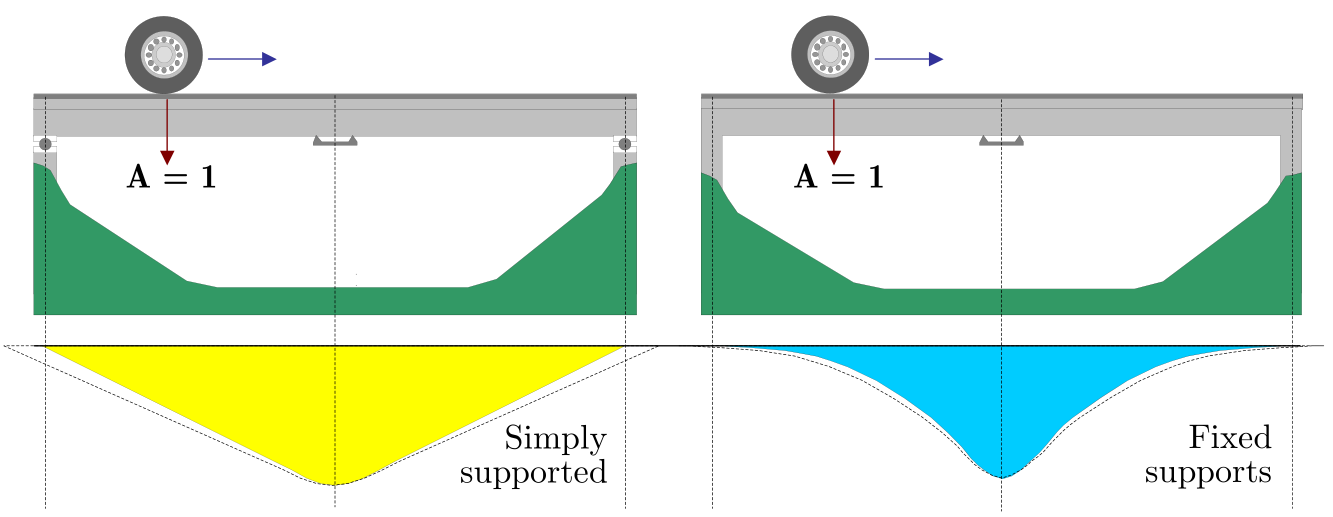
\includegraphics[scale=0.5]{figures/inflLinesQuilligan}
\caption{Influence lines for simply and fixed supported bridges, figure from \cite{Quilligan}}
\label{fig:theoreticalInfl}
\end{figure}

Znidaric and Baumgärter \cite{bwim_an_overview}, did a study on the effect of choice of influence line. This study shows errors up to 10\% for a short \SI{2}{\metre} bridge span and errors of several hundred percent for a \SI{32}{\metre} bridge span. This underlines the importance of using correct influence lines for a B-WIM system.
\begin{figure}[h]
\centering
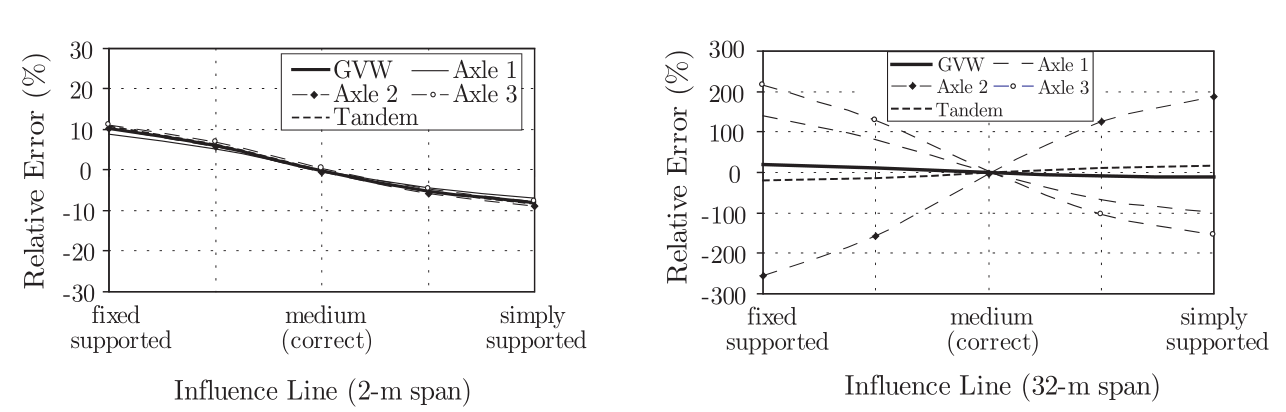
\includegraphics[scale=0.5]{figures/error_in_weights_dueTo_infl}
\caption{Errors of axle loads due to wrongly selected influence lines, figure from \cite{Quilligan}}
\label{fig:errorOfInfl}
\end{figure}
\subsubsection{Matrix method}
Quilligan \cite{Quilligan} developed a 'matrix method' to calculate the influence line of a bridge through the measured strain induced by a vehicle. This method is derived from Moses', equation \ref{equation:moses}.
\begin{equation}
Error = \sum_{k = 1}^{K} [\varepsilon_{k}^{measured} - \varepsilon_{k}^{theoretical}]^2
\label{equation:moses}
\end{equation}
Equation \ref{equation:moses} were originally used to filter out the dynamic response of the bridge.
The theoretical strain in this equation can be expressed as a product of axle loads and influence ordinates at sampling points, see equation \ref{equation:theoretical_strain}, thus we can expand equation \ref{equation:moses}:
\begin{equation}
Error = \sum_{k = 1}^{K} \Big[\varepsilon_{k}^{measured} - \Big(\sum_{i = 1}^{N} A_i I_{(k-C_i)}\Big)\Big]^2
\label{equation:moses_expanded}
\end{equation}
The set of influence ordinates $I$ that minimizes $Error$, forms the wanted influence line.
\begin{equation}
\frac{\partial Error}{\partial I_R} = \frac{\partial \sum_{k = 1}^{K} \Big[\varepsilon_{k}^{measured} - \Big(\sum_{i = 1}^{N} A_i I_{(k-C_i)}\Big)\Big]^2}{\partial I_R}
\end{equation}
For a given number of known axle loads this equation comes down to a set of $(K - C_n)$ number of linear equations. Rearranging the equations and writing them in matrix form leads to:
\begin{equation}
\begin{bmatrix} AxleMatrix \end{bmatrix}_{K-C_N, K-C_N} \begin{Bmatrix} I \end{Bmatrix}_{K-C_N, 1} = \begin{Bmatrix} M \end{Bmatrix}_{K-C_N, 1}
\label{equation:matrixForm}
\end{equation}
Where:
\begin{description}
\item $\begin{Bmatrix} M \end{Bmatrix}$ = a vector depending on axle weights and measured strain, $M_{i, 1} = \Big(\sum_{j = 1}^{N} A_j \varepsilon_{(i+C_j)}\Big)$
\item $\begin{bmatrix} AxleMatrix \end{bmatrix}$ is a matrix depending only on the axle loads, defined by equation \ref{axleMatrix}.
\end{description}
\begin{equation}
\begin{bmatrix} AxleMatrix \end{bmatrix} = \sum_{i = 1}^{N} \sum_{j = i}^{N} \begin{bmatrix} AxleMatrix \end{bmatrix} + \big( A_i A_j  \begin{bmatrix} Diagonal \end{bmatrix}_{C_j - C_i}\big)
\label{axleMatrix}
\end{equation}
Which produces the upper triangle of the symmetric AxleMatrix.
Where:
\begin{description}
\item $\begin{bmatrix} Diagonal \end{bmatrix}_{C_j - C_i}$ = a diagonal matrix of ones, where diagonal is placed with an offset, $C_j - C_i$, from the center matrix diagonal.
\end{description}
Solving equation \ref{equation:matrixForm} for the influence ordinate vector gives the influence line for the strain history. This can be done through inversion of the AxleMatrix (equation \ref{axleMatrix}) or other numerical solutions like a Cholesky factorization.
\subsubsection{Optimization}
testing \cite{Liljencrantz}.

\subsection{Finding the train's speed}

\subsection{The axle distances}


% !TEX root = main.tex
\section{Method}

\subsection{Programming a BWIM system}
Describe shortly how the BWIM system have been programmed.
Keywords:
\begin{itemize}
\item Beam bridge model
\item Producing a strain history through influence lines
\item Finding the speed of the train
\item Finding Axle distances
\item Solving system for axle weights
\end{itemize}
This master project began by learning how a BWIM-system works, and to then create a working model performing BWIM. To not make this a too big project this meant building a simple beam model of a bridge in Matlab, and simulate moving loads crossing it.

A simple flow diagram describing the intial BWIM program:
\begin{figure}
% 
\tikzset{
  terminal/.style={draw, rounded rectangle, text width=3cm, text centered},
  process/.style={draw, text width=3cm, text centered},
  decision/.style={draw, diamond, aspect=2, text width=3cm, text centered},
  delay/.style={draw, rounded rectangle, rounded rectangle west arc=none, text width=3cm, minimum height=1cm, text centered},
  line/.style={draw, -latex}
}
\begin{tikzpicture}
  \node[terminal] (main) {Main script};
  \node[process, above=1cm of main] (createInfl) {create influence line};
  \node[process, right=2cm of main] (createStrain) {create strain signal};
  \node[process, below=2cm of main] (findSpeed) {find train speed};
  \node[process, left=1cm of findSpeed] (findAxleDist) {find axle distances};
  \node[process, left=2cm of main] (calcAxleWeights) {calculate axle weights};

  \draw[line] (main) -- (createInfl);
  \draw[line] (main) -- (createStrain);
  \draw[line] (main) -- (findSpeed);
  \draw[line] (findSpeed.west) -- (findAxleDist.east);
  \draw[line] (main) -- (calcAxleWeights);
\end{tikzpicture}%

\end{figure}


\subsubsection{Producing a strain signal}
Through the theoretical moment influence lines of the beam, a strain signal can be built through the moment-strain relationship, found in equation\ref{equation:moment_strain}, for a given set of axle weights. A simple beam bridge model, as seen in figure \ref{figure:beam_model}, will not recreate a actual bridge strain signal but will be used to create a working BWIM system. The produced strain signal will differ from an actual strain signal mostly because of dynamics, from the train and bridge, and because actual boundary conditions of a bridge will differ from the boundary conditions of a simple beam model. The strain sensors will also produce noise distorting the signal.

To make as good a signal as possible, some effort were placed into recreating the effect mentioned above. To add noise to the signal, white gaussian noise was included in the signal through Matlabs wgn function "http://se.mathworks.com/help/comm/ref/wgn.html".


This strain signal could then be used as a base to build the code for a BWIM system.

\begin{figure}
	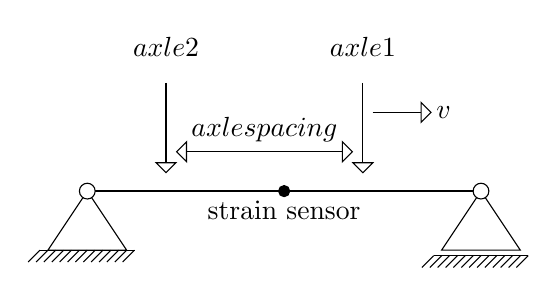
\begin{tikzpicture}
		\draw[thick] (0,0) to (5,0);
		\node[ledd fast={0}{0}{0}] (ledd) {};
		\node[ledd skyve={5}{0}{0}] (skyveledd) {};
		%\draw[->] (0,1) to {$\scriptstyle g$} (0,.1);
		\node (a) at (1,1.5) {};
		\node (b) at (1,.1) {};
		\draw[-open triangle 90] (a) to node[pos=-.4] {$axle 2$} (b);
		\node (c) at (3.5,1.5) {};
		\node (d) at (3.5,.1) {};
		\draw[-open triangle 90] (c) to node[pos=-.4] {$axle 1$} (d);
		\node (e) at (3.5,1) {};
		\node (f) at (4.5,1) {};
		\draw[-open triangle 90] (e) to node[pos=1.2] {$v$} (f);
		\node (g) at (1,.5) {};
		\node (h) at (3.5,.5) {};
		\draw[open triangle 90-open triangle 90] (g) to node[above] {$axle spacing$} (h);
		%\draw (2.5,0) circle [radius=0.1] {sensor};
		%\node[draw,circle] (s) at (2.5,0){};
		\filldraw
		(2.5,0) circle (2pt) node[align=left,   below] {strain sensor};
	\end{tikzpicture}
%\captionof{figure}{Beam model for initial BWIM}
\caption{Beam model for developement}
\label{figure:beam_model}

\end{figure}


\subsubsection{Finding the speed of the train}
Two working methods of finding the speed of a passing train were developed:
\begin{itemize}
 \item By identifying peaks in the strain history for two different sensors, representing the same axle. The distance between the two sensors and the time difference between the found peaks should theoretically give a good estimate of the trains velocity.
 \item Through doing cross correlation between two sensors strain history. This involves finding the phase difference, or lag, between the signals. The known distance between the strain gauges should then along with a constant, based on distance between sensors, give a reliable estimate of train velocity. INSERT PLOT OF CORRELATION AND SHOW MATHEMATICAL EQUATION DESCRIBING CROSS CORRELATION.
\end{itemize}

\subsection{Finding influence lines}
Describe how influence lines have been found from the given strain history from Lerelva Bridge.
Keywords:
\begin{itemize}
\item Matrix method
\item Optimization
\item Speed
\end{itemize}
\subsubsection{Matrix method}
Describe the matrix method.

\subsubsection{Optimization}
Describe how optimization can be used to find optimal influence lines for the bridge.

\subsection{System setup}
\label{system_setup}
To test the BWIM-program on actual data, we Gunnstein, Daniel set up a BWIM-system to gather strain data from actual train passings. The subject bridge were Lerelva-Bridge in Trondheim, figure \ref{fig:lerelva_bridge}, a typical Norwegian steel railway bridge. Three strain gauges, \SI{3}{\mm} \SI{120}{ohms} from HBM, were placed by the support towards Trondheim on the first section of the longitudinal stringer, see figure \ref{fig:strain_gauges}. The sensors were placed with \SI{1}{\m} spacing around the middle of the stringer section. These strain gauges were connected to a National Instruments compactDAQ with module NI 9235 which produced an continuous data flow to a standard laptop, see figure \ref{fig:instruments}. A Kipor generator was brought for power.
% INSERT SYSTEM IMAGE HERE
\begin{figure}[H]
	\centering
	\begin{subfigure}[t]{0.49\textwidth}
    \centering
    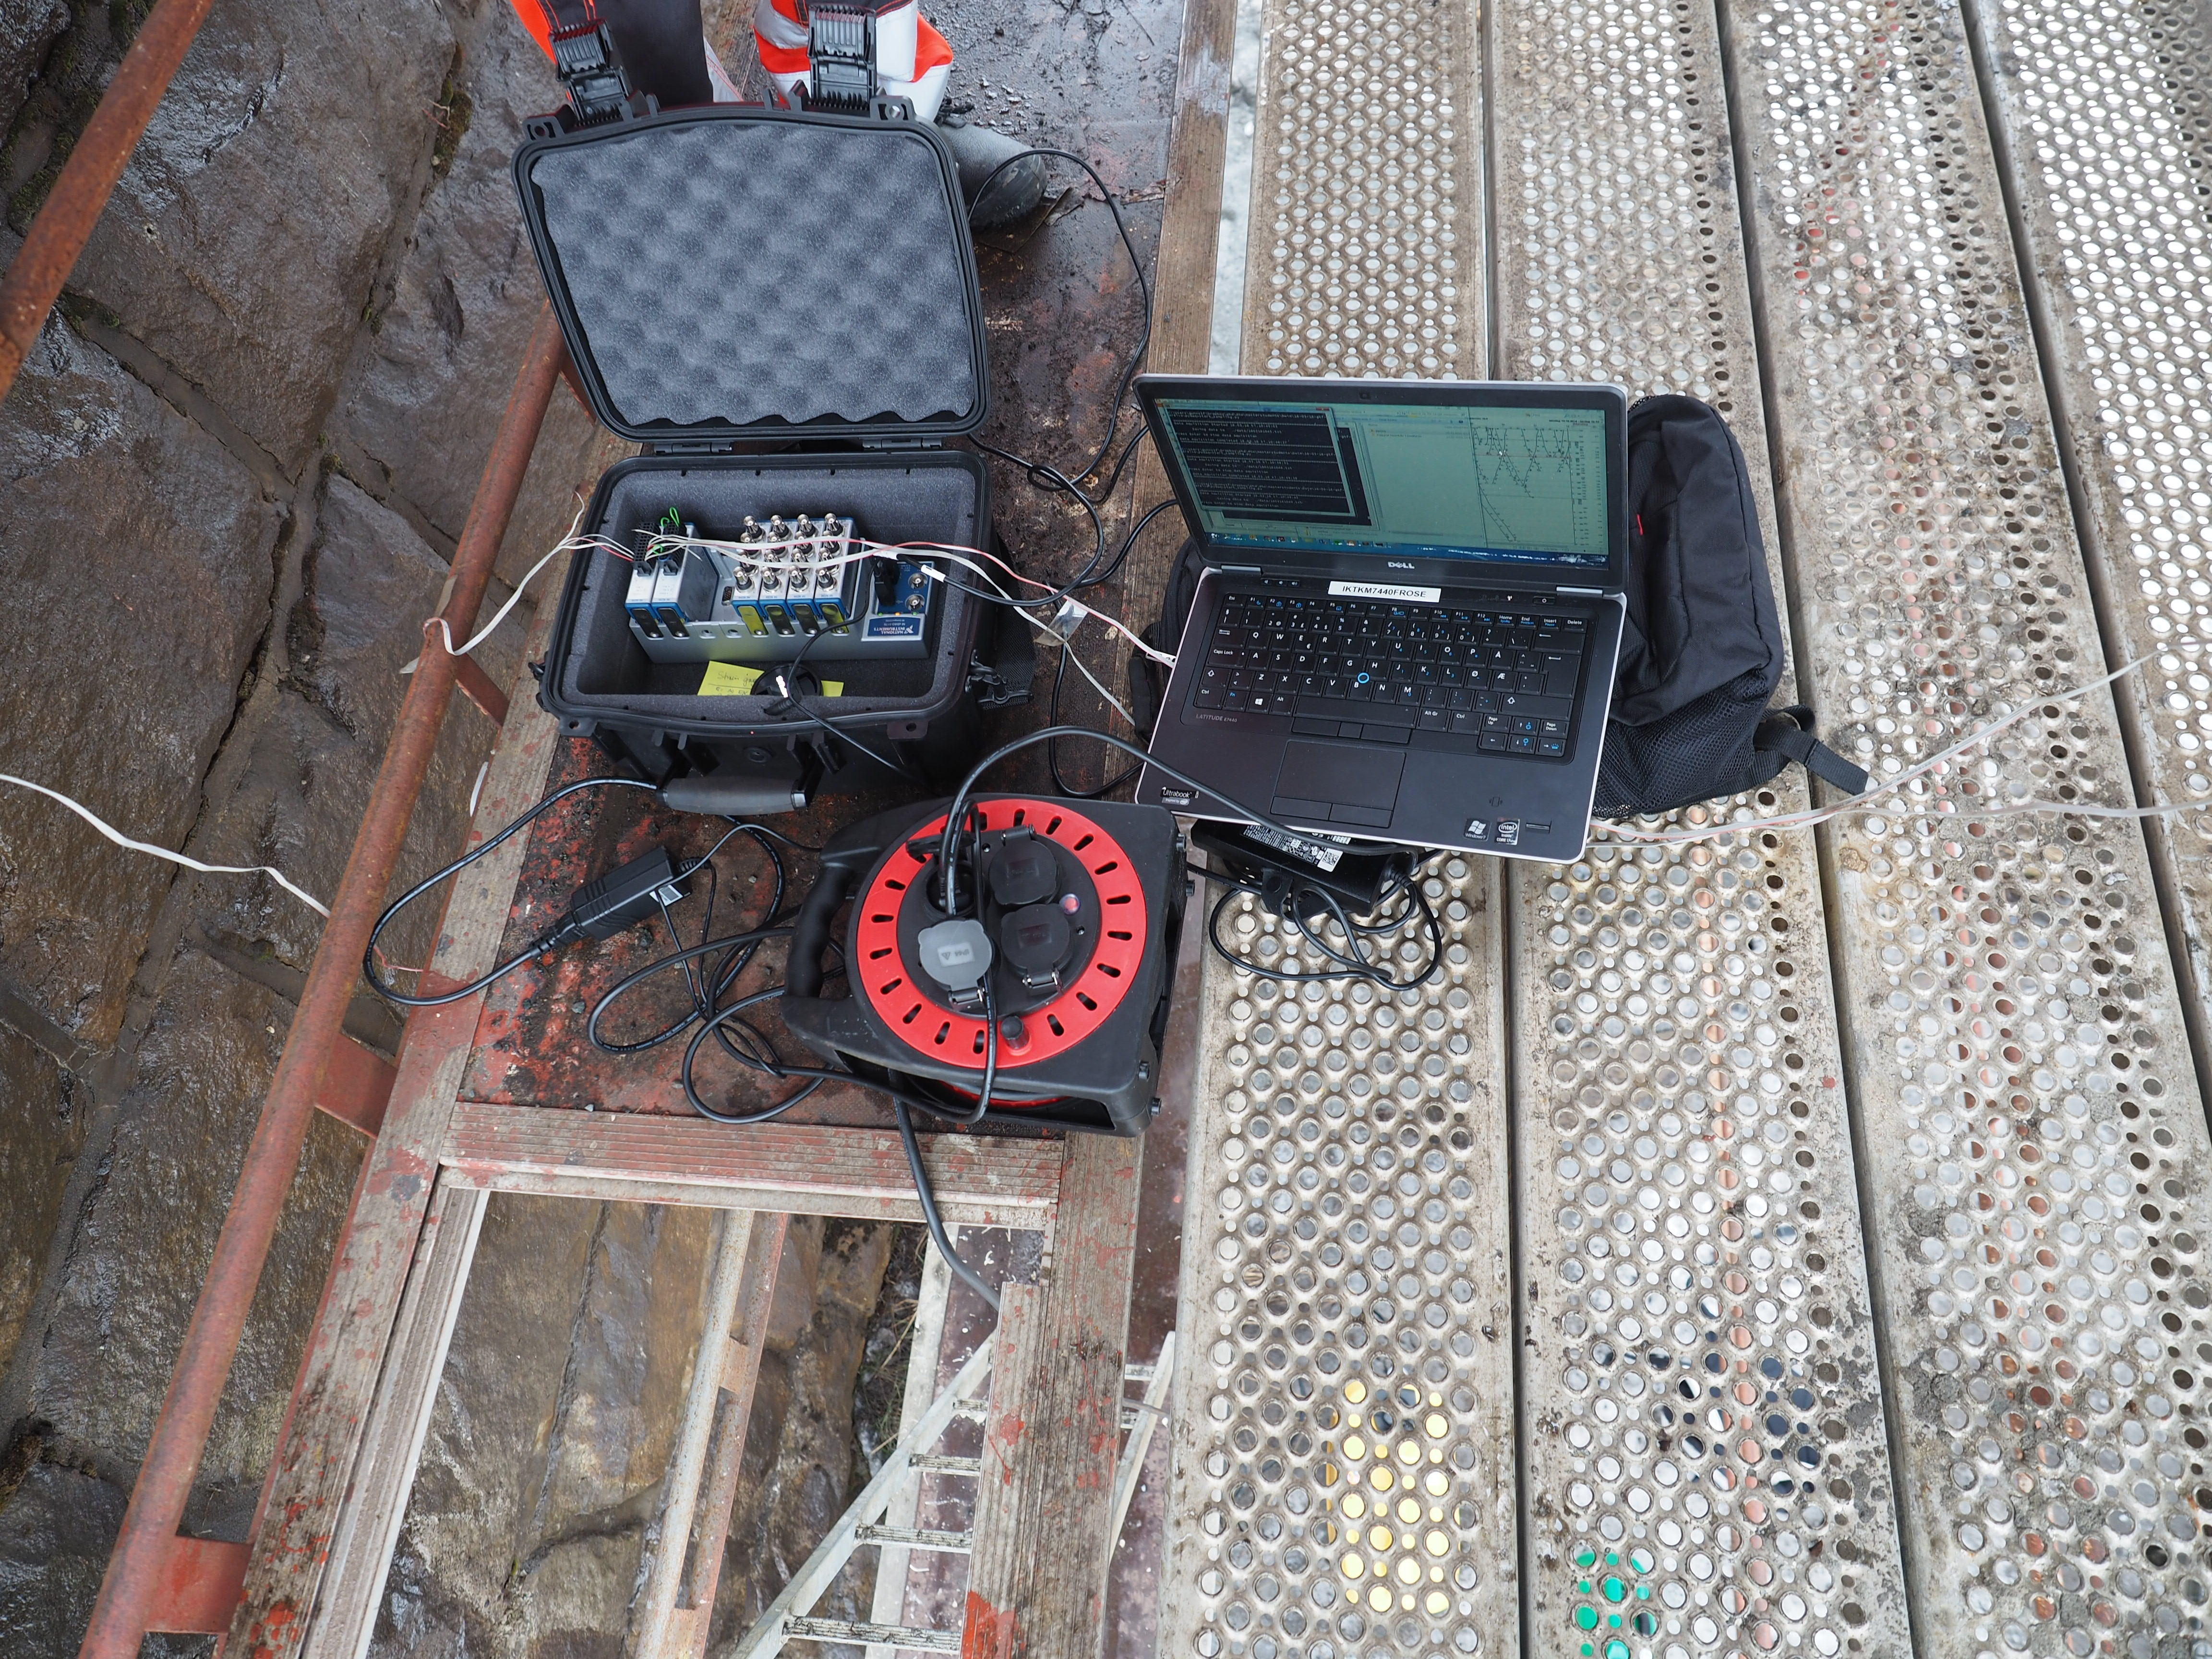
\includegraphics[width=\textwidth]{figures/system_setup}
		\caption{System setup from data gathering at Lerelva}
		\label{fig:instruments}
	\end{subfigure}
	\begin{subfigure}[t]{0.49\textwidth}
    \centering
    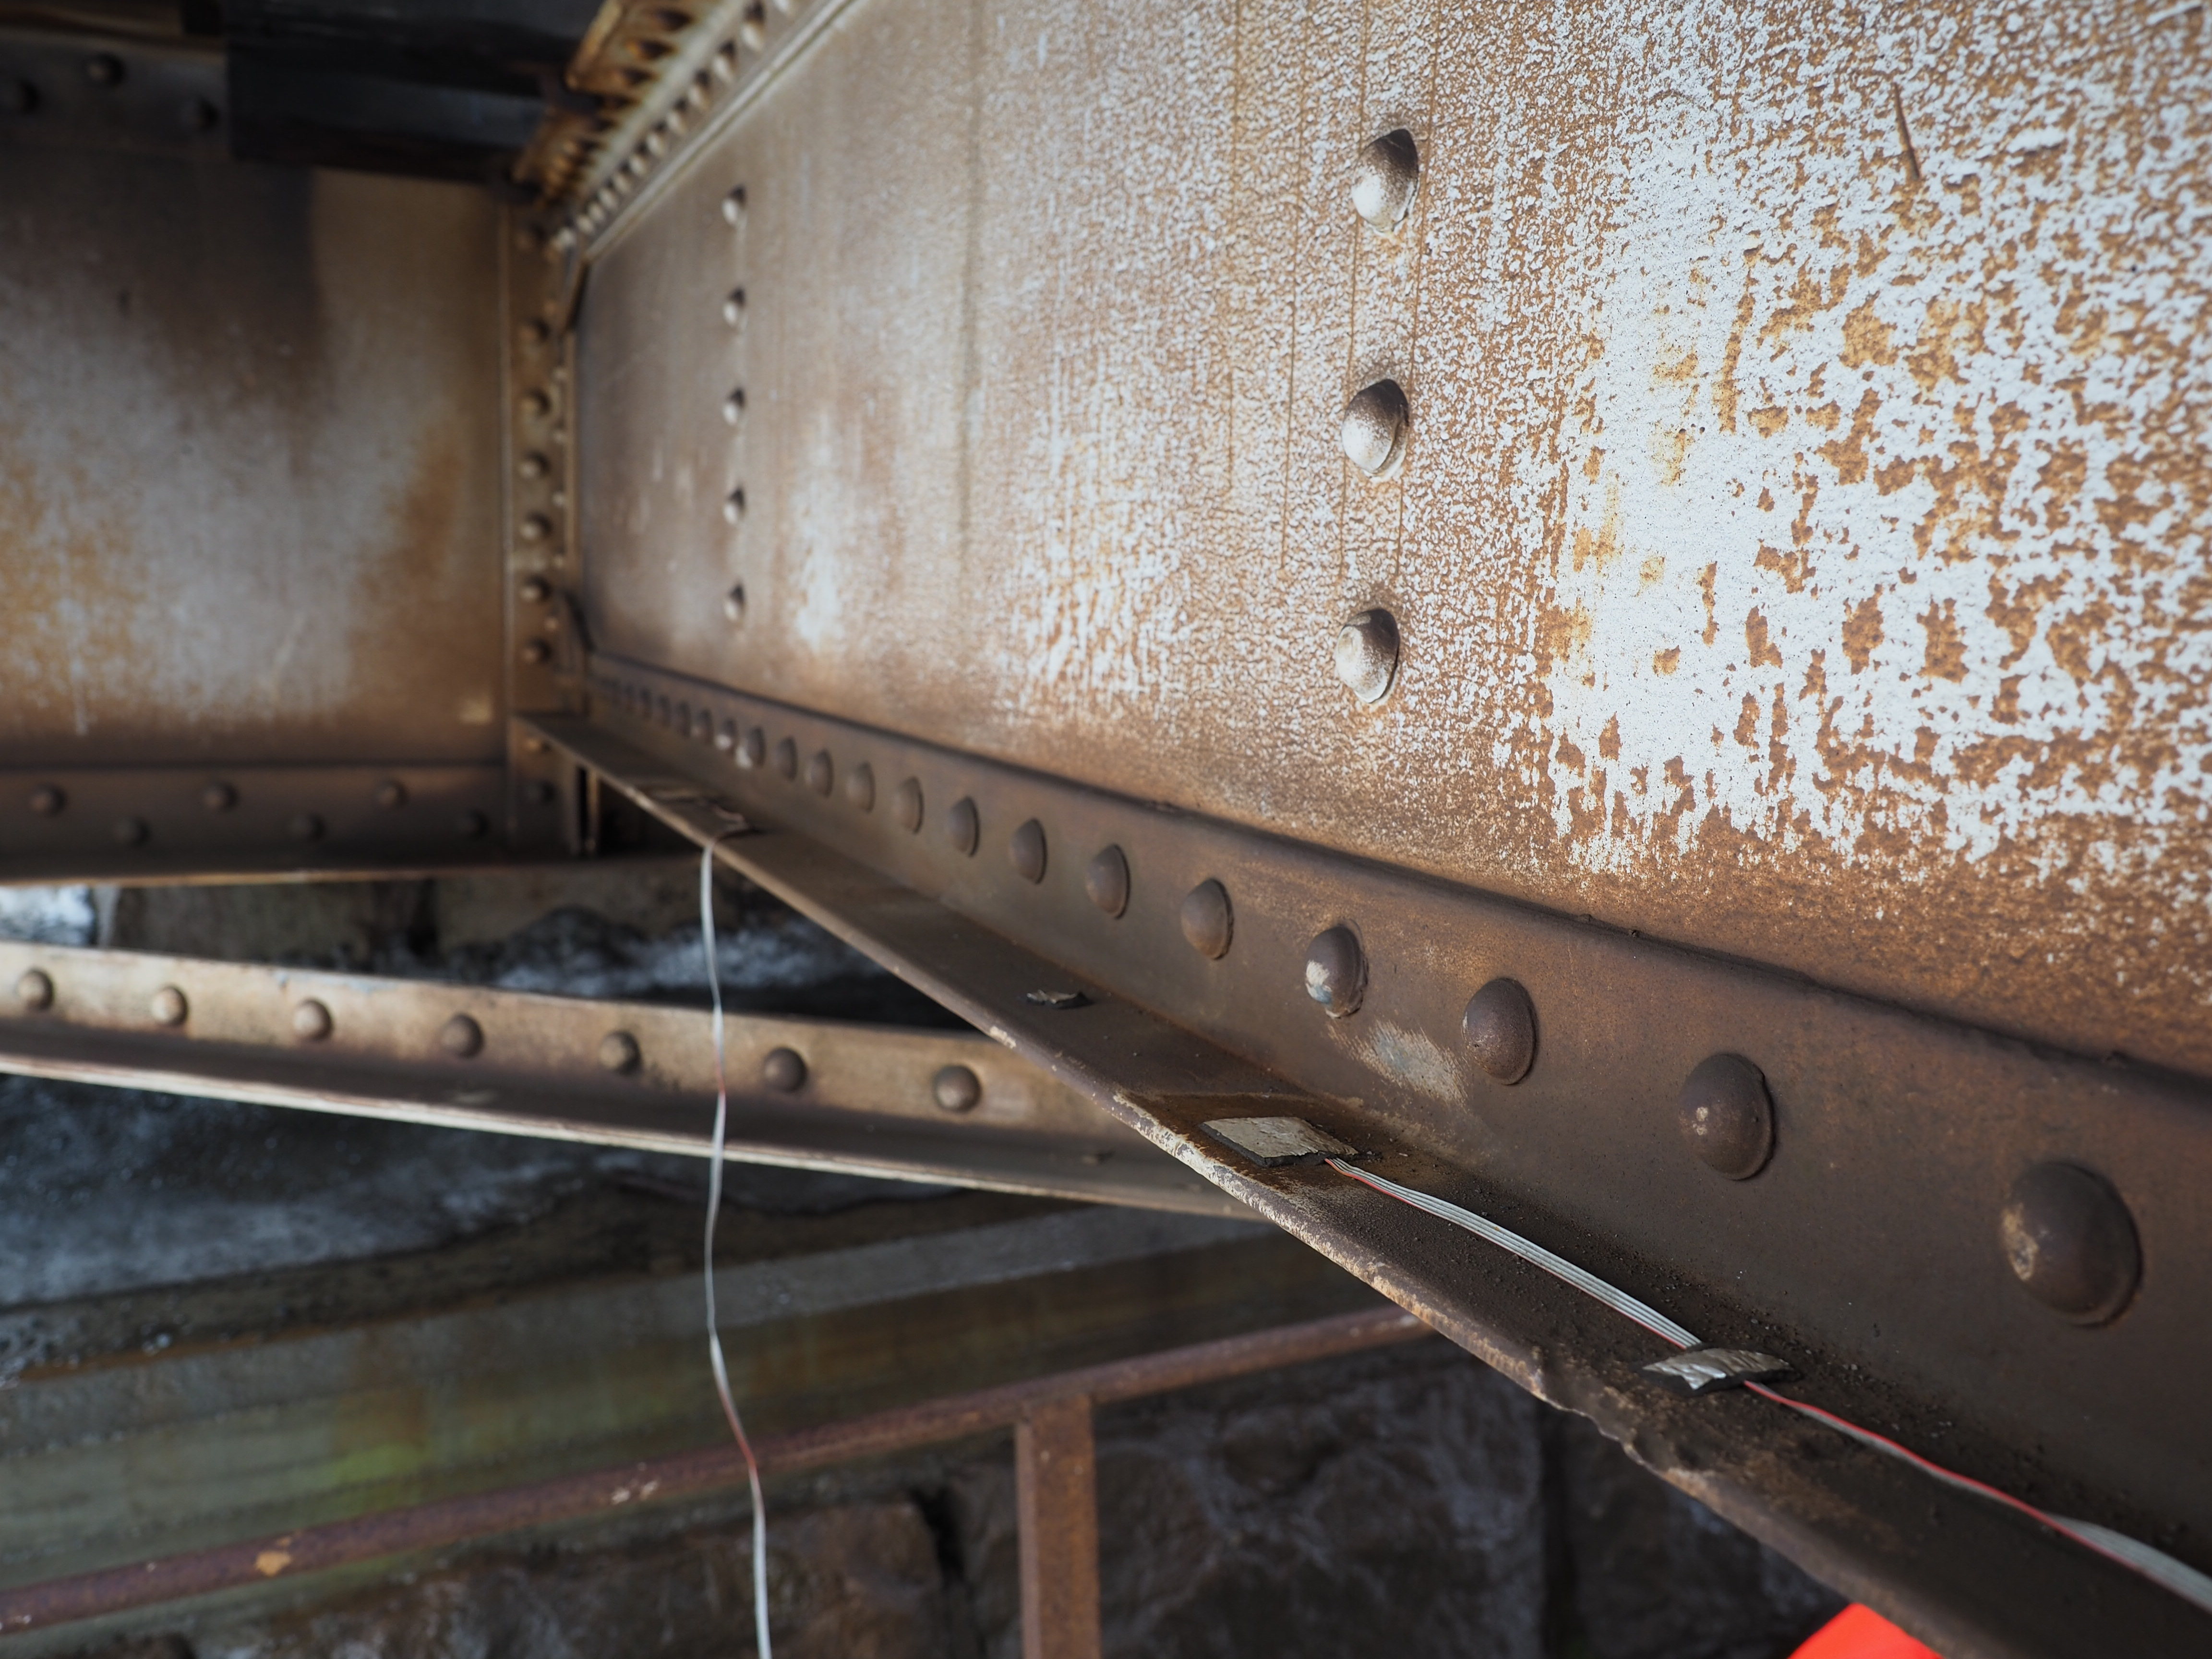
\includegraphics[width=\textwidth]{figures/sensor_placement}
		\caption{Placement of strain gauges on stringer section}
		\label{fig:strain_gauges}
	\end{subfigure}
	\caption{Instruments for aquiring strain data}
	\label{fig:system_setup}
	% 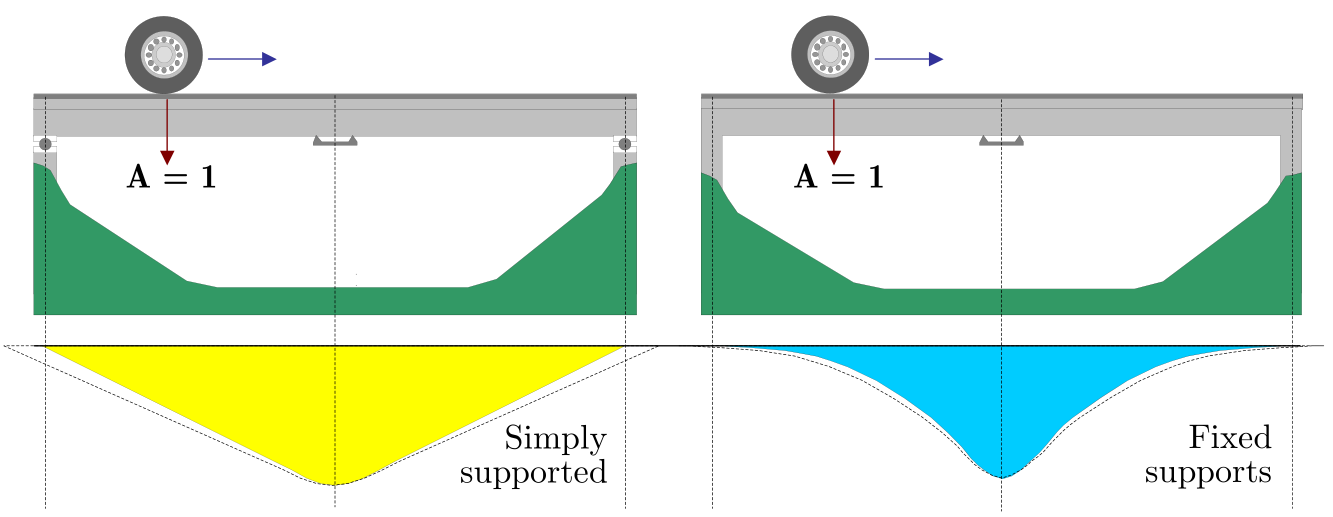
\includegraphics[scale=0.5]{figures/inflLinesQuilligan}
\end{figure}
\begin{figure}[H]
	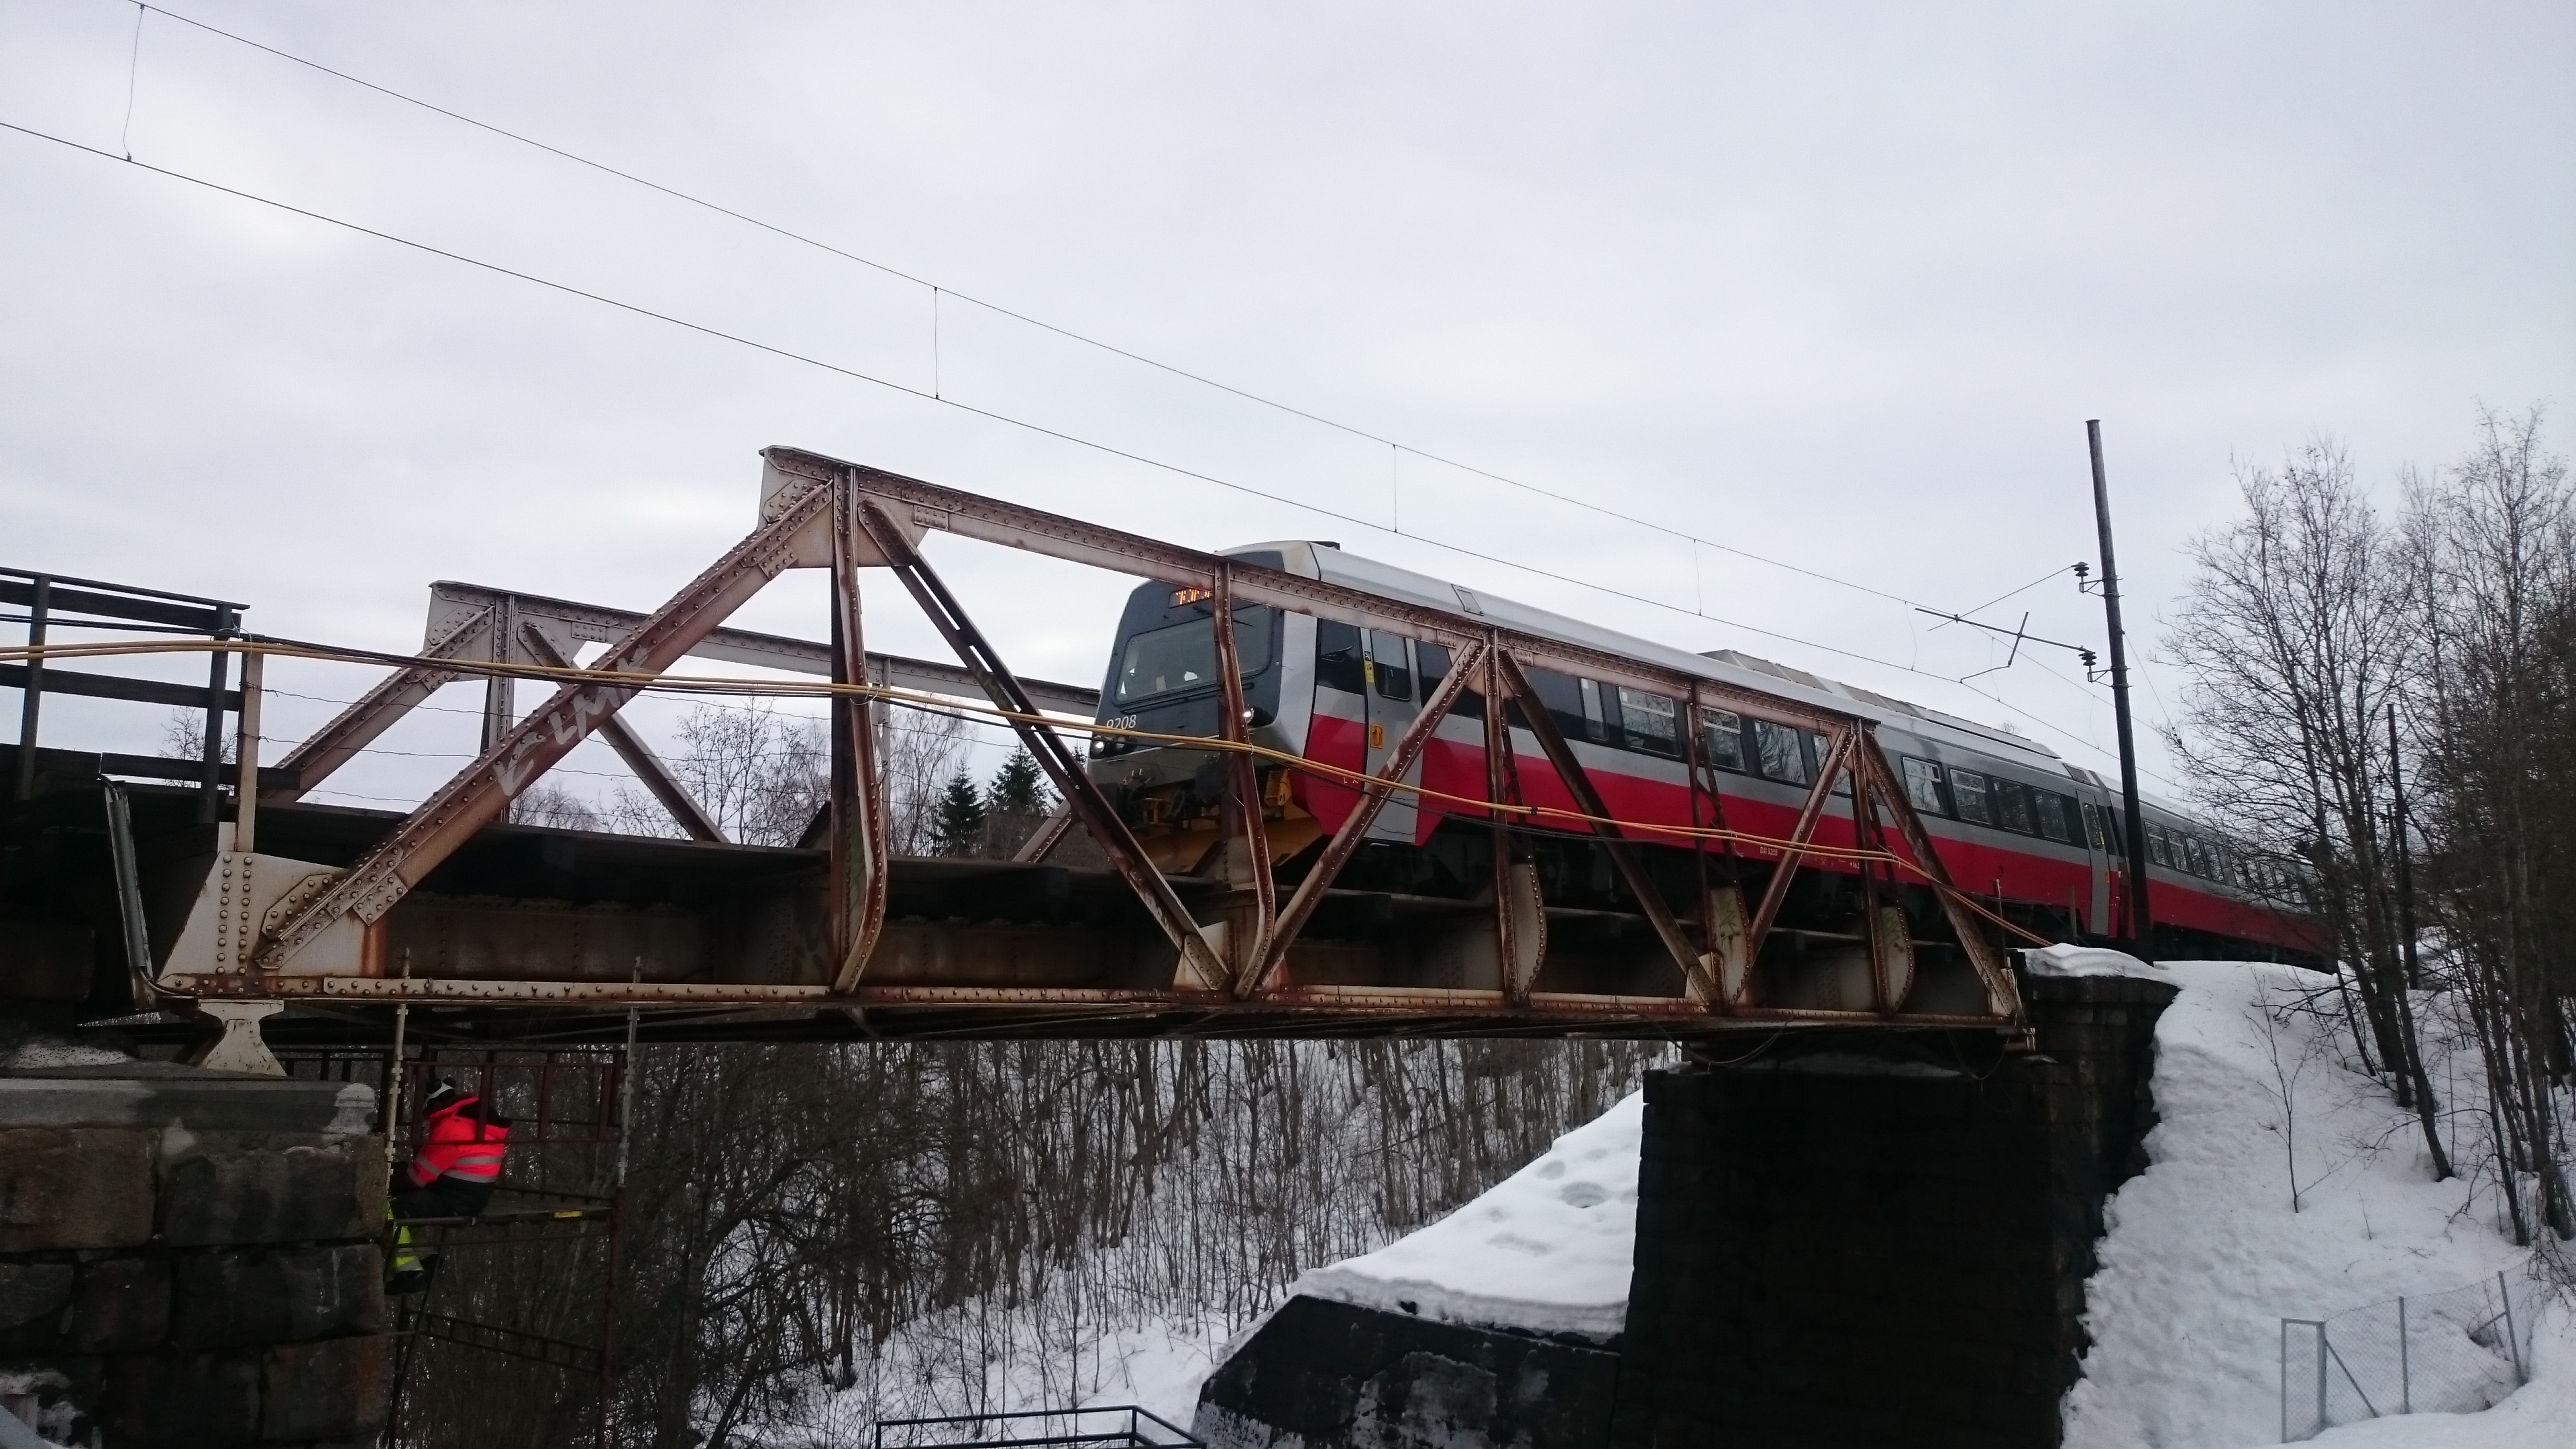
\includegraphics[width=\textwidth]{figures/train_passing.jpg}
	\caption{Lerelva bridge with a train passing over}
	\label{fig:lerelva_bridge}
\end{figure}


\subsection{Testing}
Keywords:
\begin{itemize}
\item Comparing calculated strain with measured strain
\end{itemize}


% !TEX root = main.tex
\section{Analysis}

This chapter will describe how the BWIM system performs. What works? Why? How? etc.
The main focus should perhaps be placed on identifying the pros and cons of the matrix method and optimization method.

Should include:
\begin{itemize}
\item Compare theoretical and calculated influence lines. Also include influence lines found through Abaqus.
\item Check how influence lines found through matrix method and optimization reproduces the strain history
\item Test obtained influence line by running the bwim routine on the hitherto unused freight train. (Depends on getting info about the train). Also Do this test on the other trains.
\end{itemize}

\subsection{Strain data}
\begin{figure}[H]
	\centering
	\begin{subfigure}[t]{0.45\textwidth}
		\centering
		% This file was created by matlab2tikz.
%
%The latest updates can be retrieved from
%  http://www.mathworks.com/matlabcentral/fileexchange/22022-matlab2tikz-matlab2tikz
%where you can also make suggestions and rate matlab2tikz.
%
\definecolor{mycolor1}{rgb}{0.00000,0.44700,0.74100}%
\definecolor{mycolor2}{rgb}{0.85000,0.32500,0.09800}%
\definecolor{mycolor3}{rgb}{0.92900,0.69400,0.12500}%
%
\begin{tikzpicture}

\begin{axis}[%
width=\textwidth,
height=\textwidth,
at={(0\figurewidth,0\figureheight)},
scale only axis,
xmin=12,
xmax=20,
ymin=-5e-05,
ymax=0.0002,
axis background/.style={fill=white},
title style={font=\bfseries},
title={Raw strain history, train 3},
% legend style={legend cell align=left,align=left,draw=white!15!black}
% legend style={at={(1.1,-0.2)}}
]
\addplot [color=mycolor1,solid,forget plot]
  table[row sep=crcr]{%
12.7763671875	5.66138597029925e-07\\
12.77734375	3.26189245247223e-07\\
12.7783203125	1.35641311928975e-07\\
12.779296875	-5.2068990728793e-07\\
12.7802734375	-4.7834598343845e-07\\
12.78125	-8.7355580109718e-07\\
12.7822265625	-9.79415521092705e-07\\
12.783203125	-6.47721657503174e-07\\
12.7841796875	-1.46651790273577e-07\\
12.78515625	1.04603764310954e-06\\
12.7861328125	-7.95925325643848e-07\\
12.787109375	9.19005498232995e-07\\
12.7880859375	1.70927960814818e-07\\
12.7890625	7.49629354841221e-07\\
12.7900390625	9.11948157789185e-07\\
12.791015625	-5.70091147284683e-07\\
12.7919921875	-1.90392279790985e-06\\
12.79296875	3.12074581051112e-07\\
12.7939453125	-7.39466790535513e-07\\
12.794921875	1.21526653065621e-07\\
12.7958984375	2.1893283869861e-06\\
12.796875	5.3085192048977e-07\\
12.7978515625	-6.05377744320075e-07\\
12.798828125	-2.5956898690822e-07\\
12.7998046875	-4.28944734453445e-07\\
12.80078125	-5.48919187878978e-07\\
12.8017578125	-5.70091147284683e-07\\
12.802734375	4.24991905684062e-07\\
12.8037109375	-1.25465068908292e-06\\
12.8046875	2.83845253843274e-07\\
12.8056640625	4.46163906867112e-07\\
12.806640625	-5.50525892538054e-09\\
12.8076171875	9.89578908102513e-07\\
12.80859375	1.5666724184453e-08\\
12.8095703125	4.10877238721935e-07\\
12.810546875	-4.78492224776934e-08\\
12.8115234375	7.56686693013193e-07\\
12.8125	-8.45326538678661e-07\\
12.8134765625	9.32973365245972e-08\\
12.814453125	-2.22855853884772e-06\\
12.8154296875	-5.1363258689297e-07\\
12.81640625	-6.90212029208232e-08\\
12.8173828125	7.91826788462766e-08\\
12.818359375	9.19005498232995e-07\\
12.8193359375	1.50476509935935e-06\\
12.8203125	1.34950345206681e-06\\
12.8212890625	4.38960363799944e-08\\
12.822265625	-6.33607020170558e-07\\
12.8232421875	4.46163906867112e-07\\
12.82421875	-4.00715447146632e-07\\
12.8251953125	-6.47721657503174e-07\\
12.826171875	2.20329273403676e-07\\
12.8271484375	8.9783347719777e-07\\
12.828125	-7.60785295375859e-08\\
12.8291015625	-2.87798282116265e-07\\
12.830078125	6.57883967589709e-07\\
12.8310546875	-4.21887412774789e-07\\
12.83203125	2.41501265994858e-07\\
12.8330078125	-1.32522378488314e-06\\
12.833984375	-5.34804547780996e-07\\
12.8349609375	-2.8074095846241e-07\\
12.8359375	-5.77148466889476e-07\\
12.8369140625	1.99157281701974e-07\\
12.837890625	6.3671195751772e-07\\
12.8388671875	1.41301957472728e-06\\
12.83984375	6.6494130447842e-07\\
12.8408203125	-4.57174020180142e-07\\
12.841796875	-1.74881091802737e-07\\
12.8427734375	-8.66498485640977e-07\\
12.84375	2.55615928215986e-07\\
12.8447265625	-4.50116698896353e-07\\
12.845703125	-9.72505087954659e-08\\
12.8466796875	-3.2308489890452e-07\\
12.84765625	1.04603764310954e-06\\
12.8486328125	1.37067549206495e-06\\
12.849609375	9.26062838775468e-07\\
12.8505859375	-5.41861867879101e-07\\
12.8515625	-3.93658125072893e-07\\
12.8525390625	-1.67823766568332e-07\\
12.853515625	-3.51314190556815e-07\\
12.8544921875	-1.53709115803752e-07\\
12.85546875	-7.11237520611063e-07\\
12.8564453125	7.77858708122386e-07\\
12.857421875	-9.72505087954659e-08\\
12.8583984375	-1.25625864305385e-08\\
12.859375	7.07285327881946e-07\\
12.8603515625	-5.6303382758166e-07\\
12.861328125	-1.13467640355585e-06\\
12.8623046875	1.35641311928975e-07\\
12.86328125	-2.03110391751348e-07\\
12.8642578125	-9.72358207117739e-07\\
12.865234375	2.13271942737635e-07\\
12.8662109375	4.67335908939642e-07\\
12.8671875	-8.10039958433224e-07\\
12.8681640625	1.32127406678585e-06\\
12.869140625	8.83718797001654e-07\\
12.8701171875	4.53221240792698e-07\\
12.87109375	1.07411994597567e-07\\
12.8720703125	-4.99517945807279e-07\\
12.873046875	-1.39594464644306e-07\\
12.8740234375	6.22597284629994e-07\\
12.875	1.0530949854301e-06\\
12.8759765625	-1.04307835017145e-07\\
12.876953125	-2.8074095846241e-07\\
12.8779296875	2.48558597055982e-07\\
12.87890625	9.61349542969716e-07\\
12.8798828125	3.40303909838633e-07\\
12.880859375	1.14469323781938e-07\\
12.8818359375	6.93170653019021e-07\\
12.8828125	9.47234860995726e-07\\
12.8837890625	2.9781380084682e-08\\
12.884765625	9.19005498232995e-07\\
12.8857421875	-3.79543480629211e-07\\
12.88671875	-3.3734568355339e-08\\
12.8876953125	-5.91263105802426e-07\\
12.888671875	1.07426701298334e-06\\
12.8896484375	-2.45454338711464e-07\\
12.890625	1.11661107075715e-06\\
12.8916015625	9.68406884104813e-07\\
12.892578125	-1.21936413747885e-06\\
12.8935546875	-2.5956898690822e-07\\
12.89453125	3.68533240206704e-07\\
12.8955078125	-4.57174020180142e-07\\
12.896484375	-6.19492382442858e-07\\
12.8974609375	1.49755971186978e-07\\
12.8984375	4.10877238721935e-07\\
12.8994140625	-1.11365161140162e-07\\
12.900390625	1.07411994597567e-07\\
12.9013671875	-4.7834598343845e-07\\
12.90234375	9.33120179416819e-07\\
12.9033203125	-3.79543480629211e-07\\
12.904296875	-4.85403304326722e-07\\
12.9052734375	-7.25352155770938e-07\\
12.90625	9.82521566670995e-07\\
12.9072265625	7.42572016767477e-07\\
12.908203125	3.19131913100162e-07\\
12.9091796875	1.27892999182743e-06\\
12.91015625	-3.44256867791572e-07\\
12.9111328125	1.00354665511643e-07\\
12.912109375	7.56686693013193e-07\\
12.9130859375	-7.25352155770938e-07\\
12.9140625	1.99157281701974e-07\\
12.9150390625	-4.50116698896353e-07\\
12.916015625	-1.53694301302607e-06\\
12.9169921875	4.46163906867112e-07\\
12.91796875	9.82521566670995e-07\\
12.9189453125	-1.09938984355724e-06\\
12.919921875	-5.41861867879101e-07\\
12.9208984375	1.13072575747171e-06\\
12.921875	7.56686693013193e-07\\
12.9228515625	9.68406884104813e-07\\
12.923828125	4.39106573040622e-07\\
12.9248046875	-5.70091147284683e-07\\
12.92578125	-4.99517945807279e-07\\
12.9267578125	3.89705239020122e-07\\
12.927734375	-1.32537138916155e-07\\
12.9287109375	-7.1829483824044e-07\\
12.9296875	-3.58371513222745e-07\\
12.9306640625	1.31421672071243e-06\\
12.931640625	4.95565246418778e-07\\
12.9326171875	1.03898030088829e-06\\
12.93359375	-3.01912929127771e-07\\
12.9345703125	-7.1829483824044e-07\\
12.935546875	8.76661457051807e-07\\
12.9365234375	-1.40285417885629e-06\\
12.9375	5.09679915750971e-07\\
12.9384765625	-4.21887412774789e-07\\
12.939453125	-6.12435063430906e-07\\
12.9404296875	2.83845253843274e-07\\
12.94140625	1.92820619857232e-06\\
12.9423828125	1.43419161739125e-06\\
12.943359375	2.9781380084682e-08\\
12.9443359375	2.69730590832197e-07\\
12.9453125	1.00369359126175e-06\\
12.9462890625	8.55489437794456e-07\\
12.947265625	1.5666724184453e-08\\
12.9482421875	-1.18407758340627e-06\\
12.94921875	-2.8074095846241e-07\\
12.9501953125	-6.5477897602138e-07\\
12.951171875	-4.07918954660642e-08\\
12.9521484375	1.1801271640841e-06\\
12.953125	2.2724052084911e-08\\
12.9541015625	-6.05377744320075e-07\\
12.955078125	5.02622581035218e-07\\
12.9560546875	1.30010202886222e-06\\
12.95703125	-3.65428835790447e-07\\
12.9580078125	5.8731060413944e-07\\
12.958984375	6.22597284629994e-07\\
12.9599609375	1.63885474230795e-06\\
12.9609375	1.35641311928975e-07\\
12.9619140625	4.17934572153559e-07\\
12.962890625	7.84916046689659e-07\\
12.9638671875	1.14469323781938e-07\\
12.96484375	6.08482612137352e-07\\
12.9658203125	6.71998641465143e-07\\
12.966796875	1.08838169851264e-06\\
12.9677734375	-1.39594464644306e-07\\
12.96875	-4.14830090997471e-07\\
12.9697265625	-6.7595093098294e-07\\
12.970703125	6.29654621024526e-07\\
12.9716796875	-6.7595093098294e-07\\
12.97265625	-2.17225041133353e-07\\
12.9736328125	-3.30142221965533e-07\\
12.974609375	-2.20032935227977e-06\\
12.9755859375	-4.21887412774789e-07\\
12.9765625	-1.84040708502142e-06\\
12.9775390625	-4.92460625116549e-07\\
12.978515625	4.39106573040622e-07\\
12.9794921875	2.20329273403676e-07\\
12.98046875	1.13072575747171e-06\\
12.9814453125	-1.18407758340627e-06\\
12.982421875	8.60939638222362e-09\\
12.9833984375	-2.17225041133353e-07\\
12.984375	-3.37199544928101e-07\\
12.9853515625	-5.70091147284683e-07\\
12.986328125	-1.02881671615231e-06\\
12.9873046875	-5.6303382758166e-07\\
12.98828125	4.38960363799944e-08\\
12.9892578125	-5.91263105802426e-07\\
12.990234375	-9.86472834969008e-07\\
12.9912109375	-1.81938416937829e-07\\
12.9921875	4.74393243161215e-07\\
12.9931640625	7.2125350155652e-08\\
12.994140625	-1.81938416937829e-07\\
12.9951171875	-3.51314190556815e-07\\
12.99609375	-7.11237520611063e-07\\
12.9970703125	-1.88995741974693e-07\\
12.998046875	6.5068021563473e-08\\
12.9990234375	2.34443935032396e-07\\
13	7.2125350155652e-08\\
13.0009765625	-3.3734568355339e-08\\
13.001953125	4.24991905684062e-07\\
13.0029296875	1.30715937473789e-06\\
13.00390625	9.82521566670995e-07\\
13.0048828125	-1.46651790273577e-07\\
13.005859375	-1.76277675840476e-06\\
13.0068359375	-1.10644715575455e-06\\
13.0078125	7.91826788462766e-08\\
13.0087890625	-4.57174020180142e-07\\
13.009765625	1.00354665511643e-07\\
13.0107421875	3.82647905983365e-07\\
13.01171875	3.33246577493814e-07\\
13.0126953125	2.69730590832197e-07\\
13.013671875	1.75177236402379e-06\\
13.0146484375	-4.7834598343845e-07\\
13.015625	-4.71288662450865e-07\\
13.0166015625	-8.31358560556862e-08\\
13.017578125	-7.39466790535513e-07\\
13.0185546875	1.07411994597567e-07\\
13.01953125	8.20202741007477e-07\\
13.0205078125	8.62400076362142e-08\\
13.021484375	6.71998641465143e-07\\
13.0224609375	2.90902585497023e-07\\
13.0234375	-5.70091147284683e-07\\
13.0244140625	-1.81938416937829e-07\\
13.025390625	-1.40285417885629e-06\\
13.0263671875	3.05017249100942e-07\\
13.02734375	4.38960363799944e-08\\
13.0283203125	1.99157281701974e-07\\
13.029296875	1.68119884748851e-06\\
13.0302734375	1.29304468308522e-06\\
13.03125	1.14484044458157e-06\\
13.0322265625	1.1801271640841e-06\\
13.033203125	-5.50525892538054e-09\\
13.0341796875	4.46163906867112e-07\\
13.03515625	-1.80512057440453e-06\\
13.0361328125	-6.12435063430906e-07\\
13.037109375	-4.21887412774789e-07\\
13.0380859375	8.48432098239475e-07\\
13.0390625	5.09679915750971e-07\\
13.0400390625	-1.81938416937829e-07\\
13.041015625	7.49629354841221e-07\\
13.0419921875	1.3353887592289e-06\\
13.04296875	-3.30142221965533e-07\\
13.0439453125	-2.66772411457346e-08\\
13.044921875	1.79411647868591e-06\\
13.0458984375	1.10249638443746e-06\\
13.046875	-2.66626310858279e-07\\
13.0478515625	-9.58243578871388e-07\\
13.048828125	1.92099951332137e-07\\
13.0498046875	2.9781380084682e-08\\
13.05078125	-3.86600802900492e-07\\
13.0517578125	7.28457340916843e-07\\
13.052734375	-7.1829483824044e-07\\
13.0537109375	2.90902585497023e-07\\
13.0546875	1.56828124157492e-06\\
13.0556640625	-1.58634415346965e-06\\
13.056640625	-1.96199138376846e-08\\
13.0576171875	6.08482612137352e-07\\
13.05859375	-1.51577109421203e-06\\
13.0595703125	5.44966590809671e-07\\
13.060546875	1.85042621060746e-07\\
13.0615234375	1.42713426973793e-06\\
13.0625	4.03819905389407e-07\\
13.0634765625	-4.99517945807279e-07\\
13.064453125	-7.60638741942191e-07\\
13.0654296875	-1.67823766568332e-07\\
13.06640625	-7.74753375719058e-07\\
13.0673828125	-4.92460625116549e-07\\
13.068359375	-1.03587402933733e-06\\
13.0693359375	-9.86472834969008e-07\\
13.0703125	-9.08842376898256e-07\\
13.0712890625	-1.81938416937829e-07\\
13.072265625	6.71998641465143e-07\\
13.0732421875	1.55206867930718e-09\\
13.07421875	1.25775795568124e-06\\
13.0751953125	-4.36002056033221e-07\\
13.076171875	-9.4412895023017e-07\\
13.0771484375	1.04603764310954e-06\\
13.078125	-1.07821790637291e-06\\
13.0791015625	-5.98320425110798e-07\\
13.080078125	-1.53694301302607e-06\\
13.0810546875	1.13072575747171e-06\\
13.08203125	6.79055978551179e-07\\
13.0830078125	1.35641311928975e-07\\
13.083984375	1.6882561986978e-06\\
13.0849609375	-3.44256867791572e-07\\
13.0859375	-1.38168225441264e-06\\
13.0869140625	-8.10039958433224e-07\\
13.087890625	-5.91263105802426e-07\\
13.0888671875	-2.94855605671674e-07\\
13.08984375	-7.25352155770938e-07\\
13.0908203125	-4.00715447146632e-07\\
13.091796875	1.42698641508428e-07\\
13.0927734375	9.26062838775468e-07\\
13.09375	-6.19638762051813e-08\\
13.0947265625	1.22952857553593e-06\\
13.095703125	5.16737250564952e-07\\
13.0966796875	-6.19492382442858e-07\\
13.09765625	-8.02982642087976e-07\\
13.0986328125	-3.08970252485639e-07\\
13.099609375	-3.86600802900492e-07\\
13.1005859375	-5.2068990728793e-07\\
13.1015625	4.53221240792698e-07\\
13.1025390625	1.39890488011149e-06\\
13.103515625	5.09533646755357e-08\\
13.1044921875	6.86113315735443e-07\\
13.10546875	-4.78492224776934e-08\\
13.1064453125	4.88507911900783e-07\\
13.107421875	-8.17097274680026e-07\\
13.1083984375	5.8731060413944e-07\\
13.109375	7.77858708122386e-07\\
13.1103515625	-7.39466790535513e-07\\
13.111328125	-9.4412895023017e-07\\
13.1123046875	-1.74881091802737e-07\\
13.11328125	-5.49065493908769e-08\\
13.1142578125	4.38960363799944e-08\\
13.115234375	9.61349542969716e-07\\
13.1162109375	7.91826788462766e-08\\
13.1171875	-1.30405185718016e-06\\
13.1181640625	2.9781380084682e-08\\
13.119140625	-7.95925325643848e-07\\
13.1201171875	1.14469323781938e-07\\
13.12109375	3.40303909838633e-07\\
13.1220703125	9.26062838775468e-07\\
13.123046875	3.96762572155108e-07\\
13.1240234375	4.67335908939642e-07\\
13.125	2.83845253843274e-07\\
13.1259765625	7.49629354841221e-07\\
13.126953125	3.96762572155108e-07\\
13.1279296875	-8.66498485640977e-07\\
13.12890625	9.40177520156833e-07\\
13.1298828125	-1.32537138916155e-07\\
13.130859375	-1.06410328108968e-06\\
13.1318359375	1.35641311928975e-07\\
13.1328125	-1.77689136413289e-06\\
13.1337890625	5.801069307039e-08\\
13.134765625	4.6027857481673e-07\\
13.1357421875	-4.71288662450865e-07\\
13.13671875	1.24364326541115e-06\\
13.1376953125	-1.03587402933733e-06\\
13.138671875	-3.16027575744194e-07\\
13.1396484375	7.91826788462766e-08\\
13.140625	1.07411994597567e-07\\
13.1416015625	-5.50525892538054e-09\\
13.142578125	4.03819905389407e-07\\
13.1435546875	9.19005498232995e-07\\
13.14453125	1.50476509935935e-06\\
13.1455078125	-2.87798282116265e-07\\
13.146484375	7.91826788462766e-08\\
13.1474609375	-4.50116698896353e-07\\
13.1484375	-6.97122885056321e-07\\
13.1494140625	-1.32537138916155e-07\\
13.150390625	8.62400076362142e-08\\
13.1513671875	1.21526653065621e-07\\
13.15234375	9.26062838775468e-07\\
13.1533203125	4.32049239312794e-07\\
13.154296875	5.16737250564952e-07\\
13.1552734375	-2.31339690119842e-07\\
13.15625	2.13271942737635e-07\\
13.1572265625	-2.45454338711464e-07\\
13.158203125	-9.37071635761242e-07\\
13.1591796875	-5.91263105802426e-07\\
13.16015625	-6.19638762051813e-08\\
13.1611328125	6.50826630800528e-07\\
13.162109375	1.99157281701974e-07\\
13.1630859375	7.21400003139954e-07\\
13.1640625	1.067209670367e-06\\
13.1650390625	-4.07918954660642e-08\\
13.166015625	-3.79543480629211e-07\\
13.1669921875	3.54418574825127e-07\\
13.16796875	9.19005498232995e-07\\
13.1689453125	-1.46651790273577e-07\\
13.169921875	1.92099951332137e-07\\
13.1708984375	-2.38397014464767e-07\\
13.171875	-2.03110391751348e-07\\
13.1728515625	5.66138597029925e-07\\
13.173828125	5.16737250564952e-07\\
13.1748046875	1.37067549206495e-06\\
13.17578125	1.08132435569898e-06\\
13.1767578125	5.73195932634506e-07\\
13.177734375	-2.52511662859282e-07\\
13.1787109375	7.63744031284045e-07\\
13.1796875	-1.06410328108968e-06\\
13.1806640625	-2.38397014464767e-07\\
13.181640625	6.71998641465143e-07\\
13.1826171875	-3.72486158259269e-07\\
13.18359375	4.10877238721935e-07\\
13.1845703125	1.23658592042432e-06\\
13.185546875	8.83718797001654e-07\\
13.1865234375	9.47234860995726e-07\\
13.1875	5.02622581035218e-07\\
13.1884765625	-9.15899691761833e-07\\
13.189453125	3.82647905983365e-07\\
13.1904296875	-1.74866215228177e-06\\
13.19140625	8.60939638222362e-09\\
13.1923828125	-9.37071635761242e-07\\
13.193359375	-1.04307835017145e-07\\
13.1943359375	-1.76277675840476e-06\\
13.1953125	2.76787922288187e-07\\
13.1962890625	3.12074581051112e-07\\
13.197265625	-3.16027575744194e-07\\
13.1982421875	-9.58243578871388e-07\\
13.19921875	-1.30405185718016e-06\\
13.2001953125	3.40303909838633e-07\\
13.201171875	-3.72486158259269e-07\\
13.2021484375	1.20835654146383e-06\\
13.203125	2.73980263254905e-06\\
13.2041015625	1.89291942672407e-06\\
13.205078125	-3.2308489890452e-07\\
13.2060546875	-3.08970252485639e-07\\
13.20703125	-1.20524951614624e-06\\
13.2080078125	9.82521566670995e-07\\
13.208984375	-1.19113489441811e-06\\
13.2099609375	3.26189245247223e-07\\
13.2109375	-1.16290564977726e-06\\
13.2119140625	9.61349542969716e-07\\
13.212890625	-5.2068990728793e-07\\
13.2138671875	1.29304468308522e-06\\
13.21484375	8.06088062984102e-07\\
13.2158203125	-3.93658125072893e-07\\
13.216796875	1.70927960814818e-07\\
13.2177734375	5.80253268337317e-07\\
13.21875	6.6494130447842e-07\\
13.2197265625	-7.25352155770938e-07\\
13.220703125	3.12074581051112e-07\\
13.2216796875	1.04603764310954e-06\\
13.22265625	8.48432098239475e-07\\
13.2236328125	1.11661107075715e-06\\
13.224609375	4.67335908939642e-07\\
13.2255859375	6.57883967589709e-07\\
13.2265625	-7.53581424905222e-07\\
13.2275390625	7.70801369653993e-07\\
13.228515625	1.63870630840281e-07\\
13.2294921875	-7.46524107770024e-07\\
13.23046875	-1.26170799910705e-06\\
13.2314453125	1.77985290888668e-07\\
13.232421875	1.49755971186978e-07\\
13.2333984375	-1.33228109392e-06\\
13.234375	5.801069307039e-08\\
13.2353515625	-2.38397014464767e-07\\
13.236328125	3.68387081826817e-08\\
13.2373046875	7.2125350155652e-08\\
13.23828125	-3.3734568355339e-08\\
13.2392578125	-1.48048456087915e-06\\
13.240234375	-4.00715447146632e-07\\
13.2412109375	-1.26170799910705e-06\\
13.2421875	-9.4412895023017e-07\\
13.2431640625	-5.84205786395174e-07\\
13.244140625	-1.39594464644306e-07\\
13.2451171875	1.20835654146383e-06\\
13.24609375	-1.60766441235699e-07\\
13.2470703125	5.9436794004001e-07\\
13.248046875	1.56122389204463e-06\\
13.2490234375	1.2858398244775e-07\\
13.25	-7.1829483824044e-07\\
13.2509765625	-7.1829483824044e-07\\
13.251953125	-1.82629248107096e-06\\
13.2529296875	-1.69926102773911e-06\\
13.25390625	-5.91263105802426e-07\\
13.2548828125	-9.15899691761833e-07\\
13.255859375	4.32049239312794e-07\\
13.2568359375	1.58239594093149e-06\\
13.2578125	-6.19638762051813e-08\\
13.2587890625	-5.41861867879101e-07\\
13.259765625	-1.20524951614624e-06\\
13.2607421875	-1.36756763762262e-06\\
13.26171875	2.06214612170474e-07\\
13.2626953125	-4.7834598343845e-07\\
13.263671875	-4.85403304326722e-07\\
13.2646484375	1.14484044458157e-06\\
13.265625	1.32833141295815e-06\\
13.2666015625	1.66002679445371e-06\\
13.267578125	-1.11365161140162e-07\\
13.2685546875	1.27187264634663e-06\\
13.26953125	-7.1829483824044e-07\\
13.2705078125	-2.14387097440308e-06\\
13.271484375	-2.94855605671674e-07\\
13.2724609375	-9.4412895023017e-07\\
13.2734375	-1.96199138376846e-08\\
13.2744140625	9.61349542969716e-07\\
13.275390625	1.39184753295148e-06\\
13.2763671875	-3.01912929127771e-07\\
13.27734375	3.96762572155108e-07\\
13.2783203125	-3.93658125072893e-07\\
13.279296875	-4.00715447146632e-07\\
13.2802734375	-9.22957006527182e-07\\
13.28125	-9.15899691761833e-07\\
13.2822265625	-1.60766441235699e-07\\
13.283203125	-3.86600802900492e-07\\
13.2841796875	-5.6303382758166e-07\\
13.28515625	1.15189778828449e-06\\
13.2861328125	7.77858708122386e-07\\
13.287109375	-8.87670431713597e-07\\
13.2880859375	9.33120179416819e-07\\
13.2890625	3.19131913100162e-07\\
13.2900390625	-6.33607020170558e-07\\
13.291015625	-1.53709115803752e-07\\
13.2919921875	6.01425276039458e-07\\
13.29296875	1.21526653065621e-07\\
13.2939453125	-1.59340145885188e-06\\
13.294921875	-9.72358207117739e-07\\
13.2958984375	5.09533646755357e-08\\
13.296875	1.89291942672407e-06\\
13.2978515625	1.10249638443746e-06\\
13.298828125	3.89705239020122e-07\\
13.2998046875	1.35641311928975e-07\\
13.30078125	-2.235615835243e-06\\
13.3017578125	6.01425276039458e-07\\
13.302734375	-1.60045876413609e-06\\
13.3037109375	5.801069307039e-08\\
13.3046875	9.40177520156833e-07\\
13.3056640625	-5.70091147284683e-07\\
13.306640625	-5.6303382758166e-07\\
13.3076171875	7.56686693013193e-07\\
13.30859375	2.90902585497023e-07\\
13.3095703125	-7.1829483824044e-07\\
13.310546875	-8.87670431713597e-07\\
13.3115234375	-2.8074095846241e-07\\
13.3125	1.77985290888668e-07\\
13.3134765625	-1.02175940286863e-06\\
13.314453125	-5.98320425110798e-07\\
13.3154296875	2.13271942737635e-07\\
13.31640625	-6.33607020170558e-07\\
13.3173828125	2.34443935032396e-07\\
13.318359375	1.14469323781938e-07\\
13.3193359375	-3.01912929127771e-07\\
13.3203125	-1.5016564811753e-06\\
13.3212890625	-4.99517945807279e-07\\
13.322265625	-4.92460625116549e-07\\
13.3232421875	4.46163906867112e-07\\
13.32421875	-8.31358560556862e-08\\
13.3251953125	-6.90212029208232e-08\\
13.326171875	-3.37199544928101e-07\\
13.3271484375	-4.07772769121274e-07\\
13.328125	-3.65428835790447e-07\\
13.3291015625	-6.19492382442858e-07\\
13.330078125	-4.36002056033221e-07\\
13.3310546875	-1.36051032907972e-06\\
13.33203125	1.49755971186978e-07\\
13.3330078125	1.70927960814818e-07\\
13.333984375	-2.10167716491573e-07\\
13.3349609375	-1.81938416937829e-07\\
13.3359375	1.77294442091054e-06\\
13.3369140625	-1.26876530903296e-06\\
13.337890625	2.36576237461986e-06\\
13.3388671875	-2.66772411457346e-08\\
13.33984375	-4.85403304326722e-07\\
13.3408203125	5.80253268337317e-07\\
13.341796875	-4.57174020180142e-07\\
13.3427734375	-4.43059377514552e-07\\
13.34375	4.10877238721935e-07\\
13.3447265625	-3.44256867791572e-07\\
13.345703125	4.81450577481885e-07\\
13.3466796875	1.42698641508428e-07\\
13.34765625	1.34244610559874e-06\\
13.3486328125	1.53299449491182e-06\\
13.349609375	6.43769294109793e-07\\
13.3505859375	-2.31339690119842e-07\\
13.3515625	2.97959917249652e-07\\
13.3525390625	9.32973365245972e-08\\
13.353515625	-7.25352155770938e-07\\
13.3544921875	-9.72505087954659e-08\\
13.35546875	7.77858708122386e-07\\
13.3564453125	8.55489437794456e-07\\
13.357421875	-4.71288662450865e-07\\
13.3583984375	2.04818124132397e-06\\
13.359375	1.0601523278489e-06\\
13.3603515625	-1.32537138916155e-07\\
13.361328125	-1.47342725391637e-06\\
13.3623046875	-8.87670431713597e-07\\
13.36328125	-4.92460625116549e-07\\
13.3642578125	-1.74160484907207e-06\\
13.365234375	-2.38397014464767e-07\\
13.3662109375	7.14342665461293e-07\\
13.3671875	4.32049239312794e-07\\
13.3681640625	1.03192295876527e-06\\
13.369140625	2.33047557215461e-06\\
13.3701171875	-1.04307835017145e-07\\
13.37109375	1.56813300963973e-07\\
13.3720703125	-9.22957006527182e-07\\
13.373046875	-2.08035529173636e-06\\
13.3740234375	1.04603764310954e-06\\
13.375	8.90776137050381e-07\\
13.3759765625	2.06214612170474e-07\\
13.376953125	1.75882971622078e-06\\
13.3779296875	-1.25479813089559e-07\\
13.37890625	8.83718797001654e-07\\
13.3798828125	-1.81938416937829e-07\\
13.380859375	-4.14830090997471e-07\\
13.3818359375	5.73195932634506e-07\\
13.3828125	1.10955372754776e-06\\
13.3837890625	3.05017249100942e-07\\
13.384765625	-1.2758226188602e-06\\
13.3857421875	9.89578908102513e-07\\
13.38671875	-2.66772411457346e-08\\
13.3876953125	5.37909255600606e-07\\
13.388671875	1.09543904142583e-06\\
13.3896484375	3.54418574825127e-07\\
13.390625	-2.10167716491573e-07\\
13.3916015625	-1.90392279790985e-06\\
13.392578125	-9.22957006527182e-07\\
13.3935546875	-1.39594464644306e-07\\
13.39453125	1.17306981998609e-06\\
13.3955078125	2.2724052084911e-08\\
13.396484375	1.27187264634663e-06\\
13.3974609375	8.06088062984102e-07\\
13.3984375	-1.11365161140162e-07\\
13.3994140625	-8.02982642087976e-07\\
13.400390625	6.71998641465143e-07\\
13.4013671875	6.79055978551179e-07\\
13.40234375	-2.09446988857554e-06\\
13.4033203125	8.90776137050381e-07\\
13.404296875	-4.50116698896353e-07\\
13.4052734375	2.9781380084682e-08\\
13.40625	1.49755971186978e-07\\
13.4072265625	6.6494130447842e-07\\
13.408203125	1.01780827481586e-06\\
13.4091796875	-2.5956898690822e-07\\
13.41015625	4.53221240792698e-07\\
13.4111328125	1.08838169851264e-06\\
13.412109375	-2.03110391751348e-07\\
13.4130859375	-8.17097274680026e-07\\
13.4140625	1.63870630840281e-07\\
13.4150390625	9.11948157789185e-07\\
13.416015625	-3.16027575744194e-07\\
13.4169921875	1.42698641508428e-07\\
13.41796875	-3.3734568355339e-08\\
13.4189453125	1.92820619857232e-06\\
13.419921875	2.55615928215986e-07\\
13.4208984375	3.61475907466801e-07\\
13.421875	-8.31358560556862e-08\\
13.4228515625	1.07411994597567e-07\\
13.423828125	2.48558597055982e-07\\
13.4248046875	-2.12975637894626e-06\\
13.42578125	1.01780827481586e-06\\
13.4267578125	1.55206867930718e-09\\
13.427734375	-8.31211906876777e-07\\
13.4287109375	5.02622581035218e-07\\
13.4296875	1.44124896514389e-06\\
13.4306640625	1.85042621060746e-07\\
13.431640625	-1.11350446785298e-06\\
13.4326171875	-1.48048456087915e-06\\
13.43359375	-3.72486158259269e-07\\
13.4345703125	2.13271942737635e-07\\
13.435546875	-4.7834598343845e-07\\
13.4365234375	1.13778310097709e-06\\
13.4375	-6.61836294440707e-07\\
13.4384765625	-5.48919187878978e-07\\
13.439453125	1.23658592042432e-06\\
13.4404296875	5.02622581035218e-07\\
13.44140625	-3.79543480629211e-07\\
13.4423828125	-6.68893612761371e-07\\
13.443359375	-4.99517945807279e-07\\
13.4443359375	1.2858398244775e-07\\
13.4453125	1.85042621060746e-07\\
13.4462890625	9.19005498232995e-07\\
13.447265625	1.36361814530002e-06\\
13.4482421875	4.88507911900783e-07\\
13.44921875	1.22952857553593e-06\\
13.4501953125	-1.39594464644306e-07\\
13.451171875	5.09679915750971e-07\\
13.4521484375	-6.47721657503174e-07\\
13.453125	-3.44256867791572e-07\\
13.4541015625	-1.01470208948629e-06\\
13.455078125	9.33120179416819e-07\\
13.4560546875	1.55206867930718e-09\\
13.45703125	6.50826630800528e-07\\
13.4580078125	1.37067549206495e-06\\
13.458984375	-5.50525892538054e-09\\
13.4599609375	2.9781380084682e-08\\
13.4609375	7.21400003139954e-07\\
13.4619140625	-3.16027575744194e-07\\
13.462890625	-1.37462494606685e-06\\
13.4638671875	-1.42402610241155e-06\\
13.46484375	8.62400076362142e-08\\
13.4658203125	-7.46524107770024e-07\\
13.466796875	1.35641311928975e-07\\
13.4677734375	9.33120179416819e-07\\
13.46875	1.08132435569898e-06\\
13.4697265625	-3.2308489890452e-07\\
13.470703125	5.16737250564952e-07\\
13.4716796875	6.50826630800528e-07\\
13.47265625	-1.03587402933733e-06\\
13.4736328125	-6.19638762051813e-08\\
13.474609375	-1.58634415346965e-06\\
13.4755859375	2.41501265994858e-07\\
13.4765625	8.62400076362142e-08\\
13.4775390625	4.74393243161215e-07\\
13.478515625	2.90902585497023e-07\\
13.4794921875	7.42572016767477e-07\\
13.48046875	1.43419161739125e-06\\
13.4814453125	5.66138597029925e-07\\
13.482421875	1.29304468308522e-06\\
13.4833984375	6.29654621024526e-07\\
13.484375	-1.67823766568332e-07\\
13.4853515625	-1.98861040264994e-06\\
13.486328125	-7.1829483824044e-07\\
13.4873046875	-5.34804547780996e-07\\
13.48828125	-1.48754186774305e-06\\
13.4892578125	-1.46651790273577e-07\\
13.490234375	1.38479018589057e-06\\
13.4912109375	-4.71288662450865e-07\\
13.4921875	1.32833141295815e-06\\
13.4931640625	-3.79543480629211e-07\\
13.494140625	1.56813300963973e-07\\
13.4951171875	5.44966590809671e-07\\
13.49609375	-1.25465068908292e-06\\
13.4970703125	-1.25479813089559e-07\\
13.498046875	-7.46524107770024e-07\\
13.4990234375	1.54005184404681e-06\\
13.5	1.3777328389281e-06\\
13.5009765625	-1.39594464644306e-07\\
13.501953125	1.80823118436338e-06\\
13.5029296875	-1.32537138916155e-07\\
13.50390625	-3.08970252485639e-07\\
13.5048828125	-7.53581424905222e-07\\
13.505859375	-1.35345302043773e-06\\
13.5068359375	-4.57174020180142e-07\\
13.5078125	2.76787922288187e-07\\
13.5087890625	5.02622581035218e-07\\
13.509765625	8.83718797001654e-07\\
13.5107421875	1.25775795568124e-06\\
13.51171875	1.0530949854301e-06\\
13.5126953125	-7.67696058879847e-07\\
13.513671875	2.9781380084682e-08\\
13.5146484375	-5.48919187878978e-07\\
13.515625	2.90902585497023e-07\\
13.5166015625	-4.78492224776934e-08\\
13.517578125	4.88507911900783e-07\\
13.5185546875	7.49629354841221e-07\\
13.51953125	7.21400003139954e-07\\
13.5205078125	7.70801369653993e-07\\
13.521484375	-2.01683960106974e-06\\
13.5224609375	-4.21887412774789e-07\\
13.5234375	-2.38397014464767e-07\\
13.5244140625	-8.66498485640977e-07\\
13.525390625	-4.07772769121274e-07\\
13.5263671875	-4.28944734453445e-07\\
13.52734375	2.9781380084682e-08\\
13.5283203125	3.54418574825127e-07\\
13.529296875	2.76787922288187e-07\\
13.5302734375	1.01075093298969e-06\\
13.53125	8.76661457051807e-07\\
13.5322265625	1.01780827481586e-06\\
13.533203125	1.56813300963973e-07\\
13.5341796875	6.43769294109793e-07\\
13.53515625	-3.16027575744194e-07\\
13.5361328125	-5.49065493908769e-08\\
13.537109375	-2.87798282116265e-07\\
13.5380859375	1.21541388605579e-06\\
13.5390625	2.90902585497023e-07\\
13.5400390625	-2.66626310858279e-07\\
13.541015625	3.33246577493814e-07\\
13.5419921875	9.19005498232995e-07\\
13.54296875	4.24991905684062e-07\\
13.5439453125	6.71998641465143e-07\\
13.544921875	-1.11365161140162e-07\\
13.5458984375	8.27260080167374e-07\\
13.546875	-1.1487910268641e-06\\
13.5478515625	-8.80613116455153e-07\\
13.548828125	3.40303909838633e-07\\
13.5498046875	3.19131913100162e-07\\
13.55078125	8.55489437794456e-07\\
13.5517578125	-6.47721657503174e-07\\
13.552734375	4.81450577481885e-07\\
13.5537109375	8.62400076362142e-08\\
13.5546875	-6.12435063430906e-07\\
13.5556640625	-7.32409473202774e-07\\
13.556640625	1.63870630840281e-07\\
13.5576171875	-3.58371513222745e-07\\
13.55859375	-7.95925325643848e-07\\
13.5595703125	6.3671195751772e-07\\
13.560546875	1.08132435569898e-06\\
13.5615234375	-1.88995741974693e-07\\
13.5625	9.19005498232995e-07\\
13.5634765625	-1.64280259376494e-06\\
13.564453125	-1.26170799910705e-06\\
13.5654296875	-3.37199544928101e-07\\
13.56640625	-2.66772411457346e-08\\
13.5673828125	-1.05704596829975e-06\\
13.568359375	-1.03587402933733e-06\\
13.5693359375	1.80823118436338e-06\\
13.5703125	1.78705912599539e-06\\
13.5712890625	3.40303909838633e-07\\
13.572265625	-2.45454338711464e-07\\
13.5732421875	-9.01931824749073e-08\\
13.57421875	2.97959917249652e-07\\
13.5751953125	-1.07116059378052e-06\\
13.576171875	-1.96053066912243e-07\\
13.5771484375	-5.2068990728793e-07\\
13.578125	8.90776137050381e-07\\
13.5791015625	7.56686693013193e-07\\
13.580078125	-1.07116059378052e-06\\
13.5810546875	6.6494130447842e-07\\
13.58203125	1.0530949854301e-06\\
13.5830078125	6.08482612137352e-07\\
13.583984375	-4.21887412774789e-07\\
13.5849609375	9.54292201933282e-07\\
13.5859375	-4.78492224776934e-08\\
13.5869140625	-1.44519802507755e-06\\
13.587890625	-1.49459917450851e-06\\
13.5888671875	3.54418574825127e-07\\
13.58984375	1.20129919697074e-06\\
13.5908203125	1.51182244809926e-06\\
13.591796875	4.32049239312794e-07\\
13.5927734375	8.20202741007477e-07\\
13.59375	1.89997678089649e-06\\
13.5947265625	2.41501265994858e-07\\
13.595703125	-1.95332390240345e-06\\
13.5966796875	5.59081261524439e-07\\
13.59765625	-1.47342725391637e-06\\
13.5986328125	3.68387081826817e-08\\
13.599609375	-7.1829483824044e-07\\
13.6005859375	8.90776137050381e-07\\
13.6015625	1.88586207265076e-06\\
13.6025390625	2.2724052084911e-08\\
13.603515625	-1.46651790273577e-07\\
13.6044921875	-1.74160484907207e-06\\
13.60546875	2.9781380084682e-08\\
13.6064453125	1.00354665511643e-07\\
13.607421875	-1.44519802507755e-06\\
13.6083984375	-6.47721657503174e-07\\
13.609375	4.74393243161215e-07\\
13.6103515625	-5.2068990728793e-07\\
13.611328125	-9.01931824749073e-08\\
13.6123046875	1.50476509935935e-06\\
13.61328125	-1.25625864305385e-08\\
13.6142578125	1.16601247598675e-06\\
13.615234375	-4.00715447146632e-07\\
13.6162109375	-1.39594464644306e-07\\
13.6171875	1.09543904142583e-06\\
13.6181640625	-3.16027575744194e-07\\
13.619140625	-5.98320425110798e-07\\
13.6201171875	3.7559057304592e-07\\
13.62109375	-3.86600802900492e-07\\
13.6220703125	1.63870630840281e-07\\
13.623046875	3.19131913100162e-07\\
13.6240234375	6.57883967589709e-07\\
13.625	-1.81938416937829e-07\\
13.6259765625	-6.90065567130306e-07\\
13.626953125	-2.66772411457346e-08\\
13.6279296875	-3.93658125072893e-07\\
13.62890625	-7.60638741942191e-07\\
13.6298828125	3.82647905983365e-07\\
13.630859375	1.16601247598675e-06\\
13.6318359375	8.60939638222362e-09\\
13.6328125	9.04890817444255e-07\\
13.6337890625	-1.2758226188602e-06\\
13.634765625	-6.47721657503174e-07\\
13.6357421875	-8.45326538678661e-07\\
13.63671875	-1.11350446785298e-06\\
13.6376953125	-4.64231341364835e-07\\
13.638671875	-3.65428835790447e-07\\
13.6396484375	-1.06410328108968e-06\\
13.640625	-2.10167716491573e-07\\
13.6416015625	-2.03110391751348e-07\\
13.642578125	-7.11237520611063e-07\\
13.6435546875	3.82647905983365e-07\\
13.64453125	1.42698641508428e-07\\
13.6455078125	1.56828124157492e-06\\
13.646484375	-8.59441170085462e-07\\
13.6474609375	-5.49065493908769e-08\\
13.6484375	-5.6303382758166e-07\\
13.6494140625	-1.11365161140162e-07\\
13.650390625	-4.07918954660642e-08\\
13.6513671875	7.21400003139954e-07\\
13.65234375	8.13145401946458e-07\\
13.6533203125	1.42713426973793e-06\\
13.654296875	5.09679915750971e-07\\
13.6552734375	6.93170653019021e-07\\
13.65625	-8.87670431713597e-07\\
13.6572265625	1.99157281701974e-07\\
13.658203125	-1.96199138376846e-08\\
13.6591796875	2.83845253843274e-07\\
13.66015625	-3.44256867791572e-07\\
13.6611328125	1.56813300963973e-07\\
13.662109375	1.25775795568124e-06\\
13.6630859375	1.50476509935935e-06\\
13.6640625	7.07285327881946e-07\\
13.6650390625	2.34443935032396e-07\\
13.666015625	-8.31358560556862e-08\\
13.6669921875	-7.04180202883023e-07\\
13.66796875	-3.79543480629211e-07\\
13.6689453125	3.12074581051112e-07\\
13.669921875	1.21526653065621e-07\\
13.6708984375	4.24991905684062e-07\\
13.671875	-1.45931263969439e-06\\
13.6728515625	-9.01931824749073e-08\\
13.673828125	8.34317419425934e-07\\
13.6748046875	1.04603764310954e-06\\
13.67578125	2.2724052084911e-08\\
13.6767578125	-7.81810692459389e-07\\
13.677734375	-8.80613116455153e-07\\
13.6787109375	-2.2428236567582e-07\\
13.6796875	4.10877238721935e-07\\
13.6806640625	-7.88868009101058e-07\\
13.681640625	-1.48048456087915e-06\\
13.6826171875	6.29654621024526e-07\\
13.68359375	3.26189245247223e-07\\
13.6845703125	1.85763265734521e-06\\
13.685546875	-3.01912929127771e-07\\
13.6865234375	-1.06410328108968e-06\\
13.6875	-5.6303382758166e-07\\
13.6884765625	-4.28944734453445e-07\\
13.689453125	-1.09233253126149e-06\\
13.6904296875	5.8731060413944e-07\\
13.69140625	1.31421672071243e-06\\
13.6923828125	-2.10167716491573e-07\\
13.693359375	5.80253268337317e-07\\
13.6943359375	7.00227990400827e-07\\
13.6953125	9.19005498232995e-07\\
13.6962890625	6.5068021563473e-08\\
13.697265625	-2.10167716491573e-07\\
13.6982421875	-7.60785295375859e-08\\
13.69921875	-6.33607020170558e-07\\
13.7001953125	-7.67696058879847e-07\\
13.701171875	-5.2068990728793e-07\\
13.7021484375	-4.85403304326722e-07\\
13.703125	-5.2068990728793e-07\\
13.7041015625	8.90776137050381e-07\\
13.705078125	6.22597284629994e-07\\
13.7060546875	4.32049239312794e-07\\
13.70703125	-2.04506879790899e-06\\
13.7080078125	5.09679915750971e-07\\
13.708984375	-1.12056177985274e-06\\
13.7099609375	-9.72358207117739e-07\\
13.7109375	-4.57174020180142e-07\\
13.7119140625	1.92099951332137e-07\\
13.712890625	-5.6303382758166e-07\\
13.7138671875	-5.84205786395174e-07\\
13.71484375	-2.66772411457346e-08\\
13.7158203125	-1.04307835017145e-07\\
13.716796875	-9.22957006527182e-07\\
13.7177734375	-3.3734568355339e-08\\
13.71875	-1.36756763762262e-06\\
13.7197265625	-1.67103181154208e-06\\
13.720703125	-6.90065567130306e-07\\
13.7216796875	2.90902585497023e-07\\
13.72265625	1.2858398244775e-07\\
13.7236328125	1.31421672071243e-06\\
13.724609375	-2.03110391751348e-07\\
13.7255859375	1.40596222736973e-06\\
13.7265625	4.46163906867112e-07\\
13.7275390625	-1.05704596829975e-06\\
13.728515625	2.69730590832197e-07\\
13.7294921875	-1.65691720285083e-06\\
13.73046875	7.63744031284045e-07\\
13.7314453125	4.32049239312794e-07\\
13.732421875	-1.18422487164083e-07\\
13.7333984375	-7.32409473202774e-07\\
13.734375	-1.74881091802737e-07\\
13.7353515625	9.04890817444255e-07\\
13.736328125	1.1801271640841e-06\\
13.7373046875	1.11661107075715e-06\\
13.73828125	-6.61836294440707e-07\\
13.7392578125	1.19424185257653e-06\\
13.740234375	3.05017249100942e-07\\
13.7412109375	8.27260080167374e-07\\
13.7421875	-3.30142221965533e-07\\
13.7431640625	-3.93658125072893e-07\\
13.744140625	6.08482612137352e-07\\
13.7451171875	1.21526653065621e-07\\
13.74609375	-2.73683634709676e-07\\
13.7470703125	5.8731060413944e-07\\
13.748046875	-4.07918954660642e-08\\
13.7490234375	5.80253268337317e-07\\
13.75	-3.37199544928101e-07\\
13.7509765625	2.83845253843274e-07\\
13.751953125	-8.45326538678661e-07\\
13.7529296875	-4.28944734453445e-07\\
13.75390625	5.801069307039e-08\\
13.7548828125	-5.1363258689297e-07\\
13.755859375	4.10877238721935e-07\\
13.7568359375	-4.28944734453445e-07\\
13.7578125	-1.04307835017145e-07\\
13.7587890625	-1.02175940286863e-06\\
13.759765625	-8.38269222827375e-07\\
13.7607421875	9.33120179416819e-07\\
13.76171875	4.32049239312794e-07\\
13.7626953125	-2.66772411457346e-08\\
13.763671875	2.27386604168814e-07\\
13.7646484375	2.97959917249652e-07\\
13.765625	-2.94855605671674e-07\\
13.7666015625	-1.41696879465861e-06\\
13.767578125	8.06088062984102e-07\\
13.7685546875	-8.80613116455153e-07\\
13.76953125	4.10877238721935e-07\\
13.7705078125	-9.22957006527182e-07\\
13.771484375	1.29304468308522e-06\\
13.7724609375	-7.60785295375859e-08\\
13.7734375	1.55416654261343e-06\\
13.7744140625	4.10877238721935e-07\\
13.775390625	-1.08527521886642e-06\\
13.7763671875	6.43769294109793e-07\\
13.77734375	1.92099951332137e-07\\
13.7783203125	1.54005184404681e-06\\
13.779296875	-1.2123068268621e-06\\
13.7802734375	2.27386604168814e-07\\
13.78125	-1.30405185718016e-06\\
13.7822265625	7.00227990400827e-07\\
13.783203125	-1.10644715575455e-06\\
13.7841796875	6.93170653019021e-07\\
13.78515625	9.04890817444255e-07\\
13.7861328125	7.42572016767477e-07\\
13.787109375	3.40303909838633e-07\\
13.7880859375	1.0530949854301e-06\\
13.7890625	-1.02881671615231e-06\\
13.7900390625	-9.72358207117739e-07\\
13.791015625	5.80253268337317e-07\\
13.7919921875	-8.31358560556862e-08\\
13.79296875	-1.00058746242519e-06\\
13.7939453125	-1.74881091802737e-07\\
13.794921875	-5.49065493908769e-08\\
13.7958984375	-5.77148466889476e-07\\
13.796875	8.34317419425934e-07\\
13.7978515625	-6.40664338886305e-07\\
13.798828125	-1.09938984355724e-06\\
13.7998046875	-7.11237520611063e-07\\
13.80078125	1.14469323781938e-07\\
13.8017578125	-4.36002056033221e-07\\
13.802734375	1.07411994597567e-07\\
13.8037109375	4.95565246418778e-07\\
13.8046875	-6.26549701356147e-07\\
13.8056640625	-1.5016564811753e-06\\
13.806640625	7.91826788462766e-08\\
13.8076171875	-2.31339690119842e-07\\
13.80859375	-1.41696879465861e-06\\
13.8095703125	-1.28287992858813e-06\\
13.810546875	-6.8300824910628e-07\\
13.8115234375	-3.79543480629211e-07\\
13.8125	2.2724052084911e-08\\
13.8134765625	1.08838169851264e-06\\
13.814453125	-2.31339690119842e-07\\
13.8154296875	2.06214612170474e-07\\
13.81640625	9.82521566670995e-07\\
13.8173828125	-9.79415521092705e-07\\
13.818359375	5.801069307039e-08\\
13.8193359375	-1.81217787672541e-06\\
13.8203125	-7.04180202883023e-07\\
13.8212890625	-3.37199544928101e-07\\
13.822265625	-6.47721657503174e-07\\
13.8232421875	-2.66626310858279e-07\\
13.82421875	-2.52511662859282e-07\\
13.8251953125	4.03819905389407e-07\\
13.826171875	-6.68893612761371e-07\\
13.8271484375	-5.06575266399781e-07\\
13.828125	-6.40664338886305e-07\\
13.8291015625	-1.02175940286863e-06\\
13.830078125	-2.17225041133353e-07\\
13.8310546875	-1.36051032907972e-06\\
13.83203125	-3.44256867791572e-07\\
13.8330078125	1.3353887592289e-06\\
13.833984375	9.61349542969716e-07\\
13.8349609375	8.20202741007477e-07\\
13.8359375	4.88507911900783e-07\\
13.8369140625	-8.52383854431718e-07\\
13.837890625	5.23794585478247e-07\\
13.8388671875	1.42698641508428e-07\\
13.83984375	5.16737250564952e-07\\
13.8408203125	-5.34804547780996e-07\\
13.841796875	-3.3734568355339e-08\\
13.8427734375	1.00369359126175e-06\\
13.84375	-6.5477897602138e-07\\
13.8447265625	-2.87798282116265e-07\\
13.845703125	1.22247123074664e-06\\
13.8466796875	4.17934572153559e-07\\
13.84765625	6.43769294109793e-07\\
13.8486328125	2.41501265994858e-07\\
13.849609375	7.21400003139954e-07\\
13.8505859375	-3.58371513222745e-07\\
13.8515625	1.85042621060746e-07\\
13.8525390625	-8.7355580109718e-07\\
13.853515625	-1.74881091802737e-07\\
13.8544921875	-6.5477897602138e-07\\
13.85546875	5.3085192048977e-07\\
13.8564453125	3.61475907466801e-07\\
13.857421875	-5.6303382758166e-07\\
13.8583984375	2.57042587760697e-06\\
13.859375	-1.96053066912243e-07\\
13.8603515625	-2.10167716491573e-07\\
13.861328125	-4.07772769121274e-07\\
13.8623046875	-7.53581424905222e-07\\
13.86328125	-3.01912929127771e-07\\
13.8642578125	-7.60638741942191e-07\\
13.865234375	-1.74881091802737e-07\\
13.8662109375	6.5068021563473e-08\\
13.8671875	1.11661107075715e-06\\
13.8681640625	-2.03110391751348e-07\\
13.869140625	-9.58243578871388e-07\\
13.8701171875	-3.2308489890452e-07\\
13.87109375	-2.5956898690822e-07\\
13.8720703125	-1.21936413747885e-06\\
13.873046875	5.801069307039e-08\\
13.8740234375	7.63744031284045e-07\\
13.875	-2.52511662859282e-07\\
13.8759765625	1.5666724184453e-08\\
13.876953125	8.62400076362142e-08\\
13.8779296875	-7.88868009101058e-07\\
13.87890625	1.53299449491182e-06\\
13.8798828125	3.68387081826817e-08\\
13.880859375	-1.03587402933733e-06\\
13.8818359375	-9.15899691761833e-07\\
13.8828125	-1.57928684798789e-06\\
13.8837890625	-5.77148466889476e-07\\
13.884765625	3.54418574825127e-07\\
13.8857421875	7.84916046689659e-07\\
13.88671875	-4.57174020180142e-07\\
13.8876953125	1.25775795568124e-06\\
13.888671875	2.34443935032396e-07\\
13.8896484375	-7.88868009101058e-07\\
13.890625	-2.20738664907013e-06\\
13.8916015625	-6.8300824910628e-07\\
13.892578125	-4.14830090997471e-07\\
13.8935546875	-4.21887412774789e-07\\
13.89453125	7.14342665461293e-07\\
13.8955078125	-5.50525892538054e-09\\
13.896484375	1.77985290888668e-07\\
13.8974609375	-4.99517945807279e-07\\
13.8984375	6.08482612137352e-07\\
13.8994140625	2.84566313327639e-06\\
13.900390625	1.00354665511643e-07\\
13.9013671875	-1.18422487164083e-07\\
13.90234375	5.3085192048977e-07\\
13.9033203125	-1.88995741974693e-07\\
13.904296875	2.90902585497023e-07\\
13.9052734375	6.79055978551179e-07\\
13.90625	1.50476509935935e-06\\
13.9072265625	7.42572016767477e-07\\
13.908203125	9.68406884104813e-07\\
13.9091796875	7.91826788462766e-08\\
13.91015625	-5.98320425110798e-07\\
13.9111328125	-2.17225041133353e-07\\
13.912109375	-6.8300824910628e-07\\
13.9130859375	-8.87670431713597e-07\\
13.9140625	-5.77148466889476e-07\\
13.9150390625	3.47361242282766e-07\\
13.916015625	1.39890488011149e-06\\
13.9169921875	1.31421672071243e-06\\
13.91796875	-5.50525892538054e-09\\
13.9189453125	6.08482612137352e-07\\
13.919921875	-6.19638762051813e-08\\
13.9208984375	-8.10039958433224e-07\\
13.921875	-4.7834598343845e-07\\
13.9228515625	-1.74881091802737e-07\\
13.923828125	1.56813300963973e-07\\
13.9248046875	-1.00058746242519e-06\\
13.92578125	-9.4412895023017e-07\\
13.9267578125	-1.11365161140162e-07\\
13.927734375	4.24991905684062e-07\\
13.9287109375	8.06088062984102e-07\\
13.9296875	2.13271942737635e-07\\
13.9306640625	-9.4412895023017e-07\\
13.931640625	-1.15584833837033e-06\\
13.9326171875	3.33246577493814e-07\\
13.93359375	-9.86472834969008e-07\\
13.9345703125	-6.05377744320075e-07\\
13.935546875	9.54292201933282e-07\\
13.9365234375	1.10955372754776e-06\\
13.9375	1.56813300963973e-07\\
13.9384765625	7.49629354841221e-07\\
13.939453125	-6.5477897602138e-07\\
13.9404296875	-9.08842376898256e-07\\
13.94140625	-2.5956898690822e-07\\
13.9423828125	2.13271942737635e-07\\
13.943359375	-4.36002056033221e-07\\
13.9443359375	8.20202741007477e-07\\
13.9453125	1.07411994597567e-07\\
13.9462890625	1.77985290888668e-07\\
13.947265625	-4.78492224776934e-08\\
13.9482421875	-7.32409473202774e-07\\
13.94921875	5.02622581035218e-07\\
13.9501953125	-9.72505087954659e-08\\
13.951171875	-1.88995741974693e-07\\
13.9521484375	-1.05704596829975e-06\\
13.953125	-9.93530148746214e-07\\
13.9541015625	8.20202741007477e-07\\
13.955078125	-4.36002056033221e-07\\
13.9560546875	7.49629354841221e-07\\
13.95703125	4.03819905389407e-07\\
13.9580078125	-7.39466790535513e-07\\
13.958984375	-4.71288662450865e-07\\
13.9599609375	4.67335908939642e-07\\
13.9609375	-3.72486158259269e-07\\
13.9619140625	-2.36264715346634e-06\\
13.962890625	-4.21887412774789e-07\\
13.9638671875	-1.2334787584166e-06\\
13.96484375	4.17934572153559e-07\\
13.9658203125	-1.60751606932122e-06\\
13.966796875	-5.70091147284683e-07\\
13.9677734375	7.21400003139954e-07\\
13.96875	1.63885474230795e-06\\
13.9697265625	5.3085192048977e-07\\
13.970703125	-4.21887412774789e-07\\
13.9716796875	-1.32537138916155e-07\\
13.97265625	1.00354665511643e-07\\
13.9736328125	-3.93658125072893e-07\\
13.974609375	-2.46144926773937e-06\\
13.9755859375	4.53221240792698e-07\\
13.9765625	-5.6303382758166e-07\\
13.9775390625	-6.19492382442858e-07\\
13.978515625	1.12366841406499e-06\\
13.9794921875	9.32973365245972e-08\\
13.98046875	3.89705239020122e-07\\
13.9814453125	4.88507911900783e-07\\
13.982421875	-7.04180202883023e-07\\
13.9833984375	7.07285327881946e-07\\
13.984375	-1.08527521886642e-06\\
13.9853515625	4.67335908939642e-07\\
13.986328125	-8.17097274680026e-07\\
13.9873046875	-2.94855605671674e-07\\
13.98828125	5.52023926117615e-07\\
13.9892578125	4.74393243161215e-07\\
13.990234375	6.5068021563473e-08\\
13.9912109375	-1.00058746242519e-06\\
13.9921875	1.85042621060746e-07\\
13.9931640625	-4.57174020180142e-07\\
13.994140625	-9.4412895023017e-07\\
13.9951171875	-8.94727746874029e-07\\
13.99609375	7.14342665461293e-07\\
13.9970703125	-1.62163067939504e-06\\
13.998046875	-4.78492224776934e-08\\
13.9990234375	1.12366841406499e-06\\
14	6.01425276039458e-07\\
14.0009765625	-2.18621475840328e-06\\
14.001953125	-1.39579687080736e-06\\
14.0029296875	-9.37071635761242e-07\\
14.00390625	6.5068021563473e-08\\
14.0048828125	1.49755971186978e-07\\
14.005859375	3.19131913100162e-07\\
14.0068359375	-3.58371513222745e-07\\
14.0078125	7.35514678793046e-07\\
14.0087890625	-5.55976507779325e-07\\
14.009765625	2.90902585497023e-07\\
14.0107421875	6.57883967589709e-07\\
14.01171875	-9.01931824749073e-08\\
14.0126953125	-1.49459917450851e-06\\
14.013671875	-9.08842376898256e-07\\
14.0146484375	-8.80613116455153e-07\\
14.015625	1.29304468308522e-06\\
14.0166015625	1.10955372754776e-06\\
14.017578125	2.06214612170474e-07\\
14.0185546875	7.00227990400827e-07\\
14.01953125	-1.29699454774822e-06\\
14.0205078125	1.56813300963973e-07\\
14.021484375	-2.66772411457346e-08\\
14.0224609375	-6.40664338886305e-07\\
14.0234375	-4.43059377514552e-07\\
14.0244140625	-6.97122885056321e-07\\
14.025390625	4.32049239312794e-07\\
14.0263671875	-1.19819220533173e-06\\
14.02734375	-1.35345302043773e-06\\
14.0283203125	1.25775795568124e-06\\
14.029296875	-3.51314190556815e-07\\
14.0302734375	2.13271942737635e-07\\
14.03125	-1.02175940286863e-06\\
14.0322265625	3.54418574825127e-07\\
14.033203125	-5.50525892538054e-09\\
14.0341796875	-6.68893612761371e-07\\
14.03515625	-4.28944734453445e-07\\
14.0361328125	1.77985290888668e-07\\
14.037109375	-4.28944734453445e-07\\
14.0380859375	5.16737250564952e-07\\
14.0390625	7.99030724120625e-07\\
14.0400390625	1.43419161739125e-06\\
14.041015625	2.34459029284438e-06\\
14.0419921875	1.55206867930718e-09\\
14.04296875	-4.99517945807279e-07\\
14.0439453125	2.34443935032396e-07\\
14.044921875	-4.28944734453445e-07\\
14.0458984375	1.49755971186978e-07\\
14.046875	6.43769294109793e-07\\
14.0478515625	1.35641311928975e-07\\
14.048828125	-6.33607020170558e-07\\
14.0498046875	3.68533240206704e-07\\
14.05078125	7.28457340916843e-07\\
14.0517578125	-2.66772411457346e-08\\
14.052734375	-5.91263105802426e-07\\
14.0537109375	-2.8074095846241e-07\\
14.0546875	3.96762572155108e-07\\
14.0556640625	-1.2758226188602e-06\\
14.056640625	1.21526653065621e-07\\
14.0576171875	1.00354665511643e-07\\
14.05859375	1.88586207265076e-06\\
14.0595703125	-1.81938416937829e-07\\
14.060546875	-3.51314190556815e-07\\
14.0615234375	8.60939638222362e-09\\
14.0625	-2.10167716491573e-07\\
14.0634765625	-9.22957006527182e-07\\
14.064453125	1.77985290888668e-07\\
14.0654296875	-5.77148466889476e-07\\
14.06640625	-5.34804547780996e-07\\
14.0673828125	1.17306981998609e-06\\
14.068359375	9.89578908102513e-07\\
14.0693359375	2.83845253843274e-07\\
14.0703125	-1.00764477600507e-06\\
14.0712890625	-4.21887412774789e-07\\
14.072265625	-9.72505087954659e-08\\
14.0732421875	-6.19492382442858e-07\\
14.07421875	1.77985290888668e-07\\
14.0751953125	-2.31339690119842e-07\\
14.076171875	5.16737250564952e-07\\
14.0771484375	3.82647905983365e-07\\
14.078125	1.49755971186978e-07\\
14.0791015625	-6.68893612761371e-07\\
14.080078125	6.43769294109793e-07\\
14.0810546875	1.77294442091054e-06\\
14.08203125	3.89705239020122e-07\\
14.0830078125	-2.66626310858279e-07\\
14.083984375	-1.36756763762262e-06\\
14.0849609375	-1.02881671615231e-06\\
14.0859375	2.06214612170474e-07\\
14.0869140625	1.28598733740689e-06\\
14.087890625	-6.05377744320075e-07\\
14.0888671875	4.03819905389407e-07\\
14.08984375	1.70927960814818e-07\\
14.0908203125	5.02622581035218e-07\\
14.091796875	8.20202741007477e-07\\
14.0927734375	1.44124896514389e-06\\
14.09375	-1.53709115803752e-07\\
14.0947265625	-1.96053066912243e-07\\
14.095703125	-1.31816647574784e-06\\
14.0966796875	-4.92460625116549e-07\\
14.09765625	7.35514678793046e-07\\
14.0986328125	-2.2428236567582e-07\\
14.099609375	4.53221240792698e-07\\
14.1005859375	6.6494130447842e-07\\
14.1015625	6.29654621024526e-07\\
14.1025390625	-9.72505087954659e-08\\
14.103515625	-1.60766441235699e-07\\
14.1044921875	-3.44256867791572e-07\\
14.10546875	1.77985290888668e-07\\
14.1064453125	-2.22150124235421e-06\\
14.107421875	-8.17097274680026e-07\\
14.1083984375	-2.5956898690822e-07\\
14.109375	2.27386604168814e-07\\
14.1103515625	3.40303909838633e-07\\
14.111328125	-4.92460625116549e-07\\
14.1123046875	-4.78492224776934e-08\\
14.11328125	-4.92460625116549e-07\\
14.1142578125	-4.43059377514552e-07\\
14.115234375	-9.01785061935365e-07\\
14.1162109375	-1.16996296108574e-06\\
14.1171875	6.5068021563473e-08\\
14.1181640625	9.7546422533879e-07\\
14.119140625	-1.46651790273577e-07\\
14.1201171875	6.5068021563473e-08\\
14.12109375	3.47361242282766e-07\\
14.1220703125	1.5666724184453e-08\\
14.123046875	1.99157281701974e-07\\
14.1240234375	1.35641311928975e-07\\
14.125	2.20329273403676e-07\\
14.1259765625	7.56686693013193e-07\\
14.126953125	-1.32522378488314e-06\\
14.1279296875	5.09533646755357e-08\\
14.12890625	-3.37199544928101e-07\\
14.1298828125	1.07426701298334e-06\\
14.130859375	2.97959917249652e-07\\
14.1318359375	8.69604117200405e-07\\
14.1328125	2.62673259474652e-07\\
14.1337890625	-4.71288662450865e-07\\
14.134765625	-4.07772769121274e-07\\
14.1357421875	5.801069307039e-08\\
14.13671875	-7.04180202883023e-07\\
14.1376953125	7.28457340916843e-07\\
14.138671875	1.10249638443746e-06\\
14.1396484375	5.8731060413944e-07\\
14.140625	-4.21887412774789e-07\\
14.1416015625	1.27187264634663e-06\\
14.142578125	1.54005184404681e-06\\
14.1435546875	8.90776137050381e-07\\
14.14453125	8.62400076362142e-08\\
14.1455078125	-1.21936413747885e-06\\
14.146484375	-3.08970252485639e-07\\
14.1474609375	-1.15584833837033e-06\\
14.1484375	1.21526653065621e-07\\
14.1494140625	-1.17702027229512e-06\\
14.150390625	1.17306981998609e-06\\
14.1513671875	8.62400076362142e-08\\
14.15234375	2.45045071060944e-06\\
14.1533203125	6.3671195751772e-07\\
14.154296875	-9.22957006527182e-07\\
14.1552734375	-9.30014321193651e-07\\
14.15625	6.57883967589709e-07\\
14.1572265625	-8.38269222827375e-07\\
14.158203125	-4.64231341364835e-07\\
14.1591796875	3.26189245247223e-07\\
14.16015625	-6.90212029208232e-08\\
14.1611328125	5.9436794004001e-07\\
14.162109375	1.75882971622078e-06\\
14.1630859375	-1.88995741974693e-07\\
14.1640625	5.801069307039e-08\\
14.1650390625	-1.11365161140162e-07\\
14.166015625	-7.39466790535513e-07\\
14.1669921875	3.68387081826817e-08\\
14.16796875	-9.15899691761833e-07\\
14.1689453125	7.91973385355594e-07\\
14.169921875	-7.25352155770938e-07\\
14.1708984375	1.3353887592289e-06\\
14.171875	4.24991905684062e-07\\
14.1728515625	6.6494130447842e-07\\
14.173828125	-5.55976507779325e-07\\
14.1748046875	-1.65691720285083e-06\\
14.17578125	-3.08970252485639e-07\\
14.1767578125	5.09533646755357e-08\\
14.177734375	3.68387081826817e-08\\
14.1787109375	1.13072575747171e-06\\
14.1796875	2.7256879007976e-06\\
14.1806640625	8.90776137050381e-07\\
14.181640625	5.37909255600606e-07\\
14.1826171875	8.48432098239475e-07\\
14.18359375	-7.60785295375859e-08\\
14.1845703125	6.79055978551179e-07\\
14.185546875	-7.32409473202774e-07\\
14.1865234375	-6.05377744320075e-07\\
14.1875	-3.86600802900492e-07\\
14.1884765625	-2.2428236567582e-07\\
14.189453125	-8.45326538678661e-07\\
14.1904296875	6.50826630800528e-07\\
14.19140625	1.56813300963973e-07\\
14.1923828125	-5.49065493908769e-08\\
14.193359375	2.34443935032396e-07\\
14.1943359375	-3.79543480629211e-07\\
14.1953125	-3.2308489890452e-07\\
14.1962890625	-1.43814071762081e-06\\
14.197265625	4.03819905389407e-07\\
14.1982421875	1.10955372754776e-06\\
14.19921875	1.74471501192589e-06\\
14.2001953125	-5.49065493908769e-08\\
14.201171875	7.56686693013193e-07\\
14.2021484375	-1.53709115803752e-07\\
14.203125	-7.25352155770938e-07\\
14.2041015625	9.89578908102513e-07\\
14.205078125	-6.47721657503174e-07\\
14.2060546875	4.53221240792698e-07\\
14.20703125	8.60939638222362e-09\\
14.2080078125	4.88507911900783e-07\\
14.208984375	6.6494130447842e-07\\
14.2099609375	3.19131913100162e-07\\
14.2109375	3.05017249100942e-07\\
14.2119140625	1.08132435569898e-06\\
14.212890625	9.7546422533879e-07\\
14.2138671875	-1.48048456087915e-06\\
14.21484375	1.20129919697074e-06\\
14.2158203125	-2.2428236567582e-07\\
14.216796875	1.70927960814818e-07\\
14.2177734375	-1.48048456087915e-06\\
14.21875	-3.08970252485639e-07\\
14.2197265625	-6.19638762051813e-08\\
14.220703125	-2.31339690119842e-07\\
14.2216796875	2.69730590832197e-07\\
14.22265625	1.18718450828098e-06\\
14.2236328125	8.48432098239475e-07\\
14.224609375	1.56813300963973e-07\\
14.2255859375	1.92099951332137e-07\\
14.2265625	1.14469323781938e-07\\
14.2275390625	1.09543904142583e-06\\
14.228515625	2.34443935032396e-07\\
14.2294921875	2.34443935032396e-07\\
14.23046875	6.79055978551179e-07\\
14.2314453125	-4.43059377514552e-07\\
14.232421875	-1.02175940286863e-06\\
14.2333984375	8.27260080167374e-07\\
14.234375	-4.43059377514552e-07\\
14.2353515625	3.33246577493814e-07\\
14.236328125	8.62546777447883e-07\\
14.2373046875	-2.45454338711464e-07\\
14.23828125	-7.46524107770024e-07\\
14.2392578125	3.82647905983365e-07\\
14.240234375	6.93170653019021e-07\\
14.2412109375	1.65296944363972e-06\\
14.2421875	-1.25625864305385e-08\\
14.2431640625	1.41301957472728e-06\\
14.244140625	1.69531355000553e-06\\
14.2451171875	1.03192295876527e-06\\
14.24609375	3.47361242282766e-07\\
14.2470703125	-9.22957006527182e-07\\
14.248046875	1.5666724184453e-08\\
14.2490234375	-7.88868009101058e-07\\
14.25	-1.96199138376846e-08\\
14.2509765625	3.05017249100942e-07\\
14.251953125	1.63870630840281e-07\\
14.2529296875	3.7559057304592e-07\\
14.25390625	-7.04180202883023e-07\\
14.2548828125	2.76787922288187e-07\\
14.255859375	7.14342665461293e-07\\
14.2568359375	5.37909255600606e-07\\
14.2578125	-6.47721657503174e-07\\
14.2587890625	6.43769294109793e-07\\
14.259765625	6.29654621024526e-07\\
14.2607421875	3.68533240206704e-07\\
14.26171875	1.56813300963973e-07\\
14.2626953125	5.3085192048977e-07\\
14.263671875	5.59081261524439e-07\\
14.2646484375	-1.88995741974693e-07\\
14.265625	1.7235429562246e-06\\
14.2666015625	-6.05377744320075e-07\\
14.267578125	-1.96199138376846e-08\\
14.2685546875	4.88507911900783e-07\\
14.26953125	1.31421672071243e-06\\
14.2705078125	-1.74881091802737e-07\\
14.271484375	-3.79543480629211e-07\\
14.2724609375	-5.98320425110798e-07\\
14.2734375	2.48558597055982e-07\\
14.2744140625	5.59081261524439e-07\\
14.275390625	-9.01931824749073e-08\\
14.2763671875	1.77985290888668e-07\\
14.27734375	7.99030724120625e-07\\
14.2783203125	-6.90065567130306e-07\\
14.279296875	-9.93530148746214e-07\\
14.2802734375	-2.14387097440308e-06\\
14.28125	-7.46524107770024e-07\\
14.2822265625	1.36361814530002e-06\\
14.283203125	1.49755971186978e-07\\
14.2841796875	1.21526653065621e-07\\
14.28515625	-6.61836294440707e-07\\
14.2861328125	5.3085192048977e-07\\
14.287109375	-1.11365161140162e-07\\
14.2880859375	8.60939638222362e-09\\
14.2890625	-5.55976507779325e-07\\
14.2900390625	-3.30142221965533e-07\\
14.291015625	9.32973365245972e-08\\
14.2919921875	1.32127406678585e-06\\
14.29296875	-3.65428835790447e-07\\
14.2939453125	4.67335908939642e-07\\
14.294921875	1.18718450828098e-06\\
14.2958984375	2.55615928215986e-07\\
14.296875	-1.28287992858813e-06\\
14.2978515625	2.83845253843274e-07\\
14.298828125	6.93170653019021e-07\\
14.2998046875	1.70237090141236e-06\\
14.30078125	1.39890488011149e-06\\
14.3017578125	3.68533240206704e-07\\
14.302734375	1.32833141295815e-06\\
14.3037109375	-5.41861867879101e-07\\
14.3046875	4.67335908939642e-07\\
14.3056640625	2.97959917249652e-07\\
14.306640625	9.89578908102513e-07\\
14.3076171875	-1.42402610241155e-06\\
14.30859375	1.49755971186978e-07\\
14.3095703125	3.12074581051112e-07\\
14.310546875	1.03898030088829e-06\\
14.3115234375	-9.01931824749073e-08\\
14.3125	-1.14173371525941e-06\\
14.3134765625	5.73195932634506e-07\\
14.314453125	6.3671195751772e-07\\
14.3154296875	-4.07772769121274e-07\\
14.31640625	-4.14830090997471e-07\\
14.3173828125	-3.72486158259269e-07\\
14.318359375	-1.40285417885629e-06\\
14.3193359375	-1.02881671615231e-06\\
14.3203125	3.19131913100162e-07\\
14.3212890625	1.55206867930718e-09\\
14.322265625	-4.71288662450865e-07\\
14.3232421875	-4.71288662450865e-07\\
14.32421875	2.13271942737635e-07\\
14.3251953125	5.02622581035218e-07\\
14.326171875	2.00583710532887e-06\\
14.3271484375	3.68533240206704e-07\\
14.328125	1.15189778828449e-06\\
14.3291015625	6.86113315735443e-07\\
14.330078125	9.61349542969716e-07\\
14.3310546875	6.6494130447842e-07\\
14.33203125	2.83845253843274e-07\\
14.3330078125	-6.7595093098294e-07\\
14.333984375	1.77294442091054e-06\\
14.3349609375	9.54292201933282e-07\\
14.3359375	2.39399181836968e-06\\
14.3369140625	4.39106573040622e-07\\
14.337890625	1.63870630840281e-07\\
14.3388671875	-1.11365161140162e-07\\
14.33984375	-7.74753375719058e-07\\
14.3408203125	3.19131913100162e-07\\
14.341796875	1.09543904142583e-06\\
14.3427734375	7.2125350155652e-08\\
14.34375	-4.07772769121274e-07\\
14.3447265625	1.68119884748851e-06\\
14.345703125	1.76588706851601e-06\\
14.3466796875	8.90776137050381e-07\\
14.34765625	-1.02175940286863e-06\\
14.3486328125	1.04603764310954e-06\\
14.349609375	1.00354665511643e-07\\
14.3505859375	9.32973365245972e-08\\
14.3515625	-1.04998865541116e-06\\
14.3525390625	1.13778310097709e-06\\
14.353515625	9.11948157789185e-07\\
14.3544921875	-6.19492382442858e-07\\
14.35546875	3.68533240206704e-07\\
14.3564453125	-2.52511662859282e-07\\
14.357421875	3.89705239020122e-07\\
14.3583984375	-1.31110916651322e-06\\
14.359375	1.85042621060746e-07\\
14.3603515625	-4.07772769121274e-07\\
14.361328125	-1.74881091802737e-07\\
14.3623046875	-3.65428835790447e-07\\
14.36328125	1.41301957472728e-06\\
14.3642578125	3.05017249100942e-07\\
14.365234375	4.74393243161215e-07\\
14.3662109375	1.70927960814818e-07\\
14.3671875	1.04603764310954e-06\\
14.3681640625	-1.53709115803752e-07\\
14.369140625	-1.53709115803752e-07\\
14.3701171875	-9.01931824749073e-08\\
14.37109375	-1.32522378488314e-06\\
14.3720703125	-4.21887412774789e-07\\
14.373046875	5.801069307039e-08\\
14.3740234375	4.17934572153559e-07\\
14.375	3.54418574825127e-07\\
14.3759765625	7.28457340916843e-07\\
14.376953125	5.80253268337317e-07\\
14.3779296875	-1.02175940286863e-06\\
14.37890625	-2.73683634709676e-07\\
14.3798828125	-5.06575266399781e-07\\
14.380859375	-8.59441170085462e-07\\
14.3818359375	-6.7595093098294e-07\\
14.3828125	6.57883967589709e-07\\
14.3837890625	-4.92460625116549e-07\\
14.384765625	2.02700917288179e-06\\
14.3857421875	4.39106573040622e-07\\
14.38671875	1.12366841406499e-06\\
14.3876953125	1.36361814530002e-06\\
14.388671875	-3.2308489890452e-07\\
14.3896484375	-7.53581424905222e-07\\
14.390625	4.10877238721935e-07\\
14.3916015625	1.0601523278489e-06\\
14.392578125	1.89997678089649e-06\\
14.3935546875	-3.37199544928101e-07\\
14.39453125	3.54418574825127e-07\\
14.3955078125	9.40177520156833e-07\\
14.396484375	-7.95925325643848e-07\\
14.3974609375	1.46947835714083e-06\\
14.3984375	7.56686693013193e-07\\
14.3994140625	-1.70631833154144e-06\\
14.400390625	-1.12761909175363e-06\\
14.4013671875	-6.61836294440707e-07\\
14.40234375	4.74393243161215e-07\\
14.4033203125	3.82647905983365e-07\\
14.404296875	-2.31339690119842e-07\\
14.4052734375	4.32049239312794e-07\\
14.40625	1.97055032804877e-06\\
14.4072265625	1.14469323781938e-07\\
14.408203125	-6.19638762051813e-08\\
14.4091796875	-5.91263105802426e-07\\
14.41015625	-7.67696058879847e-07\\
14.4111328125	5.37909255600606e-07\\
14.412109375	-1.07821790637291e-06\\
14.4130859375	1.01780827481586e-06\\
14.4140625	1.2858398244775e-07\\
14.4150390625	2.34443935032396e-07\\
14.416015625	2.62673259474652e-07\\
14.4169921875	-4.99517945807279e-07\\
14.41796875	-6.33607020170558e-07\\
14.4189453125	-4.36002056033221e-07\\
14.419921875	-3.08970252485639e-07\\
14.4208984375	9.19005498232995e-07\\
14.421875	-2.8074095846241e-07\\
14.4228515625	1.59651064068293e-06\\
14.423828125	-3.01912929127771e-07\\
14.4248046875	-7.04180202883023e-07\\
14.42578125	4.03819905389407e-07\\
14.4267578125	6.86113315735443e-07\\
14.427734375	1.00354665511643e-07\\
14.4287109375	-1.25479813089559e-07\\
14.4296875	-4.28944734453445e-07\\
14.4306640625	4.53221240792698e-07\\
14.431640625	-4.07772769121274e-07\\
14.4326171875	-4.07772769121274e-07\\
14.43359375	-1.25479813089559e-07\\
14.4345703125	1.34950345206681e-06\\
14.435546875	1.14484044458157e-06\\
14.4365234375	-4.07918954660642e-08\\
14.4375	8.62546777447883e-07\\
14.4384765625	8.60939638222362e-09\\
14.439453125	-8.31358560556862e-08\\
14.4404296875	-1.74881091802737e-07\\
14.44140625	1.77985290888668e-07\\
14.4423828125	-8.45326538678661e-07\\
14.443359375	-1.96199138376846e-08\\
14.4443359375	1.13778310097709e-06\\
14.4453125	2.19638574530646e-06\\
14.4462890625	1.63179739179017e-06\\
14.447265625	-2.66772411457346e-08\\
14.4482421875	-9.65300893043895e-07\\
14.44921875	9.32973365245972e-08\\
14.4501953125	-1.00764477600507e-06\\
14.451171875	-4.28944734453445e-07\\
14.4521484375	-7.53581424905222e-07\\
14.453125	7.2125350155652e-08\\
14.4541015625	-5.98320425110798e-07\\
14.455078125	-1.21936413747885e-06\\
14.4560546875	6.93170653019021e-07\\
14.45703125	1.85042621060746e-07\\
14.4580078125	7.2125350155652e-08\\
14.458984375	2.57748324126073e-06\\
14.4599609375	-2.38397014464767e-07\\
14.4609375	-2.5956898690822e-07\\
14.4619140625	7.21400003139954e-07\\
14.462890625	1.11661107075715e-06\\
14.4638671875	3.05017249100942e-07\\
14.46484375	-1.20524951614624e-06\\
14.4658203125	2.41501265994858e-07\\
14.466796875	-2.31339690119842e-07\\
14.4677734375	3.61475907466801e-07\\
14.46875	-7.60638741942191e-07\\
14.4697265625	-1.20524951614624e-06\\
14.470703125	-5.70091147284683e-07\\
14.4716796875	2.2724052084911e-08\\
14.47265625	5.73195932634506e-07\\
14.4736328125	-5.27747227583577e-07\\
14.474609375	3.33246577493814e-07\\
14.4755859375	1.21526653065621e-07\\
14.4765625	3.26189245247223e-07\\
14.4775390625	1.90703413516691e-06\\
14.478515625	2.27386604168814e-07\\
14.4794921875	1.21526653065621e-07\\
14.48046875	-3.2308489890452e-07\\
14.4814453125	1.85042621060746e-07\\
14.482421875	-1.19819220533173e-06\\
14.4833984375	-1.12761909175363e-06\\
14.484375	1.16601247598675e-06\\
14.4853515625	2.83845253843274e-07\\
14.486328125	2.20329273403676e-07\\
14.4873046875	8.41374758783374e-07\\
14.48828125	-1.00058746242519e-06\\
14.4892578125	4.46163906867112e-07\\
14.490234375	7.56686693013193e-07\\
14.4912109375	-1.38873956265911e-06\\
14.4921875	-1.53694301302607e-06\\
14.4931640625	8.27260080167374e-07\\
14.494140625	3.61475907466801e-07\\
14.4951171875	4.46163906867112e-07\\
14.49609375	1.39184753295148e-06\\
14.4970703125	1.92099951332137e-07\\
14.498046875	-4.57174020180142e-07\\
14.4990234375	5.44966590809671e-07\\
14.5	-2.38397014464767e-07\\
14.5009765625	3.89705239020122e-07\\
14.501953125	-7.11237520611063e-07\\
14.5029296875	-7.46524107770024e-07\\
14.50390625	-5.50525892538054e-09\\
14.5048828125	4.74393243161215e-07\\
14.505859375	-1.00764477600507e-06\\
14.5068359375	5.09533646755357e-08\\
14.5078125	-9.01931824749073e-08\\
14.5087890625	1.10955372754776e-06\\
14.509765625	1.56813300963973e-07\\
14.5107421875	-7.60638741942191e-07\\
14.51171875	-1.35345302043773e-06\\
14.5126953125	-1.74881091802737e-07\\
14.513671875	9.04890817444255e-07\\
14.5146484375	4.6027857481673e-07\\
14.515625	-1.16996296108574e-06\\
14.5166015625	1.76588706851601e-06\\
14.517578125	7.35514678793046e-07\\
14.5185546875	2.59159796886402e-06\\
14.51953125	1.04603764310954e-06\\
14.5205078125	4.24991905684062e-07\\
14.521484375	2.97959917249652e-07\\
14.5224609375	1.0530949854301e-06\\
14.5234375	2.20329273403676e-07\\
14.5244140625	-1.67823766568332e-07\\
14.525390625	1.49065040217574e-06\\
14.5263671875	-3.01912929127771e-07\\
14.52734375	1.067209670367e-06\\
14.5283203125	1.76588706851601e-06\\
14.529296875	-1.24759337895948e-06\\
14.5302734375	-1.46651790273577e-07\\
14.53125	2.76787922288187e-07\\
14.5322265625	5.09533646755357e-08\\
14.533203125	1.55206867930718e-09\\
14.5341796875	-1.04307835017145e-07\\
14.53515625	-3.3734568355339e-08\\
14.5361328125	-2.27090231573685e-06\\
14.537109375	-1.33933840285798e-06\\
14.5380859375	1.45536366094471e-06\\
14.5390625	8.62400076362142e-08\\
14.5400390625	8.55489437794456e-07\\
14.541015625	-1.52282840058197e-06\\
14.5419921875	-1.55105762507488e-06\\
14.54296875	-2.52511662859282e-07\\
14.5439453125	-1.15584833837033e-06\\
14.544921875	-2.37676174240473e-06\\
14.5458984375	2.97959917249652e-07\\
14.546875	9.11948157789185e-07\\
14.5478515625	-3.65428835790447e-07\\
14.548828125	-5.6303382758166e-07\\
14.5498046875	1.34244610559874e-06\\
14.55078125	3.40303909838633e-07\\
14.5517578125	-1.46636994685471e-06\\
14.552734375	-1.28993723821761e-06\\
14.5537109375	1.14469323781938e-07\\
14.5546875	-1.04293134242368e-06\\
14.5556640625	8.48432098239475e-07\\
14.556640625	-9.30014321193651e-07\\
14.5576171875	-5.27747227583577e-07\\
14.55859375	5.73195932634506e-07\\
14.5595703125	-1.2123068268621e-06\\
14.560546875	-2.45454338711464e-07\\
14.5615234375	5.52023926117615e-07\\
14.5625	-4.64231341364835e-07\\
14.5634765625	4.38960363799944e-08\\
14.564453125	2.2724052084911e-08\\
14.5654296875	1.01780827481586e-06\\
14.56640625	6.57883967589709e-07\\
14.5673828125	-1.81938416937829e-07\\
14.568359375	5.09679915750971e-07\\
14.5693359375	-3.86600802900492e-07\\
14.5703125	7.49629354841221e-07\\
14.5712890625	-6.12435063430906e-07\\
14.572265625	-1.69220372383812e-06\\
14.5732421875	-2.18621475840328e-06\\
14.57421875	2.97959917249652e-07\\
14.5751953125	3.33246577493814e-07\\
14.576171875	-1.25479813089559e-07\\
14.5771484375	-1.2758226188602e-06\\
14.578125	1.03192295876527e-06\\
14.5791015625	9.19005498232995e-07\\
14.580078125	8.13145401946458e-07\\
14.5810546875	4.88507911900783e-07\\
14.58203125	-2.1721001641317e-06\\
14.5830078125	1.26481530096471e-06\\
14.583984375	-9.72505087954659e-08\\
14.5849609375	-4.57174020180142e-07\\
14.5859375	-3.30142221965533e-07\\
14.5869140625	-1.04307835017145e-07\\
14.587890625	9.47234860995726e-07\\
14.5888671875	1.4977077507181e-06\\
14.58984375	6.6494130447842e-07\\
14.5908203125	-4.64231341364835e-07\\
14.591796875	6.93170653019021e-07\\
14.5927734375	-2.31339690119842e-07\\
14.59375	-1.67823766568332e-07\\
14.5947265625	-2.45454338711464e-07\\
14.595703125	-5.55976507779325e-07\\
14.5966796875	2.20329273403676e-07\\
14.59765625	8.34317419425934e-07\\
14.5986328125	1.14469323781938e-07\\
14.599609375	5.8731060413944e-07\\
14.6005859375	-8.94727746874029e-07\\
14.6015625	-1.14173371525941e-06\\
14.6025390625	-1.45225533243541e-06\\
14.603515625	1.28598733740689e-06\\
14.6044921875	-1.96199138376846e-08\\
14.60546875	-4.71288662450865e-07\\
14.6064453125	9.54292201933282e-07\\
14.607421875	1.61062534082966e-06\\
14.6083984375	-2.03110391751348e-07\\
14.609375	4.53221240792698e-07\\
14.6103515625	1.10955372754776e-06\\
14.611328125	7.00227990400827e-07\\
14.6123046875	-5.1363258689297e-07\\
14.61328125	-5.91263105802426e-07\\
14.6142578125	-7.04180202883023e-07\\
14.615234375	9.54292201933282e-07\\
14.6162109375	-8.10039958433224e-07\\
14.6171875	-4.85403304326722e-07\\
14.6181640625	-2.94855605671674e-07\\
14.619140625	1.17306981998609e-06\\
14.6201171875	2.06214612170474e-07\\
14.62109375	6.3671195751772e-07\\
14.6220703125	-8.66498485640977e-07\\
14.623046875	-1.53694301302607e-06\\
14.6240234375	-1.20524951614624e-06\\
14.625	-8.17097274680026e-07\\
14.6259765625	1.60356799070696e-06\\
14.626953125	6.5068021563473e-08\\
14.6279296875	2.13271942737635e-07\\
14.62890625	1.70942825291742e-06\\
14.6298828125	-2.04506879790899e-06\\
14.630859375	-2.38397014464767e-07\\
14.6318359375	2.06214612170474e-07\\
14.6328125	-1.33228109392e-06\\
14.6337890625	-9.22957006527182e-07\\
14.634765625	5.44966590809671e-07\\
14.6357421875	4.03819905389407e-07\\
14.63671875	-1.24053606873759e-06\\
14.6376953125	1.70927960814818e-07\\
14.638671875	1.63870630840281e-07\\
14.6396484375	5.80253268337317e-07\\
14.640625	1.8294032436202e-06\\
14.6416015625	6.3671195751772e-07\\
14.642578125	9.54292201933282e-07\\
14.6435546875	-1.67823766568332e-07\\
14.64453125	1.70927960814818e-07\\
14.6455078125	1.04603764310954e-06\\
14.646484375	6.01425276039458e-07\\
14.6474609375	1.56813300963973e-07\\
14.6484375	4.03819905389407e-07\\
14.6494140625	-2.66626310858279e-07\\
14.650390625	1.25070061049687e-06\\
14.6513671875	1.3777328389281e-06\\
14.65234375	8.90776137050381e-07\\
14.6533203125	-9.93530148746214e-07\\
14.654296875	-9.86472834969008e-07\\
14.6552734375	-1.60766441235699e-07\\
14.65625	9.54292201933282e-07\\
14.6572265625	-4.78492224776934e-08\\
14.658203125	-7.04180202883023e-07\\
14.6591796875	1.44830631299496e-06\\
14.66015625	-1.81938416937829e-07\\
14.6611328125	-9.01931824749073e-08\\
14.662109375	1.3777328389281e-06\\
14.6630859375	-6.26549701356147e-07\\
14.6640625	-3.2308489890452e-07\\
14.6650390625	-6.19492382442858e-07\\
14.666015625	-2.38397014464767e-07\\
14.6669921875	-9.01785061935365e-07\\
14.66796875	9.68406884104813e-07\\
14.6689453125	7.91826788462766e-08\\
14.669921875	1.56813300963973e-07\\
14.6708984375	-1.04307835017145e-07\\
14.671875	7.77858708122386e-07\\
14.6728515625	2.76787922288187e-07\\
14.673828125	-7.88868009101058e-07\\
14.6748046875	-1.11365161140162e-07\\
14.67578125	2.25284461542307e-06\\
14.6767578125	-1.06410328108968e-06\\
14.677734375	-7.25352155770938e-07\\
14.6787109375	-7.88868009101058e-07\\
14.6796875	-3.72486158259269e-07\\
14.6806640625	8.20202741007477e-07\\
14.681640625	3.54418574825127e-07\\
14.6826171875	-1.65691720285083e-06\\
14.68359375	-6.26549701356147e-07\\
14.6845703125	-2.0309541996868e-06\\
14.685546875	-6.5477897602138e-07\\
14.6865234375	-4.43059377514552e-07\\
14.6875	6.50826630800528e-07\\
14.6884765625	1.58945329075755e-06\\
14.689453125	-2.10167716491573e-07\\
14.6904296875	1.75882971622078e-06\\
14.69140625	2.48573752146945e-06\\
14.6923828125	9.19005498232995e-07\\
14.693359375	1.59651064068293e-06\\
14.6943359375	-1.08527521886642e-06\\
14.6953125	-1.62163067939504e-06\\
14.6962890625	-1.05704596829975e-06\\
14.697265625	9.89578908102513e-07\\
14.6982421875	-4.50116698896353e-07\\
14.69921875	2.06214612170474e-07\\
14.7001953125	-2.66626310858279e-07\\
14.701171875	3.26189245247223e-07\\
14.7021484375	1.0530949854301e-06\\
14.703125	1.18718450828098e-06\\
14.7041015625	-1.47342725391637e-06\\
14.705078125	6.29654621024526e-07\\
14.7060546875	-1.62163067939504e-06\\
14.70703125	-1.45931263969439e-06\\
14.7080078125	-1.52988570685368e-06\\
14.708984375	1.49755971186978e-07\\
14.7099609375	-1.02881671615231e-06\\
14.7109375	1.08132435569898e-06\\
14.7119140625	1.86469001102365e-06\\
14.712890625	-1.67823766568332e-07\\
14.7138671875	5.44966590809671e-07\\
14.71484375	-1.06410328108968e-06\\
14.7158203125	-5.41861867879101e-07\\
14.716796875	-8.7355580109718e-07\\
14.7177734375	-1.03587402933733e-06\\
14.71875	-1.69220372383812e-06\\
14.7197265625	1.56813300963973e-07\\
14.720703125	7.99030724120625e-07\\
14.7216796875	2.61982742525541e-06\\
14.72265625	1.92099951332137e-07\\
14.7236328125	5.66138597029925e-07\\
14.724609375	-1.64985989835722e-06\\
14.7255859375	5.80253268337317e-07\\
14.7265625	9.68406884104813e-07\\
14.7275390625	-3.44256867791572e-07\\
14.728515625	-5.55976507779325e-07\\
14.7294921875	1.5666724184453e-08\\
14.73046875	-1.04998865541116e-06\\
14.7314453125	-8.10039958433224e-07\\
14.732421875	-1.53709115803752e-07\\
14.7333984375	1.15895513208629e-06\\
14.734375	7.42572016767477e-07\\
14.7353515625	-9.15899691761833e-07\\
14.736328125	1.42698641508428e-07\\
14.7373046875	8.60939638222362e-09\\
14.73828125	-9.08842376898256e-07\\
14.7392578125	2.48558597055982e-07\\
14.740234375	-1.96038120265024e-06\\
14.7412109375	-1.43814071762081e-06\\
14.7421875	-4.36002056033221e-07\\
14.7431640625	4.17934572153559e-07\\
14.744140625	2.58454060501272e-06\\
14.7451171875	1.10955372754776e-06\\
14.74609375	2.83845253843274e-07\\
14.7470703125	1.12366841406499e-06\\
14.748046875	-3.79543480629211e-07\\
14.7490234375	6.22597284629994e-07\\
14.75	2.9781380084682e-08\\
14.7509765625	-7.53581424905222e-07\\
14.751953125	-1.60766441235699e-07\\
14.7529296875	-3.58371513222745e-07\\
14.75390625	2.34443935032396e-07\\
14.7548828125	-3.44256867791572e-07\\
14.755859375	-1.46651790273577e-07\\
14.7568359375	1.2858398244775e-07\\
14.7578125	2.06214612170474e-07\\
14.7587890625	-9.72505087954659e-08\\
14.759765625	-5.06575266399781e-07\\
14.7607421875	3.33246577493814e-07\\
14.76171875	1.44124896514389e-06\\
14.7626953125	6.71998641465143e-07\\
14.763671875	1.19424185257653e-06\\
14.7646484375	-2.45454338711464e-07\\
14.765625	-1.93215200107021e-06\\
14.7666015625	1.5666724184453e-08\\
14.767578125	1.14469323781938e-07\\
14.7685546875	-2.87798282116265e-07\\
14.76953125	9.82521566670995e-07\\
14.7705078125	3.96762572155108e-07\\
14.771484375	1.46947835714083e-06\\
14.7724609375	1.70237090141236e-06\\
14.7734375	7.56686693013193e-07\\
14.7744140625	6.86113315735443e-07\\
14.775390625	7.21400003139954e-07\\
14.7763671875	-1.15584833837033e-06\\
14.77734375	-1.55811493095172e-06\\
14.7783203125	-7.46524107770024e-07\\
14.779296875	4.32049239312794e-07\\
14.7802734375	4.95565246418778e-07\\
14.78125	-4.28944734453445e-07\\
14.7822265625	1.29304468308522e-06\\
14.783203125	1.56813300963973e-07\\
14.7841796875	-3.37199544928101e-07\\
14.78515625	5.09533646755357e-08\\
14.7861328125	-1.43814071762081e-06\\
14.787109375	-5.2068990728793e-07\\
14.7880859375	-6.8300824910628e-07\\
14.7890625	-2.12975637894626e-06\\
14.7900390625	-9.01931824749073e-08\\
14.791015625	1.04603764310954e-06\\
14.7919921875	1.13778310097709e-06\\
14.79296875	2.76787922288187e-07\\
14.7939453125	8.69604117200405e-07\\
14.794921875	1.5666724184453e-08\\
14.7958984375	-3.2308489890452e-07\\
14.796875	-6.90212029208232e-08\\
14.7978515625	3.96762572155108e-07\\
14.798828125	1.6882561986978e-06\\
14.7998046875	4.03819905389407e-07\\
14.80078125	-2.31339690119842e-07\\
14.8017578125	1.42698641508428e-07\\
14.802734375	-1.18422487164083e-07\\
14.8037109375	6.5068021563473e-08\\
14.8046875	-5.06575266399781e-07\\
14.8056640625	-8.24154590828166e-07\\
14.806640625	-2.11564178309435e-06\\
14.8076171875	-8.94727746874029e-07\\
14.80859375	-7.32409473202774e-07\\
14.8095703125	2.13286952398055e-06\\
14.810546875	2.92329418126696e-06\\
14.8115234375	1.75177236402379e-06\\
14.8125	1.92099951332137e-07\\
14.8134765625	1.78705912599539e-06\\
14.814453125	7.07285327881946e-07\\
14.8154296875	-7.60785295375859e-08\\
14.81640625	-7.46524107770024e-07\\
14.8173828125	-9.51186264600001e-07\\
14.818359375	-1.11350446785298e-06\\
14.8193359375	-5.41861867879101e-07\\
14.8203125	4.81450577481885e-07\\
14.8212890625	5.09533646755357e-08\\
14.822265625	2.69730590832197e-07\\
14.8232421875	6.3671195751772e-07\\
14.82421875	9.26062838775468e-07\\
14.8251953125	1.5666724184453e-08\\
14.826171875	6.08482612137352e-07\\
14.8271484375	3.89705239020122e-07\\
14.828125	2.55615928215986e-07\\
14.8291015625	-3.72486158259269e-07\\
14.830078125	-1.1487910268641e-06\\
14.8310546875	1.21526653065621e-07\\
14.83203125	7.63744031284045e-07\\
14.8330078125	2.18227102876485e-06\\
14.833984375	1.27187264634663e-06\\
14.8349609375	1.28598733740689e-06\\
14.8359375	7.21400003139954e-07\\
14.8369140625	-6.12435063430906e-07\\
14.837890625	-1.24053606873759e-06\\
14.8388671875	-1.30405185718016e-06\\
14.83984375	-9.65300893043895e-07\\
14.8408203125	-6.68893612761371e-07\\
14.841796875	1.96349297288865e-06\\
14.8427734375	1.13778310097709e-06\\
14.84375	1.47653570538721e-06\\
14.8447265625	7.00227990400827e-07\\
14.845703125	3.40303909838633e-07\\
14.8466796875	-9.86472834969008e-07\\
14.84765625	-2.10167716491573e-07\\
14.8486328125	-1.30405185718016e-06\\
14.849609375	-2.0874125902055e-06\\
14.8505859375	-8.24154590828166e-07\\
14.8515625	-3.3734568355339e-08\\
14.8525390625	-1.24759337895948e-06\\
14.853515625	1.16601247598675e-06\\
14.8544921875	1.0530949854301e-06\\
14.85546875	7.91826788462766e-08\\
14.8564453125	1.03898030088829e-06\\
14.857421875	-5.06575266399781e-07\\
14.8583984375	-9.01931824749073e-08\\
14.859375	-5.6303382758166e-07\\
14.8603515625	-1.96053066912243e-07\\
14.861328125	-3.51314190556815e-07\\
14.8623046875	1.07411994597567e-07\\
14.86328125	-4.07772769121274e-07\\
14.8642578125	-2.03110391751348e-07\\
14.865234375	-2.8074095846241e-07\\
14.8662109375	4.17934572153559e-07\\
14.8671875	-6.19638762051813e-08\\
14.8681640625	-8.87670431713597e-07\\
14.869140625	8.69604117200405e-07\\
14.8701171875	1.63870630840281e-07\\
14.87109375	1.55416654261343e-06\\
14.8720703125	1.59651064068293e-06\\
14.873046875	-8.31358560556862e-08\\
14.8740234375	5.3085192048977e-07\\
14.875	3.12074581051112e-07\\
14.8759765625	-4.07918954660642e-08\\
14.876953125	8.9783347719777e-07\\
14.8779296875	-7.88868009101058e-07\\
14.87890625	-1.46636994685471e-06\\
14.8798828125	-2.66772411457346e-08\\
14.880859375	1.08838169851264e-06\\
14.8818359375	-1.33228109392e-06\\
14.8828125	5.16737250564952e-07\\
14.8837890625	4.39106573040622e-07\\
14.884765625	1.86469001102365e-06\\
14.8857421875	1.46242100899354e-06\\
14.88671875	1.60356799070696e-06\\
14.8876953125	7.91826788462766e-08\\
14.888671875	-4.64231341364835e-07\\
14.8896484375	8.55489437794456e-07\\
14.890625	-4.36002056033221e-07\\
14.8916015625	-1.19819220533173e-06\\
14.892578125	-4.7834598343845e-07\\
14.8935546875	1.92114884400483e-06\\
14.89453125	1.65296944363972e-06\\
14.8955078125	2.59159796886402e-06\\
14.896484375	1.83646059690357e-06\\
14.8974609375	9.68406884104813e-07\\
14.8984375	1.21541388605579e-06\\
14.8994140625	-5.41861867879101e-07\\
14.900390625	2.20329273403676e-07\\
14.9013671875	-4.78492224776934e-08\\
14.90234375	-7.32409473202774e-07\\
14.9033203125	7.35514678793046e-07\\
14.904296875	2.65511424796683e-06\\
14.9052734375	2.03406652893052e-06\\
14.90625	8.13145401946458e-07\\
14.9072265625	1.87174736480055e-06\\
14.908203125	1.45536366094471e-06\\
14.9091796875	1.85042621060746e-07\\
14.91015625	1.12366841406499e-06\\
14.9111328125	1.96349297288865e-06\\
14.912109375	2.55615928215986e-07\\
14.9130859375	1.37067549206495e-06\\
14.9140625	5.23794585478247e-07\\
14.9150390625	2.59865533281333e-06\\
14.916015625	7.56686693013193e-07\\
14.9169921875	3.05017249100942e-07\\
14.91796875	1.08132435569898e-06\\
14.9189453125	3.54418574825127e-07\\
14.919921875	1.14484044458157e-06\\
14.9208984375	1.63179739179017e-06\\
14.921875	6.43769294109793e-07\\
14.9228515625	-1.59340145885188e-06\\
14.923828125	1.12366841406499e-06\\
14.9248046875	-7.53581424905222e-07\\
14.92578125	5.23794585478247e-07\\
14.9267578125	7.70801369653993e-07\\
14.927734375	1.7235429562246e-06\\
14.9287109375	1.75882971622078e-06\\
14.9296875	1.61062534082966e-06\\
14.9306640625	1.14484044458157e-06\\
14.931640625	2.25284461542307e-06\\
14.9326171875	1.42698641508428e-07\\
14.93359375	1.7235429562246e-06\\
14.9345703125	1.66708414536657e-06\\
14.935546875	-3.3734568355339e-08\\
14.9365234375	2.33047557215461e-06\\
14.9375	1.44124896514389e-06\\
14.9384765625	1.61062534082966e-06\\
14.939453125	1.71648560452179e-06\\
14.9404296875	3.9466136581691e-06\\
14.94140625	2.49279488393774e-06\\
14.9423828125	2.8174336642432e-06\\
14.943359375	2.97975313276575e-06\\
14.9443359375	2.08346802403549e-06\\
14.9453125	3.23381849273285e-06\\
14.9462890625	2.90917944437987e-06\\
14.947265625	2.99386787162804e-06\\
14.9482421875	3.13501528198036e-06\\
14.94921875	1.65296944363972e-06\\
14.9501953125	2.46456543465719e-06\\
14.951171875	1.46242100899354e-06\\
14.9521484375	8.60939638222362e-09\\
14.953125	1.90703413516691e-06\\
14.9541015625	1.56828124157492e-06\\
14.955078125	2.9303515498584e-06\\
14.9560546875	1.66002679445371e-06\\
14.95703125	2.01289446108096e-06\\
14.9580078125	3.11384316790909e-06\\
14.958984375	1.75177236402379e-06\\
14.9599609375	3.55845775007273e-06\\
14.9609375	3.48788398069956e-06\\
14.9619140625	1.39890488011149e-06\\
14.962890625	3.98190057371967e-06\\
14.9638671875	1.44124896514389e-06\\
14.96484375	2.71157316944146e-06\\
14.9658203125	-1.19819220533173e-06\\
14.966796875	-1.20524951614624e-06\\
14.9677734375	-2.856657531255e-06\\
14.96875	-2.18621475840328e-06\\
14.9697265625	-1.96038120265024e-06\\
14.970703125	-1.55811493095172e-06\\
14.9716796875	-1.88980819573704e-06\\
14.97265625	-1.03587402933733e-06\\
14.9736328125	-2.02389690042771e-06\\
14.974609375	-8.59441170085462e-07\\
14.9755859375	-3.20246450776288e-06\\
14.9765625	-5.88422484684606e-06\\
14.9775390625	-4.9738393832861e-06\\
14.978515625	-9.36343477051372e-06\\
14.9794921875	-7.61324697765302e-06\\
14.98046875	-8.0507944953275e-06\\
14.9814453125	-8.08608056892006e-06\\
14.982421875	-7.18275630750046e-06\\
14.9833984375	-8.50951325944414e-06\\
14.984375	-7.63441864047435e-06\\
14.9853515625	-6.88635268164236e-06\\
14.986328125	-8.98940321222819e-06\\
14.9873046875	-7.3803586279524e-06\\
14.98828125	-8.29073974706698e-06\\
14.9892578125	-9.23640521579097e-06\\
14.990234375	-7.57090364934322e-06\\
14.9912109375	-6.29354490727695e-06\\
14.9921875	-7.06278343230661e-06\\
14.9931640625	-4.11285316916066e-06\\
14.994140625	-3.14600624208117e-06\\
14.9951171875	-3.48475574135903e-06\\
14.99609375	-4.1410822486695e-06\\
14.9970703125	-3.87290592953476e-06\\
14.998046875	-5.55959145923058e-06\\
14.9990234375	-6.23708698765978e-06\\
15	-7.04866897452503e-06\\
15.0009765625	-7.12629848743517e-06\\
15.001953125	-6.47703310238039e-06\\
15.0029296875	-4.77623611985192e-06\\
15.00390625	-4.98089664126224e-06\\
15.0048828125	-2.35558985884894e-06\\
15.005859375	-4.85403304326722e-07\\
15.0068359375	1.56122389204463e-06\\
15.0078125	1.85763265734521e-06\\
15.0087890625	7.56686693013193e-07\\
15.009765625	-7.46524107770024e-07\\
15.0107421875	-1.75571945539303e-06\\
15.01171875	-2.90605854241701e-06\\
15.0126953125	-2.65905343821231e-06\\
15.013671875	-2.42616280057796e-06\\
15.0146484375	4.6027857481673e-07\\
15.015625	-5.70091147284683e-07\\
15.0166015625	1.998779749675e-06\\
15.017578125	2.29518877215874e-06\\
15.0185546875	4.80761510249597e-06\\
15.01953125	3.96778580720306e-06\\
15.0205078125	5.22400157424211e-06\\
15.021484375	4.78644291820288e-06\\
15.0224609375	4.2006795052459e-06\\
15.0234375	4.79350031286851e-06\\
15.0244140625	4.20773689171366e-06\\
15.025390625	2.08346802403549e-06\\
15.0263671875	4.14422041705611e-06\\
15.02734375	4.75115594635576e-06\\
15.0283203125	5.66156060993598e-06\\
15.029296875	7.10127366515849e-06\\
15.0302734375	9.00678255829571e-06\\
15.03125	8.7527142898728e-06\\
15.0322265625	7.9058209862524e-06\\
15.033203125	1.00371718480025e-05\\
15.0341796875	1.11381380731492e-05\\
15.03515625	8.14577394454841e-06\\
15.0361328125	9.16910401902349e-06\\
15.037109375	8.71742704049356e-06\\
15.0380859375	1.01783212297236e-05\\
15.0390625	1.11028506568531e-05\\
15.0400390625	1.22038192085627e-05\\
15.041015625	1.30577772404058e-05\\
15.0419921875	1.31354098604605e-05\\
15.04296875	1.22108767070322e-05\\
15.0439453125	1.38129314154838e-05\\
15.044921875	1.37070686125097e-05\\
15.0458984375	1.4490453880754e-05\\
15.046875	1.39752544232059e-05\\
15.0478515625	1.27401893737201e-05\\
15.048828125	1.36153208679084e-05\\
15.0498046875	1.54008761268361e-05\\
15.05078125	1.53585308696426e-05\\
15.0517578125	1.76804677203546e-05\\
15.052734375	1.78851374387505e-05\\
15.0537109375	1.95083829747722e-05\\
15.0546875	2.03694109885758e-05\\
15.0556640625	2.22890852954558e-05\\
15.056640625	2.16115523527336e-05\\
15.0576171875	1.81674406349083e-05\\
15.05859375	1.9395461377086e-05\\
15.0595703125	1.97553990578636e-05\\
15.060546875	2.06234851096161e-05\\
15.0615234375	2.00871065597725e-05\\
15.0625	2.1145748982638e-05\\
15.0634765625	2.31571757086109e-05\\
15.064453125	2.61002250592076e-05\\
15.0654296875	2.55144368889397e-05\\
15.06640625	2.6855398764652e-05\\
15.0673828125	2.76529198869218e-05\\
15.068359375	2.67495332237735e-05\\
15.0693359375	2.55779560552345e-05\\
15.0703125	2.5923782767638e-05\\
15.0712890625	2.64319367344803e-05\\
15.072265625	2.74341307809371e-05\\
15.0732421875	2.90503493192537e-05\\
15.07421875	2.79775748642768e-05\\
15.0751953125	3.13441181455534e-05\\
15.076171875	3.21416463664203e-05\\
15.0771484375	3.23392641736493e-05\\
15.078125	3.39413828267269e-05\\
15.0791015625	3.39837296443096e-05\\
15.080078125	3.1372349211485e-05\\
15.0810546875	3.25651131910193e-05\\
15.08203125	3.31297361769501e-05\\
15.0830078125	3.52259045420271e-05\\
15.083984375	3.53317718623041e-05\\
15.0849609375	3.54588126759725e-05\\
15.0859375	4.05404714652331e-05\\
15.0869140625	4.23684695803055e-05\\
15.087890625	4.13591879484866e-05\\
15.0888671875	4.25449176254661e-05\\
15.08984375	4.55939495963066e-05\\
15.0908203125	4.06675135910311e-05\\
15.091796875	4.40906051401922e-05\\
15.0927734375	4.34765643274402e-05\\
15.09375	4.56574712917224e-05\\
15.0947265625	4.33636373628086e-05\\
15.095703125	4.97369924876158e-05\\
15.0966796875	4.85724199224776e-05\\
15.09765625	5.09792061879129e-05\\
15.0986328125	5.31742617409917e-05\\
15.099609375	5.28495905426558e-05\\
15.1005859375	5.32166101735758e-05\\
15.1015625	5.32589586097155e-05\\
15.1025390625	5.22990615970886e-05\\
15.103515625	5.35977462268532e-05\\
15.1044921875	5.2835474408339e-05\\
15.10546875	5.25672679313953e-05\\
15.1064453125	5.12968181365535e-05\\
15.107421875	5.58210456118196e-05\\
15.1083984375	5.74020644709692e-05\\
15.109375	5.68444724325563e-05\\
15.1103515625	6.22369073610149e-05\\
15.111328125	5.79878896817604e-05\\
15.1123046875	5.59551496976756e-05\\
15.11328125	5.76561572499124e-05\\
15.1142578125	5.85101922507428e-05\\
15.115234375	5.62233579763673e-05\\
15.1162109375	5.88136926406627e-05\\
15.1171875	5.35906881491751e-05\\
15.1181640625	5.55951861794034e-05\\
15.119140625	5.61033700445834e-05\\
15.1201171875	6.06558733448491e-05\\
15.12109375	5.75502852431279e-05\\
15.1220703125	5.97241949063031e-05\\
15.123046875	5.84254945001071e-05\\
15.1240234375	5.6075137594195e-05\\
15.125	5.83478549078538e-05\\
15.1259765625	5.66539031430612e-05\\
15.126953125	5.57857550688367e-05\\
15.1279296875	5.82984479008245e-05\\
15.12890625	6.01547430617193e-05\\
15.1298828125	6.133345874486e-05\\
15.130859375	5.88560415468002e-05\\
15.1318359375	6.0797036894777e-05\\
15.1328125	6.34156279106601e-05\\
15.1337890625	5.96394969517825e-05\\
15.134765625	5.51505257174339e-05\\
15.1357421875	6.23427803516643e-05\\
15.13671875	5.52352229180586e-05\\
15.1376953125	5.77126223292852e-05\\
15.138671875	5.63786365186999e-05\\
15.1396484375	6.35426757990471e-05\\
15.140625	6.52154759811121e-05\\
15.1416015625	6.45308271345938e-05\\
15.142578125	6.78834978801537e-05\\
15.1435546875	7.26760911846959e-05\\
15.14453125	7.1843207193461e-05\\
15.1455078125	7.48994746778843e-05\\
15.146484375	7.6346443803823e-05\\
15.1474609375	7.56476630734528e-05\\
15.1484375	7.56053127572752e-05\\
15.1494140625	7.55911959860064e-05\\
15.150390625	7.62335094787751e-05\\
15.1513671875	7.86051356155544e-05\\
15.15234375	8.16614440780391e-05\\
15.1533203125	8.52895109609794e-05\\
15.154296875	8.70329687281657e-05\\
15.1552734375	9.00187423851402e-05\\
15.15625	9.41762675348557e-05\\
15.1572265625	9.5595057305555e-05\\
15.158203125	9.40633292171483e-05\\
15.1591796875	9.41550915983592e-05\\
15.16015625	9.6152692188669e-05\\
15.1611328125	9.60679881160762e-05\\
15.162109375	9.73597267688677e-05\\
15.1630859375	9.83479443653599e-05\\
15.1640625	0.000104086703394155\\
15.1650390625	0.000100289091710133\\
15.166015625	0.000103903175034378\\
15.1669921875	0.000102583184568144\\
15.16796875	0.000100896142958795\\
15.1689453125	0.000100430266353921\\
15.169921875	9.92091069926405e-05\\
15.1708984375	9.87855842053049e-05\\
15.171875	9.62373962754874e-05\\
15.1728515625	9.74514897498456e-05\\
15.173828125	9.86938209815928e-05\\
15.1748046875	0.000104686700421025\\
15.17578125	9.98161569413785e-05\\
15.1767578125	0.000106401989976194\\
15.177734375	0.000107623166753648\\
15.1787109375	0.000105999637581516\\
15.1796875	0.000101439666208391\\
15.1806640625	0.000107340813478724\\
15.181640625	0.000100303209172734\\
15.1826171875	0.000101199668857131\\
15.18359375	9.57926999783996e-05\\
15.1845703125	0.000106352578261313\\
15.185546875	0.000101842014965256\\
15.1865234375	0.000100345561562906\\
15.1875	0.000104326702119248\\
15.1884765625	0.000107721990437216\\
15.189453125	0.000109380819444772\\
15.1904296875	0.000106070225697716\\
15.19140625	0.000115366766932266\\
15.1923828125	0.000114216160661402\\
15.193359375	0.000113404384810317\\
15.1943359375	0.000115839716283368\\
15.1953125	0.000116736203583894\\
15.1962890625	0.000116912677649667\\
15.197265625	0.000120173929499709\\
15.1982421875	0.00011996215925884\\
15.19921875	0.000117639751451931\\
15.2001953125	0.000123541088276343\\
15.201171875	0.000115599712079621\\
15.2021484375	0.00011871271664766\\
15.203125	0.000119686858078643\\
15.2041015625	0.000110651415566128\\
15.205078125	0.00012123278203785\\
15.2060546875	0.000115889128927728\\
15.20703125	0.000115973836329324\\
15.2080078125	0.000120011572307089\\
15.208984375	0.000123569324503687\\
15.2099609375	0.000121141014729897\\
15.2109375	0.000125729400581647\\
15.2119140625	0.000127621239517273\\
15.212890625	0.000118077408032435\\
15.2138671875	0.000123816391560383\\
15.21484375	0.000120435112919244\\
15.2158203125	0.000120682178440588\\
15.216796875	0.000119799802134391\\
15.2177734375	0.000122849301200209\\
15.21875	0.00012097865722596\\
15.2197265625	0.000119602150053431\\
15.220703125	0.000128051845639566\\
15.2216796875	0.000118769188563298\\
15.22265625	0.00012704945162801\\
15.2236328125	0.000119644504064259\\
15.224609375	0.000114343221347658\\
15.2255859375	0.000115430297416329\\
15.2265625	0.000111392598115161\\
15.2275390625	0.000111900838206888\\
15.228515625	0.000109112582895033\\
15.2294921875	0.000113136146120642\\
15.23046875	0.000111251420402796\\
15.2314453125	0.000116185604895555\\
15.232421875	0.000112649081496203\\
15.2333984375	0.000115352649048005\\
15.234375	0.000107072578013961\\
15.2353515625	0.00010785610832446\\
15.236328125	0.000104263173033844\\
15.2373046875	0.000101842014965256\\
15.23828125	9.62444549500313e-05\\
15.2392578125	9.495271915372e-05\\
15.240234375	9.9978507632902e-05\\
15.2412109375	0.00010107261148211\\
15.2421875	0.000104990228600619\\
15.2431640625	0.000105025522586846\\
15.244140625	0.0001078490494874\\
15.2451171875	0.000103634941397916\\
15.24609375	0.000100705557022968\\
15.2470703125	9.39927427814245e-05\\
15.248046875	9.74232549846895e-05\\
15.2490234375	8.56212615697781e-05\\
15.25	9.4853897972204e-05\\
15.2509765625	9.276454038128e-05\\
15.251953125	0.000100296150441384\\
15.2529296875	9.94491033966688e-05\\
15.25390625	0.00010561140311901\\
15.2548828125	0.000101580841174246\\
15.255859375	0.000106409048793001\\
15.2568359375	9.35551071004378e-05\\
15.2578125	9.54397666883702e-05\\
15.2587890625	8.85152654973662e-05\\
15.259765625	9.16704545552551e-05\\
15.2607421875	9.37527489738585e-05\\
15.26171875	9.31174717992058e-05\\
15.2626953125	9.86302926057263e-05\\
15.263671875	0.000102660830970525\\
15.2646484375	0.000106874930920686\\
15.265625	0.000105491403436516\\
15.2666015625	0.000103140827177877\\
15.267578125	0.000102293775355494\\
15.2685546875	9.63785697851321e-05\\
15.26953125	9.15998684544335e-05\\
15.2705078125	9.40280359980517e-05\\
15.271484375	8.88258425153319e-05\\
15.2724609375	9.14445790674004e-05\\
15.2734375	9.5595057305555e-05\\
15.2744140625	9.47480181563523e-05\\
15.275390625	9.79597157929528e-05\\
15.2763671875	9.81220658868764e-05\\
15.27734375	9.70420858097914e-05\\
15.2783203125	0.000101729074930924\\
15.279296875	9.59197560232708e-05\\
15.2802734375	9.47903700800256e-05\\
15.28125	8.98211019750119e-05\\
15.2822265625	8.60941830276821e-05\\
15.283203125	8.50212872240486e-05\\
15.2841796875	8.27272742486545e-05\\
15.28515625	8.57200809422413e-05\\
15.2861328125	8.8875252513097e-05\\
15.287109375	8.73435448333134e-05\\
15.2880859375	8.64541683152839e-05\\
15.2890625	9.28351266451068e-05\\
15.2900390625	8.91152439996691e-05\\
15.291015625	8.70188516370217e-05\\
15.2919921875	8.64188756286679e-05\\
15.29296875	8.32425439467775e-05\\
15.2939453125	7.87180704716799e-05\\
15.294921875	7.66005461276451e-05\\
15.2958984375	8.15132162194775e-05\\
15.296875	8.43154359664003e-05\\
15.2978515625	8.22472974691998e-05\\
15.298828125	8.33413628531551e-05\\
15.2998046875	8.9870512070283e-05\\
15.30078125	8.48730583779969e-05\\
15.3017578125	8.50001116719451e-05\\
15.302734375	8.18943736580844e-05\\
15.3037109375	7.70946343460193e-05\\
15.3046875	7.21820072951225e-05\\
15.3056640625	7.49841751952521e-05\\
15.306640625	7.41512873922757e-05\\
15.3076171875	7.7264036132322e-05\\
15.30859375	7.99674140049076e-05\\
15.3095703125	8.31154910956001e-05\\
15.310546875	8.46754199843641e-05\\
15.3115234375	8.85646754647037e-05\\
15.3125	8.64682853906216e-05\\
15.3134765625	8.57200809422413e-05\\
15.314453125	8.11250006059019e-05\\
15.3154296875	7.82451559304311e-05\\
15.31640625	7.60570496465159e-05\\
15.3173828125	7.66217213270762e-05\\
15.318359375	7.1843207193461e-05\\
15.3193359375	7.56547214598284e-05\\
15.3203125	7.47653655544778e-05\\
15.3212890625	7.70875759394916e-05\\
15.322265625	7.46806650738581e-05\\
15.3232421875	7.43277465577287e-05\\
15.32421875	7.26266827739562e-05\\
15.3251953125	6.80599548525812e-05\\
15.326171875	6.87657833596915e-05\\
15.3271484375	6.52225342214837e-05\\
15.328125	6.501078705331e-05\\
15.3291015625	6.35215011487598e-05\\
15.330078125	6.40085183302914e-05\\
15.3310546875	6.34297443411229e-05\\
15.33203125	5.77690874149798e-05\\
15.3330078125	6.10228986568484e-05\\
15.333984375	5.22849454781815e-05\\
15.3349609375	5.63927527521919e-05\\
15.3359375	5.17697074084824e-05\\
15.3369140625	5.31672036692399e-05\\
15.337890625	5.43106125811834e-05\\
15.3388671875	5.12262376862361e-05\\
15.33984375	5.3294248975882e-05\\
15.3408203125	5.35695139167324e-05\\
15.341796875	4.57915726749861e-05\\
15.3427734375	4.55798336650786e-05\\
15.34375	4.43235173681938e-05\\
15.3447265625	4.07310346659316e-05\\
15.345703125	3.81901979105692e-05\\
15.3466796875	4.23684695803055e-05\\
15.34765625	4.38365191959625e-05\\
15.3486328125	4.28060608456014e-05\\
15.349609375	4.4866979651852e-05\\
15.3505859375	4.69137909116777e-05\\
15.3515625	4.19026470377061e-05\\
15.3525390625	4.12392035531654e-05\\
15.353515625	3.63480992677334e-05\\
15.3544921875	3.62351738993183e-05\\
15.35546875	3.29532914259396e-05\\
15.3564453125	2.99113936247908e-05\\
15.357421875	3.43719089711751e-05\\
15.3583984375	3.22969174941527e-05\\
15.359375	3.21487041439164e-05\\
15.3603515625	4.0314618876168e-05\\
15.361328125	3.83878180879884e-05\\
15.3623046875	3.91641838204133e-05\\
15.36328125	3.82748922628377e-05\\
15.3642578125	3.5966976250675e-05\\
15.365234375	3.6912726489104e-05\\
15.3662109375	2.96361415967638e-05\\
15.3671875	2.6954206622856e-05\\
15.3681640625	2.91138689309115e-05\\
15.369140625	2.47098614750267e-05\\
15.3701171875	2.40464406080902e-05\\
15.37109375	3.15417356402633e-05\\
15.3720703125	3.03278008245381e-05\\
15.373046875	2.9459698068072e-05\\
15.3740234375	3.11606162555185e-05\\
15.375	2.74694193399979e-05\\
15.3759765625	2.79422862696573e-05\\
15.376953125	2.38841143586515e-05\\
15.3779296875	2.39264603317288e-05\\
15.37890625	1.97695142662661e-05\\
15.3798828125	1.23873142008648e-05\\
15.380859375	1.32201000050598e-05\\
15.3818359375	1.45398565961192e-05\\
15.3828125	1.64030482516114e-05\\
15.3837890625	1.49139058837832e-05\\
15.384765625	2.10822303745967e-05\\
15.3857421875	1.66500628136545e-05\\
15.38671875	2.00518185172833e-05\\
15.3876953125	1.59725374469604e-05\\
15.388671875	1.4857445596169e-05\\
15.3896484375	9.02089746585011e-06\\
15.390625	4.75115594635576e-06\\
15.3916015625	6.41670370968859e-06\\
15.392578125	5.28751818490002e-06\\
15.3935546875	1.97055032804877e-06\\
15.39453125	4.75821334052786e-06\\
15.3955078125	7.08010138456895e-06\\
15.396484375	6.42376112716886e-06\\
15.3974609375	1.02630108777199e-05\\
15.3984375	1.06229420403716e-05\\
15.3994140625	7.86347635840529e-06\\
15.400390625	7.34828367105552e-06\\
15.4013671875	4.77232812916783e-06\\
15.40234375	4.70881158339855e-06\\
15.4033203125	2.96563839429832e-06\\
15.404296875	3.16324476879143e-06\\
15.4052734375	2.83860576586977e-06\\
15.40625	3.77017911745194e-06\\
15.4072265625	6.31789987533076e-06\\
15.408203125	8.08225697388832e-06\\
15.4091796875	1.0495907483043e-05\\
15.41015625	9.00678255829571e-06\\
15.4111328125	9.35259790710817e-06\\
15.412109375	4.06658918111584e-06\\
15.4130859375	4.55354894964206e-06\\
15.4140625	4.99816480113713e-06\\
15.4150390625	4.37711419657978e-06\\
15.416015625	4.61000808365912e-06\\
15.4169921875	7.88464867188432e-06\\
15.41796875	6.18380898823696e-06\\
15.4189453125	7.67292557709263e-06\\
15.419921875	8.20929092320861e-06\\
15.4208984375	8.82328879603963e-06\\
15.421875	5.31574779220477e-06\\
15.4228515625	2.06935331065455e-06\\
15.423828125	2.90917944437987e-06\\
15.4248046875	2.11875480921682e-06\\
15.42578125	-7.60785295375859e-08\\
15.4267578125	-4.64231341364835e-07\\
15.427734375	-1.00764477600507e-06\\
15.4287109375	-1.00764477600507e-06\\
15.4296875	-1.78394866684928e-06\\
15.4306640625	8.60939638222362e-09\\
15.431640625	-1.98155310279823e-06\\
15.4326171875	-5.6303382758166e-07\\
15.43359375	-4.00699410692869e-06\\
15.4345703125	-3.68941678690346e-06\\
15.435546875	-6.44174691619951e-06\\
15.4365234375	-6.20180078468916e-06\\
15.4375	-6.05359870525031e-06\\
15.4384765625	-8.17076713546827e-06\\
15.439453125	-7.23215689487234e-06\\
15.4404296875	-7.94493625973615e-06\\
15.44140625	-3.78116136656444e-06\\
15.4423828125	-2.62376698487838e-06\\
15.443359375	-3.81644773891324e-06\\
15.4443359375	-4.68449172122301e-06\\
15.4453125	-5.99714075876986e-06\\
15.4462890625	-8.86943076684526e-06\\
15.447265625	-1.02526407576131e-05\\
15.4482421875	-7.06278343230661e-06\\
15.44921875	-9.4551783179134e-06\\
15.4501953125	-8.00139398815015e-06\\
15.451171875	-6.43468967866708e-06\\
15.4521484375	-4.24694128275407e-06\\
15.453125	-4.40925842519046e-06\\
15.4541015625	-9.51186264600001e-07\\
15.455078125	-5.21378609907473e-06\\
15.4560546875	-5.88422484684606e-06\\
15.45703125	-6.73815080338221e-06\\
15.4580078125	-9.97741050058317e-06\\
15.458984375	-8.19193877488319e-06\\
15.4599609375	-8.89060237692818e-06\\
15.4609375	-7.39447307645039e-06\\
15.4619140625	-6.92163883671336e-06\\
15.462890625	-6.6675784650928e-06\\
15.4638671875	-6.5334909951345e-06\\
15.46484375	-5.44667544933458e-06\\
15.4658203125	-3.28009461275452e-06\\
15.466796875	-7.98727955663922e-06\\
15.4677734375	-7.95199347613336e-06\\
15.46875	-8.82708754401337e-06\\
15.4697265625	-1.06690144506792e-05\\
15.470703125	-9.64572255533519e-06\\
15.4716796875	-9.39166355610707e-06\\
15.47265625	-9.03174642143123e-06\\
15.4736328125	-8.30485417008448e-06\\
15.474609375	-7.51444587273361e-06\\
15.4755859375	-5.91951107203805e-06\\
15.4765625	-5.62310670368621e-06\\
15.4775390625	-7.79673469257546e-06\\
15.478515625	-5.91245382719745e-06\\
15.4794921875	-8.27662532365439e-06\\
15.48046875	-8.22016762605342e-06\\
15.4814453125	-8.14253828153246e-06\\
15.482421875	-1.04714134188662e-05\\
15.4833984375	-1.1579389632859e-05\\
15.484375	-1.1261817081547e-05\\
15.4853515625	-9.32109158916145e-06\\
15.486328125	-1.0040925188615e-05\\
15.4873046875	-9.01057481727434e-06\\
15.48828125	-8.07196613977919e-06\\
15.4892578125	-6.63229229224478e-06\\
15.490234375	-5.64427845006028e-06\\
15.4912109375	-9.36343477051372e-06\\
15.4921875	-7.61324697765302e-06\\
15.4931640625	-8.24133926339448e-06\\
15.494140625	-1.07254718741182e-05\\
15.4951171875	-6.8298948283931e-06\\
15.49609375	-7.3733014035553e-06\\
15.4970703125	-1.2348620094917e-05\\
15.498046875	-9.18700482475704e-06\\
15.4990234375	-7.76144859873716e-06\\
15.5	-6.21591526617357e-06\\
15.5009765625	-8.01550841926599e-06\\
15.501953125	-8.24133926339448e-06\\
15.5029296875	-7.42975919596715e-06\\
15.50390625	-9.68100851732713e-06\\
15.5048828125	-9.03174642143123e-06\\
15.505859375	-1.09019012816272e-05\\
15.5068359375	-1.05066993230827e-05\\
15.5078125	-1.05066993230827e-05\\
15.5087890625	-1.37600490836948e-05\\
15.509765625	-1.08736725805737e-05\\
15.5107421875	-9.76569481603469e-06\\
15.51171875	-1.25109346296526e-05\\
15.5126953125	-8.60125696219545e-06\\
15.513671875	-1.03584985087803e-05\\
15.5146484375	-1.15229323050202e-05\\
15.515625	-1.15864467983948e-05\\
15.5166015625	-1.44445907206629e-05\\
15.517578125	-1.49879890904785e-05\\
15.5185546875	-1.55666724249094e-05\\
15.51953125	-1.69992636764559e-05\\
15.5205078125	-1.43175624458768e-05\\
15.521484375	-1.29696493366695e-05\\
15.5224609375	-1.18828476617019e-05\\
15.5234375	-8.9258883917572e-06\\
15.5244140625	-1.01750117259681e-05\\
15.525390625	-1.10148160700396e-05\\
15.5263671875	-1.01397257985423e-05\\
15.52734375	-1.26944205625307e-05\\
15.5283203125	-1.53408448612122e-05\\
15.529296875	-1.34707064629045e-05\\
15.5302734375	-1.21863055079366e-05\\
15.53125	-9.10231842886854e-06\\
15.5322265625	-9.93506737078406e-06\\
15.533203125	-1.09724730273479e-05\\
15.5341796875	-8.17782434870524e-06\\
15.53515625	-1.12688742515269e-05\\
15.5361328125	-8.91177398612184e-06\\
15.537109375	-1.05984426624914e-05\\
15.5380859375	-1.16358469543774e-05\\
15.5390625	-1.15017608054507e-05\\
15.5400390625	-1.21086767739561e-05\\
15.541015625	-9.26463400849472e-06\\
15.5419921875	-1.01256114268806e-05\\
15.54296875	-9.35637757386895e-06\\
15.5439453125	-8.82003033986266e-06\\
15.544921875	-8.7424010876832e-06\\
15.5458984375	-1.05208136840784e-05\\
15.546875	-1.06972431631889e-05\\
15.5478515625	-1.18405046918956e-05\\
15.548828125	-1.35906778136231e-05\\
15.5498046875	-1.29696493366695e-05\\
15.55078125	-1.12477027412914e-05\\
15.5517578125	-1.00973826823723e-05\\
15.552734375	-1.07113575188512e-05\\
15.5537109375	-1.00268108141881e-05\\
15.5546875	-6.018312489441e-06\\
15.5556640625	-8.45305558791671e-06\\
15.556640625	-5.89833933721941e-06\\
15.5576171875	-8.04373728031265e-06\\
15.55859375	-7.28155747740521e-06\\
15.5595703125	-8.84120195201901e-06\\
15.560546875	-1.02526407576131e-05\\
15.5615234375	-7.66970474320159e-06\\
15.5625	-8.96823160629386e-06\\
15.5634765625	-1.02596979417158e-05\\
15.564453125	-7.07689788969311e-06\\
15.5654296875	-8.17782434870524e-06\\
15.56640625	-6.08182767612036e-06\\
15.5673828125	-8.96117440411792e-06\\
15.568359375	-6.85812375580768e-06\\
15.5693359375	-8.07902335439917e-06\\
15.5703125	-8.28368253540991e-06\\
15.5712890625	-8.28368253540991e-06\\
15.572265625	-8.91883118898928e-06\\
15.5732421875	-1.21510197212448e-05\\
15.57421875	-1.06619572723047e-05\\
15.5751953125	-1.16852471055207e-05\\
15.576171875	-7.45093086649174e-06\\
15.5771484375	-8.43894116904715e-06\\
15.578125	-7.23921412124485e-06\\
15.5791015625	-8.54479930093932e-06\\
15.580078125	-5.91245382719745e-06\\
15.5810546875	-6.29354490727695e-06\\
15.58203125	-5.53136245912676e-06\\
15.5830078125	-6.84400929229804e-06\\
15.583984375	-8.1001949976654e-06\\
15.5849609375	-9.4551783179134e-06\\
15.5859375	-7.90259295927712e-06\\
15.5869140625	-7.23921412124485e-06\\
15.587890625	-5.2279006082128e-06\\
15.5888671875	-4.88915227986721e-06\\
15.58984375	-4.67037719687553e-06\\
15.5908203125	-5.53136245912676e-06\\
15.591796875	-4.98795389913993e-06\\
15.5927734375	-6.68875016761653e-06\\
15.59375	-5.29847314797668e-06\\
15.5947265625	-7.81084912941979e-06\\
15.595703125	-7.15452739825798e-06\\
15.5966796875	-6.69580740159386e-06\\
15.59765625	-5.7289654266685e-06\\
15.5986328125	-5.00206841459868e-06\\
15.599609375	-4.28222762251067e-06\\
15.6005859375	-3.04720426192893e-06\\
15.6015625	-3.41418294777453e-06\\
15.6025390625	-1.47342725391637e-06\\
15.603515625	-4.67743445909893e-06\\
15.6044921875	-5.20672884435727e-06\\
15.60546875	-6.2088580254807e-06\\
15.6064453125	-5.75013716859821e-06\\
15.607421875	-5.23495786263362e-06\\
15.6083984375	-1.19819220533173e-06\\
15.609375	-2.18621475840328e-06\\
15.6103515625	-2.59553782043336e-06\\
15.611328125	-1.91803739968757e-06\\
15.6123046875	-8.10039958433224e-07\\
15.61328125	-8.7355580109718e-07\\
15.6142578125	-4.96678212521086e-06\\
15.615234375	-2.94134497599895e-06\\
15.6162109375	-4.90326679809133e-06\\
15.6171875	-4.88915227986721e-06\\
15.6181640625	-4.71977803036326e-06\\
15.619140625	-4.27517035475676e-06\\
15.6201171875	-3.14600624208117e-06\\
15.62109375	-2.60259511169233e-06\\
15.6220703125	-2.6096524028533e-06\\
15.623046875	-2.22150124235421e-06\\
15.6240234375	-3.17423537571208e-06\\
15.625	-3.32243830134947e-06\\
15.6259765625	-1.60045876413609e-06\\
15.626953125	-1.79806327198478e-06\\
15.6279296875	-5.00912567218017e-06\\
15.62890625	-4.43748748810775e-06\\
15.6298828125	-3.92936411383583e-06\\
15.630859375	-4.2116549405283e-06\\
15.6318359375	-5.03029744433115e-06\\
15.6328125	-4.74094981466207e-06\\
15.6337890625	-2.84960024355112e-06\\
15.634765625	-3.23069363823356e-06\\
15.6357421875	-4.11285316916066e-06\\
15.63671875	-1.49459917450851e-06\\
15.6376953125	-4.19754040294684e-06\\
15.638671875	-6.35000282057365e-06\\
15.6396484375	-4.96678212521086e-06\\
15.640625	-4.73389255332794e-06\\
15.6416015625	-4.35985756128436e-06\\
15.642578125	-4.1551967878313e-06\\
15.6435546875	-3.7458749917469e-06\\
15.64453125	-3.00486055022334e-06\\
15.6455078125	-4.2257694777149e-06\\
15.646484375	-2.52496490240695e-06\\
15.6474609375	-2.51790761006138e-06\\
15.6484375	-2.72962633747357e-06\\
15.6494140625	-5.56664870900972e-06\\
15.650390625	-6.02536973280015e-06\\
15.6513671875	-5.82776688140291e-06\\
15.65234375	-4.57157551538218e-06\\
15.6533203125	-4.02816592115322e-06\\
15.654296875	-4.64920540961381e-06\\
15.6552734375	-5.43256094631965e-06\\
15.65625	-4.04933773448827e-06\\
15.6572265625	-2.77197007228936e-06\\
15.658203125	-2.08035529173636e-06\\
15.6591796875	-2.35558985884894e-06\\
15.66015625	-3.7458749917469e-06\\
15.6611328125	-1.78394866684928e-06\\
15.662109375	-5.77130890963931e-06\\
15.6630859375	-2.34853256413266e-06\\
15.6640625	-1.76277675840476e-06\\
15.6650390625	-3.0613188317073e-06\\
15.666015625	-1.19113489441811e-06\\
15.6669921875	-2.66626310858279e-07\\
15.66796875	9.82521566670995e-07\\
15.6689453125	1.63870630840281e-07\\
15.669921875	-8.87670431713597e-07\\
15.6708984375	-3.44946934580093e-06\\
15.671875	-2.38381903672593e-06\\
15.6728515625	-3.28715189443392e-06\\
15.673828125	-4.57157551538218e-06\\
15.6748046875	-1.8686362917371e-06\\
15.67578125	-2.45439197450433e-06\\
15.6767578125	-1.31816647574784e-06\\
15.677734375	2.17521367064225e-06\\
15.6787109375	2.12581216654946e-06\\
15.6796875	9.54292201933282e-07\\
15.6806640625	-6.33607020170558e-07\\
15.681640625	-1.18407758340627e-06\\
15.6826171875	-2.14387097440308e-06\\
15.68359375	-4.42337295684676e-06\\
15.6845703125	-2.80725651525355e-06\\
15.685546875	-4.19048313400768e-06\\
15.6865234375	-2.47556385391239e-06\\
15.6875	-1.31816647574784e-06\\
15.6884765625	-1.11365161140162e-07\\
15.689453125	1.60356799070696e-06\\
15.6904296875	2.2669593339401e-06\\
15.69140625	1.84351795028538e-06\\
15.6923828125	1.79411647868591e-06\\
15.693359375	-9.51186264600001e-07\\
15.6943359375	-2.31324608907066e-06\\
15.6953125	-1.74160484907207e-06\\
15.6962890625	-3.26598004909929e-06\\
15.697265625	-1.10644715575455e-06\\
15.6982421875	-1.38873956265911e-06\\
15.69921875	-2.94855605671674e-07\\
15.7001953125	1.45536366094471e-06\\
15.701171875	1.01780827481586e-06\\
15.7021484375	1.42007692218284e-06\\
15.703125	-1.96053066912243e-07\\
15.7041015625	2.73274526662389e-06\\
15.705078125	1.56813300963973e-07\\
15.7060546875	-9.4412895023017e-07\\
15.70703125	-9.51186264600001e-07\\
15.7080078125	-1.73454754576327e-06\\
15.708984375	1.63870630840281e-07\\
15.7099609375	-2.73683634709676e-07\\
15.7109375	-6.47721657503174e-07\\
15.7119140625	5.44966590809671e-07\\
15.712890625	1.91409148953686e-06\\
15.7138671875	2.18227102876485e-06\\
15.71484375	1.55416654261343e-06\\
15.7158203125	-1.04307835017145e-07\\
15.716796875	1.4977077507181e-06\\
15.7177734375	-6.40664338886305e-07\\
15.71875	-7.60785295375859e-08\\
15.7197265625	7.14342665461293e-07\\
15.720703125	-7.95925325643848e-07\\
15.7216796875	-5.2068990728793e-07\\
15.72265625	3.74900697671407e-06\\
15.7236328125	2.18227102876485e-06\\
15.724609375	3.21264637451321e-06\\
15.7255859375	2.84566313327639e-06\\
15.7265625	2.76803209723698e-06\\
15.7275390625	1.61062534082966e-06\\
15.728515625	5.37909255600606e-07\\
15.7294921875	1.3777328389281e-06\\
15.73046875	1.32833141295815e-06\\
15.7314453125	1.39890488011149e-06\\
15.732421875	2.84566313327639e-06\\
15.7333984375	6.50826630800528e-07\\
15.734375	1.87880471867632e-06\\
15.7353515625	2.45750807258398e-06\\
15.736328125	1.65296944363972e-06\\
15.7373046875	2.76803209723698e-06\\
15.73828125	1.21526653065621e-07\\
15.7392578125	5.73195932634506e-07\\
15.740234375	-8.52383854431718e-07\\
15.7412109375	-7.60638741942191e-07\\
15.7421875	-1.42402610241155e-06\\
15.7431640625	1.39184753295148e-06\\
15.744140625	1.53299449491182e-06\\
15.7451171875	2.77508946365545e-06\\
15.74609375	5.13931277247538e-06\\
15.7470703125	5.6403883897905e-06\\
15.748046875	5.07579618048439e-06\\
15.7490234375	5.04050918839045e-06\\
15.75	6.2473257197845e-06\\
15.7509765625	4.43357331084355e-06\\
15.751953125	4.88524645251014e-06\\
15.7529296875	4.30654031263896e-06\\
15.75390625	6.01443107655546e-06\\
15.7548828125	5.78153654088296e-06\\
15.755859375	4.86407426495772e-06\\
15.7568359375	6.56490949752148e-06\\
15.7578125	5.49218287366235e-06\\
15.7587890625	4.03835964373693e-06\\
15.759765625	4.52531938500392e-06\\
15.7607421875	5.81682358482866e-06\\
15.76171875	2.39399181836968e-06\\
15.7626953125	4.29242553703587e-06\\
15.763671875	4.7652707347984e-06\\
15.7646484375	4.80055770763301e-06\\
15.765625	5.16754237148425e-06\\
15.7666015625	6.57902433672951e-06\\
15.767578125	6.79074697225858e-06\\
15.7685546875	7.22124993862575e-06\\
15.76953125	8.96443783800259e-06\\
15.7705078125	4.72998376443295e-06\\
15.771484375	5.41455143021619e-06\\
15.7724609375	4.27831076182787e-06\\
15.7734375	2.05523859766869e-06\\
15.7744140625	4.03819905389407e-07\\
15.775390625	2.61277006100924e-06\\
15.7763671875	4.56060634104857e-06\\
15.77734375	6.88955089925844e-06\\
15.7783203125	7.44003027548941e-06\\
15.779296875	1.01148040030602e-05\\
15.7802734375	7.65175327250233e-06\\
15.78125	7.17890536826066e-06\\
15.7822265625	4.54649155833464e-06\\
15.783203125	3.60785939451051e-06\\
15.7841796875	4.55354894964206e-06\\
15.78515625	3.10678579674918e-06\\
15.7861328125	2.49279488393774e-06\\
15.787109375	3.06444157186577e-06\\
15.7880859375	3.9324988926402e-06\\
15.7890625	4.63118026054494e-06\\
15.7900390625	3.89015459842357e-06\\
15.791015625	7.27770937131059e-06\\
15.7919921875	6.55079465870854e-06\\
15.79296875	5.03345179026751e-06\\
15.7939453125	5.60510135819018e-06\\
15.794921875	3.65020366502344e-06\\
15.7958984375	2.89506470788742e-06\\
15.796875	3.41731022120259e-06\\
15.7978515625	5.49924027820484e-06\\
15.798828125	6.09912002528536e-06\\
15.7998046875	9.73370081108174e-06\\
15.80078125	8.59039296317149e-06\\
15.8017578125	1.16392196510228e-05\\
15.802734375	1.08417238530072e-05\\
15.8037109375	9.43022995678099e-06\\
15.8046875	8.78800154172164e-06\\
15.8056640625	7.26359451254681e-06\\
15.806640625	9.60666647775699e-06\\
15.8076171875	9.52903440092252e-06\\
15.80859375	1.0651171946346e-05\\
15.8095703125	1.04253327427989e-05\\
15.810546875	1.23308541961223e-05\\
15.8115234375	1.30789497719628e-05\\
15.8125	1.49209634201799e-05\\
15.8134765625	1.19850368050021e-05\\
15.814453125	1.21544167220428e-05\\
15.8154296875	1.06864593310365e-05\\
15.81640625	1.00301143799537e-05\\
15.8173828125	1.07711490643669e-05\\
15.818359375	1.09687584974483e-05\\
15.8193359375	1.20344392749289e-05\\
15.8203125	1.30930647934946e-05\\
15.8212890625	1.37070686125097e-05\\
15.822265625	1.33118476777583e-05\\
15.8232421875	1.55843722824294e-05\\
15.82421875	1.61772064721951e-05\\
15.8251953125	1.35588607256805e-05\\
15.826171875	1.56267175585865e-05\\
15.8271484375	1.3961139376982e-05\\
15.828125	1.520326495702e-05\\
15.8291015625	1.51326895579949e-05\\
15.830078125	1.50762292458861e-05\\
15.8310546875	1.59725374469604e-05\\
15.83203125	1.6254839572462e-05\\
15.8330078125	1.54926241962869e-05\\
15.833984375	1.73840496547699e-05\\
15.8349609375	1.63748180236536e-05\\
15.8359375	1.67065233019671e-05\\
15.8369140625	1.69464804478153e-05\\
15.837890625	1.77863313574299e-05\\
15.8388671875	1.7842791972957e-05\\
15.83984375	1.7412279939224e-05\\
15.8408203125	1.82380164586405e-05\\
15.841796875	1.66430052530597e-05\\
15.8427734375	1.7878079860871e-05\\
15.84375	1.89014296845048e-05\\
15.8447265625	1.82027285455398e-05\\
15.845703125	2.01082793864508e-05\\
15.8466796875	2.25008145267327e-05\\
15.84765625	2.299484974541e-05\\
15.8486328125	2.578262897883e-05\\
15.849609375	2.5676763663151e-05\\
15.8505859375	2.52109565381804e-05\\
15.8515625	2.64319367344803e-05\\
15.8525390625	2.71729955206293e-05\\
15.853515625	2.74411884925512e-05\\
15.8544921875	2.8393980467266e-05\\
15.85546875	2.79211131140713e-05\\
15.8564453125	2.79705171451555e-05\\
15.857421875	3.08359592290257e-05\\
15.8583984375	2.88668482638498e-05\\
15.859375	3.10406342865976e-05\\
15.8603515625	3.42519262382399e-05\\
15.861328125	3.16828910410388e-05\\
15.8623046875	3.3546146034096e-05\\
15.86328125	3.37084753935847e-05\\
15.8642578125	3.13300026131803e-05\\
15.865234375	3.26215754611653e-05\\
15.8662109375	3.26004021091199e-05\\
15.8671875	3.38566892022297e-05\\
15.8681640625	3.29956381605525e-05\\
15.869140625	3.52894249315266e-05\\
15.8701171875	3.77173213718101e-05\\
15.87109375	3.58752244562514e-05\\
15.8720703125	3.9651177480741e-05\\
15.873046875	3.9538251372697e-05\\
15.8740234375	3.80278671084774e-05\\
15.875	3.96370617158522e-05\\
15.8759765625	4.0611050420059e-05\\
15.876953125	4.06533977976957e-05\\
15.8779296875	4.22767166212196e-05\\
15.87890625	4.10204085528343e-05\\
15.8798828125	4.15426935494875e-05\\
15.880859375	4.52339934734136e-05\\
15.8818359375	4.36459548217995e-05\\
15.8828125	4.39141565542283e-05\\
15.8837890625	4.55233699441174e-05\\
15.884765625	4.53822106693722e-05\\
15.8857421875	4.63915003524988e-05\\
15.88671875	4.57351089303184e-05\\
15.8876953125	4.85935939451136e-05\\
15.888671875	4.50293126553697e-05\\
15.8896484375	4.7386676073728e-05\\
15.890625	4.36741865763911e-05\\
15.8916015625	4.6073891493151e-05\\
15.892578125	4.65820657641193e-05\\
15.8935546875	4.99981394319637e-05\\
15.89453125	5.23767002581401e-05\\
15.8955078125	5.20308554054195e-05\\
15.896484375	5.32166101735758e-05\\
15.8974609375	5.22920035375856e-05\\
15.8984375	5.44376581758674e-05\\
15.8994140625	4.96664122555993e-05\\
15.900390625	4.879121819925e-05\\
15.9013671875	4.71678784063178e-05\\
15.90234375	4.99981394319637e-05\\
15.9033203125	5.02098802969244e-05\\
15.904296875	5.22284810065042e-05\\
15.9052734375	5.23484680163748e-05\\
15.90625	5.45152971661513e-05\\
15.9072265625	5.75714596427071e-05\\
15.908203125	5.80372966583649e-05\\
15.9091796875	5.70068092915173e-05\\
15.91015625	5.91313095233753e-05\\
15.9111328125	5.41694508468485e-05\\
15.912109375	5.47764465848248e-05\\
15.9130859375	5.4247089795843e-05\\
15.9140625	5.81714013335472e-05\\
15.9150390625	5.61174862703704e-05\\
15.916015625	5.5686941561623e-05\\
15.9169921875	6.07052805828292e-05\\
15.91796875	5.89548556749508e-05\\
15.9189453125	6.28227381880397e-05\\
15.919921875	6.37473641309908e-05\\
15.9208984375	6.3281521840974e-05\\
15.921875	6.32179979256746e-05\\
15.9228515625	6.30556590673723e-05\\
15.923828125	5.87360529886464e-05\\
15.9248046875	6.3479151850853e-05\\
15.92578125	6.28297963949237e-05\\
15.9267578125	6.71141462017892e-05\\
15.927734375	6.90198818640746e-05\\
15.9287109375	7.34666264148337e-05\\
15.9296875	7.89933492894358e-05\\
15.9306640625	8.16543856075958e-05\\
15.931640625	8.37295801728042e-05\\
15.9326171875	8.38142821731676e-05\\
15.93359375	8.21978881207759e-05\\
15.9345703125	8.08356037065602e-05\\
15.935546875	8.14285146055736e-05\\
15.9365234375	8.47107125489751e-05\\
15.9375	8.55930274669167e-05\\
15.9384765625	8.60588903662575e-05\\
15.939453125	9.30468854958625e-05\\
15.9404296875	9.48891912490944e-05\\
15.94140625	9.67879731865698e-05\\
15.9423828125	9.97667458717232e-05\\
15.943359375	9.84467662315078e-05\\
15.9443359375	9.76773679279991e-05\\
15.9453125	9.63009243499374e-05\\
15.9462890625	9.77197200976655e-05\\
15.947265625	9.84044140007877e-05\\
15.9482421875	9.90749914048376e-05\\
15.94921875	0.000101792603697124\\
15.9501953125	0.000100987906583213\\
15.951171875	0.0001023925979948\\
15.9521484375	0.000105364344980291\\
15.953125	0.000103818469660083\\
15.9541015625	0.000102865535179557\\
15.955078125	0.000103183179806341\\
15.9560546875	0.000102046718841944\\
15.95703125	9.78679527195048e-05\\
15.9580078125	9.85244119970652e-05\\
15.958984375	9.82773573299667e-05\\
15.9599609375	9.90326391213619e-05\\
15.9609375	9.90396978350276e-05\\
15.9619140625	9.72820811826194e-05\\
15.962890625	0.000101644369921773\\
15.9638671875	0.000101354961247846\\
15.96484375	0.000104249055460396\\
15.9658203125	0.000101849073718241\\
15.966796875	0.000100359679027087\\
15.9677734375	0.000100500853690633\\
15.96875	9.75856049059236e-05\\
15.9697265625	9.76350157618896e-05\\
15.970703125	9.76491331501975e-05\\
15.9716796875	9.92938115927861e-05\\
15.97265625	0.000101333785009933\\
15.9736328125	0.000102787888745661\\
15.974609375	0.000106366695893643\\
15.9755859375	0.000107425519444603\\
15.9765625	0.000106910225038804\\
15.9775390625	0.000110778475354318\\
15.978515625	0.000112056133892628\\
15.9794921875	0.000110114941257779\\
15.98046875	0.000109846704317597\\
15.9814453125	0.000108286697571934\\
15.982421875	0.000113489091794592\\
15.9833984375	0.000112754965070199\\
15.984375	0.000114286749927592\\
15.9853515625	0.000117329156689714\\
15.986328125	0.00011716680041286\\
15.9873046875	0.000112818495225266\\
15.98828125	0.000116538552703536\\
15.9892578125	0.000114138512480003\\
15.990234375	0.00011381380203277\\
15.9912109375	0.000116086779553581\\
15.9921875	0.000114392633845403\\
15.9931640625	0.00011690561868585\\
15.994140625	0.000115098527198892\\
15.9951171875	0.000117378569479999\\
15.99609375	0.00011396203938492\\
15.9970703125	0.000118147997839052\\
15.998046875	0.000115620888916534\\
15.9990234375	0.000116595024375734\\
16	0.000115260882809944\\
16.0009765625	0.000117336215659458\\
16.001953125	0.000116122074316349\\
16.0029296875	0.000117180918347904\\
16.00390625	0.000118585654860594\\
16.0048828125	0.000120872771925463\\
16.005859375	0.000117555043770539\\
16.0068359375	0.000115698537326156\\
16.0078125	0.000113969098307538\\
16.0087890625	0.000110856123018415\\
16.009765625	0.000105399638992698\\
16.0107421875	0.000109451408034204\\
16.01171875	0.000107940814376884\\
16.0126953125	0.000105801990908714\\
16.013671875	0.00011039023721315\\
16.0146484375	0.000113806743112326\\
16.015625	0.000114519694576118\\
16.0166015625	0.000114929112703951\\
16.017578125	0.000111103183847346\\
16.0185546875	0.000110750239843065\\
16.01953125	0.000107672578593011\\
16.0205078125	0.00010305612193162\\
16.021484375	0.000104136114887043\\
16.0224609375	9.99502727262742e-05\\
16.0234375	9.96749824694917e-05\\
16.0244140625	0.000101354961247846\\
16.025390625	0.000100917319178333\\
16.0263671875	0.000101270256301528\\
16.02734375	0.000108526698295656\\
16.0283203125	0.000106303166551273\\
16.029296875	0.000105752579252616\\
16.0302734375	0.00010924670115207\\
16.03125	0.000106239637216906\\
16.0322265625	0.000102929064088909\\
16.033203125	9.87855842053049e-05\\
16.0341796875	9.80444201832621e-05\\
16.03515625	9.88208777573324e-05\\
16.0361328125	9.67456210951474e-05\\
16.037109375	0.000100613793449923\\
16.0380859375	0.000103479648305169\\
16.0390625	0.000107446695938296\\
16.0400390625	0.000109394937161868\\
16.041015625	0.000107270225184692\\
16.0419921875	0.000104566700958547\\
16.04296875	0.000104121997317152\\
16.0439453125	9.99008616434792e-05\\
16.044921875	9.6950322903303e-05\\
16.0458984375	9.95973365267983e-05\\
16.046875	9.89973455545157e-05\\
16.0478515625	0.000102992593006264\\
16.048828125	0.00010624669603144\\
16.0498046875	0.000111554952533235\\
16.05078125	0.000112797318506022\\
16.0517578125	0.000113397325895604\\
16.052734375	0.000112239665219242\\
16.0537109375	0.000106006696392691\\
16.0546875	9.94773382752394e-05\\
16.0556640625	9.64773912653959e-05\\
16.056640625	9.68373839643909e-05\\
16.0576171875	9.5185654872479e-05\\
16.05859375	9.88844061572049e-05\\
16.0595703125	9.84820597598249e-05\\
16.060546875	0.000103959645291811\\
16.0615234375	0.000105406697795476\\
16.0625	0.000109571408658912\\
16.0634765625	0.000112917319926833\\
16.064453125	0.000108929052706358\\
16.0654296875	0.000101962013779445\\
16.06640625	9.73597267688677e-05\\
16.0673828125	9.46562556672608e-05\\
16.068359375	9.1832802624636e-05\\
16.0693359375	9.21010299841985e-05\\
16.0703125	9.07246016250008e-05\\
16.0712890625	9.21645575376209e-05\\
16.072265625	9.4444496140771e-05\\
16.0732421875	9.94279272387782e-05\\
16.07421875	9.77550135751039e-05\\
16.0751953125	9.93996923629738e-05\\
16.076171875	9.4508023989382e-05\\
16.0771484375	9.31527649545825e-05\\
16.078125	8.81693958615429e-05\\
16.0791015625	8.95458172471169e-05\\
16.080078125	8.85082069309985e-05\\
16.0810546875	8.93411184442951e-05\\
16.08203125	9.42680299366153e-05\\
16.0830078125	9.43386164108681e-05\\
16.083984375	9.70773792398094e-05\\
16.0849609375	9.87714667851855e-05\\
16.0859375	0.000100183210753226\\
16.0869140625	0.000100620852185718\\
16.087890625	9.41903848263475e-05\\
16.0888671875	9.31598235859538e-05\\
16.08984375	9.07034258334312e-05\\
16.0908203125	9.25174885356838e-05\\
16.091796875	9.06822500427503e-05\\
16.0927734375	9.39292149977193e-05\\
16.09375	9.33856998420086e-05\\
16.0947265625	9.30892372766829e-05\\
16.095703125	9.7762072270888e-05\\
16.0966796875	9.62938656746033e-05\\
16.09765625	9.43386164108681e-05\\
16.0986328125	9.62444549500313e-05\\
16.099609375	9.33221721347685e-05\\
16.1005859375	9.21363230684451e-05\\
16.1015625	8.9051716830345e-05\\
16.1025390625	8.59671294581119e-05\\
16.103515625	8.41107392864666e-05\\
16.1044921875	8.35107667377071e-05\\
16.10546875	8.32072514849063e-05\\
16.1064453125	7.92686282574471e-05\\
16.107421875	7.81251627591554e-05\\
16.1083984375	7.56758966195467e-05\\
16.109375	7.68334733702841e-05\\
16.1103515625	7.39183613884158e-05\\
16.111328125	7.19208488633226e-05\\
16.1123046875	6.95986622686448e-05\\
16.11328125	6.86175592912567e-05\\
16.1142578125	6.72129619479979e-05\\
16.115234375	6.51237188652723e-05\\
16.1162109375	6.57589607787569e-05\\
16.1171875	6.90551733331425e-05\\
16.1181640625	6.33873950509208e-05\\
16.119140625	6.21239761954863e-05\\
16.1201171875	6.15452043690617e-05\\
16.12109375	6.02676737862847e-05\\
16.1220703125	5.90042627462862e-05\\
16.123046875	5.90466116684265e-05\\
16.1240234375	6.0430011747151e-05\\
16.125	6.01265103845293e-05\\
16.1259765625	5.99359398548366e-05\\
16.126953125	6.31615322299031e-05\\
16.1279296875	6.48555058531527e-05\\
16.12890625	5.87501692881241e-05\\
16.1298828125	5.38447790078274e-05\\
16.130859375	5.43529611091885e-05\\
16.1318359375	5.29836938383706e-05\\
16.1328125	5.03580989552929e-05\\
16.1337890625	5.0414563217558e-05\\
16.134765625	5.05063176572227e-05\\
16.1357421875	4.69137909116777e-05\\
16.13671875	5.02592865115404e-05\\
16.1376953125	5.10568446457757e-05\\
16.138671875	5.3428352389836e-05\\
16.1396484375	5.08098132304274e-05\\
16.140625	4.87559281481889e-05\\
16.1416015625	4.67514573015675e-05\\
16.142578125	4.50363706132298e-05\\
16.1435546875	4.31942469632744e-05\\
16.14453125	4.21285003379592e-05\\
16.1455078125	4.21073265867635e-05\\
16.146484375	4.04628346263335e-05\\
16.1474609375	3.90230263256201e-05\\
16.1484375	4.00534769461494e-05\\
16.1494140625	4.06957451788881e-05\\
16.150390625	4.0858076839735e-05\\
16.1513671875	3.96794090117029e-05\\
16.15234375	3.97852772668857e-05\\
16.1533203125	3.78020156446637e-05\\
16.154296875	3.91006629428669e-05\\
16.1552734375	3.79714042330415e-05\\
16.15625	3.70115363178378e-05\\
16.1572265625	3.76255692589363e-05\\
16.158203125	3.1795815390106e-05\\
16.1591796875	3.1859335347568e-05\\
16.16015625	3.12241361329745e-05\\
16.1611328125	2.79352285510301e-05\\
16.162109375	3.23039752738216e-05\\
16.1630859375	2.74764770521066e-05\\
16.1640625	2.76811507462209e-05\\
16.1650390625	2.8930367852395e-05\\
16.166015625	2.43922662702576e-05\\
16.1669921875	2.60578789036008e-05\\
16.16796875	2.53309371201409e-05\\
16.1689453125	2.29595614994541e-05\\
16.169921875	2.42722859116196e-05\\
16.1708984375	2.48086689128586e-05\\
16.171875	2.52109565381804e-05\\
16.1728515625	2.46675154361681e-05\\
16.173828125	2.46745731090642e-05\\
16.1748046875	2.30442532938963e-05\\
16.17578125	2.27901779532387e-05\\
16.1767578125	2.19856068856457e-05\\
16.177734375	2.08422712608628e-05\\
16.1787109375	2.12022099742807e-05\\
16.1796875	1.88661417249826e-05\\
16.1806640625	2.14351116316228e-05\\
16.181640625	2.12516133471529e-05\\
16.1826171875	2.50062838465998e-05\\
16.18359375	2.37853071019657e-05\\
16.1845703125	2.40323252799779e-05\\
16.185546875	2.25572756700865e-05\\
16.1865234375	2.03905838271068e-05\\
16.1875	2.0701118894355e-05\\
16.1884765625	1.88590841333743e-05\\
16.189453125	2.16750710274446e-05\\
16.1904296875	2.14845150273112e-05\\
16.19140625	2.36088656203211e-05\\
16.1923828125	2.66718985079202e-05\\
16.193359375	2.96714303099097e-05\\
16.1943359375	3.23392641736493e-05\\
16.1953125	3.26286332453785e-05\\
16.1962890625	3.05818799627771e-05\\
16.197265625	2.94455825884435e-05\\
16.1982421875	2.57191097867556e-05\\
16.19921875	2.25996215317502e-05\\
16.2001953125	2.06517155754112e-05\\
16.201171875	2.32348098833943e-05\\
16.2021484375	2.31289451025616e-05\\
16.203125	2.74129576466854e-05\\
16.2041015625	3.08359592290257e-05\\
16.205078125	3.11676740192854e-05\\
16.2060546875	3.33838167268586e-05\\
16.20703125	3.38919782107083e-05\\
16.2080078125	3.35037992532576e-05\\
16.208984375	3.19581441861894e-05\\
16.2099609375	2.94667558080346e-05\\
16.2109375	2.67354178200021e-05\\
16.2119140625	2.74694193399979e-05\\
16.212890625	3.00666640658518e-05\\
16.2138671875	3.11888473111782e-05\\
16.21484375	3.45554120297026e-05\\
16.2158203125	3.52470780043048e-05\\
16.216796875	3.70327098550851e-05\\
16.2177734375	3.90159684519177e-05\\
16.21875	3.97782193825153e-05\\
16.2197265625	3.80419828283239e-05\\
16.220703125	3.64751403374253e-05\\
16.2216796875	3.40472498773503e-05\\
16.22265625	3.24592464515335e-05\\
16.2236328125	3.35743772232971e-05\\
16.224609375	3.51341528824311e-05\\
16.2255859375	3.56070269990339e-05\\
16.2265625	4.2580207241907e-05\\
16.2275390625	4.7054950615118e-05\\
16.228515625	4.68149791427791e-05\\
16.2294921875	4.57280509626793e-05\\
16.23046875	4.61303552757493e-05\\
16.2314453125	4.88547402973832e-05\\
16.232421875	4.78736776742309e-05\\
16.2333984375	4.77254597460325e-05\\
16.234375	4.98075727295099e-05\\
16.2353515625	5.08874516622119e-05\\
16.236328125	5.33507135668844e-05\\
16.2373046875	5.44729486245145e-05\\
16.23828125	5.83902037748737e-05\\
16.2392578125	5.68232980635006e-05\\
16.240234375	5.97453693971558e-05\\
16.2412109375	5.63433459366987e-05\\
16.2421875	5.84890178117504e-05\\
16.2431640625	5.7049158045927e-05\\
16.244140625	5.6957402415867e-05\\
16.2451171875	5.93924613323459e-05\\
16.24609375	6.03735463635311e-05\\
16.2470703125	6.17781246583669e-05\\
16.248046875	6.07899787163422e-05\\
16.2490234375	6.59918830141818e-05\\
16.25	6.54201649919913e-05\\
16.2509765625	6.39591107687001e-05\\
16.251953125	6.49754958672575e-05\\
16.2529296875	6.45943512152559e-05\\
16.25390625	6.27803889488095e-05\\
16.2548828125	6.5638970578248e-05\\
16.255859375	6.36414908454751e-05\\
16.2568359375	6.85822678528122e-05\\
16.2578125	7.01774433374415e-05\\
16.2587890625	7.07421084349285e-05\\
16.259765625	7.69181742124611e-05\\
16.2607421875	7.83510322817358e-05\\
16.26171875	8.0094466063015e-05\\
16.2626953125	8.54800910712759e-05\\
16.263671875	8.43436699977387e-05\\
16.2646484375	8.60024221131152e-05\\
16.265625	8.50636383309222e-05\\
16.2666015625	8.33907723136048e-05\\
16.267578125	8.42024998568525e-05\\
16.2685546875	8.47883561998133e-05\\
16.26953125	8.52895109609794e-05\\
16.2705078125	8.56000859924837e-05\\
16.271484375	8.71600225662457e-05\\
16.2724609375	9.04563749974784e-05\\
16.2734375	9.16069270640713e-05\\
16.2744140625	9.53480040734177e-05\\
16.275390625	9.71691421694152e-05\\
16.2763671875	9.78256005373908e-05\\
16.27734375	9.86655861468864e-05\\
16.2783203125	9.82350051134725e-05\\
16.279296875	0.000102357304192825\\
16.2802734375	0.000100296150441384\\
16.28125	0.000101340843755806\\
16.2822265625	0.000101051435256052\\
16.283203125	9.80232440843513e-05\\
16.2841796875	9.79526570944024e-05\\
16.28515625	0.000101136140165619\\
16.2861328125	9.9103226262464e-05\\
16.287109375	0.000105046698979768\\
16.2880859375	0.000108187873777715\\
16.2890625	0.00011533853116414\\
16.2900390625	0.000119044489242583\\
16.291015625	0.000120371581804747\\
16.2919921875	0.000124423471128035\\
16.29296875	0.000121119837661202\\
16.2939453125	0.000118910368380057\\
16.294921875	0.000116129133269199\\
16.2958984375	0.000112345548707284\\
16.296875	0.000112592610265829\\
16.2978515625	0.00011206319278857\\
16.298828125	0.000111498481425369\\
16.2998046875	0.00011726562596646\\
16.30078125	0.000122192810260554\\
16.3017578125	0.000124917606199296\\
16.302734375	0.000128665989433676\\
16.3037109375	0.000127988313565617\\
16.3046875	0.000129661327515719\\
16.3056640625	0.000128531866012516\\
16.306640625	0.000128397742627023\\
16.3076171875	0.000131581417875992\\
16.30859375	0.000129322488799178\\
16.3095703125	0.000133155615058353\\
16.310546875	0.000132675590284744\\
16.3115234375	0.000134743935580773\\
16.3125	0.000134645106602334\\
16.3134765625	0.000136784052390238\\
16.314453125	0.000136621689850565\\
16.3154296875	0.000137165251601841\\
16.31640625	0.000137257021825441\\
16.3173828125	0.000136304024163245\\
16.318359375	0.000139812476296675\\
16.3193359375	0.000138937125793317\\
16.3203125	0.000139840713434981\\
16.3212890625	0.000138901829433917\\
16.322265625	0.000142558545395695\\
16.3232421875	0.000142847977714121\\
16.32421875	0.000141478470161602\\
16.3251953125	0.000144033946021826\\
16.326171875	0.000145572885244957\\
16.3271484375	0.000144450447458212\\
16.328125	0.00014404100536534\\
16.3291015625	0.000143956293249693\\
16.330078125	0.000143038579575496\\
16.3310546875	0.000137708813938928\\
16.33203125	0.00013964305350004\\
16.3330078125	0.000142636197952628\\
16.333984375	0.000141866732234373\\
16.3349609375	0.000145897616139701\\
16.3359375	0.000149222590157305\\
16.3369140625	0.000152554645557225\\
16.337890625	0.000154919571114669\\
16.3388671875	0.000153578268691142\\
16.33984375	0.000156430305484088\\
16.3408203125	0.000154919571114669\\
16.341796875	0.000155343141042117\\
16.3427734375	0.000152787607880966\\
16.34375	0.000154418347160035\\
16.3447265625	0.000152187553629092\\
16.345703125	0.000155703175760129\\
16.3466796875	0.000159995374154405\\
16.34765625	0.000158992916654918\\
16.3486328125	0.000160849582469158\\
16.349609375	0.000163179248862448\\
16.3505859375	0.000165240659614064\\
16.3515625	0.000159910659359066\\
16.3525390625	0.000160362471765296\\
16.353515625	0.000156769162412563\\
16.3544921875	0.000159945957188728\\
16.35546875	0.000160983714484712\\
16.3564453125	0.000163299262271123\\
16.357421875	0.000167958628448331\\
16.3583984375	0.000168883447157602\\
16.359375	0.000171495539693492\\
16.3603515625	0.000166596112370735\\
16.361328125	0.000166236069876963\\
16.3623046875	0.00016110372737097\\
16.36328125	0.000162558003438757\\
16.3642578125	0.000157948103916776\\
16.365234375	0.000158286961864973\\
16.3662109375	0.000160870761206085\\
16.3671875	0.000164972393354451\\
16.3681640625	0.000166920856801256\\
16.369140625	0.000169949461666787\\
16.3701171875	0.000171361404882423\\
16.37109375	0.000167824494577872\\
16.3720703125	0.000166836140842702\\
16.373046875	0.000156804460022372\\
16.3740234375	0.000157475115078083\\
16.375	0.000151771045803414\\
16.3759765625	0.000152378159019967\\
16.376953125	0.000157926925302572\\
16.3779296875	0.00015976240850146\\
16.37890625	0.00016651845612485\\
16.3798828125	0.000166433740233883\\
16.380859375	0.000167019692104221\\
16.3818359375	0.000163553408407291\\
16.3828125	0.000155922020518233\\
16.3837890625	0.000147351848363404\\
16.384765625	0.000147358907753357\\
16.3857421875	0.000139339504465063\\
16.38671875	0.000140843132869046\\
16.3876953125	0.000145516410328083\\
16.388671875	0.000146914166379272\\
16.3896484375	0.000155131356033929\\
16.390625	0.000160680152605761\\
16.3916015625	0.000162974520172379\\
16.392578125	0.000161414349091537\\
16.3935546875	0.000156747983847864\\
16.39453125	0.000148516649042556\\
16.3955078125	0.000147542451926823\\
16.396484375	0.000144062183396475\\
16.3974609375	0.000146554137935103\\
16.3984375	0.000145615241436763\\
16.3994140625	0.000153246473378798\\
16.400390625	0.00015625381759067\\
16.4013671875	0.000162840387627393\\
16.40234375	0.000166546694758334\\
16.4033203125	0.000165883087289434\\
16.404296875	0.000158371676387595\\
16.4052734375	0.000158823487415216\\
16.40625	0.000148982570067428\\
16.4072265625	0.000145911734878998\\
16.408203125	0.000146497662908356\\
16.4091796875	0.000152046364497107\\
16.41015625	0.000152837024145289\\
16.4111328125	0.000161964997157232\\
16.412109375	0.000167386794827652\\
16.4130859375	0.000167612704328722\\
16.4140625	0.000165988982039754\\
16.4150390625	0.000160637795148805\\
16.416015625	0.000159331775305066\\
16.4169921875	0.000152378159019967\\
16.41796875	0.000146405891003379\\
16.4189453125	0.000148721371864111\\
16.419921875	0.000149476729200496\\
16.4208984375	0.000151891056497572\\
16.421875	0.000159607098125945\\
16.4228515625	0.000163624004578952\\
16.423828125	0.000163941687473712\\
16.4248046875	0.000165487747084677\\
16.42578125	0.000161379051159111\\
16.4267578125	0.000160870761206085\\
16.427734375	0.000153924183185346\\
16.4287109375	0.000150479167786263\\
16.4296875	0.000149942651112267\\
16.4306640625	0.000149992067097852\\
16.431640625	0.000149024926545577\\
16.4326171875	0.000147937778065766\\
16.43359375	0.000149660274144662\\
16.4345703125	0.000150818020716524\\
16.435546875	0.000150486227219988\\
16.4365234375	0.000151763986351706\\
16.4375	0.000149702630679724\\
16.4384765625	0.000147958956260525\\
16.439453125	0.000145071670578682\\
16.4404296875	0.000139360682298785\\
16.44140625	0.000140207796376815\\
16.4423828125	0.000134539218432639\\
16.443359375	0.000133981541105771\\
16.4443359375	0.000131616713723094\\
16.4453125	0.000135675752615269\\
16.4462890625	0.000138160606457118\\
16.447265625	0.000139191259653914\\
16.4482421875	0.000140116025616309\\
16.44921875	0.000138682992060771\\
16.4501953125	0.00013250616988549\\
16.451171875	0.000128143614204956\\
16.4521484375	0.000117971523341035\\
16.453125	0.000119129197174134\\
16.4541015625	0.000113545563125344\\
16.455078125	0.000109973763903058\\
16.4560546875	0.000115091468260467\\
16.45703125	0.000116573847497919\\
16.4580078125	0.000119270377091668\\
16.458984375	0.000122496348975905\\
16.4599609375	0.000121896330761453\\
16.4609375	0.000120766886647196\\
16.4619140625	0.000119058607230187\\
16.462890625	0.000115345590106023\\
16.4638671875	0.000114802051870091\\
16.46484375	0.00010952905549399\\
16.4658203125	0.000113806743112326\\
16.466796875	0.000112910261018936\\
16.4677734375	0.000115486768964437\\
16.46875	0.000115522063685215\\
16.4697265625	0.000113397325895604\\
16.470703125	0.000113432620470161\\
16.4716796875	0.000107150225107511\\
16.47265625	0.000109020817792347\\
16.4736328125	0.000104637288874194\\
16.474609375	9.80444201832621e-05\\
16.4755859375	0.000102230246526165\\
16.4765625	9.92020482766037e-05\\
16.4775390625	0.000100783203136278\\
16.478515625	9.94067510817771e-05\\
16.4794921875	9.91596959824587e-05\\
16.48046875	9.31315890610601e-05\\
16.4814453125	9.37739248934619e-05\\
16.482421875	8.64824024663547e-05\\
16.4833984375	8.61435927578256e-05\\
16.484375	8.15132162194775e-05\\
16.4853515625	7.70452255023995e-05\\
16.486328125	8.00874076145024e-05\\
16.4873046875	8.09203052208856e-05\\
16.48828125	8.28613854892684e-05\\
16.4892578125	8.45342497506165e-05\\
16.490234375	8.38778086827759e-05\\
16.4912109375	7.84357333787832e-05\\
16.4921875	7.51606346521237e-05\\
16.4931640625	7.55559040595628e-05\\
16.494140625	6.60906985404984e-05\\
16.4951171875	6.22369073610149e-05\\
16.49609375	6.33873950509208e-05\\
16.4970703125	6.18698811655084e-05\\
16.498046875	6.26039338236285e-05\\
16.4990234375	6.54625144528905e-05\\
16.5	6.62742131407393e-05\\
16.5009765625	6.66765338441706e-05\\
16.501953125	6.26674576615814e-05\\
16.5029296875	6.04794189630036e-05\\
16.50390625	5.78749594676972e-05\\
16.5048828125	4.90453066397897e-05\\
16.505859375	4.99699073233527e-05\\
16.5068359375	4.8713580090175e-05\\
16.5078125	5.21720165411492e-05\\
16.5087890625	5.12332957308232e-05\\
16.509765625	5.69362280420701e-05\\
16.5107421875	5.58916267051934e-05\\
16.51171875	5.77126223292852e-05\\
16.5126953125	5.53975592590147e-05\\
16.513671875	5.53693268481382e-05\\
16.5146484375	4.98922690328216e-05\\
16.515625	4.61303552757493e-05\\
16.5166015625	4.40270836421332e-05\\
16.517578125	4.22908324599924e-05\\
16.5185546875	4.20296895066528e-05\\
16.51953125	4.36388968833986e-05\\
16.5205078125	4.67796892300071e-05\\
16.521484375	4.50081387823823e-05\\
16.5224609375	4.56433553587164e-05\\
16.5234375	4.71467044435418e-05\\
16.5244140625	4.38012294916106e-05\\
16.525390625	4.09921769468026e-05\\
16.5263671875	3.68421480518614e-05\\
16.52734375	3.17816998450897e-05\\
16.5283203125	3.32214874718727e-05\\
16.529296875	2.95514486952874e-05\\
16.5302734375	2.89233101199394e-05\\
16.53125	2.96714303099097e-05\\
16.5322265625	2.89162523875825e-05\\
16.533203125	2.91209266660344e-05\\
16.5341796875	3.11465007282819e-05\\
16.53515625	3.04124938563942e-05\\
16.5361328125	2.82104796506938e-05\\
16.537109375	2.51756681371542e-05\\
16.5380859375	2.22326241821281e-05\\
16.5390625	1.79274829080994e-05\\
16.5400390625	1.78921950167285e-05\\
16.541015625	1.63042424606722e-05\\
16.5419921875	1.7567546531969e-05\\
16.54296875	1.70664590635561e-05\\
16.5439453125	1.58455015420421e-05\\
16.544921875	2.13715929871349e-05\\
16.5458984375	1.8068634498277e-05\\
16.546875	2.00729913424806e-05\\
16.5478515625	1.90778695191545e-05\\
16.548828125	1.35870907960042e-05\\
16.5498046875	1.5280897907356e-05\\
16.55078125	1.17168520527022e-05\\
16.5517578125	7.88464867188432e-06\\
16.552734375	9.74781573898206e-06\\
16.5537109375	8.71036959091353e-06\\
16.5546875	9.01384001202325e-06\\
16.5556640625	1.19920943004094e-05\\
16.556640625	1.1371035082628e-05\\
16.5576171875	1.18015419590734e-05\\
16.55859375	1.21191292346346e-05\\
16.5595703125	1.06582294230866e-05\\
16.560546875	1.17803694811471e-05\\
16.5615234375	9.49374709722129e-06\\
16.5625	7.8987635480309e-06\\
16.5634765625	9.33848299026975e-06\\
16.564453125	8.25869302325285e-06\\
16.5654296875	8.98561019770463e-06\\
16.56640625	6.95306771969538e-06\\
16.5673828125	7.44003027548941e-06\\
16.568359375	8.20929092320861e-06\\
16.5693359375	6.95306771969538e-06\\
16.5703125	7.15773308441114e-06\\
16.5712890625	3.43848234801453e-06\\
16.572265625	1.70942825291742e-06\\
16.5732421875	5.3085192048977e-07\\
16.57421875	-2.45454338711464e-07\\
16.5751953125	-1.53694301302607e-06\\
16.576171875	-2.49673573243098e-06\\
16.5771484375	-1.5016564811753e-06\\
16.578125	-6.90065567130306e-07\\
16.5791015625	5.73195932634506e-07\\
16.580078125	2.2724052084911e-08\\
16.5810546875	-9.72505087954659e-08\\
16.58203125	-2.01683960106974e-06\\
16.5830078125	-5.10792726794739e-06\\
16.583984375	-6.92869606743092e-06\\
16.5849609375	-7.73321972188847e-06\\
16.5859375	-9.64572255533519e-06\\
16.5869140625	-9.77275200695141e-06\\
16.587890625	-1.04078987850536e-05\\
16.5888671875	-8.22016762605342e-06\\
16.58984375	-6.27237318816145e-06\\
16.5908203125	-9.56809343026195e-06\\
16.591796875	-8.69300064825613e-06\\
16.5927734375	-7.63441864047435e-06\\
16.59375	-7.47210253612815e-06\\
16.5947265625	-7.02044005777662e-06\\
16.595703125	-7.62030419869213e-06\\
16.5966796875	-1.01891260962468e-05\\
16.59765625	-1.26238490577863e-05\\
16.5986328125	-1.26238490577863e-05\\
16.599609375	-1.22145341355123e-05\\
16.6005859375	-1.11136164891602e-05\\
16.6015625	-1.29696493366695e-05\\
16.6025390625	-1.13817889577698e-05\\
16.603515625	-1.06972431631889e-05\\
16.6044921875	-1.41058485834595e-05\\
16.60546875	-1.34565921844727e-05\\
16.6064453125	-1.52279310414399e-05\\
16.607421875	-1.56584148437741e-05\\
16.6083984375	-1.50938458476234e-05\\
16.609375	-1.29696493366695e-05\\
16.6103515625	-1.27297063111998e-05\\
16.611328125	-1.31319636715145e-05\\
16.6123046875	-1.2122791090114e-05\\
16.61328125	-1.22215912921593e-05\\
16.6142578125	-1.13888461260707e-05\\
16.615234375	-1.32025351051517e-05\\
16.6162109375	-1.35412778491369e-05\\
16.6171875	-1.42046483969822e-05\\
16.6181640625	-1.47833326303234e-05\\
16.619140625	-1.41975912680867e-05\\
16.6201171875	-1.40564486694396e-05\\
16.62109375	-1.59971559380761e-05\\
16.6220703125	-1.56019579726019e-05\\
16.623046875	-1.60606698679259e-05\\
16.6240234375	-1.75426592934533e-05\\
16.625	-1.71051200114044e-05\\
16.6259765625	-1.63711822987048e-05\\
16.626953125	-1.61171266877436e-05\\
16.6279296875	-1.62512116094783e-05\\
16.62890625	-1.59054135808372e-05\\
16.6298828125	-1.56019579726019e-05\\
16.630859375	-1.40987914531818e-05\\
16.6318359375	-1.61453550952819e-05\\
16.6328125	-1.85588780966478e-05\\
16.6337890625	-1.72250904974835e-05\\
16.634765625	-2.08594769879927e-05\\
16.6357421875	-1.97374070607396e-05\\
16.63671875	-1.9991460847825e-05\\
16.6376953125	-1.76414584336347e-05\\
16.638671875	-1.9363383196832e-05\\
16.6396484375	-1.6244154509223e-05\\
16.640625	-1.54890442112955e-05\\
16.6416015625	-1.43740194608435e-05\\
16.642578125	-1.59195277907294e-05\\
16.6435546875	-1.59759846263482e-05\\
16.64453125	-1.5580786644283e-05\\
16.6455078125	-1.73097755292967e-05\\
16.646484375	-1.63711822987048e-05\\
16.6474609375	-1.84247937885023e-05\\
16.6484375	-2.08877051300681e-05\\
16.6494140625	-1.93069267404472e-05\\
16.650390625	-1.94410108140411e-05\\
16.6513671875	-1.87635330245548e-05\\
16.65234375	-1.66605232552973e-05\\
16.6533203125	-1.72956613583154e-05\\
16.654296875	-1.61947548046721e-05\\
16.6552734375	-1.81848533586289e-05\\
16.65625	-1.87000194351271e-05\\
16.6572265625	-2.08030206991015e-05\\
16.658203125	-2.08171347719169e-05\\
16.6591796875	-1.84741932745985e-05\\
16.66015625	-2.01396588311845e-05\\
16.6611328125	-1.61947548046721e-05\\
16.662109375	-1.78037712647674e-05\\
16.6630859375	-1.67310941951364e-05\\
16.6640625	-1.61453550952819e-05\\
16.6650390625	-1.67099229142218e-05\\
16.666015625	-1.65758381144544e-05\\
16.6669921875	-1.85094786188471e-05\\
16.66796875	-2.12193856810926e-05\\
16.6689453125	-2.35693714218726e-05\\
16.669921875	-2.02314004181053e-05\\
16.6708984375	-2.32235784114342e-05\\
16.671875	-1.86717911705913e-05\\
16.6728515625	-1.79237415846353e-05\\
16.673828125	-1.89681878694061e-05\\
16.6748046875	-1.68369505863773e-05\\
16.67578125	-1.78884561994014e-05\\
16.6767578125	-1.80931113993887e-05\\
16.677734375	-2.09300473402183e-05\\
16.6787109375	-2.10782450477467e-05\\
16.6796875	-1.96244942253965e-05\\
16.6806640625	-1.9088157912256e-05\\
16.681640625	-1.73662322092711e-05\\
16.6826171875	-1.64911529593902e-05\\
};
\addplot [color=mycolor1,solid]
  table[row sep=crcr]{%
16.6826171875	-1.64911529593902e-05\\
16.68359375	-1.66816945382858e-05\\
16.6845703125	-1.65334955386997e-05\\
16.685546875	-1.45292762194103e-05\\
16.6865234375	-1.66534661607701e-05\\
16.6875	-1.77190863159117e-05\\
16.6884765625	-1.91657855718322e-05\\
16.689453125	-1.87211906324915e-05\\
16.6904296875	-1.91093290933255e-05\\
16.69140625	-1.67028658203858e-05\\
16.6923828125	-1.79801981958735e-05\\
16.693359375	-1.45716189634509e-05\\
16.6943359375	-1.55949008632612e-05\\
16.6953125	-1.45575047158322e-05\\
16.6962890625	-1.47409899040598e-05\\
16.697265625	-1.36047920883018e-05\\
16.6982421875	-1.44939905966604e-05\\
16.69921875	-1.47621612676364e-05\\
16.7001953125	-1.57007574930058e-05\\
16.701171875	-1.49597606181539e-05\\
16.7021484375	-1.6032441455647e-05\\
16.703125	-1.30613922280016e-05\\
16.7041015625	-1.2200419821922e-05\\
16.705078125	-1.37741633536332e-05\\
16.7060546875	-1.18052188810077e-05\\
16.70703125	-1.2750877759216e-05\\
16.7080078125	-1.4522219095058e-05\\
16.708984375	-1.38800203655779e-05\\
16.7099609375	-1.39647059591349e-05\\
16.7109375	-1.36683063194677e-05\\
16.7119140625	-1.32731065289131e-05\\
16.712890625	-1.53267306351231e-05\\
16.7138671875	-1.39929344871602e-05\\
16.71484375	-1.21580768787809e-05\\
16.7158203125	-1.28214492461838e-05\\
16.716796875	-1.2581506150199e-05\\
16.7177734375	-1.29625921904911e-05\\
16.71875	-1.2743820609976e-05\\
16.7197265625	-1.58136712069079e-05\\
16.720703125	-1.46139617039362e-05\\
16.7216796875	-1.42046483969822e-05\\
16.72265625	-1.57924998874768e-05\\
16.7236328125	-1.46210188270047e-05\\
16.724609375	-1.46139617039362e-05\\
16.7255859375	-1.39999916189196e-05\\
16.7265625	-1.23556772496877e-05\\
16.7275390625	-1.1981647910757e-05\\
16.728515625	-1.00620967495148e-05\\
16.7294921875	-1.2553277543166e-05\\
16.73046875	-1.1918133467158e-05\\
16.7314453125	-1.15652753014919e-05\\
16.732421875	-1.36612491830662e-05\\
16.7333984375	-1.56443006265735e-05\\
16.734375	-1.51855883525076e-05\\
16.7353515625	-1.43881337135974e-05\\
16.736328125	-1.51291314284001e-05\\
16.7373046875	-1.43528480809714e-05\\
16.73828125	-1.37600490836948e-05\\
16.7392578125	-1.18969619841806e-05\\
16.740234375	-1.13041600999439e-05\\
16.7412109375	-1.07184146965341e-05\\
16.7421875	-9.66689413282678e-06\\
16.7431640625	-8.60831416940838e-06\\
16.744140625	-9.96329612437848e-06\\
16.7451171875	-1.05631567646942e-05\\
16.74609375	-1.19393049492463e-05\\
16.7470703125	-1.11983025472859e-05\\
16.748046875	-1.00832683095256e-05\\
16.7490234375	-1.11418451767822e-05\\
16.75	-1.04078987850536e-05\\
16.7509765625	-9.53986465454504e-06\\
16.751953125	-8.24133926339448e-06\\
16.7529296875	-5.34081666709501e-06\\
16.75390625	-6.37117453643004e-06\\
16.7548828125	-5.11498452404743e-06\\
16.755859375	-5.44667544933458e-06\\
16.7568359375	-5.39021743490502e-06\\
16.7578125	-5.81365238905458e-06\\
16.7587890625	-5.03735470151734e-06\\
16.759765625	-4.23988401450641e-06\\
16.7607421875	-4.42337295684676e-06\\
16.76171875	-3.675302234705e-06\\
16.7626953125	-4.09873862881362e-06\\
16.763671875	-3.48475574135903e-06\\
16.7646484375	-4.2045976717869e-06\\
16.765625	-5.27730138708449e-06\\
16.7666015625	-5.16438531398037e-06\\
16.767578125	-3.26598004909929e-06\\
16.7685546875	-3.85879138247195e-06\\
16.76953125	-4.57157551538218e-06\\
16.7705078125	-5.58076320827136e-06\\
16.771484375	-5.99714075876986e-06\\
16.7724609375	-6.44174691619951e-06\\
16.7734375	-5.37610293031019e-06\\
16.7744140625	-5.73602267407692e-06\\
16.775390625	-7.4932742048753e-06\\
16.7763671875	-7.71204806321486e-06\\
16.77734375	-5.75719441571086e-06\\
16.7783203125	-8.47422721548022e-06\\
16.779296875	-8.12842385397149e-06\\
16.7802734375	-5.79248064979158e-06\\
16.78125	-8.22722483859932e-06\\
16.7822265625	-8.6577146171309e-06\\
16.783203125	-8.56597092465088e-06\\
16.7841796875	-8.6365429972713e-06\\
16.78515625	-9.22229081884657e-06\\
16.7861328125	-8.13548106780131e-06\\
16.787109375	-7.62736141963279e-06\\
16.7880859375	-8.69300064825613e-06\\
16.7890625	-7.81790634769375e-06\\
16.7900390625	-7.52150309515551e-06\\
16.791015625	-8.02256563467549e-06\\
16.7919921875	-8.29073974706698e-06\\
16.79296875	-8.23428205104634e-06\\
16.7939453125	-7.79673469257546e-06\\
16.794921875	-7.62736141963279e-06\\
16.7958984375	-6.37117453643004e-06\\
16.796875	-6.41351796547675e-06\\
16.7978515625	-5.143213547459e-06\\
16.798828125	-5.20672884435727e-06\\
16.7998046875	-5.67250744384342e-06\\
16.80078125	-7.26744302574677e-06\\
16.8017578125	-5.41138919105707e-06\\
16.802734375	-5.38316018265737e-06\\
16.8037109375	-2.82842837984664e-06\\
16.8046875	-4.23988401450641e-06\\
16.8056640625	-4.82563694296969e-06\\
16.806640625	-4.2116549405283e-06\\
16.8076171875	-2.77902736107983e-06\\
16.80859375	-2.37676174240473e-06\\
16.8095703125	-3.84467683501406e-06\\
16.810546875	-2.90605854241701e-06\\
16.8115234375	-3.49887029889068e-06\\
16.8125	-4.96678212521086e-06\\
16.8134765625	-4.45160201897345e-06\\
16.814453125	-3.71058861446064e-06\\
16.8154296875	-3.99287956361896e-06\\
16.81640625	-3.94347865892344e-06\\
16.8173828125	-5.42550369466441e-06\\
16.818359375	-1.62163067939504e-06\\
16.8193359375	-2.77902736107983e-06\\
16.8203125	-2.60259511169233e-06\\
16.8212890625	-2.96251683496243e-06\\
16.822265625	-3.29420917601422e-06\\
16.8232421875	-4.11991043918619e-06\\
16.82421875	-3.75293226690808e-06\\
16.8251953125	-1.94626660205777e-06\\
16.826171875	-3.66118768211103e-06\\
16.8271484375	-3.22363635576399e-06\\
16.828125	-2.71551175841139e-06\\
16.8291015625	-3.04720426192893e-06\\
16.830078125	-2.9836886930373e-06\\
16.8310546875	-2.61670969391495e-06\\
16.83203125	-2.27795961153972e-06\\
16.8330078125	-3.80233319027009e-06\\
16.833984375	-4.92443857468667e-06\\
16.8349609375	-5.57370595868976e-06\\
16.8359375	-6.18768630280945e-06\\
16.8369140625	-5.55959145923058e-06\\
16.837890625	-4.88209502060672e-06\\
16.8388671875	-4.67743445909893e-06\\
16.83984375	-4.07050954693449e-06\\
16.8408203125	-3.56944308062355e-06\\
16.841796875	-5.12204178004837e-06\\
16.8427734375	-2.87782939377423e-06\\
16.84375	-1.47342725391637e-06\\
16.8447265625	-3.23775092060403e-06\\
16.845703125	-2.79314193836412e-06\\
16.8466796875	-2.72962633747357e-06\\
16.84765625	-1.90392279790985e-06\\
16.8486328125	-3.29420917601422e-06\\
16.849609375	-2.856657531255e-06\\
16.8505859375	-2.00978230161289e-06\\
16.8515625	-2.65905343821231e-06\\
16.8525390625	-2.60259511169233e-06\\
16.853515625	-5.1363258689297e-07\\
16.8544921875	-1.74160484907207e-06\\
16.85546875	-2.6096524028533e-06\\
16.8564453125	-1.09233253126149e-06\\
16.857421875	-1.72749024235624e-06\\
16.8583984375	-1.82629248107096e-06\\
16.859375	-1.62163067939504e-06\\
16.8603515625	-8.94727746874029e-07\\
16.861328125	3.12074581051112e-07\\
16.8623046875	-1.12761909175363e-06\\
16.86328125	9.32973365245972e-08\\
16.8642578125	-4.85403304326722e-07\\
16.865234375	1.48359305373203e-06\\
16.8662109375	1.47653570538721e-06\\
16.8671875	3.0220973505381e-06\\
16.8681640625	3.70666269790525e-06\\
16.869140625	2.4998522465047e-06\\
16.8701171875	4.84995947374993e-06\\
16.87109375	-5.55976507779325e-07\\
16.8720703125	1.42713426973793e-06\\
16.873046875	1.55416654261343e-06\\
16.8740234375	-2.38397014464767e-07\\
16.875	2.34443935032396e-07\\
16.8759765625	-3.37199544928101e-07\\
16.876953125	1.44124896514389e-06\\
16.8779296875	2.22461517957471e-06\\
16.87890625	3.13501528198036e-06\\
16.8798828125	3.0220973505381e-06\\
16.880859375	3.89721198054607e-06\\
16.8818359375	3.11384316790909e-06\\
16.8828125	2.50690960917031e-06\\
16.8837890625	8.13145401946458e-07\\
16.884765625	1.54005184404681e-06\\
16.8857421875	1.23658592042432e-06\\
16.88671875	2.27386604168814e-07\\
16.8876953125	2.04818124132397e-06\\
16.888671875	2.91623681277376e-06\\
16.8896484375	1.15189778828449e-06\\
16.890625	2.52102433479819e-06\\
16.8916015625	1.21541388605579e-06\\
16.892578125	1.13778310097709e-06\\
16.8935546875	1.6459120929244e-06\\
16.89453125	2.53513906082114e-06\\
16.8955078125	2.64805688322714e-06\\
16.896484375	2.35164765333747e-06\\
16.8974609375	9.54292201933282e-07\\
16.8984375	3.43848234801453e-06\\
16.8994140625	3.13501528198036e-06\\
16.900390625	3.55140037269102e-06\\
16.9013671875	4.81467249745801e-06\\
16.90234375	5.92974214204834e-06\\
16.9033203125	3.84075292633149e-06\\
16.904296875	2.54219642398094e-06\\
16.9052734375	2.8174336642432e-06\\
16.90625	7.70801369653993e-07\\
16.9072265625	1.22952857553593e-06\\
16.908203125	3.69254793909234e-06\\
16.9091796875	4.33476986503017e-06\\
16.91015625	3.5302282411383e-06\\
16.9111328125	6.60019659628206e-06\\
16.912109375	6.09912002528536e-06\\
16.9130859375	5.20988677296013e-06\\
16.9140625	7.10127366515849e-06\\
16.9150390625	5.5486421127657e-06\\
16.916015625	6.27555538081775e-06\\
16.9169921875	6.4449333802034e-06\\
16.91796875	7.93405074012588e-06\\
16.9189453125	9.39494265999371e-06\\
16.919921875	8.44218658007431e-06\\
16.9208984375	8.09637185556563e-06\\
16.921875	6.03560331240453e-06\\
16.9228515625	3.59374463846339e-06\\
16.923828125	4.29948292478776e-06\\
16.9248046875	3.20558900197116e-06\\
16.92578125	4.94876302050166e-06\\
16.9267578125	6.97423999495217e-06\\
16.927734375	6.09912002528536e-06\\
16.9287109375	8.562163172557e-06\\
16.9296875	9.02089746585011e-06\\
16.9306640625	9.01384001202325e-06\\
16.931640625	7.72938506034553e-06\\
16.9326171875	6.1344070914533e-06\\
16.93359375	5.68979023817884e-06\\
16.9345703125	3.03621209058564e-06\\
16.935546875	2.8174336642432e-06\\
16.9365234375	3.40319547048845e-06\\
16.9375	2.25990197463247e-06\\
16.9384765625	3.72077745711304e-06\\
16.939453125	5.20282937246691e-06\\
16.9404296875	7.67998301215368e-06\\
16.94140625	8.32926746028315e-06\\
16.9423828125	1.01077465339246e-05\\
16.943359375	1.03971028494667e-05\\
16.9443359375	1.04817925342044e-05\\
16.9453125	9.55020678432826e-06\\
16.9462890625	5.93679955271376e-06\\
16.947265625	5.78153654088296e-06\\
16.9482421875	3.55845775007273e-06\\
16.94921875	4.96993521160983e-06\\
16.9501953125	5.84505322176335e-06\\
16.951171875	6.00737366480324e-06\\
16.9521484375	5.97208660752424e-06\\
16.953125	7.24947965417811e-06\\
16.9541015625	9.58549409198054e-06\\
16.955078125	1.00301143799537e-05\\
16.9560546875	1.29025120361489e-05\\
16.95703125	8.35043979331772e-06\\
16.9580078125	9.72664334728001e-06\\
16.958984375	9.3031956999016e-06\\
16.9599609375	8.25869302325285e-06\\
16.9609375	9.80427545453459e-06\\
16.9619140625	7.80701686013945e-06\\
16.962890625	9.19733384361363e-06\\
16.9638671875	9.43728741643521e-06\\
16.96484375	1.17874269736906e-05\\
16.9658203125	1.28389944663674e-05\\
16.966796875	1.21261867319187e-05\\
16.9677734375	1.33612502776631e-05\\
16.96875	1.4652777106556e-05\\
16.9697265625	1.12440003368513e-05\\
16.970703125	1.53020705322489e-05\\
16.9716796875	1.42363828496079e-05\\
16.97265625	1.48715606674797e-05\\
16.9736328125	1.23026241961213e-05\\
16.974609375	1.38411615000305e-05\\
16.9755859375	1.43069581231979e-05\\
16.9765625	1.41728651118225e-05\\
16.9775390625	1.4681007238116e-05\\
16.978515625	1.60431129635206e-05\\
16.9794921875	1.78075040875116e-05\\
16.98046875	1.77228131725178e-05\\
16.9814453125	1.94589797726729e-05\\
16.982421875	1.7878079860871e-05\\
16.9833984375	1.8308592292249e-05\\
16.984375	1.53655884122612e-05\\
16.9853515625	1.55843722824294e-05\\
16.986328125	1.6791214046288e-05\\
16.9873046875	1.73487618014253e-05\\
16.98828125	1.9056696735737e-05\\
16.9892578125	2.012239460473e-05\\
16.990234375	2.25713909569126e-05\\
16.9912109375	2.62413789369107e-05\\
16.9921875	2.45828233691177e-05\\
16.9931640625	2.53097640741911e-05\\
16.994140625	2.45475350120446e-05\\
16.9951171875	2.4145247915939e-05\\
16.99609375	2.46534000906719e-05\\
16.9970703125	2.47169191485155e-05\\
16.998046875	2.7674093031248e-05\\
16.9990234375	2.45969387126382e-05\\
17	2.65166291120685e-05\\
17.0009765625	2.78787668055653e-05\\
17.001953125	2.82528259870534e-05\\
17.0029296875	3.13441181455534e-05\\
17.00390625	3.11323852014399e-05\\
17.0048828125	3.28756557550524e-05\\
17.005859375	3.34967414567966e-05\\
17.0068359375	3.17675843004685e-05\\
17.0078125	3.44424870627068e-05\\
17.0087890625	3.48094932978958e-05\\
17.009765625	3.18169887083709e-05\\
17.0107421875	3.70609412394646e-05\\
17.01171875	3.57693570218899e-05\\
17.0126953125	3.45130651641162e-05\\
17.013671875	3.77808420751172e-05\\
17.0146484375	3.38072845945082e-05\\
17.015625	3.84513388757481e-05\\
17.0166015625	3.60093232383469e-05\\
17.017578125	4.10415822583951e-05\\
17.0185546875	3.99546665214049e-05\\
17.01953125	4.08510189403508e-05\\
17.0205078125	4.52481093949613e-05\\
17.021484375	4.51281240743987e-05\\
17.0224609375	4.65679498052338e-05\\
17.0234375	4.88406242748845e-05\\
17.0244140625	4.46481830776136e-05\\
17.025390625	4.72314002999805e-05\\
17.0263671875	4.73513861209507e-05\\
17.02734375	4.39565042092294e-05\\
17.0283203125	4.95887740117908e-05\\
17.029296875	5.25813840582046e-05\\
17.0302734375	4.93488013337648e-05\\
17.03125	5.2009681238468e-05\\
17.0322265625	5.13532825039196e-05\\
17.033203125	5.1042728561639e-05\\
17.0341796875	5.07462908860385e-05\\
17.03515625	5.3181319812842e-05\\
17.0361328125	5.22496551826426e-05\\
17.037109375	5.48823180092977e-05\\
17.0380859375	5.51011190236387e-05\\
17.0390625	5.49034922968593e-05\\
17.0400390625	5.81925757592041e-05\\
17.041015625	5.58633942666586e-05\\
17.0419921875	5.48611437226254e-05\\
17.04296875	5.71973787143658e-05\\
17.0439453125	6.01194522154788e-05\\
17.044921875	5.77267386001159e-05\\
17.0458984375	5.89195649126745e-05\\
17.046875	6.38814703245508e-05\\
17.0478515625	6.22298491624281e-05\\
17.048828125	6.68529903942968e-05\\
17.0498046875	6.70082722094795e-05\\
17.05078125	6.75447006661626e-05\\
17.0517578125	6.67400581951037e-05\\
17.052734375	6.69376895602878e-05\\
17.0537109375	6.63800869789464e-05\\
17.0546875	6.75588172122015e-05\\
17.0556640625	7.0226851508232e-05\\
17.056640625	7.15608739492715e-05\\
17.0576171875	7.31984089657161e-05\\
17.05859375	7.70734591267327e-05\\
17.0595703125	7.64240861669632e-05\\
17.060546875	7.75393141564233e-05\\
17.0615234375	8.04615055217844e-05\\
17.0625	7.79275270098787e-05\\
17.0634765625	7.68758237895944e-05\\
17.064453125	8.23108237814289e-05\\
17.0654296875	8.01368167561633e-05\\
17.06640625	8.53530376564099e-05\\
17.0673828125	8.71600225662457e-05\\
17.068359375	8.76117698053096e-05\\
17.0693359375	9.15222237549401e-05\\
17.0703125	8.84093870122287e-05\\
17.0712890625	9.10069455975588e-05\\
17.072265625	9.25457230261982e-05\\
17.0732421875	9.09857697941343e-05\\
17.07421875	9.26021920119693e-05\\
17.0751953125	9.49315431846224e-05\\
17.076171875	9.47268421958491e-05\\
17.0771484375	0.000100423207620792\\
17.078125	0.000100352620294947\\
17.0791015625	0.000108646698700345\\
17.080078125	0.000107616107919848\\
17.0810546875	0.00011208436947699\\
17.08203125	0.000110305530749338\\
17.0830078125	0.000111053771671878\\
17.083984375	0.000109910234106326\\
17.0849609375	0.000111745542568966\\
17.0859375	0.000105886696616145\\
17.0869140625	0.000113213794147719\\
17.087890625	0.0001106161211862\\
17.0888671875	0.00011461146067932\\
17.08984375	0.000117498571990848\\
17.0908203125	0.000118917427371932\\
17.091796875	0.000121606910466153\\
17.0927734375	0.000119030371255374\\
17.09375	0.000124988196963282\\
17.0947265625	0.000121762209140542\\
17.095703125	0.000122722238371005\\
17.0966796875	0.000124084635930402\\
17.09765625	0.000121959862068017\\
17.0986328125	0.000123463438659297\\
17.099609375	0.00012443758926621\\
17.1005859375	0.00012153632017542\\
17.1015625	0.000127642416858954\\
17.1025390625	0.000122150456035726\\
17.103515625	0.000125475273504068\\
17.1044921875	0.000121776327204222\\
17.10546875	0.000126054118700447\\
17.1064453125	0.000122439876642938\\
17.107421875	0.000127515352822207\\
17.1083984375	0.000126590609963464\\
17.109375	0.000132774418877257\\
17.1103515625	0.000126724732868386\\
17.111328125	0.00013300031287572\\
17.1123046875	0.000129216601746943\\
17.11328125	0.000132470873976142\\
17.1142578125	0.000134878060653915\\
17.115234375	0.000136805230116658\\
17.1162109375	0.000138202962026447\\
17.1171875	0.000136607571371325\\
17.1181640625	0.000136346379576661\\
17.119140625	0.000139000659246461\\
17.1201171875	0.000135471035088915\\
17.12109375	0.000139904247001949\\
17.1220703125	0.000137892354600633\\
17.123046875	0.000138562984509358\\
17.1240234375	0.000140737243398096\\
17.125	0.000140765480588176\\
17.1259765625	0.000141365521251099\\
17.126953125	0.000143384486841228\\
17.1279296875	0.000144386913318566\\
17.12890625	0.000144648109277183\\
17.1298828125	0.000146836513163695\\
17.130859375	0.000148008372051755\\
17.1318359375	0.000145728191298967\\
17.1328125	0.000143758631701848\\
17.1337890625	0.000146278822239439\\
17.134765625	0.000142890333677091\\
17.1357421875	0.000143469198860835\\
17.13671875	0.000145382282425851\\
17.1376953125	0.000147775411935488\\
17.138671875	0.000147245957525962\\
17.1396484375	0.000147958956260525\\
17.140625	0.000151460430021724\\
17.1416015625	0.000151305122202614\\
17.142578125	0.000149314362574796\\
17.1435546875	0.000150196790518281\\
17.14453125	0.000147930718667711\\
17.1455078125	0.000149166114831764\\
17.146484375	0.00014332095283586\\
17.1474609375	0.000147104769777288\\
17.1484375	0.000146208228495528\\
17.1494140625	0.000146836513163695\\
17.150390625	0.000145283451362821\\
17.1513671875	0.000149850878580454\\
17.15234375	0.000145869378662293\\
17.1533203125	0.000146977700837274\\
17.154296875	0.000147627164644797\\
17.1552734375	0.000145728191298967\\
17.15625	0.000150401514021808\\
17.1572265625	0.000147224779361141\\
17.158203125	0.000148763728320325\\
17.1591796875	0.000148481352012756\\
17.16015625	0.000146144694134455\\
17.1611328125	0.000150048542515877\\
17.162109375	0.000147662461614819\\
17.1630859375	0.000151912234858329\\
17.1640625	0.000148841381832621\\
17.1650390625	0.000150719188588348\\
17.166015625	0.000151022744472209\\
17.1669921875	0.000152731132156239\\
17.16796875	0.000148693134228611\\
17.1689453125	0.000151072160563618\\
17.169921875	0.000145290510723824\\
17.1708984375	0.000143313893502423\\
17.171875	0.000146991819606806\\
17.1728515625	0.000143384486841228\\
17.173828125	0.000142579723364582\\
17.1748046875	0.000144231607677568\\
17.17578125	0.000140984318864895\\
17.1767578125	0.000142960926956611\\
17.177734375	0.000140758421290508\\
17.1787109375	0.000143504495539871\\
17.1796875	0.000142283231881084\\
17.1806640625	0.000140158381349852\\
17.181640625	0.000141577300479041\\
17.1826171875	0.000141351402639065\\
17.18359375	0.000139579519965974\\
17.1845703125	0.000142982104942394\\
17.185546875	0.000142509130138416\\
17.1865234375	0.000141429055010145\\
17.1875	0.000144429269410774\\
17.1884765625	0.000141563181861079\\
17.189453125	0.000148756668910709\\
17.1904296875	0.000145551707150388\\
17.19140625	0.000146045862922029\\
17.1923828125	0.000145805844343905\\
17.193359375	0.000146455306642445\\
17.1943359375	0.000144217488985303\\
17.1953125	0.00014396335259212\\
17.1962890625	0.00014542463860165\\
17.197265625	0.000147048294688885\\
17.1982421875	0.000152173434714115\\
17.19921875	0.000153041748720494\\
17.2001953125	0.00015460189390252\\
17.201171875	0.000152639359117045\\
17.2021484375	0.000151234527755192\\
17.203125	0.000146469425397354\\
17.2041015625	0.000146398831626765\\
17.205078125	0.000143603326254312\\
17.2060546875	0.000144259845063284\\
17.20703125	0.00014409748011701\\
17.2080078125	0.000144379853970211\\
17.208984375	0.00014447162550654\\
17.2099609375	0.000145996447323078\\
17.2109375	0.000148093084847985\\
17.2119140625	0.000146850631929274\\
17.212890625	0.00014794483746392\\
17.2138671875	0.00014488812730436\\
17.21484375	0.00014370921632699\\
17.2158203125	0.000141203157236566\\
17.216796875	0.000139544223561618\\
17.2177734375	0.000134518040801368\\
17.21875	0.000135492212760202\\
17.2197265625	0.000133741528268819\\
17.220703125	0.000133014431253983\\
17.2216796875	0.000136381675757225\\
17.22265625	0.000135887529454112\\
17.2236328125	0.000141309046805333\\
17.224609375	0.000138866533076987\\
17.2255859375	0.0001382735546499\\
17.2265625	0.000136939355737964\\
17.2275390625	0.000132400282164856\\
17.228515625	0.000129089537313605\\
17.2294921875	0.000132696767838652\\
17.23046875	0.000129160128661507\\
17.2314453125	0.000131793192995656\\
17.232421875	0.000135647515710142\\
17.2333984375	0.000135216903102834\\
17.234375	0.00014068076902268\\
17.2353515625	0.00014050428664026\\
17.236328125	0.000138379443603605\\
17.2373046875	0.00013328973970911\\
17.23828125	0.000125835286901763\\
17.2392578125	0.000123018718355609\\
17.240234375	0.000119940982239643\\
17.2412109375	0.00011695503143464\\
17.2421875	0.000117025621084167\\
17.2431640625	0.00011558559418884\\
17.244140625	0.000120216283558554\\
17.2451171875	0.000119510383042173\\
17.24609375	0.000121656323675544\\
17.2470703125	0.000127056510733802\\
17.248046875	0.000122213987374301\\
17.2490234375	0.000121663382705853\\
17.25	0.000118027995173682\\
17.2509765625	0.000110778475354318\\
17.251953125	0.000113369090237736\\
17.2529296875	0.000108300815258404\\
17.25390625	0.000110686709948525\\
17.2548828125	0.000107411401782635\\
17.255859375	0.00010825140335749\\
17.2568359375	0.000105180816155586\\
17.2578125	0.000106691401546285\\
17.2587890625	0.000101129081422612\\
17.259765625	0.00010437611363565\\
17.2607421875	9.74656071330167e-05\\
17.26171875	9.80020679863293e-05\\
17.2626953125	9.4345675058837e-05\\
17.263671875	9.3950390924732e-05\\
17.2646484375	9.13598757855359e-05\\
17.265625	9.22210264807139e-05\\
17.2666015625	8.92422983623238e-05\\
17.267578125	8.59106612152438e-05\\
17.2685546875	8.36519366849673e-05\\
17.26953125	8.10191236722449e-05\\
17.2705078125	8.13932222706456e-05\\
17.271484375	7.96003749057256e-05\\
17.2724609375	8.23390577005432e-05\\
17.2734375	7.88239469222661e-05\\
17.2744140625	7.91980438923509e-05\\
17.275390625	7.78781180846607e-05\\
17.2763671875	7.66923053316e-05\\
17.27734375	7.36572020574701e-05\\
17.2783203125	7.09397413684121e-05\\
17.279296875	6.59636500102189e-05\\
17.2802734375	6.78482064930769e-05\\
17.28125	6.42132068513056e-05\\
17.2822265625	6.61259898045892e-05\\
17.283203125	6.84340438383139e-05\\
17.2841796875	6.94927877547549e-05\\
17.28515625	6.77493906224005e-05\\
17.2861328125	6.77140992447083e-05\\
17.287109375	6.34156279106601e-05\\
17.2880859375	6.21874999729845e-05\\
17.2890625	5.92654144894683e-05\\
17.2900390625	5.17626493563878e-05\\
17.291015625	5.02381124189697e-05\\
17.2919921875	4.97793406315668e-05\\
17.29296875	4.98146307542427e-05\\
17.2939453125	5.18402879348596e-05\\
17.294921875	4.84171437836465e-05\\
17.2958984375	4.7386676073728e-05\\
17.296875	4.83536217406317e-05\\
17.2978515625	4.52904571619755e-05\\
17.298828125	4.57703987699948e-05\\
17.2998046875	4.30672042009618e-05\\
17.30078125	4.08369031418786e-05\\
17.3017578125	3.86983642375366e-05\\
17.302734375	3.56423161299924e-05\\
17.3037109375	3.68280323655985e-05\\
17.3046875	3.86560170240653e-05\\
17.3056640625	3.61363642226978e-05\\
17.306640625	3.74491229349439e-05\\
17.3076171875	3.45977588988452e-05\\
17.30859375	3.58611087970526e-05\\
17.3095703125	3.52400201834467e-05\\
17.310546875	3.14782157228044e-05\\
17.3115234375	3.1795815390106e-05\\
17.3125	2.88245018759314e-05\\
17.3134765625	2.67848217349303e-05\\
17.314453125	2.50556875921344e-05\\
17.3154296875	2.41099595894852e-05\\
17.31640625	2.34112512341672e-05\\
17.3173828125	2.67989371400845e-05\\
17.318359375	2.21055867002538e-05\\
17.3193359375	2.35876926466723e-05\\
17.3203125	2.66295523043106e-05\\
17.3212890625	2.16538981349854e-05\\
17.322265625	2.3171291012228e-05\\
17.3232421875	2.01717978718199e-05\\
17.32421875	1.48221579196199e-05\\
17.3251953125	1.69253077538832e-05\\
17.326171875	1.41658075858953e-05\\
17.3271484375	1.35800332782753e-05\\
17.328125	1.66077174515687e-05\\
17.3291015625	1.3939966808387e-05\\
17.330078125	1.74757980850235e-05\\
17.3310546875	1.77369283240292e-05\\
17.33203125	1.53161856160046e-05\\
17.3330078125	1.79980586982498e-05\\
17.333984375	1.34882855567853e-05\\
17.3349609375	8.92915057380838e-06\\
17.3359375	1.07076317630358e-05\\
17.3369140625	8.25163558009325e-06\\
17.337890625	7.02364197400747e-06\\
17.3388671875	1.12157703976911e-05\\
17.33984375	1.06158845641251e-05\\
17.3408203125	1.09758159786337e-05\\
17.341796875	1.2733131867843e-05\\
17.3427734375	1.2140301726783e-05\\
17.34375	1.11310805896926e-05\\
17.3447265625	1.05100224322772e-05\\
17.345703125	6.16263674616565e-06\\
17.3466796875	5.26634598045834e-06\\
17.34765625	1.77294442091054e-06\\
17.3486328125	1.88586207265076e-06\\
17.349609375	5.61921617053427e-06\\
17.3505859375	4.26419598701495e-06\\
17.3515625	4.42651592121512e-06\\
17.3525390625	7.57412149660986e-06\\
17.353515625	7.07304395790287e-06\\
17.3544921875	3.67843318067407e-06\\
17.35546875	4.0454170279335e-06\\
17.3564453125	7.63744031284045e-07\\
17.357421875	2.06214612170474e-07\\
17.3583984375	-1.44519802507755e-06\\
17.359375	-3.99993683532348e-06\\
17.3603515625	-7.11237520611063e-07\\
17.361328125	-2.20738664907013e-06\\
17.3623046875	-1.9674385027986e-06\\
17.36328125	-1.79100596946636e-06\\
17.3642578125	-2.567308654408e-06\\
17.365234375	-4.76917885901154e-06\\
17.3662109375	-2.06624069450166e-06\\
17.3671875	-4.14813951830017e-06\\
17.3681640625	-3.39301110777309e-06\\
17.369140625	-4.1057958990369e-06\\
17.3701171875	-6.28648766767066e-06\\
17.37109375	-6.50526204954761e-06\\
17.3720703125	-9.75863762501866e-06\\
17.373046875	-8.94000279699813e-06\\
17.3740234375	-6.56877717489582e-06\\
17.375	-6.94986775899228e-06\\
17.3759765625	-7.42975919596715e-06\\
17.376953125	-5.91951107203805e-06\\
17.3779296875	-5.17849982450123e-06\\
17.37890625	-5.39021743490502e-06\\
17.3798828125	-5.73602267407692e-06\\
17.380859375	-5.33375941415542e-06\\
17.3818359375	-6.63934952701184e-06\\
17.3828125	-7.80379191104696e-06\\
17.3837890625	-7.21804244183154e-06\\
17.384765625	-6.37823177485172e-06\\
17.3857421875	-6.72403633651458e-06\\
17.38671875	-6.46997586534193e-06\\
17.3876953125	-6.16651457924938e-06\\
17.388671875	-7.94493625973615e-06\\
17.3896484375	-6.6675784650928e-06\\
17.390625	-9.39872075225831e-06\\
17.3916015625	-1.03302697773086e-05\\
17.392578125	-1.14947036387305e-05\\
17.3935546875	-1.49597606181539e-05\\
17.39453125	-1.31954779622329e-05\\
17.3955078125	-1.3153135102643e-05\\
17.396484375	-8.17076713546827e-06\\
17.3974609375	-8.32602580386958e-06\\
17.3984375	-6.95692498931498e-06\\
17.3994140625	-7.69087640365264e-06\\
17.400390625	-9.4128351442646e-06\\
17.4013671875	-1.14735321379762e-05\\
17.40234375	-1.25321060868537e-05\\
17.4033203125	-1.27085348622948e-05\\
17.404296875	-1.46210188270047e-05\\
17.4052734375	-1.49527034998256e-05\\
17.40625	-1.15158751385956e-05\\
17.4072265625	-1.0993644549138e-05\\
17.408203125	-1.1600561129169e-05\\
17.4091796875	-8.59419975488451e-06\\
17.41015625	-9.63866536264038e-06\\
17.4111328125	-9.92801018213896e-06\\
17.412109375	-1.24897631715631e-05\\
17.4130859375	-1.27720492063433e-05\\
17.4140625	-1.25462203911606e-05\\
17.4150390625	-1.48750751916985e-05\\
17.416015625	-1.38800203655779e-05\\
17.4169921875	-1.34213064866655e-05\\
17.41796875	-1.38094490267505e-05\\
17.4189453125	-1.15370466375723e-05\\
17.419921875	-1.09301299811005e-05\\
17.4208984375	-1.25462203911606e-05\\
17.421875	-1.31249065276082e-05\\
17.4228515625	-1.30190493571531e-05\\
17.423828125	-1.50303317960029e-05\\
17.4248046875	-1.41411342333682e-05\\
17.42578125	-1.22427627615076e-05\\
17.4267578125	-1.16429041191225e-05\\
17.427734375	-9.65983694042839e-06\\
17.4287109375	-1.12053597181544e-05\\
17.4296875	-9.43400673153352e-06\\
17.4306640625	-1.07325290516036e-05\\
17.431640625	-1.4296391063635e-05\\
17.4326171875	-1.28073349495803e-05\\
17.43359375	-1.22709913859226e-05\\
17.4345703125	-1.40352772762351e-05\\
17.435546875	-1.41623056221284e-05\\
17.4365234375	-1.39999916189196e-05\\
17.4375	-1.41199628437194e-05\\
17.4384765625	-1.2348620094917e-05\\
17.439453125	-9.29286279961836e-06\\
17.4404296875	-1.01679545406802e-05\\
17.44140625	-9.95623893612825e-06\\
17.4423828125	-1.20875052989785e-05\\
17.443359375	-1.30049350660804e-05\\
17.4443359375	-1.52702737268174e-05\\
17.4453125	-1.4599847457503e-05\\
17.4462890625	-1.63217826065973e-05\\
17.447265625	-1.4839789593145e-05\\
17.4482421875	-1.53337877482173e-05\\
17.44921875	-1.49950462083126e-05\\
17.4501953125	-1.56866432769901e-05\\
17.451171875	-1.62370974088693e-05\\
17.4521484375	-1.35412778491369e-05\\
17.453125	-1.67804938471473e-05\\
17.4541015625	-1.35342207109577e-05\\
17.455078125	-1.33577922243901e-05\\
17.4560546875	-1.44304764694893e-05\\
17.45703125	-1.22568770739124e-05\\
17.4580078125	-1.36894777280781e-05\\
17.458984375	-1.48680180721854e-05\\
17.4599609375	-1.4536333343664e-05\\
17.4609375	-1.57854427808026e-05\\
17.4619140625	-1.68863502280187e-05\\
17.462890625	-1.60183272489146e-05\\
17.4638671875	-1.36824205919735e-05\\
17.46484375	-1.18969619841806e-05\\
17.4658203125	-9.70218009333748e-06\\
17.466796875	-9.44812112255232e-06\\
17.4677734375	-9.49046429323821e-06\\
17.46875	-1.05843283036687e-05\\
17.4697265625	-1.45927903341379e-05\\
17.470703125	-1.2122791090114e-05\\
17.4716796875	-1.65546668270216e-05\\
17.47265625	-1.60747840734729e-05\\
17.4736328125	-1.39223631641342e-05\\
17.474609375	-1.22498199177595e-05\\
17.4755859375	-1.03373269603247e-05\\
17.4765625	-1.09865873753068e-05\\
17.4775390625	-1.02314692047134e-05\\
17.478515625	-9.46223551317603e-06\\
17.4794921875	-1.1261817081547e-05\\
17.48046875	-1.14735321379762e-05\\
17.4814453125	-1.298376362873e-05\\
17.482421875	-1.49879890904785e-05\\
17.4833984375	-1.37529919485779e-05\\
17.484375	-1.37882776231764e-05\\
17.4853515625	-1.44304764694893e-05\\
17.486328125	-1.16640756127663e-05\\
17.4873046875	-1.14170747982859e-05\\
17.48828125	-9.4128351442646e-06\\
17.4892578125	-8.19899598782396e-06\\
17.490234375	-1.03090982276678e-05\\
17.4912109375	-1.03584985087803e-05\\
17.4921875	-1.04855277808492e-05\\
17.4931640625	-1.45645618396908e-05\\
17.494140625	-1.34142493468075e-05\\
17.4951171875	-1.31319636715145e-05\\
17.49609375	-1.33295636608115e-05\\
17.4970703125	-1.03161554109801e-05\\
17.498046875	-1.1904019145272e-05\\
17.4990234375	-9.09526122856935e-06\\
17.5	-9.07408962707895e-06\\
17.5009765625	-8.84825915587416e-06\\
17.501953125	-9.25051961234028e-06\\
17.5029296875	-9.31403439192384e-06\\
17.50390625	-9.95623893612825e-06\\
17.5048828125	-1.13747317893706e-05\\
17.505859375	-1.29555350442141e-05\\
17.5068359375	-1.21369054058771e-05\\
17.5078125	-1.18828476617019e-05\\
17.5087890625	-1.28073349495803e-05\\
17.509765625	-1.05843283036687e-05\\
17.5107421875	-1.15370466375723e-05\\
17.51171875	-9.09526122856935e-06\\
17.5126953125	-1.05137565036297e-05\\
17.513671875	-8.57302813235756e-06\\
17.5146484375	-8.55891371684598e-06\\
17.515625	-8.88354517366587e-06\\
17.5166015625	-9.32109158916145e-06\\
17.517578125	-8.3471974367665e-06\\
17.5185546875	-7.89553574218841e-06\\
17.51953125	-8.80591593126396e-06\\
17.5205078125	-7.8602496552632e-06\\
17.521484375	-6.51231928609254e-06\\
17.5224609375	-8.26956811179978e-06\\
17.5234375	-8.18488156184376e-06\\
17.5244140625	-8.24133926339448e-06\\
17.525390625	-6.67463569936633e-06\\
17.5263671875	-6.58994888156792e-06\\
17.52734375	-6.90752437498116e-06\\
17.5283203125	-6.78049420161525e-06\\
17.529296875	-6.00419800242586e-06\\
17.5302734375	-6.73815080338221e-06\\
17.53125	-5.16438531398037e-06\\
17.5322265625	-5.15732805857205e-06\\
17.533203125	-6.05359870525031e-06\\
17.5341796875	-7.02749728711182e-06\\
17.53515625	-6.25825870825695e-06\\
17.5361328125	-5.58782045775386e-06\\
17.537109375	-6.04654146228625e-06\\
17.5380859375	-6.26531594825831e-06\\
17.5390625	-5.17144256929024e-06\\
17.5400390625	-3.8658486560528e-06\\
17.541015625	-4.84680872282393e-06\\
17.5419921875	-3.14600624208117e-06\\
17.54296875	-4.69154898324886e-06\\
17.5439453125	-4.83975146297146e-06\\
17.544921875	-5.89833933721941e-06\\
17.5458984375	-6.18062906172171e-06\\
17.546875	-5.29847314797668e-06\\
17.5478515625	-4.02110864984357e-06\\
17.548828125	-4.29634215772185e-06\\
17.5498046875	-4.93855309192308e-06\\
17.55078125	-5.37610293031019e-06\\
17.5517578125	-5.73602267407692e-06\\
17.552734375	-5.56664870900972e-06\\
17.5537109375	-5.40433193910498e-06\\
17.5546875	-4.13402497894061e-06\\
17.5556640625	-6.54760546733532e-06\\
17.556640625	-5.00912567218017e-06\\
17.5576171875	-4.77623611985192e-06\\
17.55859375	-3.01897512118695e-06\\
17.5595703125	-3.49181302017397e-06\\
17.560546875	-3.49181302017397e-06\\
17.5615234375	-3.78116136656444e-06\\
17.5625	-4.40925842519046e-06\\
17.5634765625	-4.79740790178067e-06\\
17.564453125	-5.7289654266685e-06\\
17.5654296875	-7.80379191104696e-06\\
17.56640625	-5.20672884435727e-06\\
17.5673828125	-6.49820481290401e-06\\
17.568359375	-6.94281052857049e-06\\
17.5693359375	-5.91245382719745e-06\\
17.5703125	-4.99501115691896e-06\\
17.5712890625	-5.7289654266685e-06\\
17.572265625	-4.67037719687553e-06\\
17.5732421875	-5.7148509315548e-06\\
17.57421875	-6.17357182053488e-06\\
17.5751953125	-4.80446516222597e-06\\
17.576171875	-3.90113502247535e-06\\
17.5771484375	-3.47064118343208e-06\\
17.578125	-4.0846240880717e-06\\
17.5791015625	-3.17423537571208e-06\\
17.580078125	-3.10366253867189e-06\\
17.5810546875	-4.13402497894061e-06\\
17.58203125	-4.26105581895295e-06\\
17.5830078125	-3.6400158524802e-06\\
17.583984375	-3.16717809245278e-06\\
17.5849609375	-3.21657907319576e-06\\
17.5859375	-2.88488668108303e-06\\
17.5869140625	-2.19327205539118e-06\\
17.587890625	-2.99074597886486e-06\\
17.5888671875	-1.26170799910705e-06\\
17.58984375	-1.12761909175363e-06\\
17.5908203125	1.00354665511643e-07\\
17.591796875	-2.54613677885167e-06\\
17.5927734375	-5.77148466889476e-07\\
17.59375	-2.86371481886e-06\\
17.5947265625	-3.70353133870706e-06\\
17.595703125	-2.7860846497712e-06\\
17.5966796875	-2.72256904799181e-06\\
17.59765625	-1.93215200107021e-06\\
17.5986328125	-2.90605854241701e-06\\
17.599609375	-1.52282840058197e-06\\
17.6005859375	-1.09233253126149e-06\\
17.6015625	-4.21887412774789e-07\\
17.6025390625	-2.31339690119842e-07\\
17.603515625	-2.73668362685666e-06\\
17.6044921875	-3.66824495845767e-06\\
17.60546875	-1.61457337440724e-06\\
17.6064453125	-2.22150124235421e-06\\
17.607421875	-3.36478198638889e-06\\
17.6083984375	-3.61178674492262e-06\\
17.609375	-4.58569004249502e-06\\
17.6103515625	-2.41204821302258e-06\\
17.611328125	-2.20738664907013e-06\\
17.6123046875	-2.70139717895414e-06\\
17.61328125	-2.43322009420809e-06\\
17.6142578125	-3.85879138247195e-06\\
17.615234375	-4.81857968282037e-06\\
17.6162109375	-3.2589227671239e-06\\
17.6171875	-5.15732805857205e-06\\
17.6181640625	-2.40499091909668e-06\\
17.619140625	-3.31538102016382e-06\\
17.6201171875	-1.55811493095172e-06\\
17.62109375	-1.24759337895948e-06\\
17.6220703125	-4.64231341364835e-07\\
17.623046875	7.91826788462766e-08\\
17.6240234375	-5.2068990728793e-07\\
17.625	-6.40664338886305e-07\\
17.6259765625	1.01075093298969e-06\\
17.626953125	-1.26876530903296e-06\\
17.6279296875	-1.29699454774822e-06\\
17.62890625	-4.85403304326722e-07\\
17.6298828125	-1.07116059378052e-06\\
17.630859375	6.79055978551179e-07\\
17.6318359375	5.3085192048977e-07\\
17.6328125	2.5633685140523e-06\\
17.6337890625	1.3353887592289e-06\\
17.634765625	6.01425276039458e-07\\
17.6357421875	-8.17097274680026e-07\\
17.63671875	1.37067549206495e-06\\
17.6376953125	-2.94855605671674e-07\\
17.638671875	-3.3734568355339e-08\\
17.6396484375	2.12581216654946e-06\\
17.640625	-2.38397014464767e-07\\
17.6416015625	2.74685999857266e-06\\
17.642578125	1.87880471867632e-06\\
17.6435546875	-9.22957006527182e-07\\
17.64453125	3.82647905983365e-07\\
17.6455078125	-1.96053066912243e-07\\
17.646484375	-2.31339690119842e-07\\
17.6474609375	-1.28993723821761e-06\\
17.6484375	3.89705239020122e-07\\
17.6494140625	2.62673259474652e-07\\
17.650390625	3.14913002518857e-06\\
17.6513671875	1.42713426973793e-06\\
17.65234375	1.53299449491182e-06\\
17.6533203125	-2.10167716491573e-07\\
17.654296875	-1.04998865541116e-06\\
17.6552734375	1.12366841406499e-06\\
17.65625	-1.76277675840476e-06\\
17.6572265625	3.54418574825127e-07\\
17.658203125	1.03898030088829e-06\\
17.6591796875	-1.58634415346965e-06\\
17.66015625	1.86469001102365e-06\\
17.6611328125	1.94232090800265e-06\\
17.662109375	1.66708414536657e-06\\
17.6630859375	2.0411238850777e-06\\
17.6640625	-7.25352155770938e-07\\
17.6650390625	6.86113315735443e-07\\
17.666015625	-5.55976507779325e-07\\
17.6669921875	-1.45931263969439e-06\\
17.66796875	-7.32409473202774e-07\\
17.6689453125	-1.68514641983803e-06\\
17.669921875	-7.67696058879847e-07\\
17.6708984375	-2.32736067939184e-06\\
17.671875	2.90902585497023e-07\\
17.6728515625	2.62673259474652e-07\\
17.673828125	2.83845253843274e-07\\
17.6748046875	1.00369359126175e-06\\
17.67578125	1.067209670367e-06\\
17.6767578125	1.11661107075715e-06\\
17.677734375	1.42713426973793e-06\\
17.6787109375	7.91826788462766e-08\\
17.6796875	-4.57174020180142e-07\\
17.6806640625	-1.09938984355724e-06\\
17.681640625	3.12074581051112e-07\\
17.6826171875	-1.25625864305385e-08\\
17.68359375	8.34317419425934e-07\\
17.6845703125	-2.2428236567582e-07\\
17.685546875	-8.80613116455153e-07\\
17.6865234375	1.01780827481586e-06\\
17.6875	-6.26549701356147e-07\\
17.6884765625	-1.09233253126149e-06\\
17.689453125	-1.25479813089559e-07\\
17.6904296875	-4.36002056033221e-07\\
17.69140625	-1.63574528907378e-06\\
17.6923828125	-9.37071635761242e-07\\
17.693359375	7.00227990400827e-07\\
17.6943359375	-2.94855605671674e-07\\
17.6953125	-8.31358560556862e-08\\
17.6962890625	9.33120179416819e-07\\
17.697265625	-1.82629248107096e-06\\
17.6982421875	-5.49065493908769e-08\\
17.69921875	-1.15584833837033e-06\\
17.7001953125	-1.02881671615231e-06\\
17.701171875	-3.93658125072893e-07\\
17.7021484375	7.00227990400827e-07\\
17.703125	-1.06410328108968e-06\\
17.7041015625	5.73195932634506e-07\\
17.705078125	6.79055978551179e-07\\
17.7060546875	-5.34804547780996e-07\\
17.70703125	1.32127406678585e-06\\
17.7080078125	-2.03110391751348e-07\\
17.708984375	8.27260080167374e-07\\
17.7099609375	1.01075093298969e-06\\
17.7109375	5.8731060413944e-07\\
17.7119140625	1.78705912599539e-06\\
17.712890625	-1.31110916651322e-06\\
17.7138671875	-2.10167716491573e-07\\
17.71484375	-1.86157899020683e-06\\
17.7158203125	-5.1363258689297e-07\\
17.716796875	-2.41910550684982e-06\\
17.7177734375	-6.7595093098294e-07\\
17.71875	-1.07116059378052e-06\\
17.7197265625	-3.86600802900492e-07\\
17.720703125	2.9781380084682e-08\\
17.7216796875	-4.85403304326722e-07\\
17.72265625	-5.6303382758166e-07\\
17.7236328125	1.85042621060746e-07\\
17.724609375	4.53221240792698e-07\\
17.7255859375	-1.32522378488314e-06\\
17.7265625	-1.14173371525941e-06\\
17.7275390625	-1.00764477600507e-06\\
17.728515625	-9.79415521092705e-07\\
17.7294921875	1.41301957472728e-06\\
17.73046875	4.81450577481885e-07\\
17.7314453125	1.03192295876527e-06\\
17.732421875	9.26062838775468e-07\\
17.7333984375	2.73274526662389e-06\\
17.734375	-2.87798282116265e-07\\
17.7353515625	-3.3734568355339e-08\\
17.736328125	1.92099951332137e-07\\
17.7373046875	-3.50592757750829e-06\\
17.73828125	-8.7355580109718e-07\\
17.7392578125	-8.45326538678661e-07\\
17.740234375	-1.32537138916155e-07\\
17.7412109375	4.39106573040622e-07\\
17.7421875	1.27187264634663e-06\\
17.7431640625	8.90776137050381e-07\\
17.744140625	3.13501528198036e-06\\
17.7451171875	2.78920419678947e-06\\
17.74609375	3.68533240206704e-07\\
17.7470703125	2.61277006100924e-06\\
17.748046875	8.76661457051807e-07\\
17.7490234375	7.42572016767477e-07\\
17.75	1.65296944363972e-06\\
17.7509765625	8.06088062984102e-07\\
17.751953125	1.83646059690357e-06\\
17.7529296875	2.48573752146945e-06\\
17.75390625	2.05523859766869e-06\\
17.7548828125	2.85977786838583e-06\\
17.755859375	2.02700917288179e-06\\
17.7568359375	1.6882561986978e-06\\
17.7578125	6.93170653019021e-07\\
17.7587890625	1.34244610559874e-06\\
17.759765625	8.41374758783374e-07\\
17.7607421875	1.49755971186978e-07\\
17.76171875	2.14698423913937e-06\\
17.7626953125	-3.65428835790447e-07\\
17.763671875	7.99030724120625e-07\\
17.7646484375	1.10249638443746e-06\\
17.765625	3.92544151002375e-06\\
17.7666015625	8.20202741007477e-07\\
17.767578125	3.09267105472622e-06\\
17.7685546875	8.27260080167374e-07\\
17.76953125	-3.2308489890452e-07\\
17.7705078125	6.08482612137352e-07\\
17.771484375	3.54418574825127e-07\\
17.7724609375	-8.87670431713597e-07\\
17.7734375	6.71998641465143e-07\\
17.7744140625	-1.53709115803752e-07\\
17.775390625	-5.98320425110798e-07\\
17.7763671875	1.92820619857232e-06\\
17.77734375	-4.28944734453445e-07\\
17.7783203125	8.76661457051807e-07\\
17.779296875	-2.17225041133353e-07\\
17.7802734375	3.7559057304592e-07\\
17.78125	2.01289446108096e-06\\
17.7822265625	1.58239594093149e-06\\
17.783203125	9.32973365245972e-08\\
17.7841796875	-2.94855605671674e-07\\
17.78515625	-1.91803739968757e-06\\
17.7861328125	-8.66498485640977e-07\\
17.787109375	-2.52511662859282e-07\\
17.7880859375	-7.11237520611063e-07\\
17.7890625	1.68119884748851e-06\\
17.7900390625	5.80253268337317e-07\\
17.791015625	3.33262172284312e-06\\
17.7919921875	2.60571269686217e-06\\
17.79296875	7.42572016767477e-07\\
17.7939453125	2.40104917955341e-06\\
17.794921875	9.96636249633127e-07\\
17.7958984375	8.55489437794456e-07\\
17.796875	1.39890488011149e-06\\
17.7978515625	-5.1363258689297e-07\\
17.798828125	-9.72505087954659e-08\\
17.7998046875	1.80117383147532e-06\\
17.80078125	1.68119884748851e-06\\
17.8017578125	1.34950345206681e-06\\
17.802734375	1.54710919328068e-06\\
17.8037109375	1.58945329075755e-06\\
17.8046875	1.61062534082966e-06\\
17.8056640625	1.54710919328068e-06\\
17.806640625	9.32973365245972e-08\\
17.8076171875	-4.50116698896353e-07\\
17.80859375	-3.51314190556815e-07\\
17.8095703125	-3.01912929127771e-07\\
17.810546875	9.32973365245972e-08\\
17.8115234375	-1.11365161140162e-07\\
17.8125	5.3085192048977e-07\\
17.8134765625	1.02486561674156e-06\\
17.814453125	8.20202741007477e-07\\
17.8154296875	8.69604117200405e-07\\
17.81640625	-4.7834598343845e-07\\
17.8173828125	-8.45326538678661e-07\\
17.818359375	-1.22642144799738e-06\\
17.8193359375	-3.08249068563401e-06\\
17.8203125	-2.62376698487838e-06\\
17.8212890625	-1.4310834100654e-06\\
17.822265625	-3.16027575744194e-07\\
17.8232421875	-6.40664338886305e-07\\
17.82421875	3.54418574825127e-07\\
17.8251953125	-1.07821790637291e-06\\
17.826171875	8.27260080167374e-07\\
17.8271484375	1.43419161739125e-06\\
17.828125	-1.22642144799738e-06\\
17.8291015625	-2.52511662859282e-07\\
17.830078125	-4.07918954660642e-08\\
17.8310546875	-2.5956898690822e-07\\
17.83203125	8.9783347719777e-07\\
17.8330078125	1.62474004137127e-06\\
17.833984375	1.22247123074664e-06\\
17.8349609375	2.49279488393774e-06\\
17.8359375	8.83718797001654e-07\\
17.8369140625	2.59159796886402e-06\\
17.837890625	1.49065040217574e-06\\
17.8388671875	1.59651064068293e-06\\
17.83984375	8.69604117200405e-07\\
17.8408203125	1.80823118436338e-06\\
17.841796875	1.61768269105102e-06\\
17.8427734375	1.96349297288865e-06\\
17.84375	7.77858708122386e-07\\
17.8447265625	8.13145401946458e-07\\
17.845703125	1.19424185257653e-06\\
17.8466796875	1.51887979693826e-06\\
17.84765625	2.10464009484817e-06\\
17.8486328125	-3.16027575744194e-07\\
17.849609375	1.90703413516691e-06\\
17.8505859375	1.02486561674156e-06\\
17.8515625	8.34317419425934e-07\\
17.8525390625	1.40596222736973e-06\\
17.853515625	8.9783347719777e-07\\
17.8544921875	1.4977077507181e-06\\
17.85546875	2.51396697193503e-06\\
17.8564453125	-6.12435063430906e-07\\
17.857421875	-2.45454338711464e-07\\
17.8583984375	-9.30014321193651e-07\\
17.859375	-4.00715447146632e-07\\
17.8603515625	1.01780827481586e-06\\
17.861328125	5.09533646755357e-08\\
17.8623046875	2.20344310372525e-06\\
17.86328125	2.60571269686217e-06\\
17.8642578125	1.74471501192589e-06\\
17.865234375	2.35164765333747e-06\\
17.8662109375	2.90212207608421e-06\\
17.8671875	2.57748324126073e-06\\
17.8681640625	1.77294442091054e-06\\
17.869140625	1.0601523278489e-06\\
17.8701171875	1.3353887592289e-06\\
17.87109375	-1.60766441235699e-07\\
17.8720703125	1.98466503866434e-06\\
17.873046875	1.92114884400483e-06\\
17.8740234375	2.21050046224293e-06\\
17.875	9.96636249633127e-07\\
17.8759765625	2.99386787162804e-06\\
17.876953125	2.31636085186015e-06\\
17.8779296875	3.90426936276744e-06\\
17.87890625	4.6027857481673e-07\\
17.8798828125	2.19638574530646e-06\\
17.880859375	2.30224613196055e-06\\
17.8818359375	1.45536366094471e-06\\
17.8828125	1.66708414536657e-06\\
17.8837890625	4.25008121259711e-06\\
17.884765625	2.16109895469327e-06\\
17.8857421875	3.29733485272452e-06\\
17.88671875	7.2125350155652e-08\\
17.8876953125	2.09758273781173e-06\\
17.888671875	1.98466503866434e-06\\
17.8896484375	-1.21936413747885e-06\\
17.890625	9.54292201933282e-07\\
17.8916015625	-3.79543480629211e-07\\
17.892578125	-6.90065567130306e-07\\
17.8935546875	9.47234860995726e-07\\
17.89453125	1.16601247598675e-06\\
17.8955078125	1.93526355323783e-06\\
17.896484375	1.32127406678585e-06\\
17.8974609375	4.46163906867112e-07\\
17.8984375	6.43769294109793e-07\\
17.8994140625	-2.94855605671674e-07\\
17.900390625	-1.78394866684928e-06\\
17.9013671875	-5.49065493908769e-08\\
17.90234375	8.62546777447883e-07\\
17.9033203125	9.61349542969716e-07\\
17.904296875	9.89578908102513e-07\\
17.9052734375	-1.16996296108574e-06\\
17.90625	-5.55976507779325e-07\\
17.9072265625	-4.71288662450865e-07\\
17.908203125	3.40303909838633e-07\\
17.9091796875	2.41501265994858e-07\\
17.91015625	1.54710919328068e-06\\
17.9111328125	1.84351795028538e-06\\
17.912109375	1.00369359126175e-06\\
17.9130859375	4.81450577481885e-07\\
17.9140625	2.48573752146945e-06\\
17.9150390625	1.58239594093149e-06\\
17.916015625	5.52023926117615e-07\\
17.9169921875	6.71998641465143e-07\\
17.91796875	8.20202741007477e-07\\
17.9189453125	1.50476509935935e-06\\
17.919921875	9.82521566670995e-07\\
17.9208984375	2.02700917288179e-06\\
17.921875	1.54710919328068e-06\\
17.9228515625	2.16109895469327e-06\\
17.923828125	1.0530949854301e-06\\
17.9248046875	1.67414149637832e-06\\
17.92578125	1.66708414536657e-06\\
17.9267578125	2.69730590832197e-07\\
17.927734375	2.78214683017346e-06\\
17.9287109375	8.62546777447883e-07\\
17.9296875	8.60939638222362e-09\\
17.9306640625	-7.95925325643848e-07\\
17.931640625	2.2724052084911e-08\\
17.9326171875	-8.45326538678661e-07\\
17.93359375	-3.93658125072893e-07\\
17.9345703125	1.85042621060746e-07\\
17.935546875	1.3777328389281e-06\\
17.9365234375	1.63885474230795e-06\\
17.9375	1.21541388605579e-06\\
17.9384765625	1.87174736480055e-06\\
17.939453125	-4.43059377514552e-07\\
17.9404296875	-7.81810692459389e-07\\
17.94140625	8.55489437794456e-07\\
17.9423828125	5.52023926117615e-07\\
17.943359375	2.49279488393774e-06\\
17.9443359375	8.62546777447883e-07\\
17.9453125	1.6459120929244e-06\\
17.9462890625	7.35514678793046e-07\\
17.947265625	-2.17225041133353e-07\\
17.9482421875	4.24991905684062e-07\\
17.94921875	2.27386604168814e-07\\
17.9501953125	-5.98320425110798e-07\\
17.951171875	-7.60785295375859e-08\\
17.9521484375	9.89578908102513e-07\\
17.953125	1.56828124157492e-06\\
17.9541015625	1.22952857553593e-06\\
17.955078125	2.63394215404373e-06\\
17.9560546875	3.68387081826817e-08\\
17.95703125	-1.2334787584166e-06\\
17.9580078125	-3.51314190556815e-07\\
17.958984375	-2.39087633094803e-06\\
17.9599609375	-3.80939046464067e-06\\
17.9609375	-2.16504286684759e-06\\
17.9619140625	-4.13402497894061e-06\\
17.962890625	-3.31538102016382e-06\\
17.9638671875	-3.23069363823356e-06\\
17.96484375	-2.95545954874022e-06\\
17.9658203125	-1.65691720285083e-06\\
17.966796875	8.83718797001654e-07\\
17.9677734375	2.32341821195772e-06\\
17.96875	3.66431842265132e-06\\
17.9697265625	3.70666269790525e-06\\
17.970703125	1.21541388605579e-06\\
17.9716796875	2.0411238850777e-06\\
17.97265625	1.89291942672407e-06\\
17.9736328125	1.10249638443746e-06\\
17.974609375	1.55206867930718e-09\\
17.9755859375	1.63885474230795e-06\\
17.9765625	3.3043922265507e-06\\
17.9775390625	4.14422041705611e-06\\
17.978515625	3.58668726058793e-06\\
17.9794921875	4.01718749173984e-06\\
17.98046875	4.82172989251916e-06\\
17.9814453125	2.31636085186015e-06\\
17.982421875	2.17521367064225e-06\\
17.9833984375	2.0622959541125e-06\\
17.984375	2.41516390221837e-06\\
17.9853515625	3.16324476879143e-06\\
17.986328125	1.39890488011149e-06\\
17.9873046875	1.49755971186978e-07\\
17.98828125	1.29304468308522e-06\\
17.9892578125	-1.04307835017145e-07\\
17.990234375	1.92099951332137e-07\\
17.9912109375	-1.52988570685368e-06\\
17.9921875	-1.39594464644306e-07\\
17.9931640625	-1.75571945539303e-06\\
17.994140625	5.23794585478247e-07\\
17.9951171875	9.89578908102513e-07\\
17.99609375	7.00227990400827e-07\\
17.9970703125	-7.60638741942191e-07\\
17.998046875	1.5666724184453e-08\\
17.9990234375	1.30715937473789e-06\\
18	1.37067549206495e-06\\
18.0009765625	2.62688478959981e-06\\
18.001953125	4.95565246418778e-07\\
18.0029296875	2.1540415968671e-06\\
18.00390625	1.40596222736973e-06\\
18.0048828125	4.17934572153559e-07\\
18.005859375	2.06935331065455e-06\\
18.0068359375	2.21050046224293e-06\\
18.0078125	2.97959917249652e-07\\
18.0087890625	-1.63574528907378e-06\\
18.009765625	2.06214612170474e-07\\
18.0107421875	-6.5477897602138e-07\\
18.01171875	-3.2308489890452e-07\\
18.0126953125	-2.17225041133353e-07\\
18.013671875	-1.00764477600507e-06\\
18.0146484375	1.5666724184453e-08\\
18.015625	-7.25352155770938e-07\\
18.0166015625	1.3353887592289e-06\\
18.017578125	-1.74881091802737e-07\\
18.0185546875	6.43769294109793e-07\\
18.01953125	1.24364326541115e-06\\
18.0205078125	3.05738420139758e-06\\
18.021484375	2.09052538087439e-06\\
18.0224609375	2.2316725383888e-06\\
18.0234375	1.93526355323783e-06\\
18.0244140625	1.77294442091054e-06\\
18.025390625	2.49279488393774e-06\\
18.0263671875	4.24991905684062e-07\\
18.02734375	3.41731022120259e-06\\
18.0283203125	3.27616273183818e-06\\
18.029296875	2.8174336642432e-06\\
18.0302734375	3.55845775007273e-06\\
18.03125	9.82521566670995e-07\\
18.0322265625	5.37909255600606e-07\\
18.033203125	2.21755782085927e-06\\
18.0341796875	1.58945329075755e-06\\
18.03515625	-1.67823766568332e-07\\
18.0361328125	-5.34804547780996e-07\\
18.037109375	-1.81938416937829e-07\\
18.0380859375	1.21541388605579e-06\\
18.0390625	2.02700917288179e-06\\
18.0400390625	2.60571269686217e-06\\
18.041015625	4.00307272423574e-06\\
18.0419921875	2.9303515498584e-06\\
18.04296875	7.14342665461293e-07\\
18.0439453125	3.19853162952756e-06\\
18.044921875	1.58945329075755e-06\\
18.0458984375	1.46947835714083e-06\\
18.046875	2.90902585497023e-07\\
18.0478515625	-2.00978230161289e-06\\
18.048828125	-2.03801149884744e-06\\
18.0498046875	-1.24759337895948e-06\\
18.05078125	-2.8074095846241e-07\\
18.0517578125	-1.28993723821761e-06\\
18.052734375	1.07411994597567e-07\\
18.0537109375	8.41374758783374e-07\\
18.0546875	3.09972842568837e-06\\
18.0556640625	2.1540415968671e-06\\
18.056640625	2.59865533281333e-06\\
18.0576171875	2.09052538087439e-06\\
18.05859375	-9.15899691761833e-07\\
18.0595703125	-1.24053606873759e-06\\
18.060546875	2.76787922288187e-07\\
18.0615234375	-8.24154590828166e-07\\
18.0625	-1.24759337895948e-06\\
18.0634765625	-3.16027575744194e-07\\
18.064453125	-1.67808911573949e-06\\
18.0654296875	-2.45454338711464e-07\\
18.06640625	1.22247123074664e-06\\
18.0673828125	2.06935331065455e-06\\
18.068359375	3.24793323870642e-06\\
18.0693359375	4.58883590766191e-06\\
18.0703125	3.71372007745949e-06\\
18.0712890625	2.96563839429832e-06\\
18.072265625	3.82647905983365e-07\\
18.0732421875	1.35641311928975e-07\\
18.07421875	-7.74753375719058e-07\\
18.0751953125	9.19005498232995e-07\\
18.076171875	1.54710919328068e-06\\
18.0771484375	5.9436794004001e-07\\
18.078125	2.57748324126073e-06\\
18.0791015625	3.54434299540797e-06\\
18.080078125	2.3093034918608e-06\\
18.0810546875	2.49279488393774e-06\\
18.08203125	1.56122389204463e-06\\
18.0830078125	-4.07918954660642e-08\\
18.083984375	-3.30142221965533e-07\\
18.0849609375	-1.19113489441811e-06\\
18.0859375	3.54418574825127e-07\\
18.0869140625	-2.31339690119842e-07\\
18.087890625	9.96636249633127e-07\\
18.0888671875	3.89721198054607e-06\\
18.08984375	1.51182244809926e-06\\
18.0908203125	1.46242100899354e-06\\
18.091796875	2.34459029284438e-06\\
18.0927734375	1.53299449491182e-06\\
18.09375	3.59374463846339e-06\\
18.0947265625	3.07855631309856e-06\\
18.095703125	4.05247441222873e-06\\
18.0966796875	2.6833437079142e-06\\
18.09765625	2.21755782085927e-06\\
18.0986328125	1.36361814530002e-06\\
18.099609375	1.56828124157492e-06\\
18.1005859375	7.77858708122386e-07\\
18.1015625	-9.86472834969008e-07\\
18.1025390625	-8.24154590828166e-07\\
18.103515625	-2.11564178309435e-06\\
18.1044921875	-1.79100596946636e-06\\
18.10546875	-2.25678772383556e-06\\
18.1064453125	-1.12056177985274e-06\\
18.107421875	-9.72505087954659e-08\\
18.1083984375	7.56686693013193e-07\\
18.109375	2.06935331065455e-06\\
18.1103515625	1.49065040217574e-06\\
18.111328125	1.42007692218284e-06\\
18.1123046875	1.07426701298334e-06\\
18.11328125	6.86113315735443e-07\\
18.1142578125	7.56686693013193e-07\\
18.115234375	-6.68893612761371e-07\\
18.1162109375	-1.24759337895948e-06\\
18.1171875	-9.65300893043895e-07\\
18.1181640625	-7.95925325643848e-07\\
18.119140625	3.12074581051112e-07\\
18.1201171875	2.36576237461986e-06\\
18.12109375	2.81037629723166e-06\\
18.1220703125	1.82234589043593e-06\\
18.123046875	-8.59441170085462e-07\\
18.1240234375	-1.53709115803752e-07\\
18.125	-9.58243578871388e-07\\
18.1259765625	-8.52383854431718e-07\\
18.126953125	2.34443935032396e-07\\
18.1279296875	3.68387081826817e-08\\
18.12890625	1.31421672071243e-06\\
18.1298828125	-1.04307835017145e-07\\
18.130859375	2.81037629723166e-06\\
18.1318359375	2.88800733978952e-06\\
18.1328125	5.44983844848299e-06\\
18.1337890625	2.20344310372525e-06\\
18.134765625	1.61768269105102e-06\\
18.1357421875	8.69604117200405e-07\\
18.13671875	1.35656079863441e-06\\
18.1376953125	1.63885474230795e-06\\
18.138671875	3.57962988281092e-06\\
18.1396484375	3.9607284240933e-06\\
18.140625	3.21970374715435e-06\\
18.1416015625	4.8429020782937e-06\\
18.142578125	6.60725401633081e-06\\
18.1435546875	5.36514960879043e-06\\
18.14453125	5.59098654624138e-06\\
18.1455078125	3.12090053916701e-06\\
18.146484375	3.96778580720306e-06\\
18.1474609375	2.79626156350502e-06\\
18.1484375	1.58239594093149e-06\\
18.1494140625	-6.40664338886305e-07\\
18.150390625	-2.05918339573653e-06\\
18.1513671875	-5.2068990728793e-07\\
18.15234375	-4.85403304326722e-07\\
18.1533203125	-4.78492224776934e-08\\
18.154296875	1.10249638443746e-06\\
18.1552734375	2.41516390221837e-06\\
18.15625	2.54219642398094e-06\\
18.1572265625	8.76661457051807e-07\\
18.158203125	-2.52511662859282e-07\\
18.1591796875	-2.10167716491573e-07\\
18.16015625	-1.98861040264994e-06\\
18.1611328125	-1.42402610241155e-06\\
18.162109375	-9.30014321193651e-07\\
18.1630859375	-3.36478198638889e-06\\
18.1640625	-3.29420917601422e-06\\
18.1650390625	-2.27090231573685e-06\\
18.166015625	-1.17702027229512e-06\\
18.1669921875	-1.42402610241155e-06\\
18.16796875	1.08132435569898e-06\\
18.1689453125	-3.08970252485639e-07\\
18.169921875	1.20129919697074e-06\\
18.1708984375	4.14422041705611e-06\\
18.171875	4.25713859975637e-06\\
18.1728515625	5.6403883897905e-06\\
18.173828125	3.56551512755354e-06\\
18.1748046875	1.3777328389281e-06\\
18.17578125	3.89705239020122e-07\\
18.1767578125	-3.58371513222745e-07\\
18.177734375	6.6494130447842e-07\\
18.1787109375	-6.90212029208232e-08\\
18.1796875	-4.28944734453445e-07\\
18.1806640625	1.66708414536657e-06\\
18.181640625	-1.36051032907972e-06\\
18.1826171875	2.97959917249652e-07\\
18.18359375	-4.28944734453445e-07\\
18.1845703125	-9.86472834969008e-07\\
18.185546875	-1.39594464644306e-07\\
18.1865234375	1.89291942672407e-06\\
18.1875	3.26910535840752e-06\\
18.1884765625	2.65511424796683e-06\\
18.189453125	4.92053343373994e-06\\
18.1904296875	4.39828636368805e-06\\
18.19140625	3.71372007745949e-06\\
18.1923828125	2.52102433479819e-06\\
18.193359375	9.47234860995726e-07\\
18.1943359375	-1.72749024235624e-06\\
18.1953125	-1.57222954240812e-06\\
18.1962890625	-3.7952759158002e-06\\
18.197265625	-1.01470208948629e-06\\
18.1982421875	1.92114884400483e-06\\
18.19921875	1.14484044458157e-06\\
18.2001953125	3.26910535840752e-06\\
18.201171875	3.17735951278959e-06\\
18.2021484375	1.77294442091054e-06\\
18.203125	1.99172239412023e-06\\
18.2041015625	2.54925378723918e-06\\
18.205078125	-8.38269222827375e-07\\
18.2060546875	-5.98320425110798e-07\\
18.20703125	-1.55105762507488e-06\\
18.2080078125	-1.00764477600507e-06\\
18.208984375	-2.05918339573653e-06\\
18.2099609375	-6.61836294440707e-07\\
18.2109375	-1.79806327198478e-06\\
18.2119140625	1.41301957472728e-06\\
18.212890625	5.80253268337317e-07\\
18.2138671875	4.17934572153559e-07\\
18.21484375	-6.12435063430906e-07\\
18.2158203125	2.66217161280563e-06\\
18.216796875	4.12304826061445e-06\\
18.2177734375	2.28107405285199e-06\\
18.21875	2.45750807258398e-06\\
18.2197265625	-3.30142221965533e-07\\
18.220703125	1.57533859120366e-06\\
18.2216796875	-2.17225041133353e-07\\
18.22265625	-1.26876530903296e-06\\
18.2236328125	-1.81923517894741e-06\\
18.224609375	-2.75785549441222e-06\\
18.2255859375	-1.93215200107021e-06\\
18.2265625	9.32973365245972e-08\\
18.2275390625	3.16324476879143e-06\\
18.228515625	5.85211063124373e-06\\
18.2294921875	5.95797178530371e-06\\
18.23046875	6.34612954031463e-06\\
18.2314453125	4.61706547585559e-06\\
18.232421875	5.88739768012819e-06\\
18.2333984375	1.37067549206495e-06\\
18.234375	7.91826788462766e-08\\
18.2353515625	-2.7860846497712e-06\\
18.236328125	-4.43748748810775e-06\\
18.2373046875	-3.04720426192893e-06\\
18.23828125	-3.08249068563401e-06\\
18.2392578125	-6.47721657503174e-07\\
18.240234375	2.22461517957471e-06\\
18.2412109375	3.33967909716348e-06\\
18.2421875	3.07149894243283e-06\\
18.2431640625	4.85701686930417e-06\\
18.244140625	3.49494135719244e-06\\
18.2451171875	1.91409148953686e-06\\
18.24609375	1.20835654146383e-06\\
18.2470703125	3.68533240206704e-07\\
18.248046875	1.49755971186978e-07\\
18.2490234375	8.55489437794456e-07\\
18.25	1.79411647868591e-06\\
18.2509765625	3.57257250513279e-06\\
18.251953125	3.9324988926402e-06\\
18.2529296875	2.69745843848039e-06\\
18.25390625	3.24793323870642e-06\\
18.2548828125	8.62400076362142e-08\\
18.255859375	7.14342665461293e-07\\
18.2568359375	1.0530949854301e-06\\
18.2578125	-5.70091147284683e-07\\
18.2587890625	9.68406884104813e-07\\
18.259765625	-3.72486158259269e-07\\
18.2607421875	1.31421672071243e-06\\
18.26171875	1.45536366094471e-06\\
18.2626953125	2.2316725383888e-06\\
18.263671875	2.20344310372525e-06\\
18.2646484375	2.20344310372525e-06\\
18.265625	7.35514678793046e-07\\
18.2666015625	3.07149894243283e-06\\
18.267578125	9.33120179416819e-07\\
18.2685546875	1.40596222736973e-06\\
18.26953125	1.51887979693826e-06\\
18.2705078125	4.32049239312794e-07\\
18.271484375	1.57533859120366e-06\\
18.2724609375	7.21400003139954e-07\\
18.2734375	1.998779749675e-06\\
18.2744140625	1.44124896514389e-06\\
18.275390625	1.8294032436202e-06\\
18.2763671875	2.55615928215986e-07\\
18.27734375	2.52808169776044e-06\\
18.2783203125	2.9303515498584e-06\\
18.279296875	1.7235429562246e-06\\
18.2802734375	1.55416654261343e-06\\
18.28125	9.32973365245972e-08\\
18.2822265625	1.09543904142583e-06\\
18.283203125	3.05017249100942e-07\\
18.2841796875	-1.82629248107096e-06\\
18.28515625	2.13271942737635e-07\\
18.2861328125	-1.71337563524511e-06\\
18.287109375	-3.16027575744194e-07\\
18.2880859375	6.50826630800528e-07\\
18.2890625	2.92329418126696e-06\\
18.2900390625	5.13225537297031e-06\\
18.291015625	4.4970898219459e-06\\
18.2919921875	2.99386787162804e-06\\
18.29296875	4.10893349014722e-06\\
18.2939453125	-1.28993723821761e-06\\
18.294921875	-5.49065493908769e-08\\
18.2958984375	-1.79806327198478e-06\\
18.296875	-3.17423537571208e-06\\
18.2978515625	-1.02175940286863e-06\\
18.298828125	1.21526653065621e-07\\
18.2998046875	2.66217161280563e-06\\
18.30078125	3.33967909716348e-06\\
18.3017578125	4.09481872007487e-06\\
18.302734375	3.27616273183818e-06\\
18.3037109375	9.40177520156833e-07\\
18.3046875	-9.72505087954659e-08\\
18.3056640625	-1.91098009884793e-06\\
18.306640625	-1.55811493095172e-06\\
18.3076171875	-7.1829483824044e-07\\
18.30859375	-4.50116698896353e-07\\
18.3095703125	1.56828124157492e-06\\
18.310546875	2.52102433479819e-06\\
18.3115234375	2.2669593339401e-06\\
18.3125	1.70942825291742e-06\\
18.3134765625	7.70801369653993e-07\\
18.314453125	-1.57928684798789e-06\\
18.3154296875	-1.74866215228177e-06\\
18.31640625	-2.31324608907066e-06\\
18.3173828125	-4.92460625116549e-07\\
18.318359375	-4.50116698896353e-07\\
18.3193359375	1.21526653065621e-07\\
18.3203125	8.06088062984102e-07\\
18.3212890625	-5.49065493908769e-08\\
18.322265625	1.71648560452179e-06\\
18.3232421875	1.28598733740689e-06\\
18.32421875	1.31421672071243e-06\\
18.3251953125	1.58239594093149e-06\\
18.326171875	1.39184753295148e-06\\
18.3271484375	7.21400003139954e-07\\
18.328125	7.14342665461293e-07\\
18.3291015625	1.02486561674156e-06\\
18.330078125	1.11661107075715e-06\\
18.3310546875	2.97959917249652e-07\\
18.33203125	2.13271942737635e-07\\
18.3330078125	3.40303909838633e-07\\
18.333984375	8.06088062984102e-07\\
18.3349609375	2.2724052084911e-08\\
18.3359375	1.34244610559874e-06\\
18.3369140625	1.32833141295815e-06\\
18.337890625	1.70942825291742e-06\\
18.3388671875	2.03406652893052e-06\\
18.33984375	1.3353887592289e-06\\
18.3408203125	7.42572016767477e-07\\
18.341796875	4.39106573040622e-07\\
18.3427734375	6.08482612137352e-07\\
18.34375	1.83646059690357e-06\\
18.3447265625	3.04326946075763e-06\\
18.345703125	3.13501528198036e-06\\
18.3466796875	1.11661107075715e-06\\
18.34765625	2.16109895469327e-06\\
18.3486328125	2.47162279682928e-06\\
18.349609375	1.17306981998609e-06\\
18.3505859375	7.91973385355594e-07\\
18.3515625	3.68387081826817e-08\\
18.3525390625	-7.60785295375859e-08\\
18.353515625	-3.79543480629211e-07\\
18.3544921875	-8.7355580109718e-07\\
18.35546875	-1.36051032907972e-06\\
18.3564453125	-1.67823766568332e-07\\
18.357421875	1.12366841406499e-06\\
18.3583984375	-1.25479813089559e-07\\
18.359375	6.15539948334558e-07\\
18.3603515625	1.20129919697074e-06\\
18.361328125	8.41374758783374e-07\\
18.3623046875	1.03898030088829e-06\\
18.36328125	1.55206867930718e-09\\
18.3642578125	2.09052538087439e-06\\
18.365234375	1.48359305373203e-06\\
18.3662109375	2.25284461542307e-06\\
18.3671875	-8.59441170085462e-07\\
18.3681640625	1.70237090141236e-06\\
18.369140625	1.01075093298969e-06\\
18.3701171875	1.34244610559874e-06\\
18.37109375	1.30010202886222e-06\\
18.3720703125	3.12795791052446e-06\\
18.373046875	2.12581216654946e-06\\
18.3740234375	4.01013010793813e-06\\
18.375	2.65511424796683e-06\\
18.3759765625	1.60356799070696e-06\\
18.376953125	1.87174736480055e-06\\
18.3779296875	8.41374758783374e-07\\
18.37890625	-4.07918954660642e-08\\
18.3798828125	1.2858398244775e-07\\
18.380859375	9.7546422533879e-07\\
18.3818359375	1.25070061049687e-06\\
18.3828125	2.35164765333747e-06\\
18.3837890625	6.86113315735443e-07\\
18.384765625	1.57533859120366e-06\\
18.3857421875	1.73765765992665e-06\\
18.38671875	1.88586207265076e-06\\
18.3876953125	-1.41696879465861e-06\\
18.388671875	2.27386604168814e-07\\
18.3896484375	3.05017249100942e-07\\
18.390625	1.09543904142583e-06\\
18.3916015625	6.3671195751772e-07\\
18.392578125	3.89705239020122e-07\\
18.3935546875	1.13778310097709e-06\\
18.39453125	-5.6303382758166e-07\\
18.3955078125	-5.70091147284683e-07\\
18.396484375	-1.11365161140162e-07\\
18.3974609375	-6.19492382442858e-07\\
18.3984375	-1.38873956265911e-06\\
18.3994140625	3.12074581051112e-07\\
18.400390625	-1.74881091802737e-07\\
18.4013671875	6.15539948334558e-07\\
18.40234375	1.85042621060746e-07\\
18.4033203125	-6.40664338886305e-07\\
18.404296875	4.88507911900783e-07\\
18.4052734375	1.39890488011149e-06\\
18.40625	2.13271942737635e-07\\
18.4072265625	8.27260080167374e-07\\
18.408203125	1.67414149637832e-06\\
18.4091796875	8.48432098239475e-07\\
18.41015625	-4.07918954660642e-08\\
18.4111328125	2.47868015909982e-06\\
18.412109375	1.95643561782827e-06\\
18.4130859375	1.01780827481586e-06\\
18.4140625	1.45536366094471e-06\\
18.4150390625	1.88586207265076e-06\\
18.416015625	1.3777328389281e-06\\
18.4169921875	2.37987709629712e-06\\
18.41796875	7.35514678793046e-07\\
18.4189453125	6.15539948334558e-07\\
18.419921875	1.69531355000553e-06\\
18.4208984375	1.19424185257653e-06\\
18.421875	2.2669593339401e-06\\
18.4228515625	9.47234860995726e-07\\
18.423828125	1.27187264634663e-06\\
18.4248046875	1.75177236402379e-06\\
18.42578125	1.28598733740689e-06\\
18.4267578125	-3.65428835790447e-07\\
18.427734375	1.75177236402379e-06\\
18.4287109375	-2.03110391751348e-07\\
18.4296875	1.10955372754776e-06\\
18.4306640625	8.27260080167374e-07\\
18.431640625	-3.58371513222745e-07\\
18.4326171875	-6.12435063430906e-07\\
18.43359375	3.96762572155108e-07\\
18.4345703125	5.801069307039e-08\\
18.435546875	1.53299449491182e-06\\
18.4365234375	5.44966590809671e-07\\
18.4375	6.15539948334558e-07\\
18.4384765625	1.25070061049687e-06\\
18.439453125	2.54925378723918e-06\\
18.4404296875	2.13992688151074e-06\\
18.44140625	2.91623681277376e-06\\
18.4423828125	5.8731060413944e-07\\
18.443359375	1.34244610559874e-06\\
18.4443359375	1.46242100899354e-06\\
18.4453125	1.26481530096471e-06\\
18.4462890625	8.06088062984102e-07\\
18.447265625	9.40177520156833e-07\\
18.4482421875	9.04890817444255e-07\\
18.44921875	-5.48919187878978e-07\\
18.4501953125	8.83718797001654e-07\\
18.451171875	1.25070061049687e-06\\
18.4521484375	-7.11237520611063e-07\\
18.453125	6.93170653019021e-07\\
18.4541015625	-6.05377744320075e-07\\
18.455078125	1.0601523278489e-06\\
18.4560546875	1.32833141295815e-06\\
18.45703125	2.11169745198284e-06\\
18.4580078125	2.57042587760697e-06\\
18.458984375	1.62474004137127e-06\\
18.4599609375	1.70942825291742e-06\\
18.4609375	2.2316725383888e-06\\
18.4619140625	2.19638574530646e-06\\
18.462890625	1.92114884400483e-06\\
18.4638671875	3.13501528198036e-06\\
18.46484375	2.45045071060944e-06\\
18.4658203125	2.83860576586977e-06\\
18.466796875	2.02700917288179e-06\\
18.4677734375	5.66138597029925e-07\\
18.46875	-5.55976507779325e-07\\
18.4697265625	-1.09233253126149e-06\\
18.470703125	7.91826788462766e-08\\
18.4716796875	2.2669593339401e-06\\
18.47265625	2.80331893031901e-06\\
18.4736328125	1.23658592042432e-06\\
18.474609375	1.54710919328068e-06\\
18.4755859375	1.63885474230795e-06\\
18.4765625	2.16815631261854e-06\\
18.4775390625	-2.5956898690822e-07\\
18.478515625	2.83845253843274e-07\\
18.4794921875	5.09533646755357e-08\\
18.48046875	6.01425276039458e-07\\
18.4814453125	1.73060030802651e-06\\
18.482421875	7.91973385355594e-07\\
18.4833984375	2.79626156350502e-06\\
18.484375	2.08346802403549e-06\\
18.4853515625	1.3353887592289e-06\\
18.486328125	1.89997678089649e-06\\
18.4873046875	-5.50525892538054e-09\\
18.48828125	1.08132435569898e-06\\
18.4892578125	1.28598733740689e-06\\
18.490234375	-7.60785295375859e-08\\
18.4912109375	1.34950345206681e-06\\
18.4921875	1.11661107075715e-06\\
18.4931640625	-5.70091147284683e-07\\
18.494140625	5.16737250564952e-07\\
18.4951171875	-8.31358560556862e-08\\
18.49609375	6.3671195751772e-07\\
18.4970703125	1.42698641508428e-07\\
18.498046875	7.91826788462766e-08\\
18.4990234375	4.53221240792698e-07\\
18.5	7.49629354841221e-07\\
18.5009765625	-1.13467640355585e-06\\
18.501953125	1.85042621060746e-07\\
18.5029296875	6.79055978551179e-07\\
18.50390625	3.7559057304592e-07\\
18.5048828125	4.95565246418778e-07\\
18.505859375	1.25775795568124e-06\\
18.5068359375	1.46947835714083e-06\\
18.5078125	1.08838169851264e-06\\
18.5087890625	2.70451580391138e-06\\
18.509765625	2.0622959541125e-06\\
18.5107421875	1.5666724184453e-08\\
18.51171875	5.9436794004001e-07\\
18.5126953125	1.99157281701974e-07\\
18.513671875	-5.77148466889476e-07\\
18.5146484375	1.38479018589057e-06\\
18.515625	2.34443935032396e-07\\
18.5166015625	7.91973385355594e-07\\
18.517578125	2.06935331065455e-06\\
18.5185546875	1.24364326541115e-06\\
18.51953125	1.85057530376607e-06\\
18.5205078125	8.83718797001654e-07\\
18.521484375	9.11948157789185e-07\\
18.5224609375	-9.30014321193651e-07\\
18.5234375	4.95565246418778e-07\\
18.5244140625	5.8731060413944e-07\\
18.525390625	2.97959917249652e-07\\
18.5263671875	8.41374758783374e-07\\
18.52734375	1.85042621060746e-07\\
18.5283203125	9.11948157789185e-07\\
18.529296875	1.62474004137127e-06\\
18.5302734375	7.63744031284045e-07\\
18.53125	7.91973385355594e-07\\
18.5322265625	1.42713426973793e-06\\
18.533203125	2.42927862527842e-06\\
18.5341796875	1.3777328389281e-06\\
18.53515625	1.49755971186978e-07\\
18.5361328125	3.44553972381613e-06\\
18.537109375	3.16324476879143e-06\\
18.5380859375	2.63394215404373e-06\\
18.5390625	6.43769294109793e-07\\
18.5400390625	1.34244610559874e-06\\
18.541015625	9.32973365245972e-08\\
18.5419921875	5.9436794004001e-07\\
18.54296875	-1.53709115803752e-07\\
18.5439453125	1.18718450828098e-06\\
18.544921875	2.01995181693215e-06\\
18.5458984375	1.58239594093149e-06\\
18.546875	2.32341821195772e-06\\
18.5478515625	2.14698423913937e-06\\
18.548828125	1.54710919328068e-06\\
18.5498046875	9.11948157789185e-07\\
18.55078125	2.57042587760697e-06\\
18.5517578125	1.21526653065621e-07\\
18.552734375	1.79411647868591e-06\\
18.5537109375	8.76661457051807e-07\\
18.5546875	2.10464009484817e-06\\
18.5556640625	5.44966590809671e-07\\
18.556640625	2.00583710532887e-06\\
18.5576171875	2.27401669334682e-06\\
18.55859375	1.46947835714083e-06\\
18.5595703125	8.62546777447883e-07\\
18.560546875	5.37909255600606e-07\\
18.5615234375	1.77985290888668e-07\\
18.5625	-1.62163067939504e-06\\
18.5634765625	-3.93658125072893e-07\\
18.564453125	5.801069307039e-08\\
18.5654296875	2.55615928215986e-07\\
18.56640625	5.52023926117615e-07\\
18.5673828125	1.18718450828098e-06\\
18.568359375	4.46163906867112e-07\\
18.5693359375	1.99172239412023e-06\\
18.5703125	1.25775795568124e-06\\
18.5712890625	-5.49065493908769e-08\\
18.572265625	4.32049239312794e-07\\
18.5732421875	7.91973385355594e-07\\
18.57421875	1.63179739179017e-06\\
18.5751953125	1.04603764310954e-06\\
18.576171875	2.04818124132397e-06\\
18.5771484375	1.30715937473789e-06\\
18.578125	2.40104917955341e-06\\
18.5791015625	1.50476509935935e-06\\
18.580078125	2.44339334873355e-06\\
18.5810546875	1.31421672071243e-06\\
18.58203125	1.31421672071243e-06\\
18.5830078125	3.96762572155108e-07\\
18.583984375	1.22247123074664e-06\\
18.5849609375	1.42713426973793e-06\\
18.5859375	2.22461517957471e-06\\
18.5869140625	1.70942825291742e-06\\
18.587890625	2.29518877215874e-06\\
18.5888671875	2.10464009484817e-06\\
18.58984375	1.97760768330712e-06\\
18.5908203125	1.96349297288865e-06\\
18.591796875	1.66708414536657e-06\\
18.5927734375	-6.19638762051813e-08\\
18.59375	8.34317419425934e-07\\
18.5947265625	9.7546422533879e-07\\
18.595703125	1.73060030802651e-06\\
18.5966796875	-4.07918954660642e-08\\
18.59765625	1.93526355323783e-06\\
18.5986328125	6.57883967589709e-07\\
18.599609375	7.77858708122386e-07\\
18.6005859375	1.07411994597567e-07\\
18.6015625	4.17934572153559e-07\\
18.6025390625	1.58945329075755e-06\\
18.603515625	2.69730590832197e-07\\
18.6044921875	1.49755971186978e-07\\
18.60546875	1.67414149637832e-06\\
18.6064453125	1.41301957472728e-06\\
18.607421875	1.24364326541115e-06\\
18.6083984375	1.26481530096471e-06\\
18.609375	1.1801271640841e-06\\
18.6103515625	2.16109895469327e-06\\
18.611328125	-3.08970252485639e-07\\
18.6123046875	-4.57174020180142e-07\\
18.61328125	-3.72486158259269e-07\\
18.6142578125	9.96636249633127e-07\\
18.615234375	-1.03587402933733e-06\\
18.6162109375	4.17934572153559e-07\\
18.6171875	1.46242100899354e-06\\
18.6181640625	1.42713426973793e-06\\
18.619140625	1.48359305373203e-06\\
18.6201171875	1.57533859120366e-06\\
18.62109375	8.55489437794456e-07\\
18.6220703125	1.66708414536657e-06\\
18.623046875	2.95858102521249e-06\\
18.6240234375	6.08482612137352e-07\\
18.625	4.67335908939642e-07\\
18.6259765625	1.3777328389281e-06\\
18.626953125	1.17306981998609e-06\\
18.6279296875	1.39890488011149e-06\\
18.62890625	-1.25625864305385e-08\\
18.6298828125	1.30715937473789e-06\\
18.630859375	1.26481530096471e-06\\
18.6318359375	5.80253268337317e-07\\
18.6328125	6.6494130447842e-07\\
18.6337890625	1.3777328389281e-06\\
18.634765625	7.28457340916843e-07\\
18.6357421875	1.00369359126175e-06\\
18.63671875	8.83718797001654e-07\\
18.6376953125	1.1801271640841e-06\\
18.638671875	1.95643561782827e-06\\
18.6396484375	7.07285327881946e-07\\
18.640625	1.11661107075715e-06\\
18.6416015625	-1.07116059378052e-06\\
18.642578125	-1.33933840285798e-06\\
18.6435546875	2.57748324126073e-06\\
18.64453125	-1.67823766568332e-07\\
18.6455078125	1.6459120929244e-06\\
18.646484375	3.28322010536837e-06\\
18.6474609375	1.25775795568124e-06\\
18.6484375	8.20202741007477e-07\\
18.6494140625	9.04890817444255e-07\\
18.650390625	9.33120179416819e-07\\
18.6513671875	3.12074581051112e-07\\
18.65234375	-5.50525892538054e-09\\
18.6533203125	9.11948157789185e-07\\
18.654296875	1.067209670367e-06\\
18.6552734375	9.11948157789185e-07\\
18.65625	-6.12435063430906e-07\\
18.6572265625	9.26062838775468e-07\\
18.658203125	1.4977077507181e-06\\
18.6591796875	3.9324988926402e-06\\
18.66015625	2.65511424796683e-06\\
18.6611328125	2.14698423913937e-06\\
18.662109375	6.86113315735443e-07\\
18.6630859375	9.7546422533879e-07\\
18.6640625	6.6494130447842e-07\\
18.6650390625	9.68406884104813e-07\\
18.666015625	2.01995181693215e-06\\
18.6669921875	4.10877238721935e-07\\
18.66796875	1.11661107075715e-06\\
18.6689453125	1.32127406678585e-06\\
18.669921875	2.2457872563132e-06\\
18.6708984375	7.14342665461293e-07\\
18.671875	1.77294442091054e-06\\
18.6728515625	1.62474004137127e-06\\
18.673828125	9.89578908102513e-07\\
18.6748046875	2.48558597055982e-07\\
18.67578125	1.80117383147532e-06\\
18.6767578125	1.47653570538721e-06\\
18.677734375	2.1540415968671e-06\\
18.6787109375	3.10678579674918e-06\\
18.6796875	2.6762863427792e-06\\
18.6806640625	1.85763265734521e-06\\
18.681640625	2.69040107314785e-06\\
18.6826171875	2.2457872563132e-06\\
18.68359375	2.1893283869861e-06\\
18.6845703125	1.0530949854301e-06\\
18.685546875	2.13271942737635e-07\\
18.6865234375	1.15895513208629e-06\\
18.6875	7.21400003139954e-07\\
18.6884765625	1.09543904142583e-06\\
18.689453125	1.99157281701974e-07\\
18.6904296875	2.7186305350702e-06\\
18.69140625	1.02486561674156e-06\\
18.6923828125	-4.78492224776934e-08\\
18.693359375	1.39890488011149e-06\\
18.6943359375	6.79055978551179e-07\\
18.6953125	1.75177236402379e-06\\
18.6962890625	8.27260080167374e-07\\
18.697265625	7.63744031284045e-07\\
18.6982421875	-8.10039958433224e-07\\
18.69921875	1.18718450828098e-06\\
18.7001953125	1.39184753295148e-06\\
18.701171875	-5.34804547780996e-07\\
18.7021484375	8.69604117200405e-07\\
18.703125	-3.3734568355339e-08\\
18.7041015625	7.42572016767477e-07\\
18.705078125	1.54005184404681e-06\\
18.7060546875	1.54005184404681e-06\\
18.70703125	1.49065040217574e-06\\
18.7080078125	1.02486561674156e-06\\
18.708984375	9.7546422533879e-07\\
18.7099609375	1.30010202886222e-06\\
18.7109375	7.2125350155652e-08\\
18.7119140625	1.63885474230795e-06\\
18.712890625	5.23794585478247e-07\\
18.7138671875	-7.04180202883023e-07\\
18.71484375	7.77858708122386e-07\\
18.7158203125	1.20129919697074e-06\\
18.716796875	1.53299449491182e-06\\
18.7177734375	1.44830631299496e-06\\
18.71875	4.53221240792698e-07\\
18.7197265625	1.69531355000553e-06\\
18.720703125	9.32973365245972e-08\\
18.7216796875	2.13271942737635e-07\\
18.72265625	-9.51186264600001e-07\\
18.7236328125	-6.8300824910628e-07\\
18.724609375	3.68533240206704e-07\\
18.7255859375	-5.77148466889476e-07\\
18.7265625	1.56813300963973e-07\\
18.7275390625	1.12366841406499e-06\\
18.728515625	9.33120179416819e-07\\
18.7294921875	1.77294442091054e-06\\
18.73046875	1.14484044458157e-06\\
18.7314453125	9.40177520156833e-07\\
18.732421875	1.25070061049687e-06\\
18.7333984375	1.70237090141236e-06\\
18.734375	-2.8074095846241e-07\\
18.7353515625	-8.7355580109718e-07\\
18.736328125	4.39106573040622e-07\\
18.7373046875	1.35656079863441e-06\\
18.73828125	2.25990197463247e-06\\
18.7392578125	2.74685999857266e-06\\
18.740234375	9.04890817444255e-07\\
18.7412109375	2.9781380084682e-08\\
18.7421875	6.08482612137352e-07\\
18.7431640625	6.22597284629994e-07\\
18.744140625	-4.00715447146632e-07\\
18.7451171875	8.60939638222362e-09\\
18.74609375	7.42572016767477e-07\\
18.7470703125	1.01075093298969e-06\\
18.748046875	-9.08842376898256e-07\\
18.7490234375	2.29518877215874e-06\\
18.75	2.16109895469327e-06\\
18.7509765625	8.48432098239475e-07\\
18.751953125	1.98466503866434e-06\\
18.7529296875	2.04818124132397e-06\\
18.75390625	-1.49459917450851e-06\\
18.7548828125	1.99157281701974e-07\\
18.755859375	1.66708414536657e-06\\
18.7568359375	1.67414149637832e-06\\
18.7578125	8.90776137050381e-07\\
18.7587890625	-5.34804547780996e-07\\
18.759765625	-6.90212029208232e-08\\
18.7607421875	-4.00715447146632e-07\\
18.76171875	9.11948157789185e-07\\
18.7626953125	2.1893283869861e-06\\
18.763671875	9.54292201933282e-07\\
18.7646484375	1.09543904142583e-06\\
18.765625	1.14469323781938e-07\\
18.7666015625	1.3353887592289e-06\\
18.767578125	3.12074581051112e-07\\
18.7685546875	6.50826630800528e-07\\
18.76953125	1.13072575747171e-06\\
18.7705078125	5.52023926117615e-07\\
18.771484375	4.03819905389407e-07\\
18.7724609375	1.79411647868591e-06\\
18.7734375	1.70927960814818e-07\\
18.7744140625	9.40177520156833e-07\\
18.775390625	7.77858708122386e-07\\
18.7763671875	8.60939638222362e-09\\
18.77734375	2.38693445728374e-06\\
18.7783203125	1.10249638443746e-06\\
18.779296875	2.30224613196055e-06\\
18.7802734375	2.36576237461986e-06\\
18.78125	2.37281973540894e-06\\
18.7822265625	1.87174736480055e-06\\
18.783203125	1.3353887592289e-06\\
18.7841796875	1.66708414536657e-06\\
18.78515625	1.45536366094471e-06\\
18.7861328125	1.00369359126175e-06\\
18.787109375	-1.18422487164083e-07\\
18.7880859375	1.36361814530002e-06\\
18.7890625	1.01075093298969e-06\\
18.7900390625	2.78920419678947e-06\\
18.791015625	2.35870501392901e-06\\
18.7919921875	2.16109895469327e-06\\
18.79296875	2.37987709629712e-06\\
18.7939453125	1.10955372754776e-06\\
18.794921875	6.50826630800528e-07\\
18.7958984375	1.85057530376607e-06\\
18.796875	1.0601523278489e-06\\
18.7978515625	1.07426701298334e-06\\
18.798828125	1.36361814530002e-06\\
18.7998046875	1.50476509935935e-06\\
18.80078125	1.96349297288865e-06\\
18.8017578125	3.5302282411383e-06\\
18.802734375	2.18227102876485e-06\\
18.8037109375	2.29518877215874e-06\\
18.8046875	1.27187264634663e-06\\
18.8056640625	9.54292201933282e-07\\
18.806640625	-4.92460625116549e-07\\
18.8076171875	7.35514678793046e-07\\
18.80859375	9.32973365245972e-08\\
18.8095703125	8.90776137050381e-07\\
18.810546875	8.20202741007477e-07\\
18.8115234375	3.12074581051112e-07\\
18.8125	2.11875480921682e-06\\
18.8134765625	1.32127406678585e-06\\
18.814453125	1.00354665511643e-07\\
18.8154296875	-7.60638741942191e-07\\
18.81640625	1.61768269105102e-06\\
18.8173828125	8.13145401946458e-07\\
18.818359375	9.40177520156833e-07\\
18.8193359375	1.34244610559874e-06\\
18.8203125	7.63744031284045e-07\\
18.8212890625	1.08132435569898e-06\\
18.822265625	6.5068021563473e-08\\
18.8232421875	1.48359305373203e-06\\
18.82421875	1.36361814530002e-06\\
18.8251953125	5.9436794004001e-07\\
18.826171875	4.53221240792698e-07\\
18.8271484375	7.49629354841221e-07\\
18.828125	1.55206867930718e-09\\
18.8291015625	3.96762572155108e-07\\
18.830078125	-1.18422487164083e-07\\
18.8310546875	-1.67823766568332e-07\\
18.83203125	1.4977077507181e-06\\
18.8330078125	1.42007692218284e-06\\
18.833984375	1.42007692218284e-06\\
18.8349609375	5.02622581035218e-07\\
18.8359375	9.40177520156833e-07\\
18.8369140625	1.20835654146383e-06\\
18.837890625	1.80823118436338e-06\\
18.8388671875	1.52593714587549e-06\\
18.83984375	1.30715937473789e-06\\
18.8408203125	4.46163906867112e-07\\
18.841796875	9.61349542969716e-07\\
18.8427734375	1.74471501192589e-06\\
18.84375	5.09679915750971e-07\\
18.8447265625	8.69604117200405e-07\\
18.845703125	1.54710919328068e-06\\
18.8466796875	2.20344310372525e-06\\
18.84765625	7.21400003139954e-07\\
18.8486328125	1.40596222736973e-06\\
18.849609375	9.61349542969716e-07\\
18.8505859375	1.18718450828098e-06\\
18.8515625	9.33120179416819e-07\\
18.8525390625	2.43633598695676e-06\\
18.853515625	-1.81938416937829e-07\\
18.8544921875	3.05017249100942e-07\\
18.85546875	1.12366841406499e-06\\
18.8564453125	-1.46651790273577e-07\\
18.857421875	1.74471501192589e-06\\
18.8583984375	1.85057530376607e-06\\
18.859375	2.61982742525541e-06\\
18.8603515625	3.45259709971638e-06\\
18.861328125	1.66002679445371e-06\\
18.8623046875	2.80331893031901e-06\\
18.86328125	1.54710919328068e-06\\
18.8642578125	2.3093034918608e-06\\
18.865234375	9.54292201933282e-07\\
18.8662109375	-5.49065493908769e-08\\
18.8671875	6.79055978551179e-07\\
18.8681640625	-6.26549701356147e-07\\
18.869140625	8.20202741007477e-07\\
18.8701171875	7.70801369653993e-07\\
18.87109375	2.95152365622597e-06\\
18.8720703125	4.46163906867112e-07\\
18.873046875	1.34244610559874e-06\\
18.8740234375	1.75882971622078e-06\\
18.875	9.7546422533879e-07\\
18.8759765625	6.6494130447842e-07\\
18.876953125	3.82647905983365e-07\\
18.8779296875	8.62546777447883e-07\\
18.87890625	9.61349542969716e-07\\
18.8798828125	1.20835654146383e-06\\
18.880859375	8.62546777447883e-07\\
18.8818359375	6.01425276039458e-07\\
18.8828125	1.56122389204463e-06\\
18.8837890625	8.34317419425934e-07\\
18.884765625	3.02915472051254e-06\\
18.8857421875	2.1893283869861e-06\\
18.88671875	2.32341821195772e-06\\
18.8876953125	1.62474004137127e-06\\
18.888671875	-7.67696058879847e-07\\
18.8896484375	8.83718797001654e-07\\
18.890625	3.26189245247223e-07\\
18.8916015625	2.19638574530646e-06\\
18.892578125	1.61062534082966e-06\\
18.8935546875	1.94232090800265e-06\\
18.89453125	1.17306981998609e-06\\
18.8955078125	3.68533240206704e-07\\
18.896484375	7.91973385355594e-07\\
18.8974609375	1.34950345206681e-06\\
18.8984375	7.63744031284045e-07\\
18.8994140625	6.93170653019021e-07\\
18.900390625	1.22247123074664e-06\\
18.9013671875	7.21400003139954e-07\\
18.90234375	2.47162279682928e-06\\
18.9033203125	1.61768269105102e-06\\
18.904296875	1.16601247598675e-06\\
18.9052734375	-2.17225041133353e-07\\
18.90625	4.46163906867112e-07\\
18.9072265625	-2.10167716491573e-07\\
18.908203125	1.42007692218284e-06\\
18.9091796875	2.55615928215986e-07\\
18.91015625	1.08132435569898e-06\\
18.9111328125	2.31636085186015e-06\\
18.912109375	1.35656079863441e-06\\
18.9130859375	7.07285327881946e-07\\
18.9140625	1.66708414536657e-06\\
18.9150390625	8.62546777447883e-07\\
18.916015625	1.89997678089649e-06\\
18.9169921875	2.34459029284438e-06\\
18.91796875	5.37909255600606e-07\\
18.9189453125	1.70942825291742e-06\\
18.919921875	-3.86600802900492e-07\\
18.9208984375	2.54925378723918e-06\\
18.921875	9.26062838775468e-07\\
18.9228515625	1.66002679445371e-06\\
18.923828125	2.01995181693215e-06\\
18.9248046875	1.44830631299496e-06\\
18.92578125	1.08132435569898e-06\\
18.9267578125	7.28457340916843e-07\\
18.927734375	5.37909255600606e-07\\
18.9287109375	3.40303909838633e-07\\
18.9296875	1.28598733740689e-06\\
18.9306640625	1.78000177340353e-06\\
18.931640625	-4.36002056033221e-07\\
18.9326171875	-4.43059377514552e-07\\
18.93359375	1.54710919328068e-06\\
18.9345703125	1.998779749675e-06\\
18.935546875	-1.21936413747885e-06\\
18.9365234375	4.17934572153559e-07\\
18.9375	-1.11365161140162e-07\\
18.9384765625	-5.84205786395174e-07\\
18.939453125	4.39106573040622e-07\\
18.9404296875	1.46242100899354e-06\\
18.94140625	-1.88995741974693e-07\\
18.9423828125	1.03192295876527e-06\\
18.943359375	-6.90212029208232e-08\\
18.9443359375	3.05017249100942e-07\\
18.9453125	-4.00715447146632e-07\\
18.9462890625	-5.98320425110798e-07\\
18.947265625	-2.52511662859282e-07\\
18.9482421875	-1.32522378488314e-06\\
18.94921875	1.20129919697074e-06\\
18.9501953125	-8.80613116455153e-07\\
18.951171875	1.97760768330712e-06\\
18.9521484375	1.25775795568124e-06\\
18.953125	8.55489437794456e-07\\
18.9541015625	1.61062534082966e-06\\
18.955078125	8.55489437794456e-07\\
18.9560546875	1.067209670367e-06\\
18.95703125	1.56828124157492e-06\\
18.9580078125	9.11948157789185e-07\\
18.958984375	1.99157281701974e-07\\
18.9599609375	1.22247123074664e-06\\
18.9609375	1.54005184404681e-06\\
18.9619140625	1.42713426973793e-06\\
18.962890625	1.63179739179017e-06\\
18.9638671875	8.48432098239475e-07\\
18.96484375	2.05523859766869e-06\\
18.9658203125	1.61062534082966e-06\\
18.966796875	6.5068021563473e-08\\
18.9677734375	6.29654621024526e-07\\
18.96875	-3.30142221965533e-07\\
18.9697265625	4.6027857481673e-07\\
18.970703125	-6.90212029208232e-08\\
18.9716796875	7.00227990400827e-07\\
18.97265625	8.83718797001654e-07\\
18.9736328125	1.42007692218284e-06\\
18.974609375	2.81037629723166e-06\\
18.9755859375	2.49279488393774e-06\\
18.9765625	1.55416654261343e-06\\
18.9775390625	1.0601523278489e-06\\
18.978515625	9.61349542969716e-07\\
18.9794921875	1.58239594093149e-06\\
18.98046875	2.06214612170474e-07\\
18.9814453125	8.9783347719777e-07\\
18.982421875	3.05017249100942e-07\\
18.9833984375	1.15189778828449e-06\\
18.984375	2.1893283869861e-06\\
18.9853515625	4.6027857481673e-07\\
18.986328125	5.73195932634506e-07\\
18.9873046875	1.50476509935935e-06\\
18.98828125	-4.85403304326722e-07\\
18.9892578125	-1.25479813089559e-07\\
18.990234375	1.29304468308522e-06\\
18.9912109375	1.12366841406499e-06\\
18.9921875	1.63870630840281e-07\\
18.9931640625	2.69730590832197e-07\\
18.994140625	1.10249638443746e-06\\
18.9951171875	3.68387081826817e-08\\
18.99609375	1.067209670367e-06\\
18.9970703125	1.84351795028538e-06\\
18.998046875	1.18718450828098e-06\\
18.9990234375	-8.66498485640977e-07\\
19	2.29518877215874e-06\\
19.0009765625	2.13992688151074e-06\\
19.001953125	2.54219642398094e-06\\
19.0029296875	1.82234589043593e-06\\
19.00390625	1.85763265734521e-06\\
19.0048828125	2.2316725383888e-06\\
19.005859375	1.80823118436338e-06\\
19.0068359375	1.43419161739125e-06\\
19.0078125	2.76787922288187e-07\\
19.0087890625	8.20202741007477e-07\\
19.009765625	1.38479018589057e-06\\
19.0107421875	4.03819905389407e-07\\
19.01171875	2.28107405285199e-06\\
19.0126953125	5.73195932634506e-07\\
19.013671875	1.998779749675e-06\\
19.0146484375	1.67414149637832e-06\\
19.015625	1.46947835714083e-06\\
19.0166015625	1.0601523278489e-06\\
19.017578125	2.10464009484817e-06\\
19.0185546875	-1.67823766568332e-07\\
19.01953125	-7.88868009101058e-07\\
19.0205078125	2.42927862527842e-06\\
19.021484375	1.2858398244775e-07\\
19.0224609375	1.87880471867632e-06\\
19.0234375	1.45536366094471e-06\\
19.0244140625	4.17934572153559e-07\\
19.025390625	2.14698423913937e-06\\
19.0263671875	1.77294442091054e-06\\
19.02734375	2.00583710532887e-06\\
19.0283203125	-3.16027575744194e-07\\
19.029296875	3.7559057304592e-07\\
19.0302734375	-1.16290564977726e-06\\
19.03125	1.10249638443746e-06\\
19.0322265625	1.19424185257653e-06\\
19.033203125	2.33047557215461e-06\\
19.0341796875	1.6882561986978e-06\\
19.03515625	1.20129919697074e-06\\
19.0361328125	1.75882971622078e-06\\
19.037109375	2.37281973540894e-06\\
19.0380859375	1.70237090141236e-06\\
19.0390625	6.5068021563473e-08\\
19.0400390625	1.0601523278489e-06\\
19.041015625	2.97959917249652e-07\\
19.0419921875	-4.14830090997471e-07\\
19.04296875	-6.26549701356147e-07\\
19.0439453125	5.16737250564952e-07\\
19.044921875	1.37067549206495e-06\\
19.0458984375	1.92820619857232e-06\\
19.046875	1.60356799070696e-06\\
19.0478515625	4.46163906867112e-07\\
19.048828125	3.33246577493814e-07\\
19.0498046875	4.95565246418778e-07\\
19.05078125	6.93170653019021e-07\\
19.0517578125	-5.84205786395174e-07\\
19.052734375	1.32127406678585e-06\\
19.0537109375	-4.28944734453445e-07\\
19.0546875	1.54710919328068e-06\\
19.0556640625	2.76787922288187e-07\\
19.056640625	-9.72505087954659e-08\\
19.0576171875	1.62474004137127e-06\\
19.05859375	1.31421672071243e-06\\
19.0595703125	-9.37071635761242e-07\\
19.060546875	-5.70091147284683e-07\\
19.0615234375	-2.73683634709676e-07\\
19.0625	2.27386604168814e-07\\
19.0634765625	-3.3734568355339e-08\\
19.064453125	-3.79543480629211e-07\\
19.0654296875	1.42698641508428e-07\\
19.06640625	3.12074581051112e-07\\
19.0673828125	9.32973365245972e-08\\
19.068359375	4.39106573040622e-07\\
19.0693359375	5.52023926117615e-07\\
19.0703125	1.3777328389281e-06\\
19.0712890625	1.20129919697074e-06\\
19.072265625	8.41374758783374e-07\\
19.0732421875	2.42927862527842e-06\\
19.07421875	-1.96053066912243e-07\\
19.0751953125	1.07426701298334e-06\\
19.076171875	1.73765765992665e-06\\
19.0771484375	1.30010202886222e-06\\
19.078125	1.04603764310954e-06\\
19.0791015625	3.19131913100162e-07\\
19.080078125	-1.18422487164083e-07\\
19.0810546875	1.41301957472728e-06\\
19.08203125	4.17934572153559e-07\\
19.0830078125	1.43419161739125e-06\\
19.083984375	8.41374758783374e-07\\
19.0849609375	2.43633598695676e-06\\
19.0859375	3.05032683102827e-06\\
19.0869140625	1.14484044458157e-06\\
19.087890625	2.83845253843274e-07\\
19.0888671875	6.43769294109793e-07\\
19.08984375	7.49629354841221e-07\\
19.0908203125	5.23794585478247e-07\\
19.091796875	1.2858398244775e-07\\
19.0927734375	-8.31211906876777e-07\\
19.09375	8.9783347719777e-07\\
19.0947265625	1.34950345206681e-06\\
19.095703125	1.57533859120366e-06\\
19.0966796875	1.18718450828098e-06\\
19.09765625	9.04890817444255e-07\\
19.0986328125	5.09679915750971e-07\\
19.099609375	3.61475907466801e-07\\
19.1005859375	1.5666724184453e-08\\
19.1015625	-3.2308489890452e-07\\
19.1025390625	5.09679915750971e-07\\
19.103515625	1.34244610559874e-06\\
19.1044921875	8.20202741007477e-07\\
19.10546875	1.30010202886222e-06\\
19.1064453125	2.69745843848039e-06\\
19.107421875	1.5666724184453e-08\\
19.1083984375	2.69040107314785e-06\\
19.109375	2.97959917249652e-07\\
19.1103515625	1.2858398244775e-07\\
19.111328125	8.83718797001654e-07\\
19.1123046875	-7.60638741942191e-07\\
19.11328125	1.32833141295815e-06\\
19.1142578125	1.14484044458157e-06\\
19.115234375	1.23658592042432e-06\\
19.1162109375	1.20129919697074e-06\\
19.1171875	6.6494130447842e-07\\
19.1181640625	3.06444157186577e-06\\
19.119140625	2.43633598695676e-06\\
19.1201171875	8.9783347719777e-07\\
19.12109375	-3.58371513222745e-07\\
19.1220703125	2.16109895469327e-06\\
19.123046875	1.63885474230795e-06\\
19.1240234375	6.57883967589709e-07\\
19.125	1.44124896514389e-06\\
19.1259765625	2.22461517957471e-06\\
19.126953125	6.79055978551179e-07\\
19.1279296875	1.18718450828098e-06\\
19.12890625	1.61768269105102e-06\\
19.1298828125	1.32127406678585e-06\\
19.130859375	1.70237090141236e-06\\
19.1318359375	1.27892999182743e-06\\
19.1328125	7.14342665461293e-07\\
19.1337890625	8.41374758783374e-07\\
19.134765625	1.58239594093149e-06\\
19.1357421875	1.02486561674156e-06\\
19.13671875	1.25070061049687e-06\\
19.1376953125	1.067209670367e-06\\
19.138671875	1.70237090141236e-06\\
19.1396484375	1.29304468308522e-06\\
19.140625	8.62546777447883e-07\\
19.1416015625	1.51887979693826e-06\\
19.142578125	1.73060030802651e-06\\
19.1435546875	7.77858708122386e-07\\
19.14453125	1.44124896514389e-06\\
19.1455078125	2.1540415968671e-06\\
19.146484375	1.22247123074664e-06\\
19.1474609375	8.13145401946458e-07\\
19.1484375	-1.39594464644306e-07\\
19.1494140625	-4.92460625116549e-07\\
19.150390625	4.17934572153559e-07\\
19.1513671875	-2.66626310858279e-07\\
19.15234375	1.77294442091054e-06\\
19.1533203125	2.13271942737635e-07\\
19.154296875	9.47234860995726e-07\\
19.1552734375	4.46163906867112e-07\\
19.15625	2.0411238850777e-06\\
19.1572265625	7.91973385355594e-07\\
19.158203125	6.22597284629994e-07\\
19.1591796875	1.12366841406499e-06\\
19.16015625	1.49755971186978e-07\\
19.1611328125	7.70801369653993e-07\\
19.162109375	-7.1829483824044e-07\\
19.1630859375	1.77985290888668e-07\\
19.1640625	1.83646059690357e-06\\
19.1650390625	1.49065040217574e-06\\
19.166015625	6.01425276039458e-07\\
19.1669921875	2.25990197463247e-06\\
19.16796875	1.54005184404681e-06\\
19.1689453125	1.24364326541115e-06\\
19.169921875	1.80117383147532e-06\\
19.1708984375	4.74393243161215e-07\\
19.171875	-1.53709115803752e-07\\
19.1728515625	6.08482612137352e-07\\
19.173828125	-3.93658125072893e-07\\
19.1748046875	1.44830631299496e-06\\
19.17578125	1.10249638443746e-06\\
19.1767578125	1.34950345206681e-06\\
19.177734375	5.16737250564952e-07\\
19.1787109375	4.88507911900783e-07\\
19.1796875	1.74471501192589e-06\\
19.1806640625	1.07426701298334e-06\\
19.181640625	1.13778310097709e-06\\
19.1826171875	1.21526653065621e-07\\
19.18359375	1.85042621060746e-07\\
19.1845703125	1.70927960814818e-07\\
19.185546875	1.63885474230795e-06\\
19.1865234375	5.66138597029925e-07\\
19.1875	2.2316725383888e-06\\
19.1884765625	1.47653570538721e-06\\
19.189453125	2.37987709629712e-06\\
19.1904296875	1.48359305373203e-06\\
19.19140625	-1.41696879465861e-06\\
19.1923828125	-4.28944734453445e-07\\
19.193359375	1.26481530096471e-06\\
19.1943359375	1.70927960814818e-07\\
19.1953125	1.85042621060746e-07\\
19.1962890625	3.82647905983365e-07\\
19.197265625	-4.92460625116549e-07\\
19.1982421875	1.067209670367e-06\\
19.19921875	1.19424185257653e-06\\
19.2001953125	2.55615928215986e-07\\
19.201171875	2.18227102876485e-06\\
19.2021484375	-6.90065567130306e-07\\
19.203125	-5.98320425110798e-07\\
19.2041015625	1.83646059690357e-06\\
19.205078125	5.23794585478247e-07\\
19.2060546875	1.26481530096471e-06\\
19.20703125	1.39890488011149e-06\\
19.2080078125	1.97055032804877e-06\\
19.208984375	4.53221240792698e-07\\
19.2099609375	1.89291942672407e-06\\
19.2109375	1.2858398244775e-07\\
19.2119140625	5.02622581035218e-07\\
19.212890625	1.1801271640841e-06\\
19.2138671875	2.2724052084911e-08\\
19.21484375	1.26481530096471e-06\\
19.2158203125	1.84351795028538e-06\\
19.216796875	7.99030724120625e-07\\
19.2177734375	9.19005498232995e-07\\
19.21875	6.22597284629994e-07\\
19.2197265625	2.13271942737635e-07\\
19.220703125	1.42007692218284e-06\\
19.2216796875	1.30010202886222e-06\\
19.22265625	-1.25479813089559e-07\\
19.2236328125	2.62673259474652e-07\\
19.224609375	1.84351795028538e-06\\
19.2255859375	9.7546422533879e-07\\
19.2265625	1.17306981998609e-06\\
19.2275390625	1.70942825291742e-06\\
19.228515625	1.067209670367e-06\\
19.2294921875	1.80823118436338e-06\\
19.23046875	2.40810654083688e-06\\
19.2314453125	2.30224613196055e-06\\
19.232421875	1.42713426973793e-06\\
19.2333984375	-3.37199544928101e-07\\
19.234375	2.06935331065455e-06\\
19.2353515625	3.68533240206704e-07\\
19.236328125	6.22597284629994e-07\\
19.2373046875	1.56122389204463e-06\\
19.23828125	5.9436794004001e-07\\
19.2392578125	1.4977077507181e-06\\
19.240234375	3.26189245247223e-07\\
19.2412109375	2.69040107314785e-06\\
19.2421875	9.61349542969716e-07\\
19.2431640625	-4.7834598343845e-07\\
19.244140625	4.03819905389407e-07\\
19.2451171875	1.03192295876527e-06\\
19.24609375	1.03898030088829e-06\\
19.2470703125	-1.32537138916155e-07\\
19.248046875	1.25070061049687e-06\\
19.2490234375	2.2457872563132e-06\\
19.25	2.29518877215874e-06\\
19.2509765625	7.07285327881946e-07\\
19.251953125	1.35656079863441e-06\\
19.2529296875	-5.27747227583577e-07\\
19.25390625	1.66708414536657e-06\\
19.2548828125	2.32341821195772e-06\\
19.255859375	-1.39594464644306e-07\\
19.2568359375	6.22597284629994e-07\\
19.2578125	-1.11365161140162e-07\\
19.2587890625	4.74393243161215e-07\\
19.259765625	5.8731060413944e-07\\
19.2607421875	2.13992688151074e-06\\
19.26171875	6.71998641465143e-07\\
19.2626953125	-2.45454338711464e-07\\
19.263671875	-9.22957006527182e-07\\
19.2646484375	2.55615928215986e-07\\
19.265625	-1.57928684798789e-06\\
19.2666015625	2.41501265994858e-07\\
19.267578125	-5.27747227583577e-07\\
19.2685546875	5.8731060413944e-07\\
19.26953125	-4.07918954660642e-08\\
19.2705078125	9.82521566670995e-07\\
19.271484375	5.52023926117615e-07\\
19.2724609375	1.08132435569898e-06\\
19.2734375	-1.32537138916155e-07\\
19.2744140625	-7.25352155770938e-07\\
19.275390625	2.97959917249652e-07\\
19.2763671875	1.14469323781938e-07\\
19.27734375	1.21526653065621e-07\\
19.2783203125	1.62474004137127e-06\\
19.279296875	9.04890817444255e-07\\
19.2802734375	1.42007692218284e-06\\
19.28125	8.90776137050381e-07\\
19.2822265625	1.01780827481586e-06\\
19.283203125	-3.3734568355339e-08\\
19.2841796875	1.35641311928975e-07\\
19.28515625	4.6027857481673e-07\\
19.2861328125	-1.96199138376846e-08\\
19.287109375	9.89578908102513e-07\\
19.2880859375	1.03192295876527e-06\\
19.2890625	1.87880471867632e-06\\
19.2900390625	-1.39594464644306e-07\\
19.291015625	2.2316725383888e-06\\
19.2919921875	1.07411994597567e-07\\
19.29296875	5.73195932634506e-07\\
19.2939453125	8.60939638222362e-09\\
19.294921875	-7.60785295375859e-08\\
19.2958984375	2.06214612170474e-07\\
19.296875	1.0601523278489e-06\\
19.2978515625	1.16601247598675e-06\\
19.298828125	1.61062534082966e-06\\
19.2998046875	5.9436794004001e-07\\
19.30078125	9.11948157789185e-07\\
19.3017578125	1.04603764310954e-06\\
19.302734375	-1.75571945539303e-06\\
19.3037109375	5.66138597029925e-07\\
19.3046875	1.56813300963973e-07\\
19.3056640625	8.48432098239475e-07\\
19.306640625	1.32127406678585e-06\\
19.3076171875	1.15895513208629e-06\\
19.30859375	2.01995181693215e-06\\
19.3095703125	1.53299449491182e-06\\
19.310546875	2.9781380084682e-08\\
19.3115234375	1.82234589043593e-06\\
19.3125	1.59651064068293e-06\\
19.3134765625	-1.24053606873759e-06\\
19.314453125	1.36361814530002e-06\\
19.3154296875	6.6494130447842e-07\\
19.31640625	4.74393243161215e-07\\
19.3173828125	5.16737250564952e-07\\
19.318359375	1.79411647868591e-06\\
19.3193359375	1.14469323781938e-07\\
19.3203125	2.1893283869861e-06\\
19.3212890625	1.39184753295148e-06\\
19.322265625	1.76588706851601e-06\\
19.3232421875	-1.74160484907207e-06\\
19.32421875	-2.94855605671674e-07\\
19.3251953125	2.01995181693215e-06\\
19.326171875	1.49065040217574e-06\\
19.3271484375	5.73195932634506e-07\\
19.328125	1.20129919697074e-06\\
19.3291015625	8.27260080167374e-07\\
19.330078125	1.23658592042432e-06\\
19.3310546875	2.62688478959981e-06\\
19.33203125	5.02622581035218e-07\\
19.3330078125	2.02700917288179e-06\\
19.333984375	1.52593714587549e-06\\
19.3349609375	6.5068021563473e-08\\
19.3359375	7.00227990400827e-07\\
19.3369140625	-1.37462494606685e-06\\
19.337890625	-4.85403304326722e-07\\
19.3388671875	1.37067549206495e-06\\
19.33984375	1.00354665511643e-07\\
19.3408203125	9.40177520156833e-07\\
19.341796875	4.32049239312794e-07\\
19.3427734375	2.16815631261854e-06\\
19.34375	9.7546422533879e-07\\
19.3447265625	-9.72505087954659e-08\\
19.345703125	1.00369359126175e-06\\
19.3466796875	6.01425276039458e-07\\
19.34765625	7.07285327881946e-07\\
19.3486328125	2.36576237461986e-06\\
19.349609375	1.44124896514389e-06\\
19.3505859375	1.65296944363972e-06\\
19.3515625	1.44830631299496e-06\\
19.3525390625	2.13992688151074e-06\\
19.353515625	6.71998641465143e-07\\
19.3544921875	1.067209670367e-06\\
19.35546875	5.37909255600606e-07\\
19.3564453125	7.14342665461293e-07\\
19.357421875	1.39184753295148e-06\\
19.3583984375	4.24991905684062e-07\\
19.359375	1.7235429562246e-06\\
19.3603515625	1.56828124157492e-06\\
19.361328125	5.66138597029925e-07\\
19.3623046875	1.3777328389281e-06\\
19.36328125	5.80253268337317e-07\\
19.3642578125	2.9781380084682e-08\\
19.365234375	-2.66772411457346e-08\\
19.3662109375	9.32973365245972e-08\\
19.3671875	1.89291942672407e-06\\
19.3681640625	1.3777328389281e-06\\
19.369140625	1.24364326541115e-06\\
19.3701171875	7.14342665461293e-07\\
19.37109375	1.067209670367e-06\\
19.3720703125	7.35514678793046e-07\\
19.373046875	1.55416654261343e-06\\
19.3740234375	4.03819905389407e-07\\
19.375	2.20329273403676e-07\\
19.3759765625	3.05017249100942e-07\\
19.376953125	3.96762572155108e-07\\
19.3779296875	1.61062534082966e-06\\
19.37890625	6.01425276039458e-07\\
19.3798828125	6.43769294109793e-07\\
19.380859375	1.03192295876527e-06\\
19.3818359375	1.92820619857232e-06\\
19.3828125	1.00354665511643e-07\\
19.3837890625	1.99157281701974e-07\\
19.384765625	9.82521566670995e-07\\
19.3857421875	6.79055978551179e-07\\
19.38671875	-6.90212029208232e-08\\
19.3876953125	-1.96053066912243e-07\\
19.388671875	1.27187264634663e-06\\
19.3896484375	1.10249638443746e-06\\
19.390625	8.90776137050381e-07\\
19.3916015625	9.54292201933282e-07\\
19.392578125	2.12581216654946e-06\\
19.3935546875	6.79055978551179e-07\\
19.39453125	1.00369359126175e-06\\
19.3955078125	-7.60785295375859e-08\\
19.396484375	-1.33933840285798e-06\\
19.3974609375	1.70927960814818e-07\\
19.3984375	3.89705239020122e-07\\
19.3994140625	1.56828124157492e-06\\
19.400390625	1.26481530096471e-06\\
19.4013671875	2.59865533281333e-06\\
19.40234375	2.62688478959981e-06\\
19.4033203125	1.10249638443746e-06\\
19.404296875	7.49629354841221e-07\\
19.4052734375	-9.30014321193651e-07\\
19.40625	8.60939638222362e-09\\
19.4072265625	4.46163906867112e-07\\
19.408203125	-1.62868798428374e-06\\
19.4091796875	-5.98320425110798e-07\\
19.41015625	1.43419161739125e-06\\
19.4111328125	1.78705912599539e-06\\
19.412109375	2.2669593339401e-06\\
19.4130859375	1.43419161739125e-06\\
19.4140625	2.04818124132397e-06\\
19.4150390625	1.21541388605579e-06\\
19.416015625	2.55615928215986e-07\\
19.4169921875	-2.94855605671674e-07\\
19.41796875	1.85042621060746e-07\\
19.4189453125	8.06088062984102e-07\\
19.419921875	-3.37199544928101e-07\\
19.4208984375	1.58239594093149e-06\\
19.421875	-1.88995741974693e-07\\
19.4228515625	1.32127406678585e-06\\
19.423828125	2.32341821195772e-06\\
19.4248046875	1.03192295876527e-06\\
19.42578125	1.03192295876527e-06\\
19.4267578125	9.47234860995726e-07\\
19.427734375	8.20202741007477e-07\\
19.4287109375	5.16737250564952e-07\\
19.4296875	7.21400003139954e-07\\
19.4306640625	1.10955372754776e-06\\
19.431640625	2.41516390221837e-06\\
19.4326171875	9.19005498232995e-07\\
19.43359375	8.20202741007477e-07\\
19.4345703125	8.9783347719777e-07\\
19.435546875	-7.46524107770024e-07\\
19.4365234375	1.04603764310954e-06\\
19.4375	1.63179739179017e-06\\
19.4384765625	-1.1487910268641e-06\\
19.439453125	1.82234589043593e-06\\
19.4404296875	1.62474004137127e-06\\
19.44140625	7.2125350155652e-08\\
19.4423828125	1.73060030802651e-06\\
19.443359375	1.66002679445371e-06\\
19.4443359375	2.02700917288179e-06\\
19.4453125	-9.01931824749073e-08\\
19.4462890625	-1.11365161140162e-07\\
19.447265625	-5.27747227583577e-07\\
19.4482421875	1.99172239412023e-06\\
19.44921875	1.43419161739125e-06\\
19.4501953125	1.02486561674156e-06\\
19.451171875	1.38479018589057e-06\\
19.4521484375	2.02700917288179e-06\\
19.453125	2.32341821195772e-06\\
19.4541015625	2.55615928215986e-07\\
19.455078125	1.22952857553593e-06\\
19.4560546875	1.39890488011149e-06\\
19.45703125	1.73765765992665e-06\\
19.4580078125	1.25775795568124e-06\\
19.458984375	1.67414149637832e-06\\
19.4599609375	1.21541388605579e-06\\
19.4609375	2.22461517957471e-06\\
19.4619140625	2.52102433479819e-06\\
19.462890625	1.56828124157492e-06\\
19.4638671875	1.46947835714083e-06\\
19.46484375	1.47653570538721e-06\\
19.4658203125	9.33120179416819e-07\\
19.466796875	-6.40664338886305e-07\\
19.4677734375	2.10464009484817e-06\\
19.46875	4.10877238721935e-07\\
19.4697265625	2.61277006100924e-06\\
19.470703125	1.22247123074664e-06\\
19.4716796875	1.93526355323783e-06\\
19.47265625	1.26481530096471e-06\\
19.4736328125	6.71998641465143e-07\\
19.474609375	1.32127406678585e-06\\
19.4755859375	2.57748324126073e-06\\
19.4765625	1.83646059690357e-06\\
19.4775390625	-4.64231341364835e-07\\
19.478515625	1.56813300963973e-07\\
19.4794921875	3.12074581051112e-07\\
19.48046875	8.76661457051807e-07\\
19.4814453125	-4.64231341364835e-07\\
19.482421875	6.3671195751772e-07\\
19.4833984375	7.07285327881946e-07\\
19.484375	1.07426701298334e-06\\
19.4853515625	1.67414149637832e-06\\
19.486328125	-3.3734568355339e-08\\
19.4873046875	-3.2308489890452e-07\\
19.48828125	1.00369359126175e-06\\
19.4892578125	-1.46651790273577e-07\\
19.490234375	9.11948157789185e-07\\
19.4912109375	1.03192295876527e-06\\
19.4921875	9.7546422533879e-07\\
19.4931640625	6.50826630800528e-07\\
19.494140625	1.97760768330712e-06\\
19.4951171875	2.41501265994858e-07\\
19.49609375	6.86113315735443e-07\\
19.4970703125	1.28598733740689e-06\\
19.498046875	-2.2428236567582e-07\\
19.4990234375	2.45750807258398e-06\\
19.5	6.93170653019021e-07\\
19.5009765625	1.38479018589057e-06\\
19.501953125	-2.17225041133353e-07\\
19.5029296875	6.93170653019021e-07\\
19.50390625	5.44966590809671e-07\\
19.5048828125	1.77985290888668e-07\\
19.505859375	1.03192295876527e-06\\
19.5068359375	-2.38397014464767e-07\\
19.5078125	2.20329273403676e-07\\
19.5087890625	6.93170653019021e-07\\
19.509765625	1.82234589043593e-06\\
19.5107421875	7.28457340916843e-07\\
19.51171875	4.95565246418778e-07\\
19.5126953125	9.47234860995726e-07\\
19.513671875	9.82521566670995e-07\\
19.5146484375	1.89291942672407e-06\\
19.515625	9.40177520156833e-07\\
19.5166015625	3.96762572155108e-07\\
19.517578125	8.76661457051807e-07\\
19.5185546875	-4.99517945807279e-07\\
19.51953125	-4.07918954660642e-08\\
19.5205078125	2.76787922288187e-07\\
19.521484375	1.70942825291742e-06\\
19.5224609375	1.78705912599539e-06\\
19.5234375	6.43769294109793e-07\\
19.5244140625	6.43769294109793e-07\\
19.525390625	1.82234589043593e-06\\
19.5263671875	1.54005184404681e-06\\
19.52734375	1.15189778828449e-06\\
19.5283203125	-5.48919187878978e-07\\
19.529296875	1.49755971186978e-07\\
19.5302734375	-6.97122885056321e-07\\
19.53125	1.22247123074664e-06\\
19.5322265625	1.55416654261343e-06\\
19.533203125	1.50476509935935e-06\\
19.5341796875	5.9436794004001e-07\\
19.53515625	7.56686693013193e-07\\
19.5361328125	3.68533240206704e-07\\
19.537109375	5.23794585478247e-07\\
19.5380859375	2.06935331065455e-06\\
19.5390625	1.19424185257653e-06\\
19.5400390625	4.38960363799944e-08\\
19.541015625	1.66708414536657e-06\\
19.5419921875	4.88507911900783e-07\\
19.54296875	2.61277006100924e-06\\
19.5439453125	1.94232090800265e-06\\
19.544921875	-5.1363258689297e-07\\
19.5458984375	1.92099951332137e-07\\
19.546875	-2.0874125902055e-06\\
19.5478515625	4.24991905684062e-07\\
19.548828125	-1.04307835017145e-07\\
19.5498046875	9.54292201933282e-07\\
19.55078125	4.88507911900783e-07\\
19.5517578125	-5.41861867879101e-07\\
19.552734375	7.63744031284045e-07\\
19.5537109375	3.26189245247223e-07\\
19.5546875	1.89291942672407e-06\\
19.5556640625	1.79411647868591e-06\\
19.556640625	-1.25625864305385e-08\\
19.5576171875	-1.25479813089559e-07\\
19.55859375	1.96349297288865e-06\\
19.5595703125	2.35164765333747e-06\\
19.560546875	3.20558900197116e-06\\
19.5615234375	3.68387081826817e-08\\
19.5625	1.12366841406499e-06\\
19.5634765625	1.78705912599539e-06\\
19.564453125	9.68406884104813e-07\\
19.5654296875	2.61277006100924e-06\\
19.56640625	1.18718450828098e-06\\
19.5673828125	6.57883967589709e-07\\
19.568359375	-3.44256867791572e-07\\
19.5693359375	1.43419161739125e-06\\
19.5703125	2.05523859766869e-06\\
19.5712890625	1.79411647868591e-06\\
19.572265625	7.70801369653993e-07\\
19.5732421875	6.22597284629994e-07\\
19.57421875	1.34244610559874e-06\\
19.5751953125	2.01995181693215e-06\\
19.576171875	1.45536366094471e-06\\
19.5771484375	1.88586207265076e-06\\
19.578125	1.75882971622078e-06\\
19.5791015625	1.84351795028538e-06\\
19.580078125	4.95565246418778e-07\\
19.5810546875	7.42572016767477e-07\\
19.58203125	-6.19638762051813e-08\\
19.5830078125	1.69531355000553e-06\\
19.583984375	1.37067549206495e-06\\
19.5849609375	1.45536366094471e-06\\
19.5859375	1.34950345206681e-06\\
19.5869140625	2.2316725383888e-06\\
19.587890625	2.83845253843274e-07\\
19.5888671875	4.39106573040622e-07\\
19.58984375	-6.61836294440707e-07\\
19.5908203125	-2.66626310858279e-07\\
19.591796875	1.92099951332137e-07\\
19.5927734375	1.29304468308522e-06\\
19.59375	1.28598733740689e-06\\
19.5947265625	1.99172239412023e-06\\
19.595703125	1.50476509935935e-06\\
19.5966796875	2.97959917249652e-07\\
19.59765625	2.69730590832197e-07\\
19.5986328125	-6.47721657503174e-07\\
19.599609375	-1.04307835017145e-07\\
19.6005859375	2.62673259474652e-07\\
19.6015625	1.49065040217574e-06\\
19.6025390625	7.56686693013193e-07\\
19.603515625	9.96636249633127e-07\\
19.6044921875	-1.53709115803752e-07\\
19.60546875	1.80117383147532e-06\\
19.6064453125	8.13145401946458e-07\\
19.607421875	5.80253268337317e-07\\
19.6083984375	-3.86600802900492e-07\\
19.609375	-1.52988570685368e-06\\
19.6103515625	-5.55976507779325e-07\\
19.611328125	9.04890817444255e-07\\
19.6123046875	1.67414149637832e-06\\
19.61328125	1.49755971186978e-07\\
19.6142578125	1.77985290888668e-07\\
19.615234375	1.0530949854301e-06\\
19.6162109375	2.53513906082114e-06\\
19.6171875	7.99030724120625e-07\\
19.6181640625	6.86113315735443e-07\\
19.619140625	6.22597284629994e-07\\
19.6201171875	-5.70091147284683e-07\\
19.62109375	4.32049239312794e-07\\
19.6220703125	5.3085192048977e-07\\
19.623046875	6.79055978551179e-07\\
19.6240234375	5.09679915750971e-07\\
19.625	1.08132435569898e-06\\
19.6259765625	1.1801271640841e-06\\
19.626953125	1.77294442091054e-06\\
19.6279296875	1.56122389204463e-06\\
19.62890625	4.88507911900783e-07\\
19.6298828125	9.68406884104813e-07\\
19.630859375	1.00354665511643e-07\\
19.6318359375	1.61768269105102e-06\\
19.6328125	9.04890817444255e-07\\
19.6337890625	8.13145401946458e-07\\
19.634765625	9.7546422533879e-07\\
19.6357421875	1.0530949854301e-06\\
19.63671875	1.29304468308522e-06\\
19.6376953125	1.11661107075715e-06\\
19.638671875	8.9783347719777e-07\\
19.6396484375	1.13072575747171e-06\\
19.640625	1.20835654146383e-06\\
19.6416015625	-1.04307835017145e-07\\
19.642578125	-4.85403304326722e-07\\
19.6435546875	1.39184753295148e-06\\
19.64453125	1.42698641508428e-07\\
19.6455078125	5.16737250564952e-07\\
19.646484375	1.81528853735033e-06\\
19.6474609375	1.46947835714083e-06\\
19.6484375	1.12366841406499e-06\\
19.6494140625	3.96762572155108e-07\\
19.650390625	-1.24053606873759e-06\\
19.6513671875	-5.84205786395174e-07\\
19.65234375	-4.07918954660642e-08\\
19.6533203125	1.15189778828449e-06\\
19.654296875	1.51182244809926e-06\\
19.6552734375	6.79055978551179e-07\\
19.65625	5.16737250564952e-07\\
19.6572265625	2.34443935032396e-07\\
19.658203125	1.58239594093149e-06\\
19.6591796875	1.7235429562246e-06\\
19.66015625	1.56813300963973e-07\\
19.6611328125	-8.31211906876777e-07\\
19.662109375	-1.54400031910002e-06\\
19.6630859375	1.58239594093149e-06\\
19.6640625	8.83718797001654e-07\\
19.6650390625	5.02622581035218e-07\\
19.666015625	3.40303909838633e-07\\
19.6669921875	6.08482612137352e-07\\
19.66796875	1.80117383147532e-06\\
19.6689453125	8.9783347719777e-07\\
19.669921875	-5.34804547780996e-07\\
19.6708984375	1.07411994597567e-07\\
19.671875	3.05032683102827e-06\\
19.6728515625	1.77985290888668e-07\\
19.673828125	4.39106573040622e-07\\
19.6748046875	3.12074581051112e-07\\
19.67578125	1.40596222736973e-06\\
19.6767578125	1.68119884748851e-06\\
19.677734375	2.52808169776044e-06\\
19.6787109375	1.80823118436338e-06\\
19.6796875	8.62546777447883e-07\\
19.6806640625	1.25775795568124e-06\\
19.681640625	2.06935331065455e-06\\
19.6826171875	5.52023926117615e-07\\
19.68359375	1.17306981998609e-06\\
19.6845703125	-1.46651790273577e-07\\
19.685546875	8.62400076362142e-08\\
19.6865234375	1.59651064068293e-06\\
19.6875	1.15189778828449e-06\\
19.6884765625	1.04603764310954e-06\\
19.689453125	1.56122389204463e-06\\
19.6904296875	-4.7834598343845e-07\\
19.69140625	1.13072575747171e-06\\
19.6923828125	8.20202741007477e-07\\
19.693359375	1.55416654261343e-06\\
19.6943359375	5.09679915750971e-07\\
19.6953125	1.39890488011149e-06\\
19.6962890625	1.42007692218284e-06\\
19.697265625	2.06935331065455e-06\\
19.6982421875	6.79055978551179e-07\\
19.69921875	1.51182244809926e-06\\
19.7001953125	1.56813300963973e-07\\
19.701171875	5.73195932634506e-07\\
19.7021484375	9.26062838775468e-07\\
19.703125	1.55206867930718e-09\\
19.7041015625	3.12074581051112e-07\\
19.705078125	2.55631115059652e-06\\
19.7060546875	1.27892999182743e-06\\
19.70703125	2.03406652893052e-06\\
19.7080078125	1.56122389204463e-06\\
19.708984375	9.40177520156833e-07\\
19.7099609375	1.0601523278489e-06\\
19.7109375	-3.65428835790447e-07\\
19.7119140625	1.08132435569898e-06\\
19.712890625	7.91973385355594e-07\\
19.7138671875	2.34443935032396e-07\\
19.71484375	-3.30142221965533e-07\\
19.7158203125	6.50826630800528e-07\\
19.716796875	1.87174736480055e-06\\
19.7177734375	1.08132435569898e-06\\
19.71875	6.29654621024526e-07\\
19.7197265625	1.08132435569898e-06\\
19.720703125	3.89705239020122e-07\\
19.7216796875	-1.39594464644306e-07\\
19.72265625	-9.01931824749073e-08\\
19.7236328125	1.27892999182743e-06\\
19.724609375	1.7235429562246e-06\\
19.7255859375	1.45536366094471e-06\\
19.7265625	2.4998522465047e-06\\
19.7275390625	2.16109895469327e-06\\
19.728515625	2.04818124132397e-06\\
19.7294921875	1.94937826286591e-06\\
19.73046875	1.10955372754776e-06\\
19.7314453125	8.69604117200405e-07\\
19.732421875	1.13072575747171e-06\\
19.7333984375	4.74393243161215e-07\\
19.734375	7.70801369653993e-07\\
19.7353515625	9.32973365245972e-08\\
19.736328125	1.53299449491182e-06\\
19.7373046875	1.58239594093149e-06\\
19.73828125	1.32127406678585e-06\\
19.7392578125	-1.04307835017145e-07\\
19.740234375	1.22247123074664e-06\\
19.7412109375	1.82234589043593e-06\\
19.7421875	-2.38397014464767e-07\\
19.7431640625	-4.14830090997471e-07\\
19.744140625	1.36361814530002e-06\\
19.7451171875	1.94937826286591e-06\\
19.74609375	6.43769294109793e-07\\
19.7470703125	1.44124896514389e-06\\
19.748046875	1.22952857553593e-06\\
19.7490234375	2.2457872563132e-06\\
19.75	4.81450577481885e-07\\
19.7509765625	-9.72505087954659e-08\\
19.751953125	-2.31339690119842e-07\\
19.7529296875	7.56686693013193e-07\\
19.75390625	1.44830631299496e-06\\
19.7548828125	-1.96053066912243e-07\\
19.755859375	7.77858708122386e-07\\
19.7568359375	2.33753293244995e-06\\
19.7578125	1.97055032804877e-06\\
19.7587890625	2.23872989730135e-06\\
19.759765625	9.89578908102513e-07\\
19.7607421875	1.18718450828098e-06\\
19.76171875	-1.08527521886642e-06\\
19.7626953125	2.69730590832197e-07\\
19.763671875	4.03819905389407e-07\\
19.7646484375	3.82647905983365e-07\\
19.765625	7.28457340916843e-07\\
19.7666015625	2.55615928215986e-07\\
19.767578125	-1.25625864305385e-08\\
19.7685546875	8.20202741007477e-07\\
19.76953125	2.55615928215986e-07\\
19.7705078125	1.14469323781938e-07\\
19.771484375	9.19005498232995e-07\\
19.7724609375	-1.17702027229512e-06\\
19.7734375	-8.66498485640977e-07\\
19.7744140625	1.01780827481586e-06\\
19.775390625	1.77985290888668e-07\\
19.7763671875	9.19005498232995e-07\\
19.77734375	1.66708414536657e-06\\
19.7783203125	1.25070061049687e-06\\
19.779296875	8.90776137050381e-07\\
19.7802734375	1.0601523278489e-06\\
19.78125	1.51887979693826e-06\\
19.7822265625	-3.2308489890452e-07\\
19.783203125	-4.28944734453445e-07\\
19.7841796875	6.01425276039458e-07\\
19.78515625	9.26062838775468e-07\\
19.7861328125	-1.74881091802737e-07\\
19.787109375	1.1801271640841e-06\\
19.7880859375	2.06935331065455e-06\\
19.7890625	1.21526653065621e-07\\
19.7900390625	1.78000177340353e-06\\
19.791015625	1.89291942672407e-06\\
19.7919921875	3.7559057304592e-07\\
19.79296875	8.20202741007477e-07\\
19.7939453125	5.66138597029925e-07\\
19.794921875	1.82234589043593e-06\\
19.7958984375	-4.43059377514552e-07\\
19.796875	5.23794585478247e-07\\
19.7978515625	7.14342665461293e-07\\
19.798828125	3.33246577493814e-07\\
19.7998046875	2.5633685140523e-06\\
19.80078125	8.06088062984102e-07\\
19.8017578125	6.15539948334558e-07\\
19.802734375	4.88507911900783e-07\\
19.8037109375	1.17306981998609e-06\\
19.8046875	1.01780827481586e-06\\
19.8056640625	1.60356799070696e-06\\
19.806640625	3.61475907466801e-07\\
19.8076171875	1.97055032804877e-06\\
19.80859375	2.0411238850777e-06\\
19.8095703125	2.21050046224293e-06\\
19.810546875	1.46947835714083e-06\\
19.8115234375	2.13271942737635e-07\\
19.8125	6.43769294109793e-07\\
19.8134765625	1.59651064068293e-06\\
19.814453125	1.3777328389281e-06\\
19.8154296875	1.63179739179017e-06\\
19.81640625	1.53299449491182e-06\\
19.8173828125	-4.78492224776934e-08\\
19.818359375	2.25990197463247e-06\\
19.8193359375	2.30224613196055e-06\\
19.8203125	2.25990197463247e-06\\
19.8212890625	1.40596222736973e-06\\
19.822265625	1.44830631299496e-06\\
};
% \addlegendentry{middle sensor};

\addplot [color=mycolor2,solid,forget plot]
  table[row sep=crcr]{%
12.7763671875	-3.61735050939758e-07\\
12.77734375	8.79540254217518e-07\\
12.7783203125	2.05029135428463e-06\\
12.779296875	1.92334230838913e-06\\
12.7802734375	5.97431961932553e-07\\
12.78125	-1.27153148691021e-06\\
12.7822265625	-2.16016828108543e-06\\
12.783203125	-1.94153556431912e-06\\
12.7841796875	1.62007527260166e-06\\
12.78515625	-2.20953694594211e-06\\
12.7861328125	-3.75840434571487e-07\\
12.787109375	3.61599888228092e-06\\
12.7880859375	-2.34786580495831e-07\\
12.7890625	1.03469988226804e-06\\
12.7900390625	2.26892589715684e-06\\
12.791015625	-9.04792035841349e-07\\
12.7919921875	-2.04027293202011e-06\\
12.79296875	-8.13107131385476e-07\\
12.7939453125	-2.72438130561226e-06\\
12.794921875	8.96374336616188e-08\\
12.7958984375	1.02059445956275e-06\\
12.796875	6.75011726572732e-07\\
12.7978515625	1.70470791539877e-06\\
12.798828125	8.65434835853806e-07\\
12.7998046875	1.01354174835821e-06\\
12.80078125	6.89117139608241e-07\\
12.8017578125	-1.74406077089908e-06\\
12.802734375	-2.03322026353986e-06\\
12.8037109375	-1.29268952402443e-06\\
12.8046875	-1.37026898584347e-06\\
12.8056640625	2.74145894278862e-06\\
12.806640625	-1.44079575895473e-06\\
12.8076171875	-4.95736179504389e-07\\
12.80859375	1.87397324361883e-06\\
12.8095703125	8.65434835853806e-07\\
12.810546875	5.5511573170651e-07\\
12.8115234375	1.20577591082322e-08\\
12.8125	-1.81458749171494e-06\\
12.8134765625	6.96169846274098e-07\\
12.814453125	-1.41963772805711e-06\\
12.8154296875	-1.83574550603575e-06\\
12.81640625	6.75011726572732e-07\\
12.8173828125	2.30691417983349e-07\\
12.818359375	4.28601034623216e-06\\
12.8193359375	6.14266415335015e-08\\
12.8203125	2.22660952662029e-06\\
12.8212890625	8.93645672976097e-07\\
12.822265625	-2.90069774627191e-06\\
12.8232421875	-2.03322026353986e-06\\
12.82421875	-1.79342947650616e-06\\
12.8251953125	-1.29268952402443e-06\\
12.826171875	-7.3552758382122e-07\\
12.8271484375	-3.75840434571487e-07\\
12.828125	4.35219765355455e-07\\
12.8291015625	5.43739437479113e-08\\
12.830078125	1.44375731241033e-06\\
12.8310546875	9.50067351956907e-07\\
12.83203125	-7.49632956994085e-07\\
12.8330078125	-1.46195378896395e-06\\
12.833984375	-3.14754065959175e-06\\
12.8349609375	-2.91208126862452e-07\\
12.8359375	-8.48370558149394e-07\\
12.8369140625	1.91104563016312e-08\\
12.837890625	1.17575413102907e-06\\
12.8388671875	1.46059022654082e-07\\
12.83984375	2.19839861490185e-06\\
12.8408203125	6.11537372797273e-07\\
12.841796875	4.70483281910395e-07\\
12.8427734375	-2.95006633860588e-06\\
12.84375	-1.98385158141595e-06\\
12.8447265625	-6.93211461936247e-07\\
12.845703125	-1.25742612834155e-06\\
12.8466796875	-4.43638148864625e-08\\
12.84765625	1.54249536251988e-06\\
12.8486328125	2.42408595285009e-06\\
12.849609375	8.65434835853806e-07\\
12.8505859375	2.29713681282199e-06\\
12.8515625	2.16313497747507e-06\\
12.8525390625	-1.00785382565896e-07\\
12.853515625	-2.21658961195516e-06\\
12.8544921875	-8.66799912380666e-08\\
12.85546875	-2.18837894730992e-06\\
12.8564453125	5.6922114138728e-07\\
12.857421875	6.96169846274098e-07\\
12.8583984375	-5.14165111914662e-08\\
12.859375	1.14049056513859e-06\\
12.8603515625	1.73997152075746e-06\\
12.861328125	1.40144101114042e-06\\
12.8623046875	-2.77102740862609e-07\\
12.86328125	-1.22921541001898e-06\\
12.8642578125	-1.37026898584347e-06\\
12.865234375	-1.05995106693189e-06\\
12.8662109375	6.25642784056859e-07\\
12.8671875	-6.72053399661818e-07\\
12.8681640625	2.87546093186587e-06\\
12.869140625	5.6216843649713e-07\\
12.8701171875	4.14061656607134e-07\\
12.87109375	8.8659296354726e-07\\
12.8720703125	-2.84155433911536e-07\\
12.873046875	-2.29416893158998e-06\\
12.8740234375	-1.47605914181041e-06\\
12.875	-8.48370558149394e-07\\
12.8759765625	-2.36469557544331e-06\\
12.876953125	1.72586607831773e-06\\
12.8779296875	-2.69617066938352e-06\\
12.87890625	3.91926711880647e-06\\
12.8798828125	-2.77102740862609e-07\\
12.880859375	7.80802333959609e-07\\
12.8818359375	1.40849372777226e-06\\
12.8828125	5.05746800932112e-07\\
12.8837890625	-2.2659582712861e-06\\
12.884765625	-1.17984664915641e-06\\
12.8857421875	-1.44079575895473e-06\\
12.88671875	4.84588689223051e-07\\
12.8876953125	1.53544264401323e-06\\
12.888671875	1.50723177097479e-06\\
12.8896484375	1.39438829460789e-06\\
12.890625	2.40998049126856e-06\\
12.8916015625	7.03222553038617e-07\\
12.892578125	9.57120062273272e-07\\
12.8935546875	-2.22364227787019e-06\\
12.89453125	-1.04584570244262e-06\\
12.8955078125	-1.39142701881278e-06\\
12.896484375	-1.85690351946818e-06\\
12.8974609375	3.98979464182134e-06\\
12.8984375	-5.94473830389883e-07\\
12.8994140625	2.68503706330738e-06\\
12.900390625	1.27449212864524e-06\\
12.9013671875	1.83165690623567e-06\\
12.90234375	1.48607361723208e-06\\
12.9033203125	8.23118583130568e-07\\
12.904296875	-1.9274302244974e-06\\
12.9052734375	-1.37026898584347e-06\\
12.90625	-1.71585007980972e-06\\
12.9072265625	8.93645672976097e-07\\
12.908203125	-3.05313512467429e-07\\
12.9091796875	2.89661914392391e-06\\
12.91015625	1.17575413102907e-06\\
12.9111328125	-1.85417722244584e-07\\
12.912109375	2.77672262067154e-06\\
12.9130859375	-2.62997354468116e-07\\
12.9140625	-1.17279396863825e-06\\
12.9150390625	-2.13901028038111e-06\\
12.916015625	-2.06575804944081e-07\\
12.9169921875	8.65434835853806e-07\\
12.91796875	2.37744118235499e-07\\
12.9189453125	1.53111721722284e-07\\
12.919921875	8.96374336616188e-08\\
12.9208984375	1.85986779743016e-06\\
12.921875	1.78934057240435e-06\\
12.9228515625	5.97431961932553e-07\\
12.923828125	-2.16722094778976e-06\\
12.9248046875	-1.94858823408177e-06\\
12.92578125	-1.53953322473439e-06\\
12.9267578125	-9.37326869510959e-08\\
12.927734375	-1.93448289445715e-06\\
12.9287109375	9.21856511676769e-07\\
12.9296875	1.24628127020992e-06\\
12.9306640625	5.41010322420172e-07\\
12.931640625	3.42557473398701e-06\\
12.9326171875	7.9490774995499e-07\\
12.93359375	-1.58184927557658e-06\\
12.9345703125	-1.39847969627175e-06\\
12.935546875	-7.00264149163876e-07\\
12.9365234375	-5.38052317966163e-07\\
12.9375	1.06996344075819e-06\\
12.9384765625	-3.12638270032954e-06\\
12.939453125	2.40292776062536e-06\\
12.9404296875	5.41010322420172e-07\\
12.94140625	3.33388905861113e-06\\
12.9423828125	1.09817428932618e-06\\
12.943359375	1.09112157703635e-06\\
12.9443359375	-1.98385158141595e-06\\
12.9453125	-2.08964160861827e-06\\
12.9462890625	-7.28474897087553e-07\\
12.947265625	4.63430578402169e-07\\
12.9482421875	-9.75318874075429e-07\\
12.94921875	7.45538795697206e-07\\
12.9501953125	4.53990965997779e-06\\
12.951171875	-8.20159816935844e-07\\
12.9521484375	1.18280684450306e-06\\
12.953125	-5.8469207398458e-08\\
12.9541015625	-5.52157696664338e-07\\
12.955078125	-1.41963772805711e-06\\
12.9560546875	-7.91949074143046e-07\\
12.95703125	-5.52157696664338e-07\\
12.9580078125	8.23118583130568e-07\\
12.958984375	-4.60472728072486e-07\\
12.9599609375	1.21807041335363e-06\\
12.9609375	2.37471683904047e-06\\
12.9619140625	4.70917594018547e-06\\
12.962890625	1.58481167562971e-06\\
12.9638671875	2.23638717829861e-07\\
12.96484375	-1.5113225221991e-06\\
12.9658203125	-1.28996164037391e-07\\
12.966796875	-1.44784843572328e-06\\
12.9677734375	4.14061656607134e-07\\
12.96875	1.76818240682128e-06\\
12.9697265625	-1.44784843572328e-06\\
12.970703125	3.71745441773508e-07\\
12.9716796875	9.21856511676769e-07\\
12.97265625	1.95155320471384e-06\\
12.9736328125	1.7329187994887e-06\\
12.974609375	-1.49721717033948e-06\\
12.9755859375	-8.06054445736878e-07\\
12.9765625	-2.77374991521323e-06\\
12.9775390625	-6.93211461936247e-07\\
12.978515625	-2.45638019770109e-06\\
12.9794921875	1.00648903725254e-06\\
12.98046875	2.73440620750806e-06\\
12.9814453125	3.15323827521303e-07\\
12.982421875	9.78278193814993e-07\\
12.9833984375	2.24776771144447e-06\\
12.984375	2.02480617961373e-07\\
12.9853515625	-2.75964459867778e-06\\
12.986328125	3.01218424944875e-07\\
12.9873046875	-7.84896388198245e-07\\
12.98828125	1.02764717086639e-06\\
12.9892578125	-1.98385158141595e-06\\
12.990234375	4.46232930054365e-06\\
12.9912109375	1.39438829460789e-06\\
12.9921875	1.62712799229225e-06\\
12.9931640625	2.83314451041453e-06\\
12.994140625	-3.33524282493001e-07\\
12.9951171875	-1.05995106693189e-06\\
12.99609375	-1.63121799706982e-06\\
12.9970703125	-1.6100599741645e-06\\
12.998046875	-5.94473830389883e-07\\
12.9990234375	2.37744118235499e-07\\
13	3.01218424944875e-07\\
13.0009765625	9.92383615336335e-07\\
13.001953125	1.64123343196899e-06\\
13.0029296875	1.7188133572463e-06\\
13.00390625	1.95860592904222e-06\\
13.0048828125	-5.30999628469081e-07\\
13.005859375	-2.76669725699495e-06\\
13.0068359375	-1.53248054924823e-06\\
13.0078125	-2.08258894082844e-06\\
13.0087890625	3.03062117424638e-06\\
13.009765625	-3.82893126239575e-07\\
13.0107421875	-5.0984155938608e-07\\
13.01171875	2.43819141482692e-06\\
13.0126953125	1.00648903725254e-06\\
13.013671875	1.00648903725254e-06\\
13.0146484375	-3.6878774280517e-07\\
13.015625	-1.39847969627175e-06\\
13.0166015625	-2.53395948043313e-06\\
13.017578125	-5.02788869494349e-07\\
13.0185546875	-1.46195378896395e-06\\
13.01953125	1.78934057240435e-06\\
13.0205078125	7.10275259901798e-07\\
13.021484375	3.858508463234e-07\\
13.0224609375	2.82609177385137e-06\\
13.0234375	1.64828615195492e-06\\
13.0244140625	2.59335152261869e-06\\
13.025390625	-2.01911492628357e-06\\
13.0263671875	-1.40553237363205e-06\\
13.02734375	-3.33524282493001e-07\\
13.0283203125	-9.3300277231932e-07\\
13.029296875	8.16065874689005e-07\\
13.0302734375	2.72735347232617e-06\\
13.03125	5.97431961932553e-07\\
13.0322265625	1.61302255301038e-06\\
13.033203125	2.23366225479606e-06\\
13.0341796875	5.12799505032312e-07\\
13.03515625	-2.55944661123201e-07\\
13.0361328125	-2.92185571500701e-06\\
13.037109375	-1.34911095198598e-06\\
13.0380859375	1.10795528793662e-07\\
13.0390625	-1.14458324557989e-06\\
13.0400390625	1.7188133572463e-06\\
13.041015625	-1.03879302004966e-06\\
13.0419921875	2.87113022763531e-07\\
13.04296875	1.90923686081853e-06\\
13.0439453125	1.72586607831773e-06\\
13.044921875	2.09533317819307e-07\\
13.0458984375	-1.81458749171494e-06\\
13.046875	-1.07405643102673e-06\\
13.0478515625	-1.20100469011802e-06\\
13.048828125	-1.22921541001898e-06\\
13.0498046875	5.41010322420172e-07\\
13.05078125	1.74269819518645e-07\\
13.0517578125	2.61631535934757e-08\\
13.052734375	2.08555498381799e-06\\
13.0537109375	5.6216843649713e-07\\
13.0546875	1.51428448908635e-06\\
13.0556640625	-3.73111184821459e-08\\
13.056640625	-1.09521447642859e-06\\
13.0576171875	-3.4057697475263e-07\\
13.05859375	-2.04732560040105e-06\\
13.0595703125	-1.56774392569043e-06\\
13.060546875	2.31829500060648e-06\\
13.0615234375	1.14049056513859e-06\\
13.0625	1.81755146123029e-06\\
13.0634765625	1.54249536251988e-06\\
13.064453125	2.88251366911988e-06\\
13.0654296875	4.21114359424723e-07\\
13.06640625	-2.78785523135381e-06\\
13.0673828125	-5.38052317966163e-07\\
13.068359375	-8.9068666701028e-07\\
13.0693359375	8.96374336616188e-08\\
13.0703125	6.46800901686097e-07\\
13.0712890625	8.44276709048098e-07\\
13.072265625	2.27597862592502e-06\\
13.0732421875	2.22660952662029e-06\\
13.07421875	2.02208045243396e-06\\
13.0751953125	8.65434835853806e-07\\
13.076171875	-1.45490111239295e-06\\
13.0771484375	-1.35616363003714e-06\\
13.078125	-1.17984664915641e-06\\
13.0791015625	1.319536248141e-07\\
13.080078125	-7.99001759989185e-07\\
13.0810546875	2.73007620976403e-07\\
13.08203125	2.65682612593477e-06\\
13.0830078125	3.3648193212602e-07\\
13.083984375	2.81198630102059e-06\\
13.0849609375	1.44375731241033e-06\\
13.0859375	7.87855041908076e-07\\
13.0869140625	-1.54658590012123e-06\\
13.087890625	-7.14369523322931e-07\\
13.0888671875	-3.05313512467429e-07\\
13.08984375	1.86692052047484e-06\\
13.0908203125	-1.87806153201307e-06\\
13.091796875	1.83165690623567e-06\\
13.0927734375	-1.43101554181489e-07\\
13.09375	2.09966043632215e-06\\
13.0947265625	2.63566792394116e-06\\
13.095703125	1.17575413102907e-06\\
13.0966796875	-1.05289838473648e-06\\
13.09765625	-1.03174033755848e-06\\
13.0986328125	-3.75840434571487e-07\\
13.099609375	1.45786274695597e-06\\
13.1005859375	-5.23946938873554e-07\\
13.1015625	5.97431961932553e-07\\
13.1025390625	3.28451985570069e-06\\
13.103515625	-5.94473830389883e-07\\
13.1044921875	2.07144953170871e-06\\
13.10546875	5.6922114138728e-07\\
13.1064453125	5.00506201371251e-09\\
13.107421875	-1.72290275273e-06\\
13.1083984375	-7.00264149163876e-07\\
13.109375	-1.06700374902864e-06\\
13.1103515625	-5.14165111914662e-08\\
13.111328125	2.09260771002096e-06\\
13.1123046875	2.73007620976403e-07\\
13.11328125	1.11933242678852e-06\\
13.1142578125	2.14197679620251e-06\\
13.115234375	1.35207199748245e-06\\
13.1162109375	1.00648903725254e-06\\
13.1171875	-1.38437434125472e-06\\
13.1181640625	-5.16894249179148e-07\\
13.119140625	-7.91949074143046e-07\\
13.1201171875	-1.32795291723988e-06\\
13.12109375	3.9290354874634e-07\\
13.1220703125	7.80802333959609e-07\\
13.123046875	-9.04792035841349e-07\\
13.1240234375	2.86840819471116e-06\\
13.125	1.26038669923025e-06\\
13.1259765625	1.50017905296211e-06\\
13.126953125	-6.01526518998786e-07\\
13.1279296875	-3.12638270032954e-06\\
13.12890625	-7.91949074143046e-07\\
13.1298828125	-4.74578108940801e-07\\
13.130859375	7.55320374004522e-08\\
13.1318359375	8.7248754498644e-07\\
13.1328125	1.23217584158423e-06\\
13.1337890625	1.53544264401323e-06\\
13.134765625	2.64272065784044e-06\\
13.1357421875	7.80802333959609e-07\\
13.13671875	1.76818240682128e-06\\
13.1376953125	-2.20248427982954e-06\\
13.138671875	-2.03322026353986e-06\\
13.1396484375	-1.20805737024131e-06\\
13.140625	8.51329417884527e-07\\
13.1416015625	7.31433381082666e-07\\
13.142578125	-1.94858823408177e-06\\
13.1435546875	2.74851167816762e-06\\
13.14453125	2.46640233996388e-06\\
13.1455078125	1.33796656589667e-06\\
13.146484375	1.23217584158423e-06\\
13.1474609375	-2.06575804944081e-07\\
13.1484375	-2.27301093651006e-06\\
13.1494140625	-9.40055456191777e-07\\
13.150390625	-1.00352960660604e-06\\
13.1513671875	-4.74578108940801e-07\\
13.15234375	1.58481167562971e-06\\
13.1533203125	-5.80368452875873e-07\\
13.154296875	1.7188133572463e-06\\
13.1552734375	1.60596983351689e-06\\
13.15625	2.02480617961373e-07\\
13.1572265625	-4.0405120065078e-07\\
13.158203125	-7.14369523322931e-07\\
13.1591796875	-1.490164494262e-06\\
13.16015625	-4.95736179504389e-07\\
13.1611328125	-5.59210385865216e-07\\
13.162109375	2.31829500060648e-06\\
13.1630859375	-9.47108139965789e-07\\
13.1640625	1.23217584158423e-06\\
13.1650390625	4.28167062340975e-07\\
13.166015625	1.26038669923025e-06\\
13.1669921875	1.62712799229225e-06\\
13.16796875	-4.53420037489901e-07\\
13.1689453125	-2.68911801008017e-06\\
13.169921875	-6.72053399661818e-07\\
13.1708984375	-7.49632956994085e-07\\
13.171875	-2.20681192917389e-07\\
13.1728515625	-2.34786580495831e-07\\
13.173828125	2.02208045243396e-06\\
13.1748046875	1.6906024739461e-06\\
13.17578125	2.05734407999385e-06\\
13.1767578125	2.51849519036004e-07\\
13.177734375	1.60164420889147e-07\\
13.1787109375	-2.51280149541765e-06\\
13.1796875	-7.77843702154564e-07\\
13.1806640625	-3.11227739366099e-06\\
13.181640625	-1.07838078081818e-07\\
13.1826171875	1.6906024739461e-06\\
13.18359375	-9.6826619069585e-07\\
13.1845703125	1.33796656589667e-06\\
13.185546875	1.46491546437711e-06\\
13.1865234375	1.50723177097479e-06\\
13.1875	9.28909221599135e-07\\
13.1884765625	-2.95711899425894e-06\\
13.189453125	-1.80753482007727e-06\\
13.1904296875	-2.61153875122616e-06\\
13.19140625	3.78798143999557e-07\\
13.1923828125	-6.36789960563799e-07\\
13.193359375	1.2251231274196e-06\\
13.1943359375	1.33796656589667e-06\\
13.1953125	8.96374336616188e-08\\
13.1962890625	2.80493356475341e-06\\
13.197265625	1.61302255301038e-06\\
13.1982421875	-2.37880090302981e-06\\
13.19921875	-4.81630799227615e-07\\
13.2001953125	3.43534633858323e-07\\
13.201171875	-4.46367346808871e-07\\
13.2021484375	-9.11844720108456e-07\\
13.203125	6.89117139608241e-07\\
13.2041015625	1.47196818189648e-06\\
13.205078125	2.45934960853181e-06\\
13.2060546875	2.38176956928859e-06\\
13.20703125	2.09533317819307e-07\\
13.2080078125	5.33957617925539e-07\\
13.208984375	-1.33500559558746e-06\\
13.2099609375	-1.14458324557989e-06\\
13.2109375	-1.52542787366407e-06\\
13.2119140625	1.53544264401323e-06\\
13.212890625	2.8006032182031e-07\\
13.2138671875	-2.27733886755616e-07\\
13.21484375	1.93039503232199e-06\\
13.2158203125	2.1701877047631e-06\\
13.216796875	1.66944431250686e-06\\
13.2177734375	9.78278193814993e-07\\
13.21875	-7.63738329771866e-07\\
13.2197265625	-2.15311561428287e-06\\
13.220703125	5.33957617925539e-07\\
13.2216796875	-2.51985415718799e-06\\
13.22265625	2.52987692729535e-06\\
13.2236328125	-1.85417722244584e-07\\
13.224609375	8.3017129167101e-07\\
13.2255859375	7.87855041908076e-07\\
13.2265625	9.43014641738554e-07\\
13.2275390625	2.50166599860546e-06\\
13.228515625	-7.14369523322931e-07\\
13.2294921875	-1.21511005026572e-06\\
13.23046875	-3.59185759897366e-06\\
13.2314453125	-2.18837894730992e-06\\
13.232421875	-1.9952311080965e-07\\
13.2333984375	2.73440620750806e-06\\
13.234375	8.44276709048098e-07\\
13.2353515625	-1.1489077349886e-07\\
13.236328125	1.90923686081853e-06\\
13.2373046875	2.57924605630028e-06\\
13.23828125	-2.55944661123201e-07\\
13.2392578125	-2.13901028038111e-06\\
13.240234375	-1.45490111239295e-06\\
13.2412109375	-9.96476923621759e-07\\
13.2421875	1.88375218542576e-07\\
13.2431640625	-7.2142221025414e-07\\
13.244140625	2.21250407056364e-06\\
13.2451171875	1.34501928164034e-06\\
13.24609375	2.07144953170871e-06\\
13.2470703125	1.39438829460789e-06\\
13.248046875	1.5989171141225e-06\\
13.2490234375	-6.08579207509244e-07\\
13.25	-9.82371557356129e-07\\
13.2509765625	-1.0246876549682e-06\\
13.251953125	-5.66263074967214e-07\\
13.2529296875	-4.39314656029179e-07\\
13.25390625	1.30270298865916e-06\\
13.2548828125	4.14061656607134e-07\\
13.255859375	1.82460418368387e-06\\
13.2568359375	2.38176956928859e-06\\
13.2578125	9.99436326244675e-07\\
13.2587890625	1.35912471342344e-06\\
13.259765625	-1.63827067117405e-06\\
13.2607421875	-2.16722094778976e-06\\
13.26171875	-1.99795691965907e-06\\
13.2626953125	-7.2142221025414e-07\\
13.263671875	-2.77102740862609e-07\\
13.2646484375	-3.54682358976333e-07\\
13.265625	1.6906024739461e-06\\
13.2666015625	1.45786274695597e-06\\
13.267578125	2.48050780312465e-06\\
13.2685546875	1.13343785225636e-06\\
13.26953125	-1.19395200989586e-06\\
13.2705078125	-1.66648136660477e-06\\
13.271484375	8.65434835853806e-07\\
13.2724609375	-2.01911492628357e-06\\
13.2734375	1.48607361723208e-06\\
13.2744140625	2.42408595285009e-06\\
13.275390625	5.33957617925539e-07\\
13.2763671875	1.18280684450306e-06\\
13.27734375	1.50017905296211e-06\\
13.2783203125	1.04175259376857e-06\\
13.279296875	9.78278193814993e-07\\
13.2802734375	-7.2142221025414e-07\\
13.28125	-7.99001759989185e-07\\
13.2822265625	-4.95736179504389e-07\\
13.283203125	-2.27733886755616e-07\\
13.2841796875	-7.49632956994085e-07\\
13.28515625	3.77115935259391e-06\\
13.2861328125	1.35207199748245e-06\\
13.287109375	1.78228785044452e-06\\
13.2880859375	3.43968022398656e-06\\
13.2890625	1.50017905296211e-06\\
13.2900390625	-7.42580270457309e-07\\
13.291015625	-2.01206225750711e-06\\
13.2919921875	-5.733157639712e-07\\
13.29296875	-2.25185294054197e-06\\
13.2939453125	2.87113022763531e-07\\
13.294921875	8.93645672976097e-07\\
13.2958984375	1.95860592904222e-06\\
13.296875	1.5989171141225e-06\\
13.2978515625	4.63430578402169e-07\\
13.298828125	1.11933242678852e-06\\
13.2998046875	6.46800901686097e-07\\
13.30078125	-2.49869617158054e-06\\
13.3017578125	-2.84155433911536e-07\\
13.302734375	-1.86395619041564e-06\\
13.3037109375	1.15459599119862e-06\\
13.3046875	8.16065874689005e-07\\
13.3056640625	2.16586017775036e-07\\
13.306640625	1.85986779743016e-06\\
13.3076171875	2.46640233996388e-06\\
13.30859375	1.35912471342344e-06\\
13.3095703125	6.75011726572732e-07\\
13.310546875	-1.23626808974783e-06\\
13.3115234375	-3.6878774280517e-07\\
13.3125	2.61631535934757e-08\\
13.3134765625	-2.61153875122616e-06\\
13.314453125	4.07442768246297e-06\\
13.3154296875	-5.38052317966163e-07\\
13.31640625	7.5964421070618e-07\\
13.3173828125	2.25482043991645e-06\\
13.318359375	1.77523512858335e-06\\
13.3193359375	1.31680841925831e-06\\
13.3203125	-9.6826619069585e-07\\
13.3212890625	-1.01763497227969e-06\\
13.322265625	-6.72053399661818e-07\\
13.3232421875	-6.86158774610389e-07\\
13.32421875	7.55320374004522e-08\\
13.3251953125	2.09260771002096e-06\\
13.326171875	-1.01058228949252e-06\\
13.3271484375	2.50871873063037e-06\\
13.328125	2.88956640647278e-06\\
13.3291015625	1.15459599119862e-06\\
13.330078125	1.2674394138882e-06\\
13.3310546875	-1.17984664915641e-06\\
13.33203125	-9.47108139965789e-07\\
13.3330078125	1.91104563016312e-08\\
13.333984375	-9.82371557356129e-07\\
13.3349609375	2.26187316848753e-06\\
13.3359375	2.51849519036004e-07\\
13.3369140625	2.02208045243396e-06\\
13.337890625	2.13492406930913e-06\\
13.3388671875	1.97271137799366e-06\\
13.33984375	-2.13628498980283e-07\\
13.3408203125	8.7248754498644e-07\\
13.341796875	-1.85690351946818e-06\\
13.3427734375	-1.25037344890868e-06\\
13.34375	-1.66648136660477e-06\\
13.3447265625	7.55320374004522e-08\\
13.345703125	1.95860592904222e-06\\
13.3466796875	2.61631535934757e-08\\
13.34765625	1.74702424212574e-06\\
13.3486328125	2.30418954198482e-06\\
13.349609375	2.16313497747507e-06\\
13.3505859375	-7.96272954263749e-08\\
13.3515625	-1.66648136660477e-06\\
13.3525390625	-7.49632956994085e-07\\
13.353515625	-7.63738329771866e-07\\
13.3544921875	1.88375218542576e-07\\
13.35546875	6.46800901686097e-07\\
13.3564453125	-4.32261965150824e-07\\
13.357421875	2.78377535654364e-06\\
13.3583984375	1.80344601662021e-06\\
13.359375	2.09966043632215e-06\\
13.3603515625	-4.11103891923567e-07\\
13.361328125	-3.47629666913813e-07\\
13.3623046875	-1.61530286783059e-08\\
13.36328125	-2.08964160861827e-06\\
13.3642578125	-1.42669040512208e-06\\
13.365234375	2.46640233996388e-06\\
13.3662109375	-1.1022671580316e-06\\
13.3671875	1.11933242678852e-06\\
13.3681640625	2.17724043214979e-06\\
13.369140625	2.20545134268363e-06\\
13.3701171875	1.39438829460789e-06\\
13.37109375	-1.36048859159096e-07\\
13.3720703125	-2.81606586245166e-06\\
13.373046875	-1.29268952402443e-06\\
13.3740234375	-7.70791016012438e-07\\
13.375	-5.38052317966163e-07\\
13.3759765625	2.75556441364571e-06\\
13.376953125	1.54249536251988e-06\\
13.3779296875	1.45081002963393e-06\\
13.37890625	2.54398239223205e-06\\
13.3798828125	2.48756053485314e-06\\
13.380859375	1.02059445956275e-06\\
13.3818359375	-1.44784843572328e-06\\
13.3828125	-2.04732560040105e-06\\
13.3837890625	-2.13628498980283e-07\\
13.384765625	-2.87953977664906e-06\\
13.3857421875	2.74145894278862e-06\\
13.38671875	-1.31384756024981e-06\\
13.3876953125	1.48607361723208e-06\\
13.388671875	2.48756053485314e-06\\
13.3896484375	1.77523512858335e-06\\
13.390625	1.94450048048456e-06\\
13.3916015625	-7.14369523322931e-07\\
13.392578125	-1.30679488160646e-06\\
13.3935546875	-1.99795691965907e-06\\
13.39453125	2.09533317819307e-07\\
13.3955078125	3.57640037618265e-07\\
13.396484375	-1.1489077349886e-07\\
13.3974609375	3.01651569569275e-06\\
13.3984375	-1.19395200989586e-06\\
13.3994140625	1.97976410261803e-06\\
13.400390625	1.67649703288744e-06\\
13.4013671875	-5.30999628469081e-07\\
13.40234375	-3.07701412526323e-06\\
13.4033203125	-1.01763497227969e-06\\
13.404296875	-1.80753482007727e-06\\
13.4052734375	-1.41258505089435e-06\\
13.40625	1.81755146123029e-06\\
13.4072265625	-1.68763938714154e-06\\
13.408203125	1.72586607831773e-06\\
13.4091796875	2.31829500060648e-06\\
13.41015625	4.91641393027481e-07\\
13.4111328125	7.38486088340496e-07\\
13.412109375	-3.6878774280517e-07\\
13.4130859375	-2.87248711991072e-06\\
13.4140625	-1.21511005026572e-06\\
13.4150390625	-1.44079575895473e-06\\
13.416015625	1.3900632368476e-07\\
13.4169921875	-4.11103891923567e-07\\
13.41796875	1.94450048048456e-06\\
13.4189453125	2.5580878575634e-06\\
13.419921875	1.57070623753156e-06\\
13.4208984375	-1.61530286783059e-08\\
13.421875	-1.92470416576556e-07\\
13.4228515625	-3.47196259041851e-06\\
13.423828125	-1.490164494262e-06\\
13.4248046875	-2.29416893158998e-06\\
13.42578125	1.82460418368387e-06\\
13.4267578125	3.858508463234e-07\\
13.427734375	2.87113022763531e-07\\
13.4287109375	2.30418954198482e-06\\
13.4296875	3.43534633858323e-07\\
13.4306640625	1.73997152075746e-06\\
13.431640625	2.37744118235499e-07\\
13.4326171875	-1.94858823408177e-06\\
13.43359375	-2.33648491908614e-06\\
13.4345703125	-1.69469206045712e-06\\
13.435546875	-3.33524282493001e-07\\
13.4365234375	-1.03879302004966e-06\\
13.4375	2.83314451041453e-06\\
13.4384765625	1.03742830317869e-07\\
13.439453125	1.54954808112475e-06\\
13.4404296875	1.70470791539877e-06\\
13.44140625	-1.00785382565896e-07\\
13.4423828125	-5.66263074967214e-07\\
13.443359375	-1.42669040512208e-06\\
13.4443359375	-1.60300729966562e-06\\
13.4453125	-1.68763938714154e-06\\
13.4462890625	3.32158509839826e-08\\
13.447265625	2.19134588721939e-06\\
13.4482421875	-1.04584570244262e-06\\
13.44921875	1.25333398467097e-06\\
13.4501953125	2.16313497747507e-06\\
13.451171875	2.22660952662029e-06\\
13.4521484375	-2.32057253786097e-08\\
13.453125	-2.36469557544331e-06\\
13.4541015625	-1.39142701881278e-06\\
13.455078125	-1.80753482007727e-06\\
13.4560546875	-1.09521447642859e-06\\
13.45703125	2.30691417983349e-07\\
13.4580078125	1.30270298865916e-06\\
13.458984375	1.18280684450306e-06\\
13.4599609375	1.126385139473e-06\\
13.4609375	1.02059445956275e-06\\
13.4619140625	2.51577146275308e-06\\
13.462890625	-1.75816611585168e-06\\
13.4638671875	-1.490164494262e-06\\
13.46484375	-8.55423243206234e-07\\
13.4658203125	-1.72290275273e-06\\
13.466796875	-3.73111184821459e-08\\
13.4677734375	2.59335152261869e-06\\
13.46875	-3.82893126239575e-07\\
13.4697265625	2.86135545765403e-06\\
13.470703125	1.31680841925831e-06\\
13.4716796875	1.48607361723208e-06\\
13.47265625	-1.95564090374576e-06\\
13.4736328125	-2.76669725699495e-06\\
13.474609375	-1.76521878817956e-06\\
13.4755859375	-1.19395200989586e-06\\
13.4765625	7.03222553038617e-07\\
13.4775390625	2.65682612593477e-06\\
13.478515625	1.30975570390951e-06\\
13.4794921875	1.64123343196899e-06\\
13.48046875	3.6794736143638e-06\\
13.4814453125	2.61631535934757e-08\\
13.482421875	1.64828615195492e-06\\
13.4833984375	-1.67353404021591e-06\\
13.484375	-1.45490111239295e-06\\
13.4853515625	-3.18985657545338e-06\\
13.486328125	2.02480617961373e-07\\
13.4873046875	-7.28474897087553e-07\\
13.48828125	3.57640037618265e-07\\
13.4892578125	8.51329417884527e-07\\
13.490234375	1.76112968515701e-06\\
13.4912109375	1.01354174835821e-06\\
13.4921875	4.35219765355455e-07\\
13.4931640625	-3.2647159013471e-07\\
13.494140625	-2.42816954647458e-06\\
13.4951171875	-2.70050047714802e-07\\
13.49609375	-4.60472728072486e-07\\
13.4970703125	3.43534633858323e-07\\
13.498046875	2.12081861581813e-06\\
13.4990234375	7.38486088340496e-07\\
13.5	2.61450972283573e-06\\
13.5009765625	1.24628127020992e-06\\
13.501953125	2.00797500210016e-06\\
13.5029296875	2.38882229963537e-06\\
13.50390625	-1.96269357331173e-06\\
13.5048828125	-6.15631895920822e-07\\
13.505859375	-1.69469206045712e-06\\
13.5068359375	-4.88683489414899e-07\\
13.5078125	-9.3300277231932e-07\\
13.5087890625	1.11933242678852e-06\\
13.509765625	4.73212460614172e-08\\
13.5107421875	1.69765519462289e-06\\
13.51171875	2.40998049126856e-06\\
13.5126953125	7.52591503152145e-07\\
13.513671875	-1.71312333284651e-07\\
13.5146484375	-1.25742612834155e-06\\
13.515625	5.12799505032312e-07\\
13.5166015625	-3.21101453205192e-06\\
13.517578125	2.83314451041453e-06\\
13.5185546875	1.94450048048456e-06\\
13.51953125	-1.05289838473648e-06\\
13.5205078125	1.95860592904222e-06\\
13.521484375	5.76273846375226e-07\\
13.5224609375	1.89513141364236e-06\\
13.5234375	-1.34911095198598e-06\\
13.5244140625	-1.96974624277818e-06\\
13.525390625	-1.490164494262e-06\\
13.5263671875	-1.16574128802165e-06\\
13.52734375	5.6922114138728e-07\\
13.5283203125	-1.78637680457294e-06\\
13.529296875	7.73749626109804e-07\\
13.5302734375	2.35355864888786e-06\\
13.53125	2.26892589715684e-06\\
13.5322265625	1.56365351863092e-06\\
13.533203125	5.9037925664797e-07\\
13.5341796875	-1.47605914181041e-06\\
13.53515625	-2.80901320482514e-06\\
13.5361328125	-4.32261965150824e-07\\
13.537109375	-3.39438345204105e-06\\
13.5380859375	1.9162895845545e-06\\
13.5390625	1.84576235163548e-06\\
13.5400390625	-3.12366205121708e-07\\
13.541015625	1.76818240682128e-06\\
13.5419921875	1.50723177097479e-06\\
13.54296875	2.79082809251526e-06\\
13.5439453125	-2.34786580495831e-07\\
13.544921875	-3.38733080250571e-06\\
13.5458984375	-3.82893126239575e-07\\
13.546875	-7.70791016012438e-07\\
13.5478515625	-5.16894249179148e-07\\
13.548828125	1.2674394138882e-06\\
13.5498046875	-2.27733886755616e-07\\
13.55078125	3.78798143999557e-07\\
13.5517578125	1.18280684450306e-06\\
13.552734375	1.95860592904222e-06\\
13.5537109375	3.64692739646989e-07\\
13.5546875	-1.16574128802165e-06\\
13.5556640625	-1.05995106693189e-06\\
13.556640625	-9.37326869510959e-08\\
13.5576171875	-1.17984664915641e-06\\
13.55859375	-7.49632956994085e-07\\
13.5595703125	3.65831536944814e-06\\
13.560546875	-4.81630799227615e-07\\
13.5615234375	1.46491546437711e-06\\
13.5625	1.19691227174726e-06\\
13.5634765625	1.46059022654082e-07\\
13.564453125	-4.67525418555974e-07\\
13.5654296875	-9.11844720108456e-07\\
13.56640625	-2.20248427982954e-06\\
13.5673828125	-6.01526518998786e-07\\
13.568359375	1.39438829460789e-06\\
13.5693359375	8.01960458101216e-07\\
13.5703125	4.73212460614172e-08\\
13.5712890625	2.17724043214979e-06\\
13.572265625	1.57775895653174e-06\\
13.5732421875	2.96009378542624e-06\\
13.57421875	-9.25950088347333e-07\\
13.5751953125	-1.9274302244974e-06\\
13.576171875	-8.20159816935844e-07\\
13.5771484375	-1.07838078081818e-07\\
13.578125	-1.00785382565896e-07\\
13.5791015625	2.86135545765403e-06\\
13.580078125	7.9490774995499e-07\\
13.5810546875	6.53853607759328e-07\\
13.58203125	1.27449212864524e-06\\
13.5830078125	2.33945318927915e-06\\
13.583984375	2.87113022763531e-07\\
13.5849609375	-1.79342947650616e-06\\
13.5859375	-1.46900646543651e-06\\
13.5869140625	-1.53248054924823e-06\\
13.587890625	-7.99001759989185e-07\\
13.5888671875	2.30691417983349e-07\\
13.58984375	-5.30999628469081e-07\\
13.5908203125	1.73997152075746e-06\\
13.591796875	3.18578146438382e-06\\
13.5927734375	5.26904913528701e-07\\
13.59375	1.71176063627309e-06\\
13.5947265625	4.21114359424723e-07\\
13.595703125	-2.2659582712861e-06\\
13.5966796875	-6.93211461936247e-07\\
13.59765625	-1.01763497227969e-06\\
13.5986328125	-2.61153875122616e-06\\
13.599609375	1.09112157703635e-06\\
13.6005859375	-7.63738329771866e-07\\
13.6015625	1.96565865346861e-06\\
13.6025390625	6.32695489834537e-07\\
13.603515625	1.7329187994887e-06\\
13.6044921875	2.23638717829861e-07\\
13.60546875	-1.84279817727877e-06\\
13.6064453125	-1.99090425058684e-06\\
13.607421875	-1.1022671580316e-06\\
13.6083984375	-3.82893126239575e-07\\
13.609375	4.14061656607134e-07\\
13.6103515625	2.09533317819307e-07\\
13.611328125	2.3112422712461e-06\\
13.6123046875	2.07144953170871e-06\\
13.61328125	1.69765519462289e-06\\
13.6142578125	9.28909221599135e-07\\
13.615234375	4.84588689223051e-07\\
13.6162109375	-2.48459084734856e-06\\
13.6171875	-1.34911095198598e-06\\
13.6181640625	-1.39847969627175e-06\\
13.619140625	1.126385139473e-06\\
13.6201171875	7.03222553038617e-07\\
13.62109375	-9.04792035841349e-07\\
13.6220703125	2.38882229963537e-06\\
13.623046875	1.5566007998285e-06\\
13.6240234375	1.02059445956275e-06\\
13.625	9.92383615336335e-07\\
13.6259765625	-1.58184927557658e-06\\
13.626953125	-1.58184927557658e-06\\
13.6279296875	-1.93448289445715e-06\\
13.62890625	1.3900632368476e-07\\
13.6298828125	6.11537372797273e-07\\
13.630859375	1.23922855584796e-06\\
13.6318359375	2.65682612593477e-06\\
13.6328125	1.17848227368551e-07\\
13.6337890625	2.03618590316197e-06\\
13.634765625	-6.22684584233738e-07\\
13.6357421875	-2.32057253786097e-08\\
13.63671875	-2.37880090302981e-06\\
13.6376953125	-5.8469207398458e-08\\
13.638671875	-2.28006360163558e-06\\
13.6396484375	2.37744118235499e-07\\
13.640625	-6.15631895920822e-07\\
13.6416015625	5.48063027013684e-07\\
13.642578125	1.79639329446306e-06\\
13.6435546875	6.60906313931873e-07\\
13.64453125	9.7122548320264e-07\\
13.6455078125	2.65954920230941e-07\\
13.646484375	-1.75111344342472e-06\\
13.6474609375	-2.00500958863242e-06\\
13.6484375	1.53111721722284e-07\\
13.6494140625	-1.48311181808543e-06\\
13.650390625	-8.27212502387334e-07\\
13.6513671875	7.87855041908076e-07\\
13.65234375	-1.06700374902864e-06\\
13.6533203125	1.33796656589667e-06\\
13.654296875	1.64828615195492e-06\\
13.6552734375	6.32695489834537e-07\\
13.65625	-9.96476923621759e-07\\
13.6572265625	-9.61213507217826e-07\\
13.658203125	-2.20681192917389e-07\\
13.6591796875	-7.91949074143046e-07\\
13.66015625	-2.91208126862452e-07\\
13.6611328125	-4.53420037489901e-07\\
13.662109375	5.33957617925539e-07\\
13.6630859375	1.86692052047484e-06\\
13.6640625	8.58382126819835e-07\\
13.6650390625	1.11933242678852e-06\\
13.666015625	-3.8994581780835e-07\\
13.6669921875	-2.69617066938352e-06\\
13.66796875	-1.89921954366979e-06\\
13.6689453125	-2.42816954647458e-06\\
13.669921875	2.03618590316197e-06\\
13.6708984375	4.07008953888207e-07\\
13.671875	-1.08110911292572e-06\\
13.6728515625	1.85281507448305e-06\\
13.673828125	8.7248754498644e-07\\
13.6748046875	2.36061137883978e-06\\
13.67578125	-1.04584570244262e-06\\
13.6767578125	-1.47605914181041e-06\\
13.677734375	-1.41258505089435e-06\\
13.6787109375	-1.03879302004966e-06\\
13.6796875	-6.86158774610389e-07\\
13.6806640625	-8.62475928164411e-07\\
13.681640625	-3.302699000384e-06\\
13.6826171875	2.86135545765403e-06\\
13.68359375	-2.70050047714802e-07\\
13.6845703125	3.10114857293427e-06\\
13.685546875	4.98694096930357e-07\\
13.6865234375	-1.32795291723988e-06\\
13.6875	-2.23774760940319e-06\\
13.6884765625	-2.31532692578193e-06\\
13.689453125	-2.32057253786097e-08\\
13.6904296875	3.22376528957835e-07\\
13.69140625	-5.02788869494349e-07\\
13.6923828125	1.05585801706606e-06\\
13.693359375	1.45786274695597e-06\\
13.6943359375	1.86692052047484e-06\\
13.6953125	1.126385139473e-06\\
13.6962890625	1.27449212864524e-06\\
13.697265625	-1.24332076937759e-06\\
13.6982421875	-1.16574128802165e-06\\
13.69921875	-1.06700374902864e-06\\
13.7001953125	-9.11844720108456e-07\\
13.701171875	6.46800901686097e-07\\
13.7021484375	-1.21511005026572e-06\\
13.703125	2.83314451041453e-06\\
13.7041015625	-1.53953322473439e-06\\
13.705078125	4.91370610459932e-06\\
13.7060546875	4.98694096930357e-07\\
13.70703125	-1.34911095198598e-06\\
13.7080078125	-1.92037755443854e-06\\
13.708984375	-9.37326869510959e-08\\
13.7099609375	-1.90627221402463e-06\\
13.7109375	1.5566007998285e-06\\
13.7119140625	-1.78365027814166e-07\\
13.712890625	8.37224000310331e-07\\
13.7138671875	2.36766410889057e-06\\
13.71484375	-3.61735050939758e-07\\
13.7158203125	1.59186439482677e-06\\
13.716796875	-8.06054445736878e-07\\
13.7177734375	-8.06054445736878e-07\\
13.71875	-1.07405643102673e-06\\
13.7197265625	-2.02616759496072e-06\\
13.720703125	-1.69469206045712e-06\\
13.7216796875	5.83326551462267e-07\\
13.72265625	6.18590078377626e-07\\
13.7236328125	2.40998049126856e-06\\
13.724609375	5.12799505032312e-07\\
13.7255859375	2.88956640647278e-06\\
13.7265625	-3.96998509278679e-07\\
13.7275390625	-1.58890195037144e-06\\
13.728515625	-1.73700809827479e-06\\
13.7294921875	-2.86543446307327e-06\\
13.73046875	-3.02584219798174e-08\\
13.7314453125	-2.98260819714055e-07\\
13.732421875	2.81903903738665e-06\\
13.7333984375	1.05585801706606e-06\\
13.734375	7.03222553038617e-07\\
13.7353515625	1.78934057240435e-06\\
13.736328125	9.99436326244675e-07\\
13.7373046875	-2.77102740862609e-07\\
13.73828125	-2.28006360163558e-06\\
13.7392578125	-1.20100469011802e-06\\
13.740234375	-1.80753482007727e-06\\
13.7412109375	2.09260771002096e-06\\
13.7421875	-2.38585356667495e-06\\
13.7431640625	1.96565865346861e-06\\
13.744140625	3.28451985570069e-06\\
13.7451171875	3.99956251268159e-07\\
13.74609375	1.85281507448305e-06\\
13.7470703125	2.58902219583924e-07\\
13.748046875	-3.82893126239575e-07\\
13.7490234375	2.16586017775036e-07\\
13.75	-1.71312333284651e-07\\
13.7509765625	4.77535985517717e-07\\
13.751953125	-4.60472728072486e-07\\
13.7529296875	1.08406886484497e-06\\
13.75390625	3.32158509839826e-08\\
13.7548828125	2.02480617961373e-07\\
13.755859375	1.2956502735079e-06\\
13.7568359375	1.21101769938589e-06\\
13.7578125	3.78798143999557e-07\\
13.7587890625	-2.44227487228516e-06\\
13.759765625	-7.00264149163876e-07\\
13.7607421875	3.01218424944875e-07\\
13.76171875	6.75011726572732e-07\\
13.7626953125	-2.20248427982954e-06\\
13.763671875	1.64123343196899e-06\\
13.7646484375	2.06439680580195e-06\\
13.765625	-3.82893126239575e-07\\
13.7666015625	2.34650591903374e-06\\
13.767578125	-4.53420037489901e-07\\
13.7685546875	-1.70879740679078e-06\\
13.76953125	-1.42669040512208e-06\\
13.7705078125	-1.08110911292572e-06\\
13.771484375	-7.56685643431981e-07\\
13.7724609375	-2.20681192917389e-07\\
13.7734375	6.53853607759328e-07\\
13.7744140625	3.46789120516918e-06\\
13.775390625	8.7248754498644e-07\\
13.7763671875	2.00797500210016e-06\\
13.77734375	1.80344601662021e-06\\
13.7783203125	-1.84279817727877e-06\\
13.779296875	-1.32795291723988e-06\\
13.7802734375	-5.733157639712e-07\\
13.78125	-1.12342520224994e-06\\
13.7822265625	2.35355864888786e-06\\
13.783203125	-5.8469207398458e-08\\
13.7841796875	1.49312633504744e-06\\
13.78515625	1.17575413102907e-06\\
13.7861328125	2.2900840837576e-06\\
13.787109375	1.08406886484497e-06\\
13.7880859375	-1.07838078081818e-07\\
13.7890625	-2.24480027502224e-06\\
13.7900390625	1.3900632368476e-07\\
13.791015625	-1.29974220286467e-06\\
13.7919921875	-1.32795291723988e-06\\
13.79296875	1.3873355781738e-06\\
13.7939453125	-2.91208126862452e-07\\
13.794921875	2.14902952319499e-06\\
13.7958984375	2.74145894278862e-06\\
13.796875	8.51329417884527e-07\\
13.7978515625	-7.77843702154564e-07\\
13.798828125	-1.86395619041564e-06\\
13.7998046875	-6.29737272447991e-07\\
13.80078125	-1.31384756024981e-06\\
13.8017578125	-2.34786580495831e-07\\
13.802734375	1.57070623753156e-06\\
13.8037109375	1.46059022654082e-07\\
13.8046875	4.61043726982359e-06\\
13.8056640625	-1.45490111239295e-06\\
13.806640625	1.58481167562971e-06\\
13.8076171875	1.97976410261803e-06\\
13.80859375	-1.61711264856537e-06\\
13.8095703125	-1.65237601908652e-06\\
13.810546875	-8.27212502387334e-07\\
13.8115234375	-4.95736179504389e-07\\
13.8125	-6.93211461936247e-07\\
13.8134765625	4.35219765355455e-07\\
13.814453125	3.88400336099942e-06\\
13.8154296875	-1.61530286783059e-08\\
13.81640625	3.02356843492045e-06\\
13.8173828125	1.96565865346861e-06\\
13.818359375	-3.73111184821459e-08\\
13.8193359375	-6.29737272447991e-07\\
13.8203125	-9.18897404277551e-07\\
13.8212890625	-8.20159816935844e-07\\
13.822265625	-2.13628498980283e-07\\
13.8232421875	5.33957617925539e-07\\
13.82421875	-9.3300277231932e-07\\
13.8251953125	2.445244145963e-06\\
13.826171875	-2.20681192917389e-07\\
13.8271484375	1.95860592904222e-06\\
13.828125	1.5213372072968e-06\\
13.8291015625	-3.61735050939758e-07\\
13.830078125	-3.01354023593049e-06\\
13.8310546875	-1.86395619041564e-06\\
13.83203125	-8.69528613023926e-07\\
13.8330078125	-2.04763498279532e-09\\
13.833984375	-1.39847969627175e-06\\
13.8349609375	2.76261714922225e-06\\
13.8359375	5.6922114138728e-07\\
13.8369140625	9.7122548320264e-07\\
13.837890625	1.79639329446306e-06\\
13.8388671875	-1.85417722244584e-07\\
13.83984375	-2.16016828108543e-06\\
13.8408203125	-1.37732166359842e-06\\
13.841796875	-2.04732560040105e-06\\
13.8427734375	-1.9952311080965e-07\\
13.84375	1.07701615275203e-06\\
13.8447265625	-1.43101554181489e-07\\
13.845703125	-1.92470416576556e-07\\
13.8466796875	1.27449212864524e-06\\
13.84765625	2.45229687719818e-06\\
13.8486328125	7.5964421070618e-07\\
13.849609375	-6.29737272447991e-07\\
13.8505859375	-3.71175257901256e-06\\
13.8515625	-2.64680205218533e-06\\
13.8525390625	-2.53395948043313e-06\\
13.853515625	2.44796818586312e-07\\
13.8544921875	-2.21658961195516e-06\\
13.85546875	4.70917594018547e-06\\
13.8564453125	1.09112157703635e-06\\
13.857421875	1.49312633504744e-06\\
13.8583984375	2.01502772721805e-06\\
13.859375	8.25847354818127e-08\\
13.8603515625	-1.96974624277818e-06\\
13.861328125	-1.05995106693189e-06\\
13.8623046875	-1.29268952402443e-06\\
13.86328125	9.43014641738554e-07\\
13.8642578125	9.14803801853716e-07\\
13.865234375	1.43670459528517e-06\\
13.8662109375	1.34501928164034e-06\\
13.8671875	1.23217584158423e-06\\
13.8681640625	6.82064433041481e-07\\
13.869140625	1.81322518981279e-07\\
13.8701171875	-4.11103891923567e-07\\
13.87109375	-2.22364227787019e-06\\
13.8720703125	-1.16574128802165e-06\\
13.873046875	-1.490164494262e-06\\
13.8740234375	2.445244145963e-06\\
13.875	3.57640037618265e-07\\
13.8759765625	-1.43101554181489e-07\\
13.876953125	2.14902952319499e-06\\
13.8779296875	1.90923686081853e-06\\
13.87890625	1.2251231274196e-06\\
13.8798828125	8.96374336616188e-08\\
13.880859375	-2.04027293202011e-06\\
13.8818359375	-1.08110911292572e-06\\
13.8828125	5.5511573170651e-07\\
13.8837890625	-3.47629666913813e-07\\
13.884765625	2.23638717829861e-07\\
13.8857421875	2.52987692729535e-06\\
13.88671875	5.5511573170651e-07\\
13.8876953125	2.47345507149504e-06\\
13.888671875	1.75407696359204e-06\\
13.8896484375	-9.3300277231932e-07\\
13.890625	-1.34205827383572e-06\\
13.8916015625	-1.46195378896395e-06\\
13.892578125	-9.47108139965789e-07\\
13.8935546875	7.10275259901798e-07\\
13.89453125	1.21807041335363e-06\\
13.8955078125	-1.20100469011802e-06\\
13.896484375	4.32832688964258e-06\\
13.8974609375	7.45538795697206e-07\\
13.8984375	1.18280684450306e-06\\
13.8994140625	2.05029135428463e-06\\
13.900390625	-1.82869283469429e-06\\
13.9013671875	-8.27212502387334e-07\\
13.90234375	-5.733157639712e-07\\
13.9033203125	-1.96974624277818e-06\\
13.904296875	2.94165723804763e-07\\
13.9052734375	7.17327966863208e-07\\
13.90625	7.9490774995499e-07\\
13.9072265625	2.10671316272244e-06\\
13.908203125	2.83314451041453e-06\\
13.9091796875	1.33091385025211e-06\\
13.91015625	-1.61530286783059e-08\\
13.9111328125	-1.20100469011802e-06\\
13.912109375	-1.46900646543651e-06\\
13.9130859375	-2.28006360163558e-06\\
13.9140625	-4.11103891923567e-07\\
13.9150390625	2.64272065784044e-06\\
13.916015625	-6.01526518998786e-07\\
13.9169921875	1.81755146123029e-06\\
13.91796875	1.09112157703635e-06\\
13.9189453125	7.31433381082666e-07\\
13.919921875	1.23922855584796e-06\\
13.9208984375	-1.2644788076751e-06\\
13.921875	-9.61213507217826e-07\\
13.9228515625	-1.46195378896395e-06\\
13.923828125	-9.18897404277551e-07\\
13.9248046875	-1.15868860730618e-06\\
13.92578125	3.9290354874634e-07\\
13.9267578125	5.33957617925539e-07\\
13.927734375	2.62156245643946e-06\\
13.9287109375	1.04175259376857e-06\\
13.9296875	1.56365351863092e-06\\
13.9306640625	-8.66799912380666e-08\\
13.931640625	-1.70879740679078e-06\\
13.9326171875	-2.04763498279532e-09\\
13.93359375	-2.24480027502224e-06\\
13.9345703125	2.23638717829861e-07\\
13.935546875	1.89513141364236e-06\\
13.9365234375	-1.51837519798081e-06\\
13.9375	1.53111721722284e-07\\
13.9384765625	2.52987692729535e-06\\
13.939453125	1.99386955216188e-06\\
13.9404296875	-5.733157639712e-07\\
13.94140625	-3.11227739366099e-06\\
13.9423828125	-9.37326869510959e-08\\
13.943359375	-2.72438130561226e-06\\
13.9443359375	-8.83633982446969e-07\\
13.9453125	-8.34265187739727e-07\\
13.9462890625	1.88102596686171e-06\\
13.947265625	3.90516161538753e-06\\
13.9482421875	-1.61711264856537e-06\\
13.94921875	3.27746711282226e-06\\
13.9501953125	1.02059445956275e-06\\
13.951171875	-1.06700374902864e-06\\
13.9521484375	-2.85838180613803e-06\\
13.953125	-2.84155433911536e-07\\
13.9541015625	-4.53420037489901e-07\\
13.955078125	-2.55944661123201e-07\\
13.9560546875	-2.42111688342141e-06\\
13.95703125	3.07999035229173e-06\\
13.9580078125	1.71176063627309e-06\\
13.958984375	-1.01058228949252e-06\\
13.9599609375	1.81049873887603e-06\\
13.9609375	-1.46195378896395e-06\\
13.9619140625	-9.54160823641356e-07\\
13.962890625	-2.47048552272236e-06\\
13.9638671875	-1.41963772805711e-06\\
13.96484375	-2.77102740862609e-07\\
13.9658203125	8.01960458101216e-07\\
13.966796875	-1.17279396863825e-06\\
13.9677734375	2.16586017775036e-07\\
13.96875	2.1701877047631e-06\\
13.9697265625	1.2251231274196e-06\\
13.970703125	-5.38052317966163e-07\\
13.9716796875	-2.42111688342141e-06\\
13.97265625	-2.01206225750711e-06\\
13.9736328125	-1.37732166359842e-06\\
13.974609375	-3.10522474017872e-06\\
13.9755859375	1.6553388720406e-06\\
13.9765625	1.5566007998285e-06\\
13.9775390625	6.84793394175372e-08\\
13.978515625	1.6906024739461e-06\\
13.9794921875	2.57924605630028e-06\\
13.98046875	1.06996344075819e-06\\
13.9814453125	8.96374336616188e-08\\
13.982421875	-2.08258894082844e-06\\
13.9833984375	-1.05995106693189e-06\\
13.984375	-2.79490788927654e-06\\
13.9853515625	-5.733157639712e-07\\
13.986328125	2.22660952662029e-06\\
13.9873046875	-1.17984664915641e-06\\
13.98828125	6.04484667315365e-07\\
13.9892578125	2.14902952319499e-06\\
13.990234375	1.03742830317869e-07\\
13.9912109375	1.16164870437685e-06\\
13.9921875	3.08271126183866e-07\\
13.9931640625	-2.25890560596326e-06\\
13.994140625	-9.96476923621759e-07\\
13.9951171875	-8.62475928164411e-07\\
13.99609375	2.38882229963537e-06\\
13.9970703125	1.28859755845444e-06\\
13.998046875	-1.56069125059936e-06\\
13.9990234375	3.16462324018944e-06\\
14	3.02356843492045e-06\\
14.0009765625	-1.54658590012123e-06\\
14.001953125	8.16065874689005e-07\\
14.0029296875	-1.86395619041564e-06\\
14.00390625	-9.47108139965789e-07\\
14.0048828125	-1.21511005026572e-06\\
14.005859375	-6.15631895920822e-07\\
14.0068359375	-3.6878774280517e-07\\
14.0078125	1.46491546437711e-06\\
14.0087890625	-3.02584219798174e-08\\
14.009765625	2.93893557070366e-06\\
14.0107421875	-1.50154249105219e-07\\
14.01171875	6.84793394175372e-08\\
14.0126953125	-1.41963772805711e-06\\
14.013671875	-1.16574128802165e-06\\
14.0146484375	-2.77374991521323e-06\\
14.015625	-1.87806153201307e-06\\
14.0166015625	2.36766410889057e-06\\
14.017578125	2.8006032182031e-07\\
14.0185546875	9.07751092128891e-07\\
14.01953125	3.29157259867756e-06\\
14.0205078125	8.7248754498644e-07\\
14.021484375	5.6216843649713e-07\\
14.0224609375	-7.77843702154564e-07\\
14.0234375	-1.36321630798942e-06\\
14.0244140625	3.64692739646989e-07\\
14.025390625	-1.64532334517983e-06\\
14.0263671875	6.67959020202863e-07\\
14.02734375	-2.19543161361917e-06\\
14.0283203125	1.64123343196899e-06\\
14.029296875	2.4311386837895e-06\\
14.0302734375	-3.75840434571487e-07\\
14.03125	2.06439680580195e-06\\
14.0322265625	3.9290354874634e-07\\
14.033203125	-8.20159816935844e-07\\
14.0341796875	-1.90627221402463e-06\\
14.03515625	9.00698382503163e-07\\
14.0361328125	-7.3552758382122e-07\\
14.037109375	4.07008953888207e-07\\
14.0380859375	6.82064433041481e-07\\
14.0390625	2.07144953170871e-06\\
14.0400390625	3.49610218793104e-06\\
14.041015625	1.4296518782589e-06\\
14.0419921875	5.9037925664797e-07\\
14.04296875	-2.01206225750711e-06\\
14.0439453125	-2.28711626666222e-06\\
14.044921875	2.44796818586312e-07\\
14.0458984375	-2.81606586245166e-06\\
14.046875	1.75407696359204e-06\\
14.0478515625	2.3112422712461e-06\\
14.048828125	-1.61711264856537e-06\\
14.0498046875	2.99535747860292e-06\\
14.05078125	1.02764717086639e-06\\
14.0517578125	1.97976410261803e-06\\
14.052734375	-1.17984664915641e-06\\
14.0537109375	-2.174273614395e-06\\
14.0546875	-1.08110911292572e-06\\
14.0556640625	-1.63827067117405e-06\\
14.056640625	2.87113022763531e-07\\
14.0576171875	-1.92470416576556e-07\\
14.05859375	-6.93211461936247e-07\\
14.0595703125	2.86135545765403e-06\\
14.060546875	2.18429315963537e-06\\
14.0615234375	2.90367188147435e-06\\
14.0625	1.37323014560119e-06\\
14.0634765625	-1.36048859159096e-07\\
14.064453125	-2.59038076946675e-06\\
14.0654296875	-1.73700809827479e-06\\
14.06640625	-2.61859141161501e-06\\
14.0673828125	1.75407696359204e-06\\
14.068359375	9.99436326244675e-07\\
14.0693359375	5.26904913528701e-07\\
14.0703125	1.77523512858335e-06\\
14.0712890625	1.5213372072968e-06\\
14.072265625	2.4311386837895e-06\\
14.0732421875	-1.15868860730618e-06\\
14.07421875	-1.50154249105219e-07\\
14.0751953125	-1.12342520224994e-06\\
14.076171875	-7.91949074143046e-07\\
14.0771484375	-1.41258505089435e-06\\
14.078125	3.78798143999557e-07\\
14.0791015625	1.03742830317869e-07\\
14.080078125	2.19134588721939e-06\\
14.0810546875	1.2251231274196e-06\\
14.08203125	1.80344601662021e-06\\
14.0830078125	-2.41839274136733e-07\\
14.083984375	-1.70174473367295e-06\\
14.0849609375	-7.99001759989185e-07\\
14.0859375	-1.17984664915641e-06\\
14.0869140625	1.66239159222386e-06\\
14.087890625	-1.06700374902864e-06\\
14.0888671875	3.29157259867756e-06\\
14.08984375	1.23217584158423e-06\\
14.0908203125	4.35219765355455e-07\\
14.091796875	1.47902089951473e-06\\
14.0927734375	1.30270298865916e-06\\
14.09375	-1.77932413254018e-06\\
14.0947265625	-2.66796003157662e-06\\
14.095703125	-8.06054445736878e-07\\
14.0966796875	4.02685484735855e-08\\
14.09765625	-8.76581297784996e-07\\
14.0986328125	2.21250407056364e-06\\
14.099609375	-7.77843702154564e-07\\
14.1005859375	9.92383615336335e-07\\
14.1015625	9.57120062273272e-07\\
14.1025390625	1.90218413718122e-06\\
14.103515625	-1.44079575895473e-06\\
14.1044921875	-2.35059024746194e-06\\
14.10546875	1.53111721722284e-07\\
14.1064453125	-2.71027598769511e-06\\
14.107421875	-3.8994581780835e-07\\
14.1083984375	4.73212460614172e-08\\
14.109375	1.47196818189648e-06\\
14.1103515625	2.39587503008125e-06\\
14.111328125	2.02208045243396e-06\\
14.1123046875	2.47345507149504e-06\\
14.11328125	2.65954920230941e-07\\
14.1142578125	-7.77843702154564e-07\\
14.115234375	-1.34205827383572e-06\\
14.1162109375	-1.25742612834155e-06\\
14.1171875	9.85330904526007e-07\\
14.1181640625	-1.1489077349886e-07\\
14.119140625	-2.06575804944081e-07\\
14.1201171875	2.76966988489702e-06\\
14.12109375	9.7122548320264e-07\\
14.1220703125	2.05734407999385e-06\\
14.123046875	1.126385139473e-06\\
14.1240234375	1.30975570390951e-06\\
14.125	-1.490164494262e-06\\
14.1259765625	-1.28563684508487e-06\\
14.126953125	-3.6878774280517e-07\\
14.1279296875	-1.01763497227969e-06\\
14.12890625	-1.18689932957546e-06\\
14.1298828125	2.7978808285849e-06\\
14.130859375	-3.6878774280517e-07\\
14.1318359375	2.09260771002096e-06\\
14.1328125	1.88375218542576e-07\\
14.1337890625	9.28909221599135e-07\\
14.134765625	-1.98385158141595e-06\\
14.1357421875	-1.2644788076751e-06\\
14.13671875	-2.11785227878926e-06\\
14.1376953125	-3.73111184821459e-08\\
14.138671875	-1.0246876549682e-06\\
14.1396484375	2.19134588721939e-06\\
14.140625	1.91104563016312e-08\\
14.1416015625	1.09817428932618e-06\\
14.142578125	4.07442768246297e-06\\
14.1435546875	1.41554644450233e-06\\
14.14453125	-1.31384756024981e-06\\
14.1455078125	-1.2644788076751e-06\\
14.146484375	-7.63738329771866e-07\\
14.1474609375	-2.01206225750711e-06\\
14.1484375	3.858508463234e-07\\
14.1494140625	-3.07701412526323e-06\\
14.150390625	1.13343785225636e-06\\
14.1513671875	1.88102596686171e-06\\
14.15234375	7.17327966863208e-07\\
14.1533203125	2.09260771002096e-06\\
14.154296875	-7.14369523322931e-07\\
14.1552734375	-8.62475928164411e-07\\
14.15625	-1.34911095198598e-06\\
14.1572265625	-2.48891967679406e-07\\
14.158203125	-1.23626808974783e-06\\
14.1591796875	1.5213372072968e-06\\
14.16015625	1.19691227174726e-06\\
14.1611328125	5.97431961932553e-07\\
14.162109375	2.15608225028548e-06\\
14.1630859375	8.79540254217518e-07\\
14.1640625	1.47196818189648e-06\\
14.1650390625	-7.56685643431981e-07\\
14.166015625	-3.54954171685696e-06\\
14.1669921875	-1.85690351946818e-06\\
14.16796875	-1.13753056456842e-06\\
14.1689453125	5.97431961932553e-07\\
14.169921875	1.6906024739461e-06\\
14.1708984375	-1.58184927557658e-06\\
14.171875	3.42557473398701e-06\\
14.1728515625	2.41703322201021e-06\\
14.173828125	4.98694096930357e-07\\
14.1748046875	-1.32795291723988e-06\\
14.17578125	-1.56069125059936e-06\\
14.1767578125	-2.07553627294037e-06\\
14.177734375	-6.55219035063537e-08\\
14.1787109375	-9.61213507217826e-07\\
14.1796875	1.5213372072968e-06\\
14.1806640625	-1.21943468817673e-07\\
14.181640625	6.82064433041481e-07\\
14.1826171875	1.94450048048456e-06\\
14.18359375	1.50017905296211e-06\\
14.1845703125	1.59186439482677e-06\\
14.185546875	-9.10033187999024e-09\\
14.1865234375	-2.39290623022144e-06\\
14.1875	-5.45105007364582e-07\\
14.1884765625	2.51849519036004e-07\\
14.189453125	-9.37326869510959e-08\\
14.1904296875	2.41703322201021e-06\\
14.19140625	-5.02788869494349e-07\\
14.1923828125	1.88102596686171e-06\\
14.193359375	2.3253477300653e-06\\
14.1943359375	1.74702424212574e-06\\
14.1953125	-2.98260819714055e-07\\
14.1962890625	-2.77374991521323e-06\\
14.197265625	-1.95564090374576e-06\\
14.1982421875	4.42272468469682e-07\\
14.19921875	2.16586017775036e-07\\
14.2001953125	-4.53420037489901e-07\\
14.201171875	3.82052860316328e-06\\
14.2021484375	9.57120062273272e-07\\
14.203125	8.51329417884527e-07\\
14.2041015625	7.03222553038617e-07\\
14.205078125	9.00698382503163e-07\\
14.2060546875	-1.82164016325394e-06\\
14.20703125	-1.25037344890868e-06\\
14.2080078125	-8.83633982446969e-07\\
14.208984375	-4.88683489414899e-07\\
14.2099609375	2.20545134268363e-06\\
14.2109375	-2.05437826868442e-06\\
14.2119140625	3.60894613476537e-06\\
14.212890625	4.73212460614172e-08\\
14.2138671875	1.89513141364236e-06\\
14.21484375	1.21101769938589e-06\\
14.2158203125	-1.64259638656909e-07\\
14.216796875	-1.68763938714154e-06\\
14.2177734375	-9.82371557356129e-07\\
14.21875	-1.95564090374576e-06\\
14.2197265625	1.77523512858335e-06\\
14.220703125	-1.11637252094249e-06\\
14.2216796875	2.73440620750806e-06\\
14.22265625	1.18985955807551e-06\\
14.2236328125	2.00797500210016e-06\\
14.224609375	2.00092227708201e-06\\
14.2255859375	1.60164420889147e-07\\
14.2265625	-7.70791016012438e-07\\
14.2275390625	-1.21943468817673e-07\\
14.228515625	8.25847354818127e-08\\
14.2294921875	-2.22364227787019e-06\\
14.23046875	2.86840819471116e-06\\
14.2314453125	-7.14369523322931e-07\\
14.232421875	1.30975570390951e-06\\
14.2333984375	2.25482043991645e-06\\
14.234375	-5.02788869494349e-07\\
14.2353515625	5.00506201371251e-09\\
14.236328125	-1.39847969627175e-06\\
14.2373046875	-1.0246876549682e-06\\
14.23828125	-1.53248054924823e-06\\
14.2392578125	7.45538795697206e-07\\
14.240234375	2.44796818586312e-07\\
14.2412109375	1.26038669923025e-06\\
14.2421875	9.00698382503163e-07\\
14.2431640625	1.10522700171511e-06\\
14.244140625	2.18429315963537e-06\\
14.2451171875	2.24071498307115e-06\\
14.24609375	-1.33500559558746e-06\\
14.2470703125	-2.02616759496072e-06\\
14.248046875	-5.02788869494349e-07\\
14.2490234375	-6.57948024318164e-07\\
14.25	-1.23626808974783e-06\\
14.2509765625	2.81198630102059e-06\\
14.251953125	1.64828615195492e-06\\
14.2529296875	1.34501928164034e-06\\
14.25390625	2.36061137883978e-06\\
14.2548828125	9.14803801853716e-07\\
14.255859375	1.03469988226804e-06\\
14.2568359375	-1.38437434125472e-06\\
14.2578125	-1.72995542555162e-06\\
14.2587890625	-1.27858416604731e-06\\
14.259765625	1.38028286183795e-06\\
14.2607421875	5.00506201371251e-09\\
14.26171875	-5.59210385865216e-07\\
14.2626953125	3.71745441773508e-07\\
14.263671875	2.78377535654364e-06\\
14.2646484375	1.77523512858335e-06\\
14.265625	1.95860592904222e-06\\
14.2666015625	-9.11844720108456e-07\\
14.267578125	-4.25209274173806e-07\\
14.2685546875	6.67959020202863e-07\\
14.26953125	-3.08406677913971e-06\\
14.2705078125	2.3112422712461e-06\\
14.271484375	3.2942923049238e-07\\
14.2724609375	-1.39847969627175e-06\\
14.2734375	3.36915277793616e-06\\
14.2744140625	1.43670459528517e-06\\
14.275390625	2.09260771002096e-06\\
14.2763671875	8.58382126819835e-07\\
14.27734375	-1.21511005026572e-06\\
14.2783203125	-1.50426984631895e-06\\
14.279296875	-8.66799912380666e-08\\
14.2802734375	-2.23069494368613e-06\\
14.28125	-4.60472728072486e-07\\
14.2822265625	2.30418954198482e-06\\
14.283203125	1.63418071208129e-06\\
14.2841796875	2.36766410889057e-06\\
14.28515625	2.01502772721805e-06\\
14.2861328125	9.85330904526007e-07\\
14.287109375	-1.07405643102673e-06\\
14.2880859375	-7.42580270457309e-07\\
14.2890625	-7.99001759989185e-07\\
14.2900390625	1.74269819518645e-07\\
14.291015625	-2.06848360495364e-06\\
14.2919921875	2.75556441364571e-06\\
14.29296875	1.49312633504744e-06\\
14.2939453125	1.32386113470555e-06\\
14.294921875	2.36061137883978e-06\\
14.2958984375	1.38028286183795e-06\\
14.296875	6.67959020202863e-07\\
14.2978515625	-1.5747966006824e-06\\
14.298828125	-1.92470416576556e-07\\
14.2998046875	-3.2647159013471e-07\\
14.30078125	3.3648193212602e-07\\
14.3017578125	-6.29737272447991e-07\\
14.302734375	2.78377535654364e-06\\
14.3037109375	2.05029135428463e-06\\
14.3046875	-2.62997354468116e-07\\
14.3056640625	2.62861519014076e-06\\
14.306640625	9.99436326244675e-07\\
14.3076171875	-1.38437434125472e-06\\
14.30859375	-7.00264149163876e-07\\
14.3095703125	-1.06700374902864e-06\\
14.310546875	1.2674394138882e-06\\
14.3115234375	-2.06575804944081e-07\\
14.3125	7.38486088340496e-07\\
14.3134765625	3.0376739136714e-06\\
14.314453125	4.98694096930357e-07\\
14.3154296875	1.11933242678852e-06\\
14.31640625	9.78278193814993e-07\\
14.3173828125	-6.79106087185001e-07\\
14.318359375	-2.18132628090157e-06\\
14.3193359375	-5.30999628469081e-07\\
14.3203125	-7.00264149163876e-07\\
14.3212890625	9.28909221599135e-07\\
14.322265625	1.94450048048456e-06\\
14.3232421875	-1.34205827383572e-06\\
14.32421875	2.79082809251526e-06\\
14.3251953125	1.60596983351689e-06\\
14.326171875	1.02059445956275e-06\\
14.3271484375	8.25847354818127e-08\\
14.328125	-1.67353404021591e-06\\
14.3291015625	-1.6100599741645e-06\\
14.330078125	-2.62997354468116e-07\\
14.3310546875	2.73007620976403e-07\\
14.33203125	1.36617742946287e-06\\
14.3330078125	1.43670459528517e-06\\
14.333984375	1.20577591082322e-08\\
14.3349609375	3.90516161538753e-06\\
14.3359375	7.45538795697206e-07\\
14.3369140625	1.99386955216188e-06\\
14.337890625	-1.13047788345851e-06\\
14.3388671875	-2.30122159641951e-06\\
14.33984375	-1.65237601908652e-06\\
14.3408203125	-7.3552758382122e-07\\
14.341796875	-5.45105007364582e-07\\
14.3427734375	6.32695489834537e-07\\
14.34375	1.42259916133172e-06\\
14.3447265625	2.34650591903374e-06\\
14.345703125	2.7978808285849e-06\\
14.3466796875	-1.21943468817673e-07\\
14.34765625	8.93645672976097e-07\\
14.3486328125	-1.05995106693189e-06\\
14.349609375	-2.41839274136733e-07\\
14.3505859375	-1.65942869289519e-06\\
14.3515625	8.7248754498644e-07\\
14.3525390625	5.83326551462267e-07\\
14.353515625	-5.80368452875873e-07\\
14.3544921875	2.56514059037718e-06\\
14.35546875	1.78934057240435e-06\\
14.3564453125	1.42259916133172e-06\\
14.357421875	8.58382126819835e-07\\
14.3583984375	-2.21658961195516e-06\\
14.359375	-1.1022671580316e-06\\
14.3603515625	-1.490164494262e-06\\
14.361328125	-1.9952311080965e-07\\
14.3623046875	-1.99090425058684e-06\\
14.36328125	1.66239159222386e-06\\
14.3642578125	-5.14165111914662e-08\\
14.365234375	8.25847354818127e-08\\
14.3662109375	3.55252415819057e-06\\
14.3671875	-5.0984155938608e-07\\
14.3681640625	2.00092227708201e-06\\
14.369140625	-8.83633982446969e-07\\
14.3701171875	-7.99001759989185e-07\\
14.37109375	-3.96998509278679e-07\\
14.3720703125	-1.32090023879428e-06\\
14.373046875	1.66239159222386e-06\\
14.3740234375	1.35207199748245e-06\\
14.375	6.96169846274098e-07\\
14.3759765625	1.78228785044452e-06\\
14.376953125	1.70470791539877e-06\\
14.3779296875	6.60906313931873e-07\\
14.37890625	-2.96417164981312e-06\\
14.3798828125	-1.490164494262e-06\\
14.380859375	2.02480617961373e-07\\
14.3818359375	-4.1815658309791e-07\\
14.3828125	1.04175259376857e-06\\
14.3837890625	-4.53420037489901e-07\\
14.384765625	3.43262747893734e-06\\
14.3857421875	6.82064433041481e-07\\
14.38671875	2.45934960853181e-06\\
14.3876953125	1.23922855584796e-06\\
14.388671875	-4.67525418555974e-07\\
14.3896484375	-9.54160823641356e-07\\
14.390625	-1.44079575895473e-06\\
14.3916015625	7.10275259901798e-07\\
14.392578125	3.64692739646989e-07\\
14.3935546875	2.30691417983349e-07\\
14.39453125	3.50587335689071e-07\\
14.3955078125	2.28303135479209e-06\\
14.396484375	1.41554644450233e-06\\
14.3974609375	6.04484667315365e-07\\
14.3984375	1.45081002963393e-06\\
14.3994140625	-1.70174473367295e-06\\
14.400390625	-1.51837519798081e-06\\
14.4013671875	-1.67353404021591e-06\\
14.40234375	-1.03879302004966e-06\\
14.4033203125	2.02913317774831e-06\\
14.404296875	-6.43842648580294e-07\\
14.4052734375	1.40849372777226e-06\\
14.40625	2.01502772721805e-06\\
14.4072265625	1.23217584158423e-06\\
14.408203125	8.7248754498644e-07\\
14.4091796875	-1.60300729966562e-06\\
14.41015625	-1.27858416604731e-06\\
14.4111328125	-1.39142701881278e-06\\
14.412109375	5.26904913528701e-07\\
14.4130859375	8.3017129167101e-07\\
14.4140625	2.37744118235499e-07\\
14.4150390625	1.64828615195492e-06\\
14.416015625	9.92383615336335e-07\\
14.4169921875	1.61302255301038e-06\\
14.41796875	1.21101769938589e-06\\
14.4189453125	-6.22684584233738e-07\\
14.419921875	-1.03174033755848e-06\\
14.4208984375	-2.92890837105472e-06\\
14.421875	-1.72290275273e-06\\
14.4228515625	-1.16574128802165e-06\\
14.423828125	2.73440620750806e-06\\
14.4248046875	-1.69469206045712e-06\\
14.42578125	6.25642784056859e-07\\
14.4267578125	3.36915277793616e-06\\
14.427734375	9.92383615336335e-07\\
14.4287109375	2.4946132666803e-06\\
14.4296875	-1.54658590012123e-06\\
14.4306640625	-1.15163592649247e-06\\
14.431640625	-1.97679891214683e-06\\
14.4326171875	4.07008953888207e-07\\
14.43359375	-6.55219035063537e-08\\
14.4345703125	3.3648193212602e-07\\
14.435546875	2.24776771144447e-06\\
14.4365234375	1.83870962888592e-06\\
14.4375	3.12230679446477e-06\\
14.4384765625	1.7329187994887e-06\\
14.439453125	-1.46900646543651e-06\\
14.4404296875	-1.35616363003714e-06\\
14.44140625	7.24380673923931e-07\\
14.4423828125	-2.66796003157662e-06\\
14.443359375	5.6216843649713e-07\\
14.4443359375	1.34501928164034e-06\\
14.4453125	-1.25742612834155e-06\\
14.4462890625	3.0376739136714e-06\\
14.447265625	2.24071498307115e-06\\
14.4482421875	1.70470791539877e-06\\
14.44921875	2.37744118235499e-07\\
14.4501953125	-2.00500958863242e-06\\
14.451171875	-6.50895336498994e-07\\
14.4521484375	-6.36789960563799e-07\\
14.453125	6.18590078377626e-07\\
14.4541015625	-1.5747966006824e-06\\
14.455078125	1.79639329446306e-06\\
14.4560546875	1.2674394138882e-06\\
14.45703125	1.44375731241033e-06\\
14.4580078125	2.91072461912258e-06\\
14.458984375	1.94450048048456e-06\\
14.4599609375	-8.34265187739727e-07\\
14.4609375	-1.54658590012123e-06\\
14.4619140625	-1.65237601908652e-06\\
14.462890625	-1.22216273019189e-06\\
14.4638671875	-2.70050047714802e-07\\
14.46484375	-1.00785382565896e-07\\
14.4658203125	1.11933242678852e-06\\
14.466796875	2.66387886012982e-06\\
14.4677734375	1.66239159222386e-06\\
14.46875	1.78228785044452e-06\\
14.4697265625	-7.2142221025414e-07\\
14.470703125	-1.16574128802165e-06\\
14.4716796875	-2.23069494368613e-06\\
14.47265625	-5.87421141682101e-07\\
14.4736328125	9.07751092128891e-07\\
14.474609375	8.93645672976097e-07\\
14.4755859375	1.24628127020992e-06\\
14.4765625	-2.48891967679406e-07\\
14.4775390625	1.97271137799366e-06\\
14.478515625	8.51329417884527e-07\\
14.4794921875	6.39748195710443e-07\\
14.48046875	-4.88683489414899e-07\\
14.4814453125	-1.05995106693189e-06\\
14.482421875	-1.29268952402443e-06\\
14.4833984375	-1.25037344890868e-06\\
14.484375	1.16164870437685e-06\\
14.4853515625	1.3900632368476e-07\\
14.486328125	7.5964421070618e-07\\
14.4873046875	2.67798432881613e-06\\
14.48828125	8.7248754498644e-07\\
14.4892578125	1.94450048048456e-06\\
14.490234375	-1.00785382565896e-07\\
14.4912109375	-2.56217012573924e-06\\
14.4921875	-1.22216273019189e-06\\
14.4931640625	-1.35616363003714e-06\\
14.494140625	-2.13628498980283e-07\\
14.4951171875	-8.20159816935844e-07\\
14.49609375	1.71176063627309e-06\\
14.4970703125	1.64123343196899e-06\\
14.498046875	2.84724998383707e-06\\
14.4990234375	2.23638717829861e-07\\
14.5	1.14049056513859e-06\\
14.5009765625	-3.43669934718162e-06\\
14.501953125	-2.34353758332326e-06\\
14.5029296875	-1.12342520224994e-06\\
14.50390625	-1.65942869289519e-06\\
14.5048828125	3.06588487235682e-06\\
14.505859375	-1.72995542555162e-06\\
14.5068359375	4.49325171681487e-07\\
14.5078125	3.22104517334844e-06\\
14.5087890625	2.99535747860292e-06\\
14.509765625	1.4296518782589e-06\\
14.5107421875	-8.27212502387334e-07\\
14.51171875	-2.33648491908614e-06\\
14.5126953125	-1.21943468817673e-07\\
14.513671875	-2.24480027502224e-06\\
14.5146484375	3.08271126183866e-07\\
14.515625	1.3900632368476e-07\\
14.5166015625	2.26892589715684e-06\\
14.517578125	1.84576235163548e-06\\
14.5185546875	2.98830473977009e-06\\
14.51953125	1.33796656589667e-06\\
14.5205078125	5.5511573170651e-07\\
14.521484375	-1.2644788076751e-06\\
14.5224609375	-9.82371557356129e-07\\
14.5234375	-1.05289838473648e-06\\
14.5244140625	-1.09521447642859e-06\\
14.525390625	2.21250407056364e-06\\
14.5263671875	1.64123343196899e-06\\
14.52734375	9.57120062273272e-07\\
14.5283203125	2.61450972283573e-06\\
14.529296875	2.64272065784044e-06\\
14.5302734375	2.19839861490185e-06\\
14.53125	-8.55423243206234e-07\\
14.5322265625	-3.22511983595749e-06\\
14.533203125	-8.83633982446969e-07\\
14.5341796875	-1.71312333284651e-07\\
14.53515625	1.06291072886301e-06\\
14.5361328125	-7.2142221025414e-07\\
14.537109375	1.97271137799366e-06\\
14.5380859375	8.16065874689005e-07\\
14.5390625	2.82609177385137e-06\\
14.5400390625	2.58629878941048e-06\\
14.541015625	1.09817428932618e-06\\
14.5419921875	-2.80901320482514e-06\\
14.54296875	-1.15163592649247e-06\\
14.5439453125	-9.54160823641356e-07\\
14.544921875	3.15323827521303e-07\\
14.5458984375	-1.01058228949252e-06\\
14.546875	5.12799505032312e-07\\
14.5478515625	2.24776771144447e-06\\
14.548828125	2.71324800225881e-06\\
14.5498046875	2.36061137883978e-06\\
14.55078125	-5.52157696664338e-07\\
14.5517578125	-1.79342947650616e-06\\
14.552734375	-7.07316836292627e-07\\
14.5537109375	-3.75840434571487e-07\\
14.5546875	-1.25742612834155e-06\\
14.5556640625	9.50067351956907e-07\\
14.556640625	-7.07316836292627e-07\\
14.5576171875	9.99436326244675e-07\\
14.55859375	3.48904944209253e-06\\
14.5595703125	1.31680841925831e-06\\
14.560546875	1.66239159222386e-06\\
14.5615234375	2.02480617961373e-07\\
14.5625	-1.00352960660604e-06\\
14.5634765625	-5.0984155938608e-07\\
14.564453125	-1.53953322473439e-06\\
14.5654296875	4.21114359424723e-07\\
14.56640625	2.65954920230941e-07\\
14.5673828125	2.21955679854252e-06\\
14.568359375	1.13343785225636e-06\\
14.5693359375	2.81198630102059e-06\\
14.5703125	2.92483009471612e-06\\
14.5712890625	1.09817428932618e-06\\
14.572265625	-3.8994581780835e-07\\
14.5732421875	-1.99795691965907e-06\\
14.57421875	-2.174273614395e-06\\
14.5751953125	-1.58890195037144e-06\\
14.576171875	2.30418954198482e-06\\
14.5771484375	-1.1022671580316e-06\\
14.578125	2.85430272069643e-06\\
14.5791015625	1.62007527260166e-06\\
14.580078125	1.2956502735079e-06\\
14.5810546875	1.59186439482677e-06\\
14.58203125	-2.00500958863242e-06\\
14.5830078125	-2.23774760940319e-06\\
14.583984375	5.43739437479113e-08\\
14.5849609375	-1.01763497227969e-06\\
14.5859375	-2.62997354468116e-07\\
14.5869140625	3.26336162736161e-06\\
14.587890625	-1.24332076937759e-06\\
14.5888671875	2.38176956928859e-06\\
14.58984375	2.44796818586312e-07\\
14.5908203125	1.53544264401323e-06\\
14.591796875	-6.65000712039105e-07\\
14.5927734375	-1.68058671372838e-06\\
14.59375	-1.80753482007727e-06\\
14.5947265625	-8.13107131385476e-07\\
14.595703125	-5.23946938873554e-07\\
14.5966796875	-5.733157639712e-07\\
14.59765625	4.35219765355455e-07\\
14.5986328125	-8.97739351475146e-07\\
14.599609375	2.09966043632215e-06\\
14.6005859375	2.51849519036004e-07\\
14.6015625	2.1701877047631e-06\\
14.6025390625	-2.38585356667495e-06\\
14.603515625	-1.53248054924823e-06\\
14.6044921875	-2.66796003157662e-06\\
14.60546875	6.96169846274098e-07\\
14.6064453125	-2.06848360495364e-06\\
14.607421875	2.445244145963e-06\\
14.6083984375	-2.70050047714802e-07\\
14.609375	8.3017129167101e-07\\
14.6103515625	3.03062117424638e-06\\
14.611328125	-2.91208126862452e-07\\
14.6123046875	2.30691417983349e-07\\
14.61328125	-2.95006633860588e-06\\
14.6142578125	-9.6826619069585e-07\\
14.615234375	-1.06700374902864e-06\\
14.6162109375	8.79540254217518e-07\\
14.6171875	-1.12342520224994e-06\\
14.6181640625	-1.21943468817673e-07\\
14.619140625	8.96374336616188e-08\\
14.6201171875	1.15459599119862e-06\\
14.62109375	2.83314451041453e-06\\
14.6220703125	2.87113022763531e-07\\
14.623046875	-6.29737272447991e-07\\
14.6240234375	-2.51985415718799e-06\\
14.625	-4.74578108940801e-07\\
14.6259765625	-8.97739351475146e-07\\
14.626953125	-7.07316836292627e-07\\
14.6279296875	4.91641393027481e-07\\
14.62890625	-2.34786580495831e-07\\
14.6298828125	2.46640233996388e-06\\
14.630859375	1.14754327811906e-06\\
14.6318359375	1.13343785225636e-06\\
14.6328125	-2.16722094778976e-06\\
14.6337890625	-2.35764291150217e-06\\
14.634765625	-2.01206225750711e-06\\
14.6357421875	-7.96272954263749e-08\\
14.63671875	3.50587335689071e-07\\
14.6376953125	9.99436326244675e-07\\
14.638671875	1.6906024739461e-06\\
14.6396484375	4.06032217470246e-06\\
14.640625	1.30270298865916e-06\\
14.6416015625	1.70470791539877e-06\\
14.642578125	6.96169846274098e-07\\
14.6435546875	-3.21101453205192e-06\\
14.64453125	-5.0984155938608e-07\\
14.6455078125	-1.27858416604731e-06\\
14.646484375	-1.40553237363205e-06\\
14.6474609375	1.43670459528517e-06\\
14.6484375	1.05585801706606e-06\\
14.6494140625	-7.49632956994085e-07\\
14.650390625	2.50166599860546e-06\\
14.6513671875	9.50067351956907e-07\\
14.65234375	2.33945318927915e-06\\
14.6533203125	-1.36321630798942e-06\\
14.654296875	-3.28859369864943e-06\\
14.6552734375	-2.15311561428287e-06\\
14.65625	-4.60472728072486e-07\\
14.6572265625	-5.0984155938608e-07\\
14.658203125	2.30691417983349e-07\\
14.6591796875	6.39748195710443e-07\\
14.66015625	2.19134588721939e-06\\
14.6611328125	3.43534633858323e-07\\
14.662109375	1.18280684450306e-06\\
14.6630859375	-7.25745995153702e-08\\
14.6640625	-2.39290623022144e-06\\
14.6650390625	-1.12342520224994e-06\\
14.666015625	-5.30999628469081e-07\\
14.6669921875	3.15323827521303e-07\\
14.66796875	-1.50154249105219e-07\\
14.6689453125	3.54547141156254e-06\\
14.669921875	-1.6100599741645e-06\\
14.6708984375	1.08406886484497e-06\\
14.671875	-2.98260819714055e-07\\
14.6728515625	1.53544264401323e-06\\
14.673828125	-1.9274302244974e-06\\
14.6748046875	-7.42580270457309e-07\\
14.67578125	-7.3552758382122e-07\\
14.6767578125	1.01354174835821e-06\\
14.677734375	-3.6878774280517e-07\\
14.6787109375	6.32695489834537e-07\\
14.6796875	2.61631535934757e-08\\
14.6806640625	3.08271126183866e-07\\
14.681640625	2.31829500060648e-06\\
14.6826171875	1.95427918202968e-07\\
14.68359375	2.51849519036004e-07\\
14.6845703125	-1.83574550603575e-06\\
14.685546875	-7.49632956994085e-07\\
14.6865234375	-1.96974624277818e-06\\
14.6875	1.20396498551724e-06\\
14.6884765625	1.71176063627309e-06\\
14.689453125	-1.85690351946818e-06\\
14.6904296875	1.44375731241033e-06\\
14.69140625	1.11227971420227e-06\\
14.6923828125	8.96374336616188e-08\\
14.693359375	-1.21943468817673e-07\\
14.6943359375	-2.91208126862452e-07\\
14.6953125	-1.46900646543651e-06\\
14.6962890625	-1.21511005026572e-06\\
14.697265625	-1.08110911292572e-06\\
14.6982421875	7.31433381082666e-07\\
14.69921875	1.16164870437685e-06\\
14.7001953125	2.45934960853181e-06\\
14.701171875	8.7248754498644e-07\\
14.7021484375	2.02913317774831e-06\\
14.703125	1.60596983351689e-06\\
14.7041015625	-4.60472728072486e-07\\
14.705078125	-3.43669934718162e-06\\
14.7060546875	-1.32795291723988e-06\\
14.70703125	-2.57627544780021e-06\\
14.7080078125	2.15608225028548e-06\\
14.708984375	2.09260771002096e-06\\
14.7099609375	7.55320374004522e-08\\
14.7109375	1.04175259376857e-06\\
14.7119140625	1.90218413718122e-06\\
14.712890625	5.6922114138728e-07\\
14.7138671875	-3.54682358976333e-07\\
14.71484375	-3.10522474017872e-06\\
14.7158203125	-1.40553237363205e-06\\
14.716796875	-2.62564407190607e-06\\
14.7177734375	5.5511573170651e-07\\
14.71875	-2.48891967679406e-07\\
14.7197265625	1.66239159222386e-06\\
14.720703125	1.16164870437685e-06\\
14.7216796875	7.24380673923931e-07\\
14.72265625	1.73997152075746e-06\\
14.7236328125	8.09013166345454e-07\\
14.724609375	-7.07316836292627e-07\\
14.7255859375	-1.70174473367295e-06\\
14.7265625	-1.75816611585168e-06\\
14.7275390625	-2.04763498279532e-09\\
14.728515625	1.80344601662021e-06\\
14.7294921875	-1.5113225221991e-06\\
14.73046875	3.53841866503361e-06\\
14.7314453125	-1.07838078081818e-07\\
14.732421875	6.96169846274098e-07\\
14.7333984375	6.46800901686097e-07\\
14.734375	-4.32261965150824e-07\\
14.7353515625	-2.10374694390066e-06\\
14.736328125	-3.20396187995114e-06\\
14.7373046875	-4.53420037489901e-07\\
14.73828125	7.73749626109804e-07\\
14.7392578125	4.98694096930357e-07\\
14.740234375	-1.32795291723988e-06\\
14.7412109375	3.91926711880647e-06\\
14.7421875	-1.07838078081818e-07\\
14.7431640625	2.30691417983349e-07\\
14.744140625	1.48607361723208e-06\\
14.7451171875	-9.18897404277551e-07\\
14.74609375	-1.68058671372838e-06\\
14.7470703125	-1.32795291723988e-06\\
14.748046875	-9.10033187999024e-09\\
14.7490234375	7.87855041908076e-07\\
14.75	-7.25745995153702e-08\\
14.7509765625	1.42259916133172e-06\\
14.751953125	2.05734407999385e-06\\
14.7529296875	3.17167598148926e-06\\
14.75390625	5.83326551462267e-07\\
14.7548828125	-2.39290623022144e-06\\
14.755859375	-7.70791016012438e-07\\
14.7568359375	-1.37026898584347e-06\\
14.7578125	-1.67353404021591e-06\\
14.7587890625	7.52591503152145e-07\\
14.759765625	5.6216843649713e-07\\
14.7607421875	3.77821210237913e-06\\
14.76171875	1.16164870437685e-06\\
14.7626953125	1.94450048048456e-06\\
14.763671875	2.07144953170871e-06\\
14.7646484375	-4.53420037489901e-07\\
14.765625	-1.76521878817956e-06\\
14.7666015625	-2.02616759496072e-06\\
14.767578125	-2.02616759496072e-06\\
14.7685546875	-2.01206225750711e-06\\
14.76953125	-4.25209274173806e-07\\
14.7705078125	-1.82164016325394e-06\\
14.771484375	3.63715712542044e-06\\
14.7724609375	1.78228785044452e-06\\
14.7734375	1.67649703288744e-06\\
14.7744140625	1.68354975336733e-06\\
14.775390625	-5.02788869494349e-07\\
14.7763671875	-2.35059024746194e-06\\
14.77734375	8.51329417884527e-07\\
14.7783203125	3.71745441773508e-07\\
14.779296875	3.01218424944875e-07\\
14.7802734375	-9.61213507217826e-07\\
14.78125	-7.96272954263749e-08\\
14.7822265625	2.45934960853181e-06\\
14.783203125	-2.16722094778976e-06\\
14.7841796875	1.24628127020992e-06\\
14.78515625	1.09817428932618e-06\\
14.7861328125	-1.94153556431912e-06\\
14.787109375	-2.49869617158054e-06\\
14.7880859375	-1.07405643102673e-06\\
14.7890625	-6.65000712039105e-07\\
14.7900390625	-8.62475928164411e-07\\
14.791015625	8.44276709048098e-07\\
14.7919921875	1.26038669923025e-06\\
14.79296875	3.02356843492045e-06\\
14.7939453125	1.83165690623567e-06\\
14.794921875	3.51020767990363e-06\\
14.7958984375	-1.44784843572328e-06\\
14.796875	-2.40701155701864e-06\\
14.7978515625	-1.39847969627175e-06\\
14.798828125	-8.66799912380666e-08\\
14.7998046875	-2.6609073718784e-06\\
14.80078125	-1.21511005026572e-06\\
14.8017578125	3.17167598148926e-06\\
14.802734375	1.6721712015424e-07\\
14.8037109375	4.57517346366763e-06\\
14.8046875	2.07850225771413e-06\\
14.8056640625	1.89513141364236e-06\\
14.806640625	-2.28711626666222e-06\\
14.8076171875	-1.68058671372838e-06\\
14.80859375	-2.28006360163558e-06\\
14.8095703125	-9.54160823641356e-07\\
14.810546875	-3.13343535351582e-06\\
14.8115234375	-1.89216687321607e-06\\
14.8125	-1.08816179472671e-06\\
14.8134765625	1.37323014560119e-06\\
14.814453125	1.09112157703635e-06\\
14.8154296875	-2.20681192917389e-07\\
14.81640625	-1.63827067117405e-06\\
14.8173828125	-3.6878774280517e-07\\
14.818359375	-1.39142701881278e-06\\
14.8193359375	1.33796656589667e-06\\
14.8203125	-8.41317872994326e-07\\
14.8212890625	4.56377874992822e-07\\
14.822265625	1.88102596686171e-06\\
14.8232421875	-1.14458324557989e-06\\
14.82421875	4.21114359424723e-07\\
14.8251953125	-8.20159816935844e-07\\
14.826171875	-2.27301093651006e-06\\
14.8271484375	-3.302699000384e-06\\
14.828125	-2.21658961195516e-06\\
14.8291015625	-2.35764291150217e-06\\
14.830078125	-1.21943468817673e-07\\
14.8310546875	-6.72053399661818e-07\\
14.83203125	2.05029135428463e-06\\
14.8330078125	3.63715712542044e-06\\
14.833984375	2.23638717829861e-07\\
14.8349609375	2.86840819471116e-06\\
14.8359375	5.76273846375226e-07\\
14.8369140625	-1.10931983953659e-06\\
14.837890625	-1.51837519798081e-06\\
14.8388671875	-2.62997354468116e-07\\
14.83984375	-2.06143093686804e-06\\
14.8408203125	-3.5283837744671e-06\\
14.841796875	-2.83722383473883e-06\\
14.8427734375	1.78228785044452e-06\\
14.84375	-2.27301093651006e-06\\
14.8447265625	8.8659296354726e-07\\
14.845703125	2.8006032182031e-07\\
14.8466796875	-1.38437434125472e-06\\
14.84765625	-8.9068666701028e-07\\
14.8486328125	-2.91208126862452e-07\\
14.849609375	1.41554644450233e-06\\
14.8505859375	1.28154484350072e-06\\
14.8515625	3.71745441773508e-07\\
14.8525390625	4.77535985517717e-07\\
14.853515625	-2.28006360163558e-06\\
14.8544921875	-1.00785382565896e-07\\
14.85546875	-1.83574550603575e-06\\
14.8564453125	-2.92185571500701e-06\\
14.857421875	-5.40438454835006e-06\\
14.8583984375	-4.21249012857745e-06\\
14.859375	-3.28154104763372e-06\\
14.8603515625	5.26904913528701e-07\\
14.861328125	-3.73111184821459e-08\\
14.8623046875	1.83870962888592e-06\\
14.86328125	6.03509710149323e-06\\
14.8642578125	1.319536248141e-07\\
14.865234375	1.49312633504744e-06\\
14.8662109375	2.33240045962257e-06\\
14.8671875	-1.72290275273e-06\\
14.8681640625	-2.42111688342141e-06\\
14.869140625	-1.64532334517983e-06\\
14.8701171875	-3.75406844751189e-06\\
14.87109375	-5.16894249179148e-07\\
14.8720703125	-3.09817208659822e-06\\
14.873046875	2.37744118235499e-07\\
14.8740234375	-5.733157639712e-07\\
14.875	-5.52157696664338e-07\\
14.8759765625	1.3873355781738e-06\\
14.876953125	-4.39314656029179e-07\\
14.8779296875	-2.18837894730992e-06\\
14.87890625	-4.88683489414899e-07\\
14.8798828125	-2.49869617158054e-06\\
14.880859375	3.858508463234e-07\\
14.8818359375	1.74702424212574e-06\\
14.8828125	-1.54658590012123e-06\\
14.8837890625	-2.56217012573924e-06\\
14.884765625	-1.01763497227969e-06\\
14.8857421875	-2.20248427982954e-06\\
14.88671875	-1.46195378896395e-06\\
14.8876953125	-4.38175341312976e-06\\
14.888671875	-3.11933004704459e-06\\
14.8896484375	-3.62712083135683e-06\\
14.890625	-8.20159816935844e-07\\
14.8916015625	2.69914253258588e-06\\
14.892578125	-2.11785227878926e-06\\
14.8935546875	2.31829500060648e-06\\
14.89453125	2.62861519014076e-06\\
14.8955078125	2.2900840837576e-06\\
14.896484375	7.24380673923931e-07\\
14.8974609375	-3.1616459652739e-06\\
14.8984375	-4.25480595504378e-06\\
14.8994140625	-2.23069494368613e-06\\
14.900390625	-3.94448981180296e-06\\
14.9013671875	2.72030073724294e-06\\
14.90234375	-2.23774760940319e-06\\
14.9033203125	-1.56069125059936e-06\\
14.904296875	6.53853607759328e-07\\
14.9052734375	6.14266415335015e-08\\
14.90625	2.73007620976403e-07\\
14.9072265625	-7.99001759989185e-07\\
14.908203125	-2.92185571500701e-06\\
14.9091796875	-2.28006360163558e-06\\
14.91015625	-3.2647159013471e-07\\
14.9111328125	-4.39314656029179e-07\\
14.912109375	-2.20681192917389e-07\\
14.9130859375	1.7188133572463e-06\\
14.9140625	4.79380910160267e-06\\
14.9150390625	-1.36048859159096e-07\\
14.916015625	6.46800901686097e-07\\
14.9169921875	-7.96272954263749e-08\\
14.91796875	-2.04732560040105e-06\\
14.9189453125	-3.07701412526323e-06\\
14.919921875	-2.86543446307327e-06\\
14.9208984375	-2.42816954647458e-06\\
14.921875	1.07701615275203e-06\\
14.9228515625	-1.41963772805711e-06\\
14.923828125	1.27449212864524e-06\\
14.9248046875	2.06439680580195e-06\\
14.92578125	1.5213372072968e-06\\
14.9267578125	2.24776771144447e-06\\
14.927734375	-7.99001759989185e-07\\
14.9287109375	-2.18837894730992e-06\\
14.9296875	-2.16016828108543e-06\\
14.9306640625	-3.27448839651957e-06\\
14.931640625	-2.12490494608491e-06\\
14.9326171875	-1.17984664915641e-06\\
14.93359375	-2.28711626666222e-06\\
14.9345703125	9.00698382503163e-07\\
14.935546875	7.31433381082666e-07\\
14.9365234375	8.37224000310331e-07\\
14.9375	6.14266415335015e-08\\
14.9384765625	-5.30999628469081e-07\\
14.939453125	-2.95711899425894e-06\\
14.9404296875	-7.49632956994085e-07\\
14.94140625	1.56365351863092e-06\\
14.9423828125	-1.10931983953659e-06\\
14.943359375	-4.43638148864625e-08\\
14.9443359375	1.58481167562971e-06\\
14.9453125	-2.83722383473883e-06\\
14.9462890625	5.12799505032312e-07\\
14.947265625	-2.01206225750711e-06\\
14.9482421875	-2.58332810868303e-06\\
14.94921875	-3.46490994196868e-06\\
14.9501953125	-3.13343535351582e-06\\
14.951171875	-3.40848875081618e-06\\
14.9521484375	-1.15163592649247e-06\\
14.953125	-1.00352960660604e-06\\
14.9541015625	-6.93211461936247e-07\\
14.955078125	3.08271126183866e-07\\
14.9560546875	-3.05313512467429e-07\\
14.95703125	-1.79342947650616e-06\\
14.9580078125	-3.93743716996394e-06\\
14.958984375	-9.78404339073077e-06\\
14.9599609375	-1.11099229443384e-05\\
14.9609375	-1.37052515509174e-05\\
14.9619140625	-1.20690676816086e-05\\
14.962890625	-1.1638863282506e-05\\
14.9638671875	-1.51862754741705e-05\\
14.96484375	-1.11592907327167e-05\\
14.9658203125	-1.30705256803764e-05\\
14.966796875	-1.18363341998096e-05\\
14.9677734375	-1.44316590665026e-05\\
14.96875	-1.76757963597676e-05\\
14.9697265625	-2.09974892166325e-05\\
14.970703125	-2.16604146826623e-05\\
14.9716796875	-2.50667094458359e-05\\
14.97265625	-2.27535345577721e-05\\
14.9736328125	-2.45871496705003e-05\\
14.974609375	-2.93122040300473e-05\\
14.9755859375	-2.72529320526984e-05\\
14.9765625	-3.0200791394695e-05\\
14.9775390625	-2.98411252691248e-05\\
14.978515625	-3.19568046756877e-05\\
14.9794921875	-3.44391905244322e-05\\
14.98046875	-3.39737441089575e-05\\
14.9814453125	-3.40795274229398e-05\\
14.982421875	-3.38468041028769e-05\\
14.9833984375	-3.3889117441789e-05\\
14.984375	-3.54758650870399e-05\\
14.9853515625	-3.12797882316854e-05\\
14.986328125	-3.32403125214997e-05\\
14.9873046875	-3.27819172374411e-05\\
14.98828125	-3.17804983976245e-05\\
14.9892578125	-3.14067288841966e-05\\
14.990234375	-3.24010962229168e-05\\
14.9912109375	-3.2344678270371e-05\\
14.9921875	-3.18862821718617e-05\\
14.9931640625	-3.02713141343228e-05\\
14.994140625	-2.90442170570863e-05\\
14.9951171875	-2.99680662839228e-05\\
14.99609375	-2.54757453642819e-05\\
14.9970703125	-2.34446671911503e-05\\
14.998046875	-2.37126571409813e-05\\
14.9990234375	-2.21752391772105e-05\\
15	-2.25983822037155e-05\\
15.0009765625	-2.08423363220905e-05\\
15.001953125	-1.83739883949155e-05\\
15.0029296875	-1.85714566738736e-05\\
15.00390625	-1.44669215406189e-05\\
15.0048828125	-1.62864618575656e-05\\
15.005859375	-1.74712752774588e-05\\
15.0068359375	-1.53625875561531e-05\\
15.0078125	-1.38886166536174e-05\\
15.0087890625	-1.40578766892167e-05\\
15.009765625	-1.51157506241113e-05\\
15.0107421875	-1.35642014265313e-05\\
15.01171875	-8.86015717207361e-06\\
15.0126953125	-8.34531907890033e-06\\
15.013671875	-6.1519618587383e-06\\
15.0146484375	-5.69354194139213e-06\\
15.015625	4.84588689223051e-07\\
15.0166015625	-3.50017318323254e-06\\
15.017578125	-2.86543446307327e-06\\
15.0185546875	-3.93038452802582e-06\\
15.01953125	-5.58070005164603e-06\\
15.0205078125	-3.91627924385446e-06\\
15.021484375	-4.52280610684238e-06\\
15.0224609375	-2.05437826868442e-06\\
15.0234375	1.48607361723208e-06\\
15.0244140625	8.51329417884527e-07\\
15.025390625	3.72179010685965e-06\\
15.0263671875	6.31720843682557e-06\\
15.02734375	6.14088883374182e-06\\
15.0283203125	8.83505909709094e-06\\
15.029296875	4.8996005733552e-06\\
15.0302734375	2.96009378542624e-06\\
15.03125	2.40998049126856e-06\\
15.0322265625	5.6330887214255e-06\\
15.033203125	6.12678326815906e-06\\
15.0341796875	7.24817696355845e-06\\
15.03515625	6.53584483029795e-06\\
15.0361328125	1.03725763289024e-05\\
15.037109375	1.35393123755615e-05\\
15.0380859375	8.94085141693915e-06\\
15.0390625	1.11201781452226e-05\\
15.0400390625	7.2763881578744e-06\\
15.041015625	6.96606510723272e-06\\
15.0419921875	9.38517940274114e-06\\
15.04296875	8.89853448633542e-06\\
15.0439453125	1.12753409252796e-05\\
15.044921875	1.21216842026578e-05\\
15.0458984375	1.3172562416225e-05\\
15.046875	1.85892043305057e-05\\
15.0478515625	1.41388080759346e-05\\
15.048828125	1.79755974405265e-05\\
15.0498046875	1.39342741686246e-05\\
15.05078125	1.34969950589441e-05\\
15.0517578125	1.27846540957401e-05\\
15.052734375	1.35111008307551e-05\\
15.0537109375	1.3983644414515e-05\\
15.0546875	1.58032939934192e-05\\
15.0556640625	1.55564419212775e-05\\
15.056640625	1.72773560259602e-05\\
15.0576171875	1.8109603479191e-05\\
15.05859375	1.96612549421403e-05\\
15.0595703125	1.97670495339865e-05\\
15.060546875	1.71997737062632e-05\\
15.0615234375	1.75030501147868e-05\\
15.0625	2.02819168645875e-05\\
15.0634765625	1.76441089716148e-05\\
15.064453125	2.0592248112369e-05\\
15.0654296875	1.99574798552592e-05\\
15.06640625	2.38225256262181e-05\\
15.0673828125	2.05358242349265e-05\\
15.068359375	2.39988514137888e-05\\
15.0693359375	2.23554974647909e-05\\
15.0703125	2.16925149847775e-05\\
15.0712890625	2.08108906971096e-05\\
15.072265625	2.30184808167199e-05\\
15.0732421875	2.3392290963377e-05\\
15.07421875	2.45560413078829e-05\\
15.0751953125	2.34769272614817e-05\\
15.076171875	2.47746856117867e-05\\
15.0771484375	2.78216096509672e-05\\
15.078125	2.54658843575509e-05\\
15.0791015625	2.90347419405006e-05\\
15.080078125	3.1270580610808e-05\\
15.0810546875	2.79415121309692e-05\\
15.08203125	3.0487683292051e-05\\
15.0830078125	3.0438311429821e-05\\
15.083984375	2.78568750833018e-05\\
15.0849609375	3.4790106999399e-05\\
15.0859375	3.36827583721413e-05\\
15.0869140625	3.45361924495591e-05\\
15.087890625	3.55589046106893e-05\\
15.0888671875	3.57775536867545e-05\\
15.08984375	3.67015234101415e-05\\
15.0908203125	3.49241175078201e-05\\
15.091796875	3.87751715499214e-05\\
15.0927734375	3.73927385089916e-05\\
15.09375	4.35643438995289e-05\\
15.0947265625	4.03409931443385e-05\\
15.095703125	4.51019670565319e-05\\
15.0966796875	4.20126188626475e-05\\
15.09765625	4.4551807773468e-05\\
15.0986328125	4.19068196022441e-05\\
15.099609375	4.51372336977181e-05\\
15.1005859375	4.22594838899359e-05\\
15.1015625	4.28590137452082e-05\\
15.1025390625	4.30000796971255e-05\\
15.103515625	4.84240954862229e-05\\
15.1044921875	4.91294334267573e-05\\
15.10546875	5.07376076212276e-05\\
15.1064453125	5.46169963095196e-05\\
15.107421875	5.08081416945615e-05\\
15.1083984375	5.3636566167544e-05\\
15.109375	4.96584375297817e-05\\
15.1103515625	4.84734691099384e-05\\
15.111328125	4.8064373516538e-05\\
15.1123046875	4.90236326727653e-05\\
15.11328125	4.77469719917412e-05\\
15.1142578125	4.76905450749207e-05\\
15.115234375	5.34531765684981e-05\\
15.1162109375	5.06882337757658e-05\\
15.1171875	5.32133595011759e-05\\
15.1181640625	5.47651190147488e-05\\
15.119140625	4.9961733465881e-05\\
15.1201171875	5.21482909629431e-05\\
15.12109375	4.85510562426893e-05\\
15.1220703125	4.41709286215187e-05\\
15.123046875	4.95244231045148e-05\\
15.1240234375	4.3430331094271e-05\\
15.125	4.74789441930945e-05\\
15.1259765625	4.49185805621334e-05\\
15.126953125	4.22101108748069e-05\\
15.1279296875	4.7020475920494e-05\\
15.12890625	4.35643438995289e-05\\
15.1298828125	4.29648132054456e-05\\
15.130859375	4.04467920761264e-05\\
15.1318359375	4.23300167770792e-05\\
15.1328125	3.88457039495712e-05\\
15.1337890625	4.28660670418668e-05\\
15.134765625	4.50455404357654e-05\\
15.1357421875	4.54828469119027e-05\\
15.13671875	4.75988513485579e-05\\
15.1376953125	4.43825281148534e-05\\
15.138671875	4.55181135797335e-05\\
15.1396484375	4.52218736466312e-05\\
15.140625	3.87257988760385e-05\\
15.1416015625	4.44177947057102e-05\\
15.142578125	4.07994553424469e-05\\
15.1435546875	4.31764121925316e-05\\
15.14453125	4.28942802294869e-05\\
15.1455078125	4.73167169105094e-05\\
15.146484375	5.08998360046495e-05\\
15.1474609375	5.54845727734992e-05\\
15.1484375	5.4532354783214e-05\\
15.1494140625	5.78615988647295e-05\\
15.150390625	5.57808187372976e-05\\
15.1513671875	5.495556255685e-05\\
15.15234375	5.19790087535118e-05\\
15.1533203125	5.08081416945615e-05\\
15.154296875	5.09633166906336e-05\\
15.1552734375	5.11608122092605e-05\\
15.15625	5.5287075561014e-05\\
15.1572265625	5.51460061708948e-05\\
15.158203125	5.87150738753526e-05\\
15.1591796875	5.93146233005503e-05\\
15.16015625	6.13107753492396e-05\\
15.1611328125	6.29048812481659e-05\\
15.162109375	6.0697116457515e-05\\
15.1630859375	5.86727527663981e-05\\
15.1640625	5.87926625843296e-05\\
15.1650390625	6.02245290845182e-05\\
15.166015625	6.07182770965189e-05\\
15.1669921875	6.38147935121626e-05\\
15.16796875	6.00129229416941e-05\\
15.1689453125	6.3991133288186e-05\\
15.169921875	5.94415867997233e-05\\
15.1708984375	6.01116724639589e-05\\
15.171875	6.01892613878794e-05\\
15.1728515625	5.7473656155733e-05\\
15.173828125	5.92934627204633e-05\\
15.1748046875	5.62675089128897e-05\\
15.17578125	6.60437328186725e-05\\
15.1767578125	6.30177384940197e-05\\
15.177734375	6.61848052582786e-05\\
15.1787109375	6.83502721599651e-05\\
15.1796875	6.35961322755561e-05\\
15.1806640625	6.70453479947343e-05\\
15.181640625	6.15012213640712e-05\\
15.1826171875	5.82989164582674e-05\\
15.18359375	6.26650596846129e-05\\
15.1845703125	5.66483972041384e-05\\
15.185546875	5.84117726730197e-05\\
15.1865234375	5.9201766883684e-05\\
15.1875	6.21007741027459e-05\\
15.1884765625	6.31658636675442e-05\\
15.189453125	6.22136311685902e-05\\
15.1904296875	6.99655613454542e-05\\
15.19140625	6.60014110944883e-05\\
15.1923828125	6.42732770581209e-05\\
15.193359375	7.03394063049452e-05\\
15.1943359375	6.68125780932246e-05\\
15.1953125	7.01489569513184e-05\\
15.1962890625	7.15314798195865e-05\\
15.197265625	7.15173724242333e-05\\
15.1982421875	7.43600205623642e-05\\
15.19921875	7.26882875819353e-05\\
15.2001953125	7.20887222517975e-05\\
15.201171875	7.17783593021679e-05\\
15.2021484375	7.32737461806232e-05\\
15.203125	6.84560769700475e-05\\
15.2041015625	7.70263403318456e-05\\
15.205078125	7.4275375721259e-05\\
15.2060546875	7.32243701279756e-05\\
15.20703125	8.02781409359873e-05\\
15.2080078125	7.19688092713363e-05\\
15.208984375	7.85146889814418e-05\\
15.2099609375	7.75976964028254e-05\\
15.2109375	7.96926742030763e-05\\
15.2119140625	7.56720174168253e-05\\
15.212890625	7.96150822774506e-05\\
15.2138671875	7.76964493696137e-05\\
15.21484375	7.563674863952e-05\\
15.2158203125	7.5996490283803e-05\\
15.216796875	8.20557067488033e-05\\
15.2177734375	7.41836771594327e-05\\
15.21875	8.06026167675358e-05\\
15.2197265625	7.73437602913367e-05\\
15.220703125	7.69558025902101e-05\\
15.2216796875	7.84088820603242e-05\\
15.22265625	7.06568220542035e-05\\
15.2236328125	7.49102123759591e-05\\
15.224609375	7.15385335174111e-05\\
15.2255859375	7.42471607773822e-05\\
15.2265625	7.27729321565696e-05\\
15.2275390625	7.84935275954417e-05\\
15.228515625	7.40355487486388e-05\\
15.2294921875	7.18700574264899e-05\\
15.23046875	7.20393463152118e-05\\
15.2314453125	6.69324898472472e-05\\
15.232421875	6.92743015845397e-05\\
15.2333984375	5.81790067577747e-05\\
15.234375	6.16211318547641e-05\\
15.2353515625	6.35679179293537e-05\\
15.236328125	6.7383922588785e-05\\
15.2373046875	6.92460869205537e-05\\
15.23828125	6.87311695801831e-05\\
15.2392578125	6.7024187090156e-05\\
15.240234375	6.68337389889209e-05\\
15.2412109375	6.03232786482325e-05\\
15.2421875	6.37724719750952e-05\\
15.2431640625	5.45676220841144e-05\\
15.244140625	5.06459133406468e-05\\
15.2451171875	5.2839527241401e-05\\
15.24609375	5.55621609852868e-05\\
15.2470703125	6.08734551430208e-05\\
15.248046875	6.34409533909841e-05\\
15.2490234375	6.19808634979688e-05\\
15.25	6.36031858623535e-05\\
15.2509765625	5.66766111630857e-05\\
15.251953125	5.52518082097835e-05\\
15.2529296875	4.90024725246314e-05\\
15.25390625	4.59483671259237e-05\\
15.2548828125	4.3663090199884e-05\\
15.255859375	4.86709636531551e-05\\
15.2568359375	5.18308868668888e-05\\
15.2578125	5.71774091971634e-05\\
15.2587890625	5.9603817984087e-05\\
15.259765625	5.95191756205143e-05\\
15.2607421875	5.68952693984685e-05\\
15.26171875	5.7614726197191e-05\\
15.2626953125	5.13159873138872e-05\\
15.263671875	4.84311488607432e-05\\
15.2646484375	4.12297048614488e-05\\
15.265625	4.28378538558252e-05\\
15.2666015625	4.51725003413716e-05\\
15.267578125	4.23511766451466e-05\\
15.2685546875	5.00111072401907e-05\\
15.26953125	4.99123596964075e-05\\
15.2705078125	5.12172395145075e-05\\
15.271484375	5.02720829847281e-05\\
15.2724609375	5.15487500603853e-05\\
15.2734375	5.14217885489727e-05\\
15.2744140625	4.81208004752009e-05\\
15.275390625	4.50102738009939e-05\\
15.2763671875	4.5468740245461e-05\\
15.27734375	4.69499423771007e-05\\
15.2783203125	4.39875424658044e-05\\
15.279296875	4.29224934186863e-05\\
15.2802734375	4.21254714315508e-05\\
15.28125	3.77101335147488e-05\\
15.2822265625	4.24781358722016e-05\\
15.283203125	3.85917873570168e-05\\
15.2841796875	4.14483563970741e-05\\
15.28515625	3.90996206700177e-05\\
15.2861328125	4.08347216826479e-05\\
15.287109375	4.04044725007468e-05\\
15.2880859375	4.08770412941455e-05\\
15.2890625	3.40354169066589e-05\\
15.2900390625	3.81333271666066e-05\\
15.291015625	3.67650023082688e-05\\
15.2919921875	3.62077989197835e-05\\
15.29296875	3.70048115511089e-05\\
15.2939453125	3.89867687784744e-05\\
15.294921875	3.47336815328266e-05\\
15.2958984375	3.48606388414958e-05\\
15.296875	3.40706827736792e-05\\
15.2978515625	3.52415109593396e-05\\
15.298828125	3.2321498742919e-05\\
15.2998046875	2.78145565647966e-05\\
15.30078125	3.20323197095646e-05\\
15.3017578125	3.34570570395189e-05\\
15.302734375	3.85142017570229e-05\\
15.3037109375	3.51357131199632e-05\\
15.3046875	3.62712777557414e-05\\
15.3056640625	3.63559162161193e-05\\
15.306640625	3.80486884078146e-05\\
15.3076171875	3.66803637792089e-05\\
15.30859375	3.318198367701e-05\\
15.3095703125	3.80134222625118e-05\\
15.310546875	3.21028511658188e-05\\
15.3115234375	3.35769608598925e-05\\
15.3125	3.13411119604878e-05\\
15.3134765625	3.70471308410989e-05\\
15.314453125	3.0494736415621e-05\\
15.3154296875	3.25471995671377e-05\\
15.31640625	3.28928041500541e-05\\
15.3173828125	3.20393728547455e-05\\
15.318359375	3.89444493256587e-05\\
15.3193359375	2.73561061753598e-05\\
15.3203125	3.60173624598694e-05\\
15.3212890625	3.12212086719034e-05\\
15.322265625	2.808962699858e-05\\
15.3232421875	3.1848937969485e-05\\
15.32421875	3.02055584301521e-05\\
15.3251953125	2.53389294148311e-05\\
15.326171875	2.42598136925777e-05\\
15.3271484375	2.57409535097911e-05\\
15.328125	2.02678109033185e-05\\
15.3291015625	2.41469651230102e-05\\
15.330078125	2.05428772192618e-05\\
15.3310546875	2.13328120892049e-05\\
15.33203125	2.46971021382566e-05\\
15.3330078125	2.38225256262181e-05\\
15.333984375	2.47041551808115e-05\\
15.3349609375	2.29691096859971e-05\\
15.3359375	1.85609925030916e-05\\
15.3369140625	1.80813916786171e-05\\
15.337890625	1.94990366110981e-05\\
15.3388671875	1.46677754624331e-05\\
15.33984375	1.90758586019106e-05\\
15.3408203125	1.35675239219463e-05\\
15.341796875	1.86456279900695e-05\\
15.3427734375	1.89630111927896e-05\\
15.34375	1.89065874977019e-05\\
15.3447265625	1.97176787216952e-05\\
15.345703125	1.14375566100389e-05\\
15.3466796875	1.64733216556987e-05\\
15.34765625	1.08592226682855e-05\\
15.3486328125	1.38002692398652e-05\\
15.349609375	1.1726723829723e-05\\
15.3505859375	1.08239584250059e-05\\
15.3515625	1.25236977571762e-05\\
15.3525390625	1.23403231135951e-05\\
15.353515625	1.53942249111153e-05\\
15.3544921875	1.29045529992907e-05\\
15.35546875	1.279170697163e-05\\
15.3564453125	1.24743276542656e-05\\
15.357421875	1.0224466666685e-05\\
15.3583984375	1.29539231443355e-05\\
15.359375	1.38073221299644e-05\\
15.3603515625	9.13833047338987e-06\\
15.361328125	1.06053201717336e-05\\
15.3623046875	1.16561952242617e-05\\
15.36328125	1.25025391410512e-05\\
15.3642578125	1.12964994898965e-05\\
15.365234375	1.03655234868578e-05\\
15.3662109375	8.5247350869492e-06\\
15.3671875	7.61492261280904e-06\\
15.3681640625	9.22296437840735e-06\\
15.369140625	1.21287370692725e-05\\
15.3701171875	1.43645007596189e-05\\
15.37109375	1.25730678649223e-05\\
15.3720703125	1.44350297439919e-05\\
15.373046875	1.4491452938595e-05\\
15.3740234375	1.03655234868578e-05\\
15.375	3.8064231025071e-06\\
15.3759765625	4.14495522718574e-06\\
15.376953125	7.52591503152145e-07\\
15.3779296875	2.38176956928859e-06\\
15.37890625	1.86692052047484e-06\\
15.3798828125	8.10156629007142e-06\\
15.380859375	4.98423376674227e-06\\
15.3818359375	6.08446657377978e-06\\
15.3828125	8.22851689183629e-06\\
15.3837890625	8.27788657893451e-06\\
15.384765625	5.67540537791517e-06\\
15.3857421875	3.51020767990363e-06\\
15.38671875	-1.37732166359842e-06\\
15.3876953125	6.82064433041481e-07\\
15.388671875	-3.96998509278679e-07\\
15.3896484375	-4.41701659025808e-06\\
15.390625	1.72586607831773e-06\\
15.3916015625	-9.6826619069585e-07\\
15.392578125	-2.54806480328362e-06\\
15.3935546875	2.02480617961373e-07\\
15.39453125	-4.08554262786606e-06\\
15.3955078125	-4.12785846498859e-06\\
15.396484375	-4.86838503963613e-06\\
15.3974609375	-4.70617454966351e-06\\
15.3984375	-2.39290623022144e-06\\
15.3994140625	1.06996344075819e-06\\
15.400390625	2.70619526737247e-06\\
15.4013671875	2.96714652386399e-06\\
15.40234375	4.73033422920778e-06\\
15.4033203125	5.32981945387204e-06\\
15.404296875	2.73440620750806e-06\\
15.4052734375	-9.37326869510959e-08\\
15.40625	-4.91775343926725e-06\\
15.4072265625	-6.49048706857129e-06\\
15.408203125	-7.11111602949696e-06\\
15.4091796875	-9.00826118368299e-06\\
15.41015625	-4.33238496100634e-06\\
15.4111328125	3.2942923049238e-07\\
15.412109375	1.16164870437685e-06\\
15.4130859375	4.20843002587224e-06\\
15.4140625	6.74037573584335e-06\\
15.4150390625	7.99577414635618e-06\\
15.416015625	5.37918885708754e-06\\
15.4169921875	2.40292776062536e-06\\
15.41796875	2.87113022763531e-07\\
15.4189453125	-3.8994581780835e-07\\
15.419921875	-3.71175257901256e-06\\
15.4208984375	-4.69206928719939e-06\\
15.421875	-6.02501484644113e-06\\
15.4228515625	-5.97564655524735e-06\\
15.423828125	-2.44932753504234e-06\\
15.4248046875	-2.49164350951399e-06\\
15.42578125	-3.29564634956605e-06\\
15.4267578125	-4.6074377041249e-06\\
15.427734375	-2.51985415718799e-06\\
15.4287109375	-2.79490788927654e-06\\
15.4296875	-1.67353404021591e-06\\
15.4306640625	-5.0984155938608e-07\\
15.431640625	-2.90775040261604e-06\\
15.4326171875	-2.61153875122616e-06\\
15.43359375	-2.44227487228516e-06\\
15.4345703125	-5.87690995835599e-06\\
15.435546875	-7.09701083432494e-06\\
15.4365234375	-8.4934232417685e-06\\
15.4375	-1.32679960368545e-05\\
15.4384765625	-1.20549626251641e-05\\
15.439453125	-1.17234936851081e-05\\
15.4404296875	-9.32562677632347e-06\\
15.44140625	-9.15636515177965e-06\\
15.4423828125	-5.61596314490524e-06\\
15.443359375	-7.38616725646265e-06\\
15.4443359375	-1.90627221402463e-06\\
15.4453125	-4.53420037489901e-07\\
15.4462890625	-1.6100599741645e-06\\
15.447265625	-4.09964790730141e-06\\
15.4482421875	-3.20396187995114e-06\\
15.44921875	-6.61743396364973e-06\\
15.4501953125	-6.20133013266464e-06\\
15.451171875	-8.00679511466342e-06\\
15.4521484375	-9.50899347211087e-06\\
15.453125	-9.50899347211087e-06\\
15.4541015625	-1.06021396975475e-05\\
15.455078125	-8.51458097576884e-06\\
15.4560546875	-8.93068289731453e-06\\
15.45703125	-6.47638185603404e-06\\
15.4580078125	-8.28184585292238e-06\\
15.458984375	-3.7258578689072e-06\\
15.4599609375	-4.65680612931176e-06\\
15.4609375	-1.91332488428081e-06\\
15.4619140625	-1.51837519798081e-06\\
15.462890625	-7.16753680623768e-06\\
15.4638671875	-4.14196374323998e-06\\
15.46484375	-7.32974650419172e-06\\
15.4658203125	-9.00826118368299e-06\\
15.466796875	-1.03623529865409e-05\\
15.4677734375	-1.35500964119216e-05\\
15.46875	-1.41777691800475e-05\\
15.4697265625	-9.45257295743396e-06\\
15.470703125	-1.19985423954407e-05\\
15.4716796875	-6.97711665942954e-06\\
15.47265625	-7.80227010944014e-06\\
15.4736328125	-4.22659540446095e-06\\
15.474609375	-2.15311561428287e-06\\
15.4755859375	-1.75816611585168e-06\\
15.4765625	-4.09259526763317e-06\\
15.4775390625	-6.25775101123168e-06\\
15.478515625	-9.45257295743396e-06\\
15.4794921875	-9.12815487549672e-06\\
15.48046875	-6.98416925874203e-06\\
15.4814453125	-9.83341130895619e-06\\
15.482421875	-6.4693292496172e-06\\
15.4833984375	-1.02847749085598e-05\\
15.484375	-6.73732822409172e-06\\
15.4853515625	-6.66680219199123e-06\\
15.486328125	-7.30858872046184e-06\\
15.4873046875	-9.02236632537674e-06\\
15.48828125	-1.07784533828728e-05\\
15.4892578125	-8.54279128638803e-06\\
15.490234375	-9.07878688820351e-06\\
15.4912109375	-7.47785096543406e-06\\
15.4921875	-4.55806927410359e-06\\
15.4931640625	-5.73585764353495e-06\\
15.494140625	-3.64122612361937e-06\\
15.4951171875	-6.01090962087914e-06\\
15.49609375	-4.54396400749522e-06\\
15.4970703125	-7.87279598268376e-06\\
15.498046875	-1.02001442644187e-05\\
15.4990234375	-1.01437238270979e-05\\
15.5	-1.07008753689271e-05\\
15.5009765625	-7.97153218864846e-06\\
15.501953125	-8.96594575623471e-06\\
15.5029296875	-9.70646522375097e-06\\
15.50390625	-8.26774069050845e-06\\
15.5048828125	-5.38322668381069e-06\\
15.505859375	-6.09554096833069e-06\\
15.5068359375	-6.20133013266464e-06\\
15.5078125	-6.28596144814741e-06\\
15.5087890625	-8.74731599116545e-06\\
15.509765625	-1.09970822670326e-05\\
15.5107421875	-9.43141526280229e-06\\
15.51171875	-8.47226550688019e-06\\
15.5126953125	-1.12298161362998e-05\\
15.513671875	-1.49464909437122e-05\\
15.5146484375	-1.02777223554241e-05\\
15.515625	-1.06938228216129e-05\\
15.5166015625	-9.65004473117595e-06\\
15.517578125	-7.3791146627737e-06\\
15.5185546875	-1.0990029723862e-05\\
15.51953125	-5.91922564510596e-06\\
15.5205078125	-8.22542520089917e-06\\
15.521484375	-8.83194687921495e-06\\
15.5224609375	-6.64564438043703e-06\\
15.5234375	-1.14696024346769e-05\\
15.5244140625	-8.32416133779565e-06\\
15.525390625	-9.31152164311512e-06\\
15.5263671875	-9.36088960761645e-06\\
15.52734375	-5.94038348714901e-06\\
15.5283203125	-1.01225661614747e-05\\
15.529296875	-8.76847371450982e-06\\
15.5302734375	-1.05880346000574e-05\\
15.53125	-8.67679024027144e-06\\
15.5322265625	-1.14907600437637e-05\\
15.533203125	-7.42143022342467e-06\\
15.5341796875	-7.54132429264657e-06\\
15.53515625	-6.23659318250915e-06\\
15.5361328125	-3.5565943641235e-06\\
15.537109375	-7.68237610228165e-06\\
15.5380859375	-5.77112072594021e-06\\
15.5390625	-9.35383704155491e-06\\
15.5400390625	-1.28448451782524e-05\\
15.541015625	-1.23582212517407e-05\\
15.5419921875	-1.09265568308894e-05\\
15.54296875	-1.01648814918331e-05\\
15.5439453125	-1.02354070345377e-05\\
15.544921875	-6.42701360904427e-06\\
15.5458984375	-5.95448871468446e-06\\
15.546875	-6.64564438043703e-06\\
15.5478515625	-6.44111882296366e-06\\
15.548828125	-8.90247260840193e-06\\
15.5498046875	-8.88131489068197e-06\\
15.55078125	-9.21278569960909e-06\\
15.5517578125	-1.20408575683254e-05\\
15.552734375	-7.84458563457048e-06\\
15.5537109375	-9.30446907636338e-06\\
15.5546875	-1.0094355939262e-05\\
15.5556640625	-7.32974650419172e-06\\
15.556640625	-6.37059274942171e-06\\
15.5576171875	-7.64711315357262e-06\\
15.55859375	-6.7937490426679e-06\\
15.5595703125	-1.10464500664615e-05\\
15.560546875	-5.85575211364884e-06\\
15.5615234375	-7.70353387032248e-06\\
15.5625	-7.75290199229897e-06\\
15.5634765625	-4.09964790730141e-06\\
15.564453125	-5.30564783956773e-06\\
15.5654296875	-2.47048552272236e-06\\
15.56640625	-4.8542797817107e-06\\
15.5673828125	-4.66385876108657e-06\\
15.568359375	-8.15489937698978e-06\\
15.5693359375	-1.09265568308894e-05\\
15.5703125	-1.08912941091178e-05\\
15.5712890625	-1.31622083555042e-05\\
15.572265625	-9.8263587495059e-06\\
15.5732421875	-5.51722647756394e-06\\
15.57421875	-6.44817142977472e-06\\
15.5751953125	-7.98563735935069e-06\\
15.576171875	-4.31122705147366e-06\\
15.5771484375	-6.02501484644113e-06\\
15.578125	-8.7543685657126e-06\\
15.5791015625	-9.31152164311512e-06\\
15.580078125	-8.74026341652029e-06\\
15.5810546875	-8.90247260840193e-06\\
15.58203125	-8.42995003443904e-06\\
15.5830078125	-7.56953465773065e-06\\
15.583984375	-6.85016985492947e-06\\
15.5849609375	-6.26480362060861e-06\\
15.5859375	-2.48459084734856e-06\\
15.5869140625	-6.36354014152494e-06\\
15.587890625	-4.8049113758632e-06\\
15.5888671875	-6.85722245601832e-06\\
15.58984375	-7.08995823659126e-06\\
15.5908203125	-7.8798485694657e-06\\
15.591796875	-6.80785424632532e-06\\
15.5927734375	-6.74438082675917e-06\\
15.59375	-4.88249029716712e-06\\
15.5947265625	-3.97270037817308e-06\\
15.595703125	-4.50870083924695e-06\\
15.5966796875	-3.40848875081618e-06\\
15.59765625	-3.23922513946863e-06\\
15.5986328125	-6.33532970895057e-06\\
15.599609375	-7.78111234554292e-06\\
15.6005859375	-8.47226550688019e-06\\
15.6015625	-8.71910569199197e-06\\
15.6025390625	-6.66680219199123e-06\\
15.603515625	-3.13343535351582e-06\\
15.6044921875	-1.35616363003714e-06\\
15.60546875	-4.39314656029179e-07\\
15.6064453125	1.30975570390951e-06\\
15.607421875	-1.37732166359842e-06\\
15.6083984375	-2.72438130561226e-06\\
15.609375	-5.04470073040431e-06\\
15.6103515625	-7.46374578052401e-06\\
15.611328125	-7.64711315357262e-06\\
15.6123046875	-8.35237165907102e-06\\
15.61328125	-6.58922354528427e-06\\
15.6142578125	-4.65680612931176e-06\\
15.615234375	-2.74553928174747e-06\\
15.6162109375	-3.39438345204105e-06\\
15.6171875	-1.17279396863825e-06\\
15.6181640625	7.03222553038617e-07\\
15.619140625	-1.42669040512208e-06\\
15.6201171875	-1.64532334517983e-06\\
15.62109375	-5.00238497024431e-06\\
15.6220703125	-5.93333087323339e-06\\
15.623046875	-3.50017318323254e-06\\
15.6240234375	-5.96154132830387e-06\\
15.625	-3.88806867432671e-06\\
15.6259765625	-4.34649023353466e-06\\
15.626953125	-1.58890195037144e-06\\
15.6279296875	-1.94858823408177e-06\\
15.62890625	-2.85132914910348e-06\\
15.6298828125	-3.84575281707554e-06\\
15.630859375	-5.8486994985495e-06\\
15.6318359375	-3.92333188598925e-06\\
15.6328125	-3.81754224360151e-06\\
15.6337890625	-5.41143716966622e-06\\
15.634765625	-1.22216273019189e-06\\
15.6357421875	-2.00500958863242e-06\\
15.63671875	-5.00943759718423e-06\\
15.6376953125	-1.5113225221991e-06\\
15.638671875	-2.75964459867778e-06\\
15.6396484375	-3.82459488711801e-06\\
15.640625	-6.36354014152494e-06\\
15.6416015625	-5.56659481365214e-06\\
15.642578125	-5.35501619637634e-06\\
15.6435546875	-4.37470077740824e-06\\
15.64453125	-4.43817449535095e-06\\
15.6455078125	-1.32090023879428e-06\\
15.646484375	-5.7005945586627e-06\\
15.6474609375	-2.71732864670334e-06\\
15.6484375	-1.33500559558746e-06\\
15.6494140625	-1.71585007980972e-06\\
15.650390625	-1.65237601908652e-06\\
15.6513671875	-2.47753818508468e-06\\
15.65234375	-3.47196259041851e-06\\
15.6533203125	-4.09964790730141e-06\\
15.654296875	-2.06143093686804e-06\\
15.6552734375	-3.95154245354376e-06\\
15.65625	-2.10374694390066e-06\\
15.6572265625	-4.79080611616163e-06\\
15.658203125	-2.84427649197049e-06\\
15.6591796875	-3.04175085439847e-06\\
15.66015625	-4.86838503963613e-06\\
15.6611328125	-5.51017385772815e-06\\
15.662109375	-2.47048552272236e-06\\
15.6630859375	-3.03469819992936e-06\\
15.6640625	-1.84279817727877e-06\\
15.6650390625	-1.05995106693189e-06\\
15.666015625	-1.08816179472671e-06\\
15.6669921875	-1.41258505089435e-06\\
15.66796875	3.50587335689071e-07\\
15.6689453125	-1.35616363003714e-06\\
15.669921875	-1.51837519798081e-06\\
15.6708984375	-1.49721717033948e-06\\
15.671875	-4.65680612931176e-06\\
15.6728515625	-1.84985084842313e-06\\
15.673828125	-2.74553928174747e-06\\
15.6748046875	-7.56685643431981e-07\\
15.67578125	-2.56217012573924e-06\\
15.6767578125	-5.08701648701247e-06\\
15.677734375	-2.74553928174747e-06\\
15.6787109375	-2.73143396442251e-06\\
15.6796875	-2.43522220942953e-06\\
15.6806640625	-5.31975308486372e-06\\
15.681640625	-5.15754274013256e-06\\
15.6826171875	-2.99238227104343e-06\\
15.68359375	-3.38027815287192e-06\\
15.6845703125	-5.23946938873554e-07\\
15.685546875	7.17327966863208e-07\\
15.6865234375	-3.73111184821459e-08\\
15.6875	1.68354975336733e-06\\
15.6884765625	-1.15868860730618e-06\\
15.689453125	-3.73291051370631e-06\\
15.6904296875	-2.88659243328853e-06\\
15.69140625	-4.29712177795805e-06\\
15.6923828125	-6.66680219199123e-06\\
15.693359375	-4.8049113758632e-06\\
15.6943359375	-5.12933224006877e-06\\
15.6953125	4.56377874992822e-07\\
15.6962890625	-4.29006914105215e-06\\
15.697265625	2.36766410889057e-06\\
15.6982421875	1.90218413718122e-06\\
15.69921875	1.07701615275203e-06\\
15.7001953125	2.75556441364571e-06\\
15.701171875	-7.42580270457309e-07\\
15.7021484375	-2.19543161361917e-06\\
15.703125	-2.27301093651006e-06\\
15.7041015625	-4.72733244262003e-06\\
15.705078125	-2.28006360163558e-06\\
15.7060546875	-2.43522220942953e-06\\
15.70703125	-2.08964160861827e-06\\
15.7080078125	7.45538795697206e-07\\
15.708984375	2.02480617961373e-07\\
15.7099609375	-1.00785382565896e-07\\
15.7109375	-1.79342947650616e-06\\
15.7119140625	-3.86691074614511e-06\\
15.712890625	-2.24480027502224e-06\\
15.7138671875	-2.19543161361917e-06\\
15.71484375	-6.01526518998786e-07\\
15.7158203125	2.8006032182031e-07\\
15.716796875	5.6922114138728e-07\\
15.7177734375	5.19581681237332e-06\\
15.71875	-5.16894249179148e-07\\
15.7197265625	1.74702424212574e-06\\
15.720703125	-5.8469207398458e-08\\
15.7216796875	-2.13901028038111e-06\\
15.72265625	-5.29154259387666e-06\\
15.7236328125	-4.6003850715608e-06\\
15.724609375	-3.48606788702307e-06\\
15.7255859375	-2.62997354468116e-07\\
15.7265625	3.99956251268159e-07\\
15.7275390625	7.87855041908076e-07\\
15.728515625	3.1575704989887e-06\\
15.7294921875	4.20843002587224e-06\\
15.73046875	3.39031101071505e-06\\
15.7314453125	7.17327966863208e-07\\
15.732421875	-9.96476923621759e-07\\
15.7333984375	-1.9274302244974e-06\\
15.734375	-2.90775040261604e-06\\
15.7353515625	-1.23626808974783e-06\\
15.736328125	-2.46343286026073e-06\\
15.7373046875	7.52591503152145e-07\\
15.73828125	2.23366225479606e-06\\
15.7392578125	-1.92470416576556e-07\\
15.740234375	3.41852198913533e-06\\
15.7412109375	-2.02616759496072e-06\\
15.7421875	2.02480617961373e-07\\
15.7431640625	-2.13901028038111e-06\\
15.744140625	-1.66648136660477e-06\\
15.7451171875	-3.14048800660323e-06\\
15.74609375	-2.04763498279532e-09\\
15.7470703125	-1.28563684508487e-06\\
15.748046875	4.64570107844699e-06\\
15.7490234375	3.1434650168828e-06\\
15.75	3.8698978585671e-06\\
15.7509765625	6.76153411011907e-06\\
15.751953125	2.91072461912258e-06\\
15.7529296875	3.10114857293427e-06\\
15.75390625	2.91777735686991e-06\\
15.7548828125	3.69357911146791e-06\\
15.755859375	2.80493356475341e-06\\
15.7568359375	2.69914253258588e-06\\
15.7578125	3.85579235652987e-06\\
15.7587890625	3.24925614229605e-06\\
15.759765625	2.71324800225881e-06\\
15.7607421875	6.52173925366393e-06\\
15.76171875	4.36359067853133e-06\\
15.7626953125	3.9474781268283e-06\\
15.763671875	3.27041437004271e-06\\
15.7646484375	4.51169861880193e-06\\
15.765625	2.33945318927915e-06\\
15.7666015625	8.53178790324004e-06\\
15.767578125	2.14197679620251e-06\\
15.7685546875	3.79937035232722e-06\\
15.76953125	4.2154827817754e-06\\
15.7705078125	2.41703322201021e-06\\
15.771484375	3.46789120516918e-06\\
15.7724609375	2.19839861490185e-06\\
15.7734375	1.54954808112475e-06\\
15.7744140625	1.54954808112475e-06\\
15.775390625	1.67649703288744e-06\\
15.7763671875	2.83314451041453e-06\\
15.77734375	2.45934960853181e-06\\
15.7783203125	3.47494395071192e-06\\
15.779296875	6.72627015348647e-06\\
15.7802734375	2.46640233996388e-06\\
15.78125	5.92930539144651e-06\\
15.7822265625	5.72477481497512e-06\\
15.783203125	3.65831536944814e-06\\
15.7841796875	4.5328568995355e-06\\
15.78515625	5.71772203795647e-06\\
15.7861328125	2.43819141482692e-06\\
15.787109375	5.12528912062949e-06\\
15.7880859375	3.43968022398656e-06\\
15.7890625	3.10820131334548e-06\\
15.7900390625	1.70470791539877e-06\\
15.791015625	1.17848227368551e-07\\
15.7919921875	1.60164420889147e-07\\
15.79296875	3.32158509839826e-08\\
15.7939453125	4.35219765355455e-07\\
15.794921875	4.69507041466399e-06\\
15.7958984375	3.51020767990363e-06\\
15.796875	3.84873960565914e-06\\
15.7978515625	8.60231607157551e-06\\
15.798828125	6.76858690174106e-06\\
15.7998046875	6.95195951856058e-06\\
15.80078125	7.37512735041277e-06\\
15.8017578125	5.78824981258561e-06\\
15.802734375	3.39031101071505e-06\\
15.8037109375	1.66944431250686e-06\\
15.8046875	2.3253477300653e-06\\
15.8056640625	4.22958829387706e-06\\
15.806640625	5.55550819375484e-06\\
15.8076171875	4.16611349252647e-06\\
15.80859375	9.65318694861185e-06\\
15.8095703125	9.32170395222037e-06\\
15.810546875	9.0819078779386e-06\\
15.8115234375	8.16504158695792e-06\\
15.8125	5.95046373167958e-06\\
15.8134765625	5.93635817142525e-06\\
15.814453125	4.93486440220656e-06\\
15.8154296875	6.9096427549127e-06\\
15.81640625	5.14644742711633e-06\\
15.8173828125	6.08446657377978e-06\\
15.818359375	5.9857276340418e-06\\
15.8193359375	9.78719077497918e-06\\
15.8203125	7.36807455030452e-06\\
15.8212890625	7.80534834361616e-06\\
15.822265625	8.62347452400031e-06\\
15.8232421875	6.2325750196492e-06\\
15.82421875	3.37620552209698e-06\\
15.8251953125	7.98166852887137e-06\\
15.826171875	7.14238499893521e-06\\
15.8271484375	8.85621755928462e-06\\
15.828125	8.21441126783911e-06\\
15.8291015625	9.36402091834625e-06\\
15.830078125	1.12118652367565e-05\\
15.8310546875	1.07111128630894e-05\\
15.83203125	1.14587151814644e-05\\
15.8330078125	9.72371527383875e-06\\
15.833984375	8.43304848414765e-06\\
15.8349609375	7.35396895038334e-06\\
15.8359375	8.87737602236582e-06\\
15.8369140625	7.66429223981449e-06\\
15.837890625	1.01680439496673e-05\\
15.8388671875	1.01750967889493e-05\\
15.83984375	8.40483722510201e-06\\
15.8408203125	1.28340242290428e-05\\
15.841796875	1.00904627240797e-05\\
15.8427734375	1.25378035017532e-05\\
15.84375	1.11413367033272e-05\\
15.8447265625	1.18325167564168e-05\\
15.845703125	1.27352839672723e-05\\
15.8466796875	1.21428428027975e-05\\
15.84765625	1.76934795808295e-05\\
15.8486328125	1.54435952999866e-05\\
15.849609375	2.00985393988763e-05\\
15.8505859375	2.0592248112369e-05\\
15.8515625	1.95836722555638e-05\\
15.8525390625	2.01690691854863e-05\\
15.853515625	2.02889698453701e-05\\
15.8544921875	1.80813916786171e-05\\
15.85546875	1.96542019701401e-05\\
15.8564453125	1.9026487857312e-05\\
15.857421875	2.23554974647909e-05\\
15.8583984375	1.92592356956102e-05\\
15.859375	2.34063970120744e-05\\
15.8603515625	2.26094058795316e-05\\
15.861328125	2.41116999502007e-05\\
15.8623046875	2.62064554939648e-05\\
15.86328125	2.46688899690241e-05\\
15.8642578125	2.64674189155495e-05\\
15.865234375	2.57268473957686e-05\\
15.8662109375	2.89218923020433e-05\\
15.8671875	2.76452825263007e-05\\
15.8681640625	2.89359985054692e-05\\
15.869140625	2.7349053095702e-05\\
15.8701171875	3.27729004924054e-05\\
15.87109375	3.15033341021999e-05\\
15.8720703125	3.18559911121011e-05\\
15.873046875	3.28716446789854e-05\\
15.8740234375	3.17431408420916e-05\\
15.875	3.26106779421555e-05\\
15.8759765625	3.45291392694447e-05\\
15.876953125	3.77312931889042e-05\\
15.8779296875	3.83378708923542e-05\\
15.87890625	4.21466312910325e-05\\
15.8798828125	3.9953063917746e-05\\
15.880859375	4.31905187948285e-05\\
15.8818359375	4.32469452079638e-05\\
15.8828125	4.07712422720622e-05\\
15.8837890625	4.15118358929214e-05\\
15.884765625	3.7018917980711e-05\\
15.8857421875	3.67015234101415e-05\\
15.88671875	4.04820583916566e-05\\
15.8876953125	4.0940520718053e-05\\
15.888671875	4.39663825290532e-05\\
15.8896484375	4.72250232521406e-05\\
15.890625	4.99899470506088e-05\\
15.8916015625	5.1844993711359e-05\\
15.892578125	5.09774235108271e-05\\
15.8935546875	5.04554714265775e-05\\
15.89453125	5.01310149979312e-05\\
15.8955078125	4.33033716274148e-05\\
15.896484375	4.69922625019527e-05\\
15.8974609375	4.68229820238617e-05\\
15.8984375	4.61599673653116e-05\\
15.8994140625	4.95314764944305e-05\\
15.900390625	5.1767406071659e-05\\
15.9013671875	5.60700113936838e-05\\
15.90234375	5.10902780865834e-05\\
15.9033203125	5.77769567936687e-05\\
15.904296875	5.24445349662267e-05\\
15.9052734375	5.12807202404598e-05\\
15.90625	5.04060976087479e-05\\
15.9072265625	4.69358356696063e-05\\
15.908203125	5.19790087535118e-05\\
15.9091796875	4.91999672750877e-05\\
15.91015625	4.836061511998e-05\\
15.9111328125	5.01592285921326e-05\\
15.912109375	5.30863975705433e-05\\
15.9130859375	5.05118986528757e-05\\
15.9140625	4.98347723541469e-05\\
15.9150390625	4.90024725246314e-05\\
15.916015625	4.51090203845721e-05\\
15.9169921875	5.06459133406468e-05\\
15.91796875	4.64209411162101e-05\\
15.9189453125	5.08293019184859e-05\\
15.919921875	4.87556041953614e-05\\
15.9208984375	5.04977918457093e-05\\
15.921875	5.20989169793202e-05\\
15.9228515625	5.51812735147233e-05\\
15.923828125	5.59994765841466e-05\\
15.9248046875	5.01169082014229e-05\\
15.92578125	5.35660316984775e-05\\
15.9267578125	5.04484180237348e-05\\
15.927734375	5.03849374025871e-05\\
15.9287109375	5.45605686237372e-05\\
15.9296875	5.09209962324226e-05\\
15.9306640625	5.49626160227541e-05\\
15.931640625	5.53082359729365e-05\\
15.9326171875	5.80026690147441e-05\\
15.93359375	6.11485436155744e-05\\
15.9345703125	6.16211318547641e-05\\
15.935546875	6.23829168147278e-05\\
15.9365234375	6.21360419331084e-05\\
15.9375	6.09369370849027e-05\\
15.9384765625	6.10780080954813e-05\\
15.939453125	5.94204262143073e-05\\
15.9404296875	6.0697116457515e-05\\
15.94140625	6.18891671723834e-05\\
15.9423828125	5.86233781437752e-05\\
15.943359375	6.21783633327998e-05\\
15.9443359375	6.12120255920957e-05\\
15.9453125	6.04008676047202e-05\\
15.9462890625	6.09016693384258e-05\\
15.947265625	6.25169346582346e-05\\
15.9482421875	6.34409533909841e-05\\
15.94921875	6.5042119632605e-05\\
15.9501953125	6.19103278614228e-05\\
15.951171875	6.73627616699952e-05\\
15.9521484375	6.05207778336899e-05\\
15.953125	6.47247074184567e-05\\
15.9541015625	6.28413990584758e-05\\
15.955078125	5.95121220908579e-05\\
15.9560546875	6.09651512838601e-05\\
15.95703125	5.60770648751806e-05\\
15.9580078125	5.94274797426804e-05\\
15.958984375	6.32928281366337e-05\\
15.9599609375	6.1423632238233e-05\\
15.9609375	6.88581354508745e-05\\
15.9619140625	6.18115779868385e-05\\
15.962890625	6.46259569925915e-05\\
15.9638671875	6.39629189198776e-05\\
15.96484375	6.01046189260129e-05\\
15.9658203125	6.33774711337903e-05\\
15.966796875	5.7903919905589e-05\\
15.9677734375	6.09016693384258e-05\\
15.96875	6.12472933602835e-05\\
15.9697265625	6.38994365969564e-05\\
15.970703125	6.30953278651996e-05\\
15.9716796875	6.24675596591134e-05\\
15.97265625	6.77295510547501e-05\\
15.9736328125	6.12331862527122e-05\\
15.974609375	6.48164042597941e-05\\
15.9755859375	6.07817590188599e-05\\
15.9765625	6.30671135470255e-05\\
15.9775390625	6.29330955572611e-05\\
15.978515625	6.54230145533819e-05\\
15.9794921875	7.03041379006971e-05\\
15.98046875	7.24061391024591e-05\\
15.9814453125	7.44093967262383e-05\\
15.982421875	7.60740816524988e-05\\
15.9833984375	7.53263835056228e-05\\
15.984375	7.45927939486823e-05\\
15.9853515625	7.33724983004265e-05\\
15.986328125	7.03535136673352e-05\\
15.9873046875	7.16161241999949e-05\\
15.98828125	7.25754281711956e-05\\
15.9892578125	7.20111314964774e-05\\
15.990234375	7.48396749304038e-05\\
15.9912109375	7.88603250785128e-05\\
15.9921875	7.6405608544173e-05\\
15.9931640625	7.95304365540247e-05\\
15.994140625	7.94528446533686e-05\\
15.9951171875	7.79292242964382e-05\\
15.99609375	7.53193297548006e-05\\
15.9970703125	7.35982175040421e-05\\
15.998046875	7.58201463084513e-05\\
15.9990234375	7.8528796572602e-05\\
16	7.79997621742706e-05\\
16.0009765625	7.86416573160954e-05\\
16.001953125	8.11880845571708e-05\\
16.0029296875	8.28527918668733e-05\\
16.00390625	7.83312903322845e-05\\
16.0048828125	7.97491047019414e-05\\
16.005859375	7.45081490684948e-05\\
16.0068359375	7.40919786142854e-05\\
16.0078125	7.45716327273031e-05\\
16.0087890625	7.46421701353546e-05\\
16.009765625	7.94316832279894e-05\\
16.0107421875	7.64549849083947e-05\\
16.01171875	7.61516730331366e-05\\
16.0126953125	8.64432174469169e-05\\
16.013671875	7.97914275802356e-05\\
16.0146484375	7.56720174168253e-05\\
16.015625	7.7724664506535e-05\\
16.0166015625	7.28152544492166e-05\\
16.017578125	7.21592593124511e-05\\
16.0185546875	7.26106967343374e-05\\
16.01953125	6.85971500846989e-05\\
16.0205078125	7.23356020072628e-05\\
16.021484375	6.94365359331021e-05\\
16.0224609375	7.06850367971424e-05\\
16.0234375	7.22439037982626e-05\\
16.0244140625	6.99161856168131e-05\\
16.025390625	6.94153749281549e-05\\
16.0263671875	6.68760607829776e-05\\
16.02734375	6.54230145533819e-05\\
16.0283203125	6.26438989638936e-05\\
16.029296875	6.44143490023024e-05\\
16.0302734375	6.46400641951025e-05\\
16.03125	6.3024792072725e-05\\
16.0322265625	6.70735625355539e-05\\
16.033203125	6.54159609411223e-05\\
16.0341796875	6.36807753236371e-05\\
16.03515625	6.1197918485511e-05\\
16.0361328125	6.15999711778632e-05\\
16.037109375	5.45746755445903e-05\\
16.0380859375	5.28889012975586e-05\\
16.0390625	5.12877736549477e-05\\
16.0400390625	5.08081416945615e-05\\
16.041015625	5.78615988647295e-05\\
16.0419921875	5.64226855894012e-05\\
16.04296875	6.56557838133044e-05\\
16.0439453125	6.36596145602844e-05\\
16.044921875	6.43226522340941e-05\\
16.0458984375	6.30318456515283e-05\\
16.046875	6.45130993867172e-05\\
16.0478515625	5.41726284549572e-05\\
16.048828125	5.05118986528757e-05\\
16.0498046875	4.81842808112464e-05\\
16.05078125	4.24569759988054e-05\\
16.0517578125	4.69146756091052e-05\\
16.052734375	4.67806619132206e-05\\
16.0537109375	5.30229166172177e-05\\
16.0546875	5.75512446736497e-05\\
16.0556640625	5.81437392042339e-05\\
16.056640625	5.81155251631782e-05\\
16.0576171875	5.9321676827443e-05\\
16.05859375	5.4384232146375e-05\\
16.0595703125	5.33262145774697e-05\\
16.060546875	5.01239615996274e-05\\
16.0615234375	4.58002470111972e-05\\
16.0625	4.3825316306742e-05\\
16.0634765625	4.58566737164378e-05\\
16.064453125	3.97414662836077e-05\\
16.0654296875	4.18786064698869e-05\\
16.06640625	4.31905187948285e-05\\
16.0673828125	4.15118358929214e-05\\
16.068359375	3.91419401358599e-05\\
16.0693359375	4.43472615264634e-05\\
16.0703125	4.52853536176412e-05\\
16.0712890625	4.49679538425242e-05\\
16.072265625	4.30776659875055e-05\\
16.0732421875	4.40933421628827e-05\\
16.07421875	4.45094878534851e-05\\
16.0751953125	4.29930263985919e-05\\
16.076171875	4.02704605354815e-05\\
16.0771484375	4.0630176943824e-05\\
16.078125	3.97485195366479e-05\\
16.0791015625	3.80980610153834e-05\\
16.080078125	3.98049455645237e-05\\
16.0810546875	3.78511980258951e-05\\
16.08203125	3.98119988184523e-05\\
16.0830078125	3.88880233940974e-05\\
16.083984375	3.59256708566788e-05\\
16.0849609375	4.40228090290303e-05\\
16.0859375	4.14836227826693e-05\\
16.0869140625	4.3141145688516e-05\\
16.087890625	4.03057268386765e-05\\
16.0888671875	4.24076029643353e-05\\
16.08984375	4.08065086102893e-05\\
16.0908203125	4.32187320006064e-05\\
16.091796875	4.27108945381782e-05\\
16.0927734375	4.28449071521878e-05\\
16.09375	4.32610518122341e-05\\
16.0947265625	3.91278336468513e-05\\
16.095703125	3.85494679373578e-05\\
16.0966796875	3.97485195366479e-05\\
16.09765625	3.66521509393464e-05\\
16.0986328125	3.89656090516227e-05\\
16.099609375	3.91630998701131e-05\\
16.1005859375	3.61231604842735e-05\\
16.1015625	3.49241175078201e-05\\
16.1025390625	3.83801902942497e-05\\
16.103515625	3.7752452863948e-05\\
16.1044921875	3.47336815328266e-05\\
16.10546875	3.58198728737204e-05\\
16.1064453125	3.17643002657941e-05\\
16.107421875	3.40072042148188e-05\\
16.1083984375	3.00856554116553e-05\\
16.109375	2.77792911354228e-05\\
16.1103515625	2.72926284619901e-05\\
16.111328125	2.56281046086639e-05\\
16.1123046875	2.86115559265426e-05\\
16.11328125	2.78145565647966e-05\\
16.1142578125	2.40905408476994e-05\\
16.115234375	3.20323197095646e-05\\
16.1162109375	2.32864956107282e-05\\
16.1171875	2.64744719828723e-05\\
16.1181640625	2.37731544167499e-05\\
16.119140625	2.28633144221579e-05\\
16.1201171875	2.37449422992243e-05\\
16.12109375	2.49510117323968e-05\\
16.1220703125	2.50003830572197e-05\\
16.123046875	2.5197868404863e-05\\
16.1240234375	2.91758040240973e-05\\
16.125	2.66366925585401e-05\\
16.1259765625	2.56704229436261e-05\\
16.126953125	2.19323170577482e-05\\
16.1279296875	2.28985795076376e-05\\
16.12890625	2.38084195658763e-05\\
16.1298828125	2.18194690091997e-05\\
16.130859375	2.23484444550959e-05\\
16.1318359375	2.30678519522779e-05\\
16.1328125	2.40411696119827e-05\\
16.1337890625	2.21298012034938e-05\\
16.134765625	2.2186225259345e-05\\
16.1357421875	2.13257590938182e-05\\
16.13671875	2.00773804648173e-05\\
16.1376953125	1.72703030873124e-05\\
16.138671875	1.34476248607135e-05\\
16.1396484375	1.48440980479439e-05\\
16.140625	1.64521628737988e-05\\
16.1416015625	1.68259681514404e-05\\
16.142578125	1.99504268791144e-05\\
16.1435546875	1.87584753281438e-05\\
16.14453125	1.77499031401385e-05\\
16.1455078125	2.26094058795316e-05\\
16.146484375	2.19464230655933e-05\\
16.1474609375	2.09307915096464e-05\\
16.1484375	1.77499031401385e-05\\
16.1494140625	1.44632413405037e-05\\
16.150390625	1.39342741686246e-05\\
16.1513671875	1.32713027636453e-05\\
16.15234375	1.18748339333109e-05\\
16.1533203125	1.4047120452051e-05\\
16.154296875	1.60078286590508e-05\\
16.1552734375	1.32924614120373e-05\\
16.15625	1.54435952999866e-05\\
16.1572265625	1.62758397258375e-05\\
16.158203125	1.50768439552498e-05\\
16.1591796875	1.05912144812309e-05\\
16.16015625	1.0238572346926e-05\\
16.1611328125	8.68694988660269e-06\\
16.162109375	8.21441126783911e-06\\
16.1630859375	9.65318694861185e-06\\
16.1640625	7.52323617548276e-06\\
16.1650390625	1.0146885432414e-05\\
16.166015625	1.24037989442092e-05\\
16.1669921875	1.10919667357982e-05\\
16.16796875	1.29962404153653e-05\\
16.1689453125	8.27788657893451e-06\\
16.169921875	7.37512735041277e-06\\
16.1708984375	6.79679806921824e-06\\
16.171875	6.13383605090143e-06\\
16.1728515625	5.73182759209308e-06\\
16.173828125	6.71216457152402e-06\\
16.1748046875	3.18578146438382e-06\\
16.17578125	2.84019724707658e-06\\
16.1767578125	4.68096488953716e-06\\
16.177734375	3.32683631504229e-06\\
16.1787109375	5.04770867110703e-06\\
16.1796875	5.35803054083181e-06\\
16.1806640625	4.50464585875494e-06\\
16.181640625	5.09707804669424e-06\\
16.1826171875	5.42855826513814e-06\\
16.18359375	5.49203322545012e-06\\
16.1845703125	8.56705198617417e-06\\
16.185546875	8.51062945466351e-06\\
16.1865234375	8.53178790324004e-06\\
16.1875	9.50507749775424e-06\\
16.1884765625	1.12118652367565e-05\\
16.189453125	9.34286243483933e-06\\
16.1904296875	8.10861910044208e-06\\
16.19140625	1.00763570479827e-05\\
16.1923828125	8.60231607157551e-06\\
16.193359375	8.48947100697494e-06\\
16.1943359375	7.33281055124275e-06\\
16.1953125	1.00340400220604e-05\\
16.1962890625	1.18395696189857e-05\\
16.197265625	1.41881783418567e-05\\
16.1982421875	1.45267174384289e-05\\
16.19921875	1.75101030566904e-05\\
16.2001953125	1.65579567921788e-05\\
16.201171875	1.44773471393519e-05\\
16.2021484375	1.7333779538694e-05\\
16.203125	1.43503949639285e-05\\
16.2041015625	1.52179021331877e-05\\
16.205078125	9.87182478893339e-06\\
16.2060546875	1.33347787114851e-05\\
16.20703125	1.42304957164948e-05\\
16.2080078125	1.59655111352153e-05\\
16.208984375	1.81519211830117e-05\\
16.2099609375	2.07192018597054e-05\\
16.2109375	2.48804812767514e-05\\
16.2119140625	2.48593221419825e-05\\
16.212890625	2.76100171087681e-05\\
16.2138671875	3.01702928335163e-05\\
16.21484375	2.9563724957514e-05\\
16.2158203125	2.69963992386177e-05\\
16.216796875	2.88866267952059e-05\\
16.2177734375	3.01985053106275e-05\\
16.21875	2.76593886940045e-05\\
16.2197265625	3.06851707893231e-05\\
16.220703125	2.89571578113476e-05\\
16.2216796875	3.1947681975085e-05\\
16.22265625	3.12282618057369e-05\\
16.2236328125	3.29986015187222e-05\\
16.224609375	3.46984156194261e-05\\
16.2255859375	3.57352345033409e-05\\
16.2265625	3.85142017570229e-05\\
16.2275390625	3.6976598693089e-05\\
16.228515625	4.05102714458574e-05\\
16.2294921875	4.15259424486401e-05\\
16.23046875	4.32257853022981e-05\\
16.2314453125	4.65408480200267e-05\\
16.232421875	4.84593623598117e-05\\
16.2333984375	5.44477132711199e-05\\
16.234375	5.78051708157769e-05\\
16.2353515625	5.59007278673742e-05\\
16.236328125	5.92511415629545e-05\\
16.2373046875	5.58584069946788e-05\\
16.23828125	5.68176809815093e-05\\
16.2392578125	5.64650065094669e-05\\
16.240234375	5.4758065551608e-05\\
16.2412109375	5.3290947363414e-05\\
16.2421875	5.70786602496587e-05\\
16.2431640625	5.8595164075876e-05\\
16.244140625	6.2284166847573e-05\\
16.2451171875	6.74121371485531e-05\\
16.24609375	6.66432909596313e-05\\
16.2470703125	7.03464599860904e-05\\
16.248046875	7.00219907555375e-05\\
16.2490234375	6.89216183982109e-05\\
16.25	6.66997199978464e-05\\
16.2509765625	6.76731219012646e-05\\
16.251953125	6.46259569925915e-05\\
16.2529296875	6.47952434487742e-05\\
16.25390625	6.30600599677287e-05\\
16.2548828125	6.74967808373314e-05\\
16.255859375	6.87100086048432e-05\\
16.2568359375	7.06427146833261e-05\\
16.2578125	7.38450979987143e-05\\
16.2587890625	7.99042886063897e-05\\
16.259765625	8.18088222333401e-05\\
16.2607421875	8.44963430355465e-05\\
16.26171875	8.68452902728991e-05\\
16.2626953125	8.64361635405518e-05\\
16.263671875	8.80797263912983e-05\\
16.2646484375	9.04004744766642e-05\\
16.265625	8.60975761510718e-05\\
16.2666015625	9.2417911583416e-05\\
16.267578125	8.70004763616769e-05\\
16.2685546875	8.76564908102004e-05\\
16.26953125	8.57730967828685e-05\\
16.2705078125	8.50394920245874e-05\\
16.271484375	8.17523915039242e-05\\
16.2724609375	8.33888852214851e-05\\
16.2734375	8.18652529690727e-05\\
16.2744140625	8.27258224716456e-05\\
16.275390625	8.7691760428388e-05\\
16.2763671875	8.76212211944809e-05\\
16.27734375	9.19100245584102e-05\\
16.2783203125	8.35158547837056e-05\\
16.279296875	8.43058883338026e-05\\
16.2802734375	8.2387237574039e-05\\
16.28125	7.84018282663722e-05\\
16.2822265625	7.32384775710955e-05\\
16.283203125	7.65466838833508e-05\\
16.2841796875	7.45434177668457e-05\\
16.28515625	7.80914614302076e-05\\
16.2861328125	8.15830993535752e-05\\
16.287109375	7.81972682847073e-05\\
16.2880859375	8.45457201921879e-05\\
16.2890625	8.19851683034768e-05\\
16.2900390625	8.28034148760404e-05\\
16.291015625	8.0433325003281e-05\\
16.2919921875	7.66524904136407e-05\\
16.29296875	8.19922221475657e-05\\
16.2939453125	7.88744326793447e-05\\
16.294921875	8.09270928079223e-05\\
16.2958984375	8.18511452845474e-05\\
16.296875	7.94387370363504e-05\\
16.2978515625	8.06590473682535e-05\\
16.298828125	8.05532399970894e-05\\
16.2998046875	7.7061609206364e-05\\
16.30078125	7.40284950158775e-05\\
16.3017578125	6.85689354586107e-05\\
16.302734375	7.15032650292751e-05\\
16.3037109375	7.40284950158775e-05\\
16.3046875	7.72097385062854e-05\\
16.3056640625	8.1477291788475e-05\\
16.306640625	8.31067307532601e-05\\
16.3076171875	8.68170746255263e-05\\
16.30859375	8.3649878245185e-05\\
16.3095703125	8.31843232162799e-05\\
16.310546875	8.09200389787369e-05\\
16.3115234375	7.95586517935874e-05\\
16.3125	7.48255674424771e-05\\
16.3134765625	7.27517710115788e-05\\
16.314453125	7.00784201719366e-05\\
16.3154296875	7.47409225232078e-05\\
16.31640625	7.65819527243135e-05\\
16.3173828125	7.83030751614125e-05\\
16.318359375	8.00594725586055e-05\\
16.3193359375	8.49407376194188e-05\\
16.3203125	8.87780658769047e-05\\
16.3212890625	8.84253690460986e-05\\
16.322265625	8.90884392921194e-05\\
16.3232421875	8.87357422441801e-05\\
16.32421875	8.74448731528925e-05\\
16.3251953125	8.62880315296735e-05\\
16.326171875	7.94598984620253e-05\\
16.3271484375	8.35158547837056e-05\\
16.328125	8.22884836884042e-05\\
16.3291015625	8.08001238976827e-05\\
16.330078125	8.61892768799358e-05\\
16.3310546875	8.68241285372213e-05\\
16.33203125	8.78822164092367e-05\\
16.3330078125	8.96527550820489e-05\\
16.333984375	9.04992299513121e-05\\
16.3349609375	9.75814587144421e-05\\
16.3359375	9.52395154839151e-05\\
16.3369140625	9.7567350590121e-05\\
16.337890625	0.000101228422093171\\
16.3388671875	9.67914043604561e-05\\
16.33984375	9.56486493604053e-05\\
16.3408203125	9.63963776477454e-05\\
16.341796875	9.72287557248566e-05\\
16.3427734375	9.50913808863674e-05\\
16.34375	9.32009050827291e-05\\
16.3447265625	9.96271409199412e-05\\
16.345703125	9.9507221389206e-05\\
16.3466796875	0.000102801491810374\\
16.34765625	0.000108155608931338\\
16.3486328125	0.000108042741580574\\
16.349609375	0.000111583966751222\\
16.3505859375	0.000116472591372842\\
16.3515625	0.000115096999565495\\
16.3525390625	0.000115682507414457\\
16.353515625	0.000113601488628141\\
16.3544921875	0.000114659632700311\\
16.35546875	0.000110765673466161\\
16.3564453125	0.000107943982669382\\
16.357421875	0.000107958091084082\\
16.3583984375	0.000111160711437954\\
16.359375	0.000109136145104384\\
16.3603515625	0.000110793890453881\\
16.361328125	0.000116373830810332\\
16.3623046875	0.000118511295877754\\
16.36328125	0.000119936277623858\\
16.3642578125	0.000123068429874946\\
16.365234375	0.000120676987548127\\
16.3662109375	0.000117410817681581\\
16.3671875	0.000119703483300985\\
16.3681640625	0.000114088234625509\\
16.369140625	0.000107619489240248\\
16.3701171875	0.000106631901827991\\
16.37109375	0.000105714858105981\\
16.3720703125	0.000107499567808423\\
16.373046875	0.000111224199712291\\
16.3740234375	0.000111097223171611\\
16.375	0.00011625390729615\\
16.3759765625	0.000115082890951019\\
16.376953125	0.000118426643623536\\
16.3779296875	0.000113037146031065\\
16.37890625	0.000113072417424875\\
16.3798828125	0.000110377690045156\\
16.380859375	0.000111598075267784\\
16.3818359375	0.000108353126855978\\
16.3828125	0.000108712891846122\\
16.3837890625	0.000108825759346915\\
16.384765625	0.000109199633123771\\
16.3857421875	0.000113791954397233\\
16.38671875	0.000108910409989092\\
16.3876953125	0.000110039086576275\\
16.388671875	0.000108141500511111\\
16.3896484375	0.000106420276205628\\
16.390625	0.000105072928493072\\
16.3916015625	0.000102201890666639\\
16.392578125	0.000101630506710883\\
16.3935546875	0.000100537119464983\\
16.39453125	0.00010271684219391\\
16.3955078125	0.000105862995825033\\
16.396484375	0.000105637262175277\\
16.3974609375	0.000104007750389321\\
16.3984375	9.9817601409737e-05\\
16.3994140625	9.46540313761306e-05\\
16.400390625	9.52606775728323e-05\\
16.4013671875	9.33490391248001e-05\\
16.40234375	8.6972260705619e-05\\
16.4033203125	8.90884392921194e-05\\
16.404296875	8.90813853487429e-05\\
16.4052734375	9.32150130848607e-05\\
16.40625	0.000100671147451475\\
16.4072265625	0.000100706417980158\\
16.408203125	0.000103873721515802\\
16.4091796875	9.62129724934868e-05\\
16.41015625	9.27847191974566e-05\\
16.4111328125	9.02664492205842e-05\\
16.412109375	8.13573765748737e-05\\
16.4130859375	8.08636083488054e-05\\
16.4140625	7.43600205623642e-05\\
16.4150390625	7.97349970766334e-05\\
16.416015625	8.08988774917726e-05\\
16.4169921875	8.54768331942913e-05\\
16.41796875	8.71979859983004e-05\\
16.4189453125	8.8629933177913e-05\\
16.419921875	9.31656350791272e-05\\
16.4208984375	8.62950854339667e-05\\
16.421875	8.5413348162247e-05\\
16.4228515625	7.98972347915144e-05\\
16.423828125	7.84088820603242e-05\\
16.4248046875	7.49666423395089e-05\\
16.42578125	7.53687060126309e-05\\
16.4267578125	7.37110771437484e-05\\
16.427734375	7.34218743675815e-05\\
16.4287109375	7.26248041602851e-05\\
16.4296875	7.37251846004881e-05\\
16.4306640625	7.01912790236844e-05\\
16.431640625	7.16302315981114e-05\\
16.4326171875	7.05228020468061e-05\\
16.43359375	7.26812338680233e-05\\
16.4345703125	7.00854738494307e-05\\
16.435546875	7.05016409962632e-05\\
16.4365234375	6.73627616699952e-05\\
16.4375	6.7017133455494e-05\\
16.4384765625	7.03323526238977e-05\\
16.439453125	6.42521162698985e-05\\
16.4404296875	6.58039097619395e-05\\
16.44140625	6.8032857862951e-05\\
16.4423828125	6.70876698065559e-05\\
16.443359375	6.62200733743483e-05\\
16.4443359375	6.23758632450036e-05\\
16.4453125	5.98506916256792e-05\\
16.4462890625	5.49132417634989e-05\\
16.447265625	5.43771786885635e-05\\
16.4482421875	4.9672544313461e-05\\
16.44921875	5.12877736549477e-05\\
16.4501953125	5.43066441158755e-05\\
16.451171875	5.54351984631246e-05\\
16.4521484375	6.03373857303421e-05\\
16.453125	6.15435427104706e-05\\
16.4541015625	6.00340835519794e-05\\
16.455078125	5.85387359448143e-05\\
16.4560546875	5.17815129143524e-05\\
16.45703125	4.736609042577e-05\\
16.4580078125	4.77892921835013e-05\\
16.458984375	4.3324531536337e-05\\
16.4599609375	4.55181135797335e-05\\
16.4609375	4.92563943608575e-05\\
16.4619140625	5.01098548033162e-05\\
16.462890625	5.00745878142651e-05\\
16.4638671875	4.82759746440904e-05\\
16.46484375	4.85440028664913e-05\\
16.4658203125	4.86991771656449e-05\\
16.466796875	4.91576469649052e-05\\
16.4677734375	4.89037251784168e-05\\
16.46875	5.11608122092605e-05\\
16.4697265625	4.84946292358677e-05\\
16.470703125	4.56168602627855e-05\\
16.4716796875	4.87838177125879e-05\\
16.47265625	4.39099560353919e-05\\
16.4736328125	4.48339406641418e-05\\
16.474609375	4.11873852203463e-05\\
16.4755859375	3.92618453083709e-05\\
16.4765625	3.9395857005515e-05\\
16.4775390625	3.99036911285036e-05\\
16.478515625	3.52203513896885e-05\\
16.4794921875	3.81333271666066e-05\\
16.48046875	3.63841290394028e-05\\
16.4814453125	3.7145875864891e-05\\
16.482421875	3.85635744101828e-05\\
16.4833984375	3.60526284655372e-05\\
16.484375	3.45855647131226e-05\\
16.4853515625	3.76184416036706e-05\\
16.486328125	3.22721267010913e-05\\
16.4873046875	3.3760343228568e-05\\
16.48828125	2.81601579032139e-05\\
16.4892578125	2.80966800885996e-05\\
16.490234375	2.42950788757481e-05\\
16.4912109375	2.40129574794587e-05\\
16.4921875	2.51767092567723e-05\\
16.4931640625	2.57056882254751e-05\\
16.494140625	2.96342560683885e-05\\
16.4951171875	2.49651178247099e-05\\
16.49609375	2.53107172096801e-05\\
16.4970703125	2.75959109424459e-05\\
16.498046875	2.36391468725673e-05\\
16.4990234375	2.13469180802746e-05\\
16.5	2.20310591209508e-05\\
16.5009765625	1.72844089647065e-05\\
16.501953125	2.30819579918973e-05\\
16.5029296875	2.39494801870521e-05\\
16.50390625	2.3519245415863e-05\\
16.5048828125	2.07121488729036e-05\\
16.505859375	1.82153977454039e-05\\
16.5068359375	1.86033102448047e-05\\
16.5078125	1.7905067960801e-05\\
16.5087890625	1.55776006655821e-05\\
16.509765625	1.54929656936932e-05\\
16.5107421875	1.48864154776429e-05\\
16.51171875	1.87232105322819e-05\\
16.5126953125	2.14315540349812e-05\\
16.513671875	2.039476456895e-05\\
16.5146484375	2.07967847210388e-05\\
16.515625	1.90053289682495e-05\\
16.5166015625	1.83705627093444e-05\\
16.517578125	1.72350383955541e-05\\
16.5185546875	1.58315056665039e-05\\
16.51953125	1.40612262392551e-05\\
16.5205078125	1.14728208962418e-05\\
16.521484375	1.15997723469973e-05\\
16.5224609375	1.13176580554019e-05\\
16.5234375	1.06123730171338e-05\\
16.5244140625	9.71666244087158e-06\\
16.525390625	1.02667837085923e-05\\
16.5263671875	9.49097183803758e-06\\
16.52734375	1.20370498109788e-05\\
16.5283203125	1.12541823615504e-05\\
16.529296875	1.18254638939467e-05\\
16.5302734375	1.00975155622764e-05\\
16.53125	8.12272472147896e-06\\
16.5322265625	1.03655234868578e-05\\
16.533203125	6.81090365354815e-06\\
16.5341796875	5.44971658435417e-06\\
16.53515625	3.12935953517175e-06\\
16.5361328125	1.70470791539877e-06\\
16.537109375	5.43739437479113e-08\\
16.5380859375	1.94450048048456e-06\\
16.5390625	3.34799454604524e-06\\
16.5400390625	2.48756053485314e-06\\
16.541015625	4.46232930054365e-06\\
16.5419921875	1.35207199748245e-06\\
16.54296875	6.04214988295278e-06\\
16.5439453125	3.55957690491683e-06\\
16.544921875	7.73749626109804e-07\\
16.5458984375	7.31433381082666e-07\\
16.546875	-2.98532961588434e-06\\
16.5478515625	-1.75816611585168e-06\\
16.548828125	-4.25209274173806e-07\\
16.5498046875	1.02764717086639e-06\\
16.55078125	7.45538795697206e-07\\
16.5517578125	3.47494395071192e-06\\
16.552734375	4.35219765355455e-07\\
16.5537109375	2.05029135428463e-06\\
16.5546875	-6.57948024318164e-07\\
16.5556640625	-3.45080464477236e-06\\
16.556640625	-4.25480595504378e-06\\
16.5576171875	-1.83574550603575e-06\\
16.55859375	-3.21806718405425e-06\\
16.5595703125	-1.50154249105219e-07\\
16.560546875	2.01502772721805e-06\\
16.5615234375	1.81755146123029e-06\\
16.5625	4.79380910160267e-06\\
16.5634765625	2.19134588721939e-06\\
16.564453125	3.07293761227494e-06\\
16.5654296875	-5.38052317966163e-07\\
16.56640625	-4.2689112297429e-06\\
16.5673828125	-5.66533147132388e-06\\
16.568359375	-5.4890159976288e-06\\
16.5693359375	-8.13374162789301e-06\\
16.5703125	-3.8951213168568e-06\\
16.5712890625	-5.32680570736318e-06\\
16.572265625	-5.7993311900885e-06\\
16.5732421875	-8.20159816935844e-07\\
16.57421875	-8.9068666701028e-07\\
16.5751953125	-2.20953694594211e-06\\
16.576171875	-2.27301093651006e-06\\
16.5771484375	-7.52016651779696e-06\\
16.578125	-6.41290839473044e-06\\
16.5791015625	-6.52575009818892e-06\\
16.580078125	-1.01578289370204e-05\\
16.5810546875	-4.81196400556588e-06\\
16.58203125	-8.90247260840193e-06\\
16.5830078125	-7.90100632921888e-06\\
16.583984375	-6.72322301846105e-06\\
16.5849609375	-7.30153612568804e-06\\
16.5859375	-9.17047028932893e-06\\
16.5869140625	-1.13920245270952e-05\\
16.587890625	-1.06232973430425e-05\\
16.5888671875	-9.17752285795569e-06\\
16.58984375	-8.87426231791118e-06\\
16.5908203125	-9.79109595077325e-06\\
16.591796875	-6.44817142977472e-06\\
16.5927734375	-8.42995003443904e-06\\
16.59375	-7.19574719224036e-06\\
16.5947265625	-4.94596395117183e-06\\
16.595703125	-6.58922354528427e-06\\
16.5966796875	-9.5442562905773e-06\\
16.59765625	-1.02988800145354e-05\\
16.5986328125	-1.19139120390147e-05\\
16.599609375	-1.37969341106048e-05\\
16.6005859375	-1.38604066421588e-05\\
16.6015625	-9.8263587495059e-06\\
16.6025390625	-1.25204292794399e-05\\
16.603515625	-9.4173101325549e-06\\
16.6044921875	-9.32562677632347e-06\\
16.60546875	-9.79814851071749e-06\\
16.6064453125	-1.10323449814039e-05\\
16.607421875	-1.14343397508926e-05\\
16.6083984375	-1.20761202096829e-05\\
16.609375	-1.22806434809121e-05\\
16.6103515625	-1.07008753689271e-05\\
16.611328125	-1.13356042231736e-05\\
16.6123046875	-1.00661457154709e-05\\
16.61328125	-1.13003415300155e-05\\
16.6142578125	-7.32974650419172e-06\\
16.615234375	-9.95330480451934e-06\\
16.6162109375	-1.03059325673748e-05\\
16.6171875	-1.27037948131179e-05\\
16.6181640625	-1.35148338736716e-05\\
16.619140625	-1.22876960060268e-05\\
16.6201171875	-1.49747008943919e-05\\
16.62109375	-9.78404339073077e-06\\
16.6220703125	-1.15260227236016e-05\\
16.623046875	-1.25980070133668e-05\\
16.6240234375	-9.24804853879549e-06\\
16.625	-9.86867410472875e-06\\
16.6259765625	-7.51311392598324e-06\\
16.626953125	-1.24992717135696e-05\\
16.6279296875	-1.44034490854332e-05\\
16.62890625	-1.37969341106048e-05\\
16.6298828125	-1.50522782506213e-05\\
16.630859375	-1.21960131718468e-05\\
16.6318359375	-1.19350696294531e-05\\
16.6328125	-1.19491746892522e-05\\
16.6337890625	-1.07008753689271e-05\\
16.634765625	-1.06656126313688e-05\\
16.6357421875	-1.26262170954711e-05\\
16.63671875	-1.24499040564186e-05\\
16.6376953125	-1.3176313380967e-05\\
16.638671875	-1.58421561071611e-05\\
16.6396484375	-1.30775781944396e-05\\
16.640625	-1.45938664270139e-05\\
16.6416015625	-1.24569565791652e-05\\
16.642578125	-1.43893440943063e-05\\
16.6435546875	-9.26215367377933e-06\\
16.64453125	-1.0722033010278e-05\\
16.6455078125	-7.75995458075795e-06\\
16.646484375	-1.01296187167809e-05\\
16.6474609375	-1.15542328656955e-05\\
16.6484375	-1.34513612986057e-05\\
16.6494140625	-1.31481033296466e-05\\
16.650390625	-1.52709052812182e-05\\
16.6513671875	-1.53484825918635e-05\\
16.65234375	-1.47631262258131e-05\\
16.6533203125	-1.55459520559983e-05\\
16.654296875	-1.27390574081018e-05\\
16.6552734375	-1.28942127967256e-05\\
16.65625	-1.29153703460195e-05\\
16.6572265625	-1.18433867311396e-05\\
16.658203125	-1.39732466785212e-05\\
16.6591796875	-1.42059791737462e-05\\
16.66015625	-1.39661941769883e-05\\
16.6611328125	-1.25556918872502e-05\\
16.662109375	-1.57222640121812e-05\\
16.6630859375	-1.22594859049779e-05\\
16.6640625	-1.43329241258539e-05\\
16.6650390625	-1.30705256803764e-05\\
16.666015625	-1.12227635963853e-05\\
16.6669921875	-1.25345343228601e-05\\
16.66796875	-1.20267525110917e-05\\
16.6689453125	-1.45374464814519e-05\\
16.669921875	-1.35007288576813e-05\\
16.6708984375	-1.55318470968402e-05\\
16.671875	-1.38321966291213e-05\\
16.6728515625	-1.50945931671695e-05\\
16.673828125	-1.07996110209677e-05\\
16.6748046875	-1.29153703460195e-05\\
16.67578125	-1.0982977180593e-05\\
16.6767578125	-1.16741259519834e-05\\
16.677734375	-1.16036006105617e-05\\
16.6787109375	-1.32186284549874e-05\\
16.6796875	-1.37334615710591e-05\\
16.6806640625	-1.37264090661717e-05\\
16.681640625	-1.31974709184212e-05\\
16.6826171875	-1.41001916892365e-05\\
};
\addplot [color=mycolor2,solid]
  table[row sep=crcr]{%
16.6826171875	-1.41001916892365e-05\\
16.68359375	-1.32115759428968e-05\\
16.6845703125	-1.52356428633417e-05\\
16.685546875	-1.28942127967256e-05\\
16.6865234375	-1.213959295791e-05\\
16.6875	-1.25909544925939e-05\\
16.6884765625	-1.27531624454042e-05\\
16.689453125	-1.32186284549874e-05\\
16.6904296875	-1.1864544324538e-05\\
16.69140625	-1.32891535704607e-05\\
16.6923828125	-9.83341130895619e-06\\
16.693359375	-1.34302037718076e-05\\
16.6943359375	-1.27108473323117e-05\\
16.6953125	-9.34678447539515e-06\\
16.6962890625	-1.1272131373713e-05\\
16.697265625	-1.12791839129369e-05\\
16.6982421875	-1.06374024395461e-05\\
16.69921875	-1.46009189197658e-05\\
16.7001953125	-1.17375987508273e-05\\
16.701171875	-1.15612854009722e-05\\
16.7021484375	-1.0722033010278e-05\\
16.703125	-1.14696024346769e-05\\
16.7041015625	-8.12668904466357e-06\\
16.705078125	-1.22806434809121e-05\\
16.7060546875	-8.69089539123923e-06\\
16.70703125	-1.08489788397362e-05\\
16.7080078125	-8.38058197876802e-06\\
16.708984375	-1.2569796929684e-05\\
16.7099609375	-1.15401277948457e-05\\
16.7109375	-9.16341772060373e-06\\
16.7119140625	-1.04187733993922e-05\\
16.712890625	-8.28184585292238e-06\\
16.7138671875	-1.05175091066872e-05\\
16.71484375	-7.48490355774109e-06\\
16.7158203125	-9.36794217357888e-06\\
16.716796875	-1.02636172488566e-05\\
16.7177734375	-1.29929480191674e-05\\
16.71875	-1.29576854419439e-05\\
16.7197265625	-1.51510130503743e-05\\
16.720703125	-1.39732466785212e-05\\
16.7216796875	-1.40860866896246e-05\\
16.72265625	-8.23953036449662e-06\\
16.7236328125	-1.02142493727624e-05\\
16.724609375	-7.54132429264657e-06\\
16.7255859375	-8.47226550688019e-06\\
16.7265625	-8.95184061296258e-06\\
16.7275390625	-9.48078321556215e-06\\
16.728515625	-1.10887653192678e-05\\
16.7294921875	-1.31622083555042e-05\\
16.73046875	-1.51439605653187e-05\\
16.7314453125	-1.47490212447502e-05\\
16.732421875	-1.23793788235317e-05\\
16.7333984375	-1.01225661614747e-05\\
16.734375	-1.45092365063028e-05\\
16.7353515625	-6.43406621605308e-06\\
16.736328125	-8.74026341652029e-06\\
16.7373046875	-1.16106531451478e-05\\
16.73828125	-7.95742701755202e-06\\
16.7392578125	-1.10393975239823e-05\\
16.740234375	-1.21819081189546e-05\\
16.7412109375	-1.12016059760506e-05\\
16.7421875	-9.36088960761645e-06\\
16.7431640625	-8.28184585292238e-06\\
16.744140625	-6.1237514143238e-06\\
16.7451171875	-7.47785096543406e-06\\
16.74609375	-5.82048903716354e-06\\
16.7470703125	-9.24804853879549e-06\\
16.748046875	-7.56248206660757e-06\\
16.7490234375	-9.14226001383551e-06\\
16.75	-1.2132540430724e-05\\
16.7509765625	-9.12815487549672e-06\\
16.751953125	-9.74878058903825e-06\\
16.7529296875	-6.82901205107159e-06\\
16.75390625	-3.12638270032954e-06\\
16.7548828125	-3.47901523877012e-06\\
16.755859375	-1.9274302244974e-06\\
16.7568359375	-7.63738329771866e-07\\
16.7578125	-1.54658590012123e-06\\
16.7587890625	-4.66385876108657e-06\\
16.759765625	-5.51017385772815e-06\\
16.7607421875	-6.95595886089943e-06\\
16.76171875	-8.81784173219343e-06\\
16.7626953125	-6.65974958823806e-06\\
16.763671875	-5.93333087323339e-06\\
16.7646484375	-6.30711927479804e-06\\
16.765625	-4.11375318634232e-06\\
16.7666015625	-4.18427957562671e-06\\
16.767578125	-2.6609073718784e-06\\
16.7685546875	-3.10522474017872e-06\\
16.76953125	-6.27890883906647e-06\\
16.7705078125	-6.61743396364973e-06\\
16.771484375	-5.44670027476514e-06\\
16.7724609375	-7.53427170112819e-06\\
16.7734375	-5.64417361773669e-06\\
16.7744140625	-5.82048903716354e-06\\
16.775390625	-4.06438470797275e-06\\
16.7763671875	-4.96006920653203e-06\\
16.77734375	-6.08848835658565e-06\\
16.7783203125	-6.40585578742608e-06\\
16.779296875	-7.04764264811576e-06\\
16.7802734375	-9.79109595077325e-06\\
16.78125	-1.05668769530822e-05\\
16.7822265625	-9.1493125828567e-06\\
16.783203125	-7.74584940374111e-06\\
16.7841796875	-6.6738547956453e-06\\
16.78515625	-6.1237514143238e-06\\
16.7861328125	-6.48343446235222e-06\\
16.787109375	-3.28859369864943e-06\\
16.7880859375	-5.18575323861774e-06\\
16.7890625	-5.69354194139213e-06\\
16.7900390625	-5.78522595821168e-06\\
16.791015625	-9.48783577984732e-06\\
16.7919921875	-7.33679909857088e-06\\
16.79296875	-9.25510110633696e-06\\
16.7939453125	-3.44375199602654e-06\\
16.794921875	-6.29301405712947e-06\\
16.7958984375	-4.93185869541697e-06\\
16.796875	-3.8951213168568e-06\\
16.7978515625	-3.23922513946863e-06\\
16.798828125	-2.63269673209739e-06\\
16.7998046875	-5.49606861776014e-06\\
16.80078125	-4.82606926467547e-06\\
16.8017578125	-3.8598581032208e-06\\
16.802734375	-2.99238227104343e-06\\
16.8037109375	-2.55511746456065e-06\\
16.8046875	-3.31680430172435e-06\\
16.8056640625	-1.28996164037391e-07\\
16.806640625	-2.20681192917389e-07\\
16.8076171875	-3.67648935254913e-06\\
16.80859375	-2.45638019770109e-06\\
16.8095703125	-2.95711899425894e-06\\
16.810546875	-4.88249029716712e-06\\
16.8115234375	-6.43406621605308e-06\\
16.8125	-3.59891024564736e-06\\
16.8134765625	-5.93333087323339e-06\\
16.814453125	-2.25185294054197e-06\\
16.8154296875	-3.93038452802582e-06\\
16.81640625	1.45786274695597e-06\\
16.8173828125	-2.44932753504234e-06\\
16.818359375	-1.24332076937759e-06\\
16.8193359375	-1.09521447642859e-06\\
16.8203125	-5.27743734779138e-06\\
16.8212890625	-3.2462777910761e-06\\
16.822265625	-7.47079837302815e-06\\
16.8232421875	-3.62006818507734e-06\\
16.82421875	-4.69206928719939e-06\\
16.8251953125	-4.31827968808292e-06\\
16.826171875	-2.59743343015159e-06\\
16.8271484375	-2.16722094778976e-06\\
16.828125	-1.01058228949252e-06\\
16.8291015625	-2.78785523135381e-06\\
16.830078125	-1.84279817727877e-06\\
16.8310546875	-4.79080611616163e-06\\
16.83203125	-4.50870083924695e-06\\
16.8330078125	-4.19133221401212e-06\\
16.833984375	-4.29006914105215e-06\\
16.8349609375	-6.13080402557531e-06\\
16.8359375	-2.93596102700377e-06\\
16.8369140625	-1.23626808974783e-06\\
16.837890625	-4.38880604875327e-06\\
16.8388671875	-9.89424240538384e-07\\
16.83984375	-5.48196337739771e-06\\
16.8408203125	-7.019432253825e-06\\
16.841796875	-6.69501260601511e-06\\
16.8427734375	-6.49753967469258e-06\\
16.84375	-4.50164820530157e-06\\
16.8447265625	-3.38733080250571e-06\\
16.845703125	-5.03059547741222e-06\\
16.8466796875	-9.75318874075429e-07\\
16.84765625	-1.78637680457294e-06\\
16.8486328125	-2.59743343015159e-06\\
16.849609375	-2.01911492628357e-06\\
16.8505859375	-4.45933239955564e-06\\
16.8515625	-3.54954171685696e-06\\
16.8525390625	-4.7555429651808e-06\\
16.853515625	-4.50870083924695e-06\\
16.8544921875	-4.2689112297429e-06\\
16.85546875	-1.64532334517983e-06\\
16.8564453125	-5.05175335675269e-06\\
16.857421875	1.96565865346861e-06\\
16.8583984375	-7.07316836292627e-07\\
16.859375	-3.04175085439847e-06\\
16.8603515625	-4.46367346808871e-07\\
16.861328125	-4.21954276656842e-06\\
16.8623046875	-4.82606926467547e-06\\
16.86328125	-2.39290623022144e-06\\
16.8642578125	-3.60596289222261e-06\\
16.865234375	-8.34265187739727e-07\\
16.8662109375	-6.55219035063537e-08\\
16.8671875	8.93645672976097e-07\\
16.8681640625	1.30270298865916e-06\\
16.869140625	1.09112157703635e-06\\
16.8701171875	2.09533317819307e-07\\
16.87109375	-1.5113225221991e-06\\
16.8720703125	-9.96476923621759e-07\\
16.873046875	-1.85417722244584e-07\\
16.8740234375	-5.66263074967214e-07\\
16.875	7.17327966863208e-07\\
16.8759765625	-1.68058671372838e-06\\
16.876953125	2.96714652386399e-06\\
16.8779296875	-7.49632956994085e-07\\
16.87890625	1.18280684450306e-06\\
16.8798828125	1.78228785044452e-06\\
16.880859375	-2.75259194026196e-06\\
16.8818359375	-3.28154104763372e-06\\
16.8828125	-4.82606926467547e-06\\
16.8837890625	-1.46900646543651e-06\\
16.884765625	-1.58184927557658e-06\\
16.8857421875	1.24628127020992e-06\\
16.88671875	-1.52542787366407e-06\\
16.8876953125	4.74443975571589e-06\\
16.888671875	1.51428448908635e-06\\
16.8896484375	2.71324800225881e-06\\
16.890625	4.77970357371286e-06\\
16.8916015625	1.46491546437711e-06\\
16.892578125	-1.17279396863825e-06\\
16.8935546875	-2.52690681886011e-06\\
16.89453125	-1.65942869289519e-06\\
16.8955078125	-5.66263074967214e-07\\
16.896484375	-1.32090023879428e-06\\
16.8974609375	-1.53248054924823e-06\\
16.8984375	-8.27212502387334e-07\\
16.8994140625	1.24900926041886e-07\\
16.900390625	9.641727726883e-07\\
16.9013671875	2.21955679854252e-06\\
16.90234375	-3.75840434571487e-07\\
16.9033203125	9.35961931619296e-07\\
16.904296875	1.73997152075746e-06\\
16.9052734375	1.46059022654082e-07\\
16.90625	7.48091936387954e-06\\
16.9072265625	1.07701615275203e-06\\
16.908203125	2.62156245643946e-06\\
16.9091796875	3.64420987333152e-06\\
16.91015625	1.78228785044452e-06\\
16.9111328125	3.42557473398701e-06\\
16.912109375	1.49312633504744e-06\\
16.9130859375	-7.49632956994085e-07\\
16.9140625	5.97431961932553e-07\\
16.9150390625	6.04484667315365e-07\\
16.916015625	2.14902952319499e-06\\
16.9169921875	2.93893557070366e-06\\
16.91796875	6.9872234909809e-06\\
16.9189453125	3.43968022398656e-06\\
16.919921875	8.43304848414765e-06\\
16.9208984375	8.46831256017498e-06\\
16.921875	4.51169861880193e-06\\
16.9228515625	2.05029135428463e-06\\
16.923828125	1.95860592904222e-06\\
16.9248046875	7.03222553038617e-07\\
16.92578125	2.06439680580195e-06\\
16.9267578125	1.43670459528517e-06\\
16.927734375	3.07293761227494e-06\\
16.9287109375	6.18320553285776e-06\\
16.9296875	1.17848227368551e-07\\
16.9306640625	3.11525405385579e-06\\
16.931640625	2.00092227708201e-06\\
16.9326171875	3.20693968946682e-06\\
16.93359375	1.96565865346861e-06\\
16.9345703125	5.04770867110703e-06\\
16.935546875	5.41445271948736e-06\\
16.9365234375	5.03360313611331e-06\\
16.9375	5.44266381118336e-06\\
16.9384765625	6.96606510723272e-06\\
16.939453125	6.31720843682557e-06\\
16.9404296875	4.85023121710756e-06\\
16.94140625	1.36617742946287e-06\\
16.9423828125	2.21955679854252e-06\\
16.943359375	5.43739437479113e-08\\
16.9443359375	2.21250407056364e-06\\
16.9453125	2.54398239223205e-06\\
16.9462890625	3.8064231025071e-06\\
16.947265625	1.86692052047484e-06\\
16.9482421875	5.04065590356062e-06\\
16.94921875	6.17615274942497e-06\\
16.9501953125	3.912214367048e-06\\
16.951171875	7.11417381211847e-06\\
16.9521484375	2.97419926240062e-06\\
16.953125	1.58481167562971e-06\\
16.9541015625	1.76112968515701e-06\\
16.955078125	1.50723177097479e-06\\
16.9560546875	2.78377535654364e-06\\
16.95703125	5.50613877327191e-06\\
16.9580078125	3.08704309240717e-06\\
16.958984375	8.78568935542634e-06\\
16.9599609375	6.81090365354815e-06\\
16.9609375	6.2325750196492e-06\\
16.9619140625	6.52879204193183e-06\\
16.962890625	4.03916391380219e-06\\
16.9638671875	7.45538795697206e-07\\
16.96484375	4.53990965997779e-06\\
16.9658203125	3.2942923049238e-07\\
16.966796875	5.88698871364403e-06\\
16.9677734375	6.48647531380588e-06\\
16.96875	5.17465850381434e-06\\
16.9697265625	9.84361344936948e-06\\
16.970703125	7.92524606287991e-06\\
16.9716796875	9.617922789699e-06\\
16.97265625	7.36807455030452e-06\\
16.9736328125	6.21141666757512e-06\\
16.974609375	5.61193039451315e-06\\
16.9755859375	7.2622825605191e-06\\
16.9765625	8.37662596763519e-06\\
16.9775390625	8.03103819179449e-06\\
16.978515625	7.35396895038334e-06\\
16.9794921875	1.00340400220604e-05\\
16.98046875	6.83911482339344e-06\\
16.9814453125	8.9196929511932e-06\\
16.982421875	7.05069864755342e-06\\
16.9833984375	9.08896070202442e-06\\
16.984375	9.31465112487782e-06\\
16.9853515625	1.18466224816535e-05\\
16.986328125	1.39695386294815e-05\\
16.9873046875	1.51403201304372e-05\\
16.98828125	1.70375561672968e-05\\
16.9892578125	1.52884312369581e-05\\
16.990234375	1.5775082321914e-05\\
16.9912109375	1.51896904944427e-05\\
16.9921875	1.33488844787572e-05\\
16.9931640625	1.26365437248428e-05\\
16.994140625	1.26859138436404e-05\\
16.9951171875	1.66566978026974e-05\\
16.99609375	1.88713226914792e-05\\
16.9970703125	2.16643029836922e-05\\
16.998046875	2.51908153554011e-05\\
16.9990234375	2.58820146717242e-05\\
17	2.50074361040173e-05\\
17.0009765625	2.77651849643636e-05\\
17.001953125	2.74195838967223e-05\\
17.0029296875	2.73702123349717e-05\\
17.00390625	2.75535924458476e-05\\
17.0048828125	2.78780343438865e-05\\
17.005859375	2.78568750833018e-05\\
17.0068359375	3.02690365103133e-05\\
17.0078125	2.98176370028425e-05\\
17.0087890625	3.1270580610808e-05\\
17.009765625	2.95214062957265e-05\\
17.0107421875	3.35699076931988e-05\\
17.01171875	3.22932861469968e-05\\
17.0126953125	3.43810225098377e-05\\
17.013671875	3.34076848864779e-05\\
17.0146484375	3.52203513896885e-05\\
17.015625	3.56788089309818e-05\\
17.0166015625	4.05384845016364e-05\\
17.017578125	4.15823686754609e-05\\
17.0185546875	4.01364486058411e-05\\
17.01953125	4.78386657450449e-05\\
17.0205078125	4.44953812142803e-05\\
17.021484375	4.53065136097543e-05\\
17.0224609375	4.4608234338971e-05\\
17.0234375	4.65267413239797e-05\\
17.0244140625	4.55322202475568e-05\\
17.025390625	4.36842501239049e-05\\
17.0263671875	4.69358356696063e-05\\
17.02734375	4.97712918102698e-05\\
17.0283203125	4.89601522310282e-05\\
17.029296875	4.7563584535167e-05\\
17.0302734375	5.56538561600674e-05\\
17.03125	5.3530764467645e-05\\
17.0322265625	5.28747944238772e-05\\
17.033203125	5.64650065094669e-05\\
17.0341796875	5.48074397956652e-05\\
17.03515625	5.64720599964895e-05\\
17.0361328125	5.56185887831779e-05\\
17.037109375	5.61687601436155e-05\\
17.0380859375	5.7903919905589e-05\\
17.0390625	5.74524956529188e-05\\
17.0400390625	5.94486403283927e-05\\
17.041015625	6.11838113793216e-05\\
17.0419921875	6.68831144156664e-05\\
17.04296875	6.38218471020191e-05\\
17.0439453125	6.46259569925915e-05\\
17.044921875	6.57968561443513e-05\\
17.0458984375	6.45201529863443e-05\\
17.046875	6.88087598306947e-05\\
17.0478515625	6.95493946411547e-05\\
17.048828125	7.06568220542035e-05\\
17.0498046875	7.3802775619613e-05\\
17.05078125	7.19758629752795e-05\\
17.0517578125	7.7040447881357e-05\\
17.052734375	7.55027273082612e-05\\
17.0537109375	7.44164504643296e-05\\
17.0546875	7.04663725806661e-05\\
17.0556640625	7.2018185201013e-05\\
17.056640625	6.72075816260101e-05\\
17.0576171875	7.11223655146236e-05\\
17.05859375	7.00219907555375e-05\\
17.0595703125	7.12493319875312e-05\\
17.060546875	7.46915463268631e-05\\
17.0615234375	7.40073338181845e-05\\
17.0625	8.04756479390156e-05\\
17.0634765625	8.03345715003855e-05\\
17.064453125	7.71180394107259e-05\\
17.0654296875	7.80632462727584e-05\\
17.06640625	7.55732648465876e-05\\
17.0673828125	7.35347339678105e-05\\
17.068359375	7.04734262635884e-05\\
17.0693359375	7.03464599860904e-05\\
17.0703125	7.13621911014046e-05\\
17.0712890625	7.3605271230784e-05\\
17.072265625	7.12493319875312e-05\\
17.0732421875	7.93188223076357e-05\\
17.07421875	7.54180822752967e-05\\
17.0751953125	8.17664991856861e-05\\
17.076171875	7.85499579600826e-05\\
17.0771484375	7.9241230439549e-05\\
17.078125	8.42000801972566e-05\\
17.0791015625	7.47268150380442e-05\\
17.080078125	8.04897555850496e-05\\
17.0810546875	7.69840176856802e-05\\
17.08203125	7.70827705322593e-05\\
17.0830078125	7.8183160702824e-05\\
17.083984375	7.68147271365482e-05\\
17.0849609375	7.64549849083947e-05\\
17.0859375	7.75412661447744e-05\\
17.0869140625	7.69981252340072e-05\\
17.087890625	7.70192865572378e-05\\
17.0888671875	7.82960213689414e-05\\
17.08984375	7.62292644257163e-05\\
17.0908203125	8.00735801929939e-05\\
17.091796875	7.83947744725196e-05\\
17.0927734375	8.37415785288314e-05\\
17.09375	8.24436683745156e-05\\
17.0947265625	7.7428405647621e-05\\
17.095703125	7.86557649108087e-05\\
17.0966796875	7.33442834070801e-05\\
17.09765625	7.62786407726666e-05\\
17.0986328125	7.1848896319397e-05\\
17.099609375	7.42048383645276e-05\\
17.1005859375	7.17219296954908e-05\\
17.1015625	7.36123249576238e-05\\
17.1025390625	7.67441894245211e-05\\
17.103515625	7.92271228284526e-05\\
17.1044921875	7.53757597641441e-05\\
17.10546875	7.67582969661371e-05\\
17.1064453125	7.2899899045169e-05\\
17.107421875	8.32195925216006e-05\\
17.1083984375	8.07154779752881e-05\\
17.109375	8.13503227396679e-05\\
17.1103515625	8.41930263222759e-05\\
17.111328125	8.38403326991039e-05\\
17.1123046875	8.44399120053065e-05\\
17.11328125	8.40942720829164e-05\\
17.1142578125	8.47361749845346e-05\\
17.115234375	8.28034148760404e-05\\
17.1162109375	8.00735801929939e-05\\
17.1171875	8.515235422561e-05\\
17.1181640625	8.62809776254793e-05\\
17.119140625	8.84676926527677e-05\\
17.1201171875	9.11270330639525e-05\\
17.12109375	9.20652122062113e-05\\
17.1220703125	9.48515440111926e-05\\
17.123046875	9.64104857392985e-05\\
17.1240234375	9.67490800550038e-05\\
17.125	9.68831070344591e-05\\
17.1259765625	9.29399071145066e-05\\
17.126953125	9.12822204707333e-05\\
17.1279296875	9.38921976514513e-05\\
17.12890625	9.33349311189181e-05\\
17.1298828125	9.81246218009955e-05\\
17.130859375	9.64528100163252e-05\\
17.1318359375	9.91333548000025e-05\\
17.1328125	0.000103394039523588\\
17.1337890625	0.000102999007637397\\
17.134765625	0.000108607078587076\\
17.1357421875	0.000106787094007516\\
17.13671875	0.000103168306979292\\
17.1376953125	0.000105665478875969\\
17.138671875	0.000104924791006167\\
17.1396484375	0.000107612435037586\\
17.140625	0.000100791067259065\\
17.1416015625	0.000104409837223666\\
17.142578125	0.000109122036656718\\
17.1435546875	0.000104515649601793\\
17.14453125	0.000107619489240248\\
17.1455078125	0.000106702443721853\\
17.146484375	0.000107330267012056\\
17.1474609375	0.000107591272430194\\
17.1484375	0.000108000416330551\\
17.1494140625	0.000112465749795127\\
17.150390625	0.000109954435744587\\
17.1513671875	0.000109636995252347\\
17.15234375	0.000114081180332337\\
17.1533203125	0.000106265084139019\\
17.154296875	0.000109679320639764\\
17.1552734375	0.00011046234094791\\
17.15625	9.99798455874272e-05\\
17.1572265625	0.000109100873985957\\
17.158203125	0.000101200205640811\\
17.1591796875	0.00010828963894319\\
17.16015625	0.000111195982700488\\
17.1611328125	0.00010769708547604\\
17.162109375	0.000118215013050175\\
17.1630859375	0.000107478405205768\\
17.1640625	0.000109361880320749\\
17.1650390625	0.000112663269408385\\
17.166015625	0.0001052563368705\\
17.1669921875	0.000107718248087875\\
17.16796875	0.00010645554713652\\
17.1689453125	0.000102455839299284\\
17.169921875	0.00011100551791212\\
17.1708984375	0.000101877400933299\\
17.171875	0.000106004079407456\\
17.1728515625	0.000104198212534037\\
17.173828125	0.000100769904938006\\
17.1748046875	0.000107111586900892\\
17.17578125	9.79341619507764e-05\\
17.1767578125	9.91545170523664e-05\\
17.177734375	0.000101094393958529\\
17.1787109375	9.74615396702975e-05\\
17.1796875	9.68831070344591e-05\\
17.1806640625	9.42942764182405e-05\\
17.181640625	9.27494492229709e-05\\
17.1826171875	9.05697695879038e-05\\
17.18359375	9.34760111955043e-05\\
17.1845703125	8.74871966772476e-05\\
17.185546875	9.07249568231482e-05\\
17.1865234375	8.6464379166606e-05\\
17.1875	8.23801837244239e-05\\
17.1884765625	8.82913443150883e-05\\
17.189453125	8.30855691745091e-05\\
17.1904296875	8.63091932428485e-05\\
17.19140625	8.60481988424382e-05\\
17.1923828125	8.72826330091114e-05\\
17.193359375	9.35183352261792e-05\\
17.1943359375	8.92647879086183e-05\\
17.1953125	9.24320195636362e-05\\
17.1962890625	8.97867801749818e-05\\
17.197265625	8.21544605888406e-05\\
17.1982421875	7.8027977328167e-05\\
17.19921875	7.95515979835485e-05\\
17.2001953125	7.4578686467664e-05\\
17.201171875	7.76682342342721e-05\\
17.2021484375	7.78304712840529e-05\\
17.203125	7.91001543463496e-05\\
17.2041015625	8.16606915820951e-05\\
17.205078125	7.92623918569339e-05\\
17.2060546875	8.19569529281099e-05\\
17.20703125	7.61516730331366e-05\\
17.2080078125	7.48890511412558e-05\\
17.208984375	7.15244261218606e-05\\
17.2099609375	7.27023950100538e-05\\
17.2109375	7.00149370789318e-05\\
17.2119140625	7.26318578734072e-05\\
17.212890625	6.8773491533527e-05\\
17.2138671875	6.74544589911658e-05\\
17.21484375	6.6657398218593e-05\\
17.2158203125	6.35255964130112e-05\\
17.216796875	6.44143490023024e-05\\
17.2177734375	6.09510441841837e-05\\
17.21875	6.07817590188599e-05\\
17.2197265625	6.17763101791744e-05\\
17.220703125	6.79552677318558e-05\\
17.2216796875	6.1818631548667e-05\\
17.22265625	6.50844412762577e-05\\
17.2236328125	6.10497938902073e-05\\
17.224609375	6.52043526192341e-05\\
17.2255859375	6.18115779868385e-05\\
17.2265625	6.19949706264619e-05\\
17.2275390625	6.51549773569076e-05\\
17.228515625	6.35890786888575e-05\\
17.2294921875	6.08664015944167e-05\\
17.23046875	6.63329313623515e-05\\
17.2314453125	6.02597967836243e-05\\
17.232421875	5.8616324626652e-05\\
17.2333984375	5.87997161039199e-05\\
17.234375	5.34108559012692e-05\\
17.2353515625	5.68741089199318e-05\\
17.236328125	5.37423678896476e-05\\
17.2373046875	5.36718334057779e-05\\
17.23828125	5.29594356718851e-05\\
17.2392578125	5.60841183567756e-05\\
17.240234375	5.39328110453891e-05\\
17.2412109375	5.94768544440571e-05\\
17.2421875	5.62181345258349e-05\\
17.2431640625	6.00905118504167e-05\\
17.244140625	5.33050542487401e-05\\
17.2451171875	5.20283827253904e-05\\
17.24609375	5.01592285921326e-05\\
17.2470703125	4.69922625019527e-05\\
17.248046875	4.85298961143911e-05\\
17.2490234375	4.64632611966533e-05\\
17.25	4.96937044897202e-05\\
17.2509765625	5.00252140337386e-05\\
17.251953125	4.93198748398979e-05\\
17.2529296875	4.69781557932739e-05\\
17.25390625	5.0300296586824e-05\\
17.2548828125	4.65761147618714e-05\\
17.255859375	5.05401122683938e-05\\
17.2568359375	4.16387949085972e-05\\
17.2578125	4.38182629966628e-05\\
17.2587890625	3.90290882348431e-05\\
17.259765625	3.9953063917746e-05\\
17.2607421875	3.89656090516227e-05\\
17.26171875	3.99036911285036e-05\\
17.2626953125	3.74844303790178e-05\\
17.263671875	3.87751715499214e-05\\
17.2646484375	4.03409931443385e-05\\
17.265625	3.76325480504435e-05\\
17.2666015625	3.67579490969713e-05\\
17.267578125	3.38661407793021e-05\\
17.2685546875	3.27446878712213e-05\\
17.26953125	2.8801989588862e-05\\
17.2705078125	3.05229489108896e-05\\
17.271484375	2.99798586543124e-05\\
17.2724609375	3.15315466539138e-05\\
17.2734375	3.37250773832572e-05\\
17.2744140625	2.92533881869003e-05\\
17.275390625	2.9620149845424e-05\\
17.2763671875	2.98246901170387e-05\\
17.27734375	2.94297158740398e-05\\
17.2783203125	2.91758040240973e-05\\
17.279296875	2.4753526481458e-05\\
17.2802734375	2.88231488891158e-05\\
17.28125	2.76734948621027e-05\\
17.2822265625	2.72714692259768e-05\\
17.283203125	2.15444019966938e-05\\
17.2841796875	2.74195838967223e-05\\
17.28515625	2.08814205833836e-05\\
17.2861328125	2.23131794081009e-05\\
17.287109375	2.18476810189684e-05\\
17.2880859375	2.12622821397774e-05\\
17.2890625	2.38648438096103e-05\\
17.2900390625	2.14738720176633e-05\\
17.291015625	2.36461999003205e-05\\
17.2919921875	2.20310591209508e-05\\
17.29296875	2.13257590938182e-05\\
17.2939453125	1.88924815749164e-05\\
17.294921875	1.90758586019106e-05\\
17.2958984375	1.7122191398506e-05\\
17.296875	1.36309999070859e-05\\
17.2978515625	1.45972464454976e-05\\
17.298828125	1.2516644885036e-05\\
17.2998046875	1.19876797557278e-05\\
17.30078125	1.58738231790909e-05\\
17.3017578125	1.39060626017148e-05\\
17.302734375	1.58597173411669e-05\\
17.3037109375	1.4442082642972e-05\\
17.3046875	1.58173998297641e-05\\
17.3056640625	1.41247022865598e-05\\
17.306640625	1.48370451433391e-05\\
17.3076171875	1.42375486126137e-05\\
17.30859375	1.28058127237061e-05\\
17.3095703125	7.73482028678155e-06\\
17.310546875	8.0733550495767e-06\\
17.3115234375	5.95046373167958e-06\\
17.3125	6.85322040890795e-06\\
17.3134765625	9.06074940627247e-06\\
17.314453125	7.5091305712198e-06\\
17.3154296875	7.38923295092548e-06\\
17.31640625	9.29349264344325e-06\\
17.3173828125	7.9040876397611e-06\\
17.318359375	7.8688236032035e-06\\
17.3193359375	6.79679806921824e-06\\
17.3203125	4.56812070273203e-06\\
17.3212890625	7.57260579350885e-06\\
17.322265625	5.17465850381434e-06\\
17.3232421875	8.44715411426255e-06\\
17.32421875	5.9434109515033e-06\\
17.3251953125	4.13084971745176e-06\\
17.326171875	4.72328146610139e-06\\
17.3271484375	4.88549504250551e-06\\
17.328125	1.6553388720406e-06\\
17.3291015625	-3.6878774280517e-07\\
17.330078125	-1.05995106693189e-06\\
17.3310546875	-3.2462777910761e-06\\
17.33203125	-1.92470416576556e-07\\
17.3330078125	-1.06700374902864e-06\\
17.333984375	6.78974527720073e-06\\
17.3349609375	5.80940814689872e-06\\
17.3359375	7.47386656229092e-06\\
17.3369140625	9.42749637419544e-06\\
17.337890625	8.87032320124031e-06\\
17.3388671875	3.72884285595424e-06\\
17.33984375	-2.32057253786097e-08\\
17.3408203125	-2.35059024746194e-06\\
17.341796875	-4.42406922538741e-06\\
17.3427734375	-4.43112186041873e-06\\
17.34375	-6.3212244920713e-06\\
17.3447265625	-3.49312053517692e-06\\
17.345703125	-3.23922513946863e-06\\
17.3466796875	-3.82459488711801e-06\\
17.34765625	2.29713681282199e-06\\
17.3486328125	6.11973048551622e-06\\
17.349609375	1.58481167562971e-06\\
17.3505859375	2.25482043991645e-06\\
17.3515625	1.36617742946287e-06\\
17.3525390625	-3.96564773672849e-06\\
17.353515625	-2.32237959031547e-06\\
17.3544921875	-4.96712183406392e-06\\
17.35546875	-6.04617268404415e-06\\
17.3564453125	-2.44227487228516e-06\\
17.357421875	-4.86133241072296e-06\\
17.3583984375	-4.86838503963613e-06\\
17.359375	-4.86838503963613e-06\\
17.3603515625	-7.25216795950819e-06\\
17.361328125	-7.13932641865705e-06\\
17.3623046875	-6.3212244920713e-06\\
17.36328125	-6.50459228071433e-06\\
17.3642578125	-7.2142221025414e-07\\
17.365234375	-2.04732560040105e-06\\
17.3662109375	-8.48370558149394e-07\\
17.3671875	-6.50895336498994e-07\\
17.3681640625	-9.04792035841349e-07\\
17.369140625	-1.29268952402443e-06\\
17.3701171875	-6.65269698438688e-06\\
17.37109375	-9.51604603600161e-06\\
17.3720703125	-1.06867702741997e-05\\
17.373046875	-9.48078321556215e-06\\
17.3740234375	-1.17869664777357e-05\\
17.375	-1.16247582140243e-05\\
17.3759765625	-7.67532351273717e-06\\
17.376953125	-9.06468174808879e-06\\
17.3779296875	-5.53838433647934e-06\\
17.37890625	-5.52427909730107e-06\\
17.3798828125	-5.71469979290741e-06\\
17.380859375	-5.4890159976288e-06\\
17.3818359375	-4.32533232459396e-06\\
17.3828125	-3.73291051370631e-06\\
17.3837890625	-1.92037755443854e-06\\
17.384765625	-4.48049030287259e-06\\
17.3857421875	-4.89659555430325e-06\\
17.38671875	-5.39733192693589e-06\\
17.3876953125	-9.50899347211087e-06\\
17.388671875	-1.13708669138644e-05\\
17.3896484375	-1.35148338736716e-05\\
17.390625	-1.38604066421588e-05\\
17.3916015625	-1.31692608682848e-05\\
17.392578125	-1.16459158165988e-05\\
17.3935546875	-8.5639490183169e-06\\
17.39453125	-4.40291131970278e-06\\
17.3955078125	-2.06848360495364e-06\\
17.396484375	-5.45375289548932e-06\\
17.3974609375	-2.20681192917389e-07\\
17.3984375	-6.97006406001838e-06\\
17.3994140625	-6.08143574474217e-06\\
17.400390625	-1.02424595882652e-05\\
17.4013671875	-1.00026727061684e-05\\
17.40234375	-9.91804201466652e-06\\
17.4033203125	-1.09406619189076e-05\\
17.404296875	-9.73467546767047e-06\\
17.4052734375	-1.12791839129369e-05\\
17.40625	-9.9391996888742e-06\\
17.4072265625	-1.20126474534633e-05\\
17.408203125	-9.09994459763561e-06\\
17.4091796875	-8.18310970773783e-06\\
17.41015625	-6.16606708035315e-06\\
17.4111328125	-9.72762290683848e-06\\
17.412109375	-6.7161704154974e-06\\
17.4130859375	-6.36354014152494e-06\\
17.4140625	-5.56659481365214e-06\\
17.4150390625	-7.52016651779696e-06\\
17.416015625	-4.21954276656842e-06\\
17.4169921875	-8.5639490183169e-06\\
17.41796875	-9.78404339073077e-06\\
17.4189453125	-1.13285516847388e-05\\
17.419921875	-1.44880790239048e-05\\
17.4208984375	-1.54472173336001e-05\\
17.421875	-1.62511995107294e-05\\
17.4228515625	-1.37405140758474e-05\\
17.423828125	-1.06444549876495e-05\\
17.4248046875	-1.04751938059288e-05\\
17.42578125	-4.35354286965148e-06\\
17.4267578125	-7.02648485254595e-06\\
17.427734375	-4.17017429855926e-06\\
17.4287109375	-5.12933224006877e-06\\
17.4296875	-6.26480362060861e-06\\
17.4306640625	-5.77112072594021e-06\\
17.431640625	-1.12157110563724e-05\\
17.4326171875	-1.11663432735196e-05\\
17.43359375	-1.1504865115995e-05\\
17.4345703125	-9.62888704483236e-06\\
17.435546875	-1.47913361867548e-05\\
17.4365234375	-1.23088535807767e-05\\
17.4375	-1.18927544476885e-05\\
17.4384765625	-1.10605551511252e-05\\
17.439453125	-8.22542520089917e-06\\
17.4404296875	-8.98710347040305e-06\\
17.44140625	-7.6330079733988e-06\\
17.4423828125	-8.11963646133503e-06\\
17.443359375	-7.11111602949696e-06\\
17.4443359375	-9.22689083557976e-06\\
17.4453125	-5.99680439492228e-06\\
17.4462890625	-1.07361381040188e-05\\
17.447265625	-1.157539047123e-05\\
17.4482421875	-8.97299832772289e-06\\
17.44921875	-1.06374024395461e-05\\
17.4501953125	-1.11945534357416e-05\\
17.451171875	-1.40014566836649e-05\\
17.4521484375	-1.29153703460195e-05\\
17.453125	-1.30564206519536e-05\\
17.4541015625	-1.36347264936578e-05\\
17.455078125	-9.90393689803497e-06\\
17.4560546875	-9.19868056324354e-06\\
17.45703125	-9.94625224674567e-06\\
17.4580078125	-6.66680219199123e-06\\
17.458984375	-8.01384769957077e-06\\
17.4599609375	-8.59215932617332e-06\\
17.4609375	-7.15343161264447e-06\\
17.4619140625	-1.19068595086714e-05\\
17.462890625	-1.17234936851081e-05\\
17.4638671875	-9.91804201466652e-06\\
17.46484375	-1.36417789998278e-05\\
17.4658203125	-9.61478192010963e-06\\
17.466796875	-9.12110230617933e-06\\
17.4677734375	-1.10041348101041e-05\\
17.46875	-6.50459228071433e-06\\
17.4697265625	-6.65974958823806e-06\\
17.470703125	-4.93185869541697e-06\\
17.4716796875	-7.06174784466862e-06\\
17.47265625	-7.56248206660757e-06\\
17.4736328125	-8.35237165907102e-06\\
17.474609375	-6.01796223370925e-06\\
17.4755859375	-1.15965480758766e-05\\
17.4765625	-1.25345343228601e-05\\
17.4775390625	-1.30141055643177e-05\\
17.478515625	-1.36347264936578e-05\\
17.4794921875	-9.76288571001138e-06\\
17.48046875	-8.69089539123923e-06\\
17.4814453125	-9.32562677632347e-06\\
17.482421875	-7.08995823659126e-06\\
17.4833984375	-6.08143574474217e-06\\
17.484375	-8.8883674633541e-06\\
17.4853515625	-6.27185622988687e-06\\
17.486328125	-5.82754165265775e-06\\
17.4873046875	-7.41437763022968e-06\\
17.48828125	-7.85163822174684e-06\\
17.4892578125	-7.83048045992175e-06\\
17.490234375	-6.70206520927454e-06\\
17.4912109375	-1.02706698021896e-05\\
17.4921875	-1.32327334788713e-05\\
17.4931640625	-1.44810265295748e-05\\
17.494140625	-1.44175540761652e-05\\
17.4951171875	-1.06797177266882e-05\\
17.49609375	-9.44552039265569e-06\\
17.4970703125	-8.16195195982436e-06\\
17.498046875	-6.4622766431017e-06\\
17.4990234375	-3.81754224360151e-06\\
17.5	-3.84575281707554e-06\\
17.5009765625	-2.45638019770109e-06\\
17.501953125	-6.43406621605308e-06\\
17.5029296875	-6.01090962087914e-06\\
17.50390625	-9.52309859979347e-06\\
17.5048828125	-9.19162799491321e-06\\
17.505859375	-9.97446247724644e-06\\
17.5068359375	-8.12668904466357e-06\\
17.5078125	-9.8968843395711e-06\\
17.5087890625	-1.05880346000574e-05\\
17.509765625	-1.05245616564681e-05\\
17.5107421875	-8.24658294614768e-06\\
17.51171875	-9.18457542648334e-06\\
17.5126953125	-1.0221301926786e-05\\
17.513671875	-7.64711315357262e-06\\
17.5146484375	-4.7202798117334e-06\\
17.515625	-4.21249012857745e-06\\
17.5166015625	-8.34265187739727e-07\\
17.517578125	-3.47196259041851e-06\\
17.5185546875	-1.07405643102673e-06\\
17.51953125	-5.7005945586627e-06\\
17.5205078125	-5.15754274013256e-06\\
17.521484375	-7.73174422633006e-06\\
17.5224609375	-1.13073940688443e-05\\
17.5234375	-1.28589502125952e-05\\
17.5244140625	-1.10041348101041e-05\\
17.525390625	-9.7417280284038e-06\\
17.5263671875	-1.10323449814039e-05\\
17.52734375	-3.45785729342018e-06\\
17.5283203125	-5.98269916857143e-06\\
17.529296875	-2.71027598769511e-06\\
17.5302734375	1.46059022654082e-07\\
17.53125	-3.4057697475263e-07\\
17.5322265625	-7.2142221025414e-07\\
17.533203125	-2.36469557544331e-06\\
17.5341796875	-2.54806480328362e-06\\
17.53515625	-4.22659540446095e-06\\
17.5361328125	-4.6709113927625e-06\\
17.537109375	-6.92774846147801e-06\\
17.5380859375	-6.25069840175653e-06\\
17.5390625	-1.06585600835611e-05\\
17.5400390625	-6.25775101123168e-06\\
17.541015625	-5.97564655524735e-06\\
17.5419921875	-5.05175335675269e-06\\
17.54296875	-7.40027244354349e-06\\
17.5439453125	-5.21396373552412e-06\\
17.544921875	-2.84427649197049e-06\\
17.5458984375	-2.53395948043313e-06\\
17.546875	-3.95154245354376e-06\\
17.5478515625	1.60164420889147e-07\\
17.548828125	-1.06700374902864e-06\\
17.5498046875	-3.4057697475263e-07\\
17.55078125	-1.95564090374576e-06\\
17.5517578125	-2.39290623022144e-06\\
17.552734375	-5.90512041658432e-06\\
17.5537109375	-9.30446907636338e-06\\
17.5546875	-9.8263587495059e-06\\
17.5556640625	-9.55130885397473e-06\\
17.556640625	-9.19868056324354e-06\\
17.5576171875	-6.36354014152494e-06\\
17.55859375	-6.49753967469258e-06\\
17.5595703125	-6.36789960563799e-07\\
17.560546875	-6.36789960563799e-07\\
17.5615234375	1.38028286183795e-06\\
17.5625	4.14061656607134e-07\\
17.5634765625	6.84793394175372e-08\\
17.564453125	-3.18985657545338e-06\\
17.5654296875	-5.7005945586627e-06\\
17.56640625	-4.74143770409774e-06\\
17.5673828125	-6.49753967469258e-06\\
17.568359375	-7.19574719224036e-06\\
17.5693359375	-8.16900454256092e-06\\
17.5703125	-7.13932641865705e-06\\
17.5712890625	-8.28184585292238e-06\\
17.572265625	-6.7161704154974e-06\\
17.5732421875	-6.6738547956453e-06\\
17.57421875	-5.86985734355241e-06\\
17.5751953125	-5.71469979290741e-06\\
17.576171875	-2.67501269117618e-06\\
17.5771484375	-1.9952311080965e-07\\
17.578125	1.126385139473e-06\\
17.5791015625	-1.68058671372838e-06\\
17.580078125	1.34501928164034e-06\\
17.5810546875	8.23118583130568e-07\\
17.58203125	-9.6826619069585e-07\\
17.5830078125	-2.07553627294037e-06\\
17.583984375	-7.33679909857088e-06\\
17.5849609375	-5.43259503302165e-06\\
17.5859375	-7.66827092309403e-06\\
17.5869140625	-5.73585764353495e-06\\
17.587890625	-5.65827885356022e-06\\
17.5888671875	-3.50722583118907e-06\\
17.58984375	4.02685484735855e-08\\
17.5908203125	-1.25037344890868e-06\\
17.591796875	3.59484064002959e-06\\
17.5927734375	7.73749626109804e-07\\
17.59375	1.26038669923025e-06\\
17.5947265625	-3.82893126239575e-07\\
17.595703125	-1.27153148691021e-06\\
17.5966796875	-1.39847969627175e-06\\
17.59765625	-4.02912150617731e-06\\
17.5986328125	-4.59333243889759e-06\\
17.599609375	-4.33238496100634e-06\\
17.6005859375	-7.16048420949062e-06\\
17.6015625	-3.19690922775148e-06\\
17.6025390625	-4.43112186041873e-06\\
17.603515625	-5.66533147132388e-06\\
17.6044921875	-6.08143574474217e-06\\
17.60546875	-2.60448609073843e-06\\
17.6064453125	-6.50895336498994e-07\\
17.607421875	7.03222553038617e-07\\
17.6083984375	1.5213372072968e-06\\
17.609375	1.26038669923025e-06\\
17.6103515625	6.18590078377626e-07\\
17.611328125	6.25642784056859e-07\\
17.6123046875	-2.24480027502224e-06\\
17.61328125	-2.90069774627191e-06\\
17.6142578125	-4.89659555430325e-06\\
17.615234375	-8.11258387790805e-06\\
17.6162109375	-6.73027562132561e-06\\
17.6171875	-7.90100632921888e-06\\
17.6181640625	-5.3761740621001e-06\\
17.619140625	-1.72995542555162e-06\\
17.6201171875	-4.28301650404759e-06\\
17.62109375	-2.06575804944081e-07\\
17.6220703125	-6.65000712039105e-07\\
17.623046875	1.13343785225636e-06\\
17.6240234375	-4.25209274173806e-07\\
17.625	-1.64259638656909e-07\\
17.6259765625	-6.57948024318164e-07\\
17.626953125	-4.25209274173806e-07\\
17.6279296875	-1.04584570244262e-06\\
17.62890625	-1.40553237363205e-06\\
17.6298828125	4.35219765355455e-07\\
17.630859375	1.2956502735079e-06\\
17.6318359375	-1.72995542555162e-06\\
17.6328125	9.14803801853716e-07\\
17.6337890625	-1.71312333284651e-07\\
17.634765625	-2.04732560040105e-06\\
17.6357421875	-1.04584570244262e-06\\
17.63671875	-5.66263074967214e-07\\
17.6376953125	-1.08110911292572e-06\\
17.638671875	1.14049056513859e-06\\
17.6396484375	-7.42580270457309e-07\\
17.640625	-2.20681192917389e-07\\
17.6416015625	4.63430578402169e-07\\
17.642578125	9.07751092128891e-07\\
17.6435546875	-1.5113225221991e-06\\
17.64453125	-2.79490788927654e-06\\
17.6455078125	-4.16312165987744e-06\\
17.646484375	-1.27153148691021e-06\\
17.6474609375	-2.22364227787019e-06\\
17.6484375	-9.75318874075429e-07\\
17.6494140625	-1.61530286783059e-08\\
17.650390625	-1.75111344342472e-06\\
17.6513671875	2.17724043214979e-06\\
17.65234375	1.4296518782589e-06\\
17.6533203125	2.29713681282199e-06\\
17.654296875	1.62712799229225e-06\\
17.6552734375	-1.89921954366979e-06\\
17.65625	-7.77843702154564e-07\\
17.6572265625	-1.78365027814166e-07\\
17.658203125	-1.46195378896395e-06\\
17.6591796875	-1.29974220286467e-06\\
17.66015625	1.74702424212574e-06\\
17.6611328125	-2.44227487228516e-06\\
17.662109375	5.33957617925539e-07\\
17.6630859375	-1.6100599741645e-06\\
17.6640625	-3.4057697475263e-07\\
17.6650390625	-3.26743574530696e-06\\
17.666015625	-3.88806867432671e-06\\
17.6669921875	-4.58627980613638e-06\\
17.66796875	-2.27301093651006e-06\\
17.6689453125	-2.94301368285372e-06\\
17.669921875	1.76112968515701e-06\\
17.6708984375	-3.05313512467429e-07\\
17.671875	-9.10033187999024e-09\\
17.6728515625	2.33240045962257e-06\\
17.673828125	-2.62997354468116e-07\\
17.6748046875	-2.73848662313454e-06\\
17.67578125	-3.48606788702307e-06\\
17.6767578125	-3.83870017385524e-06\\
17.677734375	-2.65385471208087e-06\\
17.6787109375	3.22376528957835e-07\\
17.6796875	-6.01526518998786e-07\\
17.6806640625	1.06291072886301e-06\\
17.681640625	3.22376528957835e-07\\
17.6826171875	4.49325171681487e-07\\
17.68359375	-6.65000712039105e-07\\
17.6845703125	-8.48370558149394e-07\\
17.685546875	-2.71732864670334e-06\\
17.6865234375	-2.21658961195516e-06\\
17.6875	-3.76817373622259e-06\\
17.6884765625	-1.490164494262e-06\\
17.689453125	-1.19395200989586e-06\\
17.6904296875	-2.2659582712861e-06\\
17.69140625	2.76261714922225e-06\\
17.6923828125	-1.28563684508487e-06\\
17.693359375	-1.31384756024981e-06\\
17.6943359375	1.81322518981279e-07\\
17.6953125	-2.56922278681917e-06\\
17.6962890625	-2.77374991521323e-06\\
17.697265625	-2.92890837105472e-06\\
17.6982421875	-1.66648136660477e-06\\
17.69921875	-6.36789960563799e-07\\
17.7001953125	1.78228785044452e-06\\
17.701171875	1.52838992560568e-06\\
17.7021484375	2.2900840837576e-06\\
17.703125	1.97976410261803e-06\\
17.7041015625	2.02208045243396e-06\\
17.705078125	9.99436326244675e-07\\
17.7060546875	-7.84896388198245e-07\\
17.70703125	-2.16722094778976e-06\\
17.7080078125	-2.03322026353986e-06\\
17.708984375	-4.05733206781077e-06\\
17.7099609375	-5.66263074967214e-07\\
17.7109375	-1.19395200989586e-06\\
17.7119140625	-1.19395200989586e-06\\
17.712890625	9.07751092128891e-07\\
17.7138671875	4.91641393027481e-07\\
17.71484375	-8.20159816935844e-07\\
17.7158203125	-8.69528613023926e-07\\
17.716796875	-1.01763497227969e-06\\
17.7177734375	-2.56922278681917e-06\\
17.71875	-8.06054445736878e-07\\
17.7197265625	-7.96272954263749e-08\\
17.720703125	-2.64680205218533e-06\\
17.7216796875	2.93893557070366e-06\\
17.72265625	-2.06848360495364e-06\\
17.7236328125	5.83326551462267e-07\\
17.724609375	9.50067351956907e-07\\
17.7255859375	6.60906313931873e-07\\
17.7265625	-1.63827067117405e-06\\
17.7275390625	-2.09669427630879e-06\\
17.728515625	-2.34786580495831e-07\\
17.7294921875	3.57640037618265e-07\\
17.73046875	-7.63738329771866e-07\\
17.7314453125	3.75705385331922e-06\\
17.732421875	-1.43101554181489e-07\\
17.7333984375	2.27597862592502e-06\\
17.734375	1.98681682734062e-06\\
17.7353515625	1.80344601662021e-06\\
17.736328125	-1.89921954366979e-06\\
17.7373046875	-1.28563684508487e-06\\
17.73828125	6.84793394175372e-08\\
17.7392578125	-2.62997354468116e-07\\
17.740234375	-1.21943468817673e-07\\
17.7412109375	-1.72290275273e-06\\
17.7421875	1.6721712015424e-07\\
17.7431640625	3.43534633858323e-07\\
17.744140625	-1.09521447642859e-06\\
17.7451171875	1.82460418368387e-06\\
17.74609375	5.6216843649713e-07\\
17.7470703125	2.61631535934757e-08\\
17.748046875	5.00506201371251e-09\\
17.7490234375	2.30691417983349e-07\\
17.75	1.88375218542576e-07\\
17.7509765625	8.65434835853806e-07\\
17.751953125	2.44796818586312e-07\\
17.7529296875	2.55103512484828e-06\\
17.75390625	1.7188133572463e-06\\
17.7548828125	1.78934057240435e-06\\
17.755859375	-1.00785382565896e-07\\
17.7568359375	6.96169846274098e-07\\
17.7578125	-2.21658961195516e-06\\
17.7587890625	-2.06575804944081e-07\\
17.759765625	-3.54248906949241e-06\\
17.7607421875	8.3017129167101e-07\\
17.76171875	2.75556441364571e-06\\
17.7626953125	2.00092227708201e-06\\
17.763671875	3.99684739466511e-06\\
17.7646484375	2.4311386837895e-06\\
17.765625	3.15051775788685e-06\\
17.7666015625	-1.89216687321607e-06\\
17.767578125	-1.25037344890868e-06\\
17.7685546875	-1.84985084842313e-06\\
17.76953125	-9.11844720108456e-07\\
17.7705078125	-3.35912020337707e-06\\
17.771484375	1.54954808112475e-06\\
17.7724609375	5.05746800932112e-07\\
17.7734375	6.14266415335015e-08\\
17.7744140625	2.18429315963537e-06\\
17.775390625	8.58382126819835e-07\\
17.7763671875	1.93744775635438e-06\\
17.77734375	-1.23626808974783e-06\\
17.7783203125	-7.63738329771866e-07\\
17.779296875	-1.87806153201307e-06\\
17.7802734375	1.88375218542576e-07\\
17.78125	1.81322518981279e-07\\
17.7822265625	2.30418954198482e-06\\
17.783203125	8.09013166345454e-07\\
17.7841796875	2.25482043991645e-06\\
17.78515625	1.35912471342344e-06\\
17.7861328125	8.65434835853806e-07\\
17.787109375	-1.47605914181041e-06\\
17.7880859375	-2.23069494368613e-06\\
17.7890625	-3.8994581780835e-07\\
17.7900390625	-7.25745995153702e-08\\
17.791015625	9.6690131940521e-08\\
17.7919921875	3.55957690491683e-06\\
17.79296875	5.83326551462267e-07\\
17.7939453125	4.13084971745176e-06\\
17.794921875	4.61749003135116e-06\\
17.7958984375	4.23664105007643e-06\\
17.796875	2.15608225028548e-06\\
17.7978515625	-1.94858823408177e-06\\
17.798828125	-1.46900646543651e-06\\
17.7998046875	-2.35059024746194e-06\\
17.80078125	-1.30679488160646e-06\\
17.8017578125	-1.01058228949252e-06\\
17.802734375	1.319536248141e-07\\
17.8037109375	1.64123343196899e-06\\
17.8046875	9.57120062273272e-07\\
17.8056640625	3.55957690491683e-06\\
17.806640625	3.99956251268159e-07\\
17.8076171875	-2.52690681886011e-06\\
17.80859375	-6.29737272447991e-07\\
17.8095703125	1.58481167562971e-06\\
17.810546875	-8.66799912380666e-08\\
17.8115234375	1.39438829460789e-06\\
17.8125	2.30691417983349e-07\\
17.8134765625	-3.8994581780835e-07\\
17.814453125	1.5566007998285e-06\\
17.8154296875	-4.60472728072486e-07\\
17.81640625	2.51849519036004e-07\\
17.8173828125	-2.61859141161501e-06\\
17.818359375	-5.09406911276865e-06\\
17.8193359375	-2.90069774627191e-06\\
17.8203125	-8.06054445736878e-07\\
17.8212890625	-1.18689932957546e-06\\
17.822265625	2.06439680580195e-06\\
17.8232421875	-3.8994581780835e-07\\
17.82421875	2.55103512484828e-06\\
17.8251953125	3.28451985570069e-06\\
17.826171875	4.28167062340975e-07\\
17.8271484375	1.04175259376857e-06\\
17.828125	-2.30827426115016e-06\\
17.8291015625	-9.75318874075429e-07\\
17.830078125	-2.95711899425894e-06\\
17.8310546875	-2.27733886755616e-07\\
17.83203125	9.6690131940521e-08\\
17.8330078125	-6.36789960563799e-07\\
17.833984375	2.600404255926e-06\\
17.8349609375	2.40998049126856e-06\\
17.8359375	2.21955679854252e-06\\
17.8369140625	3.39736375517229e-06\\
17.837890625	2.14902952319499e-06\\
17.8388671875	1.58481167562971e-06\\
17.83984375	-5.30999628469081e-07\\
17.8408203125	-2.20681192917389e-07\\
17.841796875	-1.34205827383572e-06\\
17.8427734375	1.32386113470555e-06\\
17.84375	8.58382126819835e-07\\
17.8447265625	4.77535985517717e-07\\
17.845703125	9.28909221599135e-07\\
17.8466796875	3.78798143999557e-07\\
17.84765625	4.21114359424723e-07\\
17.8486328125	-1.33500559558746e-06\\
17.849609375	-1.36048859159096e-07\\
17.8505859375	-7.84896388198245e-07\\
17.8515625	4.07008953888207e-07\\
17.8525390625	3.67242086596006e-06\\
17.853515625	2.00092227708201e-06\\
17.8544921875	1.78934057240435e-06\\
17.85546875	2.55103512484828e-06\\
17.8564453125	3.27041437004271e-06\\
17.857421875	1.06291072886301e-06\\
17.8583984375	-2.02616759496072e-06\\
17.859375	-1.94858823408177e-06\\
17.8603515625	-2.33648491908614e-06\\
17.861328125	-1.84985084842313e-06\\
17.8623046875	-1.54658590012123e-06\\
17.86328125	4.73212460614172e-08\\
17.8642578125	-6.43842648580294e-07\\
17.865234375	1.49312633504744e-06\\
17.8662109375	2.26892589715684e-06\\
17.8671875	3.22104517334844e-06\\
17.8681640625	1.64123343196899e-06\\
17.869140625	6.84793394175372e-08\\
17.8701171875	2.51849519036004e-07\\
17.87109375	-1.28996164037391e-07\\
17.8720703125	3.3648193212602e-07\\
17.873046875	-2.41839274136733e-07\\
17.8740234375	2.94165723804763e-07\\
17.875	-1.5720694393072e-07\\
17.8759765625	-5.14165111914662e-08\\
17.876953125	1.83165690623567e-06\\
17.8779296875	6.14266415335015e-08\\
17.87890625	-9.25950088347333e-07\\
17.8798828125	-2.71027598769511e-06\\
17.880859375	-6.55219035063537e-08\\
17.8818359375	-2.13195761328278e-06\\
17.8828125	-1.1489077349886e-07\\
17.8837890625	3.72179010685965e-06\\
17.884765625	1.49312633504744e-06\\
17.8857421875	4.08853319061814e-06\\
17.88671875	3.49610218793104e-06\\
17.8876953125	3.22104517334844e-06\\
17.888671875	6.11537372797273e-07\\
17.8896484375	-8.20159816935844e-07\\
17.890625	-8.9068666701028e-07\\
17.8916015625	-9.6826619069585e-07\\
17.892578125	-2.27301093651006e-06\\
17.8935546875	2.1701877047631e-06\\
17.89453125	-1.77227146040963e-06\\
17.8955078125	-5.733157639712e-07\\
17.896484375	-2.84155433911536e-07\\
17.8974609375	1.64828615195492e-06\\
17.8984375	2.20545134268363e-06\\
17.8994140625	-1.51837519798081e-06\\
17.900390625	-1.54658590012123e-06\\
17.9013671875	-1.19395200989586e-06\\
17.90234375	-3.82893126239575e-07\\
17.9033203125	7.17327966863208e-07\\
17.904296875	1.23922855584796e-06\\
17.9052734375	1.32386113470555e-06\\
17.90625	1.27449212864524e-06\\
17.9072265625	1.6553388720406e-06\\
17.908203125	8.16065874689005e-07\\
17.9091796875	-1.33500559558746e-06\\
17.91015625	-2.28711626666222e-06\\
17.9111328125	-1.59595462506808e-06\\
17.912109375	-1.91332488428081e-06\\
17.9130859375	3.71745441773508e-07\\
17.9140625	5.05746800932112e-07\\
17.9150390625	2.94598830884608e-06\\
17.916015625	2.15608225028548e-06\\
17.9169921875	2.74145894278862e-06\\
17.91796875	4.15906073731437e-06\\
17.9189453125	2.65682612593477e-06\\
17.919921875	-4.32261965150824e-07\\
17.9208984375	-1.46195378896395e-06\\
17.921875	-2.91208126862452e-07\\
17.9228515625	-7.2142221025414e-07\\
17.923828125	-2.32057253786097e-08\\
17.9248046875	1.25333398467097e-06\\
17.92578125	4.35219765355455e-07\\
17.9267578125	6.11537372797273e-07\\
17.927734375	1.70470791539877e-06\\
17.9287109375	2.11376588922095e-06\\
17.9296875	3.01218424944875e-07\\
17.9306640625	-6.43842648580294e-07\\
17.931640625	-1.29974220286467e-06\\
17.9326171875	-7.56685643431981e-07\\
17.93359375	-2.04763498279532e-09\\
17.9345703125	5.00506201371251e-09\\
17.935546875	-9.40055456191777e-07\\
17.9365234375	-1.00785382565896e-07\\
17.9375	9.28909221599135e-07\\
17.9384765625	7.5964421070618e-07\\
17.939453125	-7.77843702154564e-07\\
17.9404296875	-1.46900646543651e-06\\
17.94140625	-2.91480305886064e-06\\
17.9423828125	-1.29974220286467e-06\\
17.943359375	-2.14606294738121e-06\\
17.9443359375	6.60906313931873e-07\\
17.9453125	-1.85417722244584e-07\\
17.9462890625	5.19852209231392e-07\\
17.947265625	2.96714652386399e-06\\
17.9482421875	2.61450972283573e-06\\
17.94921875	2.99535747860292e-06\\
17.9501953125	-5.59210385865216e-07\\
17.951171875	-5.0984155938608e-07\\
17.9521484375	-2.22364227787019e-06\\
17.953125	1.3900632368476e-07\\
17.9541015625	-6.72053399661818e-07\\
17.955078125	-1.97679891214683e-06\\
17.9560546875	-2.77102740862609e-07\\
17.95703125	-5.38052317966163e-07\\
17.9580078125	1.66944431250686e-06\\
17.958984375	4.42272468469682e-07\\
17.9599609375	-9.37326869510959e-08\\
17.9609375	-6.22684584233738e-07\\
17.9619140625	3.99956251268159e-07\\
17.962890625	-2.93596102700377e-06\\
17.9638671875	9.7122548320264e-07\\
17.96484375	-7.42580270457309e-07\\
17.9658203125	-2.34786580495831e-07\\
17.966796875	1.02059445956275e-06\\
17.9677734375	3.35504728991008e-06\\
17.96875	1.5566007998285e-06\\
17.9697265625	8.7248754498644e-07\\
17.970703125	3.64692739646989e-07\\
17.9716796875	8.25847354818127e-08\\
17.97265625	5.76273846375226e-07\\
17.9736328125	3.65831536944814e-06\\
17.974609375	2.93188283266078e-06\\
17.9755859375	1.67649703288744e-06\\
17.9765625	7.85471798927097e-06\\
17.9775390625	3.3832582663569e-06\\
17.978515625	4.37769619477746e-06\\
17.9794921875	2.07850225771413e-06\\
17.98046875	1.81322518981279e-07\\
17.9814453125	-2.70322332858908e-06\\
17.982421875	-3.12366205121708e-07\\
17.9833984375	-9.3300277231932e-07\\
17.984375	2.61631535934757e-08\\
17.9853515625	3.9290354874634e-07\\
17.986328125	2.65682612593477e-06\\
17.9873046875	5.26904913528701e-07\\
17.98828125	3.65831536944814e-06\\
17.9892578125	1.87397324361883e-06\\
17.990234375	2.72030073724294e-06\\
17.9912109375	-1.00352960660604e-06\\
17.9921875	1.62007527260166e-06\\
17.9931640625	1.93039503232199e-06\\
17.994140625	5.83326551462267e-07\\
17.9951171875	1.09112157703635e-06\\
17.99609375	2.26892589715684e-06\\
17.9970703125	4.05326942097073e-06\\
17.998046875	-5.8469207398458e-08\\
17.9990234375	9.43014641738554e-07\\
18	2.8006032182031e-07\\
18.0009765625	-1.6100599741645e-06\\
18.001953125	-2.71732864670334e-06\\
18.0029296875	-1.6100599741645e-06\\
18.00390625	-8.41317872994326e-07\\
18.0048828125	3.71745441773508e-07\\
18.005859375	2.40292776062536e-06\\
18.0068359375	5.83326551462267e-07\\
18.0078125	2.69208979789687e-06\\
18.0087890625	3.2139924313584e-06\\
18.009765625	1.56365351863092e-06\\
18.0107421875	-3.12366205121708e-07\\
18.01171875	-3.09817208659822e-06\\
18.0126953125	-4.40291131970278e-06\\
18.013671875	-3.12638270032954e-06\\
18.0146484375	-1.78365027814166e-07\\
18.015625	2.00092227708201e-06\\
18.0166015625	-7.99001759989185e-07\\
18.017578125	1.5989171141225e-06\\
18.0185546875	1.11227971420227e-06\\
18.01953125	3.40441649972797e-06\\
18.0205078125	4.07008953888207e-07\\
18.021484375	1.06291072886301e-06\\
18.0224609375	2.27597862592502e-06\\
18.0234375	2.00092227708201e-06\\
18.0244140625	2.98125200103635e-06\\
18.025390625	7.36807455030452e-06\\
18.0263671875	3.55252415819057e-06\\
18.02734375	1.64123343196899e-06\\
18.0283203125	4.38474895304896e-06\\
18.029296875	1.32386113470555e-06\\
18.0302734375	1.45081002963393e-06\\
18.03125	-3.67648935254913e-06\\
18.0322265625	-2.23774760940319e-06\\
18.033203125	-1.36321630798942e-06\\
18.0341796875	-1.66648136660477e-06\\
18.03515625	-4.1815658309791e-07\\
18.0361328125	5.97431961932553e-07\\
18.037109375	2.72030073724294e-06\\
18.0380859375	3.76410660290713e-06\\
18.0390625	4.14495522718574e-06\\
18.0400390625	2.98830473977009e-06\\
18.041015625	2.71324800225881e-06\\
18.0419921875	-6.50895336498994e-07\\
18.04296875	-8.83633982446969e-07\\
18.0439453125	-5.59210385865216e-07\\
18.044921875	-2.52690681886011e-06\\
18.0458984375	1.97271137799366e-06\\
18.046875	-3.42259404919644e-06\\
18.0478515625	-7.07316836292627e-07\\
18.048828125	-2.08258894082844e-06\\
18.0498046875	6.84793394175372e-08\\
18.05078125	1.6553388720406e-06\\
18.0517578125	-1.90627221402463e-06\\
18.052734375	1.74269819518645e-07\\
18.0537109375	-1.5720694393072e-07\\
18.0546875	7.5964421070618e-07\\
18.0556640625	3.0588321325378e-06\\
18.056640625	3.858508463234e-07\\
18.0576171875	1.87397324361883e-06\\
18.05859375	2.23366225479606e-06\\
18.0595703125	-2.02616759496072e-06\\
18.060546875	9.6690131940521e-08\\
18.0615234375	-2.3999588936697e-06\\
18.0625	-3.26038309399505e-06\\
18.0634765625	-4.39585868427703e-06\\
18.064453125	-8.76581297784996e-07\\
18.0654296875	1.3900632368476e-07\\
18.06640625	3.12935953517175e-06\\
18.0673828125	2.15608225028548e-06\\
18.068359375	6.86732599481689e-06\\
18.0693359375	6.62753108803915e-06\\
18.0703125	4.58927898583372e-06\\
18.0712890625	5.41445271948736e-06\\
18.072265625	1.70470791539877e-06\\
18.0732421875	-1.84985084842313e-06\\
18.07421875	-2.68206535067772e-06\\
18.0751953125	-2.21658961195516e-06\\
18.076171875	-2.25185294054197e-06\\
18.0771484375	-1.47605914181041e-06\\
18.078125	-1.66648136660477e-06\\
18.0791015625	-5.80368452875873e-07\\
18.080078125	5.97431961932553e-07\\
18.0810546875	2.7978808285849e-06\\
18.08203125	2.3253477300653e-06\\
18.0830078125	2.88251366911988e-06\\
18.083984375	2.62156245643946e-06\\
18.0849609375	2.36766410889057e-06\\
18.0859375	3.43968022398656e-06\\
18.0869140625	3.13641227597848e-06\\
18.087890625	1.83870962888592e-06\\
18.0888671875	5.23813343215667e-06\\
18.08984375	-7.07316836292627e-07\\
18.0908203125	1.2674394138882e-06\\
18.091796875	-1.25742612834155e-06\\
18.0927734375	-2.18837894730992e-06\\
18.09375	-5.0984155938608e-07\\
18.0947265625	-9.89424240538384e-07\\
18.095703125	2.41703322201021e-06\\
18.0966796875	3.35504728991008e-06\\
18.09765625	2.79082809251526e-06\\
18.0986328125	2.88956640647278e-06\\
18.099609375	3.07293761227494e-06\\
18.1005859375	2.36766410889057e-06\\
18.1015625	2.23638717829861e-07\\
18.1025390625	6.53853607759328e-07\\
18.103515625	-4.09964790730141e-06\\
18.1044921875	-3.30975165110372e-06\\
18.10546875	-4.8472271526e-06\\
18.1064453125	-3.42964669823825e-06\\
18.107421875	-4.48754293711417e-06\\
18.1083984375	9.641727726883e-07\\
18.109375	3.23515065762492e-06\\
18.1103515625	1.2956502735079e-06\\
18.111328125	4.65275384046787e-06\\
18.1123046875	2.79082809251526e-06\\
18.11328125	7.31433381082666e-07\\
18.1142578125	1.7188133572463e-06\\
18.115234375	2.62861519014076e-06\\
18.1162109375	1.79639329446306e-06\\
18.1171875	2.600404255926e-06\\
18.1181640625	2.58629878941048e-06\\
18.119140625	2.3253477300653e-06\\
18.1201171875	-4.1815658309791e-07\\
18.12109375	1.88375218542576e-07\\
18.1220703125	-2.00500958863242e-06\\
18.123046875	-5.49606861776014e-06\\
18.1240234375	-3.5283837744671e-06\\
18.125	-1.41963772805711e-06\\
18.1259765625	-1.61530286783059e-08\\
18.126953125	6.25373337261102e-06\\
18.1279296875	4.01095290064948e-06\\
18.12890625	4.96307546706334e-06\\
18.1298828125	6.01393875770766e-06\\
18.130859375	3.99684739466511e-06\\
18.1318359375	2.26892589715684e-06\\
18.1328125	-1.1489077349886e-07\\
18.1337890625	-3.04880350876871e-06\\
18.134765625	-2.15311561428287e-06\\
18.1357421875	-2.58332810868303e-06\\
18.13671875	1.2956502735079e-06\\
18.1376953125	-1.43101554181489e-07\\
18.138671875	4.32832688964258e-06\\
18.1396484375	7.15649059293577e-06\\
18.140625	3.50315493386822e-06\\
18.1416015625	6.04214988295278e-06\\
18.142578125	6.33836679334011e-06\\
18.1435546875	2.93188283266078e-06\\
18.14453125	3.17167598148926e-06\\
18.1455078125	4.37064343660528e-06\\
18.146484375	2.02913317774831e-06\\
18.1474609375	4.39180171141846e-06\\
18.1484375	1.93744775635438e-06\\
18.1494140625	1.33091385025211e-06\\
18.150390625	1.05585801706606e-06\\
18.1513671875	-1.27153148691021e-06\\
18.15234375	-3.04880350876871e-06\\
18.1533203125	-2.22364227787019e-06\\
18.154296875	-4.08554262786606e-06\\
18.1552734375	-2.27733886755616e-07\\
18.15625	3.99956251268159e-07\\
18.1572265625	2.07850225771413e-06\\
18.158203125	5.12528912062949e-06\\
18.1591796875	1.25333398467097e-06\\
18.16015625	2.30418954198482e-06\\
18.1611328125	2.21955679854252e-06\\
18.162109375	1.68354975336733e-06\\
18.1630859375	-1.29974220286467e-06\\
18.1640625	-2.93596102700377e-06\\
18.1650390625	-2.37174823928578e-06\\
18.166015625	-4.63564823339536e-06\\
18.1669921875	-2.04732560040105e-06\\
18.16796875	1.4296518782589e-06\\
18.1689453125	-1.72290275273e-06\\
18.169921875	3.63715712542044e-06\\
18.1708984375	2.90367188147435e-06\\
18.171875	4.74443975571589e-06\\
18.1728515625	4.4975930988064e-06\\
18.173828125	2.88251366911988e-06\\
18.1748046875	1.28859755845444e-06\\
18.17578125	1.11227971420227e-06\\
18.1767578125	-6.93211461936247e-07\\
18.177734375	-3.33524282493001e-07\\
18.1787109375	-1.92037755443854e-06\\
18.1796875	-2.08258894082844e-06\\
18.1806640625	8.96374336616188e-08\\
18.181640625	1.14049056513859e-06\\
18.1826171875	2.3112422712461e-06\\
18.18359375	1.54954808112475e-06\\
18.1845703125	-4.43638148864625e-08\\
18.185546875	1.84576235163548e-06\\
18.1865234375	3.78526485226324e-06\\
18.1875	2.84724998383707e-06\\
18.1884765625	3.89810886382638e-06\\
18.189453125	1.25333398467097e-06\\
18.1904296875	5.27339728468874e-06\\
18.19140625	2.66387886012982e-06\\
18.1923828125	4.35219765355455e-07\\
18.193359375	1.90923686081853e-06\\
18.1943359375	-1.84279817727877e-06\\
18.1953125	-1.44079575895473e-06\\
18.1962890625	-2.62564407190607e-06\\
18.197265625	-1.20805737024131e-06\\
18.1982421875	-1.94153556431912e-06\\
18.19921875	-1.68058671372838e-06\\
18.2001953125	4.07008953888207e-07\\
18.201171875	2.55103512484828e-06\\
18.2021484375	3.68652636286663e-06\\
18.203125	3.8346341042141e-06\\
18.2041015625	2.75556441364571e-06\\
18.205078125	2.25482043991645e-06\\
18.2060546875	2.48756053485314e-06\\
18.20703125	-7.99001759989185e-07\\
18.2080078125	-4.32261965150824e-07\\
18.208984375	-2.98532961588434e-06\\
18.2099609375	-1.22921541001898e-06\\
18.2109375	-3.20396187995114e-06\\
18.2119140625	-2.75964459867778e-06\\
18.212890625	-2.63974939219069e-06\\
18.2138671875	-8.76581297784996e-07\\
18.21484375	-1.42669040512208e-06\\
18.2158203125	-1.70174473367295e-06\\
18.216796875	3.01651569569275e-06\\
18.2177734375	2.1701877047631e-06\\
18.21875	5.16760573449179e-06\\
18.2197265625	2.57219332328962e-06\\
18.220703125	5.95751651195453e-06\\
18.2216796875	2.67093159442354e-06\\
18.22265625	1.24900926041886e-07\\
18.2236328125	6.89117139608241e-07\\
18.224609375	-3.35912020337707e-06\\
18.2255859375	-6.1237514143238e-06\\
18.2265625	-1.05995106693189e-06\\
18.2275390625	-1.73700809827479e-06\\
18.228515625	-1.01058228949252e-06\\
18.2294921875	1.3900632368476e-07\\
18.23046875	4.5328568995355e-06\\
18.2314453125	4.97012823352425e-06\\
18.232421875	4.4834875792051e-06\\
18.2333984375	5.99278041481049e-06\\
18.234375	4.11674420811264e-06\\
18.2353515625	5.03360313611331e-06\\
18.236328125	1.57070623753156e-06\\
18.2373046875	1.74702424212574e-06\\
18.23828125	-1.65942869289519e-06\\
18.2392578125	-1.30679488160646e-06\\
18.240234375	-3.12638270032954e-06\\
18.2412109375	-8.97739351475146e-07\\
18.2421875	-2.47048552272236e-06\\
18.2431640625	-4.39314656029179e-07\\
18.244140625	-8.13107131385476e-07\\
18.2451171875	-4.53420037489901e-07\\
18.24609375	3.69357911146791e-06\\
18.2470703125	3.03062117424638e-06\\
18.248046875	6.92374834240068e-06\\
18.2490234375	6.36657793674084e-06\\
18.25	3.79937035232722e-06\\
18.2509765625	5.11118358346454e-06\\
18.251953125	8.58382126819835e-07\\
18.2529296875	-6.01526518998786e-07\\
18.25390625	-2.34353758332326e-06\\
18.2548828125	-3.44375199602654e-06\\
18.255859375	-4.49459557125709e-06\\
18.2568359375	-3.71175257901256e-06\\
18.2578125	-4.74578108940801e-07\\
18.2587890625	2.19839861490185e-06\\
18.259765625	4.30011586030751e-06\\
18.2607421875	4.85728398198987e-06\\
18.26171875	4.18727175875515e-06\\
18.2626953125	4.96307546706334e-06\\
18.263671875	2.61450972283573e-06\\
18.2646484375	4.36359067853133e-06\\
18.265625	4.49325171681487e-07\\
18.2666015625	-1.71312333284651e-07\\
18.267578125	-1.19395200989586e-06\\
18.2685546875	-8.06054445736878e-07\\
18.26953125	-3.47901523877012e-06\\
18.2705078125	-1.46900646543651e-06\\
18.271484375	-7.25745995153702e-08\\
18.2724609375	-4.43638148864625e-08\\
18.2734375	3.46083845972553e-06\\
18.2744140625	4.10263869916818e-06\\
18.275390625	4.73033422920778e-06\\
18.2763671875	3.45378571438076e-06\\
18.27734375	3.1434650168828e-06\\
18.2783203125	1.64123343196899e-06\\
18.279296875	1.25333398467097e-06\\
18.2802734375	9.641727726883e-07\\
18.28125	-1.80048214834115e-06\\
18.2822265625	-1.43101554181489e-07\\
18.283203125	4.70483281910395e-07\\
18.2841796875	1.6553388720406e-06\\
18.28515625	2.27597862592502e-06\\
18.2861328125	2.38176956928859e-06\\
18.287109375	-2.20681192917389e-07\\
18.2880859375	3.32158509839826e-08\\
18.2890625	-8.48370558149394e-07\\
18.2900390625	-1.23626808974783e-06\\
18.291015625	2.73007620976403e-07\\
18.2919921875	-2.54806480328362e-06\\
18.29296875	4.74443975571589e-06\\
18.2939453125	2.19134588721939e-06\\
18.294921875	5.45676935762344e-06\\
18.2958984375	2.61450972283573e-06\\
18.296875	-7.3552758382122e-07\\
18.2978515625	6.84793394175372e-08\\
18.298828125	-1.18689932957546e-06\\
18.2998046875	-8.27212502387334e-07\\
18.30078125	-1.05995106693189e-06\\
18.3017578125	1.69765519462289e-06\\
18.302734375	4.3212741321606e-06\\
18.3037109375	3.76410660290713e-06\\
18.3046875	4.32832688964258e-06\\
18.3056640625	2.81903903738665e-06\\
18.306640625	-9.54160823641356e-07\\
18.3076171875	-1.19395200989586e-06\\
18.30859375	-2.1107996113945e-06\\
18.3095703125	-4.05027942755034e-06\\
18.310546875	8.3017129167101e-07\\
18.3115234375	-3.73111184821459e-08\\
18.3125	-2.84155433911536e-07\\
18.3134765625	3.57368239866599e-06\\
18.314453125	2.52987692729535e-06\\
18.3154296875	1.57070623753156e-06\\
18.31640625	4.07008953888207e-07\\
18.3173828125	-2.67501269117618e-06\\
18.318359375	-3.54682358976333e-07\\
18.3193359375	6.82064433041481e-07\\
18.3203125	2.7978808285849e-06\\
18.3212890625	3.63715712542044e-06\\
18.322265625	2.62861519014076e-06\\
18.3232421875	2.66387886012982e-06\\
18.32421875	1.37323014560119e-06\\
18.3251953125	-4.1815658309791e-07\\
18.326171875	1.32386113470555e-06\\
18.3271484375	-1.49721717033948e-06\\
18.328125	-3.02584219798174e-08\\
18.3291015625	9.6690131940521e-08\\
18.330078125	1.18985955807551e-06\\
18.3310546875	2.4311386837895e-06\\
18.33203125	-6.86158774610389e-07\\
18.3330078125	1.85281507448305e-06\\
18.333984375	2.88956640647278e-06\\
18.3349609375	1.06291072886301e-06\\
18.3359375	1.75407696359204e-06\\
18.3369140625	1.46059022654082e-07\\
18.337890625	8.65434835853806e-07\\
18.3388671875	-8.97739351475146e-07\\
18.33984375	-6.36789960563799e-07\\
18.3408203125	3.57640037618265e-07\\
18.341796875	2.59335152261869e-06\\
18.3427734375	2.14197679620251e-06\\
18.34375	3.61599888228092e-06\\
18.3447265625	3.64420987333152e-06\\
18.345703125	3.96863638388073e-06\\
18.3466796875	1.30270298865916e-06\\
18.34765625	1.91104563016312e-08\\
18.3486328125	-1.73700809827479e-06\\
18.349609375	-1.92470416576556e-07\\
18.3505859375	-1.53953322473439e-06\\
18.3515625	1.25333398467097e-06\\
18.3525390625	1.13343785225636e-06\\
18.353515625	-1.29268952402443e-06\\
18.3544921875	2.38882229963537e-06\\
18.35546875	1.09112157703635e-06\\
18.3564453125	1.74702424212574e-06\\
18.357421875	-1.0246876549682e-06\\
18.3583984375	-3.07701412526323e-06\\
18.359375	6.60906313931873e-07\\
18.3603515625	9.78278193814993e-07\\
18.361328125	1.58481167562971e-06\\
18.3623046875	2.7978808285849e-06\\
18.36328125	2.38176956928859e-06\\
18.3642578125	3.43262747893734e-06\\
18.365234375	2.51849519036004e-07\\
18.3662109375	1.71176063627309e-06\\
18.3671875	-2.86543446307327e-06\\
18.3681640625	-3.53543642202941e-06\\
18.369140625	-2.36469557544331e-06\\
18.3701171875	-8.9068666701028e-07\\
18.37109375	-2.84155433911536e-07\\
18.3720703125	2.84019724707658e-06\\
18.373046875	1.99386955216188e-06\\
18.3740234375	3.1434650168828e-06\\
18.375	4.11674420811264e-06\\
18.3759765625	4.27190483255169e-06\\
18.376953125	3.16462324018944e-06\\
18.3779296875	-9.10033187999024e-09\\
18.37890625	-3.2647159013471e-07\\
18.3798828125	1.73997152075746e-06\\
18.380859375	1.49312633504744e-06\\
18.3818359375	6.04484667315365e-07\\
18.3828125	1.38028286183795e-06\\
18.3837890625	5.9037925664797e-07\\
18.384765625	2.43819141482692e-06\\
18.3857421875	1.78934057240435e-06\\
18.38671875	2.30418954198482e-06\\
18.3876953125	4.02685484735855e-08\\
18.388671875	2.65954920230941e-07\\
18.3896484375	5.26904913528701e-07\\
18.390625	-1.9952311080965e-07\\
18.3916015625	2.15608225028548e-06\\
18.392578125	-1.29268952402443e-06\\
18.3935546875	-1.50154249105219e-07\\
18.39453125	-1.61530286783059e-08\\
18.3955078125	-7.84896388198245e-07\\
18.396484375	-3.73111184821459e-08\\
18.3974609375	-1.58184927557658e-06\\
18.3984375	-1.50426984631895e-06\\
18.3994140625	-8.83633982446969e-07\\
18.400390625	2.58902219583924e-07\\
18.4013671875	-1.00785382565896e-07\\
18.40234375	4.47643481955233e-06\\
18.4033203125	4.23664105007643e-06\\
18.404296875	4.88549504250551e-06\\
18.4052734375	5.52729709574402e-06\\
18.40625	4.11674420811264e-06\\
18.4072265625	2.09966043632215e-06\\
18.408203125	-1.14458324557989e-06\\
18.4091796875	-2.97122430526885e-06\\
18.41015625	-1.33500559558746e-06\\
18.4111328125	-4.81630799227615e-07\\
18.412109375	-9.47108139965789e-07\\
18.4130859375	2.43819141482692e-06\\
18.4140625	3.71745441773508e-07\\
18.4150390625	2.26892589715684e-06\\
18.416015625	2.22660952662029e-06\\
18.4169921875	3.45378571438076e-06\\
18.41796875	2.06439680580195e-06\\
18.4189453125	5.00506201371251e-09\\
18.419921875	2.55103512484828e-06\\
18.4208984375	2.43819141482692e-06\\
18.421875	3.51726042603835e-06\\
18.4228515625	3.27746711282226e-06\\
18.423828125	6.53853607759328e-07\\
18.4248046875	1.97271137799366e-06\\
18.42578125	1.25333398467097e-06\\
18.4267578125	-8.97739351475146e-07\\
18.427734375	-1.15868860730618e-06\\
18.4287109375	-4.28301650404759e-06\\
18.4296875	-3.37322550313882e-06\\
18.4306640625	-3.16869861796665e-06\\
18.431640625	-7.77843702154564e-07\\
18.4326171875	3.72179010685965e-06\\
18.43359375	2.31829500060648e-06\\
18.4345703125	2.445244145963e-06\\
18.435546875	4.4834875792051e-06\\
18.4365234375	4.18021900324707e-06\\
18.4375	3.48199669635268e-06\\
18.4384765625	6.14266415335015e-08\\
18.439453125	8.25847354818127e-08\\
18.4404296875	-1.46195378896395e-06\\
18.44140625	-6.36789960563799e-07\\
18.4423828125	-3.19690922775148e-06\\
18.443359375	9.14803801853716e-07\\
18.4443359375	2.99535747860292e-06\\
18.4453125	-6.36789960563799e-07\\
18.4462890625	3.8346341042141e-06\\
18.447265625	2.84019724707658e-06\\
18.4482421875	1.82460418368387e-06\\
18.44921875	-1.19395200989586e-06\\
18.4501953125	9.6690131940521e-08\\
18.451171875	-2.34786580495831e-07\\
18.4521484375	1.20396498551724e-06\\
18.453125	5.12799505032312e-07\\
18.4541015625	1.0488053053682e-06\\
18.455078125	2.90367188147435e-06\\
18.4560546875	2.90367188147435e-06\\
18.45703125	3.43262747893734e-06\\
18.4580078125	1.83165690623567e-06\\
18.458984375	-1.43101554181489e-07\\
18.4599609375	3.71745441773508e-07\\
18.4609375	2.00092227708201e-06\\
18.4619140625	3.32158509839826e-08\\
18.462890625	6.32695489834537e-07\\
18.4638671875	2.72030073724294e-06\\
18.46484375	1.41554644450233e-06\\
18.4658203125	5.97867485337242e-06\\
18.466796875	4.29306310322061e-06\\
18.4677734375	2.79082809251526e-06\\
18.46875	1.64828615195492e-06\\
18.4697265625	-1.41258505089435e-06\\
18.470703125	-2.75964459867778e-06\\
18.4716796875	-1.28563684508487e-06\\
18.47265625	-1.39142701881278e-06\\
18.4736328125	-1.00352960660604e-06\\
18.474609375	2.31829500060648e-06\\
18.4755859375	1.9162895845545e-06\\
18.4765625	1.52838992560568e-06\\
18.4775390625	2.29713681282199e-06\\
18.478515625	1.34501928164034e-06\\
18.4794921875	-1.10931983953659e-06\\
18.48046875	-1.74406077089908e-06\\
18.4814453125	1.74269819518645e-07\\
18.482421875	-8.66799912380666e-08\\
18.4833984375	1.23217584158423e-06\\
18.484375	3.20693968946682e-06\\
18.4853515625	4.02685484735855e-08\\
18.486328125	3.97568913642894e-06\\
18.4873046875	1.97271137799366e-06\\
18.48828125	1.76818240682128e-06\\
18.4892578125	-6.36789960563799e-07\\
18.490234375	-3.96998509278679e-07\\
18.4912109375	2.09533317819307e-07\\
18.4921875	-1.14458324557989e-06\\
18.4931640625	-1.17279396863825e-06\\
18.494140625	1.24900926041886e-07\\
18.4951171875	3.01218424944875e-07\\
18.49609375	9.78278193814993e-07\\
18.4970703125	2.69208979789687e-06\\
18.498046875	2.19839861490185e-06\\
18.4990234375	1.24628127020992e-06\\
18.5	6.25642784056859e-07\\
18.5009765625	3.71745441773508e-07\\
18.501953125	5.48063027013684e-07\\
18.5029296875	1.60164420889147e-07\\
18.50390625	4.30011586030751e-06\\
18.5048828125	9.14803801853716e-07\\
18.505859375	2.40998049126856e-06\\
18.5068359375	2.21955679854252e-06\\
18.5078125	3.51726042603835e-06\\
18.5087890625	5.76273846375226e-07\\
18.509765625	-2.72438130561226e-06\\
18.5107421875	-1.75111344342472e-06\\
18.51171875	-2.80901320482514e-06\\
18.5126953125	-2.27733886755616e-07\\
18.513671875	-8.83633982446969e-07\\
18.5146484375	2.12081861581813e-06\\
18.515625	4.63159555470186e-06\\
18.5166015625	1.02059445956275e-06\\
18.517578125	2.64977339183817e-06\\
18.5185546875	1.7329187994887e-06\\
18.51953125	6.53853607759328e-07\\
18.5205078125	-9.61213507217826e-07\\
18.521484375	5.12799505032312e-07\\
18.5224609375	-3.05313512467429e-07\\
18.5234375	3.9290354874634e-07\\
18.5244140625	1.17848227368551e-07\\
18.525390625	3.57640037618265e-07\\
18.5263671875	1.9162895845545e-06\\
18.52734375	1.83870962888592e-06\\
18.5283203125	1.92334230838913e-06\\
18.529296875	1.49312633504744e-06\\
18.5302734375	-8.13107131385476e-07\\
18.53125	-5.80368452875873e-07\\
18.5322265625	1.6553388720406e-06\\
18.533203125	8.96374336616188e-08\\
18.5341796875	1.34501928164034e-06\\
18.53515625	2.54398239223205e-06\\
18.5361328125	2.22660952662029e-06\\
18.537109375	4.37769619477746e-06\\
18.5380859375	4.22958829387706e-06\\
18.5390625	2.36766410889057e-06\\
18.5400390625	-7.96272954263749e-08\\
18.541015625	-2.42816954647458e-06\\
18.5419921875	-9.40055456191777e-07\\
18.54296875	-2.06575804944081e-07\\
18.5439453125	2.3112422712461e-06\\
18.544921875	-4.53420037489901e-07\\
18.5458984375	2.7978808285849e-06\\
18.546875	2.2900840837576e-06\\
18.5478515625	3.10114857293427e-06\\
18.548828125	3.0588321325378e-06\\
18.5498046875	2.600404255926e-06\\
18.55078125	-2.62997354468116e-07\\
18.5517578125	3.15323827521303e-07\\
18.552734375	5.05746800932112e-07\\
18.5537109375	-1.21943468817673e-07\\
18.5546875	2.87546093186587e-06\\
18.5556640625	-1.08110911292572e-06\\
18.556640625	1.2956502735079e-06\\
18.5576171875	3.37620552209698e-06\\
18.55859375	2.71324800225881e-06\\
18.5595703125	3.55957690491683e-06\\
18.560546875	7.55320374004522e-08\\
18.5615234375	1.23922855584796e-06\\
18.5625	-1.39847969627175e-06\\
18.5634765625	1.13343785225636e-06\\
18.564453125	8.37224000310331e-07\\
18.5654296875	2.33240045962257e-06\\
18.56640625	-7.77843702154564e-07\\
18.5673828125	1.57070623753156e-06\\
18.568359375	2.94598830884608e-06\\
18.5693359375	2.00797500210016e-06\\
18.5703125	1.08406886484497e-06\\
18.5712890625	-1.99795691965907e-06\\
18.572265625	-8.97739351475146e-07\\
18.5732421875	1.6553388720406e-06\\
18.57421875	-1.64532334517983e-06\\
18.5751953125	1.41554644450233e-06\\
18.576171875	4.10263869916818e-06\\
18.5771484375	7.38486088340496e-07\\
18.578125	4.60338450839512e-06\\
18.5791015625	2.81903903738665e-06\\
18.580078125	3.8064231025071e-06\\
18.5810546875	1.19691227174726e-06\\
18.58203125	1.27449212864524e-06\\
18.5830078125	4.56377874992822e-07\\
18.583984375	1.06996344075819e-06\\
18.5849609375	1.10522700171511e-06\\
18.5859375	3.78798143999557e-07\\
18.5869140625	1.68354975336733e-06\\
18.587890625	1.74702424212574e-06\\
18.5888671875	2.42408595285009e-06\\
18.58984375	-1.71312333284651e-07\\
18.5908203125	1.42259916133172e-06\\
18.591796875	-7.00264149163876e-07\\
18.5927734375	-8.62475928164411e-07\\
18.59375	-1.81458749171494e-06\\
18.5947265625	3.03062117424638e-06\\
18.595703125	3.05177939281657e-06\\
18.5966796875	-2.84155433911536e-07\\
18.59765625	2.86840819471116e-06\\
18.5986328125	2.46640233996388e-06\\
18.599609375	2.87113022763531e-07\\
18.6005859375	1.63418071208129e-06\\
18.6015625	-1.23626808974783e-06\\
18.6025390625	-4.95736179504389e-07\\
18.603515625	-7.07316836292627e-07\\
18.6044921875	5.9037925664797e-07\\
18.60546875	-1.33500559558746e-06\\
18.6064453125	1.61302255301038e-06\\
18.607421875	9.92383615336335e-07\\
18.6083984375	2.94165723804763e-07\\
18.609375	2.36061137883978e-06\\
18.6103515625	1.62712799229225e-06\\
18.611328125	-1.14458324557989e-06\\
18.6123046875	-2.28006360163558e-06\\
18.61328125	-1.53953322473439e-06\\
18.6142578125	5.48063027013684e-07\\
18.615234375	-1.49721717033948e-06\\
18.6162109375	2.05029135428463e-06\\
18.6171875	1.62007527260166e-06\\
18.6181640625	2.38176956928859e-06\\
18.619140625	2.38176956928859e-06\\
18.6201171875	2.87546093186587e-06\\
18.62109375	1.20396498551724e-06\\
18.6220703125	-8.97739351475146e-07\\
18.623046875	5.41010322420172e-07\\
18.6240234375	-1.21943468817673e-07\\
18.625	-7.96272954263749e-08\\
18.6259765625	2.17724043214979e-06\\
18.626953125	-1.21943468817673e-07\\
18.6279296875	4.50464585875494e-06\\
18.62890625	-4.74578108940801e-07\\
18.6298828125	1.10795528793662e-07\\
18.630859375	1.85986779743016e-06\\
18.6318359375	-9.6826619069585e-07\\
18.6328125	-3.2647159013471e-07\\
18.6337890625	-1.12342520224994e-06\\
18.634765625	-2.41839274136733e-07\\
18.6357421875	-1.07838078081818e-07\\
18.63671875	4.02505840702851e-06\\
18.6376953125	2.44796818586312e-07\\
18.638671875	3.12230679446477e-06\\
18.6396484375	2.12081861581813e-06\\
18.640625	3.33388905861113e-06\\
18.6416015625	1.319536248141e-07\\
18.642578125	-9.25950088347333e-07\\
18.6435546875	-1.49721717033948e-06\\
18.64453125	-7.49632956994085e-07\\
18.6455078125	-3.15459331248248e-06\\
18.646484375	2.54398239223205e-06\\
18.6474609375	-8.55423243206234e-07\\
18.6484375	5.05746800932112e-07\\
18.6494140625	1.79639329446306e-06\\
18.650390625	2.57924605630028e-06\\
18.6513671875	1.90218413718122e-06\\
18.65234375	-6.36789960563799e-07\\
18.6533203125	3.858508463234e-07\\
18.654296875	7.9490774995499e-07\\
18.6552734375	8.96374336616188e-08\\
18.65625	1.69765519462289e-06\\
18.6572265625	3.446732969134e-06\\
18.658203125	1.03742830317869e-07\\
18.6591796875	3.42557473398701e-06\\
18.66015625	2.25482043991645e-06\\
18.6611328125	1.47196818189648e-06\\
18.662109375	1.126385139473e-06\\
18.6630859375	1.6721712015424e-07\\
18.6640625	9.07751092128891e-07\\
18.6650390625	2.27597862592502e-06\\
18.666015625	2.45934960853181e-06\\
18.6669921875	2.84019724707658e-06\\
18.66796875	1.24628127020992e-06\\
18.6689453125	1.46491546437711e-06\\
18.669921875	2.46640233996388e-06\\
18.6708984375	1.5989171141225e-06\\
18.671875	4.56377874992822e-07\\
18.6728515625	-1.78637680457294e-06\\
18.673828125	-4.25209274173806e-07\\
18.6748046875	-1.12342520224994e-06\\
18.67578125	-1.08110911292572e-06\\
18.6767578125	4.30011586030751e-06\\
18.677734375	2.15608225028548e-06\\
18.6787109375	2.62861519014076e-06\\
18.6796875	4.29306310322061e-06\\
18.6806640625	1.89513141364236e-06\\
18.681640625	2.89661914392391e-06\\
18.6826171875	-5.02788869494349e-07\\
18.68359375	-2.70050047714802e-07\\
18.6845703125	-4.67525418555974e-07\\
18.685546875	-1.43374308208774e-06\\
18.6865234375	1.11933242678852e-06\\
18.6875	5.41010322420172e-07\\
18.6884765625	1.78228785044452e-06\\
18.689453125	1.86692052047484e-06\\
18.6904296875	3.32683631504229e-06\\
18.69140625	3.51726042603835e-06\\
18.6923828125	1.43670459528517e-06\\
18.693359375	-5.733157639712e-07\\
18.6943359375	2.94165723804763e-07\\
18.6953125	-2.20953694594211e-06\\
18.6962890625	1.19691227174726e-06\\
18.697265625	2.84019724707658e-06\\
18.6982421875	1.2251231274196e-06\\
18.69921875	3.58073514568845e-06\\
18.7001953125	3.65831536944814e-06\\
18.701171875	1.05585801706606e-06\\
18.7021484375	2.62156245643946e-06\\
18.703125	5.41010322420172e-07\\
18.7041015625	-3.54682358976333e-07\\
18.705078125	-8.13107131385476e-07\\
18.7060546875	1.31680841925831e-06\\
18.70703125	1.25333398467097e-06\\
18.7080078125	8.79540254217518e-07\\
18.708984375	4.93486440220656e-06\\
18.7099609375	7.5964421070618e-07\\
18.7109375	4.02505840702851e-06\\
18.7119140625	3.24925614229605e-06\\
18.712890625	1.87397324361883e-06\\
18.7138671875	8.09013166345454e-07\\
18.71484375	3.01218424944875e-07\\
18.7158203125	-7.63738329771866e-07\\
18.716796875	6.46800901686097e-07\\
18.7177734375	-2.32057253786097e-08\\
18.71875	2.45229687719818e-06\\
18.7197265625	-4.43638148864625e-08\\
18.720703125	3.31978357157189e-06\\
18.7216796875	2.10671316272244e-06\\
18.72265625	9.35961931619296e-07\\
18.7236328125	2.09533317819307e-07\\
18.724609375	-5.02788869494349e-07\\
18.7255859375	8.09013166345454e-07\\
18.7265625	1.30975570390951e-06\\
18.7275390625	1.74269819518645e-07\\
18.728515625	1.59186439482677e-06\\
18.7294921875	4.07442768246297e-06\\
18.73046875	1.19691227174726e-06\\
18.7314453125	2.43819141482692e-06\\
18.732421875	1.11933242678852e-06\\
18.7333984375	3.43534633858323e-07\\
18.734375	-1.95564090374576e-06\\
18.7353515625	5.48063027013684e-07\\
18.736328125	-8.13107131385476e-07\\
18.7373046875	5.43739437479113e-08\\
18.73828125	2.87546093186587e-06\\
18.7392578125	-5.66263074967214e-07\\
18.740234375	4.22253553777701e-06\\
18.7412109375	2.78377535654364e-06\\
18.7421875	2.14902952319499e-06\\
18.7431640625	8.51329417884527e-07\\
18.744140625	-1.10931983953659e-06\\
18.7451171875	-1.41258505089435e-06\\
18.74609375	4.35219765355455e-07\\
18.7470703125	1.28859755845444e-06\\
18.748046875	2.37744118235499e-07\\
18.7490234375	2.92483009471612e-06\\
18.75	8.09013166345454e-07\\
18.7509765625	3.62305162989536e-06\\
18.751953125	2.38176956928859e-06\\
18.7529296875	1.86692052047484e-06\\
18.75390625	-3.96998509278679e-07\\
18.7548828125	4.63430578402169e-07\\
18.755859375	5.6216843649713e-07\\
18.7568359375	2.54398239223205e-06\\
18.7578125	1.3900632368476e-07\\
18.7587890625	1.33091385025211e-06\\
18.759765625	3.75000110382977e-06\\
18.7607421875	1.6553388720406e-06\\
18.76171875	2.28303135479209e-06\\
18.7626953125	2.2900840837576e-06\\
18.763671875	9.00698382503163e-07\\
18.7646484375	-1.56069125059936e-06\\
18.765625	-1.5113225221991e-06\\
18.7666015625	-2.27733886755616e-07\\
18.767578125	-1.21511005026572e-06\\
18.7685546875	7.03222553038617e-07\\
18.76953125	3.33388905861113e-06\\
18.7705078125	8.37224000310331e-07\\
18.771484375	1.90923686081853e-06\\
18.7724609375	2.02913317774831e-06\\
18.7734375	1.82460418368387e-06\\
18.7744140625	-9.96476923621759e-07\\
18.775390625	1.02764717086639e-06\\
18.7763671875	-3.2647159013471e-07\\
18.77734375	1.54954808112475e-06\\
18.7783203125	1.35912471342344e-06\\
18.779296875	1.74702424212574e-06\\
18.7802734375	1.98681682734062e-06\\
18.78125	3.22809791543756e-06\\
18.7822265625	2.3112422712461e-06\\
18.783203125	2.76261714922225e-06\\
18.7841796875	1.40144101114042e-06\\
18.78515625	-5.733157639712e-07\\
18.7861328125	3.22376528957835e-07\\
18.787109375	7.38486088340496e-07\\
18.7880859375	-9.54160823641356e-07\\
18.7890625	2.18429315963537e-06\\
18.7900390625	3.9290354874634e-07\\
18.791015625	1.77523512858335e-06\\
18.7919921875	2.77672262067154e-06\\
18.79296875	1.58481167562971e-06\\
18.7939453125	1.47196818189648e-06\\
18.794921875	1.26038669923025e-06\\
18.7958984375	6.32695489834537e-07\\
18.796875	5.41010322420172e-07\\
18.7978515625	2.08555498381799e-06\\
18.798828125	3.36210003387401e-06\\
18.7998046875	1.36617742946287e-06\\
18.80078125	1.93039503232199e-06\\
18.8017578125	3.31978357157189e-06\\
18.802734375	1.9162895845545e-06\\
18.8037109375	1.45081002963393e-06\\
18.8046875	-1.41258505089435e-06\\
18.8056640625	-1.00352960660604e-06\\
18.806640625	-1.42669040512208e-06\\
18.8076171875	-1.48311181808543e-06\\
18.80859375	7.80802333959609e-07\\
18.8095703125	5.12799505032312e-07\\
18.810546875	4.35653792055604e-06\\
18.8115234375	-2.70050047714802e-07\\
18.8125	3.69357911146791e-06\\
18.8134765625	1.2674394138882e-06\\
18.814453125	2.40998049126856e-06\\
18.8154296875	-1.50154249105219e-07\\
18.81640625	-5.52157696664338e-07\\
18.8173828125	-2.77102740862609e-07\\
18.818359375	1.74269819518645e-07\\
18.8193359375	-8.97739351475146e-07\\
18.8203125	1.94450048048456e-06\\
18.8212890625	2.7978808285849e-06\\
18.822265625	4.98694096930357e-07\\
18.8232421875	3.10114857293427e-06\\
18.82421875	1.15459599119862e-06\\
18.8251953125	1.20577591082322e-08\\
18.826171875	-1.80048214834115e-06\\
18.8271484375	2.16586017775036e-07\\
18.828125	-1.63121799706982e-06\\
18.8291015625	8.93645672976097e-07\\
18.830078125	3.15323827521303e-07\\
18.8310546875	2.91072461912258e-06\\
18.83203125	3.48199669635268e-06\\
18.8330078125	2.1701877047631e-06\\
18.833984375	3.10820131334548e-06\\
18.8349609375	-5.23946938873554e-07\\
18.8359375	-1.81458749171494e-06\\
18.8369140625	-1.21511005026572e-06\\
18.837890625	9.7122548320264e-07\\
18.8388671875	-1.61711264856537e-06\\
18.83984375	2.38882229963537e-06\\
18.8408203125	3.24220339991094e-06\\
18.841796875	2.14197679620251e-06\\
18.8427734375	4.3212741321606e-06\\
18.84375	1.28859755845444e-06\\
18.8447265625	2.84019724707658e-06\\
18.845703125	-1.63121799706982e-06\\
18.8466796875	-1.65942869289519e-06\\
18.84765625	-4.25209274173806e-07\\
18.8486328125	6.14266415335015e-08\\
18.849609375	-5.52157696664338e-07\\
18.8505859375	3.67242086596006e-06\\
18.8515625	-1.85417722244584e-07\\
18.8525390625	3.84873960565914e-06\\
18.853515625	3.41852198913533e-06\\
18.8544921875	2.76261714922225e-06\\
18.85546875	1.24900926041886e-07\\
18.8564453125	-1.34205827383572e-06\\
18.857421875	-4.11103891923567e-07\\
18.8583984375	8.58382126819835e-07\\
18.859375	1.02764717086639e-06\\
18.8603515625	3.07293761227494e-06\\
18.861328125	3.07999035229173e-06\\
18.8623046875	6.67959020202863e-07\\
18.86328125	2.84724998383707e-06\\
18.8642578125	2.86135545765403e-06\\
18.865234375	1.93744775635438e-06\\
18.8662109375	-3.31680430172435e-06\\
18.8671875	-1.5720694393072e-07\\
18.8681640625	-5.16894249179148e-07\\
18.869140625	1.75407696359204e-06\\
18.8701171875	1.05585801706606e-06\\
18.87109375	1.62712799229225e-06\\
18.8720703125	1.83165690623567e-06\\
18.873046875	4.30716861749307e-06\\
18.8740234375	3.02356843492045e-06\\
18.875	2.06439680580195e-06\\
18.8759765625	4.49325171681487e-07\\
18.876953125	-1.71585007980972e-06\\
18.8779296875	-2.84155433911536e-07\\
18.87890625	1.54954808112475e-06\\
18.8798828125	-6.79106087185001e-07\\
18.880859375	3.0588321325378e-06\\
18.8818359375	2.85430272069643e-06\\
18.8828125	1.79639329446306e-06\\
18.8837890625	1.84576235163548e-06\\
18.884765625	1.72586607831773e-06\\
18.8857421875	1.71176063627309e-06\\
18.88671875	-7.28474897087553e-07\\
18.8876953125	-6.93211461936247e-07\\
18.888671875	-7.84896388198245e-07\\
18.8896484375	2.23366225479606e-06\\
18.890625	1.64123343196899e-06\\
18.8916015625	2.92483009471612e-06\\
18.892578125	2.21955679854252e-06\\
18.8935546875	2.83314451041453e-06\\
18.89453125	1.81755146123029e-06\\
18.8955078125	1.80344601662021e-06\\
18.896484375	-8.76581297784996e-07\\
18.8974609375	-1.38437434125472e-06\\
18.8984375	-2.77102740862609e-07\\
18.8994140625	-8.20159816935844e-07\\
18.900390625	3.0588321325378e-06\\
18.9013671875	9.641727726883e-07\\
18.90234375	8.3017129167101e-07\\
18.9033203125	3.41146924438211e-06\\
18.904296875	1.25333398467097e-06\\
18.9052734375	2.69208979789687e-06\\
18.90625	1.60164420889147e-07\\
18.9072265625	-2.03322026353986e-06\\
18.908203125	-1.50154249105219e-07\\
18.9091796875	-6.36789960563799e-07\\
18.91015625	1.35207199748245e-06\\
18.9111328125	6.89117139608241e-07\\
18.912109375	1.46491546437711e-06\\
18.9130859375	1.78934057240435e-06\\
18.9140625	3.71473735786328e-06\\
18.9150390625	2.31829500060648e-06\\
18.916015625	1.06291072886301e-06\\
18.9169921875	-1.28563684508487e-06\\
18.91796875	-1.96974624277818e-06\\
18.9189453125	-5.0984155938608e-07\\
18.919921875	-1.93448289445715e-06\\
18.9208984375	3.55252415819057e-06\\
18.921875	6.53853607759328e-07\\
18.9228515625	1.52838992560568e-06\\
18.923828125	3.23515065762492e-06\\
18.9248046875	2.14197679620251e-06\\
18.92578125	1.92334230838913e-06\\
18.9267578125	1.31680841925831e-06\\
18.927734375	-8.62475928164411e-07\\
18.9287109375	-5.8469207398458e-08\\
18.9296875	1.60164420889147e-07\\
18.9306640625	6.75011726572732e-07\\
18.931640625	-1.07838078081818e-07\\
18.9326171875	3.51020767990363e-06\\
18.93359375	1.14049056513859e-06\\
18.9345703125	3.41852198913533e-06\\
18.935546875	2.12081861581813e-06\\
18.9365234375	1.96565865346861e-06\\
18.9375	-1.39847969627175e-06\\
18.9384765625	-1.28996164037391e-07\\
18.939453125	-1.05289838473648e-06\\
18.9404296875	2.13492406930913e-06\\
18.94140625	-5.02788869494349e-07\\
18.9423828125	2.46640233996388e-06\\
18.943359375	1.19691227174726e-06\\
18.9443359375	2.10671316272244e-06\\
18.9453125	2.87546093186587e-06\\
18.9462890625	1.74702424212574e-06\\
18.947265625	-9.37326869510959e-08\\
18.9482421875	-4.88683489414899e-07\\
18.94921875	-6.79106087185001e-07\\
18.9501953125	-5.16894249179148e-07\\
18.951171875	5.83326551462267e-07\\
18.9521484375	4.34243240490188e-06\\
18.953125	2.41703322201021e-06\\
18.9541015625	2.16313497747507e-06\\
18.955078125	3.46083845972553e-06\\
18.9560546875	2.76261714922225e-06\\
18.95703125	2.83314451041453e-06\\
18.9580078125	-1.63827067117405e-06\\
18.958984375	-8.48370558149394e-07\\
18.9599609375	4.02685484735855e-08\\
18.9609375	7.87855041908076e-07\\
18.9619140625	5.41010322420172e-07\\
18.962890625	2.87546093186587e-06\\
18.9638671875	2.52282419497467e-06\\
18.96484375	2.07850225771413e-06\\
18.9658203125	2.69914253258588e-06\\
18.966796875	1.16870141765352e-06\\
18.9677734375	-1.78365027814166e-07\\
18.96875	4.63430578402169e-07\\
18.9697265625	-8.69528613023926e-07\\
18.970703125	4.98694096930357e-07\\
18.9716796875	3.66536811765498e-06\\
18.97265625	2.65954920230941e-07\\
18.9736328125	2.18429315963537e-06\\
18.974609375	1.56365351863092e-06\\
18.9755859375	2.00092227708201e-06\\
18.9765625	1.85281507448305e-06\\
18.9775390625	-3.2647159013471e-07\\
18.978515625	-1.62416532286671e-06\\
18.9794921875	8.37224000310331e-07\\
18.98046875	-1.36321630798942e-06\\
18.9814453125	1.11227971420227e-06\\
18.982421875	3.5877878928098e-06\\
18.9833984375	-2.70050047714802e-07\\
18.984375	2.40998049126856e-06\\
18.9853515625	1.35912471342344e-06\\
18.986328125	2.21955679854252e-06\\
18.9873046875	-1.07838078081818e-07\\
18.98828125	-1.54658590012123e-06\\
18.9892578125	-7.84896388198245e-07\\
18.990234375	8.23118583130568e-07\\
18.9912109375	-1.78365027814166e-07\\
18.9921875	2.16586017775036e-07\\
18.9931640625	2.2900840837576e-06\\
18.994140625	3.26336162736161e-06\\
18.9951171875	2.05029135428463e-06\\
18.99609375	1.50723177097479e-06\\
18.9970703125	2.64977339183817e-06\\
18.998046875	4.84588689223051e-07\\
18.9990234375	-1.94153556431912e-06\\
19	-1.07838078081818e-07\\
19.0009765625	-2.38585356667495e-06\\
19.001953125	2.33945318927915e-06\\
19.0029296875	1.04175259376857e-06\\
19.00390625	3.858508463234e-07\\
19.0048828125	3.57368239866599e-06\\
19.005859375	2.73440620750806e-06\\
19.0068359375	1.09817428932618e-06\\
19.0078125	2.12787134251462e-06\\
19.0087890625	-5.87421141682101e-07\\
19.009765625	3.32158509839826e-08\\
19.0107421875	3.22376528957835e-07\\
19.01171875	1.63418071208129e-06\\
19.0126953125	-1.6100599741645e-06\\
19.013671875	1.08406886484497e-06\\
19.0146484375	4.13790247226942e-06\\
19.015625	1.30270298865916e-06\\
19.0166015625	3.82052860316328e-06\\
19.017578125	1.99386955216188e-06\\
19.0185546875	-3.33524282493001e-07\\
19.01953125	-2.02616759496072e-06\\
19.0205078125	-5.80368452875873e-07\\
19.021484375	4.02685484735855e-08\\
19.0224609375	6.25642784056859e-07\\
19.0234375	-9.10033187999024e-09\\
19.0244140625	1.33796656589667e-06\\
19.025390625	2.57924605630028e-06\\
19.0263671875	3.08704309240717e-06\\
19.02734375	1.16164870437685e-06\\
19.0283203125	4.91641393027481e-07\\
19.029296875	-9.18897404277551e-07\\
19.0302734375	-1.9952311080965e-07\\
19.03125	-5.02788869494349e-07\\
19.0322265625	2.18429315963537e-06\\
19.033203125	-6.01526518998786e-07\\
19.0341796875	2.93893557070366e-06\\
19.03515625	1.85281507448305e-06\\
19.0361328125	9.28909221599135e-07\\
19.037109375	2.93893557070366e-06\\
19.0380859375	3.9290354874634e-07\\
19.0390625	-1.14458324557989e-06\\
19.0400390625	-1.22921541001898e-06\\
19.041015625	-2.34786580495831e-07\\
19.0419921875	1.17848227368551e-07\\
19.04296875	1.23217584158423e-06\\
19.0439453125	-1.71312333284651e-07\\
19.044921875	3.40441649972797e-06\\
19.0458984375	3.24220339991094e-06\\
19.046875	8.3017129167101e-07\\
19.0478515625	2.4946132666803e-06\\
19.048828125	-2.27733886755616e-07\\
19.0498046875	-8.62475928164411e-07\\
19.05078125	6.25642784056859e-07\\
19.0517578125	2.8006032182031e-07\\
19.052734375	2.20545134268363e-06\\
19.0537109375	-9.10033187999024e-09\\
19.0546875	2.62861519014076e-06\\
19.0556640625	1.78228785044452e-06\\
19.056640625	3.8064231025071e-06\\
19.0576171875	3.31273082820036e-06\\
19.05859375	6.46800901686097e-07\\
19.0595703125	-2.40701155701864e-06\\
19.060546875	-9.10033187999024e-09\\
19.0615234375	-8.76581297784996e-07\\
19.0625	5.43739437479113e-08\\
19.0634765625	3.23515065762492e-06\\
19.064453125	-1.2644788076751e-06\\
19.0654296875	2.28303135479209e-06\\
19.06640625	3.26336162736161e-06\\
19.0673828125	2.55103512484828e-06\\
19.068359375	1.14754327811906e-06\\
19.0693359375	3.57640037618265e-07\\
19.0703125	-4.0405120065078e-07\\
19.0712890625	-1.71312333284651e-07\\
19.072265625	-2.88659243328853e-06\\
19.0732421875	3.64420987333152e-06\\
19.07421875	2.19134588721939e-06\\
19.0751953125	1.21807041335363e-06\\
19.076171875	3.59484064002959e-06\\
19.0771484375	3.6301043776089e-06\\
19.078125	3.53841866503361e-06\\
19.0791015625	1.33091385025211e-06\\
19.080078125	5.43739437479113e-08\\
19.0810546875	-4.95736179504389e-07\\
19.08203125	-9.3300277231932e-07\\
19.0830078125	2.09260771002096e-06\\
19.083984375	-4.32261965150824e-07\\
19.0849609375	7.24380673923931e-07\\
19.0859375	5.07591974227908e-06\\
19.0869140625	1.09112157703635e-06\\
19.087890625	1.90923686081853e-06\\
19.0888671875	2.64272065784044e-06\\
19.08984375	-5.80368452875873e-07\\
19.0908203125	-3.8994581780835e-07\\
19.091796875	-3.54682358976333e-07\\
19.0927734375	-2.55944661123201e-07\\
19.09375	1.47902089951473e-06\\
19.0947265625	3.22376528957835e-07\\
19.095703125	4.58927898583372e-06\\
19.0966796875	3.32158509839826e-08\\
19.09765625	3.78526485226324e-06\\
19.0986328125	1.97976410261803e-06\\
19.099609375	1.62712799229225e-06\\
19.1005859375	-1.07405643102673e-06\\
19.1015625	-3.8994581780835e-07\\
19.1025390625	-1.07838078081818e-07\\
19.103515625	-3.47629666913813e-07\\
19.1044921875	-2.84155433911536e-07\\
19.10546875	1.08406886484497e-06\\
19.1064453125	3.85579235652987e-06\\
19.107421875	1.42259916133172e-06\\
19.1083984375	9.14803801853716e-07\\
19.109375	9.92383615336335e-07\\
19.1103515625	-7.96272954263749e-08\\
19.111328125	-6.43842648580294e-07\\
19.1123046875	5.6216843649713e-07\\
19.11328125	1.20577591082322e-08\\
19.1142578125	1.9162895845545e-06\\
19.115234375	1.7188133572463e-06\\
19.1162109375	2.58629878941048e-06\\
19.1171875	2.36061137883978e-06\\
19.1181640625	3.33388905861113e-06\\
19.119140625	1.37323014560119e-06\\
19.1201171875	-2.77102740862609e-07\\
19.12109375	-1.37732166359842e-06\\
19.1220703125	4.63430578402169e-07\\
19.123046875	-9.10033187999024e-09\\
19.1240234375	1.07701615275203e-06\\
19.125	2.58902219583924e-07\\
19.1259765625	3.3832582663569e-06\\
19.126953125	3.84873960565914e-06\\
19.1279296875	9.43014641738554e-07\\
19.12890625	4.10263869916818e-06\\
19.1298828125	1.43670459528517e-06\\
19.130859375	1.81322518981279e-07\\
19.1318359375	4.28167062340975e-07\\
19.1328125	1.53111721722284e-07\\
19.1337890625	2.09533317819307e-07\\
19.134765625	1.24628127020992e-06\\
19.1357421875	4.70483281910395e-07\\
19.13671875	2.70619526737247e-06\\
19.1376953125	3.0940958326215e-06\\
19.138671875	3.1787287228871e-06\\
19.1396484375	5.12799505032312e-07\\
19.140625	-1.39142701881278e-06\\
19.1416015625	-1.61711264856537e-06\\
19.142578125	-7.00264149163876e-07\\
19.1435546875	-1.65237601908652e-06\\
19.14453125	-3.2647159013471e-07\\
19.1455078125	1.71176063627309e-06\\
19.146484375	2.15608225028548e-06\\
19.1474609375	1.95860592904222e-06\\
19.1484375	2.02208045243396e-06\\
19.1494140625	2.3253477300653e-06\\
19.150390625	-2.70050047714802e-07\\
19.1513671875	-1.69469206045712e-06\\
19.15234375	1.03742830317869e-07\\
19.1533203125	8.3017129167101e-07\\
19.154296875	1.5213372072968e-06\\
19.1552734375	-2.48891967679406e-07\\
19.15625	2.99535747860292e-06\\
19.1572265625	4.47643481955233e-06\\
19.158203125	1.32386113470555e-06\\
19.1591796875	3.46083845972553e-06\\
19.16015625	1.6553388720406e-06\\
19.1611328125	-5.87421141682101e-07\\
19.162109375	-2.77102740862609e-07\\
19.1630859375	-6.29737272447991e-07\\
19.1640625	3.15323827521303e-07\\
19.1650390625	1.66944431250686e-06\\
19.166015625	9.50067351956907e-07\\
19.1669921875	4.51169861880193e-06\\
19.16796875	1.60164420889147e-07\\
19.1689453125	3.1575704989887e-06\\
19.169921875	2.52282419497467e-06\\
19.1708984375	1.33091385025211e-06\\
19.171875	-1.04584570244262e-06\\
19.1728515625	1.5989171141225e-06\\
19.173828125	3.2942923049238e-07\\
19.1748046875	1.62007527260166e-06\\
19.17578125	6.32695489834537e-07\\
19.1767578125	1.64828615195492e-06\\
19.177734375	3.12230679446477e-06\\
19.1787109375	5.33957617925539e-07\\
19.1796875	2.54398239223205e-06\\
19.1806640625	1.74702424212574e-06\\
19.181640625	-1.33500559558746e-06\\
19.1826171875	6.89117139608241e-07\\
19.18359375	-1.10931983953659e-06\\
19.1845703125	-7.42580270457309e-07\\
19.185546875	-1.9952311080965e-07\\
19.1865234375	1.57775895653174e-06\\
19.1875	2.81198630102059e-06\\
19.1884765625	1.73997152075746e-06\\
19.189453125	1.47196818189648e-06\\
19.1904296875	1.5566007998285e-06\\
19.19140625	-6.79106087185001e-07\\
19.1923828125	-1.34205827383572e-06\\
19.193359375	8.16065874689005e-07\\
19.1943359375	-7.42580270457309e-07\\
19.1953125	7.31433381082666e-07\\
19.1962890625	4.40590722845433e-06\\
19.197265625	6.53853607759328e-07\\
19.1982421875	2.3253477300653e-06\\
19.19921875	3.79937035232722e-06\\
19.2001953125	6.04484667315365e-07\\
19.201171875	1.97976410261803e-06\\
19.2021484375	-2.28006360163558e-06\\
19.203125	-5.733157639712e-07\\
19.2041015625	4.56377874992822e-07\\
19.205078125	-4.25209274173806e-07\\
19.2060546875	-4.39314656029179e-07\\
19.20703125	1.40849372777226e-06\\
19.2080078125	3.53136591860334e-06\\
19.208984375	5.33957617925539e-07\\
19.2099609375	8.51329417884527e-07\\
19.2109375	1.36617742946287e-06\\
19.2119140625	-1.22921541001898e-06\\
19.212890625	-1.05995106693189e-06\\
19.2138671875	-1.92470416576556e-07\\
19.21484375	-1.07838078081818e-07\\
19.2158203125	1.58481167562971e-06\\
19.216796875	1.43670459528517e-06\\
19.2177734375	5.14644742711633e-06\\
19.21875	2.94165723804763e-07\\
19.2197265625	3.89810886382638e-06\\
19.220703125	1.18985955807551e-06\\
19.2216796875	1.06996344075819e-06\\
19.22265625	-1.69469206045712e-06\\
19.2236328125	2.02480617961373e-07\\
19.224609375	-2.62997354468116e-07\\
19.2255859375	1.06996344075819e-06\\
19.2265625	5.83326551462267e-07\\
19.2275390625	1.50017905296211e-06\\
19.228515625	4.91370610459932e-06\\
19.2294921875	9.43014641738554e-07\\
19.23046875	2.23366225479606e-06\\
19.2314453125	3.1575704989887e-06\\
19.232421875	-2.20681192917389e-07\\
19.2333984375	-7.07316836292627e-07\\
19.234375	-7.99001759989185e-07\\
19.2353515625	3.64692739646989e-07\\
19.236328125	1.11933242678852e-06\\
19.2373046875	1.89513141364236e-06\\
19.23828125	2.45934960853181e-06\\
19.2392578125	2.00092227708201e-06\\
19.240234375	2.86840819471116e-06\\
19.2412109375	1.18280684450306e-06\\
19.2421875	2.58902219583924e-07\\
19.2431640625	-2.13901028038111e-06\\
19.244140625	-1.9952311080965e-07\\
19.2451171875	-1.83574550603575e-06\\
19.24609375	1.01354174835821e-06\\
19.2470703125	3.6301043776089e-06\\
19.248046875	-2.32057253786097e-08\\
19.2490234375	3.06588487235682e-06\\
19.25	3.46789120516918e-06\\
19.2509765625	1.14049056513859e-06\\
19.251953125	4.42272468469682e-07\\
19.2529296875	8.23118583130568e-07\\
19.25390625	-6.22684584233738e-07\\
19.2548828125	2.94165723804763e-07\\
19.255859375	-9.75318874075429e-07\\
19.2568359375	-9.18897404277551e-07\\
19.2578125	1.67649703288744e-06\\
19.2587890625	2.29713681282199e-06\\
19.259765625	1.3873355781738e-06\\
19.2607421875	3.16462324018944e-06\\
19.26171875	1.14754327811906e-06\\
19.2626953125	1.91104563016312e-08\\
19.263671875	-3.96998509278679e-07\\
19.2646484375	4.73212460614172e-08\\
19.265625	3.2942923049238e-07\\
19.2666015625	6.89117139608241e-07\\
19.267578125	2.8006032182031e-07\\
19.2685546875	3.49610218793104e-06\\
19.26953125	2.76261714922225e-06\\
19.2705078125	-6.57948024318164e-07\\
19.271484375	3.0376739136714e-06\\
19.2724609375	7.17327966863208e-07\\
19.2734375	-7.3552758382122e-07\\
19.2744140625	-6.29737272447991e-07\\
19.275390625	9.50067351956907e-07\\
19.2763671875	7.73749626109804e-07\\
19.27734375	-7.70791016012438e-07\\
19.2783203125	3.0024102175342e-06\\
19.279296875	2.14197679620251e-06\\
19.2802734375	2.8006032182031e-07\\
19.28125	1.39438829460789e-06\\
19.2822265625	3.3648193212602e-07\\
19.283203125	-4.60472728072486e-07\\
19.2841796875	-1.66648136660477e-06\\
19.28515625	-1.12342520224994e-06\\
19.2861328125	4.07008953888207e-07\\
19.287109375	5.43739437479113e-08\\
19.2880859375	1.39438829460789e-06\\
19.2890625	1.81049873887603e-06\\
19.2900390625	8.7248754498644e-07\\
19.291015625	1.71176063627309e-06\\
19.2919921875	1.86692052047484e-06\\
19.29296875	-5.14165111914662e-08\\
19.2939453125	-2.20681192917389e-07\\
19.294921875	-3.4057697475263e-07\\
19.2958984375	6.96169846274098e-07\\
19.296875	1.10795528793662e-07\\
19.2978515625	2.42408595285009e-06\\
19.298828125	2.11376588922095e-06\\
19.2998046875	5.05746800932112e-07\\
19.30078125	2.24071498307115e-06\\
19.3017578125	2.81198630102059e-06\\
19.302734375	8.79540254217518e-07\\
19.3037109375	-1.44079575895473e-06\\
19.3046875	-1.10931983953659e-06\\
19.3056640625	-7.07316836292627e-07\\
19.306640625	6.89117139608241e-07\\
19.3076171875	2.1701877047631e-06\\
19.30859375	2.47345507149504e-06\\
19.3095703125	1.93039503232199e-06\\
19.310546875	2.84019724707658e-06\\
19.3115234375	1.94450048048456e-06\\
19.3125	1.6906024739461e-06\\
19.3134765625	-2.48891967679406e-07\\
19.314453125	-1.16574128802165e-06\\
19.3154296875	-8.62475928164411e-07\\
19.31640625	-5.14165111914662e-08\\
19.3173828125	-5.16894249179148e-07\\
19.318359375	3.07999035229173e-06\\
19.3193359375	-8.27212502387334e-07\\
19.3203125	2.59335152261869e-06\\
19.3212890625	3.70768460896645e-06\\
19.322265625	2.45934960853181e-06\\
19.3232421875	1.3900632368476e-07\\
19.32421875	-6.22684584233738e-07\\
19.3251953125	-1.01058228949252e-06\\
19.326171875	3.50587335689071e-07\\
19.3271484375	4.28167062340975e-07\\
19.328125	4.10969145359097e-06\\
19.3291015625	4.77535985517717e-07\\
19.330078125	1.17575413102907e-06\\
19.3310546875	1.88807869020259e-06\\
19.33203125	2.09260771002096e-06\\
19.3330078125	1.95155320471384e-06\\
19.333984375	3.22376528957835e-07\\
19.3349609375	-3.54682358976333e-07\\
19.3359375	-1.32090023879428e-06\\
19.3369140625	-7.99001759989185e-07\\
19.337890625	4.70483281910395e-07\\
19.3388671875	1.9162895845545e-06\\
19.33984375	4.80086186569525e-06\\
19.3408203125	1.01354174835821e-06\\
19.341796875	2.3253477300653e-06\\
19.3427734375	2.26892589715684e-06\\
19.34375	3.99956251268159e-07\\
19.3447265625	-2.42111688342141e-06\\
19.345703125	-8.41317872994326e-07\\
19.3466796875	-1.15868860730618e-06\\
19.34765625	9.85330904526007e-07\\
19.3486328125	-1.43101554181489e-07\\
19.349609375	2.74145894278862e-06\\
19.3505859375	2.01502772721805e-06\\
19.3515625	1.97271137799366e-06\\
19.3525390625	2.54398239223205e-06\\
19.353515625	1.64123343196899e-06\\
19.3544921875	7.55320374004522e-08\\
19.35546875	5.97431961932553e-07\\
19.3564453125	-6.79106087185001e-07\\
19.357421875	2.94165723804763e-07\\
19.3583984375	7.03222553038617e-07\\
19.359375	1.88102596686171e-06\\
19.3603515625	1.38028286183795e-06\\
19.361328125	2.55103512484828e-06\\
19.3623046875	2.445244145963e-06\\
19.36328125	1.78228785044452e-06\\
19.3642578125	1.6553388720406e-06\\
19.365234375	-1.83574550603575e-06\\
19.3662109375	-6.72053399661818e-07\\
19.3671875	-6.01526518998786e-07\\
19.3681640625	1.96565865346861e-06\\
19.369140625	-2.91208126862452e-07\\
19.3701171875	1.91104563016312e-08\\
19.37109375	3.42557473398701e-06\\
19.3720703125	2.62861519014076e-06\\
19.373046875	2.40292776062536e-06\\
19.3740234375	1.9162895845545e-06\\
19.375	-1.50154249105219e-07\\
19.3759765625	-1.5747966006824e-06\\
19.376953125	-1.50154249105219e-07\\
19.3779296875	-8.20159816935844e-07\\
19.37890625	1.02764717086639e-06\\
19.3798828125	4.56377874992822e-07\\
19.380859375	2.34650591903374e-06\\
19.3818359375	2.45229687719818e-06\\
19.3828125	2.24776771144447e-06\\
19.3837890625	2.44796818586312e-07\\
19.384765625	1.45786274695597e-06\\
19.3857421875	2.73007620976403e-07\\
19.38671875	6.60906313931873e-07\\
19.3876953125	-2.23774760940319e-06\\
19.388671875	2.94598830884608e-06\\
19.3896484375	-1.1489077349886e-07\\
19.390625	4.56377874992822e-07\\
19.3916015625	2.20545134268363e-06\\
19.392578125	1.69765519462289e-06\\
19.3935546875	2.25482043991645e-06\\
19.39453125	4.73212460614172e-08\\
19.3955078125	-2.00500958863242e-06\\
19.396484375	-1.15163592649247e-06\\
19.3974609375	3.01218424944875e-07\\
19.3984375	1.95155320471384e-06\\
19.3994140625	1.64828615195492e-06\\
19.400390625	2.16313497747507e-06\\
19.4013671875	2.88956640647278e-06\\
19.40234375	2.45934960853181e-06\\
19.4033203125	2.96714652386399e-06\\
19.404296875	2.48756053485314e-06\\
19.4052734375	-6.86158774610389e-07\\
19.40625	-2.12490494608491e-06\\
19.4072265625	-2.48891967679406e-07\\
19.408203125	-1.39142701881278e-06\\
19.4091796875	1.33091385025211e-06\\
19.41015625	1.11227971420227e-06\\
19.4111328125	1.45081002963393e-06\\
19.412109375	2.93893557070366e-06\\
19.4130859375	2.07850225771413e-06\\
19.4140625	1.85281507448305e-06\\
19.4150390625	6.25642784056859e-07\\
19.416015625	2.09533317819307e-07\\
19.4169921875	-7.14369523322931e-07\\
19.41796875	1.31680841925831e-06\\
19.4189453125	8.7248754498644e-07\\
19.419921875	1.2251231274196e-06\\
19.4208984375	2.08555498381799e-06\\
19.421875	2.38882229963537e-06\\
19.4228515625	3.33388905861113e-06\\
19.423828125	2.33240045962257e-06\\
19.4248046875	4.91641393027481e-07\\
19.42578125	-2.48891967679406e-07\\
19.4267578125	4.35219765355455e-07\\
19.427734375	3.08271126183866e-07\\
19.4287109375	-1.32795291723988e-06\\
19.4296875	3.30567808492751e-06\\
19.4306640625	3.858508463234e-07\\
19.431640625	1.66239159222386e-06\\
19.4326171875	3.37620552209698e-06\\
19.43359375	2.88956640647278e-06\\
19.4345703125	2.07144953170871e-06\\
19.435546875	5.83326551462267e-07\\
19.4365234375	-1.32090023879428e-06\\
19.4375	-5.02788869494349e-07\\
19.4384765625	-1.00785382565896e-07\\
19.439453125	7.55320374004522e-08\\
19.4404296875	7.73749626109804e-07\\
19.44140625	2.70619526737247e-06\\
19.4423828125	2.75556441364571e-06\\
19.443359375	2.26892589715684e-06\\
19.4443359375	3.92631987066383e-06\\
19.4453125	1.66944431250686e-06\\
19.4462890625	1.03742830317869e-07\\
19.447265625	2.16586017775036e-07\\
19.4482421875	3.64692739646989e-07\\
19.44921875	1.76818240682128e-06\\
19.4501953125	2.17724043214979e-06\\
19.451171875	4.42272468469682e-07\\
19.4521484375	2.52987692729535e-06\\
19.453125	3.22809791543756e-06\\
19.4541015625	2.4311386837895e-06\\
19.455078125	1.6906024739461e-06\\
19.4560546875	-3.33524282493001e-07\\
19.45703125	9.35961931619296e-07\\
19.4580078125	9.641727726883e-07\\
19.458984375	1.27449212864524e-06\\
19.4599609375	-6.65000712039105e-07\\
19.4609375	3.8064231025071e-06\\
19.4619140625	4.75149251911782e-06\\
19.462890625	1.02764717086639e-06\\
19.4638671875	3.29157259867756e-06\\
19.46484375	1.27449212864524e-06\\
19.4658203125	7.38486088340496e-07\\
19.466796875	-2.87953977664906e-06\\
19.4677734375	-5.94473830389883e-07\\
19.46875	3.50587335689071e-07\\
19.4697265625	2.70619526737247e-06\\
19.470703125	9.07751092128891e-07\\
19.4716796875	1.60596983351689e-06\\
19.47265625	2.02208045243396e-06\\
19.4736328125	3.10820131334548e-06\\
19.474609375	2.50871873063037e-06\\
19.4755859375	1.90923686081853e-06\\
19.4765625	6.84793394175372e-08\\
19.4775390625	3.15323827521303e-07\\
19.478515625	-1.08816179472671e-06\\
19.4794921875	1.74269819518645e-07\\
19.48046875	8.3017129167101e-07\\
19.4814453125	2.54398239223205e-06\\
19.482421875	-3.75840434571487e-07\\
19.4833984375	2.3253477300653e-06\\
19.484375	1.39438829460789e-06\\
19.4853515625	2.56514059037718e-06\\
19.486328125	-7.25745995153702e-08\\
19.4873046875	-7.77843702154564e-07\\
19.48828125	-1.23626808974783e-06\\
19.4892578125	2.73007620976403e-07\\
19.490234375	1.74269819518645e-07\\
19.4912109375	1.64123343196899e-06\\
19.4921875	2.47345507149504e-06\\
19.4931640625	2.12081861581813e-06\\
19.494140625	2.22660952662029e-06\\
19.4951171875	3.23515065762492e-06\\
19.49609375	2.00797500210016e-06\\
19.4970703125	-1.58890195037144e-06\\
19.498046875	-1.11637252094249e-06\\
19.4990234375	4.35219765355455e-07\\
19.5	-1.75111344342472e-06\\
19.5009765625	2.24776771144447e-06\\
19.501953125	3.39031101071505e-06\\
19.5029296875	-2.32057253786097e-08\\
19.50390625	3.60189338734782e-06\\
19.5048828125	1.84576235163548e-06\\
19.505859375	2.75556441364571e-06\\
19.5068359375	-9.89424240538384e-07\\
19.5078125	-2.13901028038111e-06\\
19.5087890625	-9.54160823641356e-07\\
19.509765625	5.26904913528701e-07\\
19.5107421875	3.32158509839826e-08\\
19.51171875	1.83870962888592e-06\\
19.5126953125	1.98681682734062e-06\\
19.513671875	2.40292776062536e-06\\
19.5146484375	1.02059445956275e-06\\
19.515625	3.29157259867756e-06\\
19.5166015625	9.641727726883e-07\\
19.517578125	-1.49721717033948e-06\\
19.5185546875	-1.13047788345851e-06\\
19.51953125	-5.8469207398458e-08\\
19.5205078125	2.30691417983349e-07\\
19.521484375	2.69208979789687e-06\\
19.5224609375	3.60189338734782e-06\\
19.5234375	1.82460418368387e-06\\
19.5244140625	2.70619526737247e-06\\
19.525390625	1.08406886484497e-06\\
19.5263671875	1.35207199748245e-06\\
19.52734375	3.57640037618265e-07\\
19.5283203125	-1.71312333284651e-07\\
19.529296875	-4.46367346808871e-07\\
19.5302734375	-4.81630799227615e-07\\
19.53125	2.73007620976403e-07\\
19.5322265625	7.38486088340496e-07\\
19.533203125	1.90923686081853e-06\\
19.5341796875	3.06588487235682e-06\\
19.53515625	2.50166599860546e-06\\
19.5361328125	3.08704309240717e-06\\
19.537109375	3.64692739646989e-07\\
19.5380859375	-1.63827067117405e-06\\
19.5390625	-1.32795291723988e-06\\
19.5400390625	-1.56774392569043e-06\\
19.541015625	3.0376739136714e-06\\
19.5419921875	2.97419926240062e-06\\
19.54296875	-1.61530286783059e-08\\
19.5439453125	2.19134588721939e-06\\
19.544921875	1.81755146123029e-06\\
19.5458984375	9.7122548320264e-07\\
19.546875	1.06291072886301e-06\\
19.5478515625	-1.01763497227969e-06\\
19.548828125	-1.17984664915641e-06\\
19.5498046875	4.28167062340975e-07\\
19.55078125	4.91641393027481e-07\\
19.5517578125	-1.01763497227969e-06\\
19.552734375	3.16462324018944e-06\\
19.5537109375	2.62861519014076e-06\\
19.5546875	2.04323862867386e-06\\
19.5556640625	2.35355864888786e-06\\
19.556640625	1.21101769938589e-06\\
19.5576171875	6.18590078377626e-07\\
19.55859375	-1.41963772805711e-06\\
19.5595703125	3.43534633858323e-07\\
19.560546875	3.99956251268159e-07\\
19.5615234375	1.03469988226804e-06\\
19.5625	1.26038669923025e-06\\
19.5634765625	1.62712799229225e-06\\
19.564453125	2.23638717829861e-07\\
19.5654296875	3.62305162989536e-06\\
19.56640625	1.62712799229225e-06\\
19.5673828125	2.91072461912258e-06\\
19.568359375	-1.90627221402463e-06\\
19.5693359375	5.43739437479113e-08\\
19.5703125	-1.41963772805711e-06\\
19.5712890625	-2.41839274136733e-07\\
19.572265625	1.7329187994887e-06\\
19.5732421875	2.09533317819307e-07\\
19.57421875	9.641727726883e-07\\
19.5751953125	3.0588321325378e-06\\
19.576171875	3.30567808492751e-06\\
19.5771484375	3.65126262134017e-06\\
19.578125	2.18429315963537e-06\\
19.5791015625	-1.28563684508487e-06\\
19.580078125	-6.79106087185001e-07\\
19.5810546875	-6.36789960563799e-07\\
19.58203125	1.74702424212574e-06\\
19.5830078125	3.28451985570069e-06\\
19.583984375	7.66696918358661e-07\\
19.5849609375	2.81198630102059e-06\\
19.5859375	1.6553388720406e-06\\
19.5869140625	2.38882229963537e-06\\
19.587890625	-5.733157639712e-07\\
19.5888671875	-2.1107996113945e-06\\
19.58984375	-2.65385471208087e-06\\
19.5908203125	4.70483281910395e-07\\
19.591796875	6.14266415335015e-08\\
19.5927734375	-1.50154249105219e-07\\
19.59375	1.86692052047484e-06\\
19.5947265625	3.08271126183866e-07\\
19.595703125	2.72030073724294e-06\\
19.5966796875	2.12081861581813e-06\\
19.59765625	3.858508463234e-07\\
19.5986328125	-1.13047788345851e-06\\
19.599609375	-6.43842648580294e-07\\
19.6005859375	2.44796818586312e-07\\
19.6015625	2.02208045243396e-06\\
19.6025390625	9.50067351956907e-07\\
19.603515625	1.57775895653174e-06\\
19.6044921875	1.03742830317869e-07\\
19.60546875	2.89661914392391e-06\\
19.6064453125	2.2900840837576e-06\\
19.607421875	2.16586017775036e-07\\
19.6083984375	-1.61530286783059e-08\\
19.609375	-7.70791016012438e-07\\
19.6103515625	1.6721712015424e-07\\
19.611328125	5.19852209231392e-07\\
19.6123046875	-6.08579207509244e-07\\
19.61328125	3.31273082820036e-06\\
19.6142578125	1.42259916133172e-06\\
19.615234375	7.87855041908076e-07\\
19.6162109375	3.59484064002959e-06\\
19.6171875	1.90218413718122e-06\\
19.6181640625	8.79540254217518e-07\\
19.619140625	9.99436326244675e-07\\
19.6201171875	-1.49721717033948e-06\\
19.62109375	-5.23946938873554e-07\\
19.6220703125	2.22660952662029e-06\\
19.623046875	3.22376528957835e-07\\
19.6240234375	2.59335152261869e-06\\
19.625	2.22660952662029e-06\\
19.6259765625	2.76261714922225e-06\\
19.626953125	2.91072461912258e-06\\
19.6279296875	1.75407696359204e-06\\
19.62890625	-3.47629666913813e-07\\
19.6298828125	-8.48370558149394e-07\\
19.630859375	1.07701615275203e-06\\
19.6318359375	-5.59210385865216e-07\\
19.6328125	1.27449212864524e-06\\
19.6337890625	2.5580878575634e-06\\
19.634765625	3.43534633858323e-07\\
19.6357421875	4.54696242051808e-06\\
19.63671875	7.31433381082666e-07\\
19.6376953125	3.32683631504229e-06\\
19.638671875	-3.4057697475263e-07\\
19.6396484375	7.66696918358661e-07\\
19.640625	-7.28474897087553e-07\\
19.6416015625	5.5511573170651e-07\\
19.642578125	-1.71312333284651e-07\\
19.6435546875	3.1575704989887e-06\\
19.64453125	2.62156245643946e-06\\
19.6455078125	1.20396498551724e-06\\
19.646484375	2.33945318927915e-06\\
19.6474609375	3.13641227597848e-06\\
19.6484375	2.01502772721805e-06\\
19.6494140625	-6.15631895920822e-07\\
19.650390625	-1.64259638656909e-07\\
19.6513671875	-1.05995106693189e-06\\
19.65234375	4.91641393027481e-07\\
19.6533203125	-2.70050047714802e-07\\
19.654296875	3.1434650168828e-06\\
19.6552734375	-8.27212502387334e-07\\
19.65625	2.19134588721939e-06\\
19.6572265625	2.73440620750806e-06\\
19.658203125	2.79082809251526e-06\\
19.6591796875	1.03469988226804e-06\\
19.66015625	1.24628127020992e-06\\
19.6611328125	-7.25745995153702e-08\\
19.662109375	8.23118583130568e-07\\
19.6630859375	6.53853607759328e-07\\
19.6640625	1.39438829460789e-06\\
19.6650390625	1.61302255301038e-06\\
19.666015625	3.48199669635268e-06\\
19.6669921875	3.65831536944814e-06\\
19.66796875	1.14049056513859e-06\\
19.6689453125	2.19134588721939e-06\\
19.669921875	-1.13753056456842e-06\\
19.6708984375	-8.34265187739727e-07\\
19.671875	-1.9952311080965e-07\\
19.6728515625	-1.53953322473439e-06\\
19.673828125	2.43819141482692e-06\\
19.6748046875	1.31680841925831e-06\\
19.67578125	1.83870962888592e-06\\
19.6767578125	3.41852198913533e-06\\
19.677734375	3.24220339991094e-06\\
19.6787109375	2.69208979789687e-06\\
19.6796875	8.3017129167101e-07\\
19.6806640625	-1.64259638656909e-07\\
19.681640625	-1.48311181808543e-06\\
19.6826171875	6.04484667315365e-07\\
19.68359375	-2.27733886755616e-07\\
19.6845703125	4.10969145359097e-06\\
19.685546875	3.2942923049238e-07\\
19.6865234375	2.64977339183817e-06\\
19.6875	2.7978808285849e-06\\
19.6884765625	2.48756053485314e-06\\
19.689453125	9.641727726883e-07\\
19.6904296875	-2.16016828108543e-06\\
19.69140625	-3.02584219798174e-08\\
19.6923828125	-9.89424240538384e-07\\
19.693359375	2.37744118235499e-07\\
19.6943359375	2.63566792394116e-06\\
19.6953125	-1.64259638656909e-07\\
19.6962890625	2.48050780312465e-06\\
19.697265625	2.65682612593477e-06\\
19.6982421875	8.58382126819835e-07\\
19.69921875	2.45934960853181e-06\\
19.7001953125	-5.23946938873554e-07\\
19.701171875	-5.80368452875873e-07\\
19.7021484375	-2.06575804944081e-07\\
19.703125	1.43670459528517e-06\\
19.7041015625	9.641727726883e-07\\
19.705078125	2.26187316848753e-06\\
19.7060546875	6.32695489834537e-07\\
19.70703125	2.7978808285849e-06\\
19.7080078125	3.25630888477939e-06\\
19.708984375	4.56377874992822e-07\\
19.7099609375	1.70470791539877e-06\\
19.7109375	-1.63121799706982e-06\\
19.7119140625	-2.55511746456065e-06\\
19.712890625	2.94165723804763e-07\\
19.7138671875	8.93645672976097e-07\\
19.71484375	3.41146924438211e-06\\
19.7158203125	1.91104563016312e-08\\
19.716796875	3.01651569569275e-06\\
19.7177734375	3.27746711282226e-06\\
19.71875	1.78228785044452e-06\\
19.7197265625	3.28451985570069e-06\\
19.720703125	-4.46367346808871e-07\\
19.7216796875	4.07008953888207e-07\\
19.72265625	1.32386113470555e-06\\
19.7236328125	-6.50895336498994e-07\\
19.724609375	9.43014641738554e-07\\
19.7255859375	3.22809791543756e-06\\
19.7265625	-8.69528613023926e-07\\
19.7275390625	3.446732969134e-06\\
19.728515625	3.71473735786328e-06\\
19.7294921875	2.12081861581813e-06\\
19.73046875	-1.27858416604731e-06\\
19.7314453125	-4.46367346808871e-07\\
19.732421875	-9.40055456191777e-07\\
19.7333984375	5.33957617925539e-07\\
19.734375	1.35912471342344e-06\\
19.7353515625	7.5964421070618e-07\\
19.736328125	3.26336162736161e-06\\
19.7373046875	2.36766410889057e-06\\
19.73828125	3.86284510749926e-06\\
19.7392578125	2.48050780312465e-06\\
19.740234375	7.17327966863208e-07\\
19.7412109375	6.25642784056859e-07\\
19.7421875	-1.94858823408177e-06\\
19.7431640625	-4.39314656029179e-07\\
19.744140625	4.63430578402169e-07\\
19.7451171875	3.18578146438382e-06\\
19.74609375	4.21114359424723e-07\\
19.7470703125	4.63430578402169e-07\\
19.748046875	3.92631987066383e-06\\
19.7490234375	2.82609177385137e-06\\
19.75	1.02764717086639e-06\\
19.7509765625	-8.13107131385476e-07\\
19.751953125	-1.10931983953659e-06\\
19.7529296875	-1.17279396863825e-06\\
19.75390625	-6.15631895920822e-07\\
19.7548828125	-1.01058228949252e-06\\
19.755859375	1.81049873887603e-06\\
19.7568359375	3.63715712542044e-06\\
19.7578125	4.28167062340975e-07\\
19.7587890625	2.95304104708672e-06\\
19.759765625	1.93039503232199e-06\\
19.7607421875	7.17327966863208e-07\\
19.76171875	-8.20159816935844e-07\\
19.7626953125	-9.11844720108456e-07\\
19.763671875	-1.10931983953659e-06\\
19.7646484375	2.41703322201021e-06\\
19.765625	9.43014641738554e-07\\
19.7666015625	1.63418071208129e-06\\
19.767578125	9.99436326244675e-07\\
19.7685546875	1.61302255301038e-06\\
19.76953125	1.26038669923025e-06\\
19.7705078125	1.30975570390951e-06\\
19.771484375	1.81322518981279e-07\\
19.7724609375	-1.37026898584347e-06\\
19.7734375	-3.8994581780835e-07\\
19.7744140625	-1.34205827383572e-06\\
19.775390625	1.59186439482677e-06\\
19.7763671875	2.37744118235499e-07\\
19.77734375	1.18985955807551e-06\\
19.7783203125	4.10969145359097e-06\\
19.779296875	2.16313497747507e-06\\
19.7802734375	2.19839861490185e-06\\
19.78125	1.17848227368551e-07\\
19.7822265625	-1.9274302244974e-06\\
19.783203125	-1.61530286783059e-08\\
19.7841796875	2.8006032182031e-07\\
19.78515625	-1.09521447642859e-06\\
19.7861328125	2.24776771144447e-06\\
19.787109375	1.81322518981279e-07\\
19.7880859375	1.66239159222386e-06\\
19.7890625	2.58629878941048e-06\\
19.7900390625	9.641727726883e-07\\
19.791015625	2.45229687719818e-06\\
19.7919921875	-6.08579207509244e-07\\
19.79296875	-9.37326869510959e-08\\
19.7939453125	-6.65000712039105e-07\\
19.794921875	7.10275259901798e-07\\
19.7958984375	2.00797500210016e-06\\
19.796875	8.96374336616188e-08\\
19.7978515625	5.21697512182091e-06\\
19.798828125	1.48607361723208e-06\\
19.7998046875	2.57924605630028e-06\\
19.80078125	2.82609177385137e-06\\
19.8017578125	-9.37326869510959e-08\\
19.802734375	-1.34911095198598e-06\\
19.8037109375	-2.20681192917389e-07\\
19.8046875	-1.75816611585168e-06\\
19.8056640625	1.06291072886301e-06\\
19.806640625	1.06291072886301e-06\\
19.8076171875	2.84724998383707e-06\\
19.80859375	9.57120062273272e-07\\
19.8095703125	3.48904944209253e-06\\
19.810546875	2.22660952662029e-06\\
19.8115234375	4.91641393027481e-07\\
19.8125	4.63430578402169e-07\\
19.8134765625	-7.2142221025414e-07\\
19.814453125	-1.08110911292572e-06\\
19.8154296875	-7.00264149163876e-07\\
19.81640625	2.76966988489702e-06\\
19.8173828125	-7.00264149163876e-07\\
19.818359375	1.32386113470555e-06\\
19.8193359375	4.13790247226942e-06\\
19.8203125	1.50723177097479e-06\\
19.8212890625	2.88251366911988e-06\\
19.822265625	4.35219765355455e-07\\
};
% \addlegendentry{Trondheim sensor};

\addplot [color=mycolor3,solid,forget plot]
  table[row sep=crcr]{%
12.7763671875	-1.33588765293693e-06\\
12.77734375	-2.11862997588717e-06\\
12.7783203125	-3.14112937774389e-06\\
12.779296875	-1.95644022501335e-06\\
12.7802734375	-3.27488094060014e-07\\
12.78125	3.34648820066478e-06\\
12.7822265625	3.17724494234011e-06\\
12.783203125	5.04619354664906e-07\\
12.7841796875	1.29441752569001e-06\\
12.78515625	2.64859440439425e-07\\
12.7861328125	-2.28763553312278e-07\\
12.787109375	7.93741755838193e-07\\
12.7880859375	-2.96483652538915e-06\\
12.7890625	-3.27511190430078e-06\\
12.7900390625	-1.62500883269748e-06\\
12.791015625	2.20409730962825e-06\\
12.7919921875	4.53119259989144e-06\\
12.79296875	1.93612945077921e-06\\
12.7939453125	1.72457597862183e-06\\
12.794921875	5.04619354664906e-07\\
12.7958984375	-5.81351110059362e-07\\
12.796875	-4.96730118930812e-07\\
12.7978515625	-2.50647482073416e-06\\
12.798828125	-2.80264704677173e-06\\
12.7998046875	-2.78125826102616e-07\\
12.80078125	1.94341840310201e-07\\
12.8017578125	2.99389814327456e-06\\
12.802734375	1.51302259524476e-06\\
12.8037109375	1.39314238407256e-06\\
12.8046875	-7.22386063707354e-07\\
12.8056640625	3.01505353976343e-06\\
12.806640625	-2.90842279961436e-06\\
12.8076171875	-2.21030242068994e-06\\
12.80859375	-1.08202501691444e-06\\
12.8095703125	-1.99169887094659e-06\\
12.810546875	-2.86611250114037e-06\\
12.8115234375	2.5566868146064e-06\\
12.8125	3.28302197213459e-06\\
12.8134765625	1.90087053258785e-06\\
12.814453125	9.91191295832356e-07\\
12.8154296875	-2.10452652136075e-06\\
12.81640625	-1.47692239548664e-06\\
12.8173828125	-1.07497327520001e-06\\
12.818359375	4.90515827142194e-07\\
12.8193359375	-3.72642120544239e-06\\
12.8203125	-1.34293939100128e-06\\
12.8212890625	-8.35213998216094e-07\\
12.822265625	3.29712557778426e-06\\
12.8232421875	2.52847964513276e-06\\
12.82421875	1.98549194039069e-06\\
12.8251953125	-2.28763553312278e-07\\
12.826171875	-2.28763553312278e-07\\
12.8271484375	-5.88402858679293e-07\\
12.828125	-1.80130215360992e-06\\
12.8291015625	-2.90842279961436e-06\\
12.830078125	-2.18209551637225e-06\\
12.8310546875	-1.70257790149458e-06\\
12.83203125	2.47206531092019e-06\\
12.8330078125	3.43110985113462e-06\\
12.833984375	1.32262462611233e-06\\
12.8349609375	1.7880420109472e-06\\
12.8359375	-1.94233676594955e-06\\
12.8369140625	-4.68523118731488e-07\\
12.837890625	-2.78125826102616e-07\\
12.8388671875	-5.67973961568269e-06\\
12.83984375	-2.02695751441392e-06\\
12.8408203125	-2.60519891541401e-06\\
12.841796875	1.52007437326002e-06\\
12.8427734375	4.09397993793217e-06\\
12.84375	1.23095155551089e-06\\
12.8447265625	1.47071192922277e-06\\
12.845703125	9.48880673608439e-07\\
12.8466796875	3.49480573615807e-07\\
12.84765625	-3.13144138145913e-08\\
12.8486328125	-1.58269842650454e-06\\
12.849609375	-3.15523280326876e-06\\
12.8505859375	-9.33938420195988e-07\\
12.8515625	-1.31473243815145e-06\\
12.8525390625	2.81055141089287e-06\\
12.853515625	1.7880420109472e-06\\
12.8544921875	2.27461519089478e-06\\
12.85546875	-1.01591442812441e-08\\
12.8564453125	1.18864091316353e-06\\
12.857421875	1.03350192160725e-06\\
12.8583984375	-2.47121621080597e-06\\
12.859375	-2.41480242979086e-06\\
12.8603515625	-1.76604349435964e-06\\
12.861328125	-1.11728372400666e-06\\
12.8623046875	1.23095155551089e-06\\
12.86328125	4.70043631277438e-06\\
12.8642578125	8.64259439815277e-07\\
12.865234375	1.34377995246481e-06\\
12.8662109375	8.64259439815277e-07\\
12.8671875	-9.19834932525511e-07\\
12.8681640625	1.23095155551089e-06\\
12.869140625	-1.31473243815145e-06\\
12.8701171875	-2.40069898355057e-06\\
12.87109375	-6.09558103945159e-07\\
12.8720703125	-1.37819807984464e-06\\
12.873046875	5.65948509237781e-06\\
12.8740234375	3.19134854503034e-06\\
12.875	3.75549297619506e-06\\
12.8759765625	-2.85177578964162e-07\\
12.876953125	7.23224081725614e-07\\
12.8779296875	-2.14683688375583e-06\\
12.87890625	1.54122970789884e-06\\
12.8798828125	-3.67705927030925e-06\\
12.880859375	-2.28081967457877e-06\\
12.8818359375	-1.4557671866196e-06\\
12.8828125	3.99525455061509e-06\\
12.8837890625	3.91768461700023e-06\\
12.884765625	1.85855983401311e-06\\
12.8857421875	2.67656730247698e-06\\
12.88671875	-1.03266282284195e-06\\
12.8876953125	6.80913481992604e-07\\
12.888671875	-1.07497327520001e-06\\
12.8896484375	-3.19754307747636e-06\\
12.890625	-1.23011157013059e-06\\
12.8916015625	-8.77524467145967e-07\\
12.892578125	6.95017014842219e-07\\
12.8935546875	1.79509379281007e-06\\
12.89453125	1.91497409956858e-06\\
12.8955078125	2.0844535954679e-07\\
12.896484375	-1.58269842650454e-06\\
12.8974609375	2.93043195913421e-06\\
12.8984375	-2.1538886104764e-06\\
12.8994140625	-1.37819807984464e-06\\
12.900390625	-3.31742216844633e-06\\
12.9013671875	-2.35838864246266e-06\\
12.90234375	-3.41591598302738e-07\\
12.9033203125	3.4804724871355e-06\\
12.904296875	2.75413704511418e-06\\
12.9052734375	2.39449561168707e-06\\
12.90625	5.7513699819778e-07\\
12.9072265625	-4.96730118930812e-07\\
12.908203125	-1.00445585263014e-06\\
12.9091796875	5.82188763093754e-07\\
12.91015625	-9.12783188542279e-07\\
12.9111328125	-4.62903859559842e-06\\
12.912109375	-2.26671622459017e-06\\
12.9130859375	-2.42626574020657e-08\\
12.9140625	3.40290263273289e-06\\
12.9150390625	6.03344058373216e-07\\
12.916015625	2.98684634464212e-06\\
12.9169921875	-3.34539846230707e-07\\
12.91796875	1.61879927583551e-06\\
12.9189453125	-1.29357722247802e-06\\
12.919921875	-3.76167972757817e-06\\
12.9208984375	-3.59949050533423e-06\\
12.921875	-1.12433546512912e-06\\
12.9228515625	2.01393599879056e-07\\
12.923828125	2.85286218936961e-06\\
12.9248046875	2.7611888404912e-06\\
12.92578125	3.92031547485211e-08\\
12.9267578125	1.1463302743678e-06\\
12.927734375	-2.07608292065271e-07\\
12.9287109375	2.2252526729724e-06\\
12.9296875	-2.38659553691584e-06\\
12.9306640625	-2.85906078438276e-06\\
12.931640625	-2.35133691860309e-06\\
12.9326171875	-2.35133691860309e-06\\
12.93359375	2.35923666143563e-06\\
12.9345703125	2.87401757993982e-06\\
12.935546875	1.4001941604112e-06\\
12.9365234375	-1.52628454605746e-06\\
12.9375	1.30852107570385e-06\\
12.9384765625	-1.85771600328039e-06\\
12.939453125	1.08991609483098e-06\\
12.9404296875	-3.11997423871617e-06\\
12.94140625	-3.4231978132751e-06\\
12.9423828125	-2.85177578964162e-07\\
12.943359375	3.77687621164191e-07\\
12.9443359375	4.17860171387911e-06\\
12.9453125	1.59059215884137e-06\\
12.9462890625	1.08991609483098e-06\\
12.947265625	1.06170900742992e-06\\
12.9482421875	-2.4991881367154e-07\\
12.94921875	-1.93504784074027e-07\\
12.9501953125	1.94318123471356e-06\\
12.951171875	-4.29055726368453e-06\\
12.9521484375	-5.53144114594966e-07\\
12.953125	-2.04811269931054e-06\\
12.9541015625	7.0206878141502e-07\\
12.955078125	2.52847964513276e-06\\
12.9560546875	2.95863915109897e-06\\
12.95703125	-4.33264366262592e-07\\
12.9580078125	2.01393599879056e-07\\
12.958984375	-3.90953860044839e-07\\
12.9599609375	-1.01855933793337e-06\\
12.9609375	-1.96349195439737e-06\\
12.9619140625	-1.9705436836825e-06\\
12.962890625	-1.32178417651201e-06\\
12.9638671875	-2.00556538118872e-07\\
12.96484375	2.57784219274667e-06\\
12.9658203125	2.85991398612769e-06\\
12.966796875	1.20274446021792e-06\\
12.9677734375	1.17453736650378e-06\\
12.96875	2.03485443483575e-06\\
12.9697265625	-2.12568170300216e-06\\
12.970703125	-1.84361254145448e-06\\
12.9716796875	-2.64045751597101e-06\\
12.97265625	-3.11997423871617e-06\\
12.9736328125	-4.82626619028367e-07\\
12.974609375	1.84445626861054e-06\\
12.9755859375	1.18864091316353e-06\\
12.9765625	6.59758183457933e-07\\
12.9775390625	1.23095155551089e-06\\
12.978515625	-2.64022320084619e-07\\
12.9794921875	7.72586452568377e-07\\
12.98046875	-4.54419618039961e-07\\
12.9814453125	-4.12131651249996e-06\\
12.982421875	-2.95073309453738e-06\\
12.9833984375	-1.01150759533098e-06\\
12.984375	2.17589015988361e-06\\
12.9853515625	2.79644781885644e-06\\
12.986328125	2.7188780697086e-06\\
12.9873046875	3.22660755348219e-06\\
12.98828125	3.42405804638641e-06\\
12.9892578125	-2.31607829782356e-06\\
12.990234375	5.89240528088173e-07\\
12.9912109375	-1.12433546512912e-06\\
12.9921875	-3.40204268608471e-06\\
12.9931640625	-3.98005611327787e-07\\
12.994140625	-1.01855933793337e-06\\
12.9951171875	2.64836012629538e-06\\
12.99609375	2.64130833249653e-06\\
12.9970703125	2.84581039270999e-06\\
12.998046875	9.70035984276633e-07\\
12.9990234375	8.4310413358624e-07\\
13	-1.31473243815145e-06\\
13.0009765625	-2.93662966329095e-06\\
13.001953125	-2.25261277420692e-06\\
13.0029296875	-3.83661701284545e-08\\
13.00390625	-1.85066427241666e-06\\
13.0048828125	2.54258322967215e-06\\
13.005859375	3.24071115755326e-06\\
13.0068359375	1.40724593684829e-06\\
13.0078125	1.61174749643877e-06\\
13.0087890625	5.46929939600942e-07\\
13.009765625	-7.08282570118218e-07\\
13.0107421875	-3.70526609097706e-06\\
13.01171875	-3.02830195933902e-06\\
13.0126953125	-1.7942504219571e-06\\
13.013671875	-2.11862997588717e-06\\
13.0146484375	5.33066696448321e-08\\
13.015625	4.01640998912677e-06\\
13.0166015625	2.05600979107752e-06\\
13.017578125	2.67656730247698e-06\\
13.0185546875	-6.37765096253226e-07\\
13.01953125	2.7611888404912e-06\\
13.0205078125	4.83464063528614e-07\\
13.021484375	-2.52057826401501e-06\\
13.0224609375	-1.63911230063917e-06\\
13.0234375	-3.13407766483302e-06\\
13.0244140625	-2.17504379004655e-06\\
13.025390625	9.41828903583321e-07\\
13.0263671875	2.51437606098781e-06\\
13.02734375	2.10537229242721e-06\\
13.0283203125	4.19998195446422e-07\\
13.029296875	5.7513699819778e-07\\
13.0302734375	-1.30038993230181e-07\\
13.03125	-2.4991881367154e-07\\
13.0322265625	-2.29492312417271e-06\\
13.033203125	-2.76033673941964e-06\\
13.0341796875	-1.28652548372281e-06\\
13.03515625	-2.99281084390618e-07\\
13.0361328125	2.42270277366367e-06\\
13.037109375	2.09832050622385e-06\\
13.0380859375	1.25210687801618e-06\\
13.0390625	-3.62746853926638e-07\\
13.0400390625	2.56373860722109e-06\\
13.041015625	-4.12109113597913e-07\\
13.0419921875	-1.51923281055725e-06\\
13.04296875	-2.14683688375583e-06\\
13.0439453125	-1.81540561661935e-06\\
13.044921875	3.56532335355018e-07\\
13.0458984375	4.36194894382807e-06\\
13.046875	1.68226529484385e-06\\
13.0478515625	1.28736575083109e-06\\
13.048828125	1.7880420109472e-06\\
13.0498046875	9.13621824468391e-07\\
13.05078125	-8.14058762419433e-07\\
13.0517578125	-2.3442851946442e-06\\
13.052734375	-1.73078483264302e-06\\
13.0537109375	-2.85906078438276e-06\\
13.0546875	3.00118244203444e-07\\
13.0556640625	2.133579438226e-06\\
13.056640625	3.55099054694954e-06\\
13.0576171875	2.28871876833199e-06\\
13.05859375	3.49480573615807e-07\\
13.0595703125	-1.11023198278533e-06\\
13.060546875	1.34377995246481e-06\\
13.0615234375	-1.87887119527941e-06\\
13.0625	-2.45006104366489e-06\\
13.0634765625	-1.46987065929643e-06\\
13.064453125	-1.50512933926169e-06\\
13.0654296875	6.31551120126384e-07\\
13.06640625	3.49457609830918e-06\\
13.0673828125	3.008001740835e-06\\
13.068359375	3.4804724871355e-06\\
13.0693359375	3.56532335355018e-07\\
13.0703125	-7.15334316961792e-07\\
13.0712890625	-1.24421504912051e-06\\
13.072265625	-1.9705436836825e-06\\
13.0732421875	-2.03400924281153e-06\\
13.07421875	-1.13843894707848e-06\\
13.0751953125	-1.54038801676104e-06\\
13.076171875	1.50597081732752e-06\\
13.0771484375	2.3874438214392e-06\\
13.078125	2.02075086450115e-06\\
13.0791015625	-5.17885368044729e-07\\
13.080078125	-2.9222933172683e-07\\
13.0810546875	-1.34999112896741e-06\\
13.08203125	-6.02506355621866e-07\\
13.0830078125	-4.88995113383304e-06\\
13.083984375	-2.18209551637225e-06\\
13.0849609375	-4.03669611560094e-06\\
13.0859375	1.2591586523818e-06\\
13.0869140625	3.17724494234011e-06\\
13.087890625	1.59764393794191e-06\\
13.0888671875	1.07581255093313e-06\\
13.08984375	1.23095155551089e-06\\
13.0908203125	-5.60195863609329e-07\\
13.091796875	2.43680635524384e-06\\
13.0927734375	-1.80130215360992e-06\\
13.09375	-3.65590415377245e-06\\
13.0947265625	-3.21869821324865e-06\\
13.095703125	-1.21600809074602e-06\\
13.0966796875	2.133579438226e-06\\
13.09765625	1.97844015586458e-06\\
13.0986328125	1.8374044860579e-06\\
13.099609375	1.58354037983928e-06\\
13.1005859375	-2.64022320084619e-07\\
13.1015625	-2.99281084390618e-07\\
13.1025390625	9.62984213955095e-07\\
13.103515625	-3.78988654351083e-06\\
13.1044921875	-1.29357722247802e-06\\
13.10546875	-1.59680189563017e-06\\
13.1064453125	1.20979623389333e-06\\
13.107421875	3.099675134597e-06\\
13.1083984375	1.8797151828565e-06\\
13.109375	2.22548879178245e-07\\
13.1103515625	2.2960063914175e-07\\
13.111328125	2.33102950301066e-06\\
13.1123046875	-2.74623330284653e-06\\
13.11328125	-2.12568170300216e-06\\
13.1142578125	-1.44166371354834e-06\\
13.115234375	-6.58920339448267e-07\\
13.1162109375	2.01393599879056e-07\\
13.1171875	1.11812318380998e-06\\
13.1181640625	2.97979454610855e-06\\
13.119140625	1.12517495630144e-06\\
13.1201171875	1.08991609483098e-06\\
13.12109375	-4.54179263434384e-08\\
13.1220703125	1.73867954067031e-06\\
13.123046875	-3.93092059950166e-06\\
13.1240234375	-2.94368137896328e-06\\
13.125	-8.42265743284613e-07\\
13.1259765625	-7.2943781035382e-07\\
13.126953125	2.20409730962825e-06\\
13.1279296875	3.12788233603183e-06\\
13.12890625	2.98684634464212e-06\\
13.1298828125	1.54828148630874e-06\\
13.130859375	7.93741755838193e-07\\
13.1318359375	-2.7744401755981e-06\\
13.1328125	-2.07631961112462e-06\\
13.1337890625	-2.00580232862955e-06\\
13.134765625	-1.82950907923413e-06\\
13.1357421875	-3.37383584845022e-06\\
13.13671875	-9.48041907472032e-07\\
13.1376953125	3.75549297619506e-06\\
13.138671875	2.75413704511418e-06\\
13.1396484375	6.52706417477106e-07\\
13.140625	3.77687621164191e-07\\
13.1416015625	1.57648860093585e-06\\
13.142578125	-1.65321576818642e-06\\
13.1435546875	1.01939837928756e-06\\
13.14453125	-3.54307685058292e-06\\
13.1455078125	-1.64616403446234e-06\\
13.146484375	-1.22305983048764e-06\\
13.1474609375	3.24071115755326e-06\\
13.1484375	2.90927656619653e-06\\
13.1494140625	1.26621042684629e-06\\
13.150390625	1.36493527970482e-06\\
13.1513671875	3.91791145530358e-07\\
13.15234375	1.54828148630874e-06\\
13.1533203125	-3.19754307747636e-06\\
13.154296875	-2.97188824066683e-06\\
13.1552734375	-3.69116268084048e-06\\
13.15625	-3.02830195933902e-06\\
13.1572265625	-6.80075581755996e-07\\
13.158203125	3.53688693419769e-06\\
13.1591796875	2.06306157668869e-06\\
13.16015625	3.70635859129427e-07\\
13.1611328125	8.36052365040625e-07\\
13.162109375	2.68361909676871e-06\\
13.1630859375	-1.75194002996894e-06\\
13.1640625	-2.16799206362154e-06\\
13.1650390625	-3.12702595182414e-06\\
13.166015625	-1.84361254145448e-06\\
13.1669921875	-9.76248880840387e-07\\
13.16796875	3.50867970987752e-06\\
13.1689453125	1.8797151828565e-06\\
13.169921875	1.22389978153971e-06\\
13.1708984375	5.04619354664906e-07\\
13.171875	-7.85851779975654e-07\\
13.1728515625	-2.52762998550777e-06\\
13.173828125	-4.82626619028367e-07\\
13.1748046875	-2.11157824867329e-06\\
13.17578125	-2.39364726028275e-06\\
13.1767578125	-1.99169887094659e-06\\
13.177734375	1.91497409956858e-06\\
13.1787109375	2.93043195913421e-06\\
13.1796875	2.41565098302136e-06\\
13.1806640625	-7.50593049702111e-07\\
13.181640625	1.61879927583551e-06\\
13.1826171875	1.56238504342519e-06\\
13.18359375	-3.16228451588321e-06\\
13.1845703125	-1.68847443532839e-06\\
13.185546875	-2.01990578591786e-06\\
13.1865234375	-4.89678369028921e-07\\
13.1875	-4.19160864584657e-07\\
13.1884765625	4.25617168764263e-06\\
13.189453125	2.72592986459209e-06\\
13.1904296875	2.37334024124009e-06\\
13.19140625	1.82330092124731e-06\\
13.1923828125	-1.70962963442979e-06\\
13.193359375	7.86689987982781e-07\\
13.1943359375	-1.57564669179449e-06\\
13.1953125	-3.82514506120767e-06\\
13.1962890625	-3.48643350276106e-07\\
13.197265625	-1.33588765293693e-06\\
13.1982421875	2.47206531092019e-06\\
13.19921875	3.38879902412399e-06\\
13.2001953125	3.27597016945807e-06\\
13.201171875	1.2591586523818e-06\\
13.2021484375	-5.24696824599769e-08\\
13.203125	1.59083043944344e-07\\
13.2041015625	-1.01591442812441e-08\\
13.205078125	-2.47121621080597e-06\\
13.2060546875	-2.59814719500654e-06\\
13.20703125	-5.03781868734258e-07\\
13.2080078125	2.52847964513276e-06\\
13.208984375	2.73298165957489e-06\\
13.2099609375	1.01234660827561e-06\\
13.2109375	1.05465723582599e-06\\
13.2119140625	2.95863915109897e-06\\
13.212890625	1.16043382023846e-06\\
13.2138671875	-2.18209551637225e-06\\
13.21484375	-1.55449148707019e-06\\
13.2158203125	-2.5558368704911e-06\\
13.216796875	-6.30713348324366e-07\\
13.2177734375	-1.61090536436093e-06\\
13.21875	1.11812318380998e-06\\
13.2197265625	1.94318123471356e-06\\
13.220703125	2.07011336239853e-06\\
13.2216796875	-1.51194257732613e-07\\
13.22265625	1.48481548416885e-06\\
13.2236328125	-6.73023834418677e-07\\
13.224609375	-2.66866439464124e-06\\
13.2255859375	-2.49942309894606e-06\\
13.2265625	-2.73918158441209e-06\\
13.2275390625	-9.55093650961952e-07\\
13.228515625	-5.95214384778529e-08\\
13.2294921875	3.72728573964248e-06\\
13.23046875	1.06876077913209e-06\\
13.2314453125	9.06570054935935e-07\\
13.232421875	-3.48643350276106e-07\\
13.2333984375	2.93748375697757e-06\\
13.234375	-2.64045751597101e-06\\
13.2353515625	-1.94938849553067e-06\\
13.236328125	-1.37819807984464e-06\\
13.2373046875	-5.81351110059362e-07\\
13.23828125	5.3987817519828e-07\\
13.2392578125	2.47911710235158e-06\\
13.240234375	2.95158735295984e-06\\
13.2412109375	9.34777133656433e-07\\
13.2421875	1.02645015039775e-06\\
13.2431640625	-3.48643350276106e-07\\
13.244140625	-1.51194257732613e-07\\
13.2451171875	-1.51923281055725e-06\\
13.24609375	-1.69552616846071e-06\\
13.2470703125	-1.34999112896741e-06\\
13.248046875	-1.94233676594955e-06\\
13.2490234375	3.38174721996776e-06\\
13.25	3.61445680921663e-06\\
13.2509765625	2.31692592438972e-06\\
13.251953125	-5.17885368044729e-07\\
13.2529296875	2.71911200994904e-07\\
13.25390625	1.07581255093313e-06\\
13.2548828125	-3.76873143170938e-06\\
13.255859375	-3.3597324290409e-06\\
13.2568359375	-3.30331874745884e-06\\
13.2578125	-7.01230823175331e-07\\
13.2587890625	-6.09558103945159e-07\\
13.259765625	4.09397993793217e-06\\
13.2607421875	2.62720474519503e-06\\
13.26171875	1.68226529484385e-06\\
13.2626953125	-2.00556538118872e-07\\
13.263671875	-7.01230823175331e-07\\
13.2646484375	-8.63420977897109e-07\\
13.265625	-1.74488829762548e-06\\
13.2666015625	-1.9282333064911e-06\\
13.267578125	-2.39364726028275e-06\\
13.2685546875	-8.14058762419433e-07\\
13.26953125	3.205452148115e-06\\
13.2705078125	1.58354037983928e-06\\
13.271484375	1.33672817691525e-06\\
13.2724609375	-6.51868591815177e-07\\
13.2734375	1.73867954067031e-06\\
13.2744140625	1.3719870556486e-06\\
13.275390625	-3.55012855777202e-06\\
13.2763671875	-2.33018174643131e-06\\
13.27734375	-2.64045751597101e-06\\
13.2783203125	-1.58269842650454e-06\\
13.279296875	-3.48643350276106e-07\\
13.2802734375	3.5439387405245e-06\\
13.28125	1.74573132184232e-06\\
13.2822265625	1.11812318380998e-06\\
13.283203125	8.50155902230518e-07\\
13.2841796875	-1.68142270209719e-06\\
13.28515625	1.85855983401311e-06\\
13.2861328125	-9.97404109830428e-07\\
13.287109375	-3.81809335786576e-06\\
13.2880859375	-3.27488094060014e-07\\
13.2890625	-1.00445585263014e-06\\
13.2900390625	3.31828098699819e-06\\
13.291015625	2.02075086450115e-06\\
13.2919921875	2.06306157668869e-06\\
13.29296875	7.30275848692631e-07\\
13.2939453125	-3.13384589422641e-07\\
13.294921875	-5.6724761252438e-07\\
13.2958984375	-2.78149189353945e-06\\
13.296875	-3.76873143170938e-06\\
13.2978515625	-2.09747479394977e-06\\
13.298828125	-2.23145759789241e-06\\
13.2998046875	8.9246651616766e-07\\
13.30078125	2.66246371418886e-06\\
13.3017578125	2.07716514820703e-06\\
13.302734375	-8.84576211622728e-07\\
13.3037109375	2.87401757993982e-06\\
13.3046875	-1.37090748163204e-07\\
13.3056640625	-2.03400924281153e-06\\
13.306640625	-1.56859495698491e-06\\
13.3076171875	-1.90707811656334e-06\\
13.30859375	-1.38524981731745e-06\\
13.3095703125	3.56532335355018e-07\\
13.310546875	2.57079039993509e-06\\
13.3115234375	2.5002724772375e-06\\
13.3125	3.53688693419769e-06\\
13.3134765625	-1.07497327520001e-06\\
13.314453125	2.88106937699388e-06\\
13.3154296875	-2.90842279961436e-06\\
13.31640625	-3.14112937774389e-06\\
13.3173828125	-1.61795709857876e-06\\
13.318359375	-1.75899176221329e-06\\
13.3193359375	-1.63911230063917e-06\\
13.3203125	8.29000596593455e-07\\
13.3212890625	3.24071115755326e-06\\
13.322265625	2.07011336239853e-06\\
13.3232421875	9.91191295832356e-07\\
13.32421875	-8.14058762419433e-07\\
13.3251953125	1.13222672889156e-06\\
13.326171875	-2.53468170690143e-06\\
13.3271484375	-2.84495735057176e-06\\
13.328125	-3.67000756489565e-06\\
13.3291015625	-1.71668136726612e-06\\
13.330078125	-1.08883727840655e-07\\
13.3310546875	1.8374044860579e-06\\
13.33203125	2.78234422721444e-06\\
13.3330078125	2.4297545644042e-06\\
13.333984375	2.22548879178245e-07\\
13.3349609375	2.04895800556501e-06\\
13.3359375	-2.17504379004655e-06\\
13.3369140625	-1.93528503626954e-06\\
13.337890625	-2.87316421779932e-06\\
13.3388671875	-2.66161267512195e-06\\
13.33984375	-1.26537026686542e-06\\
13.3408203125	3.40290263273289e-06\\
13.341796875	2.69772268564859e-06\\
13.3427734375	1.24505510374902e-06\\
13.34375	5.25774646688943e-07\\
13.3447265625	9.56172167016628e-08\\
13.345703125	2.75413704511418e-06\\
13.3466796875	-1.52628454605746e-06\\
13.34765625	-6.30713348324366e-07\\
13.3486328125	-2.09747479394977e-06\\
13.349609375	-6.58920339448267e-07\\
13.3505859375	6.80913481992604e-07\\
13.3515625	3.79075202410514e-06\\
13.3525390625	1.92907766694375e-06\\
13.353515625	2.71182627492312e-06\\
13.3544921875	4.12946432819467e-07\\
13.35546875	-8.98679700279828e-07\\
13.3564453125	-1.32883591477369e-06\\
13.357421875	-1.16664590979324e-06\\
13.3583984375	-1.71668136726612e-06\\
13.359375	-1.01150759533098e-06\\
13.3603515625	-1.41345676622187e-06\\
13.361328125	2.08421693411419e-06\\
13.3623046875	2.45090993721843e-06\\
13.36328125	-2.28763553312278e-07\\
13.3642578125	1.2591586523818e-06\\
13.365234375	2.39449561168707e-06\\
13.3662109375	-1.80835388516386e-06\\
13.3671875	-2.17504379004655e-06\\
13.3681640625	-2.40775070672037e-06\\
13.369140625	-1.48397413157861e-06\\
13.3701171875	-1.85771600328039e-06\\
13.37109375	1.85855983401311e-06\\
13.3720703125	3.15608953904483e-06\\
13.373046875	1.80478831441309e-08\\
13.3740234375	1.58354037983928e-06\\
13.375	1.52031284967463e-07\\
13.3759765625	1.00529483736274e-06\\
13.376953125	-1.74488829762548e-06\\
13.3779296875	-3.32447387879219e-06\\
13.37890625	-2.09042306644012e-06\\
13.3798828125	-1.73078483264302e-06\\
13.380859375	-4.54179263434384e-08\\
13.3818359375	2.65541192019268e-06\\
13.3828125	1.29441752569001e-06\\
13.3837890625	1.94318123471356e-06\\
13.384765625	-2.09747479394977e-06\\
13.3857421875	2.93043195913421e-06\\
13.38671875	-9.55093650961952e-07\\
13.3876953125	-1.75899176221329e-06\\
13.388671875	-3.40909439524705e-06\\
13.3896484375	-1.70257790149458e-06\\
13.390625	-1.46987065929643e-06\\
13.3916015625	8.57207670973891e-07\\
13.392578125	2.3451330820256e-06\\
13.3935546875	2.37334024124009e-06\\
13.39453125	1.55533326481774e-06\\
13.3955078125	1.18864091316353e-06\\
13.396484375	-3.90953860044839e-07\\
13.3974609375	7.16172314856609e-07\\
13.3984375	-5.04508825470928e-06\\
13.3994140625	-3.28216361523818e-06\\
13.400390625	-1.61090536436093e-06\\
13.4013671875	-5.17885368044729e-07\\
13.40234375	1.94318123471356e-06\\
13.4033203125	1.94341840310201e-07\\
13.404296875	7.37327615758961e-07\\
13.4052734375	-1.65297766907806e-07\\
13.40625	3.46636887635626e-06\\
13.4072265625	-4.12109113597913e-07\\
13.408203125	-2.54173342819665e-06\\
13.4091796875	-2.1609403370983e-06\\
13.41015625	-2.78854361138213e-06\\
13.4111328125	-1.18074939055865e-06\\
13.412109375	3.43816165598171e-06\\
13.4130859375	3.13493413663687e-06\\
13.4140625	1.56238504342519e-06\\
13.4150390625	3.13493413663687e-06\\
13.416015625	4.90515827142194e-07\\
13.4169921875	-1.93528503626954e-06\\
13.41796875	-1.67437096876754e-06\\
13.4189453125	-2.32313002217687e-06\\
13.419921875	-3.48643350276106e-07\\
13.4208984375	-1.36409460460324e-06\\
13.421875	2.4438581461817e-06\\
13.4228515625	3.15608953904483e-06\\
13.423828125	2.11947586512928e-06\\
13.4248046875	3.28325288989932e-07\\
13.42578125	2.19704552204404e-06\\
13.4267578125	-7.43541303351199e-07\\
13.427734375	-1.66026750181227e-06\\
13.4287109375	-5.17885368044729e-07\\
13.4296875	-2.23850932342903e-06\\
13.4306640625	-4.12109113597913e-07\\
13.431640625	9.91191295832356e-07\\
13.4326171875	3.05736433540483e-06\\
13.43359375	2.7682406359671e-06\\
13.4345703125	2.79644781885644e-06\\
13.435546875	1.94341840310201e-07\\
13.4365234375	-8.07007016956482e-07\\
13.4375	1.56238504342519e-06\\
13.4384765625	-3.30331874745884e-06\\
13.439453125	-6.94179076134432e-07\\
13.4404296875	-2.95778481001238e-06\\
13.44140625	-3.59949050533423e-06\\
13.4423828125	5.25774646688943e-07\\
13.443359375	2.12652765162842e-06\\
13.4443359375	1.15338204725391e-06\\
13.4453125	8.36052365040625e-07\\
13.4462890625	-2.00556538118872e-07\\
13.447265625	3.04326073646312e-06\\
13.4482421875	-2.80969876431778e-06\\
13.44921875	-2.29492312417271e-06\\
13.4501953125	-2.29492312417271e-06\\
13.451171875	-1.07497327520001e-06\\
13.4521484375	-3.27488094060014e-07\\
13.453125	4.17154989867463e-06\\
13.4541015625	1.90087053258785e-06\\
13.455078125	3.72023393075131e-06\\
13.4560546875	9.13621824468391e-07\\
13.45703125	7.79638220226465e-07\\
13.4580078125	4.48205246941086e-07\\
13.458984375	-2.50647482073416e-06\\
13.4599609375	-2.83085391636611e-06\\
13.4609375	-4.62198690350185e-06\\
13.4619140625	-1.11023198278533e-06\\
13.462890625	3.15608953904483e-06\\
13.4638671875	2.39449561168707e-06\\
13.46484375	1.42134949001889e-06\\
13.4658203125	-8.77284615625161e-08\\
13.466796875	1.7880420109472e-06\\
13.4677734375	-1.08883727840655e-07\\
13.46875	-2.95778481001238e-06\\
13.4697265625	-2.94368137896328e-06\\
13.470703125	-1.95644022501335e-06\\
13.4716796875	-2.78125826102616e-07\\
13.47265625	1.49186726178968e-06\\
13.4736328125	3.74844116690903e-06\\
13.474609375	1.42134949001889e-06\\
13.4755859375	2.15497119312969e-07\\
13.4765625	9.27725363828423e-07\\
13.4775390625	3.35354000432792e-06\\
13.478515625	-3.7193695007192e-06\\
13.4794921875	-8.49317488253818e-07\\
13.48046875	-1.54038801676104e-06\\
13.4814453125	-2.2244058722567e-06\\
13.482421875	-1.65297766907806e-07\\
13.4833984375	3.73433754863295e-06\\
13.484375	1.72457597862183e-06\\
13.4853515625	9.84139525215047e-07\\
13.486328125	1.16043382023846e-06\\
13.4873046875	-9.48041907472032e-07\\
13.48828125	-1.03266282284195e-06\\
13.4892578125	-2.47826793298872e-06\\
13.490234375	-3.7193695007192e-06\\
13.4912109375	-2.45711276614406e-06\\
13.4921875	-1.99875059983751e-06\\
13.4931640625	1.95023301874635e-06\\
13.494140625	3.008001740835e-06\\
13.4951171875	1.8515080512625e-06\\
13.49609375	9.06570054935935e-07\\
13.4970703125	-1.33588765293693e-06\\
13.498046875	2.71911200994904e-07\\
13.4990234375	-3.2328016366036e-06\\
13.5	-2.52762998550777e-06\\
13.5009765625	-2.2244058722567e-06\\
13.501953125	-1.80130215360992e-06\\
13.5029296875	-1.44142502997132e-07\\
13.50390625	2.64130833249653e-06\\
13.5048828125	3.32533279026668e-06\\
13.505859375	1.6258510553307e-06\\
13.5068359375	-1.51194257732613e-07\\
13.5078125	7.0206878141502e-07\\
13.5087890625	3.49480573615807e-07\\
13.509765625	-2.92957794751974e-06\\
13.5107421875	-3.69116268084048e-06\\
13.51171875	-6.02506355621866e-07\\
13.5126953125	-1.19485287092963e-06\\
13.513671875	1.25210687801618e-06\\
13.5146484375	4.62308773280067e-07\\
13.515625	1.87266339981011e-06\\
13.5166015625	3.94436923422704e-09\\
13.517578125	1.07581255093313e-06\\
13.5185546875	3.31122918382793e-06\\
13.51953125	-2.61225063572261e-06\\
13.5205078125	-1.93528503626954e-06\\
13.521484375	-3.85335187358957e-06\\
13.5224609375	-1.7801469583557e-06\\
13.5234375	-6.37765096253226e-07\\
13.5244140625	3.24776295973711e-06\\
13.525390625	1.61879927583551e-06\\
13.5263671875	2.00664729456098e-06\\
13.52734375	-3.83902108663228e-07\\
13.5283203125	-5.24696824599769e-08\\
13.529296875	-2.64022320084619e-07\\
13.5302734375	-2.21735414652276e-06\\
13.53125	-3.30331874745884e-06\\
13.5322265625	-2.06926788331964e-06\\
13.533203125	-1.7942504219571e-06\\
13.5341796875	2.92338016138973e-06\\
13.53515625	2.40154740203296e-06\\
13.5361328125	3.12083053552502e-06\\
13.537109375	3.94436923422704e-09\\
13.5380859375	2.78234422721444e-06\\
13.5390625	-1.38524981731745e-06\\
13.5400390625	-2.78149189353945e-06\\
13.541015625	-1.72373310000401e-06\\
13.5419921875	-2.49942309894606e-06\\
13.54296875	-3.34539846230707e-07\\
13.5439453125	4.62549121476707e-08\\
13.544921875	3.99525455061509e-06\\
13.5458984375	4.02346180216153e-06\\
13.546875	8.29000596593455e-07\\
13.5478515625	-5.03781868734258e-07\\
13.548828125	-5.81351110059362e-07\\
13.5498046875	-2.87316421779932e-06\\
13.55078125	-2.68276783338471e-06\\
13.5517578125	-2.28081967457877e-06\\
13.552734375	-9.97404109830428e-07\\
13.5537109375	-5.81351110059362e-07\\
13.5546875	3.24776295973711e-06\\
13.5556640625	1.23800332958073e-06\\
13.556640625	2.30987413522734e-06\\
13.5576171875	1.30876008627928e-07\\
13.55859375	-2.76033673941964e-06\\
13.5595703125	1.73867954067031e-06\\
13.560546875	-3.93797230126562e-06\\
13.5615234375	-2.5558368704911e-06\\
13.5625	-2.00580232862955e-06\\
13.5634765625	-2.47826793298872e-06\\
13.564453125	-1.01591442812441e-08\\
13.5654296875	2.37334024124009e-06\\
13.56640625	2.16883837269406e-06\\
13.5673828125	1.87266339981011e-06\\
13.568359375	6.38602885811223e-07\\
13.5693359375	-1.21600809074602e-06\\
13.5703125	-6.73023834418677e-07\\
13.5712890625	-2.8520090675267e-06\\
13.572265625	-4.21298859311164e-06\\
13.5732421875	-2.24556104886763e-06\\
13.57421875	-1.55449148707019e-06\\
13.5751953125	2.50732426906311e-06\\
13.576171875	1.29441752569001e-06\\
13.5771484375	3.53688693419769e-06\\
13.578125	7.23224081725614e-07\\
13.5791015625	2.39449561168707e-06\\
13.580078125	-4.47367867546095e-07\\
13.5810546875	-3.87450698184047e-06\\
13.58203125	-1.41345676622187e-06\\
13.5830078125	-3.19754307747636e-06\\
13.583984375	-1.48397413157861e-06\\
13.5849609375	9.62984213955095e-07\\
13.5859375	2.64130833249653e-06\\
13.5869140625	1.8797151828565e-06\\
13.587890625	2.32397771365096e-06\\
13.5888671875	8.4310413358624e-07\\
13.58984375	-1.25831852771578e-06\\
13.5908203125	2.43704159364963e-07\\
13.591796875	-2.41480242979086e-06\\
13.5927734375	-2.69687127173331e-06\\
13.59375	-1.35704286683444e-06\\
13.5947265625	1.09696786692801e-06\\
13.595703125	3.16314134004431e-06\\
13.5966796875	2.87401757993982e-06\\
13.59765625	1.6258510553307e-06\\
13.5986328125	-2.4991881367154e-07\\
13.599609375	2.57784219274667e-06\\
13.6005859375	-2.00580232862955e-06\\
13.6015625	-1.8929746561187e-06\\
13.6025390625	-1.91412984663799e-06\\
13.603515625	-1.55449148707019e-06\\
13.6044921875	-1.44166371354834e-06\\
13.60546875	2.95863915109897e-06\\
13.6064453125	2.90927656619653e-06\\
13.607421875	1.74573132184232e-06\\
13.6083984375	1.29441752569001e-06\\
13.609375	-3.83902108663228e-07\\
13.6103515625	-1.07497327520001e-06\\
13.611328125	-1.44142502997132e-07\\
13.6123046875	-2.40069898355057e-06\\
13.61328125	-1.4557671866196e-06\\
13.6142578125	-2.1538886104764e-06\\
13.615234375	1.30852107570385e-06\\
13.6162109375	3.50867970987752e-06\\
13.6171875	1.71752419774558e-06\\
13.6181640625	8.07845291844571e-07\\
13.619140625	1.73186562194743e-07\\
13.6201171875	9.55932443732653e-07\\
13.62109375	-4.07900631582605e-06\\
13.6220703125	-2.21735414652276e-06\\
13.623046875	-2.37249208988669e-06\\
13.6240234375	-1.98464714195722e-06\\
13.625	-6.8712732899422e-07\\
13.6259765625	3.04326073646312e-06\\
13.626953125	3.74138935772166e-06\\
13.6279296875	5.7513699819778e-07\\
13.62890625	-1.00445585263014e-06\\
13.6298828125	-2.56970566927302e-07\\
13.630859375	9.06570054935935e-07\\
13.6318359375	-1.88592292574828e-06\\
13.6328125	-3.06356053030293e-06\\
13.6337890625	-2.08337133883181e-06\\
13.634765625	-3.35268071918857e-06\\
13.6357421875	2.03485443483575e-06\\
13.63671875	1.79509379281007e-06\\
13.6376953125	3.56509416009581e-06\\
13.638671875	-1.49102586757149e-06\\
13.6396484375	2.12652765162842e-06\\
13.640625	-6.51868591815177e-07\\
13.6416015625	-8.14058762419433e-07\\
13.642578125	-3.00009510079201e-06\\
13.6435546875	-3.35268071918857e-06\\
13.64453125	-1.51923281055725e-06\\
13.6455078125	3.84739383297835e-07\\
13.646484375	3.56509416009581e-06\\
13.6474609375	1.63290283492477e-06\\
13.6484375	1.93612945077921e-06\\
13.6494140625	-1.65297766907806e-07\\
13.650390625	6.24499354539773e-07\\
13.6513671875	2.14768301171737e-06\\
13.65234375	-3.7546280233483e-06\\
13.6533203125	-2.79559532912615e-06\\
13.654296875	-8.42265743284613e-07\\
13.6552734375	-4.54419618039961e-07\\
13.65625	2.60604936498264e-06\\
13.6572265625	3.12788233603183e-06\\
13.658203125	1.20274446021792e-06\\
13.6591796875	1.3719870556486e-06\\
13.66015625	3.70635859129427e-07\\
13.6611328125	-7.36249502176177e-08\\
13.662109375	-1.15959416926233e-06\\
13.6630859375	-1.95644022501335e-06\\
13.6640625	-2.80264704677173e-06\\
13.6650390625	-1.20190461096702e-06\\
13.666015625	7.65534685009386e-07\\
13.6669921875	3.86127012732326e-06\\
13.66796875	3.69202669617177e-06\\
13.6689453125	-3.83661701284545e-08\\
13.669921875	1.10401963912348e-06\\
13.6708984375	3.92031547485211e-08\\
13.671875	-3.19049136535523e-06\\
13.6728515625	-2.14683688375583e-06\\
13.673828125	-2.17504379004655e-06\\
13.6748046875	-1.31473243815145e-06\\
13.67578125	-5.53144114594966e-07\\
13.6767578125	2.90927656619653e-06\\
13.677734375	3.1067269348076e-06\\
13.6787109375	3.21955575159432e-06\\
13.6796875	-6.51868591815177e-07\\
13.6806640625	-1.9705436836825e-06\\
13.681640625	-2.46416448852413e-06\\
13.6826171875	1.16772491561478e-07\\
13.68359375	-5.07329499883045e-06\\
13.6845703125	-9.19834932525511e-07\\
13.685546875	-2.54173342819665e-06\\
13.6865234375	1.42840126675196e-06\\
13.6875	2.54963502208973e-06\\
13.6884765625	9.06570054935935e-07\\
13.689453125	8.4310413358624e-07\\
13.6904296875	1.66134803020537e-07\\
13.69140625	4.55257010061353e-07\\
13.6923828125	-1.05381804946496e-06\\
13.693359375	-2.39364726028275e-06\\
13.6943359375	-2.79559532912615e-06\\
13.6953125	-2.26671622459017e-06\\
13.6962890625	3.21273527645154e-07\\
13.697265625	3.14198593734101e-06\\
13.6982421875	3.24776295973711e-06\\
13.69921875	1.42840126675196e-06\\
13.7001953125	4.12946432819467e-07\\
13.701171875	2.0844535954679e-07\\
13.7021484375	-1.92118157661399e-06\\
13.703125	-4.54419618039961e-07\\
13.7041015625	-5.79256644065058e-06\\
13.705078125	-3.76850357182955e-07\\
13.7060546875	-2.20325069475867e-06\\
13.70703125	1.88676696600155e-06\\
13.7080078125	1.49891903950959e-06\\
13.708984375	2.21820088509243e-06\\
13.7099609375	-2.35815306864028e-07\\
13.7109375	1.04055369291476e-06\\
13.7119140625	1.02668974889461e-07\\
13.712890625	-3.62746853926638e-07\\
13.7138671875	-3.27488094060014e-07\\
13.71484375	-4.51621151021297e-06\\
13.7158203125	1.59083043944344e-07\\
13.716796875	2.02075086450115e-06\\
13.7177734375	3.09262333448483e-06\\
13.71875	2.02075086450115e-06\\
13.7197265625	1.70342063628907e-06\\
13.720703125	-3.98005611327787e-07\\
13.7216796875	1.42134949001889e-06\\
13.72265625	-1.59680189563017e-06\\
13.7236328125	-1.12433546512912e-06\\
13.724609375	-3.40204268608471e-06\\
13.7255859375	-1.18074939055865e-06\\
13.7265625	-1.85066427241666e-06\\
13.7275390625	2.64836012629538e-06\\
13.728515625	2.08421693411419e-06\\
13.7294921875	1.7880420109472e-06\\
13.73046875	2.50732426906311e-06\\
13.7314453125	-3.06332836955961e-07\\
13.732421875	9.62984213955095e-07\\
13.7333984375	-7.64696542107516e-07\\
13.734375	-4.08605801551832e-06\\
13.7353515625	-1.20895635090596e-06\\
13.736328125	-1.53333628145837e-06\\
13.7373046875	1.33672817691525e-06\\
13.73828125	3.43816165598171e-06\\
13.7392578125	2.85991398612769e-06\\
13.740234375	1.0996126139631e-08\\
13.7412109375	1.40724593684829e-06\\
13.7421875	-1.76604349435964e-06\\
13.7431640625	2.01393599879056e-07\\
13.744140625	-2.56994031239068e-06\\
13.7451171875	-4.14247160950552e-06\\
13.74609375	-1.38524981731745e-06\\
13.7470703125	-1.0961285000471e-06\\
13.748046875	2.69067089115954e-06\\
13.7490234375	2.77529243154144e-06\\
13.75	8.21948828245165e-07\\
13.7509765625	4.27049958172257e-07\\
13.751953125	-3.20436341790659e-07\\
13.7529296875	1.58354037983928e-06\\
13.75390625	-5.17885368044729e-07\\
13.7548828125	-4.9604680128774e-06\\
13.755859375	-2.04106097111026e-06\\
13.7568359375	-1.6038536300451e-06\\
13.7578125	2.09126872011958e-06\\
13.7587890625	2.88812117414661e-06\\
13.759765625	3.81190745403449e-06\\
13.7607421875	-1.22987238198929e-07\\
13.76171875	1.8374044860579e-06\\
13.7626953125	-1.58246012369216e-07\\
13.763671875	1.41429771338426e-06\\
13.7646484375	-2.71802642851657e-06\\
13.765625	-5.22843206328394e-06\\
13.7666015625	-1.9705436836825e-06\\
13.767578125	-6.37765096253226e-07\\
13.7685546875	3.43816165598171e-06\\
13.76953125	2.07011336239853e-06\\
13.7705078125	-5.95214384778529e-08\\
13.771484375	1.52712615137458e-06\\
13.7724609375	1.00529483736274e-06\\
13.7734375	-3.20436341790659e-07\\
13.7744140625	-1.49807760346614e-06\\
13.775390625	-3.37383584845022e-06\\
13.7763671875	-1.81540561661935e-06\\
13.77734375	-7.64696542107516e-07\\
13.7783203125	2.80349961482521e-06\\
13.779296875	1.08991609483098e-06\\
13.7802734375	1.88676696600155e-06\\
13.78125	9.77087754696401e-07\\
13.7822265625	2.90222476874782e-06\\
13.783203125	-1.74488829762548e-06\\
13.7841796875	4.27049958172257e-07\\
13.78515625	-1.69552616846071e-06\\
13.7861328125	-5.46092365482373e-07\\
13.787109375	8.99518285502792e-07\\
13.7880859375	1.85855983401311e-06\\
13.7890625	3.37469541590953e-06\\
13.7900390625	2.62015295169238e-06\\
13.791015625	1.3014693006476e-06\\
13.7919921875	-1.64616403446234e-06\\
13.79296875	2.61310115828818e-06\\
13.7939453125	-2.65456095550334e-06\\
13.794921875	-2.98599167092685e-06\\
13.7958984375	-1.96349195439737e-06\\
13.796875	-1.13843894707848e-06\\
13.7978515625	-1.08202501691444e-06\\
13.798828125	2.27461519089478e-06\\
13.7998046875	3.26186656440038e-06\\
13.80078125	2.83875859614924e-06\\
13.8017578125	4.83464063528614e-07\\
13.802734375	-2.35815306864028e-07\\
13.8037109375	-7.22386063707354e-07\\
13.8046875	-9.55093650961952e-07\\
13.8056640625	-5.6444812277011e-06\\
13.806640625	-1.24421504912051e-06\\
13.8076171875	-2.26671622459017e-06\\
13.80859375	1.27326220140923e-06\\
13.8095703125	2.27461519089478e-06\\
13.810546875	5.46929939600942e-07\\
13.8115234375	2.00664729456098e-06\\
13.8125	-7.64696542107516e-07\\
13.8134765625	5.82188763093754e-07\\
13.814453125	1.6963688557086e-06\\
13.8154296875	-3.07766395799816e-06\\
13.81640625	-3.0212502448502e-06\\
13.8173828125	-1.80130215360992e-06\\
13.818359375	2.43704159364963e-07\\
13.8193359375	1.84445626861054e-06\\
13.8203125	3.8471665058902e-06\\
13.8212890625	2.47911710235158e-06\\
13.822265625	1.6258510553307e-06\\
13.8232421875	3.07170005251801e-07\\
13.82421875	-1.43461197686461e-06\\
13.8251953125	1.43545304358392e-06\\
13.826171875	-5.82782481827479e-06\\
13.8271484375	-2.01285405732293e-06\\
13.828125	-9.76248880840387e-07\\
13.8291015625	1.90087053258785e-06\\
13.830078125	2.48616889388163e-06\\
13.8310546875	8.64259439815277e-07\\
13.83203125	-1.22987238198929e-07\\
13.8330078125	-6.51868591815177e-07\\
13.833984375	-5.03781868734258e-07\\
13.8349609375	1.49891903950959e-06\\
13.8359375	-2.74623330284653e-06\\
13.8369140625	-2.47121621080597e-06\\
13.837890625	-1.1736976502255e-06\\
13.8388671875	1.56943682213108e-06\\
13.83984375	5.07418304667752e-06\\
13.8408203125	1.8374044860579e-06\\
13.841796875	2.10537229242721e-06\\
13.8427734375	-1.66026750181227e-06\\
13.84375	1.71752419774558e-06\\
13.8447265625	-2.97188824066683e-06\\
13.845703125	-1.7801469583557e-06\\
13.8466796875	-2.90842279961436e-06\\
13.84765625	-1.7378365651838e-06\\
13.8486328125	2.22548879178245e-07\\
13.849609375	1.36493527970482e-06\\
13.8505859375	4.20680897568471e-06\\
13.8515625	2.38039203129064e-06\\
13.8525390625	1.12517495630144e-06\\
13.853515625	1.52007437326002e-06\\
13.8544921875	-3.19754307747636e-06\\
13.85546875	2.90222476874782e-06\\
13.8564453125	-3.4231978132751e-06\\
13.857421875	-1.51218107495902e-06\\
13.8583984375	-6.65972086983128e-07\\
13.859375	2.26756340232417e-06\\
13.8603515625	3.52983512796976e-06\\
13.861328125	1.49186726178968e-06\\
13.8623046875	2.5002724772375e-06\\
13.86328125	-1.18780113079336e-06\\
13.8642578125	-9.55093650961952e-07\\
13.865234375	-9.90352366932483e-07\\
13.8662109375	-3.366784138795e-06\\
13.8671875	-2.18914724259994e-06\\
13.8681640625	-1.59680189563017e-06\\
13.869140625	-1.8929746561187e-06\\
13.8701171875	2.02780264961901e-06\\
13.87109375	2.31692592438972e-06\\
13.8720703125	2.28871876833199e-06\\
13.873046875	-1.27242200591662e-06\\
13.8740234375	3.33238459363427e-06\\
13.875	-3.13384589422641e-07\\
13.8759765625	-2.94368137896328e-06\\
13.876953125	-2.66866439464124e-06\\
13.8779296875	-2.69687127173331e-06\\
13.87890625	-2.53468170690143e-06\\
13.8798828125	2.29577055719838e-06\\
13.880859375	2.04190622015094e-06\\
13.8818359375	3.63584097192891e-07\\
13.8828125	1.18864091316353e-06\\
13.8837890625	-4.75574868929367e-07\\
13.884765625	1.94341840310201e-07\\
13.8857421875	9.84139525215047e-07\\
13.88671875	-4.70660720215265e-06\\
13.8876953125	-3.09881909880115e-06\\
13.888671875	-2.78125826102616e-07\\
13.8896484375	-1.30038993230181e-07\\
13.890625	3.44521346092724e-06\\
13.8916015625	1.16043382023846e-06\\
13.892578125	1.36493527970482e-06\\
13.8935546875	1.39314238407256e-06\\
13.89453125	1.58354037983928e-06\\
13.8955078125	-4.40316116954e-07\\
13.896484375	2.25345982547915e-06\\
13.8974609375	-3.76167972757817e-06\\
13.8984375	-1.04676630735588e-06\\
13.8994140625	-3.69798605604236e-07\\
13.900390625	2.3521848716815e-06\\
13.9013671875	2.92338016138973e-06\\
13.90234375	2.90927656619653e-06\\
13.9033203125	8.78362977794036e-07\\
13.904296875	-9.55093650961952e-07\\
13.9052734375	-1.27242200591662e-06\\
13.90625	-3.27488094060014e-07\\
13.9072265625	-9.33938420195988e-07\\
13.908203125	-3.48643350276106e-07\\
13.9091796875	-9.97404109830428e-07\\
13.91015625	8.78362977794036e-07\\
13.9111328125	4.735695426777e-06\\
13.912109375	7.0206878141502e-07\\
13.9130859375	7.23224081725614e-07\\
13.9140625	-4.68523118731488e-07\\
13.9150390625	2.17589015988361e-06\\
13.916015625	-3.20436341790659e-07\\
13.9169921875	-1.68847443532839e-06\\
13.91796875	-2.49942309894606e-06\\
13.9189453125	-1.11728372400666e-06\\
13.919921875	-1.03266282284195e-06\\
13.9208984375	4.00230636335343e-06\\
13.921875	3.32533279026668e-06\\
13.9228515625	2.1899937345585e-06\\
13.923828125	1.63995461461707e-06\\
13.9248046875	-1.33588765293693e-06\\
13.92578125	-6.51868591815177e-07\\
13.9267578125	-3.14112937774389e-06\\
13.927734375	-1.6038536300451e-06\\
13.9287109375	-1.51218107495902e-06\\
13.9296875	-2.59109547450062e-06\\
13.9306640625	1.85855983401311e-06\\
13.931640625	2.27461519089478e-06\\
13.9326171875	2.1899937345585e-06\\
13.93359375	-3.55695102151029e-07\\
13.9345703125	-2.42867060317115e-07\\
13.935546875	1.89381874924547e-06\\
13.9365234375	-2.76738845755831e-06\\
13.9375	-2.20325069475867e-06\\
13.9384765625	-3.84630017064231e-06\\
13.939453125	-3.05650881630743e-06\\
13.9404296875	-1.87887119527941e-06\\
13.94140625	2.23230446095126e-06\\
13.9423828125	2.38039203129064e-06\\
13.943359375	1.20274446021792e-06\\
13.9443359375	1.766886665951e-06\\
13.9453125	5.11671118574256e-07\\
13.9462890625	-6.65731943970665e-08\\
13.947265625	-1.7871986902054e-06\\
13.9482421875	-4.69955551114115e-06\\
13.94921875	-2.28787139942496e-06\\
13.9501953125	-1.58269842650454e-06\\
13.951171875	1.2591586523818e-06\\
13.9521484375	2.49322068551013e-06\\
13.953125	1.94318123471356e-06\\
13.9541015625	8.00793523791834e-07\\
13.955078125	1.90087053258785e-06\\
13.9560546875	-2.97893995584628e-06\\
13.95703125	2.56373860722109e-06\\
13.9580078125	-6.65972086983128e-07\\
13.958984375	-5.53870604896043e-06\\
13.9599609375	-3.27488094060014e-07\\
13.9609375	-1.33588765293693e-06\\
13.9619140625	2.63425653879656e-06\\
13.962890625	7.44619427295919e-08\\
13.9638671875	2.29577055719838e-06\\
13.96484375	5.53981704102266e-07\\
13.9658203125	7.44379382923302e-07\\
13.966796875	-2.31607829782356e-06\\
13.9677734375	-1.90002638639046e-06\\
13.96875	-1.34999112896741e-06\\
13.9697265625	-1.34999112896741e-06\\
13.970703125	-1.63911230063917e-06\\
13.9716796875	1.8374044860579e-06\\
13.97265625	2.52142785301074e-06\\
13.9736328125	8.64259439815277e-07\\
13.974609375	-1.03266282284195e-06\\
13.9755859375	2.27461519089478e-06\\
13.9765625	7.0206878141502e-07\\
13.9775390625	-2.35838864246266e-06\\
13.978515625	-1.03971456514814e-06\\
13.9794921875	-1.39230155469161e-06\\
13.98046875	-4.54179263434384e-08\\
13.9814453125	3.91791145530358e-07\\
13.982421875	3.59330138757275e-06\\
13.9833984375	1.47071192922277e-06\\
13.984375	-7.71748288162007e-07\\
13.9853515625	-6.94179076134432e-07\\
13.986328125	2.00664729456098e-06\\
13.9873046875	-2.31607829782356e-06\\
13.98828125	-3.96617910733443e-06\\
13.9892578125	-1.70257790149458e-06\\
13.990234375	-1.08907675853021e-06\\
13.9912109375	1.87290080839574e-07\\
13.9921875	3.19840034652334e-06\\
13.9931640625	5.7513699819778e-07\\
13.994140625	9.55932443732653e-07\\
13.9951171875	1.11812318380998e-06\\
13.99609375	2.31692592438972e-06\\
13.9970703125	1.00529483736274e-06\\
13.998046875	-2.39364726028275e-06\\
13.9990234375	-1.9282333064911e-06\\
14	8.21948828245165e-07\\
14.0009765625	-2.61225063572261e-06\\
14.001953125	1.59059215884137e-06\\
14.0029296875	3.09262333448483e-06\\
14.00390625	1.99254372501546e-06\\
14.0048828125	4.55257010061353e-07\\
14.005859375	-2.64022320084619e-07\\
14.0068359375	1.11107141141718e-06\\
14.0078125	1.2591586523818e-06\\
14.0087890625	-3.7546280233483e-06\\
14.009765625	-2.47121621080597e-06\\
14.0107421875	-2.54173342819665e-06\\
14.01171875	-4.82626619028367e-07\\
14.0126953125	2.68361909676871e-06\\
14.013671875	1.89381874924547e-06\\
14.0146484375	1.66134803020537e-07\\
14.015625	6.52706417477106e-07\\
14.0166015625	3.59330138757275e-06\\
14.017578125	-1.85771600328039e-06\\
14.0185546875	-1.82950907923413e-06\\
14.01953125	-3.50781831315794e-06\\
14.0205078125	-2.14683688375583e-06\\
14.021484375	-1.13843894707848e-06\\
14.0224609375	2.45090993721843e-06\\
14.0234375	3.85421831655729e-06\\
14.0244140625	2.68361909676871e-06\\
14.025390625	4.55257010061353e-07\\
14.0263671875	1.49186726178968e-06\\
14.02734375	-3.35268071918857e-06\\
14.0283203125	-6.23661600296409e-07\\
14.029296875	-5.88402858679293e-07\\
14.0302734375	-3.15523280326876e-06\\
14.03125	-1.37114634227316e-06\\
14.0322265625	-1.14549068790516e-06\\
14.033203125	3.24776295973711e-06\\
14.0341796875	2.52847964513276e-06\\
14.03515625	2.64836012629538e-06\\
14.0361328125	-1.21600809074602e-06\\
14.037109375	3.49480573615807e-07\\
14.0380859375	-1.87181946471166e-06\\
14.0390625	-1.20190461096702e-06\\
14.0400390625	-2.16799206362154e-06\\
14.041015625	-6.30713348324366e-07\\
14.0419921875	-2.85177578964162e-07\\
14.04296875	2.45796172835362e-06\\
14.0439453125	2.42270277366367e-06\\
14.044921875	1.94318123471356e-06\\
14.0458984375	-8.77524467145967e-07\\
14.046875	1.02645015039775e-06\\
14.0478515625	8.57207670973891e-07\\
14.048828125	-3.76873143170938e-06\\
14.0498046875	-1.08907675853021e-06\\
14.05078125	-3.31742216844633e-06\\
14.0517578125	-1.20190461096702e-06\\
14.052734375	-2.42867060317115e-07\\
14.0537109375	3.93884005225691e-06\\
14.0546875	1.8515080512625e-06\\
14.0556640625	6.38602885811223e-07\\
14.056640625	7.09120548086483e-07\\
14.0576171875	7.86689987982781e-07\\
14.05859375	-3.90953860044839e-07\\
14.0595703125	-1.37114634227316e-06\\
14.060546875	-3.33152558903917e-06\\
14.0615234375	-9.40990163883449e-07\\
14.0625	-4.26212615473173e-07\\
14.0634765625	3.01505353976343e-06\\
14.064453125	3.2548147620192e-06\\
14.0654296875	2.04895800556501e-06\\
14.06640625	2.50755919624455e-07\\
14.0673828125	2.71182627492312e-06\\
14.068359375	-1.41345676622187e-06\\
14.0693359375	-4.29055726368453e-06\\
14.0703125	-3.44435293957754e-06\\
14.0712890625	-2.11862997588717e-06\\
14.072265625	-4.75574868929367e-07\\
14.0732421875	5.04619354664906e-07\\
14.07421875	3.07146793474054e-06\\
14.0751953125	2.11242407872881e-06\\
14.076171875	8.07845291844571e-07\\
14.0771484375	1.43545304358392e-06\\
14.078125	3.49480573615807e-07\\
14.0791015625	-1.38524981731745e-06\\
14.080078125	-2.64045751597101e-06\\
14.0810546875	-2.68276783338471e-06\\
14.08203125	-2.09747479394977e-06\\
14.0830078125	8.50155902230518e-07\\
14.083984375	3.2548147620192e-06\\
14.0849609375	2.26051161385265e-06\\
14.0859375	2.43680635524384e-06\\
14.0869140625	8.71311208755325e-07\\
14.087890625	-8.49317488253818e-07\\
14.0888671875	5.7513699819778e-07\\
14.08984375	-2.85906078438276e-06\\
14.0908203125	-2.60519891541401e-06\\
14.091796875	-3.20436341790659e-07\\
14.0927734375	-1.20190461096702e-06\\
14.09375	2.09126872011958e-06\\
14.0947265625	3.86832193818745e-06\\
14.095703125	1.55533326481774e-06\\
14.0966796875	1.44250482051432e-06\\
14.09765625	8.07845291844571e-07\\
14.0986328125	6.24499354539773e-07\\
14.099609375	-3.20459478949926e-06\\
14.1005859375	-4.09310971511171e-06\\
14.1015625	-2.71802642851657e-06\\
14.1025390625	-1.65297766907806e-07\\
14.103515625	-5.24696824599769e-08\\
14.1044921875	2.81760320705897e-06\\
14.10546875	2.99389814327456e-06\\
14.1064453125	3.09262333448483e-06\\
14.107421875	9.70035984276633e-07\\
14.1083984375	-7.71748288162007e-07\\
14.109375	-1.32178417651201e-06\\
14.1103515625	1.0996126139631e-08\\
14.111328125	-3.46550806499201e-06\\
14.1123046875	-1.39230155469161e-06\\
14.11328125	-1.85771600328039e-06\\
14.1142578125	2.54963502208973e-06\\
14.115234375	2.2252526729724e-06\\
14.1162109375	1.44955659754338e-06\\
14.1171875	1.49891903950959e-06\\
14.1181640625	2.0844535954679e-07\\
14.119140625	-3.20436341790659e-07\\
14.1201171875	-2.14660045913008e-07\\
14.12109375	-5.20727701185152e-06\\
14.1220703125	-1.03266282284195e-06\\
14.123046875	-1.12433546512912e-06\\
14.1240234375	2.62015295169238e-06\\
14.125	3.59330138757275e-06\\
14.1259765625	2.57079039993509e-06\\
14.126953125	2.67656730247698e-06\\
14.1279296875	-7.01230823175331e-07\\
14.12890625	1.94341840310201e-07\\
14.1298828125	8.57207670973891e-07\\
14.130859375	-4.52326320378948e-06\\
14.1318359375	-3.00714681557681e-06\\
14.1328125	-1.4557671866196e-06\\
14.1337890625	1.04055369291476e-06\\
14.134765625	1.18864091316353e-06\\
14.1357421875	2.90927656619653e-06\\
14.13671875	9.06570054935935e-07\\
14.1376953125	1.77393844751766e-06\\
14.138671875	-3.98005611327787e-07\\
14.1396484375	1.71752419774558e-06\\
14.140625	-2.06221615541512e-06\\
14.1416015625	-4.19888519717941e-06\\
14.142578125	-9.4780217087297e-08\\
14.1435546875	-1.64616403446234e-06\\
14.14453125	2.2111490973109e-06\\
14.1455078125	2.78939602298611e-06\\
14.146484375	2.5002724772375e-06\\
14.1474609375	1.35788350385906e-06\\
14.1484375	2.72592986459209e-06\\
14.1494140625	-2.42890587563672e-06\\
14.150390625	6.03344058373216e-07\\
14.1513671875	-9.55093650961952e-07\\
14.15234375	-3.03535367372917e-06\\
14.1533203125	1.29441752569001e-06\\
14.154296875	-7.36249502176177e-08\\
14.1552734375	5.63127774928806e-06\\
14.15625	2.05600979107752e-06\\
14.1572265625	1.92907766694375e-06\\
14.158203125	-1.66026750181227e-06\\
14.1591796875	2.11947586512928e-06\\
14.16015625	2.71911200994904e-07\\
14.1611328125	-3.38793926746468e-06\\
14.162109375	-1.8929746561187e-06\\
14.1630859375	-1.72373310000401e-06\\
14.1640625	1.02668974889461e-07\\
14.1650390625	2.02075086450115e-06\\
14.166015625	1.70342063628907e-06\\
14.1669921875	3.39585082837933e-06\\
14.16796875	1.37927767309039e-07\\
14.1689453125	-1.15959416926233e-06\\
14.169921875	9.20673594098859e-07\\
14.1708984375	-2.49942309894606e-06\\
14.171875	-2.03400924281153e-06\\
14.1728515625	-2.59109547450062e-06\\
14.173828125	-1.58269842650454e-06\\
14.1748046875	-5.53144114594966e-07\\
14.17578125	3.57919777363696e-06\\
14.1767578125	9.62984213955095e-07\\
14.177734375	1.42134949001889e-06\\
14.1787109375	-3.10738757316499e-09\\
14.1796875	3.98820273797475e-06\\
14.1806640625	-1.16664590979324e-06\\
14.181640625	-3.81104165442475e-06\\
14.1826171875	-2.86611250114037e-06\\
14.18359375	-3.13407766483302e-06\\
14.1845703125	1.66816173437353e-06\\
14.185546875	2.54963502208973e-06\\
14.1865234375	3.1067269348076e-06\\
14.1875	2.12652765162842e-06\\
14.1884765625	2.03485443483575e-06\\
14.189453125	-1.6038536300451e-06\\
14.1904296875	2.47206531092019e-06\\
14.19140625	-3.1693362283992e-06\\
14.1923828125	-3.1693362283992e-06\\
14.193359375	-2.96483652538915e-06\\
14.1943359375	-1.92118157661399e-06\\
14.1953125	2.11242407872881e-06\\
14.1962890625	3.8471665058902e-06\\
14.197265625	5.82188763093754e-07\\
14.1982421875	2.24640803720474e-06\\
14.19921875	1.98549194039069e-06\\
14.2001953125	-1.80835388516386e-06\\
14.201171875	2.93043195913421e-06\\
14.2021484375	-3.86040357643861e-06\\
14.203125	-3.2328016366036e-06\\
14.2041015625	-1.38524981731745e-06\\
14.205078125	1.74573132184232e-06\\
14.2060546875	3.73433754863295e-06\\
14.20703125	3.56532335355018e-07\\
14.2080078125	3.7837002143258e-06\\
14.208984375	1.71047241696778e-06\\
14.2099609375	2.22548879178245e-07\\
14.2109375	-2.8943193671842e-06\\
14.2119140625	2.46501351958768e-06\\
14.212890625	-2.87316421779932e-06\\
14.2138671875	-1.83656081039364e-06\\
14.21484375	3.98842907861326e-07\\
14.2158203125	2.57079039993509e-06\\
14.216796875	2.63425653879656e-06\\
14.2177734375	2.36628845128864e-06\\
14.21875	5.46929939600942e-07\\
14.2197265625	2.7611888404912e-06\\
14.220703125	-1.84361254145448e-06\\
14.2216796875	-2.00556538118872e-07\\
14.22265625	-3.06356053030293e-06\\
14.2236328125	-8.56369233125012e-07\\
14.224609375	-2.42626574020657e-08\\
14.2255859375	7.09120548086483e-07\\
14.2265625	2.57784219274667e-06\\
14.2275390625	1.80919735683137e-06\\
14.228515625	1.79509379281007e-06\\
14.2294921875	-1.58269842650454e-06\\
14.23046875	1.33672817691525e-06\\
14.2314453125	-1.67437096876754e-06\\
14.232421875	-2.47121621080597e-06\\
14.2333984375	-1.95644022501335e-06\\
14.234375	-2.80969876431778e-06\\
14.2353515625	-1.15959416926233e-06\\
14.236328125	3.0221053387903e-06\\
14.2373046875	3.24071115755326e-06\\
14.23828125	1.54122970789884e-06\\
14.2392578125	2.49322068551013e-06\\
14.240234375	1.75983488448278e-06\\
14.2412109375	1.54122970789884e-06\\
14.2421875	-1.82950907923413e-06\\
14.2431640625	-5.01688150901015e-06\\
14.244140625	-3.13407766483302e-06\\
14.2451171875	-9.76248880840387e-07\\
14.24609375	1.22389978153971e-06\\
14.2470703125	2.11242407872881e-06\\
14.248046875	2.88106937699388e-06\\
14.2490234375	2.33102950301066e-06\\
14.25	-1.79401275688133e-07\\
14.2509765625	3.56509416009581e-06\\
14.251953125	-1.61090536436093e-06\\
14.2529296875	-2.35133691860309e-06\\
14.25390625	-2.71097470968748e-06\\
14.2548828125	-2.64750923578672e-06\\
14.255859375	-3.10738757316499e-09\\
14.2568359375	3.18429674363578e-06\\
14.2578125	2.18294194717183e-06\\
14.2587890625	1.18864091316353e-06\\
14.259765625	2.26756340232417e-06\\
14.2607421875	8.57207670973891e-07\\
14.26171875	-9.40990163883449e-07\\
14.2626953125	-1.5615432220771e-06\\
14.263671875	-3.90976549361844e-06\\
14.2646484375	-1.32178417651201e-06\\
14.265625	1.27326220140923e-06\\
14.2666015625	3.55804235347345e-06\\
14.267578125	2.38039203129064e-06\\
14.2685546875	1.47071192922277e-06\\
14.26953125	7.16172314856609e-07\\
14.2705078125	1.1463302743678e-06\\
14.271484375	3.63584097192891e-07\\
14.2724609375	-4.50210812276463e-06\\
14.2734375	-1.49102586757149e-06\\
14.2744140625	-2.8238021991154e-06\\
14.275390625	-3.83661701284545e-08\\
14.2763671875	1.89381874924547e-06\\
14.27734375	5.60307040777669e-06\\
14.2783203125	1.78099022918321e-06\\
14.279296875	1.88676696600155e-06\\
14.2802734375	-1.48397413157861e-06\\
14.28125	1.07581255093313e-06\\
14.2822265625	4.97567590854219e-07\\
14.283203125	-2.39364726028275e-06\\
14.2841796875	-1.94938849553067e-06\\
14.28515625	-1.14549068790516e-06\\
14.2861328125	-1.04676630735588e-06\\
14.287109375	2.91632836374391e-06\\
14.2880859375	4.58760716453882e-06\\
14.2890625	8.78362977794036e-07\\
14.2900390625	9.77087754696401e-07\\
14.291015625	-2.725078147247e-06\\
14.2919921875	2.17589015988361e-06\\
14.29296875	-2.61225063572261e-06\\
14.2939453125	-3.07061224419998e-06\\
14.294921875	-2.60519891541401e-06\\
14.2958984375	-2.49237137705865e-06\\
14.296875	6.17447589052692e-07\\
14.2978515625	3.75549297619506e-06\\
14.298828125	2.45090993721843e-06\\
14.2998046875	2.33808129246858e-06\\
14.30078125	8.21948828245165e-07\\
14.3017578125	-1.44166371354834e-06\\
14.302734375	2.23935624902834e-06\\
14.3037109375	-7.43541303351199e-07\\
14.3046875	-5.17201859082475e-06\\
14.3056640625	2.22548879178245e-07\\
14.306640625	4.69360536597659e-07\\
14.3076171875	2.46501351958768e-06\\
14.30859375	1.73867954067031e-06\\
14.3095703125	1.71752419774558e-06\\
14.310546875	2.87401757993982e-06\\
14.3115234375	1.59083043944344e-07\\
14.3125	1.08991609483098e-06\\
14.3134765625	-1.06086979147517e-06\\
14.314453125	-5.41882748622395e-06\\
14.3154296875	-1.7378365651838e-06\\
14.31640625	-1.58269842650454e-06\\
14.3173828125	2.84581039270999e-06\\
14.318359375	2.23935624902834e-06\\
14.3193359375	2.7188780697086e-06\\
14.3203125	1.45660837467111e-06\\
14.3212890625	3.07170005251801e-07\\
14.322265625	1.4001941604112e-06\\
14.3232421875	-2.13273343001872e-06\\
14.32421875	-8.84576211622728e-07\\
14.3251953125	-2.40069898355057e-06\\
14.326171875	-2.06221615541512e-06\\
14.3271484375	1.91497409956858e-06\\
14.328125	1.47776370664648e-06\\
14.3291015625	1.95023301874635e-06\\
14.330078125	3.45931707111452e-06\\
14.3310546875	-2.00556538118872e-07\\
14.33203125	1.99254372501546e-06\\
14.3330078125	-1.00445585263014e-06\\
14.333984375	-2.78149189353945e-06\\
14.3349609375	-1.4557671866196e-06\\
14.3359375	-2.05516442741238e-06\\
14.3369140625	-2.14660045913008e-07\\
14.337890625	2.50732426906311e-06\\
14.3388671875	3.29712557778426e-06\\
14.33984375	3.008001740835e-06\\
14.3408203125	1.53417792958716e-06\\
14.341796875	8.1489705999532e-07\\
14.3427734375	8.07845291844571e-07\\
14.34375	-2.28081967457877e-06\\
14.3447265625	-1.62500883269748e-06\\
14.345703125	-1.32178417651201e-06\\
14.3466796875	-7.01230823175331e-07\\
14.34765625	1.09696786692801e-06\\
14.3486328125	4.82031731044441e-06\\
14.349609375	2.08421693411419e-06\\
14.3505859375	1.07581255093313e-06\\
14.3515625	6.38602885811223e-07\\
14.3525390625	1.44250482051432e-06\\
14.353515625	-2.95778481001238e-06\\
14.3544921875	-1.41345676622187e-06\\
14.35546875	-2.27376794963369e-06\\
14.3564453125	-2.10452652136075e-06\\
14.357421875	-2.30902657337244e-06\\
14.3583984375	2.09832050622385e-06\\
14.359375	3.72728573964248e-06\\
14.3603515625	2.85991398612769e-06\\
14.361328125	2.29577055719838e-06\\
14.3623046875	-1.39935329196688e-06\\
14.36328125	2.93748375697757e-06\\
14.3642578125	-2.45711276614406e-06\\
14.365234375	-4.62198690350185e-06\\
14.3662109375	-3.25395677089574e-06\\
14.3671875	-2.31607829782356e-06\\
14.3681640625	1.01234660827561e-06\\
14.369140625	2.49322068551013e-06\\
14.3701171875	1.56943682213108e-06\\
14.37109375	2.95863915109897e-06\\
14.3720703125	-8.49317488253818e-07\\
14.373046875	3.14198593734101e-06\\
14.3740234375	-2.42890587563672e-06\\
14.375	-2.09747479394977e-06\\
14.3759765625	-2.61225063572261e-06\\
14.376953125	-3.07766395799816e-06\\
14.3779296875	-2.35815306864028e-07\\
14.37890625	3.15608953904483e-06\\
14.3798828125	1.44250482051432e-06\\
14.380859375	1.06876077913209e-06\\
14.3818359375	1.52712615137458e-06\\
14.3828125	3.91791145530358e-07\\
14.3837890625	-6.58920339448267e-07\\
14.384765625	1.95728480287803e-06\\
14.3857421875	-4.83353762349508e-06\\
14.38671875	-1.7942504219571e-06\\
14.3876953125	8.64259439815277e-07\\
14.388671875	1.54122970789884e-06\\
14.3896484375	2.59194577866733e-06\\
14.390625	1.28031397607082e-06\\
14.3916015625	2.25345982547915e-06\\
14.392578125	-4.54419618039961e-07\\
14.3935546875	-3.98005611327787e-07\\
14.39453125	-7.01230823175331e-07\\
14.3955078125	-1.53333628145837e-06\\
14.396484375	-2.18914724259994e-06\\
14.3974609375	-1.54743975196506e-06\\
14.3984375	1.7880420109472e-06\\
14.3994140625	2.36628845128864e-06\\
14.400390625	3.16314134004431e-06\\
14.4013671875	-4.54179263434384e-08\\
14.40234375	-4.40316116954e-07\\
14.4033203125	4.24911987135265e-06\\
14.404296875	-1.44166371354834e-06\\
14.4052734375	-6.16609852170441e-07\\
14.40625	-1.48397413157861e-06\\
14.4072265625	-8.77524467145967e-07\\
14.408203125	-1.72373310000401e-06\\
14.4091796875	3.05031253588464e-06\\
14.41015625	3.52983512796976e-06\\
14.4111328125	3.09262333448483e-06\\
14.412109375	1.16043382023846e-06\\
14.4130859375	-3.13144138145913e-08\\
14.4140625	-1.65321576818642e-06\\
14.4150390625	-1.61090536436093e-06\\
14.416015625	-2.17504379004655e-06\\
14.4169921875	-1.92118157661399e-06\\
14.41796875	-1.9282333064911e-06\\
14.4189453125	1.09696786692801e-06\\
14.419921875	3.05031253588464e-06\\
14.4208984375	1.51302259524476e-06\\
14.421875	9.62984213955095e-07\\
14.4228515625	5.3987817519828e-07\\
14.423828125	3.11377873511709e-06\\
14.4248046875	-2.18914724259994e-06\\
14.42578125	-2.02695751441392e-06\\
14.4267578125	-2.80969876431778e-06\\
14.427734375	-1.80835388516386e-06\\
14.4287109375	5.46929939600942e-07\\
14.4296875	4.13629082413004e-06\\
14.4306640625	3.06441613502346e-06\\
14.431640625	2.27461519089478e-06\\
14.4326171875	1.18864091316353e-06\\
14.43359375	1.30852107570385e-06\\
14.4345703125	3.21513974484676e-08\\
14.435546875	-7.08282570118218e-07\\
14.4365234375	-2.64750923578672e-06\\
14.4375	-1.49807760346614e-06\\
14.4384765625	-6.09558103945159e-07\\
14.439453125	-2.14660045913008e-07\\
14.4404296875	2.69772268564859e-06\\
14.44140625	1.73867954067031e-06\\
14.4423828125	1.66134803020537e-07\\
14.443359375	3.18429674363578e-06\\
14.4443359375	2.18294194717183e-06\\
14.4453125	-1.96349195439737e-06\\
14.4462890625	-1.58269842650454e-06\\
14.447265625	-2.70392299075973e-06\\
14.4482421875	-1.42756024008265e-06\\
14.44921875	1.29441752569001e-06\\
14.4501953125	2.85991398612769e-06\\
14.451171875	2.28166697956405e-06\\
14.4521484375	1.40724593684829e-06\\
14.453125	1.94318123471356e-06\\
14.4541015625	-9.12783188542279e-07\\
14.455078125	-6.37765096253226e-07\\
14.4560546875	-2.12568170300216e-06\\
14.45703125	-3.74052461459256e-06\\
14.4580078125	-1.6038536300451e-06\\
14.458984375	-1.96349195439737e-06\\
14.4599609375	3.88242556021226e-06\\
14.4609375	2.97274274767322e-06\\
14.4619140625	2.81055141089287e-06\\
14.462890625	-2.42626574020657e-08\\
14.4638671875	2.04190622015094e-06\\
14.46484375	-2.64022320084619e-07\\
14.4658203125	-2.86611250114037e-06\\
14.466796875	-5.81351110059362e-07\\
14.4677734375	-2.29492312417271e-06\\
14.46875	-1.46987065929643e-06\\
14.4697265625	-3.20436341790659e-07\\
14.470703125	5.15880498716558e-06\\
14.4716796875	1.90087053258785e-06\\
14.47265625	2.67656730247698e-06\\
14.4736328125	-9.40990163883449e-07\\
14.474609375	-3.48643350276106e-07\\
14.4755859375	-1.7801469583557e-06\\
14.4765625	-2.5558368704911e-06\\
14.4775390625	-1.08202501691444e-06\\
14.478515625	-2.83085391636611e-06\\
14.4794921875	-1.70257790149458e-06\\
14.48046875	1.54828148630874e-06\\
14.4814453125	2.90927656619653e-06\\
14.482421875	2.35923666143563e-06\\
14.4833984375	-3.55695102151029e-07\\
14.484375	3.55804235347345e-06\\
14.4853515625	7.79638220226465e-07\\
14.486328125	-1.4487154501332e-06\\
14.4873046875	-2.65456095550334e-06\\
14.48828125	-4.62198690350185e-06\\
14.4892578125	-2.25966449944799e-06\\
14.490234375	5.25774646688943e-07\\
14.4912109375	2.97274274767322e-06\\
14.4921875	3.008001740835e-06\\
14.4931640625	1.34377995246481e-06\\
14.494140625	8.78362977794036e-07\\
14.4951171875	-5.95214384778529e-08\\
14.49609375	4.12946432819467e-07\\
14.4970703125	-2.65456095550334e-06\\
14.498046875	-4.26235047576657e-06\\
14.4990234375	-1.43461197686461e-06\\
14.5	-9.48041907472032e-07\\
14.5009765625	2.57784219274667e-06\\
14.501953125	2.88812117414661e-06\\
14.5029296875	6.31551120126384e-07\\
14.50390625	1.11107141141718e-06\\
14.5048828125	4.37605257966301e-06\\
14.505859375	-1.95644022501335e-06\\
14.5068359375	-1.4557671866196e-06\\
14.5078125	-2.00580232862955e-06\\
14.5087890625	-1.29357722247802e-06\\
14.509765625	-1.63206056671777e-06\\
14.5107421875	1.65405817429808e-06\\
14.51171875	3.14903773814337e-06\\
14.5126953125	2.46501351958768e-06\\
14.513671875	1.58354037983928e-06\\
14.5146484375	1.43545304358392e-06\\
14.515625	3.94436923422704e-09\\
14.5166015625	-1.14549068790516e-06\\
14.517578125	-1.05381804946496e-06\\
14.5185546875	-2.42867060317115e-07\\
14.51953125	-1.34999112896741e-06\\
14.5205078125	4.76412300013914e-07\\
14.521484375	4.03051361529453e-06\\
14.5224609375	4.34079349081497e-06\\
14.5234375	2.16883837269406e-06\\
14.5244140625	-1.18074939055865e-06\\
14.525390625	2.45090993721843e-06\\
14.5263671875	-1.07497327520001e-06\\
14.52734375	-2.48531965507323e-06\\
14.5283203125	-1.9282333064911e-06\\
14.529296875	-9.19834932525511e-07\\
14.5302734375	-8.14058762419433e-07\\
14.53125	1.67521351455958e-06\\
14.5322265625	2.09126872011958e-06\\
14.533203125	1.64700639440846e-06\\
14.5341796875	2.28871876833199e-06\\
14.53515625	-5.46092365482373e-07\\
14.5361328125	-1.72373310000401e-06\\
14.537109375	-2.13978515693661e-06\\
14.5380859375	-1.40640502914371e-06\\
14.5390625	-8.14058762419433e-07\\
14.5400390625	-2.10452652136075e-06\\
14.541015625	-8.98679700279828e-07\\
14.5419921875	3.08557153447155e-06\\
14.54296875	3.53688693419769e-06\\
14.5439453125	1.35083172811304e-06\\
14.544921875	-1.49102586757149e-06\\
14.5458984375	5.18722882582269e-07\\
14.546875	-4.68523118731488e-07\\
14.5478515625	-1.4557671866196e-06\\
14.548828125	-3.17638794081654e-06\\
14.5498046875	-1.61795709857876e-06\\
14.55078125	-1.01150759533098e-06\\
14.5517578125	3.39585082837933e-06\\
14.552734375	1.89381874924547e-06\\
14.5537109375	1.8797151828565e-06\\
14.5546875	8.64259439815277e-07\\
14.5556640625	4.07987630998913e-06\\
14.556640625	1.23824250045698e-07\\
14.5576171875	-2.01285405732293e-06\\
14.55859375	-3.38793926746468e-06\\
14.5595703125	-3.45140464814769e-06\\
14.560546875	-2.49942309894606e-06\\
14.5615234375	2.03485443483575e-06\\
14.5625	3.85421831655729e-06\\
14.5634765625	2.53553143735302e-06\\
14.564453125	1.85855983401311e-06\\
14.5654296875	1.2591586523818e-06\\
14.56640625	5.68085233400685e-07\\
14.5673828125	2.50755919624455e-07\\
14.568359375	-1.4557671866196e-06\\
14.5693359375	-3.07061224419998e-06\\
14.5703125	-8.07007016956482e-07\\
14.5712890625	6.10395823663406e-07\\
14.572265625	2.85286218936961e-06\\
14.5732421875	2.2111490973109e-06\\
14.57421875	3.74138935772166e-06\\
14.5751953125	1.61174749643877e-06\\
14.576171875	3.38174721996776e-06\\
14.5771484375	-2.38659553691584e-06\\
14.578125	-6.8712732899422e-07\\
14.5791015625	-1.7801469583557e-06\\
14.580078125	-9.76248880840387e-07\\
14.5810546875	-1.08883727840655e-07\\
14.58203125	2.14768301171737e-06\\
14.5830078125	2.28871876833199e-06\\
14.583984375	1.73867954067031e-06\\
14.5849609375	-3.83902108663228e-07\\
14.5859375	5.33066696448321e-08\\
14.5869140625	2.10537229242721e-06\\
14.587890625	-2.95073309453738e-06\\
14.5888671875	-9.05731444460168e-07\\
14.58984375	-1.30062896113435e-06\\
14.5908203125	3.63584097192891e-07\\
14.591796875	2.64859440439425e-07\\
14.5927734375	4.34784530838755e-06\\
14.59375	2.2111490973109e-06\\
14.5947265625	3.49457609830918e-06\\
14.595703125	6.66809949537639e-07\\
14.5966796875	4.27049958172257e-07\\
14.59765625	6.17447589052692e-07\\
14.5986328125	-3.94502400293071e-06\\
14.599609375	-1.51218107495902e-06\\
14.6005859375	-2.40069898355057e-06\\
14.6015625	-1.51194257732613e-07\\
14.6025390625	1.35083172811304e-06\\
14.603515625	3.88242556021226e-06\\
14.6044921875	2.31692592438972e-06\\
14.60546875	2.10537229242721e-06\\
14.6064453125	3.49480573615807e-07\\
14.607421875	2.27461519089478e-06\\
14.6083984375	-9.83300623935658e-07\\
14.609375	-5.65153290549487e-06\\
14.6103515625	-2.38659553691584e-06\\
14.611328125	-1.34999112896741e-06\\
14.6123046875	5.32826410894281e-07\\
14.61328125	2.78234422721444e-06\\
14.6142578125	2.74708524983583e-06\\
14.615234375	2.51437606098781e-06\\
14.6162109375	1.83035270360306e-06\\
14.6171875	1.11812318380998e-06\\
14.6181640625	-5.03781868734258e-07\\
14.619140625	-1.94938849553067e-06\\
14.6201171875	-5.25663879714553e-06\\
14.62109375	-2.1538886104764e-06\\
14.6220703125	-2.21711799661866e-07\\
14.623046875	1.54828148630874e-06\\
14.6240234375	2.47206531092019e-06\\
14.625	2.3521848716815e-06\\
14.6259765625	-3.13144138145913e-08\\
14.626953125	2.57784219274667e-06\\
14.6279296875	-2.21711799661866e-07\\
14.62890625	-1.66026750181227e-06\\
14.6298828125	-2.92957794751974e-06\\
14.630859375	-2.35838864246266e-06\\
14.6318359375	6.38602885811223e-07\\
14.6328125	1.39314238407256e-06\\
14.6337890625	2.20409730962825e-06\\
14.634765625	2.37334024124009e-06\\
14.6357421875	2.26051161385265e-06\\
14.63671875	2.41565098302136e-06\\
14.6376953125	4.12946432819467e-07\\
14.638671875	-8.84576211622728e-07\\
14.6396484375	-8.63420977897109e-07\\
14.640625	-1.51923281055725e-06\\
14.6416015625	-2.86611250114037e-06\\
14.642578125	4.69360536597659e-07\\
14.6435546875	3.52983512796976e-06\\
14.64453125	3.45931707111452e-06\\
14.6455078125	1.89381874924547e-06\\
14.646484375	6.74101849357928e-08\\
14.6474609375	3.48752429267301e-06\\
14.6484375	-1.33588765293693e-06\\
14.6494140625	-3.48666318951895e-06\\
14.650390625	-3.27488094060014e-07\\
14.6513671875	-1.9705436836825e-06\\
14.65234375	3.56532335355018e-07\\
14.6533203125	2.42270277366367e-06\\
14.654296875	3.71318212195838e-06\\
14.6552734375	2.88106937699388e-06\\
14.65625	2.69772268564859e-06\\
14.6572265625	6.45654651594725e-07\\
14.658203125	-4.96730118930812e-07\\
14.6591796875	-1.63911230063917e-06\\
14.66015625	-2.09747479394977e-06\\
14.6611328125	-2.28787139942496e-06\\
14.662109375	-2.90842279961436e-06\\
14.6630859375	4.19998195446422e-07\\
14.6640625	3.61445680921663e-06\\
14.6650390625	2.133579438226e-06\\
14.666015625	1.32262462611233e-06\\
14.6669921875	3.00118244203444e-07\\
14.66796875	1.7880420109472e-06\\
14.6689453125	1.12517495630144e-06\\
14.669921875	-4.51621151021297e-06\\
14.6708984375	-2.06926788331964e-06\\
14.671875	-1.47692239548664e-06\\
14.6728515625	-1.53333628145837e-06\\
14.673828125	2.59899757177576e-06\\
14.6748046875	2.93748375697757e-06\\
14.67578125	2.90927656619653e-06\\
14.6767578125	3.76254478557975e-06\\
14.677734375	1.16772491561478e-07\\
14.6787109375	8.07845291844571e-07\\
14.6796875	-2.88726765082124e-06\\
14.6806640625	-1.26537026686542e-06\\
14.681640625	-2.16799206362154e-06\\
14.6826171875	-1.42756024008265e-06\\
14.68359375	1.47071192922277e-06\\
14.6845703125	3.41700624173643e-06\\
14.685546875	3.18429674363578e-06\\
14.6865234375	2.4297545644042e-06\\
14.6875	1.06876077913209e-06\\
14.6884765625	1.95728480287803e-06\\
14.689453125	-2.5487851493932e-06\\
14.6904296875	-1.90707811656334e-06\\
14.69140625	-2.92252623164987e-06\\
14.6923828125	-1.75194002996894e-06\\
14.693359375	-5.46092365482373e-07\\
14.6943359375	2.63425653879656e-06\\
14.6953125	1.35788350385906e-06\\
14.6962890625	2.64130833249653e-06\\
14.697265625	1.09720733176355e-07\\
14.6982421875	-4.33264366262592e-07\\
14.69921875	-1.55449148707019e-06\\
14.7001953125	-3.17638794081654e-06\\
14.701171875	-2.84495735057176e-06\\
14.7021484375	-9.69197137646238e-07\\
14.703125	-1.82245734797618e-06\\
14.7041015625	2.97979454610855e-06\\
14.705078125	3.85421831655729e-06\\
14.7060546875	2.2252526729724e-06\\
14.70703125	-3.27488094060014e-07\\
14.7080078125	1.04055369291476e-06\\
14.708984375	1.3014693006476e-06\\
14.7099609375	-3.19754307747636e-06\\
14.7109375	-1.99169887094659e-06\\
14.7119140625	-3.00009510079201e-06\\
14.712890625	-1.41345676622187e-06\\
14.7138671875	-5.24696824599769e-08\\
14.71484375	2.25345982547915e-06\\
14.7158203125	3.55099054694954e-06\\
14.716796875	1.71752419774558e-06\\
14.7177734375	7.79638220226465e-07\\
14.71875	-1.13138720615313e-06\\
14.7197265625	3.63584097192891e-07\\
14.720703125	-1.34293939100128e-06\\
14.7216796875	-4.41043609473004e-06\\
14.72265625	-2.19619896872831e-06\\
14.7236328125	-8.77524467145967e-07\\
14.724609375	1.47776370664648e-06\\
14.7255859375	2.66951550828348e-06\\
14.7265625	3.12083053552502e-06\\
14.7275390625	1.78099022918321e-06\\
14.728515625	3.17019314114309e-06\\
14.7294921875	-5.95454607199911e-07\\
14.73046875	2.78234422721444e-06\\
14.7314453125	-4.14952330830983e-06\\
14.732421875	-3.16228451588321e-06\\
14.7333984375	-2.56994031239068e-06\\
14.734375	-1.03971456514814e-06\\
14.7353515625	2.94453555491937e-06\\
14.736328125	2.30282234616364e-06\\
14.7373046875	2.33808129246858e-06\\
14.73828125	1.19569268664161e-06\\
14.7392578125	1.99254372501546e-06\\
14.740234375	-4.19160864584657e-07\\
14.7412109375	1.10401963912348e-06\\
14.7421875	-3.83219676445136e-06\\
14.7431640625	-3.35268071918857e-06\\
14.744140625	-1.13843894707848e-06\\
14.7451171875	2.45090993721843e-06\\
14.74609375	2.90927656619653e-06\\
14.7470703125	1.95023301874635e-06\\
14.748046875	3.43816165598171e-06\\
14.7490234375	1.31557285085876e-06\\
14.75	9.41828903583321e-07\\
14.7509765625	4.48205246941086e-07\\
14.751953125	-3.61359391803581e-06\\
14.7529296875	-2.00580232862955e-06\\
14.75390625	-8.70472722571194e-07\\
14.7548828125	1.20979623389333e-06\\
14.755859375	2.11947586512928e-06\\
14.7568359375	1.83035270360306e-06\\
14.7578125	1.80214557477117e-06\\
14.7587890625	-9.83300623935658e-07\\
14.759765625	-4.12109113597913e-07\\
14.7607421875	2.04190622015094e-06\\
14.76171875	-3.66295585938338e-06\\
14.7626953125	-1.50512933926169e-06\\
14.763671875	-1.32178417651201e-06\\
14.7646484375	8.1513700621403e-08\\
14.765625	3.06441613502346e-06\\
14.7666015625	2.64836012629538e-06\\
14.767578125	2.74003345465592e-06\\
14.7685546875	1.03350192160725e-06\\
14.76953125	-3.34539846230707e-07\\
14.7705078125	-2.90137108344872e-06\\
14.771484375	2.75413704511418e-06\\
14.7724609375	-2.93662966329095e-06\\
14.7734375	-1.02561108043667e-06\\
14.7744140625	-3.27488094060014e-07\\
14.775390625	3.52983512796976e-06\\
14.7763671875	2.47911710235158e-06\\
14.77734375	2.81055141089287e-06\\
14.7783203125	8.57207670973891e-07\\
14.779296875	3.49480573615807e-07\\
14.7802734375	-1.15935483068798e-07\\
14.78125	-1.03971456514814e-06\\
14.7822265625	1.05465723582599e-06\\
14.783203125	-3.48666318951895e-06\\
14.7841796875	-5.10833618438825e-07\\
14.78515625	4.76412300013914e-07\\
14.7861328125	3.3041773807572e-06\\
14.787109375	1.92907766694375e-06\\
14.7880859375	2.57807679982609e-07\\
14.7890625	-1.44166371354834e-06\\
14.7900390625	-3.27488094060014e-07\\
14.791015625	-4.96730118930812e-07\\
14.7919921875	-2.50647482073416e-06\\
14.79296875	-1.92118157661399e-06\\
14.7939453125	-1.37090748163204e-07\\
14.794921875	1.71752419774558e-06\\
14.7958984375	5.99797333256428e-06\\
14.796875	4.82736913472452e-06\\
14.7978515625	2.08421693411419e-06\\
14.798828125	8.78362977794036e-07\\
14.7998046875	-1.36409460460324e-06\\
14.80078125	-1.42756024008265e-06\\
14.8017578125	-9.76248880840387e-07\\
14.802734375	-7.17469299711736e-06\\
14.8037109375	-2.17504379004655e-06\\
14.8046875	-3.14818109055544e-06\\
14.8056640625	1.13927850158035e-06\\
14.806640625	5.68769243704595e-06\\
14.8076171875	3.17724494234011e-06\\
14.80859375	2.72592986459209e-06\\
14.8095703125	2.97274274767322e-06\\
14.810546875	9.20673594098859e-07\\
14.8115234375	5.46929939600942e-07\\
14.8125	-2.51352654242424e-06\\
14.8134765625	-3.37383584845022e-06\\
14.814453125	-1.7871986902054e-06\\
14.8154296875	-1.07497327520001e-06\\
14.81640625	3.28302197213459e-06\\
14.8173828125	3.7695965950631e-06\\
14.818359375	2.66246371418886e-06\\
14.8193359375	8.9246651616766e-07\\
14.8203125	-2.23850932342903e-06\\
14.8212890625	1.94341840310201e-07\\
14.822265625	-7.22386063707354e-07\\
14.8232421875	-2.90842279961436e-06\\
14.82421875	2.64859440439425e-07\\
14.8251953125	-1.37090748163204e-07\\
14.826171875	4.25617168764263e-06\\
14.8271484375	2.72592986459209e-06\\
14.828125	3.16314134004431e-06\\
14.8291015625	4.97567590854219e-07\\
14.830078125	2.15497119312969e-07\\
14.8310546875	-3.4231978132751e-06\\
14.83203125	-1.04676630735588e-06\\
14.8330078125	-1.82950907923413e-06\\
14.833984375	-5.27779384650626e-06\\
14.8349609375	-1.06086979147517e-06\\
14.8359375	-7.64696542107516e-07\\
14.8369140625	5.01071660063425e-06\\
14.837890625	5.13764950071179e-06\\
14.8388671875	4.68633266786402e-06\\
14.83984375	1.11107141141718e-06\\
14.8408203125	1.27326220140923e-06\\
14.841796875	-2.02695751441392e-06\\
14.8427734375	1.15338204725391e-06\\
14.84375	-1.85771600328039e-06\\
14.8447265625	-4.50915981653824e-06\\
14.845703125	-3.29626703681699e-06\\
14.8466796875	5.32826410894281e-07\\
14.84765625	1.80919735683137e-06\\
14.8486328125	6.8796524836808e-07\\
14.849609375	6.59758183457933e-07\\
14.8505859375	1.07581255093313e-06\\
14.8515625	-1.86453029930303e-07\\
14.8525390625	-1.03971456514814e-06\\
14.853515625	-2.32313002217687e-06\\
14.8544921875	-1.19485287092963e-06\\
14.85546875	-3.48643350276106e-07\\
14.8564453125	7.09120548086483e-07\\
14.857421875	4.14334263884185e-06\\
14.8583984375	4.12218719500284e-06\\
14.859375	3.70613031326432e-06\\
14.8603515625	3.94436923422704e-09\\
14.861328125	-1.72109008910945e-08\\
14.8623046875	-9.62145394353426e-07\\
14.86328125	-4.54419618039961e-07\\
14.8642578125	-8.38757644524885e-06\\
14.865234375	-3.40204268608471e-06\\
14.8662109375	-1.70257790149458e-06\\
14.8671875	2.05600979107752e-06\\
14.8681640625	2.53553143735302e-06\\
14.869140625	1.88676696600155e-06\\
14.8701171875	2.7188780697086e-06\\
14.87109375	1.66816173437353e-06\\
14.8720703125	2.88812117414661e-06\\
14.873046875	1.81624913898979e-06\\
14.8740234375	-6.30713348324366e-07\\
14.875	4.12946432819467e-07\\
14.8759765625	-2.3019748488218e-06\\
14.876953125	9.20673594098859e-07\\
14.8779296875	1.95728480287803e-06\\
14.87890625	4.90515827142194e-07\\
14.8798828125	-1.06086979147517e-06\\
14.880859375	-3.76850357182955e-07\\
14.8818359375	2.81760320705897e-06\\
14.8828125	-2.59109547450062e-06\\
14.8837890625	-1.30062896113435e-06\\
14.884765625	-1.27242200591662e-06\\
14.8857421875	-1.11023198278533e-06\\
14.88671875	1.49186726178968e-06\\
14.8876953125	3.46636887635626e-06\\
14.888671875	3.79780383398315e-06\\
14.8896484375	1.02645015039775e-06\\
14.890625	-7.50593049702111e-07\\
14.8916015625	1.08286432283261e-06\\
14.892578125	-3.96617910733443e-06\\
14.8935546875	-1.81540561661935e-06\\
14.89453125	-3.61359391803581e-06\\
14.8955078125	-1.39230155469161e-06\\
14.896484375	-2.76033673941964e-06\\
14.8974609375	1.92907766694375e-06\\
14.8984375	4.6581253792268e-06\\
14.8994140625	1.74573132184232e-06\\
14.900390625	1.50597081732752e-06\\
14.9013671875	2.4438581461817e-06\\
14.90234375	2.07716514820703e-06\\
14.9033203125	-2.01990578591786e-06\\
14.904296875	-9.40990163883449e-07\\
14.9052734375	-1.96349195439737e-06\\
14.90625	-8.35213998216094e-07\\
14.9072265625	-3.76850357182955e-07\\
14.908203125	2.16178658560317e-06\\
14.9091796875	1.54122970789884e-06\\
14.91015625	5.7513699819778e-07\\
14.9111328125	-7.2943781035382e-07\\
14.912109375	-1.25831852771578e-06\\
14.9130859375	-1.4487154501332e-06\\
14.9140625	2.40154740203296e-06\\
14.9150390625	-5.79961811637288e-06\\
14.916015625	-8.56369233125012e-07\\
14.9169921875	1.3719870556486e-06\\
14.91796875	2.62015295169238e-06\\
14.9189453125	4.72159178088001e-06\\
14.919921875	1.60469571714112e-06\\
14.9208984375	2.16883837269406e-06\\
14.921875	-3.06332836955961e-07\\
14.9228515625	-4.61471368434947e-07\\
14.923828125	-1.06792153338692e-06\\
14.9248046875	-4.21298859311164e-06\\
14.92578125	-3.64180074225481e-06\\
14.9267578125	-3.46550806499201e-06\\
14.927734375	-3.48643350276106e-07\\
14.9287109375	3.099675134597e-06\\
14.9296875	2.7188780697086e-06\\
14.9306640625	2.40859919247794e-06\\
14.931640625	1.8515080512625e-06\\
14.9326171875	3.62150861662829e-06\\
14.93359375	-2.16799206362154e-06\\
14.9345703125	-3.34539846230707e-07\\
14.935546875	-2.87316421779932e-06\\
14.9365234375	-1.53333628145837e-06\\
14.9375	-2.35815306864028e-07\\
14.9384765625	2.11242407872881e-06\\
14.939453125	2.35923666143563e-06\\
14.9404296875	7.23224081725614e-07\\
14.94140625	5.89240528088173e-07\\
14.9423828125	-3.05650881630743e-06\\
14.943359375	1.09696786692801e-06\\
14.9443359375	1.47776370664648e-06\\
14.9453125	-2.28787139942496e-06\\
14.9462890625	7.51431150186957e-07\\
14.947265625	8.00793523791834e-07\\
14.9482421875	3.26186656440038e-06\\
14.94921875	4.34079349081497e-06\\
14.9501953125	1.63995461461707e-06\\
14.951171875	-3.48643350276106e-07\\
14.9521484375	-2.45711276614406e-06\\
14.953125	-2.43595759841144e-06\\
14.9541015625	-2.24556104886763e-06\\
14.955078125	-6.25797682671844e-06\\
14.9560546875	-5.14381185222779e-06\\
14.95703125	-4.33264366262592e-07\\
14.9580078125	-1.24421504912051e-06\\
14.958984375	1.20274446021792e-06\\
14.9599609375	1.71047241696778e-06\\
14.9609375	-7.71748288162007e-07\\
14.9619140625	-1.96349195439737e-06\\
14.962890625	-2.48531965507323e-06\\
14.9638671875	-6.68812846811389e-06\\
14.96484375	-5.97590997736589e-06\\
14.9658203125	-8.38052480572849e-06\\
14.966796875	-7.61894715692281e-06\\
14.9677734375	-9.6216118422299e-06\\
14.96875	-4.61493521130641e-06\\
14.9697265625	-8.4369379191292e-06\\
14.970703125	-9.4876310024587e-06\\
14.9716796875	-1.15396494340715e-05\\
14.97265625	-1.03972896884116e-05\\
14.9736328125	-1.0150483230457e-05\\
14.974609375	-1.50019708746532e-05\\
14.9755859375	-1.51782595174757e-05\\
14.9765625	-1.8492474528294e-05\\
14.9775390625	-1.49103007560214e-05\\
14.978515625	-1.31544621893021e-05\\
14.9794921875	-1.19063322603825e-05\\
14.98046875	-1.50795378850901e-05\\
14.9814453125	-1.50513317008574e-05\\
14.982421875	-1.90777485324432e-05\\
14.9833984375	-1.87604313856143e-05\\
14.984375	-2.24412980086427e-05\\
14.9853515625	-1.92681387246637e-05\\
14.986328125	-2.11579337704871e-05\\
14.9873046875	-2.28361786553685e-05\\
14.98828125	-1.83655475461655e-05\\
14.9892578125	-1.37891033408749e-05\\
14.990234375	-1.07710249518552e-05\\
14.9912109375	-1.29711212634314e-05\\
14.9921875	-1.39160314753112e-05\\
14.9931640625	-1.51288987036997e-05\\
14.994140625	-1.64475359258945e-05\\
14.9951171875	-2.11085735422325e-05\\
14.99609375	-2.16021756072856e-05\\
14.9970703125	-2.06502283347659e-05\\
14.998046875	-1.91553149157318e-05\\
14.9990234375	-1.66026694899688e-05\\
15	-1.24422528344334e-05\\
15.0009765625	-1.16877329152663e-05\\
15.001953125	-1.11870695418527e-05\\
15.0029296875	-1.3648072042907e-05\\
15.00390625	-1.04184445220428e-05\\
15.0048828125	-1.51641564283185e-05\\
15.005859375	-1.33378030484916e-05\\
15.0068359375	-1.50936409766145e-05\\
15.0078125	-1.41839907652787e-05\\
15.0087890625	-1.26467486927725e-05\\
15.009765625	-9.72738616426372e-06\\
15.0107421875	-7.49201743692821e-06\\
15.01171875	-7.97152954477094e-06\\
15.0126953125	-9.52994074518085e-06\\
15.013671875	-1.07921797698018e-05\\
15.0146484375	-9.52288912164055e-06\\
15.015625	-6.03937503223053e-06\\
15.0166015625	-1.34576797280628e-05\\
15.017578125	-1.05876831591289e-05\\
15.0185546875	-1.18851774891919e-05\\
15.01953125	-8.73310666091027e-06\\
15.0205078125	-3.87450698184047e-06\\
15.021484375	-4.36812592232209e-06\\
15.0224609375	-3.183439653135e-06\\
15.0234375	-5.52460269011811e-06\\
15.0244140625	-5.17907027522716e-06\\
15.025390625	-7.40739760584329e-06\\
15.0263671875	-1.65321576818642e-06\\
15.02734375	-8.33116332632391e-06\\
15.0283203125	-4.20593689519485e-06\\
15.029296875	-4.10721311400316e-06\\
15.0302734375	-3.04240538802065e-06\\
15.03125	-3.3385772991877e-06\\
15.0322265625	-3.55012855777202e-06\\
15.033203125	-5.46113757044528e-06\\
15.0341796875	-3.91681719567817e-06\\
15.03515625	-3.07766395799816e-06\\
15.0361328125	3.07170005251801e-07\\
15.037109375	1.52031284967463e-07\\
15.0380859375	-4.53736659064628e-06\\
15.0390625	1.42134949001889e-06\\
15.0400390625	1.16043382023846e-06\\
15.041015625	1.3719870556486e-06\\
15.0419921875	1.30876008627928e-07\\
15.04296875	-6.94179076134432e-07\\
15.0439453125	-1.69552616846071e-06\\
15.044921875	-5.74299361341419e-07\\
15.0458984375	-1.87887119527941e-06\\
15.046875	-7.08282570118218e-07\\
15.0478515625	-5.25663879714553e-06\\
15.048828125	-5.03781868734258e-07\\
15.0498046875	8.50155902230518e-07\\
15.05078125	3.19840034652334e-06\\
15.0517578125	3.22660755348219e-06\\
15.052734375	3.70635859129427e-07\\
15.0537109375	9.70035984276633e-07\\
15.0546875	4.48205246941086e-07\\
15.0556640625	1.4001941604112e-06\\
15.056640625	-8.77524467145967e-07\\
15.0576171875	-9.19834932525511e-07\\
15.05859375	4.46067440295966e-06\\
15.0595703125	2.47206531092019e-06\\
15.060546875	7.0980616828269e-06\\
15.0615234375	5.37741173250615e-06\\
15.0625	4.61581444923019e-06\\
15.0634765625	2.4297545644042e-06\\
15.064453125	-4.54179263434384e-08\\
15.0654296875	-2.42626574020657e-08\\
15.06640625	3.94436923422704e-09\\
15.0673828125	-3.87450698184047e-06\\
15.068359375	2.14768301171737e-06\\
15.0693359375	1.6611099542868e-06\\
15.0703125	5.96976597053438e-06\\
15.0712890625	7.39423972576135e-06\\
15.072265625	5.2152196220491e-06\\
15.0732421875	5.5255002267586e-06\\
15.07421875	5.16585681618084e-06\\
15.0751953125	3.2900737749102e-06\\
15.076171875	1.59083043944344e-07\\
15.0771484375	3.8965291826315e-06\\
15.078125	-8.77524467145967e-07\\
15.0791015625	4.31258622151233e-06\\
15.080078125	2.67656730247698e-06\\
15.0810546875	7.22499510849095e-06\\
15.08203125	7.61284744049792e-06\\
15.0830078125	7.50001764040923e-06\\
15.083984375	5.44793005767736e-06\\
15.0849609375	6.6114838472007e-06\\
15.0859375	8.39560487392505e-06\\
15.0869140625	2.39449561168707e-06\\
15.087890625	4.86262825760545e-06\\
15.0888671875	4.03051361529453e-06\\
15.08984375	5.56075939846896e-06\\
15.0908203125	8.49433112301502e-06\\
15.091796875	1.2344669918721e-05\\
15.0927734375	1.00245904563544e-05\\
15.09375	9.01617018940156e-06\\
15.0947265625	1.03348740212513e-05\\
15.095703125	1.19850216431744e-05\\
15.0966796875	9.23477860748957e-06\\
15.09765625	7.90197391849429e-06\\
15.0986328125	6.89355789759531e-06\\
15.099609375	8.0782706328021e-06\\
15.1005859375	1.13997122531202e-05\\
15.1015625	1.4023031930543e-05\\
15.1025390625	1.32755254704292e-05\\
15.103515625	1.47987473535483e-05\\
15.1044921875	1.36633824576056e-05\\
15.10546875	1.60398945131463e-05\\
15.1064453125	1.14279199189822e-05\\
15.107421875	1.09624936340917e-05\\
15.1083984375	9.77777412065721e-06\\
15.109375	1.22600467719791e-05\\
15.1103515625	9.29824558533639e-06\\
15.111328125	1.55321521239694e-05\\
15.1123046875	1.75278647378571e-05\\
15.11328125	1.50526181148707e-05\\
15.1142578125	1.79580370430171e-05\\
15.115234375	1.47282277203141e-05\\
15.1162109375	1.79862450758515e-05\\
15.1171875	1.2090800521112e-05\\
15.1181640625	1.14138160858539e-05\\
15.119140625	9.43928334249159e-06\\
15.1201171875	1.15830621094371e-05\\
15.12109375	1.22882544859816e-05\\
15.1220703125	1.48481111026809e-05\\
15.123046875	1.45519286803885e-05\\
15.1240234375	1.57225554599817e-05\\
15.125	1.74714487250636e-05\\
15.1259765625	1.72669407316115e-05\\
15.126953125	1.656174139048e-05\\
15.1279296875	1.42345905638935e-05\\
15.12890625	1.36351746666578e-05\\
15.1298828125	1.15548544348941e-05\\
15.130859375	1.31062788786341e-05\\
15.1318359375	1.4453201244961e-05\\
15.1328125	1.0285510714061e-05\\
15.1337890625	1.28383052245e-05\\
15.134765625	8.08532250265686e-06\\
15.1357421875	1.00527980452716e-05\\
15.13671875	9.43928334249159e-06\\
15.1376953125	1.30004997876169e-05\\
15.138671875	1.35293954646616e-05\\
15.1396484375	1.3684538301852e-05\\
15.140625	1.71752647614787e-05\\
15.1416015625	2.40510087858741e-05\\
15.142578125	2.38958627583477e-05\\
15.1435546875	1.88465908355384e-05\\
15.14453125	1.89876312640938e-05\\
15.1455078125	1.43756297021178e-05\\
15.146484375	1.89805792417291e-05\\
15.1474609375	1.23376179892831e-05\\
15.1484375	1.71682127644665e-05\\
15.1494140625	1.8035609137111e-05\\
15.150390625	1.92415041349336e-05\\
15.1513671875	2.30496125396234e-05\\
15.15234375	2.76475891707051e-05\\
15.1533203125	2.88746636431831e-05\\
15.154296875	2.87618290842353e-05\\
15.1552734375	2.72174085972155e-05\\
15.15625	2.70693137306255e-05\\
15.1572265625	3.00030106216939e-05\\
15.158203125	2.97843931973507e-05\\
15.1591796875	3.00946889246333e-05\\
15.16015625	2.9981854092614e-05\\
15.1611328125	3.02004716025883e-05\\
15.162109375	3.25911660438672e-05\\
15.1630859375	3.17307968269692e-05\\
15.1640625	3.01863672442452e-05\\
15.1650390625	3.030625430274e-05\\
15.166015625	3.327523114122e-05\\
15.1669921875	3.24853828642592e-05\\
15.16796875	3.05389763212071e-05\\
15.1689453125	3.47491477530671e-05\\
15.169921875	3.71469160419737e-05\\
15.1708984375	3.98832067284747e-05\\
15.171875	4.20835337238408e-05\\
15.1728515625	4.57225571377916e-05\\
15.173828125	3.91568188353284e-05\\
15.1748046875	4.11667296420003e-05\\
15.17578125	3.89805112521228e-05\\
15.1767578125	3.38253047794158e-05\\
15.177734375	3.23302342409865e-05\\
15.1787109375	3.27322103178731e-05\\
15.1796875	2.83739604804716e-05\\
15.1806640625	3.15121786533541e-05\\
15.181640625	3.4608102914759e-05\\
15.1826171875	3.73443798210953e-05\\
15.18359375	4.00454099931977e-05\\
15.1845703125	3.82893861205543e-05\\
15.185546875	4.03980259661213e-05\\
15.1865234375	4.1519346399241e-05\\
15.1875	3.74713208628028e-05\\
15.1884765625	4.18719634031235e-05\\
15.189453125	3.9276708027128e-05\\
15.1904296875	4.20130102737359e-05\\
15.19140625	4.22668947402843e-05\\
15.1923828125	4.08634794280363e-05\\
15.193359375	4.30638107019369e-05\\
15.1943359375	4.22668947402843e-05\\
15.1953125	4.37902042246198e-05\\
15.1962890625	4.30003394729789e-05\\
15.197265625	4.68297845902072e-05\\
15.1982421875	4.61104390896093e-05\\
15.19921875	4.26618263868331e-05\\
15.2001953125	4.7401030277768e-05\\
15.201171875	5.35225679095266e-05\\
15.2021484375	5.06804161935237e-05\\
15.203125	5.88049222240202e-05\\
15.2041015625	5.52010670193462e-05\\
15.205078125	5.33885703223106e-05\\
15.2060546875	5.41643463210393e-05\\
15.20703125	5.31135227548726e-05\\
15.2080078125	5.02572684250443e-05\\
15.208984375	5.28455278335034e-05\\
15.2099609375	4.58988670788937e-05\\
15.2109375	4.95167606848388e-05\\
15.2119140625	5.21402787211785e-05\\
15.212890625	5.18088119792054e-05\\
15.2138671875	5.91998668264947e-05\\
15.21484375	5.61531593345696e-05\\
15.2158203125	5.30923652559006e-05\\
15.216796875	6.12239627703634e-05\\
15.2177734375	5.65622069555367e-05\\
15.21875	5.44958146117753e-05\\
15.2197265625	5.34873053831216e-05\\
15.220703125	5.13362959365781e-05\\
15.2216796875	5.27608978879318e-05\\
15.22265625	5.13010335630956e-05\\
15.2236328125	5.92139719965913e-05\\
15.224609375	5.48766507893275e-05\\
15.2255859375	5.70276753417368e-05\\
15.2265625	5.87767119071114e-05\\
15.2275390625	5.93973392437582e-05\\
15.228515625	5.43195016640395e-05\\
15.2294921875	5.91504987342648e-05\\
15.23046875	4.97635964773835e-05\\
15.2314453125	5.48625457405842e-05\\
15.232421875	4.9820016104077e-05\\
15.2333984375	5.3980980977239e-05\\
15.234375	5.59768458072033e-05\\
15.2353515625	5.3882245819741e-05\\
15.236328125	5.43195016640395e-05\\
15.2373046875	6.31986983522905e-05\\
15.23828125	6.26626979295063e-05\\
15.2392578125	5.99827043637035e-05\\
15.240234375	6.2789645346558e-05\\
15.2412109375	5.34097278337138e-05\\
15.2421875	5.64493661993611e-05\\
15.2431640625	4.75420786953291e-05\\
15.244140625	5.09766198427874e-05\\
15.2451171875	5.16324999712051e-05\\
15.24609375	5.09272525558244e-05\\
15.2470703125	5.57793747297591e-05\\
15.248046875	5.76906159064374e-05\\
15.2490234375	5.42701340497233e-05\\
15.25	5.75918800224022e-05\\
15.2509765625	5.4114978721917e-05\\
15.251953125	5.19498616300027e-05\\
15.2529296875	4.8310793264654e-05\\
15.25390625	4.97777013834645e-05\\
15.2548828125	4.59129718768457e-05\\
15.255859375	4.99116980109216e-05\\
15.2568359375	4.91500334447957e-05\\
15.2578125	5.54620106602022e-05\\
15.2587890625	5.70558855607737e-05\\
15.259765625	5.30218402657403e-05\\
15.2607421875	5.52363296656233e-05\\
15.26171875	5.23589058404827e-05\\
15.2626953125	5.36283555035396e-05\\
15.263671875	5.19004942477347e-05\\
15.2646484375	5.568769175581e-05\\
15.265625	5.51940144903867e-05\\
15.2666015625	5.9552496197301e-05\\
15.267578125	5.69924125701604e-05\\
15.2685546875	6.61749215934921e-05\\
15.26953125	5.95948117383725e-05\\
15.2705078125	6.04693337157396e-05\\
15.271484375	6.41084898481653e-05\\
15.2724609375	5.35155154040483e-05\\
15.2734375	5.44111843891668e-05\\
15.2744140625	5.66821002866472e-05\\
15.275390625	5.71757790092907e-05\\
15.2763671875	5.57511645821527e-05\\
15.27734375	5.41290837497443e-05\\
15.2783203125	5.3600145476299e-05\\
15.279296875	5.72110417936926e-05\\
15.2802734375	5.49189659379253e-05\\
15.28125	5.43829743181209e-05\\
15.2822265625	6.00179673444418e-05\\
15.283203125	6.1231015383678e-05\\
15.2841796875	6.07937535447246e-05\\
15.28515625	6.29095401586818e-05\\
15.2861328125	5.30782602570794e-05\\
15.287109375	5.62095796763501e-05\\
15.2880859375	5.11952464574484e-05\\
15.2890625	4.5602666413063e-05\\
15.2900390625	4.49115322029149e-05\\
15.291015625	4.30214965484103e-05\\
15.2919921875	4.8289635967243e-05\\
15.29296875	5.22178560752404e-05\\
15.2939453125	5.94043918315198e-05\\
15.294921875	6.24229084511809e-05\\
15.2958984375	6.21619612073028e-05\\
15.296875	5.81067173444827e-05\\
15.2978515625	5.62730525684007e-05\\
15.298828125	5.34379378502993e-05\\
15.2998046875	4.21893189174963e-05\\
15.30078125	4.25348840381303e-05\\
15.3017578125	4.71330383931233e-05\\
15.302734375	4.32542244367575e-05\\
15.3037109375	5.23800633086728e-05\\
15.3046875	5.74226185519021e-05\\
15.3056640625	5.56242189374593e-05\\
15.306640625	5.66256798919845e-05\\
15.3076171875	5.90588151472358e-05\\
15.30859375	5.17806020537816e-05\\
15.3095703125	5.34026753298141e-05\\
15.310546875	4.84800516759095e-05\\
15.3115234375	4.62726443579567e-05\\
15.3125	5.4100873694484e-05\\
15.3134765625	5.22954334412397e-05\\
15.314453125	5.58640051820495e-05\\
15.3154296875	5.62942102008605e-05\\
15.31640625	5.92633400950367e-05\\
15.3173828125	5.35296204151035e-05\\
15.318359375	5.44182369071747e-05\\
15.3193359375	5.27820553729926e-05\\
15.3203125	5.02149536677308e-05\\
15.3212890625	4.96507572429379e-05\\
15.322265625	4.54122517912138e-05\\
15.3232421875	4.8451841936754e-05\\
15.32421875	4.5856552687406e-05\\
15.3251953125	4.99187504659844e-05\\
15.326171875	4.80145911816985e-05\\
15.3271484375	4.76619698812839e-05\\
15.328125	4.52994135307233e-05\\
15.3291015625	4.30144441898345e-05\\
15.330078125	4.13571426602776e-05\\
15.3310546875	4.39735658618126e-05\\
15.33203125	4.10538923317737e-05\\
15.3330078125	4.43755512228793e-05\\
15.333984375	4.03768690007908e-05\\
15.3349609375	4.41639799402562e-05\\
15.3359375	4.30849677800322e-05\\
15.3369140625	3.64557934241447e-05\\
15.337890625	3.24430695986312e-05\\
15.3388671875	3.20269893424583e-05\\
15.33984375	3.30072467656867e-05\\
15.3408203125	2.8000196471916e-05\\
15.341796875	3.03556195704073e-05\\
15.3427734375	3.23584430780301e-05\\
15.34375	2.92202196370656e-05\\
15.3447265625	3.56377311418324e-05\\
15.345703125	3.7739307611376e-05\\
15.3466796875	3.13076649638652e-05\\
15.34765625	3.23866519166523e-05\\
15.3486328125	2.92413761341815e-05\\
15.349609375	2.37830293137735e-05\\
15.3505859375	2.62230581847115e-05\\
15.3515625	2.27040607754427e-05\\
15.3525390625	1.93402325081211e-05\\
15.353515625	2.34586333012986e-05\\
15.3544921875	2.60749636102305e-05\\
15.35546875	2.77956842071737e-05\\
15.3564453125	3.25276961334387e-05\\
15.357421875	2.64487261913864e-05\\
15.3583984375	2.87970898811935e-05\\
15.359375	3.09268465907271e-05\\
15.3603515625	2.27816335998448e-05\\
15.361328125	2.14699492654972e-05\\
15.3623046875	2.12724917042712e-05\\
15.36328125	1.79791930674956e-05\\
15.3642578125	2.39804878583521e-05\\
15.365234375	2.45587597552501e-05\\
15.3662109375	2.32964353733412e-05\\
15.3671875	2.88746636431831e-05\\
15.3681640625	2.45728639561441e-05\\
15.369140625	2.80495615137665e-05\\
15.3701171875	2.30425604604361e-05\\
15.37109375	1.75983847627277e-05\\
15.3720703125	1.72810447284964e-05\\
15.373046875	1.49679945135579e-05\\
15.3740234375	9.91881201197246e-06\\
15.375	1.77253208323547e-05\\
15.3759765625	1.30992269385421e-05\\
15.376953125	1.60751544202734e-05\\
15.3779296875	1.54545804151008e-05\\
15.37890625	1.6604053323129e-05\\
15.3798828125	2.04826622327871e-05\\
15.380859375	1.55392040980945e-05\\
15.3818359375	9.98933097242738e-06\\
15.3828125	1.30498633606631e-05\\
15.3837890625	6.19542491096564e-06\\
15.384765625	4.60171080668729e-06\\
15.3857421875	2.40154740203296e-06\\
15.38671875	-9.48041907472032e-07\\
15.3876953125	-1.08883727840655e-07\\
15.388671875	7.65534685009386e-07\\
15.3896484375	3.19134854503034e-06\\
15.390625	5.26458243275117e-06\\
15.3916015625	7.61284744049792e-06\\
15.392578125	2.31692592438972e-06\\
15.3935546875	7.66221048597812e-06\\
15.39453125	4.66517720123811e-06\\
15.3955078125	6.06849174454344e-06\\
15.396484375	6.72431344841875e-06\\
15.3974609375	-2.11157824867329e-06\\
15.3984375	-2.09747479394977e-06\\
15.3994140625	-2.52057826401501e-06\\
15.400390625	-3.91681719567817e-06\\
15.4013671875	-4.76302072669453e-06\\
15.40234375	-4.79122748659844e-06\\
15.4033203125	-4.75574868929367e-07\\
15.404296875	1.84445626861054e-06\\
15.4052734375	2.3451330820256e-06\\
15.40625	9.12194844438071e-06\\
15.4072265625	6.73841715034622e-06\\
15.408203125	9.80598169576363e-06\\
15.4091796875	4.517088959716e-06\\
15.41015625	8.69178367920022e-06\\
15.4111328125	3.50867970987752e-06\\
15.412109375	-2.21030242068994e-06\\
15.4130859375	-5.03781868734258e-07\\
15.4140625	-6.65287015066203e-06\\
15.4150390625	-1.75899176221329e-06\\
15.416015625	-3.06356053030293e-06\\
15.4169921875	-1.21600809074602e-06\\
15.41796875	-1.11728372400666e-06\\
15.4189453125	-1.05381804946496e-06\\
15.419921875	5.18722882582269e-07\\
15.4208984375	1.22389978153971e-06\\
15.421875	-9.69197137646238e-07\\
15.4228515625	-6.09558103945159e-07\\
15.423828125	-2.20325069475867e-06\\
15.4248046875	-3.13144138145913e-08\\
15.42578125	-3.05650881630743e-06\\
15.4267578125	-1.98464714195722e-06\\
15.427734375	-3.3385772991877e-06\\
15.4287109375	-7.22405458976273e-06\\
15.4296875	-1.34858860014664e-05\\
15.4306640625	-1.10319343111533e-05\\
15.431640625	-1.7420645674668e-05\\
15.4326171875	-1.51571048835921e-05\\
15.43359375	-1.46917027135502e-05\\
15.4345703125	-1.49314554002621e-05\\
15.435546875	-8.78246810095658e-06\\
15.4365234375	-6.92083330144835e-06\\
15.4375	-1.08907675853021e-06\\
15.4384765625	-3.52192172842409e-06\\
15.439453125	-3.64180074225481e-06\\
15.4404296875	-7.75292849335488e-06\\
15.44140625	-1.19627449792184e-05\\
15.4423828125	-1.46846511622145e-05\\
15.443359375	-1.80975904789421e-05\\
15.4443359375	-1.94373743907146e-05\\
15.4453125	-2.05162504261776e-05\\
15.4462890625	-1.89437702059233e-05\\
15.447265625	-1.33095967668031e-05\\
15.4482421875	-1.15467010294004e-05\\
15.44921875	-1.13210499299457e-05\\
15.4501953125	-1.21672410320769e-05\\
15.451171875	-1.12011727422764e-05\\
15.4521484375	-1.40570626983123e-05\\
15.453125	-1.37326908264223e-05\\
15.4541015625	-1.43391250259468e-05\\
15.455078125	-1.76110364927522e-05\\
15.4560546875	-1.6884730393245e-05\\
15.45703125	-1.7068069895742e-05\\
15.4580078125	-1.23153243289124e-05\\
15.458984375	-1.69481940747326e-05\\
15.4599609375	-1.61866293695598e-05\\
15.4609375	-1.6158423247273e-05\\
15.4619140625	-1.71597396219857e-05\\
15.462890625	-2.32804190131912e-05\\
15.4638671875	-2.22579604603722e-05\\
15.46484375	-2.22227032319069e-05\\
15.4658203125	-2.10944706189862e-05\\
15.466796875	-1.75052638249162e-05\\
15.4677734375	-1.34506281594656e-05\\
15.46875	-1.34788344332633e-05\\
15.4697265625	-1.1151811539068e-05\\
15.470703125	-1.33660093286025e-05\\
15.4716796875	-1.47058058159249e-05\\
15.47265625	-1.34153703149988e-05\\
15.4736328125	-1.65603603408649e-05\\
15.474609375	-1.6179577839136e-05\\
15.4755859375	-1.9514940718667e-05\\
15.4765625	-2.06502283347659e-05\\
15.4775390625	-1.78296332692838e-05\\
15.478515625	-1.91059544913837e-05\\
15.4794921875	-1.72725638775545e-05\\
15.48046875	-1.7448851726329e-05\\
15.4814453125	-1.68424212678147e-05\\
15.482421875	-1.31262558973543e-05\\
15.4833984375	-1.64968966105516e-05\\
15.484375	-1.6891781913805e-05\\
15.4853515625	-1.45718263274335e-05\\
15.486328125	-1.48115790711593e-05\\
15.4873046875	-1.54814758389192e-05\\
15.48828125	-1.47763213218808e-05\\
15.4892578125	-1.61654747779926e-05\\
15.490234375	-1.77873242231594e-05\\
15.4912109375	-1.79071998446224e-05\\
15.4921875	-2.07630518091163e-05\\
15.4931640625	-2.00790591083667e-05\\
15.494140625	-2.05585592432628e-05\\
15.4951171875	-2.08617723284586e-05\\
15.49609375	-1.82809295403248e-05\\
15.4970703125	-1.70821729316337e-05\\
15.498046875	-1.39512892847603e-05\\
15.4990234375	-1.15043914559467e-05\\
15.5	-1.35564016780696e-05\\
15.5009765625	-1.68706273518293e-05\\
15.501953125	-1.4127578295017e-05\\
15.5029296875	-1.99803384357401e-05\\
15.50390625	-2.11579337704871e-05\\
15.5048828125	-2.08688237933862e-05\\
15.505859375	-1.98111029519731e-05\\
15.5068359375	-1.84713200334921e-05\\
15.5078125	-1.51077440677446e-05\\
15.5087890625	-1.30839464564734e-05\\
15.509765625	-1.3923083037398e-05\\
15.5107421875	-1.74982123129378e-05\\
15.51171875	-1.94303229057642e-05\\
15.5126953125	-1.88379978177289e-05\\
15.513671875	-2.31182360707876e-05\\
15.5146484375	-2.24695037793815e-05\\
15.515625	-2.0544456304629e-05\\
15.5166015625	-2.09886986820623e-05\\
15.517578125	-1.48820945623193e-05\\
15.5185546875	-1.23012211596593e-05\\
15.51953125	-1.08344894030321e-05\\
15.5205078125	-1.75616759171906e-05\\
15.521484375	-1.71667911386983e-05\\
15.5224609375	-1.60385472099467e-05\\
15.5234375	-2.12496027529954e-05\\
15.5244140625	-2.10451103845172e-05\\
15.525390625	-1.84078565437595e-05\\
15.5263671875	-1.78155302543036e-05\\
15.52734375	-1.50301770616478e-05\\
15.5283203125	-1.02492058281392e-05\\
15.529296875	-1.06864056711902e-05\\
15.5302734375	-1.15890105993033e-05\\
15.53125	-1.63558660701375e-05\\
15.5322265625	-1.84995260263641e-05\\
15.533203125	-1.75264183602587e-05\\
15.5341796875	-2.11367793875419e-05\\
15.53515625	-2.22791147962682e-05\\
15.5361328125	-2.01425223877033e-05\\
15.537109375	-1.72232032688503e-05\\
15.5380859375	-1.2223653721715e-05\\
15.5390625	-1.05947347677745e-05\\
15.5400390625	-1.19838997471541e-05\\
15.541015625	-1.17653004356743e-05\\
15.5419921875	-1.35634532451869e-05\\
15.54296875	-1.62994538429244e-05\\
15.5439453125	-1.73148729668829e-05\\
15.544921875	-1.72020487207833e-05\\
15.5458984375	-1.84219595421684e-05\\
15.546875	-1.72161517529267e-05\\
15.5478515625	-1.74065426482455e-05\\
15.548828125	-1.2195447377685e-05\\
15.5498046875	-1.34506281594656e-05\\
15.55078125	-1.34576797280628e-05\\
15.5517578125	-1.4860939916007e-05\\
15.552734375	-1.40077017747502e-05\\
15.5537109375	-1.32108747684626e-05\\
15.5546875	-1.45788778803469e-05\\
15.5556640625	-1.13069467328761e-05\\
15.556640625	-1.14197722983858e-05\\
15.5576171875	-8.38757644524885e-06\\
15.55859375	-7.30162279701158e-06\\
15.5595703125	-4.93226126244335e-06\\
15.560546875	-9.42416638171706e-06\\
15.5615234375	-1.12223275421717e-05\\
15.5625	-1.06581992411455e-05\\
15.5634765625	-1.56718673894015e-05\\
15.564453125	-1.52205687825797e-05\\
15.5654296875	-1.45577232213102e-05\\
15.56640625	-1.64757420320046e-05\\
15.5673828125	-1.33448546186673e-05\\
15.568359375	-9.66392157370649e-06\\
15.5693359375	-8.70490012157082e-06\\
15.5703125	-8.88119096654951e-06\\
15.5712890625	-9.49468262649252e-06\\
15.572265625	-1.20967251611517e-05\\
15.5732421875	-6.20156346947437e-06\\
15.57421875	-1.06299928095224e-05\\
15.5751953125	-1.52558265007869e-05\\
15.576171875	-1.30980496038284e-05\\
15.5771484375	-1.63981752364047e-05\\
15.578125	-1.41910423236177e-05\\
15.5791015625	-1.05101154575173e-05\\
15.580078125	-6.57530184358722e-06\\
15.5810546875	-8.577970675012e-06\\
15.58203125	-7.89396144060305e-06\\
15.5830078125	-6.24387348799912e-06\\
15.583984375	-5.42587916717405e-06\\
15.5849609375	-6.0887367360461e-06\\
15.5859375	-9.58635372995333e-06\\
15.5869140625	-1.02562574415196e-05\\
15.587890625	-8.577970675012e-06\\
15.5888671875	-1.14409270891075e-05\\
15.58984375	-5.85603151859833e-06\\
15.5908203125	-9.27608223558174e-06\\
15.591796875	-7.6824120049349e-06\\
15.5927734375	-8.45809283502681e-06\\
15.59375	-3.94502400293071e-06\\
15.5947265625	-6.13809843502829e-06\\
15.595703125	-8.06320092521743e-06\\
15.5966796875	-6.89967832103854e-06\\
15.59765625	-9.90367665166646e-06\\
15.5986328125	-8.16192393167099e-06\\
15.599609375	-5.82782481827479e-06\\
15.6005859375	-3.59243879883577e-06\\
15.6015625	-8.02089105939041e-06\\
15.6025390625	-4.19183349906552e-06\\
15.603515625	-4.13541991060211e-06\\
15.6044921875	-3.78283483967539e-06\\
15.60546875	-4.87584775684031e-06\\
15.6064453125	-7.25226121196169e-06\\
15.607421875	-6.75864509561966e-06\\
15.6083984375	-5.29894889497945e-06\\
15.609375	-6.93493662122817e-06\\
15.6103515625	-1.37114634227316e-06\\
15.611328125	-3.45140464814769e-06\\
15.6123046875	-3.17638794081654e-06\\
15.61328125	-7.83049661922416e-06\\
15.6142578125	-2.12568170300216e-06\\
15.615234375	-3.99438591182485e-06\\
15.6162109375	-8.7895197348547e-06\\
15.6171875	-5.0380365684327e-06\\
15.6181640625	-7.86575485431026e-06\\
15.619140625	-7.3368810690885e-06\\
15.6201171875	-3.54307685058292e-06\\
15.62109375	-3.2328016366036e-06\\
15.6220703125	-4.09310971511171e-06\\
15.623046875	-4.4809530408516e-06\\
15.6240234375	-2.59109547450062e-06\\
15.625	-4.81238255549063e-06\\
15.6259765625	-3.04945710221305e-06\\
15.626953125	-3.50076660537687e-06\\
15.6279296875	-5.43293084802571e-06\\
15.62890625	-3.380887558007e-06\\
15.6298828125	-3.43730123090872e-06\\
15.630859375	-8.84576211622728e-07\\
15.6318359375	-4.9463646378577e-06\\
15.6328125	-4.60788351901251e-06\\
15.6337890625	-7.79523838167237e-06\\
15.634765625	-4.19183349906552e-06\\
15.6357421875	-8.42988628029927e-06\\
15.63671875	-7.28046783258227e-06\\
15.6376953125	-7.9574262539918e-06\\
15.638671875	-8.78246810095658e-06\\
15.6396484375	-3.9591274059649e-06\\
15.640625	-4.96730118930812e-07\\
15.6416015625	-4.96730118930812e-07\\
15.642578125	-4.21298859311164e-06\\
15.6435546875	-2.02695751441392e-06\\
15.64453125	-6.35670018670539e-06\\
15.6455078125	-4.18478180085275e-06\\
15.646484375	-8.33821496653469e-06\\
15.6474609375	-1.03690832421901e-05\\
15.6484375	-7.11122808518504e-06\\
15.6494140625	-5.6444812277011e-06\\
15.650390625	-3.28216361523818e-06\\
15.6513671875	-2.33723347058731e-06\\
15.65234375	-2.40069898355057e-06\\
15.6533203125	-2.14683688375583e-06\\
15.654296875	-3.87450698184047e-06\\
15.6552734375	-3.97323080860486e-06\\
15.65625	-2.58404375389583e-06\\
15.6572265625	-9.40301150636146e-06\\
15.658203125	-5.9618066307551e-06\\
15.6591796875	-5.72910135471357e-06\\
15.66015625	-2.32313002217687e-06\\
15.6611328125	3.84739383297835e-07\\
15.662109375	1.05465723582599e-06\\
15.6630859375	2.50755919624455e-07\\
15.6640625	-1.53333628145837e-06\\
15.6650390625	-2.83790563351816e-06\\
15.666015625	-4.33991913874397e-06\\
15.6669921875	-8.30295676449377e-06\\
15.66796875	-7.99268448019958e-06\\
15.6689453125	-5.60217115886806e-06\\
15.669921875	-4.98867476173307e-06\\
15.6708984375	-2.99281084390618e-07\\
15.671875	5.96292293181255e-07\\
15.6728515625	2.26051161385265e-06\\
15.673828125	-1.37090748163204e-07\\
15.6748046875	-1.58269842650454e-06\\
15.67578125	6.03344058373216e-07\\
15.6767578125	-5.32715562489607e-06\\
15.677734375	-5.5528094074081e-06\\
15.6787109375	-3.81104165442475e-06\\
15.6796875	-6.03232335986232e-06\\
15.6806640625	-7.92903525734809e-07\\
15.681640625	5.33066696448321e-08\\
15.6826171875	-1.01831972513199e-07\\
15.68359375	-4.05057362512073e-07\\
15.6845703125	-4.89678369028921e-07\\
15.685546875	-2.04811269931054e-06\\
15.6865234375	-1.47692239548664e-06\\
15.6875	-1.59680189563017e-06\\
15.6884765625	-9.96008959461498e-06\\
15.689453125	-3.64180074225481e-06\\
15.6904296875	-4.50915981653824e-06\\
15.69140625	-3.76850357182955e-07\\
15.6923828125	5.33066696448321e-08\\
15.693359375	-7.57644795953928e-07\\
15.6943359375	-1.50512933926169e-06\\
15.6953125	1.02645015039775e-06\\
15.6962890625	-2.8943193671842e-06\\
15.697265625	7.65534685009386e-07\\
15.6982421875	-4.14952330830983e-06\\
15.69921875	-5.45408588998827e-06\\
15.7001953125	-3.7546280233483e-06\\
15.701171875	-3.14112937774389e-06\\
15.7021484375	1.30876008627928e-07\\
15.703125	-3.90953860044839e-07\\
15.7041015625	-4.54419618039961e-07\\
15.705078125	-3.83902108663228e-07\\
15.7060546875	1.61174749643877e-06\\
15.70703125	9.41828903583321e-07\\
15.7080078125	1.34377995246481e-06\\
15.708984375	-7.71748288162007e-07\\
15.7099609375	-1.61090536436093e-06\\
15.7109375	7.09120548086483e-07\\
15.7119140625	4.55257010061353e-07\\
15.712890625	1.08991609483098e-06\\
15.7138671875	-4.68523118731488e-07\\
15.71484375	-1.01150759533098e-06\\
15.7158203125	-1.56859495698491e-06\\
15.716796875	-1.85771600328039e-06\\
15.7177734375	9.27725363828423e-07\\
15.71875	-5.02393319558314e-06\\
15.7197265625	2.43704159364963e-07\\
15.720703125	2.02780264961901e-06\\
15.7216796875	4.29143077057136e-06\\
15.72265625	4.19975716008558e-06\\
15.7236328125	2.43680635524384e-06\\
15.724609375	2.33102950301066e-06\\
15.7255859375	1.05465723582599e-06\\
15.7265625	-2.99281084390618e-07\\
15.7275390625	4.90515827142194e-07\\
15.728515625	-2.23850932342903e-06\\
15.7294921875	-1.68847443532839e-06\\
15.73046875	-3.33152558903917e-06\\
15.7314453125	-9.05731444460168e-07\\
15.732421875	8.71311208755325e-07\\
15.7333984375	4.19998195446422e-07\\
15.734375	1.06876077913209e-06\\
15.7353515625	-4.52326320378948e-06\\
15.736328125	-2.32313002217687e-06\\
15.7373046875	-3.28216361523818e-06\\
15.73828125	-3.21869821324865e-06\\
15.7392578125	-4.65724536299916e-06\\
15.740234375	-2.04811269931054e-06\\
15.7412109375	-1.75194002996894e-06\\
15.7421875	3.26891836687957e-06\\
15.7431640625	2.7188780697086e-06\\
15.744140625	2.50732426906311e-06\\
15.7451171875	-1.72349521347301e-07\\
15.74609375	-9.19834932525511e-07\\
15.7470703125	-2.45006104366489e-06\\
15.748046875	2.133579438226e-06\\
15.7490234375	-3.02830195933902e-06\\
15.75	-1.03266282284195e-06\\
15.7509765625	-1.41345676622187e-06\\
15.751953125	-2.35815306864028e-07\\
15.7529296875	1.23800332958073e-06\\
15.75390625	3.04326073646312e-06\\
15.7548828125	8.1513700621403e-08\\
15.755859375	-2.3442851946442e-06\\
15.7568359375	1.79509379281007e-06\\
15.7578125	7.16172314856609e-07\\
15.7587890625	1.46366015189772e-06\\
15.759765625	-1.53333628145837e-06\\
15.7607421875	9.20673594098859e-07\\
15.76171875	6.66809949537639e-07\\
15.7626953125	4.98956112039532e-06\\
15.763671875	2.70477448023674e-06\\
15.7646484375	6.52706417477106e-07\\
15.765625	-2.68276783338471e-06\\
15.7666015625	-1.91412984663799e-06\\
15.767578125	-4.73481396521288e-06\\
15.7685546875	-5.67973961568269e-06\\
15.76953125	-4.23414368626979e-06\\
15.7705078125	-4.09310971511171e-06\\
15.771484375	-2.83085391636611e-06\\
15.7724609375	3.82601107448092e-06\\
15.7734375	7.06985425924186e-06\\
15.7744140625	6.40698025936048e-06\\
15.775390625	3.74844116690903e-06\\
15.7763671875	3.08557153447155e-06\\
15.77734375	1.09720733176355e-07\\
15.7783203125	-1.70257790149458e-06\\
15.779296875	-2.94368137896328e-06\\
15.7802734375	-1.00447089972004e-05\\
15.78125	-7.12533139963839e-06\\
15.7822265625	-5.25663879714553e-06\\
15.783203125	-1.02561108043667e-06\\
15.7841796875	-2.3795438134507e-06\\
15.78515625	1.90087053258785e-06\\
15.7861328125	7.44379382923302e-07\\
15.787109375	1.02645015039775e-06\\
15.7880859375	9.20673594098859e-07\\
15.7890625	-4.19160864584657e-07\\
15.7900390625	-2.13273343001872e-06\\
15.791015625	-7.2943781035382e-07\\
15.7919921875	-2.33018174643131e-06\\
15.79296875	1.20979623389333e-06\\
15.7939453125	8.50155902230518e-07\\
15.794921875	2.49322068551013e-06\\
15.7958984375	-9.05731444460168e-07\\
15.796875	7.0206878141502e-07\\
15.7978515625	3.42405804638641e-06\\
15.798828125	-4.13541991060211e-06\\
15.7998046875	-1.63206056671777e-06\\
15.80078125	-3.92386889763925e-06\\
15.8017578125	-1.25831852771578e-06\\
15.802734375	7.93741755838193e-07\\
15.8037109375	3.74844116690903e-06\\
15.8046875	5.34920440519978e-06\\
15.8056640625	5.51139655876557e-06\\
15.806640625	4.58055534361258e-06\\
15.8076171875	2.46501351958768e-06\\
15.80859375	4.77800636683478e-06\\
15.8095703125	1.47071192922277e-06\\
15.810546875	-3.88155868439309e-06\\
15.8115234375	-1.06792153338692e-06\\
15.8125	-3.57833538554243e-06\\
15.8134765625	8.29000596593455e-07\\
15.814453125	-1.19485287092963e-06\\
15.8154296875	1.92202588320651e-06\\
15.81640625	9.20673594098859e-07\\
15.8173828125	1.73186562194743e-07\\
15.818359375	-9.4780217087297e-08\\
15.8193359375	1.51302259524476e-06\\
15.8203125	2.14063122492224e-06\\
15.8212890625	-1.11023198278533e-06\\
15.822265625	-1.15254242863297e-06\\
15.8232421875	2.48616889388163e-06\\
15.82421875	4.20680897568471e-06\\
15.8251953125	2.42270277366367e-06\\
15.826171875	4.15744626856081e-06\\
15.8271484375	-6.51868591815177e-07\\
15.828125	1.52007437326002e-06\\
15.8291015625	-2.78125826102616e-07\\
15.830078125	-1.03971456514814e-06\\
15.8310546875	-3.09881909880115e-06\\
15.83203125	-6.37765096253226e-07\\
15.8330078125	-7.64696542107516e-07\\
15.833984375	3.86832193818745e-06\\
15.8349609375	5.45498189073691e-06\\
15.8359375	2.35923666143563e-06\\
15.8369140625	1.8515080512625e-06\\
15.837890625	3.71318212195838e-06\\
15.8388671875	9.91191295832356e-07\\
15.83984375	-6.44816844083641e-07\\
15.8408203125	-1.63911230063917e-06\\
15.841796875	2.2960063914175e-07\\
15.8427734375	1.59083043944344e-07\\
15.84375	5.12354584356924e-06\\
15.8447265625	7.25320254075699e-06\\
15.845703125	4.62991809216775e-06\\
15.8466796875	7.02754312682384e-06\\
15.84765625	3.35354000432792e-06\\
15.8486328125	9.9824306654811e-07\\
15.849609375	4.18565352918268e-06\\
15.8505859375	-7.57644795953928e-07\\
15.8515625	1.1674855933219e-06\\
15.8525390625	2.97979454610855e-06\\
15.853515625	4.502985319935e-06\\
15.8544921875	8.15584120662967e-06\\
15.85546875	8.63536865525595e-06\\
15.8564453125	8.45907174612049e-06\\
15.857421875	4.97545746739594e-06\\
15.8583984375	6.21658044180993e-06\\
15.859375	6.51275796685093e-06\\
15.8603515625	2.1899937345585e-06\\
15.861328125	3.28302197213459e-06\\
15.8623046875	4.77800636683478e-06\\
15.86328125	5.96976597053438e-06\\
15.8642578125	8.65652428849533e-06\\
15.865234375	6.16016569486458e-06\\
15.8662109375	6.90060975087762e-06\\
15.8671875	6.07554358628398e-06\\
15.8681640625	6.39287656670554e-06\\
15.869140625	5.37741173250615e-06\\
15.8701171875	6.73136529933316e-06\\
15.87109375	7.51412136403939e-06\\
15.8720703125	6.20952859809658e-06\\
15.873046875	8.18404869098099e-06\\
15.8740234375	1.2041437041979e-05\\
15.875	9.91176011647023e-06\\
15.8759765625	9.38286823489462e-06\\
15.876953125	6.26594335056594e-06\\
15.8779296875	7.04869869258898e-06\\
15.87890625	6.59738014882421e-06\\
15.8798828125	5.53255206090365e-06\\
15.880859375	6.74546900145795e-06\\
15.8818359375	6.019128855122e-06\\
15.8828125	9.36876445898184e-06\\
15.8837890625	1.07227287459396e-05\\
15.884765625	1.56872955775166e-05\\
15.8857421875	1.35434993569787e-05\\
15.88671875	1.47987473535483e-05\\
15.8876953125	1.03701335293466e-05\\
15.888671875	1.20202812666876e-05\\
15.8896484375	9.96112338706159e-06\\
15.890625	9.79187790801309e-06\\
15.8916015625	9.18541540802188e-06\\
15.892578125	7.80324778541222e-06\\
15.8935546875	1.05182234902774e-05\\
15.89453125	1.11387914187204e-05\\
15.8955078125	1.39172526471617e-05\\
15.896484375	1.10330127405449e-05\\
15.8974609375	1.36915902501317e-05\\
15.8984375	1.45660326013133e-05\\
15.8994140625	1.77887888791535e-05\\
15.900390625	1.34518240639708e-05\\
15.9013671875	1.60046346084856e-05\\
15.90234375	1.38819928909668e-05\\
15.9033203125	1.42063827409836e-05\\
15.904296875	1.44743571223534e-05\\
15.9052734375	1.54757363345173e-05\\
15.90625	1.18157754846417e-05\\
15.9072265625	1.05041196826004e-05\\
15.908203125	1.15548544348941e-05\\
15.9091796875	1.20343851167833e-05\\
15.91015625	1.13785565047598e-05\\
15.9111328125	1.62091420898489e-05\\
15.912109375	1.50314622132111e-05\\
15.9130859375	1.93613885906053e-05\\
15.9140625	1.87337585211046e-05\\
15.9150390625	2.04826622327871e-05\\
15.916015625	2.25489151624489e-05\\
15.9169921875	1.81766493387726e-05\\
15.91796875	1.53981646343294e-05\\
15.9189453125	1.25350720508277e-05\\
15.919921875	1.5214813390427e-05\\
15.9208984375	1.06733654007703e-05\\
15.921875	1.37339019418803e-05\\
15.9228515625	1.56872955775166e-05\\
15.923828125	1.60539984757012e-05\\
15.9248046875	2.20764265442769e-05\\
15.92578125	2.93824194709806e-05\\
15.9267578125	2.55672111137268e-05\\
15.927734375	2.59409733184266e-05\\
15.9287109375	2.57717224744205e-05\\
15.9296875	2.10468260147176e-05\\
15.9306640625	2.10750342203875e-05\\
15.931640625	2.14628972084073e-05\\
15.9326171875	1.72175767456225e-05\\
15.93359375	2.39804878583521e-05\\
15.9345703125	2.65262995920122e-05\\
15.935546875	2.83951169420731e-05\\
15.9365234375	2.94670454920013e-05\\
15.9375	3.20481459573664e-05\\
15.9384765625	2.91144371648024e-05\\
15.939453125	2.63641006770449e-05\\
15.9404296875	2.77745277707288e-05\\
15.94140625	3.05883416116632e-05\\
15.9423828125	2.70199487847642e-05\\
15.943359375	2.70058445154056e-05\\
15.9443359375	3.33316489226428e-05\\
15.9453125	3.83528567563908e-05\\
15.9462890625	3.57576194967397e-05\\
15.947265625	3.66673614718314e-05\\
15.9482421875	3.44670581159123e-05\\
15.94921875	3.56236266313649e-05\\
15.9501953125	3.33739622628533e-05\\
15.951171875	3.27463147474444e-05\\
15.9521484375	2.76969541780272e-05\\
15.953125	3.1547439642686e-05\\
15.9541015625	3.40298194902687e-05\\
15.955078125	3.31765000389232e-05\\
15.9560546875	4.0193508671785e-05\\
15.95703125	4.22457376965217e-05\\
15.9580078125	4.31343342990403e-05\\
15.958984375	4.08211654591949e-05\\
15.9599609375	3.69565046139295e-05\\
15.9609375	4.1335985654695e-05\\
15.9619140625	3.24501218093225e-05\\
15.962890625	2.74501291897553e-05\\
15.9638671875	2.72526692861493e-05\\
15.96484375	3.03133064835392e-05\\
15.9658203125	3.02357325001723e-05\\
15.966796875	3.37759391719852e-05\\
15.9677734375	3.24924350755427e-05\\
15.96875	3.62442254652473e-05\\
15.9697265625	3.62512777291137e-05\\
15.970703125	3.4445901399489e-05\\
15.9716796875	3.82047586185365e-05\\
15.97265625	3.85221118243562e-05\\
15.9736328125	3.59127691748245e-05\\
15.974609375	3.68295637018547e-05\\
15.9755859375	4.02217179488295e-05\\
15.9765625	4.39030421473076e-05\\
15.9775390625	4.35222142594581e-05\\
15.978515625	4.11737819747281e-05\\
15.9794921875	4.28099258340526e-05\\
15.98046875	4.51865752954888e-05\\
15.9814453125	4.30003394729789e-05\\
15.982421875	4.37408376413855e-05\\
15.9833984375	4.24502558234198e-05\\
15.984375	4.29932871146991e-05\\
15.9853515625	4.54404613602828e-05\\
15.986328125	4.71048287293428e-05\\
15.9873046875	4.97635964773835e-05\\
15.98828125	4.95731802839078e-05\\
15.9892578125	4.75138690086598e-05\\
15.990234375	4.84588943713948e-05\\
15.9912109375	5.05111570435111e-05\\
15.9921875	4.917824322302e-05\\
15.9931640625	4.74786069025433e-05\\
15.994140625	4.53628850491418e-05\\
15.9951171875	4.56097188078462e-05\\
15.99609375	4.83319505629532e-05\\
15.9970703125	5.15267127960024e-05\\
15.998046875	4.5891814680066e-05\\
15.9990234375	4.840247489703e-05\\
16	4.83672127287583e-05\\
16.0009765625	4.57648715180327e-05\\
16.001953125	4.80780630419666e-05\\
16.0029296875	4.87833064715261e-05\\
16.00390625	4.5073737085511e-05\\
16.0048828125	4.46153321171908e-05\\
16.005859375	4.64560068980636e-05\\
16.0068359375	5.11952464574484e-05\\
16.0078125	5.3162890255927e-05\\
16.0087890625	5.27256354148035e-05\\
16.009765625	5.58499001056814e-05\\
16.0107421875	5.28032128589415e-05\\
16.01171875	4.97635964773835e-05\\
16.0126953125	5.30853127564408e-05\\
16.013671875	4.46788035494809e-05\\
16.0146484375	4.17661782760614e-05\\
16.015625	4.11314679798413e-05\\
16.0166015625	4.24008893713998e-05\\
16.017578125	4.87550967154012e-05\\
16.0185546875	4.87057296459812e-05\\
16.01953125	4.98270685578576e-05\\
16.0205078125	4.91852956678227e-05\\
16.021484375	4.93122396911425e-05\\
16.0224609375	5.25352181025315e-05\\
16.0234375	5.38328782482432e-05\\
16.0244140625	4.54616185381208e-05\\
16.025390625	5.00527471309314e-05\\
16.0263671875	5.0243163505545e-05\\
16.02734375	4.81697446320178e-05\\
16.0283203125	4.55180376833619e-05\\
16.029296875	4.53487802665803e-05\\
16.0302734375	4.28663446825329e-05\\
16.03125	4.50807894728947e-05\\
16.0322265625	5.05111570435111e-05\\
16.033203125	5.00104323907851e-05\\
16.0341796875	5.65198916690111e-05\\
16.03515625	5.51234892062194e-05\\
16.0361328125	5.47708629333715e-05\\
16.037109375	5.58287424918687e-05\\
16.0380859375	5.34026753298141e-05\\
16.0390625	4.95167606848388e-05\\
16.0400390625	4.61950679187576e-05\\
16.041015625	4.31061248590151e-05\\
16.0419921875	4.5680242761102e-05\\
16.04296875	4.840247489703e-05\\
16.0439453125	4.53981470072713e-05\\
16.044921875	4.99751701100427e-05\\
16.0458984375	5.77752466795736e-05\\
16.046875	5.50952790953146e-05\\
16.0478515625	5.7909245432761e-05\\
16.048828125	5.4114978721917e-05\\
16.0498046875	5.11458791490761e-05\\
16.05078125	4.75209214301795e-05\\
16.0517578125	5.25986905319641e-05\\
16.052734375	4.74997641659171e-05\\
16.0537109375	5.18581793524954e-05\\
16.0546875	5.36213029965818e-05\\
16.0556640625	5.3988033489229e-05\\
16.056640625	5.59768458072033e-05\\
16.0576171875	5.6731468137157e-05\\
16.05859375	5.47849679795498e-05\\
16.0595703125	5.22178560752404e-05\\
16.060546875	5.08003081258316e-05\\
16.0615234375	4.97988587433267e-05\\
16.0625	5.10894593739989e-05\\
16.0634765625	5.15760801416678e-05\\
16.064453125	4.93404494784435e-05\\
16.0654296875	5.48202305967215e-05\\
16.06640625	5.58075848789441e-05\\
16.0673828125	6.10617526913514e-05\\
16.068359375	6.08642796221296e-05\\
16.0693359375	5.8007981378953e-05\\
16.0703125	5.37553006456574e-05\\
16.0712890625	5.46721276211736e-05\\
16.072265625	5.07650457898402e-05\\
16.0732421875	4.55532996523444e-05\\
16.07421875	3.83458044631256e-05\\
16.0751953125	4.18084923242226e-05\\
16.076171875	4.31625437406443e-05\\
16.0771484375	5.230248592965e-05\\
16.078125	5.51658043755356e-05\\
16.0791015625	5.81137699141891e-05\\
16.080078125	6.23100663831985e-05\\
16.0810546875	5.87767119071114e-05\\
16.08203125	5.81419801940011e-05\\
16.0830078125	5.77117735983896e-05\\
16.083984375	4.93192921378197e-05\\
16.0849609375	5.0066852045103e-05\\
16.0859375	4.85435235947811e-05\\
16.0869140625	4.9932855376407e-05\\
16.087890625	5.11035643171764e-05\\
16.0888671875	5.60685288337383e-05\\
16.08984375	5.30218402657403e-05\\
16.0908203125	5.43970793534464e-05\\
16.091796875	6.11886997052685e-05\\
16.0927734375	5.8438188227335e-05\\
16.09375	5.94184970073386e-05\\
16.0947265625	5.25281656108656e-05\\
16.095703125	5.35578304383978e-05\\
16.0966796875	5.35930929697356e-05\\
16.09765625	5.08778852736957e-05\\
16.0986328125	5.51093841505697e-05\\
16.099609375	5.42771865657582e-05\\
16.1005859375	5.4023296050658e-05\\
16.1015625	5.42912915981238e-05\\
16.1025390625	5.16183950132287e-05\\
16.103515625	5.30641552586525e-05\\
16.1044921875	4.62021203218278e-05\\
16.10546875	4.94744459896804e-05\\
16.1064453125	4.53346754844136e-05\\
16.107421875	4.58777098827059e-05\\
16.1083984375	5.11247217326821e-05\\
16.109375	4.83248981300883e-05\\
16.1103515625	4.32119102672485e-05\\
16.111328125	4.0595491018691e-05\\
16.1123046875	4.1688602530324e-05\\
16.11328125	4.08634794280363e-05\\
16.1142578125	3.34092233824077e-05\\
16.115234375	3.98338405278309e-05\\
16.1162109375	3.20269893424583e-05\\
16.1171875	3.01722628862967e-05\\
16.1181640625	3.60749711620584e-05\\
16.119140625	4.0475601513264e-05\\
16.1201171875	4.17802829583871e-05\\
16.12109375	3.90228250664686e-05\\
16.1220703125	3.95517480454601e-05\\
16.123046875	3.62794867855645e-05\\
16.1240234375	3.5320379751761e-05\\
16.125	3.25982182566304e-05\\
16.1259765625	2.89099244480337e-05\\
16.126953125	2.78944142556561e-05\\
16.1279296875	2.69141667741946e-05\\
16.12890625	2.91849588105115e-05\\
16.1298828125	3.08492725129489e-05\\
16.130859375	3.30213512029526e-05\\
16.1318359375	3.37970958602921e-05\\
16.1328125	3.32399700310371e-05\\
16.1337890625	3.43612745426745e-05\\
16.134765625	3.34092233824077e-05\\
16.1357421875	2.58281394161085e-05\\
16.13671875	2.89099244480337e-05\\
16.1376953125	2.30496125396234e-05\\
16.138671875	2.69423753081761e-05\\
16.1396484375	2.66814464290742e-05\\
16.140625	2.31483416586087e-05\\
16.1416015625	2.24219778782407e-05\\
16.142578125	2.43260404974707e-05\\
16.1435546875	2.03486734273596e-05\\
16.14453125	2.07788481395776e-05\\
16.1455078125	1.93190764265247e-05\\
16.146484375	2.07717960921555e-05\\
16.1474609375	2.0313413221324e-05\\
16.1484375	2.18225522457696e-05\\
16.1494140625	2.28098419025869e-05\\
16.150390625	2.10327219124745e-05\\
16.1513671875	2.10750342203875e-05\\
16.15234375	1.75208127359127e-05\\
16.1533203125	1.72810447284964e-05\\
16.154296875	1.5341748859872e-05\\
16.1552734375	9.77777412065721e-06\\
16.15625	9.93996769907326e-06\\
16.1572265625	1.07579882811632e-05\\
16.158203125	1.2958188157425e-05\\
16.1591796875	1.4714123794851e-05\\
16.16015625	1.70906408038451e-05\\
16.1611328125	1.33883565631928e-05\\
16.162109375	1.26196952437362e-05\\
16.1630859375	1.19638658702503e-05\\
16.1640625	1.07720920959431e-05\\
16.1650390625	6.25183966185662e-06\\
16.166015625	7.28846183330862e-06\\
16.1669921875	1.95728480287803e-06\\
16.16796875	1.766886665951e-06\\
16.1689453125	4.60876262790952e-06\\
16.169921875	5.63127774928806e-06\\
16.1708984375	4.9966129470429e-06\\
16.171875	3.05031253588464e-06\\
16.1728515625	2.01369907948173e-06\\
16.173828125	4.61581444923019e-06\\
16.1748046875	4.63696991378462e-06\\
16.17578125	3.45226526597166e-06\\
16.1767578125	8.48727924743892e-06\\
16.177734375	1.11107141141718e-06\\
16.1787109375	4.74274724987359e-06\\
16.1796875	5.99797333256428e-06\\
16.1806640625	5.56075939846896e-06\\
16.181640625	1.35083172811304e-06\\
16.1826171875	-3.38793926746468e-06\\
16.18359375	-2.07631961112462e-06\\
16.1845703125	-7.3227777605538e-06\\
16.185546875	1.0996126139631e-08\\
16.1865234375	-6.25797682671844e-06\\
16.1875	1.09720733176355e-07\\
16.1884765625	8.71311208755325e-07\\
16.189453125	5.94861045004813e-06\\
16.1904296875	4.66517720123811e-06\\
16.19140625	6.51980981480633e-06\\
16.1923828125	3.09262333448483e-06\\
16.193359375	1.32262462611233e-06\\
16.1943359375	-5.27074216348468e-06\\
16.1953125	-4.41043609473004e-06\\
16.1962890625	-8.46514447346231e-06\\
16.197265625	-9.81200560591124e-06\\
16.1982421875	-5.09445005588555e-06\\
16.19921875	-2.35838864246266e-06\\
16.2001953125	1.90792231602888e-06\\
16.201171875	2.04190622015094e-06\\
16.2021484375	3.65676765516697e-06\\
16.203125	1.35788350385906e-06\\
16.2041015625	8.64259439815277e-07\\
16.205078125	-6.57530184358722e-06\\
16.2060546875	-7.55548230092036e-06\\
16.20703125	-9.29018548946896e-06\\
16.2080078125	-7.27341617757474e-06\\
16.208984375	-6.96314325960385e-06\\
16.2099609375	-3.10738757316499e-09\\
16.2109375	3.75549297619506e-06\\
16.2119140625	6.17447589052692e-07\\
16.212890625	-2.97893995584628e-06\\
16.2138671875	-6.51868591815177e-07\\
16.21484375	-8.11961407412988e-06\\
16.2158203125	-1.62994538429244e-05\\
16.216796875	-1.61654747779926e-05\\
16.2177734375	-1.85347835152353e-05\\
16.21875	-1.03549800184873e-05\\
16.2197265625	-9.05748174987678e-06\\
16.220703125	-2.61930235593275e-06\\
16.2216796875	-3.34539846230707e-07\\
16.22265625	3.68497488777348e-06\\
16.2236328125	-1.56859495698491e-06\\
16.224609375	-3.54307685058292e-06\\
16.2255859375	-4.23414368626979e-06\\
16.2265625	-7.82344497191143e-06\\
16.2275390625	-8.46514447346231e-06\\
16.228515625	-8.50745430200253e-06\\
16.2294921875	-8.84593280248581e-06\\
16.23046875	-5.19317364373688e-06\\
16.2314453125	-1.72349521347301e-07\\
16.232421875	-2.85177578964162e-07\\
16.2333984375	-2.39364726028275e-06\\
16.234375	8.36052365040625e-07\\
16.2353515625	-2.92957794751974e-06\\
16.236328125	-3.11292252550997e-06\\
16.2373046875	-5.65858458318955e-06\\
16.23828125	-6.87147167911144e-06\\
16.2392578125	-1.23716330967488e-06\\
16.240234375	-2.38659553691584e-06\\
16.2412109375	3.37469541590953e-06\\
16.2421875	3.96704730064659e-06\\
16.2431640625	1.7880420109472e-06\\
16.244140625	3.2900737749102e-06\\
16.2451171875	-4.33264366262592e-07\\
16.24609375	-6.06758172071696e-06\\
16.2470703125	-6.21566680937742e-06\\
16.248046875	-1.29640696880276e-05\\
16.2490234375	-1.16947845085237e-05\\
16.25	-8.05614928115991e-06\\
16.2509765625	2.2960063914175e-07\\
16.251953125	4.35489712605815e-06\\
16.2529296875	2.42270277366367e-06\\
16.25390625	4.88378373251727e-06\\
16.2548828125	1.06592615887525e-05\\
16.255859375	6.97112828912426e-06\\
16.2568359375	6.62558754597228e-06\\
16.2578125	2.05600979107752e-06\\
16.2587890625	-8.35213998216094e-07\\
16.259765625	-2.05516442741238e-06\\
16.2607421875	-1.11023198278533e-06\\
16.26171875	1.23095155551089e-06\\
16.2626953125	1.44955659754338e-06\\
16.263671875	3.4804724871355e-06\\
16.2646484375	2.97274274767322e-06\\
16.265625	7.45065461081151e-06\\
16.2666015625	1.23869814974186e-05\\
16.267578125	9.28414181179085e-06\\
16.2685546875	1.28383052245e-05\\
16.26953125	1.47423316461716e-05\\
16.2705078125	1.85151459837561e-05\\
16.271484375	2.16533027844596e-05\\
16.2724609375	2.00947999989497e-05\\
16.2734375	1.91004636353501e-05\\
16.2744140625	1.59623227261477e-05\\
16.275390625	1.51795535434755e-05\\
16.2763671875	1.32755254704292e-05\\
16.27734375	1.45166688798018e-05\\
16.2783203125	8.98091077600758e-06\\
16.279296875	1.03137183175778e-05\\
16.2802734375	1.23094102725187e-05\\
16.28125	1.62655579613771e-05\\
16.2822265625	2.04967663196406e-05\\
16.283203125	2.35855708465378e-05\\
16.2841796875	2.52428139531462e-05\\
16.28515625	2.36984042469158e-05\\
16.2861328125	2.66038730045747e-05\\
16.287109375	2.60749636102305e-05\\
16.2880859375	2.11102944796943e-05\\
16.2890625	1.73515647188399e-05\\
16.2900390625	1.32543696433473e-05\\
16.291015625	1.13080373499693e-05\\
16.2919921875	1.03630816275303e-05\\
16.29296875	1.08990264467183e-05\\
16.2939453125	1.91216197077721e-05\\
16.294921875	2.08000042824358e-05\\
16.2958984375	3.15333352466573e-05\\
16.296875	2.97279758129101e-05\\
16.2978515625	3.77675167510922e-05\\
16.298828125	4.13430379897905e-05\\
16.2998046875	3.59480304719575e-05\\
16.30078125	3.63288526381515e-05\\
16.3017578125	3.51229167654301e-05\\
16.302734375	2.94247324797152e-05\\
16.3037109375	2.56024716872374e-05\\
16.3046875	2.33951645406654e-05\\
16.3056640625	2.30214042234648e-05\\
16.306640625	2.33034874560804e-05\\
16.3076171875	2.54261688443463e-05\\
16.30859375	2.49959901664559e-05\\
16.3095703125	2.72315128724929e-05\\
16.310546875	3.06870722070775e-05\\
16.3115234375	3.81836017452517e-05\\
16.3125	3.82047586185365e-05\\
16.3134765625	4.45800702138159e-05\\
16.314453125	4.4319132205498e-05\\
16.3154296875	4.42274513157198e-05\\
16.31640625	4.52853087499377e-05\\
16.3173828125	3.79438239100785e-05\\
16.318359375	3.81342357110401e-05\\
16.3193359375	3.71398637655784e-05\\
16.3203125	3.73443798210953e-05\\
16.3212890625	3.53767977620616e-05\\
16.322265625	4.02640318673559e-05\\
16.3232421875	3.90228250664686e-05\\
16.32421875	4.26970881560341e-05\\
16.3251953125	4.6237382338659e-05\\
16.326171875	4.31766484620378e-05\\
16.3271484375	5.22390135375105e-05\\
16.328125	4.92699250131512e-05\\
16.3291015625	4.82825835349701e-05\\
16.330078125	5.06169440056094e-05\\
16.3310546875	5.13433484115703e-05\\
16.33203125	5.18088119792054e-05\\
16.3330078125	5.31064702551166e-05\\
16.333984375	4.65688454174328e-05\\
16.3349609375	4.32260149900237e-05\\
16.3359375	4.70907238980444e-05\\
16.3369140625	4.23233135279923e-05\\
16.337890625	4.85717333390666e-05\\
16.3388671875	4.63149587843698e-05\\
16.33984375	5.27326879092317e-05\\
16.3408203125	5.88613428625733e-05\\
16.341796875	6.43835434143243e-05\\
16.3427734375	7.33334451816768e-05\\
16.34375	7.55339181775375e-05\\
16.3447265625	7.56467632054565e-05\\
16.345703125	7.11118235351223e-05\\
16.3466796875	7.06110784207676e-05\\
16.34765625	6.76983033209544e-05\\
16.3486328125	6.42142796635438e-05\\
16.349609375	6.42989115318302e-05\\
16.3505859375	6.3226908916644e-05\\
16.3515625	6.54061797841614e-05\\
16.3525390625	7.43137829262127e-05\\
16.353515625	7.59782456210437e-05\\
16.3544921875	8.1592321338173e-05\\
16.35546875	8.53867948551409e-05\\
16.3564453125	8.25091989393335e-05\\
16.357421875	8.00406861195509e-05\\
16.3583984375	8.23187703772783e-05\\
16.359375	7.72054377375169e-05\\
16.3603515625	7.54210731748776e-05\\
16.361328125	7.69938526767287e-05\\
16.3623046875	7.73888115286963e-05\\
16.36328125	8.56054363926868e-05\\
16.3642578125	8.34754486774619e-05\\
16.365234375	8.70795060075491e-05\\
16.3662109375	8.22059238559287e-05\\
16.3671875	8.72628833902601e-05\\
16.3681640625	8.18603315414245e-05\\
16.369140625	8.12537823377175e-05\\
16.3701171875	8.45827590486993e-05\\
16.37109375	8.66351687799094e-05\\
16.3720703125	9.02745137954101e-05\\
16.373046875	9.67210149914535e-05\\
16.3740234375	9.96057451768621e-05\\
16.375	0.000103132332619277\\
16.3759765625	9.79412044736583e-05\\
16.376953125	9.35753378080767e-05\\
16.3779296875	9.03379909764639e-05\\
16.37890625	7.8305681485077e-05\\
16.3798828125	7.69374300088491e-05\\
16.380859375	7.74311285669017e-05\\
16.3818359375	7.80024089303325e-05\\
16.3828125	8.60004019911933e-05\\
16.3837890625	9.17909153056514e-05\\
16.384765625	9.1064452617657e-05\\
16.3857421875	9.79200450933141e-05\\
16.38671875	9.2376318039173e-05\\
16.3876953125	8.8708745859432e-05\\
16.388671875	8.48225590673074e-05\\
16.3896484375	7.29384895067665e-05\\
16.390625	7.32629173598922e-05\\
16.3916015625	7.15067777789884e-05\\
16.392578125	6.81849401206749e-05\\
16.3935546875	7.99772102350116e-05\\
16.39453125	8.34825016020667e-05\\
16.3955078125	8.81797713043276e-05\\
16.396484375	9.05213695444034e-05\\
16.3974609375	9.79270982199968e-05\\
16.3984375	9.10221344350879e-05\\
16.3994140625	8.81797713043276e-05\\
16.400390625	8.08517675699404e-05\\
16.4013671875	7.94976149212511e-05\\
16.40234375	7.60699322851117e-05\\
16.4033203125	7.4024618357302e-05\\
16.404296875	8.241751110418e-05\\
16.4052734375	8.18039083289e-05\\
16.40625	8.48084531807026e-05\\
16.4072265625	8.5908713521105e-05\\
16.408203125	9.29476153381068e-05\\
16.4091796875	8.83349371163004e-05\\
16.41015625	8.65434801943772e-05\\
16.4111328125	8.16699032244622e-05\\
16.412109375	8.42724297821695e-05\\
16.4130859375	8.44346473294817e-05\\
16.4140625	9.06060058290263e-05\\
16.4150390625	9.40126280805005e-05\\
16.416015625	9.47532011811624e-05\\
16.4169921875	9.90132809068078e-05\\
16.41796875	0.000100691931480253\\
16.4189453125	9.5691262003685e-05\\
16.419921875	9.61073948071429e-05\\
16.4208984375	8.68114930297236e-05\\
16.421875	8.39409419130168e-05\\
16.4228515625	8.09998782365618e-05\\
16.423828125	7.96527780610712e-05\\
16.4248046875	8.41313710878045e-05\\
16.42578125	8.46815002190184e-05\\
16.4267578125	8.68467578870869e-05\\
16.427734375	8.92236149594176e-05\\
16.4287109375	9.1431210348719e-05\\
16.4296875	8.98724918343362e-05\\
16.4306640625	8.84125200401955e-05\\
16.431640625	8.86593748774724e-05\\
16.4326171875	9.06483239766656e-05\\
16.43359375	9.19390291860423e-05\\
16.4345703125	9.08669677960581e-05\\
16.435546875	8.52951064966474e-05\\
16.4365234375	8.38351479581041e-05\\
16.4375	7.78825105287773e-05\\
16.4384765625	7.81998887127017e-05\\
16.439453125	7.97938355023484e-05\\
16.4404296875	7.66694224226569e-05\\
16.44140625	8.323564929961e-05\\
16.4423828125	8.78200689238841e-05\\
16.443359375	9.2905296997466e-05\\
16.4443359375	9.7094829952569e-05\\
16.4453125	9.32579499446765e-05\\
16.4462890625	8.90331838611625e-05\\
16.447265625	8.43782238288443e-05\\
16.4482421875	8.03228012586411e-05\\
16.44921875	7.89122271418732e-05\\
16.4501953125	7.41797798126816e-05\\
16.451171875	7.5696132913114e-05\\
16.4521484375	7.85172670964278e-05\\
16.453125	8.17615909236506e-05\\
16.4541015625	8.65999039373468e-05\\
16.455078125	8.60638786340999e-05\\
16.4560546875	8.43570650177331e-05\\
16.45703125	8.16134800332496e-05\\
16.4580078125	8.1923807663063e-05\\
16.458984375	8.17263264219893e-05\\
16.4599609375	8.13102054886732e-05\\
16.4609375	8.26432042668605e-05\\
16.4619140625	8.1937913468957e-05\\
16.462890625	8.60286138314984e-05\\
16.4638671875	8.80528174936899e-05\\
16.46484375	9.06553770016175e-05\\
16.4658203125	8.74885787220849e-05\\
16.466796875	9.33707989398825e-05\\
16.4677734375	8.73263601921235e-05\\
16.46875	8.55701716221532e-05\\
16.4697265625	8.72064595730906e-05\\
16.470703125	8.21212889814927e-05\\
16.4716796875	8.70936119576973e-05\\
16.47265625	8.66140098740758e-05\\
16.4736328125	8.52175240524853e-05\\
16.474609375	9.24256893851303e-05\\
16.4755859375	9.23833710882998e-05\\
16.4765625	8.24668814748827e-05\\
16.4775390625	8.53585830507513e-05\\
16.478515625	7.53787563053919e-05\\
16.4794921875	7.98784699860588e-05\\
16.48046875	7.44901028667036e-05\\
16.4814453125	7.1690149497389e-05\\
16.482421875	7.44689444705893e-05\\
16.4833984375	7.26211146350744e-05\\
16.484375	7.84396856952883e-05\\
16.4853515625	7.75016569718049e-05\\
16.486328125	7.81716773104841e-05\\
16.4873046875	7.13022478640731e-05\\
16.48828125	6.54978645255426e-05\\
16.4892578125	6.68308214951745e-05\\
16.490234375	6.00814407159865e-05\\
16.4912109375	6.33185932616953e-05\\
16.4921875	6.18093300112474e-05\\
16.4931640625	6.39110155855201e-05\\
16.494140625	6.51452309961081e-05\\
16.4951171875	6.75360911587678e-05\\
16.49609375	6.38898576333961e-05\\
16.4970703125	6.10758579135413e-05\\
16.498046875	5.59415831091294e-05\\
16.4990234375	5.06522063312418e-05\\
16.5	5.23941682879594e-05\\
16.5009765625	4.01794040338548e-05\\
16.501953125	4.6780417709323e-05\\
16.5029296875	4.77183892727757e-05\\
16.50390625	4.67874701205822e-05\\
16.5048828125	5.83182944785918e-05\\
16.505859375	5.67808359925009e-05\\
16.5068359375	5.49189659379253e-05\\
16.5078125	5.58992678746967e-05\\
16.5087890625	4.78664902054827e-05\\
16.509765625	4.35292666251374e-05\\
16.5107421875	4.09198980586831e-05\\
16.51171875	3.72174388113527e-05\\
16.5126953125	3.48126179431799e-05\\
16.513671875	3.80989742609914e-05\\
16.5146484375	4.0355712036348e-05\\
16.515625	4.39665134899182e-05\\
16.5166015625	4.39312516319255e-05\\
16.517578125	4.40864038255421e-05\\
16.5185546875	4.38889374055904e-05\\
16.51953125	4.44954416557789e-05\\
16.5205078125	3.65404206325651e-05\\
16.521484375	3.48760881412836e-05\\
16.5224609375	3.11243079334817e-05\\
16.5234375	2.94952541688314e-05\\
16.5244140625	2.84656384871565e-05\\
16.525390625	2.78662056684025e-05\\
16.5263671875	3.08633768898391e-05\\
16.52734375	2.99889062688752e-05\\
16.5283203125	2.93753673032034e-05\\
16.529296875	2.36701958944538e-05\\
16.5302734375	2.4728010192022e-05\\
16.53125	1.84023137435073e-05\\
16.5322265625	1.71047447957975e-05\\
16.533203125	1.62937658995084e-05\\
16.5341796875	1.13785565047598e-05\\
16.53515625	1.56026718696627e-05\\
16.5361328125	1.74502927218938e-05\\
16.537109375	1.47282277203141e-05\\
16.5380859375	1.99678633326886e-05\\
16.5390625	1.65546894020506e-05\\
16.5400390625	1.71541087707386e-05\\
16.541015625	1.70483288303555e-05\\
16.5419921875	1.02714069128945e-05\\
16.54296875	1.11105837690372e-05\\
16.5439453125	7.70452167166537e-06\\
16.544921875	6.94292087264183e-06\\
16.5458984375	7.36603228560385e-06\\
16.546875	7.99364820223969e-06\\
16.5478515625	4.42541530819318e-06\\
16.548828125	4.74979907306842e-06\\
16.5498046875	4.85557643283181e-06\\
16.55078125	3.06441613502346e-06\\
16.5517578125	5.22227145185322e-06\\
16.552734375	3.72728573964248e-06\\
16.5537109375	3.70613031326432e-06\\
16.5546875	3.68497488777348e-06\\
16.5556640625	5.29984158621159e-06\\
16.556640625	6.37877287444481e-06\\
16.5576171875	5.0177684275776e-06\\
16.55859375	-4.05057362512073e-07\\
16.5595703125	1.93612945077921e-06\\
16.560546875	-1.62500883269748e-06\\
16.5615234375	-5.72204967800487e-06\\
16.5625	-5.5951194803843e-06\\
16.5634765625	-9.04337848947937e-06\\
16.564453125	-5.63742954980909e-06\\
16.5654296875	-5.57396444433996e-06\\
16.56640625	-1.30038993230181e-07\\
16.5673828125	-9.05731444460168e-07\\
16.568359375	-4.61471368434947e-07\\
16.5693359375	-5.24958711382796e-06\\
16.5703125	-4.17773010254132e-06\\
16.5712890625	-8.44398955786026e-06\\
16.572265625	-1.05242186768798e-05\\
16.5732421875	-1.27736771148444e-05\\
16.57421875	-1.3189720052017e-05\\
16.5751953125	-1.46282387479804e-05\\
16.576171875	-1.08415410082253e-05\\
16.5771484375	-9.70623130163275e-06\\
16.578125	-1.18781258985974e-05\\
16.5791015625	-1.20050545142024e-05\\
16.580078125	-1.70328123042863e-05\\
16.5810546875	-1.32531841986901e-05\\
16.58203125	-1.93809625083441e-05\\
16.5830078125	-1.96277644471104e-05\\
16.583984375	-1.78860453252589e-05\\
16.5849609375	-1.5876361937602e-05\\
16.5859375	-1.64475359258945e-05\\
16.5869140625	-1.39653924078496e-05\\
16.587890625	-1.5312238844789e-05\\
16.5888671875	-1.55943004701072e-05\\
16.58984375	-1.89931306461525e-05\\
16.5908203125	-2.0579713650474e-05\\
16.591796875	-2.30618246003296e-05\\
16.5927734375	-2.41618471355962e-05\\
16.59375	-2.53394327021572e-05\\
16.5947265625	-2.48740399327527e-05\\
16.595703125	-2.53041756892143e-05\\
16.5966796875	-2.06502283347659e-05\\
16.59765625	-2.01213679621455e-05\\
16.5986328125	-2.18630793607029e-05\\
16.599609375	-2.55509747280314e-05\\
16.6005859375	-2.50855821539277e-05\\
16.6015625	-2.24342465657114e-05\\
16.6025390625	-2.70881774497034e-05\\
16.603515625	-2.6319576674818e-05\\
16.6044921875	-2.66862487503005e-05\\
16.60546875	-2.49375026084265e-05\\
16.6064453125	-2.59035445738817e-05\\
16.607421875	-2.15669183329533e-05\\
16.6083984375	-2.45496750212002e-05\\
16.609375	-2.38092760715795e-05\\
16.6103515625	-2.79554961828269e-05\\
16.611328125	-2.89426864208979e-05\\
16.6123046875	-2.92882025474893e-05\\
16.61328125	-2.94362808149599e-05\\
16.6142578125	-3.23907857260892e-05\\
16.615234375	-3.04798787997866e-05\\
16.6162109375	-3.27292481903589e-05\\
16.6171875	-2.60939321881076e-05\\
16.6181640625	-2.66368890633668e-05\\
16.619140625	-2.60022640865304e-05\\
16.6201171875	-2.62420113939042e-05\\
16.62109375	-2.40419730014984e-05\\
16.6220703125	-2.5029170903628e-05\\
16.623046875	-2.90625593896052e-05\\
16.6240234375	-2.82516534572405e-05\\
16.625	-3.17843732426056e-05\\
16.6259765625	-3.05292381104242e-05\\
16.626953125	-3.1551679886669e-05\\
16.6279296875	-3.08324451983074e-05\\
16.62890625	-3.16574496072287e-05\\
16.6298828125	-3.51478379355347e-05\\
16.630859375	-3.41395060120108e-05\\
16.6318359375	-3.14811667272994e-05\\
16.6328125	-3.53100170076693e-05\\
16.6337890625	-3.13894996053739e-05\\
16.634765625	-3.23696318145271e-05\\
16.6357421875	-2.9534999635774e-05\\
16.63671875	-3.02048768377589e-05\\
16.6376953125	-2.71657426004174e-05\\
16.638671875	-2.5459306527719e-05\\
16.6396484375	-2.87311458183461e-05\\
16.640625	-3.00497474596615e-05\\
16.6416015625	-3.17702706180308e-05\\
16.642578125	-2.97253858784646e-05\\
16.6435546875	-3.32651466273526e-05\\
16.64453125	-3.60574503179291e-05\\
16.6455078125	-3.28914280406192e-05\\
16.646484375	-3.2602324792889e-05\\
16.6474609375	-3.16080904070627e-05\\
16.6484375	-2.76734414740025e-05\\
16.6494140625	-2.99369260637879e-05\\
16.650390625	-2.96337184372566e-05\\
16.6513671875	-3.03388521713339e-05\\
16.65234375	-3.19395020868889e-05\\
16.6533203125	-3.55145035894687e-05\\
16.654296875	-3.44215571028961e-05\\
16.6552734375	-3.4379249449324e-05\\
16.65625	-3.30113000703198e-05\\
16.6572265625	-2.84984510530073e-05\\
16.658203125	-2.55016149299345e-05\\
16.6591796875	-2.8780505300215e-05\\
16.66015625	-2.82375507338331e-05\\
16.6611328125	-2.99510287396527e-05\\
16.662109375	-3.33709159883882e-05\\
16.6630859375	-3.05151354507351e-05\\
16.6640625	-3.49221974005498e-05\\
16.6650390625	-3.15798851476549e-05\\
16.666015625	-3.10792415305517e-05\\
16.6669921875	-3.04516734772524e-05\\
16.66796875	-2.4930451200413e-05\\
16.6689453125	-2.47471145574365e-05\\
16.669921875	-2.61080349714862e-05\\
16.6708984375	-2.74830544563299e-05\\
16.671875	-2.68695846880242e-05\\
16.6728515625	-3.20311691087991e-05\\
16.673828125	-2.68484305447664e-05\\
16.6748046875	-3.17843732426056e-05\\
16.67578125	-3.27362994892813e-05\\
16.6767578125	-2.91119188390234e-05\\
16.677734375	-2.85337078425386e-05\\
16.6787109375	-2.22156517859177e-05\\
16.6796875	-2.3231058992766e-05\\
16.6806640625	-2.52689186738056e-05\\
16.681640625	-2.41195386209343e-05\\
16.6826171875	-2.55721289257364e-05\\
};
\addplot [color=mycolor3,solid]
  table[row sep=crcr]{%
16.6826171875	-2.55721289257364e-05\\
16.68359375	-2.62138058342489e-05\\
16.6845703125	-3.18619376707149e-05\\
16.685546875	-3.04516734772524e-05\\
16.6865234375	-3.01484661603382e-05\\
16.6875	-2.78003661125033e-05\\
16.6884765625	-2.17008959622969e-05\\
16.689453125	-2.06643312704402e-05\\
16.6904296875	-1.94444258755674e-05\\
16.69140625	-2.32874704442863e-05\\
16.6923828125	-2.24765552218195e-05\\
16.693359375	-2.15810212429821e-05\\
16.6943359375	-2.76452359944401e-05\\
16.6953125	-2.56003345212954e-05\\
16.6962890625	-2.62138058342489e-05\\
16.697265625	-2.2236806123589e-05\\
16.6982421875	-2.10239559968362e-05\\
16.69921875	-1.59539288134944e-05\\
16.7001953125	-1.45013107928724e-05\\
16.701171875	-1.57987950497737e-05\\
16.7021484375	-1.88662037900842e-05\\
16.703125	-2.0537404835164e-05\\
16.7041015625	-1.86335044709545e-05\\
16.705078125	-2.29842588181418e-05\\
16.7060546875	-2.27233556450105e-05\\
16.70703125	-2.1101522080659e-05\\
16.7080078125	-2.00085443441778e-05\\
16.708984375	-1.65462572903746e-05\\
16.7099609375	-1.67295969159737e-05\\
16.7109375	-1.5827001192183e-05\\
16.7119140625	-1.83232385450208e-05\\
16.712890625	-2.0600868056797e-05\\
16.7138671875	-1.85770924986252e-05\\
16.71484375	-2.0812412071204e-05\\
16.7158203125	-2.06713827381297e-05\\
16.716796875	-2.10592133091444e-05\\
16.7177734375	-2.04950960163029e-05\\
16.71875	-1.63981752364047e-05\\
16.7197265625	-1.58622588679756e-05\\
16.720703125	-1.64052267637707e-05\\
16.7216796875	-1.92822416990048e-05\\
16.72265625	-1.46070840910152e-05\\
16.7236328125	-1.88309463243937e-05\\
16.724609375	-2.01284194374302e-05\\
16.7255859375	-2.03188092328277e-05\\
16.7265625	-2.13835804666748e-05\\
16.7275390625	-2.15034552329409e-05\\
16.728515625	-2.06784342057205e-05\\
16.7294921875	-1.63840721813769e-05\\
16.73046875	-1.51571048835921e-05\\
16.7314453125	-1.50442801545529e-05\\
16.732421875	-1.45929809858782e-05\\
16.7333984375	-1.16595265412494e-05\\
16.734375	-1.67225453931454e-05\\
16.7353515625	-9.74148940552475e-06\\
16.736328125	-1.73078214522413e-05\\
16.7373046875	-1.90001821372193e-05\\
16.73828125	-1.64827935582857e-05\\
16.7392578125	-1.43743828058041e-05\\
16.740234375	-1.45295170078806e-05\\
16.7412109375	-1.59750834139393e-05\\
16.7421875	-1.44801561305801e-05\\
16.7431640625	-1.45788778803469e-05\\
16.744140625	-1.33519061887445e-05\\
16.7451171875	-1.42474547867772e-05\\
16.74609375	-1.31544621893021e-05\\
16.7470703125	-1.20473640456353e-05\\
16.748046875	-1.01716380744451e-05\\
16.7490234375	-9.4876310024587e-06\\
16.75	-5.41882748622395e-06\\
16.7509765625	-7.9080647331579e-06\\
16.751953125	-6.97019491895166e-06\\
16.7529296875	-9.8261088448048e-06\\
16.75390625	-7.41444925897645e-06\\
16.7548828125	-9.33954687496667e-06\\
16.755859375	-1.35916595126718e-05\\
16.7568359375	-1.13069467328761e-05\\
16.7578125	-1.08415410082253e-05\\
16.7587890625	-8.3100084050994e-06\\
16.759765625	-4.9816230746672e-06\\
16.7607421875	-5.32010394256469e-06\\
16.76171875	-3.76167972757817e-06\\
16.7626953125	-7.13943471369687e-06\\
16.763671875	-5.29894889497945e-06\\
16.7646484375	-8.42988628029927e-06\\
16.765625	-6.55414684867686e-06\\
16.7666015625	-8.577970675012e-06\\
16.767578125	-1.04113929109309e-05\\
16.7685546875	-6.95609160015847e-06\\
16.76953125	-7.9997361251455e-06\\
16.7705078125	-6.674025141429e-06\\
16.771484375	-8.37347316610948e-06\\
16.7724609375	-1.00799670774187e-05\\
16.7734375	-1.06511476333873e-05\\
16.7744140625	-1.23294274977708e-05\\
16.775390625	-6.86442001838301e-06\\
16.7763671875	-1.1151811539068e-05\\
16.77734375	-1.16877329152663e-05\\
16.7783203125	-9.5510956152102e-06\\
16.779296875	-9.8261088448048e-06\\
16.7802734375	-4.5444182839268e-06\\
16.78125	-7.10417642781069e-06\\
16.7822265625	-7.63305045717159e-06\\
16.783203125	-1.03197219575039e-05\\
16.7841796875	-9.66392157370649e-06\\
16.78515625	-1.18499195352344e-05\\
16.7861328125	-1.07710249518552e-05\\
16.787109375	-1.31121527507886e-05\\
16.7880859375	-1.1236430741609e-05\\
16.7890625	-1.08556442183156e-05\\
16.7900390625	-7.64715375702572e-06\\
16.791015625	-6.30028684050869e-06\\
16.7919921875	-7.17469299711736e-06\\
16.79296875	-8.11256243086079e-06\\
16.7939453125	-6.10284007910569e-06\\
16.794921875	-7.74587684495686e-06\\
16.7958984375	-7.07596979732583e-06\\
16.796875	-7.34393272320785e-06\\
16.7978515625	-7.49906908887742e-06\\
16.798828125	-7.62599880709653e-06\\
16.7998046875	-4.14247160950552e-06\\
16.80078125	-2.1538886104764e-06\\
16.8017578125	-3.22574992497513e-06\\
16.802734375	-4.31876405002454e-06\\
16.8037109375	-3.49371489749713e-06\\
16.8046875	-6.24387348799912e-06\\
16.8056640625	-5.53165436958871e-06\\
16.806640625	-5.15086353702508e-06\\
16.8076171875	-1.08626958232128e-05\\
16.80859375	-6.34259685074819e-06\\
16.8095703125	-8.11256243086079e-06\\
16.810546875	-1.4487154501332e-06\\
16.8115234375	-1.33588765293693e-06\\
16.8125	-3.62746853926638e-07\\
16.8134765625	-2.01990578591786e-06\\
16.814453125	-2.42185415276312e-06\\
16.8154296875	-4.50210812276463e-06\\
16.81640625	-1.69552616846071e-06\\
16.8173828125	-5.78551476483006e-06\\
16.818359375	-1.03831864654985e-05\\
16.8193359375	-6.22977014888538e-06\\
16.8203125	-4.84058931263243e-06\\
16.8212890625	-2.39364726028275e-06\\
16.822265625	-1.52628454605746e-06\\
16.8232421875	-3.86040357643861e-06\\
16.82421875	-5.51755101054928e-06\\
16.8251953125	-3.48666318951895e-06\\
16.826171875	-5.60217115886806e-06\\
16.8271484375	-5.99706499654156e-06\\
16.828125	-6.73043844580086e-06\\
16.8291015625	-7.12533139963839e-06\\
16.830078125	-6.3073385091286e-06\\
16.8310546875	-3.76873143170938e-06\\
16.83203125	-3.19049136535523e-06\\
16.8330078125	-2.52057826401501e-06\\
16.833984375	-4.77712410684381e-06\\
16.8349609375	-8.56386740119932e-06\\
16.8359375	-2.83085391636611e-06\\
16.8369140625	-5.78551476483006e-06\\
16.837890625	-7.54137899850143e-06\\
16.8388671875	-4.71365889306592e-06\\
16.83984375	-6.3073385091286e-06\\
16.8408203125	-3.16228451588321e-06\\
16.841796875	-1.93528503626954e-06\\
16.8427734375	-3.81104165442475e-06\\
16.84375	-5.32010394256469e-06\\
16.8447265625	-3.50781831315794e-06\\
16.845703125	-6.60350850208635e-06\\
16.8466796875	-5.05213994088784e-06\\
16.84765625	-5.15086353702508e-06\\
16.8486328125	-7.78113508596119e-06\\
16.849609375	-3.7546280233483e-06\\
16.8505859375	-5.17201859082475e-06\\
16.8515625	1.03350192160725e-06\\
16.8525390625	-7.57644795953928e-07\\
16.853515625	-2.28081967457877e-06\\
16.8544921875	-4.9957264487005e-06\\
16.85546875	-4.46684965241641e-06\\
16.8564453125	-4.42453948474339e-06\\
16.857421875	-2.14683688375583e-06\\
16.8583984375	-3.58538709223843e-06\\
16.859375	-5.46113757044528e-06\\
16.8603515625	-1.94233676594955e-06\\
16.861328125	2.21820088509243e-06\\
16.8623046875	9.9824306654811e-07\\
16.86328125	-5.24696824599769e-08\\
16.8642578125	1.73186562194743e-07\\
16.865234375	-9.62145394353426e-07\\
16.8662109375	4.97567590854219e-07\\
16.8671875	-2.5487851493932e-06\\
16.8681640625	-3.86040357643861e-06\\
16.869140625	-2.87316421779932e-06\\
16.8701171875	-2.25966449944799e-06\\
16.87109375	1.32262462611233e-06\\
16.8720703125	3.71318212195838e-06\\
16.873046875	2.72592986459209e-06\\
16.8740234375	8.29000596593455e-07\\
16.875	1.10401963912348e-06\\
16.8759765625	-2.03400924281153e-06\\
16.876953125	2.5566868146064e-06\\
16.8779296875	-4.83353762349508e-06\\
16.87890625	-7.83754826643888e-06\\
16.8798828125	-2.24556104886763e-06\\
16.880859375	-1.68847443532839e-06\\
16.8818359375	2.4438581461817e-06\\
16.8828125	1.98549194039069e-06\\
16.8837890625	2.88106937699388e-06\\
16.884765625	1.45660837467111e-06\\
16.8857421875	7.65534685009386e-07\\
16.88671875	-3.43730123090872e-06\\
16.8876953125	-2.57699203319258e-06\\
16.888671875	-6.39195852487223e-06\\
16.8896484375	-6.94903994061355e-06\\
16.890625	-4.24119538379193e-06\\
16.8916015625	-1.73078483264302e-06\\
16.892578125	1.08286432283261e-06\\
16.8935546875	1.02668974889461e-07\\
16.89453125	1.6963688557086e-06\\
16.8955078125	4.19998195446422e-07\\
16.896484375	2.04190622015094e-06\\
16.8974609375	6.45654651594725e-07\\
16.8984375	-6.23661600296409e-07\\
16.8994140625	-1.63911230063917e-06\\
16.900390625	-5.22138037957172e-06\\
16.9013671875	-2.81675048176581e-06\\
16.90234375	-7.50593049702111e-07\\
16.9033203125	-1.19485287092963e-06\\
16.904296875	-3.02830195933902e-06\\
16.9052734375	-3.380887558007e-06\\
16.90625	6.80913481992604e-07\\
16.9072265625	-2.9222933172683e-07\\
16.908203125	-1.06086979147517e-06\\
16.9091796875	-4.26212615473173e-07\\
16.91015625	1.18864091316353e-06\\
16.9111328125	2.84581039270999e-06\\
16.912109375	5.55370756392969e-06\\
16.9130859375	7.34487670652124e-06\\
16.9140625	3.62150861662829e-06\\
16.9150390625	3.29712557778426e-06\\
16.916015625	-4.26212615473173e-07\\
16.9169921875	-3.04945710221305e-06\\
16.91796875	5.7513699819778e-07\\
16.9189453125	-5.09445005588555e-06\\
16.919921875	-6.43426852741736e-06\\
16.9208984375	-2.90137108344872e-06\\
16.921875	-3.45140464814769e-06\\
16.9228515625	2.57079039993509e-06\\
16.923828125	1.04760546432115e-06\\
16.9248046875	2.66246371418886e-06\\
16.92578125	3.86832193818745e-06\\
16.9267578125	1.73867954067031e-06\\
16.927734375	8.50155902230518e-07\\
16.9287109375	1.19569268664161e-06\\
16.9296875	-6.32849351439634e-06\\
16.9306640625	-4.72071058388009e-06\\
16.931640625	-2.01285405732293e-06\\
16.9326171875	1.28736575083109e-06\\
16.93359375	1.94318123471356e-06\\
16.9345703125	3.50162790404402e-06\\
16.935546875	1.35083172811304e-06\\
16.9365234375	-1.08202501691444e-06\\
16.9375	9.27725363828423e-07\\
16.9384765625	-1.55449148707019e-06\\
16.939453125	-1.19485287092963e-06\\
16.9404296875	-3.81104165442475e-06\\
16.94140625	-2.8943193671842e-06\\
16.9423828125	-1.97759541286919e-06\\
16.943359375	1.43545304358392e-06\\
16.9443359375	4.34101720996538e-07\\
16.9453125	7.23224081725614e-07\\
16.9462890625	-1.30038993230181e-07\\
16.947265625	-4.61471368434947e-07\\
16.9482421875	2.47911710235158e-06\\
16.94921875	9.55932443732653e-07\\
16.9501953125	-4.25529877854042e-06\\
16.951171875	1.28736575083109e-06\\
16.9521484375	-2.88726765082124e-06\\
16.953125	2.26051161385265e-06\\
16.9541015625	3.94436923422704e-09\\
16.955078125	-1.40640502914371e-06\\
16.9560546875	-4.12836821160048e-06\\
16.95703125	-2.50647482073416e-06\\
16.9580078125	-2.56288859148989e-06\\
16.958984375	-3.80398995088573e-06\\
16.9599609375	-1.01855933793337e-06\\
16.9609375	-1.37819807984464e-06\\
16.9619140625	-1.1736976502255e-06\\
16.962890625	2.84581039270999e-06\\
16.9638671875	3.48752429267301e-06\\
16.96484375	4.27027532051813e-06\\
16.9658203125	4.12946432819467e-07\\
16.966796875	1.87266339981011e-06\\
16.9677734375	1.6258510553307e-06\\
16.96875	-1.63206056671777e-06\\
16.9697265625	-1.01150759533098e-06\\
16.970703125	-6.674025141429e-06\\
16.9716796875	-2.23145759789241e-06\\
16.97265625	-2.86611250114037e-06\\
16.9736328125	9.84139525215047e-07\\
16.974609375	-1.22987238198929e-07\\
16.9755859375	2.23935624902834e-06\\
16.9765625	-4.47367867546095e-07\\
16.9775390625	1.20274446021792e-06\\
16.978515625	1.44979526088811e-07\\
16.9794921875	2.2111490973109e-06\\
16.98046875	-1.77309522640667e-06\\
16.9814453125	-1.97759541286919e-06\\
16.982421875	-1.70962963442979e-06\\
16.9833984375	4.12946432819467e-07\\
16.984375	4.17860171387911e-06\\
16.9853515625	2.03485443483575e-06\\
16.986328125	6.45654651594725e-07\\
16.9873046875	3.09262333448483e-06\\
16.98828125	5.61033468702036e-07\\
16.9892578125	5.25774646688943e-07\\
16.990234375	-2.04106097111026e-06\\
16.9912109375	-2.69687127173331e-06\\
16.9921875	-1.36409460460324e-06\\
16.9931640625	3.45931707111452e-06\\
16.994140625	7.01343941680692e-06\\
16.9951171875	7.94428512430542e-06\\
16.99609375	6.88650604441189e-06\\
16.9970703125	4.82736913472452e-06\\
16.998046875	8.81166562604523e-06\\
16.9990234375	2.26756340232417e-06\\
17	3.008001740835e-06\\
17.0009765625	-2.47826793298872e-06\\
17.001953125	3.91791145530358e-07\\
17.0029296875	-1.47692239548664e-06\\
17.00390625	3.57919777363696e-06\\
17.0048828125	4.17154989867463e-06\\
17.005859375	7.98659633366732e-06\\
17.0068359375	6.87945419132713e-06\\
17.0078125	8.95270324706801e-06\\
17.0087890625	1.08355592673356e-05\\
17.009765625	6.6537949446983e-06\\
17.0107421875	4.03756542852662e-06\\
17.01171875	5.45498189073691e-06\\
17.0126953125	2.71182627492312e-06\\
17.013671875	5.93450677021691e-06\\
17.0146484375	1.04265487474286e-05\\
17.015625	9.22772672155522e-06\\
17.0166015625	8.1205818534102e-06\\
17.017578125	9.3405569083398e-06\\
17.0185546875	6.00502517331797e-06\\
17.01953125	8.79756186611316e-06\\
17.0205078125	6.8441949273826e-06\\
17.021484375	2.7188780697086e-06\\
17.0224609375	7.19678767780374e-06\\
17.0234375	7.02754312682384e-06\\
17.0244140625	1.3056915300064e-05\\
17.025390625	9.3546606834635e-06\\
17.0263671875	1.36210707717757e-05\\
17.02734375	9.82008548390881e-06\\
17.0283203125	1.0341925922673e-05\\
17.029296875	8.30393051708188e-06\\
17.0302734375	1.11881548094652e-05\\
17.03125	8.52959050237612e-06\\
17.0322265625	7.6904179427083e-06\\
17.033203125	9.34760879585232e-06\\
17.0341796875	1.20343851167833e-05\\
17.03515625	1.35082396269257e-05\\
17.0361328125	1.22177352039352e-05\\
17.037109375	1.54898402812884e-05\\
17.0380859375	1.15266467619294e-05\\
17.0390625	1.36210707717757e-05\\
17.0400390625	1.35999149301926e-05\\
17.041015625	1.27889416721701e-05\\
17.0419921875	1.32543696433473e-05\\
17.04296875	1.57719192995756e-05\\
17.0439453125	1.76900608098078e-05\\
17.044921875	2.00947999989497e-05\\
17.0458984375	1.62937658995084e-05\\
17.046875	1.76054367657574e-05\\
17.0478515625	1.25773836455064e-05\\
17.048828125	1.58142311659322e-05\\
17.0498046875	1.23094102725187e-05\\
17.05078125	1.28735649076945e-05\\
17.0517578125	1.39102006957252e-05\\
17.052734375	1.85856661467361e-05\\
17.0537109375	1.93543365630119e-05\\
17.0546875	2.34727374714134e-05\\
17.0556640625	2.52005012954164e-05\\
17.056640625	2.46081244601052e-05\\
17.0576171875	2.48337917438599e-05\\
17.05859375	2.50947196666301e-05\\
17.0595703125	1.91568798304485e-05\\
17.060546875	1.63995456815592e-05\\
17.0615234375	1.74643967239085e-05\\
17.0625	1.71893687557986e-05\\
17.0634765625	1.912867173211e-05\\
17.064453125	2.01018520369013e-05\\
17.0654296875	2.58775042452652e-05\\
17.06640625	2.40792171596451e-05\\
17.0673828125	2.7499494177742e-05\\
17.068359375	2.67590198655108e-05\\
17.0693359375	2.74712856125864e-05\\
17.0703125	2.68083847858216e-05\\
17.0712890625	2.66179772626868e-05\\
17.072265625	2.77181106112167e-05\\
17.0732421875	3.13499781341938e-05\\
17.07421875	3.15544918408483e-05\\
17.0751953125	3.52498572477641e-05\\
17.076171875	3.34444845044293e-05\\
17.0771484375	3.12512474089518e-05\\
17.078125	2.92484283000844e-05\\
17.0791015625	2.5595419572338e-05\\
17.080078125	2.59127648404795e-05\\
17.0810546875	2.81553437625815e-05\\
17.08203125	2.6004442399579e-05\\
17.0830078125	3.41567596973558e-05\\
17.083984375	3.53979545175522e-05\\
17.0849609375	4.42556608184911e-05\\
17.0859375	4.45871225942935e-05\\
17.0869140625	4.42697655704686e-05\\
17.087890625	4.31554913800951e-05\\
17.0888671875	3.64487411574177e-05\\
17.08984375	3.78733010390844e-05\\
17.0908203125	3.65897865107034e-05\\
17.091796875	3.35150067558708e-05\\
17.0927734375	3.58281420717681e-05\\
17.09375	3.67519887157673e-05\\
17.0947265625	3.53485887561217e-05\\
17.095703125	4.44601797607897e-05\\
17.0966796875	4.51654181291938e-05\\
17.09765625	4.52218372412865e-05\\
17.0986328125	4.3670313959437e-05\\
17.099609375	4.5835395492994e-05\\
17.1005859375	4.33600098760686e-05\\
17.1015625	3.94530157139224e-05\\
17.1025390625	4.28945541091409e-05\\
17.103515625	4.12231483065842e-05\\
17.1044921875	4.18084923242226e-05\\
17.10546875	4.39524087464253e-05\\
17.1064453125	4.28945541091409e-05\\
17.107421875	4.5856552687406e-05\\
17.1083984375	4.35856855541218e-05\\
17.109375	4.61174914914958e-05\\
17.1103515625	4.44742845184894e-05\\
17.111328125	4.8007538753273e-05\\
17.1123046875	4.68932563013041e-05\\
17.11328125	5.11599840938321e-05\\
17.1142578125	5.20979638058128e-05\\
17.115234375	5.568769175581e-05\\
17.1162109375	5.62660000244452e-05\\
17.1171875	5.27750028778736e-05\\
17.1181640625	5.60967389991037e-05\\
17.119140625	4.75632359613672e-05\\
17.1201171875	5.47144427526047e-05\\
17.12109375	5.10894593739989e-05\\
17.1220703125	5.07791507239409e-05\\
17.123046875	5.42912915981238e-05\\
17.1240234375	5.78246146371304e-05\\
17.125	6.07725957234276e-05\\
17.1259765625	6.43553327852476e-05\\
17.126953125	6.6795558037894e-05\\
17.1279296875	6.79310426013446e-05\\
17.12890625	6.49618616582808e-05\\
17.1298828125	6.7754724954819e-05\\
17.130859375	6.45245965833865e-05\\
17.1318359375	6.14214359804747e-05\\
17.1328125	6.16753302214198e-05\\
17.1337890625	6.53920744408134e-05\\
17.134765625	6.44117540449798e-05\\
17.1357421875	6.65698719697087e-05\\
17.13671875	6.94685350923719e-05\\
17.1376953125	7.28750145164443e-05\\
17.138671875	6.88831589581579e-05\\
17.1396484375	7.38624041595559e-05\\
17.140625	7.26916423670731e-05\\
17.1416015625	7.25646924565795e-05\\
17.142578125	7.53787563053919e-05\\
17.1435546875	6.7691250617165e-05\\
17.14453125	6.76983033209544e-05\\
17.1455078125	6.80509386362053e-05\\
17.146484375	7.1478566751308e-05\\
17.1474609375	7.22120539840521e-05\\
17.1484375	7.15843581132487e-05\\
17.1494140625	7.19793127273065e-05\\
17.150390625	6.97718025135245e-05\\
17.1513671875	7.10554015255428e-05\\
17.15234375	7.50331686708793e-05\\
17.1533203125	6.79239898942995e-05\\
17.154296875	7.32488117967198e-05\\
17.1552734375	7.36014509944401e-05\\
17.15625	7.59641399818978e-05\\
17.1572265625	7.84608442580513e-05\\
17.158203125	7.53928619281591e-05\\
17.1591796875	7.91238130077863e-05\\
17.16015625	7.98855228603423e-05\\
17.1611328125	7.73112303012111e-05\\
17.162109375	8.12185178715767e-05\\
17.1630859375	7.03289687162239e-05\\
17.1640625	7.30583867325136e-05\\
17.1650390625	7.65988941341807e-05\\
17.166015625	7.0730975093002e-05\\
17.1669921875	7.99489987333376e-05\\
17.16796875	7.785429914432e-05\\
17.1689453125	7.37142955898064e-05\\
17.169921875	8.20437070257415e-05\\
17.1708984375	7.54633900479148e-05\\
17.171875	7.8383262865595e-05\\
17.1728515625	7.17536243385287e-05\\
17.173828125	6.75925127744783e-05\\
17.1748046875	7.22050012171177e-05\\
17.17578125	7.17677298598673e-05\\
17.1767578125	7.25505869129423e-05\\
17.177734375	7.67117394004783e-05\\
17.1787109375	7.52235944810006e-05\\
17.1796875	7.51953832453332e-05\\
17.1806640625	7.46523172664197e-05\\
17.181640625	7.54492844231747e-05\\
17.1826171875	7.8150518759857e-05\\
17.18359375	7.50120102519722e-05\\
17.1845703125	7.8432632841231e-05\\
17.185546875	8.08023973574031e-05\\
17.1865234375	7.9490562052394e-05\\
17.1875	8.66774865942409e-05\\
17.1884765625	8.0731868490736e-05\\
17.189453125	8.02663782181936e-05\\
17.1904296875	7.92013945142035e-05\\
17.19140625	7.66271054483871e-05\\
17.1923828125	7.47087396785555e-05\\
17.193359375	7.90250729259762e-05\\
17.1943359375	7.1951101673184e-05\\
17.1953125	7.90673901015268e-05\\
17.1962890625	7.68245846920344e-05\\
17.197265625	7.7353547332905e-05\\
17.1982421875	8.08306089068328e-05\\
17.19921875	7.3939984856314e-05\\
17.2001953125	7.79953560823927e-05\\
17.201171875	7.77061894018194e-05\\
17.2021484375	7.785429914432e-05\\
17.203125	8.24598285644866e-05\\
17.2041015625	8.03862771866924e-05\\
17.205078125	8.31228025730294e-05\\
17.2060546875	8.47026590437457e-05\\
17.20703125	8.12960997003422e-05\\
17.2080078125	8.47661355232556e-05\\
17.208984375	8.41525298894432e-05\\
17.2099609375	7.83338928947931e-05\\
17.2109375	8.13948402269467e-05\\
17.2119140625	8.29394266962094e-05\\
17.212890625	7.96739366747466e-05\\
17.2138671875	7.73041774629409e-05\\
17.21484375	7.85031613862416e-05\\
17.2158203125	7.71490150459576e-05\\
17.216796875	8.28195271205057e-05\\
17.2177734375	8.60568256733822e-05\\
17.21875	8.44628590821685e-05\\
17.2197265625	8.85253679508097e-05\\
17.220703125	8.35036603764729e-05\\
17.2216796875	8.13666286459433e-05\\
17.22265625	7.57596082586337e-05\\
17.2236328125	7.43772580976856e-05\\
17.224609375	6.92146369265919e-05\\
17.2255859375	7.23460565745556e-05\\
17.2265625	7.03783379031231e-05\\
17.2275390625	8.02099551840607e-05\\
17.228515625	8.19872837926935e-05\\
17.2294921875	8.46180237501649e-05\\
17.23046875	8.78835457959022e-05\\
17.2314453125	8.68044400585471e-05\\
17.232421875	8.55137479944298e-05\\
17.2333984375	7.98361527424279e-05\\
17.234375	7.91167601441587e-05\\
17.2353515625	7.57525554420703e-05\\
17.236328125	7.72759661108464e-05\\
17.2373046875	7.96316194482836e-05\\
17.23828125	8.323564929961e-05\\
17.2392578125	8.44275943915566e-05\\
17.240234375	8.50623591999772e-05\\
17.2412109375	8.56265952561912e-05\\
17.2421875	8.43359062075101e-05\\
17.2431640625	8.27489979716477e-05\\
17.244140625	7.9159077327405e-05\\
17.2451171875	7.74804984492977e-05\\
17.24609375	7.86653770772094e-05\\
17.2470703125	7.84749499670534e-05\\
17.248046875	8.61908319438897e-05\\
17.2490234375	8.61908319438897e-05\\
17.25	8.92095089496728e-05\\
17.2509765625	8.59721901524673e-05\\
17.251953125	8.86311628899518e-05\\
17.2529296875	8.16840090232518e-05\\
17.25390625	8.46673943363603e-05\\
17.2548828125	7.90814958274994e-05\\
17.255859375	8.00830033803504e-05\\
17.2568359375	8.00618447495064e-05\\
17.2578125	7.97021481610289e-05\\
17.2587890625	8.15358981556438e-05\\
17.259765625	8.14935807728907e-05\\
17.2607421875	7.71772263909475e-05\\
17.26171875	7.87852756649501e-05\\
17.2626953125	7.74946041308703e-05\\
17.263671875	7.21415263191462e-05\\
17.2646484375	7.39893543968307e-05\\
17.265625	6.72610358726053e-05\\
17.2666015625	7.2049840369519e-05\\
17.267578125	7.10342432735786e-05\\
17.2685546875	7.04277070948574e-05\\
17.26953125	7.48004261117436e-05\\
17.2705078125	6.96236951455188e-05\\
17.271484375	6.6859032262775e-05\\
17.2724609375	6.31422772283188e-05\\
17.2734375	6.0405860295357e-05\\
17.2744140625	6.14496464453765e-05\\
17.275390625	5.49612810900751e-05\\
17.2763671875	5.40515061015772e-05\\
17.27734375	5.86638706552617e-05\\
17.2783203125	6.11534366426407e-05\\
17.279296875	6.74796695493717e-05\\
17.2802734375	6.55401805656503e-05\\
17.28125	5.97570213453852e-05\\
17.2822265625	6.19856455784432e-05\\
17.283203125	5.30147877672667e-05\\
17.2841796875	5.49048608879984e-05\\
17.28515625	5.02572684250443e-05\\
17.2861328125	4.52712039695469e-05\\
17.287109375	4.9855278373967e-05\\
17.2880859375	5.05323144341545e-05\\
17.2890625	4.72811391538693e-05\\
17.2900390625	5.03771602567201e-05\\
17.291015625	4.75561835392557e-05\\
17.2919921875	4.5306465921264e-05\\
17.29296875	4.36209473879436e-05\\
17.2939453125	3.62442254652473e-05\\
17.294921875	3.43612745426745e-05\\
17.2958984375	3.25770616186373e-05\\
17.296875	2.79226228444883e-05\\
17.2978515625	3.31271344950262e-05\\
17.298828125	3.15051264557836e-05\\
17.2998046875	3.40227672574786e-05\\
17.30078125	3.75982619364743e-05\\
17.3017578125	3.04966632189495e-05\\
17.302734375	3.3959297166809e-05\\
17.3037109375	2.7027000919591e-05\\
17.3046875	2.45093950552288e-05\\
17.3056640625	2.11173465318518e-05\\
17.306640625	1.9826822629886e-05\\
17.3076171875	1.921329603186e-05\\
17.30859375	2.39240711234375e-05\\
17.3095703125	2.2450186160858e-05\\
17.310546875	2.49325212122685e-05\\
17.3115234375	2.74148684870103e-05\\
17.3125	2.43895093753016e-05\\
17.3134765625	2.74571813306003e-05\\
17.314453125	2.16462507248052e-05\\
17.3154296875	1.80074011015138e-05\\
17.31640625	1.71188487881446e-05\\
17.3173828125	1.24363450103879e-05\\
17.318359375	1.48974748566482e-05\\
17.3193359375	1.45166688798018e-05\\
17.3203125	9.17836352277881e-06\\
17.3212890625	1.00034347657021e-05\\
17.322265625	6.53391351101268e-06\\
17.3232421875	8.43086424638065e-06\\
17.32421875	1.25632797802189e-05\\
17.3251953125	1.23376179892831e-05\\
17.326171875	1.44249934098189e-05\\
17.3271484375	1.50385141803324e-05\\
17.328125	9.4886465668183e-06\\
17.3291015625	1.62091420898489e-05\\
17.330078125	1.14702314207348e-05\\
17.3310546875	6.87945419132713e-06\\
17.33203125	7.90902578588293e-06\\
17.3330078125	2.89517297139799e-06\\
17.333984375	-1.01591442812441e-08\\
17.3349609375	2.11947586512928e-06\\
17.3359375	-3.04240538802065e-06\\
17.3369140625	4.62549121476707e-08\\
17.337890625	7.65534685009386e-07\\
17.3388671875	-1.68142270209719e-06\\
17.33984375	6.08259542812318e-06\\
17.3408203125	4.48888168054886e-06\\
17.341796875	-2.35815306864028e-07\\
17.3427734375	3.65676765516697e-06\\
17.34375	-5.24937117551971e-07\\
17.3447265625	1.94318123471356e-06\\
17.345703125	2.15497119312969e-07\\
17.3466796875	-1.08344894030321e-05\\
17.34765625	-4.17773010254132e-06\\
17.3486328125	-7.67536035555048e-06\\
17.349609375	-6.37080352226815e-06\\
17.3505859375	-6.82211005194095e-06\\
17.3515625	-1.10248827086233e-05\\
17.3525390625	-1.24845623291723e-05\\
17.353515625	-9.67802481674301e-06\\
17.3544921875	-1.18499195352344e-05\\
17.35546875	-1.27454708015904e-05\\
17.3564453125	-1.02492058281392e-05\\
17.357421875	-1.03972896884116e-05\\
17.3583984375	-7.51317239248007e-06\\
17.359375	-6.39195852487223e-06\\
17.3603515625	-4.2835055668526e-06\\
17.361328125	-9.99534768075165e-06\\
17.3623046875	-1.27384192230304e-05\\
17.36328125	-1.88803067756702e-05\\
17.3642578125	-1.58975165413017e-05\\
17.365234375	-2.40067158978092e-05\\
17.3662109375	-2.55227691297111e-05\\
17.3671875	-2.29983616885181e-05\\
17.3681640625	-2.42958240752661e-05\\
17.369140625	-1.97546911114249e-05\\
17.3701171875	-1.73148729668829e-05\\
17.37109375	-1.23364790820518e-05\\
17.3720703125	-1.2569181307996e-05\\
17.373046875	-1.12575855400251e-05\\
17.3740234375	-1.40147533355551e-05\\
17.375	-1.3986547091744e-05\\
17.3759765625	-1.35634532451869e-05\\
17.376953125	-2.11861396130343e-05\\
17.3779296875	-2.05938165881215e-05\\
17.37890625	-2.21239829790837e-05\\
17.3798828125	-2.13624260931976e-05\\
17.380859375	-2.12707571312068e-05\\
17.3818359375	-2.10380589220553e-05\\
17.3828125	-2.45496750212002e-05\\
17.3837890625	-2.45567264345404e-05\\
17.384765625	-2.43381325751321e-05\\
17.3857421875	-2.38304303423744e-05\\
17.38671875	-2.44862122967008e-05\\
17.3876953125	-2.26810470096163e-05\\
17.388671875	-2.16374328791515e-05\\
17.3896484375	-2.01777797616601e-05\\
17.390625	-1.61866293695598e-05\\
17.3916015625	-1.64616389791469e-05\\
17.392578125	-1.83514445461785e-05\\
17.3935546875	-2.1101522080659e-05\\
17.39453125	-2.09393384372363e-05\\
17.3955078125	-2.31675961022604e-05\\
17.396484375	-3.12625758705726e-05\\
17.3974609375	-3.18689889817691e-05\\
17.3984375	-3.28209150686567e-05\\
17.3994140625	-3.17491166804285e-05\\
17.400390625	-2.80330612000858e-05\\
17.4013671875	-2.48317314778647e-05\\
17.40234375	-2.26457898107422e-05\\
17.4033203125	-2.18137192014942e-05\\
17.404296875	-2.020598565905e-05\\
17.4052734375	-1.89437702059233e-05\\
17.40625	-2.01707282870658e-05\\
17.4072265625	-2.19124395150776e-05\\
17.408203125	-2.34284990454671e-05\\
17.4091796875	-2.48669885238512e-05\\
17.41015625	-2.43381325751321e-05\\
17.4111328125	-2.42817212411882e-05\\
17.412109375	-2.82022939235883e-05\\
17.4130859375	-3.08183425471011e-05\\
17.4140625	-2.89215323646377e-05\\
17.4150390625	-2.90837134399478e-05\\
17.416015625	-2.82234480100312e-05\\
17.4169921875	-2.98734640175118e-05\\
17.41796875	-2.55016149299345e-05\\
17.4189453125	-2.43663382397371e-05\\
17.419921875	-2.23002691312763e-05\\
17.4208984375	-1.8210414524607e-05\\
17.421875	-1.65674118659622e-05\\
17.4228515625	-1.8640555967052e-05\\
17.423828125	-1.97758455523702e-05\\
17.4248046875	-2.45073665390886e-05\\
17.42578125	-2.2603481168838e-05\\
17.4267578125	-2.88087107162558e-05\\
17.427734375	-3.07760345911146e-05\\
17.4287109375	-3.25670682879205e-05\\
17.4296875	-3.02894928420542e-05\\
17.4306640625	-2.74619003388162e-05\\
17.431640625	-2.17855133940621e-05\\
17.4326171875	-2.13553746351749e-05\\
17.43359375	-1.82879810413539e-05\\
17.4345703125	-1.62500931389349e-05\\
17.435546875	-1.87181224176117e-05\\
17.4365234375	-1.82738780391968e-05\\
17.4375	-2.06290739305139e-05\\
17.4384765625	-2.15387125117119e-05\\
17.439453125	-2.24906581063997e-05\\
17.4404296875	-2.36964532790132e-05\\
17.44140625	-2.64394502673009e-05\\
17.4423828125	-2.64958613597822e-05\\
17.443359375	-2.6735608432401e-05\\
17.4443359375	-2.84631942610099e-05\\
17.4453125	-2.2328474909906e-05\\
17.4462890625	-2.65804779866674e-05\\
17.447265625	-2.37246589795219e-05\\
17.4482421875	-2.19406453154077e-05\\
17.44921875	-1.95995585173666e-05\\
17.4501953125	-2.01354709126163e-05\\
17.451171875	-1.84642685350273e-05\\
17.4521484375	-1.62641961977106e-05\\
17.453125	-1.94091684503188e-05\\
17.4541015625	-2.30265674280874e-05\\
17.455078125	-2.42041556467072e-05\\
17.4560546875	-2.40349215809581e-05\\
17.45703125	-2.77862633764701e-05\\
17.4580078125	-2.50996849655164e-05\\
17.458984375	-2.41759499730277e-05\\
17.4599609375	-1.93809625083441e-05\\
17.4609375	-1.86052984855788e-05\\
17.4619140625	-1.45083623467723e-05\\
17.462890625	-1.36833298710979e-05\\
17.4638671875	-1.58975165413017e-05\\
17.46484375	-1.77238606473146e-05\\
17.4658203125	-1.88379978177289e-05\\
17.466796875	-2.05162504261776e-05\\
17.4677734375	-2.50855821539277e-05\\
17.46875	-2.45990349125088e-05\\
17.4697265625	-2.42112070648808e-05\\
17.470703125	-2.0889978187577e-05\\
17.4716796875	-1.79142513508793e-05\\
17.47265625	-1.31121527507886e-05\\
17.4736328125	-1.63981752364047e-05\\
17.474609375	-1.50372286081494e-05\\
17.4755859375	-1.71315335541478e-05\\
17.4765625	-1.81187449894277e-05\\
17.4775390625	-1.84854230301254e-05\\
17.478515625	-1.98181544315977e-05\\
17.4794921875	-1.87463283966747e-05\\
17.48046875	-1.78014272389289e-05\\
17.4814453125	-1.99027721793999e-05\\
17.482421875	-1.61302171234078e-05\\
17.4833984375	-1.76886031017268e-05\\
17.484375	-2.00861105842433e-05\\
17.4853515625	-1.9373911022604e-05\\
17.486328125	-2.0727794476094e-05\\
17.4873046875	-2.19265424154398e-05\\
17.48828125	-2.36470932993254e-05\\
17.4892578125	-2.01707282870658e-05\\
17.490234375	-1.86476074630505e-05\\
17.4912109375	-1.5375702724246e-05\\
17.4921875	-1.16454233536492e-05\\
17.4931640625	-7.9574262539918e-06\\
17.494140625	-9.01517196750081e-06\\
17.4951171875	-1.24281496687317e-05\\
17.49609375	-1.3027533863109e-05\\
17.4970703125	-1.75546244060014e-05\\
17.498046875	-2.05162504261776e-05\\
17.4990234375	-2.14752494081486e-05\\
17.5	-2.11438308486223e-05\\
17.5009765625	-2.15246096004996e-05\\
17.501953125	-1.73360275102154e-05\\
17.5029296875	-1.38032064685018e-05\\
17.50390625	-1.11095019324713e-05\\
17.5048828125	-1.17229908805677e-05\\
17.505859375	-9.44532125618535e-06\\
17.5068359375	-7.92921967124999e-06\\
17.5078125	-1.28089350041926e-05\\
17.5087890625	-1.14691334753558e-05\\
17.509765625	-1.31121527507886e-05\\
17.5107421875	-1.32954936253667e-05\\
17.51171875	-1.17088876947428e-05\\
17.5126953125	-1.00588122295836e-05\\
17.513671875	-1.28300897366171e-05\\
17.5146484375	-1.2717264486758e-05\\
17.515625	-1.49596615912023e-05\\
17.5166015625	-1.38314127225711e-05\\
17.517578125	-1.45647747744209e-05\\
17.5185546875	-1.30345854376251e-05\\
17.51953125	-1.55731458536829e-05\\
17.5205078125	-1.13845143118764e-05\\
17.521484375	-9.84726370240573e-06\\
17.5224609375	-6.74454177090758e-06\\
17.5234375	-1.30062896113435e-06\\
17.5244140625	-2.49942309894606e-06\\
17.525390625	-4.37517761797007e-06\\
17.5263671875	-7.2663645224692e-06\\
17.52734375	-5.91244491451046e-06\\
17.5283203125	-1.36057626458227e-05\\
17.529296875	-1.25409749832995e-05\\
17.5302734375	-1.55731458536829e-05\\
17.53125	-1.51712079729464e-05\\
17.5322265625	-1.36833298710979e-05\\
17.533203125	-8.07025256917694e-06\\
17.5341796875	-6.37785518990143e-06\\
17.53515625	-7.09712477033725e-06\\
17.5361328125	-5.67973961568269e-06\\
17.537109375	-6.14515010591678e-06\\
17.5380859375	-3.46550806499201e-06\\
17.5390625	-9.66392157370649e-06\\
17.5400390625	-5.1085534267623e-06\\
17.541015625	-7.06186648149142e-06\\
17.5419921875	-5.31305226013508e-06\\
17.54296875	-5.1085534267623e-06\\
17.5439453125	-3.4796114814419e-06\\
17.544921875	-7.30162279701158e-06\\
17.5458984375	-8.97286218157363e-06\\
17.546875	-1.07216637065268e-05\\
17.5478515625	-1.05101154575173e-05\\
17.548828125	-1.34365250219748e-05\\
17.5498046875	-1.19274870306859e-05\\
17.55078125	-9.49468262649252e-06\\
17.5517578125	-9.03632685913245e-06\\
17.552734375	-3.61359391803581e-06\\
17.5537109375	3.21513974484676e-08\\
17.5546875	4.05894670291174e-07\\
17.5556640625	-2.36544036622422e-06\\
17.556640625	-1.67437096876754e-06\\
17.5576171875	-4.55146997710865e-06\\
17.55859375	-7.41444925897645e-06\\
17.5595703125	-7.93627131708344e-06\\
17.560546875	-1.63206084288694e-05\\
17.5615234375	-1.07851281639182e-05\\
17.5625	-1.42686094588345e-05\\
17.5634765625	-7.95037460845412e-06\\
17.564453125	-6.80800672900415e-06\\
17.5654296875	-8.62733213024929e-06\\
17.56640625	-5.7573080605609e-06\\
17.5673828125	-7.8587032074902e-06\\
17.568359375	-3.7334729100667e-06\\
17.5693359375	-3.43730123090872e-06\\
17.5703125	-4.31876405002454e-06\\
17.5712890625	-1.00445585263014e-06\\
17.572265625	-3.00714681557681e-06\\
17.5732421875	-3.41591598302738e-07\\
17.57421875	-1.56859495698491e-06\\
17.5751953125	-5.94770328374988e-06\\
17.576171875	-9.67802481674301e-06\\
17.5771484375	-1.1130656736213e-05\\
17.578125	-1.05030638476878e-05\\
17.5791015625	-1.33730608983837e-05\\
17.580078125	-9.86841855911847e-06\\
17.5810546875	-1.11800179414931e-05\\
17.58203125	-5.86308319343266e-06\\
17.5830078125	-3.13407766483302e-06\\
17.583984375	3.45931707111452e-06\\
17.5849609375	4.21386079138292e-06\\
17.5859375	1.35788350385906e-06\\
17.5869140625	1.66816173437353e-06\\
17.587890625	-1.62500883269748e-06\\
17.5888671875	-3.08471567169789e-06\\
17.58984375	-5.3412589892624e-06\\
17.5908203125	-1.14973398600258e-05\\
17.591796875	-8.87413933393401e-06\\
17.5927734375	-8.80362300235407e-06\\
17.59375	-6.3214418460722e-06\\
17.5947265625	-4.69955551114115e-06\\
17.595703125	-3.49371489749713e-06\\
17.5966796875	-2.30902657337244e-06\\
17.59765625	-3.83902108663228e-07\\
17.5986328125	-1.39935329196688e-06\\
17.599609375	-3.13144138145913e-08\\
17.6005859375	-4.4315911796025e-06\\
17.6015625	-2.50647482073416e-06\\
17.6025390625	-3.66295585938338e-06\\
17.603515625	-3.98733421084997e-06\\
17.6044921875	-1.99169887094659e-06\\
17.60546875	-3.21164650142307e-06\\
17.6064453125	-3.41614610431008e-06\\
17.607421875	-4.114264813301e-06\\
17.6083984375	-5.40472412402775e-06\\
17.609375	-8.40167972399378e-06\\
17.6103515625	-9.6850764381136e-06\\
17.611328125	-8.06320092521743e-06\\
17.6123046875	-6.94198828097041e-06\\
17.61328125	-4.27645386992265e-06\\
17.6142578125	1.38609060783257e-06\\
17.615234375	1.96433658710814e-06\\
17.6162109375	3.09262333448483e-06\\
17.6171875	6.80913481992604e-07\\
17.6181640625	1.72457597862183e-06\\
17.619140625	1.3014693006476e-06\\
17.6201171875	-6.31439017765006e-06\\
17.62109375	-5.78551476483006e-06\\
17.6220703125	-7.17469299711736e-06\\
17.623046875	-8.66964194517713e-06\\
17.6240234375	-6.03937503223053e-06\\
17.625	-2.38659553691584e-06\\
17.6259765625	-5.53144114594966e-07\\
17.626953125	-5.24937117551971e-07\\
17.6279296875	-4.61471368434947e-07\\
17.62890625	-1.27242200591662e-06\\
17.6298828125	-6.80075581755996e-07\\
17.630859375	1.59059215884137e-06\\
17.6318359375	-4.87584775684031e-06\\
17.6328125	-2.45006104366489e-06\\
17.6337890625	-1.88592292574828e-06\\
17.634765625	9.48880673608439e-07\\
17.6357421875	8.1513700621403e-08\\
17.63671875	-3.98005611327787e-07\\
17.6376953125	-1.29357722247802e-06\\
17.638671875	-2.40775070672037e-06\\
17.6396484375	-3.57128367874777e-06\\
17.640625	-3.7546280233483e-06\\
17.6416015625	-5.28484552942939e-06\\
17.642578125	-2.36544036622422e-06\\
17.6435546875	-2.35133691860309e-06\\
17.64453125	9.48880673608439e-07\\
17.6455078125	4.27732713710409e-06\\
17.646484375	5.06007939131067e-06\\
17.6474609375	1.65405817429808e-06\\
17.6484375	2.18294194717183e-06\\
17.6494140625	5.25774646688943e-07\\
17.650390625	-2.39364726028275e-06\\
17.6513671875	-1.91412984663799e-06\\
17.65234375	-4.87584775684031e-06\\
17.6533203125	-2.65456095550334e-06\\
17.654296875	-6.73023834418677e-07\\
17.6552734375	3.39585082837933e-06\\
17.65625	1.33672817691525e-06\\
17.6572265625	2.03485443483575e-06\\
17.658203125	-4.54179263434384e-08\\
17.6591796875	9.77087754696401e-07\\
17.66015625	-3.98005611327787e-07\\
17.6611328125	-5.41177580517518e-06\\
17.662109375	-4.92520957458796e-06\\
17.6630859375	-5.23548374689728e-06\\
17.6640625	-4.04374781588475e-06\\
17.6650390625	-7.71748288162007e-07\\
17.666015625	2.07011336239853e-06\\
17.6669921875	1.02645015039775e-06\\
17.66796875	3.94589186420639e-06\\
17.6689453125	-1.7378365651838e-06\\
17.669921875	1.87290080839574e-07\\
17.6708984375	-1.54743975196506e-06\\
17.671875	-4.60788351901251e-06\\
17.6728515625	-2.8943193671842e-06\\
17.673828125	-4.26940217289383e-06\\
17.6748046875	-2.7744401755981e-06\\
17.67578125	2.16883837269406e-06\\
17.6767578125	-1.05381804946496e-06\\
17.677734375	4.76412300013914e-07\\
17.6787109375	-1.11023198278533e-06\\
17.6796875	4.97567590854219e-07\\
17.6806640625	-1.35704286683444e-06\\
17.681640625	-5.02393319558314e-06\\
17.6826171875	-3.380887558007e-06\\
17.68359375	-2.52057826401501e-06\\
17.6845703125	-2.99304338590876e-06\\
17.685546875	-1.69552616846071e-06\\
17.6865234375	1.45660837467111e-06\\
17.6875	5.18722882582269e-07\\
17.6884765625	-1.01591442812441e-08\\
17.689453125	-1.62500883269748e-06\\
17.6904296875	-2.28081967457877e-06\\
17.69140625	1.84445626861054e-06\\
17.6923828125	-3.30331874745884e-06\\
17.693359375	-3.20459478949926e-06\\
17.6943359375	-2.59109547450062e-06\\
17.6953125	-4.26212615473173e-07\\
17.6962890625	4.22091260717937e-06\\
17.697265625	-1.8929746561187e-06\\
17.6982421875	-1.08907675853021e-06\\
17.69921875	-1.7378365651838e-06\\
17.7001953125	-2.14683688375583e-06\\
17.701171875	-2.66161267512195e-06\\
17.7021484375	-3.4796114814419e-06\\
17.703125	-4.88289944538568e-06\\
17.7041015625	-3.76167972757817e-06\\
17.705078125	-1.99875059983751e-06\\
17.7060546875	-1.44142502997132e-07\\
17.70703125	1.13222672889156e-06\\
17.7080078125	-1.41345676622187e-06\\
17.708984375	-1.86453029930303e-07\\
17.7099609375	1.11812318380998e-06\\
17.7109375	-1.10318024146554e-06\\
17.7119140625	-1.38524981731745e-06\\
17.712890625	-4.56557336317659e-06\\
17.7138671875	-3.4796114814419e-06\\
17.71484375	-3.01419853026294e-06\\
17.7158203125	2.71911200994904e-07\\
17.716796875	1.2591586523818e-06\\
17.7177734375	-4.47367867546095e-07\\
17.71875	9.91191295832356e-07\\
17.7197265625	-7.78800034118487e-07\\
17.720703125	-3.00009510079201e-06\\
17.7216796875	-4.75574868929367e-07\\
17.72265625	-5.29189721225364e-06\\
17.7236328125	-3.34562900923758e-06\\
17.724609375	-1.94938849553067e-06\\
17.7255859375	-7.43541303351199e-07\\
17.7265625	2.26051161385265e-06\\
17.7275390625	7.79638220226465e-07\\
17.728515625	1.23800332958073e-06\\
17.7294921875	-2.35815306864028e-07\\
17.73046875	-2.33018174643131e-06\\
17.7314453125	-1.39230155469161e-06\\
17.732421875	-6.84326503560574e-06\\
17.7333984375	-5.84897984366533e-06\\
17.734375	-4.73481396521288e-06\\
17.7353515625	-2.31607829782356e-06\\
17.736328125	1.27326220140923e-06\\
17.7373046875	2.71182627492312e-06\\
17.73828125	4.74979907306842e-06\\
17.7392578125	3.45226526597166e-06\\
17.740234375	3.93178824040609e-06\\
17.7412109375	-8.06767059395065e-08\\
17.7421875	-2.64022320084619e-07\\
17.7431640625	-1.24421504912051e-06\\
17.744140625	-4.33991913874397e-06\\
17.7451171875	-2.47826793298872e-06\\
17.74609375	-1.7942504219571e-06\\
17.7470703125	2.79644781885644e-06\\
17.748046875	7.44619427295919e-08\\
17.7490234375	2.32397771365096e-06\\
17.75	-6.16609852170441e-07\\
17.7509765625	2.78962961648829e-07\\
17.751953125	-3.55695102151029e-07\\
17.7529296875	-2.13978515693661e-06\\
17.75390625	-1.77309522640667e-06\\
17.7548828125	-1.39935329196688e-06\\
17.755859375	-4.96730118930812e-07\\
17.7568359375	2.60604936498264e-06\\
17.7578125	1.45660837467111e-06\\
17.7587890625	2.20409730962825e-06\\
17.759765625	-6.37765096253226e-07\\
17.7607421875	4.55257010061353e-07\\
17.76171875	-3.69798605604236e-07\\
17.7626953125	-7.50593049702111e-07\\
17.763671875	-3.50076660537687e-06\\
17.7646484375	-1.96349195439737e-06\\
17.765625	-1.42756024008265e-06\\
17.7666015625	-1.08907675853021e-06\\
17.767578125	2.7682406359671e-06\\
17.7685546875	2.01393599879056e-07\\
17.76953125	1.90792231602888e-06\\
17.7705078125	3.77687621164191e-07\\
17.771484375	2.59899757177576e-06\\
17.7724609375	-2.42867060317115e-07\\
17.7734375	-2.60519891541401e-06\\
17.7744140625	-2.80969876431778e-06\\
17.775390625	-4.44569456902388e-06\\
17.7763671875	-1.49102586757149e-06\\
17.77734375	6.74101849357928e-08\\
17.7783203125	8.29000596593455e-07\\
17.779296875	2.43704159364963e-07\\
17.7802734375	7.30275848692631e-07\\
17.78125	-2.85177578964162e-07\\
17.7822265625	-2.35815306864028e-07\\
17.783203125	-3.16228451588321e-06\\
17.7841796875	-3.45140464814769e-06\\
17.78515625	-5.46092365482373e-07\\
17.7861328125	-6.65972086983128e-07\\
17.787109375	2.22548879178245e-07\\
17.7880859375	2.4297545644042e-06\\
17.7890625	2.80349961482521e-06\\
17.7900390625	2.01369907948173e-06\\
17.791015625	-4.33264366262592e-07\\
17.7919921875	1.31557285085876e-06\\
17.79296875	-4.4315911796025e-06\\
17.7939453125	-4.114264813301e-06\\
17.794921875	-4.25529877854042e-06\\
17.7958984375	-3.84630017064231e-06\\
17.796875	-6.23661600296409e-07\\
17.7978515625	2.57807679982609e-07\\
17.798828125	-2.64022320084619e-07\\
17.7998046875	1.8515080512625e-06\\
17.80078125	8.00793523791834e-07\\
17.8017578125	1.18158913978454e-06\\
17.802734375	3.00118244203444e-07\\
17.8037109375	-1.04676630735588e-06\\
17.8046875	-3.35268071918857e-06\\
17.8056640625	-2.8943193671842e-06\\
17.806640625	-3.07061224419998e-06\\
17.8076171875	-1.1736976502255e-06\\
17.80859375	-5.95214384778529e-08\\
17.8095703125	3.42428811975258e-07\\
17.810546875	-2.59814719500654e-06\\
17.8115234375	-1.30038993230181e-07\\
17.8125	-1.75194002996894e-06\\
17.8134765625	-2.5487851493932e-06\\
17.814453125	-2.8943193671842e-06\\
17.8154296875	-3.02830195933902e-06\\
17.81640625	-3.44435293957754e-06\\
17.8173828125	2.78962961648829e-07\\
17.818359375	3.04326073646312e-06\\
17.8193359375	-1.72349521347301e-07\\
17.8203125	-1.1736976502255e-06\\
17.8212890625	-3.9591274059649e-06\\
17.822265625	-1.01831972513199e-07\\
17.8232421875	-4.61493521130641e-06\\
17.82421875	-4.68545212882173e-06\\
17.8251953125	-5.33420730712835e-06\\
17.826171875	-4.19183349906552e-06\\
17.8271484375	-1.49102586757149e-06\\
17.828125	2.45796172835362e-06\\
17.8291015625	3.06441613502346e-06\\
17.830078125	2.02075086450115e-06\\
17.8310546875	1.61879927583551e-06\\
17.83203125	1.00529483736274e-06\\
17.8330078125	1.11812318380998e-06\\
17.833984375	-7.2943781035382e-07\\
17.8349609375	-3.08471567169789e-06\\
17.8359375	-4.64314197949622e-06\\
17.8369140625	-3.13407766483302e-06\\
17.837890625	-4.54419618039961e-07\\
17.8388671875	1.00529483736274e-06\\
17.83984375	-3.55695102151029e-07\\
17.8408203125	2.23935624902834e-06\\
17.841796875	-1.93528503626954e-06\\
17.8427734375	2.27461519089478e-06\\
17.84375	-3.06332836955961e-07\\
17.8447265625	-8.84576211622728e-07\\
17.845703125	-1.65297766907806e-07\\
17.8466796875	-4.75574868929367e-07\\
17.84765625	1.4001941604112e-06\\
17.8486328125	1.2591586523818e-06\\
17.849609375	1.71047241696778e-06\\
17.8505859375	2.00664729456098e-06\\
17.8515625	9.56172167016628e-08\\
17.8525390625	2.62015295169238e-06\\
17.853515625	-2.05516442741238e-06\\
17.8544921875	-4.67134874610766e-06\\
17.85546875	-3.11292252550997e-06\\
17.8564453125	-3.81104165442475e-06\\
17.857421875	-1.06792153338692e-06\\
17.8583984375	1.1674855933219e-06\\
17.859375	4.19975716008558e-06\\
17.8603515625	3.19840034652334e-06\\
17.861328125	2.26051161385265e-06\\
17.8623046875	1.13927850158035e-06\\
17.86328125	4.67928084555672e-06\\
17.8642578125	-7.36249502176177e-08\\
17.865234375	-1.76604349435964e-06\\
17.8662109375	-2.06221615541512e-06\\
17.8671875	-1.20895635090596e-06\\
17.8681640625	-1.65321576818642e-06\\
17.869140625	4.03756542852662e-06\\
17.8701171875	8.85414746931625e-07\\
17.87109375	2.12652765162842e-06\\
17.8720703125	9.20673594098859e-07\\
17.873046875	-5.24696824599769e-08\\
17.8740234375	-5.95214384778529e-08\\
17.875	-5.60195863609329e-07\\
17.8759765625	-7.36249502176177e-08\\
17.876953125	-6.16609852170441e-07\\
17.8779296875	9.55932443732653e-07\\
17.87890625	4.01640998912677e-06\\
17.8798828125	4.15744626856081e-06\\
17.880859375	1.21684800766697e-06\\
17.8818359375	-4.75574868929367e-07\\
17.8828125	3.91791145530358e-07\\
17.8837890625	1.35083172811304e-06\\
17.884765625	-1.66026750181227e-06\\
17.8857421875	-2.06221615541512e-06\\
17.88671875	-1.6038536300451e-06\\
17.8876953125	-5.88402858679293e-07\\
17.888671875	1.97844015586458e-06\\
17.8896484375	2.40859919247794e-06\\
17.890625	1.61879927583551e-06\\
17.8916015625	2.88106937699388e-06\\
17.892578125	4.05894670291174e-07\\
17.8935546875	2.38039203129064e-06\\
17.89453125	-3.54307685058292e-06\\
17.8955078125	-1.9282333064911e-06\\
17.896484375	-4.227091988649e-06\\
17.8974609375	-3.32447387879219e-06\\
17.8984375	-1.58246012369216e-07\\
17.8994140625	3.21273527645154e-07\\
17.900390625	2.78962961648829e-07\\
17.9013671875	2.20409730962825e-06\\
17.90234375	-3.62746853926638e-07\\
17.9033203125	6.74101849357928e-08\\
17.904296875	-5.46092365482373e-07\\
17.9052734375	-4.33991913874397e-06\\
17.90625	-5.36946571681111e-06\\
17.9072265625	-3.86745527918854e-06\\
17.908203125	-1.37114634227316e-06\\
17.9091796875	-3.62746853926638e-07\\
17.91015625	2.69772268564859e-06\\
17.9111328125	2.79644781885644e-06\\
17.912109375	3.50867970987752e-06\\
17.9130859375	1.41429771338426e-06\\
17.9140625	-6.30713348324366e-07\\
17.9150390625	-6.30713348324366e-07\\
17.916015625	-5.08034668461415e-06\\
17.9169921875	-5.53870604896043e-06\\
17.91796875	-1.36409460460324e-06\\
17.9189453125	-9.97404109830428e-07\\
17.919921875	2.79644781885644e-06\\
17.9208984375	2.99389814327456e-06\\
17.921875	2.1899937345585e-06\\
17.9228515625	8.71311208755325e-07\\
17.923828125	2.01369907948173e-06\\
17.9248046875	-3.48643350276106e-07\\
17.92578125	-2.36544036622422e-06\\
17.9267578125	-2.21030242068994e-06\\
17.927734375	-1.43461197686461e-06\\
17.9287109375	-6.65731943970665e-08\\
17.9296875	2.25345982547915e-06\\
17.9306640625	4.03756542852662e-06\\
17.931640625	1.20274446021792e-06\\
17.9326171875	-3.06356053030293e-06\\
17.93359375	-5.39040616270685e-07\\
17.9345703125	-3.79693824724739e-06\\
17.935546875	-6.03232335986232e-06\\
17.9365234375	-1.83656081039364e-06\\
17.9375	-3.21164650142307e-06\\
17.9384765625	-2.52057826401501e-06\\
17.939453125	7.23224081725614e-07\\
17.9404296875	2.38039203129064e-06\\
17.94140625	1.689317075227e-06\\
17.9423828125	3.14221766399472e-07\\
17.943359375	-4.29055726368453e-06\\
17.9443359375	-5.39040616270685e-07\\
17.9453125	-3.56423197185466e-06\\
17.9462890625	-2.76738845755831e-06\\
17.947265625	-2.52057826401501e-06\\
17.9482421875	-1.64616403446234e-06\\
17.94921875	3.00118244203444e-07\\
17.9501953125	2.84581039270999e-06\\
17.951171875	4.16449808356817e-06\\
17.9521484375	1.6258510553307e-06\\
17.953125	1.16043382023846e-06\\
17.9541015625	-4.40316116954e-07\\
17.955078125	-1.94233676594955e-06\\
17.9560546875	-4.50210812276463e-06\\
17.95703125	-4.45979795805082e-06\\
17.9580078125	-4.77007241681871e-06\\
17.958984375	-3.43024952214124e-06\\
17.9599609375	4.76412300013914e-07\\
17.9609375	8.78362977794036e-07\\
17.9619140625	7.23224081725614e-07\\
17.962890625	3.94436923422704e-09\\
17.9638671875	2.35923666143563e-06\\
17.96484375	-2.23850932342903e-06\\
17.9658203125	-3.04240538802065e-06\\
17.966796875	-3.62746853926638e-07\\
17.9677734375	-1.39230155469161e-06\\
17.96875	1.23824250045698e-07\\
17.9697265625	5.7513699819778e-07\\
17.970703125	3.7837002143258e-06\\
17.9716796875	4.8344209591033e-06\\
17.97265625	2.66246371418886e-06\\
17.9736328125	2.35923666143563e-06\\
17.974609375	1.21684800766697e-06\\
17.9755859375	-2.18209551637225e-06\\
17.9765625	1.37927767309039e-07\\
17.9775390625	-5.48934429128668e-06\\
17.978515625	-1.13138720615313e-06\\
17.9794921875	6.74101849357928e-08\\
17.98046875	3.8471665058902e-06\\
17.9814453125	4.90493920831747e-06\\
17.982421875	5.08123487450926e-06\\
17.9833984375	4.11513538058745e-06\\
17.984375	1.73162775959652e-06\\
17.9853515625	1.20274446021792e-06\\
17.986328125	-1.21600809074602e-06\\
17.9873046875	-4.58672844153821e-06\\
17.98828125	-3.52192172842409e-06\\
17.9892578125	-4.24119538379193e-06\\
17.990234375	-6.37765096253226e-07\\
17.9912109375	-5.39040616270685e-07\\
17.9921875	8.71311208755325e-07\\
17.9931640625	-1.01150759533098e-06\\
17.994140625	1.0996126139631e-08\\
17.9951171875	-1.15935483068798e-07\\
17.99609375	2.2111490973109e-06\\
17.9970703125	2.23935624902834e-06\\
17.998046875	-1.91412984663799e-06\\
17.9990234375	5.04619354664906e-07\\
18	-7.43541303351199e-07\\
18.0009765625	3.38174721996776e-06\\
18.001953125	3.40995443718554e-06\\
18.0029296875	1.42134949001889e-06\\
18.00390625	-5.03781868734258e-07\\
18.0048828125	-8.63420977897109e-07\\
18.005859375	-1.33588765293693e-06\\
18.0068359375	-1.7942504219571e-06\\
18.0078125	-3.2328016366036e-06\\
18.0087890625	-2.61225063572261e-06\\
18.009765625	-4.22004029092954e-06\\
18.0107421875	1.80478831441309e-08\\
18.01171875	2.33102950301066e-06\\
18.0126953125	1.37927767309039e-07\\
18.013671875	-5.95454607199911e-07\\
18.0146484375	4.83464063528614e-07\\
18.015625	1.23095155551089e-06\\
18.0166015625	-9.97404109830428e-07\\
18.017578125	-3.90953860044839e-07\\
18.0185546875	-2.3795438134507e-06\\
18.01953125	-1.7942504219571e-06\\
18.0205078125	-4.12109113597913e-07\\
18.021484375	4.16449808356817e-06\\
18.0224609375	3.16314134004431e-06\\
18.0234375	4.62991809216775e-06\\
18.0244140625	5.96292293181255e-07\\
18.025390625	4.30553440443349e-06\\
18.0263671875	1.75983488448278e-06\\
18.02734375	-1.8929746561187e-06\\
18.0283203125	-1.44166371354834e-06\\
18.029296875	-8.49317488253818e-07\\
18.0302734375	7.93741755838193e-07\\
18.03125	7.51431150186957e-07\\
18.0322265625	5.86398837697992e-06\\
18.033203125	4.502985319935e-06\\
18.0341796875	5.25753060235485e-06\\
18.03515625	8.9246651616766e-07\\
18.0361328125	2.61310115828818e-06\\
18.037109375	-1.58246012369216e-07\\
18.0380859375	-3.45845635661918e-06\\
18.0390625	-6.46952686015885e-06\\
18.0400390625	-4.12131651249996e-06\\
18.041015625	-3.60654221173446e-06\\
18.0419921875	-5.88402858679293e-07\\
18.04296875	1.36493527970482e-06\\
18.0439453125	1.6258510553307e-06\\
18.044921875	6.45654651594725e-07\\
18.0458984375	3.67087127127312e-06\\
18.046875	-5.31988866960768e-07\\
18.0478515625	3.56532335355018e-07\\
18.048828125	7.79638220226465e-07\\
18.0498046875	1.66134803020537e-07\\
18.05078125	-9.62145394353426e-07\\
18.0517578125	1.06876077913209e-06\\
18.052734375	8.71311208755325e-07\\
18.0537109375	-1.40640502914371e-06\\
18.0546875	-2.96483652538915e-06\\
18.0556640625	-5.22843206328394e-06\\
18.056640625	-3.74052461459256e-06\\
18.0576171875	-2.24556104886763e-06\\
18.05859375	1.52031284967463e-07\\
18.0595703125	-4.74186565573172e-06\\
18.060546875	8.71311208755325e-07\\
18.0615234375	2.95158735295984e-06\\
18.0625	6.6749504947785e-06\\
18.0634765625	4.00935817619109e-06\\
18.064453125	4.13629082413004e-06\\
18.0654296875	1.60469571714112e-06\\
18.06640625	1.18158913978454e-06\\
18.0673828125	-2.04106097111026e-06\\
18.068359375	-7.78800034118487e-07\\
18.0693359375	-9.05731444460168e-07\\
18.0703125	-2.5487851493932e-06\\
18.0712890625	-8.49317488253818e-07\\
18.072265625	1.53417792958716e-06\\
18.0732421875	3.008001740835e-06\\
18.07421875	6.80913481992604e-07\\
18.0751953125	2.69067089115954e-06\\
18.076171875	2.28166697956405e-06\\
18.0771484375	3.35354000432792e-06\\
18.078125	3.51573151580967e-06\\
18.0791015625	-6.16609852170441e-07\\
18.080078125	-1.18074939055865e-06\\
18.0810546875	1.8374044860579e-06\\
18.08203125	3.07851973455672e-06\\
18.0830078125	3.98115092543352e-06\\
18.083984375	5.7513699819778e-07\\
18.0849609375	-1.01831972513199e-07\\
18.0859375	-1.01855933793337e-06\\
18.0869140625	-3.21164650142307e-06\\
18.087890625	-2.33723347058731e-06\\
18.0888671875	2.15473479861093e-06\\
18.08984375	-1.9705436836825e-06\\
18.0908203125	2.3451330820256e-06\\
18.091796875	4.00935817619109e-06\\
18.0927734375	6.92176531131585e-06\\
18.09375	8.00775193968021e-06\\
18.0947265625	3.86127012732326e-06\\
18.095703125	1.23800332958073e-06\\
18.0966796875	-1.1736976502255e-06\\
18.09765625	-4.22004029092954e-06\\
18.0986328125	-6.52594018741562e-06\\
18.099609375	-7.21700293396634e-06\\
18.1005859375	-5.62332619372867e-06\\
18.1015625	-3.13407766483302e-06\\
18.1025390625	3.50162790404402e-06\\
18.103515625	4.33374167334169e-06\\
18.1044921875	6.16016569486458e-06\\
18.10546875	3.70613031326432e-06\\
18.1064453125	4.85557643283181e-06\\
18.107421875	1.44250482051432e-06\\
18.1083984375	1.04760546432115e-06\\
18.109375	5.82188763093754e-07\\
18.1103515625	-5.04508825470928e-06\\
18.111328125	-3.183439653135e-06\\
18.1123046875	-4.87584775684031e-06\\
18.11328125	-1.71668136726612e-06\\
18.1142578125	-3.72642120544239e-06\\
18.115234375	-1.04676630735588e-06\\
18.1162109375	-1.1736976502255e-06\\
18.1171875	9.56172167016628e-08\\
18.1181640625	2.11947586512928e-06\\
18.119140625	2.89517297139799e-06\\
18.1201171875	2.19704552204404e-06\\
18.12109375	2.96569094933676e-06\\
18.1220703125	2.5002724772375e-06\\
18.123046875	5.08123487450926e-06\\
18.1240234375	1.83035270360306e-06\\
18.125	1.24505510374902e-06\\
18.1259765625	-3.2469050595639e-06\\
18.126953125	1.23824250045698e-07\\
18.1279296875	-3.13407766483302e-06\\
18.12890625	-3.19754307747636e-06\\
18.1298828125	-3.63474903634811e-06\\
18.130859375	-2.57699203319258e-06\\
18.1318359375	-8.91627956000392e-07\\
18.1328125	5.7513699819778e-07\\
18.1337890625	4.72864360377906e-06\\
18.134765625	5.5255002267586e-06\\
18.1357421875	7.18973582037848e-06\\
18.13671875	5.48318922396216e-06\\
18.1376953125	5.79346999360765e-06\\
18.138671875	3.93178824040609e-06\\
18.1396484375	5.60307040777669e-06\\
18.140625	-2.28081967457877e-06\\
18.1416015625	-3.21869821324865e-06\\
18.142578125	-2.53468170690143e-06\\
18.1435546875	2.50996402468597e-08\\
18.14453125	1.36493527970482e-06\\
18.1455078125	1.32262462611233e-06\\
18.146484375	2.66246371418886e-06\\
18.1474609375	4.66517720123811e-06\\
18.1484375	4.56645170205609e-06\\
18.1494140625	9.62984213955095e-07\\
18.150390625	-6.51868591815177e-07\\
18.1513671875	-2.45006104366489e-06\\
18.15234375	-2.24556104886763e-06\\
18.1533203125	-2.47121621080597e-06\\
18.154296875	-8.06767059395065e-08\\
18.1552734375	1.6611099542868e-06\\
18.15625	-1.29357722247802e-06\\
18.1572265625	-1.15959416926233e-06\\
18.158203125	8.4310413358624e-07\\
18.1591796875	-4.43864287436231e-06\\
18.16015625	-3.29626703681699e-06\\
18.1611328125	-2.97893995584628e-06\\
18.162109375	-2.80969876431778e-06\\
18.1630859375	-2.11157824867329e-06\\
18.1640625	3.29712557778426e-06\\
18.1650390625	5.53960389514693e-06\\
18.166015625	2.40154740203296e-06\\
18.1669921875	2.85991398612769e-06\\
18.16796875	3.83306288485202e-06\\
18.1689453125	5.25774646688943e-07\\
18.169921875	-1.29357722247802e-06\\
18.1708984375	-3.09176738529874e-06\\
18.171875	-1.95644022501335e-06\\
18.1728515625	-4.227091988649e-06\\
18.173828125	-1.93504784074027e-07\\
18.1748046875	2.10537229242721e-06\\
18.17578125	2.01369907948173e-06\\
18.1767578125	-1.16664590979324e-06\\
18.177734375	2.05600979107752e-06\\
18.1787109375	2.99389814327456e-06\\
18.1796875	1.19569268664161e-06\\
18.1806640625	1.56943682213108e-06\\
18.181640625	1.95023301874635e-06\\
18.1826171875	1.28736575083109e-06\\
18.18359375	6.38602885811223e-07\\
18.1845703125	4.43951894580404e-06\\
18.185546875	1.8515080512625e-06\\
18.1865234375	2.61310115828818e-06\\
18.1875	1.30876008627928e-07\\
18.1884765625	-1.53333628145837e-06\\
18.189453125	-4.114264813301e-06\\
18.1904296875	7.72586452568377e-07\\
18.19140625	-3.19754307747636e-06\\
18.1923828125	-4.14247160950552e-06\\
18.193359375	3.31828098699819e-06\\
18.1943359375	6.72431344841875e-06\\
18.1953125	8.93859948319009e-06\\
18.1962890625	7.72567726584029e-06\\
18.197265625	6.96407643485577e-06\\
18.1982421875	3.41700624173643e-06\\
18.19921875	7.72586452568377e-07\\
18.2001953125	-2.32313002217687e-06\\
18.201171875	-6.10284007910569e-06\\
18.2021484375	-6.03232335986232e-06\\
18.203125	-5.68679129298315e-06\\
18.2041015625	-2.8238021991154e-06\\
18.205078125	2.15473479861093e-06\\
18.2060546875	6.45654651594725e-07\\
18.20703125	-9.62145394353426e-07\\
18.2080078125	3.008001740835e-06\\
18.208984375	1.45660837467111e-06\\
18.2099609375	3.40290263273289e-06\\
18.2109375	2.93066483253099e-07\\
18.2119140625	-2.64750923578672e-06\\
18.212890625	2.36628845128864e-06\\
18.2138671875	1.4001941604112e-06\\
18.21484375	3.55099054694954e-06\\
18.2158203125	-2.07608292065271e-07\\
18.216796875	7.44619427295919e-08\\
18.2177734375	-4.4809530408516e-06\\
18.21875	-1.68142270209719e-06\\
18.2197265625	-4.88289944538568e-06\\
18.220703125	-3.41591598302738e-07\\
18.2216796875	-1.34999112896741e-06\\
18.22265625	4.97567590854219e-07\\
18.2236328125	4.59465898556373e-06\\
18.224609375	8.28982677135502e-06\\
18.2255859375	9.53800979597861e-06\\
18.2265625	9.79892980183892e-06\\
18.2275390625	6.37877287444481e-06\\
18.228515625	2.56373860722109e-06\\
18.2294921875	-1.75194002996894e-06\\
18.23046875	-4.26235047576657e-06\\
18.2314453125	-6.91378164141034e-06\\
18.232421875	-9.607508597615e-06\\
18.2333984375	-5.17201859082475e-06\\
18.234375	-4.81238255549063e-06\\
18.2353515625	2.91632836374391e-06\\
18.236328125	4.34784530838755e-06\\
18.2373046875	6.92176531131585e-06\\
18.23828125	4.44657076475725e-06\\
18.2392578125	6.04028437856791e-06\\
18.240234375	8.20520430528e-06\\
18.2412109375	4.88378373251727e-06\\
18.2421875	-2.52057826401501e-06\\
18.2431640625	-9.48041907472032e-07\\
18.244140625	-2.76033673941964e-06\\
18.2451171875	-4.82626619028367e-07\\
18.24609375	6.66809949537639e-07\\
18.2470703125	2.78962961648829e-07\\
18.248046875	-4.96730118930812e-07\\
18.2490234375	8.85414746931625e-07\\
18.25	-8.70472722571194e-07\\
18.2509765625	2.81055141089287e-06\\
18.251953125	-1.52628454605746e-06\\
18.2529296875	-5.95214384778529e-08\\
18.25390625	3.45226526597166e-06\\
18.2548828125	3.79075202410514e-06\\
18.255859375	7.54938067484075e-06\\
18.2568359375	5.28573792453121e-06\\
18.2578125	4.35489712605815e-06\\
18.2587890625	2.20409730962825e-06\\
18.259765625	8.64259439815277e-07\\
18.2607421875	-4.9816230746672e-06\\
18.26171875	-8.52860921494113e-06\\
18.2626953125	-6.674025141429e-06\\
18.263671875	-5.39767244278166e-06\\
18.2646484375	4.69360536597659e-07\\
18.265625	2.04895800556501e-06\\
18.2666015625	6.08964727006082e-06\\
18.267578125	6.05438806135835e-06\\
18.2685546875	4.9966129470429e-06\\
18.26953125	2.29577055719838e-06\\
18.2705078125	1.75278310311344e-06\\
18.271484375	9.13621824468391e-07\\
18.2724609375	-5.27074216348468e-06\\
18.2734375	-2.33723347058731e-06\\
18.2744140625	-3.00714681557681e-06\\
18.275390625	-1.86453029930303e-07\\
18.2763671875	1.52007437326002e-06\\
18.27734375	5.7513699819778e-07\\
18.2783203125	1.29441752569001e-06\\
18.279296875	1.23800332958073e-06\\
18.2802734375	3.04326073646312e-06\\
18.28125	-1.65321576818642e-06\\
18.2822265625	-1.46281892300713e-06\\
18.283203125	-5.95214384778529e-08\\
18.2841796875	3.63584097192891e-07\\
18.28515625	3.42428811975258e-07\\
18.2861328125	4.06577268244009e-06\\
18.287109375	3.00094994200545e-06\\
18.2880859375	3.69907850466871e-06\\
18.2890625	-1.0961285000471e-06\\
18.2900390625	5.3987817519828e-07\\
18.291015625	-3.55695102151029e-07\\
18.2919921875	-1.91412984663799e-06\\
18.29296875	2.22548879178245e-07\\
18.2939453125	-8.49317488253818e-07\\
18.294921875	1.98549194039069e-06\\
18.2958984375	3.39585082837933e-06\\
18.296875	4.6581253792268e-06\\
18.2978515625	2.50732426906311e-06\\
18.298828125	1.83035270360306e-06\\
18.2998046875	-8.84576211622728e-07\\
18.30078125	-1.31473243815145e-06\\
18.3017578125	-2.2244058722567e-06\\
18.302734375	-1.41345676622187e-06\\
18.3037109375	-1.55449148707019e-06\\
18.3046875	4.76412300013914e-07\\
18.3056640625	1.32262462611233e-06\\
18.306640625	3.57919777363696e-06\\
18.3076171875	2.24640803720474e-06\\
18.30859375	2.28166697956405e-06\\
18.3095703125	-7.2943781035382e-07\\
18.310546875	2.2252526729724e-06\\
18.3115234375	7.72586452568377e-07\\
18.3125	-4.12109113597913e-07\\
18.3134765625	-2.78125826102616e-07\\
18.314453125	-1.03266282284195e-06\\
18.3154296875	1.90087053258785e-06\\
18.31640625	2.06306157668869e-06\\
18.3173828125	2.26051161385265e-06\\
18.318359375	6.8796524836808e-07\\
18.3193359375	-1.01591442812441e-08\\
18.3203125	-4.96730118930812e-07\\
18.3212890625	-1.01855933793337e-06\\
18.322265625	3.77687621164191e-07\\
18.3232421875	-3.14818109055544e-06\\
18.32421875	-3.37383584845022e-06\\
18.3251953125	-1.49807760346614e-06\\
18.326171875	2.08421693411419e-06\\
18.3271484375	4.22091260717937e-06\\
18.328125	2.33102950301066e-06\\
18.3291015625	-4.12109113597913e-07\\
18.330078125	7.44379382923302e-07\\
18.3310546875	-1.10318024146554e-06\\
18.33203125	-4.53736659064628e-06\\
18.3330078125	-3.41591598302738e-07\\
18.333984375	-3.61359391803581e-06\\
18.3349609375	1.02668974889461e-07\\
18.3359375	2.38039203129064e-06\\
18.3369140625	6.02618069617212e-06\\
18.337890625	4.77800636683478e-06\\
18.3388671875	5.76526264302085e-06\\
18.33984375	3.9106328054454e-06\\
18.3408203125	2.11242407872881e-06\\
18.341796875	2.10537229242721e-06\\
18.3427734375	-4.4880047349212e-06\\
18.34375	-4.59378013412852e-06\\
18.3447265625	-4.12131651249996e-06\\
18.345703125	-2.2244058722567e-06\\
18.3466796875	-9.12783188542279e-07\\
18.34765625	2.72592986459209e-06\\
18.3486328125	1.28736575083109e-06\\
18.349609375	2.32397771365096e-06\\
18.3505859375	-3.76850357182955e-07\\
18.3515625	2.62015295169238e-06\\
18.3525390625	5.82188763093754e-07\\
18.353515625	-2.64750923578672e-06\\
18.3544921875	1.16772491561478e-07\\
18.35546875	-1.10318024146554e-06\\
18.3564453125	-1.41345676622187e-06\\
18.357421875	3.45226526597166e-06\\
18.3583984375	2.4438581461817e-06\\
18.359375	1.88676696600155e-06\\
18.3603515625	-1.72349521347301e-07\\
18.361328125	-8.56369233125012e-07\\
18.3623046875	2.01393599879056e-07\\
18.36328125	-1.82950907923413e-06\\
18.3642578125	-1.51923281055725e-06\\
18.365234375	-7.92903525734809e-07\\
18.3662109375	-1.34293939100128e-06\\
18.3671875	2.50732426906311e-06\\
18.3681640625	4.5241407797545e-06\\
18.369140625	2.88812117414661e-06\\
18.3701171875	1.51302259524476e-06\\
18.37109375	9.06570054935935e-07\\
18.3720703125	3.14903773814337e-06\\
18.373046875	-1.75194002996894e-06\\
18.3740234375	-2.67571611406231e-06\\
18.375	-8.63420977897109e-07\\
18.3759765625	-1.49102586757149e-06\\
18.376953125	3.56532335355018e-07\\
18.3779296875	3.71318212195838e-06\\
18.37890625	1.82330092124731e-06\\
18.3798828125	2.5002724772375e-06\\
18.380859375	1.40724593684829e-06\\
18.3818359375	2.41565098302136e-06\\
18.3828125	1.02645015039775e-06\\
18.3837890625	-1.86453029930303e-07\\
18.384765625	-2.30902657337244e-06\\
18.3857421875	-1.41345676622187e-06\\
18.38671875	-2.42626574020657e-08\\
18.3876953125	1.01939837928756e-06\\
18.388671875	7.51431150186957e-07\\
18.3896484375	-1.12433546512912e-06\\
18.390625	-1.54038801676104e-06\\
18.3916015625	4.48205246941086e-07\\
18.392578125	-2.46416448852413e-06\\
18.3935546875	-1.66026750181227e-06\\
18.39453125	-2.83790563351816e-06\\
18.3955078125	-4.54419618039961e-07\\
18.396484375	1.38609060783257e-06\\
18.3974609375	2.96569094933676e-06\\
18.3984375	4.48888168054886e-06\\
18.3994140625	3.44521346092724e-06\\
18.400390625	1.95728480287803e-06\\
18.4013671875	-1.65297766907806e-07\\
18.40234375	1.73867954067031e-06\\
18.4033203125	-2.97893995584628e-06\\
18.404296875	-3.47255977326639e-06\\
18.4052734375	-4.57262505606224e-06\\
18.40625	-2.5487851493932e-06\\
18.4072265625	-9.69197137646238e-07\\
18.408203125	2.60604936498264e-06\\
18.4091796875	3.05031253588464e-06\\
18.41015625	3.83306288485202e-06\\
18.4111328125	4.65107355731393e-06\\
18.412109375	4.01640998912677e-06\\
18.4130859375	6.08259542812318e-06\\
18.4140625	-4.05057362512073e-07\\
18.4150390625	-4.54179263434384e-08\\
18.416015625	-1.10318024146554e-06\\
18.4169921875	-2.28081967457877e-06\\
18.41796875	-1.82950907923413e-06\\
18.4189453125	4.12946432819467e-07\\
18.419921875	-2.3442851946442e-06\\
18.4208984375	-1.23011157013059e-06\\
18.421875	-4.12109113597913e-07\\
18.4228515625	1.3719870556486e-06\\
18.423828125	2.04190622015094e-06\\
18.4248046875	1.28736575083109e-06\\
18.42578125	6.8796524836808e-07\\
18.4267578125	2.06306157668869e-06\\
18.427734375	3.03620893714004e-06\\
18.4287109375	4.7145399580794e-06\\
18.4296875	3.46636887635626e-06\\
18.4306640625	-1.01591442812441e-08\\
18.431640625	-4.12109113597913e-07\\
18.4326171875	1.689317075227e-06\\
18.43359375	-3.3597324290409e-06\\
18.4345703125	-2.13273343001872e-06\\
18.435546875	-5.35536235323386e-06\\
18.4365234375	-3.67705927030925e-06\\
18.4375	-2.1609403370983e-06\\
18.4384765625	2.50732426906311e-06\\
18.439453125	5.42677455909026e-06\\
18.4404296875	3.56509416009581e-06\\
18.44140625	4.03756542852662e-06\\
18.4423828125	1.44250482051432e-06\\
18.443359375	2.3521848716815e-06\\
18.4443359375	4.34079349081497e-06\\
18.4453125	-2.83790563351816e-06\\
18.4462890625	-1.49807760346614e-06\\
18.447265625	-1.67437096876754e-06\\
18.4482421875	-6.51868591815177e-07\\
18.44921875	1.7880420109472e-06\\
18.4501953125	-2.64022320084619e-07\\
18.451171875	1.63290283492477e-06\\
18.4521484375	2.26051161385265e-06\\
18.453125	1.94341840310201e-07\\
18.4541015625	-9.40990163883449e-07\\
18.455078125	-1.24421504912051e-06\\
18.4560546875	-8.84576211622728e-07\\
18.45703125	2.38039203129064e-06\\
18.4580078125	8.64259439815277e-07\\
18.458984375	5.55370756392969e-06\\
18.4599609375	5.13059767209118e-06\\
18.4609375	4.2843789537885e-06\\
18.4619140625	2.80349961482521e-06\\
18.462890625	1.07581255093313e-06\\
18.4638671875	-6.44816844083641e-07\\
18.46484375	-3.78283483967539e-06\\
18.4658203125	-2.29492312417271e-06\\
18.466796875	-2.66866439464124e-06\\
18.4677734375	-1.25831852771578e-06\\
18.46875	3.12083053552502e-06\\
18.4697265625	3.17019314114309e-06\\
18.470703125	1.16043382023846e-06\\
18.4716796875	1.83035270360306e-06\\
18.47265625	-1.79401275688133e-07\\
18.4736328125	-3.98005611327787e-07\\
18.474609375	-1.08202501691444e-06\\
18.4755859375	-2.54173342819665e-06\\
18.4765625	-2.07631961112462e-06\\
18.4775390625	-3.13144138145913e-08\\
18.478515625	1.97844015586458e-06\\
18.4794921875	5.17290864529454e-06\\
18.48046875	1.79509379281007e-06\\
18.4814453125	2.48616889388163e-06\\
18.482421875	9.06570054935935e-07\\
18.4833984375	2.38039203129064e-06\\
18.484375	2.8601472240185e-07\\
18.4853515625	-4.84058931263243e-06\\
18.486328125	-2.96483652538915e-06\\
18.4873046875	-4.29760896041736e-06\\
18.48828125	-1.30062896113435e-06\\
18.4892578125	2.03485443483575e-06\\
18.490234375	2.70477448023674e-06\\
18.4912109375	2.46501351958768e-06\\
18.4921875	2.02780264961901e-06\\
18.4931640625	1.19569268664161e-06\\
18.494140625	3.34648820066478e-06\\
18.4951171875	1.1674855933219e-06\\
18.49609375	2.2960063914175e-07\\
18.4970703125	4.19998195446422e-07\\
18.498046875	-5.95454607199911e-07\\
18.4990234375	1.37927767309039e-07\\
18.5	3.62856042413883e-06\\
18.5009765625	8.9246651616766e-07\\
18.501953125	3.21273527645154e-07\\
18.5029296875	-1.66731923533924e-06\\
18.50390625	2.50996402468597e-08\\
18.5048828125	-3.20459478949926e-06\\
18.505859375	-2.29492312417271e-06\\
18.5068359375	-3.95207570449735e-06\\
18.5078125	-2.52762998550777e-06\\
18.5087890625	-3.13144138145913e-08\\
18.509765625	2.94453555491937e-06\\
18.5107421875	3.62856042413883e-06\\
18.51171875	2.28166697956405e-06\\
18.5126953125	3.59330138757275e-06\\
18.513671875	1.31557285085876e-06\\
18.5146484375	1.89381874924547e-06\\
18.515625	2.8601472240185e-07\\
18.5166015625	-4.70660720215265e-06\\
18.517578125	-2.92252623164987e-06\\
18.5185546875	-3.88155868439309e-06\\
18.51953125	-3.13144138145913e-08\\
18.5205078125	2.28871876833199e-06\\
18.521484375	1.63995461461707e-06\\
18.5224609375	3.17724494234011e-06\\
18.5234375	2.11242407872881e-06\\
18.5244140625	3.44521346092724e-06\\
18.525390625	-2.71074073143057e-07\\
18.5263671875	-1.02561108043667e-06\\
18.52734375	-2.39364726028275e-06\\
18.5283203125	5.11671118574256e-07\\
18.529296875	2.01393599879056e-07\\
18.5302734375	5.35625623687848e-06\\
18.53125	2.3874438214392e-06\\
18.5322265625	1.90792231602888e-06\\
18.533203125	-1.04676630735588e-06\\
18.5341796875	1.21684800766697e-06\\
18.53515625	-6.65972086983128e-07\\
18.5361328125	-4.227091988649e-06\\
18.537109375	-1.37114634227316e-06\\
18.5380859375	-9.40990163883449e-07\\
18.5390625	-8.35213998216094e-07\\
18.5400390625	2.81760320705897e-06\\
18.541015625	4.98956112039532e-06\\
18.5419921875	3.2900737749102e-06\\
18.54296875	3.21955575159432e-06\\
18.5439453125	2.7611888404912e-06\\
18.544921875	8.21948828245165e-07\\
18.5458984375	1.54828148630874e-06\\
18.546875	-2.18209551637225e-06\\
18.5478515625	-1.76604349435964e-06\\
18.548828125	-4.05057362512073e-07\\
18.5498046875	-3.34539846230707e-07\\
18.55078125	2.97274274767322e-06\\
18.5517578125	3.94436923422704e-09\\
18.552734375	1.13222672889156e-06\\
18.5537109375	-1.66026750181227e-06\\
18.5546875	2.09126872011958e-06\\
18.5556640625	-1.64616403446234e-06\\
18.556640625	-1.46987065929643e-06\\
18.5576171875	4.76412300013914e-07\\
18.55859375	1.61174749643877e-06\\
18.5595703125	2.50755919624455e-07\\
18.560546875	2.28166697956405e-06\\
18.5615234375	4.43246712694928e-06\\
18.5625	1.3014693006476e-06\\
18.5634765625	1.35083172811304e-06\\
18.564453125	-2.97188824066683e-06\\
18.5654296875	-6.94179076134432e-07\\
18.56640625	-4.56557336317659e-06\\
18.5673828125	-3.366784138795e-06\\
18.568359375	-2.27376794963369e-06\\
18.5693359375	5.33066696448321e-08\\
18.5703125	6.31551120126384e-07\\
18.5712890625	5.79346999360765e-06\\
18.572265625	4.53119259989144e-06\\
18.5732421875	4.07282449616506e-06\\
18.57421875	2.08421693411419e-06\\
18.5751953125	4.46067440295966e-06\\
18.576171875	-5.24696824599769e-08\\
18.5771484375	-2.53468170690143e-06\\
18.578125	-2.3019748488218e-06\\
18.5791015625	3.21513974484676e-08\\
18.580078125	4.34101720996538e-07\\
18.5810546875	4.36194894382807e-06\\
18.58203125	5.19406413322762e-06\\
18.5830078125	4.07282449616506e-06\\
18.583984375	3.55804235347345e-06\\
18.5849609375	1.52712615137458e-06\\
18.5859375	-9.4780217087297e-08\\
18.5869140625	9.56172167016628e-08\\
18.587890625	-1.68847443532839e-06\\
18.5888671875	-2.07631961112462e-06\\
18.58984375	-2.54173342819665e-06\\
18.5908203125	1.18158913978454e-06\\
18.591796875	3.56509416009581e-06\\
18.5927734375	4.02346180216153e-06\\
18.59375	1.4001941604112e-06\\
18.5947265625	3.04326073646312e-06\\
18.595703125	3.03620893714004e-06\\
18.5966796875	-2.49942309894606e-06\\
18.59765625	-1.68142270209719e-06\\
18.5986328125	-1.99875059983751e-06\\
18.599609375	-9.69197137646238e-07\\
18.6005859375	-3.76850357182955e-07\\
18.6015625	2.64836012629538e-06\\
18.6025390625	2.19704552204404e-06\\
18.603515625	2.7682406359671e-06\\
18.6044921875	2.1899937345585e-06\\
18.60546875	-6.65972086983128e-07\\
18.6064453125	3.17019314114309e-06\\
18.607421875	-1.39230155469161e-06\\
18.6083984375	-4.50915981653824e-06\\
18.609375	-1.70962963442979e-06\\
18.6103515625	-7.36489556902057e-07\\
18.611328125	1.59059215884137e-06\\
18.6123046875	3.40290263273289e-06\\
18.61328125	2.2252526729724e-06\\
18.6142578125	1.6611099542868e-06\\
18.615234375	-1.93504784074027e-07\\
18.6162109375	3.67087127127312e-06\\
18.6171875	-8.77284615625161e-08\\
18.6181640625	-1.40640502914371e-06\\
18.619140625	-1.82245734797618e-06\\
18.6201171875	-9.19834932525511e-07\\
18.62109375	-2.42867060317115e-07\\
18.6220703125	3.69907850466871e-06\\
18.623046875	2.89517297139799e-06\\
18.6240234375	1.05465723582599e-06\\
18.625	1.58354037983928e-06\\
18.6259765625	-8.06767059395065e-08\\
18.626953125	-8.63420977897109e-07\\
18.6279296875	2.1899937345585e-06\\
18.62890625	-4.1636267056229e-06\\
18.6298828125	-2.90137108344872e-06\\
18.630859375	1.47071192922277e-06\\
18.6318359375	2.99389814327456e-06\\
18.6328125	4.19270534458469e-06\\
18.6337890625	1.87266339981011e-06\\
18.634765625	1.32967640146457e-06\\
18.6357421875	1.1674855933219e-06\\
18.63671875	1.3014693006476e-06\\
18.6376953125	-2.8238021991154e-06\\
18.638671875	-9.97404109830428e-07\\
18.6396484375	-1.47692239548664e-06\\
18.640625	-3.83661701284545e-08\\
18.6416015625	1.57648860093585e-06\\
18.642578125	4.84852460815705e-06\\
18.6435546875	4.101031752052e-06\\
18.64453125	2.85286218936961e-06\\
18.6455078125	-3.62746853926638e-07\\
18.646484375	2.36628845128864e-06\\
18.6474609375	-2.58404375389583e-06\\
18.6484375	-4.35402253073035e-06\\
18.6494140625	-2.39364726028275e-06\\
18.650390625	-3.03535367372917e-06\\
18.6513671875	-1.37819807984464e-06\\
18.65234375	2.36628845128864e-06\\
18.6533203125	5.0318720817605e-06\\
18.654296875	4.43951894580404e-06\\
18.6552734375	1.86561161686217e-06\\
18.65625	2.07716514820703e-06\\
18.6572265625	2.2252526729724e-06\\
18.658203125	-2.57699203319258e-06\\
18.6591796875	2.15497119312969e-07\\
18.66015625	-7.36489556902057e-07\\
18.6611328125	-5.60195863609329e-07\\
18.662109375	2.64130833249653e-06\\
18.6630859375	4.07282449616506e-06\\
18.6640625	1.97138837143714e-06\\
18.6650390625	3.29712557778426e-06\\
18.666015625	2.40859919247794e-06\\
18.6669921875	9.55932443732653e-07\\
18.66796875	-5.24696824599769e-08\\
18.6689453125	-1.14549068790516e-06\\
18.669921875	-1.00445585263014e-06\\
18.6708984375	-4.75574868929367e-07\\
18.671875	-1.4557671866196e-06\\
18.6728515625	4.79916183819583e-06\\
18.673828125	1.6258510553307e-06\\
18.6748046875	3.05031253588464e-06\\
18.67578125	1.58354037983928e-06\\
18.6767578125	4.08692812391121e-06\\
18.677734375	1.06876077913209e-06\\
18.6787109375	-4.26212615473173e-07\\
18.6796875	-9.05731444460168e-07\\
18.6806640625	-1.82950907923413e-06\\
18.681640625	-1.72109008910945e-08\\
18.6826171875	2.83875859614924e-06\\
18.68359375	2.57784219274667e-06\\
18.6845703125	1.53417792958716e-06\\
18.685546875	2.31692592438972e-06\\
18.6865234375	1.00529483736274e-06\\
18.6875	1.63995461461707e-06\\
18.6884765625	9.56172167016628e-08\\
18.689453125	-2.01990578591786e-06\\
18.6904296875	-1.94938849553067e-06\\
18.69140625	-1.36409460460324e-06\\
18.6923828125	1.02668974889461e-07\\
18.693359375	1.52712615137458e-06\\
18.6943359375	2.02780264961901e-06\\
18.6953125	1.63995461461707e-06\\
18.6962890625	-2.14660045913008e-07\\
18.697265625	3.12788233603183e-06\\
18.6982421875	-2.39364726028275e-06\\
18.69921875	-1.81540561661935e-06\\
18.7001953125	-8.91627956000392e-07\\
18.701171875	-7.85851779975654e-07\\
18.7021484375	7.58482917548623e-07\\
18.703125	3.28302197213459e-06\\
18.7041015625	4.98956112039532e-06\\
18.705078125	2.48616889388163e-06\\
18.7060546875	2.57079039993509e-06\\
18.70703125	6.45654651594725e-07\\
18.7080078125	-5.53144114594966e-07\\
18.708984375	-9.12783188542279e-07\\
18.7099609375	-4.92520957458796e-06\\
18.7109375	-3.41591598302738e-07\\
18.7119140625	-1.9705436836825e-06\\
18.712890625	9.70035984276633e-07\\
18.7138671875	2.21820088509243e-06\\
18.71484375	3.1067269348076e-06\\
18.7158203125	2.40154740203296e-06\\
18.716796875	1.4001941604112e-06\\
18.7177734375	-2.99281084390618e-07\\
18.71875	1.66134803020537e-07\\
18.7197265625	-5.87718654280534e-06\\
18.720703125	-3.07766395799816e-06\\
18.7216796875	-2.28787139942496e-06\\
18.72265625	-7.50593049702111e-07\\
18.7236328125	1.45660837467111e-06\\
18.724609375	3.08557153447155e-06\\
18.7255859375	8.36052365040625e-07\\
18.7265625	8.50155902230518e-07\\
18.7275390625	-6.23661600296409e-07\\
18.728515625	-3.20436341790659e-07\\
18.7294921875	-6.8712732899422e-07\\
18.73046875	-6.12399509295511e-06\\
18.7314453125	-1.39935329196688e-06\\
18.732421875	-2.40775070672037e-06\\
18.7333984375	3.07851973455672e-06\\
18.734375	2.35923666143563e-06\\
18.7353515625	2.43680635524384e-06\\
18.736328125	1.47776370664648e-06\\
18.7373046875	4.76412300013914e-07\\
18.73828125	2.90222476874782e-06\\
18.7392578125	-1.66731923533924e-06\\
18.740234375	-3.12702595182414e-06\\
18.7412109375	-3.32447387879219e-06\\
18.7421875	-1.22305983048764e-06\\
18.7431640625	1.94341840310201e-07\\
18.744140625	4.5241407797545e-06\\
18.7451171875	2.09832050622385e-06\\
18.74609375	1.18158913978454e-06\\
18.7470703125	1.44250482051432e-06\\
18.748046875	-3.69798605604236e-07\\
18.7490234375	4.34784530838755e-06\\
18.75	-3.69116268084048e-06\\
18.7509765625	-2.35133691860309e-06\\
18.751953125	-1.72373310000401e-06\\
18.7529296875	5.89240528088173e-07\\
18.75390625	2.57784219274667e-06\\
18.7548828125	3.77664840464512e-06\\
18.755859375	2.65541192019268e-06\\
18.7568359375	3.94589186420639e-06\\
18.7578125	9.9824306654811e-07\\
18.7587890625	1.16043382023846e-06\\
18.759765625	1.02645015039775e-06\\
18.7607421875	-4.35402253073035e-06\\
18.76171875	-1.7378365651838e-06\\
18.7626953125	-1.34293939100128e-06\\
18.763671875	5.11671118574256e-07\\
18.7646484375	3.96704730064659e-06\\
18.765625	2.60604936498264e-06\\
18.7666015625	2.24640803720474e-06\\
18.767578125	4.19998195446422e-07\\
18.7685546875	1.24505510374902e-06\\
18.76953125	3.07170005251801e-07\\
18.7705078125	-3.08471567169789e-06\\
18.771484375	-2.13978515693661e-06\\
18.7724609375	-1.51218107495902e-06\\
18.7734375	1.33672817691525e-06\\
18.7744140625	3.65676765516697e-06\\
18.775390625	3.81190745403449e-06\\
18.7763671875	3.17724494234011e-06\\
18.77734375	2.05600979107752e-06\\
18.7783203125	1.50597081732752e-06\\
18.779296875	1.47071192922277e-06\\
18.7802734375	-3.83661701284545e-08\\
18.78125	-3.20436341790659e-07\\
18.7822265625	-1.44166371354834e-06\\
18.783203125	-5.88402858679293e-07\\
18.7841796875	2.3451330820256e-06\\
18.78515625	6.12490648122964e-06\\
18.7861328125	3.45226526597166e-06\\
18.787109375	2.47206531092019e-06\\
18.7880859375	1.02645015039775e-06\\
18.7890625	3.17019314114309e-06\\
18.7900390625	-1.50512933926169e-06\\
18.791015625	2.22548879178245e-07\\
18.7919921875	-1.30768069969245e-06\\
18.79296875	-1.14549068790516e-06\\
18.7939453125	5.46929939600942e-07\\
18.794921875	4.09397993793217e-06\\
18.7958984375	2.06306157668869e-06\\
18.796875	9.48880673608439e-07\\
18.7978515625	1.70342063628907e-06\\
18.798828125	2.65541192019268e-06\\
18.7998046875	-6.73023834418677e-07\\
18.80078125	1.0996126139631e-08\\
18.8017578125	-1.20895635090596e-06\\
18.802734375	-2.18914724259994e-06\\
18.8037109375	4.90515827142194e-07\\
18.8046875	2.88812117414661e-06\\
18.8056640625	4.79916183819583e-06\\
18.806640625	2.82465500332351e-06\\
18.8076171875	2.99389814327456e-06\\
18.80859375	1.13222672889156e-06\\
18.8095703125	2.64859440439425e-07\\
18.810546875	1.50597081732752e-06\\
18.8115234375	-3.72642120544239e-06\\
18.8125	-3.28921532607735e-06\\
18.8134765625	-1.76604349435964e-06\\
18.814453125	1.07581255093313e-06\\
18.8154296875	2.81055141089287e-06\\
18.81640625	3.91768461700023e-06\\
18.8173828125	3.45226526597166e-06\\
18.818359375	3.24776295973711e-06\\
18.8193359375	1.29441752569001e-06\\
18.8203125	2.36652399204134e-07\\
18.8212890625	1.72457597862183e-06\\
18.822265625	-4.33991913874397e-06\\
18.8232421875	-1.32883591477369e-06\\
18.82421875	-1.4487154501332e-06\\
18.8251953125	2.29577055719838e-06\\
18.826171875	2.21820088509243e-06\\
18.8271484375	4.03051361529453e-06\\
18.828125	1.11812318380998e-06\\
18.8291015625	3.98842907861326e-07\\
18.830078125	4.76412300013914e-07\\
18.8310546875	-7.92903525734809e-07\\
18.83203125	-1.73078483264302e-06\\
18.8330078125	-1.05381804946496e-06\\
18.833984375	-7.36249502176177e-08\\
18.8349609375	6.66809949537639e-07\\
18.8359375	3.07146793474054e-06\\
18.8369140625	2.66951550828348e-06\\
18.837890625	3.08557153447155e-06\\
18.8388671875	1.06876077913209e-06\\
18.83984375	2.48616889388163e-06\\
18.8408203125	2.43704159364963e-07\\
18.841796875	-1.8929746561187e-06\\
18.8427734375	-1.1736976502255e-06\\
18.84375	-1.7871986902054e-06\\
18.8447265625	1.80238321468044e-07\\
18.845703125	2.56373860722109e-06\\
18.8466796875	3.19840034652334e-06\\
18.84765625	1.97844015586458e-06\\
18.8486328125	7.30275848692631e-07\\
18.849609375	-1.05381804946496e-06\\
18.8505859375	1.85855983401311e-06\\
18.8515625	-2.73918158441209e-06\\
18.8525390625	5.61033468702036e-07\\
18.853515625	-8.84576211622728e-07\\
18.8544921875	3.21513974484676e-08\\
18.85546875	1.8515080512625e-06\\
18.8564453125	4.2843789537885e-06\\
18.857421875	2.49322068551013e-06\\
18.8583984375	2.52142785301074e-06\\
18.859375	1.94341840310201e-07\\
18.8603515625	8.85414746931625e-07\\
18.861328125	1.73867954067031e-06\\
18.8623046875	-3.69821438595832e-06\\
18.86328125	-1.75194002996894e-06\\
18.8642578125	2.78962961648829e-07\\
18.865234375	8.36052365040625e-07\\
18.8662109375	4.58055534361258e-06\\
18.8671875	2.45796172835362e-06\\
18.8681640625	2.31692592438972e-06\\
18.869140625	3.82601107448092e-06\\
18.8701171875	6.7386171571579e-07\\
18.87109375	3.40995443718554e-06\\
18.8720703125	-2.75328502118231e-06\\
18.873046875	-2.03400924281153e-06\\
18.8740234375	-3.05650881630743e-06\\
18.875	4.76412300013914e-07\\
18.8759765625	1.44250482051432e-06\\
18.876953125	3.2900737749102e-06\\
18.8779296875	2.32397771365096e-06\\
18.87890625	3.99525455061509e-06\\
18.8798828125	5.68085233400685e-07\\
18.880859375	2.15497119312969e-07\\
18.8818359375	-1.00445585263014e-06\\
18.8828125	-3.38793926746468e-06\\
18.8837890625	-5.24696824599769e-08\\
18.884765625	-1.30062896113435e-06\\
18.8857421875	1.93612945077921e-06\\
18.88671875	5.02482025461983e-06\\
18.8876953125	4.17860171387911e-06\\
18.888671875	2.36628845128864e-06\\
18.8896484375	1.59059215884137e-06\\
18.890625	-3.27488094060014e-07\\
18.8916015625	-6.73023834418677e-07\\
18.892578125	-1.68847443532839e-06\\
18.8935546875	-2.81675048176581e-06\\
18.89453125	-1.32178417651201e-06\\
18.8955078125	-3.34539846230707e-07\\
18.896484375	5.2152196220491e-06\\
18.8974609375	3.88242556021226e-06\\
18.8984375	3.74844116690903e-06\\
18.8994140625	1.04760546432115e-06\\
18.900390625	3.76254478557975e-06\\
18.9013671875	1.37903883169125e-06\\
18.90234375	-2.21030242068994e-06\\
18.9033203125	-8.63420977897109e-07\\
18.904296875	-1.95644022501335e-06\\
18.9052734375	-2.71074073143057e-07\\
18.90625	-3.10738757316499e-09\\
18.9072265625	2.69772268564859e-06\\
18.908203125	2.46501351958768e-06\\
18.9091796875	2.64836012629538e-06\\
18.91015625	9.13621824468391e-07\\
18.9111328125	1.35788350385906e-06\\
18.912109375	8.78362977794036e-07\\
18.9130859375	-1.37090748163204e-07\\
18.9140625	-1.4487154501332e-06\\
18.9150390625	1.16772491561478e-07\\
18.916015625	1.17453736650378e-06\\
18.9169921875	4.101031752052e-06\\
18.91796875	2.41565098302136e-06\\
18.9189453125	2.12652765162842e-06\\
18.919921875	-1.61795709857876e-06\\
18.9208984375	2.90927656619653e-06\\
18.921875	-1.88592292574828e-06\\
18.9228515625	-2.95073309453738e-06\\
18.923828125	-1.39935329196688e-06\\
18.9248046875	-2.07608292065271e-07\\
18.92578125	6.45654651594725e-07\\
18.9267578125	2.93043195913421e-06\\
18.927734375	2.94453555491937e-06\\
18.9287109375	2.5002724772375e-06\\
18.9296875	1.77393844751766e-06\\
18.9306640625	5.46929939600942e-07\\
18.931640625	-1.72109008910945e-08\\
18.9326171875	1.02645015039775e-06\\
18.93359375	-3.93797230126562e-06\\
18.9345703125	-2.46416448852413e-06\\
18.935546875	-3.12702595182414e-06\\
18.9365234375	1.04055369291476e-06\\
18.9375	2.21820088509243e-06\\
18.9384765625	2.60604936498264e-06\\
18.939453125	2.11242407872881e-06\\
18.9404296875	2.03485443483575e-06\\
18.94140625	-6.94179076134432e-07\\
18.9423828125	5.61033468702036e-07\\
18.943359375	-1.64616403446234e-06\\
18.9443359375	-4.44569456902388e-06\\
18.9453125	-1.86476773404525e-06\\
18.9462890625	-2.18209551637225e-06\\
18.947265625	3.12788233603183e-06\\
18.9482421875	3.75549297619506e-06\\
18.94921875	4.05166905528592e-06\\
18.9501953125	1.67521351455958e-06\\
18.951171875	2.01393599879056e-07\\
18.9521484375	8.99518285502792e-07\\
18.953125	-9.05731444460168e-07\\
18.9541015625	-3.45845635661918e-06\\
18.955078125	-2.18209551637225e-06\\
18.9560546875	-1.7871986902054e-06\\
18.95703125	1.51302259524476e-06\\
18.9580078125	4.101031752052e-06\\
18.958984375	4.05166905528592e-06\\
18.9599609375	4.03051361529453e-06\\
18.9609375	3.70613031326432e-06\\
18.9619140625	1.78099022918321e-06\\
18.962890625	-1.03266282284195e-06\\
18.9638671875	-1.61090536436093e-06\\
18.96484375	-5.88402858679293e-07\\
18.9658203125	-2.92252623164987e-06\\
18.966796875	6.74101849357928e-08\\
18.9677734375	2.20409730962825e-06\\
18.96875	1.6963688557086e-06\\
18.9697265625	1.54122970789884e-06\\
18.970703125	-2.71074073143057e-07\\
18.9716796875	1.70342063628907e-06\\
18.97265625	1.16772491561478e-07\\
18.9736328125	-4.82626619028367e-07\\
18.974609375	-1.43461197686461e-06\\
18.9755859375	-1.92118157661399e-06\\
18.9765625	-1.86453029930303e-07\\
18.9775390625	1.46366015189772e-06\\
18.978515625	3.72023393075131e-06\\
18.9794921875	3.80485564395916e-06\\
18.98046875	1.23095155551089e-06\\
18.9814453125	2.60604936498264e-06\\
18.982421875	1.86561161686217e-06\\
18.9833984375	-2.27376794963369e-06\\
18.984375	-1.03971456514814e-06\\
18.9853515625	-2.90842279961436e-06\\
18.986328125	-9.26886676410081e-07\\
18.9873046875	-6.44816844083641e-07\\
18.98828125	3.70613031326432e-06\\
18.9892578125	3.64266403945568e-06\\
18.990234375	1.61174749643877e-06\\
18.9912109375	3.07170005251801e-07\\
18.9921875	8.50155902230518e-07\\
18.9931640625	6.24499354539773e-07\\
18.994140625	-3.90953860044839e-07\\
18.9951171875	-1.68847443532839e-06\\
18.99609375	-1.7871986902054e-06\\
18.9970703125	7.44619427295919e-08\\
18.998046875	3.14198593734101e-06\\
18.9990234375	3.67792307947408e-06\\
19	2.57079039993509e-06\\
19.0009765625	1.85855983401311e-06\\
19.001953125	3.05736433540483e-06\\
19.0029296875	3.00118244203444e-07\\
19.00390625	-1.7378365651838e-06\\
19.0048828125	-7.78800034118487e-07\\
19.005859375	-1.4487154501332e-06\\
19.0068359375	-1.01831972513199e-07\\
19.0078125	1.25210687801618e-06\\
19.0087890625	5.31394524828639e-06\\
19.009765625	4.90493920831747e-06\\
19.0107421875	2.50732426906311e-06\\
19.01171875	2.27461519089478e-06\\
19.0126953125	1.30876008627928e-07\\
19.013671875	-2.35815306864028e-07\\
19.0146484375	2.2960063914175e-07\\
19.015625	-3.43730123090872e-06\\
19.0166015625	-1.54038801676104e-06\\
19.017578125	-1.40640502914371e-06\\
19.0185546875	4.18565352918268e-06\\
19.01953125	3.21250394980533e-06\\
19.0205078125	4.41131167097718e-06\\
19.021484375	3.19134854503034e-06\\
19.0224609375	2.56373860722109e-06\\
19.0234375	7.30275848692631e-07\\
19.0244140625	-8.49317488253818e-07\\
19.025390625	-3.13144138145913e-08\\
19.0263671875	-1.5615432220771e-06\\
19.02734375	4.48205246941086e-07\\
19.0283203125	1.95023301874635e-06\\
19.029296875	5.41267089385869e-06\\
19.0302734375	2.95863915109897e-06\\
19.03125	2.4438581461817e-06\\
19.0322265625	1.91497409956858e-06\\
19.033203125	9.41828903583321e-07\\
19.0341796875	3.02915713791584e-06\\
19.03515625	-3.76850357182955e-07\\
19.0361328125	-3.52897343590917e-06\\
19.037109375	5.18722882582269e-07\\
19.0380859375	1.3014693006476e-06\\
19.0390625	4.10808356627029e-06\\
19.0400390625	3.72023393075131e-06\\
19.041015625	3.98820273797475e-06\\
19.0419921875	1.94341840310201e-07\\
19.04296875	1.51302259524476e-06\\
19.0439453125	-7.36489556902057e-07\\
19.044921875	4.20680897568471e-06\\
19.0458984375	-3.30331874745884e-06\\
19.046875	-2.25261277420692e-06\\
19.0478515625	-4.54179263434384e-08\\
19.048828125	1.97844015586458e-06\\
19.0498046875	3.90358099398923e-06\\
19.05078125	1.53417792958716e-06\\
19.0517578125	7.93741755838193e-07\\
19.052734375	-4.68523118731488e-07\\
19.0537109375	2.42270277366367e-06\\
19.0546875	-2.71074073143057e-07\\
19.0556640625	-2.52057826401501e-06\\
19.056640625	-6.16609852170441e-07\\
19.0576171875	-1.56859495698491e-06\\
19.05859375	1.16043382023846e-06\\
19.0595703125	2.73298165957489e-06\\
19.060546875	3.52983512796976e-06\\
19.0615234375	2.02780264961901e-06\\
19.0625	1.67521351455958e-06\\
19.0634765625	1.52712615137458e-06\\
19.064453125	-1.51218107495902e-06\\
19.0654296875	-9.4780217087297e-08\\
19.06640625	-1.7378365651838e-06\\
19.0673828125	-1.87181946471166e-06\\
19.068359375	-7.57644795953928e-07\\
19.0693359375	2.31692592438972e-06\\
19.0703125	4.33374167334169e-06\\
19.0712890625	2.07716514820703e-06\\
19.072265625	8.00793523791834e-07\\
19.0732421875	1.35083172811304e-06\\
19.07421875	1.65405817429808e-06\\
19.0751953125	-2.45006104366489e-06\\
19.076171875	-2.42185415276312e-06\\
19.0771484375	-3.34539846230707e-07\\
19.078125	-3.98005611327787e-07\\
19.0791015625	-4.33264366262592e-07\\
19.080078125	3.28302197213459e-06\\
19.0810546875	3.39585082837933e-06\\
19.08203125	3.12788233603183e-06\\
19.0830078125	1.32262462611233e-06\\
19.083984375	1.47776370664648e-06\\
19.0849609375	-1.75194002996894e-06\\
19.0859375	9.27725363828423e-07\\
19.0869140625	-3.08471567169789e-06\\
19.087890625	-2.19619896872831e-06\\
19.0888671875	-4.05057362512073e-07\\
19.08984375	1.80214557477117e-06\\
19.0908203125	5.05302756377535e-06\\
19.091796875	2.67656730247698e-06\\
19.0927734375	5.96292293181255e-07\\
19.09375	2.74003345465592e-06\\
19.0947265625	-2.07608292065271e-07\\
19.095703125	6.74101849357928e-08\\
19.0966796875	-3.51487002084034e-06\\
19.09765625	-3.21869821324865e-06\\
19.0986328125	-8.98679700279828e-07\\
19.099609375	1.61879927583551e-06\\
19.1005859375	4.41131167097718e-06\\
19.1015625	2.88812117414661e-06\\
19.1025390625	1.36493527970482e-06\\
19.103515625	-1.08202501691444e-06\\
19.1044921875	-1.42050850320159e-06\\
19.10546875	2.78962961648829e-07\\
19.1064453125	1.95023301874635e-06\\
19.107421875	-3.70526609097706e-06\\
19.1083984375	-2.19619896872831e-06\\
19.109375	-1.33588765293693e-06\\
19.1103515625	3.68497488777348e-06\\
19.111328125	4.34079349081497e-06\\
19.1123046875	3.36764361195062e-06\\
19.11328125	2.96569094933676e-06\\
19.1142578125	2.33808129246858e-06\\
19.115234375	1.18864091316353e-06\\
19.1162109375	-5.46092365482373e-07\\
19.1171875	-3.00714681557681e-06\\
19.1181640625	-9.48041907472032e-07\\
19.119140625	5.96292293181255e-07\\
19.1201171875	2.81055141089287e-06\\
19.12109375	3.52983512796976e-06\\
19.1220703125	3.86127012732326e-06\\
19.123046875	2.87401757993982e-06\\
19.1240234375	2.78939602298611e-06\\
19.125	3.42428811975258e-07\\
19.1259765625	3.00118244203444e-07\\
19.126953125	4.34101720996538e-07\\
19.1279296875	-4.75596903647276e-06\\
19.12890625	3.28325288989932e-07\\
19.1298828125	2.78962961648829e-07\\
19.130859375	4.19270534458469e-06\\
19.1318359375	4.15744626856081e-06\\
19.1328125	3.52278332184028e-06\\
19.1337890625	2.16883837269406e-06\\
19.134765625	1.4001941604112e-06\\
19.1357421875	-1.44142502997132e-07\\
19.13671875	-1.48397413157861e-06\\
19.1376953125	-3.30331874745884e-06\\
19.138671875	-1.72349521347301e-07\\
19.1396484375	-3.06332836955961e-07\\
19.140625	2.66246371418886e-06\\
19.1416015625	4.14334263884185e-06\\
19.142578125	3.12083053552502e-06\\
19.1435546875	2.95863915109897e-06\\
19.14453125	-3.48643350276106e-07\\
19.1455078125	-8.77284615625161e-08\\
19.146484375	6.45654651594725e-07\\
19.1474609375	-3.32447387879219e-06\\
19.1484375	-1.01150759533098e-06\\
19.1494140625	-1.33588765293693e-06\\
19.150390625	2.4438581461817e-06\\
19.1513671875	3.81190745403449e-06\\
19.15234375	4.30553440443349e-06\\
19.1533203125	3.205452148115e-06\\
19.154296875	1.8374044860579e-06\\
19.1552734375	-4.40316116954e-07\\
19.15625	1.56943682213108e-06\\
19.1572265625	1.08286432283261e-06\\
19.158203125	-3.86040357643861e-06\\
19.1591796875	1.44979526088811e-07\\
19.16015625	-1.51194257732613e-07\\
19.1611328125	3.90358099398923e-06\\
19.162109375	2.4438581461817e-06\\
19.1630859375	2.02780264961901e-06\\
19.1640625	3.07170005251801e-07\\
19.1650390625	6.8796524836808e-07\\
19.166015625	-1.37090748163204e-07\\
19.1669921875	6.38602885811223e-07\\
19.16796875	-5.42587916717405e-06\\
19.1689453125	1.94341840310201e-07\\
19.169921875	1.87290080839574e-07\\
19.1708984375	1.23095155551089e-06\\
19.171875	4.41836348953595e-06\\
19.1728515625	3.06441613502346e-06\\
19.173828125	2.14063122492224e-06\\
19.1748046875	1.04055369291476e-06\\
19.17578125	-1.54038801676104e-06\\
19.1767578125	-6.51868591815177e-07\\
19.177734375	-9.19834932525511e-07\\
19.1787109375	-4.91815788663456e-06\\
19.1796875	-3.27488094060014e-07\\
19.1806640625	4.62308773280067e-07\\
19.181640625	3.29712557778426e-06\\
19.1826171875	2.51437606098781e-06\\
19.18359375	9.13621824468391e-07\\
19.1845703125	7.51431150186957e-07\\
19.185546875	1.03350192160725e-06\\
19.1865234375	-1.37819807984464e-06\\
19.1875	-2.33018174643131e-06\\
19.1884765625	-2.93662966329095e-06\\
19.189453125	-7.43541303351199e-07\\
19.1904296875	-1.62500883269748e-06\\
19.19140625	9.62984213955095e-07\\
19.1923828125	3.57919777363696e-06\\
19.193359375	3.64266403945568e-06\\
19.1943359375	1.13927850158035e-06\\
19.1953125	1.1674855933219e-06\\
19.1962890625	2.25345982547915e-06\\
19.197265625	-3.13407766483302e-06\\
19.1982421875	-3.23985334813276e-06\\
19.19921875	-1.52628454605746e-06\\
19.2001953125	-8.42265743284613e-07\\
19.201171875	2.7611888404912e-06\\
19.2021484375	2.24640803720474e-06\\
19.203125	1.75278310311344e-06\\
19.2041015625	2.49322068551013e-06\\
19.205078125	1.56943682213108e-06\\
19.2060546875	1.60469571714112e-06\\
19.20703125	-4.68523118731488e-07\\
19.2080078125	1.17453736650378e-06\\
19.208984375	-4.05079951607055e-06\\
19.2099609375	7.30275848692631e-07\\
19.2109375	-2.85177578964162e-07\\
19.2119140625	3.84011469532178e-06\\
19.212890625	3.17019314114309e-06\\
19.2138671875	2.12652765162842e-06\\
19.21484375	1.49891903950959e-06\\
19.2158203125	1.66134803020537e-07\\
19.216796875	-2.14660045913008e-07\\
19.2177734375	2.03485443483575e-06\\
19.21875	-4.45979795805082e-06\\
19.2197265625	-6.73023834418677e-07\\
19.220703125	-8.70472722571194e-07\\
19.2216796875	2.45796172835362e-06\\
19.22265625	4.101031752052e-06\\
19.2236328125	1.99254372501546e-06\\
19.224609375	3.45226526597166e-06\\
19.2255859375	2.36628845128864e-06\\
19.2265625	1.49186726178968e-06\\
19.2275390625	1.18864091316353e-06\\
19.228515625	2.26756340232417e-06\\
19.2294921875	-3.43024952214124e-06\\
19.23046875	1.16772491561478e-07\\
19.2314453125	5.46929939600942e-07\\
19.232421875	5.29984158621159e-06\\
19.2333984375	3.13493413663687e-06\\
19.234375	2.35923666143563e-06\\
19.2353515625	1.00529483736274e-06\\
19.236328125	1.97844015586458e-06\\
19.2373046875	1.44955659754338e-06\\
19.23828125	5.11671118574256e-07\\
19.2392578125	-1.38524981731745e-06\\
19.240234375	-4.82626619028367e-07\\
19.2412109375	-1.58246012369216e-07\\
19.2421875	4.5241407797545e-06\\
19.2431640625	4.02346180216153e-06\\
19.244140625	3.33238459363427e-06\\
19.2451171875	1.42840126675196e-06\\
19.24609375	1.31557285085876e-06\\
19.2470703125	2.37334024124009e-06\\
19.248046875	-1.94233676594955e-06\\
19.2490234375	-1.14549068790516e-06\\
19.25	-2.48531965507323e-06\\
19.2509765625	-1.08883727840655e-07\\
19.251953125	1.02668974889461e-07\\
19.2529296875	4.77095454324574e-06\\
19.25390625	4.15744626856081e-06\\
19.2548828125	4.31258622151233e-06\\
19.255859375	2.33808129246858e-06\\
19.2568359375	4.12946432819467e-07\\
19.2578125	3.63584097192891e-07\\
19.2587890625	1.04760546432115e-06\\
19.259765625	-5.04508825470928e-06\\
19.2607421875	5.33066696448321e-08\\
19.26171875	-2.01285405732293e-06\\
19.2626953125	2.3451330820256e-06\\
19.263671875	3.49457609830918e-06\\
19.2646484375	2.66951550828348e-06\\
19.265625	2.0844535954679e-07\\
19.2666015625	1.16043382023846e-06\\
19.267578125	-9.83300623935658e-07\\
19.2685546875	-1.86453029930303e-07\\
19.26953125	7.16172314856609e-07\\
19.2705078125	-3.40909439524705e-06\\
19.271484375	-1.51194257732613e-07\\
19.2724609375	9.91191295832356e-07\\
19.2734375	4.10808356627029e-06\\
19.2744140625	3.52983512796976e-06\\
19.275390625	2.07716514820703e-06\\
19.2763671875	4.76412300013914e-07\\
19.27734375	-4.40316116954e-07\\
19.2783203125	3.16314134004431e-06\\
19.279296875	-6.94179076134432e-07\\
19.2802734375	-4.84764100167133e-06\\
19.28125	-7.01230823175331e-07\\
19.2822265625	-3.76850357182955e-07\\
19.283203125	3.96704730064659e-06\\
19.2841796875	2.52142785301074e-06\\
19.28515625	5.46929939600942e-07\\
19.2861328125	2.98684634464212e-06\\
19.287109375	1.89381874924547e-06\\
19.2880859375	1.67521351455958e-06\\
19.2890625	-6.58920339448267e-07\\
19.2900390625	-3.7193695007192e-06\\
19.291015625	-6.30713348324366e-07\\
19.2919921875	1.08991609483098e-06\\
19.29296875	1.04760546432115e-06\\
19.2939453125	4.21386079138292e-06\\
19.294921875	5.33066696448321e-08\\
19.2958984375	1.20274446021792e-06\\
19.296875	6.03344058373216e-07\\
19.2978515625	7.44619427295919e-08\\
19.298828125	2.04895800556501e-06\\
19.2998046875	-3.00714681557681e-06\\
19.30078125	-2.56288859148989e-06\\
19.3017578125	-1.30768069969245e-06\\
19.302734375	1.04055369291476e-06\\
19.3037109375	3.9106328054454e-06\\
19.3046875	2.42270277366367e-06\\
19.3056640625	1.85855983401311e-06\\
19.306640625	9.13621824468391e-07\\
19.3076171875	3.56509416009581e-06\\
19.30859375	1.61174749643877e-06\\
19.3095703125	-3.55718026486267e-06\\
19.310546875	-2.43595759841144e-06\\
19.3115234375	-3.49371489749713e-06\\
19.3125	-2.35815306864028e-07\\
19.3134765625	1.4001941604112e-06\\
19.314453125	3.07851973455672e-06\\
19.3154296875	1.19569268664161e-06\\
19.31640625	3.75549297619506e-06\\
19.3173828125	-1.11728372400666e-06\\
19.318359375	2.71182627492312e-06\\
19.3193359375	-2.3795438134507e-06\\
19.3203125	-2.25966449944799e-06\\
19.3212890625	-1.30062896113435e-06\\
19.322265625	-2.35838864246266e-06\\
19.3232421875	-1.32883591477369e-06\\
19.32421875	3.58624958055574e-06\\
19.3251953125	3.12788233603183e-06\\
19.326171875	2.16883837269406e-06\\
19.3271484375	1.15338204725391e-06\\
19.328125	3.82601107448092e-06\\
19.3291015625	-5.03781868734258e-07\\
19.330078125	-7.78800034118487e-07\\
19.3310546875	-1.1736976502255e-06\\
19.33203125	-1.20190461096702e-06\\
19.3330078125	6.52706417477106e-07\\
19.333984375	3.84011469532178e-06\\
19.3349609375	4.43951894580404e-06\\
19.3359375	1.8374044860579e-06\\
19.3369140625	2.15473479861093e-06\\
19.337890625	9.70035984276633e-07\\
19.3388671875	-3.55695102151029e-07\\
19.33984375	3.59330138757275e-06\\
19.3408203125	-3.6206456242385e-06\\
19.341796875	-1.46281892300713e-06\\
19.3427734375	5.82188763093754e-07\\
19.34375	2.20409730962825e-06\\
19.3447265625	2.64836012629538e-06\\
19.345703125	3.39585082837933e-06\\
19.3466796875	2.78939602298611e-06\\
19.34765625	2.50996402468597e-08\\
19.3486328125	2.50755919624455e-07\\
19.349609375	1.79509379281007e-06\\
19.3505859375	-3.13144138145913e-08\\
19.3515625	-8.63420977897109e-07\\
19.3525390625	2.0844535954679e-07\\
19.353515625	2.93066483253099e-07\\
19.3544921875	4.79916183819583e-06\\
19.35546875	3.79075202410514e-06\\
19.3564453125	1.6963688557086e-06\\
19.357421875	8.07845291844571e-07\\
19.3583984375	1.91497409956858e-06\\
19.359375	-3.90953860044839e-07\\
19.3603515625	-8.77284615625161e-08\\
19.361328125	-1.97759541286919e-06\\
19.3623046875	-2.07631961112462e-06\\
19.36328125	-3.13144138145913e-08\\
19.3642578125	1.81624913898979e-06\\
19.365234375	4.07282449616506e-06\\
19.3662109375	3.33238459363427e-06\\
19.3671875	1.58354037983928e-06\\
19.3681640625	2.85991398612769e-06\\
19.369140625	5.89240528088173e-07\\
19.3701171875	-2.40069898355057e-06\\
19.37109375	-1.8929746561187e-06\\
19.3720703125	-4.17773010254132e-06\\
19.373046875	-5.53144114594966e-07\\
19.3740234375	1.44979526088811e-07\\
19.375	4.51003713977617e-06\\
19.3759765625	4.05166905528592e-06\\
19.376953125	3.1067269348076e-06\\
19.3779296875	2.65541192019268e-06\\
19.37890625	2.11947586512928e-06\\
19.3798828125	-7.99955271395085e-07\\
19.380859375	-1.97759541286919e-06\\
19.3818359375	-3.40909439524705e-06\\
19.3828125	-1.01831972513199e-07\\
19.3837890625	-1.39935329196688e-06\\
19.384765625	2.5002724772375e-06\\
19.3857421875	2.37334024124009e-06\\
19.38671875	3.38174721996776e-06\\
19.3876953125	6.7386171571579e-07\\
19.388671875	3.86832193818745e-06\\
19.3896484375	-6.8712732899422e-07\\
19.390625	-2.41480242979086e-06\\
19.3916015625	6.10395823663406e-07\\
19.392578125	-1.21600809074602e-06\\
19.3935546875	3.84739383297835e-07\\
19.39453125	-7.36249502176177e-08\\
19.3955078125	4.80621366217996e-06\\
19.396484375	2.62015295169238e-06\\
19.3974609375	1.39314238407256e-06\\
19.3984375	7.51431150186957e-07\\
19.3994140625	1.06876077913209e-06\\
19.400390625	1.07581255093313e-06\\
19.4013671875	-2.06221615541512e-06\\
19.40234375	-1.64616403446234e-06\\
19.4033203125	-1.28652548372281e-06\\
19.404296875	6.10395823663406e-07\\
19.4052734375	2.04895800556501e-06\\
19.40625	3.88947737137266e-06\\
19.4072265625	3.33238459363427e-06\\
19.408203125	-2.21711799661866e-07\\
19.4091796875	2.54258322967215e-06\\
19.41015625	-8.77284615625161e-08\\
19.4111328125	-1.15959416926233e-06\\
19.412109375	2.71911200994904e-07\\
19.4130859375	1.66134803020537e-07\\
19.4140625	-2.07608292065271e-07\\
19.4150390625	1.56238504342519e-06\\
19.416015625	4.77095454324574e-06\\
19.4169921875	1.93612945077921e-06\\
19.41796875	1.89381874924547e-06\\
19.4189453125	2.10537229242721e-06\\
19.419921875	3.14221766399472e-07\\
19.4208984375	9.27725363828423e-07\\
19.421875	-2.56288859148989e-06\\
19.4228515625	-3.05650881630743e-06\\
19.423828125	-4.96730118930812e-07\\
19.4248046875	7.72586452568377e-07\\
19.42578125	3.46636887635626e-06\\
19.4267578125	3.62856042413883e-06\\
19.427734375	2.15473479861093e-06\\
19.4287109375	-1.79401275688133e-07\\
19.4296875	2.74003345465592e-06\\
19.4306640625	-1.08907675853021e-06\\
19.431640625	-2.60519891541401e-06\\
19.4326171875	-3.3385772991877e-06\\
19.43359375	-1.11023198278533e-06\\
19.4345703125	-1.20190461096702e-06\\
19.435546875	2.24640803720474e-06\\
19.4365234375	2.05600979107752e-06\\
19.4375	2.05600979107752e-06\\
19.4384765625	2.62015295169238e-06\\
19.439453125	1.09696786692801e-06\\
19.4404296875	1.63995461461707e-06\\
19.44140625	-1.91412984663799e-06\\
19.4423828125	-2.92957794751974e-06\\
19.443359375	-3.3385772991877e-06\\
19.4443359375	-1.91412984663799e-06\\
19.4453125	1.40724593684829e-06\\
19.4462890625	3.27597016945807e-06\\
19.447265625	2.95863915109897e-06\\
19.4482421875	1.41429771338426e-06\\
19.44921875	1.18864091316353e-06\\
19.4501953125	3.55804235347345e-06\\
19.451171875	-2.06221615541512e-06\\
19.4521484375	-5.53144114594966e-07\\
19.453125	-3.98005611327787e-07\\
19.4541015625	-1.14549068790516e-06\\
19.455078125	-1.06086979147517e-06\\
19.4560546875	2.5002724772375e-06\\
19.45703125	3.7837002143258e-06\\
19.4580078125	2.26756340232417e-06\\
19.458984375	2.62720474519503e-06\\
19.4599609375	-1.4557671866196e-06\\
19.4609375	1.28736575083109e-06\\
19.4619140625	1.60469571714112e-06\\
19.462890625	-3.20459478949926e-06\\
19.4638671875	2.50755919624455e-07\\
19.46484375	3.35377050433155e-07\\
19.4658203125	6.31551120126384e-07\\
19.466796875	3.81895926420826e-06\\
19.4677734375	2.94453555491937e-06\\
19.46875	2.00664729456098e-06\\
19.4697265625	2.37334024124009e-06\\
19.470703125	1.35788350385906e-06\\
19.4716796875	5.82188763093754e-07\\
19.47265625	-8.06767059395065e-08\\
19.4736328125	-2.1538886104764e-06\\
19.474609375	-1.61090536436093e-06\\
19.4755859375	8.57207670973891e-07\\
19.4765625	3.40290263273289e-06\\
19.4775390625	2.79644781885644e-06\\
19.478515625	5.32826410894281e-07\\
19.4794921875	1.6258510553307e-06\\
19.48046875	1.83035270360306e-06\\
19.4814453125	2.27461519089478e-06\\
19.482421875	-3.26806019326428e-06\\
19.4833984375	-1.4557671866196e-06\\
19.484375	-1.28652548372281e-06\\
19.4853515625	1.35788350385906e-06\\
19.486328125	1.29441752569001e-06\\
19.4873046875	3.65676765516697e-06\\
19.48828125	2.3521848716815e-06\\
19.4892578125	2.78234422721444e-06\\
19.490234375	1.25210687801618e-06\\
19.4912109375	2.36652399204134e-07\\
19.4921875	-1.51218107495902e-06\\
19.4931640625	-2.26671622459017e-06\\
19.494140625	-2.78149189353945e-06\\
19.4951171875	3.28325288989932e-07\\
19.49609375	6.74101849357928e-08\\
19.4970703125	5.09533853046786e-06\\
19.498046875	4.22796442307491e-06\\
19.4990234375	5.10944218682133e-06\\
19.5	1.32262462611233e-06\\
19.5009765625	1.47776370664648e-06\\
19.501953125	1.28736575083109e-06\\
19.5029296875	-3.26806019326428e-06\\
19.50390625	-1.5615432220771e-06\\
19.5048828125	-2.11862997588717e-06\\
19.505859375	-1.00445585263014e-06\\
19.5068359375	2.32397771365096e-06\\
19.5078125	3.73433754863295e-06\\
19.5087890625	4.15744626856081e-06\\
19.509765625	1.96433658710814e-06\\
19.5107421875	2.68361909676871e-06\\
19.51171875	1.20274446021792e-06\\
19.5126953125	-1.24421504912051e-06\\
19.513671875	-8.28162253049347e-07\\
19.5146484375	-1.19485287092963e-06\\
19.515625	-8.63420977897109e-07\\
19.5166015625	1.28031397607082e-06\\
19.517578125	6.1460620091147e-06\\
19.5185546875	2.49322068551013e-06\\
19.51953125	1.44955659754338e-06\\
19.5205078125	1.48481548416885e-06\\
19.521484375	1.91497409956858e-06\\
19.5224609375	1.49891903950959e-06\\
19.5234375	-4.67840043751402e-06\\
19.5244140625	-3.69798605604236e-07\\
19.525390625	-1.65321576818642e-06\\
19.5263671875	8.99518285502792e-07\\
19.52734375	2.85991398612769e-06\\
19.5283203125	3.38174721996776e-06\\
19.529296875	1.30852107570385e-06\\
19.5302734375	9.20673594098859e-07\\
19.53125	8.21948828245165e-07\\
19.5322265625	1.60469571714112e-06\\
19.533203125	-1.22987238198929e-07\\
19.5341796875	-1.7801469583557e-06\\
19.53515625	-1.50512933926169e-06\\
19.5361328125	-2.58404375389583e-06\\
19.537109375	1.30876008627928e-07\\
19.5380859375	4.13629082413004e-06\\
19.5390625	7.58482917548623e-07\\
19.5400390625	-3.10738757316499e-09\\
19.541015625	1.96433658710814e-06\\
19.5419921875	2.133579438226e-06\\
19.54296875	-9.69197137646238e-07\\
19.5439453125	-1.08907675853021e-06\\
19.544921875	-2.85906078438276e-06\\
19.5458984375	-1.01591442812441e-08\\
19.546875	5.33066696448321e-08\\
19.5478515625	2.7188780697086e-06\\
19.548828125	2.61310115828818e-06\\
19.5498046875	3.59330138757275e-06\\
19.55078125	2.58489398565777e-06\\
19.5517578125	-2.52057826401501e-06\\
19.552734375	2.33102950301066e-06\\
19.5537109375	-7.99955271395085e-07\\
19.5546875	-3.87450698184047e-06\\
19.5556640625	-4.89678369028921e-07\\
19.556640625	-4.61471368434947e-07\\
19.5576171875	2.88812117414661e-06\\
19.55859375	3.57214596681727e-06\\
19.5595703125	3.79780383398315e-06\\
19.560546875	2.93748375697757e-06\\
19.5615234375	1.7880420109472e-06\\
19.5625	5.46929939600942e-07\\
19.5634765625	1.80238321468044e-07\\
19.564453125	-2.43595759841144e-06\\
19.5654296875	-1.62500883269748e-06\\
19.56640625	-1.57564669179449e-06\\
19.5673828125	2.93066483253099e-07\\
19.568359375	3.49457609830918e-06\\
19.5693359375	3.40290263273289e-06\\
19.5703125	3.52983512796976e-06\\
19.5712890625	2.20409730962825e-06\\
19.572265625	2.25345982547915e-06\\
19.5732421875	-1.91412984663799e-06\\
19.57421875	-1.26537026686542e-06\\
19.5751953125	-1.80130215360992e-06\\
19.576171875	4.55257010061353e-07\\
19.5771484375	-4.75574868929367e-07\\
19.578125	4.80621366217996e-06\\
19.5791015625	2.46501351958768e-06\\
19.580078125	3.57214596681727e-06\\
19.5810546875	7.0206878141502e-07\\
19.58203125	2.10537229242721e-06\\
19.5830078125	1.97844015586458e-06\\
19.583984375	-1.25126678846748e-06\\
19.5849609375	3.94436923422704e-09\\
19.5859375	-1.4487154501332e-06\\
19.5869140625	3.84739383297835e-07\\
19.587890625	1.13222672889156e-06\\
19.5888671875	4.38310439772869e-06\\
19.58984375	2.69067089115954e-06\\
19.5908203125	2.83170679968693e-06\\
19.591796875	1.23824250045698e-07\\
19.5927734375	6.80913481992604e-07\\
19.59375	1.59764393794191e-06\\
19.5947265625	-2.3019748488218e-06\\
19.595703125	-5.6724761252438e-07\\
19.5966796875	5.3987817519828e-07\\
19.59765625	-5.60195863609329e-07\\
19.5986328125	3.79075202410514e-06\\
19.599609375	1.37903883169125e-06\\
19.6005859375	3.205452148115e-06\\
19.6015625	9.91191295832356e-07\\
19.6025390625	2.25345982547915e-06\\
19.603515625	2.40859919247794e-06\\
19.6044921875	-1.68142270209719e-06\\
19.60546875	-1.93528503626954e-06\\
19.6064453125	-2.52057826401501e-06\\
19.607421875	-2.07608292065271e-07\\
19.6083984375	9.55932443732653e-07\\
19.609375	3.45226526597166e-06\\
19.6103515625	1.78099022918321e-06\\
19.611328125	2.78939602298611e-06\\
19.6123046875	-1.68847443532839e-06\\
19.61328125	2.06306157668869e-06\\
19.6142578125	-1.65321576818642e-06\\
19.615234375	-4.41748778978604e-06\\
19.6162109375	-4.96730118930812e-07\\
19.6171875	-1.1736976502255e-06\\
19.6181640625	5.33066696448321e-08\\
19.619140625	4.43951894580404e-06\\
19.6201171875	3.52278332184028e-06\\
19.62109375	3.76254478557975e-06\\
19.6220703125	2.72592986459209e-06\\
19.623046875	1.16043382023846e-06\\
19.6240234375	-1.27947374486894e-06\\
19.625	-4.26212615473173e-07\\
19.6259765625	-2.3442851946442e-06\\
19.626953125	-1.88592292574828e-06\\
19.6279296875	-1.0961285000471e-06\\
19.62890625	2.11947586512928e-06\\
19.6298828125	4.43246712694928e-06\\
19.630859375	3.56509416009581e-06\\
19.6318359375	1.86561161686217e-06\\
19.6328125	1.01234660827561e-06\\
19.6337890625	1.38609060783257e-06\\
19.634765625	-2.69687127173331e-06\\
19.6357421875	-9.90352366932483e-07\\
19.63671875	-1.53333628145837e-06\\
19.6376953125	-3.62746853926638e-07\\
19.638671875	-9.69197137646238e-07\\
19.6396484375	5.45498189073691e-06\\
19.640625	2.33102950301066e-06\\
19.6416015625	2.54963502208973e-06\\
19.642578125	-4.47367867546095e-07\\
19.6435546875	2.95863915109897e-06\\
19.64453125	-1.25831852771578e-06\\
19.6455078125	-2.05516442741238e-06\\
19.646484375	-9.19834932525511e-07\\
19.6474609375	-8.21110507783504e-07\\
19.6484375	1.47071192922277e-06\\
19.6494140625	3.0221053387903e-06\\
19.650390625	3.57214596681727e-06\\
19.6513671875	2.81760320705897e-06\\
19.65234375	1.97138837143714e-06\\
19.6533203125	-3.34539846230707e-07\\
19.654296875	3.13493413663687e-06\\
19.6552734375	-1.98464714195722e-06\\
19.65625	-2.05516442741238e-06\\
19.6572265625	-1.54038801676104e-06\\
19.658203125	-1.66731923533924e-06\\
19.6591796875	2.80349961482521e-06\\
19.66015625	3.40995443718554e-06\\
19.6611328125	1.01939837928756e-06\\
19.662109375	1.73162775959652e-06\\
19.6630859375	1.47071192922277e-06\\
19.6640625	-9.55093650961952e-07\\
19.6650390625	-4.61471368434947e-07\\
19.666015625	-1.94938849553067e-06\\
19.6669921875	-3.06356053030293e-06\\
19.66796875	-7.08282570118218e-07\\
19.6689453125	1.50597081732752e-06\\
19.669921875	3.21955575159432e-06\\
19.6708984375	3.14903773814337e-06\\
19.671875	2.20409730962825e-06\\
19.6728515625	4.12946432819467e-07\\
19.673828125	3.38174721996776e-06\\
19.6748046875	-1.75194002996894e-06\\
19.67578125	-1.46281892300713e-06\\
19.6767578125	-2.47121621080597e-06\\
19.677734375	-1.73078483264302e-06\\
19.6787109375	-2.78125826102616e-07\\
19.6796875	1.52712615137458e-06\\
19.6806640625	5.89219573309116e-06\\
19.681640625	3.60035319468886e-06\\
19.6826171875	3.81895926420826e-06\\
19.68359375	9.77087754696401e-07\\
19.6845703125	1.43545304358392e-06\\
19.685546875	-2.1609403370983e-06\\
19.6865234375	-1.10318024146554e-06\\
19.6875	-1.80130215360992e-06\\
19.6884765625	-1.74488829762548e-06\\
19.689453125	3.00118244203444e-07\\
19.6904296875	5.17996047450691e-06\\
19.69140625	4.85557643283181e-06\\
19.6923828125	3.13493413663687e-06\\
19.693359375	2.47911710235158e-06\\
19.6943359375	2.85286218936961e-06\\
19.6953125	-2.50647482073416e-06\\
19.6962890625	-3.27488094060014e-07\\
19.697265625	6.03584272413065e-08\\
19.6982421875	-1.22305983048764e-06\\
19.69921875	6.24499354539773e-07\\
19.7001953125	2.75413704511418e-06\\
19.701171875	2.23230446095126e-06\\
19.7021484375	2.72592986459209e-06\\
19.703125	2.47911710235158e-06\\
19.7041015625	1.41429771338426e-06\\
19.705078125	2.52847964513276e-06\\
19.7060546875	-2.98599167092685e-06\\
19.70703125	-1.44166371354834e-06\\
19.7080078125	-1.77309522640667e-06\\
19.708984375	-6.23661600296409e-07\\
19.7099609375	8.07845291844571e-07\\
19.7109375	3.55099054694954e-06\\
19.7119140625	3.53688693419769e-06\\
19.712890625	2.16178658560317e-06\\
19.7138671875	-3.69798605604236e-07\\
19.71484375	3.92473642865372e-06\\
19.7158203125	-7.64696542107516e-07\\
19.716796875	-9.55093650961952e-07\\
19.7177734375	-9.55093650961952e-07\\
19.71875	-1.88592292574828e-06\\
19.7197265625	1.01939837928756e-06\\
19.720703125	3.57919777363696e-06\\
19.7216796875	2.96569094933676e-06\\
19.72265625	3.05031253588464e-06\\
19.7236328125	6.80913481992604e-07\\
19.724609375	1.22389978153971e-06\\
19.7255859375	2.70477448023674e-06\\
19.7265625	-3.43024952214124e-06\\
19.7275390625	-8.21110507783504e-07\\
19.728515625	-7.01230823175331e-07\\
19.7294921875	-1.30038993230181e-07\\
19.73046875	5.82188763093754e-07\\
19.7314453125	3.95294367625454e-06\\
19.732421875	1.56238504342519e-06\\
19.7333984375	2.50732426906311e-06\\
19.734375	1.97844015586458e-06\\
19.7353515625	-8.49317488253818e-07\\
19.736328125	-1.81540561661935e-06\\
19.7373046875	-2.45711276614406e-06\\
19.73828125	-2.02695751441392e-06\\
19.7392578125	-1.99875059983751e-06\\
19.740234375	2.01393599879056e-07\\
19.7412109375	3.7695965950631e-06\\
19.7421875	2.33102950301066e-06\\
19.7431640625	3.14198593734101e-06\\
19.744140625	7.79638220226465e-07\\
19.7451171875	3.73433754863295e-06\\
19.74609375	-2.23850932342903e-06\\
19.7470703125	-2.52762998550777e-06\\
19.748046875	-3.00009510079201e-06\\
19.7490234375	-1.7871986902054e-06\\
19.75	-7.08282570118218e-07\\
19.7509765625	2.2252526729724e-06\\
19.751953125	4.24206805516155e-06\\
19.7529296875	2.40154740203296e-06\\
19.75390625	4.01640998912677e-06\\
19.7548828125	1.6258510553307e-06\\
19.755859375	4.62308773280067e-07\\
19.7568359375	1.6258510553307e-06\\
19.7578125	-2.1609403370983e-06\\
19.7587890625	-1.13138720615313e-06\\
19.759765625	-1.62500883269748e-06\\
19.7607421875	4.19998195446422e-07\\
19.76171875	3.099675134597e-06\\
19.7626953125	1.71047241696778e-06\\
19.763671875	5.7513699819778e-07\\
19.7646484375	1.91497409956858e-06\\
19.765625	1.04055369291476e-06\\
19.7666015625	-2.4991881367154e-07\\
19.767578125	-2.36544036622422e-06\\
19.7685546875	-1.90002638639046e-06\\
19.76953125	-5.95454607199911e-07\\
19.7705078125	-8.14058762419433e-07\\
19.771484375	3.40290263273289e-06\\
19.7724609375	3.07146793474054e-06\\
19.7734375	3.01505353976343e-06\\
19.7744140625	1.03350192160725e-06\\
19.775390625	1.51302259524476e-06\\
19.7763671875	2.07716514820703e-06\\
19.77734375	-8.35213998216094e-07\\
19.7783203125	-5.60195863609329e-07\\
19.779296875	-6.37765096253226e-07\\
19.7802734375	-4.47367867546095e-07\\
19.78125	9.13621824468391e-07\\
19.7822265625	3.52278332184028e-06\\
19.783203125	1.8797151828565e-06\\
19.7841796875	2.97274274767322e-06\\
19.78515625	-3.69798605604236e-07\\
19.7861328125	3.2548147620192e-06\\
19.787109375	-7.08282570118218e-07\\
19.7880859375	-7.50593049702111e-07\\
19.7890625	-2.27376794963369e-06\\
19.7900390625	-2.08337133883181e-06\\
19.791015625	1.59059215884137e-06\\
19.7919921875	2.14063122492224e-06\\
19.79296875	4.10808356627029e-06\\
19.7939453125	2.04895800556501e-06\\
19.794921875	2.51437606098781e-06\\
19.7958984375	1.52007437326002e-06\\
19.796875	-1.19485287092963e-06\\
19.7978515625	5.53981704102266e-07\\
19.798828125	-2.91547451568134e-06\\
19.7998046875	-7.78800034118487e-07\\
19.80078125	-1.21600809074602e-06\\
19.8017578125	2.5566868146064e-06\\
19.802734375	4.17154989867463e-06\\
19.8037109375	3.2900737749102e-06\\
19.8046875	2.89517297139799e-06\\
19.8056640625	1.84445626861054e-06\\
19.806640625	-6.16609852170441e-07\\
19.8076171875	-2.99281084390618e-07\\
19.80859375	-2.73918158441209e-06\\
19.8095703125	-2.78149189353945e-06\\
19.810546875	-1.0961285000471e-06\\
19.8115234375	4.62549121476707e-08\\
19.8125	3.67087127127312e-06\\
19.8134765625	4.25617168764263e-06\\
19.814453125	3.46636887635626e-06\\
19.8154296875	5.7513699819778e-07\\
19.81640625	3.65676765516697e-06\\
19.8173828125	-2.99304338590876e-06\\
19.818359375	-1.6038536300451e-06\\
19.8193359375	-1.58269842650454e-06\\
19.8203125	-1.20895635090596e-06\\
19.8212890625	1.87290080839574e-07\\
19.822265625	3.86832193818745e-06\\
};
% \addlegendentry{Heimdal sensor};

\end{axis}
\end{tikzpicture}%

		\label{fig:strain_train3}
	\end{subfigure}
	\qquad
	\begin{subfigure}[t]{0.45\textwidth}
		\centering
		% This file was created by matlab2tikz.
%
%The latest updates can be retrieved from
%  http://www.mathworks.com/matlabcentral/fileexchange/22022-matlab2tikz-matlab2tikz
%where you can also make suggestions and rate matlab2tikz.
%
\definecolor{mycolor1}{rgb}{0.00000,0.44700,0.74100}%
\definecolor{mycolor2}{rgb}{0.85000,0.32500,0.09800}%
\definecolor{mycolor3}{rgb}{0.92900,0.69400,0.12500}%
%
\begin{tikzpicture}

\begin{axis}[%
width=\textwidth,
height=0.8\textwidth,
at={(0\figurewidth,0\figureheight)},
scale only axis,
xmin=0,
xmax=7,
xlabel={time [s]},
ymin=-5e-05,
ymax=0.0002,
ylabel={},
axis background/.style={fill=white},
% title style={font=\bfseries},
% title={Train 4},
% legend style={legend cell align=left,align=left,draw=white!15!black}
]
\addplot [color=mycolor1,solid,forget plot]
  table[row sep=crcr]{%
0	4.08762316295294e-07\\
0.0009765625	1.19213149070928e-06\\
0.001953125	2.03196105632306e-06\\
0.0029296875	7.1928688850139e-07\\
0.00390625	1.20624626176935e-06\\
0.0048828125	3.99392129004066e-06\\
0.005859375	1.26270534995913e-06\\
0.0068359375	1.53088610518187e-06\\
0.0078125	2.4342328562685e-06\\
0.0087890625	2.15193682272653e-06\\
0.009765625	2.13782202519762e-06\\
0.0107421875	1.46031220840128e-06\\
0.01171875	1.67909132056882e-06\\
0.0126953125	1.60851740304787e-06\\
0.013671875	2.71652904783532e-06\\
0.0146484375	1.42502526371473e-06\\
0.015625	2.1801664189696e-06\\
0.0166015625	1.20624626176935e-06\\
0.017578125	1.69320610525817e-06\\
0.0185546875	1.67203392837235e-06\\
0.01953125	4.0503806903304e-06\\
0.0205078125	1.77083742811178e-06\\
0.021484375	3.03411245223748e-06\\
0.0224609375	2.03196105632306e-06\\
0.0234375	2.08842023695734e-06\\
0.0244140625	1.86258355234625e-06\\
0.025390625	1.47639528576401e-07\\
0.0263671875	2.24368301629443e-06\\
0.02734375	1.67909132056882e-06\\
0.0283203125	2.34248662803389e-06\\
0.029296875	1.89081313239155e-06\\
0.0302734375	1.89081313239155e-06\\
0.03125	3.08351433311958e-06\\
0.0322265625	2.56832352755879e-06\\
0.033203125	3.50695922491664e-06\\
0.0341796875	7.05172131071265e-07\\
0.03515625	4.93450817025051e-07\\
0.0361328125	2.61066795747894e-06\\
0.037109375	1.46031220840128e-06\\
0.0380859375	2.28602741895534e-06\\
0.0390625	3.25289224717179e-06\\
0.0400390625	3.07645692126869e-06\\
0.041015625	3.69750954222568e-06\\
0.0419921875	2.75887349019972e-06\\
0.04296875	1.36150876950099e-06\\
0.0439453125	1.41091048653152e-06\\
0.044921875	1.97550188200946e-06\\
0.0458984375	1.70026349775127e-06\\
0.046875	2.42717545350366e-06\\
0.0478515625	1.79200960914619e-06\\
0.048828125	2.32131442388841e-06\\
0.0498046875	2.04607585088906e-06\\
0.05078125	2.47657727492942e-06\\
0.0517578125	1.06509856894897e-06\\
0.052734375	1.72849306871053e-06\\
0.0537109375	9.87467354736978e-07\\
0.0546875	2.49069208193967e-06\\
0.0556640625	3.12585880629917e-06\\
0.056640625	1.5802878388046e-06\\
0.0576171875	7.33401646326815e-07\\
0.05859375	2.30719962161872e-06\\
0.0595703125	9.80409972219836e-07\\
0.060546875	2.99882539742699e-06\\
0.0615234375	2.94236611486686e-06\\
0.0625	1.21330364744694e-06\\
0.0634765625	2.1801664189696e-06\\
0.064453125	2.97059575535665e-06\\
0.0654296875	2.30014222063241e-06\\
0.06640625	6.34598349846024e-07\\
0.0673828125	6.29510859204152e-08\\
0.068359375	1.69320610525817e-06\\
0.0693359375	2.3636588330682e-06\\
0.0703125	1.24859057731895e-06\\
0.0712890625	2.90707906647658e-06\\
0.072265625	1.10038548845016e-06\\
0.0732421875	4.51106564882406e-07\\
0.07421875	2.82944756870907e-06\\
0.0751953125	1.20624626176935e-06\\
0.076171875	6.62827861150957e-07\\
0.0771484375	1.0298116519163e-06\\
0.078125	1.50971393511048e-06\\
0.0791015625	3.77514117362327e-06\\
0.080078125	2.56832352755879e-06\\
0.0810546875	3.73985406696103e-06\\
0.08203125	1.34739399409545e-06\\
0.0830078125	1.5661730572757e-06\\
0.083984375	2.68829942156744e-06\\
0.0849609375	7.89860681578262e-07\\
0.0859375	2.82944756870907e-06\\
0.0869140625	9.02778771044721e-07\\
0.087890625	1.43914004129301e-06\\
0.0888671875	7.33401646326815e-07\\
0.08984375	2.99176798676157e-06\\
0.0908203125	4.65221315201683e-07\\
0.091796875	2.31425702270434e-06\\
0.0927734375	9.6629520748067e-07\\
0.09375	7.82803301826269e-07\\
0.0947265625	2.08842023695734e-06\\
0.095703125	8.32204962165168e-07\\
0.0966796875	1.17095933486046e-06\\
0.09765625	1.30504967024952e-06\\
0.0986328125	1.63674696887104e-06\\
0.099609375	1.80612439699599e-06\\
0.1005859375	2.86473461166706e-06\\
0.1015625	2.75181608289207e-06\\
0.1025390625	1.71437828303347e-06\\
0.103515625	1.61557479435529e-06\\
0.1044921875	2.38483103899112e-06\\
0.10546875	1.31210705731034e-06\\
0.1064453125	1.62263218576181e-06\\
0.107421875	1.94021490127405e-06\\
0.1083984375	1.9966740716366e-06\\
0.109375	2.14487942391275e-06\\
0.1103515625	3.95863416806992e-06\\
0.111328125	9.82379352988758e-08\\
0.1123046875	1.08627072035322e-06\\
0.11328125	1.49559915555678e-06\\
0.1142578125	2.08136283903239e-06\\
0.115234375	2.21545341649539e-06\\
0.1162109375	1.98255927845318e-06\\
0.1171875	2.11664982964488e-06\\
0.1181640625	1.97550188200946e-06\\
0.119140625	1.71437828303347e-06\\
0.1201171875	2.4342328562685e-06\\
0.12109375	2.19428121768354e-06\\
0.1220703125	2.62478276824248e-06\\
0.123046875	1.22741841909941e-06\\
0.1240234375	1.41091048653152e-06\\
0.125	1.11450025694197e-06\\
0.1259765625	2.20839601679278e-06\\
0.126953125	1.48854176592835e-06\\
0.1279296875	1.77789482169125e-06\\
0.12890625	2.2366256161963e-06\\
0.1298828125	2.08136283903239e-06\\
0.130859375	1.5026565452843e-06\\
0.1318359375	3.28112190504481e-06\\
0.1328125	2.82239016041372e-06\\
0.1337890625	1.5026565452843e-06\\
0.134765625	2.60361055224559e-06\\
0.1357421875	2.82239016041372e-06\\
0.13671875	2.27897001826459e-06\\
0.1376953125	2.02490365918827e-06\\
0.138671875	1.87669834217125e-06\\
0.1396484375	3.05528468630867e-06\\
0.140625	2.48363467838532e-06\\
0.1416015625	2.85767720287797e-06\\
0.142578125	2.02490365918827e-06\\
0.1435546875	3.1399736314826e-06\\
0.14453125	2.04607585088906e-06\\
0.1455078125	2.16605162065052e-06\\
0.146484375	6.48713105301166e-07\\
0.1474609375	2.377773636918e-06\\
0.1484375	3.02705504107788e-06\\
0.1494140625	1.46736959763484e-06\\
0.150390625	3.12585880629917e-06\\
0.1513671875	3.81042828275489e-06\\
0.15234375	1.72143567582234e-06\\
0.1533203125	1.67203392837235e-06\\
0.154296875	2.26485521718015e-06\\
0.1552734375	2.1801664189696e-06\\
0.15625	2.73770126857321e-06\\
0.1572265625	1.50971393511048e-06\\
0.158203125	1.89081313239155e-06\\
0.1591796875	1.94021490127405e-06\\
0.16015625	2.42011805083814e-06\\
0.1611328125	1.82729657951164e-06\\
0.162109375	2.39894584343355e-06\\
0.1630859375	2.19428121768354e-06\\
0.1640625	2.13782202519762e-06\\
0.1650390625	2.02490365918827e-06\\
0.166015625	5.92254085851531e-07\\
0.1669921875	1.62263218576181e-06\\
0.16796875	9.45123061113192e-07\\
0.1689453125	2.1237072280638e-06\\
0.169921875	2.4342328562685e-06\\
0.1708984375	2.02490365918827e-06\\
0.171875	2.69535682798625e-06\\
0.1728515625	2.94236611486686e-06\\
0.173828125	2.99176798676157e-06\\
0.1748046875	1.00863950288233e-06\\
0.17578125	2.8365049771033e-06\\
0.1767578125	2.22251081629711e-06\\
0.177734375	2.51892169714587e-06\\
0.1787109375	2.67418460902602e-06\\
0.1796875	2.92119388553645e-06\\
0.1806640625	2.49774948559334e-06\\
0.181640625	2.50480688934523e-06\\
0.1826171875	3.514016642792e-06\\
0.18359375	1.16390194977484e-06\\
0.1845703125	2.03901845355673e-06\\
0.185546875	2.80827534411923e-06\\
0.1865234375	1.24153319114697e-06\\
0.1875	3.36581088814457e-06\\
0.1884765625	1.66497653627433e-06\\
0.189453125	1.92610010967095e-06\\
0.1904296875	1.3191644444696e-06\\
0.19140625	2.6388975794009e-06\\
0.1923828125	3.13291621884177e-06\\
0.193359375	9.45123061113192e-07\\
0.1943359375	4.09272524469527e-06\\
0.1953125	3.02901710383646e-07\\
0.1962890625	1.2838775096597e-06\\
0.197265625	1.41091048653152e-06\\
0.1982421875	1.44619743023037e-06\\
0.19921875	1.19213149070928e-06\\
0.2001953125	1.60851740304787e-06\\
0.201171875	2.14487942391275e-06\\
0.2021484375	3.83160054941872e-06\\
0.203125	6.41655727524155e-07\\
0.2041015625	2.07430544120653e-06\\
0.205078125	1.90492792300693e-06\\
0.2060546875	1.25564796358939e-06\\
0.20703125	7.40459025387304e-07\\
0.2080078125	2.92119388553645e-06\\
0.208984375	1.61754270401604e-07\\
0.2099609375	1.02275426880653e-06\\
0.2109375	2.73064386156177e-06\\
0.2119140625	2.03901845355673e-06\\
0.212890625	2.70241423450373e-06\\
0.2138671875	3.26700707591076e-06\\
0.21484375	1.51677132503554e-06\\
0.2158203125	2.39894584343355e-06\\
0.216796875	2.79416052821981e-06\\
0.2177734375	2.32327985454301e-07\\
0.21875	1.90492792300693e-06\\
0.2197265625	2.1589942216392e-06\\
0.220703125	1.9190427140174e-06\\
0.2216796875	1.27682012299418e-06\\
0.22265625	1.79200960914619e-06\\
0.2236328125	2.74475867568309e-06\\
0.224609375	2.27897001826459e-06\\
0.2255859375	1.3967957097434e-06\\
0.2265625	3.83160054941872e-06\\
0.2275390625	6.91057374036007e-07\\
0.228515625	6.06368840121206e-07\\
0.2294921875	1.67909132056882e-06\\
0.23046875	1.94727229722337e-06\\
0.2314453125	9.52180443136805e-07\\
0.232421875	2.46246246831403e-06\\
0.2333984375	2.38483103899112e-06\\
0.234375	5.64024578497213e-07\\
0.2353515625	2.377773636918e-06\\
0.236328125	2.20133861718861e-06\\
0.2373046875	2.75181608289207e-06\\
0.23828125	1.62263218576181e-06\\
0.2392578125	2.1589942216392e-06\\
0.240234375	3.85277281697181e-06\\
0.2412109375	2.17310901976073e-06\\
0.2421875	2.30719962161872e-06\\
0.2431640625	2.08136283903239e-06\\
0.244140625	7.61631163162481e-07\\
0.2451171875	1.74966524796663e-06\\
0.24609375	2.10959243132506e-06\\
0.2470703125	1.80612439699599e-06\\
0.248046875	1.5026565452843e-06\\
0.2490234375	1.63674696887104e-06\\
0.25	1.45325481926638e-06\\
0.2509765625	2.94236611486686e-06\\
0.251953125	2.17310901976073e-06\\
0.2529296875	1.72849306871053e-06\\
0.25390625	1.5661730572757e-06\\
0.2548828125	2.81533275221725e-06\\
0.255859375	7.61631163162481e-07\\
0.2568359375	2.74475867568309e-06\\
0.2578125	2.8012179361203e-06\\
0.2587890625	2.04607585088906e-06\\
0.259765625	1.61557479435529e-06\\
0.2607421875	1.67909132056882e-06\\
0.26171875	1.84141136834915e-06\\
0.2626953125	1.26976273642689e-06\\
0.263671875	3.74691148809594e-06\\
0.2646484375	4.13506980261611e-06\\
0.265625	2.42011805083814e-06\\
0.2666015625	2.53500101896065e-07\\
0.267578125	1.71437828303347e-06\\
0.2685546875	1.3544513817491e-06\\
0.26953125	4.44049189870978e-07\\
0.2705078125	1.13567241042051e-06\\
0.271484375	2.1589942216392e-06\\
0.2724609375	1.91198531846316e-06\\
0.2734375	2.25779781678624e-06\\
0.2744140625	2.01078886521489e-06\\
0.275390625	-2.05228888662881e-07\\
0.2763671875	3.71162438340912e-06\\
0.27734375	1.89787052765024e-06\\
0.2783203125	1.94727229722337e-06\\
0.279296875	1.48854176592835e-06\\
0.2802734375	1.66497653627433e-06\\
0.28125	8.88664008478731e-07\\
0.2822265625	1.00158212006833e-06\\
0.283203125	1.84141136834915e-06\\
0.2841796875	3.62693534223472e-06\\
0.28515625	1.5026565452843e-06\\
0.2861328125	-4.45179271349027e-07\\
0.287109375	2.99882539742699e-06\\
0.2880859375	1.51677132503554e-06\\
0.2890625	9.0983615247571e-07\\
0.2900390625	9.73352589800705e-07\\
0.291015625	2.00373146837631e-06\\
0.2919921875	2.13076462658116e-06\\
0.29296875	2.97765316572629e-06\\
0.2939453125	2.93530870499139e-06\\
0.294921875	5.0756556852936e-07\\
0.2958984375	-3.46376186422751e-07\\
0.296875	1.43208265245454e-06\\
0.2978515625	2.38483103899112e-06\\
0.298828125	1.22036103322406e-06\\
0.2998046875	2.58243833713709e-06\\
0.30078125	9.87467354736978e-07\\
0.3017578125	1.74260785478267e-06\\
0.302734375	3.50695922491664e-06\\
0.3037109375	2.58949574207467e-06\\
0.3046875	1.61557479435529e-06\\
0.3056640625	2.75887349019972e-06\\
0.306640625	6.48713105301166e-07\\
0.3076171875	2.53303650534116e-06\\
0.30859375	3.19643293616653e-06\\
0.3095703125	7.54573783805571e-07\\
0.310546875	3.28817931975929e-06\\
0.3115234375	7.12229509736671e-07\\
0.3125	2.51892169714587e-06\\
0.3134765625	9.31008297361952e-07\\
0.314453125	2.06019064585036e-06\\
0.3154296875	2.14487942391275e-06\\
0.31640625	2.53303650534116e-06\\
0.3173828125	2.27897001826459e-06\\
0.318359375	1.43208265245454e-06\\
0.3193359375	2.76593089760624e-06\\
0.3203125	2.54715131393197e-06\\
0.3212890625	2.01784626215214e-06\\
0.322265625	1.69320610525817e-06\\
0.3232421875	1.55911566665913e-06\\
0.32421875	2.94942352484142e-06\\
0.3251953125	5.14622944429617e-07\\
0.326171875	1.5026565452843e-06\\
0.3271484375	1.54500088572285e-06\\
0.328125	4.65221315201683e-07\\
0.3291015625	2.54715131393197e-06\\
0.330078125	1.41796787507358e-06\\
0.3310546875	1.26976273642689e-06\\
0.33203125	2.69535682798625e-06\\
0.3330078125	1.89081313239155e-06\\
0.333984375	3.27406449042813e-06\\
0.3349609375	1.97550188200946e-06\\
0.3359375	2.6177253628116e-06\\
0.3369140625	1.13567241042051e-06\\
0.337890625	1.19918887618977e-06\\
0.3388671875	1.94021490127405e-06\\
0.33984375	1.51677132503554e-06\\
0.3408203125	9.38065679188024e-07\\
0.341796875	1.91198531846316e-06\\
0.3427734375	9.73352589800705e-07\\
0.34375	1.65086175237515e-06\\
0.3447265625	2.15193682272653e-06\\
0.345703125	3.99392129004066e-06\\
0.3466796875	2.50480688934523e-06\\
0.34765625	5.99311462937038e-07\\
0.3486328125	3.4857869718821e-06\\
0.349609375	2.90002165709465e-06\\
0.3505859375	1.62968957726677e-06\\
0.3515625	1.17095933486046e-06\\
0.3525390625	3.42932763480307e-06\\
0.353515625	1.81318179106899e-06\\
0.3544921875	2.69535682798625e-06\\
0.35546875	8.88664008478731e-07\\
0.3564453125	8.67491865370364e-07\\
0.357421875	1.52382871505927e-06\\
0.3583984375	1.31210705731034e-06\\
0.359375	1.68614871286438e-06\\
0.3603515625	-1.62884691631317e-07\\
0.361328125	1.2838775096597e-06\\
0.3623046875	2.03901845355673e-06\\
0.36328125	3.89511735474427e-06\\
0.3642578125	2.32131442388841e-06\\
0.365234375	1.9966740716366e-06\\
0.3662109375	2.85061979418753e-06\\
0.3671875	3.64105018144274e-06\\
0.3681640625	2.85767720287797e-06\\
0.369140625	1.9190427140174e-06\\
0.3701171875	3.06939950951647e-06\\
0.37109375	3.02705504107788e-06\\
0.3720703125	3.03411245223748e-06\\
0.373046875	2.34248662803389e-06\\
0.3740234375	2.73064386156177e-06\\
0.375	3.08351433311958e-06\\
0.3759765625	2.02490365918827e-06\\
0.376953125	2.92119388553645e-06\\
0.3779296875	1.61557479435529e-06\\
0.37890625	1.23447580507407e-06\\
0.3798828125	1.88375573723239e-06\\
0.380859375	2.07430544120653e-06\\
0.3818359375	1.25564796358939e-06\\
0.3828125	2.65301239095461e-06\\
0.3837890625	1.70026349775127e-06\\
0.384765625	2.11664982964488e-06\\
0.3857421875	3.2176051770528e-06\\
0.38671875	2.49069208193967e-06\\
0.3876953125	3.89511735474427e-06\\
0.388671875	1.72143567582234e-06\\
0.3896484375	1.55205827614188e-06\\
0.390625	1.60851740304787e-06\\
0.3916015625	3.04116986349573e-06\\
0.392578125	7.33401646326815e-07\\
0.3935546875	3.12585880629917e-06\\
0.39453125	2.17310901976073e-06\\
0.3955078125	2.91413647595697e-06\\
0.396484375	3.60576308416319e-06\\
0.3974609375	1.41091048653152e-06\\
0.3984375	6.41655727524155e-07\\
0.3994140625	2.95648093491421e-06\\
0.400390625	1.55205827614188e-06\\
0.4013671875	9.94524737353434e-07\\
0.40234375	1.24859057731895e-06\\
0.4033203125	1.9190427140174e-06\\
0.404296875	1.78495221536917e-06\\
0.4052734375	1.21330364744694e-06\\
0.40625	2.10253503310368e-06\\
0.4072265625	3.07645692126869e-06\\
0.408203125	1.70026349775127e-06\\
0.4091796875	2.30719962161872e-06\\
0.41015625	2.04607585088906e-06\\
0.4111328125	8.7454924630804e-07\\
0.412109375	1.29093489642431e-06\\
0.4130859375	5.14622944429617e-07\\
0.4140625	1.30504967024952e-06\\
0.4150390625	1.36856615735219e-06\\
0.416015625	1.42502526371473e-06\\
0.4169921875	2.74475867568309e-06\\
0.41796875	1.43208265245454e-06\\
0.4189453125	2.01784626215214e-06\\
0.419921875	1.26270534995913e-06\\
0.4208984375	8.2514758182055e-07\\
0.421875	1.90492792300693e-06\\
0.4228515625	6.55770483176622e-07\\
0.423828125	3.04116986349573e-06\\
0.4248046875	2.40600324580308e-06\\
0.42578125	3.95157674397168e-06\\
0.4267578125	3.73475445188988e-07\\
0.427734375	7.26344267364554e-07\\
0.4287109375	2.49774948559334e-06\\
0.4296875	1.91198531846316e-06\\
0.4306640625	1.45325481926638e-06\\
0.431640625	1.74966524796663e-06\\
0.4326171875	2.31425702270434e-06\\
0.43359375	1.32622183172818e-06\\
0.4345703125	2.8365049771033e-06\\
0.435546875	1.48148437639837e-06\\
0.4365234375	3.00588280819172e-06\\
0.4375	1.61754270401604e-07\\
0.4384765625	1.65791914427541e-06\\
0.439453125	3.04822727485287e-06\\
0.4404296875	1.74260785478267e-06\\
0.44140625	1.93315750542295e-06\\
0.4423828125	1.88375573723239e-06\\
0.443359375	1.29799228328759e-06\\
0.4443359375	1.92610010967095e-06\\
0.4453125	2.52597910119418e-06\\
0.4462890625	3.06234209786335e-06\\
0.447265625	1.75869012622324e-07\\
0.4482421875	2.77298830511142e-06\\
0.44921875	1.90492792300693e-06\\
0.4501953125	1.70026349775127e-06\\
0.451171875	2.22956821619748e-06\\
0.4521484375	1.0298116519163e-06\\
0.453125	7.05172131071265e-07\\
0.4541015625	1.64380436057355e-06\\
0.455078125	1.91198531846316e-06\\
0.4560546875	1.93315750542295e-06\\
0.45703125	6.91057374036007e-07\\
0.4580078125	2.82944756870907e-06\\
0.458984375	2.05313324832027e-06\\
0.4599609375	1.89081313239155e-06\\
0.4609375	1.43914004129301e-06\\
0.4619140625	1.43914004129301e-06\\
0.462890625	1.89787052765024e-06\\
0.4638671875	1.43208265245454e-06\\
0.46484375	2.37071623494355e-06\\
0.4658203125	3.07645692126869e-06\\
0.466796875	1.86258355234625e-06\\
0.4677734375	2.80827534411923e-06\\
0.46875	1.0439264184329e-06\\
0.4697265625	2.1589942216392e-06\\
0.470703125	2.38483103899112e-06\\
0.4716796875	1.80612439699599e-06\\
0.47265625	8.03975441378887e-07\\
0.4736328125	7.47516404547106e-07\\
0.474609375	2.3354292265534e-06\\
0.4755859375	1.9190427140174e-06\\
0.4765625	2.68124201524751e-06\\
0.4775390625	2.78004571271548e-06\\
0.478515625	1.34739399409545e-06\\
0.4794921875	7.82803301826269e-07\\
0.48046875	1.98255927845318e-06\\
0.4814453125	1.46736959763484e-06\\
0.482421875	1.22741841909941e-06\\
0.4833984375	7.75745922172721e-07\\
0.484375	3.54224631528223e-06\\
0.4853515625	2.76593089760624e-06\\
0.486328125	3.40109796863374e-06\\
0.4873046875	2.03196105632306e-06\\
0.48828125	2.10253503310368e-06\\
0.4892578125	1.05098380183974e-06\\
0.490234375	2.28602741895534e-06\\
0.4912109375	2.30014222063241e-06\\
0.4921875	2.11664982964488e-06\\
0.4931640625	1.65791914427541e-06\\
0.494140625	1.19213149070928e-06\\
0.4951171875	2.02490365918827e-06\\
0.49609375	2.27897001826459e-06\\
0.4970703125	3.72573922498743e-06\\
0.498046875	2.63184017377247e-06\\
0.4990234375	2.62478276824248e-06\\
0.5	1.06509856894897e-06\\
0.5009765625	2.4342328562685e-06\\
0.501953125	1.9190427140174e-06\\
0.5029296875	2.56126612291807e-06\\
0.50390625	2.01078886521489e-06\\
0.5048828125	3.06234209786335e-06\\
0.505859375	1.96138708941909e-06\\
0.5068359375	2.55420871837558e-06\\
0.5078125	4.15624208291009e-06\\
0.5087890625	3.3818857655141e-07\\
0.509765625	2.47657727492942e-06\\
0.5107421875	1.62968957726677e-06\\
0.51171875	2.42717545350366e-06\\
0.5126953125	1.14272979511105e-06\\
0.513671875	2.6600697968799e-06\\
0.5146484375	1.5802878388046e-06\\
0.515625	1.5944026207288e-06\\
0.5166015625	2.49069208193967e-06\\
0.517578125	3.43638505159206e-06\\
0.5185546875	3.01999763001695e-06\\
0.51953125	1.62968957726677e-06\\
0.5205078125	2.8365049771033e-06\\
0.521484375	2.54715131393197e-06\\
0.5224609375	2.02490365918827e-06\\
0.5234375	1.57323044799049e-06\\
0.5244140625	1.19918887618977e-06\\
0.525390625	1.22741841909941e-06\\
0.5263671875	3.11880139385566e-06\\
0.52734375	3.93746189607247e-06\\
0.5283203125	3.19643293616653e-06\\
0.529296875	1.70026349775127e-06\\
0.5302734375	3.50695922491664e-06\\
0.53125	1.94727229722337e-06\\
0.5322265625	2.6388975794009e-06\\
0.533203125	1.80612439699599e-06\\
0.5341796875	1.77789482169125e-06\\
0.53515625	1.46736959763484e-06\\
0.5361328125	1.36150876950099e-06\\
0.537109375	1.67203392837235e-06\\
0.5380859375	1.46736959763484e-06\\
0.5390625	1.9966740716366e-06\\
0.5400390625	-3.74605641234463e-07\\
0.541015625	1.77083742811178e-06\\
0.5419921875	1.61557479435529e-06\\
0.54296875	2.81533275221725e-06\\
0.5439453125	1.2838775096597e-06\\
0.544921875	1.82729657951164e-06\\
0.5458984375	3.56341857068706e-06\\
0.546875	2.6177253628116e-06\\
0.5478515625	2.44834766209372e-06\\
0.548828125	2.377773636918e-06\\
0.5498046875	2.65301239095461e-06\\
0.55078125	1.13567241042051e-06\\
0.5517578125	2.51186429319622e-06\\
0.552734375	1.5944026207288e-06\\
0.5537109375	3.1399736314826e-06\\
0.5546875	1.16390194977484e-06\\
0.5556640625	9.87467354736978e-07\\
0.556640625	2.41306064827107e-06\\
0.5576171875	3.09057174506934e-06\\
0.55859375	1.60146001183868e-06\\
0.5595703125	3.32346639481682e-06\\
0.560546875	1.94727229722337e-06\\
0.5615234375	1.72849306871053e-06\\
0.5625	9.87467354736978e-07\\
0.5634765625	2.27897001826459e-06\\
0.564453125	2.58949574207467e-06\\
0.5654296875	2.97765316572629e-06\\
0.56640625	3.23172000480407e-06\\
0.5673828125	2.08136283903239e-06\\
0.568359375	2.21545341649539e-06\\
0.5693359375	3.00588280819172e-06\\
0.5703125	1.70026349775127e-06\\
0.5712890625	1.51677132503554e-06\\
0.572265625	2.25074041649079e-06\\
0.5732421875	2.06019064585036e-06\\
0.57421875	2.34248662803389e-06\\
0.5751953125	1.32622183172818e-06\\
0.576171875	3.30935156449773e-06\\
0.5771484375	2.49774948559334e-06\\
0.578125	3.06939950951647e-06\\
0.5791015625	2.4342328562685e-06\\
0.580078125	1.83435397388106e-06\\
0.5810546875	2.67614846684392e-07\\
0.58203125	1.77789482169125e-06\\
0.5830078125	1.66497653627433e-06\\
0.583984375	1.96844448566527e-06\\
0.5849609375	2.44129025913135e-06\\
0.5859375	1.98961667499534e-06\\
0.5869140625	1.54500088572285e-06\\
0.587890625	2.94236611486686e-06\\
0.5888671875	2.6388975794009e-06\\
0.58984375	5.61007412255539e-06\\
0.5908203125	1.10038548845016e-06\\
0.591796875	1.78495221536917e-06\\
0.5927734375	4.28327578333898e-06\\
0.59375	1.9966740716366e-06\\
0.5947265625	1.41796787507358e-06\\
0.595703125	2.13076462658116e-06\\
0.5966796875	3.36581088814457e-06\\
0.59765625	3.42227021811253e-06\\
0.5986328125	1.63674696887104e-06\\
0.599609375	2.40600324580308e-06\\
0.6005859375	3.23172000480407e-06\\
0.6015625	2.95648093491421e-06\\
0.6025390625	6.62827861150957e-07\\
0.603515625	2.27191261767336e-06\\
0.6044921875	2.95648093491421e-06\\
0.60546875	3.30229414948597e-06\\
0.6064453125	1.54500088572285e-06\\
0.607421875	2.55420871837558e-06\\
0.6083984375	3.55636115211997e-06\\
0.609375	1.18507410532768e-06\\
0.6103515625	2.01078886521489e-06\\
0.611328125	2.10253503310368e-06\\
0.6123046875	3.06939950951647e-06\\
0.61328125	1.07215595265137e-06\\
0.6142578125	2.97765316572629e-06\\
0.615234375	3.3113120312075e-07\\
0.6162109375	2.45540506515454e-06\\
0.6171875	2.15193682272653e-06\\
0.6181640625	1.95432969327222e-06\\
0.619140625	2.44129025913135e-06\\
0.6201171875	2.73770126857321e-06\\
0.62109375	5.58937163412741e-08\\
0.6220703125	7.61631163162481e-07\\
0.623046875	1.77083742811178e-06\\
0.6240234375	3.19643293616653e-06\\
0.625	2.61066795747894e-06\\
0.6259765625	1.96844448566527e-06\\
0.626953125	1.96844448566527e-06\\
0.6279296875	3.54930373365199e-06\\
0.62890625	2.75887349019972e-06\\
0.6298828125	3.60576308416319e-06\\
0.630859375	2.66712720290341e-06\\
0.6318359375	-5.22810253068395e-07\\
0.6328125	2.86473461166706e-06\\
0.6337890625	1.62263218576181e-06\\
0.634765625	2.89296424781159e-06\\
0.6357421875	6.49213205091738e-09\\
0.63671875	2.34954402961326e-06\\
0.6376953125	1.29799228328759e-06\\
0.638671875	1.84846876291611e-06\\
0.6396484375	2.78004571271548e-06\\
0.640625	3.47167213701977e-06\\
0.6416015625	3.85277281697181e-06\\
0.642578125	2.53500101896065e-07\\
0.6435546875	3.32346639481682e-06\\
0.64453125	2.86473461166706e-06\\
0.6455078125	7.26344267364554e-07\\
0.646484375	1.5661730572757e-06\\
0.6474609375	6.83999995666372e-07\\
0.6484375	2.1237072280638e-06\\
0.6494140625	1.69320610525817e-06\\
0.650390625	2.32837182517157e-06\\
0.6513671875	3.37992572004399e-06\\
0.65234375	1.25564796358939e-06\\
0.6533203125	1.97550188200946e-06\\
0.654296875	2.61066795747894e-06\\
0.6552734375	1.61557479435529e-06\\
0.65625	9.87467354736978e-07\\
0.6572265625	1.97550188200946e-06\\
0.658203125	2.56126612291807e-06\\
0.6591796875	1.58734522971715e-06\\
0.66015625	3.04822727485287e-06\\
0.6611328125	9.80409972219836e-07\\
0.662109375	1.98961667499534e-06\\
0.6630859375	1.71437828303347e-06\\
0.6640625	1.25564796358939e-06\\
0.6650390625	2.07430544120653e-06\\
0.666015625	2.81533275221725e-06\\
0.6669921875	1.82023918524109e-06\\
0.66796875	1.5802878388046e-06\\
0.6689453125	1.44619743023037e-06\\
0.669921875	2.32837182517157e-06\\
0.6708984375	8.53377103792081e-07\\
0.671875	-5.7024183496273e-08\\
0.6728515625	3.02705504107788e-06\\
0.673828125	-1.28500471164705e-06\\
0.6748046875	1.82023918524109e-06\\
0.67578125	-5.7024183496273e-08\\
0.6767578125	1.90492792300693e-06\\
0.677734375	9.73352589800705e-07\\
0.6787109375	2.16605162065052e-06\\
0.6796875	2.69535682798625e-06\\
0.6806640625	1.79200960914619e-06\\
0.681640625	3.1399736314826e-06\\
0.6826171875	1.16390194977484e-06\\
0.68359375	1.43208265245454e-06\\
0.6845703125	1.9190427140174e-06\\
0.685546875	1.33327921908498e-06\\
0.6865234375	1.89787052765024e-06\\
0.6875	1.60851740304787e-06\\
0.6884765625	1.48148437639837e-06\\
0.689453125	1.5802878388046e-06\\
0.6904296875	2.20839601679278e-06\\
0.69140625	3.55636115211997e-06\\
0.6923828125	1.48854176592835e-06\\
0.693359375	1.96844448566527e-06\\
0.6943359375	1.44619743023037e-06\\
0.6953125	1.24859057731895e-06\\
0.6962890625	1.5944026207288e-06\\
0.697265625	1.72849306871053e-06\\
0.6982421875	3.240738297881e-07\\
0.69921875	3.14703104422275e-06\\
0.7001953125	1.70732089034261e-06\\
0.701171875	3.38698313614191e-06\\
0.7021484375	6.83999995666372e-07\\
0.703125	1.67909132056882e-06\\
0.7041015625	2.18722381827735e-06\\
0.705078125	5.56967201905669e-07\\
0.7060546875	1.19918887618977e-06\\
0.70703125	2.49069208193967e-06\\
0.7080078125	2.05313324832027e-06\\
0.708984375	1.22036103322406e-06\\
0.7099609375	2.02490365918827e-06\\
0.7109375	2.53303650534116e-06\\
0.7119140625	2.03901845355673e-06\\
0.712890625	2.32131442388841e-06\\
0.7138671875	5.85196708864904e-07\\
0.71484375	1.80612439699599e-06\\
0.7158203125	2.15193682272653e-06\\
0.716796875	1.44619743023037e-06\\
0.7177734375	1.72143567582234e-06\\
0.71875	2.39894584343355e-06\\
0.7197265625	3.14703104422275e-06\\
0.720703125	3.23877741882791e-06\\
0.7216796875	2.04607585088906e-06\\
0.72265625	2.13782202519762e-06\\
0.7236328125	2.08136283903239e-06\\
0.724609375	1.94727229722337e-06\\
0.7255859375	2.8365049771033e-06\\
0.7265625	2.67614846684392e-07\\
0.7275390625	2.13076462658116e-06\\
0.728515625	1.43914004129301e-06\\
0.7294921875	3.45755730255253e-06\\
0.73046875	2.4342328562685e-06\\
0.7314453125	2.20133861718861e-06\\
0.732421875	9.31008297361952e-07\\
0.7333984375	1.1568445647881e-06\\
0.734375	2.75181608289207e-06\\
0.7353515625	1.0439264184329e-06\\
0.736328125	1.69320610525817e-06\\
0.7373046875	2.54715131393197e-06\\
0.73828125	1.09332810435247e-06\\
0.7392578125	2.30014222063241e-06\\
0.740234375	1.22741841909941e-06\\
0.7412109375	3.24583483295019e-06\\
0.7421875	2.3354292265534e-06\\
0.7431640625	2.27897001826459e-06\\
0.744140625	2.00373146837631e-06\\
0.7451171875	1.9966740716366e-06\\
0.74609375	1.78495221536917e-06\\
0.7470703125	1.74260785478267e-06\\
0.748046875	1.65791914427541e-06\\
0.7490234375	1.12155764133608e-06\\
0.75	2.90707906647658e-06\\
0.7509765625	2.71652904783532e-06\\
0.751953125	2.78710312041843e-06\\
0.7529296875	2.61066795747894e-06\\
0.75390625	6.76942617396049e-07\\
0.7548828125	1.74260785478267e-06\\
0.755859375	2.08842023695734e-06\\
0.7568359375	1.96138708941909e-06\\
0.7578125	2.01078886521489e-06\\
0.7587890625	1.3544513817491e-06\\
0.759765625	9.38065679188024e-07\\
0.7607421875	3.2176051770528e-06\\
0.76171875	2.27191261767336e-06\\
0.7626953125	3.09762915711776e-06\\
0.763671875	9.80409972219836e-07\\
0.7646484375	1.54500088572285e-06\\
0.765625	2.35660143129129e-06\\
0.7666015625	2.3354292265534e-06\\
0.767578125	1.43914004129301e-06\\
0.7685546875	1.86258355234625e-06\\
0.76953125	1.07921333645307e-06\\
0.7705078125	1.01569688579477e-06\\
0.771484375	2.75887349019972e-06\\
0.7724609375	2.44834766209372e-06\\
0.7734375	1.55911566665913e-06\\
0.7744140625	9.73352589800705e-07\\
0.775390625	1.54500088572285e-06\\
0.7763671875	1.60851740304787e-06\\
0.77734375	1.38268093335015e-06\\
0.7783203125	9.6629520748067e-07\\
0.779296875	3.23877741882791e-06\\
0.7802734375	1.73555046169695e-06\\
0.78125	2.07430544120653e-06\\
0.7822265625	2.39188844116311e-06\\
0.783203125	1.86258355234625e-06\\
0.7841796875	1.91198531846316e-06\\
0.78515625	-7.27473693043837e-07\\
0.7861328125	3.58459082698093e-06\\
0.787109375	1.96844448566527e-06\\
0.7880859375	2.04607585088906e-06\\
0.7890625	1.26976273642689e-06\\
0.7900390625	3.24583483295019e-06\\
0.791015625	1.22036103322406e-06\\
0.7919921875	1.63674696887104e-06\\
0.79296875	2.00373146837631e-06\\
0.7939453125	9.31008297361952e-07\\
0.794921875	2.20133861718861e-06\\
0.7958984375	9.80409972219836e-07\\
0.796875	1.38973832149712e-06\\
0.7978515625	2.11664982964488e-06\\
0.798828125	5.0756556852936e-07\\
0.7998046875	2.20839601679278e-06\\
0.80078125	1.66497653627433e-06\\
0.8017578125	1.89081313239155e-06\\
0.802734375	1.47442698696727e-06\\
0.8037109375	1.47442698696727e-06\\
0.8046875	1.0298116519163e-06\\
0.8056640625	1.34739399409545e-06\\
0.806640625	2.42011805083814e-06\\
0.8076171875	2.75181608289207e-06\\
0.80859375	2.7094716411203e-06\\
0.8095703125	5.64024578497213e-07\\
0.810546875	1.77083742811178e-06\\
0.8115234375	1.46736959763484e-06\\
0.8125	1.86258355234625e-06\\
0.8134765625	1.98961667499534e-06\\
0.814453125	3.06939950951647e-06\\
0.8154296875	1.0439264184329e-06\\
0.81640625	1.5026565452843e-06\\
0.8173828125	1.89787052765024e-06\\
0.818359375	2.06019064585036e-06\\
0.8193359375	1.05098380183974e-06\\
0.8203125	1.12861502582907e-06\\
0.8212890625	1.52382871505927e-06\\
0.822265625	1.81318179106899e-06\\
0.8232421875	2.2366256161963e-06\\
0.82421875	8.53377103792081e-07\\
0.8251953125	2.50480688934523e-06\\
0.826171875	1.33327921908498e-06\\
0.8271484375	1.05098380183974e-06\\
0.828125	7.1928688850139e-07\\
0.8291015625	1.19213149070928e-06\\
0.830078125	1.14978717990024e-06\\
0.8310546875	2.38483103899112e-06\\
0.83203125	1.60851740304787e-06\\
0.8330078125	2.27191261767336e-06\\
0.833984375	1.60851740304787e-06\\
0.8349609375	1.55205827614188e-06\\
0.8359375	1.77083742811178e-06\\
0.8369140625	1.80612439699599e-06\\
0.837890625	1.78495221536917e-06\\
0.8388671875	1.90492792300693e-06\\
0.83984375	2.85061979418753e-06\\
0.8408203125	1.02275426880653e-06\\
0.841796875	2.22956821619748e-06\\
0.8427734375	2.38483103899112e-06\\
0.84375	1.73555046169695e-06\\
0.8447265625	3.78219859525192e-06\\
0.845703125	2.59655314711047e-06\\
0.8466796875	2.22956821619748e-06\\
0.84765625	3.03411245223748e-06\\
0.8486328125	1.77083742811178e-06\\
0.849609375	2.39894584343355e-06\\
0.8505859375	2.73064386156177e-06\\
0.8515625	1.30504967024952e-06\\
0.8525390625	3.06939950951647e-06\\
0.853515625	2.42717545350366e-06\\
0.8544921875	1.73555046169695e-06\\
0.85546875	2.32837182517157e-06\\
0.8564453125	1.53088610518187e-06\\
0.857421875	1.60851740304787e-06\\
0.8583984375	1.37562354530162e-06\\
0.859375	1.62263218576181e-06\\
0.8603515625	1.98255927845318e-06\\
0.861328125	3.49284438946169e-06\\
0.8623046875	9.31008297361952e-07\\
0.86328125	2.47657727492942e-06\\
0.8642578125	2.377773636918e-06\\
0.865234375	1.36856615735219e-06\\
0.8662109375	2.29308481974433e-06\\
0.8671875	2.14487942391275e-06\\
0.8681640625	7.96918061429352e-07\\
0.869140625	1.10744287264673e-06\\
0.8701171875	2.74672219226441e-07\\
0.87109375	1.0439264184329e-06\\
0.8720703125	1.74966524796663e-06\\
0.873046875	2.27897001826459e-06\\
0.8740234375	4.12095494958082e-06\\
0.875	2.58949574207467e-06\\
0.8759765625	1.2838775096597e-06\\
0.876953125	2.86473461166706e-06\\
0.8779296875	3.40815538502786e-06\\
0.87890625	2.44129025913135e-06\\
0.8798828125	2.53303650534116e-06\\
0.880859375	3.23877741882791e-06\\
0.8818359375	1.52382871505927e-06\\
0.8828125	2.95648093491421e-06\\
0.8837890625	1.76378003463118e-06\\
0.884765625	3.24583483295019e-06\\
0.8857421875	1.95432969327222e-06\\
0.88671875	1.94727229722337e-06\\
0.8876953125	3.34463864103607e-06\\
0.888671875	1.14978717990024e-06\\
0.8896484375	2.49069208193967e-06\\
0.890625	1.96138708941909e-06\\
0.8916015625	1.82023918524109e-06\\
0.892578125	3.09762915711776e-06\\
0.8935546875	3.35875347234308e-06\\
0.89453125	2.78004571271548e-06\\
0.8955078125	2.52597910119418e-06\\
0.896484375	3.24583483295019e-06\\
0.8974609375	1.61557479435529e-06\\
0.8984375	2.85767720287797e-06\\
0.8994140625	2.03196105632306e-06\\
0.900390625	1.66497653627433e-06\\
0.9013671875	2.377773636918e-06\\
0.90234375	1.82729657951164e-06\\
0.9033203125	1.36150876950099e-06\\
0.904296875	1.73555046169695e-06\\
0.9052734375	1.84846876291611e-06\\
0.90625	1.14272979511105e-06\\
0.9072265625	1.9190427140174e-06\\
0.908203125	2.10253503310368e-06\\
0.9091796875	2.42011805083814e-06\\
0.91015625	2.22251081629711e-06\\
0.9111328125	1.9966740716366e-06\\
0.912109375	1.96138708941909e-06\\
0.9130859375	2.61066795747894e-06\\
0.9140625	2.15193682272653e-06\\
0.9150390625	2.82239016041372e-06\\
0.916015625	3.01294021905511e-06\\
0.9169921875	2.07430544120653e-06\\
0.91796875	1.14978717990024e-06\\
0.9189453125	2.22956821619748e-06\\
0.919921875	1.75672264124968e-06\\
0.9208984375	1.66497653627433e-06\\
0.921875	1.08627072035322e-06\\
0.9228515625	2.39188844116311e-06\\
0.923828125	1.72849306871053e-06\\
0.9248046875	1.95432969327222e-06\\
0.92578125	2.67418460902602e-06\\
0.9267578125	2.81729591867586e-07\\
0.927734375	4.79336065915825e-07\\
0.9287109375	2.35660143129129e-06\\
0.9296875	1.8696409472092e-06\\
0.9306640625	2.93530870499139e-06\\
0.931640625	1.46736959763484e-06\\
0.9326171875	1.64380436057355e-06\\
0.93359375	1.54500088572285e-06\\
0.9345703125	2.6177253628116e-06\\
0.935546875	1.8696409472092e-06\\
0.9365234375	2.34248662803389e-06\\
0.9375	3.03411245223748e-06\\
0.9384765625	2.34248662803389e-06\\
0.939453125	1.92610010967095e-06\\
0.9404296875	1.02275426880653e-06\\
0.94140625	1.01569688579477e-06\\
0.9423828125	2.53303650534116e-06\\
0.943359375	2.56832352755879e-06\\
0.9443359375	3.03411245223748e-06\\
0.9453125	3.47167213701977e-06\\
0.9462890625	2.06724804347868e-06\\
0.947265625	1.74966524796663e-06\\
0.9482421875	1.26976273642689e-06\\
0.94921875	7.33401646326815e-07\\
0.9501953125	2.06724804347868e-06\\
0.951171875	1.72143567582234e-06\\
0.9521484375	2.18722381827735e-06\\
0.953125	2.01078886521489e-06\\
0.9541015625	3.53518889701179e-06\\
0.955078125	3.34463864103607e-06\\
0.9560546875	3.18937552273553e-06\\
0.95703125	3.42932763480307e-06\\
0.9580078125	1.43914004129301e-06\\
0.958984375	1.75672264124968e-06\\
0.9599609375	1.55205827614188e-06\\
0.9609375	1.46031220840128e-06\\
0.9619140625	1.96844448566527e-06\\
0.962890625	2.08136283903239e-06\\
0.9638671875	1.9190427140174e-06\\
0.96484375	2.61066795747894e-06\\
0.9658203125	2.08136283903239e-06\\
0.966796875	1.40385309808791e-06\\
0.9677734375	2.80827534411923e-06\\
0.96875	1.38973832149712e-06\\
0.9697265625	1.66497653627433e-06\\
0.970703125	3.29523673457351e-06\\
0.9716796875	2.22251081629711e-06\\
0.97265625	2.58243833713709e-06\\
0.9736328125	2.39894584343355e-06\\
0.974609375	3.08351433311958e-06\\
0.9755859375	2.28602741895534e-06\\
0.9765625	3.43638505159206e-06\\
0.9775390625	4.88363468603616e-08\\
0.978515625	3.15408845706091e-06\\
0.9794921875	2.60361055224559e-06\\
0.98046875	2.10253503310368e-06\\
0.9814453125	3.26700707591076e-06\\
0.982421875	1.2838775096597e-06\\
0.9833984375	2.93530870499139e-06\\
0.984375	1.92610010967095e-06\\
0.9853515625	1.76378003463118e-06\\
0.986328125	2.90002165709465e-06\\
0.9873046875	3.88100250842496e-06\\
0.98828125	5.71081955187637e-07\\
0.9892578125	3.53518889701179e-06\\
0.990234375	1.2838775096597e-06\\
0.9912109375	2.31425702270434e-06\\
0.9921875	1.03686903512559e-06\\
0.9931640625	1.58734522971715e-06\\
0.994140625	2.29308481974433e-06\\
0.9951171875	3.47872955440182e-06\\
0.99609375	3.34463864103607e-06\\
0.9970703125	1.89787052765024e-06\\
0.998046875	1.86258355234625e-06\\
0.9990234375	1.00158212006833e-06\\
1	2.81533275221725e-06\\
1.0009765625	1.43914004129301e-06\\
1.001953125	9.0983615247571e-07\\
1.0029296875	2.97765316572629e-06\\
1.00390625	1.65086175237515e-06\\
1.0048828125	3.47872955440182e-06\\
1.005859375	3.52107406076667e-06\\
1.0068359375	1.64380436057355e-06\\
1.0078125	1.19213149070928e-06\\
1.0087890625	3.49990180713972e-06\\
1.009765625	1.36150876950099e-06\\
1.0107421875	1.24153319114697e-06\\
1.01171875	1.21330364744694e-06\\
1.0126953125	9.0983615247571e-07\\
1.013671875	1.98961667499534e-06\\
1.0146484375	1.64380436057355e-06\\
1.015625	1.3544513817491e-06\\
1.0166015625	1.89787052765024e-06\\
1.017578125	3.04822727485287e-06\\
1.0185546875	1.08627072035322e-06\\
1.01953125	9.6629520748067e-07\\
1.0205078125	2.46951987157239e-06\\
1.021484375	3.80532819212707e-07\\
1.0224609375	1.36856615735219e-06\\
1.0234375	2.27897001826459e-06\\
1.0244140625	1.79906700302165e-06\\
1.025390625	1.26270534995913e-06\\
1.0263671875	2.70241423450373e-06\\
1.02734375	1.51677132503554e-06\\
1.0283203125	1.45325481926638e-06\\
1.029296875	2.88786964607393e-07\\
1.0302734375	2.55420871837558e-06\\
1.03125	4.86393441420999e-07\\
1.0322265625	1.30504967024952e-06\\
1.033203125	1.83435397388106e-06\\
1.0341796875	1.22741841909941e-06\\
1.03515625	2.27191261767336e-06\\
1.0361328125	2.22251081629711e-06\\
1.037109375	1.80612439699599e-06\\
1.0380859375	1.26270534995913e-06\\
1.0390625	2.04607585088906e-06\\
1.0400390625	2.42011805083814e-06\\
1.041015625	1.72849306871053e-06\\
1.0419921875	1.77789482169125e-06\\
1.04296875	1.10038548845016e-06\\
1.0439453125	1.06509856894897e-06\\
1.044921875	1.51677132503554e-06\\
1.0458984375	1.66497653627433e-06\\
1.046875	1.67203392837235e-06\\
1.0478515625	1.92610010967095e-06\\
1.048828125	1.23447580507407e-06\\
1.0498046875	1.72143567582234e-06\\
1.05078125	1.75672264124968e-06\\
1.0517578125	1.74260785478267e-06\\
1.052734375	2.72358645464921e-06\\
1.0537109375	1.34739399409545e-06\\
1.0546875	1.74966524796663e-06\\
1.0556640625	1.98961667499534e-06\\
1.056640625	3.45755730255253e-06\\
1.0576171875	2.19428121768354e-06\\
1.05859375	2.82944756870907e-06\\
1.0595703125	1.37562354530162e-06\\
1.060546875	1.95432969327222e-06\\
1.0615234375	2.20839601679278e-06\\
1.0625	8.53377103792081e-07\\
1.0634765625	1.01569688579477e-06\\
1.064453125	1.88375573723239e-06\\
1.0654296875	1.74966524796663e-06\\
1.06640625	1.80612439699599e-06\\
1.0673828125	1.34739399409545e-06\\
1.068359375	2.95648093491421e-06\\
1.0693359375	2.15193682272653e-06\\
1.0703125	2.22956821619748e-06\\
1.0712890625	2.13782202519762e-06\\
1.072265625	4.86393441420999e-07\\
1.0732421875	2.7094716411203e-06\\
1.07421875	1.82729657951164e-06\\
1.0751953125	1.61557479435529e-06\\
1.076171875	2.56126612291807e-06\\
1.0771484375	2.8365049771033e-06\\
1.078125	3.72573922498743e-06\\
1.0791015625	2.51892169714587e-06\\
1.080078125	3.92334704856791e-06\\
1.0810546875	3.9868638654491e-06\\
1.08203125	1.49559915555678e-06\\
1.0830078125	2.73770126857321e-06\\
1.083984375	2.3636588330682e-06\\
1.0849609375	2.1801664189696e-06\\
1.0859375	2.61066795747894e-06\\
1.0869140625	3.81042828275489e-06\\
1.087890625	3.37286830404495e-06\\
1.0888671875	3.09057174506934e-06\\
1.08984375	2.58949574207467e-06\\
1.0908203125	2.53303650534116e-06\\
1.091796875	2.98471057619439e-06\\
1.0927734375	3.06939950951647e-06\\
1.09375	3.77514117362327e-06\\
1.0947265625	2.84356238559619e-06\\
1.095703125	2.51186429319622e-06\\
1.0966796875	2.92119388553645e-06\\
1.09765625	3.10468656926485e-06\\
1.0986328125	3.89511735474427e-06\\
1.099609375	2.14487942391275e-06\\
1.1005859375	3.46461471973703e-06\\
1.1015625	2.65301239095461e-06\\
1.1025390625	1.53088610518187e-06\\
1.103515625	2.29308481974433e-06\\
1.1044921875	2.34954402961326e-06\\
1.10546875	3.73985406696103e-06\\
1.1064453125	2.70241423450373e-06\\
1.107421875	2.94236611486686e-06\\
1.1083984375	2.65301239095461e-06\\
1.109375	2.99176798676157e-06\\
1.1103515625	1.74260785478267e-06\\
1.111328125	2.78004571271548e-06\\
1.1123046875	1.87669834217125e-06\\
1.11328125	3.60576308416319e-06\\
1.1142578125	2.14487942391275e-06\\
1.115234375	1.91198531846316e-06\\
1.1162109375	2.377773636918e-06\\
1.1171875	1.37562354530162e-06\\
1.1181640625	4.00097871473132e-06\\
1.119140625	1.98961667499534e-06\\
1.1201171875	2.82239016041372e-06\\
1.12109375	3.58459082698093e-06\\
1.1220703125	1.0298116519163e-06\\
1.123046875	1.5802878388046e-06\\
1.1240234375	2.34954402961326e-06\\
1.125	1.37562354530162e-06\\
1.1259765625	1.26270534995913e-06\\
1.126953125	2.11664982964488e-06\\
1.1279296875	4.20564407371858e-06\\
1.12890625	1.72849306871053e-06\\
1.1298828125	1.18507410532768e-06\\
1.130859375	3.04822727485287e-06\\
1.1318359375	1.17095933486046e-06\\
1.1328125	1.61557479435529e-06\\
1.1337890625	1.17801672004452e-06\\
1.134765625	2.34248662803389e-06\\
1.1357421875	1.60851740304787e-06\\
1.13671875	1.74260785478267e-06\\
1.1376953125	1.89787052765024e-06\\
1.138671875	1.41091048653152e-06\\
1.1396484375	3.09762915711776e-06\\
1.140625	8.53377103792081e-07\\
1.1416015625	1.96844448566527e-06\\
1.142578125	1.5944026207288e-06\\
1.1435546875	1.80612439699599e-06\\
1.14453125	1.52382871505927e-06\\
1.1455078125	1.60146001183868e-06\\
1.146484375	1.51677132503554e-06\\
1.1474609375	2.14487942391275e-06\\
1.1484375	1.17095933486046e-06\\
1.1494140625	6.91057374036007e-07\\
1.150390625	1.80612439699599e-06\\
1.1513671875	1.19918887618977e-06\\
1.15234375	1.08627072035322e-06\\
1.1533203125	7.89860681578262e-07\\
1.154296875	2.39894584343355e-06\\
1.1552734375	2.04098498248146e-07\\
1.15625	1.64380436057355e-06\\
1.1572265625	1.53088610518187e-06\\
1.158203125	1.50971393511048e-06\\
1.1591796875	3.09762915711776e-06\\
1.16015625	1.96844448566527e-06\\
1.1611328125	1.3544513817491e-06\\
1.162109375	2.73770126857321e-06\\
1.1630859375	2.42011805083814e-06\\
1.1640625	2.24368301629443e-06\\
1.1650390625	3.47216081956082e-08\\
1.166015625	1.43208265245454e-06\\
1.1669921875	1.40385309808791e-06\\
1.16796875	1.40385309808791e-06\\
1.1689453125	1.60851740304787e-06\\
1.169921875	-8.61563487990864e-07\\
1.1708984375	1.77083742811178e-06\\
1.171875	2.01078886521489e-06\\
1.1728515625	2.68124201524751e-06\\
1.173828125	8.81606627343729e-07\\
1.1748046875	5.49909825412788e-07\\
1.17578125	1.23447580507407e-06\\
1.1767578125	2.47657727492942e-06\\
1.177734375	2.56832352755879e-06\\
1.1787109375	6.69885239223738e-07\\
1.1796875	3.37286830404495e-06\\
1.1806640625	3.35875347234308e-06\\
1.181640625	1.63674696887104e-06\\
1.1826171875	2.1801664189696e-06\\
1.18359375	1.33327921908498e-06\\
1.1845703125	2.46951987157239e-06\\
1.185546875	1.17801672004452e-06\\
1.1865234375	2.35660143129129e-06\\
1.1875	2.76593089760624e-06\\
1.1884765625	3.66927986104404e-06\\
1.189453125	1.5379434954027e-06\\
1.1904296875	2.65301239095461e-06\\
1.19140625	2.37071623494355e-06\\
1.1923828125	1.64380436057355e-06\\
1.193359375	1.73555046169695e-06\\
1.1943359375	1.32622183172818e-06\\
1.1953125	2.42717545350366e-06\\
1.1962890625	1.82023918524109e-06\\
1.197265625	3.514016642792e-06\\
1.1982421875	3.85277281697181e-06\\
1.19921875	3.37992572004399e-06\\
1.2001953125	2.94236611486686e-06\\
1.201171875	4.40325208534982e-06\\
1.2021484375	1.71437828303347e-06\\
1.203125	3.25994966149162e-06\\
1.2041015625	2.97059575535665e-06\\
1.205078125	2.97765316572629e-06\\
1.2060546875	4.29739064091773e-06\\
1.20703125	1.53088610518187e-06\\
1.2080078125	2.32837182517157e-06\\
1.208984375	2.09547763498075e-06\\
1.2099609375	1.70732089034261e-06\\
1.2109375	9.31008297361952e-07\\
1.2119140625	1.87669834217125e-06\\
1.212890625	3.54224631528223e-06\\
1.2138671875	2.03901845355673e-06\\
1.21484375	1.98255927845318e-06\\
1.2158203125	2.78004571271548e-06\\
1.216796875	2.57538093229883e-06\\
1.2177734375	1.72143567582234e-06\\
1.21875	2.39894584343355e-06\\
1.2197265625	8.2514758182055e-07\\
1.220703125	3.64810760119464e-06\\
1.2216796875	2.2366256161963e-06\\
1.22265625	3.08351433311958e-06\\
1.2236328125	2.30014222063241e-06\\
1.224609375	2.70241423450373e-06\\
1.2255859375	2.18722381827735e-06\\
1.2265625	2.62478276824248e-06\\
1.2275390625	2.92825129521437e-06\\
1.228515625	1.83435397388106e-06\\
1.2294921875	2.68124201524751e-06\\
1.23046875	2.56832352755879e-06\\
1.2314453125	3.52813147883957e-06\\
1.232421875	1.32622183172818e-06\\
1.2333984375	2.96353834508632e-06\\
1.234375	2.49774948559334e-06\\
1.2353515625	1.10038548845016e-06\\
1.236328125	1.68614871286438e-06\\
1.2373046875	2.00373146837631e-06\\
1.23828125	2.42717545350366e-06\\
1.2392578125	2.2366256161963e-06\\
1.240234375	2.64595498512864e-06\\
1.2412109375	2.1237072280638e-06\\
1.2421875	1.67203392837235e-06\\
1.2431640625	9.45123061113192e-07\\
1.244140625	1.62263218576181e-06\\
1.2451171875	2.27897001826459e-06\\
1.24609375	1.1568445647881e-06\\
1.2470703125	1.14272979511105e-06\\
1.248046875	2.20133861718861e-06\\
1.2490234375	2.49774948559334e-06\\
1.25	1.68614871286438e-06\\
1.2509765625	1.77083742811178e-06\\
1.251953125	2.1589942216392e-06\\
1.2529296875	8.11032821427301e-07\\
1.25390625	1.63674696887104e-06\\
1.2548828125	9.45123061113192e-07\\
1.255859375	1.16390194977484e-06\\
1.2568359375	1.75869012622324e-07\\
1.2578125	4.58163939992713e-07\\
1.2587890625	1.84141136834915e-06\\
1.259765625	1.0439264184329e-06\\
1.2607421875	2.3354292265534e-06\\
1.26171875	1.30504967024952e-06\\
1.2626953125	-7.11389191983356e-08\\
1.263671875	1.92610010967095e-06\\
1.2646484375	2.26485521718015e-06\\
1.265625	1.3544513817491e-06\\
1.2666015625	1.07921333645307e-06\\
1.267578125	1.85552615758174e-06\\
1.2685546875	5.85196708864904e-07\\
1.26953125	1.40385309808791e-06\\
1.2705078125	-4.02835094465625e-07\\
1.271484375	2.00373146837631e-06\\
1.2724609375	9.82379352988758e-08\\
1.2734375	-4.16949820488581e-07\\
1.2744140625	2.34954402961326e-06\\
1.275390625	-1.34655224967757e-07\\
1.2763671875	2.84356238559619e-06\\
1.27734375	1.3544513817491e-06\\
1.2783203125	1.74966524796663e-06\\
1.279296875	-6.42785383128024e-07\\
1.2802734375	2.49069208193967e-06\\
1.28125	9.6629520748067e-07\\
1.2822265625	2.9584433744608e-07\\
1.283203125	1.94727229722337e-06\\
1.2841796875	1.40385309808791e-06\\
1.28515625	1.18507410532768e-06\\
1.2861328125	1.34739399409545e-06\\
1.287109375	1.93315750542295e-06\\
1.2880859375	1.17095933486046e-06\\
1.2890625	2.73770126857321e-06\\
1.2900390625	2.64595498512864e-06\\
1.291015625	2.04607585088906e-06\\
1.2919921875	2.06724804347868e-06\\
1.29296875	1.0439264184329e-06\\
1.2939453125	1.65791914427541e-06\\
1.294921875	3.78925601697967e-06\\
1.2958984375	2.87884942954189e-06\\
1.296875	2.18722381827735e-06\\
1.2978515625	2.05313324832027e-06\\
1.298828125	2.25074041649079e-06\\
1.2998046875	2.29308481974433e-06\\
1.30078125	2.88590683862741e-06\\
1.3017578125	2.72358645464921e-06\\
1.302734375	2.25074041649079e-06\\
1.3037109375	1.70026349775127e-06\\
1.3046875	1.95432969327222e-06\\
1.3056640625	3.08351433311958e-06\\
1.306640625	1.48854176592835e-06\\
1.3076171875	3.18937552273553e-06\\
1.30859375	2.95648093491421e-06\\
1.3095703125	3.28112190504481e-06\\
1.310546875	3.37992572004399e-06\\
1.3115234375	2.85767720287797e-06\\
1.3125	4.07861039284523e-06\\
1.3134765625	2.62478276824248e-06\\
1.314453125	1.52382871505927e-06\\
1.3154296875	2.49774948559334e-06\\
1.31640625	1.26270534995913e-06\\
1.3173828125	2.56126612291807e-06\\
1.318359375	2.25779781678624e-06\\
1.3193359375	3.40815538502786e-06\\
1.3203125	2.92119388553645e-06\\
1.3212890625	3.81042828275489e-06\\
1.322265625	3.40109796863374e-06\\
1.3232421875	1.86258355234625e-06\\
1.32421875	3.17526069616952e-06\\
1.3251953125	4.48794125689584e-06\\
1.326171875	1.61557479435529e-06\\
1.3271484375	2.49069208193967e-06\\
1.328125	2.87884942954189e-06\\
1.3291015625	3.89511735474427e-06\\
1.330078125	2.30719962161872e-06\\
1.3310546875	2.79416052821981e-06\\
1.33203125	3.78925601697967e-06\\
1.3330078125	2.27897001826459e-06\\
1.333984375	1.71437828303347e-06\\
1.3349609375	2.22956821619748e-06\\
1.3359375	1.90492792300693e-06\\
1.3369140625	2.51892169714587e-06\\
1.337890625	3.47872955440182e-06\\
1.3388671875	1.73555046169695e-06\\
1.33984375	1.67909132056882e-06\\
1.3408203125	1.96138708941909e-06\\
1.341796875	2.65301239095461e-06\\
1.3427734375	3.54224631528223e-06\\
1.34375	2.14487942391275e-06\\
1.3447265625	2.27191261767336e-06\\
1.345703125	1.84141136834915e-06\\
1.3466796875	2.29308481974433e-06\\
1.34765625	1.62263218576181e-06\\
1.3486328125	1.75672264124968e-06\\
1.349609375	1.81318179106899e-06\\
1.3505859375	1.88375573723239e-06\\
1.3515625	8.46319723151042e-07\\
1.3525390625	2.70241423450373e-06\\
1.353515625	2.6177253628116e-06\\
1.3544921875	1.07921333645307e-06\\
1.35546875	1.23447580507407e-06\\
1.3564453125	1.55911566665913e-06\\
1.357421875	7.96918061429352e-07\\
1.3583984375	9.11805652257722e-08\\
1.359375	1.41796787507358e-06\\
1.3603515625	2.50480688934523e-06\\
1.361328125	1.72143567582234e-06\\
1.3623046875	1.91198531846316e-06\\
1.36328125	3.28112190504481e-06\\
1.3642578125	1.62263218576181e-06\\
1.365234375	1.03686903512559e-06\\
1.3662109375	1.74260785478267e-06\\
1.3671875	2.25779781678624e-06\\
1.3681640625	8.2514758182055e-07\\
1.369140625	1.08627072035322e-06\\
1.3701171875	2.07430544120653e-06\\
1.37109375	1.96138708941909e-06\\
1.3720703125	9.02778771044721e-07\\
1.373046875	2.86473461166706e-06\\
1.3740234375	5.85196708864904e-07\\
1.375	4.44049189870978e-07\\
1.3759765625	2.3636588330682e-06\\
1.376953125	5.64024578497213e-07\\
1.3779296875	1.62263218576181e-06\\
1.37890625	1.41091048653152e-06\\
1.3798828125	2.1237072280638e-06\\
1.380859375	1.19918887618977e-06\\
1.3818359375	1.3967957097434e-06\\
1.3828125	1.41796787507358e-06\\
1.3837890625	2.70241423450373e-06\\
1.384765625	1.03686903512559e-06\\
1.3857421875	7.61631163162481e-07\\
1.38671875	1.96138708941909e-06\\
1.3876953125	2.55420871837558e-06\\
1.388671875	5.85196708864904e-07\\
1.3896484375	1.67909132056882e-06\\
1.390625	1.44619743023037e-06\\
1.3916015625	1.58734522971715e-06\\
1.392578125	1.20624626176935e-06\\
1.3935546875	2.21545341649539e-06\\
1.39453125	-7.13358975712062e-07\\
1.3955078125	5.42852449018786e-07\\
1.396484375	1.61557479435529e-06\\
1.3974609375	1.50971393511048e-06\\
1.3984375	2.37071623494355e-06\\
1.3994140625	1.82729657951164e-06\\
1.400390625	1.19213149070928e-06\\
1.4013671875	1.5802878388046e-06\\
1.40234375	1.29093489642431e-06\\
1.4033203125	9.94524737353434e-07\\
1.404296875	2.78710312041843e-06\\
1.4052734375	1.51677132503554e-06\\
1.40625	1.22741841909941e-06\\
1.4072265625	2.88590683862741e-06\\
1.408203125	1.12861502582907e-06\\
1.4091796875	2.19428121768354e-06\\
1.41015625	1.86258355234625e-06\\
1.4111328125	2.97059575535665e-06\\
1.412109375	1.90492792300693e-06\\
1.4130859375	2.89296424781159e-06\\
1.4140625	1.33327921908498e-06\\
1.4150390625	1.48148437639837e-06\\
1.416015625	2.42011805083814e-06\\
1.4169921875	2.01784626215214e-06\\
1.41796875	3.36581088814457e-06\\
1.4189453125	2.77298830511142e-06\\
1.419921875	2.07430544120653e-06\\
1.4208984375	2.67418460902602e-06\\
1.421875	2.41306064827107e-06\\
1.4228515625	3.4857869718821e-06\\
1.423828125	4.21270150137236e-06\\
1.4248046875	1.60146001183868e-06\\
1.42578125	2.56832352755879e-06\\
1.4267578125	2.79416052821981e-06\\
1.427734375	2.27897001826459e-06\\
1.4287109375	1.77083742811178e-06\\
1.4296875	8.53377103792081e-07\\
1.4306640625	2.91413647595697e-06\\
1.431640625	3.00588280819172e-06\\
1.4326171875	3.30229414948597e-06\\
1.43359375	2.68829942156744e-06\\
1.4345703125	3.32346639481682e-06\\
1.435546875	3.68339470143732e-06\\
1.4365234375	2.44834766209372e-06\\
1.4375	1.63674696887104e-06\\
1.4384765625	2.3354292265534e-06\\
1.439453125	2.64595498512864e-06\\
1.4404296875	1.50971393511048e-06\\
1.44140625	3.11174398151103e-06\\
1.4423828125	1.77789482169125e-06\\
1.443359375	4.27621835469793e-06\\
1.4443359375	1.27682012299418e-06\\
1.4453125	8.88664008478731e-07\\
1.4462890625	4.25504606936739e-06\\
1.447265625	2.47657727492942e-06\\
1.4482421875	6.29510859204152e-08\\
1.44921875	9.45123061113192e-07\\
1.4501953125	2.94236611486686e-06\\
1.451171875	2.18722381827735e-06\\
1.4521484375	2.75887349019972e-06\\
1.453125	1.93315750542295e-06\\
1.4541015625	3.09057174506934e-06\\
1.455078125	2.95648093491421e-06\\
1.4560546875	1.74966524796663e-06\\
1.45703125	1.73555046169695e-06\\
1.4580078125	3.04822727485287e-06\\
1.458984375	2.49069208193967e-06\\
1.4599609375	2.41306064827107e-06\\
1.4609375	2.18722381827735e-06\\
1.4619140625	2.32837182517157e-06\\
1.462890625	2.27191261767336e-06\\
1.4638671875	2.22251081629711e-06\\
1.46484375	2.58243833713709e-06\\
1.4658203125	2.68829942156744e-06\\
1.466796875	4.07155296706821e-06\\
1.4677734375	2.08136283903239e-06\\
1.46875	1.5944026207288e-06\\
1.4697265625	3.09762915711776e-06\\
1.470703125	1.1568445647881e-06\\
1.4716796875	2.52597910119418e-06\\
1.47265625	2.30014222063241e-06\\
1.4736328125	2.28602741895534e-06\\
1.474609375	1.9966740716366e-06\\
1.4755859375	1.63674696887104e-06\\
1.4765625	6.34598349846024e-07\\
1.4775390625	1.9190427140174e-06\\
1.478515625	2.21545341649539e-06\\
1.4794921875	7.1928688850139e-07\\
1.48046875	1.72143567582234e-06\\
1.4814453125	1.77789482169125e-06\\
1.482421875	2.87884942954189e-06\\
1.4833984375	3.16820328303451e-06\\
1.484375	1.80612439699599e-06\\
1.4853515625	2.18722381827735e-06\\
1.486328125	1.78495221536917e-06\\
1.4873046875	2.67418460902602e-06\\
1.48828125	1.49559915555678e-06\\
1.4892578125	1.79200960914619e-06\\
1.490234375	8.88664008478731e-07\\
1.4912109375	1.30504967024952e-06\\
1.4921875	2.52597910119418e-06\\
1.4931640625	1.32622183172818e-06\\
1.494140625	3.56341857068706e-06\\
1.4951171875	2.10959243132506e-06\\
1.49609375	2.98471057619439e-06\\
1.4970703125	1.22741841909941e-06\\
1.498046875	4.01704941876708e-07\\
1.4990234375	2.2527061350466e-07\\
1.5	-1.27597858055103e-07\\
1.5009765625	7.47516404547106e-07\\
1.501953125	1.26270534995913e-06\\
1.5029296875	1.41091048653152e-06\\
1.50390625	2.01784626215214e-06\\
1.5048828125	2.46246246831403e-06\\
1.505859375	8.81606627343729e-07\\
1.5068359375	4.86393441420999e-07\\
1.5078125	4.51106564882406e-07\\
1.5087890625	6.06368840121206e-07\\
1.509765625	1.83435397388106e-06\\
1.5107421875	1.12352675741504e-07\\
1.51171875	8.03975441378887e-07\\
1.5126953125	9.45123061113192e-07\\
1.513671875	1.89081313239155e-06\\
1.5146484375	2.53303650534116e-06\\
1.515625	2.20133861718861e-06\\
1.5166015625	2.34248662803389e-06\\
1.517578125	1.0298116519163e-06\\
1.5185546875	3.25994966149162e-06\\
1.51953125	2.74475867568309e-06\\
1.5205078125	1.71437828303347e-06\\
1.521484375	2.14487942391275e-06\\
1.5224609375	8.2514758182055e-07\\
1.5234375	1.9190427140174e-06\\
1.5244140625	2.55420871837558e-06\\
1.525390625	1.72849306871053e-06\\
1.5263671875	2.01078886521489e-06\\
1.52734375	2.49069208193967e-06\\
1.5283203125	2.09547763498075e-06\\
1.529296875	2.19428121768354e-06\\
1.5302734375	2.8365049771033e-06\\
1.53125	3.33052381012435e-06\\
1.5322265625	2.1237072280638e-06\\
1.533203125	2.73770126857321e-06\\
1.5341796875	1.89081313239155e-06\\
1.53515625	3.69750954222568e-06\\
1.5361328125	1.26270534995913e-06\\
1.537109375	1.81318179106899e-06\\
1.5380859375	3.44344246848015e-06\\
1.5390625	2.30014222063241e-06\\
1.5400390625	1.94021490127405e-06\\
1.541015625	2.07430544120653e-06\\
1.5419921875	2.01078886521489e-06\\
1.54296875	1.58734522971715e-06\\
1.5439453125	1.05804118534459e-06\\
1.544921875	2.27191261767336e-06\\
1.5458984375	1.14272979511105e-06\\
1.546875	1.90492792300693e-06\\
1.5478515625	2.49069208193967e-06\\
1.548828125	2.44129025913135e-06\\
1.5498046875	3.04822727485287e-06\\
1.55078125	3.14703104422275e-06\\
1.5517578125	-4.2909447399344e-08\\
1.552734375	2.08842023695734e-06\\
1.5537109375	1.53088610518187e-06\\
1.5546875	2.79416052821981e-06\\
1.5556640625	2.09547763498075e-06\\
1.556640625	3.06234209786335e-06\\
1.5576171875	2.55420871837558e-06\\
1.55859375	1.1568445647881e-06\\
1.5595703125	1.3191644444696e-06\\
1.560546875	9.6629520748067e-07\\
1.5615234375	2.01784626215214e-06\\
1.5625	3.73475445188988e-07\\
1.5634765625	2.94942352484142e-06\\
1.564453125	1.63674696887104e-06\\
1.5654296875	2.56126612291807e-06\\
1.56640625	3.07645692126869e-06\\
1.5673828125	2.99176798676157e-06\\
1.568359375	1.3191644444696e-06\\
1.5693359375	3.31640897960751e-06\\
1.5703125	2.09547763498075e-06\\
1.5712890625	2.1237072280638e-06\\
1.572265625	3.87590193335306e-07\\
1.5732421875	1.72849306871053e-06\\
1.57421875	2.6177253628116e-06\\
1.5751953125	2.07430544120653e-06\\
1.576171875	2.72358645464921e-06\\
1.5771484375	1.72143567582234e-06\\
1.578125	3.30229414948597e-06\\
1.5791015625	1.87669834217125e-06\\
1.580078125	2.16605162065052e-06\\
1.5810546875	3.09762915711776e-06\\
1.58203125	1.88375573723239e-06\\
1.5830078125	1.89787052765024e-06\\
1.583984375	2.1589942216392e-06\\
1.5849609375	1.84141136834915e-06\\
1.5859375	2.1589942216392e-06\\
1.5869140625	2.13076462658116e-06\\
1.587890625	6.20483594785965e-07\\
1.5888671875	8.81606627343729e-07\\
1.58984375	1.62263218576181e-06\\
1.5908203125	2.56832352755879e-06\\
1.591796875	3.66418071263931e-07\\
1.5927734375	2.18213241653898e-07\\
1.59375	1.77789482169125e-06\\
1.5947265625	1.27682012299418e-06\\
1.595703125	1.98255927845318e-06\\
1.5966796875	1.82023918524109e-06\\
1.59765625	3.01294021905511e-06\\
1.5986328125	1.36150876950099e-06\\
1.599609375	1.3967957097434e-06\\
1.6005859375	9.6629520748067e-07\\
1.6015625	1.98255927845318e-06\\
1.6025390625	1.95432969327222e-06\\
1.603515625	1.02275426880653e-06\\
1.6044921875	1.79200960914619e-06\\
1.60546875	3.67633728119124e-06\\
1.6064453125	3.77514117362327e-06\\
1.607421875	2.1237072280638e-06\\
1.6083984375	2.56832352755879e-06\\
1.609375	4.72278690509314e-07\\
1.6103515625	1.01569688579477e-06\\
1.611328125	1.81318179106899e-06\\
1.6123046875	1.65791914427541e-06\\
1.61328125	5.99311462937038e-07\\
1.6142578125	1.14978717990024e-06\\
1.615234375	2.8365049771033e-06\\
1.6162109375	1.14978717990024e-06\\
1.6171875	1.60851740304787e-06\\
1.6181640625	1.67203392837235e-06\\
1.619140625	3.00588280819172e-06\\
1.6201171875	2.20839601679278e-06\\
1.62109375	1.41091048653152e-06\\
1.6220703125	2.13782202519762e-06\\
1.623046875	6.34598349846024e-07\\
1.6240234375	1.74966524796663e-06\\
1.625	2.46951987157239e-06\\
1.6259765625	1.9966740716366e-06\\
1.626953125	2.14487942391275e-06\\
1.6279296875	1.9190427140174e-06\\
1.62890625	1.63674696887104e-06\\
1.6298828125	2.45540506515454e-06\\
1.630859375	1.1568445647881e-06\\
1.6318359375	7.54573783805571e-07\\
1.6328125	-9.23110220103773e-08\\
1.6337890625	1.8696409472092e-06\\
1.634765625	2.09547763498075e-06\\
1.6357421875	1.70026349775127e-06\\
1.63671875	2.37071623494355e-06\\
1.6376953125	1.89787052765024e-06\\
1.638671875	2.40600324580308e-06\\
1.6396484375	1.36856615735219e-06\\
1.640625	1.84141136834915e-06\\
1.6416015625	8.39262342608666e-07\\
1.642578125	2.60361055224559e-06\\
1.6435546875	2.52597910119418e-06\\
1.64453125	2.22956821619748e-06\\
1.6455078125	1.9966740716366e-06\\
1.646484375	2.42717545350366e-06\\
1.6474609375	1.62968957726677e-06\\
1.6484375	3.25289224717179e-06\\
1.6494140625	2.24368301629443e-06\\
1.650390625	8.2514758182055e-07\\
1.6513671875	2.02490365918827e-06\\
1.65234375	1.31210705731034e-06\\
1.6533203125	2.59655314711047e-06\\
1.654296875	1.55205827614188e-06\\
1.6552734375	2.24368301629443e-06\\
1.65625	2.85767720287797e-06\\
1.6572265625	3.33052381012435e-06\\
1.658203125	2.8012179361203e-06\\
1.6591796875	1.84141136834915e-06\\
1.66015625	1.49559915555678e-06\\
1.6611328125	5.64024578497213e-07\\
1.662109375	2.26485521718015e-06\\
1.6630859375	2.90707906647658e-06\\
1.6640625	1.14272979511105e-06\\
1.6650390625	1.91198531846316e-06\\
1.666015625	1.73555046169695e-06\\
1.6669921875	2.17310901976073e-06\\
1.66796875	3.24583483295019e-06\\
1.6689453125	2.00373146837631e-06\\
1.669921875	9.59237825259298e-07\\
1.6708984375	2.20133861718861e-06\\
1.671875	2.27191261767336e-06\\
1.6728515625	1.58734522971715e-06\\
1.673828125	3.01999763001695e-06\\
1.6748046875	2.1589942216392e-06\\
1.67578125	2.54715131393197e-06\\
1.6767578125	3.35169605664024e-06\\
1.677734375	2.01784626215214e-06\\
1.6787109375	1.75672264124968e-06\\
1.6796875	1.96844448566527e-06\\
1.6806640625	3.5704759893528e-06\\
1.681640625	1.00158212006833e-06\\
1.6826171875	2.90707906647658e-06\\
1.68359375	1.65086175237515e-06\\
1.6845703125	1.30504967024952e-06\\
1.685546875	2.8365049771033e-06\\
1.6865234375	4.51106564882406e-07\\
1.6875	3.16820328303451e-06\\
1.6884765625	2.76593089760624e-06\\
1.689453125	2.1589942216392e-06\\
1.6904296875	1.55205827614188e-06\\
1.69140625	1.84846876291611e-06\\
1.6923828125	8.32204962165168e-07\\
1.693359375	1.89787052765024e-06\\
1.6943359375	1.12155764133608e-06\\
1.6953125	8.03975441378887e-07\\
1.6962890625	5.58937163412741e-08\\
1.697265625	1.9190427140174e-06\\
1.6982421875	1.3544513817491e-06\\
1.69921875	2.73770126857321e-06\\
1.7001953125	1.5379434954027e-06\\
1.701171875	8.53377103792081e-07\\
1.7021484375	2.55420871837558e-06\\
1.703125	2.25779781678624e-06\\
1.7041015625	1.14978717990024e-06\\
1.705078125	2.31425702270434e-06\\
1.7060546875	2.22956821619748e-06\\
1.70703125	1.51677132503554e-06\\
1.7080078125	1.14978717990024e-06\\
1.708984375	5.78139331976939e-07\\
1.7099609375	2.60361055224559e-06\\
1.7109375	2.41306064827107e-06\\
1.7119140625	2.30719962161872e-06\\
1.712890625	2.75887349019972e-06\\
1.7138671875	2.15193682272653e-06\\
1.71484375	2.9584433744608e-07\\
1.7158203125	2.14487942391275e-06\\
1.716796875	2.31425702270434e-06\\
1.7177734375	3.04116986349573e-06\\
1.71875	2.90002165709465e-06\\
1.7197265625	2.34248662803389e-06\\
1.720703125	2.11664982964488e-06\\
1.7216796875	1.69320610525817e-06\\
1.72265625	2.85061979418753e-06\\
1.7236328125	2.29308481974433e-06\\
1.724609375	2.18722381827735e-06\\
1.7255859375	2.16605162065052e-06\\
1.7265625	2.97059575535665e-06\\
1.7275390625	1.65086175237515e-06\\
1.728515625	2.40600324580308e-06\\
1.7294921875	2.10253503310368e-06\\
1.73046875	1.29799228328759e-06\\
1.7314453125	1.57323044799049e-06\\
1.732421875	9.52180443136805e-07\\
1.7333984375	5.99311462937038e-07\\
1.734375	1.94021490127405e-06\\
1.7353515625	1.67203392837235e-06\\
1.736328125	1.53088610518187e-06\\
1.7373046875	1.55911566665913e-06\\
1.73828125	1.02275426880653e-06\\
1.7392578125	1.82023918524109e-06\\
1.740234375	1.19213149070928e-06\\
1.7412109375	5.42852449018786e-07\\
1.7421875	1.19410046110812e-07\\
1.7431640625	-1.84056790591188e-07\\
1.744140625	-1.41712591781749e-07\\
1.7451171875	-1.4896678422918e-06\\
1.74609375	9.87467354736978e-07\\
1.7470703125	-1.34655224967757e-07\\
1.748046875	1.60851740304787e-06\\
1.7490234375	2.06724804347868e-06\\
1.75	3.10468656926485e-06\\
1.7509765625	9.23950915634325e-07\\
1.751953125	2.44834766209372e-06\\
1.7529296875	1.54696899439455e-07\\
1.75390625	4.15819690813193e-07\\
1.7548828125	1.94727229722337e-06\\
1.755859375	1.75869012622324e-07\\
1.7568359375	2.94942352484142e-06\\
1.7578125	2.50480688934523e-06\\
1.7587890625	1.36150876950099e-06\\
1.759765625	2.94942352484142e-06\\
1.7607421875	2.99882539742699e-06\\
1.76171875	5.92254085851531e-07\\
1.7626953125	2.28602741895534e-06\\
1.763671875	1.65086175237515e-06\\
1.7646484375	2.49774948559334e-06\\
1.765625	9.6629520748067e-07\\
1.7666015625	1.88375573723239e-06\\
1.767578125	2.03901845355673e-06\\
1.7685546875	2.26485521718015e-06\\
1.76953125	3.88100250842496e-06\\
1.7705078125	1.2838775096597e-06\\
1.771484375	4.11389752321117e-06\\
1.7724609375	3.04822727485287e-06\\
1.7734375	3.57753340811742e-06\\
1.7744140625	1.90492792300693e-06\\
1.775390625	6.76942617396049e-07\\
1.7763671875	1.24859057731895e-06\\
1.77734375	2.50480688934523e-06\\
1.7783203125	1.8696409472092e-06\\
1.779296875	3.05528468630867e-06\\
1.7802734375	2.30719962161872e-06\\
1.78125	2.30014222063241e-06\\
1.7822265625	1.48854176592835e-06\\
1.783203125	2.85767720287797e-06\\
1.7841796875	7.61631163162481e-07\\
1.78515625	1.10038548845016e-06\\
1.7861328125	-3.32261458424596e-07\\
1.787109375	4.86393441420999e-07\\
1.7880859375	9.87467354736978e-07\\
1.7890625	1.96138708941909e-06\\
1.7900390625	2.06019064585036e-06\\
1.791015625	2.49774948559334e-06\\
1.7919921875	1.97550188200946e-06\\
1.79296875	2.21545341649539e-06\\
1.7939453125	2.97765316572629e-06\\
1.794921875	3.75396890932951e-06\\
1.7958984375	3.50695922491664e-06\\
1.796875	1.94727229722337e-06\\
1.7978515625	1.52382871505927e-06\\
1.798828125	3.95157674397168e-06\\
1.7998046875	2.16605162065052e-06\\
1.80078125	3.28112190504481e-06\\
1.8017578125	2.78004571271548e-06\\
1.802734375	7.00084555986524e-08\\
1.8037109375	2.80827534411923e-06\\
1.8046875	1.41091048653152e-06\\
1.8056640625	2.49069208193967e-06\\
1.806640625	3.04116986349573e-06\\
1.8076171875	1.86258355234625e-06\\
1.80859375	2.20839601679278e-06\\
1.8095703125	2.42011805083814e-06\\
1.810546875	3.64810760119464e-06\\
1.8115234375	1.74966524796663e-06\\
1.8125	4.04332326494846e-06\\
1.8134765625	3.16820328303451e-06\\
1.814453125	3.09057174506934e-06\\
1.8154296875	3.9868638654491e-06\\
1.81640625	2.82239016041372e-06\\
1.8173828125	2.26485521718015e-06\\
1.818359375	1.87669834217125e-06\\
1.8193359375	2.76593089760624e-06\\
1.8203125	1.62263218576181e-06\\
1.8212890625	1.89081313239155e-06\\
1.822265625	8.88664008478731e-07\\
1.8232421875	3.05528468630867e-06\\
1.82421875	2.18722381827735e-06\\
1.8251953125	1.52382871505927e-06\\
1.826171875	2.40600324580308e-06\\
1.8271484375	1.00158212006833e-06\\
1.828125	6.29510859204152e-08\\
1.8291015625	1.40385309808791e-06\\
1.830078125	9.59237825259298e-07\\
1.8310546875	1.76378003463118e-06\\
1.83203125	1.50971393511048e-06\\
1.8330078125	-1.00976795671445e-06\\
1.833984375	1.89983755237693e-07\\
1.8349609375	3.66418071263931e-07\\
1.8359375	7.96918061429352e-07\\
1.8369140625	6.69885239223738e-07\\
1.837890625	1.0439264184329e-06\\
1.8388671875	2.19428121768354e-06\\
1.83984375	1.3403366065411e-06\\
1.8408203125	3.44344246848015e-06\\
1.841796875	4.29934440144761e-07\\
1.8427734375	2.90002165709465e-06\\
1.84375	2.13076462658116e-06\\
1.8447265625	1.05098380183974e-06\\
1.845703125	1.67909132056882e-06\\
1.8466796875	2.66712720290341e-06\\
1.84765625	2.20839601679278e-06\\
1.8486328125	2.84356238559619e-06\\
1.849609375	2.73770126857321e-06\\
1.8505859375	2.10959243132506e-06\\
1.8515625	3.20349034969663e-06\\
1.8525390625	2.34248662803389e-06\\
1.853515625	1.07215595265137e-06\\
1.8544921875	2.2366256161963e-06\\
1.85546875	2.10253503310368e-06\\
1.8564453125	5.42852449018786e-07\\
1.857421875	2.8365049771033e-06\\
1.8583984375	2.32131442388841e-06\\
1.859375	2.53303650534116e-06\\
1.8603515625	2.08842023695734e-06\\
1.861328125	2.3636588330682e-06\\
1.8623046875	1.29799228328759e-06\\
1.86328125	7.82803301826269e-07\\
1.8642578125	1.34739399409545e-06\\
1.865234375	7.70658253753352e-08\\
1.8662109375	2.25074041649079e-06\\
1.8671875	4.79336065915825e-07\\
1.8681640625	1.10038548845016e-06\\
1.869140625	1.75672264124968e-06\\
1.8701171875	2.05313324832027e-06\\
1.87109375	2.377773636918e-06\\
1.8720703125	7.33401646326815e-07\\
1.873046875	2.90002165709465e-06\\
1.8740234375	9.80409972219836e-07\\
1.875	9.38065679188024e-07\\
1.8759765625	5.0756556852936e-07\\
1.876953125	3.21054776332517e-06\\
1.8779296875	3.73475445188988e-07\\
1.87890625	4.22877065429537e-07\\
1.8798828125	3.09762915711776e-06\\
1.880859375	3.37286830404495e-06\\
1.8818359375	2.48363467838532e-06\\
1.8828125	2.73770126857321e-06\\
1.8837890625	1.26976273642689e-06\\
1.884765625	2.26485521718015e-06\\
1.8857421875	1.31210705731034e-06\\
1.88671875	2.44834766209372e-06\\
1.8876953125	1.16390194977484e-06\\
1.888671875	3.30229414948597e-06\\
1.8896484375	2.80827534411923e-06\\
1.890625	2.10253503310368e-06\\
1.8916015625	1.66497653627433e-06\\
1.892578125	1.43208265245454e-06\\
1.8935546875	2.96353834508632e-06\\
1.89453125	1.70732089034261e-06\\
1.8955078125	2.45540506515454e-06\\
1.896484375	8.03975441378887e-07\\
1.8974609375	2.13782202519762e-06\\
1.8984375	1.34739399409545e-06\\
1.8994140625	1.01569688579477e-06\\
1.900390625	2.87179202055525e-06\\
1.9013671875	2.28602741895534e-06\\
1.90234375	1.43914004129301e-06\\
1.9033203125	1.14978717990024e-06\\
1.904296875	2.41306064827107e-06\\
1.9052734375	1.9190427140174e-06\\
1.90625	2.77298830511142e-06\\
1.9072265625	3.34463864103607e-06\\
1.908203125	3.36581088814457e-06\\
1.9091796875	2.65301239095461e-06\\
1.91015625	3.00588280819172e-06\\
1.9111328125	3.46461471973703e-06\\
1.912109375	2.55420871837558e-06\\
1.9130859375	1.22036103322406e-06\\
1.9140625	3.38698313614191e-06\\
1.9150390625	3.27406449042813e-06\\
1.916015625	2.73770126857321e-06\\
1.9169921875	4.44049189870978e-07\\
1.91796875	1.92610010967095e-06\\
1.9189453125	1.5026565452843e-06\\
1.919921875	2.8365049771033e-06\\
1.9208984375	3.61987792277859e-06\\
1.921875	2.32131442388841e-06\\
1.9228515625	4.5655730099728e-06\\
1.923828125	3.49284438946169e-06\\
1.9248046875	2.82239016041372e-06\\
1.92578125	2.24368301629443e-06\\
1.9267578125	2.11664982964488e-06\\
1.927734375	1.85552615758174e-06\\
1.9287109375	1.9966740716366e-06\\
1.9296875	3.09057174506934e-06\\
1.9306640625	3.08351433311958e-06\\
1.931640625	2.34248662803389e-06\\
1.9326171875	2.87884942954189e-06\\
1.93359375	1.89787052765024e-06\\
1.9345703125	1.90492792300693e-06\\
1.935546875	1.29799228328759e-06\\
1.9365234375	1.89787052765024e-06\\
1.9375	2.68124201524751e-06\\
1.9384765625	8.88664008478731e-07\\
1.939453125	6.29510859204152e-08\\
1.9404296875	-3.675482776798e-07\\
1.94140625	9.6629520748067e-07\\
1.9423828125	1.19410046110812e-07\\
1.943359375	-5.15752891587376e-07\\
1.9443359375	7.70658253753352e-08\\
1.9453125	1.00158212006833e-06\\
1.9462890625	3.25289224717179e-06\\
1.947265625	2.49774948559334e-06\\
1.9482421875	-9.03907626356249e-07\\
1.94921875	8.67491865370364e-07\\
1.9501953125	2.34954402961326e-06\\
1.951171875	3.3818857655141e-07\\
1.9521484375	2.08842023695734e-06\\
1.953125	-8.96850270209072e-07\\
1.9541015625	1.70732089034261e-06\\
1.955078125	2.46246246831403e-06\\
1.9560546875	-4.5929399618695e-07\\
1.95703125	1.44619743023037e-06\\
1.9580078125	1.42502526371473e-06\\
1.958984375	2.18213241653898e-07\\
1.9599609375	2.65301239095461e-06\\
1.9609375	8.60434484531783e-07\\
1.9619140625	1.98961667499534e-06\\
1.962890625	2.28602741895534e-06\\
1.9638671875	1.86258355234625e-06\\
1.96484375	2.96353834508632e-06\\
1.9658203125	-1.55827325113312e-07\\
1.966796875	1.64380436057355e-06\\
1.9677734375	4.68554937914454e-06\\
1.96875	3.52813147883957e-06\\
1.9697265625	4.06449554139006e-06\\
1.970703125	3.63399276178907e-06\\
1.9716796875	4.35385007518268e-06\\
1.97265625	3.92334704856791e-06\\
1.9736328125	1.94727229722337e-06\\
1.974609375	2.42717545350366e-06\\
1.9755859375	3.74691148809594e-06\\
1.9765625	-3.675482776798e-07\\
1.9775390625	2.15193682272653e-06\\
1.978515625	7.05172131071265e-07\\
1.9794921875	2.49069208193967e-06\\
1.98046875	3.43638505159206e-06\\
1.9814453125	3.66222244099529e-06\\
1.982421875	4.71377911721556e-06\\
1.9833984375	4.59380274132806e-06\\
1.984375	2.87179202055525e-06\\
1.9853515625	-6.71014821346672e-07\\
1.986328125	-5.15752891587376e-07\\
1.9873046875	-1.06425756724298e-07\\
1.98828125	-1.12974297092339e-06\\
1.9892578125	-9.60366471979652e-07\\
1.990234375	-1.55827325113312e-07\\
1.9912109375	2.24368301629443e-06\\
1.9921875	2.32131442388841e-06\\
1.9931640625	2.26485521718015e-06\\
1.994140625	1.36150876950099e-06\\
1.9951171875	1.07921333645307e-06\\
1.99609375	2.35660143129129e-06\\
1.9970703125	-1.32734881445711e-06\\
1.998046875	-3.675482776798e-07\\
1.9990234375	1.32622183172818e-06\\
2	1.26270534995913e-06\\
2.0009765625	3.33758122553099e-06\\
2.001953125	3.23877741882791e-06\\
2.0029296875	5.5536145476473e-06\\
2.00390625	4.87610014179049e-06\\
2.0048828125	4.94667451659755e-06\\
2.005859375	4.89021501596187e-06\\
2.0068359375	3.71868180414916e-06\\
2.0078125	2.95648093491421e-06\\
2.0087890625	1.30504967024952e-06\\
2.009765625	3.95157674397168e-06\\
2.0107421875	3.81042828275489e-06\\
2.01171875	5.26425932545331e-06\\
2.0126953125	6.04763604241786e-06\\
2.013671875	7.01450808264633e-06\\
2.0146484375	4.86904270485269e-06\\
2.015625	5.50421242478754e-06\\
2.0166015625	4.89021501596187e-06\\
2.017578125	4.74200885686692e-06\\
2.0185546875	4.79141090505876e-06\\
2.01953125	4.21975892912437e-06\\
2.0205078125	3.96569159226618e-06\\
2.021484375	4.2268163569757e-06\\
2.0224609375	2.17310901976073e-06\\
2.0234375	6.03352113585118e-06\\
2.0244140625	4.2268163569757e-06\\
2.025390625	2.75887349019972e-06\\
2.0263671875	6.19584258522063e-06\\
2.02734375	5.17957002353609e-06\\
2.0283203125	4.09272524469527e-06\\
2.029296875	2.88590683862741e-06\\
2.0302734375	4.40325208534982e-06\\
2.03125	6.66163486044593e-06\\
2.0322265625	3.67633728119124e-06\\
2.033203125	7.61439312706278e-06\\
2.0341796875	6.3228767994332e-06\\
2.03515625	2.3354292265534e-06\\
2.0361328125	5.25720188308343e-06\\
2.037109375	6.15349785426113e-06\\
2.0380859375	3.33052381012435e-06\\
2.0390625	2.6177253628116e-06\\
2.0400390625	-5.65236737840383e-10\\
2.041015625	2.20839601679278e-06\\
2.0419921875	2.31425702270434e-06\\
2.04296875	3.06234209786335e-06\\
2.0439453125	7.00039314901774e-06\\
2.044921875	5.61007412255539e-06\\
2.0458984375	2.77298830511142e-06\\
2.046875	6.31581934224836e-06\\
2.0478515625	6.05469349584963e-06\\
2.048828125	5.80768268451269e-06\\
2.0498046875	5.87119973872942e-06\\
2.05078125	6.93687595257667e-06\\
2.0517578125	7.81200247441439e-06\\
2.052734375	7.21917466466027e-06\\
2.0537109375	5.67359115188296e-06\\
2.0546875	6.59811770667212e-06\\
2.0556640625	4.82669808530168e-06\\
2.056640625	7.14154250308369e-06\\
2.0576171875	8.09430167638282e-06\\
2.05859375	9.0611776406293e-06\\
2.0595703125	7.90374969772043e-06\\
2.060546875	8.06607174907471e-06\\
2.0615234375	8.47540584971145e-06\\
2.0625	7.14154250308369e-06\\
2.0634765625	9.3717075406864e-06\\
2.064453125	7.75554265298431e-06\\
2.0654296875	8.24250882067645e-06\\
2.06640625	7.5508758532873e-06\\
2.0673828125	8.94825772438019e-06\\
2.068359375	8.91297025573776e-06\\
2.0693359375	8.51775077563718e-06\\
2.0703125	9.90807781843929e-06\\
2.0712890625	9.23761506038613e-06\\
2.072265625	8.50363579993352e-06\\
2.0732421875	9.26584505327589e-06\\
2.07421875	7.78377256290918e-06\\
2.0751953125	9.72458265921972e-06\\
2.076171875	6.88747369420942e-06\\
2.0771484375	7.38149649566477e-06\\
2.078125	8.6800730246246e-06\\
2.0791015625	7.19800225577254e-06\\
2.080078125	8.06607174907471e-06\\
2.0810546875	7.60027817664358e-06\\
2.08203125	8.82828034107002e-06\\
2.0830078125	6.85218636976717e-06\\
2.083984375	8.92002774926875e-06\\
2.0849609375	8.37660103637848e-06\\
2.0859375	4.40325208534982e-06\\
2.0869140625	6.47814088248306e-06\\
2.087890625	6.49225580149422e-06\\
2.0888671875	7.0427379510892e-06\\
2.08984375	7.30386430910081e-06\\
2.0908203125	9.85867526900408e-06\\
2.091796875	9.09646511964212e-06\\
2.0927734375	8.5671531937111e-06\\
2.09375	9.64695011195643e-06\\
2.0947265625	9.10352261574094e-06\\
2.095703125	9.49874255491332e-06\\
2.0966796875	9.04000515440629e-06\\
2.09765625	8.68713051489648e-06\\
2.0986328125	9.57637507936087e-06\\
2.099609375	8.80710786462543e-06\\
2.1005859375	1.03809310364471e-05\\
2.1015625	9.52697256242051e-06\\
2.1025390625	1.09455324745259e-05\\
2.103515625	1.09525899965018e-05\\
2.1044921875	1.54200212263654e-05\\
2.10546875	1.08326121363406e-05\\
2.1064453125	1.34580165391872e-05\\
2.107421875	1.17289180168517e-05\\
2.1083984375	1.19759317284964e-05\\
2.109375	1.23923265448688e-05\\
2.1103515625	1.09525899965018e-05\\
2.111328125	1.13830990238139e-05\\
2.1123046875	1.06279440878268e-05\\
2.11328125	1.14183866653001e-05\\
2.1142578125	1.45942845104967e-05\\
2.115234375	1.32533474251587e-05\\
2.1162109375	1.57164398644166e-05\\
2.1171875	1.5278869555197e-05\\
2.1181640625	1.23640963769621e-05\\
2.119140625	1.29992755370973e-05\\
2.1201171875	1.45519390743339e-05\\
2.12109375	1.40367365524879e-05\\
2.1220703125	1.31757143346709e-05\\
2.123046875	1.36415130568665e-05\\
2.1240234375	1.33027503071469e-05\\
2.125	1.36909159768801e-05\\
2.1259765625	1.63869112360852e-05\\
2.126953125	1.94710910269783e-05\\
2.1279296875	1.83842154472223e-05\\
2.12890625	1.92099583687028e-05\\
2.1298828125	1.87865002913539e-05\\
2.130859375	1.96404744451869e-05\\
2.1318359375	1.61116649861756e-05\\
2.1328125	1.70714987142695e-05\\
2.1337890625	1.78196056809304e-05\\
2.134765625	1.97604544008396e-05\\
2.1357421875	1.80454495115915e-05\\
2.13671875	2.17507142998661e-05\\
2.1376953125	2.13272540890662e-05\\
2.138671875	2.09814285140153e-05\\
2.1396484375	2.14048884344276e-05\\
2.140625	2.0903794233843e-05\\
2.1416015625	1.79537004431872e-05\\
2.142578125	1.86100595307354e-05\\
2.1435546875	1.69091737642552e-05\\
2.14453125	1.82924663171854e-05\\
2.1455078125	1.97039932416825e-05\\
2.146484375	2.00921638385482e-05\\
2.1474609375	1.96828203086283e-05\\
2.1484375	2.0868505928625e-05\\
2.1494140625	2.22659247024911e-05\\
2.150390625	2.20330213046081e-05\\
2.1513671875	1.90688056367447e-05\\
2.15234375	1.89064800438354e-05\\
2.1533203125	1.80525071329296e-05\\
2.154296875	1.95557827289714e-05\\
2.1552734375	2.00498179407345e-05\\
2.15625	2.16377915422191e-05\\
2.1572265625	2.26188088436276e-05\\
2.158203125	2.20259636275638e-05\\
2.1591796875	2.32822316974498e-05\\
2.16015625	2.48631577605865e-05\\
2.1611328125	2.45808491715455e-05\\
2.162109375	2.49831389587845e-05\\
2.1630859375	2.70439969367873e-05\\
2.1640625	2.75733282562498e-05\\
2.1650390625	2.65005506934909e-05\\
2.166015625	2.97118324433224e-05\\
2.1669921875	2.8991938932178e-05\\
2.16796875	3.18503456987035e-05\\
2.1689453125	3.11022179179971e-05\\
2.169921875	3.39535788016073e-05\\
2.1708984375	3.49769672086408e-05\\
2.171875	3.2266756925352e-05\\
2.1728515625	3.21750052696078e-05\\
2.173828125	3.40029837114803e-05\\
2.1748046875	3.76448446816565e-05\\
2.17578125	3.44405702673454e-05\\
2.1767578125	3.618386241254e-05\\
2.177734375	3.95363642447071e-05\\
2.1787109375	3.62191517894483e-05\\
2.1796875	3.58733160022247e-05\\
2.1806640625	3.91128890993018e-05\\
2.181640625	4.04680108162952e-05\\
2.1826171875	3.85976614852353e-05\\
2.18359375	3.58239109091245e-05\\
2.1845703125	4.07503282989926e-05\\
2.185546875	3.84212137931998e-05\\
2.1865234375	3.83365189229512e-05\\
2.1875	3.90705416043189e-05\\
2.1884765625	3.76660183688449e-05\\
2.189453125	3.68543609960677e-05\\
2.1904296875	3.71578501216796e-05\\
2.19140625	3.66849717960724e-05\\
2.1923828125	4.26630334067818e-05\\
2.193359375	3.86329510310506e-05\\
2.1943359375	4.1223210436577e-05\\
2.1953125	4.15125862917012e-05\\
2.1962890625	4.13996591089704e-05\\
2.197265625	3.84847349552209e-05\\
2.1982421875	4.26559754410198e-05\\
2.19921875	4.27477290036332e-05\\
2.2001953125	4.36793815077757e-05\\
2.201171875	4.62626088167419e-05\\
2.2021484375	4.15690498925491e-05\\
2.203125	4.68484245006178e-05\\
2.2041015625	4.83235537548734e-05\\
2.205078125	4.74624729961122e-05\\
2.2060546875	5.16761362885133e-05\\
2.20703125	5.18314143353638e-05\\
2.2080078125	4.82529733094946e-05\\
2.208984375	5.03562748205952e-05\\
2.2099609375	5.57698462355901e-05\\
2.2109375	5.30454079860601e-05\\
2.2119140625	5.38570914175229e-05\\
2.212890625	5.6793278914535e-05\\
2.2138671875	5.26078052867588e-05\\
2.21484375	5.67368136091509e-05\\
2.2158203125	5.89389652037703e-05\\
2.216796875	5.88613250801697e-05\\
2.2177734375	5.65956503733485e-05\\
2.21875	6.15363871365471e-05\\
2.2197265625	5.67509299349042e-05\\
2.220703125	5.8409600961754e-05\\
2.2216796875	5.60239396724155e-05\\
2.22265625	6.14516883842612e-05\\
2.2236328125	6.30115593535435e-05\\
2.224609375	5.97083088927546e-05\\
2.2255859375	6.78676591426726e-05\\
2.2265625	6.72112359438762e-05\\
2.2275390625	6.46561344237405e-05\\
2.228515625	6.86440747818165e-05\\
2.2294921875	6.84182082907818e-05\\
2.23046875	6.87499497343106e-05\\
2.2314453125	7.25191125233733e-05\\
2.232421875	7.09309787006857e-05\\
2.2333984375	7.39378496343076e-05\\
2.234375	7.58224468939603e-05\\
2.2353515625	7.82082018400136e-05\\
2.236328125	7.92246215767217e-05\\
2.2373046875	7.72341348478835e-05\\
2.23828125	8.01422244873337e-05\\
2.2392578125	7.6634166984643e-05\\
2.240234375	7.92528554875384e-05\\
2.2412109375	8.01563414682292e-05\\
2.2421875	8.45467416981369e-05\\
2.2431640625	8.92265833823342e-05\\
2.244140625	8.72995844885536e-05\\
2.2451171875	9.04689015909137e-05\\
2.24609375	9.06524261311528e-05\\
2.2470703125	8.77160415012723e-05\\
2.248046875	8.55208228139068e-05\\
2.2490234375	8.29515114705113e-05\\
2.25	8.43067509874609e-05\\
2.2509765625	8.59302197864045e-05\\
2.251953125	9.05959570347357e-05\\
2.2529296875	8.87395390105938e-05\\
2.25390625	9.53182070659883e-05\\
2.2548828125	9.20641555964528e-05\\
2.255859375	9.51205634277435e-05\\
2.2568359375	9.7047592204519e-05\\
2.2578125	9.46688068311724e-05\\
2.2587890625	9.2021803654997e-05\\
2.259765625	9.44358699941834e-05\\
2.2607421875	9.566408361929e-05\\
2.26171875	0.000100845201603039\\
2.2626953125	9.78169940293134e-05\\
2.263671875	0.000106880494703222\\
2.2646484375	0.000109358162254811\\
2.265625	0.000111504072192701\\
2.2666015625	0.000111278186506115\\
2.267578125	0.000112781740011932\\
2.2685546875	0.000115372380276477\\
2.26953125	0.000113854701122936\\
2.2705078125	0.000112605266363581\\
2.271484375	0.000118979533707465\\
2.2724609375	0.000117235955344423\\
2.2734375	0.000118435988388942\\
2.2744140625	0.000122036104654408\\
2.275390625	0.000121139602710919\\
2.2763671875	0.000118132450349085\\
2.27734375	0.000124252659607335\\
2.2783203125	0.000122713776472404\\
2.279296875	0.000126765708216005\\
2.2802734375	0.000122904371835274\\
2.28125	0.000124655028907795\\
2.2822265625	0.000125657423999648\\
2.283203125	0.000125022102935588\\
2.2841796875	0.000121083130200901\\
2.28515625	0.000123151440005453\\
2.2861328125	0.000118167745460613\\
2.287109375	0.000120949008014953\\
2.2880859375	0.000116141810057047\\
2.2890625	0.000118203040574611\\
2.2900390625	0.00011513237489703\\
2.291015625	0.000116290048956971\\
2.2919921875	0.000117511256790488\\
2.29296875	0.000116381815916854\\
2.2939453125	0.000113035862174037\\
2.294921875	0.000116480641892324\\
2.2958984375	0.000111828783044413\\
2.296875	0.000112089963663797\\
2.2978515625	0.000111814665176948\\
2.298828125	0.000112527617977868\\
2.2998046875	0.000114722954219215\\
2.30078125	0.000109287573267229\\
2.3017578125	0.000114991195315413\\
2.302734375	0.000108009914299746\\
2.3037109375	0.000112654678978895\\
2.3046875	0.000107628734903164\\
2.3056640625	0.000112435851719257\\
2.306640625	0.000105489900299123\\
2.3076171875	0.000110727590568902\\
2.30859375	0.000110897004639408\\
2.3095703125	0.000113367632967269\\
2.310546875	0.000113021744272783\\
2.3115234375	0.000114560597835561\\
2.3125	0.000112485264317973\\
2.3134765625	0.000111292304358563\\
2.314453125	0.000115640621718075\\
2.3154296875	0.000112047610040655\\
2.31640625	0.000114673541401266\\
2.3173828125	0.000107452263057863\\
2.318359375	0.000116205341008822\\
2.3193359375	0.000112689973707083\\
2.3203125	0.000119466607282757\\
2.3212890625	0.000116960654048631\\
2.322265625	0.000113501753137118\\
2.3232421875	0.000112824093696724\\
2.32421875	0.000117899502674951\\
2.3251953125	0.00011111583123137\\
2.326171875	0.000120871358344653\\
2.3271484375	0.000115711211594839\\
2.328125	0.000116763001928942\\
2.3291015625	0.000116699470906921\\
2.330078125	0.00012041251962783\\
2.3310546875	0.000123942058963358\\
2.33203125	0.000127252789310752\\
2.3330078125	0.000121436083492249\\
2.333984375	0.000119036005981942\\
2.3349609375	0.000119198363806287\\
2.3359375	0.000118937179505756\\
2.3369140625	0.000117377135554402\\
2.337890625	0.000120461933008047\\
2.3388671875	0.000124040886420238\\
2.33984375	0.000124182068535089\\
2.3408203125	0.000130295292012315\\
2.341796875	0.000126229213641554\\
2.3427734375	0.000125622128363983\\
2.34375	0.000126977482547226\\
2.3447265625	0.000124640910681292\\
2.345703125	0.000117207719307169\\
2.3466796875	0.000123257326401152\\
2.34765625	0.000127528096224555\\
2.3486328125	0.000125417413725833\\
2.349609375	0.000129779971238163\\
2.3505859375	0.000132102448476996\\
2.3515625	0.000133634301019665\\
2.3525390625	0.000130252936860333\\
2.353515625	0.000127655161004689\\
2.3544921875	0.000126342159820329\\
2.35546875	0.00012236082228691\\
2.3564453125	0.000120934889892191\\
2.357421875	0.000122565535684412\\
2.3583984375	0.000123490276549939\\
2.359375	0.000121061953011275\\
2.3603515625	0.000122713776472404\\
2.361328125	0.000128572852033911\\
2.3623046875	0.000128848159668281\\
2.36328125	0.000130944738121437\\
2.3642578125	0.000129278769346465\\
2.365234375	0.000129201118393721\\
2.3662109375	0.000122996139998641\\
2.3671875	0.000125318585999224\\
2.3681640625	0.000126455106024398\\
2.369140625	0.000122311408720652\\
2.3701171875	0.000128699917077254\\
2.37109375	0.000129031698174684\\
2.3720703125	0.000128382254528918\\
2.373046875	0.000132490705593722\\
2.3740234375	0.000131580066646081\\
2.375	0.000134933202673279\\
2.3759765625	0.000132836607640376\\
2.376953125	0.000135300284181651\\
2.3779296875	0.0001352014545185\\
2.37890625	0.000133895492931314\\
2.3798828125	0.000140439453351616\\
2.380859375	0.00014150541395368\\
2.3818359375	0.000141046556464708\\
2.3828125	0.000146694062301309\\
2.3837890625	0.00014340438246212\\
2.384765625	0.000148197721390113\\
2.3857421875	0.000145875170035116\\
2.38671875	0.000142677267281476\\
2.3876953125	0.000140375919347137\\
2.388671875	0.00013326722072382\\
2.3896484375	0.000135095565615185\\
2.390625	0.000132582475501347\\
2.3916015625	0.000132130685348134\\
2.392578125	0.000137058043568633\\
2.3935546875	0.000138533436698668\\
2.39453125	0.000139782935691267\\
2.3955078125	0.000143157304370535\\
2.396484375	0.000142119577707615\\
2.3974609375	0.000136147396374483\\
2.3984375	0.000131848316707888\\
2.3994140625	0.000127033955717236\\
2.400390625	0.000121909041289903\\
2.4013671875	0.000117638319047048\\
2.40234375	0.000115181787759933\\
2.4033203125	0.000111948784933821\\
2.404296875	0.000111828783044413\\
2.4052734375	0.000113664109179917\\
2.40625	0.000112760563170869\\
2.4072265625	0.00011578886047069\\
2.408203125	0.000111539366840369\\
2.4091796875	0.000106238138436003\\
2.41015625	0.000105793430730264\\
2.4111328125	0.000100562850477896\\
2.412109375	9.45629264373856e-05\\
2.4130859375	9.26359071542e-05\\
2.4140625	9.2134742173449e-05\\
2.4150390625	9.10406513401783e-05\\
2.416015625	8.91842316791632e-05\\
2.4169921875	9.28476671548917e-05\\
2.41796875	8.97630385969957e-05\\
2.4189453125	9.23041499985475e-05\\
2.419921875	9.15135806349348e-05\\
2.4208984375	8.88171837339945e-05\\
2.421875	8.43138095361451e-05\\
2.4228515625	8.66078430918301e-05\\
2.423828125	8.11374726085543e-05\\
2.4248046875	8.34314917162681e-05\\
2.42578125	8.2930335881955e-05\\
2.4267578125	8.06716115413536e-05\\
2.427734375	8.2506824297538e-05\\
2.4287109375	7.90199257705722e-05\\
2.4296875	7.69729722785142e-05\\
2.4306640625	7.9965762259479e-05\\
2.431640625	7.68529787109041e-05\\
2.4326171875	7.38672656040991e-05\\
2.43359375	7.2921440552398e-05\\
2.4345703125	7.06627610375982e-05\\
2.435546875	7.24344119265815e-05\\
2.4365234375	7.23144194388103e-05\\
2.4375	6.75429765934707e-05\\
2.4384765625	6.99075173315495e-05\\
2.439453125	6.88558247090314e-05\\
2.4404296875	6.72606441119007e-05\\
2.44140625	7.08039282109156e-05\\
2.4423828125	6.60960242961186e-05\\
2.443359375	6.5559594255335e-05\\
2.4443359375	6.962518352626e-05\\
2.4453125	6.07246913455135e-05\\
2.4462890625	6.2856277864347e-05\\
2.447265625	6.22422106254495e-05\\
2.4482421875	6.04211880374751e-05\\
2.44921875	6.26657051929504e-05\\
2.4501953125	6.17975417123095e-05\\
2.451171875	5.96871342801039e-05\\
2.4521484375	6.22139776669274e-05\\
2.453125	5.40264863853766e-05\\
2.4541015625	5.35324178881731e-05\\
2.455078125	5.40547188855507e-05\\
2.4560546875	4.73777766074556e-05\\
2.45703125	4.90505329171186e-05\\
2.4580078125	4.70601652766769e-05\\
2.458984375	4.5436821598794e-05\\
2.4599609375	4.75048211957747e-05\\
2.4609375	4.63402470007898e-05\\
2.4619140625	4.46886736628145e-05\\
2.462890625	4.39122949027334e-05\\
2.4638671875	4.25853957888307e-05\\
2.46484375	3.89717307965214e-05\\
2.4658203125	3.97904495026361e-05\\
2.466796875	3.82800556840205e-05\\
2.4677734375	3.78001184083499e-05\\
2.46875	3.69108240753761e-05\\
2.4697265625	3.21397161756895e-05\\
2.470703125	3.43629339152115e-05\\
2.4716796875	3.51604715563753e-05\\
2.47265625	2.89566500609954e-05\\
2.4736328125	3.32971997440315e-05\\
2.474609375	3.19068082177605e-05\\
2.4755859375	3.1370414541955e-05\\
2.4765625	3.05799406911886e-05\\
2.4775390625	2.92742499905403e-05\\
2.478515625	2.77497721528706e-05\\
2.4794921875	2.64793774750851e-05\\
2.48046875	2.39668285360473e-05\\
2.4814453125	2.46655417316642e-05\\
2.482421875	2.24494244250651e-05\\
2.4833984375	2.15248688098567e-05\\
2.484375	1.97745696916165e-05\\
2.4853515625	2.16236761992907e-05\\
2.486328125	2.10449474794092e-05\\
2.4873046875	2.22588670221867e-05\\
2.48828125	2.3155193211073e-05\\
2.4892578125	2.35927703544293e-05\\
2.490234375	2.18989254576506e-05\\
2.4912109375	2.39315400164947e-05\\
2.4921875	2.06708914650344e-05\\
2.4931640625	1.86100595307354e-05\\
2.494140625	1.56670367459754e-05\\
2.4951171875	1.73467454880546e-05\\
2.49609375	1.66480424325622e-05\\
2.4970703125	1.74737825112397e-05\\
2.498046875	1.68738857385573e-05\\
2.4990234375	1.75231858066764e-05\\
2.5	1.49118753950553e-05\\
2.5009765625	1.65704088194855e-05\\
2.501953125	1.49895087528126e-05\\
2.5029296875	1.5060084542963e-05\\
2.50390625	1.20465070969039e-05\\
2.5048828125	9.57637507936087e-06\\
2.505859375	1.16865728212899e-05\\
2.5068359375	1.09878776078638e-05\\
2.5078125	1.14183866653001e-05\\
2.5087890625	1.46154572299119e-05\\
2.509765625	1.35003618834946e-05\\
2.5107421875	1.35003618834946e-05\\
2.51171875	1.2893412288184e-05\\
2.5126953125	1.01198030851191e-05\\
2.513671875	9.82338773665653e-06\\
2.5146484375	5.15839770027886e-06\\
2.515625	3.11174398151103e-06\\
2.5166015625	4.36090750491054e-06\\
2.517578125	1.78495221536917e-06\\
2.5185546875	2.44834766209372e-06\\
2.51953125	3.86688766250073e-06\\
2.5205078125	5.5818443343114e-06\\
2.521484375	6.40050883498298e-06\\
2.5224609375	3.88100250842496e-06\\
2.5234375	1.79906700302165e-06\\
2.5244140625	-5.79269141357756e-07\\
2.525390625	-2.72470221254913e-06\\
2.5263671875	-5.08890242726994e-06\\
2.52734375	-5.43470988771774e-06\\
2.5283203125	-4.5596048346818e-06\\
2.529296875	-3.90327504833066e-06\\
2.5302734375	-3.43749210109405e-06\\
2.53125	2.32327985454301e-07\\
2.5322265625	9.6629520748067e-07\\
2.533203125	1.1568445647881e-06\\
2.5341796875	-5.58097058989647e-07\\
2.53515625	-4.5929399618695e-07\\
2.5361328125	-2.32949154314942e-06\\
2.537109375	-1.61670008850092e-06\\
2.5380859375	-1.91310853854521e-06\\
2.5390625	-3.28928834584358e-06\\
2.5400390625	1.46736959763484e-06\\
2.541015625	-3.25204094277524e-07\\
2.5419921875	9.11805652257722e-08\\
2.54296875	-1.17914443906598e-06\\
2.5439453125	-5.58097058989647e-07\\
2.544921875	-4.56666213957051e-06\\
2.5458984375	-5.84403269770378e-06\\
2.546875	-6.64856276974741e-06\\
2.5478515625	-6.91673917520069e-06\\
2.548828125	-7.32606078225314e-06\\
2.5498046875	-4.88424075734454e-06\\
2.55078125	-2.79527551377834e-06\\
2.5517578125	-1.98368195335349e-06\\
2.552734375	-3.42337745961349e-06\\
2.5537109375	-2.08954205704729e-06\\
2.5546875	-5.33590778035845e-06\\
2.5556640625	-6.61327638999177e-06\\
2.556640625	-6.41567261773154e-06\\
2.5576171875	-7.36840437781314e-06\\
2.55859375	-1.04665344727653e-05\\
2.5595703125	-1.06288505589394e-05\\
2.560546875	-9.6267243229033e-06\\
2.5615234375	-1.00572154147691e-05\\
2.5625	-1.050887780463e-05\\
2.5634765625	-1.01560165971183e-05\\
2.564453125	-7.84124095337809e-06\\
2.5654296875	-8.37759235316322e-06\\
2.56640625	-8.08824495835141e-06\\
2.5673828125	-9.66201049180135e-06\\
2.568359375	-9.58438091696722e-06\\
2.5693359375	-9.70435389121942e-06\\
2.5703125	-9.78904067938896e-06\\
2.5712890625	-9.69023942514174e-06\\
2.572265625	-1.02901038850581e-05\\
2.5732421875	-1.08335098974752e-05\\
2.57421875	-9.84549853026793e-06\\
2.5751953125	-8.73045480507834e-06\\
2.576171875	-9.21034734344822e-06\\
2.5771484375	-7.74243931751274e-06\\
2.578125	-9.00568734616965e-06\\
2.5791015625	-1.00078148163362e-05\\
2.580078125	-6.13338138018499e-06\\
2.5810546875	-6.26041245663624e-06\\
2.58203125	-7.53072146119e-06\\
2.5830078125	-6.70502097222057e-06\\
2.583984375	-5.12418891369004e-06\\
2.5849609375	-5.39942342302614e-06\\
2.5859375	-4.5807767490517e-06\\
2.5869140625	-4.78543854213554e-06\\
2.587890625	-7.2837171831376e-06\\
2.5888671875	-5.73111609365089e-06\\
2.58984375	-8.30701983315155e-06\\
2.5908203125	-7.96121434233328e-06\\
2.591796875	-5.45588176534815e-06\\
2.5927734375	-8.26467631640415e-06\\
2.59375	-9.24563354148052e-06\\
2.5947265625	-1.12287139023537e-05\\
2.595703125	-1.27460121153418e-05\\
2.5966796875	-1.00642726427219e-05\\
2.59765625	-1.32470723829545e-05\\
2.5986328125	-1.32611867494806e-05\\
2.599609375	-1.14404302061361e-05\\
2.6005859375	-1.18709197497139e-05\\
2.6015625	-9.92312806490569e-06\\
2.6025390625	-9.45029344137931e-06\\
2.603515625	-8.64576783913629e-06\\
2.6044921875	-1.00783870983308e-05\\
2.60546875	-1.0219531632692e-05\\
2.6064453125	-1.46302784248616e-05\\
2.607421875	-1.2795412445539e-05\\
2.6083984375	-1.08476243315539e-05\\
2.609375	-1.20191209829613e-05\\
2.6103515625	-1.05865072371483e-05\\
2.611328125	-8.46227936414064e-06\\
2.6123046875	-7.24843084782493e-06\\
2.61328125	-8.31407708559695e-06\\
2.6142578125	-7.07905640395627e-06\\
2.615234375	-8.23644730326345e-06\\
2.6162109375	-8.90688593844602e-06\\
2.6171875	-8.75868379056496e-06\\
2.6181640625	-1.08052810281326e-05\\
2.619140625	-7.70715301429831e-06\\
2.6201171875	-7.91887079654901e-06\\
2.62109375	-7.37546164339452e-06\\
2.6220703125	-5.75934524703467e-06\\
2.623046875	-7.16374363300167e-06\\
2.6240234375	-5.64642862401887e-06\\
2.625	-7.64363766229048e-06\\
2.6259765625	-8.69516857099763e-06\\
2.626953125	-8.68105407667388e-06\\
2.6279296875	-1.10946268639847e-05\\
2.62890625	-1.1934434569296e-05\\
2.6298828125	-1.00783870983308e-05\\
2.630859375	-9.73964005468496e-06\\
2.6318359375	-8.67399682936369e-06\\
2.6328125	-7.65775218565003e-06\\
2.6337890625	-7.46720608695993e-06\\
2.634765625	-5.90754827637296e-06\\
2.6357421875	-7.14257182707367e-06\\
2.63671875	-7.41074796981804e-06\\
2.6376953125	-6.40155805960705e-06\\
2.638671875	-7.98238611389142e-06\\
2.6396484375	-6.46507356805571e-06\\
2.640625	-6.74736461992744e-06\\
2.6416015625	-6.03457940971165e-06\\
2.642578125	-7.0155409728392e-06\\
2.6435546875	-4.49608908623849e-06\\
2.64453125	-6.77559371642334e-06\\
2.6455078125	-5.42059530213735e-06\\
2.646484375	-6.28864158039094e-06\\
2.6474609375	-7.29077444990359e-06\\
2.6484375	-8.24350455669678e-06\\
2.6494140625	-7.29783171657112e-06\\
2.650390625	-9.75375451937985e-06\\
2.6513671875	-9.09743149315198e-06\\
2.65234375	-6.92379644710276e-06\\
2.6533203125	-7.7494965778596e-06\\
2.654296875	-6.57093273102546e-06\\
2.6552734375	-6.90262463110079e-06\\
2.65625	-5.28650671941942e-06\\
2.6572265625	-7.55189325082201e-06\\
2.658203125	-7.6083513521623e-06\\
2.6591796875	-6.81088008482153e-06\\
2.66015625	-7.40369070473105e-06\\
2.6611328125	-7.82712643515398e-06\\
2.662109375	-6.02046484092077e-06\\
2.6630859375	-6.16866779352032e-06\\
2.6640625	-6.66973459641533e-06\\
2.6650390625	-6.71207824708554e-06\\
2.666015625	-6.57799000776697e-06\\
2.6669921875	-4.08676518215086e-06\\
2.66796875	-7.98944337088029e-06\\
2.6689453125	-8.53285186242468e-06\\
2.669921875	-5.66760049276033e-06\\
2.6708984375	-8.52579461304063e-06\\
2.671875	-8.45522211376909e-06\\
2.6728515625	-5.9004909902492e-06\\
2.673828125	-5.53351197572012e-06\\
2.6748046875	-6.05575126215669e-06\\
2.67578125	-8.116473979788e-06\\
2.6767578125	-4.70075091369153e-06\\
2.677734375	-4.64429248682821e-06\\
2.6787109375	-6.52153179107168e-06\\
2.6796875	-6.45801628973387e-06\\
2.6806640625	-7.00848370222126e-06\\
2.681640625	-6.13338138018499e-06\\
2.6826171875	-6.73325007108697e-06\\
2.68359375	-3.07051129420292e-06\\
2.6845703125	-4.03030668654825e-06\\
2.685546875	-2.19540213851929e-06\\
2.6865234375	-4.24908332179999e-06\\
2.6875	-3.80447264092774e-06\\
2.6884765625	-2.7599888643981e-06\\
2.689453125	-3.79035800971849e-06\\
2.6904296875	-2.44240890886799e-06\\
2.69140625	-3.37397621131999e-06\\
2.6923828125	-3.71978484774616e-06\\
2.693359375	-2.79527551377834e-06\\
2.6943359375	-3.28223102307834e-06\\
2.6953125	-8.4744877441238e-07\\
2.6962890625	-1.24266060528124e-06\\
2.697265625	-1.8354777708493e-06\\
2.6982421875	-7.06301616897964e-07\\
2.69921875	-3.88720368047586e-07\\
2.7001953125	-1.3061767634966e-06\\
2.701171875	-1.51789723310393e-06\\
2.7021484375	-1.24266060528124e-06\\
2.703125	-1.16502973437622e-06\\
2.7041015625	-1.21443119906217e-06\\
2.705078125	-8.82735557618079e-07\\
2.7060546875	-1.77196167930002e-06\\
2.70703125	-3.22577243740303e-06\\
2.7080078125	-2.54121158313166e-06\\
2.708984375	-4.46080255586873e-06\\
2.7099609375	-8.19219346069947e-07\\
2.7109375	-2.72470221254913e-06\\
2.7119140625	-1.80724839781506e-06\\
2.712890625	-3.675482776798e-07\\
2.7138671875	-2.18128746227357e-06\\
2.71484375	-8.40391417475037e-07\\
2.7158203125	-1.00271060204894e-06\\
2.716796875	-8.68620844632221e-07\\
2.7177734375	-1.35557821435528e-06\\
2.71875	-1.6872735447899e-06\\
2.7197265625	-1.12974297092339e-06\\
2.720703125	-1.57435600998674e-06\\
2.7216796875	-1.35557821435528e-06\\
2.72265625	-9.53309116622425e-07\\
2.7236328125	-1.12268561793644e-06\\
2.724609375	-3.03522466408223e-06\\
2.7255859375	-7.41588409980311e-07\\
2.7265625	-8.19219346069947e-07\\
2.7275390625	-2.68235822707078e-06\\
2.728515625	3.45245950081601e-07\\
2.7294921875	-1.93428056402501e-06\\
2.73046875	-8.33334060438597e-07\\
2.7314453125	5.64024578497213e-07\\
2.732421875	-1.28500471164705e-06\\
2.7333984375	-2.61687812507568e-07\\
2.734375	-7.5570312652192e-07\\
2.7353515625	-1.70844557975084e-06\\
2.736328125	-9.81538537458493e-07\\
2.7373046875	-1.24971795658897e-06\\
2.73828125	-3.39318822473438e-07\\
2.7392578125	-2.70353022025437e-06\\
2.740234375	1.44619743023037e-06\\
2.7412109375	1.67909132056882e-06\\
2.7421875	2.49774948559334e-06\\
2.7431640625	1.30504967024952e-06\\
2.744140625	1.08627072035322e-06\\
2.7451171875	9.45123061113192e-07\\
2.74609375	-2.40515716806375e-07\\
2.7470703125	1.47639528576401e-07\\
2.748046875	6.20483594785965e-07\\
2.7490234375	9.73352589800705e-07\\
2.75	7.47516404547106e-07\\
2.7509765625	2.59655314711047e-06\\
2.751953125	3.74691148809594e-06\\
2.7529296875	3.78925601697967e-06\\
2.75390625	3.74691148809594e-06\\
2.7548828125	6.07586585673649e-06\\
2.755859375	3.93040447227086e-06\\
2.7568359375	2.73064386156177e-06\\
2.7578125	1.55911566665913e-06\\
2.7587890625	1.81318179106899e-06\\
2.759765625	3.49990180713972e-06\\
2.7607421875	2.65301239095461e-06\\
2.76171875	1.34739399409545e-06\\
2.7626953125	2.62478276824248e-06\\
2.763671875	4.53028584800194e-06\\
2.7646484375	3.73985406696103e-06\\
2.765625	3.85983023968662e-06\\
2.7666015625	4.41736694628634e-06\\
2.767578125	1.31210705731034e-06\\
2.7685546875	1.41796787507358e-06\\
2.76953125	2.65301239095461e-06\\
2.7705078125	-5.15752891587376e-07\\
2.771484375	-8.52536545050981e-08\\
2.7724609375	1.06509856894897e-06\\
2.7734375	8.67491865370364e-07\\
2.7744140625	1.51677132503554e-06\\
2.775390625	4.29033321207913e-06\\
2.7763671875	2.75181608289207e-06\\
2.77734375	5.8782571896916e-06\\
2.7783203125	4.43148180761816e-06\\
2.779296875	1.23447580507407e-06\\
2.7802734375	1.29093489642431e-06\\
2.78125	8.03975441378887e-07\\
2.7822265625	-6.07498583132153e-07\\
2.783203125	6.27540972266772e-07\\
2.7841796875	3.16820328303451e-06\\
2.78515625	4.0362658396654e-06\\
2.7861328125	4.34679264555413e-06\\
2.787109375	5.05253609732687e-06\\
2.7880859375	5.01019146236848e-06\\
2.7890625	3.89511735474427e-06\\
2.7900390625	4.756123727285e-06\\
2.791015625	1.92610010967095e-06\\
2.7919921875	1.00863950288233e-06\\
2.79296875	-3.6049091402604e-07\\
2.7939453125	-8.82735557618079e-07\\
2.794921875	8.39262342608666e-07\\
2.7958984375	1.26976273642689e-06\\
2.796875	2.56126612291807e-06\\
2.7978515625	4.41736694628634e-06\\
2.798828125	4.72083655198019e-06\\
2.7998046875	5.82179758475826e-06\\
2.80078125	5.34894864159287e-06\\
2.8017578125	4.07861039284523e-06\\
2.802734375	3.39404055233849e-06\\
2.8037109375	3.1399736314826e-06\\
2.8046875	4.44559666934485e-06\\
2.8056640625	5.00313402355436e-06\\
2.806640625	3.58459082698093e-06\\
2.8076171875	4.41736694628634e-06\\
2.80859375	6.37933646046576e-06\\
2.8095703125	4.19152921870788e-06\\
2.810546875	4.55851557738135e-06\\
2.8115234375	5.85002738643487e-06\\
2.8125	5.20779978926164e-06\\
2.8134765625	5.82885503502958e-06\\
2.814453125	4.71377911721556e-06\\
2.8154296875	7.1203700974555e-06\\
2.81640625	8.77182040585965e-06\\
2.8173828125	8.5671531937111e-06\\
2.818359375	6.78161172828996e-06\\
2.8193359375	8.75770542304471e-06\\
2.8203125	7.21211719493229e-06\\
2.8212890625	6.66869232247022e-06\\
2.822265625	6.91570355554078e-06\\
2.8232421875	6.06175094937963e-06\\
2.82421875	5.48304008790058e-06\\
2.8251953125	7.07096782111239e-06\\
2.826171875	7.50853100854858e-06\\
2.8271484375	5.29248909591964e-06\\
2.828125	9.65400761575915e-06\\
2.8291015625	5.46186775190289e-06\\
2.830078125	6.91570355554078e-06\\
2.8310546875	7.00039314901774e-06\\
2.83203125	4.62908990774349e-06\\
2.8330078125	4.84081295809027e-06\\
2.833984375	4.53734328019831e-06\\
2.8349609375	3.61282050342178e-06\\
2.8359375	6.28053205780667e-06\\
2.8369140625	6.14644039944657e-06\\
2.837890625	5.90648699452865e-06\\
2.8388671875	7.18388731700786e-06\\
2.83984375	6.37227900249075e-06\\
2.8408203125	6.64751993669378e-06\\
2.841796875	8.86356780378664e-06\\
2.8427734375	5.54655710122793e-06\\
2.84375	4.88315757882652e-06\\
2.8447265625	5.86414228786569e-06\\
2.845703125	7.07096782111239e-06\\
2.8466796875	8.44011841415583e-06\\
2.84765625	9.96453788086214e-06\\
2.8486328125	1.10937404567651e-05\\
2.849609375	1.12631210612306e-05\\
2.8505859375	8.4048309810696e-06\\
2.8515625	1.07549794185055e-05\\
2.8525390625	1.07761519767301e-05\\
2.853515625	1.11713732267498e-05\\
2.8544921875	1.0013940440668e-05\\
2.85546875	1.1305466221236e-05\\
2.8564453125	1.24134991718358e-05\\
2.857421875	1.10161076987314e-05\\
2.8583984375	1.17571481492017e-05\\
2.859375	1.38179520791388e-05\\
2.8603515625	1.14183866653001e-05\\
2.861328125	1.20888523226889e-05\\
2.8623046875	1.18982988346564e-05\\
2.86328125	1.06632316764718e-05\\
2.8642578125	1.3570937465242e-05\\
2.865234375	1.25193623200048e-05\\
2.8662109375	1.44813633552977e-05\\
2.8671875	1.47707238661149e-05\\
2.8681640625	1.53635605531569e-05\\
2.869140625	1.51588906657668e-05\\
2.8701171875	1.21594277068988e-05\\
2.87109375	1.18418385557336e-05\\
2.8720703125	1.40790819453901e-05\\
2.873046875	1.20959098606655e-05\\
2.8740234375	1.33168654171752e-05\\
2.875	1.03103559011329e-05\\
2.8759765625	1.3669743296282e-05\\
2.876953125	1.21806003240883e-05\\
2.8779296875	1.20747372470322e-05\\
2.87890625	1.49753935959681e-05\\
2.8798828125	1.18065508846173e-05\\
2.880859375	1.34439014252083e-05\\
2.8818359375	1.36556281763768e-05\\
2.8828125	9.42816754305855e-06\\
2.8837890625	1.20323920224325e-05\\
2.884765625	9.8022152184333e-06\\
2.8857421875	1.16724577568922e-05\\
2.88671875	1.56246912197352e-05\\
2.8876953125	1.20535646342876e-05\\
2.888671875	1.65421784176934e-05\\
2.8896484375	1.93652264194883e-05\\
2.890625	1.65845240209742e-05\\
2.8916015625	2.07696986871501e-05\\
2.892578125	1.79113547249385e-05\\
2.8935546875	1.4784839017231e-05\\
2.89453125	1.43472695163394e-05\\
2.8955078125	1.65351208174925e-05\\
2.896484375	1.85888866436094e-05\\
2.8974609375	1.82430629463873e-05\\
2.8984375	2.148252279174e-05\\
2.8994140625	1.94216875407177e-05\\
2.900390625	2.23859052827719e-05\\
2.9013671875	2.41503288775254e-05\\
2.90234375	2.19130408082829e-05\\
2.9033203125	2.04732770788805e-05\\
2.904296875	2.11649277692036e-05\\
2.9052734375	1.94852063096563e-05\\
2.90625	2.29364047817742e-05\\
2.9072265625	2.1150812439511e-05\\
2.908203125	2.05932572326674e-05\\
2.9091796875	2.39809439445597e-05\\
2.91015625	2.2696443387815e-05\\
2.9111328125	1.83136391918662e-05\\
2.912109375	2.42209059497186e-05\\
2.9130859375	2.39880016489641e-05\\
2.9140625	2.16236761992907e-05\\
2.9150390625	2.08049869854542e-05\\
2.916015625	2.45667337462419e-05\\
2.9169921875	2.2851712512045e-05\\
2.91796875	2.42067905344898e-05\\
2.9189453125	2.27317318209424e-05\\
2.919921875	2.21953479038954e-05\\
2.9208984375	2.34304433053367e-05\\
2.921875	2.3352808648154e-05\\
2.9228515625	2.34939625791935e-05\\
2.923828125	2.60347400939166e-05\\
2.9248046875	2.49901966772144e-05\\
2.92578125	2.74886352077998e-05\\
2.9267578125	2.82226421002318e-05\\
2.927734375	2.70298814425405e-05\\
2.9287109375	2.62394143952837e-05\\
2.9296875	2.75168662223694e-05\\
2.9306640625	2.50890047456052e-05\\
2.931640625	2.67969758445089e-05\\
2.9326171875	2.67969758445089e-05\\
2.93359375	2.72627871481352e-05\\
2.9345703125	2.83920284578935e-05\\
2.935546875	2.82296998639986e-05\\
2.9365234375	3.01494152757907e-05\\
2.9375	3.08481370373936e-05\\
2.9384765625	3.15609753877575e-05\\
2.939453125	3.16033222521588e-05\\
2.9404296875	3.08763682400279e-05\\
2.94140625	2.91189788888839e-05\\
2.9423828125	3.22526412849205e-05\\
2.943359375	3.29866551112726e-05\\
2.9443359375	3.28525563516979e-05\\
2.9453125	3.40947356997983e-05\\
2.9462890625	3.47511157953999e-05\\
2.947265625	3.37206700059707e-05\\
2.9482421875	3.70025765927351e-05\\
2.94921875	3.39394631139614e-05\\
2.9501953125	3.75319183649981e-05\\
2.951171875	3.51604715563753e-05\\
2.9521484375	3.32830840747574e-05\\
2.953125	4.0277446604818e-05\\
2.9541015625	4.00939403951567e-05\\
2.955078125	3.77860026130386e-05\\
2.9560546875	4.12302683822873e-05\\
2.95703125	4.2733613069837e-05\\
2.9580078125	4.31994390937319e-05\\
2.958984375	4.38981789363405e-05\\
2.9599609375	4.43146001110259e-05\\
2.9609375	4.49639355102063e-05\\
2.9619140625	4.60438103623661e-05\\
2.962890625	4.48580655511214e-05\\
2.9638671875	4.55074016500459e-05\\
2.96484375	4.58955921084964e-05\\
2.9658203125	4.58320700130301e-05\\
2.966796875	4.57685479255648e-05\\
2.9677734375	5.02433456575553e-05\\
2.96875	5.28760133477384e-05\\
2.9697265625	5.51699039066237e-05\\
2.970703125	5.43299858450756e-05\\
2.9716796875	5.48169969876765e-05\\
2.97265625	5.59886489096455e-05\\
2.9736328125	5.71250127113436e-05\\
2.974609375	5.44287996620653e-05\\
2.9755859375	5.29889431002979e-05\\
2.9765625	5.44570321847615e-05\\
2.9775390625	5.51416713440202e-05\\
2.978515625	5.50005085547093e-05\\
2.9794921875	5.83107863647856e-05\\
2.98046875	6.24821908367045e-05\\
2.9814453125	5.92212930267109e-05\\
2.982421875	5.92989332057281e-05\\
2.9833984375	6.22916183066673e-05\\
2.984375	6.10987770695156e-05\\
2.9853515625	6.07176331269732e-05\\
2.986328125	5.89036742370155e-05\\
2.9873046875	5.91718856462866e-05\\
2.98828125	6.10140783907243e-05\\
2.9892578125	6.56019439746521e-05\\
2.990234375	6.6060732828533e-05\\
2.9912109375	7.26038131343904e-05\\
2.9921875	7.49048518428963e-05\\
2.9931640625	7.61541932079424e-05\\
2.994140625	7.51448380796466e-05\\
2.9951171875	7.67471020573104e-05\\
2.99609375	7.59494986479997e-05\\
2.9970703125	7.65847578983029e-05\\
2.998046875	7.47072162042609e-05\\
2.9990234375	7.60765504340462e-05\\
3	7.86317098146962e-05\\
3.0009765625	8.01210490167311e-05\\
3.001953125	8.13633447960371e-05\\
3.0029296875	8.504789913867e-05\\
3.00390625	8.70242995333424e-05\\
3.0048828125	8.59655126444205e-05\\
3.005859375	8.7179588463962e-05\\
3.0068359375	8.64737300736997e-05\\
3.0078125	8.93042281807171e-05\\
3.0087890625	8.91489385959046e-05\\
3.009765625	8.64172614451562e-05\\
3.0107421875	8.45608588023214e-05\\
3.01171875	9.06241915821541e-05\\
3.0126953125	8.75395766233888e-05\\
3.013671875	9.08430093782403e-05\\
3.0146484375	9.25935551647314e-05\\
3.015625	9.20712142537081e-05\\
3.0166015625	9.18100440010655e-05\\
3.017578125	9.17959266939648e-05\\
3.0185546875	9.21982701011926e-05\\
3.01953125	9.56287900825755e-05\\
3.0205078125	9.30382512315346e-05\\
3.021484375	9.33700088700832e-05\\
3.0224609375	9.81346373268236e-05\\
3.0234375	0.000100725202355539\\
3.0244140625	0.00010347813345462\\
3.025390625	0.000106167549885101\\
3.0263671875	0.000105588724140369\\
3.02734375	0.00010419107447098\\
3.0283203125	0.000108835803980654\\
3.029296875	0.000106464021865278\\
3.0302734375	0.000107727559163503\\
3.03125	0.000108151091927145\\
3.0322265625	0.000109668753917543\\
3.033203125	0.000106859318109943\\
3.0341796875	0.000104226368606881\\
3.03515625	0.000108059326464841\\
3.0361328125	0.000106400492140568\\
3.037109375	0.000100562850477896\\
3.0380859375	0.000104522839445965\\
3.0390625	0.000105588724140369\\
3.0400390625	0.000107141672760107\\
3.041015625	0.00010835579955707\\
3.0419921875	0.000110593471136776\\
3.04296875	0.000110014640312513\\
3.0439453125	0.000108821686196969\\
3.044921875	0.000111101713383863\\
3.0458984375	0.00011198407961261\\
3.046875	0.000105249899622428\\
3.0478515625	0.000106068725930437\\
3.048828125	0.000106809906062416\\
3.0498046875	0.000110395821512337\\
3.05078125	0.000108920510691062\\
3.0517578125	0.000110769944081194\\
3.052734375	0.000110381703684984\\
3.0537109375	0.000111927608127733\\
3.0546875	0.000106527551597989\\
3.0556640625	0.000106824023789787\\
3.056640625	0.000106315785853405\\
3.0576171875	0.000104282839229461\\
3.05859375	0.000105489900299123\\
3.0595703125	0.000107402850952244\\
3.060546875	0.000109216984289526\\
3.0615234375	0.000111384070409106\\
3.0625	0.000110657001389653\\
3.0634765625	0.000110939358165927\\
3.064453125	0.000110805238677486\\
3.0654296875	0.00011198407961261\\
3.06640625	0.000109478163556374\\
3.0673828125	0.000112365262300918\\
3.068359375	0.000111828783044413\\
3.0693359375	0.000109682871724939\\
3.0703125	0.000113642932301805\\
3.0712890625	0.000114377064595235\\
3.072265625	0.000112922918975071\\
3.0732421875	0.000113826465274981\\
3.07421875	0.000113332338191658\\
3.0751953125	0.00011288056528198\\
3.076171875	0.000113247630740268\\
3.0771484375	0.00011222408349388\\
3.078125	0.00011660770388924\\
3.0791015625	0.000112852329488562\\
3.080078125	0.000119657201418525\\
3.0810546875	0.000117892443656202\\
3.08203125	0.000119551315778651\\
3.0830078125	0.000113565283756337\\
3.083984375	0.000115584149823777\\
3.0849609375	0.000112774681064812\\
3.0859375	0.000108553448382043\\
3.0869140625	0.000111144066927571\\
3.087890625	0.000118259512762144\\
3.0888671875	0.000118591286991603\\
3.08984375	0.000120567818839099\\
3.0908203125	0.000125092694125407\\
3.091796875	0.000124499728438\\
3.0927734375	0.00012882698215261\\
3.09375	0.000122134931737821\\
3.0947265625	0.000125466827596399\\
3.095703125	0.000122770249165005\\
3.0966796875	0.00012041251962783\\
3.09765625	0.000115619444756972\\
3.0986328125	0.000121287843079798\\
3.099609375	0.000116071220120015\\
3.1005859375	0.000121527851388458\\
3.1015625	0.000123589103918294\\
3.1025390625	0.000127097488041056\\
3.103515625	0.000127125724631989\\
3.1044921875	0.000126892772804067\\
3.10546875	0.000129102289925699\\
3.1064453125	0.000126123326621924\\
3.107421875	0.000124182068535089\\
3.1083984375	0.00012193727759036\\
3.109375	0.000124055004629945\\
3.1103515625	0.000126137444889924\\
3.111328125	0.000128495201189849\\
3.1123046875	0.000132017737873065\\
3.11328125	0.000134784958293709\\
3.1142578125	0.000140255910693846\\
3.115234375	0.00013825106447379\\
3.1162109375	0.000133959026119464\\
3.1171875	0.000135286165657158\\
3.1181640625	0.000129448189648498\\
3.119140625	0.000132067152390296\\
3.1201171875	0.000129314065238029\\
3.12109375	0.00012918700003996\\
3.1220703125	0.00012983644472197\\
3.123046875	0.000129158763333626\\
3.1240234375	0.000129081112399357\\
3.125	0.000132222455190252\\
3.1259765625	0.000129215236747876\\
3.126953125	0.000127817521603667\\
3.1279296875	0.000126384514643891\\
3.12890625	0.00012620803623585\\
3.1298828125	0.000125551537100062\\
3.130859375	0.000124330309798216\\
3.1318359375	0.000120638409405484\\
3.1328125	0.000122876135480674\\
3.1337890625	0.000124527964883497\\
3.134765625	0.000122170227129447\\
3.1357421875	0.000125078575886653\\
3.13671875	0.000130394120714104\\
3.1376953125	0.000124859743236499\\
3.138671875	0.000131940086498628\\
3.1396484375	0.000125671542254606\\
3.140625	0.00013267424542567\\
3.1416015625	0.000130824731712199\\
3.142578125	0.000129547018184298\\
3.1435546875	0.000136966272846662\\
3.14453125	0.000137262762931665\\
3.1455078125	0.00013534969902049\\
3.146484375	0.000139126418885491\\
3.1474609375	0.000135730899368542\\
3.1484375	0.000132893081466439\\
3.1494140625	0.000131100040575778\\
3.150390625	0.0001283046037142\\
3.1513671875	0.00012837519536345\\
3.15234375	0.000126123326621924\\
3.1533203125	0.000130796494914175\\
3.154296875	0.000133048384520716\\
3.1552734375	0.000131297698314102\\
3.15625	0.000133034266059261\\
3.1572265625	0.000135017913766883\\
3.158203125	0.000133514293970476\\
3.1591796875	0.000130019983588015\\
3.16015625	0.000128918751393609\\
3.1611328125	0.000124132654790396\\
3.162109375	0.000121083130200901\\
3.1630859375	0.00011907836019195\\
3.1640625	0.000117003008084357\\
3.1650390625	0.000118386575207214\\
3.166015625	0.000119748968991065\\
3.1669921875	0.00012309496727017\\
3.16796875	0.000117497138763957\\
3.1689453125	0.000116600644888572\\
3.169921875	0.000113424104613384\\
3.1708984375	0.000108271092941507\\
3.171875	0.000102306371201293\\
3.1728515625	0.00010181931419818\\
3.173828125	9.94122712774392e-05\\
3.1748046875	9.60099604097938e-05\\
3.17578125	9.84240458387286e-05\\
3.1767578125	0.000100569909254098\\
3.177734375	9.64546594889833e-05\\
3.1787109375	9.94687413609944e-05\\
3.1796875	9.66523036500411e-05\\
3.1806640625	9.60099604097938e-05\\
3.181640625	9.33841262212454e-05\\
3.1826171875	9.04547843213538e-05\\
3.18359375	9.17323988169016e-05\\
3.1845703125	8.44479219799105e-05\\
3.185546875	8.66713703233926e-05\\
3.1865234375	8.38408869927429e-05\\
3.1875	8.15892170846796e-05\\
3.1884765625	8.12786427138762e-05\\
3.189453125	7.97610661525195e-05\\
3.1904296875	8.27256385717476e-05\\
3.19140625	7.98881188987836e-05\\
3.1923828125	8.29232773526336e-05\\
3.193359375	8.38408869927429e-05\\
3.1943359375	8.19562597694787e-05\\
3.1953125	8.02269263786347e-05\\
3.1962890625	7.83281957300668e-05\\
3.197265625	7.44107628915243e-05\\
3.1982421875	7.45660479383678e-05\\
3.19921875	7.41425433777758e-05\\
3.2001953125	7.46154568269355e-05\\
3.201171875	7.46083984139864e-05\\
3.2021484375	7.7170608805049e-05\\
3.203125	7.74741221930271e-05\\
3.2041015625	7.51307212390291e-05\\
3.205078125	7.68882709337082e-05\\
3.2060546875	7.33520024828514e-05\\
3.20703125	7.40507841031886e-05\\
3.2080078125	6.95616584418517e-05\\
3.208984375	7.29849660600045e-05\\
3.2099609375	7.04651270613378e-05\\
3.2109375	7.02392597547318e-05\\
3.2119140625	6.73665187739673e-05\\
3.212890625	6.92016831146812e-05\\
3.2138671875	6.47761250894216e-05\\
3.21484375	6.49737568363064e-05\\
3.2158203125	5.91154200745862e-05\\
3.216796875	6.04635373253062e-05\\
3.2177734375	5.80849245015616e-05\\
3.21875	5.99059386537015e-05\\
3.2197265625	5.62356843008969e-05\\
3.220703125	5.65038942912659e-05\\
3.2216796875	5.47534737684928e-05\\
3.22265625	5.33277325097026e-05\\
3.2236328125	5.00739519604097e-05\\
3.224609375	5.22690163609835e-05\\
3.2255859375	5.06033074529056e-05\\
3.2265625	4.84929468640839e-05\\
3.2275390625	4.78930131917145e-05\\
3.228515625	4.97492808665828e-05\\
3.2294921875	4.88529074100716e-05\\
3.23046875	4.60296943363115e-05\\
3.2314453125	4.35452799049296e-05\\
3.232421875	4.57544319072145e-05\\
3.2333984375	4.24654104027786e-05\\
3.234375	3.94163795840727e-05\\
3.2353515625	4.21336862487247e-05\\
3.236328125	3.83224031126261e-05\\
3.2373046875	4.32982507298735e-05\\
3.23828125	4.14349488508574e-05\\
3.2392578125	4.5006283500063e-05\\
3.240234375	4.49427615166111e-05\\
3.2412109375	4.32700188318575e-05\\
3.2421875	4.20701646270955e-05\\
3.2431640625	3.91834682655088e-05\\
3.244140625	3.67626085056743e-05\\
3.2451171875	3.64732353760862e-05\\
3.24609375	3.35230505061478e-05\\
3.2470703125	3.88799779209015e-05\\
3.248046875	3.89434991407062e-05\\
3.2490234375	4.15831657937487e-05\\
3.25	4.16890350653412e-05\\
3.2509765625	4.35664538398501e-05\\
3.251953125	4.38487730570773e-05\\
3.2529296875	4.39193528860783e-05\\
3.25390625	3.96634068576698e-05\\
3.2548828125	4.14349488508574e-05\\
3.255859375	3.87317617724706e-05\\
3.2568359375	4.04256632075219e-05\\
3.2578125	4.39475848204446e-05\\
3.2587890625	4.05668219172622e-05\\
3.259765625	4.13784852650236e-05\\
3.2607421875	4.17454986859447e-05\\
3.26171875	3.71437343443456e-05\\
3.2626953125	3.78777552896244e-05\\
3.263671875	3.73272394805066e-05\\
3.2646484375	3.10528132922987e-05\\
3.265625	3.25208385206857e-05\\
3.2666015625	3.44829173735471e-05\\
3.267578125	3.2429086818715e-05\\
3.2685546875	4.0362141801029e-05\\
3.26953125	3.73201815894193e-05\\
3.2705078125	3.74895710027708e-05\\
3.271484375	3.63814829550336e-05\\
3.2724609375	3.73978183968097e-05\\
3.2734375	3.52945709296388e-05\\
3.2744140625	3.23302773121846e-05\\
3.275390625	2.90625166819529e-05\\
3.2763671875	2.99165082370525e-05\\
3.27734375	3.12716052428504e-05\\
3.2783203125	2.8497894960323e-05\\
3.279296875	3.40594464715467e-05\\
3.2802734375	3.74542815369638e-05\\
3.28125	3.80542027915158e-05\\
3.2822265625	4.00163031727084e-05\\
3.283203125	4.08844291586389e-05\\
3.2841796875	3.96281172397475e-05\\
3.28515625	3.93881479033662e-05\\
3.2861328125	3.46381901267089e-05\\
3.287109375	3.66002772174102e-05\\
3.2880859375	3.74401657513325e-05\\
3.2890625	3.78424657966545e-05\\
3.2900390625	3.91834682655088e-05\\
3.291015625	3.7447223644099e-05\\
3.2919921875	4.00727666060305e-05\\
3.29296875	4.08561973957496e-05\\
3.2939453125	4.18513679916149e-05\\
3.294921875	4.22819033969739e-05\\
3.2958984375	4.19360634521535e-05\\
3.296875	4.41946143135646e-05\\
3.2978515625	4.19431214078402e-05\\
3.298828125	4.84011922561988e-05\\
3.2998046875	4.67002060102718e-05\\
3.30078125	4.69542948775348e-05\\
3.3017578125	4.85352951502768e-05\\
3.302734375	4.91634618130588e-05\\
3.3037109375	4.80341739915952e-05\\
3.3046875	5.30030593211459e-05\\
3.3056640625	5.00033712700584e-05\\
3.306640625	4.81965089603039e-05\\
3.3076171875	5.32430351360147e-05\\
3.30859375	5.15490906493783e-05\\
3.3095703125	5.3031291764027e-05\\
3.310546875	5.27701417276805e-05\\
3.3115234375	5.74990957652611e-05\\
3.3125	5.95247956126491e-05\\
3.3134765625	6.15152124471422e-05\\
3.314453125	6.36185692700633e-05\\
3.3154296875	6.2101045848643e-05\\
3.31640625	6.71335945467602e-05\\
3.3173828125	6.23904336836231e-05\\
3.318359375	6.24045501676264e-05\\
3.3193359375	5.98706476192812e-05\\
3.3203125	6.2164569993316e-05\\
3.3212890625	5.5727497341899e-05\\
3.322265625	6.5354903995435e-05\\
3.3232421875	6.51078641372281e-05\\
3.32421875	7.08815701730831e-05\\
3.3251953125	7.42625363005034e-05\\
3.326171875	7.28296814999814e-05\\
3.3271484375	7.4114309753048e-05\\
3.328125	7.57448041711372e-05\\
3.3291015625	7.79964479860362e-05\\
3.330078125	8.07845475181289e-05\\
3.3310546875	8.16386266613049e-05\\
3.33203125	8.21680152860657e-05\\
3.3330078125	8.51890703385781e-05\\
3.333984375	8.58313997970984e-05\\
3.3349609375	8.62549141733124e-05\\
3.3359375	8.99959732757747e-05\\
3.3369140625	9.09700649163094e-05\\
3.337890625	8.90642352061601e-05\\
3.3388671875	9.19653344052548e-05\\
3.33984375	9.30594272444962e-05\\
3.3408203125	9.38429403491321e-05\\
3.341796875	9.35111823994863e-05\\
3.3427734375	9.54805572553458e-05\\
3.34375	9.79793450230459e-05\\
3.3447265625	0.000101826372991967\\
3.345703125	0.000104311074543122\\
3.3466796875	0.00010994405123305\\
3.34765625	0.000109866403257051\\
3.3486328125	0.000108913451797985\\
3.349609375	0.00010853227171852\\
3.3505859375	0.000108172268574664\\
3.3515625	0.00010690873016231\\
3.3525390625	0.000107353438851466\\
3.353515625	0.000103887545004183\\
3.3544921875	0.000110028758129591\\
3.35546875	0.000112718209491412\\
3.3564453125	0.000114850015773314\\
3.357421875	0.000122982021818575\\
3.3583984375	0.000123991472689377\\
3.359375	0.000120920771769825\\
3.3603515625	0.000122777308252025\\
3.361328125	0.000120490169227487\\
3.3623046875	0.000119713673768881\\
3.36328125	0.000113501753137118\\
3.3642578125	0.000119071301156702\\
3.365234375	0.000122233758840598\\
3.3662109375	0.000125537418848464\\
3.3671875	0.000125650364872317\\
3.3681640625	0.000134396699410858\\
3.369140625	0.000133817841267776\\
3.3701171875	0.000132914259152843\\
3.37109375	0.000133980203850626\\
3.3720703125	0.000131340053553821\\
3.373046875	0.000132504824039962\\
3.3740234375	0.000132886022237835\\
3.375	0.000135152039694186\\
3.3759765625	0.000141830144121207\\
3.376953125	0.000140983022383752\\
3.3779296875	0.000147152924928259\\
3.37890625	0.000155751381818863\\
3.3798828125	0.000150908554735199\\
3.380859375	0.000154720688777683\\
3.3818359375	0.000156160835803346\\
3.3828125	0.000150922673697011\\
3.3837890625	0.000150696770355438\\
3.384765625	0.000153337021979333\\
3.3857421875	0.000146877607301994\\
3.38671875	0.000149284876762978\\
3.3876953125	0.000147541193630976\\
3.388671875	0.000151028565923204\\
3.3896484375	0.000150012001469495\\
3.390625	0.000157276246619602\\
3.3916015625	0.000159697684919584\\
3.392578125	0.000159697684919584\\
3.3935546875	0.000155384285425716\\
3.39453125	0.000154699510175633\\
3.3955078125	0.000152087489407896\\
3.396484375	0.000149044855245321\\
3.3974609375	0.000146566992724579\\
3.3984375	0.000150237904504364\\
3.3994140625	0.000149291936221108\\
3.400390625	0.000151713336189315\\
3.4013671875	0.000154198283520032\\
3.40234375	0.000152532237934429\\
3.4033203125	0.00015489717716268\\
3.404296875	0.000153146415115804\\
3.4052734375	0.000151628622291568\\
3.40625	0.000148296553599905\\
3.4072265625	0.000145084516694852\\
3.408203125	0.000142366655290839\\
3.4091796875	0.000142020746708216\\
3.41015625	0.000142663148550479\\
3.4111328125	0.000147541193630976\\
3.412109375	0.000147209400357351\\
3.4130859375	0.000152871094217874\\
3.4140625	0.000154678331574473\\
3.4150390625	0.000162726264053938\\
3.416015625	0.000157057399999118\\
3.4169921875	0.000155010129761489\\
3.41796875	0.000153831188257276\\
3.4189453125	0.000147618847407387\\
3.419921875	0.000147604728538059\\
3.4208984375	0.000151205053016263\\
3.421875	0.000152214560375459\\
3.4228515625	0.000154028854904021\\
3.423828125	0.000162161492672773\\
3.4248046875	0.000161434350450782\\
3.42578125	0.000167597443466197\\
3.4267578125	0.000162881576294626\\
3.427734375	0.000158215170294795\\
3.4287109375	0.000162966292082432\\
3.4296875	0.00015240516688683\\
3.4306640625	0.000153562926503459\\
3.431640625	0.000153598224094494\\
3.4326171875	0.000153697057362532\\
3.43359375	0.00015525721365957\\
3.4345703125	0.000163587541627785\\
3.435546875	0.000165197146282206\\
3.4365234375	0.000164215851605364\\
3.4375	0.000164837102689829\\
3.4384765625	0.000160714268895097\\
3.439453125	0.000157339782753012\\
3.4404296875	0.00015353468843241\\
3.44140625	0.000154028854904021\\
3.4423828125	0.000155589012227402\\
3.443359375	0.000158215170294795\\
3.4443359375	0.000163269857105583\\
3.4453125	0.000174657207271956\\
3.4462890625	0.00017540554802774\\
3.447265625	0.000171388524345627\\
3.4482421875	0.000173972405855125\\
3.44921875	0.000170675488335988\\
3.4501953125	0.00016456883508221\\
3.451171875	0.00015979651938284\\
3.4521484375	0.000164462940013217\\
3.453125	0.000165105370440135\\
3.4541015625	0.000169905975357515\\
3.455078125	0.000172525148187679\\
3.4560546875	0.00018371502895579\\
3.45703125	0.000179450843223214\\
3.4580078125	0.000177961210677484\\
3.458984375	0.0001787942747817\\
3.4599609375	0.000180375688391758\\
3.4609375	0.000174424233489715\\
3.4619140625	0.000177629397392019\\
3.462890625	0.000179182567842772\\
3.4638671875	0.000179104909206644\\
3.46484375	0.00018298785566034\\
3.4658203125	0.000188148690759941\\
3.466796875	0.000188974711676765\\
3.4677734375	0.000188212230782439\\
3.46875	0.000188035730739707\\
3.4697265625	0.000184788140976808\\
3.470703125	0.000182754878030149\\
3.4716796875	0.000178956651843602\\
3.47265625	0.000182267743332947\\
3.4736328125	0.000183686789196595\\
3.474609375	0.000184308064264125\\
3.4755859375	0.000185543556729312\\
3.4765625	0.000189193572146378\\
3.4775390625	0.000186828472103452\\
3.478515625	0.000187682730839533\\
3.4794921875	0.000186291913637084\\
3.48046875	0.000187301491224831\\
3.4814453125	0.000180135652078193\\
3.482421875	0.000178702496465488\\
3.4833984375	0.000180022693852513\\
3.484375	0.000177968270536993\\
3.4853515625	0.000178448341215441\\
3.486328125	0.000179606160613953\\
3.4873046875	0.00018122287629389\\
3.48828125	0.000180100352629951\\
3.4892578125	0.000185811835493103\\
3.490234375	0.000185211738455699\\
3.4912109375	0.000185953034899782\\
3.4921875	0.000184752841202958\\
3.4931640625	0.000189828974047849\\
3.494140625	0.000185014059587946\\
3.4951171875	0.000191255101230017\\
3.49609375	0.00019100093965475\\
3.4970703125	0.000193479020476694\\
3.498046875	0.000192137607694083\\
3.4990234375	0.000193231917853949\\
3.5	0.000192370589658224\\
3.5009765625	0.000190718538054661\\
3.501953125	0.000189892514282021\\
3.5029296875	0.000191368061971246\\
3.50390625	0.000188607591102281\\
3.5048828125	0.000187386211114306\\
3.505859375	0.000190817378596707\\
3.5068359375	0.000188621711119436\\
3.5078125	0.00018713205148857\\
3.5087890625	0.000186701392415097\\
3.509765625	0.000188748791291614\\
3.5107421875	0.000185776535647609\\
3.51171875	0.000183510290737447\\
3.5126953125	0.000181830028499081\\
3.513671875	0.000177142267644995\\
3.5146484375	0.000171932126733126\\
3.515625	0.000167886891839582\\
3.5166015625	0.000165578369189565\\
3.517578125	0.000163735794473291\\
3.5185546875	0.000159203512893811\\
3.51953125	0.000155299570911395\\
3.5205078125	0.000157784535910988\\
3.521484375	0.000151430956585492\\
3.5224609375	0.000151120339203887\\
3.5234375	0.000151812169088003\\
3.5244140625	0.00014610107121713\\
3.525390625	0.00014193603443843\\
3.5263671875	0.00013969116447349\\
3.52734375	0.000132984851447277\\
3.5283203125	0.000130535304607396\\
3.529296875	0.000128530497026577\\
3.5302734375	0.000128925810566685\\
3.53125	0.000129970569271355\\
3.5322265625	0.00012785281739297\\
3.533203125	0.00012713278377997\\
3.5341796875	0.000126949245964592\\
3.53515625	0.000126885713659446\\
3.5361328125	0.000122332585962741\\
3.537109375	0.000120631350348401\\
3.5380859375	0.000121146661775116\\
3.5390625	0.000114179413488036\\
3.5400390625	0.000115160610818096\\
3.541015625	0.000112139376228625\\
3.5419921875	0.00011122877402566\\
3.54296875	0.000110769944081194\\
3.5439453125	0.000106061667077274\\
3.544921875	0.000106449904147984\\
3.5458984375	0.00010280048748219\\
3.546875	0.000100315793373063\\
3.5478515625	0.000102729899412424\\
3.548828125	9.78311115049546e-05\\
3.5498046875	9.47252763836138e-05\\
3.55078125	9.4584102514365e-05\\
3.5517578125	9.27559044770088e-05\\
3.552734375	9.48099807241318e-05\\
3.5537109375	9.12171174430724e-05\\
3.5546875	9.03489048122502e-05\\
3.5556640625	8.98618593566717e-05\\
3.556640625	8.56831698494446e-05\\
3.5576171875	8.66713703233926e-05\\
3.55859375	8.49420207646714e-05\\
3.5595703125	7.96057795061083e-05\\
3.560546875	7.93799081057725e-05\\
3.5615234375	7.86317098146962e-05\\
3.5625	7.94716683499585e-05\\
3.5634765625	7.8765820747486e-05\\
3.564453125	7.84058388506085e-05\\
3.5654296875	7.75799989992478e-05\\
3.56640625	7.37190391728161e-05\\
3.5673828125	6.90322830496253e-05\\
3.568359375	6.65195220997774e-05\\
3.5693359375	6.47902416402021e-05\\
3.5703125	6.15999112100968e-05\\
3.5712890625	6.03294312593737e-05\\
3.572265625	5.96589014646189e-05\\
3.5732421875	6.19739975833004e-05\\
3.57421875	6.05694105604425e-05\\
3.5751953125	5.80990408650497e-05\\
3.576171875	5.97718327360417e-05\\
3.5771484375	5.68144534056842e-05\\
3.578125	5.38782657853931e-05\\
3.5791015625	5.30524660972253e-05\\
3.580078125	5.20078667193629e-05\\
3.5810546875	4.9586945398051e-05\\
3.58203125	4.63543630355374e-05\\
3.5830078125	4.65661036041618e-05\\
3.583984375	4.52886035233176e-05\\
3.5849609375	4.47380796243602e-05\\
3.5859375	4.45757457688851e-05\\
3.5869140625	4.53591835538262e-05\\
3.587890625	4.13996591089704e-05\\
3.5888671875	3.99951293868425e-05\\
3.58984375	3.96210593164592e-05\\
3.5908203125	3.6564987813832e-05\\
3.591796875	3.35371661821385e-05\\
3.5927734375	3.20197332748381e-05\\
3.59375	3.26196480645532e-05\\
3.5947265625	2.95706767719079e-05\\
3.595703125	2.88648990074754e-05\\
3.5966796875	2.94083477986244e-05\\
3.59765625	2.81520644679978e-05\\
3.5986328125	2.55618721980663e-05\\
3.599609375	2.62676453399219e-05\\
3.6005859375	2.55689299245958e-05\\
3.6015625	2.35221933701428e-05\\
3.6025390625	2.02968357281075e-05\\
3.603515625	2.07979293255958e-05\\
3.6044921875	1.89699987478819e-05\\
3.60546875	1.82501205704907e-05\\
3.6064453125	1.78337209173834e-05\\
3.607421875	1.73114574317378e-05\\
3.6083984375	1.63727960401277e-05\\
3.609375	1.50530269635036e-05\\
3.6103515625	1.52929847205359e-05\\
3.611328125	1.5060084542963e-05\\
3.6123046875	1.49542208614417e-05\\
3.61328125	1.2081794784811e-05\\
3.6142578125	1.38814701422687e-05\\
3.615234375	9.35759254108107e-06\\
3.6162109375	9.71752515442886e-06\\
3.6171875	8.90591276230565e-06\\
3.6181640625	8.77182040585965e-06\\
3.619140625	7.9954969377182e-06\\
3.6201171875	4.34679264555413e-06\\
3.62109375	9.83750274929939e-06\\
3.6220703125	7.9954969377182e-06\\
3.623046875	5.81474013458603e-06\\
3.6240234375	9.97865289745561e-06\\
3.625	6.25935968832686e-06\\
3.6259765625	7.62145060242058e-06\\
3.626953125	6.11115312685738e-06\\
3.6279296875	3.28817931975929e-06\\
3.62890625	3.23172000480407e-06\\
3.6298828125	2.13782202519762e-06\\
3.630859375	-3.46376186422751e-07\\
3.6318359375	-2.68235822707078e-06\\
3.6328125	-1.20540491043569e-07\\
3.6337890625	-2.66118623299858e-06\\
3.634765625	-1.82136308452961e-06\\
3.6357421875	-3.17637116975153e-06\\
3.63671875	-3.86093116181395e-06\\
3.6376953125	-4.5031463920158e-06\\
3.638671875	-6.81088008482153e-06\\
3.6396484375	-5.2653348346786e-06\\
3.640625	-6.66973459641533e-06\\
3.6416015625	-7.5166069342747e-06\\
3.642578125	-7.47426335115874e-06\\
3.6435546875	-6.92379644710276e-06\\
3.64453125	-6.34509982315934e-06\\
3.6455078125	-9.02685907387809e-06\\
3.646484375	-7.43191976448703e-06\\
3.6474609375	-8.65282508684157e-06\\
3.6484375	-9.15388942146034e-06\\
3.6494140625	-8.82219900213282e-06\\
3.650390625	-9.54203750747539e-06\\
3.6513671875	-8.21527554237126e-06\\
3.65234375	-9.58438091696722e-06\\
3.6533203125	-1.08970248477189e-05\\
3.654296875	-1.3035356837659e-05\\
3.6552734375	-1.41292195316052e-05\\
3.65625	-1.439033479162e-05\\
3.6572265625	-1.5639451867749e-05\\
3.658203125	-1.51242796632234e-05\\
3.6591796875	-1.66415661552782e-05\\
3.66015625	-1.56606233169502e-05\\
3.6611328125	-1.57594234014705e-05\\
3.662109375	-1.26119254804133e-05\\
3.6630859375	-1.27812980659768e-05\\
3.6640625	-1.16450892153016e-05\\
3.6650390625	-1.34587878393652e-05\\
3.666015625	-1.43832776242079e-05\\
3.6669921875	-1.24354956432941e-05\\
3.66796875	-1.53924515613919e-05\\
3.6689453125	-1.28518699598385e-05\\
3.669921875	-1.41080480181106e-05\\
3.6708984375	-1.2583696710622e-05\\
3.671875	-1.06994227540239e-05\\
3.6728515625	-1.16309748035429e-05\\
3.673828125	-1.00501581867182e-05\\
3.6748046875	-1.12639999591563e-05\\
3.67578125	-1.10805124368192e-05\\
3.6767578125	-1.28236412034787e-05\\
3.677734375	-1.47502501986697e-05\\
3.6787109375	-1.38681041363872e-05\\
3.6796875	-1.52724799403663e-05\\
3.6806640625	-1.35999314275915e-05\\
3.681640625	-1.42915344388663e-05\\
3.6826171875	-1.13628009050697e-05\\
3.68359375	-1.10240547242068e-05\\
3.6845703125	-1.25342963596853e-05\\
3.685546875	-1.23296377113938e-05\\
3.6865234375	-1.30000709048016e-05\\
3.6875	-1.20050065816715e-05\\
3.6884765625	-1.29577277821135e-05\\
3.689453125	-1.44679636266325e-05\\
3.6904296875	-1.22449513498741e-05\\
3.69140625	-1.24072668636263e-05\\
3.6923828125	-1.22731801386275e-05\\
3.693359375	-1.14898306642285e-05\\
3.6943359375	-1.29718421567379e-05\\
3.6953125	-1.2950670594653e-05\\
3.6962890625	-1.15180594952519e-05\\
3.697265625	-1.4496192290947e-05\\
3.6982421875	-1.52865942502037e-05\\
3.69921875	-1.88222164205446e-05\\
3.7001953125	-1.76366213295272e-05\\
3.701171875	-1.84481896987529e-05\\
3.7021484375	-1.80600484677288e-05\\
3.703125	-1.80953340465305e-05\\
3.7041015625	-1.74884217471617e-05\\
3.705078125	-1.98384385657429e-05\\
3.7060546875	-1.8659902971575e-05\\
3.70703125	-1.76295642075454e-05\\
3.7080078125	-2.03747772056376e-05\\
3.708984375	-2.04453480368418e-05\\
3.7099609375	-2.01066079569942e-05\\
3.7109375	-1.88010451040767e-05\\
3.7119140625	-1.98384385657429e-05\\
3.712890625	-2.031126344911e-05\\
3.7138671875	-1.80318200029101e-05\\
3.71484375	-1.80953340465305e-05\\
3.7158203125	-2.0544147183936e-05\\
3.716796875	-1.810944827736e-05\\
3.7177734375	-1.59287949298992e-05\\
3.71875	-1.68109373874267e-05\\
3.7197265625	-1.90621579450629e-05\\
3.720703125	-1.65074805561511e-05\\
3.7216796875	-1.58511663197638e-05\\
3.72265625	-1.59711378031177e-05\\
3.7236328125	-1.80600484677288e-05\\
3.724609375	-1.90339295363391e-05\\
3.7255859375	-1.66768518333339e-05\\
3.7265625	-1.96549541632454e-05\\
3.7275390625	-1.56747376159241e-05\\
3.728515625	-1.64933662804849e-05\\
3.7294921875	-1.58582234666335e-05\\
3.73046875	-1.42280199161597e-05\\
3.7314453125	-1.53289371773453e-05\\
3.732421875	-1.37269606232194e-05\\
3.7333984375	-1.4771421685202e-05\\
3.734375	-1.64933662804849e-05\\
3.7353515625	-1.39810189184789e-05\\
3.736328125	-1.52089655412093e-05\\
3.7373046875	-1.4912564906039e-05\\
3.73828125	-1.32188436487172e-05\\
3.7392578125	-1.51242796632234e-05\\
3.740234375	-1.23578664954064e-05\\
3.7412109375	-1.11510845686958e-05\\
3.7421875	-1.24425528379637e-05\\
3.7431640625	-1.35434739970417e-05\\
3.744140625	-1.43409346176626e-05\\
3.7451171875	-1.55547660620555e-05\\
3.74609375	-1.55759375148122e-05\\
3.7470703125	-1.65286519689099e-05\\
3.748046875	-1.80812198153062e-05\\
3.7490234375	-1.61334521175196e-05\\
3.75	-1.53783372545172e-05\\
3.7509765625	-1.64510234511156e-05\\
3.751953125	-1.40939336752874e-05\\
3.7529296875	-1.7368450624776e-05\\
3.75390625	-1.51242796632234e-05\\
3.7548828125	-1.65851090652544e-05\\
3.755859375	-1.66839089686484e-05\\
3.7568359375	-1.73896220013886e-05\\
3.7578125	-1.74672503746971e-05\\
3.7587890625	-1.67544803163645e-05\\
3.759765625	-1.69732514315219e-05\\
3.7607421875	-1.66768518333339e-05\\
3.76171875	-1.39951332644626e-05\\
3.7626953125	-1.58370520257284e-05\\
3.763671875	-1.31694433600001e-05\\
3.7646484375	-1.57170805104752e-05\\
3.765625	-1.7072051258871e-05\\
3.7666015625	-1.46796785704742e-05\\
3.767578125	-1.61052235448547e-05\\
3.7685546875	-1.47008500599698e-05\\
3.76953125	-1.68885658498165e-05\\
3.7705078125	-1.69873656937567e-05\\
3.771484375	-1.77142496648134e-05\\
3.7724609375	-1.54418516323418e-05\\
3.7734375	-1.57241376592212e-05\\
3.7744140625	-1.50960510340676e-05\\
3.775390625	-1.6916794378632e-05\\
3.7763671875	-1.5752366253218e-05\\
3.77734375	-1.32117864649112e-05\\
3.7783203125	-1.30988715105805e-05\\
3.779296875	-1.1108741290755e-05\\
3.7802734375	-1.44397349607374e-05\\
3.78125	-1.21673221726547e-05\\
3.7822265625	-1.105934079533e-05\\
3.783203125	-1.24072668636263e-05\\
3.7841796875	-1.33882160304375e-05\\
3.78515625	-9.47146515042126e-06\\
3.7861328125	-1.00642726427219e-05\\
3.787109375	-9.28797697586042e-06\\
3.7880859375	-5.91460556239806e-06\\
3.7890625	-7.62246587650978e-06\\
3.7900390625	-8.40582135840269e-06\\
3.791015625	-6.45095901131401e-06\\
3.7919921875	-6.03457940971165e-06\\
3.79296875	-6.62033366614044e-06\\
3.7939453125	-7.87652724720984e-06\\
3.794921875	-6.5638754541855e-06\\
3.7958984375	-8.73751205159815e-06\\
3.796875	-7.79184013786514e-06\\
3.7978515625	-8.63871059133279e-06\\
3.798828125	-7.22725904545225e-06\\
3.7998046875	-6.62033366614044e-06\\
3.80078125	-8.80102726583251e-06\\
3.8017578125	-7.7494965778596e-06\\
3.802734375	-6.43684445417745e-06\\
3.8037109375	-6.04869397810722e-06\\
3.8046875	-6.49330268035365e-06\\
3.8056640625	-8.66693958195526e-06\\
3.806640625	-9.36560659632233e-06\\
3.8076171875	-5.9004909902492e-06\\
3.80859375	-3.78330069396543e-06\\
3.8095703125	-3.44454942168655e-06\\
3.810546875	-3.02816733776167e-06\\
3.8115234375	-1.3132341139155e-06\\
3.8125	-7.69817842668228e-07\\
3.8134765625	-2.32243420695221e-06\\
3.814453125	-2.11071407511939e-06\\
3.8154296875	-4.60194866253255e-06\\
3.81640625	-5.59702759349908e-06\\
3.8173828125	-6.33804254315871e-06\\
3.818359375	-6.96614007643999e-06\\
3.8193359375	-8.63871059133279e-06\\
3.8203125	-7.37546164339452e-06\\
3.8212890625	-7.38251890887659e-06\\
3.822265625	-5.74523067054032e-06\\
3.8232421875	-5.25122024435743e-06\\
3.82421875	-4.46080255586873e-06\\
3.8251953125	-3.25400173103096e-06\\
3.826171875	-4.919527258085e-06\\
3.8271484375	-3.68449826305679e-06\\
3.828125	-5.13124621067795e-06\\
3.8291015625	-5.15947539764098e-06\\
3.830078125	-5.94989199104124e-06\\
3.8310546875	-7.43897702917893e-06\\
3.83203125	-6.13338138018499e-06\\
3.8330078125	-6.77559371642334e-06\\
3.833984375	-7.25548811508531e-06\\
3.8349609375	-3.37397621131999e-06\\
3.8359375	-4.1079371163725e-06\\
3.8369140625	-6.45095901131401e-06\\
3.837890625	-3.99502012358652e-06\\
3.8388671875	-3.25400173103096e-06\\
3.83984375	-2.54121158313166e-06\\
3.8408203125	-2.4282942395358e-06\\
3.841796875	-3.33163228035966e-06\\
3.8427734375	-2.34360621524676e-06\\
3.84375	-6.03457940971165e-06\\
3.8447265625	-4.2208540838749e-06\\
3.845703125	-3.48689334316575e-06\\
3.8466796875	-6.06986582995985e-06\\
3.84765625	-4.5596048346818e-06\\
3.8486328125	-4.37611487290757e-06\\
3.849609375	-3.1057979218551e-06\\
3.8505859375	-2.74587420395463e-06\\
3.8515625	-4.5948913581376e-06\\
3.8525390625	-2.60472757779295e-06\\
3.853515625	-2.13188609230267e-06\\
3.8544921875	-3.15519919642012e-06\\
3.85546875	-1.64492947220154e-06\\
3.8564453125	-3.56452385664291e-06\\
3.857421875	-2.16011544716438e-06\\
3.8583984375	-4.84189695319662e-06\\
3.859375	-3.23282976095844e-06\\
3.8603515625	-2.48475291449407e-06\\
3.861328125	5.58937163412741e-08\\
3.8623046875	-1.58141335665236e-06\\
3.86328125	-4.94580806553215e-07\\
3.8642578125	-8.96850270209072e-07\\
3.865234375	8.95721389712178e-07\\
3.8662109375	2.11155869901799e-07\\
3.8671875	2.07430544120653e-06\\
3.8681640625	1.46031220840128e-06\\
3.869140625	7.12229509736671e-07\\
3.8701171875	-8.19219346069947e-07\\
3.87109375	-1.60258539605787e-06\\
3.8720703125	1.19410046110812e-07\\
3.873046875	-2.31537687065677e-06\\
3.8740234375	-5.93383862442388e-07\\
3.875	-2.12286254489165e-07\\
3.8759765625	-1.51083988554884e-06\\
3.876953125	-5.11007431941847e-06\\
3.8779296875	-3.8327019021608e-06\\
3.87890625	-5.56879843102947e-06\\
3.8798828125	-5.2371056536416e-06\\
3.880859375	-4.48197447438679e-06\\
3.8818359375	-3.45160674217974e-06\\
3.8828125	-2.20245947649372e-06\\
3.8837890625	-7.81962869009396e-08\\
3.884765625	2.1237072280638e-06\\
3.8857421875	3.11174398151103e-06\\
3.88671875	-5.22810253068395e-07\\
3.8876953125	2.32837182517157e-06\\
3.888671875	3.22466259087889e-06\\
3.8896484375	3.59360697437753e-07\\
3.890625	-1.59552804968803e-06\\
3.8916015625	-1.29206206236237e-06\\
3.892578125	-2.24480350226775e-06\\
3.8935546875	-2.76704619447195e-06\\
3.89453125	-2.01896865705377e-06\\
3.8955078125	-1.15797238188324e-06\\
3.896484375	2.62478276824248e-06\\
3.8974609375	2.98471057619439e-06\\
3.8984375	3.45755730255253e-06\\
3.8994140625	4.24798864112142e-06\\
3.900390625	1.94727229722337e-06\\
3.9013671875	2.87884942954189e-06\\
3.90234375	3.9021747780517e-06\\
3.9033203125	3.23877741882791e-06\\
3.904296875	4.36991814958647e-07\\
3.9052734375	3.14703104422275e-06\\
3.90625	-3.95777731305828e-07\\
};
\addplot [color=mycolor1,solid]
  table[row sep=crcr]{%
3.90625	-3.95777731305828e-07\\
3.9072265625	9.02778771044721e-07\\
3.908203125	-3.58520792025606e-08\\
3.9091796875	4.93450817025051e-07\\
3.91015625	1.85552615758174e-06\\
3.9111328125	1.05295305470859e-07\\
3.912109375	-1.05916943661044e-06\\
3.9130859375	2.84356238559619e-06\\
3.9140625	1.84141136834915e-06\\
3.9150390625	1.29799228328759e-06\\
3.916015625	4.09272524469527e-06\\
3.9169921875	3.79631343880586e-06\\
3.91796875	3.4504998854669e-06\\
3.9189453125	3.58459082698093e-06\\
3.919921875	2.73770126857321e-06\\
3.9208984375	1.41091048653152e-06\\
3.921875	2.27191261767336e-06\\
3.9228515625	3.40815538502786e-06\\
3.923828125	7.43795627521819e-06\\
3.9248046875	7.43795627521819e-06\\
3.92578125	8.524808263637e-06\\
3.9267578125	7.30386430910081e-06\\
3.927734375	7.95315205564498e-06\\
3.9287109375	6.90158862467734e-06\\
3.9296875	4.53734328019831e-06\\
3.9306640625	5.70887839385472e-06\\
3.931640625	4.82669808530168e-06\\
3.9326171875	2.58949574207467e-06\\
3.93359375	4.12095494958082e-06\\
3.9345703125	3.47872955440182e-06\\
3.935546875	6.43579612781965e-06\\
3.9365234375	7.6990828378747e-06\\
3.9375	8.08018671253122e-06\\
3.9384765625	5.22191467271704e-06\\
3.939453125	6.3511066291592e-06\\
3.9404296875	5.41952308257378e-06\\
3.94140625	5.54655710122793e-06\\
3.9423828125	6.34404917157971e-06\\
3.943359375	6.06880840300895e-06\\
3.9443359375	7.23328960441244e-06\\
3.9453125	3.37992572004399e-06\\
3.9462890625	5.77945288520679e-06\\
3.947265625	5.67359115188296e-06\\
3.9482421875	2.49774948559334e-06\\
3.94921875	4.98196170770483e-06\\
3.9501953125	6.36522154461483e-06\\
3.951171875	5.69476349676959e-06\\
3.9521484375	7.29680683818736e-06\\
3.953125	5.02430634029293e-06\\
3.9541015625	2.41306064827107e-06\\
3.955078125	5.74416563829607e-06\\
3.9560546875	2.76593089760624e-06\\
3.95703125	8.80005037267478e-06\\
3.9580078125	6.46402596386677e-06\\
3.958984375	8.71536047697061e-06\\
3.9599609375	7.98843945712543e-06\\
3.9609375	7.07802528886539e-06\\
3.9619140625	8.06607174907471e-06\\
3.962890625	2.94942352484142e-06\\
3.9638671875	5.58890178122386e-06\\
3.96484375	3.85277281697181e-06\\
3.9658203125	1.71437828303347e-06\\
3.966796875	6.12526803559681e-06\\
3.9677734375	2.08842023695734e-06\\
3.96875	6.54871548149078e-06\\
3.9697265625	1.01480331273927e-05\\
3.970703125	8.81416535667497e-06\\
3.9716796875	1.04091610933382e-05\\
3.97265625	1.08114395757461e-05\\
3.9736328125	7.23328960441244e-06\\
3.974609375	5.01724890128127e-06\\
3.9755859375	6.9580483505016e-06\\
3.9765625	7.23328960441244e-06\\
3.9775390625	7.05685288590325e-06\\
3.978515625	9.20232757149623e-06\\
3.9794921875	1.19265289764885e-05\\
3.98046875	1.07408643801831e-05\\
3.9814453125	9.39288004083555e-06\\
3.982421875	1.07338068611703e-05\\
3.9833984375	1.00068829318278e-05\\
3.984375	1.21241400135594e-05\\
3.9853515625	1.0253895799993e-05\\
3.986328125	1.14960194852617e-05\\
3.9873046875	1.11854882771218e-05\\
3.98828125	1.17712632159695e-05\\
3.9892578125	1.06773467126217e-05\\
3.990234375	8.03784182334694e-06\\
3.9912109375	8.75770542304471e-06\\
3.9921875	5.21485723093979e-06\\
3.9931640625	6.85218636976717e-06\\
3.994140625	4.0997826707685e-06\\
3.9951171875	5.69476349676959e-06\\
3.99609375	8.10841664062928e-06\\
3.9970703125	1.23640963769621e-05\\
3.998046875	1.23429237520692e-05\\
3.9990234375	1.59916858986137e-05\\
4	1.33521531939743e-05\\
4.0009765625	1.59422827532083e-05\\
4.001953125	1.72832269884624e-05\\
4.0029296875	1.68809433434994e-05\\
4.00390625	1.59352251614027e-05\\
4.0048828125	1.35003618834946e-05\\
4.005859375	1.46366299502156e-05\\
4.0068359375	1.44601906415126e-05\\
4.0078125	1.47142632656006e-05\\
4.0087890625	1.68809433434994e-05\\
4.009765625	1.84124459521302e-05\\
4.0107421875	1.65774664201805e-05\\
4.01171875	2.07908716658362e-05\\
4.0126953125	2.09461402033647e-05\\
4.013671875	2.45596760337383e-05\\
4.0146484375	2.14048884344276e-05\\
4.015625	2.35151356722571e-05\\
4.0166015625	2.22518093419817e-05\\
4.017578125	2.0501507700733e-05\\
4.0185546875	2.20330213046081e-05\\
4.01953125	1.94075722598178e-05\\
4.0205078125	1.96828203086283e-05\\
4.021484375	2.0903794233843e-05\\
4.0224609375	2.00074720464766e-05\\
4.0234375	1.99933567491808e-05\\
4.0244140625	2.19765598910172e-05\\
4.025390625	2.22800400633955e-05\\
4.0263671875	2.38609629847977e-05\\
4.02734375	2.39880016489641e-05\\
4.0283203125	2.47925805985105e-05\\
4.029296875	2.67052251839083e-05\\
4.0302734375	2.16166185279748e-05\\
4.03125	2.29787509219725e-05\\
4.0322265625	2.36986358493787e-05\\
4.033203125	2.19483291865922e-05\\
4.0341796875	2.35927703544293e-05\\
4.03515625	2.03038933809529e-05\\
4.0361328125	2.59500473038558e-05\\
4.037109375	2.65781858352502e-05\\
4.0380859375	2.96624279538331e-05\\
4.0390625	3.06928654511538e-05\\
4.0400390625	3.16668425554278e-05\\
4.041015625	3.17303628666976e-05\\
4.0419921875	3.53792652890194e-05\\
4.04296875	3.32971997440315e-05\\
4.0439453125	3.03188022806162e-05\\
4.044921875	3.34030672761798e-05\\
4.0458984375	3.35159926683011e-05\\
4.046875	3.14339348158883e-05\\
4.0478515625	3.52592816174281e-05\\
4.048828125	3.70660975760706e-05\\
4.0498046875	3.69178819607343e-05\\
4.05078125	3.90281941128924e-05\\
4.0517578125	3.82659398752759e-05\\
4.052734375	4.20560487122646e-05\\
4.0537109375	3.95010746356748e-05\\
4.0546875	4.08703132769965e-05\\
4.0556640625	4.17878464055459e-05\\
4.056640625	4.54862276336333e-05\\
4.0576171875	4.27265551030869e-05\\
4.05859375	4.25995117184783e-05\\
4.0595703125	4.9558713147988e-05\\
4.060546875	4.76742140299846e-05\\
4.0615234375	4.42157882757481e-05\\
4.0625	4.59238241534942e-05\\
4.0634765625	4.36017437333606e-05\\
4.064453125	4.29524100880796e-05\\
4.0654296875	4.75330533308584e-05\\
4.06640625	4.74765890622713e-05\\
4.0673828125	4.88670235151496e-05\\
4.068359375	5.14926259311472e-05\\
4.0693359375	4.95234228376322e-05\\
4.0703125	5.53322411722659e-05\\
4.0712890625	5.20360991065321e-05\\
4.072265625	5.67791625875962e-05\\
4.0732421875	5.94400971981998e-05\\
4.07421875	5.36665221466978e-05\\
4.0751953125	5.47958225803932e-05\\
4.076171875	5.52969504578984e-05\\
4.0771484375	6.0040044607022e-05\\
4.078125	6.04494208956341e-05\\
4.0791015625	6.02376744979665e-05\\
4.080078125	5.87272194402856e-05\\
4.0810546875	6.54537199726005e-05\\
4.08203125	6.15081542175379e-05\\
4.0830078125	6.38373753493481e-05\\
4.083984375	6.66183383051348e-05\\
4.0849609375	6.92510914777076e-05\\
4.0859375	6.72465274919713e-05\\
4.0869140625	6.94769583417549e-05\\
4.087890625	6.9349908218281e-05\\
4.0888671875	7.35919879806769e-05\\
4.08984375	7.39731416531163e-05\\
4.0908203125	7.24979373728418e-05\\
4.091796875	7.22791275360758e-05\\
4.0927734375	7.22650107756733e-05\\
4.09375	7.14321226113377e-05\\
4.0947265625	7.58859727669793e-05\\
4.095703125	7.53707075832599e-05\\
4.0966796875	8.017045844952e-05\\
4.09765625	8.20550789994885e-05\\
4.0986328125	8.5499647117472e-05\\
4.099609375	8.66431359972659e-05\\
4.1005859375	9.15488738836689e-05\\
4.1015625	8.95865730028776e-05\\
4.1025390625	8.59725712163203e-05\\
4.103515625	9.09982994846713e-05\\
4.1044921875	8.97206868487762e-05\\
4.10546875	9.64334833334637e-05\\
4.1064453125	9.66240687651479e-05\\
4.107421875	0.000106181667594491\\
4.1083984375	0.000101042847484692\\
4.109375	0.000109315808861076\\
4.1103515625	0.00010679578833544\\
4.111328125	0.000104995781383352\\
4.1123046875	0.000102793428674769\\
4.11328125	0.000107360497722709\\
4.1142578125	0.000105306370359611\\
4.115234375	0.000108645213934253\\
4.1162109375	0.000113642932301805\\
4.1171875	0.00011641005190787\\
4.1181640625	0.000118887766274925\\
4.119140625	0.000123934999860036\\
4.1201171875	0.000124775033849026\\
4.12109375	0.000118174804483215\\
4.1220703125	0.000120970185199837\\
4.123046875	0.000121866686842182\\
4.1240234375	0.000119508961528926\\
4.125	0.000121076071137594\\
4.1259765625	0.000126215095370986\\
4.126953125	0.000126688057650171\\
4.1279296875	0.000132024797089516\\
4.12890625	0.000137898099415004\\
4.1298828125	0.000135554417690108\\
4.130859375	0.000136952154275533\\
4.1318359375	0.000136472123092306\\
4.1328125	0.00013454494367631\\
4.1337890625	0.00014203486542123\\
4.134765625	0.000138921698766005\\
4.1357421875	0.000141745431883435\\
4.13671875	0.000147202340928369\\
4.1376953125	0.000144089142377078\\
4.138671875	0.000147555312498525\\
4.1396484375	0.000149750801211557\\
4.140625	0.000152631070993583\\
4.1416015625	0.0001521863223799\\
4.142578125	0.000155236035034992\\
4.1435546875	0.000156273788685149\\
4.14453125	0.000156090240265066\\
4.1455078125	0.00015457243858201\\
4.146484375	0.000153315843435384\\
4.1474609375	0.000146955260976237\\
4.1484375	0.000148917785076334\\
4.1494140625	0.00015136742119642\\
4.150390625	0.000149807276931541\\
4.1513671875	0.000155271332743117\\
4.15234375	0.000157177412650206\\
4.1533203125	0.000162387401149351\\
4.154296875	0.000166686741130994\\
4.1552734375	0.000164787684961915\\
4.15625	0.000164794744637035\\
4.1572265625	0.000161349634920284\\
4.158203125	0.000155927870564519\\
4.1591796875	0.000154233581155531\\
4.16015625	0.000151127398687709\\
4.1611328125	0.000152673428024864\\
4.162109375	0.000157523331627823\\
4.1630859375	0.000163100425442226\\
4.1640625	0.000166270218905551\\
4.1650390625	0.000169560047887319\\
4.166015625	0.000164801804312253\\
4.1669921875	0.000159436479645637\\
4.16796875	0.000159231751282241\\
4.1689453125	0.000150604997151826\\
4.169921875	0.000147421183272767\\
4.1708984375	0.000150216726090547\\
4.171875	0.000153287605378168\\
4.1728515625	0.000151480373004749\\
4.173828125	0.000157304484900129\\
4.1748046875	0.000166785576963796\\
4.17578125	0.000166164323479347\\
4.1767578125	0.000164258209609542\\
4.177734375	0.000164293507949074\\
4.1787109375	0.000165754861373884\\
4.1796875	0.000156697362217195\\
4.1806640625	0.000156951506507168\\
4.181640625	0.000156414979822973\\
4.1826171875	0.000155589012227402\\
4.18359375	0.000156316146022346\\
4.1845703125	0.000161159025028688\\
4.185546875	0.000159175274506962\\
4.1865234375	0.000158977605843289\\
4.1875	0.000155786679563053\\
4.1884765625	0.000162712144761702\\
4.189453125	0.000156386741592246\\
4.1904296875	0.000160961355587563\\
4.19140625	0.000157311544470508\\
4.1923828125	0.000156669123970658\\
4.193359375	0.000155087784687843\\
4.1943359375	0.000152172203382714\\
4.1953125	0.000151190934046545\\
4.1962890625	0.000154141807308371\\
4.197265625	0.000153322902949934\\
4.1982421875	0.000154883058089608\\
4.19921875	0.000153245248295308\\
4.2001953125	0.000155158380085813\\
4.201171875	0.000160721328513202\\
4.2021484375	0.000152440464396841\\
4.203125	0.000157975144527319\\
4.2041015625	0.000155645488601112\\
4.205078125	0.000154925415310011\\
4.2060546875	0.00015068265139995\\
4.20703125	0.000154240640682927\\
4.2080078125	0.000154254759738016\\
4.208984375	0.000154692450641814\\
4.2099609375	0.000149348411889713\\
4.2109375	0.00015817987238065\\
4.2119140625	0.000157135055240679\\
4.212890625	0.000155525476314538\\
4.2138671875	0.000158928188689476\\
4.21484375	0.000158017502007397\\
4.2158203125	0.000154904236699365\\
4.216796875	0.000149030736336075\\
4.2177734375	0.000151402718633805\\
4.21875	0.000154057093002737\\
4.2197265625	0.000154586557646387\\
4.220703125	0.000157777476333989\\
4.2216796875	0.000162401520432497\\
4.22265625	0.000166460830728744\\
4.2236328125	0.000170040110562854\\
4.224609375	0.000165818398575357\\
4.2255859375	0.000167032666630535\\
4.2265625	0.000160474241938323\\
4.2275390625	0.000156803255655788\\
4.228515625	0.000158497553696891\\
4.2294921875	0.0001565349923212\\
4.23046875	0.00015699386390128\\
4.2314453125	0.000161702616391231\\
4.232421875	0.00016303688858314\\
4.2333984375	0.000161053130675594\\
4.234375	0.000163693436512986\\
4.2353515625	0.000157530391201265\\
4.236328125	0.000156711481341056\\
4.2373046875	0.000157558629496022\\
4.23828125	0.0001565349923212\\
4.2392578125	0.000154586557646387\\
4.240234375	0.000152758142098097\\
4.2412109375	0.000159450598846176\\
4.2421875	0.000157149174376792\\
4.2431640625	0.000153033462934369\\
4.244140625	0.000159549433261014\\
4.2451171875	0.000159909473078848\\
4.24609375	0.000158977605843289\\
4.2470703125	0.00016188616685375\\
4.248046875	0.000165098310760667\\
4.2490234375	0.000163474587108078\\
4.25	0.000164766505937148\\
4.2509765625	0.000165437175486576\\
4.251953125	0.000167173860780162\\
4.2529296875	0.000172715762374718\\
4.25390625	0.000170138947052772\\
4.2548828125	0.000169574167371254\\
4.255859375	0.000168416371001226\\
4.2568359375	0.000167540965754172\\
4.2578125	0.00016436410463555\\
4.2587890625	0.000164745326913271\\
4.259765625	0.000161985001745851\\
4.2607421875	0.000159295287661988\\
4.26171875	0.000157212710494195\\
4.2626953125	0.000155610190866802\\
4.263671875	0.000158554030396282\\
4.2646484375	0.000156125538032971\\
4.265625	0.000164406462652179\\
4.2666015625	0.00016000124797548\\
4.267578125	0.000162747442993034\\
4.2685546875	0.000164590014098676\\
4.26953125	0.000162945113134147\\
4.2705078125	0.00015699386390128\\
4.271484375	0.000152984046362946\\
4.2724609375	0.000149214282187104\\
4.2734375	0.000144025607912851\\
4.2744140625	0.00014258549553706\\
4.275390625	0.000143192601233351\\
4.2763671875	0.00014536689274552\\
4.27734375	0.000142133696423396\\
4.2783203125	0.000144802140802276\\
4.279296875	0.000140884191607063\\
4.2802734375	0.000139006410529507\\
4.28125	0.000134686128731535\\
4.2822265625	0.00013208127082468\\
4.283203125	0.000123080849087338\\
4.2841796875	0.000122854958215762\\
4.28515625	0.000120814885864672\\
4.2861328125	0.000117560669886457\\
4.287109375	0.000116699470906921\\
4.2880859375	0.000118612464077489\\
4.2890625	0.000120348988146093\\
4.2900390625	0.000119085419227297\\
4.291015625	0.00012037722435921\\
4.2919921875	0.000115428852147063\\
4.29296875	0.000115506500979443\\
4.2939453125	0.000108941687370887\\
4.294921875	0.000105122840486885\\
4.2958984375	0.000109513458062268\\
4.296875	0.000106209903014456\\
4.2978515625	0.000105489900299123\\
4.298828125	0.000103922839118844\\
4.2998046875	0.000106012255107895\\
4.30078125	0.000101699314718907\\
4.3017578125	0.000104099309729195\\
4.302734375	9.89252170692219e-05\\
4.3037109375	9.77393479203506e-05\\
4.3046875	9.05536052165715e-05\\
4.3056640625	8.83654327835759e-05\\
4.306640625	8.94171660906135e-05\\
4.3076171875	8.9050117975919e-05\\
4.30859375	8.80407370379033e-05\\
4.3095703125	8.53231830150924e-05\\
4.310546875	8.74760492824657e-05\\
4.3115234375	8.33961990355798e-05\\
4.3125	8.29091602942875e-05\\
4.3134765625	8.0968068534328e-05\\
4.314453125	7.9506960756014e-05\\
4.3154296875	7.56459861775592e-05\\
4.31640625	7.55118760743874e-05\\
4.3173828125	7.65635825770675e-05\\
4.318359375	7.46013400011365e-05\\
4.3193359375	7.10297957704129e-05\\
4.3203125	7.21309015715586e-05\\
4.3212890625	6.90675747251532e-05\\
4.322265625	6.87711247274769e-05\\
4.3232421875	6.60042664855324e-05\\
4.32421875	6.50372813428242e-05\\
4.3251953125	6.19245899331994e-05\\
4.326171875	5.91083618785681e-05\\
4.3271484375	5.61298119755433e-05\\
4.328125	5.94965628062524e-05\\
4.3291015625	5.61792190579425e-05\\
4.330078125	5.4675834289245e-05\\
4.3310546875	5.6009823367011e-05\\
4.33203125	5.37229871083237e-05\\
4.3330078125	5.23819459776205e-05\\
4.333984375	5.07021205397114e-05\\
4.3349609375	4.88670235151496e-05\\
4.3359375	5.07727013278544e-05\\
4.3369140625	4.47239636348533e-05\\
4.337890625	4.30723955899975e-05\\
4.3388671875	4.15619919420973e-05\\
4.33984375	4.26418595097918e-05\\
4.3408203125	4.29947579090261e-05\\
4.341796875	4.40746285446504e-05\\
4.3427734375	4.24442365140854e-05\\
4.34375	4.1251442220011e-05\\
4.3447265625	3.77295394357444e-05\\
4.345703125	3.71931395667432e-05\\
4.3466796875	3.26549371920549e-05\\
4.34765625	3.14903972883237e-05\\
4.3486328125	2.95777345545401e-05\\
4.349609375	3.02764555240762e-05\\
4.3505859375	2.91683833251346e-05\\
4.3515625	3.04740737516859e-05\\
4.3525390625	3.14409926245971e-05\\
4.353515625	2.73051336516182e-05\\
4.3544921875	2.87731479706481e-05\\
4.35546875	2.58018349554745e-05\\
4.3564453125	2.2512943575359e-05\\
4.357421875	1.89488258456438e-05\\
4.3583984375	2.02403745088976e-05\\
4.359375	1.80101614063841e-05\\
4.3603515625	1.87865002913539e-05\\
4.361328125	2.04238734944414e-05\\
4.3623046875	2.30140393748539e-05\\
4.36328125	2.03038933809529e-05\\
4.3642578125	1.66268696278104e-05\\
4.365234375	1.98592614445751e-05\\
4.3662109375	1.60269738625804e-05\\
4.3671875	1.41284849082693e-05\\
4.3681640625	1.43472695163394e-05\\
4.369140625	1.46154572299119e-05\\
4.3701171875	1.37473764628224e-05\\
4.37109375	1.45519390743339e-05\\
4.3720703125	1.19900468013878e-05\\
4.373046875	1.25123047761025e-05\\
4.3740234375	1.19688741921993e-05\\
4.375	8.24250882067645e-06\\
4.3759765625	5.99117641852161e-06\\
4.376953125	3.88100250842496e-06\\
4.3779296875	4.58674530834109e-06\\
4.37890625	4.11389752321117e-06\\
4.3798828125	6.98627821578402e-06\\
4.380859375	9.51991506039545e-06\\
4.3818359375	9.47051254898625e-06\\
4.3828125	9.08235012774027e-06\\
4.3837890625	7.36738155176424e-06\\
4.384765625	5.25014444081287e-06\\
4.3857421875	1.77083742811178e-06\\
4.38671875	1.11450025694197e-06\\
4.3876953125	8.53377103792081e-07\\
4.388671875	-7.11389191983356e-08\\
4.3896484375	-1.08034149794156e-06\\
4.390625	1.21330364744694e-06\\
4.3916015625	4.57968787545278e-06\\
4.392578125	5.85196708864904e-07\\
4.3935546875	-7.20416334427498e-07\\
4.39453125	3.80532819212707e-07\\
4.3955078125	-1.69433088987561e-06\\
4.396484375	-5.36413695586472e-06\\
4.3974609375	-3.55040921871767e-06\\
4.3984375	-4.80661044702387e-06\\
4.3994140625	-6.81088008482153e-06\\
4.400390625	-8.10941672457701e-06\\
4.4013671875	-7.77066835830646e-06\\
4.40234375	-9.48557962262208e-06\\
4.4033203125	-8.74456929801908e-06\\
4.404296875	-1.05653355749196e-05\\
4.4052734375	-7.98238611389142e-06\\
4.40625	-1.03818477983693e-05\\
4.4072265625	-1.1807404922132e-05\\
4.408203125	-1.00289865019715e-05\\
4.4091796875	-1.23790380823789e-05\\
4.41015625	-9.09743149315198e-06\\
4.4111328125	-1.08335098974752e-05\\
4.412109375	-1.02265888583728e-05\\
4.4130859375	-1.01913027289802e-05\\
4.4140625	-1.15815743592766e-05\\
4.4150390625	-1.31835577286989e-05\\
4.416015625	-1.41927340667556e-05\\
4.4169921875	-1.56959090636441e-05\\
4.41796875	-1.73261078688842e-05\\
4.4189453125	-1.75589929822914e-05\\
4.419921875	-1.84481896987529e-05\\
4.4208984375	-1.64157377572586e-05\\
4.421875	-1.37904752090337e-05\\
4.4228515625	-1.38045895603505e-05\\
4.423828125	-1.0664136657716e-05\\
4.4248046875	-1.29153846558699e-05\\
4.42578125	-1.31835577286989e-05\\
4.4267578125	-1.16309748035429e-05\\
4.427734375	-1.67544803163645e-05\\
4.4287109375	-1.5152508290799e-05\\
4.4296875	-1.64580805895906e-05\\
4.4306640625	-1.74460790013434e-05\\
4.431640625	-1.77777637484318e-05\\
4.4326171875	-1.81376767378336e-05\\
4.43359375	-1.91821286645098e-05\\
4.4345703125	-1.51242796632234e-05\\
4.435546875	-1.71990795798766e-05\\
4.4365234375	-1.54065658678714e-05\\
4.4375	-1.79541917165098e-05\\
4.4384765625	-1.78201064663997e-05\\
4.439453125	-1.61616806886042e-05\\
4.4404296875	-1.6599223338353e-05\\
4.44140625	-1.77918779881495e-05\\
4.4423828125	-1.778482086834e-05\\
4.443359375	-1.47855360090633e-05\\
4.4443359375	-1.50607652454008e-05\\
4.4453125	-1.44185634602799e-05\\
4.4462890625	-1.65427662435886e-05\\
4.447265625	-1.52230798528244e-05\\
4.4482421875	-1.47220215485767e-05\\
4.44921875	-1.53995087146812e-05\\
4.4501953125	-1.38963328342805e-05\\
4.451171875	-1.27248405437761e-05\\
4.4521484375	-1.4496192290947e-05\\
4.453125	-1.31059286959669e-05\\
4.4541015625	-1.47784788471824e-05\\
4.455078125	-1.39457330517912e-05\\
4.4560546875	-1.59429092213672e-05\\
4.45703125	-1.61475664032594e-05\\
4.4580078125	-1.8180019425581e-05\\
4.458984375	-1.56182804176589e-05\\
4.4599609375	-1.78695062995357e-05\\
4.4609375	-1.67756517187533e-05\\
4.4619140625	-1.75025359949775e-05\\
4.462890625	-1.68250516542046e-05\\
4.4638671875	-1.80741626995458e-05\\
4.46484375	-1.74460790013434e-05\\
4.4658203125	-1.70438227387463e-05\\
4.466796875	-1.55194803054858e-05\\
4.4677734375	-1.55194803054858e-05\\
4.46875	-1.66345090193711e-05\\
4.4697265625	-1.40163047826977e-05\\
4.470703125	-1.49337363857572e-05\\
4.4716796875	-1.61334521175196e-05\\
4.47265625	-1.44820779589873e-05\\
4.4736328125	-1.52019083852538e-05\\
4.474609375	-1.68956229821683e-05\\
4.4755859375	-1.65639376548659e-05\\
4.4765625	-1.44185634602799e-05\\
4.4775390625	-1.53853944080042e-05\\
4.478515625	-1.63310520819287e-05\\
4.4794921875	-1.50537080873714e-05\\
4.48046875	-1.47925931708462e-05\\
4.4814453125	-1.39457330517912e-05\\
4.482421875	-1.44891351250163e-05\\
4.4833984375	-1.30776999538291e-05\\
4.484375	-1.23084661223473e-05\\
4.4853515625	-1.4496192290947e-05\\
4.486328125	-1.29577277821135e-05\\
4.4873046875	-1.30565283961884e-05\\
4.48828125	-1.16098031851639e-05\\
4.4892578125	-1.40233619552448e-05\\
4.490234375	-1.29859565309671e-05\\
4.4912109375	-1.39739617453388e-05\\
4.4921875	-1.41997912368338e-05\\
4.4931640625	-1.59923092383936e-05\\
4.494140625	-1.31341574365247e-05\\
4.4951171875	-1.2675440206666e-05\\
4.49609375	-1.31694433600001e-05\\
4.4970703125	-1.51666226039942e-05\\
4.498046875	-1.35293596384165e-05\\
4.4990234375	-1.3501130919981e-05\\
4.5	-1.33317585761848e-05\\
4.5009765625	-1.33670444858337e-05\\
4.501953125	-1.32259008324247e-05\\
4.5029296875	-1.23366949075451e-05\\
4.50390625	-1.35505311762056e-05\\
4.5048828125	-1.31835577286989e-05\\
4.505859375	-1.39245615305935e-05\\
4.5068359375	-1.02054171810335e-05\\
4.5078125	-1.34164447551936e-05\\
4.5087890625	-1.51736797604437e-05\\
4.509765625	-1.29930137179337e-05\\
4.5107421875	-1.34940737401251e-05\\
4.51171875	-1.50254794542652e-05\\
4.5126953125	-1.45526496148354e-05\\
4.513671875	-1.24707816156555e-05\\
4.5146484375	-1.4729078711248e-05\\
4.515625	-1.47925931708462e-05\\
4.5166015625	-1.54065658678714e-05\\
4.517578125	-1.37975323847412e-05\\
4.5185546875	-1.46373355888168e-05\\
4.51953125	-1.62604806749566e-05\\
4.5205078125	-1.31271002515336e-05\\
4.521484375	-1.45455924496947e-05\\
4.5224609375	-1.56323947178175e-05\\
4.5234375	-1.50819367188972e-05\\
4.5244140625	-1.08758531985264e-05\\
4.525390625	-1.33035298466883e-05\\
4.5263671875	-1.29930137179337e-05\\
4.52734375	-1.24637244213808e-05\\
4.5283203125	-1.30141852782409e-05\\
4.529296875	-1.4898450585733e-05\\
4.5302734375	-1.08758531985264e-05\\
4.53125	-1.26613258237456e-05\\
4.5322265625	-1.17297756775574e-05\\
4.533203125	-1.112991293017e-05\\
4.5341796875	-1.04594772504423e-05\\
4.53515625	-1.12498855367315e-05\\
4.5361328125	-1.04030194683017e-05\\
4.537109375	-8.39876410724098e-06\\
4.5380859375	-8.77279828271596e-06\\
4.5390625	-1.33388157583121e-05\\
4.5400390625	-1.15815743592766e-05\\
4.541015625	-1.01630738236879e-05\\
4.5419921875	-1.10522835813029e-05\\
4.54296875	-1.01136732356248e-05\\
4.5439453125	-8.17293201792039e-06\\
4.544921875	-7.34017531450141e-06\\
4.5458984375	-6.67679187177405e-06\\
4.546875	-8.95628664472777e-06\\
4.5478515625	-9.08331701008724e-06\\
4.548828125	-8.92100042644887e-06\\
4.5498046875	-1.14757162481243e-05\\
4.55078125	-1.01136732356248e-05\\
4.5517578125	-9.95841421306339e-06\\
4.552734375	-1.23790380823789e-05\\
4.5537109375	-9.94429975409656e-06\\
4.5546875	-7.94709982746694e-06\\
4.5556640625	-8.44110761272958e-06\\
4.556640625	-8.45522211376909e-06\\
4.5576171875	-6.08398039736793e-06\\
4.55859375	-8.25056181003123e-06\\
4.5595703125	-9.23857630207156e-06\\
4.560546875	-7.97532885680411e-06\\
4.5615234375	-6.84616645075056e-06\\
4.5625	-5.12418891369004e-06\\
4.5634765625	-7.55895051383513e-06\\
4.564453125	-6.95908280513033e-06\\
4.5654296875	-2.64001423803712e-06\\
4.56640625	-4.26319794016991e-06\\
4.5673828125	-5.13124621067795e-06\\
4.568359375	-5.69582964969899e-06\\
4.5693359375	-3.19048581814605e-06\\
4.5703125	-5.46293905769372e-06\\
4.5712890625	-4.79955314549359e-06\\
4.572265625	-2.5553262493034e-06\\
4.5732421875	-4.90541265808536e-06\\
4.57421875	-5.61114217414137e-06\\
4.5751953125	-4.39022948772218e-06\\
4.576171875	-3.51512262217624e-06\\
4.5771484375	-4.57371944436054e-06\\
4.578125	-4.17145291370337e-06\\
4.5791015625	-3.63509704034309e-06\\
4.580078125	-3.50100798286843e-06\\
4.5810546875	-6.03457940971165e-06\\
4.58203125	-2.11071407511939e-06\\
4.5830078125	-3.43043478040332e-06\\
4.583984375	-4.79249584386357e-06\\
4.5849609375	-6.21101148626322e-06\\
4.5859375	-2.57649824781997e-06\\
4.5869140625	-2.48475291449407e-06\\
4.587890625	-4.43963063646207e-06\\
4.5888671875	-4.48903178036164e-06\\
4.58984375	-1.87782182743787e-06\\
4.5908203125	-6.25335517545058e-06\\
4.591796875	-5.56174114016515e-06\\
4.5927734375	-2.48475291449407e-06\\
4.59375	-5.75228795883661e-06\\
4.5947265625	-3.62098240439305e-06\\
4.595703125	-4.43963063646207e-06\\
4.5966796875	-3.93856161771196e-06\\
4.59765625	-4.42551602302982e-06\\
4.5986328125	-4.68663630756854e-06\\
4.599609375	-3.31046031354604e-06\\
4.6005859375	-4.55254752969401e-06\\
4.6015625	-4.29848448436649e-06\\
4.6025390625	-2.34360621524676e-06\\
4.603515625	-3.87504579104801e-06\\
4.6044921875	-4.5948913581376e-06\\
4.60546875	-4.64429248682821e-06\\
4.6064453125	-4.14322367143301e-06\\
4.607421875	-3.09168327109052e-06\\
4.6083984375	-4.52431830875641e-06\\
4.609375	-3.70567021416661e-06\\
4.6103515625	-1.89899385439848e-06\\
4.611328125	-3.48689334316575e-06\\
4.6123046875	-3.81858727174192e-06\\
4.61328125	-1.62375743457434e-06\\
4.6142578125	-2.06837003808636e-06\\
4.615234375	-3.47983602316587e-06\\
4.6162109375	-2.59767024544813e-06\\
4.6171875	-4.34788564209376e-06\\
4.6181640625	-3.13402722219901e-06\\
4.619140625	-2.17423012400272e-06\\
4.6201171875	-9.7448118239812e-07\\
4.62109375	-1.36969291371185e-06\\
4.6220703125	1.18507410532768e-06\\
4.623046875	-2.33458351375391e-07\\
4.6240234375	4.79336065915825e-07\\
4.625	-3.1108936568696e-07\\
4.6259765625	-1.24266060528124e-06\\
4.626953125	-2.40515716806375e-07\\
4.6279296875	-1.27794736083306e-06\\
4.62890625	-3.02111001134245e-06\\
4.6298828125	-2.30831953426224e-06\\
4.630859375	-3.38809085418312e-06\\
4.6318359375	-1.72256026923097e-06\\
4.6328125	-3.6049091402604e-07\\
4.6337890625	-2.37889289376233e-06\\
4.634765625	-1.17914443906598e-06\\
4.6357421875	-1.70138823486245e-06\\
4.63671875	-1.91310853854521e-06\\
4.6376953125	-6.00441222836819e-07\\
4.638671875	-8.68620844632221e-07\\
4.6396484375	-3.26105905419129e-06\\
4.640625	-2.01896865705377e-06\\
4.6416015625	-3.3386896024334e-06\\
4.642578125	-1.42615170718751e-06\\
4.6435546875	-1.12268561793644e-06\\
4.64453125	-1.5531839693962e-06\\
4.6455078125	-1.59552804968803e-06\\
4.646484375	-3.53433550274052e-07\\
4.6474609375	-1.50378253789552e-06\\
4.6484375	-2.80939017283902e-06\\
4.6494140625	-6.99244257985421e-07\\
4.650390625	-2.64001423803712e-06\\
4.6513671875	-7.76875200593496e-07\\
4.65234375	-3.98796281069792e-06\\
4.6533203125	-1.81430574122178e-06\\
4.654296875	-2.32949154314942e-06\\
4.6552734375	-1.93428056402501e-06\\
4.65625	-1.91310853854521e-06\\
4.6572265625	-1.24971795658897e-06\\
4.658203125	-1.59552804968803e-06\\
4.6591796875	-1.23560325387441e-06\\
4.66015625	8.41231952513309e-08\\
4.6611328125	-2.04719801823639e-06\\
4.662109375	-2.43535157425155e-06\\
4.6630859375	-2.83761948977512e-06\\
4.6640625	-2.54121158313166e-06\\
4.6650390625	-1.6872735447899e-06\\
4.666015625	-1.22148855076498e-06\\
4.6669921875	-9.60366471979652e-07\\
4.66796875	-5.3692497573336e-07\\
4.6689453125	4.86393441420999e-07\\
4.669921875	9.59237825259298e-07\\
4.6708984375	4.88363468603616e-08\\
4.671875	-1.98171522737718e-07\\
4.6728515625	-7.81962869009396e-08\\
4.673828125	-2.00485397586995e-06\\
4.6748046875	1.01569688579477e-06\\
4.67578125	-1.17208708677076e-06\\
4.6767578125	-1.26383265890845e-06\\
4.677734375	-8.40391417475037e-07\\
4.6787109375	2.04098498248146e-07\\
4.6796875	-1.62884691631317e-07\\
4.6806640625	-8.19219346069947e-07\\
4.681640625	-1.20031649536011e-06\\
4.6826171875	-9.25079694205806e-07\\
4.68359375	-1.39086496200608e-06\\
4.6845703125	1.38268093335015e-06\\
4.685546875	9.16893534005795e-07\\
4.6865234375	5.92254085851531e-07\\
4.6875	2.35660143129129e-06\\
4.6884765625	2.58243833713709e-06\\
4.689453125	2.74672219226441e-07\\
4.6904296875	9.11805652257722e-08\\
4.69140625	-5.4398233691709e-07\\
4.6923828125	-5.93383862442388e-07\\
4.693359375	-2.54630447372572e-07\\
4.6943359375	-1.25677530779826e-06\\
4.6953125	-5.93383862442388e-07\\
4.6962890625	-1.0873988515207e-06\\
4.697265625	2.2527061350466e-07\\
4.6982421875	3.02901710383646e-07\\
4.69921875	1.05098380183974e-06\\
4.7001953125	-8.96850270209072e-07\\
4.701171875	-1.61670008850092e-06\\
4.7021484375	-1.91310853854521e-06\\
4.703125	-1.56729866322182e-06\\
4.7041015625	-1.5531839693962e-06\\
4.705078125	-5.4398233691709e-07\\
4.7060546875	-1.72256026923097e-06\\
4.70703125	-9.39194405611766e-07\\
4.7080078125	-9.25079694205806e-07\\
4.708984375	1.2838775096597e-06\\
4.7099609375	5.49909825412788e-07\\
4.7109375	1.1568445647881e-06\\
4.7119140625	2.81729591867586e-07\\
4.712890625	-9.67423827238001e-07\\
4.7138671875	3.09959083419657e-07\\
4.71484375	-9.7448118239812e-07\\
4.7158203125	-4.2909447399344e-08\\
4.716796875	-1.09445620500139e-06\\
4.7177734375	-1.61670008850092e-06\\
4.71875	-1.68021619960552e-06\\
4.7197265625	6.69885239223738e-07\\
4.720703125	1.83435397388106e-06\\
4.7216796875	3.17526069616952e-06\\
4.72265625	-5.29867614449883e-07\\
4.7236328125	2.13782202519762e-06\\
4.724609375	2.71652904783532e-06\\
4.7255859375	-7.76875200593496e-07\\
4.7265625	-1.20737384726025e-06\\
4.7275390625	-2.87996346221638e-06\\
4.728515625	-2.44946624338598e-06\\
4.7294921875	-6.14555943329043e-07\\
4.73046875	-3.43043478040332e-06\\
4.7314453125	-1.3344061645798e-06\\
4.732421875	-2.8794710906898e-08\\
4.7333984375	4.86393441420999e-07\\
4.734375	3.09057174506934e-06\\
4.7353515625	1.52382871505927e-06\\
4.736328125	1.3403366065411e-06\\
4.7373046875	-7.5570312652192e-07\\
4.73828125	-2.78821818409979e-06\\
4.7392578125	-1.48769958497295e-07\\
4.740234375	-1.32734881445711e-06\\
4.7412109375	-2.53415424989736e-06\\
4.7421875	-2.23068882740482e-06\\
4.7431640625	2.06068699257211e-08\\
4.744140625	8.53377103792081e-07\\
4.7451171875	2.39385357502821e-07\\
4.74609375	5.28737696526768e-07\\
4.7470703125	3.87590193335306e-07\\
4.748046875	7.96918061429352e-07\\
4.7490234375	-1.76999424370255e-07\\
4.75	-2.43535157425155e-06\\
4.7509765625	-2.40006489968616e-06\\
4.751953125	-8.75678201174264e-07\\
4.7529296875	-4.5807767490517e-06\\
4.75390625	-1.55827325113312e-07\\
4.7548828125	-1.24971795658897e-06\\
4.755859375	-1.22148855076498e-06\\
4.7568359375	1.41091048653152e-06\\
4.7578125	2.11664982964488e-06\\
4.7587890625	1.92610010967095e-06\\
4.759765625	7.1928688850139e-07\\
4.7607421875	-3.46376186422751e-07\\
4.76171875	-1.4896678422918e-06\\
4.7626953125	-1.35557821435528e-06\\
4.763671875	-4.40434410214148e-06\\
4.7646484375	-4.5929399618695e-07\\
4.765625	-1.74373230271024e-06\\
4.7666015625	4.65221315201683e-07\\
4.767578125	2.61066795747894e-06\\
4.7685546875	3.36581088814457e-06\\
4.76953125	2.77298830511142e-06\\
4.7705078125	4.11389752321117e-06\\
4.771484375	3.36581088814457e-06\\
4.7724609375	5.85196708864904e-07\\
4.7734375	2.76642390115503e-08\\
4.7744140625	-3.50100798286843e-06\\
4.775390625	-2.52709691656483e-06\\
4.7763671875	-2.3930075644771e-06\\
4.77734375	-1.8354777708493e-06\\
4.7783203125	-1.77901902320048e-06\\
4.779296875	-1.62884691631317e-07\\
4.7802734375	2.74672219226441e-07\\
4.78125	1.48854176592835e-06\\
4.7822265625	3.57753340811742e-06\\
4.783203125	-3.18146730031357e-07\\
4.7841796875	6.20483594785965e-07\\
4.78515625	-7.48645768300664e-07\\
4.7861328125	-2.68235822707078e-06\\
4.787109375	-2.95053674171731e-06\\
4.7880859375	-2.19540213851929e-06\\
4.7890625	-1.61670008850092e-06\\
4.7900390625	-5.93383862442388e-07\\
4.791015625	-1.9111415671411e-07\\
4.7919921875	2.50480688934523e-06\\
4.79296875	2.51186429319622e-06\\
4.7939453125	2.89296424781159e-06\\
4.794921875	3.13291621884177e-06\\
4.7958984375	4.38913722480816e-06\\
4.796875	1.29093489642431e-06\\
4.7978515625	-4.99668154972481e-08\\
4.798828125	1.89983755237693e-07\\
4.7998046875	5.28737696526768e-07\\
4.80078125	-2.68745177543902e-07\\
4.8017578125	7.82803301826269e-07\\
4.802734375	-1.72961761382294e-06\\
4.8037109375	-7.48645768300664e-07\\
4.8046875	3.52303323710021e-07\\
4.8056640625	1.31210705731034e-06\\
4.806640625	1.27682012299418e-06\\
4.8076171875	3.47216081956082e-08\\
4.80859375	-2.09659939650339e-06\\
4.8095703125	5.64024578497213e-07\\
4.810546875	-7.06301616897964e-07\\
4.8115234375	1.38973832149712e-06\\
4.8125	-6.28670663425967e-07\\
4.8134765625	-3.88720368047586e-07\\
4.814453125	1.40385309808791e-06\\
4.8154296875	1.41091048653152e-06\\
4.81640625	1.55911566665913e-06\\
4.8173828125	1.24153319114697e-06\\
4.818359375	-7.62260542836943e-09\\
4.8193359375	2.19428121768354e-06\\
4.8203125	3.240738297881e-07\\
4.8212890625	8.03975441378887e-07\\
4.822265625	3.3818857655141e-07\\
4.8232421875	-1.52495458055949e-06\\
4.82421875	-9.95653247284119e-07\\
4.8251953125	-5.15752891587376e-07\\
4.826171875	1.49559915555678e-06\\
4.8271484375	-4.31064546116454e-07\\
4.828125	-1.17208708677076e-06\\
4.8291015625	6.48713105301166e-07\\
4.830078125	5.49909825412788e-07\\
4.8310546875	-1.17208708677076e-06\\
4.83203125	-1.34852086452922e-06\\
4.8330078125	-1.59552804968803e-06\\
4.833984375	1.05804118534459e-06\\
4.8349609375	-6.42785383128024e-07\\
4.8359375	-9.93683894169942e-08\\
4.8369140625	-2.12286254489165e-07\\
4.837890625	6.98114752504088e-07\\
4.8388671875	1.31210705731034e-06\\
4.83984375	-9.46251761166535e-07\\
4.8408203125	1.36856615735219e-06\\
4.841796875	1.46736959763484e-06\\
4.8427734375	1.33524787146065e-07\\
4.84375	1.72143567582234e-06\\
4.8447265625	4.52322841590358e-06\\
4.845703125	3.42932763480307e-06\\
4.8466796875	2.89296424781159e-06\\
4.84765625	3.74691148809594e-06\\
4.8486328125	2.3636588330682e-06\\
4.849609375	2.84356238559619e-06\\
4.8505859375	1.37562354530162e-06\\
4.8515625	-6.07498583132153e-07\\
4.8525390625	4.79336065915825e-07\\
4.853515625	7.47516404547106e-07\\
4.8544921875	-1.77196167930002e-06\\
4.85546875	-2.21657415214681e-06\\
4.8564453125	1.19410046110812e-07\\
4.857421875	1.38268093335015e-06\\
4.8583984375	-3.675482776798e-07\\
4.859375	8.81606627343729e-07\\
4.8603515625	4.15819690813193e-07\\
4.861328125	-2.54630447372572e-07\\
4.8623046875	-1.15797238188324e-06\\
4.86328125	-2.03308333784251e-06\\
4.8642578125	-2.67530089581212e-06\\
4.865234375	-2.15305810859711e-06\\
4.8662109375	-8.96850270209072e-07\\
4.8671875	-2.03308333784251e-06\\
4.8681640625	-1.13680032381145e-06\\
4.869140625	8.95721389712178e-07\\
4.8701171875	3.18937552273553e-06\\
4.87109375	2.90707906647658e-06\\
4.8720703125	3.17526069616952e-06\\
4.873046875	3.30229414948597e-06\\
4.8740234375	-8.4744877441238e-07\\
4.875	1.89983755237693e-07\\
4.8759765625	-1.41712591781749e-07\\
4.876953125	-2.02602599749758e-06\\
4.8779296875	-4.97598565413421e-06\\
4.87890625	-3.23282976095844e-06\\
4.8798828125	-3.08462594556034e-06\\
4.880859375	-1.77196167930002e-06\\
4.8818359375	5.99311462937038e-07\\
4.8828125	1.30504967024952e-06\\
4.8837890625	9.6629520748067e-07\\
4.884765625	1.81318179106899e-06\\
4.8857421875	1.13567241042051e-06\\
4.88671875	2.1589942216392e-06\\
4.8876953125	7.89860681578262e-07\\
4.888671875	-1.95545258861577e-06\\
4.8896484375	-2.28009018769706e-06\\
4.890625	-1.29911941297882e-06\\
4.8916015625	-8.61563487990864e-07\\
4.892578125	5.49909825412788e-07\\
4.8935546875	1.84141136834915e-06\\
4.89453125	3.91628962496406e-06\\
4.8955078125	2.97765316572629e-06\\
4.896484375	2.86473461166706e-06\\
4.8974609375	3.16114586999859e-06\\
4.8984375	1.98961667499534e-06\\
4.8994140625	2.15193682272653e-06\\
4.900390625	1.54500088572285e-06\\
4.9013671875	-7.48645768300664e-07\\
4.90234375	2.06068699257211e-08\\
4.9033203125	-9.93683894169942e-08\\
4.904296875	-1.77196167930002e-06\\
4.9052734375	4.72278690509314e-07\\
4.90625	9.45123061113192e-07\\
4.9072265625	5.28737696526768e-07\\
4.908203125	3.12585880629917e-06\\
4.9091796875	7.05172131071265e-07\\
4.91015625	2.03901845355673e-06\\
4.9111328125	4.86393441420999e-07\\
4.912109375	5.92254085851531e-07\\
4.9130859375	-7.98047273776028e-07\\
4.9140625	-1.39792231123996e-06\\
4.9150390625	-4.31259910135362e-06\\
4.916015625	-2.45652357780488e-06\\
4.9169921875	-2.28714752448624e-06\\
4.91796875	-1.89193651217723e-06\\
4.9189453125	-9.10964982404981e-07\\
4.919921875	-6.42785383128024e-07\\
4.9208984375	1.97041126693588e-07\\
4.921875	1.12155764133608e-06\\
4.9228515625	2.52597910119418e-06\\
4.923828125	-1.75784699120267e-06\\
4.9248046875	-1.88487916985666e-06\\
4.92578125	-1.03094002011986e-06\\
4.9267578125	-3.07051129420292e-06\\
4.927734375	-2.34360621524676e-06\\
4.9287109375	-4.07970787054618e-06\\
4.9296875	-1.10857091166656e-06\\
4.9306640625	1.22741841909941e-06\\
4.931640625	3.66927986104404e-06\\
4.9326171875	4.029208414481e-06\\
4.93359375	4.79141090505876e-06\\
4.9345703125	2.8012179361203e-06\\
4.935546875	3.76102633066217e-06\\
4.9365234375	3.47872955440182e-06\\
4.9375	1.60146001183868e-06\\
4.9384765625	-1.17914443906598e-06\\
4.939453125	-1.22854590236935e-06\\
4.9404296875	-1.15091502929138e-06\\
4.94140625	3.45245950081601e-07\\
4.9423828125	2.73064386156177e-06\\
4.943359375	1.0439264184329e-06\\
4.9443359375	2.94236611486686e-06\\
4.9453125	5.01019146236848e-06\\
4.9462890625	5.15134025939087e-06\\
4.947265625	1.57323044799049e-06\\
4.9482421875	1.85552615758174e-06\\
4.94921875	-2.84467681876217e-06\\
4.9501953125	-1.78607636700228e-06\\
4.951171875	-1.24971795658897e-06\\
4.9521484375	-1.92722322229708e-06\\
4.953125	-1.36969291371185e-06\\
4.9541015625	-6.40815513966355e-08\\
4.955078125	3.29523673457351e-06\\
4.9560546875	2.03901845355673e-06\\
4.95703125	4.74906629202641e-06\\
4.9580078125	2.95648093491421e-06\\
4.958984375	3.53518889701179e-06\\
4.9599609375	2.58243833713709e-06\\
4.9609375	2.60557474240789e-07\\
4.9619140625	1.73555046169695e-06\\
4.962890625	9.11805652257722e-08\\
4.9638671875	-1.00271060204894e-06\\
4.96484375	1.07215595265137e-06\\
4.9658203125	-9.39194405611766e-07\\
4.966796875	6.55770483176622e-07\\
4.9677734375	-1.70138823486245e-06\\
4.96875	1.40582157811793e-07\\
4.9697265625	-5.93383862442388e-07\\
4.970703125	-2.40006489968616e-06\\
4.9716796875	1.05295305470859e-07\\
4.97265625	-6.6395746193995e-07\\
4.9736328125	-3.1128552470895e-06\\
4.974609375	-2.11071407511939e-06\\
4.9755859375	-4.02835094465625e-07\\
4.9765625	8.53377103792081e-07\\
4.9775390625	9.59237825259298e-07\\
4.978515625	-4.38121908782072e-07\\
4.9794921875	8.39262342608666e-07\\
4.98046875	3.33758122553099e-06\\
4.9814453125	1.19918887618977e-06\\
4.982421875	1.84846876291611e-06\\
4.9833984375	1.55205827614188e-06\\
4.984375	2.53500101896065e-07\\
4.9853515625	2.9584433744608e-07\\
4.986328125	2.04098498248146e-07\\
4.9873046875	9.87467354736978e-07\\
4.98828125	2.13782202519762e-06\\
4.9892578125	2.3354292265534e-06\\
4.990234375	9.82379352988758e-08\\
4.9912109375	-2.05228888662881e-07\\
4.9921875	-1.22148855076498e-06\\
4.9931640625	1.33524787146065e-07\\
4.994140625	1.16390194977484e-06\\
4.9951171875	1.63674696887104e-06\\
4.99609375	1.34739399409545e-06\\
4.9970703125	4.15819690813193e-07\\
4.998046875	8.53377103792081e-07\\
4.9990234375	1.0439264184329e-06\\
5	-1.08034149794156e-06\\
5.0009765625	-1.80019105430968e-06\\
5.001953125	-2.3930075644771e-06\\
5.0029296875	-1.63081478054888e-06\\
5.00390625	-1.26383265890845e-06\\
5.0048828125	2.6177253628116e-06\\
5.005859375	3.49990180713972e-06\\
5.0068359375	2.73770126857321e-06\\
5.0078125	5.63830391237994e-06\\
5.0087890625	4.81964064905581e-06\\
5.009765625	2.64595498512864e-06\\
5.0107421875	3.23877741882791e-06\\
5.01171875	1.57323044799049e-06\\
5.0126953125	7.33401646326815e-07\\
5.013671875	-1.61670008850092e-06\\
5.0146484375	-9.39194405611766e-07\\
5.015625	-8.82735557618079e-07\\
5.0166015625	-2.49181024841966e-06\\
5.017578125	7.00084555986524e-08\\
5.0185546875	5.49909825412788e-07\\
5.01953125	2.56126612291807e-06\\
5.0205078125	3.23172000480407e-06\\
5.021484375	3.90923220145866e-06\\
5.0224609375	3.02705504107788e-06\\
5.0234375	2.21545341649539e-06\\
5.0244140625	-1.76490433530067e-06\\
5.025390625	-1.63081478054888e-06\\
5.0263671875	-1.89899385439848e-06\\
5.02734375	-5.24416294904874e-06\\
5.0283203125	-4.5807767490517e-06\\
5.029296875	-2.28009018769706e-06\\
5.0302734375	6.49213205091738e-09\\
5.03125	8.32204962165168e-07\\
5.0322265625	2.6600697968799e-06\\
5.033203125	3.41521280152086e-06\\
5.0341796875	1.80612439699599e-06\\
5.03515625	2.1237072280638e-06\\
5.0361328125	2.73064386156177e-06\\
5.037109375	1.51677132503554e-06\\
5.0380859375	-4.16949820488581e-07\\
5.0390625	-6.49842742830734e-07\\
5.0400390625	-6.85129539863697e-07\\
5.041015625	-2.74587420395463e-06\\
5.0419921875	-1.84253511386094e-06\\
5.04296875	-1.06622679048622e-06\\
5.0439453125	7.75745922172721e-07\\
5.044921875	-1.03799737439028e-06\\
5.0458984375	4.1778977478979e-08\\
5.046875	3.52107406076667e-06\\
5.0478515625	3.27406449042813e-06\\
5.048828125	2.90707906647658e-06\\
5.0498046875	3.50695922491664e-06\\
5.05078125	3.29523673457351e-06\\
5.0517578125	1.96844448566527e-06\\
5.052734375	9.94524737353434e-07\\
5.0537109375	7.40459025387304e-07\\
5.0546875	7.12229509736671e-07\\
5.0556640625	1.36856615735219e-06\\
5.056640625	2.60361055224559e-06\\
5.0576171875	2.28602741895534e-06\\
5.05859375	2.79416052821981e-06\\
5.0595703125	3.47216081956082e-08\\
5.060546875	3.3818857655141e-07\\
5.0615234375	-8.26276703303928e-07\\
5.0625	-1.03094002011986e-06\\
5.0634765625	1.33524787146065e-07\\
5.064453125	1.00158212006833e-06\\
5.0654296875	8.32204962165168e-07\\
5.06640625	2.64595498512864e-06\\
5.0673828125	5.03842121861225e-06\\
5.068359375	4.21270150137236e-06\\
5.0693359375	3.63399276178907e-06\\
5.0703125	4.08762316295294e-07\\
5.0712890625	-1.52495458055949e-06\\
5.072265625	-3.36691888974021e-06\\
5.0732421875	-2.17423012400272e-06\\
5.07421875	-1.51789723310393e-06\\
5.0751953125	-8.40391417475037e-07\\
5.076171875	1.06509856894897e-06\\
5.0771484375	-8.33334060438597e-07\\
5.078125	2.89296424781159e-06\\
5.0791015625	4.72278690509314e-07\\
5.080078125	-4.80466082702783e-07\\
5.0810546875	8.53377103792081e-07\\
5.08203125	-5.29867614449883e-07\\
5.0830078125	-9.53309116622425e-07\\
5.083984375	8.41231952513309e-08\\
5.0849609375	2.07430544120653e-06\\
5.0859375	1.75672264124968e-06\\
5.0869140625	2.13782202519762e-06\\
5.087890625	-1.27794736083306e-06\\
5.0888671875	-1.84959245677413e-06\\
5.08984375	-6.92186898973565e-07\\
5.0908203125	-2.33458351375391e-07\\
5.091796875	1.75869012622324e-07\\
5.0927734375	1.98961667499534e-06\\
5.09375	2.74475867568309e-06\\
5.0947265625	3.11174398151103e-06\\
5.095703125	3.01294021905511e-06\\
5.0966796875	1.92610010967095e-06\\
5.09765625	3.45245950081601e-07\\
5.0986328125	-1.20031649536011e-06\\
5.099609375	-2.40006489968616e-06\\
5.1005859375	-2.13894343116614e-06\\
5.1015625	-1.87782182743787e-06\\
5.1025390625	-4.45179271349027e-07\\
5.103515625	3.02901710383646e-07\\
5.1044921875	-5.08695530008346e-07\\
5.10546875	1.86258355234625e-06\\
5.1064453125	3.75396890932951e-06\\
5.107421875	1.49559915555678e-06\\
5.1083984375	5.56967201905669e-07\\
5.109375	3.43638505159206e-06\\
5.1103515625	5.35795072723229e-07\\
5.111328125	3.45245950081601e-07\\
5.1123046875	1.14272979511105e-06\\
5.11328125	-1.87076448491977e-06\\
5.1142578125	-2.18834480044555e-06\\
5.115234375	-2.22363148982547e-06\\
5.1162109375	-2.30831953426224e-06\\
5.1171875	-1.66610150894014e-06\\
5.1181640625	1.5802878388046e-06\\
5.119140625	1.57323044799049e-06\\
5.1201171875	3.97274901656197e-06\\
5.12109375	3.67633728119124e-06\\
5.1220703125	6.00529132390305e-06\\
5.123046875	4.06449554139006e-06\\
5.1240234375	1.27682012299418e-06\\
5.125	1.55911566665913e-06\\
5.1259765625	6.98114752504088e-07\\
5.126953125	-2.04719801823639e-06\\
5.1279296875	-1.5531839693962e-06\\
5.12890625	-1.66610150894014e-06\\
5.1298828125	-2.47769558047004e-06\\
5.130859375	4.88363468603616e-08\\
5.1318359375	8.39262342608666e-07\\
5.1328125	1.82729657951164e-06\\
5.1337890625	1.38973832149712e-06\\
5.134765625	3.04822727485287e-06\\
5.1357421875	1.87669834217125e-06\\
5.13671875	-2.7580254248114e-07\\
5.1376953125	8.18090201574377e-07\\
5.138671875	-2.13188609230267e-06\\
5.1396484375	-2.590612913004e-06\\
5.140625	-1.3061767634966e-06\\
5.1416015625	2.67614846684392e-07\\
5.142578125	1.89983755237693e-07\\
5.1435546875	-6.6395746193995e-07\\
5.14453125	1.0439264184329e-06\\
5.1455078125	4.04332326494846e-06\\
5.146484375	4.79141090505876e-06\\
5.1474609375	5.25014444081287e-06\\
5.1484375	1.42502526371473e-06\\
5.1494140625	1.37562354530162e-06\\
5.150390625	3.87590193335306e-07\\
5.1513671875	-1.7931337107052e-06\\
5.15234375	-1.92016588047091e-06\\
5.1533203125	-1.03094002011986e-06\\
5.154296875	2.76642390115503e-08\\
5.1552734375	-1.23560325387441e-06\\
5.15625	1.37562354530162e-06\\
5.1572265625	2.93530870499139e-06\\
5.158203125	9.59237825259298e-07\\
5.1591796875	-1.27597858055103e-07\\
5.16015625	-2.19343620216569e-07\\
5.1611328125	-1.96956727118195e-06\\
5.162109375	-9.81538537458493e-07\\
5.1630859375	-8.61563487990864e-07\\
5.1640625	3.09057174506934e-06\\
5.1650390625	3.76102633066217e-06\\
5.166015625	2.14487942391275e-06\\
5.1669921875	2.87179202055525e-06\\
5.16796875	2.89296424781159e-06\\
5.1689453125	1.44619743023037e-06\\
5.169921875	-6.78072180654299e-07\\
5.1708984375	-2.08248471749231e-06\\
5.171875	-9.53309116622425e-07\\
5.1728515625	-1.9060511965215e-06\\
5.173828125	-1.32029146423574e-06\\
5.1748046875	-2.69647288929191e-06\\
5.17578125	5.28737696526768e-07\\
5.1767578125	3.17016456554764e-07\\
5.177734375	5.49909825412788e-07\\
5.1787109375	1.80612439699599e-06\\
5.1796875	2.38483103899112e-06\\
5.1806640625	5.0595935368325e-06\\
5.181640625	3.66222244099529e-06\\
5.1826171875	2.07430544120653e-06\\
5.18359375	1.70026349775127e-06\\
5.1845703125	-3.04032001243034e-07\\
5.185546875	-2.3930075644771e-06\\
5.1865234375	-1.85664979958779e-06\\
5.1875	-2.04719801823639e-06\\
5.1884765625	-1.15797238188324e-06\\
5.189453125	5.92254085851531e-07\\
5.1904296875	4.22877065429537e-07\\
5.19140625	1.82023918524109e-06\\
5.1923828125	2.27191261767336e-06\\
5.193359375	5.35795072723229e-07\\
5.1943359375	2.67614846684392e-07\\
5.1953125	1.47639528576401e-07\\
5.1962890625	5.71081955187637e-07\\
5.197265625	-8.96850270209072e-07\\
5.1982421875	-4.8752344467733e-07\\
5.19921875	-1.35557821435528e-06\\
5.2001953125	8.41231952513309e-08\\
5.201171875	-6.42785383128024e-07\\
5.2021484375	2.46442729650003e-07\\
5.203125	-7.20416334427498e-07\\
5.2041015625	-8.19219346069947e-07\\
5.205078125	6.13426217404255e-07\\
5.2060546875	2.01078886521489e-06\\
5.20703125	2.13076462658116e-06\\
5.2080078125	3.41521280152086e-06\\
5.208984375	1.24859057731895e-06\\
5.2099609375	1.62263218576181e-06\\
5.2109375	3.3818857655141e-07\\
5.2119140625	2.08136283903239e-06\\
5.212890625	1.12155764133608e-06\\
5.2138671875	-8.33334060438597e-07\\
5.21484375	1.10744287264673e-06\\
5.2158203125	9.23950915634325e-07\\
5.216796875	-1.41712591781749e-07\\
5.2177734375	-8.4744877441238e-07\\
5.21875	6.55770483176622e-07\\
5.2197265625	-9.46251761166535e-07\\
5.220703125	1.41796787507358e-06\\
5.2216796875	-1.46799740198024e-08\\
5.22265625	1.24859057731895e-06\\
5.2236328125	1.40582157811793e-07\\
5.224609375	2.30719962161872e-06\\
5.2255859375	-2.61687812507568e-07\\
5.2265625	1.0298116519163e-06\\
5.2275390625	2.14487942391275e-06\\
5.228515625	8.46319723151042e-07\\
5.2294921875	-7.41588409980311e-07\\
5.23046875	-8.26276703303928e-07\\
5.2314453125	-1.25677530779826e-06\\
5.232421875	-8.40391417475037e-07\\
5.2333984375	-9.88595892420854e-07\\
5.234375	-1.36969291371185e-06\\
5.2353515625	-5.3692497573336e-07\\
5.236328125	1.24859057731895e-06\\
5.2373046875	-1.76999424370255e-07\\
5.23828125	-2.05228888662881e-07\\
5.2392578125	2.88786964607393e-07\\
5.240234375	2.45540506515454e-06\\
5.2412109375	1.54696899439455e-07\\
5.2421875	2.18213241653898e-07\\
5.2431640625	1.00158212006833e-06\\
5.244140625	-5.29867614449883e-07\\
5.2451171875	-1.14385767660086e-06\\
5.24609375	-2.40515716806375e-07\\
5.2470703125	1.55205827614188e-06\\
5.248046875	-5.7024183496273e-08\\
5.2490234375	1.61754270401604e-07\\
5.25	1.60146001183868e-06\\
5.2509765625	1.75672264124968e-06\\
5.251953125	1.02275426880653e-06\\
5.2529296875	1.58734522971715e-06\\
5.25390625	-2.33458351375391e-07\\
5.2548828125	1.77083742811178e-06\\
5.255859375	1.97041126693588e-07\\
5.2568359375	1.93315750542295e-06\\
5.2578125	5.35795072723229e-07\\
5.2587890625	8.2514758182055e-07\\
5.259765625	1.25564796358939e-06\\
5.2607421875	2.07430544120653e-06\\
5.26171875	-4.8752344467733e-07\\
5.2626953125	-1.13483123933373e-07\\
5.263671875	-6.40815513966355e-08\\
5.2646484375	1.41796787507358e-06\\
5.265625	8.03975441378887e-07\\
5.2666015625	2.76642390115503e-08\\
5.267578125	2.8365049771033e-06\\
5.2685546875	1.57323044799049e-06\\
5.26953125	5.71081955187637e-07\\
5.2705078125	1.73555046169695e-06\\
5.271484375	7.70658253753352e-08\\
5.2724609375	-1.0873988515207e-06\\
5.2734375	-1.11562826485083e-06\\
5.2744140625	1.35495009392049e-08\\
5.275390625	-1.03799737439028e-06\\
5.2763671875	-2.8794710906898e-08\\
5.27734375	1.12352675741504e-07\\
5.2783203125	-6.42785383128024e-07\\
5.279296875	8.46319723151042e-07\\
5.2802734375	7.40459025387304e-07\\
5.28125	-1.60964274232862e-06\\
5.2822265625	9.82379352988758e-08\\
5.283203125	3.17016456554764e-07\\
5.2841796875	8.11032821427301e-07\\
5.28515625	5.78139331976939e-07\\
5.2861328125	-7.34531051561514e-07\\
5.287109375	-2.33458351375391e-07\\
5.2880859375	-8.61563487990864e-07\\
5.2890625	-4.99668154972481e-08\\
5.2900390625	-6.92186898973565e-07\\
5.291015625	1.9966740716366e-06\\
5.2919921875	-3.39318822473438e-07\\
5.29296875	-1.27089000992019e-06\\
5.2939453125	1.41091048653152e-06\\
5.294921875	6.98114752504088e-07\\
5.2958984375	5.56967201905669e-07\\
5.296875	7.61631163162481e-07\\
5.2978515625	3.47216081956082e-08\\
5.298828125	-1.41712591781749e-07\\
5.2998046875	6.98114752504088e-07\\
5.30078125	1.19213149070928e-06\\
5.3017578125	1.03686903512559e-06\\
5.302734375	-7.98047273776028e-07\\
5.3037109375	-6.00441222836819e-07\\
5.3046875	2.9584433744608e-07\\
5.3056640625	-4.2909447399344e-08\\
5.306640625	4.22877065429537e-07\\
5.3076171875	-3.6049091402604e-07\\
5.30859375	-2.47573082138913e-07\\
5.3095703125	1.11450025694197e-06\\
5.310546875	-5.65236737840383e-10\\
5.3115234375	4.58163939992713e-07\\
5.3125	5.99311462937038e-07\\
5.3134765625	5.92254085851531e-07\\
5.314453125	9.45123061113192e-07\\
5.3154296875	-8.52536545050981e-08\\
5.31640625	-3.1108936568696e-07\\
5.3173828125	-4.24007183351741e-07\\
5.318359375	1.0298116519163e-06\\
5.3193359375	-7.62760484644513e-07\\
5.3203125	1.16390194977484e-06\\
5.3212890625	8.32204962165168e-07\\
5.322265625	-1.10857091166656e-06\\
5.3232421875	-4.38121908782072e-07\\
5.32421875	-1.02388266574991e-06\\
5.3251953125	-7.62260542836943e-09\\
5.326171875	-5.65154419877823e-07\\
5.3271484375	-8.40391417475037e-07\\
5.328125	1.01569688579477e-06\\
5.3291015625	3.09959083419657e-07\\
5.330078125	-8.19219346069947e-07\\
5.3310546875	-1.13483123933373e-07\\
5.33203125	-6.6395746193995e-07\\
5.3330078125	-1.92722322229708e-06\\
5.333984375	2.11155869901799e-07\\
5.3349609375	-3.18146730031357e-07\\
5.3359375	-2.61687812507568e-07\\
5.3369140625	-6.21613303426619e-07\\
5.337890625	-4.5929399618695e-07\\
5.3388671875	7.75745922172721e-07\\
5.33984375	1.05098380183974e-06\\
5.3408203125	3.87590193335306e-07\\
5.341796875	4.65221315201683e-07\\
5.3427734375	2.76642390115503e-08\\
5.34375	-2.16717278563277e-06\\
5.3447265625	-1.69942058049792e-07\\
5.345703125	9.82379352988758e-08\\
5.3466796875	7.54573783805571e-07\\
5.34765625	-1.53201192791704e-06\\
5.3486328125	-7.41588409980311e-07\\
5.349609375	-4.31064546116454e-07\\
5.3505859375	-6.49842742830734e-07\\
5.3515625	4.36991814958647e-07\\
5.3525390625	-1.16502973437622e-06\\
5.353515625	5.21680320428753e-07\\
5.3544921875	-1.17208708677076e-06\\
5.35546875	3.45245950081601e-07\\
5.3564453125	-2.33458351375391e-07\\
5.357421875	-1.58847070321996e-06\\
5.3583984375	6.13426217404255e-07\\
5.359375	-5.01638168330003e-07\\
5.3603515625	6.83999995666372e-07\\
5.361328125	2.28602741895534e-06\\
5.3623046875	-1.70844557975084e-06\\
5.36328125	3.52303323710021e-07\\
5.3642578125	1.22036103322406e-06\\
5.365234375	-9.03907626356249e-07\\
5.3662109375	-1.00271060204894e-06\\
5.3671875	-1.98171522737718e-07\\
5.3681640625	-5.65236737840383e-10\\
5.369140625	3.87590193335306e-07\\
5.3701171875	8.39262342608666e-07\\
5.37109375	1.67203392837235e-06\\
5.3720703125	-9.03907626356249e-07\\
5.373046875	5.0756556852936e-07\\
5.3740234375	6.13426217404255e-07\\
5.375	1.68811641462416e-07\\
5.3759765625	-4.2909447399344e-08\\
5.376953125	1.05295305470859e-07\\
5.3779296875	-4.31064546116454e-07\\
5.37890625	-2.89917272059629e-07\\
5.3798828125	5.49909825412788e-07\\
5.380859375	7.75745922172721e-07\\
5.3818359375	6.48713105301166e-07\\
5.3828125	8.32204962165168e-07\\
5.3837890625	-1.62375743457434e-06\\
5.384765625	2.2527061350466e-07\\
5.3857421875	6.76942617396049e-07\\
5.38671875	1.10744287264673e-06\\
5.3876953125	-3.25204094277524e-07\\
5.388671875	-5.79269141357756e-07\\
5.3896484375	5.58937163412741e-08\\
5.390625	2.09547763498075e-06\\
5.3916015625	3.240738297881e-07\\
5.392578125	-9.67423827238001e-07\\
5.3935546875	6.49213205091738e-09\\
5.39453125	1.26467416578999e-07\\
5.3955078125	2.2527061350466e-07\\
5.396484375	-1.25677530779826e-06\\
5.3974609375	-3.88720368047586e-07\\
5.3984375	-1.06622679048622e-06\\
5.3994140625	2.88786964607393e-07\\
5.400390625	-6.00441222836819e-07\\
5.4013671875	6.41655727524155e-07\\
5.40234375	-2.8794710906898e-08\\
5.4033203125	-9.18022338354616e-07\\
5.404296875	-6.28670663425967e-07\\
5.4052734375	-2.12286254489165e-07\\
5.40625	6.91057374036007e-07\\
5.4072265625	-2.61687812507568e-07\\
5.408203125	-1.3132341139155e-06\\
5.4091796875	1.40582157811793e-07\\
5.41015625	1.75869012622324e-07\\
5.4111328125	1.17801672004452e-06\\
5.412109375	-1.76999424370255e-07\\
5.4130859375	2.04098498248146e-07\\
5.4140625	6.20483594785965e-07\\
5.4150390625	1.33327921908498e-06\\
5.416015625	3.09959083419657e-07\\
5.4169921875	-6.99244257985421e-07\\
5.41796875	-1.07328414426311e-06\\
5.4189453125	-7.62260542836943e-09\\
5.419921875	-3.53433550274052e-07\\
5.4208984375	6.06368840121206e-07\\
5.421875	2.00373146837631e-06\\
5.4228515625	6.48713105301166e-07\\
5.423828125	4.29934440144761e-07\\
5.4248046875	6.34598349846024e-07\\
5.42578125	6.41655727524155e-07\\
5.4267578125	1.79200960914619e-06\\
5.427734375	-8.4744877441238e-07\\
5.4287109375	-1.92016588047091e-06\\
5.4296875	3.09959083419657e-07\\
5.4306640625	1.27682012299418e-06\\
5.431640625	9.73352589800705e-07\\
5.4326171875	1.67203392837235e-06\\
5.43359375	-1.09445620500139e-06\\
5.4345703125	1.01569688579477e-06\\
5.435546875	-6.07498583132153e-07\\
5.4365234375	-8.89792913962798e-07\\
5.4375	7.75745922172721e-07\\
5.4384765625	-6.14555943329043e-07\\
5.439453125	-8.40391417475037e-07\\
5.4404296875	-3.81663004690247e-07\\
5.44140625	1.40582157811793e-07\\
5.4423828125	7.82803301826269e-07\\
5.443359375	1.88375573723239e-06\\
5.4443359375	9.73352589800705e-07\\
5.4453125	-1.64492947220154e-06\\
5.4462890625	1.69320610525817e-06\\
5.447265625	-1.55827325113312e-07\\
5.4482421875	1.5802878388046e-06\\
5.44921875	1.3544513817491e-06\\
5.4501953125	1.61754270401604e-07\\
5.451171875	8.18090201574377e-07\\
5.4521484375	9.59237825259298e-07\\
5.453125	2.04098498248146e-07\\
5.4541015625	9.87467354736978e-07\\
5.455078125	-1.9111415671411e-07\\
5.4560546875	-7.62260542836943e-09\\
5.45703125	5.35795072723229e-07\\
5.4580078125	-5.3692497573336e-07\\
5.458984375	-3.6049091402604e-07\\
5.4599609375	-5.01638168330003e-07\\
5.4609375	5.00508192727766e-07\\
5.4619140625	-6.40815513966355e-08\\
5.462890625	-5.65236737840383e-10\\
5.4638671875	9.52180443136805e-07\\
5.46484375	4.86393441420999e-07\\
5.4658203125	-8.12161988737303e-07\\
5.466796875	3.73475445188988e-07\\
5.4677734375	1.42502526371473e-06\\
5.46875	3.59360697437753e-07\\
5.4697265625	3.47216081956082e-08\\
5.470703125	2.32327985454301e-07\\
5.4716796875	6.91057374036007e-07\\
5.47265625	1.46031220840128e-06\\
5.4736328125	4.36991814958647e-07\\
5.474609375	1.11450025694197e-06\\
5.4755859375	-1.48769958497295e-07\\
5.4765625	-3.95777731305828e-07\\
5.4775390625	-8.96850270209072e-07\\
5.478515625	-1.76999424370255e-07\\
5.4794921875	-1.41909435834851e-06\\
5.48046875	-9.60366471979652e-07\\
5.4814453125	-2.54630447372572e-07\\
5.482421875	1.38973832149712e-06\\
5.4833984375	-5.65236737840383e-10\\
5.484375	-3.46376186422751e-07\\
5.4853515625	8.03975441378887e-07\\
5.486328125	1.00863950288233e-06\\
5.4873046875	-1.74373230271024e-06\\
5.48828125	-8.75678201174264e-07\\
5.4892578125	1.0439264184329e-06\\
5.490234375	-6.49842742830734e-07\\
5.4912109375	4.36991814958647e-07\\
5.4921875	1.11450025694197e-06\\
5.4931640625	-4.99668154972481e-08\\
5.494140625	1.29093489642431e-06\\
5.4951171875	-2.47573082138913e-07\\
5.49609375	5.42852449018786e-07\\
5.4970703125	6.69885239223738e-07\\
5.498046875	-8.05104631306213e-07\\
5.4990234375	-6.14555943329043e-07\\
5.5	2.39385357502821e-07\\
5.5009765625	-7.41588409980311e-07\\
5.501953125	3.3818857655141e-07\\
5.5029296875	-2.89917272059629e-07\\
5.50390625	7.33401646326815e-07\\
5.5048828125	-1.34655224967757e-07\\
5.505859375	-5.51039698003025e-07\\
5.5068359375	2.16605162065052e-06\\
5.5078125	-1.24971795658897e-06\\
5.5087890625	-2.33458351375391e-07\\
5.509765625	2.04098498248146e-07\\
5.5107421875	-3.46376186422751e-07\\
5.51171875	2.67614846684392e-07\\
5.5126953125	7.96918061429352e-07\\
5.513671875	1.60851740304787e-06\\
5.5146484375	-5.7024183496273e-08\\
5.515625	-1.40497966037495e-06\\
5.5166015625	-1.20540491043569e-07\\
5.517578125	-1.25677530779826e-06\\
5.5185546875	9.52180443136805e-07\\
5.51953125	-2.47573082138913e-07\\
5.5205078125	1.68811641462416e-07\\
5.521484375	8.11032821427301e-07\\
5.5224609375	-3.04032001243034e-07\\
5.5234375	1.00158212006833e-06\\
5.5244140625	4.51106564882406e-07\\
5.525390625	5.28737696526768e-07\\
5.5263671875	-3.81663004690247e-07\\
5.52734375	6.62827861150957e-07\\
5.5283203125	9.59237825259298e-07\\
5.529296875	3.52303323710021e-07\\
5.5302734375	1.12352675741504e-07\\
5.53125	-1.12974297092339e-06\\
5.5322265625	2.4342328562685e-06\\
5.533203125	7.82803301826269e-07\\
5.5341796875	4.01704941876708e-07\\
5.53515625	8.39262342608666e-07\\
5.5361328125	3.240738297881e-07\\
5.537109375	3.3818857655141e-07\\
5.5380859375	-7.81962869009396e-08\\
5.5390625	3.94647567556351e-07\\
5.5400390625	4.88363468603616e-08\\
5.541015625	1.54696899439455e-07\\
5.5419921875	-1.27597858055103e-07\\
5.54296875	1.27682012299418e-06\\
5.5439453125	2.46442729650003e-07\\
5.544921875	1.97041126693588e-07\\
5.5458984375	6.83999995666372e-07\\
5.546875	-9.67423827238001e-07\\
5.5478515625	1.5802878388046e-06\\
5.548828125	2.2527061350466e-07\\
5.5498046875	6.29510859204152e-08\\
5.55078125	2.9584433744608e-07\\
5.5517578125	4.01704941876708e-07\\
5.552734375	-1.48769958497295e-07\\
5.5537109375	5.49909825412788e-07\\
5.5546875	2.39385357502821e-07\\
5.5556640625	-2.82859907319933e-07\\
5.556640625	1.33327921908498e-06\\
5.5576171875	-3.58520792025606e-08\\
5.55859375	1.3403366065411e-06\\
5.5595703125	-2.11777141427929e-06\\
5.560546875	-1.27597858055103e-07\\
5.5615234375	2.18213241653898e-07\\
5.5625	1.03686903512559e-06\\
5.5634765625	4.88363468603616e-08\\
5.564453125	1.17095933486046e-06\\
5.5654296875	-1.55827325113312e-07\\
5.56640625	2.32327985454301e-07\\
5.5673828125	-1.76999424370255e-07\\
5.568359375	-9.18022338354616e-07\\
5.5693359375	-8.26276703303928e-07\\
5.5703125	-7.98047273776028e-07\\
5.5712890625	2.81729591867586e-07\\
5.572265625	-2.68745177543902e-07\\
5.5732421875	3.94647567556351e-07\\
5.57421875	-1.62884691631317e-07\\
5.5751953125	1.86258355234625e-06\\
5.576171875	-1.34655224967757e-07\\
5.5771484375	9.11805652257722e-08\\
5.578125	1.05804118534459e-06\\
5.5791015625	-7.90989916147396e-07\\
5.580078125	-7.83932558419669e-07\\
5.5810546875	1.26467416578999e-07\\
5.58203125	1.19213149070928e-06\\
5.5830078125	7.47516404547106e-07\\
5.583984375	3.09959083419657e-07\\
5.5849609375	9.0983615247571e-07\\
5.5859375	6.48713105301166e-07\\
5.5869140625	5.35795072723229e-07\\
5.587890625	-5.86326501949294e-07\\
5.5888671875	7.54573783805571e-07\\
5.58984375	1.82926383880243e-07\\
5.5908203125	5.49909825412788e-07\\
5.591796875	2.39385357502821e-07\\
5.5927734375	1.05295305470859e-07\\
5.59375	1.82926383880243e-07\\
5.5947265625	-1.76999424370255e-07\\
5.595703125	8.60434484531783e-07\\
5.5966796875	1.76378003463118e-06\\
5.59765625	-9.60366471979652e-07\\
5.5986328125	7.96918061429352e-07\\
5.599609375	-8.05104631306213e-07\\
5.6005859375	-1.15797238188324e-06\\
5.6015625	-7.76875200593496e-07\\
5.6025390625	5.42852449018786e-07\\
5.603515625	-1.03799737439028e-06\\
5.6044921875	-3.81663004690247e-07\\
5.60546875	3.73475445188988e-07\\
5.6064453125	9.02778771044721e-07\\
5.607421875	-5.93383862442388e-07\\
5.6083984375	7.1928688850139e-07\\
5.609375	-2.40515716806375e-07\\
5.6103515625	1.22741841909941e-06\\
5.611328125	-1.84056790591188e-07\\
5.6123046875	1.16390194977484e-06\\
5.61328125	-5.08695530008346e-07\\
5.6142578125	3.09959083419657e-07\\
5.615234375	9.16893534005795e-07\\
5.6162109375	1.26976273642689e-06\\
5.6171875	-1.36263556408311e-06\\
5.6181640625	6.91057374036007e-07\\
5.619140625	7.1928688850139e-07\\
5.6201171875	-4.24007183351741e-07\\
5.62109375	3.09959083419657e-07\\
5.6220703125	1.46736959763484e-06\\
5.623046875	-5.7024183496273e-08\\
5.6240234375	4.72278690509314e-07\\
5.625	4.93450817025051e-07\\
5.6259765625	4.93450817025051e-07\\
5.626953125	7.40459025387304e-07\\
5.6279296875	6.48713105301166e-07\\
5.62890625	2.46442729650003e-07\\
5.6298828125	-3.74605641234463e-07\\
5.630859375	1.02275426880653e-06\\
5.6318359375	1.41796787507358e-06\\
5.6328125	1.54696899439455e-07\\
5.6337890625	-1.27597858055103e-07\\
5.634765625	2.9584433744608e-07\\
5.6357421875	1.5944026207288e-06\\
5.63671875	-1.25677530779826e-06\\
5.6376953125	-9.93683894169942e-08\\
5.638671875	8.39262342608666e-07\\
5.6396484375	-4.45179271349027e-07\\
5.640625	-2.11777141427929e-06\\
5.6416015625	4.93450817025051e-07\\
5.642578125	-2.19343620216569e-07\\
5.6435546875	8.32204962165168e-07\\
5.64453125	-5.79269141357756e-07\\
5.6455078125	1.19213149070928e-06\\
5.646484375	-8.82735557618079e-07\\
5.6474609375	-5.7024183496273e-08\\
5.6484375	9.31008297361952e-07\\
5.6494140625	4.1778977478979e-08\\
5.650390625	7.1928688850139e-07\\
5.6513671875	9.94524737353434e-07\\
5.65234375	-1.55827325113312e-07\\
5.6533203125	-8.05104631306213e-07\\
5.654296875	-1.00271060204894e-06\\
5.6552734375	3.94647567556351e-07\\
5.65625	2.81729591867586e-07\\
5.6572265625	1.75869012622324e-07\\
5.658203125	-5.65154419877823e-07\\
5.6591796875	-9.25079694205806e-07\\
5.66015625	5.42852449018786e-07\\
5.6611328125	6.13426217404255e-07\\
5.662109375	-3.81663004690247e-07\\
5.6630859375	-2.33458351375391e-07\\
5.6640625	5.56967201905669e-07\\
5.6650390625	-3.74605641234463e-07\\
5.666015625	1.1568445647881e-06\\
5.6669921875	9.52180443136805e-07\\
5.66796875	-3.95777731305828e-07\\
5.6689453125	1.07215595265137e-06\\
5.669921875	-4.2909447399344e-08\\
5.6708984375	-7.5570312652192e-07\\
5.671875	-7.62760484644513e-07\\
5.6728515625	-1.12974297092339e-06\\
5.673828125	-2.17373425130066e-08\\
5.6748046875	4.58163939992713e-07\\
5.67578125	1.54500088572285e-06\\
5.6767578125	1.32622183172818e-06\\
5.677734375	-8.26276703303928e-07\\
5.6787109375	3.52303323710021e-07\\
5.6796875	-1.62884691631317e-07\\
5.6806640625	-3.58520792025606e-08\\
5.681640625	2.76642390115503e-08\\
5.6826171875	1.84846876291611e-06\\
5.68359375	-5.3692497573336e-07\\
5.6845703125	-2.12286254489165e-07\\
5.685546875	3.52303323710021e-07\\
5.6865234375	3.3113120312075e-07\\
5.6875	9.6629520748067e-07\\
5.6884765625	-8.19219346069947e-07\\
5.689453125	5.99311462937038e-07\\
5.6904296875	-5.01638168330003e-07\\
5.69140625	4.65221315201683e-07\\
5.6923828125	-6.92186898973565e-07\\
5.693359375	-8.26276703303928e-07\\
5.6943359375	-6.56900102434781e-07\\
5.6953125	-9.7448118239812e-07\\
5.6962890625	9.80409972219836e-07\\
5.697265625	-1.23560325387441e-06\\
5.6982421875	1.19410046110812e-07\\
5.69921875	-9.53309116622425e-07\\
5.7001953125	-4.94580806553215e-07\\
5.701171875	7.26344267364554e-07\\
5.7021484375	-1.9111415671411e-07\\
5.703125	-7.62260542836943e-09\\
5.7041015625	8.11032821427301e-07\\
5.705078125	1.97550188200946e-06\\
5.7060546875	3.66418071263931e-07\\
5.70703125	6.69885239223738e-07\\
5.7080078125	8.32204962165168e-07\\
5.708984375	-1.20031649536011e-06\\
5.7099609375	1.0439264184329e-06\\
5.7109375	3.47216081956082e-08\\
5.7119140625	4.1778977478979e-08\\
5.712890625	-4.45179271349027e-07\\
5.7138671875	-6.42785383128024e-07\\
5.71484375	-3.46376186422751e-07\\
5.7158203125	1.33524787146065e-07\\
5.716796875	-1.14385767660086e-06\\
5.7177734375	3.73475445188988e-07\\
5.71875	1.26976273642689e-06\\
5.7197265625	4.93450817025051e-07\\
5.720703125	-5.29867614449883e-07\\
5.7216796875	-1.41712591781749e-07\\
5.72265625	2.81729591867586e-07\\
5.7236328125	-4.02835094465625e-07\\
5.724609375	1.1568445647881e-06\\
5.7255859375	-1.9111415671411e-07\\
5.7265625	6.29510859204152e-08\\
5.7275390625	-2.96974636701097e-07\\
5.728515625	5.0756556852936e-07\\
5.7294921875	-4.80466082702783e-07\\
5.73046875	-8.26276703303928e-07\\
5.7314453125	1.82926383880243e-07\\
5.732421875	3.80532819212707e-07\\
5.7333984375	8.60434484531783e-07\\
5.734375	-8.05104631306213e-07\\
5.7353515625	8.81606627343729e-07\\
5.736328125	-3.32261458424596e-07\\
5.7373046875	-2.47573082138913e-07\\
5.73828125	-3.6049091402604e-07\\
5.7392578125	5.71081955187637e-07\\
5.740234375	-1.05211208263601e-06\\
5.7412109375	8.95721389712178e-07\\
5.7421875	-6.49842742830734e-07\\
5.7431640625	1.70026349775127e-06\\
5.744140625	3.47216081956082e-08\\
5.7451171875	-5.3692497573336e-07\\
5.74609375	-9.321370499579e-07\\
5.7470703125	-8.52536545050981e-08\\
5.748046875	1.22741841909941e-06\\
5.7490234375	-1.53906927517528e-06\\
5.75	-1.46799740198024e-08\\
5.7509765625	-8.26276703303928e-07\\
5.751953125	-4.16949820488581e-07\\
5.7529296875	1.19918887618977e-06\\
5.75390625	-1.20540491043569e-07\\
5.7548828125	-1.26383265890845e-06\\
5.755859375	-5.58097058989647e-07\\
5.7568359375	3.66418071263931e-07\\
5.7578125	-7.62260542836943e-09\\
5.7587890625	9.52180443136805e-07\\
5.759765625	-1.20540491043569e-07\\
5.7607421875	2.32327985454301e-07\\
5.76171875	1.97041126693588e-07\\
5.7626953125	-4.8752344467733e-07\\
5.763671875	5.92254085851531e-07\\
5.7646484375	-2.15305810859711e-06\\
5.765625	-9.93683894169942e-08\\
5.7666015625	1.0439264184329e-06\\
5.767578125	3.47216081956082e-08\\
5.7685546875	1.3403366065411e-06\\
5.76953125	-6.92186898973565e-07\\
5.7705078125	-9.46251761166535e-07\\
5.771484375	4.08762316295294e-07\\
5.7724609375	9.0983615247571e-07\\
5.7734375	-4.5223663381732e-07\\
5.7744140625	2.53500101896065e-07\\
5.775390625	-2.89917272059629e-07\\
5.7763671875	-2.19343620216569e-07\\
5.77734375	1.21330364744694e-06\\
5.7783203125	-1.84056790591188e-07\\
5.779296875	5.85196708864904e-07\\
5.7802734375	8.2514758182055e-07\\
5.78125	-1.22854590236935e-06\\
5.7822265625	-5.51039698003025e-07\\
5.783203125	6.98114752504088e-07\\
5.7841796875	5.14622944429617e-07\\
5.78515625	-4.38121908782072e-07\\
5.7861328125	-1.20540491043569e-07\\
5.787109375	2.67614846684392e-07\\
5.7880859375	-4.38121908782072e-07\\
5.7890625	2.04098498248146e-07\\
5.7900390625	-2.8794710906898e-08\\
5.791015625	3.66418071263931e-07\\
5.7919921875	7.68688542618487e-07\\
5.79296875	-1.4896678422918e-06\\
5.7939453125	4.65221315201683e-07\\
5.794921875	6.62827861150957e-07\\
5.7958984375	-3.18146730031357e-07\\
5.796875	1.82023918524109e-06\\
5.7978515625	8.81606627343729e-07\\
5.798828125	1.89983755237693e-07\\
5.7998046875	1.40385309808791e-06\\
5.80078125	-4.45179271349027e-07\\
5.8017578125	5.56967201905669e-07\\
5.802734375	-6.40815513966355e-08\\
5.8037109375	-3.675482776798e-07\\
5.8046875	2.67614846684392e-07\\
5.8056640625	-5.01638168330003e-07\\
5.806640625	6.20483594785965e-07\\
5.8076171875	-6.71014821346672e-07\\
5.80859375	3.02901710383646e-07\\
5.8095703125	2.2366256161963e-06\\
5.810546875	-1.08034149794156e-06\\
5.8115234375	1.60851740304787e-06\\
5.8125	1.33524787146065e-07\\
5.8134765625	4.01704941876708e-07\\
5.814453125	1.66497653627433e-06\\
5.8154296875	-2.19343620216569e-07\\
5.81640625	6.48713105301166e-07\\
5.8173828125	1.24153319114697e-06\\
5.818359375	3.02901710383646e-07\\
5.8193359375	1.13567241042051e-06\\
5.8203125	-9.25079694205806e-07\\
5.8212890625	-1.23560325387441e-06\\
5.822265625	9.31008297361952e-07\\
5.8232421875	1.26467416578999e-07\\
5.82421875	1.47442698696727e-06\\
5.8251953125	-3.32261458424596e-07\\
5.826171875	-1.76999424370255e-07\\
5.8271484375	-3.32261458424596e-07\\
5.828125	6.27540972266772e-07\\
5.8291015625	1.50971393511048e-06\\
5.830078125	1.22741841909941e-06\\
5.8310546875	-5.86326501949294e-07\\
5.83203125	-2.14600076993117e-06\\
5.8330078125	8.60434484531783e-07\\
5.833984375	-5.65236737840383e-10\\
5.8349609375	7.54573783805571e-07\\
5.8359375	2.67614846684392e-07\\
5.8369140625	4.86393441420999e-07\\
5.837890625	-1.72961761382294e-06\\
5.8388671875	-4.73408720629573e-07\\
5.83984375	-1.35557821435528e-06\\
5.8408203125	1.74260785478267e-06\\
5.841796875	-6.56900102434781e-07\\
5.8427734375	-4.2909447399344e-08\\
5.84375	2.74672219226441e-07\\
5.8447265625	-3.1108936568696e-07\\
5.845703125	-4.38121908782072e-07\\
5.8466796875	-2.68745177543902e-07\\
5.84765625	-4.16949820488581e-07\\
5.8486328125	1.05295305470859e-07\\
5.849609375	9.0983615247571e-07\\
5.8505859375	-7.11389191983356e-08\\
5.8515625	5.28737696526768e-07\\
5.8525390625	-3.04032001243034e-07\\
5.853515625	-5.4398233691709e-07\\
5.8544921875	7.54573783805571e-07\\
5.85546875	-5.72211780666904e-07\\
5.8564453125	-1.1015135583832e-06\\
5.857421875	-1.13483123933373e-07\\
5.8583984375	1.3967957097434e-06\\
5.859375	-1.41712591781749e-07\\
5.8603515625	1.94021490127405e-06\\
5.861328125	6.06368840121206e-07\\
5.8623046875	6.83999995666372e-07\\
5.86328125	1.68614871286438e-06\\
5.8642578125	-1.98171522737718e-07\\
5.865234375	8.60434484531783e-07\\
5.8662109375	-9.321370499579e-07\\
5.8671875	2.46442729650003e-07\\
5.8681640625	-3.18146730031357e-07\\
5.869140625	9.82379352988758e-08\\
5.8701171875	-3.58520792025606e-08\\
5.87109375	-1.27597858055103e-07\\
5.8720703125	-1.05211208263601e-06\\
5.873046875	-1.26383265890845e-06\\
5.8740234375	5.14622944429617e-07\\
5.875	4.65221315201683e-07\\
5.8759765625	-8.96850270209072e-07\\
5.876953125	9.6629520748067e-07\\
5.8779296875	3.66418071263931e-07\\
5.87890625	-1.55827325113312e-07\\
5.8798828125	2.05313324832027e-06\\
5.880859375	-5.79269141357756e-07\\
5.8818359375	9.38065679188024e-07\\
5.8828125	-4.31064546116454e-07\\
5.8837890625	3.52303323710021e-07\\
5.884765625	4.79336065915825e-07\\
5.8857421875	-1.09445620500139e-06\\
5.88671875	1.24153319114697e-06\\
5.8876953125	2.04098498248146e-07\\
5.888671875	2.60557474240789e-07\\
5.8896484375	8.46319723151042e-07\\
5.890625	-7.76875200593496e-07\\
5.8916015625	7.75745922172721e-07\\
5.892578125	-1.02388266574991e-06\\
5.8935546875	2.39385357502821e-07\\
5.89453125	-4.99668154972481e-08\\
5.8955078125	1.61754270401604e-07\\
5.896484375	-4.38121908782072e-07\\
5.8974609375	-7.48645768300664e-07\\
5.8984375	-5.22810253068395e-07\\
5.8994140625	1.40385309808791e-06\\
5.900390625	7.00084555986524e-08\\
5.9013671875	1.22741841909941e-06\\
5.90234375	2.2527061350466e-07\\
5.9033203125	4.51106564882406e-07\\
5.904296875	4.44049189870978e-07\\
5.9052734375	-8.26276703303928e-07\\
5.90625	4.72278690509314e-07\\
5.9072265625	3.45245950081601e-07\\
5.908203125	1.26467416578999e-07\\
5.9091796875	-6.00441222836819e-07\\
5.91015625	2.6177253628116e-06\\
5.9111328125	1.68614871286438e-06\\
5.912109375	-2.12286254489165e-07\\
5.9130859375	7.47516404547106e-07\\
5.9140625	1.54696899439455e-07\\
5.9150390625	2.2527061350466e-07\\
5.916015625	-3.58520792025606e-08\\
5.9169921875	1.40385309808791e-06\\
5.91796875	4.01704941876708e-07\\
5.9189453125	1.98255927845318e-06\\
5.919921875	7.54573783805571e-07\\
5.9208984375	1.14272979511105e-06\\
5.921875	-1.21443119906217e-06\\
5.9228515625	1.22741841909941e-06\\
5.923828125	1.61754270401604e-07\\
5.9248046875	6.20483594785965e-07\\
5.92578125	-1.76999424370255e-07\\
5.9267578125	-5.01638168330003e-07\\
5.927734375	-8.52536545050981e-08\\
5.9287109375	-2.61687812507568e-07\\
5.9296875	1.05295305470859e-07\\
5.9306640625	-5.15752891587376e-07\\
5.931640625	3.87590193335306e-07\\
5.9326171875	7.70658253753352e-08\\
5.93359375	5.71081955187637e-07\\
5.9345703125	-7.81962869009396e-08\\
5.935546875	-7.81962869009396e-08\\
5.9365234375	8.53377103792081e-07\\
5.9375	2.18213241653898e-07\\
5.9384765625	8.2514758182055e-07\\
5.939453125	6.83999995666372e-07\\
5.9404296875	1.38973832149712e-06\\
5.94140625	2.67614846684392e-07\\
5.9423828125	1.09332810435247e-06\\
5.943359375	1.97041126693588e-07\\
5.9443359375	3.87590193335306e-07\\
5.9453125	6.29510859204152e-08\\
5.9462890625	6.62827861150957e-07\\
5.947265625	-6.85129539863697e-07\\
5.9482421875	-3.46376186422751e-07\\
5.94921875	-3.46376186422751e-07\\
5.9501953125	5.71081955187637e-07\\
5.951171875	1.05098380183974e-06\\
5.9521484375	-5.3692497573336e-07\\
5.953125	1.12352675741504e-07\\
5.9541015625	-4.31064546116454e-07\\
5.955078125	-3.04032001243034e-07\\
5.9560546875	3.80532819212707e-07\\
5.95703125	-8.61563487990864e-07\\
5.9580078125	-9.10964982404981e-07\\
5.958984375	-7.11389191983356e-08\\
5.9599609375	1.30504967024952e-06\\
5.9609375	4.88363468603616e-08\\
5.9619140625	1.9190427140174e-06\\
5.962890625	1.19410046110812e-07\\
5.9638671875	-1.32029146423574e-06\\
5.96484375	-1.46799740198024e-08\\
5.9658203125	-1.9111415671411e-07\\
5.966796875	-3.95777731305828e-07\\
5.9677734375	-1.00271060204894e-06\\
5.96875	-2.19343620216569e-07\\
5.9697265625	-3.58520792025606e-08\\
5.970703125	-6.78072180654299e-07\\
5.9716796875	5.0756556852936e-07\\
5.97265625	-6.42785383128024e-07\\
5.9736328125	1.30504967024952e-06\\
5.974609375	-7.20416334427498e-07\\
5.9755859375	-3.1108936568696e-07\\
5.9765625	-6.99244257985421e-07\\
5.9775390625	-9.46251761166535e-07\\
5.978515625	3.73475445188988e-07\\
5.9794921875	-5.7024183496273e-08\\
5.98046875	-3.81663004690247e-07\\
5.9814453125	1.3191644444696e-06\\
5.982421875	5.21680320428753e-07\\
5.9833984375	6.55770483176622e-07\\
5.984375	-4.2909447399344e-08\\
5.9853515625	2.32327985454301e-07\\
5.986328125	-6.28670663425967e-07\\
5.9873046875	-4.09892457526326e-07\\
5.98828125	-2.47573082138913e-07\\
5.9892578125	-1.0873988515207e-06\\
5.990234375	-1.06622679048622e-06\\
5.9912109375	-5.7024183496273e-08\\
5.9921875	-4.38121908782072e-07\\
5.9931640625	1.69320610525817e-06\\
5.994140625	6.41655727524155e-07\\
5.9951171875	3.73475445188988e-07\\
5.99609375	1.97550188200946e-06\\
5.9970703125	-6.78072180654299e-07\\
5.998046875	9.11805652257722e-08\\
5.9990234375	-3.6049091402604e-07\\
6	1.47639528576401e-07\\
6.0009765625	1.0439264184329e-06\\
6.001953125	3.240738297881e-07\\
6.0029296875	2.03196105632306e-06\\
6.00390625	-9.95653247284119e-07\\
6.0048828125	9.82379352988758e-08\\
6.005859375	6.55770483176622e-07\\
6.0068359375	-3.74605641234463e-07\\
6.0078125	-4.80466082702783e-07\\
6.0087890625	5.49909825412788e-07\\
6.009765625	-2.33458351375391e-07\\
6.0107421875	7.40459025387304e-07\\
6.01171875	4.08762316295294e-07\\
6.0126953125	1.05295305470859e-07\\
6.013671875	1.07921333645307e-06\\
6.0146484375	-4.09892457526326e-07\\
6.015625	-3.88720368047586e-07\\
6.0166015625	3.73475445188988e-07\\
6.017578125	-5.65154419877823e-07\\
6.0185546875	-6.71014821346672e-07\\
6.01953125	8.41231952513309e-08\\
6.0205078125	6.83999995666372e-07\\
6.021484375	3.09959083419657e-07\\
6.0224609375	-1.26383265890845e-06\\
6.0234375	-1.00271060204894e-06\\
6.0244140625	9.11805652257722e-08\\
6.025390625	-3.88720368047586e-07\\
6.0263671875	-7.13358975712062e-07\\
6.02734375	-8.12161988737303e-07\\
6.0283203125	-7.83932558419669e-07\\
6.029296875	-9.53309116622425e-07\\
6.0302734375	3.240738297881e-07\\
6.03125	1.55911566665913e-06\\
6.0322265625	1.47639528576401e-07\\
6.033203125	1.0298116519163e-06\\
6.0341796875	7.00084555986524e-08\\
6.03515625	-1.71550292454013e-06\\
6.0361328125	5.71081955187637e-07\\
6.037109375	3.80532819212707e-07\\
6.0380859375	-1.8354777708493e-06\\
6.0390625	3.52303323710021e-07\\
6.0400390625	8.60434484531783e-07\\
6.041015625	8.32204962165168e-07\\
6.0419921875	-8.05104631306213e-07\\
6.04296875	7.68688542618487e-07\\
6.0439453125	6.76942617396049e-07\\
6.044921875	-1.63081478054888e-06\\
6.0458984375	4.22877065429537e-07\\
6.046875	-4.80466082702783e-07\\
6.0478515625	6.98114752504088e-07\\
6.048828125	-9.60366471979652e-07\\
6.0498046875	-1.76999424370255e-07\\
6.05078125	-6.07498583132153e-07\\
6.0517578125	6.06368840121206e-07\\
6.052734375	1.50971393511048e-06\\
6.0537109375	1.98255927845318e-06\\
6.0546875	7.47516404547106e-07\\
6.0556640625	-7.76875200593496e-07\\
6.056640625	-4.99668154972481e-08\\
6.0576171875	3.45245950081601e-07\\
6.05859375	1.05295305470859e-07\\
6.0595703125	2.39385357502821e-07\\
6.060546875	-1.76999424370255e-07\\
6.0615234375	-5.58097058989647e-07\\
6.0625	3.94647567556351e-07\\
6.0634765625	-9.39194405611766e-07\\
6.064453125	8.46319723151042e-07\\
6.0654296875	-1.39792231123996e-06\\
6.06640625	1.02275426880653e-06\\
6.0673828125	-1.20540491043569e-07\\
6.068359375	-8.68620844632221e-07\\
6.0693359375	-1.62884691631317e-07\\
6.0703125	-4.73408720629573e-07\\
6.0712890625	-2.7580254248114e-07\\
6.072265625	5.21680320428753e-07\\
6.0732421875	9.0983615247571e-07\\
6.07421875	-2.12286254489165e-07\\
6.0751953125	-5.86326501949294e-07\\
6.076171875	-1.61670008850092e-06\\
6.0771484375	-6.6395746193995e-07\\
6.078125	2.20839601679278e-06\\
6.0791015625	3.45245950081601e-07\\
6.080078125	-1.76999424370255e-07\\
6.0810546875	-5.65236737840383e-10\\
6.08203125	8.7454924630804e-07\\
6.0830078125	-7.98047273776028e-07\\
6.083984375	1.31210705731034e-06\\
6.0849609375	-9.81538537458493e-07\\
6.0859375	-1.03799737439028e-06\\
6.0869140625	-5.65236737840383e-10\\
6.087890625	-1.48769958497295e-07\\
6.0888671875	3.02901710383646e-07\\
6.08984375	3.09959083419657e-07\\
6.0908203125	-3.32261458424596e-07\\
6.091796875	4.65221315201683e-07\\
6.0927734375	-9.18022338354616e-07\\
6.09375	8.53377103792081e-07\\
6.0947265625	9.16893534005795e-07\\
6.095703125	5.85196708864904e-07\\
6.0966796875	3.47216081956082e-08\\
6.09765625	-5.7024183496273e-08\\
6.0986328125	5.0756556852936e-07\\
6.099609375	-7.27473693043837e-07\\
6.1005859375	-1.53906927517528e-06\\
6.1015625	-1.55827325113312e-07\\
6.1025390625	4.79336065915825e-07\\
6.103515625	6.62827861150957e-07\\
6.1044921875	3.52303323710021e-07\\
6.10546875	9.0983615247571e-07\\
6.1064453125	1.35495009392049e-08\\
6.107421875	8.7454924630804e-07\\
6.1083984375	3.52303323710021e-07\\
6.109375	4.22877065429537e-07\\
6.1103515625	-5.15752891587376e-07\\
6.111328125	4.44049189870978e-07\\
6.1123046875	9.02778771044721e-07\\
6.11328125	4.15819690813193e-07\\
6.1142578125	1.88375573723239e-06\\
6.115234375	-1.29206206236237e-06\\
6.1162109375	5.99311462937038e-07\\
6.1171875	7.05172131071265e-07\\
6.1181640625	1.42502526371473e-06\\
6.119140625	6.20483594785965e-07\\
6.1201171875	8.39262342608666e-07\\
6.12109375	-6.85129539863697e-07\\
6.1220703125	-6.40815513966355e-08\\
6.123046875	-7.48645768300664e-07\\
6.1240234375	5.71081955187637e-07\\
6.125	-1.82842042773901e-06\\
6.1259765625	-4.24007183351741e-07\\
6.126953125	-2.12286254489165e-07\\
6.1279296875	-8.19219346069947e-07\\
6.12890625	7.05172131071265e-07\\
6.1298828125	1.32622183172818e-06\\
6.130859375	-8.52536545050981e-08\\
6.1318359375	8.46319723151042e-07\\
6.1328125	4.72278690509314e-07\\
6.1337890625	2.74672219226441e-07\\
6.134765625	6.06368840121206e-07\\
6.1357421875	1.20624626176935e-06\\
6.13671875	-5.4398233691709e-07\\
6.1376953125	-6.56900102434781e-07\\
6.138671875	4.58163939992713e-07\\
6.1396484375	-4.66351358457484e-07\\
6.140625	3.66418071263931e-07\\
6.1416015625	4.51106564882406e-07\\
6.142578125	7.1928688850139e-07\\
6.1435546875	-5.15752891587376e-07\\
6.14453125	-2.68745177543902e-07\\
6.1455078125	4.1778977478979e-08\\
6.146484375	-3.58520792025606e-08\\
6.1474609375	-1.32734881445711e-06\\
6.1484375	8.46319723151042e-07\\
6.1494140625	-6.99244257985421e-07\\
6.150390625	-2.82859907319933e-07\\
6.1513671875	-1.51083988554884e-06\\
6.15234375	7.89860681578262e-07\\
6.1533203125	-2.26400985845312e-07\\
6.154296875	-2.05228888662881e-07\\
6.1552734375	5.58937163412741e-08\\
6.15625	1.51677132503554e-06\\
6.1572265625	5.28737696526768e-07\\
6.158203125	1.43208265245454e-06\\
6.1591796875	5.58937163412741e-08\\
6.16015625	-9.67423827238001e-07\\
6.1611328125	2.11155869901799e-07\\
6.162109375	-1.86370714230343e-06\\
6.1630859375	-5.65236737840383e-10\\
6.1640625	-1.06425756724298e-07\\
6.1650390625	7.75745922172721e-07\\
6.166015625	9.38065679188024e-07\\
6.1669921875	1.47639528576401e-07\\
6.16796875	-3.95777731305828e-07\\
6.1689453125	-2.54630447372572e-07\\
6.169921875	-3.04032001243034e-07\\
6.1708984375	4.1778977478979e-08\\
6.171875	1.53088610518187e-06\\
6.1728515625	3.02901710383646e-07\\
6.173828125	1.68811641462416e-07\\
6.1748046875	8.88664008478731e-07\\
6.17578125	-2.12286254489165e-07\\
6.1767578125	-9.93683894169942e-08\\
6.177734375	-5.08695530008346e-07\\
6.1787109375	3.94647567556351e-07\\
6.1796875	-1.07328414426311e-06\\
6.1806640625	-1.0873988515207e-06\\
6.181640625	2.39385357502821e-07\\
6.1826171875	-9.60366471979652e-07\\
6.18359375	5.35795072723229e-07\\
6.1845703125	-5.3692497573336e-07\\
6.185546875	4.65221315201683e-07\\
6.1865234375	8.11032821427301e-07\\
6.1875	-2.23068882740482e-06\\
6.1884765625	1.48854176592835e-06\\
6.189453125	-7.76875200593496e-07\\
6.1904296875	-5.72211780666904e-07\\
6.19140625	7.12229509736671e-07\\
6.1923828125	-6.71014821346672e-07\\
6.193359375	7.68688542618487e-07\\
6.1943359375	-8.33334060438597e-07\\
6.1953125	1.34739399409545e-06\\
6.1962890625	9.02778771044721e-07\\
6.197265625	7.75745922172721e-07\\
6.1982421875	-9.39194405611766e-07\\
6.19921875	1.52382871505927e-06\\
6.2001953125	-1.13483123933373e-07\\
6.201171875	1.1568445647881e-06\\
6.2021484375	-6.78072180654299e-07\\
6.203125	-5.7024183496273e-08\\
6.2041015625	9.73352589800705e-07\\
6.205078125	9.59237825259298e-07\\
6.2060546875	3.3113120312075e-07\\
6.20703125	9.23950915634325e-07\\
6.2080078125	-2.54630447372572e-07\\
6.208984375	-7.06301616897964e-07\\
6.2099609375	1.52382871505927e-06\\
6.2109375	-7.41588409980311e-07\\
6.2119140625	-5.7024183496273e-08\\
6.212890625	-7.81962869009396e-08\\
6.2138671875	-1.02388266574991e-06\\
6.21484375	-7.11389191983356e-08\\
6.2158203125	1.55205827614188e-06\\
6.216796875	-4.66351358457484e-07\\
6.2177734375	1.79200960914619e-06\\
6.21875	5.21680320428753e-07\\
6.2197265625	-1.55827325113312e-07\\
6.220703125	-1.13680032381145e-06\\
6.2216796875	-3.74605641234463e-07\\
6.22265625	1.68811641462416e-07\\
6.2236328125	2.39385357502821e-07\\
6.224609375	1.20624626176935e-06\\
6.2255859375	1.55205827614188e-06\\
6.2265625	1.68811641462416e-07\\
6.2275390625	5.0756556852936e-07\\
6.228515625	-7.34531051561514e-07\\
6.2294921875	-6.99244257985421e-07\\
6.23046875	-3.04032001243034e-07\\
6.2314453125	-8.19219346069947e-07\\
6.232421875	-1.64492947220154e-06\\
6.2333984375	1.68811641462416e-07\\
6.234375	5.21680320428753e-07\\
6.2353515625	8.39262342608666e-07\\
6.236328125	1.00158212006833e-06\\
6.2373046875	-7.69817842668228e-07\\
6.23828125	-2.61687812507568e-07\\
6.2392578125	-1.46799740198024e-08\\
6.240234375	8.18090201574377e-07\\
6.2412109375	-2.96974636701097e-07\\
6.2421875	6.48713105301166e-07\\
6.2431640625	7.89860681578262e-07\\
6.244140625	-5.01638168330003e-07\\
6.2451171875	1.19213149070928e-06\\
6.24609375	-1.82842042773901e-06\\
6.2470703125	-7.83932558419669e-07\\
6.248046875	1.54500088572285e-06\\
6.2490234375	1.82926383880243e-07\\
6.25	1.54696899439455e-07\\
6.2509765625	9.31008297361952e-07\\
6.251953125	1.19213149070928e-06\\
6.2529296875	2.2527061350466e-07\\
6.25390625	-5.65154419877823e-07\\
6.2548828125	5.56967201905669e-07\\
6.255859375	1.17801672004452e-06\\
6.2568359375	-9.10964982404981e-07\\
6.2578125	-2.54630447372572e-07\\
6.2587890625	-2.40515716806375e-07\\
6.259765625	-7.41588409980311e-07\\
6.2607421875	4.15819690813193e-07\\
6.26171875	-1.01682531128194e-06\\
6.2626953125	3.3113120312075e-07\\
6.263671875	-3.88720368047586e-07\\
6.2646484375	-3.95777731305828e-07\\
6.265625	3.87590193335306e-07\\
6.2666015625	5.58937163412741e-08\\
6.267578125	1.07921333645307e-06\\
6.2685546875	3.09959083419657e-07\\
6.26953125	-9.321370499579e-07\\
6.2705078125	-2.54630447372572e-07\\
6.271484375	-1.56024131635867e-06\\
6.2724609375	-5.08695530008346e-07\\
6.2734375	-1.57435600998674e-06\\
6.2744140625	4.36991814958647e-07\\
6.275390625	8.60434484531783e-07\\
6.2763671875	1.66497653627433e-06\\
6.27734375	1.38973832149712e-06\\
6.2783203125	-1.54612662233529e-06\\
6.279296875	1.11450025694197e-06\\
6.2802734375	-7.98047273776028e-07\\
6.28125	-4.5223663381732e-07\\
6.2822265625	7.05172131071265e-07\\
6.283203125	-1.26383265890845e-06\\
6.2841796875	-1.98171522737718e-07\\
6.28515625	1.05098380183974e-06\\
6.2861328125	4.51106564882406e-07\\
6.287109375	2.14487942391275e-06\\
6.2880859375	-2.33458351375391e-07\\
6.2890625	9.82379352988758e-08\\
6.2900390625	8.7454924630804e-07\\
6.291015625	-1.34852086452922e-06\\
6.2919921875	-8.61563487990864e-07\\
6.29296875	8.39262342608666e-07\\
6.2939453125	-6.40815513966355e-08\\
6.294921875	6.55770483176622e-07\\
6.2958984375	2.11155869901799e-07\\
6.296875	2.20839601679278e-06\\
6.2978515625	-6.40815513966355e-08\\
6.298828125	-1.62884691631317e-07\\
6.2998046875	1.41091048653152e-06\\
6.30078125	2.32327985454301e-07\\
6.3017578125	2.04098498248146e-07\\
6.302734375	-3.53433550274052e-07\\
6.3037109375	-1.55827325113312e-07\\
6.3046875	7.12229509736671e-07\\
6.3056640625	4.1778977478979e-08\\
6.306640625	7.00084555986524e-08\\
6.3076171875	1.82926383880243e-07\\
6.30859375	6.41655727524155e-07\\
6.3095703125	-1.34852086452922e-06\\
6.310546875	4.15819690813193e-07\\
6.3115234375	-7.98047273776028e-07\\
6.3125	2.60557474240789e-07\\
6.3134765625	-5.58097058989647e-07\\
6.314453125	-8.52536545050981e-08\\
6.3154296875	-1.69433088987561e-06\\
6.31640625	7.05172131071265e-07\\
6.3173828125	-1.84056790591188e-07\\
6.318359375	7.61631163162481e-07\\
6.3193359375	-9.7448118239812e-07\\
6.3203125	-7.81962869009396e-08\\
6.3212890625	1.26467416578999e-07\\
6.322265625	-1.3132341139155e-06\\
6.3232421875	1.5379434954027e-06\\
6.32421875	2.04098498248146e-07\\
6.3251953125	3.87590193335306e-07\\
6.326171875	-1.34655224967757e-07\\
6.3271484375	6.62827861150957e-07\\
6.328125	-2.40515716806375e-07\\
6.3291015625	-2.54630447372572e-07\\
6.330078125	-2.54630447372572e-07\\
6.3310546875	1.20624626176935e-06\\
6.33203125	-9.321370499579e-07\\
6.3330078125	-4.73408720629573e-07\\
6.333984375	-8.05104631306213e-07\\
6.3349609375	1.40582157811793e-07\\
6.3359375	-1.0873988515207e-06\\
6.3369140625	6.20483594785965e-07\\
6.337890625	3.3818857655141e-07\\
6.3388671875	1.5661730572757e-06\\
6.33984375	-7.20416334427498e-07\\
6.3408203125	-1.16502973437622e-06\\
6.341796875	-2.26400985845312e-07\\
6.3427734375	-4.45179271349027e-07\\
6.34375	-1.05916943661044e-06\\
6.3447265625	1.75869012622324e-07\\
6.345703125	6.27540972266772e-07\\
6.3466796875	8.2514758182055e-07\\
6.34765625	5.28737696526768e-07\\
6.3486328125	1.27682012299418e-06\\
6.349609375	1.69320610525817e-06\\
6.3505859375	-3.88720368047586e-07\\
6.3515625	-5.3692497573336e-07\\
6.3525390625	-1.53906927517528e-06\\
6.353515625	4.58163939992713e-07\\
6.3544921875	-8.33334060438597e-07\\
6.35546875	-1.07328414426311e-06\\
6.3564453125	5.56967201905669e-07\\
6.357421875	1.83435397388106e-06\\
6.3583984375	1.09332810435247e-06\\
6.359375	-5.7024183496273e-08\\
6.3603515625	-1.46799740198024e-08\\
6.361328125	-3.74605641234463e-07\\
6.3623046875	-9.60366471979652e-07\\
6.36328125	-5.15752891587376e-07\\
6.3642578125	8.46319723151042e-07\\
6.365234375	-8.12161988737303e-07\\
6.3662109375	4.51106564882406e-07\\
6.3671875	2.88786964607393e-07\\
6.3681640625	-6.07498583132153e-07\\
6.369140625	-2.05228888662881e-07\\
6.3701171875	3.3113120312075e-07\\
6.37109375	4.72278690509314e-07\\
6.3720703125	4.72278690509314e-07\\
6.373046875	5.28737696526768e-07\\
6.3740234375	-2.32949154314942e-06\\
6.375	-8.4744877441238e-07\\
6.3759765625	-2.12286254489165e-07\\
6.376953125	-4.5223663381732e-07\\
6.3779296875	3.47216081956082e-08\\
6.37890625	-1.69942058049792e-07\\
6.3798828125	4.88363468603616e-08\\
6.380859375	-5.65154419877823e-07\\
6.3818359375	-9.39194405611766e-07\\
6.3828125	9.11805652257722e-08\\
6.3837890625	-9.88595892420854e-07\\
6.384765625	5.58937163412741e-08\\
6.3857421875	-5.86326501949294e-07\\
6.38671875	5.58937163412741e-08\\
6.3876953125	-2.8794710906898e-08\\
6.388671875	-9.60366471979652e-07\\
6.3896484375	-5.65154419877823e-07\\
6.390625	1.14978717990024e-06\\
6.3916015625	-1.78607636700228e-06\\
6.392578125	7.47516404547106e-07\\
6.3935546875	-1.7931337107052e-06\\
6.39453125	-1.06425756724298e-07\\
6.3955078125	-4.5929399618695e-07\\
6.396484375	-1.41203700941128e-06\\
6.3974609375	4.93450817025051e-07\\
6.3984375	1.14978717990024e-06\\
6.3994140625	5.28737696526768e-07\\
6.400390625	-9.46251761166535e-07\\
6.4013671875	-1.55827325113312e-07\\
6.40234375	-5.08695530008346e-07\\
6.4033203125	2.60557474240789e-07\\
6.404296875	-2.26400985845312e-07\\
6.4052734375	-3.18146730031357e-07\\
6.40625	4.15819690813193e-07\\
6.4072265625	5.85196708864904e-07\\
6.408203125	-1.17914443906598e-06\\
6.4091796875	-9.23110220103773e-08\\
6.41015625	9.52180443136805e-07\\
6.4111328125	-1.44732375311103e-06\\
6.412109375	1.75869012622324e-07\\
6.4130859375	-2.54630447372572e-07\\
6.4140625	-1.65904416345934e-06\\
6.4150390625	7.70658253753352e-08\\
6.416015625	-1.34655224967757e-07\\
6.4169921875	-7.13358975712062e-07\\
6.41796875	-3.1108936568696e-07\\
6.4189453125	-7.62760484644513e-07\\
6.419921875	7.70658253753352e-08\\
6.4208984375	-4.8752344467733e-07\\
6.421875	3.87590193335306e-07\\
6.4228515625	1.65086175237515e-06\\
6.423828125	4.08762316295294e-07\\
6.4248046875	3.17016456554764e-07\\
6.42578125	2.60557474240789e-07\\
6.4267578125	-1.34655224967757e-07\\
6.427734375	1.82926383880243e-07\\
6.4287109375	1.1568445647881e-06\\
6.4296875	1.0439264184329e-06\\
6.4306640625	-4.09892457526326e-07\\
6.431640625	-5.65236737840383e-10\\
6.4326171875	-1.36263556408311e-06\\
6.43359375	-2.26400985845312e-07\\
6.4345703125	-1.39086496200608e-06\\
6.435546875	1.33524787146065e-07\\
6.4365234375	1.12352675741504e-07\\
6.4375	-1.09445620500139e-06\\
6.4384765625	-4.24007183351741e-07\\
6.439453125	-3.58520792025606e-08\\
6.4404296875	3.87590193335306e-07\\
6.44140625	5.58937163412741e-08\\
6.4423828125	8.41231952513309e-08\\
6.443359375	5.92254085851531e-07\\
6.4443359375	-2.04719801823639e-06\\
6.4453125	1.35495009392049e-08\\
6.4462890625	-8.52536545050981e-08\\
6.447265625	6.69885239223738e-07\\
6.4482421875	-1.48769958497295e-07\\
6.44921875	7.1928688850139e-07\\
6.4501953125	3.09959083419657e-07\\
6.451171875	2.27191261767336e-06\\
6.4521484375	-1.20540491043569e-07\\
6.453125	1.61754270401604e-07\\
6.4541015625	4.93450817025051e-07\\
6.455078125	-1.17208708677076e-06\\
6.4560546875	-7.13358975712062e-07\\
6.45703125	-1.22854590236935e-06\\
6.4580078125	-7.81962869009396e-08\\
6.458984375	1.37562354530162e-06\\
6.4599609375	1.61754270401604e-07\\
6.4609375	-8.61563487990864e-07\\
6.4619140625	8.67491865370364e-07\\
6.462890625	-3.81663004690247e-07\\
6.4638671875	7.70658253753352e-08\\
6.46484375	-6.78072180654299e-07\\
6.4658203125	-1.46799740198024e-08\\
6.466796875	-4.66351358457484e-07\\
6.4677734375	-6.40815513966355e-08\\
6.46875	4.51106564882406e-07\\
6.4697265625	1.1568445647881e-06\\
6.470703125	-6.14555943329043e-07\\
6.4716796875	9.11805652257722e-08\\
6.47265625	-8.75678201174264e-07\\
6.4736328125	-8.4744877441238e-07\\
6.474609375	2.2527061350466e-07\\
6.4755859375	-1.62884691631317e-07\\
6.4765625	1.3191644444696e-06\\
6.4775390625	-9.23110220103773e-08\\
6.478515625	3.73475445188988e-07\\
6.4794921875	7.54573783805571e-07\\
6.48046875	1.97550188200946e-06\\
6.4814453125	5.42852449018786e-07\\
6.482421875	1.19410046110812e-07\\
6.4833984375	-7.20416334427498e-07\\
6.484375	2.88786964607393e-07\\
6.4853515625	4.58163939992713e-07\\
6.486328125	1.19213149070928e-06\\
6.4873046875	-6.42785383128024e-07\\
6.48828125	6.27540972266772e-07\\
6.4892578125	8.60434484531783e-07\\
6.490234375	2.32327985454301e-07\\
6.4912109375	8.18090201574377e-07\\
6.4921875	7.70658253753352e-08\\
6.4931640625	-8.61563487990864e-07\\
6.494140625	3.94647567556351e-07\\
6.4951171875	-6.00441222836819e-07\\
6.49609375	-1.22854590236935e-06\\
6.4970703125	-1.27597858055103e-07\\
6.498046875	-2.82859907319933e-07\\
6.4990234375	-4.2909447399344e-08\\
6.5	1.40582157811793e-07\\
6.5009765625	-4.99668154972481e-08\\
6.501953125	2.74672219226441e-07\\
6.5029296875	-7.41588409980311e-07\\
6.50390625	4.01704941876708e-07\\
6.5048828125	-2.82859907319933e-07\\
6.505859375	7.70658253753352e-08\\
6.5068359375	-9.10964982404981e-07\\
6.5078125	-5.22810253068395e-07\\
6.5087890625	6.91057374036007e-07\\
6.509765625	2.04098498248146e-07\\
6.5107421875	-1.62884691631317e-07\\
6.51171875	-8.61563487990864e-07\\
6.5126953125	-6.56900102434781e-07\\
6.513671875	-1.07328414426311e-06\\
6.5146484375	6.06368840121206e-07\\
6.515625	-4.09892457526326e-07\\
6.5166015625	-3.25204094277524e-07\\
6.517578125	-2.24480350226775e-06\\
6.5185546875	-2.82859907319933e-07\\
6.51953125	-8.68620844632221e-07\\
6.5205078125	6.29510859204152e-08\\
6.521484375	5.56967201905669e-07\\
6.5224609375	1.11450025694197e-06\\
6.5234375	2.53500101896065e-07\\
6.5244140625	-9.81538537458493e-07\\
6.525390625	-3.04032001243034e-07\\
6.5263671875	-1.02388266574991e-06\\
6.52734375	-7.11389191983356e-08\\
6.5283203125	1.40582157811793e-07\\
6.529296875	1.65086175237515e-06\\
6.5302734375	-3.53433550274052e-07\\
6.53125	-3.32261458424596e-07\\
6.5322265625	9.45123061113192e-07\\
6.533203125	-6.00441222836819e-07\\
6.5341796875	3.52303323710021e-07\\
6.53515625	-6.00441222836819e-07\\
6.5361328125	2.06068699257211e-08\\
6.537109375	7.68688542618487e-07\\
6.5380859375	-7.27473693043837e-07\\
6.5390625	3.66418071263931e-07\\
6.5400390625	9.31008297361952e-07\\
6.541015625	9.52180443136805e-07\\
6.5419921875	-9.93683894169942e-08\\
6.54296875	-8.40391417475037e-07\\
6.5439453125	-1.76999424370255e-07\\
6.544921875	-6.42785383128024e-07\\
6.5458984375	3.17016456554764e-07\\
6.546875	3.3818857655141e-07\\
6.5478515625	-1.19325914336088e-06\\
6.548828125	-3.25204094277524e-07\\
6.5498046875	-5.86326501949294e-07\\
6.55078125	-3.88720368047586e-07\\
6.5517578125	5.71081955187637e-07\\
6.552734375	6.83999995666372e-07\\
6.5537109375	-8.4744877441238e-07\\
6.5546875	2.39385357502821e-07\\
6.5556640625	-1.52495458055949e-06\\
6.556640625	6.13426217404255e-07\\
6.5576171875	-7.83932558419669e-07\\
6.55859375	6.29510859204152e-08\\
6.5595703125	-3.32261458424596e-07\\
6.560546875	-2.8794710906898e-08\\
6.5615234375	7.33401646326815e-07\\
6.5625	1.22741841909941e-06\\
6.5634765625	-2.96974636701097e-07\\
6.564453125	-4.2909447399344e-08\\
6.5654296875	-2.61687812507568e-07\\
6.56640625	8.60434484531783e-07\\
6.5673828125	-1.27794736083306e-06\\
6.568359375	-5.93383862442388e-07\\
6.5693359375	-8.05104631306213e-07\\
6.5703125	-1.05211208263601e-06\\
6.5712890625	-1.20540491043569e-07\\
6.572265625	-5.65236737840383e-10\\
6.5732421875	8.11032821427301e-07\\
6.57421875	5.64024578497213e-07\\
6.5751953125	-1.9060511965215e-06\\
6.576171875	-1.27597858055103e-07\\
6.5771484375	-8.12161988737303e-07\\
6.578125	5.00508192727766e-07\\
6.5791015625	-8.68620844632221e-07\\
6.580078125	1.40582157811793e-07\\
6.5810546875	-3.675482776798e-07\\
6.58203125	4.58163939992713e-07\\
6.5830078125	7.68688542618487e-07\\
6.583984375	2.68829942156744e-06\\
6.5849609375	6.49213205091738e-09\\
6.5859375	-1.16502973437622e-06\\
6.5869140625	-6.6395746193995e-07\\
6.587890625	5.78139331976939e-07\\
6.5888671875	-4.09892457526326e-07\\
6.58984375	-4.16949820488581e-07\\
6.5908203125	3.3818857655141e-07\\
6.591796875	1.38973832149712e-06\\
6.5927734375	2.11155869901799e-07\\
6.59375	-2.26400985845312e-07\\
6.5947265625	2.92825129521437e-06\\
6.595703125	-4.24007183351741e-07\\
6.5966796875	-5.08695530008346e-07\\
6.59765625	-5.72211780666904e-07\\
6.5986328125	1.07921333645307e-06\\
6.599609375	-1.00976795671445e-06\\
6.6005859375	4.22877065429537e-07\\
6.6015625	-1.07328414426311e-06\\
6.6025390625	1.22741841909941e-06\\
6.603515625	2.06068699257211e-08\\
6.6044921875	5.49909825412788e-07\\
6.60546875	1.80612439699599e-06\\
6.6064453125	-2.17373425130066e-08\\
6.607421875	-3.25204094277524e-07\\
6.6083984375	2.88786964607393e-07\\
6.609375	1.05098380183974e-06\\
6.6103515625	-4.5929399618695e-07\\
6.611328125	3.87590193335306e-07\\
6.6123046875	-6.78072180654299e-07\\
6.61328125	-7.90989916147396e-07\\
6.6142578125	1.9190427140174e-06\\
6.615234375	-1.69433088987561e-06\\
6.6162109375	1.68811641462416e-07\\
6.6171875	9.31008297361952e-07\\
6.6181640625	1.54696899439455e-07\\
6.619140625	-7.5570312652192e-07\\
6.6201171875	2.39385357502821e-07\\
6.62109375	8.11032821427301e-07\\
6.6220703125	1.35495009392049e-08\\
6.623046875	-3.32261458424596e-07\\
6.6240234375	4.88363468603616e-08\\
6.625	9.87467354736978e-07\\
6.6259765625	-8.68620844632221e-07\\
6.626953125	-1.06622679048622e-06\\
6.6279296875	-2.7580254248114e-07\\
6.62890625	-4.38121908782072e-07\\
6.6298828125	-7.90989916147396e-07\\
6.630859375	-5.29867614449883e-07\\
6.6318359375	1.3967957097434e-06\\
6.6328125	6.34598349846024e-07\\
6.6337890625	1.68811641462416e-07\\
6.634765625	-1.21443119906217e-06\\
6.6357421875	-2.05228888662881e-07\\
6.63671875	-6.85129539863697e-07\\
6.6376953125	-7.69817842668228e-07\\
6.638671875	-3.88720368047586e-07\\
6.6396484375	-6.21613303426619e-07\\
6.640625	-8.68620844632221e-07\\
6.6416015625	-4.8752344467733e-07\\
6.642578125	-8.26276703303928e-07\\
6.6435546875	2.60557474240789e-07\\
6.64453125	1.09332810435247e-06\\
6.6455078125	-1.38380761267333e-06\\
6.646484375	-9.18022338354616e-07\\
6.6474609375	6.29510859204152e-08\\
6.6484375	5.56967201905669e-07\\
6.6494140625	-1.69942058049792e-07\\
6.650390625	-3.04032001243034e-07\\
6.6513671875	1.35495009392049e-08\\
6.65234375	-1.69942058049792e-07\\
6.6533203125	1.14272979511105e-06\\
6.654296875	5.0756556852936e-07\\
6.6552734375	3.66418071263931e-07\\
6.65625	-8.89792913962798e-07\\
6.6572265625	-6.14555943329043e-07\\
6.658203125	1.03686903512559e-06\\
6.6591796875	1.19410046110812e-07\\
6.66015625	-8.12161988737303e-07\\
6.6611328125	6.29510859204152e-08\\
6.662109375	-2.68745177543902e-07\\
6.6630859375	9.16893534005795e-07\\
6.6640625	1.36856615735219e-06\\
6.6650390625	-1.48769958497295e-07\\
6.666015625	1.38268093335015e-06\\
6.6669921875	1.09332810435247e-06\\
6.66796875	5.0756556852936e-07\\
6.6689453125	-2.54630447372572e-07\\
6.669921875	1.82926383880243e-07\\
6.6708984375	3.52303323710021e-07\\
6.671875	1.05804118534459e-06\\
6.6728515625	2.11155869901799e-07\\
6.673828125	5.42852449018786e-07\\
6.6748046875	7.54573783805571e-07\\
6.67578125	-1.40497966037495e-06\\
6.6767578125	-2.82859907319933e-07\\
6.677734375	-7.5570312652192e-07\\
6.6787109375	-6.07498583132153e-07\\
6.6796875	-1.23560325387441e-06\\
6.6806640625	-1.58141335665236e-06\\
6.681640625	8.53377103792081e-07\\
6.6826171875	1.89983755237693e-07\\
6.68359375	1.61754270401604e-07\\
6.6845703125	6.62827861150957e-07\\
6.685546875	7.00084555986524e-08\\
6.6865234375	-1.37675026324214e-06\\
6.6875	8.7454924630804e-07\\
6.6884765625	2.32327985454301e-07\\
6.689453125	2.74672219226441e-07\\
6.6904296875	1.08627072035322e-06\\
6.69140625	-1.20540491043569e-07\\
6.6923828125	5.58937163412741e-08\\
6.693359375	-1.9111415671411e-07\\
6.6943359375	-3.39318822473438e-07\\
6.6953125	-9.46251761166535e-07\\
6.6962890625	2.81729591867586e-07\\
6.697265625	-8.4744877441238e-07\\
6.6982421875	-1.12268561793644e-06\\
6.69921875	-1.34655224967757e-07\\
6.7001953125	-1.14385767660086e-06\\
6.701171875	-6.49842742830734e-07\\
6.7021484375	1.0298116519163e-06\\
6.703125	-5.65236737840383e-10\\
6.7041015625	1.24859057731895e-06\\
6.705078125	9.16893534005795e-07\\
6.7060546875	-3.74605641234463e-07\\
6.70703125	-8.05104631306213e-07\\
6.7080078125	7.82803301826269e-07\\
6.708984375	-1.13483123933373e-07\\
6.7099609375	-1.84056790591188e-07\\
6.7109375	-2.06131269823496e-06\\
6.7119140625	-7.11389191983356e-08\\
6.712890625	-1.46799740198024e-08\\
6.7138671875	1.12155764133608e-06\\
6.71484375	8.88664008478731e-07\\
6.7158203125	-2.17373425130066e-08\\
6.716796875	-1.13483123933373e-07\\
6.7177734375	-8.4744877441238e-07\\
6.71875	8.39262342608666e-07\\
6.7197265625	9.0983615247571e-07\\
6.720703125	4.79336065915825e-07\\
6.7216796875	5.78139331976939e-07\\
6.72265625	9.52180443136805e-07\\
6.7236328125	-7.83932558419669e-07\\
6.724609375	7.54573783805571e-07\\
6.7255859375	-2.96974636701097e-07\\
6.7265625	2.67614846684392e-07\\
6.7275390625	3.17016456554764e-07\\
6.728515625	1.12861502582907e-06\\
6.7294921875	7.40459025387304e-07\\
6.73046875	-6.49842742830734e-07\\
6.7314453125	2.39385357502821e-07\\
6.732421875	1.33327921908498e-06\\
6.7333984375	9.31008297361952e-07\\
6.734375	1.00863950288233e-06\\
6.7353515625	-2.17373425130066e-08\\
6.736328125	-1.34146351460384e-06\\
6.7373046875	-1.46799740198024e-08\\
6.73828125	-1.24266060528124e-06\\
6.7392578125	2.53500101896065e-07\\
6.740234375	3.3113120312075e-07\\
6.7412109375	-2.12286254489165e-07\\
6.7421875	-2.19343620216569e-07\\
6.7431640625	1.75869012622324e-07\\
6.744140625	7.26344267364554e-07\\
6.7451171875	1.22036103322406e-06\\
6.74609375	5.85196708864904e-07\\
6.7470703125	-2.28009018769706e-06\\
6.748046875	-4.2909447399344e-08\\
6.7490234375	2.11155869901799e-07\\
6.75	-2.17373425130066e-08\\
6.7509765625	-1.41203700941128e-06\\
6.751953125	4.01704941876708e-07\\
6.7529296875	-2.8794710906898e-08\\
6.75390625	2.39385357502821e-07\\
6.7548828125	-5.79269141357756e-07\\
6.755859375	1.10744287264673e-06\\
6.7568359375	1.70026349775127e-06\\
6.7578125	-1.53906927517528e-06\\
6.7587890625	-2.05228888662881e-07\\
6.759765625	-1.01682531128194e-06\\
6.7607421875	3.47216081956082e-08\\
6.76171875	-3.32261458424596e-07\\
6.7626953125	-1.23560325387441e-06\\
6.763671875	-5.3692497573336e-07\\
6.7646484375	-1.9111415671411e-07\\
};
% \addlegendentry{middle sensor};

\addplot [color=mycolor2,solid,forget plot]
  table[row sep=crcr]{%
0	2.40589897221983e-06\\
0.0009765625	1.41851388485632e-06\\
0.001953125	5.79238081182707e-07\\
0.0029296875	1.21398435855573e-06\\
0.00390625	1.38325016750475e-06\\
0.0048828125	-7.66655657872747e-08\\
0.005859375	-1.15573099906409e-06\\
0.0068359375	7.13240006518408e-07\\
0.0078125	1.7499929485373e-06\\
0.0087890625	2.80790631178502e-06\\
0.009765625	-4.9982875609104e-07\\
0.0107421875	5.3257490461357e-06\\
0.01171875	1.00945491523802e-06\\
0.0126953125	6.07449009872594e-07\\
0.013671875	1.27745903025114e-06\\
0.0146484375	1.50198389316236e-08\\
0.015625	-3.72879836298004e-07\\
0.0166015625	-1.40140066978234e-07\\
0.017578125	1.69357096485817e-06\\
0.0185546875	2.25073833041447e-06\\
0.01953125	-9.78237337388894e-08\\
0.0205078125	4.62046970134021e-06\\
0.021484375	-5.49197771821568e-07\\
0.0224609375	2.39884621473785e-06\\
0.0234375	1.91337971798197e-07\\
0.0244140625	-1.82456396665299e-07\\
0.025390625	-9.15938880170211e-07\\
0.0263671875	-3.09405364412379e-07\\
0.02734375	2.75148420969908e-06\\
0.0283203125	2.75148420969908e-06\\
0.029296875	4.98721483748995e-06\\
0.0302734375	8.1197829008531e-07\\
0.03125	1.93336443910712e-06\\
0.0322265625	5.3680658382016e-06\\
0.033203125	-1.58594598529673e-06\\
0.0341796875	1.27040628855688e-06\\
0.03515625	7.83767349949718e-07\\
0.0361328125	1.00945491523802e-06\\
0.037109375	2.14494701111117e-06\\
0.0380859375	2.36358242880941e-06\\
0.0390625	3.92224412197064e-06\\
0.0400390625	2.34242415843603e-06\\
0.041015625	1.69357096485817e-06\\
0.0419921875	1.02356039142332e-06\\
0.04296875	2.32831864534731e-06\\
0.0439453125	-6.40883073922032e-07\\
0.044921875	5.36921691109051e-07\\
0.0458984375	-1.35320677603547e-06\\
0.046875	9.81243964051593e-07\\
0.0478515625	1.5172523065638e-06\\
0.048828125	2.88548671246417e-06\\
0.0498046875	2.5187431053474e-06\\
0.05078125	2.91252872910899e-08\\
0.0517578125	2.87843394827249e-06\\
0.052734375	1.06705260325551e-07\\
0.0537109375	2.80085354867864e-06\\
0.0546875	-4.14019505610465e-08\\
0.0556640625	1.0870350391416e-06\\
0.056640625	2.68917969796631e-07\\
0.0576171875	3.56960530802737e-06\\
0.05859375	1.2280898404641e-06\\
0.0595703125	4.3665693787655e-06\\
0.060546875	5.93343545330326e-07\\
0.0615234375	3.37918045106855e-06\\
0.0625	3.66834415106601e-06\\
0.0634765625	2.61865242212611e-07\\
0.064453125	1.0870350391416e-06\\
0.0654296875	1.06705260325551e-07\\
0.06640625	-1.12752016746777e-06\\
0.0673828125	3.95867083183721e-07\\
0.068359375	3.34391659656237e-06\\
0.0693359375	7.97872819820189e-07\\
0.0703125	2.80085354867864e-06\\
0.0712890625	1.36209193827793e-06\\
0.072265625	4.17614422075561e-06\\
0.0732421875	1.77820394274509e-06\\
0.07421875	-3.79932554902878e-07\\
0.0751953125	-1.09930933429219e-06\\
0.076171875	-6.47935788777518e-07\\
0.0771484375	-7.3962107291969e-07\\
0.078125	2.60337622176978e-06\\
0.0791015625	4.28898875015236e-06\\
0.080078125	2.5187431053474e-06\\
0.0810546875	2.77969525995254e-06\\
0.08203125	1.88399518508435e-06\\
0.0830078125	3.59781640406494e-06\\
0.083984375	-1.3249959554902e-06\\
0.0849609375	-4.85723322137584e-07\\
0.0859375	-3.23510803300255e-07\\
0.0869140625	-6.13833286825828e-09\\
0.087890625	-1.7540367529701e-07\\
0.0888671875	2.29305486435264e-06\\
0.08984375	2.89959224114328e-06\\
0.0908203125	4.2819359663247e-06\\
0.091796875	-6.69093932751785e-07\\
0.0927734375	9.2482206641431e-07\\
0.09375	3.96456079622127e-06\\
0.0947265625	-4.64565170466783e-07\\
0.095703125	-5.42145055584808e-07\\
0.0966796875	-6.76146647212838e-07\\
0.09765625	3.95867083183721e-07\\
0.0986328125	2.05326121900619e-06\\
0.099609375	2.94896159462751e-06\\
0.1005859375	2.97011989045795e-06\\
0.1015625	2.11673599637943e-06\\
0.1025390625	2.28600210844948e-06\\
0.103515625	2.52579586450643e-06\\
0.1044921875	1.02356039142332e-06\\
0.10546875	8.401892317995e-07\\
0.1064453125	-2.67089045382155e-07\\
0.107421875	-9.65307855149483e-07\\
0.1083984375	1.09408777826999e-06\\
0.109375	2.53990138312089e-06\\
0.1103515625	5.15763497404165e-07\\
0.111328125	6.63757125196748e-06\\
0.1123046875	1.33388096735664e-06\\
0.11328125	1.57367427050829e-06\\
0.1142578125	1.43967211645125e-06\\
0.115234375	-1.11929178546726e-07\\
0.1162109375	5.08710766366745e-07\\
0.1171875	-6.13833286825828e-09\\
0.1181640625	1.36209193827793e-06\\
0.119140625	3.35096936726598e-06\\
0.1201171875	3.49907757484077e-06\\
0.12109375	3.25223058639159e-06\\
0.1220703125	4.94605304587458e-07\\
0.123046875	2.94190882954787e-06\\
0.1240234375	5.15763497404165e-07\\
0.125	-1.73405269888018e-06\\
0.1259765625	-9.72360565465848e-07\\
0.126953125	8.33136496222959e-07\\
0.1279296875	-1.00057140574599e-06\\
0.12890625	2.34947691512893e-06\\
0.1298828125	3.55549976060066e-06\\
0.130859375	3.92224412197064e-06\\
0.1318359375	2.30010762035425e-06\\
0.1328125	9.25998097952956e-08\\
0.1337890625	3.42854985152085e-06\\
0.134765625	2.53284862376411e-06\\
0.1357421875	9.96525350112007e-08\\
0.13671875	-8.94780746556363e-07\\
0.1376953125	-9.65307855149483e-07\\
0.138671875	1.77115119404515e-06\\
0.1396484375	1.96862819494092e-06\\
0.140625	4.57110018415772e-06\\
0.1416015625	-6.83199361574795e-07\\
0.142578125	3.42854985152085e-06\\
0.1435546875	-8.37182885368368e-08\\
0.14453125	4.73447112658495e-07\\
0.1455078125	2.4623210356262e-06\\
0.146484375	-8.87728035154712e-07\\
0.1474609375	-5.56250487959882e-07\\
0.1484375	-1.6835095383071e-07\\
0.1494140625	2.01094470519731e-06\\
0.150390625	2.47642655246409e-06\\
0.1513671875	1.67241272260683e-06\\
0.15234375	2.75148420969908e-06\\
0.1533203125	3.13233352132935e-06\\
0.154296875	-9.07710111870859e-08\\
0.1552734375	1.39030291077761e-06\\
0.15625	3.25339794021717e-07\\
0.1572265625	4.31130731465106e-07\\
0.158203125	-1.18394182908226e-06\\
0.1591796875	3.32392522493698e-07\\
0.16015625	1.79936218943689e-06\\
0.1611328125	4.0139302540025e-06\\
0.162109375	9.1776932965382e-07\\
0.1630859375	2.41295172980047e-06\\
0.1640625	4.74741991058269e-06\\
0.1650390625	-1.22625807114866e-06\\
0.166015625	1.17166791519874e-06\\
0.1669921875	-5.42145055584808e-07\\
0.16796875	2.91252872910899e-08\\
0.1689453125	-5.06881472920424e-07\\
0.169921875	2.94896159462751e-06\\
0.1708984375	3.95867083183721e-07\\
0.171875	4.03508859453177e-06\\
0.1728515625	9.67138489050027e-07\\
0.173828125	2.35652967191962e-06\\
0.1748046875	2.77264249724123e-06\\
0.17578125	-1.26152160349088e-06\\
0.1767578125	2.10263048960576e-06\\
0.177734375	-2.60036325198899e-07\\
0.1787109375	2.19548878779754e-07\\
0.1796875	-8.17200915707644e-07\\
0.1806640625	2.77264249724123e-06\\
0.181640625	1.19987887704201e-06\\
0.1826171875	3.47791925680869e-06\\
0.18359375	4.3524638090387e-06\\
0.1845703125	-3.16458083905865e-07\\
0.185546875	3.0900169169395e-06\\
0.1865234375	1.34916162571096e-07\\
0.1875	6.2860720742553e-07\\
0.1884765625	-7.46673786393686e-07\\
0.189453125	1.15050969485219e-06\\
0.1904296875	2.19431629068989e-06\\
0.19140625	2.7091676372791e-06\\
0.1923828125	1.46083034893415e-06\\
0.193359375	4.78268386326815e-06\\
0.1943359375	2.97128881119766e-07\\
0.1953125	-6.97304790003156e-07\\
0.1962890625	1.27745903025114e-06\\
0.197265625	9.03663856428611e-07\\
0.1982421875	-6.26777643914856e-07\\
0.19921875	7.96711489923357e-09\\
0.2001953125	2.27189659694001e-06\\
0.201171875	1.84873143517115e-06\\
0.2021484375	1.41968888379192e-07\\
0.203125	4.74741991058269e-06\\
0.2041015625	8.82505647330657e-07\\
0.205078125	1.62304349413979e-06\\
0.2060546875	7.4145094270707e-07\\
0.20703125	-6.54988503534558e-07\\
0.2080078125	1.22103709946004e-06\\
0.208984375	-8.80675323654181e-07\\
0.2099609375	1.54546328774642e-06\\
0.2109375	2.4623210356262e-06\\
0.2119140625	2.62453450309533e-06\\
0.212890625	1.57367427050829e-06\\
0.2138671875	7.90820084836056e-07\\
0.21484375	3.73181913180349e-06\\
0.2158203125	-2.19247796513756e-06\\
0.216796875	6.99134539016702e-07\\
0.2177734375	-3.02352644821098e-07\\
0.21875	-5.42145055584808e-07\\
0.2197265625	9.2482206641431e-07\\
0.220703125	2.07441947724235e-06\\
0.2216796875	1.18577339592273e-06\\
0.22265625	4.44415001931808e-06\\
0.2236328125	8.47241967474269e-07\\
0.224609375	1.29156451393565e-06\\
0.2255859375	3.30159997441112e-06\\
0.2265625	-4.84546738039205e-08\\
0.2275390625	-2.05847677658185e-06\\
0.228515625	-3.9133321680096e-06\\
0.2294921875	1.58777976248087e-06\\
0.23046875	1.47493583774953e-06\\
0.2314453125	2.47642655246409e-06\\
0.232421875	2.37768794288475e-06\\
0.2333984375	1.17872065551151e-06\\
0.234375	4.83205340117191e-06\\
0.2353515625	-7.32568359347249e-07\\
0.236328125	2.08852498322673e-06\\
0.2373046875	1.40440839761953e-06\\
0.23828125	-5.06881472920424e-07\\
0.2392578125	-4.7867060501243e-07\\
0.240234375	1.67946546992506e-06\\
0.2412109375	2.04620846645798e-06\\
0.2421875	1.93336443910712e-06\\
0.2431640625	1.48904132695935e-06\\
0.244140625	5.76302273544568e-06\\
0.2451171875	-2.45930884535317e-07\\
0.24609375	6.85029071908778e-07\\
0.2470703125	9.81243964051593e-07\\
0.248046875	1.12935147539382e-06\\
0.2490234375	-1.06404579060292e-06\\
0.25	-7.81937352284162e-07\\
0.2509765625	1.92631168823639e-06\\
0.251953125	2.59632346152525e-06\\
0.2529296875	2.97717265593245e-06\\
0.25390625	6.63870871987727e-07\\
0.2548828125	1.15050969485219e-06\\
0.255859375	3.31570551473392e-06\\
0.2568359375	-1.83279048376114e-06\\
0.2578125	1.70767646018614e-06\\
0.2587890625	3.7470889539923e-07\\
0.259765625	-1.82456396665299e-07\\
0.2607421875	1.68651821734261e-06\\
0.26171875	2.53990138312089e-06\\
0.2626953125	2.39179345735497e-06\\
0.263671875	5.14237632156557e-06\\
0.2646484375	6.56818138877529e-07\\
0.265625	2.208421800029e-06\\
0.2666015625	3.47086648432894e-06\\
0.267578125	-1.08520391711242e-06\\
0.2685546875	2.61748174255503e-06\\
0.26953125	-7.3962107291969e-07\\
0.2705078125	5.29868959775427e-07\\
0.271484375	1.12935147539382e-06\\
0.2724609375	4.11972196553002e-06\\
0.2734375	9.38927540231277e-07\\
0.2744140625	2.67390382964255e-06\\
0.275390625	3.61897472712903e-06\\
0.2763671875	1.41968888379192e-07\\
0.27734375	1.89104793536289e-06\\
0.2783203125	4.73447112658495e-07\\
0.279296875	9.95349439447159e-07\\
0.2802734375	-2.38995333597873e-06\\
0.28125	1.50314681656425e-06\\
0.2822265625	2.27189659694001e-06\\
0.283203125	4.79678944503327e-06\\
0.2841796875	-6.05619498164449e-07\\
0.28515625	1.43261937248732e-06\\
0.2861328125	3.3580221380689e-06\\
0.287109375	-5.91514067170649e-07\\
0.2880859375	1.60893800118058e-06\\
0.2890625	-6.47935788777518e-07\\
0.2900390625	-5.49197771821568e-07\\
0.291015625	4.73447112658495e-07\\
0.2919921875	3.15349182485633e-06\\
0.29296875	2.97717265593245e-06\\
0.2939453125	2.95601435980602e-06\\
0.294921875	-2.03614560176455e-07\\
0.2958984375	2.34947691512893e-06\\
0.296875	8.75452911162141e-07\\
0.2978515625	-7.46673786393686e-07\\
0.298828125	3.61780116194671e-08\\
0.2998046875	-5.63303203999317e-07\\
0.30078125	-7.18462931905512e-07\\
0.3017578125	9.03663856428611e-07\\
0.302734375	3.18875566604178e-06\\
0.3037109375	4.57110018415772e-06\\
0.3046875	3.67539692630874e-06\\
0.3056640625	8.75452911162141e-07\\
0.306640625	4.11266918407048e-06\\
0.3076171875	2.32831864534731e-06\\
0.30859375	-2.45930884535317e-07\\
0.3095703125	2.12496151886371e-07\\
0.310546875	-8.10148203220489e-07\\
0.3115234375	1.36209193827793e-06\\
0.3125	1.77820394274509e-06\\
0.3134765625	1.9545226923115e-06\\
0.314453125	1.66535997538704e-06\\
0.3154296875	3.83761078412708e-06\\
0.31640625	2.68917969796631e-07\\
0.3173828125	2.03915571400843e-06\\
0.318359375	1.28451177204406e-06\\
0.3193359375	1.56074340291372e-07\\
0.3203125	9.81243964051593e-07\\
0.3212890625	-5.56250487959882e-07\\
0.322265625	2.208421800029e-06\\
0.3232421875	2.97011989045795e-06\\
0.32421875	1.70767646018614e-06\\
0.3251953125	5.96050130010793e-06\\
0.326171875	2.44821551918253e-06\\
0.3271484375	-8.80675323654181e-07\\
0.328125	6.63870871987727e-07\\
0.3291015625	1.98390698395376e-07\\
0.330078125	7.4145094270707e-07\\
0.3310546875	-9.37097012896747e-07\\
0.33203125	1.17872065551151e-06\\
0.3330078125	2.34242415843603e-06\\
0.333984375	1.58072701644547e-06\\
0.3349609375	1.1222987357719e-06\\
0.3359375	4.32307360458562e-08\\
0.3369140625	4.41593887591735e-06\\
0.337890625	6.07449009872594e-07\\
0.3388671875	-3.23510803300255e-07\\
0.33984375	-1.14162558346315e-06\\
0.3408203125	3.95867083183721e-07\\
0.341796875	4.80499843202604e-07\\
0.3427734375	2.6315872637345e-06\\
0.34375	2.30010762035425e-06\\
0.3447265625	4.34541102432308e-06\\
0.345703125	2.80790631178502e-06\\
0.3466796875	5.72185349257542e-07\\
0.34765625	4.43709723331985e-06\\
0.3486328125	-4.22248864460646e-07\\
0.349609375	1.07998230011144e-06\\
0.3505859375	-1.33204866077478e-06\\
0.3515625	2.26601605772233e-07\\
0.3525390625	1.00945491523802e-06\\
0.353515625	1.63714898749408e-06\\
0.3544921875	2.208421800029e-06\\
0.35546875	2.16610527319539e-06\\
0.3564453125	1.19987887704201e-06\\
0.357421875	4.73447112658495e-07\\
0.3583984375	4.43004444742028e-06\\
0.359375	-1.69878919959289e-06\\
0.3603515625	1.27040628855688e-06\\
0.361328125	-2.09374025070741e-06\\
0.3623046875	1.10819325682362e-06\\
0.36328125	1.85578418495638e-06\\
0.3642578125	2.94896159462751e-06\\
0.365234375	2.90664500563051e-06\\
0.3662109375	3.47086648432894e-06\\
0.3671875	-1.12752016746777e-06\\
0.3681640625	2.03915571400843e-06\\
0.369140625	2.23663281989162e-06\\
0.3701171875	-1.86100127588925e-06\\
0.37109375	8.47241967474269e-07\\
0.3720703125	-8.94780746556363e-07\\
0.373046875	3.95867083183721e-07\\
0.3740234375	2.98422542150539e-06\\
0.375	3.29454720439815e-06\\
0.3759765625	2.67390382964255e-06\\
0.376953125	1.02356039142332e-06\\
0.3779296875	2.65979830727848e-06\\
0.37890625	9.38927540231277e-07\\
0.3798828125	3.25339794021717e-07\\
0.380859375	-3.37616241793048e-07\\
0.3818359375	3.81761624562065e-07\\
0.3828125	6.99134539016702e-07\\
0.3837890625	1.60893800118058e-06\\
0.384765625	1.35503919539951e-06\\
0.3857421875	2.92075053490181e-06\\
0.38671875	5.36101303927729e-06\\
0.3876953125	-5.55073969479153e-08\\
0.388671875	1.63127066395239e-07\\
0.3896484375	9.74191226501154e-07\\
0.390625	4.38183461417023e-07\\
0.3916015625	7.96711489923357e-09\\
0.392578125	1.10819325682362e-06\\
0.3935546875	2.18726353616821e-06\\
0.39453125	3.0477003161015e-06\\
0.3955078125	3.31570551473392e-06\\
0.396484375	1.53841054230277e-06\\
0.3974609375	2.42000448747912e-06\\
0.3984375	3.25223058639159e-06\\
0.3994140625	5.93343545330326e-07\\
0.400390625	1.29861725592568e-06\\
0.4013671875	-5.8446135152608e-07\\
0.40234375	-4.9982875609104e-07\\
0.4033203125	2.13084150354798e-06\\
0.404296875	4.39478051940281e-06\\
0.4052734375	1.66535997538704e-06\\
0.40625	3.58371085584916e-06\\
0.4072265625	-6.90252075838524e-07\\
0.408203125	4.57815297203032e-06\\
0.4091796875	2.32126588895105e-06\\
0.41015625	2.54812514727037e-07\\
0.4111328125	2.68917969796631e-07\\
0.412109375	-1.8045796900542e-06\\
0.4130859375	-8.59517188559747e-07\\
0.4140625	1.13757985739215e-07\\
0.4150390625	4.1479330923533e-06\\
0.416015625	1.88399518508435e-06\\
0.4169921875	-4.14019505610465e-08\\
0.41796875	2.90664500563051e-06\\
0.4189453125	1.64420173431943e-06\\
0.419921875	-1.56478787980449e-06\\
0.4208984375	1.0870350391416e-06\\
0.421875	8.26083760744863e-07\\
0.4228515625	-1.11929178546726e-07\\
0.423828125	9.74191226501154e-07\\
0.4248046875	5.07890116321669e-06\\
0.42578125	1.88399518508435e-06\\
0.4267578125	3.43560262340906e-06\\
0.427734375	3.26633612533246e-06\\
0.4287109375	1.01650765328091e-06\\
0.4296875	2.03915571400843e-06\\
0.4306640625	-6.90252075838524e-07\\
0.431640625	8.75452911162141e-07\\
0.4326171875	-2.531007124932e-06\\
0.43359375	2.39884621473785e-06\\
0.4345703125	1.00945491523802e-06\\
0.435546875	3.88698022947597e-06\\
0.4365234375	-1.1134147510773e-06\\
0.4375	3.0124364847838e-06\\
0.4384765625	3.07591138293218e-06\\
0.439453125	4.80499843202604e-07\\
0.4404296875	1.77820394274509e-06\\
0.44140625	-1.11929178546726e-07\\
0.4423828125	-3.79932554902878e-07\\
0.443359375	4.94605304587458e-07\\
0.4443359375	1.48198858230522e-06\\
0.4453125	4.1831970031029e-06\\
0.4462890625	4.24078001610984e-07\\
0.447265625	4.69099759141693e-06\\
0.4482421875	3.28749443448363e-06\\
0.44921875	-1.85394857800522e-06\\
0.4501953125	2.30010762035425e-06\\
0.451171875	-7.04357504069126e-07\\
0.4521484375	-4.29301582375316e-07\\
0.453125	1.27745903025114e-06\\
0.4541015625	-8.37182885368368e-08\\
0.455078125	3.35096936726598e-06\\
0.4560546875	6.92081805412975e-07\\
0.45703125	2.95601435980602e-06\\
0.4580078125	3.00538371881577e-06\\
0.458984375	-4.14019505610465e-08\\
0.4599609375	6.63870871987727e-07\\
0.4609375	7.69661880474113e-07\\
0.4619140625	1.91220618679135e-06\\
0.462890625	-9.08886169064546e-07\\
0.4638671875	-1.48015544895307e-06\\
0.46484375	2.32831864534731e-06\\
0.4658203125	2.06031397165262e-06\\
0.466796875	3.50613034771539e-06\\
0.4677734375	-1.11929178546726e-07\\
0.46875	3.22401950969358e-06\\
0.4697265625	1.31977548248818e-06\\
0.470703125	-9.79413275684201e-07\\
0.4716796875	1.35503919539951e-06\\
0.47265625	-1.58594598529673e-06\\
0.4736328125	3.7470889539923e-07\\
0.474609375	4.45236191467819e-07\\
0.4755859375	2.18726353616821e-06\\
0.4765625	3.30159997441112e-06\\
0.4775390625	-6.54988503534558e-07\\
0.478515625	1.91220618679135e-06\\
0.4794921875	2.31421313265368e-06\\
0.48046875	5.43974422541121e-07\\
0.4814453125	2.36358242880941e-06\\
0.482421875	-1.21215265752096e-06\\
0.4833984375	-1.06404579060292e-06\\
0.484375	-8.37182885368368e-08\\
0.4853515625	3.69655525262955e-06\\
0.486328125	1.38325016750475e-06\\
0.4873046875	5.62196666519335e-06\\
0.48828125	-4.71617887788829e-07\\
0.4892578125	2.77969525995254e-06\\
0.490234375	2.87843394827249e-06\\
0.4912109375	-1.81163238862909e-06\\
0.4921875	2.20725630618087e-08\\
0.4931640625	-1.47310274574127e-06\\
0.494140625	1.41968888379192e-07\\
0.4951171875	4.32307360458562e-08\\
0.49609375	3.29454720439815e-06\\
0.4970703125	2.34242415843603e-06\\
0.498046875	1.13640421511504e-06\\
0.4990234375	2.12496151886371e-07\\
0.5	1.83462593589647e-06\\
0.5009765625	6.92081805412975e-07\\
0.501953125	-1.19099453634009e-06\\
0.5029296875	-6.13833286825828e-09\\
0.50390625	1.01650765328091e-06\\
0.5048828125	-4.84546738039205e-08\\
0.505859375	3.87992745127272e-06\\
0.5068359375	1.26335354696107e-06\\
0.5078125	9.2482206641431e-07\\
0.5087890625	6.1720855623771e-06\\
0.509765625	2.12496151886371e-07\\
0.5107421875	4.87552573845808e-07\\
0.51171875	4.59341651865832e-07\\
0.5126953125	-2.74141765467832e-07\\
0.513671875	8.04925554903418e-07\\
0.5146484375	1.31977548248818e-06\\
0.515625	1.15756243486897e-06\\
0.5166015625	2.50463758732513e-06\\
0.517578125	3.04181609197532e-07\\
0.5185546875	2.81495907498964e-06\\
0.51953125	3.25223058639159e-06\\
0.5205078125	2.97128881119766e-07\\
0.521484375	1.86283693484049e-06\\
0.5224609375	-1.04876456192464e-07\\
0.5234375	1.49021614285951e-07\\
0.5244140625	-9.79413275684201e-07\\
0.525390625	8.6134743912088e-07\\
0.5263671875	1.63127066395239e-07\\
0.52734375	2.44116276110857e-06\\
0.5283203125	1.33388096735664e-06\\
0.529296875	5.89702603874401e-06\\
0.5302734375	-5.91514067170649e-07\\
0.53125	1.27745903025114e-06\\
0.5322265625	2.25779108582432e-06\\
0.533203125	-3.02352644821098e-07\\
0.5341796875	-1.66352569783883e-06\\
0.53515625	-7.25515645675495e-07\\
0.5361328125	9.03663856428611e-07\\
0.537109375	2.84317012879559e-06\\
0.5380859375	1.99683920138372e-06\\
0.5390625	5.86290813207619e-07\\
0.5400390625	2.75148420969908e-06\\
0.541015625	-7.25515645675495e-07\\
0.5419921875	8.33136496222959e-07\\
0.54296875	-6.47935788777518e-07\\
0.5439453125	-1.16278370671657e-06\\
0.544921875	-1.04994037243632e-06\\
0.5458984375	2.18021078174542e-06\\
0.546875	2.21547455484666e-06\\
0.5478515625	3.21696674076589e-06\\
0.548828125	1.43261937248732e-06\\
0.5498046875	1.53841054230277e-06\\
0.55078125	4.31719988644831e-06\\
0.5517578125	-1.89509117934058e-07\\
0.552734375	-1.13457287551468e-06\\
0.5537109375	2.4070706005231e-07\\
0.5546875	-1.12752016746777e-06\\
0.5556640625	4.66394382212616e-07\\
0.556640625	2.41295172980047e-06\\
0.5576171875	7.6260914588463e-07\\
0.55859375	2.1590525190688e-06\\
0.5595703125	3.67656166334841e-07\\
0.560546875	3.64013305108194e-06\\
0.5615234375	-1.82456396665299e-07\\
0.5625	2.00389195324107e-06\\
0.5634765625	-3.86985273409524e-07\\
0.564453125	-2.24772722799867e-07\\
0.5654296875	-1.47192788839401e-07\\
0.56640625	1.79230944044053e-06\\
0.5673828125	3.20286120320673e-06\\
0.568359375	1.94041719007651e-06\\
0.5693359375	5.73361851952722e-08\\
0.5703125	5.02247880694974e-06\\
0.5712890625	3.46497979734081e-07\\
0.572265625	1.0870350391416e-06\\
0.5732421875	-1.89509117934058e-07\\
0.57421875	-3.43492272201606e-08\\
0.5751953125	-1.35320677603547e-06\\
0.576171875	1.86283693484049e-06\\
0.5771484375	7.83767349949718e-07\\
0.578125	1.24924806406651e-06\\
0.5791015625	1.70767646018614e-06\\
0.580078125	-1.18981900802543e-07\\
0.5810546875	4.21846091631906e-06\\
0.58203125	2.91252872910899e-08\\
0.5830078125	-4.15196146447963e-07\\
0.583984375	-8.45411764670723e-07\\
0.5849609375	8.54294703248786e-07\\
0.5859375	-7.18462931905512e-07\\
0.5869140625	9.03663856428611e-07\\
0.587890625	3.55549976060066e-06\\
0.5888671875	2.29305486435264e-06\\
0.58984375	1.38325016750475e-06\\
0.5908203125	-4.84546738039205e-08\\
0.591796875	3.17465012927148e-06\\
0.5927734375	-5.28039622814868e-07\\
0.59375	-1.0358349538755e-06\\
0.5947265625	3.39445251064776e-07\\
0.595703125	-8.45411764670723e-07\\
0.5966796875	1.25630080546435e-06\\
0.59765625	4.43004444742028e-06\\
0.5986328125	2.25073833041447e-06\\
0.599609375	3.51318312068866e-06\\
0.6005859375	2.13084150354798e-06\\
0.6015625	1.48904132695935e-06\\
0.6025390625	4.59931133624117e-06\\
0.603515625	-4.08143428336401e-07\\
0.6044921875	1.28451177204406e-06\\
0.60546875	-9.72360565465848e-07\\
0.6064453125	1.66535997538704e-06\\
0.607421875	2.67390382964255e-06\\
0.6083984375	2.7091676372791e-06\\
0.609375	2.83611736519567e-06\\
0.6103515625	2.91369777021639e-06\\
0.611328125	5.65132617430389e-07\\
0.6123046875	2.22958006477754e-06\\
0.61328125	1.13640421511504e-06\\
0.6142578125	-1.21215265752096e-06\\
0.615234375	-1.85394857800522e-06\\
0.6162109375	-1.04288766320524e-06\\
0.6171875	2.10263048960576e-06\\
0.6181640625	2.64569278530928e-06\\
0.619140625	1.2280898404641e-06\\
0.6201171875	-4.7867060501243e-07\\
0.62109375	4.63457527856621e-06\\
0.6220703125	9.14390966373288e-10\\
0.623046875	4.45236191467819e-07\\
0.6240234375	1.26335354696107e-06\\
0.625	-7.60779213045907e-07\\
0.6259765625	-1.10636204273375e-06\\
0.626953125	1.41851388485632e-06\\
0.6279296875	1.43261937248732e-06\\
0.62890625	2.41295172980047e-06\\
0.6298828125	2.58221794133219e-06\\
0.630859375	1.77820394274509e-06\\
0.6318359375	4.20435535073631e-06\\
0.6328125	-6.47935788777518e-07\\
0.6337890625	2.8502228924933e-06\\
0.634765625	-5.56250487959882e-07\\
0.6357421875	6.63870871987727e-07\\
0.63671875	-2.10079294523692e-06\\
0.6376953125	2.7585369721144e-06\\
0.638671875	1.07998230011144e-06\\
0.6396484375	4.3524638090387e-06\\
0.640625	1.96157544357666e-06\\
0.6416015625	8.75452911162141e-07\\
0.642578125	1.83462593589647e-06\\
0.6435546875	-1.7540367529701e-07\\
0.64453125	1.42556662862249e-06\\
0.6455078125	4.73447112658495e-07\\
0.646484375	2.61865242212611e-07\\
0.6474609375	1.50314681656425e-06\\
0.6484375	4.38067494888715e-06\\
0.6494140625	2.41295172980047e-06\\
0.650390625	3.18875566604178e-06\\
0.6513671875	1.63714898749408e-06\\
0.65234375	1.29861725592568e-06\\
0.6533203125	3.26633612533246e-06\\
0.654296875	-1.62826219361799e-06\\
0.6552734375	1.24219532276668e-06\\
0.65625	-1.09930933429219e-06\\
0.6572265625	-2.72965037803954e-08\\
0.658203125	5.79238081182707e-07\\
0.6591796875	4.0139302540025e-06\\
0.66015625	1.42556662862249e-06\\
0.6611328125	5.01658035427337e-07\\
0.662109375	3.57665808188882e-06\\
0.6630859375	7.48503677000783e-07\\
0.6640625	1.03061312966397e-06\\
0.6650390625	3.18287065648399e-07\\
0.666015625	-2.17720002023986e-07\\
0.6669921875	-8.38359052577784e-07\\
0.66796875	1.22103709946004e-06\\
0.6689453125	3.4920248020646e-06\\
0.669921875	1.27745903025114e-06\\
0.6708984375	3.37212767996965e-06\\
0.671875	4.0139302540025e-06\\
0.6728515625	-7.53726499769236e-07\\
0.673828125	8.33136496222959e-07\\
0.6748046875	7.6260914588463e-07\\
0.67578125	-1.15573099906409e-06\\
0.6767578125	-1.38141759500258e-06\\
0.677734375	8.96611119963892e-07\\
0.6787109375	1.43967211645125e-06\\
0.6796875	2.12496151886371e-07\\
0.6806640625	1.86283693484049e-06\\
0.681640625	2.47759787340342e-07\\
0.6826171875	2.80085354867864e-06\\
0.68359375	5.07184836833798e-06\\
0.6845703125	2.61865242212611e-07\\
0.685546875	-8.38359052577784e-07\\
0.6865234375	4.24078001610984e-07\\
0.6875	-3.02352644821098e-07\\
0.6884765625	1.6583072282657e-06\\
0.689453125	1.31272274020216e-06\\
0.6904296875	2.01799745725199e-06\\
0.69140625	4.1479330923533e-06\\
0.6923828125	1.91925893746432e-06\\
0.693359375	6.63870871987727e-07\\
0.6943359375	1.10114051749769e-06\\
0.6953125	1.70062371247261e-06\\
0.6962890625	5.02834605709077e-08\\
0.697265625	-5.20986906282338e-07\\
0.6982421875	-7.60779213045907e-07\\
0.69921875	1.43261937248732e-06\\
0.7001953125	2.56811242153356e-06\\
0.701171875	-5.98566782717205e-07\\
0.7021484375	4.95195087049692e-06\\
0.703125	1.43261937248732e-06\\
0.7041015625	-1.12752016746777e-06\\
0.705078125	8.96611119963892e-07\\
0.7060546875	9.38927540231277e-07\\
0.70703125	-1.14867829131295e-06\\
0.7080078125	6.49765405866861e-07\\
0.708984375	1.34798645261996e-06\\
0.7099609375	1.56662152466978e-06\\
0.7109375	3.35096936726598e-06\\
0.7119140625	3.90813856467683e-06\\
0.712890625	7.14416347391209e-08\\
0.7138671875	3.55549976060066e-06\\
0.71484375	-6.40883073922032e-07\\
0.7158203125	1.06705260325551e-07\\
0.716796875	3.11234337373309e-07\\
0.7177734375	-1.36731218571625e-06\\
0.71875	1.46083034893415e-06\\
0.7197265625	2.01799745725199e-06\\
0.720703125	3.64013305108194e-06\\
0.7216796875	-9.07710111870859e-08\\
0.72265625	4.13382752874445e-06\\
0.7236328125	1.80641493853148e-06\\
0.724609375	5.29868959775427e-07\\
0.7255859375	1.91337971798197e-07\\
0.7265625	1.63127066395239e-07\\
0.7275390625	-3.30563522595983e-07\\
0.728515625	-7.96042777949759e-07\\
0.7294921875	2.10263048960576e-06\\
0.73046875	4.31719988644831e-06\\
0.7314453125	1.70179792598202e-07\\
0.732421875	6.03102937766381e-06\\
0.7333984375	3.81761624562065e-07\\
0.734375	1.41146114118838e-06\\
0.7353515625	-2.60036325198899e-07\\
0.736328125	5.65132617430389e-07\\
0.7373046875	-4.15196146447963e-07\\
0.73828125	1.50198389316236e-08\\
0.7392578125	1.50314681656425e-06\\
0.740234375	3.29454720439815e-06\\
0.7412109375	5.22816228540248e-07\\
0.7421875	2.80790631178502e-06\\
0.7431640625	4.16203865635702e-06\\
0.744140625	-6.12672213513247e-07\\
0.7451171875	2.83611736519567e-06\\
0.74609375	7.83767349949718e-07\\
0.7470703125	9.1776932965382e-07\\
0.748046875	2.9007615314088e-07\\
0.7490234375	1.44672486051341e-06\\
0.75	1.00240217729337e-06\\
0.7509765625	3.49907757484077e-06\\
0.751953125	3.0124364847838e-06\\
0.7529296875	5.58079885701899e-07\\
0.75390625	1.79936218943689e-06\\
0.7548828125	2.94190882954787e-06\\
0.755859375	-1.1134147510773e-06\\
0.7568359375	1.26335354696107e-06\\
0.7578125	-1.04876456192464e-07\\
0.7587890625	-1.51541896353455e-06\\
0.759765625	2.11673599637943e-06\\
0.7607421875	2.46937379399571e-06\\
0.76171875	4.16203865635702e-06\\
0.7626953125	5.93343545330326e-07\\
0.763671875	2.92780329968481e-06\\
0.7646484375	1.47493583774953e-06\\
0.765625	1.74294020023223e-06\\
0.7666015625	1.07998230011144e-06\\
0.767578125	-1.6835095383071e-07\\
0.7685546875	-9.78237337388894e-08\\
0.76953125	1.35503919539951e-06\\
0.7705078125	2.1378942572797e-06\\
0.771484375	2.01799745725199e-06\\
0.7724609375	5.22816228540248e-07\\
0.7734375	6.17913837264866e-06\\
0.7744140625	6.00396277551912e-07\\
0.775390625	9.96525350112007e-08\\
0.7763671875	2.24368557510371e-06\\
0.77734375	-4.84546738039205e-08\\
0.7783203125	-7.66655657872747e-08\\
0.779296875	-1.14867829131295e-06\\
0.7802734375	2.73737868516444e-06\\
0.78125	9.95349439447159e-07\\
0.7822265625	4.07035249738773e-06\\
0.783203125	1.48198858230522e-06\\
0.7841796875	7.90820084836056e-07\\
0.78515625	3.89403300777745e-06\\
0.7861328125	8.89558383597834e-07\\
0.787109375	-6.90252075838524e-07\\
0.7880859375	8.04925554903418e-07\\
0.7890625	-1.28267972171231e-06\\
0.7900390625	1.91925893746432e-06\\
0.791015625	1.81346768772452e-06\\
0.7919921875	4.64162806732677e-06\\
0.79296875	2.73032592304511e-06\\
0.7939453125	1.91220618679135e-06\\
0.794921875	1.15050969485219e-06\\
0.7958984375	8.6134743912088e-07\\
0.796875	1.63009624076782e-06\\
0.7978515625	9.45980277288405e-07\\
0.798828125	-1.04288766320524e-06\\
0.7998046875	1.27040628855688e-06\\
0.80078125	7.69661880474113e-07\\
0.8017578125	3.66834415106601e-06\\
0.802734375	4.52288921617711e-07\\
0.8037109375	2.99833095294727e-06\\
0.8046875	5.30459065143491e-06\\
0.8056640625	-1.91037015831452e-06\\
0.806640625	2.47642655246409e-06\\
0.8076171875	1.09408777826999e-06\\
0.80859375	9.14390966373288e-10\\
0.8095703125	-1.55773517777577e-06\\
0.810546875	2.55400690212957e-06\\
0.8115234375	1.0870350391416e-06\\
0.8125	3.49907757484077e-06\\
0.8134765625	2.72327316102423e-06\\
0.814453125	3.61780116194671e-08\\
0.8154296875	2.98422542150539e-06\\
0.81640625	1.03061312966397e-06\\
0.8173828125	-1.17688912172555e-06\\
0.818359375	1.77820394274509e-06\\
0.8193359375	-4.7867060501243e-07\\
0.8203125	5.08710766366745e-07\\
0.8212890625	1.0870350391416e-06\\
0.822265625	4.16203865635702e-06\\
0.8232421875	4.31130731465106e-07\\
0.82421875	1.56074340291372e-07\\
0.8251953125	1.50198389316236e-08\\
0.826171875	3.36507490896983e-06\\
0.8271484375	1.46788309329229e-06\\
0.828125	-1.99500251693813e-06\\
0.8291015625	5.58079885701899e-07\\
0.830078125	9.14390966373288e-10\\
0.8310546875	2.62453450309533e-06\\
0.83203125	1.96862819494092e-06\\
0.8330078125	2.44116276110857e-06\\
0.833984375	2.23663281989162e-06\\
0.8349609375	2.1378942572797e-06\\
0.8359375	-1.26857430966343e-06\\
0.8369140625	4.62752248990388e-06\\
0.837890625	-1.22625807114866e-06\\
0.8388671875	-3.16458083905865e-07\\
0.83984375	3.95867083183721e-07\\
0.8408203125	2.22252730976299e-06\\
0.841796875	1.70062371247261e-06\\
0.8427734375	1.88399518508435e-06\\
0.84375	2.92780329968481e-06\\
0.8447265625	3.78824134361329e-06\\
0.845703125	2.4623210356262e-06\\
0.8466796875	9.2482206641431e-07\\
0.84765625	2.21547455484666e-06\\
0.8486328125	2.19548878779754e-07\\
0.849609375	-1.6835095383071e-07\\
0.8505859375	4.52288921617711e-07\\
0.8515625	2.92075053490181e-06\\
0.8525390625	7.55556411393375e-07\\
0.853515625	1.84873143517115e-06\\
0.8544921875	6.26377210360659e-06\\
0.85546875	8.401892317995e-07\\
0.8564453125	9.96525350112007e-08\\
0.857421875	9.2482206641431e-07\\
0.8583984375	1.03061312966397e-06\\
0.859375	-6.96128429397008e-08\\
0.8603515625	4.52288921617711e-07\\
0.861328125	1.67241272260683e-06\\
0.8623046875	1.46788309329229e-06\\
0.86328125	1.39735565414913e-06\\
0.8642578125	1.10114051749769e-06\\
0.865234375	4.83910619269632e-06\\
0.8662109375	-1.11929178546726e-07\\
0.8671875	9.2482206641431e-07\\
0.8681640625	4.59341651865832e-07\\
0.869140625	3.32392522493698e-07\\
0.8701171875	-1.88215936894917e-06\\
0.87109375	2.47759787340342e-07\\
0.8720703125	2.1378942572797e-06\\
0.873046875	2.94190882954787e-06\\
0.8740234375	2.90664500563051e-06\\
0.875	5.15763497404165e-07\\
0.8759765625	3.90108578617759e-06\\
0.876953125	-8.80675323654181e-07\\
0.8779296875	2.30010762035425e-06\\
0.87890625	-4.0109071012596e-07\\
0.8798828125	-5.56250487959882e-07\\
0.880859375	-1.37436489040907e-06\\
0.8818359375	1.66535997538704e-06\\
0.8828125	1.41146114118838e-06\\
0.8837890625	1.64420173431943e-06\\
0.884765625	1.31272274020216e-06\\
0.8857421875	8.75452911162141e-07\\
0.88671875	2.91369777021639e-06\\
0.8876953125	-6.97304790003156e-07\\
0.888671875	1.26335354696107e-06\\
0.8896484375	5.93343545330326e-07\\
0.890625	4.73447112658495e-07\\
0.8916015625	4.32307360458562e-08\\
0.892578125	3.27338889495057e-06\\
0.8935546875	2.17315802742107e-06\\
0.89453125	4.15498587430594e-06\\
0.8955078125	5.56554424814386e-06\\
0.896484375	8.55470846774023e-08\\
0.8974609375	2.33537140184267e-06\\
0.8984375	6.43889099178653e-08\\
0.8994140625	1.49609407171258e-06\\
0.900390625	-8.03095490634238e-07\\
0.9013671875	-6.26777643914856e-07\\
0.90234375	1.18577339592273e-06\\
0.9033203125	2.79380078567156e-06\\
0.904296875	2.09557773636691e-06\\
0.9052734375	1.86988968482282e-06\\
0.90625	4.90963411336099e-06\\
0.9072265625	1.11524599624865e-06\\
0.908203125	2.1378942572797e-06\\
0.9091796875	-3.94037991817073e-07\\
0.91015625	-5.35092339248953e-07\\
0.9111328125	-1.40140066978234e-07\\
0.912109375	5.36921691109051e-07\\
0.9130859375	2.38474070007031e-06\\
0.9140625	1.82052043701665e-06\\
0.9150390625	4.54288903365264e-06\\
0.916015625	-3.72879836298004e-07\\
0.9169921875	2.21547455484666e-06\\
0.91796875	3.0124364847838e-06\\
0.9189453125	-3.70175204996294e-06\\
0.919921875	-1.34615407104753e-06\\
0.9208984375	-3.58774398791836e-07\\
0.921875	2.4070706005231e-07\\
0.9228515625	9.10716592991776e-07\\
0.923828125	3.30865274452319e-06\\
0.9248046875	2.30010762035425e-06\\
0.92578125	1.96157544357666e-06\\
0.9267578125	7.13240006518408e-07\\
0.927734375	2.05326121900619e-06\\
0.9287109375	-8.03095490634238e-07\\
0.9296875	6.92081805412975e-07\\
0.9306640625	-1.06404579060292e-06\\
0.931640625	-4.08143428336401e-07\\
0.9326171875	1.3691446812548e-06\\
0.93359375	3.85876911725602e-06\\
0.9345703125	1.53841054230277e-06\\
0.935546875	2.82906460169507e-06\\
0.9365234375	4.16909143850677e-06\\
0.9375	-3.86985273409524e-07\\
0.9384765625	1.53841054230277e-06\\
0.939453125	4.02919812642543e-07\\
0.9404296875	6.42712672954422e-07\\
0.94140625	-2.41816409692714e-06\\
0.9423828125	2.208421800029e-06\\
0.943359375	1.75704569694104e-06\\
0.9443359375	3.54139421356839e-06\\
0.9453125	-5.98566782717205e-07\\
0.9462890625	2.71622039910244e-06\\
0.947265625	7.27345474415414e-07\\
0.9482421875	-5.35092339248953e-07\\
0.94921875	5.15763497404165e-07\\
0.9501953125	-8.37182885368368e-08\\
0.951171875	8.19031025365864e-07\\
0.9521484375	3.04181609197532e-07\\
0.953125	2.76558973462859e-06\\
0.9541015625	2.25779108582432e-06\\
0.955078125	3.89403300777745e-06\\
0.9560546875	2.61748174255503e-06\\
0.95703125	1.32682822487329e-06\\
0.9580078125	3.49907757484077e-06\\
0.958984375	6.07449009872594e-07\\
0.9599609375	-7.96042777949759e-07\\
0.9609375	9.2482206641431e-07\\
0.9619140625	-5.35092339248953e-07\\
0.962890625	2.12496151886371e-07\\
0.9638671875	2.79380078567156e-06\\
0.96484375	3.32275828504288e-06\\
0.9658203125	4.59341651865832e-07\\
0.966796875	4.10561640271003e-06\\
0.9677734375	3.34391659656237e-06\\
0.96875	1.13640421511504e-06\\
0.9697265625	2.37063518579786e-06\\
0.970703125	1.03766586800349e-06\\
0.9716796875	1.70179792598202e-07\\
0.97265625	-1.17688912172555e-06\\
0.9736328125	3.79529412053371e-06\\
0.974609375	3.90813856467683e-06\\
0.9755859375	4.17614422075561e-06\\
0.9765625	7.06187272718007e-07\\
0.9775390625	5.39627703488588e-06\\
0.978515625	2.40589897221983e-06\\
0.9794921875	1.39030291077761e-06\\
0.98046875	-6.62041218192503e-07\\
0.9814453125	7.83767349949718e-07\\
0.982421875	2.83023425260874e-07\\
0.9833984375	2.13084150354798e-06\\
0.984375	3.02654201701454e-06\\
0.9853515625	4.05624693594966e-06\\
0.986328125	1.87694243490447e-06\\
0.9873046875	1.53135779695801e-06\\
0.98828125	3.00538371881577e-06\\
0.9892578125	1.20810711251107e-07\\
0.990234375	-4.84546738039205e-08\\
0.9912109375	1.84285245299681e-07\\
0.9921875	1.37619742433034e-06\\
0.9931640625	-1.7540367529701e-07\\
0.994140625	3.58371085584916e-06\\
0.9951171875	2.56105966178234e-06\\
0.99609375	4.26077761543501e-06\\
0.9970703125	-4.29301582375316e-07\\
0.998046875	9.88296701699828e-07\\
0.9990234375	4.66278643420194e-06\\
1	1.05882408361359e-06\\
1.0009765625	1.61599074761085e-06\\
1.001953125	-4.71617887788829e-07\\
1.0029296875	9.81243964051593e-07\\
1.00390625	1.89104793536289e-06\\
1.0048828125	3.70360802826692e-06\\
1.005859375	1.35503919539951e-06\\
1.0068359375	3.81645245188631e-06\\
1.0078125	5.00837321887001e-06\\
1.0087890625	2.9007615314088e-07\\
1.009765625	2.80085354867864e-06\\
1.0107421875	8.6134743912088e-07\\
1.01171875	9.2482206641431e-07\\
1.0126953125	-2.95299925130504e-07\\
1.013671875	2.15199976504022e-06\\
1.0146484375	2.59632346152525e-06\\
1.015625	2.10263048960576e-06\\
1.0166015625	4.65573364514518e-06\\
1.017578125	3.88814353823345e-07\\
1.0185546875	3.90813856467683e-06\\
1.01953125	4.15498587430594e-06\\
1.0205078125	-2.67089045382155e-07\\
1.021484375	1.70179792598202e-07\\
1.0224609375	2.12496151886371e-07\\
1.0234375	2.91252872910899e-08\\
1.0244140625	3.00538371881577e-06\\
1.025390625	2.37768794288475e-06\\
1.0263671875	2.91369777021639e-06\\
1.02734375	2.77969525995254e-06\\
1.0283203125	2.37063518579786e-06\\
1.029296875	2.32831864534731e-06\\
1.0302734375	1.56662152466978e-06\\
1.03125	1.00240217729337e-06\\
1.0322265625	9.1776932965382e-07\\
1.033203125	-4.85723322137584e-07\\
1.0341796875	1.05882408361359e-06\\
1.03515625	5.72185349257542e-07\\
1.0361328125	4.06329971661904e-06\\
1.037109375	5.79238081182707e-07\\
1.0380859375	4.69099759141693e-06\\
1.0390625	3.14643905691527e-06\\
1.0400390625	-4.0109071012596e-07\\
1.041015625	1.71472920799769e-06\\
1.0419921875	-1.71289459960345e-06\\
1.04296875	3.32392522493698e-07\\
1.0439453125	-1.63531489465922e-06\\
1.044921875	1.55956877892992e-06\\
1.0458984375	2.58927070137917e-06\\
1.046875	3.83761078412708e-06\\
1.0478515625	-8.94780746556363e-07\\
1.048828125	2.36358242880941e-06\\
1.0498046875	1.99683920138372e-06\\
1.05078125	1.14345695493407e-06\\
1.0517578125	1.20810711251107e-07\\
1.052734375	8.04925554903418e-07\\
1.0537109375	-2.74141765467832e-07\\
1.0546875	1.56074340291372e-07\\
1.0556640625	1.92631168823639e-06\\
1.056640625	1.82757318640701e-06\\
1.0576171875	3.37212767996965e-06\\
1.05859375	-1.02878224444666e-06\\
1.0595703125	2.98422542150539e-06\\
1.060546875	3.19580843457438e-06\\
1.0615234375	-1.8045796900542e-06\\
1.0625	-1.82456396665299e-07\\
1.0634765625	9.53033014443111e-07\\
1.064453125	5.01658035427337e-07\\
1.0654296875	-4.0109071012596e-07\\
1.06640625	2.32831864534731e-06\\
1.0673828125	3.46381371194721e-06\\
1.068359375	2.39884621473785e-06\\
1.0693359375	-6.12672213513247e-07\\
1.0703125	3.73181913180349e-06\\
1.0712890625	9.14390966373288e-10\\
1.072265625	1.27863436861879e-07\\
1.0732421875	4.32307360458562e-08\\
1.07421875	-6.97304790003156e-07\\
1.0751953125	1.75704569694104e-06\\
1.076171875	1.91220618679135e-06\\
1.0771484375	3.86582189516285e-06\\
1.078125	-3.44668960891017e-07\\
1.0791015625	3.11822798613787e-06\\
1.080078125	1.23514258156595e-06\\
1.0810546875	4.66394382212616e-07\\
1.08203125	8.26083760744863e-07\\
1.0830078125	-1.11929178546726e-07\\
1.083984375	-1.83279048376114e-06\\
1.0849609375	9.31874803273679e-07\\
1.0859375	8.75452911162141e-07\\
1.0869140625	3.08296414988597e-06\\
1.087890625	2.71622039910244e-06\\
1.0888671875	9.14390966373288e-10\\
1.08984375	4.31014710222644e-06\\
1.0908203125	2.16610527319539e-06\\
1.091796875	3.10412245134103e-06\\
1.0927734375	-3.86985273409524e-07\\
1.09375	1.17166791519874e-06\\
1.0947265625	1.46788309329229e-06\\
1.095703125	3.27338889495057e-06\\
1.0966796875	3.93634967965953e-06\\
1.09765625	3.08296414988597e-06\\
1.0986328125	3.98571913467821e-06\\
1.099609375	2.5469541425759e-06\\
1.1005859375	1.7499929485373e-06\\
1.1015625	1.31977548248818e-06\\
1.1025390625	-1.56478787980449e-06\\
1.103515625	-3.43492272201606e-08\\
1.1044921875	-1.38141759500258e-06\\
1.10546875	1.39030291077761e-06\\
1.1064453125	2.29305486435264e-06\\
1.107421875	4.00687747402376e-06\\
1.1083984375	1.07998230011144e-06\\
1.109375	2.75148420969908e-06\\
1.1103515625	2.06736672439859e-06\\
1.111328125	6.49765405866861e-07\\
1.1123046875	1.10114051749769e-06\\
1.11328125	9.88296701699828e-07\\
1.1142578125	4.17025271856391e-07\\
1.115234375	2.9007615314088e-07\\
1.1162109375	1.89810068574052e-06\\
1.1171875	3.6895024770904e-06\\
1.1181640625	1.61599074761085e-06\\
1.119140625	3.8305580066149e-06\\
1.1201171875	1.86988968482282e-06\\
1.12109375	-1.18394182908226e-06\\
1.1220703125	3.7470889539923e-07\\
1.123046875	-9.37097012896747e-07\\
1.1240234375	-3.72879836298004e-07\\
1.125	-6.96128429397008e-08\\
1.1259765625	9.31874803273679e-07\\
1.126953125	3.56960530802737e-06\\
1.1279296875	-1.02172953491959e-06\\
1.12890625	5.14237632156557e-06\\
1.1298828125	3.38623322226547e-06\\
1.130859375	8.55470846774023e-08\\
1.1318359375	3.02654201701454e-06\\
1.1328125	-4.71617887788829e-07\\
1.1337890625	-2.1066728114966e-07\\
1.134765625	1.48198858230522e-06\\
1.1357421875	1.22103709946004e-06\\
1.13671875	1.80641493853148e-06\\
1.1376953125	1.21398435855573e-06\\
1.138671875	3.27338889495057e-06\\
1.1396484375	-1.52952436867641e-06\\
1.140625	5.37511863722478e-06\\
1.1416015625	2.09557773636691e-06\\
1.142578125	-1.89509117934058e-07\\
1.1435546875	1.70179792598202e-07\\
1.14453125	-1.4378392281997e-06\\
1.1455078125	4.87552573845808e-07\\
1.146484375	1.36209193827793e-06\\
1.1474609375	1.72883470391742e-06\\
1.1484375	3.56255253426523e-06\\
1.1494140625	1.77115119404515e-06\\
1.150390625	1.34798645261996e-06\\
1.1513671875	4.16909143850677e-06\\
1.15234375	-5.06881472920424e-07\\
1.1533203125	1.39030291077761e-06\\
1.154296875	-1.31089054462548e-06\\
1.1552734375	-4.9277603916386e-07\\
1.15625	2.83023425260874e-07\\
1.1572265625	2.2648438413324e-06\\
1.158203125	2.32831864534731e-06\\
1.1591796875	2.32831864534731e-06\\
1.16015625	5.01658035427337e-07\\
1.1611328125	2.70211487555421e-06\\
1.162109375	-8.73622612054554e-07\\
1.1630859375	6.43889099178653e-08\\
1.1640625	-1.04876456192464e-07\\
1.1650390625	-7.96042777949759e-07\\
1.166015625	-1.82456396665299e-07\\
1.1669921875	1.07998230011144e-06\\
1.16796875	1.44672486051341e-06\\
1.1689453125	9.74191226501154e-07\\
1.169921875	5.67133628529221e-06\\
1.1708984375	-3.16458083905865e-07\\
1.171875	1.39030291077761e-06\\
1.1728515625	1.30566999801481e-06\\
1.173828125	2.47759787340342e-07\\
1.1748046875	-6.40883073922032e-07\\
1.17578125	-1.28267972171231e-06\\
1.1767578125	2.38474070007031e-06\\
1.177734375	1.24219532276668e-06\\
1.1787109375	3.17465012927148e-06\\
1.1796875	-2.1066728114966e-07\\
1.1806640625	2.61865242212611e-07\\
1.181640625	3.32981105545071e-06\\
1.1826171875	-9.08886169064546e-07\\
1.18359375	-9.86465985803459e-07\\
1.1845703125	1.38325016750475e-06\\
1.185546875	-1.28267972171231e-06\\
1.1865234375	-3.44668960891017e-07\\
1.1875	3.56960530802737e-06\\
1.1884765625	2.40589897221983e-06\\
1.189453125	2.83611736519567e-06\\
1.1904296875	7.20292740417688e-07\\
1.19140625	2.20136904531001e-06\\
1.1923828125	1.77115119404515e-06\\
1.193359375	-2.29121566022793e-06\\
1.1943359375	6.07449009872594e-07\\
1.1953125	-8.80675323654181e-07\\
1.1962890625	1.89810068574052e-06\\
1.197265625	2.73032592304511e-06\\
1.1982421875	3.3580221380689e-06\\
1.19921875	3.11822798613787e-06\\
1.2001953125	2.69506211392841e-06\\
1.201171875	9.45980277288405e-07\\
1.2021484375	3.11822798613787e-06\\
1.203125	3.32981105545071e-06\\
1.2041015625	-6.05619498164449e-07\\
1.205078125	-1.31910566042275e-08\\
1.2060546875	6.43889099178653e-08\\
1.20703125	7.97872819820189e-07\\
1.2080078125	1.76409844544387e-06\\
1.208984375	3.24517781706904e-06\\
1.2099609375	2.01799745725199e-06\\
1.2109375	2.03915571400843e-06\\
1.2119140625	1.66535997538704e-06\\
1.212890625	1.98273369796478e-06\\
1.2138671875	1.19987887704201e-06\\
1.21484375	7.34398208512019e-07\\
1.2158203125	-9.65307855149483e-07\\
1.216796875	-9.65307855149483e-07\\
1.2177734375	1.7499929485373e-06\\
1.21875	1.35503919539951e-06\\
1.2197265625	3.18875566604178e-06\\
1.220703125	7.34398208512019e-07\\
1.2216796875	5.79828675917608e-06\\
1.22265625	9.81243964051593e-07\\
1.2236328125	-9.37097012896747e-07\\
1.224609375	2.06031397165262e-06\\
1.2255859375	-1.6835095383071e-07\\
1.2265625	-1.47310274574127e-06\\
1.2275390625	1.23514258156595e-06\\
1.228515625	2.49053206969729e-06\\
1.2294921875	3.13233352132935e-06\\
1.23046875	2.07441947724235e-06\\
1.2314453125	8.75452911162141e-07\\
1.232421875	3.37918045106855e-06\\
1.2333984375	8.04925554903418e-07\\
1.234375	1.24219532276668e-06\\
1.2353515625	6.35659940140644e-07\\
1.236328125	5.73361851952722e-08\\
1.2373046875	-2.67089045382155e-07\\
1.23828125	1.94746994114435e-06\\
1.2392578125	2.43411000313328e-06\\
1.240234375	3.50613034771539e-06\\
1.2412109375	3.09706968409105e-06\\
1.2421875	1.49021614285951e-07\\
1.2431640625	2.82201183829313e-06\\
1.244140625	6.92081805412975e-07\\
1.2451171875	-4.9982875609104e-07\\
1.24609375	-4.64565170466783e-07\\
1.2470703125	-3.10227456657916e-06\\
1.248046875	1.88399518508435e-06\\
1.2490234375	1.03766586800349e-06\\
1.25	4.34541102432308e-06\\
1.2509765625	-9.51202434220115e-07\\
1.251953125	3.67539692630874e-06\\
1.2529296875	2.1590525190688e-06\\
1.25390625	5.58079885701899e-07\\
1.2548828125	1.35503919539951e-06\\
1.255859375	7.84943596592556e-08\\
1.2568359375	-1.61415679123889e-06\\
1.2578125	-5.91514067170649e-07\\
1.2587890625	1.77115119404515e-06\\
1.259765625	1.43967211645125e-06\\
1.2607421875	2.08852498322673e-06\\
1.26171875	-3.86985273409524e-07\\
1.2626953125	3.85876911725602e-06\\
1.263671875	-6.54988503534558e-07\\
1.2646484375	-4.71617887788829e-07\\
1.265625	-1.16278370671657e-06\\
1.2666015625	-2.02437802415342e-08\\
1.267578125	-1.39552300389405e-06\\
1.2685546875	9.1776932965382e-07\\
1.26953125	8.54294703248786e-07\\
1.2705078125	3.76003023691909e-06\\
1.271484375	8.89558383597834e-07\\
1.2724609375	-4.64565170466783e-07\\
1.2734375	3.33686382595721e-06\\
1.2744140625	-2.79900921520775e-06\\
1.275390625	-2.02437802415342e-08\\
1.2763671875	-1.39552300389405e-06\\
1.27734375	3.67656166334841e-07\\
1.2783203125	-7.11410218036867e-07\\
1.279296875	2.51169034628661e-06\\
1.2802734375	2.00389195324107e-06\\
1.28125	2.78674802276272e-06\\
1.2822265625	2.51169034628661e-06\\
1.283203125	5.51027154072287e-07\\
1.2841796875	2.25073833041447e-06\\
1.28515625	-1.43078652439527e-06\\
1.2861328125	7.13240006518408e-07\\
1.287109375	-4.85723322137584e-07\\
1.2880859375	-1.51541896353455e-06\\
1.2890625	1.73588745202538e-06\\
1.2900390625	1.74294020023223e-06\\
1.291015625	2.65274554624487e-06\\
1.2919921875	3.25339794021717e-07\\
1.29296875	1.17166791519874e-06\\
1.2939453125	1.91925893746432e-06\\
1.294921875	1.27863436861879e-07\\
1.2958984375	1.61599074761085e-06\\
1.296875	1.70179792598202e-07\\
1.2978515625	-1.12752016746777e-06\\
1.298828125	9.31874803273679e-07\\
1.2998046875	2.76558973462859e-06\\
1.30078125	1.52430505171125e-06\\
1.3017578125	3.54844698703541e-06\\
1.302734375	-7.67831926224132e-07\\
1.3037109375	2.62453450309533e-06\\
1.3046875	1.49609407171258e-06\\
1.3056640625	-6.40883073922032e-07\\
1.306640625	4.31130731465106e-07\\
1.3076171875	-2.60036325198899e-07\\
1.30859375	2.1590525190688e-06\\
1.3095703125	1.89104793536289e-06\\
1.310546875	3.2804416646682e-06\\
1.3115234375	3.78824134361329e-06\\
1.3125	1.51019956151459e-06\\
1.3134765625	7.48503677000783e-07\\
1.314453125	-2.60036325198899e-07\\
1.3154296875	1.52430505171125e-06\\
1.31640625	9.14390966373288e-10\\
1.3173828125	6.49765405866861e-07\\
1.318359375	-5.70355919940306e-07\\
1.3193359375	2.38474070007031e-06\\
1.3203125	3.0124364847838e-06\\
1.3212890625	4.22551369925832e-06\\
1.322265625	3.7470889539923e-07\\
1.3232421875	2.55400690212957e-06\\
1.32421875	4.00687747402376e-06\\
1.3251953125	-6.62041218192503e-07\\
1.326171875	-3.23510803300255e-07\\
1.3271484375	-3.37616241793048e-07\\
1.328125	6.00396277551912e-07\\
1.3291015625	-6.19724928763599e-07\\
1.330078125	2.99127818717657e-06\\
1.3310546875	2.23663281989162e-06\\
1.33203125	3.71066080400275e-06\\
1.3330078125	-4.36354300190674e-07\\
1.333984375	3.60486917832126e-06\\
1.3349609375	1.66535997538704e-06\\
1.3359375	2.37768794288475e-06\\
1.3369140625	1.70767646018614e-06\\
1.337890625	2.33654332862723e-07\\
1.3388671875	1.11524599624865e-06\\
1.33984375	2.00389195324107e-06\\
1.3408203125	1.93336443910712e-06\\
1.341796875	4.66278643420194e-06\\
1.3427734375	4.94605304587458e-07\\
1.34375	3.49907757484077e-06\\
1.3447265625	1.96157544357666e-06\\
1.345703125	-4.14019505610465e-08\\
1.3466796875	4.32307360458562e-08\\
1.34765625	3.53550708502267e-07\\
1.3486328125	-8.52464476664566e-07\\
1.349609375	-8.37182885368368e-08\\
1.3505859375	2.03210296165776e-06\\
1.3515625	1.64420173431943e-06\\
1.3525390625	3.23107227872014e-06\\
1.353515625	-3.09405364412379e-07\\
1.3544921875	2.29305486435264e-06\\
1.35546875	2.5187431053474e-06\\
1.3564453125	-2.17720002023986e-07\\
1.357421875	-6.13833286825828e-09\\
1.3583984375	-2.62974475371538e-06\\
1.359375	-2.74141765467832e-07\\
1.3603515625	1.31272274020216e-06\\
1.361328125	1.30566999801481e-06\\
1.3623046875	3.47791925680869e-06\\
1.36328125	4.02919812642543e-07\\
1.3642578125	2.93485606456712e-06\\
1.365234375	5.22816228540248e-07\\
1.3662109375	4.02919812642543e-07\\
1.3671875	1.84285245299681e-07\\
1.3681640625	-9.15938880170211e-07\\
1.369140625	-1.77636889476867e-06\\
1.3701171875	1.55251603328917e-06\\
1.37109375	1.15756243486897e-06\\
1.3720703125	2.77264249724123e-06\\
1.373046875	7.96711489923357e-09\\
1.3740234375	2.7585369721144e-06\\
1.375	1.23514258156595e-06\\
1.3759765625	-1.98794982092911e-06\\
1.376953125	2.03915571400843e-06\\
1.3779296875	-7.3962107291969e-07\\
1.37890625	7.84943596592556e-08\\
1.3798828125	4.17025271856391e-07\\
1.380859375	2.18021078174542e-06\\
1.3818359375	2.66685106841097e-06\\
1.3828125	1.86283693484049e-06\\
1.3837890625	1.79936218943689e-06\\
1.384765625	4.4018333048095e-06\\
1.3857421875	-1.36025948092562e-06\\
1.38671875	2.12378874991427e-06\\
1.3876953125	1.57367427050829e-06\\
1.388671875	4.45236191467819e-07\\
1.3896484375	-4.14019505610465e-08\\
1.390625	2.92780329968481e-06\\
1.3916015625	2.62453450309533e-06\\
1.392578125	3.72476635577147e-06\\
1.3935546875	7.4145094270707e-07\\
1.39453125	2.23663281989162e-06\\
1.3955078125	3.56255253426523e-06\\
1.396484375	-5.77408635782416e-07\\
1.3974609375	1.70179792598202e-07\\
1.3984375	4.31130731465106e-07\\
1.3994140625	6.07449009872594e-07\\
1.400390625	1.91337971798197e-07\\
1.4013671875	3.33686382595721e-06\\
1.40234375	2.2789493526452e-06\\
1.4033203125	4.83910619269632e-06\\
1.404296875	9.96525350112007e-08\\
1.4052734375	3.64013305108194e-06\\
1.40625	4.30309431810323e-06\\
1.4072265625	-1.37436489040907e-06\\
1.408203125	5.43974422541121e-07\\
1.4091796875	-1.64236759560244e-06\\
1.41015625	8.47241967474269e-07\\
1.4111328125	-4.22248864460646e-07\\
1.412109375	4.3665693787655e-06\\
1.4130859375	7.96711489923357e-09\\
1.4140625	1.58072701644547e-06\\
1.4150390625	2.71622039910244e-06\\
1.416015625	-5.42145055584808e-07\\
1.4169921875	1.73588745202538e-06\\
1.41796875	1.62304349413979e-06\\
1.4189453125	6.92081805412975e-07\\
1.419921875	1.70179792598202e-07\\
1.4208984375	1.63714898749408e-06\\
1.421875	1.27745903025114e-06\\
1.4228515625	4.20435535073631e-06\\
1.423828125	1.18577339592273e-06\\
1.4248046875	2.04620846645798e-06\\
1.42578125	4.38772773409587e-06\\
1.4267578125	2.68917969796631e-07\\
1.427734375	1.11524599624865e-06\\
1.4287109375	6.77976338503243e-07\\
1.4296875	-6.13833286825828e-09\\
1.4306640625	-1.11929178546726e-07\\
1.431640625	2.20136904531001e-06\\
1.4326171875	2.75148420969908e-06\\
1.43359375	4.17614422075561e-06\\
1.4345703125	1.28451177204406e-06\\
1.435546875	1.93336443910712e-06\\
1.4365234375	2.06031397165262e-06\\
1.4375	-1.35320677603547e-06\\
1.4384765625	1.27863436861879e-07\\
1.439453125	-9.72360565465848e-07\\
1.4404296875	4.94605304587458e-07\\
1.44140625	2.39179345735497e-06\\
1.4423828125	3.09706968409105e-06\\
1.443359375	9.53033014443111e-07\\
1.4443359375	2.82906460169507e-06\\
1.4453125	3.18170289760698e-06\\
1.4462890625	4.31130731465106e-07\\
1.447265625	1.76409844544387e-06\\
1.4482421875	1.49021614285951e-07\\
1.44921875	-5.13934189650496e-07\\
1.4501953125	-9.44149723607762e-07\\
1.451171875	9.53033014443111e-07\\
1.4521484375	1.36209193827793e-06\\
1.453125	1.7852566915437e-06\\
1.4541015625	2.71622039910244e-06\\
1.455078125	-3.23510803300255e-07\\
1.4560546875	3.17465012927148e-06\\
1.45703125	2.28600210844948e-06\\
1.4580078125	-4.9277603916386e-07\\
1.458984375	1.06705260325551e-07\\
1.4599609375	4.73447112658495e-07\\
1.4609375	-7.53726499769236e-07\\
1.4619140625	2.2648438413324e-06\\
1.462890625	2.45526827735471e-06\\
1.4638671875	2.24368557510371e-06\\
1.46484375	2.29305486435264e-06\\
1.4658203125	2.46937379399571e-06\\
1.466796875	1.57367427050829e-06\\
1.4677734375	1.49021614285951e-07\\
1.46875	3.11234337373309e-07\\
1.4697265625	5.72185349257542e-07\\
1.470703125	-2.34058450052066e-06\\
1.4716796875	-1.6835095383071e-07\\
1.47265625	1.27745903025114e-06\\
1.4736328125	2.11673599637943e-06\\
1.474609375	2.05326121900619e-06\\
1.4755859375	-2.95299925130504e-07\\
1.4765625	2.8502228924933e-06\\
1.4775390625	9.45980277288405e-07\\
1.478515625	-4.9982875609104e-07\\
1.4794921875	-2.19953065828536e-06\\
1.48046875	5.93343545330326e-07\\
1.4814453125	-1.26034622959697e-07\\
1.482421875	1.58777976248087e-06\\
1.4833984375	1.66535997538704e-06\\
1.484375	7.13240006518408e-07\\
1.4853515625	1.25630080546435e-06\\
1.486328125	1.86988968482282e-06\\
1.4873046875	4.73447112658495e-07\\
1.48828125	-1.09225662575175e-06\\
1.4892578125	4.31130731465106e-07\\
1.490234375	-1.18981900802543e-07\\
1.4912109375	-1.14867829131295e-06\\
1.4921875	3.61780116194671e-08\\
1.4931640625	2.2648438413324e-06\\
1.494140625	-1.04876456192464e-07\\
1.4951171875	4.94489807739413e-06\\
1.49609375	2.01799745725199e-06\\
1.4970703125	6.14501742291287e-07\\
1.498046875	1.90515343621617e-06\\
1.4990234375	-4.9277603916386e-07\\
1.5	-1.77636889476867e-06\\
1.5009765625	-1.74110539844148e-06\\
1.501953125	5.73361851952722e-08\\
1.5029296875	3.67656166334841e-07\\
1.50390625	9.88296701699828e-07\\
1.5048828125	2.9007615314088e-07\\
1.505859375	3.0900169169395e-06\\
1.5068359375	1.70062371247261e-06\\
1.5078125	-1.56478787980449e-06\\
1.5087890625	4.66394382212616e-07\\
1.509765625	-6.83199361574795e-07\\
1.5107421875	-1.98089712482121e-06\\
1.51171875	-7.32568359347249e-07\\
1.5126953125	4.45236191467819e-07\\
1.513671875	2.29305486435264e-06\\
1.5146484375	1.53841054230277e-06\\
1.515625	9.74191226501154e-07\\
1.5166015625	1.91337971798197e-07\\
1.517578125	2.208421800029e-06\\
1.5185546875	1.12935147539382e-06\\
1.51953125	-7.96042777949759e-07\\
1.5205078125	6.43889099178653e-08\\
1.521484375	-9.65307855149483e-07\\
1.5224609375	3.53550708502267e-07\\
1.5234375	2.06031397165262e-06\\
1.5244140625	2.14494701111117e-06\\
1.525390625	1.20810711251107e-07\\
1.5263671875	4.06329971661904e-06\\
1.52734375	9.38927540231277e-07\\
1.5283203125	6.92081805412975e-07\\
1.529296875	-1.26034622959697e-07\\
1.5302734375	-2.72965037803954e-08\\
1.53125	-1.04994037243632e-06\\
1.5322265625	3.67656166334841e-07\\
1.533203125	6.70923605195937e-07\\
1.5341796875	2.8572756562901e-06\\
1.53515625	2.91252872910899e-08\\
1.5361328125	4.67689201261211e-06\\
1.537109375	3.76708301344443e-06\\
1.5380859375	2.61865242212611e-07\\
1.5390625	3.95867083183721e-07\\
1.5400390625	1.46083034893415e-06\\
1.541015625	1.31272274020216e-06\\
1.5419921875	-1.04288766320524e-06\\
1.54296875	2.84317012879559e-06\\
1.5439453125	1.77115119404515e-06\\
1.544921875	2.82201183829313e-06\\
1.5458984375	-3.94037991817073e-07\\
1.546875	4.38772773409587e-06\\
1.5478515625	1.54546328774642e-06\\
1.548828125	1.36209193827793e-06\\
1.5498046875	-2.60036325198899e-07\\
1.55078125	-1.6835095383071e-07\\
1.5517578125	-1.40962841239044e-06\\
1.552734375	-1.09930933429219e-06\\
1.5537109375	1.51019956151459e-06\\
1.5546875	1.51019956151459e-06\\
1.5556640625	3.62602750168155e-06\\
1.556640625	-4.14019505610465e-08\\
1.5576171875	4.78973665410127e-06\\
1.55859375	4.17025271856391e-07\\
1.5595703125	3.81761624562065e-07\\
1.560546875	6.43889099178653e-08\\
1.5615234375	-1.88921206643877e-06\\
1.5625	1.20810711251107e-07\\
1.5634765625	1.42556662862249e-06\\
1.564453125	7.55556411393375e-07\\
1.5654296875	2.17315802742107e-06\\
1.56640625	1.48904132695935e-06\\
1.5673828125	-4.5045973552627e-07\\
1.568359375	2.68800935240084e-06\\
1.5693359375	9.10716592991776e-07\\
1.5703125	-1.58594598529673e-06\\
1.5712890625	3.95867083183721e-07\\
1.572265625	-6.90252075838524e-07\\
1.5732421875	5.51027154072287e-07\\
1.57421875	3.22401950969358e-06\\
1.5751953125	3.29454720439815e-06\\
1.576171875	2.9007615314088e-07\\
1.5771484375	3.13938628907287e-06\\
1.578125	1.71472920799769e-06\\
1.5791015625	9.60085751697129e-07\\
1.580078125	7.97872819820189e-07\\
1.5810546875	-1.98794982092911e-06\\
1.58203125	4.66394382212616e-07\\
1.5830078125	-1.16278370671657e-06\\
1.583984375	1.92631168823639e-06\\
1.5849609375	1.97568094640363e-06\\
1.5859375	4.29604153407803e-06\\
1.5869140625	-9.08886169064546e-07\\
1.587890625	2.86432842018557e-06\\
1.5888671875	1.22103709946004e-06\\
1.58984375	-5.35092339248953e-07\\
1.5908203125	-1.47192788839401e-07\\
1.591796875	-2.15016180417837e-06\\
1.5927734375	-2.15016180417837e-06\\
1.59375	-9.79413275684201e-07\\
1.5947265625	8.82505647330657e-07\\
1.595703125	1.41851388485632e-06\\
1.5966796875	1.29861725592568e-06\\
1.59765625	-9.07710111870859e-08\\
1.5986328125	4.62046970134021e-06\\
1.599609375	-3.02352644821098e-07\\
1.6005859375	1.48904132695935e-06\\
1.6015625	-1.82456396665299e-07\\
1.6025390625	-1.27562701573666e-06\\
1.603515625	-9.9351869582362e-07\\
1.6044921875	1.72178195590876e-06\\
1.60546875	3.77413579006887e-06\\
1.6064453125	3.63308027633209e-06\\
1.607421875	1.59483250861559e-06\\
1.6083984375	-1.4378392281997e-06\\
1.609375	2.49758482846144e-06\\
1.6103515625	-1.26857430966343e-06\\
1.611328125	7.84943596592556e-08\\
1.6123046875	1.84285245299681e-07\\
1.61328125	-1.76931619570047e-06\\
1.6142578125	1.55956877892992e-06\\
1.615234375	2.01094470519731e-06\\
1.6162109375	2.80790631178502e-06\\
1.6171875	1.71472920799769e-06\\
1.6181640625	2.46937379399571e-06\\
1.619140625	2.47642655246409e-06\\
1.6201171875	1.63127066395239e-07\\
1.62109375	1.52430505171125e-06\\
1.6220703125	-5.55073969479153e-08\\
1.623046875	-1.8045796900542e-06\\
1.6240234375	-1.35320677603547e-06\\
1.625	-1.26034622959697e-07\\
1.6259765625	4.07035249738773e-06\\
1.626953125	-1.60005138846492e-06\\
1.6279296875	5.60786106033884e-06\\
1.62890625	2.25779108582432e-06\\
1.6298828125	-1.28267972171231e-06\\
1.630859375	1.18577339592273e-06\\
1.6318359375	-1.71289459960345e-06\\
1.6328125	-2.1066728114966e-07\\
1.6337890625	-1.85394857800522e-06\\
1.634765625	1.06587682234733e-06\\
1.6357421875	1.28451177204406e-06\\
1.63671875	3.35096936726598e-06\\
1.6376953125	8.54294703248786e-07\\
1.638671875	-2.88247205341464e-07\\
1.6396484375	3.65423860087654e-06\\
1.640625	-2.29121566022793e-06\\
1.6416015625	-1.47192788839401e-07\\
1.642578125	-1.45194463551236e-06\\
1.6435546875	1.13757985739215e-07\\
1.64453125	-1.04876456192464e-07\\
1.6455078125	-1.7540367529701e-07\\
1.646484375	2.25073833041447e-06\\
1.6474609375	3.4920248020646e-06\\
1.6484375	4.32307360458562e-08\\
1.6494140625	1.45377760467423e-06\\
1.650390625	3.54139421356839e-06\\
1.6513671875	-6.97304790003156e-07\\
1.65234375	4.17025271856391e-07\\
1.6533203125	-1.30383783904513e-06\\
1.654296875	-1.47192788839401e-07\\
1.6552734375	2.26601605772233e-07\\
1.65625	1.68651821734261e-06\\
1.6572265625	2.18726353616821e-06\\
1.658203125	1.79230944044053e-06\\
1.6591796875	3.53550708502267e-07\\
1.66015625	7.06187272718007e-07\\
1.6611328125	4.11972196553002e-06\\
1.662109375	-7.46673786393686e-07\\
1.6630859375	5.93343545330326e-07\\
1.6640625	1.56074340291372e-07\\
1.6650390625	8.82505647330657e-07\\
1.666015625	1.69357096485817e-06\\
1.6669921875	2.64569278530928e-06\\
1.66796875	8.89558383597834e-07\\
1.6689453125	3.47086648432894e-06\\
1.669921875	9.03663856428611e-07\\
1.6708984375	-4.57512453045641e-07\\
1.671875	-4.4340701790802e-07\\
1.6728515625	2.19548878779754e-07\\
1.673828125	-1.18394182908226e-06\\
1.6748046875	6.49765405866861e-07\\
1.67578125	1.11524599624865e-06\\
1.6767578125	3.06180584931951e-06\\
1.677734375	1.98390698395376e-07\\
1.6787109375	3.34391659656237e-06\\
1.6796875	3.78118856679175e-06\\
1.6806640625	-1.49426085508178e-06\\
1.681640625	1.31977548248818e-06\\
1.6826171875	1.34916162571096e-07\\
1.68359375	6.2860720742553e-07\\
1.6845703125	-9.79413275684201e-07\\
1.685546875	3.17465012927148e-06\\
1.6865234375	2.83023425260874e-07\\
1.6875	2.30716037645431e-06\\
1.6884765625	-6.62041218192503e-07\\
1.689453125	1.85578418495638e-06\\
1.6904296875	8.33136496222959e-07\\
1.69140625	-2.79195653044668e-06\\
1.6923828125	-6.83199361574795e-07\\
1.693359375	-2.03026599550457e-06\\
1.6943359375	-1.96561839105021e-07\\
1.6953125	1.50198389316236e-08\\
1.6962890625	1.51019956151459e-06\\
1.697265625	2.10263048960576e-06\\
1.6982421875	3.0124364847838e-06\\
1.69921875	-2.10784563966734e-06\\
1.7001953125	3.37918045106855e-06\\
1.701171875	-1.82456396665299e-07\\
1.7021484375	-1.30383783904513e-06\\
1.703125	-6.25601199925972e-08\\
1.7041015625	-1.04288766320524e-06\\
1.705078125	-1.64236759560244e-06\\
1.7060546875	1.14345695493407e-06\\
1.70703125	1.70062371247261e-06\\
1.7080078125	2.82201183829313e-06\\
1.708984375	3.51318312068866e-06\\
1.7099609375	1.91337971798197e-07\\
1.7109375	3.19580843457438e-06\\
1.7119140625	-1.63531489465922e-06\\
1.712890625	-9.9351869582362e-07\\
1.7138671875	-4.9277603916386e-07\\
1.71484375	-2.24889950755747e-06\\
1.7158203125	1.58072701644547e-06\\
1.716796875	1.64420173431943e-06\\
1.7177734375	2.8502228924933e-06\\
1.71875	3.11822798613787e-06\\
1.7197265625	7.97872819820189e-07\\
1.720703125	-2.38878164055423e-07\\
1.7216796875	3.99982469414324e-06\\
1.72265625	1.59483250861559e-06\\
1.7236328125	-1.85394857800522e-06\\
1.724609375	1.29156451393565e-06\\
1.7255859375	-1.25446889721989e-06\\
1.7265625	1.86988968482282e-06\\
1.7275390625	2.25073833041447e-06\\
1.728515625	3.6895024770904e-06\\
1.7294921875	3.32275828504288e-06\\
1.73046875	1.17166791519874e-06\\
1.7314453125	2.1590525190688e-06\\
1.732421875	-1.12046745932154e-06\\
1.7333984375	7.34398208512019e-07\\
1.734375	2.61865242212611e-07\\
1.7353515625	-1.40257570819136e-06\\
1.736328125	3.04181609197532e-07\\
1.7373046875	3.35096936726598e-06\\
1.73828125	1.40440839761953e-06\\
1.7392578125	1.9545226923115e-06\\
1.740234375	-1.24036348438127e-06\\
1.7412109375	5.02953160113782e-06\\
1.7421875	1.41968888379192e-07\\
1.7431640625	1.79230944044053e-06\\
1.744140625	1.91337971798197e-07\\
1.7451171875	-1.30383783904513e-06\\
1.74609375	-2.17720002023986e-07\\
1.7470703125	1.10819325682362e-06\\
1.748046875	1.07292956118017e-06\\
1.7490234375	1.26335354696107e-06\\
1.75	-9.51202434220115e-07\\
1.7509765625	4.31014710222644e-06\\
1.751953125	-1.93152824930275e-06\\
1.7529296875	-4.7867060501243e-07\\
1.75390625	1.07998230011144e-06\\
1.7548828125	-1.95268633940257e-06\\
1.755859375	-5.49197771821568e-07\\
1.7568359375	1.26335354696107e-06\\
1.7578125	2.44116276110857e-06\\
1.7587890625	2.03210296165776e-06\\
1.759765625	2.62453450309533e-06\\
1.7607421875	1.06587682234733e-06\\
1.76171875	3.47086648432894e-06\\
1.7626953125	1.71472920799769e-06\\
1.763671875	1.91337971798197e-07\\
1.7646484375	-1.18394182908226e-06\\
1.765625	1.49021614285951e-07\\
1.7666015625	7.76714615163127e-07\\
1.767578125	2.13084150354798e-06\\
1.7685546875	1.86283693484049e-06\\
1.76953125	1.41146114118838e-06\\
1.7705078125	4.15498587430594e-06\\
1.771484375	2.1590525190688e-06\\
1.7724609375	2.58221794133219e-06\\
1.7734375	7.69661880474113e-07\\
1.7744140625	2.02505020940554e-06\\
1.775390625	3.53550708502267e-07\\
1.7763671875	8.68400175092505e-07\\
1.77734375	1.64420173431943e-06\\
1.7783203125	3.36507490896983e-06\\
1.779296875	2.83023425260874e-07\\
1.7802734375	3.64013305108194e-06\\
1.78125	-3.51721679891191e-07\\
1.7822265625	5.86290813207619e-07\\
1.783203125	1.47493583774953e-06\\
1.7841796875	9.10716592991776e-07\\
1.78515625	-2.67089045382155e-07\\
1.7861328125	7.84943596592556e-08\\
1.787109375	9.60085751697129e-07\\
1.7880859375	2.17315802742107e-06\\
1.7890625	2.44116276110857e-06\\
1.7900390625	1.22103709946004e-06\\
1.791015625	7.76714615163127e-07\\
1.7919921875	2.34242415843603e-06\\
1.79296875	-4.64565170466783e-07\\
1.7939453125	-1.43078652439527e-06\\
1.794921875	2.97128881119766e-07\\
1.7958984375	-6.90252075838524e-07\\
1.796875	-1.04288766320524e-06\\
1.7978515625	1.30566999801481e-06\\
1.798828125	-4.7867060501243e-07\\
1.7998046875	3.0477003161015e-06\\
1.80078125	2.77969525995254e-06\\
1.8017578125	2.50463758732513e-06\\
1.802734375	3.46381371194721e-06\\
1.8037109375	-7.889900651664e-07\\
1.8046875	7.96711489923357e-09\\
1.8056640625	1.13757985739215e-07\\
1.806640625	-2.95299925130504e-07\\
1.8076171875	2.5469541425759e-06\\
1.80859375	8.96611119963892e-07\\
1.8095703125	3.88698022947597e-06\\
1.810546875	-2.1219510282324e-06\\
1.8115234375	4.32425267076928e-06\\
1.8125	-3.43492272201606e-08\\
1.8134765625	2.68917969796631e-07\\
1.814453125	2.01799745725199e-06\\
1.8154296875	-6.76146647212838e-07\\
1.81640625	-1.64942029644635e-06\\
1.8173828125	2.91252872910899e-08\\
1.818359375	2.77969525995254e-06\\
1.8193359375	2.87138118417992e-06\\
1.8203125	2.91369777021639e-06\\
1.8212890625	2.61865242212611e-07\\
1.822265625	5.163534709458e-06\\
1.8232421875	-6.54988503534558e-07\\
1.82421875	5.58079885701899e-07\\
1.8251953125	-1.8468958800223e-06\\
1.826171875	-2.89774679149818e-06\\
1.8271484375	-3.30680225867747e-06\\
1.828125	1.60188525484854e-06\\
1.8291015625	6.56818138877529e-07\\
1.830078125	9.03663856428611e-07\\
1.8310546875	1.15050969485219e-06\\
1.83203125	-7.3962107291969e-07\\
1.8330078125	2.77264249724123e-06\\
1.833984375	-9.79413275684201e-07\\
1.8349609375	-7.96042777949759e-07\\
1.8359375	-2.95299925130504e-07\\
1.8369140625	-1.79047429260865e-06\\
1.837890625	7.55556411393375e-07\\
1.8388671875	2.59632346152525e-06\\
1.83984375	2.40589897221983e-06\\
1.8408203125	5.43974422541121e-07\\
1.841796875	2.32831864534731e-06\\
1.8427734375	1.00945491523802e-06\\
1.84375	-7.46673786393686e-07\\
1.8447265625	1.03061312966397e-06\\
1.845703125	-1.3249959554902e-06\\
1.8466796875	1.41968888379192e-07\\
1.84765625	-3.86985273409524e-07\\
1.8486328125	1.57367427050829e-06\\
1.849609375	2.4623210356262e-06\\
1.8505859375	2.88548671246417e-06\\
1.8515625	3.37212767996965e-06\\
1.8525390625	1.94746994114435e-06\\
1.853515625	3.47086648432894e-06\\
1.8544921875	-4.08143428336401e-07\\
1.85546875	-2.25595219991576e-06\\
1.8564453125	-1.4378392281997e-06\\
1.857421875	-8.87728035154712e-07\\
1.8583984375	-1.96679173230922e-06\\
1.859375	2.26601605772233e-07\\
1.8603515625	2.32831864534731e-06\\
1.861328125	1.3691446812548e-06\\
1.8623046875	2.47759787340342e-07\\
1.86328125	1.03766586800349e-06\\
1.8642578125	1.63127066395239e-07\\
1.865234375	-6.25601199925972e-08\\
1.8662109375	-8.10148203220489e-07\\
1.8671875	-2.51690174781264e-06\\
1.8681640625	4.66394382212616e-07\\
1.869140625	9.31874803273679e-07\\
1.8701171875	1.91220618679135e-06\\
1.87109375	-2.1066728114966e-07\\
1.8720703125	3.21696674076589e-06\\
1.873046875	-3.36322367637748e-06\\
1.8740234375	-1.79752699138087e-06\\
1.875	-2.1066728114966e-07\\
1.8759765625	-1.95268633940257e-06\\
1.876953125	-2.76374579041708e-06\\
1.8779296875	-1.48015544895307e-06\\
1.87890625	-9.15938880170211e-07\\
1.8798828125	9.31874803273679e-07\\
1.880859375	2.05326121900619e-06\\
1.8818359375	8.96611119963892e-07\\
1.8828125	-1.31910566042275e-08\\
1.8837890625	1.64420173431943e-06\\
1.884765625	-1.67057839838675e-06\\
1.8857421875	5.29868959775427e-07\\
1.88671875	-1.89509117934058e-07\\
1.8876953125	-1.81868508710489e-06\\
1.888671875	-1.13457287551468e-06\\
1.8896484375	1.49021614285951e-07\\
1.890625	8.26083760744863e-07\\
1.8916015625	1.98273369796478e-06\\
1.892578125	-1.47310274574127e-06\\
1.8935546875	2.13084150354798e-06\\
1.89453125	1.79936218943689e-06\\
1.8955078125	-1.99500251693813e-06\\
1.896484375	-6.54988503534558e-07\\
1.8974609375	-1.04994037243632e-06\\
1.8984375	-6.13833286825828e-09\\
1.8994140625	5.22816228540248e-07\\
1.900390625	4.3665693787655e-06\\
1.9013671875	-6.19724928763599e-07\\
1.90234375	4.26783039896624e-06\\
1.9033203125	2.68917969796631e-07\\
1.904296875	-6.62041218192503e-07\\
1.9052734375	3.46497979734081e-07\\
1.90625	-5.35092339248953e-07\\
1.9072265625	-1.33204866077478e-06\\
1.908203125	-2.79900921520775e-06\\
1.9091796875	6.85029071908778e-07\\
1.91015625	4.02803581425683e-06\\
1.9111328125	8.1197829008531e-07\\
1.912109375	4.17614422075561e-06\\
1.9130859375	4.48646673737872e-06\\
1.9140625	4.59341651865832e-07\\
1.9150390625	4.07740527825487e-06\\
1.916015625	8.55470846774023e-08\\
1.9169921875	8.75452911162141e-07\\
1.91796875	-1.20509995055955e-06\\
1.9189453125	-8.17200915707644e-07\\
1.919921875	1.34093370993886e-06\\
1.9208984375	1.34798645261996e-06\\
1.921875	1.36209193827793e-06\\
1.9228515625	-1.05699308156895e-06\\
1.923828125	2.03210296165776e-06\\
1.9248046875	-6.05619498164449e-07\\
1.92578125	-5.63303203999317e-07\\
1.9267578125	2.05443425091868e-07\\
1.927734375	4.32307360458562e-08\\
1.9287109375	-4.71617887788829e-07\\
1.9296875	1.70062371247261e-06\\
1.9306640625	3.36507490896983e-06\\
1.931640625	2.84317012879559e-06\\
1.9326171875	-7.18462931905512e-07\\
1.93359375	3.90108578617759e-06\\
1.9345703125	7.96711489923357e-09\\
1.935546875	-1.26857430966343e-06\\
1.9365234375	-2.1066728114966e-07\\
1.9375	-9.01833457860003e-07\\
1.9384765625	-2.72142967741194e-06\\
1.939453125	-1.11929178546726e-07\\
1.9404296875	8.89558383597834e-07\\
1.94140625	1.88399518508435e-06\\
1.9423828125	3.06180584931951e-06\\
1.943359375	1.00945491523802e-06\\
1.9443359375	4.11266918407048e-06\\
1.9453125	1.00240217729337e-06\\
1.9462890625	4.31130731465106e-07\\
1.947265625	-1.34615407104753e-06\\
1.9482421875	-1.83984318194094e-06\\
1.94921875	-1.60710408990145e-06\\
1.9501953125	-2.95299925130504e-07\\
1.951171875	5.22816228540248e-07\\
1.9521484375	9.95349439447159e-07\\
1.953125	1.65125448124324e-06\\
1.9541015625	8.26083760744863e-07\\
1.955078125	4.09972542199811e-07\\
1.9560546875	2.78674802276272e-06\\
1.95703125	-3.52543521708838e-06\\
1.9580078125	-9.86465985803459e-07\\
1.958984375	-2.09374025070741e-06\\
1.9599609375	-5.56250487959882e-07\\
1.9609375	1.60188525484854e-06\\
1.9619140625	1.27040628855688e-06\\
1.962890625	2.94896159462751e-06\\
1.9638671875	1.03061312966397e-06\\
1.96484375	-6.26777643914856e-07\\
1.9658203125	2.20725630618087e-08\\
1.966796875	-1.23331077781451e-06\\
1.9677734375	-4.36354300190674e-07\\
1.96875	-1.21920536438414e-06\\
1.9697265625	1.34916162571096e-07\\
1.970703125	3.46497979734081e-07\\
1.9716796875	2.56811242153356e-06\\
1.97265625	1.37619742433034e-06\\
1.9736328125	4.92373969867839e-06\\
1.974609375	5.8406035909086e-06\\
1.9755859375	8.55470846774023e-08\\
1.9765625	2.1590525190688e-06\\
1.9775390625	-1.48015544895307e-06\\
1.978515625	1.77232518899393e-07\\
1.9794921875	-2.10079294523692e-06\\
1.98046875	-2.52983604915897e-07\\
1.9814453125	-4.15196146447963e-07\\
1.982421875	1.63714898749408e-06\\
1.9833984375	-1.74815809790411e-06\\
1.984375	2.06031397165262e-06\\
1.9853515625	1.72178195590876e-06\\
1.986328125	-5.13934189650496e-07\\
1.9873046875	1.13640421511504e-06\\
1.98828125	-1.19099453634009e-06\\
1.9892578125	5.93343545330326e-07\\
1.990234375	-1.7540367529701e-07\\
1.9912109375	3.32392522493698e-07\\
1.9921875	9.10716592991776e-07\\
1.9931640625	6.99134539016702e-07\\
1.994140625	-2.91185215796114e-06\\
1.9951171875	3.12528075368428e-06\\
1.99609375	-2.24184681510008e-06\\
1.9970703125	5.29868959775427e-07\\
1.998046875	-1.20509995055955e-06\\
1.9990234375	-1.63531489465922e-06\\
2	-1.04994037243632e-06\\
2.0009765625	-6.83199361574795e-07\\
2.001953125	6.49765405866861e-07\\
2.0029296875	-2.74141765467832e-07\\
2.00390625	1.96157544357666e-06\\
2.0048828125	-6.12672213513247e-07\\
2.005859375	3.26633612533246e-06\\
2.0068359375	-8.45411764670723e-07\\
2.0078125	1.24219532276668e-06\\
2.0087890625	1.89810068574052e-06\\
2.009765625	2.47759787340342e-07\\
2.0107421875	-1.18981900802543e-07\\
2.01171875	2.89959224114328e-06\\
2.0126953125	3.39445251064776e-07\\
2.013671875	2.5469541425759e-06\\
2.0146484375	-1.38847029949722e-06\\
2.015625	-2.81311458443304e-06\\
2.0166015625	3.09706968409105e-06\\
2.017578125	-7.46673786393686e-07\\
2.0185546875	-1.09225662575175e-06\\
2.01953125	-1.47192788839401e-07\\
2.0205078125	2.68917969796631e-07\\
2.021484375	1.86988968482282e-06\\
2.0224609375	3.47791925680869e-06\\
2.0234375	3.02654201701454e-06\\
2.0244140625	3.80234689755237e-06\\
2.025390625	1.15050969485219e-06\\
2.0263671875	2.61865242212611e-07\\
2.02734375	2.54812514727037e-07\\
2.0283203125	-2.1066728114966e-07\\
2.029296875	-2.62269206658663e-06\\
2.0302734375	8.75452911162141e-07\\
2.03125	-9.08886169064546e-07\\
2.0322265625	1.75704569694104e-06\\
2.033203125	5.36921691109051e-07\\
2.0341796875	-5.35092339248953e-07\\
2.03515625	5.51617463840563e-06\\
2.0361328125	-2.81194485453762e-07\\
2.037109375	-4.15196146447963e-07\\
2.0380859375	1.34916162571096e-07\\
2.0390625	7.13240006518408e-07\\
2.0400390625	-2.00205521284913e-06\\
2.041015625	-2.25595219991576e-06\\
2.0419921875	-2.11489833399931e-06\\
2.04296875	-2.95299925130504e-07\\
2.0439453125	9.1776932965382e-07\\
2.044921875	-1.78342159373799e-06\\
2.0458984375	2.68095659097236e-06\\
2.046875	-2.41111140683765e-06\\
2.0478515625	1.3691446812548e-06\\
2.048828125	7.6260914588463e-07\\
2.0498046875	2.33654332862723e-07\\
2.05078125	-1.6835095383071e-07\\
2.0517578125	2.70211487555421e-06\\
2.052734375	3.81645245188631e-06\\
2.0537109375	3.44970816748102e-06\\
2.0546875	1.60893800118058e-06\\
2.0556640625	5.5302802406947e-06\\
2.056640625	1.45377760467423e-06\\
2.0576171875	1.49021614285951e-07\\
2.05859375	4.73447112658495e-07\\
2.0595703125	-1.28973242758822e-06\\
2.060546875	3.53550708502267e-07\\
2.0615234375	-1.33910136596049e-06\\
2.0625	3.28749443448363e-06\\
2.0634765625	3.90813856467683e-06\\
2.064453125	5.98871252994603e-06\\
2.0654296875	4.63457527856621e-06\\
2.06640625	5.67838908855831e-06\\
2.0673828125	5.69249469538628e-06\\
2.068359375	2.44116276110857e-06\\
2.0693359375	1.54546328774642e-06\\
2.0703125	1.69357096485817e-06\\
2.0712890625	-3.43492272201606e-08\\
2.072265625	4.16909143850677e-06\\
2.0732421875	2.67390382964255e-06\\
2.07421875	4.98721483748995e-06\\
2.0751953125	3.57665808188882e-06\\
2.076171875	2.38474070007031e-06\\
2.0771484375	6.17913837264866e-06\\
2.078125	2.08852498322673e-06\\
2.0791015625	4.02803581425683e-06\\
2.080078125	1.76409844544387e-06\\
2.0810546875	8.75452911162141e-07\\
2.08203125	5.72185349257542e-07\\
2.0830078125	2.94896159462751e-06\\
2.083984375	3.76003023691909e-06\\
2.0849609375	6.99134539016702e-07\\
2.0859375	5.17764030187953e-06\\
2.0869140625	1.19987887704201e-06\\
2.087890625	-6.33830358968317e-07\\
2.0888671875	3.41444430804129e-06\\
2.08984375	-1.08520391711242e-06\\
2.0908203125	-3.16458083905865e-07\\
2.091796875	-5.70355919940306e-07\\
2.0927734375	2.59632346152525e-06\\
2.09375	3.81645245188631e-06\\
2.0947265625	5.88997323241938e-06\\
2.095703125	6.14387432227681e-06\\
2.0966796875	6.11566308375533e-06\\
2.09765625	7.20884973119044e-06\\
2.0986328125	4.33130545518827e-06\\
2.099609375	1.33388096735664e-06\\
2.1005859375	3.19580843457438e-06\\
2.1015625	3.34391659656237e-06\\
2.1025390625	1.54546328774642e-06\\
2.103515625	5.60080825806001e-06\\
2.1044921875	3.31570551473392e-06\\
2.10546875	7.08895172508214e-06\\
2.1064453125	4.93784528439044e-06\\
2.107421875	6.89852553869912e-06\\
2.1083984375	7.99171388381572e-06\\
2.109375	4.50057231085512e-06\\
2.1103515625	5.74891712664467e-06\\
2.111328125	5.45975223319715e-06\\
2.1123046875	4.45120280541454e-06\\
2.11328125	9.45870583982274e-06\\
2.1142578125	4.86731735977798e-06\\
2.115234375	6.54588464275223e-06\\
2.1162109375	3.46381371194721e-06\\
2.1171875	2.49758482846144e-06\\
2.1181640625	7.14537431263955e-06\\
2.119140625	-5.8446135152608e-07\\
2.1201171875	3.32275828504288e-06\\
2.12109375	1.61599074761085e-06\\
2.1220703125	4.50762509774153e-06\\
2.123046875	6.11566308375533e-06\\
2.1240234375	8.35846147259492e-06\\
2.125	8.32319726977167e-06\\
2.1259765625	7.0395819661501e-06\\
2.126953125	6.79978606296845e-06\\
2.1279296875	7.39927603479761e-06\\
2.12890625	5.6501778760861e-06\\
2.1298828125	3.5202358937606e-06\\
2.130859375	3.7177135798381e-06\\
2.1318359375	5.66428348212477e-06\\
2.1328125	7.04663478855866e-06\\
2.1337890625	9.58565726748859e-06\\
2.134765625	9.7196615869309e-06\\
2.1357421875	1.09609664497576e-05\\
2.13671875	8.13277061715505e-06\\
2.1376953125	8.70405079080603e-06\\
2.138671875	5.70660030260847e-06\\
2.1396484375	6.83505015922352e-06\\
2.140625	6.96200092616789e-06\\
2.1416015625	8.83100202842511e-06\\
2.142578125	6.82799733977548e-06\\
2.1435546875	8.0269780634505e-06\\
2.14453125	1.0721168681238e-05\\
2.1455078125	7.26527233216767e-06\\
2.146484375	7.98466104818423e-06\\
2.1474609375	4.94489807739413e-06\\
2.1484375	7.23000820581667e-06\\
2.1494140625	5.96755410741919e-06\\
2.150390625	4.47236116429698e-06\\
2.1513671875	6.71515224202088e-06\\
2.15234375	5.39627703488588e-06\\
2.1533203125	9.17659167058368e-06\\
2.154296875	1.13418219636222e-05\\
2.1552734375	8.87331911473568e-06\\
2.15625	1.35987494319877e-05\\
2.1572265625	7.86476285755643e-06\\
2.158203125	1.12853989063751e-05\\
2.1591796875	6.42598679432421e-06\\
2.16015625	7.7448646954453e-06\\
2.1611328125	7.06779325637631e-06\\
2.162109375	8.92268905325496e-06\\
2.1630859375	7.80128735641599e-06\\
2.1640625	1.05518997368429e-05\\
2.1650390625	1.74919730634188e-05\\
2.166015625	1.16309902311342e-05\\
2.1669921875	1.62788639245365e-05\\
2.16796875	1.68219414920802e-05\\
2.1689453125	1.82536942472675e-05\\
2.169921875	1.71675366124043e-05\\
2.1708984375	1.77881978314829e-05\\
2.171875	2.00169421441987e-05\\
2.1728515625	2.01862142667551e-05\\
2.173828125	2.10819468614539e-05\\
2.1748046875	2.15333402682006e-05\\
2.17578125	2.60755089198858e-05\\
2.1767578125	2.34306076005763e-05\\
2.177734375	2.30215307689655e-05\\
2.1787109375	2.48200606968495e-05\\
2.1796875	2.63999511038975e-05\\
2.1806640625	2.10819468614539e-05\\
2.181640625	2.48412199106603e-05\\
2.1826171875	3.02439015674623e-05\\
2.18359375	2.5285563605842e-05\\
2.1845703125	2.93622589625318e-05\\
2.185546875	2.94962685391102e-05\\
2.1865234375	2.75213941742527e-05\\
2.1875	2.87063178647854e-05\\
2.1884765625	3.09280572913814e-05\\
2.189453125	3.06600374126271e-05\\
2.1904296875	2.72886416337408e-05\\
2.19140625	2.94045777723393e-05\\
2.1923828125	2.22527493456107e-05\\
2.193359375	2.6907774071975e-05\\
2.1943359375	3.11184925549835e-05\\
2.1953125	2.94045777723393e-05\\
2.1962890625	3.18167558036628e-05\\
2.197265625	3.12666089208533e-05\\
2.1982421875	3.87077490264013e-05\\
2.19921875	3.49201597216345e-05\\
2.2001953125	4.03864289924773e-05\\
2.201171875	3.69797019589731e-05\\
2.2021484375	4.17195023593284e-05\\
2.203125	3.68739033513575e-05\\
2.2041015625	3.57312798039196e-05\\
2.205078125	4.51897416242357e-05\\
2.2060546875	3.55055766934514e-05\\
2.20703125	4.49076074585577e-05\\
2.2080078125	4.90056217244549e-05\\
2.208984375	4.18464619114476e-05\\
2.2099609375	4.826501427049e-05\\
2.2109375	5.00072068690457e-05\\
2.2119140625	5.12768247009927e-05\\
2.212890625	4.65087209433205e-05\\
2.2138671875	5.36961608657552e-05\\
2.21484375	5.1953955518765e-05\\
2.2158203125	5.1558962431202e-05\\
2.216796875	5.07901374874927e-05\\
2.2177734375	5.37596421459328e-05\\
2.21875	5.54242652347492e-05\\
2.2197265625	5.64470236721036e-05\\
2.220703125	5.54454257331227e-05\\
2.2216796875	6.28446011180399e-05\\
2.22265625	5.48458786231482e-05\\
2.2236328125	5.32870594741404e-05\\
2.224609375	5.97833466538255e-05\\
2.2255859375	5.73569277501427e-05\\
2.2265625	5.96916503782755e-05\\
2.2275390625	6.15749541533338e-05\\
2.228515625	6.24848674867326e-05\\
2.2294921875	6.40084469779876e-05\\
2.23046875	6.24637066928848e-05\\
2.2314453125	6.66817758240448e-05\\
2.232421875	6.20898661480313e-05\\
2.2333984375	6.42623773408559e-05\\
2.234375	6.23931707198079e-05\\
2.2353515625	6.24919210848796e-05\\
2.236328125	6.74647323388512e-05\\
2.2373046875	7.03779055459431e-05\\
2.23828125	6.67170441093696e-05\\
2.2392578125	7.56399995733804e-05\\
2.240234375	7.0984524844717e-05\\
2.2412109375	6.61527518402501e-05\\
2.2421875	6.75352690215148e-05\\
2.2431640625	6.00654891447436e-05\\
2.244140625	6.28798691349262e-05\\
2.2451171875	6.04393281884294e-05\\
2.24609375	6.1906472774552e-05\\
2.2470703125	6.59340887557642e-05\\
2.248046875	6.72813370101129e-05\\
2.2490234375	6.29504051760999e-05\\
2.25	7.27197422179318e-05\\
2.2509765625	6.4883096544101e-05\\
2.251953125	6.28939763423714e-05\\
2.2529296875	6.08554889593568e-05\\
2.25390625	5.72088037185492e-05\\
2.2548828125	6.2477813888685e-05\\
2.255859375	6.08202210840908e-05\\
2.2568359375	6.32184422225653e-05\\
2.2578125	6.766223507518e-05\\
2.2587890625	6.36698733597898e-05\\
2.259765625	7.17674880419559e-05\\
2.2607421875	6.31267453222108e-05\\
2.26171875	6.25906714692944e-05\\
2.2626953125	6.69004392328297e-05\\
2.263671875	5.71453220040465e-05\\
2.2646484375	5.84572790616165e-05\\
2.265625	6.32819247018113e-05\\
2.2666015625	6.38250529065715e-05\\
2.267578125	6.77609864723596e-05\\
2.2685546875	6.49677401310302e-05\\
2.26953125	6.8628588864822e-05\\
2.2705078125	7.3008945694127e-05\\
2.271484375	6.7351873667117e-05\\
2.2724609375	6.65689173275864e-05\\
2.2734375	6.71755320431114e-05\\
2.2744140625	6.52710464342299e-05\\
2.275390625	6.85580520291863e-05\\
2.2763671875	6.94750316622486e-05\\
2.27734375	7.01239721027198e-05\\
2.2783203125	6.67099904521071e-05\\
2.279296875	6.86779646556395e-05\\
2.2802734375	6.93621725404801e-05\\
2.28125	6.95032464466383e-05\\
2.2822265625	6.66888294809126e-05\\
2.283203125	6.85509983461656e-05\\
2.2841796875	6.8219475355513e-05\\
2.28515625	7.35732456375485e-05\\
2.2861328125	7.32981493362255e-05\\
2.287109375	7.124551244202e-05\\
2.2880859375	7.24305389076395e-05\\
2.2890625	7.49557831683878e-05\\
2.2900390625	6.69991904807881e-05\\
2.291015625	6.73166053373813e-05\\
2.2919921875	6.7831523196474e-05\\
2.29296875	6.27105826763749e-05\\
2.2939453125	6.37192486649481e-05\\
2.294921875	6.76551814046931e-05\\
2.2958984375	6.59270351094571e-05\\
2.296875	7.1386586875195e-05\\
2.2978515625	7.38906646332979e-05\\
2.298828125	7.26421510696179e-05\\
2.2998046875	7.50686435423713e-05\\
2.30078125	7.3742535743744e-05\\
2.3017578125	7.00534350578568e-05\\
2.302734375	7.37566432551596e-05\\
2.3037109375	7.0307368465551e-05\\
2.3046875	7.22259805688256e-05\\
2.3056640625	7.10903306111233e-05\\
2.306640625	7.47300624962179e-05\\
2.3076171875	7.41728150195204e-05\\
2.30859375	7.17181119485484e-05\\
2.3095703125	6.95455686261835e-05\\
2.310546875	7.11538140816257e-05\\
2.3115234375	7.12948884891407e-05\\
2.3125	7.01592406288523e-05\\
2.3134765625	7.56399995733804e-05\\
2.314453125	7.4151653735076e-05\\
2.3154296875	7.36719981925876e-05\\
2.31640625	6.99123609977392e-05\\
2.3173828125	7.56823222681031e-05\\
2.318359375	7.01169183977891e-05\\
2.3193359375	7.006754246604e-05\\
2.3203125	6.84240320686677e-05\\
2.3212890625	6.6378468672103e-05\\
2.322265625	6.98277165806168e-05\\
2.3232421875	6.75423226903242e-05\\
2.32421875	7.19085626211967e-05\\
2.3251953125	6.98841461904524e-05\\
2.326171875	6.90659174660444e-05\\
2.3271484375	7.54001710370638e-05\\
2.328125	7.48429228196702e-05\\
2.3291015625	7.66627990237681e-05\\
2.330078125	7.23317865957804e-05\\
2.3310546875	7.41445999737917e-05\\
2.33203125	6.95808371118524e-05\\
2.3330078125	7.39118259067868e-05\\
2.333984375	7.89552880882734e-05\\
2.3349609375	7.86025967844397e-05\\
2.3359375	8.49440240920422e-05\\
2.3369140625	8.47747302243861e-05\\
2.337890625	8.84709925975068e-05\\
2.3388671875	8.26232922747651e-05\\
2.33984375	8.78784601641511e-05\\
2.3408203125	8.56917393542102e-05\\
2.341796875	9.44739497303227e-05\\
2.3427734375	8.97689232183477e-05\\
2.34375	8.87178813169429e-05\\
2.3447265625	9.53980305609886e-05\\
2.345703125	9.18145815238442e-05\\
2.3466796875	9.25693609949373e-05\\
2.34765625	8.90282558786274e-05\\
2.3486328125	8.96490055752339e-05\\
2.349609375	8.20378205858754e-05\\
2.3505859375	8.49722397421788e-05\\
2.3515625	8.07116944553344e-05\\
2.3525390625	8.36390519986965e-05\\
2.353515625	8.11067103847598e-05\\
2.3544921875	8.09656332315778e-05\\
2.35546875	8.12830568817536e-05\\
2.3564453125	8.37660221080867e-05\\
2.357421875	8.23552449111297e-05\\
2.3583984375	8.30324174729787e-05\\
2.359375	7.95548638710523e-05\\
2.3603515625	8.14452957134677e-05\\
2.361328125	7.09351488279934e-05\\
2.3623046875	6.95878908092817e-05\\
2.36328125	6.97078036806886e-05\\
2.3642578125	6.65548100173058e-05\\
2.365234375	6.58635522971297e-05\\
2.3662109375	7.03849592545249e-05\\
2.3671875	7.05401408682988e-05\\
2.3681640625	7.22683029769429e-05\\
2.369140625	7.51109661891287e-05\\
2.3701171875	7.07023762428623e-05\\
2.37109375	7.24023239594203e-05\\
2.3720703125	7.5096858639815e-05\\
2.373046875	7.10480083018958e-05\\
2.3740234375	7.21836581642616e-05\\
2.375	6.93057429890702e-05\\
2.3759765625	6.76410740640153e-05\\
2.376953125	7.06812151040888e-05\\
2.3779296875	7.06036242695189e-05\\
2.37890625	7.08222893793559e-05\\
2.3798828125	7.10339008662766e-05\\
2.380859375	7.18027566830653e-05\\
2.3818359375	7.08434505240516e-05\\
2.3828125	6.82476900696347e-05\\
2.3837890625	7.31147518854057e-05\\
2.384765625	6.74576786711275e-05\\
2.3857421875	6.82970658231459e-05\\
2.38671875	6.87555551938371e-05\\
2.3876953125	7.63665396591462e-05\\
2.388671875	7.28819782939048e-05\\
2.3896484375	7.34039555882e-05\\
2.390625	7.13513182632004e-05\\
2.3916015625	7.29243007570924e-05\\
2.392578125	6.44528251969433e-05\\
2.3935546875	6.03053103861745e-05\\
2.39453125	5.88734381963764e-05\\
2.3955078125	5.39994603876316e-05\\
2.396484375	5.72863924915754e-05\\
2.3974609375	5.60731875888832e-05\\
2.3984375	6.07426317671901e-05\\
2.3994140625	6.12011142675306e-05\\
2.400390625	6.0255935415377e-05\\
2.4013671875	6.62938248483151e-05\\
2.40234375	5.48740925888063e-05\\
2.4033203125	5.71523755274852e-05\\
2.404296875	5.25605526486763e-05\\
2.4052734375	4.71717385888703e-05\\
2.40625	4.84484026815502e-05\\
2.4072265625	3.80659022813147e-05\\
2.408203125	4.43221795685127e-05\\
2.4091796875	4.42939661933924e-05\\
2.41015625	4.15149564815e-05\\
2.4111328125	4.29890993193353e-05\\
2.412109375	4.04640151764762e-05\\
2.4130859375	4.51403681338441e-05\\
2.4140625	3.88347078200397e-05\\
2.4150390625	3.98151129143603e-05\\
2.416015625	3.93848629619414e-05\\
2.4169921875	3.61333137197484e-05\\
2.41796875	3.76991330795968e-05\\
2.4189453125	3.89334535705298e-05\\
2.419921875	3.6993808441666e-05\\
2.4208984375	3.96669940368344e-05\\
2.421875	3.60275152897613e-05\\
2.4228515625	3.71912992408144e-05\\
2.423828125	3.53927251761114e-05\\
2.4248046875	3.08152067987485e-05\\
2.42578125	3.12666089208533e-05\\
2.4267578125	3.1174917832088e-05\\
2.427734375	3.05542401312917e-05\\
2.4287109375	3.31498065095721e-05\\
2.4296875	3.46803505559641e-05\\
2.4306640625	3.38974449562977e-05\\
2.431640625	3.63025912539111e-05\\
2.4326171875	3.25714454529301e-05\\
2.43359375	3.36999554475159e-05\\
2.4345703125	3.53010333368738e-05\\
2.435546875	3.20283509184526e-05\\
2.4365234375	3.07164626384181e-05\\
2.4375	3.09703762326314e-05\\
2.4384765625	2.91718243623587e-05\\
2.439453125	2.9023708611959e-05\\
2.4404296875	2.94892154026124e-05\\
2.44140625	2.42417091965825e-05\\
2.4423828125	2.417117857121e-05\\
2.443359375	2.48764852689854e-05\\
2.4443359375	2.32190160945052e-05\\
2.4453125	2.42276030707185e-05\\
2.4462890625	2.13499616479632e-05\\
2.447265625	2.1914203769531e-05\\
2.4482421875	2.61178274537852e-05\\
2.44921875	2.32119630458323e-05\\
2.4501953125	2.46084686075872e-05\\
2.451171875	2.39595867543014e-05\\
2.4521484375	1.97982990700193e-05\\
2.453125	2.23585448847611e-05\\
2.4541015625	1.93045892513412e-05\\
2.455078125	1.68219414920802e-05\\
2.4560546875	1.96360800762611e-05\\
2.45703125	1.63423404931455e-05\\
2.4580078125	1.75342908767713e-05\\
2.458984375	2.23797039952556e-05\\
2.4599609375	2.13146965363344e-05\\
2.4609375	1.98899880895817e-05\\
2.4619140625	1.96078680826754e-05\\
2.462890625	1.50234400987661e-05\\
2.4638671875	1.51503929278177e-05\\
2.46484375	1.68078355738341e-05\\
2.4658203125	1.31262044069757e-05\\
2.466796875	1.43252001104639e-05\\
2.4677734375	1.36904373239731e-05\\
2.46875	1.32108393042659e-05\\
2.4697265625	1.66103527598339e-05\\
2.470703125	1.30204108053451e-05\\
2.4716796875	1.55241986656844e-05\\
2.47265625	1.71463777206777e-05\\
2.4736328125	1.02204148853748e-05\\
2.474609375	9.86777166565238e-06\\
2.4755859375	1.09821250818679e-05\\
2.4765625	8.82394918105193e-06\\
2.4775390625	8.57709958515768e-06\\
2.478515625	7.69549487227624e-06\\
2.4794921875	7.28643080916201e-06\\
2.48046875	8.43604272748877e-06\\
2.4814453125	1.00158817878892e-05\\
2.482421875	7.60380807064698e-06\\
2.4833984375	8.99321754524083e-06\\
2.484375	8.81689633377741e-06\\
2.4853515625	5.66428348212477e-06\\
2.486328125	6.27787772681447e-06\\
2.4873046875	4.56404739638313e-06\\
2.48828125	4.44415001931808e-06\\
2.4892578125	7.43454017298898e-06\\
2.490234375	8.21035183731561e-06\\
2.4912109375	9.26827875826907e-06\\
2.4921875	8.33025011013917e-06\\
2.4931640625	7.37106472602049e-06\\
2.494140625	9.55039297881907e-06\\
2.4951171875	7.28643080916201e-06\\
2.49609375	6.66578251969606e-06\\
2.4970703125	5.08595395819428e-06\\
2.498046875	3.44970816748102e-06\\
2.4990234375	5.65723067905643e-06\\
2.5	6.25671929215042e-06\\
2.5009765625	4.45120280541454e-06\\
2.501953125	9.28238446554707e-06\\
2.5029296875	3.99982469414324e-06\\
2.50390625	9.42344156003392e-06\\
2.5048828125	8.0199252273257e-06\\
2.505859375	3.3580221380689e-06\\
2.5068359375	5.3892242355667e-06\\
2.5078125	3.97161357560804e-06\\
2.5087890625	6.77976338503243e-07\\
2.509765625	1.49609407171258e-06\\
2.5107421875	2.7091676372791e-06\\
2.51171875	4.37362216377645e-06\\
2.5126953125	8.04108373599456e-06\\
2.513671875	1.31977548248818e-06\\
2.5146484375	6.82799733977548e-06\\
2.515625	3.7177135798381e-06\\
2.5166015625	2.43411000313328e-06\\
2.517578125	9.95349439447159e-07\\
2.5185546875	-1.49426085508178e-06\\
2.51953125	-1.91742285540904e-06\\
2.5205078125	-4.35059746389734e-06\\
2.521484375	-5.07702122990524e-06\\
2.5224609375	-4.86544160027648e-06\\
2.5234375	-6.00091790542261e-06\\
2.5244140625	-4.80196769407182e-06\\
2.525390625	-8.38359052577784e-07\\
2.5263671875	-2.72848236315963e-06\\
2.52734375	-1.40140066978234e-07\\
2.5283203125	-3.09405364412379e-07\\
2.529296875	-2.48163830328797e-06\\
2.5302734375	-3.68059403327444e-06\\
2.53125	-1.49426085508178e-06\\
2.5322265625	-4.61154592750293e-06\\
2.533203125	-1.33087345018405e-07\\
2.5341796875	-2.86953605738854e-06\\
2.53515625	-3.23627547767257e-06\\
2.5361328125	-2.52983604915897e-07\\
2.537109375	-3.08111652472893e-06\\
2.5380859375	-1.21215265752096e-06\\
2.5390625	-1.8045796900542e-06\\
2.5400390625	-1.48015544895307e-06\\
2.541015625	8.04925554903418e-07\\
2.5419921875	-1.49426085508178e-06\\
2.54296875	3.61780116194671e-08\\
2.5439453125	-2.19247796513756e-06\\
2.544921875	1.07292956118017e-06\\
2.5458984375	8.19031025365864e-07\\
2.546875	-1.89626476382928e-06\\
2.5478515625	-9.79413275684201e-07\\
2.548828125	-4.10375419832433e-06\\
2.5498046875	-1.99500251693813e-06\\
2.55078125	-3.44785579108682e-06\\
2.5517578125	-6.17018123496888e-06\\
2.552734375	-2.73553504880823e-06\\
2.5537109375	-6.84018135669001e-06\\
2.5546875	-3.39143438285927e-06\\
2.5556640625	-4.69617783263598e-06\\
2.556640625	-5.93039150133842e-06\\
2.5576171875	-2.7143769915658e-06\\
2.55859375	-5.78228602064355e-06\\
2.5595703125	-3.20806476250763e-06\\
2.560546875	-3.38438170638671e-06\\
2.5615234375	-9.15938880170211e-07\\
2.5625	-3.17280136633144e-06\\
2.5634765625	-2.90479947477888e-06\\
2.564453125	-6.17018123496888e-06\\
2.5654296875	-7.77112741597225e-06\\
2.56640625	-8.65975614151447e-06\\
2.5673828125	-9.54133071025265e-06\\
2.568359375	-8.70912435811406e-06\\
2.5693359375	-1.07332170759574e-05\\
2.5703125	-4.8301783200388e-06\\
2.5712890625	-7.29860197952285e-06\\
2.572265625	-2.58037594174092e-06\\
2.5732421875	-3.04585311967269e-06\\
2.57421875	-5.89512829559584e-06\\
2.5751953125	-2.40405871665037e-06\\
2.576171875	-6.33239187245263e-06\\
2.5771484375	-6.07144429964055e-06\\
2.578125	-4.92186284352727e-06\\
2.5791015625	-3.94154284370633e-06\\
2.580078125	-6.68502351299687e-06\\
2.5810546875	-3.4266977637417e-06\\
2.58203125	-3.3350129683171e-06\\
2.5830078125	-2.531007124932e-06\\
2.583984375	-4.18838618870885e-06\\
2.5849609375	-5.8446135152608e-07\\
2.5859375	-4.02617486132341e-06\\
2.5869140625	-3.11637992731861e-06\\
2.587890625	-4.16722819244499e-06\\
2.5888671875	-2.1219510282324e-06\\
2.58984375	-7.68649602707902e-06\\
2.5908203125	-3.87806882116851e-06\\
2.591796875	-5.81049659174947e-06\\
2.5927734375	-2.62269206658663e-06\\
2.59375	-6.00797054528882e-06\\
2.5947265625	-5.1828110114178e-06\\
2.595703125	-3.01058971214946e-06\\
2.5966796875	-5.95860206415604e-06\\
2.59765625	-5.22512691780675e-06\\
2.5986328125	-8.04617933174655e-06\\
2.599609375	-7.24218100228648e-06\\
2.6005859375	-8.81491337740474e-06\\
2.6015625	-8.15196849016033e-06\\
2.6025390625	-5.9938652654586e-06\\
2.603515625	-6.36765504760748e-06\\
2.6044921875	-4.95007346278456e-06\\
2.60546875	-1.06909016319326e-05\\
2.6064453125	-3.72996273750002e-06\\
2.607421875	-4.05438553070553e-06\\
2.6083984375	-6.25481287842909e-06\\
2.609375	-5.21102161607219e-06\\
2.6103515625	-7.32681246577282e-06\\
2.611328125	-3.59596195763866e-06\\
2.6123046875	-6.1490233218837e-06\\
2.61328125	-3.96270084944287e-06\\
2.6142578125	-4.59038794899938e-06\\
2.615234375	-3.8428054718613e-06\\
2.6162109375	-7.82049571959771e-06\\
2.6171875	-6.57923404673451e-06\\
2.6181640625	-5.63418049643531e-06\\
2.619140625	-8.36354674038642e-06\\
2.6201171875	-8.59628271306805e-06\\
2.62109375	-8.18723153803136e-06\\
2.6220703125	-7.01649703019141e-06\\
2.623046875	-2.52395443642154e-06\\
2.6240234375	-6.84723398481431e-06\\
2.625	-2.02321329998865e-06\\
2.6259765625	-1.39552300389405e-06\\
2.626953125	-6.24070760550568e-06\\
2.6279296875	-3.29974958102118e-06\\
2.62890625	-3.03880043836524e-06\\
2.6298828125	-5.9938652654586e-06\\
2.630859375	-8.79375557532214e-06\\
2.6318359375	-5.13344244947467e-06\\
2.6328125	-6.09965485456475e-06\\
2.6337890625	-5.58481197869597e-06\\
2.634765625	-6.23365496889641e-06\\
2.6357421875	-4.91481018846619e-06\\
2.63671875	-3.43492272201606e-08\\
2.6376953125	-3.70880472199569e-06\\
2.638671875	-4.23070217857291e-06\\
2.6396484375	-2.37584795491266e-06\\
2.640625	-5.26039017041745e-06\\
2.6416015625	-5.38028521084293e-06\\
2.642578125	-2.64385012767689e-06\\
2.6435546875	-4.9782840804626e-06\\
2.64453125	-3.88512149073449e-06\\
2.6455078125	-7.1504969008083e-06\\
2.646484375	-6.76260244081295e-06\\
2.6474609375	-2.59448131708457e-06\\
2.6484375	-8.4904936478961e-06\\
2.6494140625	-6.819023471726e-06\\
2.650390625	-6.00797054528882e-06\\
2.6513671875	-7.13639165294687e-06\\
2.65234375	-3.82164746109254e-06\\
2.6533203125	-3.01058971214946e-06\\
2.654296875	-3.22217012028742e-06\\
2.6552734375	-2.28416296836251e-06\\
2.65625	-6.39586558595509e-06\\
2.6572265625	-4.06143819780386e-06\\
2.658203125	-3.08816920544441e-06\\
2.6591796875	-7.71470649162239e-06\\
2.66015625	-7.01649703019141e-06\\
2.6611328125	-8.15196849016033e-06\\
2.662109375	-6.29007605901081e-06\\
2.6630859375	-6.91070763349081e-06\\
2.6640625	-8.38359052577784e-07\\
2.6650390625	-7.17870739534677e-06\\
2.666015625	-2.07963486135348e-06\\
2.6669921875	-3.94154284370633e-06\\
2.66796875	-4.85838894442652e-06\\
2.6689453125	-3.30680225867747e-06\\
2.669921875	-5.35207461566101e-06\\
2.6708984375	-4.63975656412609e-06\\
2.671875	-4.51986134757435e-06\\
2.6728515625	-5.04881061775229e-06\\
2.673828125	-3.43375043962185e-06\\
2.6748046875	-6.74144455259265e-06\\
2.67578125	-1.9597390359049e-06\\
2.6767578125	-5.77523337762014e-06\\
2.677734375	-6.19133914716566e-06\\
2.6787109375	-5.59891726997189e-06\\
2.6796875	-5.33091666823893e-06\\
2.6806640625	-4.42817675097096e-06\\
2.681640625	-5.30270607029468e-06\\
2.6826171875	-2.73553504880823e-06\\
2.68359375	-2.15721449791859e-06\\
2.6845703125	-8.38359052577784e-07\\
2.685546875	-2.62269206658663e-06\\
2.6865234375	-2.47458561408709e-06\\
2.6875	-1.28267972171231e-06\\
2.6884765625	-4.15312286110889e-06\\
2.689453125	-3.71585739392891e-06\\
2.6904296875	-4.58333528930116e-06\\
2.69140625	-6.54397088638032e-06\\
2.6923828125	-3.96270084944287e-06\\
2.693359375	-3.98385885429079e-06\\
2.6943359375	-1.12046745932154e-06\\
2.6953125	-3.4266977637417e-06\\
2.6962890625	-5.13934189650496e-07\\
2.697265625	2.19431629068989e-06\\
2.6982421875	5.86290813207619e-07\\
2.69921875	9.95349439447159e-07\\
2.7001953125	1.77232518899393e-07\\
2.701171875	-4.5045973552627e-07\\
2.7021484375	-2.32647911807353e-06\\
2.703125	7.97872819820189e-07\\
2.7041015625	-2.07963486135348e-06\\
2.705078125	-1.02172953491959e-06\\
2.7060546875	-2.72142967741194e-06\\
2.70703125	-4.73144112224789e-06\\
2.7080078125	-9.37097012896747e-07\\
2.708984375	-2.93301020691528e-06\\
2.7099609375	-6.58628667850932e-06\\
2.7109375	-4.13196486336487e-06\\
2.7119140625	-3.90627949883871e-06\\
2.712890625	-2.81194485453762e-07\\
2.7138671875	-3.37616241793048e-07\\
2.71484375	2.28600210844948e-06\\
2.7158203125	1.80641493853148e-06\\
2.716796875	-2.22774142989018e-06\\
2.7177734375	1.60188525484854e-06\\
2.71875	-3.63827799723247e-06\\
2.7197265625	-3.08111652472893e-06\\
2.720703125	-5.47902228154626e-06\\
2.7216796875	-6.3817603169784e-06\\
2.72265625	-6.43112875666971e-06\\
2.7236328125	-2.70027161957732e-06\\
2.724609375	3.11234337373309e-07\\
2.7255859375	1.5172523065638e-06\\
2.7265625	-1.40257570819136e-06\\
2.7275390625	2.69506211392841e-06\\
2.728515625	-7.66655657872747e-08\\
2.7294921875	1.34916162571096e-07\\
2.73046875	-4.57512453045641e-07\\
2.7314453125	-3.20806476250763e-06\\
2.732421875	-2.00910790866082e-06\\
2.7333984375	-2.84837800577009e-06\\
2.734375	-2.05142408146015e-06\\
2.7353515625	-1.88215936894917e-06\\
2.736328125	-1.14867829131295e-06\\
2.7373046875	-4.06143819780386e-06\\
2.73828125	-2.55921787798655e-06\\
2.7392578125	-5.55073969479153e-08\\
2.740234375	-3.54659324028946e-06\\
2.7412109375	-1.40257570819136e-06\\
2.7421875	-1.41668111649064e-06\\
2.7431640625	-5.8446135152608e-07\\
2.744140625	3.76003023691909e-06\\
2.7451171875	5.15763497404165e-07\\
2.74609375	5.14237632156557e-06\\
2.7470703125	2.00389195324107e-06\\
2.748046875	1.05882408361359e-06\\
2.7490234375	6.99134539016702e-07\\
2.75	-6.90252075838524e-07\\
2.7509765625	-2.76374579041708e-06\\
2.751953125	-3.89922682956958e-06\\
2.7529296875	-4.02617486132341e-06\\
2.75390625	-1.38141759500258e-06\\
2.7548828125	-4.85723322137584e-07\\
2.755859375	-5.8446135152608e-07\\
2.7568359375	2.37063518579786e-06\\
2.7578125	3.99982469414324e-06\\
2.7587890625	1.96157544357666e-06\\
2.759765625	3.05475308266128e-06\\
2.7607421875	5.48796343501209e-06\\
2.76171875	1.28451177204406e-06\\
2.7626953125	-6.76146647212838e-07\\
2.763671875	-8.73622612054554e-07\\
2.7646484375	-7.67831926224132e-07\\
2.765625	-2.34058450052066e-06\\
2.7666015625	-2.94006288970245e-06\\
2.767578125	3.60603437369331e-07\\
2.7685546875	2.68917969796631e-07\\
2.76953125	-3.16574868680034e-06\\
2.7705078125	6.99134539016702e-07\\
2.771484375	-6.76146647212838e-07\\
2.7724609375	8.1197829008531e-07\\
2.7734375	-2.12900372236684e-06\\
2.7744140625	4.69099759141693e-06\\
2.775390625	9.60085751697129e-07\\
2.7763671875	4.11266918407048e-06\\
2.77734375	-1.57889328356443e-06\\
2.7783203125	1.46083034893415e-06\\
2.779296875	1.58072701644547e-06\\
2.7802734375	-1.52952436867641e-06\\
2.78125	7.14416347391209e-08\\
2.7822265625	-1.90331746112112e-06\\
2.783203125	-1.0358349538755e-06\\
2.7841796875	-1.66352569783883e-06\\
2.78515625	-2.17720002023986e-07\\
2.7861328125	2.73032592304511e-06\\
2.787109375	-4.23775484320469e-06\\
2.7880859375	2.01799745725199e-06\\
2.7890625	6.77976338503243e-07\\
2.7900390625	-8.2425362809657e-07\\
2.791015625	1.30566999801481e-06\\
2.7919921875	1.41968888379192e-07\\
2.79296875	9.25998097952956e-08\\
2.7939453125	-2.14310911034014e-06\\
2.794921875	1.7852566915437e-06\\
2.7958984375	1.12935147539382e-06\\
2.796875	-9.37097012896747e-07\\
2.7978515625	-3.71585739392891e-06\\
2.798828125	8.55470846774023e-08\\
2.7998046875	-5.63303203999317e-07\\
2.80078125	-4.06849086480397e-06\\
2.8017578125	-3.29269690326622e-06\\
2.802734375	-3.80754212008709e-06\\
2.8037109375	-9.01833457860003e-07\\
2.8046875	5.43974422541121e-07\\
2.8056640625	4.96605645699784e-06\\
2.806640625	5.29048505546132e-06\\
2.8076171875	4.75447270092228e-06\\
2.80859375	-1.96561839105021e-07\\
2.8095703125	3.95750801693252e-06\\
2.810546875	1.47493583774953e-06\\
2.8115234375	-1.09225662575175e-06\\
2.8125	6.63870871987727e-07\\
2.8134765625	-2.49574368139396e-06\\
2.814453125	-2.72965037803954e-08\\
2.8154296875	-4.36354300190674e-07\\
2.81640625	3.9434024586523e-06\\
2.8173828125	-6.96128429397008e-08\\
2.818359375	4.11266918407048e-06\\
2.8193359375	1.31272274020216e-06\\
2.8203125	2.34242415843603e-06\\
2.8212890625	6.32724741114906e-06\\
2.822265625	1.87694243490447e-06\\
2.8232421875	5.00132042497792e-06\\
2.82421875	3.05475308266128e-06\\
2.8251953125	3.00538371881577e-06\\
2.826171875	5.76302273544568e-06\\
2.8271484375	1.91220618679135e-06\\
2.828125	-3.79932554902878e-07\\
2.8291015625	4.00687747402376e-06\\
2.830078125	-2.74964041981009e-06\\
2.8310546875	-1.8045796900542e-06\\
2.83203125	-1.76226349653361e-06\\
2.8330078125	-9.2299159117808e-07\\
2.833984375	-1.46605004242993e-06\\
2.8349609375	9.81243964051593e-07\\
2.8359375	2.43411000313328e-06\\
2.8369140625	3.3580221380689e-06\\
2.837890625	3.44265539539527e-06\\
2.8388671875	1.93336443910712e-06\\
2.83984375	5.06479557355814e-06\\
2.8408203125	3.33686382595721e-06\\
2.841796875	1.98390698395376e-07\\
2.8427734375	3.66834415106601e-06\\
2.84375	2.11673599637943e-06\\
2.8447265625	1.00240217729337e-06\\
2.845703125	2.93485606456712e-06\\
2.8466796875	1.33388096735664e-06\\
2.84765625	3.44970816748102e-06\\
2.8486328125	1.52430505171125e-06\\
2.849609375	1.07292956118017e-06\\
2.8505859375	5.49501623571232e-06\\
2.8515625	1.92631168823639e-06\\
2.8525390625	3.32275828504288e-06\\
2.853515625	2.7091676372791e-06\\
2.8544921875	4.50057231085512e-06\\
2.85546875	5.59375545587941e-06\\
2.8564453125	4.98016204389384e-06\\
2.857421875	6.24261366953516e-06\\
2.8583984375	5.55143864486816e-06\\
2.859375	3.66129137592216e-06\\
2.8603515625	4.56404739638313e-06\\
2.861328125	4.10561640271003e-06\\
2.8623046875	2.64569278530928e-06\\
2.86328125	3.30865274452319e-06\\
2.8642578125	5.87586762006566e-06\\
2.865234375	3.97866635509368e-06\\
2.8662109375	8.47835978064508e-06\\
2.8671875	8.76752640561942e-06\\
2.8681640625	9.24006734489766e-06\\
2.869140625	6.3131417865599e-06\\
2.8701171875	7.75897036009617e-06\\
2.87109375	5.96755410741919e-06\\
2.8720703125	5.0930067532701e-06\\
2.873046875	4.14088031049933e-06\\
2.8740234375	4.06329971661904e-06\\
2.875	9.96525350112007e-08\\
2.8759765625	9.45980277288405e-07\\
2.876953125	2.53284862376411e-06\\
2.8779296875	5.03658439542434e-06\\
2.87890625	1.34798645261996e-06\\
2.8798828125	5.10711234371838e-06\\
2.880859375	6.10155746508657e-06\\
2.8818359375	3.19580843457438e-06\\
2.8828125	7.25821950669971e-06\\
2.8837890625	3.13938628907287e-06\\
2.884765625	5.61491386271719e-06\\
2.8857421875	5.91818445831076e-06\\
2.88671875	2.7585369721144e-06\\
2.8876953125	6.82799733977548e-06\\
2.888671875	4.04214137490581e-06\\
2.8896484375	6.21554474809294e-07\\
2.890625	5.67133628529221e-06\\
2.8916015625	-1.89509117934058e-07\\
2.892578125	5.30459065143491e-06\\
2.8935546875	4.80384223606372e-06\\
2.89453125	4.57815297203032e-06\\
2.8955078125	7.1242158415656e-06\\
2.896484375	6.9831593904337e-06\\
2.8974609375	9.93830028986169e-06\\
2.8984375	9.84661308031393e-06\\
2.8994140625	1.09750722043992e-05\\
2.900390625	7.87886852556203e-06\\
2.9013671875	9.02848179493371e-06\\
2.90234375	9.73376730683899e-06\\
2.9033203125	6.67988815415276e-06\\
2.904296875	6.96200092616789e-06\\
2.9052734375	6.61641280220657e-06\\
2.90625	6.3907227266847e-06\\
2.9072265625	9.04964034593417e-06\\
2.908203125	9.05669319646455e-06\\
2.9091796875	9.14838026234315e-06\\
2.91015625	6.34840584877276e-06\\
2.9111328125	1.20823751753826e-05\\
2.912109375	6.89147271836312e-06\\
2.9130859375	6.97610656891267e-06\\
2.9140625	8.56299389761475e-06\\
2.9150390625	6.84210297877065e-06\\
2.916015625	5.14237632156557e-06\\
2.9169921875	1.01639919536417e-05\\
2.91796875	7.39927603479761e-06\\
2.9189453125	1.14828796343696e-05\\
2.919921875	8.55594105399139e-06\\
2.9208984375	1.04037894571214e-05\\
2.921875	9.03553464516875e-06\\
2.9228515625	1.03755779802032e-05\\
2.923828125	1.08199089250492e-05\\
2.9248046875	8.9297419020092e-06\\
2.92578125	8.78868494566662e-06\\
2.9267578125	9.75492588744121e-06\\
2.927734375	1.26466069240631e-05\\
2.9287109375	1.36128552604385e-05\\
2.9296875	1.54748280806452e-05\\
2.9306640625	1.75201849385923e-05\\
2.931640625	2.0080419183497e-05\\
2.9326171875	1.62718109729624e-05\\
2.93359375	1.65327702469286e-05\\
2.9345703125	1.71111129031068e-05\\
2.935546875	1.56793633929991e-05\\
2.9365234375	1.2159957003379e-05\\
2.9375	1.46073171610169e-05\\
2.9384765625	1.80209459856456e-05\\
2.939453125	1.58486340590847e-05\\
2.9404296875	1.84229657777602e-05\\
2.94140625	2.16602947366725e-05\\
2.9423828125	1.7633032455074e-05\\
2.943359375	2.20411583339178e-05\\
2.9443359375	2.06517128968585e-05\\
2.9453125	2.22174841708277e-05\\
2.9462890625	2.24431813320672e-05\\
2.947265625	2.51727143763115e-05\\
2.9482421875	2.68090306770072e-05\\
2.94921875	3.04907617731482e-05\\
2.9501953125	2.77118281509657e-05\\
2.951171875	2.72745354226187e-05\\
2.9521484375	3.3615317110293e-05\\
2.953125	2.46789992941403e-05\\
2.9541015625	2.51021836206833e-05\\
2.955078125	2.96937564011042e-05\\
2.9560546875	2.68231368751042e-05\\
2.95703125	2.7464969306079e-05\\
2.9580078125	3.30863278245972e-05\\
2.958984375	3.30369555195868e-05\\
2.9599609375	3.89122937652251e-05\\
2.9609375	4.62618528938236e-05\\
2.9619140625	4.18676218399093e-05\\
2.962890625	4.69248702146985e-05\\
2.9638671875	4.47101136365313e-05\\
2.96484375	4.38707657560639e-05\\
2.9658203125	4.34546190057896e-05\\
2.966796875	4.35251523291161e-05\\
2.9677734375	4.5493036028443e-05\\
2.96875	4.46254734507757e-05\\
2.9697265625	4.67838026265914e-05\\
2.970703125	5.28215307082e-05\\
2.9716796875	4.86741115867427e-05\\
2.97265625	5.34986636007684e-05\\
2.9736328125	5.22925212687124e-05\\
2.974609375	5.44790972132781e-05\\
2.9755859375	5.68208600325397e-05\\
2.9765625	5.74063024370121e-05\\
2.9775390625	6.22168308302903e-05\\
2.978515625	5.77378183169411e-05\\
2.9794921875	5.81892445465362e-05\\
2.98046875	5.81046020976964e-05\\
2.9814453125	5.8168083932994e-05\\
2.982421875	5.47682902257293e-05\\
2.9833984375	5.42674926751229e-05\\
2.984375	5.80622808786053e-05\\
2.9853515625	5.79212101739623e-05\\
2.986328125	5.76813900666643e-05\\
2.9873046875	6.30209412271427e-05\\
2.98828125	6.51299737123685e-05\\
2.9892578125	6.49395256004748e-05\\
2.990234375	6.86215351808149e-05\\
2.9912109375	6.41565730074502e-05\\
2.9921875	6.71896393707621e-05\\
2.9931640625	7.07729133785221e-05\\
2.994140625	7.20566909718865e-05\\
2.9951171875	7.04554963457734e-05\\
2.99609375	6.86709109709407e-05\\
2.9970703125	6.67099904521071e-05\\
2.998046875	6.76340203938244e-05\\
2.9990234375	6.91999375972009e-05\\
3	7.12596198835611e-05\\
3.0009765625	6.69991904807881e-05\\
3.001953125	6.9905307295769e-05\\
3.0029296875	6.47984529713824e-05\\
3.00390625	6.5821230426686e-05\\
3.0048828125	7.11044380483216e-05\\
3.005859375	6.76199130537388e-05\\
3.0068359375	6.99899517259187e-05\\
3.0078125	6.98841461904524e-05\\
3.0087890625	7.3707266966932e-05\\
3.009765625	7.41939763048525e-05\\
3.0107421875	7.4024686047064e-05\\
3.01171875	6.34159432953607e-05\\
3.0126953125	6.66676685106061e-05\\
3.013671875	6.24354923024698e-05\\
3.0146484375	5.5078643887052e-05\\
3.015625	5.99667392549607e-05\\
3.0166015625	5.49798949740887e-05\\
3.017578125	6.14338824657464e-05\\
3.0185546875	6.57718549156587e-05\\
3.01953125	6.98347702815009e-05\\
3.0205078125	7.02297776885188e-05\\
3.021484375	7.10480083018958e-05\\
3.0224609375	7.24940225469068e-05\\
3.0234375	7.04272815080899e-05\\
3.0244140625	6.34088896842859e-05\\
3.025390625	6.52216709770878e-05\\
3.0263671875	6.28869227385996e-05\\
3.02734375	6.22238844246873e-05\\
3.0283203125	5.95999541194042e-05\\
3.029296875	6.26823682721431e-05\\
3.0302734375	6.59975715769734e-05\\
3.03125	6.13421858899831e-05\\
3.0322265625	6.05803995977123e-05\\
3.033203125	6.26823682721431e-05\\
3.0341796875	7.23035716530883e-05\\
3.03515625	6.09542390232276e-05\\
3.0361328125	6.72601760149361e-05\\
3.037109375	6.90024342584581e-05\\
3.0380859375	6.96090519021638e-05\\
3.0390625	6.73589273333601e-05\\
3.0400390625	6.66817758240448e-05\\
3.041015625	6.5828284071513e-05\\
3.0419921875	6.38321065234691e-05\\
3.04296875	6.03405782254188e-05\\
3.0439453125	6.13986145500173e-05\\
3.044921875	5.91485266265923e-05\\
3.0458984375	5.73287136455317e-05\\
3.046875	6.33736216303911e-05\\
3.0478515625	6.32184422225653e-05\\
3.048828125	6.66747221672761e-05\\
3.0498046875	6.86779646556395e-05\\
3.05078125	6.92634208296575e-05\\
3.0517578125	7.0984524844717e-05\\
3.052734375	6.76481277343047e-05\\
3.0537109375	7.02297776885188e-05\\
3.0546875	6.90024342584581e-05\\
3.0556640625	6.75846447052517e-05\\
3.056640625	6.47561311903529e-05\\
3.0576171875	6.22873667786958e-05\\
3.05859375	6.64137369362089e-05\\
3.0595703125	6.0989506907869e-05\\
3.060546875	6.08061139346751e-05\\
3.0615234375	5.8979241421003e-05\\
3.0625	6.43258599515577e-05\\
3.0634765625	6.25765642703366e-05\\
3.064453125	6.8967165813253e-05\\
3.0654296875	7.03567444207895e-05\\
3.06640625	7.08787191005165e-05\\
3.0673828125	7.35238693672831e-05\\
3.068359375	7.07094299559844e-05\\
3.0693359375	7.64088624148618e-05\\
3.0703125	7.17674880419559e-05\\
3.0712890625	7.26703660312595e-05\\
3.072265625	7.42645139290424e-05\\
3.0732421875	7.27620646675002e-05\\
3.07421875	7.05471945791508e-05\\
3.0751953125	7.34674393500442e-05\\
3.076171875	7.37778045230234e-05\\
3.0771484375	7.24728613329291e-05\\
3.078125	7.24940225469068e-05\\
3.0791015625	7.73540715515945e-05\\
3.080078125	7.96254022453183e-05\\
3.0810546875	7.78407844102219e-05\\
3.08203125	7.66910142104311e-05\\
3.0830078125	8.28913397809177e-05\\
3.083984375	7.9025826378649e-05\\
3.0849609375	7.79254301727316e-05\\
3.0859375	8.27643698918172e-05\\
3.0869140625	8.06834790436479e-05\\
3.087890625	7.65217231141404e-05\\
3.0888671875	7.9463163999262e-05\\
3.08984375	7.83627668387691e-05\\
3.0908203125	7.83416053784522e-05\\
3.091796875	7.92233336442047e-05\\
3.0927734375	8.01685480577446e-05\\
3.09375	7.91880644839663e-05\\
3.0947265625	8.70813640606886e-05\\
3.095703125	8.16992348592264e-05\\
3.0966796875	8.7307090262961e-05\\
3.09765625	8.76456797558683e-05\\
3.0986328125	8.55153913150888e-05\\
3.099609375	8.66510737675609e-05\\
3.1005859375	8.65029411286759e-05\\
3.1015625	8.81676723362872e-05\\
3.1025390625	8.72365508138939e-05\\
3.103515625	8.32651957511884e-05\\
3.1044921875	8.5959788491814e-05\\
3.10546875	8.97265993410506e-05\\
3.1064453125	8.83792911039387e-05\\
3.107421875	9.17581494592572e-05\\
3.1083984375	9.41212475698136e-05\\
3.109375	9.52851656359052e-05\\
3.1103515625	9.6237464234102e-05\\
3.111328125	9.51934629028798e-05\\
3.1123046875	9.60399503029204e-05\\
3.11328125	9.44245714129975e-05\\
3.1142578125	8.83440213031615e-05\\
3.115234375	8.75046007728548e-05\\
3.1162109375	8.4175148233649e-05\\
3.1171875	8.25456996022143e-05\\
3.1181640625	8.11701951165718e-05\\
3.119140625	8.05494558596999e-05\\
3.1201171875	8.4118717024177e-05\\
3.12109375	8.46195442289752e-05\\
3.1220703125	7.79465916155794e-05\\
3.123046875	8.11067103847598e-05\\
3.1240234375	8.35332435986319e-05\\
3.125	7.40811161266772e-05\\
3.1259765625	7.81582060929132e-05\\
3.126953125	7.2360001540052e-05\\
3.1279296875	6.9573783414521e-05\\
3.12890625	6.78950062566147e-05\\
3.1298828125	6.63432004104644e-05\\
3.130859375	6.50312228305536e-05\\
3.1318359375	6.70485661120213e-05\\
3.1328125	6.5821230426686e-05\\
3.1337890625	6.25060282814687e-05\\
3.134765625	7.11961363997348e-05\\
3.1357421875	6.58494450065873e-05\\
3.13671875	6.75352690215148e-05\\
3.1376953125	6.95808371118524e-05\\
3.138671875	6.42623773408559e-05\\
3.1396484375	6.80713481322839e-05\\
3.140625	6.48266674940431e-05\\
3.1416015625	6.87061793954204e-05\\
3.142578125	6.6378468672103e-05\\
3.1435546875	6.46362194967295e-05\\
3.14453125	6.14409360491877e-05\\
3.1455078125	6.37333558958816e-05\\
3.146484375	6.06297746002875e-05\\
3.1474609375	6.00725427090392e-05\\
3.1484375	6.40225542170134e-05\\
3.1494140625	6.22520988032595e-05\\
3.150390625	6.87273404512924e-05\\
3.1513671875	6.92916356022043e-05\\
3.15234375	6.85509983461656e-05\\
3.1533203125	7.05189797363351e-05\\
3.154296875	6.58635522971297e-05\\
3.1552734375	6.52710464342299e-05\\
3.15625	6.43117527040445e-05\\
3.1572265625	5.65669334178943e-05\\
3.158203125	5.55300677354961e-05\\
3.1591796875	5.30754554363313e-05\\
3.16015625	5.40841021472336e-05\\
3.1611328125	5.48458786231482e-05\\
3.162109375	5.64470236721036e-05\\
3.1630859375	5.60802410973214e-05\\
3.1640625	5.61084551320612e-05\\
3.1650390625	5.478239720619e-05\\
3.166015625	5.44156158425054e-05\\
3.1669921875	5.26381407063145e-05\\
3.16796875	5.04586261763026e-05\\
3.1689453125	4.97039097490104e-05\\
3.169921875	4.53308087662858e-05\\
3.1708984375	4.30102592957576e-05\\
3.171875	4.9506414048012e-05\\
3.1728515625	4.48441272930403e-05\\
3.173828125	4.16842358227473e-05\\
3.1748046875	4.37085390159488e-05\\
3.17578125	4.16912891298661e-05\\
3.1767578125	3.66199867836709e-05\\
3.177734375	3.52022882978847e-05\\
3.1787109375	3.69444357539673e-05\\
3.1796875	3.6831583914528e-05\\
3.1806640625	3.65776673681571e-05\\
3.181640625	4.06191875802968e-05\\
3.1826171875	4.18746751495941e-05\\
3.18359375	3.76144940709405e-05\\
3.1845703125	4.31019525371837e-05\\
3.185546875	3.20777231246829e-05\\
3.1865234375	3.81999141715809e-05\\
3.1875	3.22187865976985e-05\\
3.1884765625	3.30440087057213e-05\\
3.189453125	3.19719255458249e-05\\
3.1904296875	3.26349240730715e-05\\
3.19140625	3.23386905807968e-05\\
3.1923828125	3.35729979470099e-05\\
3.193359375	3.63519638787492e-05\\
3.1943359375	3.63449106463333e-05\\
3.1953125	3.40455621386563e-05\\
3.1962890625	3.46168716782635e-05\\
3.197265625	3.71560330210067e-05\\
3.1982421875	3.13018747286652e-05\\
3.19921875	3.199308505982e-05\\
3.2001953125	3.00111477699637e-05\\
3.201171875	2.87486366195293e-05\\
3.2021484375	2.92494088204121e-05\\
3.203125	2.76412970400912e-05\\
3.2041015625	2.50387059490551e-05\\
3.205078125	2.86710522385454e-05\\
3.2060546875	3.03920176763677e-05\\
3.20703125	2.61389867220671e-05\\
3.2080078125	2.54971559792995e-05\\
3.208984375	2.95667999095123e-05\\
3.2099609375	2.65480660834106e-05\\
3.2109375	2.89531773175402e-05\\
3.2119140625	2.72392698965386e-05\\
3.212890625	2.747907552253e-05\\
3.2138671875	2.21469538286634e-05\\
3.21484375	2.09126744381278e-05\\
3.2158203125	2.81843868483659e-05\\
3.216796875	2.07998261874877e-05\\
3.2177734375	2.2464340446114e-05\\
3.21875	2.1589764472463e-05\\
3.2197265625	2.19988401422364e-05\\
3.220703125	2.17449310667486e-05\\
3.2216796875	2.04965466390641e-05\\
3.22265625	2.28310985640353e-05\\
3.2236328125	2.38467378215969e-05\\
3.224609375	1.94244901628518e-05\\
3.2255859375	2.40512765307247e-05\\
3.2265625	2.34235545489433e-05\\
3.2275390625	1.8712138107173e-05\\
3.228515625	1.81620055253161e-05\\
3.2294921875	1.56723104498123e-05\\
3.23046875	1.65257172918018e-05\\
3.2314453125	1.53126104781313e-05\\
3.232421875	1.37327548182062e-05\\
3.2333984375	1.56652575067241e-05\\
3.234375	1.51010223793874e-05\\
3.2353515625	1.68995240494886e-05\\
3.236328125	1.82819061650692e-05\\
3.2373046875	1.16027786855382e-05\\
3.23828125	1.18707884324417e-05\\
3.2392578125	7.78012885781177e-06\\
3.240234375	6.74336351409103e-06\\
3.2412109375	3.64013305108194e-06\\
3.2421875	9.84661308031393e-06\\
3.2431640625	1.18214182052009e-05\\
3.244140625	1.27100830353091e-05\\
3.2451171875	1.57569457745661e-05\\
3.24609375	2.06869779621089e-05\\
3.2470703125	1.12360287364644e-05\\
3.248046875	1.4416888134576e-05\\
3.2490234375	9.04964034593417e-06\\
3.25	8.83805487589652e-06\\
3.2509765625	6.40482835344443e-06\\
3.251953125	9.26827875826907e-06\\
3.2529296875	1.33871620525907e-05\\
3.25390625	1.98406170769756e-05\\
3.2548828125	1.56299927927639e-05\\
3.255859375	1.71745895765105e-05\\
3.2568359375	1.73297548118115e-05\\
3.2578125	6.25671929215042e-06\\
3.2587890625	9.9876703326797e-06\\
3.259765625	8.45014841147963e-06\\
3.2607421875	6.37661710031941e-06\\
3.26171875	1.01428333558701e-05\\
3.2626953125	1.37398077342571e-05\\
3.263671875	1.15181440582238e-05\\
3.2646484375	2.20482113662099e-05\\
3.265625	1.67302530305364e-05\\
3.2666015625	1.42053004117875e-05\\
3.267578125	1.57851575526417e-05\\
3.2685546875	7.36401189907303e-06\\
3.26953125	8.83100202842511e-06\\
3.2705078125	8.31614442950326e-06\\
3.271484375	8.83100202842511e-06\\
3.2724609375	1.31755747620013e-05\\
3.2734375	1.65116113818448e-05\\
3.2744140625	1.64410818379794e-05\\
3.275390625	2.12371132994344e-05\\
3.2763671875	1.74002844800093e-05\\
3.27734375	1.81267406366978e-05\\
3.2783203125	2.15756584208053e-05\\
3.279296875	1.41347711905928e-05\\
3.2802734375	2.05882357856241e-05\\
3.28125	1.81478995695727e-05\\
3.2822265625	1.96149210809238e-05\\
3.283203125	2.15756584208053e-05\\
3.2841796875	2.17237719828977e-05\\
3.28515625	2.11524770546154e-05\\
3.2861328125	2.49681752121757e-05\\
3.287109375	2.6618597041331e-05\\
3.2880859375	2.55324213835105e-05\\
3.2890625	3.02932735989289e-05\\
3.2900390625	2.88262210124536e-05\\
3.291015625	3.38198597829066e-05\\
3.2919921875	3.11467051927466e-05\\
3.29296875	3.41090409444178e-05\\
3.2939453125	3.82069674299504e-05\\
3.294921875	3.61474201787577e-05\\
3.2958984375	3.9286117123031e-05\\
3.296875	3.74663758399858e-05\\
3.2978515625	4.17688755146863e-05\\
3.298828125	4.19381549411964e-05\\
3.2998046875	4.09647990150112e-05\\
3.30078125	3.95259284796513e-05\\
3.3017578125	4.38848724315846e-05\\
3.302734375	4.17336089746513e-05\\
3.3037109375	4.81309997045962e-05\\
3.3046875	5.13685194459912e-05\\
3.3056640625	5.07830840530701e-05\\
3.306640625	5.92754905680882e-05\\
3.3076171875	5.46695413735576e-05\\
3.30859375	6.11023641553022e-05\\
3.3095703125	5.77801395087942e-05\\
3.310546875	5.94024545415596e-05\\
3.3115234375	6.29010299462419e-05\\
3.3125	5.96987039373413e-05\\
3.3134765625	6.59058741711263e-05\\
3.314453125	6.30703164687441e-05\\
3.3154296875	7.42856752182237e-05\\
3.31640625	6.83605489419101e-05\\
3.3173828125	7.81652599103539e-05\\
3.318359375	8.23411371590967e-05\\
3.3193359375	7.57528601005365e-05\\
3.3203125	8.16639655257781e-05\\
3.3212890625	8.02390865178751e-05\\
3.322265625	8.42668489625131e-05\\
3.3232421875	8.5028671047189e-05\\
3.32421875	8.86402877063779e-05\\
3.3251953125	8.91411194029784e-05\\
3.326171875	9.02768100230595e-05\\
3.3271484375	9.15606372829476e-05\\
3.328125	9.34511141446365e-05\\
3.3291015625	9.19133376520707e-05\\
3.330078125	9.33100335370508e-05\\
3.3310546875	9.26822253120335e-05\\
3.33203125	9.80856340540627e-05\\
3.3330078125	9.81279586331116e-05\\
3.333984375	0.000101408124317866\\
3.3349609375	0.000107771001185604\\
3.3359375	0.00010336917980254\\
3.3369140625	0.00010955572497217\\
3.337890625	0.000108074333241231\\
3.3388671875	0.000102995308923787\\
3.33984375	0.000105951012684381\\
3.3408203125	0.000102945929771849\\
3.341796875	0.000104300331120812\\
3.3427734375	0.000100420545307116\\
3.34375	0.000108963167757455\\
3.3447265625	0.000103926459551539\\
3.345703125	0.000106875114551925\\
3.3466796875	0.000102684925763377\\
3.34765625	0.000103580804951133\\
3.3486328125	0.000111827200747127\\
3.349609375	0.000102586167525138\\
3.3505859375	0.000106169693126001\\
3.3515625	0.000105506597885605\\
3.3525390625	0.000103030579749561\\
3.353515625	0.000103531425741849\\
3.3544921875	0.000101408124317866\\
3.35546875	0.000100794414276487\\
3.3564453125	0.000100025514244488\\
3.357421875	9.35216544632343e-05\\
3.3583984375	9.06154015104517e-05\\
3.359375	9.71827105474765e-05\\
3.3603515625	9.50453277539978e-05\\
3.361328125	9.58918149053145e-05\\
3.3623046875	9.95317258514746e-05\\
3.36328125	9.70910074692976e-05\\
3.3642578125	0.00010138696189021\\
3.365234375	9.97927282275247e-05\\
3.3662109375	9.50453277539978e-05\\
3.3671875	9.5468571151997e-05\\
3.3681640625	8.92046051465297e-05\\
3.369140625	8.80054313412439e-05\\
3.3701171875	9.21954981250269e-05\\
3.37109375	9.13701791862181e-05\\
3.3720703125	9.43117067058426e-05\\
3.373046875	8.97336533203536e-05\\
3.3740234375	9.58635986440389e-05\\
3.375	9.49183548038855e-05\\
3.3759765625	9.3429952050982e-05\\
3.376953125	9.21602280572714e-05\\
3.3779296875	9.11444511647471e-05\\
3.37890625	8.70954719453696e-05\\
3.3798828125	8.88730685739004e-05\\
3.380859375	8.82734817090095e-05\\
3.3818359375	8.81182946366162e-05\\
3.3828125	9.50523818077195e-05\\
3.3837890625	9.30913586733141e-05\\
3.384765625	9.85300423112917e-05\\
3.3857421875	9.52287331828388e-05\\
3.38671875	9.86711243796349e-05\\
3.3876953125	9.39872208135174e-05\\
3.388671875	9.08552372849395e-05\\
3.3896484375	9.10809651769183e-05\\
3.390625	8.63618624654414e-05\\
3.3916015625	8.4175148233649e-05\\
3.392578125	8.33286807548083e-05\\
3.3935546875	8.64676714591665e-05\\
3.39453125	9.22660382679408e-05\\
3.3955078125	9.39096263919473e-05\\
3.396484375	0.00010038527466394\\
3.3974609375	0.000101351691179424\\
3.3984375	9.34228980199613e-05\\
3.3994140625	0.000100618060954502\\
3.400390625	9.26257931503267e-05\\
3.4013671875	9.46009225685103e-05\\
3.40234375	9.1341963178007e-05\\
3.4033203125	8.89153923795429e-05\\
3.404296875	9.07705893515038e-05\\
3.4052734375	9.12643691635695e-05\\
3.40625	9.28374137892966e-05\\
3.4072265625	9.56449226726982e-05\\
3.408203125	9.80080390017017e-05\\
3.4091796875	0.00010291771311577\\
3.41015625	9.95317258514746e-05\\
3.4111328125	0.000100998984207272\\
3.412109375	0.000102550896730455\\
3.4130859375	9.88756934488595e-05\\
3.4140625	9.80644717658706e-05\\
3.4150390625	0.0001017326149865\\
3.416015625	0.000100067838986393\\
3.4169921875	0.000102804846507247\\
3.41796875	0.00010532318871777\\
3.4189453125	0.000102642600801762\\
3.419921875	0.000111446269312879\\
3.4208984375	0.000106804572364917\\
3.421875	0.00010669875910291\\
3.4228515625	0.000109456965388019\\
3.423828125	0.000103820646893593\\
3.4248046875	0.000108596346973552\\
3.42578125	0.000106832789238535\\
3.4267578125	0.000112440924218819\\
3.427734375	0.00011112882667087\\
3.4287109375	0.000111664952138093\\
3.4296875	0.000123001317535353\\
3.4306640625	0.000117378956351781\\
3.431640625	0.000114197447249576\\
3.4326171875	0.00011786570785217\\
3.43359375	0.00011440907694347\\
3.4345703125	0.000112511467194471\\
3.435546875	0.000113209843185992\\
3.4365234375	0.000113633101833493\\
3.4375	0.000113329766433373\\
3.4384765625	0.000125484488232401\\
3.439453125	0.000123720871421993\\
3.4404296875	0.000127685490665765\\
3.44140625	0.000131643086520423\\
3.4423828125	0.000129145776428668\\
3.443359375	0.000125674959217045\\
3.4443359375	0.000122585105461894\\
3.4453125	0.000118253698515155\\
3.4462890625	0.000117350738887909\\
3.447265625	0.000122253546937392\\
3.4482421875	0.000120017296200999\\
3.44921875	0.000129392685067483\\
3.4501953125	0.000129533775772525\\
3.451171875	0.000133780624474982\\
3.4521484375	0.000134260337208271\\
3.453125	0.000131960542079274\\
3.4541015625	0.000134408483879915\\
3.455078125	0.000129258648934265\\
3.4560546875	0.000132454362234795\\
3.45703125	0.000133576041242269\\
3.4580078125	0.000136722399448762\\
3.458984375	0.000137865251909778\\
3.4599609375	0.000134429647693704\\
3.4609375	0.000140419042697278\\
3.4619140625	0.000137075131413423\\
3.462890625	0.000131967596649518\\
3.4638671875	0.000129851230003232\\
3.46484375	0.000127946507617292\\
3.4658203125	0.000126810732137852\\
3.466796875	0.000129336248796521\\
3.4677734375	0.000125463324794104\\
3.46875	0.000131410285904306\\
3.4697265625	0.000130175738978998\\
3.470703125	0.000128905922438177\\
3.4716796875	0.000131248030993006\\
3.47265625	0.000123368148800222\\
3.4736328125	0.000122444016701412\\
3.474609375	0.000119241312459187\\
3.4755859375	0.000113322712123914\\
3.4765625	0.000112786584893828\\
3.4775390625	0.000115051020891706\\
3.478515625	0.000112067046612648\\
3.4794921875	0.000112835965009604\\
3.48046875	0.000107961465478282\\
3.4814453125	0.00011035991087754\\
3.482421875	0.000112800693497842\\
3.4833984375	0.000107114958061585\\
3.484375	0.000106550620573411\\
3.4853515625	0.000105725278134459\\
3.486328125	0.000106388373662475\\
3.4873046875	0.000107079686950067\\
3.48828125	0.000106656433804326\\
3.4892578125	0.000104039326411161\\
3.490234375	0.00010542900169107\\
3.4912109375	0.000101041309030902\\
3.4921875	0.000101958347748729\\
3.4931640625	9.94682388074607e-05\\
3.494140625	9.93412647434181e-05\\
3.4951171875	9.71827105474765e-05\\
3.49609375	9.5214625070559e-05\\
3.4970703125	9.71192237992685e-05\\
3.498046875	0.000100081947234484\\
3.4990234375	9.75918475610365e-05\\
3.5	9.91578578184796e-05\\
3.5009765625	9.96445917272389e-05\\
3.501953125	9.21390660178025e-05\\
3.5029296875	9.69993044077991e-05\\
3.50390625	9.51158682956561e-05\\
3.5048828125	9.11797211614399e-05\\
3.505859375	9.0530753617285e-05\\
3.5068359375	9.0869345275227e-05\\
3.5078125	8.98465170026215e-05\\
3.5087890625	9.03332419218334e-05\\
3.509765625	8.44361426596218e-05\\
3.5107421875	8.65029411286759e-05\\
3.51171875	8.43514958039611e-05\\
3.5126953125	7.92162798119599e-05\\
3.513671875	8.08598253925984e-05\\
3.5146484375	8.01262249864039e-05\\
3.515625	7.81088293735903e-05\\
3.5166015625	7.68250363686442e-05\\
3.517578125	7.88706421528511e-05\\
3.5185546875	7.40387935663752e-05\\
3.51953125	7.69661123631489e-05\\
3.5205078125	6.85580520291863e-05\\
3.521484375	7.18803477021903e-05\\
3.5224609375	6.66958831378787e-05\\
3.5234375	6.12081678477154e-05\\
3.5244140625	6.31690669664557e-05\\
3.525390625	5.87535279019766e-05\\
3.5263671875	5.8809956272259e-05\\
3.52734375	5.99032571931717e-05\\
3.5283203125	6.16102220813988e-05\\
3.529296875	5.97198646151301e-05\\
3.5302734375	5.94095080965788e-05\\
3.53125	5.54524792327773e-05\\
3.5322265625	5.83514759465349e-05\\
3.533203125	5.19257417165326e-05\\
3.5341796875	5.65739869332405e-05\\
3.53515625	4.95910550532515e-05\\
3.5361328125	5.32658990663628e-05\\
3.537109375	4.93794525667974e-05\\
3.5380859375	5.10793283837959e-05\\
3.5390625	5.1587176212907e-05\\
3.5400390625	4.67555891137071e-05\\
3.541015625	4.98238178909354e-05\\
3.5419921875	4.30455259251014e-05\\
3.54296875	4.39412991376142e-05\\
3.5439453125	4.27563396373093e-05\\
3.544921875	4.22767139647423e-05\\
3.5458984375	4.09154259384025e-05\\
3.546875	4.0908372642139e-05\\
3.5478515625	4.26152732156565e-05\\
3.548828125	4.73410198296004e-05\\
3.5498046875	4.46325267990458e-05\\
3.55078125	4.34052456853326e-05\\
3.5517578125	3.91309451295359e-05\\
3.552734375	4.04922283372547e-05\\
3.5537109375	3.32767639035021e-05\\
3.5546875	2.93199401562761e-05\\
3.5556640625	2.92070900236299e-05\\
3.556640625	3.16615861092626e-05\\
3.5576171875	3.4024402538512e-05\\
3.55859375	3.77837721024631e-05\\
3.5595703125	3.88488143546395e-05\\
3.560546875	3.95047686494786e-05\\
3.5615234375	3.76991330795968e-05\\
3.5625	3.59710894695137e-05\\
3.5634765625	3.45957120541397e-05\\
3.564453125	3.27125090640993e-05\\
3.5654296875	2.88755929050773e-05\\
3.56640625	2.73803320156596e-05\\
3.5673828125	2.48553260536943e-05\\
3.568359375	2.40160112301266e-05\\
3.5693359375	2.5081024395919e-05\\
3.5703125	2.42276030707185e-05\\
3.5712890625	2.23021205944514e-05\\
3.572265625	2.59203409926493e-05\\
3.5732421875	2.11454240348552e-05\\
3.57421875	2.23444388115915e-05\\
3.5751953125	2.20975825950191e-05\\
3.576171875	1.94597551422524e-05\\
3.5771484375	2.11595300744745e-05\\
3.578125	2.29651064044497e-05\\
3.5791015625	2.3331864886691e-05\\
3.580078125	2.32613343886144e-05\\
3.5810546875	2.22880145228606e-05\\
3.58203125	2.50528120976153e-05\\
3.5830078125	1.7273331084358e-05\\
3.583984375	1.69700536574936e-05\\
3.5849609375	1.6102540164783e-05\\
3.5859375	1.36763314933512e-05\\
3.5869140625	1.25972366208421e-05\\
3.587890625	1.24350199443015e-05\\
3.5888671875	1.50657577048974e-05\\
3.58984375	1.5644098678052e-05\\
3.5908203125	1.63493934457063e-05\\
3.591796875	1.36974902394317e-05\\
3.5927734375	1.87474030367417e-05\\
3.59375	1.35987494319877e-05\\
3.5947265625	1.5763998718937e-05\\
3.595703125	1.08974905587546e-05\\
3.5966796875	1.01922034187189e-05\\
3.59765625	9.31764873546856e-06\\
3.5986328125	7.61086090094961e-06\\
3.599609375	1.03050492948154e-05\\
3.6005859375	9.29649017321951e-06\\
3.6015625	7.92118553194672e-06\\
3.6025390625	7.94234403647134e-06\\
3.603515625	9.51512869261611e-06\\
3.6044921875	6.63051843528156e-06\\
3.60546875	6.36251147434876e-06\\
3.6064453125	5.57259704992937e-06\\
3.607421875	3.42854985152085e-06\\
3.6083984375	4.50762509774153e-06\\
3.609375	9.26827875826907e-06\\
3.6103515625	8.70405079080603e-06\\
3.611328125	5.30459065143491e-06\\
3.6123046875	2.34947691512893e-06\\
3.61328125	5.77712834464177e-06\\
3.6142578125	-3.23510803300255e-07\\
3.615234375	-4.15196146447963e-07\\
3.6162109375	-2.74141765467832e-07\\
3.6171875	-1.76226349653361e-06\\
3.6181640625	4.32307360458562e-08\\
3.619140625	9.74191226501154e-07\\
3.6201171875	6.00281814545716e-06\\
3.62109375	5.1987986912519e-06\\
3.6220703125	3.31570551473392e-06\\
3.623046875	7.65317788483668e-06\\
3.6240234375	2.07441947724235e-06\\
3.625	4.76857828189789e-06\\
3.6259765625	1.47493583774953e-06\\
3.626953125	6.21554474809294e-07\\
3.6279296875	-1.75521079726852e-06\\
3.62890625	1.84285245299681e-07\\
3.6298828125	-5.63303203999317e-07\\
3.630859375	1.51019956151459e-06\\
3.6318359375	-2.19953065828536e-06\\
3.6328125	-6.69207614329217e-06\\
3.6337890625	-2.73553504880823e-06\\
3.634765625	-4.85838894442652e-06\\
3.6357421875	-8.73028216374807e-06\\
3.63671875	-7.4890227310749e-06\\
3.6376953125	-5.57775933291023e-06\\
3.638671875	-4.57628262950363e-06\\
3.6396484375	-1.52952436867641e-06\\
3.640625	-2.88247205341464e-07\\
3.6416015625	-1.38847029949722e-06\\
3.642578125	-2.34058450052066e-06\\
3.6435546875	-6.75554981150513e-06\\
3.64453125	-1.57184058173368e-06\\
3.6455078125	-7.45375963436229e-06\\
3.646484375	-6.42407612272433e-06\\
3.6474609375	-6.74144455259265e-06\\
3.6484375	-7.05176015749153e-06\\
3.6494140625	-2.12900372236684e-06\\
3.650390625	-4.75259909483148e-06\\
3.6513671875	-3.12343260754078e-06\\
3.65234375	-2.93301020691528e-06\\
3.6533203125	-6.06439166066274e-06\\
3.654296875	-5.06996857701451e-06\\
3.6552734375	-5.70470694196139e-06\\
3.65625	-9.02649134938336e-06\\
3.6572265625	-5.85986508738669e-06\\
3.658203125	-8.56101969381085e-06\\
3.6591796875	-8.80786077680877e-06\\
3.66015625	-8.57512490180963e-06\\
3.6611328125	-9.49901516617804e-06\\
3.662109375	-1.27149863924576e-05\\
3.6630859375	-9.47785739280837e-06\\
3.6640625	-1.07261645021998e-05\\
3.6650390625	-1.24117268239989e-05\\
3.666015625	-1.07050067803356e-05\\
3.6669921875	-1.06415336094147e-05\\
3.66796875	-1.02536418356853e-05\\
3.6689453125	-1.0380588267217e-05\\
3.669921875	-7.02354965584871e-06\\
3.6708984375	-6.71323403358438e-06\\
3.671875	-8.65270353874836e-06\\
3.6728515625	-5.82460187671077e-06\\
3.673828125	-4.74554643740206e-06\\
3.6748046875	-9.18870106776139e-06\\
3.67578125	-4.73849377987442e-06\\
3.6767578125	-8.35649413347584e-06\\
3.677734375	-8.89249197744114e-06\\
3.6787109375	-9.59069884051678e-06\\
3.6796875	-8.10260021899653e-06\\
3.6806640625	-5.81754923427956e-06\\
3.681640625	-4.75965175216158e-06\\
3.6826171875	-7.80639049048344e-06\\
3.68359375	-3.77227876584589e-06\\
3.6845703125	-4.60449326810048e-06\\
3.685546875	-1.02536418356853e-05\\
3.6865234375	-6.74144455259265e-06\\
3.6875	-8.17312631917928e-06\\
3.6884765625	-7.21397051129942e-06\\
3.689453125	-7.85575879065615e-06\\
3.6904296875	-4.73849377987442e-06\\
3.69140625	-5.65533843112907e-06\\
3.6923828125	-5.67649636493465e-06\\
3.693359375	-9.40027888285682e-06\\
3.6943359375	-7.88396924572663e-06\\
3.6953125	-7.79933787577874e-06\\
3.6962890625	-1.10364776541865e-05\\
3.697265625	-8.76554517116493e-06\\
3.6982421875	-1.0549850126197e-05\\
3.69921875	-8.22954719222079e-06\\
3.7001953125	-9.37912110534332e-06\\
3.701171875	-7.7640748007736e-06\\
3.7021484375	-8.18723153803136e-06\\
3.703125	-9.43554184340599e-06\\
3.7041015625	-1.40056006550811e-05\\
3.705078125	-1.31240338934733e-05\\
3.7060546875	-1.27996169371411e-05\\
3.70703125	-1.60014621070933e-05\\
3.7080078125	-1.44499097186218e-05\\
3.708984375	-1.49506385113472e-05\\
3.7099609375	-1.27643542119167e-05\\
3.7109375	-1.03664831097364e-05\\
3.7119140625	-9.80932907357151e-06\\
3.712890625	-1.00843798772471e-05\\
3.7138671875	-9.6823824981807e-06\\
3.71484375	-1.45063298891454e-05\\
3.7158203125	-9.59775143015993e-06\\
3.716796875	-1.14102636972701e-05\\
3.7177734375	-1.26938287540667e-05\\
3.71875	-1.31028762722504e-05\\
3.7197265625	-1.28348796598996e-05\\
3.720703125	-7.98270582604206e-06\\
3.7216796875	-8.83607117859852e-06\\
3.72265625	-9.4284892514934e-06\\
3.7236328125	-8.01796888575345e-06\\
3.724609375	-8.65270353874836e-06\\
3.7255859375	-9.82343424664163e-06\\
3.7265625	-1.04863769357397e-05\\
3.7275390625	-9.59775143015993e-06\\
3.728515625	-1.20238364123859e-05\\
3.7294921875	-1.29195101844554e-05\\
3.73046875	-1.239056917288e-05\\
3.7314453125	-8.82196597790097e-06\\
3.732421875	-1.11422661850662e-05\\
3.7333984375	-7.65828556095771e-06\\
3.734375	-6.31828660169979e-06\\
3.7353515625	-8.63859833292015e-06\\
3.736328125	-8.71617696009065e-06\\
3.7373046875	-8.3988097734568e-06\\
3.73828125	-1.03382727935919e-05\\
3.7392578125	-1.01690108635704e-05\\
3.740234375	-9.13933289812857e-06\\
3.7412109375	-7.83460094831733e-06\\
3.7421875	-5.84575980341201e-06\\
3.7431640625	-4.86544160027648e-06\\
3.744140625	-7.58070677098297e-06\\
3.7451171875	-3.7863841078384e-06\\
3.74609375	-6.05733902158648e-06\\
3.7470703125	-1.16077354571982e-05\\
3.748046875	-1.04722717812194e-05\\
3.7490234375	-9.44964702693498e-06\\
3.75	-1.21437298442088e-05\\
3.7509765625	-1.07402696496162e-05\\
3.751953125	-1.10505827929195e-05\\
3.7529296875	-1.09024788165349e-05\\
3.75390625	-1.29829830685479e-05\\
3.7548828125	-8.10260021899653e-06\\
3.755859375	-1.50211636534604e-05\\
3.7568359375	-1.05075346667801e-05\\
3.7578125	-1.17911020221515e-05\\
3.7587890625	-1.22072028259825e-05\\
3.759765625	-1.20661517445206e-05\\
3.7607421875	-1.33215049820641e-05\\
3.76171875	-8.44112540988591e-06\\
3.7626953125	-8.25070501798346e-06\\
3.763671875	-7.98975843818153e-06\\
3.7646484375	-4.20954418408497e-06\\
3.765625	-6.44523402426513e-06\\
3.7666015625	-9.28743739252343e-06\\
3.767578125	-8.22249458343562e-06\\
3.7685546875	-1.01478531183219e-05\\
3.76953125	-1.22847809039637e-05\\
3.7705078125	-1.41113885628733e-05\\
3.771484375	-1.12762649589777e-05\\
3.7724609375	-1.3074666109239e-05\\
3.7734375	-1.10364776541865e-05\\
3.7744140625	-1.16359457023015e-05\\
3.775390625	-8.25775762637333e-06\\
3.7763671875	-8.95596536859035e-06\\
3.77734375	-1.11352136170318e-05\\
3.7783203125	-6.11376013143487e-06\\
3.779296875	-8.1660737096046e-06\\
3.7802734375	-6.90365500625469e-06\\
3.78125	-6.69207614329217e-06\\
3.7822265625	-5.63418049643531e-06\\
3.783203125	-5.85281244544857e-06\\
3.7841796875	-5.48607492871348e-06\\
3.78515625	-9.66122473250756e-06\\
3.7861328125	-3.92038483708183e-06\\
3.787109375	-9.15343808994542e-06\\
3.7880859375	-8.68796655159208e-06\\
3.7890625	-8.30007327464258e-06\\
3.7900390625	-7.55249629894104e-06\\
3.791015625	-6.59333931018525e-06\\
3.7919921875	-3.87101615150452e-06\\
3.79296875	-3.79343677868612e-06\\
3.7939453125	-4.42112408900329e-06\\
3.794921875	-4.06143819780386e-06\\
3.7958984375	-9.2299159117808e-07\\
3.796875	-5.26744282064407e-06\\
3.7978515625	-5.56365404104212e-06\\
3.798828125	-6.61449720462215e-06\\
3.7998046875	-7.86281140457176e-06\\
3.80078125	-8.1590210999319e-06\\
3.8017578125	-9.87280234927856e-06\\
3.802734375	-6.50165509069904e-06\\
3.8037109375	-5.88807565415125e-06\\
3.8046875	-5.71881222988214e-06\\
3.8056640625	-5.96565470461401e-06\\
3.806640625	-1.8045796900542e-06\\
3.8076171875	-2.8201672688979e-06\\
3.80859375	-4.87249425602863e-06\\
3.8095703125	-3.96270084944287e-06\\
3.810546875	-3.17280136633144e-06\\
3.8115234375	-3.79343677868612e-06\\
3.8125	-2.47458561408709e-06\\
3.8134765625	-4.19543885393282e-06\\
3.814453125	-2.75669310516248e-06\\
3.8154296875	-4.94302080811834e-06\\
3.81640625	-6.80491821458988e-06\\
3.8173828125	-3.39848705923317e-06\\
3.818359375	-8.08144238701792e-06\\
3.8193359375	-6.85428661283973e-06\\
3.8203125	-6.35354977784148e-06\\
3.8212890625	-6.09965485456475e-06\\
3.822265625	-2.00910790866082e-06\\
3.8232421875	-2.80606189986972e-06\\
3.82421875	-1.63531489465922e-06\\
3.8251953125	-3.21511744144718e-06\\
3.826171875	-1.25446889721989e-06\\
3.8271484375	-4.51986134757435e-06\\
3.828125	-4.35059746389734e-06\\
3.8291015625	-5.40144315619288e-06\\
3.830078125	-6.29712869483099e-06\\
3.8310546875	-7.67944341069707e-06\\
3.83203125	-7.87691663210722e-06\\
3.8330078125	-4.92186284352727e-06\\
3.833984375	-6.24070760550568e-06\\
3.8349609375	-7.06586540772042e-06\\
3.8359375	-5.38028521084293e-06\\
3.8369140625	-1.5436297734232e-06\\
3.837890625	-3.65943601569755e-06\\
3.8388671875	-1.79047429260865e-06\\
3.83984375	-2.31825443476651e-07\\
3.8408203125	-2.20658335133429e-06\\
3.841796875	-3.32796029105481e-06\\
3.8427734375	-5.63303203999317e-07\\
3.84375	-7.53726499769236e-07\\
3.8447265625	-9.44149723607762e-07\\
3.845703125	-4.10375419832433e-06\\
3.8466796875	-4.0109071012596e-07\\
3.84765625	-6.23365496889641e-06\\
3.8486328125	-6.18428650986575e-06\\
3.849609375	-6.05028638241134e-06\\
3.8505859375	-5.62712785134021e-06\\
3.8515625	-7.97565321380349e-06\\
3.8525390625	-5.1757583600081e-06\\
3.853515625	-2.18542527189087e-06\\
3.8544921875	-9.2299159117808e-07\\
3.85546875	3.83761078412708e-06\\
3.8564453125	-1.71994729946138e-06\\
3.857421875	1.45377760467423e-06\\
3.8583984375	3.15349182485633e-06\\
3.859375	-3.13753796768847e-06\\
3.8603515625	-2.02321329998865e-06\\
3.861328125	-4.74554643740206e-06\\
3.8623046875	-5.16870570849886e-06\\
3.86328125	-3.76522609470153e-06\\
3.8642578125	-2.31942642670143e-06\\
3.865234375	-2.96827361986537e-06\\
3.8662109375	-1.50836626081562e-06\\
3.8671875	-9.15938880170211e-07\\
3.8681640625	-1.46605004242993e-06\\
3.869140625	-2.74141765467832e-07\\
3.8701171875	-4.9277603916386e-07\\
3.87109375	-1.34615407104753e-06\\
3.8720703125	-1.46605004242993e-06\\
3.873046875	-3.54659324028946e-06\\
3.8740234375	-6.40883073922032e-07\\
3.875	-1.41668111649064e-06\\
3.8759765625	-8.94780746556363e-07\\
3.876953125	-2.79195653044668e-06\\
3.8779296875	-7.98270582604206e-06\\
3.87890625	-2.7425877343586e-06\\
3.8798828125	-3.24332815621704e-06\\
3.880859375	-2.80606189986972e-06\\
3.8818359375	-1.72699999921979e-06\\
3.8828125	-1.31089054462548e-06\\
3.8837890625	-3.02352644821098e-07\\
3.884765625	1.68651821734261e-06\\
3.8857421875	-5.06881472920424e-07\\
3.88671875	3.00538371881577e-06\\
3.8876953125	9.31874803273679e-07\\
3.888671875	-3.3773290298157e-06\\
3.8896484375	7.83767349949718e-07\\
3.890625	-5.11933714517424e-06\\
3.8916015625	-1.02172953491959e-06\\
3.892578125	-3.71585739392891e-06\\
3.8935546875	1.60893800118058e-06\\
3.89453125	-4.57512453045641e-07\\
3.8955078125	9.53033014443111e-07\\
3.896484375	-1.09930933429219e-06\\
3.8974609375	1.14345695493407e-06\\
3.8984375	2.56105966178234e-06\\
3.8994140625	-1.24036348438127e-06\\
3.900390625	1.15050969485219e-06\\
3.9013671875	-2.23479412254446e-06\\
3.90234375	-3.08816920544441e-06\\
3.9033203125	-4.61154592750293e-06\\
3.904296875	-1.26152160349088e-06\\
3.9052734375	-2.85543068974208e-06\\
3.90625	8.19031025365864e-07\\
};
\addplot [color=mycolor2,solid]
  table[row sep=crcr]{%
3.90625	8.19031025365864e-07\\
3.9072265625	-4.11785953104192e-06\\
3.908203125	2.88548671246417e-06\\
3.9091796875	-1.4378392281997e-06\\
3.91015625	-3.43492272201606e-08\\
3.9111328125	1.43967211645125e-06\\
3.912109375	-1.04288766320524e-06\\
3.9130859375	3.53550708502267e-07\\
3.9140625	2.77969525995254e-06\\
3.9150390625	2.2789493526452e-06\\
3.916015625	2.01799745725199e-06\\
3.9169921875	-2.8272199532641e-06\\
3.91796875	-7.74884639303695e-07\\
3.9189453125	-5.7117595859712e-06\\
3.919921875	-4.90775753330709e-06\\
3.9208984375	-3.93449017492987e-06\\
3.921875	-1.86100127588925e-06\\
3.9228515625	-2.30532104366233e-06\\
3.923828125	-5.70355919940306e-07\\
3.9248046875	6.47535649316456e-06\\
3.92578125	7.21590255596712e-06\\
3.9267578125	5.0930067532701e-06\\
3.927734375	8.42898988564155e-06\\
3.9287109375	4.86026456785957e-06\\
3.9296875	5.2834322576223e-06\\
3.9306640625	3.80939967467033e-06\\
3.931640625	7.97872819820189e-07\\
3.9326171875	-1.5224716661546e-06\\
3.93359375	-3.43375043962185e-06\\
3.9345703125	-8.94780746556363e-07\\
3.935546875	-7.18462931905512e-07\\
3.9365234375	-5.35092339248953e-07\\
3.9375	-8.59517188559747e-07\\
3.9384765625	1.83462593589647e-06\\
3.939453125	-1.88921206643877e-06\\
3.9404296875	4.42299166161938e-06\\
3.94140625	2.98422542150539e-06\\
3.9423828125	3.4920248020646e-06\\
3.943359375	5.93229007184821e-06\\
3.9443359375	4.96605645699784e-06\\
3.9453125	6.16503275220419e-06\\
3.9462890625	2.4623210356262e-06\\
3.947265625	-4.08143428336401e-07\\
3.9482421875	-3.85691081187991e-06\\
3.94921875	1.84285245299681e-07\\
3.9501953125	-5.1828110114178e-06\\
3.951171875	-4.15196146447963e-07\\
3.9521484375	-2.62974475371538e-06\\
3.953125	-1.17688912172555e-06\\
3.9541015625	6.68694097152888e-06\\
3.955078125	4.92373969867839e-06\\
3.9560546875	8.9861646955982e-06\\
3.95703125	4.09151084028491e-06\\
3.9580078125	6.94084246279005e-06\\
3.958984375	3.44265539539527e-06\\
3.9599609375	9.31874803273679e-07\\
3.9609375	-2.59448131708457e-06\\
3.9619140625	-7.67831926224132e-07\\
3.962890625	-5.73291751740867e-06\\
3.9638671875	-4.34354480084416e-06\\
3.96484375	-2.05142408146015e-06\\
3.9658203125	1.35503919539951e-06\\
3.966796875	-4.64565170466783e-07\\
3.9677734375	4.32425267076928e-06\\
3.96875	3.20991397193666e-06\\
3.9697265625	3.42149707973196e-06\\
3.970703125	5.00132042497792e-06\\
3.9716796875	2.10968324294326e-06\\
3.97265625	3.64013305108194e-06\\
3.9736328125	9.25998097952956e-08\\
3.974609375	3.69655525262955e-06\\
3.9755859375	3.05475308266128e-06\\
3.9765625	3.31570551473392e-06\\
3.9775390625	1.19987887704201e-06\\
3.978515625	2.88548671246417e-06\\
3.9794921875	2.65274554624487e-06\\
3.98046875	-9.65307855149483e-07\\
3.9814453125	1.06587682234733e-06\\
3.982421875	-2.24772722799867e-07\\
3.9833984375	3.61897472712903e-06\\
3.984375	5.72185349257542e-07\\
3.9853515625	7.50506845677268e-06\\
3.986328125	7.25821950669971e-06\\
3.9873046875	6.84915579841645e-06\\
3.98828125	2.08852498322673e-06\\
3.9892578125	2.61748174255503e-06\\
3.990234375	-1.40140066978234e-07\\
3.9912109375	-2.83427263753121e-06\\
3.9921875	-4.85723322137584e-07\\
3.9931640625	-2.10784563966734e-06\\
3.994140625	-2.36174257345193e-06\\
3.9951171875	3.87287467316856e-06\\
3.99609375	3.0477003161015e-06\\
3.9970703125	4.54994182113103e-06\\
3.998046875	5.8829204261934e-06\\
3.9990234375	3.32275828504288e-06\\
4	7.57559675042393e-06\\
4.0009765625	7.04663478855866e-06\\
4.001953125	2.68800935240084e-06\\
4.0029296875	2.24368557510371e-06\\
4.00390625	3.26633612533246e-06\\
4.0048828125	-4.29301582375316e-07\\
4.005859375	3.45676093966478e-06\\
4.0068359375	4.46530837790453e-06\\
4.0078125	1.92631168823639e-06\\
4.0087890625	7.80128735641599e-06\\
4.009765625	3.78118856679175e-06\\
4.0107421875	6.3907227266847e-06\\
4.01171875	5.29753785339878e-06\\
4.0126953125	5.10005954844502e-06\\
4.013671875	5.81944517459815e-06\\
4.0146484375	5.29048505546132e-06\\
4.015625	1.07423273032837e-05\\
4.0166015625	7.07484607917995e-06\\
4.017578125	1.05236882516362e-05\\
4.0185546875	3.25928335581259e-06\\
4.01953125	7.23000820581667e-06\\
4.0205078125	4.08445805922066e-06\\
4.021484375	3.24517781706904e-06\\
4.0224609375	4.39478051940281e-06\\
4.0234375	3.75297746049242e-06\\
4.0244140625	4.85321177604004e-06\\
4.025390625	2.80085354867864e-06\\
4.0263671875	7.78718169058118e-06\\
4.02734375	6.08039903782372e-06\\
4.0283203125	8.50657115138956e-06\\
4.029296875	7.38517038021162e-06\\
4.0302734375	9.69850300780862e-06\\
4.03125	7.56854392061483e-06\\
4.0322265625	7.25821950669971e-06\\
4.033203125	1.15463555990828e-05\\
4.0341796875	5.31164344957013e-06\\
4.03515625	9.31764873546856e-06\\
4.0361328125	9.99472319633413e-06\\
4.037109375	1.13418219636222e-05\\
4.0380859375	1.19272115552092e-05\\
4.0390625	1.54042986818339e-05\\
4.0400390625	1.79927340824481e-05\\
4.041015625	2.19212568000472e-05\\
4.0419921875	1.88743568036161e-05\\
4.04296875	2.22456963104569e-05\\
4.0439453125	2.34870320171944e-05\\
4.044921875	2.22950675586066e-05\\
4.0458984375	2.40371704101894e-05\\
4.046875	2.69712519789535e-05\\
4.0478515625	2.60825620086226e-05\\
4.048828125	2.77541468222263e-05\\
4.0498046875	3.27407217910701e-05\\
4.05078125	2.68090306770072e-05\\
4.0517578125	3.13724063516897e-05\\
4.052734375	2.88191678853311e-05\\
4.0537109375	3.06318248021e-05\\
4.0546875	3.2825359981455e-05\\
4.0556640625	3.58511846224568e-05\\
4.056640625	3.97375268302289e-05\\
4.0576171875	4.18746751495941e-05\\
4.05859375	4.69178168343554e-05\\
4.0595703125	3.85525772109306e-05\\
4.060546875	4.31442725003905e-05\\
4.0615234375	4.32712324113249e-05\\
4.0625	4.03934822814382e-05\\
4.0634765625	4.23190338586725e-05\\
4.064453125	4.52673285474782e-05\\
4.0654296875	4.44279797392757e-05\\
4.06640625	4.75385146822948e-05\\
4.0673828125	5.54172117354888e-05\\
4.068359375	5.0500946757082e-05\\
4.0693359375	5.8746474356135e-05\\
4.0703125	4.85471503151374e-05\\
4.0712890625	5.56006027483305e-05\\
4.072265625	6.0058435580546e-05\\
4.0732421875	5.66445220921332e-05\\
4.07421875	6.70556197740204e-05\\
4.0751953125	6.43752353209639e-05\\
4.076171875	6.65548100173058e-05\\
4.0771484375	7.04554963457734e-05\\
4.078125	6.55320310737431e-05\\
4.0791015625	7.06177316930981e-05\\
4.080078125	7.13089959320633e-05\\
4.0810546875	6.59693569887826e-05\\
4.08203125	7.27550109256587e-05\\
4.0830078125	7.63947548292284e-05\\
4.083984375	7.77773000976666e-05\\
4.0849609375	7.98229097457685e-05\\
4.0859375	8.39141539427917e-05\\
4.0869140625	7.96254022453183e-05\\
4.087890625	8.50992101873341e-05\\
4.0888671875	8.13606493599729e-05\\
4.08984375	7.99498788940603e-05\\
4.0908203125	8.88095828720985e-05\\
4.091796875	7.90328802082289e-05\\
4.0927734375	8.68415300815122e-05\\
4.09375	9.29714402399214e-05\\
4.0947265625	8.75328165662994e-05\\
4.095703125	9.13349091762009e-05\\
4.0966796875	8.83863450643904e-05\\
4.09765625	9.45162740061654e-05\\
4.0986328125	9.28867919511712e-05\\
4.099609375	9.27668735664364e-05\\
4.1005859375	9.24423886684059e-05\\
4.1015625	9.7203872798656e-05\\
4.1025390625	0.000103122283908122\\
4.103515625	9.71968187148307e-05\\
4.1044921875	0.000103058796411957\\
4.10546875	0.000100237137989545\\
4.1064453125	0.00010029357100323\\
4.107421875	9.80292012875252e-05\\
4.1083984375	9.86287997549863e-05\\
4.109375	0.00010009605548297\\
4.1103515625	0.000100653331613964\\
4.111328125	0.000102268730461823\\
4.1123046875	0.000102896550624748\\
4.11328125	0.000104018163873057\\
4.1142578125	0.000107354801685345\\
4.115234375	0.00010509040025468\\
4.1162109375	0.000101612694497675\\
4.1171875	0.000100357058151175\\
4.1181640625	9.83184192828021e-05\\
4.119140625	9.84665553934178e-05\\
4.1201171875	9.71615482971856e-05\\
4.12109375	9.99549730158757e-05\\
4.1220703125	0.000101344637037562\\
4.123046875	9.94964552704799e-05\\
4.1240234375	0.000100046676614996\\
4.125	9.76694425493412e-05\\
4.1259765625	9.20544178688093e-05\\
4.126953125	9.32324392197068e-05\\
4.1279296875	9.17158254149628e-05\\
4.12890625	9.21249579919836e-05\\
4.1298828125	9.77681998244558e-05\\
4.130859375	9.53063278074338e-05\\
4.1318359375	0.000101471611606165\\
4.1328125	0.000106233181013916\\
4.1337890625	9.45303820989024e-05\\
4.134765625	0.000102346326169954\\
4.1357421875	9.66677627092408e-05\\
4.13671875	9.28938459746906e-05\\
4.1376953125	9.47420035373352e-05\\
4.138671875	9.41917879821754e-05\\
4.1396484375	9.70275207326375e-05\\
4.140625	9.50947061321226e-05\\
4.1416015625	9.17581494592572e-05\\
4.142578125	9.5602598302104e-05\\
4.1435546875	9.2618739130558e-05\\
4.14453125	9.14266112073774e-05\\
4.1455078125	9.49113007520385e-05\\
4.146484375	9.16593933614298e-05\\
4.1474609375	9.86429079628079e-05\\
4.1484375	9.85582587218017e-05\\
4.1494140625	9.94188600009778e-05\\
4.150390625	9.8445393089236e-05\\
4.1513671875	9.44104633232214e-05\\
4.15234375	9.31125207527565e-05\\
4.1533203125	8.56000383661689e-05\\
4.154296875	8.92680908980753e-05\\
4.1552734375	8.80618629857722e-05\\
4.15625	9.14759892310735e-05\\
4.1572265625	9.22096061528204e-05\\
4.158203125	0.00010336212563245\\
4.1591796875	0.000108807974316308\\
4.16015625	0.000106042717374157\\
4.1611328125	0.00010542900169107\\
4.162109375	9.98491611914638e-05\\
4.1630859375	9.97997823476717e-05\\
4.1640625	9.09328312364076e-05\\
4.1650390625	9.00228665567475e-05\\
4.166015625	8.92963067902174e-05\\
4.1669921875	9.45162740061654e-05\\
4.16796875	9.68229524133382e-05\\
4.1689453125	0.000105132725421793\\
4.169921875	0.000103460884022691\\
4.1708984375	0.000105760549151222\\
4.171875	0.000100074893110389\\
4.1728515625	0.000104970478967159\\
4.173828125	9.75283607613071e-05\\
4.1748046875	9.31971690794075e-05\\
4.17578125	9.77540916411123e-05\\
4.1767578125	0.000100519303121137\\
4.177734375	0.000102261676307131\\
4.1787109375	0.000108250689171424\\
4.1796875	0.000108321231560775\\
4.1806640625	0.000112610227376967\\
4.181640625	0.000108377665479362\\
4.1826171875	0.000108871462536458\\
4.18359375	0.000103228096419496\\
4.1845703125	0.000102127647386728\\
4.185546875	0.000103594913297531\\
4.1865234375	0.000102473300990838\\
4.1875	0.000103764213485102\\
4.1884765625	0.000103023525584209\\
4.189453125	0.000111686114997179\\
4.1904296875	0.000110247042602911\\
4.19140625	0.000114677141349931\\
4.1923828125	0.000114267990471004\\
4.193359375	0.000111467432162787\\
4.1943359375	0.000112892399433556\\
4.1953125	0.00011267371607593\\
4.1962890625	0.000107164337621855\\
4.197265625	0.00011198239511767\\
4.1982421875	0.000113590775952752\\
4.19921875	0.000109478128154423\\
4.2001953125	0.000112003557990083\\
4.201171875	0.000104878774472419\\
4.2021484375	0.000117654076707301\\
4.203125	0.000107686350411954\\
4.2041015625	0.000109400531348619\\
4.205078125	0.000112483250003026\\
4.2060546875	0.000115509552783739\\
4.20703125	0.000115149781571675\\
4.2080078125	0.000114599543743929\\
4.208984375	0.000118310133545554\\
4.2099609375	0.000116264367729683\\
4.2109375	0.000113703644975956\\
4.2119140625	0.000109710918643493\\
4.212890625	0.000114049306516706\\
4.2138671875	0.000108899679525757\\
4.21484375	0.000111453323596083\\
4.2158203125	0.0001098378953192\\
4.216796875	0.000119022626347672\\
4.2177734375	0.000118225481002324\\
4.21875	0.000119445889875188\\
4.2197265625	0.000122048968382114\\
4.220703125	0.000119368291535208\\
4.2216796875	0.000123255277613373\\
4.22265625	0.00011203177515468\\
4.2236328125	0.000115707074342668\\
4.224609375	0.000114282099116474\\
4.2255859375	0.000108666889411267\\
4.2265625	0.000108194255267051\\
4.2275390625	0.000105908687448572\\
4.228515625	0.000108476424852089\\
4.2294921875	0.000106240235224177\\
4.23046875	0.000106769301275113\\
4.2314453125	0.00010732658478251\\
4.232421875	0.000104222735111937\\
4.2333984375	0.000102684925763377\\
4.234375	0.000100004351874868\\
4.2353515625	0.000103531425741849\\
4.236328125	0.000101006038344297\\
4.2373046875	9.8445393089236e-05\\
4.23828125	9.73308463243863e-05\\
4.2392578125	9.79939308116467e-05\\
4.240234375	9.75213066729422e-05\\
4.2412109375	9.20120937996426e-05\\
4.2421875	9.14971512427096e-05\\
4.2431640625	9.16805553807644e-05\\
4.244140625	9.07988053277366e-05\\
4.2451171875	9.08481832899437e-05\\
4.24609375	9.16735013742212e-05\\
4.2470703125	9.46079766160138e-05\\
4.248046875	9.56308145487719e-05\\
4.2490234375	9.27668735664364e-05\\
4.25	9.66395464045372e-05\\
4.2509765625	9.19768237447175e-05\\
4.251953125	9.30984126996965e-05\\
4.2529296875	8.88519066724114e-05\\
4.25390625	9.04602137171695e-05\\
4.2548828125	8.66299119593413e-05\\
4.255859375	8.41539865293569e-05\\
4.2568359375	8.25174840878838e-05\\
4.2578125	8.28983936645834e-05\\
4.2587890625	7.96818329518369e-05\\
4.259765625	8.5141533676159e-05\\
4.2607421875	8.09021485255253e-05\\
4.26171875	8.53390433376536e-05\\
4.2626953125	8.20025512287396e-05\\
4.263671875	8.00839019186156e-05\\
4.2646484375	8.36743214703195e-05\\
4.265625	7.23529478038362e-05\\
4.2666015625	7.77420310385899e-05\\
4.267578125	6.96372666940538e-05\\
4.2685546875	6.67523123971613e-05\\
4.26953125	6.57577476276823e-05\\
4.2705078125	6.54897092311304e-05\\
4.271484375	6.74647323388512e-05\\
4.2724609375	6.66747221672761e-05\\
4.2734375	6.44810397002601e-05\\
4.2744140625	6.33877288516531e-05\\
4.275390625	6.55672992786347e-05\\
4.2763671875	6.09330782936268e-05\\
4.27734375	6.06015603125095e-05\\
4.2783203125	5.81821910085902e-05\\
4.279296875	5.35974122235904e-05\\
4.2802734375	5.64752377273708e-05\\
4.28125	5.42745461582974e-05\\
4.2822265625	5.26099268657913e-05\\
4.283203125	5.61084551320612e-05\\
4.2841796875	5.50504299099462e-05\\
4.28515625	4.87728592645416e-05\\
4.2861328125	4.97391768466164e-05\\
4.287109375	4.75385146822948e-05\\
4.2880859375	4.25094734253213e-05\\
4.2890625	4.4061205908898e-05\\
4.2900390625	4.17053957443999e-05\\
4.291015625	4.12116644705864e-05\\
4.2919921875	4.75949417972753e-05\\
4.29296875	4.62477461517894e-05\\
4.2939453125	4.73974469224752e-05\\
4.294921875	4.99366726388006e-05\\
4.2958984375	4.10564918843989e-05\\
4.296875	4.20369012995771e-05\\
4.2978515625	3.89828264530279e-05\\
4.298828125	3.64718688449152e-05\\
4.2998046875	3.65141882515472e-05\\
4.30078125	3.84890978456405e-05\\
4.3017578125	4.03652691261861e-05\\
4.302734375	4.19522615626384e-05\\
4.3037109375	3.89546133767228e-05\\
4.3046875	4.18746751495941e-05\\
4.3056640625	3.95188752028287e-05\\
4.306640625	3.66975723880064e-05\\
4.3076171875	3.44475947101409e-05\\
4.30859375	3.53010333368738e-05\\
4.3095703125	3.25291263772759e-05\\
4.310546875	3.23880628174209e-05\\
4.3115234375	3.4024402538512e-05\\
4.3125	3.15628417831481e-05\\
4.3134765625	3.28888386335691e-05\\
4.314453125	2.48623791253596e-05\\
4.3154296875	3.01239980826033e-05\\
4.31640625	2.79868995776624e-05\\
4.3173828125	2.79375277720752e-05\\
4.318359375	2.98207129246688e-05\\
4.3193359375	2.73168540571706e-05\\
4.3203125	3.05260275266857e-05\\
4.3212890625	3.07164626384181e-05\\
4.322265625	3.02439015674623e-05\\
4.3232421875	2.81632274942325e-05\\
4.32421875	2.49752282854199e-05\\
4.3251953125	2.3028583814974e-05\\
4.326171875	2.35505094934385e-05\\
4.3271484375	2.2337385775155e-05\\
4.328125	2.05459177159088e-05\\
4.3291015625	1.84159127961886e-05\\
4.330078125	1.77035621657024e-05\\
4.3310546875	1.83242240447319e-05\\
4.33203125	2.08985684054166e-05\\
4.3330078125	1.67514119047969e-05\\
4.333984375	2.09832046076065e-05\\
4.3349609375	2.05811827737581e-05\\
4.3359375	1.8063263843402e-05\\
4.3369140625	2.02355853132076e-05\\
4.337890625	1.84229657777602e-05\\
4.3388671875	1.84300187594313e-05\\
4.33984375	1.64410818379794e-05\\
4.3408203125	1.29992520876833e-05\\
4.341796875	1.25549192219292e-05\\
4.3427734375	1.16239373445866e-05\\
4.34375	9.53628726404164e-06\\
4.3447265625	1.20047933593261e-05\\
4.345703125	9.73376730683899e-06\\
4.3466796875	1.487532850528e-05\\
4.34765625	1.30697811500096e-05\\
4.3486328125	1.50516518357925e-05\\
4.349609375	1.18919471027393e-05\\
4.3505859375	1.17791008714136e-05\\
4.3515625	9.95945887904905e-06\\
4.3525390625	9.30354302720372e-06\\
4.353515625	9.00027039498212e-06\\
4.3544921875	1.05095825096246e-05\\
4.35546875	1.22798562155854e-05\\
4.3564453125	5.56554424814386e-06\\
4.357421875	7.0818989020816e-06\\
4.3583984375	6.60935998581728e-06\\
4.359375	3.0900169169395e-06\\
4.3603515625	-8.10148203220489e-07\\
4.361328125	2.80085354867864e-06\\
4.3623046875	1.18577339592273e-06\\
4.36328125	4.11972196553002e-06\\
4.3642578125	4.50057231085512e-06\\
4.365234375	8.84510772346746e-06\\
4.3662109375	1.13136104342095e-05\\
4.3671875	8.13982345485801e-06\\
4.3681640625	5.89702603874401e-06\\
4.369140625	2.27189659694001e-06\\
4.3701171875	-2.40405871665037e-06\\
4.37109375	-3.99796419036313e-06\\
4.3720703125	-1.57889328356443e-06\\
4.373046875	-2.90479947477888e-06\\
4.3740234375	8.19031025365864e-07\\
4.375	-2.81194485453762e-07\\
4.3759765625	7.06187272718007e-07\\
4.376953125	2.44821551918253e-06\\
4.3779296875	-1.96561839105021e-07\\
4.37890625	-1.36731218571625e-06\\
4.3798828125	-3.3350129683171e-06\\
4.380859375	-3.26448619125848e-06\\
4.3818359375	-3.21511744144718e-06\\
4.3828125	6.43889099178653e-08\\
4.3837890625	-2.28416296836251e-06\\
4.384765625	-2.73553504880823e-06\\
4.3857421875	2.05443425091868e-07\\
4.38671875	-7.49607535012117e-06\\
4.3876953125	-7.13639165294687e-06\\
4.388671875	-9.34385814084743e-06\\
4.3896484375	-1.12833175250392e-05\\
4.390625	-1.25316201635673e-05\\
4.3916015625	-1.12903700910016e-05\\
4.392578125	-9.61890919849717e-06\\
4.3935546875	-6.04323374313797e-06\\
4.39453125	-6.36765504760748e-06\\
4.3955078125	-7.91923231234504e-06\\
4.396484375	-4.07554353170562e-06\\
4.3974609375	-8.47638843752964e-06\\
4.3984375	-1.01549057001699e-05\\
4.3994140625	-1.32157169085107e-05\\
4.400390625	-1.53455791801007e-05\\
4.4013671875	-1.66926066336194e-05\\
4.40234375	-1.48801133593667e-05\\
4.4033203125	-1.69535487084382e-05\\
4.404296875	-1.5084636272927e-05\\
4.4052734375	-1.7073440967797e-05\\
4.40625	-1.79126859848975e-05\\
4.4072265625	-1.27925643922939e-05\\
4.408203125	-1.56699944979606e-05\\
4.4091796875	-1.50987412983897e-05\\
4.41015625	-1.49012709059967e-05\\
4.4111328125	-1.71228083604212e-05\\
4.412109375	-1.43018067409544e-05\\
4.4130859375	-1.6565661791624e-05\\
4.4140625	-1.68689188611349e-05\\
4.4150390625	-2.06490381847828e-05\\
4.416015625	-1.56065219521983e-05\\
4.4169921875	-2.21794142529011e-05\\
4.41796875	-2.27436070229213e-05\\
4.4189453125	-2.08676636218232e-05\\
4.419921875	-2.31455939863235e-05\\
4.4208984375	-2.16998499019002e-05\\
4.421875	-2.59806508360412e-05\\
4.4228515625	-2.19607893847645e-05\\
4.423828125	-2.25390872167519e-05\\
4.4248046875	-1.92738114873638e-05\\
4.42578125	-1.83852014721717e-05\\
4.4267578125	-1.8794244372147e-05\\
4.427734375	-1.30676135682393e-05\\
4.4287109375	-1.79620532953322e-05\\
4.4296875	-2.0437465090916e-05\\
4.4306640625	-2.1622273272839e-05\\
4.431640625	-2.44502863080533e-05\\
4.4326171875	-2.46759624751949e-05\\
4.43359375	-2.32584323745706e-05\\
4.4345703125	-1.81383650788487e-05\\
4.435546875	-1.8801296833029e-05\\
4.4365234375	-1.61566170832886e-05\\
4.4375	-1.6671449162173e-05\\
4.4384765625	-1.75812196324819e-05\\
4.439453125	-1.75177473273685e-05\\
4.4404296875	-1.99720039718359e-05\\
4.44140625	-1.81877323671823e-05\\
4.4423828125	-1.85474081791162e-05\\
4.443359375	-1.56206269630583e-05\\
4.4443359375	-1.25386727120658e-05\\
4.4453125	-1.4908323421343e-05\\
4.4462890625	-7.91923231234504e-06\\
4.447265625	-1.48095881975193e-05\\
4.4482421875	-1.58604120872939e-05\\
4.44921875	-1.38504450168287e-05\\
4.4501953125	-1.7038178541534e-05\\
4.451171875	-1.46262227305406e-05\\
4.4521484375	-1.48660083277863e-05\\
4.453125	-1.16218405799471e-05\\
4.4541015625	-9.32975295435878e-06\\
4.455078125	-8.51870406744638e-06\\
4.4560546875	-9.53427811981977e-06\\
4.45703125	-1.03100624758681e-05\\
4.4580078125	-8.26481023466518e-06\\
4.458984375	-1.19039429520478e-05\\
4.4599609375	-1.27855118473477e-05\\
4.4609375	-1.27784593023023e-05\\
4.4619140625	-1.47602205783559e-05\\
4.462890625	-1.48166407141484e-05\\
4.4638671875	-1.16571033850932e-05\\
4.46484375	-1.13961585686011e-05\\
4.4658203125	-1.25668829050723e-05\\
4.466796875	-1.23200436627359e-05\\
4.4677734375	-1.29477203561499e-05\\
4.46875	-8.05323194299806e-06\\
4.4697265625	-1.38151823651112e-05\\
4.470703125	-1.28489847483122e-05\\
4.4716796875	-1.22847809039637e-05\\
4.47265625	-1.17769969041389e-05\\
4.4736328125	-1.14102636972701e-05\\
4.474609375	-7.68649602707902e-06\\
4.4755859375	-9.70354026296567e-06\\
4.4765625	-7.96860060146691e-06\\
4.4775390625	-9.76701355199323e-06\\
4.478515625	-9.80932907357151e-06\\
4.4794921875	-6.75554981150513e-06\\
4.48046875	-1.18898378371924e-05\\
4.4814453125	-1.29054050980158e-05\\
4.482421875	-1.16782610669966e-05\\
4.4833984375	-9.44964702693498e-06\\
4.484375	-7.32681246577282e-06\\
4.4853515625	-7.97565321380349e-06\\
4.486328125	-4.13196486336487e-06\\
4.4873046875	-6.53691825401332e-06\\
4.48828125	-9.34385814084743e-06\\
4.4892578125	-9.79522390010651e-06\\
4.490234375	-8.13786327032119e-06\\
4.4912109375	-1.09447942427995e-05\\
4.4921875	-1.22072028259825e-05\\
4.4931640625	-1.18404699320893e-05\\
4.494140625	-9.64711955489853e-06\\
4.4951171875	-8.94186017124776e-06\\
4.49609375	-9.10406991685921e-06\\
4.4970703125	-3.08816920544441e-06\\
4.498046875	-7.3620755713657e-06\\
4.4990234375	-8.07438977616106e-06\\
4.5	-8.7232295619688e-06\\
4.5009765625	-7.67239079421558e-06\\
4.501953125	-9.81638166015547e-06\\
4.5029296875	-9.04059654435762e-06\\
4.50390625	-9.27333220445618e-06\\
4.5048828125	-7.98975843818153e-06\\
4.505859375	-6.76260244081295e-06\\
4.5068359375	-7.93333753830189e-06\\
4.5078125	-8.01796888575345e-06\\
4.5087890625	-6.44523402426513e-06\\
4.509765625	-9.80227648688845e-06\\
4.5107421875	-7.4184965351829e-06\\
4.51171875	-9.99974887671597e-06\\
4.5126953125	-1.08460582426573e-05\\
4.513671875	-1.02042737703451e-05\\
4.5146484375	-8.17312631917928e-06\\
4.515625	-9.67532990972172e-06\\
4.5166015625	-7.23512837968727e-06\\
4.517578125	-1.25034099685872e-05\\
4.5185546875	-8.1167054398223e-06\\
4.51953125	-8.32123109744515e-06\\
4.5205078125	-1.10082673755354e-05\\
4.521484375	-6.94597076819105e-06\\
4.5224609375	-8.27186284285773e-06\\
4.5234375	-1.00632221284465e-05\\
4.5244140625	-7.22807575699049e-06\\
4.525390625	-5.73291751740867e-06\\
4.5263671875	-7.18576001873463e-06\\
4.52734375	-7.19986526521413e-06\\
4.5283203125	-9.38617369794677e-06\\
4.529296875	-6.24776024201672e-06\\
4.5302734375	-6.74849718209822e-06\\
4.53125	-8.90659717616479e-06\\
4.5322265625	-9.05470173893745e-06\\
4.533203125	-7.97565321380349e-06\\
4.5341796875	-9.78111872624709e-06\\
4.53515625	-4.92186284352727e-06\\
4.5361328125	-4.92186284352727e-06\\
4.537109375	-3.3773290298157e-06\\
4.5380859375	-7.14344427692692e-06\\
4.5390625	-1.21920536438414e-06\\
4.5400390625	-3.92038483708183e-06\\
4.541015625	-4.57628262950363e-06\\
4.5419921875	-4.78080972356079e-06\\
4.54296875	-6.21249705847491e-06\\
4.5439453125	-8.03207410894733e-06\\
4.544921875	-6.43818139051664e-06\\
4.5458984375	-5.61302256085337e-06\\
4.546875	-5.04175796446735e-06\\
4.5478515625	-7.1293390288686e-06\\
4.548828125	-6.72733929328595e-06\\
4.5498046875	-4.56217730961344e-06\\
4.55078125	-5.30270607029468e-06\\
4.5517578125	-7.25628624718717e-06\\
4.552734375	-6.40291822029534e-06\\
4.5537109375	-6.43818139051664e-06\\
4.5546875	-4.6609145405573e-06\\
4.5556640625	-1.57889328356443e-06\\
4.556640625	-5.30975871992846e-06\\
4.5576171875	-1.93858094610106e-06\\
4.55859375	-5.67649636493465e-06\\
4.5595703125	-6.44523402426513e-06\\
4.560546875	-1.23331077781451e-06\\
4.5615234375	-7.4326017751509e-06\\
4.5625	-6.41702348867985e-06\\
4.5634765625	-7.12228640469079e-06\\
4.564453125	-3.5606985885968e-06\\
4.5654296875	-3.69469937783239e-06\\
4.56640625	-1.31794325010739e-06\\
4.5673828125	2.75970697479096e-07\\
4.568359375	-2.76374579041708e-06\\
4.5693359375	-3.79343677868612e-06\\
4.5703125	-1.97384442861422e-06\\
4.5712890625	-3.10227456657916e-06\\
4.572265625	-4.64680922303501e-06\\
4.5732421875	-4.71028314877656e-06\\
4.57421875	-6.64976036004279e-06\\
4.5751953125	-2.32647911807353e-06\\
4.576171875	-2.63679744074569e-06\\
4.5771484375	-8.10148203220489e-07\\
4.578125	2.9007615314088e-07\\
4.5791015625	-1.68468379918726e-06\\
4.580078125	-5.65533843112907e-06\\
4.5810546875	-4.36354300190674e-07\\
4.58203125	-5.07702122990524e-06\\
4.5830078125	-5.76818073449829e-06\\
4.583984375	-5.04175796446735e-06\\
4.5849609375	-4.27301816488469e-06\\
4.5859375	-1.79047429260865e-06\\
4.5869140625	-6.62041218192503e-07\\
4.587890625	7.55556411393375e-07\\
4.5888671875	-2.56627056600305e-06\\
4.58984375	-1.71289459960345e-06\\
4.5908203125	-3.41964508776224e-06\\
4.591796875	-3.22217012028742e-06\\
4.5927734375	-4.86544160027648e-06\\
4.59375	-5.34502196661919e-06\\
4.5947265625	-3.44785579108682e-06\\
4.595703125	-1.45194463551236e-06\\
4.5966796875	-5.06881472920424e-07\\
4.59765625	-3.72879836298004e-07\\
4.5986328125	-1.69173649943941e-06\\
4.599609375	-3.00353703034848e-06\\
4.6005859375	-1.64236759560244e-06\\
4.6015625	-4.80196769407182e-06\\
4.6025390625	-5.09817918798393e-06\\
4.603515625	-6.46639192491798e-06\\
4.6044921875	-4.99944204268598e-06\\
4.60546875	-3.53248789158726e-06\\
4.6064453125	-1.50131355799803e-06\\
4.607421875	-1.60710408990145e-06\\
4.6083984375	-5.8446135152608e-07\\
4.609375	-7.53726499769236e-07\\
4.6103515625	-9.72360565465848e-07\\
4.611328125	-2.72142967741194e-06\\
4.6123046875	-2.531007124932e-06\\
4.61328125	-2.29121566022793e-06\\
4.6142578125	-4.33649213769233e-06\\
4.615234375	-3.3209076136945e-06\\
4.6162109375	-2.21363604428521e-06\\
4.6171875	-1.9597390359049e-06\\
4.6181640625	2.23663281989162e-06\\
4.619140625	-4.00501685825119e-06\\
4.6201171875	2.97128881119766e-07\\
4.62109375	7.4145094270707e-07\\
4.6220703125	-8.03095490634238e-07\\
4.623046875	-2.94006288970245e-06\\
4.6240234375	-3.41964508776224e-06\\
4.625	-7.60779213045907e-07\\
4.6259765625	-1.91742285540904e-06\\
4.626953125	3.18287065648399e-07\\
4.6279296875	2.43411000313328e-06\\
4.62890625	1.42556662862249e-06\\
4.6298828125	-2.38995333597873e-06\\
4.630859375	5.93343545330326e-07\\
4.6318359375	-2.50984905910486e-06\\
4.6328125	-3.27153886940873e-06\\
4.6337890625	-2.60153400460776e-06\\
4.634765625	-4.57628262950363e-06\\
4.6357421875	-3.59596195763866e-06\\
4.63671875	-2.38878164055423e-07\\
4.6376953125	1.41146114118838e-06\\
4.638671875	1.39735565414913e-06\\
4.6396484375	3.18875566604178e-06\\
4.640625	2.05326121900619e-06\\
4.6416015625	-6.12672213513247e-07\\
4.642578125	-6.96128429397008e-08\\
4.6435546875	-3.53954056598813e-06\\
4.64453125	-2.615639379359e-06\\
4.6455078125	-5.62712785134021e-06\\
4.646484375	-2.76374579041708e-06\\
4.6474609375	-2.27005758433657e-06\\
4.6484375	-1.60005138846492e-06\\
4.6494140625	-9.37097012896747e-07\\
4.650390625	2.10968324294326e-06\\
4.6513671875	-2.35468988257358e-06\\
4.65234375	1.34916162571096e-07\\
4.6533203125	-2.07963486135348e-06\\
4.654296875	-1.93858094610106e-06\\
4.6552734375	-1.22625807114866e-06\\
4.65625	-1.21215265752096e-06\\
4.6572265625	1.67946546992506e-06\\
4.658203125	6.85029071908778e-07\\
4.6591796875	2.97128881119766e-07\\
4.66015625	-4.08964886521252e-06\\
4.6611328125	-5.28039622814868e-07\\
4.662109375	-2.52395443642154e-06\\
4.6630859375	-4.99238938870997e-06\\
4.6640625	-4.11080686473267e-06\\
4.6650390625	-3.60301463115113e-06\\
4.666015625	-2.86248337361453e-06\\
4.6669921875	1.41968888379192e-07\\
4.66796875	2.22958006477754e-06\\
4.6689453125	2.37063518579786e-06\\
4.669921875	1.24219532276668e-06\\
4.6708984375	1.89810068574052e-06\\
4.671875	1.82052043701665e-06\\
4.6728515625	-2.17720002023986e-07\\
4.673828125	1.19282613643304e-06\\
4.6748046875	-2.17720002023986e-07\\
4.67578125	-2.36879526423163e-06\\
4.6767578125	-2.07963486135348e-06\\
4.677734375	8.75452911162141e-07\\
4.6787109375	-4.36354300190674e-07\\
4.6796875	1.84167868548437e-06\\
4.6806640625	-3.72879836298004e-07\\
4.681640625	2.02505020940554e-06\\
4.6826171875	3.11117521869055e-06\\
4.68359375	5.08710766366745e-07\\
4.6845703125	-2.67089045382155e-07\\
4.685546875	-2.17720002023986e-07\\
4.6865234375	-6.96128429397008e-08\\
4.6875	1.50314681656425e-06\\
4.6884765625	2.01094470519731e-06\\
4.689453125	2.208421800029e-06\\
4.6904296875	6.85029071908778e-07\\
4.69140625	8.54294703248786e-07\\
4.6923828125	7.34398208512019e-07\\
4.693359375	-2.02321329998865e-06\\
4.6943359375	-8.52464476664566e-07\\
4.6953125	-3.15869600717058e-06\\
4.6962890625	-3.30680225867747e-06\\
4.697265625	-2.94711557239096e-06\\
4.6982421875	2.14494701111117e-06\\
4.69921875	4.52288921617711e-07\\
4.7001953125	5.69954749894772e-06\\
4.701171875	3.88698022947597e-06\\
4.7021484375	1.77232518899393e-07\\
4.703125	1.10819325682362e-06\\
4.7041015625	-4.4340701790802e-07\\
4.705078125	-6.47935788777518e-07\\
4.7060546875	-3.58185661031795e-06\\
4.70703125	-2.72848236315963e-06\\
4.7080078125	-1.40962841239044e-06\\
4.708984375	-2.84132532170031e-06\\
4.7099609375	2.54812514727037e-07\\
4.7109375	-3.01764239385134e-06\\
4.7119140625	1.26335354696107e-06\\
4.712890625	2.33537140184267e-06\\
4.7138671875	-1.91037015831452e-06\\
4.71484375	1.61599074761085e-06\\
4.7158203125	1.24219532276668e-06\\
4.716796875	1.05177134497787e-06\\
4.7177734375	2.90664500563051e-06\\
4.71875	4.38772773409587e-06\\
4.7197265625	2.44821551918253e-06\\
4.720703125	2.61042898211275e-06\\
4.7216796875	-3.87101615150452e-06\\
4.72265625	-1.22625807114866e-06\\
4.7236328125	-2.17131988510216e-06\\
4.724609375	-3.3773290298157e-06\\
4.7255859375	-3.65943601569755e-06\\
4.7265625	-1.98794982092911e-06\\
4.7275390625	7.20292740417688e-07\\
4.728515625	3.98571913467821e-06\\
4.7294921875	3.36507490896983e-06\\
4.73046875	4.83205340117191e-06\\
4.7314453125	1.60188525484854e-06\\
4.732421875	3.47791925680869e-06\\
4.7333984375	1.22103709946004e-06\\
4.734375	-3.72879836298004e-07\\
4.7353515625	-1.36731218571625e-06\\
4.736328125	-2.85543068974208e-06\\
4.7373046875	-3.06701116300264e-06\\
4.73828125	1.27863436861879e-07\\
4.7392578125	4.17025271856391e-07\\
4.740234375	1.86988968482282e-06\\
4.7412109375	-8.94780746556363e-07\\
4.7421875	2.03210296165776e-06\\
4.7431640625	1.98390698395376e-07\\
4.744140625	-1.34615407104753e-06\\
4.7451171875	1.94746994114435e-06\\
4.74609375	-6.97304790003156e-07\\
4.7470703125	-1.08520391711242e-06\\
4.748046875	3.11117521869055e-06\\
4.7490234375	1.60188525484854e-06\\
4.75	3.24517781706904e-06\\
4.7509765625	1.0870350391416e-06\\
4.751953125	1.10114051749769e-06\\
4.7529296875	2.29305486435264e-06\\
4.75390625	-4.12491219725229e-06\\
4.7548828125	-2.1066728114966e-07\\
4.755859375	-3.92038483708183e-06\\
4.7568359375	-1.58594598529673e-06\\
4.7578125	-2.07258216652797e-06\\
4.7587890625	2.91369777021639e-06\\
4.759765625	3.7470889539923e-07\\
4.7607421875	3.45676093966478e-06\\
4.76171875	4.02919812642543e-07\\
4.7626953125	2.99833095294727e-06\\
4.763671875	5.75596993099606e-06\\
4.7646484375	1.50314681656425e-06\\
4.765625	1.09408777826999e-06\\
4.7666015625	7.13240006518408e-07\\
4.767578125	5.51027154072287e-07\\
4.7685546875	-1.60005138846492e-06\\
4.76953125	-3.79932554902878e-07\\
4.7705078125	-8.313063403864e-07\\
4.771484375	2.12496151886371e-07\\
4.7724609375	2.32831864534731e-06\\
4.7734375	4.59341651865832e-07\\
4.7744140625	2.84317012879559e-06\\
4.775390625	4.38067494888715e-06\\
4.7763671875	1.93336443910712e-06\\
4.77734375	4.17025271856391e-07\\
4.7783203125	-5.55073969479153e-08\\
4.779296875	-9.58255144734455e-07\\
4.7802734375	6.49765405866861e-07\\
4.78125	-2.17720002023986e-07\\
4.7822265625	-1.82573778548223e-06\\
4.783203125	1.67946546992506e-06\\
4.7841796875	-1.67763109883644e-06\\
4.78515625	-1.71994729946138e-06\\
4.7861328125	-1.34615407104753e-06\\
4.787109375	-1.19804724349882e-06\\
4.7880859375	-1.36731218571625e-06\\
4.7890625	3.25339794021717e-07\\
4.7900390625	1.88399518508435e-06\\
4.791015625	1.54546328774642e-06\\
4.7919921875	1.00240217729337e-06\\
4.79296875	-1.7540367529701e-07\\
4.7939453125	3.41444430804129e-06\\
4.794921875	4.94605304587458e-07\\
4.7958984375	1.54546328774642e-06\\
4.796875	-7.11410218036867e-07\\
4.7978515625	-4.4340701790802e-07\\
4.798828125	5.79238081182707e-07\\
4.7998046875	3.27338889495057e-06\\
4.80078125	3.71066080400275e-06\\
4.8017578125	-4.22248864460646e-07\\
4.802734375	4.52878345899186e-06\\
4.8037109375	-8.52464476664566e-07\\
4.8046875	-3.02352644821098e-07\\
4.8056640625	-3.03174775695934e-06\\
4.806640625	-2.3123737352311e-06\\
4.8076171875	-1.45899733902059e-06\\
4.80859375	-2.72965037803954e-08\\
4.8095703125	1.43261937248732e-06\\
4.810546875	2.97011989045795e-06\\
4.8115234375	1.82052043701665e-06\\
4.8125	3.87992745127272e-06\\
4.8134765625	4.86026456785957e-06\\
4.814453125	-9.07710111870859e-08\\
4.8154296875	1.63714898749408e-06\\
4.81640625	4.24078001610984e-07\\
4.8173828125	-1.76226349653361e-06\\
4.818359375	2.05443425091868e-07\\
4.8193359375	1.94041719007651e-06\\
4.8203125	5.29048505546132e-06\\
4.8212890625	1.84873143517115e-06\\
4.822265625	4.28898875015236e-06\\
4.8232421875	4.14088031049933e-06\\
4.82421875	9.10716592991776e-07\\
4.8251953125	8.54294703248786e-07\\
4.826171875	-3.65827117594251e-07\\
4.8271484375	7.4145094270707e-07\\
4.828125	-1.89509117934058e-07\\
4.8291015625	-2.44637485629631e-06\\
4.830078125	2.00389195324107e-06\\
4.8310546875	6.35659940140644e-07\\
4.83203125	2.16610527319539e-06\\
4.8330078125	1.82757318640701e-06\\
4.833984375	-2.10784563966734e-06\\
4.8349609375	-1.74110539844148e-06\\
4.8359375	-2.3123737352311e-06\\
4.8369140625	-1.79047429260865e-06\\
4.837890625	-2.45342754589184e-06\\
4.8388671875	-3.02352644821098e-07\\
4.83984375	4.66394382212616e-07\\
4.8408203125	5.51617463840563e-06\\
4.841796875	2.208421800029e-06\\
4.8427734375	7.54738543177905e-06\\
4.84375	5.07184836833798e-06\\
4.8447265625	6.63870871987727e-07\\
4.845703125	2.43411000313328e-06\\
4.8466796875	-3.86985273409524e-07\\
4.84765625	-1.66352569783883e-06\\
4.8486328125	3.32392522493698e-07\\
4.849609375	4.66394382212616e-07\\
4.8505859375	2.96306712508276e-06\\
4.8515625	2.6315872637345e-06\\
4.8525390625	5.07890116321669e-06\\
4.853515625	3.18170289760698e-06\\
4.8544921875	1.96862819494092e-06\\
4.85546875	1.77115119404515e-06\\
4.8564453125	-1.19804724349882e-06\\
4.857421875	-7.11410218036867e-07\\
4.8583984375	-2.87658874106411e-06\\
4.859375	-1.67763109883644e-06\\
4.8603515625	-6.62041218192503e-07\\
4.861328125	1.16461517498442e-06\\
4.8623046875	1.41968888379192e-07\\
4.86328125	-6.40883073922032e-07\\
4.8642578125	2.61865242212611e-07\\
4.865234375	-1.31910566042275e-08\\
4.8662109375	-3.51721679891191e-07\\
4.8671875	8.401892317995e-07\\
4.8681640625	1.25630080546435e-06\\
4.869140625	-1.2967851333659e-06\\
4.8701171875	7.20292740417688e-07\\
4.87109375	4.23256648229647e-06\\
4.8720703125	3.25223058639159e-06\\
4.873046875	1.17872065551151e-06\\
4.8740234375	5.2834322576223e-06\\
4.875	8.96611119963892e-07\\
4.8759765625	4.31130731465106e-07\\
4.876953125	5.79238081182707e-07\\
4.8779296875	8.75452911162141e-07\\
4.87890625	-6.97304790003156e-07\\
4.8798828125	-4.22248864460646e-07\\
4.880859375	1.83462593589647e-06\\
4.8818359375	-4.7867060501243e-07\\
4.8828125	-3.09405364412379e-07\\
4.8837890625	-2.69321893343519e-06\\
4.884765625	-2.41816409692714e-06\\
4.8857421875	7.14416347391209e-08\\
4.88671875	-1.21920536438414e-06\\
4.8876953125	-8.03095490634238e-07\\
4.888671875	8.89558383597834e-07\\
4.8896484375	5.22816228540248e-07\\
4.890625	-9.9351869582362e-07\\
4.8916015625	2.33654332862723e-07\\
4.892578125	7.84943596592556e-08\\
4.8935546875	1.70767646018614e-06\\
4.89453125	-1.75521079726852e-06\\
4.8955078125	1.12935147539382e-06\\
4.896484375	9.45980277288405e-07\\
4.8974609375	-1.93152824930275e-06\\
4.8984375	1.43967211645125e-06\\
4.8994140625	-2.30532104366233e-06\\
4.900390625	2.45526827735471e-06\\
4.9013671875	2.94190882954787e-06\\
4.90234375	6.30608897441353e-06\\
4.9033203125	4.62046970134021e-06\\
4.904296875	4.23961926543305e-06\\
4.9052734375	2.30010762035425e-06\\
4.90625	9.60085751697129e-07\\
4.9072265625	1.37619742433034e-06\\
4.908203125	-6.02207582472416e-06\\
4.9091796875	-4.11080686473267e-06\\
4.91015625	-3.90627949883871e-06\\
4.9111328125	-3.26448619125848e-06\\
4.912109375	-7.32568359347249e-07\\
4.9130859375	1.05882408361359e-06\\
4.9140625	1.82052043701665e-06\\
4.9150390625	1.48198858230522e-06\\
4.916015625	1.41146114118838e-06\\
4.9169921875	1.33388096735664e-06\\
4.91796875	-1.7540367529701e-07\\
4.9189453125	-3.37616241793048e-07\\
4.919921875	-2.9894316664514e-06\\
4.9208984375	-2.80606189986972e-06\\
4.921875	-2.31825443476651e-07\\
4.9228515625	-3.87101615150452e-06\\
4.923828125	1.63009624076782e-06\\
4.9248046875	-8.45411764670723e-07\\
4.92578125	-4.62565124601183e-06\\
4.9267578125	-7.25515645675495e-07\\
4.927734375	-1.36731218571625e-06\\
4.9287109375	-6.12672213513247e-07\\
4.9296875	-7.60779213045907e-07\\
4.9306640625	-6.69093932751785e-07\\
4.931640625	1.19987887704201e-06\\
4.9326171875	2.06736672439859e-06\\
4.93359375	-1.59299868693038e-06\\
4.9345703125	3.8446635617377e-06\\
4.935546875	1.67946546992506e-06\\
4.9365234375	-1.31910566042275e-08\\
4.9375	2.1590525190688e-06\\
4.9384765625	5.01658035427337e-07\\
4.939453125	-4.14019505610465e-08\\
4.9404296875	-1.98794982092911e-06\\
4.94140625	-8.52464476664566e-07\\
4.9423828125	1.13640421511504e-06\\
4.943359375	-2.31825443476651e-07\\
4.9443359375	2.39179345735497e-06\\
4.9453125	-7.66655657872747e-08\\
4.9462890625	3.37918045106855e-06\\
4.947265625	3.80234689755237e-06\\
4.9482421875	7.84943596592556e-08\\
4.94921875	-8.37182885368368e-08\\
4.9501953125	-1.19804724349882e-06\\
4.951171875	-1.33204866077478e-06\\
4.9521484375	-2.04437138624043e-06\\
4.953125	-1.14867829131295e-06\\
4.9541015625	-5.63303203999317e-07\\
4.955078125	-5.8446135152608e-07\\
4.9560546875	-7.60779213045907e-07\\
4.95703125	-2.38878164055423e-07\\
4.9580078125	2.34242415843603e-06\\
4.958984375	8.54294703248786e-07\\
4.9599609375	1.40440839761953e-06\\
4.9609375	1.60893800118058e-06\\
4.9619140625	2.44821551918253e-06\\
4.962890625	4.05624693594966e-06\\
4.9638671875	2.84317012879559e-06\\
4.96484375	-4.84546738039205e-08\\
4.9658203125	9.1776932965382e-07\\
4.966796875	5.72185349257542e-07\\
4.9677734375	-4.56922996960808e-06\\
4.96875	-2.8201672688979e-06\\
4.9697265625	-3.10227456657916e-06\\
4.970703125	-2.58742862946186e-06\\
4.9716796875	-1.18394182908226e-06\\
4.97265625	1.63714898749408e-06\\
4.9736328125	2.39179345735497e-06\\
4.974609375	3.97866635509368e-06\\
4.9755859375	2.03915571400843e-06\\
4.9765625	-3.30563522595983e-07\\
4.9775390625	4.80499843202604e-07\\
4.978515625	-1.78342159373799e-06\\
4.9794921875	-3.46196114215714e-06\\
4.98046875	-4.32238681109245e-06\\
4.9814453125	-4.72438846452292e-06\\
4.982421875	-2.13605641640304e-06\\
4.9833984375	-6.97304790003156e-07\\
4.984375	1.91337971798197e-07\\
4.9853515625	1.01650765328091e-06\\
4.986328125	1.34916162571096e-07\\
4.9873046875	1.46083034893415e-06\\
4.98828125	2.37768794288475e-06\\
4.9892578125	1.64420173431943e-06\\
4.990234375	-2.03614560176455e-07\\
4.9912109375	-2.03614560176455e-07\\
4.9921875	2.36358242880941e-06\\
4.9931640625	2.67390382964255e-06\\
4.994140625	2.39884621473785e-06\\
4.9951171875	4.80499843202604e-07\\
4.99609375	-2.70027161957732e-06\\
4.9970703125	7.55556411393375e-07\\
4.998046875	-4.3717554524651e-06\\
4.9990234375	-1.64942029644635e-06\\
5	-2.19247796513756e-06\\
5.0009765625	-2.02321329998865e-06\\
5.001953125	-2.36174257345193e-06\\
5.0029296875	2.68800935240084e-06\\
5.00390625	4.84615898431831e-06\\
5.0048828125	4.17614422075561e-06\\
5.005859375	4.57110018415772e-06\\
5.0068359375	4.09856362144846e-06\\
5.0078125	-2.1219510282324e-06\\
5.0087890625	-2.02437802415342e-08\\
5.009765625	-2.66500818788006e-06\\
5.0107421875	-2.24184681510008e-06\\
5.01171875	-2.10079294523692e-06\\
5.0126953125	1.31272274020216e-06\\
5.013671875	5.19174589469571e-06\\
5.0146484375	-5.42145055584808e-07\\
5.015625	2.06736672439859e-06\\
5.0166015625	4.98721483748995e-06\\
5.017578125	1.56074340291372e-07\\
5.0185546875	7.55556411393375e-07\\
5.01953125	1.59483250861559e-06\\
5.0205078125	1.89104793536289e-06\\
5.021484375	-1.79752699138087e-06\\
5.0224609375	-1.91742285540904e-06\\
5.0234375	-3.46901381754398e-06\\
5.0244140625	-3.79932554902878e-07\\
5.025390625	-1.99500251693813e-06\\
5.0263671875	-6.74144455259265e-06\\
5.02734375	2.33654332862723e-07\\
5.0283203125	-3.34206564547987e-06\\
5.029296875	-4.65386188184527e-06\\
5.0302734375	-1.45899733902059e-06\\
5.03125	3.18287065648399e-07\\
5.0322265625	9.96525350112007e-08\\
5.033203125	1.94746994114435e-06\\
5.0341796875	3.19580843457438e-06\\
5.03515625	2.30010762035425e-06\\
5.0361328125	3.11117521869055e-06\\
5.037109375	-1.19099453634009e-06\\
5.0380859375	3.44970816748102e-06\\
5.0390625	-5.28039622814868e-07\\
5.0400390625	-2.47458561408709e-06\\
5.041015625	-2.7425877343586e-06\\
5.0419921875	-2.38290064549524e-06\\
5.04296875	-1.65647299719181e-06\\
5.0439453125	-9.78237337388894e-08\\
5.044921875	2.83023425260874e-07\\
5.0458984375	-1.88215936894917e-06\\
5.046875	5.12827073013067e-06\\
5.0478515625	6.77976338503243e-07\\
5.048828125	8.26083760744863e-07\\
5.0498046875	2.5469541425759e-06\\
5.05078125	1.5172523065638e-06\\
5.0517578125	3.18287065648399e-07\\
5.052734375	9.95349439447159e-07\\
5.0537109375	1.22103709946004e-06\\
5.0546875	2.86432842018557e-06\\
5.0556640625	1.7852566915437e-06\\
5.056640625	-1.43078652439527e-06\\
5.0576171875	1.32682822487329e-06\\
5.05859375	-7.18462931905512e-07\\
5.0595703125	2.1590525190688e-06\\
5.060546875	-4.08143428336401e-07\\
5.0615234375	3.46497979734081e-07\\
5.0625	7.90820084836056e-07\\
5.0634765625	1.05177134497787e-06\\
5.064453125	2.4270572452573e-06\\
5.0654296875	6.77976338503243e-07\\
5.06640625	3.11234337373309e-07\\
5.0673828125	4.22551369925832e-06\\
5.068359375	-2.4252167869171e-06\\
5.0693359375	8.401892317995e-07\\
5.0703125	-1.47310274574127e-06\\
5.0712890625	-1.05699308156895e-06\\
5.072265625	-1.51541896353455e-06\\
5.0732421875	-1.40962841239044e-06\\
5.07421875	2.83023425260874e-07\\
5.0751953125	1.34093370993886e-06\\
5.076171875	1.41968888379192e-07\\
5.0771484375	6.80683888202183e-06\\
5.078125	-1.09930933429219e-06\\
5.0791015625	-1.57184058173368e-06\\
5.080078125	-2.3123737352311e-06\\
5.0810546875	-2.23479412254446e-06\\
5.08203125	-2.05142408146015e-06\\
5.0830078125	-1.69173649943941e-06\\
5.083984375	1.05882408361359e-06\\
5.0849609375	2.17315802742107e-06\\
5.0859375	7.55556411393375e-07\\
5.0869140625	2.54812514727037e-07\\
5.087890625	2.92780329968481e-06\\
5.0888671875	-2.06552947160424e-06\\
5.08984375	1.98390698395376e-07\\
5.0908203125	-1.4237338204924e-06\\
5.091796875	5.72185349257542e-07\\
5.0927734375	-2.45342754589184e-06\\
5.09375	1.6583072282657e-06\\
5.0947265625	1.64420173431943e-06\\
5.095703125	2.04620846645798e-06\\
5.0966796875	-5.28039622814868e-07\\
5.09765625	-2.17837257854596e-06\\
5.0986328125	5.86290813207619e-07\\
5.099609375	-2.60858669203314e-06\\
5.1005859375	-2.24772722799867e-07\\
5.1015625	2.75970697479096e-07\\
5.1025390625	9.1776932965382e-07\\
5.103515625	-6.47935788777518e-07\\
5.1044921875	2.23663281989162e-06\\
5.10546875	2.84317012879559e-06\\
5.1064453125	1.15756243486897e-06\\
5.107421875	-4.7867060501243e-07\\
5.1083984375	3.31570551473392e-06\\
5.109375	-3.04585311967269e-06\\
5.1103515625	-5.35092339248953e-07\\
5.111328125	-1.63531489465922e-06\\
5.1123046875	-1.7540367529701e-07\\
5.11328125	-1.86100127588925e-06\\
5.1142578125	-1.38141759500258e-06\\
5.115234375	5.72185349257542e-07\\
5.1162109375	2.37063518579786e-06\\
5.1171875	1.45377760467423e-06\\
5.1181640625	2.37063518579786e-06\\
5.119140625	6.2002968040562e-06\\
5.1201171875	1.29156451393565e-06\\
5.12109375	9.2482206641431e-07\\
5.1220703125	-5.70355919940306e-07\\
5.123046875	-1.33910136596049e-06\\
5.1240234375	-3.28564422541217e-06\\
5.125	1.50314681656425e-06\\
5.1259765625	2.12496151886371e-07\\
5.126953125	2.86432842018557e-06\\
5.1279296875	1.70767646018614e-06\\
5.12890625	8.68400175092505e-07\\
5.1298828125	5.68544189192242e-06\\
5.130859375	-1.64942029644635e-06\\
5.1318359375	5.43974422541121e-07\\
5.1328125	-2.10079294523692e-06\\
5.1337890625	-1.55068247564925e-06\\
5.134765625	-2.03614560176455e-07\\
5.1357421875	2.34242415843603e-06\\
5.13671875	2.80085354867864e-06\\
5.1376953125	1.33388096735664e-06\\
5.138671875	4.50762509774153e-06\\
5.1396484375	-7.32568359347249e-07\\
5.140625	-4.29301582375316e-07\\
5.1416015625	-1.28267972171231e-06\\
5.142578125	-2.03026599550457e-06\\
5.1435546875	-2.66500818788006e-06\\
5.14453125	-2.48163830328797e-06\\
5.1455078125	-6.13833286825828e-09\\
5.146484375	5.06479557355814e-06\\
5.1474609375	2.46937379399571e-06\\
5.1484375	7.80834018948139e-06\\
5.1494140625	3.30865274452319e-06\\
5.150390625	9.95349439447159e-07\\
5.1513671875	5.73361851952722e-08\\
5.15234375	6.2860720742553e-07\\
5.1533203125	-2.58037594174092e-06\\
5.154296875	-3.7440680806767e-06\\
5.1552734375	-1.81163238862909e-06\\
5.15625	1.53135779695801e-06\\
5.1572265625	-1.35320677603547e-06\\
5.158203125	3.97866635509368e-06\\
5.1591796875	1.68651821734261e-06\\
5.16015625	-1.66352569783883e-06\\
5.1611328125	1.77232518899393e-07\\
5.162109375	1.63009624076782e-06\\
5.1630859375	3.56255253426523e-06\\
5.1640625	1.39735565414913e-06\\
5.1650390625	3.32981105545071e-06\\
5.166015625	3.45676093966478e-06\\
5.1669921875	1.57367427050829e-06\\
5.16796875	2.20136904531001e-06\\
5.1689453125	-2.65795550124398e-06\\
5.169921875	3.60603437369331e-07\\
5.1708984375	-4.85723322137584e-07\\
5.171875	-1.4872081520673e-06\\
5.1728515625	5.22816228540248e-07\\
5.173828125	-8.10148203220489e-07\\
5.1748046875	-1.60005138846492e-06\\
5.17578125	-1.06404579060292e-06\\
5.1767578125	1.87694243490447e-06\\
5.177734375	7.55556411393375e-07\\
5.1787109375	-5.55073969479153e-08\\
5.1796875	2.70211487555421e-06\\
5.1806640625	6.21554474809294e-07\\
5.181640625	4.45120280541454e-06\\
5.1826171875	1.00945491523802e-06\\
5.18359375	7.27345474415414e-07\\
5.1845703125	-1.85394857800522e-06\\
5.185546875	-1.44489193190504e-06\\
5.1865234375	-1.14867829131295e-06\\
5.1875	4.02919812642543e-07\\
5.1884765625	-4.22248864460646e-07\\
5.189453125	1.70179792598202e-07\\
5.1904296875	3.88698022947597e-06\\
5.19140625	8.33136496222959e-07\\
5.1923828125	4.66394382212616e-07\\
5.193359375	-6.19724928763599e-07\\
5.1943359375	-3.72879836298004e-07\\
5.1953125	-1.14867829131295e-06\\
5.1962890625	-8.45411764670723e-07\\
5.197265625	9.53033014443111e-07\\
5.1982421875	8.04925554903418e-07\\
5.19921875	2.15199976504022e-06\\
5.2001953125	1.66535997538704e-06\\
5.201171875	-5.55073969479153e-08\\
5.2021484375	-1.04876456192464e-07\\
5.203125	-1.38847029949722e-06\\
5.2041015625	-2.14310911034014e-06\\
5.205078125	-2.55216518987075e-06\\
5.2060546875	-1.19099453634009e-06\\
5.20703125	2.61042898211275e-06\\
5.2080078125	2.30716037645431e-06\\
5.208984375	4.79678944503327e-06\\
5.2099609375	2.14494701111117e-06\\
5.2109375	6.14501742291287e-07\\
5.2119140625	8.75452911162141e-07\\
5.212890625	-1.10636204273375e-06\\
5.2138671875	-1.50131355799803e-06\\
5.21484375	-4.36354300190674e-07\\
5.2158203125	3.61780116194671e-08\\
5.216796875	7.69661880474113e-07\\
5.2177734375	1.53841054230277e-06\\
5.21875	1.42556662862249e-06\\
5.2197265625	2.14494701111117e-06\\
5.220703125	-7.66655657872747e-08\\
5.2216796875	-1.13457287551468e-06\\
5.22265625	2.42000448747912e-06\\
5.2236328125	-1.79047429260865e-06\\
5.224609375	-6.90252075838524e-07\\
5.2255859375	-1.02878224444666e-06\\
5.2265625	1.77115119404515e-06\\
5.2275390625	9.38927540231277e-07\\
5.228515625	3.19580843457438e-06\\
5.2294921875	-5.42145055584808e-07\\
5.23046875	1.80641493853148e-06\\
5.2314453125	2.4270572452573e-06\\
5.232421875	-2.55216518987075e-06\\
5.2333984375	-7.74884639303695e-07\\
5.234375	-2.4393221666019e-06\\
5.2353515625	-2.17837257854596e-06\\
5.236328125	-7.3962107291969e-07\\
5.2373046875	2.14494701111117e-06\\
5.23828125	2.19548878779754e-07\\
5.2392578125	3.3580221380689e-06\\
5.240234375	-8.73622612054554e-07\\
5.2412109375	1.56662152466978e-06\\
5.2421875	1.40440839761953e-06\\
5.2431640625	2.20725630618087e-08\\
5.244140625	-2.00910790866082e-06\\
5.2451171875	-2.50984905910486e-06\\
5.24609375	-1.74815809790411e-06\\
5.2470703125	7.6260914588463e-07\\
5.248046875	1.54546328774642e-06\\
5.2490234375	2.88548671246417e-06\\
5.25	-6.33830358968317e-07\\
5.2509765625	4.24078001610984e-07\\
5.251953125	6.21554474809294e-07\\
5.2529296875	-1.28973242758822e-06\\
5.25390625	3.60603437369331e-07\\
5.2548828125	-1.00762411556904e-06\\
5.255859375	-1.28973242758822e-06\\
5.2568359375	-8.80675323654181e-07\\
5.2578125	6.92081805412975e-07\\
5.2587890625	1.35503919539951e-06\\
5.259765625	1.39030291077761e-06\\
5.2607421875	-8.87728035154712e-07\\
5.26171875	3.92929690076608e-06\\
5.2626953125	-2.45930884535317e-07\\
5.263671875	-3.72879836298004e-07\\
5.2646484375	-2.50984905910486e-06\\
5.265625	-1.45899733902059e-06\\
5.2666015625	-2.19247796513756e-06\\
5.267578125	2.9007615314088e-07\\
5.2685546875	1.17872065551151e-06\\
5.26953125	2.77969525995254e-06\\
5.2705078125	1.45377760467423e-06\\
5.271484375	-2.38878164055423e-07\\
5.2724609375	2.80085354867864e-06\\
5.2734375	-1.09930933429219e-06\\
5.2744140625	-2.04437138624043e-06\\
5.275390625	-1.88215936894917e-06\\
5.2763671875	-2.50279637029863e-06\\
5.27734375	-1.23331077781451e-06\\
5.2783203125	-6.62041218192503e-07\\
5.279296875	5.65132617430389e-07\\
5.2802734375	-8.38359052577784e-07\\
5.28125	3.29454720439815e-06\\
5.2822265625	-7.25515645675495e-07\\
5.283203125	-4.57512453045641e-07\\
5.2841796875	-4.29301582375316e-07\\
5.28515625	-4.64565170466783e-07\\
5.2861328125	-5.77408635782416e-07\\
5.287109375	3.7470889539923e-07\\
5.2880859375	9.31874803273679e-07\\
5.2890625	1.14345695493407e-06\\
5.2900390625	1.19282613643304e-06\\
5.291015625	3.7470889539923e-07\\
5.2919921875	2.2648438413324e-06\\
5.29296875	-4.08143428336401e-07\\
5.2939453125	-4.57512453045641e-07\\
5.294921875	-1.74110539844148e-06\\
5.2958984375	-1.00057140574599e-06\\
5.296875	-2.21363604428521e-06\\
5.2978515625	6.56818138877529e-07\\
5.298828125	5.79238081182707e-07\\
5.2998046875	1.72883470391742e-06\\
5.30078125	1.86988968482282e-06\\
5.3017578125	-1.12046745932154e-06\\
5.302734375	1.77820394274509e-06\\
5.3037109375	-1.28267972171231e-06\\
5.3046875	-2.88247205341464e-07\\
5.3056640625	-1.94563364280136e-06\\
5.306640625	-1.72699999921979e-06\\
5.3076171875	-1.24036348438127e-06\\
5.30859375	7.69661880474113e-07\\
5.3095703125	4.32307360458562e-08\\
5.310546875	1.94041719007651e-06\\
5.3115234375	-2.88247205341464e-07\\
5.3125	1.61599074761085e-06\\
5.3134765625	3.04181609197532e-07\\
5.314453125	-7.25515645675495e-07\\
5.3154296875	-7.11410218036867e-07\\
5.31640625	-2.18542527189087e-06\\
5.3173828125	-5.56250487959882e-07\\
5.318359375	3.53550708502267e-07\\
5.3193359375	3.32981105545071e-06\\
5.3203125	-9.44149723607762e-07\\
5.3212890625	3.7470889539923e-07\\
5.322265625	6.35659940140644e-07\\
5.3232421875	-8.313063403864e-07\\
5.32421875	7.83767349949718e-07\\
5.3251953125	-1.10636204273375e-06\\
5.326171875	-5.56250487959882e-07\\
5.3271484375	-2.67911356085474e-06\\
5.328125	-1.26034622959697e-07\\
5.3291015625	1.82052043701665e-06\\
5.330078125	2.42000448747912e-06\\
5.3310546875	-1.37436489040907e-06\\
5.33203125	6.07449009872594e-07\\
5.3330078125	2.50463758732513e-06\\
5.333984375	-2.56627056600305e-06\\
5.3349609375	-8.10148203220489e-07\\
5.3359375	-9.79413275684201e-07\\
5.3369140625	-2.37584795491266e-06\\
5.337890625	-3.25743351301021e-06\\
5.3388671875	1.79230944044053e-06\\
5.33984375	1.10819325682362e-06\\
5.3408203125	6.92081805412975e-07\\
5.341796875	2.19548878779754e-07\\
5.3427734375	-9.78237337388894e-08\\
5.34375	1.06587682234733e-06\\
5.3447265625	-1.24741619085002e-06\\
5.345703125	-8.2425362809657e-07\\
5.3466796875	-2.20658335133429e-06\\
5.34765625	-3.44668960891017e-07\\
5.3486328125	-3.37616241793048e-07\\
5.349609375	8.04925554903418e-07\\
5.3505859375	1.27745903025114e-06\\
5.3515625	-1.16983641427061e-06\\
5.3525390625	3.41444430804129e-06\\
5.353515625	-2.707324305621e-06\\
5.3544921875	-7.32568359347249e-07\\
5.35546875	-8.10148203220489e-07\\
5.3564453125	-1.13457287551468e-06\\
5.357421875	-1.97384442861422e-06\\
5.3583984375	-9.08886169064546e-07\\
5.359375	2.83023425260874e-07\\
5.3603515625	4.45236191467819e-07\\
5.361328125	-3.09405364412379e-07\\
5.3623046875	5.1987986912519e-06\\
5.36328125	-2.74141765467832e-07\\
5.3642578125	7.34398208512019e-07\\
5.365234375	-5.98566782717205e-07\\
5.3662109375	-2.52983604915897e-07\\
5.3671875	-1.00762411556904e-06\\
5.3681640625	-2.00205521284913e-06\\
5.369140625	2.02505020940554e-06\\
5.3701171875	1.44672486051341e-06\\
5.37109375	-3.02352644821098e-07\\
5.3720703125	4.50057231085512e-06\\
5.373046875	-5.06881472920424e-07\\
5.3740234375	-7.96042777949759e-07\\
5.375	-5.8446135152608e-07\\
5.3759765625	-1.19099453634009e-06\\
5.376953125	-1.81868508710489e-06\\
5.3779296875	-1.98794982092911e-06\\
5.37890625	-5.98566782717205e-07\\
5.3798828125	1.27040628855688e-06\\
5.380859375	1.48904132695935e-06\\
5.3818359375	2.34947691512893e-06\\
5.3828125	-1.47310274574127e-06\\
5.3837890625	2.65274554624487e-06\\
5.384765625	-4.9277603916386e-07\\
5.3857421875	-2.83427263753121e-06\\
5.38671875	-1.89509117934058e-07\\
5.3876953125	-1.02878224444666e-06\\
5.388671875	-5.06881472920424e-07\\
5.3896484375	8.04925554903418e-07\\
5.390625	1.43967211645125e-06\\
5.3916015625	2.18021078174542e-06\\
5.392578125	1.98273369796478e-06\\
5.3935546875	3.53550708502267e-07\\
5.39453125	1.29861725592568e-06\\
5.3955078125	-1.67057839838675e-06\\
5.396484375	3.81761624562065e-07\\
5.3974609375	-2.95299925130504e-07\\
5.3984375	-1.25446889721989e-06\\
5.3994140625	-5.55073969479153e-08\\
5.400390625	1.70767646018614e-06\\
5.4013671875	-8.313063403864e-07\\
5.40234375	4.77563107253369e-06\\
5.4033203125	-4.08143428336401e-07\\
5.404296875	-5.20986906282338e-07\\
5.4052734375	2.75970697479096e-07\\
5.40625	7.84943596592556e-08\\
5.4072265625	-9.3004430208642e-07\\
5.408203125	-2.4252167869171e-06\\
5.4091796875	3.60603437369331e-07\\
5.41015625	1.79230944044053e-06\\
5.4111328125	2.63864002447256e-06\\
5.412109375	9.1776932965382e-07\\
5.4130859375	5.73361851952722e-08\\
5.4140625	3.82350522920116e-06\\
5.4150390625	1.35503919539951e-06\\
5.416015625	-1.26857430966343e-06\\
5.4169921875	-1.09930933429219e-06\\
5.41796875	-1.95268633940257e-06\\
5.4189453125	-1.75521079726852e-06\\
5.419921875	-2.38878164055423e-07\\
5.4208984375	7.76714615163127e-07\\
5.421875	8.89558383597834e-07\\
5.4228515625	4.73447112658495e-07\\
5.423828125	-1.19099453634009e-06\\
5.4248046875	2.10968324294326e-06\\
5.42578125	-1.12752016746777e-06\\
5.4267578125	-6.47935788777518e-07\\
5.427734375	-7.11410218036867e-07\\
5.4287109375	-1.27562701573666e-06\\
5.4296875	-5.35092339248953e-07\\
5.4306640625	1.06705260325551e-07\\
5.431640625	1.60893800118058e-06\\
5.4326171875	-8.45411764670723e-07\\
5.43359375	3.93634967965953e-06\\
5.4345703125	-4.14019505610465e-08\\
5.435546875	2.26601605772233e-07\\
5.4365234375	-3.02352644821098e-07\\
5.4375	-7.96042777949759e-07\\
5.4384765625	-1.4237338204924e-06\\
5.439453125	-2.27711027639909e-06\\
5.4404296875	-4.22248864460646e-07\\
5.44140625	2.02505020940554e-06\\
5.4423828125	2.82906460169507e-06\\
5.443359375	-4.84546738039205e-08\\
5.4443359375	8.54294703248786e-07\\
5.4453125	3.26633612533246e-06\\
5.4462890625	-2.10784563966734e-06\\
5.447265625	-2.58037594174092e-06\\
5.4482421875	-2.05142408146015e-06\\
5.44921875	-2.25595219991576e-06\\
5.4501953125	3.25339794021717e-07\\
5.451171875	1.73588745202538e-06\\
5.4521484375	1.55251603328917e-06\\
5.453125	1.05177134497787e-06\\
5.4541015625	1.98273369796478e-06\\
5.455078125	1.77232518899393e-07\\
5.4560546875	4.94605304587458e-07\\
5.45703125	4.66394382212616e-07\\
5.4580078125	-1.78342159373799e-06\\
5.458984375	-1.92447555240555e-06\\
5.4599609375	-1.79752699138087e-06\\
5.4609375	7.48503677000783e-07\\
5.4619140625	3.60603437369331e-07\\
5.462890625	2.95601435980602e-06\\
5.4638671875	-1.6835095383071e-07\\
5.46484375	-4.84546738039205e-08\\
5.4658203125	2.30716037645431e-06\\
5.466796875	-1.07109849953823e-06\\
5.4677734375	-1.45194463551236e-06\\
5.46875	-2.10079294523692e-06\\
5.4697265625	-1.57889328356443e-06\\
5.470703125	7.34398208512019e-07\\
5.4716796875	4.80499843202604e-07\\
5.47265625	3.45676093966478e-06\\
5.4736328125	8.19031025365864e-07\\
5.474609375	6.92081805412975e-07\\
5.4755859375	1.07292956118017e-06\\
5.4765625	-2.81194485453762e-07\\
5.4775390625	-4.9277603916386e-07\\
5.478515625	-2.31825443476651e-07\\
5.4794921875	-2.00910790866082e-06\\
5.48046875	-5.28039622814868e-07\\
5.4814453125	1.59483250861559e-06\\
5.482421875	9.14390966373288e-10\\
5.4833984375	3.67539692630874e-06\\
5.484375	1.21398435855573e-06\\
5.4853515625	-1.26152160349088e-06\\
5.486328125	3.39445251064776e-07\\
5.4873046875	-1.26857430966343e-06\\
5.48828125	-6.05619498164449e-07\\
5.4892578125	-1.31794325010739e-06\\
5.490234375	-1.19099453634009e-06\\
5.4912109375	1.28451177204406e-06\\
5.4921875	2.41295172980047e-06\\
5.4931640625	1.70062371247261e-06\\
5.494140625	-7.18462931905512e-07\\
5.4951171875	1.12935147539382e-06\\
5.49609375	2.5187431053474e-06\\
5.4970703125	-1.33910136596049e-06\\
5.498046875	-1.59299868693038e-06\\
5.4990234375	-1.83984318194094e-06\\
5.5	-2.67206087441684e-06\\
5.5009765625	-2.81194485453762e-07\\
5.501953125	6.35659940140644e-07\\
5.5029296875	2.04620846645798e-06\\
5.50390625	4.87552573845808e-07\\
5.5048828125	7.55556411393375e-07\\
5.505859375	1.31272274020216e-06\\
5.5068359375	-6.47935788777518e-07\\
5.5078125	-8.80675323654181e-07\\
5.5087890625	-9.37097012896747e-07\\
5.509765625	-1.09930933429219e-06\\
5.5107421875	-7.3962107291969e-07\\
5.51171875	5.43974422541121e-07\\
5.5126953125	1.93336443910712e-06\\
5.513671875	-3.37616241793048e-07\\
5.5146484375	1.24219532276668e-06\\
5.515625	3.79529412053371e-06\\
5.5166015625	-1.64236759560244e-06\\
5.517578125	2.54812514727037e-07\\
5.5185546875	3.04181609197532e-07\\
5.51953125	-2.10784563966734e-06\\
5.5205078125	-2.44637485629631e-06\\
5.521484375	-1.07109849953823e-06\\
5.5224609375	8.04925554903418e-07\\
5.5234375	2.65274554624487e-06\\
5.5244140625	-8.03095490634238e-07\\
5.525390625	1.01650765328091e-06\\
5.5263671875	2.25073833041447e-06\\
5.52734375	-7.11410218036867e-07\\
5.5283203125	-1.04288766320524e-06\\
5.529296875	-2.06552947160424e-06\\
5.5302734375	-2.74964041981009e-06\\
5.53125	-6.12672213513247e-07\\
5.5322265625	1.17166791519874e-06\\
5.533203125	1.41146114118838e-06\\
5.5341796875	1.17872065551151e-06\\
5.53515625	8.96611119963892e-07\\
5.5361328125	3.16759736103465e-06\\
5.537109375	-2.26300489217538e-06\\
5.5380859375	3.46497979734081e-07\\
5.5390625	-1.61415679123889e-06\\
5.5400390625	-1.33910136596049e-06\\
5.541015625	-1.67057839838675e-06\\
5.5419921875	1.10819325682362e-06\\
5.54296875	1.18577339592273e-06\\
5.5439453125	2.87843394827249e-06\\
5.544921875	-7.04357504069126e-07\\
5.5458984375	4.09972542199811e-07\\
5.546875	2.68800935240084e-06\\
5.5478515625	-2.79195653044668e-06\\
5.548828125	-6.47935788777518e-07\\
5.5498046875	-9.9351869582362e-07\\
5.55078125	-6.19724928763599e-07\\
5.5517578125	-4.84546738039205e-08\\
5.552734375	5.36921691109051e-07\\
5.5537109375	1.29156451393565e-06\\
5.5546875	-6.25601199925972e-08\\
5.5556640625	3.26633612533246e-06\\
5.556640625	-1.4237338204924e-06\\
5.5576171875	1.64420173431943e-06\\
5.55859375	-4.7867060501243e-07\\
5.5595703125	-2.36174257345193e-06\\
5.560546875	-8.94780746556363e-07\\
5.5615234375	-1.48015544895307e-06\\
5.5625	9.67138489050027e-07\\
5.5634765625	1.40440839761953e-06\\
5.564453125	-1.18981900802543e-07\\
5.5654296875	4.71215596036401e-06\\
5.56640625	5.86290813207619e-07\\
5.5673828125	-1.02172953491959e-06\\
5.568359375	1.53135779695801e-06\\
5.5693359375	-2.46753292478734e-06\\
5.5703125	-1.02878224444666e-06\\
5.5712890625	-2.50279637029863e-06\\
5.572265625	6.63870871987727e-07\\
5.5732421875	6.42712672954422e-07\\
5.57421875	2.05326121900619e-06\\
5.5751953125	-7.18462931905512e-07\\
5.576171875	2.03210296165776e-06\\
5.5771484375	1.56662152466978e-06\\
5.578125	-2.16426719155949e-06\\
5.5791015625	4.73447112658495e-07\\
5.580078125	-2.03731869092161e-06\\
5.5810546875	-1.12046745932154e-06\\
5.58203125	-8.87728035154712e-07\\
5.5830078125	1.26335354696107e-06\\
5.583984375	5.65132617430389e-07\\
5.5849609375	1.81346768772452e-06\\
5.5859375	-1.40257570819136e-06\\
5.5869140625	2.44821551918253e-06\\
5.587890625	8.47241967474269e-07\\
5.5888671875	-5.42145055584808e-07\\
5.58984375	-1.78342159373799e-06\\
5.5908203125	-2.19953065828536e-06\\
5.591796875	-1.39552300389405e-06\\
5.5927734375	2.12496151886371e-07\\
5.59375	-1.7540367529701e-07\\
5.5947265625	2.00389195324107e-06\\
5.595703125	-4.84546738039205e-08\\
5.5966796875	1.51019956151459e-06\\
5.59765625	1.05177134497787e-06\\
5.5986328125	-2.17720002023986e-07\\
5.599609375	1.63127066395239e-07\\
5.6005859375	-4.22248864460646e-07\\
5.6015625	-9.51202434220115e-07\\
5.6025390625	7.96711489923357e-09\\
5.603515625	4.94605304587458e-07\\
5.6044921875	2.54812514727037e-07\\
5.60546875	-6.40883073922032e-07\\
5.6064453125	9.25998097952956e-08\\
5.607421875	4.02803581425683e-06\\
5.6083984375	-5.98566782717205e-07\\
5.609375	-2.1066728114966e-07\\
5.6103515625	-5.98566782717205e-07\\
5.611328125	-8.2425362809657e-07\\
5.6123046875	-1.71994729946138e-06\\
5.61328125	1.7499929485373e-06\\
5.6142578125	3.39445251064776e-07\\
5.615234375	9.1776932965382e-07\\
5.6162109375	-1.05699308156895e-06\\
5.6171875	2.68095659097236e-06\\
5.6181640625	-7.46673786393686e-07\\
5.619140625	-1.0358349538755e-06\\
5.6201171875	-2.27005758433657e-06\\
5.62109375	-6.76146647212838e-07\\
5.6220703125	-2.707324305621e-06\\
5.623046875	1.27863436861879e-07\\
5.6240234375	3.88814353823345e-07\\
5.625	1.69357096485817e-06\\
5.6259765625	-1.48015544895307e-06\\
5.626953125	2.95601435980602e-06\\
5.6279296875	-1.61298232265747e-07\\
5.62890625	-8.03095490634238e-07\\
5.6298828125	-1.85394857800522e-06\\
5.630859375	6.00396277551912e-07\\
5.6318359375	-1.15573099906409e-06\\
5.6328125	-5.42145055584808e-07\\
5.6337890625	1.23514258156595e-06\\
5.634765625	2.06031397165262e-06\\
5.6357421875	-1.69173649943941e-06\\
5.63671875	3.56960530802737e-06\\
5.6376953125	2.02505020940554e-06\\
5.638671875	-1.68468379918726e-06\\
5.6396484375	-1.28267972171231e-06\\
5.640625	-2.47458561408709e-06\\
5.6416015625	-1.36731218571625e-06\\
5.642578125	-1.63531489465922e-06\\
5.6435546875	2.4070706005231e-07\\
5.64453125	1.31977548248818e-06\\
5.6455078125	-1.33087345018405e-07\\
5.646484375	1.65125448124324e-06\\
5.6474609375	3.42854985152085e-06\\
5.6484375	-8.17200915707644e-07\\
5.6494140625	1.64420173431943e-06\\
5.650390625	-6.54988503534558e-07\\
5.6513671875	-3.02352644821098e-07\\
5.65234375	-7.25515645675495e-07\\
5.6533203125	-3.30563522595983e-07\\
5.654296875	-4.4340701790802e-07\\
5.6552734375	1.21398435855573e-06\\
5.65625	1.52430505171125e-06\\
5.6572265625	3.18287065648399e-07\\
5.658203125	1.53135779695801e-06\\
5.6591796875	1.22103709946004e-06\\
5.66015625	-1.15573099906409e-06\\
5.6611328125	-2.69321893343519e-06\\
5.662109375	-1.8045796900542e-06\\
5.6630859375	-1.21920536438414e-06\\
5.6640625	3.39445251064776e-07\\
5.6650390625	1.32682822487329e-06\\
5.666015625	1.66535997538704e-06\\
5.6669921875	2.07441947724235e-06\\
5.66796875	1.29861725592568e-06\\
5.6689453125	2.19548878779754e-07\\
5.669921875	7.76714615163127e-07\\
5.6708984375	-2.57332325392175e-06\\
5.671875	-3.30563522595983e-07\\
5.6728515625	-3.34206564547987e-06\\
5.673828125	3.67656166334841e-07\\
5.6748046875	9.1776932965382e-07\\
5.67578125	-6.25601199925972e-08\\
5.6767578125	2.52579586450643e-06\\
5.677734375	5.14942911743091e-06\\
5.6787109375	-1.91742285540904e-06\\
5.6796875	1.91337971798197e-07\\
5.6806640625	-4.9277603916386e-07\\
5.681640625	-8.66569900356698e-07\\
5.6826171875	-1.82456396665299e-07\\
5.68359375	-2.10079294523692e-06\\
5.6845703125	6.70923605195937e-07\\
5.685546875	2.52579586450643e-06\\
5.6865234375	-1.59299868693038e-06\\
5.6875	-2.24772722799867e-07\\
5.6884765625	3.14643905691527e-06\\
5.689453125	-1.45899733902059e-06\\
5.6904296875	8.33136496222959e-07\\
5.69140625	-1.67763109883644e-06\\
5.6923828125	-3.15869600717058e-06\\
5.693359375	-1.31089054462548e-06\\
5.6943359375	-1.49426085508178e-06\\
5.6953125	1.07998230011144e-06\\
5.6962890625	1.58777976248087e-06\\
5.697265625	2.12378874991427e-06\\
5.6982421875	-1.3249959554902e-06\\
5.69921875	8.401892317995e-07\\
5.7001953125	4.17025271856391e-07\\
5.701171875	-2.70027161957732e-06\\
5.7021484375	-2.55921787798655e-06\\
5.703125	-1.19099453634009e-06\\
5.7041015625	-1.1134147510773e-06\\
5.705078125	2.26601605772233e-07\\
5.7060546875	2.71622039910244e-06\\
5.70703125	-1.18981900802543e-07\\
5.7080078125	2.12496151886371e-07\\
5.708984375	2.87843394827249e-06\\
5.7099609375	-1.56478787980449e-06\\
5.7109375	3.32392522493698e-07\\
5.7119140625	7.20292740417688e-07\\
5.712890625	-1.93152824930275e-06\\
5.7138671875	-2.05142408146015e-06\\
5.71484375	-1.47192788839401e-07\\
5.7158203125	9.10716592991776e-07\\
5.716796875	8.19031025365864e-07\\
5.7177734375	1.54546328774642e-06\\
5.71875	-1.25446889721989e-06\\
5.7197265625	2.18726353616821e-06\\
5.720703125	6.14501742291287e-07\\
5.7216796875	-3.44668960891017e-07\\
5.72265625	-1.56478787980449e-06\\
5.7236328125	-1.1134147510773e-06\\
5.724609375	-3.37616241793048e-07\\
5.7255859375	1.14345695493407e-06\\
5.7265625	7.83767349949718e-07\\
5.7275390625	1.88399518508435e-06\\
5.728515625	1.52430505171125e-06\\
5.7294921875	-1.33087345018405e-07\\
5.73046875	9.60085751697129e-07\\
5.7314453125	-8.313063403864e-07\\
5.732421875	-4.85723322137584e-07\\
5.7333984375	-2.12900372236684e-06\\
5.734375	-1.22625807114866e-06\\
5.7353515625	-5.98566782717205e-07\\
5.736328125	1.63714898749408e-06\\
5.7373046875	-3.72879836298004e-07\\
5.73828125	5.02953160113782e-06\\
5.7392578125	6.77976338503243e-07\\
5.740234375	-1.17688912172555e-06\\
5.7412109375	-4.29301582375316e-07\\
5.7421875	-1.55773517777577e-06\\
5.7431640625	-3.43492272201606e-08\\
5.744140625	-1.65647299719181e-06\\
5.7451171875	3.81761624562065e-07\\
5.74609375	2.93485606456712e-06\\
5.7470703125	-1.10636204273375e-06\\
5.748046875	-1.26152160349088e-06\\
5.7490234375	4.45825559161031e-06\\
5.75	-2.10079294523692e-06\\
5.7509765625	-1.04288766320524e-06\\
5.751953125	2.75970697479096e-07\\
5.7529296875	-3.02352644821098e-07\\
5.75390625	-1.70584189964772e-06\\
5.7548828125	-1.34615407104753e-06\\
5.755859375	1.34798645261996e-06\\
5.7568359375	7.90820084836056e-07\\
5.7578125	1.46788309329229e-06\\
5.7587890625	9.25998097952956e-08\\
5.759765625	1.91337971798197e-07\\
5.7607421875	2.93485606456712e-06\\
5.76171875	-1.33204866077478e-06\\
5.7626953125	-4.64565170466783e-07\\
5.763671875	-1.50836626081562e-06\\
5.7646484375	-2.20658335133429e-06\\
5.765625	-3.23510803300255e-07\\
5.7666015625	1.98273369796478e-06\\
5.767578125	2.41295172980047e-06\\
5.7685546875	1.27863436861879e-07\\
5.76953125	1.7499929485373e-06\\
5.7705078125	1.81346768772452e-06\\
5.771484375	-2.66500818788006e-06\\
5.7724609375	5.08710766366745e-07\\
5.7734375	-1.24741619085002e-06\\
5.7744140625	-1.57184058173368e-06\\
5.775390625	-2.17720002023986e-07\\
5.7763671875	1.96157544357666e-06\\
5.77734375	2.7091676372791e-06\\
5.7783203125	1.55251603328917e-06\\
5.779296875	1.36209193827793e-06\\
5.7802734375	-6.33830358968317e-07\\
5.78125	3.0900169169395e-06\\
5.7822265625	-1.00762411556904e-06\\
5.783203125	-1.95268633940257e-06\\
5.7841796875	-1.93152824930275e-06\\
5.78515625	4.59341651865832e-07\\
5.7861328125	-4.4340701790802e-07\\
5.787109375	2.8502228924933e-06\\
5.7880859375	1.82757318640701e-06\\
5.7890625	1.66535997538704e-06\\
5.7900390625	1.53135779695801e-06\\
5.791015625	1.49021614285951e-07\\
5.7919921875	-1.7540367529701e-07\\
5.79296875	-1.47192788839401e-07\\
5.7939453125	-3.16458083905865e-07\\
5.794921875	2.75970697479096e-07\\
5.7958984375	-3.65827117594251e-07\\
5.796875	6.70923605195937e-07\\
5.7978515625	2.7585369721144e-06\\
5.798828125	1.03061312966397e-06\\
5.7998046875	-1.12046745932154e-06\\
5.80078125	3.11822798613787e-06\\
5.8017578125	-2.88247205341464e-07\\
5.802734375	-2.33353180934632e-06\\
5.8037109375	3.32392522493698e-07\\
5.8046875	-1.71994729946138e-06\\
5.8056640625	-1.19099453634009e-06\\
5.806640625	6.2860720742553e-07\\
5.8076171875	1.47493583774953e-06\\
5.80859375	1.49609407171258e-06\\
5.8095703125	-8.94780746556363e-07\\
5.810546875	4.63457527856621e-06\\
5.8115234375	-1.39552300389405e-06\\
5.8125	1.6583072282657e-06\\
5.8134765625	-1.47192788839401e-07\\
5.814453125	-1.62826219361799e-06\\
5.8154296875	-1.81868508710489e-06\\
5.81640625	-1.43078652439527e-06\\
5.8173828125	1.17166791519874e-06\\
5.818359375	3.32981105545071e-06\\
5.8193359375	1.45377760467423e-06\\
5.8203125	3.46497979734081e-07\\
5.8212890625	5.73361851952722e-08\\
5.822265625	-1.73405269888018e-06\\
5.8232421875	-4.15196146447963e-07\\
5.82421875	-1.43078652439527e-06\\
5.8251953125	-1.17688912172555e-06\\
5.826171875	-1.00762411556904e-06\\
5.8271484375	1.29861725592568e-06\\
5.828125	7.69661880474113e-07\\
5.8291015625	3.99277191436139e-06\\
5.830078125	2.05443425091868e-07\\
5.8310546875	1.48198858230522e-06\\
5.83203125	3.01948925084984e-06\\
5.8330078125	-2.08668755607966e-06\\
5.833984375	-9.44149723607762e-07\\
5.8349609375	-4.22248864460646e-07\\
5.8359375	-5.42145055584808e-07\\
5.8369140625	3.53550708502267e-07\\
5.837890625	2.21547455484666e-06\\
5.8388671875	7.6260914588463e-07\\
5.83984375	3.18287065648399e-07\\
5.8408203125	-2.60036325198899e-07\\
5.841796875	2.29305486435264e-06\\
5.8427734375	1.59483250861559e-06\\
5.84375	-1.65647299719181e-06\\
5.8447265625	-1.00057140574599e-06\\
5.845703125	-2.4252167869171e-06\\
5.8466796875	-8.80675323654181e-07\\
5.84765625	1.15050969485219e-06\\
5.8486328125	1.53135779695801e-06\\
5.849609375	2.47642655246409e-06\\
5.8505859375	-2.02437802415342e-08\\
5.8515625	1.77820394274509e-06\\
5.8525390625	1.63714898749408e-06\\
5.853515625	-3.37616241793048e-07\\
5.8544921875	3.81761624562065e-07\\
5.85546875	-3.23510803300255e-07\\
5.8564453125	-1.44489193190504e-06\\
5.857421875	2.208421800029e-06\\
5.8583984375	1.12935147539382e-06\\
5.859375	2.61042898211275e-06\\
5.8603515625	-3.44668960891017e-07\\
5.861328125	1.36209193827793e-06\\
5.8623046875	1.91925893746432e-06\\
5.86328125	-3.26448619125848e-06\\
5.8642578125	-4.36354300190674e-07\\
5.865234375	3.61780116194671e-08\\
5.8662109375	-9.15938880170211e-07\\
5.8671875	-1.15573099906409e-06\\
5.8681640625	1.03766586800349e-06\\
5.869140625	5.51027154072287e-07\\
5.8701171875	1.70767646018614e-06\\
5.87109375	-1.96679173230922e-06\\
5.8720703125	1.50314681656425e-06\\
5.873046875	2.26601605772233e-07\\
5.8740234375	-3.93449017492987e-06\\
5.875	-3.79932554902878e-07\\
5.8759765625	-1.57184058173368e-06\\
5.876953125	-2.14310911034014e-06\\
5.8779296875	-3.86985273409524e-07\\
5.87890625	7.13240006518408e-07\\
5.8798828125	1.44672486051341e-06\\
5.880859375	2.43411000313328e-06\\
5.8818359375	-8.17200915707644e-07\\
5.8828125	2.71622039910244e-06\\
5.8837890625	-2.67089045382155e-07\\
5.884765625	-3.16574868680034e-06\\
5.8857421875	-1.28267972171231e-06\\
5.88671875	-1.8045796900542e-06\\
5.8876953125	1.06705260325551e-07\\
5.888671875	1.39735565414913e-06\\
5.8896484375	1.91925893746432e-06\\
5.890625	2.96306712508276e-06\\
5.8916015625	-5.91514067170649e-07\\
5.892578125	1.88399518508435e-06\\
5.8935546875	3.95867083183721e-07\\
5.89453125	9.14390966373288e-10\\
5.8955078125	-1.89509117934058e-07\\
5.896484375	-8.59517188559747e-07\\
5.8974609375	-2.4252167869171e-06\\
5.8984375	2.19431629068989e-06\\
5.8994140625	5.29868959775427e-07\\
5.900390625	1.87694243490447e-06\\
5.9013671875	6.92081805412975e-07\\
5.90234375	1.46083034893415e-06\\
5.9033203125	2.22252730976299e-06\\
5.904296875	-1.50131355799803e-06\\
5.9052734375	8.68400175092505e-07\\
5.90625	-3.1798540457643e-06\\
5.9072265625	-1.30383783904513e-06\\
5.908203125	4.59341651865832e-07\\
5.9091796875	3.44970816748102e-06\\
5.91015625	-1.26857430966343e-06\\
5.9111328125	1.63714898749408e-06\\
5.912109375	1.60893800118058e-06\\
5.9130859375	-1.36731218571625e-06\\
5.9140625	1.11524599624865e-06\\
5.9150390625	-7.67831926224132e-07\\
5.916015625	-1.95268633940257e-06\\
5.9169921875	-1.51541896353455e-06\\
5.91796875	-1.58594598529673e-06\\
5.9189453125	1.72883470391742e-06\\
5.919921875	1.20810711251107e-07\\
5.9208984375	1.30566999801481e-06\\
5.921875	3.87287467316856e-06\\
5.9228515625	-9.72360565465848e-07\\
5.923828125	5.73361851952722e-08\\
5.9248046875	-5.77408635782416e-07\\
5.92578125	-3.79932554902878e-07\\
5.9267578125	-2.19247796513756e-06\\
5.927734375	-2.41816409692714e-06\\
5.9287109375	7.69661880474113e-07\\
5.9296875	1.1222987357719e-06\\
5.9306640625	4.52288921617711e-07\\
5.931640625	6.49765405866861e-07\\
5.9326171875	4.17025271856391e-07\\
5.93359375	1.72178195590876e-06\\
5.9345703125	-1.11929178546726e-07\\
5.935546875	-1.07109849953823e-06\\
5.9365234375	-5.70355919940306e-07\\
5.9375	-1.1134147510773e-06\\
5.9384765625	-4.29301582375316e-07\\
5.939453125	1.31272274020216e-06\\
5.9404296875	2.40589897221983e-06\\
5.94140625	3.01948925084984e-06\\
5.9423828125	1.36209193827793e-06\\
5.943359375	2.20136904531001e-06\\
5.9443359375	-7.18462931905512e-07\\
5.9453125	-1.75521079726852e-06\\
5.9462890625	-8.52464476664566e-07\\
5.947265625	-1.28267972171231e-06\\
5.9482421875	-1.52952436867641e-06\\
5.94921875	9.95349439447159e-07\\
5.9501953125	7.97872819820189e-07\\
5.951171875	3.88814353823345e-07\\
5.9521484375	3.71066080400275e-06\\
5.953125	2.97128881119766e-07\\
5.9541015625	-1.12046745932154e-06\\
5.955078125	4.73447112658495e-07\\
5.9560546875	-2.95299925130504e-07\\
5.95703125	-7.53726499769236e-07\\
5.9580078125	-3.44668960891017e-07\\
5.958984375	-6.97304790003156e-07\\
5.9599609375	1.91220618679135e-06\\
5.9609375	8.401892317995e-07\\
5.9619140625	1.79230944044053e-06\\
5.962890625	-4.85723322137584e-07\\
5.9638671875	3.81645245188631e-06\\
5.96484375	-2.68616624719462e-06\\
5.9658203125	-3.37616241793048e-07\\
5.966796875	-1.98794982092911e-06\\
5.9677734375	-8.10148203220489e-07\\
5.96875	-3.37616241793048e-07\\
5.9697265625	9.45980277288405e-07\\
5.970703125	1.05882408361359e-06\\
5.9716796875	9.14390966373288e-10\\
5.97265625	3.35096936726598e-06\\
5.9736328125	-7.81937352284162e-07\\
5.974609375	9.1776932965382e-07\\
5.9755859375	-2.00910790866082e-06\\
5.9765625	-5.55073969479153e-08\\
5.9775390625	-9.3004430208642e-07\\
5.978515625	-2.88247205341464e-07\\
5.9794921875	1.43261937248732e-06\\
5.98046875	1.96862819494092e-06\\
5.9814453125	-6.76146647212838e-07\\
5.982421875	3.92224412197064e-06\\
5.9833984375	6.85029071908778e-07\\
5.984375	-3.51721679891191e-07\\
5.9853515625	7.27345474415414e-07\\
5.986328125	3.7470889539923e-07\\
5.9873046875	-1.8045796900542e-06\\
5.98828125	-1.83984318194094e-06\\
5.9892578125	-1.30383783904513e-06\\
5.990234375	1.84285245299681e-07\\
5.9912109375	1.0870350391416e-06\\
5.9921875	1.6583072282657e-06\\
5.9931640625	-1.70584189964772e-06\\
5.994140625	2.58927070137917e-06\\
5.9951171875	9.53033014443111e-07\\
5.99609375	2.26601605772233e-07\\
5.9970703125	-1.96561839105021e-07\\
5.998046875	-8.2425362809657e-07\\
5.9990234375	-3.21511744144718e-06\\
6	2.12496151886371e-07\\
6.0009765625	4.38183461417023e-07\\
6.001953125	1.31977548248818e-06\\
6.0029296875	-6.12672213513247e-07\\
6.00390625	2.79380078567156e-06\\
6.0048828125	5.15763497404165e-07\\
6.005859375	-1.57889328356443e-06\\
6.0068359375	-1.6835095383071e-07\\
6.0078125	-1.02172953491959e-06\\
6.0087890625	-3.29974958102118e-06\\
6.009765625	-8.10148203220489e-07\\
6.0107421875	2.66685106841097e-06\\
6.01171875	1.98273369796478e-06\\
6.0126953125	2.10263048960576e-06\\
6.013671875	-1.93858094610106e-06\\
6.0146484375	2.97011989045795e-06\\
6.015625	6.43889099178653e-08\\
6.0166015625	-1.52952436867641e-06\\
6.017578125	2.54812514727037e-07\\
6.0185546875	-2.60153400460776e-06\\
6.01953125	-1.24036348438127e-06\\
6.0205078125	1.89810068574052e-06\\
6.021484375	4.94605304587458e-07\\
6.0224609375	1.67241272260683e-06\\
6.0234375	9.25998097952956e-08\\
6.0244140625	1.74294020023223e-06\\
6.025390625	-1.7540367529701e-07\\
6.0263671875	-6.13833286825828e-09\\
6.02734375	-9.2299159117808e-07\\
6.0283203125	4.94605304587458e-07\\
6.029296875	-2.92595752402879e-06\\
6.0302734375	-5.63303203999317e-07\\
6.03125	1.29861725592568e-06\\
6.0322265625	1.66535997538704e-06\\
6.033203125	4.17025271856391e-07\\
6.0341796875	1.39735565414913e-06\\
6.03515625	2.21547455484666e-06\\
6.0361328125	-1.1134147510773e-06\\
6.037109375	-1.45899733902059e-06\\
6.0380859375	-1.10636204273375e-06\\
6.0390625	-1.05699308156895e-06\\
6.0400390625	-1.37436489040907e-06\\
6.041015625	2.26601605772233e-07\\
6.0419921875	7.48503677000783e-07\\
6.04296875	-6.26777643914856e-07\\
6.0439453125	1.89810068574052e-06\\
6.044921875	1.10819325682362e-06\\
6.0458984375	-3.4266977637417e-06\\
6.046875	1.09408777826999e-06\\
6.0478515625	-1.10636204273375e-06\\
6.048828125	-1.83279048376114e-06\\
6.0498046875	-1.60005138846492e-06\\
6.05078125	8.47241967474269e-07\\
6.0517578125	5.72185349257542e-07\\
6.052734375	2.04620846645798e-06\\
6.0537109375	9.96525350112007e-08\\
6.0546875	1.12935147539382e-06\\
6.0556640625	7.6260914588463e-07\\
6.056640625	-3.79932554902878e-07\\
6.0576171875	3.32392522493698e-07\\
6.05859375	-9.44149723607762e-07\\
6.0595703125	-1.88215936894917e-06\\
6.060546875	-9.3004430208642e-07\\
6.0615234375	1.24219532276668e-06\\
6.0625	1.00945491523802e-06\\
6.0634765625	2.20136904531001e-06\\
6.064453125	-9.08886169064546e-07\\
6.0654296875	1.90515343621617e-06\\
6.06640625	1.07998230011144e-06\\
6.0673828125	-2.05142408146015e-06\\
6.068359375	3.81761624562065e-07\\
6.0693359375	-3.40553973550818e-06\\
6.0703125	-5.49197771821568e-07\\
6.0712890625	1.98390698395376e-07\\
6.072265625	1.92631168823639e-06\\
6.0732421875	-5.8446135152608e-07\\
6.07421875	2.8572756562901e-06\\
6.0751953125	2.8502228924933e-06\\
6.076171875	-1.09225662575175e-06\\
6.0771484375	2.08852498322673e-06\\
6.078125	-7.889900651664e-07\\
6.0791015625	-5.20986906282338e-07\\
6.080078125	-3.93449017492987e-06\\
6.0810546875	9.60085751697129e-07\\
6.08203125	1.65125448124324e-06\\
6.0830078125	2.45526827735471e-06\\
6.083984375	-8.66569900356698e-07\\
6.0849609375	3.90813856467683e-06\\
6.0859375	2.46937379399571e-06\\
6.0869140625	-2.32647911807353e-06\\
6.087890625	3.04181609197532e-07\\
6.0888671875	-1.57889328356443e-06\\
6.08984375	-1.83279048376114e-06\\
6.0908203125	-1.72699999921979e-06\\
6.091796875	1.32682822487329e-06\\
6.0927734375	3.88814353823345e-07\\
6.09375	1.65125448124324e-06\\
6.0947265625	-1.00057140574599e-06\\
6.095703125	1.48904132695935e-06\\
6.0966796875	1.05177134497787e-06\\
6.09765625	-1.02172953491959e-06\\
6.0986328125	-3.23510803300255e-07\\
6.099609375	-1.67763109883644e-06\\
6.1005859375	-9.15938880170211e-07\\
6.1015625	1.03061312966397e-06\\
6.1025390625	7.97872819820189e-07\\
6.103515625	2.62453450309533e-06\\
6.1044921875	2.38474070007031e-06\\
6.10546875	-1.70584189964772e-06\\
6.1064453125	1.89104793536289e-06\\
6.107421875	-4.7867060501243e-07\\
6.1083984375	-3.39848705923317e-06\\
6.109375	2.91252872910899e-08\\
6.1103515625	-1.21920536438414e-06\\
6.111328125	-1.27562701573666e-06\\
6.1123046875	2.47759787340342e-07\\
6.11328125	2.56811242153356e-06\\
6.1142578125	-1.36025948092562e-06\\
6.115234375	3.8446635617377e-06\\
6.1162109375	1.49021614285951e-07\\
6.1171875	6.21554474809294e-07\\
6.1181640625	1.03766586800349e-06\\
6.119140625	2.47759787340342e-07\\
6.1201171875	-4.22248864460646e-07\\
6.12109375	-9.72360565465848e-07\\
6.1220703125	1.39030291077761e-06\\
6.123046875	9.53033014443111e-07\\
6.1240234375	-4.71617887788829e-07\\
6.125	2.69506211392841e-06\\
6.1259765625	2.12378874991427e-06\\
6.126953125	-1.37436489040907e-06\\
6.1279296875	5.51027154072287e-07\\
6.12890625	-3.16458083905865e-07\\
6.1298828125	-2.88247205341464e-07\\
6.130859375	-1.62120949247788e-06\\
6.1318359375	-6.26777643914856e-07\\
6.1328125	5.08710766366745e-07\\
6.1337890625	1.63714898749408e-06\\
6.134765625	2.65274554624487e-06\\
6.1357421875	-1.04288766320524e-06\\
6.13671875	2.6315872637345e-06\\
6.1376953125	-5.55073969479153e-08\\
6.138671875	3.46497979734081e-07\\
6.1396484375	-2.615639379359e-06\\
6.140625	-6.26777643914856e-07\\
6.1416015625	-1.7540367529701e-07\\
6.142578125	2.03915571400843e-06\\
6.1435546875	-4.9982875609104e-07\\
6.14453125	1.86283693484049e-06\\
6.1455078125	1.88399518508435e-06\\
6.146484375	-9.01833457860003e-07\\
6.1474609375	3.40033876495595e-06\\
6.1484375	-6.96128429397008e-08\\
6.1494140625	-3.23510803300255e-07\\
6.150390625	-1.24741619085002e-06\\
6.1513671875	-2.15016180417837e-06\\
6.15234375	-4.14019505610465e-08\\
6.1533203125	1.29156451393565e-06\\
6.154296875	1.47493583774953e-06\\
6.1552734375	1.85578418495638e-06\\
6.15625	-1.00057140574599e-06\\
6.1572265625	2.77264249724123e-06\\
6.158203125	-1.27562701573666e-06\\
6.1591796875	2.4070706005231e-07\\
6.16015625	-5.42145055584808e-07\\
6.1611328125	-7.18462931905512e-07\\
6.162109375	-1.4378392281997e-06\\
6.1630859375	1.06587682234733e-06\\
6.1640625	1.26335354696107e-06\\
6.1650390625	1.35503919539951e-06\\
6.166015625	8.75452911162141e-07\\
6.1669921875	1.56074340291372e-07\\
6.16796875	3.37918045106855e-06\\
6.1689453125	-8.313063403864e-07\\
6.169921875	-2.06552947160424e-06\\
6.1708984375	-1.22625807114866e-06\\
6.171875	-2.64385012767689e-06\\
6.1728515625	-5.63303203999317e-07\\
6.173828125	6.00396277551912e-07\\
6.1748046875	1.70062371247261e-06\\
6.17578125	2.01799745725199e-06\\
6.1767578125	1.40440839761953e-06\\
6.177734375	6.42712672954422e-07\\
6.1787109375	1.00945491523802e-06\\
6.1796875	-1.89509117934058e-07\\
6.1806640625	-1.51541896353455e-06\\
6.181640625	-2.32647911807353e-06\\
6.1826171875	-6.83199361574795e-07\\
6.18359375	9.53033014443111e-07\\
6.1845703125	1.88399518508435e-06\\
6.185546875	8.401892317995e-07\\
6.1865234375	-5.8446135152608e-07\\
6.1875	3.25223058639159e-06\\
6.1884765625	-6.13833286825828e-09\\
6.189453125	-1.51541896353455e-06\\
6.1904296875	-1.50131355799803e-06\\
6.19140625	-1.39552300389405e-06\\
6.1923828125	-1.19099453634009e-06\\
6.193359375	2.20725630618087e-08\\
6.1943359375	1.77115119404515e-06\\
6.1953125	1.3691446812548e-06\\
6.1962890625	6.49765405866861e-07\\
6.197265625	-6.33830358968317e-07\\
6.1982421875	3.14643905691527e-06\\
6.19921875	-8.52464476664566e-07\\
6.2001953125	-1.01467682529386e-06\\
6.201171875	-1.67763109883644e-06\\
6.2021484375	-2.07258216652797e-06\\
6.203125	-2.1066728114966e-07\\
6.2041015625	1.37619742433034e-06\\
6.205078125	1.62304349413979e-06\\
6.2060546875	1.77115119404515e-06\\
6.20703125	-1.25446889721989e-06\\
6.2080078125	2.17315802742107e-06\\
6.208984375	-2.24772722799867e-07\\
6.2099609375	-6.76146647212838e-07\\
6.2109375	-1.13457287551468e-06\\
6.2119140625	-1.38847029949722e-06\\
6.212890625	-5.70355919940306e-07\\
6.2138671875	1.52430505171125e-06\\
6.21484375	4.24078001610984e-07\\
6.2158203125	-9.65307855149483e-07\\
6.216796875	4.6698392233578e-06\\
6.2177734375	7.14416347391209e-08\\
6.21875	2.20725630618087e-08\\
6.2197265625	-1.16983641427061e-06\\
6.220703125	-1.45194463551236e-06\\
6.2216796875	-6.76146647212838e-07\\
6.22265625	-1.79047429260865e-06\\
6.2236328125	1.27745903025114e-06\\
6.224609375	9.88296701699828e-07\\
6.2255859375	-1.60005138846492e-06\\
6.2265625	5.83355078537327e-06\\
6.2275390625	1.55956877892992e-06\\
6.228515625	3.18287065648399e-07\\
6.2294921875	-1.6835095383071e-07\\
6.23046875	-4.64565170466783e-07\\
6.2314453125	-1.07815120837466e-06\\
6.232421875	-1.65647299719181e-06\\
6.2333984375	-1.86805397367484e-06\\
6.234375	1.98273369796478e-06\\
6.2353515625	9.53033014443111e-07\\
6.236328125	-9.2299159117808e-07\\
6.2373046875	4.43004444742028e-06\\
6.23828125	4.38183461417023e-07\\
6.2392578125	-4.84546738039205e-08\\
6.240234375	-7.96042777949759e-07\\
6.2412109375	-7.18462931905512e-07\\
6.2421875	-1.48015544895307e-06\\
6.2431640625	-1.40257570819136e-06\\
6.244140625	2.19431629068989e-06\\
6.2451171875	2.97128881119766e-07\\
6.24609375	2.46937379399571e-06\\
6.2470703125	1.13757985739215e-07\\
6.248046875	1.22103709946004e-06\\
6.2490234375	4.43709723331985e-06\\
6.25	-1.50131355799803e-06\\
6.2509765625	-6.62041218192503e-07\\
6.251953125	-2.09374025070741e-06\\
6.2529296875	-2.60153400460776e-06\\
6.25390625	-2.05847677658185e-06\\
6.2548828125	1.46788309329229e-06\\
6.255859375	6.14501742291287e-07\\
6.2568359375	3.04064754964059e-06\\
6.2578125	-1.55068247564925e-06\\
6.2587890625	4.38183461417023e-07\\
6.259765625	1.60893800118058e-06\\
6.2607421875	-2.63679744074569e-06\\
6.26171875	1.00945491523802e-06\\
6.2626953125	-6.26777643914856e-07\\
6.263671875	-1.51541896353455e-06\\
6.2646484375	1.29156451393565e-06\\
6.265625	5.65132617430389e-07\\
6.2666015625	2.37063518579786e-06\\
6.267578125	1.70767646018614e-06\\
6.2685546875	1.89810068574052e-06\\
6.26953125	1.19987887704201e-06\\
6.2705078125	-1.27562701573666e-06\\
6.271484375	-8.66569900356698e-07\\
6.2724609375	-1.71289459960345e-06\\
6.2734375	-1.40257570819136e-06\\
6.2744140625	-8.59517188559747e-07\\
6.275390625	1.05177134497787e-06\\
6.2763671875	1.48198858230522e-06\\
6.27734375	-6.54988503534558e-07\\
6.2783203125	3.00538371881577e-06\\
6.279296875	-1.21920536438414e-06\\
6.2802734375	3.7470889539923e-07\\
6.28125	-3.86985273409524e-07\\
6.2822265625	-6.76146647212838e-07\\
6.283203125	-1.73405269888018e-06\\
6.2841796875	-1.46605004242993e-06\\
6.28515625	9.10716592991776e-07\\
6.2861328125	-7.53726499769236e-07\\
6.287109375	1.70767646018614e-06\\
6.2880859375	5.37511863722478e-06\\
6.2890625	-2.91185215796114e-06\\
6.2900390625	-1.11929178546726e-07\\
6.291015625	-1.13457287551468e-06\\
6.2919921875	-1.21920536438414e-06\\
6.29296875	-2.44637485629631e-06\\
6.2939453125	-1.17688912172555e-06\\
6.294921875	6.70923605195937e-07\\
6.2958984375	1.91925893746432e-06\\
6.296875	6.21554474809294e-07\\
6.2978515625	1.18577339592273e-06\\
6.298828125	3.89403300777745e-06\\
6.2998046875	-6.90252075838524e-07\\
6.30078125	6.2860720742553e-07\\
6.3017578125	-1.14162558346315e-06\\
6.302734375	-9.78237337388894e-08\\
6.3037109375	-6.83199361574795e-07\\
6.3046875	-6.26777643914856e-07\\
6.3056640625	1.03766586800349e-06\\
6.306640625	1.27040628855688e-06\\
6.3076171875	1.79936218943689e-06\\
6.30859375	1.20810711251107e-07\\
6.3095703125	-4.4340701790802e-07\\
6.310546875	3.6471858259298e-06\\
6.3115234375	-2.19953065828536e-06\\
6.3125	-1.40962841239044e-06\\
6.3134765625	-1.99500251693813e-06\\
6.314453125	-1.91742285540904e-06\\
6.3154296875	-7.889900651664e-07\\
6.31640625	7.27345474415414e-07\\
6.3173828125	2.63864002447256e-06\\
6.318359375	6.2860720742553e-07\\
6.3193359375	4.38183461417023e-07\\
6.3203125	-9.08886169064546e-07\\
6.3212890625	7.13240006518408e-07\\
6.322265625	-1.20509995055955e-06\\
6.3232421875	-7.46673786393686e-07\\
6.32421875	-2.31942642670143e-06\\
6.3251953125	-4.84546738039205e-08\\
6.326171875	8.55470846774023e-08\\
6.3271484375	3.47086648432894e-06\\
6.328125	-1.7540367529701e-07\\
6.3291015625	1.47493583774953e-06\\
6.330078125	3.98571913467821e-06\\
6.3310546875	-5.13934189650496e-07\\
6.33203125	1.07998230011144e-06\\
6.3330078125	-1.45899733902059e-06\\
6.333984375	-5.35092339248953e-07\\
6.3349609375	-2.80606189986972e-06\\
6.3359375	3.46497979734081e-07\\
6.3369140625	7.48503677000783e-07\\
6.337890625	2.93485606456712e-06\\
6.3388671875	-1.26857430966343e-06\\
6.33984375	1.52430505171125e-06\\
6.3408203125	7.13240006518408e-07\\
6.341796875	-2.88247205341464e-07\\
6.3427734375	-5.56250487959882e-07\\
6.34375	-2.45342754589184e-06\\
6.3447265625	-1.09930933429219e-06\\
6.345703125	1.47493583774953e-06\\
6.3466796875	1.19282613643304e-06\\
6.34765625	3.25928335581259e-06\\
6.3486328125	-4.14019505610465e-08\\
6.349609375	-4.7867060501243e-07\\
6.3505859375	1.29861725592568e-06\\
6.3515625	-1.76931619570047e-06\\
6.3525390625	1.15050969485219e-06\\
6.353515625	-1.74110539844148e-06\\
6.3544921875	-1.28973242758822e-06\\
6.35546875	-8.66569900356698e-07\\
6.3564453125	2.16610527319539e-06\\
6.357421875	6.85029071908778e-07\\
6.3583984375	1.31272274020216e-06\\
6.359375	-1.39552300389405e-06\\
6.3603515625	2.88548671246417e-06\\
6.361328125	-2.77785116062899e-06\\
6.3623046875	-6.62041218192503e-07\\
6.36328125	-5.98566782717205e-07\\
6.3642578125	-2.01616060437385e-06\\
6.365234375	-6.69093932751785e-07\\
6.3662109375	9.14390966373288e-10\\
6.3671875	2.30010762035425e-06\\
6.3681640625	2.18726353616821e-06\\
6.369140625	1.61599074761085e-06\\
6.3701171875	-1.60005138846492e-06\\
6.37109375	3.73887190793462e-06\\
6.3720703125	-2.22774142989018e-06\\
6.373046875	-8.45411764670723e-07\\
6.3740234375	-1.25446889721989e-06\\
6.375	-2.17837257854596e-06\\
6.3759765625	-7.53726499769236e-07\\
6.376953125	1.41851388485632e-06\\
6.3779296875	2.00389195324107e-06\\
6.37890625	2.46937379399571e-06\\
6.3798828125	8.55470846774023e-08\\
6.380859375	-5.55073969479153e-08\\
6.3818359375	3.43560262340906e-06\\
6.3828125	2.12496151886371e-07\\
6.3837890625	-2.1219510282324e-06\\
6.384765625	-1.33204866077478e-06\\
6.3857421875	-1.50836626081562e-06\\
6.38671875	6.85029071908778e-07\\
6.3876953125	2.58927070137917e-06\\
6.388671875	3.25339794021717e-07\\
6.3896484375	9.95349439447159e-07\\
6.390625	9.96525350112007e-08\\
6.3916015625	-1.60005138846492e-06\\
6.392578125	-3.44668960891017e-07\\
6.3935546875	-1.48015544895307e-06\\
6.39453125	-3.58774398791836e-07\\
6.3955078125	-1.16278370671657e-06\\
6.396484375	-9.37097012896747e-07\\
6.3974609375	1.5172523065638e-06\\
6.3984375	2.1378942572797e-06\\
6.3994140625	-2.67911356085474e-06\\
6.400390625	3.21696674076589e-06\\
6.4013671875	9.96525350112007e-08\\
6.40234375	-4.64565170466783e-07\\
6.4033203125	2.47759787340342e-07\\
6.404296875	-1.31794325010739e-06\\
6.4052734375	-8.80675323654181e-07\\
6.40625	-4.9982875609104e-07\\
6.4072265625	2.21547455484666e-06\\
6.408203125	1.50198389316236e-08\\
6.4091796875	3.10412245134103e-06\\
6.41015625	-5.91514067170649e-07\\
6.4111328125	3.0900169169395e-06\\
6.412109375	-1.38847029949722e-06\\
6.4130859375	-1.47192788839401e-07\\
6.4140625	-2.20658335133429e-06\\
6.4150390625	-1.33087345018405e-07\\
6.416015625	-1.21920536438414e-06\\
6.4169921875	-4.0109071012596e-07\\
6.41796875	-4.57512453045641e-07\\
6.4189453125	2.72327316102423e-06\\
6.419921875	-2.23479412254446e-06\\
6.4208984375	3.20286120320673e-06\\
6.421875	-4.84546738039205e-08\\
6.4228515625	-1.14867829131295e-06\\
6.423828125	2.14494701111117e-06\\
6.4248046875	-2.07963486135348e-06\\
6.42578125	-1.19804724349882e-06\\
6.4267578125	-8.59517188559747e-07\\
6.427734375	2.34242415843603e-06\\
6.4287109375	2.11673599637943e-06\\
6.4296875	7.6260914588463e-07\\
6.4306640625	2.73032592304511e-06\\
6.431640625	2.44821551918253e-06\\
6.4326171875	-1.64942029644635e-06\\
6.43359375	1.98390698395376e-07\\
6.4345703125	6.07449009872594e-07\\
6.435546875	-1.64942029644635e-06\\
6.4365234375	-2.9894316664514e-06\\
6.4375	8.1197829008531e-07\\
6.4384765625	7.69661880474113e-07\\
6.439453125	2.4070706005231e-07\\
6.4404296875	-1.02172953491959e-06\\
6.44140625	1.23514258156595e-06\\
6.4423828125	8.47241967474269e-07\\
6.443359375	-2.87658874106411e-06\\
6.4443359375	3.46497979734081e-07\\
6.4453125	-9.2299159117808e-07\\
6.4462890625	-2.58037594174092e-06\\
6.447265625	-1.62120949247788e-06\\
6.4482421875	7.48503677000783e-07\\
6.44921875	1.82757318640701e-06\\
6.4501953125	1.77820394274509e-06\\
6.451171875	-4.22248864460646e-07\\
6.4521484375	1.75704569694104e-06\\
6.453125	-1.6835095383071e-07\\
6.4541015625	-8.80675323654181e-07\\
6.455078125	-7.889900651664e-07\\
6.4560546875	-1.28973242758822e-06\\
6.45703125	-4.7867060501243e-07\\
6.4580078125	-8.37182885368368e-08\\
6.458984375	2.4270572452573e-06\\
6.4599609375	1.64420173431943e-06\\
6.4609375	-3.16458083905865e-07\\
6.4619140625	1.89104793536289e-06\\
6.462890625	1.04471860644124e-06\\
6.4638671875	-9.44149723607762e-07\\
6.46484375	-7.3962107291969e-07\\
6.4658203125	-1.65647299719181e-06\\
6.466796875	-1.00762411556904e-06\\
6.4677734375	-1.12752016746777e-06\\
6.46875	2.56811242153356e-06\\
6.4697265625	2.2648438413324e-06\\
6.470703125	1.67241272260683e-06\\
6.4716796875	-1.76226349653361e-06\\
6.47265625	1.85578418495638e-06\\
6.4736328125	3.46497979734081e-07\\
6.474609375	-2.22068873713681e-06\\
6.4755859375	1.34916162571096e-07\\
6.4765625	-1.86805397367484e-06\\
6.4775390625	3.88814353823345e-07\\
6.478515625	-6.05619498164449e-07\\
6.4794921875	2.44116276110857e-06\\
6.48046875	-8.313063403864e-07\\
6.4814453125	2.16610527319539e-06\\
6.482421875	9.2482206641431e-07\\
6.4833984375	-9.08886169064546e-07\\
6.484375	1.44672486051341e-06\\
6.4853515625	-1.38847029949722e-06\\
6.486328125	-1.54245510601472e-07\\
6.4873046875	-1.57184058173368e-06\\
6.48828125	1.37619742433034e-06\\
6.4892578125	1.27745903025114e-06\\
6.490234375	3.34391659656237e-06\\
6.4912109375	1.06587682234733e-06\\
6.4921875	-2.45930884535317e-07\\
6.4931640625	2.91369777021639e-06\\
6.494140625	8.401892317995e-07\\
6.4951171875	-1.99500251693813e-06\\
6.49609375	-9.86465985803459e-07\\
6.4970703125	-2.40405871665037e-06\\
6.498046875	-1.4872081520673e-06\\
6.4990234375	5.93343545330326e-07\\
6.5	2.34242415843603e-06\\
6.5009765625	2.47642655246409e-06\\
6.501953125	7.83767349949718e-07\\
6.5029296875	1.26335354696107e-06\\
6.50390625	2.19548878779754e-07\\
6.5048828125	9.81243964051593e-07\\
6.505859375	-1.28267972171231e-06\\
6.5068359375	-2.12900372236684e-06\\
6.5078125	-2.38995333597873e-06\\
6.5087890625	1.63009624076782e-06\\
6.509765625	9.45980277288405e-07\\
6.5107421875	3.56960530802737e-06\\
6.51171875	5.29868959775427e-07\\
6.5126953125	1.14345695493407e-06\\
6.513671875	2.32126588895105e-06\\
6.5146484375	-3.72879836298004e-07\\
6.515625	-1.24036348438127e-06\\
6.5166015625	-2.02321329998865e-06\\
6.517578125	-7.11410218036867e-07\\
6.5185546875	-4.9982875609104e-07\\
6.51953125	1.09408777826999e-06\\
6.5205078125	2.14494701111117e-06\\
6.521484375	3.95867083183721e-07\\
6.5224609375	6.14501742291287e-07\\
6.5234375	3.88814353823345e-07\\
6.5244140625	1.63127066395239e-07\\
6.525390625	-2.81194485453762e-07\\
6.5263671875	-1.0358349538755e-06\\
6.52734375	-1.28267972171231e-06\\
6.5283203125	-1.6835095383071e-07\\
6.529296875	-5.55073969479153e-08\\
6.5302734375	2.23663281989162e-06\\
6.53125	5.93343545330326e-07\\
6.5322265625	4.45236191467819e-07\\
6.533203125	3.90813856467683e-06\\
6.5341796875	-3.41964508776224e-06\\
6.53515625	6.77976338503243e-07\\
6.5361328125	-7.53726499769236e-07\\
6.537109375	-1.04288766320524e-06\\
6.5380859375	-6.97304790003156e-07\\
6.5390625	-2.03614560176455e-07\\
6.5400390625	1.41146114118838e-06\\
6.541015625	1.82757318640701e-06\\
6.5419921875	1.55251603328917e-06\\
6.54296875	-9.72360565465848e-07\\
6.5439453125	1.43967211645125e-06\\
6.544921875	1.3691446812548e-06\\
6.5458984375	-3.10932724699822e-06\\
6.546875	-3.16458083905865e-07\\
6.5478515625	-1.77636889476867e-06\\
6.548828125	4.94605304587458e-07\\
6.5498046875	8.89558383597834e-07\\
6.55078125	1.84167868548437e-06\\
6.5517578125	2.60337622176978e-06\\
6.552734375	5.36921691109051e-07\\
6.5537109375	-9.07710111870859e-08\\
6.5546875	-6.96128429397008e-08\\
6.5556640625	3.81761624562065e-07\\
6.556640625	-1.76931619570047e-06\\
6.5576171875	-7.25515645675495e-07\\
6.55859375	-1.87510667136134e-06\\
6.5595703125	-2.74141765467832e-07\\
6.560546875	2.22958006477754e-06\\
6.5615234375	3.44265539539527e-06\\
6.5625	-1.16278370671657e-06\\
6.5634765625	3.64013305108194e-06\\
6.564453125	-4.71617887788829e-07\\
6.5654296875	-7.32568359347249e-07\\
6.56640625	-3.44668960891017e-07\\
6.5673828125	-5.8446135152608e-07\\
6.568359375	-6.69093932751785e-07\\
6.5693359375	4.32307360458562e-08\\
6.5703125	1.24924806406651e-06\\
6.5712890625	1.73588745202538e-06\\
6.572265625	2.36358242880941e-06\\
6.5732421875	7.84943596592556e-08\\
6.57421875	2.05443425091868e-07\\
6.5751953125	2.97011989045795e-06\\
6.576171875	-3.11637992731861e-06\\
6.5771484375	-2.01616060437385e-06\\
6.578125	-1.23331077781451e-06\\
6.5791015625	-1.77636889476867e-06\\
6.580078125	-8.37182885368368e-08\\
6.5810546875	2.11673599637943e-06\\
6.58203125	1.41851388485632e-06\\
6.5830078125	-5.63303203999317e-07\\
6.583984375	3.60603437369331e-07\\
6.5849609375	-1.40140066978234e-07\\
6.5859375	-9.78237337388894e-08\\
6.5869140625	-2.05847677658185e-06\\
6.587890625	-2.24889950755747e-06\\
6.5888671875	-1.47310274574127e-06\\
6.58984375	-7.53726499769236e-07\\
6.5908203125	1.58072701644547e-06\\
6.591796875	-1.7540367529701e-07\\
6.5927734375	2.08852498322673e-06\\
6.59375	2.24368557510371e-06\\
6.5947265625	-2.36174257345193e-06\\
6.595703125	-8.37182885368368e-08\\
6.5966796875	-4.5045973552627e-07\\
6.59765625	-2.02437802415342e-08\\
6.5986328125	-3.61006730456429e-06\\
6.599609375	-1.48015544895307e-06\\
6.6005859375	-2.24772722799867e-07\\
6.6015625	2.18726353616821e-06\\
6.6025390625	-1.24036348438127e-06\\
6.603515625	2.75148420969908e-06\\
6.6044921875	3.13938628907287e-06\\
6.60546875	-1.26152160349088e-06\\
6.6064453125	-7.32568359347249e-07\\
6.607421875	-1.18394182908226e-06\\
6.6083984375	-2.07258216652797e-06\\
6.609375	-6.26777643914856e-07\\
6.6103515625	5.43974422541121e-07\\
6.611328125	5.08710766366745e-07\\
6.6123046875	1.93336443910712e-06\\
6.61328125	2.65274554624487e-06\\
6.6142578125	-6.33830358968317e-07\\
6.615234375	1.79936218943689e-06\\
6.6162109375	1.77820394274509e-06\\
6.6171875	-1.99500251693813e-06\\
6.6181640625	-1.26034622959697e-07\\
6.619140625	-1.16983641427061e-06\\
6.6201171875	-9.65307855149483e-07\\
6.62109375	-7.66655657872747e-08\\
6.6220703125	8.54294703248786e-07\\
6.623046875	3.60603437369331e-07\\
6.6240234375	3.7470889539923e-07\\
6.625	7.55556411393375e-07\\
6.6259765625	-6.13833286825828e-09\\
6.626953125	3.39445251064776e-07\\
6.6279296875	-3.09405364412379e-07\\
6.62890625	-1.24741619085002e-06\\
6.6298828125	-1.0358349538755e-06\\
6.630859375	5.86290813207619e-07\\
6.6318359375	7.90820084836056e-07\\
6.6328125	1.96862819494092e-06\\
6.6337890625	-1.25446889721989e-06\\
6.634765625	3.61897472712903e-06\\
6.6357421875	9.1776932965382e-07\\
6.63671875	-9.86465985803459e-07\\
6.6376953125	1.15050969485219e-06\\
6.638671875	-7.81937352284162e-07\\
6.6396484375	-1.08520391711242e-06\\
6.640625	-9.07710111870859e-08\\
6.6416015625	2.22958006477754e-06\\
6.642578125	-7.66655657872747e-08\\
6.6435546875	1.58072701644547e-06\\
6.64453125	-1.26034622959697e-07\\
6.6455078125	3.59076362990772e-06\\
6.646484375	-1.04288766320524e-06\\
6.6474609375	-3.86985273409524e-07\\
6.6484375	-6.05619498164449e-07\\
6.6494140625	-8.87728035154712e-07\\
6.650390625	-1.07109849953823e-06\\
6.6513671875	7.55556411393375e-07\\
6.65234375	9.88296701699828e-07\\
6.6533203125	3.48497202938731e-06\\
6.654296875	8.54294703248786e-07\\
6.6552734375	-7.25515645675495e-07\\
6.65625	3.30159997441112e-06\\
6.6572265625	-1.50131355799803e-06\\
6.658203125	-9.79413275684201e-07\\
6.6591796875	-1.31089054462548e-06\\
6.66015625	-1.19804724349882e-06\\
6.6611328125	3.60603437369331e-07\\
6.662109375	-6.13833286825828e-09\\
6.6630859375	2.03210296165776e-06\\
6.6640625	-4.29301582375316e-07\\
6.6650390625	2.30010762035425e-06\\
6.666015625	7.14416347391209e-08\\
6.6669921875	5.22816228540248e-07\\
6.66796875	1.00240217729337e-06\\
6.6689453125	-1.40257570819136e-06\\
6.669921875	-2.32647911807353e-06\\
6.6708984375	-4.64565170466783e-07\\
6.671875	1.71472920799769e-06\\
6.6728515625	2.16610527319539e-06\\
6.673828125	9.25998097952956e-08\\
6.6748046875	-1.33087345018405e-07\\
6.67578125	2.03915571400843e-06\\
6.6767578125	-6.76146647212838e-07\\
6.677734375	-9.15938880170211e-07\\
6.6787109375	-1.24741619085002e-06\\
6.6796875	-2.76374579041708e-06\\
6.6806640625	-3.66648868832184e-06\\
6.681640625	1.2280898404641e-06\\
6.6826171875	6.2860720742553e-07\\
6.68359375	1.76409844544387e-06\\
6.6845703125	-1.10636204273375e-06\\
6.685546875	-2.60036325198899e-07\\
6.6865234375	2.30010762035425e-06\\
6.6875	-1.96679173230922e-06\\
6.6884765625	9.60085751697129e-07\\
6.689453125	5.02834605709077e-08\\
6.6904296875	4.32307360458562e-08\\
6.69140625	-9.72360565465848e-07\\
6.6923828125	1.43967211645125e-06\\
6.693359375	3.11234337373309e-07\\
6.6943359375	-5.70355919940306e-07\\
6.6953125	4.12677474708758e-06\\
6.6962890625	-2.23479412254446e-06\\
6.697265625	3.60603437369331e-07\\
6.6982421875	-1.00762411556904e-06\\
6.69921875	-8.17200915707644e-07\\
6.7001953125	-1.72699999921979e-06\\
6.701171875	-3.43492272201606e-08\\
6.7021484375	5.36921691109051e-07\\
6.703125	1.41968888379192e-07\\
6.7041015625	2.07441947724235e-06\\
6.705078125	-1.10636204273375e-06\\
6.7060546875	-6.97304790003156e-07\\
6.70703125	2.72327316102423e-06\\
6.7080078125	1.41968888379192e-07\\
6.708984375	-2.81194485453762e-07\\
6.7099609375	-1.31089054462548e-06\\
6.7109375	-2.00910790866082e-06\\
6.7119140625	-1.61298232265747e-07\\
6.712890625	2.00389195324107e-06\\
6.7138671875	1.13757985739215e-07\\
6.71484375	1.65125448124324e-06\\
6.7158203125	-3.44668960891017e-07\\
6.716796875	2.75970697479096e-07\\
6.7177734375	-9.37097012896747e-07\\
6.71875	-1.35320677603547e-06\\
6.7197265625	-3.58774398791836e-07\\
6.720703125	-1.9597390359049e-06\\
6.7216796875	-1.40257570819136e-06\\
6.72265625	8.19031025365864e-07\\
6.7236328125	2.00389195324107e-06\\
6.724609375	-9.3004430208642e-07\\
6.7255859375	2.49053206969729e-06\\
6.7265625	2.24368557510371e-06\\
6.7275390625	-8.52464476664566e-07\\
6.728515625	1.15756243486897e-06\\
6.7294921875	-2.17720002023986e-07\\
6.73046875	-1.97384442861422e-06\\
6.7314453125	-1.83984318194094e-06\\
6.732421875	8.55470846774023e-08\\
6.7333984375	2.1378942572797e-06\\
6.734375	-1.11929178546726e-07\\
6.7353515625	3.14643905691527e-06\\
6.736328125	3.31570551473392e-06\\
6.7373046875	-1.26857430966343e-06\\
6.73828125	2.19548878779754e-07\\
6.7392578125	-2.53805981334358e-06\\
6.740234375	-8.2425362809657e-07\\
6.7412109375	-2.19953065828536e-06\\
6.7421875	-3.58774398791836e-07\\
6.7431640625	-6.25601199925972e-08\\
6.744140625	1.39735565414913e-06\\
6.7451171875	2.63864002447256e-06\\
6.74609375	-1.1134147510773e-06\\
6.7470703125	2.12378874991427e-06\\
6.748046875	1.03061312966397e-06\\
6.7490234375	-6.97304790003156e-07\\
6.75	-1.40140066978234e-07\\
6.7509765625	-5.56250487959882e-07\\
6.751953125	-1.43078652439527e-06\\
6.7529296875	-1.26034622959697e-07\\
6.75390625	6.2860720742553e-07\\
6.7548828125	5.73361851952722e-08\\
6.755859375	3.60486917832126e-06\\
6.7568359375	-1.97384442861422e-06\\
6.7578125	2.68800935240084e-06\\
6.7587890625	-1.89626476382928e-06\\
6.759765625	-8.52464476664566e-07\\
6.7607421875	-9.65307855149483e-07\\
6.76171875	-1.09930933429219e-06\\
6.7626953125	-1.74110539844148e-06\\
6.763671875	-1.26857430966343e-06\\
6.7646484375	1.57367427050829e-06\\
};
% \addlegendentry{Trondheim sensor};

\addplot [color=mycolor3,solid,forget plot]
  table[row sep=crcr]{%
0	1.57883905058565e-06\\
0.0009765625	1.96671079949907e-07\\
0.001953125	2.47442950383758e-06\\
0.0029296875	1.88207028573484e-06\\
0.00390625	3.05973751016223e-06\\
0.0048828125	3.25013905630141e-06\\
0.005859375	3.320658165714e-06\\
0.0068359375	-1.46756695812455e-06\\
0.0078125	-1.32653004933001e-06\\
0.0087890625	-2.79331197206717e-06\\
0.009765625	-3.82287750324509e-06\\
0.0107421875	3.79313645323888e-06\\
0.01171875	1.76218814771181e-06\\
0.0126953125	1.2050891744996e-06\\
0.013671875	4.10342094266038e-06\\
0.0146484375	3.80724028952394e-06\\
0.015625	4.61115961003056e-06\\
0.0166015625	4.85797739948907e-07\\
0.017578125	9.58273370509728e-07\\
0.0185546875	-2.29263208397423e-06\\
0.01953125	-1.84131457559933e-06\\
0.0205078125	3.27834669888272e-06\\
0.021484375	-1.29832266283596e-06\\
0.0224609375	2.70714224424504e-06\\
0.0234375	2.93280318602136e-06\\
0.0244140625	3.53221555313967e-06\\
0.025390625	2.94690699823648e-06\\
0.0263671875	6.47990816942919e-07\\
0.02734375	-8.32900557812873e-07\\
0.0283203125	-1.70732961251837e-06\\
0.029296875	1.89619212265495e-07\\
0.0302734375	-1.05150796368778e-06\\
0.03125	1.63525415029135e-06\\
0.0322265625	4.56179610603801e-06\\
0.033203125	-2.68751975629868e-07\\
0.0341796875	2.61546751550317e-06\\
0.03515625	2.57315610786022e-06\\
0.0361328125	4.22330363744898e-06\\
0.037109375	-7.8117792811673e-10\\
0.0380859375	-1.06561166403731e-06\\
0.0390625	-8.47004264278601e-07\\
0.0400390625	-3.39270582929135e-07\\
0.041015625	-1.16433755543576e-06\\
0.0419921875	2.53086024976827e-07\\
0.04296875	3.34886581224115e-06\\
0.0439453125	7.04405812477181e-07\\
0.044921875	4.28677095799714e-06\\
0.0458984375	2.24171687085678e-06\\
0.046875	2.453273805491e-06\\
0.0478515625	-2.51829068664139e-06\\
0.048828125	-6.14293057139012e-07\\
0.0498046875	-2.52534251634728e-06\\
0.05078125	-1.12907831072715e-06\\
0.0517578125	1.27560799783482e-06\\
0.052734375	-3.53374303205213e-07\\
0.0537109375	2.78471318158695e-06\\
0.0546875	1.03584403874225e-06\\
0.0556640625	4.31497865858326e-06\\
0.056640625	4.62526346920204e-06\\
0.0576171875	-4.02737321064271e-07\\
0.05859375	-2.00350685168322e-06\\
0.0595703125	-2.01761052539824e-06\\
0.060546875	-4.10494988455166e-06\\
0.0615234375	-3.15295496507791e-06\\
0.0625	2.37570291914996e-06\\
0.0634765625	1.16982976653118e-06\\
0.064453125	2.96806271729913e-06\\
0.0654296875	3.78608453524424e-06\\
0.06640625	3.73672111204427e-06\\
0.0673828125	7.1145768736308e-07\\
0.068359375	4.43486511054894e-07\\
0.0693359375	-2.15864724084679e-06\\
0.0703125	-6.00189344162651e-07\\
0.0712890625	-1.47461880252876e-06\\
0.072265625	9.2301397980484e-07\\
0.0732421875	2.27697635379735e-06\\
0.07421875	-7.05967181866647e-07\\
0.0751953125	2.56610420693178e-06\\
0.076171875	4.38549791695309e-06\\
0.0771484375	3.25013905630141e-06\\
0.078125	-2.05285220626497e-07\\
0.0791015625	-2.05992154417604e-06\\
0.080078125	1.0499680774584e-07\\
0.0810546875	6.33887069045706e-07\\
0.08203125	-1.57334461382591e-06\\
0.0830078125	3.70851344381464e-06\\
0.083984375	-2.48303153663307e-06\\
0.0849609375	2.62251941712225e-06\\
0.0859375	1.57178716356644e-06\\
0.0869140625	4.51243260687949e-06\\
0.087890625	1.5576833898238e-06\\
0.0888671875	-3.39270582929135e-07\\
0.08984375	-2.27147658479515e-06\\
0.0908203125	-1.31947820285411e-06\\
0.091796875	-1.76374433815611e-06\\
0.0927734375	1.75515477192443e-07\\
0.09375	4.08931709808898e-06\\
0.0947265625	5.14005227851425e-07\\
0.095703125	2.14299033174468e-06\\
0.0966796875	2.9116474684393e-06\\
0.09765625	3.38412537261956e-06\\
0.0986328125	9.79449413436063e-08\\
0.099609375	-7.2007089188357e-07\\
0.1005859375	-1.14318200890632e-06\\
0.1015625	7.4671706327056e-07\\
0.1025390625	-1.66501856414705e-06\\
0.103515625	1.64935792620413e-06\\
0.1044921875	1.6141174251404e-07\\
0.10546875	1.76924003739468e-06\\
0.1064453125	2.89049175174411e-06\\
0.107421875	3.25719096679858e-06\\
0.1083984375	2.53086024976827e-07\\
0.109375	-2.1304399009138e-06\\
0.1103515625	-1.88362560917411e-06\\
0.111328125	2.62957131883976e-06\\
0.1123046875	-1.53103355420882e-06\\
0.11328125	6.55042691039302e-07\\
0.1142578125	2.9116474684393e-06\\
0.115234375	3.80724028952394e-06\\
0.1162109375	3.46169641413292e-06\\
0.1171875	2.39685861424133e-06\\
0.1181640625	2.56610420693178e-06\\
0.119140625	3.44781481639595e-08\\
0.1201171875	-1.3124263562802e-06\\
0.12109375	-1.98940317757334e-06\\
0.1220703125	-3.94981009436469e-06\\
0.123046875	2.67893463362558e-06\\
0.1240234375	1.55063150310037e-06\\
0.125	5.35160844814106e-07\\
0.1259765625	3.43348876129246e-06\\
0.126953125	5.09774297946628e-06\\
0.1279296875	3.00332225104259e-06\\
0.12890625	9.37117735791068e-07\\
0.1298828125	-4.6620405120862e-07\\
0.130859375	-1.52398171059391e-06\\
0.1318359375	-2.00350685168322e-06\\
0.1328125	-3.8863360216925e-07\\
0.1337890625	2.9116474684393e-06\\
0.134765625	9.44169613932176e-07\\
0.1357421875	2.97511462385024e-06\\
0.13671875	2.67188273121765e-06\\
0.1376953125	4.86502913548716e-06\\
0.138671875	2.36159912291576e-06\\
0.1396484375	-1.1995967976778e-06\\
0.140625	-9.31626494785759e-07\\
0.1416015625	-2.62406812186916e-06\\
0.142578125	1.12046659951843e-06\\
0.1435546875	-1.8412963384974e-07\\
0.14453125	8.52495205792793e-07\\
0.1455078125	2.62957131883976e-06\\
0.146484375	1.99490055932824e-06\\
0.1474609375	4.42075754983795e-06\\
0.1484375	2.87638794110759e-06\\
0.1494140625	1.47308008230287e-07\\
0.150390625	8.87754591565645e-07\\
0.1513671875	-1.84131457559933e-06\\
0.15234375	2.31928773658107e-06\\
0.1533203125	1.81155137756275e-06\\
0.154296875	-3.11063141193247e-07\\
0.1552734375	1.99490055932824e-06\\
0.15625	2.38980671577881e-06\\
0.1572265625	2.84818032101806e-06\\
0.158203125	2.84818032101806e-06\\
0.1591796875	4.08227156355493e-07\\
0.16015625	-9.24574642786067e-07\\
0.1611328125	-1.03740426294361e-06\\
0.162109375	-3.23052498875549e-06\\
0.1630859375	-8.47004264278601e-07\\
0.1640625	2.37570291914996e-06\\
0.1650390625	-2.07402521631267e-06\\
0.166015625	3.7578768642525e-06\\
0.1669921875	1.34612683103498e-06\\
0.16796875	3.22193141529849e-06\\
0.1689453125	3.22193141529849e-06\\
0.169921875	1.4307494438971e-06\\
0.1708984375	-2.79331197206717e-06\\
0.171875	-2.94845211816714e-06\\
0.1728515625	-1.60860382746085e-06\\
0.173828125	5.21057100073656e-07\\
0.1748046875	1.65640981430863e-06\\
0.17578125	3.37708454355721e-07\\
0.1767578125	2.79176508557392e-06\\
0.177734375	3.89891523499435e-06\\
0.1787109375	5.21057397279297e-06\\
0.1796875	7.8197644164525e-07\\
0.1806640625	-1.62974046185238e-07\\
0.181640625	-4.52100635888516e-06\\
0.1826171875	-7.2007089188357e-07\\
0.18359375	2.14299033174468e-06\\
0.1845703125	-5.01442303127257e-08\\
0.185546875	1.38843813569023e-06\\
0.1865234375	2.74945366313378e-06\\
0.1875	2.81997270250669e-06\\
0.1884765625	4.84387333681588e-06\\
0.189453125	2.70714224424504e-06\\
0.1904296875	-7.41226456168987e-07\\
0.19140625	-2.46892787593932e-06\\
0.1923828125	-2.79331197206717e-06\\
0.193359375	1.93848541937477e-06\\
0.1943359375	-8.0469314369812e-07\\
0.1953125	1.26150423237852e-06\\
0.1962890625	1.38843813569023e-06\\
0.197265625	2.82702460698632e-06\\
0.1982421875	3.37002154817225e-06\\
0.19921875	2.38275481741516e-06\\
0.2001953125	5.56316462664531e-07\\
0.201171875	-1.17844125262852e-06\\
0.2021484375	-1.98235134037084e-06\\
0.203125	4.08931709808898e-06\\
0.2041015625	-1.55218908446113e-06\\
0.205078125	2.05131570559522e-06\\
0.2060546875	3.09499705031789e-06\\
0.20703125	3.320658165714e-06\\
0.2080078125	2.41801431022023e-06\\
0.208984375	4.21625171343702e-06\\
0.2099609375	-1.01624871108792e-06\\
0.2109375	-2.16569907558338e-06\\
0.2119140625	-1.00214500935733e-06\\
0.212890625	-1.46756695812455e-06\\
0.2138671875	1.8256734467953e-07\\
0.21484375	3.82839604469117e-06\\
0.2158203125	-2.47596391516778e-07\\
0.216796875	1.36728248291895e-06\\
0.2177734375	1.24034858493393e-06\\
0.21875	2.91869937420089e-06\\
0.2197265625	2.1711979123751e-06\\
0.220703125	1.12046659951843e-06\\
0.2216796875	-2.66637908974562e-06\\
0.22265625	-8.39952411095177e-07\\
0.2236328125	-3.20936952893599e-06\\
0.224609375	-9.95072778641783e-08\\
0.2255859375	1.31791929657119e-06\\
0.2265625	9.79429006116783e-07\\
0.2275390625	3.05973751016223e-06\\
0.228515625	8.6659895980599e-07\\
0.2294921875	4.50538067882302e-06\\
0.23046875	-3.04011280512348e-07\\
0.2314453125	-6.42500481907787e-07\\
0.232421875	-5.14156453002316e-06\\
0.2333984375	-1.06561166403731e-06\\
0.234375	1.64230603819831e-06\\
0.2353515625	-1.68617408877669e-06\\
0.236328125	3.98353827638044e-06\\
0.2373046875	2.0583675993226e-06\\
0.23828125	2.38275481741516e-06\\
0.2392578125	4.88618493504575e-06\\
0.240234375	2.61546751550317e-06\\
0.2412109375	-7.97641289922721e-07\\
0.2421875	-2.25032108472833e-06\\
0.2431640625	-3.37156136486242e-06\\
0.244140625	-4.30923659821853e-08\\
0.2451171875	-2.82857110037301e-06\\
0.24609375	2.46737760428999e-06\\
0.2470703125	1.31086741320206e-06\\
0.248046875	2.89754365721036e-06\\
0.2490234375	3.1232046842182e-06\\
0.25	3.76492878185228e-06\\
0.2509765625	2.91869937420089e-06\\
0.251953125	-2.17980274476079e-06\\
0.2529296875	-2.4336687224789e-06\\
0.25390625	-3.03307399591611e-06\\
0.2548828125	-1.48870320582258e-07\\
0.255859375	2.1147827526922e-06\\
0.2568359375	-1.1995967976778e-06\\
0.2578125	3.47580024114501e-06\\
0.2587890625	3.05268560242718e-06\\
0.259765625	3.30655434304218e-06\\
0.2607421875	8.10183946120448e-07\\
0.26171875	-3.67478023086641e-07\\
0.2626953125	-2.97665941232815e-06\\
0.263671875	1.44485321408832e-06\\
0.2646484375	-1.82015905748054e-06\\
0.265625	-1.14318200890632e-06\\
0.2666015625	2.60841561398255e-06\\
0.267578125	-1.15728570669106e-06\\
0.2685546875	2.56610420693178e-06\\
0.26953125	2.26287256032526e-06\\
0.2705078125	2.9045955627755e-06\\
0.271484375	-5.79033773958574e-07\\
0.2724609375	-4.02737321064271e-07\\
0.2734375	-3.88634380280029e-06\\
0.2744140625	6.26856108128064e-08\\
0.275390625	3.1161527755954e-06\\
0.2763671875	8.10183946120448e-07\\
0.27734375	1.33202306360587e-06\\
0.2783203125	3.56747512634268e-06\\
0.279296875	2.46737760428999e-06\\
0.2802734375	3.91301907423907e-06\\
0.28125	1.33202306360587e-06\\
0.2822265625	-1.00919686027174e-06\\
0.283203125	-2.82855697878977e-07\\
0.2841796875	-3.69594488016387e-06\\
0.28515625	-1.03740426294361e-06\\
0.2861328125	2.7988169896589e-06\\
0.287109375	-1.29832266283596e-06\\
0.2880859375	2.18530170328197e-06\\
0.2890625	1.88207028573484e-06\\
0.2900390625	2.1147827526922e-06\\
0.291015625	2.72829795324543e-06\\
0.2919921875	-6.77759760649285e-07\\
0.29296875	-6.6365604944863e-07\\
0.2939453125	-2.66637908974562e-06\\
0.294921875	-3.28693954393324e-06\\
0.2958984375	1.38843813569023e-06\\
0.296875	1.91027785176583e-06\\
0.2978515625	4.08227156355493e-07\\
0.298828125	2.20645739038277e-06\\
0.2998046875	3.04563369479057e-06\\
0.30078125	3.89186331552021e-06\\
0.3017578125	-2.2644080651551e-07\\
0.302734375	-8.25848704432124e-07\\
0.3037109375	-1.61565566989203e-06\\
0.3046875	-4.02737321064271e-07\\
0.3056640625	-4.00622456904801e-06\\
0.306640625	3.1302565929401e-06\\
0.3076171875	1.69872114500619e-06\\
0.30859375	7.1145768736308e-07\\
0.3095703125	1.48011264129244e-06\\
0.310546875	3.10910086707061e-06\\
0.3115234375	3.1302565929401e-06\\
0.3125	-1.8412963384974e-07\\
0.3134765625	-4.35881489278095e-06\\
0.314453125	-2.15159540601154e-06\\
0.3154296875	-1.97529950306946e-06\\
0.31640625	6.12731447939639e-07\\
0.3173828125	9.2301397980484e-07\\
0.318359375	1.79744759711215e-06\\
0.3193359375	4.03995364519618e-06\\
0.3203125	4.97786007672726e-06\\
0.3212890625	1.48011264129244e-06\\
0.322265625	-1.91181496207466e-07\\
0.3232421875	-6.91863471455291e-07\\
0.32421875	-4.29534865270878e-06\\
0.3251953125	1.98079677374806e-06\\
0.326171875	3.72967804122435e-07\\
0.3271484375	-6.0724120070038e-07\\
0.328125	1.31086741320206e-06\\
0.3291015625	2.61546751550317e-06\\
0.330078125	3.22898332540122e-06\\
0.3310546875	3.37002154817225e-06\\
0.33203125	2.10774815614934e-07\\
0.3330078125	-4.52100334089305e-07\\
0.333984375	-2.27147658479515e-06\\
0.3349609375	-2.27852841795358e-06\\
0.3359375	-2.39135773507076e-06\\
0.3369140625	2.29108014766386e-06\\
0.337890625	2.03722947733197e-07\\
0.3388671875	1.4095937893499e-06\\
0.33984375	9.65325248946823e-07\\
0.3408203125	3.08794514208973e-06\\
0.341796875	2.7635574702191e-06\\
0.3427734375	-4.52100334089305e-07\\
0.34375	-3.60426163195258e-07\\
0.3447265625	-1.27011527476352e-06\\
0.345703125	-1.34063374198495e-06\\
0.3466796875	-1.01624871108792e-06\\
0.34765625	4.08931709808898e-06\\
0.3486328125	-1.63681119659314e-06\\
0.349609375	3.35591772411938e-06\\
0.3505859375	9.44169613932176e-07\\
0.3515625	2.88343984637652e-06\\
0.3525390625	1.42369755894937e-06\\
0.353515625	-1.05150796368778e-06\\
0.3544921875	-2.91319299824608e-06\\
0.35546875	-2.47597970633564e-06\\
0.3564453125	-2.38430590349071e-06\\
0.357421875	2.38982288128069e-07\\
0.3583984375	4.60410768059259e-06\\
0.359375	1.12751848022432e-06\\
0.3603515625	3.67325386074735e-06\\
0.361328125	3.29950243185438e-06\\
0.3623046875	2.53084470376867e-06\\
0.36328125	2.67189762220236e-07\\
0.3642578125	-8.9636723380089e-07\\
0.365234375	-1.78489985864236e-06\\
0.3662109375	-1.24895973267368e-06\\
0.3671875	-2.06697338029347e-06\\
0.3681640625	1.05699967760495e-06\\
0.369140625	2.742401759739e-06\\
0.3701171875	5.06953355727639e-07\\
0.37109375	4.35023828653522e-06\\
0.3720703125	3.75082494675095e-06\\
0.373046875	1.16277788523374e-06\\
0.3740234375	-9.38678346686789e-07\\
0.375	-6.98915326710408e-07\\
0.3759765625	-6.6365604944863e-07\\
0.376953125	-1.34766594584628e-07\\
0.3779296875	3.30656584698061e-07\\
0.37890625	1.28971176368577e-06\\
0.3798828125	2.61546751550317e-06\\
0.380859375	2.59431181123771e-06\\
0.3818359375	4.52653646328864e-06\\
0.3828125	6.19783321543143e-07\\
0.3837890625	2.2487855167396e-07\\
0.384765625	-1.94709215287732e-06\\
0.3857421875	-6.35448625863587e-07\\
0.38671875	2.12888654202111e-06\\
0.3876953125	-8.54035504854918e-08\\
0.388671875	-4.09789180363463e-07\\
0.3896484375	7.8197644164525e-07\\
0.390625	1.23329670264987e-06\\
0.3916015625	2.77766127769908e-06\\
0.392578125	3.5463193821248e-06\\
0.3935546875	3.72967804122435e-07\\
0.39453125	-7.27122746744038e-07\\
0.3955078125	-3.95685461665766e-07\\
0.396484375	-1.95414399057356e-06\\
0.3974609375	8.80702714213836e-07\\
0.3984375	3.53221555313967e-06\\
0.3994140625	-2.12337082688236e-07\\
0.400390625	3.82134412620365e-06\\
0.4013671875	1.79744759711215e-06\\
0.40234375	4.40665369638802e-06\\
0.4033203125	-1.62974046185238e-07\\
0.404296875	5.84523954512894e-07\\
0.4052734375	-3.84403293731783e-06\\
0.40625	-1.46756695812455e-06\\
0.4072265625	-2.36315040815882e-06\\
0.408203125	2.7988169896589e-06\\
0.4091796875	1.67756547921364e-06\\
0.41015625	3.25013905630141e-06\\
0.4111328125	1.21214105638901e-06\\
0.412109375	2.70714224424504e-06\\
0.4130859375	3.63799428014641e-06\\
0.4140625	-1.70732961251837e-06\\
0.4150390625	-1.92593663919747e-06\\
0.416015625	-2.87793387585868e-06\\
0.4169921875	-4.43638473090623e-06\\
0.41796875	8.38391452174028e-07\\
0.4189453125	2.60841561398255e-06\\
0.419921875	7.89028317616219e-07\\
0.4208984375	4.18804401837512e-06\\
0.421875	3.65209811209054e-06\\
0.4228515625	3.50400789635315e-06\\
0.423828125	-2.47596391516778e-07\\
0.4248046875	-5.01442303127257e-08\\
0.42578125	-3.23052498875549e-06\\
0.4267578125	-1.24190788511336e-06\\
0.427734375	6.62094565234564e-07\\
0.4287109375	-2.40544529948568e-07\\
0.4296875	2.36865102098385e-06\\
0.4306640625	4.92849611776272e-07\\
0.431640625	3.9412267539118e-06\\
0.4326171875	3.26424287739463e-06\\
0.43359375	3.92712291387822e-06\\
0.4345703125	-1.66501856414705e-06\\
0.435546875	-1.1995967976778e-06\\
0.4365234375	-5.45889511779571e-06\\
0.4375	8.52495205792793e-07\\
0.4384765625	2.73534985644288e-06\\
0.439453125	9.37117735791068e-07\\
0.4404296875	1.52947584352225e-06\\
0.44140625	1.17688164792793e-06\\
0.4423828125	2.66483082890815e-06\\
0.443359375	1.49421641286473e-06\\
0.4443359375	-1.04445611336513e-06\\
0.4453125	4.50538382290502e-07\\
0.4462890625	-4.66204237394995e-06\\
0.447265625	1.5647352766459e-06\\
0.4482421875	1.1204867424652e-07\\
0.44921875	-9.52782050193078e-07\\
0.4501953125	1.18393352942269e-06\\
0.451171875	1.24740046731709e-06\\
0.4521484375	1.90322596010993e-06\\
0.453125	4.35023828653522e-06\\
0.4541015625	1.96671079949907e-07\\
0.455078125	-3.60426163195258e-07\\
0.4560546875	-4.01327637793917e-06\\
0.45703125	-1.34766594584628e-07\\
0.4580078125	1.86796650331121e-06\\
0.458984375	-1.44641142432104e-06\\
0.4599609375	1.64230603819831e-06\\
0.4609375	1.4730607556543e-06\\
0.4619140625	2.53084470376867e-06\\
0.462890625	2.15004222675424e-06\\
0.4638671875	3.14436041067945e-06\\
0.46484375	8.38412088353425e-08\\
0.4658203125	-1.10792276271821e-06\\
0.466796875	2.74241630989717e-07\\
0.4677734375	-3.43502772123762e-06\\
0.46875	-4.09789180363463e-07\\
0.4697265625	2.19235359888372e-06\\
0.470703125	1.03584403874225e-06\\
0.4716796875	2.33339153163131e-06\\
0.47265625	2.41801431022023e-06\\
0.4736328125	3.06678941799617e-06\\
0.474609375	-1.48870320582258e-07\\
0.4755859375	-1.26306342749898e-06\\
0.4765625	-1.95414399057356e-06\\
0.4775390625	-4.38702210802571e-06\\
0.478515625	-1.48870320582258e-07\\
0.4794921875	1.21919293837752e-06\\
0.48046875	5.42212717332107e-07\\
0.4814453125	3.50400789635315e-06\\
0.482421875	2.48148140348362e-06\\
0.4833984375	3.88481139614494e-06\\
0.484375	3.01037415808745e-06\\
0.4853515625	4.6464212505792e-07\\
0.486328125	-3.26578408648141e-06\\
0.4873046875	-5.29670773362833e-07\\
0.48828125	-3.19526588856366e-06\\
0.4892578125	1.5647352766459e-06\\
0.490234375	3.207827595389e-06\\
0.4912109375	-8.9636723380089e-07\\
0.4921875	2.8622841308655e-06\\
0.4931640625	2.27697635379735e-06\\
0.494140625	4.15983632489183e-06\\
0.4951171875	-2.05285220626497e-07\\
0.49609375	-9.38678346686789e-07\\
0.4970703125	-2.68048274491514e-06\\
0.498046875	-1.22780418969587e-06\\
0.4990234375	-1.20662868192565e-07\\
0.5	1.15572600403431e-06\\
0.5009765625	-4.87359626148058e-07\\
0.501953125	2.04426381196672e-06\\
0.5029296875	2.70009034144245e-06\\
0.50390625	3.40528111002995e-06\\
0.5048828125	1.44485321408832e-06\\
0.505859375	3.23604715139498e-07\\
0.5068359375	-2.17275091022153e-06\\
0.5078125	-1.08676721382196e-06\\
0.5087890625	2.742401759739e-06\\
0.509765625	-1.53808539772485e-06\\
0.5107421875	6.97374767217283e-08\\
0.51171875	7.74924565773161e-07\\
0.5126953125	3.14436041067945e-06\\
0.513671875	8.24287698949914e-07\\
0.5146484375	3.17256804734144e-06\\
0.515625	-1.82015905748054e-06\\
0.5166015625	-1.41818457632557e-07\\
0.517578125	-3.74530757071573e-06\\
0.5185546875	7.96080193685633e-07\\
0.51953125	1.60704659964931e-06\\
0.5205078125	-1.06561166403731e-06\\
0.521484375	1.71282492269467e-06\\
0.5224609375	3.58864063919589e-07\\
0.5234375	1.87501839447358e-06\\
0.5244140625	4.11047286509396e-06\\
0.525390625	8.24287698949914e-07\\
0.5263671875	-4.73255909620501e-07\\
0.52734375	-1.24895973267368e-06\\
0.5283203125	-1.54513724114243e-06\\
0.529296875	1.35317871489786e-06\\
0.5302734375	-2.46892787593932e-06\\
0.53125	2.93280318602136e-06\\
0.5322265625	2.03016002500549e-06\\
0.533203125	3.70851344381464e-06\\
0.5341796875	1.91732974351997e-06\\
0.53515625	3.07384132592877e-06\\
0.5361328125	-2.33492668281262e-07\\
0.537109375	-1.48872249104031e-06\\
0.5380859375	-3.96391371362739e-06\\
0.5390625	-3.67478943987692e-06\\
0.5400390625	1.98079677374806e-06\\
0.541015625	6.19783321543143e-07\\
0.5419921875	1.5365277299497e-06\\
0.54296875	3.17961995675354e-06\\
0.5439453125	3.01742606523053e-06\\
0.544921875	3.43348876129246e-06\\
0.5458984375	1.15572600403431e-06\\
0.546875	-1.85541825385217e-06\\
0.5478515625	-9.95093158344266e-07\\
0.548828125	-2.85677840124242e-06\\
0.5498046875	-2.51123885683727e-06\\
0.55078125	2.02310813167254e-06\\
0.5517578125	-2.75803836803645e-07\\
0.552734375	3.22898332540122e-06\\
0.5537109375	2.99627034409662e-06\\
0.5546875	4.73809435677739e-06\\
0.5556640625	4.06816133197152e-06\\
0.556640625	-7.27122746744038e-07\\
0.5576171875	-1.40410035405015e-06\\
0.55859375	-2.66637908974562e-06\\
0.5595703125	-8.11744997374639e-07\\
0.560546875	2.27697635379735e-06\\
0.5615234375	-1.90478112462966e-06\\
0.5625	3.21487950529441e-06\\
0.5634765625	2.15709412186267e-06\\
0.564453125	3.83544796327779e-06\\
0.5654296875	3.16551613802779e-06\\
0.56640625	-1.77077771393568e-07\\
0.5673828125	2.95397237890785e-07\\
0.568359375	-3.18821406822939e-06\\
0.5693359375	-1.96119582817071e-06\\
0.5703125	1.52242395719325e-06\\
0.5712890625	-1.86952193171057e-06\\
0.572265625	1.88912217709454e-06\\
0.5732421875	2.50968900305463e-06\\
0.57421875	2.07247138707314e-06\\
0.5751953125	2.7635574702191e-06\\
0.576171875	1.5647352766459e-06\\
0.5771484375	-5.15567058019008e-07\\
0.578125	-2.3490467441112e-06\\
0.5791015625	-2.75100101484451e-06\\
0.580078125	-1.12202646148979e-06\\
0.5810546875	1.86796650331121e-06\\
0.58203125	-7.48278310733468e-07\\
0.5830078125	1.44485321408832e-06\\
0.583984375	2.31223583920383e-06\\
0.5849609375	3.45464450077475e-06\\
0.5859375	1.21919293837752e-06\\
0.5869140625	-1.05855981391199e-06\\
0.587890625	-6.42479586778193e-08\\
0.5888671875	-1.90478112462966e-06\\
0.58984375	-5.36722630886752e-07\\
0.5908203125	-5.08515200199535e-07\\
0.591796875	3.38412537261956e-06\\
0.5927734375	4.43486511054894e-07\\
0.59375	5.35160844814106e-07\\
0.5947265625	2.47442950383758e-06\\
0.595703125	3.27129478808912e-06\\
0.5966796875	1.39549002014486e-06\\
0.59765625	-1.60860382746085e-06\\
0.5986328125	-3.06128128534241e-06\\
0.599609375	-1.94709215287732e-06\\
0.6005859375	-1.29832266283596e-06\\
0.6015625	8.38412088353425e-08\\
0.6025390625	4.37844599067254e-06\\
0.603515625	1.60704659964931e-06\\
0.6044921875	3.46874832758974e-06\\
0.60546875	3.34181390046137e-06\\
0.6064453125	1.55063150310037e-06\\
0.607421875	-8.89315381307886e-07\\
0.6083984375	-1.27716712192963e-06\\
0.609375	-2.57470532152491e-06\\
0.6103515625	-1.10087091318486e-06\\
0.611328125	6.83250188412109e-07\\
0.6123046875	-7.8117792811673e-10\\
0.61328125	2.15004222675424e-06\\
0.6142578125	3.24308714590269e-06\\
0.615234375	2.841128416242e-06\\
0.6162109375	4.32203058397607e-06\\
0.6171875	7.25561437429998e-07\\
0.6181640625	-1.62975935445817e-06\\
0.619140625	-8.18796850952713e-07\\
0.6201171875	-3.63953037075832e-06\\
0.62109375	2.73534985644288e-06\\
0.6220703125	-7.5533016519907e-07\\
0.623046875	9.58273370509728e-07\\
0.6240234375	2.72829795324543e-06\\
0.625	1.62820226248263e-06\\
0.6259765625	2.42506620907676e-06\\
0.626953125	1.64935792620413e-06\\
0.6279296875	1.33225522126832e-08\\
0.62890625	-2.47596391516778e-07\\
0.6298828125	-1.69322593012258e-06\\
0.630859375	-2.5958608079787e-06\\
0.6318359375	2.70009034144245e-06\\
0.6328125	-9.17522790687712e-07\\
0.6337890625	2.51674090319398e-06\\
0.634765625	1.76924003739468e-06\\
0.6357421875	2.94690699823648e-06\\
0.63671875	-5.43774488312009e-07\\
0.6376953125	2.53086024976827e-07\\
0.638671875	-2.67343091737982e-06\\
0.6396484375	-5.01463342280966e-07\\
0.640625	-2.1233880656839e-06\\
0.6416015625	5.84523954512894e-07\\
0.642578125	2.53789660420401e-06\\
0.6435546875	7.8197644164525e-07\\
0.64453125	2.79176508557392e-06\\
0.6455078125	1.8961740685529e-06\\
0.646484375	2.80586889384298e-06\\
0.6474609375	-2.05285220626497e-07\\
0.6484375	-7.1301903692444e-07\\
0.6494140625	-2.65932726201297e-06\\
0.650390625	-1.41818457632557e-07\\
0.6513671875	-3.50554588561557e-06\\
0.65234375	1.54359875322507e-07\\
0.6533203125	2.72829795324543e-06\\
0.654296875	-3.11063141193247e-07\\
0.6552734375	2.23466497456483e-06\\
0.65625	3.87775947686812e-06\\
0.6572265625	2.58725991001329e-06\\
0.658203125	1.54359875322507e-07\\
0.6591796875	-1.24895973267368e-06\\
0.66015625	-4.29534865270878e-06\\
0.6611328125	-1.47461880252876e-06\\
0.662109375	2.17824980777975e-06\\
0.6630859375	-8.82263528716436e-07\\
0.6640625	1.97374488110575e-06\\
0.6650390625	1.95258920377122e-06\\
0.666015625	2.73534985644288e-06\\
0.6669921875	4.44896525792133e-06\\
0.66796875	-3.04011280512348e-07\\
0.6689453125	-2.05286970795951e-06\\
0.669921875	-4.76076756101727e-06\\
0.6708984375	-1.11497461215311e-06\\
0.671875	4.36434639917516e-07\\
0.6728515625	-2.20095824778684e-06\\
0.673828125	1.19100540845862e-07\\
0.6748046875	9.93532763681176e-07\\
0.67578125	3.320658165714e-06\\
0.6767578125	2.34044342930454e-06\\
0.677734375	2.81292079812529e-06\\
0.6787109375	-3.67478023086641e-07\\
0.6796875	-2.09518072377766e-06\\
0.6806640625	-1.08676721382196e-06\\
0.681640625	-2.31378758226534e-06\\
0.6826171875	-7.83304285019784e-09\\
0.68359375	1.31791929657119e-06\\
0.6845703125	-2.75803836803645e-07\\
0.685546875	2.12888654202111e-06\\
0.6865234375	3.53926746758312e-06\\
0.6875	3.72966919483914e-06\\
0.6884765625	1.38138625133469e-06\\
0.689453125	-2.377254071812e-06\\
0.6904296875	-3.46322443116288e-07\\
0.69140625	-8.32900557812873e-07\\
0.6923828125	-3.53374303205213e-07\\
0.693359375	1.19098541101655e-06\\
0.6943359375	1.76924003739468e-06\\
0.6953125	2.94690699823648e-06\\
0.6962890625	9.30065857748623e-07\\
0.697265625	3.08089323395959e-06\\
0.6982421875	9.08930750402517e-08\\
0.69921875	-8.54056117363363e-07\\
0.7001953125	-1.10792276271821e-06\\
0.701171875	-2.3208394148318e-06\\
0.7021484375	1.4166456741003e-06\\
0.703125	9.01858346565466e-07\\
0.7041015625	-3.46322443116288e-07\\
0.705078125	1.79744759711215e-06\\
0.7060546875	2.74241630989717e-07\\
0.70703125	3.07384132592877e-06\\
0.7080078125	1.88207028573484e-06\\
0.708984375	4.71693996589515e-07\\
0.7099609375	-1.77079617841671e-06\\
0.7109375	-8.75211676025891e-07\\
0.7119140625	-1.05150796368778e-06\\
0.712890625	-2.75100101484451e-06\\
0.7138671875	3.86365563861003e-06\\
0.71484375	7.67872689999517e-07\\
0.7158203125	1.71987681168691e-06\\
0.716796875	2.01605623843847e-06\\
0.7177734375	3.55337129676558e-06\\
0.71875	1.17688164792793e-06\\
0.7197265625	-8.89315381307886e-07\\
0.720703125	-2.10223255940243e-06\\
0.7216796875	-3.61837492810304e-06\\
0.72265625	1.52242395719325e-06\\
0.7236328125	1.86796650331121e-06\\
0.724609375	2.84818032101806e-06\\
0.7255859375	3.83544796327779e-06\\
0.7265625	3.49695598240323e-06\\
0.7275390625	4.32908250946819e-06\\
0.728515625	2.03721191843645e-06\\
0.7294921875	3.16552845679163e-07\\
0.73046875	-2.69458639969022e-06\\
0.7314453125	-3.85108474847823e-06\\
0.732421875	3.22898332540122e-06\\
0.7333984375	-2.0387660352309e-06\\
0.734375	2.42506620907676e-06\\
0.7353515625	1.74808436864226e-06\\
0.736328125	4.20919978952349e-06\\
0.7373046875	2.12888654202111e-06\\
0.73828125	3.5251636387951e-06\\
0.7392578125	7.8197644164525e-07\\
0.740234375	-4.94411484263952e-07\\
0.7412109375	-2.14454357107762e-06\\
0.7421875	-2.76510466764657e-06\\
0.7431640625	3.35591772411938e-06\\
0.744140625	-2.25737291818275e-06\\
0.7451171875	1.88207028573484e-06\\
0.74609375	2.6013637125608e-06\\
0.7470703125	2.31223583920383e-06\\
0.748046875	2.6930384387381e-06\\
0.7490234375	2.453273805491e-06\\
0.75	4.71693996589515e-07\\
0.7509765625	-5.01463342280966e-07\\
0.751953125	-6.6365604944863e-07\\
0.7529296875	-3.17411042726466e-06\\
0.75390625	8.38391452174028e-07\\
0.7548828125	3.09499705031789e-06\\
0.755859375	1.38138625133469e-06\\
0.7568359375	1.5576833898238e-06\\
0.7578125	2.94690699823648e-06\\
0.7587890625	2.14299033174468e-06\\
0.759765625	1.45895698467377e-06\\
0.7607421875	6.26856108128064e-08\\
0.76171875	-4.73255909620501e-07\\
0.7626953125	-2.44072055336831e-06\\
0.763671875	2.74241630989717e-07\\
0.7646484375	1.2050891744996e-06\\
0.765625	1.2050891744996e-06\\
0.7666015625	1.69166925630994e-06\\
0.767578125	3.15846422881279e-06\\
0.7685546875	2.50263710301394e-06\\
0.76953125	1.36728248291895e-06\\
0.7705078125	-9.31626494785759e-07\\
0.771484375	-1.93298847718927e-06\\
0.7724609375	-5.14156453002316e-06\\
0.7734375	7.4671706327056e-07\\
0.7744140625	-6.213449134792e-07\\
0.775390625	-1.27714731437602e-07\\
0.7763671875	3.45464450077475e-06\\
0.77734375	1.54357961647581e-06\\
0.7783203125	3.60978661744123e-06\\
0.779296875	3.41233302269769e-06\\
0.7802734375	-5.01442303127257e-08\\
0.78125	-2.15864724084679e-06\\
0.7822265625	-9.95093158344266e-07\\
0.783203125	-2.09518072377766e-06\\
0.7841796875	-9.38678346686789e-07\\
0.78515625	2.48853330322854e-06\\
0.7861328125	-4.73255909620501e-07\\
0.787109375	1.61409848716183e-06\\
0.7880859375	2.62251941712225e-06\\
0.7890625	4.19509594199266e-06\\
0.7900390625	8.7365083696069e-07\\
0.791015625	-2.35609857618434e-06\\
0.7919921875	-1.81310721791015e-06\\
0.79296875	-1.15728570669106e-06\\
0.7939453125	-1.69322593012258e-06\\
0.794921875	7.67872689999517e-07\\
0.7958984375	1.21919293837752e-06\\
0.796875	3.00332225104259e-06\\
0.7978515625	2.55200040537047e-06\\
0.798828125	2.21350928628007e-06\\
0.7998046875	2.74945366313378e-06\\
0.80078125	-1.07266351406419e-06\\
0.8017578125	-1.77079617841671e-06\\
0.802734375	-5.63518980246664e-06\\
0.8037109375	-5.79033773958574e-07\\
0.8046875	3.39117728499132e-06\\
0.8056640625	-2.86383022621317e-06\\
0.806640625	2.35454722494698e-06\\
0.8076171875	2.92575128006201e-06\\
0.80859375	2.34044342930454e-06\\
0.8095703125	1.81155137756275e-06\\
0.810546875	2.38982288128069e-07\\
0.8115234375	-1.01624871108792e-06\\
0.8125	-2.18685457920162e-06\\
0.8134765625	6.2706870932773e-09\\
0.814453125	-2.19390641354356e-06\\
0.8154296875	3.10204895864513e-06\\
0.81640625	1.18393352942269e-06\\
0.8173828125	-5.71960945446037e-08\\
0.818359375	4.57589996382822e-06\\
0.8193359375	2.51674090319398e-06\\
0.8203125	1.87501839447358e-06\\
0.8212890625	-1.55924092768139e-06\\
0.822265625	-2.15864724084679e-06\\
0.8232421875	-2.22211374992492e-06\\
0.82421875	-2.61700114357645e-07\\
0.8251953125	-1.82015905748054e-06\\
0.826171875	2.34749532707621e-06\\
0.8271484375	1.7833438170562e-06\\
0.828125	5.35160844814106e-07\\
0.8291015625	3.76492878185228e-06\\
0.830078125	2.00900434530306e-06\\
0.8310546875	-1.49577433514831e-06\\
0.83203125	-1.61565566989203e-06\\
0.8330078125	-6.84811616101511e-07\\
0.833984375	-2.69458639969022e-06\\
0.8349609375	-2.33494307966872e-06\\
0.8359375	-2.89907558855213e-07\\
0.8369140625	5.73946959064853e-06\\
0.837890625	-9.80989456021708e-07\\
0.8388671875	1.50126829879908e-06\\
0.83984375	4.42780947671048e-06\\
0.8408203125	1.74808436864226e-06\\
0.841796875	-1.41115219934188e-06\\
0.8427734375	-2.25737291818275e-06\\
0.84375	-2.65932726201297e-06\\
0.8447265625	6.2706870932773e-09\\
0.845703125	4.08227156355493e-07\\
0.8466796875	1.19100540845862e-07\\
0.84765625	4.279719033097e-06\\
0.8486328125	3.06678941799617e-06\\
0.849609375	4.75925015100973e-06\\
0.8505859375	2.80586889384298e-06\\
0.8515625	1.33225522126832e-08\\
0.8525390625	-1.94709215287732e-06\\
0.853515625	-3.59016766984864e-06\\
0.8544921875	2.54494850473802e-06\\
0.85546875	-8.0469314369812e-07\\
0.8564453125	1.00763652164044e-06\\
0.857421875	6.47990816942919e-07\\
0.8583984375	1.88912217709454e-06\\
0.859375	3.5463193821248e-06\\
0.8603515625	5.11184685225122e-06\\
0.861328125	2.47442950383758e-06\\
0.8623046875	1.33225522126832e-08\\
0.86328125	-3.85813655953975e-06\\
0.8642578125	-3.25873226713377e-06\\
0.865234375	3.46169641413292e-06\\
0.8662109375	-1.35473743424568e-06\\
0.8671875	8.3133957551264e-07\\
0.8681640625	2.96806271729913e-06\\
0.869140625	2.73534985644288e-06\\
0.8701171875	1.57883905058565e-06\\
0.87109375	1.31086741320206e-06\\
0.8720703125	-1.31947820285411e-06\\
0.873046875	-2.31378758226534e-06\\
0.8740234375	-8.82263528716436e-07\\
0.875	-3.02602217331282e-06\\
0.8759765625	3.65915002821103e-06\\
0.876953125	-1.34768558816443e-06\\
0.8779296875	3.76492878185228e-06\\
0.87890625	2.47442950383758e-06\\
0.8798828125	3.15141231969668e-06\\
0.880859375	3.19372377587395e-06\\
0.8818359375	3.44781481639595e-08\\
0.8828125	-1.97529950306946e-06\\
0.8837890625	-8.47004264278601e-07\\
0.884765625	-1.46051511362212e-06\\
0.8857421875	1.89619212265495e-07\\
0.88671875	3.98353827638044e-06\\
0.8876953125	9.08930750402517e-08\\
0.888671875	1.33907494727142e-06\\
0.8896484375	1.45895698467377e-06\\
0.890625	3.83544796327779e-06\\
0.8916015625	6.97374767217283e-08\\
0.892578125	9.51221492171729e-07\\
0.8935546875	-3.77351482028915e-06\\
0.89453125	-1.70025908838517e-07\\
0.8955078125	1.07815531735474e-06\\
0.896484375	-2.19390641354356e-06\\
0.8974609375	2.48148140348362e-06\\
0.8984375	1.28265988071107e-06\\
0.8994140625	3.59568278668039e-06\\
0.900390625	2.65072702458494e-06\\
0.9013671875	4.64641925869815e-06\\
0.90234375	-1.1995967976778e-06\\
0.9033203125	-3.11063141193247e-07\\
0.904296875	-4.14726072813475e-06\\
0.9052734375	-1.81310721791015e-06\\
0.90625	2.41096241146194e-06\\
0.9072265625	-5.71960945446037e-08\\
0.908203125	2.10067896375793e-06\\
0.9091796875	2.0583675993226e-06\\
0.91015625	3.80724028952394e-06\\
0.9111328125	4.94965233904972e-06\\
0.912109375	-2.12337082688236e-07\\
0.9130859375	-7.1301903692444e-07\\
0.9140625	-3.57606404012968e-06\\
0.9150390625	-9.31626494785759e-07\\
0.916015625	-3.27988772488115e-06\\
0.9169921875	1.96669298856231e-06\\
0.91796875	3.08794514208973e-06\\
0.9189453125	1.02879215931918e-06\\
0.919921875	2.65777892669732e-06\\
0.9208984375	2.21350928628007e-06\\
0.921875	4.06110941012969e-06\\
0.9228515625	2.74241630989717e-07\\
0.923828125	-1.37589297189659e-06\\
0.9248046875	-2.54649800487234e-06\\
0.92578125	9.08930750402517e-08\\
0.9267578125	-1.12202646148979e-06\\
0.927734375	1.26152407544083e-07\\
0.9287109375	1.88912217709454e-06\\
0.9296875	2.85523222589234e-06\\
0.9306640625	1.67756547921364e-06\\
0.931640625	4.30087480809277e-06\\
0.9326171875	-1.04445611336513e-06\\
0.93359375	-8.82263528716436e-07\\
0.9345703125	-3.80877388003677e-06\\
0.935546875	5.70420208391388e-07\\
0.9365234375	2.31928773658107e-06\\
0.9375	-9.38678346686789e-07\\
0.9384765625	2.06541949314843e-06\\
0.939453125	4.85818792911666e-08\\
0.9404296875	3.6944096102917e-06\\
0.94140625	2.1147827526922e-06\\
0.9423828125	5.06953523508056e-06\\
0.943359375	-6.28396769720724e-07\\
0.9443359375	-1.55218908446113e-06\\
0.9453125	-3.49144225352893e-06\\
0.9462890625	3.05268560242718e-06\\
0.947265625	1.02174027999413e-06\\
0.9482421875	7.4671706327056e-07\\
0.94921875	9.58273370509728e-07\\
0.9501953125	8.03132069853709e-07\\
0.951171875	3.30655434304218e-06\\
0.9521484375	1.86091461224728e-06\\
0.953125	6.33887069045706e-07\\
0.9541015625	-3.60426163195258e-07\\
0.955078125	-2.67343091737982e-06\\
0.9560546875	3.87071544719715e-07\\
0.95703125	-2.65932726201297e-06\\
0.9580078125	1.8397589396479e-06\\
0.958984375	1.71987681168691e-06\\
0.9599609375	-5.22618915740252e-07\\
0.9609375	2.6930384387381e-06\\
0.9619140625	3.33476198878025e-06\\
0.962890625	1.68463609803802e-07\\
0.9638671875	-1.27716712192963e-06\\
0.96484375	-1.25601158013555e-06\\
0.9658203125	-4.67614597328566e-06\\
0.966796875	2.42506620907676e-06\\
0.9677734375	3.23604715139498e-07\\
0.96875	8.38391452174028e-07\\
0.9697265625	4.20214786570885e-06\\
0.970703125	3.72261727773224e-06\\
0.9716796875	3.7578768642525e-06\\
0.97265625	1.42369755894937e-06\\
0.9736328125	7.53768938748433e-07\\
0.974609375	-2.18685457920162e-06\\
0.9755859375	-2.86383022621317e-06\\
0.9765625	-2.50418702693405e-06\\
0.9775390625	2.99627034409662e-06\\
0.978515625	-8.82263528716436e-07\\
0.9794921875	1.02879215931918e-06\\
0.98046875	3.5463193821248e-06\\
0.9814453125	3.40528111002995e-06\\
0.982421875	3.5181117245492e-06\\
0.9833984375	3.30656584698061e-07\\
0.984375	-1.07266351406419e-06\\
0.9853515625	-1.40410035405015e-06\\
0.986328125	-1.32653004933001e-06\\
0.9873046875	-1.09381906355263e-06\\
0.98828125	2.89754365721036e-06\\
0.9892578125	1.6141174251404e-07\\
0.990234375	2.22056118227647e-06\\
0.9912109375	8.52495205792793e-07\\
0.9921875	4.70988663251598e-06\\
0.9931640625	1.88207028573484e-06\\
0.994140625	2.31930419851683e-07\\
0.9951171875	-1.39704850865975e-06\\
0.99609375	-8.0469314369812e-07\\
0.9970703125	-1.89772928624321e-06\\
0.998046875	1.21919293837752e-06\\
0.9990234375	3.51105981040195e-06\\
1	5.21057100073656e-07\\
1.0009765625	2.7635574702191e-06\\
1.001953125	2.99627034409662e-06\\
1.0029296875	4.15983632489183e-06\\
1.00390625	8.87754591565645e-07\\
1.0048828125	-1.09381906355263e-06\\
1.005859375	-2.1233880656839e-06\\
1.0068359375	6.26856108128064e-08\\
1.0078125	2.72124605014664e-06\\
1.0087890625	-2.12337082688236e-07\\
1.009765625	2.95395890449203e-06\\
1.0107421875	1.79039570703506e-06\\
1.01171875	2.53789660420401e-06\\
1.0126953125	2.03016002500549e-06\\
1.013671875	-2.40544529948568e-07\\
1.0146484375	6.33887069045706e-07\\
1.015625	-2.87793387585868e-06\\
1.0166015625	2.38982288128069e-07\\
1.017578125	-2.65227543418123e-06\\
1.0185546875	2.10773085817552e-06\\
1.01953125	1.95258920377122e-06\\
1.0205078125	2.14299033174468e-06\\
1.021484375	2.53086024976827e-07\\
1.0224609375	5.64074236652579e-06\\
1.0234375	1.9243816353732e-06\\
1.0244140625	-1.34768558816443e-06\\
1.025390625	-9.17522790687712e-07\\
1.0263671875	-2.80741562368549e-06\\
1.02734375	-1.79195169860741e-06\\
1.0283203125	5.98627701028833e-07\\
1.029296875	1.5647352766459e-06\\
1.0302734375	3.02449107054698e-07\\
1.03125	2.34749532707621e-06\\
1.0322265625	4.30087480809277e-06\\
1.033203125	3.6803057771634e-06\\
1.0341796875	-2.89907558855213e-07\\
1.03515625	-9.31626494785759e-07\\
1.0361328125	-2.05992154417604e-06\\
1.037109375	-5.28965216250879e-06\\
1.0380859375	3.65915933971681e-07\\
1.0390625	2.99627034409662e-06\\
1.0400390625	-1.21370049388416e-06\\
1.041015625	2.71419414714651e-06\\
1.0419921875	1.79039570703506e-06\\
1.04296875	3.63799428014641e-06\\
1.0439453125	1.48716452702947e-06\\
1.044921875	-1.13613015986628e-06\\
1.0458984375	-3.22347316891432e-06\\
1.046875	-2.54649800487234e-06\\
1.0478515625	-2.55354983418358e-06\\
1.048828125	2.74262827483496e-08\\
1.0498046875	1.59999471223546e-06\\
1.05078125	1.57883905058565e-06\\
1.0517578125	3.83544796327779e-06\\
1.052734375	1.825655158408e-06\\
1.0537109375	1.52242395719325e-06\\
1.0546875	-2.68751975629868e-07\\
1.0556640625	2.67189762220236e-07\\
1.056640625	-2.14454357107762e-06\\
1.0576171875	-7.2007089188357e-07\\
1.05859375	-4.49279915113723e-06\\
1.0595703125	3.10204895864513e-06\\
1.060546875	3.10910086707061e-06\\
1.0615234375	1.28971176368577e-06\\
1.0625	3.51812193966376e-07\\
1.0634765625	4.69578277097725e-06\\
1.064453125	1.8961740685529e-06\\
1.0654296875	-2.37020224003485e-06\\
1.06640625	-1.92593663919747e-06\\
1.0673828125	-2.17980274476079e-06\\
1.068359375	1.05699967760495e-06\\
1.0693359375	-2.68751975629868e-07\\
1.0703125	3.67325386074735e-06\\
1.0712890625	2.27697635379735e-06\\
1.072265625	3.46874832758974e-06\\
1.0732421875	4.55474417729112e-06\\
1.07421875	3.15141231969668e-06\\
1.0751953125	-1.8412963384974e-07\\
1.076171875	-1.67912224733214e-06\\
1.0771484375	3.30656584698061e-07\\
1.078125	-2.57470532152491e-06\\
1.0791015625	1.11341471891119e-06\\
1.080078125	1.17688164792793e-06\\
1.0810546875	2.82702460698632e-06\\
1.08203125	2.53084470376867e-06\\
1.0830078125	2.42506620907676e-06\\
1.083984375	4.37139406449022e-06\\
1.0849609375	1.45895698467377e-06\\
1.0859375	-1.77077771393568e-07\\
1.0869140625	-3.21642134897449e-06\\
1.087890625	2.17826683595332e-07\\
1.0888671875	-2.88498570053344e-06\\
1.08984375	2.89754365721036e-06\\
1.0908203125	1.94553731152356e-06\\
1.091796875	2.84818032101806e-06\\
1.0927734375	3.68735769367854e-06\\
1.09375	3.83544796327779e-06\\
1.0947265625	3.08089323395959e-06\\
1.095703125	8.24287698949914e-07\\
1.0966796875	-1.47461880252876e-06\\
1.09765625	-1.8412963384974e-07\\
1.0986328125	-1.40410035405015e-06\\
1.099609375	-3.8158174257342e-07\\
1.1005859375	1.21919293837752e-06\\
1.1015625	2.53084470376867e-06\\
1.1025390625	3.65209811209054e-06\\
1.103515625	2.00195245226632e-06\\
1.1044921875	4.80156174213721e-06\\
1.10546875	2.49558520307191e-06\\
1.1064453125	-1.07266351406419e-06\\
1.107421875	-1.51692986688056e-06\\
1.1083984375	-3.18821406822939e-06\\
1.109375	2.62251941712225e-06\\
1.1103515625	-2.12337082688236e-07\\
1.111328125	3.51812193966376e-07\\
1.1123046875	3.5181117245492e-06\\
1.11328125	4.75219821950007e-06\\
1.1142578125	3.63799428014641e-06\\
1.115234375	4.20919978952349e-06\\
1.1162109375	-3.53374303205213e-07\\
1.1171875	-5.71981917026412e-07\\
1.1181640625	-2.53944617546287e-06\\
1.119140625	4.92849611776272e-07\\
1.1201171875	2.10774815614934e-07\\
1.12109375	5.63368335478737e-07\\
1.1220703125	1.16982976653118e-06\\
1.123046875	3.42643684832873e-06\\
1.1240234375	2.72124605014664e-06\\
1.125	3.60273470201137e-06\\
1.1259765625	-5.01463342280966e-07\\
1.126953125	-6.77759760649285e-07\\
1.1279296875	-4.0837944614285e-06\\
1.12890625	1.8961740685529e-06\\
1.1298828125	1.4730607556543e-06\\
1.130859375	-9.80989456021708e-07\\
1.1318359375	1.88207028573484e-06\\
1.1328125	9.65325248946823e-07\\
1.1337890625	2.72124605014664e-06\\
1.134765625	3.13730850176022e-06\\
1.1357421875	6.83250188412109e-07\\
1.13671875	-4.16841039564643e-07\\
1.1376953125	-1.78489985864236e-06\\
1.138671875	-2.17275091022153e-06\\
1.1396484375	-4.3940739115904e-06\\
1.140625	1.90322596010993e-06\\
1.1416015625	6.83250188412109e-07\\
1.142578125	3.02449107054698e-07\\
1.1435546875	3.35591772411938e-06\\
1.14453125	5.91575827721749e-07\\
1.1455078125	3.44054067435442e-06\\
1.146484375	-1.83426273632514e-06\\
1.1474609375	-2.69458639969022e-06\\
1.1484375	-2.47597970633564e-06\\
1.1494140625	-5.79033773958574e-07\\
1.150390625	-3.27988772488115e-06\\
1.1513671875	2.7988169896589e-06\\
1.15234375	4.85818792911666e-08\\
1.1533203125	1.67051359081338e-06\\
1.154296875	3.44759258751525e-06\\
1.1552734375	3.43348876129246e-06\\
1.15625	9.79449413436063e-08\\
1.1572265625	-2.08107705223278e-06\\
1.158203125	-3.31514681915454e-06\\
1.1591796875	-2.53239434595408e-06\\
1.16015625	-4.18251976174095e-06\\
1.1611328125	2.8622841308655e-06\\
1.162109375	-8.82263528716436e-07\\
1.1630859375	9.08910224213261e-07\\
1.1640625	2.12888654202111e-06\\
1.1650390625	3.05973751016223e-06\\
1.166015625	2.29813204474533e-06\\
1.1669921875	-6.42500481907787e-07\\
1.16796875	-1.67207040578893e-06\\
1.1689453125	-5.86789869182832e-06\\
1.169921875	1.7410324792556e-06\\
1.1708984375	-1.65796672240651e-06\\
1.171875	3.37708454355721e-07\\
1.1728515625	2.31928773658107e-06\\
1.173828125	2.29813204474533e-06\\
1.1748046875	1.45895698467377e-06\\
1.17578125	2.62251941712225e-06\\
1.1767578125	1.91027785176583e-06\\
1.177734375	-7.62382019566226e-07\\
1.1787109375	-1.023300561805e-06\\
1.1796875	-1.34768558816443e-06\\
1.1806640625	-1.17844125262852e-06\\
1.181640625	3.89186331552021e-06\\
1.1826171875	-1.20664864583053e-06\\
1.18359375	1.32497118003941e-06\\
1.1845703125	1.88912217709454e-06\\
1.185546875	3.74377302934849e-06\\
1.1865234375	1.26150423237852e-06\\
1.1875	1.02174027999413e-06\\
1.1884765625	-1.82721089695206e-06\\
1.189453125	2.81293499858294e-07\\
1.1904296875	-1.89067744775788e-06\\
1.19140625	6.90302063001804e-07\\
1.1923828125	2.50968900305463e-06\\
1.193359375	-5.22618915740252e-07\\
1.1943359375	2.7635574702191e-06\\
1.1953125	1.19803729270863e-06\\
1.1962890625	4.12457671025734e-06\\
1.197265625	1.8256734467953e-07\\
1.1982421875	4.9990148370295e-07\\
1.19921875	-1.73553697612621e-06\\
1.2001953125	-4.23892898666726e-07\\
1.201171875	-1.10792276271821e-06\\
1.2021484375	2.58725991001329e-06\\
1.203125	3.46874832758974e-06\\
1.2041015625	-1.23485603745416e-06\\
1.205078125	3.98353827638044e-06\\
1.2060546875	4.78745787803347e-06\\
1.20703125	2.53789660420401e-06\\
1.2080078125	-8.18796850952713e-07\\
1.208984375	-2.52534251634728e-06\\
1.2099609375	-2.58880897925943e-06\\
1.2109375	-4.16841039564643e-07\\
1.2119140625	-3.25166862258407e-07\\
1.212890625	3.08794514208973e-06\\
1.2138671875	4.61115961003056e-06\\
1.21484375	2.68598653613262e-06\\
1.2158203125	4.34318636074733e-06\\
1.216796875	2.16414601706977e-06\\
1.2177734375	1.75515477192443e-07\\
1.21875	-1.1854931010768e-06\\
1.2197265625	-7.48278310733468e-07\\
1.220703125	-4.49279915113723e-06\\
1.2216796875	1.11341471891119e-06\\
1.22265625	3.22898332540122e-06\\
1.2236328125	-9.24574642786067e-07\\
1.224609375	3.01037415808745e-06\\
1.2255859375	2.50263710301394e-06\\
1.2265625	4.78745787803347e-06\\
1.2275390625	1.09225907768146e-06\\
1.228515625	-2.19390641354356e-06\\
1.2294921875	-4.5633171675474e-06\\
1.23046875	-6.91863471455291e-07\\
1.2314453125	-1.20664864583053e-06\\
1.232421875	3.55337129676558e-06\\
1.2333984375	9.44169613932176e-07\\
1.234375	3.55337129676558e-06\\
1.2353515625	4.16688824811471e-06\\
1.236328125	2.65072702458494e-06\\
1.2373046875	1.74808436864226e-06\\
1.23828125	-1.21370049388416e-06\\
1.2392578125	-9.45730198489373e-07\\
1.240234375	-4.30944757670582e-07\\
1.2412109375	-1.36178928022762e-06\\
1.2421875	-1.41820404453495e-06\\
1.2431640625	2.00195245226632e-06\\
1.244140625	-1.98233358466313e-07\\
1.2451171875	9.08910224213261e-07\\
1.24609375	3.04563369479057e-06\\
1.2470703125	1.23329670264987e-06\\
1.248046875	-3.04011280512348e-07\\
1.2490234375	-1.94004031508284e-06\\
1.25	-2.3490467441112e-06\\
1.2509765625	-2.17980274476079e-06\\
1.251953125	-7.62382019566226e-07\\
1.2529296875	3.16552845679163e-07\\
1.25390625	1.87501839447358e-06\\
1.2548828125	1.71987681168691e-06\\
1.255859375	1.62820226248263e-06\\
1.2568359375	1.77629192717622e-06\\
1.2578125	-5.93137487526693e-07\\
1.2587890625	-9.59833901798121e-07\\
1.259765625	-1.83426273632514e-06\\
1.2607421875	-3.25168044768703e-06\\
1.26171875	-2.05286970795951e-06\\
1.2626953125	2.82702460698632e-06\\
1.263671875	-1.29832266283596e-06\\
1.2646484375	2.1147827526922e-06\\
1.265625	2.36865102098385e-06\\
1.2666015625	5.23172978685298e-06\\
1.267578125	1.9243816353732e-06\\
1.2685546875	-5.64930059995805e-07\\
1.26953125	-1.1854931010768e-06\\
1.2705078125	-1.78489985864236e-06\\
1.271484375	-3.61837492810304e-06\\
1.2724609375	-2.48303153663307e-06\\
1.2734375	1.07815531735474e-06\\
1.2744140625	-1.43230773462532e-06\\
1.275390625	2.02310813167254e-06\\
1.2763671875	2.66483082890815e-06\\
1.27734375	4.63231539893491e-06\\
1.2783203125	2.10774815614934e-07\\
1.279296875	1.8256734467953e-07\\
1.2802734375	-3.49144225352893e-06\\
1.28125	-6.56604193700417e-07\\
1.2822265625	9.1596210195972e-07\\
1.283203125	1.12046659951843e-06\\
1.2841796875	3.15141231969668e-06\\
1.28515625	5.98627701028833e-07\\
1.2861328125	4.20919978952349e-06\\
1.287109375	4.15983632489183e-06\\
1.2880859375	2.12183464730711e-06\\
1.2890625	-1.19254494942685e-06\\
1.2900390625	-7.34174601505844e-07\\
1.291015625	-2.57470532152491e-06\\
1.2919921875	-2.1233880656839e-06\\
1.29296875	-7.76485728004768e-07\\
1.2939453125	1.62820226248263e-06\\
1.294921875	4.08227156355493e-07\\
1.2958984375	3.60273470201137e-06\\
1.296875	2.14299033174468e-06\\
1.2978515625	3.207827595389e-06\\
1.298828125	6.55042691039302e-07\\
1.2998046875	8.38391452174028e-07\\
1.30078125	-1.21370049388416e-06\\
1.3017578125	-9.24554142242746e-08\\
1.302734375	-2.1092843949281e-06\\
1.3037109375	3.05268560242718e-06\\
1.3046875	2.20645739038277e-06\\
1.3056640625	1.39549002014486e-06\\
1.306640625	2.26287256032526e-06\\
1.3076171875	3.55337129676558e-06\\
1.30859375	4.857977202498e-06\\
1.3095703125	1.14867412293398e-06\\
1.310546875	-9.95093158344266e-07\\
1.3115234375	-3.1811500177505e-07\\
1.3125	-3.32218722642885e-07\\
1.3134765625	3.51812193966376e-07\\
1.314453125	1.95964109611733e-06\\
1.3154296875	3.44054067435442e-06\\
1.31640625	4.73104242556437e-06\\
1.3173828125	3.33476198878025e-06\\
1.318359375	2.8622841308655e-06\\
1.3193359375	2.14299033174468e-06\\
1.3203125	-6.98915326710408e-07\\
1.3212890625	-6.91863471455291e-07\\
1.322265625	-3.7382557580754e-06\\
1.3232421875	4.9990148370295e-07\\
1.32421875	4.68167890983295e-06\\
1.3251953125	1.36023059885896e-06\\
1.326171875	1.55063150310037e-06\\
1.3271484375	2.65072702458494e-06\\
1.328125	5.30930111266995e-06\\
1.3291015625	1.69166925630994e-06\\
1.330078125	-3.04011280512348e-07\\
1.3310546875	-1.98235134037084e-06\\
1.33203125	-1.03035241242385e-06\\
1.3330078125	-3.28693954393324e-06\\
1.333984375	3.6803057771634e-06\\
1.3349609375	9.44169613932176e-07\\
1.3359375	2.64367512257122e-06\\
1.3369140625	4.24445941007707e-06\\
1.337890625	4.95670427332106e-06\\
1.3388671875	2.25582066373689e-06\\
1.33984375	-1.03035241242385e-06\\
1.3408203125	-1.68617408877669e-06\\
1.341796875	-1.09381906355263e-06\\
1.3427734375	-3.93570647470734e-06\\
1.34375	1.09225907768146e-06\\
1.3447265625	2.91869937420089e-06\\
1.345703125	-3.8158174257342e-07\\
1.3466796875	3.30655434304218e-06\\
1.34765625	3.82839604469117e-06\\
1.3486328125	4.32203058397607e-06\\
1.349609375	-2.96959419733437e-07\\
1.3505859375	-1.29127081596563e-06\\
1.3515625	-3.42092408717816e-06\\
1.3525390625	-1.12202646148979e-06\\
1.353515625	-2.94845211816714e-06\\
1.3544921875	9.51221492171729e-07\\
1.35546875	1.90322596010993e-06\\
1.3564453125	1.91732974351997e-06\\
1.357421875	1.35317871489786e-06\\
1.3583984375	2.7988169896589e-06\\
1.359375	1.42369755894937e-06\\
1.3603515625	5.21057100073656e-07\\
1.361328125	-1.72848513537252e-06\\
1.3623046875	5.63368335478737e-07\\
1.36328125	-3.68184125340456e-06\\
1.3642578125	-3.39270582929135e-07\\
1.365234375	1.11341471891119e-06\\
1.3662109375	3.80019674371635e-07\\
1.3671875	1.75513625812781e-06\\
1.3681640625	2.1147827526922e-06\\
1.369140625	2.34044342930454e-06\\
1.3701171875	-4.45048475381871e-07\\
1.37109375	-1.55218908446113e-06\\
1.3720703125	-1.3124263562802e-06\\
1.373046875	-4.04148361251872e-06\\
1.3740234375	-2.57470532152491e-06\\
1.375	2.74241630989717e-07\\
1.3759765625	6.2706870932773e-09\\
1.376953125	6.55042691039302e-07\\
1.3779296875	1.69872114500619e-06\\
1.37890625	2.6930384387381e-06\\
1.3798828125	-2.40544529948568e-07\\
1.380859375	3.16552845679163e-07\\
1.3818359375	-1.84836641477508e-06\\
1.3828125	-5.01463223898189e-06\\
1.3837890625	-5.15567058019008e-07\\
1.384765625	1.4095937893499e-06\\
1.3857421875	-7.62382019566226e-07\\
1.38671875	2.37570291914996e-06\\
1.3876953125	5.14005227851425e-07\\
1.388671875	3.89891523499435e-06\\
1.3896484375	2.27697635379735e-06\\
1.390625	1.14867412293398e-06\\
1.3916015625	-2.83562292573863e-06\\
1.392578125	-4.45048475381871e-07\\
1.3935546875	-5.15566811594382e-06\\
1.39453125	-1.72143329451972e-06\\
1.3955078125	1.75513625812781e-06\\
1.396484375	-2.34199491193918e-06\\
1.3974609375	4.12457671025734e-06\\
1.3984375	1.09931095799271e-06\\
1.3994140625	4.91439266917209e-06\\
1.400390625	1.06405155742267e-06\\
1.4013671875	-2.11633623035533e-06\\
1.40234375	-3.49849406962159e-06\\
1.4033203125	-1.86952193171057e-06\\
1.404296875	-3.45618317158639e-06\\
1.4052734375	1.33202306360587e-06\\
1.40625	2.10773085817552e-06\\
1.4072265625	1.33204274340749e-07\\
1.408203125	3.05973751016223e-06\\
1.4091796875	3.29950243185438e-06\\
1.41015625	3.43348876129246e-06\\
1.4111328125	-2.03171419871882e-06\\
1.412109375	-1.55218908446113e-06\\
1.4130859375	-3.71004850652896e-06\\
1.4140625	2.31930419851683e-07\\
1.4150390625	6.47990816942919e-07\\
1.416015625	-2.15864724084679e-06\\
1.4169921875	2.48148140348362e-06\\
1.41796875	1.97374488110575e-06\\
1.4189453125	4.06110941012969e-06\\
1.419921875	2.71419414714651e-06\\
1.4208984375	1.36728248291895e-06\\
1.421875	-1.06561166403731e-06\\
1.4228515625	1.68463609803802e-07\\
1.423828125	-4.5633171675474e-06\\
1.4248046875	-8.75211676025891e-07\\
1.42578125	4.10342094266038e-06\\
1.4267578125	1.13457036102888e-06\\
1.427734375	4.06110941012969e-06\\
1.4287109375	1.91732974351997e-06\\
1.4296875	3.51105981040195e-06\\
1.4306640625	3.28539860977453e-06\\
1.431640625	5.14005227851425e-07\\
1.4326171875	-9.17522790687712e-07\\
1.43359375	-4.73255909620501e-07\\
1.4345703125	-1.82721089695206e-06\\
1.435546875	2.9116474684393e-06\\
1.4365234375	1.34612683103498e-06\\
1.4375	-3.95685461665766e-07\\
1.4384765625	3.24308714590269e-06\\
1.439453125	2.93985509207981e-06\\
1.4404296875	3.45464450077475e-06\\
1.44140625	1.75515477192443e-07\\
1.4423828125	1.14867412293398e-06\\
1.443359375	-2.60291263659931e-06\\
1.4443359375	-1.70025908838517e-07\\
1.4453125	-6.7070790509818e-07\\
1.4462890625	9.30065857748623e-07\\
1.447265625	3.48285215479916e-06\\
1.4482421875	1.09225907768146e-06\\
1.44921875	3.7578768642525e-06\\
1.4501953125	4.15278440176739e-06\\
1.451171875	2.4039105128023e-06\\
1.4521484375	-2.22916558377355e-06\\
1.453125	-2.38430590349071e-06\\
1.4541015625	-1.09381906355263e-06\\
1.455078125	-1.93298847718927e-06\\
1.4560546875	2.39685861424133e-06\\
1.45703125	4.13868055581493e-06\\
1.4580078125	1.28971176368577e-06\\
1.458984375	2.57315610786022e-06\\
1.4599609375	2.62957131883976e-06\\
1.4609375	2.81292079812529e-06\\
1.4619140625	-5.86085630791856e-07\\
1.462890625	-1.27716712192963e-06\\
1.4638671875	-1.17844125262852e-06\\
1.46484375	-2.26442475153828e-06\\
1.4658203125	1.6141174251404e-07\\
1.466796875	8.38391452174028e-07\\
1.4677734375	2.36159912291576e-06\\
1.46875	3.62389044859649e-06\\
1.4697265625	3.55337129676558e-06\\
1.470703125	2.77060937390987e-06\\
1.4716796875	1.5576833898238e-06\\
1.47265625	-2.35609857618434e-06\\
1.4736328125	-6.0724120070038e-07\\
1.474609375	-7.05967181866647e-07\\
1.4755859375	-3.23757680849779e-06\\
1.4765625	1.26855611505745e-06\\
1.4775390625	1.4166456741003e-06\\
1.478515625	1.76924003739468e-06\\
1.4794921875	9.37117735791068e-07\\
1.48046875	3.49695598240323e-06\\
1.4814453125	2.523792803432e-06\\
1.482421875	2.95397237890785e-07\\
1.4833984375	-8.82263528716436e-07\\
1.484375	-8.18796850952713e-07\\
1.4853515625	-1.15728570669106e-06\\
1.486328125	-3.11063141193247e-07\\
1.4873046875	2.17826683595332e-07\\
1.48828125	1.36728248291895e-06\\
1.4892578125	2.6930384387381e-06\\
1.490234375	3.71556536072444e-06\\
1.4912109375	3.34181390046137e-06\\
1.4921875	-1.48849076740502e-08\\
1.4931640625	-1.74258881678146e-06\\
1.494140625	-3.98506914178146e-06\\
1.4951171875	1.99490055932824e-06\\
1.49609375	-5.01463342280966e-07\\
1.4970703125	-5.86085630791856e-07\\
1.498046875	5.2810897239455e-07\\
1.4990234375	4.78745868219554e-07\\
1.5	7.67872689999517e-07\\
1.5009765625	2.9116474684393e-06\\
1.501953125	1.95258920377122e-06\\
1.5029296875	-2.4195650604041e-06\\
1.50390625	-1.14318200890632e-06\\
1.5048828125	-4.72550856785549e-06\\
1.505859375	1.38138625133469e-06\\
1.5068359375	5.2810897239455e-07\\
1.5078125	-1.83426273632514e-06\\
1.5087890625	1.90322596010993e-06\\
1.509765625	1.63525415029135e-06\\
1.5107421875	2.58725991001329e-06\\
1.51171875	2.98216653050066e-06\\
1.5126953125	-1.57334461382591e-06\\
1.513671875	-2.3208394148318e-06\\
1.5146484375	-3.32219863771331e-06\\
1.515625	-2.82857110037301e-06\\
1.5166015625	-2.60291263659931e-06\\
1.517578125	3.29950243185438e-06\\
1.5185546875	1.63525415029135e-06\\
1.51953125	1.60704659964931e-06\\
1.5205078125	3.19372377587395e-06\\
1.521484375	3.64504619606936e-06\\
1.5224609375	1.97374488110575e-06\\
1.5234375	-1.26306342749898e-06\\
1.5244140625	-2.08812888805488e-06\\
1.525390625	-4.57742076964565e-06\\
1.5263671875	1.89619212265495e-07\\
1.52734375	1.08520719746866e-06\\
1.5283203125	1.14867412293398e-06\\
1.529296875	1.5365277299497e-06\\
1.5302734375	3.207827595389e-06\\
1.53125	4.54769224864223e-06\\
1.5322265625	3.63094236432212e-06\\
1.533203125	-3.53374303205213e-07\\
1.5341796875	-1.81310721791015e-06\\
1.53515625	-5.51530942359806e-06\\
1.5361328125	1.80449948728812e-06\\
1.537109375	-7.6943387383472e-07\\
1.5380859375	-1.26306342749898e-06\\
1.5390625	2.56610420693178e-06\\
1.5400390625	2.70009034144245e-06\\
1.541015625	3.21487950529441e-06\\
1.5419921875	2.91869937420089e-06\\
1.54296875	1.28265988071107e-06\\
1.5439453125	-6.6365604944863e-07\\
1.544921875	-1.10792276271821e-06\\
1.5458984375	-5.4447915403585e-06\\
1.546875	7.60820814324535e-07\\
1.5478515625	3.16552845679163e-07\\
1.548828125	9.37117735791068e-07\\
1.5498046875	2.74945366313378e-06\\
1.55078125	8.38391452174028e-07\\
1.5517578125	3.26424287739463e-06\\
1.552734375	9.51221492171729e-07\\
1.5537109375	1.02879215931918e-06\\
1.5546875	-5.15567058019008e-07\\
1.5556640625	-4.02737321064271e-07\\
1.556640625	-3.27283590573083e-06\\
1.5576171875	1.21214105638901e-06\\
1.55859375	1.40256141236078e-07\\
1.5595703125	1.49421641286473e-06\\
1.560546875	2.06541949314843e-06\\
1.5615234375	1.84681083041562e-06\\
1.5625	3.25013905630141e-06\\
1.5634765625	1.96669298856231e-06\\
1.564453125	-7.1301903692444e-07\\
1.5654296875	-2.20095824778684e-06\\
1.56640625	-3.19526588856366e-06\\
1.5673828125	-4.53510996216715e-06\\
1.568359375	3.43348876129246e-06\\
1.5693359375	7.39665187891999e-07\\
1.5703125	1.02879215931918e-06\\
1.5712890625	1.95964109611733e-06\\
1.572265625	2.841128416242e-06\\
1.5732421875	1.38843813569023e-06\\
1.57421875	-4.02737321064271e-07\\
1.5751953125	-1.55218908446113e-06\\
1.576171875	-4.8524409316966e-06\\
1.5771484375	2.03744174311852e-08\\
1.578125	-3.46322443116288e-07\\
1.5791015625	6.26835195244877e-07\\
1.580078125	2.09362706943858e-06\\
1.5810546875	3.05973751016223e-06\\
1.58203125	3.70851344381464e-06\\
1.5830078125	1.18393352942269e-06\\
1.583984375	-1.85541825385217e-06\\
1.5849609375	-1.67912224733214e-06\\
1.5859375	-2.48303153663307e-06\\
1.5869140625	-5.2614449977703e-06\\
1.587890625	1.83270704897862e-06\\
1.5888671875	3.87071544719715e-07\\
1.58984375	1.05699967760495e-06\\
1.5908203125	1.79039570703506e-06\\
1.591796875	1.00763652164044e-06\\
1.5927734375	3.13730850176022e-06\\
1.59375	2.67189762220236e-07\\
1.5947265625	-2.46892787593932e-06\\
1.595703125	-1.86952193171057e-06\\
1.5966796875	-1.84836641477508e-06\\
1.59765625	-1.19254494942685e-06\\
1.5986328125	2.94690699823648e-06\\
1.599609375	8.80702714213836e-07\\
1.6005859375	1.97374488110575e-06\\
1.6015625	1.02174027999413e-06\\
1.6025390625	2.60841561398255e-06\\
1.603515625	2.07247138707314e-06\\
1.6044921875	-1.22780418969587e-06\\
1.60546875	-6.0724120070038e-07\\
1.6064453125	-1.05150796368778e-06\\
1.607421875	-1.41820404453495e-06\\
1.6083984375	-1.23485603745416e-06\\
1.609375	3.15141231969668e-06\\
1.6103515625	4.15300136782319e-08\\
1.611328125	8.80702714213836e-07\\
1.6123046875	2.46032570484127e-06\\
1.61328125	3.43348876129246e-06\\
1.6142578125	9.58273370509728e-07\\
1.615234375	-7.97641289922721e-07\\
1.6162109375	-3.30809500049731e-06\\
1.6171875	-1.1995967976778e-06\\
1.6181640625	-8.47004264278601e-07\\
1.619140625	1.75515477192443e-07\\
1.6201171875	1.50126829879908e-06\\
1.62109375	1.50832018483166e-06\\
1.6220703125	3.41938493546409e-06\\
1.623046875	2.46737760428999e-06\\
1.6240234375	8.52495205792793e-07\\
1.625	-1.68617408877669e-06\\
1.6259765625	8.1723582248585e-07\\
1.626953125	-4.98642505885466e-06\\
1.6279296875	4.52653646328864e-06\\
1.62890625	-1.41820404453495e-06\\
1.6298828125	1.08520719746866e-06\\
1.630859375	1.23329670264987e-06\\
1.6318359375	6.90302063001804e-07\\
1.6328125	2.65072702458494e-06\\
1.6337890625	1.93848541937477e-06\\
1.634765625	-2.68751975629868e-07\\
1.6357421875	-3.02602217331282e-06\\
1.63671875	-1.86247009283059e-06\\
1.6376953125	-1.53103355420882e-06\\
1.638671875	-2.4336687224789e-06\\
1.6396484375	2.15709412186267e-06\\
1.640625	1.09931095799271e-06\\
1.6416015625	1.59999471223546e-06\\
1.642578125	2.02310813167254e-06\\
1.6435546875	3.89891523499435e-06\\
1.64453125	4.29382768879234e-07\\
1.6455078125	-1.98940317757334e-06\\
1.646484375	-2.92024482242753e-06\\
1.6474609375	-2.89203752510954e-06\\
1.6484375	-1.79900353847358e-06\\
1.6494140625	-2.68751975629868e-07\\
1.650390625	3.08089323395959e-06\\
1.6513671875	-1.57334461382591e-06\\
1.65234375	2.37570291914996e-06\\
1.6533203125	2.49558520307191e-06\\
1.654296875	2.80586889384298e-06\\
1.6552734375	-1.62974046185238e-07\\
1.65625	-3.39270582929135e-07\\
1.6572265625	-1.88362560917411e-06\\
1.658203125	5.56316462664531e-07\\
1.6591796875	-2.75805284129455e-06\\
1.66015625	1.04994779788524e-06\\
1.6611328125	4.78040594612938e-06\\
1.662109375	2.23466497456483e-06\\
1.6630859375	4.54064032009266e-06\\
1.6640625	4.08931709808898e-06\\
1.6650390625	2.68598653613262e-06\\
1.666015625	-8.68159823237333e-07\\
1.6669921875	-2.58880897925943e-06\\
1.66796875	-1.08676721382196e-06\\
1.6689453125	9.79449413436063e-08\\
1.669921875	1.96671079949907e-07\\
1.6708984375	1.04289591826463e-06\\
1.671875	2.21350928628007e-06\\
1.6728515625	2.9116474684393e-06\\
1.673828125	2.82702460698632e-06\\
1.6748046875	3.60978661744123e-06\\
1.67578125	-1.64386303862967e-06\\
1.6767578125	-1.20662868192565e-07\\
1.677734375	-1.78489985864236e-06\\
1.6787109375	-1.23485603745416e-06\\
1.6796875	3.02449107054698e-07\\
1.6806640625	-1.8412963384974e-07\\
1.681640625	2.05131570559522e-06\\
1.6826171875	1.76218814771181e-06\\
1.68359375	3.25013905630141e-06\\
1.6845703125	3.56747512634268e-06\\
1.685546875	1.11341471891119e-06\\
1.6865234375	-1.87657377049145e-06\\
1.6875	-1.50987802306833e-06\\
1.6884765625	-2.69458639969022e-06\\
1.689453125	5.63368335478737e-07\\
1.6904296875	2.841128416242e-06\\
1.69140625	-1.3124263562802e-06\\
1.6923828125	3.19372377587395e-06\\
1.693359375	1.31791929657119e-06\\
1.6943359375	4.13868055581493e-06\\
1.6953125	-1.27714731437602e-07\\
1.6962890625	-9.24554142242746e-08\\
1.697265625	-3.05422946313377e-06\\
1.6982421875	-1.38999666317069e-06\\
1.69921875	-2.66637908974562e-06\\
1.7001953125	3.05268560242718e-06\\
1.701171875	1.67756547921364e-06\\
1.7021484375	5.77472081402918e-07\\
1.703125	2.98216653050066e-06\\
1.7041015625	2.96101081084603e-06\\
1.705078125	3.44054067435442e-06\\
1.7060546875	-1.48872249104031e-06\\
1.70703125	-1.3124263562802e-06\\
1.7080078125	-2.62406812186916e-06\\
1.708984375	-3.37156136486242e-06\\
1.7099609375	-2.95550394185571e-06\\
1.7109375	3.72966919483914e-06\\
1.7119140625	1.14867412293398e-06\\
1.712890625	2.46737760428999e-06\\
1.7138671875	3.320658165714e-06\\
1.71484375	4.00469403894627e-06\\
1.7158203125	2.42506620907676e-06\\
1.716796875	-2.88498570053344e-06\\
1.7177734375	-6.98915326710408e-07\\
1.71875	-3.60405015529825e-08\\
1.7197265625	-2.89886370251173e-08\\
1.720703125	2.53086024976827e-07\\
1.7216796875	3.48285215479916e-06\\
1.72265625	2.00195245226632e-06\\
1.7236328125	4.15279027098222e-07\\
1.724609375	3.18667186626452e-06\\
1.7255859375	3.72966919483914e-06\\
1.7265625	-8.32900557812873e-07\\
1.7275390625	6.12731447939639e-07\\
1.728515625	-1.22780418969587e-06\\
1.7294921875	-7.5533016519907e-07\\
1.73046875	-9.66885753304718e-07\\
1.7314453125	2.9045955627755e-06\\
1.732421875	1.33907494727142e-06\\
1.7333984375	2.71419414714651e-06\\
1.734375	2.8622841308655e-06\\
1.7353515625	2.93280318602136e-06\\
1.736328125	3.16552845679163e-07\\
1.7373046875	-4.6620405120862e-07\\
1.73828125	-1.50282617915765e-06\\
1.7392578125	-1.65091488056731e-06\\
1.740234375	-2.05286970795951e-06\\
1.7412109375	3.79313645323888e-06\\
1.7421875	-2.20801008193189e-06\\
1.7431640625	2.01605623843847e-06\\
1.744140625	6.62094565234564e-07\\
1.7451171875	1.4307494438971e-06\\
1.74609375	1.24034858493393e-06\\
1.7470703125	-3.50554588561557e-06\\
1.748046875	-2.40546139793464e-06\\
1.7490234375	-4.60562797265866e-06\\
1.75	-3.427975904257e-06\\
1.7509765625	1.88207028573484e-06\\
1.751953125	-1.72848513537252e-06\\
1.7529296875	8.03132069853709e-07\\
1.75390625	1.36728248291895e-06\\
1.7548828125	1.73398058996737e-06\\
1.755859375	3.05268560242718e-06\\
1.7568359375	5.63368335478737e-07\\
1.7578125	-1.67207040578893e-06\\
1.7587890625	-3.6254267424202e-06\\
1.759765625	-2.46892787593932e-06\\
1.7607421875	-4.15431253505353e-06\\
1.76171875	2.81997270250669e-06\\
1.7626953125	-4.45048475381871e-07\\
1.763671875	2.6930384387381e-06\\
1.7646484375	3.70851344381464e-06\\
1.765625	3.15141231969668e-06\\
1.7666015625	1.7057730338011e-06\\
1.767578125	-3.95685461665766e-07\\
1.7685546875	-3.19526588856366e-06\\
1.76953125	-3.53375314860491e-06\\
1.7705078125	4.85818792911666e-08\\
1.771484375	-1.70025908838517e-07\\
1.7724609375	1.26150423237852e-06\\
1.7734375	1.43780132894305e-06\\
1.7744140625	1.91732974351997e-06\\
1.775390625	4.04700556674202e-06\\
1.7763671875	3.44054067435442e-06\\
1.77734375	4.9990148370295e-07\\
1.7783203125	-1.74964065733849e-06\\
1.779296875	-3.37861318263234e-06\\
1.7802734375	3.15846422881279e-06\\
1.78125	-2.92729664651053e-06\\
1.7822265625	1.29676364675935e-06\\
1.783203125	9.72377127482363e-07\\
1.7841796875	2.65072702458494e-06\\
1.78515625	1.76924003739468e-06\\
1.7861328125	3.40528111002995e-06\\
1.787109375	1.19803729270863e-06\\
1.7880859375	-3.53374303205213e-07\\
1.7890625	-2.01055868858996e-06\\
1.7900390625	-1.60155198493102e-06\\
1.791015625	-3.88634380280029e-06\\
1.7919921875	1.61409848716183e-06\\
1.79296875	6.40938942944765e-07\\
1.7939453125	2.10774815614934e-07\\
1.794921875	2.61546751550317e-06\\
1.7958984375	4.25856325898919e-06\\
1.796875	3.08089323395959e-06\\
1.7978515625	1.38138625133469e-06\\
1.798828125	-2.29968391683667e-06\\
1.7998046875	9.30065857748623e-07\\
1.80078125	-1.38999666317069e-06\\
1.8017578125	-2.22916558377355e-06\\
1.802734375	2.81292079812529e-06\\
1.8037109375	8.87754591565645e-07\\
1.8046875	1.73398058996737e-06\\
1.8056640625	8.52495205792793e-07\\
1.806640625	3.44759258751525e-06\\
1.8076171875	1.33907494727142e-06\\
1.80859375	-1.41818457632557e-07\\
1.8095703125	5.14005227851425e-07\\
1.810546875	-2.67343091737982e-06\\
1.8115234375	2.50968900305463e-06\\
1.8125	2.6930384387381e-06\\
1.8134765625	2.756505566627e-06\\
1.814453125	4.51948453503485e-06\\
1.8154296875	4.44896525792133e-06\\
1.81640625	4.32908250946819e-06\\
1.8173828125	2.13593843683335e-06\\
1.818359375	-1.06561166403731e-06\\
1.8193359375	-3.15295496507791e-06\\
1.8203125	-2.34199491193918e-06\\
1.8212890625	-1.89067744775788e-06\\
1.822265625	2.453273805491e-06\\
1.8232421875	1.4166456741003e-06\\
1.82421875	2.62957131883976e-06\\
1.8251953125	3.50400789635315e-06\\
1.826171875	4.22330363744898e-06\\
1.8271484375	4.11047286509396e-06\\
1.828125	-6.98915326710408e-07\\
1.8291015625	-2.20801008193189e-06\\
1.830078125	-2.98371123562207e-06\\
1.8310546875	-1.82015905748054e-06\\
1.83203125	-1.64386303862967e-06\\
1.8330078125	3.17961995675354e-06\\
1.833984375	-1.58039645675018e-06\\
1.8349609375	1.48716452702947e-06\\
1.8359375	1.42369755894937e-06\\
1.8369140625	1.77629192717622e-06\\
1.837890625	-3.11063141193247e-07\\
1.8388671875	-1.99645501467761e-06\\
1.83984375	-2.80036379792545e-06\\
1.8408203125	-2.57470532152491e-06\\
1.841796875	3.44054067435442e-06\\
1.8427734375	-1.77784801857908e-06\\
1.84375	3.10910086707061e-06\\
1.8447265625	3.5251636387951e-06\\
1.845703125	2.87638794110759e-06\\
1.8466796875	3.23603523560262e-06\\
1.84765625	3.17961995675354e-06\\
1.8486328125	4.43486511054894e-07\\
1.849609375	-2.15159540601154e-06\\
1.8505859375	-1.77079617841671e-06\\
1.8515625	-1.90478112462966e-06\\
1.8525390625	-1.77784801857908e-06\\
1.853515625	3.63799428014641e-06\\
1.8544921875	-3.46322443116288e-07\\
1.85546875	5.35160844814106e-07\\
1.8564453125	2.16414601706977e-06\\
1.857421875	3.73672111204427e-06\\
1.8583984375	1.12751848022432e-06\\
1.859375	-6.14293057139012e-07\\
1.8603515625	-1.86952193171057e-06\\
1.861328125	-3.25166862258407e-07\\
1.8623046875	-1.55922183432862e-07\\
1.86328125	-2.19388944651096e-07\\
1.8642578125	-2.89907558855213e-07\\
1.865234375	-1.13611004848215e-07\\
1.8662109375	1.83270704897862e-06\\
1.8671875	9.51221492171729e-07\\
1.8681640625	1.4095937893499e-06\\
1.869140625	-6.213449134792e-07\\
1.8701171875	-2.07402521631267e-06\\
1.87109375	-4.00622456904801e-06\\
1.8720703125	2.07247138707314e-06\\
1.873046875	-2.13749173604504e-06\\
1.8740234375	-8.32900557812873e-07\\
1.875	2.20645739038277e-06\\
1.8759765625	2.95395890449203e-06\\
1.876953125	2.44622190623961e-06\\
1.8779296875	3.10910086707061e-06\\
1.87890625	-7.62382019566226e-07\\
1.8798828125	-3.35745772902748e-06\\
1.880859375	-2.99076305881689e-06\\
1.8818359375	-4.30240045755587e-06\\
1.8828125	-6.91863471455291e-07\\
1.8837890625	3.14436041067945e-06\\
1.884765625	-6.35448625863587e-07\\
1.8857421875	1.99490055932824e-06\\
1.88671875	3.98353827638044e-06\\
1.8876953125	5.68305403163944e-06\\
1.888671875	2.36159912291576e-06\\
1.8896484375	6.26856108128064e-08\\
1.890625	-9.80989456021708e-07\\
1.8916015625	-1.12202646148979e-06\\
1.892578125	-2.20801008193189e-06\\
1.8935546875	1.34612683103498e-06\\
1.89453125	1.38138625133469e-06\\
1.8955078125	6.83250188412109e-07\\
1.896484375	2.60841561398255e-06\\
1.8974609375	2.19235359888372e-06\\
1.8984375	4.15278440176739e-06\\
1.8994140625	-3.44207953811913e-06\\
1.900390625	5.70420208391388e-07\\
1.9013671875	-4.54216176366015e-06\\
1.90234375	2.72124605014664e-06\\
1.9033203125	1.46600887011459e-06\\
1.904296875	-9.31626494785759e-07\\
1.9052734375	7.1639645479577e-06\\
1.90625	4.46306911255478e-06\\
1.9072265625	4.08226517595116e-06\\
1.908203125	4.87208106857433e-06\\
1.9091796875	2.80586889384298e-06\\
1.91015625	2.49558520307191e-06\\
1.9111328125	-2.80741562368549e-06\\
1.912109375	2.67188273121765e-06\\
1.9130859375	9.79429006116783e-07\\
1.9140625	-1.74258881678146e-06\\
1.9150390625	2.93280318602136e-06\\
1.916015625	2.20645739038277e-06\\
1.9169921875	3.66620194442975e-06\\
1.91796875	5.16121041010476e-06\\
1.9189453125	5.30930111266995e-06\\
1.919921875	1.83270704897862e-06\\
1.9208984375	7.60820814324535e-07\\
1.921875	-6.49552337853325e-07\\
1.9228515625	-2.03171419871882e-06\\
1.923828125	2.74945366313378e-06\\
1.9248046875	1.87501839447358e-06\\
1.92578125	5.56316462664531e-07\\
1.9267578125	2.91869937420089e-06\\
1.927734375	6.12731447939639e-07\\
1.9287109375	1.37433436707738e-06\\
1.9296875	3.30656584698061e-07\\
1.9306640625	-1.66501856414705e-06\\
1.931640625	-2.97665941232815e-06\\
1.9326171875	-3.67478943987692e-06\\
1.93359375	1.38843813569023e-06\\
1.9345703125	4.92849611776272e-07\\
1.935546875	1.59999471223546e-06\\
1.9365234375	2.78471318158695e-06\\
1.9375	4.13162863298713e-06\\
1.9384765625	2.93280318602136e-06\\
1.939453125	2.21350928628007e-06\\
1.9404296875	-1.66501856414705e-06\\
1.94140625	-1.47461880252876e-06\\
1.9423828125	-4.6197315735734e-06\\
1.943359375	-6.86219909993516e-06\\
1.9443359375	1.69166925630994e-06\\
1.9453125	-6.98915326710408e-07\\
1.9462890625	-9.17522790687712e-07\\
1.947265625	3.17961995675354e-06\\
1.9482421875	3.65209811209054e-06\\
1.94921875	4.37844599067254e-06\\
1.9501953125	6.47990816942919e-07\\
1.951171875	-3.25166862258407e-07\\
1.9521484375	-1.22780418969587e-06\\
1.953125	-1.16433755543576e-06\\
1.9541015625	-9.17522790687712e-07\\
1.955078125	-1.17844125262852e-06\\
1.9560546875	3.05973751016223e-06\\
1.95703125	-2.25032108472833e-06\\
1.9580078125	1.00058464261137e-06\\
1.958984375	1.36023059885896e-06\\
1.9599609375	4.43486511054894e-07\\
1.9609375	-2.21506191597763e-06\\
1.9619140625	-2.35609857618434e-06\\
1.962890625	-2.53944617546287e-06\\
1.9638671875	-1.15023385784834e-06\\
1.96484375	2.601378935492e-07\\
1.9658203125	2.33339153163131e-06\\
1.966796875	3.72966919483914e-06\\
1.9677734375	4.46306911255478e-06\\
1.96875	3.84955180074659e-06\\
1.9697265625	3.1161527755954e-06\\
1.970703125	-6.56604193700417e-07\\
1.9716796875	-3.53374303205213e-07\\
1.97265625	-3.5408049641058e-06\\
1.9736328125	-8.0469314369812e-07\\
1.974609375	1.26150423237852e-06\\
1.9755859375	-8.11744997374639e-07\\
1.9765625	2.82702460698632e-06\\
1.9775390625	1.26855611505745e-06\\
1.978515625	2.24876876724783e-06\\
1.9794921875	3.63094236432212e-06\\
1.98046875	-7.83304285019784e-09\\
1.9814453125	-6.00189344162651e-07\\
1.982421875	-9.66885753304718e-07\\
1.9833984375	-4.20367518072073e-06\\
1.984375	5.2810897239455e-07\\
1.9853515625	3.58864063919589e-07\\
1.986328125	5.49264589949205e-07\\
1.9873046875	3.46169641413292e-06\\
1.98828125	1.6141174251404e-07\\
1.9892578125	1.48716452702947e-06\\
1.990234375	9.2301397980484e-07\\
1.9912109375	-1.95414399057356e-06\\
1.9921875	-2.90614117396597e-06\\
1.9931640625	-2.58880897925943e-06\\
1.994140625	-5.77622550581246e-06\\
1.9951171875	1.95258920377122e-06\\
1.99609375	-9.38678346686789e-07\\
1.9970703125	1.90322596010993e-06\\
1.998046875	3.14436041067945e-06\\
1.9990234375	3.49695598240323e-06\\
2	5.62663847894387e-06\\
2.0009765625	2.601378935492e-07\\
2.001953125	-2.377254071812e-06\\
2.0029296875	-2.71574188111289e-06\\
2.00390625	-1.12907831072715e-06\\
2.0048828125	-1.26306342749898e-06\\
2.005859375	4.40665369638802e-06\\
2.0068359375	1.01468840076795e-06\\
2.0078125	4.25151133448391e-06\\
2.0087890625	6.59980764781661e-06\\
2.009765625	6.81841837169798e-06\\
2.0107421875	3.03858178725262e-06\\
2.01171875	1.13457036102888e-06\\
2.0126953125	-9.10470938490912e-07\\
2.013671875	1.31791929657119e-06\\
2.0146484375	9.08910224213261e-07\\
2.015625	2.29108014766386e-06\\
2.0166015625	5.44328797628599e-06\\
2.017578125	3.31360625432865e-06\\
2.0185546875	3.01037415808745e-06\\
2.01953125	6.17669038703475e-06\\
2.0205078125	5.10479491580952e-06\\
2.021484375	1.09931095799271e-06\\
2.0224609375	-1.97529950306946e-06\\
2.0234375	-2.19367723985897e-08\\
2.0244140625	1.95258920377122e-06\\
2.025390625	-2.2644080651551e-07\\
2.0263671875	2.67893463362558e-06\\
2.02734375	2.66483082890815e-06\\
2.0283203125	4.08931709808898e-06\\
2.029296875	5.13300266216784e-06\\
2.0302734375	4.79450981003601e-06\\
2.03125	3.5463193821248e-06\\
2.0322265625	1.54359875322507e-07\\
2.033203125	-4.09789180363463e-07\\
2.0341796875	-4.42228112486256e-06\\
2.03515625	3.65915002821103e-06\\
2.0361328125	-1.29832266283596e-06\\
2.037109375	-1.22780418969587e-06\\
2.0380859375	1.5576833898238e-06\\
2.0390625	1.61409848716183e-06\\
2.0400390625	4.28677095799714e-06\\
2.041015625	4.44896525792133e-06\\
2.0419921875	-1.55922183432862e-07\\
2.04296875	-4.80307767933503e-07\\
2.0439453125	1.7410324792556e-06\\
2.044921875	-1.90478112462966e-06\\
2.0458984375	3.77903261734825e-06\\
2.046875	6.2706870932773e-09\\
2.0478515625	5.42212717332107e-07\\
2.048828125	4.01175285711644e-07\\
2.0498046875	-8.82263528716436e-07\\
2.05078125	1.50126829879908e-06\\
2.0517578125	1.03584403874225e-06\\
2.052734375	-6.56604193700417e-07\\
2.0537109375	-3.74529882879579e-07\\
2.0546875	-2.73689736164759e-06\\
2.0556640625	5.66895014287357e-06\\
2.056640625	3.22193141529849e-06\\
2.0576171875	1.4307494438971e-06\\
2.05859375	3.58157895631421e-06\\
2.0595703125	4.80861367433707e-06\\
2.060546875	5.64074236652579e-06\\
2.0615234375	1.52947584352225e-06\\
2.0625	4.01175285711644e-07\\
2.0634765625	-8.68159823237333e-07\\
2.064453125	-6.56604193700417e-07\\
2.0654296875	-7.2007089188357e-07\\
2.06640625	2.47442950383758e-06\\
2.0673828125	8.45443328934079e-07\\
2.068359375	-9.24554142242746e-08\\
2.0693359375	1.87501839447358e-06\\
2.0703125	5.2387817250706e-06\\
2.0712890625	4.74514628808972e-06\\
2.072265625	1.45190509933139e-06\\
2.0732421875	9.51221492171729e-07\\
2.07421875	-1.43935957952241e-06\\
2.0751953125	1.02879215931918e-06\\
2.076171875	3.44760324111609e-07\\
2.0771484375	4.06110941012969e-06\\
2.078125	3.23604715139498e-07\\
2.0791015625	2.23466497456483e-06\\
2.080078125	2.07247138707314e-06\\
2.0810546875	1.57178716356644e-06\\
2.08203125	-1.37589297189659e-06\\
2.0830078125	-2.4125132292187e-06\\
2.083984375	-2.16569907558338e-06\\
2.0849609375	-3.94275828458535e-06\\
2.0859375	4.15300136782319e-08\\
2.0869140625	1.02879215931918e-06\\
2.087890625	1.95258920377122e-06\\
2.0888671875	6.44466461096173e-06\\
2.08984375	2.30518394192525e-06\\
2.0908203125	5.15415847297264e-06\\
2.091796875	2.2276130783711e-06\\
2.0927734375	1.26855611505745e-06\\
2.09375	-1.12202646148979e-06\\
2.0947265625	-5.71981917026412e-07\\
2.095703125	-2.01055868858996e-06\\
2.0966796875	-8.54035504854918e-08\\
2.09765625	3.5463193821248e-06\\
2.0986328125	5.42212717332107e-07\\
2.099609375	4.51948453503485e-06\\
2.1005859375	3.5463193821248e-06\\
2.1015625	6.45876852143007e-06\\
2.1025390625	5.32340499137356e-06\\
2.103515625	2.77060937390987e-06\\
2.1044921875	4.57590253624988e-07\\
2.10546875	1.77629192717622e-06\\
2.1064453125	-8.68159823237333e-07\\
2.107421875	1.7410324792556e-06\\
2.1083984375	5.46444380011249e-06\\
2.109375	5.35160844814106e-07\\
2.1103515625	4.94260040487682e-06\\
2.111328125	3.23603523560262e-06\\
2.1123046875	2.453273805491e-06\\
2.11328125	-2.75803836803645e-07\\
2.1142578125	-8.68159823237333e-07\\
2.115234375	1.54359875322507e-07\\
2.1162109375	-2.15159540601154e-06\\
2.1171875	2.31930419851683e-07\\
2.1181640625	5.61958653530069e-06\\
2.119140625	1.83270704897862e-06\\
2.1201171875	4.06110941012969e-06\\
2.12109375	4.57589996382822e-06\\
2.1220703125	3.7578768642525e-06\\
2.123046875	2.62251941712225e-06\\
2.1240234375	-1.96824766566964e-06\\
2.125	-5.64930059995805e-07\\
2.1259765625	3.23604715139498e-07\\
2.126953125	-7.1301903692444e-07\\
2.1279296875	4.25151133448391e-06\\
2.12890625	1.99490055932824e-06\\
2.1298828125	5.57022293256226e-06\\
2.130859375	6.37414506453847e-06\\
2.1318359375	7.48130308173651e-06\\
2.1328125	5.50675545042895e-06\\
2.1337890625	3.55337129676558e-06\\
2.134765625	3.25719096679858e-06\\
2.1357421875	3.87071544719715e-07\\
2.13671875	-3.32218722642885e-07\\
2.1376953125	1.04994779788524e-06\\
2.138671875	1.45895698467377e-06\\
2.1396484375	3.39117728499132e-06\\
2.140625	3.26424287739463e-06\\
2.1416015625	7.00882133748107e-06\\
2.142578125	6.46582047681235e-06\\
2.1435546875	4.80861367433707e-06\\
2.14453125	4.27266710829573e-06\\
2.1455078125	2.67189762220236e-07\\
2.146484375	2.72829795324543e-06\\
2.1474609375	-1.70025908838517e-07\\
2.1484375	5.5490671042966e-06\\
2.1494140625	2.29813204474533e-06\\
2.150390625	4.54769224864223e-06\\
2.1513671875	3.37707346034668e-06\\
2.15234375	2.50968900305463e-06\\
2.1533203125	3.05268560242718e-06\\
2.154296875	-1.48870320582258e-07\\
2.1552734375	4.2233089793918e-07\\
2.15625	1.6141174251404e-07\\
2.1572265625	-2.94140029438034e-06\\
2.158203125	1.38843813569023e-06\\
2.1591796875	1.0711034373397e-06\\
2.16015625	2.42506620907676e-06\\
2.1611328125	1.16277788523374e-06\\
2.162109375	5.33045693087357e-06\\
2.1630859375	3.82134412620365e-06\\
2.1640625	5.52791127691869e-06\\
2.1650390625	3.89186331552021e-06\\
2.166015625	-2.33492668281262e-07\\
2.1669921875	2.31930419851683e-07\\
2.16796875	2.19235359888372e-06\\
2.1689453125	2.67188273121765e-06\\
2.169921875	8.80702714213836e-07\\
2.1708984375	5.25993754031434e-06\\
2.171875	4.34318636074733e-06\\
2.1728515625	6.40235288192396e-06\\
2.173828125	6.20489819337156e-06\\
2.1748046875	5.0836391070762e-06\\
2.17578125	6.14848258227631e-06\\
2.1767578125	6.6068596051717e-06\\
2.177734375	4.54064032009266e-06\\
2.1787109375	8.63782742881809e-06\\
2.1796875	8.67308735912824e-06\\
2.1806640625	8.63782742881809e-06\\
2.181640625	1.07040635071818e-05\\
2.1826171875	8.10187679175177e-06\\
2.18359375	1.05982832974856e-05\\
2.1845703125	1.26150423237852e-06\\
2.185546875	5.5490671042966e-06\\
2.1865234375	4.32908250946819e-06\\
2.1875	8.89875097151069e-06\\
2.1884765625	8.02430503622211e-06\\
2.189453125	7.40373142169861e-06\\
2.1904296875	1.19311155617548e-05\\
2.19140625	1.02386307505467e-05\\
2.1923828125	1.23189774646208e-05\\
2.193359375	9.48406643693205e-06\\
2.1943359375	5.10479491580952e-06\\
2.1953125	4.83682140412292e-06\\
2.1962890625	-3.39270582929135e-07\\
2.197265625	6.12732672974317e-06\\
2.1982421875	7.69286221523552e-06\\
2.19921875	3.45464450077475e-06\\
2.2001953125	6.3106774811925e-06\\
2.201171875	6.95240563641829e-06\\
2.2021484375	1.14163174970254e-05\\
2.203125	1.28972448557396e-05\\
2.2041015625	1.02104227185009e-05\\
2.205078125	6.80431445116737e-06\\
2.2060546875	3.44054067435442e-06\\
2.20703125	5.49265156659555e-06\\
2.2080078125	1.0845103821304e-05\\
2.208984375	9.40649446871467e-06\\
2.2099609375	1.16842945062138e-05\\
2.2109375	1.25940069947519e-05\\
2.2119140625	1.44910096354246e-05\\
2.212890625	1.44839575677792e-05\\
2.2138671875	1.87222680095322e-05\\
2.21484375	1.37223348427257e-05\\
2.2158203125	1.0020018543477e-05\\
2.216796875	1.08662598718254e-05\\
2.2177734375	1.39480007153748e-05\\
2.21875	1.10143522503371e-05\\
2.2197265625	1.22414050601741e-05\\
2.220703125	1.85248084954052e-05\\
2.2216796875	1.75516163057367e-05\\
2.22265625	1.92088649994856e-05\\
2.2236328125	1.93428555574529e-05\\
2.224609375	1.91242394022764e-05\\
2.2255859375	1.38281157079521e-05\\
2.2265625	1.50128629149465e-05\\
2.2275390625	1.46038427311689e-05\\
2.228515625	1.0972040137752e-05\\
2.2294921875	2.24387525776062e-05\\
2.23046875	1.62187691814151e-05\\
2.2314453125	2.15431266559914e-05\\
2.232421875	2.02384775700526e-05\\
2.2333984375	2.04077291527667e-05\\
2.234375	2.25304309113251e-05\\
2.2353515625	1.71284898527416e-05\\
2.236328125	1.76009810817195e-05\\
2.2373046875	1.87222680095322e-05\\
2.23828125	1.65220092227841e-05\\
2.2392578125	2.41524349570692e-05\\
2.240234375	2.33625888568052e-05\\
2.2412109375	1.98294531464224e-05\\
2.2421875	2.4004338719006e-05\\
2.2431640625	2.32568059909154e-05\\
2.244140625	2.20015176769293e-05\\
2.2451171875	1.75093036444557e-05\\
2.24609375	1.9413376918056e-05\\
2.2470703125	2.21214046280899e-05\\
2.248046875	2.69733239887404e-05\\
2.2490234375	2.45050452228057e-05\\
2.25	2.93217261478401e-05\\
2.2509765625	2.9215942031507e-05\\
2.251953125	2.85248196843879e-05\\
2.2529296875	2.84754538387064e-05\\
2.25390625	2.57180264204388e-05\\
2.2548828125	2.51115354568004e-05\\
2.255859375	2.05699286395225e-05\\
2.2568359375	1.98153488618715e-05\\
2.2578125	2.50551177298347e-05\\
2.2587890625	2.37716161470931e-05\\
2.259765625	3.24458937251643e-05\\
2.2607421875	3.1677191554778e-05\\
2.26171875	2.872933538228e-05\\
2.2626953125	3.31581784338798e-05\\
2.263671875	3.08732290709574e-05\\
2.2646484375	3.27491435276328e-05\\
2.265625	2.845429704918e-05\\
2.2666015625	2.93428829737697e-05\\
2.267578125	2.97801242417847e-05\\
2.2685546875	3.10989026211901e-05\\
2.26953125	2.84754538387064e-05\\
2.2705078125	3.95617336818046e-05\\
2.271484375	3.49635778473436e-05\\
2.2724609375	3.62259508094318e-05\\
2.2734375	3.91385887546932e-05\\
2.2744140625	3.79678896403127e-05\\
2.275390625	3.99214071491009e-05\\
2.2763671875	3.57252326640954e-05\\
2.27734375	3.57816515851874e-05\\
2.2783203125	3.87154441827515e-05\\
2.279296875	3.67337218308997e-05\\
2.2802734375	3.84262955961953e-05\\
2.28125	4.64237834978925e-05\\
2.2822265625	3.97662538572266e-05\\
2.283203125	4.19172469342474e-05\\
2.2841796875	4.39836194186594e-05\\
2.28515625	4.16210440639954e-05\\
2.2861328125	3.99214071491009e-05\\
2.287109375	3.80384136063946e-05\\
2.2880859375	3.13104716662827e-05\\
2.2890625	4.4406768412488e-05\\
2.2900390625	3.98649877647126e-05\\
2.291015625	3.8496819626405e-05\\
2.2919921875	3.7474222153981e-05\\
2.29296875	4.61769455540769e-05\\
2.2939453125	4.20371386216842e-05\\
2.294921875	4.1726830783393e-05\\
2.2958984375	4.14658902490339e-05\\
2.296875	3.8955226063245e-05\\
2.2978515625	3.52668291642884e-05\\
2.298828125	3.6070798654884e-05\\
2.2998046875	3.40467726496966e-05\\
2.30078125	4.19172469342474e-05\\
2.3017578125	3.57957563164469e-05\\
2.302734375	4.00130886621989e-05\\
2.3037109375	4.07818035433835e-05\\
2.3046875	4.05843353886313e-05\\
2.3056640625	4.45548706442379e-05\\
2.306640625	3.85602912620288e-05\\
2.3076171875	4.29116435572278e-05\\
2.30859375	3.73895934905779e-05\\
2.3095703125	4.48369702536503e-05\\
2.310546875	4.34335262576675e-05\\
2.3115234375	4.53447499483889e-05\\
2.3125	4.85818575255172e-05\\
2.3134765625	5.05072058770845e-05\\
2.314453125	4.35181559356736e-05\\
2.3154296875	4.79964966637934e-05\\
2.31640625	4.46253955317922e-05\\
2.3173828125	4.43150861003511e-05\\
2.318359375	4.448434576655e-05\\
2.3193359375	4.23474466509789e-05\\
2.3203125	4.89979578284666e-05\\
2.3212890625	4.86312253401146e-05\\
2.322265625	5.40123461134621e-05\\
2.3232421875	5.60364522794413e-05\\
2.32421875	5.46964507725778e-05\\
2.3251953125	5.6713507026828e-05\\
2.326171875	5.66359277908981e-05\\
2.3271484375	5.48375033950471e-05\\
2.328125	5.68616128740263e-05\\
2.3291015625	5.53382405235436e-05\\
2.330078125	5.30461380217374e-05\\
2.3310546875	5.5704977890924e-05\\
2.33203125	5.63749795394748e-05\\
2.3330078125	6.07617491759263e-05\\
2.333984375	5.99577403084745e-05\\
2.3349609375	6.23274543344386e-05\\
2.3359375	6.35969485731963e-05\\
2.3369140625	5.475287181683e-05\\
2.337890625	5.48022402357298e-05\\
2.3388671875	5.65230852872206e-05\\
2.33984375	4.9646792884466e-05\\
2.3408203125	4.80740745702536e-05\\
2.341796875	5.14099358413648e-05\\
2.3427734375	4.88780644856152e-05\\
2.34375	5.41110828110628e-05\\
2.3447265625	5.56485567401162e-05\\
2.345703125	6.16433393201769e-05\\
2.3466796875	6.0155216051864e-05\\
2.34765625	5.60928734736608e-05\\
2.3486328125	5.39136094351988e-05\\
2.349609375	5.24889823726746e-05\\
2.3505859375	5.82791996127771e-05\\
2.3515625	5.16356185850085e-05\\
2.3525390625	5.576845169313e-05\\
2.353515625	5.33282423826609e-05\\
2.3544921875	5.66359277908981e-05\\
2.35546875	6.09451197989492e-05\\
2.3564453125	5.98025808500773e-05\\
2.357421875	5.66570857631497e-05\\
2.3583984375	5.38360306301293e-05\\
2.359375	5.30672958433307e-05\\
2.3603515625	5.39770830118623e-05\\
2.361328125	5.65371905987991e-05\\
2.3623046875	5.55850829530048e-05\\
2.36328125	5.74751947045118e-05\\
2.3642578125	6.31173614850601e-05\\
2.365234375	6.31808362205294e-05\\
2.3662109375	6.74548201279723e-05\\
2.3671875	6.6439216709529e-05\\
2.3681640625	6.22005050863834e-05\\
2.369140625	6.3413576985626e-05\\
2.3701171875	6.13471248597367e-05\\
2.37109375	5.83638317829742e-05\\
2.3720703125	6.55294070512017e-05\\
2.373046875	5.93512081517166e-05\\
2.3740234375	6.08604871954203e-05\\
2.375	6.43445411204764e-05\\
2.3759765625	6.74125032780223e-05\\
2.376953125	7.308299282323e-05\\
2.3779296875	6.44221215426477e-05\\
2.37890625	7.21661183005157e-05\\
2.3798828125	6.60231020108899e-05\\
2.380859375	6.8251788132074e-05\\
2.3818359375	6.94437160822571e-05\\
2.3828125	6.50780292254234e-05\\
2.3837890625	6.57409905461545e-05\\
2.384765625	6.61712105930717e-05\\
2.3857421875	6.43092772961633e-05\\
2.38671875	7.15948357872212e-05\\
2.3876953125	6.6220580130135e-05\\
2.388671875	6.98809921314816e-05\\
2.3896484375	6.45138075115147e-05\\
2.390625	6.78568303796494e-05\\
2.3916015625	7.59887907886439e-05\\
2.392578125	6.45490713501338e-05\\
2.3935546875	6.86537990192628e-05\\
2.39453125	6.44080160104557e-05\\
2.3955078125	6.81318902102373e-05\\
2.396484375	6.87313801045685e-05\\
2.3974609375	7.07908096429781e-05\\
2.3984375	6.50991875519788e-05\\
2.3994140625	6.83505276185272e-05\\
2.400390625	6.52755069744742e-05\\
2.4013671875	6.53389819816679e-05\\
2.40234375	6.29269373266027e-05\\
2.4033203125	5.83215156960998e-05\\
2.404296875	6.28564098787603e-05\\
2.4052734375	5.76374061178405e-05\\
2.40625	5.47599244478053e-05\\
2.4072265625	5.93864716292229e-05\\
2.408203125	5.23126674221181e-05\\
2.4091796875	5.54792933255793e-05\\
2.41015625	5.62621370942056e-05\\
2.4111328125	5.26441395801729e-05\\
2.412109375	5.9414682413004e-05\\
2.4130859375	5.66218224765571e-05\\
2.4140625	5.42239247748575e-05\\
2.4150390625	5.49432928877984e-05\\
2.416015625	5.38853989592468e-05\\
2.4169921875	5.49150823542276e-05\\
2.41796875	4.71995606795568e-05\\
2.4189453125	5.00699466317524e-05\\
2.419921875	4.46183430425928e-05\\
2.4208984375	4.2961010816566e-05\\
2.421875	4.85536473479179e-05\\
2.4228515625	5.04507853079888e-05\\
2.423828125	4.92165869388345e-05\\
2.4248046875	5.45906613316246e-05\\
2.42578125	5.0309733912875e-05\\
2.4267578125	5.4259187893723e-05\\
2.427734375	5.07046779186446e-05\\
2.4287109375	4.38496223113243e-05\\
2.4296875	5.06412047539932e-05\\
2.4306640625	4.14376804696254e-05\\
2.431640625	4.10427437236565e-05\\
2.4326171875	4.19242993856604e-05\\
2.43359375	4.42516137401775e-05\\
2.4345703125	4.48228652694305e-05\\
2.435546875	4.38919371834772e-05\\
2.4365234375	4.65436762570677e-05\\
2.4375	4.86382778854516e-05\\
2.4384765625	4.52389624698076e-05\\
2.439453125	4.20089288103104e-05\\
2.4404296875	4.65013611623381e-05\\
2.44140625	4.50132825896938e-05\\
2.4423828125	4.25731253377081e-05\\
2.443359375	4.61346304901293e-05\\
2.4443359375	4.21711352472662e-05\\
2.4453125	4.53235924508966e-05\\
2.4462890625	4.65436762570677e-05\\
2.447265625	4.17761979267085e-05\\
2.4482421875	4.4406768412488e-05\\
2.44921875	3.68042456243311e-05\\
2.4501953125	3.69523456226495e-05\\
2.451171875	3.48436878421223e-05\\
2.4521484375	3.09931181319402e-05\\
2.453125	3.77845273746714e-05\\
2.4541015625	3.80877803885221e-05\\
2.455078125	3.24952599596471e-05\\
2.4560546875	3.78550513151024e-05\\
2.45703125	3.22907427339749e-05\\
2.4580078125	3.40044586039034e-05\\
2.458984375	3.19310747107762e-05\\
2.4599609375	2.60001154893444e-05\\
2.4609375	2.38280337304189e-05\\
2.4619140625	2.47236637114221e-05\\
2.462890625	2.19168916109232e-05\\
2.4638671875	2.45544106796903e-05\\
2.46484375	2.38280337304189e-05\\
2.4658203125	2.26362136247953e-05\\
2.466796875	2.35741546551747e-05\\
2.4677734375	2.39690777163557e-05\\
2.46875	2.26503179882682e-05\\
2.4697265625	2.20579350621592e-05\\
2.470703125	1.8856258438167e-05\\
2.4716796875	1.88915190832003e-05\\
2.47265625	2.21637176764831e-05\\
2.4736328125	1.62681338268824e-05\\
2.474609375	1.73612093579396e-05\\
2.4755859375	1.65008529349091e-05\\
2.4765625	1.67688326469296e-05\\
2.4775390625	1.58873209727521e-05\\
2.478515625	1.87857371554989e-05\\
2.4794921875	1.60001543810233e-05\\
2.48046875	1.71073335394146e-05\\
2.4814453125	1.79747431138775e-05\\
2.482421875	1.51609565115932e-05\\
2.4833984375	1.78337008050363e-05\\
2.484375	1.71002814351694e-05\\
2.4853515625	1.04713470751496e-05\\
2.486328125	1.41313543112853e-05\\
2.4873046875	1.01963187030701e-05\\
2.48828125	1.21215204585993e-05\\
2.4892578125	5.74652153596854e-06\\
2.490234375	7.61529052264336e-06\\
2.4912109375	6.41645679120856e-06\\
2.4921875	8.33459212996033e-06\\
2.4931640625	1.07675316436532e-05\\
2.494140625	1.49141338746843e-05\\
2.4951171875	1.70791251230262e-05\\
2.49609375	1.52949459936661e-05\\
2.4970703125	1.27209437515733e-05\\
2.498046875	1.08592078548865e-05\\
2.4990234375	8.5743595604757e-06\\
2.5	3.78608453524424e-06\\
2.5009765625	3.22898332540122e-06\\
2.501953125	3.13730850176022e-06\\
2.5029296875	1.9878486664886e-06\\
2.50390625	6.93830171213917e-06\\
2.5048828125	8.92695893016143e-06\\
2.505859375	6.09911892774685e-06\\
2.5068359375	8.75771120193358e-06\\
2.5078125	9.89308246674781e-06\\
2.5087890625	8.28522826136339e-06\\
2.509765625	4.56179610603801e-06\\
2.5107421875	2.55200040537047e-06\\
2.51171875	1.19100540845862e-07\\
2.5126953125	3.41233302269769e-06\\
2.513671875	-1.22780418969587e-06\\
2.5146484375	6.30362552798058e-06\\
2.515625	2.7988169896589e-06\\
2.5166015625	-3.25166862258407e-07\\
2.517578125	1.04289591826463e-06\\
2.5185546875	2.24876876724783e-06\\
2.51953125	-7.6943387383472e-07\\
2.5205078125	-5.06399480040701e-06\\
2.521484375	-4.47869554667129e-06\\
2.5224609375	-5.81148442548398e-06\\
2.5234375	-6.93271678489866e-06\\
2.5244140625	-5.18387528660076e-06\\
2.525390625	-1.7002777713698e-06\\
2.5263671875	-4.20367518072073e-06\\
2.52734375	-4.09084626923481e-06\\
2.5283203125	-7.44044382543739e-06\\
2.529296875	-7.57442726474615e-06\\
2.5302734375	-1.31241310701276e-05\\
2.53125	-1.33991465694765e-05\\
2.5322265625	-1.83211934678194e-05\\
2.533203125	-1.099451879082e-05\\
2.5341796875	-9.37262260932966e-06\\
2.53515625	-1.04938470481101e-05\\
2.5361328125	-6.24869482452163e-06\\
2.537109375	-4.67614597328566e-06\\
2.5380859375	-3.95686190404537e-06\\
2.5390625	-5.55056836151866e-06\\
2.5400390625	-7.8988080755983e-06\\
2.541015625	-9.84508855736378e-06\\
2.5419921875	-1.41748305028534e-05\\
2.54296875	-1.45908786662464e-05\\
2.5439453125	-1.60364670731843e-05\\
2.544921875	-1.00072782583242e-05\\
2.5458984375	-1.08182259803884e-05\\
2.546875	-1.02540885727055e-05\\
2.5478515625	-9.38672607687691e-06\\
2.548828125	-4.98642505885466e-06\\
2.5498046875	-7.94111860075576e-06\\
2.55078125	-1.06348813921392e-05\\
2.5517578125	-1.25882029993018e-05\\
2.552734375	-1.38575054016456e-05\\
2.5537109375	-1.44075354501195e-05\\
2.5546875	-1.21016362310126e-05\\
2.5556640625	-1.12836388664625e-05\\
2.556640625	-1.36882652659923e-05\\
2.5576171875	-1.04374332994502e-05\\
2.55859375	-1.08464328342005e-05\\
2.5595703125	-1.15022417403999e-05\\
2.560546875	-1.8483380441711e-05\\
2.5615234375	-1.73198640386438e-05\\
2.5625	-2.19739135379181e-05\\
2.5634765625	-1.44004837866294e-05\\
2.564453125	-1.74185867468041e-05\\
2.5654296875	-1.86949285901068e-05\\
2.56640625	-1.31452861138657e-05\\
2.5673828125	-1.52114244414243e-05\\
2.568359375	-1.23766522881867e-05\\
2.5693359375	-1.0479743611537e-05\\
2.5703125	-1.45979303270735e-05\\
2.5712890625	-1.92026437840463e-05\\
2.572265625	-1.99430608585878e-05\\
2.5732421875	-1.92802113380909e-05\\
2.57421875	-2.02251242199737e-05\\
2.5751953125	-1.71647283153289e-05\\
2.576171875	-1.72916575470466e-05\\
2.5771484375	-1.54652838565551e-05\\
2.578125	-1.34132499243732e-05\\
2.5791015625	-1.32369579598055e-05\\
2.580078125	-1.03387092241045e-05\\
2.5810546875	-1.33356814675586e-05\\
2.58203125	-1.53383541649699e-05\\
2.5830078125	-1.6374945710977e-05\\
2.583984375	-1.57402980786828e-05\\
2.5849609375	-1.25882029993018e-05\\
2.5859375	-1.83493999018098e-05\\
2.5869140625	-1.45626720219516e-05\\
2.587890625	-1.54582322078611e-05\\
2.5888671875	-1.33850432141854e-05\\
2.58984375	-1.42312438332667e-05\\
2.5908203125	-1.41889338360487e-05\\
2.591796875	-1.54441289101769e-05\\
2.5927734375	-1.32228545999772e-05\\
2.59375	-1.4915254962196e-05\\
2.5947265625	-1.47742218156908e-05\\
2.595703125	-1.25882029993018e-05\\
2.5966796875	-1.51056496473893e-05\\
2.59765625	-1.40408488178191e-05\\
2.5986328125	-1.48306350790277e-05\\
2.599609375	-1.63961006182929e-05\\
2.6005859375	-1.68474050962115e-05\\
2.6015625	-1.9950112444546e-05\\
2.6025390625	-1.95904814349133e-05\\
2.603515625	-2.08104051913386e-05\\
2.6044921875	-1.76089804865159e-05\\
2.60546875	-1.67134241214986e-05\\
2.6064453125	-1.49505132426568e-05\\
2.607421875	-1.30606659335866e-05\\
2.6083984375	-1.6374945710977e-05\\
2.609375	-1.3730575305232e-05\\
2.6103515625	-1.48588417083289e-05\\
2.611328125	-2.16777480317584e-05\\
2.6123046875	-2.25027800804197e-05\\
2.61328125	-2.24604707774378e-05\\
2.6142578125	-2.04860326887425e-05\\
2.615234375	-1.77923225382741e-05\\
2.6162109375	-1.49575648984532e-05\\
2.6171875	-1.1354155932929e-05\\
2.6181640625	-7.96227386200277e-06\\
2.619140625	-9.42198474401888e-06\\
2.6201171875	-1.00284334328632e-05\\
2.62109375	-1.30324592036699e-05\\
2.6220703125	-2.01757631431239e-05\\
2.623046875	-1.81872128848114e-05\\
2.6240234375	-2.26156048710098e-05\\
2.625	-1.5578110222245e-05\\
2.6259765625	-1.67839404284177e-05\\
2.626953125	-1.89699410502995e-05\\
2.6279296875	-1.35472317762115e-05\\
2.62890625	-1.25176861054612e-05\\
2.6298828125	-9.84508855736378e-06\\
2.630859375	-9.92265755129043e-06\\
2.6318359375	-1.42241921673105e-05\\
2.6328125	-1.46543436101388e-05\\
2.6337890625	-1.19606022973395e-05\\
2.634765625	-1.37376269780936e-05\\
2.6357421875	-1.34626116634041e-05\\
2.63671875	-7.60968605864479e-06\\
2.6376953125	-1.36882652659923e-05\\
2.638671875	-9.28095006065555e-06\\
2.6396484375	-9.65469188530447e-06\\
2.640625	-1.10086222129913e-05\\
2.6416015625	-1.18336717232976e-05\\
2.642578125	-1.35683868021941e-05\\
2.6435546875	-1.54723355051505e-05\\
2.64453125	-1.4689601908849e-05\\
2.6455078125	-1.67557339068338e-05\\
2.646484375	-1.03598643847347e-05\\
2.6474609375	-8.35012016086093e-06\\
2.6484375	-9.03413926982483e-06\\
2.6494140625	-8.3289649158904e-06\\
2.650390625	-7.94111860075576e-06\\
2.6513671875	-8.87194925576896e-06\\
2.65234375	-1.29619423719744e-05\\
2.6533203125	-1.35472317762115e-05\\
2.654296875	-1.5881330954909e-05\\
2.6552734375	-1.37164719592132e-05\\
2.65625	-1.82506773759381e-05\\
2.6572265625	-1.25529445536147e-05\\
2.658203125	-6.69295661577573e-06\\
2.6591796875	-1.22990836718671e-05\\
2.66015625	-9.48545033865942e-06\\
2.6611328125	-7.821238770253e-06\\
2.662109375	-7.63084133380103e-06\\
2.6630859375	-1.15939138851291e-05\\
2.6640625	-1.30536142512552e-05\\
2.6650390625	-1.51127013010154e-05\\
2.666015625	-1.13188974009289e-05\\
2.6669921875	-9.34441567305142e-06\\
2.66796875	-1.15868621822801e-05\\
2.6689453125	-8.43474113186582e-06\\
2.669921875	-8.26549917565126e-06\\
2.6708984375	-7.53211670881143e-06\\
2.671875	-1.0444485018378e-05\\
2.6728515625	-1.35119733976009e-05\\
2.673828125	-1.35119733976009e-05\\
2.6748046875	-1.11919666653097e-05\\
2.67578125	-6.00893433006866e-06\\
2.6767578125	-9.30915700048498e-06\\
2.677734375	-4.5633171675474e-06\\
2.6787109375	-5.61403444356121e-06\\
2.6796875	-3.04717764082647e-06\\
2.6806640625	-4.70435317077465e-06\\
2.681640625	-4.22483059881297e-06\\
2.6826171875	-9.26684659014886e-06\\
2.68359375	-1.28984772150139e-05\\
2.6845703125	-1.233434213531e-05\\
2.685546875	-1.42312438332667e-05\\
2.6865234375	-1.08393811208952e-05\\
2.6875	-6.76347432441386e-06\\
2.6884765625	-6.79873317503406e-06\\
2.689453125	-2.5958608079787e-06\\
2.6904296875	-2.28558025101313e-06\\
2.69140625	-9.59833901798121e-07\\
2.6923828125	-2.53239434595408e-06\\
2.693359375	-7.83534228120369e-06\\
2.6943359375	-3.90749923420957e-06\\
2.6953125	-9.95086445521325e-06\\
2.6962890625	-9.73931263732004e-06\\
2.697265625	-5.46594690636632e-06\\
2.6982421875	-6.80578494486207e-06\\
2.69921875	-4.30945226230408e-06\\
2.7001953125	-6.41793745783173e-06\\
2.701171875	-3.01897035061109e-06\\
2.7021484375	-3.99212095096883e-06\\
2.703125	-4.23188240464647e-06\\
2.7041015625	-6.22753949136297e-06\\
2.705078125	-4.52805816057548e-06\\
2.7060546875	-5.91020938744318e-06\\
2.70703125	-3.90749923420957e-06\\
2.7080078125	9.93532763681176e-07\\
2.708984375	-1.56629277080298e-06\\
2.7099609375	-3.80877388003677e-06\\
2.7109375	-4.8383373372925e-06\\
2.7119140625	-2.32789124729959e-06\\
2.712890625	-4.3940739115904e-06\\
2.7138671875	-7.39108149671523e-06\\
2.71484375	-9.75341609460835e-06\\
2.7158203125	-8.71681093262615e-06\\
2.716796875	-1.02540885727055e-05\\
2.7177734375	-3.11769585946029e-06\\
2.71875	-1.84131457559933e-06\\
2.7197265625	-1.10087091318486e-06\\
2.720703125	-2.68751975629868e-07\\
2.7216796875	-1.31947820285411e-06\\
2.72265625	-8.32900557812873e-07\\
2.7236328125	-1.70025908838517e-07\\
2.724609375	-4.73256036668504e-06\\
2.7255859375	-6.2345912691809e-06\\
2.7265625	-8.41358589044649e-06\\
2.7275390625	-1.8060553782413e-06\\
2.728515625	-6.14996992885121e-06\\
2.7294921875	-8.45589637239784e-06\\
2.73046875	-2.01055868858996e-06\\
2.7314453125	-2.90614117396597e-06\\
2.732421875	-3.23757680849779e-06\\
2.7333984375	-1.15728570669106e-06\\
2.734375	-4.37291850060055e-06\\
2.7353515625	-1.43230773462532e-06\\
2.736328125	-2.18685457920162e-06\\
2.7373046875	-1.26306342749898e-06\\
2.73828125	1.87501839447358e-06\\
2.7392578125	3.86365563861003e-06\\
2.740234375	-1.96824766566964e-06\\
2.7412109375	-1.70025908838517e-07\\
2.7421875	-1.62270751222411e-06\\
2.7431640625	-2.7792083200542e-06\\
2.744140625	-6.03008967240142e-06\\
2.7451171875	-6.01598611094491e-06\\
2.74609375	-4.59857617205362e-06\\
2.7470703125	-3.31514681915454e-06\\
2.748046875	-1.72848513537252e-06\\
2.7490234375	5.42212717332107e-07\\
2.75	2.35454722494698e-06\\
2.7509765625	3.29245052076502e-06\\
2.751953125	2.33339153163131e-06\\
2.7529296875	2.34749532707621e-06\\
2.75390625	-3.25166862258407e-07\\
2.7548828125	2.03744174311852e-08\\
2.755859375	-3.97096552311074e-06\\
2.7568359375	-1.48849076740502e-08\\
2.7578125	5.56316462664531e-07\\
2.7587890625	-1.36178928022762e-06\\
2.759765625	1.16277788523374e-06\\
2.7607421875	-1.28421896899707e-06\\
2.76171875	1.71282492269467e-06\\
2.7626953125	5.14005227851425e-07\\
2.763671875	3.24308714590269e-06\\
2.7646484375	-7.83304285019784e-09\\
2.765625	-1.08676721382196e-06\\
2.7666015625	-4.16136434187322e-06\\
2.767578125	1.75515477192443e-07\\
2.7685546875	3.01037415808745e-06\\
2.76953125	2.95397237890785e-07\\
2.7705078125	1.36023059885896e-06\\
2.771484375	-1.70025908838517e-07\\
2.7724609375	2.03722947733197e-07\\
2.7734375	2.46034156503117e-07\\
2.7744140625	-4.10494988455166e-06\\
2.775390625	-5.48710227148575e-06\\
2.7763671875	-4.69730137155045e-06\\
2.77734375	-6.56602471536859e-06\\
2.7783203125	5.42212717332107e-07\\
2.779296875	1.94553731152356e-06\\
2.7802734375	1.75513625812781e-06\\
2.78125	5.44328797628599e-06\\
2.7822265625	6.50108025520299e-06\\
2.783203125	5.06248329923105e-06\\
2.7841796875	3.65209811209054e-06\\
2.78515625	9.79429006116783e-07\\
2.7861328125	-2.60996446512125e-06\\
2.787109375	-9.46429514133351e-06\\
2.7880859375	-3.05422946313377e-06\\
2.7890625	-4.89475171254125e-06\\
2.7900390625	-5.79738085791127e-06\\
2.791015625	5.21057100073656e-07\\
2.7919921875	3.37708454355721e-07\\
2.79296875	1.15572600403431e-06\\
2.7939453125	1.0499680774584e-07\\
2.794921875	-2.40544529948568e-07\\
2.7958984375	-3.22347316891432e-06\\
2.796875	-3.3997686353488e-06\\
2.7978515625	-7.6943387383472e-07\\
2.798828125	3.16552845679163e-07\\
2.7998046875	2.71419414714651e-06\\
2.80078125	-2.47596391516778e-07\\
2.8017578125	3.00332225104259e-06\\
2.802734375	7.18509562346774e-07\\
2.8037109375	6.0567957443523e-07\\
2.8046875	9.2301397980484e-07\\
2.8056640625	-2.28558025101313e-06\\
2.806640625	-1.41820404453495e-06\\
2.8076171875	-2.25032108472833e-06\\
2.80859375	-5.28260037147205e-06\\
2.8095703125	1.28971176368577e-06\\
2.810546875	-5.79033773958574e-07\\
2.8115234375	7.25561437429998e-07\\
2.8125	3.56042321150458e-06\\
2.8134765625	4.22330363744898e-06\\
2.814453125	4.97786007672726e-06\\
2.8154296875	1.19100540845862e-07\\
2.81640625	3.02449107054698e-07\\
2.8173828125	-3.95685461665766e-07\\
2.818359375	2.77766127769908e-06\\
2.8193359375	2.53086024976827e-07\\
2.8203125	4.2233089793918e-07\\
2.8212890625	3.23603523560262e-06\\
2.822265625	4.9990148370295e-07\\
2.8232421875	1.58589093770373e-06\\
2.82421875	2.79176508557392e-06\\
2.8251953125	-2.18685457920162e-06\\
2.826171875	-1.84131457559933e-06\\
2.8271484375	-3.84403293731783e-06\\
2.828125	-6.29805726510657e-06\\
2.8291015625	2.35454722494698e-06\\
2.830078125	2.31930419851683e-07\\
2.8310546875	3.77198069955115e-06\\
2.83203125	3.1232046842182e-06\\
2.8330078125	4.47717296758287e-06\\
2.833984375	5.09774297946628e-06\\
2.8349609375	1.95964109611733e-06\\
2.8359375	-1.79195169860741e-06\\
2.8369140625	-5.24734141480886e-06\\
2.837890625	-4.52100635888516e-06\\
2.8388671875	-8.32191316736978e-06\\
2.83984375	-9.10470938490912e-07\\
2.8408203125	3.72967804122435e-07\\
2.841796875	7.04405812477181e-07\\
2.8427734375	8.03132069853709e-07\\
2.84375	3.22193141529849e-06\\
2.8447265625	4.64641925869815e-06\\
2.845703125	2.72829795324543e-06\\
2.8466796875	2.09362706943858e-06\\
2.84765625	-1.36884112611154e-06\\
2.8486328125	2.46034156503117e-07\\
2.849609375	-2.47596391516778e-07\\
2.8505859375	2.70009034144245e-06\\
2.8515625	-1.89067744775788e-06\\
2.8525390625	1.48011264129244e-06\\
2.853515625	1.67756547921364e-06\\
2.8544921875	2.34044342930454e-06\\
2.85546875	-8.75211676025891e-07\\
2.8564453125	-1.95414399057356e-06\\
2.857421875	4.85818792911666e-08\\
2.8583984375	2.63662322065616e-06\\
2.859375	1.04994779788524e-06\\
2.8603515625	7.47425111214881e-06\\
2.861328125	6.19079429000583e-06\\
2.8623046875	9.01158281558351e-06\\
2.86328125	5.9862877355456e-06\\
2.8642578125	8.31343618568374e-06\\
2.865234375	2.4039105128023e-06\\
2.8662109375	1.14867412293398e-06\\
2.8671875	-2.02466236210765e-06\\
2.8681640625	-2.03171419871882e-06\\
2.869140625	-1.89067744775788e-06\\
2.8701171875	7.39665187891999e-07\\
2.87109375	2.72829795324543e-06\\
2.8720703125	1.7833438170562e-06\\
2.873046875	2.83407651156505e-06\\
2.8740234375	1.64935792620413e-06\\
2.875	3.46169641413292e-06\\
2.8759765625	1.60704659964931e-06\\
2.876953125	-2.37020224003485e-06\\
2.8779296875	1.95258920377122e-06\\
2.87890625	-1.1854931010768e-06\\
2.8798828125	1.07815531735474e-06\\
2.880859375	4.21625171343702e-06\\
2.8818359375	8.38391452174028e-07\\
2.8828125	4.95670427332106e-06\\
2.8837890625	3.10204895864513e-06\\
2.884765625	6.36709311043859e-06\\
2.8857421875	2.27697635379735e-06\\
2.88671875	7.04405812477181e-07\\
2.8876953125	1.45190509933139e-06\\
2.888671875	-6.77759760649285e-07\\
2.8896484375	-1.50987802306833e-06\\
2.890625	2.87638794110759e-06\\
2.8916015625	1.96671079949907e-07\\
2.892578125	3.98353827638044e-06\\
2.8935546875	1.66346170251156e-06\\
2.89453125	4.79450981003601e-06\\
2.8955078125	4.80156174213721e-06\\
2.896484375	1.8397589396479e-06\\
2.8974609375	-2.61700114357645e-07\\
2.8984375	4.29382768879234e-07\\
2.8994140625	-9.17522790687712e-07\\
2.900390625	1.5576833898238e-06\\
2.9013671875	5.09069104322191e-06\\
2.90234375	3.44759258751525e-06\\
2.9033203125	7.74927799916322e-06\\
2.904296875	7.48835505142266e-06\\
2.9052734375	1.01257986318342e-05\\
2.90625	9.33597450796593e-06\\
2.9072265625	6.47992438787266e-06\\
2.908203125	3.74377302934849e-06\\
2.9091796875	2.80586889384298e-06\\
2.91015625	1.26152407544083e-07\\
2.9111328125	5.04132749227322e-06\\
2.912109375	1.16277788523374e-06\\
2.9130859375	3.80019674371635e-07\\
2.9140625	1.95964109611733e-06\\
2.9150390625	3.63094236432212e-06\\
2.916015625	2.00900434530306e-06\\
2.9169921875	-1.15023385784834e-06\\
2.91796875	-2.4336687224789e-06\\
2.9189453125	-1.24190788511336e-06\\
2.919921875	-2.85677840124242e-06\\
2.9208984375	1.52947584352225e-06\\
2.921875	2.67893463362558e-06\\
2.9228515625	4.87208106857433e-06\\
2.923828125	7.0934449009131e-06\\
2.9248046875	5.9792357868715e-06\\
2.92578125	6.56454786252089e-06\\
2.9267578125	2.72124605014664e-06\\
2.927734375	1.28265988071107e-06\\
2.9287109375	-3.53374303205213e-07\\
2.9296875	-1.29832266283596e-06\\
2.9306640625	1.17688164792793e-06\\
2.931640625	3.58157895631421e-06\\
2.9326171875	1.04994779788524e-06\\
2.93359375	6.21195014520264e-06\\
2.9345703125	3.18667186626452e-06\\
2.935546875	7.25564010386386e-06\\
2.9365234375	6.04975527805185e-06\\
2.9375	2.03744174311852e-08\\
2.9384765625	1.9243816353732e-06\\
2.939453125	3.53926746758312e-06\\
2.9404296875	3.08794514208973e-06\\
2.94140625	8.43331988165563e-06\\
2.9423828125	5.04132749227322e-06\\
2.943359375	9.46996244182287e-06\\
2.9443359375	9.46996244182287e-06\\
2.9453125	9.59689841201054e-06\\
2.9462890625	8.65898338670837e-06\\
2.947265625	3.81429220781414e-06\\
2.9482421875	4.61115961003056e-06\\
2.94921875	3.9412267539118e-06\\
2.9501953125	2.06541949314843e-06\\
2.951171875	9.3994424721956e-06\\
2.9521484375	9.49817043243589e-06\\
2.953125	9.74499041762715e-06\\
2.9541015625	8.58141154545214e-06\\
2.955078125	1.17830229139284e-05\\
2.9560546875	1.6359811038432e-05\\
2.95703125	8.98337485219784e-06\\
2.9580078125	6.12027477909626e-06\\
2.958984375	3.79313645323888e-06\\
2.9599609375	2.453273805491e-06\\
2.9609375	6.69853505976589e-06\\
2.9619140625	2.79176508557392e-06\\
2.962890625	4.65347118872809e-06\\
2.9638671875	7.74927799916322e-06\\
2.96484375	1.19804797873643e-05\\
2.9658203125	1.27844121419706e-05\\
2.966796875	9.90718647369496e-06\\
2.9677734375	1.0845103821304e-05\\
2.96875	9.16672664241867e-06\\
2.9697265625	9.02568679786832e-06\\
2.970703125	1.4223031134248e-05\\
2.9716796875	1.11412886094023e-05\\
2.97265625	1.26574753691673e-05\\
2.9736328125	1.13740053507016e-05\\
2.974609375	1.65149571267271e-05\\
2.9755859375	1.33203677572964e-05\\
2.9765625	1.52526335217957e-05\\
2.9775390625	1.09297280287178e-05\\
2.978515625	9.1596746492539e-06\\
2.9794921875	1.01116946187709e-05\\
2.98046875	5.83819683410629e-06\\
2.9814453125	1.45262699751316e-05\\
2.982421875	1.28408284956983e-05\\
2.9833984375	1.834145330154e-05\\
2.984375	1.98012445777151e-05\\
2.9853515625	2.423000919437e-05\\
2.986328125	2.39408689160119e-05\\
2.9873046875	2.071802386866e-05\\
2.98828125	1.6028362737037e-05\\
2.9892578125	8.12303272714984e-06\\
2.990234375	6.21900209713195e-06\\
2.9912109375	6.76200269194324e-06\\
2.9921875	1.06617514206398e-05\\
2.9931640625	8.49678773224183e-06\\
2.994140625	1.71355419573815e-05\\
2.9951171875	1.66418948708469e-05\\
2.99609375	2.07039195592486e-05\\
2.9970703125	2.26785267163983e-05\\
2.998046875	2.25515874522431e-05\\
2.9990234375	2.64937717397479e-05\\
3	2.38139293339955e-05\\
3.0009765625	2.44909408074409e-05\\
3.001953125	2.31298665811486e-05\\
3.0029296875	2.87222831154542e-05\\
3.00390625	2.15501788223872e-05\\
3.0048828125	2.15501788223872e-05\\
3.005859375	1.7213115114929e-05\\
3.0068359375	1.85600691172553e-05\\
3.0078125	1.66630511646408e-05\\
3.0087890625	1.78407529195408e-05\\
3.009765625	2.09930579810531e-05\\
3.0107421875	2.15149179913939e-05\\
3.01171875	2.38421381272369e-05\\
3.0126953125	2.51326921060402e-05\\
3.013671875	3.29325039618062e-05\\
3.0146484375	2.84966106291207e-05\\
3.015625	3.40185632854398e-05\\
3.0166015625	2.90748965775934e-05\\
3.017578125	3.32216493973529e-05\\
3.0185546875	2.60917944707253e-05\\
3.01953125	2.8701126315569e-05\\
3.0205078125	2.41030695395474e-05\\
3.021484375	2.52243709296725e-05\\
3.0224609375	2.43498966754966e-05\\
3.0234375	1.96178889195937e-05\\
3.0244140625	2.45191496385652e-05\\
3.025390625	2.45755673055493e-05\\
3.0263671875	3.01115815847591e-05\\
3.02734375	3.55277664899974e-05\\
3.0283203125	3.36447893580574e-05\\
3.029296875	3.63458411433784e-05\\
3.0302734375	3.32851203688168e-05\\
3.03125	3.6007327332695e-05\\
3.0322265625	2.94275102863699e-05\\
3.033203125	3.11623733253948e-05\\
3.0341796875	2.88703807395118e-05\\
3.03515625	2.29747184570625e-05\\
3.0361328125	2.57814964471804e-05\\
3.037109375	2.88562762020129e-05\\
3.0380859375	2.64303016233299e-05\\
3.0390625	2.48717601608016e-05\\
3.0400390625	2.75868694430705e-05\\
3.041015625	2.83414608533679e-05\\
3.0419921875	3.24106321320644e-05\\
3.04296875	3.35248996664653e-05\\
3.0439453125	4.016824203004e-05\\
3.044921875	4.15082049211061e-05\\
3.0458984375	3.84192431937169e-05\\
3.046875	3.77210558367188e-05\\
3.0478515625	4.04997062031301e-05\\
3.048828125	3.88917543778975e-05\\
3.0498046875	3.01891567390539e-05\\
3.05078125	2.88280671281991e-05\\
3.0517578125	2.48929167999791e-05\\
3.052734375	3.0485352892529e-05\\
3.0537109375	3.04289345641642e-05\\
3.0546875	2.51679531900798e-05\\
3.0556640625	3.70510789790327e-05\\
3.056640625	3.79537848482802e-05\\
3.0576171875	4.04291818927316e-05\\
3.05859375	3.9202060471118e-05\\
3.0595703125	3.92514273671954e-05\\
3.060546875	3.75800080032131e-05\\
3.0615234375	3.57040755703138e-05\\
3.0625	3.67125646947941e-05\\
3.0634765625	3.67971932445439e-05\\
3.064453125	4.2015981263006e-05\\
3.0654296875	4.06760170222897e-05\\
3.06640625	3.64234172570076e-05\\
3.0673828125	4.18114601748933e-05\\
3.068359375	4.0443286754022e-05\\
3.0693359375	4.30174305474441e-05\\
3.0703125	4.33206867090916e-05\\
3.0712890625	4.12402120579668e-05\\
3.072265625	4.4406768412488e-05\\
3.0732421875	4.28622763027232e-05\\
3.07421875	4.93153226971757e-05\\
3.0751953125	4.95480570612062e-05\\
3.076171875	5.06835201962061e-05\\
3.0771484375	5.14804616879008e-05\\
3.078125	4.79471289113527e-05\\
3.0791015625	4.66353589744996e-05\\
3.080078125	4.40118293405312e-05\\
3.0810546875	3.74036982668249e-05\\
3.08203125	3.65715171434487e-05\\
3.0830078125	4.15223098125862e-05\\
3.083984375	4.30526928824485e-05\\
3.0849609375	4.09157998353014e-05\\
3.0859375	4.53659074467689e-05\\
3.0869140625	4.97173184843484e-05\\
3.087890625	5.30884536658121e-05\\
3.0888671875	5.27428760098074e-05\\
3.08984375	5.16638289350677e-05\\
3.0908203125	5.15509875443029e-05\\
3.091796875	5.10784644948035e-05\\
3.0927734375	4.65295712250965e-05\\
3.09375	5.01193145920711e-05\\
3.0947265625	5.28627702717892e-05\\
3.095703125	4.99288953431922e-05\\
3.0966796875	5.78066702569598e-05\\
3.09765625	5.2326772615893e-05\\
3.0986328125	5.74258260238592e-05\\
3.099609375	5.59306625572992e-05\\
3.1005859375	5.5302977329201e-05\\
3.1015625	5.08950974605481e-05\\
3.1025390625	5.30461380217374e-05\\
3.103515625	4.78554459553602e-05\\
3.1044921875	5.30249802010319e-05\\
3.10546875	5.6099926123382e-05\\
3.1064453125	5.43156088890382e-05\\
3.107421875	5.82862522930843e-05\\
3.1083984375	5.85824649550744e-05\\
3.109375	5.84555166500528e-05\\
3.1103515625	5.54440301213707e-05\\
3.111328125	5.22915096321951e-05\\
3.1123046875	4.93082701423673e-05\\
3.11328125	5.20235110366947e-05\\
3.1142578125	5.05495213080501e-05\\
3.115234375	5.46329771053417e-05\\
3.1162109375	5.44425561515849e-05\\
3.1171875	5.93864716292229e-05\\
3.1181640625	5.91607854158044e-05\\
3.119140625	6.48805515537268e-05\\
3.1201171875	5.83708844644649e-05\\
3.12109375	5.6099926123382e-05\\
3.1220703125	5.09515180793694e-05\\
3.123046875	5.21927732909618e-05\\
3.1240234375	5.23902459927661e-05\\
3.125	5.07117304929881e-05\\
3.1259765625	5.71860353580254e-05\\
3.126953125	5.79618291010762e-05\\
3.1279296875	5.6713507026828e-05\\
3.12890625	5.86529918050103e-05\\
3.1298828125	6.32725219636501e-05\\
3.130859375	5.92242596531164e-05\\
3.1318359375	5.98519497634785e-05\\
3.1328125	5.60787681745138e-05\\
3.1337890625	5.45977139603309e-05\\
3.134765625	6.30186230235481e-05\\
3.1357421875	5.70943507218189e-05\\
3.13671875	5.81099353150071e-05\\
3.1376953125	5.50984508506554e-05\\
3.138671875	5.68827708557497e-05\\
3.1396484375	5.84978327481749e-05\\
3.140625	5.7059087404641e-05\\
3.1416015625	5.56908726026301e-05\\
3.142578125	6.17491302410851e-05\\
3.1435546875	5.80464612179945e-05\\
3.14453125	6.09380670814458e-05\\
3.1455078125	6.74971369814736e-05\\
3.146484375	6.50357125749762e-05\\
3.1474609375	6.56916210560563e-05\\
3.1484375	6.25884056669425e-05\\
3.1494140625	6.8794855546881e-05\\
3.150390625	6.38861115968047e-05\\
3.1513671875	5.53382405235436e-05\\
3.15234375	5.46682402528197e-05\\
3.1533203125	5.52253983103301e-05\\
3.154296875	5.53382405235436e-05\\
3.1552734375	5.33141371608654e-05\\
3.15625	5.21998258861229e-05\\
3.1572265625	5.78701443237812e-05\\
3.158203125	6.27999879275907e-05\\
3.1591796875	6.4732443350718e-05\\
3.16015625	6.36322123476834e-05\\
3.1611328125	6.51908736439804e-05\\
3.162109375	6.1974817613218e-05\\
3.1630859375	5.96897376375998e-05\\
3.1640625	5.54792933255793e-05\\
3.1650390625	5.52959246906284e-05\\
3.166015625	5.01052094600584e-05\\
3.1669921875	4.98513171513064e-05\\
3.16796875	5.1755512583662e-05\\
3.1689453125	5.04860481629337e-05\\
3.169921875	5.07610985161549e-05\\
3.1708984375	4.78766035591095e-05\\
3.171875	4.65789388387221e-05\\
3.1728515625	5.38571884848734e-05\\
3.173828125	5.20235110366947e-05\\
3.1748046875	5.18824592015499e-05\\
3.17578125	5.73694046804606e-05\\
3.1767578125	4.96679505633949e-05\\
3.177734375	5.0789308817278e-05\\
3.1787109375	4.46183430425928e-05\\
3.1796875	4.69245122694624e-05\\
3.1806640625	4.48299177614909e-05\\
3.181640625	4.02246614483672e-05\\
3.1826171875	3.85885008804268e-05\\
3.18359375	4.11414778811428e-05\\
3.1845703125	4.20512435279625e-05\\
3.185546875	4.43362435555181e-05\\
3.1865234375	4.23121843653033e-05\\
3.1875	4.88780644856152e-05\\
3.1884765625	5.00699466317524e-05\\
3.189453125	4.50132825896938e-05\\
3.1904296875	4.73758738418792e-05\\
3.19140625	4.25519679565355e-05\\
3.1923828125	3.90751170462602e-05\\
3.193359375	3.33274343542324e-05\\
3.1943359375	3.46391696637253e-05\\
3.1953125	3.45898032193019e-05\\
3.1962890625	3.92302701254274e-05\\
3.197265625	3.95969957750961e-05\\
3.1982421875	3.97662538572266e-05\\
3.19921875	4.32642669442754e-05\\
3.2001953125	4.38143599205765e-05\\
3.201171875	4.26859647189579e-05\\
3.2021484375	4.46536054895762e-05\\
3.203125	4.20794533417042e-05\\
3.2041015625	3.81653567702032e-05\\
3.205078125	4.16139916168249e-05\\
3.2060546875	4.14870475846259e-05\\
3.20703125	4.26648073330498e-05\\
3.2080078125	4.25167056565547e-05\\
3.208984375	4.30103780807388e-05\\
3.2099609375	4.67481992649965e-05\\
3.2109375	4.4420873385066e-05\\
3.2119140625	3.62753174140747e-05\\
3.212890625	3.78762084991557e-05\\
3.2138671875	3.13104716662827e-05\\
3.21484375	3.04924051840185e-05\\
3.2158203125	3.4138453094433e-05\\
3.216796875	2.9850647062464e-05\\
3.2177734375	3.06405033280886e-05\\
3.21875	3.13386808790037e-05\\
3.2197265625	2.85107151565568e-05\\
3.220703125	3.06405033280886e-05\\
3.2216796875	2.51397443226508e-05\\
3.22265625	2.18111090483923e-05\\
3.2236328125	2.14655528321466e-05\\
3.224609375	1.94556897391534e-05\\
3.2255859375	2.13104052202676e-05\\
3.2265625	2.63456748138694e-05\\
3.2275390625	1.92300214010076e-05\\
3.228515625	2.53795197461102e-05\\
3.2294921875	2.30311359512056e-05\\
3.23046875	2.35177371002613e-05\\
3.2314453125	2.24246482200523e-05\\
3.232421875	1.7523407864488e-05\\
3.2333984375	1.54571438354025e-05\\
3.234375	1.33697321189454e-05\\
3.2353515625	1.70086040889609e-05\\
3.236328125	1.81933587705652e-05\\
3.2373046875	1.47237279230685e-05\\
3.23828125	1.36306581108173e-05\\
3.2392578125	1.54148313499182e-05\\
3.240234375	1.2995973501004e-05\\
3.2412109375	1.39338965953746e-05\\
3.2421875	1.3038285783465e-05\\
3.2431640625	1.4215979070351e-05\\
3.244140625	9.14557066322035e-06\\
3.2451171875	1.41454584368095e-05\\
3.24609375	1.97095667403184e-05\\
3.2470703125	1.10707684059757e-05\\
3.248046875	1.4892977654287e-05\\
3.2490234375	1.15503059838131e-05\\
3.25	8.87759500355859e-06\\
3.2509765625	1.22414050601741e-05\\
3.251953125	1.08027917229238e-05\\
3.2529296875	9.93539448877279e-06\\
3.25390625	1.33415239116971e-05\\
3.2548828125	1.31793267506509e-05\\
3.255859375	1.5880268885574e-05\\
3.2568359375	1.85318606195776e-05\\
3.2578125	1.09579361010127e-05\\
3.2587890625	9.30776652642855e-06\\
3.259765625	1.09015199580014e-05\\
3.2607421875	6.70558701850203e-06\\
3.26171875	8.05251294594238e-06\\
3.2626953125	7.20627634091982e-06\\
3.263671875	2.8622841308655e-06\\
3.2646484375	6.02154748039581e-06\\
3.265625	6.26835195244877e-07\\
3.2666015625	3.77903261734825e-06\\
3.267578125	4.78040594612938e-06\\
3.2685546875	1.4730607556543e-06\\
3.26953125	2.94690699823648e-06\\
3.2705078125	7.4671706327056e-07\\
3.271484375	3.19372377587395e-06\\
3.2724609375	2.03721191843645e-06\\
3.2734375	-2.21506191597763e-06\\
3.2744140625	-2.70163822692999e-06\\
3.275390625	-2.23621741752395e-06\\
3.2763671875	-3.71004850652896e-06\\
3.27734375	-4.8383373372925e-06\\
3.2783203125	-3.82287750324509e-06\\
3.279296875	-6.00893433006866e-06\\
3.2802734375	-5.88200225742799e-06\\
3.28125	-2.88498570053344e-06\\
3.2822265625	-4.60562797265866e-06\\
3.283203125	-5.96662364273949e-06\\
3.2841796875	-4.29534865270878e-06\\
3.28515625	-7.47570262870788e-06\\
3.2861328125	-5.19797887133747e-06\\
3.287109375	-4.54921356505471e-06\\
3.2880859375	-5.42363617346314e-06\\
3.2890625	-8.61103477583646e-06\\
3.2900390625	-6.89745794364986e-06\\
3.291015625	-9.13286360065737e-06\\
3.2919921875	-9.15401881189208e-06\\
3.29296875	-1.32440096395716e-05\\
3.2939453125	-1.16855860131878e-05\\
3.294921875	-1.51761661792123e-05\\
3.2958984375	-1.05714159422086e-05\\
3.296875	-1.05220539200726e-05\\
3.2978515625	-3.81582569169026e-06\\
3.298828125	-9.24574642786067e-07\\
3.2998046875	-7.64494485007818e-06\\
3.30078125	-5.71960945446037e-08\\
3.3017578125	-2.96255576544475e-06\\
3.302734375	-2.89203752510954e-06\\
3.3037109375	-8.86489751484362e-06\\
3.3046875	-7.60263430006256e-06\\
3.3056640625	-7.09490742287927e-06\\
3.306640625	-7.38402973507468e-06\\
3.3076171875	-1.65796672240651e-06\\
3.30859375	-6.42500481907787e-07\\
3.3095703125	2.25582066373689e-06\\
3.310546875	6.97353937690161e-07\\
3.3115234375	1.36023059885896e-06\\
3.3125	2.96806271729913e-06\\
3.3134765625	-7.1301903692444e-07\\
3.314453125	-3.39271681787552e-06\\
3.3154296875	-3.92865466473133e-06\\
3.31640625	-3.46323498817236e-06\\
3.3173828125	-3.37156136486242e-06\\
3.318359375	-1.50282617915765e-06\\
3.3193359375	-3.13885132312676e-06\\
3.3203125	-2.90614117396597e-06\\
3.3212890625	-1.85541825385217e-06\\
3.322265625	-1.67912224733214e-06\\
3.3232421875	-2.4125132292187e-06\\
3.32421875	-2.02466236210765e-06\\
3.3251953125	-3.48439043733784e-06\\
3.326171875	-2.87793387585868e-06\\
3.3271484375	1.38843813569023e-06\\
3.328125	2.89754365721036e-06\\
3.3291015625	1.83270704897862e-06\\
3.330078125	1.72692870077781e-06\\
3.3310546875	5.66189819863842e-06\\
3.33203125	3.10204895864513e-06\\
3.3330078125	4.95670427332106e-06\\
3.333984375	2.32633963405697e-06\\
3.3349609375	1.825655158408e-06\\
3.3359375	1.89619212265495e-07\\
3.3369140625	2.79176508557392e-06\\
3.337890625	7.01587330055814e-06\\
3.3388671875	2.7988169896589e-06\\
3.33984375	9.59689841201054e-06\\
3.3408203125	1.20439480845367e-05\\
3.341796875	1.19663757224111e-05\\
3.3427734375	1.74317304413307e-05\\
3.34375	1.39268445355225e-05\\
3.3447265625	1.30805980694776e-05\\
3.345703125	1.01610586662189e-05\\
3.3466796875	9.8789784601953e-06\\
3.34765625	9.21609059733393e-06\\
3.3486328125	1.16067221994306e-05\\
3.349609375	1.2192040809014e-05\\
3.3505859375	1.46179468699127e-05\\
3.3515625	2.15290223234954e-05\\
3.3525390625	2.11058925321085e-05\\
3.353515625	2.7156682322146e-05\\
3.3544921875	2.24669612938978e-05\\
3.35546875	1.9483898288525e-05\\
3.3564453125	1.95121068394747e-05\\
3.357421875	1.43076559087037e-05\\
3.3583984375	1.43288121045371e-05\\
3.359375	2.14796571628669e-05\\
3.3603515625	1.86658509976037e-05\\
3.361328125	2.25233787312161e-05\\
3.3623046875	2.66771298987325e-05\\
3.36328125	2.73188839803663e-05\\
3.3642578125	2.84190357352754e-05\\
3.365234375	2.21284568025757e-05\\
3.3662109375	2.33132235166276e-05\\
3.3671875	2.01397475063775e-05\\
3.3681640625	1.78619092636475e-05\\
3.369140625	2.03865727018196e-05\\
3.3701171875	2.74669811921454e-05\\
3.37109375	2.42582180108935e-05\\
3.3720703125	3.12540532455764e-05\\
3.373046875	3.46391696637253e-05\\
3.3740234375	3.42583429319377e-05\\
3.375	3.56406042942967e-05\\
3.3759765625	2.9215942031507e-05\\
3.376953125	3.26363063705207e-05\\
3.3779296875	2.9512137613176e-05\\
3.37890625	2.6705338852188e-05\\
3.3798828125	3.0485352892529e-05\\
3.380859375	2.7072055390749e-05\\
3.3818359375	3.04500914365612e-05\\
3.3828125	3.30664981674157e-05\\
3.3837890625	3.58733323454284e-05\\
3.384765625	3.56053424777401e-05\\
3.3857421875	4.02458187318672e-05\\
3.38671875	3.93148990978269e-05\\
3.3876953125	3.95264715909798e-05\\
3.388671875	3.91526935798749e-05\\
3.3896484375	4.6296838254549e-05\\
3.390625	4.16422014060992e-05\\
3.3916015625	4.44138208987276e-05\\
3.392578125	4.62756807171e-05\\
3.3935546875	4.77496579499334e-05\\
3.39453125	5.3278874108104e-05\\
3.3955078125	4.78766035591095e-05\\
3.396484375	4.71784031042222e-05\\
3.3974609375	4.93717431391961e-05\\
3.3984375	5.00205786762671e-05\\
3.3994140625	4.17973552753236e-05\\
3.400390625	4.74887142981261e-05\\
3.4013671875	4.36874153343081e-05\\
3.40234375	4.6226313133171e-05\\
3.4033203125	4.98090017789455e-05\\
3.404296875	4.92659548155881e-05\\
3.4052734375	5.2086984375385e-05\\
3.40625	5.05847841699013e-05\\
3.4072265625	4.68116719395009e-05\\
3.408203125	5.41745564125893e-05\\
3.4091796875	5.17978281194061e-05\\
3.41015625	5.39206620544335e-05\\
3.4111328125	4.90191154801647e-05\\
3.412109375	4.72136657302734e-05\\
3.4130859375	5.02674185020363e-05\\
3.4140625	4.97525812879894e-05\\
3.4150390625	5.09162551918659e-05\\
3.416015625	4.97525812879894e-05\\
3.4169921875	5.91889961869564e-05\\
3.41796875	5.87587820984135e-05\\
3.4189453125	6.49581320583826e-05\\
3.419921875	7.27797187580815e-05\\
3.4208984375	7.89651351940479e-05\\
3.421875	7.54668743861496e-05\\
3.4228515625	7.63837549118481e-05\\
3.423828125	7.52693926450241e-05\\
3.4248046875	7.85701690485172e-05\\
3.42578125	6.83928445472128e-05\\
3.4267578125	7.14537784761856e-05\\
3.427734375	6.88512781689792e-05\\
3.4287109375	7.92754659540383e-05\\
3.4296875	7.74205372074512e-05\\
3.4306640625	8.01994063931953e-05\\
3.431640625	8.23646780257277e-05\\
3.4326171875	8.32110408009129e-05\\
3.43359375	8.29853439219346e-05\\
3.4345703125	7.76462315952053e-05\\
3.435546875	7.30970985981423e-05\\
3.4365234375	7.26668726408765e-05\\
3.4375	7.06779639709615e-05\\
3.4384765625	7.32099448116465e-05\\
3.439453125	7.78578201754867e-05\\
3.4404296875	7.68986193227512e-05\\
3.44140625	8.15112636660847e-05\\
3.4423828125	7.86124868350233e-05\\
3.443359375	8.23576250085709e-05\\
3.4443359375	7.89651351940479e-05\\
3.4453125	7.57842559178797e-05\\
3.4462890625	7.66658723321528e-05\\
3.447265625	7.83726860917873e-05\\
3.4482421875	7.38376523352941e-05\\
3.44921875	9.05180318453791e-05\\
3.4501953125	9.04616067983685e-05\\
3.451171875	9.19145537712459e-05\\
3.4521484375	9.7310243012942e-05\\
3.453125	9.15830557922357e-05\\
3.4541015625	9.73455091456466e-05\\
3.455078125	8.45863833410241e-05\\
3.4560546875	7.98820220819479e-05\\
3.45703125	8.18639140527802e-05\\
3.4580078125	8.31616696000026e-05\\
3.458984375	8.4551118100819e-05\\
3.4599609375	9.43761094126605e-05\\
3.4609375	0.000101478716985608\\
3.4619140625	0.000100956774194522\\
3.462890625	0.000100046902242617\\
3.4638671875	0.000103735773113577\\
3.46484375	0.000103072761827842\\
3.4658203125	9.58572804900064e-05\\
3.466796875	9.20344573492468e-05\\
3.4677734375	9.30501123302578e-05\\
3.46875	9.22742645907988e-05\\
3.4697265625	9.52507051417229e-05\\
3.470703125	9.6456803353685e-05\\
3.4716796875	0.000102508497590603\\
3.47265625	9.80860985022973e-05\\
3.4736328125	9.88407954420605e-05\\
3.474609375	9.62945794496287e-05\\
3.4755859375	9.66825062635537e-05\\
3.4765625	9.22178393472303e-05\\
3.4775390625	9.15618963541675e-05\\
3.478515625	9.21896267278141e-05\\
3.4794921875	9.38118549087701e-05\\
3.48046875	9.58854933146649e-05\\
3.4814453125	9.94191620857685e-05\\
3.482421875	0.000100470098295058\\
3.4833984375	9.69152624951848e-05\\
3.484375	9.77052238401439e-05\\
3.4853515625	9.8946594168764e-05\\
3.486328125	9.06732007572219e-05\\
3.4873046875	9.13573551652928e-05\\
3.48828125	8.78590083683241e-05\\
3.4892578125	8.81693446029828e-05\\
3.490234375	9.10681763846869e-05\\
3.4912109375	9.43831625979555e-05\\
3.4921875	9.98141445651933e-05\\
3.4931640625	9.86433045449501e-05\\
3.494140625	0.000100625270269958\\
3.4951171875	0.000100032795713654\\
3.49609375	9.59771850057084e-05\\
3.4970703125	9.8234216504175e-05\\
3.498046875	9.11457609193e-05\\
3.4990234375	9.04827661902573e-05\\
3.5	9.62169941226625e-05\\
3.5009765625	9.49403645480657e-05\\
3.501953125	9.24646998344656e-05\\
3.5029296875	9.6139408807636e-05\\
3.50390625	9.52859711303624e-05\\
3.5048828125	9.83611748261338e-05\\
3.505859375	9.44254817117969e-05\\
3.5068359375	9.46864496589831e-05\\
3.5078125	9.36637382061428e-05\\
3.5087890625	8.91779386849234e-05\\
3.509765625	9.02782254391956e-05\\
3.5107421875	9.66260805266136e-05\\
3.51171875	9.2563444063205e-05\\
3.5126953125	9.54623011105633e-05\\
3.513671875	0.000100639376815499\\
3.5146484375	9.74795204724231e-05\\
3.515625	0.000101880754368772\\
3.5166015625	9.71339123864207e-05\\
3.517578125	9.01583222788791e-05\\
3.5185546875	9.1836969118323e-05\\
3.51953125	8.23858370777907e-05\\
3.5205078125	8.0841228610956e-05\\
3.521484375	8.65823999576941e-05\\
3.5224609375	8.10810305283652e-05\\
3.5234375	8.22518297630566e-05\\
3.5244140625	8.98127192116376e-05\\
3.525390625	8.44946937216217e-05\\
3.5263671875	8.89733984632422e-05\\
3.52734375	8.50448316881672e-05\\
3.5283203125	8.02628832794218e-05\\
3.529296875	8.7308867330913e-05\\
3.5302734375	7.91203005501648e-05\\
3.53125	7.87253342830732e-05\\
3.5322265625	8.66881961119714e-05\\
3.533203125	7.51494930542238e-05\\
3.5341796875	7.69268310864889e-05\\
3.53515625	8.07706986569552e-05\\
3.5361328125	7.55021389909195e-05\\
3.537109375	7.83797390531958e-05\\
3.5380859375	7.91908302732781e-05\\
3.5390625	8.15535816994636e-05\\
3.5400390625	7.90004000435173e-05\\
3.541015625	8.35284272079234e-05\\
3.5419921875	8.09047055779937e-05\\
3.54296875	7.99948698141666e-05\\
3.5439453125	7.62497491925073e-05\\
3.544921875	7.45923129770109e-05\\
3.5458984375	7.17852632197242e-05\\
3.546875	7.26175024725422e-05\\
3.5478515625	6.24402981373238e-05\\
3.548828125	6.52190847525663e-05\\
3.5498046875	6.95706671542504e-05\\
3.55078125	6.28281989023865e-05\\
3.5517578125	6.97046710982576e-05\\
3.552734375	6.87102216255741e-05\\
3.5537109375	7.02830043178173e-05\\
3.5546875	6.79767282360702e-05\\
3.5556640625	6.7384292046696e-05\\
3.556640625	7.02406872304753e-05\\
3.5576171875	6.45631768862722e-05\\
3.55859375	6.33924187298134e-05\\
3.5595703125	6.54236153370255e-05\\
3.560546875	6.06630111757705e-05\\
3.5615234375	5.95557363555891e-05\\
3.5625	6.052195692338e-05\\
3.5634765625	5.83215156960998e-05\\
3.564453125	5.89774154417945e-05\\
3.5654296875	5.85613069020176e-05\\
3.56640625	5.89421519929002e-05\\
3.5673828125	5.87305713513353e-05\\
3.568359375	5.43367667639092e-05\\
3.5693359375	5.53805563600102e-05\\
3.5703125	5.32012954007101e-05\\
3.5712890625	4.93082701423673e-05\\
3.572265625	5.01968928251979e-05\\
3.5732421875	4.48228652694305e-05\\
3.57421875	4.48792852086773e-05\\
3.5751953125	4.15716769358733e-05\\
3.576171875	4.46536054895762e-05\\
3.5771484375	4.13530511408718e-05\\
3.578125	3.98720401874159e-05\\
3.5791015625	3.83910335847904e-05\\
3.580078125	3.78973656840961e-05\\
3.5810546875	3.59791178587317e-05\\
3.58203125	4.31302700281419e-05\\
3.5830078125	3.64163648825483e-05\\
3.583984375	4.04573916157071e-05\\
3.5849609375	4.13177889247505e-05\\
3.5859375	3.75306412708088e-05\\
3.5869140625	3.73966458786521e-05\\
3.587890625	3.46744314127019e-05\\
3.5888671875	2.90114261362064e-05\\
3.58984375	2.83767221618456e-05\\
3.5908203125	2.48294468851112e-05\\
3.591796875	2.51185876731148e-05\\
3.5927734375	3.07815492200324e-05\\
3.59375	2.34683717448912e-05\\
3.5947265625	2.51185876731148e-05\\
3.595703125	2.56475041778763e-05\\
3.5966796875	2.69098538119455e-05\\
3.59765625	2.63950404509946e-05\\
3.5986328125	2.30734490759563e-05\\
3.599609375	2.26221092617168e-05\\
3.6005859375	1.88915190832003e-05\\
3.6015625	1.87363722635009e-05\\
3.6025390625	1.67053637548928e-05\\
3.603515625	1.9434533328161e-05\\
3.6044921875	1.47096237813652e-05\\
3.60546875	1.82991405739655e-05\\
3.6064453125	1.47378320651665e-05\\
3.607421875	1.6987447780665e-05\\
3.6083984375	9.74499041762715e-06\\
3.609375	7.1639645479577e-06\\
3.6103515625	8.10892877011913e-06\\
3.611328125	4.67462697940858e-06\\
3.6123046875	4.93554847080259e-06\\
3.61328125	7.84800563622822e-06\\
3.6142578125	5.32340499137356e-06\\
3.615234375	9.22314259128756e-06\\
3.6162109375	7.74222602582678e-06\\
3.6171875	9.99181052366424e-06\\
3.6181640625	1.13034851147206e-05\\
3.619140625	5.84524878080735e-06\\
3.6201171875	4.47717296758287e-06\\
3.62109375	7.18509562346774e-07\\
3.6220703125	-2.05992154417604e-06\\
3.623046875	1.94553731152356e-06\\
3.6240234375	-2.05286970795951e-06\\
3.625	-3.95685461665766e-07\\
3.6259765625	-1.22075234183956e-06\\
3.626953125	2.77060937390987e-06\\
3.6279296875	1.97374488110575e-06\\
3.62890625	-2.56060166339595e-06\\
3.6298828125	-3.68889306683398e-06\\
3.630859375	-5.79032907397693e-06\\
3.6318359375	-7.3558226875263e-06\\
3.6328125	-9.55596765666667e-06\\
3.6337890625	-6.05124501384664e-06\\
3.634765625	-9.40082954402973e-06\\
3.6357421875	-1.09663119452941e-05\\
3.63671875	-1.05784676592622e-05\\
3.6376953125	-8.17382642564449e-06\\
3.638671875	-6.77757786495784e-06\\
3.6396484375	-1.15939138851291e-05\\
3.640625	-1.51902694843927e-05\\
3.6416015625	-1.51691145264738e-05\\
3.642578125	-1.34485083098884e-05\\
3.6435546875	-1.70871604357687e-05\\
3.64453125	-1.29760457391027e-05\\
3.6455078125	-1.41959855024987e-05\\
3.646484375	-1.34485083098884e-05\\
3.6474609375	-1.35965935021231e-05\\
3.6484375	-1.47953767901819e-05\\
3.6494140625	-1.94494495963952e-05\\
3.650390625	-2.13533760872692e-05\\
3.6513671875	-2.40259126227695e-05\\
3.65234375	-2.2432264573477e-05\\
3.6533203125	-2.42304069192421e-05\\
3.654296875	-1.8180161274193e-05\\
3.6552734375	-1.9950112444546e-05\\
3.65625	-1.93577788801997e-05\\
3.6572265625	-1.74961545753671e-05\\
3.658203125	-1.93154693132567e-05\\
3.6591796875	-2.24252130222407e-05\\
3.66015625	-2.54714739735499e-05\\
3.6611328125	-2.61484183517041e-05\\
3.662109375	-2.99844193235672e-05\\
3.6630859375	-2.22418726554627e-05\\
3.6640625	-2.36451299186321e-05\\
3.6650390625	-2.06764252699155e-05\\
3.666015625	-1.96680489292801e-05\\
3.6669921875	-1.59800539447899e-05\\
3.66796875	-1.7601928867809e-05\\
3.6689453125	-1.88007026310133e-05\\
3.669921875	-2.2277130423483e-05\\
3.6708984375	-2.43855404681254e-05\\
3.671875	-2.99209563096657e-05\\
3.6728515625	-2.44066950392742e-05\\
3.673828125	-2.54009588818809e-05\\
3.6748046875	-2.54644224648268e-05\\
3.67578125	-2.35887176417047e-05\\
3.6767578125	-2.206558377837e-05\\
3.677734375	-1.80250258156323e-05\\
3.6787109375	-1.94565011892582e-05\\
3.6796875	-1.78064257702628e-05\\
3.6806640625	-2.39765519180891e-05\\
3.681640625	-2.24745738788264e-05\\
3.6826171875	-2.64445812312901e-05\\
3.68359375	-2.54644224648268e-05\\
3.6845703125	-2.16424902218155e-05\\
3.685546875	-2.7657436922821e-05\\
3.6865234375	-2.22630273165711e-05\\
3.6875	-2.49990226710117e-05\\
3.6884765625	-1.97949775306808e-05\\
3.689453125	-2.21784086668114e-05\\
3.6904296875	-2.35675630362293e-05\\
3.69140625	-2.32220376877987e-05\\
3.6923828125	-2.45688800552548e-05\\
3.693359375	-2.58099462762589e-05\\
3.6943359375	-2.21431508918863e-05\\
3.6953125	-2.4681704383423e-05\\
3.6962890625	-2.44983648373268e-05\\
3.697265625	-2.22559757629668e-05\\
3.6982421875	-2.24252130222407e-05\\
3.69921875	-2.03520526811068e-05\\
3.7001953125	-2.29117698261662e-05\\
3.701171875	-2.50977438753016e-05\\
3.7021484375	-2.74811499396026e-05\\
3.703125	-2.64022722591454e-05\\
3.7041015625	-3.00690366630075e-05\\
3.705078125	-2.64022722591454e-05\\
3.7060546875	-2.99421106485205e-05\\
3.70703125	-2.87222089907528e-05\\
3.7080078125	-2.84401503837877e-05\\
3.708984375	-2.78196208929337e-05\\
3.7099609375	-2.8024113650441e-05\\
3.7109375	-3.06754605133356e-05\\
3.7119140625	-3.21774141179532e-05\\
3.712890625	-3.22620310892789e-05\\
3.7138671875	-2.92792742758608e-05\\
3.71484375	-2.91382451479538e-05\\
3.7158203125	-2.4752219575704e-05\\
3.716796875	-2.74176866105526e-05\\
3.7177734375	-2.52176195973759e-05\\
3.71875	-2.58311007876326e-05\\
3.7197265625	-2.42797675990651e-05\\
3.720703125	-2.7192039153667e-05\\
3.7216796875	-2.50906923613505e-05\\
3.72265625	-2.63529117871546e-05\\
3.7236328125	-2.59650793390485e-05\\
3.724609375	-2.49708166090922e-05\\
3.7255859375	-2.46041376605198e-05\\
3.7265625	-2.37650059861417e-05\\
3.7275390625	-2.34547384587011e-05\\
3.728515625	-2.63317572976789e-05\\
3.7294921875	-2.08456630594791e-05\\
3.73046875	-2.65785596196564e-05\\
3.7314453125	-2.65080446828498e-05\\
3.732421875	-2.89478557626937e-05\\
3.7333984375	-2.16706964699669e-05\\
3.734375	-2.37861605833316e-05\\
3.7353515625	-2.45477254909121e-05\\
3.736328125	-1.93648304743451e-05\\
3.7373046875	-1.99712672018285e-05\\
3.73828125	-2.0464877953062e-05\\
3.7392578125	-2.11065712070742e-05\\
3.740234375	-2.13181182546391e-05\\
3.7412109375	-2.27213780892546e-05\\
3.7421875	-2.44701587473941e-05\\
3.7431640625	-2.14520980055134e-05\\
3.744140625	-2.65785596196564e-05\\
3.7451171875	-2.02321758019863e-05\\
3.74609375	-1.96186877978823e-05\\
3.7470703125	-2.31444707402937e-05\\
3.748046875	-1.97456164117114e-05\\
3.7490234375	-2.10290039340572e-05\\
3.75	-1.98584418193959e-05\\
3.7509765625	-2.24604707774378e-05\\
3.751953125	-2.69593401079637e-05\\
3.7529296875	-2.63458602907613e-05\\
3.75390625	-2.75375617809403e-05\\
3.7548828125	-2.11770868994599e-05\\
3.755859375	-2.18892948396275e-05\\
3.7568359375	-2.28412543764351e-05\\
3.7578125	-1.70519023047499e-05\\
3.7587890625	-1.76935999033055e-05\\
3.759765625	-1.55499036331899e-05\\
3.7607421875	-2.06834768456149e-05\\
3.76171875	-2.45124678817017e-05\\
3.7626953125	-2.71779361842579e-05\\
3.763671875	-3.12677807791514e-05\\
3.7646484375	-2.29611306351088e-05\\
3.765625	-2.60426458525403e-05\\
3.7666015625	-2.5140052956936e-05\\
3.767578125	-1.97949775306808e-05\\
3.7685546875	-1.7207038062786e-05\\
3.76953125	-1.70025409171807e-05\\
3.7705078125	-1.40620038230868e-05\\
3.771484375	-1.7721806372412e-05\\
3.7724609375	-1.89981474479899e-05\\
3.7734375	-2.02251242199737e-05\\
3.7744140625	-2.20867384468763e-05\\
3.775390625	-1.68474050962115e-05\\
3.7763671875	-1.91673858009895e-05\\
3.77734375	-1.79051483831356e-05\\
3.7783203125	-1.69884376627018e-05\\
3.779296875	-1.57755563014385e-05\\
3.7802734375	-1.27856502495783e-05\\
3.78125	-1.54793871536473e-05\\
3.7822265625	-1.60153121507764e-05\\
3.783203125	-1.79545096823219e-05\\
3.7841796875	-1.48235834214561e-05\\
3.78515625	-1.68050953185703e-05\\
3.7861328125	-8.98477709715797e-06\\
3.787109375	-1.00566403308674e-05\\
3.7880859375	-9.61943323443877e-06\\
3.7890625	-7.85649754688942e-06\\
3.7900390625	-8.55462081647399e-06\\
3.791015625	-9.68289880422116e-06\\
3.7919921875	-1.40690554913119e-05\\
3.79296875	-1.48376867365012e-05\\
3.7939453125	-1.6798043688618e-05\\
3.794921875	-1.99642156161663e-05\\
3.7958984375	-1.01412610154109e-05\\
3.796875	-1.00143299832693e-05\\
3.7978515625	-1.02258816857491e-05\\
3.798828125	-7.6661001237547e-06\\
3.7998046875	-5.38837722666489e-06\\
3.80078125	-3.1317995020032e-06\\
3.8017578125	-5.57172372308732e-06\\
3.802734375	-5.4447915403585e-06\\
3.8037109375	-7.65199660806909e-06\\
3.8046875	-1.01412610154109e-05\\
3.8056640625	-1.11073461571407e-05\\
3.806640625	-7.46865086825106e-06\\
3.8076171875	-1.02681920155919e-05\\
3.80859375	-9.80982991981511e-06\\
3.8095703125	-9.73931263732004e-06\\
3.810546875	-8.977725357811e-06\\
3.8115234375	-8.25139567673522e-06\\
3.8125	-1.03669161047476e-05\\
3.8134765625	-8.43474113186582e-06\\
3.814453125	-1.05150022022299e-05\\
3.8154296875	-7.06670035915285e-06\\
3.81640625	-3.8017220682844e-06\\
3.8173828125	1.27560799783482e-06\\
3.818359375	-2.69458639969022e-06\\
3.8193359375	2.53086024976827e-07\\
3.8203125	-4.80307767933503e-07\\
3.8212890625	-3.00486670491143e-06\\
3.822265625	-6.76347432441386e-06\\
3.8232421875	-1.14105695789997e-05\\
3.82421875	-1.23484455199969e-05\\
3.8251953125	-1.47107568868906e-05\\
3.826171875	-9.91560582506274e-06\\
3.8271484375	-1.05925710930732e-05\\
3.828125	-7.01733799383388e-06\\
3.8291015625	-4.81718194494658e-06\\
3.830078125	-3.38566500030293e-06\\
3.8310546875	7.39665187891999e-07\\
3.83203125	-1.1854931010768e-06\\
3.8330078125	-4.8383373372925e-06\\
3.833984375	-4.15431253505353e-06\\
3.8349609375	-7.32761563839932e-06\\
3.8359375	-8.20203342742198e-06\\
3.8369140625	-2.24326925117526e-06\\
3.837890625	-5.77622550581246e-06\\
3.8388671875	-7.81418701463e-06\\
3.83984375	-5.6704487320018e-06\\
3.8408203125	-6.63654244176248e-06\\
3.841796875	-6.3262643718422e-06\\
3.8427734375	-7.60968605864479e-06\\
3.84375	-7.55327198722244e-06\\
3.8447265625	-6.85514733089645e-06\\
3.845703125	-5.82558799266161e-06\\
3.8466796875	1.66346170251156e-06\\
3.84765625	-3.04717764082647e-06\\
3.8486328125	3.5463193821248e-06\\
3.849609375	3.39822919746152e-06\\
3.8505859375	1.72692870077781e-06\\
3.8515625	1.5576833898238e-06\\
3.8525390625	4.92849611776272e-07\\
3.853515625	-3.75941119569977e-06\\
3.8544921875	-5.45184332912643e-06\\
3.85546875	-9.28095006065555e-06\\
3.8564453125	-8.37127540494371e-06\\
3.857421875	-8.977725357811e-06\\
3.8583984375	-5.58582729697312e-06\\
3.859375	-9.04119100838294e-06\\
3.8603515625	-3.25168044768703e-06\\
3.861328125	-1.29832266283596e-06\\
3.8623046875	1.0499680774584e-07\\
3.86328125	-1.24895973267368e-06\\
3.8642578125	-3.39270582929135e-07\\
3.865234375	-7.83537582075937e-07\\
3.8662109375	-3.08948857319054e-06\\
3.8671875	-6.56604193700417e-07\\
3.8681640625	-2.05286970795951e-06\\
3.869140625	-9.10470938490912e-07\\
3.8701171875	-2.34199491193918e-06\\
3.87109375	-2.44072055336831e-06\\
3.8720703125	-2.4336687224789e-06\\
3.873046875	-6.15702170775464e-06\\
3.8740234375	-3.15295496507791e-06\\
3.875	-5.95252007950728e-06\\
3.8759765625	-3.53375314860491e-06\\
3.876953125	-8.0469314369812e-07\\
3.8779296875	-5.35311827739985e-06\\
3.87890625	-9.24574642786067e-07\\
3.8798828125	-1.43230773462532e-06\\
3.880859375	-2.4336687224789e-06\\
3.8818359375	-1.91181496207466e-07\\
3.8828125	-2.48303153663307e-06\\
3.8837890625	-4.54921356505471e-06\\
3.884765625	-3.88634380280029e-06\\
3.8857421875	-7.23594271783627e-06\\
3.88671875	-3.18116224779625e-06\\
3.8876953125	-3.96391371362739e-06\\
3.888671875	-3.99917276005753e-06\\
3.8896484375	7.53768938748433e-07\\
3.890625	2.17824980777975e-06\\
3.8916015625	4.47717296758287e-06\\
3.892578125	5.80293710208024e-06\\
3.8935546875	3.30655434304218e-06\\
3.89453125	1.64230603819831e-06\\
3.8955078125	8.38412088353425e-08\\
3.896484375	-4.82423374249395e-06\\
3.8974609375	-1.87657377049145e-06\\
3.8984375	-4.14020892111774e-06\\
3.8994140625	-5.02168403376736e-06\\
3.900390625	-3.05422946313377e-06\\
3.9013671875	-1.00919686027174e-06\\
3.90234375	1.26150423237852e-06\\
3.9033203125	2.57315610786022e-06\\
3.904296875	1.19098541101655e-06\\
3.9052734375	1.64230603819831e-06\\
3.90625	4.02584980240027e-06\\
};
\addplot [color=mycolor3,solid]
  table[row sep=crcr]{%
3.90625	4.02584980240027e-06\\
3.9072265625	-1.27714731437602e-07\\
3.908203125	3.3277100771978e-06\\
3.9091796875	-2.36315040815882e-06\\
3.91015625	-1.92593663919747e-06\\
3.9111328125	-2.06697338029347e-06\\
3.912109375	-1.19254494942685e-06\\
3.9130859375	-4.5069027552083e-06\\
3.9140625	-4.16841614859467e-06\\
3.9150390625	-1.62270751222411e-06\\
3.916015625	-2.52534251634728e-06\\
3.9169921875	-4.30240045755587e-06\\
3.91796875	5.5490671042966e-06\\
3.9189453125	4.13162863298713e-06\\
3.919921875	2.65777892669732e-06\\
3.9208984375	6.06385917747152e-06\\
3.921875	4.98491201139347e-06\\
3.9228515625	3.21487950529441e-06\\
3.923828125	1.50832018483166e-06\\
3.9248046875	-3.95686190404537e-06\\
3.92578125	-5.30375574428628e-06\\
3.9267578125	-9.33736393873559e-06\\
3.927734375	-4.57036896864618e-06\\
3.9287109375	-2.15864724084679e-06\\
3.9296875	-1.48167064683387e-06\\
3.9306640625	1.96669298856231e-06\\
3.931640625	5.38687245042291e-06\\
3.9326171875	1.13387452314779e-05\\
3.93359375	9.87192645706693e-06\\
3.9345703125	5.65484625450236e-06\\
3.935546875	3.95533059434003e-06\\
3.9365234375	-9.10470938490912e-07\\
3.9375	-2.7792083200542e-06\\
3.9384765625	9.1596210195972e-07\\
3.939453125	-5.10630556349546e-06\\
3.9404296875	-1.84131457559933e-06\\
3.94140625	-3.66773762625039e-06\\
3.9423828125	-1.67912224733214e-06\\
3.943359375	9.2301397980484e-07\\
3.9443359375	-5.43774488312009e-07\\
3.9453125	6.47990816942919e-07\\
3.9462890625	3.25013905630141e-06\\
3.947265625	2.51674090319398e-06\\
3.9482421875	3.03152987981333e-06\\
3.94921875	6.44466461096173e-06\\
3.9501953125	5.9862877355456e-06\\
3.951171875	3.53221555313967e-06\\
3.9521484375	2.38980671577881e-06\\
3.953125	1.45895698467377e-06\\
3.9541015625	-8.39952411095177e-07\\
3.955078125	-4.38702210802571e-06\\
3.9560546875	-8.92836317962012e-06\\
3.95703125	-8.20203342742198e-06\\
3.9580078125	-1.54513724114243e-06\\
3.958984375	-4.71140496990019e-06\\
3.9599609375	1.71987681168691e-06\\
3.9609375	3.63799428014641e-06\\
3.9619140625	4.08931709808898e-06\\
3.962890625	5.34456081016915e-06\\
3.9638671875	6.23310600128676e-06\\
3.96484375	1.95258920377122e-06\\
3.9658203125	7.04405812477181e-07\\
3.966796875	-3.01897035061109e-06\\
3.9677734375	-1.09381906355263e-06\\
3.96875	-4.03443180402177e-06\\
3.9697265625	-4.24598601601748e-06\\
3.970703125	-1.58744829957579e-06\\
3.9716796875	-2.74394918829517e-06\\
3.97265625	4.29382768879234e-07\\
3.9736328125	3.33476198878025e-06\\
3.974609375	2.81293499858294e-07\\
3.9755859375	2.756505566627e-06\\
3.9765625	2.17826683595332e-07\\
3.9775390625	-3.11063141193247e-07\\
3.978515625	5.57727487551459e-06\\
3.9794921875	1.42369755894937e-06\\
3.98046875	3.25013905630141e-06\\
3.9814453125	-6.6365604944863e-07\\
3.982421875	2.46034156503117e-07\\
3.9833984375	1.54359875322507e-07\\
3.984375	-5.64930059995805e-07\\
3.9853515625	-4.15431253505353e-06\\
3.986328125	-5.15566811594382e-06\\
3.9873046875	-2.87088205108504e-06\\
3.98828125	-3.92865466473133e-06\\
3.9892578125	2.70714224424504e-06\\
3.990234375	-6.28396769720724e-07\\
3.9912109375	3.25013905630141e-06\\
3.9921875	4.03995364519618e-06\\
3.9931640625	6.67737918414921e-06\\
3.994140625	6.91009386476443e-06\\
3.9951171875	3.35591772411938e-06\\
3.99609375	1.42369755894937e-06\\
3.9970703125	-2.97665941232815e-06\\
3.998046875	-3.78056663243595e-06\\
3.9990234375	-6.65064598585788e-06\\
4	-1.86952193171057e-06\\
4.0009765625	-1.27714731437602e-07\\
4.001953125	-2.70163822692999e-06\\
4.0029296875	1.64230603819831e-06\\
4.00390625	5.02017168620334e-06\\
4.0048828125	7.0722890087231e-06\\
4.005859375	2.87638794110759e-06\\
4.0068359375	5.44328797628599e-06\\
4.0078125	7.67893427293127e-08\\
4.0087890625	7.61529052264336e-06\\
4.009765625	3.48285215479916e-06\\
4.0107421875	1.94553731152356e-06\\
4.01171875	5.18941815962027e-06\\
4.0126953125	4.17394017143626e-06\\
4.013671875	4.78745787803347e-06\\
4.0146484375	1.07815531735474e-06\\
4.015625	4.80156174213721e-06\\
4.0166015625	1.4730607556543e-06\\
4.017578125	1.91732974351997e-06\\
4.0185546875	2.46737760428999e-06\\
4.01953125	5.36571662985161e-06\\
4.0205078125	4.66757504908309e-06\\
4.021484375	7.52361490133358e-06\\
4.0224609375	6.47287243229306e-06\\
4.0234375	6.25426185825928e-06\\
4.0244140625	2.8693360359371e-06\\
4.025390625	1.96669298856231e-06\\
4.0263671875	-2.87088205108504e-06\\
4.02734375	-6.47435165630869e-06\\
4.0283203125	-3.57606404012968e-06\\
4.029296875	-8.11036066587344e-06\\
4.0302734375	2.50263710301394e-06\\
4.03125	1.68461736771257e-06\\
4.0322265625	-2.2644080651551e-07\\
4.033203125	6.07796307728605e-06\\
4.0341796875	6.43056070088782e-06\\
4.03515625	8.40511195062689e-06\\
4.0361328125	1.85386272128223e-06\\
4.037109375	3.85660371962876e-06\\
4.0380859375	-2.34199491193918e-06\\
4.0390625	2.65777892669732e-06\\
4.0400390625	3.38412537261956e-06\\
4.041015625	1.93143352732465e-06\\
4.0419921875	4.97786007672726e-06\\
4.04296875	3.14436041067945e-06\\
4.0439453125	5.84524878080735e-06\\
4.044921875	7.46719914265998e-06\\
4.0458984375	5.31635305197264e-06\\
4.046875	5.40802827188151e-06\\
4.0478515625	4.20214786570885e-06\\
4.048828125	2.36159912291576e-06\\
4.0498046875	4.46306911255478e-06\\
4.05078125	4.05405748838653e-06\\
4.0517578125	8.4756317811584e-06\\
4.052734375	6.73379485443344e-06\\
4.0537109375	9.30071453129097e-06\\
4.0546875	1.1726606678581e-05\\
4.0556640625	1.03020988284205e-05\\
4.056640625	7.92557736462984e-06\\
4.0576171875	5.63369042268528e-06\\
4.05859375	5.9792357868715e-06\\
4.0595703125	3.72261727773224e-06\\
4.060546875	6.73379485443344e-06\\
4.0615234375	8.71539927875509e-06\\
4.0625	5.82409294099993e-06\\
4.0634765625	1.07252195517846e-05\\
4.064453125	1.48154048537584e-05\\
4.0654296875	1.18182830642266e-05\\
4.06640625	1.48365610709007e-05\\
4.0673828125	9.73793841637315e-06\\
4.068359375	8.63782742881809e-06\\
4.0693359375	6.94535367422961e-06\\
4.0703125	3.33476198878025e-06\\
4.0712890625	6.47992438787266e-06\\
4.072265625	4.44191333075217e-06\\
4.0732421875	8.2781762805299e-06\\
4.07421875	4.94965233904972e-06\\
4.0751953125	1.22273009879209e-05\\
4.076171875	1.15785140908328e-05\\
4.0771484375	9.25135056808958e-06\\
4.078125	8.09482481348308e-06\\
4.0791015625	3.48285215479916e-06\\
4.080078125	1.17054505919534e-05\\
4.0810546875	7.59413460855356e-06\\
4.08203125	1.39268445355225e-05\\
4.0830078125	1.48859255810184e-05\\
4.083984375	1.38845321784821e-05\\
4.0849609375	1.52455814434957e-05\\
4.0859375	1.81580981743644e-05\\
4.0869140625	1.21849887735289e-05\\
4.087890625	1.25728508717222e-05\\
4.0888671875	8.21470845746705e-06\\
4.08984375	9.80140643120947e-06\\
4.0908203125	9.6533144090204e-06\\
4.091796875	1.35460334500072e-05\\
4.0927734375	1.97307231628535e-05\\
4.09375	2.21566655015041e-05\\
4.0947265625	2.65360851551331e-05\\
4.095703125	2.4180643769252e-05\\
4.0966796875	2.45685150968311e-05\\
4.09765625	1.50974878219889e-05\\
4.0986328125	1.61835087233264e-05\\
4.099609375	1.34966690710945e-05\\
4.1005859375	1.35319293412533e-05\\
4.1015625	1.90819266089987e-05\\
4.1025390625	2.02102689784581e-05\\
4.103515625	2.10212666164489e-05\\
4.1044921875	2.48294468851112e-05\\
4.10546875	2.45896717232818e-05\\
4.1064453125	2.5153848756168e-05\\
4.107421875	2.02384775700526e-05\\
4.1083984375	2.30522925131369e-05\\
4.109375	2.28759878575053e-05\\
4.1103515625	2.25586396327467e-05\\
4.111328125	2.76009739450538e-05\\
4.1123046875	3.13739423971249e-05\\
4.11328125	3.09649089385556e-05\\
4.1142578125	3.32216493973529e-05\\
4.115234375	3.24599983630945e-05\\
4.1162109375	2.98083333688727e-05\\
4.1171875	2.40607563283762e-05\\
4.1181640625	2.41030695395474e-05\\
4.119140625	2.34401629725649e-05\\
4.1201171875	2.66982866136763e-05\\
4.12109375	3.61906889519326e-05\\
4.1220703125	3.72344409779036e-05\\
4.123046875	4.12472644999084e-05\\
4.1240234375	4.4272771192681e-05\\
4.125	4.60641053914431e-05\\
4.1259765625	4.37156252396055e-05\\
4.126953125	4.34194213127144e-05\\
4.1279296875	3.59720654904876e-05\\
4.12890625	3.16207730930303e-05\\
4.1298828125	3.51610438004504e-05\\
4.130859375	3.63035269046121e-05\\
4.1318359375	4.09369571478075e-05\\
4.1328125	4.34617361487579e-05\\
4.1337890625	4.26789122568898e-05\\
4.134765625	4.75945022487959e-05\\
4.1357421875	4.3729730192846e-05\\
4.13671875	4.90614307862253e-05\\
4.1376953125	4.46253955317922e-05\\
4.138671875	4.52530674656692e-05\\
4.1396484375	4.45901330867816e-05\\
4.140625	4.58807401810316e-05\\
4.1416015625	4.4096459115619e-05\\
4.142578125	4.87793288129117e-05\\
4.1435546875	4.63250483058628e-05\\
4.14453125	4.36239430531605e-05\\
4.1455078125	4.72066132048655e-05\\
4.146484375	5.12970945074291e-05\\
4.1474609375	5.27992968354235e-05\\
4.1484375	5.12477264317745e-05\\
4.1494140625	5.16426711723755e-05\\
4.150390625	5.85260434822295e-05\\
4.1513671875	5.17837229404301e-05\\
4.15234375	5.21998258861229e-05\\
4.1533203125	5.59447678523024e-05\\
4.154296875	5.4209819528002e-05\\
4.1552734375	5.90761531118196e-05\\
4.15625	5.51055034864656e-05\\
4.1572265625	6.24967200482385e-05\\
4.158203125	6.15516538733476e-05\\
4.1591796875	6.10015415425282e-05\\
4.16015625	6.30397812636729e-05\\
4.1611328125	5.68968761773918e-05\\
4.162109375	5.87869928470705e-05\\
4.1630859375	6.16151284116842e-05\\
4.1640625	5.13746729217963e-05\\
4.1650390625	5.91889961869564e-05\\
4.166015625	5.61281367232544e-05\\
4.1669921875	6.41964330749378e-05\\
4.16796875	6.6954070964574e-05\\
4.1689453125	6.63404775974161e-05\\
4.169921875	7.43384083359425e-05\\
4.1708984375	6.86114820686733e-05\\
4.171875	6.83082106933935e-05\\
4.1728515625	7.21167481812198e-05\\
4.173828125	6.52966653093172e-05\\
4.1748046875	6.84351614794504e-05\\
4.17578125	6.73137639752867e-05\\
4.1767578125	7.04240613012771e-05\\
4.177734375	7.11152410907256e-05\\
4.1787109375	6.92391838668434e-05\\
4.1796875	7.70678899288573e-05\\
4.1806640625	8.1997921264403e-05\\
4.181640625	7.81681502538675e-05\\
4.1826171875	8.48191339882444e-05\\
4.18359375	8.53974845465731e-05\\
4.1845703125	8.4713338226187e-05\\
4.185546875	8.40785641200669e-05\\
4.1865234375	8.31616696000026e-05\\
4.1875	8.42548901804853e-05\\
4.1884765625	8.07848046469658e-05\\
4.189453125	7.91061946067264e-05\\
4.1904296875	7.530465723598e-05\\
4.19140625	7.79777204103983e-05\\
4.1923828125	8.09752355507415e-05\\
4.193359375	7.97409624521952e-05\\
4.1943359375	7.79495085878538e-05\\
4.1953125	7.91485124382262e-05\\
4.1962890625	7.94235784295578e-05\\
4.197265625	8.17440128936266e-05\\
4.1982421875	8.18991791050171e-05\\
4.19921875	7.77167611120987e-05\\
4.2001953125	8.46004894377963e-05\\
4.201171875	7.66799782073121e-05\\
4.2021484375	8.55879171926812e-05\\
4.203125	8.26961699434054e-05\\
4.2041015625	7.73852724684915e-05\\
4.205078125	8.66035591867733e-05\\
4.2060546875	7.95293730815696e-05\\
4.20703125	8.03827840863221e-05\\
4.2080078125	7.71807370311696e-05\\
4.208984375	8.26467987929157e-05\\
4.2099609375	8.35213741744857e-05\\
4.2109375	7.84502686727055e-05\\
4.2119140625	8.0580267830438e-05\\
4.212890625	8.42055188773518e-05\\
4.2138671875	7.85560631204709e-05\\
4.21484375	7.99596048951347e-05\\
4.2158203125	8.61803747739154e-05\\
4.216796875	8.62438524131988e-05\\
4.2177734375	8.57783499107216e-05\\
4.21875	8.52141050294163e-05\\
4.2197265625	8.36201166515924e-05\\
4.220703125	8.04533139860545e-05\\
4.2216796875	7.76462315952053e-05\\
4.22265625	7.58688910267524e-05\\
4.2236328125	8.08976525812613e-05\\
4.224609375	8.4946088932018e-05\\
4.2255859375	8.10810305283652e-05\\
4.2265625	9.04333942772311e-05\\
4.2275390625	9.5793801640298e-05\\
4.228515625	9.5716216390397e-05\\
4.2294921875	9.38894398656083e-05\\
4.23046875	8.79789109817972e-05\\
4.2314453125	8.20261333134942e-05\\
4.232421875	8.07142747008582e-05\\
4.2333984375	7.65459724092333e-05\\
4.234375	7.86971224186926e-05\\
4.2353515625	8.35143211411467e-05\\
4.236328125	8.42901553999695e-05\\
4.2373046875	8.47415504272315e-05\\
4.23828125	9.09200604881251e-05\\
4.2392578125	8.54045376062571e-05\\
4.240234375	8.69350538916229e-05\\
4.2412109375	8.25692155662012e-05\\
4.2421875	8.16875888285976e-05\\
4.2431640625	8.44735345810509e-05\\
4.244140625	8.55032804521973e-05\\
4.2451171875	8.34014726211422e-05\\
4.24609375	8.70620093682245e-05\\
4.2470703125	8.92484698150888e-05\\
4.248046875	8.62861708438281e-05\\
4.2490234375	8.68997884871292e-05\\
4.25	8.31052453763117e-05\\
4.2509765625	8.11233485256309e-05\\
4.251953125	8.24422612209664e-05\\
4.2529296875	8.0037187720261e-05\\
4.25390625	8.75768846844043e-05\\
4.2548828125	9.07296258279141e-05\\
4.255859375	8.81270260142807e-05\\
4.2568359375	9.43761094126605e-05\\
4.2578125	9.14843117555155e-05\\
4.2587890625	9.17100124392942e-05\\
4.259765625	8.6674089956785e-05\\
4.2607421875	8.30981923487942e-05\\
4.26171875	8.09329175659086e-05\\
4.2626953125	7.95787439267725e-05\\
4.263671875	7.71525252532235e-05\\
4.2646484375	8.02205653543827e-05\\
4.265625	7.74487490003951e-05\\
4.2666015625	7.89933470734256e-05\\
4.267578125	8.52493703159972e-05\\
4.2685546875	8.11304015255203e-05\\
4.26953125	8.59405704309736e-05\\
4.2705078125	8.38528668527195e-05\\
4.271484375	8.42055188773518e-05\\
4.2724609375	8.96998692818075e-05\\
4.2734375	8.18004369649704e-05\\
4.2744140625	8.26609048354193e-05\\
4.275390625	8.807060123487e-05\\
4.2763671875	7.84784805232723e-05\\
4.27734375	7.70749428720121e-05\\
4.2783203125	7.61016376494136e-05\\
4.279296875	7.90074530137071e-05\\
4.2802734375	6.5776254470613e-05\\
4.28125	7.22507528019866e-05\\
4.2822265625	6.67142757666717e-05\\
4.283203125	7.29842524098963e-05\\
4.2841796875	7.95857969050535e-05\\
4.28515625	7.3428584422192e-05\\
4.2861328125	7.74840137437948e-05\\
4.287109375	7.80905677163638e-05\\
4.2880859375	7.55585623636815e-05\\
4.2890625	7.35766951799827e-05\\
4.2900390625	7.27091899318684e-05\\
4.291015625	6.75535594583346e-05\\
4.2919921875	6.41893803119498e-05\\
4.29296875	6.44221215426477e-05\\
4.2939453125	7.0501642659003e-05\\
4.294921875	7.41902973543725e-05\\
4.2958984375	6.94225575733668e-05\\
4.296875	7.2264858553613e-05\\
4.2978515625	7.16018886538093e-05\\
4.298828125	6.88865423109973e-05\\
4.2998046875	7.03464799554903e-05\\
4.30078125	6.77087213022619e-05\\
4.3017578125	6.64603750932119e-05\\
4.302734375	6.54165625568698e-05\\
4.3037109375	6.15022847934995e-05\\
4.3046875	6.4245802418616e-05\\
4.3056640625	6.72150246918896e-05\\
4.306640625	5.84414112848016e-05\\
4.3076171875	6.53389819816679e-05\\
4.30859375	6.21440832086202e-05\\
4.3095703125	6.17843938863212e-05\\
4.310546875	6.01834268786627e-05\\
4.3115234375	5.79970924813988e-05\\
4.3125	5.54863459667171e-05\\
4.3134765625	5.59659257955466e-05\\
4.314453125	5.88152035973057e-05\\
4.3154296875	5.54158195597795e-05\\
4.31640625	5.79054076976907e-05\\
4.3173828125	5.70802453946518e-05\\
4.318359375	5.35398207569488e-05\\
4.3193359375	5.82791996127771e-05\\
4.3203125	5.37302413697288e-05\\
4.3212890625	5.19036169743057e-05\\
4.322265625	4.99359479066829e-05\\
4.3232421875	4.67411467461008e-05\\
4.32421875	4.44349783580386e-05\\
4.3251953125	4.30456404152504e-05\\
4.326171875	4.58807401810316e-05\\
4.3271484375	4.27141745682168e-05\\
4.328125	4.4322138585308e-05\\
4.3291015625	4.42657187084143e-05\\
4.330078125	4.2890486161848e-05\\
4.3310546875	3.91315363422505e-05\\
4.33203125	3.43641281063552e-05\\
4.3330078125	3.45051750401076e-05\\
4.333984375	3.2812614439607e-05\\
4.3349609375	3.70440265957926e-05\\
4.3359375	2.93569875248832e-05\\
4.3369140625	3.31158644626707e-05\\
4.337890625	3.25023122792535e-05\\
4.3388671875	3.00622155836956e-05\\
4.33984375	3.40326679673709e-05\\
4.3408203125	3.11059549212625e-05\\
4.341796875	3.15079361884781e-05\\
4.3427734375	2.6282204716097e-05\\
4.34375	2.57673919961028e-05\\
4.3447265625	2.93358306983611e-05\\
4.345703125	2.73964587049198e-05\\
4.3466796875	2.78054892681563e-05\\
4.34765625	2.84613493122569e-05\\
4.3486328125	2.53442586472725e-05\\
4.349609375	2.46460893981583e-05\\
4.3505859375	2.19380481260932e-05\\
4.3515625	1.65784259947917e-05\\
4.3525390625	1.61623524496573e-05\\
4.353515625	1.37858033591978e-05\\
4.3544921875	1.73541572501428e-05\\
4.35546875	2.29394575264298e-05\\
4.3564453125	1.95050547015894e-05\\
4.357421875	2.00833303358159e-05\\
4.3583984375	2.12963008942827e-05\\
4.359375	2.14937614939818e-05\\
4.3603515625	1.74105741152775e-05\\
4.361328125	1.7537512084915e-05\\
4.3623046875	1.30664939737453e-05\\
4.36328125	1.07252195517846e-05\\
4.3642578125	6.84662621394249e-06\\
4.365234375	8.36280005704301e-06\\
4.3662109375	1.58873209727521e-05\\
4.3671875	1.01116946187709e-05\\
4.3681640625	1.15362019308951e-05\\
4.369140625	1.06617514206398e-05\\
4.3701171875	1.19452196257214e-05\\
4.37109375	1.07463755972749e-05\\
4.3720703125	9.01863480667659e-06\\
4.373046875	6.45876852143007e-06\\
4.3740234375	8.09482481348308e-06\\
4.375	4.72399049444936e-06\\
4.3759765625	3.84249988196264e-06\\
4.376953125	7.73517405258943e-06\\
4.3779296875	2.92575128006201e-06\\
4.37890625	2.8622841308655e-06\\
4.3798828125	-1.42525588962958e-06\\
4.380859375	5.56316462664531e-07\\
4.3818359375	-4.92295889779762e-06\\
4.3828125	-1.09381906355263e-06\\
4.3837890625	-2.1092843949281e-06\\
4.384765625	2.17826683595332e-07\\
4.3857421875	7.97494119800929e-06\\
4.38671875	2.70714224424504e-06\\
4.3876953125	4.90734073549251e-06\\
4.388671875	2.13593843683335e-06\\
4.3896484375	1.38843813569023e-06\\
4.390625	-1.22075234183956e-06\\
4.3916015625	-4.58447257054712e-06\\
4.392578125	-8.49115510464442e-06\\
4.3935546875	-9.82393337513061e-06\\
4.39453125	-1.31100277071421e-05\\
4.3955078125	-9.48545033865942e-06\\
4.396484375	-6.30510904193853e-06\\
4.3974609375	-1.05291056378166e-05\\
4.3984375	-5.77622550581246e-06\\
4.3994140625	-8.84374229147581e-06\\
4.400390625	-1.12624837445997e-05\\
4.4013671875	-8.13151592001828e-06\\
4.40234375	-1.16996894160249e-05\\
4.4033203125	-1.5359509115787e-05\\
4.404296875	-1.66429078047154e-05\\
4.4052734375	-1.84269675871452e-05\\
4.40625	-1.96327909787748e-05\\
4.4072265625	-1.56909365626823e-05\\
4.408203125	-2.22841819767911e-05\\
4.4091796875	-2.1360427653499e-05\\
4.41015625	-2.03873105813054e-05\\
4.4111328125	-2.14238917451309e-05\\
4.412109375	-1.95975330258033e-05\\
4.4130859375	-2.2037377552314e-05\\
4.4140625	-2.27777904632433e-05\\
4.4150390625	-2.25450893798498e-05\\
4.416015625	-1.80814387151786e-05\\
4.4169921875	-1.87583930173138e-05\\
4.41796875	-2.00911441429941e-05\\
4.4189453125	-1.77852709221317e-05\\
4.419921875	-1.59941572274802e-05\\
4.4208984375	-1.86526189675297e-05\\
4.421875	-2.00770409749247e-05\\
4.4228515625	-2.40118095647826e-05\\
4.423828125	-2.79112900703506e-05\\
4.4248046875	-2.94485091772679e-05\\
4.42578125	-2.8418995981903e-05\\
4.4267578125	-2.83414298340649e-05\\
4.427734375	-1.99360092725308e-05\\
4.4287109375	-2.40682217943632e-05\\
4.4296875	-2.47310650190555e-05\\
4.4306640625	-2.24463676756546e-05\\
4.431640625	-2.46323437429565e-05\\
4.4326171875	-2.58945643164265e-05\\
4.43359375	-2.87856721555705e-05\\
4.4345703125	-2.71426787590092e-05\\
4.435546875	-2.736832623799e-05\\
4.4365234375	-2.6832413310487e-05\\
4.4375	-2.42938706495554e-05\\
4.4384765625	-2.75023043808441e-05\\
4.439453125	-2.46676013437828e-05\\
4.4404296875	-2.632470580099e-05\\
4.44140625	-2.70721639011135e-05\\
4.4423828125	-2.75869221369319e-05\\
4.443359375	-2.82004004437803e-05\\
4.4443359375	-2.91593995196552e-05\\
4.4453125	-3.04427630756308e-05\\
4.4462890625	-2.04437232164938e-05\\
4.447265625	-2.49708166090922e-05\\
4.4482421875	-2.35675630362293e-05\\
4.44921875	-2.07257862977408e-05\\
4.4501953125	-2.05636000453076e-05\\
4.451171875	-2.18681401628355e-05\\
4.4521484375	-1.96327909787748e-05\\
4.453125	-2.33278107787977e-05\\
4.4541015625	-2.32290892278892e-05\\
4.455078125	-2.16495417840017e-05\\
4.4560546875	-2.53445468014427e-05\\
4.45703125	-2.80946283751748e-05\\
4.4580078125	-2.00629378064613e-05\\
4.458984375	-2.37085937226298e-05\\
4.4599609375	-2.5006074186245e-05\\
4.4609375	-2.2227769547564e-05\\
4.4619140625	-2.18469854851558e-05\\
4.462890625	-2.27777904632433e-05\\
4.4638671875	-2.26861203523057e-05\\
4.46484375	-2.68958767132203e-05\\
4.4658203125	-2.45970861396643e-05\\
4.466796875	-2.37015421892467e-05\\
4.4677734375	-2.39060366173042e-05\\
4.46875	-2.48297862758214e-05\\
4.4697265625	-2.53304437803469e-05\\
4.470703125	-2.17835214467903e-05\\
4.4716796875	-2.37861605833316e-05\\
4.47265625	-2.19668619802699e-05\\
4.4736328125	-2.43502828475713e-05\\
4.474609375	-2.40259126227695e-05\\
4.4755859375	-2.71003698454554e-05\\
4.4765625	-2.09302819329548e-05\\
4.4775390625	-2.17694183260683e-05\\
4.478515625	-1.98231838822072e-05\\
4.4794921875	-1.53877157154953e-05\\
4.48046875	-2.0655270542225e-05\\
4.4814453125	-1.8483380441711e-05\\
4.482421875	-1.85750513169158e-05\\
4.4833984375	-2.09302819329548e-05\\
4.484375	-2.16072324094071e-05\\
4.4853515625	-2.50131257013796e-05\\
4.486328125	-2.5006074186245e-05\\
4.4873046875	-2.10501586460638e-05\\
4.48828125	-2.17341605225374e-05\\
4.4892578125	-1.96468941592728e-05\\
4.490234375	-1.89064766497253e-05\\
4.4912109375	-1.80532322661944e-05\\
4.4921875	-1.59165891678002e-05\\
4.4931640625	-1.79545096823219e-05\\
4.494140625	-2.02533305474321e-05\\
4.4951171875	-2.23758521608211e-05\\
4.49609375	-2.10713133571821e-05\\
4.4970703125	-1.75384642950073e-05\\
4.498046875	-2.06341158136469e-05\\
4.4990234375	-1.81237483856949e-05\\
4.5	-1.72987091700938e-05\\
4.5009765625	-1.88077542329513e-05\\
4.501953125	-1.70236957981594e-05\\
4.5029296875	-1.72775543006562e-05\\
4.50390625	-1.87654446198438e-05\\
4.5048828125	-1.89346830509669e-05\\
4.505859375	-1.85186384726087e-05\\
4.5068359375	-2.30598522384937e-05\\
4.5078125	-1.96539457493739e-05\\
4.5087890625	-1.78346322330565e-05\\
4.509765625	-2.22348211015629e-05\\
4.5107421875	-1.61986547821528e-05\\
4.51171875	-1.93013661234863e-05\\
4.5126953125	-1.7862838694272e-05\\
4.513671875	-1.82224709364238e-05\\
4.5146484375	-1.9294314528453e-05\\
4.515625	-2.18046761271326e-05\\
4.5166015625	-2.06200126607683e-05\\
4.517578125	-2.33278107787977e-05\\
4.5185546875	-1.73128124158922e-05\\
4.51953125	-1.70519023047499e-05\\
4.5205078125	-1.6699320858931e-05\\
4.521484375	-1.45062587286276e-05\\
4.5224609375	-1.65864947441864e-05\\
4.5234375	-1.46190853089628e-05\\
4.5244140625	-1.9527017112463e-05\\
4.525390625	-1.99078029273171e-05\\
4.5263671875	-2.0951436649104e-05\\
4.52734375	-1.78487354638615e-05\\
4.5283203125	-2.03943621610492e-05\\
4.529296875	-1.31593894758645e-05\\
4.5302734375	-1.54159223136254e-05\\
4.53125	-1.41818821695007e-05\\
4.5322265625	-1.12272252061876e-05\\
4.533203125	-1.25458928641811e-05\\
4.5341796875	-1.367416191879e-05\\
4.53515625	-1.73480705286625e-05\\
4.5361328125	-1.75384642950073e-05\\
4.537109375	-1.80250258156323e-05\\
4.5380859375	-1.88289090381735e-05\\
4.5390625	-1.33568365024192e-05\\
4.5400390625	-1.61986547821528e-05\\
4.541015625	-1.11990183736825e-05\\
4.5419921875	-1.1600965587879e-05\\
4.54296875	-9.0270875311685e-06\\
4.5439453125	-9.1258118633821e-06\\
4.544921875	-1.0331657503697e-05\\
4.5458984375	-1.18971370143134e-05\\
4.546875	-1.25458928641811e-05\\
4.5478515625	-1.42665021615697e-05\\
4.548828125	-1.16644309081921e-05\\
4.5498046875	-5.86789869182832e-06\\
4.55078125	-1.01271575689732e-05\\
4.5517578125	-9.94381272938043e-06\\
4.552734375	-9.2174844402691e-06\\
4.5537109375	-9.47839860631597e-06\\
4.5546875	-1.11426047039375e-05\\
4.5556640625	-1.13259491075263e-05\\
4.556640625	-1.42947088224363e-05\\
4.5576171875	-1.14669832187572e-05\\
4.55859375	-1.05432090730083e-05\\
4.5595703125	-8.25139567673522e-06\\
4.560546875	-3.35745772902748e-06\\
4.5615234375	-1.07547605535407e-05\\
4.5625	-4.32355587150495e-06\\
4.5634765625	-6.91156148044532e-06\\
4.564453125	-6.2345912691809e-06\\
4.5654296875	-9.23158791215663e-06\\
4.56640625	-1.00989506749147e-05\\
4.5673828125	-1.12624837445997e-05\\
4.568359375	-8.91425969924914e-06\\
4.5693359375	-1.22638252059576e-05\\
4.5703125	-5.86084690888037e-06\\
4.5712890625	-5.0357876230419e-06\\
4.572265625	-6.35447147699923e-06\\
4.5732421875	-4.42228112486256e-06\\
4.57421875	-2.62406812186916e-06\\
4.5751953125	-3.02602217331282e-06\\
4.576171875	-7.23594271783627e-06\\
4.5771484375	-5.04989121192178e-06\\
4.578125	-5.87495047467738e-06\\
4.5791015625	-5.77622550581246e-06\\
4.580078125	-7.72251418255086e-06\\
4.5810546875	-3.08948857319054e-06\\
4.58203125	-5.09220197619396e-06\\
4.5830078125	-5.02168403376736e-06\\
4.583984375	-2.47597970633564e-06\\
4.5849609375	-3.37861318263234e-06\\
4.5859375	-3.25873226713377e-06\\
4.5869140625	-5.69160408853955e-06\\
4.587890625	-5.02873582845374e-06\\
4.5888671875	-4.4504883365559e-06\\
4.58984375	-5.31080753502682e-06\\
4.5908203125	-5.19797887133747e-06\\
4.591796875	-3.46323498817236e-06\\
4.5927734375	-1.55218908446113e-06\\
4.59375	-2.80036379792545e-06\\
4.5947265625	-2.06697338029347e-06\\
4.595703125	-6.30510904193853e-06\\
4.5966796875	-6.91156148044532e-06\\
4.59765625	-5.18387528660076e-06\\
4.5986328125	-5.82558799266161e-06\\
4.599609375	-8.08920541084152e-06\\
4.6005859375	-3.39270582929135e-07\\
4.6015625	-4.73961216541593e-06\\
4.6025390625	-3.08243675137656e-06\\
4.603515625	-1.17844125262852e-06\\
4.6044921875	4.85797739948907e-07\\
4.60546875	-2.4125132292187e-06\\
4.6064453125	-5.26849678910281e-06\\
4.607421875	-6.60833535238905e-06\\
4.6083984375	-4.94411428570438e-06\\
4.609375	-3.74530757071573e-06\\
4.6103515625	-4.48574734895337e-06\\
4.611328125	-2.1092843949281e-06\\
4.6123046875	-7.76485728004768e-07\\
4.61328125	-2.3208394148318e-06\\
4.6142578125	1.10636283840262e-06\\
4.615234375	-6.77759760649285e-07\\
4.6162109375	-2.17275091022153e-06\\
4.6171875	-4.00622456904801e-06\\
4.6181640625	-4.10494988455166e-06\\
4.619140625	-6.6788530728645e-06\\
4.6201171875	-1.36884112611154e-06\\
4.62109375	-7.2007089188357e-07\\
4.6220703125	-2.93434847049466e-06\\
4.623046875	-1.77079617841671e-06\\
4.6240234375	-5.71981917026412e-07\\
4.625	-2.2644080651551e-07\\
4.6259765625	-3.16000678590549e-06\\
4.626953125	-2.60996446512125e-06\\
4.6279296875	-3.68889306683398e-06\\
4.62890625	3.87071544719715e-07\\
4.6298828125	-4.13315711400163e-06\\
4.630859375	1.64230603819831e-06\\
4.6318359375	-1.67207040578893e-06\\
4.6328125	5.56316462664531e-07\\
4.6337890625	6.69146439528489e-07\\
4.634765625	-1.00214500935733e-06\\
4.6357421875	-3.8863360216925e-07\\
4.63671875	-4.29534865270878e-06\\
4.6376953125	-3.07538492946369e-06\\
4.638671875	-7.50390966954874e-06\\
4.6396484375	-6.98915326710408e-07\\
4.640625	-4.76781935935373e-06\\
4.6416015625	-1.66501856414705e-06\\
4.642578125	-1.74258881678146e-06\\
4.6435546875	-2.1233880656839e-06\\
4.64453125	-7.05967181866647e-07\\
4.6455078125	6.2706870932773e-09\\
4.646484375	-1.25601158013555e-06\\
4.6474609375	-3.30104318174121e-06\\
4.6484375	-2.92729664651053e-06\\
4.6494140625	-4.3940739115904e-06\\
4.650390625	3.26424287739463e-06\\
4.6513671875	-1.99645501467761e-06\\
4.65234375	-1.90478112462966e-06\\
4.6533203125	-5.79033773958574e-07\\
4.654296875	-2.4125132292187e-06\\
4.6552734375	8.38412088353425e-08\\
4.65625	-2.49008336683206e-06\\
4.6572265625	-2.73689736164759e-06\\
4.658203125	-5.14156453002316e-06\\
4.6591796875	-4.95116608147605e-06\\
4.66015625	-2.39840956655192e-06\\
4.6611328125	-2.47596391516778e-07\\
4.662109375	8.7365083696069e-07\\
4.6630859375	-7.5533016519907e-07\\
4.6640625	1.87501839447358e-06\\
4.6650390625	1.86091461224728e-06\\
4.666015625	4.71693996589515e-07\\
4.6669921875	-2.16569907558338e-06\\
4.66796875	-3.20936952893599e-06\\
4.6689453125	-5.97367542420771e-06\\
4.669921875	-3.94275828458535e-06\\
4.6708984375	-2.3208394148318e-06\\
4.671875	-2.17275091022153e-06\\
4.6728515625	1.6141174251404e-07\\
4.673828125	-3.8158174257342e-07\\
4.6748046875	2.04426381196672e-06\\
4.67578125	4.78040594612938e-06\\
4.6767578125	1.06405155742267e-06\\
4.677734375	-1.70025908838517e-07\\
4.6787109375	1.47308008230287e-07\\
4.6796875	-1.22075234183956e-06\\
4.6806640625	-3.7876184444841e-06\\
4.681640625	1.0499680774584e-07\\
4.6826171875	1.7833438170562e-06\\
4.68359375	-2.17980274476079e-06\\
4.6845703125	-4.52100334089305e-07\\
4.685546875	-3.8863360216925e-07\\
4.6865234375	6.0567957443523e-07\\
4.6875	-2.54649800487234e-06\\
4.6884765625	-1.08676721382196e-06\\
4.689453125	-2.1304399009138e-06\\
4.6904296875	-4.45048475381871e-07\\
4.69140625	2.01605623843847e-06\\
4.6923828125	3.01037415808745e-06\\
4.693359375	3.65915002821103e-06\\
4.6943359375	3.80724028952394e-06\\
4.6953125	1.17688164792793e-06\\
4.6962890625	1.72692870077781e-06\\
4.697265625	-2.67343091737982e-06\\
4.6982421875	-2.54649800487234e-06\\
4.69921875	-5.63518980246664e-06\\
4.7001953125	-1.96119582817071e-06\\
4.701171875	-1.32653004933001e-06\\
4.7021484375	-3.99212095096883e-06\\
4.703125	-1.50987802306833e-06\\
4.7041015625	1.09931095799271e-06\\
4.705078125	7.53768938748433e-07\\
4.7060546875	1.85386272128223e-06\\
4.70703125	1.67756547921364e-06\\
4.7080078125	-2.20801008193189e-06\\
4.708984375	-3.29399136288645e-06\\
4.7099609375	-7.97641289922721e-07\\
4.7109375	-4.26714143233423e-06\\
4.7119140625	3.44760324111609e-07\\
4.712890625	1.50126829879908e-06\\
4.7138671875	4.2233089793918e-07\\
4.71484375	6.83250188412109e-07\\
4.7158203125	1.5365277299497e-06\\
4.716796875	2.80586889384298e-06\\
4.7177734375	-6.0724120070038e-07\\
4.71875	-3.55490859481138e-06\\
4.7197265625	-3.92865466473133e-06\\
4.720703125	-2.19390641354356e-06\\
4.7216796875	-4.58447257054712e-06\\
4.72265625	2.89754365721036e-06\\
4.7236328125	3.37708454355721e-07\\
4.724609375	2.96806271729913e-06\\
4.7255859375	5.39392439081023e-06\\
4.7265625	6.07796307728605e-06\\
4.7275390625	4.75219821950007e-06\\
4.728515625	2.88345368824883e-07\\
4.7294921875	-2.80741562368549e-06\\
4.73046875	-3.56196041001585e-06\\
4.7314453125	-6.48140343067431e-06\\
4.732421875	-2.07402521631267e-06\\
4.7333984375	-4.30240045755587e-06\\
4.734375	-2.50418702693405e-06\\
4.7353515625	4.01175285711644e-07\\
4.736328125	2.93280318602136e-06\\
4.7373046875	2.81997270250669e-06\\
4.73828125	2.38980671577881e-06\\
4.7392578125	7.8197644164525e-07\\
4.740234375	1.69872114500619e-06\\
4.7412109375	-1.56629277080298e-06\\
4.7421875	-8.25848704432124e-07\\
4.7431640625	1.54357961647581e-06\\
4.744140625	-2.16569907558338e-06\\
4.7451171875	-1.1995967976778e-06\\
4.74609375	-3.08948857319054e-06\\
4.7470703125	-1.29127081596563e-06\\
4.748046875	-2.15864724084679e-06\\
4.7490234375	-3.97801733249543e-06\\
4.75	-1.09381906355263e-06\\
4.7509765625	-3.04717764082647e-06\\
4.751953125	1.40254190469816e-06\\
4.7529296875	4.84387333681588e-06\\
4.75390625	8.45443328934079e-07\\
4.7548828125	3.05973751016223e-06\\
4.755859375	7.53768938748433e-07\\
4.7568359375	7.8197644164525e-07\\
4.7578125	-1.68617408877669e-06\\
4.7587890625	-2.21506191597763e-06\\
4.759765625	-6.38267858057745e-06\\
4.7607421875	-3.07538492946369e-06\\
4.76171875	-3.08243675137656e-06\\
4.7626953125	-6.98915326710408e-07\\
4.763671875	2.95395890449203e-06\\
4.7646484375	1.67756547921364e-06\\
4.765625	3.10204895864513e-06\\
4.7666015625	1.15572600403431e-06\\
4.767578125	1.27560799783482e-06\\
4.7685546875	-1.89772928624321e-06\\
4.76953125	-3.15295496507791e-06\\
4.7705078125	-3.56196041001585e-06\\
4.771484375	-3.04012581842073e-06\\
4.7724609375	2.25582066373689e-06\\
4.7734375	1.97374488110575e-06\\
4.7744140625	3.87775947686812e-06\\
4.775390625	4.92144460295034e-06\\
4.7763671875	4.35729021242156e-06\\
4.77734375	3.31360625432865e-06\\
4.7783203125	9.51221492171729e-07\\
4.779296875	-3.23052498875549e-06\\
4.7802734375	-5.28260037147205e-06\\
4.78125	-6.17817704387275e-06\\
4.7822265625	-6.64359421385951e-06\\
4.783203125	-1.56629277080298e-06\\
4.7841796875	-3.27988772488115e-06\\
4.78515625	4.50538382290502e-07\\
4.7861328125	2.48148140348362e-06\\
4.787109375	4.82271753903256e-06\\
4.7880859375	6.07091112732935e-06\\
4.7890625	2.53789660420401e-06\\
4.7900390625	-7.5533016519907e-07\\
4.791015625	-2.3208394148318e-06\\
4.7919921875	-4.58447257054712e-06\\
4.79296875	-3.44207953811913e-06\\
4.7939453125	1.40256141236078e-07\\
4.794921875	-2.73689736164759e-06\\
4.7958984375	1.36023059885896e-06\\
4.796875	6.26835195244877e-07\\
4.7978515625	2.42506620907676e-06\\
4.798828125	-3.95685461665766e-07\\
4.7998046875	-1.28421896899707e-06\\
4.80078125	-1.13611004848215e-07\\
4.8017578125	-3.48439043733784e-06\\
4.802734375	3.03152987981333e-06\\
4.8037109375	-1.37589297189659e-06\\
4.8046875	-1.27716712192963e-06\\
4.8056640625	2.67189762220236e-07\\
4.806640625	2.65777892669732e-06\\
4.8076171875	2.48148140348362e-06\\
4.80859375	3.02447797247271e-06\\
4.8095703125	-2.86383022621317e-06\\
4.810546875	-2.27852841795358e-06\\
4.8115234375	-4.30945226230408e-06\\
4.8125	6.62094565234564e-07\\
4.8134765625	-1.91181496207466e-07\\
4.814453125	4.9990148370295e-07\\
4.8154296875	5.21057100073656e-07\\
4.81640625	4.46306911255478e-06\\
4.8173828125	4.97786007672726e-06\\
4.818359375	3.14436041067945e-06\\
4.8193359375	2.65072702458494e-06\\
4.8203125	1.83270704897862e-06\\
4.8212890625	-1.05855981391199e-06\\
4.822265625	9.65325248946823e-07\\
4.8232421875	1.22624482046425e-06\\
4.82421875	-1.39704850865975e-06\\
4.8251953125	1.12751848022432e-06\\
4.826171875	4.29382768879234e-07\\
4.8271484375	1.1416222419321e-06\\
4.828125	1.30381552993115e-06\\
4.8291015625	1.47308008230287e-07\\
4.830078125	-1.07266351406419e-06\\
4.8310546875	-5.91020938744318e-06\\
4.83203125	-3.25166862258407e-07\\
4.8330078125	-9.45730198489373e-07\\
4.833984375	-3.67478943987692e-06\\
4.8349609375	6.12731447939639e-07\\
4.8359375	-1.74258881678146e-06\\
4.8369140625	2.22056118227647e-06\\
4.837890625	5.06953355727639e-07\\
4.8388671875	4.06110941012969e-06\\
4.83984375	-2.40546139793464e-06\\
4.8408203125	1.51537207096334e-06\\
4.841796875	-3.85813655953975e-06\\
4.8427734375	9.86480884849648e-07\\
4.84375	2.56610420693178e-06\\
4.8447265625	2.10774815614934e-07\\
4.845703125	1.90322596010993e-06\\
4.8466796875	1.71987681168691e-06\\
4.84765625	1.81860326793604e-06\\
4.8486328125	3.72966919483914e-06\\
4.849609375	3.39117728499132e-06\\
4.8505859375	2.29813204474533e-06\\
4.8515625	-1.62270751222411e-06\\
4.8525390625	3.23604715139498e-07\\
4.853515625	-6.0724120070038e-07\\
4.8544921875	-2.75803836803645e-07\\
4.85546875	1.14867412293398e-06\\
4.8564453125	-1.10792276271821e-06\\
4.857421875	-1.50282617915765e-06\\
4.8583984375	1.45190509933139e-06\\
4.859375	5.77472081402918e-07\\
4.8603515625	-3.32925045617343e-06\\
4.861328125	-3.20936952893599e-06\\
4.8623046875	-2.87088205108504e-06\\
4.86328125	-6.35448625863587e-07\\
4.8642578125	4.29382768879234e-07\\
4.865234375	3.207827595389e-06\\
4.8662109375	2.77766127769908e-06\\
4.8671875	2.96806271729913e-06\\
4.8681640625	8.03132069853709e-07\\
4.869140625	1.8397589396479e-06\\
4.8701171875	-2.20095824778684e-06\\
4.87109375	-5.59993087046449e-06\\
4.8720703125	-6.2063841573159e-06\\
4.873046875	-5.17682349408409e-06\\
4.8740234375	-1.00919686027174e-06\\
4.875	-2.20095824778684e-06\\
4.8759765625	2.31928773658107e-06\\
4.876953125	3.6944096102917e-06\\
4.8779296875	6.53634003605977e-06\\
4.87890625	4.279719033097e-06\\
4.8798828125	3.36296963609648e-06\\
4.880859375	-1.03740426294361e-06\\
4.8818359375	-2.09518072377766e-06\\
4.8828125	-5.62108622996168e-06\\
4.8837890625	-4.67614597328566e-06\\
4.884765625	-4.16841614859467e-06\\
4.8857421875	-1.00919686027174e-06\\
4.88671875	-2.52534251634728e-06\\
4.8876953125	-7.2007089188357e-07\\
4.888671875	1.83270704897862e-06\\
4.8896484375	4.41370562306344e-06\\
4.890625	2.31930419851683e-07\\
4.8916015625	-4.30923659821853e-08\\
4.892578125	-1.06561166403731e-06\\
4.8935546875	-5.64930059995805e-07\\
4.89453125	-5.86085630791856e-07\\
4.8955078125	2.24876876724783e-06\\
4.896484375	2.84818032101806e-06\\
4.8974609375	1.67756547921364e-06\\
4.8984375	3.62389044859649e-06\\
4.8994140625	3.43348876129246e-06\\
4.900390625	4.09636902032524e-06\\
4.9013671875	-2.01761052539824e-06\\
4.90234375	-1.62270751222411e-06\\
4.9033203125	-2.74394918829517e-06\\
4.904296875	-1.19254494942685e-06\\
4.9052734375	-1.87657377049145e-06\\
4.90625	3.46874832758974e-06\\
4.9072265625	3.00332225104259e-06\\
4.908203125	1.76218814771181e-06\\
4.9091796875	2.01605623843847e-06\\
4.91015625	2.82702460698632e-06\\
4.9111328125	-9.66885753304718e-07\\
4.912109375	-3.3997686353488e-06\\
4.9130859375	-1.82015905748054e-06\\
4.9140625	-2.80741562368549e-06\\
4.9150390625	-9.95072778641783e-08\\
4.916015625	4.92849611776272e-07\\
4.9169921875	-3.1811500177505e-07\\
4.91796875	1.24034858493393e-06\\
4.9189453125	-2.89886370251173e-08\\
4.919921875	1.11341471891119e-06\\
4.9208984375	-1.55218908446113e-06\\
4.921875	-2.1304399009138e-06\\
4.9228515625	-4.1120016920622e-06\\
4.923828125	1.95258920377122e-06\\
4.9248046875	-1.20664864583053e-06\\
4.92578125	-2.19367723985897e-08\\
4.9267578125	4.63231539893491e-06\\
4.927734375	6.90302063001804e-07\\
4.9287109375	2.7635574702191e-06\\
4.9296875	-4.94411484263952e-07\\
4.9306640625	-3.46322443116288e-07\\
4.931640625	-4.1966233744928e-06\\
4.9326171875	-3.64658218477928e-06\\
4.93359375	-6.73526724214238e-06\\
4.9345703125	-8.54035504854918e-08\\
4.935546875	1.99490055932824e-06\\
4.9365234375	5.04837942782717e-06\\
4.9375	6.98061348616049e-06\\
4.9384765625	9.25840256253674e-06\\
4.939453125	9.92129048103655e-06\\
4.9404296875	8.45447583096336e-06\\
4.94140625	4.05405748838653e-06\\
4.9423828125	-3.53374303205213e-07\\
4.943359375	-4.54921356505471e-06\\
4.9443359375	-4.34471128456649e-06\\
4.9453125	-7.71546242554636e-06\\
4.9462890625	-5.64224158857091e-06\\
4.947265625	-1.27714731437602e-07\\
4.9482421875	-3.15295496507791e-06\\
4.94921875	9.37117735791068e-07\\
4.9501953125	3.96238251470214e-06\\
4.951171875	3.60273470201137e-06\\
4.9521484375	2.25582066373689e-06\\
4.953125	1.09931095799271e-06\\
4.9541015625	6.40938942944765e-07\\
4.955078125	2.8622841308655e-06\\
4.9560546875	2.73534985644288e-06\\
4.95703125	2.59431181123771e-06\\
4.9580078125	2.85523222589234e-06\\
4.958984375	2.77060937390987e-06\\
4.9599609375	2.06541949314843e-06\\
4.9609375	4.15278440176739e-06\\
4.9619140625	-9.17522790687712e-07\\
4.962890625	-4.46459194181092e-06\\
4.9638671875	-1.86247009283059e-06\\
4.96484375	-4.54921356505471e-06\\
4.9658203125	2.1147827526922e-06\\
4.966796875	3.44054067435442e-06\\
4.9677734375	6.26856108128064e-08\\
4.96875	4.82976947152841e-06\\
4.9697265625	3.82839604469117e-06\\
4.970703125	4.83682140412292e-06\\
4.9716796875	1.31791929657119e-06\\
4.97265625	-2.68048274491514e-06\\
4.9736328125	-4.84538913454388e-06\\
4.974609375	-4.0837944614285e-06\\
4.9755859375	-4.88064811932087e-06\\
4.9765625	-2.71574188111289e-06\\
4.9775390625	4.57590253624988e-07\\
4.978515625	-9.73937604712653e-07\\
4.9794921875	1.4730607556543e-06\\
4.98046875	3.57452704127879e-06\\
4.9814453125	5.40097633129687e-06\\
4.982421875	3.49695598240323e-06\\
4.9833984375	4.15278440176739e-06\\
4.984375	7.74924565773161e-07\\
4.9853515625	-7.48278310733468e-07\\
4.986328125	-6.49552337853325e-07\\
4.9873046875	8.87754591565645e-07\\
4.98828125	-6.98915326710408e-07\\
4.9892578125	-1.34768558816443e-06\\
4.990234375	-1.06561166403731e-06\\
4.9912109375	-6.35448625863587e-07\\
4.9921875	-1.28421896899707e-06\\
4.9931640625	-2.67343091737982e-06\\
4.994140625	-6.00189344162651e-07\\
4.9951171875	-6.91863471455291e-07\\
4.99609375	-1.27716712192963e-06\\
4.9970703125	3.39822919746152e-06\\
4.998046875	1.22624482046425e-06\\
4.9990234375	1.18393352942269e-06\\
5	7.4671706327056e-07\\
5.0009765625	2.02310813167254e-06\\
5.001953125	2.34044342930454e-06\\
5.0029296875	-1.17138940408136e-06\\
5.00390625	-1.23485603745416e-06\\
5.0048828125	-5.32491111621255e-06\\
5.005859375	-1.78489985864236e-06\\
5.0068359375	1.85386272128223e-06\\
5.0078125	-1.51692986688056e-06\\
5.0087890625	2.70714224424504e-06\\
5.009765625	5.21762591071417e-06\\
5.0107421875	6.47287243229306e-06\\
5.01171875	9.78730242722219e-06\\
5.0126953125	7.42488732779784e-06\\
5.013671875	5.89461241047693e-06\\
5.0146484375	-9.24574642786067e-07\\
5.015625	1.42369755894937e-06\\
5.0166015625	1.86091461224728e-06\\
5.017578125	-4.82423374249395e-06\\
5.0185546875	-4.05558722921641e-06\\
5.01953125	-1.74964065733849e-06\\
5.0205078125	-2.461876045445e-06\\
5.021484375	-2.461876045445e-06\\
5.0224609375	-2.68751975629868e-07\\
5.0234375	-1.97529950306946e-06\\
5.0244140625	-2.54649800487234e-06\\
5.025390625	-1.55924092768139e-06\\
5.0263671875	-5.36722630886752e-07\\
5.02734375	4.45601718518851e-06\\
5.0283203125	3.46874832758974e-06\\
5.029296875	3.34886581224115e-06\\
5.0302734375	3.46874832758974e-06\\
5.03125	2.1711979123751e-06\\
5.0322265625	1.17688164792793e-06\\
5.033203125	-4.37997030436257e-06\\
5.0341796875	-5.53646478664645e-06\\
5.03515625	-5.80443264174674e-06\\
5.0361328125	-2.63817177822263e-06\\
5.037109375	-4.4152293216923e-06\\
5.0380859375	1.9243816353732e-06\\
5.0390625	1.19100540845862e-07\\
5.0400390625	1.97374488110575e-06\\
5.041015625	3.25013905630141e-06\\
5.0419921875	6.23310600128676e-06\\
5.04296875	4.70283470169739e-06\\
5.0439453125	2.31928773658107e-06\\
5.044921875	8.45443328934079e-07\\
5.0458984375	-3.26578408648141e-06\\
5.046875	2.1147827526922e-06\\
5.0478515625	-1.72143329451972e-06\\
5.048828125	-1.71438145356848e-06\\
5.0498046875	4.15279027098222e-07\\
5.05078125	-1.42525588962958e-06\\
5.0517578125	1.16982976653118e-06\\
5.052734375	2.38275481741516e-06\\
5.0537109375	1.49421641286473e-06\\
5.0546875	6.55042691039302e-07\\
5.0556640625	6.12731447939639e-07\\
5.056640625	4.9990148370295e-07\\
5.0576171875	4.7663020826174e-06\\
5.05859375	3.44759258751525e-06\\
5.0595703125	4.35729021242156e-06\\
5.060546875	3.40528111002995e-06\\
5.0615234375	2.96806271729913e-06\\
5.0625	3.19372377587395e-06\\
5.0634765625	-1.65091488056731e-06\\
5.064453125	-1.57334461382591e-06\\
5.0654296875	-5.55762014880687e-06\\
5.06640625	-4.66204237394995e-06\\
5.0673828125	2.09362706943858e-06\\
5.068359375	-1.05150796368778e-06\\
5.0693359375	3.65915002821103e-06\\
5.0703125	2.61546751550317e-06\\
5.0712890625	6.87483405776581e-06\\
5.072265625	6.12732672974317e-06\\
5.0732421875	6.08501502734099e-06\\
5.07421875	-9.95072778641783e-08\\
5.0751953125	-1.47461880252876e-06\\
5.076171875	-4.76781935935373e-06\\
5.0771484375	6.69146439528489e-07\\
5.078125	-3.17411042726466e-06\\
5.0791015625	-1.64386303862967e-06\\
5.080078125	-2.89886370251173e-08\\
5.0810546875	1.7410324792556e-06\\
5.08203125	3.22193141529849e-06\\
5.0830078125	5.97218383829629e-06\\
5.083984375	1.33907494727142e-06\\
5.0849609375	9.72377127482363e-07\\
5.0859375	-1.45346326902102e-06\\
5.0869140625	-2.97665941232815e-06\\
5.087890625	1.31791929657119e-06\\
5.0888671875	-3.02602217331282e-06\\
5.08984375	-2.55354983418358e-06\\
5.0908203125	-4.80307767933503e-07\\
5.091796875	1.45895698467377e-06\\
5.0927734375	1.5647352766459e-06\\
5.09375	2.05131570559522e-06\\
5.0947265625	-1.69322593012258e-06\\
5.095703125	-2.47596391516778e-07\\
5.0966796875	-1.63681119659314e-06\\
5.09765625	-1.03035241242385e-06\\
5.0986328125	2.68598653613262e-06\\
5.099609375	1.43780132894305e-06\\
5.1005859375	3.89186331552021e-06\\
5.1015625	3.60273470201137e-06\\
5.1025390625	2.57315610786022e-06\\
5.103515625	1.95258920377122e-06\\
5.1044921875	-2.7721564938995e-06\\
5.10546875	-3.24462862814163e-06\\
5.1064453125	-5.78327728994413e-06\\
5.107421875	-5.08515018239511e-06\\
5.1083984375	2.07247138707314e-06\\
5.109375	-8.75211676025891e-07\\
5.1103515625	2.42506620907676e-06\\
5.111328125	3.96238251470214e-06\\
5.1123046875	4.10342094266038e-06\\
5.11328125	3.71556536072444e-06\\
5.1142578125	2.66483082890815e-06\\
5.115234375	-1.12907831072715e-06\\
5.1162109375	-6.98915326710408e-07\\
5.1171875	-2.14454357107762e-06\\
5.1181640625	-6.28396769720724e-07\\
5.119140625	3.25719096679858e-06\\
5.1201171875	1.06405155742267e-06\\
5.12109375	2.10774815614934e-07\\
5.1220703125	7.04405812477181e-07\\
5.123046875	3.81429220781414e-06\\
5.1240234375	2.26992445701165e-06\\
5.125	1.54357961647581e-06\\
5.1259765625	7.4671706327056e-07\\
5.126953125	9.01858346565466e-07\\
5.1279296875	2.17824980777975e-06\\
5.12890625	2.29813204474533e-06\\
5.1298828125	5.9087163055561e-06\\
5.130859375	-1.98940317757334e-06\\
5.1318359375	-5.36722630886752e-07\\
5.1328125	-1.46051511362212e-06\\
5.1337890625	7.18509562346774e-07\\
5.134765625	-3.47028680465922e-06\\
5.1357421875	-2.93434847049466e-06\\
5.13671875	-3.1317995020032e-06\\
5.1376953125	-1.37589297189659e-06\\
5.138671875	5.71126181035469e-06\\
5.1396484375	2.07952328109629e-06\\
5.140625	5.02017168620334e-06\\
5.1416015625	6.12027477909626e-06\\
5.142578125	4.46306911255478e-06\\
5.1435546875	3.82134412620365e-06\\
5.14453125	1.42369755894937e-06\\
5.1455078125	-4.88064811932087e-06\\
5.146484375	-9.95093158344266e-07\\
5.1474609375	-4.47869554667129e-06\\
5.1484375	-2.96959419733437e-07\\
5.1494140625	-9.38678346686789e-07\\
5.150390625	2.43211810803238e-06\\
5.1513671875	7.89028317616219e-07\\
5.15234375	2.70009034144245e-06\\
5.1533203125	3.68735769367854e-06\\
5.154296875	6.59275569056018e-06\\
5.1552734375	2.06541949314843e-06\\
5.15625	5.21057100073656e-07\\
5.1572265625	-2.08107705223278e-06\\
5.158203125	2.34044342930454e-06\\
5.1591796875	2.36159912291576e-06\\
5.16015625	6.12731447939639e-07\\
5.1611328125	1.48716452702947e-06\\
5.162109375	3.89186331552021e-06\\
5.1630859375	3.20077568558203e-06\\
5.1640625	5.06953355727639e-07\\
5.1650390625	-1.50987802306833e-06\\
5.166015625	-6.42500481907787e-07\\
5.1669921875	-4.63383517409349e-06\\
5.16796875	-3.19526588856366e-06\\
5.1689453125	-4.8383373372925e-06\\
5.169921875	4.57589996382822e-06\\
5.1708984375	6.46582047681235e-06\\
5.171875	3.1161527755954e-06\\
5.1728515625	6.26836576340072e-06\\
5.173828125	6.95945759870606e-06\\
5.1748046875	5.53496321927948e-06\\
5.17578125	4.08227156355493e-07\\
5.1767578125	-1.19254494942685e-06\\
5.177734375	-6.8339920231877e-06\\
5.1787109375	-4.91590710163152e-06\\
5.1796875	-3.32218722642885e-07\\
5.1806640625	-2.93434847049466e-06\\
5.181640625	2.01605623843847e-06\\
5.1826171875	3.29950243185438e-06\\
5.18359375	5.07658717102894e-06\\
5.1845703125	4.39960176981105e-06\\
5.185546875	1.73398058996737e-06\\
5.1865234375	3.58864063919589e-07\\
5.1875	-1.01624871108792e-06\\
5.1884765625	-3.47733862104786e-06\\
5.189453125	-2.48303153663307e-06\\
5.1904296875	2.24171687085678e-06\\
5.19140625	4.85797739948907e-07\\
5.1923828125	2.26287256032526e-06\\
5.193359375	9.65325248946823e-07\\
5.1943359375	3.02447797247271e-06\\
5.1953125	1.8397589396479e-06\\
5.1962890625	-1.32653004933001e-06\\
5.197265625	-3.16000678590549e-06\\
5.1982421875	-1.82015905748054e-06\\
5.19921875	-1.07971536399219e-06\\
5.2001953125	1.88207028573484e-06\\
5.201171875	5.42212717332107e-07\\
5.2021484375	2.9116474684393e-06\\
5.203125	1.00763652164044e-06\\
5.2041015625	3.06678941799617e-06\\
5.205078125	3.13730850176022e-06\\
5.2060546875	5.63368335478737e-07\\
5.20703125	-2.89886370251173e-08\\
5.2080078125	-2.1233880656839e-06\\
5.208984375	3.39117728499132e-06\\
5.2099609375	-1.20662868192565e-07\\
5.2109375	-1.38294481758297e-06\\
5.2119140625	2.46737760428999e-06\\
5.212890625	1.36728248291895e-06\\
5.2138671875	1.60704659964931e-06\\
5.21484375	3.45464450077475e-06\\
5.2158203125	3.01742606523053e-06\\
5.216796875	-1.37589297189659e-06\\
5.2177734375	-1.42525588962958e-06\\
5.21875	-4.5633171675474e-06\\
5.2197265625	1.50832018483166e-06\\
5.220703125	4.78745868219554e-07\\
5.2216796875	-4.80307767933503e-07\\
5.22265625	2.03721191843645e-06\\
5.2236328125	2.14299033174468e-06\\
5.224609375	2.6930384387381e-06\\
5.2255859375	1.06405155742267e-06\\
5.2265625	6.97353937690161e-07\\
5.2275390625	-7.1301903692444e-07\\
5.228515625	-2.12337082688236e-07\\
5.2294921875	-3.96391371362739e-06\\
5.23046875	-1.32653004933001e-06\\
5.2314453125	3.08089323395959e-06\\
5.232421875	-1.70025908838517e-07\\
5.2333984375	3.27129478808912e-06\\
5.234375	2.72124605014664e-06\\
5.2353515625	2.15709412186267e-06\\
5.236328125	1.93848541937477e-06\\
5.2373046875	-1.46756695812455e-06\\
5.23828125	-1.47461880252876e-06\\
5.2392578125	-1.90478112462966e-06\\
5.240234375	-3.18821406822939e-06\\
5.2412109375	9.2301397980484e-07\\
5.2421875	9.30065857748623e-07\\
5.2431640625	-2.12337082688236e-07\\
5.244140625	1.19100540845862e-07\\
5.2451171875	2.53084470376867e-06\\
5.24609375	8.6659895980599e-07\\
5.2470703125	-1.27714731437602e-07\\
5.248046875	-1.12202646148979e-06\\
5.2490234375	5.49264589949205e-07\\
5.25	-2.15159540601154e-06\\
5.2509765625	-3.11063141193247e-07\\
5.251953125	2.53789660420401e-06\\
5.2529296875	2.03744174311852e-08\\
5.25390625	2.06541949314843e-06\\
5.2548828125	2.28402825068127e-06\\
5.255859375	4.27266710829573e-06\\
5.2568359375	-3.39270582929135e-07\\
5.2578125	-2.45482421485136e-06\\
5.2587890625	-2.71574188111289e-06\\
5.259765625	-2.99781488191349e-06\\
5.2607421875	-9.66885753304718e-07\\
5.26171875	2.80586889384298e-06\\
5.2626953125	6.26835195244877e-07\\
5.263671875	3.320658165714e-06\\
5.2646484375	2.00900434530306e-06\\
5.265625	4.03995364519618e-06\\
5.2666015625	2.22056118227647e-06\\
5.267578125	-5.01463342280966e-07\\
5.2685546875	-1.41820404453495e-06\\
5.26953125	-2.47597970633564e-06\\
5.2705078125	-1.96824766566964e-06\\
5.271484375	-2.68753457235223e-06\\
5.2724609375	3.320658165714e-06\\
5.2734375	-4.37996616575341e-07\\
5.2744140625	1.21919293837752e-06\\
5.275390625	3.26424287739463e-06\\
5.2763671875	4.11752478762643e-06\\
5.27734375	1.66346170251156e-06\\
5.2783203125	-1.45346326902102e-06\\
5.279296875	4.08227156355493e-07\\
5.2802734375	-4.51395455709617e-06\\
5.28125	2.00195245226632e-06\\
5.2822265625	-1.10087091318486e-06\\
5.283203125	4.9990148370295e-07\\
5.2841796875	2.94690699823648e-06\\
5.28515625	4.60410768059259e-06\\
5.2861328125	2.13593843683335e-06\\
5.287109375	4.36434639917516e-07\\
5.2880859375	-1.99645501467761e-06\\
5.2890625	-2.99781488191349e-06\\
5.2900390625	-2.91319299824608e-06\\
5.291015625	-3.02602217331282e-06\\
5.2919921875	2.57315610786022e-06\\
5.29296875	5.2810897239455e-07\\
5.2939453125	1.19803729270863e-06\\
5.294921875	1.02174027999413e-06\\
5.2958984375	2.19940549458369e-06\\
5.296875	3.56042321150458e-06\\
5.2978515625	-3.25166862258407e-07\\
5.298828125	-1.94004031508284e-06\\
5.2998046875	-1.52398171059391e-06\\
5.30078125	-1.84131457559933e-06\\
5.3017578125	-1.94709215287732e-06\\
5.302734375	4.30087480809277e-06\\
5.3037109375	1.14867412293398e-06\\
5.3046875	1.33907494727142e-06\\
5.3056640625	3.70851344381464e-06\\
5.306640625	3.5251636387951e-06\\
5.3076171875	-5.01442303127257e-08\\
5.30859375	-1.99645501467761e-06\\
5.3095703125	-1.53808539772485e-06\\
5.310546875	-2.51829068664139e-06\\
5.3115234375	-3.89339561336871e-06\\
5.3125	2.00900434530306e-06\\
5.3134765625	2.16414601706977e-06\\
5.314453125	-5.01442303127257e-08\\
5.3154296875	2.24171687085678e-06\\
5.31640625	1.80449948728812e-06\\
5.3173828125	3.06678941799617e-06\\
5.318359375	-1.99645501467761e-06\\
5.3193359375	-9.52782050193078e-07\\
5.3203125	-4.37291850060055e-06\\
5.3212890625	-1.11497461215311e-06\\
5.322265625	7.18509562346774e-07\\
5.3232421875	-1.42525588962958e-06\\
5.32421875	1.16277788523374e-06\\
5.3251953125	3.65915002821103e-06\\
5.326171875	2.6930384387381e-06\\
5.3271484375	3.41233302269769e-06\\
5.328125	1.35317871489786e-06\\
5.3291015625	-2.4125132292187e-06\\
5.330078125	-2.969607588936e-06\\
5.3310546875	-4.69730137155045e-06\\
5.33203125	-2.87088205108504e-06\\
5.3330078125	1.21919293837752e-06\\
5.333984375	-1.46756695812455e-06\\
5.3349609375	8.94806469016116e-07\\
5.3359375	2.44622190623961e-06\\
5.3369140625	3.09499705031789e-06\\
5.337890625	2.07247138707314e-06\\
5.3388671875	6.97374767217283e-08\\
5.33984375	-3.21642134897449e-06\\
5.3408203125	-2.25737291818275e-06\\
5.341796875	-3.32219863771331e-06\\
5.3427734375	-1.41115219934188e-06\\
5.34375	1.71282492269467e-06\\
5.3447265625	-6.14293057139012e-07\\
5.345703125	2.99627034409662e-06\\
5.3466796875	1.19098541101655e-06\\
5.34765625	2.64367512257122e-06\\
5.3486328125	-1.59450014230273e-06\\
5.349609375	-2.05992154417604e-06\\
5.3505859375	-3.14590314415167e-06\\
5.3515625	-3.99917276005753e-06\\
5.3525390625	1.23329670264987e-06\\
5.353515625	-1.99645501467761e-06\\
5.3544921875	5.91575827721749e-07\\
5.35546875	1.02879215931918e-06\\
5.3564453125	2.89049175174411e-06\\
5.357421875	6.40938942944765e-07\\
5.3583984375	2.03016002500549e-06\\
5.359375	-5.29670773362833e-07\\
5.3603515625	-3.32925045617343e-06\\
5.361328125	-3.99917276005753e-06\\
5.3623046875	3.08794514208973e-06\\
5.36328125	-1.60860382746085e-06\\
5.3642578125	7.1145768736308e-07\\
5.365234375	1.2050891744996e-06\\
5.3662109375	1.85386272128223e-06\\
5.3671875	2.24171687085678e-06\\
5.3681640625	3.53926746758312e-06\\
5.369140625	-1.58744829957579e-06\\
5.3701171875	-3.25168044768703e-06\\
5.37109375	-3.63953037075832e-06\\
5.3720703125	1.33202306360587e-06\\
5.373046875	-1.40410035405015e-06\\
5.3740234375	1.08520719746866e-06\\
5.375	1.69872114500619e-06\\
5.3759765625	2.81293499858294e-07\\
5.376953125	2.25582066373689e-06\\
5.3779296875	2.53084470376867e-06\\
5.37890625	5.42212717332107e-07\\
5.3798828125	-3.00486670491143e-06\\
5.380859375	-2.63817177822263e-06\\
5.3818359375	-1.97529950306946e-06\\
5.3828125	-1.24895973267368e-06\\
5.3837890625	8.1723582248585e-07\\
5.384765625	7.67893427293127e-08\\
5.3857421875	1.04994779788524e-06\\
5.38671875	3.01742606523053e-06\\
5.3876953125	4.21625171343702e-06\\
5.388671875	2.36159912291576e-06\\
5.3896484375	-1.98233358466313e-07\\
5.390625	-2.4336687224789e-06\\
5.3916015625	-1.60155198493102e-06\\
5.392578125	-1.39704850865975e-06\\
5.3935546875	-6.35448625863587e-07\\
5.39453125	1.65640981430863e-06\\
5.3955078125	1.07815531735474e-06\\
5.396484375	1.12751848022432e-06\\
5.3974609375	2.26992445701165e-06\\
5.3984375	3.51105981040195e-06\\
5.3994140625	1.19100540845862e-07\\
5.400390625	-1.43935957952241e-06\\
5.4013671875	-6.38267858057745e-06\\
5.40234375	5.49264589949205e-07\\
5.4033203125	-6.91863471455291e-07\\
5.404296875	-1.82015905748054e-06\\
5.4052734375	1.5576833898238e-06\\
5.40625	3.01037415808745e-06\\
5.4072265625	2.12183464730711e-06\\
5.408203125	4.38549791695309e-06\\
5.4091796875	1.71987681168691e-06\\
5.41015625	-1.58744829957579e-06\\
5.4111328125	-8.11744997374639e-07\\
5.412109375	-2.1092843949281e-06\\
5.4130859375	-3.5831158550386e-06\\
5.4140625	3.22898332540122e-06\\
5.4150390625	1.65640981430863e-06\\
5.416015625	1.1204867424652e-07\\
5.4169921875	2.19940549458369e-06\\
5.41796875	4.43486511054894e-07\\
5.4189453125	4.32203058397607e-06\\
5.419921875	-8.61107970349462e-07\\
5.4208984375	-1.75669249779641e-06\\
5.421875	-1.22780418969587e-06\\
5.4228515625	-1.72848513537252e-06\\
5.423828125	-2.56765349250965e-06\\
5.4248046875	4.75925015100973e-06\\
5.42578125	2.53086024976827e-07\\
5.4267578125	1.50126829879908e-06\\
5.427734375	1.13457036102888e-06\\
5.4287109375	3.26424287739463e-06\\
5.4296875	1.87501839447358e-06\\
5.4306640625	-1.04445611336513e-06\\
5.431640625	-8.0469314369812e-07\\
5.4326171875	-4.30945226230408e-06\\
5.43359375	2.49558520307191e-06\\
5.4345703125	-1.06561166403731e-06\\
5.435546875	3.9412341516624e-07\\
5.4365234375	5.70420208391388e-07\\
5.4375	1.02879215931918e-06\\
5.4384765625	2.82702460698632e-06\\
5.439453125	3.17256804734144e-06\\
5.4404296875	-1.66501856414705e-06\\
5.44140625	-3.07538492946369e-06\\
5.4423828125	3.16552845679163e-07\\
5.443359375	-2.69458639969022e-06\\
5.4443359375	-1.14318200890632e-06\\
5.4453125	1.52242395719325e-06\\
5.4462890625	-3.25166862258407e-07\\
5.447265625	2.22056118227647e-06\\
5.4482421875	2.62251941712225e-06\\
5.44921875	2.89049175174411e-06\\
5.4501953125	5.49264589949205e-07\\
5.451171875	-9.52782050193078e-07\\
5.4521484375	-1.82721089695206e-06\\
5.453125	-3.32925045617343e-06\\
5.4541015625	-1.3124263562802e-06\\
5.455078125	2.601378935492e-07\\
5.4560546875	7.53768938748433e-07\\
5.45703125	2.92575128006201e-06\\
5.4580078125	2.29108014766386e-06\\
5.458984375	3.91301907423907e-06\\
5.4599609375	6.26835195244877e-07\\
5.4609375	-5.93137487526693e-07\\
5.4619140625	-3.17411042726466e-06\\
5.462890625	-9.24574642786067e-07\\
5.4638671875	-2.84972657617322e-06\\
5.46484375	2.07247138707314e-06\\
5.4658203125	2.07247138707314e-06\\
5.466796875	-1.48870320582258e-07\\
5.4677734375	2.38980671577881e-06\\
5.46875	7.53768938748433e-07\\
5.4697265625	2.756505566627e-06\\
5.470703125	-7.27122746744038e-07\\
5.4716796875	-1.67912224733214e-06\\
5.47265625	-2.84267475100493e-06\\
5.4736328125	-1.03740426294361e-06\\
5.474609375	-1.00919686027174e-06\\
5.4755859375	1.57178716356644e-06\\
5.4765625	-1.07971536399219e-06\\
5.4775390625	5.98627701028833e-07\\
5.478515625	1.89619212265495e-07\\
5.4794921875	1.7057730338011e-06\\
5.48046875	3.16552845679163e-07\\
5.4814453125	-1.69322593012258e-06\\
5.482421875	-3.89339561336871e-06\\
5.4833984375	6.97374767217283e-08\\
5.484375	1.47308008230287e-07\\
5.4853515625	-2.3208394148318e-06\\
5.486328125	1.88912217709454e-06\\
5.4873046875	-1.62974046185238e-07\\
5.48828125	1.39549002014486e-06\\
5.4892578125	3.78608453524424e-06\\
5.490234375	3.37708454355721e-07\\
5.4912109375	7.1145768736308e-07\\
5.4921875	-1.38294481758297e-06\\
5.4931640625	-2.00350685168322e-06\\
5.494140625	-3.86518837050304e-06\\
5.4951171875	-5.93137487526693e-07\\
5.49609375	3.09499705031789e-06\\
5.4970703125	1.44485321408832e-06\\
5.498046875	5.70420208391388e-07\\
5.4990234375	1.81860326793604e-06\\
5.5	4.46306911255478e-06\\
5.5009765625	8.38391452174028e-07\\
5.501953125	-3.53374303205213e-07\\
5.5029296875	-1.60860382746085e-06\\
5.50390625	-2.81446744934645e-06\\
5.5048828125	1.8256734467953e-07\\
5.505859375	-2.40544529948568e-07\\
5.5068359375	1.43780132894305e-06\\
5.5078125	3.27834669888272e-06\\
5.5087890625	6.47990816942919e-07\\
5.509765625	3.30655434304218e-06\\
5.5107421875	2.65777892669732e-06\\
5.51171875	-1.65796672240651e-06\\
5.5126953125	-8.18796850952713e-07\\
5.513671875	-5.10630556349546e-06\\
5.5146484375	1.26152407544083e-07\\
5.515625	5.63368335478737e-07\\
5.5166015625	-2.1092843949281e-06\\
5.517578125	2.65777892669732e-06\\
5.5185546875	2.60841561398255e-06\\
5.51953125	3.06678941799617e-06\\
5.5205078125	3.97648635572234e-06\\
5.521484375	2.43917000708666e-06\\
5.5224609375	-3.36450954699428e-06\\
5.5234375	-1.43935957952241e-06\\
5.5244140625	-4.59152437134948e-06\\
5.525390625	-1.42525588962958e-06\\
5.5263671875	1.57178716356644e-06\\
5.52734375	-1.22075234183956e-06\\
5.5283203125	1.59999471223546e-06\\
5.529296875	1.23329670264987e-06\\
5.5302734375	3.89891523499435e-06\\
5.53125	1.34612683103498e-06\\
5.5322265625	-1.023300561805e-06\\
5.533203125	-2.461876045445e-06\\
5.5341796875	-4.55626536635038e-06\\
5.53515625	-4.11905349947386e-06\\
5.5361328125	3.41938493546409e-06\\
5.537109375	-7.76485728004768e-07\\
5.5380859375	4.43486511054894e-07\\
5.5390625	3.44760324111609e-07\\
5.5400390625	1.79744759711215e-06\\
5.541015625	1.91027785176583e-06\\
5.5419921875	-5.71981917026412e-07\\
5.54296875	-3.20231770879905e-06\\
5.5439453125	-1.54513724114243e-06\\
5.544921875	-2.17275091022153e-06\\
5.5458984375	-8.89315381307886e-07\\
5.546875	3.66620194442975e-06\\
5.5478515625	-6.6365604944863e-07\\
5.548828125	1.30381552993115e-06\\
5.5498046875	-1.06559141405419e-07\\
5.55078125	3.72966919483914e-06\\
5.5517578125	4.2233089793918e-07\\
5.552734375	-5.79033773958574e-07\\
5.5537109375	-2.86383022621317e-06\\
5.5546875	-3.61132311368765e-06\\
5.5556640625	1.95964109611733e-06\\
5.556640625	-1.30537450960719e-06\\
5.5576171875	3.51812193966376e-07\\
5.55859375	1.21919293837752e-06\\
5.5595703125	1.17688164792793e-06\\
5.560546875	9.72377127482363e-07\\
5.5615234375	2.24171687085678e-06\\
5.5625	-3.8863360216925e-07\\
5.5634765625	-1.43230773462532e-06\\
5.564453125	-4.98642505885466e-06\\
5.5654296875	3.38412537261956e-06\\
5.56640625	-8.11744997374639e-07\\
5.5673828125	-1.50282617915765e-06\\
5.568359375	1.57883905058565e-06\\
5.5693359375	2.6013637125608e-06\\
5.5703125	4.09636902032524e-06\\
5.5712890625	2.20645739038277e-06\\
5.572265625	1.65640981430863e-06\\
5.5732421875	-9.88041307232535e-07\\
5.57421875	-2.21506191597763e-06\\
5.5751953125	-4.47164374429011e-06\\
5.576171875	-1.7002777713698e-06\\
5.5771484375	2.84818032101806e-06\\
5.578125	-5.71981917026412e-07\\
5.5791015625	3.30655434304218e-06\\
5.580078125	3.96943443516291e-06\\
5.5810546875	3.9059671545676e-06\\
5.58203125	3.94827867407658e-06\\
5.5830078125	-1.41818457632557e-07\\
5.583984375	-3.68184125340456e-06\\
5.5849609375	-7.83537582075937e-07\\
5.5859375	-2.99781488191349e-06\\
5.5869140625	8.59547082749951e-07\\
5.587890625	-5.71960945446037e-08\\
5.5888671875	-1.48870320582258e-07\\
5.58984375	1.81860326793604e-06\\
5.5908203125	1.16277788523374e-06\\
5.591796875	3.18667186626452e-06\\
5.5927734375	-6.35448625863587e-07\\
5.59375	-1.58039645675018e-06\\
5.5947265625	-2.377254071812e-06\\
5.595703125	-3.50554588561557e-06\\
5.5966796875	-1.42525588962958e-06\\
5.59765625	1.29676364675935e-06\\
5.5986328125	-5.79033773958574e-07\\
5.599609375	2.49558520307191e-06\\
5.6005859375	8.59547082749951e-07\\
5.6015625	2.71419414714651e-06\\
5.6025390625	1.7410324792556e-06\\
5.603515625	-1.88362560917411e-06\\
5.6044921875	-1.87657377049145e-06\\
5.60546875	-4.44343653378029e-06\\
5.6064453125	-1.74964065733849e-06\\
5.607421875	2.66483082890815e-06\\
5.6083984375	-5.08515200199535e-07\\
5.609375	1.74808436864226e-06\\
5.6103515625	1.47308008230287e-07\\
5.611328125	3.16551613802779e-06\\
5.6123046875	1.19098541101655e-06\\
5.61328125	6.0567957443523e-07\\
5.6142578125	-1.43935957952241e-06\\
5.615234375	-2.17980274476079e-06\\
5.6162109375	-3.27988772488115e-06\\
5.6171875	1.76924003739468e-06\\
5.6181640625	8.10183946120448e-07\\
5.619140625	4.08227156355493e-07\\
5.6201171875	2.32633963405697e-06\\
5.62109375	2.36865102098385e-06\\
5.6220703125	2.48853330322854e-06\\
5.623046875	9.72377127482363e-07\\
5.6240234375	-2.42661689149083e-06\\
5.625	-2.08812888805488e-06\\
5.6259765625	-3.10359221652274e-06\\
5.626953125	2.48148140348362e-06\\
5.6279296875	-1.1854931010768e-06\\
5.62890625	1.5365277299497e-06\\
5.6298828125	9.2301397980484e-07\\
5.630859375	3.77903261734825e-06\\
5.6318359375	3.77903261734825e-06\\
5.6328125	2.63662322065616e-06\\
5.6337890625	-2.62406812186916e-06\\
5.634765625	-2.68751975629868e-07\\
5.6357421875	-5.55762014880687e-06\\
5.63671875	-7.83516866482634e-08\\
5.6376953125	9.37117735791068e-07\\
5.638671875	-2.26442475153828e-06\\
5.6396484375	-6.35448625863587e-07\\
5.640625	1.65640981430863e-06\\
5.6416015625	4.06110941012969e-06\\
5.642578125	4.80156174213721e-06\\
5.6435546875	-1.8060553782413e-06\\
5.64453125	-1.01624871108792e-06\\
5.6455078125	-3.94275828458535e-06\\
5.646484375	-7.48278310733468e-07\\
5.6474609375	5.77472081402918e-07\\
5.6484375	-1.92593663919747e-06\\
5.6494140625	1.38138625133469e-06\\
5.650390625	2.09362706943858e-06\\
5.6513671875	1.60704659964931e-06\\
5.65234375	2.59431181123771e-06\\
5.6533203125	5.14005227851425e-07\\
5.654296875	-1.41820404453495e-06\\
5.6552734375	-3.28693954393324e-06\\
5.65625	-3.82287750324509e-06\\
5.6572265625	-4.12610530678707e-06\\
5.658203125	-8.0469314369812e-07\\
5.6591796875	1.09225907768146e-06\\
5.66015625	-1.22780418969587e-06\\
5.6611328125	-7.8117792811673e-10\\
5.662109375	1.81860326793604e-06\\
5.6630859375	3.9059671545676e-06\\
5.6640625	3.16552845679163e-07\\
5.6650390625	-2.18685457920162e-06\\
5.666015625	-2.60291263659931e-06\\
5.6669921875	-1.48870320582258e-07\\
5.66796875	-2.29263208397423e-06\\
5.6689453125	6.62094565234564e-07\\
5.669921875	-7.76485728004768e-07\\
5.6708984375	1.79039570703506e-06\\
5.671875	1.40256141236078e-07\\
5.6728515625	2.93280318602136e-06\\
5.673828125	-2.05285220626497e-07\\
5.6748046875	-8.61107970349462e-07\\
5.67578125	-2.62406812186916e-06\\
5.6767578125	-2.74394918829517e-06\\
5.677734375	1.33202306360587e-06\\
5.6787109375	-2.19390641354356e-06\\
5.6796875	6.97374767217283e-08\\
5.6806640625	2.38982288128069e-07\\
5.681640625	1.85386272128223e-06\\
5.6826171875	2.23466497456483e-06\\
5.68359375	3.01037415808745e-06\\
5.6845703125	-1.53103355420882e-06\\
5.685546875	-1.03740426294361e-06\\
5.6865234375	-3.94275828458535e-06\\
5.6875	-1.27011527476352e-06\\
5.6884765625	2.03744174311852e-08\\
5.689453125	-1.41115219934188e-06\\
5.6904296875	1.00763652164044e-06\\
5.69140625	1.61409848716183e-06\\
5.6923828125	3.87071544719715e-07\\
5.693359375	4.67462697940858e-06\\
5.6943359375	1.51537207096334e-06\\
5.6953125	-1.96824766566964e-06\\
5.6962890625	-2.72279370805623e-06\\
5.697265625	-2.95550394185571e-06\\
5.6982421875	-4.21777879288082e-06\\
5.69921875	1.89619212265495e-07\\
5.7001953125	2.70714224424504e-06\\
5.701171875	3.44760324111609e-07\\
5.7021484375	3.01742606523053e-06\\
5.703125	2.80586889384298e-06\\
5.7041015625	3.46169641413292e-06\\
5.705078125	3.9412341516624e-07\\
5.7060546875	1.0499680774584e-07\\
5.70703125	-3.94275828458535e-06\\
5.7080078125	-2.40546139793464e-06\\
5.708984375	-6.42479586778193e-08\\
5.7099609375	-1.04445611336513e-06\\
5.7109375	1.95258920377122e-06\\
5.7119140625	2.98216653050066e-06\\
5.712890625	2.29108014766386e-06\\
5.7138671875	1.69166925630994e-06\\
5.71484375	-5.01442303127257e-08\\
5.7158203125	-1.86247009283059e-06\\
5.716796875	-2.65227543418123e-06\\
5.7177734375	-2.16569907558338e-06\\
5.71875	-3.53375314860491e-06\\
5.7197265625	2.13593843683335e-06\\
5.720703125	4.9990148370295e-07\\
5.7216796875	5.63368335478737e-07\\
5.72265625	1.1416222419321e-06\\
5.7236328125	1.86796650331121e-06\\
5.724609375	7.18509562346774e-07\\
5.7255859375	-2.3208394148318e-06\\
5.7265625	-5.71981917026412e-07\\
5.7275390625	-2.68048274491514e-06\\
5.728515625	-9.88041307232535e-07\\
5.7294921875	2.2487855167396e-07\\
5.73046875	-3.8158174257342e-07\\
5.7314453125	7.04405812477181e-07\\
5.732421875	2.89049175174411e-06\\
5.7333984375	2.8622841308655e-06\\
5.734375	1.84681083041562e-06\\
5.7353515625	1.0499680774584e-07\\
5.736328125	-9.17522790687712e-07\\
5.7373046875	-6.38973035622568e-06\\
5.73828125	3.10204895864513e-06\\
5.7392578125	-2.05992154417604e-06\\
5.740234375	-6.49552337853325e-07\\
5.7412109375	5.2810897239455e-07\\
5.7421875	-1.27714731437602e-07\\
5.7431640625	3.10204895864513e-06\\
5.744140625	3.79313645323888e-06\\
5.7451171875	1.00763652164044e-06\\
5.74609375	-1.60155198493102e-06\\
5.7470703125	-3.71710031956372e-06\\
5.748046875	-3.13885132312676e-06\\
5.7490234375	2.96806271729913e-06\\
5.75	-2.82855697878977e-07\\
5.7509765625	4.50538382290502e-07\\
5.751953125	1.69166925630994e-06\\
5.7529296875	3.66620194442975e-06\\
5.75390625	1.91732974351997e-06\\
5.7548828125	1.50832018483166e-06\\
5.755859375	6.97374767217283e-08\\
5.7568359375	-2.21506191597763e-06\\
5.7578125	-3.15295496507791e-06\\
5.7587890625	-2.74394918829517e-06\\
5.759765625	-1.83426273632514e-06\\
5.7607421875	2.62251941712225e-06\\
5.76171875	-1.41818457632557e-07\\
5.7626953125	2.58020800888732e-06\\
5.763671875	2.53084470376867e-06\\
5.7646484375	2.59431181123771e-06\\
5.765625	6.26835195244877e-07\\
5.7666015625	-1.82721089695206e-06\\
5.767578125	-4.87359626148058e-07\\
5.7685546875	-3.7876184444841e-06\\
5.76953125	-1.8060553782413e-06\\
5.7705078125	9.79449413436063e-08\\
5.771484375	-6.35448625863587e-07\\
5.7724609375	3.95533059434003e-06\\
5.7734375	1.75513625812781e-06\\
5.7744140625	4.34318636074733e-06\\
5.775390625	9.93532763681176e-07\\
5.7763671875	-8.25848704432124e-07\\
5.77734375	-1.03035241242385e-06\\
5.7783203125	-2.60291263659931e-06\\
5.779296875	-2.14454357107762e-06\\
5.7802734375	-5.15567058019008e-07\\
5.78125	3.26424287739463e-06\\
5.7822265625	1.64230603819831e-06\\
5.783203125	9.86480884849648e-07\\
5.7841796875	1.57883905058565e-06\\
5.78515625	2.37570291914996e-06\\
5.7861328125	-1.16433755543576e-06\\
5.787109375	-2.51829068664139e-06\\
5.7880859375	-1.57334461382591e-06\\
5.7890625	-1.38294481758297e-06\\
5.7900390625	-3.67478023086641e-07\\
5.791015625	2.00900434530306e-06\\
5.7919921875	8.1723582248585e-07\\
5.79296875	5.14005227851425e-07\\
5.7939453125	1.59294282492026e-06\\
5.794921875	4.66052311885604e-06\\
5.7958984375	2.32633963405697e-06\\
5.796875	-2.01761052539824e-06\\
5.7978515625	-1.81310721791015e-06\\
5.798828125	-2.87088205108504e-06\\
5.7998046875	-3.69594488016387e-06\\
5.80078125	3.19372377587395e-06\\
5.8017578125	-2.47596391516778e-07\\
5.802734375	-1.39704850865975e-06\\
5.8037109375	3.56747512634268e-06\\
5.8046875	3.20077568558203e-06\\
5.8056640625	3.64504619606936e-06\\
5.806640625	6.26856108128064e-08\\
5.8076171875	-1.53103355420882e-06\\
5.80859375	-3.32219863771331e-06\\
5.8095703125	-3.32925045617343e-06\\
5.810546875	7.4671706327056e-07\\
5.8115234375	-4.45048475381871e-07\\
5.8125	2.53789660420401e-06\\
5.8134765625	2.17824980777975e-06\\
5.814453125	3.37002154817225e-06\\
5.8154296875	1.4095937893499e-06\\
5.81640625	6.40938942944765e-07\\
5.8173828125	-2.44777238415927e-06\\
5.818359375	-1.44641142432104e-06\\
5.8193359375	-3.94275828458535e-06\\
5.8203125	-1.93298847718927e-06\\
5.8212890625	2.55200040537047e-06\\
5.822265625	-6.213449134792e-07\\
5.8232421875	1.77629192717622e-06\\
5.82421875	3.02447797247271e-06\\
5.8251953125	4.15983632489183e-06\\
5.826171875	1.7833438170562e-06\\
5.8271484375	-4.73255909620501e-07\\
5.828125	-2.10223255940243e-06\\
5.8291015625	-1.81310721791015e-06\\
5.830078125	-3.84403293731783e-06\\
5.8310546875	-1.52398171059391e-06\\
5.83203125	3.70851344381464e-06\\
5.8330078125	-7.27122746744038e-07\\
5.833984375	3.73672111204427e-06\\
5.8349609375	2.27697635379735e-06\\
5.8359375	4.06110941012969e-06\\
5.8369140625	-5.01442303127257e-08\\
5.837890625	2.03722947733197e-07\\
5.8388671875	-3.11064403804052e-06\\
5.83984375	-3.26578408648141e-06\\
5.8408203125	-4.24598601601748e-06\\
5.841796875	1.95258920377122e-06\\
5.8427734375	8.52495205792793e-07\\
5.84375	6.69146439528489e-07\\
5.8447265625	2.81292079812529e-06\\
5.845703125	2.09362706943858e-06\\
5.8466796875	2.41096241146194e-06\\
5.84765625	-1.28421896899707e-06\\
5.8486328125	-1.77079617841671e-06\\
5.849609375	-1.61565566989203e-06\\
5.8505859375	-2.62406812186916e-06\\
5.8515625	1.36728248291895e-06\\
5.8525390625	2.67189762220236e-07\\
5.853515625	-5.15567058019008e-07\\
5.8544921875	1.18393352942269e-06\\
5.85546875	1.61409848716183e-06\\
5.8564453125	1.86091461224728e-06\\
5.857421875	9.08930750402517e-08\\
5.8583984375	-1.76374433815611e-06\\
5.859375	-1.79900353847358e-06\\
5.8603515625	-3.921602854656e-06\\
5.861328125	-3.67478023086641e-07\\
5.8623046875	1.97374488110575e-06\\
5.86328125	-2.36315040815882e-06\\
5.8642578125	2.06541949314843e-06\\
5.865234375	2.65777892669732e-06\\
5.8662109375	3.58157895631421e-06\\
5.8671875	2.17826683595332e-07\\
5.8681640625	-1.73553697612621e-06\\
5.869140625	-2.20801008193189e-06\\
5.8701171875	-7.34174601505844e-07\\
5.87109375	-3.26578408648141e-06\\
5.8720703125	-4.73255909620501e-07\\
5.873046875	2.19940549458369e-06\\
5.8740234375	9.93532763681176e-07\\
5.875	3.30655434304218e-06\\
5.8759765625	2.0583675993226e-06\\
5.876953125	4.09636902032524e-06\\
5.8779296875	-1.08676721382196e-06\\
5.87890625	-3.04011280512348e-07\\
5.8798828125	-3.91455104448222e-06\\
5.880859375	-3.17411042726466e-06\\
5.8818359375	-2.81446744934645e-06\\
5.8828125	1.9878486664886e-06\\
5.8837890625	1.09931095799271e-06\\
5.884765625	3.14436041067945e-06\\
5.8857421875	2.38980671577881e-06\\
5.88671875	3.19372377587395e-06\\
5.8876953125	4.57590253624988e-07\\
5.888671875	-1.05855981391199e-06\\
5.8896484375	-2.35609857618434e-06\\
5.890625	-1.45346326902102e-06\\
5.8916015625	-4.59152437134948e-06\\
5.892578125	1.18393352942269e-06\\
5.8935546875	1.50832018483166e-06\\
5.89453125	1.13457036102888e-06\\
5.8955078125	2.79176508557392e-06\\
5.896484375	9.37117735791068e-07\\
5.8974609375	1.42369755894937e-06\\
5.8984375	-2.00350685168322e-06\\
5.8994140625	-2.80036379792545e-06\\
5.900390625	-2.47597970633564e-06\\
5.9013671875	-2.22916558377355e-06\\
5.90234375	2.95397237890785e-07\\
5.9033203125	8.80702714213836e-07\\
5.904296875	-1.09381906355263e-06\\
5.9052734375	2.34749532707621e-06\\
5.90625	2.27697635379735e-06\\
5.9072265625	3.59568278668039e-06\\
5.908203125	-8.89315381307886e-07\\
5.9091796875	-3.04011280512348e-07\\
5.91015625	-2.74394918829517e-06\\
5.9111328125	-2.40544529948568e-07\\
5.912109375	8.87754591565645e-07\\
5.9130859375	-8.0469314369812e-07\\
5.9140625	1.63525415029135e-06\\
5.9150390625	1.80449948728812e-06\\
5.916015625	3.13730850176022e-06\\
5.9169921875	2.67893463362558e-06\\
5.91796875	3.44781481639595e-08\\
5.9189453125	-5.64930059995805e-07\\
5.919921875	-3.03307399591611e-06\\
5.9208984375	-1.17844125262852e-06\\
5.921875	1.59294282492026e-06\\
5.9228515625	-2.09518072377766e-06\\
5.923828125	1.13457036102888e-06\\
5.9248046875	9.44169613932176e-07\\
5.92578125	1.17688164792793e-06\\
5.9267578125	1.23329670264987e-06\\
5.927734375	1.91027785176583e-06\\
5.9287109375	-2.08107705223278e-06\\
5.9296875	-1.09381906355263e-06\\
5.9306640625	-1.3335818957066e-06\\
5.931640625	-3.02602217331282e-06\\
5.9326171875	-1.45346326902102e-06\\
5.93359375	1.93848541937477e-06\\
5.9345703125	-4.09789180363463e-07\\
5.935546875	2.42506620907676e-06\\
5.9365234375	1.9243816353732e-06\\
5.9375	2.50968900305463e-06\\
5.9384765625	-1.42525588962958e-06\\
5.939453125	-6.28396769720724e-07\\
5.9404296875	-1.22075234183956e-06\\
5.94140625	-1.89772928624321e-06\\
5.9423828125	-2.65932726201297e-06\\
5.943359375	-8.0469314369812e-07\\
5.9443359375	1.1416222419321e-06\\
5.9453125	1.76924003739468e-06\\
5.9462890625	3.96943443516291e-06\\
5.947265625	3.68735769367854e-06\\
5.9482421875	1.19098541101655e-06\\
5.94921875	-1.75669249779641e-06\\
5.9501953125	-1.98940317757334e-06\\
5.951171875	-3.56196041001585e-06\\
5.9521484375	2.56610420693178e-06\\
5.953125	-1.74258881678146e-06\\
5.9541015625	2.46034156503117e-07\\
5.955078125	1.77629192717622e-06\\
5.9560546875	3.40528111002995e-06\\
5.95703125	7.18509562346774e-07\\
5.9580078125	1.50832018483166e-06\\
5.958984375	1.26152407544083e-07\\
5.9599609375	-1.17844125262852e-06\\
5.9609375	-2.3490467441112e-06\\
5.9619140625	-3.47733862104786e-06\\
5.962890625	-1.75669249779641e-06\\
5.9638671875	1.45895698467377e-06\\
5.96484375	-7.62382019566226e-07\\
5.9658203125	1.58589093770373e-06\\
5.966796875	3.9412341516624e-07\\
5.9677734375	2.81292079812529e-06\\
5.96875	-2.68751975629868e-07\\
5.9697265625	-1.94709215287732e-06\\
5.970703125	-1.62975935445817e-06\\
5.9716796875	-4.43638473090623e-06\\
5.97265625	1.79039570703506e-06\\
5.9736328125	-1.55924092768139e-06\\
5.974609375	1.99490055932824e-06\\
5.9755859375	-1.3335818957066e-06\\
5.9765625	2.27697635379735e-06\\
5.9775390625	8.3133957551264e-07\\
5.978515625	3.1232046842182e-06\\
5.9794921875	-7.83537582075937e-07\\
5.98046875	-2.82151927490939e-06\\
5.9814453125	-4.94411428570438e-06\\
5.982421875	2.04426381196672e-06\\
5.9833984375	-1.62270751222411e-06\\
5.984375	3.87071544719715e-07\\
5.9853515625	1.76218814771181e-06\\
5.986328125	-2.40544529948568e-07\\
5.9873046875	2.60841561398255e-06\\
5.98828125	1.26150423237852e-06\\
5.9892578125	1.02174027999413e-06\\
5.990234375	-2.29263208397423e-06\\
5.9912109375	-2.4125132292187e-06\\
5.9921875	-9.73937604712653e-07\\
5.9931640625	-2.56765349250965e-06\\
5.994140625	2.43917000708666e-06\\
5.9951171875	2.15004222675424e-06\\
5.99609375	2.49558520307191e-06\\
5.9970703125	3.07384132592877e-06\\
5.998046875	3.61683853296931e-06\\
5.9990234375	1.86091461224728e-06\\
6	-2.46892787593932e-06\\
6.0009765625	-1.55924092768139e-06\\
6.001953125	-2.72279370805623e-06\\
6.0029296875	-3.30104318174121e-06\\
6.00390625	9.01858346565466e-07\\
6.0048828125	-9.80989456021708e-07\\
6.005859375	1.52947584352225e-06\\
6.0068359375	1.93848541937477e-06\\
6.0078125	1.8961740685529e-06\\
6.0087890625	3.21487950529441e-06\\
6.009765625	3.58864063919589e-07\\
6.0107421875	-4.80307767933503e-07\\
6.01171875	-2.1304399009138e-06\\
6.0126953125	-2.65932726201297e-06\\
6.013671875	-3.74530757071573e-06\\
6.0146484375	1.96669298856231e-06\\
6.015625	-5.71960945446037e-08\\
6.0166015625	1.81860326793604e-06\\
6.017578125	2.57315610786022e-06\\
6.0185546875	2.28402825068127e-06\\
6.01953125	2.29813204474533e-06\\
6.0205078125	-5.43774488312009e-07\\
6.021484375	-2.13749173604504e-06\\
6.0224609375	-4.09789807694267e-06\\
6.0234375	-1.40410035405015e-06\\
6.0244140625	-7.34174601505844e-07\\
6.025390625	-1.16433755543576e-06\\
6.0263671875	9.93532763681176e-07\\
6.02734375	9.79429006116783e-07\\
6.0283203125	2.35454722494698e-06\\
6.029296875	7.18509562346774e-07\\
6.0302734375	6.26856108128064e-08\\
6.03125	-1.72143329451972e-06\\
6.0322265625	1.19100540845862e-07\\
6.033203125	-2.22916558377355e-06\\
6.0341796875	-7.9058943604866e-07\\
6.03515625	1.2050891744996e-06\\
6.0361328125	2.81293499858294e-07\\
6.037109375	1.43780132894305e-06\\
6.0380859375	9.44169613932176e-07\\
6.0390625	1.30381552993115e-06\\
6.0400390625	2.95395890449203e-06\\
6.041015625	-2.17275091022153e-06\\
6.0419921875	-2.02466236210765e-06\\
6.04296875	-4.60562797265866e-06\\
6.0439453125	1.26152407544083e-07\\
6.044921875	-7.83516866482634e-08\\
6.0458984375	-2.21506191597763e-06\\
6.046875	2.03721191843645e-06\\
6.0478515625	2.66483082890815e-06\\
6.048828125	3.08089323395959e-06\\
6.0498046875	2.61546751550317e-06\\
6.05078125	-1.09381906355263e-06\\
6.0517578125	-2.27852841795358e-06\\
6.052734375	-1.3124263562802e-06\\
6.0537109375	-3.7876184444841e-06\\
6.0546875	-2.82855697878977e-07\\
6.0556640625	1.49421641286473e-06\\
6.056640625	-1.91181496207466e-07\\
6.0576171875	3.42643684832873e-06\\
6.05859375	1.9243816353732e-06\\
6.0595703125	3.46874832758974e-06\\
6.060546875	3.16552845679163e-07\\
6.0615234375	-1.06561166403731e-06\\
6.0625	-3.65363399870136e-06\\
6.0634765625	-8.89315381307886e-07\\
6.064453125	-3.72415213249939e-06\\
6.0654296875	2.31930419851683e-07\\
6.06640625	1.94553731152356e-06\\
6.0673828125	-3.60426163195258e-07\\
6.068359375	4.11752478762643e-06\\
6.0693359375	2.65072702458494e-06\\
6.0703125	4.22330363744898e-06\\
6.0712890625	-2.55354983418358e-06\\
6.072265625	-4.30944757670582e-07\\
6.0732421875	-4.30945226230408e-06\\
6.07421875	-1.16433755543576e-06\\
6.0751953125	-6.6365604944863e-07\\
6.076171875	-2.66637908974562e-06\\
6.0771484375	2.33339153163131e-06\\
6.078125	1.93143352732465e-06\\
6.0791015625	2.33339153163131e-06\\
6.080078125	2.77060937390987e-06\\
6.0810546875	6.62094565234564e-07\\
6.08203125	-1.97529950306946e-06\\
6.0830078125	-2.13749173604504e-06\\
6.083984375	-4.3306076759576e-06\\
6.0849609375	-7.8117792811673e-10\\
6.0859375	1.0711034373397e-06\\
6.0869140625	-1.3335818957066e-06\\
6.087890625	1.07815531735474e-06\\
6.0888671875	1.16277788523374e-06\\
6.08984375	2.65072702458494e-06\\
6.0908203125	3.70851344381464e-06\\
6.091796875	4.29382768879234e-07\\
6.0927734375	-2.30673574960023e-06\\
6.09375	-2.08107705223278e-06\\
6.0947265625	-3.20231770879905e-06\\
6.095703125	7.89028317616219e-07\\
6.0966796875	1.46600887011459e-06\\
6.09765625	2.74262827483496e-08\\
6.0986328125	1.91732974351997e-06\\
6.099609375	1.97374488110575e-06\\
6.1005859375	4.32203058397607e-06\\
6.1015625	1.26152407544083e-07\\
6.1025390625	-2.00350685168322e-06\\
6.103515625	-3.88634380280029e-06\\
6.1044921875	-7.34174601505844e-07\\
6.10546875	-2.10223255940243e-06\\
6.1064453125	2.81292079812529e-06\\
6.107421875	-1.77077771393568e-07\\
6.1083984375	1.09225907768146e-06\\
6.109375	2.64367512257122e-06\\
6.1103515625	3.28539860977453e-06\\
6.111328125	2.58725991001329e-06\\
6.1123046875	-9.10470938490912e-07\\
6.11328125	-1.98940317757334e-06\\
6.1142578125	-4.21777879288082e-06\\
6.115234375	1.12751848022432e-06\\
6.1162109375	-6.49552337853325e-07\\
6.1171875	1.27560799783482e-06\\
6.1181640625	-8.54035504854918e-08\\
6.119140625	2.61546751550317e-06\\
6.1201171875	2.46737760428999e-06\\
6.12109375	2.15004222675424e-06\\
6.1220703125	1.31791929657119e-06\\
6.123046875	-1.74258881678146e-06\\
6.1240234375	-4.51395455709617e-06\\
6.125	1.51537207096334e-06\\
6.1259765625	-1.29127081596563e-06\\
6.126953125	-1.10087091318486e-06\\
6.1279296875	1.44485321408832e-06\\
6.12890625	1.9243816353732e-06\\
6.1298828125	2.48148140348362e-06\\
6.130859375	4.08226517595116e-06\\
6.1318359375	2.88345368824883e-07\\
6.1328125	-1.55218908446113e-06\\
6.1337890625	-1.01624871108792e-06\\
6.134765625	-2.05992154417604e-06\\
6.1357421875	-4.20367518072073e-06\\
6.13671875	1.7410324792556e-06\\
6.1376953125	-5.79033773958574e-07\\
6.138671875	2.01605623843847e-06\\
6.1396484375	1.95258920377122e-06\\
6.140625	2.841128416242e-06\\
6.1416015625	1.94553731152356e-06\\
6.142578125	-2.68751975629868e-07\\
6.1435546875	-3.05422946313377e-06\\
6.14453125	-3.38566500030293e-06\\
6.1455078125	-2.51123885683727e-06\\
6.146484375	-2.44777238415927e-06\\
6.1474609375	2.78471318158695e-06\\
6.1484375	3.09500976317708e-07\\
6.1494140625	1.45895698467377e-06\\
6.150390625	6.97353937690161e-07\\
6.1513671875	3.83544796327779e-06\\
6.15234375	-1.51692986688056e-06\\
6.1533203125	-1.20664864583053e-06\\
6.154296875	-1.023300561805e-06\\
6.1552734375	-5.15567058019008e-07\\
6.15625	-3.49144225352893e-06\\
6.1572265625	3.49695598240323e-06\\
6.158203125	-7.83537582075937e-07\\
6.1591796875	1.9878486664886e-06\\
6.16015625	1.17688164792793e-06\\
6.1611328125	2.31223583920383e-06\\
6.162109375	8.3133957551264e-07\\
6.1630859375	-1.13611004848215e-07\\
6.1640625	-1.96119582817071e-06\\
6.1650390625	-1.3124263562802e-06\\
6.166015625	-6.7070790509818e-07\\
6.1669921875	-2.70869005407066e-06\\
6.16796875	4.47012104001928e-06\\
6.1689453125	-1.15023385784834e-06\\
6.169921875	3.65915933971681e-07\\
6.1708984375	3.26424287739463e-06\\
6.171875	3.07384132592877e-06\\
6.1728515625	-1.43935957952241e-06\\
6.173828125	-1.19254494942685e-06\\
6.1748046875	-2.35609857618434e-06\\
6.17578125	-1.59450014230273e-06\\
6.1767578125	-8.0469314369812e-07\\
6.177734375	-5.71960945446037e-08\\
6.1787109375	2.18530170328197e-06\\
6.1796875	3.44054067435442e-06\\
6.1806640625	1.80449948728812e-06\\
6.181640625	2.31928773658107e-06\\
6.1826171875	8.38391452174028e-07\\
6.18359375	4.2233089793918e-07\\
6.1845703125	-2.96255576544475e-06\\
6.185546875	-2.83562292573863e-06\\
6.1865234375	-3.95686190404537e-06\\
6.1875	9.65325248946823e-07\\
6.1884765625	6.26835195244877e-07\\
6.189453125	2.38982288128069e-07\\
6.1904296875	1.99490055932824e-06\\
6.19140625	9.2301397980484e-07\\
6.1923828125	2.8693360359371e-06\\
6.193359375	-1.45346326902102e-06\\
6.1943359375	-2.09518072377766e-06\\
6.1953125	-2.44072055336831e-06\\
6.1962890625	-2.53944617546287e-06\\
6.197265625	-7.6943387383472e-07\\
6.1982421875	2.6013637125608e-06\\
6.19921875	6.26835195244877e-07\\
6.2001953125	2.72124605014664e-06\\
6.201171875	1.87501839447358e-06\\
6.2021484375	2.55905230610179e-06\\
6.203125	1.1416222419321e-06\\
6.2041015625	-2.1304399009138e-06\\
6.205078125	-2.4971351969326e-06\\
6.2060546875	-5.79033773958574e-07\\
6.20703125	-2.84267475100493e-06\\
6.2080078125	1.63525415029135e-06\\
6.208984375	-8.11744997374639e-07\\
6.2099609375	6.83250188412109e-07\\
6.2109375	1.825655158408e-06\\
6.2119140625	3.43348876129246e-06\\
6.212890625	1.4095937893499e-06\\
6.2138671875	-9.10470938490912e-07\\
6.21484375	-2.47597970633564e-06\\
6.2158203125	-3.45618317158639e-06\\
6.216796875	2.61546751550317e-06\\
6.2177734375	-2.61701629354454e-06\\
6.21875	4.29382768879234e-07\\
6.2197265625	6.90302063001804e-07\\
6.220703125	2.26287256032526e-06\\
6.2216796875	1.22624482046425e-06\\
6.22265625	2.1147827526922e-06\\
6.2236328125	2.67189762220236e-07\\
6.224609375	-1.01624871108792e-06\\
6.2255859375	-3.75235938325697e-06\\
6.2265625	2.12888654202111e-06\\
6.2275390625	-2.37020224003485e-06\\
6.228515625	-5.01463342280966e-07\\
6.2294921875	-1.8060553782413e-06\\
6.23046875	4.85818792911666e-08\\
6.2314453125	2.46737760428999e-06\\
6.232421875	2.89049175174411e-06\\
6.2333984375	1.15572600403431e-06\\
6.234375	-1.40410035405015e-06\\
6.2353515625	-5.08515200199535e-07\\
6.236328125	-3.40682045272406e-06\\
6.2373046875	2.58725991001329e-06\\
6.23828125	-9.80989456021708e-07\\
6.2392578125	-6.35448625863587e-07\\
6.240234375	3.61683853296931e-06\\
6.2412109375	2.58020800888732e-06\\
6.2421875	3.38412537261956e-06\\
6.2431640625	1.48011264129244e-06\\
6.244140625	-1.20662868192565e-07\\
6.2451171875	-1.3335818957066e-06\\
6.24609375	-2.53944617546287e-06\\
6.2470703125	-2.90614117396597e-06\\
6.248046875	-3.01191852781048e-06\\
6.2490234375	4.82976947152841e-06\\
6.25	-1.07971536399219e-06\\
6.2509765625	2.39685861424133e-06\\
6.251953125	3.79313645323888e-06\\
6.2529296875	2.87638794110759e-06\\
6.25390625	2.74262827483496e-08\\
6.2548828125	-1.47461880252876e-06\\
6.255859375	-2.74394918829517e-06\\
6.2568359375	-2.99076305881689e-06\\
6.2578125	-3.43502772123762e-06\\
6.2587890625	5.91575827721749e-07\\
6.259765625	2.62251941712225e-06\\
6.2607421875	1.86091461224728e-06\\
6.26171875	1.05699967760495e-06\\
6.2626953125	2.24876876724783e-06\\
6.263671875	2.17824980777975e-06\\
6.2646484375	-2.32789124729959e-06\\
6.265625	-2.80036379792545e-06\\
6.2666015625	-3.38566500030293e-06\\
6.267578125	-2.68753457235223e-06\\
6.2685546875	-9.10470938490912e-07\\
6.26953125	1.12046659951843e-06\\
6.2705078125	-2.52534251634728e-06\\
6.271484375	8.1723582248585e-07\\
6.2724609375	-1.13611004848215e-07\\
6.2734375	2.51674090319398e-06\\
6.2744140625	-3.60426163195258e-07\\
6.275390625	2.17826683595332e-07\\
6.2763671875	-3.73120394533705e-06\\
6.27734375	-1.87657377049145e-06\\
6.2783203125	1.4307494438971e-06\\
6.279296875	-9.66885753304718e-07\\
6.2802734375	4.6464212505792e-07\\
6.28125	7.60820814324535e-07\\
6.2822265625	3.23604715139498e-07\\
6.283203125	2.7988169896589e-06\\
6.2841796875	1.5647352766459e-06\\
6.28515625	-2.89886370251173e-08\\
6.2861328125	-1.55924092768139e-06\\
6.287109375	-2.49008336683206e-06\\
6.2880859375	2.16414601706977e-06\\
6.2890625	-3.39271681787552e-06\\
6.2900390625	1.45895698467377e-06\\
6.291015625	-6.35448625863587e-07\\
6.2919921875	1.81155137756275e-06\\
6.29296875	1.77629192717622e-06\\
6.2939453125	4.00469403894627e-06\\
6.294921875	-2.03171419871882e-06\\
6.2958984375	1.52242395719325e-06\\
6.296875	-1.29127081596563e-06\\
6.2978515625	-1.10792276271821e-06\\
6.298828125	1.00058464261137e-06\\
6.2998046875	-2.45482421485136e-06\\
6.30078125	4.57590253624988e-07\\
6.3017578125	2.58020800888732e-06\\
6.302734375	3.21487950529441e-06\\
6.3037109375	3.39822919746152e-06\\
6.3046875	1.36728248291895e-06\\
6.3056640625	-2.36315040815882e-06\\
6.306640625	-2.42661689149083e-06\\
6.3076171875	-2.52534251634728e-06\\
6.30859375	-1.58039645675018e-06\\
6.3095703125	-6.91863471455291e-07\\
6.310546875	1.95964109611733e-06\\
6.3115234375	6.97353937690161e-07\\
6.3125	1.73398058996737e-06\\
6.3134765625	2.53084470376867e-06\\
6.314453125	3.05268560242718e-06\\
6.3154296875	-1.40410035405015e-06\\
6.31640625	-3.83698112605899e-06\\
6.3173828125	-2.92024482242753e-06\\
6.318359375	-2.04581787164454e-06\\
6.3193359375	-1.35473743424568e-06\\
6.3203125	7.67893427293127e-08\\
6.3212890625	1.64935792620413e-06\\
6.322265625	2.6013637125608e-06\\
6.3232421875	7.96080193685633e-07\\
6.32421875	3.08089323395959e-06\\
6.3251953125	1.825655158408e-06\\
6.326171875	-1.65796672240651e-06\\
6.3271484375	-1.59450014230273e-06\\
6.328125	-4.64088697420565e-06\\
6.3291015625	-6.7070790509818e-07\\
6.330078125	3.95533059434003e-06\\
6.3310546875	-1.01624871108792e-06\\
6.33203125	1.47308008230287e-07\\
6.3330078125	9.30065857748623e-07\\
6.333984375	4.31497865858326e-06\\
6.3349609375	2.01605623843847e-06\\
6.3359375	4.85818792911666e-08\\
6.3369140625	-3.54785677950781e-06\\
6.337890625	-5.79033773958574e-07\\
6.3388671875	-1.58744829957579e-06\\
6.33984375	-7.05967181866647e-07\\
6.3408203125	1.00763652164044e-06\\
6.341796875	-9.10470938490912e-07\\
6.3427734375	3.02447797247271e-06\\
6.34375	5.98627701028833e-07\\
6.3447265625	2.67893463362558e-06\\
6.345703125	3.23604715139498e-07\\
6.3466796875	-7.76485728004768e-07\\
6.34765625	-9.10470938490912e-07\\
6.3486328125	-2.95550394185571e-06\\
6.349609375	-2.40544529948568e-07\\
6.3505859375	2.39685861424133e-06\\
6.3515625	-8.32900557812873e-07\\
6.3525390625	1.16982976653118e-06\\
6.353515625	1.67051359081338e-06\\
6.3544921875	4.03995364519618e-06\\
6.35546875	1.64230603819831e-06\\
6.3564453125	-1.94004031508284e-06\\
6.357421875	-1.37589297189659e-06\\
6.3583984375	-2.19367723985897e-08\\
6.359375	-2.40546139793464e-06\\
6.3603515625	2.06541949314843e-06\\
6.361328125	-2.28558025101313e-06\\
6.3623046875	1.8961740685529e-06\\
6.36328125	2.36865102098385e-06\\
6.3642578125	2.6930384387381e-06\\
6.365234375	2.62957131883976e-06\\
6.3662109375	1.54359875322507e-07\\
6.3671875	-2.56765349250965e-06\\
6.3681640625	-2.31378758226534e-06\\
6.369140625	-2.71574188111289e-06\\
6.3701171875	-3.12474768078097e-06\\
6.37109375	3.23603523560262e-06\\
6.3720703125	-1.50987802306833e-06\\
6.373046875	1.80449948728812e-06\\
6.3740234375	2.523792803432e-06\\
6.375	3.39117728499132e-06\\
6.3759765625	1.26152407544083e-07\\
6.376953125	-2.15864724084679e-06\\
6.3779296875	-3.5831158550386e-06\\
6.37890625	-2.08107705223278e-06\\
6.3798828125	-2.377254071812e-06\\
6.380859375	-2.10223255940243e-06\\
6.3818359375	4.62526346920204e-06\\
6.3828125	1.26150423237852e-06\\
6.3837890625	1.93848541937477e-06\\
6.384765625	2.63662322065616e-06\\
6.3857421875	2.43917000708666e-06\\
6.38671875	-1.27011527476352e-06\\
6.3876953125	-1.59450014230273e-06\\
6.388671875	-3.42092408717816e-06\\
6.3896484375	-6.28396769720724e-07\\
6.390625	-2.47596391516778e-07\\
6.3916015625	-9.38678346686789e-07\\
6.392578125	8.94806469016116e-07\\
6.3935546875	9.58273370509728e-07\\
6.39453125	1.02879215931918e-06\\
6.3955078125	3.64504619606936e-06\\
6.396484375	6.55042691039302e-07\\
6.3974609375	-2.14454357107762e-06\\
6.3984375	-2.51123885683727e-06\\
6.3994140625	-3.27988772488115e-06\\
6.400390625	8.45443328934079e-07\\
6.4013671875	-8.54035504854918e-08\\
6.40234375	-1.39704850865975e-06\\
6.4033203125	2.15004222675424e-06\\
6.404296875	1.55063150310037e-06\\
6.4052734375	2.98921843724909e-06\\
6.40625	1.26855611505745e-06\\
6.4072265625	4.71693996589515e-07\\
6.408203125	-3.44207953811913e-06\\
6.4091796875	-1.36178928022762e-06\\
6.41015625	-2.48303153663307e-06\\
6.4111328125	3.01742606523053e-06\\
6.412109375	-6.28396769720724e-07\\
6.4130859375	1.4166456741003e-06\\
6.4140625	1.68461736771257e-06\\
6.4150390625	3.71556536072444e-06\\
6.416015625	2.34044342930454e-06\\
6.4169921875	1.26152407544083e-07\\
6.41796875	-2.73689736164759e-06\\
6.4189453125	-2.13749173604504e-06\\
6.419921875	-2.94845211816714e-06\\
6.4208984375	1.38138625133469e-06\\
6.421875	-7.83304285019784e-09\\
6.4228515625	1.83270704897862e-06\\
6.423828125	9.79429006116783e-07\\
6.4248046875	3.1232046842182e-06\\
6.42578125	2.98216653050066e-06\\
6.4267578125	1.24034858493393e-06\\
6.427734375	4.01175285711644e-07\\
6.4287109375	-1.05855981391199e-06\\
6.4296875	-4.59857617205362e-06\\
6.4306640625	-4.09789180363463e-07\\
6.431640625	-5.57878202866536e-07\\
6.4326171875	-7.1301903692444e-07\\
6.43359375	3.40528111002995e-06\\
6.4345703125	1.52242395719325e-06\\
6.435546875	2.9116474684393e-06\\
6.4365234375	8.94806469016116e-07\\
6.4375	-2.96959419733437e-07\\
6.4384765625	-1.47461880252876e-06\\
6.439453125	-3.51259770151112e-06\\
6.4404296875	-4.12610530678707e-06\\
6.44140625	-7.5533016519907e-07\\
6.4423828125	1.4095937893499e-06\\
6.443359375	-5.22618915740252e-07\\
6.4443359375	2.16414601706977e-06\\
6.4453125	9.01858346565466e-07\\
6.4462890625	2.32633963405697e-06\\
6.447265625	-9.52782050193078e-07\\
6.4482421875	-2.10223255940243e-06\\
6.44921875	-3.08948857319054e-06\\
6.4501953125	-2.51829068664139e-06\\
6.451171875	-3.87224018136723e-06\\
6.4521484375	1.02174027999413e-06\\
6.453125	-3.53374303205213e-07\\
6.4541015625	1.30381552993115e-06\\
6.455078125	9.44169613932176e-07\\
6.4560546875	3.01742606523053e-06\\
6.45703125	2.27697635379735e-06\\
6.4580078125	-1.48849076740502e-08\\
6.458984375	-3.27283590573083e-06\\
6.4599609375	-2.14454357107762e-06\\
6.4609375	-3.5831158550386e-06\\
6.4619140625	-4.30923659821853e-08\\
6.462890625	7.89028317616219e-07\\
6.4638671875	-3.53374303205213e-07\\
6.46484375	1.87501839447358e-06\\
6.4658203125	6.69146439528489e-07\\
6.466796875	3.02447797247271e-06\\
6.4677734375	2.03722947733197e-07\\
6.46875	-4.52100334089305e-07\\
6.4697265625	-2.56765349250965e-06\\
6.470703125	-1.34766594584628e-07\\
6.4716796875	-2.4195650604041e-06\\
6.47265625	1.5576833898238e-06\\
6.4736328125	7.96080193685633e-07\\
6.474609375	-2.68751975629868e-07\\
6.4755859375	1.01468840076795e-06\\
6.4765625	2.88343984637652e-06\\
6.4775390625	2.07952328109629e-06\\
6.478515625	-2.36315040815882e-06\\
6.4794921875	1.09225907768146e-06\\
6.48046875	-4.40112571505622e-06\\
6.4814453125	-6.56604193700417e-07\\
6.482421875	4.01175285711644e-07\\
6.4833984375	-1.34766594584628e-07\\
6.484375	2.07952328109629e-06\\
6.4853515625	3.09499705031789e-06\\
6.486328125	2.93280318602136e-06\\
6.4873046875	2.16414601706977e-06\\
6.48828125	3.09500976317708e-07\\
6.4892578125	-1.83426273632514e-06\\
6.490234375	-2.4971351969326e-06\\
6.4912109375	-2.51829068664139e-06\\
6.4921875	-2.92729664651053e-06\\
6.4931640625	3.71556536072444e-06\\
6.494140625	1.64935792620413e-06\\
6.4951171875	1.68461736771257e-06\\
6.49609375	1.16277788523374e-06\\
6.4970703125	3.70146152700417e-06\\
6.498046875	9.93532763681176e-07\\
6.4990234375	-1.72848513537252e-06\\
6.5	-2.11633623035533e-06\\
6.5009765625	-2.19390641354356e-06\\
6.501953125	-1.10087091318486e-06\\
6.5029296875	-1.70732961251837e-06\\
6.50390625	5.56316462664531e-07\\
6.5048828125	2.04426381196672e-06\\
6.505859375	1.19803729270863e-06\\
6.5068359375	1.38843813569023e-06\\
6.5078125	8.6659895980599e-07\\
6.5087890625	-8.82263528716436e-07\\
6.509765625	-2.03171419871882e-06\\
6.5107421875	-4.02032818673211e-06\\
6.51171875	-2.70163822692999e-06\\
6.5126953125	-6.56604193700417e-07\\
6.513671875	1.73398058996737e-06\\
6.5146484375	-7.2007089188357e-07\\
6.515625	3.16552845679163e-07\\
6.5166015625	1.26152407544083e-07\\
6.517578125	2.80586889384298e-06\\
6.5185546875	9.08930750402517e-08\\
6.51953125	-2.51829068664139e-06\\
6.5205078125	-2.05992154417604e-06\\
6.521484375	-9.31626494785759e-07\\
6.5224609375	-5.43774488312009e-07\\
6.5234375	4.50538382290502e-07\\
6.5244140625	4.36434639917516e-07\\
6.525390625	4.15300136782319e-08\\
6.5263671875	1.04994779788524e-06\\
6.52734375	2.71419414714651e-06\\
6.5283203125	2.03721191843645e-06\\
6.529296875	-1.67912224733214e-06\\
6.5302734375	-8.32900557812873e-07\\
6.53125	-5.55762014880687e-06\\
6.5322265625	-7.48278310733468e-07\\
6.533203125	1.68461736771257e-06\\
6.5341796875	-1.78489985864236e-06\\
6.53515625	6.2706870932773e-09\\
6.5361328125	2.2276130783711e-06\\
6.537109375	3.17961995675354e-06\\
6.5380859375	3.58863087144786e-06\\
6.5390625	-9.10470938490912e-07\\
6.5400390625	-1.12202646148979e-06\\
6.541015625	-1.93298847718927e-06\\
6.5419921875	-7.48278310733468e-07\\
6.54296875	-2.99781488191349e-06\\
6.5439453125	2.59431181123771e-06\\
6.544921875	2.43917000708666e-06\\
6.5458984375	1.1416222419321e-06\\
6.546875	2.95395890449203e-06\\
6.5478515625	2.23466497456483e-06\\
6.548828125	1.4307494438971e-06\\
6.5498046875	-2.16569907558338e-06\\
6.55078125	-1.20664864583053e-06\\
6.5517578125	-3.69594488016387e-06\\
6.552734375	-1.74964065733849e-06\\
6.5537109375	-2.67343091737982e-06\\
6.5546875	1.28265988071107e-06\\
6.5556640625	1.65640981430863e-06\\
6.556640625	3.38412537261956e-06\\
6.5576171875	3.06678941799617e-06\\
6.55859375	2.38980671577881e-06\\
6.5595703125	-1.39704850865975e-06\\
6.560546875	-1.74258881678146e-06\\
6.5615234375	-3.47733862104786e-06\\
6.5625	-3.17411042726466e-06\\
6.5634765625	2.07952328109629e-06\\
6.564453125	-1.26306342749898e-06\\
6.5654296875	-5.29670773362833e-07\\
6.56640625	2.7988169896589e-06\\
6.5673828125	1.31791929657119e-06\\
6.568359375	2.65072702458494e-06\\
6.5693359375	3.58864063919589e-07\\
6.5703125	-1.36178928022762e-06\\
6.5712890625	-2.19390641354356e-06\\
6.572265625	-1.97529950306946e-06\\
6.5732421875	-2.06697338029347e-06\\
6.57421875	-4.30944757670582e-07\\
6.5751953125	2.17824980777975e-06\\
6.576171875	-4.37996616575341e-07\\
6.5771484375	1.23329670264987e-06\\
6.578125	2.79176508557392e-06\\
6.5791015625	3.21487950529441e-06\\
6.580078125	-8.9636723380089e-07\\
6.5810546875	-1.48167064683387e-06\\
6.58203125	-2.08812888805488e-06\\
6.5830078125	-1.72848513537252e-06\\
6.583984375	-4.45048475381871e-07\\
6.5849609375	-1.39704850865975e-06\\
6.5859375	2.17826683595332e-07\\
6.5869140625	2.04426381196672e-06\\
6.587890625	1.50832018483166e-06\\
6.5888671875	3.40528111002995e-06\\
6.58984375	-1.55922183432862e-07\\
6.5908203125	-7.8117792811673e-10\\
6.591796875	-5.54351657413199e-06\\
6.5927734375	-1.86247009283059e-06\\
6.59375	2.523792803432e-06\\
6.5947265625	-1.86247009283059e-06\\
6.595703125	4.01175285711644e-07\\
6.5966796875	3.65915933971681e-07\\
6.59765625	1.90322596010993e-06\\
6.5986328125	3.1302565929401e-06\\
6.599609375	1.98079677374806e-06\\
6.6005859375	-1.89067744775788e-06\\
6.6015625	-1.72848513537252e-06\\
6.6025390625	-5.42363617346314e-06\\
6.603515625	2.10774815614934e-07\\
6.6044921875	9.65325248946823e-07\\
6.60546875	-8.54056117363363e-07\\
6.6064453125	1.11341471891119e-06\\
6.607421875	8.24287698949914e-07\\
6.6083984375	2.31223583920383e-06\\
6.609375	2.99627034409662e-06\\
6.6103515625	-9.31626494785759e-07\\
6.611328125	-1.81310721791015e-06\\
6.6123046875	-3.56901222512231e-06\\
6.61328125	-3.08948857319054e-06\\
6.6142578125	-4.22483059881297e-06\\
6.615234375	2.25582066373689e-06\\
6.6162109375	1.5365277299497e-06\\
6.6171875	1.05699967760495e-06\\
6.6181640625	2.65777892669732e-06\\
6.619140625	3.38412537261956e-06\\
6.6201171875	3.30656584698061e-07\\
6.62109375	-1.30537450960719e-06\\
6.6220703125	-2.33494307966872e-06\\
6.623046875	-3.00486670491143e-06\\
6.6240234375	-2.68048274491514e-06\\
6.625	-1.07971536399219e-06\\
6.6259765625	2.32633963405697e-06\\
6.626953125	1.21214105638901e-06\\
6.6279296875	2.38275481741516e-06\\
6.62890625	6.83250188412109e-07\\
6.6298828125	-5.01442303127257e-08\\
6.630859375	-1.72848513537252e-06\\
6.6318359375	-1.66501856414705e-06\\
6.6328125	-3.57606404012968e-06\\
6.6337890625	-4.07674265352352e-06\\
6.634765625	3.30655434304218e-06\\
6.6357421875	-4.37996616575341e-07\\
6.63671875	2.95397237890785e-07\\
6.6376953125	1.39549002014486e-06\\
6.638671875	1.36728248291895e-06\\
6.6396484375	3.20077568558203e-06\\
6.640625	-9.38678346686789e-07\\
6.6416015625	-1.60860382746085e-06\\
6.642578125	-2.63111995009533e-06\\
6.6435546875	-2.36315040815882e-06\\
6.64453125	-2.79331197206717e-06\\
6.6455078125	1.74808436864226e-06\\
6.646484375	-4.30923659821853e-08\\
6.6474609375	4.85797739948907e-07\\
6.6484375	1.5647352766459e-06\\
6.6494140625	1.48716452702947e-06\\
6.650390625	7.4671706327056e-07\\
6.6513671875	-1.34768558816443e-06\\
6.65234375	-1.17844125262852e-06\\
6.6533203125	-1.82721089695206e-06\\
6.654296875	-2.54649800487234e-06\\
6.6552734375	-1.37589297189659e-06\\
6.65625	1.88912217709454e-06\\
6.6572265625	-2.46892787593932e-06\\
6.658203125	3.58864063919589e-07\\
6.6591796875	3.03858178725262e-06\\
6.66015625	3.29245052076502e-06\\
6.6611328125	-6.56604193700417e-07\\
6.662109375	-2.39840956655192e-06\\
6.6630859375	-9.03419086195015e-07\\
6.6640625	-3.34335409279767e-06\\
6.6650390625	8.45443328934079e-07\\
6.666015625	-3.95685461665766e-07\\
6.6669921875	9.65325248946823e-07\\
6.66796875	1.5647352766459e-06\\
6.6689453125	2.48853330322854e-06\\
6.669921875	2.64367512257122e-06\\
6.6708984375	1.69166925630994e-06\\
6.671875	-2.15159540601154e-06\\
6.6728515625	-1.17844125262852e-06\\
6.673828125	-3.27283590573083e-06\\
6.6748046875	-4.15431253505353e-06\\
6.67578125	9.79429006116783e-07\\
6.6767578125	-1.65796672240651e-06\\
6.677734375	3.30656584698061e-07\\
6.6787109375	1.12751848022432e-06\\
6.6796875	2.65777892669732e-06\\
6.6806640625	2.39685861424133e-06\\
6.681640625	1.33225522126832e-08\\
6.6826171875	-3.25168044768703e-06\\
6.68359375	-2.55354983418358e-06\\
6.6845703125	-3.1670586066344e-06\\
6.685546875	-1.22780418969587e-06\\
6.6865234375	3.1232046842182e-06\\
6.6875	4.08227156355493e-07\\
6.6884765625	1.06405155742267e-06\\
6.689453125	5.70420208391388e-07\\
6.6904296875	4.44191333075217e-06\\
6.69140625	1.99490055932824e-06\\
6.6923828125	-1.57334461382591e-06\\
6.693359375	-3.35745772902748e-06\\
6.6943359375	-2.61701629354454e-06\\
6.6953125	8.87754591565645e-07\\
6.6962890625	-3.24462862814163e-06\\
6.697265625	5.91575827721749e-07\\
6.6982421875	9.2301397980484e-07\\
6.69921875	1.61409848716183e-06\\
6.7001953125	4.29382288299552e-06\\
6.701171875	2.22056118227647e-06\\
6.7021484375	2.523792803432e-06\\
6.703125	-3.57606404012968e-06\\
6.7041015625	-1.87657377049145e-06\\
6.705078125	-2.80741562368549e-06\\
6.7060546875	-9.66885753304718e-07\\
6.70703125	1.67051359081338e-06\\
6.7080078125	-2.5958608079787e-06\\
6.708984375	7.39665187891999e-07\\
6.7099609375	3.16552845679163e-07\\
6.7109375	4.15983632489183e-06\\
6.7119140625	-1.34766594584628e-07\\
6.712890625	-1.10792276271821e-06\\
6.7138671875	-3.87224018136723e-06\\
6.71484375	-1.27714731437602e-07\\
6.7158203125	-4.02032818673211e-06\\
6.716796875	1.45190509933139e-06\\
6.7177734375	2.10774815614934e-07\\
6.71875	-1.55924092768139e-06\\
6.7197265625	1.7833438170562e-06\\
6.720703125	3.16551613802779e-06\\
6.7216796875	2.41801431022023e-06\\
6.72265625	-1.49577433514831e-06\\
6.7236328125	-1.04445611336513e-06\\
6.724609375	-4.0837944614285e-06\\
6.7255859375	-1.00919686027174e-06\\
6.7265625	1.07815531735474e-06\\
6.7275390625	-8.68159823237333e-07\\
6.728515625	1.51537207096334e-06\\
6.7294921875	3.86365563861003e-06\\
6.73046875	1.80449948728812e-06\\
6.7314453125	1.11341471891119e-06\\
6.732421875	-1.44641142432104e-06\\
6.7333984375	-9.45730198489373e-07\\
6.734375	-5.70570765907148e-06\\
6.7353515625	-1.43935957952241e-06\\
6.736328125	8.3133957551264e-07\\
6.7373046875	-1.56629277080298e-06\\
6.73828125	1.93143352732465e-06\\
6.7392578125	1.21919293837752e-06\\
6.740234375	3.85660371962876e-06\\
6.7412109375	2.9116474684393e-06\\
6.7421875	9.79429006116783e-07\\
6.7431640625	-1.3335818957066e-06\\
6.744140625	-1.13613015986628e-06\\
6.7451171875	-2.1092843949281e-06\\
6.74609375	-3.7382557580754e-06\\
6.7470703125	2.50263710301394e-06\\
6.748046875	3.44781481639595e-08\\
6.7490234375	1.52947584352225e-06\\
6.75	2.67188273121765e-06\\
6.7509765625	3.50400789635315e-06\\
6.751953125	1.69166925630994e-06\\
6.7529296875	-9.45730198489373e-07\\
6.75390625	-1.35473743424568e-06\\
6.7548828125	-4.68319777280585e-06\\
6.755859375	-1.20664864583053e-06\\
6.7568359375	-3.06833310745238e-06\\
6.7578125	3.33476198878025e-06\\
6.7587890625	-2.08107705223278e-06\\
6.759765625	1.35317871489786e-06\\
6.7607421875	1.59999471223546e-06\\
6.76171875	3.37002154817225e-06\\
6.7626953125	1.72692870077781e-06\\
6.763671875	-2.04581787164454e-06\\
6.7646484375	-1.53103355420882e-06\\
};
% \addlegendentry{Heimdal sensor};

\end{axis}
\end{tikzpicture}%

		\label{fig:strain_train4}
	\end{subfigure}

	\begin{subfigure}[t]{0.45\textwidth}
		\centering
		% This file was created by matlab2tikz.
%
%The latest updates can be retrieved from
%  http://www.mathworks.com/matlabcentral/fileexchange/22022-matlab2tikz-matlab2tikz
%where you can also make suggestions and rate matlab2tikz.
%
\definecolor{mycolor1}{rgb}{0.00000,0.44700,0.74100}%
\definecolor{mycolor2}{rgb}{0.85000,0.32500,0.09800}%
\definecolor{mycolor3}{rgb}{0.92900,0.69400,0.12500}%
%
\begin{tikzpicture}

\begin{axis}[%
width=\textwidth,
height=\textwidth,
at={(0\figurewidth,0\figureheight)},
scale only axis,
xmin=109,
xmax=117,
ymin=-5e-05,
ymax=0.0002,
axis background/.style={fill=white},
title style={font=\bfseries},
title={Raw strain history, train 5},
% legend style={legend cell align=left,align=left,draw=white!15!black}
% legend style={at={(1.1,-0.2)}}
]
\addplot [color=mycolor1,solid,forget plot]
  table[row sep=crcr]{%
109.669921875	-1.34261192477224e-06\\
109.6708984375	-5.02774578565448e-07\\
109.671875	5.77018350271259e-07\\
109.6728515625	1.40980140398675e-06\\
109.673828125	3.44121640649371e-07\\
109.6748046875	-2.27533463322774e-07\\
109.67578125	-1.14613987970986e-07\\
109.6767578125	1.18282509795195e-07\\
109.677734375	-1.39201407805189e-06\\
109.6787109375	4.92328625236772e-07\\
109.6796875	-1.88603534467184e-06\\
109.6806640625	-1.49901326734671e-07\\
109.681640625	9.71100964628803e-08\\
109.6826171875	-5.23946965823134e-07\\
109.68359375	-6.1569396700217e-07\\
109.6845703125	1.39454924016121e-07\\
109.685546875	3.8646648894405e-07\\
109.6865234375	4.85271148792593e-07\\
109.6875	9.36949840336584e-07\\
109.6884765625	-8.2036029409871e-07\\
109.689453125	1.46512395620855e-07\\
109.6904296875	8.02857686561364e-07\\
109.69140625	-2.76935725838619e-07\\
109.6923828125	3.30006692008267e-07\\
109.693359375	-1.10265854000248e-06\\
109.6943359375	1.74742283026849e-07\\
109.6953125	3.01776795910659e-07\\
109.6962890625	2.38259535468481e-07\\
109.697265625	-4.18085020644681e-07\\
109.6982421875	-7.56843166992149e-07\\
109.69921875	5.55845917679177e-07\\
109.7001953125	-7.14498411143703e-07\\
109.701171875	1.39454924016121e-07\\
109.7021484375	-8.76819955921435e-07\\
109.703125	2.10029644506955e-07\\
109.7041015625	1.24042168843158e-06\\
109.705078125	-9.19164698140375e-07\\
109.7060546875	1.95914699618709e-07\\
109.70703125	-2.06361063620182e-07\\
109.7080078125	9.00526255494336e-08\\
109.708984375	-5.1688950350264e-07\\
109.7099609375	-6.93326031885695e-07\\
109.7109375	-1.12383090207458e-06\\
109.7119140625	5.98190783751736e-07\\
109.712890625	6.47593131997614e-07\\
109.7138671875	2.31202062580269e-07\\
109.71484375	2.73546901393166e-07\\
109.7158203125	1.49449128309808e-06\\
109.716796875	-5.38061890167701e-07\\
109.7177734375	-4.816021904185e-07\\
109.71875	-2.55763328210106e-07\\
109.7197265625	-7.8507300224932e-07\\
109.720703125	-1.49901326734671e-07\\
109.7216796875	-1.046198903464e-06\\
109.72265625	-8.06245377654941e-07\\
109.7236328125	8.02857686561364e-07\\
109.724609375	-1.39201407805189e-06\\
109.7255859375	4.92328625236772e-07\\
109.7265625	1.9038258993007e-06\\
109.7275390625	1.96734336952429e-06\\
109.728515625	-1.99303596855544e-07\\
109.7294921875	6.05248261776464e-07\\
109.73046875	-8.63841151824227e-08\\
109.7314453125	4.14696389782658e-07\\
109.732421875	1.23336420151791e-06\\
109.7333984375	-1.21557779411631e-06\\
109.734375	1.12044442433399e-06\\
109.7353515625	-1.39201407805189e-06\\
109.736328125	-6.1569396700217e-07\\
109.7373046875	-8.13302835926373e-07\\
109.73828125	-2.06361063620182e-07\\
109.7392578125	6.88802134021522e-08\\
109.740234375	4.0650331921974e-08\\
109.7412109375	-2.2247925049331e-06\\
109.7421875	6.40535653380261e-07\\
109.7431640625	5.84075827999133e-07\\
109.744140625	-2.13418530286592e-07\\
109.7451171875	1.50154877366594e-06\\
109.74609375	3.15891743761813e-07\\
109.7470703125	1.81913595144706e-06\\
109.748046875	-7.99187919285497e-07\\
109.7490234375	3.8646648894405e-07\\
109.75	1.38157144744357e-06\\
109.7509765625	7.11110443995773e-07\\
109.751953125	3.79409013981542e-07\\
109.7529296875	-1.64608221847303e-06\\
109.75390625	4.28811340794696e-07\\
109.7548828125	-9.75624348901203e-07\\
109.755859375	9.29892357669736e-07\\
109.7568359375	-9.19164698140375e-07\\
109.7578125	-1.64016261548728e-07\\
109.7587890625	1.07104202976644e-06\\
109.759765625	-2.99243648645142e-08\\
109.7607421875	7.8874272508027e-07\\
109.76171875	-1.99303596855544e-07\\
109.7626953125	2.87661848454371e-07\\
109.763671875	-6.93326031885695e-07\\
109.7646484375	1.39454924016121e-07\\
109.765625	8.45202573375361e-07\\
109.7666015625	-4.88659653232956e-07\\
109.767578125	1.24204520223457e-08\\
109.7685546875	5.13501055161934e-07\\
109.76953125	1.81799755125545e-07\\
109.7705078125	-1.78131195967702e-07\\
109.771484375	-9.5445198060708e-07\\
109.7724609375	-1.99303596855544e-07\\
109.7734375	-1.10265854000248e-06\\
109.7744140625	1.19807676843167e-06\\
109.775390625	5.48788440346386e-07\\
109.7763671875	-5.38061890167701e-07\\
109.77734375	4.0763891442485e-07\\
109.7783203125	-2.69878260061255e-07\\
109.779296875	4.0650331921974e-08\\
109.7802734375	-4.674872644936e-07\\
109.78125	1.46512395620855e-07\\
109.7822265625	-2.76935725838619e-07\\
109.783203125	-8.75195686539029e-09\\
109.7841796875	-2.20475996853906e-07\\
109.78515625	-8.83877413204726e-07\\
109.7861328125	-3.75740236351107e-07\\
109.787109375	2.17087117099397e-07\\
109.7880859375	1.15573185198773e-06\\
109.7890625	1.14867436625953e-06\\
109.7900390625	-1.73077157016857e-06\\
109.791015625	-6.50981270703408e-07\\
109.7919921875	4.92328625236772e-07\\
109.79296875	-8.13302835926373e-07\\
109.7939453125	-8.41532668023094e-07\\
109.794921875	8.24030129523623e-07\\
109.7958984375	-1.73782901550113e-06\\
109.796875	5.06443578421334e-07\\
109.7978515625	7.32282883106079e-07\\
109.798828125	3.7235153911748e-07\\
109.7998046875	-7.22691781956247e-08\\
109.80078125	-7.99187919285497e-07\\
109.8017578125	-1.45553112515713e-06\\
109.802734375	-1.78131195967702e-07\\
109.8037109375	5.55845917679177e-07\\
109.8046875	1.39454924016121e-07\\
109.8056640625	3.37064166279705e-07\\
109.806640625	-1.35786391525531e-07\\
109.8076171875	1.88857227322687e-07\\
109.80859375	-8.2036029409871e-07\\
109.8095703125	-9.19164698140375e-07\\
109.810546875	-4.88659653232956e-07\\
109.8115234375	-6.3686634951929e-07\\
109.8125	-8.69762498539265e-07\\
109.8134765625	1.20513425485159e-06\\
109.814453125	-1.39907152812524e-06\\
109.8154296875	4.49983768052937e-07\\
109.81640625	-8.75195686539029e-09\\
109.8173828125	-1.20852034147514e-06\\
109.818359375	5.20558532001196e-07\\
109.8193359375	2.65353917745098e-08\\
109.8203125	-1.97778209804541e-06\\
109.8212890625	-8.48590125800347e-07\\
109.822265625	-7.70958084818276e-07\\
109.8232421875	-7.63900625954436e-07\\
109.82421875	-1.15206071678829e-06\\
109.8251953125	-4.95717115948533e-07\\
109.826171875	2.36256336400638e-06\\
109.8271484375	5.77018350271259e-07\\
109.828125	-2.13418530286592e-07\\
109.8291015625	-2.2866895630063e-08\\
109.830078125	2.02972172013609e-07\\
109.8310546875	7.95800205771269e-07\\
109.83203125	-1.046198903464e-06\\
109.8330078125	-6.08636505965805e-07\\
109.833984375	8.94604945818897e-07\\
109.8349609375	-1.35672682620306e-06\\
109.8359375	1.17690430976539e-06\\
109.8369140625	7.7462776399426e-07\\
109.837890625	6.47593131997614e-07\\
109.8388671875	-3.26337983514585e-07\\
109.83984375	-1.16617562355295e-06\\
109.8408203125	-8.83877413204726e-07\\
109.841796875	1.19101928211106e-06\\
109.8427734375	-8.90934870389571e-07\\
109.84375	-6.7921111188661e-07\\
109.8447265625	-5.38061890167701e-07\\
109.845703125	3.51179115118351e-07\\
109.8466796875	-1.15911817022006e-06\\
109.84765625	4.7115619620044e-07\\
109.8486328125	7.11110443995773e-07\\
109.849609375	-7.0038349173681e-07\\
109.8505859375	-1.99303596855544e-07\\
109.8515625	-4.95717115948533e-07\\
109.8525390625	-1.92246129991592e-07\\
109.853515625	-1.98483953992089e-06\\
109.8544921875	-4.32199947952372e-07\\
109.85546875	-3.47510378179974e-07\\
109.8564453125	1.35334149248051e-06\\
109.857421875	-2.33771150778524e-06\\
109.8583984375	1.94779218489882e-08\\
109.859375	6.82880526564318e-07\\
109.8603515625	-1.61079498440229e-06\\
109.861328125	5.41730963111824e-07\\
109.8623046875	-1.24380760369437e-06\\
109.86328125	-7.99187919285497e-07\\
109.8642578125	-4.46314874864981e-07\\
109.865234375	1.32511153909799e-06\\
109.8662109375	5.41730963111824e-07\\
109.8671875	-1.64016261548728e-07\\
109.8681640625	-6.43923810160572e-07\\
109.869140625	-3.68682771956751e-07\\
109.8701171875	-7.22691781956247e-08\\
109.87109375	1.94779218489882e-08\\
109.8720703125	-1.20146288873487e-06\\
109.873046875	-1.80840346339557e-06\\
109.8740234375	9.51064805966052e-07\\
109.875	9.00526255494336e-08\\
109.8759765625	8.31087610709018e-07\\
109.876953125	1.08515699914899e-06\\
109.8779296875	-4.88659653232956e-07\\
109.87890625	7.816852444875e-07\\
109.8798828125	-1.56958794191248e-07\\
109.880859375	-7.8507300224932e-07\\
109.8818359375	-1.25792250789056e-06\\
109.8828125	-1.20146288873487e-06\\
109.8837890625	-2.99243648645142e-08\\
109.884765625	6.61708089527875e-07\\
109.8857421875	-7.07440951489479e-07\\
109.88671875	-4.674872644936e-07\\
109.8876953125	1.10632945396396e-06\\
109.888671875	1.04281209218661e-06\\
109.8896484375	6.61708089527875e-07\\
109.890625	9.71100964628803e-08\\
109.8916015625	-6.58038731147148e-07\\
109.892578125	-4.46314874864981e-07\\
109.8935546875	5.84075827999133e-07\\
109.89453125	-9.5445198060708e-07\\
109.8955078125	1.6062733912631e-07\\
109.896484375	-1.01796908282405e-06\\
109.8974609375	-3.19280518428508e-07\\
109.8984375	-1.22969269910288e-06\\
109.8994140625	5.47652724645215e-08\\
109.900390625	-7.70958084818276e-07\\
109.9013671875	-6.29808888778912e-07\\
109.90234375	-5.87464122263218e-07\\
109.9033203125	9.0166242799135e-07\\
109.904296875	-1.03208399334135e-06\\
109.9052734375	-8.90934870389571e-07\\
109.90625	1.28276661198702e-06\\
109.9072265625	5.27616008939337e-07\\
109.908203125	1.74742283026849e-07\\
109.9091796875	4.00581439165921e-07\\
109.91015625	8.38145091992424e-07\\
109.9111328125	3.01776795910659e-07\\
109.912109375	4.7821367244686e-07\\
109.9130859375	5.34673485976358e-07\\
109.9140625	6.05248261776464e-07\\
109.9150390625	-2.13418530286592e-07\\
109.916015625	-1.09560108578054e-06\\
109.9169921875	1.83325094176836e-06\\
109.91796875	1.6062733912631e-07\\
109.9189453125	5.98190783751736e-07\\
109.919921875	3.01776795910659e-07\\
109.9208984375	-3.54567842870751e-07\\
109.921875	5.41730963111824e-07\\
109.9228515625	1.11225038585544e-07\\
109.923828125	5.9113330582632e-07\\
109.9248046875	-1.08854363146038e-06\\
109.92578125	1.74742283026849e-07\\
109.9267578125	-5.94521583596437e-07\\
109.927734375	7.04052964489591e-07\\
109.9287109375	-9.19164698140375e-07\\
109.9296875	-5.81542408135266e-08\\
109.9306640625	3.35928617989107e-08\\
109.931640625	-1.39201407805189e-06\\
109.9326171875	3.51179115118351e-07\\
109.93359375	-2.76935725838619e-07\\
109.9345703125	-8.69762498539265e-07\\
109.935546875	7.816852444875e-07\\
109.9365234375	-1.54727795685238e-06\\
109.9375	1.23336420151791e-06\\
109.9384765625	7.39340363007344e-07\\
109.939453125	-3.68682771956751e-07\\
109.9404296875	4.92328625236772e-07\\
109.94140625	-3.33395448501783e-07\\
109.9423828125	-1.14613987970986e-07\\
109.943359375	-1.01091162741729e-06\\
109.9443359375	4.14696389782658e-07\\
109.9453125	1.26865163707353e-06\\
109.9462890625	8.24030129523623e-07\\
109.947265625	-4.816021904185e-07\\
109.9482421875	1.25339981103291e-07\\
109.94921875	2.53900096154527e-06\\
109.9501953125	1.34628400398672e-06\\
109.951171875	1.55800870176503e-06\\
109.9521484375	5.55845917679177e-07\\
109.953125	-1.51199071586833e-06\\
109.9541015625	7.39340363007344e-07\\
109.955078125	-2.48705862136321e-07\\
109.9560546875	6.12305739899422e-07\\
109.95703125	1.18282509795195e-07\\
109.9580078125	4.42926292201599e-07\\
109.958984375	-6.43923810160572e-07\\
109.9599609375	-1.22263524665904e-06\\
109.9609375	1.09927196892661e-06\\
109.9619140625	-1.78017368542309e-06\\
109.962890625	2.73546901393166e-07\\
109.9638671875	-1.87897790141314e-06\\
109.96484375	-3.47510378179974e-07\\
109.9658203125	7.8874272508027e-07\\
109.966796875	1.32397452510266e-07\\
109.9677734375	4.92328625236772e-07\\
109.96875	3.30006692008267e-07\\
109.9697265625	1.94779218489882e-08\\
109.970703125	1.51566375509809e-06\\
109.9716796875	1.06398454522328e-06\\
109.97265625	2.15083832844315e-06\\
109.9736328125	3.8646648894405e-07\\
109.974609375	1.24042168843158e-06\\
109.9755859375	7.46397843007056e-07\\
109.9765625	-5.45119352191991e-07\\
109.9775390625	-1.58962264277455e-06\\
109.978515625	1.57918117643175e-06\\
109.9794921875	8.2995154735083e-08\\
109.98046875	5.69960872641613e-07\\
109.9814453125	1.18282509795195e-07\\
109.982421875	-5.31004428044966e-07\\
109.9833984375	4.14696389782658e-07\\
109.984375	5.27616008939337e-07\\
109.9853515625	-4.88659653232956e-07\\
109.986328125	4.0763891442485e-07\\
109.9873046875	5.9113330582632e-07\\
109.98828125	1.6215261284321e-06\\
109.9892578125	-2.98108122578087e-07\\
109.990234375	1.8261934465586e-06\\
109.9912109375	-6.7921111188661e-07\\
109.9921875	-1.78131195967702e-07\\
109.9931640625	1.54389371914763e-06\\
109.994140625	-4.32199947952372e-07\\
109.9951171875	1.7626759941131e-06\\
109.99609375	5.36298229436571e-09\\
109.9970703125	5.20558532001196e-07\\
109.998046875	-7.22691781956247e-08\\
109.9990234375	1.38157144744357e-06\\
110	7.67570283599249e-07\\
110.0009765625	-3.54567842870751e-07\\
110.001953125	1.07104202976644e-06\\
110.0029296875	9.93409705224522e-07\\
110.00390625	5.84075827999133e-07\\
110.0048828125	-1.21557779411631e-06\\
110.005859375	-4.25142484347966e-07\\
110.0068359375	1.04986957643336e-06\\
110.0078125	-3.82797700647234e-07\\
110.0087890625	1.3886289364311e-06\\
110.009765625	1.65681359114872e-06\\
110.0107421875	-6.7921111188661e-07\\
110.01171875	-1.92246129991592e-07\\
110.0126953125	-3.89855164844048e-07\\
110.013671875	4.77078021439165e-08\\
110.0146484375	-1.09560108578054e-06\\
110.015625	4.5704124400337e-07\\
110.0166015625	8.45202573375361e-07\\
110.017578125	-2.02012674781877e-06\\
110.0185546875	-1.1802905299221e-06\\
110.01953125	9.0166242799135e-07\\
110.0205078125	1.24747917544391e-06\\
110.021484375	5.84075827999133e-07\\
110.0224609375	1.81799755125545e-07\\
110.0234375	-3.96912628942633e-07\\
110.0244140625	-1.14613987970986e-07\\
110.025390625	-5.66291737672019e-07\\
110.0263671875	-1.28728923772534e-07\\
110.02734375	1.86148092359601e-06\\
110.0283203125	-1.44141622649167e-06\\
110.029296875	4.14696389782658e-07\\
110.0302734375	6.33478174862003e-07\\
110.03125	4.49983768052937e-07\\
110.0322265625	5.55845917679177e-07\\
110.033203125	1.94617087856093e-06\\
110.0341796875	1.7626759941131e-06\\
110.03515625	7.25225403303909e-07\\
110.0361328125	2.24144589790285e-07\\
110.037109375	1.1133869390991e-06\\
110.0380859375	3.7235153911748e-07\\
110.0390625	4.92328625236772e-07\\
110.0400390625	-5.87464122263218e-07\\
110.041015625	2.65192105636616e-06\\
110.0419921875	8.94604945818897e-07\\
110.04296875	-7.92130460816522e-07\\
110.0439453125	2.10029644506955e-07\\
110.044921875	-1.42843859179649e-07\\
110.0458984375	-9.26222154831258e-07\\
110.046875	7.39340363007344e-07\\
110.0478515625	4.42926292201599e-07\\
110.048828125	3.8646648894405e-07\\
110.0498046875	1.24204520223457e-08\\
110.05078125	-5.10967719745924e-08\\
110.0517578125	1.43097387243123e-06\\
110.052734375	-9.5445198060708e-07\\
110.0537109375	8.45202573375361e-07\\
110.0546875	-1.18734798295835e-06\\
110.0556640625	-2.99243648645142e-08\\
110.056640625	1.46512395620855e-07\\
110.0576171875	-9.19164698140375e-07\\
110.05859375	3.35928617989107e-08\\
110.0595703125	9.58122288928455e-07\\
110.060546875	5.9113330582632e-07\\
110.0615234375	6.82880526564318e-07\\
110.0625	-2.2866895630063e-08\\
110.0634765625	3.58236589685992e-07\\
110.064453125	-6.7921111188661e-07\\
110.0654296875	1.32397452510266e-07\\
110.06640625	-3.75740236351107e-07\\
110.0673828125	2.9471932213275e-07\\
110.068359375	-7.21555870698398e-07\\
110.0693359375	1.07104202976644e-06\\
110.0703125	5.34673485976358e-07\\
110.0712890625	-5.23946965823134e-07\\
110.072265625	1.24747917544391e-06\\
110.0732421875	-1.07556519922218e-07\\
110.07421875	9.228348751022e-07\\
110.0751953125	8.94604945818897e-07\\
110.076171875	-2.34590929692764e-07\\
110.0771484375	-5.73349199301226e-07\\
110.078125	5.34673485976358e-07\\
110.0791015625	-8.2036029409871e-07\\
110.080078125	1.12044442433399e-06\\
110.0810546875	4.64098720052248e-07\\
110.08203125	-1.03208399334135e-06\\
110.0830078125	5.98190783751736e-07\\
110.083984375	-6.65096191492442e-07\\
110.0849609375	-7.78015543583021e-07\\
110.0859375	-1.49901326734671e-07\\
110.0869140625	-2.34476894462373e-06\\
110.087890625	4.7115619620044e-07\\
110.0888671875	-7.22691781956247e-08\\
110.08984375	-4.95717115948533e-07\\
110.0908203125	5.55845917679177e-07\\
110.091796875	2.9471932213275e-07\\
110.0927734375	2.44019589931851e-06\\
110.09375	4.49983768052937e-07\\
110.0947265625	-2.27533463322774e-07\\
110.095703125	-6.72153651738857e-07\\
110.0966796875	2.45317008456007e-07\\
110.09765625	1.26865163707353e-06\\
110.0986328125	1.16278933781503e-06\\
110.099609375	-3.40452913390101e-07\\
110.1005859375	1.64975609840768e-06\\
110.1015625	6.96995485082504e-07\\
110.1025390625	-1.49901326734671e-07\\
110.103515625	4.00581439165921e-07\\
110.1044921875	-2.98108122578087e-07\\
110.10546875	-1.02502653813214e-06\\
110.1064453125	1.18396179588868e-06\\
110.107421875	1.24204520223457e-08\\
110.1083984375	3.08834269787013e-07\\
110.109375	-2.55763328210106e-07\\
110.1103515625	1.45214634176476e-06\\
110.111328125	7.32282883106079e-07\\
110.1123046875	-3.75740236351107e-07\\
110.11328125	1.93205588507918e-06\\
110.1142578125	-1.16617562355295e-06\\
110.115234375	1.21219174137018e-06\\
110.1162109375	4.21753865239129e-07\\
110.1171875	-4.25142484347966e-07\\
110.1181640625	8.59317536436787e-07\\
110.119140625	7.67570283599249e-07\\
110.1201171875	1.43097387243123e-06\\
110.12109375	-2.06361063620182e-07\\
110.1220703125	4.00581439165921e-07\\
110.123046875	1.79796346670637e-06\\
110.1240234375	-9.82681804802136e-07\\
110.125	9.58122288928455e-07\\
110.1259765625	-1.73077157016857e-06\\
110.126953125	-5.81542408135266e-08\\
110.1279296875	4.64098720052248e-07\\
110.12890625	8.38145091992424e-07\\
110.1298828125	1.46512395620855e-07\\
110.130859375	1.24204520223457e-08\\
110.1318359375	-4.03970092941906e-07\\
110.1328125	1.9885158613767e-06\\
110.1337890625	9.72237255150547e-07\\
110.134765625	-1.15911817022006e-06\\
110.1357421875	1.53569867324252e-07\\
110.13671875	-1.16617562355295e-06\\
110.1376953125	5.77018350271259e-07\\
110.138671875	3.30006692008267e-07\\
110.1396484375	9.44007323101662e-07\\
110.140625	9.65179771990387e-07\\
110.1416015625	8.38145091992424e-07\\
110.142578125	1.20513425485159e-06\\
110.1435546875	6.68765568441433e-07\\
110.14453125	2.52374481541978e-07\\
110.1455078125	-9.1210724135083e-07\\
110.146484375	4.21753865239129e-07\\
110.1474609375	-1.19440543589595e-06\\
110.1484375	-6.1569396700217e-07\\
110.1494140625	4.5704124400337e-07\\
110.150390625	2.10029644506955e-07\\
110.1513671875	8.31087610709018e-07\\
110.15234375	3.51179115118351e-07\\
110.1533203125	-1.71073728807763e-07\\
110.154296875	1.9885158613767e-06\\
110.1552734375	4.9938610177983e-07\\
110.15625	7.25225403303909e-07\\
110.1572265625	-1.046198903464e-06\\
110.158203125	9.00526255494336e-08\\
110.1591796875	1.22630671470334e-06\\
110.16015625	-1.02502653813214e-06\\
110.1611328125	1.53569867324252e-07\\
110.162109375	2.52488595147067e-06\\
110.1630859375	1.47331881198668e-06\\
110.1640625	1.36039898107317e-06\\
110.1650390625	1.16278933781503e-06\\
110.166015625	-4.533723381734e-07\\
110.1669921875	1.04167567474556e-07\\
110.16796875	-7.70958084818276e-07\\
110.1689453125	1.03575460803852e-06\\
110.169921875	-2.41648395963873e-07\\
110.1708984375	-2.13418530286592e-07\\
110.171875	1.33216902729535e-06\\
110.1728515625	3.15891743761813e-07\\
110.173828125	9.00526255494336e-08\\
110.1748046875	6.40535653380261e-07\\
110.17578125	1.11225038585544e-07\\
110.1767578125	-2.98108122578087e-07\\
110.177734375	-3.89855164844048e-07\\
110.1787109375	1.05692706077899e-06\\
110.1796875	1.19101928211106e-06\\
110.1806640625	-2.10481603669867e-06\\
110.181640625	3.93523964005655e-07\\
110.1826171875	1.46512395620855e-07\\
110.18359375	2.52374481541978e-07\\
110.1845703125	4.0650331921974e-08\\
110.185546875	2.65353917745098e-08\\
110.1865234375	4.5704124400337e-07\\
110.1875	-2.91050657097143e-07\\
110.1884765625	5.13501055161934e-07\\
110.189453125	-1.99303596855544e-07\\
110.1904296875	7.95800205771269e-07\\
110.19140625	-1.06031381319135e-06\\
110.1923828125	3.30006692008267e-07\\
110.193359375	6.54650610713414e-07\\
110.1943359375	4.14696389782658e-07\\
110.1953125	-6.86268571935484e-07\\
110.1962890625	3.7235153911748e-07\\
110.197265625	-5.66291737672019e-07\\
110.1982421875	5.69960872641613e-07\\
110.19921875	-2.55649200385966e-06\\
110.2001953125	1.11225038585544e-07\\
110.201171875	-3.26337983514585e-07\\
110.2021484375	2.22141333042062e-06\\
110.203125	2.15789582819659e-06\\
110.2041015625	9.15777392632893e-07\\
110.205078125	6.68765568441433e-07\\
110.2060546875	-1.42843859179649e-07\\
110.20703125	5.55845917679177e-07\\
110.2080078125	1.07104202976644e-06\\
110.208984375	-5.80406660831553e-07\\
110.2099609375	7.67570283599249e-07\\
110.2109375	8.31087610709018e-07\\
110.2119140625	7.11110443995773e-07\\
110.212890625	-1.39907152812524e-06\\
110.2138671875	3.58236589685992e-07\\
110.21484375	-5.73349199301226e-07\\
110.2158203125	-2.69878260061255e-07\\
110.216796875	1.26865163707353e-06\\
110.2177734375	-3.54567842870751e-07\\
110.21875	5.41730963111824e-07\\
110.2197265625	7.5937684019178e-08\\
110.220703125	-1.30026721810927e-06\\
110.2216796875	-9.33279611423261e-07\\
110.22265625	9.08719910262899e-07\\
110.2236328125	-4.88659653232956e-07\\
110.224609375	1.24747917544391e-06\\
110.2255859375	4.7821367244686e-07\\
110.2265625	2.8060437487422e-07\\
110.2275390625	-3.75740236351107e-07\\
110.228515625	-1.14613987970986e-07\\
110.2294921875	8.45202573375361e-07\\
110.23046875	3.7235153911748e-07\\
110.2314453125	-3.96912628942633e-07\\
110.232421875	2.66489428010558e-07\\
110.2333984375	-1.78131195967702e-07\\
110.234375	-7.22691781956247e-08\\
110.2353515625	1.26159414976477e-06\\
110.236328125	-1.64016261548728e-07\\
110.2373046875	-1.48376092130279e-06\\
110.23828125	1.6779860699638e-06\\
110.2392578125	3.65294064352513e-07\\
110.240234375	-9.19164698140375e-07\\
110.2412109375	3.58236589685992e-07\\
110.2421875	2.10029644506955e-07\\
110.2431640625	-2.13418530286592e-07\\
110.244140625	-1.07442872252362e-06\\
110.2451171875	9.15777392632893e-07\\
110.24609375	-4.46314874864981e-07\\
110.2470703125	-5.10967719745924e-08\\
110.248046875	2.65353917745098e-08\\
110.2490234375	-3.12223053243986e-07\\
110.25	1.40980140398675e-06\\
110.2509765625	-7.99187919285497e-07\\
110.251953125	-2.06361063620182e-07\\
110.2529296875	1.18396179588868e-06\\
110.25390625	1.18282509795195e-07\\
110.2548828125	1.00752467243389e-06\\
110.255859375	8.45202573375361e-07\\
110.2568359375	3.15891743761813e-07\\
110.2578125	4.77078021439165e-08\\
110.2587890625	1.12044442433399e-06\\
110.259765625	-1.99303596855544e-07\\
110.2607421875	1.06398454522328e-06\\
110.26171875	1.19101928211106e-06\\
110.2626953125	-5.09832041083267e-07\\
110.263671875	-5.09832041083267e-07\\
110.2646484375	4.49983768052937e-07\\
110.265625	2.08732083510784e-06\\
110.2666015625	1.67684811027248e-07\\
110.267578125	-1.69448733495191e-09\\
110.2685546875	-1.10265854000248e-06\\
110.26953125	6.54650610713414e-07\\
110.2705078125	-1.69548434202364e-06\\
110.271484375	1.05692706077899e-06\\
110.2724609375	-3.69818340000862e-08\\
110.2734375	1.24204520223457e-08\\
110.2744140625	8.24030129523623e-07\\
110.275390625	1.55800870176503e-06\\
110.2763671875	-8.2036029409871e-07\\
110.27734375	1.04986957643336e-06\\
110.2783203125	-8.76819955921435e-07\\
110.279296875	3.7235153911748e-07\\
110.2802734375	2.52374481541978e-07\\
110.28125	-1.37789917760834e-06\\
110.2822265625	1.95914699618709e-07\\
110.283203125	5.47652724645215e-08\\
110.2841796875	1.21924922798721e-06\\
110.28515625	1.55800870176503e-06\\
110.2861328125	1.39568642551751e-06\\
110.287109375	7.67570283599249e-07\\
110.2880859375	-6.93326031885695e-07\\
110.2890625	-5.81542408135266e-08\\
110.2900390625	4.0650331921974e-08\\
110.291015625	-1.19440543589595e-06\\
110.2919921875	-2.55763328210106e-07\\
110.29296875	-1.51199071586833e-06\\
110.2939453125	-8.55647583478721e-07\\
110.294921875	2.05203334226753e-06\\
110.2958984375	1.58623866818508e-06\\
110.296875	6.88802134021522e-08\\
110.2978515625	2.24144589790285e-07\\
110.298828125	-7.99187919285497e-07\\
110.2998046875	-9.89739260603972e-07\\
110.30078125	7.18167923600401e-07\\
110.3017578125	-1.42843859179649e-07\\
110.302734375	-1.29320976665313e-06\\
110.3037109375	1.34628400398672e-06\\
110.3046875	-1.65313966499062e-06\\
110.3056640625	8.8754746374489e-07\\
110.306640625	-8.62705041058216e-07\\
110.3076171875	-4.88659653232956e-07\\
110.30859375	2.38259535468481e-07\\
110.3095703125	-5.5923427594415e-07\\
110.310546875	-6.93326031885695e-07\\
110.3115234375	4.00581439165921e-07\\
110.3125	-1.42843859179649e-07\\
110.3134765625	-6.01579044830127e-07\\
110.314453125	3.65294064352513e-07\\
110.3154296875	1.26865163707353e-06\\
110.31640625	9.58122288928455e-07\\
110.3173828125	4.14696389782658e-07\\
110.318359375	9.44007323101662e-07\\
110.3193359375	-3.33395448501783e-07\\
110.3203125	-1.18734798295835e-06\\
110.3212890625	5.41730963111824e-07\\
110.322265625	6.82880526564318e-07\\
110.3232421875	-1.12383090207458e-06\\
110.32421875	2.9471932213275e-07\\
110.3251953125	1.55800870176503e-06\\
110.326171875	-6.43923810160572e-07\\
110.3271484375	1.45920383173978e-06\\
110.328125	-1.41318642797573e-06\\
110.3291015625	9.228348751022e-07\\
110.330078125	-1.35786391525531e-07\\
110.3310546875	-8.69762498539265e-07\\
110.33203125	1.48743379262866e-06\\
110.3330078125	6.89938005773863e-07\\
110.333984375	1.19807676843167e-06\\
110.3349609375	-7.35670789512232e-07\\
110.3359375	1.3392265155916e-06\\
110.3369140625	-9.89739260603972e-07\\
110.337890625	-9.47394524311064e-07\\
110.3388671875	6.47593131997614e-07\\
110.33984375	2.87661848454371e-07\\
110.3408203125	-3.69818340000862e-08\\
110.341796875	-9.40337067916819e-07\\
110.3427734375	6.89938005773863e-07\\
110.34375	3.44121640649371e-07\\
110.3447265625	1.49449128309808e-06\\
110.345703125	-8.83877413204726e-07\\
110.3466796875	1.9955733588583e-06\\
110.34765625	2.52374481541978e-07\\
110.3486328125	1.61446863618524e-06\\
110.349609375	4.21753865239129e-07\\
110.3505859375	-1.99895442337629e-06\\
110.3515625	-1.22969269910288e-06\\
110.3525390625	1.31099656299925e-06\\
110.353515625	4.85271148792593e-07\\
110.3544921875	-3.47510378179974e-07\\
110.35546875	-5.31004428044966e-07\\
110.3564453125	6.19363218121692e-07\\
110.357421875	7.46397843007056e-07\\
110.3583984375	1.34628400398672e-06\\
110.359375	-1.07556519922218e-07\\
110.3603515625	-1.56139285255492e-06\\
110.361328125	8.02857686561364e-07\\
110.3623046875	1.14161688062977e-06\\
110.36328125	1.81207845643483e-06\\
110.3642578125	-7.93266467385718e-08\\
110.365234375	9.72237255150547e-07\\
110.3662109375	1.20513425485159e-06\\
110.3671875	1.57918117643175e-06\\
110.3681640625	-9.33279611423261e-07\\
110.369140625	-1.56958794191248e-07\\
110.3701171875	-6.1569396700217e-07\\
110.37109375	1.6062733912631e-07\\
110.3720703125	-4.533723381734e-07\\
110.373046875	-1.07556519922218e-07\\
110.3740234375	-1.85188663029195e-07\\
110.375	4.64098720052248e-07\\
110.3759765625	-1.66725455773005e-06\\
110.376953125	2.17087117099397e-07\\
110.3779296875	-1.49901326734671e-07\\
110.37890625	8.38145091992424e-07\\
110.3798828125	7.67570283599249e-07\\
110.380859375	-1.35786391525531e-07\\
110.3818359375	4.28811340794696e-07\\
110.3828125	-7.63900625954436e-07\\
110.3837890625	-9.19164698140375e-07\\
110.384765625	1.02163964003877e-06\\
110.3857421875	-2.55763328210106e-07\\
110.38671875	-1.5543354047532e-06\\
110.3876953125	7.11110443995773e-07\\
110.388671875	4.77078021439165e-08\\
110.3896484375	-4.18085020644681e-07\\
110.390625	-3.89855164844048e-07\\
110.3916015625	-1.2720374116921e-06\\
110.392578125	1.81799755125545e-07\\
110.3935546875	2.45317008456007e-07\\
110.39453125	-2.06361063620182e-07\\
110.3955078125	6.26420696442191e-07\\
110.396484375	2.10029644506955e-07\\
110.3974609375	1.41685889336958e-06\\
110.3984375	-9.5445198060708e-07\\
110.3994140625	8.80489981769979e-07\\
110.400390625	1.14161688062977e-06\\
110.4013671875	-8.62705041058216e-07\\
110.40234375	7.60512803303333e-07\\
110.4033203125	-4.88659653232956e-07\\
110.404296875	1.08515699914899e-06\\
110.4052734375	-1.58094262971663e-08\\
110.40625	-2.83993191517321e-07\\
110.4072265625	3.7235153911748e-07\\
110.408203125	-8.75195686539029e-09\\
110.4091796875	-3.69818340000862e-08\\
110.41015625	1.83325094176836e-06\\
110.4111328125	-7.99187919285497e-07\\
110.412109375	-1.14613987970986e-07\\
110.4130859375	-6.01579044830127e-07\\
110.4140625	1.45214634176476e-06\\
110.4150390625	-5.09832041083267e-07\\
110.416015625	-3.19280518428508e-07\\
110.4169921875	-1.32143957188506e-06\\
110.41796875	1.18396179588868e-06\\
110.4189453125	-6.1569396700217e-07\\
110.419921875	1.46512395620855e-07\\
110.4208984375	1.11225038585544e-07\\
110.421875	-1.56958794191248e-07\\
110.4228515625	4.00581439165921e-07\\
110.423828125	4.0650331921974e-08\\
110.4248046875	1.74742283026849e-07\\
110.42578125	-1.58094262971663e-08\\
110.4267578125	2.24144589790285e-07\\
110.427734375	4.92328625236772e-07\\
110.4287109375	2.58134599414044e-06\\
110.4296875	-9.19164698140375e-07\\
110.4306640625	1.6062733912631e-07\\
110.431640625	-1.54727795685238e-06\\
110.4326171875	5.36298229436571e-09\\
110.43359375	-1.46258857434186e-06\\
110.4345703125	-4.4039303036562e-08\\
110.435546875	-2.55763328210106e-07\\
110.4365234375	-7.42728248771156e-07\\
110.4375	1.19807676843167e-06\\
110.4384765625	7.18167923600401e-07\\
110.439453125	-5.09832041083267e-07\\
110.4404296875	1.53569867324252e-07\\
110.44140625	-1.85074812739127e-06\\
110.4423828125	-8.83877413204726e-07\\
110.443359375	8.66375018115494e-07\\
110.4443359375	5.13501055161934e-07\\
110.4453125	-2.3094817594427e-06\\
110.4462890625	4.92328625236772e-07\\
110.447265625	-5.1688950350264e-07\\
110.4482421875	-6.43923810160572e-07\\
110.44921875	-4.18085020644681e-07\\
110.4501953125	2.38259535468481e-07\\
110.451171875	1.24042168843158e-06\\
110.4521484375	-1.28615231509833e-06\\
110.453125	5.47652724645215e-08\\
110.4541015625	-1.85188663029195e-07\\
110.455078125	5.9113330582632e-07\\
110.4560546875	-3.12223053243986e-07\\
110.45703125	-5.02774578565448e-07\\
110.4580078125	-9.05049784462623e-07\\
110.458984375	-5.10967719745924e-08\\
110.4599609375	4.77078021439165e-08\\
110.4609375	-4.32199947952372e-07\\
110.4619140625	-1.06031381319135e-06\\
110.462890625	-1.15206071678829e-06\\
110.4638671875	1.14867436625953e-06\\
110.46484375	2.31202062580269e-07\\
110.4658203125	-1.12383090207458e-06\\
110.466796875	1.56506619322172e-06\\
110.4677734375	7.25225403303909e-07\\
110.46875	1.00752467243389e-06\\
110.4697265625	1.02869712398932e-06\\
110.470703125	1.18282509795195e-07\\
110.4716796875	-6.1569396700217e-07\\
110.47265625	-1.92246129991592e-07\\
110.4736328125	-3.33395448501783e-07\\
110.474609375	-1.49081837009244e-06\\
110.4755859375	-2.55763328210106e-07\\
110.4765625	5.20558532001196e-07\\
110.4775390625	-5.80406660831553e-07\\
110.478515625	2.59431954727045e-07\\
110.4794921875	-1.69448733495191e-09\\
110.48046875	3.35928617989107e-08\\
110.4814453125	-1.046198903464e-06\\
110.482421875	-3.61625307463082e-07\\
110.4833984375	8.73432499893297e-07\\
110.484375	-1.34261192477224e-06\\
110.4853515625	8.38145091992424e-07\\
110.486328125	-6.01579044830127e-07\\
110.4873046875	4.7115619620044e-07\\
110.48828125	2.52374481541978e-07\\
110.4892578125	1.08515699914899e-06\\
110.490234375	-3.96912628942633e-07\\
110.4912109375	-3.75740236351107e-07\\
110.4921875	-8.90934870389571e-07\\
110.4931640625	-3.19280518428508e-07\\
110.494140625	1.53569867324252e-07\\
110.4951171875	7.11110443995773e-07\\
110.49609375	-1.64016261548728e-07\\
110.4970703125	6.12305739899422e-07\\
110.498046875	-7.93266467385718e-08\\
110.4990234375	-4.03970092941906e-07\\
110.5	2.59431954727045e-07\\
110.5009765625	-1.07442872252362e-06\\
110.501953125	-1.78131195967702e-07\\
110.5029296875	-6.22751427940089e-07\\
110.50390625	-7.56843166992149e-07\\
110.5048828125	-1.00385417191144e-06\\
110.505859375	6.61708089527875e-07\\
110.5068359375	-1.09560108578054e-06\\
110.5078125	8.31087610709018e-07\\
110.5087890625	1.16984682374055e-06\\
110.509765625	4.49983768052937e-07\\
110.5107421875	5.98190783751736e-07\\
110.51171875	-1.64016261548728e-07\\
110.5126953125	-1.54727795685238e-06\\
110.513671875	-3.75740236351107e-07\\
110.5146484375	-7.42728248771156e-07\\
110.515625	-3.96912628942633e-07\\
110.5166015625	-2.48705862136321e-07\\
110.517578125	3.35928617989107e-08\\
110.5185546875	-8.55647583478721e-07\\
110.51953125	4.0763891442485e-07\\
110.5205078125	7.25225403303909e-07\\
110.521484375	-4.4039303036562e-08\\
110.5224609375	-1.01091162741729e-06\\
110.5234375	-1.64608221847303e-06\\
110.5244140625	-1.06031381319135e-06\\
110.525390625	-6.86268571935484e-07\\
110.5263671875	-3.33395448501783e-07\\
110.52734375	5.47652724645215e-08\\
110.5283203125	-1.08854363146038e-06\\
110.529296875	1.19101928211106e-06\\
110.5302734375	6.54650610713414e-07\\
110.53125	9.93409705224522e-07\\
110.5322265625	-5.45119352191991e-07\\
110.533203125	2.9471932213275e-07\\
110.5341796875	-4.32199947952372e-07\\
110.53515625	-1.49787581878321e-06\\
110.5361328125	1.727388523989e-06\\
110.537109375	-5.02774578565448e-07\\
110.5380859375	1.07809951440828e-06\\
110.5390625	-1.92246129991592e-07\\
110.5400390625	9.0166242799135e-07\\
110.541015625	7.11110443995773e-07\\
110.5419921875	1.74742283026849e-07\\
110.54296875	-4.1102755684295e-07\\
110.5439453125	-1.22263524665904e-06\\
110.544921875	3.01776795910659e-07\\
110.5458984375	-1.08148617704112e-06\\
110.546875	-1.40612897810014e-06\\
110.5478515625	9.8635222176794e-07\\
110.548828125	-1.37084172723901e-06\\
110.5498046875	4.77078021439165e-08\\
110.55078125	5.62903395111064e-07\\
110.5517578125	-1.5049332673751e-06\\
110.552734375	-1.10265854000248e-06\\
110.5537109375	-7.28613330154863e-07\\
110.5546875	-3.12223053243986e-07\\
110.5556640625	-2.69878260061255e-07\\
110.556640625	1.3392265155916e-06\\
110.5576171875	7.04052964489591e-07\\
110.55859375	-2.13418530286592e-07\\
110.5595703125	-1.92246129991592e-07\\
110.560546875	1.9955733588583e-06\\
110.5615234375	-5.5923427594415e-07\\
110.5625	1.95914699618709e-07\\
110.5634765625	-3.68682771956751e-07\\
110.564453125	-7.21555870698398e-07\\
110.5654296875	-1.47670347241469e-06\\
110.56640625	-1.78131195967702e-07\\
110.5673828125	-2.13418530286592e-07\\
110.568359375	3.44121640649371e-07\\
110.5693359375	-5.1688950350264e-07\\
110.5703125	-1.07556519922218e-07\\
110.5712890625	2.45317008456007e-07\\
110.572265625	-2.98108122578087e-07\\
110.5732421875	-8.76819955921435e-07\\
110.57421875	-6.3686634951929e-07\\
110.5751953125	5.41730963111824e-07\\
110.576171875	6.18227428840056e-08\\
110.5771484375	8.80489981769979e-07\\
110.578125	9.79294738410021e-07\\
110.5791015625	6.18227428840056e-08\\
110.580078125	2.31202062580269e-07\\
110.5810546875	5.62903395111064e-07\\
110.58203125	-9.33279611423261e-07\\
110.5830078125	2.45317008456007e-07\\
110.583984375	-3.12223053243986e-07\\
110.5849609375	-9.33279611423261e-07\\
110.5859375	6.18227428840056e-08\\
110.5869140625	-4.25142484347966e-07\\
110.587890625	-1.31438212072534e-06\\
110.5888671875	-5.09832041083267e-07\\
110.58984375	1.39568642551751e-06\\
110.5908203125	-6.86268571935484e-07\\
110.591796875	7.7462776399426e-07\\
110.5927734375	-6.3686634951929e-07\\
110.59375	-2.27533463322774e-07\\
110.5947265625	-4.816021904185e-07\\
110.595703125	-4.39257411458333e-07\\
110.5966796875	1.03575460803852e-06\\
110.59765625	7.46397843007056e-07\\
110.5986328125	-7.78015543583021e-07\\
110.599609375	9.72237255150547e-07\\
110.6005859375	2.02972172013609e-07\\
110.6015625	5.41730963111824e-07\\
110.6025390625	7.04052964489591e-07\\
110.603515625	-4.32199947952372e-07\\
110.6044921875	-1.32143957188506e-06\\
110.60546875	-5.09832041083267e-07\\
110.6064453125	2.65353917745098e-08\\
110.607421875	5.13501055161934e-07\\
110.6083984375	1.67684811027248e-07\\
110.609375	-1.49901326734671e-07\\
110.6103515625	-8.06245377654941e-07\\
110.611328125	1.15573185198773e-06\\
110.6123046875	-1.02502653813214e-06\\
110.61328125	1.39454924016121e-07\\
110.6142578125	-3.54567842870751e-07\\
110.615234375	-5.23946965823134e-07\\
110.6162109375	-5.1688950350264e-07\\
110.6171875	3.08834269787013e-07\\
110.6181640625	-6.58038731147148e-07\\
110.619140625	-5.5923427594415e-07\\
110.6201171875	-7.35670789512232e-07\\
110.62109375	-1.69448733495191e-09\\
110.6220703125	-7.93266467385718e-08\\
110.623046875	-6.3686634951929e-07\\
110.6240234375	-4.25142484347966e-07\\
110.625	-2.62820794185228e-07\\
110.6259765625	-4.95717115948533e-07\\
110.626953125	5.9113330582632e-07\\
110.6279296875	8.94604945818897e-07\\
110.62890625	-1.39201407805189e-06\\
110.6298828125	7.53455323105647e-07\\
110.630859375	-7.63900625954436e-07\\
110.6318359375	1.07104202976644e-06\\
110.6328125	-7.0038349173681e-07\\
110.6337890625	-1.42843859179649e-07\\
110.634765625	3.79409013981542e-07\\
110.6357421875	-9.96796716307364e-07\\
110.63671875	-5.23946965823134e-07\\
110.6376953125	-2.83993191517321e-07\\
110.638671875	5.69960872641613e-07\\
110.6396484375	1.04167567474556e-07\\
110.640625	-7.28613330154863e-07\\
110.6416015625	-3.05165587960584e-07\\
110.642578125	1.08515699914899e-06\\
110.6435546875	-8.75195686539029e-09\\
110.64453125	-6.22751427940089e-07\\
110.6455078125	-5.94521583596437e-07\\
110.646484375	-4.4039303036562e-08\\
110.6474609375	-3.61625307463082e-07\\
110.6484375	4.7115619620044e-07\\
110.6494140625	5.9113330582632e-07\\
110.650390625	2.65353917745098e-08\\
110.6513671875	1.15573185198773e-06\\
110.65234375	1.59329616003685e-06\\
110.6533203125	8.45202573375361e-07\\
110.654296875	-9.33279611423261e-07\\
110.6552734375	-5.52176814117402e-07\\
110.65625	7.25225403303909e-07\\
110.6572265625	-3.96912628942633e-07\\
110.658203125	1.39568642551751e-06\\
110.6591796875	-1.85074812739127e-06\\
110.66015625	4.49983768052937e-07\\
110.6611328125	2.20729832923496e-06\\
110.662109375	-7.35670789512232e-07\\
110.6630859375	3.93523964005655e-07\\
110.6640625	-1.42024387775309e-06\\
110.6650390625	-1.69448733495191e-09\\
110.666015625	-3.96912628942633e-07\\
110.6669921875	-1.9707246560704e-06\\
110.66796875	-3.54567842870751e-07\\
110.6689453125	1.52272124596259e-06\\
110.669921875	1.20513425485159e-06\\
110.6708984375	-1.20146288873487e-06\\
110.671875	1.6638710839882e-06\\
110.6728515625	-1.99303596855544e-07\\
110.673828125	-9.89739260603972e-07\\
110.6748046875	9.00526255494336e-08\\
110.67578125	6.05248261776464e-07\\
110.6767578125	8.2995154735083e-08\\
110.677734375	4.35868816448491e-07\\
110.6787109375	-4.533723381734e-07\\
110.6796875	1.3886289364311e-06\\
110.6806640625	1.53569867324252e-07\\
110.681640625	-1.58256519536769e-06\\
110.6826171875	8.66375018115494e-07\\
110.68359375	8.8754746374489e-07\\
110.6845703125	8.45202573375361e-07\\
110.685546875	-6.86268571935484e-07\\
110.6865234375	8.09915167449904e-07\\
110.6875	-1.08148617704112e-06\\
110.6884765625	-4.533723381734e-07\\
110.689453125	-1.29320976665313e-06\\
110.6904296875	1.74150351174227e-06\\
110.69140625	-1.00499051774137e-07\\
110.6923828125	-5.09832041083267e-07\\
110.693359375	9.79294738410021e-07\\
110.6943359375	1.81799755125545e-07\\
110.6953125	-4.03970092941906e-07\\
110.6962890625	-7.70958084818276e-07\\
110.697265625	-1.15911817022006e-06\\
110.6982421875	-1.20852034147514e-06\\
110.69921875	-7.22691781956247e-08\\
110.7001953125	-1.71665667920702e-06\\
110.701171875	8.66375018115494e-07\\
110.7021484375	1.28982409959176e-06\\
110.703125	3.35928617989107e-08\\
110.7041015625	-2.76935725838619e-07\\
110.705078125	-7.56843166992149e-07\\
110.7060546875	1.19101928211106e-06\\
110.70703125	7.32282883106079e-07\\
110.7080078125	2.24144589790285e-07\\
110.708984375	1.4027439147028e-06\\
110.7099609375	-9.96796716307364e-07\\
110.7109375	1.40980140398675e-06\\
110.7119140625	-4.816021904185e-07\\
110.712890625	-6.3686634951929e-07\\
110.7138671875	-5.02774578565448e-07\\
110.71484375	7.39340363007344e-07\\
110.7158203125	3.08834269787013e-07\\
110.716796875	8.45202573375361e-07\\
110.7177734375	-7.22691781956247e-08\\
110.71875	-4.816021904185e-07\\
110.7197265625	-4.25142484347966e-07\\
110.720703125	-6.65096191492442e-07\\
110.7216796875	-1.64016261548728e-07\\
110.72265625	7.04052964489591e-07\\
110.7236328125	-2.91050657097143e-07\\
110.724609375	3.51179115118351e-07\\
110.7255859375	-1.71073728807763e-07\\
110.7265625	-6.29808888778912e-07\\
110.7275390625	-1.46258857434186e-06\\
110.728515625	-6.86268571935484e-07\\
110.7294921875	9.0166242799135e-07\\
110.73046875	-3.89855164844048e-07\\
110.7314453125	-1.01091162741729e-06\\
110.732421875	-6.52117095542321e-08\\
110.7333984375	-2.13418530286592e-07\\
110.734375	-6.50981270703408e-07\\
110.7353515625	1.88857227322687e-07\\
110.736328125	-1.1802905299221e-06\\
110.7373046875	1.81799755125545e-07\\
110.73828125	-5.94521583596437e-07\\
110.7392578125	9.00526255494336e-08\\
110.740234375	2.45317008456007e-07\\
110.7412109375	1.57212368477751e-06\\
110.7421875	-2.7258703872476e-06\\
110.7431640625	7.39340363007344e-07\\
110.744140625	3.37064166279705e-07\\
110.7451171875	-2.55763328210106e-07\\
110.74609375	3.58236589685992e-07\\
110.7470703125	-4.74544727505164e-07\\
110.748046875	6.68765568441433e-07\\
110.7490234375	7.53455323105647e-07\\
110.75	5.9113330582632e-07\\
110.7509765625	-7.56843166992149e-07\\
110.751953125	1.74742283026849e-07\\
110.7529296875	-6.01579044830127e-07\\
110.75390625	7.8874272508027e-07\\
110.7548828125	4.35868816448491e-07\\
110.755859375	-6.43923810160572e-07\\
110.7568359375	-1.39201407805189e-06\\
110.7578125	-5.66291737672019e-07\\
110.7587890625	-9.1210724135083e-07\\
110.759765625	3.35928617989107e-08\\
110.7607421875	8.16972648437541e-07\\
110.76171875	-6.65096191492442e-07\\
110.7626953125	1.64975609840768e-06\\
110.763671875	-7.56843166992149e-07\\
110.7646484375	-5.5923427594415e-07\\
110.765625	-3.75740236351107e-07\\
110.7666015625	-1.12383090207458e-06\\
110.767578125	6.05248261776464e-07\\
110.7685546875	-1.046198903464e-06\\
110.76953125	-4.95717115948533e-07\\
110.7705078125	5.36298229436571e-09\\
110.771484375	-1.03914144845211e-06\\
110.7724609375	2.02972172013609e-07\\
110.7734375	-9.05049784462623e-07\\
110.7744140625	-1.28728923772534e-07\\
110.775390625	-3.26337983514585e-07\\
110.7763671875	-3.75740236351107e-07\\
110.77734375	-3.69818340000862e-08\\
110.7783203125	-4.03970092941906e-07\\
110.779296875	-1.67431200395187e-06\\
110.7802734375	-2.91050657097143e-07\\
110.78125	-6.65096191492442e-07\\
110.7822265625	-1.07442872252362e-06\\
110.783203125	6.19363218121692e-07\\
110.7841796875	7.60512803303333e-07\\
110.78515625	7.95800205771269e-07\\
110.7861328125	1.24204520223457e-08\\
110.787109375	-7.70958084818276e-07\\
110.7880859375	-1.14613987970986e-07\\
110.7890625	-5.31004428044966e-07\\
110.7900390625	-7.28613330154863e-07\\
110.791015625	-1.21671455921308e-07\\
110.7919921875	6.54650610713414e-07\\
110.79296875	-3.47510378179974e-07\\
110.7939453125	-1.2508650558418e-06\\
110.794921875	6.88802134021522e-08\\
110.7958984375	-1.28728923772534e-07\\
110.796875	5.20558532001196e-07\\
110.7978515625	-3.54567842870751e-07\\
110.798828125	2.24144589790285e-07\\
110.7998046875	-6.65096191492442e-07\\
110.80078125	-3.12223053243986e-07\\
110.8017578125	6.12305739899422e-07\\
110.802734375	-9.26222154831258e-07\\
110.8037109375	-2.69878260061255e-07\\
110.8046875	9.08719910262899e-07\\
110.8056640625	-4.32199947952372e-07\\
110.806640625	4.14696389782658e-07\\
110.8076171875	-2.27533463322774e-07\\
110.80859375	-9.5445198060708e-07\\
110.8095703125	-2.41648395963873e-07\\
110.810546875	-5.94521583596437e-07\\
110.8115234375	1.31099656299925e-06\\
110.8125	-6.52117095542321e-08\\
110.8134765625	-1.40612897810014e-06\\
110.814453125	2.41196588509534e-06\\
110.8154296875	2.17087117099397e-07\\
110.81640625	1.04167567474556e-07\\
110.8173828125	-2.0130693064366e-06\\
110.818359375	-1.43435877701117e-06\\
110.8193359375	-1.40612897810014e-06\\
110.8203125	2.24144589790285e-07\\
110.8212890625	-1.63196732514098e-06\\
110.822265625	-5.1688950350264e-07\\
110.8232421875	2.52374481541978e-07\\
110.82421875	-3.82797700647234e-07\\
110.8251953125	9.72237255150547e-07\\
110.826171875	-3.89855164844048e-07\\
110.8271484375	5.47652724645215e-08\\
110.828125	-4.1102755684295e-07\\
110.8291015625	-1.14500326325829e-06\\
110.830078125	3.35928617989107e-08\\
110.8310546875	7.60512803303333e-07\\
110.83203125	-1.78723113006415e-06\\
110.8330078125	6.89938005773863e-07\\
110.833984375	7.46397843007056e-07\\
110.8349609375	1.06398454522328e-06\\
110.8359375	-1.5543354047532e-06\\
110.8369140625	1.32397452510266e-07\\
110.837890625	-1.15911817022006e-06\\
110.8388671875	-5.09832041083267e-07\\
110.83984375	-2.13418530286592e-07\\
110.8408203125	-4.1102755684295e-07\\
110.841796875	4.35868816448491e-07\\
110.8427734375	2.03086084774821e-06\\
110.84375	8.2995154735083e-08\\
110.8447265625	-1.046198903464e-06\\
110.845703125	8.31087610709018e-07\\
110.8466796875	-2.06361063620182e-07\\
110.84765625	-2.91050657097143e-07\\
110.8486328125	-1.25792250789056e-06\\
110.849609375	-1.00499051774137e-07\\
110.8505859375	-4.25142484347966e-07\\
110.8515625	1.02163964003877e-06\\
110.8525390625	-2.06361063620182e-07\\
110.853515625	-1.43435877701117e-06\\
110.8544921875	-1.18734798295835e-06\\
110.85546875	1.46512395620855e-07\\
110.8564453125	6.40535653380261e-07\\
110.857421875	-3.69818340000862e-08\\
110.8583984375	-5.94521583596437e-07\\
110.859375	-1.10971599412511e-06\\
110.8603515625	4.21753865239129e-07\\
110.861328125	8.24030129523623e-07\\
110.8623046875	2.38259535468481e-07\\
110.86328125	-3.47510378179974e-07\\
110.8642578125	-3.47510378179974e-07\\
110.865234375	5.27616008939337e-07\\
110.8662109375	1.6215261284321e-06\\
110.8671875	1.29688158729559e-06\\
110.8681640625	-9.26222154831258e-07\\
110.869140625	-9.61509436803783e-07\\
110.8701171875	7.7462776399426e-07\\
110.87109375	6.61708089527875e-07\\
110.8720703125	1.88857227322687e-07\\
110.873046875	4.77078021439165e-08\\
110.8740234375	-3.68682771956751e-07\\
110.875	-7.22691781956247e-08\\
110.8759765625	-4.4039303036562e-08\\
110.876953125	1.6062733912631e-07\\
110.8779296875	-7.93266467385718e-08\\
110.87890625	2.9471932213275e-07\\
110.8798828125	7.8874272508027e-07\\
110.880859375	-3.47510378179974e-07\\
110.8818359375	2.45317008456007e-07\\
110.8828125	-4.88659653232956e-07\\
110.8837890625	-8.63841151824227e-08\\
110.884765625	1.16984682374055e-06\\
110.8857421875	3.58236589685992e-07\\
110.88671875	9.29892357669736e-07\\
110.8876953125	1.03575460803852e-06\\
110.888671875	1.25339981103291e-07\\
110.8896484375	-1.28728923772534e-07\\
110.890625	3.65294064352513e-07\\
110.8916015625	-5.81542408135266e-08\\
110.892578125	-1.00385417191144e-06\\
110.8935546875	-5.5923427594415e-07\\
110.89453125	-1.66725455773005e-06\\
110.8955078125	-1.17323307678675e-06\\
110.896484375	4.14696389782658e-07\\
110.8974609375	-6.86268571935484e-07\\
110.8984375	-6.29808888778912e-07\\
110.8994140625	-8.41532668023094e-07\\
110.900390625	-6.01579044830127e-07\\
110.9013671875	-4.74544727505164e-07\\
110.90234375	-5.09832041083267e-07\\
110.9033203125	6.68765568441433e-07\\
110.904296875	-9.47394524311064e-07\\
110.9052734375	4.9938610177983e-07\\
110.90625	-1.4696460234275e-06\\
110.9072265625	-7.0038349173681e-07\\
110.908203125	-1.99303596855544e-07\\
110.9091796875	2.65353917745098e-08\\
110.91015625	-5.5923427594415e-07\\
110.9111328125	-8.63841151824227e-08\\
110.912109375	4.21753865239129e-07\\
110.9130859375	-6.65096191492442e-07\\
110.9140625	-5.02774578565448e-07\\
110.9150390625	1.31805405099907e-06\\
110.916015625	-2.91050657097143e-07\\
110.9169921875	-9.33279611423261e-07\\
110.91796875	-6.7921111188661e-07\\
110.9189453125	-1.28615231509833e-06\\
110.919921875	-5.73349199301226e-07\\
110.9208984375	-3.61625307463082e-07\\
110.921875	6.26420696442191e-07\\
110.9228515625	-3.89855164844048e-07\\
110.923828125	1.16984682374055e-06\\
110.9248046875	7.67570283599249e-07\\
110.92578125	-4.25142484347966e-07\\
110.9267578125	1.74150351174227e-06\\
110.927734375	-7.49785707930984e-07\\
110.9287109375	1.38157144744357e-06\\
110.9296875	-1.36378427677015e-06\\
110.9306640625	-5.31004428044966e-07\\
110.931640625	-9.40337067916819e-07\\
110.9326171875	-1.01796908282405e-06\\
110.93359375	3.35928617989107e-08\\
110.9345703125	1.94779218489882e-08\\
110.935546875	-6.52117095542321e-08\\
110.9365234375	2.00968835411815e-06\\
110.9375	1.67684811027248e-07\\
110.9384765625	-1.05325635837679e-06\\
110.939453125	-3.26337983514585e-07\\
110.9404296875	1.32397452510266e-07\\
110.94140625	-1.01796908282405e-06\\
110.9423828125	-8.13302835926373e-07\\
110.943359375	-3.89855164844048e-07\\
110.9443359375	-6.50981270703408e-07\\
110.9453125	5.47652724645215e-08\\
110.9462890625	-5.10967719745924e-08\\
110.947265625	-1.00499051774137e-07\\
110.9482421875	9.00526255494336e-08\\
110.94921875	-5.66291737672019e-07\\
110.9501953125	7.32282883106079e-07\\
110.951171875	-8.06245377654941e-07\\
110.9521484375	4.0650331921974e-08\\
110.953125	5.55845917679177e-07\\
110.9541015625	-8.34475210147179e-07\\
110.955078125	7.816852444875e-07\\
110.9560546875	-5.87464122263218e-07\\
110.95703125	2.8060437487422e-07\\
110.9580078125	-2.04129907137199e-06\\
110.958984375	5.9113330582632e-07\\
110.9599609375	-5.31004428044966e-07\\
110.9609375	2.02972172013609e-07\\
110.9619140625	-7.92130460816522e-07\\
110.962890625	-6.3686634951929e-07\\
110.9638671875	1.95914699618709e-07\\
110.96484375	-1.41318642797573e-06\\
110.9658203125	-1.14613987970986e-07\\
110.966796875	-4.25142484347966e-07\\
110.9677734375	6.75823047453219e-07\\
110.96875	-1.06031381319135e-06\\
110.9697265625	-2.62820794185228e-07\\
110.970703125	-3.47510378179974e-07\\
110.9716796875	-2.91050657097143e-07\\
110.97265625	5.13501055161934e-07\\
110.9736328125	-4.95717115948533e-07\\
110.974609375	4.0650331921974e-08\\
110.9755859375	-2.13418530286592e-07\\
110.9765625	-1.51904816426247e-06\\
110.9775390625	1.31099656299925e-06\\
110.978515625	-6.22751427940089e-07\\
110.9794921875	-4.4039303036562e-08\\
110.98046875	9.51064805966052e-07\\
110.9814453125	1.94779218489882e-08\\
110.982421875	-2.76935725838619e-07\\
110.9833984375	-2.13418530286592e-07\\
110.984375	1.04167567474556e-07\\
110.9853515625	9.36949840336584e-07\\
110.986328125	1.94779218489882e-08\\
110.9873046875	-1.32849702294633e-06\\
110.98828125	-1.14500326325829e-06\\
110.9892578125	8.16972648437541e-07\\
110.990234375	-2.52120483349339e-06\\
110.9912109375	-3.68682771956751e-07\\
110.9921875	3.51179115118351e-07\\
110.9931640625	1.05692706077899e-06\\
110.994140625	-8.06245377654941e-07\\
110.9951171875	-7.28613330154863e-07\\
110.99609375	-2.55763328210106e-07\\
110.9970703125	9.08719910262899e-07\\
110.998046875	-8.76819955921435e-07\\
110.9990234375	-4.46314874864981e-07\\
111	-1.0673712679066e-06\\
111.0009765625	-7.14498411143703e-07\\
111.001953125	-2.98108122578087e-07\\
111.0029296875	-1.26497995984066e-06\\
111.00390625	-1.14500326325829e-06\\
111.0048828125	6.47593131997614e-07\\
111.005859375	-2.98108122578087e-07\\
111.0068359375	-1.88603534467184e-06\\
111.0078125	-1.14613987970986e-07\\
111.0087890625	1.39454924016121e-07\\
111.009765625	-2.83993191517321e-07\\
111.0107421875	1.46512395620855e-07\\
111.01171875	-9.05049784462623e-07\\
111.0126953125	-2.13418530286592e-07\\
111.013671875	-1.24380760369437e-06\\
111.0146484375	1.95914699618709e-07\\
111.015625	-1.05325635837679e-06\\
111.0166015625	3.08834269787013e-07\\
111.017578125	2.45317008456007e-07\\
111.0185546875	-3.33395448501783e-07\\
111.01953125	1.54389371914763e-06\\
111.0205078125	-1.69448733495191e-09\\
111.021484375	-1.10971599412511e-06\\
111.0224609375	2.73546901393166e-07\\
111.0234375	1.74742283026849e-07\\
111.0244140625	-1.0673712679066e-06\\
111.025390625	-1.5543354047532e-06\\
111.0263671875	6.19363218121692e-07\\
111.02734375	-1.07556519922218e-07\\
111.0283203125	-8.27417752172167e-07\\
111.029296875	7.7462776399426e-07\\
111.0302734375	-1.28728923772534e-07\\
111.03125	-3.69818340000862e-08\\
111.0322265625	7.32282883106079e-07\\
111.033203125	-1.01091162741729e-06\\
111.0341796875	4.64098720052248e-07\\
111.03515625	3.51179115118351e-07\\
111.0361328125	-1.35786391525531e-07\\
111.037109375	3.30006692008267e-07\\
111.0380859375	-6.52117095542321e-08\\
111.0390625	-1.51199071586833e-06\\
111.0400390625	-1.28728923772534e-07\\
111.041015625	-5.45119352191991e-07\\
111.0419921875	4.77078021439165e-08\\
111.04296875	-2.83993191517321e-07\\
111.0439453125	1.11225038585544e-07\\
111.044921875	-1.71073728807763e-07\\
111.0458984375	-3.96912628942633e-07\\
111.046875	-2.20475996853906e-07\\
111.0478515625	-1.07556519922218e-07\\
111.048828125	-4.03970092941906e-07\\
111.0498046875	-1.14500326325829e-06\\
111.05078125	-1.85188663029195e-07\\
111.0517578125	-1.51904816426247e-06\\
111.052734375	6.18227428840056e-08\\
111.0537109375	3.58236589685992e-07\\
111.0546875	-1.13088835590144e-06\\
111.0556640625	-1.03208399334135e-06\\
111.056640625	-7.93266467385718e-08\\
111.0576171875	-1.35672682620306e-06\\
111.05859375	-1.00499051774137e-07\\
111.0595703125	-9.75624348901203e-07\\
111.060546875	-1.07556519922218e-07\\
111.0615234375	3.35928617989107e-08\\
111.0625	-1.03914144845211e-06\\
111.0634765625	-7.28613330154863e-07\\
111.064453125	1.53569867324252e-07\\
111.0654296875	-1.14613987970986e-07\\
111.06640625	1.53569867324252e-07\\
111.0673828125	-1.22263524665904e-06\\
111.068359375	2.65353917745098e-08\\
111.0693359375	-1.02502653813214e-06\\
111.0703125	-2.06361063620182e-07\\
111.0712890625	-8.62705041058216e-07\\
111.072265625	-3.75740236351107e-07\\
111.0732421875	-1.15911817022006e-06\\
111.07421875	-8.27417752172167e-07\\
111.0751953125	-6.08636505965805e-07\\
111.076171875	7.46397843007056e-07\\
111.0771484375	-8.27417752172167e-07\\
111.078125	4.49983768052937e-07\\
111.0791015625	9.72237255150547e-07\\
111.080078125	-1.40612897810014e-06\\
111.0810546875	-5.10967719745924e-08\\
111.08203125	-2.48591766065774e-06\\
111.0830078125	4.77078021439165e-08\\
111.083984375	-8.34475210147179e-07\\
111.0849609375	8.73432499893297e-07\\
111.0859375	4.49983768052937e-07\\
111.0869140625	-2.2953668846787e-06\\
111.087890625	-9.19164698140375e-07\\
111.0888671875	-8.55647583478721e-07\\
111.08984375	6.82880526564318e-07\\
111.0908203125	-7.14498411143703e-07\\
111.091796875	-5.02774578565448e-07\\
111.0927734375	-6.1569396700217e-07\\
111.09375	-9.40337067916819e-07\\
111.0947265625	9.51064805966052e-07\\
111.095703125	-5.09832041083267e-07\\
111.0966796875	1.14161688062977e-06\\
111.09765625	-7.56843166992149e-07\\
111.0986328125	-2.06361063620182e-07\\
111.099609375	1.3392265155916e-06\\
111.1005859375	5.20558532001196e-07\\
111.1015625	-9.05049784462623e-07\\
111.1025390625	4.42926292201599e-07\\
111.103515625	-9.61509436803783e-07\\
111.1044921875	-1.65313966499062e-06\\
111.10546875	-1.28728923772534e-07\\
111.1064453125	5.84075827999133e-07\\
111.107421875	4.7821367244686e-07\\
111.1083984375	-3.26337983514585e-07\\
111.109375	-4.46314874864981e-07\\
111.1103515625	4.21753865239129e-07\\
111.111328125	5.9113330582632e-07\\
111.1123046875	1.11225038585544e-07\\
111.11328125	-1.37789917760834e-06\\
111.1142578125	-3.61625307463082e-07\\
111.115234375	-1.0673712679066e-06\\
111.1162109375	-5.73349199301226e-07\\
111.1171875	-5.94521583596437e-07\\
111.1181640625	1.1133869390991e-06\\
111.119140625	-5.38061890167701e-07\\
111.1201171875	4.28811340794696e-07\\
111.12109375	-3.26337983514585e-07\\
111.1220703125	7.60512803303333e-07\\
111.123046875	-4.1102755684295e-07\\
111.1240234375	-7.63900625954436e-07\\
111.125	-1.99303596855544e-07\\
111.1259765625	-2.41648395963873e-07\\
111.126953125	-7.92130460816522e-07\\
111.1279296875	1.40980140398675e-06\\
111.12890625	1.62858362077827e-06\\
111.1298828125	-3.89855164844048e-07\\
111.130859375	-1.51199071586833e-06\\
111.1318359375	9.0166242799135e-07\\
111.1328125	-9.1210724135083e-07\\
111.1337890625	-8.62705041058216e-07\\
111.134765625	1.39454924016121e-07\\
111.1357421875	-2.20475996853906e-07\\
111.13671875	-2.27533463322774e-07\\
111.1376953125	-2.49297509542236e-06\\
111.138671875	1.22630671470334e-06\\
111.1396484375	2.31202062580269e-07\\
111.140625	1.02869712398932e-06\\
111.1416015625	-4.39257411458333e-07\\
111.142578125	-1.71073728807763e-07\\
111.1435546875	-7.63900625954436e-07\\
111.14453125	-4.39257411458333e-07\\
111.1455078125	-5.5923427594415e-07\\
111.146484375	5.77018350271259e-07\\
111.1474609375	7.95800205771269e-07\\
111.1484375	-2.76935725838619e-07\\
111.1494140625	-1.07442872252362e-06\\
111.150390625	4.7821367244686e-07\\
111.1513671875	-6.58038731147148e-07\\
111.15234375	-4.25142484347966e-07\\
111.1533203125	-6.01579044830127e-07\\
111.154296875	-1.0673712679066e-06\\
111.1552734375	-5.87464122263218e-07\\
111.15625	-3.12223053243986e-07\\
111.1572265625	-8.06245377654941e-07\\
111.158203125	3.30006692008267e-07\\
111.1591796875	-6.3686634951929e-07\\
111.16015625	-7.0038349173681e-07\\
111.1611328125	-1.2508650558418e-06\\
111.162109375	1.09927196892661e-06\\
111.1630859375	-1.77311624068271e-06\\
111.1640625	-1.21557779411631e-06\\
111.1650390625	-1.14613987970986e-07\\
111.166015625	-7.92130460816522e-07\\
111.1669921875	4.7821367244686e-07\\
111.16796875	-9.40337067916819e-07\\
111.1689453125	2.24144589790285e-07\\
111.169921875	-1.06031381319135e-06\\
111.1708984375	-1.69448733495191e-09\\
111.171875	-6.50981270703408e-07\\
111.1728515625	-9.96796716307364e-07\\
111.173828125	7.95800205771269e-07\\
111.1748046875	-1.82957579583773e-06\\
111.17578125	3.8646648894405e-07\\
111.1767578125	-6.50981270703408e-07\\
111.177734375	-5.5923427594415e-07\\
111.1787109375	5.9113330582632e-07\\
111.1796875	-4.32199947952372e-07\\
111.1806640625	8.09915167449904e-07\\
111.181640625	2.38259535468481e-07\\
111.1826171875	-2.41648395963873e-07\\
111.18359375	-8.83877413204726e-07\\
111.1845703125	-3.40452913390101e-07\\
111.185546875	7.11110443995773e-07\\
111.1865234375	5.36298229436571e-09\\
111.1875	-1.00499051774137e-07\\
111.1884765625	-5.10967719745924e-08\\
111.189453125	-4.46314874864981e-07\\
111.1904296875	5.55845917679177e-07\\
111.19140625	9.72237255150547e-07\\
111.1923828125	5.48788440346386e-07\\
111.193359375	4.0650331921974e-08\\
111.1943359375	-1.51199071586833e-06\\
111.1953125	-6.01579044830127e-07\\
111.1962890625	2.59431954727045e-07\\
111.197265625	5.34673485976358e-07\\
111.1982421875	1.24204520223457e-08\\
111.19921875	-9.19164698140375e-07\\
111.2001953125	6.18227428840056e-08\\
111.201171875	-7.0038349173681e-07\\
111.2021484375	-1.5049332673751e-06\\
111.203125	7.95800205771269e-07\\
111.2041015625	-4.88659653232956e-07\\
111.205078125	-1.56139285255492e-06\\
111.2060546875	-9.5445198060708e-07\\
111.20703125	-1.28615231509833e-06\\
111.2080078125	1.25339981103291e-07\\
111.208984375	4.0650331921974e-08\\
111.2099609375	-3.47510378179974e-07\\
111.2109375	-8.69762498539265e-07\\
111.2119140625	1.24747917544391e-06\\
111.212890625	-3.68682771956751e-07\\
111.2138671875	1.6062733912631e-07\\
111.21484375	9.00526255494336e-08\\
111.2158203125	-7.56843166992149e-07\\
111.216796875	-7.35670789512232e-07\\
111.2177734375	2.38259535468481e-07\\
111.21875	1.81799755125545e-07\\
111.2197265625	-1.75900135090641e-06\\
111.220703125	1.3886289364311e-06\\
111.2216796875	7.5937684019178e-08\\
111.22265625	-5.38061890167701e-07\\
111.2236328125	-7.07440951489479e-07\\
111.224609375	-7.22691781956247e-08\\
111.2255859375	-2.20475996853906e-07\\
111.2265625	-2.41648395963873e-07\\
111.2275390625	4.21753865239129e-07\\
111.228515625	-2.55763328210106e-07\\
111.2294921875	-1.01091162741729e-06\\
111.23046875	5.06443578421334e-07\\
111.2314453125	8.8754746374489e-07\\
111.232421875	1.18282509795195e-07\\
111.2333984375	2.65353917745098e-08\\
111.234375	-8.27417752172167e-07\\
111.2353515625	-7.49785707930984e-07\\
111.236328125	-7.35670789512232e-07\\
111.2373046875	3.35928617989107e-08\\
111.23828125	-7.49785707930984e-07\\
111.2392578125	-1.13088835590144e-06\\
111.240234375	1.74856100576722e-06\\
111.2412109375	8.2995154735083e-08\\
111.2421875	1.94779218489882e-08\\
111.2431640625	-2.41648395963873e-07\\
111.244140625	2.73546901393166e-07\\
111.2451171875	-1.17323307678675e-06\\
111.24609375	1.04281209218661e-06\\
111.2470703125	2.45317008456007e-07\\
111.248046875	-8.75195686539029e-09\\
111.2490234375	-3.61625307463082e-07\\
111.25	5.47652724645215e-08\\
111.2509765625	4.7115619620044e-07\\
111.251953125	-8.69762498539265e-07\\
111.2529296875	-1.75194390587005e-06\\
111.25390625	-7.0038349173681e-07\\
111.2548828125	-2.06952883472725e-06\\
111.255859375	-3.68682771956751e-07\\
111.2568359375	-1.61079498440229e-06\\
111.2578125	-1.22263524665904e-06\\
111.2587890625	-1.92246129991592e-07\\
111.259765625	-1.29320976665313e-06\\
111.2607421875	-2.83993191517321e-07\\
111.26171875	3.8646648894405e-07\\
111.2626953125	5.69960872641613e-07\\
111.263671875	8.45202573375361e-07\\
111.2646484375	-1.33555447390851e-06\\
111.265625	-1.51199071586833e-06\\
111.2666015625	-9.05049784462623e-07\\
111.267578125	-1.19440543589595e-06\\
111.2685546875	-3.68682771956751e-07\\
111.26953125	-1.42843859179649e-07\\
111.2705078125	-1.10971599412511e-06\\
111.271484375	-1.64016261548728e-07\\
111.2724609375	-7.28613330154863e-07\\
111.2734375	-7.35670789512232e-07\\
111.2744140625	6.54650610713414e-07\\
111.275390625	-1.02502653813214e-06\\
111.2763671875	2.52374481541978e-07\\
111.27734375	-7.28613330154863e-07\\
111.2783203125	1.81799755125545e-07\\
111.279296875	5.55845917679177e-07\\
111.2802734375	3.65294064352513e-07\\
111.28125	-1.74488646073503e-06\\
111.2822265625	-6.58038731147148e-07\\
111.283203125	4.5704124400337e-07\\
111.2841796875	-5.10967719745924e-08\\
111.28515625	-2.41648395963873e-07\\
111.2861328125	3.79409013981542e-07\\
111.287109375	6.33478174862003e-07\\
111.2880859375	-2.55763328210106e-07\\
111.2890625	-5.31004428044966e-07\\
111.2900390625	-3.89855164844048e-07\\
111.291015625	-8.90934870389571e-07\\
111.2919921875	-7.99187919285497e-07\\
111.29296875	5.13501055161934e-07\\
111.2939453125	1.32397452510266e-07\\
111.294921875	-4.1102755684295e-07\\
111.2958984375	-1.78131195967702e-07\\
111.296875	-6.29808888778912e-07\\
111.2978515625	9.228348751022e-07\\
111.298828125	-1.54727795685238e-06\\
111.2998046875	-9.26222154831258e-07\\
111.30078125	-9.5445198060708e-07\\
111.3017578125	-3.47510378179974e-07\\
111.302734375	-4.816021904185e-07\\
111.3037109375	-9.61509436803783e-07\\
111.3046875	-6.72153651738857e-07\\
111.3056640625	7.39340363007344e-07\\
111.306640625	-7.14498411143703e-07\\
111.3076171875	-1.03914144845211e-06\\
111.30859375	-4.74544727505164e-07\\
111.3095703125	-1.00499051774137e-07\\
111.310546875	5.41730963111824e-07\\
111.3115234375	-3.26337983514585e-07\\
111.3125	3.58236589685992e-07\\
111.3134765625	-4.88659653232956e-07\\
111.314453125	7.816852444875e-07\\
111.3154296875	-3.82797700647234e-07\\
111.31640625	1.39568642551751e-06\\
111.3173828125	3.35928617989107e-08\\
111.318359375	-7.99187919285497e-07\\
111.3193359375	-1.15206071678829e-06\\
111.3203125	1.88857227322687e-07\\
111.3212890625	5.47652724645215e-08\\
111.322265625	-5.66291737672019e-07\\
111.3232421875	1.46512395620855e-07\\
111.32421875	-5.10967719745924e-08\\
111.3251953125	-4.46314874864981e-07\\
111.326171875	-8.41532668023094e-07\\
111.3271484375	-7.92130460816522e-07\\
111.328125	2.66489428010558e-07\\
111.3291015625	-1.5543354047532e-06\\
111.330078125	1.06398454522328e-06\\
111.3310546875	-1.33555447390851e-06\\
111.33203125	-2.62820794185228e-07\\
111.3330078125	6.40535653380261e-07\\
111.333984375	-1.37789917760834e-06\\
111.3349609375	1.56506619322172e-06\\
111.3359375	-1.07442872252362e-06\\
111.3369140625	-1.00499051774137e-07\\
111.337890625	-1.20146288873487e-06\\
111.3388671875	1.13455939509911e-06\\
111.33984375	-1.17323307678675e-06\\
111.3408203125	-1.03208399334135e-06\\
111.341796875	1.72033103026069e-06\\
111.3427734375	3.35928617989107e-08\\
111.34375	1.16984682374055e-06\\
111.3447265625	7.816852444875e-07\\
111.345703125	-1.16617562355295e-06\\
111.3466796875	-4.39257411458333e-07\\
111.34765625	-2.2866895630063e-08\\
111.3486328125	-2.20475996853906e-07\\
111.349609375	-6.29808888778912e-07\\
111.3505859375	3.37064166279705e-07\\
111.3515625	-5.5923427594415e-07\\
111.3525390625	5.69960872641613e-07\\
111.353515625	-5.23946965823134e-07\\
111.3544921875	2.13672332923269e-06\\
111.35546875	1.53569867324252e-07\\
111.3564453125	-1.35786391525531e-07\\
111.357421875	-7.70958084818276e-07\\
111.3583984375	-7.70958084818276e-07\\
111.359375	-4.39257411458333e-07\\
111.3603515625	-4.18085020644681e-07\\
111.361328125	-1.49901326734671e-07\\
111.3623046875	-4.4039303036562e-08\\
111.36328125	-6.93326031885695e-07\\
111.3642578125	-3.89855164844048e-07\\
111.365234375	-2.13418530286592e-07\\
111.3662109375	-4.674872644936e-07\\
111.3671875	-2.06361063620182e-07\\
111.3681640625	-1.64016261548728e-07\\
111.369140625	-1.23675015144807e-06\\
111.3701171875	-1.67431200395187e-06\\
111.37109375	6.61708089527875e-07\\
111.3720703125	-5.52176814117402e-07\\
111.373046875	7.46397843007056e-07\\
111.3740234375	6.75823047453219e-07\\
111.375	8.45202573375361e-07\\
111.3759765625	-7.28613330154863e-07\\
111.376953125	-1.09560108578054e-06\\
111.3779296875	-1.70959923357782e-06\\
111.37890625	-9.40337067916819e-07\\
111.3798828125	3.01776795910659e-07\\
111.380859375	-9.47394524311064e-07\\
111.3818359375	-1.37084172723901e-06\\
111.3828125	1.17690430976539e-06\\
111.3837890625	-1.03914144845211e-06\\
111.384765625	2.02972172013609e-07\\
111.3857421875	5.47652724645215e-08\\
111.38671875	-2.83993191517321e-07\\
111.3876953125	-2.34590929692764e-07\\
111.388671875	-1.58962264277455e-06\\
111.3896484375	6.47593131997614e-07\\
111.390625	-1.37084172723901e-06\\
111.3916015625	5.36298229436571e-09\\
111.392578125	3.22949217835709e-07\\
111.3935546875	-1.44141622649167e-06\\
111.39453125	2.03791834582265e-06\\
111.3955078125	-8.69762498539265e-07\\
111.396484375	1.67684811027248e-07\\
111.3974609375	-2.69878260061255e-07\\
111.3984375	4.92328625236772e-07\\
111.3994140625	-7.22691781956247e-08\\
111.400390625	1.42391638285086e-06\\
111.4013671875	-1.07556519922218e-07\\
111.40234375	-1.24380760369437e-06\\
111.4033203125	-4.25142484347966e-07\\
111.404296875	-6.01579044830127e-07\\
111.4052734375	-3.69818340000862e-08\\
111.40625	1.88857227322687e-07\\
111.4072265625	-1.58962264277455e-06\\
111.408203125	-4.88659653232956e-07\\
111.4091796875	3.51179115118351e-07\\
111.41015625	-8.48590125800347e-07\\
111.4111328125	1.53569867324252e-07\\
111.412109375	3.79409013981542e-07\\
111.4130859375	1.04986957643336e-06\\
111.4140625	-1.76605879584411e-06\\
111.4150390625	1.24042168843158e-06\\
111.416015625	-5.10967719745924e-08\\
111.4169921875	2.52374481541978e-07\\
111.41796875	-4.25142484347966e-07\\
111.4189453125	-8.62705041058216e-07\\
111.419921875	-1.01091162741729e-06\\
111.4208984375	-6.1569396700217e-07\\
111.421875	-5.38061890167701e-07\\
111.4228515625	-7.14498411143703e-07\\
111.423828125	-2.91050657097143e-07\\
111.4248046875	3.15891743761813e-07\\
111.42578125	-5.52176814117402e-07\\
111.4267578125	9.228348751022e-07\\
111.427734375	-4.32199947952372e-07\\
111.4287109375	-1.00499051774137e-07\\
111.4296875	7.5937684019178e-08\\
111.4306640625	-5.87464122263218e-07\\
111.431640625	-1.69448733495191e-09\\
111.4326171875	-1.70254178785039e-06\\
111.43359375	5.84075827999133e-07\\
111.4345703125	6.88802134021522e-08\\
111.435546875	-6.3686634951929e-07\\
111.4365234375	-8.13302835926373e-07\\
111.4375	-3.12223053243986e-07\\
111.4384765625	5.55845917679177e-07\\
111.439453125	-3.61625307463082e-07\\
111.4404296875	-1.61785243141407e-06\\
111.44140625	-5.66291737672019e-07\\
111.4423828125	4.21753865239129e-07\\
111.443359375	1.61446863618524e-06\\
111.4443359375	4.5704124400337e-07\\
111.4453125	1.93911338177062e-06\\
111.4462890625	7.18167923600401e-07\\
111.447265625	1.21924922798721e-06\\
111.4482421875	-3.47510378179974e-07\\
111.44921875	5.06443578421334e-07\\
111.4501953125	-1.27909486344444e-06\\
111.451171875	-3.26337983514585e-07\\
111.4521484375	7.95800205771269e-07\\
111.453125	2.57428848846096e-06\\
111.4541015625	-4.74544727505164e-07\\
111.455078125	-3.12223053243986e-07\\
111.4560546875	4.35868816448491e-07\\
111.45703125	-7.8507300224932e-07\\
111.4580078125	-2.41648395963873e-07\\
111.458984375	7.53455323105647e-07\\
111.4599609375	6.05248261776464e-07\\
111.4609375	-2.78938726635159e-06\\
111.4619140625	-1.06031381319135e-06\\
111.462890625	-1.32849702294633e-06\\
111.4638671875	5.13501055161934e-07\\
111.46484375	1.08515699914899e-06\\
111.4658203125	-2.34590929692764e-07\\
111.466796875	8.2995154735083e-08\\
111.4677734375	8.80489981769979e-07\\
111.46875	7.39340363007344e-07\\
111.4697265625	-9.82681804802136e-07\\
111.470703125	4.7821367244686e-07\\
111.4716796875	-4.39257411458333e-07\\
111.47265625	-1.85188663029195e-07\\
111.4736328125	-1.46258857434186e-06\\
111.474609375	-4.95717115948533e-07\\
111.4755859375	9.15777392632893e-07\\
111.4765625	1.28276661198702e-06\\
111.4775390625	-2.91050657097143e-07\\
111.478515625	4.0763891442485e-07\\
111.4794921875	2.65353917745098e-08\\
111.48046875	-3.05165587960584e-07\\
111.4814453125	-9.89739260603972e-07\\
111.482421875	-2.06952883472725e-06\\
111.4833984375	4.49983768052937e-07\\
111.484375	-2.71881295574208e-06\\
111.4853515625	-1.21671455921308e-07\\
111.486328125	3.51179115118351e-07\\
111.4873046875	-8.63841151824227e-08\\
111.48828125	9.08719910262899e-07\\
111.4892578125	2.10029644506955e-07\\
111.490234375	1.1275019096669e-06\\
111.4912109375	1.18396179588868e-06\\
111.4921875	-3.54567842870751e-07\\
111.4931640625	-1.07442872252362e-06\\
111.494140625	1.60035365198751e-06\\
111.4951171875	-1.49787581878321e-06\\
111.49609375	5.84075827999133e-07\\
111.4970703125	6.12305739899422e-07\\
111.498046875	9.08719910262899e-07\\
111.4990234375	1.31099656299925e-06\\
111.5	8.02857686561364e-07\\
111.5009765625	-1.19440543589595e-06\\
111.501953125	-9.61509436803783e-07\\
111.5029296875	-8.62705041058216e-07\\
111.50390625	-2.27533463322774e-07\\
111.5048828125	-8.55647583478721e-07\\
111.505859375	4.28811340794696e-07\\
111.5068359375	-1.49081837009244e-06\\
111.5078125	-5.02774578565448e-07\\
111.5087890625	8.59317536436787e-07\\
111.509765625	-1.64016261548728e-07\\
111.5107421875	-5.80406660831553e-07\\
111.51171875	2.8060437487422e-07\\
111.5126953125	1.32511153909799e-06\\
111.513671875	-6.08636505965805e-07\\
111.5146484375	2.24144589790285e-07\\
111.515625	-1.29320976665313e-06\\
111.5166015625	5.55845917679177e-07\\
111.517578125	-2.48705862136321e-07\\
111.5185546875	-3.05165587960584e-07\\
111.51953125	5.41730963111824e-07\\
111.5205078125	-1.14500326325829e-06\\
111.521484375	4.00581439165921e-07\\
111.5224609375	-1.78131195967702e-07\\
111.5234375	7.8874272508027e-07\\
111.5244140625	5.62903395111064e-07\\
111.525390625	6.40535653380261e-07\\
111.5263671875	1.21219174137018e-06\\
111.52734375	-1.06031381319135e-06\\
111.5283203125	-6.01579044830127e-07\\
111.529296875	-8.34475210147179e-07\\
111.5302734375	-1.5543354047532e-06\\
111.53125	-8.90934870389571e-07\\
111.5322265625	3.30006692008267e-07\\
111.533203125	2.8060437487422e-07\\
111.5341796875	1.49449128309808e-06\\
111.53515625	1.9038258993007e-06\\
111.5361328125	1.32397452510266e-07\\
111.537109375	1.81913595144706e-06\\
111.5380859375	-9.89739260603972e-07\\
111.5390625	-4.03970092941906e-07\\
111.5400390625	-2.55763328210106e-07\\
111.541015625	2.45317008456007e-07\\
111.5419921875	9.8635222176794e-07\\
111.54296875	1.24042168843158e-06\\
111.5439453125	2.87661848454371e-07\\
111.544921875	3.51179115118351e-07\\
111.5458984375	-3.89855164844048e-07\\
111.546875	3.01776795910659e-07\\
111.5478515625	1.88857227322687e-07\\
111.548828125	-1.21557779411631e-06\\
111.5498046875	-3.35398139566612e-06\\
111.55078125	-1.49901326734671e-07\\
111.5517578125	-1.13088835590144e-06\\
111.552734375	-1.37084172723901e-06\\
111.5537109375	-7.99187919285497e-07\\
111.5546875	1.06398454522328e-06\\
111.5556640625	8.8754746374489e-07\\
111.556640625	1.11225038585544e-07\\
111.5576171875	1.70621604309983e-06\\
111.55859375	1.26865163707353e-06\\
111.5595703125	-2.91050657097143e-07\\
111.560546875	-4.46314874864981e-07\\
111.5615234375	-7.63900625954436e-07\\
111.5625	-1.03208399334135e-06\\
111.5634765625	-1.03208399334135e-06\\
111.564453125	2.9471932213275e-07\\
111.5654296875	-3.33395448501783e-07\\
111.56640625	-2.19656275026944e-06\\
111.5673828125	1.05692706077899e-06\\
111.568359375	-3.26337983514585e-07\\
111.5693359375	1.09221448398836e-06\\
111.5703125	4.14696389782658e-07\\
111.5712890625	-5.02774578565448e-07\\
111.572265625	1.08515699914899e-06\\
111.5732421875	-6.72153651738857e-07\\
111.57421875	-3.75740236351107e-07\\
111.5751953125	-1.9283800021491e-06\\
111.576171875	-1.78131195967702e-07\\
111.5771484375	-4.03970092941906e-07\\
111.578125	-7.93266467385718e-08\\
111.5791015625	-2.83993191517321e-07\\
111.580078125	-4.46314874864981e-07\\
111.5810546875	-4.1102755684295e-07\\
111.58203125	6.61708089527875e-07\\
111.5830078125	-8.63841151824227e-08\\
111.583984375	2.20729832923496e-06\\
111.5849609375	1.28982409959176e-06\\
111.5859375	2.04497584399554e-06\\
111.5869140625	5.77018350271259e-07\\
111.587890625	-4.25142484347966e-07\\
111.5888671875	-1.15911817022006e-06\\
111.58984375	3.37064166279705e-07\\
111.5908203125	-2.07658627531904e-06\\
111.591796875	1.25339981103291e-07\\
111.5927734375	-6.58038731147148e-07\\
111.59375	4.7821367244686e-07\\
111.5947265625	-6.86268571935484e-07\\
111.595703125	3.58236589685992e-07\\
111.5966796875	-1.60373753729163e-06\\
111.59765625	-9.5445198060708e-07\\
111.5986328125	-1.19440543589595e-06\\
111.599609375	1.32397452510266e-07\\
111.6005859375	-8.83877413204726e-07\\
111.6015625	-5.52176814117402e-07\\
111.6025390625	-7.93266467385718e-08\\
111.603515625	-3.69818340000862e-08\\
111.6044921875	2.66489428010558e-07\\
111.60546875	-2.20475996853906e-07\\
111.6064453125	5.84075827999133e-07\\
111.607421875	1.07809951440828e-06\\
111.6083984375	1.27570912448072e-06\\
111.609375	-9.1210724135083e-07\\
111.6103515625	2.06614833910749e-06\\
111.611328125	3.01776795910659e-07\\
111.6123046875	-2.20475996853906e-07\\
111.61328125	-5.73349199301226e-07\\
111.6142578125	6.88802134021522e-08\\
111.615234375	-2.20475996853906e-07\\
111.6162109375	-7.22691781956247e-08\\
111.6171875	-2.91050657097143e-07\\
111.6181640625	7.5937684019178e-08\\
111.619140625	4.92328625236772e-07\\
111.6201171875	3.7235153911748e-07\\
111.62109375	8.02857686561364e-07\\
111.6220703125	-1.36378427677015e-06\\
111.623046875	-1.81546090764154e-06\\
111.6240234375	-2.06361063620182e-07\\
111.625	-2.66235350014393e-06\\
111.6259765625	6.68765568441433e-07\\
111.626953125	-1.92246129991592e-07\\
111.6279296875	7.60512803303333e-07\\
111.62890625	1.60035365198751e-06\\
111.6298828125	-1.07442872252362e-06\\
111.630859375	6.18227428840056e-08\\
111.6318359375	-1.49081837009244e-06\\
111.6328125	1.95914699618709e-07\\
111.6337890625	9.58122288928455e-07\\
111.634765625	1.10632945396396e-06\\
111.6357421875	2.17201082799968e-06\\
111.63671875	1.76973348843383e-06\\
111.6376953125	-1.58094262971663e-08\\
111.638671875	5.06443578421334e-07\\
111.6396484375	1.70621604309983e-06\\
111.640625	7.04052964489591e-07\\
111.6416015625	7.18167923600401e-07\\
111.642578125	-1.21671455921308e-07\\
111.6435546875	7.7462776399426e-07\\
111.64453125	1.8261934465586e-06\\
111.6455078125	9.93409705224522e-07\\
111.646484375	1.28276661198702e-06\\
111.6474609375	8.31087610709018e-07\\
111.6484375	5.55845917679177e-07\\
111.6494140625	2.82835875514221e-06\\
111.650390625	2.03086084774821e-06\\
111.6513671875	1.33216902729535e-06\\
111.65234375	-1.33555447390851e-06\\
111.6533203125	-1.78131195967702e-07\\
111.654296875	2.55311597201517e-06\\
111.6552734375	2.36962086672295e-06\\
111.65625	-6.29808888778912e-07\\
111.6572265625	1.63564111322245e-06\\
111.658203125	5.06443578421334e-07\\
111.6591796875	4.14696389782658e-07\\
111.66015625	1.21219174137018e-06\\
111.6611328125	-1.42843859179649e-07\\
111.662109375	1.6215261284321e-06\\
111.6630859375	8.2995154735083e-08\\
111.6640625	9.29892357669736e-07\\
111.6650390625	6.68765568441433e-07\\
111.666015625	1.04281209218661e-06\\
111.6669921875	-7.93266467385718e-08\\
111.66796875	-9.3441583528045e-08\\
111.6689453125	2.06614833910749e-06\\
111.669921875	1.43097387243123e-06\\
111.6708984375	1.3886289364311e-06\\
111.671875	9.72237255150547e-07\\
111.6728515625	-8.76819955921435e-07\\
111.673828125	-1.71073728807763e-07\\
111.6748046875	1.15573185198773e-06\\
111.67578125	-8.63841151824227e-08\\
111.6767578125	2.84953128314386e-06\\
111.677734375	1.69210105633428e-06\\
111.6787109375	9.36949840336584e-07\\
111.6796875	3.13183174143546e-06\\
111.6806640625	2.90599136215978e-06\\
111.681640625	4.8326953469807e-06\\
111.6826171875	4.73388983535908e-06\\
111.68359375	3.59057032320569e-06\\
111.6845703125	2.83541626437743e-06\\
111.685546875	2.63780604313111e-06\\
111.6865234375	3.28003954529958e-06\\
111.6875	4.47276107640388e-06\\
111.6884765625	2.24964333397741e-06\\
111.689453125	2.63780604313111e-06\\
111.6904296875	3.62585792370272e-06\\
111.69140625	2.30610334583155e-06\\
111.6923828125	3.00479651564795e-06\\
111.693359375	2.36962086672295e-06\\
111.6943359375	3.11771671476758e-06\\
111.6953125	3.80229596322855e-06\\
111.6962890625	5.912499700093e-06\\
111.697265625	3.43530491035064e-06\\
111.6982421875	4.20457492416757e-06\\
111.69921875	4.81152273571774e-06\\
111.7001953125	4.19751739577146e-06\\
111.701171875	5.46081655213851e-06\\
111.7021484375	5.62314013686539e-06\\
111.703125	4.71271722824428e-06\\
111.7041015625	5.35495337285717e-06\\
111.705078125	4.75506244336228e-06\\
111.7060546875	4.53627887019134e-06\\
111.70703125	3.30826960811669e-06\\
111.7080078125	3.91521634092061e-06\\
111.708984375	2.05909084063797e-06\\
111.7099609375	4.60685420600486e-06\\
111.7109375	3.53411016754514e-06\\
111.7119140625	4.64214187761557e-06\\
111.712890625	5.72194582271483e-06\\
111.7138671875	3.69643313210578e-06\\
111.71484375	4.09871200859804e-06\\
111.7158203125	4.35984057386833e-06\\
111.716796875	3.06125661204753e-06\\
111.7177734375	6.61708089527875e-07\\
111.71875	3.64703048518649e-06\\
111.7197265625	2.75072616007558e-06\\
111.720703125	1.88265341100405e-06\\
111.7216796875	3.34355718886064e-06\\
111.72265625	2.79307121044885e-06\\
111.7236328125	1.48743379262866e-06\\
111.724609375	1.93205588507918e-06\\
111.7255859375	1.33216902729535e-06\\
111.7265625	3.61174288320779e-06\\
111.7275390625	4.33866798245797e-06\\
111.728515625	4.97384611145035e-06\\
111.7294921875	2.45431090702282e-06\\
111.73046875	2.56723098288037e-06\\
111.7314453125	3.14594676849821e-06\\
111.732421875	4.61391174012946e-06\\
111.7333984375	3.67526056854772e-06\\
111.734375	3.47059249998375e-06\\
111.7353515625	1.44508885188775e-06\\
111.736328125	2.22847083116177e-06\\
111.7373046875	3.17417682380917e-06\\
111.73828125	2.89187634181301e-06\\
111.7392578125	2.67309357695989e-06\\
111.740234375	3.73877826188797e-06\\
111.7412109375	5.11499691542702e-06\\
111.7421875	5.55256465882515e-06\\
111.7431640625	4.95267349426092e-06\\
111.744140625	3.99284911525117e-06\\
111.7451171875	5.54550711156436e-06\\
111.74609375	3.16006179595625e-06\\
111.7470703125	4.7480049072627e-06\\
111.748046875	3.43530491035064e-06\\
111.7490234375	5.39729864190317e-06\\
111.75	4.28220774304259e-06\\
111.7509765625	7.7333514929463e-06\\
111.751953125	6.23008965572889e-06\\
111.7529296875	7.34518486169601e-06\\
111.75390625	6.27949255569251e-06\\
111.7548828125	5.23497512987009e-06\\
111.755859375	7.42987573757771e-06\\
111.7568359375	7.30989700094362e-06\\
111.7578125	5.59490994446379e-06\\
111.7587890625	6.25126232654924e-06\\
111.759765625	6.48416176424215e-06\\
111.7607421875	6.15245653699239e-06\\
111.76171875	6.978191230563e-06\\
111.7626953125	6.51944956721546e-06\\
111.763671875	6.3712408113223e-06\\
111.7646484375	7.7333514929463e-06\\
111.765625	7.86038790988341e-06\\
111.7666015625	8.47439770954115e-06\\
111.767578125	8.94725634066856e-06\\
111.7685546875	1.17844174383705e-05\\
111.76953125	9.72359236822121e-06\\
111.7705078125	1.13256714029818e-05\\
111.771484375	1.18691090597667e-05\\
111.7724609375	1.0012954284233e-05\\
111.7734375	1.13186137749273e-05\\
111.7744140625	9.40600021249885e-06\\
111.775390625	9.1307538393245e-06\\
111.7763671875	1.39722888866534e-05\\
111.77734375	1.06904852736744e-05\\
111.7783203125	1.2744256647026e-05\\
111.779296875	1.41134422092612e-05\\
111.7802734375	1.41346152110597e-05\\
111.78125	1.44451526729041e-05\\
111.7822265625	1.50944588928549e-05\\
111.783203125	1.55461506693661e-05\\
111.7841796875	1.39440582268731e-05\\
111.78515625	1.48333247691138e-05\\
111.7861328125	1.59202082280305e-05\\
111.787109375	1.57508236387912e-05\\
111.7880859375	1.71200173638907e-05\\
111.7890625	1.64071892390031e-05\\
111.7900390625	2.10088301239261e-05\\
111.791015625	2.10652922360349e-05\\
111.7919921875	2.09664835439931e-05\\
111.79296875	1.8919736419895e-05\\
111.7939453125	2.02607077352717e-05\\
111.794921875	1.83339448064329e-05\\
111.7958984375	2.27379851748964e-05\\
111.796875	2.32390883589339e-05\\
111.7978515625	2.29356032725198e-05\\
111.798828125	2.3062643519027e-05\\
111.7998046875	2.47282852670211e-05\\
111.80078125	2.49823666952287e-05\\
111.8017578125	2.86595039188477e-05\\
111.802734375	2.54764142831963e-05\\
111.8037109375	2.60551563589495e-05\\
111.8046875	2.60269250227723e-05\\
111.8056640625	2.55681660313932e-05\\
111.806640625	2.77702129960029e-05\\
111.8076171875	2.85254043935694e-05\\
111.80859375	2.77631551378079e-05\\
111.8095703125	3.0741580070335e-05\\
111.810546875	3.01487168332046e-05\\
111.8115234375	3.05863062980069e-05\\
111.8125	3.29648234169185e-05\\
111.8134765625	3.25836952899982e-05\\
111.814453125	3.24990001897979e-05\\
111.8154296875	3.29507075552296e-05\\
111.81640625	3.19061348866639e-05\\
111.8173828125	3.51245549100991e-05\\
111.818359375	3.76795433253997e-05\\
111.8193359375	3.75666153872179e-05\\
111.8203125	3.9733424613357e-05\\
111.8212890625	4.07921295752828e-05\\
111.822265625	4.14132375206925e-05\\
111.8232421875	4.13073667940979e-05\\
111.82421875	4.32059851989597e-05\\
111.8251953125	4.35659471152165e-05\\
111.826171875	4.32553917212733e-05\\
111.8271484375	4.54010510741209e-05\\
111.828125	4.5281063303547e-05\\
111.8291015625	4.94524196119317e-05\\
111.830078125	4.76525915922735e-05\\
111.8310546875	4.94524196119317e-05\\
111.83203125	5.33485399151687e-05\\
111.8330078125	5.33485399151687e-05\\
111.833984375	5.27697665173134e-05\\
111.8349609375	5.74070305712079e-05\\
111.8359375	5.70117674370116e-05\\
111.8369140625	5.41390607512692e-05\\
111.837890625	5.44284481528883e-05\\
111.8388671875	5.67647281354518e-05\\
111.83984375	5.72517485886855e-05\\
111.8408203125	5.74634967585245e-05\\
111.841796875	5.83951897620142e-05\\
111.8427734375	5.96868579095147e-05\\
111.84375	6.0364455637683e-05\\
111.8447265625	6.15784871774432e-05\\
111.845703125	5.88751534961499e-05\\
111.8466796875	6.14161455813468e-05\\
111.84765625	6.0244464306986e-05\\
111.8486328125	5.5790688639912e-05\\
111.849609375	5.5515416949515e-05\\
111.8505859375	6.0851479567136e-05\\
111.8515625	5.85998801221805e-05\\
111.8525390625	6.11832207738771e-05\\
111.853515625	5.83387234703815e-05\\
111.8544921875	6.33218980469091e-05\\
111.85546875	5.71741076153536e-05\\
111.8564453125	5.410376961609e-05\\
111.857421875	5.60589022263575e-05\\
111.8583984375	5.83316651843718e-05\\
111.859375	5.62000673291498e-05\\
111.8603515625	5.54589509803125e-05\\
111.861328125	5.88116288580522e-05\\
111.8623046875	6.13102706555249e-05\\
111.86328125	5.87904539804641e-05\\
111.8642578125	5.82116743373235e-05\\
111.865234375	6.22913791528074e-05\\
111.8662109375	5.71882241550705e-05\\
111.8671875	5.42519924004367e-05\\
111.8681640625	5.42943417753947e-05\\
111.869140625	5.45060887035256e-05\\
111.8701171875	5.3150909899758e-05\\
111.87109375	5.56354071550617e-05\\
111.8720703125	6.08020713209726e-05\\
111.873046875	6.42536018732726e-05\\
111.8740234375	6.558057696109e-05\\
111.875	7.01473742935426e-05\\
111.8759765625	7.16296512506406e-05\\
111.876953125	7.59071034663438e-05\\
111.8779296875	7.75870368657776e-05\\
111.87890625	7.37260218133882e-05\\
111.8798828125	7.74176315634036e-05\\
111.880859375	7.36836708066866e-05\\
111.8818359375	7.44953990542978e-05\\
111.8828125	7.52012507663753e-05\\
111.8837890625	7.72764605215591e-05\\
111.884765625	8.17868948462688e-05\\
111.8857421875	8.33327337320029e-05\\
111.88671875	8.90926134898505e-05\\
111.8876953125	9.09984705408005e-05\\
111.888671875	9.17043453503164e-05\\
111.8896484375	9.13372903260737e-05\\
111.890625	9.29537461850458e-05\\
111.8916015625	9.37090351963859e-05\\
111.892578125	8.94102558315337e-05\\
111.8935546875	9.11184691887192e-05\\
111.89453125	9.19161079858193e-05\\
111.8955078125	9.27066892773074e-05\\
111.896484375	9.62925556932917e-05\\
111.8974609375	9.81631457338619e-05\\
111.8984375	0.000102814945008365\\
111.8994140625	0.00010361966122381\\
111.900390625	9.78454978794437e-05\\
111.9013671875	0.000100824336728699\\
111.90234375	0.000102793768283192\\
111.9033203125	9.83678522349393e-05\\
111.904296875	9.74643207182226e-05\\
111.9052734375	9.94196214299196e-05\\
111.90625	9.77537329809688e-05\\
111.9072265625	0.000100111390284093\\
111.908203125	0.000102483176416147\\
111.9091796875	0.000107607966681327\\
111.91015625	0.000102447881897904\\
111.9111328125	0.000106231468313263\\
111.912109375	0.000103873782400704\\
111.9130859375	9.94125625689512e-05\\
111.9140625	0.000100259626590577\\
111.9150390625	9.69560849513986e-05\\
111.916015625	9.65396143576018e-05\\
111.9169921875	0.000100358450819104\\
111.91796875	9.87349123759702e-05\\
111.9189453125	0.000103203185127448\\
111.919921875	0.000106972659275398\\
111.9208984375	0.000105532632118058\\
111.921875	0.000109768017847507\\
111.9228515625	0.000110022142122323\\
111.923828125	0.000111681012062287\\
111.9248046875	0.000110685689443564\\
111.92578125	0.00011145512306871\\
111.9267578125	0.000114822291365125\\
111.927734375	0.00011416579766894\\
111.9287109375	0.000116544708995708\\
111.9296875	0.000117963590232982\\
111.9306640625	0.000120250750481231\\
111.931640625	0.000123970937608244\\
111.9326171875	0.000122312027245169\\
111.93359375	0.000125128648498528\\
111.9345703125	0.000123632095899166\\
111.935546875	0.000119806024065104\\
111.9365234375	0.000118196541265351\\
111.9375	0.000122347323153529\\
111.9384765625	0.000121380216157841\\
111.939453125	0.000121133145324952\\
111.9404296875	0.00012641342832917\\
111.94140625	0.000122728519121211\\
111.9423828125	0.000129272428158464\\
111.943359375	0.000127253478449507\\
111.9443359375	0.000127627618869419\\
111.9453125	0.000125763978774962\\
111.9462890625	0.00012074489140352\\
111.947265625	0.000123526207911763\\
111.9482421875	0.00012144374867729\\
111.94921875	0.000123716806305093\\
111.9501953125	0.000121719056354047\\
111.951171875	0.000123229721665304\\
111.9521484375	0.000120321342011917\\
111.953125	0.000120928429583676\\
111.9541015625	0.000122015541712464\\
111.955078125	0.000115224658891611\\
111.9560546875	0.000114885823058492\\
111.95703125	0.000113205765415192\\
111.9580078125	0.000112090436121014\\
111.958984375	0.000112139849391958\\
111.9599609375	0.000113650486011427\\
111.9609375	0.00011030450257785\\
111.9619140625	0.000113721076618321\\
111.962890625	0.000107833853951846\\
111.9638671875	0.000108779757995982\\
111.96484375	0.000111278647362873\\
111.9658203125	0.000105426747930529\\
111.966796875	9.96313873049147e-05\\
111.9677734375	0.00010049962832202\\
111.96875	9.8650206165867e-05\\
111.9697265625	9.85372645745271e-05\\
111.970703125	9.97090348146918e-05\\
111.9716796875	9.9786682336423e-05\\
111.97265625	0.000103182008385973\\
111.9736328125	9.94407980134178e-05\\
111.974609375	9.82972637769064e-05\\
111.9755859375	0.000101064338728869\\
111.9765625	9.83325580046876e-05\\
111.9775390625	9.54596159454424e-05\\
111.978515625	9.49231470056538e-05\\
111.9794921875	9.58125563486133e-05\\
111.98046875	9.50219701885274e-05\\
111.9814453125	9.49090294096811e-05\\
111.982421875	0.000100316097575936\\
111.9833984375	9.82760872414229e-05\\
111.984375	9.80219688849768e-05\\
111.9853515625	9.69913790853242e-05\\
111.986328125	9.58337327806576e-05\\
111.9873046875	9.58054975381292e-05\\
111.98828125	9.53254986569977e-05\\
111.9892578125	9.79372627946148e-05\\
111.990234375	9.88760894244226e-05\\
111.9912109375	9.90313842233646e-05\\
111.9921875	0.000102497294224136\\
111.9931640625	0.00010414908048683\\
111.994140625	0.00010465026456789\\
111.9951171875	0.000107911502724452\\
111.99609375	0.000105878520618899\\
111.9970703125	0.000101021985426422\\
111.998046875	9.76619680991902e-05\\
111.9990234375	9.65890261049867e-05\\
112	9.71749086215521e-05\\
112.0009765625	9.75631443990244e-05\\
112.001953125	9.77325564683071e-05\\
112.0029296875	0.000100965514362026\\
112.00390625	9.80290277264827e-05\\
112.0048828125	9.94690334594655e-05\\
112.005859375	0.000100584334842738\\
112.0068359375	9.81631457338619e-05\\
112.0078125	9.51137345899626e-05\\
112.0087890625	9.68643202147509e-05\\
112.009765625	9.26713954432243e-05\\
112.0107421875	9.08431782152886e-05\\
112.01171875	9.05749461293012e-05\\
112.0126953125	8.79702788181291e-05\\
112.013671875	8.94879017677068e-05\\
112.0146484375	8.93396686272041e-05\\
112.015625	8.96643698489212e-05\\
112.0166015625	9.00384823853009e-05\\
112.017578125	8.73632309169755e-05\\
112.0185546875	8.74549939249237e-05\\
112.01953125	8.80479245326104e-05\\
112.0205078125	8.50691611444417e-05\\
112.021484375	8.3876248986604e-05\\
112.0224609375	8.40597737503095e-05\\
112.0234375	7.83281857327193e-05\\
112.0244140625	8.10386822927508e-05\\
112.025390625	8.28950984981466e-05\\
112.0263671875	8.55985609350025e-05\\
112.02734375	8.59797291282993e-05\\
112.0283203125	8.91420245076394e-05\\
112.029296875	8.95373128242229e-05\\
112.0302734375	8.50550438243004e-05\\
112.03125	8.01916505528994e-05\\
112.0322265625	8.03328224107508e-05\\
112.033203125	7.53283041794635e-05\\
112.0341796875	7.74952756532616e-05\\
112.03515625	7.89705156317444e-05\\
112.0361328125	8.09116274410829e-05\\
112.037109375	8.09539790547489e-05\\
112.0380859375	8.39962459399308e-05\\
112.0390625	8.85137990705321e-05\\
112.0400390625	9.06525922447846e-05\\
112.041015625	8.51820997197982e-05\\
112.0419921875	8.58244383481073e-05\\
112.04296875	8.37915452720334e-05\\
112.0439453125	8.07986898220276e-05\\
112.044921875	8.08763344324114e-05\\
112.0458984375	8.00363615549044e-05\\
112.046875	7.77917350153997e-05\\
112.0478515625	7.40224789598808e-05\\
112.048828125	7.77140908799008e-05\\
112.0498046875	7.79752575650061e-05\\
112.05078125	7.65917815291964e-05\\
112.0517578125	8.08269242244203e-05\\
112.052734375	7.40930640204449e-05\\
112.0537109375	7.1657885139724e-05\\
112.0546875	7.44742235181987e-05\\
112.0556640625	6.61664234566043e-05\\
112.056640625	6.93497699242158e-05\\
112.0576171875	6.63287665818059e-05\\
112.05859375	6.58205621902163e-05\\
112.0595703125	6.46276955605799e-05\\
112.060546875	6.63428833777714e-05\\
112.0615234375	5.8769279103765e-05\\
112.0625	6.32089643667366e-05\\
112.0634765625	5.63482907296076e-05\\
112.064453125	6.0929121106601e-05\\
112.0654296875	5.37720330661213e-05\\
112.06640625	5.78799350852315e-05\\
112.0673828125	5.55295334428035e-05\\
112.068359375	5.31367934730493e-05\\
112.0693359375	5.40402455789912e-05\\
112.0703125	5.1075799413713e-05\\
112.0712890625	4.94383032887467e-05\\
112.072265625	4.74055568752032e-05\\
112.0732421875	4.47658220249861e-05\\
112.07421875	4.56692591351004e-05\\
112.0751953125	4.62550825011609e-05\\
112.076171875	4.46740667840221e-05\\
112.0771484375	4.60292228095449e-05\\
112.078125	4.29307203775337e-05\\
112.0791015625	4.45893696533342e-05\\
112.080078125	3.89076362859295e-05\\
112.0810546875	4.15473404729516e-05\\
112.08203125	3.67620045596184e-05\\
112.0830078125	3.55127429237977e-05\\
112.083984375	3.38611814433003e-05\\
112.0849609375	3.38470655565218e-05\\
112.0859375	3.47081353730472e-05\\
112.0869140625	3.60491486708042e-05\\
112.087890625	3.36635590643586e-05\\
112.0888671875	3.82300673861561e-05\\
112.08984375	3.52092504512398e-05\\
112.0908203125	3.40093982783276e-05\\
112.091796875	3.65714390253157e-05\\
112.0927734375	3.14756021867031e-05\\
112.09375	3.05369010168374e-05\\
112.0947265625	2.92311917687604e-05\\
112.095703125	2.82783790456092e-05\\
112.0966796875	3.23719575661672e-05\\
112.09765625	2.91464972315837e-05\\
112.0986328125	3.02122378609887e-05\\
112.099609375	2.91959023765414e-05\\
112.1005859375	2.69232707178816e-05\\
112.1015625	2.62739492679087e-05\\
112.1025390625	2.7629055850874e-05\\
112.103515625	2.26885806625902e-05\\
112.1044921875	2.21804202454974e-05\\
112.10546875	2.07335774179212e-05\\
112.1064453125	1.88421013476716e-05\\
112.107421875	2.18063580434357e-05\\
112.1083984375	2.02677654884695e-05\\
112.109375	2.40648510302125e-05\\
112.1103515625	2.1121754354465e-05\\
112.111328125	1.98372427241494e-05\\
112.1123046875	1.98301849769764e-05\\
112.11328125	1.83904066190625e-05\\
112.1142578125	1.31606580483709e-05\\
112.115234375	1.28430637280966e-05\\
112.1162109375	9.25779060827582e-06\\
112.1171875	9.03194748559763e-06\\
112.1181640625	7.98036677748565e-06\\
112.119140625	9.85062928651292e-06\\
112.1201171875	9.84357167910124e-06\\
112.12109375	7.52162420249907e-06\\
112.1220703125	8.32618837910736e-06\\
112.123046875	7.21109100397174e-06\\
112.1240234375	7.65571814279466e-06\\
112.125	7.94507887228639e-06\\
112.1259765625	5.1643997061525e-06\\
112.126953125	6.68177349269429e-06\\
112.1279296875	4.70565969273732e-06\\
112.12890625	3.73877826188797e-06\\
112.1298828125	2.63074853666147e-06\\
112.130859375	1.3392265155916e-06\\
112.1318359375	3.02596905105688e-06\\
112.1328125	3.06831412454165e-06\\
112.1337890625	2.55311597201517e-06\\
112.134765625	5.95484501595528e-06\\
112.1357421875	8.37559148441237e-06\\
112.13671875	5.44670146028384e-06\\
112.1376953125	7.1334577342176e-06\\
112.138671875	5.05853658909526e-06\\
112.1396484375	3.2941545765107e-06\\
112.140625	5.60902504046727e-06\\
112.1416015625	4.10576953561092e-06\\
112.142578125	3.5129376108028e-06\\
112.1435546875	5.72900337244479e-06\\
112.14453125	5.22086004433654e-06\\
112.1455078125	5.55256465882515e-06\\
112.146484375	6.37829837013873e-06\\
112.1474609375	6.78763695050391e-06\\
112.1484375	6.39947104718176e-06\\
112.1494140625	3.94344643929456e-06\\
112.150390625	9.8635222176794e-07\\
112.1513671875	3.35767222184964e-06\\
112.15234375	-6.58038731147148e-07\\
112.1533203125	4.5704124400337e-07\\
112.154296875	4.00581439165921e-07\\
112.1552734375	1.04167567474556e-07\\
112.15625	-2.0130693064366e-06\\
112.1572265625	8.52260054856309e-07\\
112.158203125	5.9113330582632e-07\\
112.1591796875	-1.40612897810014e-06\\
112.16015625	-3.56570403119518e-06\\
112.1611328125	-4.93484159496457e-06\\
112.162109375	-6.5721558627919e-06\\
112.1630859375	-5.94404886267879e-06\\
112.1640625	-8.51293097613452e-06\\
112.1650390625	-5.36534284428878e-06\\
112.166015625	-6.11342610828546e-06\\
112.1669921875	-9.97380040710988e-06\\
112.16796875	-3.98914903558512e-06\\
112.1689453125	-6.04285226286309e-06\\
112.169921875	-8.44941481791916e-06\\
112.1708984375	-7.08028679605893e-06\\
112.171875	-1.05666157806995e-05\\
112.1728515625	-8.44941481791916e-06\\
112.173828125	-9.78325246045789e-06\\
112.1748046875	-1.04184120026344e-05\\
112.17578125	-1.0841851252981e-05\\
112.1767578125	-1.10606280596865e-05\\
112.177734375	-9.04928932649886e-06\\
112.1787109375	-7.83542487606389e-06\\
112.1796875	-6.95325411074186e-06\\
112.1806640625	-6.92502462077034e-06\\
112.181640625	-7.96951469728244e-06\\
112.1826171875	-8.30826777102112e-06\\
112.18359375	-8.97871589193794e-06\\
112.1845703125	-9.88911243970871e-06\\
112.185546875	-9.3527549825691e-06\\
112.1865234375	-8.12477655099254e-06\\
112.1875	-8.16712068461758e-06\\
112.1884765625	-7.36963890426924e-06\\
112.189453125	-6.03579487777747e-06\\
112.1904296875	-5.56294985206438e-06\\
112.19140625	-9.93145642518706e-06\\
112.1923828125	-9.24689489072692e-06\\
112.193359375	-7.58841721732817e-06\\
112.1943359375	-8.08243241381219e-06\\
112.1953125	-7.4472699294443e-06\\
112.1962890625	-6.17694256072163e-06\\
112.197265625	-7.24966366003727e-06\\
112.1982421875	-5.23830972697266e-06\\
112.19921875	-5.90876192935034e-06\\
112.2001953125	-7.07322942549186e-06\\
112.201171875	-7.25672102813517e-06\\
112.2021484375	-7.12263101738659e-06\\
112.203125	-7.27789313183626e-06\\
112.2041015625	-7.4613846600105e-06\\
112.205078125	-8.42118541170009e-06\\
112.2060546875	-9.26806691087289e-06\\
112.20703125	-8.61173387301287e-06\\
112.2080078125	-1.08136219806861e-05\\
112.208984375	-8.7458234878132e-06\\
112.2099609375	-9.88205510845004e-06\\
112.2109375	-1.12723474596783e-05\\
112.2119140625	-1.1300576706295e-05\\
112.212890625	-1.23097712347723e-05\\
112.2138671875	-1.00584883602885e-05\\
112.21484375	-8.87991306695998e-06\\
112.2158203125	-9.55741776378525e-06\\
112.216796875	-9.3739269982707e-06\\
112.2177734375	-7.84953959576595e-06\\
112.21875	-1.03054948091604e-05\\
112.2197265625	-1.13146913290104e-05\\
112.220703125	-1.19145624292432e-05\\
112.2216796875	-1.10112268535657e-05\\
112.22265625	-1.41376079315437e-05\\
112.2236328125	-1.36647705023718e-05\\
112.224609375	-1.00020297264163e-05\\
112.2255859375	-9.7126791286119e-06\\
112.2265625	-9.88205510845004e-06\\
112.2275390625	-8.92225713717805e-06\\
112.228515625	-8.12477655099254e-06\\
112.2294921875	-8.64702061720659e-06\\
112.23046875	-1.08065646623654e-05\\
112.2314453125	-1.0841851252981e-05\\
112.232421875	-1.13640925054035e-05\\
112.2333984375	-1.35730258752061e-05\\
112.234375	-1.26485213929981e-05\\
112.2353515625	-1.16322702356677e-05\\
112.236328125	-1.11100292609686e-05\\
112.2373046875	-1.10606280596865e-05\\
112.23828125	-1.25638338747745e-05\\
112.2392578125	-1.12370608991862e-05\\
112.240234375	-1.3128417060962e-05\\
112.2412109375	-1.16252129288038e-05\\
112.2421875	-1.42928678862249e-05\\
112.2431640625	-1.15546398547317e-05\\
112.244140625	-1.26485213929981e-05\\
112.2451171875	-1.3445994825421e-05\\
112.24609375	-1.40458633904e-05\\
112.2470703125	-1.32766200425978e-05\\
112.248046875	-1.24438598662795e-05\\
112.2490234375	-1.38129733263824e-05\\
112.25	-1.20698230683528e-05\\
112.2509765625	-1.23521150169948e-05\\
112.251953125	-1.19004478233177e-05\\
112.2529296875	-1.26767505625785e-05\\
112.25390625	-1.13499778840709e-05\\
112.2548828125	-1.30719587707873e-05\\
112.255859375	-1.06795329157057e-05\\
112.2568359375	-1.31566462036792e-05\\
112.2578125	-1.16887286870247e-05\\
112.2587890625	-1.24368025707731e-05\\
112.259765625	-1.1300576706295e-05\\
112.2607421875	-1.12370608991862e-05\\
112.26171875	-1.19710208489957e-05\\
112.2626953125	-1.12935193947888e-05\\
112.263671875	-1.07924500254279e-05\\
112.2646484375	-1.00090870559957e-05\\
112.265625	-7.64487612142e-06\\
112.2666015625	-1.13570351947868e-05\\
112.267578125	-1.08841951584602e-05\\
112.2685546875	-1.32554481907451e-05\\
112.26953125	-1.32695627587459e-05\\
112.2705078125	-1.48574491366572e-05\\
112.271484375	-1.13640925054035e-05\\
112.2724609375	-1.4448127793104e-05\\
112.2734375	-1.2274484746871e-05\\
112.2744140625	-1.25779484621328e-05\\
112.275390625	-1.15264106223373e-05\\
112.2763671875	-9.74090846253529e-06\\
112.27734375	-1.05030998811474e-05\\
112.2783203125	-9.59270444180708e-06\\
112.279296875	-9.43744304004275e-06\\
112.2802734375	-9.77619512771799e-06\\
112.28125	-9.88911243970871e-06\\
112.2822265625	-1.02349215503996e-05\\
112.283203125	-1.22321409581302e-05\\
112.2841796875	-9.46567238937351e-06\\
112.28515625	-1.04889852357163e-05\\
112.2861328125	-8.66819266253749e-06\\
112.287109375	-8.05420298705031e-06\\
112.2880859375	-7.24260629184049e-06\\
112.2890625	-8.33649718356131e-06\\
112.2900390625	-6.19811470975559e-06\\
112.291015625	-9.24689489072692e-06\\
112.2919921875	-9.72679379577113e-06\\
112.29296875	-1.02490362029418e-05\\
112.2939453125	-1.0841851252981e-05\\
112.294921875	-1.12300035867911e-05\\
112.2958984375	-1.08841951584602e-05\\
112.296875	-1.0361953409058e-05\\
112.2978515625	-1.07077621955064e-05\\
112.298828125	-8.67525001078387e-06\\
112.2998046875	-8.66819266253749e-06\\
112.30078125	-9.31041094849876e-06\\
112.3017578125	-6.93913936595353e-06\\
112.302734375	-7.55313039906068e-06\\
112.3037109375	-6.64978701073226e-06\\
112.3046875	-7.52490094266928e-06\\
112.3056640625	-8.71053675053344e-06\\
112.306640625	-7.92011318834999e-06\\
112.3076171875	-7.71544974264627e-06\\
112.30859375	-8.8093396086958e-06\\
112.3095703125	-7.95539998093859e-06\\
112.310546875	-5.7958437261064e-06\\
112.3115234375	-4.97012859644163e-06\\
112.3125	-5.37945763312629e-06\\
112.3134765625	-4.34201960097086e-06\\
112.314453125	-5.74644200423665e-06\\
112.3154296875	-6.2828032970036e-06\\
112.31640625	-5.45708896467129e-06\\
112.3173828125	-4.99835819584515e-06\\
112.318359375	-6.56509848511377e-06\\
112.3193359375	-6.95325411074186e-06\\
112.3203125	-4.94895639585168e-06\\
112.3212890625	-5.44297417800674e-06\\
112.322265625	-7.22849155515093e-06\\
112.3232421875	-6.01462272192864e-06\\
112.32421875	-6.12754087618485e-06\\
112.3251953125	-4.44082331503169e-06\\
112.326171875	-6.85445088892791e-06\\
112.3271484375	-3.98209162175904e-06\\
112.328125	-3.91857489287863e-06\\
112.3291015625	-5.74644200423665e-06\\
112.330078125	-2.38005612733625e-06\\
112.3310546875	-2.63412376997414e-06\\
112.33203125	-1.38495662787967e-06\\
112.3330078125	-3.69273756984593e-06\\
112.333984375	-5.31594108024638e-06\\
112.3349609375	-3.50218724986975e-06\\
112.3359375	-5.36534284428878e-06\\
112.3369140625	-4.26438809777107e-06\\
112.337890625	-3.20577549790661e-06\\
112.3388671875	-2.88113385537789e-06\\
112.33984375	-4.58902884982633e-06\\
112.3408203125	-3.21989034718882e-06\\
112.341796875	-4.45493812974585e-06\\
112.3427734375	-4.89249718993359e-06\\
112.34375	-5.39357242156893e-06\\
112.3447265625	-2.35182638136399e-06\\
112.345703125	-2.38005612733625e-06\\
112.3466796875	-1.47670347241469e-06\\
112.34765625	-2.62706633718515e-06\\
112.3486328125	-2.52120483349339e-06\\
112.349609375	-2.04835651235907e-06\\
112.3505859375	-4.3843640522242e-06\\
112.3515625	-3.01522499393005e-06\\
112.3525390625	-5.30888368498769e-06\\
112.353515625	-6.47335256631111e-06\\
112.3544921875	-6.1839999438314e-06\\
112.35546875	-5.72526983623955e-06\\
112.3564453125	-5.17479315631487e-06\\
112.357421875	-4.14441211477458e-06\\
112.3583984375	-3.81977107649601e-06\\
112.359375	-5.01247299495439e-06\\
112.3603515625	-4.32084737401052e-06\\
112.361328125	-3.40338335190699e-06\\
112.3623046875	-5.46414635785525e-06\\
112.36328125	-3.99620644931276e-06\\
112.3642578125	-6.21928685790095e-06\\
112.365234375	-5.87347499355294e-06\\
112.3662109375	-4.3984788685187e-06\\
112.3671875	-4.58197144439544e-06\\
112.3681640625	-4.37024923553462e-06\\
112.369140625	-3.73508207561816e-06\\
112.3701171875	-3.50924467041225e-06\\
112.37109375	-5.96522102149096e-06\\
112.3720703125	-2.83173184797612e-06\\
112.373046875	-3.64333564195087e-06\\
112.3740234375	-4.83603797769437e-06\\
112.375	-4.7442917443239e-06\\
112.3759765625	-2.85290413745525e-06\\
112.376953125	-4.26438809777107e-06\\
112.3779296875	-4.32084737401052e-06\\
112.37890625	-3.98914903558512e-06\\
112.3798828125	-2.39417099972953e-06\\
112.380859375	-4.03855092960342e-06\\
112.3818359375	-2.02718418910184e-06\\
112.3828125	-9.96796716307364e-07\\
112.3837890625	-4.14441211477458e-06\\
112.384765625	-3.05051212972783e-06\\
112.3857421875	-2.64118120266513e-06\\
112.38671875	-3.11402896794265e-06\\
112.3876953125	-1.75194390587005e-06\\
112.388671875	-2.70469809243528e-06\\
112.3896484375	-3.38221108553893e-06\\
112.390625	-2.19656275026944e-06\\
112.3916015625	-2.04835651235907e-06\\
112.392578125	-4.46314874864981e-07\\
112.3935546875	-2.81055955760837e-06\\
112.39453125	-2.45063048535292e-06\\
112.3955078125	-1.39907152812524e-06\\
112.396484375	-2.76821497420575e-06\\
112.3974609375	-2.11187347679692e-06\\
112.3984375	-3.98209162175904e-06\\
112.3994140625	-3.87623040251357e-06\\
112.400390625	-4.32084737401052e-06\\
112.4013671875	-3.36809624080017e-06\\
112.40234375	-4.22910104691163e-06\\
112.4033203125	-4.4196510922195e-06\\
112.404296875	-2.50708996465498e-06\\
112.4052734375	-4.06678058115532e-06\\
112.40625	-1.65313966499062e-06\\
112.4072265625	-3.96797679381002e-06\\
112.408203125	-3.56570403119518e-06\\
112.4091796875	-2.57766430489443e-06\\
112.41015625	-4.29967514616134e-06\\
112.4111328125	-2.64823863525658e-06\\
112.412109375	-2.89524871374658e-06\\
112.4130859375	-2.92347842929894e-06\\
112.4140625	-2.47180279083206e-06\\
112.4150390625	-1.41318642797573e-06\\
112.416015625	-7.8507300224932e-07\\
112.4169921875	-1.58094262971663e-08\\
112.41796875	2.45317008456007e-07\\
112.4189453125	-2.19656275026944e-06\\
112.419921875	-3.33395448501783e-07\\
112.4208984375	1.24042168843158e-06\\
112.421875	-8.69762498539265e-07\\
112.4228515625	-5.45119352191991e-07\\
112.423828125	-2.55763328210106e-07\\
112.4248046875	-1.14613987970986e-07\\
112.42578125	1.24204520223457e-08\\
112.4267578125	4.7821367244686e-07\\
112.427734375	6.68765568441433e-07\\
112.4287109375	1.57918117643175e-06\\
112.4296875	1.04167567474556e-07\\
112.4306640625	1.28276661198702e-06\\
112.431640625	1.79090597198991e-06\\
112.4326171875	1.71327353663082e-06\\
112.43359375	2.02972172013609e-07\\
112.4345703125	4.14696389782658e-07\\
112.435546875	-2.06952883472725e-06\\
112.4365234375	-1.67431200395187e-06\\
112.4375	-1.07442872252362e-06\\
112.4384765625	3.30006692008267e-07\\
112.439453125	-1.84369068363904e-06\\
112.4404296875	1.11225038585544e-07\\
112.44140625	2.59431954727045e-07\\
112.4423828125	8.59317536436787e-07\\
112.443359375	6.88802134021522e-08\\
112.4443359375	6.40535653380261e-07\\
112.4453125	1.28276661198702e-06\\
112.4462890625	7.11110443995773e-07\\
112.447265625	2.59431954727045e-07\\
112.4482421875	1.61446863618524e-06\\
112.44921875	2.93422140403812e-06\\
112.4501953125	2.04497584399554e-06\\
112.451171875	2.76484117647151e-06\\
112.4521484375	3.66820304755909e-06\\
112.453125	1.9885158613767e-06\\
112.4541015625	-5.45119352191991e-07\\
112.455078125	1.1275019096669e-06\\
112.4560546875	4.21753865239129e-07\\
112.45703125	-1.58256519536769e-06\\
112.4580078125	4.92328625236772e-07\\
112.458984375	1.46512395620855e-07\\
112.4599609375	-1.69448733495191e-09\\
112.4609375	2.5037134370996e-06\\
112.4619140625	-6.58038731147148e-07\\
112.462890625	3.6540880058787e-06\\
112.4638671875	3.70349065348906e-06\\
112.46484375	3.28709706085592e-06\\
112.4658203125	3.90110129232647e-06\\
112.466796875	2.77895619326253e-06\\
112.4677734375	1.9249983884864e-06\\
112.46875	1.55095121040678e-06\\
112.4697265625	2.17201082799968e-06\\
112.470703125	2.29198834227539e-06\\
112.4716796875	4.48687614099867e-06\\
112.47265625	2.88481883178762e-06\\
112.4736328125	6.81586720967264e-06\\
112.474609375	5.84898173296676e-06\\
112.4755859375	5.80663642599363e-06\\
112.4765625	5.14322708096318e-06\\
112.4775390625	4.91738580092149e-06\\
112.478515625	4.21163245266213e-06\\
112.4794921875	3.93638891455308e-06\\
112.48046875	2.13672332923269e-06\\
112.4814453125	4.68448708680754e-06\\
112.482421875	5.94072991027248e-06\\
112.4833984375	4.68448708680754e-06\\
112.484375	7.51456662768132e-06\\
112.4853515625	6.42064372511362e-06\\
112.486328125	4.80446519882777e-06\\
112.4873046875	6.18068676060493e-06\\
112.48828125	5.96190256894457e-06\\
112.4892578125	4.47276107640388e-06\\
112.490234375	1.57212368477751e-06\\
112.4912109375	1.47331881198668e-06\\
112.4921875	3.51999512961782e-06\\
112.4931640625	4.90327072427688e-06\\
112.494140625	6.20891698579736e-06\\
112.4951171875	7.66983329647856e-06\\
112.49609375	4.81152273571774e-06\\
112.4970703125	5.55962220618483e-06\\
112.498046875	6.51944956721546e-06\\
112.4990234375	5.99013278188964e-06\\
112.5	3.47765001820657e-06\\
112.5009765625	5.17145724807989e-06\\
112.501953125	7.30989700094362e-06\\
112.5029296875	3.14594676849821e-06\\
112.50390625	3.84464110189989e-06\\
112.5048828125	5.62314013686539e-06\\
112.505859375	4.06342437501289e-06\\
112.5068359375	3.08948666261728e-06\\
112.5078125	4.94561595539575e-06\\
112.5087890625	5.13616953943131e-06\\
112.509765625	4.14105717215919e-06\\
112.5107421875	4.99501872952795e-06\\
112.51171875	6.95701852922279e-06\\
112.5126953125	6.23008965572889e-06\\
112.513671875	3.95756148907373e-06\\
112.5146484375	4.51510627137307e-06\\
112.515625	6.12422631496063e-06\\
112.5166015625	4.60685420600486e-06\\
112.517578125	5.34789582836218e-06\\
112.5185546875	7.42987573757771e-06\\
112.51953125	7.77569696170321e-06\\
112.5205078125	9.03900508165034e-06\\
112.521484375	9.25779060827582e-06\\
112.5224609375	1.16079766061435e-05\\
112.5234375	9.83651407178909e-06\\
112.5244140625	9.56832506710165e-06\\
112.525390625	8.65083744542141e-06\\
112.5263671875	7.47927875507622e-06\\
112.52734375	1.00270695038952e-05\\
112.5283203125	8.94725634066856e-06\\
112.529296875	9.5189218449524e-06\\
112.5302734375	1.07610614707558e-05\\
112.53125	1.07822343318063e-05\\
112.5322265625	1.28430637280966e-05\\
112.533203125	1.10010206147133e-05\\
112.5341796875	1.36617517159871e-05\\
112.53515625	1.06975428929381e-05\\
112.5361328125	1.20737805368591e-05\\
112.537109375	1.12550951268842e-05\\
112.5380859375	1.11915764868409e-05\\
112.5390625	1.28218907805232e-05\\
112.5400390625	1.37746743013774e-05\\
112.541015625	1.24125473021618e-05\\
112.5419921875	1.53626508363652e-05\\
112.54296875	1.55532083565839e-05\\
112.5439453125	1.42404802333873e-05\\
112.544921875	1.76987498499356e-05\\
112.5458984375	1.5369708521015e-05\\
112.546875	1.50803435313579e-05\\
112.5478515625	1.73035178363402e-05\\
112.548828125	1.66894972867739e-05\\
112.5498046875	1.68588821912927e-05\\
112.55078125	1.62025160031906e-05\\
112.5517578125	1.67459589152921e-05\\
112.552734375	1.79316545744226e-05\\
112.5537109375	1.66330356645768e-05\\
112.5546875	1.65483432431339e-05\\
112.5556640625	1.88773900153822e-05\\
112.556640625	1.88421013476716e-05\\
112.5576171875	1.8192790302515e-05\\
112.55859375	2.0408920573171e-05\\
112.5595703125	1.85103879918897e-05\\
112.560546875	1.96819723091643e-05\\
112.5615234375	2.00419174351265e-05\\
112.5625	2.18910513479058e-05\\
112.5634765625	2.09664835439931e-05\\
112.564453125	2.54693564571034e-05\\
112.5654296875	2.46083024148657e-05\\
112.56640625	2.26603495148739e-05\\
112.5673828125	2.82078003969882e-05\\
112.568359375	2.56740334539018e-05\\
112.5693359375	2.47635743466173e-05\\
112.5703125	2.91253235995121e-05\\
112.5712890625	2.64221638730702e-05\\
112.572265625	2.81089903055125e-05\\
112.5732421875	2.86171566964866e-05\\
112.57421875	3.04663220521344e-05\\
112.5751953125	3.16097024964594e-05\\
112.576171875	3.15391233816163e-05\\
112.5771484375	3.02828167901329e-05\\
112.578125	2.97323014047635e-05\\
112.5791015625	3.29507075552296e-05\\
112.580078125	3.07345221705556e-05\\
112.5810546875	3.0628653685719e-05\\
112.58203125	3.27177958944045e-05\\
112.5830078125	3.28871861825187e-05\\
112.583984375	3.39317608831185e-05\\
112.5849609375	3.35365161473612e-05\\
112.5859375	3.47293092395156e-05\\
112.5869140625	3.58585834058685e-05\\
112.587890625	3.48210626711499e-05\\
112.5888671875	3.77360073039732e-05\\
112.58984375	4.05521562557877e-05\\
112.5908203125	3.82865314263671e-05\\
112.591796875	3.95781480724976e-05\\
112.5927734375	4.06933170181323e-05\\
112.59375	4.01216161746705e-05\\
112.5947265625	4.22813783171076e-05\\
112.595703125	4.26766299064928e-05\\
112.5966796875	4.20837526385795e-05\\
112.59765625	4.29024880966517e-05\\
112.5986328125	4.41941165648669e-05\\
112.599609375	4.34953663270734e-05\\
112.6005859375	4.45540791864122e-05\\
112.6015625	4.51328431557802e-05\\
112.6025390625	4.29024880966517e-05\\
112.603515625	4.6085687722966e-05\\
112.6044921875	4.49634487545312e-05\\
112.60546875	4.54081091791614e-05\\
112.6064453125	4.60998039523092e-05\\
112.607421875	4.7758463650918e-05\\
112.6083984375	4.66079884718117e-05\\
112.609375	4.82243009729947e-05\\
112.6103515625	4.91136279645447e-05\\
112.611328125	4.98759094912182e-05\\
112.6123046875	4.99676656786025e-05\\
112.61328125	4.85066268321544e-05\\
112.6142578125	5.1816909321419e-05\\
112.615234375	4.88242436126282e-05\\
112.6162109375	5.0045305542505e-05\\
112.6171875	4.90995116508425e-05\\
112.6181640625	4.92830237597891e-05\\
112.619140625	5.03135160734064e-05\\
112.6201171875	5.03840978157725e-05\\
112.62109375	5.47460686628838e-05\\
112.6220703125	5.49719322583591e-05\\
112.623046875	5.40967113893509e-05\\
112.6240234375	5.68706021070171e-05\\
112.625	5.59812614366645e-05\\
112.6259765625	5.68706021070171e-05\\
112.626953125	5.59247954153043e-05\\
112.6279296875	5.70400005077522e-05\\
112.62890625	6.08091296415568e-05\\
112.6298828125	5.71811658851629e-05\\
112.630859375	5.78799350852315e-05\\
112.6318359375	6.10138209814679e-05\\
112.6328125	6.29972137845746e-05\\
112.6337890625	5.63341742134014e-05\\
112.634765625	5.91080772376342e-05\\
112.6357421875	5.94045257914719e-05\\
112.63671875	6.0915004462173e-05\\
112.6376953125	5.86704630242589e-05\\
112.638671875	6.65334601619803e-05\\
112.6396484375	6.46700458068171e-05\\
112.640625	6.68722635117224e-05\\
112.6416015625	7.26954816599285e-05\\
112.642578125	7.69447087287695e-05\\
112.6435546875	7.92740344400745e-05\\
112.64453125	7.79187890810914e-05\\
112.6455078125	8.48644600410702e-05\\
112.646484375	8.2662163770466e-05\\
112.6474609375	8.1278674877676e-05\\
112.6484375	8.32833232833567e-05\\
112.6494140625	8.33892028220978e-05\\
112.650390625	7.93657959762268e-05\\
112.6513671875	8.08128070230265e-05\\
112.65234375	8.96431936759151e-05\\
112.6533203125	8.92549639950491e-05\\
112.654296875	9.19090492298702e-05\\
112.6552734375	9.36384473904015e-05\\
112.65625	9.97372702757563e-05\\
112.6572265625	9.52407930195141e-05\\
112.658203125	9.5883144458886e-05\\
112.6591796875	9.72737322456453e-05\\
112.66015625	9.43796198459772e-05\\
112.6611328125	9.24172799107357e-05\\
112.662109375	9.59113797057614e-05\\
112.6630859375	9.52831458364775e-05\\
112.6640625	9.63207909630876e-05\\
112.6650390625	0.000100612570352806\\
112.666015625	9.86572650161657e-05\\
112.6669921875	0.00010251847093686\\
112.66796875	0.00010155140196264\\
112.6689453125	0.000100069037061672\\
112.669921875	9.80925573044796e-05\\
112.6708984375	9.52972634429225e-05\\
112.671875	9.33913901472563e-05\\
112.6728515625	9.19796367938085e-05\\
112.673828125	9.40196216600859e-05\\
112.6748046875	9.54243219187098e-05\\
112.67578125	9.83396168505405e-05\\
112.6767578125	0.000102885534098696\\
112.677734375	0.000101205516429378\\
112.6787109375	0.000104502026970919\\
112.6796875	0.000104163198341451\\
112.6806640625	9.96666816260588e-05\\
112.681640625	0.000102363175064198\\
112.6826171875	0.000101219634201602\\
112.68359375	0.000100958455479421\\
112.6845703125	0.000102271409343736\\
112.685546875	0.000103153772732057\\
112.6865234375	0.000105694987915443\\
112.6875	0.000107770323146787\\
112.6884765625	0.000111963373446531\\
112.689453125	0.000110763338655234\\
112.6904296875	0.000111878665014659\\
112.69140625	0.000113996380079608\\
112.6923828125	0.000114942295681537\\
112.693359375	0.000112069259006377\\
112.6943359375	0.000113721076618321\\
112.6953125	0.000110283325538202\\
112.6962890625	0.000112429270076134\\
112.697265625	0.000109888020961325\\
112.6982421875	0.000111659834964841\\
112.69921875	0.000114709346152231\\
112.7001953125	0.000111165702943543\\
112.701171875	0.000111956314409998\\
112.7021484375	0.000113262237850121\\
112.703125	0.000115034063707471\\
112.7041015625	0.000111539831429445\\
112.705078125	0.00011111628976804\\
112.7060546875	0.000112732809020899\\
112.70703125	0.000112026904779771\\
112.7080078125	0.000110643335333147\\
112.708984375	0.000111885724050105\\
112.7099609375	0.000111462182098228\\
112.7109375	0.0001138340216099\\
112.7119140625	0.000112641041413681\\
112.712890625	0.000117187087568828\\
112.7138671875	0.000114003439144694\\
112.71484375	0.000114419924159642\\
112.7158203125	0.000116099985847448\\
112.716796875	0.000118725975829972\\
112.7177734375	0.000117575338751468\\
112.71875	0.000115507022259766\\
112.7197265625	0.000116184694988312\\
112.720703125	0.000111836310804059\\
112.7216796875	0.000110544509089337\\
112.72265625	0.000110106850242383\\
112.7236328125	0.000111716307226673\\
112.724609375	0.00011113040781769\\
112.7255859375	0.000113939907562478\\
112.7265625	0.000112873989987684\\
112.7275390625	0.000115605849475967\\
112.728515625	0.000114631696333039\\
112.7294921875	0.000114419924159642\\
112.73046875	0.000109746840830385\\
112.7314453125	0.000105991463854223\\
112.732421875	0.00010625264518278\\
112.7333984375	0.000102236114840313\\
112.734375	0.000102843180643312\\
112.7353515625	0.000103669073664845\\
112.736328125	0.000105596162641245\\
112.7373046875	0.000106739713427069\\
112.73828125	0.000103386716924139\\
112.7392578125	0.000104537321632913\\
112.740234375	0.000105610280536374\\
112.7412109375	0.000103796134249735\\
112.7421875	0.000103838487785145\\
112.7431640625	0.000101819639886441\\
112.744140625	0.000103153772732057\\
112.7451171875	0.000101565519744547\\
112.74609375	0.00010121257531544\\
112.7470703125	0.000102334939456124\\
112.748046875	0.000103259656442393\\
112.7490234375	0.000101981994488574\\
112.75	0.000101636108660007\\
112.7509765625	0.000103132595992658\\
112.751953125	0.000102010230076888\\
112.7529296875	9.94196214299196e-05\\
112.75390625	9.97443291412693e-05\\
112.7548828125	0.0001017208153716\\
112.755859375	9.97302114103421e-05\\
112.7568359375	0.000100887866658806\\
112.7578125	0.000105179684912745\\
112.7587890625	0.000108137390130918\\
112.759765625	0.000107431492321628\\
112.7607421875	0.000109372713674521\\
112.76171875	0.000109351536673998\\
112.7626953125	0.000107135015536345\\
112.763671875	0.000105843225863048\\
112.7646484375	0.000105723223711628\\
112.765625	0.000102850239552295\\
112.7666015625	0.000101501989729079\\
112.767578125	0.000102003171179661\\
112.7685546875	0.000104876150513722\\
112.76953125	0.000101897287733114\\
112.7705078125	0.000103654955824055\\
112.771484375	0.000105511455278774\\
112.7724609375	0.000104692618175027\\
112.7734375	0.000105680870017943\\
112.7744140625	0.000106005581760417\\
112.775390625	0.000104233787620486\\
112.7763671875	0.000101389047499119\\
112.77734375	9.97160936798099e-05\\
112.7783203125	9.81772634209238e-05\\
112.779296875	9.5607850884691e-05\\
112.7802734375	9.02573030540771e-05\\
112.78125	9.09420005987184e-05\\
112.7822265625	9.12172916260907e-05\\
112.783203125	8.88737933264023e-05\\
112.7841796875	9.30949216152326e-05\\
112.78515625	9.52478518220943e-05\\
112.7861328125	9.40760919467623e-05\\
112.787109375	9.16408165770044e-05\\
112.7880859375	9.05961223414294e-05\\
112.7890625	8.98196618114658e-05\\
112.7900390625	8.75891091204198e-05\\
112.791015625	8.68761813850412e-05\\
112.7919921875	8.81538050716225e-05\\
112.79296875	9.10055292840056e-05\\
112.7939453125	8.98126030848582e-05\\
112.794921875	9.52902046396505e-05\\
112.7958984375	9.59113797057614e-05\\
112.796875	9.60313795226164e-05\\
112.7978515625	9.29043347938164e-05\\
112.798828125	9.38925635381815e-05\\
112.7998046875	9.05749461293012e-05\\
112.80078125	9.21561057468773e-05\\
112.8017578125	9.06102398166755e-05\\
112.802734375	9.44643253388252e-05\\
112.8037109375	9.51560873962561e-05\\
112.8046875	9.29113935636953e-05\\
112.8056640625	9.42172676911162e-05\\
112.806640625	9.68925555165567e-05\\
112.8076171875	9.12243503723581e-05\\
112.80859375	9.05043587619626e-05\\
112.8095703125	8.83373313919002e-05\\
112.810546875	8.88032061971559e-05\\
112.8115234375	8.80267484274758e-05\\
112.8125	8.88737933264023e-05\\
112.8134765625	8.67067729624473e-05\\
112.814453125	8.39044835612885e-05\\
112.8154296875	7.99093069557459e-05\\
112.81640625	8.00787130950701e-05\\
112.8173828125	7.70717625810751e-05\\
112.818359375	7.40718885012383e-05\\
112.8193359375	7.32389854510341e-05\\
112.8203125	7.00767897852045e-05\\
112.8212890625	7.03661863321701e-05\\
112.822265625	6.76063382169746e-05\\
112.8232421875	6.67593290365192e-05\\
112.82421875	6.63570001741324e-05\\
112.8251953125	6.63781753694141e-05\\
112.826171875	6.51570738941501e-05\\
112.8271484375	6.31313224762873e-05\\
112.828125	6.0703254843167e-05\\
112.8291015625	6.06820798861561e-05\\
112.830078125	5.92633597917217e-05\\
112.8310546875	5.52119124393863e-05\\
112.83203125	6.14584955578993e-05\\
112.8330078125	5.67576698714714e-05\\
112.833984375	5.91151355345098e-05\\
112.8349609375	5.82328491906107e-05\\
112.8359375	5.8070508671464e-05\\
112.8369140625	5.83951897620142e-05\\
112.837890625	5.70188257045486e-05\\
112.8388671875	5.82399074752374e-05\\
112.83984375	5.42802253166799e-05\\
112.8408203125	5.28403486034412e-05\\
112.841796875	5.24592054557038e-05\\
112.8427734375	5.35391117890899e-05\\
112.84375	5.25156710890445e-05\\
112.8447265625	4.87818946970076e-05\\
112.845703125	4.67703253012371e-05\\
112.8466796875	4.86901387253625e-05\\
112.84765625	4.49705068534475e-05\\
112.8486328125	4.6198617568774e-05\\
112.849609375	4.72573361030445e-05\\
112.8505859375	4.6650337204885e-05\\
112.8515625	4.29377784480012e-05\\
112.8525390625	4.36082955928439e-05\\
112.853515625	4.28813138870273e-05\\
112.8544921875	3.92746531534061e-05\\
112.85546875	3.89288103287162e-05\\
112.8564453125	3.69172802334023e-05\\
112.857421875	3.53362937896202e-05\\
112.8583984375	3.36070955417418e-05\\
112.859375	3.42352525868935e-05\\
112.8603515625	3.45528603794454e-05\\
112.861328125	3.36141534817234e-05\\
112.8623046875	3.31624455220509e-05\\
112.86328125	3.5082207144863e-05\\
112.8642578125	3.58021196374938e-05\\
112.865234375	3.48492944996267e-05\\
112.8662109375	3.51174969489795e-05\\
112.8671875	3.5660960244216e-05\\
112.8681640625	2.99087485782247e-05\\
112.869140625	2.88006613524e-05\\
112.8701171875	2.83701313035837e-05\\
112.87109375	2.65139157933328e-05\\
112.8720703125	2.67468245889694e-05\\
112.873046875	2.55893395141172e-05\\
112.8740234375	2.64856844314741e-05\\
112.875	2.3302608516413e-05\\
112.8759765625	2.35708048250841e-05\\
112.876953125	2.26321183687383e-05\\
112.8779296875	2.2653291728192e-05\\
112.87890625	1.93855471042161e-05\\
112.8798828125	2.43753946068755e-05\\
112.880859375	2.52435060742813e-05\\
112.8818359375	2.63162962935099e-05\\
112.8828125	2.30555857267151e-05\\
112.8837890625	2.30697013114383e-05\\
112.884765625	2.26321183687383e-05\\
112.8857421875	2.2808563058015e-05\\
112.88671875	2.1361718428318e-05\\
112.8876953125	2.34155332605741e-05\\
112.888671875	1.91667571837536e-05\\
112.8896484375	1.8213963475584e-05\\
112.890625	1.90397179186572e-05\\
112.8916015625	2.10652922360349e-05\\
112.892578125	2.17287225268326e-05\\
112.8935546875	1.94914132288391e-05\\
112.89453125	2.19333980054747e-05\\
112.8955078125	2.11288121197135e-05\\
112.896484375	2.12276208435603e-05\\
112.8974609375	2.09594257810166e-05\\
112.8984375	2.29214876915501e-05\\
112.8994140625	2.25544827250138e-05\\
112.900390625	2.13193718187532e-05\\
112.9013671875	2.47212274513983e-05\\
112.90234375	2.42412962207666e-05\\
112.9033203125	2.55963973418891e-05\\
112.904296875	2.58434213761419e-05\\
112.9052734375	2.56740334539018e-05\\
112.90625	2.65915520465932e-05\\
112.9072265625	2.31755682094559e-05\\
112.908203125	2.64786265912564e-05\\
112.9091796875	2.65633206803886e-05\\
112.91015625	2.50247136123754e-05\\
112.9111328125	2.72055846525486e-05\\
112.912109375	2.57728430682941e-05\\
112.9130859375	2.69656177980067e-05\\
112.9140625	2.69373864108615e-05\\
112.9150390625	2.90688605850008e-05\\
112.916015625	2.96617225526642e-05\\
112.9169921875	3.03039904708019e-05\\
112.91796875	3.03604536235997e-05\\
112.9189453125	3.32118510604339e-05\\
112.919921875	3.1320328188375e-05\\
112.9208984375	2.89277030763788e-05\\
112.921875	3.05369010168374e-05\\
112.9228515625	2.8723024759057e-05\\
112.923828125	2.65139157933328e-05\\
112.9248046875	3.08615643816962e-05\\
112.92578125	3.50469173432159e-05\\
112.9267578125	3.68467003757558e-05\\
112.927734375	3.97051925114631e-05\\
112.9287109375	3.82441833956162e-05\\
112.9296875	4.18155464844468e-05\\
112.9306640625	3.96840184360798e-05\\
112.931640625	3.59150471805644e-05\\
112.9326171875	3.54280473316879e-05\\
112.93359375	3.31412717213683e-05\\
112.9345703125	3.53645256469402e-05\\
112.935546875	3.85829677411931e-05\\
112.9365234375	4.33189143999309e-05\\
112.9375	4.60151065821773e-05\\
112.9384765625	4.61280364121807e-05\\
112.939453125	4.94171288047099e-05\\
112.9404296875	5.09275775628605e-05\\
112.94140625	5.03770396410917e-05\\
112.9423828125	5.27909411421144e-05\\
112.943359375	4.81678358201284e-05\\
112.9443359375	4.67279765580884e-05\\
112.9453125	4.93606635182916e-05\\
112.9462890625	4.86901387253625e-05\\
112.947265625	4.970651349683e-05\\
112.9482421875	5.15910471389309e-05\\
112.94921875	5.40190709017369e-05\\
112.9501953125	5.66235628746065e-05\\
112.951171875	5.69623595670188e-05\\
112.9521484375	5.87763373958994e-05\\
112.953125	5.76399536346374e-05\\
112.9541015625	5.73505643902135e-05\\
112.955078125	6.08444212459591e-05\\
112.9560546875	6.13455622949957e-05\\
112.95703125	6.03079891255633e-05\\
112.9580078125	6.41265512501417e-05\\
112.958984375	6.50653149431872e-05\\
112.9599609375	6.8163953370622e-05\\
112.9609375	6.69851980122154e-05\\
112.9619140625	6.81568949471027e-05\\
112.962890625	7.09661553122054e-05\\
112.9638671875	6.69357891651379e-05\\
112.96484375	6.93638868047427e-05\\
112.9658203125	7.0655583045198e-05\\
112.966796875	7.19472825939575e-05\\
112.9677734375	7.55330014123186e-05\\
112.96875	7.47000959490972e-05\\
112.9697265625	7.84552399335553e-05\\
112.970703125	7.95846120144267e-05\\
112.9716796875	7.81305459283726e-05\\
112.97265625	7.94857918563869e-05\\
112.9736328125	8.07281038229602e-05\\
112.974609375	8.04104669494125e-05\\
112.9755859375	8.05657560625974e-05\\
112.9765625	8.20480636404522e-05\\
112.9775390625	8.34597891936071e-05\\
112.978515625	8.17445431626589e-05\\
112.9794921875	8.50762198046609e-05\\
112.98046875	8.88667346130331e-05\\
112.9814453125	9.17255216098657e-05\\
112.982421875	9.81984399522576e-05\\
112.9833984375	9.74360853844075e-05\\
112.984375	9.87631477824991e-05\\
112.9853515625	9.41113858791461e-05\\
112.986328125	9.67302025527614e-05\\
112.9873046875	9.7379614721519e-05\\
112.98828125	9.28902172543543e-05\\
112.9892578125	9.024318558871e-05\\
112.990234375	9.58619680247667e-05\\
112.9912109375	9.37302115401077e-05\\
112.9921875	0.000101883169941921\\
112.9931640625	0.000106139701888968\\
112.994140625	0.000113262237850121\\
112.9951171875	0.000115867035783432\\
112.99609375	0.000119827201504598\\
112.9970703125	0.00012333560959046\\
112.998046875	0.000121380216157841\\
112.9990234375	0.000118133009154943\\
113	0.000115090536347115\\
113.0009765625	0.000110911578092528\\
113.001953125	0.000111109230743363\\
113.0029296875	0.000110339797645906\\
113.00390625	0.000114730523377722\\
113.0048828125	0.000117448274695157\\
113.005859375	0.000122100251846881\\
113.0068359375	0.000129766577919737\\
113.0078125	0.000131510224516976\\
113.0087890625	0.000131347860409269\\
113.009765625	0.000129251250322371\\
113.0107421875	0.000125545142700501\\
113.01171875	0.00012464862170933\\
113.0126953125	0.00012473333228599\\
113.013671875	0.00012670285720424\\
113.0146484375	0.000126872279061835\\
113.015625	0.000133663318713622\\
113.0166015625	0.000134884586064601\\
113.017578125	0.000138943732901545\\
113.0185546875	0.000139155515372324\\
113.01953125	0.000134637508616247\\
113.0205078125	0.000132675012039526\\
113.021484375	0.000128291189353414\\
113.0224609375	0.000129357139511726\\
113.0234375	0.000130543099951336\\
113.0244140625	0.000130331321096879\\
113.025390625	0.000138604881133267\\
113.0263671875	0.000142247549572751\\
113.02734375	0.000148678759047291\\
113.0283203125	0.000152145010238066\\
113.029296875	0.000150097730687491\\
113.0302734375	0.000151806149600626\\
113.03125	0.000147245672338124\\
113.0322265625	0.000148064578530479\\
113.033203125	0.000148057518988656\\
113.0341796875	0.000143899466023904\\
113.03515625	0.000146384410363451\\
113.0361328125	0.000144485403500906\\
113.037109375	0.000145953779927623\\
113.0380859375	0.000149617680133536\\
113.0390625	0.000154022867063798\\
113.0400390625	0.000155660702785404\\
113.041015625	0.000158096287292709\\
113.0419921875	0.000157842138794522\\
113.04296875	0.000157482095307974\\
113.0439453125	0.000157037336061783\\
113.044921875	0.000156790247761141\\
113.0458984375	0.000157277364812599\\
113.046875	0.000155872492275669\\
113.0478515625	0.000155957208096676\\
113.048828125	0.000156952620059354\\
113.0498046875	0.00015840691340885\\
113.05078125	0.00016003770365716\\
113.0517578125	0.000159529404832336\\
113.052734375	0.000163532271944686\\
113.0537109375	0.000162981611092356\\
113.0546875	0.000161788514641387\\
113.0556640625	0.000161181377885936\\
113.056640625	0.000159148181049883\\
113.0576171875	0.00015706557473242\\
113.05859375	0.000154750008990636\\
113.0595703125	0.000156239594269466\\
113.060546875	0.000158555166849903\\
113.0615234375	0.000158957569266709\\
113.0625	0.000169879034651543\\
113.0634765625	0.0001703026256618\\
113.064453125	0.000167704606399038\\
113.0654296875	0.000168841238179865\\
113.06640625	0.000163793483072046\\
113.0673828125	0.000160595421012662\\
113.068359375	0.00015715029075382\\
113.0693359375	0.000156860844406115\\
113.0703125	0.000156345489125022\\
113.0712890625	0.000159592942157425\\
113.072265625	0.000164104112696887\\
113.0732421875	0.000170359104490045\\
113.07421875	0.00017088153395113\\
113.0751953125	0.000168763580026359\\
113.076171875	0.00016605967177373\\
113.0771484375	0.000163207523164174\\
113.078125	0.00015835749560485\\
113.0791015625	0.000155780716818969\\
113.080078125	0.000152582705565042\\
113.0810546875	0.000154700591544932\\
113.08203125	0.000155025334848197\\
113.0830078125	0.000157383259886038\\
113.083984375	0.000160715436220428\\
113.0849609375	0.00016133669187009\\
113.0859375	0.000158901091715159\\
113.0869140625	0.000159854151244661\\
113.087890625	0.000155773657169145\\
113.0888671875	0.000153796959105788\\
113.08984375	0.000151199024861231\\
113.0908203125	0.000150330696562168\\
113.091796875	0.000148191650300182\\
113.0927734375	0.000147210374687309\\
113.09375	0.000152300321439645\\
113.0947265625	0.00015208853344935\\
113.095703125	0.000151636719367279\\
113.0966796875	0.000151707315290923\\
113.09765625	0.000151156667348545\\
113.0986328125	0.000148692878148426\\
113.099609375	0.000152476811499491\\
113.1005859375	0.000149370595467695\\
113.1015625	0.000150768390314681\\
113.1025390625	0.000152956864774715\\
113.103515625	0.000154460564020382\\
113.1044921875	0.000156239594269466\\
113.10546875	0.000156154878401028\\
113.1064453125	0.000156211355645072\\
113.107421875	0.000158724599407323\\
113.1083984375	0.000154792366805094\\
113.109375	0.000150161266824459\\
113.1103515625	0.000150740151996605\\
113.111328125	0.000150606020007335\\
113.1123046875	0.000155258302998906\\
113.11328125	0.000155335959073055\\
113.1142578125	0.000164174710365576\\
113.115234375	0.000166236166648279\\
113.1162109375	0.000165078361397539\\
113.1171875	0.000162459189813829\\
113.1181640625	0.000160468346117919\\
113.119140625	0.000155752478220267\\
113.1201171875	0.000151954401101493\\
113.12109375	0.000149907122324612\\
113.1220703125	0.000148671699496872\\
113.123046875	0.000148085757156539\\
113.1240234375	0.000152152069837101\\
113.125	0.000155491271257222\\
113.1259765625	0.000155943088792187\\
113.126953125	0.00015788449686866\\
113.1279296875	0.000155145348730578\\
113.12890625	0.000155441853738891\\
113.1298828125	0.000152081473851205\\
113.130859375	0.000152024997069603\\
113.1318359375	0.000154171119216231\\
113.1328125	0.000152201487033107\\
113.1337890625	0.000149885943622071\\
113.134765625	0.000151537885090777\\
113.1357421875	0.000151862626357723\\
113.13671875	0.000146906814992274\\
113.1376953125	0.000148106935783489\\
113.138671875	0.00014711154127817\\
113.1396484375	0.000146236160499781\\
113.140625	0.00014442186807893\\
113.1416015625	0.00014232520364371\\
113.142578125	0.000144252440326122\\
113.1435546875	0.000141358058340039\\
113.14453125	0.000139741447338174\\
113.1455078125	0.000139134337121245\\
113.146484375	0.000135350503867961\\
113.1474609375	0.000132929147856471\\
113.1484375	0.000136487062739281\\
113.1494140625	0.000132907969866835\\
113.150390625	0.000136155271996614\\
113.1513671875	0.000134581033787904\\
113.15234375	0.000130874887002108\\
113.1533203125	0.000130493684877342\\
113.154296875	0.00012372386550623\\
113.1552734375	0.00012488863504682\\
113.15625	0.000121168441150812\\
113.1572265625	0.000117180028459183\\
113.158203125	0.000117949471992054\\
113.1591796875	0.00012087195629036\\
113.16015625	0.000119241292673265\\
113.1611328125	0.000119283647505719\\
113.162109375	0.000122813229375377\\
113.1630859375	0.000117949471992054\\
113.1640625	0.000119368357181297\\
113.1650390625	0.000118909513275434\\
113.166015625	0.00011630469962889\\
113.1669921875	0.000109175061704216\\
113.16796875	0.000108892701881004\\
113.1689453125	0.000107946797625043\\
113.169921875	0.000106012640713662\\
113.1708984375	0.000106012640713662\\
113.171875	0.000109768017847507\\
113.1728515625	0.000108716227071771\\
113.173828125	0.000105497337386412\\
113.1748046875	0.000106605593138959\\
113.17578125	0.00010506674185921\\
113.1767578125	0.000104283200121688\\
113.177734375	9.94972689070937e-05\\
113.1787109375	9.83254991589338e-05\\
113.1796875	9.73231440649534e-05\\
113.1806640625	9.3109039160425e-05\\
113.181640625	9.23113984766541e-05\\
113.1826171875	8.72220570911947e-05\\
113.18359375	8.74832286999593e-05\\
113.1845703125	8.32127369365448e-05\\
113.185546875	8.29021571279378e-05\\
113.1865234375	7.74599828836623e-05\\
113.1875	8.01069474571567e-05\\
113.1884765625	7.6860006178348e-05\\
113.189453125	7.77917350153997e-05\\
113.1904296875	8.08269242244203e-05\\
113.19140625	8.06434006371205e-05\\
113.1923828125	7.68317719980355e-05\\
113.193359375	7.36695538052429e-05\\
113.1943359375	7.45236331038135e-05\\
113.1953125	7.22790310994463e-05\\
113.1962890625	7.16014173631381e-05\\
113.197265625	7.01261989400036e-05\\
113.1982421875	6.91874258265555e-05\\
113.19921875	6.87286275722213e-05\\
113.2001953125	6.77686818056837e-05\\
113.201171875	7.00979651366686e-05\\
113.2021484375	6.49312057371954e-05\\
113.203125	6.34912986145853e-05\\
113.2041015625	6.00538898992628e-05\\
113.205078125	5.58118633915508e-05\\
113.2060546875	5.27556501012732e-05\\
113.20703125	5.1703978217531e-05\\
113.2080078125	4.93888961607106e-05\\
113.208984375	4.72926267591309e-05\\
113.2099609375	5.09416939277318e-05\\
113.2109375	5.16475126750696e-05\\
113.2119140625	5.28191739765655e-05\\
113.212890625	5.12099049353547e-05\\
113.2138671875	5.36943926284913e-05\\
113.21484375	5.10687412293516e-05\\
113.2158203125	4.91771513810935e-05\\
113.216796875	4.47305315457169e-05\\
113.2177734375	4.34389017036705e-05\\
113.21875	4.02627768165042e-05\\
113.2197265625	3.83712274985375e-05\\
113.220703125	4.08133036971911e-05\\
113.2216796875	3.67337726240669e-05\\
113.22265625	4.02698348496333e-05\\
113.2236328125	4.00016296601771e-05\\
113.224609375	3.92605371151026e-05\\
113.2255859375	4.21472751696609e-05\\
113.2265625	3.97475406648969e-05\\
113.2275390625	3.76795433253997e-05\\
113.228515625	3.47293092395156e-05\\
113.2294921875	2.91747287423957e-05\\
113.23046875	2.77066922758054e-05\\
113.2314453125	2.6252775756442e-05\\
113.232421875	2.07547506976651e-05\\
113.2333984375	2.18769357961733e-05\\
113.234375	2.60904455313936e-05\\
113.2353515625	2.48482681477226e-05\\
113.236328125	2.83066105078234e-05\\
113.2373046875	2.69091550252969e-05\\
113.23828125	2.61327925415863e-05\\
113.2392578125	2.60339828566684e-05\\
113.240234375	2.30344123503708e-05\\
113.2412109375	2.05289024262313e-05\\
113.2421875	1.99854554375947e-05\\
113.2431640625	1.60190159313601e-05\\
113.244140625	1.29842167346369e-05\\
113.2451171875	1.22149333280797e-05\\
113.24609375	1.20173194314336e-05\\
113.2470703125	1.55390929822466e-05\\
113.248046875	1.42616532405198e-05\\
113.2490234375	1.2970101432205e-05\\
113.25	1.3640578734041e-05\\
113.2509765625	1.46709982198055e-05\\
113.251953125	1.49462476168405e-05\\
113.2529296875	1.68377090751168e-05\\
113.25390625	1.29136402264281e-05\\
113.2548828125	1.02035097830086e-05\\
113.255859375	9.58244027431912e-06\\
113.2568359375	4.58568160422368e-06\\
113.2578125	5.912499700093e-06\\
113.2587890625	4.93150087796141e-06\\
113.259765625	4.85386795913249e-06\\
113.2607421875	6.5547373726577e-06\\
113.26171875	8.70024058252975e-06\\
113.2626953125	7.06288204481214e-06\\
113.263671875	1.00764727758245e-05\\
113.2646484375	6.50533444572976e-06\\
113.265625	7.35930000668851e-06\\
113.2666015625	4.02813674389778e-06\\
113.267578125	3.01891153915539e-06\\
113.2685546875	2.79307121044885e-06\\
113.26953125	1.80502096152105e-06\\
113.2705078125	2.96245144749702e-06\\
113.271484375	3.51999512961782e-06\\
113.2724609375	4.43747341664523e-06\\
113.2734375	2.92716389342054e-06\\
113.2744140625	4.49393367344428e-06\\
113.275390625	1.39454924016121e-07\\
113.2763671875	3.15891743761813e-07\\
113.27734375	-2.43651561453954e-06\\
113.2783203125	-2.50003253008811e-06\\
113.279296875	-8.07537505727015e-06\\
113.2802734375	-8.32238247748876e-06\\
113.28125	-8.18123539503605e-06\\
113.2822265625	-9.84676845067504e-06\\
113.283203125	-9.40921368913165e-06\\
113.2841796875	-8.12477655099254e-06\\
113.28515625	-8.82345430113884e-06\\
113.2861328125	-6.76976239767928e-06\\
113.287109375	-7.67310557109541e-06\\
113.2880859375	-8.34355453644938e-06\\
113.2890625	-1.02208068974623e-05\\
113.2900390625	-1.15193533139915e-05\\
113.291015625	-1.25638338747745e-05\\
113.2919921875	-1.1491124079622e-05\\
113.29296875	-1.368594233704e-05\\
113.2939453125	-1.47233611469126e-05\\
113.294921875	-1.11876597103484e-05\\
113.2958984375	-1.0072603017769e-05\\
113.296875	-1.05807304239579e-05\\
113.2978515625	-8.24475158702821e-06\\
113.298828125	-8.92225713717805e-06\\
113.2998046875	-9.76913779487877e-06\\
113.30078125	-1.19216197320576e-05\\
113.3017578125	-1.09688829587529e-05\\
113.302734375	-1.31919326298536e-05\\
113.3037109375	-1.67205627784768e-05\\
113.3046875	-1.4666903035301e-05\\
113.3056640625	-1.56549190759366e-05\\
113.306640625	-1.29660994596726e-05\\
113.3076171875	-1.48080483024786e-05\\
113.30859375	-1.46598457709049e-05\\
113.3095703125	-1.43493260397116e-05\\
113.310546875	-1.52738274038753e-05\\
113.3115234375	-1.43352115019324e-05\\
113.3125	-1.53443999574663e-05\\
113.3134765625	-1.59724952493276e-05\\
113.314453125	-1.62194988014759e-05\\
113.3154296875	-1.54502587693347e-05\\
113.31640625	-1.45187004622477e-05\\
113.3173828125	-1.54855450350197e-05\\
113.318359375	-1.58172358117681e-05\\
113.3193359375	-1.68334785355412e-05\\
113.3203125	-1.89718159119381e-05\\
113.3212890625	-1.95716779038005e-05\\
113.322265625	-1.64947311884983e-05\\
113.3232421875	-1.9451705562512e-05\\
113.32421875	-1.93599619881506e-05\\
113.3251953125	-1.83931248435687e-05\\
113.326171875	-1.72357407146094e-05\\
113.3271484375	-1.7779147008399e-05\\
113.328125	-1.77509181244395e-05\\
113.3291015625	-1.69534514997197e-05\\
113.330078125	-1.7376885262797e-05\\
113.3310546875	-1.92258751955993e-05\\
113.33203125	-1.69181653367476e-05\\
113.3330078125	-1.73063129936413e-05\\
113.333984375	-1.88730150448369e-05\\
113.3349609375	-1.87106992925756e-05\\
113.3359375	-1.72921985386251e-05\\
113.3369140625	-1.59230945243802e-05\\
113.337890625	-1.82590377939408e-05\\
113.3388671875	-1.58172358117681e-05\\
113.33984375	-1.71157678175891e-05\\
113.3408203125	-1.67417344848521e-05\\
113.341796875	-1.61277546390868e-05\\
113.3427734375	-1.56690335767786e-05\\
113.34375	-1.65441318574478e-05\\
113.3447265625	-1.80826074111643e-05\\
113.345703125	-1.66217614703051e-05\\
113.3466796875	-1.82660950079679e-05\\
113.34765625	-1.8689527668864e-05\\
113.3486328125	-1.80684929778755e-05\\
113.349609375	-1.78003186703318e-05\\
113.3505859375	-1.83013810766226e-05\\
113.3515625	-1.85272118575436e-05\\
113.3525390625	-1.7567430340186e-05\\
113.353515625	-1.83648959939781e-05\\
113.3544921875	-1.83860676313192e-05\\
113.35546875	-1.84072392677716e-05\\
113.3564453125	-1.85836695369718e-05\\
113.357421875	-2.06161417867909e-05\\
113.3583984375	-2.07149423123757e-05\\
113.359375	-2.09619435416512e-05\\
113.3603515625	-1.99386519470347e-05\\
113.361328125	-1.99527663279798e-05\\
113.3623046875	-1.95575635121893e-05\\
113.36328125	-1.93317331926817e-05\\
113.3642578125	-1.9755164958799e-05\\
113.365234375	-2.03126829086049e-05\\
113.3662109375	-2.22816337738017e-05\\
113.3671875	-2.05455699709501e-05\\
113.3681640625	-2.10607439994862e-05\\
113.369140625	-2.19146614355756e-05\\
113.3701171875	-2.22251765083796e-05\\
113.37109375	-2.13500880860791e-05\\
113.3720703125	-2.27756345766298e-05\\
113.373046875	-2.16676606729449e-05\\
113.3740234375	-1.94446483650771e-05\\
113.375	-2.16041461715709e-05\\
113.3759765625	-1.76803459076278e-05\\
113.376953125	-1.79555774973445e-05\\
113.3779296875	-1.751802977148e-05\\
113.37890625	-1.71651684257013e-05\\
113.3798828125	-1.73557135830873e-05\\
113.380859375	-1.94658199570861e-05\\
113.3818359375	-1.82308089368447e-05\\
113.3828125	-1.68828791713069e-05\\
113.3837890625	-1.67770206601695e-05\\
113.384765625	-1.68969936377797e-05\\
113.3857421875	-1.54079152472539e-05\\
113.38671875	-1.51467967825234e-05\\
113.3876953125	-1.59089800306489e-05\\
113.388671875	-1.5160911297587e-05\\
113.3896484375	-1.53302854475383e-05\\
113.390625	-1.41305506597407e-05\\
113.3916015625	-1.6487673949682e-05\\
113.392578125	-1.79132341856269e-05\\
113.3935546875	-1.74615719727472e-05\\
113.39453125	-1.79979208055066e-05\\
113.3955078125	-1.52526556358721e-05\\
113.396484375	-1.53373427025515e-05\\
113.3974609375	-1.7094596126917e-05\\
113.3984375	-1.63253574296464e-05\\
113.3994140625	-1.57043198271553e-05\\
113.400390625	-1.77509181244395e-05\\
113.4013671875	-1.58948655365229e-05\\
113.40234375	-1.61700981007248e-05\\
113.4033203125	-1.80755501945696e-05\\
113.404296875	-1.5951323510657e-05\\
113.4052734375	-1.40811497543537e-05\\
113.40625	-1.40599779362778e-05\\
113.4072265625	-1.40599779362778e-05\\
113.408203125	-1.43352115019324e-05\\
113.4091796875	-1.34671666692742e-05\\
113.41015625	-1.37141714485482e-05\\
113.4111328125	-1.39047179098953e-05\\
113.412109375	-1.54573160226692e-05\\
113.4130859375	-1.51326822670646e-05\\
113.4140625	-1.57396060750626e-05\\
113.4150390625	-1.58525220517742e-05\\
113.416015625	-1.44128414548291e-05\\
113.4169921875	-1.60712966847051e-05\\
113.41796875	-1.63253574296464e-05\\
113.4189453125	-1.47374756738279e-05\\
113.419921875	-1.47233611469126e-05\\
113.4208984375	-1.87600997444467e-05\\
113.421875	-1.66782193630592e-05\\
113.4228515625	-1.38976606348328e-05\\
113.423828125	-1.48927354438225e-05\\
113.4248046875	-1.3410708417024e-05\\
113.42578125	-1.33965938529739e-05\\
113.4267578125	-1.5182083069442e-05\\
113.427734375	-1.38906033596716e-05\\
113.4287109375	-1.19992500565015e-05\\
113.4296875	-1.39329470091566e-05\\
113.4306640625	-1.34389375439389e-05\\
113.431640625	-1.23521150169948e-05\\
113.4326171875	-1.31001879166649e-05\\
113.43359375	-1.28108390965076e-05\\
113.4345703125	-1.33965938529739e-05\\
113.435546875	-1.10888573181549e-05\\
113.4365234375	-1.18087028751705e-05\\
113.4375	-1.20415938647974e-05\\
113.4384765625	-1.21333387705746e-05\\
113.439453125	-1.3445994825421e-05\\
113.4404296875	-1.43704978456396e-05\\
113.44140625	-1.21968544647968e-05\\
113.4423828125	-1.13217486402198e-05\\
113.443359375	-1.1491124079622e-05\\
113.4443359375	-1.15405252387321e-05\\
113.4453125	-8.69642205492973e-06\\
113.4462890625	-8.54821772724177e-06\\
113.447265625	-1.06230743513631e-05\\
113.4482421875	-8.33649718356131e-06\\
113.44921875	-6.31809020415919e-06\\
113.4501953125	-7.09440153689642e-06\\
113.451171875	-6.86856563608652e-06\\
113.4521484375	-5.60529420079925e-06\\
113.453125	-5.74644200423665e-06\\
113.4541015625	-5.24536712321884e-06\\
113.455078125	-4.15146952632926e-06\\
113.4560546875	-4.27144550764653e-06\\
113.45703125	-4.56079922750928e-06\\
113.4580078125	-4.77252135636943e-06\\
113.458984375	-3.76331174415778e-06\\
113.4599609375	-4.65254549426235e-06\\
113.4609375	-5.94404886267879e-06\\
113.4619140625	-4.70900472704459e-06\\
113.462890625	-5.13950616915925e-06\\
113.4638671875	-4.84309537956973e-06\\
113.46484375	-4.44788072243821e-06\\
113.4658203125	-4.7231195342526e-06\\
113.466796875	-5.0336451928772e-06\\
113.4677734375	-6.46629518725062e-06\\
113.46875	-4.76546395350658e-06\\
113.4697265625	-4.53962700973452e-06\\
113.470703125	-4.94189899545778e-06\\
113.4716796875	-4.77252135636943e-06\\
113.47265625	-5.42180199726875e-06\\
113.4736328125	-5.38651502739683e-06\\
113.474609375	-6.81916401930262e-06\\
113.4755859375	-6.98854097098403e-06\\
113.4765625	-8.05420298705031e-06\\
113.4775390625	-6.88268038284983e-06\\
113.478515625	-6.25457376950112e-06\\
113.4794921875	-7.59547458068551e-06\\
113.48046875	-8.63996326856535e-06\\
113.4814453125	-6.91796724803053e-06\\
113.482421875	-8.8093396086958e-06\\
113.4833984375	-8.75993818203412e-06\\
113.484375	-8.15300597380446e-06\\
113.4853515625	-9.90322710192983e-06\\
113.486328125	-8.97871589193794e-06\\
113.4873046875	-8.14594861824969e-06\\
113.48828125	-7.8777690339846e-06\\
113.4892578125	-6.29691806016222e-06\\
113.490234375	-6.6709591399147e-06\\
113.4912109375	-7.95539998093859e-06\\
113.4921875	-5.54883506836252e-06\\
113.4931640625	-7.06617205482613e-06\\
113.494140625	-9.24689489072692e-06\\
113.4951171875	-6.54392635148697e-06\\
113.49609375	-6.36749187002926e-06\\
113.4970703125	-5.81701589114081e-06\\
113.498046875	-5.09010438299305e-06\\
113.4990234375	-5.66881071723522e-06\\
113.5	-5.80995850289453e-06\\
113.5009765625	-5.15362096431765e-06\\
113.501953125	-5.1677357590812e-06\\
113.5029296875	-3.29046458767386e-06\\
113.50390625	-3.66450789735569e-06\\
113.5048828125	-5.37240023875687e-06\\
113.505859375	-3.57981887040321e-06\\
113.5068359375	-4.97012859644163e-06\\
113.5078125	-5.18890795048578e-06\\
113.5087890625	-4.92072679368258e-06\\
113.509765625	-6.81210664508158e-06\\
113.5107421875	-5.91581931621362e-06\\
113.51171875	-6.29691806016222e-06\\
113.5126953125	-4.12323987951835e-06\\
113.513671875	-2.59883660504016e-06\\
113.5146484375	-2.73998524996221e-06\\
113.515625	-3.43161303901465e-06\\
113.5166015625	-2.63412376997414e-06\\
113.517578125	-4.77252135636943e-06\\
113.5185546875	-5.40062981564194e-06\\
113.51953125	-4.53256960361191e-06\\
113.5205078125	-5.48531853681558e-06\\
113.521484375	-1.90015023089261e-06\\
113.5224609375	-3.43867046054464e-06\\
113.5234375	-2.03424163028646e-06\\
113.5244140625	-3.03639727570505e-06\\
113.525390625	-1.41318642797573e-06\\
113.5263671875	-3.58687628985934e-06\\
113.52734375	-2.71881295574208e-06\\
113.5283203125	-4.54668441575803e-06\\
113.529296875	-6.48040994527337e-06\\
113.5302734375	-6.5509837294613e-06\\
113.53125	-6.15577041079818e-06\\
113.5322265625	-6.33220496632989e-06\\
113.533203125	-7.80013807508031e-06\\
113.5341796875	-6.35337710884584e-06\\
113.53515625	-6.53686897341419e-06\\
113.5361328125	-5.74644200423665e-06\\
113.537109375	-3.88328781782111e-06\\
113.5380859375	-4.27850291742356e-06\\
113.5390625	-4.75134914748338e-06\\
113.5400390625	-4.39142146042067e-06\\
113.541015625	-5.60529420079925e-06\\
113.5419921875	-6.35337710884584e-06\\
113.54296875	-6.33926234726756e-06\\
113.5439453125	-6.16282779420502e-06\\
113.544921875	-7.34140943760568e-06\\
113.5458984375	-5.54177767636359e-06\\
113.546875	-3.86917298710694e-06\\
113.5478515625	-3.93974713672716e-06\\
113.548828125	-3.65039306051795e-06\\
113.5498046875	-2.85996156708379e-06\\
113.55078125	-4.08089540633876e-06\\
113.5517578125	-1.53316306075496e-06\\
113.552734375	-3.41044077383206e-06\\
113.5537109375	-1.63196732514098e-06\\
113.5546875	-2.25302225801641e-06\\
113.5556640625	-2.7258703872476e-06\\
113.556640625	-2.15421811531106e-06\\
113.5576171875	-1.44141622649167e-06\\
113.55859375	-1.57550774786217e-06\\
113.5595703125	-1.06031381319135e-06\\
113.560546875	1.25453666255512e-06\\
113.5615234375	7.39340363007344e-07\\
113.5625	2.34139085645018e-06\\
113.5634765625	1.60035365198751e-06\\
113.564453125	3.92933138991004e-06\\
113.5654296875	2.67309357695989e-06\\
113.56640625	1.83325094176836e-06\\
113.5673828125	1.96734336952429e-06\\
113.568359375	1.30393907509787e-06\\
113.5693359375	2.05203334226753e-06\\
113.5703125	6.61708089527875e-07\\
113.5712890625	2.49665593250628e-06\\
113.572265625	6.18774431675488e-06\\
113.5732421875	3.55528272517718e-06\\
113.57421875	5.50316183007367e-06\\
113.5751953125	3.66114552666956e-06\\
113.576171875	1.18282509795195e-07\\
};
\addplot [color=mycolor1,solid]
  table[row sep=crcr]{%
113.576171875	1.18282509795195e-07\\
113.5771484375	2.07320583767547e-06\\
113.578125	2.15083832844315e-06\\
113.5791015625	-1.74488646073503e-06\\
113.580078125	-3.75740236351107e-07\\
113.5810546875	-1.21557779411631e-06\\
113.58203125	-1.48376092130279e-06\\
113.5830078125	-8.9799232747532e-07\\
113.583984375	2.27081583768188e-06\\
113.5849609375	1.28276661198702e-06\\
113.5859375	1.84736593248475e-06\\
113.5869140625	9.79294738410021e-07\\
113.587890625	2.18612582819763e-06\\
113.5888671875	9.93409705224522e-07\\
113.58984375	2.24144589790285e-07\\
113.5908203125	2.27081583768188e-06\\
113.591796875	1.07809951440828e-06\\
113.5927734375	3.76700835038484e-06\\
113.59375	5.27732038884169e-06\\
113.5947265625	5.00207626908506e-06\\
113.595703125	3.71054817497143e-06\\
113.5966796875	2.77189868481769e-06\\
113.59765625	8.24030129523623e-07\\
113.5986328125	1.50154877366594e-06\\
113.599609375	1.16278933781503e-06\\
113.6005859375	-3.69818340000862e-08\\
113.6015625	1.61446863618524e-06\\
113.6025390625	4.83975288426597e-06\\
113.603515625	4.34572551282928e-06\\
113.6044921875	6.44887396373888e-06\\
113.60546875	5.18557233223087e-06\\
113.6064453125	6.37829837013873e-06\\
113.607421875	4.76917751585852e-06\\
113.6083984375	4.38807069713209e-06\\
113.609375	3.10360168849499e-06\\
113.6103515625	3.14594676849821e-06\\
113.611328125	3.59762784310751e-06\\
113.6123046875	2.83541626437743e-06\\
113.61328125	5.6937156247825e-06\\
113.6142578125	3.46353498185958e-06\\
113.615234375	4.18340233927566e-06\\
113.6162109375	5.94072991027248e-06\\
113.6171875	6.54062225018451e-06\\
113.6181640625	9.72359236822121e-06\\
113.619140625	1.03446620507465e-05\\
113.6201171875	8.24855493769235e-06\\
113.62109375	7.60631510801071e-06\\
113.6220703125	7.67689087346861e-06\\
113.623046875	6.45593152364191e-06\\
113.6240234375	5.52433447037438e-06\\
113.625	3.46353498185958e-06\\
113.6259765625	-1.28728923772534e-07\\
113.626953125	8.2995154735083e-08\\
113.6279296875	3.45647746383387e-06\\
113.62890625	3.5764552836976e-06\\
113.6298828125	3.38590228901267e-06\\
113.630859375	6.37829837013873e-06\\
113.6318359375	6.51944956721546e-06\\
113.6328125	9.46246102556496e-06\\
113.6337890625	9.8576868940224e-06\\
113.634765625	9.63890110713874e-06\\
113.6357421875	8.79904687126607e-06\\
113.63671875	7.65571814279466e-06\\
113.6376953125	5.93367235757962e-06\\
113.638671875	3.32944215626673e-06\\
113.6396484375	3.87992872017545e-06\\
113.640625	1.69915854966772e-06\\
113.6416015625	3.90815881657399e-06\\
113.642578125	5.74311847220113e-06\\
113.6435546875	3.49176505494864e-06\\
113.64453125	5.6937156247825e-06\\
113.6455078125	7.38047272491843e-06\\
113.646484375	8.23443976780982e-06\\
113.6474609375	9.34953940575408e-06\\
113.6484375	1.24266625889879e-05\\
113.6494140625	9.43423061824152e-06\\
113.650390625	7.40164544403652e-06\\
113.6513671875	8.20620942923065e-06\\
113.65234375	9.41305781378653e-06\\
113.6533203125	7.74746664880381e-06\\
113.654296875	7.12640016483257e-06\\
113.6552734375	8.94725634066856e-06\\
113.65625	7.22520614521095e-06\\
113.6572265625	9.55420986027949e-06\\
113.658203125	1.06693124164755e-05\\
113.6591796875	1.39440582268731e-05\\
113.66015625	1.59696120772754e-05\\
113.6611328125	1.25537001882017e-05\\
113.662109375	1.32806381769712e-05\\
113.6630859375	1.26666225254799e-05\\
113.6640625	1.07469462305493e-05\\
113.6650390625	1.00411847239526e-05\\
113.666015625	1.13891900599147e-05\\
113.6669921875	1.31041968212597e-05\\
113.66796875	1.48192094149258e-05\\
113.6689453125	1.74729029470957e-05\\
113.669921875	1.74517298051399e-05\\
113.6708984375	1.63154391575049e-05\\
113.671875	1.62801506690656e-05\\
113.6728515625	1.5948438998435e-05\\
113.673828125	1.63295545535719e-05\\
113.6748046875	1.54332276873098e-05\\
113.67578125	1.32806381769712e-05\\
113.6767578125	1.5037997449237e-05\\
113.677734375	1.68306513699222e-05\\
113.6787109375	1.83974643460857e-05\\
113.6796875	2.16934336596001e-05\\
113.6806640625	2.46365336716279e-05\\
113.681640625	2.77066922758054e-05\\
113.6826171875	2.70997169085282e-05\\
113.68359375	2.93723493623289e-05\\
113.6845703125	2.76714029902642e-05\\
113.685546875	2.73537995315138e-05\\
113.6865234375	2.59986936881752e-05\\
113.6875	2.31755682094559e-05\\
113.6884765625	2.46224180430491e-05\\
113.689453125	2.44389149074778e-05\\
113.6904296875	2.40930822565525e-05\\
113.69140625	2.77137501332101e-05\\
113.6923828125	3.21178724149171e-05\\
113.693359375	3.18143819853622e-05\\
113.6943359375	3.61903081727379e-05\\
113.6953125	3.56256704020701e-05\\
113.6962890625	3.49692797882845e-05\\
113.697265625	3.63949895207227e-05\\
113.6982421875	3.39599926618115e-05\\
113.69921875	3.48634104144576e-05\\
113.7001953125	3.42352525868935e-05\\
113.701171875	3.34941685154739e-05\\
113.7021484375	3.60068008279288e-05\\
113.703125	3.56397863386321e-05\\
113.7041015625	3.54774530920232e-05\\
113.705078125	4.01498482998763e-05\\
113.7060546875	3.9613438191222e-05\\
113.70703125	3.9041738571925e-05\\
113.7080078125	3.73619335637164e-05\\
113.708984375	4.22390299509034e-05\\
113.7099609375	4.10956254075848e-05\\
113.7109375	4.30789398780938e-05\\
113.7119140625	4.51822498668624e-05\\
113.712890625	4.67420928054094e-05\\
113.7138671875	4.80901962452605e-05\\
113.71484375	5.06452503484175e-05\\
113.7158203125	4.80690218178255e-05\\
113.716796875	4.85913246207218e-05\\
113.7177734375	5.04617377437844e-05\\
113.71875	4.92406748056437e-05\\
113.7197265625	4.80125566823452e-05\\
113.720703125	4.60080484686418e-05\\
113.7216796875	4.86266153701565e-05\\
113.72265625	5.34755878231147e-05\\
113.7236328125	5.36520433039129e-05\\
113.724609375	5.46331369030786e-05\\
113.7255859375	5.36449850834959e-05\\
113.7265625	5.80069841347181e-05\\
113.7275390625	5.58259798931369e-05\\
113.728515625	5.53177860849658e-05\\
113.7294921875	5.84375394848875e-05\\
113.73046875	5.62918246671538e-05\\
113.7314453125	5.48025345522693e-05\\
113.732421875	5.65247472155248e-05\\
113.7333984375	5.84657726354458e-05\\
113.734375	6.03079891255633e-05\\
113.7353515625	6.19243455346884e-05\\
113.736328125	5.88822117897662e-05\\
113.7373046875	6.44230027539022e-05\\
113.73828125	6.39642088338293e-05\\
113.7392578125	6.55594017992965e-05\\
113.740234375	6.54182340767294e-05\\
113.7412109375	6.75145788203858e-05\\
113.7421875	6.87427444353618e-05\\
113.7431640625	6.83051218617495e-05\\
113.744140625	6.95262309592058e-05\\
113.7451171875	7.5455357624559e-05\\
113.74609375	7.12414354360315e-05\\
113.7470703125	7.3641319803541e-05\\
113.748046875	7.05144138961463e-05\\
113.7490234375	7.49965536681696e-05\\
113.75	7.2568428910108e-05\\
113.7509765625	7.6669425491912e-05\\
113.751953125	7.99163655437482e-05\\
113.7529296875	7.77211494371796e-05\\
113.75390625	8.17163087088945e-05\\
113.7548828125	8.15469020195032e-05\\
113.755859375	8.58314970188967e-05\\
113.7568359375	8.64667777945149e-05\\
113.7578125	8.80196897259616e-05\\
113.7587890625	8.5252686342239e-05\\
113.759765625	8.8231450814359e-05\\
113.7607421875	8.99678950930455e-05\\
113.76171875	9.16831690916566e-05\\
113.7626953125	9.25161026026006e-05\\
113.763671875	9.44360901729616e-05\\
113.7646484375	9.8791383190609e-05\\
113.765625	0.000101276105294451\\
113.7666015625	0.000106358529543699\\
113.767578125	0.000107269135965243\\
113.7685546875	0.000108186803014568\\
113.76953125	0.000107989151509013\\
113.7705078125	0.000111589244646445\\
113.771484375	0.000109930375008313\\
113.7724609375	0.000109768017847507\\
113.7734375	0.000109845666917893\\
113.7744140625	0.000109189179699527\\
113.775390625	0.000114116384199506\\
113.7763671875	0.000112873989987684\\
113.77734375	0.000115514081345995\\
113.7783203125	0.000117363565342068\\
113.779296875	0.000114963472916809\\
113.7802734375	0.000116763541164995\\
113.78125	0.000119594249719062\\
113.7822265625	0.000119806024065104\\
113.783203125	0.00012457097035989\\
113.7841796875	0.000122050837600075\\
113.78515625	0.000121987305004153\\
113.7861328125	0.000125156885382709\\
113.787109375	0.000120575471604196\\
113.7880859375	0.000122897939643771\\
113.7890625	0.000121373156989508\\
113.7900390625	0.000120504880037941\\
113.791015625	0.000121733174700496\\
113.7919921875	0.0001225096843638\\
113.79296875	0.000125898104157854\\
113.7939453125	0.000124563911146897\\
113.794921875	0.000128848871605569\\
113.7958984375	0.000130147779494946\\
113.796875	0.000129907763654739\\
113.7978515625	0.000130380736154965\\
113.798828125	0.000131524343137508\\
113.7998046875	0.000132258511949769\\
113.80078125	0.000132223215347802\\
113.8017578125	0.000134341015837994\\
113.802734375	0.000136268222012167\\
113.8037109375	0.000134686924096235\\
113.8046875	0.000131552580379757\\
113.8056640625	0.000136352934540431\\
113.806640625	0.000133853920937814\\
113.8076171875	0.00013801189108657\\
113.80859375	0.000138463692963673\\
113.8095703125	0.000140207369628182\\
113.810546875	0.000142847604068188\\
113.8115234375	0.000143850049641305\\
113.8125	0.000145057222658852\\
113.8134765625	0.000150634258317901\\
113.814453125	0.000146370291326939\\
113.8154296875	0.000147648065732011\\
113.81640625	0.000147775137396777\\
113.8173828125	0.000146603255479939\\
113.818359375	0.000145600804434749\\
113.8193359375	0.000145629042465088\\
113.8203125	0.000145494911835056\\
113.8212890625	0.000144647771837874\\
113.822265625	0.000147464517828312\\
113.8232421875	0.000147203315157443\\
113.82421875	0.000146384410363451\\
113.8251953125	0.000147669244340582\\
113.826171875	0.000145883184809286\\
113.8271484375	0.000145840827743027\\
113.828125	0.000143391183462679\\
113.8291015625	0.000144457165534596\\
113.830078125	0.00014767630387697\\
113.8310546875	0.000145586685420172\\
113.83203125	0.000148205769387681\\
113.8330078125	0.000148827009628918\\
113.833984375	0.000148001042657633\\
113.8349609375	0.000146511481709851\\
113.8359375	0.000146673850699062\\
113.8369140625	0.00014596083944\\
113.837890625	0.000147245672338124\\
113.8388671875	0.00014503604415996\\
113.83984375	0.00014770454202351\\
113.8408203125	0.000147153898451144\\
113.841796875	0.000151806149600626\\
113.8427734375	0.000150549543390946\\
113.84375	0.000155583046661256\\
113.8447265625	0.00015179203041234\\
113.845703125	0.000150838986116787\\
113.8466796875	0.000151968520294324\\
113.84765625	0.000149328238108562\\
113.8486328125	0.000147048005525378\\
113.849609375	0.000146920934043806\\
113.8505859375	0.000148855247839882\\
113.8515625	0.000147761018321333\\
113.8525390625	0.000152568586355017\\
113.853515625	0.000148827009628918\\
113.8544921875	0.000150048313697606\\
113.85546875	0.000147761018321333\\
113.8564453125	0.000146779743546274\\
113.857421875	0.000145911422855435\\
113.8583984375	0.00014344765927752\\
113.859375	0.000139932051859336\\
113.8603515625	0.000140405033760035\\
113.861328125	0.000138230732570251\\
113.8623046875	0.000138541346452059\\
113.86328125	0.000140256785653883\\
113.8642578125	0.000140546222473073\\
113.865234375	0.00014406889365814\\
113.8662109375	0.000142028706346191\\
113.8671875	0.000142826425662078\\
113.8681640625	0.000145890244320676\\
113.869140625	0.000145586685420172\\
113.8701171875	0.000142395798264047\\
113.87109375	0.000147196255627675\\
113.8720703125	0.000143828871193103\\
113.873046875	0.000144852497206814\\
113.8740234375	0.00014156984182459\\
113.875	0.000142981733994203\\
113.8759765625	0.000140920372753767\\
113.876953125	0.000143793573781408\\
113.8779296875	0.000140419152629561\\
113.87890625	0.000146779743546274\\
113.8798828125	0.000148932902928187\\
113.880859375	0.000149045855805246\\
113.8818359375	0.000153493395446546\\
113.8828125	0.000154107582574138\\
113.8837890625	0.000153218070425234\\
113.884765625	0.000153761660996489\\
113.8857421875	0.000148452853482889\\
113.88671875	0.000147104481749686\\
113.8876953125	0.000147210374687309\\
113.888671875	0.000142995852935858\\
113.8896484375	0.000145551387885459\\
113.890625	0.000145071341658608\\
113.8916015625	0.000143186458686891\\
113.892578125	0.000147965744953954\\
113.8935546875	0.000147457458294889\\
113.89453125	0.000145784351660215\\
113.8955078125	0.000148248126652549\\
113.896484375	0.000144951330173285\\
113.8974609375	0.000145516090353216\\
113.8984375	0.000144661890826167\\
113.8994140625	0.000142600522718903\\
113.900390625	0.000142565225393172\\
113.9013671875	0.000141209809953764\\
113.90234375	0.000140143834745109\\
113.9033203125	0.000140334439418338\\
113.904296875	0.000135675234712708\\
113.9052734375	0.000138449574148888\\
113.90625	0.000138202494954118\\
113.9072265625	0.000139247287803946\\
113.908203125	0.000138774306988949\\
113.9091796875	0.000142854663537089\\
113.91015625	0.000141047442723556\\
113.9111328125	0.000139155515372324\\
113.912109375	0.000136345875162532\\
113.9130859375	0.000136127034496679\\
113.9140625	0.000136494122119156\\
113.9150390625	0.000133458597886388\\
113.916015625	0.000135491691166075\\
113.9169921875	0.00013650118149913\\
113.91796875	0.000135682294081221\\
113.9189453125	0.000138280148402289\\
113.919921875	0.000137630683567564\\
113.9208984375	0.000135901134554104\\
113.921875	0.000130133660912949\\
113.9228515625	0.000126420487568049\\
113.923828125	0.000124006233632697\\
113.9248046875	0.000120533116663257\\
113.92578125	0.000119431889447317\\
113.9267578125	0.000119269529227839\\
113.927734375	0.000118535379322685\\
113.9287109375	0.000119657782013538\\
113.9296875	0.000122396737429383\\
113.9306640625	0.000123737983908799\\
113.931640625	0.000122784992622407\\
113.9326171875	0.000118584793225065\\
113.93359375	0.00011449757394623\\
113.9345703125	0.000112718690926394\\
113.935546875	0.000108560929290725\\
113.9365234375	0.000106132642933944\\
113.9375	0.000104424378723227\\
113.9384765625	0.000104000843037166\\
113.939453125	0.000105193802796215\\
113.9404296875	0.000106471472886515\\
113.94140625	0.000105391453206293\\
113.9423828125	0.000106647946910298\\
113.943359375	0.000103203185127448\\
113.9443359375	0.000103012594486189\\
113.9453125	9.78878509151401e-05\\
113.9462890625	9.78243213629289e-05\\
113.947265625	9.16972865973311e-05\\
113.9482421875	8.82455682234135e-05\\
113.94921875	8.84855642378016e-05\\
113.9501953125	8.45044686470209e-05\\
113.951171875	8.28033363198537e-05\\
113.9521484375	8.0897510237318e-05\\
113.953125	7.94293232033434e-05\\
113.9541015625	7.89705156317444e-05\\
113.955078125	7.87940512922687e-05\\
113.9560546875	8.08410414262096e-05\\
113.95703125	8.16598398061081e-05\\
113.9580078125	7.92952101777045e-05\\
113.958984375	7.66482498645315e-05\\
113.9599609375	7.32460439456801e-05\\
113.9609375	7.2511961031573e-05\\
113.9619140625	6.68722635117224e-05\\
113.962890625	6.5869970928036e-05\\
113.9638671875	6.27995799881041e-05\\
113.96484375	6.22984374942354e-05\\
113.9658203125	6.28701634779528e-05\\
113.966796875	6.42536018732726e-05\\
113.9677734375	6.3823041557775e-05\\
113.96875	6.58276205810374e-05\\
113.9697265625	6.16702454940051e-05\\
113.970703125	5.8296373755806e-05\\
113.9716796875	5.6560038520117e-05\\
113.97265625	5.30379784971521e-05\\
113.9736328125	4.91348024358384e-05\\
113.974609375	4.73420336818012e-05\\
113.9755859375	4.65374072579257e-05\\
113.9765625	4.42152908296104e-05\\
113.9775390625	4.61633269892424e-05\\
113.978515625	4.3862386533286e-05\\
113.9794921875	4.57892469980345e-05\\
113.98046875	4.63538961480506e-05\\
113.9814453125	4.10321030089662e-05\\
113.982421875	4.35871213535859e-05\\
113.9833984375	3.93734654325932e-05\\
113.984375	3.90699706366781e-05\\
113.9853515625	3.79336312787649e-05\\
113.986328125	3.52021924889348e-05\\
113.9873046875	3.44963967572616e-05\\
113.98828125	3.5138670832635e-05\\
113.9892578125	3.61903081727379e-05\\
113.990234375	3.51880765646212e-05\\
113.9912109375	3.30354027312902e-05\\
113.9921875	2.73396838268787e-05\\
113.9931640625	3.14120809997902e-05\\
113.994140625	2.80948745797394e-05\\
113.9951171875	2.77702129960029e-05\\
113.99609375	2.49329619630516e-05\\
113.9970703125	2.29356032725198e-05\\
113.998046875	2.73326259747095e-05\\
113.9990234375	2.13687761969246e-05\\
114	2.36554984258753e-05\\
114.0009765625	2.27379851748964e-05\\
114.001953125	2.08535593482222e-05\\
114.0029296875	2.00560329354973e-05\\
114.00390625	2.22227669273644e-05\\
114.0048828125	2.01407259460187e-05\\
114.005859375	1.75293646633233e-05\\
114.0068359375	1.83480602589979e-05\\
114.0078125	1.8905620951329e-05\\
114.0087890625	1.41769612173241e-05\\
114.009765625	1.50168244095104e-05\\
114.0107421875	1.48686131563125e-05\\
114.01171875	1.30900815154696e-05\\
114.0126953125	1.20878958142035e-05\\
114.013671875	1.33935606770237e-05\\
114.0146484375	1.0923386761527e-05\\
114.015625	1.28783519760278e-05\\
114.0166015625	1.03517196651706e-05\\
114.017578125	9.72359236822121e-06\\
114.0185546875	9.57538267066073e-06\\
114.01953125	9.62478589834137e-06\\
114.0205078125	8.02271226698357e-06\\
114.021484375	8.91196836781227e-06\\
114.0224609375	6.75940669291508e-06\\
114.0234375	8.42499459455725e-06\\
114.0244140625	7.0981698882804e-06\\
114.025390625	7.50750905296267e-06\\
114.0263671875	5.93367235757962e-06\\
114.02734375	7.98036677748565e-06\\
114.0283203125	5.89838459559588e-06\\
114.029296875	7.23226371597899e-06\\
114.0302734375	5.78546377384085e-06\\
114.03125	7.05582447641461e-06\\
114.0322265625	7.63454541300866e-06\\
114.033203125	5.17145724807989e-06\\
114.0341796875	5.89838459559588e-06\\
114.03515625	3.38590228901267e-06\\
114.0361328125	4.19045986747423e-06\\
114.037109375	3.90815881657399e-06\\
114.0380859375	9.8635222176794e-07\\
114.0390625	1.71327353663082e-06\\
114.0400390625	-2.06361063620182e-07\\
114.041015625	3.8646648894405e-07\\
114.0419921875	-6.43923810160572e-07\\
114.04296875	-3.54567842870751e-07\\
114.0439453125	-2.43651561453954e-06\\
114.044921875	-4.28556032710148e-06\\
114.0458984375	-3.50218724986975e-06\\
114.046875	-7.15086049629665e-06\\
114.0478515625	-4.68783251549205e-06\\
114.048828125	-4.48316775798871e-06\\
114.0498046875	-6.60038537251672e-06\\
114.05078125	-6.48746732413654e-06\\
114.0517578125	-7.39786836935204e-06\\
114.052734375	-5.14656356678756e-06\\
114.0537109375	-6.76270502276695e-06\\
114.0546875	-5.35122805505619e-06\\
114.0556640625	-8.77405287585975e-06\\
114.056640625	-8.43530011500728e-06\\
114.0576171875	-1.17734163522084e-05\\
114.05859375	-8.91519979238876e-06\\
114.0595703125	-6.86150826255632e-06\\
114.060546875	-8.32238247748876e-06\\
114.0615234375	-8.0612603438892e-06\\
114.0625	-8.5623324269932e-06\\
114.0634765625	-6.42395091081166e-06\\
114.064453125	-9.03517464037693e-06\\
114.0654296875	-7.12263101738659e-06\\
114.06640625	-7.1861473427122e-06\\
114.0673828125	-9.27512425072429e-06\\
114.068359375	-7.69427765731526e-06\\
114.0693359375	-9.41627102700785e-06\\
114.0703125	-6.26163115152473e-06\\
114.0712890625	-7.63076139598967e-06\\
114.072265625	-1.00655456890784e-05\\
114.0732421875	-9.07046135494136e-06\\
114.07421875	-1.12864620831841e-05\\
114.0751953125	-1.20063073581315e-05\\
114.076171875	-1.35377394756978e-05\\
114.0771484375	-1.15052386970044e-05\\
114.078125	-1.2719094313987e-05\\
114.0791015625	-1.37918014970471e-05\\
114.080078125	-1.00161443854769e-05\\
114.0810546875	-7.20731944937577e-06\\
114.08203125	-9.09163338249459e-06\\
114.0830078125	-8.78111022262467e-06\\
114.083984375	-9.32452562691722e-06\\
114.0849609375	-9.85382578242767e-06\\
114.0859375	-1.33189637436368e-05\\
114.0869140625	-1.0841851252981e-05\\
114.087890625	-1.15969837003601e-05\\
114.0888671875	-1.0834793935055e-05\\
114.08984375	-1.2803781806137e-05\\
114.0908203125	-1.25356046988727e-05\\
114.091796875	-1.29590421714745e-05\\
114.0927734375	-1.1307634017702e-05\\
114.09375	-1.32342763380033e-05\\
114.0947265625	-1.29943286114758e-05\\
114.095703125	-1.17663590473197e-05\\
114.0966796875	-1.4356383308453e-05\\
114.09765625	-1.3142531632518e-05\\
114.0986328125	-1.56478618253675e-05\\
114.099609375	-1.54079152472539e-05\\
114.1005859375	-1.57184343266145e-05\\
114.1015625	-1.60077814784704e-05\\
114.1025390625	-1.6374758115188e-05\\
114.103515625	-1.32836773263515e-05\\
114.1044921875	-1.51326822670646e-05\\
114.10546875	-1.13782071263413e-05\\
114.1064453125	-1.09759402748015e-05\\
114.107421875	-1.16746140747784e-05\\
114.1083984375	-1.15405252387321e-05\\
114.109375	-1.3213104484373e-05\\
114.1103515625	-1.66147042332666e-05\\
114.111328125	-1.40388061173132e-05\\
114.1123046875	-1.61277546390868e-05\\
114.11328125	-1.59089800306489e-05\\
114.1142578125	-1.66147042332666e-05\\
114.115234375	-1.42152379148592e-05\\
114.1162109375	-1.44340132580902e-05\\
114.1171875	-1.27120370223327e-05\\
114.1181640625	-1.15334679305838e-05\\
114.119140625	-1.23803442031677e-05\\
114.1201171875	-1.26696932703316e-05\\
114.12109375	-1.33330783098598e-05\\
114.1220703125	-1.19921927547735e-05\\
114.123046875	-1.3121359775036e-05\\
114.1240234375	-1.39823479290613e-05\\
114.125	-1.50338806477919e-05\\
114.1259765625	-1.50691669426114e-05\\
114.126953125	-1.59583807569793e-05\\
114.1279296875	-1.44198987226815e-05\\
114.12890625	-1.58031213150739e-05\\
114.1298828125	-1.64241587958898e-05\\
114.130859375	-1.53161709372149e-05\\
114.1318359375	-1.62124415588076e-05\\
114.1328125	-1.46598457709049e-05\\
114.1337890625	-1.62688994973877e-05\\
114.134765625	-1.83931248435687e-05\\
114.1357421875	-1.79202914044932e-05\\
114.13671875	-1.85695551177076e-05\\
114.1376953125	-1.79485202789717e-05\\
114.138671875	-1.48433346131001e-05\\
114.1396484375	-1.56125755710406e-05\\
114.140625	-1.15405252387321e-05\\
114.1416015625	-1.2634406807615e-05\\
114.142578125	-1.32625054747946e-05\\
114.1435546875	-1.2839068257002e-05\\
114.14453125	-1.40035197503966e-05\\
114.1455078125	-1.3389536570801e-05\\
114.146484375	-1.49985943505031e-05\\
114.1474609375	-1.47374756738279e-05\\
114.1484375	-1.6198327073175e-05\\
114.1494140625	-1.46598457709049e-05\\
114.150390625	-1.55631748108346e-05\\
114.1513671875	-1.33824792885287e-05\\
114.15234375	-1.5160911297587e-05\\
114.1533203125	-1.38270878787784e-05\\
114.154296875	-1.65582463334014e-05\\
114.1552734375	-1.50832814598478e-05\\
114.15625	-1.30649014840707e-05\\
114.1572265625	-1.28955265732507e-05\\
114.158203125	-1.20204219610941e-05\\
114.1591796875	-1.10888573181549e-05\\
114.16015625	-1.24791463423288e-05\\
114.1611328125	-1.36365413880987e-05\\
114.162109375	-1.20486511658345e-05\\
114.1630859375	-1.30931306303434e-05\\
114.1640625	-1.40105770239775e-05\\
114.1650390625	-1.35730258752061e-05\\
114.166015625	-1.14628948436725e-05\\
114.1669921875	-1.24720890473165e-05\\
114.16796875	-1.33824792885287e-05\\
114.1689453125	-1.1879275913688e-05\\
114.169921875	-1.45892731215145e-05\\
114.1708984375	-1.42222951854771e-05\\
114.171875	-1.46739602995979e-05\\
114.1728515625	-1.18439893956638e-05\\
114.173828125	-1.22674274489942e-05\\
114.1748046875	-1.3213104484373e-05\\
114.17578125	-1.13782071263413e-05\\
114.1767578125	-1.36577132239519e-05\\
114.177734375	-1.20063073581315e-05\\
114.1787109375	-1.33542501584533e-05\\
114.1796875	-1.25003182267736e-05\\
114.1806640625	-1.0397240030784e-05\\
114.181640625	-1.15193533139915e-05\\
114.1826171875	-9.51507374690017e-06\\
114.18359375	-1.07148195152094e-05\\
114.1845703125	-8.64702061720659e-06\\
114.185546875	-9.71973646224063e-06\\
114.1865234375	-1.13217486402198e-05\\
114.1875	-1.23238858292418e-05\\
114.1884765625	-1.35306821954998e-05\\
114.189453125	-1.30013858991797e-05\\
114.1904296875	-1.26132349287998e-05\\
114.19140625	-1.0284322832569e-05\\
114.1923828125	-1.00373163733271e-05\\
114.193359375	-1.17945882662819e-05\\
114.1943359375	-7.97657205530615e-06\\
114.1953125	-8.23063687838783e-06\\
114.1962890625	-1.08841951584602e-05\\
114.197265625	-1.18228174836642e-05\\
114.1982421875	-9.28218159047681e-06\\
114.19921875	-9.84676845067504e-06\\
114.2001953125	-9.59976177711502e-06\\
114.201171875	-9.29629626968522e-06\\
114.2021484375	-8.95048651534816e-06\\
114.203125	-6.48746732413654e-06\\
114.2041015625	-7.38375363700818e-06\\
114.205078125	-6.53686897341419e-06\\
114.2060546875	-9.73385112920276e-06\\
114.20703125	-8.83756899318681e-06\\
114.2080078125	-1.00020297264163e-05\\
114.208984375	-8.47058687154637e-06\\
114.2099609375	-1.04042973548329e-05\\
114.2109375	-1.0312552134493e-05\\
114.2119140625	-7.29200786714302e-06\\
114.212890625	-8.01891620137523e-06\\
114.2138671875	-4.61725847056326e-06\\
114.21484375	-4.66666030305069e-06\\
114.2158203125	-2.69058322873317e-06\\
114.216796875	-4.80780836920438e-06\\
114.2177734375	-2.93053585794e-06\\
114.21875	-4.64548808971985e-06\\
114.2197265625	-4.15852693778506e-06\\
114.220703125	-5.96522102149096e-06\\
114.2216796875	-4.9630711963435e-06\\
114.22265625	-7.87071167457788e-06\\
114.2236328125	-7.08734416652711e-06\\
114.224609375	-6.33926234726756e-06\\
114.2255859375	-4.93484159496457e-06\\
114.2265625	-5.09716178131287e-06\\
114.2275390625	-4.58902884982633e-06\\
114.228515625	-5.17479315631487e-06\\
114.2294921875	-5.40062981564194e-06\\
114.23046875	-5.09716178131287e-06\\
114.2314453125	-5.01247299495439e-06\\
114.232421875	-5.0336451928772e-06\\
114.2333984375	-4.97718599644045e-06\\
114.234375	-5.54883506836252e-06\\
114.2353515625	-5.69704027752744e-06\\
114.236328125	-6.04990964784983e-06\\
114.2373046875	-5.01247299495439e-06\\
114.23828125	-4.09501023112689e-06\\
114.2392578125	-3.34692397295131e-06\\
114.240234375	-3.98209162175904e-06\\
114.2412109375	-6.94619673839714e-06\\
114.2421875	-4.58197144439544e-06\\
114.2431640625	-4.86426758460404e-06\\
114.244140625	-5.78878633756435e-06\\
114.2451171875	-5.91581931621362e-06\\
114.24609375	-8.13889126259583e-06\\
114.2470703125	-7.24966366003727e-06\\
114.248046875	-7.60253194394375e-06\\
114.2490234375	-6.98854097098403e-06\\
114.25	-6.85445088892791e-06\\
114.2509765625	-7.94834262261824e-06\\
114.251953125	-5.1324487714314e-06\\
114.2529296875	-7.00971308594434e-06\\
114.25390625	-6.27574591527597e-06\\
114.2548828125	-6.51569683860192e-06\\
114.255859375	-5.84524544313693e-06\\
114.2568359375	-4.80075096683484e-06\\
114.2578125	-5.27359670721497e-06\\
114.2587890625	-2.83173184797612e-06\\
114.259765625	-1.66019711140999e-06\\
114.2607421875	-4.61725847056326e-06\\
114.26171875	-2.53531970193627e-06\\
114.2626953125	-4.02443610323495e-06\\
114.263671875	-3.72802465823611e-06\\
114.2646484375	-4.29261773668096e-06\\
114.265625	-4.26438809777107e-06\\
114.2666015625	-4.48316775798871e-06\\
114.267578125	-6.20517209256959e-06\\
114.2685546875	-4.08089540633876e-06\\
114.26953125	-2.27419457179208e-06\\
114.2705078125	-3.45984272454199e-06\\
114.271484375	-2.31653919667606e-06\\
114.2724609375	-3.82797700647234e-07\\
114.2734375	-3.47510378179974e-07\\
114.2744140625	-2.91050657097143e-07\\
114.275390625	-6.29808888778912e-07\\
114.2763671875	-1.54727795685238e-06\\
114.27734375	-2.69764066063399e-06\\
114.2783203125	-6.06402441752688e-06\\
114.279296875	-5.49237592960446e-06\\
114.2802734375	-6.64272963414071e-06\\
114.28125	-5.04775999099873e-06\\
114.2822265625	-3.56570403119518e-06\\
114.283203125	-1.75900135090641e-06\\
114.2841796875	-6.22751427940089e-07\\
114.28515625	-9.61509436803783e-07\\
114.2861328125	-1.01091162741729e-06\\
114.287109375	-2.03424163028646e-06\\
114.2880859375	-2.66941093243962e-06\\
114.2890625	-5.72526983623955e-06\\
114.2900390625	-5.37945763312629e-06\\
114.291015625	-3.98209162175904e-06\\
114.2919921875	-5.73938461500309e-06\\
114.29296875	-3.60099112847474e-06\\
114.2939453125	-4.6313732803391e-06\\
114.294921875	-1.30732466946653e-06\\
114.2958984375	-1.63902477185612e-06\\
114.296875	-3.03639727570505e-06\\
114.2978515625	-3.79859882761006e-06\\
114.298828125	-3.17754579815693e-06\\
114.2998046875	-3.89034523303041e-06\\
114.30078125	-4.77957875913426e-06\\
114.3017578125	-3.77742657783485e-06\\
114.302734375	-2.17539043323466e-06\\
114.3037109375	-3.96797679381002e-06\\
114.3046875	-2.02012674781877e-06\\
114.3056640625	-1.12383090207458e-06\\
114.306640625	-1.13794580962898e-06\\
114.3076171875	-1.71665667920702e-06\\
114.30859375	-1.95660977182505e-06\\
114.3095703125	-1.49081837009244e-06\\
114.310546875	-1.02502653813214e-06\\
114.3115234375	-1.59668009008253e-06\\
114.3125	-2.32359663381141e-06\\
114.3134765625	5.62903395111064e-07\\
114.314453125	-1.83663323978793e-06\\
114.3154296875	-2.76821497420575e-06\\
114.31640625	-1.77311624068271e-06\\
114.3173828125	-9.5445198060708e-07\\
114.318359375	-1.31438212072534e-06\\
114.3193359375	7.67570283599249e-07\\
114.3203125	3.7235153911748e-07\\
114.3212890625	-5.66291737672019e-07\\
114.322265625	-1.29320976665313e-06\\
114.3232421875	7.60512803303333e-07\\
114.32421875	-9.33279611423261e-07\\
114.3251953125	-2.75410011228152e-06\\
114.326171875	-9.96796716307364e-07\\
114.3271484375	-1.79428857460698e-06\\
114.328125	-2.08364371581215e-06\\
114.3291015625	-2.55763328210106e-07\\
114.330078125	3.08834269787013e-07\\
114.3310546875	5.98190783751736e-07\\
114.33203125	4.0763891442485e-07\\
114.3330078125	1.02869712398932e-06\\
114.333984375	-2.18950531135666e-06\\
114.3349609375	-3.63627822328513e-06\\
114.3359375	-2.70469809243528e-06\\
114.3369140625	-3.7844839945254e-06\\
114.337890625	-2.66235350014393e-06\\
114.3388671875	-1.38495662787967e-06\\
114.33984375	-1.96366721399738e-06\\
114.3408203125	-2.04129907137199e-06\\
114.341796875	-5.09832041083267e-07\\
114.3427734375	-6.58038731147148e-07\\
114.34375	-1.06031381319135e-06\\
114.3447265625	-1.46258857434186e-06\\
114.345703125	-2.71175552413834e-06\\
114.3466796875	-6.29808888778912e-07\\
114.34765625	-2.07658627531904e-06\\
114.3486328125	-1.70959923357782e-06\\
114.349609375	-7.14498411143703e-07\\
114.3505859375	-1.49081837009244e-06\\
114.3515625	-1.13794580962898e-06\\
114.3525390625	-2.65529606774981e-06\\
114.353515625	-7.93266467385718e-08\\
114.3544921875	-6.50981270703408e-07\\
114.35546875	-3.05051212972783e-06\\
114.3564453125	-4.533723381734e-07\\
114.357421875	-7.22691781956247e-08\\
114.3583984375	-8.9799232747532e-07\\
114.359375	-5.45119352191991e-07\\
114.3603515625	-9.68566892902258e-07\\
114.361328125	-6.43923810160572e-07\\
114.3623046875	1.00046718877977e-06\\
114.36328125	-2.21773506641539e-06\\
114.3642578125	4.5704124400337e-07\\
114.365234375	1.94779218489882e-08\\
114.3662109375	-1.78131195967702e-07\\
114.3671875	-1.49901326734671e-07\\
114.3681640625	-2.25302225801641e-06\\
114.369140625	-2.76115754329308e-06\\
114.3701171875	-3.81271366029943e-06\\
114.37109375	-1.19440543589595e-06\\
114.3720703125	-1.65313966499062e-06\\
114.373046875	-6.93326031885695e-07\\
114.3740234375	5.27616008939337e-07\\
114.375	-3.61625307463082e-07\\
114.3759765625	1.32511153909799e-06\\
114.376953125	1.26865163707353e-06\\
114.3779296875	6.88802134021522e-08\\
114.37890625	-1.30732466946653e-06\\
114.3798828125	-3.14931609682735e-06\\
114.380859375	-3.36809624080017e-06\\
114.3818359375	-2.98699528351355e-06\\
114.3828125	-1.23675015144807e-06\\
114.3837890625	-2.31653919667606e-06\\
114.384765625	-1.99303596855544e-07\\
114.3857421875	-1.21557779411631e-06\\
114.38671875	8.59317536436787e-07\\
114.3876953125	1.21219174137018e-06\\
114.388671875	1.94779218489882e-08\\
114.3896484375	-6.58038731147148e-07\\
114.390625	1.95914699618709e-07\\
114.3916015625	-1.02502653813214e-06\\
114.392578125	-1.85780557104506e-06\\
114.3935546875	-1.95660977182505e-06\\
114.39453125	-2.83173184797612e-06\\
114.3955078125	-2.56354943763679e-06\\
114.396484375	-1.51199071586833e-06\\
114.3974609375	-2.0130693064366e-06\\
114.3984375	-1.24380760369437e-06\\
114.3994140625	-7.8507300224932e-07\\
114.400390625	3.65294064352513e-07\\
114.4013671875	-8.69762498539265e-07\\
114.40234375	1.39568642551751e-06\\
114.4033203125	-1.78131195967702e-07\\
114.404296875	1.07809951440828e-06\\
114.4052734375	-2.2247925049331e-06\\
114.40625	-2.20362018908357e-06\\
114.4072265625	-1.44847367587395e-06\\
114.408203125	-1.5049332673751e-06\\
114.4091796875	-1.84369068363904e-06\\
114.41015625	-9.47394524311064e-07\\
114.4111328125	2.66489428010558e-07\\
114.412109375	5.48788440346386e-07\\
114.4130859375	4.5704124400337e-07\\
114.4140625	1.1133869390991e-06\\
114.4150390625	6.12305739899422e-07\\
114.416015625	-4.1102755684295e-07\\
114.4169921875	6.19363218121692e-07\\
114.41796875	-1.99303596855544e-07\\
114.4189453125	9.8635222176794e-07\\
114.419921875	-1.00499051774137e-07\\
114.4208984375	7.7462776399426e-07\\
114.421875	-5.81542408135266e-08\\
114.4228515625	1.62858362077827e-06\\
114.423828125	-2.13418530286592e-07\\
114.4248046875	5.06443578421334e-07\\
114.42578125	-7.56843166992149e-07\\
114.4267578125	1.43097387243123e-06\\
114.427734375	-1.87192045805599e-06\\
114.4287109375	-1.0673712679066e-06\\
114.4296875	1.95914699618709e-07\\
114.4306640625	-1.18734798295835e-06\\
114.431640625	-8.34475210147179e-07\\
114.4326171875	-1.42730132743113e-06\\
114.43359375	-7.56843166992149e-07\\
114.4345703125	1.1133869390991e-06\\
114.435546875	9.79294738410021e-07\\
114.4365234375	-9.5445198060708e-07\\
114.4375	7.11110443995773e-07\\
114.4384765625	2.17087117099397e-07\\
114.439453125	1.95914699618709e-07\\
114.4404296875	4.35868816448491e-07\\
114.44140625	4.28811340794696e-07\\
114.4423828125	-6.29808888778912e-07\\
114.443359375	-1.56958794191248e-07\\
114.4443359375	-2.48705862136321e-07\\
114.4453125	-1.69448733495191e-09\\
114.4462890625	4.42926292201599e-07\\
114.447265625	-1.32143957188506e-06\\
114.4482421875	2.17201082799968e-06\\
114.44921875	-1.64016261548728e-07\\
114.4501953125	1.76973348843383e-06\\
114.451171875	-1.54022050885311e-06\\
114.4521484375	-9.26222154831258e-07\\
114.453125	-3.96912628942633e-07\\
114.4541015625	-2.2812520095194e-06\\
114.455078125	-1.9707246560704e-06\\
114.4560546875	2.9471932213275e-07\\
114.45703125	1.08515699914899e-06\\
114.4580078125	-1.13794580962898e-06\\
114.458984375	7.67570283599249e-07\\
114.4599609375	2.17087117099397e-07\\
114.4609375	9.71100964628803e-08\\
114.4619140625	1.43097387243123e-06\\
114.462890625	7.7462776399426e-07\\
114.4638671875	-1.00499051774137e-07\\
114.46484375	1.6062733912631e-07\\
114.4658203125	5.77018350271259e-07\\
114.466796875	-1.97778209804541e-06\\
114.4677734375	-1.56958794191248e-07\\
114.46875	-3.05165587960584e-07\\
114.4697265625	-2.69878260061255e-07\\
114.470703125	-1.85188663029195e-07\\
114.4716796875	-4.46314874864981e-07\\
114.47265625	2.22141333042062e-06\\
114.4736328125	2.52374481541978e-07\\
114.474609375	9.15777392632893e-07\\
114.4755859375	1.33216902729535e-06\\
114.4765625	-4.533723381734e-07\\
114.4775390625	3.15891743761813e-07\\
114.478515625	-3.26337983514585e-07\\
114.4794921875	-1.94249488718462e-06\\
114.48046875	-2.26007969604037e-06\\
114.4814453125	-7.78015543583021e-07\\
114.482421875	-1.1802905299221e-06\\
114.4833984375	-1.046198903464e-06\\
114.484375	1.4027439147028e-06\\
114.4853515625	1.32397452510266e-07\\
114.486328125	1.31099656299925e-06\\
114.4873046875	1.22630671470334e-06\\
114.48828125	5.77018350271259e-07\\
114.4892578125	1.09221448398836e-06\\
114.490234375	-8.55647583478721e-07\\
114.4912109375	-4.88659653232956e-07\\
114.4921875	-2.71881295574208e-06\\
114.4931640625	-7.35670789512232e-07\\
114.494140625	-5.1688950350264e-07\\
114.4951171875	-3.26337983514585e-07\\
114.49609375	1.73444601781641e-06\\
114.4970703125	-8.76819955921435e-07\\
114.498046875	2.22847083116177e-06\\
114.4990234375	-4.03970092941906e-07\\
114.5	-1.88603534467184e-06\\
114.5009765625	-1.61785243141407e-06\\
114.501953125	-1.92132255948303e-06\\
114.5029296875	-1.44847367587395e-06\\
114.50390625	-1.73077157016857e-06\\
114.5048828125	-1.29320976665313e-06\\
114.505859375	-1.43435877701117e-06\\
114.5068359375	-1.78017368542309e-06\\
114.5078125	-2.04835651235907e-06\\
114.5087890625	1.50860626433268e-06\\
114.509765625	9.00526255494336e-08\\
114.5107421875	5.84075827999133e-07\\
114.51171875	1.88857227322687e-07\\
114.5126953125	-1.32143957188506e-06\\
114.513671875	-1.61079498440229e-06\\
114.5146484375	-9.1210724135083e-07\\
114.515625	-1.31438212072534e-06\\
114.5166015625	3.65294064352513e-07\\
114.517578125	9.36949840336584e-07\\
114.5185546875	9.65179771990387e-07\\
114.51953125	1.04281209218661e-06\\
114.5205078125	8.59317536436787e-07\\
114.521484375	-1.42730132743113e-06\\
114.5224609375	-1.14500326325829e-06\\
114.5234375	-1.66725455773005e-06\\
114.5244140625	-1.09560108578054e-06\\
114.525390625	-2.73292781865402e-06\\
114.5263671875	-1.39201407805189e-06\\
114.52734375	1.53569867324252e-07\\
114.5283203125	6.89938005773863e-07\\
114.529296875	2.59431954727045e-07\\
114.5302734375	1.26865163707353e-06\\
114.53125	2.02972172013609e-07\\
114.5322265625	-6.29808888778912e-07\\
114.533203125	4.92328625236772e-07\\
114.5341796875	4.5704124400337e-07\\
114.53515625	4.14696389782658e-07\\
114.5361328125	9.71100964628803e-08\\
114.537109375	8.80489981769979e-07\\
114.5380859375	4.14696389782658e-07\\
114.5390625	6.68765568441433e-07\\
114.5400390625	-7.49785707930984e-07\\
114.541015625	5.13501055161934e-07\\
114.5419921875	1.50860626433268e-06\\
114.54296875	1.25453666255512e-06\\
114.5439453125	9.71100964628803e-08\\
114.544921875	1.42391638285086e-06\\
114.5458984375	5.48788440346386e-07\\
114.546875	-7.63900625954436e-07\\
114.5478515625	1.57918117643175e-06\\
114.548828125	8.73432499893297e-07\\
114.5498046875	-3.68682771956751e-07\\
114.55078125	4.85271148792593e-07\\
114.5517578125	-2.36594125454766e-06\\
114.552734375	-6.22751427940089e-07\\
114.5537109375	-7.63900625954436e-07\\
114.5546875	-3.33395448501783e-07\\
114.5556640625	2.17087117099397e-07\\
114.556640625	2.32727585190609e-06\\
114.5576171875	-3.26337983514585e-07\\
114.55859375	1.48037630225855e-06\\
114.5595703125	-3.40452913390101e-07\\
114.560546875	-8.55647583478721e-07\\
114.5615234375	-3.96912628942633e-07\\
114.5625	-1.31438212072534e-06\\
114.5634765625	-3.96912628942633e-07\\
114.564453125	5.48788440346386e-07\\
114.5654296875	1.81207845643483e-06\\
114.56640625	8.2995154735083e-08\\
114.5673828125	-3.75740236351107e-07\\
114.568359375	-1.08854363146038e-06\\
114.5693359375	-4.60429801382506e-07\\
114.5703125	-4.816021904185e-07\\
114.5712890625	-2.0130693064366e-06\\
114.572265625	-7.92130460816522e-07\\
114.5732421875	-8.63841151824227e-08\\
114.57421875	6.05248261776464e-07\\
114.5751953125	-1.14613987970986e-07\\
114.576171875	1.07809951440828e-06\\
114.5771484375	-5.09832041083267e-07\\
114.578125	1.43803136211026e-06\\
114.5791015625	2.37667836953817e-06\\
114.580078125	5.69960872641613e-07\\
114.5810546875	2.12260833041752e-06\\
114.58203125	-4.60429801382506e-07\\
114.5830078125	-2.06952883472725e-06\\
114.583984375	1.39454924016121e-07\\
114.5849609375	-2.84584670772739e-06\\
114.5859375	1.57212368477751e-06\\
114.5869140625	-1.39907152812524e-06\\
114.587890625	5.13501055161934e-07\\
114.5888671875	2.13672332923269e-06\\
114.58984375	-3.82797700647234e-07\\
114.5908203125	3.01776795910659e-07\\
114.591796875	1.09221448398836e-06\\
114.5927734375	8.2995154735083e-08\\
114.59375	-1.15911817022006e-06\\
114.5947265625	-1.35786391525531e-07\\
114.595703125	1.67684811027248e-07\\
114.5966796875	-1.06031381319135e-06\\
114.59765625	6.89938005773863e-07\\
114.5986328125	-2.09775859650197e-06\\
114.599609375	5.55845917679177e-07\\
114.6005859375	-1.14500326325829e-06\\
114.6015625	7.816852444875e-07\\
114.6025390625	-8.69762498539265e-07\\
114.603515625	9.8635222176794e-07\\
114.6044921875	-6.1569396700217e-07\\
114.60546875	7.95800205771269e-07\\
114.6064453125	2.73661114407473e-06\\
114.607421875	-3.69818340000862e-08\\
114.6083984375	1.18282509795195e-07\\
114.609375	1.01458215618711e-06\\
114.6103515625	1.00046718877977e-06\\
114.611328125	1.09221448398836e-06\\
114.6123046875	1.91794089199251e-06\\
114.61328125	-1.56958794191248e-07\\
114.6142578125	1.24747917544391e-06\\
114.615234375	4.0650331921974e-08\\
114.6162109375	5.47652724645215e-08\\
114.6171875	-1.14613987970986e-07\\
114.6181640625	2.38259535468481e-07\\
114.619140625	4.00581439165921e-07\\
114.6201171875	1.07104202976644e-06\\
114.62109375	6.88802134021522e-08\\
114.6220703125	8.2995154735083e-08\\
114.623046875	-2.99405271126556e-06\\
114.6240234375	-2.09070115620639e-06\\
114.625	-3.81271366029943e-06\\
114.6259765625	-1.66019711140999e-06\\
114.626953125	-2.57766430489443e-06\\
114.6279296875	-5.28065410296697e-06\\
114.62890625	-2.60589403822445e-06\\
114.6298828125	-2.93759328648217e-06\\
114.630859375	-2.78938726635159e-06\\
114.6318359375	-2.27419457179208e-06\\
114.6328125	-1.82251835178929e-06\\
114.6337890625	-2.20362018908357e-06\\
114.634765625	-2.24596481989379e-06\\
114.6357421875	-7.92130460816522e-07\\
114.63671875	1.02163964003877e-06\\
114.6376953125	4.21753865239129e-07\\
114.638671875	1.54389371914763e-06\\
114.6396484375	1.25339981103291e-07\\
114.640625	1.35334149248051e-06\\
114.6416015625	9.08719910262899e-07\\
114.642578125	-2.48705862136321e-07\\
114.6435546875	1.6638710839882e-06\\
114.64453125	1.51566375509809e-06\\
114.6455078125	1.15573185198773e-06\\
114.646484375	2.1296658297761e-06\\
114.6474609375	1.17690430976539e-06\\
114.6484375	1.00752467243389e-06\\
114.6494140625	3.37064166279705e-07\\
114.650390625	1.93205588507918e-06\\
114.6513671875	2.21435582977857e-06\\
114.65234375	1.1133869390991e-06\\
114.6533203125	1.41685889336958e-06\\
114.654296875	-4.4039303036562e-08\\
114.6552734375	1.17690430976539e-06\\
114.65625	6.82880526564318e-07\\
114.6572265625	5.98190783751736e-07\\
114.658203125	-1.64608221847303e-06\\
114.6591796875	-7.63900625954436e-07\\
114.66015625	-5.23946965823134e-07\\
114.6611328125	4.7821367244686e-07\\
114.662109375	1.88857227322687e-07\\
114.6630859375	-2.44357304999567e-06\\
114.6640625	-2.06247139403638e-06\\
114.6650390625	-8.06245377654941e-07\\
114.666015625	-1.31438212072534e-06\\
114.6669921875	-1.37084172723901e-06\\
114.66796875	-2.13418530286592e-07\\
114.6689453125	1.26865163707353e-06\\
114.669921875	1.17690430976539e-06\\
114.6708984375	2.3484483588701e-06\\
114.671875	2.6872085911833e-06\\
114.6728515625	1.3886289364311e-06\\
114.673828125	-6.50981270703408e-07\\
114.6748046875	1.04167567474556e-07\\
114.67578125	-2.95170814327054e-06\\
114.6767578125	-1.25792250789056e-06\\
114.677734375	-2.90230614278272e-06\\
114.6787109375	-2.78938726635159e-06\\
114.6796875	-1.60373753729163e-06\\
114.6806640625	-1.42843859179649e-07\\
114.681640625	-1.34966937553687e-06\\
114.6826171875	1.16278933781503e-06\\
114.68359375	4.9938610177983e-07\\
114.6845703125	3.37064166279705e-07\\
114.685546875	-6.7921111188661e-07\\
114.6865234375	6.47593131997614e-07\\
114.6875	1.89676840310301e-06\\
114.6884765625	9.79294738410021e-07\\
114.689453125	3.30121209226437e-06\\
114.6904296875	2.7154386208145e-06\\
114.69140625	1.56506619322172e-06\\
114.6923828125	2.52488595147067e-06\\
114.693359375	3.02596905105688e-06\\
114.6943359375	2.15789582819659e-06\\
114.6953125	1.69915854966772e-06\\
114.6962890625	1.79796346670637e-06\\
114.697265625	1.51566375509809e-06\\
114.6982421875	2.10143583293529e-06\\
114.69921875	1.95322837544991e-06\\
114.7001953125	-4.1102755684295e-07\\
114.701171875	2.90599136215978e-06\\
114.7021484375	1.93911338177062e-06\\
114.703125	9.8635222176794e-07\\
114.7041015625	-2.91050657097143e-07\\
114.705078125	-6.52117095542321e-08\\
114.7060546875	-3.47510378179974e-07\\
114.70703125	-8.62705041058216e-07\\
114.7080078125	-9.40337067916819e-07\\
114.708984375	1.28276661198702e-06\\
114.7099609375	2.02972172013609e-07\\
114.7109375	-2.41534330757917e-06\\
114.7119140625	-6.1569396700217e-07\\
114.712890625	-1.67431200395187e-06\\
114.7138671875	-3.68568015187126e-06\\
114.71484375	-4.22204363644354e-06\\
114.7158203125	-3.88328781782111e-06\\
114.716796875	-1.92132255948303e-06\\
114.7177734375	-1.89309278783144e-06\\
114.71875	-2.04835651235907e-06\\
114.7197265625	2.24258583294006e-06\\
114.720703125	1.28276661198702e-06\\
114.7216796875	6.12305739899422e-07\\
114.72265625	2.9412789147548e-06\\
114.7236328125	1.81913595144706e-06\\
114.724609375	-1.10265854000248e-06\\
114.7255859375	1.46512395620855e-07\\
114.7265625	1.18282509795195e-07\\
114.7275390625	-1.57550774786217e-06\\
114.728515625	-1.44847367587395e-06\\
114.7294921875	-5.73349199301226e-07\\
114.73046875	7.04052964489591e-07\\
114.7314453125	3.35928617989107e-08\\
114.732421875	1.28982409959176e-06\\
114.7333984375	3.76700835038484e-06\\
114.734375	3.37884477207397e-06\\
114.7353515625	2.04497584399554e-06\\
114.736328125	1.24747917544391e-06\\
114.7373046875	7.39340363007344e-07\\
114.73828125	-1.37789917760834e-06\\
114.7392578125	-3.37515366321921e-06\\
114.740234375	-6.43923810160572e-07\\
114.7412109375	-1.27909486344444e-06\\
114.7421875	2.44725340312123e-06\\
114.7431640625	1.26159414976477e-06\\
114.744140625	1.78384847737277e-06\\
114.7451171875	2.92716389342054e-06\\
114.74609375	3.8646648894405e-07\\
114.7470703125	1.32397452510266e-07\\
114.748046875	-1.12383090207458e-06\\
114.7490234375	-2.09775859650197e-06\\
114.75	-2.26713713396567e-06\\
114.7509765625	-3.44572788197575e-06\\
114.751953125	-2.30242432210982e-06\\
114.7529296875	1.32397452510266e-07\\
114.75390625	9.29892357669736e-07\\
114.7548828125	-1.15911817022006e-06\\
114.755859375	3.8646648894405e-07\\
114.7568359375	6.47593131997614e-07\\
114.7578125	1.80502096152105e-06\\
114.7587890625	3.86581367256881e-06\\
114.759765625	2.32021834978258e-06\\
114.7607421875	3.59762784310751e-06\\
114.76171875	2.17906832804889e-06\\
114.7626953125	5.98190783751736e-07\\
114.763671875	-1.17323307678675e-06\\
114.7646484375	-2.38711356358211e-06\\
114.765625	-4.0032638629413e-06\\
114.7666015625	-5.1688950350264e-07\\
114.767578125	-2.21773506641539e-06\\
114.7685546875	2.8060437487422e-07\\
114.76953125	-1.39907152812524e-06\\
114.7705078125	-1.33555447390851e-06\\
114.771484375	2.05909084063797e-06\\
114.7724609375	5.9113330582632e-07\\
114.7734375	5.55845917679177e-07\\
114.7744140625	1.38157144744357e-06\\
114.775390625	-4.1102755684295e-07\\
114.7763671875	-1.49787581878321e-06\\
114.77734375	-2.56354943763679e-06\\
114.7783203125	-1.19440543589595e-06\\
114.779296875	-8.90934870389571e-07\\
114.7802734375	5.47652724645215e-08\\
114.78125	-2.34590929692764e-07\\
114.7822265625	1.50154877366594e-06\\
114.783203125	2.99068149253582e-06\\
114.7841796875	1.33216902729535e-06\\
114.78515625	1.97440086670991e-06\\
114.7861328125	8.8754746374489e-07\\
114.787109375	-2.9093635717202e-06\\
114.7880859375	-3.49512982922881e-06\\
114.7890625	-2.26007969604037e-06\\
114.7900390625	-1.54022050885311e-06\\
114.791015625	-2.90230614278272e-06\\
114.7919921875	-4.816021904185e-07\\
114.79296875	9.228348751022e-07\\
114.7939453125	1.81913595144706e-06\\
114.794921875	1.19807676843167e-06\\
114.7958984375	1.35334149248051e-06\\
114.796875	-1.1167734481495e-06\\
114.7978515625	2.66489428010558e-07\\
114.798828125	-2.42240074333129e-06\\
114.7998046875	-2.87407642604511e-06\\
114.80078125	3.44121640649371e-07\\
114.8017578125	3.51179115118351e-07\\
114.802734375	2.56723098288037e-06\\
114.8037109375	1.88265341100405e-06\\
114.8046875	3.96461901411185e-06\\
114.8056640625	6.19480187300371e-06\\
114.806640625	7.18991829285376e-06\\
114.8076171875	6.22303209898631e-06\\
114.80859375	5.25614775891137e-06\\
114.8095703125	5.51727692350889e-06\\
114.810546875	3.72466321823237e-06\\
114.8115234375	8.09915167449904e-07\\
114.8125	-2.13304579649819e-06\\
114.8134765625	-5.38061890167701e-07\\
114.814453125	-2.09070115620639e-06\\
114.8154296875	-3.41749819565825e-06\\
114.81640625	2.65353917745098e-08\\
114.8173828125	3.35061470530559e-06\\
114.818359375	4.16222975527323e-06\\
114.8193359375	5.05853658909526e-06\\
114.8203125	3.4211898751889e-06\\
114.8212890625	2.58134599414044e-06\\
114.822265625	8.94604945818897e-07\\
114.8232421875	-9.47394524311064e-07\\
114.82421875	-9.5445198060708e-07\\
114.8251953125	-2.80350212728811e-06\\
114.826171875	-4.33496219208267e-06\\
114.8271484375	-4.85721018302467e-06\\
114.828125	-2.31653919667606e-06\\
114.8291015625	-5.52176814117402e-07\\
114.830078125	-2.18950531135666e-06\\
114.8310546875	-1.15206071678829e-06\\
114.83203125	-1.05325635837679e-06\\
114.8330078125	4.7115619620044e-07\\
114.833984375	8.52260054856309e-07\\
114.8349609375	3.04714158735507e-06\\
114.8359375	3.32944215626673e-06\\
114.8369140625	3.35061470530559e-06\\
114.837890625	3.30006692008267e-07\\
114.8388671875	1.96028587243799e-06\\
114.83984375	2.08026333634232e-06\\
114.8408203125	6.40535653380261e-07\\
114.841796875	-2.83993191517321e-07\\
114.8427734375	-2.55649200385966e-06\\
114.84375	-3.41044077383206e-06\\
114.8447265625	-2.95876557151651e-06\\
114.845703125	-4.59608625515899e-06\\
114.8466796875	-3.28340716407001e-06\\
114.84765625	-1.24380760369437e-06\\
114.8486328125	-1.35786391525531e-07\\
114.849609375	1.45214634176476e-06\\
114.8505859375	2.45431090702282e-06\\
114.8515625	3.58351280340232e-06\\
114.8525390625	4.00696416641335e-06\\
114.853515625	3.73172074001052e-06\\
114.8544921875	3.11771671476758e-06\\
114.85546875	1.35334149248051e-06\\
114.8564453125	-7.8507300224932e-07\\
114.857421875	-5.09832041083267e-07\\
114.8583984375	-1.79428857460698e-06\\
114.859375	-1.07442872252362e-06\\
114.8603515625	-4.46314874864981e-07\\
114.861328125	-1.86486301459975e-06\\
114.8623046875	1.48037630225855e-06\\
114.86328125	1.12044442433399e-06\\
114.8642578125	1.00046718877977e-06\\
114.865234375	7.18167923600401e-07\\
114.8662109375	2.46136841102352e-06\\
114.8671875	6.54650610713414e-07\\
114.8681640625	9.71100964628803e-08\\
114.869140625	6.05248261776464e-07\\
114.8701171875	1.27570912448072e-06\\
114.87109375	-9.75624348901203e-07\\
114.8720703125	-7.99187919285497e-07\\
114.873046875	1.9955733588583e-06\\
114.8740234375	9.228348751022e-07\\
114.875	2.37667836953817e-06\\
114.8759765625	-6.86268571935484e-07\\
114.876953125	-1.60373753729163e-06\\
114.8779296875	-1.08854363146038e-06\\
114.87890625	-1.99895442337629e-06\\
114.8798828125	-7.93266467385718e-08\\
114.880859375	-1.01091162741729e-06\\
114.8818359375	-5.66291737672019e-07\\
114.8828125	2.10029644506955e-07\\
114.8837890625	-1.35786391525531e-07\\
114.884765625	4.92328625236772e-07\\
114.8857421875	-1.77311624068271e-06\\
114.88671875	-1.22969269910288e-06\\
114.8876953125	-8.62705041058216e-07\\
114.888671875	6.26420696442191e-07\\
114.8896484375	6.05248261776464e-07\\
114.890625	2.10029644506955e-07\\
114.8916015625	-2.98108122578087e-07\\
114.892578125	-3.47510378179974e-07\\
114.8935546875	1.84030843707744e-06\\
114.89453125	-4.4039303036562e-08\\
114.8955078125	2.51077094179093e-06\\
114.896484375	8.02857686561364e-07\\
114.8974609375	4.0650331921974e-08\\
114.8984375	-1.13088835590144e-06\\
114.8994140625	2.73546901393166e-07\\
114.900390625	5.9113330582632e-07\\
114.9013671875	-1.27909486344444e-06\\
114.90234375	-2.97993785566223e-06\\
114.9033203125	-1.87192045805599e-06\\
114.904296875	-1.15206071678829e-06\\
114.9052734375	-3.96912628942633e-07\\
114.90625	1.18282509795195e-07\\
114.9072265625	2.658978563132e-06\\
114.908203125	1.14867436625953e-06\\
114.9091796875	1.51566375509809e-06\\
114.91015625	1.29688158729559e-06\\
114.9111328125	3.01185402735212e-06\\
114.912109375	1.40980140398675e-06\\
114.9130859375	-4.03970092941906e-07\\
114.9140625	-1.2720374116921e-06\\
114.9150390625	-2.35182638136399e-06\\
114.916015625	-2.77527240501976e-06\\
114.9169921875	-2.0130693064366e-06\\
114.91796875	-7.42728248771156e-07\\
114.9189453125	8.45202573375361e-07\\
114.919921875	9.8635222176794e-07\\
114.9208984375	2.26375833634832e-06\\
114.921875	1.12044442433399e-06\\
114.9228515625	1.51566375509809e-06\\
114.923828125	-1.07556519922218e-07\\
114.9248046875	2.02972172013609e-07\\
114.92578125	-6.43923810160572e-07\\
114.9267578125	-5.80406660831553e-07\\
114.927734375	-6.29808888778912e-07\\
114.9287109375	-3.17048837297253e-06\\
114.9296875	-1.69548434202364e-06\\
114.9306640625	4.35868816448491e-07\\
114.931640625	-3.12223053243986e-07\\
114.9326171875	1.32511153909799e-06\\
114.93359375	4.6703720166818e-06\\
114.9345703125	3.5764552836976e-06\\
114.935546875	2.94833642556992e-06\\
114.9365234375	1.13455939509911e-06\\
114.9375	5.41730963111824e-07\\
114.9384765625	-1.45553112515713e-06\\
114.939453125	-3.17754579815693e-06\\
114.9404296875	-1.70254178785039e-06\\
114.94140625	-1.52610561255815e-06\\
114.9423828125	-6.50981270703408e-07\\
114.943359375	-1.07556519922218e-07\\
114.9443359375	2.96950895860835e-06\\
114.9453125	1.38157144744357e-06\\
114.9462890625	-6.52117095542321e-08\\
114.947265625	-3.96912628942633e-07\\
114.9482421875	-1.96366721399738e-06\\
114.94921875	-3.82682849259393e-06\\
114.9501953125	-2.19656275026944e-06\\
114.951171875	-1.2720374116921e-06\\
114.9521484375	1.28276661198702e-06\\
114.953125	2.7154386208145e-06\\
114.9541015625	1.44508885188775e-06\\
114.955078125	3.49882257346789e-06\\
114.9560546875	2.91304887248115e-06\\
114.95703125	1.15573185198773e-06\\
114.9580078125	1.09221448398836e-06\\
114.958984375	-1.95660977182505e-06\\
114.9599609375	-2.04835651235907e-06\\
114.9609375	-2.35182638136399e-06\\
114.9619140625	-3.20577549790661e-06\\
114.962890625	-1.54022050885311e-06\\
114.9638671875	-1.75194390587005e-06\\
114.96484375	-2.62820794185228e-07\\
114.9658203125	-3.89855164844048e-07\\
114.966796875	1.57212368477751e-06\\
114.9677734375	2.55311597201517e-06\\
114.96875	4.82563780979453e-06\\
114.9697265625	4.62096927435251e-06\\
114.970703125	3.97873406448386e-06\\
114.9716796875	2.39785087857605e-06\\
114.97265625	1.16278933781503e-06\\
114.9736328125	-9.26222154831258e-07\\
114.974609375	-1.34966937553687e-06\\
114.9755859375	-2.24596481989379e-06\\
114.9765625	-2.32359663381141e-06\\
114.9775390625	-1.89309278783144e-06\\
114.978515625	-2.55763328210106e-07\\
114.9794921875	1.39454924016121e-07\\
114.98046875	1.95914699618709e-07\\
114.9814453125	-1.00499051774137e-07\\
114.982421875	1.75561849989061e-06\\
114.9833984375	8.52260054856309e-07\\
114.984375	1.24042168843158e-06\\
114.9853515625	3.22949217835709e-07\\
114.986328125	-1.49901326734671e-07\\
114.9873046875	-1.39201407805189e-06\\
114.98828125	-3.40452913390101e-07\\
114.9892578125	-7.21555870698398e-07\\
114.990234375	-2.48591766065774e-06\\
114.9912109375	-1.34966937553687e-06\\
114.9921875	-2.78232983573511e-06\\
114.9931640625	-1.51199071586833e-06\\
114.994140625	-8.62705041058216e-07\\
114.9951171875	-1.09560108578054e-06\\
114.99609375	8.94604945818897e-07\\
114.9970703125	2.1296658297761e-06\\
114.998046875	3.22949217835709e-07\\
114.9990234375	8.59317536436787e-07\\
115	1.1133869390991e-06\\
115.0009765625	-3.40452913390101e-07\\
115.001953125	-2.54943456998408e-06\\
115.0029296875	-1.45553112515713e-06\\
115.00390625	-1.02502653813214e-06\\
115.0048828125	-8.62705041058216e-07\\
115.005859375	1.48037630225855e-06\\
115.0068359375	3.47059249998375e-06\\
115.0078125	6.96995485082504e-07\\
115.0087890625	3.17417682380917e-06\\
115.009765625	1.48743379262866e-06\\
115.0107421875	1.4027439147028e-06\\
115.01171875	-2.19656275026944e-06\\
115.0126953125	-1.72371412473734e-06\\
115.013671875	-2.21067762779881e-06\\
115.0146484375	-4.25733068779651e-06\\
115.015625	-2.55649200385966e-06\\
115.0166015625	-3.16343094768946e-06\\
115.017578125	-1.27909486344444e-06\\
115.0185546875	-1.32849702294633e-06\\
115.01953125	3.15891743761813e-07\\
115.0205078125	-1.2720374116921e-06\\
115.021484375	1.52977873692532e-06\\
115.0224609375	7.95800205771269e-07\\
115.0234375	-7.0038349173681e-07\\
115.0244140625	9.58122288928455e-07\\
115.025390625	1.48037630225855e-06\\
115.0263671875	-7.93266467385718e-08\\
115.02734375	1.22630671470334e-06\\
115.0283203125	-6.50981270703408e-07\\
115.029296875	-7.49785707930984e-07\\
115.0302734375	6.33478174862003e-07\\
115.03125	2.08026333634232e-06\\
115.0322265625	6.96995485082504e-07\\
115.033203125	1.41685889336958e-06\\
115.0341796875	1.05692706077899e-06\\
115.03515625	4.00581439165921e-07\\
115.0361328125	1.18282509795195e-07\\
115.037109375	-8.06245377654941e-07\\
115.0380859375	-1.26497995984066e-06\\
115.0390625	-1.34261192477224e-06\\
115.0400390625	-3.17048837297253e-06\\
115.041015625	-1.67431200395187e-06\\
115.0419921875	-9.05049784462623e-07\\
115.04296875	-2.13418530286592e-07\\
115.0439453125	1.16278933781503e-06\\
115.044921875	3.13183174143546e-06\\
115.0458984375	1.54389371914763e-06\\
115.046875	6.12305739899422e-07\\
115.0478515625	1.4027439147028e-06\\
115.048828125	-1.97778209804541e-06\\
115.0498046875	-5.23946965823134e-07\\
115.05078125	-2.3094817594427e-06\\
115.0517578125	-2.97993785566223e-06\\
115.052734375	-2.32359663381141e-06\\
115.0537109375	-2.0130693064366e-06\\
115.0546875	6.61708089527875e-07\\
115.0556640625	1.24042168843158e-06\\
115.056640625	-4.816021904185e-07\\
115.0576171875	2.47548341932046e-06\\
115.05859375	1.46512395620855e-07\\
115.0595703125	-2.31653919667606e-06\\
115.060546875	-2.51414739912341e-06\\
115.0615234375	-3.29752201117927e-06\\
115.0625	-1.79428857460698e-06\\
115.0634765625	-1.34261192477224e-06\\
115.064453125	-4.816021904185e-07\\
115.0654296875	5.84075827999133e-07\\
115.06640625	1.63564111322245e-06\\
115.0673828125	2.48254092361671e-06\\
115.068359375	2.08732083510784e-06\\
115.0693359375	1.71327353663082e-06\\
115.0703125	4.5704124400337e-07\\
115.0712890625	-4.39257411458333e-07\\
115.072265625	3.08834269787013e-07\\
115.0732421875	-1.69548434202364e-06\\
115.07421875	-4.74544727505164e-07\\
115.0751953125	-4.27850291742356e-06\\
115.076171875	-1.28615231509833e-06\\
115.0771484375	-3.05165587960584e-07\\
115.078125	1.74150351174227e-06\\
115.0791015625	2.18612582819763e-06\\
115.080078125	2.60251851177105e-06\\
115.0810546875	1.34628400398672e-06\\
115.08203125	8.24030129523623e-07\\
115.0830078125	-1.21671455921308e-07\\
115.083984375	-1.68136945007439e-06\\
115.0849609375	-2.02718418910184e-06\\
115.0859375	-6.50981270703408e-07\\
115.0869140625	-2.66941093243962e-06\\
115.087890625	-4.32199947952372e-07\\
115.0888671875	-1.69448733495191e-09\\
115.08984375	-1.21671455921308e-07\\
115.0908203125	-1.26497995984066e-06\\
115.091796875	-7.35670789512232e-07\\
115.0927734375	-1.39907152812524e-06\\
115.09375	-4.39257411458333e-07\\
115.0947265625	-1.42024387775309e-06\\
115.095703125	-2.89524871374658e-06\\
115.0966796875	-2.2953668846787e-06\\
115.09765625	-1.56958794191248e-07\\
115.0986328125	5.36298229436571e-09\\
115.099609375	-9.47394524311064e-07\\
115.1005859375	-3.26337983514585e-07\\
115.1015625	4.00581439165921e-07\\
115.1025390625	1.39454924016121e-07\\
115.103515625	-7.49785707930984e-07\\
115.1044921875	1.21219174137018e-06\\
115.10546875	4.42926292201599e-07\\
115.1064453125	1.01458215618711e-06\\
115.107421875	-6.29808888778912e-07\\
115.1083984375	4.00581439165921e-07\\
115.109375	5.55845917679177e-07\\
115.1103515625	1.00046718877977e-06\\
115.111328125	8.52260054856309e-07\\
115.1123046875	1.51566375509809e-06\\
115.11328125	8.59317536436787e-07\\
115.1142578125	2.24964333397741e-06\\
115.115234375	1.07809951440828e-06\\
115.1162109375	4.49983768052937e-07\\
115.1171875	-2.38711356358211e-06\\
115.1181640625	9.29892357669736e-07\\
115.119140625	1.3745139585547e-06\\
115.1201171875	-5.02774578565448e-07\\
115.12109375	8.66375018115494e-07\\
115.1220703125	-1.05325635837679e-06\\
115.123046875	1.22630671470334e-06\\
115.1240234375	1.28982409959176e-06\\
115.125	5.36298229436571e-09\\
115.1259765625	7.32282883106079e-07\\
115.126953125	-5.23946965823134e-07\\
115.1279296875	-2.95876557151651e-06\\
115.12890625	-2.95170814327054e-06\\
115.1298828125	-1.23675015144807e-06\\
115.130859375	-1.51904816426247e-06\\
115.1318359375	-1.28615231509833e-06\\
115.1328125	-3.19280518428508e-07\\
115.1337890625	-1.64016261548728e-07\\
115.134765625	1.93911338177062e-06\\
115.1357421875	9.29892357669736e-07\\
115.13671875	6.19363218121692e-07\\
115.1376953125	-8.27417752172167e-07\\
115.138671875	-1.70959923357782e-06\\
115.1396484375	1.18282509795195e-07\\
115.140625	-1.67431200395187e-06\\
115.1416015625	-2.10481603669867e-06\\
115.142578125	-1.2720374116921e-06\\
115.1435546875	-1.01091162741729e-06\\
115.14453125	-4.39257411458333e-07\\
115.1455078125	1.91794089199251e-06\\
115.146484375	7.5937684019178e-08\\
115.1474609375	4.42926292201599e-07\\
115.1484375	1.74856100576722e-06\\
115.1494140625	1.4027439147028e-06\\
115.150390625	4.0763891442485e-07\\
115.1513671875	9.51064805966052e-07\\
115.15234375	-5.31004428044966e-07\\
115.1533203125	1.04986957643336e-06\\
115.154296875	-1.14613987970986e-07\\
115.1552734375	-1.56958794191248e-07\\
115.15625	3.58236589685992e-07\\
115.1572265625	-8.62705041058216e-07\\
115.158203125	4.9938610177983e-07\\
115.1591796875	1.21219174137018e-06\\
115.16015625	-2.2866895630063e-08\\
115.1611328125	-9.3441583528045e-08\\
115.162109375	-2.20475996853906e-07\\
115.1630859375	-1.28728923772534e-07\\
115.1640625	-2.0130693064366e-06\\
115.1650390625	-4.32199947952372e-07\\
115.166015625	1.25339981103291e-07\\
115.1669921875	-6.93326031885695e-07\\
115.16796875	-2.98108122578087e-07\\
115.1689453125	1.55095121040678e-06\\
115.169921875	2.03791834582265e-06\\
115.1708984375	6.40535653380261e-07\\
115.171875	1.43803136211026e-06\\
115.1728515625	-4.03970092941906e-07\\
115.173828125	-1.05325635837679e-06\\
115.1748046875	-1.9283800021491e-06\\
115.17578125	-2.0130693064366e-06\\
115.1767578125	-1.45553112515713e-06\\
115.177734375	1.32397452510266e-07\\
115.1787109375	-2.20475996853906e-07\\
115.1796875	1.67684811027248e-07\\
115.1806640625	9.08719910262899e-07\\
115.181640625	-7.28613330154863e-07\\
115.1826171875	-7.22691781956247e-08\\
115.18359375	-7.42728248771156e-07\\
115.1845703125	-3.33395448501783e-07\\
115.185546875	-1.26497995984066e-06\\
115.1865234375	-6.86268571935484e-07\\
115.1875	-1.19440543589595e-06\\
115.1884765625	-1.19440543589595e-06\\
115.189453125	-3.19280518428508e-07\\
115.1904296875	-1.30026721810927e-06\\
115.19140625	-1.02502653813214e-06\\
115.1923828125	-6.58038731147148e-07\\
115.193359375	-1.14613987970986e-07\\
115.1943359375	1.24204520223457e-08\\
115.1953125	3.8646648894405e-07\\
115.1962890625	7.816852444875e-07\\
115.197265625	-7.70958084818276e-07\\
115.1982421875	-8.90934870389571e-07\\
115.19921875	6.61708089527875e-07\\
115.2001953125	-5.66291737672019e-07\\
115.201171875	-3.05165587960584e-07\\
115.2021484375	1.28982409959176e-06\\
115.203125	-2.09775859650197e-06\\
115.2041015625	-4.46314874864981e-07\\
115.205078125	2.65353917745098e-08\\
115.2060546875	-1.92246129991592e-07\\
115.20703125	-8.2036029409871e-07\\
115.2080078125	-1.69448733495191e-09\\
115.208984375	-2.59883660504016e-06\\
115.2099609375	-4.74544727505164e-07\\
115.2109375	1.09221448398836e-06\\
115.2119140625	1.49449128309808e-06\\
115.212890625	1.18396179588868e-06\\
115.2138671875	6.05248261776464e-07\\
115.21484375	1.42391638285086e-06\\
115.2158203125	-6.58038731147148e-07\\
115.216796875	2.17087117099397e-07\\
115.2177734375	7.67570283599249e-07\\
115.21875	9.00526255494336e-08\\
115.2197265625	-9.68566892902258e-07\\
115.220703125	1.25453666255512e-06\\
115.2216796875	-5.81542408135266e-08\\
115.22265625	-2.62820794185228e-07\\
115.2236328125	9.44007323101662e-07\\
115.224609375	-1.19440543589595e-06\\
115.2255859375	-6.7921111188661e-07\\
115.2265625	4.35868816448491e-07\\
115.2275390625	-4.46314874864981e-07\\
115.228515625	-1.34261192477224e-06\\
115.2294921875	-1.71073728807763e-07\\
115.23046875	-7.8507300224932e-07\\
115.2314453125	-2.15421811531106e-06\\
115.232421875	-6.65096191492442e-07\\
115.2333984375	-1.54727795685238e-06\\
115.234375	-1.1167734481495e-06\\
115.2353515625	3.30006692008267e-07\\
115.236328125	-3.01522499393005e-06\\
115.2373046875	-1.54727795685238e-06\\
115.23828125	-1.69448733495191e-09\\
115.2392578125	-1.54022050885311e-06\\
115.240234375	-1.25792250789056e-06\\
115.2412109375	2.87661848454371e-07\\
115.2421875	-5.10967719745924e-08\\
115.2431640625	1.32397452510266e-07\\
115.244140625	-1.54022050885311e-06\\
115.2451171875	1.20513425485159e-06\\
115.24609375	-6.22751427940089e-07\\
115.2470703125	3.22949217835709e-07\\
115.248046875	-1.56958794191248e-07\\
115.2490234375	2.09437833397223e-06\\
115.25	-1.59668009008253e-06\\
115.2509765625	5.48788440346386e-07\\
115.251953125	1.72033103026069e-06\\
115.2529296875	1.88857227322687e-07\\
115.25390625	1.10632945396396e-06\\
115.2548828125	5.69960872641613e-07\\
115.255859375	-1.27909486344444e-06\\
115.2568359375	-8.62705041058216e-07\\
115.2578125	-6.1569396700217e-07\\
115.2587890625	-6.86268571935484e-07\\
115.259765625	-2.76935725838619e-07\\
115.2607421875	3.7235153911748e-07\\
115.26171875	-1.07556519922218e-07\\
115.2626953125	1.1275019096669e-06\\
115.263671875	-1.14613987970986e-07\\
115.2646484375	-1.34966937553687e-06\\
115.265625	4.42926292201599e-07\\
115.2666015625	-1.22263524665904e-06\\
115.267578125	-1.1167734481495e-06\\
115.2685546875	-4.95717115948533e-07\\
115.26953125	-1.62490987832653e-06\\
115.2705078125	-6.29808888778912e-07\\
115.271484375	3.79409013981542e-07\\
115.2724609375	-2.11187347679692e-06\\
115.2734375	-9.68566892902258e-07\\
115.2744140625	-2.05541395324705e-06\\
115.275390625	-2.69058322873317e-06\\
115.2763671875	-1.85780557104506e-06\\
115.27734375	-2.56354943763679e-06\\
115.2783203125	-1.82251835178929e-06\\
115.279296875	-3.82797700647234e-07\\
115.2802734375	-2.50708996465498e-06\\
115.28125	-2.48705862136321e-07\\
115.2822265625	1.16984682374055e-06\\
115.283203125	-1.31438212072534e-06\\
115.2841796875	1.04167567474556e-07\\
115.28515625	-1.2720374116921e-06\\
115.2861328125	-8.63841151824227e-08\\
115.287109375	-7.49785707930984e-07\\
115.2880859375	-5.80406660831553e-07\\
115.2890625	-1.32143957188506e-06\\
115.2900390625	4.5704124400337e-07\\
115.291015625	-4.95717115948533e-07\\
115.2919921875	-2.13418530286592e-07\\
115.29296875	1.6062733912631e-07\\
115.2939453125	-1.27909486344444e-06\\
115.294921875	4.35868816448491e-07\\
115.2958984375	6.47593131997614e-07\\
115.296875	-2.2866895630063e-08\\
115.2978515625	5.84075827999133e-07\\
115.298828125	-8.9799232747532e-07\\
115.2998046875	-1.64016261548728e-07\\
115.30078125	4.21753865239129e-07\\
115.3017578125	-8.62705041058216e-07\\
115.302734375	8.2995154735083e-08\\
115.3037109375	-1.68842689609867e-06\\
115.3046875	-1.26497995984066e-06\\
115.3056640625	-2.69878260061255e-07\\
115.306640625	-1.07556519922218e-07\\
115.3076171875	4.21753865239129e-07\\
115.30859375	3.93523964005655e-07\\
115.3095703125	1.1133869390991e-06\\
115.310546875	1.51566375509809e-06\\
115.3115234375	-9.89739260603972e-07\\
115.3125	-6.93326031885695e-07\\
115.3134765625	-6.93326031885695e-07\\
115.314453125	-1.77311624068271e-06\\
115.3154296875	-1.82251835178929e-06\\
115.31640625	5.62903395111064e-07\\
115.3173828125	-6.43923810160572e-07\\
115.318359375	1.09221448398836e-06\\
115.3193359375	-1.49901326734671e-07\\
115.3203125	1.04167567474556e-07\\
115.3212890625	2.9471932213275e-07\\
115.322265625	-4.4039303036562e-08\\
115.3232421875	1.6062733912631e-07\\
115.32421875	-3.47510378179974e-07\\
115.3251953125	-1.64608221847303e-06\\
115.326171875	-1.03914144845211e-06\\
115.3271484375	-9.26222154831258e-07\\
115.328125	-1.48376092130279e-06\\
115.3291015625	-1.71073728807763e-07\\
115.330078125	1.91088339559706e-06\\
115.3310546875	-6.65096191492442e-07\\
115.33203125	2.24144589790285e-07\\
115.3330078125	1.74742283026849e-07\\
115.333984375	-1.27909486344444e-06\\
115.3349609375	2.87661848454371e-07\\
115.3359375	-1.32143957188506e-06\\
115.3369140625	-9.61509436803783e-07\\
115.337890625	-8.55647583478721e-07\\
115.3388671875	-1.69448733495191e-09\\
115.33984375	-1.07442872252362e-06\\
115.3408203125	4.21753865239129e-07\\
115.341796875	-1.03914144845211e-06\\
115.3427734375	6.33478174862003e-07\\
115.34375	1.02869712398932e-06\\
115.3447265625	7.32282883106079e-07\\
115.345703125	5.9113330582632e-07\\
115.3466796875	1.26159414976477e-06\\
115.34765625	9.58122288928455e-07\\
115.3486328125	7.60512803303333e-07\\
115.349609375	1.24204520223457e-08\\
115.3505859375	2.31202062580269e-07\\
115.3515625	-7.22691781956247e-08\\
115.3525390625	7.04052964489591e-07\\
115.353515625	1.69915854966772e-06\\
115.3544921875	1.28276661198702e-06\\
115.35546875	1.16278933781503e-06\\
115.3564453125	7.8874272508027e-07\\
115.357421875	-8.27417752172167e-07\\
115.3583984375	1.24042168843158e-06\\
115.359375	1.45920383173978e-06\\
115.3603515625	-8.41532668023094e-07\\
115.361328125	6.12305739899422e-07\\
115.3623046875	-6.29808888778912e-07\\
115.36328125	-2.71175552413834e-06\\
115.3642578125	1.39568642551751e-06\\
115.365234375	1.25339981103291e-07\\
115.3662109375	-9.68566892902258e-07\\
115.3671875	4.7821367244686e-07\\
115.3681640625	-1.10971599412511e-06\\
115.369140625	6.96995485082504e-07\\
115.3701171875	-1.39907152812524e-06\\
115.37109375	-4.32199947952372e-07\\
115.3720703125	7.46397843007056e-07\\
115.373046875	-1.0673712679066e-06\\
115.3740234375	1.25339981103291e-07\\
115.375	-9.5445198060708e-07\\
115.3759765625	1.94779218489882e-08\\
115.376953125	-5.45119352191991e-07\\
115.3779296875	6.18227428840056e-08\\
115.37890625	1.42391638285086e-06\\
115.3798828125	-1.76605879584411e-06\\
115.380859375	-7.78015543583021e-07\\
115.3818359375	-3.33395448501783e-07\\
115.3828125	1.95914699618709e-07\\
115.3837890625	-1.44847367587395e-06\\
115.384765625	9.36949840336584e-07\\
115.3857421875	-1.42024387775309e-06\\
115.38671875	-2.21773506641539e-06\\
115.3876953125	-1.05325635837679e-06\\
115.388671875	-2.12598835669657e-06\\
115.3896484375	-2.52826226776405e-06\\
115.390625	-1.08854363146038e-06\\
115.3916015625	-2.41648395963873e-07\\
115.392578125	9.36949840336584e-07\\
115.3935546875	3.93523964005655e-07\\
115.39453125	-6.08636505965805e-07\\
115.3955078125	1.32397452510266e-07\\
115.396484375	-6.52117095542321e-08\\
115.3974609375	-8.90934870389571e-07\\
115.3984375	-8.13302835926373e-07\\
115.3994140625	6.12305739899422e-07\\
115.400390625	-1.42843859179649e-07\\
115.4013671875	4.28811340794696e-07\\
115.40234375	-7.70958084818276e-07\\
115.4033203125	-8.55647583478721e-07\\
115.404296875	4.21753865239129e-07\\
115.4052734375	-4.18085020644681e-07\\
115.40625	2.31202062580269e-07\\
115.4072265625	-1.15911817022006e-06\\
115.408203125	-1.83663323978793e-06\\
115.4091796875	-8.62705041058216e-07\\
115.41015625	-5.66291737672019e-07\\
115.4111328125	-1.12383090207458e-06\\
115.412109375	8.73432499893297e-07\\
115.4130859375	-1.85074812739127e-06\\
115.4140625	1.02163964003877e-06\\
115.4150390625	1.32397452510266e-07\\
115.416015625	3.44121640649371e-07\\
115.4169921875	-3.33395448501783e-07\\
115.41796875	4.0763891442485e-07\\
115.4189453125	-1.2508650558418e-06\\
115.419921875	8.80489981769979e-07\\
115.4208984375	1.95914699618709e-07\\
115.421875	2.38259535468481e-07\\
115.4228515625	-4.46314874864981e-07\\
115.423828125	7.67570283599249e-07\\
115.4248046875	4.0650331921974e-08\\
115.42578125	-4.674872644936e-07\\
115.4267578125	1.95914699618709e-07\\
115.427734375	-9.26222154831258e-07\\
115.4287109375	-4.60429801382506e-07\\
115.4296875	-7.42728248771156e-07\\
115.4306640625	-7.35670789512232e-07\\
115.431640625	3.22949217835709e-07\\
115.4326171875	-1.01796908282405e-06\\
115.43359375	-2.91050657097143e-07\\
115.4345703125	-3.61625307463082e-07\\
115.435546875	-1.35672682620306e-06\\
115.4365234375	-7.22691781956247e-08\\
115.4375	-8.2036029409871e-07\\
115.4384765625	4.5704124400337e-07\\
115.439453125	-2.83993191517321e-07\\
115.4404296875	1.45214634176476e-06\\
115.44140625	-1.75900135090641e-06\\
115.4423828125	-7.35670789512232e-07\\
115.443359375	-2.2866895630063e-08\\
115.4443359375	-1.00499051774137e-07\\
115.4453125	-2.34590929692764e-07\\
115.4462890625	-1.66019711140999e-06\\
115.447265625	7.04052964489591e-07\\
115.4482421875	-1.0673712679066e-06\\
115.44921875	1.39454924016121e-07\\
115.4501953125	-9.05049784462623e-07\\
115.451171875	-2.83993191517321e-07\\
115.4521484375	6.12305739899422e-07\\
115.453125	1.09927196892661e-06\\
115.4541015625	-2.2866895630063e-08\\
115.455078125	-2.98108122578087e-07\\
115.4560546875	-9.5445198060708e-07\\
115.45703125	7.04052964489591e-07\\
115.4580078125	4.77078021439165e-08\\
115.458984375	1.11225038585544e-07\\
115.4599609375	-5.52176814117402e-07\\
115.4609375	1.46626132181411e-06\\
115.4619140625	-1.21671455921308e-07\\
115.462890625	1.52977873692532e-06\\
115.4638671875	-5.52176814117402e-07\\
115.46484375	8.59317536436787e-07\\
115.4658203125	6.26420696442191e-07\\
115.466796875	5.34673485976358e-07\\
115.4677734375	1.94779218489882e-08\\
115.46875	-2.33065407084744e-06\\
115.4697265625	-8.2036029409871e-07\\
115.470703125	4.0763891442485e-07\\
115.4716796875	-1.66725455773005e-06\\
115.47265625	4.77078021439165e-08\\
115.4736328125	2.59431954727045e-07\\
115.474609375	-1.92246129991592e-07\\
115.4755859375	-1.10971599412511e-06\\
115.4765625	5.36298229436571e-09\\
115.4775390625	-7.0038349173681e-07\\
115.478515625	-1.29320976665313e-06\\
115.4794921875	-1.69448733495191e-09\\
115.48046875	-7.56843166992149e-07\\
115.4814453125	-3.82797700647234e-07\\
115.482421875	6.75823047453219e-07\\
115.4833984375	-4.1102755684295e-07\\
115.484375	6.05248261776464e-07\\
115.4853515625	9.8635222176794e-07\\
115.486328125	-2.41648395963873e-07\\
115.4873046875	5.55845917679177e-07\\
115.48828125	-6.58038731147148e-07\\
115.4892578125	-1.01796908282405e-06\\
115.490234375	-6.3686634951929e-07\\
115.4912109375	-6.72153651738857e-07\\
115.4921875	8.38145091992424e-07\\
115.4931640625	8.59317536436787e-07\\
115.494140625	-1.48376092130279e-06\\
115.4951171875	-5.31004428044966e-07\\
115.49609375	5.47652724645215e-08\\
115.4970703125	-1.63196732514098e-06\\
115.498046875	-1.14500326325829e-06\\
115.4990234375	-9.5445198060708e-07\\
115.5	-6.22751427940089e-07\\
115.5009765625	-1.78131195967702e-07\\
115.501953125	-1.15911817022006e-06\\
115.5029296875	-1.63196732514098e-06\\
115.50390625	-1.39201407805189e-06\\
115.5048828125	-1.82251835178929e-06\\
115.505859375	-4.533723381734e-07\\
115.5068359375	7.60512803303333e-07\\
115.5078125	-5.38061890167701e-07\\
115.5087890625	-4.1102755684295e-07\\
115.509765625	8.52260054856309e-07\\
115.5107421875	1.76973348843383e-06\\
115.51171875	-3.68682771956751e-07\\
115.5126953125	-2.20475996853906e-07\\
115.513671875	2.10029644506955e-07\\
115.5146484375	-1.99303596855544e-07\\
115.515625	-1.07556519922218e-07\\
115.5166015625	-1.49901326734671e-07\\
115.517578125	-1.58256519536769e-06\\
115.5185546875	-1.56845030025799e-06\\
115.51953125	2.31202062580269e-07\\
115.5205078125	3.08834269787013e-07\\
115.521484375	-5.31004428044966e-07\\
115.5224609375	-1.42730132743113e-06\\
115.5234375	-4.88659653232956e-07\\
115.5244140625	5.77018350271259e-07\\
115.525390625	-1.49081837009244e-06\\
115.5263671875	-1.0673712679066e-06\\
115.52734375	-1.32849702294633e-06\\
115.5283203125	-1.59668009008253e-06\\
115.529296875	-1.28615231509833e-06\\
115.5302734375	-8.62705041058216e-07\\
115.53125	4.0763891442485e-07\\
115.5322265625	2.9471932213275e-07\\
115.533203125	-1.14500326325829e-06\\
115.5341796875	1.54389371914763e-06\\
115.53515625	-3.96912628942633e-07\\
115.5361328125	8.80489981769979e-07\\
115.537109375	-2.83993191517321e-07\\
115.5380859375	-1.5049332673751e-06\\
115.5390625	-1.51904816426247e-06\\
115.5400390625	1.46626132181411e-06\\
115.541015625	9.58122288928455e-07\\
115.5419921875	-6.08636505965805e-07\\
115.54296875	-4.18085020644681e-07\\
115.5439453125	4.21753865239129e-07\\
115.544921875	1.83325094176836e-06\\
115.5458984375	1.53569867324252e-07\\
115.546875	-1.56958794191248e-07\\
115.5478515625	-2.34590929692764e-07\\
115.548828125	-1.06031381319135e-06\\
115.5498046875	-1.03914144845211e-06\\
115.55078125	4.77078021439165e-08\\
115.5517578125	6.82880526564318e-07\\
115.552734375	1.26865163707353e-06\\
115.5537109375	-1.1802905299221e-06\\
115.5546875	4.9938610177983e-07\\
115.5556640625	-3.96912628942633e-07\\
115.556640625	-1.28728923772534e-07\\
115.5576171875	-1.18734798295835e-06\\
115.55859375	8.16972648437541e-07\\
115.5595703125	-5.73349199301226e-07\\
115.560546875	2.65353917745098e-08\\
115.5615234375	-1.27909486344444e-06\\
115.5625	1.07809951440828e-06\\
115.5634765625	-2.98108122578087e-07\\
115.564453125	-7.14498411143703e-07\\
115.5654296875	-8.41532668023094e-07\\
115.56640625	-2.13418530286592e-07\\
115.5673828125	5.62903395111064e-07\\
115.568359375	-5.80406660831553e-07\\
115.5693359375	8.8754746374489e-07\\
115.5703125	9.51064805966052e-07\\
115.5712890625	-2.41648395963873e-07\\
115.572265625	-5.38061890167701e-07\\
115.5732421875	4.49983768052937e-07\\
115.57421875	-1.48376092130279e-06\\
115.5751953125	5.48788440346386e-07\\
115.576171875	-2.99243648645142e-08\\
115.5771484375	2.02972172013609e-07\\
115.578125	-1.13088835590144e-06\\
115.5791015625	-7.70958084818276e-07\\
115.580078125	-1.07442872252362e-06\\
115.5810546875	-7.93266467385718e-08\\
115.58203125	1.11225038585544e-07\\
115.5830078125	5.77018350271259e-07\\
115.583984375	-2.17539043323466e-06\\
115.5849609375	-2.98108122578087e-07\\
115.5859375	-3.40452913390101e-07\\
115.5869140625	-2.62820794185228e-07\\
115.587890625	-1.58094262971663e-08\\
115.5888671875	-5.23946965823134e-07\\
115.58984375	4.0650331921974e-08\\
115.5908203125	-5.80406660831553e-07\\
115.591796875	6.33478174862003e-07\\
115.5927734375	-1.09560108578054e-06\\
115.59375	4.0650331921974e-08\\
115.5947265625	-3.12223053243986e-07\\
115.595703125	-6.3686634951929e-07\\
115.5966796875	1.43803136211026e-06\\
115.59765625	-4.533723381734e-07\\
115.5986328125	-4.4039303036562e-08\\
115.599609375	-6.01579044830127e-07\\
115.6005859375	-2.83993191517321e-07\\
115.6015625	6.40535653380261e-07\\
115.6025390625	-1.08854363146038e-06\\
115.603515625	-1.69548434202364e-06\\
115.6044921875	-2.2866895630063e-08\\
115.60546875	-1.39907152812524e-06\\
115.6064453125	-2.78938726635159e-06\\
115.607421875	8.52260054856309e-07\\
115.6083984375	2.02972172013609e-07\\
115.609375	-1.05325635837679e-06\\
115.6103515625	-1.14500326325829e-06\\
115.611328125	-6.08636505965805e-07\\
115.6123046875	-5.23946965823134e-07\\
115.61328125	-2.13418530286592e-07\\
115.6142578125	-1.86486301459975e-06\\
115.615234375	-7.56843166992149e-07\\
115.6162109375	-1.63902477185612e-06\\
115.6171875	-5.52176814117402e-07\\
115.6181640625	-2.99243648645142e-08\\
115.619140625	-7.35670789512232e-07\\
115.6201171875	-6.86268571935484e-07\\
115.62109375	-1.69548434202364e-06\\
115.6220703125	-2.00601186495599e-06\\
115.623046875	-8.90934870389571e-07\\
115.6240234375	9.71100964628803e-08\\
115.625	-4.1102755684295e-07\\
115.6259765625	-1.92246129991592e-07\\
115.626953125	-1.34966937553687e-06\\
115.6279296875	-7.22691781956247e-08\\
115.62890625	-3.05165587960584e-07\\
115.6298828125	-3.68682771956751e-07\\
115.630859375	-9.05049784462623e-07\\
115.6318359375	-2.69878260061255e-07\\
115.6328125	-8.55647583478721e-07\\
115.6337890625	-1.21557779411631e-06\\
115.634765625	-7.56843166992149e-07\\
115.6357421875	-9.19164698140375e-07\\
115.63671875	-1.85074812739127e-06\\
115.6376953125	1.03575460803852e-06\\
115.638671875	-7.93266467385718e-08\\
115.6396484375	5.55845917679177e-07\\
115.640625	6.96995485082504e-07\\
115.6416015625	-1.99303596855544e-07\\
115.642578125	-7.07440951489479e-07\\
115.6435546875	-1.20852034147514e-06\\
115.64453125	-6.7921111188661e-07\\
115.6455078125	3.51179115118351e-07\\
115.646484375	-3.54567842870751e-07\\
115.6474609375	2.66489428010558e-07\\
115.6484375	-1.14613987970986e-07\\
115.6494140625	1.74856100576722e-06\\
115.650390625	9.58122288928455e-07\\
115.6513671875	1.28276661198702e-06\\
115.65234375	-7.49785707930984e-07\\
115.6533203125	3.93523964005655e-07\\
115.654296875	-5.23946965823134e-07\\
115.6552734375	-1.94955232955449e-06\\
115.65625	2.66489428010558e-07\\
115.6572265625	1.14867436625953e-06\\
115.658203125	-2.98108122578087e-07\\
115.6591796875	-9.5445198060708e-07\\
115.66015625	-8.13302835926373e-07\\
115.6611328125	-1.62490987832653e-06\\
115.662109375	-5.09832041083267e-07\\
115.6630859375	-1.66725455773005e-06\\
115.6640625	1.94779218489882e-08\\
115.6650390625	-1.25792250789056e-06\\
115.666015625	8.38145091992424e-07\\
115.6669921875	-8.75195686539029e-09\\
115.66796875	-7.63900625954436e-07\\
115.6689453125	1.50860626433268e-06\\
115.669921875	-2.24596481989379e-06\\
115.6708984375	-8.63841151824227e-08\\
115.671875	2.9471932213275e-07\\
115.6728515625	-7.56843166992149e-07\\
115.673828125	-6.1569396700217e-07\\
115.6748046875	6.33478174862003e-07\\
115.67578125	5.62903395111064e-07\\
115.6767578125	-1.08148617704112e-06\\
115.677734375	-2.13418530286592e-07\\
115.6787109375	-5.10967719745924e-08\\
115.6796875	-1.20852034147514e-06\\
115.6806640625	-4.4039303036562e-08\\
115.681640625	-1.48376092130279e-06\\
115.6826171875	-1.63902477185612e-06\\
115.68359375	-7.28613330154863e-07\\
115.6845703125	-2.06361063620182e-07\\
115.685546875	1.95914699618709e-07\\
115.6865234375	-1.29320976665313e-06\\
115.6875	1.51566375509809e-06\\
115.6884765625	5.36298229436571e-09\\
115.689453125	-1.85188663029195e-07\\
115.6904296875	1.18282509795195e-07\\
115.69140625	-7.92130460816522e-07\\
115.6923828125	8.24030129523623e-07\\
115.693359375	-3.05165587960584e-07\\
115.6943359375	-7.78015543583021e-07\\
115.6953125	3.22949217835709e-07\\
115.6962890625	3.51179115118351e-07\\
115.697265625	-3.13520124556972e-06\\
115.6982421875	9.79294738410021e-07\\
115.69921875	-1.17323307678675e-06\\
115.7001953125	-5.87464122263218e-07\\
115.701171875	-8.62705041058216e-07\\
115.7021484375	-7.8507300224932e-07\\
115.703125	-5.94521583596437e-07\\
115.7041015625	-7.63900625954436e-07\\
115.705078125	-7.14498411143703e-07\\
115.7060546875	5.13501055161934e-07\\
115.70703125	-2.21773506641539e-06\\
115.7080078125	-9.61509436803783e-07\\
115.708984375	1.04281209218661e-06\\
115.7099609375	1.69915854966772e-06\\
115.7109375	6.26420696442191e-07\\
115.7119140625	3.01776795910659e-07\\
115.712890625	-5.10967719745924e-08\\
115.7138671875	-1.49901326734671e-07\\
115.71484375	4.77078021439165e-08\\
115.7158203125	3.35928617989107e-08\\
115.716796875	-3.96912628942633e-07\\
115.7177734375	-1.41318642797573e-06\\
115.71875	-1.00499051774137e-07\\
115.7197265625	1.28276661198702e-06\\
115.720703125	1.24204520223457e-08\\
115.7216796875	-1.56958794191248e-07\\
115.72265625	-7.14498411143703e-07\\
115.7236328125	-1.1802905299221e-06\\
115.724609375	-7.56843166992149e-07\\
115.7255859375	2.59431954727045e-07\\
115.7265625	-7.8507300224932e-07\\
115.7275390625	-5.80406660831553e-07\\
115.728515625	-8.62705041058216e-07\\
115.7294921875	-1.27909486344444e-06\\
115.73046875	-3.40452913390101e-07\\
115.7314453125	-3.89855164844048e-07\\
115.732421875	-6.52117095542321e-08\\
115.7333984375	2.73546901393166e-07\\
115.734375	-8.63841151824227e-08\\
115.7353515625	-5.80406660831553e-07\\
115.736328125	-8.41532668023094e-07\\
115.7373046875	-1.69448733495191e-09\\
115.73828125	8.2995154735083e-08\\
115.7392578125	-3.40452913390101e-07\\
115.740234375	-4.03970092941906e-07\\
115.7412109375	-7.8507300224932e-07\\
115.7421875	-1.22969269910288e-06\\
115.7431640625	9.0166242799135e-07\\
115.744140625	-6.29808888778912e-07\\
115.7451171875	-3.12223053243986e-07\\
115.74609375	-3.47510378179974e-07\\
115.7470703125	9.29892357669736e-07\\
115.748046875	4.49983768052937e-07\\
115.7490234375	2.02972172013609e-07\\
115.75	-4.674872644936e-07\\
115.7509765625	2.59431954727045e-07\\
115.751953125	1.95914699618709e-07\\
115.7529296875	-1.01796908282405e-06\\
115.75390625	-3.26337983514585e-07\\
115.7548828125	3.30006692008267e-07\\
115.755859375	-4.25142484347966e-07\\
115.7568359375	-1.49787581878321e-06\\
115.7578125	1.16984682374055e-06\\
115.7587890625	-7.49785707930984e-07\\
115.759765625	-6.3686634951929e-07\\
115.7607421875	-1.71073728807763e-07\\
115.76171875	5.06443578421334e-07\\
115.7626953125	1.88857227322687e-07\\
115.763671875	-7.07440951489479e-07\\
115.7646484375	1.39454924016121e-07\\
115.765625	5.13501055161934e-07\\
115.7666015625	-1.69448733495191e-09\\
115.767578125	3.01776795910659e-07\\
115.7685546875	-1.18734798295835e-06\\
115.76953125	-9.3441583528045e-08\\
115.7705078125	-2.62820794185228e-07\\
115.771484375	-1.35786391525531e-07\\
115.7724609375	-7.22691781956247e-08\\
115.7734375	1.39454924016121e-07\\
115.7744140625	-1.48376092130279e-06\\
115.775390625	-1.14500326325829e-06\\
115.7763671875	4.7821367244686e-07\\
115.77734375	1.20513425485159e-06\\
115.7783203125	-6.65096191492442e-07\\
115.779296875	-9.19164698140375e-07\\
115.7802734375	1.01458215618711e-06\\
115.78125	7.816852444875e-07\\
115.7822265625	7.11110443995773e-07\\
115.783203125	-1.58094262971663e-08\\
115.7841796875	-6.7921111188661e-07\\
115.78515625	-8.75195686539029e-09\\
115.7861328125	-5.10967719745924e-08\\
115.787109375	-1.92246129991592e-07\\
115.7880859375	-1.80840346339557e-06\\
115.7890625	-7.21555870698398e-07\\
115.7900390625	-1.34966937553687e-06\\
115.791015625	5.55845917679177e-07\\
115.7919921875	4.0650331921974e-08\\
115.79296875	-9.33279611423261e-07\\
115.7939453125	1.53569867324252e-07\\
115.794921875	-9.89739260603972e-07\\
115.7958984375	-1.48376092130279e-06\\
115.796875	-1.85074812739127e-06\\
115.7978515625	-1.21671455921308e-07\\
115.798828125	5.69960872641613e-07\\
115.7998046875	5.34673485976358e-07\\
115.80078125	2.10029644506955e-07\\
115.8017578125	-5.73349199301226e-07\\
115.802734375	8.8754746374489e-07\\
115.8037109375	-3.75740236351107e-07\\
115.8046875	-2.35182638136399e-06\\
115.8056640625	2.9471932213275e-07\\
115.806640625	-2.27533463322774e-07\\
115.8076171875	4.9938610177983e-07\\
115.80859375	4.49983768052937e-07\\
115.8095703125	-1.39907152812524e-06\\
115.810546875	-1.49081837009244e-06\\
115.8115234375	-9.05049784462623e-07\\
115.8125	-1.27909486344444e-06\\
115.8134765625	-8.62705041058216e-07\\
115.814453125	1.08515699914899e-06\\
115.8154296875	-3.54567842870751e-07\\
115.81640625	-4.533723381734e-07\\
115.8173828125	-1.40612897810014e-06\\
115.818359375	-3.61625307463082e-07\\
115.8193359375	3.44121640649371e-07\\
115.8203125	-7.70958084818276e-07\\
115.8212890625	-7.63900625954436e-07\\
115.822265625	-9.61509436803783e-07\\
115.8232421875	-1.51199071586833e-06\\
115.82421875	-4.95717115948533e-07\\
115.8251953125	4.00581439165921e-07\\
115.826171875	-1.34966937553687e-06\\
115.8271484375	4.14696389782658e-07\\
115.828125	-6.3686634951929e-07\\
115.8291015625	4.7115619620044e-07\\
115.830078125	-3.75740236351107e-07\\
115.8310546875	7.60512803303333e-07\\
115.83203125	1.26865163707353e-06\\
115.8330078125	-7.8507300224932e-07\\
115.833984375	6.96995485082504e-07\\
115.8349609375	-9.75624348901203e-07\\
115.8359375	-4.1102755684295e-07\\
115.8369140625	2.17087117099397e-07\\
115.837890625	5.13501055161934e-07\\
115.8388671875	3.79409013981542e-07\\
115.83984375	-5.5923427594415e-07\\
115.8408203125	-1.82251835178929e-06\\
115.841796875	5.69960872641613e-07\\
115.8427734375	-7.28613330154863e-07\\
115.84375	-7.07440951489479e-07\\
115.8447265625	-1.40612897810014e-06\\
115.845703125	2.8060437487422e-07\\
115.8466796875	-1.23675015144807e-06\\
115.84765625	-2.76935725838619e-07\\
115.8486328125	-7.78015543583021e-07\\
115.849609375	6.68765568441433e-07\\
115.8505859375	7.46397843007056e-07\\
115.8515625	4.7821367244686e-07\\
115.8525390625	-5.23946965823134e-07\\
115.853515625	-2.55763328210106e-07\\
115.8544921875	4.85271148792593e-07\\
115.85546875	-5.31004428044966e-07\\
115.8564453125	-9.61509436803783e-07\\
115.857421875	1.1275019096669e-06\\
115.8583984375	-8.90934870389571e-07\\
115.859375	-2.48705862136321e-07\\
115.8603515625	1.45920383173978e-06\\
115.861328125	-1.42843859179649e-07\\
115.8623046875	1.88857227322687e-07\\
115.86328125	5.06443578421334e-07\\
115.8642578125	6.12305739899422e-07\\
115.865234375	-6.01579044830127e-07\\
115.8662109375	-3.54567842870751e-07\\
115.8671875	-7.8507300224932e-07\\
115.8681640625	-1.26497995984066e-06\\
115.869140625	1.12044442433399e-06\\
115.8701171875	6.05248261776464e-07\\
115.87109375	-1.58962264277455e-06\\
115.8720703125	9.29892357669736e-07\\
115.873046875	4.21753865239129e-07\\
115.8740234375	4.5704124400337e-07\\
115.875	-3.69818340000862e-08\\
115.8759765625	-5.80406660831553e-07\\
115.876953125	-4.4039303036562e-08\\
115.8779296875	-3.75740236351107e-07\\
115.87890625	3.44121640649371e-07\\
115.8798828125	5.98190783751736e-07\\
115.880859375	-3.10697154186942e-06\\
115.8818359375	-3.40452913390101e-07\\
115.8828125	7.5937684019178e-08\\
115.8837890625	-7.22691781956247e-08\\
115.884765625	-3.61625307463082e-07\\
115.8857421875	-1.42024387775309e-06\\
115.88671875	1.86148092359601e-06\\
115.8876953125	-2.2866895630063e-08\\
115.888671875	4.5704124400337e-07\\
115.8896484375	-1.26497995984066e-06\\
115.890625	4.77078021439165e-08\\
115.8916015625	-3.12223053243986e-07\\
115.892578125	-5.1688950350264e-07\\
115.8935546875	1.43803136211026e-06\\
115.89453125	-4.18085020644681e-07\\
115.8955078125	-7.99187919285497e-07\\
115.896484375	3.7235153911748e-07\\
115.8974609375	-5.73349199301226e-07\\
115.8984375	-1.00385417191144e-06\\
115.8994140625	-1.65313966499062e-06\\
115.900390625	-3.61625307463082e-07\\
115.9013671875	-4.1102755684295e-07\\
115.90234375	-5.73349199301226e-07\\
115.9033203125	-1.32849702294633e-06\\
115.904296875	-1.17323307678675e-06\\
115.9052734375	-2.62820794185228e-07\\
115.90625	-4.95717115948533e-07\\
115.9072265625	5.20558532001196e-07\\
115.908203125	-2.20475996853906e-07\\
115.9091796875	-4.60429801382506e-07\\
115.91015625	-1.54727795685238e-06\\
115.9111328125	-6.58038731147148e-07\\
115.912109375	-2.91050657097143e-07\\
115.9130859375	4.7821367244686e-07\\
115.9140625	-1.15206071678829e-06\\
115.9150390625	1.74742283026849e-07\\
115.916015625	-1.5049332673751e-06\\
115.9169921875	-1.046198903464e-06\\
115.91796875	-7.93266467385718e-08\\
115.9189453125	-9.19164698140375e-07\\
115.919921875	1.39568642551751e-06\\
115.9208984375	-1.25792250789056e-06\\
115.921875	1.25339981103291e-07\\
115.9228515625	8.09915167449904e-07\\
115.923828125	-6.29808888778912e-07\\
115.9248046875	-1.10971599412511e-06\\
115.92578125	-1.54022050885311e-06\\
115.9267578125	-3.54567842870751e-07\\
115.927734375	-2.53531970193627e-06\\
115.9287109375	3.37064166279705e-07\\
115.9296875	-1.00385417191144e-06\\
115.9306640625	-2.41648395963873e-07\\
115.931640625	2.10029644506955e-07\\
115.9326171875	-2.41648395963873e-07\\
115.93359375	2.73546901393166e-07\\
115.9345703125	-3.12223053243986e-07\\
115.935546875	-8.34475210147179e-07\\
115.9365234375	-6.1569396700217e-07\\
115.9375	-9.5445198060708e-07\\
115.9384765625	-2.08364371581215e-06\\
115.939453125	-1.91426511671829e-06\\
115.9404296875	-6.1569396700217e-07\\
115.94140625	-1.66019711140999e-06\\
115.9423828125	-7.99187919285497e-07\\
115.943359375	-5.81542408135266e-08\\
115.9443359375	-2.26007969604037e-06\\
115.9453125	1.64975609840768e-06\\
115.9462890625	-7.92130460816522e-07\\
115.947265625	3.08834269787013e-07\\
115.9482421875	5.47652724645215e-08\\
115.94921875	-1.59668009008253e-06\\
115.9501953125	-9.1210724135083e-07\\
115.951171875	1.25453666255512e-06\\
115.9521484375	-1.13088835590144e-06\\
115.953125	1.55095121040678e-06\\
115.9541015625	-4.533723381734e-07\\
115.955078125	-3.89855164844048e-07\\
115.9560546875	-5.23946965823134e-07\\
115.95703125	-2.27533463322774e-07\\
115.9580078125	-1.01796908282405e-06\\
115.958984375	3.7235153911748e-07\\
115.9599609375	5.36298229436571e-09\\
115.9609375	-1.51904816426247e-06\\
115.9619140625	1.61446863618524e-06\\
115.962890625	-2.76935725838619e-07\\
115.9638671875	-7.92130460816522e-07\\
115.96484375	-2.27533463322774e-07\\
115.9658203125	-1.07442872252362e-06\\
115.966796875	1.81799755125545e-07\\
115.9677734375	-9.61509436803783e-07\\
115.96875	-5.45119352191991e-07\\
115.9697265625	1.16278933781503e-06\\
115.970703125	-8.2036029409871e-07\\
115.9716796875	9.51064805966052e-07\\
115.97265625	-5.09832041083267e-07\\
115.9736328125	1.53569867324252e-07\\
115.974609375	1.39454924016121e-07\\
115.9755859375	4.0650331921974e-08\\
115.9765625	-4.60429801382506e-07\\
115.9775390625	-4.46314874864981e-07\\
115.978515625	-1.01796908282405e-06\\
115.9794921875	1.6062733912631e-07\\
115.98046875	-1.54727795685238e-06\\
115.9814453125	1.24042168843158e-06\\
115.982421875	2.87661848454371e-07\\
115.9833984375	1.03575460803852e-06\\
115.984375	-2.99243648645142e-08\\
115.9853515625	-7.35670789512232e-07\\
115.986328125	-1.13088835590144e-06\\
115.9873046875	-6.86268571935484e-07\\
115.98828125	-1.20146288873487e-06\\
115.9892578125	-7.92130460816522e-07\\
115.990234375	-5.81542408135266e-08\\
115.9912109375	1.77679098285386e-06\\
115.9921875	-1.56139285255492e-06\\
115.9931640625	-9.3441583528045e-08\\
115.994140625	9.79294738410021e-07\\
115.9951171875	8.16972648437541e-07\\
115.99609375	1.18282509795195e-07\\
115.9970703125	-7.35670789512232e-07\\
115.998046875	-4.95717115948533e-07\\
115.9990234375	-1.26497995984066e-06\\
116	-1.1802905299221e-06\\
116.0009765625	-8.90934870389571e-07\\
116.001953125	2.45317008456007e-07\\
116.0029296875	-2.11187347679692e-06\\
116.00390625	-1.56139285255492e-06\\
116.0048828125	3.08834269787013e-07\\
116.005859375	-1.51199071586833e-06\\
116.0068359375	-9.61509436803783e-07\\
116.0078125	-4.46314874864981e-07\\
116.0087890625	1.05692706077899e-06\\
116.009765625	-8.63841151824227e-08\\
116.0107421875	4.14696389782658e-07\\
116.01171875	6.61708089527875e-07\\
116.0126953125	-1.43435877701117e-06\\
116.013671875	1.94779218489882e-08\\
116.0146484375	-1.20852034147514e-06\\
116.015625	-1.28728923772534e-07\\
116.0166015625	-8.06245377654941e-07\\
116.017578125	-1.41318642797573e-06\\
116.0185546875	-1.25792250789056e-06\\
116.01953125	7.816852444875e-07\\
116.0205078125	-3.19280518428508e-07\\
116.021484375	-6.72153651738857e-07\\
116.0224609375	4.0650331921974e-08\\
116.0234375	3.37064166279705e-07\\
116.0244140625	-3.89855164844048e-07\\
116.025390625	-6.08636505965805e-07\\
116.0263671875	-5.66291737672019e-07\\
116.02734375	-5.81542408135266e-08\\
116.0283203125	1.04986957643336e-06\\
116.029296875	-1.57550774786217e-06\\
116.0302734375	1.24204520223457e-08\\
116.03125	-6.1569396700217e-07\\
116.0322265625	9.29892357669736e-07\\
116.033203125	-1.37789917760834e-06\\
116.0341796875	-6.3686634951929e-07\\
116.03515625	-5.38061890167701e-07\\
116.0361328125	-6.01579044830127e-07\\
116.037109375	-5.09832041083267e-07\\
116.0380859375	-4.39257411458333e-07\\
116.0390625	-2.98108122578087e-07\\
116.0400390625	-8.69762498539265e-07\\
116.041015625	6.18227428840056e-08\\
116.0419921875	-1.13794580962898e-06\\
116.04296875	6.33478174862003e-07\\
116.0439453125	-1.43435877701117e-06\\
116.044921875	7.18167923600401e-07\\
116.0458984375	-1.02502653813214e-06\\
116.046875	-9.26222154831258e-07\\
116.0478515625	-1.14500326325829e-06\\
116.048828125	1.94779218489882e-08\\
116.0498046875	-3.40452913390101e-07\\
116.05078125	-1.49901326734671e-07\\
116.0517578125	-1.88603534467184e-06\\
116.052734375	-4.674872644936e-07\\
116.0537109375	-9.82681804802136e-07\\
116.0546875	-1.21671455921308e-07\\
116.0556640625	6.18227428840056e-08\\
116.056640625	-8.62705041058216e-07\\
116.0576171875	-5.31004428044966e-07\\
116.05859375	-1.10265854000248e-06\\
116.0595703125	-1.78131195967702e-07\\
116.060546875	-8.41532668023094e-07\\
116.0615234375	-9.5445198060708e-07\\
116.0625	5.06443578421334e-07\\
116.0634765625	-1.046198903464e-06\\
116.064453125	-1.15911817022006e-06\\
116.0654296875	2.87661848454371e-07\\
116.06640625	-6.86268571935484e-07\\
116.0673828125	9.29892357669736e-07\\
116.068359375	-5.94521583596437e-07\\
116.0693359375	5.47652724645215e-08\\
116.0703125	-9.75624348901203e-07\\
116.0712890625	3.22949217835709e-07\\
116.072265625	3.22949217835709e-07\\
116.0732421875	-1.56958794191248e-07\\
116.07421875	-1.12383090207458e-06\\
116.0751953125	1.21219174137018e-06\\
116.076171875	-1.02502653813214e-06\\
116.0771484375	-9.68566892902258e-07\\
116.078125	-3.54567842870751e-07\\
116.0791015625	-1.82957579583773e-06\\
116.080078125	-1.1802905299221e-06\\
116.0810546875	-4.533723381734e-07\\
116.08203125	7.67570283599249e-07\\
116.0830078125	1.03575460803852e-06\\
116.083984375	1.02869712398932e-06\\
116.0849609375	-5.73349199301226e-07\\
116.0859375	-1.20146288873487e-06\\
116.0869140625	3.79409013981542e-07\\
116.087890625	-1.38495662787967e-06\\
116.0888671875	-1.31438212072534e-06\\
116.08984375	-9.33279611423261e-07\\
116.0908203125	1.31805405099907e-06\\
116.091796875	8.94604945818897e-07\\
116.0927734375	-5.38061890167701e-07\\
116.09375	4.28811340794696e-07\\
116.0947265625	-1.76605879584411e-06\\
116.095703125	1.86148092359601e-06\\
116.0966796875	3.01776795910659e-07\\
116.09765625	-4.32199947952372e-07\\
116.0986328125	-6.43923810160572e-07\\
116.099609375	1.3886289364311e-06\\
116.1005859375	2.65353917745098e-08\\
116.1015625	-2.91050657097143e-07\\
116.1025390625	-1.046198903464e-06\\
116.103515625	6.54650610713414e-07\\
116.1044921875	-1.00385417191144e-06\\
116.10546875	5.36298229436571e-09\\
116.1064453125	-3.33395448501783e-07\\
116.107421875	5.47652724645215e-08\\
116.1083984375	-5.52176814117402e-07\\
116.109375	-2.27419457179208e-06\\
116.1103515625	-1.81546090764154e-06\\
116.111328125	-1.63196732514098e-06\\
116.1123046875	-4.95717115948533e-07\\
116.11328125	2.07320583767547e-06\\
116.1142578125	9.71100964628803e-08\\
116.115234375	-1.28728923772534e-07\\
116.1162109375	5.77018350271259e-07\\
116.1171875	8.38145091992424e-07\\
116.1181640625	9.36949840336584e-07\\
116.119140625	-9.61509436803783e-07\\
116.1201171875	3.37064166279705e-07\\
116.12109375	-1.57550774786217e-06\\
116.1220703125	1.94779218489882e-08\\
116.123046875	-6.29808888778912e-07\\
116.1240234375	2.9471932213275e-07\\
116.125	-1.32849702294633e-06\\
116.1259765625	-1.28728923772534e-07\\
116.126953125	3.44121640649371e-07\\
116.1279296875	-1.36378427677015e-06\\
116.12890625	-9.61509436803783e-07\\
116.1298828125	-3.75740236351107e-07\\
116.130859375	-8.06245377654941e-07\\
116.1318359375	9.71100964628803e-08\\
116.1328125	-3.12223053243986e-07\\
116.1337890625	-9.82681804802136e-07\\
116.134765625	6.05248261776464e-07\\
116.1357421875	6.19363218121692e-07\\
116.13671875	3.35928617989107e-08\\
116.1376953125	-1.94249488718462e-06\\
116.138671875	-9.89739260603972e-07\\
116.1396484375	-6.01579044830127e-07\\
116.140625	-3.61625307463082e-07\\
116.1416015625	-1.13088835590144e-06\\
116.142578125	-5.1688950350264e-07\\
116.1435546875	1.42391638285086e-06\\
116.14453125	1.04167567474556e-07\\
116.1455078125	-5.10967719745924e-08\\
116.146484375	1.98145836399397e-06\\
116.1474609375	-1.43435877701117e-06\\
116.1484375	3.65294064352513e-07\\
116.1494140625	4.7821367244686e-07\\
116.150390625	-9.89739260603972e-07\\
116.1513671875	-3.61625307463082e-07\\
116.15234375	-3.68682771956751e-07\\
116.1533203125	-5.80406660831553e-07\\
116.154296875	-7.92130460816522e-07\\
116.1552734375	-1.72371412473734e-06\\
116.15625	-6.7921111188661e-07\\
116.1572265625	-4.4039303036562e-08\\
116.158203125	5.98190783751736e-07\\
116.1591796875	4.77078021439165e-08\\
116.16015625	-1.22263524665904e-06\\
116.1611328125	-2.0130693064366e-06\\
116.162109375	5.48788440346386e-07\\
116.1630859375	9.00526255494336e-08\\
116.1640625	-3.25517746866625e-06\\
116.1650390625	-5.09832041083267e-07\\
116.166015625	-1.46258857434186e-06\\
116.1669921875	-8.75195686539029e-09\\
116.16796875	-3.37515366321921e-06\\
116.1689453125	-1.15206071678829e-06\\
116.169921875	-5.45119352191991e-07\\
116.1708984375	-6.93326031885695e-07\\
116.171875	-2.14010323620136e-06\\
116.1728515625	3.79409013981542e-07\\
116.173828125	-6.50981270703408e-07\\
116.1748046875	-1.31438212072534e-06\\
116.17578125	-3.68682771956751e-07\\
116.1767578125	-2.73292781865402e-06\\
116.177734375	3.35928617989107e-08\\
116.1787109375	-9.40337067916819e-07\\
116.1796875	-1.69448733495191e-09\\
116.1806640625	-1.1167734481495e-06\\
116.181640625	-2.04835651235907e-06\\
116.1826171875	-6.50981270703408e-07\\
116.18359375	-1.4696460234275e-06\\
116.1845703125	1.3886289364311e-06\\
116.185546875	-1.42730132743113e-06\\
116.1865234375	3.65294064352513e-07\\
116.1875	1.63564111322245e-06\\
116.1884765625	-1.28728923772534e-07\\
116.189453125	-1.046198903464e-06\\
116.1904296875	-2.10481603669867e-06\\
116.19140625	-8.2036029409871e-07\\
116.1923828125	-1.17323307678675e-06\\
116.193359375	-1.34261192477224e-06\\
116.1943359375	1.39454924016121e-07\\
116.1953125	-9.82681804802136e-07\\
116.1962890625	-6.01579044830127e-07\\
116.197265625	1.11225038585544e-07\\
116.1982421875	1.18282509795195e-07\\
116.19921875	-2.99243648645142e-08\\
116.2001953125	4.35868816448491e-07\\
116.201171875	-2.83993191517321e-07\\
116.2021484375	-6.86268571935484e-07\\
116.203125	4.7821367244686e-07\\
116.2041015625	7.8874272508027e-07\\
116.205078125	2.17087117099397e-07\\
116.2060546875	4.7115619620044e-07\\
116.20703125	9.58122288928455e-07\\
116.2080078125	2.66489428010558e-07\\
116.208984375	-1.51199071586833e-06\\
116.2099609375	6.05248261776464e-07\\
116.2109375	4.77078021439165e-08\\
116.2119140625	5.48788440346386e-07\\
116.212890625	-1.92246129991592e-07\\
116.2138671875	-1.14500326325829e-06\\
116.21484375	-2.18950531135666e-06\\
116.2158203125	-1.20852034147514e-06\\
116.216796875	7.95800205771269e-07\\
116.2177734375	1.28276661198702e-06\\
116.21875	-1.20852034147514e-06\\
116.2197265625	-4.4039303036562e-08\\
116.220703125	-1.37084172723901e-06\\
116.2216796875	-1.02502653813214e-06\\
116.22265625	-1.45553112515713e-06\\
116.2236328125	-1.85188663029195e-07\\
116.224609375	-1.37084172723901e-06\\
116.2255859375	1.06398454522328e-06\\
116.2265625	-1.64016261548728e-07\\
116.2275390625	-5.66291737672019e-07\\
116.228515625	1.74150351174227e-06\\
116.2294921875	3.93523964005655e-07\\
116.23046875	-9.3441583528045e-08\\
116.2314453125	1.67684811027248e-07\\
116.232421875	-1.56845030025799e-06\\
116.2333984375	-4.74544727505164e-07\\
116.234375	-3.89855164844048e-07\\
116.2353515625	7.816852444875e-07\\
116.236328125	-1.59668009008253e-06\\
116.2373046875	6.54650610713414e-07\\
116.23828125	-7.07440951489479e-07\\
116.2392578125	-5.10967719745924e-08\\
116.240234375	5.47652724645215e-08\\
116.2412109375	6.54650610713414e-07\\
116.2421875	-3.54567842870751e-07\\
116.2431640625	-7.92130460816522e-07\\
116.244140625	4.14696389782658e-07\\
116.2451171875	-1.1802905299221e-06\\
116.24609375	1.53569867324252e-07\\
116.2470703125	1.71327353663082e-06\\
116.248046875	5.27616008939337e-07\\
116.2490234375	1.24747917544391e-06\\
116.25	6.89938005773863e-07\\
116.2509765625	6.12305739899422e-07\\
116.251953125	-6.22751427940089e-07\\
116.2529296875	-1.99303596855544e-07\\
116.25390625	-8.63841151824227e-08\\
116.2548828125	-9.68566892902258e-07\\
116.255859375	-1.21671455921308e-07\\
116.2568359375	1.45214634176476e-06\\
116.2578125	-1.01091162741729e-06\\
116.2587890625	7.5937684019178e-08\\
116.259765625	-4.25142484347966e-07\\
116.2607421875	3.01776795910659e-07\\
116.26171875	-1.42024387775309e-06\\
116.2626953125	-1.56958794191248e-07\\
116.263671875	-6.93326031885695e-07\\
116.2646484375	3.30006692008267e-07\\
116.265625	4.7115619620044e-07\\
116.2666015625	-1.92246129991592e-07\\
116.267578125	-1.17323307678675e-06\\
116.2685546875	7.25225403303909e-07\\
116.26953125	4.28811340794696e-07\\
116.2705078125	-7.93266467385718e-08\\
116.271484375	1.46512395620855e-07\\
116.2724609375	-5.87464122263218e-07\\
116.2734375	-5.94521583596437e-07\\
116.2744140625	-1.1802905299221e-06\\
116.275390625	-1.0673712679066e-06\\
116.2763671875	-1.046198903464e-06\\
116.27734375	-9.1210724135083e-07\\
116.2783203125	-1.92246129991592e-07\\
116.279296875	-4.816021904185e-07\\
116.2802734375	2.59431954727045e-07\\
116.28125	-1.52610561255815e-06\\
116.2822265625	-8.34475210147179e-07\\
116.283203125	-8.2036029409871e-07\\
116.2841796875	-1.08854363146038e-06\\
116.28515625	1.26159414976477e-06\\
116.2861328125	-1.85780557104506e-06\\
116.287109375	-3.68682771956751e-07\\
116.2880859375	-1.28728923772534e-07\\
116.2890625	-7.99187919285497e-07\\
116.2900390625	1.11225038585544e-07\\
116.291015625	-3.54567842870751e-07\\
116.2919921875	-1.49901326734671e-07\\
116.29296875	-1.73782901550113e-06\\
116.2939453125	-2.21773506641539e-06\\
116.294921875	-2.62820794185228e-07\\
116.2958984375	-8.90934870389571e-07\\
116.296875	3.65294064352513e-07\\
116.2978515625	-4.95717115948533e-07\\
116.298828125	4.64098720052248e-07\\
116.2998046875	5.06443578421334e-07\\
116.30078125	-1.32849702294633e-06\\
116.3017578125	-1.05325635837679e-06\\
116.302734375	-9.61509436803783e-07\\
116.3037109375	-1.51904816426247e-06\\
116.3046875	6.05248261776464e-07\\
116.3056640625	3.37064166279705e-07\\
116.306640625	8.2995154735083e-08\\
116.3076171875	8.52260054856309e-07\\
116.30859375	3.44121640649371e-07\\
116.3095703125	5.69960872641613e-07\\
116.310546875	-1.52610561255815e-06\\
116.3115234375	-1.21671455921308e-07\\
116.3125	-2.13304579649819e-06\\
116.3134765625	5.48788440346386e-07\\
116.314453125	-4.46314874864981e-07\\
116.3154296875	-8.55647583478721e-07\\
116.31640625	2.45317008456007e-07\\
116.3173828125	1.36039898107317e-06\\
116.318359375	-1.1802905299221e-06\\
116.3193359375	4.9938610177983e-07\\
116.3203125	1.24204520223457e-08\\
116.3212890625	-5.1688950350264e-07\\
116.322265625	-1.71073728807763e-07\\
116.3232421875	-8.41532668023094e-07\\
116.32421875	3.93523964005655e-07\\
116.3251953125	-3.75740236351107e-07\\
116.326171875	-6.7921111188661e-07\\
116.3271484375	2.31202062580269e-07\\
116.328125	2.01674585189595e-06\\
116.3291015625	-1.73077157016857e-06\\
116.330078125	-3.33395448501783e-07\\
116.3310546875	-1.13088835590144e-06\\
116.33203125	-7.99187919285497e-07\\
116.3330078125	2.31202062580269e-07\\
116.333984375	-1.20852034147514e-06\\
116.3349609375	-1.56845030025799e-06\\
116.3359375	-1.45553112515713e-06\\
116.3369140625	-5.80406660831553e-07\\
116.337890625	-3.47510378179974e-07\\
116.3388671875	5.62903395111064e-07\\
116.33984375	-8.48590125800347e-07\\
116.3408203125	-8.63841151824227e-08\\
116.341796875	-4.816021904185e-07\\
116.3427734375	-4.816021904185e-07\\
116.34375	-1.4696460234275e-06\\
116.3447265625	-8.83877413204726e-07\\
116.345703125	9.71100964628803e-08\\
116.3466796875	-1.56958794191248e-07\\
116.34765625	-2.61295147130987e-06\\
116.3486328125	3.7235153911748e-07\\
116.349609375	-7.63900625954436e-07\\
116.3505859375	-1.046198903464e-06\\
116.3515625	3.08834269787013e-07\\
116.3525390625	3.08834269787013e-07\\
116.353515625	-5.81542408135266e-08\\
116.3544921875	-8.2036029409871e-07\\
116.35546875	-7.92130460816522e-07\\
116.3564453125	-3.54567842870751e-07\\
116.357421875	-5.31004428044966e-07\\
116.3583984375	7.60512803303333e-07\\
116.359375	-4.32199947952372e-07\\
116.3603515625	1.40980140398675e-06\\
116.361328125	-8.63841151824227e-08\\
116.3623046875	-1.78131195967702e-07\\
116.36328125	-3.33395448501783e-07\\
116.3642578125	4.77078021439165e-08\\
116.365234375	2.24144589790285e-07\\
116.3662109375	2.45317008456007e-07\\
116.3671875	-7.42728248771156e-07\\
116.3681640625	5.41730963111824e-07\\
116.369140625	-1.85188663029195e-07\\
116.3701171875	9.93409705224522e-07\\
116.37109375	-1.69448733495191e-09\\
116.3720703125	-7.99187919285497e-07\\
116.373046875	-1.61785243141407e-06\\
116.3740234375	-1.36378427677015e-06\\
116.375	-6.86268571935484e-07\\
116.3759765625	1.11225038585544e-07\\
116.376953125	-8.27417752172167e-07\\
116.3779296875	-2.60589403822445e-06\\
116.37890625	1.02869712398932e-06\\
116.3798828125	-1.26497995984066e-06\\
116.380859375	5.13501055161934e-07\\
116.3818359375	7.67570283599249e-07\\
116.3828125	-2.06361063620182e-07\\
116.3837890625	-2.2389073816723e-06\\
116.384765625	1.53569867324252e-07\\
116.3857421875	-2.56354943763679e-06\\
116.38671875	-3.96912628942633e-07\\
116.3876953125	-9.61509436803783e-07\\
116.388671875	1.11225038585544e-07\\
116.3896484375	-1.49081837009244e-06\\
116.390625	-5.5923427594415e-07\\
116.3916015625	4.0763891442485e-07\\
116.392578125	-1.37789917760834e-06\\
116.3935546875	-7.42728248771156e-07\\
116.39453125	-5.5923427594415e-07\\
116.3955078125	-1.59668009008253e-06\\
116.396484375	-8.76819955921435e-07\\
116.3974609375	-7.21555870698398e-07\\
116.3984375	1.88857227322687e-07\\
116.3994140625	-1.0673712679066e-06\\
116.400390625	-1.64016261548728e-07\\
116.4013671875	1.11225038585544e-07\\
116.40234375	-2.83993191517321e-07\\
116.4033203125	2.65353917745098e-08\\
116.404296875	-7.42728248771156e-07\\
116.4052734375	-1.98483953992089e-06\\
116.40625	-1.40612897810014e-06\\
116.4072265625	-1.08854363146038e-06\\
116.408203125	-4.88659653232956e-07\\
116.4091796875	-6.93326031885695e-07\\
116.41015625	-7.28613330154863e-07\\
116.4111328125	8.80489981769979e-07\\
116.412109375	-8.06245377654941e-07\\
116.4130859375	-1.28615231509833e-06\\
116.4140625	-8.34475210147179e-07\\
116.4150390625	-1.49787581878321e-06\\
116.416015625	-4.816021904185e-07\\
116.4169921875	6.96995485082504e-07\\
116.41796875	-1.99189698169813e-06\\
116.4189453125	1.81799755125545e-07\\
116.419921875	-1.14500326325829e-06\\
116.4208984375	-1.58094262971663e-08\\
116.421875	-9.05049784462623e-07\\
116.4228515625	-7.93266467385718e-08\\
116.423828125	-7.70958084818276e-07\\
116.4248046875	-9.82681804802136e-07\\
116.42578125	-7.14498411143703e-07\\
116.4267578125	-1.48376092130279e-06\\
116.427734375	-1.61785243141407e-06\\
116.4287109375	-1.14500326325829e-06\\
116.4296875	-1.79428857460698e-06\\
116.4306640625	3.08834269787013e-07\\
116.431640625	4.7821367244686e-07\\
116.4326171875	3.22949217835709e-07\\
116.43359375	-6.93326031885695e-07\\
116.4345703125	-8.55647583478721e-07\\
116.435546875	-4.60429801382506e-07\\
116.4365234375	-4.74544727505164e-07\\
116.4375	-1.40612897810014e-06\\
116.4384765625	-1.76605879584411e-06\\
116.439453125	-3.96912628942633e-07\\
116.4404296875	-2.35182638136399e-06\\
116.44140625	1.81799755125545e-07\\
116.4423828125	-1.25792250789056e-06\\
116.443359375	4.28811340794696e-07\\
116.4443359375	-6.50981270703408e-07\\
116.4453125	-5.52176814117402e-07\\
116.4462890625	-1.56139285255492e-06\\
116.447265625	-1.68842689609867e-06\\
116.4482421875	-8.2036029409871e-07\\
116.44921875	7.11110443995773e-07\\
116.4501953125	-3.96912628942633e-07\\
116.451171875	-6.1569396700217e-07\\
116.4521484375	6.96995485082504e-07\\
116.453125	-3.96912628942633e-07\\
116.4541015625	-1.046198903464e-06\\
};
% \addlegendentry{middle sensor};

\addplot [color=mycolor2,solid,forget plot]
  table[row sep=crcr]{%
109.669921875	-8.98458276056254e-07\\
109.6708984375	-7.7856082686097e-07\\
109.671875	-4.18868308175654e-07\\
109.6728515625	2.58200658528798e-07\\
109.673828125	1.16096069538289e-06\\
109.6748046875	1.8380317839625e-06\\
109.67578125	4.90943325859609e-07\\
109.6767578125	1.49244330221077e-06\\
109.677734375	-1.86125953441797e-07\\
109.6787109375	-1.46268118353604e-06\\
109.6796875	-2.03395623396313e-06\\
109.6806640625	-3.20129140503247e-07\\
109.681640625	7.02527662133816e-07\\
109.6826171875	-2.88734121452455e-06\\
109.68359375	4.63801250448416e-06\\
109.6845703125	8.36531121040313e-07\\
109.685546875	8.89333315989404e-08\\
109.6865234375	1.5136017738769e-06\\
109.6875	-2.63706750292751e-07\\
109.6884765625	-8.06771993942627e-07\\
109.689453125	-3.09187128450937e-06\\
109.6904296875	-1.49794509428564e-06\\
109.69140625	-6.79821729641103e-07\\
109.6923828125	1.38302962749293e-07\\
109.693359375	-8.77299904741054e-07\\
109.6943359375	3.00517499141799e-07\\
109.6953125	1.57707719420351e-06\\
109.6962890625	1.09748532745209e-06\\
109.697265625	1.03038940005729e-07\\
109.6982421875	4.66165087473387e-08\\
109.69921875	-1.70952850697941e-06\\
109.7001953125	4.66165087473387e-08\\
109.701171875	-3.43745638660994e-06\\
109.7021484375	1.8380317839625e-06\\
109.703125	1.18211915313654e-06\\
109.7041015625	-3.55393131177629e-07\\
109.705078125	2.53626229650963e-06\\
109.7060546875	1.94725404269657e-07\\
109.70703125	1.3584396689483e-06\\
109.7080078125	-7.50349658200063e-07\\
109.708984375	-3.58556421498632e-06\\
109.7099609375	-1.19467538122441e-06\\
109.7109375	-6.65716142745102e-07\\
109.7119140625	-1.54731456519048e-06\\
109.712890625	1.9015072451401e-06\\
109.7138671875	1.33728120379475e-06\\
109.71484375	-2.84865147361655e-07\\
109.7158203125	4.11610056120061e-06\\
109.716796875	2.15883821468076e-07\\
109.7177734375	6.03788294154407e-07\\
109.71875	-1.98458681071679e-06\\
109.7197265625	-2.16795892983026e-06\\
109.720703125	9.56428982887498e-07\\
109.7216796875	-7.08032902248506e-07\\
109.72265625	-1.83647851196862e-06\\
109.7236328125	-2.70396935709107e-06\\
109.724609375	3.25565232094419e-06\\
109.7255859375	4.97996135637863e-07\\
109.7265625	9.84640248642612e-07\\
109.7275390625	2.14835633680988e-06\\
109.728515625	-6.58663349149e-07\\
109.7294921875	-1.67426461103091e-06\\
109.73046875	-2.46417528903197e-06\\
109.7314453125	-5.38765842920562e-07\\
109.732421875	-1.35688943648658e-06\\
109.7333984375	-1.22650747138003e-07\\
109.734375	1.61939414552873e-06\\
109.7353515625	1.65465827434565e-06\\
109.736328125	4.55679278447627e-07\\
109.7373046875	1.78160915851461e-06\\
109.73828125	4.90943325859609e-07\\
109.7392578125	-1.30046716231586e-06\\
109.740234375	-2.23848665018966e-06\\
109.7412109375	4.29968944714969e-09\\
109.7421875	-2.89439397693986e-06\\
109.7431640625	2.69142476396617e-06\\
109.744140625	3.85151191024859e-07\\
109.7451171875	-6.02240996828984e-07\\
109.74609375	5.47365806849269e-07\\
109.7470703125	1.6264469710947e-06\\
109.748046875	9.70534615567622e-07\\
109.7490234375	-8.20877576891916e-07\\
109.75	-1.66015905196074e-06\\
109.7509765625	-9.90144541493767e-07\\
109.751953125	-1.08545144651391e-07\\
109.7529296875	-6.304521737784e-07\\
109.75390625	-7.36244073277961e-07\\
109.7548828125	3.08638398754187e-06\\
109.755859375	8.08319863573491e-07\\
109.7568359375	1.28085863439296e-06\\
109.7578125	1.43602071544266e-06\\
109.7587890625	1.18917197258457e-06\\
109.759765625	-5.24660252077631e-07\\
109.7607421875	-1.18056980873442e-06\\
109.76171875	-9.90144541493767e-07\\
109.7626953125	-9.83091752437002e-07\\
109.763671875	-1.07477800248123e-06\\
109.7646484375	-9.61933384673649e-07\\
109.765625	2.30351868487169e-06\\
109.7666015625	1.85919027013374e-06\\
109.767578125	1.76045067559944e-06\\
109.7685546875	1.55591871987327e-06\\
109.76953125	-5.74029818300971e-07\\
109.7705078125	-2.32311990159607e-06\\
109.771484375	-1.89995350247498e-06\\
109.7724609375	-1.27930880787345e-06\\
109.7734375	2.40225838577597e-06\\
109.7744140625	2.72306271671815e-07\\
109.775390625	-1.08183079025582e-06\\
109.7763671875	1.8027676423173e-06\\
109.77734375	1.01990433305711e-06\\
109.7783203125	1.17506633378651e-06\\
109.779296875	6.53157975726883e-07\\
109.7802734375	-1.9352173826362e-06\\
109.78125	-1.16646423584999e-06\\
109.7822265625	-1.83647851196862e-06\\
109.783203125	5.3669312308777e-08\\
109.7841796875	-2.60523063699836e-06\\
109.78515625	3.15691245288585e-06\\
109.7861328125	1.94725404269657e-07\\
109.787109375	8.15372677791986e-07\\
109.7880859375	1.31612273952895e-06\\
109.7890625	5.75577049712755e-07\\
109.7900390625	-1.91405905483545e-06\\
109.791015625	-2.51354466530959e-06\\
109.7919921875	-3.55393131177629e-07\\
109.79296875	-1.00425011931218e-06\\
109.7939453125	1.47833765492666e-06\\
109.794921875	-2.15385338457434e-06\\
109.7958984375	4.65211824018041e-06\\
109.796875	-3.69498726757005e-07\\
109.7978515625	1.96498271431067e-06\\
109.798828125	2.0707751806888e-06\\
109.7998046875	6.46105163777406e-07\\
109.80078125	-1.57552568925121e-06\\
109.8017578125	-1.04656685039777e-06\\
109.802734375	-2.35495552818954e-07\\
109.8037109375	-4.04762713977986e-07\\
109.8046875	1.17144548806734e-07\\
109.8056640625	-3.9065711938545e-07\\
109.806640625	1.29496427615111e-06\\
109.8076171875	1.46423200803698e-06\\
109.80859375	2.23299033892308e-06\\
109.8095703125	3.28728728190815e-07\\
109.810546875	-8.73867401821569e-08\\
109.8115234375	-2.14680061179817e-06\\
109.8125	1.31250158002822e-07\\
109.8134765625	-2.16795892983026e-06\\
109.814453125	1.30906991830412e-06\\
109.8154296875	1.30906991830412e-06\\
109.81640625	-5.88135407762628e-07\\
109.8173828125	2.65616056262328e-06\\
109.818359375	1.22443607130686e-06\\
109.8193359375	1.6264469710947e-06\\
109.8203125	-1.03951406212987e-06\\
109.8212890625	-2.80976082144327e-06\\
109.822265625	-7.36244073277961e-07\\
109.8232421875	-2.57701957056254e-06\\
109.82421875	1.37254531287745e-06\\
109.8251953125	1.73566987959201e-07\\
109.826171875	7.3779172681367e-07\\
109.8271484375	1.97908837521171e-06\\
109.828125	-1.01492343260526e-07\\
109.8291015625	1.22443607130686e-06\\
109.830078125	-8.20877576891916e-07\\
109.8310546875	-2.19617001915792e-06\\
109.83203125	-2.4148059079188e-06\\
109.8330078125	4.55679278447627e-07\\
109.833984375	-1.84353128908658e-06\\
109.8349609375	1.18211915313654e-06\\
109.8359375	7.87161421509546e-07\\
109.8369140625	-8.73867401821569e-08\\
109.837890625	1.88034875719294e-06\\
109.8388671875	1.915612904265e-06\\
109.83984375	-1.72020352731759e-07\\
109.8408203125	-6.51610555454235e-07\\
109.841796875	-2.01985068495739e-06\\
109.8427734375	-8.98458276056254e-07\\
109.84375	-6.72768936242326e-07\\
109.8447265625	-9.61933384673649e-07\\
109.845703125	-1.18762259502863e-06\\
109.8466796875	4.41232078702528e-06\\
109.84765625	-2.91917946187298e-07\\
109.8486328125	7.30738913680461e-07\\
109.849609375	1.11159096407936e-06\\
109.8505859375	-2.49601151753069e-07\\
109.8515625	-3.09187128450937e-06\\
109.8525390625	-2.40775313879423e-06\\
109.853515625	-1.56142012741828e-06\\
109.8544921875	-9.68986174026834e-07\\
109.85546875	7.66002980333563e-07\\
109.8564453125	-6.51610555454235e-07\\
109.857421875	5.00476176086063e-06\\
109.8583984375	-1.41331170434248e-06\\
109.859375	2.0707751806888e-06\\
109.8603515625	-4.68237884759413e-07\\
109.861328125	-8.27930368218349e-07\\
109.8623046875	-1.82942573475264e-06\\
109.86328125	-8.98458276056254e-07\\
109.8642578125	-1.41331170434248e-06\\
109.865234375	-1.24404488182944e-06\\
109.8662109375	-2.14337153678357e-07\\
109.8671875	8.15372677791986e-07\\
109.8681640625	8.43583935653675e-07\\
109.869140625	9.56428982887498e-07\\
109.8701171875	-5.66977023422257e-07\\
109.87109375	5.47365806849269e-07\\
109.8720703125	-4.34020818862414e-06\\
109.873046875	-1.65310627227755e-06\\
109.8740234375	-2.13974783892356e-06\\
109.875	1.78866198635003e-06\\
109.8759765625	2.12014500592999e-06\\
109.876953125	-1.01835569673507e-06\\
109.8779296875	2.02140536028294e-06\\
109.87890625	1.76045067559944e-06\\
109.8798828125	8.9295364070997e-07\\
109.880859375	6.7431641216642e-07\\
109.8818359375	-5.59924228444664e-07\\
109.8828125	-9.61933384673649e-07\\
109.8837890625	-1.22650747138003e-07\\
109.884765625	-1.38510057120394e-06\\
109.8857421875	2.7831116990026e-06\\
109.88671875	-1.56142012741828e-06\\
109.8876953125	1.23148889134709e-06\\
109.888671875	1.4712848314326e-06\\
109.8896484375	7.02527662133816e-07\\
109.890625	1.33728120379475e-06\\
109.8916015625	-3.28934851471932e-06\\
109.892578125	-1.56142012741828e-06\\
109.8935546875	-1.5120506578945e-06\\
109.89453125	8.43583935653675e-07\\
109.8955078125	-2.17501170231e-06\\
109.896484375	3.88335622016219e-06\\
109.8974609375	1.37959813498981e-06\\
109.8984375	-2.91917946187298e-07\\
109.8994140625	1.4994961260006e-06\\
109.900390625	4.20415233502638e-07\\
109.9013671875	1.98614120581033e-06\\
109.90234375	-2.95081607271054e-06\\
109.9033203125	7.30738913680461e-07\\
109.904296875	-1.07477800248123e-06\\
109.9052734375	1.01285151597719e-06\\
109.90625	8.29478306525614e-07\\
109.9072265625	2.22936627398062e-07\\
109.908203125	5.27982387824098e-06\\
109.9091796875	-1.29341437760024e-06\\
109.91015625	1.3513868471315e-06\\
109.9111328125	9.91693065328534e-07\\
109.912109375	-2.08332565237372e-06\\
109.9130859375	-2.96492159566658e-06\\
109.9140625	-1.72363406466831e-06\\
109.9150390625	-1.08183079025582e-06\\
109.916015625	-4.61185088400764e-07\\
109.9169921875	1.31612273952895e-06\\
109.91796875	1.36549249086333e-06\\
109.9189453125	8.9295364070997e-07\\
109.919921875	2.82542875156672e-06\\
109.9208984375	1.73929219357267e-06\\
109.921875	-2.56653951072241e-07\\
109.9228515625	-1.63900071261519e-06\\
109.923828125	-1.67426461103091e-06\\
109.9248046875	1.73566987959201e-07\\
109.92578125	-1.5120506578945e-06\\
109.9267578125	1.4078094244265e-06\\
109.927734375	9.77587432056219e-07\\
109.9287109375	-1.83647851196862e-06\\
109.9296875	1.70402805883471e-06\\
109.9306640625	1.3584396689483e-06\\
109.931640625	9.56428982887498e-07\\
109.9326171875	-6.86874522940785e-07\\
109.93359375	-2.2173283351181e-06\\
109.9345703125	-6.58663349149e-07\\
109.935546875	-2.73218041642255e-06\\
109.9365234375	7.94214235432054e-07\\
109.9375	7.09580474872809e-07\\
109.9384765625	-1.01130290807274e-06\\
109.939453125	3.16396529996261e-06\\
109.9404296875	6.53157975726883e-07\\
109.94140625	3.18512384178617e-06\\
109.9423828125	-5.66977023422257e-07\\
109.943359375	-2.18206447469174e-06\\
109.9443359375	-1.90700627870433e-06\\
109.9453125	-4.5069928578936e-08\\
109.9462890625	-1.1029891529863e-06\\
109.947265625	1.80982047044936e-06\\
109.9482421875	1.73223936642789e-06\\
109.94921875	7.48277235868011e-08\\
109.9501953125	2.16951483600651e-06\\
109.951171875	2.64205488277667e-06\\
109.9521484375	-2.42185867694537e-06\\
109.953125	-2.45006975206456e-06\\
109.9541015625	-4.89396273244038e-07\\
109.955078125	-2.2737505066693e-06\\
109.9560546875	-9.19616646483275e-07\\
109.95703125	2.86411885209266e-07\\
109.9580078125	-3.02134368354362e-06\\
109.958984375	4.17957630922386e-06\\
109.9599609375	7.87161421509546e-07\\
109.9609375	-1.39920613797043e-06\\
109.9619140625	2.74784749124579e-06\\
109.962890625	-6.16346585501125e-07\\
109.9638671875	-1.39215335463673e-06\\
109.96484375	-2.11153674643826e-06\\
109.9658203125	9.1411208721459e-07\\
109.966796875	-1.79073153136217e-07\\
109.9677734375	1.0622212376105e-06\\
109.96875	5.82629860675175e-07\\
109.9697265625	1.75339784815867e-06\\
109.970703125	-5.91755328419041e-08\\
109.9716796875	1.5982356694217e-06\\
109.97265625	4.55679278447627e-07\\
109.9736328125	-2.13269506595028e-06\\
109.974609375	-1.42741727031988e-06\\
109.9755859375	-1.54731456519048e-06\\
109.9765625	-2.28442753204446e-07\\
109.9775390625	1.76045067559944e-06\\
109.978515625	-1.67426461103091e-06\\
109.9794921875	2.97353846351583e-06\\
109.98046875	1.24559453172418e-06\\
109.9814453125	1.93677139369254e-06\\
109.982421875	6.88422036952902e-07\\
109.9833984375	-1.3357310844125e-06\\
109.984375	-1.3780477876727e-06\\
109.9853515625	-8.06771993942627e-07\\
109.986328125	4.55679278447627e-07\\
109.9873046875	-2.51354466530959e-06\\
109.98828125	2.72668896777583e-06\\
109.9892578125	3.83398622224099e-06\\
109.990234375	-1.2299393107216e-06\\
109.9912109375	2.21888467091748e-06\\
109.9921875	7.44844540045758e-07\\
109.9931640625	-1.22650747138003e-07\\
109.994140625	-1.79416184719109e-06\\
109.9951171875	-6.86874522940785e-07\\
109.99609375	-4.5069928578936e-08\\
109.9970703125	7.3779172681367e-07\\
109.998046875	-5.66977023422257e-07\\
109.9990234375	4.13362424809671e-07\\
110	2.4868924305161e-06\\
110.0009765625	3.19922953682852e-06\\
110.001953125	3.11459537249504e-06\\
110.0029296875	1.68286957917606e-06\\
110.00390625	-1.28636159278618e-06\\
110.0048828125	-1.92111183086748e-06\\
110.005859375	-5.74029818300971e-07\\
110.0068359375	-7.00980109244811e-07\\
110.0078125	2.41636405891267e-06\\
110.0087890625	-1.68131739041767e-06\\
110.009765625	8.50636750365699e-07\\
110.0107421875	1.27380581366188e-06\\
110.01171875	5.54418617417255e-07\\
110.0126953125	-1.86125953441797e-07\\
110.013671875	-7.08032902248506e-07\\
110.0146484375	-1.40625892120589e-06\\
110.015625	2.51147852105066e-07\\
110.0166015625	-9.61933384673649e-07\\
110.017578125	1.57707719420351e-06\\
110.0185546875	2.54580986532634e-08\\
110.01953125	8.15372677791986e-07\\
110.0205078125	-3.55393131177629e-07\\
110.021484375	1.70402805883471e-06\\
110.0224609375	2.25414884167155e-06\\
110.0234375	5.68524238848782e-07\\
110.0244140625	-1.32867830019063e-06\\
110.025390625	-1.55436734635404e-06\\
110.0263671875	6.67263599920956e-07\\
110.02734375	-1.66015905196074e-06\\
110.0283203125	2.25414884167155e-06\\
110.029296875	2.25414884167155e-06\\
110.0302734375	1.44307353844319e-06\\
110.03125	2.45868108069086e-06\\
110.0322265625	7.09580474872809e-07\\
110.033203125	6.39052351927025e-07\\
110.0341796875	-1.28636159278618e-06\\
110.03515625	-9.90144541493767e-07\\
110.0361328125	-1.03951406212987e-06\\
110.037109375	-1.50499787613962e-06\\
110.0380859375	2.08831015636318e-07\\
110.0390625	-2.68986382683293e-06\\
110.0400390625	4.52516663312463e-06\\
110.041015625	1.47833765492666e-06\\
110.0419921875	1.41486224703303e-06\\
110.04296875	1.05516841993861e-06\\
110.0439453125	1.73566987959201e-07\\
110.044921875	-1.15941144926022e-06\\
110.0458984375	-7.57402450513554e-07\\
110.046875	-1.45562840109009e-06\\
110.0478515625	1.02695715023613e-06\\
110.048828125	-5.91755328419041e-08\\
110.0498046875	1.71813371243408e-06\\
110.05078125	2.51510378192037e-06\\
110.0517578125	-7.85613618779378e-07\\
110.052734375	1.63349979675933e-06\\
110.0537109375	-5.21227307595344e-08\\
110.0546875	-9.19616646483275e-07\\
110.0556640625	-1.76595073536623e-06\\
110.056640625	-1.25109766723613e-06\\
110.0576171875	-2.5488085025479e-06\\
110.05859375	6.53157975726883e-07\\
110.0595703125	1.41486224703303e-06\\
110.060546875	-7.64455242727733e-07\\
110.0615234375	1.78160915851461e-06\\
110.0625	1.22443607130686e-06\\
110.0634765625	4.83890516180018e-07\\
110.064453125	-8.20877576891916e-07\\
110.0654296875	-2.18206447469174e-06\\
110.06640625	-1.20172816732086e-06\\
110.0673828125	-5.74029818300971e-07\\
110.068359375	9.63481799178337e-07\\
110.0693359375	-7.22138487960558e-07\\
110.0703125	1.4994961260006e-06\\
110.0712890625	5.08234336851548e-06\\
110.072265625	-5.66977023422257e-07\\
110.0732421875	1.60528849469212e-06\\
110.07421875	-1.56142012741828e-06\\
110.0751953125	-1.9352173826362e-06\\
110.076171875	-2.11858951970753e-06\\
110.0771484375	-9.61933384673649e-07\\
110.078125	-7.29191280668265e-07\\
110.0791015625	1.34433402541358e-06\\
110.080078125	7.30738913680461e-07\\
110.0810546875	9.63481799178337e-07\\
110.08203125	-8.73867401821569e-08\\
110.0830078125	2.74784749124579e-06\\
110.083984375	5.61471428083904e-07\\
110.0849609375	-1.85763684302565e-06\\
110.0859375	-1.03951406212987e-06\\
110.0869140625	-1.68131739041767e-06\\
110.087890625	-3.00723816216639e-06\\
110.0888671875	3.05111975857004e-06\\
110.08984375	7.80108607685267e-07\\
110.0908203125	-6.93927316142021e-07\\
110.091796875	1.17506633378651e-06\\
110.0927734375	8.78848010200852e-07\\
110.09375	1.6264469710947e-06\\
110.0947265625	-4.82343477180942e-07\\
110.095703125	-1.84353128908658e-06\\
110.0966796875	-4.54132291943235e-07\\
110.09765625	-7.9971920232064e-07\\
110.0986328125	-2.68281106155619e-06\\
110.099609375	1.3584396689483e-06\\
110.1005859375	-5.21227307595344e-08\\
110.1015625	8.57689565176168e-07\\
110.1025390625	4.1231534216972e-06\\
110.103515625	6.81369224510113e-07\\
110.1044921875	1.25264735206018e-06\\
110.10546875	-1.34983665256092e-06\\
110.1064453125	-1.09593636550792e-06\\
110.107421875	-6.16346585501125e-07\\
110.1083984375	6.10841105511475e-07\\
110.109375	8.18805275437564e-08\\
110.1103515625	-1.54731456519048e-06\\
110.111328125	2.76900601560394e-06\\
110.1123046875	1.88740158641029e-06\\
110.11328125	-7.08032902248506e-07\\
110.1142578125	1.37959813498981e-06\\
110.115234375	-6.16346585501125e-07\\
110.1162109375	-2.56996680370676e-06\\
110.1171875	-4.54132291943235e-07\\
110.1181640625	-1.66721183154526e-06\\
110.119140625	7.16633287709814e-07\\
110.1201171875	-1.30046716231586e-06\\
110.12109375	7.09580474872809e-07\\
110.1220703125	2.62794920332537e-06\\
110.123046875	-8.06771993942627e-07\\
110.1240234375	1.89445441572608e-06\\
110.125	1.17144548806734e-07\\
110.1259765625	-3.62445929016648e-07\\
110.126953125	1.1352492417481e-08\\
110.1279296875	-1.79073153136217e-07\\
110.12890625	1.01285151597719e-06\\
110.1298828125	-2.49601151753069e-07\\
110.130859375	1.23854171148641e-06\\
110.1318359375	4.03146624293558e-06\\
110.1328125	-7.50349658200063e-07\\
110.1337890625	2.12014500592999e-06\\
110.134765625	1.66514182719851e-07\\
110.1357421875	-1.43809150127084e-07\\
110.13671875	-3.10597680351805e-06\\
110.1376953125	-2.77812348437349e-07\\
110.138671875	-1.11004194036581e-06\\
110.1396484375	-1.28636159278618e-06\\
110.140625	2.4409504578043e-07\\
110.1416015625	2.52920945821469e-06\\
110.142578125	5.47365806849269e-07\\
110.1435546875	2.27530734530777e-06\\
110.14453125	6.10841105511475e-07\\
110.1455078125	6.46105163777406e-07\\
110.146484375	-7.50349658200063e-07\\
110.1474609375	-9.40775016022551e-07\\
110.1484375	-1.77300351347038e-06\\
110.1494140625	-1.57552568925121e-06\\
110.150390625	2.22936627398062e-07\\
110.1513671875	9.35270534606954e-07\\
110.15234375	-1.97048126033021e-06\\
110.1533203125	1.8662430990551e-06\\
110.154296875	1.07632687325115e-06\\
110.1552734375	1.33022838227372e-06\\
110.15625	-2.16795892983026e-06\\
110.1572265625	-1.80121462490124e-06\\
110.158203125	-1.92111183086748e-06\\
110.1591796875	-1.52615622110892e-06\\
110.16015625	2.59268500642251e-06\\
110.1611328125	2.14130350394224e-06\\
110.162109375	-4.89396273244038e-07\\
110.1630859375	1.23854171148641e-06\\
110.1640625	2.21183183706278e-06\\
110.1650390625	2.16951483600651e-06\\
110.166015625	-8.49088741605676e-07\\
110.1669921875	-1.01130290807274e-06\\
110.16796875	-1.15597945944245e-07\\
110.1689453125	-9.68986174026834e-07\\
110.169921875	3.49887151013641e-07\\
110.1708984375	2.67026624286432e-06\\
110.171875	-9.05511066297184e-07\\
110.1728515625	1.52065459796272e-06\\
110.173828125	1.6264469710947e-06\\
110.1748046875	1.77455633077763e-06\\
110.17578125	-5.17607456508281e-07\\
110.1767578125	-2.72512765173713e-06\\
110.177734375	-9.40775016022551e-07\\
110.1787109375	-5.81082613080805e-07\\
110.1796875	-1.98458681071679e-06\\
110.1806640625	3.69292911196642e-06\\
110.181640625	-1.07477800248123e-06\\
110.1826171875	1.8662430990551e-06\\
110.18359375	6.60210787774588e-07\\
110.1845703125	1.32317556085222e-06\\
110.185546875	1.18211915313654e-06\\
110.1865234375	5.61471428083904e-07\\
110.1875	-1.09593636550792e-06\\
110.1884765625	-1.39215335463673e-06\\
110.189453125	-6.93927316142021e-07\\
110.1904296875	-7.15085695153755e-07\\
110.19140625	1.96498271431067e-06\\
110.1923828125	-1.82237295743778e-06\\
110.193359375	-1.29703548233315e-07\\
110.1943359375	9.35270534606954e-07\\
110.1953125	9.42323350601806e-07\\
110.1962890625	-1.00425011931218e-06\\
110.197265625	-1.15235866257092e-06\\
110.1982421875	-1.97048126033021e-06\\
110.19921875	-1.64967552228638e-07\\
110.2001953125	-1.61078959210717e-06\\
110.201171875	1.94382422369918e-06\\
110.2021484375	-2.04100900831768e-06\\
110.203125	2.79721738279614e-06\\
110.2041015625	1.5418130708128e-06\\
110.205078125	2.52215662001798e-06\\
110.2060546875	2.82542875156672e-06\\
110.20703125	-2.94376331108474e-06\\
110.2080078125	-1.80826740251187e-06\\
110.208984375	-6.62283348245273e-08\\
110.2099609375	-9.19616646483275e-07\\
110.2109375	3.49887151013641e-07\\
110.2119140625	-2.25259219307724e-06\\
110.212890625	3.22744092809673e-06\\
110.2138671875	-2.70759549414164e-07\\
110.21484375	-1.28636159278618e-06\\
110.2158203125	1.68286957917606e-06\\
110.216796875	-1.79416184719109e-06\\
110.2177734375	-2.59817787053745e-06\\
110.21875	-1.69542294889587e-06\\
110.2197265625	-2.42185867694537e-06\\
110.220703125	-9.54880595222017e-07\\
110.2216796875	7.09580474872809e-07\\
110.22265625	-1.96342848498838e-06\\
110.2236328125	4.51811376700278e-06\\
110.224609375	-5.52871433368842e-07\\
110.2255859375	1.01990433305711e-06\\
110.2265625	1.37254531287745e-06\\
110.2275390625	-1.31457273145068e-06\\
110.228515625	-1.07477800248123e-06\\
110.2294921875	-2.42548352335885e-07\\
110.23046875	-4.54132291943235e-07\\
110.2314453125	4.48626469261347e-07\\
110.232421875	-1.99163958576241e-06\\
110.2333984375	3.76345766217047e-06\\
110.234375	5.96735482896217e-07\\
110.2353515625	1.40075660191971e-06\\
110.236328125	-4.54132291943235e-07\\
110.2373046875	-1.13825308889742e-06\\
110.23828125	-3.09892404406304e-06\\
110.2392578125	-4.96449069208038e-07\\
110.240234375	-2.80270805784336e-06\\
110.2412109375	5.33260186009717e-07\\
110.2421875	-7.36244073277961e-07\\
110.2431640625	2.59973784560563e-06\\
110.244140625	9.07059271614387e-07\\
110.2451171875	-1.3075199469326e-06\\
110.24609375	1.64760544838502e-06\\
110.2470703125	-6.93927316142021e-07\\
110.248046875	-5.31713047548753e-07\\
110.2490234375	-9.68986174026834e-07\\
110.25	5.68524238848782e-07\\
110.2509765625	-2.10448397307056e-06\\
110.251953125	7.51897353376291e-07\\
110.2529296875	-1.66015905196074e-06\\
110.25390625	3.97504337198615e-06\\
110.2548828125	8.18805275437564e-08\\
110.255859375	5.75577049712755e-07\\
110.2568359375	1.34433402541358e-06\\
110.2578125	-1.2087809533191e-06\\
110.2587890625	-1.44152283590264e-06\\
110.259765625	-1.41331170434248e-06\\
110.2607421875	-1.16646423584999e-06\\
110.26171875	6.81369224510113e-07\\
110.2626953125	-1.38510057120394e-06\\
110.263671875	3.65766484056477e-06\\
110.2646484375	8.29478306525614e-07\\
110.265625	7.66002980333563e-07\\
110.2666015625	1.11864378254099e-06\\
110.267578125	-1.27225602286249e-06\\
110.2685546875	-1.49089231233301e-06\\
110.26953125	-5.24660252077631e-07\\
110.2705078125	-1.9317875364893e-07\\
110.271484375	4.69784897116389e-07\\
110.2724609375	-1.96342848498838e-06\\
110.2734375	8.71795195093962e-07\\
110.2744140625	6.60210787774588e-07\\
110.275390625	2.29989433426711e-07\\
110.2763671875	2.43046973244379e-06\\
110.27734375	7.87161421509546e-07\\
110.2783203125	-1.09593636550792e-06\\
110.279296875	-1.81532018002405e-06\\
110.2802734375	-1.6248951525584e-06\\
110.28125	-2.33017267190503e-06\\
110.2822265625	7.23686100645698e-07\\
110.283203125	-7.08032902248506e-07\\
110.2841796875	3.56939958818213e-07\\
110.28515625	2.37404704068675e-06\\
110.2861328125	2.41636405891267e-06\\
110.287109375	1.8027676423173e-06\\
110.2880859375	-3.83604321941514e-07\\
110.2890625	-1.36394222031424e-06\\
110.2900390625	-4.96449069208038e-07\\
110.291015625	-2.51354466530959e-06\\
110.2919921875	1.4712848314326e-06\\
110.29296875	2.58200658528798e-07\\
110.2939453125	-1.50499787613962e-06\\
110.294921875	2.88890433707348e-06\\
110.2958984375	-2.56653951072241e-07\\
110.296875	1.58413001917772e-06\\
110.2978515625	-1.1029891529863e-06\\
110.298828125	-1.5825784700199e-06\\
110.2998046875	-2.73923318100844e-06\\
110.30078125	-3.9065711938545e-07\\
110.3017578125	-3.44450914132894e-06\\
110.302734375	3.48134352055993e-06\\
110.3037109375	1.24197353355881e-07\\
110.3046875	2.17656766926923e-06\\
110.3056640625	7.66002980333563e-07\\
110.306640625	1.73566987959201e-07\\
110.3076171875	1.3584396689483e-06\\
110.30859375	-1.50499787613962e-06\\
110.3095703125	-1.20172816732086e-06\\
110.310546875	-4.61185088400764e-07\\
110.3115234375	-2.56291403675298e-06\\
110.3125	1.09748532745209e-06\\
110.3134765625	1.01990433305711e-06\\
110.314453125	1.3513868471315e-06\\
110.3154296875	1.23854171148641e-06\\
110.31640625	4.48626469261347e-07\\
110.3173828125	1.82392612700839e-06\\
110.318359375	-5.24660252077631e-07\\
110.3193359375	-8.91405485716661e-07\\
110.3203125	-2.6193361696244e-06\\
110.3212890625	-1.27225602286249e-06\\
110.322265625	-4.68237884759413e-07\\
110.3232421875	2.92416855469783e-06\\
110.32421875	-4.11815511125934e-07\\
110.3251953125	8.9295364070997e-07\\
110.326171875	1.4712848314326e-06\\
110.3271484375	1.04106278488994e-06\\
110.328125	2.16246200284245e-06\\
110.3291015625	-4.11815511125934e-07\\
110.330078125	-2.22438110690699e-06\\
110.3310546875	-1.08545144651391e-07\\
110.33203125	-2.2138995349019e-07\\
110.3330078125	8.78848010200852e-07\\
110.333984375	-1.70247572798665e-06\\
110.3349609375	2.68437192350022e-06\\
110.3359375	1.59461377579381e-07\\
110.3369140625	4.62732087732785e-07\\
110.337890625	1.87672598734321e-07\\
110.3388671875	-7.92666410598906e-07\\
110.33984375	-2.15385338457434e-06\\
110.3408203125	-1.71658128587287e-06\\
110.341796875	-9.26669436428652e-07\\
110.3427734375	2.01778209903873e-07\\
110.34375	-4.47079495387043e-07\\
110.3447265625	2.01778209903873e-07\\
110.345703125	3.39670930886286e-06\\
110.3466796875	2.58200658528798e-07\\
110.34765625	2.21888467091748e-06\\
110.3486328125	1.39370377951115e-06\\
110.349609375	2.9346469212631e-07\\
110.3505859375	-2.11153674643826e-06\\
110.3515625	-1.22288652501957e-06\\
110.3525390625	-7.15085695153755e-07\\
110.353515625	5.75577049712755e-07\\
110.3544921875	-5.17607456508281e-07\\
110.35546875	1.66514182719851e-07\\
110.3564453125	1.41486224703303e-06\\
110.357421875	9.28217718710765e-07\\
110.3583984375	-2.14337153678357e-07\\
110.359375	-8.98458276056254e-07\\
110.3603515625	-3.33166505398527e-06\\
110.361328125	-1.05361963856636e-06\\
110.3623046875	-2.6687055307065e-06\\
110.36328125	-1.22288652501957e-06\\
110.3642578125	2.92416855469783e-06\\
110.365234375	-1.53320900256847e-06\\
110.3662109375	1.80619793297429e-07\\
110.3671875	1.41486224703303e-06\\
110.3681640625	4.90943325859609e-07\\
110.369140625	5.3669312308777e-08\\
110.3701171875	-7.29191280668265e-07\\
110.37109375	-1.65310627227755e-06\\
110.3720703125	-8.34983159446337e-07\\
110.373046875	-5.24660252077631e-07\\
110.3740234375	-8.20877576891916e-07\\
110.375	-7.08032902248506e-07\\
110.3759765625	1.96498271431067e-06\\
110.376953125	-1.84353128908658e-06\\
110.3779296875	1.65465827434565e-06\\
110.37890625	-3.83604321941514e-07\\
110.3798828125	-8.42035950575229e-07\\
110.380859375	-3.36692883399375e-06\\
110.3818359375	-8.98458276056254e-07\\
110.3828125	-1.24404488182944e-06\\
110.3837890625	-3.80171263001088e-08\\
110.384765625	-6.44557761661025e-07\\
110.3857421875	1.5982356694217e-06\\
110.38671875	2.58563216733784e-06\\
110.3876953125	-1.56142012741828e-06\\
110.388671875	2.09898650880636e-06\\
110.3896484375	4.41573660173947e-07\\
110.390625	-1.29341437760024e-06\\
110.3916015625	-1.83647851196862e-06\\
110.392578125	-5.88135407762628e-07\\
110.3935546875	-1.66721183154526e-06\\
110.39453125	1.66514182719851e-07\\
110.3955078125	1.60528849469212e-06\\
110.396484375	9.07059271614387e-07\\
110.3974609375	2.09898650880636e-06\\
110.3984375	1.02695715023613e-06\\
110.3994140625	3.78098382824987e-07\\
110.400390625	4.66165087473387e-08\\
110.4013671875	-2.00574513555701e-06\\
110.40234375	-1.56142012741828e-06\\
110.4033203125	4.27468042294484e-07\\
110.404296875	-2.34427821222782e-06\\
110.4052734375	2.74079464999055e-06\\
110.40625	6.88422036952902e-07\\
110.4072265625	1.07632687325115e-06\\
110.408203125	3.14623113468982e-07\\
110.4091796875	1.11159096407936e-06\\
110.41015625	-1.64967552228638e-07\\
110.4111328125	-3.19060990928424e-06\\
110.412109375	-8.49088741605676e-07\\
110.4130859375	-1.19467538122441e-06\\
110.4140625	2.33173002601355e-06\\
110.4150390625	-8.06771993942627e-07\\
110.416015625	6.1789391696764e-07\\
110.4169921875	4.39821505803894e-06\\
110.41796875	-1.68131739041767e-06\\
110.4189453125	1.5982356694217e-06\\
110.419921875	4.20415233502638e-07\\
110.4208984375	-1.1029891529863e-06\\
110.421875	-1.24404488182944e-06\\
110.4228515625	-1.80121462490124e-06\\
110.423828125	-4.89396273244038e-07\\
110.4248046875	1.61939414552873e-06\\
110.42578125	-1.67426461103091e-06\\
110.4267578125	1.11159096407936e-06\\
110.427734375	4.8495985813695e-06\\
110.4287109375	-1.00425011931218e-06\\
110.4296875	7.02527662133816e-07\\
110.4306640625	-1.15941144926022e-06\\
110.431640625	-2.14680061179817e-06\\
110.4326171875	-5.03501865073376e-07\\
110.43359375	-2.00574513555701e-06\\
110.4345703125	-4.68237884759413e-07\\
110.435546875	-7.32811367095722e-08\\
110.4365234375	6.77749197289419e-08\\
110.4375	1.07632687325115e-06\\
110.4384765625	1.04811560236451e-06\\
110.439453125	-2.28442753204446e-07\\
110.4404296875	-3.97709916731158e-07\\
110.44140625	-2.93671054935984e-06\\
110.4423828125	-1.39920613797043e-06\\
110.443359375	-2.48533359374311e-06\\
110.4443359375	-1.47678674813218e-06\\
110.4453125	2.25414884167155e-06\\
110.4462890625	-9.47827805671724e-07\\
110.447265625	-5.81082613080805e-07\\
110.4482421875	8.29478306525614e-07\\
110.44921875	2.38815271303393e-06\\
110.4501953125	7.09580474872809e-07\\
110.451171875	-1.05361963856636e-06\\
110.4521484375	-1.92816460680085e-06\\
110.453125	3.9220399932296e-07\\
110.4541015625	-3.23292645683848e-06\\
110.455078125	2.08831015636318e-07\\
110.4560546875	3.11459537249504e-06\\
110.45703125	-1.03246127376375e-06\\
110.4580078125	1.38302962749293e-07\\
110.458984375	1.13980223851785e-06\\
110.4599609375	-3.06023543542597e-07\\
110.4609375	-9.90144541493767e-07\\
110.4619140625	-1.99869236070915e-06\\
110.462890625	-1.82942573475264e-06\\
110.4638671875	-1.39920613797043e-06\\
110.46484375	-1.58963125068928e-06\\
110.4658203125	2.45162824348078e-06\\
110.466796875	-8.63194323370798e-07\\
110.4677734375	9.98745882112469e-07\\
110.46875	1.5982356694217e-06\\
110.4697265625	1.11159096407936e-06\\
110.470703125	4.13362424809671e-07\\
110.4716796875	-1.08888357793109e-06\\
110.47265625	-6.16346585501125e-07\\
110.4736328125	1.94725404269657e-07\\
110.474609375	-1.2087809533191e-06\\
110.4755859375	9.00006456113281e-07\\
110.4765625	3.56939958818213e-07\\
110.4775390625	2.57857932835226e-06\\
110.478515625	-2.97902711822798e-06\\
110.4794921875	4.76837706598655e-07\\
110.48046875	2.69847760453056e-06\\
110.4814453125	-1.2299393107216e-06\\
110.482421875	-2.18911724697416e-06\\
110.4833984375	-1.18762259502863e-06\\
110.484375	-7.36244073277961e-07\\
110.4853515625	-1.03951406212987e-06\\
110.486328125	2.63500204300158e-06\\
110.4873046875	-4.82343477180942e-07\\
110.48828125	9.77587432056219e-07\\
110.4892578125	2.03551102276258e-06\\
110.490234375	1.05516841993861e-06\\
110.4912109375	-1.79073153136217e-07\\
110.4921875	-2.01985068495739e-06\\
110.4931640625	-3.33166505398527e-06\\
110.494140625	-1.39920613797043e-06\\
110.4951171875	-3.62445929016648e-07\\
110.49609375	1.95792988400803e-06\\
110.4970703125	2.37042239554456e-07\\
110.498046875	-2.49943912972368e-06\\
110.4990234375	2.39520554935562e-06\\
110.5	-4.11815511125934e-07\\
110.5009765625	1.05516841993861e-06\\
110.501953125	-6.16346585501125e-07\\
110.5029296875	-1.87879517319451e-06\\
110.50390625	-1.42741727031988e-06\\
110.5048828125	-1.96342848498838e-06\\
110.505859375	-1.76595073536623e-06\\
110.5068359375	2.20477900330653e-06\\
110.5078125	-2.42548352335885e-07\\
110.5087890625	1.33022838227372e-06\\
110.509765625	1.97908837521171e-06\\
110.5107421875	1.84508461258765e-06\\
110.51171875	-5.38765842920562e-07\\
110.5126953125	-2.42891144587305e-06\\
110.513671875	-1.60373681173313e-06\\
110.5146484375	-1.57914751626855e-07\\
110.515625	1.37254531287745e-06\\
110.5166015625	-6.65716142745102e-07\\
110.517578125	-1.54026178392891e-06\\
110.5185546875	4.92718016514523e-06\\
110.51953125	7.58950166805487e-07\\
110.5205078125	-1.57914751626855e-07\\
110.521484375	-6.79821729641103e-07\\
110.5224609375	-1.21583373921866e-06\\
110.5234375	-2.35133098224079e-06\\
110.5244140625	-1.17351702234197e-06\\
110.525390625	-1.56142012741828e-06\\
110.5263671875	-5.81082613080805e-07\\
110.52734375	-3.07776576510539e-06\\
110.5283203125	3.66471769464765e-06\\
110.529296875	-2.49601151753069e-07\\
110.5302734375	7.02527662133816e-07\\
110.53125	8.08319863573491e-07\\
110.5322265625	-3.9065711938545e-07\\
110.533203125	-1.53320900256847e-06\\
110.5341796875	-1.64967552228638e-07\\
110.53515625	-2.83091911164931e-06\\
110.5361328125	-3.97709916731158e-07\\
110.537109375	2.34583569717678e-06\\
110.5380859375	-4.5094739715239e-06\\
110.5390625	5.27982387824098e-06\\
110.5400390625	7.16633287709814e-07\\
110.541015625	8.08319863573491e-07\\
110.5419921875	7.58950166805487e-07\\
110.54296875	-1.23699209632518e-06\\
110.5439453125	-1.7518451788615e-06\\
110.544921875	-1.36756349229748e-07\\
110.5458984375	-2.56996680370676e-06\\
110.546875	1.73223936642789e-06\\
110.5478515625	-1.52615622110892e-06\\
110.548828125	3.42492071118299e-06\\
110.5498046875	2.26825451066399e-06\\
110.55078125	-2.77812348437349e-07\\
110.5517578125	1.81687329867944e-06\\
110.552734375	-1.24404488182944e-06\\
110.5537109375	-1.72020352731759e-07\\
110.5546875	-2.30901436068173e-06\\
110.5556640625	-1.01130290807274e-06\\
110.556640625	-1.64967552228638e-07\\
110.5576171875	-5.52871433368842e-07\\
110.55859375	3.34028650895925e-06\\
110.5595703125	1.23148889134709e-06\\
110.560546875	-1.30046716231586e-06\\
110.5615234375	2.03551102276258e-06\\
110.5625	-7.36244073277961e-07\\
110.5634765625	-4.18868308175654e-07\\
110.564453125	-2.52059743295467e-06\\
110.5654296875	-6.51610555454235e-07\\
110.56640625	-1.13120030191256e-06\\
110.5673828125	-4.04762713977986e-07\\
110.568359375	-2.17501170231e-06\\
110.5693359375	4.24305206524049e-06\\
110.5703125	1.5982356694217e-06\\
110.5712890625	-1.29703548233315e-07\\
110.572265625	3.48839637217559e-06\\
110.5732421875	-1.66721183154526e-06\\
110.57421875	-1.61784237238212e-06\\
110.5751953125	6.67263599920956e-07\\
110.576171875	-1.86125953441797e-07\\
110.5771484375	-3.9065711938545e-07\\
110.578125	-4.32973901979107e-07\\
110.5791015625	9.1411208721459e-07\\
110.580078125	1.08337969121947e-06\\
110.5810546875	1.8380317839625e-06\\
110.58203125	-4.5069928578936e-08\\
110.5830078125	3.85151191024859e-07\\
110.583984375	-9.26669436428652e-07\\
110.5849609375	-1.52615622110892e-06\\
110.5859375	-1.54026178392891e-06\\
110.5869140625	-2.09037842603828e-06\\
110.587890625	1.52770742214764e-06\\
110.5888671875	-1.95637570954855e-06\\
110.58984375	1.38302962749293e-07\\
110.5908203125	3.32618080996975e-06\\
110.591796875	1.04811560236451e-06\\
110.5927734375	1.60528849469212e-06\\
110.59375	-8.98458276056254e-07\\
110.5947265625	-2.10448397307056e-06\\
110.595703125	-4.96449069208038e-07\\
110.5966796875	-8.34983159446337e-07\\
110.59765625	-2.0728435376721e-07\\
110.5986328125	2.82542875156672e-06\\
110.599609375	-7.32811367095722e-08\\
110.6005859375	8.71795195093962e-07\\
110.6015625	1.0622212376105e-06\\
110.6025390625	1.30906991830412e-06\\
110.603515625	-3.97709916731158e-07\\
110.6044921875	-2.96492159566658e-06\\
110.60546875	-1.25109766723613e-06\\
110.6064453125	-1.27930880787345e-06\\
110.607421875	-3.80171263001088e-08\\
110.6083984375	-1.53320900256847e-06\\
110.609375	1.4712848314326e-06\\
110.6103515625	5.50551598408385e-06\\
110.611328125	-6.23399379689202e-07\\
110.6123046875	3.32618080996975e-06\\
110.61328125	1.52408572537139e-07\\
110.6142578125	-1.21583373921866e-06\\
110.615234375	-2.09037842603828e-06\\
110.6162109375	-1.38510057120394e-06\\
110.6171875	1.38302962749293e-07\\
110.6181640625	8.9295364070997e-07\\
110.619140625	-1.29341437760024e-06\\
110.6201171875	2.72306271671815e-07\\
110.62109375	2.18362050263018e-06\\
110.6220703125	-1.64967552228638e-07\\
110.623046875	1.87672598734321e-07\\
110.6240234375	5.19154565565248e-07\\
110.625	-3.06366024530676e-06\\
110.6259765625	8.89333315989404e-08\\
110.626953125	-2.33017267190503e-06\\
110.6279296875	-1.39215335463673e-06\\
110.62890625	3.52366063173645e-06\\
110.6298828125	-2.48533359374311e-06\\
110.630859375	1.54886589529371e-06\\
110.6318359375	5.89682671736039e-07\\
110.6328125	7.3779172681367e-07\\
110.6337890625	-2.0728435376721e-07\\
110.634765625	-1.36394222031424e-06\\
110.6357421875	-1.88584794971985e-06\\
110.63671875	-1.87879517319451e-06\\
110.6376953125	8.08319863573491e-07\\
110.638671875	-1.68587188703519e-08\\
110.6396484375	-1.74479240046136e-06\\
110.640625	3.19922953682852e-06\\
110.6416015625	-1.03951406212987e-06\\
110.642578125	2.57857932835226e-06\\
110.6435546875	1.80619793297429e-07\\
110.64453125	-1.54731456519048e-06\\
110.6455078125	-2.01279791030686e-06\\
110.646484375	-2.11858951970753e-06\\
110.6474609375	-1.16646423584999e-06\\
110.6484375	-1.50499787613962e-06\\
110.6494140625	-1.11004194036581e-06\\
110.650390625	9.49376166695104e-07\\
110.6513671875	1.40075660191971e-06\\
110.65234375	2.58563216733784e-06\\
110.6533203125	1.65465827434565e-06\\
110.654296875	1.42191506973736e-06\\
110.6552734375	-3.59966972018097e-06\\
110.65625	-8.84352695277972e-07\\
110.6572265625	-1.49794509428564e-06\\
110.658203125	-1.63900071261519e-06\\
110.6591796875	9.84640248642612e-07\\
110.66015625	7.3779172681367e-07\\
110.6611328125	-7.50349658200063e-07\\
110.662109375	2.28236018005065e-06\\
110.6630859375	1.66514182719851e-07\\
110.6640625	7.02527662133816e-07\\
110.6650390625	-7.22138487960558e-07\\
110.666015625	-2.15385338457434e-06\\
110.6669921875	-1.81532018002405e-06\\
110.66796875	-1.59668403126086e-06\\
110.6689453125	1.66171110040558e-06\\
110.669921875	-1.38510057120394e-06\\
110.6708984375	2.91006286735245e-06\\
110.671875	1.5982356694217e-06\\
110.6728515625	6.53157975726883e-07\\
110.673828125	1.1256966011015e-06\\
110.6748046875	-1.3780477876727e-06\\
110.67578125	-2.02690345950992e-06\\
110.6767578125	-9.40775016022551e-07\\
110.677734375	-5.52871433368842e-07\\
110.6787109375	7.730557939603e-07\\
110.6796875	-2.00574513555701e-06\\
110.6806640625	3.40376215929522e-06\\
110.681640625	-2.35495552818954e-07\\
110.6826171875	3.63992766721664e-07\\
110.68359375	2.60679068488762e-06\\
110.6845703125	8.50636750365699e-07\\
110.685546875	-5.74029818300971e-07\\
110.6865234375	-2.57701957056254e-06\\
110.6875	-2.76039147417478e-06\\
110.6884765625	-2.19617001915792e-06\\
110.689453125	1.37959813498981e-06\\
110.6904296875	-1.90700627870433e-06\\
110.69140625	5.39972279688908e-06\\
110.6923828125	4.7014883182248e-06\\
110.693359375	-1.65310627227755e-06\\
110.6943359375	3.50250207570421e-06\\
110.6953125	-2.42548352335885e-07\\
110.6962890625	-1.80121462490124e-06\\
110.697265625	1.94725404269657e-07\\
110.6982421875	-1.81532018002405e-06\\
110.69921875	-9.54880595222017e-07\\
110.7001953125	-3.27181938835361e-07\\
110.701171875	2.4409504578043e-07\\
110.7021484375	1.04811560236451e-06\\
110.703125	4.97996135637863e-07\\
110.7041015625	6.46105163777406e-07\\
110.705078125	-5.31713047548753e-07\\
110.7060546875	-1.66015905196074e-06\\
110.70703125	-9.47827805671724e-07\\
110.7080078125	-6.65716142745102e-07\\
110.708984375	-6.86874522940785e-07\\
110.7099609375	2.20477900330653e-06\\
110.7109375	-1.71658128587287e-06\\
110.7119140625	9.84640248642612e-07\\
110.712890625	2.14130350394224e-06\\
110.7138671875	2.40931122229499e-06\\
110.71484375	5.47365806849269e-07\\
110.7158203125	-7.22138487960558e-07\\
110.716796875	-1.76595073536623e-06\\
110.7177734375	-1.42741727031988e-06\\
110.71875	-1.85763684302565e-06\\
110.7197265625	2.35994136873465e-06\\
110.720703125	-9.76038963281141e-07\\
110.7216796875	-5.91755328419041e-08\\
110.72265625	6.24946728521817e-07\\
110.7236328125	1.58413001917772e-06\\
110.724609375	9.59861357527868e-08\\
110.7255859375	-8.73867401821569e-08\\
110.7265625	-2.18206447469174e-06\\
110.7275390625	-1.44152283590264e-06\\
110.728515625	-1.35688943648658e-06\\
110.7294921875	-9.83091752437002e-07\\
110.73046875	3.22744092809673e-06\\
110.7314453125	-3.41287535204036e-07\\
110.732421875	-9.4439541770781e-08\\
110.7333984375	2.30351868487169e-06\\
110.734375	1.07632687325115e-06\\
110.7353515625	-1.01492343260526e-07\\
110.736328125	-2.37248929168838e-06\\
110.7373046875	-1.13120030191256e-06\\
110.73828125	-7.71508034843466e-07\\
110.7392578125	-8.98458276056254e-07\\
110.740234375	-1.15597945944245e-07\\
110.7412109375	-9.26669436428652e-07\\
110.7421875	4.15841772566134e-06\\
110.7431640625	-8.77299904741054e-07\\
110.744140625	1.33728120379475e-06\\
110.7451171875	4.55679278447627e-07\\
110.74609375	-1.42036448738062e-06\\
110.7470703125	-2.74628594549567e-06\\
110.748046875	-2.13974783892356e-06\\
110.7490234375	-1.40625892120589e-06\\
110.75	-7.71508034843466e-07\\
110.7509765625	1.73566987959201e-07\\
110.751953125	-1.30046716231586e-06\\
110.7529296875	5.30098250887175e-06\\
110.75390625	-5.88135407762628e-07\\
110.7548828125	1.78866198635003e-06\\
110.755859375	1.43602071544266e-06\\
110.7568359375	-6.65716142745102e-07\\
110.7578125	-1.9493229340094e-06\\
110.7587890625	-4.4002669873219e-07\\
110.759765625	-3.13076342071819e-07\\
110.7607421875	8.29478306525614e-07\\
110.76171875	-1.08888357793109e-06\\
110.7626953125	9.77587432056219e-07\\
110.763671875	1.78160915851461e-06\\
110.7646484375	1.30906991830412e-06\\
110.765625	1.03400996751381e-06\\
110.7666015625	-1.20172816732086e-06\\
110.767578125	-2.64754723369167e-06\\
110.7685546875	-2.38659483082636e-06\\
110.76953125	-3.43040363179228e-06\\
110.7705078125	1.8380317839625e-06\\
110.771484375	-3.48340333240164e-07\\
110.7724609375	-1.39920613797043e-06\\
110.7734375	1.82392612700839e-06\\
110.7744140625	-2.56653951072241e-07\\
110.775390625	1.915612904265e-06\\
110.7763671875	-2.2138995349019e-07\\
110.77734375	-1.3780477876727e-06\\
110.7783203125	-1.02540848529874e-06\\
110.779296875	-6.02240996828984e-07\\
110.7802734375	5.33260186009717e-07\\
110.78125	-2.52765020050108e-06\\
110.7822265625	3.46723781762372e-06\\
110.783203125	-2.75311342386869e-09\\
110.7841796875	-1.28636159278618e-06\\
110.78515625	1.99319403650718e-06\\
110.7861328125	3.42834343307081e-07\\
110.787109375	-1.12414751482904e-06\\
110.7880859375	-2.95786883423811e-06\\
110.7890625	3.07570306255734e-07\\
110.7900390625	-5.88135407762628e-07\\
110.791015625	1.33728120379475e-06\\
110.7919921875	-2.57701957056254e-06\\
110.79296875	3.53071348394474e-06\\
110.7939453125	9.00006456113281e-07\\
110.794921875	-1.08888357793109e-06\\
110.7958984375	1.22443607130686e-06\\
110.796875	-6.65716142745102e-07\\
110.7978515625	-1.3075199469326e-06\\
110.798828125	3.42834343307081e-07\\
110.7998046875	-1.70247572798665e-06\\
110.80078125	1.67581675282057e-06\\
110.8017578125	-8.70247114105258e-07\\
110.802734375	1.36549249086333e-06\\
110.8037109375	2.57857932835226e-06\\
110.8046875	-1.27930880787345e-06\\
110.8056640625	8.64742380085951e-07\\
110.806640625	-3.97709916731158e-07\\
110.8076171875	-1.89290072614653e-06\\
110.80859375	-3.11302956287484e-06\\
110.8095703125	-1.27225602286249e-06\\
110.810546875	-2.0728435376721e-07\\
110.8115234375	-1.44152283590264e-06\\
110.8125	2.44457540636979e-06\\
110.8134765625	1.00579869899528e-06\\
110.814453125	4.34520851184776e-07\\
110.8154296875	2.82542875156672e-06\\
110.81640625	7.30738913680461e-07\\
110.8173828125	-2.75311342386869e-09\\
110.818359375	-2.71102212207183e-06\\
110.8193359375	-7.7856082686097e-07\\
110.8203125	-1.06772521460863e-06\\
110.8212890625	1.21738325136464e-06\\
110.822265625	-2.28442753204446e-07\\
110.8232421875	9.42323350601806e-07\\
110.82421875	8.85900825406405e-07\\
110.8251953125	1.04811560236451e-06\\
110.826171875	1.1680135145358e-06\\
110.8271484375	3.28728728190815e-07\\
110.828125	-3.62788072938696e-06\\
110.8291015625	-1.78710906938292e-06\\
110.830078125	-2.09037842603828e-06\\
110.8310546875	-4.75290681019834e-07\\
110.83203125	2.74784749124579e-06\\
110.8330078125	-2.13974783892356e-06\\
110.833984375	1.1352492417481e-08\\
110.8349609375	-3.62445929016648e-07\\
110.8359375	2.00729969819773e-06\\
110.8369140625	-2.14337153678357e-07\\
110.837890625	-7.29191280668265e-07\\
110.8388671875	-2.08332565237372e-06\\
110.83984375	9.98745882112469e-07\\
110.8408203125	-1.43447005316027e-06\\
110.841796875	3.77756337339497e-06\\
110.8427734375	-3.25408472928398e-06\\
110.84375	1.24559453172418e-06\\
110.8447265625	2.66321340269457e-06\\
110.845703125	-2.06922010475012e-06\\
110.8466796875	1.68992240563021e-06\\
110.84765625	-2.39115214456e-08\\
110.8486328125	-1.72363406466831e-06\\
110.849609375	-1.66015905196074e-06\\
110.8505859375	-1.04656685039777e-06\\
110.8515625	-6.93927316142021e-07\\
110.8525390625	5.82629860675175e-07\\
110.853515625	5.54418617417255e-07\\
110.8544921875	4.36295073730003e-06\\
110.85546875	-6.37504967768935e-07\\
110.8564453125	3.40376215929522e-06\\
110.857421875	6.7431641216642e-07\\
110.8583984375	-8.84352695277972e-07\\
110.859375	-1.52615622110892e-06\\
110.8603515625	-1.06772521460863e-06\\
110.861328125	-1.22288652501957e-06\\
110.8623046875	6.10841105511475e-07\\
110.86328125	-1.34278386853572e-06\\
110.8642578125	3.91862050735199e-06\\
110.865234375	2.31762435524497e-06\\
110.8662109375	-7.64455242727733e-07\\
110.8671875	8.71795195093962e-07\\
110.8681640625	-2.48533359374311e-06\\
110.869140625	-1.3075199469326e-06\\
110.8701171875	-2.13269506595028e-06\\
110.87109375	-3.41287535204036e-07\\
110.8720703125	-1.39920613797043e-06\\
110.873046875	4.13362424809671e-07\\
110.8740234375	5.26207375738151e-07\\
110.875	2.18362050263018e-06\\
110.8759765625	1.31612273952895e-06\\
110.876953125	-4.75290681019834e-07\\
110.8779296875	1.03038940005729e-07\\
110.87890625	-8.27930368218349e-07\\
110.8798828125	-2.97902711822798e-06\\
110.880859375	-7.57402450513554e-07\\
110.8818359375	-1.21583373921866e-06\\
110.8828125	-1.79416184719109e-06\\
110.8837890625	2.18362050263018e-06\\
110.884765625	-2.77812348437349e-07\\
110.8857421875	1.71108088558485e-06\\
110.88671875	6.88422036952902e-07\\
110.8876953125	9.00006456113281e-07\\
110.888671875	-1.32867830019063e-06\\
110.8896484375	-1.28636159278618e-06\\
110.890625	-2.06216733078979e-06\\
110.8916015625	-2.59817787053745e-06\\
110.892578125	5.33260186009717e-07\\
110.8935546875	-1.54731456519048e-06\\
110.89453125	3.33323365941506e-06\\
110.8955078125	2.93827424243808e-06\\
110.896484375	-9.33722226274933e-07\\
110.8974609375	6.03788294154407e-07\\
110.8984375	-6.23399379689202e-07\\
110.8994140625	-1.74479240046136e-06\\
110.900390625	-8.27930368218349e-07\\
110.9013671875	-9.97197330451869e-07\\
110.90234375	-5.45818638193925e-07\\
110.9033203125	5.89682671736039e-07\\
110.904296875	-1.57914751626855e-07\\
110.9052734375	1.89445441572608e-06\\
110.90625	1.39370377951115e-06\\
110.9072265625	1.16096069538289e-06\\
110.908203125	1.52408572537139e-07\\
110.9091796875	-1.3780477876727e-06\\
110.91015625	-6.93927316142021e-07\\
110.9111328125	-5.81082613080805e-07\\
110.912109375	-3.88883248969791e-06\\
110.9130859375	7.51897353376291e-07\\
110.9140625	1.55591871987327e-06\\
110.9150390625	-1.01492343260526e-07\\
110.916015625	9.35270534606954e-07\\
110.9169921875	1.5136017738769e-06\\
110.91796875	9.49376166695104e-07\\
110.9189453125	1.10453814571639e-06\\
110.919921875	-2.14680061179817e-06\\
110.9208984375	-9.40775016022551e-07\\
110.921875	-2.20322279124367e-06\\
110.9228515625	1.32317556085222e-06\\
110.923828125	-5.03501865073376e-07\\
110.9248046875	2.02140536028294e-06\\
110.92578125	2.24709600732355e-06\\
110.9267578125	-7.00980109244811e-07\\
110.927734375	3.31207511137578e-06\\
110.9287109375	3.42834343307081e-07\\
110.9296875	2.4409504578043e-07\\
110.9306640625	-1.89995350247498e-06\\
110.931640625	-1.78710906938292e-06\\
110.9326171875	-2.10448397307056e-06\\
110.93359375	-6.23399379689202e-07\\
110.9345703125	1.68992240563021e-06\\
110.935546875	2.69847760453056e-06\\
110.9365234375	-1.9352173826362e-06\\
110.9375	2.64205488277667e-06\\
110.9384765625	2.37042239554456e-07\\
110.939453125	9.91693065328534e-07\\
110.9404296875	-8.63194323370798e-07\\
110.94140625	-5.66977023422257e-07\\
110.9423828125	-2.6193361696244e-06\\
110.943359375	1.97203554471175e-06\\
110.9443359375	-1.80121462490124e-06\\
110.9453125	1.40075660191971e-06\\
110.9462890625	5.02592037994595e-06\\
110.947265625	-1.13120030191256e-06\\
110.9482421875	2.12719783850208e-06\\
110.94921875	-1.8646896198472e-06\\
110.9501953125	-1.7518451788615e-06\\
110.951171875	-2.01985068495739e-06\\
110.9521484375	-1.51910343955137e-06\\
110.953125	-5.17607456508281e-07\\
110.9541015625	-8.73867401821569e-08\\
110.955078125	7.16633287709814e-07\\
110.9560546875	2.50805094392098e-06\\
110.95703125	-1.5120506578945e-06\\
110.9580078125	1.7675035031391e-06\\
110.958984375	-2.70759549414164e-07\\
110.9599609375	-6.79821729641103e-07\\
110.9609375	-2.16090615725163e-06\\
110.9619140625	-1.5120506578945e-06\\
110.962890625	-6.72768936242326e-07\\
110.9638671875	-2.13974783892356e-06\\
110.96484375	3.22038808013179e-06\\
110.9658203125	1.80619793297429e-07\\
110.966796875	2.26120167611801e-06\\
110.9677734375	2.00729969819773e-06\\
110.96875	4.90943325859609e-07\\
110.9697265625	1.38302962749293e-07\\
110.970703125	-2.06922010475012e-06\\
110.9716796875	-2.98970744913845e-07\\
110.97265625	3.357815356994e-07\\
110.9736328125	8.57689565176168e-07\\
110.974609375	-2.49238636178262e-06\\
110.9755859375	5.26207375738151e-07\\
110.9765625	6.22491024580276e-06\\
110.9775390625	-1.13825308889742e-06\\
110.978515625	2.53626229650963e-06\\
110.9794921875	1.92971856378499e-06\\
110.98046875	-4.04762713977986e-07\\
110.9814453125	-3.34234737068813e-07\\
110.982421875	-1.81532018002405e-06\\
110.9833984375	7.58950166805487e-07\\
110.984375	-3.41287535204036e-07\\
110.9853515625	-9.76038963281141e-07\\
110.986328125	1.45012636154282e-06\\
110.9873046875	6.53157975726883e-07\\
110.98828125	1.59118284425038e-06\\
110.9892578125	3.78098382824987e-07\\
110.990234375	-6.44557761661025e-07\\
110.9912109375	-2.63344170185515e-06\\
110.9921875	3.56939958818213e-07\\
110.9931640625	-9.61933384673649e-07\\
110.994140625	-1.47678674813218e-06\\
110.9951171875	2.21183183706278e-06\\
110.99609375	-9.97197330451869e-07\\
110.9970703125	-4.82343477180942e-07\\
110.998046875	2.57152648946535e-06\\
110.9990234375	1.67581675282057e-06\\
111	1.24559453172418e-06\\
111.0009765625	6.03788294154407e-07\\
111.001953125	-8.63194323370798e-07\\
111.0029296875	-1.54026178392891e-06\\
111.00390625	5.61471428083904e-07\\
111.0048828125	2.46573391799875e-06\\
111.005859375	-1.39215335463673e-06\\
111.0068359375	3.60829486474677e-06\\
111.0078125	1.7675035031391e-06\\
111.0087890625	4.48626469261347e-07\\
111.009765625	1.95792988400803e-06\\
111.0107421875	-8.06771993942627e-07\\
111.01171875	-1.15941144926022e-06\\
111.0126953125	-1.55436734635404e-06\\
111.013671875	-2.29490881937296e-06\\
111.0146484375	-2.06216733078979e-06\\
111.015625	3.48839637217559e-06\\
111.0166015625	-7.57402450513554e-07\\
111.017578125	1.09748532745209e-06\\
111.0185546875	3.52366063173645e-06\\
111.01953125	1.71108088558485e-06\\
111.0205078125	7.80108607685267e-07\\
111.021484375	-9.68986174026834e-07\\
111.0224609375	-1.91405905483545e-06\\
111.0234375	1.78866198635003e-06\\
111.0244140625	1.87672598734321e-07\\
111.025390625	-6.93927316142021e-07\\
111.0263671875	8.01267049453224e-07\\
111.02734375	4.80022848881934e-06\\
111.0283203125	1.428967892541e-06\\
111.029296875	5.61471428083904e-07\\
111.0302734375	3.31207511137578e-06\\
111.03125	-6.37504967768935e-07\\
111.0322265625	-3.55393131177629e-07\\
111.033203125	-6.37504967768935e-07\\
111.0341796875	1.66514182719851e-07\\
111.03515625	-7.85613618779378e-07\\
111.0361328125	1.5136017738769e-06\\
111.037109375	4.13362424809671e-07\\
111.0380859375	3.03701406767195e-06\\
111.0390625	1.28791145522292e-06\\
111.0400390625	1.81687329867944e-06\\
111.041015625	9.07059271614387e-07\\
111.0419921875	8.78848010200852e-07\\
111.04296875	-5.03501865073376e-07\\
111.0439453125	-7.43296865788343e-07\\
111.044921875	3.25109019193651e-08\\
111.0458984375	2.33878286154529e-06\\
111.046875	2.34583569717678e-06\\
111.0478515625	-1.6248951525584e-06\\
111.048828125	3.83398622224099e-06\\
111.0498046875	1.8380317839625e-06\\
111.05078125	-3.41287535204036e-07\\
111.0517578125	-1.17351702234197e-06\\
111.052734375	-2.40775313879423e-06\\
111.0537109375	-2.28442753204446e-07\\
111.0546875	-8.63194323370798e-07\\
111.0556640625	1.66876392656353e-06\\
111.056640625	-8.77299904741054e-07\\
111.0576171875	4.03146624293558e-06\\
111.05859375	2.7831116990026e-06\\
111.0595703125	-8.63194323370798e-07\\
111.060546875	2.71963612681679e-06\\
111.0615234375	2.51147852105066e-07\\
111.0625	-2.11153674643826e-06\\
111.0634765625	2.9346469212631e-07\\
111.064453125	-1.34278386853572e-06\\
111.0654296875	1.30201709717861e-06\\
111.06640625	-2.30901436068173e-06\\
111.0673828125	4.15841772566134e-06\\
111.068359375	2.45162824348078e-06\\
111.0693359375	-1.31457273145068e-06\\
111.0703125	2.13425067117283e-06\\
111.0712890625	2.29989433426711e-07\\
111.072265625	1.38302962749293e-07\\
111.0732421875	-3.10597680351805e-06\\
111.07421875	-1.96342848498838e-06\\
111.0751953125	1.04811560236451e-06\\
111.076171875	4.66165087473387e-08\\
111.0771484375	2.15540916977705e-06\\
111.078125	2.42341689562901e-06\\
111.0791015625	-4.54132291943235e-07\\
111.080078125	2.95943277478874e-06\\
111.0810546875	-1.43809150127084e-07\\
111.08203125	-1.9317875364893e-07\\
111.0830078125	-2.85913016387623e-06\\
111.083984375	-2.77812348437349e-07\\
111.0849609375	-1.11709472764708e-06\\
111.0859375	2.94532708645608e-06\\
111.0869140625	1.49244330221077e-06\\
111.087890625	-1.51910343955137e-06\\
111.0888671875	1.23854171148641e-06\\
111.08984375	1.5136017738769e-06\\
111.0908203125	9.91693065328534e-07\\
111.091796875	-3.09643239217519e-08\\
111.0927734375	-1.98458681071679e-06\\
111.09375	-1.20172816732086e-06\\
111.0947265625	-1.51910343955137e-06\\
111.095703125	-7.32811367095722e-08\\
111.0966796875	-5.31713047548753e-07\\
111.09765625	4.41573660173947e-07\\
111.0986328125	3.60124201145319e-06\\
111.099609375	-1.16646423584999e-06\\
111.1005859375	3.33323365941506e-06\\
111.1015625	3.71045574724211e-07\\
111.1025390625	-7.15085695153755e-07\\
111.103515625	-2.23143387859765e-06\\
111.1044921875	-4.32973901979107e-07\\
111.10546875	-3.41287535204036e-07\\
111.1064453125	1.4712848314326e-06\\
111.107421875	-1.43447005316027e-06\\
111.1083984375	1.5418130708128e-06\\
111.109375	3.4108150098256e-06\\
111.1103515625	1.1352492417481e-08\\
111.111328125	2.32467719058003e-06\\
111.1123046875	-2.35495552818954e-07\\
111.11328125	-2.22438110690699e-06\\
111.1142578125	-2.20322279124367e-06\\
111.115234375	-2.56653951072241e-07\\
111.1162109375	-1.26520323775179e-06\\
111.1171875	4.76837706598655e-07\\
111.1181640625	2.65253465050975e-07\\
111.119140625	6.67263599920956e-07\\
111.1201171875	2.86774580768312e-06\\
111.12109375	1.88740158641029e-06\\
111.1220703125	1.8027676423173e-06\\
111.123046875	-5.95188202345137e-07\\
111.1240234375	-1.61784237238212e-06\\
111.125	-1.17351702234197e-06\\
111.1259765625	-2.32311990159607e-06\\
111.126953125	2.59973784560563e-06\\
111.1279296875	-9.26669436428652e-07\\
111.12890625	6.81369224510113e-07\\
111.1298828125	6.10841105511475e-07\\
111.130859375	1.17506633378651e-06\\
111.1318359375	5.54418617417255e-07\\
111.1328125	-1.7518451788615e-06\\
111.1337890625	-2.20322279124367e-06\\
111.134765625	-6.93927316142021e-07\\
111.1357421875	-7.22138487960558e-07\\
111.13671875	-2.35495552818954e-07\\
111.1376953125	2.49394526821906e-06\\
111.138671875	1.80619793297429e-07\\
111.1396484375	4.69784897116389e-07\\
111.140625	1.98614120581033e-06\\
111.1416015625	1.09043250928688e-06\\
111.142578125	8.29478306525614e-07\\
111.1435546875	-2.68986382683293e-06\\
111.14453125	-2.39115214456e-08\\
111.1455078125	-1.3075199469326e-06\\
111.146484375	1.10091744357117e-07\\
111.1474609375	-8.84352695277972e-07\\
111.1484375	5.40312996380379e-07\\
111.1494140625	4.09494198030198e-06\\
111.150390625	-3.41287535204036e-07\\
111.1513671875	2.16246200284245e-06\\
111.15234375	-5.31713047548753e-07\\
111.1533203125	-3.41287535204036e-07\\
111.154296875	-3.04250196486917e-06\\
111.1552734375	-8.06771993942627e-07\\
111.15625	-9.40775016022551e-07\\
111.1572265625	-9.90144541493767e-07\\
111.158203125	-8.73867401821569e-08\\
111.1591796875	-2.42548352335885e-07\\
111.16015625	2.57857932835226e-06\\
111.1611328125	2.07782801257047e-06\\
111.162109375	2.40931122229499e-06\\
111.1630859375	-4.75290681019834e-07\\
111.1640625	-2.22438110690699e-06\\
111.1650390625	-1.18762259502863e-06\\
111.166015625	-5.52871433368842e-07\\
111.1669921875	-1.44857561854548e-06\\
111.16796875	2.0707751806888e-06\\
111.1689453125	-9.47827805671724e-07\\
111.169921875	9.84640248642612e-07\\
111.1708984375	1.27380581366188e-06\\
111.171875	1.06927405538193e-06\\
111.1728515625	-5.95188202345137e-07\\
111.173828125	-1.30046716231586e-06\\
111.1748046875	-1.94227015837202e-06\\
111.17578125	-6.72768936242326e-07\\
111.1767578125	-2.95786883423811e-06\\
111.177734375	1.93677139369254e-06\\
111.1787109375	3.49887151013641e-07\\
111.1796875	-5.31713047548753e-07\\
111.1806640625	3.56597774646525e-06\\
111.181640625	1.37254531287745e-06\\
111.1826171875	4.41573660173947e-07\\
111.18359375	4.62732087732785e-07\\
111.1845703125	-2.03395623396313e-06\\
111.185546875	4.27468042294484e-07\\
111.1865234375	-2.06216733078979e-06\\
111.1875	1.88740158641029e-06\\
111.1884765625	1.52408572537139e-07\\
111.189453125	-1.96342848498838e-06\\
111.1904296875	2.23299033892308e-06\\
111.19140625	1.14685505737456e-06\\
111.1923828125	2.91006286735245e-06\\
111.193359375	2.79359078391318e-07\\
111.1943359375	-1.35688943648658e-06\\
111.1953125	-1.66721183154526e-06\\
111.1962890625	-1.53320900256847e-06\\
111.197265625	-2.83091911164931e-06\\
111.1982421875	2.02140536028294e-06\\
111.19921875	4.55679278447627e-07\\
111.2001953125	-1.06067242663693e-06\\
111.201171875	2.54331513490302e-06\\
111.2021484375	1.9015072451401e-06\\
111.203125	1.04811560236451e-06\\
111.2041015625	2.22936627398062e-07\\
111.205078125	-5.88135407762628e-07\\
111.2060546875	4.29968944714969e-09\\
111.20703125	-1.40625892120589e-06\\
111.2080078125	1.25264735206018e-06\\
111.208984375	-1.46268118353604e-06\\
111.2099609375	2.69847760453056e-06\\
111.2109375	7.730557939603e-07\\
111.2119140625	7.23686100645698e-07\\
111.212890625	1.38665095720083e-06\\
111.2138671875	6.95474849494136e-07\\
111.21484375	-1.87174239657008e-06\\
111.2158203125	-6.16346585501125e-07\\
111.216796875	-2.30196159007657e-06\\
111.2177734375	-1.3075199469326e-06\\
111.21875	-1.37099500404259e-06\\
111.2197265625	2.45162824348078e-06\\
111.220703125	1.37959813498981e-06\\
111.2216796875	7.30738913680461e-07\\
111.22265625	2.52215662001798e-06\\
111.2236328125	1.09043250928688e-06\\
111.224609375	-6.37504967768935e-07\\
111.2255859375	-2.98970744913845e-07\\
111.2265625	-9.12563856439886e-07\\
111.2275390625	6.7431641216642e-07\\
111.228515625	1.50654894988953e-06\\
111.2294921875	9.77587432056219e-07\\
111.23046875	3.78098382824987e-07\\
111.2314453125	4.34520851184776e-07\\
111.232421875	3.31207511137578e-06\\
111.2333984375	1.1680135145358e-06\\
111.234375	-4.54132291943235e-07\\
111.2353515625	-2.72512765173713e-06\\
111.236328125	-9.19616646483275e-07\\
111.2373046875	-2.88734121452455e-06\\
111.23828125	1.18211915313654e-06\\
111.2392578125	3.07570306255734e-07\\
111.240234375	-1.13825308889742e-06\\
111.2412109375	1.78160915851461e-06\\
111.2421875	1.93677139369254e-06\\
111.2431640625	2.03551102276258e-06\\
111.244140625	-5.21227307595344e-08\\
111.2451171875	-1.27930880787345e-06\\
111.24609375	-2.25259219307724e-06\\
111.2470703125	1.29496427615111e-06\\
111.248046875	-1.73773962196212e-06\\
111.2490234375	2.39520554935562e-06\\
111.25	6.53157975726883e-07\\
111.2509765625	-6.44557761661025e-07\\
111.251953125	1.9015072451401e-06\\
111.2529296875	6.1789391696764e-07\\
111.25390625	1.61939414552873e-06\\
111.2548828125	-1.15597945944245e-07\\
111.255859375	-1.35688943648658e-06\\
111.2568359375	-3.91704348272153e-06\\
111.2578125	1.98614120581033e-06\\
111.2587890625	-7.00980109244811e-07\\
111.259765625	2.57857932835226e-06\\
111.2607421875	6.1789391696764e-07\\
111.26171875	1.46423200803698e-06\\
111.2626953125	2.63500204300158e-06\\
111.263671875	1.36549249086333e-06\\
111.2646484375	2.65253465050975e-07\\
111.265625	-1.49794509428564e-06\\
111.2666015625	-2.40775313879423e-06\\
111.267578125	1.4994961260006e-06\\
111.2685546875	-1.99869236070915e-06\\
111.26953125	2.52920945821469e-06\\
111.2705078125	-9.80591619644151e-09\\
111.271484375	-3.27181938835361e-07\\
111.2724609375	2.23299033892308e-06\\
111.2734375	-3.20129140503247e-07\\
111.2744140625	1.64055262252306e-06\\
111.275390625	-3.80171263001088e-08\\
111.2763671875	-5.38765842920562e-07\\
111.27734375	-1.67426461103091e-06\\
111.2783203125	-2.42548352335885e-07\\
111.279296875	4.29968944714969e-09\\
111.2802734375	-1.61078959210717e-06\\
111.28125	3.02290837716915e-06\\
111.2822265625	-9.54880595222017e-07\\
111.283203125	2.18362050263018e-06\\
111.2841796875	1.16096069538289e-06\\
111.28515625	-4.75290681019834e-07\\
111.2861328125	-2.42548352335885e-07\\
111.287109375	-2.05511455673123e-06\\
111.2880859375	2.72306271671815e-07\\
111.2890625	1.23148889134709e-06\\
111.2900390625	2.4409504578043e-07\\
111.291015625	-1.9317875364893e-07\\
111.2919921875	1.05516841993861e-06\\
111.29296875	2.10603934108202e-06\\
111.2939453125	2.51147852105066e-07\\
111.294921875	9.42323350601806e-07\\
111.2958984375	-6.23399379689202e-07\\
111.296875	-2.34427821222782e-06\\
111.2978515625	-3.97709916731158e-07\\
111.298828125	1.10453814571639e-06\\
111.2998046875	9.59861357527868e-08\\
111.30078125	3.31207511137578e-06\\
111.3017578125	-1.67426461103091e-06\\
111.302734375	2.79721738279614e-06\\
111.3037109375	2.00729969819773e-06\\
111.3046875	2.61384352426828e-06\\
111.3056640625	8.71795195093962e-07\\
111.306640625	-5.88135407762628e-07\\
111.3076171875	-5.52871433368842e-07\\
111.30859375	-1.44152283590264e-06\\
111.3095703125	6.03788294154407e-07\\
111.310546875	-2.70759549414164e-07\\
111.3115234375	1.5629715445515e-06\\
111.3125	9.35270534606954e-07\\
111.3134765625	1.61234132006077e-06\\
111.314453125	2.64910772265086e-06\\
111.3154296875	-5.59924228444664e-07\\
111.31640625	-9.76038963281141e-07\\
111.3173828125	-2.29490881937296e-06\\
111.318359375	-1.65310627227755e-06\\
111.3193359375	-2.45006975206456e-06\\
111.3203125	-3.9065711938545e-07\\
111.3212890625	2.98059130802737e-06\\
111.322265625	-1.79416184719109e-06\\
111.3232421875	4.3065278292492e-06\\
111.32421875	7.02527662133816e-07\\
111.3251953125	1.92266573397588e-06\\
111.326171875	-7.43296865788343e-07\\
111.3271484375	-2.80976082144327e-06\\
111.328125	-4.04762713977986e-07\\
111.3291015625	-1.07477800248123e-06\\
111.330078125	5.96735482896217e-07\\
111.3310546875	5.3669312308777e-08\\
111.33203125	2.00024686730334e-06\\
111.3330078125	2.35288853290584e-06\\
111.333984375	9.28217718710765e-07\\
111.3349609375	1.32317556085222e-06\\
111.3359375	1.66171110040558e-06\\
111.3369140625	-3.59966972018097e-06\\
111.337890625	-9.26669436428652e-07\\
111.3388671875	-3.69135549432745e-06\\
111.33984375	-3.80171263001088e-08\\
111.3408203125	2.52215662001798e-06\\
111.341796875	-8.91405485716661e-07\\
111.3427734375	1.01990433305711e-06\\
111.34375	2.14835633680988e-06\\
111.3447265625	3.0440669130721e-06\\
111.345703125	-1.68587188703519e-08\\
111.3466796875	-2.49601151753069e-07\\
111.34765625	-1.8646896198472e-06\\
111.3486328125	3.78098382824987e-07\\
111.349609375	-6.304521737784e-07\\
111.3505859375	1.36549249086333e-06\\
111.3515625	-5.81082613080805e-07\\
111.3525390625	2.19772616964916e-06\\
111.353515625	3.98209623050927e-06\\
111.3544921875	-9.54880595222017e-07\\
111.35546875	1.83097895543644e-06\\
111.3564453125	-4.5069928578936e-08\\
111.357421875	-2.46417528903197e-06\\
111.3583984375	-1.9493229340094e-06\\
111.359375	-8.84352695277972e-07\\
111.3603515625	-2.75311342386869e-09\\
111.361328125	7.02527662133816e-07\\
111.3623046875	-1.57914751626855e-07\\
111.36328125	1.66876392656353e-06\\
111.3642578125	1.38665095720083e-06\\
111.365234375	1.38665095720083e-06\\
111.3662109375	-5.21227307595344e-08\\
111.3671875	-1.66015905196074e-06\\
111.3681640625	-2.73923318100844e-06\\
111.369140625	-7.36244073277961e-07\\
111.3701171875	-1.55436734635404e-06\\
111.37109375	4.06673054048558e-06\\
111.3720703125	-1.31457273145068e-06\\
111.373046875	1.5982356694217e-06\\
111.3740234375	1.49244330221077e-06\\
111.375	1.43602071544266e-06\\
111.3759765625	3.99256807719723e-07\\
111.376953125	-4.25921105126495e-07\\
111.3779296875	-2.18911724697416e-06\\
111.37890625	-1.58963125068928e-06\\
111.3798828125	-3.55030045027203e-06\\
111.380859375	2.51147852105066e-07\\
111.3818359375	3.00880268706057e-06\\
111.3828125	-2.45006975206456e-06\\
111.3837890625	1.61234132006077e-06\\
111.384765625	9.1411208721459e-07\\
111.3857421875	5.96735482896217e-07\\
111.38671875	1.30201709717861e-06\\
111.3876953125	-1.25815045254308e-06\\
111.388671875	-2.54175573529791e-06\\
111.3896484375	-2.75333870988488e-06\\
111.390625	5.61471428083904e-07\\
111.3916015625	-4.04762713977986e-07\\
111.392578125	-8.73867401821569e-08\\
111.3935546875	2.98059130802737e-06\\
111.39453125	-1.6460534924957e-06\\
111.3955078125	2.63500204300158e-06\\
111.396484375	-7.32811367095722e-08\\
111.3974609375	5.75577049712755e-07\\
111.3984375	-9.61933384673649e-07\\
111.3994140625	-7.00980109244811e-07\\
111.400390625	-9.12563856439886e-07\\
111.4013671875	-8.13824785467036e-07\\
111.40234375	-1.71658128587287e-06\\
111.4033203125	3.99620194785214e-06\\
111.404296875	-1.00425011931218e-06\\
111.4052734375	2.90301002382732e-06\\
111.40625	-1.29703548233315e-07\\
111.4072265625	1.33022838227372e-06\\
111.408203125	-2.72512765173713e-06\\
111.4091796875	-4.47079495387043e-07\\
111.41015625	-1.80826740251187e-06\\
111.4111328125	9.91693065328534e-07\\
111.412109375	-3.20129140503247e-07\\
111.4130859375	1.28791145522292e-06\\
111.4140625	2.12014500592999e-06\\
111.4150390625	-1.13120030191256e-06\\
111.416015625	1.32317556085222e-06\\
111.4169921875	7.94214235432054e-07\\
111.41796875	-2.42185867694537e-06\\
111.4189453125	-3.7618830015546e-06\\
111.419921875	-1.95637570954855e-06\\
111.4208984375	-9.83091752437002e-07\\
111.421875	-4.11815511125934e-07\\
111.4228515625	-3.76551524398482e-07\\
111.423828125	2.01435252919079e-06\\
111.4248046875	2.51147852105066e-07\\
111.42578125	2.12014500592999e-06\\
111.4267578125	6.67263599920956e-07\\
111.427734375	1.13274941976045e-06\\
111.4287109375	-2.59112510397766e-06\\
111.4296875	-8.27930368218349e-07\\
111.4306640625	-2.21027556322989e-06\\
111.431640625	-3.06023543542597e-07\\
111.4326171875	2.4868924305161e-06\\
111.43359375	-1.16646423584999e-06\\
111.4345703125	-7.92666410598906e-07\\
111.435546875	1.25264735206018e-06\\
111.4365234375	5.3669312308777e-08\\
111.4375	-9.76038963281141e-07\\
111.4384765625	-8.49088741605676e-07\\
111.439453125	-2.26669773557039e-06\\
111.4404296875	-8.20877576891916e-07\\
111.44140625	-2.49601151753069e-07\\
111.4423828125	-1.25109766723613e-06\\
111.443359375	-1.43447005316027e-06\\
111.4443359375	4.96949739769146e-06\\
111.4453125	-5.45818638193925e-07\\
111.4462890625	1.80982047044936e-06\\
111.447265625	7.87161421509546e-07\\
111.4482421875	-1.48383953028192e-06\\
111.44921875	-7.71508034843466e-07\\
111.4501953125	1.59461377579381e-07\\
111.451171875	-9.54880595222017e-07\\
111.4521484375	1.55591871987327e-06\\
111.453125	4.27468042294484e-07\\
111.4541015625	2.40931122229499e-06\\
111.455078125	-1.31457273145068e-06\\
111.4560546875	6.81369224510113e-07\\
111.45703125	1.01990433305711e-06\\
111.4580078125	-7.92666410598906e-07\\
111.458984375	-1.14530587578382e-06\\
111.4599609375	-1.84353128908658e-06\\
111.4609375	-2.44301698343222e-06\\
111.4619140625	-1.01835569673507e-06\\
111.462890625	1.87329592807469e-06\\
111.4638671875	-9.97197330451869e-07\\
111.46484375	4.27468042294484e-07\\
111.4658203125	2.47983959291158e-06\\
111.466796875	1.50654894988953e-06\\
111.4677734375	7.94214235432054e-07\\
111.46875	-7.7856082686097e-07\\
111.4697265625	-4.04762713977986e-07\\
111.470703125	-9.05511066297184e-07\\
111.4716796875	1.23854171148641e-06\\
111.47265625	-4.32973901979107e-07\\
111.4736328125	2.39520554935562e-06\\
111.474609375	-2.32311990159607e-06\\
111.4755859375	2.22936627398062e-07\\
111.4765625	2.00729969819773e-06\\
111.4775390625	1.3584396689483e-06\\
111.478515625	-5.91755328419041e-08\\
111.4794921875	-2.18911724697416e-06\\
111.48046875	-1.45562840109009e-06\\
111.4814453125	-5.45818638193925e-07\\
111.482421875	6.60210787774588e-07\\
111.4833984375	-2.03395623396313e-06\\
111.484375	1.79571481428455e-06\\
111.4853515625	7.66002980333563e-07\\
111.486328125	-3.34234737068813e-07\\
111.4873046875	1.88034875719294e-06\\
111.48828125	-1.80121462490124e-06\\
111.4892578125	-2.13974783892356e-06\\
111.490234375	3.21675920780242e-07\\
111.4912109375	5.75577049712755e-07\\
111.4921875	8.50636750365699e-07\\
111.4931640625	2.22936627398062e-07\\
111.494140625	-1.6460534924957e-06\\
111.4951171875	5.25161237211564e-06\\
111.49609375	7.80108607685267e-07\\
111.4970703125	-1.15597945944245e-07\\
111.498046875	2.17656766926923e-06\\
111.4990234375	-2.70759549414164e-07\\
111.5	-3.2470319719011e-06\\
111.5009765625	-1.30046716231586e-06\\
111.501953125	-5.38765842920562e-07\\
111.5029296875	1.73566987959201e-07\\
111.50390625	2.09193367662871e-06\\
111.5048828125	1.66514182719851e-07\\
111.505859375	3.50250207570421e-06\\
111.5068359375	1.48539047851938e-06\\
111.5078125	1.64760544838502e-06\\
111.5087890625	2.12014500592999e-06\\
111.509765625	-2.81681358494388e-06\\
111.5107421875	-1.3075199469326e-06\\
111.51171875	-2.93671054935984e-06\\
111.5126953125	-4.47079495387043e-07\\
111.513671875	3.07933114154996e-06\\
111.5146484375	-9.97197330451869e-07\\
111.515625	2.59973784560563e-06\\
111.5166015625	7.02527662133816e-07\\
111.517578125	1.5982356694217e-06\\
111.5185546875	5.33260186009717e-07\\
111.51953125	-2.33722544211576e-06\\
111.5205078125	-3.14124059931382e-06\\
111.521484375	-2.17501170231e-06\\
111.5224609375	-3.80419950115458e-06\\
111.5234375	1.73223936642789e-06\\
111.5244140625	9.84640248642612e-07\\
111.525390625	-7.08032902248506e-07\\
111.5263671875	2.57152648946535e-06\\
111.52734375	1.82392612700839e-06\\
111.5283203125	-5.10554660840485e-07\\
111.529296875	4.27468042294484e-07\\
111.5302734375	-1.84353128908658e-06\\
111.53125	-2.59817787053745e-06\\
111.5322265625	-2.84865147361655e-07\\
111.533203125	2.00729969819773e-06\\
111.5341796875	-5.81082613080805e-07\\
111.53515625	2.20477900330653e-06\\
111.5361328125	3.26975801796e-06\\
111.537109375	9.70534615567622e-07\\
111.5380859375	2.32467719058003e-06\\
111.5390625	2.15883821468076e-07\\
111.5400390625	-2.01985068495739e-06\\
111.541015625	-3.28934851471932e-06\\
111.5419921875	-1.8646896198472e-06\\
111.54296875	-2.37954206130648e-06\\
111.5439453125	-8.13824785467036e-07\\
111.544921875	-1.03951406212987e-06\\
111.5458984375	2.76195317405249e-06\\
111.546875	-3.76551524398482e-07\\
111.5478515625	3.37555075815925e-06\\
111.548828125	2.16951483600651e-06\\
111.5498046875	-8.56141532537677e-07\\
111.55078125	-1.27930880787345e-06\\
111.5517578125	-2.01279791030686e-06\\
111.552734375	-1.97048126033021e-06\\
111.5537109375	-1.15597945944245e-07\\
111.5546875	-2.97902711822798e-06\\
111.5556640625	-1.11709472764708e-06\\
111.556640625	2.55742081198664e-06\\
111.5576171875	-8.06771993942627e-07\\
111.55859375	4.83890516180018e-07\\
111.5595703125	1.67581675282057e-06\\
111.560546875	2.9346469212631e-07\\
111.5615234375	-3.00018540132967e-06\\
111.5625	-2.63706750292751e-07\\
111.5634765625	3.49887151013641e-07\\
111.564453125	1.01285151597719e-06\\
111.5654296875	1.04106278488994e-06\\
111.56640625	1.55591871987327e-06\\
111.5673828125	-1.67426461103091e-06\\
111.568359375	7.09580474872809e-07\\
111.5693359375	-2.75311342386869e-09\\
111.5703125	-1.73068684336422e-06\\
111.5712890625	-3.70546099656244e-06\\
111.572265625	-2.12564229287835e-06\\
111.5732421875	-2.29490881937296e-06\\
111.57421875	-2.0728435376721e-07\\
111.5751953125	2.49394526821906e-06\\
111.576171875	2.4409504578043e-07\\
111.5771484375	2.09193367662871e-06\\
111.578125	3.38965645852981e-06\\
111.5791015625	2.42341689562901e-06\\
111.580078125	9.77587432056219e-07\\
111.5810546875	-1.58963125068928e-06\\
111.58203125	-2.50649189756607e-06\\
111.5830078125	-2.44301698343222e-06\\
111.583984375	-3.67019724023532e-06\\
111.5849609375	-4.22031155801646e-06\\
111.5859375	2.47983959291158e-06\\
111.5869140625	-1.11004194036581e-06\\
111.587890625	9.07059271614387e-07\\
111.5888671875	3.02290837716915e-06\\
111.58984375	1.2032776117775e-06\\
111.5908203125	-2.75311342386869e-09\\
111.591796875	-2.63706750292751e-07\\
111.5927734375	2.10603934108202e-06\\
111.59375	3.9220399932296e-07\\
111.5947265625	3.28728728190815e-07\\
111.595703125	-2.43596421470229e-06\\
111.5966796875	1.8662430990551e-06\\
111.59765625	-7.64455242727733e-07\\
111.5986328125	-7.85613618779378e-07\\
111.599609375	-6.62283348245273e-08\\
111.6005859375	-2.65459999946238e-06\\
111.6015625	-1.79416184719109e-06\\
111.6025390625	-6.62283348245273e-08\\
111.603515625	-3.20129140503247e-07\\
111.6044921875	6.95474849494136e-07\\
111.60546875	3.22744092809673e-06\\
111.6064453125	2.25414884167155e-06\\
111.607421875	3.16396529996261e-06\\
111.6083984375	3.21333523226552e-06\\
111.609375	2.0496166856373e-06\\
111.6103515625	-6.62283348245273e-08\\
111.611328125	3.28728728190815e-07\\
111.6123046875	-2.48533359374311e-06\\
111.61328125	-1.34278386853572e-06\\
111.6142578125	-1.82942573475264e-06\\
111.615234375	3.88335622016219e-06\\
111.6162109375	4.69784897116389e-07\\
111.6171875	-1.31457273145068e-06\\
111.6181640625	2.0707751806888e-06\\
111.619140625	1.30906991830412e-06\\
111.6201171875	1.18211915313654e-06\\
111.62109375	8.22425492109794e-07\\
111.6220703125	-2.00574513555701e-06\\
111.623046875	-7.22138487960558e-07\\
111.6240234375	-2.71807488695414e-06\\
111.625	1.73223936642789e-06\\
111.6259765625	-2.78154976645338e-06\\
111.626953125	1.97203554471175e-06\\
111.6279296875	2.24709600732355e-06\\
111.62890625	-1.34983665256092e-06\\
111.6298828125	3.01585553206521e-06\\
111.630859375	3.14623113468982e-07\\
111.6318359375	1.57707719420351e-06\\
111.6328125	-1.12414751482904e-06\\
111.6337890625	1.07632687325115e-06\\
111.634765625	-8.06771993942627e-07\\
111.6357421875	1.92971856378499e-06\\
111.63671875	-2.11858951970753e-06\\
111.6376953125	2.65616056262328e-06\\
111.638671875	2.77605885725405e-06\\
111.6396484375	-9.26669436428652e-07\\
111.640625	3.17807099441299e-06\\
111.6416015625	-2.28080327766911e-06\\
111.642578125	-5.95188202345137e-07\\
111.6435546875	-6.58663349149e-07\\
111.64453125	-1.21583373921866e-06\\
111.6455078125	1.59461377579381e-07\\
111.646484375	4.48626469261347e-07\\
111.6474609375	1.61234132006077e-06\\
111.6484375	1.50654894988953e-06\\
111.6494140625	2.73374180883375e-06\\
111.650390625	1.88740158641029e-06\\
111.6513671875	2.55742081198664e-06\\
111.65234375	-1.30046716231586e-06\\
111.6533203125	1.73223936642789e-06\\
111.654296875	4.29968944714969e-09\\
111.6552734375	4.83890516180018e-07\\
111.65625	3.48134352055993e-06\\
111.6572265625	-7.7856082686097e-07\\
111.658203125	2.20477900330653e-06\\
111.6591796875	3.39670930886286e-06\\
111.66015625	3.31912796062333e-06\\
111.6611328125	2.10603934108202e-06\\
111.662109375	-7.36244073277961e-07\\
111.6630859375	-1.06772521460863e-06\\
111.6640625	-1.61078959210717e-06\\
111.6650390625	-2.53470296794839e-06\\
111.666015625	8.64742380085951e-07\\
111.6669921875	4.55337809859607e-06\\
111.66796875	-1.28636159278618e-06\\
111.6689453125	2.16951483600651e-06\\
111.669921875	2.43046973244379e-06\\
111.6708984375	3.24859947258439e-06\\
111.671875	2.49394526821906e-06\\
111.6728515625	-7.57402450513554e-07\\
111.673828125	1.71813371243408e-06\\
111.6748046875	-2.75311342386869e-09\\
111.67578125	2.21888467091748e-06\\
111.6767578125	7.44844540045758e-07\\
111.677734375	4.34884500969518e-06\\
111.6787109375	3.75640480670546e-06\\
111.6796875	-8.27930368218349e-07\\
111.6806640625	4.85665145212827e-06\\
111.681640625	2.57152648946535e-06\\
111.6826171875	1.32317556085222e-06\\
111.68359375	2.24709600732355e-06\\
111.6845703125	2.69847760453056e-06\\
111.685546875	8.22425492109794e-07\\
111.6865234375	5.15992498811022e-06\\
111.6875	2.01435252919079e-06\\
111.6884765625	6.94430553413753e-06\\
111.689453125	5.2657181249811e-06\\
111.6904296875	3.25565232094419e-06\\
111.69140625	4.87781006499721e-06\\
111.6923828125	1.534760246431e-06\\
111.693359375	-1.13120030191256e-06\\
111.6943359375	-1.76595073536623e-06\\
111.6953125	-6.304521737784e-07\\
111.6962890625	-2.22438110690699e-06\\
111.697265625	2.51147852105066e-07\\
111.6982421875	-4.47079495387043e-07\\
111.69921875	1.88034875719294e-06\\
111.7001953125	1.05516841993861e-06\\
111.701171875	-8.70247114105258e-07\\
111.7021484375	-8.49088741605676e-07\\
111.703125	-5.09485103256666e-06\\
111.7041015625	-2.57701957056254e-06\\
111.705078125	-4.69989790935054e-06\\
111.7060546875	-2.71807488695414e-06\\
111.70703125	-3.37398158969894e-06\\
111.7080078125	-5.89180907117426e-06\\
111.708984375	-2.56291403675298e-06\\
111.7099609375	-6.26560311540255e-06\\
111.7109375	-5.36990748915985e-06\\
111.7119140625	-7.85246153797324e-06\\
111.712890625	-7.35172008628666e-06\\
111.7138671875	-1.14845853479162e-05\\
111.71484375	-1.03208980443237e-05\\
111.7158203125	-1.16961645690503e-05\\
111.716796875	-7.37287818585873e-06\\
111.7177734375	-8.83983759097191e-06\\
111.71875	-1.25636384472674e-05\\
111.7197265625	-7.1824552577383e-06\\
111.720703125	-8.94562776766012e-06\\
111.7216796875	-9.38994626731565e-06\\
111.72265625	-1.22180596014998e-05\\
111.7236328125	-1.15551117648275e-05\\
111.724609375	-1.15762696879774e-05\\
111.7255859375	-1.14281642072825e-05\\
111.7265625	-1.03350033610566e-05\\
111.7275390625	-1.07440573746229e-05\\
111.728515625	-1.34804791349563e-05\\
111.7294921875	-4.66463422258735e-06\\
111.73046875	-6.30791940483145e-06\\
111.7314453125	-8.00056806921252e-06\\
111.732421875	-3.72661924917463e-06\\
111.7333984375	-8.04993690328932e-06\\
111.734375	-4.02988743902809e-06\\
111.7353515625	-5.76486008744149e-06\\
111.736328125	-3.20471542553037e-06\\
111.7373046875	-3.44450914132894e-06\\
111.73828125	-3.95230722178078e-06\\
111.7392578125	-3.67019724023532e-06\\
111.740234375	-4.57294862545878e-06\\
111.7412109375	-2.51354466530959e-06\\
111.7421875	-3.43745638660994e-06\\
111.7431640625	-2.00574513555701e-06\\
111.744140625	-4.24146978901942e-06\\
111.7451171875	-2.31606713118823e-06\\
111.74609375	-1.84353128908658e-06\\
111.7470703125	3.27681086661601e-06\\
111.748046875	6.47176145453471e-06\\
111.7490234375	2.47983959291158e-06\\
111.75	6.52113171078638e-06\\
111.7509765625	4.68738258114728e-06\\
111.751953125	6.05564091539154e-06\\
111.7529296875	3.76345766217047e-06\\
111.75390625	1.97908837521171e-06\\
111.7548828125	3.53071348394474e-06\\
111.755859375	3.77051051773328e-06\\
111.7568359375	9.42323350601806e-07\\
111.7578125	8.48889300395384e-06\\
111.7587890625	6.10501113089022e-06\\
111.759765625	5.68889089448232e-06\\
111.7607421875	8.93322726221819e-06\\
111.76171875	8.36899335056969e-06\\
111.7626953125	7.6778076694504e-06\\
111.763671875	7.74128386595171e-06\\
111.7646484375	7.31105646838474e-06\\
111.765625	7.83297171945353e-06\\
111.7666015625	8.10098246376793e-06\\
111.767578125	1.03014971205766e-05\\
111.7685546875	8.25614664402298e-06\\
111.76953125	1.20294720936283e-05\\
111.7705078125	9.09544462869864e-06\\
111.771484375	1.15921880712675e-05\\
111.7724609375	1.17967240990259e-05\\
111.7734375	9.95590283673275e-06\\
111.7744140625	8.53826345775409e-06\\
111.775390625	7.79770715844067e-06\\
111.7763671875	1.08375213764755e-05\\
111.77734375	1.06894093540441e-05\\
111.7783203125	1.19095715981404e-05\\
111.779296875	1.02662323868811e-05\\
111.7802734375	1.71640612479556e-05\\
111.78125	1.28828823265424e-05\\
111.7822265625	1.518921307646e-05\\
111.783203125	1.42864279175957e-05\\
111.7841796875	1.42088448934448e-05\\
111.78515625	1.31508957556437e-05\\
111.7861328125	1.62330604317918e-05\\
111.787109375	1.21070547823754e-05\\
111.7880859375	1.63176967985768e-05\\
111.7890625	1.6289484674736e-05\\
111.7900390625	1.33060614902502e-05\\
111.791015625	1.59791514166953e-05\\
111.7919921875	1.83207616267951e-05\\
111.79296875	1.74885013303047e-05\\
111.7939453125	1.87227861604803e-05\\
111.794921875	1.8222018807916e-05\\
111.7958984375	1.8624043262855e-05\\
111.796875	2.20518437413623e-05\\
111.7978515625	2.08598693267556e-05\\
111.798828125	2.55290396454491e-05\\
111.7998046875	2.17344538290206e-05\\
111.80078125	2.57900066342105e-05\\
111.8017578125	2.51763817671596e-05\\
111.802734375	2.2658411685256e-05\\
111.8037109375	2.1706241402039e-05\\
111.8046875	2.16357103414912e-05\\
111.8056640625	2.15581261862868e-05\\
111.806640625	1.94069339109764e-05\\
111.8076171875	2.25244024255396e-05\\
111.80859375	2.46544485600368e-05\\
111.8095703125	2.33848835553044e-05\\
111.810546875	2.5416189097555e-05\\
111.8115234375	2.66363869867944e-05\\
111.8125	2.81457688089044e-05\\
111.8134765625	2.60580269254506e-05\\
111.814453125	2.6629333811318e-05\\
111.8154296875	2.63965790759575e-05\\
111.81640625	2.8604226799199e-05\\
111.8173828125	3.00571887229463e-05\\
111.818359375	3.01982532104087e-05\\
111.8193359375	3.4239767541839e-05\\
111.8203125	3.17429119306911e-05\\
111.8212890625	3.29490186055921e-05\\
111.822265625	3.47969771202895e-05\\
111.8232421875	3.77452608365946e-05\\
111.82421875	3.67154755695162e-05\\
111.8251953125	3.49521495175966e-05\\
111.826171875	3.93181560924228e-05\\
111.8271484375	3.74419676969322e-05\\
111.828125	4.27743108888671e-05\\
111.8291015625	3.84364877436809e-05\\
111.830078125	4.19208500523568e-05\\
111.8310546875	4.37335743801585e-05\\
111.83203125	4.4876228862165e-05\\
111.8330078125	4.52500608290379e-05\\
111.833984375	4.65337878068277e-05\\
111.8349609375	4.61952221326709e-05\\
111.8359375	4.49820303340977e-05\\
111.8369140625	5.11679283271007e-05\\
111.837890625	4.82618869774606e-05\\
111.8388671875	5.38130047978383e-05\\
111.83984375	5.511086072819e-05\\
111.8408203125	5.05331120391806e-05\\
111.841796875	5.7149347711906e-05\\
111.8427734375	5.29665788172641e-05\\
111.84375	5.61054156316926e-05\\
111.8447265625	5.26139017447862e-05\\
111.845703125	5.08998946858079e-05\\
111.8466796875	5.21554219194138e-05\\
111.84765625	4.82971543691528e-05\\
111.8486328125	5.52307714990615e-05\\
111.849609375	5.11185536982599e-05\\
111.8505859375	5.26491694409314e-05\\
111.8515625	5.49133606971642e-05\\
111.8525390625	5.16546213558601e-05\\
111.853515625	5.42714861306839e-05\\
111.8544921875	5.13724804123833e-05\\
111.85546875	5.10409650055666e-05\\
111.8564453125	4.3303316264938e-05\\
111.857421875	4.86357214549312e-05\\
111.8583984375	3.95791302194087e-05\\
111.859375	4.3754734624807e-05\\
111.8603515625	4.22241458866127e-05\\
111.861328125	4.31975151453153e-05\\
111.8623046875	3.90501287512793e-05\\
111.86328125	4.37053607220089e-05\\
111.8642578125	4.55533586662278e-05\\
111.865234375	3.88455816657531e-05\\
111.8662109375	4.33385833097464e-05\\
111.8671875	4.57085343744206e-05\\
111.8681640625	4.78598388865465e-05\\
111.869140625	4.73449356594372e-05\\
111.8701171875	5.2606848205853e-05\\
111.87109375	4.84382239605947e-05\\
111.8720703125	4.81349243877959e-05\\
111.873046875	4.73167217991774e-05\\
111.8740234375	4.52712211373393e-05\\
111.875	4.49890837663494e-05\\
111.8759765625	3.98401044814942e-05\\
111.876953125	4.42978478747424e-05\\
111.8779296875	4.48409617097882e-05\\
111.87890625	5.22682784531274e-05\\
111.8798828125	5.34885413373165e-05\\
111.880859375	5.8052209632649e-05\\
111.8818359375	6.46826514019935e-05\\
111.8828125	5.88774832715577e-05\\
111.8837890625	5.96745437095689e-05\\
111.884765625	5.76007784701597e-05\\
111.8857421875	5.41868433916988e-05\\
111.88671875	5.16757819329864e-05\\
111.8876953125	5.05824866106831e-05\\
111.888671875	5.33404167834622e-05\\
111.8896484375	5.64792559254791e-05\\
111.890625	5.7311580594121e-05\\
111.8916015625	5.64510415540125e-05\\
111.892578125	6.28557443811443e-05\\
111.8935546875	6.27428854772878e-05\\
111.89453125	6.11840244523492e-05\\
111.8955078125	6.26582413159754e-05\\
111.896484375	5.83766760303744e-05\\
111.8974609375	6.17835858145812e-05\\
111.8984375	6.18752834975539e-05\\
111.8994140625	6.06408930103359e-05\\
111.900390625	6.81671951181311e-05\\
111.9013671875	6.00695475794814e-05\\
111.90234375	5.77771187198959e-05\\
111.9033203125	5.97874019265345e-05\\
111.904296875	5.86306064003488e-05\\
111.9052734375	6.09300927962362e-05\\
111.90625	5.65497918610545e-05\\
111.9072265625	5.83696224108123e-05\\
111.908203125	6.01682985953186e-05\\
111.9091796875	5.7713636222885e-05\\
111.91015625	6.58888368858773e-05\\
111.9111328125	6.15226001927953e-05\\
111.912109375	6.47884570307237e-05\\
111.9130859375	6.68975205296686e-05\\
111.9140625	6.2185645009835e-05\\
111.9150390625	6.87526572555541e-05\\
111.916015625	6.42805902153353e-05\\
111.9169921875	5.76501537338685e-05\\
111.91796875	6.2517167745369e-05\\
111.9189453125	5.87857861338531e-05\\
111.919921875	6.07678587495699e-05\\
111.9208984375	6.18823371661655e-05\\
111.921875	6.33706634505917e-05\\
111.9228515625	6.91476682384122e-05\\
111.923828125	6.80684425354583e-05\\
111.9248046875	7.30413644882185e-05\\
111.92578125	7.76616408994077e-05\\
111.9267578125	7.43886468240482e-05\\
111.927734375	7.61873801621955e-05\\
111.9287109375	7.64765888664294e-05\\
111.9296875	7.1814000468164e-05\\
111.9306640625	7.66529357187273e-05\\
111.931640625	7.24276821046815e-05\\
111.9326171875	8.0772415739359e-05\\
111.93359375	7.72807310135929e-05\\
111.9345703125	7.6681151220819e-05\\
111.935546875	8.51035491837265e-05\\
111.9365234375	8.15342410751079e-05\\
111.9375	8.38126700140403e-05\\
111.9384765625	8.08923326140142e-05\\
111.939453125	8.35939968208738e-05\\
111.9404296875	8.26910891566631e-05\\
111.94140625	8.49483613491885e-05\\
111.9423828125	8.05325820756185e-05\\
111.943359375	7.90018816743125e-05\\
111.9443359375	8.54350869902794e-05\\
111.9453125	7.84022998345808e-05\\
111.9462890625	8.12944070489516e-05\\
111.947265625	8.03985574308692e-05\\
111.9482421875	8.06031213766397e-05\\
111.94921875	8.13437846332453e-05\\
111.9501953125	8.37985620632316e-05\\
111.951171875	7.83458686393209e-05\\
111.9521484375	8.09558180297912e-05\\
111.953125	8.49906852993247e-05\\
111.9541015625	7.79508504493668e-05\\
111.955078125	8.24583085366744e-05\\
111.9560546875	7.55948555302103e-05\\
111.95703125	7.56653941403581e-05\\
111.9580078125	7.39583625453631e-05\\
111.958984375	7.15247944386643e-05\\
111.9599609375	7.39583625453631e-05\\
111.9609375	7.49035776730609e-05\\
111.9619140625	7.12920189744511e-05\\
111.962890625	7.74006470577167e-05\\
111.9638671875	6.99588524771867e-05\\
111.96484375	7.02903803244132e-05\\
111.9658203125	7.34645941534876e-05\\
111.966796875	6.87667647853267e-05\\
111.9677734375	6.67000158810801e-05\\
111.96875	6.59382129613233e-05\\
111.9697265625	6.2185645009835e-05\\
111.970703125	6.2496006713183e-05\\
111.9716796875	5.98297237644099e-05\\
111.97265625	6.13462586329392e-05\\
111.9736328125	5.60278261714944e-05\\
111.974609375	6.07960733626314e-05\\
111.9755859375	6.06902685717937e-05\\
111.9765625	6.04504444614387e-05\\
111.9775390625	6.18752834975539e-05\\
111.978515625	5.63593448576502e-05\\
111.9794921875	5.85882846631375e-05\\
111.98046875	5.87505180084076e-05\\
111.9814453125	5.70505972874223e-05\\
111.982421875	5.31147032612775e-05\\
111.9833984375	5.07094498167517e-05\\
111.984375	5.67261317431695e-05\\
111.9853515625	5.07094498167517e-05\\
111.986328125	5.41374684671866e-05\\
111.9873046875	5.38412190216656e-05\\
111.98828125	5.41938969527379e-05\\
111.9892578125	5.49274678396717e-05\\
111.990234375	5.63452376750749e-05\\
111.9912109375	5.39822901644879e-05\\
111.9921875	5.5491753863667e-05\\
111.9931640625	5.51531821734762e-05\\
111.994140625	5.70999724972461e-05\\
111.9951171875	5.12807846397517e-05\\
111.99609375	5.34885413373165e-05\\
111.9970703125	5.08293595407319e-05\\
111.998046875	4.68441398745465e-05\\
111.9990234375	4.85369726980916e-05\\
112	4.85440261800813e-05\\
112.0009765625	4.76341278181434e-05\\
112.001953125	4.70839575122789e-05\\
112.0029296875	4.5835496353015e-05\\
112.00390625	5.21060471938585e-05\\
112.0048828125	4.86357214549312e-05\\
112.005859375	4.93128563086168e-05\\
112.0068359375	5.03073997738927e-05\\
112.0078125	4.82689404556016e-05\\
112.0087890625	4.08275758850666e-05\\
112.009765625	4.39028563622166e-05\\
112.0107421875	4.31269810779026e-05\\
112.01171875	4.00305452444962e-05\\
112.0126953125	3.9882424644833e-05\\
112.013671875	4.18150492228701e-05\\
112.0146484375	3.99529582582926e-05\\
112.015625	4.15188070184342e-05\\
112.0166015625	3.72374212639075e-05\\
112.017578125	3.79498074756718e-05\\
112.0185546875	3.57280122205757e-05\\
112.01953125	3.27444739955495e-05\\
112.0205078125	3.68565419201165e-05\\
112.021484375	3.59748778764794e-05\\
112.0224609375	3.99529582582926e-05\\
112.0234375	3.98048376814258e-05\\
112.0244140625	4.19067432738088e-05\\
112.025390625	3.90783421489e-05\\
112.0263671875	3.59255047356281e-05\\
112.02734375	3.32029361680005e-05\\
112.0283203125	2.82727263644746e-05\\
112.029296875	2.75744602045026e-05\\
112.0302734375	2.85548543802118e-05\\
112.03125	2.88017165235019e-05\\
112.0322265625	3.31888296334008e-05\\
112.033203125	3.54881999848832e-05\\
112.0341796875	3.89937019607755e-05\\
112.03515625	3.96919839377858e-05\\
112.0361328125	4.0503120781964e-05\\
112.037109375	3.81614075344674e-05\\
112.0380859375	3.54740933863364e-05\\
112.0390625	3.43596733484866e-05\\
112.0400390625	3.26034087955991e-05\\
112.041015625	3.52836543445869e-05\\
112.0419921875	3.49098297681399e-05\\
112.04296875	3.85916612612499e-05\\
112.0439453125	3.45783251869708e-05\\
112.044921875	3.79850741459699e-05\\
112.0458984375	3.48181369898373e-05\\
112.046875	3.52836543445869e-05\\
112.0478515625	3.14819418602977e-05\\
112.048828125	3.10516942013674e-05\\
112.0498046875	2.55784117680967e-05\\
112.05078125	3.1552474298433e-05\\
112.0517578125	2.98385388453871e-05\\
112.052734375	3.0353424192209e-05\\
112.0537109375	3.42891405175931e-05\\
112.0546875	2.61567712791955e-05\\
112.0556640625	3.29983914549332e-05\\
112.056640625	2.96339954973946e-05\\
112.0576171875	2.71583222458875e-05\\
112.05859375	2.71724286117414e-05\\
112.0595703125	2.06905950822173e-05\\
112.060546875	2.17274007221274e-05\\
112.0615234375	2.18049849033833e-05\\
112.0625	2.2538508661727e-05\\
112.0634765625	2.11208338984459e-05\\
112.064453125	2.07681791039084e-05\\
112.0654296875	2.52610196354495e-05\\
112.06640625	2.14170641165054e-05\\
112.0673828125	2.23974463176159e-05\\
112.068359375	2.06412234382671e-05\\
112.0693359375	2.10785153100758e-05\\
112.0703125	1.88991128114878e-05\\
112.0712890625	1.94915708106248e-05\\
112.072265625	1.93505093191045e-05\\
112.0732421875	1.79963210088191e-05\\
112.07421875	1.63600149872978e-05\\
112.0751953125	1.79963210088191e-05\\
112.076171875	1.46390781778556e-05\\
112.0771484375	1.23891737511975e-05\\
112.078125	1.14370228641877e-05\\
112.0791015625	1.4476859027497e-05\\
112.080078125	1.21141077546716e-05\\
112.0810546875	1.27700346095497e-05\\
112.08203125	1.50552058022606e-05\\
112.0830078125	1.59368332599463e-05\\
112.083984375	1.36728170528116e-05\\
112.0849609375	1.57040834613243e-05\\
112.0859375	1.71146899493812e-05\\
112.0869140625	1.42723219123165e-05\\
112.087890625	1.35388101817095e-05\\
112.0888671875	1.04778208260582e-05\\
112.08984375	7.26168613477177e-06\\
112.0908203125	6.63397802894649e-06\\
112.091796875	7.6989664007294e-06\\
112.0927734375	7.07831065225478e-06\\
112.09375	1.67056136614878e-05\\
112.0947265625	8.29846415601756e-06\\
112.095703125	1.50693118294463e-05\\
112.0966796875	1.50834178570267e-05\\
112.09765625	1.35599691589892e-05\\
112.0986328125	1.42723219123165e-05\\
112.099609375	7.17705128839793e-06\\
112.1005859375	8.01634747648575e-06\\
112.1015625	5.82289567887975e-06\\
112.1025390625	5.35740552822742e-06\\
112.103515625	7.79065424653448e-06\\
112.1044921875	3.66471769464765e-06\\
112.10546875	1.00758028675531e-05\\
112.1064453125	7.07831065225478e-06\\
112.107421875	6.18964579728e-06\\
112.1083984375	8.07982371561506e-06\\
112.109375	3.46018496630361e-06\\
112.1103515625	3.47429066904206e-06\\
112.111328125	4.46874370691711e-06\\
112.1123046875	4.14431200378e-06\\
112.11328125	4.56748383192399e-06\\
112.1142578125	5.02592037994595e-06\\
112.115234375	7.69191349020404e-06\\
112.1162109375	4.65211824018041e-06\\
112.1171875	9.28217718710765e-07\\
112.1181640625	4.13362424809671e-07\\
112.119140625	-3.02134368354362e-06\\
112.1201171875	-5.52506747538784e-06\\
112.12109375	-8.08520035324085e-06\\
112.1220703125	-5.80717641890469e-06\\
112.123046875	-4.30494447670009e-06\\
112.1240234375	-2.40070036956991e-06\\
112.125	-1.99163958576241e-06\\
112.1259765625	3.19217668925758e-06\\
112.126953125	1.18211915313654e-06\\
112.1279296875	9.21164902913238e-07\\
112.12890625	2.29646584983239e-06\\
112.1298828125	-2.42185867694537e-06\\
112.130859375	-3.18355715101274e-06\\
112.1318359375	-4.80568895483945e-06\\
112.1328125	-5.70138558358686e-06\\
112.1337890625	-4.19210058196472e-06\\
112.134765625	-4.48831575176997e-06\\
112.1357421875	-5.05253464130862e-06\\
112.13671875	2.61384352426828e-06\\
112.1376953125	-3.93114897864126e-06\\
112.138671875	-1.13825308889742e-06\\
112.1396484375	1.41486224703303e-06\\
112.140625	-5.74029818300971e-07\\
112.1416015625	1.81687329867944e-06\\
112.142578125	2.80427022484068e-06\\
112.1435546875	2.02140536028294e-06\\
112.14453125	3.72114053086357e-06\\
112.1455078125	2.86411885209266e-07\\
112.146484375	-2.69691659201144e-06\\
112.1474609375	-4.89396273244038e-07\\
112.1484375	-1.79416184719109e-06\\
112.1494140625	-3.6208279772334e-06\\
112.150390625	-4.95379638122597e-06\\
112.1513671875	-5.82128186193596e-06\\
112.15234375	-3.98757095837325e-06\\
112.1533203125	-4.07925666196917e-06\\
112.154296875	-3.88883248969791e-06\\
112.1552734375	-2.23143387859765e-06\\
112.15625	2.27530734530777e-06\\
112.1572265625	-2.84502463796031e-06\\
112.158203125	-1.11709472764708e-06\\
112.1591796875	-1.23699209632518e-06\\
112.16015625	-2.14680061179817e-06\\
112.1611328125	-6.14570694272999e-06\\
112.162109375	-6.16686509292128e-06\\
112.1630859375	-7.10487552565953e-06\\
112.1640625	-9.90479102314784e-06\\
112.1650390625	-9.59447369902242e-06\\
112.166015625	-1.34381634476141e-05\\
112.1669921875	-5.97644170923493e-06\\
112.16796875	-1.17878488706301e-05\\
112.1689453125	-7.73256574271861e-06\\
112.169921875	-5.95528355105132e-06\\
112.1708984375	-7.84540884492431e-06\\
112.171875	-7.42224708140762e-06\\
112.1728515625	-5.68728013719999e-06\\
112.173828125	-5.6520165195072e-06\\
112.1748046875	-4.84800536681876e-06\\
112.17578125	-7.33761468607835e-06\\
112.1767578125	-7.47161597212118e-06\\
112.177734375	-8.64941521698743e-06\\
112.1787109375	-1.01868975156767e-05\\
112.1796875	-1.10684792872942e-05\\
112.1806640625	-1.21263753781653e-05\\
112.181640625	-1.21122701115569e-05\\
112.1826171875	-9.00910186301643e-06\\
112.18359375	-1.09697422055396e-05\\
112.1845703125	-5.10190376409782e-06\\
112.185546875	-7.21066606644344e-06\\
112.1865234375	-5.10895649552989e-06\\
112.1875	-3.7336719998476e-06\\
112.1884765625	-4.29083899123944e-06\\
112.189453125	-4.10041489889252e-06\\
112.1904296875	-5.15832561279314e-06\\
112.19140625	-7.47866867040008e-06\\
112.1923828125	-8.55067766141783e-06\\
112.193359375	-9.9682649977314e-06\\
112.1943359375	-1.03773193088868e-05\\
112.1953125	-7.81719807174111e-06\\
112.1962890625	-1.12589007474923e-05\\
112.197265625	-9.97531766108034e-06\\
112.1982421875	-7.51393216031379e-06\\
112.19921875	-8.5929937590299e-06\\
112.2001953125	-6.82276730836449e-06\\
112.201171875	-5.0102182464983e-06\\
112.2021484375	-3.98757095837325e-06\\
112.203125	-4.07220391613066e-06\\
112.2041015625	-4.40368286387226e-06\\
112.205078125	-4.97495458144301e-06\\
112.2060546875	-5.45454021484075e-06\\
112.20703125	-7.97235730471248e-06\\
112.2080078125	-3.53619494369568e-06\\
112.208984375	-1.17455330412037e-05\\
112.2099609375	-9.01615453978498e-06\\
112.2109375	-8.90331169964916e-06\\
112.2119140625	-1.38683727700746e-05\\
112.212890625	-1.28316382053736e-05\\
112.2138671875	-1.25989015814739e-05\\
112.21484375	-1.14986906320875e-05\\
112.2158203125	-1.08921630563084e-05\\
112.216796875	-9.42520962352988e-06\\
112.2177734375	-7.48572136857989e-06\\
112.21875	-3.86767424389385e-06\\
112.2197265625	-3.31755954129163e-06\\
112.220703125	-4.82684716127308e-06\\
112.2216796875	-4.55884314749734e-06\\
112.22265625	-7.73256574271861e-06\\
112.2236328125	-1.12095322276811e-05\\
112.224609375	-1.08427945005813e-05\\
112.2255859375	-1.19289016097307e-05\\
112.2265625	-9.42520962352988e-06\\
112.2275390625	-1.1597427610239e-05\\
112.228515625	-1.23661648501233e-05\\
112.2294921875	-5.94117811176945e-06\\
112.23046875	-8.96678580033345e-06\\
112.2314453125	-8.03583152261768e-06\\
112.232421875	-8.07814766344778e-06\\
112.2333984375	-1.12236375195492e-05\\
112.234375	-9.19247142692841e-06\\
112.2353515625	-1.00246863017628e-05\\
112.236328125	-1.14845853479162e-05\\
112.2373046875	-7.94414653863319e-06\\
112.23828125	-1.01375288908809e-05\\
112.2392578125	-1.06030043039911e-05\\
112.240234375	-7.84540884492431e-06\\
112.2412109375	-9.87658036521186e-06\\
112.2421875	-1.14986906320875e-05\\
112.2431640625	-1.24931121714533e-05\\
112.244140625	-9.24184014427761e-06\\
112.2451171875	-1.04196352531652e-05\\
112.24609375	-8.88215366431151e-06\\
112.2470703125	-1.18301646965047e-05\\
112.248046875	-6.18802324222375e-06\\
112.2490234375	-7.47866867040008e-06\\
112.25	-7.11898093238021e-06\\
112.2509765625	-7.61972261525317e-06\\
112.251953125	-8.22625412837986e-06\\
112.2529296875	-1.07017414575775e-05\\
112.25390625	-1.06805834977227e-05\\
112.2548828125	-1.0786373288116e-05\\
112.255859375	-1.01939501759678e-05\\
112.2568359375	-9.91889635152364e-06\\
112.2578125	-6.54065893319531e-06\\
112.2587890625	-9.29826152961332e-06\\
112.259765625	-7.67614418214352e-06\\
112.2607421875	-7.30235118383076e-06\\
112.26171875	-8.72699471136788e-06\\
112.2626953125	-1.06312149212751e-05\\
112.263671875	-1.0433740567135e-05\\
112.2646484375	-1.01093182459692e-05\\
112.265625	-1.10120581000882e-05\\
112.2666015625	-7.28119308129817e-06\\
112.267578125	-9.93300167950501e-06\\
112.2685546875	-7.02729578164153e-06\\
112.26953125	-8.71994203055417e-06\\
112.2705078125	-7.71140765824319e-06\\
112.271484375	-8.32499174749368e-06\\
112.2724609375	-1.10120581000882e-05\\
112.2734375	-1.19430068814699e-05\\
112.2744140625	-1.21969017052874e-05\\
112.275390625	-1.07793206361136e-05\\
112.2763671875	-9.78489571601686e-06\\
112.27734375	-8.26857025322558e-06\\
112.2783203125	-8.98089115495605e-06\\
112.279296875	-5.89180907117426e-06\\
112.2802734375	-6.68171314051444e-06\\
112.28125	-5.84244002574397e-06\\
112.2822265625	-5.34874930551918e-06\\
112.283203125	-6.73813481239069e-06\\
112.2841796875	-8.24035950372352e-06\\
112.28515625	-8.23330681610081e-06\\
112.2861328125	-6.51244808699564e-06\\
112.287109375	-8.75520543363716e-06\\
112.2880859375	-7.92298846303803e-06\\
112.2890625	-3.2470319719011e-06\\
112.2900390625	-9.99647565053628e-06\\
112.291015625	-6.30791940483145e-06\\
112.2919921875	-7.76782921487135e-06\\
112.29296875	-8.22625412837986e-06\\
112.2939453125	-9.59447369902242e-06\\
112.294921875	-8.26857025322558e-06\\
112.2958984375	-8.00056806921252e-06\\
112.296875	-6.26560311540255e-06\\
112.2978515625	-6.97792684741373e-06\\
112.298828125	-9.26299816451882e-06\\
112.2998046875	-5.26411656207688e-06\\
112.30078125	-1.07017414575775e-05\\
112.3017578125	-6.59708062085906e-06\\
112.302734375	-9.43931496532506e-06\\
112.3037109375	-9.8342643753478e-06\\
112.3046875	-7.42929978037694e-06\\
112.3056640625	-8.0428842130025e-06\\
112.306640625	-6.17391780945381e-06\\
112.3076171875	-5.94117811176945e-06\\
112.30859375	-4.78453074751807e-06\\
112.3095703125	-5.90591451183784e-06\\
112.310546875	-5.50390929825975e-06\\
112.3115234375	-4.71400338336527e-06\\
112.3125	-7.02024307704802e-06\\
112.3134765625	-6.68876584984418e-06\\
112.314453125	-8.81162687343929e-06\\
112.3154296875	-6.9215052023756e-06\\
112.31640625	-7.97235730471248e-06\\
112.3173828125	-4.410735605073e-06\\
112.318359375	-5.81422914046966e-06\\
112.3193359375	-7.24592957510387e-06\\
112.3203125	-4.97495458144301e-06\\
112.3212890625	-5.68022741385911e-06\\
112.322265625	-6.00465258543078e-06\\
112.3232421875	-5.17948380442633e-06\\
112.32421875	-8.07814766344778e-06\\
112.3251953125	-5.56033110196154e-06\\
112.326171875	-4.97495458144301e-06\\
112.3271484375	-3.96641271671388e-06\\
112.328125	-4.81274169041599e-06\\
112.3291015625	-7.7856082686097e-07\\
112.330078125	-2.29490881937296e-06\\
112.3310546875	-3.50798392935925e-06\\
112.33203125	-2.28785604857004e-06\\
112.3330078125	-5.03842917676635e-06\\
112.333984375	-6.13160150877653e-06\\
112.3349609375	-8.95268044531642e-06\\
112.3359375	-6.6041333313734e-06\\
112.3369140625	-5.03842917676635e-06\\
112.337890625	-5.58854200144367e-06\\
112.3388671875	-5.13011468923478e-06\\
112.33984375	-1.47678674813218e-06\\
112.3408203125	-2.84502463796031e-06\\
112.341796875	-2.49601151753069e-07\\
112.3427734375	-5.38765842920562e-07\\
112.34375	-3.13418784035234e-06\\
112.3447265625	-4.36136641459488e-06\\
112.345703125	-3.0848185248566e-06\\
112.3466796875	-6.47718452702535e-06\\
112.34765625	-5.44748748824357e-06\\
112.3486328125	-3.51503668309097e-06\\
112.349609375	-7.59856452604152e-06\\
112.3505859375	-5.17948380442633e-06\\
112.3515625	-6.47013181473552e-06\\
112.3525390625	-5.68728013719999e-06\\
112.353515625	-7.02729578164153e-06\\
112.3544921875	-6.87918896445346e-06\\
112.35546875	-6.04696889676491e-06\\
112.3564453125	-5.89180907117426e-06\\
112.357421875	-4.19915332612554e-06\\
112.3583984375	-3.38103434530655e-06\\
112.359375	-3.26819024375419e-06\\
112.3603515625	-1.11709472764708e-06\\
112.361328125	-5.9129672320211e-06\\
112.3623046875	-4.46010479071622e-06\\
112.36328125	-4.91853271222353e-06\\
112.3642578125	-6.4419209645887e-06\\
112.365234375	-8.70583666863012e-06\\
112.3662109375	-6.21623410657925e-06\\
112.3671875	-6.10339063968459e-06\\
112.3681640625	-4.61526505697498e-06\\
112.369140625	-6.73813481239069e-06\\
112.3701171875	-2.50649189756607e-06\\
112.37109375	1.45012636154282e-06\\
112.3720703125	-3.6208279772334e-06\\
112.373046875	-5.52871433368842e-07\\
112.3740234375	-1.80121462490124e-06\\
112.375	-4.17799509334666e-06\\
112.3759765625	-2.97902711822798e-06\\
112.376953125	-4.3684191563878e-06\\
112.3779296875	-3.33871781018464e-06\\
112.37890625	-4.55884314749734e-06\\
112.3798828125	-4.59410684166108e-06\\
112.380859375	-2.14680061179817e-06\\
112.3818359375	-4.41778834617485e-06\\
112.3828125	-1.48383953028192e-06\\
112.3837890625	-4.32610270415077e-06\\
112.384765625	-4.58000136429161e-06\\
112.3857421875	-4.53768492981533e-06\\
112.38671875	-3.02839644408391e-06\\
112.3876953125	-4.72105612022464e-06\\
112.388671875	1.26675299302924e-06\\
112.3896484375	4.06309616215799e-07\\
112.390625	-2.68986382683293e-06\\
112.3916015625	-2.49601151753069e-07\\
112.392578125	5.3669312308777e-08\\
112.3935546875	-2.10448397307056e-06\\
112.39453125	-4.57294862545878e-06\\
112.3955078125	-7.47866867040008e-06\\
112.396484375	-6.94971602568407e-06\\
112.3974609375	-5.39106567191191e-06\\
112.3984375	-6.99203225768648e-06\\
112.3994140625	-6.16686509292128e-06\\
112.400390625	-2.35495552818954e-07\\
112.4013671875	-2.96492159566658e-06\\
112.40234375	-2.73218041642255e-06\\
112.4033203125	-1.32162551586966e-06\\
112.404296875	-1.73068684336422e-06\\
112.4052734375	-4.01578194587113e-06\\
112.40625	-4.33315544643678e-06\\
112.4072265625	-3.52914219025951e-06\\
112.408203125	-2.49943912972368e-06\\
112.4091796875	-4.46010479071622e-06\\
112.41015625	-3.6984082454946e-06\\
112.4111328125	-2.09743119960353e-06\\
112.412109375	-4.07220391613066e-06\\
112.4130859375	-2.83797187485392e-06\\
112.4140625	-4.74926706667505e-06\\
112.4150390625	-6.3008666901735e-06\\
112.416015625	-5.04548190908703e-06\\
112.4169921875	-4.07220391613066e-06\\
112.41796875	-4.04399293179041e-06\\
112.4189453125	-9.47827805671724e-07\\
112.419921875	2.0707751806888e-06\\
112.4208984375	-3.06023543542597e-07\\
112.421875	1.95792988400803e-06\\
112.4228515625	7.30738913680461e-07\\
112.423828125	-2.2138995349019e-07\\
112.4248046875	-3.27524300084109e-06\\
112.42578125	-5.56033110196154e-06\\
112.4267578125	-3.33166505398527e-06\\
112.427734375	-4.60821231863546e-06\\
112.4287109375	-9.68986174026834e-07\\
112.4296875	-3.17650439264324e-06\\
112.4306640625	-3.09643239217519e-08\\
112.431640625	2.64910772265086e-06\\
112.4326171875	-3.84651599720206e-06\\
112.43359375	-6.23399379689202e-07\\
112.4345703125	1.428967892541e-06\\
112.435546875	-3.40924536674733e-06\\
112.4365234375	-4.43894656888995e-06\\
112.4375	-1.37099500404259e-06\\
112.4384765625	-3.06366024530676e-06\\
112.439453125	-1.73068684336422e-06\\
112.4404296875	-2.39364760024736e-06\\
112.44140625	-1.49794509428564e-06\\
112.4423828125	-2.245539421683e-06\\
112.443359375	-4.68237884759413e-07\\
112.4443359375	1.66514182719851e-07\\
112.4453125	-2.64754723369167e-06\\
112.4462890625	-2.88734121452455e-06\\
112.447265625	-5.59924228444664e-07\\
112.4482421875	-3.97346546403212e-06\\
112.44921875	-2.10448397307056e-06\\
112.4501953125	2.16246200284245e-06\\
112.451171875	-2.96492159566658e-06\\
112.4521484375	-2.60523063699836e-06\\
112.453125	-1.72020352731759e-07\\
112.4541015625	4.13362424809671e-07\\
112.455078125	-9.33722226274933e-07\\
112.4560546875	1.67581675282057e-06\\
112.45703125	-8.84352695277972e-07\\
112.4580078125	6.81369224510113e-07\\
112.458984375	1.94382422369918e-06\\
112.4599609375	1.66876392656353e-06\\
112.4609375	-2.52765020050108e-06\\
112.4619140625	3.22744092809673e-06\\
112.462890625	4.69784897116389e-07\\
112.4638671875	-9.97197330451869e-07\\
112.46484375	3.78098382824987e-07\\
112.4658203125	-1.9493229340094e-06\\
112.466796875	-1.49089231233301e-06\\
112.4677734375	1.66514182719851e-07\\
112.46875	4.34520851184776e-07\\
112.4697265625	3.07227829565715e-06\\
112.470703125	3.10754252610891e-06\\
112.4716796875	2.59268500642251e-06\\
112.47265625	3.75640480670546e-06\\
112.4736328125	1.08337969121947e-06\\
112.474609375	2.29646584983239e-06\\
112.4755859375	2.67026624286432e-06\\
112.4765625	3.78098382824987e-07\\
112.4775390625	1.72518653938154e-06\\
112.478515625	3.5589248937643e-06\\
112.4794921875	4.19368203209247e-06\\
112.48046875	6.14732846230897e-06\\
112.4814453125	1.63349979675933e-06\\
112.482421875	5.92163606912455e-06\\
112.4833984375	3.62945342521925e-06\\
112.484375	5.4490929481503e-06\\
112.4853515625	4.3065278292492e-06\\
112.486328125	1.3584396689483e-06\\
112.4873046875	2.02140536028294e-06\\
112.48828125	2.05666951722254e-06\\
112.4892578125	2.58563216733784e-06\\
112.490234375	3.60124201145319e-06\\
112.4912109375	4.82843996968451e-06\\
112.4921875	1.09043250928688e-06\\
112.4931640625	1.48539047851938e-06\\
112.494140625	3.2909165642238e-06\\
112.4951171875	1.73223936642789e-06\\
112.49609375	1.80619793297429e-07\\
112.4970703125	2.54580986532634e-08\\
112.498046875	-2.98970744913845e-07\\
112.4990234375	7.23686100645698e-07\\
112.5	9.84640248642612e-07\\
112.5009765625	-2.77812348437349e-07\\
112.501953125	3.02290837716915e-06\\
112.5029296875	6.14027557349281e-06\\
112.50390625	2.0425638541505e-06\\
112.5048828125	6.50702592279256e-06\\
112.505859375	3.74229909607272e-06\\
112.5068359375	2.79016454084982e-06\\
112.5078125	1.66171110040558e-06\\
112.5087890625	2.10603934108202e-06\\
112.509765625	-5.91755328419041e-08\\
112.5107421875	2.11309217345722e-06\\
112.51171875	2.58563216733784e-06\\
112.5126953125	3.05111975857004e-06\\
112.513671875	3.69292911196642e-06\\
112.5146484375	5.54078038474928e-06\\
112.515625	5.08939624253055e-06\\
112.5166015625	4.01030766558944e-06\\
112.517578125	2.21183183706278e-06\\
112.5185546875	2.4868924305161e-06\\
112.51953125	2.38815271303393e-06\\
112.5205078125	2.95237993057319e-06\\
112.521484375	5.3150882631187e-06\\
112.5224609375	1.94382422369918e-06\\
112.5234375	5.83700144773068e-06\\
112.5244140625	6.68334830108475e-06\\
112.525390625	6.26722758728638e-06\\
112.5263671875	6.68334830108475e-06\\
112.52734375	6.27428047787911e-06\\
112.5283203125	4.96244452535409e-06\\
112.529296875	5.50551598408385e-06\\
112.5302734375	5.11055486516836e-06\\
112.53125	4.65917110817641e-06\\
112.5322265625	3.22038808013179e-06\\
112.533203125	8.96143897437794e-06\\
112.5341796875	2.72668896777583e-06\\
112.53515625	7.95287124534874e-06\\
112.5361328125	6.33775649765307e-06\\
112.537109375	2.67731908313272e-06\\
112.5380859375	5.4420400691028e-06\\
112.5390625	5.3150882631187e-06\\
112.5400390625	4.10904770080226e-06\\
112.541015625	1.01957029268905e-05\\
112.5419921875	2.88185149384477e-06\\
112.54296875	8.47478716089946e-06\\
112.5439453125	1.08939450155149e-05\\
112.544921875	3.40376215929522e-06\\
112.5458984375	1.21846374830624e-05\\
112.546875	7.79770715844067e-06\\
112.5478515625	7.35337390104433e-06\\
112.548828125	8.58763391638922e-06\\
112.5498046875	1.02027558724458e-05\\
112.55078125	8.39720503115356e-06\\
112.5517578125	1.07317270702987e-05\\
112.552734375	9.1024975588602e-06\\
112.5537109375	7.4803262203368e-06\\
112.5546875	1.16697706927171e-05\\
112.5556640625	1.04989796748604e-05\\
112.556640625	9.96295577893286e-06\\
112.5576171875	1.02380206017008e-05\\
112.55859375	8.48889300395384e-06\\
112.5595703125	1.06400386895708e-05\\
112.560546875	1.17755651957542e-05\\
112.5615234375	1.58945151067494e-05\\
112.5625	1.27065577798424e-05\\
112.5634765625	1.93222970255368e-05\\
112.564453125	1.51257359421355e-05\\
112.5654296875	1.82361249237146e-05\\
112.56640625	2.12407365847861e-05\\
112.5673828125	1.91600763681638e-05\\
112.568359375	1.63600149872978e-05\\
112.5693359375	1.89625904209482e-05\\
112.5703125	2.01827726896379e-05\\
112.5712890625	1.87086800310641e-05\\
112.572265625	2.59028572657859e-05\\
112.5732421875	1.90754395241696e-05\\
112.57421875	2.28558990802959e-05\\
112.5751953125	2.40619844932826e-05\\
112.576171875	2.19742595221146e-05\\
112.5771484375	2.32156084629097e-05\\
112.578125	2.19319408621031e-05\\
112.5791015625	2.28135803462745e-05\\
112.580078125	2.48448835865093e-05\\
112.5810546875	2.47038205970296e-05\\
112.58203125	2.86677056307162e-05\\
112.5830078125	2.77437367605311e-05\\
112.583984375	2.89780466998632e-05\\
112.5849609375	3.20673613957818e-05\\
112.5859375	3.26104620546593e-05\\
112.5869140625	3.19474561343578e-05\\
112.587890625	3.35273865727497e-05\\
112.5888671875	3.14607821307814e-05\\
112.58984375	3.1707645697068e-05\\
112.5908203125	3.62358502727384e-05\\
112.591796875	3.6017197715344e-05\\
112.5927734375	3.85070211548369e-05\\
112.59375	4.27602040864378e-05\\
112.5947265625	3.84294344031085e-05\\
112.595703125	4.29224323382122e-05\\
112.5966796875	3.987537128403e-05\\
112.59765625	4.06371348209763e-05\\
112.5986328125	3.757598092219e-05\\
112.599609375	4.02844663737406e-05\\
112.6005859375	3.91418222993186e-05\\
112.6015625	4.26614564804826e-05\\
112.6025390625	4.35431322182885e-05\\
112.603515625	4.41638328625899e-05\\
112.6044921875	4.79868014069329e-05\\
112.60546875	4.43401684122973e-05\\
112.6064453125	4.72744010117478e-05\\
112.607421875	4.81772452474644e-05\\
112.6083984375	4.78951062501131e-05\\
112.609375	4.52077402151e-05\\
112.6103515625	5.0194543679145e-05\\
112.611328125	4.70486902054579e-05\\
112.6123046875	4.95808891061264e-05\\
112.61328125	5.01381156412452e-05\\
112.6142578125	4.85299192162004e-05\\
112.615234375	5.70223828839801e-05\\
112.6162109375	5.05260585293606e-05\\
112.6171875	5.46805929027864e-05\\
112.6181640625	4.99688315654422e-05\\
112.619140625	4.91506260004062e-05\\
112.6201171875	5.22189037165189e-05\\
112.62109375	4.46364122746569e-05\\
112.6220703125	5.16405143049365e-05\\
112.623046875	5.00111525790639e-05\\
112.6240234375	4.96302635843691e-05\\
112.625	4.90236631869186e-05\\
112.6259765625	5.3093542623754e-05\\
112.626953125	5.36366659346923e-05\\
112.6279296875	5.08081989991339e-05\\
112.62890625	5.13583733693546e-05\\
112.6298828125	4.70275298225494e-05\\
112.630859375	5.42714861306839e-05\\
112.6318359375	4.71262782837218e-05\\
112.6328125	5.21836360504733e-05\\
112.6337890625	4.96514240765245e-05\\
112.634765625	5.22612249190296e-05\\
112.6357421875	5.5724522032572e-05\\
112.63671875	4.95244611369134e-05\\
112.6376953125	5.57315756151253e-05\\
112.638671875	4.98700825474745e-05\\
112.6396484375	5.24798845219351e-05\\
112.640625	5.16616748814703e-05\\
112.6416015625	4.96655310717881e-05\\
112.642578125	5.26985442196796e-05\\
112.6435546875	5.09210552312553e-05\\
112.64453125	5.63029161297177e-05\\
112.6455078125	5.49697892695622e-05\\
112.646484375	6.05280346023045e-05\\
112.6474609375	6.2312611138111e-05\\
112.6484375	6.31237843790621e-05\\
112.6494140625	6.28557443811443e-05\\
112.650390625	6.39984422056343e-05\\
112.6513671875	6.15578685121685e-05\\
112.65234375	6.04504444614387e-05\\
112.6533203125	5.93430228433443e-05\\
112.654296875	5.63663984490858e-05\\
112.6552734375	5.64016664077449e-05\\
112.65625	5.5590503982804e-05\\
112.6572265625	5.97874019265345e-05\\
112.658203125	5.84754267146108e-05\\
112.6591796875	5.8969180425941e-05\\
112.66015625	6.19740348670999e-05\\
112.6611328125	6.28698517459029e-05\\
112.662109375	6.38926367427072e-05\\
112.6630859375	6.49718535064591e-05\\
112.6640625	6.48801552602519e-05\\
112.6650390625	6.47038125259631e-05\\
112.666015625	6.56207954178405e-05\\
112.6669921875	5.62253266391231e-05\\
112.66796875	5.93077546789159e-05\\
112.6689453125	5.72057765345813e-05\\
112.669921875	5.55058610223595e-05\\
112.6708984375	5.67825605184737e-05\\
112.671875	5.82990862206161e-05\\
112.6728515625	6.13250976499017e-05\\
112.673828125	5.91948965693262e-05\\
112.6748046875	6.61145561273917e-05\\
112.67578125	6.48872089709066e-05\\
112.6767578125	6.29121738425474e-05\\
112.677734375	6.99165297889778e-05\\
112.6787109375	6.19669811972048e-05\\
112.6796875	6.3539952026657e-05\\
112.6806640625	6.48872089709066e-05\\
112.681640625	6.12051854294653e-05\\
112.6826171875	6.50353369174498e-05\\
112.68359375	6.2919227525667e-05\\
112.6845703125	6.6996272882979e-05\\
112.685546875	6.25947582043175e-05\\
112.6865234375	6.88302486741886e-05\\
112.6875	6.69398429644331e-05\\
112.6884765625	6.59664278637488e-05\\
112.689453125	6.7849776171235e-05\\
112.6904296875	6.78850449332431e-05\\
112.69140625	7.16376553084866e-05\\
112.6923828125	6.97613466292761e-05\\
112.693359375	7.33305713877109e-05\\
112.6943359375	7.30695797881828e-05\\
112.6953125	7.41206008368198e-05\\
112.6962890625	7.56442325562775e-05\\
112.697265625	7.1976238069547e-05\\
112.6982421875	7.54255629061239e-05\\
112.69921875	7.15459558498315e-05\\
112.7001953125	6.90418616947984e-05\\
112.701171875	7.24982202716885e-05\\
112.7021484375	6.88937325710448e-05\\
112.703125	7.56653941403581e-05\\
112.7041015625	7.76616408994077e-05\\
112.705078125	7.82682757561528e-05\\
112.7060546875	8.15412950187805e-05\\
112.70703125	7.65612353478341e-05\\
112.7080078125	8.24865243636756e-05\\
112.708984375	7.97143269050497e-05\\
112.7099609375	7.82330062677513e-05\\
112.7109375	7.7499401468413e-05\\
112.7119140625	7.79085270902296e-05\\
112.712890625	7.60463028057006e-05\\
112.7138671875	7.93122537302742e-05\\
112.71484375	8.24230387551431e-05\\
112.7158203125	8.16753199673198e-05\\
112.716796875	7.81906828849267e-05\\
112.7177734375	7.88890191558826e-05\\
112.71875	7.89383965045865e-05\\
112.7197265625	8.02998024522744e-05\\
112.720703125	7.61591646877384e-05\\
112.7216796875	7.88325879061424e-05\\
112.72265625	7.97354886599734e-05\\
112.7236328125	7.76122636757521e-05\\
112.724609375	8.1774075215358e-05\\
112.7255859375	7.49952777424393e-05\\
112.7265625	8.04761506419077e-05\\
112.7275390625	7.3083687438757e-05\\
112.728515625	7.33658405331454e-05\\
112.7294921875	7.58981716238692e-05\\
112.73046875	7.20467761733889e-05\\
112.7314453125	7.72736771295327e-05\\
112.732421875	7.25052740889322e-05\\
112.7333984375	7.45579390999374e-05\\
112.734375	7.28861803666425e-05\\
112.7353515625	7.46990160399375e-05\\
112.736328125	6.9253474804232e-05\\
112.7373046875	6.89290014060861e-05\\
112.73828125	6.78991524387372e-05\\
112.7392578125	6.34412003503771e-05\\
112.740234375	6.12192927480363e-05\\
112.7412109375	6.06267857079501e-05\\
112.7421875	6.26159192406487e-05\\
112.7431640625	6.34905761860993e-05\\
112.744140625	6.08807172112892e-05\\
112.7451171875	6.61709859535609e-05\\
112.74609375	6.19740348670999e-05\\
112.7470703125	5.92160574629499e-05\\
112.748046875	6.06267857079501e-05\\
112.7490234375	5.68107749084944e-05\\
112.75	5.561871830611e-05\\
112.7509765625	5.24798845219351e-05\\
112.751953125	5.39752366064089e-05\\
112.7529296875	5.45536286966056e-05\\
112.75390625	5.74879207426995e-05\\
112.7548828125	5.91102530037139e-05\\
112.755859375	5.50332714210596e-05\\
112.7568359375	6.07819660559034e-05\\
112.7578125	5.56680933756955e-05\\
112.7587890625	5.33545238819541e-05\\
112.759765625	5.56469326309956e-05\\
112.7607421875	5.28396150427499e-05\\
112.76171875	5.08011454854647e-05\\
112.7626953125	5.33051490389591e-05\\
112.763671875	4.95456216246281e-05\\
112.7646484375	5.17956918868118e-05\\
112.765625	4.97360660540291e-05\\
112.7666015625	5.40528257507024e-05\\
112.767578125	5.38412190216656e-05\\
112.7685546875	5.39752366064089e-05\\
112.76953125	5.52872001069878e-05\\
112.7705078125	5.20989936620313e-05\\
112.771484375	5.19790836360644e-05\\
112.7724609375	5.04907909817415e-05\\
112.7734375	4.78739458316772e-05\\
112.7744140625	4.48832822929365e-05\\
112.775390625	4.62798635298936e-05\\
112.7763671875	4.1899689884683e-05\\
112.77734375	4.14905934842339e-05\\
112.7783203125	3.91347689488774e-05\\
112.779296875	4.31269810779026e-05\\
112.7802734375	4.04396404601293e-05\\
112.78125	4.14764867177257e-05\\
112.7822265625	3.86692480379455e-05\\
112.783203125	3.94310097523781e-05\\
112.7841796875	3.97625175246003e-05\\
112.78515625	3.7061088198602e-05\\
112.7861328125	4.099685689132e-05\\
112.787109375	3.68001153751394e-05\\
112.7880859375	3.96567171480789e-05\\
112.7890625	3.88314749732587e-05\\
112.7900390625	4.19279034417786e-05\\
112.791015625	4.46928396967486e-05\\
112.7919921875	3.70822481631818e-05\\
112.79296875	3.50438423202743e-05\\
112.7939453125	3.76324075540089e-05\\
112.794921875	3.39646896225854e-05\\
112.7958984375	3.40704888045355e-05\\
112.796875	3.48322435700292e-05\\
112.7978515625	4.41356191803605e-05\\
112.798828125	3.94944899472051e-05\\
112.7998046875	4.50525646610552e-05\\
112.80078125	4.56238930731216e-05\\
112.8017578125	4.3550185630408e-05\\
112.802734375	4.2619136083851e-05\\
112.8037109375	4.13777393632215e-05\\
112.8046875	3.96285037180903e-05\\
112.8056640625	3.93534228584449e-05\\
112.806640625	3.78157941510391e-05\\
112.8076171875	4.12225649880798e-05\\
112.80859375	3.91136088981458e-05\\
112.8095703125	3.88314749732587e-05\\
112.810546875	3.98683179233252e-05\\
112.8115234375	3.52977609378051e-05\\
112.8125	3.24623436351215e-05\\
112.8134765625	3.22225329529014e-05\\
112.814453125	3.13690899798069e-05\\
112.8154296875	3.33581080746543e-05\\
112.81640625	3.18487106463641e-05\\
112.8173828125	3.26880479108328e-05\\
112.818359375	3.44302061892491e-05\\
112.8193359375	3.19474561343578e-05\\
112.8203125	3.09882150696594e-05\\
112.8212890625	2.83714711520225e-05\\
112.822265625	2.60439205907802e-05\\
112.8232421875	2.17626662575815e-05\\
112.82421875	2.23762869694037e-05\\
112.8251953125	2.11984179863509e-05\\
112.826171875	2.10996746038167e-05\\
112.8271484375	2.45204387697168e-05\\
112.828125	2.58323256180908e-05\\
112.8291015625	2.27218897680815e-05\\
112.830078125	2.56912623523052e-05\\
112.8310546875	2.60298142565041e-05\\
112.83203125	2.59451762591395e-05\\
112.8330078125	2.4717926894201e-05\\
112.833984375	2.46826611520119e-05\\
112.8349609375	2.49295213991438e-05\\
112.8359375	2.49154150960512e-05\\
112.8369140625	2.19954188534523e-05\\
112.837890625	2.46332891170918e-05\\
112.8388671875	2.28347397128409e-05\\
112.83984375	2.25455617799684e-05\\
112.8408203125	2.32297147184383e-05\\
112.841796875	2.0394365291045e-05\\
112.8427734375	1.62119013423158e-05\\
112.84375	1.82996024496928e-05\\
112.8447265625	1.87439453553449e-05\\
112.845703125	1.55065988679765e-05\\
112.8466796875	1.7255750815279e-05\\
112.84765625	1.70723716973091e-05\\
112.8486328125	1.92729255155931e-05\\
112.849609375	1.54078566003137e-05\\
112.8505859375	1.98794901158318e-05\\
112.8515625	1.70441595312341e-05\\
112.8525390625	1.58663030065914e-05\\
112.853515625	1.59156741829038e-05\\
112.8544921875	1.21846374830624e-05\\
112.85546875	1.48788804957443e-05\\
112.8564453125	1.7417970859858e-05\\
112.857421875	1.46179191552833e-05\\
112.8583984375	1.70723716973091e-05\\
112.859375	1.31015248501028e-05\\
112.8603515625	1.45967601335993e-05\\
112.861328125	1.35176512053182e-05\\
112.8623046875	1.32990085012776e-05\\
112.86328125	1.10632159705246e-05\\
112.8642578125	1.19801012979145e-05\\
112.865234375	1.09362627489385e-05\\
112.8662109375	1.2001260209771e-05\\
112.8671875	1.21070547823754e-05\\
112.8681640625	1.44909650384994e-05\\
112.869140625	1.34118563366833e-05\\
112.8701171875	1.01957029268905e-05\\
112.87109375	1.02662323868811e-05\\
112.8720703125	6.78208885986683e-06\\
112.873046875	6.49997302894375e-06\\
112.8740234375	3.40376215929522e-06\\
112.875	6.04153514042289e-06\\
112.8759765625	6.79619465555718e-06\\
112.876953125	9.73726167747603e-06\\
112.8779296875	7.20526290227713e-06\\
112.87890625	1.46390781778556e-05\\
112.8798828125	1.40818908796799e-05\\
112.880859375	1.02309676556524e-05\\
112.8818359375	8.35488751086961e-06\\
112.8828125	4.65917110817641e-06\\
112.8837890625	2.99469699734664e-06\\
112.884765625	-1.03246127376375e-06\\
112.8857421875	1.07632687325115e-06\\
112.88671875	2.08488084455015e-06\\
112.8876953125	6.81369224510113e-07\\
112.888671875	3.34733935860188e-06\\
112.8896484375	3.52366063173645e-06\\
112.890625	2.98059130802737e-06\\
112.8916015625	7.0077816382789e-06\\
112.892578125	4.84254571070895e-06\\
112.8935546875	6.58460776164311e-06\\
112.89453125	5.94984761274702e-06\\
112.8955078125	7.05715194702591e-06\\
112.896484375	8.01634747648575e-06\\
112.8974609375	8.89796262423825e-06\\
112.8984375	7.21936870980893e-06\\
112.8994140625	1.1020898226444e-05\\
112.900390625	1.07599388831081e-05\\
112.9013671875	7.03599324268522e-06\\
112.90234375	7.70601931135277e-06\\
112.9033203125	3.89746193474208e-06\\
112.904296875	4.05262482116968e-06\\
112.9052734375	4.54632523208e-06\\
112.90625	5.90047741244387e-06\\
112.9072265625	1.19730483274932e-05\\
112.908203125	1.4434540996858e-05\\
112.9091796875	1.80386393384532e-05\\
112.91015625	2.01263480109288e-05\\
112.9111328125	2.09586126623186e-05\\
112.912109375	1.83278146860268e-05\\
112.9130859375	1.69383639225158e-05\\
112.9140625	1.23468558958092e-05\\
112.9150390625	1.12183810625473e-05\\
112.916015625	1.28405644297099e-05\\
112.9169921875	1.27629816280763e-05\\
112.91796875	2.15299137691727e-05\\
112.9189453125	1.70723716973091e-05\\
112.919921875	2.24115525502507e-05\\
112.9208984375	2.43158975794886e-05\\
112.921875	2.55713586074222e-05\\
112.9228515625	3.06285001409647e-05\\
112.923828125	3.01206677374196e-05\\
112.9248046875	2.8237460373609e-05\\
112.92578125	3.21802134325862e-05\\
112.9267578125	3.28996457610866e-05\\
112.927734375	2.89850999082007e-05\\
112.9287109375	3.38024642533871e-05\\
112.9296875	3.00783483935495e-05\\
112.9306640625	3.14819418602977e-05\\
112.931640625	3.35062267573791e-05\\
112.9326171875	3.48816166038093e-05\\
112.93359375	3.51143752567596e-05\\
112.9345703125	3.75618742652218e-05\\
112.935546875	3.72515279117966e-05\\
112.9365234375	4.17233551886092e-05\\
112.9375	4.03620534109644e-05\\
112.9384765625	4.54828242692025e-05\\
112.939453125	4.81137639592938e-05\\
112.9404296875	4.98348150457452e-05\\
112.94140625	5.37072014725488e-05\\
112.9423828125	5.80592632477706e-05\\
112.943359375	5.87928397592378e-05\\
112.9443359375	5.39258617026218e-05\\
112.9453125	5.74032774636839e-05\\
112.9462890625	5.66414885920569e-05\\
112.947265625	5.50685392864566e-05\\
112.9482421875	5.72551517596029e-05\\
112.94921875	5.47017536069252e-05\\
112.9501953125	5.57033612855031e-05\\
112.951171875	6.10147366673956e-05\\
112.9521484375	6.21503766465442e-05\\
112.953125	7.01563584024733e-05\\
112.9541015625	7.18774847407481e-05\\
112.955078125	7.0812360781048e-05\\
112.9560546875	7.52915396190397e-05\\
112.95703125	7.51998394957734e-05\\
112.9580078125	7.52068933508173e-05\\
112.958984375	7.44874006447416e-05\\
112.9599609375	7.04102947058228e-05\\
112.9609375	7.63284575581689e-05\\
112.9619140625	6.88161411426394e-05\\
112.962890625	6.95991097406619e-05\\
112.9638671875	7.21243680990146e-05\\
112.96484375	6.95638408587415e-05\\
112.9658203125	7.15530096537511e-05\\
112.966796875	7.66388279682733e-05\\
112.9677734375	7.88466957179854e-05\\
112.96875	8.18093449514883e-05\\
112.9697265625	8.24371466674595e-05\\
112.970703125	8.64226477060158e-05\\
112.9716796875	8.77629117715766e-05\\
112.97265625	8.66131060665665e-05\\
112.9736328125	8.63873776471428e-05\\
112.974609375	8.23101754708247e-05\\
112.9755859375	8.17246975889207e-05\\
112.9765625	7.77886109253013e-05\\
112.9775390625	7.54255629061239e-05\\
112.978515625	7.94674398299086e-05\\
112.9794921875	7.40289009265381e-05\\
112.98046875	8.44686901626326e-05\\
112.9814453125	7.72525154779445e-05\\
112.982421875	8.22325819775122e-05\\
112.9833984375	8.36786444972997e-05\\
112.984375	8.11321664488951e-05\\
112.9853515625	8.08500090079376e-05\\
112.986328125	8.19081002257798e-05\\
112.9873046875	8.06948224827224e-05\\
112.98828125	8.59994071623947e-05\\
112.9892578125	9.06691808273126e-05\\
112.990234375	8.38126700140403e-05\\
112.9912109375	8.64579177673557e-05\\
112.9921875	8.19998015692293e-05\\
112.9931640625	7.37255859575116e-05\\
112.994140625	6.82941627528487e-05\\
112.9951171875	6.62556307046581e-05\\
112.99609375	7.06148545987623e-05\\
112.9970703125	6.87456034908157e-05\\
112.998046875	7.5030547004334e-05\\
112.9990234375	8.50189012680568e-05\\
113	8.70504551668081e-05\\
113.0009765625	8.88774498658458e-05\\
113.001953125	8.77346956492701e-05\\
113.0029296875	8.81649916860362e-05\\
113.00390625	8.31778126185025e-05\\
113.0048828125	7.6758743859715e-05\\
113.005859375	7.44027545115341e-05\\
113.0068359375	6.87526572555541e-05\\
113.0078125	6.66365322604659e-05\\
113.0087890625	6.49789072183968e-05\\
113.009765625	7.07488766425895e-05\\
113.0107421875	7.24276821046815e-05\\
113.01171875	7.42898930226991e-05\\
113.0126953125	7.77956648165662e-05\\
113.013671875	8.14919174151427e-05\\
113.0146484375	8.19998015692293e-05\\
113.015625	8.174585942823e-05\\
113.0166015625	8.10263573900302e-05\\
113.017578125	8.1576564738626e-05\\
113.0185546875	7.64836427393368e-05\\
113.01953125	7.76757486784835e-05\\
113.0205078125	8.01446160964231e-05\\
113.021484375	7.50234931517575e-05\\
113.0224609375	7.68081209997753e-05\\
113.0234375	7.49247392260524e-05\\
113.0244140625	7.85786473604792e-05\\
113.025390625	7.30413644882185e-05\\
113.0263671875	7.80919283388201e-05\\
113.02734375	8.18798844311511e-05\\
113.0283203125	8.45462840001045e-05\\
113.029296875	8.73326160779867e-05\\
113.0302734375	8.82496401299422e-05\\
113.03125	9.68485852774555e-05\\
113.0322265625	9.52402398416592e-05\\
113.033203125	8.99214498093508e-05\\
113.0341796875	9.53601601576582e-05\\
113.03515625	8.8510639588122e-05\\
113.0361328125	8.71492114677573e-05\\
113.037109375	8.28815461075083e-05\\
113.0380859375	8.27193049966928e-05\\
113.0390625	8.22325819775122e-05\\
113.0400390625	8.61969193718679e-05\\
113.041015625	8.74313724342076e-05\\
113.0419921875	9.77726808092936e-05\\
113.04296875	9.95150640152023e-05\\
113.0439453125	0.000101744194629471\\
113.044921875	0.000106456439886445\\
113.0458984375	0.000104798683913454\\
113.046875	0.000104805738182643\\
113.0478515625	0.000103818141456749\\
113.048828125	9.83934482245217e-05\\
113.0498046875	9.94304136797937e-05\\
113.05078125	9.91976253307059e-05\\
113.0517578125	0.000100989392969728\\
113.052734375	0.000102160394158846\\
113.0537109375	0.000103289072577963\\
113.0546875	0.00010909475212254\\
113.0556640625	0.000105927368239009\\
113.056640625	0.000111796567464629\\
113.0576171875	0.000116734648585438\\
113.05859375	0.000118053829871089\\
113.0595703125	0.000119316578827093\\
113.060546875	0.000119055563420456\\
113.0615234375	0.000122300629430653\\
113.0625	0.000113884664436694\\
113.0634765625	0.000108516297455924\\
113.064453125	0.000110420967765778\\
113.0654296875	0.000105666359764123\\
113.06640625	0.000106414114134218\\
113.0673828125	0.000107944897766113\\
113.068359375	0.000113200388462777\\
113.0693359375	0.00011554245028591\\
113.0703125	0.000115831681567024\\
113.0712890625	0.000121108417969272\\
113.072265625	0.000115909280231651\\
113.0732421875	0.00011305930074859\\
113.07421875	0.000116741703021636\\
113.0751953125	0.00011188827424467\\
113.076171875	0.000112466732780156\\
113.0771484375	0.00010941925137245\\
113.078125	0.000111316870733177\\
113.0791015625	0.000111246327134693\\
113.080078125	0.000113334421827825\\
113.0810546875	0.000110752522221689\\
113.08203125	0.00010873498145918\\
113.0830078125	0.000112452624027492\\
113.083984375	0.000106315354059508\\
113.0849609375	0.000110696087405285\\
113.0859375	0.000112967593755542\\
113.0869140625	0.000112410297771867\\
113.087890625	0.000112727744775665\\
113.0888671875	0.00011437141801436\\
113.08984375	0.000113383802550247\\
113.0908203125	0.000111232218416181\\
113.091796875	0.000107295901373057\\
113.0927734375	0.000101356212326775\\
113.09375	0.000103980389357483\\
113.0947265625	9.54236473953234e-05\\
113.095703125	9.81818228834596e-05\\
113.0966796875	9.23198362460815e-05\\
113.09765625	9.63054154117407e-05\\
113.0986328125	0.000100982338753938\\
113.099609375	0.00010007939994782\\
113.1005859375	0.000103853412735076\\
113.1015625	0.000104495350431756\\
113.1025390625	9.98395570992721e-05\\
113.103515625	9.63336320137312e-05\\
113.1044921875	9.53178353369896e-05\\
113.10546875	9.24256476751973e-05\\
113.1064453125	8.95334766049481e-05\\
113.107421875	8.52728450577041e-05\\
113.1083984375	8.65778359943694e-05\\
113.109375	9.13322639785679e-05\\
113.1103515625	9.21999166532638e-05\\
113.111328125	8.94065036210806e-05\\
113.1123046875	9.06550726846335e-05\\
113.11328125	9.19882939119925e-05\\
113.1142578125	8.80732892211771e-05\\
113.115234375	8.96463415063437e-05\\
113.1162109375	8.88139634525262e-05\\
113.1171875	8.7840506116063e-05\\
113.1181640625	8.35516729879905e-05\\
113.119140625	8.29661936643125e-05\\
113.1201171875	8.33329999080303e-05\\
113.12109375	7.95732485615933e-05\\
113.1220703125	8.08429550739371e-05\\
113.123046875	7.71960844113844e-05\\
113.1240234375	7.65048043586518e-05\\
113.125	7.69421446900319e-05\\
113.1259765625	7.69633063285923e-05\\
113.126953125	7.45579390999374e-05\\
113.1279296875	7.36268322860452e-05\\
113.12890625	7.78944193046394e-05\\
113.1298828125	7.64624811209101e-05\\
113.130859375	7.69209830523594e-05\\
113.1318359375	7.69421446900319e-05\\
113.1328125	7.04878863795808e-05\\
113.1337890625	7.09957594481681e-05\\
113.134765625	6.76522711495866e-05\\
113.1357421875	6.99306373513192e-05\\
113.13671875	6.83788078604251e-05\\
113.1376953125	6.38785293493281e-05\\
113.138671875	6.78850449332431e-05\\
113.1396484375	6.44216642794011e-05\\
113.140625	6.56701714670338e-05\\
113.1416015625	6.3723348048211e-05\\
113.142578125	6.35963815646449e-05\\
113.1435546875	6.51623037634143e-05\\
113.14453125	6.54867747372642e-05\\
113.1455078125	6.62415232451554e-05\\
113.146484375	6.46967588178746e-05\\
113.1474609375	6.15860831694431e-05\\
113.1484375	5.28960433830311e-05\\
113.1494140625	5.80098879439936e-05\\
113.150390625	5.1584086105188e-05\\
113.1513671875	5.37495228000004e-05\\
113.15234375	5.45254144329076e-05\\
113.1533203125	5.30512213513712e-05\\
113.154296875	5.59572903089495e-05\\
113.1552734375	5.70576508885298e-05\\
113.15625	5.58373793652727e-05\\
113.1572265625	5.74032774636839e-05\\
113.158203125	5.2324706729458e-05\\
113.1591796875	5.36507730414739e-05\\
113.16015625	5.05260585293606e-05\\
113.1611328125	4.98418685458942e-05\\
113.162109375	4.76200208797239e-05\\
113.1630859375	4.9933564056805e-05\\
113.1640625	4.94257122059887e-05\\
113.1650390625	4.32327821827225e-05\\
113.166015625	4.79656409846482e-05\\
113.1669921875	4.49467631743197e-05\\
113.16796875	4.80573361542971e-05\\
113.1689453125	4.27108302810421e-05\\
113.169921875	4.13001521696803e-05\\
113.1708984375	4.46364122746569e-05\\
113.171875	4.23299468019554e-05\\
113.1728515625	4.55392517860333e-05\\
113.173828125	4.51301524321073e-05\\
113.1748046875	4.21536119553862e-05\\
113.17578125	4.35642924549438e-05\\
113.1767578125	4.25486020973612e-05\\
113.177734375	4.13636325998711e-05\\
113.1787109375	3.67507421534655e-05\\
113.1796875	3.70117149513685e-05\\
113.1806640625	3.52483878632687e-05\\
113.181640625	3.27303674737781e-05\\
113.1826171875	3.07484050886769e-05\\
113.18359375	3.05861807544632e-05\\
113.1845703125	3.44866324689639e-05\\
113.185546875	3.29560718694876e-05\\
113.1865234375	3.18134444053395e-05\\
113.1875	3.12280251647185e-05\\
113.1884765625	3.11645460108071e-05\\
113.189453125	2.85901203932806e-05\\
113.1904296875	2.86959184472898e-05\\
113.19140625	2.60509737580663e-05\\
113.1923828125	2.94435586617986e-05\\
113.193359375	2.8265673166104e-05\\
113.1943359375	2.52328070111071e-05\\
113.1953125	2.8406737152263e-05\\
113.1962890625	2.57265281650508e-05\\
113.197265625	2.63542600447105e-05\\
113.1982421875	2.50635312982099e-05\\
113.19921875	1.98794901158318e-05\\
113.2001953125	2.12266303849129e-05\\
113.201171875	1.85887779469618e-05\\
113.2021484375	2.1797931795503e-05\\
113.203125	2.1713294508636e-05\\
113.2041015625	2.12054710858431e-05\\
113.205078125	2.23480745065025e-05\\
113.2060546875	2.37022745067463e-05\\
113.20703125	2.22634371272712e-05\\
113.2080078125	1.87157330957225e-05\\
113.208984375	1.28405644297099e-05\\
113.2099609375	1.36022871162125e-05\\
113.2109375	1.23891737511975e-05\\
113.2119140625	1.21493726176335e-05\\
113.212890625	1.467434321745e-05\\
113.2138671875	1.15921880712675e-05\\
113.21484375	1.92306070823465e-05\\
113.2158203125	1.46955022423904e-05\\
113.216796875	1.53796445273911e-05\\
113.2177734375	1.59156741829038e-05\\
113.21875	1.55277579278489e-05\\
113.2197265625	1.0816362513464e-05\\
113.220703125	1.39619898960365e-05\\
113.2216796875	1.18108300350332e-05\\
113.22265625	1.17050355245959e-05\\
113.2236328125	8.96849190266513e-06\\
113.224609375	1.15075524978489e-05\\
113.2255859375	1.1035004140743e-05\\
113.2265625	1.18178830031857e-05\\
113.2275390625	1.15146054617578e-05\\
113.228515625	8.06571788400661e-06\\
113.2294921875	5.6465736015469e-06\\
113.23046875	5.38561704027381e-06\\
113.2314453125	2.88185149384477e-06\\
113.232421875	2.987644152638e-06\\
113.2333984375	6.33775649765307e-06\\
113.234375	4.04557196165951e-06\\
113.2353515625	4.03146624293558e-06\\
113.236328125	4.34179214604076e-06\\
113.2373046875	4.96244452535409e-06\\
113.23828125	5.67478512977586e-06\\
113.2392578125	-3.80171263001088e-08\\
113.240234375	2.14130350394224e-06\\
113.2412109375	1.33022838227372e-06\\
113.2421875	2.40225838577597e-06\\
113.2431640625	-5.45818638193925e-07\\
113.244140625	2.64910772265086e-06\\
113.2451171875	-3.38808710081463e-06\\
113.24609375	-3.99462370539571e-06\\
113.2470703125	-2.37248929168838e-06\\
113.248046875	-7.22138487960558e-07\\
113.2490234375	-7.08032902248506e-07\\
113.25	-1.92111183086748e-06\\
113.2509765625	1.21033043152196e-06\\
113.251953125	2.62794920332537e-06\\
113.2529296875	4.20415233502638e-07\\
113.25390625	1.84508461258765e-06\\
113.2548828125	1.16096069538289e-06\\
113.255859375	-3.02839644408391e-06\\
113.2568359375	9.59861357527868e-08\\
113.2578125	-1.18056980873442e-06\\
113.2587890625	-1.80121462490124e-06\\
113.259765625	-7.10487552565953e-06\\
113.2607421875	-6.3008666901735e-06\\
113.26171875	-8.11341111142628e-06\\
113.2626953125	-3.11302956287484e-06\\
113.263671875	-6.24444496935615e-06\\
113.2646484375	-1.85763684302565e-06\\
113.265625	-1.08888357793109e-06\\
113.2666015625	-8.56141532537677e-07\\
113.267578125	3.52366063173645e-06\\
113.2685546875	-3.76551524398482e-07\\
113.26953125	-1.73773962196212e-06\\
113.2705078125	-5.53917292631339e-06\\
113.271484375	-7.76782921487135e-06\\
113.2724609375	-8.09930573253078e-06\\
113.2734375	-7.35877278624239e-06\\
113.2744140625	-1.08145838951378e-05\\
113.275390625	-9.77784305000381e-06\\
113.2763671875	-9.60152636760156e-06\\
113.27734375	-5.41222385377622e-06\\
113.2783203125	-7.45751057526804e-06\\
113.279296875	-7.62677531146016e-06\\
113.2802734375	-9.10783932879609e-06\\
113.28125	-7.54214295046822e-06\\
113.2822265625	-1.17807962326391e-05\\
113.283203125	-1.32618480454538e-05\\
113.2841796875	-8.94562776766012e-06\\
113.28515625	-9.43226229447734e-06\\
113.2861328125	-1.35016369772951e-05\\
113.287109375	-1.4058793172633e-05\\
113.2880859375	-1.4333844738231e-05\\
113.2890625	-1.19994279644804e-05\\
113.2900390625	-1.56103641422735e-05\\
113.291015625	-1.46230013505033e-05\\
113.2919921875	-1.30996378210012e-05\\
113.29296875	-1.14704800633497e-05\\
113.2939453125	-8.23330681610081e-06\\
113.294921875	-8.26857025322558e-06\\
113.2958984375	-6.05402161497535e-06\\
113.296875	-8.02877883213419e-06\\
113.2978515625	-7.02024307704802e-06\\
113.298828125	-8.43078203222611e-06\\
113.2998046875	-1.05113197869154e-05\\
113.30078125	-1.2041743772594e-05\\
113.3017578125	-1.26694278424877e-05\\
113.302734375	-1.15551117648275e-05\\
113.3037109375	-1.4693527328336e-05\\
113.3046875	-9.22773479695689e-06\\
113.3056640625	-1.18654278820198e-05\\
113.306640625	-1.30925852013628e-05\\
113.3076171875	-1.01234235686224e-05\\
113.30859375	-1.38331097246703e-05\\
113.3095703125	-1.14140589211372e-05\\
113.310546875	-1.44607915640437e-05\\
113.3115234375	-1.33464794461872e-05\\
113.3125	-1.36497418488039e-05\\
113.3134765625	-1.32265849576219e-05\\
113.314453125	-1.3699110129637e-05\\
113.3154296875	-1.4136371834535e-05\\
113.31640625	-1.41927926720561e-05\\
113.3173828125	-1.14140589211372e-05\\
113.318359375	-1.22110069695279e-05\\
113.3193359375	-1.29938485160634e-05\\
113.3203125	-1.3565110498984e-05\\
113.3212890625	-1.50320518845857e-05\\
113.322265625	-1.4333844738231e-05\\
113.3232421875	-1.36003735631356e-05\\
113.32421875	-1.47217377167062e-05\\
113.3251953125	-1.23450069601269e-05\\
113.326171875	-1.62874117960537e-05\\
113.3271484375	-1.36074261756702e-05\\
113.328125	-1.21193227449101e-05\\
113.3291015625	-1.29444801661618e-05\\
113.330078125	-1.34875317491677e-05\\
113.3310546875	-1.44396337619611e-05\\
113.33203125	-1.6146360276504e-05\\
113.3330078125	-1.40799509906996e-05\\
113.333984375	-1.47287903135523e-05\\
113.3349609375	-1.44678441645399e-05\\
113.3359375	-1.12518481021006e-05\\
113.3369140625	-1.3586268337771e-05\\
113.337890625	-1.04478458807108e-05\\
113.3388671875	-1.07652153318132e-05\\
113.33984375	-1.10402686944802e-05\\
113.3408203125	-1.44678441645399e-05\\
113.341796875	-1.42351082960529e-05\\
113.3427734375	-1.4136371834535e-05\\
113.34375	-1.14634274209185e-05\\
113.3447265625	-1.17596383180738e-05\\
113.345703125	-1.55751012187251e-05\\
113.3466796875	-8.60004644162018e-06\\
113.34765625	-9.58036836156881e-06\\
113.3486328125	-1.19359542456498e-05\\
113.349609375	-1.05677410301662e-05\\
113.3505859375	-1.31842692489669e-05\\
113.3515625	-1.6146360276504e-05\\
113.3525390625	-1.79165539864034e-05\\
113.353515625	-1.70138264967174e-05\\
113.3544921875	-1.66118301412382e-05\\
113.35546875	-1.57725735588242e-05\\
113.3564453125	-1.56597322310971e-05\\
113.357421875	-1.53776288012706e-05\\
113.3583984375	-1.33605846782613e-05\\
113.359375	-1.28951118114249e-05\\
113.3603515625	-1.32477428106174e-05\\
113.361328125	-1.50108941064802e-05\\
113.3623046875	-1.52365770271557e-05\\
113.36328125	-1.36567944606474e-05\\
113.3642578125	-1.63579375410279e-05\\
113.365234375	-1.35086895912107e-05\\
113.3662109375	-1.20135332342464e-05\\
113.3671875	-1.49826837342914e-05\\
113.3681640625	-1.26200594608144e-05\\
113.369140625	-1.30361642407023e-05\\
113.3701171875	-1.45031071655433e-05\\
113.37109375	-1.54411020867455e-05\\
113.3720703125	-1.74510853264091e-05\\
113.373046875	-1.41293192294013e-05\\
113.3740234375	-1.89532780935119e-05\\
113.375	-1.45242649649611e-05\\
113.3759765625	-1.63932004098148e-05\\
113.376953125	-1.34804791349563e-05\\
113.3779296875	-8.50836156025348e-06\\
113.37890625	-1.32830058969691e-05\\
113.3798828125	-1.02715294326508e-05\\
113.380859375	-1.28598486979384e-05\\
113.3818359375	-1.30009011370833e-05\\
113.3828125	-1.37343731844148e-05\\
113.3837890625	-1.33394268300019e-05\\
113.384765625	-1.48557370399061e-05\\
113.3857421875	-1.54411020867455e-05\\
113.38671875	-1.27822698395858e-05\\
113.3876953125	-1.09415316072005e-05\\
113.388671875	-1.63861478362551e-05\\
113.3896484375	-1.13505851286003e-05\\
113.390625	-1.45454227634912e-05\\
113.3916015625	-1.34381634476141e-05\\
113.392578125	-1.59347829231785e-05\\
113.3935546875	-1.32547954280848e-05\\
113.39453125	-1.42703713133362e-05\\
113.3955078125	-1.45242649649611e-05\\
113.396484375	-1.12447954566108e-05\\
113.3974609375	-1.12941639729689e-05\\
113.3984375	-1.11672163497091e-05\\
113.3994140625	-1.09203736574101e-05\\
113.400390625	-1.11390057624214e-05\\
113.4013671875	-1.21545859101981e-05\\
113.40234375	-1.38542675522091e-05\\
113.4033203125	-1.4157529649346e-05\\
113.404296875	-1.43902655536498e-05\\
113.4052734375	-1.43267921358591e-05\\
113.40625	-7.81014537819843e-06\\
113.4072265625	-1.43197395333897e-05\\
113.408203125	-1.14775327056818e-05\\
113.4091796875	-9.38994626731565e-06\\
113.41015625	-9.79900104774783e-06\\
113.4111328125	-8.98089115495605e-06\\
113.412109375	-1.18654278820198e-05\\
113.4130859375	-1.21969017052874e-05\\
113.4140625	-1.3473426520646e-05\\
113.4150390625	-1.29021644338261e-05\\
113.416015625	-1.443258116107e-05\\
113.4169921875	-1.36567944606474e-05\\
113.41796875	-1.23379543299311e-05\\
113.4189453125	-1.48698422297497e-05\\
113.419921875	-1.28669013208336e-05\\
113.4208984375	-1.27752172155075e-05\\
113.421875	-1.30855325816256e-05\\
113.4228515625	-1.58783622806274e-05\\
113.423828125	-1.48486844448363e-05\\
113.4248046875	-1.34311108327114e-05\\
113.42578125	-1.34804791349563e-05\\
113.4267578125	-9.54510501620853e-06\\
113.427734375	-1.1611532891253e-05\\
113.4287109375	-1.04125825960322e-05\\
113.4296875	-9.48163098834251e-06\\
113.4306640625	-9.30531420233649e-06\\
113.431640625	-9.86952770048121e-06\\
113.4326171875	-1.31207956793249e-05\\
113.43359375	-1.37696362367263e-05\\
113.4345703125	-1.52013140774605e-05\\
113.435546875	-1.18372173338046e-05\\
113.4365234375	-1.43197395333897e-05\\
113.4375	-8.00762076009088e-06\\
113.4384765625	-1.04478458807108e-05\\
113.439453125	-9.62268437274612e-06\\
113.4404296875	-8.97383847769375e-06\\
113.44140625	-8.37436054979858e-06\\
113.4423828125	-9.98237032433127e-06\\
113.443359375	-1.07722679840128e-05\\
113.4443359375	-1.23520595902242e-05\\
113.4453125	-1.06805834977227e-05\\
113.4462890625	-9.90479102314784e-06\\
113.447265625	-7.45045787669315e-06\\
113.4482421875	-7.24592957510387e-06\\
113.44921875	-6.61118604178843e-06\\
113.4501953125	-2.71807488695414e-06\\
113.451171875	-6.73108210375137e-06\\
113.4521484375	-4.55179040836896e-06\\
113.453125	-8.27562294035433e-06\\
113.4541015625	-9.35468290863464e-06\\
113.455078125	-8.76225811395756e-06\\
113.4560546875	-6.99908496267442e-06\\
113.45703125	-6.6041333313734e-06\\
113.4580078125	-6.47013181473552e-06\\
113.458984375	-5.18653653477311e-06\\
113.4599609375	-4.55884314749734e-06\\
113.4609375	-3.66314448867417e-06\\
113.4619140625	-4.27673350538414e-06\\
113.462890625	-4.60115958019771e-06\\
113.4638671875	-7.57740643594169e-06\\
113.46484375	-6.53360622179366e-06\\
113.4658203125	-6.15275965955937e-06\\
113.466796875	-6.15275965955937e-06\\
113.4677734375	-4.00872919914487e-06\\
113.46875	-8.32499174749368e-06\\
113.4697265625	-7.55624834495347e-06\\
113.470703125	-7.60561722254385e-06\\
113.4716796875	-7.08371741483865e-06\\
113.47265625	-7.67614418214352e-06\\
113.4736328125	-8.43078203222611e-06\\
113.474609375	-9.53805234683988e-06\\
113.4755859375	-6.42781553892311e-06\\
113.4765625	-7.53509025307772e-06\\
113.4775390625	-7.02024307704802e-06\\
113.478515625	-6.47718452702535e-06\\
113.4794921875	-7.01319037235519e-06\\
113.48046875	-6.30791940483145e-06\\
113.4814453125	-7.47161597212118e-06\\
113.482421875	-7.67614418214352e-06\\
113.4833984375	-7.58445913274001e-06\\
113.484375	-1.06312149212751e-05\\
113.4853515625	-9.95415967073665e-06\\
113.486328125	-1.09062683570564e-05\\
113.4873046875	-8.10635842202786e-06\\
113.48828125	-5.75780736518567e-06\\
113.4892578125	-1.01304762298009e-05\\
113.490234375	-4.42484108717891e-06\\
113.4912109375	-6.42781553892311e-06\\
113.4921875	-5.15127288205149e-06\\
113.4931640625	-5.8777036301156e-06\\
113.494140625	-6.97792684741373e-06\\
113.4951171875	-6.22328682242136e-06\\
113.49609375	-6.18802324222375e-06\\
113.4970703125	-5.32053839261723e-06\\
113.498046875	-4.1568368596796e-06\\
113.4990234375	-4.83389989655364e-06\\
113.5	-5.73664919782603e-06\\
113.5009765625	-1.58963125068928e-06\\
113.501953125	-3.55030045027203e-06\\
113.5029296875	-3.33871781018464e-06\\
113.50390625	-5.51801474977707e-06\\
113.5048828125	-5.52506747538784e-06\\
113.505859375	-6.26560311540255e-06\\
113.5068359375	-4.26968076230861e-06\\
113.5078125	-5.47569839404074e-06\\
113.5087890625	-2.93671054935984e-06\\
113.509765625	-2.71102212207183e-06\\
113.5107421875	-1.73773962196212e-06\\
113.51171875	-7.71508034843466e-07\\
113.5126953125	-2.76744423836645e-06\\
113.513671875	-4.11452038968094e-06\\
113.5146484375	-7.8383561517765e-06\\
113.515625	-5.92001995210678e-06\\
113.5166015625	-7.88772500173902e-06\\
113.517578125	-5.92001995210678e-06\\
113.5185546875	-1.9352173826362e-06\\
113.51953125	-6.26560311540255e-06\\
113.5205078125	-5.10554660840485e-07\\
113.521484375	-6.79821729641103e-07\\
113.5224609375	-2.21027556322989e-06\\
113.5234375	-1.28636159278618e-06\\
113.5244140625	-4.90442724393188e-06\\
113.525390625	-4.62231779521562e-06\\
113.5263671875	-3.78304125179846e-06\\
113.52734375	-5.57443655189982e-06\\
113.5283203125	-6.03991617845602e-06\\
113.529296875	-8.13456917902891e-06\\
113.5302734375	-2.60523063699836e-06\\
113.53125	-5.30643293557417e-06\\
113.5322265625	-4.99611278077208e-06\\
113.533203125	-7.64793339948808e-06\\
113.5341796875	-6.6746604310856e-06\\
113.53515625	-6.68876584984418e-06\\
113.5361328125	-7.30235118383076e-06\\
113.537109375	-7.85951423092415e-06\\
113.5380859375	-5.17243107398045e-06\\
113.5390625	-3.83241049891443e-06\\
113.5400390625	-6.17391780945381e-06\\
113.541015625	-2.18206447469174e-06\\
113.5419921875	-2.33017267190503e-06\\
113.54296875	-2.39364760024736e-06\\
113.5439453125	-4.43894656888995e-06\\
113.544921875	-7.79603999081732e-06\\
113.5458984375	-9.12194467947132e-06\\
113.546875	-4.66463422258735e-06\\
113.5478515625	-8.38141323544718e-06\\
113.548828125	-4.89032177524557e-06\\
113.5498046875	-4.73516159364717e-06\\
113.55078125	-1.85763684302565e-06\\
113.5517578125	-1.69542294889587e-06\\
113.552734375	-1.58963125068928e-06\\
113.5537109375	-3.23292645683848e-06\\
113.5546875	-4.1850478377048e-06\\
113.5556640625	-5.49685657235299e-06\\
113.556640625	-3.05660748525977e-06\\
113.5576171875	-4.30494447670009e-06\\
113.55859375	-1.29341437760024e-06\\
113.5595703125	5.19154565565248e-07\\
113.560546875	-4.54473766914125e-06\\
113.5615234375	4.83890516180018e-07\\
113.5625	-2.4148059079188e-06\\
113.5634765625	-2.17501170231e-06\\
113.564453125	-3.94525447416634e-06\\
113.5654296875	-4.5069928578936e-08\\
113.56640625	-2.49601151753069e-07\\
113.5673828125	1.93677139369254e-06\\
113.568359375	3.49544922389057e-06\\
113.5693359375	4.63095963678414e-06\\
113.5703125	2.59973784560563e-06\\
113.5712890625	1.01285151597719e-06\\
113.572265625	-7.57402450513554e-07\\
113.5732421875	-1.87879517319451e-06\\
113.57421875	-4.42484108717891e-06\\
113.5751953125	-4.62937053335804e-06\\
113.576171875	-5.03842917676635e-06\\
};
\addplot [color=mycolor2,solid]
  table[row sep=crcr]{%
113.576171875	-5.03842917676635e-06\\
113.5771484375	-2.75333870988488e-06\\
113.578125	-2.69691659201144e-06\\
113.5791015625	1.45717918474068e-06\\
113.580078125	2.96648561910339e-06\\
113.5810546875	2.86411885209266e-07\\
113.58203125	5.62541495641145e-06\\
113.5830078125	-1.03246127376375e-06\\
113.583984375	-3.62445929016648e-07\\
113.5849609375	-1.11004194036581e-06\\
113.5859375	-3.02134368354362e-06\\
113.5869140625	-4.81979442589408e-06\\
113.587890625	-4.00872919914487e-06\\
113.5888671875	-3.0354492045262e-06\\
113.58984375	-3.66314448867417e-06\\
113.5908203125	-2.85207740096738e-06\\
113.591796875	-1.84353128908658e-06\\
113.5927734375	8.22425492109794e-07\\
113.59375	-3.06023543542597e-07\\
113.5947265625	1.85213744131147e-06\\
113.595703125	-1.46973396588333e-06\\
113.5966796875	2.81837590922619e-06\\
113.59765625	2.81837590922619e-06\\
113.5986328125	1.34433402541358e-06\\
113.599609375	4.75085840110473e-06\\
113.6005859375	2.31057152000878e-06\\
113.6015625	2.7831116990026e-06\\
113.6025390625	3.57303059926551e-06\\
113.603515625	1.89445441572608e-06\\
113.6044921875	-1.46973396588333e-06\\
113.60546875	-1.97753403557294e-06\\
113.6064453125	-4.19915332612554e-06\\
113.607421875	3.9220399932296e-07\\
113.6083984375	-5.52871433368842e-07\\
113.609375	2.91711571097581e-06\\
113.6103515625	4.37705646529952e-06\\
113.611328125	4.63095963678414e-06\\
113.6123046875	7.03599324268522e-06\\
113.61328125	2.96648561910339e-06\\
113.6142578125	7.40274424363666e-06\\
113.615234375	2.35994136873465e-06\\
113.6162109375	7.30738913680461e-07\\
113.6171875	4.90943325859609e-07\\
113.6181640625	-9.05511066297184e-07\\
113.619140625	-1.9317875364893e-07\\
113.6201171875	3.32618080996975e-06\\
113.62109375	7.23686100645698e-07\\
113.6220703125	1.4712848314326e-06\\
113.623046875	3.41786786045508e-06\\
113.6240234375	3.79872194097202e-06\\
113.625	5.2657181249811e-06\\
113.6259765625	2.23299033892308e-06\\
113.626953125	4.79317561885009e-06\\
113.6279296875	3.43197356200979e-06\\
113.62890625	5.39266991853222e-06\\
113.6298828125	4.00325480667124e-06\\
113.630859375	3.17101814713847e-06\\
113.6318359375	2.31057152000878e-06\\
113.6328125	1.45717918474068e-06\\
113.6337890625	4.20415233502638e-07\\
113.634765625	1.17506633378651e-06\\
113.6357421875	1.03038940005729e-07\\
113.63671875	-1.5120506578945e-06\\
113.6376953125	-1.81532018002405e-06\\
113.638671875	1.68286957917606e-06\\
113.6396484375	1.02695715023613e-06\\
113.640625	6.26722758728638e-06\\
113.6416015625	3.83398622224099e-06\\
113.642578125	2.79016454084982e-06\\
113.6435546875	5.80173702634376e-06\\
113.64453125	1.47833765492666e-06\\
113.6455078125	8.36531121040313e-07\\
113.646484375	6.1789391696764e-07\\
113.6474609375	-1.91405905483545e-06\\
113.6484375	1.57002436932817e-06\\
113.6494140625	3.43902641293525e-06\\
113.650390625	4.69443544963703e-06\\
113.6513671875	5.55488614570614e-06\\
113.65234375	7.10652226060824e-06\\
113.6533203125	7.3463209953543e-06\\
113.654296875	4.96244452535409e-06\\
113.6552734375	5.06823762078112e-06\\
113.65625	1.68286957917606e-06\\
113.6572265625	2.69142476396617e-06\\
113.658203125	1.66171110040558e-06\\
113.6591796875	6.7431641216642e-07\\
113.66015625	3.093436833632e-06\\
113.6611328125	5.3715112840534e-06\\
113.662109375	4.91307442175245e-06\\
113.6630859375	5.05413187344163e-06\\
113.6640625	7.58611984416949e-06\\
113.6650390625	8.75690409698864e-06\\
113.666015625	8.84153920860191e-06\\
113.6669921875	6.19669868678744e-06\\
113.66796875	7.26168613477177e-06\\
113.6689453125	8.46773423951994e-06\\
113.669921875	6.06269380302418e-06\\
113.6708984375	5.52667462418708e-06\\
113.671875	2.74784749124579e-06\\
113.6728515625	1.01957029268905e-05\\
113.673828125	6.33070360617259e-06\\
113.6748046875	1.00758028675531e-05\\
113.67578125	1.05765621280665e-05\\
113.6767578125	1.28899353096933e-05\\
113.677734375	1.11337455518873e-05\\
113.6787109375	1.38350359444384e-05\\
113.6796875	1.32284786169771e-05\\
113.6806640625	1.34894392381782e-05\\
113.681640625	1.37997709635572e-05\\
113.6826171875	1.80386393384532e-05\\
113.68359375	1.41735798864144e-05\\
113.6845703125	1.79257904673244e-05\\
113.685546875	1.95479954182853e-05\\
113.6865234375	2.07117543596764e-05\\
113.6875	1.97948531510549e-05\\
113.6884765625	2.09374533744983e-05\\
113.689453125	2.05354270746557e-05\\
113.6904296875	2.30886521809146e-05\\
113.69140625	1.96114731094519e-05\\
113.6923828125	2.31803428258146e-05\\
113.693359375	3.03675306474684e-05\\
113.6943359375	2.64247917654292e-05\\
113.6953125	3.12773978455095e-05\\
113.6962890625	3.18487106463641e-05\\
113.697265625	2.97327405515814e-05\\
113.6982421875	3.02687854689427e-05\\
113.69921875	3.22436927143906e-05\\
113.7001953125	2.87876101120576e-05\\
113.701171875	3.2229586206632e-05\\
113.7021484375	3.07695647882925e-05\\
113.703125	3.1707645697068e-05\\
113.7041015625	3.15383678100168e-05\\
113.705078125	3.33792678838078e-05\\
113.7060546875	3.43949397676342e-05\\
113.70703125	3.79004341413993e-05\\
113.7080078125	4.21042382093993e-05\\
113.708984375	4.21112916013874e-05\\
113.7099609375	4.50948852619669e-05\\
113.7109375	4.90518771427079e-05\\
113.7119140625	5.06177541647172e-05\\
113.712890625	4.57226412593523e-05\\
113.7138671875	4.62798635298936e-05\\
113.71484375	4.76129674106616e-05\\
113.7158203125	4.5941298026268e-05\\
113.716796875	4.48056945598788e-05\\
113.7177734375	4.09827501386276e-05\\
113.71875	4.58213894649253e-05\\
113.7197265625	4.57367481446784e-05\\
113.720703125	5.16546213558601e-05\\
113.7216796875	5.09845368729259e-05\\
113.72265625	5.34250593803357e-05\\
113.7236328125	5.85882846631375e-05\\
113.724609375	5.5985504652783e-05\\
113.7255859375	6.34835224949857e-05\\
113.7265625	5.97027582614415e-05\\
113.7275390625	5.98861528871041e-05\\
113.728515625	5.91314138937847e-05\\
113.7294921875	5.91314138937847e-05\\
113.73046875	5.72128301378593e-05\\
113.7314453125	6.05139273030769e-05\\
113.732421875	6.27076170750137e-05\\
113.7333984375	6.27076170750137e-05\\
113.734375	6.38009386927985e-05\\
113.7353515625	6.63332217389818e-05\\
113.736328125	6.8773818550361e-05\\
113.7373046875	6.8780872315494e-05\\
113.73828125	6.80754962907218e-05\\
113.7392578125	7.17434623968909e-05\\
113.740234375	7.15812248704172e-05\\
113.7412109375	7.45297237166747e-05\\
113.7421875	7.20538299843164e-05\\
113.7431640625	7.28226959670383e-05\\
113.744140625	6.95920559640804e-05\\
113.7451171875	6.62415232451554e-05\\
113.74609375	6.62979530855364e-05\\
113.7470703125	6.80684425354583e-05\\
113.748046875	6.55290970535971e-05\\
113.7490234375	6.44992550314642e-05\\
113.75	7.00082289512543e-05\\
113.7509765625	7.10733512120337e-05\\
113.751953125	7.51857317859825e-05\\
113.7529296875	7.19832918794868e-05\\
113.75390625	7.8395245934828e-05\\
113.7548828125	7.4318108392539e-05\\
113.755859375	7.10451360237921e-05\\
113.7568359375	7.38878241740583e-05\\
113.7578125	7.16658705298898e-05\\
113.7587890625	7.06430697629229e-05\\
113.759765625	7.19409690213269e-05\\
113.7607421875	7.10239746336463e-05\\
113.76171875	7.34645941534876e-05\\
113.7626953125	7.28368036107042e-05\\
113.763671875	7.40430086039574e-05\\
113.7646484375	7.90724207611617e-05\\
113.765625	7.30131491898333e-05\\
113.7666015625	7.94321702576152e-05\\
113.767578125	7.79226348762139e-05\\
113.7685546875	7.89666121345889e-05\\
113.76953125	7.57500404855625e-05\\
113.7705078125	7.73160004353744e-05\\
113.771484375	8.00599690133654e-05\\
113.7724609375	7.45438314081086e-05\\
113.7734375	7.60604105395737e-05\\
113.7744140625	7.66317740931949e-05\\
113.775390625	7.13696107839134e-05\\
113.7763671875	7.58770100300179e-05\\
113.77734375	7.31260103928482e-05\\
113.7783203125	7.25123279062742e-05\\
113.779296875	7.31119027410896e-05\\
113.7802734375	7.34716479842523e-05\\
113.78125	7.59404948142367e-05\\
113.7822265625	7.67305283532801e-05\\
113.783203125	7.73865392863398e-05\\
113.7841796875	7.50446547097825e-05\\
113.78515625	8.23172294253541e-05\\
113.7861328125	7.68222287549666e-05\\
113.787109375	7.80354971783013e-05\\
113.7880859375	7.45508852539735e-05\\
113.7890625	7.0685392512125e-05\\
113.7900390625	7.02339500371486e-05\\
113.791015625	7.08617373387098e-05\\
113.7919921875	7.10380822269779e-05\\
113.79296875	7.64131040147022e-05\\
113.7939453125	7.61803262934332e-05\\
113.794921875	8.07935775386961e-05\\
113.7958984375	8.07653618064442e-05\\
113.796875	8.51952511084074e-05\\
113.7978515625	8.59147590963087e-05\\
113.798828125	8.36927524447526e-05\\
113.7998046875	8.55691129739611e-05\\
113.80078125	8.52093590983005e-05\\
113.8017578125	8.63873776471428e-05\\
113.802734375	8.37421302639456e-05\\
113.8037109375	8.46309318364206e-05\\
113.8046875	8.99073416875957e-05\\
113.8056640625	8.4525122043246e-05\\
113.806640625	8.92513144620034e-05\\
113.8076171875	8.62110273897908e-05\\
113.80859375	9.19459693743976e-05\\
113.8095703125	9.07115052577187e-05\\
113.810546875	9.58398417069007e-05\\
113.8115234375	9.86121278369423e-05\\
113.8125	0.000100587302827277\\
113.8134765625	9.66299064299751e-05\\
113.814453125	0.000101088152001139\\
113.8154296875	0.000103289072577963\\
113.81640625	9.79984143263941e-05\\
113.8173828125	0.00010422023417595\\
113.818359375	0.000100213429824646\\
113.8193359375	0.000100827146031549\\
113.8203125	0.000101264507462492\\
113.8212890625	0.00010381108720138\\
113.822265625	0.000102103960304219\\
113.8232421875	0.000107521639154146\\
113.82421875	0.00010823412468866\\
113.8251953125	0.000106893806200857\\
113.826171875	0.000109376925371486\\
113.8271484375	0.000110286935175277\\
113.828125	0.00011070314175699\\
113.8291015625	0.000108918393922147\\
113.830078125	0.000102611865223276\\
113.8310546875	0.000107027837889291\\
113.83203125	0.000102287370354854\\
113.8330078125	0.000100178158800974\\
113.833984375	0.000101948767236567\\
113.8349609375	0.000105560545556043\\
113.8359375	0.000108939556902937\\
113.8369140625	0.000104989149216168\\
113.837890625	0.000111309816372884\\
113.8388671875	0.000109969489708331\\
113.83984375	0.000111316870733177\\
113.8408203125	0.000109362816705288\\
113.841796875	0.000106625742930886\\
113.8427734375	0.000109581501075727\\
113.84375	0.000107408770250967\\
113.8447265625	0.000110329261252638\\
113.845703125	0.000112981702522617\\
113.8466796875	0.000108869013637092\\
113.84765625	0.00010886195931105\\
113.8486328125	0.000109574446739716\\
113.849609375	0.000105680468326879\\
113.8505859375	0.00010375465316198\\
113.8515625	0.000103169150375958\\
113.8525390625	0.000104671707084954\\
113.853515625	0.000104333102365299\\
113.8544921875	0.000107295901373057\\
113.85546875	0.000107542802076305\\
113.8564453125	0.000109666153115556\\
113.857421875	0.000106809154626521\\
113.8583984375	0.000110103522214439\\
113.859375	0.000105504111320814\\
113.8603515625	0.000100220484029677\\
113.861328125	9.66369605848651e-05\\
113.8623046875	9.28841641246528e-05\\
113.86328125	9.33991138650423e-05\\
113.8642578125	9.32157070478849e-05\\
113.865234375	9.05986401178653e-05\\
113.8662109375	9.33285727736238e-05\\
113.8671875	9.28488936137357e-05\\
113.8681640625	8.66483761412309e-05\\
113.869140625	9.30605167162504e-05\\
113.8701171875	8.75160207549366e-05\\
113.87109375	8.51811431189092e-05\\
113.8720703125	8.60346771941255e-05\\
113.873046875	8.22819596536925e-05\\
113.8740234375	8.53716010104449e-05\\
113.875	8.63662156130036e-05\\
113.8759765625	8.71209953797975e-05\\
113.876953125	8.73819942536788e-05\\
113.8779296875	9.10853712139585e-05\\
113.87890625	8.51670351298059e-05\\
113.8798828125	8.32060284857725e-05\\
113.880859375	8.2154988496142e-05\\
113.8818359375	8.02715867476577e-05\\
113.8828125	7.89454504119395e-05\\
113.8837890625	7.92840380809275e-05\\
113.884765625	8.24442006237657e-05\\
113.8857421875	7.68151748773221e-05\\
113.88671875	8.43417184543485e-05\\
113.8876953125	7.82330062677513e-05\\
113.888671875	8.12944070489516e-05\\
113.8896484375	7.62649727250955e-05\\
113.890625	7.26816195520954e-05\\
113.8916015625	7.13766645853656e-05\\
113.892578125	6.98459919831916e-05\\
113.8935546875	7.04102947058228e-05\\
113.89453125	6.95991097406619e-05\\
113.8955078125	6.70950252556332e-05\\
113.896484375	7.42334622877564e-05\\
113.8974609375	6.4908370103462e-05\\
113.8984375	6.77933461571542e-05\\
113.8994140625	6.432291243041e-05\\
113.900390625	6.49789072183968e-05\\
113.9013671875	5.88492687658721e-05\\
113.90234375	6.10076830109229e-05\\
113.9033203125	6.42029994969262e-05\\
113.904296875	6.44075568712178e-05\\
113.9052734375	6.39631737155248e-05\\
113.90625	6.38432608676069e-05\\
113.9072265625	6.47461347765669e-05\\
113.908203125	6.09794683860184e-05\\
113.9091796875	5.9836777404401e-05\\
113.91015625	6.0027225721473e-05\\
113.9111328125	5.9625168247591e-05\\
113.912109375	6.10993805527668e-05\\
113.9130859375	6.13039366677522e-05\\
113.9140625	6.27852075632735e-05\\
113.9150390625	6.62415232451554e-05\\
113.916015625	6.36669184960119e-05\\
113.9169921875	5.8694089012827e-05\\
113.91796875	5.98085628450281e-05\\
113.9189453125	5.58797008715489e-05\\
113.919921875	5.33263096853648e-05\\
113.9208984375	5.09210552312553e-05\\
113.921875	4.94186587116625e-05\\
113.9228515625	5.14006944996256e-05\\
113.923828125	5.15629255319102e-05\\
113.9248046875	5.43490753205714e-05\\
113.92578125	5.28960433830311e-05\\
113.9267578125	5.590791521104e-05\\
113.927734375	5.69447932826555e-05\\
113.9287109375	5.06600752328145e-05\\
113.9296875	4.89178608667701e-05\\
113.9306640625	4.52994348831229e-05\\
113.931640625	4.31269810779026e-05\\
113.9326171875	4.41638328625899e-05\\
113.93359375	4.38182153640818e-05\\
113.9345703125	4.62587031792555e-05\\
113.935546875	4.65761085320841e-05\\
113.9365234375	4.79868014069329e-05\\
113.9375	4.79092131962307e-05\\
113.9384765625	4.75353792574944e-05\\
113.939453125	4.64068256523734e-05\\
113.9404296875	4.20689712509409e-05\\
113.94140625	3.81261408518335e-05\\
113.9423828125	3.79004341413993e-05\\
113.943359375	3.62640635128586e-05\\
113.9443359375	3.38871035699339e-05\\
113.9453125	3.66167291475828e-05\\
113.9462890625	3.74560743505448e-05\\
113.947265625	3.47969771202895e-05\\
113.9482421875	4.04043736181199e-05\\
113.94921875	3.54952532843047e-05\\
113.9501953125	3.76676742021029e-05\\
113.951171875	3.28432196590016e-05\\
113.9521484375	2.90908980451023e-05\\
113.953125	3.09529488888309e-05\\
113.9541015625	3.11998122064377e-05\\
113.955078125	3.16230067464371e-05\\
113.9560546875	2.8195141187827e-05\\
113.95703125	2.84984287644331e-05\\
113.9580078125	3.13338237723341e-05\\
113.958984375	2.65376425391049e-05\\
113.9599609375	2.71018967864202e-05\\
113.9609375	2.59028572657859e-05\\
113.9619140625	2.75109815106459e-05\\
113.962890625	2.50141592259881e-05\\
113.9638671875	2.48096178354386e-05\\
113.96484375	2.53950296226376e-05\\
113.9658203125	2.32790866158971e-05\\
113.966796875	2.15581261862868e-05\\
113.9677734375	2.19460470817119e-05\\
113.96875	1.81162229520081e-05\\
113.9697265625	1.83137085676625e-05\\
113.970703125	1.95056769619478e-05\\
113.9716796875	1.84336105863399e-05\\
113.97265625	1.94210400599308e-05\\
113.9736328125	2.00910825899428e-05\\
113.974609375	2.1261895885336e-05\\
113.9755859375	1.9964127094819e-05\\
113.9765625	1.48154034004962e-05\\
113.9775390625	1.50199407360232e-05\\
113.978515625	1.58451439325096e-05\\
113.9794921875	1.14370228641877e-05\\
113.98046875	1.29252002269277e-05\\
113.9814453125	1.36304990896678e-05\\
113.982421875	1.10138452694419e-05\\
113.9833984375	1.13947050887279e-05\\
113.984375	1.28405644297099e-05\\
113.9853515625	1.32355316049629e-05\\
113.986328125	1.30380479786551e-05\\
113.9873046875	1.06823564016804e-05\\
113.98828125	1.19166245676737e-05\\
113.9892578125	1.10843748438974e-05\\
113.990234375	9.48335593411662e-06\\
113.9912109375	9.34229724306422e-06\\
113.9921875	7.37453261870618e-06\\
113.9931640625	5.15992498811022e-06\\
113.994140625	8.48184008237743e-06\\
113.9951171875	7.67075475922082e-06\\
113.99609375	7.5085378511881e-06\\
113.9970703125	6.59871355180772e-06\\
113.998046875	3.53071348394474e-06\\
113.9990234375	4.53221949934406e-06\\
114	3.73524624090456e-06\\
114.0009765625	4.64506537228284e-06\\
114.001953125	1.73223936642789e-06\\
114.0029296875	2.24004317307398e-06\\
114.00390625	2.49394526821906e-06\\
114.0048828125	1.0622212376105e-06\\
114.005859375	4.48284943787647e-06\\
114.0068359375	5.49141022450892e-06\\
114.0078125	2.22593750487127e-06\\
114.0087890625	4.3065278292492e-06\\
114.009765625	3.43902641293525e-06\\
114.0107421875	2.21183183706278e-06\\
114.01171875	1.17144548806734e-07\\
114.0126953125	-3.60672247263051e-06\\
114.013671875	-5.18653653477311e-06\\
114.0146484375	-2.60523063699836e-06\\
114.015625	-3.59261696763276e-06\\
114.0166015625	-3.45156189594906e-06\\
114.017578125	1.33022838227372e-06\\
114.0185546875	-1.54731456519048e-06\\
114.01953125	1.78866198635003e-06\\
114.0205078125	2.67731908313272e-06\\
114.021484375	1.71108088558485e-06\\
114.0224609375	2.17656766926923e-06\\
114.0234375	-1.1029891529863e-06\\
114.0244140625	-8.13824785467036e-07\\
114.025390625	-4.5658958865275e-06\\
114.0263671875	-4.91147997812693e-06\\
114.02734375	-5.58148927672108e-06\\
114.0283203125	-7.99351537823551e-06\\
114.029296875	-2.49943912972368e-06\\
114.0302734375	-1.35688943648658e-06\\
114.03125	1.77455633077763e-06\\
114.0322265625	2.35288853290584e-06\\
114.033203125	-9.05511066297184e-07\\
114.0341796875	-5.81082613080805e-07\\
114.03515625	-1.68837016970643e-06\\
114.0361328125	-4.49536849178676e-06\\
114.037109375	-3.23292645683848e-06\\
114.0380859375	-1.80826740251187e-06\\
114.0390625	-5.09485103256666e-06\\
114.0400390625	-2.94376331108474e-06\\
114.041015625	-6.05402161497535e-06\\
114.0419921875	-8.79046883425359e-06\\
114.04296875	-1.30925852013628e-05\\
114.0439453125	-1.24790069151064e-05\\
114.044921875	-1.3332374213718e-05\\
114.0458984375	-1.02221608161426e-05\\
114.046875	-6.81571460090956e-06\\
114.0478515625	-2.47828082560429e-06\\
114.048828125	-5.1371674202722e-06\\
114.0498046875	-1.49089231233301e-06\\
114.05078125	-3.84651599720206e-06\\
114.0517578125	-5.58854200144367e-06\\
114.052734375	-8.19099068829544e-06\\
114.0537109375	-1.18513226081093e-05\\
114.0546875	-1.21193227449101e-05\\
114.0556640625	-1.36356366248205e-05\\
114.056640625	-1.34099529874125e-05\\
114.0576171875	-1.07228994165442e-05\\
114.05859375	-1.22815332848098e-05\\
114.0595703125	-1.2923322300438e-05\\
114.060546875	-8.77636347430301e-06\\
114.0615234375	-7.64088070357707e-06\\
114.0625	-6.8580308441599e-06\\
114.0634765625	-6.81571460090956e-06\\
114.064453125	-7.54214295046822e-06\\
114.0654296875	-5.72254375242622e-06\\
114.06640625	-4.17094234888941e-06\\
114.0673828125	-2.72512765173713e-06\\
114.068359375	-6.50539537519869e-06\\
114.0693359375	-6.39960468640818e-06\\
114.0703125	-8.28267562738463e-06\\
114.0712890625	-1.55539434634124e-05\\
114.072265625	-1.68234072103987e-05\\
114.0732421875	-1.68727751804251e-05\\
114.07421875	-1.84102323985556e-05\\
114.0751953125	-1.57302580638861e-05\\
114.076171875	-1.41645822540853e-05\\
114.0771484375	-8.77636347430301e-06\\
114.078125	-6.54771164449895e-06\\
114.0791015625	-3.58556421498632e-06\\
114.080078125	-3.37398158969894e-06\\
114.0810546875	-2.43596421470229e-06\\
114.08203125	-4.04399293179041e-06\\
114.0830078125	-8.26151756599795e-06\\
114.083984375	-1.03632139933382e-05\\
114.0849609375	-1.33464794461872e-05\\
114.0859375	-1.49967889205831e-05\\
114.0869140625	-1.62450963443331e-05\\
114.087890625	-1.52788925635344e-05\\
114.0888671875	-1.86641239651182e-05\\
114.08984375	-9.88363302984363e-06\\
114.0908203125	-1.16891119297769e-05\\
114.091796875	-1.09979528023e-05\\
114.0927734375	-7.52098485800028e-06\\
114.09375	-7.55624834495347e-06\\
114.0947265625	-8.21920144056069e-06\\
114.095703125	-5.49685657235299e-06\\
114.0966796875	-7.73256574271861e-06\\
114.09765625	-9.64384237700207e-06\\
114.0986328125	-9.26299816451882e-06\\
114.099609375	-1.04266879101997e-05\\
114.1005859375	-1.18865857921446e-05\\
114.1015625	-1.4355002544753e-05\\
114.1025390625	-1.49826837342914e-05\\
114.103515625	-1.66329878521505e-05\\
114.1044921875	-1.88686476340772e-05\\
114.10546875	-1.90096983919083e-05\\
114.1064453125	-1.67387763933906e-05\\
114.107421875	-1.37978466767993e-05\\
114.1083984375	-9.0584705983237e-06\\
114.109375	-1.13364798402843e-05\\
114.1103515625	-2.04100900831768e-06\\
114.111328125	-2.20322279124367e-06\\
114.1123046875	-4.58000136429161e-06\\
114.11328125	-3.47977291344356e-06\\
114.1142578125	-1.06805834977227e-05\\
114.115234375	-1.29726906524118e-05\\
114.1162109375	-1.69009854468409e-05\\
114.1171875	-1.84243374889413e-05\\
114.1181640625	-1.88827527116359e-05\\
114.119140625	-1.77755029227014e-05\\
114.1201171875	-1.65201467170243e-05\\
114.12109375	-1.30291116201763e-05\\
114.1220703125	-1.26059542080196e-05\\
114.123046875	-7.06961200713134e-06\\
114.1240234375	-8.69878398752021e-06\\
114.125	-1.00881602612497e-05\\
114.1259765625	-1.00458442891464e-05\\
114.126953125	-8.46604545553685e-06\\
114.1279296875	-1.47076325227188e-05\\
114.12890625	-1.06594255369797e-05\\
114.1298828125	-1.25565858201298e-05\\
114.130859375	-1.41645822540853e-05\\
114.1318359375	-1.02715294326508e-05\\
114.1328125	-1.48910000137756e-05\\
114.1337890625	-1.27963750874472e-05\\
114.134765625	-1.43056343281534e-05\\
114.1357421875	-1.61322551223786e-05\\
114.13671875	-1.27258488441943e-05\\
114.1376953125	-1.05113197869154e-05\\
114.138671875	-1.01163709073453e-05\\
114.1396484375	-8.1557272457438e-06\\
114.140625	-6.31497211939073e-06\\
114.1416015625	-7.78898729697909e-06\\
114.142578125	-7.8242507651849e-06\\
114.1435546875	-8.72699471136788e-06\\
114.14453125	-1.4249213503262e-05\\
114.1455078125	-1.39459514612815e-05\\
114.146484375	-1.6146360276504e-05\\
114.1474609375	-1.34170056026112e-05\\
114.1484375	-1.55116279501224e-05\\
114.1494140625	-9.02320721645465e-06\\
114.150390625	-1.20346911381553e-05\\
114.1513671875	-9.30531420233649e-06\\
114.15234375	-8.02877883213419e-06\\
114.1533203125	-8.18393799998252e-06\\
114.154296875	-8.65646789878841e-06\\
114.1552734375	-1.12165848736646e-05\\
114.15625	-1.08286891980568e-05\\
114.1572265625	-1.11037425260911e-05\\
114.158203125	-8.86804830692637e-06\\
114.1591796875	-1.11107951735541e-05\\
114.16015625	-1.07793206361136e-05\\
114.1611328125	-9.78489571601686e-06\\
114.162109375	-1.25072174274057e-05\\
114.1630859375	-1.20558490411759e-05\\
114.1640625	-1.30079537580046e-05\\
114.1650390625	-1.42703713133362e-05\\
114.166015625	-1.22110069695279e-05\\
114.1669921875	-9.94005434334748e-06\\
114.16796875	-8.79046883425359e-06\\
114.1689453125	-6.53360622179366e-06\\
114.169921875	-7.81014537819843e-06\\
114.1708984375	-6.68876584984418e-06\\
114.171875	-7.37287818585873e-06\\
114.1728515625	-9.76373771768087e-06\\
114.173828125	-9.84836970569728e-06\\
114.1748046875	-1.27399540936343e-05\\
114.17578125	-1.44890019654379e-05\\
114.1767578125	-1.39318462455866e-05\\
114.177734375	-1.37978466767993e-05\\
114.1787109375	-1.01939501759678e-05\\
114.1796875	-7.1824552577383e-06\\
114.1806640625	-8.6705732620933e-06\\
114.181640625	-6.49128995130967e-06\\
114.1826171875	-5.68728013719999e-06\\
114.18359375	-5.05253464130862e-06\\
114.1845703125	-5.35580203349807e-06\\
114.185546875	-7.54919564776007e-06\\
114.1865234375	-1.05042671310655e-05\\
114.1875	-9.75668505137162e-06\\
114.1884765625	-1.07370047220284e-05\\
114.189453125	-1.1738480402621e-05\\
114.1904296875	-9.44636763607477e-06\\
114.19140625	-1.21193227449101e-05\\
114.1923828125	-1.0017633639104e-05\\
114.193359375	-9.76373771768087e-06\\
114.1943359375	-9.41815695248483e-06\\
114.1953125	-9.00204918614944e-06\\
114.1962890625	-7.26003497787783e-06\\
114.197265625	-5.30643293557417e-06\\
114.1982421875	-6.3008666901735e-06\\
114.19921875	-2.98607987936047e-06\\
114.2001953125	-3.20471542553037e-06\\
114.201171875	-8.16277993445158e-06\\
114.2021484375	-6.56886977781703e-06\\
114.203125	-7.56330104204799e-06\\
114.2041015625	-1.05465830646872e-05\\
114.205078125	-1.15480591235807e-05\\
114.2060546875	-1.29303749224446e-05\\
114.20703125	-1.36003735631356e-05\\
114.2080078125	-1.27540593426794e-05\\
114.208984375	-1.14422694930331e-05\\
114.2099609375	-5.66612196688048e-06\\
114.2109375	-5.46159294133926e-06\\
114.2119140625	-4.22031155801646e-06\\
114.212890625	2.0496166856373e-06\\
114.2138671875	2.0496166856373e-06\\
114.21484375	1.09748532745209e-06\\
114.2158203125	-2.99313264039407e-06\\
114.216796875	-7.17540255531536e-06\\
114.2177734375	-6.8580308441599e-06\\
114.21875	-9.93300167950501e-06\\
114.2197265625	-7.041401190533e-06\\
114.220703125	-9.84836970569728e-06\\
114.2216796875	-1.08145838951378e-05\\
114.22265625	-3.93114897864126e-06\\
114.2236328125	-9.09373397772577e-06\\
114.224609375	-7.72551304799242e-06\\
114.2255859375	-6.99203225768648e-06\\
114.2265625	-6.54771164449895e-06\\
114.2275390625	-4.48831575176997e-06\\
114.228515625	-3.72661924917463e-06\\
114.2294921875	-2.22438110690699e-06\\
114.23046875	-1.92816460680085e-06\\
114.2314453125	-1.14530587578382e-06\\
114.232421875	-2.94376331108474e-06\\
114.2333984375	-3.7618830015546e-06\\
114.234375	-6.85097813719849e-06\\
114.2353515625	-7.71140765824319e-06\\
114.236328125	-9.50984166838082e-06\\
114.2373046875	-1.34522686771224e-05\\
114.23828125	-1.06664781906599e-05\\
114.2392578125	-1.00952129229218e-05\\
114.240234375	-6.6323441724424e-06\\
114.2412109375	-2.09743119960353e-06\\
114.2421875	-5.44043476154708e-06\\
114.2431640625	-2.02690345950992e-06\\
114.244140625	-1.92816460680085e-06\\
114.2451171875	-2.048061782574e-06\\
114.24609375	-5.32053839261723e-06\\
114.2470703125	-7.37993088551912e-06\\
114.248046875	-7.21066606644344e-06\\
114.2490234375	-8.40257129180143e-06\\
114.25	-9.12194467947132e-06\\
114.2509765625	-1.00740549376099e-05\\
114.251953125	-8.64236253508843e-06\\
114.2529296875	-9.50278899851885e-06\\
114.25390625	-8.28972831431584e-06\\
114.2548828125	-5.92707267209271e-06\\
114.255859375	-4.28378624836101e-06\\
114.2568359375	-2.84502463796031e-06\\
114.2578125	-2.40070036956991e-06\\
114.2587890625	-5.52871433368842e-07\\
114.259765625	-2.51354466530959e-06\\
114.2607421875	1.8027676423173e-06\\
114.26171875	-3.32461229768789e-06\\
114.2626953125	-5.68022741385911e-06\\
114.263671875	-1.61078959210717e-06\\
114.2646484375	-5.92001995210678e-06\\
114.265625	-4.01578194587113e-06\\
114.2666015625	-7.52803755558812e-06\\
114.267578125	-7.8383561517765e-06\\
114.2685546875	-8.16277993445158e-06\\
114.26953125	-7.17540255531536e-06\\
114.2705078125	-9.11489200418293e-06\\
114.271484375	-2.98607987936047e-06\\
114.2724609375	-4.5658958865275e-06\\
114.2734375	-2.82386634834582e-06\\
114.2744140625	8.01267049453224e-07\\
114.275390625	-8.63194323370798e-07\\
114.2763671875	-1.03246127376375e-06\\
114.27734375	-2.86618292668641e-06\\
114.2783203125	-5.41222385377622e-06\\
114.279296875	-3.12713508129154e-06\\
114.2802734375	-5.33464384926564e-06\\
114.28125	-2.64754723369167e-06\\
114.2822265625	-5.835387304573e-06\\
114.283203125	-6.04696889676491e-06\\
114.2841796875	-4.40368286387226e-06\\
114.28515625	-4.00872919914487e-06\\
114.2861328125	-6.49128995130967e-06\\
114.287109375	-6.15275965955937e-06\\
114.2880859375	-4.99611278077208e-06\\
114.2890625	-4.98200731465122e-06\\
114.2900390625	-2.52765020050108e-06\\
114.291015625	-3.59966972018097e-06\\
114.2919921875	1.57002436932817e-06\\
114.29296875	-4.00872919914487e-06\\
114.2939453125	-2.30196159007657e-06\\
114.294921875	-2.79565529414565e-06\\
114.2958984375	-7.46456327374383e-06\\
114.296875	-4.69989790935054e-06\\
114.2978515625	-8.90331169964916e-06\\
114.298828125	-8.21214875264199e-06\\
114.2998046875	-6.97087414212915e-06\\
114.30078125	-4.55884314749734e-06\\
114.3017578125	-4.51652671124513e-06\\
114.302734375	-5.34874930551918e-06\\
114.3037109375	8.36531121040313e-07\\
114.3046875	-2.47122805736746e-06\\
114.3056640625	-1.58963125068928e-06\\
114.306640625	7.48277235868011e-08\\
114.3076171875	-3.58556421498632e-06\\
114.30859375	-2.73923318100844e-06\\
114.3095703125	-2.96492159566658e-06\\
114.310546875	-3.15534611694166e-06\\
114.3115234375	-4.46715753112743e-06\\
114.3125	-3.32461229768789e-06\\
114.3134765625	-3.12008232213252e-06\\
114.314453125	-4.05104567802335e-06\\
114.3154296875	-5.24660252077631e-07\\
114.31640625	-1.24404488182944e-06\\
114.3173828125	-3.2470319719011e-06\\
114.318359375	-5.15832561279314e-06\\
114.3193359375	-3.74777750089842e-06\\
114.3203125	-2.82386634834582e-06\\
114.3212890625	-1.80121462490124e-06\\
114.322265625	9.07059271614387e-07\\
114.3232421875	-1.50861950926626e-07\\
114.32421875	-2.89439397693986e-06\\
114.3251953125	5.54418617417255e-07\\
114.326171875	-7.36244073277961e-07\\
114.3271484375	-3.9065711938545e-07\\
114.328125	-3.19766266745642e-06\\
114.3291015625	-6.13160150877653e-06\\
114.330078125	-6.03286346004847e-06\\
114.3310546875	-5.53917292631339e-06\\
114.33203125	-4.09336215334978e-06\\
114.3330078125	-4.69284517219584e-06\\
114.333984375	1.37959813498981e-06\\
114.3349609375	2.08831015636318e-07\\
114.3359375	-1.6248951525584e-06\\
114.3369140625	3.42834343307081e-07\\
114.337890625	-6.72768936242326e-07\\
114.3388671875	-2.01279791030686e-06\\
114.33984375	-2.47122805736746e-06\\
114.3408203125	-1.46268118353604e-06\\
114.341796875	-3.71251374753183e-06\\
114.3427734375	-3.79009400168257e-06\\
114.34375	-5.28527474926961e-06\\
114.3447265625	-3.97346546403212e-06\\
114.345703125	-3.39513985622448e-06\\
114.3466796875	-2.65459999946238e-06\\
114.34765625	-3.44450914132894e-06\\
114.3486328125	-3.83946324810746e-06\\
114.349609375	-3.68430274306228e-06\\
114.3505859375	-3.38808710081463e-06\\
114.3515625	-3.28934851471932e-06\\
114.3525390625	-6.72768936242326e-07\\
114.353515625	-1.55436734635404e-06\\
114.3544921875	2.86411885209266e-07\\
114.35546875	-1.14530587578382e-06\\
114.3564453125	-9.12563856439886e-07\\
114.357421875	-1.19467538122441e-06\\
114.3583984375	-1.66015905196074e-06\\
114.359375	-5.16537834343634e-06\\
114.3603515625	-4.9679018481357e-06\\
114.361328125	-5.94823083146004e-06\\
114.3623046875	-4.29789173401899e-06\\
114.36328125	-2.56996680370676e-06\\
114.3642578125	-6.54771164449895e-06\\
114.365234375	-8.49088741605676e-07\\
114.3662109375	3.42834343307081e-07\\
114.3671875	-1.18762259502863e-06\\
114.3681640625	3.71045574724211e-07\\
114.369140625	-1.85058406610523e-06\\
114.3701171875	-1.92111183086748e-06\\
114.37109375	-3.6984082454946e-06\\
114.3720703125	-1.51910343955137e-06\\
114.373046875	-4.19210058196472e-06\\
114.3740234375	-2.22438110690699e-06\\
114.375	1.03038940005729e-07\\
114.3759765625	-3.04250196486917e-06\\
114.376953125	-2.71102212207183e-06\\
114.3779296875	-3.63493348144164e-06\\
114.37890625	-3.0848185248566e-06\\
114.3798828125	-4.3543136727033e-06\\
114.380859375	-3.49387842159873e-06\\
114.3818359375	-2.11858951970753e-06\\
114.3828125	2.08831015636318e-07\\
114.3837890625	-1.6460534924957e-06\\
114.384765625	9.98745882112469e-07\\
114.3857421875	2.87479865071494e-06\\
114.38671875	-1.89290072614653e-06\\
114.3876953125	-2.31606713118823e-06\\
114.388671875	-4.17094234888941e-06\\
114.3896484375	-6.42076282594264e-06\\
114.390625	-6.42781553892311e-06\\
114.3916015625	-5.2782220203041e-06\\
114.392578125	-4.17094234888941e-06\\
114.3935546875	-4.23441704545057e-06\\
114.39453125	-2.16090615725163e-06\\
114.3955078125	-4.68237884759413e-07\\
114.396484375	2.22936627398062e-07\\
114.3974609375	1.87672598734321e-07\\
114.3984375	-7.32811367095722e-08\\
114.3994140625	-2.55586126969944e-06\\
114.400390625	-2.245539421683e-06\\
114.4013671875	-1.70952850697941e-06\\
114.40234375	-4.37547189808206e-06\\
114.4033203125	2.90301002382732e-06\\
114.404296875	-2.18911724697416e-06\\
114.4052734375	-3.12008232213252e-06\\
114.40625	-2.82386634834582e-06\\
114.4072265625	-2.32311990159607e-06\\
114.408203125	-3.2470319719011e-06\\
114.4091796875	-4.80568895483945e-06\\
114.41015625	-5.41927658086671e-06\\
114.4111328125	-3.14124059931382e-06\\
114.412109375	-4.28378624836101e-06\\
114.4130859375	-1.40625892120589e-06\\
114.4140625	3.95637052834786e-08\\
114.4150390625	-5.91755328419041e-08\\
114.416015625	2.20477900330653e-06\\
114.4169921875	6.7431641216642e-07\\
114.41796875	2.36699420466126e-06\\
114.4189453125	-3.97709916731158e-07\\
114.419921875	-3.91704348272153e-06\\
114.4208984375	-4.40368286387226e-06\\
114.421875	-3.98757095837325e-06\\
114.4228515625	-4.10041489889252e-06\\
114.423828125	-1.71658128587287e-06\\
114.4248046875	-2.80270805784336e-06\\
114.42578125	-1.23699209632518e-06\\
114.4267578125	6.07221159695283e-08\\
114.427734375	-1.15597945944245e-07\\
114.4287109375	2.4868924305161e-06\\
114.4296875	-5.10554660840485e-07\\
114.4306640625	-1.82237295743778e-06\\
114.431640625	-2.53470296794839e-06\\
114.4326171875	-7.43296865788343e-07\\
114.43359375	-8.91405485716661e-07\\
114.4345703125	-2.81681358494388e-06\\
114.435546875	-1.97753403557294e-06\\
114.4365234375	1.23854171148641e-06\\
114.4375	-4.61526505697498e-06\\
114.4384765625	-1.15235866257092e-06\\
114.439453125	-3.80419950115458e-06\\
114.4404296875	-2.44301698343222e-06\\
114.44140625	-3.51503668309097e-06\\
114.4423828125	-2.56996680370676e-06\\
114.443359375	-7.00980109244811e-07\\
114.4443359375	1.58413001917772e-06\\
114.4453125	-2.00231553757185e-07\\
114.4462890625	6.81369224510113e-07\\
114.447265625	1.42191506973736e-06\\
114.4482421875	-9.4439541770781e-08\\
114.44921875	-5.59924228444664e-07\\
114.4501953125	-3.88883248969791e-06\\
114.451171875	-4.3543136727033e-06\\
114.4521484375	-4.53768492981533e-06\\
114.453125	-5.02432371182965e-06\\
114.4541015625	6.77749197289419e-08\\
114.455078125	-3.57145870939659e-06\\
114.4560546875	-2.6263889357891e-06\\
114.45703125	2.21888467091748e-06\\
114.4580078125	4.13362424809671e-07\\
114.458984375	1.48539047851938e-06\\
114.4599609375	9.28217718710765e-07\\
114.4609375	-1.11004194036581e-06\\
114.4619140625	-1.49089231233301e-06\\
114.462890625	-1.32867830019063e-06\\
114.4638671875	1.10091744357117e-07\\
114.46484375	-3.27181938835361e-07\\
114.4658203125	-5.31713047548753e-07\\
114.466796875	4.02441338372118e-06\\
114.4677734375	-3.19060990928424e-06\\
114.46875	-2.56653951072241e-07\\
114.4697265625	-1.1029891529863e-06\\
114.470703125	-3.77598850181612e-06\\
114.4716796875	-4.50242123170488e-06\\
114.47265625	-8.63194323370798e-07\\
114.4736328125	-1.95637570954855e-06\\
114.474609375	-1.47678674813218e-06\\
114.4755859375	-1.49089231233301e-06\\
114.4765625	-3.76551524398482e-07\\
114.4775390625	1.3584396689483e-06\\
114.478515625	6.53157975726883e-07\\
114.4794921875	6.31999540175524e-07\\
114.48046875	-1.80121462490124e-06\\
114.4814453125	-2.59817787053745e-06\\
114.482421875	-2.96492159566658e-06\\
114.4833984375	-3.81125225074248e-06\\
114.484375	-3.18355715101274e-06\\
114.4853515625	-1.08545144651391e-07\\
114.486328125	-2.35838375215532e-06\\
114.4873046875	-1.51910343955137e-06\\
114.48828125	9.98745882112469e-07\\
114.4892578125	1.39370377951115e-06\\
114.490234375	8.71795195093962e-07\\
114.4912109375	-1.43809150127084e-07\\
114.4921875	-1.9352173826362e-06\\
114.4931640625	-1.96342848498838e-06\\
114.494140625	-4.47079495387043e-07\\
114.4951171875	-2.34427821222782e-06\\
114.49609375	-1.90700627870433e-06\\
114.4970703125	5.33260186009717e-07\\
114.498046875	-3.50798392935925e-06\\
114.4990234375	-9.19616646483275e-07\\
114.5	-3.63493348144164e-06\\
114.5009765625	-2.84502463796031e-06\\
114.501953125	-6.14570694272999e-06\\
114.5029296875	-2.78860253034884e-06\\
114.50390625	-2.06216733078979e-06\\
114.5048828125	4.55679278447627e-07\\
114.505859375	-3.2470319719011e-06\\
114.5068359375	7.58950166805487e-07\\
114.5078125	4.26421065235507e-06\\
114.5087890625	-3.16239887560737e-06\\
114.509765625	6.81369224510113e-07\\
114.5107421875	-4.19915332612554e-06\\
114.51171875	-4.4742102714402e-06\\
114.5126953125	-4.58000136429161e-06\\
114.513671875	-2.40775313879423e-06\\
114.5146484375	-2.08332565237372e-06\\
114.515625	-1.85058406610523e-06\\
114.5166015625	-1.42741727031988e-06\\
114.517578125	-7.32811367095722e-08\\
114.5185546875	8.78848010200852e-07\\
114.51953125	2.34583569717678e-06\\
114.5205078125	-7.00980109244811e-07\\
114.521484375	-8.63194323370798e-07\\
114.5224609375	-5.81082613080805e-07\\
114.5234375	-7.15085695153755e-07\\
114.5244140625	-2.08332565237372e-06\\
114.525390625	2.21888467091748e-06\\
114.5263671875	-3.71251374753183e-06\\
114.52734375	1.17506633378651e-06\\
114.5283203125	3.065225449863e-06\\
114.529296875	-3.40924536674733e-06\\
114.5302734375	-9.4439541770781e-08\\
114.53125	-3.74777750089842e-06\\
114.5322265625	-3.33166505398527e-06\\
114.533203125	-2.95786883423811e-06\\
114.5341796875	-2.59817787053745e-06\\
114.53515625	-8.49088741605676e-07\\
114.5361328125	-3.41287535204036e-07\\
114.537109375	1.1680135145358e-06\\
114.5380859375	1.1256966011015e-06\\
114.5390625	2.79359078391318e-07\\
114.5400390625	4.62732087732785e-07\\
114.541015625	-9.83091752437002e-07\\
114.5419921875	-3.42335087687596e-06\\
114.54296875	-5.03137644434766e-06\\
114.5439453125	-2.28785604857004e-06\\
114.544921875	-4.19915332612554e-06\\
114.5458984375	-3.69498726757005e-07\\
114.546875	-2.25964496437347e-06\\
114.5478515625	-6.79821729641103e-07\\
114.548828125	1.57707719420351e-06\\
114.5498046875	-8.70247114105258e-07\\
114.55078125	1.30201709717861e-06\\
114.5517578125	-1.73773962196212e-06\\
114.552734375	-1.89995350247498e-06\\
114.5537109375	-2.37954206130648e-06\\
114.5546875	-4.25921105126495e-07\\
114.5556640625	1.80619793297429e-07\\
114.556640625	-2.97197435699639e-06\\
114.5576171875	5.40312996380379e-07\\
114.55859375	-1.08183079025582e-06\\
114.5595703125	-1.49089231233301e-06\\
114.560546875	-9.19616646483275e-07\\
114.5615234375	-2.71102212207183e-06\\
114.5625	-4.31199721928231e-06\\
114.5634765625	-4.64347600934558e-06\\
114.564453125	-2.44301698343222e-06\\
114.5654296875	-1.40625892120589e-06\\
114.56640625	-1.65310627227755e-06\\
114.5673828125	-2.79565529414565e-06\\
114.568359375	3.43197356200979e-06\\
114.5693359375	-2.37248929168838e-06\\
114.5703125	3.21675920780242e-07\\
114.5712890625	-5.03501865073376e-07\\
114.572265625	-2.13269506595028e-06\\
114.5732421875	-4.79158348339016e-06\\
114.57421875	-1.74479240046136e-06\\
114.5751953125	-1.82942573475264e-06\\
114.576171875	-1.23699209632518e-06\\
114.5771484375	-2.45006975206456e-06\\
114.578125	-1.07477800248123e-06\\
114.5791015625	-4.75290681019834e-07\\
114.580078125	1.2032776117775e-06\\
114.5810546875	8.22425492109794e-07\\
114.58203125	-2.56653951072241e-07\\
114.5830078125	-1.97753403557294e-06\\
114.583984375	-1.77300351347038e-06\\
114.5849609375	-2.12564229287835e-06\\
114.5859375	-2.06922010475012e-06\\
114.5869140625	1.60528849469212e-06\\
114.587890625	-3.40219261153523e-06\\
114.5888671875	-8.56141532537677e-07\\
114.58984375	-9.12563856439886e-07\\
114.5908203125	-2.68986382683293e-06\\
114.591796875	-1.25109766723613e-06\\
114.5927734375	-3.76893575173448e-06\\
114.59375	-1.99869236070915e-06\\
114.5947265625	-5.05958737343133e-06\\
114.595703125	-3.00018540132967e-06\\
114.5966796875	-2.10448397307056e-06\\
114.59765625	-2.91917946187298e-07\\
114.5986328125	2.97353846351583e-06\\
114.599609375	-3.2470319719011e-06\\
114.6005859375	8.89333315989404e-08\\
114.6015625	-1.46268118353604e-06\\
114.6025390625	-2.49238636178262e-06\\
114.603515625	-2.96492159566658e-06\\
114.6044921875	-4.06515117019348e-06\\
114.60546875	-1.78710906938292e-06\\
114.6064453125	-1.72363406466831e-06\\
114.607421875	-2.09037842603828e-06\\
114.6083984375	-1.45562840109009e-06\\
114.609375	1.89445441572608e-06\\
114.6103515625	-2.4148059079188e-06\\
114.611328125	-1.37099500404259e-06\\
114.6123046875	-6.65716142745102e-07\\
114.61328125	-2.61228340336039e-06\\
114.6142578125	-2.33722544211576e-06\\
114.615234375	-1.85763684302565e-06\\
114.6162109375	-1.15597945944245e-07\\
114.6171875	-1.46268118353604e-06\\
114.6181640625	-2.54175573529791e-06\\
114.619140625	-8.03339384950873e-08\\
114.6201171875	-7.08032902248506e-07\\
114.62109375	-1.44152283590264e-06\\
114.6220703125	-2.45712252059716e-06\\
114.623046875	-5.18653653477311e-06\\
114.6240234375	-4.33315544643678e-06\\
114.625	-4.36136641459488e-06\\
114.6259765625	-4.09336215334978e-06\\
114.626953125	-2.31606713118823e-06\\
114.6279296875	-5.17607456508281e-07\\
114.62890625	-2.32311990159607e-06\\
114.6298828125	6.1789391696764e-07\\
114.630859375	9.84640248642612e-07\\
114.6318359375	-1.61078959210717e-06\\
114.6328125	-1.97753403557294e-06\\
114.6337890625	-4.02988743902809e-06\\
114.634765625	-3.71956649840256e-06\\
114.6357421875	-2.32311990159607e-06\\
114.63671875	-3.9382017264528e-06\\
114.6376953125	-2.10448397307056e-06\\
114.638671875	-2.64049446782317e-06\\
114.6396484375	3.01585553206521e-06\\
114.640625	6.95474849494136e-07\\
114.6416015625	1.01285151597719e-06\\
114.642578125	1.46423200803698e-06\\
114.6435546875	3.95637052834786e-08\\
114.64453125	1.4535576759356e-07\\
114.6455078125	-4.5069928578936e-08\\
114.646484375	-1.30046716231586e-06\\
114.6474609375	-4.5069928578936e-08\\
114.6484375	-2.16795892983026e-06\\
114.6494140625	7.02527662133816e-07\\
114.650390625	-1.68131739041767e-06\\
114.6513671875	-1.28636159278618e-06\\
114.65234375	-2.75311342386869e-09\\
114.6533203125	-2.34427821222782e-06\\
114.654296875	-3.88883248969791e-06\\
114.6552734375	-1.66015905196074e-06\\
114.65625	-1.91405905483545e-06\\
114.6572265625	-1.37099500404259e-06\\
114.658203125	1.34433402541358e-06\\
114.6591796875	-1.18056980873442e-06\\
114.66015625	1.92971856378499e-06\\
114.6611328125	1.01990433305711e-06\\
114.662109375	1.534760246431e-06\\
114.6630859375	-1.18056980873442e-06\\
114.6640625	-1.19467538122441e-06\\
114.6650390625	-1.44857561854548e-06\\
114.666015625	-2.53470296794839e-06\\
114.6669921875	-1.67426461103091e-06\\
114.66796875	-3.07776576510539e-06\\
114.6689453125	-1.85763684302565e-06\\
114.669921875	-1.63900071261519e-06\\
114.6708984375	-3.23997921441912e-06\\
114.671875	-8.63194323370798e-07\\
114.6728515625	-2.11858951970753e-06\\
114.673828125	-2.57701957056254e-06\\
114.6748046875	-4.20620607018769e-06\\
114.67578125	-3.97709916731158e-07\\
114.6767578125	-1.9493229340094e-06\\
114.677734375	-1.15235866257092e-06\\
114.6787109375	-1.20172816732086e-06\\
114.6796875	-1.05361963856636e-06\\
114.6806640625	4.06309616215799e-07\\
114.681640625	-2.91917946187298e-07\\
114.6826171875	-8.34983159446337e-07\\
114.68359375	-3.77598850181612e-06\\
114.6845703125	-3.28229575782954e-06\\
114.685546875	-2.30901436068173e-06\\
114.6865234375	-2.80270805784336e-06\\
114.6875	-2.59817787053745e-06\\
114.6884765625	1.68992240563021e-06\\
114.689453125	3.07933114154996e-06\\
114.6904296875	4.18662917060883e-06\\
114.69140625	3.5589248937643e-06\\
114.6923828125	2.79016454084982e-06\\
114.693359375	4.29947496618675e-06\\
114.6943359375	-8.03339384950873e-08\\
114.6953125	-2.00231553757185e-07\\
114.6962890625	-1.6248951525584e-06\\
114.697265625	-1.29703548233315e-07\\
114.6982421875	-3.6208279772334e-06\\
114.69921875	-9.33722226274933e-07\\
114.7001953125	-1.73068684336422e-06\\
114.701171875	-4.12862588007514e-06\\
114.7021484375	1.21738325136464e-06\\
114.703125	-6.86874522940785e-07\\
114.7041015625	-1.86125953441797e-07\\
114.705078125	-2.75333870988488e-06\\
114.7060546875	-7.50349658200063e-07\\
114.70703125	-2.17501170231e-06\\
114.7080078125	2.68437192350022e-06\\
114.708984375	-2.2138995349019e-07\\
114.7099609375	1.43602071544266e-06\\
114.7109375	3.0440669130721e-06\\
114.7119140625	-3.48682566757015e-06\\
114.712890625	-2.57701957056254e-06\\
114.7138671875	-5.18653653477311e-06\\
114.71484375	-5.75780736518567e-06\\
114.7158203125	-6.0117053042332e-06\\
114.716796875	-3.6208279772334e-06\\
114.7177734375	-2.13269506595028e-06\\
114.71875	-1.28636159278618e-06\\
114.7197265625	-1.43447005316027e-06\\
114.720703125	2.95943277478874e-06\\
114.7216796875	2.86774580768312e-06\\
114.72265625	-1.15597945944245e-07\\
114.7236328125	2.54331513490302e-06\\
114.724609375	1.66514182719851e-07\\
114.7255859375	-1.84353128908658e-06\\
114.7265625	-1.3780477876727e-06\\
114.7275390625	-2.09037842603828e-06\\
114.728515625	-3.0354492045262e-06\\
114.7294921875	-2.75333870988488e-06\\
114.73046875	-2.6687055307065e-06\\
114.7314453125	-1.68131739041767e-06\\
114.732421875	-6.79821729641103e-07\\
114.7333984375	-8.73867401821569e-08\\
114.734375	2.0425638541505e-06\\
114.7353515625	-4.96449069208038e-07\\
114.736328125	1.8380317839625e-06\\
114.7373046875	-1.00425011931218e-06\\
114.73828125	1.37254531287745e-06\\
114.7392578125	1.79571481428455e-06\\
114.740234375	-2.03395623396313e-06\\
114.7412109375	-8.73867401821569e-08\\
114.7421875	-2.61228340336039e-06\\
114.7431640625	2.79359078391318e-07\\
114.744140625	-2.45712252059716e-06\\
114.7451171875	-3.81125225074248e-06\\
114.74609375	-2.92260502561472e-06\\
114.7470703125	-1.6460534924957e-06\\
114.748046875	-3.00723816216639e-06\\
114.7490234375	2.45868108069086e-06\\
114.75	-3.90999073461356e-06\\
114.7509765625	1.80982047044936e-06\\
114.751953125	2.92416855469783e-06\\
114.7529296875	-6.51610555454235e-07\\
114.75390625	2.67731908313272e-06\\
114.7548828125	-9.61933384673649e-07\\
114.755859375	-9.76038963281141e-07\\
114.7568359375	-2.89439397693986e-06\\
114.7578125	-1.36394222031424e-06\\
114.7587890625	-6.58663349149e-07\\
114.759765625	-8.34983159446337e-07\\
114.7607421875	-2.06216733078979e-06\\
114.76171875	6.67263599920956e-07\\
114.7626953125	9.07059271614387e-07\\
114.763671875	5.3669312308777e-08\\
114.7646484375	-8.84352695277972e-07\\
114.765625	-3.46566740489353e-06\\
114.7666015625	-4.09336215334978e-06\\
114.767578125	-2.245539421683e-06\\
114.7685546875	-4.78453074751807e-06\\
114.76953125	-3.45861465047073e-06\\
114.7705078125	-2.01279791030686e-06\\
114.771484375	-5.32759112099055e-06\\
114.7724609375	-1.6460534924957e-06\\
114.7734375	-2.01985068495739e-06\\
114.7744140625	-1.00425011931218e-06\\
114.775390625	4.55679278447627e-07\\
114.7763671875	-5.66977023422257e-07\\
114.77734375	-1.45562840109009e-06\\
114.7783203125	-1.41331170434248e-06\\
114.779296875	6.10841105511475e-07\\
114.7802734375	-9.26669436428652e-07\\
114.78125	1.5136017738769e-06\\
114.7822265625	1.85919027013374e-06\\
114.783203125	-7.36244073277961e-07\\
114.7841796875	1.33022838227372e-06\\
114.78515625	-8.13824785467036e-07\\
114.7861328125	-2.60523063699836e-06\\
114.787109375	-4.80568895483945e-06\\
114.7880859375	-2.37954206130648e-06\\
114.7890625	-1.82942573475264e-06\\
114.7900390625	-1.6460534924957e-06\\
114.791015625	1.95087705380428e-06\\
114.7919921875	3.19217668925758e-06\\
114.79296875	5.68524238848782e-07\\
114.7939453125	2.02140536028294e-06\\
114.794921875	-2.66165276513355e-06\\
114.7958984375	-3.62788072938696e-06\\
114.796875	-7.16129715017349e-06\\
114.7978515625	-5.20769472522192e-06\\
114.798828125	-5.57443655189982e-06\\
114.7998046875	-1.35688943648658e-06\\
114.80078125	-7.22138487960558e-07\\
114.8017578125	7.15589257902502e-06\\
114.802734375	3.22744092809673e-06\\
114.8037109375	1.5982356694217e-06\\
114.8046875	5.20224224019421e-06\\
114.8056640625	1.24559453172418e-06\\
114.806640625	2.23299033892308e-06\\
114.8076171875	1.22443607130686e-06\\
114.80859375	1.55591871987327e-06\\
114.8095703125	3.51660777962747e-06\\
114.810546875	3.50955492761608e-06\\
114.8115234375	1.59461377579381e-07\\
114.8125	3.63650627890812e-06\\
114.8134765625	1.33728120379475e-06\\
114.814453125	-2.88028845201035e-06\\
114.8154296875	-1.8646896198472e-06\\
114.81640625	-6.2726558305538e-06\\
114.8173828125	-5.51801474977707e-06\\
114.818359375	-3.57145870939659e-06\\
114.8193359375	-1.68837016970643e-06\\
114.8203125	-4.11815511125934e-07\\
114.8212890625	1.90856007465366e-06\\
114.822265625	2.94532708645608e-06\\
114.8232421875	3.72114053086357e-06\\
114.82421875	2.67026624286432e-06\\
114.8251953125	1.00579869899528e-06\\
114.826171875	-2.37248929168838e-06\\
114.8271484375	-3.89588523810164e-06\\
114.828125	-5.2429583739964e-06\\
114.8291015625	-6.9215052023756e-06\\
114.830078125	-7.09077011854398e-06\\
114.8310546875	-4.4002669873219e-07\\
114.83203125	3.357815356994e-07\\
114.8330078125	-7.9971920232064e-07\\
114.833984375	3.60124201145319e-06\\
114.8349609375	3.64355913269479e-06\\
114.8359375	4.4899023035048e-06\\
114.8369140625	6.88422036952902e-07\\
114.837890625	-1.44152283590264e-06\\
114.8388671875	-1.02540848529874e-06\\
114.83984375	-5.15127288205149e-06\\
114.8408203125	-2.76039147417478e-06\\
114.841796875	-6.42076282594264e-06\\
114.8427734375	-7.7856082686097e-07\\
114.84375	-1.95637570954855e-06\\
114.8447265625	-4.3543136727033e-06\\
114.845703125	-1.50861950926626e-07\\
114.8466796875	-2.50649189756607e-06\\
114.84765625	2.37042239554456e-07\\
114.8486328125	-5.95188202345137e-07\\
114.849609375	2.43752256935768e-06\\
114.8505859375	-2.75311342386869e-09\\
114.8515625	2.14130350394224e-06\\
114.8525390625	7.16633287709814e-07\\
114.853515625	3.80577479702879e-06\\
114.8544921875	1.64055262252306e-06\\
114.85546875	1.24559453172418e-06\\
114.8564453125	-2.52765020050108e-06\\
114.857421875	-2.40070036956991e-06\\
114.8583984375	-3.88883248969791e-06\\
114.859375	-4.69989790935054e-06\\
114.8603515625	-3.66314448867417e-06\\
114.861328125	-6.02240996828984e-07\\
114.8623046875	-4.71400338336527e-06\\
114.86328125	7.3779172681367e-07\\
114.8642578125	1.8380317839625e-06\\
114.865234375	3.093436833632e-06\\
114.8662109375	3.73524624090456e-06\\
114.8671875	1.52770742214764e-06\\
114.8681640625	1.44307353844319e-06\\
114.869140625	-3.27181938835361e-07\\
114.8701171875	-7.36244073277961e-07\\
114.87109375	-5.10554660840485e-07\\
114.8720703125	7.66002980333563e-07\\
114.873046875	-4.02988743902809e-06\\
114.8740234375	-5.24660252077631e-07\\
114.875	-3.19060990928424e-06\\
114.8759765625	-3.45156189594906e-06\\
114.876953125	-3.86062149509525e-06\\
114.8779296875	-6.07517976901426e-06\\
114.87890625	-2.71807488695414e-06\\
114.8798828125	6.67263599920956e-07\\
114.880859375	3.82693336579022e-06\\
114.8818359375	1.5136017738769e-06\\
114.8828125	2.40225838577597e-06\\
114.8837890625	4.6662239762713e-06\\
114.884765625	-6.02240996828984e-07\\
114.8857421875	7.87161421509546e-07\\
114.88671875	-2.23143387859765e-06\\
114.8876953125	-3.92409623073018e-06\\
114.888671875	-4.17799509334666e-06\\
114.8896484375	-4.24146978901942e-06\\
114.890625	-4.07925666196917e-06\\
114.8916015625	-1.89995350247498e-06\\
114.892578125	-2.57701957056254e-06\\
114.8935546875	-1.29341437760024e-06\\
114.89453125	2.24004317307398e-06\\
114.8955078125	-4.61185088400764e-07\\
114.896484375	2.47278675540637e-06\\
114.8974609375	2.16951483600651e-06\\
114.8984375	-4.11815511125934e-07\\
114.8994140625	2.33878286154529e-06\\
114.900390625	2.52215662001798e-06\\
114.9013671875	1.16096069538289e-06\\
114.90234375	-3.13076342071819e-07\\
114.9033203125	-1.1029891529863e-06\\
114.904296875	-2.2737505066693e-06\\
114.9052734375	-1.40625892120589e-06\\
114.90625	-2.64754723369167e-06\\
114.9072265625	-1.92111183086748e-06\\
114.908203125	-1.78710906938292e-06\\
114.9091796875	-1.76595073536623e-06\\
114.91015625	-2.13974783892356e-06\\
114.9111328125	-2.00231553757185e-07\\
114.912109375	4.72264692458137e-06\\
114.9130859375	-2.2138995349019e-07\\
114.9140625	2.76195317405249e-06\\
114.9150390625	1.25264735206018e-06\\
114.916015625	1.52770742214764e-06\\
114.9169921875	-1.64967552228638e-07\\
114.91796875	-2.56291403675298e-06\\
114.9189453125	-4.29789173401899e-06\\
114.919921875	-2.50649189756607e-06\\
114.9208984375	-4.58000136429161e-06\\
114.921875	-4.49536849178676e-06\\
114.9228515625	-2.43596421470229e-06\\
114.923828125	-2.88734121452455e-06\\
114.9248046875	1.70402805883471e-06\\
114.92578125	4.09494198030198e-06\\
114.9267578125	5.47730446532778e-06\\
114.927734375	5.4490929481503e-06\\
114.9287109375	-6.93927316142021e-07\\
114.9296875	-2.09743119960353e-06\\
114.9306640625	-1.11004194036581e-06\\
114.931640625	-6.1809705258879e-06\\
114.9326171875	1.03400996751381e-06\\
114.93359375	-4.5658958865275e-06\\
114.9345703125	-1.11709472764708e-06\\
114.935546875	1.33728120379475e-06\\
114.9365234375	2.93827424243808e-06\\
114.9375	3.20628238449725e-06\\
114.9384765625	3.63992766721664e-07\\
114.939453125	-5.88135407762628e-07\\
114.9404296875	-2.45712252059716e-06\\
114.94140625	-4.1215731349277e-06\\
114.9423828125	-3.55735320341222e-06\\
114.943359375	-1.61784237238212e-06\\
114.9443359375	-3.96641271671388e-06\\
114.9453125	1.09043250928688e-06\\
114.9462890625	3.9220399932296e-07\\
114.947265625	3.86219764903287e-06\\
114.9482421875	2.02845819147332e-06\\
114.94921875	3.56939958818213e-07\\
114.9501953125	-3.18355715101274e-06\\
114.951171875	-1.14530587578382e-06\\
114.9521484375	-2.59817787053745e-06\\
114.953125	-2.45006975206456e-06\\
114.9541015625	-6.62283348245273e-08\\
114.955078125	-2.71102212207183e-06\\
114.9560546875	-1.49089231233301e-06\\
114.95703125	-2.9084995014745e-06\\
114.9580078125	-2.60523063699836e-06\\
114.958984375	-3.55735320341222e-06\\
114.9599609375	-1.9493229340094e-06\\
114.9609375	-8.63194323370798e-07\\
114.9619140625	7.09580474872809e-07\\
114.962890625	3.24154662432324e-06\\
114.9638671875	-1.3357310844125e-06\\
114.96484375	5.61836207489631e-06\\
114.9658203125	5.39266991853222e-06\\
114.966796875	-1.7518451788615e-06\\
114.9677734375	3.21675920780242e-07\\
114.96875	-4.410735605073e-06\\
114.9697265625	-3.86062149509525e-06\\
114.970703125	-5.22180018502796e-06\\
114.9716796875	-3.88177974119507e-06\\
114.97265625	-3.09892404406304e-06\\
114.9736328125	-1.66721183154526e-06\\
114.974609375	-1.45562840109009e-06\\
114.9755859375	-9.76038963281141e-07\\
114.9765625	1.38665095720083e-06\\
114.9775390625	7.30738913680461e-07\\
114.978515625	-7.08032902248506e-07\\
114.9794921875	-6.37504967768935e-07\\
114.98046875	-3.12008232213252e-06\\
114.9814453125	3.63992766721664e-07\\
114.982421875	-1.96342848498838e-06\\
114.9833984375	2.65253465050975e-07\\
114.984375	4.90943325859609e-07\\
114.9853515625	-3.7336719998476e-06\\
114.986328125	-1.92816460680085e-06\\
114.9873046875	-3.16239887560737e-06\\
114.98828125	-2.94376331108474e-06\\
114.9892578125	-5.11600922686352e-06\\
114.990234375	-3.72661924917463e-06\\
114.9912109375	-1.13825308889742e-06\\
114.9921875	-3.41287535204036e-07\\
114.9931640625	1.87672598734321e-07\\
114.994140625	-1.35688943648658e-06\\
114.9951171875	4.23599920306578e-06\\
114.99609375	-2.2138995349019e-07\\
114.9970703125	-1.07477800248123e-06\\
114.998046875	3.00517499141799e-07\\
114.9990234375	-2.35838375215532e-06\\
115	-4.49536849178676e-06\\
115.0009765625	-3.06366024530676e-06\\
115.001953125	-4.55884314749734e-06\\
115.0029296875	-1.09593636550792e-06\\
115.00390625	-2.20322279124367e-06\\
115.0048828125	3.16396529996261e-06\\
115.005859375	6.24946728521817e-07\\
115.0068359375	-2.84865147361655e-07\\
115.0078125	2.27530734530777e-06\\
115.0087890625	-1.84353128908658e-06\\
115.009765625	-1.82942573475264e-06\\
115.0107421875	-2.80976082144327e-06\\
115.01171875	-1.56142012741828e-06\\
115.0126953125	-3.57145870939659e-06\\
115.013671875	-5.81082613080805e-07\\
115.0146484375	-1.01835569673507e-06\\
115.015625	-5.45818638193925e-07\\
115.0166015625	-3.62445929016648e-07\\
115.017578125	-8.98458276056254e-07\\
115.0185546875	-1.48383953028192e-06\\
115.01953125	-8.27930368218349e-07\\
115.0205078125	-4.33315544643678e-06\\
115.021484375	-2.9084995014745e-06\\
115.0224609375	-3.05660748525977e-06\\
115.0234375	-1.23699209632518e-06\\
115.0244140625	-1.78005629147609e-06\\
115.025390625	-1.66015905196074e-06\\
115.0263671875	5.75236684054593e-06\\
115.02734375	6.31999540175524e-07\\
115.0283203125	2.72306271671815e-07\\
115.029296875	4.48626469261347e-07\\
115.0302734375	-1.23699209632518e-06\\
115.03125	-1.88584794971985e-06\\
115.0322265625	-4.60821231863546e-06\\
115.033203125	-2.05511455673123e-06\\
115.0341796875	-3.41629812186141e-06\\
115.03515625	-1.59668403126086e-06\\
115.0361328125	-8.98458276056254e-07\\
115.037109375	9.63481799178337e-07\\
115.0380859375	1.45012636154282e-06\\
115.0390625	5.54418617417255e-07\\
115.0400390625	6.31999540175524e-07\\
115.041015625	-1.96342848498838e-06\\
115.0419921875	-2.28785604857004e-06\\
115.04296875	-3.90999073461356e-06\\
115.0439453125	-1.61078959210717e-06\\
115.044921875	-2.92260502561472e-06\\
115.0458984375	3.56939958818213e-07\\
115.046875	-2.06922010475012e-06\\
115.0478515625	-2.42891144587305e-06\\
115.048828125	-3.20129140503247e-07\\
115.0498046875	3.42834343307081e-07\\
115.05078125	8.29478306525614e-07\\
115.0517578125	-1.13825308889742e-06\\
115.052734375	-1.68587188703519e-08\\
115.0537109375	1.38302962749293e-07\\
115.0546875	-1.15235866257092e-06\\
115.0556640625	-5.20769472522192e-06\\
115.056640625	1.0622212376105e-06\\
115.0576171875	-1.07477800248123e-06\\
115.05859375	-1.85058406610523e-06\\
115.0595703125	-2.77812348437349e-07\\
115.060546875	-1.23699209632518e-06\\
115.0615234375	-2.95081607271054e-06\\
115.0625	-1.2299393107216e-06\\
115.0634765625	2.65253465050975e-07\\
115.064453125	7.730557939603e-07\\
115.0654296875	1.44307353844319e-06\\
115.06640625	1.00579869899528e-06\\
115.0673828125	2.47278675540637e-06\\
115.068359375	-3.80171263001088e-08\\
115.0693359375	-6.62283348245273e-08\\
115.0703125	-2.23848665018966e-06\\
115.0712890625	-4.3543136727033e-06\\
115.072265625	-4.94674364762224e-06\\
115.0732421875	-3.99462370539571e-06\\
115.07421875	-3.19766266745642e-06\\
115.0751953125	1.03038940005729e-07\\
115.076171875	-1.1029891529863e-06\\
115.0771484375	-1.03951406212987e-06\\
115.078125	2.89595718040107e-06\\
115.0791015625	1.94382422369918e-06\\
115.080078125	2.15540916977705e-06\\
115.0810546875	-7.85613618779378e-07\\
115.08203125	-6.23399379689202e-07\\
115.0830078125	-5.10554660840485e-07\\
115.083984375	-2.81681358494388e-06\\
115.0849609375	-7.00980109244811e-07\\
115.0859375	-3.67019724023532e-06\\
115.0869140625	6.81369224510113e-07\\
115.087890625	-2.59817787053745e-06\\
115.0888671875	-2.18206447469174e-06\\
115.08984375	-1.39215335463673e-06\\
115.0908203125	-4.58000136429161e-06\\
115.091796875	-4.01578194587113e-06\\
115.0927734375	-3.63493348144164e-06\\
115.09375	-6.79821729641103e-07\\
115.0947265625	-7.36244073277961e-07\\
115.095703125	6.77749197289419e-08\\
115.0966796875	4.94833878097426e-06\\
115.09765625	-1.08545144651391e-07\\
115.0986328125	2.43046973244379e-06\\
115.099609375	-1.30046716231586e-06\\
115.1005859375	-4.04762713977986e-07\\
115.1015625	-5.55327837684365e-06\\
115.1025390625	-5.96233627054481e-06\\
115.103515625	-3.74777750089842e-06\\
115.1044921875	-2.50649189756607e-06\\
115.10546875	2.58200658528798e-07\\
115.1064453125	5.96735482896217e-07\\
115.107421875	4.58864243265615e-06\\
115.1083984375	8.29478306525614e-07\\
115.109375	3.26975801796e-06\\
115.1103515625	4.44053224618168e-06\\
115.111328125	7.44844540045758e-07\\
115.1123046875	-1.80121462490124e-06\\
115.11328125	-8.13824785467036e-07\\
115.1142578125	-2.86618292668641e-06\\
115.115234375	-1.66721183154526e-06\\
115.1162109375	-4.07925666196917e-06\\
115.1171875	2.23299033892308e-06\\
115.1181640625	-2.02690345950992e-06\\
115.119140625	-2.77812348437349e-07\\
115.1201171875	1.96498271431067e-06\\
115.12109375	-2.65459999946238e-06\\
115.1220703125	-3.19060990928424e-06\\
115.123046875	-1.96342848498838e-06\\
115.1240234375	-1.34983665256092e-06\\
115.125	-2.70759549414164e-07\\
115.1259765625	1.6264469710947e-06\\
115.126953125	-1.69542294889587e-06\\
115.1279296875	3.73524624090456e-06\\
115.12890625	1.34433402541358e-06\\
115.1298828125	-8.70247114105258e-07\\
115.130859375	-8.49088741605676e-07\\
115.1318359375	-4.36136641459488e-06\\
115.1328125	-5.61675289934786e-06\\
115.1337890625	-5.34874930551918e-06\\
115.134765625	-4.3543136727033e-06\\
115.1357421875	-2.06922010475012e-06\\
115.13671875	-4.07925666196917e-06\\
115.1376953125	-1.70247572798665e-06\\
115.138671875	-8.91405485716661e-07\\
115.1396484375	2.29989433426711e-07\\
115.140625	1.96498271431067e-06\\
115.1416015625	-5.95188202345137e-07\\
115.142578125	-1.9317875364893e-07\\
115.1435546875	-1.66015905196074e-06\\
115.14453125	-1.53320900256847e-06\\
115.1455078125	-3.25408472928398e-06\\
115.146484375	8.15372677791986e-07\\
115.1474609375	-2.36543652197075e-06\\
115.1484375	-2.08332565237372e-06\\
115.1494140625	4.76837706598655e-07\\
115.150390625	7.09580474872809e-07\\
115.1513671875	1.36549249086333e-06\\
115.15234375	5.89682671736039e-07\\
115.1533203125	-7.08032902248506e-07\\
115.154296875	-7.29191280668265e-07\\
115.1552734375	-1.84353128908658e-06\\
115.15625	-3.34234737068813e-07\\
115.1572265625	-3.14124059931382e-06\\
115.158203125	1.33728120379475e-06\\
115.1591796875	-1.63194793263645e-06\\
115.16015625	-2.37248929168838e-06\\
115.1611328125	6.31999540175524e-07\\
115.162109375	-2.56996680370676e-06\\
115.1630859375	-2.15385338457434e-06\\
115.1640625	-1.47678674813218e-06\\
115.1650390625	-2.28442753204446e-07\\
115.166015625	1.48539047851938e-06\\
115.1669921875	-6.02240996828984e-07\\
115.16796875	2.59268500642251e-06\\
115.1689453125	1.3584396689483e-06\\
115.169921875	-6.44557761661025e-07\\
115.1708984375	5.05048945514995e-07\\
115.171875	-1.13825308889742e-06\\
115.1728515625	-2.96492159566658e-06\\
115.173828125	-4.55179040836896e-06\\
115.1748046875	-3.55030045027203e-06\\
115.17578125	-2.76744423836645e-06\\
115.1767578125	-1.88584794971985e-06\\
115.177734375	-3.22587369915982e-06\\
115.1787109375	1.49244330221077e-06\\
115.1796875	-1.23699209632518e-06\\
115.1806640625	-1.97753403557294e-06\\
115.181640625	2.54580986532634e-08\\
115.1826171875	-3.0707130052553e-06\\
115.18359375	-3.1482933581775e-06\\
115.1845703125	-2.14680061179817e-06\\
115.185546875	-2.00574513555701e-06\\
115.1865234375	-1.15235866257092e-06\\
115.1875	1.10091744357117e-07\\
115.1884765625	-1.5120506578945e-06\\
115.189453125	-8.20877576891916e-07\\
115.1904296875	1.4535576759356e-07\\
115.19140625	-4.54132291943235e-07\\
115.1923828125	-9.76038963281141e-07\\
115.193359375	-2.43596421470229e-06\\
115.1943359375	-1.30046716231586e-06\\
115.1953125	-9.12563856439886e-07\\
115.1962890625	-2.21027556322989e-06\\
115.197265625	2.62794920332537e-06\\
115.1982421875	1.06927405538193e-06\\
115.19921875	-2.32311990159607e-06\\
115.2001953125	2.33173002601355e-06\\
115.201171875	6.24946728521817e-07\\
115.2021484375	1.13980223851785e-06\\
115.203125	-4.19915332612554e-06\\
115.2041015625	-2.59112510397766e-06\\
115.205078125	-2.95081607271054e-06\\
115.2060546875	-5.28527474926961e-06\\
115.20703125	-5.59924228444664e-07\\
115.2080078125	-3.31050678479628e-06\\
115.208984375	1.88740158641029e-06\\
115.2099609375	1.37254531287745e-06\\
115.2109375	-5.38765842920562e-07\\
115.2119140625	6.81369224510113e-07\\
115.212890625	-7.7856082686097e-07\\
115.2138671875	-1.84353128908658e-06\\
115.21484375	-1.50499787613962e-06\\
115.2158203125	-9.97197330451869e-07\\
115.216796875	-2.70759549414164e-07\\
115.2177734375	-1.2299393107216e-06\\
115.21875	-7.85613618779378e-07\\
115.2197265625	3.25109019193651e-08\\
115.220703125	1.38302962749293e-07\\
115.2216796875	-9.80591619644151e-09\\
115.22265625	-7.64455242727733e-07\\
115.2236328125	-3.71251374753183e-06\\
115.224609375	-4.13567862512436e-06\\
115.2255859375	-2.77812348437349e-07\\
115.2265625	-3.26113748656863e-06\\
115.2275390625	1.5982356694217e-06\\
115.228515625	-4.25921105126495e-07\\
115.2294921875	-1.08888357793109e-06\\
115.23046875	-5.31713047548753e-07\\
115.2314453125	6.53157975726883e-07\\
115.232421875	3.9220399932296e-07\\
115.2333984375	-1.13825308889742e-06\\
115.234375	-3.71956649840256e-06\\
115.2353515625	-4.07925666196917e-06\\
115.236328125	-2.58407233731943e-06\\
115.2373046875	-8.91405485716661e-07\\
115.23828125	-2.76744423836645e-06\\
115.2392578125	1.78866198635003e-06\\
115.240234375	-1.2087809533191e-06\\
115.2412109375	-1.49089231233301e-06\\
115.2421875	-3.62445929016648e-07\\
115.2431640625	2.22936627398062e-07\\
115.244140625	-2.11858951970753e-06\\
115.2451171875	-2.73218041642255e-06\\
115.24609375	-1.34983665256092e-06\\
115.2470703125	-3.11302956287484e-06\\
115.248046875	9.42323350601806e-07\\
115.2490234375	-3.07776576510539e-06\\
115.25	3.60829486474677e-06\\
115.2509765625	-1.18762259502863e-06\\
115.251953125	-5.24660252077631e-07\\
115.2529296875	4.29968944714969e-09\\
115.25390625	-1.09593636550792e-06\\
115.2548828125	-2.08332565237372e-06\\
115.255859375	-1.36394222031424e-06\\
115.2568359375	-6.44557761661025e-07\\
115.2578125	6.39052351927025e-07\\
115.2587890625	-1.9317875364893e-07\\
115.259765625	1.17144548806734e-07\\
115.2607421875	3.56939958818213e-07\\
115.26171875	1.52065459796272e-06\\
115.2626953125	8.57689565176168e-07\\
115.263671875	-1.41331170434248e-06\\
115.2646484375	-3.21882094138164e-06\\
115.265625	-2.97197435699639e-06\\
115.2666015625	-2.42891144587305e-06\\
115.267578125	-1.11004194036581e-06\\
115.2685546875	-3.10597680351805e-06\\
115.26953125	1.66171110040558e-06\\
115.2705078125	-1.17351702234197e-06\\
115.271484375	-1.18056980873442e-06\\
115.2724609375	1.09748532745209e-06\\
115.2734375	-9.68986174026834e-07\\
115.2744140625	-2.34427821222782e-06\\
115.275390625	-3.12713508129154e-06\\
115.2763671875	-1.56847290838408e-06\\
115.27734375	-1.46268118353604e-06\\
115.2783203125	5.61471428083904e-07\\
115.279296875	-2.29490881937296e-06\\
115.2802734375	3.28386371537025e-06\\
115.28125	-1.2299393107216e-06\\
115.2822265625	-1.31457273145068e-06\\
115.283203125	-3.69498726757005e-07\\
115.2841796875	-2.40775313879423e-06\\
115.28515625	-2.26669773557039e-06\\
115.2861328125	-4.10746764433617e-06\\
115.287109375	-3.86767424389385e-06\\
115.2880859375	-1.49089231233301e-06\\
115.2890625	-2.57701957056254e-06\\
115.2900390625	-3.67724999169802e-06\\
115.291015625	4.14431200378e-06\\
115.2919921875	-9.47827805671724e-07\\
115.29296875	3.49887151013641e-07\\
115.2939453125	2.58200658528798e-07\\
115.294921875	-2.11858951970753e-06\\
115.2958984375	-2.52059743295467e-06\\
115.296875	-5.17607456508281e-07\\
115.2978515625	-7.00980109244811e-07\\
115.298828125	-9.19616646483275e-07\\
115.2998046875	-1.90700627870433e-06\\
115.30078125	7.48277235868011e-08\\
115.3017578125	2.0425638541505e-06\\
115.302734375	1.34433402541358e-06\\
115.3037109375	-1.57914751626855e-07\\
115.3046875	-1.3357310844125e-06\\
115.3056640625	-3.62788072938696e-06\\
115.306640625	-1.8646896198472e-06\\
115.3076171875	-4.48126301165453e-06\\
115.30859375	-2.14337153678357e-07\\
115.3095703125	6.77749197289419e-08\\
115.310546875	-2.54175573529791e-06\\
115.3115234375	7.09580474872809e-07\\
115.3125	-1.34278386853572e-06\\
115.3134765625	6.67263599920956e-07\\
115.314453125	-1.52615622110892e-06\\
115.3154296875	-3.56440595645374e-06\\
115.31640625	-1.41331170434248e-06\\
115.3173828125	-3.27181938835361e-07\\
115.318359375	-3.67724999169802e-06\\
115.3193359375	8.64742380085951e-07\\
115.3203125	-7.71508034843466e-07\\
115.3212890625	-1.07477800248123e-06\\
115.322265625	1.87672598734321e-07\\
115.3232421875	-3.13076342071819e-07\\
115.32421875	-2.22438110690699e-06\\
115.3251953125	-2.36543652197075e-06\\
115.326171875	-3.8253577496223e-06\\
115.3271484375	-2.55586126969944e-06\\
115.328125	-1.2087809533191e-06\\
115.3291015625	3.07570306255734e-07\\
115.330078125	-3.38103434530655e-06\\
115.3310546875	3.34733935860188e-06\\
115.33203125	1.00579869899528e-06\\
115.3330078125	-1.85058406610523e-06\\
115.333984375	2.29989433426711e-07\\
115.3349609375	-2.11153674643826e-06\\
115.3359375	-3.00018540132967e-06\\
115.3369140625	-2.9296577875365e-06\\
115.337890625	-1.31457273145068e-06\\
115.3388671875	-1.17351702234197e-06\\
115.33984375	8.89333315989404e-08\\
115.3408203125	-1.79416184719109e-06\\
115.341796875	4.90602155020395e-06\\
115.3427734375	-2.98970744913845e-07\\
115.34375	-2.28442753204446e-07\\
115.3447265625	7.730557939603e-07\\
115.345703125	-3.43040363179228e-06\\
115.3466796875	-2.65459999946238e-06\\
115.34765625	-2.37248929168838e-06\\
115.3486328125	-2.04100900831768e-06\\
115.349609375	-1.16646423584999e-06\\
115.3505859375	-1.22650747138003e-07\\
115.3515625	9.91693065328534e-07\\
115.3525390625	1.3513868471315e-06\\
115.353515625	1.77455633077763e-06\\
115.3544921875	7.51897353376291e-07\\
115.35546875	7.23686100645698e-07\\
115.3564453125	-2.42185867694537e-06\\
115.357421875	-2.76039147417478e-06\\
115.3583984375	-3.04250196486917e-06\\
115.359375	-6.304521737784e-07\\
115.3603515625	-1.27930880787345e-06\\
115.361328125	-4.34020818862414e-06\\
115.3623046875	-1.2087809533191e-06\\
115.36328125	-1.66721183154526e-06\\
115.3642578125	1.31250158002822e-07\\
115.365234375	-1.99869236070915e-06\\
115.3662109375	-1.60373681173313e-06\\
115.3671875	-3.21176818350566e-06\\
115.3681640625	-1.80121462490124e-06\\
115.369140625	-2.26669773557039e-06\\
115.3701171875	-2.35495552818954e-07\\
115.37109375	-4.25921105126495e-07\\
115.3720703125	-5.17607456508281e-07\\
115.373046875	2.61384352426828e-06\\
115.3740234375	8.29478306525614e-07\\
115.375	7.16633287709814e-07\\
115.3759765625	-2.47122805736746e-06\\
115.376953125	-2.84502463796031e-06\\
115.3779296875	-4.58705410302535e-06\\
115.37890625	-2.37248929168838e-06\\
115.3798828125	1.24197353355881e-07\\
115.380859375	3.25109019193651e-08\\
115.3818359375	-7.57402450513554e-07\\
115.3828125	1.10091744357117e-07\\
115.3837890625	-5.45818638193925e-07\\
115.384765625	-1.45562840109009e-06\\
115.3857421875	-2.02690345950992e-06\\
115.38671875	-4.67873969758892e-06\\
115.3876953125	-2.78860253034884e-06\\
115.388671875	-1.73068684336422e-06\\
115.3896484375	-1.58963125068928e-06\\
115.390625	-5.02432371182965e-06\\
115.3916015625	-7.00980109244811e-07\\
115.392578125	1.25264735206018e-06\\
115.3935546875	-9.61933384673649e-07\\
115.39453125	1.55591871987327e-06\\
115.3955078125	-1.03951406212987e-06\\
115.396484375	4.34520851184776e-07\\
115.3974609375	-2.675758296181e-06\\
115.3984375	-6.62283348245273e-08\\
115.3994140625	-1.60373681173313e-06\\
115.400390625	-6.23399379689202e-07\\
115.4013671875	-1.67426461103091e-06\\
115.40234375	1.52065459796272e-06\\
115.4033203125	1.2032776117775e-06\\
115.404296875	-1.56142012741828e-06\\
115.4052734375	-2.08332565237372e-06\\
115.40625	-8.20877576891916e-07\\
115.4072265625	-2.03395623396313e-06\\
115.408203125	-2.42185867694537e-06\\
115.4091796875	-1.28636159278618e-06\\
115.41015625	-1.18762259502863e-06\\
115.4111328125	-1.13120030191256e-06\\
115.412109375	-8.84352695277972e-07\\
115.4130859375	2.84658727918094e-06\\
115.4140625	-2.87323568939771e-06\\
115.4150390625	1.37959813498981e-06\\
115.416015625	-1.39920613797043e-06\\
115.4169921875	-8.34983159446337e-07\\
115.41796875	-2.84502463796031e-06\\
115.4189453125	-1.87879517319451e-06\\
115.419921875	-6.58663349149e-07\\
115.4208984375	-1.1029891529863e-06\\
115.421875	-3.28934851471932e-06\\
115.4228515625	4.21484061713514e-06\\
115.423828125	-5.17607456508281e-07\\
115.4248046875	-6.65716142745102e-07\\
115.42578125	-2.98970744913845e-07\\
115.4267578125	-1.46268118353604e-06\\
115.427734375	-2.99313264039407e-06\\
115.4287109375	-2.64049446782317e-06\\
115.4296875	-2.70396935709107e-06\\
115.4306640625	-1.46973396588333e-06\\
115.431640625	-2.23848665018966e-06\\
115.4326171875	1.78866198635003e-06\\
115.43359375	2.72306271671815e-07\\
115.4345703125	1.01990433305711e-06\\
115.435546875	5.05048945514995e-07\\
115.4365234375	-9.4439541770781e-08\\
115.4375	-3.43745638660994e-06\\
115.4384765625	-4.25557527586134e-06\\
115.439453125	-2.17501170231e-06\\
115.4404296875	-3.21176818350566e-06\\
115.44140625	-2.0728435376721e-07\\
115.4423828125	1.80619793297429e-07\\
115.443359375	-1.58963125068928e-06\\
115.4443359375	9.59861357527868e-08\\
115.4453125	1.59461377579381e-07\\
115.4462890625	-6.79821729641103e-07\\
115.447265625	-7.22138487960558e-07\\
115.4482421875	-2.59112510397766e-06\\
115.44921875	-3.16945163417485e-06\\
115.4501953125	-2.09037842603828e-06\\
115.451171875	-1.68837016970643e-06\\
115.4521484375	-4.1568368596796e-06\\
115.453125	1.6264469710947e-06\\
115.4541015625	2.77605885725405e-06\\
115.455078125	-6.65716142745102e-07\\
115.4560546875	1.23854171148641e-06\\
115.45703125	3.63992766721664e-07\\
115.4580078125	-1.72020352731759e-07\\
115.458984375	-7.00980109244811e-07\\
115.4599609375	-1.30046716231586e-06\\
115.4609375	-6.44557761661025e-07\\
115.4619140625	4.55679278447627e-07\\
115.462890625	-2.02690345950992e-06\\
115.4638671875	3.29796941317558e-06\\
115.46484375	-1.11709472764708e-06\\
115.4658203125	-9.33722226274933e-07\\
115.466796875	-9.76038963281141e-07\\
115.4677734375	-2.60523063699836e-06\\
115.46875	-3.7618830015546e-06\\
115.4697265625	-2.77812348437349e-07\\
115.470703125	-3.80419950115458e-06\\
115.4716796875	-1.04656685039777e-06\\
115.47265625	-3.17650439264324e-06\\
115.4736328125	1.23854171148641e-06\\
115.474609375	4.97996135637863e-07\\
115.4755859375	-1.9317875364893e-07\\
115.4765625	1.94382422369918e-06\\
115.4775390625	-1.53320900256847e-06\\
115.478515625	-2.46417528903197e-06\\
115.4794921875	-2.18911724697416e-06\\
115.48046875	-1.66015905196074e-06\\
115.4814453125	-6.58663349149e-07\\
115.482421875	-3.37398158969894e-06\\
115.4833984375	1.64760544838502e-06\\
115.484375	-1.72020352731759e-07\\
115.4853515625	2.51147852105066e-07\\
115.486328125	1.50654894988953e-06\\
115.4873046875	-7.32811367095722e-08\\
115.48828125	-3.07776576510539e-06\\
115.4892578125	-3.02134368354362e-06\\
115.490234375	-1.77300351347038e-06\\
115.4912109375	-1.75889795716298e-06\\
115.4921875	-8.73867401821569e-08\\
115.4931640625	-1.47678674813218e-06\\
115.494140625	3.07227829565715e-06\\
115.4951171875	1.59118284425038e-06\\
115.49609375	-1.18762259502863e-06\\
115.4970703125	1.66514182719851e-07\\
115.498046875	-2.21027556322989e-06\\
115.4990234375	-3.05660748525977e-06\\
115.5	-1.85058406610523e-06\\
115.5009765625	-2.06922010475012e-06\\
115.501953125	-1.43447005316027e-06\\
115.5029296875	-1.81532018002405e-06\\
115.50390625	-1.57552568925121e-06\\
115.5048828125	-7.32811367095722e-08\\
115.505859375	1.02695715023613e-06\\
115.5068359375	-1.38510057120394e-06\\
115.5078125	-1.04656685039777e-06\\
115.5087890625	-2.68281106155619e-06\\
115.509765625	-7.00980109244811e-07\\
115.5107421875	-2.37248929168838e-06\\
115.51171875	-1.2087809533191e-06\\
115.5126953125	-1.43447005316027e-06\\
115.513671875	-3.10597680351805e-06\\
115.5146484375	1.45717918474068e-06\\
115.515625	-1.9317875364893e-07\\
115.5166015625	2.41636405891267e-06\\
115.517578125	-8.56141532537677e-07\\
115.5185546875	-8.98458276056254e-07\\
115.51953125	-3.83241049891443e-06\\
115.5205078125	-5.52871433368842e-07\\
115.521484375	-1.72363406466831e-06\\
115.5224609375	-1.75889795716298e-06\\
115.5234375	6.39052351927025e-07\\
115.5244140625	-1.78005629147609e-06\\
115.525390625	-2.56653951072241e-07\\
115.5263671875	7.44844540045758e-07\\
115.52734375	1.52408572537139e-07\\
115.5283203125	-1.21583373921866e-06\\
115.529296875	-3.66314448867417e-06\\
115.5302734375	-2.21027556322989e-06\\
115.53125	-8.34983159446337e-07\\
115.5322265625	-1.81532018002405e-06\\
115.533203125	-2.245539421683e-06\\
115.5341796875	1.08337969121947e-06\\
115.53515625	5.35035265046275e-06\\
115.5361328125	-2.02690345950992e-06\\
115.537109375	1.78866198635003e-06\\
115.5380859375	-9.61933384673649e-07\\
115.5390625	-1.48383953028192e-06\\
115.5400390625	-2.61228340336039e-06\\
115.541015625	-1.81532018002405e-06\\
115.5419921875	-1.67426461103091e-06\\
115.54296875	6.07221159695283e-08\\
115.5439453125	-1.21583373921866e-06\\
115.544921875	-2.39115214456e-08\\
115.5458984375	-1.27930880787345e-06\\
115.546875	3.00517499141799e-07\\
115.5478515625	1.84052954858242e-08\\
115.548828125	-1.27225602286249e-06\\
115.5498046875	-4.91147997812693e-06\\
115.55078125	-3.26113748656863e-06\\
115.5517578125	-2.57701957056254e-06\\
115.552734375	-1.23699209632518e-06\\
115.5537109375	1.96498271431067e-06\\
115.5546875	-2.82386634834582e-06\\
115.5556640625	1.09748532745209e-06\\
115.556640625	1.28085863439296e-06\\
115.5576171875	-4.04762713977986e-07\\
115.55859375	-2.84865147361655e-07\\
115.5595703125	-2.23143387859765e-06\\
115.560546875	-3.47977291344356e-06\\
115.5615234375	-3.81830500023194e-06\\
115.5625	-7.57402450513554e-07\\
115.5634765625	-1.34278386853572e-06\\
115.564453125	-1.95637570954855e-06\\
115.5654296875	9.21164902913238e-07\\
115.56640625	-2.42891144587305e-06\\
115.5673828125	7.02527662133816e-07\\
115.568359375	-1.03951406212987e-06\\
115.5693359375	-9.26669436428652e-07\\
115.5703125	-2.45712252059716e-06\\
115.5712890625	-8.27930368218349e-07\\
115.572265625	-1.82237295743778e-06\\
115.5732421875	-2.68986382683293e-06\\
115.57421875	1.52065459796272e-06\\
115.5751953125	-5.45818638193925e-07\\
115.576171875	7.87161421509546e-07\\
115.5771484375	1.44307353844319e-06\\
115.578125	-1.64967552228638e-07\\
115.5791015625	-8.34983159446337e-07\\
115.580078125	-2.72512765173713e-06\\
115.5810546875	-3.04955472511369e-06\\
115.58203125	-1.66721183154526e-06\\
115.5830078125	-2.21027556322989e-06\\
115.583984375	1.52770742214764e-06\\
115.5849609375	-1.68131739041767e-06\\
115.5859375	-1.7518451788615e-06\\
115.5869140625	1.70402805883471e-06\\
115.587890625	2.15883821468076e-07\\
115.5888671875	-9.68986174026834e-07\\
115.58984375	-3.19766266745642e-06\\
115.5908203125	-2.47828082560429e-06\\
115.591796875	-2.09743119960353e-06\\
115.5927734375	-1.17351702234197e-06\\
115.59375	-2.6193361696244e-06\\
115.5947265625	-1.76595073536623e-06\\
115.595703125	2.77605885725405e-06\\
115.5966796875	-1.34983665256092e-06\\
115.59765625	2.14835633680988e-06\\
115.5986328125	9.42323350601806e-07\\
115.599609375	-3.76551524398482e-07\\
115.6005859375	-3.25408472928398e-06\\
115.6015625	-1.12414751482904e-06\\
115.6025390625	-3.50093117552778e-06\\
115.603515625	-2.45712252059716e-06\\
115.6044921875	-3.51503668309097e-06\\
115.60546875	-1.16646423584999e-06\\
115.6064453125	3.18512384178617e-06\\
115.607421875	-3.98757095837325e-06\\
115.6083984375	3.63992766721664e-07\\
115.609375	-2.30901436068173e-06\\
115.6103515625	-2.83091911164931e-06\\
115.611328125	-2.85207740096738e-06\\
115.6123046875	-2.56291403675298e-06\\
115.61328125	-2.29490881937296e-06\\
115.6142578125	-1.30046716231586e-06\\
115.615234375	-7.64455242727733e-07\\
115.6162109375	2.09193367662871e-06\\
115.6171875	-1.66015905196074e-06\\
115.6181640625	1.25970017249592e-06\\
115.619140625	-6.09293791214603e-07\\
115.6201171875	-7.9971920232064e-07\\
115.62109375	-2.95081607271054e-06\\
115.6220703125	-2.45006975206456e-06\\
115.623046875	-2.57701957056254e-06\\
115.6240234375	-1.30046716231586e-06\\
115.625	1.92971856378499e-06\\
115.6259765625	-4.69989790935054e-06\\
115.626953125	1.73929219357267e-06\\
115.6279296875	1.11864378254099e-06\\
115.62890625	-4.25921105126495e-07\\
115.6298828125	-1.50499787613962e-06\\
115.630859375	-2.80976082144327e-06\\
115.6318359375	-2.73218041642255e-06\\
115.6328125	-2.44301698343222e-06\\
115.6337890625	1.03038940005729e-07\\
115.634765625	-1.90700627870433e-06\\
115.6357421875	-9.19616646483275e-07\\
115.63671875	1.88740158641029e-06\\
115.6376953125	-1.34278386853572e-06\\
115.638671875	6.53157975726883e-07\\
115.6396484375	-4.11815511125934e-07\\
115.640625	-2.21027556322989e-06\\
115.6416015625	-1.25109766723613e-06\\
115.642578125	-1.47678674813218e-06\\
115.6435546875	-8.49088741605676e-07\\
115.64453125	-2.12564229287835e-06\\
115.6455078125	-1.21583373921866e-06\\
115.646484375	1.03400996751381e-06\\
115.6474609375	-1.41331170434248e-06\\
115.6484375	1.87672598734321e-07\\
115.6494140625	2.01778209903873e-07\\
115.650390625	-9.97197330451869e-07\\
115.6513671875	-2.20322279124367e-06\\
115.65234375	-2.675758296181e-06\\
115.6533203125	-2.77449700245903e-06\\
115.654296875	-8.20877576891916e-07\\
115.6552734375	1.02695715023613e-06\\
115.65625	-2.26669773557039e-06\\
115.6572265625	6.39052351927025e-07\\
115.658203125	1.97908837521171e-06\\
115.6591796875	8.01267049453224e-07\\
115.66015625	-8.73867401821569e-08\\
115.6611328125	-1.92816460680085e-06\\
115.662109375	-1.61078959210717e-06\\
115.6630859375	-1.45562840109009e-06\\
115.6640625	-2.12564229287835e-06\\
115.6650390625	-4.82343477180942e-07\\
115.666015625	-3.21882094138164e-06\\
115.6669921875	1.3584396689483e-06\\
115.66796875	3.43902641293525e-06\\
115.6689453125	-2.94376331108474e-06\\
115.669921875	6.88422036952902e-07\\
115.6708984375	-1.01130290807274e-06\\
115.671875	-2.71102212207183e-06\\
115.6728515625	-1.34278386853572e-06\\
115.673828125	-1.6248951525584e-06\\
115.6748046875	-2.49601151753069e-07\\
115.67578125	-3.06023543542597e-07\\
115.6767578125	1.03038940005729e-07\\
115.677734375	-4.75290681019834e-07\\
115.6787109375	1.8662430990551e-06\\
115.6796875	5.82629860675175e-07\\
115.6806640625	1.6264469710947e-06\\
115.681640625	-4.7704252754768e-06\\
115.6826171875	-3.19060990928424e-06\\
115.68359375	-1.9352173826362e-06\\
115.6845703125	-2.46417528903197e-06\\
115.685546875	-2.82386634834582e-06\\
115.6865234375	1.0622212376105e-06\\
115.6875	-3.0848185248566e-06\\
115.6884765625	1.11864378254099e-06\\
115.689453125	9.07059271614387e-07\\
115.6904296875	-7.43296865788343e-07\\
115.69140625	-1.68837016970643e-06\\
115.6923828125	-3.64198623339787e-06\\
115.693359375	-2.18206447469174e-06\\
115.6943359375	-1.9352173826362e-06\\
115.6953125	-8.20877576891916e-07\\
115.6962890625	-1.13825308889742e-06\\
115.697265625	1.47833765492666e-06\\
115.6982421875	-1.65310627227755e-06\\
115.69921875	1.58413001917772e-06\\
115.7001953125	-1.68587188703519e-08\\
115.701171875	-2.98970744913845e-07\\
115.7021484375	-3.00018540132967e-06\\
115.703125	-2.37954206130648e-06\\
115.7041015625	-6.304521737784e-07\\
115.705078125	-3.55393131177629e-07\\
115.7060546875	-1.18762259502863e-06\\
115.70703125	-9.80591619644151e-09\\
115.7080078125	3.34733935860188e-06\\
115.708984375	-4.54132291943235e-07\\
115.7099609375	7.02527662133816e-07\\
115.7109375	1.1352492417481e-08\\
115.7119140625	-2.15385338457434e-06\\
115.712890625	-4.61526505697498e-06\\
115.7138671875	-2.64754723369167e-06\\
115.71484375	-1.41331170434248e-06\\
115.7158203125	-7.57402450513554e-07\\
115.716796875	-3.21882094138164e-06\\
115.7177734375	3.6788234031096e-06\\
115.71875	-1.76595073536623e-06\\
115.7197265625	1.94725404269657e-07\\
115.720703125	-1.86125953441797e-07\\
115.7216796875	-6.51610555454235e-07\\
115.72265625	-2.90144673925673e-06\\
115.7236328125	-1.77300351347038e-06\\
115.724609375	-2.11153674643826e-06\\
115.7255859375	-8.13824785467036e-07\\
115.7265625	-1.44857561854548e-06\\
115.7275390625	-2.78154976645338e-06\\
115.728515625	3.14280675902767e-06\\
115.7294921875	-1.99869236070915e-06\\
115.73046875	-2.35495552818954e-07\\
115.7314453125	-1.30046716231586e-06\\
115.732421875	-2.64754723369167e-06\\
115.7333984375	-2.43596421470229e-06\\
115.734375	-1.25109766723613e-06\\
115.7353515625	-1.92816460680085e-06\\
115.736328125	-1.17351702234197e-06\\
115.7373046875	-3.97709916731158e-07\\
115.73828125	-1.20172816732086e-06\\
115.7392578125	-3.34234737068813e-07\\
115.740234375	7.87161421509546e-07\\
115.7412109375	-4.96449069208038e-07\\
115.7421875	-2.048061782574e-06\\
115.7431640625	-2.65459999946238e-06\\
115.744140625	-1.42036448738062e-06\\
115.7451171875	-4.58000136429161e-06\\
115.74609375	2.0707751806888e-06\\
115.7470703125	-4.25921105126495e-07\\
115.748046875	3.21675920780242e-07\\
115.7490234375	1.03400996751381e-06\\
115.75	-1.57914751626855e-07\\
115.7509765625	7.23686100645698e-07\\
115.751953125	-1.28636159278618e-06\\
115.7529296875	-1.36394222031424e-06\\
115.75390625	-1.84353128908658e-06\\
115.7548828125	-2.25964496437347e-06\\
115.755859375	-2.03395623396313e-06\\
115.7568359375	1.04811560236451e-06\\
115.7578125	-1.3780477876727e-06\\
115.7587890625	-1.44152283590264e-06\\
115.759765625	3.42834343307081e-07\\
115.7607421875	4.66165087473387e-08\\
115.76171875	-4.5069928578936e-08\\
115.7626953125	-1.88584794971985e-06\\
115.763671875	-2.05511455673123e-06\\
115.7646484375	-2.26669773557039e-06\\
115.765625	-5.31713047548753e-07\\
115.7666015625	-8.03339384950873e-08\\
115.767578125	-1.94227015837202e-06\\
115.7685546875	4.2783163775918e-06\\
115.76953125	-3.55393131177629e-07\\
115.7705078125	-6.79821729641103e-07\\
115.771484375	2.15883821468076e-07\\
115.7724609375	-1.11004194036581e-06\\
115.7734375	-2.45712252059716e-06\\
115.7744140625	-1.75889795716298e-06\\
115.775390625	-1.26520323775179e-06\\
115.7763671875	-1.58963125068928e-06\\
115.77734375	-5.31713047548753e-07\\
115.7783203125	-1.14530587578382e-06\\
115.779296875	4.08788912020005e-06\\
115.7802734375	8.18805275437564e-08\\
115.78125	4.20415233502638e-07\\
115.7822265625	1.23854171148641e-06\\
115.783203125	-2.02690345950992e-06\\
115.7841796875	-2.06922010475012e-06\\
115.78515625	-2.09037842603828e-06\\
115.7861328125	-4.18868308175654e-07\\
115.787109375	-4.25921105126495e-07\\
115.7880859375	-1.6460534924957e-06\\
115.7890625	7.94214235432054e-07\\
115.7900390625	-2.42548352335885e-07\\
115.791015625	-3.9065711938545e-07\\
115.7919921875	-5.38765842920562e-07\\
115.79296875	-1.64967552228638e-07\\
115.7939453125	-3.70546099656244e-06\\
115.794921875	-3.09892404406304e-06\\
115.7958984375	-1.32867830019063e-06\\
115.796875	-2.56996680370676e-06\\
115.7978515625	1.68286957917606e-06\\
115.798828125	1.59461377579381e-07\\
115.7998046875	-3.97709916731158e-07\\
115.80078125	3.00174984215395e-06\\
115.8017578125	4.06309616215799e-07\\
115.802734375	6.81369224510113e-07\\
115.8037109375	-2.11858951970753e-06\\
115.8046875	-3.34577056628469e-06\\
115.8056640625	-3.57851146224036e-06\\
115.806640625	-1.70952850697941e-06\\
115.8076171875	-3.48340333240164e-07\\
115.80859375	-2.86618292668641e-06\\
115.8095703125	3.77756337339497e-06\\
115.810546875	-4.25921105126495e-07\\
115.8115234375	-1.87174239657008e-06\\
115.8125	5.68524238848782e-07\\
115.8134765625	-2.52059743295467e-06\\
115.814453125	-2.25259219307724e-06\\
115.8154296875	-1.91405905483545e-06\\
115.81640625	-2.06922010475012e-06\\
115.8173828125	-1.1029891529863e-06\\
115.818359375	7.66002980333563e-07\\
115.8193359375	1.21033043152196e-06\\
115.8203125	1.60528849469212e-06\\
115.8212890625	1.64055262252306e-06\\
115.822265625	3.85151191024859e-07\\
115.8232421875	-6.93927316142021e-07\\
115.82421875	-1.88584794971985e-06\\
115.8251953125	-1.68837016970643e-06\\
115.826171875	-5.74029818300971e-07\\
115.8271484375	-1.6460534924957e-06\\
115.828125	6.24946728521817e-07\\
115.8291015625	7.16633287709814e-07\\
115.830078125	-1.70247572798665e-06\\
115.8310546875	2.38815271303393e-06\\
115.83203125	7.16633287709814e-07\\
115.8330078125	4.34520851184776e-07\\
115.833984375	-1.66015905196074e-06\\
115.8349609375	-1.06772521460863e-06\\
115.8359375	-1.47678674813218e-06\\
115.8369140625	-2.45006975206456e-06\\
115.837890625	-6.93927316142021e-07\\
115.8388671875	-4.14273137007469e-06\\
115.83984375	2.56447365067666e-06\\
115.8408203125	3.10754252610891e-06\\
115.841796875	-2.245539421683e-06\\
115.8427734375	2.45868108069086e-06\\
115.84375	-1.9352173826362e-06\\
115.8447265625	-4.61185088400764e-07\\
115.845703125	-1.99869236070915e-06\\
115.8466796875	-1.99869236070915e-06\\
115.84765625	-1.34983665256092e-06\\
115.8486328125	-4.61185088400764e-07\\
115.849609375	2.08831015636318e-07\\
115.8505859375	-6.44557761661025e-07\\
115.8515625	-4.32973901979107e-07\\
115.8525390625	1.03038940005729e-07\\
115.853515625	-1.36394222031424e-06\\
115.8544921875	-3.14124059931382e-06\\
115.85546875	-3.77598850181612e-06\\
115.8564453125	-2.45006975206456e-06\\
115.857421875	-1.82942573475264e-06\\
115.8583984375	1.03038940005729e-07\\
115.859375	2.68437192350022e-06\\
115.8603515625	-1.05361963856636e-06\\
115.861328125	7.16633287709814e-07\\
115.8623046875	-9.40775016022551e-07\\
115.86328125	3.07570306255734e-07\\
115.8642578125	-1.5120506578945e-06\\
115.865234375	-2.56996680370676e-06\\
115.8662109375	-2.54175573529791e-06\\
115.8671875	-1.70952850697941e-06\\
115.8681640625	-2.06216733078979e-06\\
115.869140625	-3.15534611694166e-06\\
115.8701171875	-1.57552568925121e-06\\
115.87109375	2.26120167611801e-06\\
115.8720703125	-3.05660748525977e-06\\
115.873046875	1.45717918474068e-06\\
115.8740234375	-3.13076342071819e-07\\
115.875	-1.42741727031988e-06\\
115.8759765625	-3.86062149509525e-06\\
115.876953125	-2.9084995014745e-06\\
115.8779296875	-1.41331170434248e-06\\
115.87890625	-1.20172816732086e-06\\
115.8798828125	-6.79821729641103e-07\\
115.880859375	-3.48340333240164e-07\\
115.8818359375	1.09748532745209e-06\\
115.8828125	5.89682671736039e-07\\
115.8837890625	1.3584396689483e-06\\
115.884765625	-2.08332565237372e-06\\
115.8857421875	-1.8646896198472e-06\\
115.88671875	-1.21583373921866e-06\\
115.8876953125	-1.25815045254308e-06\\
115.888671875	-1.89290072614653e-06\\
115.8896484375	1.36549249086333e-06\\
115.890625	-1.84353128908658e-06\\
115.8916015625	-1.15597945944245e-07\\
115.892578125	3.56939958818213e-07\\
115.8935546875	1.1539078763295e-06\\
115.89453125	-1.3780477876727e-06\\
115.8955078125	-3.09892404406304e-06\\
115.896484375	-1.3780477876727e-06\\
115.8974609375	-1.36394222031424e-06\\
115.8984375	-4.96449069208038e-07\\
115.8994140625	-3.15534611694166e-06\\
115.900390625	-1.46973396588333e-06\\
115.9013671875	-9.47827805671724e-07\\
115.90234375	1.1680135145358e-06\\
115.9033203125	-1.79073153136217e-07\\
115.904296875	-1.12414751482904e-06\\
115.9052734375	-2.01279791030686e-06\\
115.90625	-8.91405485716661e-07\\
115.9072265625	-2.13269506595028e-06\\
115.908203125	-3.98757095837325e-06\\
115.9091796875	1.63349979675933e-06\\
115.91015625	-9.4439541770781e-08\\
115.9111328125	-2.15385338457434e-06\\
115.912109375	6.03788294154407e-07\\
115.9130859375	-3.9065711938545e-07\\
115.9140625	1.18211915313654e-06\\
115.9150390625	-1.05361963856636e-06\\
115.916015625	-4.44599930959693e-06\\
115.9169921875	-1.54026178392891e-06\\
115.91796875	-2.71102212207183e-06\\
115.9189453125	-1.19467538122441e-06\\
115.919921875	-3.28934851471932e-06\\
115.9208984375	3.12164821898047e-06\\
115.921875	-1.66721183154526e-06\\
115.9228515625	-4.96449069208038e-07\\
115.923828125	3.21675920780242e-07\\
115.9248046875	-1.44857561854548e-06\\
115.92578125	-2.53470296794839e-06\\
115.9267578125	-4.9679018481357e-06\\
115.927734375	-1.68837016970643e-06\\
115.9287109375	-1.73068684336422e-06\\
115.9296875	-8.73867401821569e-08\\
115.9306640625	-4.27673350538414e-06\\
115.931640625	3.23449377616098e-06\\
115.9326171875	-9.05511066297184e-07\\
115.93359375	-1.42036448738062e-06\\
115.9345703125	-5.21227307595344e-08\\
115.935546875	-2.81681358494388e-06\\
115.9365234375	-1.80121462490124e-06\\
115.9375	-1.50499787613962e-06\\
115.9384765625	-2.48533359374311e-06\\
115.939453125	-7.50349658200063e-07\\
115.9404296875	-1.18762259502863e-06\\
115.94140625	7.94214235432054e-07\\
115.9423828125	2.10603934108202e-06\\
115.943359375	-2.04100900831768e-06\\
115.9443359375	5.3669312308777e-08\\
115.9453125	-7.15085695153755e-07\\
115.9462890625	-1.75889795716298e-06\\
115.947265625	-2.80976082144327e-06\\
115.9482421875	-9.47827805671724e-07\\
115.94921875	-1.71658128587287e-06\\
115.9501953125	6.10841105511475e-07\\
115.951171875	-2.84865147361655e-07\\
115.9521484375	3.90451479218012e-06\\
115.953125	-1.97048126033021e-06\\
115.9541015625	1.5982356694217e-06\\
115.955078125	3.85151191024859e-07\\
115.9560546875	-2.35838375215532e-06\\
115.95703125	-3.29640127151002e-06\\
115.9580078125	-1.14530587578382e-06\\
115.958984375	-1.1029891529863e-06\\
115.9599609375	-1.49089231233301e-06\\
115.9609375	-8.13824785467036e-07\\
115.9619140625	-2.245539421683e-06\\
115.962890625	2.86411885209266e-07\\
115.9638671875	-1.36756349229748e-07\\
115.96484375	5.75577049712755e-07\\
115.9658203125	3.357815356994e-07\\
115.966796875	-2.10448397307056e-06\\
115.9677734375	-3.54324769703319e-06\\
115.96875	-2.11858951970753e-06\\
115.9697265625	-8.34983159446337e-07\\
115.970703125	1.1680135145358e-06\\
115.9716796875	-1.67426461103091e-06\\
115.97265625	-1.68587188703519e-08\\
115.9736328125	-9.80591619644151e-09\\
115.974609375	5.3669312308777e-08\\
115.9755859375	-4.75290681019834e-07\\
115.9765625	-1.00425011931218e-06\\
115.9775390625	-2.83797187485392e-06\\
115.978515625	-1.97753403557294e-06\\
115.9794921875	-3.58556421498632e-06\\
115.98046875	2.07782801257047e-06\\
115.9814453125	-3.61377522498118e-06\\
115.982421875	3.17807099441299e-06\\
115.9833984375	-6.58663349149e-07\\
115.984375	-4.25921105126495e-07\\
115.9853515625	1.3513868471315e-06\\
115.986328125	-1.45562840109009e-06\\
115.9873046875	-3.02839644408391e-06\\
115.98828125	-1.6248951525584e-06\\
115.9892578125	-5.88135407762628e-07\\
115.990234375	-1.92816460680085e-06\\
115.9912109375	-1.87879517319451e-06\\
115.9921875	1.915612904265e-06\\
115.9931640625	-7.57402450513554e-07\\
115.994140625	8.18805275437564e-08\\
115.9951171875	1.61234132006077e-06\\
115.99609375	-2.56996680370676e-06\\
115.9970703125	-1.59668403126086e-06\\
115.998046875	-4.41778834617485e-06\\
115.9990234375	-1.2299393107216e-06\\
116	-2.68281106155619e-06\\
116.0009765625	1.52065459796272e-06\\
116.001953125	-3.7336719998476e-06\\
116.0029296875	2.93122139851873e-06\\
116.00390625	1.52065459796272e-06\\
116.0048828125	-3.83604321941514e-07\\
116.005859375	-2.63706750292751e-07\\
116.0068359375	-1.9352173826362e-06\\
116.0078125	-1.84353128908658e-06\\
116.0087890625	-1.82237295743778e-06\\
116.009765625	-1.6460534924957e-06\\
116.0107421875	-1.15235866257092e-06\\
116.01171875	-6.72768936242326e-07\\
116.0126953125	-1.41331170434248e-06\\
116.013671875	1.13274941976045e-06\\
116.0146484375	1.14685505737456e-06\\
116.015625	-3.9065711938545e-07\\
116.0166015625	-1.87174239657008e-06\\
116.017578125	-2.52059743295467e-06\\
116.0185546875	-1.11709472764708e-06\\
116.01953125	-3.33871781018464e-06\\
116.0205078125	-8.70247114105258e-07\\
116.021484375	1.60528849469212e-06\\
116.0224609375	-1.92816460680085e-06\\
116.0234375	4.29968944714969e-09\\
116.0244140625	2.0425638541505e-06\\
116.025390625	1.11159096407936e-06\\
116.0263671875	-1.50861950926626e-07\\
116.02734375	-7.50349658200063e-07\\
116.0283203125	-2.2173283351181e-06\\
116.029296875	-1.54026178392891e-06\\
116.0302734375	-1.13120030191256e-06\\
116.03125	-2.14680061179817e-06\\
116.0322265625	-9.47827805671724e-07\\
116.033203125	1.03400996751381e-06\\
116.0341796875	-2.44301698343222e-06\\
116.03515625	5.96735482896217e-07\\
116.0361328125	-1.16646423584999e-06\\
116.037109375	-2.14680061179817e-06\\
116.0380859375	-2.83797187485392e-06\\
116.0390625	-3.00723816216639e-06\\
116.0400390625	-1.25815045254308e-06\\
116.041015625	1.59461377579381e-07\\
116.0419921875	-1.32162551586966e-06\\
116.04296875	-1.68587188703519e-08\\
116.0439453125	4.03146624293558e-06\\
116.044921875	-1.68131739041767e-06\\
116.0458984375	-2.28442753204446e-07\\
116.046875	-7.92666410598906e-07\\
116.0478515625	-1.61078959210717e-06\\
116.048828125	-3.0848185248566e-06\\
116.0498046875	-1.42036448738062e-06\\
116.05078125	-2.71807488695414e-06\\
116.0517578125	-5.81082613080805e-07\\
116.052734375	-3.16945163417485e-06\\
116.0537109375	2.33173002601355e-06\\
116.0546875	-1.42036448738062e-06\\
116.0556640625	-5.95188202345137e-07\\
116.056640625	-4.47079495387043e-07\\
116.0576171875	-3.0707130052553e-06\\
116.05859375	-2.83091911164931e-06\\
116.0595703125	-3.57145870939659e-06\\
116.060546875	-2.11858951970753e-06\\
116.0615234375	-1.66015905196074e-06\\
116.0625	-5.59924228444664e-07\\
116.0634765625	1.34433402541358e-06\\
116.064453125	8.22425492109794e-07\\
116.0654296875	-1.80826740251187e-06\\
116.06640625	1.23854171148641e-06\\
116.0673828125	-1.01492343260526e-07\\
116.068359375	-3.02839644408391e-06\\
116.0693359375	-2.21027556322989e-06\\
116.0703125	-1.69542294889587e-06\\
116.0712890625	-1.34983665256092e-06\\
116.072265625	-1.25815045254308e-06\\
116.0732421875	1.88034875719294e-06\\
116.07421875	1.48539047851938e-06\\
116.0751953125	-1.79416184719109e-06\\
116.076171875	1.04811560236451e-06\\
116.0771484375	2.86411885209266e-07\\
116.078125	-3.13418784035234e-06\\
116.0791015625	-2.81681358494388e-06\\
116.080078125	-9.19616646483275e-07\\
116.0810546875	-2.52059743295467e-06\\
116.08203125	-4.82343477180942e-07\\
116.0830078125	2.52920945821469e-06\\
116.083984375	-1.89995350247498e-06\\
116.0849609375	1.23854171148641e-06\\
116.0859375	1.26675299302924e-06\\
116.0869140625	-8.34983159446337e-07\\
116.087890625	-2.14337153678357e-07\\
116.0888671875	-2.44301698343222e-06\\
116.08984375	-2.11153674643826e-06\\
116.0908203125	-1.6460534924957e-06\\
116.091796875	-8.77299904741054e-07\\
116.0927734375	-2.75333870988488e-06\\
116.09375	-3.76551524398482e-07\\
116.0947265625	3.17101814713847e-06\\
116.095703125	-7.85613618779378e-07\\
116.0966796875	-2.00231553757185e-07\\
116.09765625	-2.68281106155619e-06\\
116.0986328125	-1.06067242663693e-06\\
116.099609375	-2.18911724697416e-06\\
116.1005859375	-2.2737505066693e-06\\
116.1015625	-3.33166505398527e-06\\
116.1025390625	5.47365806849269e-07\\
116.103515625	-1.90700627870433e-06\\
116.1044921875	2.42341689562901e-06\\
116.10546875	-1.19467538122441e-06\\
116.1064453125	1.59461377579381e-07\\
116.107421875	3.21675920780242e-07\\
116.1083984375	-1.12414751482904e-06\\
116.109375	-3.63493348144164e-06\\
116.1103515625	-1.06772521460863e-06\\
116.111328125	-2.06216733078979e-06\\
116.1123046875	-7.71508034843466e-07\\
116.11328125	-2.70396935709107e-06\\
116.1142578125	2.11309217345722e-06\\
116.115234375	-2.49601151753069e-07\\
116.1162109375	-5.17607456508281e-07\\
116.1171875	1.27380581366188e-06\\
116.1181640625	-2.33722544211576e-06\\
116.119140625	-3.04955472511369e-06\\
116.1201171875	-2.30196159007657e-06\\
116.12109375	-7.85613618779378e-07\\
116.1220703125	-1.51910343955137e-06\\
116.123046875	-2.98970744913845e-07\\
116.1240234375	-2.59112510397766e-06\\
116.125	4.52516663312463e-06\\
116.1259765625	-5.03501865073376e-07\\
116.126953125	7.58950166805487e-07\\
116.1279296875	4.27468042294484e-07\\
116.12890625	-1.6460534924957e-06\\
116.1298828125	-2.49943912972368e-06\\
116.130859375	-1.38510057120394e-06\\
116.1318359375	-1.70952850697941e-06\\
116.1328125	5.96735482896217e-07\\
116.1337890625	-1.83647851196862e-06\\
116.134765625	1.81687329867944e-06\\
116.1357421875	1.90856007465366e-06\\
116.13671875	-1.17351702234197e-06\\
116.1376953125	3.9220399932296e-07\\
116.138671875	-2.70759549414164e-07\\
116.1396484375	-1.70247572798665e-06\\
116.140625	-2.30196159007657e-06\\
116.1416015625	-2.245539421683e-06\\
116.142578125	-2.63344170185515e-06\\
116.1435546875	-2.33722544211576e-06\\
116.14453125	7.23686100645698e-07\\
116.1455078125	1.50654894988953e-06\\
116.146484375	-2.50649189756607e-06\\
116.1474609375	1.31250158002822e-07\\
116.1484375	2.15883821468076e-07\\
116.1494140625	-1.45562840109009e-06\\
116.150390625	-3.38808710081463e-06\\
116.1513671875	-1.54731456519048e-06\\
116.15234375	-8.42035950575229e-07\\
116.1533203125	2.54580986532634e-08\\
116.154296875	-1.39920613797043e-06\\
116.1552734375	8.57689565176168e-07\\
116.15625	-1.89995350247498e-06\\
116.1572265625	1.5629715445515e-06\\
116.158203125	6.07221159695283e-08\\
116.1591796875	-4.54132291943235e-07\\
116.16015625	-4.16388960433373e-06\\
116.1611328125	-1.66721183154526e-06\\
116.162109375	-3.09892404406304e-06\\
116.1630859375	4.83890516180018e-07\\
116.1640625	-4.18868308175654e-07\\
116.1650390625	-3.16945163417485e-06\\
116.166015625	1.88034875719294e-06\\
116.1669921875	1.18211915313654e-06\\
116.16796875	6.1789391696764e-07\\
116.1689453125	-2.39115214456e-08\\
116.169921875	-3.47977291344356e-06\\
116.1708984375	-3.53619494369568e-06\\
116.171875	-1.11004194036581e-06\\
116.1728515625	-2.13974783892356e-06\\
116.173828125	-1.36756349229748e-07\\
116.1748046875	1.33022838227372e-06\\
116.17578125	-2.74628594549567e-06\\
116.1767578125	1.5418130708128e-06\\
116.177734375	1.1256966011015e-06\\
116.1787109375	-3.9065711938545e-07\\
116.1796875	3.07570306255734e-07\\
116.1806640625	-2.00574513555701e-06\\
116.181640625	-2.28785604857004e-06\\
116.1826171875	-1.5825784700199e-06\\
116.18359375	5.47365806849269e-07\\
116.1845703125	-3.28934851471932e-06\\
116.185546875	1.55591871987327e-06\\
116.1865234375	2.64205488277667e-06\\
116.1875	-1.75889795716298e-06\\
116.1884765625	1.8380317839625e-06\\
116.189453125	-1.36394222031424e-06\\
116.1904296875	-1.92111183086748e-06\\
116.19140625	-3.39513985622448e-06\\
116.1923828125	6.07221159695283e-08\\
116.193359375	-9.97197330451869e-07\\
116.1943359375	3.78098382824987e-07\\
116.1953125	-2.35495552818954e-07\\
116.1962890625	-1.15235866257092e-06\\
116.197265625	-1.64967552228638e-07\\
116.1982421875	-9.12563856439886e-07\\
116.19921875	2.72306271671815e-07\\
116.2001953125	-1.97753403557294e-06\\
116.201171875	-1.17351702234197e-06\\
116.2021484375	-2.32311990159607e-06\\
116.203125	-9.83091752437002e-07\\
116.2041015625	-1.34278386853572e-06\\
116.205078125	1.32317556085222e-06\\
116.2060546875	-2.00231553757185e-07\\
116.20703125	-1.16646423584999e-06\\
116.2080078125	1.95087705380428e-06\\
116.208984375	8.71795195093962e-07\\
116.2099609375	6.67263599920956e-07\\
116.2109375	-2.61228340336039e-06\\
116.2119140625	-1.54731456519048e-06\\
116.212890625	-1.50499787613962e-06\\
116.2138671875	-2.39115214456e-08\\
116.21484375	-2.9084995014745e-06\\
116.2158203125	4.55679278447627e-07\\
116.216796875	6.53157975726883e-07\\
116.2177734375	-1.85763684302565e-06\\
116.21875	3.63992766721664e-07\\
116.2197265625	-1.3357310844125e-06\\
116.220703125	-1.49794509428564e-06\\
116.2216796875	-4.10746764433617e-06\\
116.22265625	-2.25964496437347e-06\\
116.2236328125	-2.71807488695414e-06\\
116.224609375	-9.54880595222017e-07\\
116.2255859375	-1.97048126033021e-06\\
116.2265625	2.88185149384477e-06\\
116.2275390625	2.65616056262328e-06\\
116.228515625	-9.68986174026834e-07\\
116.2294921875	1.72518653938154e-06\\
116.23046875	-1.84353128908658e-06\\
116.2314453125	-2.05511455673123e-06\\
116.232421875	-2.28080327766911e-06\\
116.2333984375	-1.6248951525584e-06\\
116.234375	-6.58663349149e-07\\
116.2353515625	-1.21583373921866e-06\\
116.236328125	-4.61185088400764e-07\\
116.2373046875	6.1789391696764e-07\\
116.23828125	-3.97709916731158e-07\\
116.2392578125	1.81687329867944e-06\\
116.240234375	-1.85763684302565e-06\\
116.2412109375	-2.01985068495739e-06\\
116.2421875	-3.55030045027203e-06\\
116.2431640625	-2.19617001915792e-06\\
116.244140625	-2.12564229287835e-06\\
116.2451171875	1.17144548806734e-07\\
116.24609375	5.96735482896217e-07\\
116.2470703125	-2.71102212207183e-06\\
116.248046875	3.25109019193651e-08\\
116.2490234375	7.16633287709814e-07\\
116.25	8.08319863573491e-07\\
116.2509765625	-1.43809150127084e-07\\
116.251953125	-1.87174239657008e-06\\
116.2529296875	-1.90700627870433e-06\\
116.25390625	-1.85763684302565e-06\\
116.2548828125	1.73566987959201e-07\\
116.255859375	1.5136017738769e-06\\
116.2568359375	-3.21176818350566e-06\\
116.2578125	7.94214235432054e-07\\
116.2587890625	-1.83647851196862e-06\\
116.259765625	-5.03501865073376e-07\\
116.2607421875	-1.03246127376375e-06\\
116.26171875	-3.14124059931382e-06\\
116.2626953125	-1.97753403557294e-06\\
116.263671875	-2.07627287861158e-06\\
116.2646484375	-1.63194793263645e-06\\
116.265625	-6.02240996828984e-07\\
116.2666015625	-3.47977291344356e-06\\
116.267578125	5.18813648910511e-06\\
116.2685546875	-5.03501865073376e-07\\
116.26953125	-2.84865147361655e-07\\
116.2705078125	-2.49601151753069e-07\\
116.271484375	-1.43447005316027e-06\\
116.2724609375	-2.86618292668641e-06\\
116.2734375	-3.02839644408391e-06\\
116.2744140625	-1.8646896198472e-06\\
116.275390625	-1.18056980873442e-06\\
116.2763671875	-2.63706750292751e-07\\
116.27734375	-5.74029818300971e-07\\
116.2783203125	3.42834343307081e-07\\
116.279296875	-1.08545144651391e-07\\
116.2802734375	-1.04656685039777e-06\\
116.28125	-1.24404488182944e-06\\
116.2822265625	-2.14680061179817e-06\\
116.283203125	-1.6460534924957e-06\\
116.2841796875	-3.47272015921787e-06\\
116.28515625	-4.33315544643678e-06\\
116.2861328125	1.28791145522292e-06\\
116.287109375	-1.06067242663693e-06\\
116.2880859375	-9.90144541493767e-07\\
116.2890625	7.730557939603e-07\\
116.2900390625	4.48626469261347e-07\\
116.291015625	-1.42741727031988e-06\\
116.2919921875	-1.80826740251187e-06\\
116.29296875	-4.01578194587113e-06\\
116.2939453125	-3.09892404406304e-06\\
116.294921875	-1.85058406610523e-06\\
116.2958984375	-1.35688943648658e-06\\
116.296875	-1.99869236070915e-06\\
116.2978515625	1.79571481428455e-06\\
116.298828125	-2.16090615725163e-06\\
116.2998046875	8.08319863573491e-07\\
116.30078125	4.66165087473387e-08\\
116.3017578125	-8.20877576891916e-07\\
116.302734375	-2.02690345950992e-06\\
116.3037109375	-3.02839644408391e-06\\
116.3046875	-1.54026178392891e-06\\
116.3056640625	-3.33166505398527e-06\\
116.306640625	2.89595718040107e-06\\
116.3076171875	-1.71658128587287e-06\\
116.30859375	-3.69498726757005e-07\\
116.3095703125	1.84052954858242e-08\\
116.310546875	7.3779172681367e-07\\
116.3115234375	5.40312996380379e-07\\
116.3125	-3.47977291344356e-06\\
116.3134765625	-2.78860253034884e-06\\
116.314453125	-7.50349658200063e-07\\
116.3154296875	-1.24404488182944e-06\\
116.31640625	-2.60523063699836e-06\\
116.3173828125	-4.25921105126495e-07\\
116.318359375	3.5589248937643e-06\\
116.3193359375	-2.93671054935984e-06\\
116.3203125	1.55591871987327e-06\\
116.3212890625	-7.71508034843466e-07\\
116.322265625	-1.02540848529874e-06\\
116.3232421875	-3.12008232213252e-06\\
116.32421875	-3.29640127151002e-06\\
116.3251953125	-3.40219261153523e-06\\
116.326171875	-5.59924228444664e-07\\
116.3271484375	-1.84353128908658e-06\\
116.328125	-1.36394222031424e-06\\
116.3291015625	4.56043096521081e-06\\
116.330078125	-1.3357310844125e-06\\
116.3310546875	1.58413001917772e-06\\
116.33203125	-6.23399379689202e-07\\
116.3330078125	-9.61933384673649e-07\\
116.333984375	-2.93671054935984e-06\\
116.3349609375	-1.47678674813218e-06\\
116.3359375	-1.18056980873442e-06\\
116.3369140625	-1.11709472764708e-06\\
116.337890625	-1.46973396588333e-06\\
116.3388671875	1.80619793297429e-07\\
116.33984375	1.17144548806734e-07\\
116.3408203125	1.30906991830412e-06\\
116.341796875	-2.82386634834582e-06\\
116.3427734375	-2.25964496437347e-06\\
116.34375	-3.52914219025951e-06\\
116.3447265625	-1.80826740251187e-06\\
116.345703125	-2.5488085025479e-06\\
116.3466796875	-5.59924228444664e-07\\
116.34765625	9.28217718710765e-07\\
116.3486328125	-1.32162551586966e-06\\
116.349609375	1.97203554471175e-06\\
116.3505859375	6.77749197289419e-08\\
116.3515625	9.49376166695104e-07\\
116.3525390625	-3.62445929016648e-07\\
116.353515625	-1.18762259502863e-06\\
116.3544921875	-1.14530587578382e-06\\
116.35546875	-1.89290072614653e-06\\
116.3564453125	1.94725404269657e-07\\
116.357421875	-1.25815045254308e-06\\
116.3583984375	-2.2138995349019e-07\\
116.359375	1.75339784815867e-06\\
116.3603515625	-1.34278386853572e-06\\
116.361328125	1.01285151597719e-06\\
116.3623046875	-6.51610555454235e-07\\
116.36328125	-1.46973396588333e-06\\
116.3642578125	-2.79565529414565e-06\\
116.365234375	-2.13269506595028e-06\\
116.3662109375	-1.5825784700199e-06\\
116.3671875	-2.00231553757185e-07\\
116.3681640625	-1.23699209632518e-06\\
116.369140625	-2.49601151753069e-07\\
116.3701171875	2.51147852105066e-07\\
116.37109375	8.43583935653675e-07\\
116.3720703125	-5.24660252077631e-07\\
116.373046875	-2.91555226359383e-06\\
116.3740234375	-3.0354492045262e-06\\
116.375	-3.12008232213252e-06\\
116.3759765625	-2.89439397693986e-06\\
116.376953125	1.39370377951115e-06\\
116.3779296875	-2.63706750292751e-07\\
116.37890625	-2.09743119960353e-06\\
116.3798828125	6.24946728521817e-07\\
116.380859375	5.26207375738151e-07\\
116.3818359375	6.53157975726883e-07\\
116.3828125	-2.56996680370676e-06\\
116.3837890625	-2.97197435699639e-06\\
116.384765625	-3.05660748525977e-06\\
116.3857421875	-1.35688943648658e-06\\
116.38671875	-3.46566740489353e-06\\
116.3876953125	-9.05511066297184e-07\\
116.388671875	-3.41629812186141e-06\\
116.3896484375	1.33728120379475e-06\\
116.390625	3.28728728190815e-07\\
116.3916015625	-7.9971920232064e-07\\
116.392578125	6.7431641216642e-07\\
116.3935546875	-2.31606713118823e-06\\
116.39453125	-1.08183079025582e-06\\
116.3955078125	-4.26968076230861e-06\\
116.396484375	-2.18206447469174e-06\\
116.3974609375	-5.17607456508281e-07\\
116.3984375	-1.36394222031424e-06\\
116.3994140625	2.12014500592999e-06\\
116.400390625	-2.2737505066693e-06\\
116.4013671875	-4.75290681019834e-07\\
116.40234375	-5.81082613080805e-07\\
116.4033203125	-1.67426461103091e-06\\
116.404296875	-1.21583373921866e-06\\
116.4052734375	-3.34577056628469e-06\\
116.40625	-2.98970744913845e-07\\
116.4072265625	-3.41629812186141e-06\\
116.408203125	2.91711571097581e-06\\
116.4091796875	-3.55393131177629e-07\\
116.41015625	-6.304521737784e-07\\
116.4111328125	1.09043250928688e-06\\
116.412109375	3.63992766721664e-07\\
116.4130859375	9.07059271614387e-07\\
116.4140625	-3.09892404406304e-06\\
116.4150390625	-3.27524300084109e-06\\
116.416015625	-2.97902711822798e-06\\
116.4169921875	-5.17607456508281e-07\\
116.41796875	6.07221159695283e-08\\
116.4189453125	-2.28080327766911e-06\\
116.419921875	3.8480919354396e-06\\
116.4208984375	-1.6460534924957e-06\\
116.421875	5.89682671736039e-07\\
116.4228515625	-4.82343477180942e-07\\
116.423828125	-1.23699209632518e-06\\
116.4248046875	-3.47272015921787e-06\\
116.42578125	-2.05511455673123e-06\\
116.4267578125	-2.11858951970753e-06\\
116.427734375	-1.30046716231586e-06\\
116.4287109375	-1.18056980873442e-06\\
116.4296875	1.77455633077763e-06\\
116.4306640625	-1.02540848529874e-06\\
116.431640625	8.9295364070997e-07\\
116.4326171875	7.3779172681367e-07\\
116.43359375	-1.76595073536623e-06\\
116.4345703125	-1.99869236070915e-06\\
116.435546875	-2.28080327766911e-06\\
116.4365234375	-2.69691659201144e-06\\
116.4375	-8.13824785467036e-07\\
116.4384765625	-6.86874522940785e-07\\
116.439453125	-1.91405905483545e-06\\
116.4404296875	9.42323350601806e-07\\
116.44140625	-2.33017267190503e-06\\
116.4423828125	1.3584396689483e-06\\
116.443359375	-4.32973901979107e-07\\
116.4443359375	-3.62445929016648e-07\\
116.4453125	-1.92816460680085e-06\\
116.4462890625	-2.89439397693986e-06\\
116.447265625	-2.64049446782317e-06\\
116.4482421875	-1.76595073536623e-06\\
116.44921875	-1.59668403126086e-06\\
116.4501953125	2.37042239554456e-07\\
116.451171875	4.81433422905471e-06\\
116.4521484375	-2.64754723369167e-06\\
116.453125	1.4712848314326e-06\\
116.4541015625	-1.00425011931218e-06\\
};
% \addlegendentry{Trondheim sensor};

\addplot [color=mycolor3,solid,forget plot]
  table[row sep=crcr]{%
109.669921875	2.26832861536077e-06\\
109.6708984375	9.70767436462997e-07\\
109.671875	-7.9972592605896e-08\\
109.6728515625	-1.08180348434937e-07\\
109.673828125	-2.06156360035804e-06\\
109.6748046875	-1.68781215578034e-06\\
109.67578125	-2.53404144505399e-06\\
109.6767578125	-6.86438995094792e-07\\
109.677734375	2.33884834033825e-06\\
109.6787109375	2.08497737658794e-06\\
109.6796875	1.69006724265106e-06\\
109.6806640625	1.71827509910143e-06\\
109.681640625	-5.59504227039482e-07\\
109.6826171875	-7.21698647216003e-07\\
109.68359375	1.45689510846645e-07\\
109.6845703125	-1.5679295582579e-06\\
109.685546875	-4.18418447336341e-06\\
109.6865234375	-2.06861551174339e-06\\
109.6875	4.69623281564718e-08\\
109.6884765625	1.35862504759086e-06\\
109.689453125	9.98975252664751e-07\\
109.6904296875	2.176652987639e-06\\
109.69140625	4.98286749720141e-07\\
109.6923828125	1.24533684356908e-07\\
109.693359375	-6.01815819942664e-07\\
109.6943359375	-1.30700851216003e-06\\
109.6953125	-2.7597023489498e-06\\
109.6962890625	-2.37184760798459e-06\\
109.697265625	-9.19152653517264e-07\\
109.6982421875	1.54197602218243e-06\\
109.69921875	1.33041721126479e-06\\
109.7001953125	2.81838273179951e-06\\
109.701171875	-5.88167746984856e-08\\
109.7021484375	2.24012072813206e-06\\
109.703125	1.20348196733016e-06\\
109.7041015625	-2.32953616364487e-06\\
109.705078125	-1.92757726529729e-06\\
109.7060546875	-2.35774379359933e-06\\
109.70703125	-2.15323844067082e-06\\
109.7080078125	-9.26204580883536e-07\\
109.708984375	3.48832124836651e-06\\
109.7099609375	1.92278210556988e-06\\
109.7109375	1.23168979655362e-06\\
109.7119140625	-1.0037757753995e-06\\
109.712890625	1.17527413968574e-06\\
109.7138671875	-6.51179340507672e-07\\
109.71484375	-2.2096537187306e-06\\
109.7158203125	-5.94763888038573e-07\\
109.716796875	-2.69623522993943e-06\\
109.7177734375	-4.39621361195217e-07\\
109.71875	2.75491491850293e-06\\
109.7197265625	2.35295228651739e-06\\
109.720703125	2.66323920229293e-06\\
109.7216796875	7.94468620962706e-07\\
109.72265625	5.40598434958101e-07\\
109.7236328125	-1.5397218841094e-06\\
109.724609375	1.59133975750512e-06\\
109.7255859375	-3.62708550794423e-06\\
109.7265625	-2.51288573013494e-06\\
109.7275390625	-3.76153950088637e-07\\
109.728515625	5.26494539484059e-07\\
109.7294921875	3.84092082521552e-06\\
109.73046875	1.45735248716149e-06\\
109.7314453125	1.9086781714256e-06\\
109.732421875	7.23949112026168e-07\\
109.7333984375	-9.96723849118952e-07\\
109.734375	-1.17302197654855e-06\\
109.7353515625	-1.61024106652089e-06\\
109.736328125	-1.15186620451221e-06\\
109.7373046875	-1.2576450558147e-06\\
109.73828125	-2.08271933421766e-06\\
109.7392578125	3.1991897793801e-06\\
109.740234375	1.61249564555152e-06\\
109.7412109375	2.69849909116963e-06\\
109.7421875	-6.15919683454643e-07\\
109.7431640625	2.00035375041529e-06\\
109.744140625	9.21403761908537e-07\\
109.7451171875	-2.95715555699528e-06\\
109.74609375	-1.89231769752028e-06\\
109.7470703125	-2.54109334983004e-06\\
109.748046875	-1.16597005263503e-06\\
109.7490234375	7.02793261268949e-07\\
109.75	4.13005266226211e-06\\
109.7509765625	1.54197602218243e-06\\
109.751953125	2.19780890024844e-06\\
109.7529296875	7.66260816204272e-07\\
109.75390625	-1.53266996532546e-06\\
109.7548828125	1.44324856603934e-06\\
109.755859375	-2.25901708185384e-06\\
109.7568359375	-4.3322739681868e-06\\
109.7578125	-1.45509885219382e-06\\
109.7587890625	-1.03198347953682e-06\\
109.759765625	3.42485335072485e-06\\
109.7607421875	1.07654675535803e-06\\
109.76171875	2.46578387015617e-06\\
109.7626953125	4.34819228522587e-07\\
109.763671875	-4.39621361195217e-07\\
109.7646484375	1.24533684356908e-07\\
109.765625	-1.20828159463579e-06\\
109.7666015625	-1.94168109171763e-06\\
109.767578125	-2.66802761892553e-06\\
109.7685546875	-7.49906367137135e-07\\
109.76953125	2.13434116508207e-06\\
109.7705078125	2.4375759718788e-06\\
109.771484375	3.13572191814053e-06\\
109.7724609375	1.61249564555152e-06\\
109.7734375	3.23444970574418e-06\\
109.7744140625	-8.48633374430719e-07\\
109.775390625	-2.30838044014327e-06\\
109.7763671875	-1.5397218841094e-06\\
109.77734375	-2.58340477641314e-06\\
109.7783203125	-2.44236667399224e-06\\
109.779296875	-6.58231271622681e-07\\
109.7802734375	1.93688604010816e-06\\
109.78125	2.37410820652585e-06\\
109.7822265625	9.07299855780475e-07\\
109.783203125	6.1816986711774e-07\\
109.7841796875	-1.0037757753995e-06\\
109.78515625	2.43052399755616e-06\\
109.7861328125	-3.38732120674381e-06\\
109.787109375	-3.53541093565642e-06\\
109.7880859375	-1.85705812727694e-06\\
109.7890625	-1.6596044883398e-06\\
109.7900390625	2.64913524743258e-06\\
109.791015625	2.10613328535062e-06\\
109.7919921875	2.7619668973636e-06\\
109.79296875	7.02793261268949e-07\\
109.7939453125	5.12390644404883e-07\\
109.794921875	-2.54109334983004e-06\\
109.7958984375	1.95098997504131e-06\\
109.796875	-2.55519715908572e-06\\
109.7978515625	-2.54109334983004e-06\\
109.798828125	3.71351715315171e-07\\
109.7998046875	-8.70245317112581e-08\\
109.80078125	3.20624176445585e-06\\
109.8017578125	9.7781939036555e-07\\
109.802734375	2.09908131566447e-06\\
109.8037109375	4.48923121431624e-07\\
109.8046875	-2.35115230133066e-07\\
109.8056640625	-1.0037757753995e-06\\
109.806640625	-1.71601982164229e-06\\
109.8076171875	-1.37047580607303e-06\\
109.80859375	-1.63139681932109e-06\\
109.8095703125	-6.01815819942664e-07\\
109.810546875	2.2612766434056e-06\\
109.8115234375	5.05338697013181e-07\\
109.8125	2.86774659211011e-06\\
109.8134765625	-2.21011355967284e-07\\
109.814453125	2.176652987639e-06\\
109.8154296875	7.59208865261157e-07\\
109.81640625	-3.31680227292361e-06\\
109.8173828125	-1.29290466798306e-06\\
109.818359375	-3.48604769751914e-06\\
109.8193359375	-7.14646716988955e-07\\
109.8203125	1.45030052655076e-06\\
109.8212890625	2.20486087131586e-06\\
109.822265625	2.83953867134075e-06\\
109.8232421875	-9.96723849118952e-07\\
109.82421875	2.20486087131586e-06\\
109.8251953125	1.16117022645485e-06\\
109.826171875	-1.37047580607303e-06\\
109.8271484375	-2.25196517313194e-06\\
109.828125	-3.13345299882421e-06\\
109.8291015625	-3.06090161073316e-08\\
109.830078125	-3.05634595043104e-07\\
109.8310546875	1.36567700691898e-06\\
109.83203125	1.21758588174457e-06\\
109.8330078125	3.02994216716404e-06\\
109.833984375	-2.29427662398231e-06\\
109.8349609375	1.16117022645485e-06\\
109.8359375	7.51700926662855e-08\\
109.8369140625	-2.48467810886168e-06\\
109.837890625	-2.33658807128148e-06\\
109.8388671875	-1.01082770158183e-06\\
109.83984375	-1.4974103699271e-06\\
109.8408203125	2.19780890024844e-06\\
109.841796875	4.72242084631502e-06\\
109.8427734375	2.32474439455354e-06\\
109.84375	9.56663528954094e-07\\
109.8447265625	-1.43440041001442e-07\\
109.845703125	-7.4285443730452e-07\\
109.8466796875	8.22676427299522e-07\\
109.84765625	-3.84569403612234e-06\\
109.8486328125	-2.27312089900143e-06\\
109.849609375	-1.36342388492184e-06\\
109.8505859375	4.69623281564718e-08\\
109.8515625	3.11456596616979e-06\\
109.8525390625	2.28243255956688e-06\\
109.853515625	1.09065066622102e-06\\
109.8544921875	-9.45319612844463e-09\\
109.85546875	7.1689716167481e-07\\
109.8564453125	-3.28154280231411e-06\\
109.857421875	-2.13959418736073e-07\\
109.8583984375	-4.4944671745064e-06\\
109.859375	-1.75833131747555e-06\\
109.8603515625	-1.11660658247891e-06\\
109.861328125	2.00035375041529e-06\\
109.8623046875	1.6407034976614e-06\\
109.86328125	1.28105350149219e-06\\
109.8642578125	7.45104963671131e-07\\
109.865234375	6.81181513910011e-08\\
109.8662109375	-2.28063293099398e-07\\
109.8671875	-7.99269873200288e-07\\
109.8681640625	-2.28722471575416e-06\\
109.869140625	-2.12503079927346e-06\\
109.8701171875	-3.87390158124038e-06\\
109.87109375	1.54902798407577e-06\\
109.8720703125	2.10613328535062e-06\\
109.873046875	1.29515741807717e-06\\
109.8740234375	8.15624475567541e-07\\
109.875	2.33179636739624e-06\\
109.8759765625	-9.33256508150711e-07\\
109.876953125	-2.06861551174339e-06\\
109.8779296875	-1.36342388492184e-06\\
109.87890625	-3.22512764420937e-06\\
109.8798828125	-7.78114085479452e-07\\
109.880859375	-1.02493155365048e-06\\
109.8818359375	2.6561872248131e-06\\
109.8828125	1.99330178220886e-06\\
109.8837890625	2.24012072813206e-06\\
109.884765625	-2.83727326133403e-06\\
109.8857421875	1.45030052655076e-06\\
109.88671875	-3.47946209254112e-07\\
109.8876953125	-2.68918332733395e-06\\
109.888671875	-3.36616552763357e-06\\
109.8896484375	-3.11229730906039e-06\\
109.890625	-8.76841087249025e-07\\
109.8916015625	-6.37075477982318e-07\\
109.892578125	2.2612766434056e-06\\
109.8935546875	6.53429612954351e-07\\
109.89453125	2.23306875657132e-06\\
109.8955078125	-9.40308435319875e-07\\
109.896484375	1.43619660562594e-06\\
109.8974609375	-3.75401950358941e-06\\
109.8984375	-4.14892506342217e-06\\
109.8994140625	-2.63982000633304e-06\\
109.900390625	-3.22512764420937e-06\\
109.9013671875	6.0406596947356e-07\\
109.90234375	3.06520208168994e-06\\
109.9033203125	2.07087343790605e-06\\
109.904296875	2.42347202333197e-06\\
109.9052734375	1.66845338224562e-07\\
109.90625	1.18937805331084e-06\\
109.9072265625	-1.48330653107769e-06\\
109.908203125	3.71351715315171e-07\\
109.9091796875	-3.87390158124038e-06\\
109.91015625	-3.64118928681645e-06\\
109.9111328125	-4.32569427022324e-07\\
109.912109375	1.60544368277087e-06\\
109.9130859375	1.85226243879541e-06\\
109.9140625	2.24012072813206e-06\\
109.9150390625	-1.78699731102037e-07\\
109.916015625	2.16208938891944e-07\\
109.9169921875	1.31585626421274e-07\\
109.91796875	-1.20122967121579e-06\\
109.9189453125	-2.02630404195266e-06\\
109.919921875	-3.14755679150722e-06\\
109.9208984375	-1.52561804644328e-06\\
109.921875	1.68301527878577e-06\\
109.9228515625	3.06520208168994e-06\\
109.923828125	1.03423502513652e-06\\
109.9248046875	1.87341833779182e-06\\
109.92578125	-1.7301236539815e-06\\
109.9267578125	2.705551069241e-06\\
109.927734375	-1.5749814765481e-06\\
109.9287109375	-4.48741529705593e-06\\
109.9296875	-1.32111235594235e-06\\
109.9306640625	-1.10955465777631e-06\\
109.931640625	-1.7164779327907e-07\\
109.9326171875	3.08635803158964e-06\\
109.93359375	1.71122313484106e-06\\
109.9345703125	2.14139313526153e-06\\
109.935546875	-1.51856612746202e-06\\
109.9365234375	1.06244284488969e-06\\
109.9375	-2.77426850262517e-07\\
109.9384765625	-2.69623522993943e-06\\
109.939453125	-1.08839888307653e-06\\
109.9404296875	-2.61866429585294e-06\\
109.94140625	-1.79359089462418e-06\\
109.9423828125	2.4441671287183e-07\\
109.943359375	3.2979175794139e-06\\
109.9443359375	9.21403761908537e-07\\
109.9453125	2.2753805874146e-06\\
109.9462890625	-1.51151420838252e-06\\
109.947265625	2.02150965562657e-06\\
109.9482421875	-1.39163156893506e-06\\
109.94921875	-3.14755679150722e-06\\
109.9501953125	-1.4198392513699e-06\\
109.951171875	-8.55685302783397e-07\\
109.9521484375	-2.633229772809e-07\\
109.953125	1.81700260910747e-06\\
109.9541015625	2.6561872248131e-06\\
109.955078125	2.36705623309118e-06\\
109.9560546875	1.9721458781811e-06\\
109.95703125	1.42209268509533e-06\\
109.9580078125	-1.5679295582579e-06\\
109.958984375	-1.08180348434937e-07\\
109.9599609375	-1.37752772712578e-06\\
109.9609375	-3.3591136343995e-06\\
109.9619140625	-1.37752772712578e-06\\
109.962890625	3.14936154727696e-07\\
109.9638671875	1.95098997504131e-06\\
109.96484375	1.78174278188566e-06\\
109.9658203125	2.34590031337827e-06\\
109.966796875	1.13296240117767e-06\\
109.9677734375	1.42914464531141e-06\\
109.96875	-1.95578491774331e-06\\
109.9697265625	-2.54109334983004e-06\\
109.970703125	-2.68213142462959e-06\\
109.9716796875	-1.4198392513699e-06\\
109.97265625	2.01445768712415e-06\\
109.9736328125	2.19075692927989e-06\\
109.974609375	3.22034573490269e-06\\
109.9755859375	2.14139313526153e-06\\
109.9765625	-7.0054285623909e-07\\
109.9775390625	1.66891135134966e-06\\
109.978515625	-2.70328713244646e-06\\
109.9794921875	-1.70896790532469e-06\\
109.98046875	-3.11934920574678e-06\\
109.9814453125	-4.0436168934478e-07\\
109.982421875	-3.26790402592481e-07\\
109.9833984375	2.16960101696601e-06\\
109.984375	4.16531265373383e-06\\
109.9853515625	1.14706631361883e-06\\
109.986328125	1.00602720696195e-06\\
109.9873046875	-1.17302197654855e-06\\
109.98828125	9.14351808795283e-07\\
109.9892578125	5.47650382843115e-07\\
109.990234375	-4.59319344845582e-06\\
109.9912109375	-1.64595855357873e-07\\
109.9921875	-2.42826286158001e-06\\
109.9931640625	1.57018387034625e-06\\
109.994140625	2.93826640093871e-06\\
109.9951171875	2.21191284248152e-06\\
109.99609375	1.513768175597e-06\\
109.9970703125	4.91234802525763e-07\\
109.998046875	3.71351715315171e-07\\
109.9990234375	-1.07429503278357e-06\\
110	-1.66665640534761e-06\\
110.0009765625	-3.63413739742978e-06\\
110.001953125	-7.56958296870003e-07\\
110.0029296875	3.64299769896499e-07\\
110.00390625	3.43190533895715e-06\\
110.0048828125	2.29653650416807e-06\\
110.005859375	3.22034573490269e-06\\
110.0068359375	-1.4974103699271e-06\\
110.0078125	3.65051702308624e-06\\
110.0087890625	-2.11092697798292e-06\\
110.009765625	-1.13071043158814e-06\\
110.0107421875	-2.42121095522601e-06\\
110.01171875	-1.51151420838252e-06\\
110.0126953125	-1.27174890097808e-06\\
110.013671875	6.1816986711774e-07\\
110.0146484375	2.30358847661634e-06\\
110.015625	3.31907353907945e-06\\
110.0166015625	3.50195879355144e-07\\
110.017578125	2.51514769593971e-06\\
110.0185546875	-1.06724310748878e-06\\
110.01953125	-3.33842338244876e-07\\
110.0205078125	-3.8033827154864e-06\\
110.021484375	-3.51425526276083e-06\\
110.0224609375	-3.47946209254112e-07\\
110.0234375	-4.81932964160664e-07\\
110.0244140625	3.20624176445585e-06\\
110.025390625	1.52082013709547e-06\\
110.0263671875	3.55884114400652e-06\\
110.02734375	-1.77243514863082e-06\\
110.0283203125	3.4742172704222e-06\\
110.029296875	-1.11660658247891e-06\\
110.0302734375	-2.76675425056887e-06\\
110.03125	-1.23648928733022e-06\\
110.0322265625	-1.01082770158183e-06\\
110.033203125	1.10429800523511e-07\\
110.0341796875	2.71260304741104e-06\\
110.03515625	1.85931440502881e-06\\
110.0361328125	1.74648295712997e-06\\
110.037109375	2.02105052493759e-07\\
110.0380859375	-1.65051362204308e-08\\
110.0390625	-2.55519715908572e-06\\
110.0400390625	1.41504072497791e-06\\
110.041015625	-2.47762620329654e-06\\
110.0419921875	-4.60729720029888e-06\\
110.04296875	-1.9134734384823e-06\\
110.0439453125	-4.18465558380769e-07\\
110.044921875	4.16531265373383e-06\\
110.0458984375	2.176652987639e-06\\
110.046875	2.33884834033825e-06\\
110.0478515625	-2.35570762128871e-08\\
110.048828125	-3.19738466840989e-07\\
110.0498046875	-6.72335133556062e-07\\
110.05078125	-8.97996870827342e-07\\
110.0517578125	-4.40279275995526e-06\\
110.052734375	-2.91530722850136e-07\\
110.0537109375	-2.25196517313194e-06\\
110.0546875	3.12866993405184e-06\\
110.0556640625	7.45104963671131e-07\\
110.056640625	3.18508580952523e-06\\
110.0576171875	-1.02493155365048e-06\\
110.05859375	7.66260816204272e-07\\
110.0595703125	2.02105052493759e-07\\
110.060546875	-3.95147232217495e-06\\
110.0615234375	-2.93599985983243e-06\\
110.0625	-1.76538323310273e-06\\
110.0634765625	-1.80064280975783e-06\\
110.064453125	5.89962072224245e-07\\
110.0654296875	3.1709818400648e-06\\
110.06640625	2.28948453181803e-06\\
110.0673828125	1.59133975750512e-06\\
110.068359375	-1.2933616427087e-07\\
110.0693359375	-1.55382572138087e-06\\
110.0703125	-1.65051362204308e-08\\
110.0712890625	1.75353492188409e-06\\
110.072265625	-4.78359406504321e-06\\
110.0732421875	-6.22971615062314e-07\\
110.07421875	-1.50446228920392e-06\\
110.0751953125	2.76901887632272e-06\\
110.076171875	1.54197602218243e-06\\
110.0771484375	2.83953867134075e-06\\
110.078125	7.94468620962706e-07\\
110.0791015625	3.64299769896499e-07\\
110.080078125	-5.24244563574047e-07\\
110.0810546875	-1.2858527457468e-06\\
110.08203125	-2.42826286158001e-06\\
110.0830078125	-3.05634595043104e-07\\
110.083984375	-1.73717557000268e-06\\
110.0849609375	1.78174278188566e-06\\
110.0859375	9.28455715120454e-07\\
110.0869140625	1.27400154334802e-06\\
110.087890625	-6.22971615062314e-07\\
110.0888671875	2.36000425975474e-06\\
110.08984375	1.59133975750512e-06\\
110.0908203125	-1.63139681932109e-06\\
110.091796875	-2.46352239187115e-06\\
110.0927734375	-2.44236667399224e-06\\
110.09375	-5.45400361949121e-07\\
110.0947265625	-4.88984897642703e-07\\
110.095703125	3.98196072500965e-06\\
110.0966796875	2.1625490463919e-06\\
110.09765625	1.49261229169377e-06\\
110.0986328125	-1.64595855357873e-07\\
110.099609375	2.9664743272323e-06\\
110.1005859375	-3.90257819913925e-07\\
110.1015625	-2.81611755914026e-06\\
110.1025390625	-7.21698647216003e-07\\
110.103515625	-1.7301236539815e-06\\
110.1044921875	-9.05048798489167e-07\\
110.10546875	3.24150169131281e-06\\
110.1064453125	2.44462794630031e-06\\
110.107421875	1.66185938777971e-06\\
110.1083984375	-2.21011355967284e-07\\
110.109375	2.86774659211011e-06\\
110.1103515625	-1.77243514863082e-06\\
110.111328125	1.22463783909965e-06\\
110.1123046875	-1.10250273297505e-06\\
110.11328125	-3.45078823874739e-06\\
110.1142578125	-3.62050079868699e-07\\
110.115234375	3.78403660832504e-07\\
110.1162109375	4.43328866952001e-06\\
110.1171875	3.91849276521893e-06\\
110.1181640625	1.79584671247852e-06\\
110.119140625	1.43619660562594e-06\\
110.1201171875	-1.32111235594235e-06\\
110.12109375	-1.63139681932109e-06\\
110.1220703125	8.93195950047061e-07\\
110.123046875	-6.3138482608578e-06\\
110.1240234375	7.23949112026168e-07\\
110.125	-1.2858527457468e-06\\
110.1259765625	3.3613854610742e-06\\
110.126953125	2.95942234551086e-06\\
110.1279296875	2.2753805874146e-06\\
110.12890625	1.30926133505636e-06\\
110.1298828125	-1.4974103699271e-06\\
110.130859375	8.01520572399133e-07\\
110.1318359375	2.50809572053179e-06\\
110.1328125	-5.12208387252284e-06\\
110.1337890625	-2.13208270977063e-06\\
110.134765625	-1.4198392513699e-06\\
110.1357421875	1.92278210556988e-06\\
110.13671875	3.16392985548258e-06\\
110.1376953125	3.60820507682423e-06\\
110.138671875	9.7781939036555e-07\\
110.1396484375	7.51700926662855e-08\\
110.140625	5.47650382843115e-07\\
110.1416015625	-4.39621361195217e-07\\
110.142578125	-2.24491326431182e-06\\
110.1435546875	-2.51993763520655e-06\\
110.14453125	-1.72307173786101e-06\\
110.1455078125	-8.83893015207271e-07\\
110.146484375	3.86207680766904e-06\\
110.1474609375	1.83815850662416e-06\\
110.1484375	1.28810545973524e-06\\
110.1494140625	-1.01082770158183e-06\\
110.150390625	2.94531838236395e-06\\
110.1513671875	1.06244284488969e-06\\
110.15234375	-3.52130715382476e-06\\
110.1533203125	-1.23648928733022e-06\\
110.154296875	-1.27174890097808e-06\\
110.1552734375	-3.62050079868699e-07\\
110.15625	1.09770262180062e-06\\
110.1572265625	3.26265764861089e-06\\
110.158203125	1.40798876495938e-06\\
110.1591796875	4.98286749720141e-07\\
110.16015625	1.59133975750512e-06\\
110.1611328125	5.33546487171748e-07\\
110.162109375	-2.04040786561067e-06\\
110.1630859375	-1.61729298421977e-06\\
110.1640625	-1.70191598890864e-06\\
110.1650390625	-7.49906367137135e-07\\
110.166015625	-6.30023546571972e-07\\
110.1669921875	3.22034573490269e-06\\
110.16796875	2.52925164705153e-06\\
110.1689453125	2.90300649529135e-06\\
110.169921875	-3.33842338244876e-07\\
110.1708984375	2.82543471154793e-06\\
110.171875	-2.66802761892553e-06\\
110.1728515625	-1.36342388492184e-06\\
110.173828125	-2.28722471575416e-06\\
110.1748046875	-2.38595142197542e-06\\
110.17578125	2.37364769228648e-07\\
110.1767578125	2.57861547904971e-06\\
110.177734375	3.73514092626517e-06\\
110.1787109375	3.77040089011575e-06\\
110.1796875	1.88001166490223e-07\\
110.1806640625	1.76763885168765e-06\\
110.181640625	-1.59613723082781e-06\\
110.1826171875	-1.76538323310273e-06\\
110.18359375	-2.51993763520655e-06\\
110.1845703125	-1.53266996532546e-06\\
110.185546875	-1.22284225757699e-07\\
110.1865234375	9.07299855780475e-07\\
110.1875	3.12866993405184e-06\\
110.1884765625	8.22220340404491e-08\\
110.189453125	1.27400154334802e-06\\
110.1904296875	-1.37047580607303e-06\\
110.19140625	3.11456596616979e-06\\
110.1923828125	-2.9712593546101e-06\\
110.193359375	-2.59750858448509e-06\\
110.1943359375	-4.10661376823722e-06\\
110.1953125	-2.58340477641314e-06\\
110.1962890625	-3.97309754678575e-07\\
110.197265625	2.38116018005962e-06\\
110.1982421875	1.69711920661587e-06\\
110.19921875	2.52925164705153e-06\\
110.2001953125	-2.06156360035804e-06\\
110.201171875	2.63503129296688e-06\\
110.2021484375	-3.0417783367675e-06\\
110.203125	1.25989762735524e-06\\
110.2041015625	-2.99241505029323e-06\\
110.205078125	-1.76538323310273e-06\\
110.2060546875	-1.15186620451221e-06\\
110.20703125	1.0835987107403e-06\\
110.2080078125	3.81271284999188e-06\\
110.208984375	1.80995064346583e-06\\
110.2099609375	1.20348196733016e-06\\
110.2109375	5.68806227089482e-07\\
110.2119140625	-5.38348429256165e-07\\
110.212890625	2.11318525513565e-06\\
110.2138671875	-3.22512764420937e-06\\
110.21484375	-4.7624384445289e-06\\
110.2158203125	-2.13208270977063e-06\\
110.216796875	-1.04608733101372e-06\\
110.2177734375	3.42485335072485e-06\\
110.21875	1.20348196733016e-06\\
110.2197265625	2.29653650416807e-06\\
110.220703125	-7.9972592605896e-08\\
110.2216796875	4.48923121431624e-07\\
110.22265625	-2.2026018093185e-06\\
110.2236328125	9.84871344366549e-07\\
110.224609375	-3.48604769751914e-06\\
110.2255859375	-3.7046562868584e-06\\
110.2265625	-2.77426850262517e-07\\
110.2275390625	2.4375759718788e-06\\
110.228515625	4.04542869279051e-06\\
110.2294921875	2.57861547904971e-06\\
110.23046875	1.20348196733016e-06\\
110.2314453125	1.30220937651711e-06\\
110.232421875	-8.27477588780925e-07\\
110.2333984375	1.68301527878577e-06\\
110.234375	-2.87253276301741e-06\\
110.2353515625	-2.78085805351124e-06\\
110.236328125	-1.38457964807964e-06\\
110.2373046875	9.14351808795283e-07\\
110.23828125	2.94531838236395e-06\\
110.2392578125	2.39526412742271e-06\\
110.240234375	1.25284566950684e-06\\
110.2412109375	5.47650382843115e-07\\
110.2421875	-1.52561804644328e-06\\
110.2431640625	1.13296240117767e-06\\
110.244140625	-8.20425660034031e-07\\
110.2451171875	-4.84000904873994e-06\\
110.24609375	-2.28063293099398e-07\\
110.2470703125	-1.44804693222637e-06\\
110.248046875	2.95942234551086e-06\\
110.2490234375	1.54902798407577e-06\\
110.25	2.19075692927989e-06\\
110.2509765625	1.40798876495938e-06\\
110.251953125	1.65480742430821e-06\\
110.2529296875	-2.44236667399224e-06\\
110.25390625	1.78174278188566e-06\\
110.2548828125	-3.06998592686822e-06\\
110.255859375	-2.42826286158001e-06\\
110.2568359375	-3.90257819913925e-07\\
110.2578125	1.89457423767597e-06\\
110.2587890625	1.68301527878577e-06\\
110.259765625	3.62936104951147e-06\\
110.2607421875	1.31631329369384e-06\\
110.26171875	1.2669495853023e-06\\
110.2626953125	-7.28750577343954e-07\\
110.263671875	2.31769242180907e-06\\
110.2646484375	-2.27312089900143e-06\\
110.265625	-2.59045668049812e-06\\
110.2666015625	6.10662102139455e-08\\
110.267578125	-2.91530722850136e-07\\
110.2685546875	3.18508580952523e-06\\
110.26953125	2.42347202333197e-06\\
110.2705078125	7.45104963671131e-07\\
110.271484375	1.30926133505636e-06\\
110.2724609375	-1.20828159463579e-06\\
110.2734375	2.39526412742271e-06\\
110.2744140625	-2.22375753725925e-06\\
110.275390625	-4.62845282732361e-06\\
110.2763671875	-3.06090161073316e-08\\
110.27734375	-1.6737083222574e-06\\
110.2783203125	2.11318525513565e-06\\
110.279296875	2.92416243838378e-06\\
110.2802734375	2.90300649529135e-06\\
110.28125	-2.98582658995843e-07\\
110.2822265625	-2.21011355967284e-07\\
110.283203125	1.41504072497791e-06\\
110.2841796875	-1.06019118209597e-06\\
110.28515625	-1.52561804644328e-06\\
110.2861328125	-1.78653897939165e-06\\
110.287109375	-1.78653897939165e-06\\
110.2880859375	-2.77426850262517e-07\\
110.2890625	2.51514769593971e-06\\
110.2900390625	2.78312283453716e-06\\
110.291015625	-2.06907481406634e-07\\
110.2919921875	1.50671621419718e-06\\
110.29296875	1.30926133505636e-06\\
110.2939453125	-1.46920269183297e-06\\
110.294921875	6.6048156241753e-07\\
110.2958984375	-3.33795795410532e-06\\
110.296875	-1.44804693222637e-06\\
110.2978515625	-2.13208270977063e-06\\
110.298828125	3.2979175794139e-06\\
110.2998046875	1.71122313484106e-06\\
110.30078125	3.42485335072485e-06\\
110.3017578125	-2.18144608049001e-06\\
110.302734375	2.29653650416807e-06\\
110.3037109375	-1.58203339474007e-06\\
110.3046875	-6.22971615062314e-07\\
110.3056640625	-2.95010365803966e-06\\
110.306640625	-2.30838044014327e-06\\
110.3076171875	-4.18465558380769e-07\\
110.30859375	2.02105052493759e-07\\
110.3095703125	3.56589313411319e-06\\
110.310546875	4.19352064868757e-06\\
110.3115234375	1.22463783909965e-06\\
110.3125	1.96509391036932e-06\\
110.3134765625	3.43143934232243e-07\\
110.314453125	-6.72335133556062e-07\\
110.3154296875	-3.19738466840989e-07\\
110.31640625	-3.47194391430621e-06\\
110.3173828125	-1.44099501216024e-06\\
110.318359375	-8.69789159192551e-07\\
110.3193359375	2.64913524743258e-06\\
110.3203125	1.57723583263402e-06\\
110.3212890625	3.43895732728811e-06\\
110.322265625	-2.28063293099398e-07\\
110.3232421875	2.36705623309118e-06\\
110.32421875	-4.67829096899948e-07\\
110.3251953125	-1.21533351795733e-06\\
110.326171875	-8.1337373118804e-07\\
110.3271484375	-2.75265044723228e-06\\
110.328125	3.21988099455947e-07\\
110.3291015625	5.89962072224245e-07\\
110.330078125	3.32612552583224e-06\\
110.3310546875	2.2753805874146e-06\\
110.33203125	2.39526412742271e-06\\
110.3330078125	7.1689716167481e-07\\
110.333984375	4.27767282216171e-07\\
110.3349609375	1.29515741807717e-06\\
110.3359375	-4.07135435286999e-06\\
110.3369140625	-2.53404144505399e-06\\
110.337890625	-4.53725229244799e-07\\
110.3388671875	8.15624475567541e-07\\
110.33984375	2.67029117987034e-06\\
110.3408203125	1.66185938777971e-06\\
110.341796875	1.85226243879541e-06\\
110.3427734375	1.98624981410087e-06\\
110.34375	-1.31406043410052e-06\\
110.3447265625	-7.99269873200288e-07\\
110.345703125	3.12161795006137e-06\\
110.3466796875	-3.99378363038182e-06\\
110.34765625	-3.21807574900227e-06\\
110.3486328125	-1.14481428030292e-06\\
110.349609375	5.75858175369147e-07\\
110.3505859375	1.95098997504131e-06\\
110.3515625	2.45873189543911e-06\\
110.3525390625	2.08497737658794e-06\\
110.353515625	2.37364769228648e-07\\
110.3544921875	-2.91530722850136e-07\\
110.35546875	-2.11797888867741e-06\\
110.3564453125	-2.02630404195266e-06\\
110.357421875	-1.89936961127288e-06\\
110.3583984375	-1.82885046930647e-06\\
110.359375	9.00247902864762e-07\\
110.3603515625	2.49399177001193e-06\\
110.361328125	1.50671621419718e-06\\
110.3623046875	1.85931440502881e-06\\
110.36328125	-9.19152653517264e-07\\
110.3642578125	4.31340464484924e-06\\
110.365234375	-1.46920269183297e-06\\
110.3662109375	-1.73717557000268e-06\\
110.3671875	-3.8033827154864e-06\\
110.3681640625	-1.26469697844561e-06\\
110.369140625	2.51468656613241e-07\\
110.3701171875	2.74786293974092e-06\\
110.37109375	2.45873189543911e-06\\
110.3720703125	2.42347202333197e-06\\
110.373046875	2.26832861536077e-06\\
110.3740234375	1.38637568584737e-07\\
110.375	-1.20122967121579e-06\\
110.3759765625	5.33546487171748e-07\\
110.376953125	-5.51698836065667e-06\\
110.3779296875	-7.28750577343954e-07\\
110.37890625	-2.16029035077355e-06\\
110.3798828125	1.32336525242999e-06\\
110.380859375	3.4530613042458e-06\\
110.3818359375	2.03561359292761e-06\\
110.3828125	1.33746917019848e-06\\
110.3837890625	5.12390644404883e-07\\
110.384765625	-1.11660658247891e-06\\
110.3857421875	-6.37075477982318e-07\\
110.38671875	1.15411826998773e-06\\
110.3876953125	-3.73286383986791e-06\\
110.388671875	8.57936187440445e-07\\
110.3896484375	7.51700926662855e-08\\
110.390625	3.10751398237665e-06\\
110.3916015625	1.99330178220886e-06\\
110.392578125	1.0835987107403e-06\\
110.3935546875	1.20348196733016e-06\\
110.39453125	8.01520572399133e-07\\
110.3955078125	1.88752227094947e-06\\
110.396484375	-1.6737083222574e-06\\
110.3974609375	-2.10387506718933e-06\\
110.3984375	-1.29995659012088e-06\\
110.3994140625	-2.37184760798459e-06\\
110.400390625	2.34590031337827e-06\\
110.4013671875	3.33317751268305e-06\\
110.40234375	1.76763885168765e-06\\
110.4033203125	2.14139313526153e-06\\
110.404296875	5.61754278908914e-07\\
110.4052734375	1.99330178220886e-06\\
110.40625	-2.99241505029323e-06\\
110.4072265625	-1.82179855456746e-06\\
110.408203125	-2.16029035077355e-06\\
110.4091796875	-5.80660023934837e-07\\
110.41015625	6.81181513910011e-08\\
110.4111328125	3.13572191814053e-06\\
110.412109375	3.50242522670526e-06\\
110.4130859375	2.86069461176972e-06\\
110.4140625	1.18937805331084e-06\\
110.4150390625	-9.33256508150711e-07\\
110.416015625	1.87545652248228e-08\\
110.4169921875	9.63715482659323e-07\\
110.41796875	-4.88937215429577e-06\\
110.4189453125	-9.47360362389725e-07\\
110.419921875	-1.33521619933002e-06\\
110.4208984375	2.84659065138515e-06\\
110.421875	2.53630362275501e-06\\
110.4228515625	1.54902798407577e-06\\
110.423828125	1.73237902791838e-06\\
110.4248046875	2.92416243838378e-06\\
110.42578125	-2.56930096794675e-06\\
110.4267578125	-3.06090161073316e-08\\
110.427734375	9.91923298466427e-07\\
110.4287109375	-4.85411279367749e-06\\
110.4296875	-6.08867751747877e-07\\
110.4306640625	6.46377663589617e-07\\
110.431640625	3.68577698101774e-06\\
110.4326171875	1.92983407278991e-06\\
110.43359375	1.33746917019848e-06\\
110.4345703125	-6.58231271622681e-07\\
110.435546875	1.45689510846645e-07\\
110.4365234375	-2.56271040641881e-07\\
110.4375	-2.492191039042e-07\\
110.4384765625	-2.37889951502945e-06\\
110.439453125	-2.57635287222906e-06\\
110.4404296875	-9.40764707177411e-08\\
110.44140625	1.33041721126479e-06\\
110.4423828125	3.75629690427953e-06\\
110.443359375	2.79722679314624e-06\\
110.4443359375	5.54702330826575e-07\\
110.4453125	3.19213779440366e-06\\
110.4462890625	-6.22971615062314e-07\\
110.447265625	7.66260816204272e-07\\
110.4482421875	-3.52130715382476e-06\\
110.44921875	-1.85000621293237e-06\\
110.4501953125	-1.75833131747555e-06\\
110.451171875	1.74648295712997e-06\\
110.4521484375	2.95942234551086e-06\\
110.453125	2.33179636739624e-06\\
110.4541015625	2.28948453181803e-06\\
110.455078125	-3.69102015027999e-07\\
110.4560546875	3.58704910502473e-06\\
110.45703125	-2.64687190962916e-06\\
110.4580078125	-2.80906565821182e-06\\
110.458984375	-1.34226812087586e-06\\
110.4599609375	-1.56087763986839e-06\\
110.4609375	-2.70374913820823e-07\\
110.4619140625	2.16960101696601e-06\\
110.462890625	2.24012072813206e-06\\
110.4638671875	7.87416669625158e-07\\
110.46484375	6.46377663589617e-07\\
110.4658203125	3.19213779440366e-06\\
110.466796875	-1.48330653107769e-06\\
110.4677734375	-1.80064280975783e-06\\
110.46875	-2.51993763520655e-06\\
110.4697265625	-9.40308435319875e-07\\
110.470703125	-2.35069188625871e-06\\
110.4716796875	1.67596331501828e-06\\
110.47265625	4.26404064297697e-06\\
110.4736328125	1.9086781714256e-06\\
110.474609375	1.33746917019848e-06\\
110.4755859375	6.6048156241753e-07\\
110.4765625	-1.01128409625778e-07\\
110.4775390625	8.79092044708514e-07\\
110.478515625	-4.05019870246617e-06\\
110.4794921875	-2.35774379359933e-06\\
110.48046875	-8.97996870827342e-07\\
110.4814453125	9.49611575348178e-07\\
110.482421875	3.22739772027399e-06\\
110.4833984375	1.85226243879541e-06\\
110.484375	1.41504072497791e-06\\
110.4853515625	-5.94763888038573e-07\\
110.486328125	2.07087343790605e-06\\
110.4873046875	-2.04040786561067e-06\\
110.48828125	-1.90642152492703e-06\\
110.4892578125	-1.43394309199546e-06\\
110.490234375	-1.41278733090913e-06\\
110.4912109375	-7.14646716988955e-07\\
110.4921875	3.31907353907945e-06\\
110.4931640625	1.1964300102715e-06\\
110.494140625	2.87479857254917e-06\\
110.4951171875	-1.53266996532546e-06\\
110.49609375	2.57156350275405e-06\\
110.4970703125	5.47650382843115e-07\\
110.498046875	-3.66939684337737e-06\\
110.4990234375	-3.06090161073316e-08\\
110.5	-3.15460868770094e-06\\
110.5009765625	-3.06090161073316e-08\\
110.501953125	1.43619660562594e-06\\
110.5029296875	3.48832124836651e-06\\
110.50390625	3.07930604819093e-06\\
110.5048828125	1.73943099247517e-06\\
110.505859375	-1.63139681932109e-06\\
110.5068359375	2.35295228651739e-06\\
110.5078125	-1.78653897939165e-06\\
110.5087890625	-2.56224906356535e-06\\
110.509765625	-1.7301236539815e-06\\
110.5107421875	-1.6948640723935e-06\\
110.51171875	-5.87711956036036e-07\\
110.5126953125	2.50809572053179e-06\\
110.513671875	2.61387536200776e-06\\
110.5146484375	2.83953867134075e-06\\
110.515625	1.07654675535803e-06\\
110.5166015625	-1.2858527457468e-06\\
110.517578125	-5.03088764311228e-07\\
110.5185546875	1.71122313484106e-06\\
110.51953125	-4.43100027390031e-06\\
110.5205078125	-1.93462917855679e-06\\
110.521484375	-9.47360362389725e-07\\
110.5224609375	1.3515730883614e-06\\
110.5234375	2.67734315754749e-06\\
110.5244140625	1.72532706346068e-06\\
110.525390625	2.11318525513565e-06\\
110.5263671875	6.88689361257305e-07\\
110.52734375	-1.92052535193912e-06\\
110.5283203125	1.40798876495938e-06\\
110.529296875	-3.09114161840818e-06\\
110.5302734375	-2.83022136070158e-06\\
110.53125	-1.25059313308491e-06\\
110.5322265625	1.4714564086785e-06\\
110.533203125	4.43328866952001e-06\\
110.5341796875	1.67596331501828e-06\\
110.53515625	2.18370495840958e-06\\
110.5361328125	4.70078961534604e-07\\
110.537109375	2.20486087131586e-06\\
110.5380859375	-3.59887794901584e-06\\
110.5390625	1.77469081673711e-06\\
110.5400390625	-2.16734226077763e-06\\
110.541015625	-4.07840623614089e-06\\
110.5419921875	1.01307916135739e-06\\
110.54296875	1.28810545973524e-06\\
110.5439453125	2.93121441961169e-06\\
110.544921875	2.98057829097097e-06\\
110.5458984375	-8.76841087249025e-07\\
110.546875	1.76058688673621e-06\\
110.5478515625	-9.26204580883536e-07\\
110.548828125	5.75858175369147e-07\\
110.5498046875	-2.55519715908572e-06\\
110.55078125	-4.00788739899466e-06\\
110.5517578125	-2.42167167068073e-07\\
110.552734375	5.54702330826575e-07\\
110.5537109375	4.48970469099489e-06\\
110.5546875	1.59133975750512e-06\\
110.5556640625	1.58428779502002e-06\\
110.556640625	1.52082013709547e-06\\
110.5576171875	4.70078961534604e-07\\
110.55859375	7.23949112026168e-07\\
110.5595703125	-8.62737231037197e-07\\
110.560546875	-4.69191970307024e-06\\
110.5615234375	-1.5754391733758e-07\\
110.5625	-1.37752772712578e-06\\
110.5634765625	3.86207680766904e-06\\
110.564453125	2.063821468713e-06\\
110.5654296875	3.48126925934513e-06\\
110.56640625	1.11885848913095e-06\\
110.5673828125	1.16822218302107e-06\\
110.568359375	-1.53266996532546e-06\\
110.5693359375	5.40598434958101e-07\\
110.5703125	-3.76153950088637e-07\\
110.5712890625	-4.43805215213987e-06\\
110.572265625	2.23260882238705e-07\\
110.5732421875	1.45030052655076e-06\\
110.57421875	2.7760708553805e-06\\
110.5751953125	1.1964300102715e-06\\
110.576171875	2.49399177001193e-06\\
110.5771484375	-3.69102015027999e-07\\
110.578125	1.24533684356908e-07\\
110.5791015625	-1.63139681932109e-06\\
110.580078125	-1.63844873672355e-06\\
110.5810546875	-3.53541093565642e-06\\
110.58203125	-1.47625461150444e-06\\
110.5830078125	-4.88984897642703e-07\\
110.583984375	1.73943099247517e-06\\
110.5849609375	2.88185055308666e-06\\
110.5859375	1.52082013709547e-06\\
110.5869140625	-6.08867751747877e-07\\
110.587890625	1.40798876495938e-06\\
110.5888671875	-2.1884979901981e-06\\
110.58984375	-1.24354121025711e-06\\
110.5908203125	-3.26038711876493e-06\\
110.591796875	-1.53266996532546e-06\\
110.5927734375	-1.42689117173201e-06\\
110.59375	1.60544368277087e-06\\
110.5947265625	1.43619660562594e-06\\
110.595703125	2.705551069241e-06\\
110.5966796875	-2.40125593844662e-09\\
110.59765625	1.87545652248228e-08\\
110.5986328125	2.04971753062287e-06\\
110.599609375	-3.76812327891021e-06\\
110.6005859375	-1.3986834896916e-06\\
110.6015625	-2.62571619944504e-06\\
110.6025390625	-1.81474663972937e-06\\
110.603515625	7.31001062475537e-07\\
110.6044921875	1.76763885168765e-06\\
110.60546875	2.52925164705153e-06\\
110.6064453125	1.34452112923061e-06\\
110.607421875	9.70767436462997e-07\\
110.6083984375	-8.90944943066421e-07\\
110.609375	6.81181513910011e-08\\
110.6103515625	2.09156995643629e-07\\
110.611328125	-4.3040664487173e-06\\
110.6123046875	-1.5749814765481e-06\\
110.61328125	-2.35069188625871e-06\\
110.6142578125	3.55178915399852e-06\\
110.615234375	2.91711045725409e-06\\
110.6162109375	2.52219967144607e-06\\
110.6171875	3.78403660832504e-07\\
110.6181640625	1.87545652248228e-08\\
110.619140625	-8.27477588780925e-07\\
110.6201171875	-2.44941858005068e-06\\
110.62109375	-1.85705812727694e-06\\
110.6220703125	-2.26606899047664e-06\\
110.623046875	-1.75833131747555e-06\\
110.6240234375	2.4375759718788e-06\\
110.625	2.36705623309118e-06\\
110.6259765625	2.88890253372304e-06\\
110.626953125	1.95053109442551e-07\\
110.6279296875	-1.01082770158183e-06\\
110.62890625	3.10751398237665e-06\\
110.6298828125	-2.61866429585294e-06\\
110.630859375	-2.35774379359933e-06\\
110.6318359375	-1.96283683060795e-06\\
110.6328125	-4.53725229244799e-07\\
110.6337890625	1.31585626421274e-07\\
110.634765625	2.60682338521921e-06\\
110.6357421875	2.52219967144607e-06\\
110.63671875	2.47988781988673e-06\\
110.6376953125	7.73312767245833e-07\\
110.638671875	-1.15232287145649e-07\\
110.6396484375	-4.25517492750986e-07\\
110.640625	1.2669495853023e-06\\
110.6416015625	-4.48036341950658e-06\\
110.642578125	-2.25196517313194e-06\\
110.6435546875	-1.48330653107769e-06\\
110.64453125	5.26494539484059e-07\\
110.6455078125	2.89595451445786e-06\\
110.646484375	1.80995064346583e-06\\
110.6474609375	2.34590031337827e-06\\
110.6484375	-6.86438995094792e-07\\
110.6494140625	-7.49906367137135e-07\\
110.650390625	-9.19152653517264e-07\\
110.6513671875	-1.35637196367177e-06\\
110.65234375	-2.86548086287806e-06\\
110.6533203125	-3.40894273798825e-07\\
110.654296875	-6.58231271622681e-07\\
110.6552734375	2.81838273179951e-06\\
110.65625	2.81133075214976e-06\\
110.6572265625	2.7408109610778e-06\\
110.658203125	-1.10250273297505e-06\\
110.6591796875	2.7408109610778e-06\\
110.66015625	5.40142691359859e-08\\
110.6611328125	-2.65392381282661e-06\\
110.662109375	-1.56087763986839e-06\\
110.6630859375	-2.1884979901981e-06\\
110.6640625	-6.65283202638594e-07\\
110.6650390625	2.93780321135133e-07\\
110.666015625	1.50671621419718e-06\\
110.6669921875	1.80289867792284e-06\\
110.66796875	6.11117918246319e-07\\
110.6689453125	2.38116018005962e-06\\
110.669921875	-1.4057354103497e-06\\
110.6708984375	1.70417117067892e-06\\
110.671875	-1.81474663972937e-06\\
110.6728515625	-3.75401950358941e-06\\
110.673828125	-1.2576450558147e-06\\
110.6748046875	1.69711920661587e-06\\
110.67578125	3.9960647171594e-06\\
110.6767578125	7.66260816204272e-07\\
110.677734375	2.72670700404709e-06\\
110.6787109375	1.3515730883614e-06\\
110.6796875	1.03423502513652e-06\\
110.6806640625	1.61954760843127e-06\\
110.681640625	-1.2576450558147e-06\\
110.6826171875	-4.66371220372527e-06\\
110.68359375	-1.2933616427087e-07\\
110.6845703125	-1.0037757753995e-06\\
110.685546875	2.93121441961169e-06\\
110.6865234375	1.67596331501828e-06\\
110.6875	3.72808893379104e-06\\
110.6884765625	1.54197602218243e-06\\
110.689453125	9.63259170847636e-08\\
110.6904296875	-2.8936884628435e-06\\
110.69140625	-1.43440041001442e-07\\
110.6923828125	1.83815850662416e-06\\
110.693359375	-3.8033827154864e-06\\
110.6943359375	-8.41581445979378e-07\\
110.6953125	9.91923298466427e-07\\
110.6962890625	4.11594866636385e-06\\
110.697265625	3.11456596616979e-06\\
110.6982421875	1.85931440502881e-06\\
110.69921875	-2.24491326431182e-06\\
110.7001953125	6.6048156241753e-07\\
110.701171875	-1.15186620451221e-06\\
110.7021484375	-3.00651884692208e-06\\
110.703125	-1.63139681932109e-06\\
110.7041015625	-5.87711956036036e-07\\
110.705078125	-1.23648928733022e-06\\
110.7060546875	2.82543471154793e-06\\
110.70703125	1.92983407278991e-06\\
110.7080078125	4.27767282216171e-07\\
110.708984375	9.84871344366549e-07\\
110.7099609375	2.59271943193725e-06\\
110.7109375	-3.64118928681645e-06\\
110.7119140625	-8.55685302783397e-07\\
110.712890625	-1.68781215578034e-06\\
110.7138671875	-1.80064280975783e-06\\
110.71484375	-1.2576450558147e-06\\
110.7158203125	8.72040092187235e-07\\
110.716796875	2.00035375041529e-06\\
110.7177734375	3.1427739023281e-06\\
110.71875	5.97014020799463e-07\\
110.7197265625	2.02856162422787e-06\\
110.720703125	-5.88167746984856e-08\\
110.7216796875	-1.52561804644328e-06\\
110.72265625	-2.13913462016936e-06\\
110.7236328125	-1.18007390036319e-06\\
110.724609375	-1.89231769752028e-06\\
110.7255859375	-1.2933616427087e-07\\
110.7265625	2.6279793158817e-06\\
110.7275390625	2.22601678510946e-06\\
110.728515625	1.40093680503928e-06\\
110.7294921875	-1.73717557000268e-06\\
110.73046875	1.61954760843127e-06\\
110.7314453125	-1.72307173786101e-06\\
110.732421875	-2.42826286158001e-06\\
110.7333984375	-1.75127940174992e-06\\
110.734375	-2.63982000633304e-06\\
110.7353515625	-7.78114085479452e-07\\
110.736328125	1.97919784609177e-06\\
110.7373046875	4.24288464365413e-06\\
110.73828125	3.01583820204432e-06\\
110.7392578125	1.9086781714256e-06\\
110.740234375	-1.26469697844561e-06\\
110.7412109375	-2.35570762128871e-08\\
110.7421875	2.81133075214976e-06\\
110.7431640625	-3.8033827154864e-06\\
110.744140625	-1.11660658247891e-06\\
110.7451171875	-1.39163156893506e-06\\
110.74609375	1.25284566950684e-06\\
110.7470703125	2.64913524743258e-06\\
110.748046875	9.56663528954094e-07\\
110.7490234375	2.07087343790605e-06\\
110.75	1.33746917019848e-06\\
110.7509765625	-7.85166014818321e-07\\
110.751953125	-1.89936961127288e-06\\
110.7529296875	2.44462794630031e-06\\
110.75390625	-4.46625966411232e-06\\
110.7548828125	-1.5749814765481e-06\\
110.755859375	-1.34226812087586e-06\\
110.7568359375	2.6561872248131e-06\\
110.7578125	2.9876302729884e-06\\
110.7587890625	1.81700260910747e-06\\
110.759765625	1.57723583263402e-06\\
110.7607421875	9.98975252664751e-07\\
110.76171875	-3.97309754678575e-07\\
110.7626953125	-1.30700851216003e-06\\
110.763671875	-2.08271933421766e-06\\
110.7646484375	-2.86548086287806e-06\\
110.765625	-1.13776235599497e-06\\
110.7666015625	1.98624981410087e-06\\
110.767578125	2.82543471154793e-06\\
110.7685546875	1.39388484521807e-06\\
110.76953125	-5.24244563574047e-07\\
110.7705078125	1.93688604010816e-06\\
110.771484375	4.06611443888464e-07\\
110.7724609375	-3.7046562868584e-06\\
110.7734375	-9.26204580883536e-07\\
110.7744140625	-3.61298172867736e-06\\
110.775390625	-1.03903540532471e-06\\
110.7763671875	-5.31296496464329e-07\\
110.77734375	2.93121441961169e-06\\
110.7783203125	2.59977140852868e-06\\
110.779296875	1.99330178220886e-06\\
110.7802734375	6.81637411399476e-07\\
110.78125	-1.29290466798306e-06\\
110.7822265625	1.78174278188566e-06\\
110.783203125	-1.04608733101372e-06\\
110.7841796875	-4.9810464803604e-06\\
110.78515625	-1.7301236539815e-06\\
110.7861328125	-2.08271933421766e-06\\
110.787109375	3.31202155242575e-06\\
110.7880859375	2.45873189543911e-06\\
110.7890625	2.44462794630031e-06\\
110.7900390625	1.0553908898034e-06\\
110.791015625	1.21758588174457e-06\\
110.7919921875	-1.16597005263503e-06\\
110.79296875	3.29040044282644e-07\\
110.7939453125	-2.12503079927346e-06\\
110.794921875	-3.37321742076898e-06\\
110.7958984375	-1.06724310748878e-06\\
110.796875	9.07299855780475e-07\\
110.7978515625	3.46716528159814e-06\\
110.798828125	2.64208327015007e-06\\
110.7998046875	4.48923121431624e-07\\
110.80078125	1.64775546093558e-06\\
110.8017578125	-4.96036831026296e-07\\
110.802734375	9.91923298466427e-07\\
110.8037109375	-2.35115230133066e-07\\
110.8046875	-4.12071753369352e-06\\
110.8056640625	-6.01815819942664e-07\\
110.806640625	3.71351715315171e-07\\
110.8076171875	2.79017481379204e-06\\
110.80859375	3.76334889714831e-06\\
110.8095703125	2.86774659211011e-06\\
110.810546875	3.19213779440366e-06\\
110.8115234375	-8.34529517429808e-07\\
110.8125	9.91923298466427e-07\\
110.8134765625	-8.83893015207271e-07\\
110.814453125	-3.77517516642273e-06\\
110.8154296875	-1.37752772712578e-06\\
110.81640625	-1.29995659012088e-06\\
110.8173828125	1.71827509910143e-06\\
110.818359375	1.99330178220886e-06\\
110.8193359375	2.61387536200776e-06\\
110.8203125	3.89733678039773e-06\\
110.8212890625	1.22463783909965e-06\\
110.822265625	2.58520600453747e-07\\
110.8232421875	1.11885848913095e-06\\
110.82421875	-2.4071071422218e-06\\
110.8251953125	-1.75833131747555e-06\\
110.826171875	-6.44127409294652e-07\\
110.8271484375	-3.33842338244876e-07\\
110.828125	3.72103694141557e-06\\
110.8291015625	1.43619660562594e-06\\
110.830078125	1.93688604010816e-06\\
110.8310546875	2.24717269979124e-06\\
110.83203125	2.33179636739624e-06\\
110.8330078125	-2.03335595383089e-06\\
110.833984375	1.01307916135739e-06\\
110.8349609375	-3.6905525097621e-06\\
110.8359375	-6.44127409294652e-07\\
110.8369140625	-2.23080944637536e-06\\
110.837890625	3.09341001508636e-06\\
110.8388671875	2.7619668973636e-06\\
110.83984375	3.06520208168994e-06\\
110.8408203125	-7.0054285623909e-07\\
110.841796875	5.22311354470288e-06\\
110.8427734375	-9.19152653517264e-07\\
110.84375	-1.43440041001442e-07\\
110.8447265625	-4.11413623912105e-07\\
110.845703125	-3.3591136343995e-06\\
110.8466796875	4.69623281564718e-08\\
110.84765625	2.4441671287183e-07\\
110.8486328125	5.0750212863466e-06\\
110.849609375	2.02856162422787e-06\\
110.8505859375	2.1625490463919e-06\\
110.8515625	1.3797809258712e-06\\
110.8525390625	-9.26204580883536e-07\\
110.853515625	2.02105052493759e-07\\
110.8544921875	-1.03903540532471e-06\\
110.85546875	-4.42394839556231e-06\\
110.8564453125	-2.56271040641881e-07\\
110.857421875	-1.48330653107769e-06\\
110.8583984375	1.9721458781811e-06\\
110.859375	1.80289867792284e-06\\
110.8603515625	4.05953268671619e-06\\
110.861328125	6.53429612954351e-07\\
110.8623046875	6.6048156241753e-07\\
110.86328125	-1.56087763986839e-06\\
110.8642578125	1.90162620450178e-06\\
110.865234375	-1.42689117173201e-06\\
110.8662109375	-3.37321742076898e-06\\
110.8671875	5.33546487171748e-07\\
110.8681640625	8.22220340404491e-08\\
110.869140625	3.13572191814053e-06\\
110.8701171875	2.39526412742271e-06\\
110.87109375	1.70417117067892e-06\\
110.8720703125	5.75858175369147e-07\\
110.873046875	9.56663528954094e-07\\
110.8740234375	-2.53404144505399e-06\\
110.875	-3.12686530991486e-07\\
110.8759765625	-2.72444283937472e-06\\
110.876953125	1.66845338224562e-07\\
110.8779296875	-1.15891812862306e-06\\
110.87890625	1.99330178220886e-06\\
110.8798828125	3.35433347382875e-06\\
110.880859375	3.4742172704222e-06\\
110.8818359375	9.63715482659323e-07\\
110.8828125	4.48923121431624e-07\\
110.8837890625	2.00740571872039e-06\\
110.884765625	-1.80769472479326e-06\\
110.8857421875	-1.82179855456746e-06\\
110.88671875	-1.5397218841094e-06\\
110.8876953125	-3.26790402592481e-07\\
110.888671875	1.34452112923061e-06\\
110.8896484375	3.71398494913877e-06\\
110.890625	1.77469081673711e-06\\
110.8916015625	2.19780890024844e-06\\
110.892578125	-6.58687140994013e-08\\
110.8935546875	-3.14050489521526e-06\\
110.89453125	6.88689361257305e-07\\
110.8955078125	-8.0632180224382e-07\\
110.896484375	-4.34637772732979e-06\\
110.8974609375	6.25221816087608e-07\\
110.8984375	-8.0632180224382e-07\\
110.8994140625	2.55040757445881e-06\\
110.900390625	1.23168979655362e-06\\
110.9013671875	3.1709818400648e-06\\
110.90234375	-5.24244563574047e-07\\
110.9033203125	-3.69102015027999e-07\\
110.904296875	1.00602720696195e-06\\
110.9052734375	-8.0632180224382e-07\\
110.90625	-1.48330653107769e-06\\
110.9072265625	-2.75265044723228e-06\\
110.908203125	-3.47946209254112e-07\\
110.9091796875	3.06520208168994e-06\\
110.91015625	3.50242522670526e-06\\
110.9111328125	2.86069461176972e-06\\
110.912109375	-6.08867751747877e-07\\
110.9130859375	2.79676432566375e-07\\
110.9140625	1.43619660562594e-06\\
110.9150390625	-2.73854664350082e-06\\
110.916015625	-1.15186620451221e-06\\
110.9169921875	-1.37752772712578e-06\\
110.91796875	-1.32111235594235e-06\\
110.9189453125	7.09845211422982e-07\\
110.919921875	3.78450487634662e-06\\
110.9208984375	9.00247902864762e-07\\
110.921875	2.08497737658794e-06\\
110.9228515625	1.14001435734903e-06\\
110.923828125	-3.76609559028969e-08\\
110.9248046875	7.59208865261157e-07\\
110.92578125	4.98286749720141e-07\\
110.9267578125	-5.91189253943488e-06\\
110.927734375	-9.40764707177411e-08\\
110.9287109375	-2.28063293099398e-07\\
110.9296875	2.4375759718788e-06\\
110.9306640625	8.50884235214719e-07\\
110.931640625	-2.35570762128871e-08\\
110.9326171875	1.78174278188566e-06\\
110.93359375	-1.18007390036319e-06\\
110.9345703125	1.24533684356908e-07\\
110.935546875	-4.74881030579528e-07\\
110.9365234375	-4.00788739899466e-06\\
110.9375	-1.44099501216024e-06\\
110.9384765625	-2.04745977729179e-06\\
110.939453125	2.22601678510946e-06\\
110.9404296875	2.94531838236395e-06\\
110.94140625	1.50671621419718e-06\\
110.9423828125	1.45030052655076e-06\\
110.943359375	1.98624981410087e-06\\
110.9443359375	-5.24244563574047e-07\\
110.9453125	-6.86438995094792e-07\\
110.9462890625	1.59793395666666e-07\\
110.947265625	-5.66507746395102e-06\\
110.9482421875	-3.06090161073316e-08\\
110.94921875	-1.22238544118022e-06\\
110.9501953125	2.38821215369162e-06\\
110.951171875	2.47988781988673e-06\\
110.9521484375	7.3805301302422e-07\\
110.953125	1.25989762735524e-06\\
110.9541015625	8.22676427299522e-07\\
110.955078125	3.14936154727696e-07\\
110.9560546875	5.19442591895248e-07\\
110.95703125	-4.73423094912912e-06\\
110.9580078125	-1.68076023906788e-06\\
110.958984375	-1.17302197654855e-06\\
110.9599609375	2.67734315754749e-06\\
110.9609375	2.93826640093871e-06\\
110.9619140625	2.7619668973636e-06\\
110.962890625	-3.05634595043104e-07\\
110.9638671875	-4.96036831026296e-07\\
110.96484375	4.30635264428566e-06\\
110.9658203125	-2.9712593546101e-06\\
110.966796875	-2.36479570084151e-06\\
110.9677734375	-2.68213142462959e-06\\
110.96875	-2.36479570084151e-06\\
110.9697265625	3.14936154727696e-07\\
110.970703125	3.49537323748655e-06\\
110.9716796875	2.50104374522274e-06\\
110.97265625	2.0567694996186e-06\\
110.9736328125	2.0426655617258e-06\\
110.974609375	-6.44127409294652e-07\\
110.9755859375	-9.40308435319875e-07\\
110.9765625	1.54902798407577e-06\\
110.9775390625	-5.38300294400016e-06\\
110.978515625	-1.07429503278357e-06\\
110.9794921875	-1.33521619933002e-06\\
110.98046875	3.1427739023281e-06\\
110.9814453125	2.14139313526153e-06\\
110.982421875	2.00740571872039e-06\\
110.9833984375	1.40798876495938e-06\\
110.984375	7.31001062475537e-07\\
110.9853515625	-2.35115230133066e-07\\
110.986328125	-1.17302197654855e-06\\
110.9873046875	-3.2039719582923e-06\\
110.98828125	-1.58908531283316e-06\\
110.9892578125	-1.5397218841094e-06\\
110.990234375	2.09156995643629e-07\\
110.9912109375	2.44462794630031e-06\\
110.9921875	3.91849276521893e-06\\
110.9931640625	3.02289018455485e-06\\
110.994140625	5.19442591895248e-07\\
110.9951171875	4.99744916837921e-06\\
110.99609375	-1.56087763986839e-06\\
110.9970703125	-1.85705812727694e-06\\
110.998046875	-3.07703782414679e-06\\
110.9990234375	-1.13071043158814e-06\\
111	5.40142691359859e-08\\
111.0009765625	4.05953268671619e-06\\
111.001953125	4.1371046603587e-06\\
111.0029296875	3.09341001508636e-06\\
111.00390625	1.45030052655076e-06\\
111.0048828125	1.18232609644885e-06\\
111.005859375	-7.71062156041486e-07\\
111.0068359375	2.21191284248152e-06\\
111.0078125	-1.90642152492703e-06\\
111.0087890625	-2.28017280742691e-06\\
111.009765625	3.50195879355144e-07\\
111.0107421875	7.87416669625158e-07\\
111.01171875	2.92416243838378e-06\\
111.0126953125	1.35862504759086e-06\\
111.013671875	1.37272896634576e-06\\
111.0146484375	-2.36479570084151e-06\\
111.015625	2.66323920229293e-06\\
111.0166015625	-1.34932004232347e-06\\
111.017578125	-3.25333522405093e-06\\
111.0185546875	-2.44236667399224e-06\\
111.01953125	-1.01128409625778e-07\\
111.0205078125	-1.15232287145649e-07\\
111.021484375	3.77040089011575e-06\\
111.0224609375	2.7408109610778e-06\\
111.0234375	2.71965502567973e-06\\
111.0244140625	1.57723583263402e-06\\
111.025390625	-1.08134695797927e-06\\
111.0263671875	-2.35115230133066e-07\\
111.02734375	2.83248669139501e-06\\
111.0283203125	-2.18144608049001e-06\\
111.029296875	-1.6525525712329e-06\\
111.0302734375	4.34819228522587e-07\\
111.03125	1.62659957140903e-06\\
111.0322265625	5.28658166874482e-06\\
111.033203125	2.2753805874146e-06\\
111.0341796875	1.52787209869239e-06\\
111.03515625	9.63715482659323e-07\\
111.0361328125	1.42209268509533e-06\\
111.037109375	-1.5397218841094e-06\\
111.0380859375	-1.37752772712578e-06\\
111.0390625	-2.48467810886168e-06\\
111.0400390625	-1.25059313308491e-06\\
111.041015625	-7.56958296870003e-07\\
111.0419921875	4.84230496825455e-06\\
111.04296875	2.88185055308666e-06\\
111.0439453125	3.4530613042458e-06\\
111.044921875	-2.70374913820823e-07\\
111.0458984375	2.33179636739624e-06\\
111.046875	1.16117022645485e-06\\
111.0478515625	-2.34363997881942e-06\\
111.048828125	2.37364769228648e-07\\
111.0498046875	-2.15323844067082e-06\\
111.05078125	-3.12686530991486e-07\\
111.0517578125	3.08635803158964e-06\\
111.052734375	2.7760708553805e-06\\
111.0537109375	4.24288464365413e-06\\
111.0546875	1.88752227094947e-06\\
111.0556640625	2.61387536200776e-06\\
111.056640625	-1.50446228920392e-06\\
111.0576171875	9.91923298466427e-07\\
111.05859375	-2.84478786605766e-07\\
111.0595703125	-3.28154280231411e-06\\
111.060546875	1.42209268509533e-06\\
111.0615234375	1.47850836958478e-06\\
111.0625	2.24012072813206e-06\\
111.0634765625	2.24717269979124e-06\\
111.064453125	1.73943099247517e-06\\
111.0654296875	-2.70374913820823e-07\\
111.06640625	-1.38457964807964e-06\\
111.0673828125	2.97352630905219e-06\\
111.068359375	1.17481742390553e-07\\
111.0693359375	-5.72149234900118e-06\\
111.0703125	-8.90944943066421e-07\\
111.0712890625	-5.73608091734975e-07\\
111.072265625	4.19352064868757e-06\\
111.0732421875	1.30220937651711e-06\\
111.07421875	1.99330178220886e-06\\
111.0751953125	1.39388484521807e-06\\
111.076171875	4.70078961534604e-07\\
111.0771484375	1.30220937651711e-06\\
111.078125	-1.06019118209597e-06\\
111.0791015625	-3.67644873227094e-06\\
111.080078125	-3.83205885050612e-07\\
111.0810546875	-1.34226812087586e-06\\
111.08203125	1.71122313484106e-06\\
111.0830078125	3.12161795006137e-06\\
111.083984375	3.11456596616979e-06\\
111.0849609375	1.55607994606712e-06\\
111.0859375	9.35507668431033e-07\\
111.0869140625	1.30926133505636e-06\\
111.087890625	-2.28722471575416e-06\\
111.0888671875	-1.32816427768551e-06\\
111.08984375	-5.31296496464329e-07\\
111.0908203125	-1.47625461150444e-06\\
111.091796875	5.75858175369147e-07\\
111.0927734375	3.00878621963224e-06\\
111.09375	2.25422467154909e-06\\
111.0947265625	1.76763885168765e-06\\
111.095703125	1.0835987107403e-06\\
111.0966796875	6.6048156241753e-07\\
111.09765625	9.7781939036555e-07\\
111.0986328125	6.67533511979805e-07\\
111.099609375	-4.4944671745064e-06\\
111.1005859375	1.0835987107403e-06\\
111.1015625	-6.44127409294652e-07\\
111.1025390625	3.00878621963224e-06\\
111.103515625	2.7760708553805e-06\\
111.1044921875	2.79017481379204e-06\\
111.10546875	4.84182855430048e-07\\
111.1064453125	8.08572523933789e-07\\
111.107421875	-2.39300332882295e-06\\
111.1083984375	4.27767282216171e-07\\
111.109375	8.57936187440445e-07\\
111.1103515625	-5.14323947794397e-06\\
111.111328125	3.99103872756202e-08\\
111.1123046875	7.45104963671131e-07\\
111.11328125	2.7619668973636e-06\\
111.1142578125	2.5574595504587e-06\\
111.115234375	2.91005847622371e-06\\
111.1162109375	1.59793395666666e-07\\
111.1171875	1.69711920661587e-06\\
111.1181640625	-5.17192630584886e-07\\
111.119140625	-9.40308435319875e-07\\
111.1201171875	-8.97996870827342e-07\\
111.12109375	1.03377858754481e-07\\
111.1220703125	-1.30700851216003e-06\\
111.123046875	2.1625490463919e-06\\
111.1240234375	1.13296240117767e-06\\
111.125	2.7408109610778e-06\\
111.1259765625	-1.01082770158183e-06\\
111.126953125	2.61387536200776e-06\\
111.1279296875	-1.32111235594235e-06\\
111.12890625	-1.43394309199546e-06\\
111.1298828125	-2.24491326431182e-06\\
111.130859375	-3.06293402949098e-06\\
111.1318359375	-2.11797888867741e-06\\
111.1328125	7.23949112026168e-07\\
111.1337890625	3.83386883126189e-06\\
111.134765625	3.04404613267841e-06\\
111.1357421875	2.93780321135133e-07\\
111.13671875	8.36780331059904e-07\\
111.1376953125	2.30358847661634e-06\\
111.138671875	-1.98399256861053e-06\\
111.1396484375	-2.25196517313194e-06\\
111.140625	-2.16029035077355e-06\\
111.1416015625	-5.03088764311228e-07\\
111.142578125	-1.01128409625778e-07\\
111.1435546875	4.35571665030111e-06\\
111.14453125	2.97352630905219e-06\\
111.1455078125	1.02013111585191e-06\\
111.146484375	1.9721458781811e-06\\
111.1474609375	-5.94763888038573e-07\\
111.1484375	4.65068435086431e-09\\
111.1494140625	1.06949480007464e-06\\
111.150390625	-4.39574088122239e-06\\
111.1513671875	-1.61729298421977e-06\\
111.15234375	-9.82619996260994e-07\\
111.1533203125	2.9876302729884e-06\\
111.154296875	4.20057264767255e-06\\
111.1552734375	8.649881397644e-07\\
111.15625	2.24717269979124e-06\\
111.1572265625	1.02718307044467e-06\\
111.158203125	-3.19738466840989e-07\\
111.1591796875	-1.06724310748878e-06\\
111.16015625	-2.93599985983243e-06\\
111.1611328125	-1.77243514863082e-06\\
111.162109375	-7.29206534020883e-08\\
111.1630859375	-1.6596044883398e-06\\
111.1640625	3.15687787099902e-06\\
111.1650390625	8.43832283088305e-07\\
111.166015625	2.9664743272323e-06\\
111.1669921875	-6.08867751747877e-07\\
111.16796875	3.22034573490269e-06\\
111.1689453125	-6.58231271622681e-07\\
111.169921875	-3.18281627148835e-06\\
111.1708984375	-2.95715555699528e-06\\
111.171875	-1.89231769752028e-06\\
111.1728515625	-2.28063293099398e-07\\
111.173828125	3.21329374962983e-06\\
111.1748046875	1.80289867792284e-06\\
111.17578125	1.9439380075253e-06\\
111.1767578125	4.55975068034244e-07\\
111.177734375	1.20348196733016e-06\\
111.1787109375	6.10662102139455e-08\\
111.1796875	-2.32248425590981e-06\\
111.1806640625	-3.05634595043104e-07\\
111.181640625	-2.24491326431182e-06\\
111.1826171875	-1.70191598890864e-06\\
111.18359375	1.83110654068674e-06\\
111.1845703125	2.91711045725409e-06\\
111.185546875	2.09202934607676e-06\\
111.1865234375	1.513768175597e-06\\
111.1875	1.41504072497791e-06\\
111.1884765625	9.21403761908537e-07\\
111.189453125	-2.69623522993943e-06\\
111.1904296875	-1.27880082341166e-06\\
111.19140625	-2.98536315183071e-06\\
111.1923828125	-4.32569427022324e-07\\
111.193359375	-9.6146421623409e-07\\
111.1943359375	3.38254142340363e-06\\
111.1953125	3.52358119495313e-06\\
111.1962890625	1.02718307044467e-06\\
111.197265625	-5.17192630584886e-07\\
111.1982421875	3.34022949963317e-06\\
111.19921875	-7.49906367137135e-07\\
111.2001953125	-3.24628332923869e-06\\
111.201171875	-7.0054285623909e-07\\
111.2021484375	-1.06724310748878e-06\\
111.203125	-1.50491979219059e-07\\
111.2041015625	8.15624475567541e-07\\
111.205078125	2.60682338521921e-06\\
111.2060546875	2.02856162422787e-06\\
111.20703125	1.3515730883614e-06\\
111.2080078125	1.3515730883614e-06\\
111.208984375	-1.01787962766549e-06\\
111.2099609375	1.45689510846645e-07\\
111.2109375	-3.2039719582923e-06\\
111.2119140625	-2.11092697798292e-06\\
111.212890625	-6.93490925716272e-07\\
111.2138671875	9.56663528954094e-07\\
111.21484375	3.48126925934513e-06\\
111.2158203125	2.55040757445881e-06\\
111.216796875	1.4714564086785e-06\\
111.2177734375	1.96509391036932e-06\\
111.21875	-1.08180348434937e-07\\
111.2197265625	8.15624475567541e-07\\
111.220703125	-1.72307173786101e-06\\
111.2216796875	-3.40142499232398e-06\\
111.22265625	-6.30023546571972e-07\\
111.2236328125	-2.30838044014327e-06\\
111.224609375	2.59977140852868e-06\\
111.2255859375	1.95804194265598e-06\\
111.2265625	1.91573013844852e-06\\
111.2275390625	3.31202155242575e-06\\
111.228515625	5.33546487171748e-07\\
111.2294921875	4.06611443888464e-07\\
111.23046875	-1.32816427768551e-06\\
111.2314453125	-2.66802761892553e-06\\
111.232421875	-2.44236667399224e-06\\
111.2333984375	-2.32953616364487e-06\\
111.234375	5.61754278908914e-07\\
111.2353515625	3.48126925934513e-06\\
111.236328125	3.14982588661456e-06\\
111.2373046875	-3.54998144610737e-07\\
111.23828125	2.79722679314624e-06\\
111.2392578125	1.06949480007464e-06\\
111.240234375	-1.84295429848892e-06\\
111.2412109375	-9.75568069684022e-07\\
111.2421875	-2.64687190962916e-06\\
111.2431640625	-1.42689117173201e-06\\
111.244140625	-5.45400361949121e-07\\
111.2451171875	3.32612552583224e-06\\
111.24609375	2.79017481379204e-06\\
111.2470703125	3.11456596616979e-06\\
111.248046875	6.0406596947356e-07\\
111.2490234375	3.13572191814053e-06\\
111.25	1.14706631361883e-06\\
111.2509765625	-4.12776941627357e-06\\
111.251953125	-1.01082770158183e-06\\
111.2529296875	-2.68918332733395e-06\\
111.25390625	6.32273765156354e-07\\
111.2548828125	-2.42167167068073e-07\\
111.255859375	3.51652920543865e-06\\
111.2568359375	7.3805301302422e-07\\
111.2578125	2.79722679314624e-06\\
111.2587890625	-1.82885046930647e-06\\
111.259765625	2.02150965562657e-06\\
111.2607421875	-3.02767454112506e-06\\
111.26171875	-1.9769406560421e-06\\
111.2626953125	-1.99809639345248e-06\\
111.263671875	-1.02493155365048e-06\\
111.2646484375	-7.71062156041486e-07\\
111.265625	4.29930064382075e-06\\
111.2666015625	1.48556033059016e-06\\
111.267578125	3.88323279101052e-06\\
111.2685546875	-2.2096537187306e-06\\
111.26953125	3.1427739023281e-06\\
111.2705078125	-2.56271040641881e-07\\
111.271484375	-4.40984463858968e-06\\
111.2724609375	4.27767282216171e-07\\
111.2734375	-2.19554989980752e-06\\
111.2744140625	-5.52452294543633e-07\\
111.275390625	1.42914464531141e-06\\
111.2763671875	4.24288464365413e-06\\
111.27734375	1.37272896634576e-06\\
111.2783203125	2.45873189543911e-06\\
111.279296875	1.24533684356908e-07\\
111.2802734375	-1.2858527457468e-06\\
111.28125	2.03561359292761e-06\\
111.2822265625	-3.81748648942614e-06\\
111.283203125	-2.28722471575416e-06\\
111.2841796875	-6.72335133556062e-07\\
111.28515625	-4.74881030579528e-07\\
111.2861328125	3.04404613267841e-06\\
111.287109375	1.93688604010816e-06\\
111.2880859375	2.57156350275405e-06\\
111.2890625	7.45104963671131e-07\\
111.2900390625	1.56313190815757e-06\\
111.291015625	2.65572544392483e-07\\
111.2919921875	-2.81611755914026e-06\\
111.29296875	-2.57635287222906e-06\\
111.2939453125	-2.00514830572536e-06\\
111.294921875	-9.33256508150711e-07\\
111.2958984375	2.14844510553966e-06\\
111.296875	3.84797281926825e-06\\
111.2978515625	2.705551069241e-06\\
111.298828125	3.50195879355144e-07\\
111.2998046875	-1.22284225757699e-07\\
111.30078125	4.03132469925971e-06\\
111.3017578125	-3.09114161840818e-06\\
111.302734375	-1.19417774769692e-06\\
111.3037109375	-2.80906565821182e-06\\
111.3046875	1.95053109442551e-07\\
111.3056640625	6.39325714323763e-07\\
111.306640625	3.79155686960984e-06\\
111.3076171875	1.54902798407577e-06\\
111.30859375	2.84659065138515e-06\\
111.3095703125	2.58520600453747e-07\\
111.310546875	8.72040092187235e-07\\
111.3115234375	-1.2933616427087e-07\\
111.3125	-1.48330653107769e-06\\
111.3134765625	-8.48633374430719e-07\\
111.314453125	-1.13776235599497e-06\\
111.3154296875	-1.15186620451221e-06\\
111.31640625	3.20624176445585e-06\\
111.3173828125	2.38821215369162e-06\\
111.318359375	2.52219967144607e-06\\
111.3193359375	7.51700926662855e-08\\
111.3203125	7.3805301302422e-07\\
111.3212890625	2.52925164705153e-06\\
111.322265625	-2.87253276301741e-06\\
111.3232421875	-2.06861551174339e-06\\
111.32421875	-1.85000621293237e-06\\
111.3251953125	-9.45319612844463e-09\\
111.326171875	1.71122313484106e-06\\
111.3271484375	3.40369738661994e-06\\
111.328125	2.57156350275405e-06\\
111.3291015625	2.61387536200776e-06\\
111.330078125	1.6336515344861e-06\\
111.3310546875	1.87341833779182e-06\\
111.33203125	-9.33256508150711e-07\\
111.3330078125	-2.13208270977063e-06\\
111.333984375	-1.06724310748878e-06\\
111.3349609375	-1.53266996532546e-06\\
111.3359375	2.4441671287183e-07\\
111.3369140625	3.89733678039773e-06\\
111.337890625	2.69849909116963e-06\\
111.3388671875	1.64775546093558e-06\\
111.33984375	1.48556033059016e-06\\
111.3408203125	2.33884834033825e-06\\
111.341796875	-1.94873300477958e-06\\
111.3427734375	-1.72307173786101e-06\\
111.34375	-1.68781215578034e-06\\
111.3447265625	-9.40308435319875e-07\\
111.345703125	-9.40308435319875e-07\\
111.3466796875	3.08635803158964e-06\\
111.34765625	3.37548943586154e-06\\
111.3486328125	3.20624176445585e-06\\
111.349609375	6.10662102139455e-08\\
111.3505859375	8.22676427299522e-07\\
111.3515625	-6.51179340507672e-07\\
111.3525390625	4.55975068034244e-07\\
111.353515625	1.49966425289647e-06\\
111.3544921875	-4.45215590832342e-06\\
111.35546875	-8.55685302783397e-07\\
111.3564453125	-1.32111235594235e-06\\
111.357421875	2.47283584497234e-06\\
111.3583984375	1.4714564086785e-06\\
111.359375	2.57156350275405e-06\\
111.3603515625	9.98975252664751e-07\\
111.361328125	-3.26790402592481e-07\\
111.3623046875	-1.85751668825909e-07\\
111.36328125	-4.47128956002334e-08\\
111.3642578125	-1.19417774769692e-06\\
111.365234375	-1.51856612746202e-06\\
111.3662109375	-1.0954508080749e-06\\
111.3671875	3.13572191814053e-06\\
111.3681640625	3.01583820204432e-06\\
111.369140625	3.91144077017979e-06\\
111.3701171875	-8.70245317112581e-08\\
111.37109375	3.24150169131281e-06\\
111.3720703125	-8.0632180224382e-07\\
111.373046875	-1.43394309199546e-06\\
111.3740234375	-2.98536315183071e-06\\
111.375	-2.55519715908572e-06\\
111.3759765625	-1.58908531283316e-06\\
111.376953125	1.59793395666666e-07\\
111.3779296875	3.70693295696062e-06\\
111.37890625	2.45167992082005e-06\\
111.3798828125	3.21988099455947e-07\\
111.380859375	1.21758588174457e-06\\
111.3818359375	1.68301527878577e-06\\
111.3828125	-3.07703782414679e-06\\
111.3837890625	-1.63844873672355e-06\\
111.384765625	-1.87116195567009e-06\\
111.3857421875	-1.15891812862306e-06\\
111.38671875	-5.66556159436451e-07\\
111.3876953125	2.88890253372304e-06\\
111.388671875	1.54197602218243e-06\\
111.3896484375	2.31769242180907e-06\\
111.390625	8.93195950047061e-07\\
111.3916015625	1.17026247381871e-08\\
111.392578125	-6.72335133556062e-07\\
111.3935546875	-1.3986834896916e-06\\
111.39453125	-3.57772227878393e-06\\
111.3955078125	-8.83893015207271e-07\\
111.396484375	-3.97309754678575e-07\\
111.3974609375	7.59208865261157e-07\\
111.3984375	3.43895732728811e-06\\
111.3994140625	1.76763885168765e-06\\
111.400390625	3.11456596616979e-06\\
111.4013671875	1.52082013709547e-06\\
111.40234375	-4.60777163121704e-07\\
111.4033203125	2.063821468713e-06\\
111.404296875	-4.19828823664935e-06\\
111.4052734375	-3.47946209254112e-07\\
111.40625	-4.88984897642703e-07\\
111.4072265625	-7.9972592605896e-08\\
111.408203125	2.80427877259867e-06\\
111.4091796875	2.49399177001193e-06\\
111.41015625	1.55607994606712e-06\\
111.4111328125	1.42209268509533e-06\\
111.412109375	7.59208865261157e-07\\
111.4130859375	4.55975068034244e-07\\
111.4140625	8.57936187440445e-07\\
111.4150390625	-3.06293402949098e-06\\
111.416015625	2.86728376801531e-07\\
111.4169921875	-3.90257819913925e-07\\
111.41796875	2.6279793158817e-06\\
111.4189453125	2.45167992082005e-06\\
111.419921875	1.54197602218243e-06\\
111.4208984375	2.24717269979124e-06\\
111.421875	1.07654675535803e-06\\
111.4228515625	-2.77426850262517e-07\\
111.423828125	-6.08867751747877e-07\\
111.4248046875	-4.01493928315309e-06\\
111.42578125	-2.04040786561067e-06\\
111.4267578125	-1.58203339474007e-06\\
111.427734375	6.6048156241753e-07\\
111.4287109375	3.64346503179628e-06\\
111.4296875	1.56313190815757e-06\\
111.4306640625	1.59793395666666e-07\\
111.431640625	7.31001062475537e-07\\
111.4326171875	2.60682338521921e-06\\
111.43359375	-1.01082770158183e-06\\
111.4345703125	-4.07135435286999e-06\\
111.435546875	-1.50446228920392e-06\\
111.4365234375	-2.14618653046942e-06\\
111.4375	-1.31406043410052e-06\\
111.4384765625	4.67305680439101e-06\\
111.439453125	2.7760708553805e-06\\
111.4404296875	3.00173423731904e-06\\
111.44140625	8.93195950047061e-07\\
111.4423828125	1.21758588174457e-06\\
111.443359375	-2.56271040641881e-07\\
111.4443359375	3.6575690144753e-06\\
111.4453125	-3.8033827154864e-06\\
111.4462890625	-1.55382572138087e-06\\
111.447265625	-6.51179340507672e-07\\
111.4482421875	1.47850836958478e-06\\
111.44921875	3.1991897793801e-06\\
111.4501953125	3.3613854610742e-06\\
111.451171875	1.41504072497791e-06\\
111.4521484375	1.01307916135739e-06\\
111.453125	3.14936154727696e-07\\
111.4541015625	6.46377663589617e-07\\
111.455078125	-2.44941858005068e-06\\
111.4560546875	-2.34363997881942e-06\\
111.45703125	-2.24491326431182e-06\\
111.4580078125	4.84182855430048e-07\\
111.458984375	3.07225406489132e-06\\
111.4599609375	3.56589313411319e-06\\
111.4609375	2.38116018005962e-06\\
111.4619140625	9.35507668431033e-07\\
111.462890625	2.67734315754749e-06\\
111.4638671875	-7.4285443730452e-07\\
111.46484375	-1.74422748592563e-06\\
111.4658203125	-1.60318914872379e-06\\
111.466796875	-1.42689117173201e-06\\
111.4677734375	-1.4198392513699e-06\\
111.46875	2.26832861536077e-06\\
111.4697265625	4.53906871496451e-06\\
111.470703125	1.28105350149219e-06\\
111.4716796875	4.15120865684894e-06\\
111.47265625	-2.98582658995843e-07\\
111.4736328125	4.08068867834401e-06\\
111.474609375	-2.30132853211245e-06\\
111.4755859375	-3.76812327891021e-06\\
111.4765625	-7.71062156041486e-07\\
111.4775390625	-2.52698954017971e-06\\
111.478515625	-2.13959418736073e-07\\
111.4794921875	2.52219967144607e-06\\
111.48046875	3.35433347382875e-06\\
111.4814453125	1.17527413968574e-06\\
111.482421875	2.12728919500127e-06\\
111.4833984375	-1.62434490181954e-06\\
111.484375	1.54902798407577e-06\\
111.4853515625	-3.24628332923869e-06\\
111.486328125	-4.3040664487173e-06\\
111.4873046875	-1.87116195567009e-06\\
111.48828125	-1.11660658247891e-06\\
111.4892578125	1.52082013709547e-06\\
111.490234375	2.36000425975474e-06\\
111.4912109375	3.38959341104374e-06\\
111.4921875	2.01445768712415e-06\\
111.4931640625	4.20715336008201e-07\\
111.494140625	-1.50491979219059e-07\\
111.4951171875	2.88890253372304e-06\\
111.49609375	-2.58340477641314e-06\\
111.4970703125	-2.41415904877291e-06\\
111.498046875	-9.75568069684022e-07\\
111.4990234375	-4.25517492750986e-07\\
111.5	3.09341001508636e-06\\
111.5009765625	2.72670700404709e-06\\
111.501953125	9.49611575348178e-07\\
111.5029296875	2.31769242180907e-06\\
111.50390625	1.9439380075253e-06\\
111.5048828125	6.0406596947356e-07\\
111.505859375	4.84182855430048e-07\\
111.5068359375	-2.54814525450699e-06\\
111.5078125	-1.22943736430466e-06\\
111.5087890625	-1.58908531283316e-06\\
111.509765625	1.40093680503928e-06\\
111.5107421875	3.48126925934513e-06\\
111.51171875	1.27400154334802e-06\\
111.5126953125	1.36567700691898e-06\\
111.513671875	4.41213266309456e-06\\
111.5146484375	-6.22971615062314e-07\\
111.515625	3.28584464932141e-08\\
111.5166015625	-1.90642152492703e-06\\
111.517578125	-5.31296496464329e-07\\
111.5185546875	-1.75833131747555e-06\\
111.51953125	7.02793261268949e-07\\
111.5205078125	2.36705623309118e-06\\
111.521484375	1.81700260910747e-06\\
111.5224609375	-1.13776235599497e-06\\
111.5234375	3.04404613267841e-06\\
111.5244140625	2.45873189543911e-06\\
111.525390625	-2.35069188625871e-06\\
111.5263671875	1.02013111585191e-06\\
111.52734375	-1.23648928733022e-06\\
111.5283203125	-2.13959418736073e-07\\
111.529296875	1.64775546093558e-06\\
111.5302734375	2.40936807518002e-06\\
111.53125	8.22676427299522e-07\\
111.5322265625	1.46440444787044e-06\\
111.533203125	-5.17192630584886e-07\\
111.5341796875	-2.23080944637536e-06\\
111.53515625	8.72040092187235e-07\\
111.5361328125	-7.21698647216003e-07\\
111.537109375	-3.8668496951087e-06\\
111.5380859375	6.6048156241753e-07\\
111.5390625	1.70417117067892e-06\\
111.5400390625	5.00450117861019e-06\\
111.541015625	4.48265268796519e-06\\
111.5419921875	2.94531838236395e-06\\
111.54296875	1.47850836958478e-06\\
111.5439453125	-1.50446228920392e-06\\
111.544921875	-1.33521619933002e-06\\
111.5458984375	-4.39621361195217e-07\\
111.546875	-7.32226208115488e-06\\
111.5478515625	-2.09682315629751e-06\\
111.548828125	-1.72307173786101e-06\\
111.5498046875	-1.21533351795733e-06\\
111.55078125	3.63641304060454e-06\\
111.5517578125	3.3049695658705e-06\\
111.552734375	2.063821468713e-06\\
111.5537109375	2.79722679314624e-06\\
111.5546875	5.40142691359859e-08\\
111.5556640625	1.00602720696195e-06\\
111.556640625	1.85226243879541e-06\\
111.5576171875	-4.69897157765993e-06\\
111.55859375	-7.64010226505293e-07\\
111.5595703125	-4.0436168934478e-07\\
111.560546875	2.53630362275501e-06\\
111.5615234375	1.85931440502881e-06\\
111.5625	3.00832265567397e-07\\
111.5634765625	1.52787209869239e-06\\
111.564453125	-1.10250273297505e-06\\
111.5654296875	-1.65051362204308e-08\\
111.56640625	8.01520572399133e-07\\
111.5673828125	-3.19692006279008e-06\\
111.568359375	3.85455606448501e-07\\
111.5693359375	7.09845211422982e-07\\
111.5703125	2.48693979490022e-06\\
111.5712890625	4.64484878260479e-06\\
111.572265625	3.88323279101052e-06\\
111.5732421875	1.27400154334802e-06\\
111.57421875	-8.55685302783397e-07\\
111.5751953125	1.3868328854953e-06\\
111.576171875	-3.83159026297168e-06\\
111.5771484375	-4.52267468332209e-06\\
111.578125	-3.16166058379557e-06\\
111.5791015625	-1.75833131747555e-06\\
111.580078125	-8.20425660034031e-07\\
111.5810546875	4.40508066115015e-06\\
111.58203125	3.86207680766904e-06\\
111.5830078125	3.41074937455646e-06\\
111.583984375	2.97352630905219e-06\\
111.5849609375	9.91923298466427e-07\\
111.5859375	3.44600931571752e-06\\
111.5869140625	-2.56224906356535e-06\\
111.587890625	-4.16302882769452e-06\\
111.5888671875	-2.37184760798459e-06\\
111.58984375	-2.43531476783556e-06\\
111.5908203125	2.00035375041529e-06\\
111.591796875	1.6407034976614e-06\\
111.5927734375	1.6407034976614e-06\\
111.59375	7.80364718386056e-07\\
111.5947265625	-4.74881030579528e-07\\
111.595703125	1.04128697992682e-06\\
111.5966796875	1.3515730883614e-06\\
111.59765625	-1.27880082341166e-06\\
111.5986328125	-1.6948640723935e-06\\
111.599609375	3.78403660832504e-07\\
111.6005859375	4.20715336008201e-07\\
111.6015625	4.99744916837921e-06\\
111.6025390625	1.31631329369384e-06\\
111.603515625	1.28810545973524e-06\\
111.6044921875	-9.40764707177411e-08\\
111.60546875	-1.16597005263503e-06\\
111.6064453125	-7.28750577343954e-07\\
111.607421875	-1.94873300477958e-06\\
111.6083984375	-2.66802761892553e-06\\
111.609375	-2.633229772809e-07\\
111.6103515625	7.52156914416921e-07\\
111.611328125	3.11456596616979e-06\\
111.6123046875	3.26265764861089e-06\\
111.61328125	4.63074477230355e-06\\
111.6142578125	2.48693979490022e-06\\
111.615234375	3.36843744841876e-06\\
111.6162109375	1.72532706346068e-06\\
111.6171875	-1.9134734384823e-06\\
111.6181640625	-1.74422748592563e-06\\
111.619140625	-2.31543234807587e-06\\
111.6201171875	-2.15323844067082e-06\\
111.62109375	3.29040044282644e-07\\
111.6220703125	8.79092044708514e-07\\
111.623046875	2.38821215369162e-06\\
111.6240234375	2.91005847622371e-06\\
111.625	4.13663389899109e-07\\
111.6259765625	1.77469081673711e-06\\
111.626953125	1.45735248716149e-06\\
111.6279296875	1.37272896634576e-06\\
111.62890625	-3.45784013069885e-06\\
111.6298828125	-8.48633374430719e-07\\
111.630859375	-1.10955465777631e-06\\
111.6318359375	3.05815009858765e-06\\
111.6328125	2.76901887632272e-06\\
111.6337890625	2.15549707591645e-06\\
111.634765625	7.23949112026168e-07\\
111.6357421875	2.44462794630031e-06\\
111.63671875	2.58065058094704e-08\\
111.6376953125	1.31631329369384e-06\\
111.638671875	-1.85751668825909e-07\\
111.6396484375	-2.04040786561067e-06\\
111.640625	1.41504072497791e-06\\
111.6416015625	2.1625490463919e-06\\
111.642578125	4.27814464301862e-06\\
111.6435546875	3.73514092626517e-06\\
111.64453125	1.07654675535803e-06\\
111.6455078125	2.46578387015617e-06\\
111.646484375	6.10662102139455e-08\\
111.6474609375	-2.06907481406634e-07\\
111.6484375	-1.39163156893506e-06\\
111.6494140625	-1.22943736430466e-06\\
111.650390625	1.47850836958478e-06\\
111.6513671875	1.41504072497791e-06\\
111.65234375	4.18646864980125e-06\\
111.6533203125	4.16531265373383e-06\\
111.654296875	1.11885848913095e-06\\
111.6552734375	8.79092044708514e-07\\
111.65625	3.55884114400652e-06\\
111.6572265625	-2.675079521827e-06\\
111.658203125	-1.82179855456746e-06\\
111.6591796875	-2.45647048601003e-06\\
111.66015625	-1.93462917855679e-06\\
111.6611328125	-7.21698647216003e-07\\
111.662109375	4.03132469925971e-06\\
111.6630859375	3.55884114400652e-06\\
111.6640625	3.0369941498719e-06\\
111.6650390625	1.06244284488969e-06\\
111.666015625	4.20762464675619e-06\\
111.6669921875	3.4530613042458e-06\\
111.66796875	-2.30838044014327e-06\\
111.6689453125	1.18937805331084e-06\\
111.669921875	-3.10524541227469e-06\\
111.6708984375	3.92507552163159e-07\\
111.671875	1.61249564555152e-06\\
111.6728515625	2.48693979490022e-06\\
111.673828125	3.49537323748655e-06\\
111.6748046875	2.33884834033825e-06\\
111.67578125	2.24012072813206e-06\\
111.6767578125	1.61249564555152e-06\\
111.677734375	1.83110654068674e-06\\
111.6787109375	1.28105350149219e-06\\
111.6796875	-3.59887794901584e-06\\
111.6806640625	2.07792540719755e-06\\
111.681640625	-8.34529517429808e-07\\
111.6826171875	4.49675669412326e-06\\
111.68359375	2.69144711319692e-06\\
111.6845703125	2.63503129296688e-06\\
111.685546875	1.17527413968574e-06\\
111.6865234375	-1.85705812727694e-06\\
111.6875	-9.40308435319875e-07\\
111.6884765625	1.48556033059016e-06\\
111.689453125	-9.47360362389725e-07\\
111.6904296875	-2.72444283937472e-06\\
111.69140625	1.4714564086785e-06\\
111.6923828125	3.07930604819093e-06\\
111.693359375	4.16531265373383e-06\\
111.6943359375	5.08207329766286e-06\\
111.6953125	3.84092082521552e-06\\
111.6962890625	2.4375759718788e-06\\
111.697265625	4.6871608158762e-06\\
111.6982421875	6.95741311214013e-07\\
111.69921875	1.3797809258712e-06\\
111.7001953125	-8.97996870827342e-07\\
111.701171875	-1.94873300477958e-06\\
111.7021484375	-1.13776235599497e-06\\
111.703125	2.13434116508207e-06\\
111.7041015625	2.67734315754749e-06\\
111.705078125	2.37364769228648e-07\\
111.7060546875	4.84182855430048e-07\\
111.70703125	1.53492406038819e-06\\
111.7080078125	4.70078961534604e-07\\
111.708984375	-3.05634595043104e-07\\
111.7099609375	-2.75265044723228e-06\\
111.7109375	-5.17192630584886e-07\\
111.7119140625	-8.76841087249025e-07\\
111.712890625	3.92507552163159e-07\\
111.7138671875	1.95098997504131e-06\\
111.71484375	-4.46673295269448e-07\\
111.7158203125	-3.65529306529423e-06\\
111.716796875	-2.19554989980752e-06\\
111.7177734375	-3.89505723904257e-06\\
111.71875	-7.94987525858169e-06\\
111.7197265625	-6.08113709278245e-06\\
111.720703125	-7.3575212691415e-06\\
111.7216796875	-6.91325532028086e-06\\
111.72265625	-4.44510403028097e-06\\
111.7236328125	-1.4198392513699e-06\\
111.724609375	-7.99269873200288e-07\\
111.7255859375	-4.96036831026296e-07\\
111.7265625	-1.07429503278357e-06\\
111.7275390625	-2.74559854541588e-06\\
111.728515625	-5.73559606927725e-06\\
111.7294921875	-2.49173001432793e-06\\
111.73046875	-5.48172904393622e-06\\
111.7314453125	-1.02487662917781e-05\\
111.732421875	-7.4774024898497e-06\\
111.7333984375	-5.67212932492726e-06\\
111.734375	-3.26743901337984e-06\\
111.7353515625	-3.01357074508819e-06\\
111.736328125	-2.48467810886168e-06\\
111.7373046875	-4.43100027390031e-06\\
111.73828125	-3.88800535320731e-06\\
111.7392578125	-5.05156518137398e-06\\
111.740234375	-6.15870749407681e-06\\
111.7412109375	-5.42531413205423e-06\\
111.7421875	-4.35342960675286e-06\\
111.7431640625	-3.4084768849663e-06\\
111.744140625	-5.10140697497713e-07\\
111.7451171875	-1.06019118209597e-06\\
111.74609375	-2.42826286158001e-06\\
111.7470703125	-1.54677380279425e-06\\
111.748046875	-2.06861551174339e-06\\
111.7490234375	-7.68190568290871e-06\\
111.75	-6.68759627567924e-06\\
111.7509765625	-8.79609403607227e-06\\
111.751953125	-5.33363988678088e-06\\
111.7529296875	-5.24901749173129e-06\\
111.75390625	-8.34529517429808e-07\\
111.7548828125	-9.12100726052764e-07\\
111.755859375	-3.33842338244876e-07\\
111.7568359375	-2.60456048837296e-06\\
111.7578125	6.11117918246319e-07\\
111.7587890625	6.74585461640093e-07\\
111.759765625	-4.3322739681868e-06\\
111.7607421875	-4.2194438808383e-06\\
111.76171875	-2.8936884628435e-06\\
111.7626953125	-3.01357074508819e-06\\
111.763671875	1.17026247381871e-08\\
111.7646484375	1.36567700691898e-06\\
111.765625	-7.99269873200288e-07\\
111.7666015625	-9.54412289361564e-07\\
111.767578125	-1.51151420838252e-06\\
111.7685546875	-5.56635139992178e-06\\
111.76953125	-2.60456048837296e-06\\
111.7705078125	-4.60024532442679e-06\\
111.771484375	-4.43805215213987e-06\\
111.7724609375	-3.37321742076898e-06\\
111.7734375	6.32273765156354e-07\\
111.7744140625	3.91849276521893e-06\\
111.775390625	8.649881397644e-07\\
111.7763671875	1.95804194265598e-06\\
111.77734375	1.4714564086785e-06\\
111.7783203125	3.39664539878294e-06\\
111.779296875	-1.4198392513699e-06\\
111.7802734375	1.36567700691898e-06\\
111.78125	-6.63823334620759e-06\\
111.7822265625	-1.07429503278357e-06\\
111.783203125	-1.45509885219382e-06\\
111.7841796875	1.59133975750512e-06\\
111.78515625	2.79017481379204e-06\\
111.7861328125	2.18370495840958e-06\\
111.787109375	2.53630362275501e-06\\
111.7880859375	1.99330178220886e-06\\
111.7890625	3.68577698101774e-06\\
111.7900390625	-1.70191598890864e-06\\
111.791015625	2.26832861536077e-06\\
111.7919921875	2.86774659211011e-06\\
111.79296875	1.21053392448814e-06\\
111.7939453125	3.50947721602241e-06\\
111.794921875	7.20473318757122e-06\\
111.7958984375	5.49109012279165e-06\\
111.796875	4.43328866952001e-06\\
111.7978515625	1.78174278188566e-06\\
111.798828125	4.56727673083207e-06\\
111.7998046875	1.49261229169377e-06\\
111.80078125	3.3049695658705e-06\\
111.8017578125	9.35507668431033e-07\\
111.802734375	1.42209268509533e-06\\
111.8037109375	2.93121441961169e-06\\
111.8046875	8.01571856169983e-06\\
111.8056640625	9.15110027729709e-06\\
111.806640625	5.94947144185723e-06\\
111.8076171875	5.9001072797776e-06\\
111.80859375	6.22450043335858e-06\\
111.8095703125	9.00247902864762e-07\\
111.810546875	2.21896481374649e-06\\
111.8115234375	2.0567694996186e-06\\
111.8125	4.31340464484924e-06\\
111.8134765625	3.38959341104374e-06\\
111.814453125	6.88739143979238e-06\\
111.8154296875	8.85491349626537e-06\\
111.81640625	7.80415703397364e-06\\
111.8173828125	6.09756395709743e-06\\
111.818359375	5.73085876077583e-06\\
111.8193359375	8.96774653518667e-06\\
111.8203125	3.66462100596281e-06\\
111.8212890625	4.51086070067577e-06\\
111.822265625	5.15964542865152e-06\\
111.8232421875	7.02138015337694e-06\\
111.82421875	4.18646864980125e-06\\
111.8251953125	1.17321638776861e-05\\
111.826171875	1.01595470509534e-05\\
111.8271484375	1.23245409947462e-05\\
111.828125	9.62358907392858e-06\\
111.8291015625	1.18238412431322e-05\\
111.830078125	1.14782881834624e-05\\
111.8310546875	7.59964764156761e-06\\
111.83203125	1.00326095838462e-05\\
111.8330078125	1.14782881834624e-05\\
111.833984375	1.38266432334136e-05\\
111.8349609375	1.36997048429267e-05\\
111.8359375	1.88336830206281e-05\\
111.8369140625	1.71552613254602e-05\\
111.837890625	1.32272122259167e-05\\
111.8388671875	1.42779799917844e-05\\
111.83984375	1.55262103182627e-05\\
111.8408203125	1.13160898901987e-05\\
111.841796875	1.07025576877278e-05\\
111.8427734375	1.0695505597787e-05\\
111.84375	1.14782881834624e-05\\
111.8447265625	1.34528802862583e-05\\
111.845703125	1.81637241108569e-05\\
111.8466796875	1.87349521779884e-05\\
111.84765625	1.68449654896598e-05\\
111.8486328125	1.84669685597218e-05\\
111.849609375	1.47293171542356e-05\\
111.8505859375	1.25713649989636e-05\\
111.8515625	1.58365053423474e-05\\
111.8525390625	9.17930855123318e-06\\
111.853515625	1.31919516006135e-05\\
111.8544921875	1.43061885525995e-05\\
111.85546875	1.9002935938711e-05\\
111.8564453125	2.10410276225933e-05\\
111.857421875	2.13936394766604e-05\\
111.8583984375	2.30861798093602e-05\\
111.859375	2.31425979183159e-05\\
111.8603515625	2.01242379562745e-05\\
111.861328125	2.21905431754101e-05\\
111.8623046875	1.21129776587457e-05\\
111.86328125	1.46235349705317e-05\\
111.8642578125	1.37349655037445e-05\\
111.865234375	1.30720654930312e-05\\
111.8662109375	1.14994444864311e-05\\
111.8671875	9.70116190375666e-06\\
111.8681640625	1.08788599683049e-05\\
111.869140625	1.12949335949249e-05\\
111.8701171875	1.43555535378238e-05\\
111.87109375	1.44472313803503e-05\\
111.8720703125	1.64782524754057e-05\\
111.873046875	1.58858704774245e-05\\
111.8740234375	2.34670021673395e-05\\
111.875	1.96094260284734e-05\\
111.8759765625	2.30791275461848e-05\\
111.876953125	2.21341251730016e-05\\
111.8779296875	1.90593535906993e-05\\
111.87890625	1.95741649567653e-05\\
111.8798828125	1.98562535994853e-05\\
111.880859375	1.91580844968722e-05\\
111.8818359375	2.42286477463328e-05\\
111.8828125	2.07871472403822e-05\\
111.8837890625	2.26277829081553e-05\\
111.884765625	2.45530526942299e-05\\
111.8857421875	2.8565818115632e-05\\
111.88671875	3.39961490703772e-05\\
111.8876953125	3.17675905886811e-05\\
111.888671875	3.16688572129607e-05\\
111.8896484375	3.36435284013759e-05\\
111.890625	3.46379193209021e-05\\
111.8916015625	3.3678790457177e-05\\
111.892578125	3.12316096386369e-05\\
111.8935546875	3.33614320437593e-05\\
111.89453125	2.86222368378313e-05\\
111.8955078125	2.73880787313306e-05\\
111.896484375	3.06392103041966e-05\\
111.8974609375	2.80298405696464e-05\\
111.8984375	3.07449958485773e-05\\
111.8994140625	2.70848289161357e-05\\
111.900390625	3.67607036623223e-05\\
111.9013671875	3.54912634468812e-05\\
111.90234375	3.29876546130595e-05\\
111.9033203125	3.88834969423423e-05\\
111.904296875	3.84462431105073e-05\\
111.9052734375	4.17327086174729e-05\\
111.90625	4.26424850441438e-05\\
111.9072265625	4.14858703352524e-05\\
111.908203125	3.88623394901352e-05\\
111.9091796875	3.66196545916418e-05\\
111.91015625	3.29453402044049e-05\\
111.9111328125	3.16900143632732e-05\\
111.912109375	3.16829619797369e-05\\
111.9130859375	3.28818685980824e-05\\
111.9140625	3.1711171514473e-05\\
111.9150390625	3.53149525586607e-05\\
111.916015625	3.46943387226544e-05\\
111.9169921875	4.10697717902373e-05\\
111.91796875	4.0470308388508e-05\\
111.9189453125	3.87283423134426e-05\\
111.919921875	4.06607260976888e-05\\
111.9208984375	3.93419086248709e-05\\
111.921875	4.10204041890435e-05\\
111.9228515625	4.12319796567709e-05\\
111.923828125	3.56534695185038e-05\\
111.9248046875	4.25296444679258e-05\\
111.92578125	4.19372318571551e-05\\
111.9267578125	4.55763488910936e-05\\
111.927734375	4.59995037394407e-05\\
111.9287109375	4.8094125469267e-05\\
111.9296875	4.89615976229918e-05\\
111.9306640625	4.72054970058488e-05\\
111.931640625	4.77626527640319e-05\\
111.9326171875	4.84538088640573e-05\\
111.93359375	4.46736197350483e-05\\
111.9345703125	4.67752885505643e-05\\
111.935546875	5.10562316599662e-05\\
111.9365234375	5.33836130193577e-05\\
111.9375	5.29957153799828e-05\\
111.9384765625	5.63457502890557e-05\\
111.939453125	5.24173958172899e-05\\
111.9404296875	5.49916282347731e-05\\
111.94140625	5.76152430182394e-05\\
111.9423828125	5.13171799442443e-05\\
111.943359375	5.48999430188177e-05\\
111.9443359375	4.9278965857055e-05\\
111.9453125	5.57039524036653e-05\\
111.9462890625	5.61764848333625e-05\\
111.947265625	6.03235048580906e-05\\
111.9482421875	5.88001057829882e-05\\
111.94921875	5.69381798315248e-05\\
111.9501953125	6.02388714553734e-05\\
111.951171875	5.82570433368046e-05\\
111.9521484375	5.24315011645846e-05\\
111.953125	6.0619721879487e-05\\
111.9541015625	5.12466533676063e-05\\
111.955078125	5.2812345690716e-05\\
111.9560546875	5.69804962540544e-05\\
111.95703125	5.84897843135378e-05\\
111.9580078125	6.34831620594182e-05\\
111.958984375	5.85814701823581e-05\\
111.9599609375	5.5929639479015e-05\\
111.9609375	5.65996485791531e-05\\
111.9619140625	4.97373869923093e-05\\
111.962890625	5.03721246369881e-05\\
111.9638671875	4.6909287866123e-05\\
111.96484375	4.26918528041815e-05\\
111.9658203125	4.73465490383178e-05\\
111.966796875	4.85525455271266e-05\\
111.9677734375	5.81371465119356e-05\\
111.96875	5.58309013711175e-05\\
111.9697265625	5.87225253977179e-05\\
111.970703125	5.09927577734028e-05\\
111.9716796875	5.49916282347731e-05\\
111.97265625	5.16909709651441e-05\\
111.9736328125	4.56539272533682e-05\\
111.974609375	4.94905447907589e-05\\
111.9755859375	4.71420236041139e-05\\
111.9765625	5.00900189184682e-05\\
111.9775390625	5.24385538383798e-05\\
111.978515625	5.57462687225971e-05\\
111.9794921875	5.66419649732678e-05\\
111.98046875	5.76505067507939e-05\\
111.9814453125	5.56122670581638e-05\\
111.982421875	5.09081259370829e-05\\
111.9833984375	5.1556970378614e-05\\
111.984375	5.33554022718848e-05\\
111.9853515625	5.1881392912536e-05\\
111.986328125	5.74248189050698e-05\\
111.9873046875	5.72132366414614e-05\\
111.98828125	6.16141660099714e-05\\
111.9892578125	5.7248500345896e-05\\
111.990234375	5.44979388072348e-05\\
111.9912109375	5.31438217161574e-05\\
111.9921875	4.97162290845833e-05\\
111.9931640625	4.5428244778084e-05\\
111.994140625	5.3722142112164e-05\\
111.9951171875	4.80447571802062e-05\\
111.99609375	5.63386975606002e-05\\
111.9970703125	6.06902497673771e-05\\
111.998046875	6.57471250445092e-05\\
111.9990234375	6.75526604444095e-05\\
112	6.92665144818752e-05\\
112.0009765625	6.57541779045846e-05\\
112.001953125	6.28413550877104e-05\\
112.0029296875	5.73260805043353e-05\\
112.00390625	5.65009103400318e-05\\
112.0048828125	5.28476090873185e-05\\
112.005859375	5.08587573724575e-05\\
112.0068359375	5.54782654293483e-05\\
112.0078125	5.4815310526582e-05\\
112.0087890625	5.64303830382139e-05\\
112.009765625	5.69875489914884e-05\\
112.0107421875	5.85744174226265e-05\\
112.01171875	5.84897843135378e-05\\
112.0126953125	5.98439157638876e-05\\
112.013671875	5.82923071142517e-05\\
112.0146484375	5.83487291632974e-05\\
112.015625	5.73966079314579e-05\\
112.0166015625	5.35458248479613e-05\\
112.017578125	5.24949752322939e-05\\
112.0185546875	5.42863577720004e-05\\
112.01953125	4.97867554471228e-05\\
112.0205078125	5.5217314991239e-05\\
112.021484375	5.00618083552986e-05\\
112.0224609375	5.56052143399694e-05\\
112.0234375	5.60354303303639e-05\\
112.0244140625	5.36163517462426e-05\\
112.025390625	5.38138271139188e-05\\
112.0263671875	4.78754945115586e-05\\
112.02734375	4.73253912309313e-05\\
112.0283203125	5.02874929048569e-05\\
112.029296875	4.9109702774025e-05\\
112.0302734375	4.86512822095336e-05\\
112.03125	5.28264510490609e-05\\
112.0322265625	5.42722523728084e-05\\
112.033203125	5.38349851936153e-05\\
112.0341796875	5.84122039760219e-05\\
112.03515625	5.40324606469319e-05\\
112.0361328125	5.18602349148295e-05\\
112.037109375	5.33412968987403e-05\\
112.0380859375	5.2360974432058e-05\\
112.0390625	5.52878421233541e-05\\
112.0400390625	5.12537060248261e-05\\
112.041015625	5.33201388397636e-05\\
112.0419921875	5.27629769396173e-05\\
112.04296875	6.14166875868348e-05\\
112.0439453125	5.68464942615611e-05\\
112.044921875	5.85109425894779e-05\\
112.0458984375	5.94983297876547e-05\\
112.046875	5.65573321885903e-05\\
112.0478515625	5.76011375259084e-05\\
112.048828125	5.7981985957373e-05\\
112.0498046875	5.48717321864939e-05\\
112.05078125	5.34541398949462e-05\\
112.0517578125	4.88134925154689e-05\\
112.052734375	5.12325480534629e-05\\
112.0537109375	5.26360287447045e-05\\
112.0546875	4.52519304145642e-05\\
112.0556640625	4.67259203906522e-05\\
112.056640625	4.68951826733343e-05\\
112.0576171875	4.85313876691267e-05\\
112.05859375	5.11056002439291e-05\\
112.0595703125	5.03721246369881e-05\\
112.060546875	5.30027680616708e-05\\
112.0615234375	4.85031771931747e-05\\
112.0625	4.88134925154689e-05\\
112.0634765625	4.5879609829682e-05\\
112.064453125	4.27553256456192e-05\\
112.0654296875	4.33618443112748e-05\\
112.06640625	3.32838555730877e-05\\
112.0673828125	3.53290574274493e-05\\
112.068359375	3.55124207576114e-05\\
112.0693359375	3.76563661820784e-05\\
112.0703125	4.0336310784421e-05\\
112.0712890625	3.72755331052056e-05\\
112.072265625	3.76140513815529e-05\\
112.0732421875	3.45462378065213e-05\\
112.07421875	3.47084435740786e-05\\
112.0751953125	3.89258118494206e-05\\
112.076171875	2.50819742525805e-05\\
112.0771484375	3.22118910187157e-05\\
112.078125	2.87280219589741e-05\\
112.0791015625	3.12950810371861e-05\\
112.080078125	3.3340274823301e-05\\
112.0810546875	2.79804742453864e-05\\
112.08203125	2.84106666621391e-05\\
112.0830078125	2.86645508836246e-05\\
112.083984375	2.48774578508817e-05\\
112.0849609375	2.6280865172677e-05\\
112.0859375	2.08224083969324e-05\\
112.0869140625	1.97011048264561e-05\\
112.087890625	2.43203273843598e-05\\
112.0888671875	2.39747657588111e-05\\
112.08984375	2.93697855030602e-05\\
112.0908203125	3.12598191481168e-05\\
112.091796875	2.71341951526899e-05\\
112.0927734375	2.97717696775782e-05\\
112.09375	2.93133666972002e-05\\
112.0947265625	2.42427523049439e-05\\
112.095703125	2.42921182631911e-05\\
112.0966796875	1.81073065591e-05\\
112.09765625	1.508192459356e-05\\
112.0986328125	1.76066010639344e-05\\
112.099609375	1.58999748026201e-05\\
112.1005859375	2.04345358105291e-05\\
112.1015625	1.76066010639344e-05\\
112.1025390625	1.74302964304996e-05\\
112.103515625	2.05544236690064e-05\\
112.1044921875	1.63442612482777e-05\\
112.10546875	2.12666991807836e-05\\
112.1064453125	1.71623135057665e-05\\
112.107421875	1.26277819311813e-05\\
112.1083984375	1.28887103248165e-05\\
112.109375	1.14218713798868e-05\\
112.1103515625	1.12949335949249e-05\\
112.111328125	1.03640574818564e-05\\
112.1123046875	4.59548474827736e-06\\
112.11328125	4.68010881008417e-06\\
112.1142578125	5.71675472009047e-06\\
112.115234375	7.99456240493175e-06\\
112.1162109375	4.08774067575082e-06\\
112.1171875	5.48403810575341e-06\\
112.1181640625	8.86901762474942e-06\\
112.119140625	4.46854868220198e-06\\
112.1201171875	1.01807032985787e-05\\
112.12109375	6.28796868347502e-06\\
112.1220703125	8.7984969862748e-06\\
112.123046875	3.51652920543865e-06\\
112.1240234375	2.36705623309118e-06\\
112.125	9.63259170847636e-08\\
112.1259765625	1.513768175597e-06\\
112.126953125	-4.62140095174751e-06\\
112.1279296875	-6.96261822282222e-06\\
112.12890625	-2.08271933421766e-06\\
112.1298828125	-2.93599985983243e-06\\
112.130859375	3.6575690144753e-06\\
112.1318359375	2.7619668973636e-06\\
112.1328125	4.00311671338205e-06\\
112.1337890625	4.49675669412326e-06\\
112.134765625	3.63641304060454e-06\\
112.1357421875	-9.40308435319875e-07\\
112.13671875	6.17513624434781e-06\\
112.1376953125	-2.1884979901981e-06\\
112.138671875	-2.32953616364487e-06\\
112.1396484375	3.31907353907945e-06\\
112.140625	7.59208865261157e-07\\
112.1416015625	2.86069461176972e-06\\
112.142578125	8.15624475567541e-07\\
112.1435546875	-3.0417783367675e-06\\
112.14453125	-3.99378363038182e-06\\
112.1455078125	-1.7301236539815e-06\\
112.146484375	-4.33932584780741e-06\\
112.1474609375	-1.61024106652089e-06\\
112.1484375	-3.11934920574678e-06\\
112.1494140625	-9.33256508150711e-07\\
112.150390625	3.39664539878294e-06\\
112.1513671875	5.2724776404894e-06\\
112.15234375	3.19213779440366e-06\\
112.1533203125	-7.29206534020883e-08\\
112.154296875	-4.28291080807933e-06\\
112.1552734375	-8.66916131000528e-06\\
112.15625	-7.76652766956275e-06\\
112.1572265625	-1.63132751522389e-05\\
112.158203125	-1.70184458662226e-05\\
112.1591796875	-1.64119991115795e-05\\
112.16015625	-1.35066859348074e-05\\
112.1611328125	-8.60569493498636e-06\\
112.162109375	-9.25446194743927e-06\\
112.1630859375	-7.48445432547447e-06\\
112.1640625	-4.86116466599839e-06\\
112.1650390625	-6.99787743596407e-06\\
112.166015625	-8.91597491467695e-06\\
112.1669921875	-6.96967006564783e-06\\
112.16796875	-1.54600172694067e-05\\
112.1689453125	-1.62286546002725e-05\\
112.169921875	-1.62216028869672e-05\\
112.1708984375	-1.73357723656921e-05\\
112.171875	-1.53260344954525e-05\\
112.1728515625	-1.73639791559779e-05\\
112.173828125	-2.0100030312113e-05\\
112.1748046875	-1.66729123396252e-05\\
112.17578125	-1.70113941639655e-05\\
112.1767578125	-1.76460469720296e-05\\
112.177734375	-1.78575977304943e-05\\
112.1787109375	-1.62286546002725e-05\\
112.1796875	-1.62286546002725e-05\\
112.1806640625	-1.25335433116688e-05\\
112.181640625	-1.36547726910332e-05\\
112.1826171875	-1.1228965108761e-05\\
112.18359375	-1.35207894372746e-05\\
112.1845703125	-1.24841809546361e-05\\
112.185546875	-1.50228101913259e-05\\
112.1865234375	-2.07558341819105e-05\\
112.1875	-2.13411207860865e-05\\
112.1884765625	-2.43451112167024e-05\\
112.189453125	-2.3061718434232e-05\\
112.1904296875	-2.26174663251898e-05\\
112.19140625	-1.82383888720069e-05\\
112.1923828125	-1.55798965632867e-05\\
112.193359375	-1.47901030435301e-05\\
112.1943359375	-1.53119310434908e-05\\
112.1953125	-9.81860649697827e-06\\
112.1962890625	-1.12571722407494e-05\\
112.197265625	-1.40144117750424e-05\\
112.1982421875	-1.42471192809157e-05\\
112.19921875	-1.73851342476564e-05\\
112.2001953125	-1.75825817271789e-05\\
112.201171875	-1.81255618971015e-05\\
112.2021484375	-1.54811724409868e-05\\
112.203125	-1.74062893384471e-05\\
112.2041015625	-1.83371124543343e-05\\
112.205078125	-1.96698789234394e-05\\
112.2060546875	-1.97051372477965e-05\\
112.20703125	-2.20392328349329e-05\\
112.2080078125	-1.6722274286497e-05\\
112.208984375	-2.02481151314797e-05\\
112.2099609375	-1.6736377699001e-05\\
112.2109375	-1.50651205702932e-05\\
112.2119140625	-1.25617503706603e-05\\
112.212890625	-1.17437450191139e-05\\
112.2138671875	-1.4035567007288e-05\\
112.21484375	-1.61158271755545e-05\\
112.2158203125	-1.85627662841953e-05\\
112.216796875	-2.04808197597365e-05\\
112.2177734375	-2.23988659373373e-05\\
112.21875	-2.37175184510839e-05\\
112.2197265625	-2.48669293257959e-05\\
112.220703125	-2.24200208177241e-05\\
112.2216796875	-1.76883571308248e-05\\
112.22265625	-1.44868784170357e-05\\
112.2236328125	-1.40214635192227e-05\\
112.224609375	-1.40003082863853e-05\\
112.2255859375	-1.85486629227882e-05\\
112.2265625	-1.40073600307629e-05\\
112.2275390625	-1.88307300759605e-05\\
112.228515625	-1.86191797258775e-05\\
112.2294921875	-1.9493587264664e-05\\
112.23046875	-2.05513362925458e-05\\
112.2314453125	-1.73216689699574e-05\\
112.232421875	-1.56856723871532e-05\\
112.2333984375	-1.51003792167198e-05\\
112.234375	-1.8280698981086e-05\\
112.2353515625	-1.76037368096837e-05\\
112.236328125	-2.09673836353344e-05\\
112.2373046875	-1.90352286633182e-05\\
112.23828125	-2.13411207860865e-05\\
112.2392578125	-2.17853740199397e-05\\
112.240234375	-2.10379001000804e-05\\
112.2412109375	-1.95993622673272e-05\\
112.2421875	-1.40426187511726e-05\\
112.2431640625	-1.35278411883604e-05\\
112.244140625	-1.09398419148789e-05\\
112.2451171875	-1.30201148580609e-05\\
112.24609375	-1.56645172241557e-05\\
112.2470703125	-1.84640427460599e-05\\
112.248046875	-1.59324825565283e-05\\
112.2490234375	-1.88589367825969e-05\\
112.25	-2.15033085200114e-05\\
112.2509765625	-1.70889628833674e-05\\
112.251953125	-1.71594798906473e-05\\
112.2529296875	-1.44375162512745e-05\\
112.25390625	-1.52414137777647e-05\\
112.2548828125	-1.57209309901765e-05\\
112.255859375	-1.83230090866141e-05\\
112.2568359375	-1.52061551412026e-05\\
112.2578125	-1.49946032700419e-05\\
112.2587890625	-1.82736472964862e-05\\
112.259765625	-1.69761356512011e-05\\
112.2607421875	-1.59959480091221e-05\\
112.26171875	-1.7025497568381e-05\\
112.2626953125	-1.21174890082144e-05\\
112.263671875	-1.4430464512914e-05\\
112.2646484375	-1.65671367229102e-05\\
112.265625	-1.7307565573828e-05\\
112.2666015625	-1.56574655029592e-05\\
112.267578125	-1.90493320111128e-05\\
112.2685546875	-1.75191164743379e-05\\
112.26953125	-1.7371030853303e-05\\
112.2705078125	-1.61510857484917e-05\\
112.271484375	-1.27098374044714e-05\\
112.2724609375	-1.48324134420287e-05\\
112.2734375	-9.00059669417508e-06\\
112.2744140625	-1.26534233014825e-05\\
112.275390625	-1.40919809556029e-05\\
112.2763671875	-1.4056722238646e-05\\
112.27734375	-1.22303173278309e-05\\
112.2783203125	-1.65953435562044e-05\\
112.279296875	-1.5897223968302e-05\\
112.2802734375	-1.44657232037299e-05\\
112.28125	-1.37393936750589e-05\\
112.2822265625	-1.21880067109341e-05\\
112.283203125	-8.54928037270644e-06\\
112.2841796875	-9.53653430112557e-06\\
112.28515625	-1.10033079960337e-05\\
112.2861328125	-1.13558971902798e-05\\
112.287109375	-1.28085620695107e-05\\
112.2880859375	-1.09751008498403e-05\\
112.2890625	-1.10385669265555e-05\\
112.2900390625	-1.43881540806791e-05\\
112.291015625	-1.24912327202228e-05\\
112.2919921875	-1.21386443200661e-05\\
112.29296875	-7.12481058285351e-06\\
112.2939453125	-7.50560983175594e-06\\
112.294921875	-9.55063791466672e-06\\
112.2958984375	-1.13065347179312e-05\\
112.296875	-1.19694018003947e-05\\
112.2978515625	-1.26252162476203e-05\\
112.298828125	-1.56856723871532e-05\\
112.2998046875	-1.06718739285808e-05\\
112.30078125	-1.51285861320855e-05\\
112.3017578125	-1.15533470313373e-05\\
112.302734375	-8.74673131306633e-06\\
112.3037109375	-4.26175516655362e-06\\
112.3046875	-4.50857092911135e-06\\
112.3056640625	-6.80747765570162e-06\\
112.306640625	-7.59023184800393e-06\\
112.3076171875	-7.16006978465113e-06\\
112.30859375	-9.85386551036215e-06\\
112.3095703125	-9.9878497387307e-06\\
112.310546875	-1.31047359486229e-05\\
112.3115234375	-1.03545432342713e-05\\
112.3125	-9.85386551036215e-06\\
112.3134765625	-6.56066301870056e-06\\
112.314453125	-4.79769781155915e-06\\
112.3154296875	-5.31953615525924e-06\\
112.31640625	-6.08818894793869e-06\\
112.3173828125	-3.26743901337984e-06\\
112.318359375	-7.7735795011428e-06\\
112.3193359375	-8.39414029388252e-06\\
112.3203125	-8.0909118201427e-06\\
112.3212890625	-7.69600934833739e-06\\
112.322265625	-8.71852404060692e-06\\
112.3232421875	-5.2983805572367e-06\\
112.32421875	-3.06998592686822e-06\\
112.3251953125	-3.51425526276083e-06\\
112.326171875	-3.59887794901584e-06\\
112.3271484375	-4.77654219163681e-06\\
112.328125	-5.70033676784709e-06\\
112.3291015625	-1.12365850708286e-06\\
112.330078125	-7.58318001385888e-06\\
112.3310546875	-6.5536111701534e-06\\
112.33203125	-3.74696761578069e-06\\
112.3330078125	-4.51562280626605e-06\\
112.333984375	-5.17192630584886e-07\\
112.3349609375	-1.06724310748878e-06\\
112.3359375	-1.77948706406067e-06\\
112.3369140625	-3.64118928681645e-06\\
112.337890625	-4.80474968466912e-06\\
112.3388671875	-4.05725058603263e-06\\
112.33984375	-5.30543242334273e-06\\
112.3408203125	-9.71988124638321e-06\\
112.341796875	-6.07408523752733e-06\\
112.3427734375	-7.88640879300609e-06\\
112.34375	-3.00651884692208e-06\\
112.3447265625	-1.50446228920392e-06\\
112.345703125	-2.73854664350082e-06\\
112.3466796875	-4.28291080807933e-06\\
112.34765625	-5.98241111023469e-06\\
112.3486328125	-1.51151420838252e-06\\
112.349609375	-6.09524080299648e-06\\
112.3505859375	-6.29974455675975e-06\\
112.3515625	-6.01061853579277e-06\\
112.3525390625	-5.64392188042969e-06\\
112.353515625	-3.21102385369694e-06\\
112.3544921875	-1.82179855456746e-06\\
112.35546875	-2.07566742302986e-06\\
112.3564453125	-3.08408972132671e-06\\
112.357421875	-4.12071753369352e-06\\
112.3583984375	-5.80611466473877e-06\\
112.359375	-7.4774024898497e-06\\
112.3603515625	-3.5001514803372e-06\\
112.361328125	-1.04673719484672e-05\\
112.3623046875	-5.97535925359874e-06\\
112.36328125	-5.48172904393622e-06\\
112.3642578125	-1.24354121025711e-06\\
112.365234375	-1.04608733101372e-06\\
112.3662109375	-1.32816427768551e-06\\
112.3671875	-6.08867751747877e-07\\
112.3681640625	-2.55519715908572e-06\\
112.369140625	-3.8033827154864e-06\\
112.3701171875	-6.56771486714884e-06\\
112.37109375	-3.37321742076898e-06\\
112.3720703125	-9.62820778208952e-06\\
112.373046875	-7.78063133262397e-06\\
112.3740234375	-5.67212932492726e-06\\
112.375	-7.0054285623909e-07\\
112.3759765625	-1.30700851216003e-06\\
112.376953125	-3.05588213201508e-06\\
112.3779296875	-2.78085805351124e-06\\
112.37890625	-4.05725058603263e-06\\
112.3798828125	-2.47057429763275e-06\\
112.380859375	-4.28996268839058e-06\\
112.3818359375	-4.19828823664935e-06\\
112.3828125	-2.30132853211245e-06\\
112.3837890625	-2.4071071422218e-06\\
112.384765625	2.43052399755616e-06\\
112.3857421875	8.01520572399133e-07\\
112.38671875	1.88001166490223e-07\\
112.3876953125	-2.94305175898538e-06\\
112.388671875	-2.05451168887425e-06\\
112.3896484375	-4.22649576203773e-06\\
112.390625	-6.61002595576791e-06\\
112.3916015625	-7.54086900691883e-06\\
112.392578125	-6.16575934814798e-06\\
112.3935546875	-4.65666032864204e-06\\
112.39453125	-2.08271933421766e-06\\
112.3955078125	1.01307916135739e-06\\
112.396484375	-7.0054285623909e-07\\
112.3974609375	-5.31296496464329e-07\\
112.3984375	-2.7738061520895e-06\\
112.3994140625	-5.220810023558e-06\\
112.400390625	-1.29290466798306e-06\\
112.4013671875	-5.80611466473877e-06\\
112.40234375	-8.34477753151679e-06\\
112.4033203125	-4.53677843713796e-06\\
112.404296875	-5.9683073968639e-06\\
112.4052734375	-2.25901708185384e-06\\
112.40625	-3.25333522405093e-06\\
112.4072265625	-9.45319612844463e-09\\
112.408203125	-1.7164779327907e-07\\
112.4091796875	-2.44941858005068e-06\\
112.41015625	-1.32816427768551e-06\\
112.4111328125	-3.33090606047682e-06\\
112.412109375	-3.05588213201508e-06\\
112.4130859375	-2.36479570084151e-06\\
112.4140625	-1.11660658247891e-06\\
112.4150390625	-7.64010226505293e-07\\
112.416015625	3.05109811558359e-06\\
112.4169921875	-3.0417783367675e-06\\
112.41796875	-1.36342388492184e-06\\
112.4189453125	-7.49906367137135e-07\\
112.419921875	1.87545652248228e-08\\
112.4208984375	-3.75401950358941e-06\\
112.421875	-3.11934920574678e-06\\
112.4228515625	-2.15323844067082e-06\\
112.423828125	6.81637411399476e-07\\
112.4248046875	6.39325714323763e-07\\
112.42578125	1.25284566950684e-06\\
112.4267578125	2.45873189543911e-06\\
112.427734375	2.03561359292761e-06\\
112.4287109375	1.9086781714256e-06\\
112.4296875	4.48923121431624e-07\\
112.4306640625	1.14706631361883e-06\\
112.431640625	6.46377663589617e-07\\
112.4326171875	-4.41689651712522e-06\\
112.43359375	-1.21533351795733e-06\\
112.4345703125	-3.19738466840989e-07\\
112.435546875	5.26494539484059e-07\\
112.4365234375	3.38959341104374e-06\\
112.4375	9.14351808795283e-07\\
112.4384765625	-1.92803606451769e-07\\
112.439453125	-3.40894273798825e-07\\
112.4404296875	-1.04608733101372e-06\\
112.44140625	-5.31296496464329e-07\\
112.4423828125	-3.96557609197174e-06\\
112.443359375	-9.19152653517264e-07\\
112.4443359375	-9.26204580883536e-07\\
112.4453125	1.36567700691898e-06\\
112.4462890625	3.70693295696062e-06\\
112.447265625	1.32336525242999e-06\\
112.4482421875	2.0426655617258e-06\\
112.44921875	-1.72307173786101e-06\\
112.4501953125	1.99330178220886e-06\\
112.451171875	-1.68781215578034e-06\\
112.4521484375	-2.7597023489498e-06\\
112.453125	-3.18986816718833e-06\\
112.4541015625	-2.7103390348544e-06\\
112.455078125	-2.05451168887425e-06\\
112.4560546875	8.86143997328673e-07\\
112.45703125	6.39325714323763e-07\\
112.4580078125	-2.98582658995843e-07\\
112.458984375	5.05338697013181e-07\\
112.4599609375	-2.77426850262517e-07\\
112.4609375	-5.15734321439808e-06\\
112.4619140625	-3.62050079868699e-07\\
112.462890625	-2.14618653046942e-06\\
112.4638671875	-3.84569403612234e-06\\
112.46484375	-1.37047580607303e-06\\
112.4658203125	1.00602720696195e-06\\
112.466796875	4.03837669597611e-06\\
112.4677734375	2.79722679314624e-06\\
112.46875	3.6575690144753e-06\\
112.4697265625	4.06611443888464e-07\\
112.470703125	1.77469081673711e-06\\
112.4716796875	-2.45647048601003e-06\\
112.47265625	-3.9021091247796e-06\\
112.4736328125	-5.33363988678088e-06\\
112.474609375	-4.79064593835029e-06\\
112.4755859375	-2.58340477641314e-06\\
112.4765625	2.65572544392483e-07\\
112.4775390625	2.69849909116963e-06\\
112.478515625	6.88689361257305e-07\\
112.4794921875	4.89166902675124e-06\\
112.48046875	4.15826065524238e-06\\
112.4814453125	2.30312825684345e-07\\
112.482421875	4.91234802525763e-07\\
112.4833984375	-2.83727326133403e-06\\
112.484375	-5.80660023934837e-07\\
112.4853515625	-3.0417783367675e-06\\
112.486328125	2.09156995643629e-07\\
112.4873046875	1.0835987107403e-06\\
112.48828125	1.03423502513652e-06\\
112.4892578125	-1.5679295582579e-06\\
112.490234375	2.58065058094704e-08\\
112.4912109375	2.76901887632272e-06\\
112.4921875	-4.13482129875496e-06\\
112.4931640625	-2.11092697798292e-06\\
112.494140625	-2.42121095522601e-06\\
112.4951171875	-1.85705812727694e-06\\
112.49609375	-7.4285443730452e-07\\
112.4970703125	8.29728379130599e-07\\
112.498046875	1.59839172008845e-06\\
112.4990234375	-2.84478786605766e-07\\
112.5	1.11180653325558e-06\\
112.5009765625	-5.13618760956893e-06\\
112.501953125	1.17026247381871e-08\\
112.5029296875	-2.86548086287806e-06\\
112.50390625	-5.78495908713631e-06\\
112.5048828125	-1.71601982164229e-06\\
112.505859375	-3.85979780887879e-06\\
112.5068359375	1.85226243879541e-06\\
112.5078125	9.49611575348178e-07\\
112.5087890625	9.49611575348178e-07\\
112.509765625	-1.37752772712578e-06\\
112.5107421875	4.70078961534604e-07\\
112.51171875	-1.80769472479326e-06\\
112.5126953125	-2.36479570084151e-06\\
112.513671875	-3.95147232217495e-06\\
112.5146484375	-9.75568069684022e-07\\
112.515625	-1.2858527457468e-06\\
112.5166015625	2.20486087131586e-06\\
112.517578125	3.42485335072485e-06\\
112.5185546875	3.3049695658705e-06\\
112.51953125	-2.13959418736073e-07\\
112.5205078125	2.07087343790605e-06\\
112.521484375	1.2669495853023e-06\\
112.5224609375	-2.47057429763275e-06\\
112.5234375	1.10475457747866e-06\\
112.5244140625	-1.64550065402777e-06\\
112.525390625	6.95741311214013e-07\\
112.5263671875	1.14001435734903e-06\\
112.52734375	4.74357686576217e-06\\
112.5283203125	4.45444467683321e-06\\
112.529296875	1.9721458781811e-06\\
112.5302734375	7.09845211422982e-07\\
112.53125	-7.49906367137135e-07\\
112.5322265625	-1.29995659012088e-06\\
112.533203125	8.01520572399133e-07\\
112.5341796875	-3.563618498136e-06\\
112.53515625	-9.26204580883536e-07\\
112.5361328125	5.05338697013181e-07\\
112.537109375	3.22739772027399e-06\\
112.5380859375	5.6885466399037e-06\\
112.5390625	3.44600931571752e-06\\
112.5400390625	3.06520208168994e-06\\
112.541015625	3.69988096488093e-06\\
112.5419921875	6.39325714323763e-07\\
112.54296875	-1.07429503278357e-06\\
112.5439453125	4.24993664332996e-06\\
112.544921875	-2.1884979901981e-06\\
112.5458984375	8.57936187440445e-07\\
112.546875	1.59133975750512e-06\\
112.5478515625	5.0750212863466e-06\\
112.548828125	4.72947285269881e-06\\
112.5498046875	4.77178489307261e-06\\
112.55078125	9.14351808795283e-07\\
112.5517578125	6.1816986711774e-07\\
112.552734375	9.49611575348178e-07\\
112.5537109375	-3.05634595043104e-07\\
112.5546875	-4.60777163121704e-07\\
112.5556640625	-1.7301236539815e-06\\
112.556640625	1.80289867792284e-06\\
112.5576171875	3.79860886297193e-06\\
112.55859375	7.70542835141943e-06\\
112.5595703125	7.67722015995514e-06\\
112.560546875	4.09479267325587e-06\\
112.5615234375	7.35987811474603e-06\\
112.5625	1.83815850662416e-06\\
112.5634765625	5.53340222709023e-06\\
112.564453125	-7.0054285623909e-07\\
112.5654296875	2.23306875657132e-06\\
112.56640625	3.46011329287253e-06\\
112.5673828125	2.83953867134075e-06\\
112.568359375	8.57988306969732e-06\\
112.5693359375	6.97201588633419e-06\\
112.5703125	6.52068566893318e-06\\
112.5712890625	4.73652485918105e-06\\
112.572265625	8.07918703733053e-06\\
112.5732421875	4.30635264428566e-06\\
112.57421875	3.69282897290011e-06\\
112.5751953125	4.36276865155511e-06\\
112.576171875	5.97062751279943e-06\\
112.5771484375	5.4346739892506e-06\\
112.578125	6.86623533037662e-06\\
112.5791015625	8.84786143217102e-06\\
112.580078125	7.67722015995514e-06\\
112.5810546875	5.33594577074642e-06\\
112.58203125	7.289357687384e-06\\
112.5830078125	5.067969275129e-06\\
112.583984375	3.00173423731904e-06\\
112.5849609375	4.91987706234846e-06\\
112.5859375	6.47837348176838e-06\\
112.5869140625	6.14692813851207e-06\\
112.587890625	8.76323667073744e-06\\
112.5888671875	1.08506515992691e-05\\
112.58984375	6.60531005391659e-06\\
112.5908203125	8.63629955522222e-06\\
112.591796875	5.46993407197355e-06\\
112.5927734375	5.8860032343571e-06\\
112.59375	1.01595470509534e-05\\
112.5947265625	2.07792540719755e-06\\
112.595703125	6.16808421774104e-06\\
112.5966796875	5.8013789701215e-06\\
112.59765625	9.49665174177655e-06\\
112.5986328125	1.07448702294428e-05\\
112.599609375	1.22540198728806e-05\\
112.6005859375	1.04980471195019e-05\\
112.6015625	1.238801001286e-05\\
112.6025390625	1.21200297685151e-05\\
112.603515625	1.26277819311813e-05\\
112.6044921875	1.53075934841598e-05\\
112.60546875	7.64195992284463e-06\\
112.6064453125	1.25361044195336e-05\\
112.607421875	1.24162184679199e-05\\
112.6083984375	1.47293171542356e-05\\
112.609375	1.41792500413624e-05\\
112.6103515625	1.47081607157189e-05\\
112.611328125	9.56012040385684e-06\\
112.6123046875	1.30368048785799e-05\\
112.61328125	1.18873101982073e-05\\
112.6142578125	1.13442982852786e-05\\
112.615234375	1.31214303574064e-05\\
112.6162109375	9.78578682263699e-06\\
112.6171875	1.41863021800369e-05\\
112.6181640625	1.41016765224529e-05\\
112.619140625	1.80156280509623e-05\\
112.6201171875	1.6435939452465e-05\\
112.62109375	1.57307229263161e-05\\
112.6220703125	1.33964632617026e-05\\
112.623046875	1.61538527236218e-05\\
112.6240234375	1.32413164767285e-05\\
112.625	1.52088633320921e-05\\
112.6259765625	1.1598173912025e-05\\
112.626953125	1.37702261670289e-05\\
112.6279296875	1.57095664457734e-05\\
112.62890625	1.78040623265827e-05\\
112.6298828125	1.82201416689272e-05\\
112.630859375	1.72046265896747e-05\\
112.6318359375	1.20565607841404e-05\\
112.6328125	1.44472313803503e-05\\
112.6337890625	1.4842151507986e-05\\
112.634765625	1.8290663625394e-05\\
112.6357421875	1.73245136800349e-05\\
112.63671875	1.35163494464309e-05\\
112.6376953125	2.15699454961821e-05\\
112.638671875	2.43203273843598e-05\\
112.6396484375	3.0618053197984e-05\\
112.640625	2.86998125911654e-05\\
112.6416015625	2.85164517388867e-05\\
112.642578125	2.79804742453864e-05\\
112.6435546875	2.46165232519315e-05\\
112.64453125	2.49973467659522e-05\\
112.6455078125	2.12384902304856e-05\\
112.646484375	2.03781180046403e-05\\
112.6474609375	2.03851702300307e-05\\
112.6484375	2.1774460556074e-05\\
112.6494140625	3.01878588975777e-05\\
112.650390625	2.68873640182586e-05\\
112.6513671875	3.07238387379253e-05\\
112.65234375	2.80086835729432e-05\\
112.6533203125	3.15137048044689e-05\\
112.654296875	3.2099052777167e-05\\
112.6552734375	2.8565818115632e-05\\
112.65625	2.99269215499672e-05\\
112.6572265625	2.92005291044207e-05\\
112.658203125	2.72752415694834e-05\\
112.6591796875	3.30793358439951e-05\\
112.66015625	3.81500391173173e-05\\
112.6611328125	3.0730891108044e-05\\
112.662109375	3.25151439180241e-05\\
112.6630859375	3.28889209983902e-05\\
112.6640625	2.79240555950085e-05\\
112.6650390625	2.92287385002478e-05\\
112.666015625	3.10764573647133e-05\\
112.6669921875	2.71482997925934e-05\\
112.66796875	3.1866323983738e-05\\
112.6689453125	3.59496720448312e-05\\
112.669921875	4.2705957879366e-05\\
112.6708984375	4.34887901708517e-05\\
112.671875	4.46665671698801e-05\\
112.6728515625	3.95464308946256e-05\\
112.673828125	4.09569315660398e-05\\
112.6748046875	3.70216445471181e-05\\
112.67578125	3.47154959999387e-05\\
112.6767578125	2.82766722634589e-05\\
112.677734375	2.96025131439762e-05\\
112.6787109375	2.92851572966373e-05\\
112.6796875	3.47578105571724e-05\\
112.6806640625	3.5646417079522e-05\\
112.681640625	3.89046543954376e-05\\
112.6826171875	3.91444389259065e-05\\
112.68359375	4.02093657186661e-05\\
112.6845703125	4.39331009311037e-05\\
112.685546875	4.19654419656918e-05\\
112.6865234375	4.0554938472598e-05\\
112.6875	4.43421492788074e-05\\
112.6884765625	4.21135450614078e-05\\
112.689453125	4.26848002667373e-05\\
112.6904296875	4.52237201221234e-05\\
112.69140625	4.53647716001132e-05\\
112.6923828125	4.45184633241439e-05\\
112.693359375	4.43915172052859e-05\\
112.6943359375	4.30515323446602e-05\\
112.6953125	4.51390892542731e-05\\
112.6962890625	4.76991792921475e-05\\
112.697265625	4.29316391359878e-05\\
112.6982421875	4.59995037394407e-05\\
112.69921875	4.85948612457903e-05\\
112.7001953125	5.25443439571484e-05\\
112.701171875	5.10491790055088e-05\\
112.7021484375	4.88205451386499e-05\\
112.703125	4.882759776193e-05\\
112.7041015625	4.7903704952387e-05\\
112.705078125	4.70221294226398e-05\\
112.7060546875	4.68810774809404e-05\\
112.70703125	4.18384964897074e-05\\
112.7080078125	4.70291820207605e-05\\
112.708984375	4.58161365948818e-05\\
112.7099609375	4.82915986738533e-05\\
112.7109375	5.36868786543904e-05\\
112.7119140625	4.70926554082889e-05\\
112.712890625	5.13383379191596e-05\\
112.7138671875	4.8771176778454e-05\\
112.71484375	5.00688609959431e-05\\
112.7158203125	4.61969761235542e-05\\
112.716796875	4.40388892650706e-05\\
112.7177734375	4.69727612385556e-05\\
112.71875	4.61123450923198e-05\\
112.7197265625	4.57879262708695e-05\\
112.720703125	5.42017253827699e-05\\
112.7216796875	5.4596676654066e-05\\
112.72265625	5.59578503705376e-05\\
112.7236328125	5.68464942615611e-05\\
112.724609375	5.16768656385689e-05\\
112.7255859375	5.27911876539394e-05\\
112.7265625	5.32002431890023e-05\\
112.7275390625	4.4927512146803e-05\\
112.728515625	4.76357058282553e-05\\
112.7294921875	4.70009716288689e-05\\
112.73046875	5.1881392912536e-05\\
112.7314453125	5.15851810254494e-05\\
112.732421875	4.96104395592738e-05\\
112.7333984375	5.11056002439291e-05\\
112.734375	4.85243350499907e-05\\
112.7353515625	4.72337074091853e-05\\
112.736328125	5.09574945065428e-05\\
112.7373046875	5.04849669685976e-05\\
112.73828125	4.63944485850183e-05\\
112.7392578125	5.07035990579658e-05\\
112.740234375	4.83691774539607e-05\\
112.7412109375	5.44838334021233e-05\\
112.7421875	5.25725546592357e-05\\
112.7431640625	5.2643081421361e-05\\
112.744140625	5.30309787894112e-05\\
112.7451171875	5.1154968832727e-05\\
112.74609375	5.00406504339572e-05\\
112.7470703125	4.86935979364849e-05\\
112.748046875	4.72901282205945e-05\\
112.7490234375	4.64367641225384e-05\\
112.75	4.81787568331891e-05\\
112.7509765625	5.10562316599662e-05\\
112.751953125	5.04779143221316e-05\\
112.7529296875	5.20718149318539e-05\\
112.75390625	5.38631959679247e-05\\
112.7548828125	5.19942355819681e-05\\
112.755859375	5.22622370230973e-05\\
112.7568359375	5.50974188892866e-05\\
112.7578125	5.08164414637698e-05\\
112.7587890625	4.59853985721069e-05\\
112.759765625	4.62604494063034e-05\\
112.7607421875	5.00547557147528e-05\\
112.76171875	5.1655707649446e-05\\
112.7626953125	5.53301584073592e-05\\
112.763671875	5.67477559740939e-05\\
112.7646484375	5.66913341042243e-05\\
112.765625	6.05562467888216e-05\\
112.7666015625	5.85673646629928e-05\\
112.767578125	5.79467222016324e-05\\
112.7685546875	5.61130103021292e-05\\
112.76953125	5.79749332060276e-05\\
112.7705078125	5.3715089420412e-05\\
112.771484375	5.46248874709982e-05\\
112.7724609375	5.40747768255636e-05\\
112.7734375	5.15922336874052e-05\\
112.7744140625	5.01464400495433e-05\\
112.775390625	5.13030746281274e-05\\
112.7763671875	5.31297163489327e-05\\
112.77734375	5.22269736674403e-05\\
112.7783203125	5.3038031471593e-05\\
112.779296875	5.3235506612737e-05\\
112.7802734375	5.73401859889704e-05\\
112.78125	5.7220289382151e-05\\
112.7822265625	5.84051512186579e-05\\
112.783203125	5.49493119791833e-05\\
112.7841796875	5.0308650836558e-05\\
112.78515625	4.97655975373252e-05\\
112.7861328125	4.46736197350483e-05\\
112.787109375	4.2021862187501e-05\\
112.7880859375	4.59924511557242e-05\\
112.7890625	4.85172824309535e-05\\
112.7900390625	5.00194925135038e-05\\
112.791015625	5.4772994285792e-05\\
112.7919921875	5.65291212635216e-05\\
112.79296875	5.56052143399694e-05\\
112.7939453125	5.74812408570286e-05\\
112.794921875	5.28828724863869e-05\\
112.7958984375	5.51749987167058e-05\\
112.796875	5.62893284641764e-05\\
112.7978515625	5.45755185424024e-05\\
112.798828125	5.35951936757224e-05\\
112.7998046875	5.53654219800765e-05\\
112.80078125	5.19730775795256e-05\\
112.8017578125	5.37080367287585e-05\\
112.802734375	5.557700346818e-05\\
112.8037109375	5.5217314991239e-05\\
112.8046875	5.70016544666518e-05\\
112.8056640625	5.47236253426928e-05\\
112.806640625	5.32425592977798e-05\\
112.8076171875	5.73331332466035e-05\\
112.80859375	5.20788676006171e-05\\
112.8095703125	5.43639374746092e-05\\
112.810546875	5.38984594380312e-05\\
112.8115234375	5.43216212717061e-05\\
112.8125	5.6190590285833e-05\\
112.8134765625	5.90187414784358e-05\\
112.814453125	5.3700984037204e-05\\
112.8154296875	5.12466533676063e-05\\
112.81640625	4.80659150177832e-05\\
112.8173828125	4.78613892917366e-05\\
112.818359375	4.45466735771202e-05\\
112.8193359375	3.92008588320036e-05\\
112.8203125	4.23956463164712e-05\\
112.8212890625	3.77480482620699e-05\\
112.822265625	4.24168039169649e-05\\
112.8232421875	4.12108221060025e-05\\
112.82421875	3.91726488781659e-05\\
112.8251953125	4.16198682448899e-05\\
112.826171875	3.84885579808847e-05\\
112.8271484375	3.78890976484598e-05\\
112.828125	4.08299863440074e-05\\
112.8291015625	3.15419143297336e-05\\
112.830078125	3.81147767487687e-05\\
112.8310546875	3.4786020263968e-05\\
112.83203125	4.09921941333885e-05\\
112.8330078125	3.52796903884157e-05\\
112.833984375	3.49482261086764e-05\\
112.8349609375	3.13867619603102e-05\\
112.8359375	2.87139172748725e-05\\
112.8369140625	2.95108325453354e-05\\
112.837890625	3.37634194011627e-05\\
112.8388671875	2.50185036362776e-05\\
112.83984375	2.86222368378313e-05\\
112.8408203125	3.40173063183608e-05\\
112.841796875	3.18099048984804e-05\\
112.8427734375	3.54066342128402e-05\\
112.84375	3.23599912490766e-05\\
112.8447265625	3.31569122831942e-05\\
112.845703125	2.92216861511433e-05\\
112.8466796875	3.23388340706468e-05\\
112.84765625	2.29380823033923e-05\\
112.8486328125	2.31002843360073e-05\\
112.849609375	1.90311447639162e-05\\
112.8505859375	1.91721889136183e-05\\
112.8515625	1.60198615827166e-05\\
112.8525390625	2.17956172911433e-05\\
112.853515625	2.2888716477738e-05\\
112.8544921875	2.16545724074542e-05\\
112.85546875	2.06954682448941e-05\\
112.8564453125	1.82624548416236e-05\\
112.857421875	1.73174614974596e-05\\
112.8583984375	1.93132331027818e-05\\
112.859375	1.47434214470732e-05\\
112.8603515625	1.30509091240646e-05\\
112.861328125	1.67039219910699e-05\\
112.8623046875	1.65628785319416e-05\\
112.86328125	1.82695070374181e-05\\
112.8642578125	1.52159154851699e-05\\
112.865234375	1.15558612986885e-05\\
112.8662109375	9.10878786935252e-06\\
112.8671875	8.29074868047741e-06\\
112.8681640625	9.64474529906167e-06\\
112.869140625	1.01383908042158e-05\\
112.8701171875	8.01571856169983e-06\\
112.87109375	9.6800056762561e-06\\
112.8720703125	1.17462680866696e-05\\
112.873046875	1.44895442363707e-05\\
112.8740234375	1.2938075171237e-05\\
112.875	1.01807032985787e-05\\
112.8759765625	8.81260111318047e-06\\
112.876953125	4.73652485918105e-06\\
112.8779296875	5.59687039019771e-06\\
112.87890625	2.43052399755616e-06\\
112.8798828125	1.59839172008845e-06\\
112.880859375	-5.07272078975433e-06\\
112.8818359375	-5.17648351984739e-08\\
112.8828125	-1.59613723082781e-06\\
112.8837890625	6.82392311420897e-06\\
112.884765625	4.91987706234846e-06\\
112.8857421875	5.12438536763127e-06\\
112.88671875	5.04681324206796e-06\\
112.8876953125	4.41213266309456e-06\\
112.888671875	5.56866231671911e-06\\
112.8896484375	3.01583820204432e-06\\
112.890625	-8.69789159192551e-07\\
112.8916015625	3.99103872756202e-08\\
112.892578125	-1.06724310748878e-06\\
112.8935546875	-3.82453837624824e-06\\
112.89453125	-3.09114161840818e-06\\
112.8955078125	-6.68759627567924e-06\\
112.896484375	-4.28291080807933e-06\\
112.8974609375	-3.54246282642415e-06\\
112.8984375	-3.08408972132671e-06\\
112.8994140625	7.02793261268949e-07\\
112.900390625	4.53201671124438e-06\\
112.9013671875	-1.45509885219382e-06\\
112.90234375	2.60682338521921e-06\\
112.9033203125	8.649881397644e-07\\
112.904296875	1.84521047266045e-06\\
112.9052734375	4.41871174927883e-07\\
112.90625	-5.84842581728066e-06\\
112.9072265625	-3.47899580596211e-06\\
112.908203125	-3.72581195176342e-06\\
112.9091796875	-3.78222705383659e-06\\
112.91015625	-7.5761281796156e-06\\
112.9111328125	-4.34637772732979e-06\\
112.912109375	-4.42394839556231e-06\\
112.9130859375	-3.8668496951087e-06\\
112.9140625	-3.62708550794423e-06\\
112.9150390625	-2.41415904877291e-06\\
112.916015625	-2.47057429763275e-06\\
112.9169921875	-2.71739093716389e-06\\
112.91796875	3.14936154727696e-07\\
112.9189453125	-4.82590530340751e-06\\
112.919921875	-4.64960845346059e-06\\
112.9208984375	-7.22353634167137e-06\\
112.921875	-9.07816664623591e-06\\
112.9228515625	-8.69031676656935e-06\\
112.923828125	-6.680544428908e-06\\
112.9248046875	-9.32498005065739e-06\\
112.92578125	-1.02840252750756e-05\\
112.9267578125	-1.05237862960952e-05\\
112.927734375	-1.48112582432232e-05\\
112.9287109375	-8.21079286644506e-06\\
112.9296875	-1.14828292398378e-05\\
112.9306640625	-8.14732643371861e-06\\
112.931640625	-4.61434907607253e-06\\
112.9326171875	-4.39621361195217e-07\\
112.93359375	8.86143997328673e-07\\
112.9345703125	5.70970269989568e-06\\
112.935546875	-5.59504227039482e-07\\
112.9365234375	1.04833893481578e-06\\
112.9375	-5.71444048871493e-06\\
112.9384765625	-4.05725058603263e-06\\
112.939453125	-1.01641447218027e-05\\
112.9404296875	-1.31893570249801e-05\\
112.94140625	-1.15392434738267e-05\\
112.9423828125	-1.26534233014825e-05\\
112.943359375	-9.38139452612958e-06\\
112.9443359375	-5.45352158878441e-06\\
112.9453125	-2.46352239187115e-06\\
112.9462890625	-2.4071071422218e-06\\
112.947265625	-5.94763888038573e-07\\
112.9482421875	-2.70374913820823e-07\\
112.94921875	-4.96036831026296e-07\\
112.9501953125	-5.38348429256165e-07\\
112.951171875	-1.01082770158183e-06\\
112.9521484375	-6.77221842924273e-06\\
112.953125	-4.46625966411232e-06\\
112.9541015625	-5.00220209170041e-06\\
112.955078125	-4.18418447336341e-06\\
112.9560546875	-5.48878090747746e-06\\
112.95703125	-4.29701456860338e-06\\
112.9580078125	-6.21512232388492e-06\\
112.958984375	-3.54246282642415e-06\\
112.9599609375	-3.84569403612234e-06\\
112.9609375	1.00602720696195e-06\\
112.9619140625	2.63503129296688e-06\\
112.962890625	4.15120865684894e-06\\
112.9638671875	1.02089116301269e-05\\
112.96484375	1.14289234799882e-05\\
112.9658203125	1.34387760295275e-05\\
112.966796875	9.95503670301592e-06\\
112.9677734375	6.09756395709743e-06\\
112.96875	5.08912530907757e-06\\
112.9697265625	-8.70245317112581e-08\\
112.970703125	-3.97309754678575e-07\\
112.9716796875	-4.35342960675286e-06\\
112.97265625	-1.6948640723935e-06\\
112.9736328125	2.063821468713e-06\\
112.974609375	6.13282408618607e-06\\
112.9755859375	1.14077671799792e-05\\
112.9765625	1.50748724423568e-05\\
112.9775390625	1.89253616775359e-05\\
112.978515625	2.14641618770702e-05\\
112.9794921875	1.98703580357648e-05\\
112.98046875	2.31496501823794e-05\\
112.9814453125	1.35304537053321e-05\\
112.982421875	9.89862006990942e-06\\
112.9833984375	1.00749220693305e-05\\
112.984375	5.72380674038371e-06\\
112.9853515625	5.44172600559778e-06\\
112.986328125	4.25698864310381e-06\\
112.9873046875	7.52912718066448e-06\\
112.98828125	1.13231419888208e-05\\
112.9892578125	1.66122437381476e-05\\
112.990234375	1.97434181234562e-05\\
112.9912109375	2.65488529447042e-05\\
112.9921875	2.81567825685125e-05\\
112.9931640625	2.9101796231457e-05\\
112.994140625	3.08860432756146e-05\\
112.9951171875	3.43699272488064e-05\\
112.99609375	3.13303429287221e-05\\
112.9970703125	2.81849919059349e-05\\
112.998046875	2.17180426002308e-05\\
112.9990234375	2.53429090924472e-05\\
113	2.04486402629878e-05\\
113.0009765625	1.73245136800349e-05\\
113.001953125	1.72892527681458e-05\\
113.0029296875	1.61468005574234e-05\\
113.00390625	2.14147961957476e-05\\
113.0048828125	2.09775575150542e-05\\
113.005859375	3.11610858718431e-05\\
113.0068359375	2.88338071023147e-05\\
113.0078125	3.43135078833608e-05\\
113.0087890625	3.50399076961621e-05\\
113.009765625	3.64927104617699e-05\\
113.0107421875	3.58156756423166e-05\\
113.01171875	3.40596208169915e-05\\
113.0126953125	3.21625242849304e-05\\
113.013671875	3.13373953073253e-05\\
113.0146484375	2.86151844972108e-05\\
113.015625	2.61539236461762e-05\\
113.0166015625	2.76490147648354e-05\\
113.017578125	2.29662913487935e-05\\
113.0185546875	2.81144685653387e-05\\
113.01953125	3.56816792754179e-05\\
113.0205078125	4.43985697666063e-05\\
113.021484375	4.37638396429295e-05\\
113.0224609375	4.67964463348636e-05\\
113.0234375	5.14652857872989e-05\\
113.0244140625	5.09010732846977e-05\\
113.025390625	5.07670729081226e-05\\
113.0263671875	4.70432872172984e-05\\
113.02734375	4.20712298867634e-05\\
113.0283203125	3.48424396822951e-05\\
113.029296875	3.56746268360415e-05\\
113.0302734375	3.30934406502341e-05\\
113.03125	3.95675883755428e-05\\
113.0322265625	4.119671707265e-05\\
113.033203125	4.26354325073902e-05\\
113.0341796875	5.53795274098542e-05\\
113.03515625	5.65996485791531e-05\\
113.0361328125	6.37934866025151e-05\\
113.037109375	6.33421055120664e-05\\
113.0380859375	6.23264995361899e-05\\
113.0390625	5.8997583181184e-05\\
113.0400390625	5.91456912805944e-05\\
113.041015625	5.1556970378614e-05\\
113.0419921875	5.49281538527204e-05\\
113.04296875	5.2692450160719e-05\\
113.0439453125	5.06824411096896e-05\\
113.044921875	5.4039513343124e-05\\
113.0458984375	5.89341082947565e-05\\
113.046875	6.18892253711049e-05\\
113.0478515625	6.70095885699389e-05\\
113.048828125	7.11425918361948e-05\\
113.0498046875	7.21582155722928e-05\\
113.05078125	7.82943191668351e-05\\
113.0517578125	7.91759493825907e-05\\
113.052734375	7.55295368087521e-05\\
113.0537109375	7.75608040023028e-05\\
113.0546875	7.49370854189273e-05\\
113.0556640625	7.7052986436652e-05\\
113.056640625	7.54307948620996e-05\\
113.0576171875	7.36816550127065e-05\\
113.05859375	7.56353317730549e-05\\
113.0595703125	7.61008298797335e-05\\
113.060546875	7.73068951555385e-05\\
113.0615234375	7.66932826371301e-05\\
113.0625	7.38015555344508e-05\\
113.0634765625	7.11919623871651e-05\\
113.064453125	7.58539747696325e-05\\
113.0654296875	7.95074427425439e-05\\
113.06640625	8.64053753066073e-05\\
113.0673828125	9.38606089555768e-05\\
113.068359375	9.01012389462595e-05\\
113.0693359375	8.93747597937177e-05\\
113.0703125	9.06161228630146e-05\\
113.0712890625	8.62854717873173e-05\\
113.072265625	8.02973852448347e-05\\
113.0732421875	7.4090727498328e-05\\
113.07421875	7.75890161042814e-05\\
113.0751953125	7.80545160148579e-05\\
113.076171875	8.65182257037544e-05\\
113.0771484375	9.20690857924903e-05\\
113.078125	9.66607583042325e-05\\
113.0791015625	9.88754970156097e-05\\
113.080078125	0.000103403751032066\\
113.0810546875	9.80714187789192e-05\\
113.08203125	9.86921106382148e-05\\
113.0830078125	8.8676494410444e-05\\
113.083984375	8.19971764335246e-05\\
113.0849609375	8.26601670814609e-05\\
113.0859375	7.78781902405858e-05\\
113.0869140625	8.10591166871208e-05\\
113.087890625	8.02339076765948e-05\\
113.0888671875	8.19619109979494e-05\\
113.08984375	8.39226729602541e-05\\
113.0908203125	8.74915614276497e-05\\
113.091796875	8.50370662511823e-05\\
113.0927734375	8.97838450129803e-05\\
113.09375	8.68356175811583e-05\\
113.0947265625	9.0192930564185e-05\\
113.095703125	9.29225271352439e-05\\
113.0966796875	8.87611325872115e-05\\
113.09765625	9.21960439172957e-05\\
113.0986328125	8.9720366250303e-05\\
113.099609375	8.66310761261611e-05\\
113.1005859375	8.60527179783359e-05\\
113.1015625	8.43811255981564e-05\\
113.1025390625	7.77159705827222e-05\\
113.103515625	8.17714776884693e-05\\
113.1044921875	7.60514588480435e-05\\
113.10546875	7.77089175553033e-05\\
113.1064453125	7.99235730135851e-05\\
113.107421875	8.52063413969517e-05\\
113.1083984375	9.35573191535545e-05\\
113.109375	9.27320896856089e-05\\
113.1103515625	9.40651533436788e-05\\
113.111328125	9.24499602628188e-05\\
113.1123046875	9.06796017384774e-05\\
113.11328125	8.5361510330502e-05\\
113.1142578125	7.8456539010793e-05\\
113.115234375	8.02198015514048e-05\\
113.1162109375	8.03185444360241e-05\\
113.1171875	8.46138786354145e-05\\
113.1181640625	9.08488787787873e-05\\
113.119140625	9.44460293219667e-05\\
113.1201171875	9.79656191064039e-05\\
113.12109375	9.98982299590485e-05\\
113.1220703125	9.84381911488686e-05\\
113.123046875	9.62939872273436e-05\\
113.1240234375	9.24922796661726e-05\\
113.125	8.97908982093272e-05\\
113.1259765625	8.45221880321522e-05\\
113.126953125	8.38027700314243e-05\\
113.1279296875	8.8486058564669e-05\\
113.12890625	8.83520481977996e-05\\
113.1298828125	8.63630564141898e-05\\
113.130859375	8.43247006356096e-05\\
113.1318359375	8.6475906801864e-05\\
113.1328125	8.04172873399831e-05\\
113.1337890625	8.12566028044737e-05\\
113.134765625	8.29916627323804e-05\\
113.1357421875	8.47972598919675e-05\\
113.13671875	8.53403509276604e-05\\
113.1376953125	8.76890500647147e-05\\
113.138671875	8.95651959751827e-05\\
113.1396484375	8.64194816048692e-05\\
113.140625	8.43599662364611e-05\\
113.1416015625	8.11719658875647e-05\\
113.142578125	7.9190055478574e-05\\
113.1435546875	8.06006670700736e-05\\
113.14453125	8.27236449551896e-05\\
113.1455078125	8.03467566923247e-05\\
113.146484375	8.49665349572195e-05\\
113.1474609375	8.6546438306988e-05\\
113.1484375	8.85565903510129e-05\\
113.1494140625	8.95934087489249e-05\\
113.150390625	8.12495497275218e-05\\
113.1513671875	8.58058579953224e-05\\
113.15234375	8.34642207392445e-05\\
113.1533203125	8.16797876021524e-05\\
113.154296875	8.17362122686818e-05\\
113.1552734375	7.87457136446955e-05\\
113.15625	8.33161054954045e-05\\
113.1572265625	8.42047976111653e-05\\
113.158203125	8.60668242667301e-05\\
113.1591796875	8.4106053965388e-05\\
113.16015625	8.31256716744071e-05\\
113.1611328125	8.02480138021797e-05\\
113.162109375	7.93452225604399e-05\\
113.1630859375	7.97472465856152e-05\\
113.1640625	8.01069525640926e-05\\
113.1650390625	7.59809288111595e-05\\
113.166015625	8.17150530179932e-05\\
113.1669921875	8.78583261009138e-05\\
113.16796875	9.19209680206249e-05\\
113.1689453125	8.97838450129803e-05\\
113.169921875	9.09687833833947e-05\\
113.1708984375	9.24711199640517e-05\\
113.171875	8.44304974455656e-05\\
113.1728515625	8.75479867446312e-05\\
113.173828125	8.34642207392445e-05\\
113.1748046875	7.75960691300228e-05\\
113.17578125	7.87245545195176e-05\\
113.1767578125	7.55577487970619e-05\\
113.177734375	7.89290927667721e-05\\
113.1787109375	8.21523443793614e-05\\
113.1796875	7.89361458112608e-05\\
113.1806640625	7.78288190348409e-05\\
113.181640625	8.00646342003629e-05\\
113.1826171875	7.88585623273104e-05\\
113.18359375	7.5155728112686e-05\\
113.1845703125	7.4288210886048e-05\\
113.185546875	7.47889726802552e-05\\
113.1865234375	7.41118864290267e-05\\
113.1875	7.07053100243639e-05\\
113.1884765625	6.97531654558149e-05\\
113.189453125	7.27577166545945e-05\\
113.1904296875	6.72423335873647e-05\\
113.19140625	6.29824114949558e-05\\
113.1923828125	6.59304994385448e-05\\
113.193359375	6.51687908540632e-05\\
113.1943359375	6.07607776651341e-05\\
113.1953125	6.06620386110368e-05\\
113.1962890625	6.15154267887342e-05\\
113.197265625	6.41672868739594e-05\\
113.1982421875	6.1035836560662e-05\\
113.19921875	6.51476322987004e-05\\
113.2001953125	6.33914752991502e-05\\
113.201171875	5.78832474475155e-05\\
113.2021484375	5.56334252133379e-05\\
113.203125	5.53442638361501e-05\\
113.2041015625	5.30168734253437e-05\\
113.205078125	5.19801302469077e-05\\
113.2060546875	4.87147558012923e-05\\
113.20703125	4.23039633912605e-05\\
113.2080078125	4.77556001556505e-05\\
113.208984375	4.60841347517322e-05\\
113.2099609375	4.60418192438105e-05\\
113.2109375	4.15493430248519e-05\\
113.2119140625	4.15705005898269e-05\\
113.212890625	4.0223470724394e-05\\
113.2138671875	3.65209202656455e-05\\
113.21484375	3.98920031941296e-05\\
113.2158203125	3.57804134370483e-05\\
113.216796875	3.99272656869897e-05\\
113.2177734375	3.83192985206873e-05\\
113.21875	4.19513369112261e-05\\
113.2197265625	4.53083510041816e-05\\
113.220703125	3.83898232888631e-05\\
113.2216796875	3.92149638095145e-05\\
113.22265625	3.47437057043665e-05\\
113.2236328125	3.06392103041966e-05\\
113.224609375	2.86716032249356e-05\\
113.2255859375	2.37561452608988e-05\\
113.2265625	2.05967370376292e-05\\
113.2275390625	2.57589946570332e-05\\
113.228515625	2.15699454961821e-05\\
113.2294921875	2.69085209679029e-05\\
113.23046875	2.75855438253362e-05\\
113.2314453125	2.25149468117869e-05\\
113.232421875	2.50255559265833e-05\\
113.2333984375	2.51454448768741e-05\\
113.234375	2.0074872406162e-05\\
113.2353515625	1.40523115620889e-05\\
113.236328125	1.10692665005812e-05\\
113.2373046875	5.9001072797776e-06\\
113.23828125	9.32034994458931e-06\\
113.2392578125	6.35848897075379e-06\\
113.240234375	1.15417570950322e-05\\
113.2412109375	9.64474529906167e-06\\
113.2421875	1.47293171542356e-05\\
113.2431640625	1.2684198869713e-05\\
113.244140625	1.55544189489236e-05\\
113.2451171875	1.36573920532011e-05\\
113.24609375	1.27758764082923e-05\\
113.2470703125	1.15064965876179e-05\\
113.248046875	9.80694305457693e-06\\
113.2490234375	1.29662836570758e-05\\
113.25	7.80415703397364e-06\\
113.2509765625	4.84935697631561e-06\\
113.251953125	3.21988099455947e-07\\
113.2529296875	-6.25038158930937e-06\\
113.25390625	-4.18418447336341e-06\\
113.2548828125	-5.66507746395102e-06\\
113.255859375	-8.30246658849957e-06\\
113.2568359375	-1.10250273297505e-06\\
113.2578125	4.41871174927883e-07\\
113.2587890625	4.2146766459385e-06\\
113.259765625	8.15675962950865e-06\\
113.2607421875	7.35987811474603e-06\\
113.26171875	5.66739058079947e-06\\
113.2626953125	-2.28063293099398e-07\\
113.263671875	-5.05156518137398e-06\\
113.2646484375	-6.50424822756183e-06\\
113.265625	-1.17931074486502e-05\\
113.2666015625	-1.44163610358969e-05\\
113.267578125	-1.14616739004644e-05\\
113.2685546875	-8.90892309907783e-06\\
113.26953125	-6.51130007679919e-06\\
113.2705078125	-3.11229730906039e-06\\
113.271484375	-3.98673174592718e-06\\
113.2724609375	-1.54677380279425e-06\\
113.2734375	-9.31087643080337e-06\\
113.2744140625	-9.13458114932902e-06\\
113.275390625	-1.34291166641852e-05\\
113.2763671875	-1.52061551412026e-05\\
113.27734375	-1.89435568930373e-05\\
113.2783203125	-1.87531616245716e-05\\
113.279296875	-1.89506085682661e-05\\
113.2802734375	-1.4768947842949e-05\\
113.28125	-1.68421532802049e-05\\
113.2822265625	-1.85909730058258e-05\\
113.283203125	-1.95852589349214e-05\\
113.2841796875	-2.01987535298574e-05\\
113.28515625	-1.85486629227882e-05\\
113.2861328125	-2.56708102206076e-05\\
113.287109375	-2.3357886289423e-05\\
113.2880859375	-2.54451595725334e-05\\
113.2890625	-2.17783223843649e-05\\
113.2900390625	-1.78717011112353e-05\\
113.291015625	-1.78999078715332e-05\\
113.2919921875	-1.91903654673548e-05\\
113.29296875	-1.92397271677176e-05\\
113.2939453125	-1.97051372477965e-05\\
113.294921875	-2.27514471612127e-05\\
113.2958984375	-2.35553314295478e-05\\
113.296875	-2.56002944039348e-05\\
113.2978515625	-2.86113109939613e-05\\
113.298828125	-2.78638471954448e-05\\
113.2998046875	-2.74337024316112e-05\\
113.30078125	-2.29559441580667e-05\\
113.3017578125	-2.41406147833858e-05\\
113.302734375	-2.46271751265315e-05\\
113.3037109375	-2.39925311074736e-05\\
113.3046875	-2.28713247211537e-05\\
113.3056640625	-2.66932884538892e-05\\
113.306640625	-3.02120080418935e-05\\
113.3076171875	-2.67355978533412e-05\\
113.30859375	-3.01485443790488e-05\\
113.3095703125	-2.80824452134531e-05\\
113.310546875	-2.74125477616259e-05\\
113.3115234375	-2.65875149397246e-05\\
113.3125	-2.90626093545781e-05\\
113.3134765625	-3.00357200698205e-05\\
113.314453125	-3.27082391094469e-05\\
113.3154296875	-3.34697986692175e-05\\
113.31640625	-3.40409675840178e-05\\
113.3173828125	-3.34133868894306e-05\\
113.318359375	-3.3237100036908e-05\\
113.3193359375	-3.17421850495212e-05\\
113.3203125	-2.81106514024205e-05\\
113.3212890625	-2.41617695906796e-05\\
113.322265625	-2.44720399956563e-05\\
113.3232421875	-2.67567525517351e-05\\
113.32421875	-2.63195552711751e-05\\
113.3251953125	-2.67567525517351e-05\\
113.326171875	-3.38223721498597e-05\\
113.3271484375	-3.14178161178792e-05\\
113.328125	-3.55711329689719e-05\\
113.3291015625	-3.41749453839069e-05\\
113.330078125	-3.32653059374548e-05\\
113.3310546875	-3.08889532817582e-05\\
113.33203125	-2.99652048637289e-05\\
113.3330078125	-2.89427332669455e-05\\
113.333984375	-3.1199219546221e-05\\
113.3349609375	-2.86888779284455e-05\\
113.3359375	-2.92318461356461e-05\\
113.3369140625	-3.25883638887536e-05\\
113.337890625	-2.98312259449807e-05\\
113.3388671875	-3.02120080418935e-05\\
113.33984375	-3.07972836670759e-05\\
113.3408203125	-2.95491649470103e-05\\
113.341796875	-2.82728369583546e-05\\
113.3427734375	-2.97184015647313e-05\\
113.34375	-3.09453653440464e-05\\
113.3447265625	-3.31877397071543e-05\\
113.345703125	-3.4457003793596e-05\\
113.3466796875	-3.16434640924208e-05\\
113.34765625	-3.28986291072506e-05\\
113.3486328125	-3.57192132436005e-05\\
113.349609375	-3.32300485615248e-05\\
113.3505859375	-3.41185336830304e-05\\
113.3515625	-3.01132867851276e-05\\
113.3525390625	-3.0388295952317e-05\\
113.353515625	-2.99017411698132e-05\\
113.3544921875	-2.80119297341301e-05\\
113.35546875	-2.87946510016898e-05\\
113.3564453125	-2.99369987785305e-05\\
113.357421875	-3.07690776284353e-05\\
113.3583984375	-3.11146014930334e-05\\
113.359375	-2.88863209805487e-05\\
113.3603515625	-2.85831048330077e-05\\
113.361328125	-2.78991049466964e-05\\
113.3623046875	-2.75042179918191e-05\\
113.36328125	-2.95985256330482e-05\\
113.3642578125	-3.32300485615248e-05\\
113.365234375	-3.13190950972555e-05\\
113.3662109375	-2.94504435604352e-05\\
113.3671875	-3.48730396598144e-05\\
113.3681640625	-3.22639955015976e-05\\
113.369140625	-3.13543526068401e-05\\
113.3701171875	-3.05363777494305e-05\\
113.37109375	-2.46483299134062e-05\\
113.3720703125	-2.42111308042456e-05\\
113.373046875	-2.31181313724456e-05\\
113.3740234375	-2.35341765968053e-05\\
113.375	-2.42957500162556e-05\\
113.3759765625	-2.53887468947321e-05\\
113.376953125	-2.64253288415656e-05\\
113.3779296875	-2.63971225582982e-05\\
113.37890625	-3.22005320970889e-05\\
113.3798828125	-2.81600122293154e-05\\
113.380859375	-2.83997647483394e-05\\
113.3818359375	-2.47964133966725e-05\\
113.3828125	-2.29700473961712e-05\\
113.3837890625	-2.10590550375803e-05\\
113.384765625	-2.19828197759826e-05\\
113.3857421875	-2.25046403303933e-05\\
113.38671875	-2.12282945056233e-05\\
113.3876953125	-2.1996923041312e-05\\
113.388671875	-2.84914347990085e-05\\
113.3896484375	-2.45496075670616e-05\\
113.390625	-2.48034649900288e-05\\
113.3916015625	-2.35976410923708e-05\\
113.392578125	-1.88166267220504e-05\\
113.3935546875	-2.11577780675105e-05\\
113.39453125	-2.08192990272592e-05\\
113.3955078125	-2.16654962017545e-05\\
113.396484375	-2.22930915220868e-05\\
113.3974609375	-2.19334583442218e-05\\
113.3984375	-2.58188934035126e-05\\
113.3994140625	-2.44931947890414e-05\\
113.400390625	-2.14680503214232e-05\\
113.4013671875	-1.63978956900007e-05\\
113.40234375	-1.55305345045534e-05\\
113.4033203125	-1.43881540806791e-05\\
113.404296875	-1.582670678445e-05\\
113.4052734375	-1.56010517298358e-05\\
113.40625	-1.33021851046928e-05\\
113.4072265625	-1.91339520895924e-05\\
113.408203125	-2.09814869290728e-05\\
113.4091796875	-2.21943687144957e-05\\
113.41015625	-2.51348897665038e-05\\
113.4111328125	-2.13058625761543e-05\\
113.412109375	-2.12423977920622e-05\\
113.4130859375	-1.8654438123723e-05\\
113.4140625	-1.74203927318145e-05\\
113.4150390625	-1.77870808208702e-05\\
113.416015625	-1.86755931612466e-05\\
113.4169921875	-1.86262314056437e-05\\
113.41796875	-1.6701119167001e-05\\
113.4189453125	-2.02551667884594e-05\\
113.419921875	-1.69761356512011e-05\\
113.4208984375	-2.00083587354673e-05\\
113.421875	-1.75050130837324e-05\\
113.4228515625	-1.58901722503606e-05\\
113.423828125	-1.46279131497215e-05\\
113.4248046875	-1.56292586171868e-05\\
113.42578125	-1.70537043760282e-05\\
113.4267578125	-1.47266374391235e-05\\
113.427734375	-1.85204561987903e-05\\
113.4287109375	-1.65318781790726e-05\\
113.4296875	-1.69267737291873e-05\\
113.4306640625	-1.51215344033921e-05\\
113.431640625	-1.33868061479056e-05\\
113.4326171875	-1.35560481917165e-05\\
113.43359375	-1.27450962156331e-05\\
113.4345703125	-1.19905571184611e-05\\
113.435546875	-1.38733768707165e-05\\
113.4365234375	-1.48394651747665e-05\\
113.4375	-1.3809911150897e-05\\
113.4384765625	-1.51638447740731e-05\\
113.439453125	-1.4254171021841e-05\\
113.4404296875	-1.32457710679927e-05\\
113.44140625	-1.11372919188979e-05\\
113.4423828125	-1.11654990560162e-05\\
113.443359375	-7.56202451083284e-06\\
113.4443359375	-8.89481946758316e-06\\
113.4453125	-7.78768316400669e-06\\
113.4462890625	-9.09932208563577e-06\\
113.447265625	-6.2362778834354e-06\\
113.4482421875	-1.22303173278309e-05\\
113.44921875	-9.97374613742152e-06\\
113.4501953125	-1.04180093891139e-05\\
113.451171875	-9.162788398508e-06\\
113.4521484375	-6.77221842924273e-06\\
113.453125	-5.74969978915868e-06\\
113.4541015625	-5.59455884876028e-06\\
113.455078125	-3.83864214959623e-06\\
113.4560546875	-4.26880704716085e-06\\
113.45703125	-6.79337396541392e-06\\
113.4580078125	-6.17986305599476e-06\\
113.458984375	-8.8595603871199e-06\\
113.4599609375	-8.79609403607227e-06\\
113.4609375	-1.03686468249267e-05\\
113.4619140625	-7.89346062290931e-06\\
113.462890625	-4.28996268839058e-06\\
113.4638671875	-2.59045668049812e-06\\
113.46484375	-3.69760439835947e-06\\
113.4658203125	-4.57203781995159e-06\\
113.466796875	-6.53245562392039e-06\\
113.4677734375	-4.04314681880062e-06\\
113.46875	-8.33772570792775e-06\\
113.4697265625	-1.03333878475481e-05\\
113.470703125	-9.31792824077939e-06\\
113.4716796875	-8.38708847098347e-06\\
113.47265625	-7.18122530454562e-06\\
113.4736328125	-4.65666032864204e-06\\
113.474609375	-4.55793406712213e-06\\
113.4755859375	-7.04724033021909e-06\\
113.4765625	-6.65233704083557e-06\\
113.4775390625	-8.38708847098347e-06\\
113.478515625	-1.03192842559061e-05\\
113.4794921875	-1.172964146693e-05\\
113.48046875	-1.15039845783238e-05\\
113.4814453125	-8.83135312097403e-06\\
113.482421875	-9.9596425357177e-06\\
113.4833984375	-5.50288463426461e-06\\
113.484375	-4.05019870246617e-06\\
113.4853515625	-5.54519581225728e-06\\
113.486328125	-7.96397891651354e-06\\
113.4873046875	-5.67212932492726e-06\\
113.48828125	-8.52812491022371e-06\\
113.4892578125	-1.13629489716491e-05\\
113.490234375	-8.27425929118158e-06\\
113.4912109375	-1.14687256803541e-05\\
113.4921875	-5.72854420918833e-06\\
113.4931640625	-6.52540377497836e-06\\
113.494140625	-1.22284225757699e-07\\
113.4951171875	-7.0054285623909e-07\\
113.49609375	-2.22375753725925e-06\\
113.4970703125	-5.42531413205423e-06\\
113.498046875	-2.4071071422218e-06\\
113.4990234375	-7.17417346467945e-06\\
113.5	-8.77493858394756e-06\\
113.5009765625	-6.56066301870056e-06\\
113.501953125	-7.09660321964053e-06\\
113.5029296875	-6.17986305599476e-06\\
113.50390625	-2.52698954017971e-06\\
113.5048828125	-3.563618498136e-06\\
113.505859375	-3.88800535320731e-06\\
113.5068359375	-4.21239199954087e-06\\
113.5078125	-5.02335770215245e-06\\
113.5087890625	-4.84000904873994e-06\\
113.509765625	-5.48878090747746e-06\\
113.5107421875	-5.15029134622036e-06\\
113.51171875	-4.78359406504321e-06\\
113.5126953125	-4.38868900239087e-06\\
113.513671875	3.78403660832504e-07\\
113.5146484375	1.70417117067892e-06\\
113.515625	1.25989762735524e-06\\
113.5166015625	-2.69623522993943e-06\\
113.517578125	2.4441671287183e-07\\
113.5185546875	-1.08839888307653e-06\\
113.51953125	-6.44078157998403e-06\\
113.5205078125	-5.67918118580548e-06\\
113.521484375	-8.73262767703384e-06\\
113.5224609375	-6.16575934814798e-06\\
113.5234375	-6.81452950069736e-06\\
113.5244140625	-4.14187318113811e-06\\
113.525390625	-3.62003361836023e-06\\
113.5263671875	-5.28427682472844e-06\\
113.52734375	-6.61002595576791e-06\\
113.5283203125	-4.25470328584772e-06\\
113.529296875	-7.06134401340418e-06\\
113.5302734375	-6.58181856374985e-06\\
113.53125	-6.32090011275883e-06\\
113.5322265625	-6.39141862634378e-06\\
113.533203125	-5.50993649750964e-06\\
113.5341796875	-2.99241505029323e-06\\
113.53515625	-2.04040786561067e-06\\
113.5361328125	-3.42258066995471e-06\\
113.537109375	-5.25606935852796e-06\\
113.5380859375	-4.44510403028097e-06\\
113.5390625	-5.06566892039288e-06\\
113.5400390625	-9.092270272601e-06\\
113.541015625	-6.74401104629966e-06\\
113.5419921875	-7.50560983175594e-06\\
113.54296875	-5.69328490726529e-06\\
113.5439453125	-4.91052776948253e-06\\
113.544921875	-2.51288573013494e-06\\
113.5458984375	-3.22512764420937e-06\\
113.546875	-2.60456048837296e-06\\
113.5478515625	-2.8936884628435e-06\\
113.548828125	-4.66371220372527e-06\\
113.5498046875	-3.2039719582923e-06\\
113.55078125	-5.6157144343533e-06\\
113.5517578125	-5.69328490726529e-06\\
113.552734375	-5.21375815626824e-06\\
113.5537109375	-4.4592077862672e-06\\
113.5546875	-1.85705812727694e-06\\
113.5556640625	3.99103872756202e-08\\
113.556640625	-3.12686530991486e-07\\
113.5576171875	-2.08271933421766e-06\\
113.55859375	6.81637411399476e-07\\
113.5595703125	8.36780331059904e-07\\
113.560546875	-2.56224906356535e-06\\
113.5615234375	-1.7301236539815e-06\\
113.5625	-2.42121095522601e-06\\
113.5634765625	-8.83893015207271e-07\\
113.564453125	7.73312767245833e-07\\
113.5654296875	2.01445768712415e-06\\
113.56640625	2.47988781988673e-06\\
113.5673828125	1.50671621419718e-06\\
113.568359375	1.49261229169377e-06\\
113.5693359375	-1.50491979219059e-07\\
113.5703125	-1.18712582407939e-06\\
113.5712890625	-2.39300332882295e-06\\
113.572265625	-3.59887794901584e-06\\
113.5732421875	-1.44099501216024e-06\\
113.57421875	-1.92052535193912e-06\\
113.5751953125	3.74219291883818e-06\\
113.576171875	4.12300066426332e-06\\
};
\addplot [color=mycolor3,solid]
  table[row sep=crcr]{%
113.576171875	4.12300066426332e-06\\
113.5771484375	4.22878064459888e-06\\
113.578125	-2.633229772809e-07\\
113.5791015625	1.09770262180062e-06\\
113.580078125	-5.80660023934837e-07\\
113.5810546875	-4.01493928315309e-06\\
113.58203125	-5.25606935852796e-06\\
113.5830078125	-8.95828580620172e-06\\
113.583984375	-4.74128282312728e-06\\
113.5849609375	-5.65802560287569e-06\\
113.5859375	4.98286749720141e-07\\
113.5869140625	-1.11660658247891e-06\\
113.587890625	1.64775546093558e-06\\
113.5888671875	-5.59504227039482e-07\\
113.58984375	5.47650382843115e-07\\
113.5908203125	-1.4057354103497e-06\\
113.591796875	-2.08977124530703e-06\\
113.5927734375	-3.81748648942614e-06\\
113.59375	-4.96694273897382e-06\\
113.5947265625	-5.02335770215245e-06\\
113.595703125	-1.23648928733022e-06\\
113.5966796875	-3.42258066995471e-06\\
113.59765625	-3.3591136343995e-06\\
113.5986328125	-1.4057354103497e-06\\
113.599609375	3.1991897793801e-06\\
113.6005859375	-8.97996870827342e-07\\
113.6015625	1.04833893481578e-06\\
113.6025390625	5.97014020799463e-07\\
113.603515625	2.53630362275501e-06\\
113.6044921875	1.28105350149219e-06\\
113.60546875	4.65895279330069e-06\\
113.6064453125	3.74219291883818e-06\\
113.607421875	5.34299778571254e-06\\
113.6083984375	3.73514092626517e-06\\
113.609375	3.36843744841876e-06\\
113.6103515625	2.09202934607676e-06\\
113.611328125	-4.31817020864938e-06\\
113.6123046875	-3.45784013069885e-06\\
113.61328125	-6.88504794522969e-06\\
113.6142578125	-3.59182605903698e-06\\
113.615234375	-2.25196517313194e-06\\
113.6162109375	2.48693979490022e-06\\
113.6171875	2.83953867134075e-06\\
113.6181640625	2.08497737658794e-06\\
113.619140625	2.58566745544404e-06\\
113.6201171875	2.79722679314624e-06\\
113.62109375	7.1689716167481e-07\\
113.6220703125	-1.6737083222574e-06\\
113.623046875	-2.7314947414871e-06\\
113.6240234375	-1.5749814765481e-06\\
113.625	-1.48330653107769e-06\\
113.6259765625	1.10475457747866e-06\\
113.626953125	2.02856162422787e-06\\
113.6279296875	7.73312767245833e-07\\
113.62890625	1.59133975750512e-06\\
113.6298828125	-9.40764707177411e-08\\
113.630859375	-2.492191039042e-07\\
113.6318359375	-2.99946694865688e-06\\
113.6328125	-4.47331154185878e-06\\
113.6337890625	-3.6905525097621e-06\\
113.634765625	-4.66371220372527e-06\\
113.6357421875	-1.43394309199546e-06\\
113.63671875	5.68806227089482e-07\\
113.6376953125	6.6048156241753e-07\\
113.638671875	1.66185938777971e-06\\
113.6396484375	-8.55685302783397e-07\\
113.640625	3.26265764861089e-06\\
113.6416015625	-2.13913462016936e-06\\
113.642578125	-5.01630583210036e-06\\
113.6435546875	-3.23923143432736e-06\\
113.64453125	-4.78359406504321e-06\\
113.6455078125	-2.85842896264005e-06\\
113.646484375	-5.52452294543633e-07\\
113.6474609375	1.52741453207433e-07\\
113.6484375	-3.83205885050612e-07\\
113.6494140625	1.49261229169377e-06\\
113.650390625	-9.96723849118952e-07\\
113.6513671875	-5.59504227039482e-07\\
113.65234375	-3.59182605903698e-06\\
113.6533203125	-3.28859469663346e-06\\
113.654296875	-7.85166014818321e-07\\
113.6552734375	4.06611443888464e-07\\
113.65625	2.21896481374649e-06\\
113.6572265625	4.6095887575922e-06\\
113.658203125	1.09065066622102e-06\\
113.6591796875	1.40093680503928e-06\\
113.66015625	1.17481742390553e-07\\
113.6611328125	1.61249564555152e-06\\
113.662109375	-3.76107139129903e-06\\
113.6630859375	-4.75538657082717e-06\\
113.6640625	-4.12071753369352e-06\\
113.6650390625	-3.02062264315628e-06\\
113.666015625	-3.19738466840989e-07\\
113.6669921875	3.66462100596281e-06\\
113.66796875	6.1816986711774e-07\\
113.6689453125	1.90162620450178e-06\\
113.669921875	-1.88526578366881e-06\\
113.6708984375	-2.35115230133066e-07\\
113.671875	-3.12686530991486e-07\\
113.6728515625	2.31769242180907e-06\\
113.673828125	-5.88167746984856e-08\\
113.6748046875	1.67596331501828e-06\\
113.67578125	3.54473716408939e-06\\
113.6767578125	6.21744840606118e-06\\
113.677734375	8.10739525128703e-06\\
113.6787109375	3.00173423731904e-06\\
113.6796875	6.6048156241753e-07\\
113.6806640625	-1.72307173786101e-06\\
113.681640625	-4.7694903181324e-06\\
113.6826171875	-1.51151420838252e-06\\
113.68359375	-5.55224767491056e-06\\
113.6845703125	-9.12100726052764e-07\\
113.685546875	1.39388484521807e-06\\
113.6865234375	6.89444347646163e-06\\
113.6875	1.13654545826243e-05\\
113.6884765625	1.18449975606029e-05\\
113.689453125	1.097758927236e-05\\
113.6904296875	6.47837348176838e-06\\
113.69140625	4.14415665855481e-06\\
113.6923828125	2.84659065138515e-06\\
113.693359375	4.57432873504529e-06\\
113.6943359375	-3.47899580596211e-06\\
113.6953125	1.27400154334802e-06\\
113.6962890625	9.84871344366549e-07\\
113.697265625	3.98901272103498e-06\\
113.6982421875	8.22022812289663e-06\\
113.69921875	8.59398719048657e-06\\
113.7001953125	9.31329787398454e-06\\
113.701171875	9.73642228489736e-06\\
113.7021484375	8.26254045626132e-06\\
113.703125	8.34716513364473e-06\\
113.7041015625	5.94947144185723e-06\\
113.705078125	8.16381168393518e-06\\
113.7060546875	6.92265162412502e-06\\
113.70703125	9.1863606199638e-06\\
113.7080078125	1.14148192798835e-05\\
113.708984375	8.31895690627167e-06\\
113.7099609375	8.73502842008329e-06\\
113.7109375	6.33733288353403e-06\\
113.7119140625	1.01172345583662e-05\\
113.712890625	5.35004980077754e-06\\
113.7138671875	6.06230383047557e-06\\
113.71484375	6.8803394032218e-06\\
113.7158203125	1.0695505597787e-05\\
113.716796875	9.61653699908176e-06\\
113.7177734375	1.68097046113129e-05\\
113.71875	1.67321306876308e-05\\
113.7197265625	1.9503642820749e-05\\
113.720703125	1.63936264330757e-05\\
113.7216796875	1.09916934602316e-05\\
113.72265625	1.01242866402174e-05\\
113.7236328125	1.08012869572544e-05\\
113.724609375	4.30635264428566e-06\\
113.7255859375	8.21317606768146e-06\\
113.7265625	8.43178982523401e-06\\
113.7275390625	1.16545907353314e-05\\
113.728515625	1.58506096661617e-05\\
113.7294921875	1.35727664844036e-05\\
113.73046875	1.78040623265827e-05\\
113.7314453125	1.71764178666747e-05\\
113.732421875	2.28111416186194e-05\\
113.7333984375	1.59704964345182e-05\\
113.734375	1.63442612482777e-05\\
113.7353515625	1.46658478413493e-05\\
113.736328125	1.54063236555632e-05\\
113.7373046875	1.54838973752309e-05\\
113.73828125	1.79310017505555e-05\\
113.7392578125	1.74585051677058e-05\\
113.740234375	1.60833310660746e-05\\
113.7412109375	1.97434181234562e-05\\
113.7421875	1.34458281578435e-05\\
113.7431640625	1.96870003949122e-05\\
113.744140625	2.10480798572578e-05\\
113.7451171875	1.75149226468534e-05\\
113.74609375	2.40593930737789e-05\\
113.7470703125	2.29733436103907e-05\\
113.748046875	2.79099509334004e-05\\
113.7490234375	2.63584405657189e-05\\
113.75	2.63866498025117e-05\\
113.7509765625	2.29803958720863e-05\\
113.751953125	2.16052067074856e-05\\
113.7529296875	1.92991286820897e-05\\
113.75390625	1.69860090277105e-05\\
113.7548828125	1.81919328891026e-05\\
113.755859375	1.47434214470732e-05\\
113.7568359375	2.2550208089189e-05\\
113.7578125	2.23386404617722e-05\\
113.7587890625	2.83189862802472e-05\\
113.759765625	2.99410262680068e-05\\
113.7607421875	3.2430515183588e-05\\
113.76171875	3.36435284013759e-05\\
113.7626953125	3.16900143632732e-05\\
113.763671875	3.57804134370483e-05\\
113.7646484375	3.73319528021447e-05\\
113.765625	3.03782727229657e-05\\
113.7666015625	3.06039484610026e-05\\
113.767578125	2.86645508836246e-05\\
113.7685546875	3.45391853830289e-05\\
113.76953125	3.08437290433598e-05\\
113.7705078125	3.41724594973703e-05\\
113.771484375	3.33684844507755e-05\\
113.7724609375	3.50328552657638e-05\\
113.7734375	3.73813200421462e-05\\
113.7744140625	4.20430197723069e-05\\
113.775390625	3.54207390841938e-05\\
113.7763671875	3.79666748277958e-05\\
113.77734375	3.96592708031111e-05\\
113.7783203125	3.9158543901839e-05\\
113.779296875	4.37920498536789e-05\\
113.7802734375	4.11544019749608e-05\\
113.78125	3.8171196539631e-05\\
113.7822265625	3.89117068799998e-05\\
113.783203125	3.22683101489608e-05\\
113.7841796875	3.30440738301233e-05\\
113.78515625	3.8594345172366e-05\\
113.7861328125	3.10553002401508e-05\\
113.787109375	3.94547484875783e-05\\
113.7880859375	4.14506077333727e-05\\
113.7890625	4.80165467314851e-05\\
113.7900390625	5.29040305270122e-05\\
113.791015625	4.90885448926419e-05\\
113.7919921875	4.93565447891029e-05\\
113.79296875	4.87641241559633e-05\\
113.7939453125	4.61264502632059e-05\\
113.794921875	4.45889889595444e-05\\
113.7958984375	3.7388372505398e-05\\
113.796875	4.11755595233613e-05\\
113.7978515625	3.96804282887641e-05\\
113.798828125	4.55058231175673e-05\\
113.7998046875	4.91379132839165e-05\\
113.80078125	4.88981240001538e-05\\
113.8017578125	5.5083313467402e-05\\
113.802734375	5.19307615773046e-05\\
113.8037109375	5.12960219702172e-05\\
113.8046875	5.67689141769232e-05\\
113.8056640625	5.31085582988356e-05\\
113.806640625	5.45261496186415e-05\\
113.8076171875	5.75588210512833e-05\\
113.80859375	5.76152430182394e-05\\
113.8095703125	6.39415961108786e-05\\
113.810546875	5.76857704858149e-05\\
113.8115234375	5.95759102923106e-05\\
113.8125	5.72908167944736e-05\\
113.8134765625	5.69452325683666e-05\\
113.814453125	6.20796511705706e-05\\
113.8154296875	5.82076740525228e-05\\
113.81640625	6.00625519120129e-05\\
113.8173828125	6.59587108897011e-05\\
113.818359375	6.59869223424365e-05\\
113.8193359375	7.30116232102365e-05\\
113.8203125	7.22216921237328e-05\\
113.8212890625	6.804636265612e-05\\
113.822265625	6.88997633336657e-05\\
113.8232421875	6.44494004698908e-05\\
113.82421875	6.45058232080216e-05\\
113.8251953125	6.34690564029071e-05\\
113.826171875	5.96958074593514e-05\\
113.8271484375	6.05703523638343e-05\\
113.828125	6.74821315964894e-05\\
113.8291015625	6.46045630149441e-05\\
113.830078125	7.11002742249248e-05\\
113.8310546875	6.91113505019954e-05\\
113.83203125	6.9188932485966e-05\\
113.8330078125	7.18831506084077e-05\\
113.833984375	7.02750815151391e-05\\
113.8349609375	7.42529459897103e-05\\
113.8359375	7.55859607869506e-05\\
113.8369140625	6.85048008570433e-05\\
113.837890625	7.65451693825101e-05\\
113.8388671875	7.28211932815167e-05\\
113.83984375	7.68696079969846e-05\\
113.8408203125	7.47889726802552e-05\\
113.841796875	6.90690330612251e-05\\
113.8427734375	7.31315235726285e-05\\
113.84375	7.36534431293814e-05\\
113.8447265625	7.17773564314899e-05\\
113.845703125	8.163041602412e-05\\
113.8466796875	7.31315235726285e-05\\
113.84765625	8.06570916158282e-05\\
113.8486328125	8.48607380347763e-05\\
113.849609375	8.20394949594713e-05\\
113.8505859375	8.59257614005458e-05\\
113.8515625	7.8773925812981e-05\\
113.8525390625	7.53391059289529e-05\\
113.853515625	7.36322842179236e-05\\
113.8544921875	7.25038102268288e-05\\
113.85546875	6.46116158590357e-05\\
113.8564453125	6.64383058008979e-05\\
113.857421875	6.55496450024469e-05\\
113.8583984375	6.66498919361729e-05\\
113.859375	7.11496447717514e-05\\
113.8603515625	7.23486452505896e-05\\
113.861328125	7.68272899049954e-05\\
113.8623046875	7.79698796355111e-05\\
113.86328125	7.22357980251383e-05\\
113.8642578125	7.56494377699727e-05\\
113.865234375	7.80827281444644e-05\\
113.8662109375	7.75184858522952e-05\\
113.8671875	7.7172887760191e-05\\
113.8681640625	7.39214560847104e-05\\
113.869140625	7.77441826933839e-05\\
113.8701171875	7.82943191668351e-05\\
113.87109375	7.88515092839067e-05\\
113.8720703125	7.58398687669918e-05\\
113.873046875	8.02973852448347e-05\\
113.8740234375	7.37380787840928e-05\\
113.875	8.08404714331443e-05\\
113.8759765625	7.6777918802164e-05\\
113.876953125	7.86610771493115e-05\\
113.8779296875	8.17009468513609e-05\\
113.87890625	7.96908221416899e-05\\
113.8798828125	7.97966179792305e-05\\
113.880859375	8.18631677914623e-05\\
113.8818359375	7.72857360907472e-05\\
113.8828125	7.38791382401862e-05\\
113.8837890625	7.45914890963794e-05\\
113.884765625	7.31879472824451e-05\\
113.8857421875	7.33007947210224e-05\\
113.88671875	7.77018645279834e-05\\
113.8876953125	7.36111253073536e-05\\
113.888671875	8.03679158855861e-05\\
113.8896484375	8.0776993796525e-05\\
113.890625	8.27306980527639e-05\\
113.8916015625	8.44375505670183e-05\\
113.892578125	8.28223883302093e-05\\
113.8935546875	8.33443179194477e-05\\
113.89453125	8.10661697614086e-05\\
113.8955078125	8.31679902950787e-05\\
113.896484375	8.3943832303596e-05\\
113.8974609375	8.13271335794188e-05\\
113.8984375	7.97049282520793e-05\\
113.8994140625	7.99235730135851e-05\\
113.900390625	7.7955773573668e-05\\
113.9013671875	8.12424966506685e-05\\
113.90234375	8.12495497275218e-05\\
113.9033203125	8.44516568102207e-05\\
113.904296875	8.08898429338182e-05\\
113.9052734375	8.12777620359212e-05\\
113.90625	7.77794478339306e-05\\
113.9072265625	8.02268546139504e-05\\
113.908203125	7.54801658330085e-05\\
113.9091796875	7.52121520490483e-05\\
113.91015625	7.93099573103678e-05\\
113.9111328125	8.11508066605572e-05\\
113.912109375	8.45856661403272e-05\\
113.9130859375	8.55801575452017e-05\\
113.9140625	8.34642207392445e-05\\
113.9150390625	8.68356175811583e-05\\
113.916015625	8.4091947731856e-05\\
113.9169921875	7.78781902405858e-05\\
113.91796875	8.26460608883844e-05\\
113.9189453125	7.97895649227035e-05\\
113.919921875	8.09744798033652e-05\\
113.9208984375	8.1968964084867e-05\\
113.921875	8.16797876021524e-05\\
113.9228515625	8.60668242667301e-05\\
113.923828125	8.69484680746104e-05\\
113.9248046875	8.90079940172766e-05\\
113.92578125	8.20324418715666e-05\\
113.9267578125	8.46350380077666e-05\\
113.927734375	8.2356884017296e-05\\
113.9287109375	7.60726178610329e-05\\
113.9296875	7.73421602654979e-05\\
113.9306640625	7.86681301900509e-05\\
113.931640625	8.32032558150189e-05\\
113.9326171875	8.26672201781472e-05\\
113.93359375	8.7477455099391e-05\\
113.9345703125	8.09744798033652e-05\\
113.935546875	8.71600628179179e-05\\
113.9365234375	8.59469208279574e-05\\
113.9375	8.55660512704246e-05\\
113.9384765625	8.52063413969517e-05\\
113.939453125	8.252615826317e-05\\
113.9404296875	8.194780482441e-05\\
113.94140625	8.02056954266092e-05\\
113.9423828125	7.75255388770497e-05\\
113.943359375	7.58046037621172e-05\\
113.9443359375	7.61149358896756e-05\\
113.9453125	7.52544700054645e-05\\
113.9462890625	7.500056232025e-05\\
113.947265625	7.17703034871515e-05\\
113.9482421875	7.15516622615978e-05\\
113.94921875	7.29693054420822e-05\\
113.9501953125	7.17068269925449e-05\\
113.951171875	7.24191747793232e-05\\
113.9521484375	7.46197010321969e-05\\
113.953125	7.16927211059401e-05\\
113.9541015625	6.91113505019954e-05\\
113.955078125	6.66357861910587e-05\\
113.9560546875	5.9582963066053e-05\\
113.95703125	5.63880666618589e-05\\
113.9580078125	5.93361160437715e-05\\
113.958984375	5.46319401754779e-05\\
113.9599609375	5.95618047451215e-05\\
113.9609375	5.86449450243865e-05\\
113.9619140625	6.15718491985019e-05\\
113.962890625	6.40544414797894e-05\\
113.9638671875	6.23829220367303e-05\\
113.96484375	5.70510236328316e-05\\
113.9658203125	5.33977183936861e-05\\
113.966796875	4.79953888959802e-05\\
113.9677734375	4.91802290517142e-05\\
113.96875	4.26636426549966e-05\\
113.9697265625	4.27623781840501e-05\\
113.970703125	4.47300402599436e-05\\
113.9716796875	4.77062318997401e-05\\
113.97265625	4.63944485850183e-05\\
113.9736328125	4.64508693025006e-05\\
113.974609375	4.45678312678882e-05\\
113.9755859375	4.17468136658216e-05\\
113.9765625	4.03645208033741e-05\\
113.9775390625	3.37140525154447e-05\\
113.978515625	3.13938143397027e-05\\
113.9794921875	2.6845050121634e-05\\
113.98046875	2.71482997925934e-05\\
113.9814453125	3.00750211090636e-05\\
113.982421875	3.35095326118254e-05\\
113.9833984375	3.19721097856145e-05\\
113.984375	3.36646856345605e-05\\
113.9853515625	2.60410867605658e-05\\
113.986328125	2.88972781989734e-05\\
113.9873046875	2.40734976276547e-05\\
113.98828125	2.13936394766604e-05\\
113.9892578125	1.99197235658509e-05\\
113.990234375	1.71270526052225e-05\\
113.9912109375	1.73033571326054e-05\\
113.9921875	2.20565504299992e-05\\
113.9931640625	2.2409162994379e-05\\
113.994140625	2.16757291374918e-05\\
113.9951171875	2.10198709191924e-05\\
113.99609375	2.15558410123513e-05\\
113.9970703125	2.05685281248194e-05\\
113.998046875	1.55826275811631e-05\\
113.9990234375	1.2740615814558e-05\\
114	1.20777171113775e-05\\
114.0009765625	1.28675539635443e-05\\
114.001953125	1.0145442886363e-05\\
114.0029296875	1.24021142401925e-05\\
114.00390625	7.47976286390195e-06\\
114.0048828125	8.00161445708926e-06\\
114.005859375	6.66877835197709e-06\\
114.0068359375	9.74347436142123e-06\\
114.0078125	3.62230905851706e-06\\
114.0087890625	9.41202687143204e-06\\
114.009765625	4.84230496825455e-06\\
114.0107421875	8.26959251216757e-06\\
114.01171875	6.51363363749218e-06\\
114.0126953125	1.17392159821286e-05\\
114.013671875	1.04063699951603e-05\\
114.0146484375	8.61514337241053e-06\\
114.015625	5.2724776404894e-06\\
114.0166015625	2.74786293974092e-06\\
114.017578125	2.2612766434056e-06\\
114.0185546875	-5.43236599638477e-06\\
114.01953125	-5.58750698669854e-06\\
114.0205078125	-7.49855799642737e-06\\
114.021484375	-3.64118928681645e-06\\
114.0224609375	-2.52698954017971e-06\\
114.0234375	-2.91530722850136e-07\\
114.0244140625	-1.15891812862306e-06\\
114.025390625	1.66185938777971e-06\\
114.0263671875	5.19442591895248e-07\\
114.02734375	2.55040757445881e-06\\
114.0283203125	-2.28722471575416e-06\\
114.029296875	-2.50583382496446e-06\\
114.0302734375	-4.52972656027925e-06\\
114.03125	-6.41257417849589e-06\\
114.0322265625	-1.1271275806152e-05\\
114.033203125	-9.1134257114091e-06\\
114.0341796875	-1.1983505345871e-05\\
114.03515625	-1.41554466399107e-05\\
114.0361328125	-1.32105122918498e-05\\
114.037109375	-1.06859775103583e-05\\
114.0380859375	-8.74673131306633e-06\\
114.0390625	-1.41413431551992e-05\\
114.0400390625	-1.15956577015025e-05\\
114.041015625	-1.1045618712364e-05\\
114.0419921875	-9.65641500364801e-06\\
114.04296875	-1.12148615421747e-05\\
114.0439453125	-1.14123114384735e-05\\
114.044921875	-1.41272396700935e-05\\
114.0458984375	-1.70396009724018e-05\\
114.046875	-1.96064139333825e-05\\
114.0478515625	-2.07699374815673e-05\\
114.048828125	-2.33508346758453e-05\\
114.0498046875	-2.46201235307093e-05\\
114.05078125	-2.57695323473775e-05\\
114.0517578125	-2.38656022077831e-05\\
114.052734375	-2.32803185346434e-05\\
114.0537109375	-1.85416112419366e-05\\
114.0546875	-1.57279827104851e-05\\
114.0556640625	-1.56786206662524e-05\\
114.056640625	-1.73569274585545e-05\\
114.0576171875	-1.27521479775696e-05\\
114.05859375	-1.42330157987692e-05\\
114.0595703125	-1.84287843348976e-05\\
114.060546875	-1.93172955442369e-05\\
114.0615234375	-2.1891148541723e-05\\
114.0625	-2.33296798345206e-05\\
114.0634765625	-2.37809829235669e-05\\
114.064453125	-2.33508346758453e-05\\
114.0654296875	-2.46201235307093e-05\\
114.06640625	-2.83433524011808e-05\\
114.0673828125	-2.57201712864092e-05\\
114.068359375	-2.88017025391169e-05\\
114.0693359375	-2.16020314629389e-05\\
114.0703125	-2.23001431504603e-05\\
114.0712890625	-2.55368301604953e-05\\
114.072265625	-2.16443412897037e-05\\
114.0732421875	-1.72229451887657e-05\\
114.07421875	-1.52273103234358e-05\\
114.0751953125	-1.7723615593775e-05\\
114.076171875	-1.99025838186224e-05\\
114.0771484375	-2.38726538141598e-05\\
114.078125	-2.52759215201906e-05\\
114.0791015625	-2.87029810061604e-05\\
114.080078125	-3.05857383388016e-05\\
114.0810546875	-3.57192132436005e-05\\
114.08203125	-3.3801217747975e-05\\
114.0830078125	-3.33640265769383e-05\\
114.083984375	-2.61503175123877e-05\\
114.0849609375	-2.50643738748638e-05\\
114.0859375	-2.01070819711643e-05\\
114.0869140625	-1.66164986801394e-05\\
114.087890625	-1.63908439790633e-05\\
114.0888671875	-1.64613610840001e-05\\
114.08984375	-1.48676721047315e-05\\
114.0908203125	-2.15808765482248e-05\\
114.091796875	-2.51913024727133e-05\\
114.0927734375	-2.80542390229076e-05\\
114.09375	-3.04306050416454e-05\\
114.0947265625	-3.27011876266657e-05\\
114.095703125	-3.50845831889222e-05\\
114.0966796875	-3.66570539727675e-05\\
114.09765625	-3.60929394575679e-05\\
114.0986328125	-2.94081343888415e-05\\
114.099609375	-2.6086853338194e-05\\
114.1005859375	-2.18065289260714e-05\\
114.1015625	-1.99237388037667e-05\\
114.1025390625	-1.59536377082807e-05\\
114.103515625	-1.6263913165318e-05\\
114.1044921875	-1.66023952642815e-05\\
114.10546875	-1.99448937880237e-05\\
114.1064453125	-2.39572730829879e-05\\
114.107421875	-2.63900709872348e-05\\
114.1083984375	-3.01767504524105e-05\\
114.109375	-3.65019225440179e-05\\
114.1103515625	-2.93940313308547e-05\\
114.111328125	-3.30044012971818e-05\\
114.1123046875	-3.21652746466869e-05\\
114.11328125	-2.54451595725334e-05\\
114.1142578125	-2.26104147012551e-05\\
114.115234375	-1.8083251775002e-05\\
114.1162109375	-2.15949798247994e-05\\
114.1171875	-1.8732006590303e-05\\
114.1181640625	-1.95641039355727e-05\\
114.119140625	-1.80762000876399e-05\\
114.1201171875	-2.12071395752254e-05\\
114.12109375	-2.3710466842537e-05\\
114.1220703125	-2.77228161657777e-05\\
114.123046875	-2.65734118028254e-05\\
114.1240234375	-2.90273516847042e-05\\
114.125	-2.79414142449429e-05\\
114.1259765625	-3.02684201799364e-05\\
114.126953125	-2.57695323473775e-05\\
114.1279296875	-2.99299472569842e-05\\
114.12890625	-2.17783223843649e-05\\
114.1298828125	-2.47258974576852e-05\\
114.130859375	-2.39290666616233e-05\\
114.1318359375	-1.95147422669725e-05\\
114.1328125	-2.02692701021237e-05\\
114.1337890625	-1.62921200155791e-05\\
114.134765625	-1.72017900902809e-05\\
114.1357421875	-1.82524922420946e-05\\
114.13671875	-2.06782660267446e-05\\
114.1376953125	-2.16090831009796e-05\\
114.138671875	-2.92177430727268e-05\\
114.1396484375	-2.26245179490263e-05\\
114.140625	-2.88158056136751e-05\\
114.1416015625	-2.91754338816027e-05\\
114.142578125	-2.74407539880759e-05\\
114.1435546875	-2.57695323473775e-05\\
114.14453125	-2.06218528154907e-05\\
114.1455078125	-1.61651891769756e-05\\
114.146484375	-1.86403347648806e-05\\
114.1474609375	-1.71524281903635e-05\\
114.1484375	-1.60946720306088e-05\\
114.1494140625	-1.64754645038034e-05\\
114.150390625	-2.24482273235257e-05\\
114.1513671875	-2.16795994759619e-05\\
114.15234375	-2.20533360986842e-05\\
114.1533203125	-2.22366784915452e-05\\
114.154296875	-2.14821536011543e-05\\
114.1552734375	-1.96910339183497e-05\\
114.15625	-1.92326754965332e-05\\
114.1572265625	-2.11084165549621e-05\\
114.158203125	-1.87813683355485e-05\\
114.1591796875	-2.09885385757938e-05\\
114.16015625	-1.90493320111128e-05\\
114.1611328125	-1.69338254326283e-05\\
114.162109375	-2.14327921203685e-05\\
114.1630859375	-1.97897572161915e-05\\
114.1640625	-1.8894195163673e-05\\
114.1650390625	-1.51497413175741e-05\\
114.166015625	-1.3894532108881e-05\\
114.1669921875	-1.58478619406413e-05\\
114.16796875	-1.75755300328134e-05\\
114.1689453125	-1.73851342476564e-05\\
114.169921875	-1.88589367825969e-05\\
114.1708984375	-1.9141003762158e-05\\
114.171875	-1.84217326523689e-05\\
114.1728515625	-1.81608203294718e-05\\
114.173828125	-1.66517572180579e-05\\
114.1748046875	-1.4106084441695e-05\\
114.17578125	-9.70577763757699e-06\\
114.1767578125	-9.54358610794526e-06\\
114.177734375	-1.23854562260699e-05\\
114.1787109375	-1.23925079930369e-05\\
114.1796875	-1.13135864999914e-05\\
114.1806640625	-1.72793587803854e-05\\
114.181640625	-1.93031922039394e-05\\
114.1826171875	-1.91480554346249e-05\\
114.18359375	-1.94794839292985e-05\\
114.1845703125	-1.94019155777359e-05\\
114.185546875	-1.55869482855685e-05\\
114.1865234375	-1.25476468413618e-05\\
114.1875	-9.93848713242242e-06\\
114.1884765625	-1.22091620198266e-05\\
114.189453125	-8.57043583430144e-06\\
114.1904296875	-7.34341759424276e-06\\
114.19140625	-1.12078097587336e-05\\
114.1923828125	-1.22444208660072e-05\\
114.193359375	-1.24630256572854e-05\\
114.1943359375	-1.43035332055559e-05\\
114.1953125	-1.30483218898267e-05\\
114.1962890625	-9.27561737944075e-06\\
114.197265625	-1.17366932430713e-05\\
114.1982421875	-1.33585991350796e-05\\
114.19921875	-1.40919809556029e-05\\
114.2001953125	-1.34714271769136e-05\\
114.201171875	-1.58126033464958e-05\\
114.2021484375	-1.38169628979379e-05\\
114.203125	-1.21668514011541e-05\\
114.2041015625	-9.25446194743927e-06\\
114.205078125	-7.85114964201136e-06\\
114.2060546875	-1.80064280975783e-06\\
114.20703125	-2.16734226077763e-06\\
114.2080078125	-2.38595142197542e-06\\
114.208984375	-7.61138734984559e-06\\
114.2099609375	-7.08249953744185e-06\\
114.2109375	-1.00795231376225e-05\\
114.2119140625	-1.56010517298358e-05\\
114.212890625	-1.3690031436104e-05\\
114.2138671875	-1.54741207172252e-05\\
114.21484375	-1.55446379503993e-05\\
114.2158203125	-1.16238648129729e-05\\
114.216796875	-6.08818894793869e-06\\
114.2177734375	-5.18555068612214e-06\\
114.21875	-2.4071071422218e-06\\
114.2197265625	-1.56087763986839e-06\\
114.220703125	-3.02062264315628e-06\\
114.2216796875	-3.78927894115178e-06\\
114.22265625	-1.96988874337435e-06\\
114.2236328125	-6.49014452879025e-06\\
114.224609375	-9.23330651455027e-06\\
114.2255859375	-9.53653430112557e-06\\
114.2265625	-8.71147222224547e-06\\
114.2275390625	-1.00160569401655e-05\\
114.228515625	-9.63525958762703e-06\\
114.2294921875	-1.09821526365365e-05\\
114.23046875	-9.60000055895286e-06\\
114.2314453125	-1.0425061183603e-05\\
114.232421875	-7.98513440267135e-06\\
114.2333984375	-6.64528519357102e-06\\
114.234375	-3.54951471709343e-06\\
114.2353515625	-4.18418447336341e-06\\
114.236328125	-2.22375753725925e-06\\
114.2373046875	1.18232609644885e-06\\
114.23828125	-2.13208270977063e-06\\
114.2392578125	-4.14892506342217e-06\\
114.240234375	-9.46601622750054e-06\\
114.2412109375	-6.19396676344668e-06\\
114.2421875	-1.27662515011467e-05\\
114.2431640625	-1.35701516928025e-05\\
114.244140625	-1.28790796755584e-05\\
114.2451171875	-1.42189123162281e-05\\
114.24609375	-8.96533762111064e-06\\
114.2470703125	-3.67644873227094e-06\\
114.248046875	-3.55656660766404e-06\\
114.2490234375	-1.4974103699271e-06\\
114.25	-6.58687140994013e-08\\
114.2509765625	-5.03088764311228e-07\\
114.251953125	-1.44804693222637e-06\\
114.2529296875	-2.85137706230337e-06\\
114.25390625	-4.40984463858968e-06\\
114.2548828125	-5.71444048871493e-06\\
114.255859375	-7.10365506059176e-06\\
114.2568359375	-4.93873525501715e-06\\
114.2578125	-5.07272078975433e-06\\
114.2587890625	-7.98513440267135e-06\\
114.259765625	-9.02880395085132e-06\\
114.2607421875	-7.9921862311933e-06\\
114.26171875	-9.02175213683036e-06\\
114.2626953125	-9.81155469400533e-06\\
114.263671875	-7.32226208115488e-06\\
114.2646484375	-6.52540377497836e-06\\
114.265625	-2.10387506718933e-06\\
114.2666015625	1.59839172008845e-06\\
114.267578125	4.59548474827736e-06\\
114.2685546875	4.88461701809843e-06\\
114.26953125	4.05953268671619e-06\\
114.2705078125	-1.75833131747555e-06\\
114.271484375	-2.28063293099398e-07\\
114.2724609375	-6.25743344209793e-06\\
114.2734375	-9.56474152781299e-06\\
114.2744140625	-1.04673719484672e-05\\
114.275390625	-9.35318728918278e-06\\
114.2763671875	-8.8031458532502e-06\\
114.27734375	-4.36753336530409e-06\\
114.2783203125	-1.31406043410052e-06\\
114.279296875	3.64299769896499e-07\\
114.2802734375	-9.82619996260994e-07\\
114.28125	2.9876302729884e-06\\
114.2822265625	-9.12100726052764e-07\\
114.283203125	-3.14755679150722e-06\\
114.2841796875	-3.02767454112506e-06\\
114.28515625	-6.45488528013623e-06\\
114.2861328125	-5.43941786061665e-06\\
114.287109375	-5.50993649750964e-06\\
114.2880859375	-1.85705812727694e-06\\
114.2890625	-4.06430246950086e-06\\
114.2900390625	-4.27585892766942e-06\\
114.291015625	-8.08385999300203e-06\\
114.2919921875	-3.12640110233515e-06\\
114.29296875	-5.68623304658439e-06\\
114.2939453125	-6.34910751937676e-06\\
114.294921875	-5.5310920866543e-06\\
114.2958984375	-3.74696761578069e-06\\
114.296875	-1.52561804644328e-06\\
114.2978515625	1.14001435734903e-06\\
114.298828125	2.02105052493759e-07\\
114.2998046875	1.14001435734903e-06\\
114.30078125	-3.40894273798825e-07\\
114.3017578125	-2.51288573013494e-06\\
114.302734375	-2.39300332882295e-06\\
114.3037109375	-1.44804693222637e-06\\
114.3046875	-7.43509147403155e-06\\
114.3056640625	-5.90484068181229e-06\\
114.306640625	-5.60161071072314e-06\\
114.3076171875	-2.64687190962916e-06\\
114.30859375	-1.13071043158814e-06\\
114.3095703125	-9.12100726052764e-07\\
114.310546875	-1.10250273297505e-06\\
114.3115234375	-1.92757726529729e-06\\
114.3125	-1.27880082341166e-06\\
114.3134765625	-9.26204580883536e-07\\
114.314453125	-1.54677380279425e-06\\
114.3154296875	-1.45509885219382e-06\\
114.31640625	-9.05048798489167e-07\\
114.3173828125	-6.37075477982318e-07\\
114.318359375	1.2669495853023e-06\\
114.3193359375	-2.07566742302986e-06\\
114.3203125	-9.89671922739304e-07\\
114.3212890625	-3.43668445454848e-06\\
114.322265625	-1.92803606451769e-07\\
114.3232421875	-3.41552877750973e-06\\
114.32421875	-4.52972656027925e-06\\
114.3251953125	-2.08977124530703e-06\\
114.326171875	-1.9769406560421e-06\\
114.3271484375	-9.05048798489167e-07\\
114.328125	7.66260816204272e-07\\
114.3291015625	8.29728379130599e-07\\
114.330078125	7.94468620962706e-07\\
114.3310546875	-3.05634595043104e-07\\
114.33203125	8.50884235214719e-07\\
114.3330078125	-1.22238544118022e-06\\
114.333984375	6.53429612954351e-07\\
114.3349609375	-9.45319612844463e-09\\
114.3359375	-6.78632212012219e-06\\
114.3369140625	-1.96988874337435e-06\\
114.337890625	-3.78222705383659e-06\\
114.3388671875	-2.06907481406634e-07\\
114.33984375	-2.51993763520655e-06\\
114.3408203125	-7.14646716988955e-07\\
114.341796875	-4.55793406712213e-06\\
114.3427734375	-1.22943736430466e-06\\
114.34375	-2.42121095522601e-06\\
114.3447265625	-3.09114161840818e-06\\
114.345703125	-1.45509885219382e-06\\
114.3466796875	-1.85000621293237e-06\\
114.34765625	-1.92803606451769e-07\\
114.3486328125	3.67872498923424e-06\\
114.349609375	1.76763885168765e-06\\
114.3505859375	6.32273765156354e-07\\
114.3515625	-1.66665640534761e-06\\
114.3525390625	-1.06724310748878e-06\\
114.353515625	-7.4774024898497e-06\\
114.3544921875	-4.7624384445289e-06\\
114.35546875	-6.56771486714884e-06\\
114.3564453125	-6.96967006564783e-06\\
114.357421875	-2.21670562804426e-06\\
114.3583984375	8.08572523933789e-07\\
114.359375	2.35295228651739e-06\\
114.3603515625	2.33884834033825e-06\\
114.361328125	1.15411826998773e-06\\
114.3623046875	1.22463783909965e-06\\
114.36328125	6.46377663589617e-07\\
114.3642578125	-4.74128282312728e-06\\
114.365234375	-4.20534011814412e-06\\
114.3662109375	-4.99515022135233e-06\\
114.3671875	-5.02335770215245e-06\\
114.3681640625	-2.27312089900143e-06\\
114.369140625	-2.28063293099398e-07\\
114.3701171875	-4.46673295269448e-07\\
114.37109375	6.10662102139455e-08\\
114.3720703125	9.42559621840275e-07\\
114.373046875	3.28584464932141e-08\\
114.3740234375	-2.42121095522601e-06\\
114.375	-1.50491979219059e-07\\
114.3759765625	-5.48172904393622e-06\\
114.376953125	-2.06156360035804e-06\\
114.3779296875	-4.02199116721308e-06\\
114.37890625	1.67596331501828e-06\\
114.3798828125	1.18232609644885e-06\\
114.380859375	8.92739755130583e-08\\
114.3818359375	-1.20828159463579e-06\\
114.3828125	-4.44510403028097e-06\\
114.3837890625	-3.90916101041775e-06\\
114.384765625	-4.79769781155915e-06\\
114.3857421875	-1.43440041001442e-07\\
114.38671875	-6.5395074727631e-06\\
114.3876953125	-3.61298172867736e-06\\
114.388671875	-6.22971615062314e-07\\
114.3896484375	3.08635803158964e-06\\
114.390625	2.71965502567973e-06\\
114.3916015625	1.35862504759086e-06\\
114.392578125	1.79584671247852e-06\\
114.3935546875	6.39325714323763e-07\\
114.39453125	6.81181513910011e-08\\
114.3955078125	-1.75127940174992e-06\\
114.396484375	-3.26743901337984e-06\\
114.3974609375	-2.82316945997025e-06\\
114.3984375	-4.51562280626605e-06\\
114.3994140625	-1.26469697844561e-06\\
114.400390625	-1.9134734384823e-06\\
114.4013671875	-1.06724310748878e-06\\
114.40234375	-4.4592077862672e-06\\
114.4033203125	-1.63139681932109e-06\\
114.404296875	-2.90074036258842e-06\\
114.4052734375	-4.50151905185821e-06\\
114.40625	-7.92217944058744e-07\\
114.4072265625	-9.33256508150711e-07\\
114.408203125	-2.91530722850136e-07\\
114.4091796875	2.88185055308666e-06\\
114.41015625	3.89733678039773e-06\\
114.4111328125	1.97919784609177e-06\\
114.412109375	1.71827509910143e-06\\
114.4130859375	4.84182855430048e-07\\
114.4140625	-2.16734226077763e-06\\
114.4150390625	-5.03040957210567e-06\\
114.416015625	-2.44236667399224e-06\\
114.4169921875	-5.39005480892224e-06\\
114.41796875	-4.11413623912105e-07\\
114.4189453125	-5.45400361949121e-07\\
114.419921875	3.02289018455485e-06\\
114.4208984375	3.48126925934513e-06\\
114.421875	3.24855367698032e-06\\
114.4228515625	1.9439380075253e-06\\
114.423828125	4.13005266226211e-06\\
114.4248046875	-8.76841087249025e-07\\
114.42578125	-4.62140095174751e-06\\
114.4267578125	-3.30269848497575e-06\\
114.427734375	-5.54519581225728e-06\\
114.4287109375	-4.31817020864938e-06\\
114.4296875	-2.54814525450699e-06\\
114.4306640625	-1.60318914872379e-06\\
114.431640625	-9.33256508150711e-07\\
114.4326171875	-3.76153950088637e-07\\
114.43359375	-7.0054285623909e-07\\
114.4345703125	-1.07429503278357e-06\\
114.435546875	-7.56958296870003e-07\\
114.4365234375	2.25422467154909e-06\\
114.4375	-3.10524541227469e-06\\
114.4384765625	-1.03198347953682e-06\\
114.439453125	9.70767436462997e-07\\
114.4404296875	3.36843744841876e-06\\
114.44140625	2.38116018005962e-06\\
114.4423828125	-1.03198347953682e-06\\
114.443359375	-1.26469697844561e-06\\
114.4443359375	-4.47128956002334e-08\\
114.4453125	-3.67644873227094e-06\\
114.4462890625	-4.52972656027925e-06\\
114.447265625	-5.28427682472844e-06\\
114.4482421875	-4.63550470280148e-06\\
114.44921875	-1.87116195567009e-06\\
114.4501953125	4.20715336008201e-07\\
114.451171875	2.55040757445881e-06\\
114.4521484375	2.97352630905219e-06\\
114.453125	-2.77426850262517e-07\\
114.4541015625	3.59410109552582e-06\\
114.455078125	-6.72335133556062e-07\\
114.4560546875	-2.10387506718933e-06\\
114.45703125	-2.73854664350082e-06\\
114.4580078125	-3.97967986137389e-06\\
114.458984375	-2.13208270977063e-06\\
114.4599609375	-1.5679295582579e-06\\
114.4609375	7.66260816204272e-07\\
114.4619140625	-1.59613723082781e-06\\
114.462890625	3.78403660832504e-07\\
114.4638671875	-1.5679295582579e-06\\
114.46484375	-1.15232287145649e-07\\
114.4658203125	-1.70896790532469e-06\\
114.466796875	2.16960101696601e-06\\
114.4677734375	-4.82590530340751e-06\\
114.46875	-2.01220021789979e-06\\
114.4697265625	-3.19738466840989e-07\\
114.470703125	1.71122313484106e-06\\
114.4716796875	2.39526412742271e-06\\
114.47265625	6.46377663589617e-07\\
114.4736328125	-9.47360362389725e-07\\
114.474609375	-1.19417774769692e-06\\
114.4755859375	-2.81611755914026e-06\\
114.4765625	-3.17576437568927e-06\\
114.4775390625	-4.80474968466912e-06\\
114.478515625	-2.7738061520895e-06\\
114.4794921875	-1.46920269183297e-06\\
114.48046875	-2.56271040641881e-07\\
114.4814453125	3.0369941498719e-06\\
114.482421875	1.83110654068674e-06\\
114.4833984375	2.40231610125203e-06\\
114.484375	-1.96283683060795e-06\\
114.4853515625	1.91573013844852e-06\\
114.486328125	-2.92189606123077e-06\\
114.4873046875	-4.12071753369352e-06\\
114.48828125	-2.18144608049001e-06\\
114.4892578125	-1.36342388492184e-06\\
114.490234375	-1.06724310748878e-06\\
114.4912109375	1.6336515344861e-06\\
114.4921875	7.09845211422982e-07\\
114.4931640625	5.54702330826575e-07\\
114.494140625	4.34819228522587e-07\\
114.4951171875	-2.99946694865688e-06\\
114.49609375	-2.39300332882295e-06\\
114.4970703125	-1.06019118209597e-06\\
114.498046875	-5.12913574109521e-06\\
114.4990234375	-2.66802761892553e-06\\
114.5	-2.54109334983004e-06\\
114.5009765625	1.95804194265598e-06\\
114.501953125	-4.88984897642703e-07\\
114.5029296875	2.36000425975474e-06\\
114.50390625	4.65068435086431e-09\\
114.5048828125	-1.76538323310273e-06\\
114.505859375	-2.44236667399224e-06\\
114.5068359375	-2.04745977729179e-06\\
114.5078125	-2.57635287222906e-06\\
114.5087890625	-6.01061853579277e-06\\
114.509765625	-3.11934920574678e-06\\
114.5107421875	-1.13776235599497e-06\\
114.51171875	2.91005847622371e-06\\
114.5126953125	9.84871344366549e-07\\
114.513671875	3.21329374962983e-06\\
114.5146484375	1.9439380075253e-06\\
114.515625	-3.05634595043104e-07\\
114.5166015625	-3.32385416674944e-06\\
114.517578125	-2.69623522993943e-06\\
114.5185546875	-3.66234495438513e-06\\
114.51953125	-3.89505723904257e-06\\
114.5205078125	-5.28427682472844e-06\\
114.521484375	2.51468656613241e-07\\
114.5224609375	4.34819228522587e-07\\
114.5234375	1.89457423767597e-06\\
114.5244140625	-6.58687140994013e-08\\
114.525390625	3.37548943586154e-06\\
114.5263671875	-6.58231271622681e-07\\
114.52734375	5.47650382843115e-07\\
114.5283203125	2.67029117987034e-06\\
114.529296875	-3.4084768849663e-06\\
114.5302734375	-1.78699731102037e-07\\
114.53125	-1.64595855357873e-07\\
114.5322265625	4.46854868220198e-06\\
114.533203125	1.76058688673621e-06\\
114.5341796875	2.21191284248152e-06\\
114.53515625	-6.01815819942664e-07\\
114.5361328125	1.95053109442551e-07\\
114.537109375	-1.03903540532471e-06\\
114.5380859375	-2.55519715908572e-06\\
114.5390625	-3.58477416895989e-06\\
114.5400390625	-1.29290466798306e-06\\
114.541015625	-2.06156360035804e-06\\
114.5419921875	1.57018387034625e-06\\
114.54296875	2.69144711319692e-06\\
114.5439453125	1.33746917019848e-06\\
114.544921875	-6.7938706437465e-07\\
114.5458984375	2.28243255956688e-06\\
114.546875	1.10429800523511e-07\\
114.5478515625	-3.11934920574678e-06\\
114.548828125	-2.43531476783556e-06\\
114.5498046875	-3.8104346025056e-06\\
114.55078125	-1.85705812727694e-06\\
114.5517578125	-9.6146421623409e-07\\
114.552734375	1.35862504759086e-06\\
114.5537109375	6.67533511979805e-07\\
114.5546875	2.31064044916348e-06\\
114.5556640625	-1.39163156893506e-06\\
114.556640625	-1.96283683060795e-06\\
114.5576171875	1.82405457484778e-06\\
114.55859375	-1.86411004152284e-06\\
114.5595703125	-1.7301236539815e-06\\
114.560546875	4.84182855430048e-07\\
114.5615234375	-2.492191039042e-07\\
114.5625	3.01583820204432e-06\\
114.5634765625	1.03377858754481e-07\\
114.564453125	1.79584671247852e-06\\
114.5654296875	-1.93462917855679e-06\\
114.56640625	-1.06724310748878e-06\\
114.5673828125	-3.563618498136e-06\\
114.568359375	1.38637568584737e-07\\
114.5693359375	-4.31817020864938e-06\\
114.5703125	-2.59750858448509e-06\\
114.5712890625	-1.01128409625778e-07\\
114.572265625	1.17527413968574e-06\\
114.5732421875	4.17236465232438e-06\\
114.57421875	2.03561359292761e-06\\
114.5751953125	2.57861547904971e-06\\
114.576171875	5.33546487171748e-07\\
114.5771484375	8.50884235214719e-07\\
114.578125	-1.73717557000268e-06\\
114.5791015625	-2.45647048601003e-06\\
114.580078125	-1.9134734384823e-06\\
114.5810546875	-1.42689117173201e-06\\
114.58203125	6.81637411399476e-07\\
114.5830078125	2.62092733889561e-06\\
114.583984375	2.01445768712415e-06\\
114.5849609375	1.40798876495938e-06\\
114.5859375	-1.51151420838252e-06\\
114.5869140625	4.05953268671619e-06\\
114.587890625	-1.73717557000268e-06\\
114.5888671875	-2.60456048837296e-06\\
114.58984375	-2.01925212997556e-06\\
114.5908203125	-1.68076023906788e-06\\
114.591796875	-2.95010365803966e-06\\
114.5927734375	1.41504072497791e-06\\
114.59375	2.31064044916348e-06\\
114.5947265625	-3.05634595043104e-07\\
114.595703125	2.63503129296688e-06\\
114.5966796875	3.21988099455947e-07\\
114.59765625	9.07299855780475e-07\\
114.5986328125	1.21758588174457e-06\\
114.599609375	-5.06566892039288e-06\\
114.6005859375	-4.09956188536097e-06\\
114.6015625	-3.54951471709343e-06\\
114.6025390625	-7.85166014818321e-07\\
114.603515625	1.32336525242999e-06\\
114.6044921875	2.24012072813206e-06\\
114.60546875	1.68301527878577e-06\\
114.6064453125	5.12390644404883e-07\\
114.607421875	-1.34932004232347e-06\\
114.6083984375	-2.45647048601003e-06\\
114.609375	9.42559621840275e-07\\
114.6103515625	-5.83432210016135e-06\\
114.611328125	-3.57772227878393e-06\\
114.6123046875	-3.13345299882421e-06\\
114.61328125	1.30926133505636e-06\\
114.6142578125	2.68439513532288e-06\\
114.615234375	2.13434116508207e-06\\
114.6162109375	1.22463783909965e-06\\
114.6171875	2.01445768712415e-06\\
114.6181640625	8.08572523933789e-07\\
114.619140625	1.72532706346068e-06\\
114.6201171875	-3.0417783367675e-06\\
114.62109375	-1.5397218841094e-06\\
114.6220703125	-1.82885046930647e-06\\
114.623046875	8.22220340404491e-08\\
114.6240234375	4.27767282216171e-07\\
114.625	-1.75833131747555e-06\\
114.6259765625	-1.6737083222574e-06\\
114.626953125	-3.72581195176342e-06\\
114.6279296875	-9.6146421623409e-07\\
114.62890625	-5.92599625438405e-06\\
114.6298828125	-5.87663325033599e-06\\
114.630859375	-6.01061853579277e-06\\
114.6318359375	-3.8104346025056e-06\\
114.6328125	-3.19738466840989e-07\\
114.6337890625	3.02994216716404e-06\\
114.634765625	2.21896481374649e-06\\
114.6357421875	3.12161795006137e-06\\
114.63671875	2.04971753062287e-06\\
114.6376953125	1.35862504759086e-06\\
114.638671875	-1.19417774769692e-06\\
114.6396484375	3.93964875092809e-06\\
114.640625	-5.38300294400016e-06\\
114.6416015625	-2.40005523557138e-06\\
114.642578125	-3.11229730906039e-06\\
114.6435546875	1.36567700691898e-06\\
114.64453125	1.35862504759086e-06\\
114.6455078125	5.82910123747256e-07\\
114.646484375	9.28455715120454e-07\\
114.6474609375	6.95741311214013e-07\\
114.6484375	1.66185938777971e-06\\
114.6494140625	8.93195950047061e-07\\
114.650390625	-9.75568069684022e-07\\
114.6513671875	1.10429800523511e-07\\
114.65234375	-7.28750577343954e-07\\
114.6533203125	-3.76609559028969e-08\\
114.654296875	1.88752227094947e-06\\
114.6552734375	1.95053109442551e-07\\
114.65625	-1.74422748592563e-06\\
114.6572265625	-1.94168109171763e-06\\
114.658203125	-1.85751668825909e-07\\
114.6591796875	-5.99651482321105e-06\\
114.66015625	-5.2067062888796e-06\\
114.6611328125	-4.70602345215118e-06\\
114.662109375	-2.37889951502945e-06\\
114.6630859375	-1.96283683060795e-06\\
114.6640625	9.14351808795283e-07\\
114.6650390625	2.7408109610778e-06\\
114.666015625	4.20762464675619e-06\\
114.6669921875	3.22739772027399e-06\\
114.66796875	4.77130908432995e-07\\
114.6689453125	2.57156350275405e-06\\
114.669921875	-7.28750577343954e-07\\
114.6708984375	-4.16302882769452e-06\\
114.671875	-2.99241505029323e-06\\
114.6728515625	-3.57772227878393e-06\\
114.673828125	-1.51151420838252e-06\\
114.6748046875	1.23168979655362e-06\\
114.67578125	5.68806227089482e-07\\
114.6767578125	-1.18007390036319e-06\\
114.677734375	-2.30838044014327e-06\\
114.6787109375	-2.14618653046942e-06\\
114.6796875	-2.34363997881942e-06\\
114.6806640625	-2.57635287222906e-06\\
114.681640625	-2.83727326133403e-06\\
114.6826171875	-1.73717557000268e-06\\
114.68359375	8.36780331059904e-07\\
114.6845703125	4.64484878260479e-06\\
114.685546875	2.59977140852868e-06\\
114.6865234375	2.91711045725409e-06\\
114.6875	2.23306875657132e-06\\
114.6884765625	3.77040089011575e-06\\
114.689453125	-9.40764707177411e-08\\
114.6904296875	-1.80064280975783e-06\\
114.69140625	-3.09114161840818e-06\\
114.6923828125	-1.76538323310273e-06\\
114.693359375	-3.06090161073316e-08\\
114.6943359375	5.19442591895248e-07\\
114.6953125	2.87479857254917e-06\\
114.6962890625	1.25284566950684e-06\\
114.697265625	1.88047030432121e-06\\
114.6982421875	1.20348196733016e-06\\
114.69921875	7.59208865261157e-07\\
114.7001953125	2.5574595504587e-06\\
114.701171875	-2.7103390348544e-06\\
114.7021484375	1.3515730883614e-06\\
114.703125	-8.48633374430719e-07\\
114.7041015625	-1.48330653107769e-06\\
114.705078125	2.40936807518002e-06\\
114.7060546875	-1.6596044883398e-06\\
114.70703125	-2.62571619944504e-06\\
114.7080078125	-3.48604769751914e-06\\
114.708984375	-4.09251000238627e-06\\
114.7099609375	-2.99946694865688e-06\\
114.7109375	-3.19738466840989e-07\\
114.7119140625	-5.82021838264738e-06\\
114.712890625	-1.51856612746202e-06\\
114.7138671875	-1.20122967121579e-06\\
114.71484375	5.18080146644727e-06\\
114.7158203125	3.1780338247459e-06\\
114.716796875	3.32612552583224e-06\\
114.7177734375	8.22220340404491e-08\\
114.71875	-8.48633374430719e-07\\
114.7197265625	-3.4930995889775e-06\\
114.720703125	-4.3040664487173e-06\\
114.7216796875	-3.95147232217495e-06\\
114.72265625	-6.70875181540205e-06\\
114.7236328125	-2.31543234807587e-06\\
114.724609375	-1.22943736430466e-06\\
114.7255859375	4.09479267325587e-06\\
114.7265625	2.02105052493759e-07\\
114.7275390625	8.92739755130583e-08\\
114.728515625	-8.70245317112581e-08\\
114.7294921875	3.84092082521552e-06\\
114.73046875	2.75491491850293e-06\\
114.7314453125	1.40798876495938e-06\\
114.732421875	6.95741311214013e-07\\
114.7333984375	8.72040092187235e-07\\
114.734375	2.00035375041529e-06\\
114.7353515625	3.82681683740648e-06\\
114.736328125	2.94531838236395e-06\\
114.7373046875	-1.14481428030292e-06\\
114.73828125	-1.74422748592563e-06\\
114.7392578125	-7.85166014818321e-07\\
114.740234375	-2.61866429585294e-06\\
114.7412109375	3.92507552163159e-07\\
114.7421875	-4.73423094912912e-06\\
114.7431640625	6.81637411399476e-07\\
114.744140625	-5.03088764311228e-07\\
114.7451171875	4.95513710906462e-06\\
114.74609375	5.54045424481868e-06\\
114.7470703125	3.09341001508636e-06\\
114.748046875	9.14351808795283e-07\\
114.7490234375	1.69711920661587e-06\\
114.75	-5.22786189074954e-06\\
114.7509765625	-1.27880082341166e-06\\
114.751953125	-2.39300332882295e-06\\
114.7529296875	-4.09251000238627e-06\\
114.75390625	-4.25517492750986e-07\\
114.7548828125	1.38637568584737e-07\\
114.755859375	3.46716528159814e-06\\
114.7568359375	3.39664539878294e-06\\
114.7578125	1.68301527878577e-06\\
114.7587890625	-1.03903540532471e-06\\
114.759765625	-9.96723849118952e-07\\
114.7607421875	-7.14646716988955e-07\\
114.76171875	-2.37184760798459e-06\\
114.7626953125	-3.4084768849663e-06\\
114.763671875	-1.02493155365048e-06\\
114.7646484375	-1.61729298421977e-06\\
114.765625	3.56589313411319e-06\\
114.7666015625	2.4375759718788e-06\\
114.767578125	2.56451152655704e-06\\
114.7685546875	-1.21533351795733e-06\\
114.76953125	4.6302701473531e-07\\
114.7705078125	9.70767436462997e-07\\
114.771484375	-3.57772227878393e-06\\
114.7724609375	-1.10250273297505e-06\\
114.7734375	-1.82885046930647e-06\\
114.7744140625	-1.18007390036319e-06\\
114.775390625	-6.22971615062314e-07\\
114.7763671875	4.22172864521946e-06\\
114.77734375	1.33746917019848e-06\\
114.7783203125	9.35507668431033e-07\\
114.779296875	-4.39621361195217e-07\\
114.7802734375	-3.26038711876493e-06\\
114.78125	3.14936154727696e-07\\
114.7822265625	-7.0054285623909e-07\\
114.783203125	-3.11934920574678e-06\\
114.7841796875	1.98624981410087e-06\\
114.78515625	1.04833893481578e-06\\
114.7861328125	6.01999168178412e-06\\
114.787109375	4.60253675288545e-06\\
114.7880859375	3.27676162063632e-06\\
114.7890625	1.89457423767597e-06\\
114.7900390625	-4.26880704716085e-06\\
114.791015625	-3.54998144610737e-07\\
114.7919921875	-4.62845282732361e-06\\
114.79296875	-8.69736858522658e-06\\
114.7939453125	-6.06703338217355e-06\\
114.794921875	-6.33500381626512e-06\\
114.7958984375	1.46440444787044e-06\\
114.796875	2.69144711319692e-06\\
114.7978515625	5.26542562650969e-06\\
114.798828125	5.40646592484765e-06\\
114.7998046875	6.86623533037662e-06\\
114.80078125	5.05386525298979e-06\\
114.8017578125	6.99317200018911e-06\\
114.802734375	3.92507552163159e-07\\
114.8037109375	-4.31111832873234e-06\\
114.8046875	-1.6596044883398e-06\\
114.8056640625	-4.3040664487173e-06\\
114.806640625	1.45030052655076e-06\\
114.8076171875	7.02793261268949e-07\\
114.80859375	1.85226243879541e-06\\
114.8095703125	1.80995064346583e-06\\
114.810546875	3.85502481341921e-06\\
114.8115234375	3.32612552583224e-06\\
114.8125	4.8987210355025e-06\\
114.8134765625	2.88185055308666e-06\\
114.814453125	-4.39621361195217e-07\\
114.8154296875	9.56663528954094e-07\\
114.81640625	1.88001166490223e-07\\
114.8173828125	2.07792540719755e-06\\
114.818359375	-2.11092697798292e-06\\
114.8193359375	-3.94442043712899e-06\\
114.8203125	-4.14187318113811e-06\\
114.8212890625	-2.73854664350082e-06\\
114.822265625	-3.36616552763357e-06\\
114.8232421875	-4.71307532654355e-06\\
114.82421875	-3.53541093565642e-06\\
114.8251953125	3.21988099455947e-07\\
114.826171875	3.00832265567397e-07\\
114.8271484375	4.14415665855481e-06\\
114.828125	3.8761807964647e-06\\
114.8291015625	4.34866464914599e-06\\
114.830078125	1.16822218302107e-06\\
114.8310546875	4.99744916837921e-06\\
114.83203125	4.98286749720141e-07\\
114.8330078125	-3.62708550794423e-06\\
114.833984375	-3.66234495438513e-06\\
114.8349609375	-5.5310920866543e-06\\
114.8359375	-4.23354764313806e-06\\
114.8369140625	-3.55656660766404e-06\\
114.837890625	-2.30132853211245e-06\\
114.8388671875	-5.38348429256165e-07\\
114.83984375	7.09845211422982e-07\\
114.8408203125	1.76058688673621e-06\\
114.841796875	-5.87711956036036e-07\\
114.8427734375	3.82681683740648e-06\\
114.84375	3.33317751268305e-06\\
114.8447265625	-2.00514830572536e-06\\
114.845703125	2.86069461176972e-06\\
114.8466796875	2.00740571872039e-06\\
114.84765625	4.9621891187034e-06\\
114.8486328125	2.97352630905219e-06\\
114.849609375	1.12591044510498e-06\\
114.8505859375	-1.75127940174992e-06\\
114.8515625	-4.46625966411232e-06\\
114.8525390625	-6.5959222599562e-06\\
114.853515625	-5.78495908713631e-06\\
114.8544921875	-4.78359406504321e-06\\
114.85546875	-6.7938706437465e-07\\
114.8564453125	-1.6525525712329e-06\\
114.857421875	4.76473288609706e-06\\
114.8583984375	7.34577402848428e-06\\
114.859375	7.19062910565019e-06\\
114.8603515625	7.83236523254054e-06\\
114.861328125	8.4388418835075e-06\\
114.8623046875	1.42209268509533e-06\\
114.86328125	3.14936154727696e-07\\
114.8642578125	-4.79064593835029e-06\\
114.865234375	-5.02335770215245e-06\\
114.8662109375	-7.2870028907017e-06\\
114.8671875	-6.00356667955124e-06\\
114.8681640625	-3.95147232217495e-06\\
114.869140625	-4.00788739899466e-06\\
114.8701171875	-3.26743901337984e-06\\
114.87109375	-1.87116195567009e-06\\
114.8720703125	3.1780338247459e-06\\
114.873046875	-6.44127409294652e-07\\
114.8740234375	2.29653650416807e-06\\
114.875	7.87416669625158e-07\\
114.8759765625	3.71351715315171e-07\\
114.876953125	2.32474439455354e-06\\
114.8779296875	4.2146766459385e-06\\
114.87890625	2.16960101696601e-06\\
114.8798828125	-1.02493155365048e-06\\
114.880859375	2.30312825684345e-07\\
114.8818359375	-6.34910751937676e-06\\
114.8828125	-3.66939684337737e-06\\
114.8837890625	-2.51288573013494e-06\\
114.884765625	-9.10637389857144e-06\\
114.8857421875	-1.98399256861053e-06\\
114.88671875	-1.59613723082781e-06\\
114.8876953125	4.77883690014683e-06\\
114.888671875	5.57571433494066e-06\\
114.8896484375	5.84369110046392e-06\\
114.890625	5.14554140394752e-06\\
114.8916015625	3.22739772027399e-06\\
114.892578125	8.43832283088305e-07\\
114.8935546875	-2.03335595383089e-06\\
114.89453125	-2.63276810293827e-06\\
114.8955078125	-7.43509147403155e-06\\
114.896484375	-5.55224767491056e-06\\
114.8974609375	-2.96420745585181e-06\\
114.8984375	-3.62050079868699e-07\\
114.8994140625	1.04833893481578e-06\\
114.900390625	1.21758588174457e-06\\
114.9013671875	9.49611575348178e-07\\
114.90234375	2.79722679314624e-06\\
114.9033203125	2.34590031337827e-06\\
114.904296875	1.78174278188566e-06\\
114.9052734375	9.35507668431033e-07\\
114.90625	2.13434116508207e-06\\
114.9072265625	1.76763885168765e-06\\
114.908203125	3.27676162063632e-06\\
114.9091796875	1.46440444787044e-06\\
114.91015625	-1.04608733101372e-06\\
114.9111328125	-3.45078823874739e-06\\
114.912109375	6.32273765156354e-07\\
114.9130859375	-3.97262797672215e-06\\
114.9140625	-1.58908531283316e-06\\
114.9150390625	-1.50446228920392e-06\\
114.916015625	-2.21011355967284e-07\\
114.9169921875	7.87416669625158e-07\\
114.91796875	3.55884114400652e-06\\
114.9189453125	5.01860519936813e-06\\
114.919921875	2.9876302729884e-06\\
114.9208984375	-7.35802507373894e-07\\
114.921875	-1.44099501216024e-06\\
114.9228515625	9.21403761908537e-07\\
114.923828125	-3.15460868770094e-06\\
114.9248046875	-2.00514830572536e-06\\
114.92578125	-1.80064280975783e-06\\
114.9267578125	1.23168979655362e-06\\
114.927734375	2.07792540719755e-06\\
114.9287109375	5.39236189323815e-06\\
114.9296875	2.21896481374649e-06\\
114.9306640625	4.70078961534604e-07\\
114.931640625	-2.54109334983004e-06\\
114.9326171875	1.66845338224562e-07\\
114.93359375	-4.19828823664935e-06\\
114.9345703125	-2.61866429585294e-06\\
114.935546875	-3.62708550794423e-06\\
114.9365234375	-1.55382572138087e-06\\
114.9375	3.64299769896499e-07\\
114.9384765625	2.98057829097097e-06\\
114.939453125	4.18646864980125e-06\\
114.9404296875	2.51514769593971e-06\\
114.94140625	1.62659957140903e-06\\
114.9423828125	-3.54998144610737e-07\\
114.943359375	1.78174278188566e-06\\
114.9443359375	-4.52267468332209e-06\\
114.9453125	-2.65392381282661e-06\\
114.9462890625	-4.17713259157244e-06\\
114.947265625	-1.27174890097808e-06\\
114.9482421875	-1.08134695797927e-06\\
114.94921875	2.52925164705153e-06\\
114.9501953125	-1.73717557000268e-06\\
114.951171875	1.58428779502002e-06\\
114.9521484375	-5.87711956036036e-07\\
114.953125	5.89962072224245e-07\\
114.9541015625	2.01445768712415e-06\\
114.955078125	-1.90642152492703e-06\\
114.9560546875	-4.88984897642703e-07\\
114.95703125	-5.17192630584886e-07\\
114.9580078125	1.99330178220886e-06\\
114.958984375	2.40936807518002e-06\\
114.9599609375	4.9621891187034e-06\\
114.9609375	2.01445768712415e-06\\
114.9619140625	-1.08180348434937e-07\\
114.962890625	-1.22238544118022e-06\\
114.9638671875	-3.93031666674065e-06\\
114.96484375	1.25284566950684e-06\\
114.9658203125	-1.05313925660385e-06\\
114.966796875	-6.46193713006423e-06\\
114.9677734375	-2.2026018093185e-06\\
114.96875	-1.89936961127288e-06\\
114.9697265625	3.94670074636144e-06\\
114.970703125	2.86069461176972e-06\\
114.9716796875	4.95513710906462e-06\\
114.97265625	2.18370495840958e-06\\
114.9736328125	4.24993664332996e-06\\
114.974609375	2.13434116508207e-06\\
114.9755859375	1.40798876495938e-06\\
114.9765625	-3.12686530991486e-07\\
114.9775390625	-1.18007390036319e-06\\
114.978515625	-3.00651884692208e-06\\
114.9794921875	1.4714564086785e-06\\
114.98046875	2.51468656613241e-07\\
114.9814453125	-1.99855543978316e-07\\
114.982421875	-3.9021091247796e-06\\
114.9833984375	-8.1337373118804e-07\\
114.984375	4.69623281564718e-08\\
114.9853515625	-3.19692006279008e-06\\
114.986328125	3.50195879355144e-07\\
114.9873046875	-1.7301236539815e-06\\
114.98828125	2.58065058094704e-08\\
114.9892578125	2.99468225510428e-06\\
114.990234375	3.38959341104374e-06\\
114.9912109375	2.01445768712415e-06\\
114.9921875	1.52082013709547e-06\\
114.9931640625	-1.47625461150444e-06\\
114.994140625	-2.92894796058104e-06\\
114.9951171875	-8.97996870827342e-07\\
114.99609375	-4.66371220372527e-06\\
114.9970703125	-7.42098780130295e-06\\
114.998046875	-3.38026931380572e-06\\
114.9990234375	-3.57067038850929e-06\\
115	2.91711045725409e-06\\
115.0009765625	2.62092733889561e-06\\
115.001953125	4.10184467086001e-06\\
115.0029296875	5.37120584656364e-06\\
115.00390625	4.46149667946826e-06\\
115.0048828125	4.00311671338205e-06\\
115.005859375	1.43619660562594e-06\\
115.0068359375	-3.62003361836023e-06\\
115.0078125	-2.11092697798292e-06\\
115.0087890625	-2.42121095522601e-06\\
115.009765625	-4.74881030579528e-07\\
115.0107421875	-6.22971615062314e-07\\
115.01171875	-3.69102015027999e-07\\
115.0126953125	-1.58203339474007e-06\\
115.013671875	-2.35115230133066e-07\\
115.0146484375	1.53492406038819e-06\\
115.015625	-2.8936884628435e-06\\
115.0166015625	-2.16029035077355e-06\\
115.017578125	-1.82885046930647e-06\\
115.0185546875	-1.51856612746202e-06\\
115.01953125	1.57018387034625e-06\\
115.0205078125	3.50947721602241e-06\\
115.021484375	1.82405457484778e-06\\
115.0224609375	1.40798876495938e-06\\
115.0234375	-7.0054285623909e-07\\
115.0244140625	-7.14646716988955e-07\\
115.025390625	-1.44099501216024e-06\\
115.0263671875	2.176652987639e-06\\
115.02734375	-3.27449090789652e-06\\
115.0283203125	-1.73717557000268e-06\\
115.029296875	-6.08867751747877e-07\\
115.0302734375	2.9876302729884e-06\\
115.03125	1.9086781714256e-06\\
115.0322265625	-2.77426850262517e-07\\
115.033203125	-3.19738466840989e-07\\
115.0341796875	-1.80064280975783e-06\\
115.03515625	-1.02493155365048e-06\\
115.0361328125	-3.88095346727296e-06\\
115.037109375	-2.99946694865688e-06\\
115.0380859375	-1.90642152492703e-06\\
115.0390625	-8.20425660034031e-07\\
115.0400390625	2.41642004920688e-06\\
115.041015625	4.75062887244173e-06\\
115.0419921875	2.7619668973636e-06\\
115.04296875	2.24012072813206e-06\\
115.0439453125	-6.58231271622681e-07\\
115.044921875	-3.24628332923869e-06\\
115.0458984375	-8.70245317112581e-08\\
115.046875	-5.31953615525924e-06\\
115.0478515625	-6.15165563990676e-06\\
115.048828125	-1.44804693222637e-06\\
115.0498046875	-5.88167746984856e-08\\
115.05078125	3.38959341104374e-06\\
115.0517578125	2.22601678510946e-06\\
115.052734375	2.19780890024844e-06\\
115.0537109375	2.79676432566375e-07\\
115.0546875	7.73312767245833e-07\\
115.0556640625	-3.02062264315628e-06\\
115.056640625	7.02793261268949e-07\\
115.0576171875	-3.38026931380572e-06\\
115.05859375	-2.54109334983004e-06\\
115.0595703125	-9.05048798489167e-07\\
115.060546875	2.76901887632272e-06\\
115.0615234375	4.43328866952001e-06\\
115.0625	2.38116018005962e-06\\
115.0634765625	2.37410820652585e-06\\
115.064453125	-2.98582658995843e-07\\
115.0654296875	-3.62050079868699e-07\\
115.06640625	-3.99378363038182e-06\\
115.0673828125	-4.57203781995159e-06\\
115.068359375	-5.00220209170041e-06\\
115.0693359375	-2.98536315183071e-06\\
115.0703125	9.07299855780475e-07\\
115.0712890625	6.02704370631941e-06\\
115.072265625	6.79571497206981e-06\\
115.0732421875	6.16103219123272e-06\\
115.07421875	1.09770262180062e-06\\
115.0751953125	3.59410109552582e-06\\
115.076171875	-5.59504227039482e-07\\
115.0771484375	-4.81180155768065e-06\\
115.078125	-4.4592077862672e-06\\
115.0791015625	-5.50993649750964e-06\\
115.080078125	-4.34637772732979e-06\\
115.0810546875	-7.92217944058744e-07\\
115.08203125	1.6336515344861e-06\\
115.0830078125	1.10475457747866e-06\\
115.083984375	2.15549707591645e-06\\
115.0849609375	1.97919784609177e-06\\
115.0859375	-6.08867751747877e-07\\
115.0869140625	2.59271943193725e-06\\
115.087890625	-4.25517492750986e-07\\
115.0888671875	-3.40894273798825e-07\\
115.08984375	4.69623281564718e-08\\
115.0908203125	-7.29206534020883e-08\\
115.091796875	2.78312283453716e-06\\
115.0927734375	-3.05634595043104e-07\\
115.09375	-5.59504227039482e-07\\
115.0947265625	-2.53404144505399e-06\\
115.095703125	-3.42963256230082e-06\\
115.0966796875	-6.93490925716272e-07\\
115.09765625	-6.42667787943718e-06\\
115.0986328125	-3.66939684337737e-06\\
115.099609375	-1.3986834896916e-06\\
115.1005859375	-3.40894273798825e-07\\
115.1015625	4.912825053301e-06\\
115.1025390625	5.30068569739488e-06\\
115.103515625	4.76473288609706e-06\\
115.1044921875	4.81409693699805e-06\\
115.10546875	4.8352529602926e-06\\
115.1064453125	4.98286749720141e-07\\
115.107421875	1.97919784609177e-06\\
115.1083984375	-4.95989086813286e-06\\
115.109375	-2.68918332733395e-06\\
115.1103515625	-3.77517516642273e-06\\
115.111328125	-1.9769406560421e-06\\
115.1123046875	4.27767282216171e-07\\
115.11328125	8.92739755130583e-08\\
115.1142578125	-1.64595855357873e-07\\
115.115234375	1.45030052655076e-06\\
115.1162109375	1.07654675535803e-06\\
115.1171875	5.067969275129e-06\\
115.1181640625	1.65480742430821e-06\\
115.119140625	6.53429612954351e-07\\
115.1201171875	3.36843744841876e-06\\
115.12109375	8.43832283088305e-07\\
115.1220703125	2.66323920229293e-06\\
115.123046875	7.45104963671131e-07\\
115.1240234375	-7.07594786663462e-07\\
115.125	-3.28154280231411e-06\\
115.1259765625	-1.22238544118022e-06\\
115.126953125	-4.48036341950658e-06\\
115.1279296875	1.9086781714256e-06\\
115.12890625	-2.32953616364487e-06\\
115.1298828125	-1.61024106652089e-06\\
115.130859375	-7.07594786663462e-07\\
115.1318359375	1.02013111585191e-06\\
115.1328125	2.14139313526153e-06\\
115.1337890625	2.24717269979124e-06\\
115.134765625	7.45104963671131e-07\\
115.1357421875	-5.80660023934837e-07\\
115.13671875	-2.31543234807587e-06\\
115.1376953125	-2.9712593546101e-06\\
115.138671875	-3.30975037899891e-06\\
115.1396484375	-2.58340477641314e-06\\
115.140625	-1.56087763986839e-06\\
115.1416015625	1.03377858754481e-07\\
115.142578125	4.37687265435909e-06\\
115.1435546875	2.84659065138515e-06\\
115.14453125	3.3049695658705e-06\\
115.1455078125	-7.92217944058744e-07\\
115.146484375	2.92416243838378e-06\\
115.1474609375	-1.29290466798306e-06\\
115.1484375	-3.37321742076898e-06\\
115.1494140625	-2.92189606123077e-06\\
115.150390625	-2.90074036258842e-06\\
115.1513671875	-1.01082770158183e-06\\
115.15234375	1.68301527878577e-06\\
115.1533203125	2.15549707591645e-06\\
115.154296875	1.9439380075253e-06\\
115.1552734375	1.7389728088112e-07\\
115.15625	1.81700260910747e-06\\
115.1572265625	1.95053109442551e-07\\
115.158203125	1.99330178220886e-06\\
115.1591796875	-7.07594786663462e-07\\
115.16015625	-3.30269848497575e-06\\
115.1611328125	6.81637411399476e-07\\
115.162109375	1.17527413968574e-06\\
115.1630859375	5.80843099159825e-06\\
115.1640625	1.3515730883614e-06\\
115.1650390625	2.79017481379204e-06\\
115.166015625	1.35862504759086e-06\\
115.1669921875	-2.41415904877291e-06\\
115.16796875	1.02718307044467e-06\\
115.1689453125	-3.26743901337984e-06\\
115.169921875	-5.17144695045711e-06\\
115.1708984375	-7.4285443730452e-07\\
115.171875	-1.52561804644328e-06\\
115.1728515625	4.51086070067577e-06\\
115.173828125	3.52358119495313e-06\\
115.1748046875	2.2753805874146e-06\\
115.17578125	1.88047030432121e-06\\
115.1767578125	1.9721458781811e-06\\
115.177734375	-2.1884979901981e-06\\
115.1787109375	3.36091989208221e-07\\
115.1796875	-4.3040664487173e-06\\
115.1806640625	-5.40415853847063e-06\\
115.181640625	-2.44236667399224e-06\\
115.1826171875	-1.26469697844561e-06\\
115.18359375	1.36567700691898e-06\\
115.1845703125	2.99468225510428e-06\\
115.185546875	2.48693979490022e-06\\
115.1865234375	1.10429800523511e-07\\
115.1875	8.43832283088305e-07\\
115.1884765625	-9.05048798489167e-07\\
115.189453125	5.12390644404883e-07\\
115.1904296875	-2.633229772809e-07\\
115.19140625	-1.59613723082781e-06\\
115.1923828125	3.14936154727696e-07\\
115.193359375	2.19075692927989e-06\\
115.1943359375	2.4441671287183e-07\\
115.1953125	-1.99855543978316e-07\\
115.1962890625	-2.04745977729179e-06\\
115.197265625	-1.7164779327907e-07\\
115.1982421875	-5.24244563574047e-07\\
115.19921875	-4.18418447336341e-06\\
115.2001953125	-2.11797888867741e-06\\
115.201171875	-2.99946694865688e-06\\
115.2021484375	1.30926133505636e-06\\
115.203125	1.09770262180062e-06\\
115.2041015625	2.49399177001193e-06\\
115.205078125	3.26265764861089e-06\\
115.2060546875	9.21403761908537e-07\\
115.20703125	2.54335559855779e-06\\
115.2080078125	-1.58908531283316e-06\\
115.208984375	2.1625490463919e-06\\
115.2099609375	-8.48633374430719e-07\\
115.2109375	-4.77654219163681e-06\\
115.2119140625	-2.08977124530703e-06\\
115.212890625	-8.83893015207271e-07\\
115.2138671875	2.50104374522274e-06\\
115.21484375	-2.06907481406634e-07\\
115.2158203125	4.91234802525763e-07\\
115.216796875	-8.55685302783397e-07\\
115.2177734375	5.89962072224245e-07\\
115.21875	-2.22375753725925e-06\\
115.2197265625	-7.78114085479452e-07\\
115.220703125	-2.16029035077355e-06\\
115.2216796875	-1.37752772712578e-06\\
115.22265625	2.37364769228648e-07\\
115.2236328125	4.75062887244173e-06\\
115.224609375	2.07087343790605e-06\\
115.2255859375	1.33746917019848e-06\\
115.2265625	-1.82885046930647e-06\\
115.2275390625	9.14351808795283e-07\\
115.228515625	-1.22943736430466e-06\\
115.2294921875	-3.87390158124038e-06\\
115.23046875	-2.78790995483433e-06\\
115.2314453125	-3.02767454112506e-06\\
115.232421875	-4.88984897642703e-07\\
115.2333984375	2.7408109610778e-06\\
115.234375	3.3049695658705e-06\\
115.2353515625	3.12866993405184e-06\\
115.236328125	2.47283584497234e-06\\
115.2373046875	1.52741453207433e-07\\
115.23828125	1.2457937117571e-06\\
115.2392578125	1.85226243879541e-06\\
115.240234375	-1.96988874337435e-06\\
115.2412109375	-5.33363988678088e-06\\
115.2421875	-1.70191598890864e-06\\
115.2431640625	-1.81474663972937e-06\\
115.244140625	2.0426655617258e-06\\
115.2451171875	1.95053109442551e-07\\
115.24609375	2.59271943193725e-06\\
115.2470703125	1.45735248716149e-06\\
115.248046875	1.45030052655076e-06\\
115.2490234375	-1.85705812727694e-06\\
115.25	2.40231610125203e-06\\
115.2509765625	-2.00514830572536e-06\\
115.251953125	-2.80201375718473e-06\\
115.2529296875	-2.32953616364487e-06\\
115.25390625	3.85455606448501e-07\\
115.2548828125	2.176652987639e-06\\
115.255859375	1.70417117067892e-06\\
115.2568359375	2.28948453181803e-06\\
115.2578125	1.8094922363634e-07\\
115.2587890625	2.93780321135133e-07\\
115.259765625	-4.53725229244799e-07\\
115.2607421875	-2.16029035077355e-06\\
115.26171875	-1.34932004232347e-06\\
115.2626953125	-1.7301236539815e-06\\
115.263671875	4.41871174927883e-07\\
115.2646484375	2.92416243838378e-06\\
115.265625	2.54335559855779e-06\\
115.2666015625	9.56663528954094e-07\\
115.267578125	-3.76609559028969e-08\\
115.2685546875	-1.4198392513699e-06\\
115.26953125	6.11117918246319e-07\\
115.2705078125	-4.00788739899466e-06\\
115.271484375	-5.34069175239381e-06\\
115.2724609375	-1.43394309199546e-06\\
115.2734375	-3.19692006279008e-06\\
115.2744140625	2.57156350275405e-06\\
115.275390625	1.32336525242999e-06\\
115.2763671875	2.08497737658794e-06\\
115.27734375	1.28105350149219e-06\\
115.2783203125	5.47650382843115e-07\\
115.279296875	-1.56087763986839e-06\\
115.2802734375	5.26494539484059e-07\\
115.28125	-3.76107139129903e-06\\
115.2822265625	-4.17008070968303e-06\\
115.283203125	-1.85000621293237e-06\\
115.2841796875	6.88689361257305e-07\\
115.28515625	3.93259675559297e-06\\
115.2861328125	3.50195879355144e-07\\
115.287109375	6.67533511979805e-07\\
115.2880859375	5.68806227089482e-07\\
115.2890625	3.36091989208221e-07\\
115.2900390625	-2.99946694865688e-06\\
115.291015625	1.17527413968574e-06\\
115.2919921875	-4.43805215213987e-06\\
115.29296875	-2.50583382496446e-06\\
115.2939453125	-2.98582658995843e-07\\
115.294921875	4.44739267429681e-06\\
115.2958984375	2.49399177001193e-06\\
115.296875	3.5376851742785e-06\\
115.2978515625	5.05338697013181e-07\\
115.298828125	8.57936187440445e-07\\
115.2998046875	-3.06090161073316e-08\\
115.30078125	1.45689510846645e-07\\
115.3017578125	-2.59750858448509e-06\\
115.302734375	-1.68076023906788e-06\\
115.3037109375	-1.47625461150444e-06\\
115.3046875	1.21053392448814e-06\\
115.3056640625	1.97919784609177e-06\\
115.306640625	2.9876302729884e-06\\
115.3076171875	-1.02493155365048e-06\\
115.30859375	1.3797809258712e-06\\
115.3095703125	-1.2858527457468e-06\\
115.310546875	-4.09956188536097e-06\\
115.3115234375	-1.89936961127288e-06\\
115.3125	-5.43236599638477e-06\\
115.3134765625	-1.95578491774331e-06\\
115.314453125	-1.70191598890864e-06\\
115.3154296875	2.33884834033825e-06\\
115.31640625	8.50884235214719e-07\\
115.3173828125	2.34590031337827e-06\\
115.318359375	-1.5749814765481e-06\\
115.3193359375	2.39526412742271e-06\\
115.3203125	-3.90257819913925e-07\\
115.3212890625	-3.69760439835947e-06\\
115.322265625	-1.93462917855679e-06\\
115.3232421875	-3.06998592686822e-06\\
115.32421875	-1.27174890097808e-06\\
115.3251953125	1.87545652248228e-08\\
115.326171875	2.45167992082005e-06\\
115.3271484375	1.76763885168765e-06\\
115.328125	1.25989762735524e-06\\
115.3291015625	3.5724782457649e-07\\
115.330078125	-2.2026018093185e-06\\
115.3310546875	9.28455715120454e-07\\
115.33203125	-4.42394839556231e-06\\
115.3330078125	-4.2194438808383e-06\\
115.333984375	-6.58231271622681e-07\\
115.3349609375	-1.05313925660385e-06\\
115.3359375	2.23306875657132e-06\\
115.3369140625	1.34452112923061e-06\\
115.337890625	2.57156350275405e-06\\
115.3388671875	4.48923121431624e-07\\
115.33984375	1.06949480007464e-06\\
115.3408203125	-1.18007390036319e-06\\
115.341796875	5.33546487171748e-07\\
115.3427734375	-3.14755679150722e-06\\
115.34375	-2.85842896264005e-06\\
115.3447265625	-5.03088764311228e-07\\
115.345703125	2.063821468713e-06\\
115.3466796875	4.87756500954471e-06\\
115.34765625	1.89457423767597e-06\\
115.3486328125	4.53201671124438e-06\\
115.349609375	2.75491491850293e-06\\
115.3505859375	1.01307916135739e-06\\
115.3515625	1.30220937651711e-06\\
115.3525390625	-8.76841087249025e-07\\
115.353515625	-4.96036831026296e-07\\
115.3544921875	-1.14481428030292e-06\\
115.35546875	-3.76609559028969e-08\\
115.3564453125	1.44324856603934e-06\\
115.357421875	1.55607994606712e-06\\
115.3583984375	6.81181513910011e-08\\
115.359375	6.6048156241753e-07\\
115.3603515625	9.98975252664751e-07\\
115.361328125	-2.28722471575416e-06\\
115.3623046875	4.69623281564718e-08\\
115.36328125	-3.46489202255208e-06\\
115.3642578125	-3.06090161073316e-08\\
115.365234375	-9.54412289361564e-07\\
115.3662109375	2.58566745544404e-06\\
115.3671875	2.19075692927989e-06\\
115.3681640625	1.81700260910747e-06\\
115.369140625	-3.62050079868699e-07\\
115.3701171875	-5.17192630584886e-07\\
115.37109375	-1.47625461150444e-06\\
115.3720703125	-2.37184760798459e-06\\
115.373046875	-2.31543234807587e-06\\
115.3740234375	-1.50446228920392e-06\\
115.375	6.10662102139455e-08\\
115.3759765625	2.57156350275405e-06\\
115.376953125	2.54335559855779e-06\\
115.3779296875	1.09065066622102e-06\\
115.37890625	3.21988099455947e-07\\
115.3798828125	-4.25517492750986e-07\\
115.380859375	6.46377663589617e-07\\
115.3818359375	-4.03609493503706e-06\\
115.3828125	-2.94305175898538e-06\\
115.3837890625	-2.69623522993943e-06\\
115.384765625	-2.2096537187306e-06\\
115.3857421875	-1.23648928733022e-06\\
115.38671875	1.31631329369384e-06\\
115.3876953125	3.89733678039773e-06\\
115.388671875	2.71260304741104e-06\\
115.3896484375	1.28105350149219e-06\\
115.390625	-2.01220021789979e-06\\
115.3916015625	-5.45400361949121e-07\\
115.392578125	-1.02493155365048e-06\\
115.3935546875	-4.84000904873994e-06\\
115.39453125	-1.29995659012088e-06\\
115.3955078125	-1.29290466798306e-06\\
115.396484375	2.21896481374649e-06\\
115.3974609375	2.0426655617258e-06\\
115.3984375	2.11318525513565e-06\\
115.3994140625	6.74585461640093e-07\\
115.400390625	8.86143997328673e-07\\
115.4013671875	-1.78653897939165e-06\\
115.40234375	-5.45400361949121e-07\\
115.4033203125	-1.22284225757699e-07\\
115.404296875	-5.70033676784709e-06\\
115.4052734375	-1.90642152492703e-06\\
115.40625	-8.97996870827342e-07\\
115.4072265625	1.43619660562594e-06\\
115.408203125	6.67533511979805e-07\\
115.4091796875	1.3515730883614e-06\\
115.41015625	9.84871344366549e-07\\
115.4111328125	-5.94763888038573e-07\\
115.412109375	-1.54677380279425e-06\\
115.4130859375	1.30926133505636e-06\\
115.4140625	-4.20534011814412e-06\\
115.4150390625	-1.85751668825909e-07\\
115.416015625	-1.32111235594235e-06\\
115.4169921875	2.88890253372304e-06\\
115.41796875	1.16822218302107e-06\\
115.4189453125	2.07792540719755e-06\\
115.419921875	3.29040044282644e-07\\
115.4208984375	-2.70374913820823e-07\\
115.421875	1.17026247381871e-08\\
115.4228515625	1.61249564555152e-06\\
115.423828125	-4.50151905185821e-06\\
115.4248046875	-3.73991572787374e-06\\
115.42578125	-2.22375753725925e-06\\
115.4267578125	7.73312767245833e-07\\
115.427734375	1.85226243879541e-06\\
115.4287109375	-2.40125593844662e-09\\
115.4296875	5.12390644404883e-07\\
115.4306640625	-7.29206534020883e-08\\
115.431640625	-2.10387506718933e-06\\
115.4326171875	6.0406596947356e-07\\
115.43359375	-2.04745977729179e-06\\
115.4345703125	-4.43805215213987e-06\\
115.435546875	3.07884210098324e-07\\
115.4365234375	-1.64595855357873e-07\\
115.4375	2.28948453181803e-06\\
115.4384765625	1.85226243879541e-06\\
115.439453125	1.36567700691898e-06\\
115.4404296875	-9.96723849118952e-07\\
115.44140625	5.40598434958101e-07\\
115.4423828125	-7.29206534020883e-08\\
115.443359375	-4.48741529705593e-06\\
115.4443359375	-8.48633374430719e-07\\
115.4453125	-2.50583382496446e-06\\
115.4462890625	-2.25196517313194e-06\\
115.447265625	8.92739755130583e-08\\
115.4482421875	2.91005847622371e-06\\
115.44921875	1.73237902791838e-06\\
115.4501953125	1.4714564086785e-06\\
115.451171875	1.83815850662416e-06\\
115.4521484375	-7.28750577343954e-07\\
115.453125	-1.05313925660385e-06\\
115.4541015625	3.07884210098324e-07\\
115.455078125	-3.41552877750973e-06\\
115.4560546875	-6.7938706437465e-07\\
115.45703125	-6.58687140994013e-08\\
115.4580078125	3.91144077017979e-06\\
115.458984375	6.95741311214013e-07\\
115.4599609375	1.46440444787044e-06\\
115.4609375	-1.45509885219382e-06\\
115.4619140625	6.74585461640093e-07\\
115.462890625	-3.23923143432736e-06\\
115.4638671875	3.99103872756202e-08\\
115.46484375	-4.60729720029888e-06\\
115.4658203125	-2.21670562804426e-06\\
115.466796875	-1.70896790532469e-06\\
115.4677734375	3.92554476035651e-06\\
115.46875	4.01722070612356e-06\\
115.4697265625	3.21329374962983e-06\\
115.470703125	-1.85751668825909e-07\\
115.4716796875	1.3515730883614e-06\\
115.47265625	-2.8795846630581e-06\\
115.4736328125	8.50884235214719e-07\\
115.474609375	-4.91052776948253e-06\\
115.4755859375	-3.55656660766404e-06\\
115.4765625	-1.15186620451221e-06\\
115.4775390625	-2.21670562804426e-06\\
115.478515625	2.98057829097097e-06\\
115.4794921875	2.13434116508207e-06\\
115.48046875	1.36567700691898e-06\\
115.4814453125	-1.36388102685596e-07\\
115.482421875	-1.44099501216024e-06\\
115.4833984375	1.99330178220886e-06\\
115.484375	-3.32385416674944e-06\\
115.4853515625	-3.97967986137389e-06\\
115.486328125	-1.43394309199546e-06\\
115.4873046875	-7.07594786663462e-07\\
115.48828125	2.23306875657132e-06\\
115.4892578125	1.76763885168765e-06\\
115.490234375	2.59977140852868e-06\\
115.4912109375	-4.32569427022324e-07\\
115.4921875	1.66891135134966e-06\\
115.4931640625	-1.68781215578034e-06\\
115.494140625	4.20715336008201e-07\\
115.4951171875	-1.81474663972937e-06\\
115.49609375	-4.35342960675286e-06\\
115.4970703125	-1.6737083222574e-06\\
115.498046875	4.13663389899109e-07\\
115.4990234375	3.22739772027399e-06\\
115.5	5.40598434958101e-07\\
115.5009765625	1.75353492188409e-06\\
115.501953125	-1.13776235599497e-06\\
115.5029296875	3.92507552163159e-07\\
115.50390625	-2.68213142462959e-06\\
115.5048828125	-2.36479570084151e-06\\
115.505859375	-3.60592983889583e-06\\
115.5068359375	-3.14755679150722e-06\\
115.5078125	-2.1884979901981e-06\\
115.5087890625	1.3797809258712e-06\\
115.509765625	1.9721458781811e-06\\
115.5107421875	1.6336515344861e-06\\
115.51171875	-8.76841087249025e-07\\
115.5126953125	1.29515741807717e-06\\
115.513671875	-3.84569403612234e-06\\
115.5146484375	-1.94873300477958e-06\\
115.515625	-2.49173001432793e-06\\
115.5166015625	3.71351715315171e-07\\
115.517578125	-1.99104448108073e-06\\
115.5185546875	1.80289867792284e-06\\
115.51953125	3.20624176445585e-06\\
115.5205078125	2.95942234551086e-06\\
115.521484375	1.0553908898034e-06\\
115.5224609375	-5.45400361949121e-07\\
115.5234375	2.55040757445881e-06\\
115.5244140625	-3.90916101041775e-06\\
115.525390625	-4.12776941627357e-06\\
115.5263671875	-2.80201375718473e-06\\
115.52734375	-1.48330653107769e-06\\
115.5283203125	1.04833893481578e-06\\
115.529296875	2.91005847622371e-06\\
115.5302734375	2.40231610125203e-06\\
115.53125	2.24717269979124e-06\\
115.5322265625	1.10429800523511e-07\\
115.533203125	-8.1337373118804e-07\\
115.5341796875	-1.10955465777631e-06\\
115.53515625	3.11456596616979e-06\\
115.5361328125	-5.95420368309845e-06\\
115.537109375	-6.72335133556062e-07\\
115.5380859375	-1.73717557000268e-06\\
115.5390625	2.7408109610778e-06\\
115.5400390625	2.28948453181803e-06\\
115.541015625	2.19780890024844e-06\\
115.5419921875	-1.03903540532471e-06\\
115.54296875	3.9955949797648e-07\\
115.5439453125	1.67596331501828e-06\\
115.544921875	-8.62737231037197e-07\\
115.5458984375	-2.07566742302986e-06\\
115.546875	-1.47625461150444e-06\\
115.5478515625	-1.77948706406067e-06\\
115.548828125	1.66185938777971e-06\\
115.5498046875	2.7760708553805e-06\\
115.55078125	3.55178915399852e-06\\
115.5517578125	1.06949480007464e-06\\
115.552734375	1.3515730883614e-06\\
115.5537109375	2.33884834033825e-06\\
115.5546875	-2.54814525450699e-06\\
115.5556640625	-1.27880082341166e-06\\
115.556640625	-2.48467810886168e-06\\
115.5576171875	-1.51151420838252e-06\\
115.55859375	5.05338697013181e-07\\
115.5595703125	1.80995064346583e-06\\
115.560546875	2.87479857254917e-06\\
115.5615234375	2.36000425975474e-06\\
115.5625	2.28948453181803e-06\\
115.5634765625	-6.37075477982318e-07\\
115.564453125	1.17481742390553e-07\\
115.5654296875	1.12591044510498e-06\\
115.56640625	-4.78359406504321e-06\\
115.5673828125	-2.08271933421766e-06\\
115.568359375	-1.58203339474007e-06\\
115.5693359375	9.70767436462997e-07\\
115.5703125	2.16960101696601e-06\\
115.5712890625	1.06244284488969e-06\\
115.572265625	-5.17648351984739e-08\\
115.5732421875	1.10429800523511e-07\\
115.57421875	2.1625490463919e-06\\
115.5751953125	-1.4198392513699e-06\\
115.576171875	-2.37889951502945e-06\\
115.5771484375	-1.71601982164229e-06\\
115.578125	-1.29290466798306e-06\\
115.5791015625	1.23874175410603e-06\\
115.580078125	1.50671621419718e-06\\
115.5810546875	2.81838273179951e-06\\
115.58203125	1.35862504759086e-06\\
115.5830078125	-9.54412289361564e-07\\
115.583984375	3.70693295696062e-06\\
115.5849609375	-3.45078823874739e-06\\
115.5859375	-2.83022136070158e-06\\
115.5869140625	-1.93462917855679e-06\\
115.587890625	-1.14481428030292e-06\\
115.5888671875	-1.06724310748878e-06\\
115.58984375	2.51514769593971e-06\\
115.5908203125	3.3049695658705e-06\\
115.591796875	3.20624176445585e-06\\
115.5927734375	1.85226243879541e-06\\
115.59375	1.38637568584737e-07\\
115.5947265625	-5.03088764311228e-07\\
115.595703125	8.57936187440445e-07\\
115.5966796875	-5.30543242334273e-06\\
115.59765625	-4.74881030579528e-07\\
115.5986328125	-1.01082770158183e-06\\
115.599609375	6.25221816087608e-07\\
115.6005859375	2.97352630905219e-06\\
115.6015625	2.21896481374649e-06\\
115.6025390625	1.3868328854953e-06\\
115.603515625	-2.28063293099398e-07\\
115.6044921875	-1.61729298421977e-06\\
115.60546875	-1.20122967121579e-06\\
115.6064453125	1.12591044510498e-06\\
115.607421875	-4.95283899719281e-06\\
115.6083984375	-1.31406043410052e-06\\
115.609375	-1.44804693222637e-06\\
115.6103515625	2.90300649529135e-06\\
115.611328125	2.68439513532288e-06\\
115.6123046875	5.89962072224245e-07\\
115.61328125	3.85455606448501e-07\\
115.6142578125	2.09156995643629e-07\\
115.615234375	-1.99809639345248e-06\\
115.6162109375	6.81181513910011e-08\\
115.6171875	-6.05998152672133e-06\\
115.6181640625	-2.02630404195266e-06\\
115.619140625	-2.11797888867741e-06\\
115.6201171875	1.23874175410603e-06\\
115.62109375	3.00173423731904e-06\\
115.6220703125	1.48556033059016e-06\\
115.623046875	1.73943099247517e-06\\
115.6240234375	-1.05313925660385e-06\\
115.625	3.44600931571752e-06\\
115.6259765625	-3.21807574900227e-06\\
115.626953125	-2.82316945997025e-06\\
115.6279296875	-2.43531476783556e-06\\
115.62890625	-3.47899580596211e-06\\
115.6298828125	-3.97309754678575e-07\\
115.630859375	2.53630362275501e-06\\
115.6318359375	1.83110654068674e-06\\
115.6328125	-7.07594786663462e-07\\
115.6337890625	2.03561359292761e-06\\
115.634765625	-3.69102015027999e-07\\
115.6357421875	9.56663528954094e-07\\
115.63671875	2.47988781988673e-06\\
115.6376953125	-3.90916101041775e-06\\
115.638671875	-8.76841087249025e-07\\
115.6396484375	-1.47625461150444e-06\\
115.640625	3.60820507682423e-06\\
115.6416015625	2.97352630905219e-06\\
115.642578125	3.06520208168994e-06\\
115.6435546875	1.84521047266045e-06\\
115.64453125	-4.32569427022324e-07\\
115.6455078125	2.72624488430314e-07\\
115.646484375	-1.85751668825909e-07\\
115.6474609375	-4.19828823664935e-06\\
115.6484375	-8.27477588780925e-07\\
115.6494140625	-1.38457964807964e-06\\
115.650390625	3.43143934232243e-07\\
115.6513671875	2.10613328535062e-06\\
115.65234375	2.31064044916348e-06\\
115.6533203125	2.88185055308666e-06\\
115.654296875	-1.60318914872379e-06\\
115.6552734375	2.14844510553966e-06\\
115.65625	-2.93599985983243e-06\\
115.6572265625	-2.36479570084151e-06\\
115.658203125	-2.83727326133403e-06\\
115.6591796875	-2.52698954017971e-06\\
115.66015625	-2.35570762128871e-08\\
115.6611328125	2.83953867134075e-06\\
115.662109375	2.21191284248152e-06\\
115.6630859375	1.75353492188409e-06\\
115.6640625	4.06611443888464e-07\\
115.6650390625	-9.96723849118952e-07\\
115.666015625	-2.09682315629751e-06\\
115.6669921875	-9.40308435319875e-07\\
115.66796875	3.78403660832504e-07\\
115.6689453125	-5.17849881833884e-06\\
115.669921875	-1.59613723082781e-06\\
115.6708984375	1.49261229169377e-06\\
115.671875	3.72103694141557e-06\\
115.6728515625	2.09908131566447e-06\\
115.673828125	1.04128697992682e-06\\
115.6748046875	6.6048156241753e-07\\
115.67578125	1.24533684356908e-07\\
115.6767578125	-1.44804693222637e-06\\
115.677734375	-3.28154280231411e-06\\
115.6787109375	-3.17576437568927e-06\\
115.6796875	-1.6737083222574e-06\\
115.6806640625	-1.4198392513699e-06\\
115.681640625	1.17527413968574e-06\\
115.6826171875	1.68301527878577e-06\\
115.68359375	2.4375759718788e-06\\
115.6845703125	1.31585626421274e-07\\
115.685546875	-2.06861551174339e-06\\
115.6865234375	8.08572523933789e-07\\
115.6875	-3.47194391430621e-06\\
115.6884765625	-2.675079521827e-06\\
115.689453125	-1.33521619933002e-06\\
115.6904296875	-7.85166014818321e-07\\
115.69140625	1.30220937651711e-06\\
115.6923828125	4.15120865684894e-06\\
115.693359375	1.04128697992682e-06\\
115.6943359375	3.85455606448501e-07\\
115.6953125	4.84182855430048e-07\\
115.6962890625	-5.45400361949121e-07\\
115.697265625	9.28455715120454e-07\\
115.6982421875	-5.6157144343533e-06\\
115.69921875	-2.13913462016936e-06\\
115.7001953125	-1.6525525712329e-06\\
115.701171875	1.24533684356908e-07\\
115.7021484375	2.69849909116963e-06\\
115.703125	2.85364263152821e-06\\
115.7041015625	2.5574595504587e-06\\
115.705078125	1.17026247381871e-08\\
115.7060546875	1.16117022645485e-06\\
115.70703125	-3.54998144610737e-07\\
115.7080078125	1.14001435734903e-06\\
115.708984375	-4.79769781155915e-06\\
115.7099609375	-6.86438995094792e-07\\
115.7109375	-1.18712582407939e-06\\
115.7119140625	1.23874175410603e-06\\
115.712890625	3.11456596616979e-06\\
115.7138671875	2.0567694996186e-06\\
115.71484375	8.15624475567541e-07\\
115.7158203125	2.37364769228648e-07\\
115.716796875	-1.13071043158814e-06\\
115.7177734375	1.54902798407577e-06\\
115.71875	-4.8752684103444e-06\\
115.7197265625	-2.11092697798292e-06\\
115.720703125	-1.4974103699271e-06\\
115.7216796875	-3.83205885050612e-07\\
115.72265625	3.44600931571752e-06\\
115.7236328125	7.09845211422982e-07\\
115.724609375	2.7619668973636e-06\\
115.7255859375	-2.633229772809e-07\\
115.7265625	-9.40764707177411e-08\\
115.7275390625	-1.27880082341166e-06\\
115.728515625	2.0426655617258e-06\\
115.7294921875	-4.18418447336341e-06\\
115.73046875	-2.64687190962916e-06\\
115.7314453125	-8.70245317112581e-08\\
115.732421875	2.01445768712415e-06\\
115.7333984375	2.42347202333197e-06\\
115.734375	1.77469081673711e-06\\
115.7353515625	-1.15232287145649e-07\\
115.736328125	2.72624488430314e-07\\
115.7373046875	-1.01082770158183e-06\\
115.73828125	-2.45647048601003e-06\\
115.7392578125	-1.41278733090913e-06\\
115.740234375	-1.82885046930647e-06\\
115.7412109375	-1.45509885219382e-06\\
115.7421875	2.0426655617258e-06\\
115.7431640625	2.54335559855779e-06\\
115.744140625	2.21896481374649e-06\\
115.7451171875	1.17026247381871e-08\\
115.74609375	1.67596331501828e-06\\
115.7470703125	-2.492191039042e-07\\
115.748046875	-1.86411004152284e-06\\
115.7490234375	-1.86411004152284e-06\\
115.75	-2.9712593546101e-06\\
115.7509765625	-7.07594786663462e-07\\
115.751953125	8.22676427299522e-07\\
115.7529296875	2.00740571872039e-06\\
115.75390625	1.21053392448814e-06\\
115.7548828125	7.09845211422982e-07\\
115.755859375	9.91923298466427e-07\\
115.7568359375	1.56313190815757e-06\\
115.7578125	-5.87711956036036e-07\\
115.7587890625	-2.51993763520655e-06\\
115.759765625	-2.76675425056887e-06\\
115.7607421875	-1.32111235594235e-06\\
115.76171875	-6.01815819942664e-07\\
115.7626953125	2.78312283453716e-06\\
115.763671875	3.63641304060454e-06\\
115.7646484375	3.05109811558359e-06\\
115.765625	4.91234802525763e-07\\
115.7666015625	7.51700926662855e-08\\
115.767578125	-1.29995659012088e-06\\
115.7685546875	2.42347202333197e-06\\
115.76953125	-4.83295717612284e-06\\
115.7705078125	-2.71739093716389e-06\\
115.771484375	-2.633229772809e-07\\
115.7724609375	8.86143997328673e-07\\
115.7734375	4.52496470762292e-06\\
115.7744140625	3.15687787099902e-06\\
115.775390625	2.4375759718788e-06\\
115.7763671875	1.21758588174457e-06\\
115.77734375	2.58520600453747e-07\\
115.7783203125	-1.94168109171763e-06\\
115.779296875	1.22463783909965e-06\\
115.7802734375	-4.14892506342217e-06\\
115.78125	-2.39300332882295e-06\\
115.7822265625	-8.1337373118804e-07\\
115.783203125	2.21896481374649e-06\\
115.7841796875	1.78174278188566e-06\\
115.78515625	1.06949480007464e-06\\
115.7861328125	9.7781939036555e-07\\
115.787109375	-2.28063293099398e-07\\
115.7880859375	6.67533511979805e-07\\
115.7890625	-2.84478786605766e-07\\
115.7900390625	-1.4198392513699e-06\\
115.791015625	-1.85705812727694e-06\\
115.7919921875	-8.90944943066421e-07\\
115.79296875	8.649881397644e-07\\
115.7939453125	4.05248068970402e-06\\
115.794921875	1.03423502513652e-06\\
115.7958984375	2.10613328535062e-06\\
115.796875	-2.28722471575416e-06\\
115.7978515625	2.24717269979124e-06\\
115.798828125	-1.15186620451221e-06\\
115.7998046875	-2.16734226077763e-06\\
115.80078125	-2.69623522993943e-06\\
115.8017578125	-2.11797888867741e-06\\
115.802734375	5.40598434958101e-07\\
115.8037109375	2.33179636739624e-06\\
115.8046875	1.48556033059016e-06\\
115.8056640625	1.14706631361883e-06\\
115.806640625	-3.33842338244876e-07\\
115.8076171875	1.00602720696195e-06\\
115.80859375	-2.62571619944504e-06\\
115.8095703125	7.80364718386056e-07\\
115.810546875	-2.27312089900143e-06\\
115.8115234375	-3.95852420712267e-06\\
115.8125	-1.22943736430466e-06\\
115.8134765625	-3.40894273798825e-07\\
115.814453125	2.71965502567973e-06\\
115.8154296875	1.42209268509533e-06\\
115.81640625	1.88001166490223e-07\\
115.8173828125	-3.19738466840989e-07\\
115.818359375	5.61754278908914e-07\\
115.8193359375	-1.68781215578034e-06\\
115.8203125	3.00832265567397e-07\\
115.8212890625	-1.68781215578034e-06\\
115.822265625	-1.04608733101372e-06\\
115.8232421875	2.09156995643629e-07\\
115.82421875	2.61387536200776e-06\\
115.8251953125	2.08497737658794e-06\\
115.826171875	1.57018387034625e-06\\
115.8271484375	-1.5749814765481e-06\\
115.828125	2.55040757445881e-06\\
115.8291015625	-3.12686530991486e-07\\
115.830078125	-4.57908969621833e-06\\
115.8310546875	-2.2378613553926e-06\\
115.83203125	-2.72444283937472e-06\\
115.8330078125	-1.18712582407939e-06\\
115.833984375	1.57723583263402e-06\\
115.8349609375	2.21191284248152e-06\\
115.8359375	3.21329374962983e-06\\
115.8369140625	7.31001062475537e-07\\
115.837890625	9.07299855780475e-07\\
115.8388671875	-1.2858527457468e-06\\
115.83984375	9.91923298466427e-07\\
115.8408203125	7.3805301302422e-07\\
115.841796875	-4.34637772732979e-06\\
115.8427734375	-8.70245317112581e-08\\
115.84375	-6.37075477982318e-07\\
115.8447265625	3.34022949963317e-06\\
115.845703125	1.69006724265106e-06\\
115.8466796875	1.36567700691898e-06\\
115.84765625	-6.01815819942664e-07\\
115.8486328125	5.40142691359859e-08\\
115.849609375	-9.75568069684022e-07\\
115.8505859375	-2.42121095522601e-06\\
115.8515625	-2.63982000633304e-06\\
115.8525390625	-1.43394309199546e-06\\
115.853515625	-2.40005523557138e-06\\
115.8544921875	2.43052399755616e-06\\
115.85546875	2.89595451445786e-06\\
115.8564453125	1.54902798407577e-06\\
115.857421875	9.70767436462997e-07\\
115.8583984375	-8.1337373118804e-07\\
115.859375	1.78174278188566e-06\\
115.8603515625	-2.7314947414871e-06\\
115.861328125	-1.68076023906788e-06\\
115.8623046875	-3.04883023444073e-06\\
115.86328125	-2.01220021789979e-06\\
115.8642578125	7.73312767245833e-07\\
115.865234375	1.84521047266045e-06\\
115.8662109375	2.25422467154909e-06\\
115.8671875	2.2612766434056e-06\\
115.8681640625	8.93195950047061e-07\\
115.869140625	-1.5754391733758e-07\\
115.8701171875	-1.77243514863082e-06\\
115.87109375	1.0553908898034e-06\\
115.8720703125	-5.91189253943488e-06\\
115.873046875	-2.03335595383089e-06\\
115.8740234375	3.07884210098324e-07\\
115.875	4.20057264767255e-06\\
115.8759765625	1.54902798407577e-06\\
115.876953125	1.28810545973524e-06\\
115.8779296875	1.14001435734903e-06\\
115.87890625	-8.0632180224382e-07\\
115.8798828125	-7.28750577343954e-07\\
115.880859375	-1.43394309199546e-06\\
115.8818359375	-2.29427662398231e-06\\
115.8828125	-1.45509885219382e-06\\
115.8837890625	-1.50491979219059e-07\\
115.884765625	1.61249564555152e-06\\
115.8857421875	3.1991897793801e-06\\
115.88671875	2.81838273179951e-06\\
115.8876953125	2.24717269979124e-06\\
115.888671875	-1.23648928733022e-06\\
115.8896484375	2.04971753062287e-06\\
115.890625	-2.51993763520655e-06\\
115.8916015625	-3.5001514803372e-06\\
115.892578125	-2.02630404195266e-06\\
115.8935546875	-8.34529517429808e-07\\
115.89453125	-6.08867751747877e-07\\
115.8955078125	2.45167992082005e-06\\
115.896484375	3.38959341104374e-06\\
115.8974609375	2.81133075214976e-06\\
115.8984375	4.98286749720141e-07\\
115.8994140625	2.09156995643629e-07\\
115.900390625	-1.38457964807964e-06\\
115.9013671875	-8.55685302783397e-07\\
115.90234375	-7.71062156041486e-07\\
115.9033203125	-2.47057429763275e-06\\
115.904296875	-9.33256508150711e-07\\
115.9052734375	1.35862504759086e-06\\
115.90625	3.67872498923424e-06\\
115.9072265625	1.29515741807717e-06\\
115.908203125	-1.03903540532471e-06\\
115.9091796875	2.48693979490022e-06\\
115.91015625	8.93195950047061e-07\\
115.9111328125	-3.52130715382476e-06\\
115.912109375	-2.17439417068304e-06\\
115.9130859375	-2.48467810886168e-06\\
115.9140625	-7.64010226505293e-07\\
115.9150390625	1.66845338224562e-07\\
115.916015625	4.84230496825455e-06\\
115.9169921875	2.21191284248152e-06\\
115.91796875	1.02013111585191e-06\\
115.9189453125	2.02150965562657e-06\\
115.919921875	-1.27174890097808e-06\\
115.9208984375	2.50104374522274e-06\\
115.921875	-2.79496185605875e-06\\
115.9228515625	-3.54951471709343e-06\\
115.923828125	-1.54677380279425e-06\\
115.9248046875	-1.49035845055183e-06\\
115.92578125	2.55040757445881e-06\\
115.9267578125	-2.70374913820823e-07\\
115.927734375	1.29515741807717e-06\\
115.9287109375	2.02105052493759e-07\\
115.9296875	1.06244284488969e-06\\
115.9306640625	-7.0054285623909e-07\\
115.931640625	1.78879474713265e-06\\
115.9326171875	-2.66802761892553e-06\\
115.93359375	-2.99241505029323e-06\\
115.9345703125	-8.1337373118804e-07\\
115.935546875	3.07884210098324e-07\\
115.9365234375	2.42347202333197e-06\\
115.9375	5.05338697013181e-07\\
115.9384765625	3.43143934232243e-07\\
115.939453125	-9.45319612844463e-09\\
115.9404296875	-1.88526578366881e-06\\
115.94140625	-1.22943736430466e-06\\
115.9423828125	-1.17302197654855e-06\\
115.943359375	-5.57340326227951e-06\\
115.9443359375	-1.30700851216003e-06\\
115.9453125	-1.9769406560421e-06\\
115.9462890625	2.87479857254917e-06\\
115.947265625	1.69006724265106e-06\\
115.9482421875	3.04404613267841e-06\\
115.94921875	-1.53266996532546e-06\\
115.9501953125	7.87416669625158e-07\\
115.951171875	-1.24354121025711e-06\\
115.9521484375	1.6336515344861e-06\\
115.953125	-5.42531413205423e-06\\
115.9541015625	3.36091989208221e-07\\
115.955078125	-1.15891812862306e-06\\
115.9560546875	1.66185938777971e-06\\
115.95703125	2.12728919500127e-06\\
115.9580078125	1.73943099247517e-06\\
115.958984375	7.87416669625158e-07\\
115.9599609375	-2.35115230133066e-07\\
115.9609375	2.52925164705153e-06\\
115.9619140625	-2.71739093716389e-06\\
115.962890625	-1.9134734384823e-06\\
115.9638671875	-3.75401950358941e-06\\
115.96484375	-1.43394309199546e-06\\
115.9658203125	1.07654675535803e-06\\
115.966796875	3.60820507682423e-06\\
115.9677734375	2.40936807518002e-06\\
115.96875	1.3868328854953e-06\\
115.9697265625	-1.92803606451769e-07\\
115.970703125	2.64913524743258e-06\\
115.9716796875	-2.06861551174339e-06\\
115.97265625	-2.02630404195266e-06\\
115.9736328125	-2.24491326431182e-06\\
115.974609375	-1.26469697844561e-06\\
115.9755859375	-1.98399256861053e-06\\
115.9765625	1.80995064346583e-06\\
115.9775390625	1.65480742430821e-06\\
115.978515625	2.49399177001193e-06\\
115.9794921875	4.41871174927883e-07\\
115.98046875	2.89595451445786e-06\\
115.9814453125	-3.30269848497575e-06\\
115.982421875	2.51468656613241e-07\\
115.9833984375	-3.26038711876493e-06\\
115.984375	-3.59182605903698e-06\\
115.9853515625	-9.26204580883536e-07\\
115.986328125	-1.92803606451769e-07\\
115.9873046875	2.7408109610778e-06\\
115.98828125	3.12161795006137e-06\\
115.9892578125	2.45167992082005e-06\\
115.990234375	-8.20425660034031e-07\\
115.9912109375	-5.31296496464329e-07\\
115.9921875	1.45735248716149e-06\\
115.9931640625	-1.02493155365048e-06\\
115.994140625	-4.67781595359486e-06\\
115.9951171875	-5.03088764311228e-07\\
115.99609375	-1.34932004232347e-06\\
115.9970703125	3.1709818400648e-06\\
115.998046875	1.54902798407577e-06\\
115.9990234375	2.07792540719755e-06\\
116	5.75858175369147e-07\\
116.0009765625	2.30312825684345e-07\\
116.001953125	-1.08839888307653e-06\\
116.0029296875	2.59977140852868e-06\\
116.00390625	-2.23080944637536e-06\\
116.0048828125	-3.18281627148835e-06\\
116.005859375	-1.05313925660385e-06\\
116.0068359375	9.56663528954094e-07\\
116.0078125	3.78450487634662e-06\\
116.0087890625	2.23306875657132e-06\\
116.009765625	3.71351715315171e-07\\
116.0107421875	2.23260882238705e-07\\
116.01171875	9.7781939036555e-07\\
116.0126953125	-2.1884979901981e-06\\
116.013671875	-1.38457964807964e-06\\
116.0146484375	-2.8795846630581e-06\\
116.015625	-1.08134695797927e-06\\
116.0166015625	-1.5754391733758e-07\\
116.017578125	3.3472814866813e-06\\
116.0185546875	2.37410820652585e-06\\
116.01953125	9.14351808795283e-07\\
116.0205078125	1.42209268509533e-06\\
116.021484375	3.55178915399852e-06\\
116.0224609375	-1.62434490181954e-06\\
116.0234375	-1.5679295582579e-06\\
116.0244140625	-2.60456048837296e-06\\
116.025390625	-2.51993763520655e-06\\
116.0263671875	-1.32816427768551e-06\\
116.02734375	2.063821468713e-06\\
116.0283203125	2.31064044916348e-06\\
116.029296875	1.90162620450178e-06\\
116.0302734375	1.12591044510498e-06\\
116.03125	-4.96036831026296e-07\\
116.0322265625	1.28105350149219e-06\\
116.033203125	4.34819228522587e-07\\
116.0341796875	-4.75538657082717e-06\\
116.03515625	-2.63276810293827e-06\\
116.0361328125	-1.64550065402777e-06\\
116.037109375	-1.64595855357873e-07\\
116.0380859375	2.705551069241e-06\\
116.0390625	1.14706631361883e-06\\
116.0400390625	1.14001435734903e-06\\
116.041015625	1.02013111585191e-06\\
116.0419921875	-5.31296496464329e-07\\
116.04296875	-2.05451168887425e-06\\
116.0439453125	1.33746917019848e-06\\
116.044921875	-4.48036341950658e-06\\
116.0458984375	-2.30132853211245e-06\\
116.046875	1.2457937117571e-06\\
116.0478515625	1.91573013844852e-06\\
116.048828125	3.21329374962983e-06\\
116.0498046875	2.86774659211011e-06\\
116.05078125	-7.29206534020883e-08\\
116.0517578125	4.20715336008201e-07\\
116.052734375	-1.61729298421977e-06\\
116.0537109375	1.2457937117571e-06\\
116.0546875	-3.66939684337737e-06\\
116.0556640625	-3.30269848497575e-06\\
116.056640625	-1.6948640723935e-06\\
116.0576171875	-4.39621361195217e-07\\
116.05859375	1.71827509910143e-06\\
116.0595703125	1.72532706346068e-06\\
116.060546875	1.66891135134966e-06\\
116.0615234375	8.43832283088305e-07\\
116.0625	-9.75568069684022e-07\\
116.0634765625	1.83110654068674e-06\\
116.064453125	3.64299769896499e-07\\
116.0654296875	-2.60456048837296e-06\\
116.06640625	1.18232609644885e-06\\
116.0673828125	-1.10250273297505e-06\\
116.068359375	1.70417117067892e-06\\
116.0693359375	2.91711045725409e-06\\
116.0703125	1.85931440502881e-06\\
116.0712890625	2.72624488430314e-07\\
116.072265625	-5.66556159436451e-07\\
116.0732421875	7.1689716167481e-07\\
116.07421875	-6.7938706437465e-07\\
116.0751953125	-4.56498594358619e-06\\
116.076171875	-1.92757726529729e-06\\
116.0771484375	-1.38457964807964e-06\\
116.078125	1.68301527878577e-06\\
116.0791015625	3.63641304060454e-06\\
116.080078125	2.24012072813206e-06\\
116.0810546875	-3.12686530991486e-07\\
116.08203125	1.3868328854953e-06\\
116.0830078125	2.02856162422787e-06\\
116.083984375	-1.72307173786101e-06\\
116.0849609375	-1.41278733090913e-06\\
116.0859375	-2.8795846630581e-06\\
116.0869140625	-1.07429503278357e-06\\
116.087890625	-1.20828159463579e-06\\
116.0888671875	2.59271943193725e-06\\
116.08984375	1.80995064346583e-06\\
116.0908203125	3.31907353907945e-06\\
116.091796875	7.51700926662855e-08\\
116.0927734375	-1.51856612746202e-06\\
116.09375	-4.47128956002334e-08\\
116.0947265625	2.7408109610778e-06\\
116.095703125	-5.01630583210036e-06\\
116.0966796875	-8.90944943066421e-07\\
116.09765625	-1.93462917855679e-06\\
116.0986328125	2.6279793158817e-06\\
116.099609375	2.705551069241e-06\\
116.1005859375	2.7408109610778e-06\\
116.1015625	1.17527413968574e-06\\
116.1025390625	1.20348196733016e-06\\
116.103515625	-1.70191598890864e-06\\
116.1044921875	1.85931440502881e-06\\
116.10546875	-5.2983805572367e-06\\
116.1064453125	-3.45784013069885e-06\\
116.107421875	-2.08271933421766e-06\\
116.1083984375	-3.06090161073316e-08\\
116.109375	3.44600931571752e-06\\
116.1103515625	2.00740571872039e-06\\
116.111328125	1.25284566950684e-06\\
116.1123046875	-4.60777163121704e-07\\
116.11328125	6.88689361257305e-07\\
116.1142578125	2.48693979490022e-06\\
116.115234375	-3.30975037899891e-06\\
116.1162109375	-3.54246282642415e-06\\
116.1171875	-3.83205885050612e-07\\
116.1181640625	-1.36342388492184e-06\\
116.119140625	2.19780890024844e-06\\
116.1201171875	2.45873189543911e-06\\
116.12109375	2.62092733889561e-06\\
116.1220703125	1.66185938777971e-06\\
116.123046875	-7.56958296870003e-07\\
116.1240234375	-2.97831125326974e-06\\
116.125	1.59133975750512e-06\\
116.1259765625	-2.82316945997025e-06\\
116.126953125	-2.2026018093185e-06\\
116.1279296875	-9.6146421623409e-07\\
116.12890625	6.25221816087608e-07\\
116.1298828125	2.85364263152821e-06\\
116.130859375	2.94531838236395e-06\\
116.1318359375	1.06244284488969e-06\\
116.1328125	7.66260816204272e-07\\
116.1337890625	-5.38348429256165e-07\\
116.134765625	8.649881397644e-07\\
116.1357421875	-1.42689117173201e-06\\
116.13671875	-4.4944671745064e-06\\
116.1376953125	-5.45400361949121e-07\\
116.138671875	-1.03903540532471e-06\\
116.1396484375	3.1427739023281e-06\\
116.140625	2.57156350275405e-06\\
116.1416015625	1.61249564555152e-06\\
116.142578125	1.68301527878577e-06\\
116.1435546875	-8.41581445979378e-07\\
116.14453125	3.00832265567397e-07\\
116.1455078125	8.36780331059904e-07\\
116.146484375	-4.47331154185878e-06\\
116.1474609375	-4.81932964160664e-07\\
116.1484375	-4.46673295269448e-07\\
116.1494140625	3.12161795006137e-06\\
116.150390625	1.85226243879541e-06\\
116.1513671875	2.33179636739624e-06\\
116.15234375	1.83110654068674e-06\\
116.1533203125	-1.50491979219059e-07\\
116.154296875	2.72624488430314e-07\\
116.1552734375	-8.48633374430719e-07\\
116.15625	-2.99241505029323e-06\\
116.1572265625	-5.52452294543633e-07\\
116.158203125	-9.89671922739304e-07\\
116.1591796875	1.47850836958478e-06\\
116.16015625	2.6279793158817e-06\\
116.1611328125	3.4530613042458e-06\\
116.162109375	1.82405457484778e-06\\
116.1630859375	2.95237036388829e-06\\
116.1640625	2.59977140852868e-06\\
116.1650390625	-3.40142499232398e-06\\
116.166015625	-1.68076023906788e-06\\
116.1669921875	-2.54109334983004e-06\\
116.16796875	-1.20828159463579e-06\\
116.1689453125	-5.38348429256165e-07\\
116.169921875	2.29653650416807e-06\\
116.1708984375	1.80995064346583e-06\\
116.171875	2.90300649529135e-06\\
116.1728515625	-9.40308435319875e-07\\
116.173828125	1.09065066622102e-06\\
116.1748046875	2.83953867134075e-06\\
116.17578125	-4.59319344845582e-06\\
116.1767578125	-1.9134734384823e-06\\
116.177734375	-1.51151420838252e-06\\
116.1787109375	-7.85166014818321e-07\\
116.1796875	9.49611575348178e-07\\
116.1806640625	2.59271943193725e-06\\
116.181640625	1.61954760843127e-06\\
116.1826171875	2.23306875657132e-06\\
116.18359375	2.43052399755616e-06\\
116.1845703125	-1.71601982164229e-06\\
116.185546875	1.06949480007464e-06\\
116.1865234375	-9.19152653517264e-07\\
116.1875	-5.14323947794397e-06\\
116.1884765625	-2.84478786605766e-07\\
116.189453125	-1.26469697844561e-06\\
116.1904296875	4.72242084631502e-06\\
116.19140625	9.70767436462997e-07\\
116.1923828125	2.68439513532288e-06\\
116.193359375	8.93195950047061e-07\\
116.1943359375	3.5724782457649e-07\\
116.1953125	9.42559621840275e-07\\
116.1962890625	-2.23080944637536e-06\\
116.197265625	-2.24491326431182e-06\\
116.1982421875	-2.42826286158001e-06\\
116.19921875	-1.92052535193912e-06\\
116.2001953125	1.40093680503928e-06\\
116.201171875	1.77469081673711e-06\\
116.2021484375	1.21758588174457e-06\\
116.203125	1.0835987107403e-06\\
116.2041015625	-1.51856612746202e-06\\
116.205078125	1.66845338224562e-07\\
116.2060546875	9.56663528954094e-07\\
116.20703125	-4.00788739899466e-06\\
116.2080078125	-1.96283683060795e-06\\
116.208984375	-6.51179340507672e-07\\
116.2099609375	9.91923298466427e-07\\
116.2109375	2.6561872248131e-06\\
116.2119140625	2.63503129296688e-06\\
116.212890625	1.84521047266045e-06\\
116.2138671875	1.2457937117571e-06\\
116.21484375	-2.31543234807587e-06\\
116.2158203125	1.98624981410087e-06\\
116.216796875	-4.60777163121704e-07\\
116.2177734375	-5.18555068612214e-06\\
116.21875	-2.73854664350082e-06\\
116.2197265625	-2.4071071422218e-06\\
116.220703125	2.67734315754749e-06\\
116.2216796875	2.9876302729884e-06\\
116.22265625	4.41871174927883e-07\\
116.2236328125	4.41871174927883e-07\\
116.224609375	9.98975252664751e-07\\
116.2255859375	-1.73717557000268e-06\\
116.2265625	1.78174278188566e-06\\
116.2275390625	-2.06156360035804e-06\\
116.228515625	-2.44941858005068e-06\\
116.2294921875	6.81637411399476e-07\\
116.23046875	5.33546487171748e-07\\
116.2314453125	3.37548943586154e-06\\
116.232421875	1.45735248716149e-06\\
116.2333984375	2.10613328535062e-06\\
116.234375	3.78403660832504e-07\\
116.2353515625	6.81637411399476e-07\\
116.236328125	-2.27312089900143e-06\\
116.2373046875	-5.94763888038573e-07\\
116.23828125	-2.14618653046942e-06\\
116.2392578125	-1.20122967121579e-06\\
116.240234375	-8.34529517429808e-07\\
116.2412109375	3.64346503179628e-06\\
116.2421875	6.1816986711774e-07\\
116.2431640625	3.77040089011575e-06\\
116.244140625	3.92507552163159e-07\\
116.2451171875	2.33884834033825e-06\\
116.24609375	1.81700260910747e-06\\
116.2470703125	-3.31680227292361e-06\\
116.248046875	-1.9134734384823e-06\\
116.2490234375	-2.70328713244646e-06\\
116.25	-5.17192630584886e-07\\
116.2509765625	1.6407034976614e-06\\
116.251953125	3.90438877523932e-06\\
116.2529296875	3.6011530861258e-06\\
116.25390625	6.0406596947356e-07\\
116.2548828125	5.97014020799463e-07\\
116.255859375	1.88047030432121e-06\\
116.2568359375	-2.97831125326974e-06\\
116.2578125	-4.46673295269448e-07\\
116.2587890625	-2.71739093716389e-06\\
116.259765625	-7.9972592605896e-08\\
116.2607421875	-4.96036831026296e-07\\
116.26171875	4.26404064297697e-06\\
116.2626953125	1.85226243879541e-06\\
116.263671875	3.3613854610742e-06\\
116.2646484375	5.40598434958101e-07\\
116.265625	3.28584464932141e-08\\
116.2666015625	-3.44373634669727e-06\\
116.267578125	1.88752227094947e-06\\
116.2685546875	-3.24628332923869e-06\\
116.26953125	-4.06430246950086e-06\\
116.2705078125	-1.06724310748878e-06\\
116.271484375	1.9439380075253e-06\\
116.2724609375	2.95942234551086e-06\\
116.2734375	1.80995064346583e-06\\
116.2744140625	1.23874175410603e-06\\
116.275390625	1.01307916135739e-06\\
116.2763671875	1.04128697992682e-06\\
116.27734375	-1.49035845055183e-06\\
116.2783203125	-2.24491326431182e-06\\
116.279296875	-2.01220021789979e-06\\
116.2802734375	-2.31543234807587e-06\\
116.28125	-9.75568069684022e-07\\
116.2822265625	3.05109811558359e-06\\
116.283203125	3.59410109552582e-06\\
116.2841796875	5.40598434958101e-07\\
116.28515625	-1.96283683060795e-06\\
116.2861328125	1.41504072497791e-06\\
116.287109375	-2.81611755914026e-06\\
116.2880859375	-3.54246282642415e-06\\
116.2890625	-4.21239199954087e-06\\
116.2900390625	-2.06861551174339e-06\\
116.291015625	-1.01787962766549e-06\\
116.2919921875	2.95237036388829e-06\\
116.29296875	1.88752227094947e-06\\
116.2939453125	1.60544368277087e-06\\
116.294921875	1.52082013709547e-06\\
116.2958984375	8.22676427299522e-07\\
116.296875	-2.21670562804426e-06\\
116.2978515625	1.06244284488969e-06\\
116.298828125	-4.90347589785249e-06\\
116.2998046875	-2.68213142462959e-06\\
116.30078125	-6.86438995094792e-07\\
116.3017578125	-2.13959418736073e-07\\
116.302734375	2.7760708553805e-06\\
116.3037109375	1.43619660562594e-06\\
116.3046875	1.92983407278991e-06\\
116.3056640625	-1.03198347953682e-06\\
116.306640625	1.92983407278991e-06\\
116.3076171875	-2.19554989980752e-06\\
116.30859375	-3.24628332923869e-06\\
116.3095703125	-2.15323844067082e-06\\
116.310546875	-8.90944943066421e-07\\
116.3115234375	-1.62434490181954e-06\\
116.3125	1.82405457484778e-06\\
116.3134765625	2.09908131566447e-06\\
116.314453125	9.84871344366549e-07\\
116.3154296875	1.00602720696195e-06\\
116.31640625	-2.633229772809e-07\\
116.3173828125	2.4441671287183e-07\\
116.318359375	1.52787209869239e-06\\
116.3193359375	-5.54519581225728e-06\\
116.3203125	-1.81474663972937e-06\\
116.3212890625	-1.01787962766549e-06\\
116.322265625	2.95942234551086e-06\\
116.3232421875	2.99468225510428e-06\\
116.32421875	1.32336525242999e-06\\
116.3251953125	2.16960101696601e-06\\
116.326171875	1.16822218302107e-06\\
116.3271484375	-5.94763888038573e-07\\
116.328125	-1.7164779327907e-07\\
116.3291015625	3.05815009858765e-06\\
116.330078125	-5.17849881833884e-06\\
116.3310546875	-7.56958296870003e-07\\
116.33203125	-6.30023546571972e-07\\
116.3330078125	4.13005266226211e-06\\
116.333984375	7.94468620962706e-07\\
116.3349609375	1.12591044510498e-06\\
116.3359375	-1.5754391733758e-07\\
116.3369140625	1.90162620450178e-06\\
116.337890625	-6.15919683454643e-07\\
116.3388671875	-6.30023546571972e-07\\
116.33984375	-2.95715555699528e-06\\
116.3408203125	-1.89936961127288e-06\\
116.341796875	-8.62737231037197e-07\\
116.3427734375	2.01445768712415e-06\\
116.34375	1.93688604010816e-06\\
116.3447265625	9.35507668431033e-07\\
116.345703125	-9.96723849118952e-07\\
116.3466796875	-4.81932964160664e-07\\
116.34765625	1.52741453207433e-07\\
116.3486328125	-2.4071071422218e-06\\
116.349609375	-9.96723849118952e-07\\
116.3505859375	-3.0417783367675e-06\\
116.3515625	-2.84478786605766e-07\\
116.3525390625	-2.77426850262517e-07\\
116.353515625	4.16531265373383e-06\\
116.3544921875	2.82543471154793e-06\\
116.35546875	2.28243255956688e-06\\
116.3564453125	1.52082013709547e-06\\
116.357421875	3.71351715315171e-07\\
116.3583984375	9.63715482659323e-07\\
116.359375	1.03377858754481e-07\\
116.3603515625	-5.99651482321105e-06\\
116.361328125	-5.73608091734975e-07\\
116.3623046875	-4.67829096899948e-07\\
116.36328125	3.15687787099902e-06\\
116.3642578125	2.33884834033825e-06\\
116.365234375	2.18370495840958e-06\\
116.3662109375	1.81700260910747e-06\\
116.3671875	-3.76153950088637e-07\\
116.3681640625	1.2457937117571e-06\\
116.369140625	2.58520600453747e-07\\
116.3701171875	-2.68918332733395e-06\\
116.37109375	-2.39300332882295e-06\\
116.3720703125	-2.16029035077355e-06\\
116.373046875	9.00247902864762e-07\\
116.3740234375	1.73237902791838e-06\\
116.375	2.45167992082005e-06\\
116.3759765625	8.01520572399133e-07\\
116.376953125	2.22601678510946e-06\\
116.3779296875	9.14351808795283e-07\\
116.37890625	-2.35774379359933e-06\\
116.3798828125	-1.2858527457468e-06\\
116.380859375	-3.12640110233515e-06\\
116.3818359375	-2.35115230133066e-07\\
116.3828125	-7.78114085479452e-07\\
116.3837890625	4.20762464675619e-06\\
116.384765625	1.85931440502881e-06\\
116.3857421875	2.49399177001193e-06\\
116.38671875	8.86143997328673e-07\\
116.3876953125	1.12591044510498e-06\\
116.388671875	-2.33658807128148e-06\\
116.3896484375	1.09065066622102e-06\\
116.390625	-2.08977124530703e-06\\
116.3916015625	-3.41552877750973e-06\\
116.392578125	-9.75568069684022e-07\\
116.3935546875	1.44324856603934e-06\\
116.39453125	3.54473716408939e-06\\
116.3955078125	1.7389728088112e-07\\
116.396484375	-1.92803606451769e-07\\
116.3974609375	-1.06019118209597e-06\\
116.3984375	-3.69102015027999e-07\\
116.3994140625	3.64299769896499e-07\\
116.400390625	-2.92189606123077e-06\\
116.4013671875	-3.93736855198372e-06\\
116.40234375	-1.16597005263503e-06\\
116.4033203125	-1.2933616427087e-07\\
116.404296875	3.72103694141557e-06\\
116.4052734375	1.55607994606712e-06\\
116.40625	2.83248669139501e-06\\
116.4072265625	-1.78653897939165e-06\\
116.408203125	2.7760708553805e-06\\
116.4091796875	-5.03088764311228e-07\\
116.41015625	-2.61866429585294e-06\\
116.4111328125	-1.63844873672355e-06\\
116.412109375	-1.43394309199546e-06\\
116.4130859375	-1.24354121025711e-06\\
116.4140625	1.21053392448814e-06\\
116.4150390625	2.85364263152821e-06\\
116.416015625	3.4742172704222e-06\\
116.4169921875	8.649881397644e-07\\
116.41796875	-3.54998144610737e-07\\
116.4189453125	-9.12100726052764e-07\\
116.419921875	9.7781939036555e-07\\
116.4208984375	-4.31817020864938e-06\\
116.421875	-2.62571619944504e-06\\
116.4228515625	-1.51856612746202e-06\\
116.423828125	1.91573013844852e-06\\
116.4248046875	2.12728919500127e-06\\
116.42578125	2.81838273179951e-06\\
116.4267578125	2.59977140852868e-06\\
116.427734375	4.70078961534604e-07\\
116.4287109375	-5.87711956036036e-07\\
116.4296875	2.19075692927989e-06\\
116.4306640625	-4.22649576203773e-06\\
116.431640625	-2.12503079927346e-06\\
116.4326171875	-5.80660023934837e-07\\
116.43359375	-8.20425660034031e-07\\
116.4345703125	1.76763885168765e-06\\
116.435546875	2.10613328535062e-06\\
116.4365234375	2.87479857254917e-06\\
116.4375	7.51700926662855e-08\\
116.4384765625	1.66845338224562e-07\\
116.439453125	-9.68516143008604e-07\\
116.4404296875	-6.22971615062314e-07\\
116.44140625	-4.92463151244705e-06\\
116.4423828125	-5.94763888038573e-07\\
116.443359375	-3.0417783367675e-06\\
116.4443359375	1.28105350149219e-06\\
116.4453125	4.52496470762292e-06\\
116.4462890625	1.98624981410087e-06\\
116.447265625	2.50809572053179e-06\\
116.4482421875	9.42559621840275e-07\\
116.44921875	1.03377858754481e-07\\
116.4501953125	-2.40125593844662e-09\\
116.451171875	4.84182855430048e-07\\
116.4521484375	-4.3322739681868e-06\\
116.453125	-1.37752772712578e-06\\
116.4541015625	4.98286749720141e-07\\
};
% \addlegendentry{Heimdal sensor};

\end{axis}
\end{tikzpicture}%

		\label{fig:strain_train5}
	\end{subfigure}
	\qquad
	\begin{subfigure}[t]{0.45\textwidth}
		\centering
		% This file was created by matlab2tikz.
%
%The latest updates can be retrieved from
%  http://www.mathworks.com/matlabcentral/fileexchange/22022-matlab2tikz-matlab2tikz
%where you can also make suggestions and rate matlab2tikz.
%
\definecolor{mycolor1}{rgb}{0.00000,0.44700,0.74100}%
\definecolor{mycolor2}{rgb}{0.85000,0.32500,0.09800}%
\definecolor{mycolor3}{rgb}{0.92900,0.69400,0.12500}%
%
\begin{tikzpicture}

\begin{axis}[%
width=\textwidth,
height=0.8\textwidth,
at={(0\figurewidth,0\figureheight)},
scale only axis,
xmin=0,
xmax=7,
xlabel={time [s]},
ymin=-5e-05,
ymax=0.0002,
ylabel={},
% axis background/.style={fill=white},
% title style={font=\bfseries},
title={Train 8},
% legend style={legend cell align=left,align=left,draw=white!15!black}
legend style={at={(1.2,1.0)},anchor=north east}
]
\addplot [color=mycolor1,solid,forget plot]
  table[row sep=crcr]{%
0	3.17142419087183e-06\\
0.0009765625	2.16923600709798e-06\\
0.001953125	3.43961573277774e-06\\
0.0029296875	1.90810279333581e-06\\
0.00390625	2.74796415193406e-06\\
0.0048828125	1.92927575157621e-06\\
0.005859375	3.19259720215248e-06\\
0.0068359375	3.58782690923032e-06\\
0.0078125	9.62378231867452e-07\\
0.0087890625	2.91029045816648e-06\\
0.009765625	4.265364270571e-06\\
0.0107421875	1.61168147130419e-06\\
0.01171875	1.91516044598366e-06\\
0.0126953125	2.08454413916999e-06\\
0.013671875	2.64209919775848e-06\\
0.0146484375	3.22082788524296e-06\\
0.015625	2.05631351968836e-06\\
0.0166015625	2.61386854706527e-06\\
0.017578125	3.34786597870704e-06\\
0.0185546875	3.46784642969613e-06\\
0.01953125	4.11715289499537e-06\\
0.0205078125	1.97867932426169e-06\\
0.021484375	2.20452428959894e-06\\
0.0224609375	2.34567744429571e-06\\
0.0234375	1.87987218373104e-06\\
0.0244140625	2.71973349531439e-06\\
0.025390625	3.33375063340862e-06\\
0.0263671875	3.76426884275303e-06\\
0.02734375	3.8277879539333e-06\\
0.0283203125	3.27728925616534e-06\\
0.029296875	2.84677146254828e-06\\
0.0302734375	2.55034958878265e-06\\
0.03125	2.69856050388656e-06\\
0.0322265625	1.85164157570639e-06\\
0.033203125	1.87987218373104e-06\\
0.0341796875	2.32450446857255e-06\\
0.03515625	2.83265613127553e-06\\
0.0361328125	2.74796415193406e-06\\
0.037109375	3.43255805879497e-06\\
0.0380859375	3.92659547611613e-06\\
0.0390625	2.69856050388656e-06\\
0.0400390625	1.30820267925163e-06\\
0.041015625	2.04219821054005e-06\\
0.0419921875	2.09865944950376e-06\\
0.04296875	2.58563789795195e-06\\
0.0439453125	3.36903899739584e-06\\
0.044921875	2.45154233624568e-06\\
0.0458984375	3.61605761444546e-06\\
0.046875	3.31257761620129e-06\\
0.0478515625	2.88205979245967e-06\\
0.048828125	2.43742701603461e-06\\
0.0498046875	2.70561816759717e-06\\
0.05078125	3.00204013262769e-06\\
0.0517578125	3.40432736385199e-06\\
0.052734375	2.15512069478901e-06\\
0.0537109375	3.36198132440076e-06\\
0.0546875	3.01615546864165e-06\\
0.0556640625	4.2089027890253e-06\\
0.056640625	4.46297950576296e-06\\
0.0576171875	1.99985228546565e-06\\
0.05859375	3.60899993799351e-06\\
0.0595703125	1.95750636394678e-06\\
0.060546875	3.26317391284234e-06\\
0.0615234375	2.83265613127553e-06\\
0.0625	3.28434692797473e-06\\
0.0634765625	2.10571710481896e-06\\
0.064453125	2.49388829924829e-06\\
0.0654296875	2.5926955600818e-06\\
0.06640625	2.21158194639538e-06\\
0.0673828125	3.62311529099628e-06\\
0.068359375	1.39995206223983e-06\\
0.0693359375	3.14319351054715e-06\\
0.0703125	3.83484563344747e-06\\
0.0712890625	3.10790516236327e-06\\
0.072265625	2.77619481013429e-06\\
0.0732421875	1.80223801546624e-06\\
0.07421875	2.69856050388656e-06\\
0.0751953125	2.0139675934287e-06\\
0.076171875	2.29627383565765e-06\\
0.0771484375	2.98792479700881e-06\\
0.078125	2.303331493738e-06\\
0.0791015625	2.52211894322509e-06\\
0.080078125	3.24200089859812e-06\\
0.0810546875	2.12689007135633e-06\\
0.08203125	1.4352402909108e-06\\
0.0830078125	2.68444517676197e-06\\
0.083984375	2.29627383565765e-06\\
0.0849609375	2.50800362103926e-06\\
0.0859375	2.33861978562251e-06\\
0.0869140625	2.43742701603461e-06\\
0.087890625	2.00690993939763e-06\\
0.0888671875	3.29846227189036e-06\\
0.08984375	3.44667340685919e-06\\
0.0908203125	2.47271531730224e-06\\
0.091796875	3.29846227189036e-06\\
0.0927734375	3.23494322738115e-06\\
0.09375	1.62579676840245e-06\\
0.0947265625	2.04925586506466e-06\\
0.095703125	2.08454413916999e-06\\
0.0966796875	2.93852112545363e-06\\
0.09765625	3.97599924446693e-06\\
0.0986328125	2.81148313510692e-06\\
0.099609375	3.11496283180259e-06\\
0.1005859375	1.26585681581022e-06\\
0.1015625	3.00909780058534e-06\\
0.1025390625	1.12470396335237e-06\\
0.103515625	1.72460385915283e-06\\
0.1044921875	1.8586992275645e-06\\
0.10546875	2.52211894322509e-06\\
0.1064453125	3.43255805879497e-06\\
0.107421875	4.16655668201418e-06\\
0.1083984375	2.85382912833341e-06\\
0.109375	3.69369206193633e-06\\
0.1103515625	3.15730885051217e-06\\
0.111328125	3.54548085437062e-06\\
0.1123046875	3.99717228952764e-06\\
0.11328125	3.57371155721548e-06\\
0.1142578125	3.55959620559551e-06\\
0.115234375	1.42818264497915e-06\\
0.1162109375	2.43742701603461e-06\\
0.1171875	3.54548085437062e-06\\
0.1181640625	2.89617512511564e-06\\
0.119140625	3.80661491598475e-06\\
0.1201171875	1.51287440267869e-06\\
0.12109375	3.16436652064256e-06\\
0.1220703125	1.87987218373104e-06\\
0.123046875	3.43961573277774e-06\\
0.1240234375	2.66327218681559e-06\\
0.125	2.90323279159184e-06\\
0.1259765625	3.65134599818705e-06\\
0.126953125	2.18335131980203e-06\\
0.1279296875	2.07748648415143e-06\\
0.12890625	2.07042882923174e-06\\
0.1298828125	2.55034958878265e-06\\
0.130859375	1.8728145315765e-06\\
0.1318359375	4.30065269974738e-06\\
0.1328125	1.75283446006576e-06\\
0.1337890625	2.86088679421655e-06\\
0.134765625	3.68663438439802e-06\\
0.1357421875	3.26317391284234e-06\\
0.13671875	2.24687023185947e-06\\
0.1376953125	3.877191712605e-06\\
0.138671875	2.7832524749315e-06\\
0.1396484375	3.72898045110999e-06\\
0.140625	2.07748648415143e-06\\
0.1416015625	1.27291445947047e-06\\
0.142578125	2.6209262095902e-06\\
0.1435546875	2.89617512511564e-06\\
0.14453125	2.09160179428743e-06\\
0.1455078125	1.80223801546624e-06\\
0.146484375	1.93633340452091e-06\\
0.1474609375	3.14319351054715e-06\\
0.1484375	3.70780741730959e-06\\
0.1494140625	3.94071083800805e-06\\
0.150390625	3.08673215463815e-06\\
0.1513671875	3.48901945342235e-06\\
0.15234375	3.10084749302261e-06\\
0.1533203125	7.36533822807018e-07\\
0.154296875	2.99498246476848e-06\\
0.1552734375	2.66327218681559e-06\\
0.15625	1.70343090950516e-06\\
0.1572265625	3.57371155721548e-06\\
0.158203125	4.37122956550785e-06\\
0.1591796875	2.81854080039765e-06\\
0.16015625	2.37390807997597e-06\\
0.1611328125	2.66327218681559e-06\\
0.162109375	1.84458392394737e-06\\
0.1630859375	2.3315621270482e-06\\
0.1640625	3.31963528850507e-06\\
0.1650390625	2.88205979245967e-06\\
0.166015625	2.66327218681559e-06\\
0.1669921875	2.55034958878265e-06\\
0.16796875	3.42550038491107e-06\\
0.1689453125	3.7924995578459e-06\\
0.169921875	3.71486509514432e-06\\
0.1708984375	2.82559846578748e-06\\
0.171875	1.12470396335237e-06\\
0.1728515625	3.81367259520205e-06\\
0.173828125	3.23494322738115e-06\\
0.1748046875	1.30820267925163e-06\\
0.17578125	3.07967448559413e-06\\
0.1767578125	2.07042882923174e-06\\
0.177734375	2.5926955600818e-06\\
0.1787109375	4.06069143004295e-06\\
0.1796875	2.0139675934287e-06\\
0.1806640625	3.83484563344747e-06\\
0.181640625	2.52917660446632e-06\\
0.1826171875	2.67738751334799e-06\\
0.18359375	3.55959620559551e-06\\
0.1845703125	3.35492365150457e-06\\
0.185546875	2.8397137968629e-06\\
0.1865234375	2.6209262095902e-06\\
0.1875	4.16655668201418e-06\\
0.1884765625	3.17848186119976e-06\\
0.189453125	2.6209262095902e-06\\
0.1904296875	2.74796415193406e-06\\
0.19140625	2.61386854706527e-06\\
0.1923828125	3.99011460774186e-06\\
0.193359375	1.36466383603823e-06\\
0.1943359375	3.23494322738115e-06\\
0.1953125	2.73384882342668e-06\\
0.1962890625	1.33643325685487e-06\\
0.197265625	2.65621452369782e-06\\
0.1982421875	3.03732847340365e-06\\
0.19921875	2.37390807997597e-06\\
0.2001953125	3.35492365150457e-06\\
0.201171875	3.36903899739584e-06\\
0.2021484375	4.02540301765804e-06\\
0.203125	3.75721116422701e-06\\
0.2041015625	1.48464381519837e-06\\
0.205078125	1.62579676840245e-06\\
0.2060546875	2.53623426580622e-06\\
0.20703125	1.89398748833588e-06\\
0.2080078125	2.73384882342668e-06\\
0.208984375	2.9526364596895e-06\\
0.2099609375	2.32450446857255e-06\\
0.2109375	2.39508105777343e-06\\
0.2119140625	3.33375063340862e-06\\
0.212890625	3.74309580747096e-06\\
0.2138671875	2.2398125745695e-06\\
0.21484375	4.37122956550785e-06\\
0.2158203125	2.26098554673647e-06\\
0.216796875	1.95044871070631e-06\\
0.2177734375	2.87500212627989e-06\\
0.21875	2.31744681019534e-06\\
0.2197265625	3.17142419087183e-06\\
0.220703125	3.87013403249821e-06\\
0.2216796875	2.65621452369782e-06\\
0.22265625	3.90542243401877e-06\\
0.2236328125	2.95969412695608e-06\\
0.224609375	2.42331169621906e-06\\
0.2255859375	2.59975322231096e-06\\
0.2265625	2.18335131980203e-06\\
0.2275390625	2.31038915191745e-06\\
0.228515625	2.71973349531439e-06\\
0.2294921875	3.44667340685919e-06\\
0.23046875	3.63017296764576e-06\\
0.2314453125	2.14806303878274e-06\\
0.232421875	2.88205979245967e-06\\
0.2333984375	2.19040897630226e-06\\
0.234375	3.20671254350007e-06\\
0.2353515625	2.98792479700881e-06\\
0.236328125	2.49388829924829e-06\\
0.2373046875	1.99279463163212e-06\\
0.23828125	4.09597984489724e-06\\
0.2392578125	2.55740725041919e-06\\
0.240234375	3.81367259520205e-06\\
0.2412109375	1.99985228546565e-06\\
0.2421875	2.38802339840895e-06\\
0.2431640625	2.00690993939763e-06\\
0.244140625	2.45154233624568e-06\\
0.2451171875	3.60194226164045e-06\\
0.24609375	2.11277476023239e-06\\
0.2470703125	1.31526032350429e-06\\
0.248046875	1.54816263925111e-06\\
0.2490234375	3.36903899739584e-06\\
0.25	2.43742701603461e-06\\
0.2509765625	9.83551150402634e-07\\
0.251953125	2.76913714543597e-06\\
0.2529296875	2.4303693560775e-06\\
0.25390625	2.12689007135633e-06\\
0.2548828125	2.50800362103926e-06\\
0.255859375	2.7832524749315e-06\\
0.2568359375	1.92927575157621e-06\\
0.2578125	8.91801843171331e-07\\
0.2587890625	3.32669296090708e-06\\
0.259765625	1.83046862072531e-06\\
0.2607421875	2.25392788924896e-06\\
0.26171875	3.05144381040554e-06\\
0.2626953125	3.26317391284234e-06\\
0.263671875	2.35273510306756e-06\\
0.2646484375	2.02102524755822e-06\\
0.265625	1.68225796074654e-06\\
0.2666015625	3.02321313679706e-06\\
0.267578125	2.4303693560775e-06\\
0.2685546875	1.36466383603823e-06\\
0.26953125	2.71267583140645e-06\\
0.2705078125	1.78106506255903e-06\\
0.271484375	2.53623426580622e-06\\
0.2724609375	2.303331493738e-06\\
0.2734375	2.19746663290095e-06\\
0.2744140625	1.76694976111486e-06\\
0.275390625	9.97666429919473e-07\\
0.2763671875	1.75989211054065e-06\\
0.27734375	2.19746663290095e-06\\
0.2783203125	2.34567744429571e-06\\
0.279296875	2.77619481013429e-06\\
0.2802734375	4.2230181588191e-06\\
0.28125	3.55253852993352e-06\\
0.2822265625	2.96675179432089e-06\\
0.283203125	2.83265613127553e-06\\
0.2841796875	1.75283446006576e-06\\
0.28515625	2.9244057916124e-06\\
0.2861328125	1.90104514078619e-06\\
0.287109375	2.10571710481896e-06\\
0.2880859375	1.71048855928898e-06\\
0.2890625	2.26804320432351e-06\\
0.2900390625	3.27728925616534e-06\\
0.291015625	1.65402736378444e-06\\
0.2919921875	2.87500212627989e-06\\
0.29296875	3.36903899739584e-06\\
0.2939453125	2.7832524749315e-06\\
0.294921875	2.20452428959894e-06\\
0.2958984375	3.06555914780207e-06\\
0.296875	2.3668504209077e-06\\
0.2978515625	1.54816263925111e-06\\
0.298828125	4.14538362984197e-06\\
0.2998046875	2.49388829924829e-06\\
0.30078125	1.80929566663286e-06\\
0.3017578125	8.84744204845142e-07\\
0.302734375	4.80880635368112e-06\\
0.3037109375	2.61386854706527e-06\\
0.3046875	2.19746663290095e-06\\
0.3056640625	4.11009521153038e-06\\
0.306640625	2.11277476023239e-06\\
0.3076171875	3.40432736385199e-06\\
0.30859375	3.17142419087183e-06\\
0.3095703125	3.53842317890618e-06\\
0.310546875	3.43961573277774e-06\\
0.3115234375	2.31744681019534e-06\\
0.3125	2.11983241574514e-06\\
0.3134765625	1.39289441680214e-06\\
0.314453125	2.28921617767596e-06\\
0.3154296875	2.98792479700881e-06\\
0.31640625	2.60681088463856e-06\\
0.3173828125	2.28215851979315e-06\\
0.318359375	2.49388829924829e-06\\
0.3193359375	2.73384882342668e-06\\
0.3203125	2.50094596009423e-06\\
0.3212890625	4.33594113139293e-06\\
0.322265625	2.50094596009423e-06\\
0.3232421875	2.0139675934287e-06\\
0.32421875	3.10790516236327e-06\\
0.3251953125	2.05631351968836e-06\\
0.326171875	2.47271531730224e-06\\
0.3271484375	1.61168147130419e-06\\
0.328125	1.07530047432588e-06\\
0.3291015625	2.75502181633597e-06\\
0.330078125	3.00204013262769e-06\\
0.3310546875	3.99011460774186e-06\\
0.33203125	3.29846227189036e-06\\
0.3330078125	3.48196177874806e-06\\
0.333984375	3.50313480306668e-06\\
0.3349609375	2.29627383565765e-06\\
0.3359375	1.09647339760163e-06\\
0.3369140625	1.54816263925111e-06\\
0.337890625	2.00690993939763e-06\\
0.3388671875	3.15730885051217e-06\\
0.33984375	2.76207948083653e-06\\
0.3408203125	2.07042882923174e-06\\
0.341796875	2.48683063850058e-06\\
0.3427734375	3.07967448559413e-06\\
0.34375	3.77132652137815e-06\\
0.3447265625	2.79031013982693e-06\\
0.345703125	3.37609667048935e-06\\
0.3466796875	2.95969412695608e-06\\
0.34765625	2.05631351968836e-06\\
0.3486328125	1.53404734432559e-06\\
0.349609375	1.47758616857521e-06\\
0.3505859375	2.17629366340067e-06\\
0.3515625	2.45859999649899e-06\\
0.3525390625	3.40432736385199e-06\\
0.353515625	8.776865666174e-07\\
0.3544921875	3.94071083800805e-06\\
0.35546875	2.7267911593212e-06\\
0.3564453125	3.27728925616534e-06\\
0.357421875	3.3055199439966e-06\\
0.3583984375	2.56446491215395e-06\\
0.359375	2.2256972602849e-06\\
0.3603515625	4.11715289499537e-06\\
0.361328125	4.23007584386399e-06\\
0.3623046875	2.18335131980203e-06\\
0.36328125	2.69150284027504e-06\\
0.3642578125	3.45373108103951e-06\\
0.365234375	1.04706991134094e-06\\
0.3662109375	3.15025118048e-06\\
0.3671875	3.15730885051217e-06\\
0.3681640625	2.57858023592033e-06\\
0.369140625	3.07261681664855e-06\\
0.3701171875	2.9244057916124e-06\\
0.37109375	3.10084749302261e-06\\
0.3720703125	2.9314634584839e-06\\
0.373046875	3.07261681664855e-06\\
0.3740234375	3.22082788524296e-06\\
0.375	2.50094596009423e-06\\
0.3759765625	9.76493510792317e-07\\
0.376953125	1.64696971479057e-06\\
0.3779296875	3.31963528850507e-06\\
0.37890625	2.74796415193406e-06\\
0.3798828125	1.16704981494129e-06\\
0.380859375	3.07967448559413e-06\\
0.3818359375	1.77400741178772e-06\\
0.3828125	3.2561162413285e-06\\
0.3837890625	2.76913714543597e-06\\
0.384765625	1.61873911980409e-06\\
0.3857421875	2.99498246476848e-06\\
0.38671875	1.91516044598366e-06\\
0.3876953125	4.01128765339519e-06\\
0.388671875	1.73871915941175e-06\\
0.3896484375	2.58563789795195e-06\\
0.390625	2.60681088463856e-06\\
0.3916015625	2.7832524749315e-06\\
0.392578125	2.83265613127553e-06\\
0.3935546875	2.23275491737754e-06\\
0.39453125	3.7924995578459e-06\\
0.3955078125	3.2561162413285e-06\\
0.396484375	2.64209919775848e-06\\
0.3974609375	3.70780741730959e-06\\
0.3984375	3.3055199439966e-06\\
0.3994140625	2.43742701603461e-06\\
0.400390625	2.18335131980203e-06\\
0.4013671875	3.96188388158709e-06\\
0.40234375	3.34786597870704e-06\\
0.4033203125	3.84190331305986e-06\\
0.404296875	2.04219821054005e-06\\
0.4052734375	2.38802339840895e-06\\
0.40625	3.43961573277774e-06\\
0.4072265625	2.4162540364595e-06\\
0.408203125	1.98573697789725e-06\\
0.4091796875	3.50313480306668e-06\\
0.41015625	2.89617512511564e-06\\
0.4111328125	1.66814266206795e-06\\
0.412109375	2.93852112545363e-06\\
0.4130859375	4.70999865864827e-06\\
0.4140625	3.53842317890618e-06\\
0.4150390625	3.55253852993352e-06\\
0.416015625	3.10790516236327e-06\\
0.4169921875	2.99498246476848e-06\\
0.41796875	3.77838420010171e-06\\
0.4189453125	2.55034958878265e-06\\
0.419921875	1.54816263925111e-06\\
0.4208984375	3.13613584071275e-06\\
0.421875	3.89130707311434e-06\\
0.4228515625	2.31038915191745e-06\\
0.423828125	2.2186396032907e-06\\
0.4248046875	3.39726969036318e-06\\
0.42578125	1.37877912622275e-06\\
0.4267578125	3.02321313679706e-06\\
0.427734375	2.35273510306756e-06\\
0.4287109375	3.8983647535169e-06\\
0.4296875	2.95969412695608e-06\\
0.4306640625	1.73871915941175e-06\\
0.431640625	1.99985228546565e-06\\
0.4326171875	3.15025118048e-06\\
0.43359375	2.08454413916999e-06\\
0.4345703125	1.75989211054065e-06\\
0.435546875	1.87987218373104e-06\\
0.4365234375	2.32450446857255e-06\\
0.4375	1.81635331789813e-06\\
0.4384765625	1.57639323028719e-06\\
0.439453125	2.9244057916124e-06\\
0.4404296875	2.31744681019534e-06\\
0.44140625	3.75015348579944e-06\\
0.4423828125	3.05144381040554e-06\\
0.443359375	2.3668504209077e-06\\
0.4443359375	3.08673215463815e-06\\
0.4453125	1.86575687952085e-06\\
0.4462890625	2.18335131980203e-06\\
0.447265625	2.39508105777343e-06\\
0.4482421875	1.44935558307052e-06\\
0.44921875	2.04925586506466e-06\\
0.4501953125	2.19746663290095e-06\\
0.451171875	1.98573697789725e-06\\
0.4521484375	2.9526364596895e-06\\
0.453125	2.56446491215395e-06\\
0.4541015625	2.2256972602849e-06\\
0.455078125	2.91734812484044e-06\\
0.4560546875	2.4444846760906e-06\\
0.45703125	1.92221809873082e-06\\
0.4580078125	3.18553953162701e-06\\
0.458984375	1.88692983598381e-06\\
0.4599609375	2.56446491215395e-06\\
0.4609375	3.41844271112583e-06\\
0.4619140625	1.49875910874109e-06\\
0.462890625	3.31257761620129e-06\\
0.4638671875	1.47758616857521e-06\\
0.46484375	2.59975322231096e-06\\
0.4658203125	3.24200089859812e-06\\
0.466796875	2.15512069478901e-06\\
0.4677734375	2.2186396032907e-06\\
0.46875	1.05412755193874e-06\\
0.4697265625	3.46078875531871e-06\\
0.470703125	3.3055199439966e-06\\
0.4716796875	1.95750636394678e-06\\
0.47265625	2.7832524749315e-06\\
0.4736328125	2.79031013982693e-06\\
0.474609375	2.82559846578748e-06\\
0.4755859375	2.31038915191745e-06\\
0.4765625	3.64428832124114e-06\\
0.4775390625	2.0139675934287e-06\\
0.478515625	4.78763327454415e-06\\
0.4794921875	2.95969412695608e-06\\
0.48046875	1.95044871070631e-06\\
0.4814453125	2.10571710481896e-06\\
0.482421875	3.52430782827391e-06\\
0.4833984375	3.79955723686567e-06\\
0.484375	3.27023158445418e-06\\
0.4853515625	4.08186447865919e-06\\
0.486328125	3.17142419087183e-06\\
0.4873046875	1.71048855928898e-06\\
0.48828125	2.39508105777343e-06\\
0.4892578125	3.75721116422701e-06\\
0.490234375	3.20671254350007e-06\\
0.4912109375	1.99279463163212e-06\\
0.4921875	2.68444517676197e-06\\
0.4931640625	2.23275491737754e-06\\
0.494140625	3.00204013262769e-06\\
0.4951171875	3.39726969036318e-06\\
0.49609375	2.26098554673647e-06\\
0.4970703125	2.06337117441072e-06\\
0.498046875	3.06555914780207e-06\\
0.4990234375	3.36198132440076e-06\\
0.5	2.31744681019534e-06\\
0.5009765625	2.08454413916999e-06\\
0.501953125	2.67032985003246e-06\\
0.5029296875	4.35711419156568e-06\\
0.50390625	1.52698969701137e-06\\
0.5048828125	2.61386854706527e-06\\
0.505859375	3.34080830600839e-06\\
0.5068359375	2.7267911593212e-06\\
0.5078125	3.41138503743969e-06\\
0.5087890625	2.6350415349367e-06\\
0.509765625	1.76694976111486e-06\\
0.5107421875	2.06337117441072e-06\\
0.51171875	2.99498246476848e-06\\
0.5126953125	2.52211894322509e-06\\
0.513671875	1.88692983598381e-06\\
0.5146484375	1.89398748833588e-06\\
0.515625	1.03295463044109e-06\\
0.5166015625	2.91029045816648e-06\\
0.517578125	3.04438614185504e-06\\
0.5185546875	1.71754620917146e-06\\
0.51953125	1.44935558307052e-06\\
0.5205078125	1.15999217276293e-06\\
0.521484375	3.94776851910233e-06\\
0.5224609375	2.02808290178684e-06\\
0.5234375	3.35492365150457e-06\\
0.5244140625	2.2186396032907e-06\\
0.525390625	4.34299881801837e-06\\
0.5263671875	2.53623426580622e-06\\
0.52734375	3.14319351054715e-06\\
0.5283203125	4.54767177312143e-06\\
0.529296875	2.4162540364595e-06\\
0.5302734375	2.11277476023239e-06\\
0.53125	2.93852112545363e-06\\
0.5322265625	2.07042882923174e-06\\
0.533203125	2.58563789795195e-06\\
0.5341796875	2.83265613127553e-06\\
0.53515625	4.65353712732122e-06\\
0.5361328125	2.55740725041919e-06\\
0.537109375	2.79736780482167e-06\\
0.5380859375	1.8586992275645e-06\\
0.5390625	2.86088679421655e-06\\
0.5400390625	3.42550038491107e-06\\
0.541015625	1.56933558237969e-06\\
0.5419921875	2.49388829924829e-06\\
0.54296875	2.88205979245967e-06\\
0.5439453125	2.75502181633597e-06\\
0.544921875	2.7832524749315e-06\\
0.5458984375	3.28434692797473e-06\\
0.546875	2.543291927245e-06\\
0.5478515625	2.48683063850058e-06\\
0.548828125	2.34567744429571e-06\\
0.5498046875	1.61168147130419e-06\\
0.55078125	2.15512069478901e-06\\
0.5517578125	3.46784642969613e-06\\
0.552734375	2.52211894322509e-06\\
0.5537109375	4.15244131380093e-06\\
0.5546875	1.88692983598381e-06\\
0.5556640625	3.67957670695815e-06\\
0.556640625	3.87013403249821e-06\\
0.5576171875	2.73384882342668e-06\\
0.55859375	2.55034958878265e-06\\
0.5595703125	3.83484563344747e-06\\
0.560546875	3.35492365150457e-06\\
0.5615234375	2.57858023592033e-06\\
0.5625	3.12907817097744e-06\\
0.5634765625	3.66546135237506e-06\\
0.564453125	2.19746663290095e-06\\
0.5654296875	3.66546135237506e-06\\
0.56640625	4.86526790239162e-06\\
0.5673828125	3.36903899739584e-06\\
0.568359375	1.32231796785582e-06\\
0.5693359375	2.62798387221422e-06\\
0.5703125	3.55253852993352e-06\\
0.5712890625	2.10571710481896e-06\\
0.572265625	2.39508105777343e-06\\
0.5732421875	1.56933558237969e-06\\
0.57421875	3.01615546864165e-06\\
0.5751953125	3.34080830600839e-06\\
0.576171875	3.12907817097744e-06\\
0.5771484375	2.26804320432351e-06\\
0.578125	2.84677146254828e-06\\
0.5791015625	2.48683063850058e-06\\
0.580078125	2.28215851979315e-06\\
0.5810546875	2.11983241574514e-06\\
0.58203125	2.80442546991464e-06\\
0.5830078125	2.98086712934714e-06\\
0.583984375	2.77619481013429e-06\\
0.5849609375	2.303331493738e-06\\
0.5859375	3.78544187892437e-06\\
0.5869140625	2.9314634584839e-06\\
0.587890625	3.79955723686567e-06\\
0.5888671875	2.16923600709798e-06\\
0.58984375	1.96456401728657e-06\\
0.5908203125	1.15462219399008e-07\\
0.591796875	2.28215851979315e-06\\
0.5927734375	2.96675179432089e-06\\
0.59375	2.49388829924829e-06\\
0.5947265625	2.9244057916124e-06\\
0.595703125	3.46078875531871e-06\\
0.5966796875	3.49607712819507e-06\\
0.59765625	2.12689007135633e-06\\
0.5986328125	2.20452428959894e-06\\
0.599609375	3.84896099277156e-06\\
0.6005859375	3.97599924446693e-06\\
0.6015625	2.8397137968629e-06\\
0.6025390625	3.16436652064256e-06\\
0.603515625	3.05850147905447e-06\\
0.6044921875	2.85382912833341e-06\\
0.60546875	3.20671254350007e-06\\
0.6064453125	4.37122956550785e-06\\
0.607421875	2.77619481013429e-06\\
0.6083984375	3.2561162413285e-06\\
0.609375	2.14806303878274e-06\\
0.6103515625	2.4303693560775e-06\\
0.611328125	1.3858367714629e-06\\
0.6123046875	2.32450446857255e-06\\
0.61328125	2.8397137968629e-06\\
0.6142578125	3.15025118048e-06\\
0.615234375	3.86307635249074e-06\\
0.6162109375	2.89617512511564e-06\\
0.6171875	2.4444846760906e-06\\
0.6181640625	2.85382912833341e-06\\
0.619140625	2.75502181633597e-06\\
0.6201171875	2.1339477270664e-06\\
0.62109375	3.6584036752314e-06\\
0.6220703125	3.50313480306668e-06\\
0.623046875	2.26804320432351e-06\\
0.6240234375	1.93633340452091e-06\\
0.625	2.9526364596895e-06\\
0.6259765625	2.00690993939763e-06\\
0.626953125	4.36417187848754e-06\\
0.6279296875	3.44667340685919e-06\\
0.62890625	2.11983241574514e-06\\
0.6298828125	2.73384882342668e-06\\
0.630859375	1.17410745721852e-06\\
0.6318359375	2.61386854706527e-06\\
0.6328125	2.94557879252245e-06\\
0.6337890625	1.7898087099834e-07\\
0.634765625	2.16217835089416e-06\\
0.6357421875	2.96675179432089e-06\\
0.63671875	2.08454413916999e-06\\
0.6376953125	3.05144381040554e-06\\
0.638671875	2.97380946178479e-06\\
0.6396484375	2.1339477270664e-06\\
0.640625	1.31526032350429e-06\\
0.6416015625	3.40432736385199e-06\\
0.642578125	1.19528038464286e-06\\
0.6435546875	2.2186396032907e-06\\
0.64453125	2.42331169621906e-06\\
0.6455078125	2.74090648763083e-06\\
0.646484375	3.61605761444546e-06\\
0.6474609375	2.40919637679859e-06\\
0.6484375	2.91029045816648e-06\\
0.6494140625	2.0139675934287e-06\\
0.650390625	3.03027080505091e-06\\
0.6513671875	2.3668504209077e-06\\
0.65234375	1.56933558237969e-06\\
0.6533203125	1.97867932426169e-06\\
0.654296875	1.98573697789725e-06\\
0.6552734375	3.75721116422701e-06\\
0.65625	3.78544187892437e-06\\
0.6572265625	4.27947964194513e-06\\
0.658203125	4.08186447865919e-06\\
0.6591796875	2.867944460199e-06\\
0.66015625	3.03732847340365e-06\\
0.6611328125	3.00204013262769e-06\\
0.662109375	2.04219821054005e-06\\
0.6630859375	3.07261681664855e-06\\
0.6640625	2.20452428959894e-06\\
0.6650390625	4.52649870494857e-06\\
0.666015625	3.2137702143224e-06\\
0.6669921875	4.18067205062273e-06\\
0.66796875	3.72192277307772e-06\\
0.6689453125	2.3597927619383e-06\\
0.669921875	2.81148313510692e-06\\
0.6708984375	4.19478741962636e-06\\
0.671875	2.28921617767596e-06\\
0.6728515625	2.53623426580622e-06\\
0.673828125	2.15512069478901e-06\\
0.6748046875	2.80442546991464e-06\\
0.67578125	2.80442546991464e-06\\
0.6767578125	2.79031013982693e-06\\
0.677734375	3.74309580747096e-06\\
0.6787109375	3.45373108103951e-06\\
0.6796875	2.37390807997597e-06\\
0.6806640625	2.3597927619383e-06\\
0.681640625	3.24905856991398e-06\\
0.6826171875	3.00204013262769e-06\\
0.68359375	2.93852112545363e-06\\
0.6845703125	2.80442546991464e-06\\
0.685546875	3.39021201697302e-06\\
0.6865234375	3.61605761444546e-06\\
0.6875	1.85164157570639e-06\\
0.6884765625	3.72898045110999e-06\\
0.689453125	3.47490410417309e-06\\
0.6904296875	3.15025118048e-06\\
0.69140625	1.97867932426169e-06\\
0.6923828125	1.21645331295603e-06\\
0.693359375	1.76694976111486e-06\\
0.6943359375	2.7832524749315e-06\\
0.6953125	1.96456401728657e-06\\
0.6962890625	9.4120531422175e-07\\
0.697265625	3.50313480306668e-06\\
0.6982421875	1.92927575157621e-06\\
0.69921875	4.25124889959216e-06\\
0.7001953125	2.45154233624568e-06\\
0.701171875	3.31257761620129e-06\\
0.7021484375	2.3668504209077e-06\\
0.703125	1.59756617460101e-06\\
0.7041015625	1.83752627228679e-06\\
0.705078125	1.92927575157621e-06\\
0.7060546875	2.14100538287513e-06\\
0.70703125	3.13613584071275e-06\\
0.7080078125	3.51725015310632e-06\\
0.708984375	4.03951838231576e-06\\
0.7099609375	2.76207948083653e-06\\
0.7109375	2.543291927245e-06\\
0.7119140625	2.76913714543597e-06\\
0.712890625	2.38096573914291e-06\\
0.7138671875	2.28921617767596e-06\\
0.71484375	2.86088679421655e-06\\
0.7158203125	2.65621452369782e-06\\
0.716796875	2.45154233624568e-06\\
0.7177734375	3.00909780058534e-06\\
0.71875	3.51019247803674e-06\\
0.7197265625	2.303331493738e-06\\
0.720703125	2.3668504209077e-06\\
0.7216796875	3.03027080505091e-06\\
0.72265625	2.91029045816648e-06\\
0.7236328125	3.59488458538627e-06\\
0.724609375	2.69856050388656e-06\\
0.7255859375	2.09865944950376e-06\\
0.7265625	3.40432736385199e-06\\
0.7275390625	3.09378982378105e-06\\
0.728515625	2.60681088463856e-06\\
0.7294921875	2.3597927619383e-06\\
0.73046875	1.99279463163212e-06\\
0.7314453125	1.27291445947047e-06\\
0.732421875	2.87500212627989e-06\\
0.7333984375	3.43961573277774e-06\\
0.734375	1.88692983598381e-06\\
0.7353515625	2.18335131980203e-06\\
0.736328125	2.50800362103926e-06\\
0.7373046875	2.6350415349367e-06\\
0.73828125	2.27510086200878e-06\\
0.7392578125	2.46565765685139e-06\\
0.740234375	1.87987218373104e-06\\
0.7412109375	3.34786597870704e-06\\
0.7421875	2.96675179432089e-06\\
0.7431640625	3.71486509514432e-06\\
0.744140625	3.58782690923032e-06\\
0.7451171875	2.84677146254828e-06\\
0.74609375	1.79518036439851e-06\\
0.7470703125	3.55959620559551e-06\\
0.748046875	2.39508105777343e-06\\
0.7490234375	2.82559846578748e-06\\
0.75	2.40919637679859e-06\\
0.7509765625	3.98305692605495e-06\\
0.751953125	3.61605761444546e-06\\
0.7529296875	3.33375063340862e-06\\
0.75390625	3.39726969036318e-06\\
0.7548828125	3.63723064439434e-06\\
0.755859375	2.83265613127553e-06\\
0.7568359375	3.16436652064256e-06\\
0.7578125	4.32182575843825e-06\\
0.7587890625	2.8397137968629e-06\\
0.759765625	3.65134599818705e-06\\
0.7607421875	2.56446491215395e-06\\
0.76171875	3.38315434368196e-06\\
0.7626953125	2.64915686067849e-06\\
0.763671875	2.32450446857255e-06\\
0.7646484375	3.43255805879497e-06\\
0.765625	2.04925586506466e-06\\
0.7666015625	2.70561816759717e-06\\
0.767578125	2.12689007135633e-06\\
0.7685546875	3.48901945342235e-06\\
0.76953125	2.33861978562251e-06\\
0.7705078125	4.51944101575487e-06\\
0.771484375	2.56446491215395e-06\\
0.7724609375	2.83265613127553e-06\\
0.7734375	1.72460385915283e-06\\
0.7744140625	2.58563789795195e-06\\
0.775390625	1.47758616857521e-06\\
0.7763671875	2.37390807997597e-06\\
0.77734375	1.75989211054065e-06\\
0.7783203125	2.07748648415143e-06\\
0.779296875	2.02102524755822e-06\\
0.7802734375	3.51019247803674e-06\\
0.78125	2.84677146254828e-06\\
0.7822265625	1.68225796074654e-06\\
0.783203125	3.41138503743969e-06\\
0.7841796875	3.02321313679706e-06\\
0.78515625	3.07261681664855e-06\\
0.7861328125	3.29846227189036e-06\\
0.787109375	1.71754620917146e-06\\
0.7880859375	3.94071083800805e-06\\
0.7890625	2.27510086200878e-06\\
0.7900390625	3.73603812924114e-06\\
0.791015625	4.37122956550785e-06\\
0.7919921875	2.14806303878274e-06\\
0.79296875	3.46078875531871e-06\\
0.7939453125	2.74090648763083e-06\\
0.794921875	1.95044871070631e-06\\
0.7958984375	2.26098554673647e-06\\
0.796875	2.15512069478901e-06\\
0.7978515625	3.94776851910233e-06\\
0.798828125	1.3293756123058e-06\\
0.7998046875	3.46784642969613e-06\\
0.80078125	2.97380946178479e-06\\
0.8017578125	1.95044871070631e-06\\
0.802734375	2.51506128208252e-06\\
0.8037109375	2.2256972602849e-06\\
0.8046875	2.40213871723679e-06\\
0.8056640625	2.49388829924829e-06\\
0.806640625	1.48464381519837e-06\\
0.8076171875	1.35054854624901e-06\\
0.80859375	2.48683063850058e-06\\
0.8095703125	2.89617512511564e-06\\
0.810546875	2.69856050388656e-06\\
0.8115234375	2.16923600709798e-06\\
0.8125	2.38802339840895e-06\\
0.8134765625	1.15293453068323e-06\\
0.814453125	1.68931561023394e-06\\
0.8154296875	1.39995206223983e-06\\
0.81640625	2.69150284027504e-06\\
0.8173828125	2.0139675934287e-06\\
0.818359375	1.82341096926228e-06\\
0.8193359375	3.54548085437062e-06\\
0.8203125	3.19259720215248e-06\\
0.8212890625	3.24905856991398e-06\\
0.822265625	2.83265613127553e-06\\
0.8232421875	3.44667340685919e-06\\
0.82421875	2.47977297785219e-06\\
0.8251953125	1.54816263925111e-06\\
0.826171875	2.95969412695608e-06\\
0.8271484375	2.88911745873854e-06\\
0.828125	1.01883934993633e-06\\
0.8291015625	4.13126826222113e-06\\
0.830078125	3.60194226164045e-06\\
0.8310546875	3.15730885051217e-06\\
0.83203125	3.46078875531871e-06\\
0.8330078125	1.71754620917146e-06\\
0.833984375	2.88205979245967e-06\\
0.8349609375	2.7832524749315e-06\\
0.8359375	1.95750636394678e-06\\
0.8369140625	1.26585681581022e-06\\
0.837890625	1.28702974708673e-06\\
0.8388671875	2.0351405561139e-06\\
0.83984375	2.47977297785219e-06\\
0.8408203125	1.17410745721852e-06\\
0.841796875	3.05850147905447e-06\\
0.8427734375	2.81854080039765e-06\\
0.84375	3.12907817097744e-06\\
0.8447265625	2.55740725041919e-06\\
0.845703125	3.35492365150457e-06\\
0.8466796875	2.34567744429571e-06\\
0.84765625	1.75989211054065e-06\\
0.8486328125	2.76913714543597e-06\\
0.849609375	4.12421057855881e-06\\
0.8505859375	4.56884484218377e-06\\
0.8515625	1.83752627228679e-06\\
0.8525390625	3.02321313679706e-06\\
0.853515625	2.47271531730224e-06\\
0.8544921875	2.55740725041919e-06\\
0.85546875	2.47271531730224e-06\\
0.8564453125	2.98086712934714e-06\\
0.857421875	3.17142419087183e-06\\
0.8583984375	3.00204013262769e-06\\
0.859375	2.83265613127553e-06\\
0.8603515625	2.61386854706527e-06\\
0.861328125	2.38802339840895e-06\\
0.8623046875	2.27510086200878e-06\\
0.86328125	2.45859999649899e-06\\
0.8642578125	2.23275491737754e-06\\
0.865234375	3.17142419087183e-06\\
0.8662109375	3.62311529099628e-06\\
0.8671875	2.67738751334799e-06\\
0.8681640625	2.80442546991464e-06\\
0.869140625	4.35005650474248e-06\\
0.8701171875	3.08673215463815e-06\\
0.87109375	3.67251902961695e-06\\
0.8720703125	2.09160179428743e-06\\
0.873046875	3.67957670695815e-06\\
0.8740234375	2.57152257398803e-06\\
0.875	3.70074973957374e-06\\
0.8759765625	1.76694976111486e-06\\
0.876953125	2.79031013982693e-06\\
0.8779296875	2.49388829924829e-06\\
0.87890625	2.80442546991464e-06\\
0.8798828125	2.7832524749315e-06\\
0.880859375	3.20671254350007e-06\\
0.8818359375	3.09378982378105e-06\\
0.8828125	2.62798387221422e-06\\
0.8837890625	2.20452428959894e-06\\
0.884765625	2.80442546991464e-06\\
0.8857421875	2.4444846760906e-06\\
0.88671875	2.68444517676197e-06\\
0.8876953125	2.69856050388656e-06\\
0.888671875	1.99279463163212e-06\\
0.8896484375	1.93633340452091e-06\\
0.890625	2.57152257398803e-06\\
0.8916015625	4.86526790239162e-06\\
0.892578125	3.43255805879497e-06\\
0.8935546875	2.38096573914291e-06\\
0.89453125	2.26098554673647e-06\\
0.8955078125	1.29408739104274e-06\\
0.896484375	9.55320592553773e-07\\
0.8974609375	2.15512069478901e-06\\
0.8984375	3.15730885051217e-06\\
0.8994140625	2.90323279159184e-06\\
0.900390625	2.09160179428743e-06\\
0.9013671875	3.31963528850507e-06\\
0.90234375	2.2186396032907e-06\\
0.9033203125	2.11983241574514e-06\\
0.904296875	2.9314634584839e-06\\
0.9052734375	3.55959620559551e-06\\
0.90625	4.43474875313739e-06\\
0.9072265625	2.19746663290095e-06\\
0.908203125	2.61386854706527e-06\\
0.9091796875	3.60899993799351e-06\\
0.91015625	2.55034958878265e-06\\
0.9111328125	3.96188388158709e-06\\
0.912109375	2.88911745873854e-06\\
0.9130859375	2.57152257398803e-06\\
0.9140625	1.72460385915283e-06\\
0.9150390625	3.67957670695815e-06\\
0.916015625	3.70780741730959e-06\\
0.9169921875	2.38096573914291e-06\\
0.91796875	2.52211894322509e-06\\
0.9189453125	2.83265613127553e-06\\
0.919921875	3.07261681664855e-06\\
0.9208984375	3.02321313679706e-06\\
0.921875	3.05144381040554e-06\\
0.9228515625	2.47977297785219e-06\\
0.923828125	3.28434692797473e-06\\
0.9248046875	2.04219821054005e-06\\
0.92578125	2.97380946178479e-06\\
0.9267578125	2.67032985003246e-06\\
0.927734375	3.34080830600839e-06\\
0.9287109375	2.39508105777343e-06\\
0.9296875	2.69856050388656e-06\\
0.9306640625	2.25392788924896e-06\\
0.931640625	2.11277476023239e-06\\
0.9326171875	1.88692983598381e-06\\
0.93359375	4.265364270571e-06\\
0.9345703125	2.9314634584839e-06\\
0.935546875	2.73384882342668e-06\\
0.9365234375	1.88692983598381e-06\\
0.9375	2.04925586506466e-06\\
0.9384765625	2.95969412695608e-06\\
0.939453125	1.30820267925163e-06\\
0.9404296875	2.89617512511564e-06\\
0.94140625	1.56933558237969e-06\\
0.9423828125	3.66546135237506e-06\\
0.943359375	3.31257761620129e-06\\
0.9443359375	3.36903899739584e-06\\
0.9453125	3.22082788524296e-06\\
0.9462890625	2.79031013982693e-06\\
0.947265625	2.04925586506466e-06\\
0.9482421875	1.98573697789725e-06\\
0.94921875	2.57858023592033e-06\\
0.9501953125	2.86088679421655e-06\\
0.951171875	2.99498246476848e-06\\
0.9521484375	3.62311529099628e-06\\
0.953125	3.29846227189036e-06\\
0.9541015625	3.43255805879497e-06\\
0.955078125	4.44886412925252e-06\\
0.9560546875	2.56446491215395e-06\\
0.95703125	2.4162540364595e-06\\
0.9580078125	1.31526032350429e-06\\
0.958984375	3.53136550354082e-06\\
0.9599609375	3.12202050134036e-06\\
0.9609375	1.90810279333581e-06\\
0.9619140625	3.43961573277774e-06\\
0.962890625	3.52430782827391e-06\\
0.9638671875	2.97380946178479e-06\\
0.96484375	3.46784642969613e-06\\
0.9658203125	3.19259720215248e-06\\
0.966796875	3.36198132440076e-06\\
0.9677734375	3.47490410417309e-06\\
0.96875	3.75721116422701e-06\\
0.9697265625	1.73166150923285e-06\\
0.970703125	3.99011460774186e-06\\
0.9716796875	3.3055199439966e-06\\
0.97265625	2.867944460199e-06\\
0.9736328125	3.64428832124114e-06\\
0.974609375	3.43255805879497e-06\\
0.9755859375	3.16436652064256e-06\\
0.9765625	2.5926955600818e-06\\
0.9775390625	2.67032985003246e-06\\
0.978515625	3.22788555626261e-06\\
0.9794921875	4.38534493984511e-06\\
0.98046875	2.84677146254828e-06\\
0.9814453125	4.27242195620873e-06\\
0.982421875	3.22788555626261e-06\\
0.9833984375	3.48196177874806e-06\\
0.984375	3.70780741730959e-06\\
0.9853515625	2.28921617767596e-06\\
0.986328125	2.67738751334799e-06\\
0.9873046875	3.53136550354082e-06\\
0.98828125	2.75502181633597e-06\\
0.9892578125	3.07261681664855e-06\\
0.990234375	2.59975322231096e-06\\
0.9912109375	3.96188388158709e-06\\
0.9921875	3.60899993799351e-06\\
0.9931640625	1.72460385915283e-06\\
0.994140625	4.71705635050825e-06\\
0.9951171875	3.08673215463815e-06\\
0.99609375	3.08673215463815e-06\\
0.9970703125	4.51238332666048e-06\\
0.998046875	1.66108501287654e-06\\
0.9990234375	2.40919637679859e-06\\
1	2.46565765685139e-06\\
1.0009765625	3.84190331305986e-06\\
1.001953125	2.04219821054005e-06\\
1.0029296875	2.65621452369782e-06\\
1.00390625	4.28653732778062e-06\\
1.0048828125	4.8370371272461e-06\\
1.005859375	3.80661491598475e-06\\
1.0068359375	4.43474875313739e-06\\
1.0078125	1.42112499914638e-06\\
1.0087890625	2.28215851979315e-06\\
1.009765625	2.77619481013429e-06\\
1.0107421875	1.88692983598381e-06\\
1.01171875	2.31744681019534e-06\\
1.0126953125	3.65134599818705e-06\\
1.013671875	2.86088679421655e-06\\
1.0146484375	4.08186447865919e-06\\
1.015625	4.01128765339519e-06\\
1.0166015625	2.543291927245e-06\\
1.017578125	1.75283446006576e-06\\
1.0185546875	2.10571710481896e-06\\
1.01953125	2.58563789795195e-06\\
1.0205078125	1.55522028686176e-06\\
1.021484375	2.43742701603461e-06\\
1.0224609375	3.04438614185504e-06\\
1.0234375	2.76913714543597e-06\\
1.0244140625	2.50800362103926e-06\\
1.025390625	3.39726969036318e-06\\
1.0263671875	2.34567744429571e-06\\
1.02734375	2.3315621270482e-06\\
1.0283203125	3.96894156297757e-06\\
1.029296875	2.94557879252245e-06\\
1.0302734375	2.82559846578748e-06\\
1.03125	6.65957465717558e-07\\
1.0322265625	3.10084749302261e-06\\
1.033203125	1.45641322929859e-06\\
1.0341796875	2.69150284027504e-06\\
1.03515625	4.12421057855881e-06\\
1.0361328125	2.87500212627989e-06\\
1.037109375	2.02808290178684e-06\\
1.0380859375	1.28702974708673e-06\\
1.0390625	1.73871915941175e-06\\
1.0400390625	2.26804320432351e-06\\
1.041015625	1.61873911980409e-06\\
1.0419921875	1.71754620917146e-06\\
1.04296875	1.97162167072436e-06\\
1.0439453125	3.41844271112583e-06\\
1.044921875	2.00690993939763e-06\\
1.0458984375	2.9526364596895e-06\\
1.046875	2.7267911593212e-06\\
1.0478515625	3.08673215463815e-06\\
1.048828125	2.87500212627989e-06\\
1.0498046875	2.68444517676197e-06\\
1.05078125	2.09865944950376e-06\\
1.0517578125	2.543291927245e-06\\
1.052734375	3.89130707311434e-06\\
1.0537109375	4.43474875313739e-06\\
1.0546875	2.11983241574514e-06\\
1.0556640625	1.93633340452091e-06\\
1.056640625	2.73384882342668e-06\\
1.0576171875	1.21645331295603e-06\\
1.05859375	4.04825030367014e-07\\
1.0595703125	2.38802339840895e-06\\
1.060546875	3.96894156297757e-06\\
1.0615234375	2.53623426580622e-06\\
1.0625	1.89398748833588e-06\\
1.0634765625	1.35054854624901e-06\\
1.064453125	1.3293756123058e-06\\
1.0654296875	3.70074973957374e-06\\
1.06640625	1.45641322929859e-06\\
1.0673828125	2.76913714543597e-06\\
1.068359375	2.94557879252245e-06\\
1.0693359375	2.97380946178479e-06\\
1.0703125	7.22418550599003e-07\\
1.0712890625	2.2256972602849e-06\\
1.072265625	3.94776851910233e-06\\
1.0732421875	2.67738751334799e-06\\
1.07421875	3.91953779531828e-06\\
1.0751953125	2.79736780482167e-06\\
1.076171875	3.71486509514432e-06\\
1.0771484375	2.81148313510692e-06\\
1.078125	2.46565765685139e-06\\
1.0791015625	2.66327218681559e-06\\
1.080078125	2.71267583140645e-06\\
1.0810546875	4.14538362984197e-06\\
1.08203125	3.03732847340365e-06\\
1.0830078125	3.24200089859812e-06\\
1.083984375	1.83752627228679e-06\\
1.0849609375	3.36903899739584e-06\\
1.0859375	2.70561816759717e-06\\
1.0869140625	2.50094596009423e-06\\
1.087890625	1.76694976111486e-06\\
1.0888671875	2.57152257398803e-06\\
1.08984375	3.43961573277774e-06\\
1.0908203125	3.17142419087183e-06\\
1.091796875	2.83265613127553e-06\\
1.0927734375	2.76913714543597e-06\\
1.09375	3.67957670695815e-06\\
1.0947265625	3.15730885051217e-06\\
1.095703125	3.44667340685919e-06\\
1.0966796875	2.35273510306756e-06\\
1.09765625	2.91029045816648e-06\\
1.0986328125	2.51506128208252e-06\\
1.099609375	2.35273510306756e-06\\
1.1005859375	1.4352402909108e-06\\
1.1015625	3.29846227189036e-06\\
1.1025390625	3.67251902961695e-06\\
1.103515625	3.10790516236327e-06\\
1.1044921875	3.55959620559551e-06\\
1.10546875	4.19478741962636e-06\\
1.1064453125	3.03732847340365e-06\\
1.107421875	2.73384882342668e-06\\
1.1083984375	2.24687023185947e-06\\
1.109375	3.95482620029527e-06\\
1.1103515625	4.68176789219458e-06\\
1.111328125	3.63723064439434e-06\\
1.1123046875	2.48683063850058e-06\\
1.11328125	2.9314634584839e-06\\
1.1142578125	2.91029045816648e-06\\
1.115234375	3.31963528850507e-06\\
1.1162109375	3.877191712605e-06\\
1.1171875	4.08186447865919e-06\\
1.1181640625	2.69856050388656e-06\\
1.119140625	2.10571710481896e-06\\
1.1201171875	2.2256972602849e-06\\
1.12109375	2.7267911593212e-06\\
1.1220703125	2.79736780482167e-06\\
1.123046875	1.95044871070631e-06\\
1.1240234375	1.65402736378444e-06\\
1.125	2.81854080039765e-06\\
1.1259765625	3.50313480306668e-06\\
1.126953125	3.02321313679706e-06\\
1.1279296875	2.57858023592033e-06\\
1.12890625	2.6350415349367e-06\\
1.1298828125	3.53136550354082e-06\\
1.130859375	7.85937278646731e-07\\
1.1318359375	2.28215851979315e-06\\
1.1328125	2.6209262095902e-06\\
1.1337890625	2.46565765685139e-06\\
1.134765625	2.35273510306756e-06\\
1.1357421875	2.80442546991464e-06\\
1.13671875	3.38315434368196e-06\\
1.1376953125	3.15730885051217e-06\\
1.138671875	2.85382912833341e-06\\
1.1396484375	1.93633340452091e-06\\
1.140625	2.42499530598e-07\\
1.1416015625	1.83752627228679e-06\\
1.142578125	2.49388829924829e-06\\
1.1435546875	1.74577680968932e-06\\
1.14453125	2.50094596009423e-06\\
1.1455078125	2.94557879252245e-06\\
1.146484375	3.27023158445418e-06\\
1.1474609375	2.79736780482167e-06\\
1.1484375	3.55959620559551e-06\\
1.1494140625	3.07261681664855e-06\\
1.150390625	2.73384882342668e-06\\
1.1513671875	3.19259720215248e-06\\
1.15234375	3.08673215463815e-06\\
1.1533203125	2.89617512511564e-06\\
1.154296875	1.65402736378444e-06\\
1.1552734375	3.13613584071275e-06\\
1.15625	3.8277879539333e-06\\
1.1572265625	3.07967448559413e-06\\
1.158203125	2.18335131980203e-06\\
1.1591796875	2.07042882923174e-06\\
1.16015625	3.41844271112583e-06\\
1.1611328125	1.33643325685487e-06\\
1.162109375	3.22082788524296e-06\\
1.1630859375	2.10571710481896e-06\\
1.1640625	3.03027080505091e-06\\
1.1650390625	4.46297950576296e-06\\
1.166015625	3.37609667048935e-06\\
1.1669921875	2.95969412695608e-06\\
1.16796875	2.60681088463856e-06\\
1.1689453125	2.81148313510692e-06\\
1.169921875	3.88424939281001e-06\\
1.1708984375	3.17142419087183e-06\\
1.171875	1.83752627228679e-06\\
1.1728515625	3.04438614185504e-06\\
1.173828125	1.8586992275645e-06\\
1.1748046875	2.26804320432351e-06\\
1.17578125	2.6209262095902e-06\\
1.1767578125	3.17848186119976e-06\\
1.177734375	2.97380946178479e-06\\
1.1787109375	3.15025118048e-06\\
1.1796875	2.47977297785219e-06\\
1.1806640625	2.12689007135633e-06\\
1.181640625	2.3668504209077e-06\\
1.1826171875	2.21158194639538e-06\\
1.18359375	2.32450446857255e-06\\
1.1845703125	2.32450446857255e-06\\
1.185546875	4.75234481129173e-06\\
1.1865234375	2.4303693560775e-06\\
1.1875	4.66765250956036e-06\\
1.1884765625	3.62311529099628e-06\\
1.189453125	2.0351405561139e-06\\
1.1904296875	2.09160179428743e-06\\
1.19140625	2.6350415349367e-06\\
1.1923828125	2.56446491215395e-06\\
1.193359375	1.80223801546624e-06\\
1.1943359375	4.54061408363196e-06\\
1.1953125	2.4303693560775e-06\\
1.1962890625	2.90323279159184e-06\\
1.197265625	4.61824867345213e-06\\
1.1982421875	3.31257761620129e-06\\
1.19921875	1.61873911980409e-06\\
1.2001953125	3.73603812924114e-06\\
1.201171875	2.1339477270664e-06\\
1.2021484375	2.26098554673647e-06\\
1.203125	2.19746663290095e-06\\
1.2041015625	2.09865944950376e-06\\
1.205078125	3.46078875531871e-06\\
1.2060546875	3.72898045110999e-06\\
1.20703125	3.61605761444546e-06\\
1.2080078125	2.35273510306756e-06\\
1.208984375	1.77400741178772e-06\\
1.2099609375	2.6350415349367e-06\\
1.2109375	2.43742701603461e-06\\
1.2119140625	3.46784642969613e-06\\
1.212890625	2.31744681019534e-06\\
1.2138671875	3.13613584071275e-06\\
1.21484375	2.31744681019534e-06\\
1.2158203125	3.29846227189036e-06\\
1.216796875	2.73384882342668e-06\\
1.2177734375	3.03027080505091e-06\\
1.21875	2.86088679421655e-06\\
1.2197265625	4.27947964194513e-06\\
1.220703125	3.98305692605495e-06\\
1.2216796875	2.82559846578748e-06\\
1.22265625	3.94071083800805e-06\\
1.2236328125	2.96675179432089e-06\\
1.224609375	2.2186396032907e-06\\
1.2255859375	2.25392788924896e-06\\
1.2265625	2.52917660446632e-06\\
1.2275390625	4.23007584386399e-06\\
1.228515625	2.94557879252245e-06\\
1.2294921875	1.83752627228679e-06\\
1.23046875	2.37390807997597e-06\\
1.2314453125	3.03732847340365e-06\\
1.232421875	2.97380946178479e-06\\
1.2333984375	3.02321313679706e-06\\
1.234375	2.867944460199e-06\\
1.2353515625	3.84190331305986e-06\\
1.236328125	1.5834508782927e-06\\
1.2373046875	3.35492365150457e-06\\
1.23828125	2.89617512511564e-06\\
1.2392578125	3.01615546864165e-06\\
1.240234375	2.80442546991464e-06\\
1.2412109375	2.1339477270664e-06\\
1.2421875	1.80223801546624e-06\\
1.2431640625	2.47271531730224e-06\\
1.244140625	2.14806303878274e-06\\
1.2451171875	2.99498246476848e-06\\
1.24609375	1.8586992275645e-06\\
1.2470703125	3.42550038491107e-06\\
1.248046875	1.8586992275645e-06\\
1.2490234375	1.78812271342944e-06\\
1.25	2.47271531730224e-06\\
1.2509765625	1.85164157570639e-06\\
1.251953125	2.93852112545363e-06\\
1.2529296875	1.82341096926228e-06\\
1.25390625	4.1188266197722e-07\\
1.2548828125	1.73166150923285e-06\\
1.255859375	2.75502181633597e-06\\
1.2568359375	3.00204013262769e-06\\
1.2578125	2.29627383565765e-06\\
1.2587890625	2.52211894322509e-06\\
1.259765625	3.39021201697302e-06\\
1.2607421875	2.6350415349367e-06\\
1.26171875	1.24468388542297e-06\\
1.2626953125	1.77400741178772e-06\\
1.263671875	1.71754620917146e-06\\
1.2646484375	1.62579676840245e-06\\
1.265625	2.58563789795195e-06\\
1.2666015625	2.79736780482167e-06\\
1.267578125	2.99498246476848e-06\\
1.2685546875	3.67957670695815e-06\\
1.26953125	2.14100538287513e-06\\
1.2705078125	3.60899993799351e-06\\
1.271484375	3.48196177874806e-06\\
1.2724609375	3.45373108103951e-06\\
1.2734375	2.56446491215395e-06\\
1.2744140625	2.09160179428743e-06\\
1.275390625	3.41138503743969e-06\\
1.2763671875	2.79736780482167e-06\\
1.27734375	2.51506128208252e-06\\
1.2783203125	5.33813362100762e-06\\
1.279296875	3.15025118048e-06\\
1.2802734375	2.33861978562251e-06\\
1.28125	2.3668504209077e-06\\
1.2822265625	3.61605761444546e-06\\
1.283203125	2.58563789795195e-06\\
1.2841796875	4.1030375281647e-06\\
1.28515625	2.3597927619383e-06\\
1.2861328125	3.22788555626261e-06\\
1.287109375	3.77132652137815e-06\\
1.2880859375	3.66546135237506e-06\\
1.2890625	3.06555914780207e-06\\
1.2900390625	2.14100538287513e-06\\
1.291015625	3.55253852993352e-06\\
1.2919921875	3.41844271112583e-06\\
1.29296875	3.85601867258149e-06\\
1.2939453125	3.57371155721548e-06\\
1.294921875	3.17142419087183e-06\\
1.2958984375	4.05363374736834e-06\\
1.296875	4.89349867911749e-06\\
1.2978515625	2.79031013982693e-06\\
1.298828125	3.34786597870704e-06\\
1.2998046875	4.17361436626891e-06\\
1.30078125	2.71973349531439e-06\\
1.3017578125	2.21158194639538e-06\\
1.302734375	3.75721116422701e-06\\
1.3037109375	3.00909780058534e-06\\
1.3046875	3.76426884275303e-06\\
1.3056640625	2.74796415193406e-06\\
1.306640625	1.92927575157621e-06\\
1.3076171875	3.34786597870704e-06\\
1.30859375	2.28215851979315e-06\\
1.3095703125	3.67251902961695e-06\\
1.310546875	4.03246069993757e-06\\
1.3115234375	3.39726969036318e-06\\
1.3125	4.2230181588191e-06\\
1.3134765625	2.98086712934714e-06\\
1.314453125	2.77619481013429e-06\\
1.3154296875	3.70074973957374e-06\\
1.31640625	2.9314634584839e-06\\
1.3173828125	4.80880635368112e-06\\
1.318359375	2.0139675934287e-06\\
1.3193359375	4.8723255964252e-06\\
1.3203125	4.86526790239162e-06\\
1.3212890625	4.14538362984197e-06\\
1.322265625	4.57590253206833e-06\\
1.3232421875	2.10571710481896e-06\\
1.32421875	3.51019247803674e-06\\
1.3251953125	3.26317391284234e-06\\
1.326171875	3.12202050134036e-06\\
1.3271484375	3.90542243401877e-06\\
1.328125	3.55253852993352e-06\\
1.3291015625	2.55034958878265e-06\\
1.330078125	5.105229554935e-06\\
1.3310546875	2.81854080039765e-06\\
1.33203125	3.60899993799351e-06\\
1.3330078125	4.13126826222113e-06\\
1.333984375	4.67471020082814e-06\\
1.3349609375	3.81367259520205e-06\\
1.3359375	2.89617512511564e-06\\
1.3369140625	2.71267583140645e-06\\
1.337890625	3.15730885051217e-06\\
1.3388671875	2.99498246476848e-06\\
1.33984375	3.06555914780207e-06\\
1.3408203125	2.53623426580622e-06\\
1.341796875	2.45859999649899e-06\\
1.3427734375	4.25830658503236e-06\\
1.34375	3.10084749302261e-06\\
1.3447265625	2.98086712934714e-06\\
1.345703125	3.18553953162701e-06\\
1.3466796875	2.91734812484044e-06\\
1.34765625	1.99279463163212e-06\\
1.3486328125	2.4444846760906e-06\\
1.349609375	1.82341096926228e-06\\
1.3505859375	3.44667340685919e-06\\
1.3515625	3.15730885051217e-06\\
1.3525390625	3.58782690923032e-06\\
1.353515625	2.09160179428743e-06\\
1.3544921875	2.4162540364595e-06\\
1.35546875	1.44229793694133e-06\\
1.3564453125	2.8397137968629e-06\\
1.357421875	2.59975322231096e-06\\
1.3583984375	2.51506128208252e-06\\
1.359375	2.74796415193406e-06\\
1.3603515625	2.84677146254828e-06\\
1.361328125	3.43255805879497e-06\\
1.3623046875	2.2398125745695e-06\\
1.36328125	2.66327218681559e-06\\
1.3642578125	3.70780741730959e-06\\
1.365234375	1.52698969701137e-06\\
1.3662109375	2.74090648763083e-06\\
1.3671875	2.4444846760906e-06\\
1.3681640625	1.75283446006576e-06\\
1.369140625	3.14319351054715e-06\\
1.3701171875	2.69150284027504e-06\\
1.37109375	2.88205979245967e-06\\
1.3720703125	2.89617512511564e-06\\
1.373046875	2.87500212627989e-06\\
1.3740234375	2.56446491215395e-06\\
1.375	4.03246069993757e-06\\
1.3759765625	1.75283446006576e-06\\
1.376953125	2.15512069478901e-06\\
1.3779296875	1.94339105756406e-06\\
1.37890625	2.45154233624568e-06\\
1.3798828125	3.85601867258149e-06\\
1.380859375	2.1339477270664e-06\\
1.3818359375	2.79031013982693e-06\\
1.3828125	2.55034958878265e-06\\
1.3837890625	1.8728145315765e-06\\
1.384765625	1.79518036439851e-06\\
1.3857421875	1.64696971479057e-06\\
1.38671875	2.89617512511564e-06\\
1.3876953125	1.53404734432559e-06\\
1.388671875	3.00909780058534e-06\\
1.3896484375	2.70561816759717e-06\\
1.390625	4.00422997141187e-06\\
1.3916015625	2.47271531730224e-06\\
1.392578125	2.14806303878274e-06\\
1.3935546875	2.86088679421655e-06\\
1.39453125	2.46565765685139e-06\\
1.3955078125	2.26098554673647e-06\\
1.396484375	3.14319351054715e-06\\
1.3974609375	2.9244057916124e-06\\
1.3984375	3.54548085437062e-06\\
1.3994140625	3.10790516236327e-06\\
1.400390625	2.85382912833341e-06\\
1.4013671875	2.47977297785219e-06\\
1.40234375	2.71267583140645e-06\\
1.4033203125	2.71267583140645e-06\\
1.404296875	2.79031013982693e-06\\
1.4052734375	3.51019247803674e-06\\
1.40625	2.20452428959894e-06\\
1.4072265625	3.40432736385199e-06\\
1.408203125	2.5926955600818e-06\\
1.4091796875	2.71267583140645e-06\\
1.41015625	3.70780741730959e-06\\
1.4111328125	4.24419121425085e-06\\
1.412109375	2.99498246476848e-06\\
1.4130859375	2.303331493738e-06\\
1.4140625	3.877191712605e-06\\
1.4150390625	3.07967448559413e-06\\
1.416015625	2.38096573914291e-06\\
1.4169921875	3.05144381040554e-06\\
1.41796875	2.97380946178479e-06\\
1.4189453125	3.19259720215248e-06\\
1.419921875	2.98086712934714e-06\\
1.4208984375	3.68663438439802e-06\\
1.421875	3.53136550354082e-06\\
1.4228515625	3.94071083800805e-06\\
1.423828125	3.12907817097744e-06\\
1.4248046875	2.68444517676197e-06\\
1.42578125	2.89617512511564e-06\\
1.4267578125	2.74796415193406e-06\\
1.427734375	1.64696971479057e-06\\
1.4287109375	3.03027080505091e-06\\
1.4296875	4.03951838231576e-06\\
1.4306640625	2.88911745873854e-06\\
1.431640625	2.56446491215395e-06\\
1.4326171875	3.53136550354082e-06\\
1.43359375	2.76207948083653e-06\\
1.4345703125	3.72192277307772e-06\\
1.435546875	2.64915686067849e-06\\
1.4365234375	3.45373108103951e-06\\
1.4375	2.4162540364595e-06\\
1.4384765625	3.34080830600839e-06\\
1.439453125	3.02321313679706e-06\\
1.4404296875	4.87938329055701e-06\\
1.44140625	3.29846227189036e-06\\
1.4423828125	3.28434692797473e-06\\
1.443359375	2.47977297785219e-06\\
1.4443359375	2.42331169621906e-06\\
1.4453125	2.19040897630226e-06\\
1.4462890625	1.71754620917146e-06\\
1.447265625	1.03295463044109e-06\\
1.4482421875	1.15999217276293e-06\\
1.44921875	1.28702974708673e-06\\
1.4501953125	3.19259720215248e-06\\
1.451171875	4.84409482088459e-06\\
1.4521484375	2.8397137968629e-06\\
1.453125	2.67738751334799e-06\\
1.4541015625	2.52917660446632e-06\\
1.455078125	3.41844271112583e-06\\
1.4560546875	2.71267583140645e-06\\
1.45703125	2.98086712934714e-06\\
1.4580078125	3.00909780058534e-06\\
1.458984375	2.88911745873854e-06\\
1.4599609375	3.23494322738115e-06\\
1.4609375	2.42331169621906e-06\\
1.4619140625	3.46784642969613e-06\\
1.462890625	2.18335131980203e-06\\
1.4638671875	3.26317391284234e-06\\
1.46484375	2.14100538287513e-06\\
1.4658203125	1.49875910874109e-06\\
1.466796875	3.84896099277156e-06\\
1.4677734375	1.47052852205094e-06\\
1.46875	1.08941575641119e-06\\
1.4697265625	3.08673215463815e-06\\
1.470703125	2.73384882342668e-06\\
1.4716796875	2.32450446857255e-06\\
1.47265625	2.79736780482167e-06\\
1.4736328125	2.84677146254828e-06\\
1.474609375	3.91953779531828e-06\\
1.4755859375	2.31038915191745e-06\\
1.4765625	1.80223801546624e-06\\
1.4775390625	1.86575687952085e-06\\
1.478515625	1.04001227084136e-06\\
1.4794921875	2.5926955600818e-06\\
1.48046875	2.56446491215395e-06\\
1.4814453125	2.66327218681559e-06\\
1.482421875	3.92659547611613e-06\\
1.4833984375	3.34786597870704e-06\\
1.484375	8.42398376961007e-07\\
1.4853515625	2.76913714543597e-06\\
1.486328125	1.4352402909108e-06\\
1.4873046875	2.14100538287513e-06\\
1.48828125	2.7267911593212e-06\\
1.4892578125	3.13613584071275e-06\\
1.490234375	2.9526364596895e-06\\
1.4912109375	3.02321313679706e-06\\
1.4921875	2.38802339840895e-06\\
1.4931640625	1.04001227084136e-06\\
1.494140625	3.37609667048935e-06\\
1.4951171875	3.10790516236327e-06\\
1.49609375	2.20452428959894e-06\\
1.4970703125	1.89398748833588e-06\\
1.498046875	3.11496283180259e-06\\
1.4990234375	2.4303693560775e-06\\
1.5	2.40213871723679e-06\\
1.5009765625	2.79031013982693e-06\\
1.501953125	2.4303693560775e-06\\
1.5029296875	1.75283446006576e-06\\
1.50390625	2.89617512511564e-06\\
1.5048828125	2.303331493738e-06\\
1.505859375	1.73166150923285e-06\\
1.5068359375	2.64209919775848e-06\\
1.5078125	2.31744681019534e-06\\
1.5087890625	1.54110499173891e-06\\
1.509765625	2.77619481013429e-06\\
1.5107421875	1.75989211054065e-06\\
1.51171875	2.07042882923174e-06\\
1.5126953125	3.34786597870704e-06\\
1.513671875	3.11496283180259e-06\\
1.5146484375	2.55740725041919e-06\\
1.515625	2.81148313510692e-06\\
1.5166015625	3.28434692797473e-06\\
1.517578125	2.84677146254828e-06\\
1.5185546875	2.07042882923174e-06\\
1.51953125	2.10571710481896e-06\\
1.5205078125	3.80661491598475e-06\\
1.521484375	2.73384882342668e-06\\
1.5224609375	2.85382912833341e-06\\
1.5234375	4.33594113139293e-06\\
1.5244140625	3.36903899739584e-06\\
1.525390625	3.10084749302261e-06\\
1.5263671875	3.48901945342235e-06\\
1.52734375	3.59488458538627e-06\\
1.5283203125	4.49826794876726e-06\\
1.529296875	2.58563789795195e-06\\
1.5302734375	4.34299881801837e-06\\
1.53125	4.44180644114541e-06\\
1.5322265625	3.92659547611613e-06\\
1.533203125	5.58515320256219e-06\\
1.5341796875	2.74796415193406e-06\\
1.53515625	4.58296022205242e-06\\
1.5361328125	3.22082788524296e-06\\
1.537109375	4.08186447865919e-06\\
1.5380859375	5.66278795318341e-06\\
1.5390625	4.49826794876726e-06\\
1.5400390625	3.83484563344747e-06\\
1.541015625	3.71486509514432e-06\\
1.5419921875	3.86307635249074e-06\\
1.54296875	3.55959620559551e-06\\
1.5439453125	3.92659547611613e-06\\
1.544921875	2.29627383565765e-06\\
1.5458984375	3.39021201697302e-06\\
1.546875	2.98792479700881e-06\\
1.5478515625	3.75721116422701e-06\\
1.548828125	3.05144381040554e-06\\
1.5498046875	3.70074973957374e-06\\
1.55078125	2.6350415349367e-06\\
1.5517578125	3.39726969036318e-06\\
1.552734375	3.10084749302261e-06\\
1.5537109375	3.24905856991398e-06\\
1.5546875	4.03246069993757e-06\\
1.5556640625	2.76913714543597e-06\\
1.556640625	3.95482620029527e-06\\
1.5576171875	2.38096573914291e-06\\
1.55859375	3.58076923317368e-06\\
1.5595703125	3.70780741730959e-06\\
1.560546875	3.36198132440076e-06\\
1.5615234375	3.34080830600839e-06\\
1.5625	2.65621452369782e-06\\
1.5634765625	4.57590253206833e-06\\
1.564453125	3.78544187892437e-06\\
1.5654296875	2.68444517676197e-06\\
1.56640625	3.48196177874806e-06\\
1.5673828125	2.9314634584839e-06\\
1.568359375	2.29627383565765e-06\\
1.5693359375	2.65621452369782e-06\\
1.5703125	2.19746663290095e-06\\
1.5712890625	3.24200089859812e-06\\
1.572265625	3.12907817097744e-06\\
1.5732421875	3.76426884275303e-06\\
1.57421875	2.64209919775848e-06\\
1.5751953125	1.97162167072436e-06\\
1.576171875	3.65134599818705e-06\\
1.5771484375	2.82559846578748e-06\\
1.578125	3.88424939281001e-06\\
1.5791015625	2.87500212627989e-06\\
1.580078125	2.867944460199e-06\\
1.5810546875	1.66108501287654e-06\\
1.58203125	2.38096573914291e-06\\
1.5830078125	3.39726969036318e-06\\
1.583984375	3.39021201697302e-06\\
1.5849609375	3.71486509514432e-06\\
1.5859375	3.84190331305986e-06\\
1.5869140625	2.38802339840895e-06\\
1.587890625	3.27023158445418e-06\\
1.5888671875	2.27510086200878e-06\\
1.58984375	1.37877912622275e-06\\
1.5908203125	2.55740725041919e-06\\
1.591796875	1.49170146192018e-06\\
1.5927734375	3.18553953162701e-06\\
1.59375	2.15512069478901e-06\\
1.5947265625	2.46565765685139e-06\\
1.595703125	8.7062892848897e-07\\
1.5966796875	2.87500212627989e-06\\
1.59765625	1.75989211054065e-06\\
1.5986328125	1.95044871070631e-06\\
1.599609375	2.14100538287513e-06\\
1.6005859375	1.92927575157621e-06\\
1.6015625	2.53623426580622e-06\\
1.6025390625	3.23494322738115e-06\\
1.603515625	1.34349090150239e-06\\
1.6044921875	3.877191712605e-06\\
1.60546875	2.2256972602849e-06\\
1.6064453125	6.94188007368006e-07\\
1.607421875	1.95750636394678e-06\\
1.6083984375	1.86575687952085e-06\\
1.609375	1.47052852205094e-06\\
1.6103515625	2.68444517676197e-06\\
1.611328125	2.75502181633597e-06\\
1.6123046875	2.18335131980203e-06\\
1.61328125	1.68225796074654e-06\\
1.6142578125	2.84677146254828e-06\\
1.615234375	2.0351405561139e-06\\
1.6162109375	3.32669296090708e-06\\
1.6171875	3.45373108103951e-06\\
1.6181640625	1.54816263925111e-06\\
1.619140625	2.16923600709798e-06\\
1.6201171875	1.25879917224907e-06\\
1.62109375	2.55034958878265e-06\\
1.6220703125	2.16217835089416e-06\\
1.623046875	2.07042882923174e-06\\
1.6240234375	3.24905856991398e-06\\
1.625	2.70561816759717e-06\\
1.6259765625	3.44667340685919e-06\\
1.626953125	2.3315621270482e-06\\
1.6279296875	1.70343090950516e-06\\
1.62890625	2.12689007135633e-06\\
1.6298828125	2.40213871723679e-06\\
1.630859375	1.05412755193874e-06\\
1.6318359375	2.34567744429571e-06\\
1.6328125	1.65402736378444e-06\\
1.6337890625	1.72460385915283e-06\\
1.634765625	3.34786597870704e-06\\
1.6357421875	2.97380946178479e-06\\
1.63671875	2.8397137968629e-06\\
1.6376953125	1.68225796074654e-06\\
1.638671875	2.88205979245967e-06\\
1.6396484375	3.53842317890618e-06\\
1.640625	1.61873911980409e-06\\
1.6416015625	1.02589699013905e-06\\
1.642578125	1.5834508782927e-06\\
1.6435546875	3.48901945342235e-06\\
1.64453125	3.34080830600839e-06\\
1.6455078125	2.71973349531439e-06\\
1.646484375	2.58563789795195e-06\\
1.6474609375	2.76207948083653e-06\\
1.6484375	3.85601867258149e-06\\
1.6494140625	2.1339477270664e-06\\
1.650390625	3.52430782827391e-06\\
1.6513671875	2.76207948083653e-06\\
1.65234375	3.8983647535169e-06\\
1.6533203125	3.76426884275303e-06\\
1.654296875	3.20671254350007e-06\\
1.6552734375	3.37609667048935e-06\\
1.65625	3.35492365150457e-06\\
1.6572265625	1.08235811531899e-06\\
1.658203125	3.83484563344747e-06\\
1.6591796875	2.88205979245967e-06\\
1.66015625	4.43474875313739e-06\\
1.6611328125	3.99717228952764e-06\\
1.662109375	4.00422997141187e-06\\
1.6630859375	3.51019247803674e-06\\
1.6640625	2.95969412695608e-06\\
1.6650390625	4.43474875313739e-06\\
1.666015625	3.86307635249074e-06\\
1.6669921875	3.44667340685919e-06\\
1.66796875	1.78106506255903e-06\\
1.6689453125	3.52430782827391e-06\\
1.669921875	3.79955723686567e-06\\
1.6708984375	2.7267911593212e-06\\
1.671875	1.97867932426169e-06\\
1.6728515625	3.04438614185504e-06\\
1.673828125	3.03027080505091e-06\\
1.6748046875	3.87013403249821e-06\\
1.67578125	2.74090648763083e-06\\
1.6767578125	2.67738751334799e-06\\
1.677734375	2.65621452369782e-06\\
1.6787109375	3.42550038491107e-06\\
1.6796875	3.90542243401877e-06\\
1.6806640625	2.40919637679859e-06\\
1.681640625	3.53136550354082e-06\\
1.6826171875	2.40919637679859e-06\\
1.68359375	3.96188388158709e-06\\
1.6845703125	4.24419121425085e-06\\
1.685546875	3.66546135237506e-06\\
1.6865234375	5.21815272505263e-06\\
1.6875	2.53623426580622e-06\\
1.6884765625	3.13613584071275e-06\\
1.689453125	2.97380946178479e-06\\
1.6904296875	1.59050852639774e-06\\
1.69140625	3.17848186119976e-06\\
1.6923828125	2.15512069478901e-06\\
1.693359375	2.10571710481896e-06\\
1.6943359375	2.28215851979315e-06\\
1.6953125	3.65134599818705e-06\\
1.6962890625	3.75721116422701e-06\\
1.697265625	3.51019247803674e-06\\
1.6982421875	3.38315434368196e-06\\
1.69921875	3.90542243401877e-06\\
1.7001953125	1.74577680968932e-06\\
1.701171875	2.543291927245e-06\\
1.7021484375	2.17629366340067e-06\\
1.703125	3.82073027451867e-06\\
1.7041015625	2.83265613127553e-06\\
1.705078125	3.73603812924114e-06\\
1.7060546875	3.67957670695815e-06\\
1.70703125	3.03732847340365e-06\\
1.7080078125	2.66327218681559e-06\\
1.708984375	2.12689007135633e-06\\
1.7099609375	4.47003719416649e-06\\
1.7109375	2.24687023185947e-06\\
1.7119140625	2.39508105777343e-06\\
1.712890625	2.28921617767596e-06\\
1.7138671875	3.41138503743969e-06\\
1.71484375	2.52917660446632e-06\\
1.7158203125	3.24200089859812e-06\\
1.716796875	3.18553953162701e-06\\
1.7177734375	2.2186396032907e-06\\
1.71875	2.70561816759717e-06\\
1.7197265625	1.49170146192018e-06\\
1.720703125	2.84677146254828e-06\\
1.7216796875	3.53842317890618e-06\\
1.72265625	3.58782690923032e-06\\
1.7236328125	3.83484563344747e-06\\
1.724609375	4.13832594598233e-06\\
1.7255859375	1.75989211054065e-06\\
1.7265625	5.43694143910999e-06\\
1.7275390625	2.62798387221422e-06\\
1.728515625	2.66327218681559e-06\\
1.7294921875	3.80661491598475e-06\\
1.73046875	1.51993204979559e-06\\
1.7314453125	1.54816263925111e-06\\
1.732421875	2.97380946178479e-06\\
1.7333984375	2.74090648763083e-06\\
1.734375	2.15512069478901e-06\\
1.7353515625	2.56446491215395e-06\\
1.736328125	3.07967448559413e-06\\
1.7373046875	2.68444517676197e-06\\
1.73828125	3.07967448559413e-06\\
1.7392578125	3.00909780058534e-06\\
1.740234375	1.25879917224907e-06\\
1.7412109375	2.66327218681559e-06\\
1.7421875	3.32669296090708e-06\\
1.7431640625	1.49170146192018e-06\\
1.744140625	2.27510086200878e-06\\
1.7451171875	2.9244057916124e-06\\
1.74609375	3.74309580747096e-06\\
1.7470703125	2.99498246476848e-06\\
1.748046875	1.97162167072436e-06\\
1.7490234375	4.11715289499537e-06\\
1.75	3.17142419087183e-06\\
1.7509765625	2.31038915191745e-06\\
1.751953125	2.82559846578748e-06\\
1.7529296875	2.14100538287513e-06\\
1.75390625	2.45859999649899e-06\\
1.7548828125	2.28921617767596e-06\\
1.755859375	3.53136550354082e-06\\
1.7568359375	3.19259720215248e-06\\
1.7578125	2.02102524755822e-06\\
1.7587890625	2.8397137968629e-06\\
1.759765625	2.77619481013429e-06\\
1.7607421875	2.07042882923174e-06\\
1.76171875	2.96675179432089e-06\\
1.7626953125	3.2561162413285e-06\\
1.763671875	1.92927575157621e-06\\
1.7646484375	1.90104514078619e-06\\
1.765625	3.2561162413285e-06\\
1.7666015625	2.59975322231096e-06\\
1.767578125	2.7267911593212e-06\\
1.7685546875	3.02321313679706e-06\\
1.76953125	2.29627383565765e-06\\
1.7705078125	3.41138503743969e-06\\
1.771484375	2.9244057916124e-06\\
1.7724609375	2.83265613127553e-06\\
1.7734375	2.64209919775848e-06\\
1.7744140625	2.45154233624568e-06\\
1.775390625	4.27242195620873e-06\\
1.7763671875	4.39946031457767e-06\\
1.77734375	3.60194226164045e-06\\
1.7783203125	3.19259720215248e-06\\
1.779296875	3.67957670695815e-06\\
1.7802734375	3.16436652064256e-06\\
1.78125	3.74309580747096e-06\\
1.7822265625	3.42550038491107e-06\\
1.783203125	2.80442546991464e-06\\
1.7841796875	3.91248011461908e-06\\
1.78515625	4.42769106522782e-06\\
1.7861328125	3.74309580747096e-06\\
1.787109375	3.67251902961695e-06\\
1.7880859375	3.56665388135616e-06\\
1.7890625	3.12907817097744e-06\\
1.7900390625	3.31963528850507e-06\\
1.791015625	3.48901945342235e-06\\
1.7919921875	3.12907817097744e-06\\
1.79296875	2.69150284027504e-06\\
1.7939453125	3.38315434368196e-06\\
1.794921875	1.59050852639774e-06\\
1.7958984375	3.41844271112583e-06\\
1.796875	3.69369206193633e-06\\
1.7978515625	3.17142419087183e-06\\
1.798828125	1.97867932426169e-06\\
1.7998046875	2.27510086200878e-06\\
1.80078125	1.55522028686176e-06\\
1.8017578125	2.18335131980203e-06\\
1.802734375	2.28921617767596e-06\\
1.8037109375	1.67520031135781e-06\\
1.8046875	1.28702974708673e-06\\
1.8056640625	2.2256972602849e-06\\
1.806640625	3.00204013262769e-06\\
1.8076171875	2.38802339840895e-06\\
1.80859375	3.83484563344747e-06\\
1.8095703125	1.46347087562533e-06\\
1.810546875	1.60462382290338e-06\\
1.8115234375	7.08303278786071e-07\\
1.8125	9.12974758743388e-07\\
1.8134765625	2.23275491737754e-06\\
1.814453125	7.92994915590345e-07\\
1.8154296875	2.91734812484044e-06\\
1.81640625	3.53842317890618e-06\\
1.8173828125	3.67251902961695e-06\\
1.818359375	3.01615546864165e-06\\
1.8193359375	3.37609667048935e-06\\
1.8203125	2.88911745873854e-06\\
1.8212890625	2.86088679421655e-06\\
1.822265625	2.27510086200878e-06\\
1.8232421875	2.32450446857255e-06\\
1.82421875	4.35005650474248e-06\\
1.8251953125	2.09865944950376e-06\\
1.826171875	4.14538362984197e-06\\
1.8271484375	4.78763327454415e-06\\
1.828125	1.51287440267869e-06\\
1.8291015625	2.93852112545363e-06\\
1.830078125	1.79518036439851e-06\\
1.8310546875	1.89398748833588e-06\\
1.83203125	2.50094596009423e-06\\
1.8330078125	2.28921617767596e-06\\
1.833984375	2.34567744429571e-06\\
1.8349609375	9.69435871280662e-07\\
1.8359375	4.35711419156568e-06\\
1.8369140625	1.44935558307052e-06\\
1.837890625	2.45154233624568e-06\\
1.8388671875	1.80929566663286e-06\\
1.83984375	1.72460385915283e-06\\
1.8408203125	4.82292174026596e-06\\
1.841796875	2.17629366340067e-06\\
1.8427734375	2.76913714543597e-06\\
1.84375	2.26804320432351e-06\\
1.8447265625	2.2256972602849e-06\\
1.845703125	3.09378982378105e-06\\
1.8466796875	2.39508105777343e-06\\
1.84765625	3.64428832124114e-06\\
1.8486328125	4.25124889959216e-06\\
1.849609375	2.87500212627989e-06\\
1.8505859375	2.94557879252245e-06\\
1.8515625	3.2137702143224e-06\\
1.8525390625	7.71822005055925e-07\\
1.853515625	2.3597927619383e-06\\
1.8544921875	1.66108501287654e-06\\
1.85546875	2.303331493738e-06\\
1.8564453125	2.89617512511564e-06\\
1.857421875	2.98086712934714e-06\\
1.8583984375	2.98792479700881e-06\\
1.859375	2.26804320432351e-06\\
1.8603515625	4.15949899785768e-06\\
1.861328125	3.41138503743969e-06\\
1.8623046875	2.61386854706527e-06\\
1.86328125	2.85382912833341e-06\\
1.8642578125	2.7832524749315e-06\\
1.865234375	3.44667340685919e-06\\
1.8662109375	4.6253063640284e-06\\
1.8671875	1.73166150923285e-06\\
1.8681640625	2.15512069478901e-06\\
1.869140625	3.36198132440076e-06\\
1.8701171875	2.97380946178479e-06\\
1.87109375	3.68663438439802e-06\\
1.8720703125	3.43961573277774e-06\\
1.873046875	3.23494322738115e-06\\
1.8740234375	2.12689007135633e-06\\
1.875	2.40213871723679e-06\\
1.8759765625	4.2230181588191e-06\\
1.876953125	2.45859999649899e-06\\
1.8779296875	4.18067205062273e-06\\
1.87890625	5.59926861087748e-06\\
1.8798828125	2.31744681019534e-06\\
1.880859375	3.78544187892437e-06\\
1.8818359375	2.76913714543597e-06\\
1.8828125	3.27728925616534e-06\\
1.8837890625	3.27023158445418e-06\\
1.884765625	3.36903899739584e-06\\
1.8857421875	2.74796415193406e-06\\
1.88671875	4.1030375281647e-06\\
1.8876953125	4.11715289499537e-06\\
1.888671875	4.03951838231576e-06\\
1.8896484375	3.80661491598475e-06\\
1.890625	2.47271531730224e-06\\
1.8916015625	3.17848186119976e-06\\
1.892578125	4.34299881801837e-06\\
1.8935546875	2.1339477270664e-06\\
1.89453125	2.33861978562251e-06\\
1.8955078125	1.56933558237969e-06\\
1.896484375	2.99498246476848e-06\\
1.8974609375	2.68444517676197e-06\\
1.8984375	3.55253852993352e-06\\
1.8994140625	4.56884484218377e-06\\
1.900390625	2.14806303878274e-06\\
1.9013671875	4.24419121425085e-06\\
1.90234375	4.97113332326225e-06\\
1.9033203125	4.6888255836599e-06\\
1.904296875	3.76426884275303e-06\\
1.9052734375	4.56178715239745e-06\\
1.90625	3.3055199439966e-06\\
1.9072265625	3.3055199439966e-06\\
1.908203125	5.4722299502668e-06\\
1.9091796875	3.99011460774186e-06\\
1.91015625	5.22521042402432e-06\\
1.9111328125	4.80880635368112e-06\\
1.912109375	3.61605761444546e-06\\
1.9130859375	2.59975322231096e-06\\
1.9140625	2.24687023185947e-06\\
1.9150390625	4.47709488266826e-06\\
1.916015625	4.33594113139293e-06\\
1.9169921875	5.105229554935e-06\\
1.91796875	4.27947964194513e-06\\
1.9189453125	3.6584036752314e-06\\
1.919921875	3.68663438439802e-06\\
1.9208984375	5.6910187745539e-06\\
1.921875	3.15025118048e-06\\
1.9228515625	3.88424939281001e-06\\
1.923828125	2.00690993939763e-06\\
1.9248046875	2.32450446857255e-06\\
1.92578125	2.26804320432351e-06\\
1.9267578125	1.23056859899196e-06\\
1.927734375	1.06824283343122e-06\\
1.9287109375	3.39021201697302e-06\\
1.9296875	3.18553953162701e-06\\
1.9306640625	3.42550038491107e-06\\
1.931640625	1.84458392394737e-06\\
1.9326171875	3.17848186119976e-06\\
1.93359375	1.44935558307052e-06\\
1.9345703125	1.93633340452091e-06\\
1.935546875	2.35273510306756e-06\\
1.9365234375	1.24468388542297e-06\\
1.9375	2.3597927619383e-06\\
1.9384765625	2.4444846760906e-06\\
1.939453125	3.75721116422701e-06\\
1.9404296875	3.44667340685919e-06\\
1.94140625	3.6584036752314e-06\\
1.9423828125	3.36903899739584e-06\\
1.943359375	3.00909780058534e-06\\
1.9443359375	4.40651800209216e-06\\
1.9453125	4.59001791213495e-06\\
1.9462890625	3.31963528850507e-06\\
1.947265625	3.00909780058534e-06\\
1.9482421875	3.62311529099628e-06\\
1.94921875	5.15463343875007e-06\\
1.9501953125	2.50800362103926e-06\\
1.951171875	2.76913714543597e-06\\
1.9521484375	2.52917660446632e-06\\
1.953125	1.26585681581022e-06\\
1.9541015625	2.48683063850058e-06\\
1.955078125	1.86575687952085e-06\\
1.9560546875	1.02589699013905e-06\\
1.95703125	1.07530047432588e-06\\
1.9580078125	1.85164157570639e-06\\
1.958984375	2.87500212627989e-06\\
1.9599609375	1.68225796074654e-06\\
1.9609375	2.9244057916124e-06\\
1.9619140625	2.867944460199e-06\\
1.962890625	2.64915686067849e-06\\
1.9638671875	3.85601867258149e-06\\
1.96484375	4.00422997141187e-06\\
1.9658203125	1.94339105756406e-06\\
1.966796875	1.69637325982022e-06\\
1.9677734375	1.68225796074654e-06\\
1.96875	3.13613584071275e-06\\
1.9697265625	3.28434692797473e-06\\
1.970703125	2.50800362103926e-06\\
1.9716796875	3.51019247803674e-06\\
1.97265625	3.68663438439802e-06\\
1.9736328125	5.4934030581464e-06\\
1.974609375	4.187729735075e-06\\
1.9755859375	4.02540301765804e-06\\
1.9765625	3.91248011461908e-06\\
1.9775390625	3.41138503743969e-06\\
1.978515625	5.43694143910999e-06\\
1.9794921875	6.22740468086513e-06\\
1.98046875	4.90761406807304e-06\\
1.9814453125	4.12421057855881e-06\\
1.982421875	4.30065269974738e-06\\
1.9833984375	5.75453812841635e-06\\
1.984375	2.16923600709798e-06\\
1.9853515625	2.59975322231096e-06\\
1.986328125	2.40919637679859e-06\\
1.9873046875	1.25174152878636e-06\\
1.98828125	9.97666429919473e-07\\
1.9892578125	2.31038915191745e-06\\
1.990234375	1.88692983598381e-06\\
1.9912109375	3.67251902961695e-06\\
1.9921875	3.81367259520205e-06\\
1.9931640625	2.81148313510692e-06\\
1.994140625	4.63236405470356e-06\\
1.9951171875	2.50800362103926e-06\\
1.99609375	3.49607712819507e-06\\
1.9970703125	8.017408307864e-08\\
1.998046875	9.34147675203841e-07\\
1.9990234375	2.02102524755822e-06\\
2	3.44667340685919e-06\\
2.0009765625	3.84896099277156e-06\\
2.001953125	6.03684646460095e-06\\
2.0029296875	5.21109502617917e-06\\
2.00390625	4.23007584386399e-06\\
2.0048828125	3.97599924446693e-06\\
2.005859375	4.39240262716206e-06\\
2.0068359375	1.73871915941175e-06\\
2.0078125	3.10790516236327e-06\\
2.0087890625	3.17848186119976e-06\\
2.009765625	2.48683063850058e-06\\
2.0107421875	5.30990281939129e-06\\
2.01171875	3.64428832124114e-06\\
2.0126953125	4.4559218174583e-06\\
2.013671875	5.606326315183e-06\\
2.0146484375	4.56178715239745e-06\\
2.015625	4.04657606479261e-06\\
2.0166015625	3.82073027451867e-06\\
2.017578125	1.61168147130419e-06\\
2.0185546875	3.75015348579944e-06\\
2.01953125	3.43961573277774e-06\\
2.0205078125	3.70074973957374e-06\\
2.021484375	3.10790516236327e-06\\
2.0224609375	5.81099978301026e-06\\
2.0234375	6.12859670788774e-06\\
2.0244140625	6.81319520397889e-06\\
2.025390625	6.50265556481058e-06\\
2.0263671875	6.86965697709952e-06\\
2.02734375	5.93098082001193e-06\\
2.0283203125	5.14051804288034e-06\\
2.029296875	6.62969448499378e-06\\
2.0302734375	4.27947964194513e-06\\
2.03125	5.41576833360132e-06\\
2.0322265625	5.66984565837799e-06\\
2.033203125	4.18067205062273e-06\\
2.0341796875	4.76646019629645e-06\\
2.03515625	5.09111416044806e-06\\
2.0361328125	6.43207840075898e-06\\
2.037109375	5.43694143910999e-06\\
2.0380859375	5.98038478472128e-06\\
2.0390625	4.70999865864827e-06\\
2.0400390625	7.17313911592719e-06\\
2.041015625	6.24152010715627e-06\\
2.0419921875	3.51725015310632e-06\\
2.04296875	6.29798181627276e-06\\
2.0439453125	7.42721732609783e-06\\
2.044921875	7.84362355846484e-06\\
2.0458984375	5.92392311116294e-06\\
2.046875	6.98258054230541e-06\\
2.0478515625	7.97772055394349e-06\\
2.048828125	6.64380992254545e-06\\
2.0498046875	6.78496431978908e-06\\
2.05078125	8.54939761890617e-06\\
2.0517578125	4.75234481129173e-06\\
2.052734375	5.9168654024124e-06\\
2.0537109375	4.85821020845736e-06\\
2.0546875	5.30284511923414e-06\\
2.0556640625	6.37561667662912e-06\\
2.056640625	3.50313480306668e-06\\
2.0576171875	6.96140737190313e-06\\
2.05859375	7.44839051605695e-06\\
2.0595703125	7.96360507905602e-06\\
2.060546875	7.75187300315616e-06\\
2.0615234375	8.30237658539781e-06\\
2.0625	5.86746144392615e-06\\
2.0634765625	8.54939761890617e-06\\
2.064453125	7.91420092006133e-06\\
2.0654296875	9.17753736342738e-06\\
2.06640625	9.36103900949252e-06\\
2.0673828125	7.4907368986419e-06\\
2.068359375	9.17047960914273e-06\\
2.0693359375	1.02079705488912e-05\\
2.0703125	1.13372148139456e-05\\
2.0712890625	1.17889132279765e-05\\
2.072265625	9.15636410087029e-06\\
2.0732421875	1.03420681730596e-05\\
2.07421875	8.584686347856e-06\\
2.0751953125	9.52336744436226e-06\\
2.076171875	9.37515452349388e-06\\
2.0771484375	8.76113002964518e-06\\
2.078125	9.90448658375444e-06\\
2.0791015625	1.00456418936582e-05\\
2.080078125	1.18524333498965e-05\\
2.0810546875	9.69275369297842e-06\\
2.08203125	1.0814939027061e-05\\
2.0830078125	1.01444506340992e-05\\
2.083984375	9.04344004891314e-06\\
2.0849609375	1.2529981814866e-05\\
2.0859375	1.06667257266065e-05\\
2.0869140625	9.55865624146569e-06\\
2.087890625	9.48807864972843e-06\\
2.0888671875	9.23399940125857e-06\\
2.08984375	1.0814939027061e-05\\
2.0908203125	1.09137479182302e-05\\
2.091796875	9.57982952091269e-06\\
2.0927734375	1.1937126858236e-05\\
2.09375	9.07872881243297e-06\\
2.0947265625	1.06667257266065e-05\\
2.095703125	1.07090723794345e-05\\
2.0966796875	9.36809676644365e-06\\
2.09765625	1.00456418936582e-05\\
2.0986328125	9.04344004891314e-06\\
2.099609375	1.17889132279765e-05\\
2.1005859375	1.15277750330274e-05\\
2.1015625	1.13230992450262e-05\\
2.1025390625	1.34333811841829e-05\\
2.103515625	1.26499644504102e-05\\
2.1044921875	1.23323634185506e-05\\
2.10546875	1.30099125283164e-05\\
2.1064453125	1.33345717993423e-05\\
2.107421875	1.29675656822871e-05\\
2.1083984375	9.9468331725772e-06\\
2.109375	1.07161301552514e-05\\
2.1103515625	1.18947801022882e-05\\
2.111328125	1.0603205754032e-05\\
2.1123046875	1.17253931140569e-05\\
2.11328125	1.41250474201416e-05\\
2.1142578125	1.20077047927171e-05\\
2.115234375	1.44144182697048e-05\\
2.1162109375	1.17253931140569e-05\\
2.1171875	1.34686702548891e-05\\
2.1181640625	1.28687563887139e-05\\
2.119140625	1.20782827370753e-05\\
2.1201171875	1.26711378596461e-05\\
2.12109375	1.36168843788214e-05\\
2.1220703125	1.64753081468702e-05\\
2.123046875	1.53954572636498e-05\\
2.1240234375	1.57695229941227e-05\\
2.125	1.67646803450061e-05\\
2.1259765625	1.58542171602996e-05\\
2.126953125	1.43861869599993e-05\\
2.1279296875	1.60236055353228e-05\\
2.12890625	1.45273435243317e-05\\
2.1298828125	1.67999696488209e-05\\
2.130859375	1.59671427373267e-05\\
2.1318359375	1.50213918106352e-05\\
2.1328125	1.77386660367542e-05\\
2.1337890625	1.80703862307614e-05\\
2.134765625	1.82891805206966e-05\\
2.1357421875	1.95313692564019e-05\\
2.13671875	1.9623121954817e-05\\
2.1376953125	1.96584114586528e-05\\
2.138671875	1.83809329931128e-05\\
2.1396484375	1.90443744442499e-05\\
2.140625	1.86914799466939e-05\\
2.1416015625	1.99548433883624e-05\\
2.142578125	2.02018701295549e-05\\
2.1435546875	2.0575939425135e-05\\
2.14453125	2.15922800443601e-05\\
2.1455078125	2.42248940891016e-05\\
2.146484375	2.42742998459796e-05\\
2.1474609375	2.44719229218933e-05\\
2.1484375	2.30109255835304e-05\\
2.1494140625	2.17969600001798e-05\\
2.150390625	2.33567651508244e-05\\
2.1513671875	2.15640483328353e-05\\
2.15234375	2.19451765717689e-05\\
2.1533203125	2.1147630771421e-05\\
2.154296875	2.23051312841253e-05\\
2.1552734375	2.11758624596345e-05\\
2.15625	2.33003015318015e-05\\
2.1572265625	2.33849969627066e-05\\
2.158203125	2.05829973390396e-05\\
2.1591796875	2.56435470338977e-05\\
2.16015625	2.48177634910858e-05\\
2.1611328125	2.31732584121136e-05\\
2.162109375	2.36108515146592e-05\\
2.1630859375	2.1197036226832e-05\\
2.1640625	2.09711827558932e-05\\
2.1650390625	2.18040179311724e-05\\
2.166015625	2.20651614473411e-05\\
2.1669921875	2.23121892222297e-05\\
2.16796875	2.28909404829441e-05\\
2.1689453125	2.51353723859937e-05\\
2.169921875	2.51565463194328e-05\\
2.1708984375	2.70339719516824e-05\\
2.171875	2.80997317174661e-05\\
2.1728515625	2.77397728691907e-05\\
2.173828125	2.87843600398855e-05\\
2.1748046875	2.8255008162708e-05\\
2.17578125	2.66528398669482e-05\\
2.1767578125	2.9306654436601e-05\\
2.177734375	2.82832402487975e-05\\
2.1787109375	2.95819179173945e-05\\
2.1796875	3.11276310232271e-05\\
2.1806640625	2.99701102610362e-05\\
2.181640625	3.16075794355021e-05\\
2.1826171875	3.41484904046018e-05\\
2.18359375	3.71199608607865e-05\\
2.1845703125	3.51578002587964e-05\\
2.185546875	3.58636125458299e-05\\
2.1865234375	3.73105308223874e-05\\
2.1875	3.79739971763954e-05\\
2.1884765625	3.91597690043506e-05\\
2.189453125	3.89409656596671e-05\\
2.1904296875	3.76916709616227e-05\\
2.19140625	4.08113844108228e-05\\
2.1923828125	4.32817594305925e-05\\
2.193359375	3.97597141461217e-05\\
2.1943359375	4.19195225659418e-05\\
2.1953125	3.86656970705484e-05\\
2.1962890625	4.14889717833165e-05\\
2.197265625	4.1291342038965e-05\\
2.1982421875	4.28370910339887e-05\\
2.19921875	4.28088581331555e-05\\
2.2001953125	3.99008778126128e-05\\
2.201171875	4.5505107294669e-05\\
2.2021484375	4.32041188886474e-05\\
2.203125	4.25477038753753e-05\\
2.2041015625	4.33805746830819e-05\\
2.205078125	4.40228742961985e-05\\
2.2060546875	4.35499723038227e-05\\
2.20703125	4.37546611714663e-05\\
2.2080078125	4.48486892864863e-05\\
2.208984375	4.37476029332678e-05\\
2.2099609375	4.34793899549326e-05\\
2.2109375	4.25618203182844e-05\\
2.2119140625	4.68108875931053e-05\\
2.212890625	4.60203607383317e-05\\
2.2138671875	5.02976904709314e-05\\
2.21484375	4.8003738496334e-05\\
2.2158203125	5.25987112416785e-05\\
2.216796875	4.78202227891206e-05\\
2.2177734375	5.09258822161975e-05\\
2.21875	5.37351088079497e-05\\
2.2197265625	4.99377157785544e-05\\
2.220703125	5.16246582229235e-05\\
2.2216796875	5.01212322562884e-05\\
2.22265625	5.25775361560495e-05\\
2.2236328125	5.08482404974373e-05\\
2.224609375	5.41515532777046e-05\\
2.2255859375	5.55702904084948e-05\\
2.2265625	6.02712091239336e-05\\
2.2275390625	5.7017265225033e-05\\
2.228515625	6.3221657965953e-05\\
2.2294921875	6.10194074359529e-05\\
2.23046875	6.27557964749486e-05\\
2.2314453125	6.23534618972032e-05\\
2.232421875	5.98053503583031e-05\\
2.2333984375	6.00806304859821e-05\\
2.234375	6.46615962042517e-05\\
2.2353515625	5.89159848188548e-05\\
2.236328125	6.7576777871541e-05\\
2.2373046875	6.67438671043076e-05\\
2.23828125	6.96096506045312e-05\\
2.2392578125	7.02731594507914e-05\\
2.240234375	7.42754068554367e-05\\
2.2412109375	7.3393074451572e-05\\
2.2421875	7.61883088080089e-05\\
2.2431640625	7.57153766538122e-05\\
2.244140625	7.56094963815406e-05\\
2.2451171875	7.55247921797274e-05\\
2.24609375	7.69435894366116e-05\\
2.2470703125	7.7557696949656e-05\\
2.248046875	7.92235555780309e-05\\
2.2490234375	8.2124703867146e-05\\
2.25	8.1630589840744e-05\\
2.2509765625	8.44399874679522e-05\\
2.251953125	8.18211766221489e-05\\
2.2529296875	8.36988132073954e-05\\
2.25390625	8.23858786195223e-05\\
2.2548828125	8.34235201880335e-05\\
2.255859375	8.58870451158754e-05\\
2.2568359375	8.77576379839785e-05\\
2.2578125	9.04541274593857e-05\\
2.2587890625	9.01153007647631e-05\\
2.259765625	8.65576342142123e-05\\
2.2607421875	9.10964870261149e-05\\
2.26171875	8.85835245901423e-05\\
2.2626953125	9.16047281421697e-05\\
2.263671875	8.75105781509152e-05\\
2.2646484375	9.05670697415105e-05\\
2.265625	8.99670641574444e-05\\
2.2666015625	9.14917856276742e-05\\
2.267578125	9.57342061962884e-05\\
2.2685546875	9.40118214960062e-05\\
2.26953125	9.73154170013956e-05\\
2.2705078125	9.23176783486656e-05\\
2.271484375	9.39341731439837e-05\\
2.2724609375	9.85295643771537e-05\\
2.2734375	9.89531048470375e-05\\
2.2744140625	0.000101727303719372\\
2.275390625	0.000103456773842421\\
2.2763671875	0.000103972086495251\\
2.27734375	0.000109682915390258\\
2.2783203125	0.000107007500477587\\
2.279296875	0.000111934792767723\\
2.2802734375	0.000111715957847978\\
2.28125	0.000112075976637302\\
2.2822265625	0.000109047591302854\\
2.283203125	0.000112824251805881\\
2.2841796875	0.000114539641523466\\
2.28515625	0.000115930311543752\\
2.2861328125	0.000117829252941883\\
2.287109375	0.000117906904972776\\
2.2880859375	0.000117709245281291\\
2.2890625	0.000119156398386523\\
2.2900390625	0.000120575318389548\\
2.291015625	0.000118803433831646\\
2.2919921875	0.000120589437016601\\
2.29296875	0.000122728413580677\\
2.2939453125	0.000122135429069936\\
2.294921875	0.000125848653087352\\
2.2958984375	0.00012512153672616\\
2.296875	0.000123448467138139\\
2.2978515625	0.000120709445362507\\
2.298828125	0.000119346999348866\\
2.2998046875	0.000118259868900242\\
2.30078125	0.000119078746163256\\
2.3017578125	0.00011801985340269\\
2.302734375	0.000117801015842704\\
2.3037109375	0.000118499884512012\\
2.3046875	0.000122728413580677\\
2.3056640625	0.000123137855673549\\
2.306640625	0.000125389793125738\\
2.3076171875	0.000123017846749825\\
2.30859375	0.000114638470738441\\
2.3095703125	0.000115174972529073\\
2.310546875	0.000112358344495024\\
2.3115234375	0.000113388988517264\\
2.3125	0.00010752987588909\\
2.3134765625	0.000112358344495024\\
2.314453125	0.000112464232482427\\
2.3154296875	0.00011557029000314\\
2.31640625	0.000119375236534598\\
2.3173828125	0.000124775627368891\\
2.318359375	0.000112259515726839\\
2.3193359375	0.000117815134392096\\
2.3203125	0.000112125391000991\\
2.3212890625	0.000106922791002379\\
2.322265625	0.000107014559601163\\
2.3232421875	0.000109322898309137\\
2.32421875	0.000103605014414633\\
2.3251953125	0.000109661737907785\\
2.326171875	0.000112619534904163\\
2.3271484375	0.00011293719909757\\
2.328125	0.000115125557866601\\
2.3291015625	0.000109492318080006\\
2.330078125	0.000114603174588012\\
2.3310546875	0.000110572370457129\\
2.33203125	0.000112598357298383\\
2.3330078125	0.000106407475334729\\
2.333984375	0.000112125391000991\\
2.3349609375	0.000109280543375312\\
2.3359375	0.000108313440020794\\
2.3369140625	0.000112612475702138\\
2.337890625	0.000112499528483168\\
2.3388671875	0.000115132617103801\\
2.33984375	0.000114412575418382\\
2.3408203125	0.000114179620975538\\
2.341796875	0.000115718534135798\\
2.3427734375	0.000112718363742894\\
2.34375	0.000108511096030069\\
2.3447265625	0.000108602864917849\\
2.345703125	0.000107642821995147\\
2.3466796875	0.000111405353608786\\
2.34765625	0.000116812718367397\\
2.3486328125	0.000114278450119967\\
2.349609375	0.000125820415539198\\
2.3505859375	0.000121041233290968\\
2.3515625	0.00012248839595663\\
2.3525390625	0.000121203597675924\\
2.353515625	0.000118796374543067\\
2.3544921875	0.000114751418436411\\
2.35546875	0.000114412575418382\\
2.3564453125	0.000112492469282822\\
2.357421875	0.000113501935935422\\
2.3583984375	0.000116247977822416\\
2.359375	0.000112428936484156\\
2.3603515625	0.000119622311977189\\
2.361328125	0.000118909323172173\\
2.3623046875	0.000120737682624517\\
2.36328125	0.000122318971820189\\
2.3642578125	0.000125940425129769\\
2.365234375	0.000123787316226766\\
2.3662109375	0.000125453327557062\\
2.3671875	0.000121549504583386\\
2.3681640625	0.000116226800064281\\
2.369140625	0.000114800833062227\\
2.3701171875	0.000116240918569606\\
2.37109375	0.000114504345379953\\
2.3720703125	0.000112958376717578\\
2.373046875	0.000119805853812895\\
2.3740234375	0.000120737682624517\\
2.375	0.000120370598341696\\
2.3759765625	0.000122424861898795\\
2.376953125	0.000122206022427514\\
2.3779296875	0.000121281250226337\\
2.37890625	0.000117546882021234\\
2.3798828125	0.000115132617103801\\
2.380859375	0.000114278450119967\\
2.3818359375	0.000108885230831134\\
2.3828125	0.000112464232482427\\
2.3837890625	0.000116219740811767\\
2.384765625	0.000115789126595236\\
2.3857421875	0.000116290333341355\\
2.38671875	0.000117652771097952\\
2.3876953125	0.000115563230759815\\
2.388671875	0.000116643296137506\\
2.3896484375	0.000119763497998727\\
2.390625	0.000118337520997433\\
2.3916015625	0.000116325629609855\\
2.392578125	0.000117017436971113\\
2.3935546875	0.000120504725260213\\
2.39453125	0.000119707023585369\\
2.3955078125	0.000123928503414215\\
2.396484375	0.00012017999699253\\
2.3974609375	0.000120052929466436\\
2.3984375	0.000118401054540391\\
2.3994140625	0.000121111826495396\\
2.400390625	0.000120596496330276\\
2.4013671875	0.00012870771302141\\
2.40234375	0.000122883719162984\\
2.4033203125	0.000129886638750522\\
2.404296875	0.000128714772448713\\
2.4052734375	0.00013190564370529\\
2.40625	0.000131849167932344\\
2.4072265625	0.000126533414114088\\
2.408203125	0.000123102558928313\\
2.4091796875	0.000122721354237163\\
2.41015625	0.000117504526396772\\
2.4111328125	0.000120949462139983\\
2.412109375	0.000119269347096253\\
2.4130859375	0.00011924110991645\\
2.4140625	0.000117292748327815\\
2.4150390625	0.00012466267742606\\
2.416015625	0.000123243745924078\\
2.4169921875	0.000129681914923201\\
2.41796875	0.000125926306352926\\
2.4189453125	0.000121161241744375\\
2.419921875	0.000114066673405618\\
2.4208984375	0.000106774549454999\\
2.421875	0.000104487399674591\\
2.4228515625	0.000102772044145739\\
2.423828125	9.80283752805907e-05\\
2.4248046875	9.86495674741763e-05\\
2.42578125	0.000101388469451253\\
2.4267578125	0.000102581449447106\\
2.427734375	0.000105108599823564\\
2.4287109375	0.000103259119813917\\
2.4296875	9.87201575445862e-05\\
2.4306640625	9.61577443187099e-05\\
2.431640625	9.09764857262314e-05\\
2.4326171875	8.92894116502568e-05\\
2.43359375	8.8096463094696e-05\\
2.4345703125	8.19058818814467e-05\\
2.435546875	8.26470535071479e-05\\
2.4365234375	8.63529279738567e-05\\
2.4375	8.8124698530864e-05\\
2.4384765625	8.40941060108122e-05\\
2.439453125	8.52729274606163e-05\\
2.4404296875	7.58000808876338e-05\\
2.44140625	8.12000051553258e-05\\
2.4423828125	7.77059299096636e-05\\
2.443359375	7.96894322807114e-05\\
2.4443359375	7.82776860206644e-05\\
2.4453125	8.32894031304724e-05\\
2.4462890625	8.29717576100925e-05\\
2.447265625	8.53293980183861e-05\\
2.4482421875	8.70446942235687e-05\\
2.44921875	7.65694783296696e-05\\
2.4501953125	7.69788829515917e-05\\
2.451171875	6.91579004001809e-05\\
2.4521484375	6.38216317322849e-05\\
2.453125	6.34828229294552e-05\\
2.4541015625	5.85701208659548e-05\\
2.455078125	5.87183482452969e-05\\
2.4560546875	6.31651898835184e-05\\
2.45703125	7.2009580350105e-05\\
2.4580078125	7.81647464905759e-05\\
2.458984375	8.02188381470385e-05\\
2.4599609375	7.79741610909006e-05\\
2.4609375	7.77129886231317e-05\\
2.4619140625	7.15225348604433e-05\\
2.462890625	6.09417641632777e-05\\
2.4638671875	5.64384748002358e-05\\
2.46484375	4.80884380760324e-05\\
2.4658203125	4.5533340346443e-05\\
2.466796875	4.80813797771808e-05\\
2.4677734375	5.2916337632805e-05\\
2.46875	6.01229812881923e-05\\
2.4697265625	6.27557964749486e-05\\
2.470703125	6.61721240687602e-05\\
2.4716796875	6.68638626385046e-05\\
2.47265625	6.37369295102392e-05\\
2.4736328125	6.26075679089635e-05\\
2.474609375	5.88524587689075e-05\\
2.4755859375	4.83495952029837e-05\\
2.4765625	4.67826544698121e-05\\
2.4775390625	4.34652734863398e-05\\
2.478515625	4.35217393630811e-05\\
2.4794921875	4.42840293178679e-05\\
2.48046875	4.6267400247337e-05\\
2.4814453125	4.90342510156407e-05\\
2.482421875	5.01212322562884e-05\\
2.4833984375	4.48910388096187e-05\\
2.484375	4.7961388711819e-05\\
2.4853515625	4.44604854901477e-05\\
2.486328125	4.11995853982702e-05\\
2.4873046875	3.94915032886471e-05\\
2.48828125	4.07690352302696e-05\\
2.4892578125	3.70282049790324e-05\\
2.490234375	3.59694844740835e-05\\
2.4912109375	3.48895918487262e-05\\
2.4921875	3.14946503562276e-05\\
2.4931640625	3.21157606051725e-05\\
2.494140625	3.26945231165473e-05\\
2.4951171875	3.23486771457403e-05\\
2.49609375	3.33297510277349e-05\\
2.4970703125	3.08382505836075e-05\\
2.498046875	3.28780333198166e-05\\
2.4990234375	3.18828441721755e-05\\
2.5	3.05841605784103e-05\\
2.5009765625	2.86573155386892e-05\\
2.501953125	2.77891789704087e-05\\
2.5029296875	2.48812852540654e-05\\
2.50390625	2.68645798784627e-05\\
2.5048828125	2.39355176102978e-05\\
2.505859375	2.43589954404602e-05\\
2.5068359375	2.36743731256205e-05\\
2.5078125	2.23051312841253e-05\\
2.5087890625	2.30038676356469e-05\\
2.509765625	2.36602572113822e-05\\
2.5107421875	2.17546124162984e-05\\
2.51171875	1.98066274017272e-05\\
2.5126953125	1.81339071438672e-05\\
2.513671875	1.97995694986885e-05\\
2.5146484375	1.83597593441506e-05\\
2.515625	1.81903701844553e-05\\
2.5166015625	1.94466744726811e-05\\
2.517578125	1.89455639600425e-05\\
2.5185546875	1.85856116455801e-05\\
2.51953125	2.00960015113703e-05\\
2.5205078125	1.76822030467391e-05\\
2.521484375	1.76610294271133e-05\\
2.5224609375	1.55719033283581e-05\\
2.5234375	1.43367821718169e-05\\
2.5244140625	1.3736867272956e-05\\
2.525390625	1.4597921821314e-05\\
2.5263671875	1.43932447872776e-05\\
2.52734375	1.35886531137616e-05\\
2.5283203125	1.4068584834709e-05\\
2.529296875	1.39697753254126e-05\\
2.5302734375	1.42379726099727e-05\\
2.53125	1.24805772085275e-05\\
2.5322265625	1.17818554371458e-05\\
2.533203125	1.0673783501831e-05\\
2.5341796875	1.02573749325941e-05\\
2.53515625	8.93757377316774e-06\\
2.5361328125	8.35178078241981e-06\\
2.537109375	7.92125865676412e-06\\
2.5380859375	7.36369776155408e-06\\
2.5390625	5.82511519764688e-06\\
2.5400390625	6.8837724213676e-06\\
2.541015625	6.03684646460095e-06\\
2.5419921875	6.54500186798271e-06\\
2.54296875	3.81367259520205e-06\\
2.5439453125	6.14271213141351e-06\\
2.544921875	4.78763327454415e-06\\
2.5458984375	4.90761406807304e-06\\
2.546875	3.76426884275303e-06\\
2.5478515625	3.12907817097744e-06\\
2.548828125	4.30065269974738e-06\\
2.5498046875	2.55034958878265e-06\\
2.55078125	1.11058868027957e-06\\
2.5517578125	2.71973349531439e-06\\
2.552734375	5.9538111850518e-07\\
2.5537109375	8.017408307864e-08\\
2.5546875	1.00472406982643e-06\\
2.5556640625	-1.15750597984559e-08\\
2.556640625	-4.49147665417026e-07\\
2.5576171875	-2.72169605920985e-06\\
2.55859375	-1.71951759503288e-06\\
2.5595703125	-1.64188396891861e-06\\
2.560546875	-1.50778949566306e-06\\
2.5615234375	3.55421611862887e-07\\
2.5625	-2.53114115245979e-06\\
2.5634765625	3.13075828425619e-07\\
2.564453125	1.49875910874109e-06\\
2.5654296875	2.81854080039765e-06\\
2.56640625	1.73871915941175e-06\\
2.5673828125	4.16655668201418e-06\\
2.568359375	1.75283446006576e-06\\
2.5693359375	9.48262953338105e-07\\
2.5703125	1.15293453068323e-06\\
2.5712890625	-2.62288982025337e-06\\
2.572265625	-4.42257185202539e-06\\
2.5732421875	-3.02517224353414e-06\\
2.57421875	-3.21572696360996e-06\\
2.5751953125	-2.5664291035865e-06\\
2.576171875	-1.95241840166916e-06\\
2.5771484375	-3.70975738404043e-06\\
2.578125	1.71923242647679e-07\\
2.5791015625	-1.80958048948132e-07\\
2.580078125	-2.84167503763143e-06\\
2.5810546875	-3.39216645503558e-06\\
2.58203125	-4.36611133684817e-06\\
2.5830078125	-6.49043386504356e-06\\
2.583984375	-6.56806674475944e-06\\
2.5849609375	-6.61041194684056e-06\\
2.5859375	-7.31616479138133e-06\\
2.5869140625	-6.78685025057085e-06\\
2.587890625	-6.83625296455347e-06\\
2.5888671875	-5.07892487709586e-06\\
2.58984375	-4.58489579794989e-06\\
2.5908203125	-7.58435061333647e-06\\
2.591796875	-7.05503635401545e-06\\
2.5927734375	-7.72550098865929e-06\\
2.59375	-9.38401493936602e-06\\
2.5947265625	-9.1017150776313e-06\\
2.595703125	-7.49260284819107e-06\\
2.5966796875	-7.1044390417259e-06\\
2.59765625	-6.89977073256229e-06\\
2.5986328125	-8.70649500571527e-06\\
2.599609375	-6.99151860556282e-06\\
2.6005859375	-8.00074410690519e-06\\
2.6015625	-7.80313367824623e-06\\
2.6025390625	-8.02191664824058e-06\\
2.603515625	-1.18329596082312e-05\\
2.6044921875	-7.47143028463301e-06\\
2.60546875	-7.83842126047206e-06\\
2.6064453125	-7.71844347083133e-06\\
2.607421875	-7.42202763287492e-06\\
2.6083984375	-8.68532249312208e-06\\
2.609375	-7.89488138689645e-06\\
2.6103515625	-5.9328882868687e-06\\
2.611328125	-5.09303998653152e-06\\
2.6123046875	-4.02734811303729e-06\\
2.61328125	-5.91877320094006e-06\\
2.6142578125	-7.46437276324973e-06\\
2.615234375	-6.13755698843869e-06\\
2.6162109375	-3.92854212989354e-06\\
2.6171875	-4.45080210724372e-06\\
2.6181640625	-4.02029054345494e-06\\
2.619140625	-4.19672975338807e-06\\
2.6201171875	-4.94483131775248e-06\\
2.62109375	-3.70975738404043e-06\\
2.6220703125	-4.62724116655428e-06\\
2.623046875	-5.20596084779422e-06\\
2.6240234375	-7.3232223148389e-06\\
2.625	-6.80096531220252e-06\\
2.6259765625	-5.86231285327424e-06\\
2.626953125	-9.27109501363578e-06\\
2.6279296875	-8.01485913456057e-06\\
2.62890625	-8.50888485360679e-06\\
2.6298828125	-8.33950466159659e-06\\
2.630859375	-8.82647256028862e-06\\
2.6318359375	-9.37695744474888e-06\\
2.6328125	-9.12994507091614e-06\\
2.6337890625	-8.97468008829419e-06\\
2.634765625	-9.54633728830669e-06\\
2.6357421875	-1.00827064175898e-05\\
2.63671875	-1.07602245023139e-05\\
2.6376953125	-1.209408557157e-05\\
2.638671875	-1.06331899307624e-05\\
2.6396484375	-1.10919257327196e-05\\
2.640625	-1.12119027197754e-05\\
2.6416015625	-1.11977877816033e-05\\
2.642578125	-9.60985471497376e-06\\
2.6435546875	-1.01744537115143e-05\\
2.64453125	-1.08378567247305e-05\\
2.6455078125	-1.05767301109125e-05\\
2.646484375	-1.01462237767e-05\\
2.6474609375	-9.18640505274482e-06\\
2.6484375	-7.52789045214562e-06\\
2.6494140625	-5.74939213897948e-06\\
2.650390625	-5.55178082812212e-06\\
2.6513671875	-6.74450506330557e-06\\
2.65234375	-5.62235630517443e-06\\
2.6533203125	-6.20813238351339e-06\\
2.654296875	-7.51377541086009e-06\\
2.6552734375	-6.73039000009357e-06\\
2.65625	-6.39868590088027e-06\\
2.6572265625	-7.19618687749037e-06\\
2.658203125	-7.11855409446819e-06\\
2.6591796875	-8.12072182938372e-06\\
2.66015625	-5.53060818307997e-06\\
2.6611328125	-5.72116195645496e-06\\
2.662109375	-4.59195335963101e-06\\
2.6630859375	-5.8905430278971e-06\\
2.6640625	-5.55883837627153e-06\\
2.6650390625	-5.03657954641838e-06\\
2.666015625	-4.94483131775248e-06\\
2.6669921875	-7.04797882680503e-06\\
2.66796875	-4.85308307239464e-06\\
2.6689453125	-3.68858466166257e-06\\
2.669921875	-3.70269981001328e-06\\
2.6708984375	-6.61041194684056e-06\\
2.671875	-4.7966226054165e-06\\
2.6728515625	-5.12832775839234e-06\\
2.673828125	-6.92800084910964e-06\\
2.6748046875	-7.05503635401545e-06\\
2.67578125	-8.6218049500078e-06\\
2.6767578125	-7.73255850638815e-06\\
2.677734375	-7.78196112772613e-06\\
2.6787109375	-8.82647256028862e-06\\
2.6796875	-8.99585258873912e-06\\
2.6806640625	-9.10877257610083e-06\\
2.681640625	-8.41713725666321e-06\\
2.6826171875	-8.650034970157e-06\\
2.68359375	-7.77490361068812e-06\\
2.6845703125	-6.94211590679069e-06\\
2.685546875	-9.2075775443008e-06\\
2.6865234375	-6.81508037343932e-06\\
2.6875	-8.98173758854116e-06\\
2.6884765625	-7.05503635401545e-06\\
2.689453125	-6.97034602096733e-06\\
2.6904296875	-6.52572153912322e-06\\
2.69140625	-6.95623096407666e-06\\
2.6923828125	-5.572953472275e-06\\
2.693359375	-6.02463633577561e-06\\
2.6943359375	-5.75644968436352e-06\\
2.6953125	-5.74939213897948e-06\\
2.6962890625	-4.69781677299441e-06\\
2.697265625	-4.26024785385253e-06\\
2.6982421875	-5.81291004388162e-06\\
2.69921875	-3.70269981001328e-06\\
2.7001953125	-3.44156950157271e-06\\
2.701171875	-2.72875364696603e-06\\
2.7021484375	-3.15926631331643e-06\\
2.703125	-1.95947600019125e-06\\
2.7041015625	-3.51920285063842e-06\\
2.705078125	-5.60118366309584e-06\\
2.7060546875	-2.76404158426483e-06\\
2.70703125	-5.12127020421802e-06\\
2.7080078125	-5.59412611553863e-06\\
2.708984375	-4.35199620706615e-06\\
2.7099609375	-4.84602551436837e-06\\
2.7109375	-3.39216645503558e-06\\
2.7119140625	-4.64135628863238e-06\\
2.712890625	-3.27218760758259e-06\\
2.7138671875	-4.81073772275382e-06\\
2.71484375	-4.90248597581557e-06\\
2.7158203125	-5.62235630517443e-06\\
2.716796875	-4.98011909998391e-06\\
2.7177734375	-4.06969352845839e-06\\
2.71875	-4.93071620416845e-06\\
2.7197265625	-4.25319028752929e-06\\
2.720703125	-3.26513002743187e-06\\
2.7216796875	-4.57783823617011e-06\\
2.72265625	-3.50508769715184e-06\\
2.7236328125	-6.29282284456568e-06\\
2.724609375	-3.98500269406044e-06\\
2.7255859375	-5.68587422607701e-06\\
2.7265625	-4.45080210724372e-06\\
2.7275390625	-6.41280097337651e-06\\
2.728515625	-4.87425574588213e-06\\
2.7294921875	-4.88131330351332e-06\\
2.73046875	-3.92148455892797e-06\\
2.7314453125	-3.80856341005028e-06\\
2.732421875	-1.50073189081942e-06\\
2.7333984375	-2.65817776496009e-06\\
2.734375	-1.85361201199058e-06\\
2.7353515625	-2.25589504892652e-06\\
2.736328125	-1.62071115972261e-06\\
2.7373046875	-1.30311891510717e-06\\
2.73828125	-1.07021780860594e-06\\
2.7392578125	-2.73581123462312e-06\\
2.740234375	9.59781784560729e-09\\
2.7412109375	-2.46762283420904e-06\\
2.7421875	-1.17439434683736e-07\\
2.7431640625	3.13075828425619e-07\\
2.744140625	3.07706963782826e-08\\
2.7451171875	2.35441901358727e-07\\
2.74609375	-9.64353633730155e-07\\
2.7470703125	1.19528038464286e-06\\
2.748046875	3.41306350321903e-07\\
2.7490234375	-1.59248074607806e-06\\
2.75	-1.94536080304819e-06\\
2.7509765625	3.48363981042847e-07\\
2.751953125	-9.14950344515619e-07\\
2.7529296875	2.00153756642731e-07\\
2.75390625	-4.70320523800671e-07\\
2.7548828125	-1.88015672261373e-07\\
2.755859375	-2.12180073893686e-06\\
2.7568359375	-1.43721344278533e-06\\
2.7578125	-2.12885833508845e-06\\
2.7587890625	-1.73363279849727e-06\\
2.759765625	-2.51702597131739e-06\\
2.7607421875	-3.71513843738271e-07\\
2.76171875	-1.1972547891224e-06\\
2.7626953125	-2.36881654547272e-06\\
2.763671875	-4.98551000263246e-07\\
2.7646484375	-2.20649188623643e-06\\
2.765625	-3.2510148668338e-06\\
2.7666015625	-2.30529820677674e-06\\
2.767578125	-3.22984212519574e-06\\
2.7685546875	-2.80638710576449e-06\\
2.76953125	-1.98064879516446e-06\\
2.7705078125	-9.5729602128127e-07\\
2.771484375	-1.64188396891861e-06\\
2.7724609375	1.36635102376478e-07\\
2.7734375	-1.83949681188417e-06\\
2.7744140625	1.31526032350429e-06\\
2.775390625	-5.19723856572596e-07\\
2.7763671875	-4.20917186189518e-07\\
2.77734375	-6.53818592556569e-07\\
2.7783203125	-2.31941339384496e-06\\
2.779296875	-7.17337139261942e-07\\
2.7802734375	6.65957465717558e-07\\
2.78125	1.42112499914638e-06\\
2.7822265625	1.19528038464286e-06\\
2.783203125	3.33375063340862e-06\\
2.7841796875	1.74577680968932e-06\\
2.78515625	8.98859481596832e-07\\
2.7861328125	1.27291445947047e-06\\
2.787109375	1.17410745721852e-06\\
2.7880859375	-2.23303787346123e-07\\
2.7890625	-8.37316594543827e-07\\
2.7900390625	1.35760619109429e-06\\
2.791015625	2.3668504209077e-06\\
2.7919921875	2.62798387221422e-06\\
2.79296875	4.37828725262726e-06\\
2.7939453125	3.46784642969613e-06\\
2.794921875	2.8397137968629e-06\\
2.7958984375	3.83484563344747e-06\\
2.796875	6.58899830552036e-07\\
2.7978515625	7.78879641801997e-07\\
2.798828125	-7.7379806295028e-07\\
2.7998046875	8.63571290458769e-07\\
2.80078125	1.15999217276293e-06\\
2.8017578125	8.21225464352508e-07\\
2.802734375	7.71822005055925e-07\\
2.8037109375	1.73871915941175e-06\\
2.8046875	2.47977297785219e-06\\
2.8056640625	3.08673215463815e-06\\
2.806640625	4.38534493984511e-06\\
2.8076171875	5.46517224783803e-06\\
2.80859375	2.99498246476848e-06\\
2.8095703125	3.29846227189036e-06\\
2.810546875	3.07261681664855e-06\\
2.8115234375	2.71267583140645e-06\\
2.8125	2.91734812484044e-06\\
2.8134765625	2.19040897630226e-06\\
2.814453125	2.29627383565765e-06\\
2.8154296875	2.55740725041919e-06\\
2.81640625	3.29846227189036e-06\\
2.8173828125	4.29359501371456e-06\\
2.818359375	5.31696051964711e-06\\
2.8193359375	4.6958832752241e-06\\
2.8203125	4.24419121425085e-06\\
2.8212890625	1.83752627228679e-06\\
2.822265625	2.76207948083653e-06\\
2.8232421875	1.71754620917146e-06\\
2.82421875	1.68225796074654e-06\\
2.8251953125	3.01615546864165e-06\\
2.826171875	3.19259720215248e-06\\
2.8271484375	1.10353103889116e-06\\
2.828125	2.65621452369782e-06\\
2.8291015625	1.94339105756406e-06\\
2.830078125	1.22351095592434e-06\\
2.8310546875	1.96456401728657e-06\\
2.83203125	3.09378982378105e-06\\
2.8330078125	1.51993204979559e-06\\
2.833984375	2.47977297785219e-06\\
2.8349609375	2.867944460199e-06\\
2.8359375	4.2230181588191e-06\\
2.8369140625	2.19746663290095e-06\\
2.837890625	5.83923061267815e-06\\
2.8388671875	6.01567333390518e-06\\
2.83984375	4.81586404692431e-06\\
2.8408203125	4.78763327454415e-06\\
2.841796875	6.0791927286594e-06\\
2.8427734375	6.51677099880628e-06\\
2.84375	5.82511519764688e-06\\
2.8447265625	5.63455713339304e-06\\
2.845703125	5.50046076097026e-06\\
2.8466796875	5.33107592045538e-06\\
2.84765625	4.90055637354615e-06\\
2.8486328125	4.71705635050825e-06\\
2.849609375	4.08186447865919e-06\\
2.8505859375	4.65353712732122e-06\\
2.8515625	5.45105684327646e-06\\
2.8525390625	6.72144483614004e-06\\
2.853515625	3.73603812924114e-06\\
2.8544921875	4.80174866053658e-06\\
2.85546875	5.96626936573918e-06\\
2.8564453125	6.42502068489716e-06\\
2.857421875	4.60413329259578e-06\\
2.8583984375	7.69541113126277e-06\\
2.859375	5.88863456839903e-06\\
2.8603515625	7.94243186746555e-06\\
2.861328125	7.01081143755756e-06\\
2.8623046875	6.8625992551139e-06\\
2.86328125	7.86479676590695e-06\\
2.8642578125	6.81319520397889e-06\\
2.865234375	6.21328925496886e-06\\
2.8662109375	8.61997507927521e-06\\
2.8671875	6.19917382946767e-06\\
2.8681640625	8.16122176343207e-06\\
2.869140625	7.801277146248e-06\\
2.8701171875	7.72364206641919e-06\\
2.87109375	9.32575022621722e-06\\
2.8720703125	6.94729192546209e-06\\
2.873046875	1.00456418936582e-05\\
2.8740234375	1.00032952965387e-05\\
2.875	6.24152010715627e-06\\
2.8759765625	6.21328925496886e-06\\
2.876953125	6.91200331108836e-06\\
2.8779296875	6.1215389962736e-06\\
2.87890625	7.78010394147325e-06\\
2.8798828125	7.56131421085189e-06\\
2.880859375	7.10961958338583e-06\\
2.8818359375	4.89349867911749e-06\\
2.8828125	8.71172579252179e-06\\
2.8837890625	8.68349480205263e-06\\
2.884765625	7.56837194261614e-06\\
2.8857421875	8.19651046521982e-06\\
2.88671875	5.21815272505263e-06\\
2.8876953125	6.31209724453953e-06\\
2.888671875	6.19211611686517e-06\\
2.8896484375	6.12859670788774e-06\\
2.890625	8.02712471916021e-06\\
2.8916015625	7.49779462941823e-06\\
2.892578125	7.80833488137089e-06\\
2.8935546875	7.77304620674566e-06\\
2.89453125	7.5471987476196e-06\\
2.8955078125	1.05890902056575e-05\\
2.896484375	1.10619612912826e-05\\
2.8974609375	9.7774468386211e-06\\
2.8984375	1.01303350985653e-05\\
2.8994140625	7.04610005884524e-06\\
2.900390625	8.73995678457107e-06\\
2.9013671875	1.08008234727601e-05\\
2.90234375	8.93757377316774e-06\\
2.9033203125	9.29751920137516e-06\\
2.904296875	9.58688728092626e-06\\
2.9052734375	1.26711378596461e-05\\
2.90625	1.49508134543882e-05\\
2.9072265625	1.63129774742728e-05\\
2.908203125	1.50425653194354e-05\\
2.9091796875	1.26711378596461e-05\\
2.91015625	1.1683046375889e-05\\
2.9111328125	1.14571971657129e-05\\
2.912109375	1.08431701368479e-05\\
2.9130859375	1.27699471145e-05\\
2.9140625	1.18312599750345e-05\\
2.9150390625	1.23111900235387e-05\\
2.916015625	1.24805772085275e-05\\
2.9169921875	1.39486018616536e-05\\
2.91796875	1.76045664457899e-05\\
2.9189453125	1.63482667464797e-05\\
2.919921875	1.53107631745177e-05\\
2.9208984375	1.54589778398331e-05\\
2.921875	1.38709658354759e-05\\
2.9228515625	1.39909487900606e-05\\
2.923828125	1.22547276411851e-05\\
2.9248046875	1.34827858838632e-05\\
2.92578125	1.6510597430436e-05\\
2.9267578125	1.23464790157193e-05\\
2.927734375	1.32145890009198e-05\\
2.9287109375	1.3835676736619e-05\\
2.9296875	1.48167146047306e-05\\
2.9306640625	1.13513303832604e-05\\
2.931640625	1.38286189171437e-05\\
2.9326171875	1.26429066475292e-05\\
2.93359375	1.19865314113354e-05\\
2.9345703125	1.15771795460252e-05\\
2.935546875	1.33063405500864e-05\\
2.9365234375	1.32781093024111e-05\\
2.9375	1.3736867272956e-05\\
2.9384765625	1.59247956429782e-05\\
2.939453125	1.51131436885235e-05\\
2.9404296875	1.54236886298544e-05\\
2.94140625	1.88467534951956e-05\\
2.9423828125	1.83244699311887e-05\\
2.943359375	1.6679986025926e-05\\
2.9443359375	1.73293095023681e-05\\
2.9453125	1.62847460582858e-05\\
2.9462890625	1.88891008349023e-05\\
2.947265625	1.82468332313658e-05\\
2.9482421875	1.86491326235815e-05\\
2.94921875	1.85503222168144e-05\\
2.9501953125	1.83950487595817e-05\\
2.951171875	1.91008375867751e-05\\
2.9521484375	2.09006035669674e-05\\
2.953125	2.26721441965421e-05\\
2.9541015625	2.19734083046295e-05\\
2.955078125	2.16840331177307e-05\\
2.9560546875	2.48883432282239e-05\\
2.95703125	2.51071404761243e-05\\
2.9580078125	2.55235613069638e-05\\
2.958984375	2.64481579403224e-05\\
2.9599609375	2.45919083986233e-05\\
2.9609375	2.31520845619438e-05\\
2.9619140625	2.44578069853313e-05\\
2.962890625	2.28838825367401e-05\\
2.9638671875	2.59046925382563e-05\\
2.96484375	2.40766768475078e-05\\
2.9658203125	2.40837348104051e-05\\
2.966796875	2.36461412975388e-05\\
2.9677734375	2.47401257916428e-05\\
2.96875	2.49306910752476e-05\\
2.9697265625	2.49095171512912e-05\\
2.970703125	2.35685037784635e-05\\
2.9716796875	2.58341126588783e-05\\
2.97265625	2.50295027321326e-05\\
2.9736328125	2.44860388588504e-05\\
2.974609375	2.55094453409661e-05\\
2.9755859375	2.63422880108712e-05\\
2.9765625	2.50365607083656e-05\\
2.9775390625	2.68575218766466e-05\\
2.978515625	2.77256568411602e-05\\
2.9794921875	2.67587098615927e-05\\
2.98046875	2.84949809448464e-05\\
2.9814453125	2.89608107890847e-05\\
2.982421875	2.81138477559667e-05\\
2.9833984375	3.11982116434453e-05\\
2.984375	2.92078419416814e-05\\
2.9853515625	2.95466277191528e-05\\
2.986328125	3.28850914058914e-05\\
2.9873046875	3.16005213673069e-05\\
2.98828125	3.36685395741949e-05\\
2.9892578125	3.28215686347755e-05\\
2.990234375	3.5355427599595e-05\\
2.9912109375	3.43531754565037e-05\\
2.9921875	3.28356848054432e-05\\
2.9931640625	3.63859142741858e-05\\
2.994140625	3.60471239022619e-05\\
2.9951171875	3.56024618844983e-05\\
2.99609375	3.76352057376342e-05\\
2.9970703125	3.67529374339342e-05\\
2.998046875	3.93573979134004e-05\\
2.9990234375	4.05361148007922e-05\\
3	3.77904851188151e-05\\
3.0009765625	3.83551378170454e-05\\
3.001953125	3.74446356533476e-05\\
3.0029296875	3.98020632419202e-05\\
3.00390625	3.89480238305949e-05\\
3.0048828125	3.92444670987461e-05\\
3.005859375	3.90821290969844e-05\\
3.0068359375	4.0472591065968e-05\\
3.0078125	3.96961905090919e-05\\
3.0087890625	4.21665600661896e-05\\
3.009765625	4.08607917926299e-05\\
3.0107421875	4.24347723463274e-05\\
3.01171875	3.96538414221841e-05\\
3.0126953125	4.01832052641324e-05\\
3.013671875	4.34088076159207e-05\\
3.0146484375	4.46863494807561e-05\\
3.015625	4.21947929310658e-05\\
3.0166015625	4.61403513418775e-05\\
3.017578125	4.65003233238062e-05\\
3.0185546875	4.67685379087579e-05\\
3.01953125	4.94365749679848e-05\\
3.0205078125	5.22105014797399e-05\\
3.021484375	5.26692948668635e-05\\
3.0224609375	5.10105822866588e-05\\
3.0234375	5.34810072665151e-05\\
3.0244140625	4.95000998319041e-05\\
3.025390625	5.18858171810526e-05\\
3.0263671875	5.11164573947396e-05\\
3.02734375	5.31069135635011e-05\\
3.0283203125	5.07988321371772e-05\\
3.029296875	5.52597207451235e-05\\
3.0302734375	5.31774972598118e-05\\
3.03125	5.7130200019516e-05\\
3.0322265625	6.08852963361124e-05\\
3.033203125	6.28757910602737e-05\\
3.0341796875	6.24593393865442e-05\\
3.03515625	6.19864201062447e-05\\
3.0361328125	6.30946047893658e-05\\
3.037109375	6.24663978866236e-05\\
3.0380859375	6.31651898835184e-05\\
3.0390625	6.30734292630466e-05\\
3.0400390625	6.21840579604909e-05\\
3.041015625	6.2191116456718e-05\\
3.0419921875	6.75061921599546e-05\\
3.04296875	7.04708005524546e-05\\
3.0439453125	7.34848369496532e-05\\
3.044921875	7.1000196742062e-05\\
3.0458984375	7.6724769698863e-05\\
3.046875	7.25742713616982e-05\\
3.0478515625	7.39718843343368e-05\\
3.048828125	7.38307111309482e-05\\
3.0498046875	7.41765855494425e-05\\
3.05078125	7.59200785765671e-05\\
3.0517578125	7.43883455145689e-05\\
3.052734375	7.63294826713308e-05\\
3.0537109375	7.63436000598364e-05\\
3.0546875	7.93788477644417e-05\\
3.0556640625	7.96329623544358e-05\\
3.056640625	8.10094186086561e-05\\
3.0576171875	8.19058818814467e-05\\
3.05859375	8.451763435828e-05\\
3.0595703125	8.3543519690819e-05\\
3.060546875	8.47858691622992e-05\\
3.0615234375	8.5061162925292e-05\\
3.0625	8.41717528478894e-05\\
3.0634765625	8.91976462765725e-05\\
3.064453125	8.82799934580427e-05\\
3.0654296875	8.83858763903536e-05\\
3.06640625	9.05035397047035e-05\\
3.0673828125	8.9331764905281e-05\\
3.068359375	8.79835213658316e-05\\
3.0693359375	9.36447566644923e-05\\
3.0703125	9.06164819978934e-05\\
3.0712890625	8.94729424477151e-05\\
3.072265625	8.95435312337517e-05\\
3.0732421875	8.96635321926879e-05\\
3.07421875	8.99600052724685e-05\\
3.0751953125	9.62777468513931e-05\\
3.076171875	9.67224623685443e-05\\
3.0771484375	0.000100675506422173\\
3.078125	9.96307703386608e-05\\
3.0791015625	0.000102659099130447\\
3.080078125	0.000104946240619865\\
3.0810546875	0.00010458622691984\\
3.08203125	0.000106230997487387\\
3.0830078125	0.000105553323127436\\
3.083984375	0.000106259233938813\\
3.0849609375	0.000110388831981553\\
3.0859375	0.000109972341073188\\
3.0869140625	0.000114807892294882\\
3.087890625	0.000116092674283406\\
3.0888671875	0.00011266189011839\\
3.08984375	0.000117448052236355\\
3.0908203125	0.00011257012049206\\
3.091796875	0.000112887784654344\\
3.0927734375	0.000111250051560921\\
3.09375	0.000110297062768812\\
3.0947265625	0.000110600607151607\\
3.095703125	0.000110395891152456\\
3.0966796875	0.000109414667344627\\
3.09765625	0.000113558409653986\\
3.0986328125	0.000115591467733709\\
3.099609375	0.000114200798647714\\
3.1005859375	0.000115563230759815\\
3.1015625	0.000114737299972782\\
3.1025390625	0.000110699435594731\\
3.103515625	0.000110007636899541\\
3.1044921875	0.000108793461891977\\
3.10546875	0.00010697926398427\\
3.1064453125	0.000107875773418771\\
3.107421875	0.000110480601210992\\
3.1083984375	0.000109217010981244\\
3.109375	0.000111920674382938\\
3.1103515625	0.000112640712510832\\
3.111328125	0.000113904311318171\\
3.1123046875	0.000112534824486379\\
3.11328125	0.000114956136203452\\
3.1142578125	0.000110212352741103\\
3.115234375	0.000109217010981244\\
3.1162109375	0.00010599804682345\\
3.1171875	0.000109358194090042\\
3.1181640625	0.000108193434624383\\
3.119140625	0.000113713712412643\\
3.1201171875	0.000111250051560921\\
3.12109375	0.000117356281739165\\
3.1220703125	0.000114532582294566\\
3.123046875	0.000116636236879162\\
3.1240234375	0.000107106328216645\\
3.125	0.000112626594106288\\
3.1259765625	0.000103788550421547\\
3.126953125	0.000104819176931688\\
3.1279296875	0.00010646394825892\\
3.12890625	0.000106993382230731\\
3.1298828125	0.000111306525027339\\
3.130859375	0.000115880896807276\\
3.1318359375	0.000113537232008783\\
3.1328125	0.000115478519847616\\
3.1337890625	0.000117603356192717\\
3.134765625	0.000114638470738441\\
3.1357421875	0.000111680661902073\\
3.13671875	0.000111172400554921\\
3.1376953125	0.000108341676588805\\
3.138671875	0.000107099269091784\\
3.1396484375	0.000111878319230957\\
3.140625	0.000113417225369432\\
3.1416015625	0.000113014850375279\\
3.142578125	0.000113657238676689\\
3.1435546875	0.000113614883378874\\
3.14453125	0.00011355135043882\\
3.1455078125	0.00011266189011839\\
3.146484375	0.000107649881127616\\
3.1474609375	0.000109746447843015\\
3.1484375	0.000109781743653561\\
3.1494140625	0.000110325299447878\\
3.150390625	0.000112393640488355\\
3.1513671875	0.000119834091024316\\
3.15234375	0.000119424651613433\\
3.1533203125	0.000123271983327973\\
3.154296875	0.000125255664908114\\
3.1552734375	0.0001252627242871\\
3.15625	0.000125665109052611\\
3.1572265625	0.000125488624466812\\
3.158203125	0.000120215293533237\\
3.1591796875	0.000120243530767582\\
3.16015625	0.000117589237649253\\
3.1611328125	0.000117384518813445\\
3.162109375	0.000122100132394853\\
3.1630859375	0.000121916589724237\\
3.1640625	0.000121147123101316\\
3.1650390625	0.000122862541126217\\
3.166015625	0.000126011019019916\\
3.1669921875	0.000124549727508524\\
3.16796875	0.000122629582780472\\
3.1689453125	0.000122396624542327\\
3.169921875	0.000122184844419203\\
3.1708984375	0.000123321398788595\\
3.171875	0.000121902471060034\\
3.1728515625	0.000121747165779876\\
3.173828125	0.000119516422486972\\
3.1748046875	0.000124556786877629\\
3.17578125	0.000126088672310488\\
3.1767578125	0.000126462820150825\\
3.177734375	0.000127232294883512\\
3.1787109375	0.000128241791037905\\
3.1796875	0.000125178011745793\\
3.1806640625	0.00012495917107994\\
3.181640625	0.000121838937076007\\
3.1826171875	0.000117998675570155\\
3.18359375	0.000113643120243689\\
3.1845703125	0.000112238338136176\\
3.185546875	0.000114412575418382\\
3.1865234375	0.000114836129226488\\
3.1875	0.000116826836889123\\
3.1884765625	0.00012056119976289\\
3.189453125	0.000121874233732812\\
3.1904296875	0.00012306020283729\\
3.19140625	0.000123370814254058\\
3.1923828125	0.000120540021823645\\
3.193359375	0.000118845789565189\\
3.1943359375	0.000117384518813445\\
3.1953125	0.000118295165306574\\
3.1962890625	0.000118443410240143\\
3.197265625	0.000118401054540391\\
3.1982421875	0.000121394199411915\\
3.19921875	0.000125347436842635\\
3.2001953125	0.000126251038320319\\
3.201171875	0.000127705275347642\\
3.2021484375	0.000129978411527676\\
3.203125	0.000127069928557793\\
3.2041015625	0.000128827723298992\\
3.205078125	0.000129794865990068\\
3.2060546875	0.000130274908306449\\
3.20703125	0.000132519818144405\\
3.2080078125	0.000131510313427468\\
3.208984375	0.000134927106777201\\
3.2099609375	0.00013029608665446\\
3.2109375	0.000134150560801568\\
3.2119140625	0.00013122087538483\\
3.212890625	0.000128997149621839\\
3.2138671875	0.000125354496222905\\
3.21484375	0.000124563846246833\\
3.2158203125	0.000119650549178334\\
3.216796875	0.000120405894895742\\
3.2177734375	0.000120660030157793\\
3.21875	0.000122848422435533\\
3.2197265625	0.000124966230454776\\
3.220703125	0.000124436777616283\\
3.2216796875	0.000124345005847462\\
3.22265625	0.000120441191452258\\
3.2236328125	0.000119714082886693\\
3.224609375	0.000112781896578018\\
3.2255859375	0.000112047739860224\\
3.2265625	0.000106414534449907\\
3.2275390625	0.000107480461975644\\
3.228515625	0.000104501517851298\\
3.2294921875	0.000107875773418771\\
3.23046875	0.000106972204861188\\
3.2314453125	0.000108108724949991\\
3.232421875	0.000106612189715007\\
3.2333984375	0.000103012052387214\\
3.234375	0.000101120225817098\\
3.2353515625	0.000100746096776138\\
3.236328125	9.8226027259195e-05\\
3.2373046875	9.57059703341067e-05\\
3.23828125	9.60095059354044e-05\\
3.2392578125	9.36094619832331e-05\\
3.240234375	9.60518597547602e-05\\
3.2412109375	9.64048083877086e-05\\
3.2421875	9.35247547582884e-05\\
3.2431640625	9.25576816152164e-05\\
3.244140625	8.91199986657271e-05\\
3.2451171875	9.10894281253316e-05\\
3.24609375	9.2176500009928e-05\\
3.2470703125	8.87882317358651e-05\\
3.248046875	8.98470631262879e-05\\
3.2490234375	8.96847088354639e-05\\
3.25	9.08988378415208e-05\\
3.2509765625	8.83364643525092e-05\\
3.251953125	8.53929274034354e-05\\
3.2529296875	8.32823443389569e-05\\
3.25390625	7.66259479129349e-05\\
3.2548828125	7.6837708906491e-05\\
3.255859375	7.95059050434342e-05\\
3.2568359375	8.03317781371098e-05\\
3.2578125	8.04588356561717e-05\\
3.2587890625	8.28305818874734e-05\\
3.259765625	8.18000003095472e-05\\
3.2607421875	8.04588356561717e-05\\
3.26171875	7.68024154013903e-05\\
3.2626953125	7.6110663200026e-05\\
3.263671875	7.04002144358267e-05\\
3.2646484375	6.86637990775006e-05\\
3.265625	6.89532012220538e-05\\
3.2666015625	7.09225519328117e-05\\
3.267578125	7.15225348604433e-05\\
3.2685546875	7.41907028776847e-05\\
3.26953125	7.27013269264411e-05\\
3.2705078125	6.89390840404179e-05\\
3.271484375	6.59533090044326e-05\\
3.2724609375	6.79226480011174e-05\\
3.2734375	6.61932997251852e-05\\
3.2744140625	6.4372196522333e-05\\
3.275390625	6.65744616928699e-05\\
3.2763671875	6.36028176877598e-05\\
3.27734375	6.15487937046049e-05\\
3.2783203125	6.25793339013342e-05\\
3.279296875	6.0108864353727e-05\\
3.2802734375	5.98547596009249e-05\\
3.28125	5.7828984622723e-05\\
3.2822265625	5.78219261875472e-05\\
3.283203125	5.67349283494682e-05\\
3.2841796875	5.81042636716412e-05\\
3.28515625	5.36151163974294e-05\\
3.2861328125	5.61914303089911e-05\\
3.287109375	5.37209920522892e-05\\
3.2880859375	5.56055824277976e-05\\
3.2890625	5.52808959433688e-05\\
3.2900390625	5.51961951557216e-05\\
3.291015625	5.29939796699509e-05\\
3.2919921875	5.34174819011605e-05\\
3.29296875	5.07070737666791e-05\\
3.2939453125	4.90836592030273e-05\\
3.294921875	4.77708147255112e-05\\
3.2958984375	4.47851650084553e-05\\
3.296875	4.90554259524995e-05\\
3.2978515625	4.84978195784403e-05\\
3.298828125	4.60909434428424e-05\\
3.2998046875	4.4919271827016e-05\\
3.30078125	4.5505107294669e-05\\
3.3017578125	4.41428644244969e-05\\
3.302734375	4.55262820833512e-05\\
3.3037109375	4.19618718431043e-05\\
3.3046875	4.23994812486861e-05\\
3.3056640625	3.97808886935767e-05\\
3.306640625	4.07690352302696e-05\\
3.3076171875	3.70282049790324e-05\\
3.30859375	3.74728682538833e-05\\
3.3095703125	3.84186612851583e-05\\
3.310546875	4.02961362889946e-05\\
3.3115234375	4.14113315173709e-05\\
3.3125	4.34370405503399e-05\\
3.3134765625	4.58086126840698e-05\\
3.314453125	4.2590053205288e-05\\
3.3154296875	3.76775546550329e-05\\
3.31640625	3.92868161512778e-05\\
3.3173828125	3.65341351334693e-05\\
3.318359375	3.46637322456173e-05\\
3.3193359375	3.49107661917038e-05\\
3.3203125	3.52213233241784e-05\\
3.3212890625	3.47554876971811e-05\\
3.322265625	3.62659259914339e-05\\
3.3232421875	3.48754756205687e-05\\
3.32421875	3.72964145264659e-05\\
3.3251953125	3.81222185024204e-05\\
3.326171875	3.73740541589232e-05\\
3.3271484375	3.75222753086237e-05\\
3.328125	3.65694258206719e-05\\
3.3291015625	3.53342532379477e-05\\
3.330078125	3.62235771925725e-05\\
3.3310546875	3.45508024819951e-05\\
3.33203125	3.5461299421165e-05\\
3.3330078125	3.24616064162526e-05\\
3.333984375	3.61177052109775e-05\\
3.3349609375	3.40920255773171e-05\\
3.3359375	3.40567350634747e-05\\
3.3369140625	3.56589268808952e-05\\
3.337890625	3.70070305471524e-05\\
3.3388671875	3.42825943947399e-05\\
3.33984375	3.44731632841732e-05\\
3.3408203125	3.35344357473403e-05\\
3.341796875	3.30121369721266e-05\\
3.3427734375	3.23557352244065e-05\\
3.34375	2.96524983212857e-05\\
3.3447265625	3.41414323008454e-05\\
3.345703125	3.38802825313048e-05\\
3.3466796875	3.51436840231312e-05\\
3.34765625	3.41484904046018e-05\\
3.3486328125	3.85457082453882e-05\\
3.349609375	3.74728682538833e-05\\
3.3505859375	3.94491542189276e-05\\
3.3515625	3.8178683780936e-05\\
3.3525390625	3.85598245762784e-05\\
3.353515625	3.77481361919334e-05\\
3.3544921875	3.65906002341792e-05\\
3.35546875	3.70634957008087e-05\\
3.3564453125	3.83904286316759e-05\\
3.357421875	4.07619770338567e-05\\
3.3583984375	4.06066967377587e-05\\
3.359375	4.110782877427e-05\\
3.3603515625	3.95903177984897e-05\\
3.361328125	4.12419346149781e-05\\
3.3623046875	4.05078820287712e-05\\
3.36328125	3.8383370468552e-05\\
3.3642578125	3.68799839745406e-05\\
3.365234375	4.09878393680741e-05\\
3.3662109375	4.06349295153112e-05\\
3.3671875	4.08537335949324e-05\\
3.3681640625	4.32394100425954e-05\\
3.369140625	4.54839325068758e-05\\
3.3701171875	4.6246225427538e-05\\
3.37109375	4.6465031941669e-05\\
3.3720703125	5.01847572064477e-05\\
3.373046875	4.9556566384328e-05\\
3.3740234375	4.6274458520801e-05\\
3.375	4.8886026482524e-05\\
3.3759765625	4.82366623747331e-05\\
3.376953125	4.65003233238062e-05\\
3.3779296875	4.6069768630452e-05\\
3.37890625	4.86883938394681e-05\\
3.3798828125	5.11588074441956e-05\\
3.380859375	5.22457932639318e-05\\
3.3818359375	5.62831896773269e-05\\
3.3828125	5.84289519737508e-05\\
3.3837890625	6.13864485231428e-05\\
3.384765625	5.88948094679832e-05\\
3.3857421875	5.6989031530364e-05\\
3.38671875	5.94030181342866e-05\\
3.3876953125	5.91700890986608e-05\\
3.388671875	5.76242900427269e-05\\
3.3896484375	5.74901798457072e-05\\
3.390625	5.76666406386683e-05\\
3.3916015625	5.87183482452969e-05\\
3.392578125	6.27557964749486e-05\\
3.3935546875	6.26216849133707e-05\\
3.39453125	6.70120924554593e-05\\
3.3955078125	6.59462504555509e-05\\
3.396484375	6.53745083242258e-05\\
3.3974609375	6.61862411729447e-05\\
3.3984375	6.8459100099918e-05\\
3.3994140625	6.67226914247661e-05\\
3.400390625	6.50992253069774e-05\\
3.4013671875	7.09719622645879e-05\\
3.40234375	7.37883591776375e-05\\
3.4033203125	7.5941254642284e-05\\
3.404296875	7.99082533047492e-05\\
3.4052734375	8.17647064571872e-05\\
3.40625	8.06070694688659e-05\\
3.4072265625	8.02047206500578e-05\\
3.408203125	8.07835383503091e-05\\
3.4091796875	8.05364819335777e-05\\
3.41015625	7.69506481394101e-05\\
3.4111328125	8.53082215584813e-05\\
3.412109375	8.22799969468525e-05\\
3.4130859375	8.85835245901423e-05\\
3.4140625	8.94870602041321e-05\\
3.4150390625	9.27623903739963e-05\\
3.416015625	9.32141617218773e-05\\
3.4169921875	9.8600154430768e-05\\
3.41796875	9.61789212341677e-05\\
3.4189453125	9.7308358013571e-05\\
3.419921875	9.73789478962627e-05\\
3.4208984375	9.931311452609e-05\\
3.421875	9.81201422610241e-05\\
3.4228515625	0.000102129669708423\\
3.423828125	0.000103357946818487\\
3.4248046875	0.000104092090887246\\
3.42578125	0.000106238056600096\\
3.4267578125	0.000103901495689769\\
3.427734375	0.000104939181525237\\
3.4287109375	0.000104692113275523\\
3.4296875	0.000107628703730507\\
3.4306640625	0.000105242722683433\\
3.431640625	0.000108553450899278\\
3.4326171875	0.000109845276118766\\
3.43359375	0.000112393640488355\\
3.4345703125	0.000115513816059303\\
3.435546875	0.000120589437016601\\
3.4365234375	0.000120575318389548\\
3.4375	0.000124902696084811\\
3.4384765625	0.000122989609360157\\
3.439453125	0.000119474066697109\\
3.4404296875	0.000119502303889956\\
3.44140625	0.00011841517310658\\
3.4423828125	0.00011871872237523\\
3.443359375	0.000115542053030431\\
3.4443359375	0.00011916345768014\\
3.4453125	0.000121436555363028\\
3.4462890625	0.000129830163203651\\
3.447265625	0.000133451670445734\\
3.4482421875	0.000138640424970294\\
3.44921875	0.000136430785565398\\
3.4501953125	0.00013899340340772\\
3.451171875	0.000140052340202169\\
3.4521484375	0.000140878312445223\\
3.453125	0.000137983885733724\\
3.4541015625	0.000140151174416419\\
3.455078125	0.000137616788898696\\
3.4560546875	0.000144485779720522\\
3.45703125	0.000147627332906308\\
3.4580078125	0.00015386813930251\\
3.458984375	0.000153712824179216\\
3.4599609375	0.000157292143942461\\
3.4609375	0.000157510998637614\\
3.4619140625	0.000155971957956838\\
3.462890625	0.000151721970925344\\
3.4638671875	0.000150204127092784\\
3.46484375	0.000147881481884729\\
3.4658203125	0.000149893499150562\\
3.466796875	0.000149900558874397\\
3.4677734375	0.00015554836960277\\
3.46875	0.000159283019182695\\
3.4697265625	0.000163624848824849\\
3.470703125	0.000166702981586184\\
3.4716796875	0.000163695447989626\\
3.47265625	0.000163448350956142\\
3.4736328125	0.000155618967637078\\
3.474609375	0.000152385587803504\\
3.4755859375	0.0001459259499879\\
3.4765625	0.000150613591490735\\
3.4775390625	0.000147175512816429\\
3.478515625	0.000150161768725762\\
3.4794921875	0.000153606927531665\\
3.48046875	0.00015859821369215\\
3.4814453125	0.000157489819146836\\
3.482421875	0.000162269346777431\\
3.4833984375	0.000151580775957534\\
3.484375	0.000150839503025\\
3.4853515625	0.000141090100417733\\
3.486328125	0.000139847612248544\\
3.4873046875	0.000136600214442267\\
3.48828125	0.000137948587949515\\
3.4892578125	0.000140341783312881\\
3.490234375	0.000144895239476206\\
3.4912109375	0.000152032599993659\\
3.4921875	0.00016013726238657\\
3.4931640625	0.000163907245543245\\
3.494140625	0.00015942421630667\\
3.4951171875	0.000157906349295384\\
3.49609375	0.000150571233089325\\
3.4970703125	0.000142516141747987\\
3.498046875	0.000141647809170774\\
3.4990234375	0.000141570153484661\\
3.5	0.000145735338981104\\
3.5009765625	0.000153359835440508\\
3.501953125	0.000161047986073387\\
3.5029296875	0.000166907720440724\\
3.50390625	0.000168143215292399\\
3.5048828125	0.000169061013427029\\
3.505859375	0.000166342923802203\\
3.5068359375	0.000160920908250926\\
3.5078125	0.000151997301226261\\
3.5087890625	0.000151199549741877\\
3.509765625	0.000149145168984417\\
3.5107421875	0.000147352004990866\\
3.51171875	0.000150204127092784\\
3.5126953125	0.000157715733760987\\
3.513671875	0.00016577106785005\\
3.5146484375	0.000167641957016306\\
3.515625	0.000171503776599914\\
3.5166015625	0.00016898335352019\\
3.517578125	0.000165841667315235\\
3.5185546875	0.000162354065548671\\
3.51953125	0.000157821631271202\\
3.5205078125	0.000151919643946683\\
3.521484375	0.000149808782472248\\
3.5224609375	0.000153042145786888\\
3.5234375	0.000159254779762643\\
3.5244140625	0.000169237513259767\\
3.525390625	0.000174405455741763\\
3.5263671875	0.000182729343278753\\
3.52734375	0.000182785824749064\\
3.5283203125	0.000179940578547742\\
3.529296875	0.000173530008208182\\
3.5302734375	0.000169809373142075\\
3.53125	0.00016094208788578\\
3.5322265625	0.000160553794721443\\
3.533203125	0.000159254779762643\\
3.5341796875	0.000161422159847669\\
3.53515625	0.000168715073934022\\
3.5361328125	0.000170663634173944\\
3.537109375	0.000174885540518188\\
3.5380859375	0.000177695457638475\\
3.5390625	0.000177490714404982\\
3.5400390625	0.000176509360060367\\
3.541015625	0.000175916312317247\\
3.5419921875	0.000170409473715747\\
3.54296875	0.000170882494671129\\
3.5439453125	0.00017073423432395\\
3.544921875	0.000172703982493117\\
3.5458984375	0.000175859831616173\\
3.546875	0.000179015700484751\\
3.5478515625	0.000183583626192827\\
3.548828125	0.00017781547957261\\
3.5498046875	0.000180674834095446\\
3.55078125	0.000184148442137176\\
3.5517578125	0.000182108047522757\\
3.552734375	0.000181218466295377\\
3.5537109375	0.000182651681267401\\
3.5546875	0.000181345549231804\\
3.5556640625	0.000180604232554028\\
3.556640625	0.000179319286226851\\
3.5576171875	0.00018098548099509\\
3.55859375	0.000181013721631817\\
3.5595703125	0.000180124142334461\\
3.560546875	0.000181239646782558\\
3.5615234375	0.00018188918215463\\
3.5625	0.000179742894544447\\
3.5634765625	0.000178676814290793\\
3.564453125	0.000177052987770775\\
3.5654296875	0.000179269865279638\\
3.56640625	0.000176445819197394\\
3.5673828125	0.000180434788894943\\
3.568359375	0.000181747978741722\\
3.5693359375	0.000179149842999426\\
3.5703125	0.000183378880569193\\
3.5712890625	0.000188497546093528\\
3.572265625	0.000185369858779553\\
3.5732421875	0.000181020781791246\\
3.57421875	0.000181423211042049\\
3.5751953125	0.000178443830164524\\
3.576171875	0.000178930978914915\\
3.5771484375	0.000179531090341179\\
3.578125	0.000179502849787463\\
3.5791015625	0.000181698557556543\\
3.580078125	0.000182595199812111\\
3.5810546875	0.000184607355557668\\
3.58203125	0.000187502049833072\\
3.5830078125	0.000185136871561682\\
3.583984375	0.000181896242326313\\
3.5849609375	0.000178768595945841\\
3.5859375	0.000181260827270628\\
3.5869140625	0.000177822539687272\\
3.587890625	0.000180618352861521\\
3.5888671875	0.000177413053200226\\
3.58984375	0.000180830157521353\\
3.5908203125	0.000183541265022498\\
3.591796875	0.000184797981255075\\
3.5927734375	0.000190982765191006\\
3.59375	0.000189846058345671\\
3.5947265625	0.000183753070909722\\
3.595703125	0.000180166503217807\\
3.5966796875	0.00017276752288471\\
3.59765625	0.00016985879316234\\
3.5986328125	0.000164641477751027\\
3.599609375	0.000160525555230243\\
3.6005859375	0.000157165067066272\\
3.6015625	0.000160292579488168\\
3.6025390625	0.000161295081930936\\
3.603515625	0.000161415099962566\\
3.6044921875	0.000160765590955843\\
3.60546875	0.000158125204257046\\
3.6064453125	0.000157863990281514\\
3.607421875	0.000151743150173925\\
3.6083984375	0.000146568380208001\\
3.609375	0.000140341783312881\\
3.6103515625	0.000133571681852108\\
3.611328125	0.000128093543224323\\
3.6123046875	0.000128877139303943\\
3.61328125	0.00012603925657874\\
3.6142578125	0.000127684097108419\\
3.615234375	0.000129095981669782\\
3.6162109375	0.000132562175029842\\
3.6171875	0.00013370581228126\\
3.6181640625	0.000132343331160036\\
3.619140625	0.000130345502803276\\
3.6201171875	0.000123949681495742\\
3.62109375	0.000122911956546723\\
3.6220703125	0.000117659830370523\\
3.623046875	0.000113078383247751\\
3.6240234375	0.000109040532150823\\
3.625	0.000106428652680559\\
3.6259765625	0.000102207319322209\\
3.626953125	0.000104374454275162\\
3.6279296875	0.000106831022420292\\
3.62890625	0.000109774684491254\\
3.6298828125	0.000110226471078066\\
3.630859375	0.000109132301134935\\
3.6318359375	0.000108242848607683\\
3.6328125	0.000104607404189198\\
3.6337890625	9.82189682586249e-05\\
3.634765625	9.44494760673474e-05\\
3.6357421875	8.74117542515771e-05\\
3.63671875	8.74188131008877e-05\\
3.6376953125	8.7538813554283e-05\\
3.638671875	8.93600004106064e-05\\
3.6396484375	9.35176958235188e-05\\
3.640625	9.72307091540213e-05\\
3.6416015625	9.51977250851449e-05\\
3.642578125	9.48871310184685e-05\\
3.6435546875	9.08494255574752e-05\\
3.64453125	8.79341093674064e-05\\
3.6455078125	8.31552861085764e-05\\
3.646484375	8.14117680694281e-05\\
3.6474609375	8.00141344794963e-05\\
3.6484375	7.72259376256056e-05\\
3.6494140625	7.69506481394101e-05\\
3.650390625	7.51012713840543e-05\\
3.6513671875	7.52706796596451e-05\\
3.65234375	7.31248457067559e-05\\
3.6533203125	7.21789875871947e-05\\
3.654296875	7.31671976043479e-05\\
3.6552734375	6.88473223694167e-05\\
3.65625	6.68215112702337e-05\\
3.6572265625	6.68426869539249e-05\\
3.658203125	6.26640359289634e-05\\
3.6591796875	6.19723031196192e-05\\
3.66015625	6.05817818734209e-05\\
3.6611328125	5.98053503583031e-05\\
3.662109375	5.96430057380564e-05\\
3.6630859375	5.85771793116024e-05\\
3.6640625	5.71796090000545e-05\\
3.6650390625	5.53232463425272e-05\\
3.666015625	5.46244652111826e-05\\
3.6669921875	5.31704388897361e-05\\
3.66796875	4.84201782334822e-05\\
3.6689453125	4.6514439877353e-05\\
3.669921875	4.57662630838861e-05\\
3.6708984375	4.55827481908506e-05\\
3.671875	4.58227292182544e-05\\
3.6728515625	4.6267400247337e-05\\
3.673828125	4.42981458093784e-05\\
3.6748046875	4.37123117437589e-05\\
3.67578125	4.20395121938056e-05\\
3.6767578125	4.00067505884111e-05\\
3.677734375	3.58706706736886e-05\\
3.6787109375	3.41626066124108e-05\\
3.6796875	3.24263160165008e-05\\
3.6806640625	3.14946503562276e-05\\
3.681640625	3.10993987779056e-05\\
3.6826171875	3.16287536406817e-05\\
3.68359375	3.0125387282159e-05\\
3.6845703125	2.92290160461058e-05\\
3.685546875	2.96807304856082e-05\\
3.6865234375	2.59964463962146e-05\\
3.6875	2.5650605018724e-05\\
3.6884765625	2.44366330812292e-05\\
3.689453125	2.29826937925889e-05\\
3.6904296875	2.1281731304511e-05\\
3.69140625	2.16840331177307e-05\\
3.6923828125	2.23757106696159e-05\\
3.693359375	2.17052069062639e-05\\
3.6943359375	1.88961587251995e-05\\
3.6953125	2.03924336982931e-05\\
3.6962890625	1.81621386633709e-05\\
3.697265625	1.43367821718169e-05\\
3.6982421875	1.4576748331182e-05\\
3.69921875	1.30240281444496e-05\\
3.7001953125	1.11607702308505e-05\\
3.701171875	1.25158662125612e-05\\
3.7021484375	7.03198461003392e-06\\
3.703125	8.34472303969146e-06\\
3.7041015625	7.40604413702797e-06\\
3.705078125	5.9168654024124e-06\\
3.7060546875	8.35883852524618e-06\\
3.70703125	4.80880635368112e-06\\
3.7080078125	4.13126826222113e-06\\
3.708984375	5.55692238711795e-06\\
3.7099609375	5.41576833360132e-06\\
3.7109375	5.38753752763908e-06\\
3.7119140625	4.39240262716206e-06\\
3.712890625	5.64161483819253e-06\\
3.7138671875	5.48634535542099e-06\\
3.71484375	6.57323273873926e-06\\
3.7158203125	2.98792479700881e-06\\
3.716796875	3.46784642969613e-06\\
3.7177734375	6.50265556481058e-06\\
3.71875	3.67251902961695e-06\\
3.7197265625	3.42550038491107e-06\\
3.720703125	3.55959620559551e-06\\
3.7216796875	7.01245643027924e-07\\
3.72265625	1.35054854624901e-06\\
3.7236328125	-1.3155468298943e-07\\
3.724609375	-5.76184802385379e-07\\
3.7255859375	-2.7710991714286e-06\\
3.7265625	-4.19672975338807e-06\\
3.7275390625	-4.59195335963101e-06\\
3.728515625	-4.64841384952334e-06\\
3.7294921875	-4.04146325190622e-06\\
3.73046875	-5.19890329470584e-06\\
3.7314453125	-5.05775221220153e-06\\
3.732421875	-4.04146325190622e-06\\
3.7333984375	-6.13049944838805e-06\\
3.734375	-5.50943553714964e-06\\
3.7353515625	-7.47143028463301e-06\\
3.736328125	-7.73961602401878e-06\\
3.7373046875	-8.31127462406394e-06\\
3.73828125	-7.53494797264007e-06\\
3.7392578125	-8.96762258794813e-06\\
3.740234375	-9.77923448030769e-06\\
3.7412109375	-7.52789045214562e-06\\
3.7421875	-9.02408258794999e-06\\
3.7431640625	-7.30204974416998e-06\\
3.744140625	-8.20541196924177e-06\\
3.7451171875	-1.15577185815828e-05\\
3.74609375	-1.29127498774738e-05\\
3.7470703125	-1.42042606924438e-05\\
3.748046875	-1.58133515064586e-05\\
3.7490234375	-1.67943297905721e-05\\
3.75	-1.63426565730537e-05\\
3.7509765625	-1.4423040885405e-05\\
3.751953125	-1.47265100281821e-05\\
3.7529296875	-1.42536626797959e-05\\
3.75390625	-1.29762668801344e-05\\
3.7548828125	-1.48606009865847e-05\\
3.755859375	-1.32162199290979e-05\\
3.7568359375	-1.45289022350217e-05\\
3.7578125	-1.43383517897113e-05\\
3.7587890625	-1.47547397065981e-05\\
3.759765625	-1.39431358217586e-05\\
3.7607421875	-1.41195715600093e-05\\
3.76171875	-1.11342705549399e-05\\
3.7626953125	-1.30044966565267e-05\\
3.763671875	-1.62226808066502e-05\\
3.7646484375	-1.4288949810656e-05\\
3.765625	-1.52064143463422e-05\\
3.7666015625	-1.53969644636504e-05\\
3.767578125	-1.67096410931024e-05\\
3.7685546875	-1.49523474112642e-05\\
3.76953125	-1.50088067412321e-05\\
3.7705078125	-1.17976723055177e-05\\
3.771484375	-1.27363137169968e-05\\
3.7724609375	-1.04849828901745e-05\\
3.7734375	-1.28351179744688e-05\\
3.7744140625	-1.55381126522734e-05\\
3.775390625	-1.16776954578221e-05\\
3.7763671875	-1.33432538499735e-05\\
3.77734375	-1.43948111884209e-05\\
3.7783203125	-1.58204089110011e-05\\
3.779296875	-1.49241177439098e-05\\
3.7802734375	-1.38019871867129e-05\\
3.78125	-1.40842844172976e-05\\
3.7822265625	-1.09437188269485e-05\\
3.783203125	-1.43171795135661e-05\\
3.7841796875	-1.21787750441561e-05\\
3.78515625	-1.2002338626886e-05\\
3.7861328125	-1.3858446645472e-05\\
3.787109375	-1.32303348107752e-05\\
3.7880859375	-1.44442131571059e-05\\
3.7890625	-1.54110792842904e-05\\
3.7900390625	-1.72954042929236e-05\\
3.791015625	-1.46912229279394e-05\\
3.7919921875	-1.69989940840751e-05\\
3.79296875	-1.54393089243853e-05\\
3.7939453125	-1.94196723579394e-05\\
3.794921875	-1.78811668123517e-05\\
3.7958984375	-1.95749341247368e-05\\
3.796875	-2.08452558757238e-05\\
3.7978515625	-1.85657317860908e-05\\
3.798828125	-1.83469533903652e-05\\
3.7998046875	-1.87774527238423e-05\\
3.80078125	-1.97795972897517e-05\\
3.8017578125	-1.84386991807734e-05\\
3.802734375	-1.73095190604277e-05\\
3.8037109375	-1.8537502321008e-05\\
3.8046875	-1.88409689878342e-05\\
3.8056640625	-2.08170265382447e-05\\
3.806640625	-2.00266044472566e-05\\
3.8076171875	-2.12616384199879e-05\\
3.80859375	-2.0626478468928e-05\\
3.8095703125	-1.86786496306198e-05\\
3.810546875	-2.0570019767896e-05\\
3.8115234375	-1.7909396314175e-05\\
3.8125	-1.74436093320148e-05\\
3.8134765625	-1.98360560792763e-05\\
3.814453125	-1.45289022350217e-05\\
3.8154296875	-1.74577240953709e-05\\
3.81640625	-1.61168198125905e-05\\
3.8173828125	-1.68013871813862e-05\\
3.818359375	-1.58627533361805e-05\\
3.8193359375	-1.33503112890838e-05\\
3.8203125	-1.51640698660515e-05\\
3.8212890625	-1.50511512345599e-05\\
3.822265625	-1.3547919544075e-05\\
3.8232421875	-1.30327264313385e-05\\
3.82421875	-1.42254329733302e-05\\
3.8251953125	-1.44936151209518e-05\\
3.826171875	-1.60603606066724e-05\\
3.8271484375	-1.69637071428452e-05\\
3.828125	-1.81775765026831e-05\\
3.8291015625	-1.79587979385635e-05\\
3.830078125	-1.72954042929236e-05\\
3.8310546875	-1.64838044969852e-05\\
3.83203125	-1.42677775324361e-05\\
3.8330078125	-1.33150240925442e-05\\
3.833984375	-1.24399008284309e-05\\
3.8349609375	-1.03861781722513e-05\\
3.8359375	-1.0668477314959e-05\\
3.8369140625	-1.29339222125829e-05\\
3.837890625	-1.34773451761815e-05\\
3.8388671875	-1.33150240925442e-05\\
3.83984375	-1.40066526946399e-05\\
3.8408203125	-1.42324904000945e-05\\
3.841796875	-1.25951647441699e-05\\
3.8427734375	-1.39925378346911e-05\\
3.84375	-1.17976723055177e-05\\
3.8447265625	-1.49664622443489e-05\\
3.845703125	-1.37031831186751e-05\\
3.8466796875	-1.45147873896901e-05\\
3.84765625	-1.60885902104214e-05\\
3.8486328125	-1.69919366960266e-05\\
3.849609375	-1.58486385281825e-05\\
3.8505859375	-1.68013871813862e-05\\
3.8515625	-1.71119122794176e-05\\
3.8525390625	-1.55381126522734e-05\\
3.853515625	-1.65332062610276e-05\\
3.8544921875	-1.52840458843074e-05\\
3.85546875	-1.4874715822237e-05\\
3.8564453125	-1.40137101244662e-05\\
3.857421875	-1.34914600505502e-05\\
3.8583984375	-1.42960072365315e-05\\
3.859375	-1.31174157462933e-05\\
3.8603515625	-1.35267472347437e-05\\
3.861328125	-1.57639496718978e-05\\
3.8623046875	-1.48041416400239e-05\\
3.86328125	-1.52911032962571e-05\\
3.8642578125	-1.54957681998348e-05\\
3.865234375	-1.53263903545238e-05\\
3.8662109375	-1.56298589536936e-05\\
3.8671875	-1.52911032962571e-05\\
3.8681640625	-1.48888306574946e-05\\
3.869140625	-1.3907848666701e-05\\
3.8701171875	-1.41972032652845e-05\\
3.87109375	-1.29056924322399e-05\\
3.8720703125	-1.31668178401151e-05\\
3.873046875	-1.23128666799971e-05\\
3.8740234375	-1.50158641570336e-05\\
3.875	-1.46700506666085e-05\\
3.8759765625	-1.49876344932348e-05\\
3.876953125	-1.53475625882988e-05\\
3.8779296875	-1.49946919093327e-05\\
3.87890625	-1.33291389714564e-05\\
3.8798828125	-1.15647760456814e-05\\
3.880859375	-1.04214655737317e-05\\
3.8818359375	-9.66631464307285e-06\\
3.8828125	-9.05231258558053e-06\\
3.8837890625	-1.05979025440972e-05\\
3.884765625	-7.28793469656334e-06\\
3.8857421875	-8.82647256028862e-06\\
3.88671875	-1.09648912447252e-05\\
3.8876953125	-8.89704757905691e-06\\
3.888671875	-8.99585258873912e-06\\
3.8896484375	-9.72277456485105e-06\\
3.890625	-8.44536728826983e-06\\
3.8916015625	-8.36067718870876e-06\\
3.892578125	-7.9725140504092e-06\\
3.8935546875	-5.87642794078322e-06\\
3.89453125	-6.20813238351339e-06\\
3.8955078125	-7.71138595290492e-06\\
3.896484375	-6.80096531220252e-06\\
3.8974609375	-7.26676212441232e-06\\
3.8984375	-4.7825074876843e-06\\
3.8994140625	-8.47359731829611e-06\\
3.900390625	-9.04525508632127e-06\\
3.9013671875	-6.89977073256229e-06\\
3.90234375	-7.80313367824623e-06\\
3.9033203125	-8.3959647319211e-06\\
3.904296875	-9.31343998874742e-06\\
3.9052734375	-6.63864207958568e-06\\
3.90625	-5.96111845754094e-06\\
};
\addplot [color=mycolor1,solid]
  table[row sep=crcr]{%
3.90625	-5.96111845754094e-06\\
3.9072265625	-4.66958653160378e-06\\
3.908203125	-4.69075921279475e-06\\
3.9091796875	-4.1614419163396e-06\\
3.91015625	-5.77762231992367e-06\\
3.9111328125	-6.45514618849452e-06\\
3.912109375	-5.55883837627153e-06\\
3.9130859375	-4.210844887516e-06\\
3.9140625	-6.37751329139497e-06\\
3.9150390625	-6.38457082798895e-06\\
3.916015625	-3.39216645503558e-06\\
3.9169921875	-3.37099371932421e-06\\
3.91796875	-3.85629084932466e-07\\
3.9189453125	-1.8465544119866e-06\\
3.919921875	-1.4654438651215e-06\\
3.9208984375	-2.62288982025337e-06\\
3.921875	-2.62994740939213e-06\\
3.9228515625	-2.86990538134668e-06\\
3.923828125	-5.98229108450792e-06\\
3.9248046875	-8.09954929219714e-06\\
3.92578125	-8.8335300626101e-06\\
3.9267578125	-8.92527758379873e-06\\
3.927734375	-6.68098727574012e-06\\
3.9287109375	-7.5208329315523e-06\\
3.9296875	-5.64352894636441e-06\\
3.9306640625	-5.84819776537019e-06\\
3.931640625	-5.83408267707084e-06\\
3.9326171875	-4.28847811815756e-06\\
3.93359375	-4.82485283969563e-06\\
3.9345703125	-2.27706783145483e-06\\
3.935546875	-2.4535076512892e-06\\
3.9365234375	-2.75698399700283e-06\\
3.9375	-3.61095133867171e-06\\
3.9384765625	-3.75916039946486e-06\\
3.939453125	-4.42962941597813e-06\\
3.9404296875	-3.34276340365901e-06\\
3.94140625	-4.44374454358762e-06\\
3.9423828125	-2.22766467083925e-06\\
3.943359375	-1.57836553866327e-06\\
3.9443359375	-1.19019717993349e-06\\
3.9453125	1.59050852639774e-06\\
3.9462890625	-1.11256347233362e-06\\
3.947265625	5.03631881894904e-07\\
3.9482421875	-1.23960044218284e-06\\
3.94921875	-1.50778949566306e-06\\
3.9501953125	-3.10280565670134e-06\\
3.951171875	-3.90031184543949e-06\\
3.9521484375	-9.50238408734157e-07\\
3.953125	-1.12667869278616e-06\\
3.9541015625	-9.85526470482665e-07\\
3.955078125	-4.06801945983032e-07\\
3.9560546875	1.89398748833588e-06\\
3.95703125	2.02808290178684e-06\\
3.9580078125	-8.21513121912823e-08\\
3.958984375	1.56933558237969e-06\\
3.9599609375	-8.58489436630829e-07\\
3.9609375	-6.96164291248908e-07\\
3.9619140625	-6.18530507597026e-07\\
3.962890625	-1.68422958464454e-06\\
3.9638671875	5.60092948602518e-07\\
3.96484375	8.84744204845142e-07\\
3.9658203125	2.33861978562251e-06\\
3.966796875	1.50750358188538e-07\\
3.9677734375	1.59756617460101e-06\\
3.96875	9.48262953338105e-07\\
3.9697265625	2.29627383565765e-06\\
3.970703125	-1.15750597984559e-08\\
3.9716796875	8.72317101453888e-08\\
3.97265625	-1.96653359861446e-06\\
3.9736328125	-2.24177986008042e-06\\
3.974609375	-7.24394755068818e-07\\
3.9755859375	-2.26295264320114e-06\\
3.9765625	-2.29118301931321e-06\\
3.9775390625	-4.27974806144552e-07\\
3.978515625	-6.46760975762418e-07\\
3.9794921875	9.62378231867452e-07\\
3.98046875	-7.87913292884601e-07\\
3.9814453125	-9.29065570499325e-07\\
3.982421875	-5.90300037850867e-07\\
3.9833984375	-1.69128718691949e-06\\
3.984375	-1.12667869278616e-06\\
3.9853515625	-9.00835118137046e-07\\
3.986328125	-2.43233487616837e-06\\
3.9873046875	-4.98551000263246e-07\\
3.98828125	-3.57398602148992e-07\\
3.9892578125	1.43692730233177e-07\\
3.990234375	1.6328544170999e-06\\
3.9912109375	1.24468388542297e-06\\
3.9921875	2.20452428959894e-06\\
3.9931640625	1.79518036439851e-06\\
3.994140625	6.09496387157446e-07\\
3.9951171875	1.55522028686176e-06\\
3.99609375	1.26585681581022e-06\\
3.9970703125	-1.47250147045867e-06\\
3.998046875	-1.10381810382787e-07\\
3.9990234375	-7.03221907352204e-07\\
4	-9.64353633730155e-07\\
4.0009765625	-3.71513843738271e-07\\
4.001953125	1.30820267925163e-06\\
4.0029296875	1.86038499447663e-07\\
4.00390625	2.33861978562251e-06\\
4.0048828125	1.84458392394737e-06\\
4.005859375	2.98792479700881e-06\\
4.0068359375	3.41138503743969e-06\\
4.0078125	2.7267911593212e-06\\
4.0087890625	3.03732847340365e-06\\
4.009765625	2.52211894322509e-06\\
4.0107421875	2.74090648763083e-06\\
4.01171875	-1.08433303024373e-06\\
4.0126953125	6.37726925647444e-07\\
4.013671875	1.11764632176642e-06\\
4.0146484375	2.14269014232665e-07\\
4.015625	2.91734812484044e-06\\
4.0166015625	2.61386854706527e-06\\
4.017578125	4.71705635050825e-06\\
4.0185546875	4.8723255964252e-06\\
4.01953125	5.7686535414722e-06\\
4.0205078125	4.27947964194513e-06\\
4.021484375	5.21815272505263e-06\\
4.0224609375	2.70561816759717e-06\\
4.0234375	1.42112499914638e-06\\
4.0244140625	9.83551150402634e-07\\
4.025390625	1.05412755193874e-06\\
4.0263671875	1.08941575641119e-06\\
4.02734375	1.39995206223983e-06\\
4.0283203125	2.3315621270482e-06\\
4.029296875	3.79955723686567e-06\\
4.0302734375	4.7382294266823e-06\\
4.03125	5.98744249436065e-06\\
4.0322265625	7.11667730882897e-06\\
4.033203125	5.90274998520839e-06\\
4.0341796875	6.0227310440383e-06\\
4.03515625	5.34519132165874e-06\\
4.0361328125	5.23932582226433e-06\\
4.037109375	5.74042271575558e-06\\
4.0380859375	5.55692238711795e-06\\
4.0390625	6.03684646460095e-06\\
4.0400390625	6.66498307961335e-06\\
4.041015625	8.80347652246053e-06\\
4.0419921875	8.24591465187034e-06\\
4.04296875	1.11325391032842e-05\\
4.0439453125	1.00103530624783e-05\\
4.044921875	8.35178078241981e-06\\
4.0458984375	7.13785048574969e-06\\
4.046875	5.83217290511307e-06\\
4.0478515625	4.51238332666048e-06\\
4.048828125	4.44180644114541e-06\\
4.0498046875	5.40165293042277e-06\\
4.05078125	3.99717228952764e-06\\
4.0517578125	5.56398009083129e-06\\
4.052734375	7.51896782234069e-06\\
4.0537109375	7.67423793093282e-06\\
4.0546875	7.92125865676412e-06\\
4.0556640625	8.22474142842737e-06\\
4.056640625	7.81539261659179e-06\\
4.0576171875	7.43427505598554e-06\\
4.05859375	6.0227310440383e-06\\
4.0595703125	3.70074973957374e-06\\
4.060546875	3.96188388158709e-06\\
4.0615234375	2.99498246476848e-06\\
4.0625	5.21815272505263e-06\\
4.0634765625	3.72898045110999e-06\\
4.064453125	7.15902366356012e-06\\
4.0654296875	8.7681877782009e-06\\
4.06640625	8.16122176343207e-06\\
4.0673828125	1.16477574301315e-05\\
4.068359375	9.52336744436226e-06\\
4.0693359375	9.7774468386211e-06\\
4.0703125	9.96800646832149e-06\\
4.0712890625	8.18239498420856e-06\\
4.072265625	8.9164005206855e-06\\
4.0732421875	9.57982952091269e-06\\
4.07421875	7.47662143738503e-06\\
4.0751953125	7.46956370690469e-06\\
4.076171875	9.23399940125857e-06\\
4.0771484375	9.50925192621252e-06\\
4.078125	8.84582301883185e-06\\
4.0791015625	1.21347450996743e-05\\
4.080078125	1.11748857952265e-05\\
4.0810546875	1.23747102112421e-05\\
4.08203125	1.37580407278256e-05\\
4.0830078125	1.12878103244564e-05\\
4.083984375	1.02362016247005e-05\\
4.0849609375	9.36103900949252e-06\\
4.0859375	8.72584128834889e-06\\
4.0869140625	8.54939761890617e-06\\
4.087890625	7.22960092934695e-06\\
4.0888671875	8.49293565772223e-06\\
4.08984375	1.03350104024775e-05\\
4.0908203125	9.96800646832149e-06\\
4.091796875	9.12107533191731e-06\\
4.0927734375	1.147837052487e-05\\
4.09375	1.23958836089212e-05\\
4.0947265625	1.28687563887139e-05\\
4.095703125	1.24099992078678e-05\\
4.0966796875	1.31792999479925e-05\\
4.09765625	1.18594911417151e-05\\
4.0986328125	1.29393344535764e-05\\
4.099609375	1.02432593938994e-05\\
4.1005859375	1.31651843275132e-05\\
4.1015625	1.01656239381409e-05\\
4.1025390625	1.01232773309463e-05\\
4.103515625	8.09064436726537e-06\\
4.1044921875	1.07584768122278e-05\\
4.10546875	9.00815128786181e-06\\
4.1064453125	1.00174108285168e-05\\
4.107421875	1.18453755581771e-05\\
4.1083984375	9.91154434831104e-06\\
4.109375	1.18312599750345e-05\\
4.1103515625	1.27134846807841e-05\\
4.111328125	1.2699369073343e-05\\
4.1123046875	1.48378881049376e-05\\
4.11328125	1.82821226388942e-05\\
4.1142578125	1.77316081626567e-05\\
4.115234375	1.97713378875205e-05\\
4.1162109375	1.6679986025926e-05\\
4.1171875	1.7406946060942e-05\\
4.1181640625	1.84091645264455e-05\\
4.119140625	1.76045664457899e-05\\
4.1201171875	1.85150327905181e-05\\
4.12109375	1.8677364171928e-05\\
4.1220703125	1.67152753238139e-05\\
4.123046875	1.63200353285168e-05\\
4.1240234375	1.91855323124154e-05\\
4.125	1.96795851621391e-05\\
4.1259765625	2.03994916096295e-05\\
4.126953125	2.28556507529106e-05\\
4.1279296875	2.13381946975323e-05\\
4.12890625	2.35685037784635e-05\\
4.1298828125	2.46130823092446e-05\\
4.130859375	2.4288415777405e-05\\
4.1318359375	2.49024591768368e-05\\
4.1328125	2.26156806541703e-05\\
4.1337890625	2.15005269876833e-05\\
4.134765625	2.27427236333972e-05\\
4.1357421875	2.23968844871895e-05\\
4.13671875	2.33003015318015e-05\\
4.1376953125	2.14017160222381e-05\\
4.138671875	2.07523873023761e-05\\
4.1396484375	2.28274189706616e-05\\
4.140625	2.10347040343712e-05\\
4.1416015625	2.14581794286931e-05\\
4.142578125	2.06606343985062e-05\\
4.1435546875	2.13664263964137e-05\\
4.14453125	2.33214753881943e-05\\
4.1455078125	2.24462900649846e-05\\
4.146484375	2.44507490171986e-05\\
4.1474609375	2.85655611966182e-05\\
4.1484375	2.68081158666996e-05\\
4.1494140625	2.78244690456709e-05\\
4.150390625	3.120526970601e-05\\
4.1513671875	2.9927761990846e-05\\
4.15234375	3.27015812000538e-05\\
4.1533203125	3.2567477630324e-05\\
4.154296875	3.01959677621103e-05\\
4.1552734375	3.3767352943116e-05\\
4.15625	3.21510509831921e-05\\
4.1572265625	3.32238796536401e-05\\
4.158203125	3.39579216378533e-05\\
4.1591796875	3.44378727436599e-05\\
4.16015625	3.57506825135238e-05\\
4.1611328125	3.55389387711085e-05\\
4.162109375	3.51507421409143e-05\\
4.1630859375	3.82280909048236e-05\\
4.1640625	3.80092879643547e-05\\
4.1650390625	3.97950050590404e-05\\
4.166015625	4.23994812486861e-05\\
4.1669921875	4.50816117077233e-05\\
4.16796875	4.38393600375507e-05\\
4.1689453125	4.53992333645931e-05\\
4.169921875	4.43969612610143e-05\\
4.1708984375	4.4559300973592e-05\\
4.171875	4.23430154975965e-05\\
4.1728515625	4.27523923362306e-05\\
4.173828125	4.2590053205288e-05\\
4.1748046875	4.47357572421856e-05\\
4.17578125	4.6874412126295e-05\\
4.1767578125	4.61191765274128e-05\\
4.177734375	5.093999889362e-05\\
4.1787109375	4.95918579828034e-05\\
4.1796875	4.83848867169981e-05\\
4.1806640625	5.31492637801019e-05\\
4.181640625	5.06858987604733e-05\\
4.1826171875	5.12011574972074e-05\\
4.18359375	5.21258012077563e-05\\
4.1845703125	5.42786042013429e-05\\
4.185546875	5.14411411981169e-05\\
4.1865234375	5.32833728228003e-05\\
4.1875	5.48009250014576e-05\\
4.1884765625	5.53161879424204e-05\\
4.189453125	5.97841749700899e-05\\
4.1904296875	5.7673699071671e-05\\
4.19140625	6.09064717705585e-05\\
4.1923828125	6.2402871389463e-05\\
4.193359375	6.1555852191941e-05\\
4.1943359375	6.35534080779415e-05\\
4.1953125	6.52545131443875e-05\\
4.1962890625	6.19723031196192e-05\\
4.197265625	6.31934239239454e-05\\
4.1982421875	6.43227868371381e-05\\
4.19921875	6.40404458717464e-05\\
4.2001953125	6.60591872495106e-05\\
4.201171875	6.92496621276903e-05\\
4.2021484375	7.07813795829818e-05\\
4.203125	7.26589750679703e-05\\
4.2041015625	7.43389348480867e-05\\
4.205078125	8.14188268347632e-05\\
4.2060546875	7.98659008410742e-05\\
4.20703125	7.8602387310549e-05\\
4.2080078125	8.05858932072423e-05\\
4.208984375	7.7642401492897e-05\\
4.2099609375	7.64635978780892e-05\\
4.2109375	7.48401004040055e-05\\
4.2119140625	8.12494164939969e-05\\
4.212890625	8.25694069048069e-05\\
4.2138671875	8.81176396716735e-05\\
4.21484375	9.19859093153183e-05\\
4.2158203125	9.51130175934458e-05\\
4.216796875	9.69201138353696e-05\\
4.2177734375	9.40118214960062e-05\\
4.21875	9.86919215152367e-05\\
4.2197265625	9.28965099506625e-05\\
4.220703125	9.58612675956694e-05\\
4.2216796875	9.59953879964099e-05\\
4.22265625	9.68918779067952e-05\\
4.2236328125	0.000103230883530454\\
4.224609375	0.000104494458762895\\
4.2255859375	0.000104635640549726\\
4.2265625	0.000108631101502064\\
4.2275390625	0.000106675721780953\\
4.228515625	0.000105087422533161\\
4.2294921875	0.000108715811264193\\
4.23046875	0.000107035736972484\\
4.2314453125	0.000109146419441666\\
4.232421875	0.00010932995746512\\
4.2333984375	0.00011059354797784\\
4.234375	0.000113219567437453\\
4.2353515625	0.000118055149792226\\
4.236328125	0.000118281046743745\\
4.2373046875	0.000120772979204253\\
4.23828125	0.000120405894895742\\
4.2392578125	0.000120067048078866\\
4.240234375	0.000123921444053904\\
4.2412109375	0.000124104987454107\\
4.2421875	0.000125650990283474\\
4.2431640625	0.000124069690641188\\
4.244140625	0.000123568476164325\\
4.2451171875	0.000124196759179256\\
4.24609375	0.00012656165170216\\
4.2470703125	0.000127698215934469\\
4.248046875	0.000130726713256882\\
4.2490234375	0.000134284691384666\\
4.25	0.000136579035829546\\
4.2509765625	0.000141485438204355\\
4.251953125	0.000140941848827639\\
4.2529296875	0.000143864531070807\\
4.25390625	0.000142021968553269\\
4.2548828125	0.000144337527132325\\
4.255859375	0.000142862063272377\\
4.2568359375	0.0001480579743062\\
4.2578125	0.000146624857629118\\
4.2587890625	0.000151065414660452\\
4.259765625	0.000154475280697921\\
4.2607421875	0.000157574537115285\\
4.26171875	0.000158273460897932\\
4.2626953125	0.000155682505876403\\
4.263671875	0.000155781343153485\\
4.2646484375	0.000151185430257942\\
4.265625	0.000150225306277629\\
4.2666015625	0.000147994437027356\\
4.267578125	0.000151128952326154\\
4.2685546875	0.000148375660820481\\
4.26953125	0.000149060452431795\\
4.2705078125	0.000153239819325622\\
4.271484375	0.000150451217637982\\
4.2724609375	0.000155230678570672\\
4.2734375	0.00015027472437906\\
4.2744140625	0.000151976121967009\\
4.275390625	0.000151439581029249\\
4.2763671875	0.000150006454743781\\
4.27734375	0.000148728646071031\\
4.2783203125	0.000148566272825096\\
4.279296875	0.000148410959334419\\
4.2802734375	0.000150119410362297\\
4.28125	0.000150225306277629\\
4.2822265625	0.000155442472569837\\
4.283203125	0.000156522623348955\\
4.2841796875	0.000151121892585125\\
4.28515625	0.000153945796882092\\
4.2861328125	0.00014620127712489\\
4.287109375	0.000146363649609466\\
4.2880859375	0.000147210811246375\\
4.2890625	0.000143737457577633\\
4.2900390625	0.000147839123712766\\
4.291015625	0.000148177989188078\\
4.2919921875	0.000146617797951133\\
4.29296875	0.000152187914599556\\
4.2939453125	0.000147789705849971\\
4.294921875	0.000149512274210205\\
4.2958984375	0.000151637253939915\\
4.296875	0.000146533081823015\\
4.2978515625	0.000148707466949031\\
4.298828125	0.000151404282303354\\
4.2998046875	0.000149385199294118\\
4.30078125	0.000152653858704206\\
4.3017578125	0.0001539104979808\\
4.302734375	0.000153098623932907\\
4.3037109375	0.000158224042012795\\
4.3046875	0.000153508090680676\\
4.3056640625	0.000155541309799883\\
4.306640625	0.000154030514255272\\
4.3076171875	0.000151517238234914\\
4.30859375	0.000152011420732924\\
4.3095703125	0.000150599472023203\\
4.310546875	0.000153529270004258\\
4.3115234375	0.000154891808356991\\
4.3125	0.000153599867755952\\
4.3134765625	0.000152830352795642\\
4.314453125	0.000157369802049226\\
4.3154296875	0.000149208706408221\\
4.31640625	0.000148100332496543\\
4.3173828125	0.00014945579646577\\
4.318359375	0.000147239049992111\\
4.3193359375	0.000143455072151868\\
4.3203125	0.000145714159984796\\
4.3212890625	0.000147217870932661\\
4.322265625	0.000151425461538594\\
4.3232421875	0.000153952856662647\\
4.32421875	0.000161132704639481\\
4.3251953125	0.000163646028573245\\
4.326171875	0.000159523054316972\\
4.3271484375	0.000158852368198697\\
4.328125	0.000156000197193091\\
4.3291015625	0.00015313392277738\\
4.330078125	0.00014901809416082\\
4.3310546875	0.000150578292822646\\
4.33203125	0.00014974524497285\\
4.3330078125	0.000152900950449509\\
4.333984375	0.000152576201323539\\
4.3349609375	0.00016034199857598\\
4.3359375	0.000158457016799406\\
4.3369140625	0.000162897678002729\\
4.337890625	0.000158322879787912\\
4.3388671875	0.000157751032928588\\
4.33984375	0.00015301390671625\\
4.3408203125	0.000147168453130736\\
4.341796875	0.000148453317554406\\
4.3427734375	0.000151248967938763\\
4.34375	0.000148622750469927\\
4.3447265625	0.000155442472569837\\
4.345703125	0.000161499818590322\\
4.3466796875	0.000166342923802203\\
4.34765625	0.000168044375592895\\
4.3486328125	0.000170127073356845\\
4.349609375	0.000168672714012408\\
4.3505859375	0.000164726196920702\\
4.3515625	0.000164302601214623\\
4.3525390625	0.000162890618096973\\
4.353515625	0.000160807950213395\\
4.3544921875	0.000159770149427461\\
4.35546875	0.000164352020695335\\
4.3564453125	0.000167175999065575\\
4.357421875	0.000164584998312482\\
4.3583984375	0.000169279873228815\\
4.359375	0.00016558044934341\\
4.3603515625	0.000162848258664513\\
4.361328125	0.000160462016380823\\
4.3623046875	0.000161641016334871\\
4.36328125	0.000159791329013993\\
4.3642578125	0.000154680014589056\\
4.365234375	0.000157468639656948\\
4.3662109375	0.000160567914467637\\
4.3671875	0.000159113582686099\\
4.3681640625	0.000162777659618319\\
4.369140625	0.000166597082211273\\
4.3701171875	0.000164980354515109\\
4.37109375	0.000164366140547856\\
4.3720703125	0.000169293993219288\\
4.373046875	0.000168199695129383\\
4.3740234375	0.000163420111302881\\
4.375	0.000168291474877971\\
4.3759765625	0.000164881515435399\\
4.376953125	0.000165672228615392\\
4.3779296875	0.000166448823123751\\
4.37890625	0.000167303078463994\\
4.3798828125	0.000166935960289252\\
4.380859375	0.000168446794490549\\
4.3818359375	0.000168503274361527\\
4.3828125	0.000164747376715345\\
4.3837890625	0.000159035924310849\\
4.384765625	0.000159226540344172\\
4.3857421875	0.000159141822098246\\
4.38671875	0.000155520130391814\\
4.3876953125	0.000156148453209359\\
4.388671875	0.000152745635624045\\
4.3896484375	0.000154051693600791\\
4.390625	0.000156091974721832\\
4.3916015625	0.000158365238840319\\
4.392578125	0.000162657641262467\\
4.3935546875	0.000158506435707371\\
4.39453125	0.000158478196330798\\
4.3955078125	0.000150077052002388\\
4.396484375	0.000146518962469712\\
4.3974609375	0.000141852537855111\\
4.3984375	0.000142106683923691\\
4.3994140625	0.000137750920403595\\
4.400390625	0.000138379221085634\\
4.4013671875	0.000138626305837935\\
4.40234375	0.000141725464868844\\
4.4033203125	0.000140122936067514\\
4.404296875	0.000144485779720522\\
4.4052734375	0.000137454419229966\\
4.40625	0.000131531491827353\\
4.4072265625	0.000127684097108419\\
4.408203125	0.000119459948101279\\
4.4091796875	0.0001177586601969\\
4.41015625	0.000113537232008783\\
4.4111328125	0.000112019503084727\\
4.412109375	0.000114779655364856\\
4.4130859375	0.000113311337181953\\
4.4140625	0.000121577741892428\\
4.4150390625	0.000119184635561584\\
4.416015625	0.000118499884512012\\
4.4169921875	0.000114814951527635\\
4.41796875	0.000110897092539073\\
4.4189453125	0.000107346338520693\\
4.419921875	0.00010877228444685\\
4.4208984375	0.000104748586007645\\
4.421875	0.000105496850305208\\
4.4228515625	0.000104367395188537\\
4.423828125	0.000101670831325544\\
4.4248046875	0.000102419091056932\\
4.42578125	0.000100336672860671\\
4.4267578125	9.46188908420838e-05\\
4.427734375	9.26847422143334e-05\\
4.4287109375	9.02847140836212e-05\\
4.4296875	9.0665894259117e-05\\
4.4306640625	8.99741230425194e-05\\
4.431640625	8.89152913853453e-05\\
4.4326171875	8.72635184388773e-05\\
4.43359375	8.94376480584016e-05\\
4.4345703125	8.57035156233152e-05\\
4.435546875	8.30776394279904e-05\\
4.4365234375	8.18352941643773e-05\\
4.4375	7.72612311603442e-05\\
4.4384765625	7.39224737086558e-05\\
4.439453125	7.13531278438556e-05\\
4.4404296875	7.0611972815348e-05\\
4.44140625	7.30260246262046e-05\\
4.4423828125	7.61883088080089e-05\\
4.443359375	7.59553720199224e-05\\
4.4443359375	8.22023504010222e-05\\
4.4453125	7.85741524074778e-05\\
4.4462890625	7.70282938767125e-05\\
4.447265625	7.82847447421348e-05\\
4.4482421875	7.03790386027644e-05\\
4.44921875	6.49721716573881e-05\\
4.4501953125	6.22617014244206e-05\\
4.451171875	5.8443068861193e-05\\
4.4521484375	6.03841446470735e-05\\
4.453125	5.82736662379667e-05\\
4.4541015625	5.72854854032224e-05\\
4.455078125	6.1449974892274e-05\\
4.4560546875	6.00312212212318e-05\\
4.45703125	5.91489137371209e-05\\
4.4580078125	5.8393659756874e-05\\
4.458984375	5.2958687833403e-05\\
4.4599609375	4.97400827233682e-05\\
4.4609375	4.95071581506116e-05\\
4.4619140625	4.73473172359863e-05\\
4.462890625	4.64226822863639e-05\\
4.4638671875	4.43757865197486e-05\\
4.46484375	4.32323518116081e-05\\
4.4658203125	4.2681810098965e-05\\
4.466796875	4.25406456540688e-05\\
4.4677734375	4.19406972040784e-05\\
4.46875	4.11219451768757e-05\\
4.4697265625	4.10160721669634e-05\\
4.470703125	3.91950598752869e-05\\
4.4716796875	3.86868715720693e-05\\
4.47265625	3.86798134047971e-05\\
4.4736328125	3.54754156657202e-05\\
4.474609375	3.55954037603936e-05\\
4.4755859375	3.38873406314064e-05\\
4.4765625	3.12335019572582e-05\\
4.4775390625	3.02383160548224e-05\\
4.478515625	2.88549403321568e-05\\
4.4794921875	2.61658381778415e-05\\
4.48046875	2.59964463962146e-05\\
4.4814453125	2.68998698890247e-05\\
4.482421875	2.682928987037e-05\\
4.4833984375	2.63140560334378e-05\\
4.484375	2.44789808903226e-05\\
4.4853515625	2.43660534073088e-05\\
4.486328125	2.36955469977188e-05\\
4.4873046875	2.21498566708145e-05\\
4.48828125	2.22486677828445e-05\\
4.4892578125	2.1818133793454e-05\\
4.490234375	2.00960015113703e-05\\
4.4912109375	2.00536540703193e-05\\
4.4921875	1.88679271646043e-05\\
4.4931640625	1.59459691897079e-05\\
4.494140625	1.45626326715879e-05\\
4.4951171875	1.6228283231052e-05\\
4.49609375	1.60165476852279e-05\\
4.4970703125	1.80350968380491e-05\\
4.498046875	1.72869622936376e-05\\
4.4990234375	1.34969015132323e-05\\
4.5	1.49366977843237e-05\\
4.5009765625	1.39486018616536e-05\\
4.501953125	1.30240281444496e-05\\
4.5029296875	1.01162195634264e-05\\
4.50390625	7.56837194261614e-06\\
4.5048828125	5.01347949783326e-06\\
4.505859375	4.6253063640284e-06\\
4.5068359375	4.57590253206833e-06\\
4.5078125	6.0791927286594e-06\\
4.5087890625	5.74042271575558e-06\\
4.509765625	6.48148241455798e-06\\
4.5107421875	7.5471987476196e-06\\
4.51171875	6.14976984332472e-06\\
4.5126953125	4.6253063640284e-06\\
4.513671875	2.90323279159184e-06\\
4.5146484375	-1.38612306993958e-07\\
4.515625	-1.69834478909621e-06\\
4.5166015625	-3.84385127179037e-06\\
4.517578125	-2.70758088340129e-06\\
4.5185546875	-1.40898301886905e-06\\
4.51953125	-4.61312604408109e-06\\
4.5205078125	-7.38509986385931e-07\\
4.521484375	-1.05610258657306e-06\\
4.5224609375	2.28384272217682e-07\\
4.5234375	9.42893373105831e-08\\
4.5244140625	-2.90519330876904e-06\\
4.525390625	-6.03875141874113e-06\\
4.5263671875	-6.73744753174879e-06\\
4.52734375	-9.10877257610083e-06\\
4.5283203125	-9.56750976475128e-06\\
4.529296875	-1.2002338626886e-05\\
4.5302734375	-1.05979025440972e-05\\
4.53125	-8.47359731829611e-06\\
4.5322265625	-1.2002338626886e-05\\
4.533203125	-7.46437276324973e-06\\
4.5341796875	-9.4828198536393e-06\\
4.53515625	-8.95350758696022e-06\\
4.5361328125	-1.13671670135943e-05\\
4.537109375	-1.47688545452135e-05\\
4.5380859375	-1.54463663341623e-05\\
4.5390625	-1.79023389388674e-05\\
4.5400390625	-1.77188471462001e-05\\
4.541015625	-1.57568922665651e-05\\
4.5419921875	-1.46347635624157e-05\\
4.54296875	-1.45783041905709e-05\\
4.5439453125	-1.35620344164683e-05\\
4.544921875	-1.43454092148957e-05\\
4.5458984375	-1.52346439978941e-05\\
4.546875	-1.633559917582e-05\\
4.5478515625	-1.97937119877252e-05\\
4.548828125	-2.07041091725261e-05\\
4.5498046875	-2.48114620835542e-05\\
4.55078125	-2.38022702243538e-05\\
4.5517578125	-2.51219822493042e-05\\
4.552734375	-2.43174523348868e-05\\
4.5537109375	-2.29765662919093e-05\\
4.5546875	-2.10781478496311e-05\\
4.5556640625	-2.20308866229039e-05\\
4.556640625	-2.19744280791042e-05\\
4.5576171875	-2.38163848097369e-05\\
4.55859375	-2.27225032714705e-05\\
4.5595703125	-2.23625804400746e-05\\
4.560546875	-2.22496634204247e-05\\
4.5615234375	-2.41621920282146e-05\\
4.5625	-2.50161231233705e-05\\
4.5634765625	-2.64487480764177e-05\\
4.564453125	-2.33647178815356e-05\\
4.5654296875	-2.51784404407163e-05\\
4.56640625	-2.54889603804969e-05\\
4.5673828125	-2.33223740862764e-05\\
4.568359375	-2.42468794741434e-05\\
4.5693359375	-2.31459415677593e-05\\
4.5703125	-2.32094572815362e-05\\
4.5712890625	-2.16921352652927e-05\\
4.572265625	-2.25531278534011e-05\\
4.5732421875	-2.35129211369433e-05\\
4.57421875	-2.16709632978862e-05\\
4.5751953125	-2.08875998789794e-05\\
4.576171875	-2.13110397159842e-05\\
4.5771484375	-1.99278015987729e-05\\
4.578125	-1.68507889143174e-05\\
4.5791015625	-1.78388225566535e-05\\
4.580078125	-1.76553307408753e-05\\
4.5810546875	-1.9581991476637e-05\\
4.58203125	-1.83963549718897e-05\\
4.5830078125	-1.7464781476901e-05\\
4.583984375	-1.75565274278023e-05\\
4.5849609375	-1.42818923846814e-05\\
4.5859375	-1.52487588230775e-05\\
4.5869140625	-1.74788962396645e-05\\
4.587890625	-1.65967228076855e-05\\
4.5888671875	-1.72460026035476e-05\\
4.58984375	-1.75424126672115e-05\\
4.5908203125	-1.58486385281825e-05\\
4.591796875	-1.54110792842904e-05\\
4.5927734375	-1.6808444572101e-05\\
4.59375	-1.65896654140075e-05\\
4.5947265625	-1.61873938110994e-05\\
4.595703125	-1.57921792922396e-05\\
4.5966796875	-1.43171795135661e-05\\
4.59765625	-1.73448059774604e-05\\
4.5986328125	-1.95537620684427e-05\\
4.599609375	-1.8756280634067e-05\\
4.6005859375	-2.06123637942627e-05\\
4.6015625	-1.88691984359299e-05\\
4.6025390625	-1.9786654638788e-05\\
4.603515625	-1.81775765026831e-05\\
4.6044921875	-1.84951581204203e-05\\
4.60546875	-1.70554531849071e-05\\
4.6064453125	-1.8537502321008e-05\\
4.607421875	-1.71119122794176e-05\\
4.6083984375	-1.69143054209754e-05\\
4.609375	-1.57992366970779e-05\\
4.6103515625	-1.57427774556042e-05\\
4.611328125	-1.47406248675876e-05\\
4.6123046875	-1.67025837010044e-05\\
4.61328125	-1.47053377683327e-05\\
4.6142578125	-1.41407438444517e-05\\
4.615234375	-1.36961256845028e-05\\
4.6162109375	-1.50440938192524e-05\\
4.6171875	-1.48111990586897e-05\\
4.6181640625	-1.68719610840924e-05\\
4.619140625	-1.39995952647149e-05\\
4.6201171875	-1.55381126522734e-05\\
4.62109375	-1.50440938192524e-05\\
4.6220703125	-1.41760309832126e-05\\
4.623046875	-1.37455277216332e-05\\
4.6240234375	-1.20093960847619e-05\\
4.625	-1.00685914478122e-05\\
4.6259765625	-1.02591435064759e-05\\
4.626953125	-1.15930059010868e-05\\
4.6279296875	-1.14589140738359e-05\\
4.62890625	-1.21223153973459e-05\\
4.6298828125	-1.23128666799971e-05\\
4.630859375	-1.36537810773965e-05\\
4.6318359375	-1.30891859762218e-05\\
4.6328125	-1.55310552437805e-05\\
4.6337890625	-1.32656220132408e-05\\
4.634765625	-1.32232773699858e-05\\
4.6357421875	-1.41619161280044e-05\\
4.63671875	-1.17694424615689e-05\\
4.6376953125	-1.4543017079958e-05\\
4.638671875	-1.35549769803209e-05\\
4.6396484375	-1.31456455147842e-05\\
4.640625	-1.27363137169968e-05\\
4.6416015625	-1.35973215957238e-05\\
4.642578125	-1.33926559216719e-05\\
4.6435546875	-1.3547919544075e-05\\
4.64453125	-1.30750710905937e-05\\
4.6455078125	-1.20870281148792e-05\\
4.646484375	-1.53546199993598e-05\\
4.6474609375	-1.57145478324968e-05\\
4.6484375	-1.57568922665651e-05\\
4.6494140625	-1.62226808066502e-05\\
4.650390625	-1.48111990586897e-05\\
4.6513671875	-1.50864383096174e-05\\
4.65234375	-1.52840458843074e-05\\
4.6533203125	-1.65896654140075e-05\\
4.654296875	-1.37949297539239e-05\\
4.6552734375	-1.22281772299301e-05\\
4.65625	-1.4147801272401e-05\\
4.6572265625	-1.05626151549623e-05\\
4.658203125	-1.4211318119505e-05\\
4.6591796875	-1.19811662526652e-05\\
4.66015625	-1.34773451761815e-05\\
4.6611328125	-1.42536626797959e-05\\
4.662109375	-1.16141782916038e-05\\
4.6630859375	-1.4105456703221e-05\\
4.6640625	-1.33503112890838e-05\\
4.6650390625	-1.23622688526347e-05\\
4.666015625	-1.1550661117386e-05\\
4.6669921875	-1.132482221093e-05\\
4.66796875	-9.45458988010797e-06\\
4.6689453125	-1.13953968800616e-05\\
4.669921875	-1.03438332872152e-05\\
4.6708984375	-1.08943165153456e-05\\
4.671875	-1.16282932181213e-05\\
4.6728515625	-9.36284245521774e-06\\
4.673828125	-9.86392434164092e-06\\
4.6748046875	-9.27815250973459e-06\\
4.67578125	-7.6690408432709e-06\\
4.6767578125	-9.35578496030396e-06\\
4.677734375	-6.8856556736962e-06\\
4.6787109375	-6.70921740453462e-06\\
4.6796875	-9.54633728830669e-06\\
4.6806640625	-1.05414427202966e-05\\
4.681640625	-9.93449921522088e-06\\
4.6826171875	-9.6451421707762e-06\\
4.68359375	-8.78412754428673e-06\\
4.6845703125	-9.01702508829564e-06\\
4.685546875	-9.86392434164092e-06\\
4.6865234375	-9.81452192425829e-06\\
4.6875	-9.49693483981223e-06\\
4.6884765625	-9.6451421707762e-06\\
4.689453125	-9.56045227270175e-06\\
4.6904296875	-8.44536728826983e-06\\
4.69140625	-9.8004069469743e-06\\
4.6923828125	-1.07249371245372e-05\\
4.693359375	-1.08590291469518e-05\\
4.6943359375	-8.8758750744634e-06\\
4.6953125	-9.29226750163645e-06\\
4.6962890625	-7.46437276324973e-06\\
4.697265625	-1.00121315647511e-05\\
4.6982421875	-8.43125227266406e-06\\
4.69921875	-9.72983205462853e-06\\
4.7001953125	-7.47848780591805e-06\\
4.701171875	-9.08760008039647e-06\\
4.7021484375	-7.66198332465299e-06\\
4.703125	-9.45458988010797e-06\\
4.7041015625	-7.06209388112787e-06\\
4.705078125	-6.78685025057085e-06\\
4.7060546875	-6.27870776871123e-06\\
4.70703125	-4.97306154373508e-06\\
4.7080078125	-5.15655797410277e-06\\
4.708984375	-5.73527704791476e-06\\
4.7099609375	-3.56860588473086e-06\\
4.7109375	-2.7993295190949e-06\\
4.7119140625	-3.84385127179037e-06\\
4.712890625	-4.22496002124885e-06\\
4.7138671875	-4.40139915957455e-06\\
4.71484375	-3.84385127179037e-06\\
4.7158203125	-4.26024785385253e-06\\
4.716796875	-4.52843530094585e-06\\
4.7177734375	-2.82755986518086e-06\\
4.71875	-3.06046016009171e-06\\
4.7197265625	-2.90519330876904e-06\\
4.720703125	-5.60824121055396e-06\\
4.7216796875	-5.28359392524516e-06\\
4.72265625	-5.97523354228455e-06\\
4.7236328125	-6.29282284456568e-06\\
4.724609375	-4.74721969162518e-06\\
4.7255859375	-5.66470158666513e-06\\
4.7265625	-4.66252897100903e-06\\
4.7275390625	-5.15655797410277e-06\\
4.728515625	-4.29553568398662e-06\\
4.7294921875	-4.37316890159107e-06\\
4.73046875	-5.98934862663285e-06\\
4.7314453125	-5.03657954641838e-06\\
4.732421875	-3.26513002743187e-06\\
4.7333984375	-5.10009754110135e-06\\
4.734375	-3.32864824523389e-06\\
4.7353515625	-5.67175913323463e-06\\
4.736328125	-4.98011909998391e-06\\
4.7373046875	-3.6321240643089e-06\\
4.73828125	-5.00834932399131e-06\\
4.7392578125	-5.62235630517443e-06\\
4.740234375	-5.02952199095993e-06\\
4.7412109375	-4.46491723426036e-06\\
4.7421875	-4.18967218617579e-06\\
4.7431640625	-2.67229294215144e-06\\
4.744140625	-2.46056524279845e-06\\
4.7451171875	-2.06533996616881e-06\\
4.74609375	-2.7993295190949e-06\\
4.7470703125	-1.07021780860594e-06\\
4.748046875	-2.42527728426404e-06\\
4.7490234375	-2.84873262370818e-06\\
4.75	-1.39486780631817e-06\\
4.7509765625	-1.23960044218284e-06\\
4.751953125	-1.11962108260912e-06\\
4.7529296875	-2.38293173076306e-06\\
4.75390625	-3.09574807417969e-06\\
4.7548828125	-3.99744325731578e-07\\
4.755859375	-3.02517224353414e-06\\
4.7568359375	-2.19237669600754e-06\\
4.7578125	-1.94536080304819e-06\\
4.7587890625	-1.89595760993733e-06\\
4.759765625	-1.43721344278533e-06\\
4.7607421875	-2.13591593114116e-06\\
4.76171875	-1.47955907569696e-06\\
4.7626953125	-1.18313957064528e-06\\
4.763671875	3.06018198198204e-07\\
4.7646484375	-1.62776876288682e-06\\
4.765625	-7.45567601896386e-07\\
4.7666015625	-1.38075259337221e-06\\
4.767578125	-7.52625217308178e-07\\
4.7685546875	-1.24665805068089e-06\\
4.76953125	-1.62071115972261e-06\\
4.7705078125	-2.07945515995345e-06\\
4.771484375	-2.7005232953489e-06\\
4.7724609375	-2.37587413816722e-06\\
4.7734375	-3.42745434591296e-06\\
4.7744140625	-3.42745434591296e-06\\
4.775390625	-2.96871157190589e-06\\
4.7763671875	-1.76892080542873e-06\\
4.77734375	-2.12180073893686e-06\\
4.7783203125	-2.36881654547272e-06\\
4.779296875	-7.94970907703769e-07\\
4.7802734375	-1.68422958464454e-06\\
4.78125	-1.35957977321212e-06\\
4.7822265625	1.2023380273154e-06\\
4.783203125	-1.098448251486e-06\\
4.7841796875	-2.44645005968084e-06\\
4.78515625	-6.89106675047383e-07\\
4.7861328125	-2.19943429117164e-06\\
4.787109375	-1.66305677722599e-06\\
4.7880859375	-2.35470135978707e-06\\
4.7890625	-2.88402055261179e-06\\
4.7900390625	-5.47954330268937e-07\\
4.791015625	-2.16246164526845e-07\\
4.7919921875	-2.56903110670576e-08\\
4.79296875	-2.23303787346123e-07\\
4.7939453125	-2.86990538134668e-06\\
4.794921875	-2.17120390992348e-06\\
4.7958984375	-1.31017652271639e-06\\
4.796875	-1.11962108260912e-06\\
4.7978515625	7.92994915590345e-07\\
4.798828125	-2.50996838059851e-06\\
4.7998046875	4.82458983509185e-07\\
4.80078125	-1.13373630286412e-06\\
4.8017578125	-1.47250147045867e-06\\
4.802734375	-2.31235580036007e-06\\
4.8037109375	-2.31941339384496e-06\\
4.8046875	-6.32645741877264e-07\\
4.8056640625	-2.43233487616837e-06\\
4.806640625	-8.37316594543827e-07\\
4.8076171875	-4.49147665417026e-07\\
4.80859375	4.89516616205762e-07\\
4.8095703125	1.57807986242995e-07\\
4.810546875	-1.95073295475951e-07\\
4.8115234375	7.31164561109873e-08\\
4.8125	2.70730048543668e-07\\
4.8134765625	-1.48661668083658e-06\\
4.814453125	-2.31235580036007e-06\\
4.8154296875	-6.89106675047383e-07\\
4.81640625	-2.76404158426483e-06\\
4.8173828125	-1.52190470505327e-06\\
4.818359375	-2.5452563332069e-06\\
4.8193359375	-1.34546455927845e-06\\
4.8203125	-1.04904497540853e-06\\
4.8212890625	-1.49367428587733e-06\\
4.822265625	3.69536873798737e-07\\
4.8232421875	-1.59248074607806e-06\\
4.82421875	-1.8324392116833e-06\\
4.8251953125	-2.07239756311079e-06\\
4.826171875	-1.52896230960005e-06\\
4.8271484375	-1.50073189081942e-06\\
4.828125	-1.81832401098471e-06\\
4.8291015625	-7.52625217308178e-07\\
4.830078125	8.49456014694787e-07\\
4.8310546875	-8.92089368875314e-08\\
4.83203125	1.20939567008595e-06\\
4.8330078125	1.30114503509807e-06\\
4.833984375	1.50750358188538e-07\\
4.8349609375	-2.86822388276568e-07\\
4.8359375	-1.52727554707027e-07\\
4.8369140625	-3.27479365530396e-08\\
4.837890625	4.18940293686089e-07\\
4.8388671875	-3.98055619407929e-08\\
4.83984375	1.18116509959464e-06\\
4.8408203125	6.23611656205012e-07\\
4.841796875	1.06118519263587e-06\\
4.8427734375	-9.00835118137046e-07\\
4.84375	-7.38509986385931e-07\\
4.8447265625	1.80929566663286e-06\\
4.845703125	-3.85629084932466e-07\\
4.8466796875	-5.39208124194449e-08\\
4.84765625	-1.44427104851758e-06\\
4.8486328125	-1.73900425536012e-07\\
4.849609375	-1.73900425536012e-07\\
4.8505859375	-9.92584082536467e-07\\
4.8515625	-3.78571464384374e-07\\
4.8525390625	-2.73581123462312e-06\\
4.853515625	-2.71463847135501e-06\\
4.8544921875	-6.82049058746545e-07\\
4.85546875	-8.86719891363174e-07\\
4.8564453125	3.76594504914764e-07\\
4.857421875	1.26585681581022e-06\\
4.8583984375	8.28283101789867e-07\\
4.859375	-5.05608619131475e-07\\
4.8603515625	3.27191089176436e-07\\
4.861328125	-6.74991442347478e-07\\
4.8623046875	-1.58542314241967e-06\\
4.86328125	-2.36175895267934e-06\\
4.8642578125	-3.21572696360996e-06\\
4.865234375	-2.67935053059891e-06\\
4.8662109375	-5.05608619131475e-07\\
4.8671875	6.58899830552036e-07\\
4.8681640625	2.14100538287513e-06\\
4.869140625	2.99498246476848e-06\\
4.8701171875	2.88205979245967e-06\\
4.87109375	9.27090036285027e-07\\
4.8720703125	1.26585681581022e-06\\
4.873046875	2.0139675934287e-06\\
4.8740234375	3.07706963782826e-08\\
4.875	-1.13373630286412e-06\\
4.8759765625	-8.23201365992296e-07\\
4.876953125	1.29408739104274e-06\\
4.8779296875	1.93096127996083e-07\\
4.87890625	2.84845308109235e-07\\
4.8798828125	4.61286086012513e-07\\
4.880859375	1.99985228546565e-06\\
4.8818359375	6.16554021631681e-07\\
4.8828125	3.27191089176436e-07\\
4.8837890625	-5.90300037850867e-07\\
4.884765625	3.2013345875148e-07\\
4.8857421875	1.39289441680214e-06\\
4.88671875	1.89398748833588e-06\\
4.8876953125	1.49170146192018e-06\\
4.888671875	1.70343090950516e-06\\
4.8896484375	3.8277879539333e-06\\
4.890625	1.65402736378444e-06\\
4.8916015625	9.27090036285027e-07\\
4.892578125	-3.50340981205817e-07\\
4.8935546875	-1.83949681188417e-06\\
4.89453125	-1.0913906409143e-06\\
4.8955078125	-2.06533996616881e-06\\
4.896484375	-6.46760975762418e-07\\
4.8974609375	-1.39486780631817e-06\\
4.8984375	4.33055557399814e-07\\
4.8994140625	3.83652136129887e-07\\
4.900390625	1.08404591937609e-07\\
4.9013671875	7.85937278646731e-07\\
4.90234375	-3.98055619407929e-08\\
4.9033203125	3.41306350321903e-07\\
4.904296875	-8.16143751568212e-07\\
4.9052734375	-3.57398602148992e-07\\
4.90625	-1.02787214132207e-06\\
4.9072265625	-6.60876209252273e-07\\
4.908203125	5.74208216267075e-07\\
4.9091796875	9.4120531422175e-07\\
4.91015625	2.3713070102134e-08\\
4.9111328125	4.96574249001002e-07\\
4.912109375	-1.52896230960005e-06\\
4.9130859375	7.36533822807018e-07\\
4.9140625	1.20939567008595e-06\\
4.9150390625	-1.67011437979779e-06\\
4.916015625	-2.09188541608687e-07\\
4.9169921875	-1.3155468298943e-07\\
4.91796875	-1.26783087558134e-06\\
4.9189453125	3.07706963782826e-08\\
4.919921875	2.09865944950376e-06\\
4.9208984375	4.1188266197722e-07\\
4.921875	-3.00937631841263e-07\\
4.9228515625	-5.26781475145054e-07\\
4.923828125	-9.64353633730155e-07\\
4.9248046875	-1.40898301886905e-06\\
4.92578125	-4.20917186189518e-07\\
4.9267578125	2.35441901358727e-07\\
4.927734375	7.29476186654004e-07\\
4.9287109375	1.73166150923285e-06\\
4.9296875	2.52211894322509e-06\\
4.9306640625	1.8728145315765e-06\\
4.931640625	1.77400741178772e-06\\
4.9326171875	6.37726925647444e-07\\
4.93359375	9.12974758743388e-07\\
4.9345703125	1.75283446006576e-06\\
4.935546875	4.4011318940467e-07\\
4.9365234375	9.83551150402634e-07\\
4.9375	1.22519846959285e-07\\
4.9384765625	8.00052552632621e-07\\
4.939453125	1.54816263925111e-06\\
4.9404296875	1.2023380273154e-06\\
4.94140625	-1.16196674218886e-06\\
4.9423828125	7.85937278646731e-07\\
4.943359375	-1.36663738003117e-06\\
4.9443359375	-2.34058617370656e-06\\
4.9453125	1.32231796785582e-06\\
4.9462890625	-3.15052875010874e-07\\
4.947265625	4.04825030367014e-07\\
4.9482421875	2.63672418909311e-07\\
4.94921875	4.4011318940467e-07\\
4.9501953125	-1.13373630286412e-06\\
4.951171875	-9.92584082536467e-07\\
4.9521484375	-9.64353633730155e-07\\
4.953125	-2.30529820677674e-06\\
4.9541015625	1.4352402909108e-06\\
4.955078125	1.08404591937609e-07\\
4.9560546875	1.39995206223983e-06\\
4.95703125	2.45859999649899e-06\\
4.9580078125	-6.39703358868956e-07\\
4.958984375	8.98859481596832e-07\\
4.9599609375	-1.86326854819795e-08\\
4.9609375	-9.85526470482665e-07\\
4.9619140625	-7.24394755068818e-07\\
4.962890625	-1.86772721170103e-06\\
4.9638671875	-4.42090045758197e-07\\
4.96484375	-3.98055619407929e-08\\
4.9658203125	-7.31452370776814e-07\\
4.966796875	2.06337117441072e-06\\
4.9677734375	1.86575687952085e-06\\
4.96875	8.84744204845142e-07\\
4.9697265625	2.71973349531439e-06\\
4.970703125	1.7898087099834e-07\\
4.9716796875	1.35054854624901e-06\\
4.97265625	-1.44427104851758e-06\\
4.9736328125	-1.31017652271639e-06\\
4.974609375	-4.35032426000922e-07\\
4.9755859375	6.6058829241997e-08\\
4.9765625	2.71973349531439e-06\\
4.9775390625	4.24419121425085e-06\\
4.978515625	4.47003719416649e-06\\
4.9794921875	2.26804320432351e-06\\
4.98046875	3.00909780058534e-06\\
4.9814453125	2.19040897630226e-06\\
4.982421875	-2.16246164526845e-07\\
4.9833984375	-1.3155468298943e-07\\
4.984375	9.42893373105831e-08\\
4.9853515625	-1.59248074607806e-06\\
4.986328125	4.25997925493403e-07\\
4.9873046875	1.09647339760163e-06\\
4.98828125	2.3315621270482e-06\\
4.9892578125	9.2003239746466e-07\\
4.990234375	1.08235811531899e-06\\
4.9912109375	7.22418550599003e-07\\
4.9921875	1.11764632176642e-06\\
4.9931640625	1.37877912622275e-06\\
4.994140625	9.62378231867452e-07\\
4.9951171875	1.50581675566045e-06\\
4.99609375	3.97767398855903e-07\\
4.9970703125	-9.00835118137046e-07\\
4.998046875	-1.18313957064528e-06\\
4.9990234375	1.13176160503677e-06\\
5	-2.86822388276568e-07\\
5.0009765625	1.22519846959285e-07\\
5.001953125	1.86575687952085e-06\\
5.0029296875	2.90323279159184e-06\\
5.00390625	2.04925586506466e-06\\
5.0048828125	3.67957670695815e-06\\
5.005859375	4.29359501371456e-06\\
5.0068359375	4.64647943634986e-06\\
5.0078125	2.26098554673647e-06\\
5.0087890625	4.54228453711019e-07\\
5.009765625	9.05917120120345e-07\\
5.0107421875	1.13881924682026e-06\\
5.01171875	2.28921617767596e-06\\
5.0126953125	2.02808290178684e-06\\
5.013671875	3.15025118048e-06\\
5.0146484375	3.28434692797473e-06\\
5.015625	4.56178715239745e-06\\
5.0166015625	3.95482620029527e-06\\
5.017578125	2.71973349531439e-06\\
5.0185546875	-3.29168117785186e-07\\
5.01953125	-1.01375691810394e-06\\
5.0205078125	1.15462219399008e-07\\
5.021484375	7.31164561109873e-08\\
5.0224609375	1.16704981494129e-06\\
5.0234375	8.35340739326106e-07\\
5.0244140625	7.92994915590345e-07\\
5.025390625	5.38920047846734e-07\\
5.0263671875	2.31744681019534e-06\\
5.02734375	3.38315434368196e-06\\
5.0283203125	2.52917660446632e-06\\
5.029296875	1.35760619109429e-06\\
5.0302734375	-6.09784375105605e-08\\
5.03125	-1.92418800659352e-06\\
5.0322265625	9.59781784560729e-09\\
5.033203125	-9.5729602128127e-07\\
5.0341796875	-2.58760187307749e-06\\
5.03515625	-7.66740447834908e-07\\
5.0361328125	-1.11962108260912e-06\\
5.037109375	-2.40410450795818e-06\\
5.0380859375	-1.10381810382787e-07\\
5.0390625	-1.23254283358656e-06\\
5.0400390625	-2.22060707607023e-06\\
5.041015625	-2.50996838059851e-06\\
5.0419921875	-2.04416717475135e-06\\
5.04296875	-1.87478481140815e-06\\
5.0439453125	-1.80420880989125e-06\\
5.044921875	-2.91225089395697e-06\\
5.0458984375	-7.24394755068818e-07\\
5.046875	-4.70320523800671e-07\\
5.0478515625	-3.57398602148992e-07\\
5.048828125	1.00472406982643e-06\\
5.0498046875	-3.85629084932466e-07\\
5.05078125	-2.93880010108138e-07\\
5.0517578125	3.83652136129887e-07\\
5.052734375	2.15512069478901e-06\\
5.0537109375	1.06824283343122e-06\\
5.0546875	3.8277879539333e-06\\
5.0556640625	3.02321313679706e-06\\
5.056640625	1.75989211054065e-06\\
5.0576171875	3.11496283180259e-06\\
5.05859375	2.59975322231096e-06\\
5.0595703125	2.74796415193406e-06\\
5.060546875	2.79736780482167e-06\\
5.0615234375	1.17410745721852e-06\\
5.0625	1.49170146192018e-06\\
5.0634765625	3.04438614185504e-06\\
5.064453125	5.88323484326933e-07\\
5.0654296875	-1.73900425536012e-07\\
5.06640625	3.67957670695815e-06\\
5.0673828125	5.45811454550813e-06\\
5.068359375	1.64696971479057e-06\\
5.0693359375	1.8728145315765e-06\\
5.0703125	-1.73900425536012e-07\\
5.0712890625	4.25997925493403e-07\\
5.072265625	-8.30258980317718e-07\\
5.0732421875	-5.69127184504425e-07\\
5.07421875	-6.53818592556569e-07\\
5.0751953125	-1.33840695216384e-06\\
5.076171875	1.22351095592434e-06\\
5.0771484375	1.39289441680214e-06\\
5.078125	-2.93880010108138e-07\\
5.0791015625	-1.74069040008115e-06\\
5.080078125	-4.25319028752929e-06\\
5.0810546875	-3.77327554584015e-06\\
5.08203125	-2.84873262370818e-06\\
5.0830078125	-3.70975738404043e-06\\
5.083984375	-2.9898843245074e-06\\
5.0849609375	-3.54037558012799e-06\\
5.0859375	-1.21137000720401e-06\\
5.0869140625	4.96574249001002e-07\\
5.087890625	1.03295463044109e-06\\
5.0888671875	1.28702974708673e-06\\
5.08984375	1.61873911980409e-06\\
5.0908203125	2.12689007135633e-06\\
5.091796875	1.80223801546624e-06\\
5.0927734375	-5.05608619131475e-07\\
5.09375	-1.06316019763894e-06\\
5.0947265625	-1.38075259337221e-06\\
5.095703125	-2.00182158924906e-06\\
5.0966796875	-1.03324185983392e-07\\
5.09765625	6.44784560517196e-07\\
5.0986328125	-1.30311891510717e-06\\
5.099609375	1.11058868027957e-06\\
5.1005859375	1.67520031135781e-06\\
5.1015625	3.68663438439802e-06\\
5.1025390625	4.32888344486636e-06\\
5.103515625	4.71705635050825e-06\\
5.1044921875	4.79469096749115e-06\\
5.10546875	4.55472946271022e-06\\
5.1064453125	3.90542243401877e-06\\
5.107421875	2.71267583140645e-06\\
5.1083984375	1.73871915941175e-06\\
5.109375	-8.21513121912823e-08\\
5.1103515625	8.28283101789867e-07\\
5.111328125	3.90709767443239e-07\\
5.1123046875	1.35054854624901e-06\\
5.11328125	9.62378231867452e-07\\
5.1142578125	2.55740725041919e-06\\
5.115234375	3.15025118048e-06\\
5.1162109375	4.17361436626891e-06\\
5.1171875	2.5926955600818e-06\\
5.1181640625	2.82559846578748e-06\\
5.119140625	2.28384272217682e-07\\
5.1201171875	8.7062892848897e-07\\
5.12109375	-1.05610258657306e-06\\
5.1220703125	-4.6863187229667e-08\\
5.123046875	-2.00182158924906e-06\\
5.1240234375	9.83551150402634e-07\\
5.125	1.75283446006576e-06\\
5.1259765625	2.90323279159184e-06\\
5.126953125	1.1458768887022e-06\\
5.1279296875	1.63991206589579e-06\\
5.12890625	2.8397137968629e-06\\
5.1298828125	1.28702974708673e-06\\
5.130859375	-1.83949681188417e-06\\
5.1318359375	-8.37316594543827e-07\\
5.1328125	-1.74069040008115e-06\\
5.1337890625	-1.006699306347e-06\\
5.134765625	-1.86326854819795e-08\\
5.1357421875	-8.72604664194651e-07\\
5.13671875	2.28384272217682e-07\\
5.1376953125	1.34349090150239e-06\\
5.138671875	1.15462219399008e-07\\
5.1396484375	4.33055557399814e-07\\
5.140625	2.55034958878265e-06\\
5.1416015625	-1.86326854819795e-08\\
5.142578125	1.13176160503677e-06\\
5.1435546875	1.17410745721852e-06\\
5.14453125	2.32450446857255e-06\\
5.1455078125	2.74090648763083e-06\\
5.146484375	2.89617512511564e-06\\
5.1474609375	2.76913714543597e-06\\
5.1484375	1.40700970777683e-06\\
5.1494140625	1.21645331295603e-06\\
5.150390625	3.63017296764576e-06\\
5.1513671875	1.34349090150239e-06\\
5.15234375	5.03631881894904e-07\\
5.1533203125	2.65621452369782e-06\\
5.154296875	1.89398748833588e-06\\
5.1552734375	1.16704981494129e-06\\
5.15625	-1.59953834963714e-06\\
5.1572265625	3.55421611862887e-07\\
5.158203125	-2.44476655211767e-07\\
5.1591796875	-5.05608619131475e-07\\
5.16015625	1.47758616857521e-06\\
5.1611328125	4.00422997141187e-06\\
5.162109375	1.3293756123058e-06\\
5.1630859375	2.67738751334799e-06\\
5.1640625	1.90810279333581e-06\\
5.1650390625	8.63571290458769e-07\\
5.166015625	-8.65547050461855e-07\\
5.1669921875	-1.06316019763894e-06\\
5.16796875	-2.55231392343202e-06\\
5.1689453125	-2.71463847135501e-06\\
5.169921875	-4.41551428797399e-06\\
5.1708984375	-3.45568465683717e-06\\
5.171875	-1.68422958464454e-06\\
5.1728515625	1.01346964574657e-07\\
5.173828125	1.8728145315765e-06\\
5.1748046875	4.5053256376641e-06\\
5.17578125	4.51944101575487e-06\\
5.1767578125	3.97599924446693e-06\\
5.177734375	1.21645331295603e-06\\
5.1787109375	1.35760619109429e-06\\
5.1796875	2.07211385388475e-07\\
5.1806640625	-2.62994740939213e-06\\
5.181640625	-1.90301520924937e-06\\
5.1826171875	-2.27001023737753e-06\\
5.18359375	-3.15052875010874e-07\\
5.1845703125	5.53035314918666e-07\\
5.185546875	2.3668504209077e-06\\
5.1865234375	4.33594113139293e-06\\
5.1875	3.68663438439802e-06\\
5.1884765625	4.71705635050825e-06\\
5.189453125	1.68225796074654e-06\\
5.1904296875	-1.26783087558134e-06\\
5.19140625	-3.13103598579894e-06\\
5.1923828125	-2.13591593114116e-06\\
5.193359375	-3.48391496618103e-06\\
5.1943359375	-1.67011437979779e-06\\
5.1953125	-1.59953834963714e-06\\
5.1962890625	-4.98551000263246e-07\\
5.197265625	1.11764632176642e-06\\
5.1982421875	4.96574249001002e-07\\
5.19921875	3.84896099277156e-06\\
5.2001953125	9.76493510792317e-07\\
5.201171875	4.33055557399814e-07\\
5.2021484375	-6.74991442347478e-07\\
5.203125	-1.15750597984559e-08\\
5.2041015625	-1.80958048948132e-07\\
5.205078125	4.89516616205762e-07\\
5.2060546875	2.2186396032907e-06\\
5.20703125	3.05850147905447e-06\\
5.2080078125	7.71822005055925e-07\\
5.208984375	-9.71411246079509e-07\\
5.2099609375	2.28384272217682e-07\\
5.2109375	2.07211385388475e-07\\
5.2119140625	1.6328544170999e-06\\
5.212890625	1.01883934993633e-06\\
5.2138671875	4.54228453711019e-07\\
5.21484375	-2.00182158924906e-06\\
5.2158203125	-8.86719891363174e-07\\
5.216796875	-1.75480560295226e-06\\
5.2177734375	-7.7379806295028e-07\\
5.21875	-2.05828236912861e-06\\
5.2197265625	1.43692730233177e-07\\
5.220703125	1.68931561023394e-06\\
5.2216796875	3.71486509514432e-06\\
5.22265625	3.91953779531828e-06\\
5.2236328125	3.60194226164045e-06\\
5.224609375	2.74796415193406e-06\\
5.2255859375	1.2023380273154e-06\\
5.2265625	-3.71513843738271e-07\\
5.2275390625	-1.02081452976266e-06\\
5.228515625	-2.21354948120298e-06\\
5.2294921875	-2.17120390992348e-06\\
5.23046875	-1.87478481140815e-06\\
5.2314453125	-9.78468858330852e-07\\
5.232421875	1.25879917224907e-06\\
5.2333984375	2.7778767827712e-07\\
5.234375	2.69150284027504e-06\\
5.2353515625	4.63942174547716e-06\\
5.236328125	3.84190331305986e-06\\
5.2373046875	2.93852112545363e-06\\
5.23828125	3.43255805879497e-06\\
5.2392578125	2.32450446857255e-06\\
5.240234375	1.51287440267869e-06\\
5.2412109375	3.07706963782826e-08\\
5.2421875	-7.31452370776814e-07\\
5.2431640625	2.07211385388475e-07\\
5.244140625	2.42499530598e-07\\
5.2451171875	1.01883934993633e-06\\
5.24609375	1.49170146192018e-06\\
5.2470703125	2.63672418909311e-07\\
5.248046875	1.97867932426169e-06\\
5.2490234375	1.34349090150239e-06\\
5.25	4.24419121425085e-06\\
5.2509765625	2.31038915191745e-06\\
5.251953125	2.17629366340067e-06\\
5.2529296875	1.60462382290338e-06\\
5.25390625	1.97867932426169e-06\\
5.2548828125	1.13176160503677e-06\\
5.255859375	6.8007273634524e-07\\
5.2568359375	-3.27479365530396e-08\\
5.2578125	-1.63482636595215e-06\\
5.2587890625	-1.3878101998942e-06\\
5.259765625	-9.50238408734157e-07\\
5.2607421875	-3.85629084932466e-07\\
5.26171875	1.50750358188538e-07\\
5.2626953125	-4.51743401561934e-09\\
5.263671875	4.61286086012513e-07\\
5.2646484375	2.07211385388475e-07\\
5.265625	1.1458768887022e-06\\
5.2666015625	-3.43283360164631e-07\\
5.267578125	4.1188266197722e-07\\
5.2685546875	1.41406735341184e-06\\
5.26953125	-1.38612306993958e-07\\
5.2705078125	5.19435758002205e-08\\
5.271484375	-7.03221907352204e-07\\
5.2724609375	-1.44427104851758e-06\\
5.2734375	-2.10062794988967e-06\\
5.2744140625	-2.47468042552075e-06\\
5.275390625	-1.08433303024373e-06\\
5.2763671875	-2.32647098723075e-06\\
5.27734375	-1.3313493449497e-06\\
5.2783203125	5.60092948602518e-07\\
5.279296875	7.85937278646731e-07\\
5.2802734375	2.09160179428743e-06\\
5.28125	2.10571710481896e-06\\
5.2822265625	3.11496283180259e-06\\
5.283203125	1.94339105756406e-06\\
5.2841796875	1.29408739104274e-06\\
5.28515625	7.64764368408949e-07\\
5.2861328125	-8.21513121912823e-08\\
5.287109375	1.1882227420692e-06\\
5.2880859375	2.98960568070102e-07\\
5.2890625	-4.42090045758197e-07\\
5.2900390625	-1.8112664104872e-06\\
5.291015625	-2.93880010108138e-07\\
5.2919921875	3.06018198198204e-07\\
5.29296875	4.68343718412669e-07\\
5.2939453125	2.70730048543668e-07\\
5.294921875	2.69856050388656e-06\\
5.2958984375	3.16436652064256e-06\\
5.296875	5.09111416044806e-06\\
5.2978515625	4.37122956550785e-06\\
5.298828125	2.90323279159184e-06\\
5.2998046875	2.57858023592033e-06\\
5.30078125	4.61286086012513e-07\\
5.3017578125	-1.28900369959317e-06\\
5.302734375	-7.59682832620874e-07\\
5.3037109375	-6.74991442347478e-07\\
5.3046875	-2.1147431426866e-06\\
5.3056640625	8.72317101453888e-08\\
5.306640625	1.1458768887022e-06\\
5.3076171875	3.04438614185504e-06\\
5.30859375	2.91029045816648e-06\\
5.3095703125	2.7267911593212e-06\\
5.310546875	9.12974758743388e-07\\
5.3115234375	-2.93880010108138e-07\\
5.3125	-1.07727541947406e-06\\
5.3134765625	-1.49367428587733e-06\\
5.314453125	-3.10986323912368e-06\\
5.3154296875	-1.85361201199058e-06\\
5.31640625	-1.66305677722599e-06\\
5.3173828125	-1.52896230960005e-06\\
5.318359375	-8.51431822700274e-07\\
5.3193359375	8.42398376961007e-07\\
5.3203125	1.31526032350429e-06\\
5.3212890625	2.59975322231096e-06\\
5.322265625	2.76913714543597e-06\\
5.3232421875	2.18335131980203e-06\\
5.32421875	4.25997925493403e-07\\
5.3251953125	1.78106506255903e-06\\
5.326171875	7.01245643027924e-07\\
5.3271484375	5.88323484326933e-07\\
5.328125	7.71822005055925e-07\\
5.3291015625	6.65957465717558e-07\\
5.330078125	6.73015100982177e-07\\
5.3310546875	-2.30361410066739e-07\\
5.33203125	-1.03324185983392e-07\\
5.3330078125	1.86038499447663e-07\\
5.333984375	6.87130371807617e-07\\
5.3349609375	3.03027080505091e-06\\
5.3359375	5.10689514887685e-07\\
5.3369140625	-2.65649522188582e-07\\
5.337890625	2.7778767827712e-07\\
5.3388671875	4.18940293686089e-07\\
5.33984375	-2.51534277636179e-07\\
5.3408203125	3.41306350321903e-07\\
5.341796875	1.10353103889116e-06\\
5.3427734375	4.03246069993757e-06\\
5.34375	3.77838420010171e-06\\
5.3447265625	3.27023158445418e-06\\
5.345703125	2.04219821054005e-06\\
5.3466796875	1.35760619109429e-06\\
5.34765625	8.91801843171331e-07\\
5.3486328125	-1.11256347233362e-06\\
5.349609375	6.94188007368006e-07\\
5.3505859375	-2.41116210015872e-06\\
5.3515625	1.01346964574657e-07\\
5.3525390625	-1.73900425536012e-07\\
5.353515625	1.80929566663286e-06\\
5.3544921875	1.21645331295603e-06\\
5.35546875	1.33643325685487e-06\\
5.3564453125	3.97599924446693e-06\\
5.357421875	2.97380946178479e-06\\
5.3583984375	2.55034958878265e-06\\
5.359375	2.93852112545363e-06\\
5.3603515625	3.2013345875148e-07\\
5.361328125	1.59050852639774e-06\\
5.3623046875	-7.17337139261942e-07\\
5.36328125	6.8007273634524e-07\\
5.3642578125	-1.21137000720401e-06\\
5.365234375	1.20939567008595e-06\\
5.3662109375	-4.27974806144552e-07\\
5.3671875	2.70730048543668e-07\\
5.3681640625	1.59756617460101e-06\\
5.369140625	1.51287440267869e-06\\
5.3701171875	-2.44476655211767e-07\\
5.37109375	-1.14079391284362e-06\\
5.3720703125	7.36533822807018e-07\\
5.373046875	7.78879641801997e-07\\
5.3740234375	1.06824283343122e-06\\
5.375	-1.56425033085339e-06\\
5.3759765625	-3.99744325731578e-07\\
5.376953125	5.60092948602518e-07\\
5.3779296875	3.2013345875148e-07\\
5.37890625	1.08941575641119e-06\\
5.3798828125	8.98859481596832e-07\\
5.380859375	1.07530047432588e-06\\
5.3818359375	2.14269014232665e-07\\
5.3828125	2.63672418909311e-07\\
5.3837890625	2.70730048543668e-07\\
5.384765625	4.33055557399814e-07\\
5.3857421875	9.12974758743388e-07\\
5.38671875	1.09647339760163e-06\\
5.3876953125	1.17410745721852e-06\\
5.388671875	2.35273510306756e-06\\
5.3896484375	2.32450446857255e-06\\
5.390625	7.36533822807018e-07\\
5.3916015625	4.04825030367014e-07\\
5.392578125	1.36466383603823e-06\\
5.3935546875	-3.78571464384374e-07\\
5.39453125	6.37726925647444e-07\\
5.3955078125	-6.53818592556569e-07\\
5.396484375	1.57807986242995e-07\\
5.3974609375	-1.28900369959317e-06\\
5.3984375	8.49456014694787e-07\\
5.3994140625	1.17410745721852e-06\\
5.400390625	2.91029045816648e-06\\
5.4013671875	3.27191089176436e-07\\
5.40234375	5.81265850247781e-07\\
5.4033203125	2.49557159936369e-07\\
5.404296875	9.83551150402634e-07\\
5.4052734375	2.67032985003246e-06\\
5.40625	5.81265850247781e-07\\
5.4072265625	1.21645331295603e-06\\
5.408203125	8.14167827013594e-07\\
5.4091796875	2.14806303878274e-06\\
5.41015625	8.07110189773776e-07\\
5.4111328125	1.45641322929859e-06\\
5.412109375	-1.42309823102462e-06\\
5.4130859375	-1.8324392116833e-06\\
5.4140625	-1.11962108260912e-06\\
5.4150390625	7.36533822807018e-07\\
5.416015625	8.72317101453888e-08\\
5.4169921875	1.04001227084136e-06\\
5.41796875	1.37877912622275e-06\\
5.4189453125	1.85164157570639e-06\\
5.419921875	2.18335131980203e-06\\
5.4208984375	-3.92686705381461e-07\\
5.421875	1.2023380273154e-06\\
5.4228515625	1.39995206223983e-06\\
5.423828125	1.18116509959464e-06\\
5.4248046875	3.48363981042847e-07\\
5.42578125	2.98960568070102e-07\\
5.4267578125	2.07211385388475e-07\\
5.427734375	-2.09188541608687e-07\\
5.4287109375	2.63672418909311e-07\\
5.4296875	1.22519846959285e-07\\
5.4306640625	6.8007273634524e-07\\
5.431640625	1.01883934993633e-06\\
5.4326171875	5.53035314918666e-07\\
5.43359375	7.78879641801997e-07\\
5.4345703125	5.24804781169884e-07\\
5.435546875	4.96574249001002e-07\\
5.4365234375	1.24468388542297e-06\\
5.4375	1.25879917224907e-06\\
5.4384765625	1.78106506255903e-06\\
5.439453125	1.37172148108105e-06\\
5.4404296875	1.5834508782927e-06\\
5.44140625	5.31862414458652e-07\\
5.4423828125	1.08235811531899e-06\\
5.443359375	1.45641322929859e-06\\
5.4443359375	2.14269014232665e-07\\
5.4453125	-1.07727541947406e-06\\
5.4462890625	4.96574249001002e-07\\
5.447265625	-5.39208124194449e-08\\
5.4482421875	1.29577474618659e-07\\
5.44921875	1.66108501287654e-06\\
5.4501953125	6.16554021631681e-07\\
5.451171875	-1.31017652271639e-06\\
5.4521484375	2.05631351968836e-06\\
5.453125	1.11058868027957e-06\\
5.4541015625	-1.15490913250578e-06\\
5.455078125	4.1188266197722e-07\\
5.4560546875	-1.73900425536012e-07\\
5.45703125	-2.23303787346123e-07\\
5.4580078125	-2.93880010108138e-07\\
5.458984375	-6.89106675047383e-07\\
5.4599609375	5.31862414458652e-07\\
5.4609375	1.45641322929859e-06\\
5.4619140625	8.14167827013594e-07\\
5.462890625	5.24804781169884e-07\\
5.4638671875	-6.25588124786259e-07\\
5.46484375	-2.23303787346123e-07\\
5.4658203125	1.09647339760163e-06\\
5.466796875	3.55421611862887e-07\\
5.4677734375	5.53035314918666e-07\\
5.46875	-2.23303787346123e-07\\
5.4697265625	1.48464381519837e-06\\
5.470703125	1.29577474618659e-07\\
5.4716796875	8.91801843171331e-07\\
5.47265625	-8.0202852242384e-07\\
5.4736328125	-5.19723856572596e-07\\
5.474609375	-1.40898301886905e-06\\
5.4755859375	7.85937278646731e-07\\
5.4765625	9.48262953338105e-07\\
5.4775390625	-1.25371565907963e-06\\
5.478515625	4.1188266197722e-07\\
5.4794921875	1.6328544170999e-06\\
5.48046875	6.02438752781657e-07\\
5.4814453125	1.66554439242142e-08\\
5.482421875	6.30669290876788e-07\\
5.4833984375	-7.94970907703769e-07\\
5.484375	9.05917120120345e-07\\
5.4853515625	7.22418550599003e-07\\
5.486328125	1.25879917224907e-06\\
5.4873046875	6.6058829241997e-08\\
5.48828125	9.59781784560729e-09\\
5.4892578125	-3.22110496447144e-07\\
5.490234375	2.98960568070102e-07\\
5.4912109375	-1.39486780631817e-06\\
5.4921875	-9.62665614846845e-08\\
5.4931640625	-5.12666237901692e-07\\
5.494140625	-1.95073295475951e-07\\
5.4951171875	1.50750358188538e-07\\
5.49609375	-2.02130918591651e-07\\
5.4970703125	-4.6863187229667e-08\\
5.498046875	1.29577474618659e-07\\
5.4990234375	4.54228453711019e-07\\
5.5	1.36635102376478e-07\\
5.5009765625	8.00052552632621e-07\\
5.501953125	3.13075828425619e-07\\
5.5029296875	5.10689514887685e-07\\
5.50390625	1.50581675566045e-06\\
5.5048828125	1.00472406982643e-06\\
5.505859375	-3.22110496447144e-07\\
5.5068359375	-1.3155468298943e-07\\
5.5078125	5.90012024714523e-08\\
5.5087890625	-1.55719272679992e-06\\
5.509765625	-2.51534277636179e-07\\
5.5107421875	-5.05608619131475e-07\\
5.51171875	-1.48661668083658e-06\\
5.5126953125	2.70730048543668e-07\\
5.513671875	7.22418550599003e-07\\
5.5146484375	-9.36123183342859e-07\\
5.515625	6.5184219548496e-07\\
5.5166015625	3.07706963782826e-08\\
5.517578125	-1.02787214132207e-06\\
5.5185546875	-1.50073189081942e-06\\
5.51953125	2.14269014232665e-07\\
5.5205078125	-2.37419032688693e-07\\
5.521484375	2.7778767827712e-07\\
5.5224609375	1.57807986242995e-07\\
5.5234375	3.69536873798737e-07\\
5.5244140625	-4.27974806144552e-07\\
5.525390625	-5.12666237901692e-07\\
5.5263671875	4.82458983509185e-07\\
5.52734375	5.53035314918666e-07\\
5.5283203125	-1.38075259337221e-06\\
5.529296875	-1.95073295475951e-07\\
5.5302734375	1.37877912622275e-06\\
5.53125	-1.38612306993958e-07\\
5.5322265625	-3.50340981205817e-07\\
5.533203125	1.11058868027957e-06\\
5.5341796875	-1.52727554707027e-07\\
5.53515625	-8.37316594543827e-07\\
5.5361328125	-9.92584082536467e-07\\
5.537109375	6.73015100982177e-07\\
5.5380859375	5.19435758002205e-08\\
5.5390625	3.2013345875148e-07\\
5.5400390625	-5.40896711993333e-07\\
5.541015625	-3.43283360164631e-07\\
5.5419921875	2.42499530598e-07\\
5.54296875	7.92994915590345e-07\\
5.5439453125	-6.18530507597026e-07\\
5.544921875	5.31862414458652e-07\\
5.5458984375	-4.98551000263246e-07\\
5.546875	-1.23254283358656e-06\\
5.5478515625	5.38920047846734e-07\\
5.548828125	5.90012024714523e-08\\
5.5498046875	-8.58489436630829e-07\\
5.55078125	1.59050852639774e-06\\
5.5517578125	-1.52896230960005e-06\\
5.552734375	7.29476186654004e-07\\
5.5537109375	1.19528038464286e-06\\
5.5546875	5.53035314918666e-07\\
5.5556640625	1.08941575641119e-06\\
5.556640625	1.30114503509807e-06\\
5.5576171875	1.19528038464286e-06\\
5.55859375	-5.19723856572596e-07\\
5.5595703125	7.31164561109873e-08\\
5.560546875	4.25997925493403e-07\\
5.5615234375	-5.47954330268937e-07\\
5.5625	-6.25588124786259e-07\\
5.5634765625	-1.59785178415785e-07\\
5.564453125	-1.17608196125883e-06\\
5.5654296875	1.1458768887022e-06\\
5.56640625	-1.80958048948132e-07\\
5.5673828125	-3.15052875010874e-07\\
5.568359375	-7.50936873965876e-08\\
5.5693359375	1.29408739104274e-06\\
5.5703125	-3.98055619407929e-08\\
5.5712890625	-8.92089368875314e-08\\
5.572265625	1.16704981494129e-06\\
5.5732421875	5.38920047846734e-07\\
5.57421875	2.14269014232665e-07\\
5.5751953125	5.19435758002205e-08\\
5.576171875	-2.51534277636179e-07\\
5.5771484375	-1.3313493449497e-06\\
5.578125	6.23611656205012e-07\\
5.5791015625	-6.82049058746545e-07\\
5.580078125	7.57706731860201e-07\\
5.5810546875	-2.93880010108138e-07\\
5.58203125	-5.12666237901692e-07\\
5.5830078125	-1.10381810382787e-07\\
5.583984375	6.58899830552036e-07\\
5.5849609375	-1.23254283358656e-06\\
5.5859375	3.27191089176436e-07\\
5.5869140625	-7.17337139261942e-07\\
5.587890625	2.35441901358727e-07\\
5.5888671875	-2.23303787346123e-07\\
5.58984375	-2.65649522188582e-07\\
5.5908203125	1.52698969701137e-06\\
5.591796875	6.94188007368006e-07\\
5.5927734375	3.07706963782826e-08\\
5.59375	-2.93880010108138e-07\\
5.5947265625	9.76493510792317e-07\\
5.595703125	-2.65649522188582e-07\\
5.5966796875	2.35441901358727e-07\\
5.59765625	-1.07021780860594e-06\\
5.5986328125	1.44229793694133e-06\\
5.599609375	-1.51484710040717e-06\\
5.6005859375	1.83752627228679e-06\\
5.6015625	1.44935558307052e-06\\
5.6025390625	4.25997925493403e-07\\
5.603515625	1.71048855928898e-06\\
5.6044921875	7.92994915590345e-07\\
5.60546875	1.80929566663286e-06\\
5.6064453125	1.09647339760163e-06\\
5.607421875	1.12470396335237e-06\\
5.6083984375	-4.6863187229667e-08\\
5.609375	1.42112499914638e-06\\
5.6103515625	8.14167827013594e-07\\
5.611328125	-3.64456222992637e-07\\
5.6123046875	8.776865666174e-07\\
5.61328125	1.24468388542297e-06\\
5.6142578125	1.17410745721852e-06\\
5.615234375	-1.95241840166916e-06\\
5.6162109375	9.97666429919473e-07\\
5.6171875	9.12974758743388e-07\\
5.6181640625	1.1882227420692e-06\\
5.619140625	3.69536873798737e-07\\
5.6201171875	-2.23303787346123e-07\\
5.62109375	3.55421611862887e-07\\
5.6220703125	-5.33839093618416e-07\\
5.623046875	1.13881924682026e-06\\
5.6240234375	-1.49367428587733e-06\\
5.625	8.91801843171331e-07\\
5.6259765625	1.83046862072531e-06\\
5.626953125	1.27997210322894e-06\\
5.6279296875	2.14269014232665e-07\\
5.62890625	-3.22110496447144e-07\\
5.6298828125	-3.00937631841263e-07\\
5.630859375	-1.26783087558134e-06\\
5.6318359375	5.31862414458652e-07\\
5.6328125	-5.39208124194449e-08\\
5.6337890625	1.29577474618659e-07\\
5.634765625	8.017408307864e-08\\
5.6357421875	2.00153756642731e-07\\
5.63671875	-7.10279523356188e-07\\
5.6376953125	5.38920047846734e-07\\
5.638671875	8.35340739326106e-07\\
5.6396484375	9.42893373105831e-08\\
5.640625	8.7062892848897e-07\\
5.6416015625	-2.23303787346123e-07\\
5.642578125	2.28384272217682e-07\\
5.6435546875	1.71923242647679e-07\\
5.64453125	-1.6489415717864e-06\\
5.6455078125	-1.24497058886022e-07\\
5.646484375	-1.80958048948132e-07\\
5.6474609375	-2.79764766345902e-07\\
5.6484375	1.22519846959285e-07\\
5.6494140625	-3.27479365530396e-08\\
5.650390625	-5.26781475145054e-07\\
5.6513671875	1.13176160503677e-06\\
5.65234375	1.22519846959285e-07\\
5.6533203125	7.71822005055925e-07\\
5.654296875	-1.86326854819795e-08\\
5.6552734375	1.66554439242142e-08\\
5.65625	1.13176160503677e-06\\
5.6572265625	-8.92089368875314e-08\\
5.658203125	2.28384272217682e-07\\
5.6591796875	-3.71513843738271e-07\\
5.66015625	-2.51534277636179e-07\\
5.6611328125	5.10689514887685e-07\\
5.662109375	3.06018198198204e-07\\
5.6630859375	8.63571290458769e-07\\
5.6640625	1.01883934993633e-06\\
5.6650390625	1.72460385915283e-06\\
5.666015625	2.14269014232665e-07\\
5.6669921875	4.75401350911488e-07\\
5.66796875	9.55320592553773e-07\\
5.6689453125	9.55320592553773e-07\\
5.669921875	-6.67933825849098e-07\\
5.6708984375	5.4597768133326e-07\\
5.671875	7.29476186654004e-07\\
5.6728515625	-4.06801945983032e-07\\
5.673828125	2.19040897630226e-06\\
5.6748046875	1.25879917224907e-06\\
5.67578125	1.18116509959464e-06\\
5.6767578125	5.53035314918666e-07\\
5.677734375	1.54110499173891e-06\\
5.6787109375	6.23611656205012e-07\\
5.6796875	2.3713070102134e-08\\
5.6806640625	2.91902938040229e-07\\
5.681640625	4.48859492272174e-08\\
5.6826171875	-3.36225739023914e-07\\
5.68359375	1.5834508782927e-06\\
5.6845703125	1.08235811531899e-06\\
5.685546875	-1.80958048948132e-07\\
5.6865234375	5.53035314918666e-07\\
5.6875	-3.00937631841263e-07\\
5.6884765625	1.71923242647679e-07\\
5.689453125	-1.18313957064528e-06\\
5.6904296875	7.08303278786071e-07\\
5.69140625	1.66554439242142e-08\\
5.6923828125	9.12974758743388e-07\\
5.693359375	-2.51534277636179e-07\\
5.6943359375	6.73015100982177e-07\\
5.6953125	5.88323484326933e-07\\
5.6962890625	6.94188007368006e-07\\
5.697265625	-1.4654438651215e-06\\
5.6982421875	3.48363981042847e-07\\
5.69921875	-3.29168117785186e-07\\
5.7001953125	6.94188007368006e-07\\
5.701171875	-1.33840695216384e-06\\
5.7021484375	-6.04415272921705e-07\\
5.703125	6.30669290876788e-07\\
5.7041015625	-3.64456222992637e-07\\
5.705078125	3.07706963782826e-08\\
5.7060546875	-3.27479365530396e-08\\
5.70703125	-3.50340981205817e-07\\
5.7080078125	5.19435758002205e-08\\
5.708984375	4.68343718412669e-07\\
5.7099609375	4.33055557399814e-07\\
5.7109375	-4.51743401561934e-09\\
5.7119140625	-2.58591899961712e-07\\
5.712890625	1.71754620917146e-06\\
5.7138671875	-2.16246164526845e-07\\
5.71484375	-2.16246164526845e-07\\
5.7158203125	1.13176160503677e-06\\
5.716796875	-6.82049058746545e-07\\
5.7177734375	-6.46760975762418e-07\\
5.71875	-1.11256347233362e-06\\
5.7197265625	3.48363981042847e-07\\
5.720703125	6.73015100982177e-07\\
5.7216796875	-1.01375691810394e-06\\
5.72265625	1.12470396335237e-06\\
5.7236328125	1.68931561023394e-06\\
5.724609375	1.44935558307052e-06\\
5.7255859375	-3.29168117785186e-07\\
5.7265625	4.54228453711019e-07\\
5.7275390625	7.5064909541055e-07\\
5.728515625	1.36466383603823e-06\\
5.7294921875	2.28384272217682e-07\\
5.73046875	3.2013345875148e-07\\
5.7314453125	1.57639323028719e-06\\
5.732421875	1.63991206589579e-06\\
5.7333984375	6.58899830552036e-07\\
5.734375	2.28215851979315e-06\\
5.7353515625	-5.83242420167454e-07\\
5.736328125	4.82458983509185e-07\\
5.7373046875	1.1458768887022e-06\\
5.73828125	6.37726925647444e-07\\
5.7392578125	1.85164157570639e-06\\
5.740234375	-1.10381810382787e-07\\
5.7412109375	-1.95073295475951e-07\\
5.7421875	1.22351095592434e-06\\
5.7431640625	6.09496387157446e-07\\
5.744140625	-5.83242420167454e-07\\
5.7451171875	5.74208216267075e-07\\
5.74609375	-2.86822388276568e-07\\
5.7470703125	8.35340739326106e-07\\
5.748046875	6.5184219548496e-07\\
5.7490234375	5.9538111850518e-07\\
5.75	-4.84435762229283e-07\\
5.7509765625	-5.47954330268937e-07\\
5.751953125	-6.89106675047383e-07\\
5.7529296875	9.2003239746466e-07\\
5.75390625	3.07706963782826e-08\\
5.7548828125	-4.56205284976976e-07\\
5.755859375	2.543291927245e-06\\
5.7568359375	-5.40896711993333e-07\\
5.7578125	2.63672418909311e-07\\
5.7587890625	1.15462219399008e-07\\
5.759765625	-4.06801945983032e-07\\
5.7607421875	-2.07239756311079e-06\\
5.76171875	-2.02130918591651e-07\\
5.7626953125	2.84845308109235e-07\\
5.763671875	8.72317101453888e-08\\
5.7646484375	3.78283227535272e-08\\
5.765625	1.48464381519837e-06\\
5.7666015625	2.84845308109235e-07\\
5.767578125	1.22519846959285e-07\\
5.7685546875	-4.06801945983032e-07\\
5.76953125	-1.38612306993958e-07\\
5.7705078125	9.83551150402634e-07\\
5.771484375	-1.73900425536012e-07\\
5.7724609375	7.15360914643314e-07\\
5.7734375	1.23762624215781e-06\\
5.7744140625	1.26585681581022e-06\\
5.775390625	-5.83242420167454e-07\\
5.7763671875	3.06018198198204e-07\\
5.77734375	4.1188266197722e-07\\
5.7783203125	2.35441901358727e-07\\
5.779296875	2.70730048543668e-07\\
5.7802734375	3.69536873798737e-07\\
5.78125	4.33055557399814e-07\\
5.7822265625	-3.64456222992637e-07\\
5.783203125	6.8007273634524e-07\\
5.7841796875	6.09496387157446e-07\\
5.78515625	1.24468388542297e-06\\
5.7861328125	3.27191089176436e-07\\
5.787109375	8.14167827013594e-07\\
5.7880859375	8.14167827013594e-07\\
5.7890625	2.0351405561139e-06\\
5.7900390625	-8.92089368875314e-08\\
5.791015625	1.70343090950516e-06\\
5.7919921875	9.42893373105831e-08\\
5.79296875	1.78106506255903e-06\\
5.7939453125	7.31164561109873e-08\\
5.794921875	-2.79764766345902e-07\\
5.7958984375	1.4352402909108e-06\\
5.796875	9.83551150402634e-07\\
5.7978515625	3.76594504914764e-07\\
5.798828125	1.27997210322894e-06\\
5.7998046875	4.54228453711019e-07\\
5.80078125	1.95044871070631e-06\\
5.8017578125	-7.87913292884601e-07\\
5.802734375	-1.80958048948132e-07\\
5.8037109375	9.2003239746466e-07\\
5.8046875	1.35054854624901e-06\\
5.8056640625	-6.96164291248908e-07\\
5.806640625	1.28702974708673e-06\\
5.8076171875	2.21326643175951e-07\\
5.80859375	1.01883934993633e-06\\
5.8095703125	1.35760619109429e-06\\
5.810546875	2.91902938040229e-07\\
5.8115234375	9.59781784560729e-09\\
5.8125	2.28384272217682e-07\\
5.8134765625	-1.03324185983392e-07\\
5.814453125	-6.80360625030137e-08\\
5.8154296875	3.83652136129887e-07\\
5.81640625	3.07706963782826e-08\\
5.8173828125	3.34248719699405e-07\\
5.818359375	6.6058829241997e-08\\
5.8193359375	-1.67011437979779e-06\\
5.8203125	5.10689514887685e-07\\
5.8212890625	-1.16196674218886e-06\\
5.822265625	4.4011318940467e-07\\
5.8232421875	-5.83242420167454e-07\\
5.82421875	1.7898087099834e-07\\
5.8251953125	-1.24497058886022e-07\\
5.826171875	4.61286086012513e-07\\
5.8271484375	3.69536873798737e-07\\
5.828125	1.13176160503677e-06\\
5.8291015625	-2.51534277636179e-07\\
5.830078125	-1.24497058886022e-07\\
5.8310546875	-2.16246164526845e-07\\
5.83203125	-8.37316594543827e-07\\
5.8330078125	-4.56205284976976e-07\\
5.833984375	5.88323484326933e-07\\
5.8349609375	1.75989211054065e-06\\
5.8359375	2.42331169621906e-06\\
5.8369140625	1.21645331295603e-06\\
5.837890625	1.66108501287654e-06\\
5.8388671875	3.2013345875148e-07\\
5.83984375	-1.3313493449497e-06\\
5.8408203125	-1.28194609168839e-06\\
5.841796875	1.15999217276293e-06\\
5.8427734375	1.71048855928898e-06\\
5.84375	1.93096127996083e-07\\
5.8447265625	1.64865614395897e-07\\
5.845703125	7.57706731860201e-07\\
5.8466796875	4.47170821508622e-07\\
5.84765625	9.2003239746466e-07\\
5.8486328125	9.12974758743388e-07\\
5.849609375	1.08941575641119e-06\\
5.8505859375	2.0139675934287e-06\\
5.8515625	6.09496387157446e-07\\
5.8525390625	3.2013345875148e-07\\
5.853515625	4.96574249001002e-07\\
5.8544921875	7.08303278786071e-07\\
5.85546875	1.3293756123058e-06\\
5.8564453125	5.88323484326933e-07\\
5.857421875	1.2023380273154e-06\\
5.8583984375	-4.35032426000922e-07\\
5.859375	8.21225464352508e-07\\
5.8603515625	1.06118519263587e-06\\
5.861328125	4.48859492272174e-08\\
5.8623046875	1.48464381519837e-06\\
5.86328125	5.9538111850518e-07\\
5.8642578125	2.49557159936369e-07\\
5.865234375	3.55421611862887e-07\\
5.8662109375	-2.56903110670576e-08\\
5.8671875	1.16704981494129e-06\\
5.8681640625	6.16554021631681e-07\\
5.869140625	1.3293756123058e-06\\
5.8701171875	2.18335131980203e-06\\
5.87109375	6.94188007368006e-07\\
5.8720703125	1.22351095592434e-06\\
5.873046875	4.47170821508622e-07\\
5.8740234375	8.776865666174e-07\\
5.875	1.40700970777683e-06\\
5.8759765625	1.04706991134094e-06\\
5.876953125	2.40919637679859e-06\\
5.8779296875	7.78879641801997e-07\\
5.87890625	9.48262953338105e-07\\
5.8798828125	-7.50936873965876e-08\\
5.880859375	5.03631881894904e-07\\
5.8818359375	8.63571290458769e-07\\
5.8828125	1.66554439242142e-08\\
5.8837890625	-3.92686705381461e-07\\
5.884765625	-2.44476655211767e-07\\
5.8857421875	-1.38612306993958e-07\\
5.88671875	1.51287440267869e-06\\
5.8876953125	-1.59785178415785e-07\\
5.888671875	9.4120531422175e-07\\
5.8896484375	-1.52727554707027e-07\\
5.890625	-1.95947600019125e-06\\
5.8916015625	-1.59785178415785e-07\\
5.892578125	3.69536873798737e-07\\
5.8935546875	1.02589699013905e-06\\
5.89453125	2.28384272217682e-07\\
5.8955078125	1.43692730233177e-07\\
5.896484375	6.30669290876788e-07\\
5.8974609375	1.66108501287654e-06\\
5.8984375	2.7778767827712e-07\\
5.8994140625	-4.70320523800671e-07\\
5.900390625	1.39995206223983e-06\\
5.9013671875	4.48859492272174e-08\\
5.90234375	2.21326643175951e-07\\
5.9033203125	9.2003239746466e-07\\
5.904296875	-4.6863187229667e-08\\
5.9052734375	7.5064909541055e-07\\
5.90625	-3.00937631841263e-07\\
5.9072265625	1.8728145315765e-06\\
5.908203125	1.54816263925111e-06\\
5.9091796875	6.16554021631681e-07\\
5.91015625	1.87987218373104e-06\\
5.9111328125	4.48859492272174e-08\\
5.912109375	1.37172148108105e-06\\
5.9130859375	1.75283446006576e-06\\
5.9140625	1.13176160503677e-06\\
5.9150390625	1.44935558307052e-06\\
5.916015625	-1.95073295475951e-07\\
5.9169921875	7.71822005055925e-07\\
5.91796875	1.03295463044109e-06\\
5.9189453125	5.74208216267075e-07\\
5.919921875	8.28283101789867e-07\\
5.9208984375	-8.21513121912823e-08\\
5.921875	4.54228453711019e-07\\
5.9228515625	1.23762624215781e-06\\
5.923828125	2.49557159936369e-07\\
5.9248046875	9.55320592553773e-07\\
5.92578125	1.37172148108105e-06\\
5.9267578125	-3.27479365530396e-08\\
5.927734375	2.91902938040229e-07\\
5.9287109375	8.21225464352508e-07\\
5.9296875	-3.00937631841263e-07\\
5.9306640625	2.21326643175951e-07\\
5.931640625	1.25174152878636e-06\\
5.9326171875	6.5184219548496e-07\\
5.93359375	-1.15750597984559e-08\\
5.9345703125	-2.37419032688693e-07\\
5.935546875	-4.20917186189518e-07\\
5.9365234375	8.72317101453888e-08\\
5.9375	6.58899830552036e-07\\
5.9384765625	1.33643325685487e-06\\
5.939453125	8.91801843171331e-07\\
5.9404296875	-1.3155468298943e-07\\
5.94140625	1.48464381519837e-06\\
5.9423828125	6.37726925647444e-07\\
5.943359375	-6.67933825849098e-07\\
5.9443359375	1.29577474618659e-07\\
5.9453125	-6.1147289030848e-07\\
5.9462890625	5.17747147979345e-07\\
5.947265625	-3.99744325731578e-07\\
5.9482421875	1.22519846959285e-07\\
5.94921875	1.45641322929859e-06\\
5.9501953125	-1.66842802025446e-07\\
5.951171875	-7.87913292884601e-07\\
5.9521484375	4.54228453711019e-07\\
5.953125	-4.13859566135606e-07\\
5.9541015625	-4.13859566135606e-07\\
5.955078125	-3.27479365530396e-08\\
5.9560546875	-1.3155468298943e-07\\
5.95703125	1.25879917224907e-06\\
5.9580078125	8.35340739326106e-07\\
5.958984375	1.20939567008595e-06\\
5.9599609375	6.73015100982177e-07\\
5.9609375	1.22519846959285e-07\\
5.9619140625	-4.27974806144552e-07\\
5.962890625	4.1188266197722e-07\\
5.9638671875	1.36635102376478e-07\\
5.96484375	1.72460385915283e-06\\
5.9658203125	4.96574249001002e-07\\
5.966796875	1.64865614395897e-07\\
5.9677734375	1.52698969701137e-06\\
5.96875	8.84744204845142e-07\\
5.9697265625	-2.23303787346123e-07\\
5.970703125	-3.27479365530396e-08\\
5.9716796875	-1.15750597984559e-08\\
5.97265625	6.73015100982177e-07\\
5.9736328125	1.08404591937609e-07\\
5.974609375	3.27191089176436e-07\\
5.9755859375	1.71754620917146e-06\\
5.9765625	5.88323484326933e-07\\
5.9775390625	8.5651365252723e-07\\
5.978515625	1.27291445947047e-06\\
5.9794921875	-4.70320523800671e-07\\
5.98046875	1.02589699013905e-06\\
5.9814453125	1.39289441680214e-06\\
5.982421875	-2.02130918591651e-07\\
5.9833984375	1.50750358188538e-07\\
5.984375	1.42112499914638e-06\\
5.9853515625	6.94188007368006e-07\\
5.986328125	6.02438752781657e-07\\
5.9873046875	-2.44476655211767e-07\\
5.98828125	7.08303278786071e-07\\
5.9892578125	1.04001227084136e-06\\
5.990234375	7.5064909541055e-07\\
5.9912109375	3.27191089176436e-07\\
5.9921875	2.566147893734e-07\\
5.9931640625	9.12974758743388e-07\\
5.994140625	-2.02130918591651e-07\\
5.9951171875	9.27090036285027e-07\\
5.99609375	-9.64353633730155e-07\\
5.9970703125	3.13075828425619e-07\\
5.998046875	-1.25371565907963e-06\\
5.9990234375	-7.52625217308178e-07\\
6	8.63571290458769e-07\\
6.0009765625	2.63672418909311e-07\\
6.001953125	-1.81832401098471e-06\\
6.0029296875	1.43692730233177e-07\\
6.00390625	-8.51431822700274e-07\\
6.0048828125	-7.80855677966772e-07\\
6.005859375	-6.18530507597026e-07\\
6.0068359375	-2.56903110670576e-08\\
6.0078125	9.90608790111614e-07\\
6.0087890625	4.04825030367014e-07\\
6.009765625	9.76493510792317e-07\\
6.0107421875	2.63672418909311e-07\\
6.01171875	1.56933558237969e-06\\
6.0126953125	-9.22007957556694e-07\\
6.013671875	3.06018198198204e-07\\
6.0146484375	-6.09784375105605e-08\\
6.015625	-6.82049058746545e-07\\
6.0166015625	2.70730048543668e-07\\
6.017578125	-9.36123183342859e-07\\
6.0185546875	5.88323484326933e-07\\
6.01953125	1.01346964574657e-07\\
6.0205078125	6.37726925647444e-07\\
6.021484375	8.00052552632621e-07\\
6.0224609375	-1.21137000720401e-06\\
6.0234375	-2.02130918591651e-07\\
6.0244140625	-5.55011948446312e-07\\
6.025390625	-5.26781475145054e-07\\
6.0263671875	1.10353103889116e-06\\
6.02734375	1.57807986242995e-07\\
6.0283203125	6.58899830552036e-07\\
6.029296875	1.42112499914638e-06\\
6.0302734375	1.57807986242995e-07\\
6.03125	2.20452428959894e-06\\
6.0322265625	-2.02130918591651e-07\\
6.033203125	1.57807986242995e-07\\
6.0341796875	5.67150582385682e-07\\
6.03515625	4.1188266197722e-07\\
6.0361328125	6.5184219548496e-07\\
6.037109375	1.67520031135781e-06\\
6.0380859375	7.92994915590345e-07\\
6.0390625	1.17410745721852e-06\\
6.0400390625	1.68225796074654e-06\\
6.041015625	-1.01375691810394e-06\\
6.0419921875	-1.03324185983392e-07\\
6.04296875	-1.86326854819795e-08\\
6.0439453125	-3.64456222992637e-07\\
6.044921875	7.78879641801997e-07\\
6.0458984375	2.35441901358727e-07\\
6.046875	3.41306350321903e-07\\
6.0478515625	-6.60876209252273e-07\\
6.048828125	1.15462219399008e-07\\
6.0498046875	-8.86719891363174e-07\\
6.05078125	-8.16143751568212e-07\\
6.0517578125	2.14269014232665e-07\\
6.052734375	1.08404591937609e-07\\
6.0537109375	6.6058829241997e-08\\
6.0546875	-5.12666237901692e-07\\
6.0556640625	-1.54307751839742e-06\\
6.056640625	1.11764632176642e-06\\
6.0576171875	5.17747147979345e-07\\
6.05859375	3.48363981042847e-07\\
6.0595703125	9.4120531422175e-07\\
6.060546875	1.3858367714629e-06\\
6.0615234375	5.03631881894904e-07\\
6.0625	-5.33839093618416e-07\\
6.0634765625	7.15360914643314e-07\\
6.064453125	-1.85361201199058e-06\\
6.0654296875	-1.15750597984559e-08\\
6.06640625	-3.57398602148992e-07\\
6.0673828125	-5.19723856572596e-07\\
6.068359375	-4.06801945983032e-07\\
6.0693359375	1.57807986242995e-07\\
6.0703125	4.68343718412669e-07\\
6.0712890625	1.69637325982022e-06\\
6.072265625	8.017408307864e-08\\
6.0732421875	-5.19723856572596e-07\\
6.07421875	5.60092948602518e-07\\
6.0751953125	-2.16246164526845e-07\\
6.076171875	-1.73900425536012e-07\\
6.0771484375	-1.60659595309777e-06\\
6.078125	-3.29168117785186e-07\\
6.0791015625	-7.24394755068818e-07\\
6.080078125	5.31862414458652e-07\\
6.0810546875	-4.20917186189518e-07\\
6.08203125	9.59781784560729e-09\\
6.0830078125	-1.03492975278303e-06\\
6.083984375	1.93096127996083e-07\\
6.0849609375	4.25997925493403e-07\\
6.0859375	-3.78571464384374e-07\\
6.0869140625	8.07110189773776e-07\\
6.087890625	-9.14950344515619e-07\\
6.0888671875	1.93096127996083e-07\\
6.08984375	8.28283101789867e-07\\
6.0908203125	7.5064909541055e-07\\
6.091796875	8.776865666174e-07\\
6.0927734375	-1.73900425536012e-07\\
6.09375	6.30669290876788e-07\\
6.0947265625	6.16554021631681e-07\\
6.095703125	1.51287440267869e-06\\
6.0966796875	-9.29065570499325e-07\\
6.09765625	2.3713070102134e-08\\
6.0986328125	-2.86822388276568e-07\\
6.099609375	1.43692730233177e-07\\
6.1005859375	1.23056859899196e-06\\
6.1015625	5.53035314918666e-07\\
6.1025390625	1.01883934993633e-06\\
6.103515625	-8.58489436630829e-07\\
6.1044921875	8.776865666174e-07\\
6.10546875	1.57807986242995e-07\\
6.1064453125	8.14167827013594e-07\\
6.107421875	-9.99641694490955e-07\\
6.1083984375	5.4597768133326e-07\\
6.109375	1.50750358188538e-07\\
6.1103515625	6.73015100982177e-07\\
6.111328125	4.96574249001002e-07\\
6.1123046875	-9.36123183342859e-07\\
6.11328125	1.15999217276293e-06\\
6.1142578125	-5.05608619131475e-07\\
6.115234375	9.62378231867452e-07\\
6.1162109375	-9.50238408734157e-07\\
6.1171875	-6.96164291248908e-07\\
6.1181640625	1.08404591937609e-07\\
6.119140625	-7.50936873965876e-08\\
6.1201171875	6.30669290876788e-07\\
6.12109375	-1.06316019763894e-06\\
6.1220703125	5.24804781169884e-07\\
6.123046875	-7.66740447834908e-07\\
6.1240234375	6.58899830552036e-07\\
6.125	-1.8112664104872e-06\\
6.1259765625	-1.45838625968567e-06\\
6.126953125	-5.97357655435617e-07\\
6.1279296875	1.43692730233177e-07\\
6.12890625	1.43692730233177e-07\\
6.1298828125	3.83652136129887e-07\\
6.130859375	2.566147893734e-07\\
6.1318359375	1.22519846959285e-07\\
6.1328125	7.15360914643314e-07\\
6.1337890625	-6.04415272921705e-07\\
6.134765625	2.54019186522909e-09\\
6.1357421875	7.64764368408949e-07\\
6.13671875	-7.45567601896386e-07\\
6.1376953125	3.55421611862887e-07\\
6.138671875	-2.23303787346123e-07\\
6.1396484375	-2.37419032688693e-07\\
6.140625	3.41306350321903e-07\\
6.1416015625	1.3293756123058e-06\\
6.142578125	5.03631881894904e-07\\
6.1435546875	5.74208216267075e-07\\
6.14453125	9.12974758743388e-07\\
6.1455078125	-1.31017652271639e-06\\
6.146484375	7.92994915590345e-07\\
6.1474609375	-2.02130918591651e-07\\
6.1484375	-9.62665614846845e-08\\
6.1494140625	9.34147675203841e-07\\
6.150390625	1.06824283343122e-06\\
6.1513671875	1.34349090150239e-06\\
6.15234375	8.49456014694787e-07\\
6.1533203125	1.63991206589579e-06\\
6.154296875	1.7898087099834e-07\\
6.1552734375	4.96574249001002e-07\\
6.15625	1.37877912622275e-06\\
6.1572265625	1.50581675566045e-06\\
6.158203125	1.86038499447663e-07\\
6.1591796875	3.69536873798737e-07\\
6.16015625	1.30820267925163e-06\\
6.1611328125	8.91801843171331e-07\\
6.162109375	7.01245643027924e-07\\
6.1630859375	1.37172148108105e-06\\
6.1640625	-5.05608619131475e-07\\
6.1650390625	-6.74991442347478e-07\\
6.166015625	-6.96164291248908e-07\\
6.1669921875	-5.83242420167454e-07\\
6.16796875	-1.88015672261373e-07\\
6.1689453125	1.56933558237969e-06\\
6.169921875	1.31526032350429e-06\\
6.1708984375	-1.80958048948132e-07\\
6.171875	-4.06801945983032e-07\\
6.1728515625	1.04706991134094e-06\\
6.173828125	-1.02787214132207e-06\\
6.1748046875	-7.94970907703769e-07\\
6.17578125	7.36533822807018e-07\\
6.1767578125	1.64865614395897e-07\\
6.177734375	-1.52896230960005e-06\\
6.1787109375	4.4011318940467e-07\\
6.1796875	-4.49147665417026e-07\\
6.1806640625	1.2023380273154e-06\\
6.181640625	2.7778767827712e-07\\
6.1826171875	-9.99641694490955e-07\\
6.18359375	6.87130371807617e-07\\
6.1845703125	-4.63262904438263e-07\\
6.185546875	-7.10279523356188e-07\\
6.1865234375	-5.39208124194449e-08\\
6.1875	-1.14079391284362e-06\\
6.1884765625	-6.18530507597026e-07\\
6.189453125	-3.99744325731578e-07\\
6.1904296875	-4.77378143064417e-07\\
6.19140625	1.15462219399008e-07\\
6.1923828125	-4.51743401561934e-09\\
6.193359375	-3.57398602148992e-07\\
6.1943359375	9.55320592553773e-07\\
6.1953125	-3.36225739023914e-07\\
6.1962890625	-3.57398602148992e-07\\
6.197265625	3.06018198198204e-07\\
6.1982421875	-1.55719272679992e-06\\
6.19921875	-2.93880010108138e-07\\
6.2001953125	-5.05608619131475e-07\\
6.201171875	1.23762624215781e-06\\
6.2021484375	5.74208216267075e-07\\
6.203125	7.01245643027924e-07\\
6.2041015625	1.56933558237969e-06\\
6.205078125	8.72317101453888e-08\\
6.2060546875	-1.18313957064528e-06\\
6.20703125	-9.50238408734157e-07\\
6.2080078125	1.25879917224907e-06\\
6.208984375	1.08404591937609e-07\\
6.2099609375	-4.27974806144552e-07\\
6.2109375	2.42499530598e-07\\
6.2119140625	-2.44476655211767e-07\\
6.212890625	3.76594504914764e-07\\
6.2138671875	2.566147893734e-07\\
6.21484375	1.33643325685487e-06\\
6.2158203125	-1.04904497540853e-06\\
6.216796875	1.78812271342944e-06\\
6.2177734375	1.06824283343122e-06\\
6.21875	5.88323484326933e-07\\
6.2197265625	1.93096127996083e-07\\
6.220703125	-1.10381810382787e-07\\
6.2216796875	8.42398376961007e-07\\
6.22265625	-9.00835118137046e-07\\
6.2236328125	5.17747147979345e-07\\
6.224609375	1.01883934993633e-06\\
6.2255859375	-1.03324185983392e-07\\
6.2265625	2.84845308109235e-07\\
6.2275390625	-3.57398602148992e-07\\
6.228515625	-5.12666237901692e-07\\
6.2294921875	1.57807986242995e-07\\
6.23046875	6.30669290876788e-07\\
6.2314453125	-1.3155468298943e-07\\
6.232421875	-1.07727541947406e-06\\
6.2333984375	-5.55011948446312e-07\\
6.234375	8.21225464352508e-07\\
6.2353515625	-2.09188541608687e-07\\
6.236328125	1.24468388542297e-06\\
6.2373046875	-1.73900425536012e-07\\
6.23828125	-1.02787214132207e-06\\
6.2392578125	3.13075828425619e-07\\
6.240234375	1.66554439242142e-08\\
6.2412109375	2.98960568070102e-07\\
6.2421875	-4.91493381295487e-07\\
6.2431640625	-3.15052875010874e-07\\
6.244140625	-1.03324185983392e-07\\
6.2451171875	-4.84435762229283e-07\\
6.24609375	-4.70320523800671e-07\\
6.2470703125	-4.35032426000922e-07\\
6.248046875	4.96574249001002e-07\\
6.2490234375	3.2013345875148e-07\\
6.25	-3.78571464384374e-07\\
6.2509765625	2.566147893734e-07\\
6.251953125	8.5651365252723e-07\\
6.2529296875	-9.62665614846845e-08\\
6.25390625	-8.0202852242384e-07\\
6.2548828125	7.57706731860201e-07\\
6.255859375	-8.79662277827918e-07\\
6.2568359375	1.64865614395897e-07\\
6.2578125	2.3713070102134e-08\\
6.2587890625	-4.51743401561934e-09\\
6.259765625	-6.60876209252273e-07\\
6.2607421875	-1.21842761609714e-06\\
6.26171875	-1.02081452976266e-06\\
6.2626953125	1.00472406982643e-06\\
6.263671875	-7.50936873965876e-08\\
6.2646484375	1.63991206589579e-06\\
6.265625	1.5834508782927e-06\\
6.2666015625	-8.92089368875314e-08\\
6.267578125	-2.93880010108138e-07\\
6.2685546875	-9.71411246079509e-07\\
6.26953125	-7.50936873965876e-08\\
6.2705078125	4.48859492272174e-08\\
6.271484375	-1.10550586195925e-06\\
6.2724609375	9.55320592553773e-07\\
6.2734375	3.07706963782826e-08\\
6.2744140625	1.16704981494129e-06\\
6.275390625	1.30820267925163e-06\\
6.2763671875	5.60092948602518e-07\\
6.27734375	7.78879641801997e-07\\
6.2783203125	-8.21513121912823e-08\\
6.279296875	9.59781784560729e-09\\
6.2802734375	-2.7270714431679e-07\\
6.28125	-2.7270714431679e-07\\
6.2822265625	8.00052552632621e-07\\
6.283203125	4.4011318940467e-07\\
6.2841796875	-7.52625217308178e-07\\
6.28515625	6.16554021631681e-07\\
6.2861328125	7.36533822807018e-07\\
6.287109375	6.94188007368006e-07\\
6.2880859375	5.31862414458652e-07\\
6.2890625	-8.21513121912823e-08\\
6.2900390625	3.48363981042847e-07\\
6.291015625	-2.37419032688693e-07\\
6.2919921875	-9.29065570499325e-07\\
6.29296875	-1.57130793480733e-06\\
6.2939453125	1.13176160503677e-06\\
6.294921875	9.59781784560729e-09\\
6.2958984375	3.07706963782826e-08\\
6.296875	3.2013345875148e-07\\
6.2978515625	-1.80958048948132e-07\\
6.298828125	-1.17439434683736e-07\\
6.2998046875	-2.7270714431679e-07\\
6.30078125	-2.93880010108138e-07\\
6.3017578125	-1.80958048948132e-07\\
6.302734375	2.07211385388475e-07\\
6.3037109375	-4.77378143064417e-07\\
6.3046875	1.72460385915283e-06\\
6.3056640625	4.96574249001002e-07\\
6.306640625	-6.89106675047383e-07\\
6.3076171875	4.25997925493403e-07\\
6.30859375	-5.12666237901692e-07\\
6.3095703125	7.64764368408949e-07\\
6.310546875	-3.71513843738271e-07\\
6.3115234375	6.65957465717558e-07\\
6.3125	7.29476186654004e-07\\
6.3134765625	3.34248719699405e-07\\
6.314453125	6.02438752781657e-07\\
6.3154296875	6.73015100982177e-07\\
6.31640625	2.14269014232665e-07\\
6.3173828125	-6.46760975762418e-07\\
6.318359375	-4.63262904438263e-07\\
6.3193359375	3.07706963782826e-08\\
6.3203125	1.35760619109429e-06\\
6.3212890625	-2.65649522188582e-07\\
6.322265625	-1.86326854819795e-08\\
6.3232421875	-4.70320523800671e-07\\
6.32421875	4.75401350911488e-07\\
6.3251953125	8.49456014694787e-07\\
6.326171875	6.37726925647444e-07\\
6.3271484375	-5.39208124194449e-08\\
6.328125	8.35340739326106e-07\\
6.3291015625	9.42893373105831e-08\\
6.330078125	-4.84435762229283e-07\\
6.3310546875	3.97767398855903e-07\\
6.33203125	-6.04415272921705e-07\\
6.3330078125	1.86038499447663e-07\\
6.333984375	1.03295463044109e-06\\
6.3349609375	1.95750636394678e-06\\
6.3359375	1.66108501287654e-06\\
6.3369140625	-3.36225739023914e-07\\
6.337890625	1.66814266206795e-06\\
6.3388671875	8.98859481596832e-07\\
6.33984375	4.47170821508622e-07\\
6.3408203125	-6.18530507597026e-07\\
6.341796875	1.36635102376478e-07\\
6.3427734375	4.75401350911488e-07\\
6.34375	1.12470396335237e-06\\
6.3447265625	1.59050852639774e-06\\
6.345703125	1.65402736378444e-06\\
6.3466796875	-1.15750597984559e-08\\
6.34765625	-1.80958048948132e-07\\
6.3486328125	-6.32645741877264e-07\\
6.349609375	3.34248719699405e-07\\
6.3505859375	-1.3155468298943e-07\\
6.3515625	5.38920047846734e-07\\
6.3525390625	-1.10381810382787e-07\\
6.353515625	1.15293453068323e-06\\
6.3544921875	-1.59953834963714e-06\\
6.35546875	-4.42090045758197e-07\\
6.3564453125	-6.09784375105605e-08\\
6.357421875	2.63672418909311e-07\\
6.3583984375	4.75401350911488e-07\\
6.359375	7.29476186654004e-07\\
6.3603515625	5.03631881894904e-07\\
6.361328125	-7.7379806295028e-07\\
6.3623046875	-1.67717198227028e-06\\
6.36328125	1.41406735341184e-06\\
6.3642578125	3.07706963782826e-08\\
6.365234375	1.03295463044109e-06\\
6.3662109375	7.22418550599003e-07\\
6.3671875	-9.85526470482665e-07\\
6.3681640625	-1.03324185983392e-07\\
6.369140625	5.24804781169884e-07\\
6.3701171875	-6.25588124786259e-07\\
6.37109375	3.13075828425619e-07\\
6.3720703125	1.15462219399008e-07\\
6.373046875	-8.0202852242384e-07\\
6.3740234375	1.5834508782927e-06\\
6.375	8.017408307864e-08\\
6.3759765625	-1.66842802025446e-07\\
6.376953125	-3.36225739023914e-07\\
6.3779296875	9.76493510792317e-07\\
6.37890625	-6.18530507597026e-07\\
6.3798828125	6.23611656205012e-07\\
6.380859375	1.93096127996083e-07\\
6.3818359375	1.06824283343122e-06\\
6.3828125	-6.60876209252273e-07\\
6.3837890625	-2.58591899961712e-07\\
6.384765625	9.62378231867452e-07\\
6.3857421875	3.97767398855903e-07\\
6.38671875	2.07211385388475e-07\\
6.3876953125	3.76594504914764e-07\\
6.388671875	9.42893373105831e-08\\
6.3896484375	-1.15750597984559e-08\\
6.390625	1.11764632176642e-06\\
6.3916015625	-6.09784375105605e-08\\
6.392578125	-3.78571464384374e-07\\
6.3935546875	-1.17608196125883e-06\\
6.39453125	8.07110189773776e-07\\
6.3955078125	7.64764368408949e-07\\
6.396484375	2.14269014232665e-07\\
6.3974609375	9.2003239746466e-07\\
6.3984375	1.03295463044109e-06\\
6.3994140625	5.24804781169884e-07\\
6.400390625	9.34147675203841e-07\\
6.4013671875	-2.23303787346123e-07\\
6.40234375	1.29577474618659e-07\\
6.4033203125	3.48363981042847e-07\\
6.404296875	-2.79764766345902e-07\\
6.4052734375	-3.64456222992637e-07\\
6.40625	8.84744204845142e-07\\
6.4072265625	1.01178170983183e-06\\
6.408203125	4.96574249001002e-07\\
6.4091796875	1.41406735341184e-06\\
6.41015625	8.21225464352508e-07\\
6.4111328125	-3.07995253475074e-07\\
6.412109375	-6.09784375105605e-08\\
6.4130859375	4.47170821508622e-07\\
6.4140625	-1.03324185983392e-07\\
6.4150390625	2.07211385388475e-07\\
6.416015625	9.05917120120345e-07\\
6.4169921875	-3.92686705381461e-07\\
6.41796875	9.69435871280662e-07\\
6.4189453125	4.33055557399814e-07\\
6.419921875	-4.91493381295487e-07\\
6.4208984375	2.70730048543668e-07\\
6.421875	-1.45132865415096e-06\\
6.4228515625	1.15999217276293e-06\\
6.423828125	-1.80958048948132e-07\\
6.4248046875	-8.23201365992296e-07\\
6.42578125	1.01883934993633e-06\\
6.4267578125	1.30114503509807e-06\\
6.427734375	1.90104514078619e-06\\
6.4287109375	-6.82049058746545e-07\\
6.4296875	-3.57398602148992e-07\\
6.4306640625	1.25879917224907e-06\\
6.431640625	-6.53818592556569e-07\\
6.4326171875	-1.01375691810394e-06\\
6.43359375	8.017408307864e-08\\
6.4345703125	-6.67933825849098e-07\\
6.435546875	3.78283227535272e-08\\
6.4365234375	2.63672418909311e-07\\
6.4375	-6.46760975762418e-07\\
6.4384765625	-1.88015672261373e-07\\
6.439453125	3.76594504914764e-07\\
6.4404296875	7.85937278646731e-07\\
6.44140625	6.30669290876788e-07\\
6.4423828125	2.3713070102134e-08\\
6.443359375	9.59781784560729e-09\\
6.4443359375	-7.50936873965876e-08\\
6.4453125	2.04219821054005e-06\\
6.4462890625	9.12974758743388e-07\\
6.447265625	3.83652136129887e-07\\
6.4482421875	1.70343090950516e-06\\
6.44921875	-3.36225739023914e-07\\
6.4501953125	-8.09086137045466e-07\\
6.451171875	1.29577474618659e-07\\
6.4521484375	-1.7830360075099e-06\\
6.453125	-1.03324185983392e-07\\
6.4541015625	-8.0202852242384e-07\\
6.455078125	-5.33839093618416e-07\\
6.4560546875	1.57639323028719e-06\\
6.45703125	6.16554021631681e-07\\
6.4580078125	8.28283101789867e-07\\
6.458984375	-3.71513843738271e-07\\
6.4599609375	6.5184219548496e-07\\
6.4609375	2.42499530598e-07\\
6.4619140625	1.43692730233177e-07\\
6.462890625	1.42112499914638e-06\\
6.4638671875	6.30669290876788e-07\\
6.46484375	-1.006699306347e-06\\
6.4658203125	-4.06801945983032e-07\\
6.466796875	4.68343718412669e-07\\
6.4677734375	2.11277476023239e-06\\
6.46875	1.1458768887022e-06\\
6.4697265625	1.16704981494129e-06\\
6.470703125	4.89516616205762e-07\\
6.4716796875	7.64764368408949e-07\\
6.47265625	2.00153756642731e-07\\
6.4736328125	-6.39703358868956e-07\\
6.474609375	-8.21513121912823e-08\\
6.4755859375	-2.65649522188582e-07\\
6.4765625	-1.66842802025446e-07\\
6.4775390625	1.5834508782927e-06\\
6.478515625	4.47170821508622e-07\\
6.4794921875	1.01346964574657e-07\\
6.48046875	-4.20917186189518e-07\\
6.4814453125	-4.63262904438263e-07\\
6.482421875	5.03631881894904e-07\\
6.4833984375	-3.50340981205817e-07\\
6.484375	-1.24497058886022e-07\\
6.4853515625	-7.80855677966772e-07\\
6.486328125	-2.09188541608687e-07\\
6.4873046875	1.01883934993633e-06\\
6.48828125	1.04001227084136e-06\\
6.4892578125	-9.99641694490955e-07\\
6.490234375	-6.25588124786259e-07\\
6.4912109375	2.54019186522909e-09\\
6.4921875	1.01346964574657e-07\\
6.4931640625	-8.44374208671707e-07\\
6.494140625	-6.32645741877264e-07\\
6.4951171875	-8.0202852242384e-07\\
6.49609375	6.37726925647444e-07\\
6.4970703125	1.29577474618659e-07\\
6.498046875	5.53035314918666e-07\\
6.4990234375	7.08303278786071e-07\\
6.5	7.85937278646731e-07\\
6.5009765625	3.83652136129887e-07\\
6.501953125	1.71923242647679e-07\\
6.5029296875	-1.59785178415785e-07\\
6.50390625	-1.07727541947406e-06\\
6.5048828125	-8.79662277827918e-07\\
6.505859375	-7.52625217308178e-07\\
6.5068359375	1.73166150923285e-06\\
6.5078125	-3.98055619407929e-08\\
6.5087890625	1.08235811531899e-06\\
6.509765625	8.84744204845142e-07\\
6.5107421875	1.29577474618659e-07\\
6.51171875	2.70730048543668e-07\\
6.5126953125	5.4597768133326e-07\\
6.513671875	1.05412755193874e-06\\
6.5146484375	-6.04415272921705e-07\\
6.515625	6.37726925647444e-07\\
6.5166015625	1.36466383603823e-06\\
6.517578125	2.14269014232665e-07\\
6.5185546875	-2.44476655211767e-07\\
6.51953125	5.24804781169884e-07\\
6.5205078125	1.43692730233177e-07\\
6.521484375	1.00472406982643e-06\\
6.5224609375	8.7062892848897e-07\\
6.5234375	1.93096127996083e-07\\
6.5244140625	7.29476186654004e-07\\
6.525390625	1.27997210322894e-06\\
6.5263671875	2.7778767827712e-07\\
6.52734375	-2.16246164526845e-07\\
6.5283203125	9.34147675203841e-07\\
6.529296875	1.08235811531899e-06\\
6.5302734375	1.15293453068323e-06\\
6.53125	-3.98055619407929e-08\\
6.5322265625	2.35441901358727e-07\\
6.533203125	5.03631881894904e-07\\
6.5341796875	4.04825030367014e-07\\
6.53515625	-1.88015672261373e-07\\
6.5361328125	9.69435871280662e-07\\
6.537109375	-2.58591899961712e-07\\
6.5380859375	8.72317101453888e-08\\
6.5390625	1.36635102376478e-07\\
6.5400390625	-3.98055619407929e-08\\
6.541015625	4.82458983509185e-07\\
6.5419921875	4.68343718412669e-07\\
6.54296875	7.15360914643314e-07\\
6.5439453125	-5.39208124194449e-08\\
6.544921875	5.81265850247781e-07\\
6.5458984375	-9.78468858330852e-07\\
6.546875	-1.79009360840249e-06\\
6.5478515625	-8.21513121912823e-08\\
6.548828125	1.53404734432559e-06\\
6.5498046875	-8.92089368875314e-08\\
6.55078125	-9.43180796087731e-07\\
6.5517578125	-1.2748884836843e-06\\
6.552734375	-1.26077326738014e-06\\
6.5537109375	1.06824283343122e-06\\
6.5546875	-6.96164291248908e-07\\
6.5556640625	-4.84435762229283e-07\\
6.556640625	1.01346964574657e-07\\
6.5576171875	4.68343718412669e-07\\
6.55859375	7.92994915590345e-07\\
6.5595703125	-1.95073295475951e-07\\
6.560546875	4.54228453711019e-07\\
6.5615234375	8.91801843171331e-07\\
6.5625	-1.05610258657306e-06\\
6.5634765625	4.1188266197722e-07\\
6.564453125	-9.64353633730155e-07\\
6.5654296875	-1.47955907569696e-06\\
6.56640625	-6.96164291248908e-07\\
6.5673828125	1.44935558307052e-06\\
6.568359375	1.64696971479057e-06\\
6.5693359375	4.18940293686089e-07\\
6.5703125	4.48859492272174e-08\\
6.5712890625	-9.64353633730155e-07\\
6.572265625	-7.24394755068818e-07\\
6.5732421875	-1.73900425536012e-07\\
6.57421875	1.08235811531899e-06\\
6.5751953125	-6.89106675047383e-07\\
6.576171875	2.3713070102134e-08\\
6.5771484375	-9.71411246079509e-07\\
6.578125	1.10353103889116e-06\\
6.5791015625	1.15999217276293e-06\\
6.580078125	-9.50238408734157e-07\\
6.5810546875	2.19746663290095e-06\\
6.58203125	-1.10550586195925e-06\\
6.5830078125	1.20939567008595e-06\\
6.583984375	8.017408307864e-08\\
6.5849609375	8.98859481596832e-07\\
6.5859375	-3.92686705381461e-07\\
6.5869140625	-3.07995253475074e-07\\
6.587890625	4.1188266197722e-07\\
6.5888671875	1.26585681581022e-06\\
6.58984375	2.42499530598e-07\\
6.5908203125	6.8007273634524e-07\\
6.591796875	1.29577474618659e-07\\
6.5927734375	1.01346964574657e-07\\
6.59375	6.23611656205012e-07\\
6.5947265625	-3.27479365530396e-08\\
6.595703125	9.59781784560729e-09\\
6.5966796875	4.82458983509185e-07\\
6.59765625	-1.38612306993958e-07\\
6.5986328125	-3.99744325731578e-07\\
6.599609375	1.15293453068323e-06\\
6.6005859375	7.22418550599003e-07\\
6.6015625	2.3713070102134e-08\\
6.6025390625	-6.80360625030137e-08\\
6.603515625	1.09647339760163e-06\\
6.6044921875	-1.3155468298943e-07\\
6.60546875	1.57807986242995e-07\\
6.6064453125	7.92994915590345e-07\\
6.607421875	3.06018198198204e-07\\
6.6083984375	-9.62665614846845e-08\\
6.609375	-1.3155468298943e-07\\
6.6103515625	5.88323484326933e-07\\
6.611328125	-6.60876209252273e-07\\
6.6123046875	6.58899830552036e-07\\
6.61328125	-1.21842761609714e-06\\
6.6142578125	-1.14079391284362e-06\\
6.615234375	4.47170821508622e-07\\
6.6162109375	-7.50936873965876e-08\\
6.6171875	-7.66740447834908e-07\\
6.6181640625	-1.26077326738014e-06\\
6.619140625	1.86038499447663e-07\\
6.6201171875	2.37390807997597e-06\\
6.62109375	8.28283101789867e-07\\
6.6220703125	8.776865666174e-07\\
6.623046875	7.71822005055925e-07\\
6.6240234375	-7.17337139261942e-07\\
6.625	-7.03221907352204e-07\\
6.6259765625	2.84845308109235e-07\\
6.626953125	-8.51431822700274e-07\\
6.6279296875	3.48363981042847e-07\\
6.62890625	1.23762624215781e-06\\
6.6298828125	1.25174152878636e-06\\
6.630859375	5.90012024714523e-08\\
6.6318359375	1.16704981494129e-06\\
6.6328125	3.34248719699405e-07\\
6.6337890625	-2.16246164526845e-07\\
6.634765625	2.42499530598e-07\\
6.6357421875	-1.73900425536012e-07\\
6.63671875	-8.92089368875314e-08\\
6.6376953125	-1.52727554707027e-07\\
6.638671875	1.35054854624901e-06\\
6.6396484375	1.49875910874109e-06\\
6.640625	1.01883934993633e-06\\
6.6416015625	2.14269014232665e-07\\
6.642578125	6.58899830552036e-07\\
6.6435546875	7.31164561109873e-08\\
6.64453125	5.19435758002205e-08\\
6.6455078125	4.4011318940467e-07\\
6.646484375	6.5184219548496e-07\\
6.6474609375	4.54228453711019e-07\\
6.6484375	3.83652136129887e-07\\
6.6494140625	5.88323484326933e-07\\
6.650390625	8.07110189773776e-07\\
6.6513671875	1.29577474618659e-07\\
6.65234375	-5.12666237901692e-07\\
6.6533203125	-1.19019717993349e-06\\
6.654296875	-1.73900425536012e-07\\
6.6552734375	7.01245643027924e-07\\
6.65625	-4.42090045758197e-07\\
6.6572265625	-5.76184802385379e-07\\
6.658203125	-6.18530507597026e-07\\
6.6591796875	1.12470396335237e-06\\
6.66015625	-3.85629084932466e-07\\
6.6611328125	6.37726925647444e-07\\
6.662109375	-7.38509986385931e-07\\
6.6630859375	1.00472406982643e-06\\
6.6640625	9.27090036285027e-07\\
6.6650390625	1.03295463044109e-06\\
6.666015625	-1.25371565907963e-06\\
6.6669921875	-6.18530507597026e-07\\
6.66796875	1.64865614395897e-07\\
6.6689453125	9.48262953338105e-07\\
6.669921875	-2.93880010108138e-07\\
6.6708984375	-2.23303787346123e-07\\
6.671875	3.78283227535272e-08\\
6.6728515625	-8.21513121912823e-08\\
6.673828125	6.09496387157446e-07\\
6.6748046875	-1.16196674218886e-06\\
6.67578125	-8.92089368875314e-08\\
6.6767578125	-1.006699306347e-06\\
6.677734375	-8.79662277827918e-07\\
6.6787109375	3.90709767443239e-07\\
6.6796875	1.96456401728657e-06\\
6.6806640625	-2.65649522188582e-07\\
6.681640625	-5.55011948446312e-07\\
6.6826171875	1.66814266206795e-06\\
6.68359375	1.27291445947047e-06\\
6.6845703125	-3.57398602148992e-07\\
6.685546875	-4.56205284976976e-07\\
6.6865234375	4.48859492272174e-08\\
6.6875	3.2013345875148e-07\\
6.6884765625	1.06824283343122e-06\\
6.689453125	7.78879641801997e-07\\
6.6904296875	2.63672418909311e-07\\
6.69140625	-1.41604062499638e-06\\
6.6923828125	1.97867932426169e-06\\
6.693359375	9.12974758743388e-07\\
6.6943359375	-7.31452370776814e-07\\
6.6953125	4.75401350911488e-07\\
6.6962890625	-1.80958048948132e-07\\
6.697265625	-7.50936873965876e-08\\
6.6982421875	-1.1972547891224e-06\\
6.69921875	1.76694976111486e-06\\
6.7001953125	2.35441901358727e-07\\
6.701171875	7.85937278646731e-07\\
6.7021484375	5.90012024714523e-08\\
6.703125	8.07110189773776e-07\\
6.7041015625	9.12974758743388e-07\\
6.705078125	8.07110189773776e-07\\
6.7060546875	1.48464381519837e-06\\
6.70703125	-1.66842802025446e-07\\
6.7080078125	9.76493510792317e-07\\
6.708984375	7.22418550599003e-07\\
6.7099609375	5.19435758002205e-08\\
6.7109375	3.2013345875148e-07\\
6.7119140625	-8.23201365992296e-07\\
6.712890625	1.26585681581022e-06\\
6.7138671875	2.07211385388475e-07\\
6.71484375	-2.93880010108138e-07\\
6.7158203125	6.30669290876788e-07\\
6.716796875	1.43692730233177e-07\\
6.7177734375	2.54019186522909e-09\\
6.71875	4.47170821508622e-07\\
6.7197265625	7.43591459059561e-07\\
6.720703125	-8.9377750479955e-07\\
6.7216796875	1.44935558307052e-06\\
6.72265625	7.15360914643314e-07\\
6.7236328125	-2.16246164526845e-07\\
6.724609375	-2.56903110670576e-08\\
6.7255859375	8.00052552632621e-07\\
6.7265625	-8.09086137045466e-07\\
6.7275390625	4.82458983509185e-07\\
6.728515625	-9.64353633730155e-07\\
6.7294921875	-3.22110496447144e-07\\
6.73046875	-1.15750597984559e-08\\
6.7314453125	-6.1147289030848e-07\\
6.732421875	5.17747147979345e-07\\
6.7333984375	-1.0913906409143e-06\\
6.734375	-1.43721344278533e-06\\
6.7353515625	-3.36225739023914e-07\\
6.736328125	-8.16143751568212e-07\\
6.7373046875	2.84845308109235e-07\\
6.73828125	-1.31017652271639e-06\\
6.7392578125	-3.27479365530396e-08\\
6.740234375	-1.098448251486e-06\\
6.7412109375	5.4597768133326e-07\\
6.7421875	1.01883934993633e-06\\
6.7431640625	2.7778767827712e-07\\
6.744140625	2.42499530598e-07\\
6.7451171875	-1.67011437979779e-06\\
6.74609375	-1.52727554707027e-07\\
6.7470703125	-1.3155468298943e-07\\
6.748046875	-5.26781475145054e-07\\
6.7490234375	-9.64353633730155e-07\\
6.75	-9.29065570499325e-07\\
6.7509765625	1.33643325685487e-06\\
6.751953125	-6.25588124786259e-07\\
6.7529296875	3.78283227535272e-08\\
6.75390625	-3.07995253475074e-07\\
6.7548828125	-1.08433303024373e-06\\
6.755859375	2.7778767827712e-07\\
6.7568359375	-4.42090045758197e-07\\
6.7578125	4.96574249001002e-07\\
6.7587890625	-1.07727541947406e-06\\
6.759765625	-1.88015672261373e-07\\
6.7607421875	-9.85526470482665e-07\\
6.76171875	1.16704981494129e-06\\
6.7626953125	-2.7270714431679e-07\\
6.763671875	2.84845308109235e-07\\
6.7646484375	7.92994915590345e-07\\
6.765625	-1.59785178415785e-07\\
6.7666015625	1.48464381519837e-06\\
6.767578125	8.5651365252723e-07\\
6.7685546875	1.71923242647679e-07\\
6.76953125	9.27090036285027e-07\\
6.7705078125	3.13075828425619e-07\\
6.771484375	-4.91493381295487e-07\\
6.7724609375	2.14269014232665e-07\\
6.7734375	6.58899830552036e-07\\
6.7744140625	-7.24394755068818e-07\\
6.775390625	1.39995206223983e-06\\
6.7763671875	1.08941575641119e-06\\
6.77734375	5.10689514887685e-07\\
6.7783203125	9.83551150402634e-07\\
6.779296875	1.00472406982643e-06\\
6.7802734375	-1.0913906409143e-06\\
6.78125	7.01245643027924e-07\\
6.7822265625	1.71754620917146e-06\\
6.783203125	9.69435871280662e-07\\
6.7841796875	1.57639323028719e-06\\
6.78515625	-7.50936873965876e-08\\
6.7861328125	9.05917120120345e-07\\
6.787109375	-6.04415272921705e-07\\
6.7880859375	1.26585681581022e-06\\
6.7890625	1.43692730233177e-07\\
6.7900390625	-5.97357655435617e-07\\
6.791015625	-8.51431822700274e-07\\
6.7919921875	-1.24497058886022e-07\\
6.79296875	1.06824283343122e-06\\
6.7939453125	-6.09784375105605e-08\\
6.794921875	-1.3155468298943e-07\\
6.7958984375	2.14269014232665e-07\\
6.796875	-1.41604062499638e-06\\
6.7978515625	-1.006699306347e-06\\
6.798828125	2.00153756642731e-07\\
6.7998046875	-9.29065570499325e-07\\
6.80078125	3.55421611862887e-07\\
6.8017578125	-5.47954330268937e-07\\
6.802734375	8.84744204845142e-07\\
6.8037109375	2.98960568070102e-07\\
6.8046875	-3.64456222992637e-07\\
6.8056640625	1.71923242647679e-07\\
6.806640625	-1.86326854819795e-08\\
6.8076171875	-2.93880010108138e-07\\
6.80859375	-6.39703358868956e-07\\
6.8095703125	-5.05608619131475e-07\\
6.810546875	4.1188266197722e-07\\
6.8115234375	7.5064909541055e-07\\
6.8125	-1.3155468298943e-07\\
6.8134765625	7.31164561109873e-08\\
6.814453125	6.30669290876788e-07\\
6.8154296875	-1.8465544119866e-06\\
6.81640625	-2.16246164526845e-07\\
6.8173828125	-1.38612306993958e-07\\
6.818359375	6.23611656205012e-07\\
6.8193359375	-5.39208124194449e-08\\
6.8203125	9.55320592553773e-07\\
6.8212890625	-9.14950344515619e-07\\
6.822265625	5.67150582385682e-07\\
6.8232421875	3.41306350321903e-07\\
6.82421875	-3.99744325731578e-07\\
6.8251953125	7.22418550599003e-07\\
6.826171875	-2.23303787346123e-07\\
6.8271484375	2.21158194639538e-06\\
6.828125	8.21225464352508e-07\\
6.8291015625	1.43692730233177e-07\\
6.830078125	-1.24497058886022e-07\\
6.8310546875	1.13176160503677e-06\\
6.83203125	1.01346964574657e-07\\
6.8330078125	2.28384272217682e-07\\
6.833984375	1.59756617460101e-06\\
6.8349609375	1.93096127996083e-07\\
6.8359375	-1.38612306993958e-07\\
6.8369140625	7.01245643027924e-07\\
6.837890625	-4.49147665417026e-07\\
6.8388671875	-5.33839093618416e-07\\
6.83984375	-1.57130793480733e-06\\
6.8408203125	-2.58591899961712e-07\\
6.841796875	-1.11962108260912e-06\\
6.8427734375	3.62479242781155e-07\\
6.84375	1.7898087099834e-07\\
6.8447265625	5.67150582385682e-07\\
6.845703125	4.33055557399814e-07\\
6.8466796875	1.08404591937609e-07\\
6.84765625	1.10353103889116e-06\\
6.8486328125	1.15462219399008e-07\\
6.849609375	-9.85526470482665e-07\\
6.8505859375	-3.50340981205817e-07\\
6.8515625	3.2013345875148e-07\\
6.8525390625	-3.85629084932466e-07\\
6.853515625	-3.29168117785186e-07\\
6.8544921875	1.28702974708673e-06\\
6.85546875	-1.52727554707027e-07\\
6.8564453125	-7.50936873965876e-08\\
6.857421875	1.29577474618659e-07\\
6.8583984375	-3.71513843738271e-07\\
6.859375	-1.57836553866327e-06\\
6.8603515625	-2.09188541608687e-07\\
6.861328125	-1.08433303024373e-06\\
6.8623046875	7.01245643027924e-07\\
6.86328125	-7.50936873965876e-08\\
6.8642578125	-1.65599917455574e-06\\
6.865234375	-1.52727554707027e-07\\
6.8662109375	7.5064909541055e-07\\
6.8671875	-3.29168117785186e-07\\
6.8681640625	8.72317101453888e-08\\
6.869140625	-2.79764766345902e-07\\
6.8701171875	5.74208216267075e-07\\
6.87109375	-8.44374208671707e-07\\
6.8720703125	4.48859492272174e-08\\
6.873046875	1.24468388542297e-06\\
6.8740234375	8.14167827013594e-07\\
6.875	-6.60876209252273e-07\\
6.8759765625	-8.92089368875314e-08\\
6.876953125	-5.90300037850867e-07\\
6.8779296875	1.93096127996083e-07\\
6.87890625	3.83652136129887e-07\\
6.8798828125	2.91902938040229e-07\\
6.880859375	-4.49147665417026e-07\\
6.8818359375	-4.20917186189518e-07\\
6.8828125	-1.3155468298943e-07\\
6.8837890625	6.23611656205012e-07\\
6.884765625	-5.83242420167454e-07\\
6.8857421875	5.9538111850518e-07\\
6.88671875	2.04219821054005e-06\\
6.8876953125	3.62479242781155e-07\\
6.888671875	1.29577474618659e-07\\
6.8896484375	-1.28194609168839e-06\\
6.890625	6.37726925647444e-07\\
6.8916015625	9.42893373105831e-08\\
6.892578125	-7.59682832620874e-07\\
6.8935546875	2.84845308109235e-07\\
6.89453125	-3.07995253475074e-07\\
6.8955078125	1.73871915941175e-06\\
6.896484375	-8.92089368875314e-08\\
6.8974609375	1.92927575157621e-06\\
6.8984375	1.07530047432588e-06\\
6.8994140625	-1.45669930900257e-07\\
6.900390625	-1.17439434683736e-07\\
6.9013671875	-1.21842761609714e-06\\
6.90234375	2.91902938040229e-07\\
6.9033203125	-3.92686705381461e-07\\
6.904296875	-5.97357655435617e-07\\
6.9052734375	-4.98551000263246e-07\\
6.90625	-2.7270714431679e-07\\
6.9072265625	9.59781784560729e-09\\
6.908203125	1.50750358188538e-07\\
6.9091796875	5.10689514887685e-07\\
6.91015625	-7.7379806295028e-07\\
6.9111328125	-8.37316594543827e-07\\
6.912109375	-9.50238408734157e-07\\
6.9130859375	4.54228453711019e-07\\
6.9140625	6.87130371807617e-07\\
6.9150390625	-2.30361410066739e-07\\
6.916015625	3.97767398855903e-07\\
6.9169921875	1.43692730233177e-07\\
6.91796875	-6.74991442347478e-07\\
6.9189453125	-7.31452370776814e-07\\
6.919921875	3.78283227535272e-08\\
6.9208984375	-2.93880010108138e-07\\
6.921875	-8.21513121912823e-08\\
6.9228515625	-1.71245999315301e-06\\
6.923828125	-1.24665805068089e-06\\
6.9248046875	7.08303278786071e-07\\
6.92578125	1.71923242647679e-07\\
6.9267578125	2.7778767827712e-07\\
6.927734375	-1.05610258657306e-06\\
6.9287109375	7.64764368408949e-07\\
6.9296875	-5.62069566524591e-07\\
6.9306640625	-8.92089368875314e-08\\
6.931640625	-7.7379806295028e-07\\
6.9326171875	-9.22007957556694e-07\\
6.93359375	-2.30361410066739e-07\\
6.9345703125	2.98960568070102e-07\\
6.935546875	4.25997925493403e-07\\
6.9365234375	1.40700970777683e-06\\
6.9375	6.23611656205012e-07\\
6.9384765625	-1.38612306993958e-07\\
6.939453125	1.07530047432588e-06\\
6.9404296875	-2.37419032688693e-07\\
6.94140625	3.76594504914764e-07\\
6.9423828125	-2.7270714431679e-07\\
6.943359375	1.36635102376478e-07\\
6.9443359375	7.29476186654004e-07\\
6.9453125	6.44784560517196e-07\\
6.9462890625	1.33643325685487e-06\\
6.947265625	7.57706731860201e-07\\
6.9482421875	1.15999217276293e-06\\
6.94921875	-3.36225739023914e-07\\
6.9501953125	-6.82049058746545e-07\\
6.951171875	-3.07995253475074e-07\\
6.9521484375	4.48859492272174e-08\\
6.953125	-1.14079391284362e-06\\
6.9541015625	7.92994915590345e-07\\
6.955078125	4.54228453711019e-07\\
};
\addlegendentry{sensor 1};

\addplot [color=mycolor2,solid,forget plot]
  table[row sep=crcr]{%
0	2.27249282602174e-06\\
0.0009765625	1.27804151336865e-06\\
0.001953125	2.27249282602174e-06\\
0.0029296875	-1.28918543031761e-06\\
0.00390625	1.90574459585976e-06\\
0.0048828125	2.29365138590225e-06\\
0.005859375	3.3022104369456e-06\\
0.0068359375	-1.53682817701168e-07\\
0.0078125	2.92135573300351e-06\\
0.0087890625	1.68005350991698e-06\\
0.009765625	2.18080574346724e-06\\
0.0107421875	2.56871274516572e-06\\
0.01171875	-2.8768636472316e-07\\
0.0126953125	1.29214719203131e-06\\
0.013671875	5.65705254173317e-07\\
0.0146484375	1.32741139041389e-06\\
0.015625	3.05536013306255e-06\\
0.0166015625	1.00218737500391e-07\\
0.017578125	1.75763480931299e-06\\
0.0185546875	1.87753320459155e-06\\
0.01953125	6.92656196953816e-07\\
0.0205078125	2.30070423939315e-06\\
0.021484375	-2.9473918200084e-07\\
0.0224609375	4.95176966442464e-07\\
0.0234375	-6.89696792061448e-07\\
0.0244140625	1.20046028778101e-06\\
0.025390625	9.31659147960628e-08\\
0.0263671875	2.98483149701223e-06\\
0.02734375	-7.46119282524216e-07\\
0.0283203125	2.39239134375443e-06\\
0.029296875	2.93546145764805e-06\\
0.0302734375	1.9895826572575e-07\\
0.03125	1.64478928686642e-06\\
0.0322265625	-1.20455178343024e-06\\
0.033203125	1.77879334758426e-06\\
0.0341796875	8.05501506265108e-07\\
0.03515625	3.06241299721051e-06\\
0.0361328125	-7.39066471561797e-07\\
0.037109375	2.35712707087263e-06\\
0.0380859375	3.68306542862366e-06\\
0.0390625	2.06011089910665e-07\\
0.0400390625	1.90574459585976e-06\\
0.041015625	1.40499263553886e-06\\
0.0419921875	1.12287907413282e-06\\
0.04296875	-9.72602609301126e-08\\
0.0439453125	1.18635461168401e-06\\
0.044921875	1.43320400036251e-06\\
0.0458984375	2.97072577098577e-06\\
0.046875	2.32891565434359e-06\\
0.0478515625	1.47922861524867e-09\\
0.048828125	4.27550709870828e-06\\
0.0498046875	-1.32524359652397e-07\\
0.05078125	9.53611013070803e-07\\
0.0517578125	1.47552105055917e-06\\
0.052734375	2.13063914194025e-07\\
0.0537109375	3.11803464522363e-07\\
0.0546875	1.04529787242429e-06\\
0.0556640625	1.44025684181552e-06\\
0.056640625	2.51934274655432e-06\\
0.0576171875	2.08911867758863e-06\\
0.05859375	-2.66527912298363e-07\\
0.0595703125	3.02009581380379e-06\\
0.060546875	6.15075061455566e-07\\
0.0615234375	-2.66527912298363e-07\\
0.0625	1.7999518867435e-06\\
0.0634765625	5.30441109074502e-07\\
0.064453125	1.55310231847797e-06\\
0.0654296875	1.080562053539e-06\\
0.06640625	2.69566419236911e-06\\
0.0673828125	-3.30003266908437e-07\\
0.068359375	5.72134981179648e-06\\
0.0693359375	1.60952506628176e-06\\
0.0703125	3.21757603342584e-06\\
0.0712890625	9.46558178427023e-07\\
0.072265625	1.81405758000928e-06\\
0.0732421875	7.49078848451832e-07\\
0.07421875	1.10172056339204e-06\\
0.0751953125	6.7855053506637e-07\\
0.076171875	2.08206582705825e-06\\
0.0771484375	-1.95999731135476e-07\\
0.078125	3.42210919958893e-06\\
0.0791015625	3.28105183473393e-06\\
0.080078125	5.79810912903133e-07\\
0.0810546875	8.12554338935857e-07\\
0.08203125	1.77799793763629e-07\\
0.0830078125	4.81071310080329e-07\\
0.083984375	2.26376931766054e-08\\
0.0849609375	1.39088695371901e-06\\
0.0859375	9.74769517595418e-07\\
0.0869140625	3.67601255579254e-06\\
0.087890625	-5.57359270802332e-09\\
0.0888671875	6.57392042974735e-07\\
0.08984375	3.83822865587325e-06\\
0.0908203125	5.65705254173317e-07\\
0.091796875	1.44730968336696e-06\\
0.0927734375	4.03490207144573e-07\\
0.09375	1.3203585505397e-06\\
0.0947265625	-2.03052549695984e-07\\
0.095703125	1.32741139041389e-06\\
0.0966796875	2.13848863406664e-06\\
0.09765625	3.90875741132024e-06\\
0.0986328125	1.27098867418554e-06\\
0.099609375	8.12554338935857e-07\\
0.1005859375	5.13595933568519e-06\\
0.1015625	-6.61485544462383e-07\\
0.1025390625	1.75763480931299e-06\\
0.103515625	-3.58214533058634e-07\\
0.1044921875	1.03824503649768e-06\\
0.10546875	2.08206582705825e-06\\
0.1064453125	2.10322437894602e-06\\
0.107421875	1.44025684181552e-06\\
0.1083984375	2.44881418549631e-06\\
0.109375	8.33712837540078e-07\\
0.1103515625	5.22059406128043e-06\\
0.111328125	2.30775709298228e-06\\
0.1123046875	2.51934274655432e-06\\
0.11328125	2.00448447773278e-06\\
0.1142578125	8.76029837412187e-07\\
0.115234375	1.21377206206219e-07\\
0.1162109375	4.59912826277636e-07\\
0.1171875	3.87349303236336e-06\\
0.1181640625	1.64478928686642e-06\\
0.119140625	8.12554338935857e-07\\
0.1201171875	3.69011830155322e-06\\
0.12109375	2.44881418549631e-06\\
0.1220703125	8.5487133703226e-07\\
0.123046875	1.10172056339204e-06\\
0.1240234375	1.77879334758426e-06\\
0.125	1.3203585505397e-06\\
0.1259765625	2.85082711570079e-06\\
0.126953125	1.0946677266757e-06\\
0.1279296875	8.05501506265108e-07\\
0.12890625	-3.22950450124503e-07\\
0.1298828125	1.01708652930832e-06\\
0.130859375	3.17525883699417e-06\\
0.1318359375	2.41275212314526e-07\\
0.1328125	9.60663847813679e-07\\
0.1337890625	1.08761489005802e-06\\
0.134765625	1.03119220066887e-06\\
0.1357421875	-2.73580729872464e-07\\
0.13671875	1.88458605226028e-06\\
0.1376953125	1.21456596427266e-06\\
0.138671875	3.37979198598783e-06\\
0.1396484375	-2.17158186520579e-07\\
0.140625	4.66341571225826e-06\\
0.1416015625	-2.67320560858649e-08\\
0.142578125	2.69486512013408e-07\\
0.1435546875	5.65705254173317e-07\\
0.14453125	6.64444873573356e-07\\
0.1455078125	-8.94228289942487e-07\\
0.146484375	1.27804151336865e-06\\
0.1474609375	1.70746969973797e-07\\
0.1484375	1.93395598870722e-06\\
0.1494140625	3.67433367113278e-08\\
0.150390625	3.8100171564576e-06\\
0.1513671875	1.38383411295729e-06\\
0.15234375	8.26660004572908e-07\\
0.1533203125	-4.78905185750944e-08\\
0.154296875	8.47818503769537e-07\\
0.1552734375	8.6897700385391e-07\\
0.15625	2.31480994667115e-06\\
0.1572265625	3.25284036649886e-06\\
0.158203125	3.85938728147115e-06\\
0.1591796875	-6.68538356510089e-07\\
0.16015625	3.66895968305987e-06\\
0.1611328125	2.68861133335247e-06\\
0.162109375	-9.15386716021172e-07\\
0.1630859375	2.31480994667115e-06\\
0.1640625	5.79810912903133e-07\\
0.1650390625	5.02229794771417e-07\\
0.166015625	3.40014768168608e-07\\
0.1669921875	1.80700473332695e-06\\
0.16796875	1.77174050139503e-06\\
0.1689453125	2.9425143201181e-06\\
0.169921875	2.20116738575832e-07\\
0.1708984375	2.72387562942253e-06\\
0.171875	3.13999450934823e-06\\
0.1728515625	-1.35266065615872e-06\\
0.173828125	2.1737528916536e-06\\
0.1748046875	1.01708652930832e-06\\
0.17578125	1.16519609827913e-06\\
0.1767578125	5.72758083489111e-07\\
0.177734375	3.03420154121152e-06\\
0.1787109375	1.1934074496834e-06\\
0.1796875	2.0961715282181e-06\\
0.1806640625	1.55848715577799e-08\\
0.181640625	2.02564302636491e-06\\
0.1826171875	1.43320400036251e-06\\
0.18359375	-6.26221482742835e-07\\
0.1845703125	1.60952506628176e-06\\
0.185546875	-1.25471540105265e-07\\
0.1865234375	1.29920003150998e-06\\
0.1875	1.5742608481641e-06\\
0.1884765625	4.2472955748211e-06\\
0.189453125	-8.51911435120582e-07\\
0.1904296875	1.5601551616078e-06\\
0.19140625	2.95662004535483e-06\\
0.1923828125	-9.7180918122333e-07\\
0.193359375	1.91279744392401e-06\\
0.1943359375	1.34856991062735e-06\\
0.1953125	1.39793979457982e-06\\
0.1962890625	-7.17908038082565e-07\\
0.197265625	2.4417613299335e-06\\
0.1982421875	-1.96792350583633e-08\\
0.19921875	2.04680157588478e-06\\
0.2001953125	1.00298085834306e-06\\
0.201171875	2.83592162455149e-07\\
0.2021484375	1.89869174789482e-06\\
0.203125	4.24648688579152e-07\\
0.2041015625	-5.20429282783747e-07\\
0.205078125	-4.08376978440136e-08\\
0.2060546875	4.38754343362472e-07\\
0.20703125	-4.92218025711358e-07\\
0.2080078125	1.23572447974967e-06\\
0.208984375	5.79810912903133e-07\\
0.2099609375	3.13999450934823e-06\\
0.2109375	6.29180721567306e-07\\
0.2119140625	1.99743162838635e-06\\
0.212890625	2.69566419236911e-06\\
0.2138671875	-5.34534910727425e-07\\
0.21484375	1.06645638079696e-06\\
0.2158203125	1.56720800483651e-06\\
0.216796875	7.63184512313176e-07\\
0.2177734375	-1.46629998450457e-07\\
0.21875	2.49818417720048e-06\\
0.2197265625	7.84343008845053e-07\\
0.220703125	1.3062528710884e-06\\
0.2216796875	3.89465165944142e-06\\
0.22265625	-9.57703565515307e-07\\
0.2236328125	2.87903856143802e-06\\
0.224609375	-4.2168987612369e-07\\
0.2255859375	8.33712837540078e-07\\
0.2265625	7.77290176569388e-07\\
0.2275390625	9.53611013070803e-07\\
0.228515625	1.83521612064888e-06\\
0.2294921875	1.48962673474692e-06\\
0.23046875	4.6696565411306e-07\\
0.2314453125	1.49667957698922e-06\\
0.232421875	4.03570919599045e-06\\
0.2333984375	2.96905148945269e-08\\
0.234375	1.5742608481641e-06\\
0.2353515625	1.63068359833622e-06\\
0.236328125	1.79289904025806e-06\\
0.2373046875	1.35562275089575e-06\\
0.23828125	1.98332592998905e-06\\
0.2392578125	2.91430287082881e-06\\
0.240234375	1.28430029305848e-07\\
0.2412109375	1.65889497579039e-06\\
0.2421875	3.70422404770898e-06\\
0.2431640625	2.97697813291756e-07\\
0.244140625	2.5475541737402e-06\\
0.2451171875	4.24648688579152e-07\\
0.24609375	9.74769517595418e-07\\
0.2470703125	-2.38316641017504e-07\\
0.248046875	-5.06323654444986e-07\\
0.2490234375	1.58836653511548e-06\\
0.25	2.4417613299335e-06\\
0.2509765625	2.90725000875341e-06\\
0.251953125	4.37961586263573e-08\\
0.2529296875	1.33446423038631e-06\\
0.25390625	1.48257389260371e-06\\
0.2548828125	-4.35795506830566e-07\\
0.255859375	2.25133426702854e-06\\
0.2568359375	-6.19961597410519e-08\\
0.2578125	1.92690314034741e-06\\
0.2587890625	2.20901715170777e-06\\
0.259765625	8.05501506265108e-07\\
0.2607421875	8.12554338935857e-07\\
0.26171875	1.5319437896798e-06\\
0.2626953125	1.58131369159035e-06\\
0.263671875	4.30371862417448e-06\\
0.2646484375	9.81822352634715e-07\\
0.265625	1.47922861524867e-09\\
0.2666015625	3.67433367113278e-08\\
0.267578125	1.63773644255177e-06\\
0.2685546875	1.10877340020682e-06\\
0.26953125	1.8634275095492e-06\\
0.2705078125	1.3415170704576e-06\\
0.271484375	2.25838711992768e-06\\
0.2724609375	-1.32524359652397e-07\\
0.2734375	2.8719856998555e-06\\
0.2744140625	-1.44434707937497e-06\\
0.275390625	1.0946677266757e-06\\
0.2763671875	1.21456596427266e-06\\
0.27734375	5.79810912903133e-07\\
0.2783203125	3.11803464522363e-07\\
0.279296875	1.08761489005802e-06\\
0.2802734375	1.91279744392401e-06\\
0.28125	-3.22950450124503e-07\\
0.2822265625	5.60850340206574e-06\\
0.283203125	1.79289904025806e-06\\
0.2841796875	2.48328037091199e-07\\
0.28515625	1.46141536676563e-06\\
0.2861328125	6.29180721567306e-07\\
0.287109375	1.35482852503706e-07\\
0.2880859375	1.21456596427266e-06\\
0.2890625	2.46291989691857e-06\\
0.2900390625	1.45436252501708e-06\\
0.291015625	2.43470847446849e-06\\
0.2919921875	4.45807170902125e-07\\
0.29296875	1.82816327367013e-06\\
0.2939453125	5.04427173232593e-06\\
0.294921875	2.41275212314526e-07\\
0.2958984375	2.58987131747943e-06\\
0.296875	9.32452509434583e-07\\
0.2978515625	1.58836653511548e-06\\
0.298828125	1.25688299611529e-06\\
0.2998046875	3.23873463297384e-06\\
0.30078125	1.72942342633307e-06\\
0.3017578125	1.89163890002854e-06\\
0.302734375	-8.02541766671723e-07\\
0.3037109375	2.6110298906811e-06\\
0.3046875	3.49263789681774e-06\\
0.3056640625	2.20116738575832e-07\\
0.306640625	2.48407846479182e-06\\
0.3076171875	-3.65267349349474e-07\\
0.30859375	1.11582623712071e-06\\
0.3095703125	1.12993191124381e-06\\
0.310546875	3.06241299721051e-06\\
0.3115234375	2.41275212314526e-07\\
0.3125	2.73092848893271e-06\\
0.3134765625	1.08761489005802e-06\\
0.314453125	1.06645638079696e-06\\
0.3154296875	1.31330571076461e-06\\
0.31640625	2.90019714677646e-06\\
0.3173828125	9.1834684083701e-07\\
0.318359375	4.45807170902125e-07\\
0.3193359375	1.27098867418554e-06\\
0.3203125	1.99743162838635e-06\\
0.3212890625	-2.03052549695984e-07\\
0.322265625	3.38684485467469e-06\\
0.3232421875	2.01859017672228e-06\\
0.32421875	4.45807170902125e-07\\
0.3251953125	3.00599008679092e-06\\
0.326171875	-3.37848770140536e-08\\
0.3271484375	1.52489094694397e-06\\
0.328125	-3.72320165541867e-07\\
0.3291015625	8.33712837540078e-07\\
0.330078125	6.57392042974735e-07\\
0.3310546875	2.455867041158e-06\\
0.33203125	1.080562053539e-06\\
0.3330078125	4.52859998540658e-07\\
0.333984375	3.59137808951548e-06\\
0.3349609375	1.16519609827913e-06\\
0.3359375	9.60663847813679e-07\\
0.3369140625	1.70826489013435e-06\\
0.337890625	1.18635461168401e-06\\
0.3388671875	1.58131369159035e-06\\
0.33984375	1.20751312597772e-06\\
0.3408203125	2.80145708946022e-06\\
0.341796875	1.06645638079696e-06\\
0.3427734375	5.23388280350683e-07\\
0.34375	8.97188338680509e-07\\
0.3447265625	5.11480065650666e-06\\
0.345703125	8.76029837412187e-07\\
0.3466796875	2.97697813291756e-07\\
0.34765625	1.64478928686642e-06\\
0.3486328125	3.75278899946482e-07\\
0.349609375	1.78584619387194e-06\\
0.3505859375	1.58131369159035e-06\\
0.3515625	2.18080574346724e-06\\
0.3525390625	9.88875187771807e-07\\
0.353515625	4.76215613427625e-06\\
0.3544921875	5.23388280350683e-07\\
0.35546875	2.58281845994315e-06\\
0.3564453125	2.04680157588478e-06\\
0.357421875	8.47818503769537e-07\\
0.3583984375	5.79018027528373e-08\\
0.359375	2.55380861966534e-07\\
0.3603515625	3.7183297942596e-06\\
0.361328125	2.43470847446849e-06\\
0.3623046875	1.96922023198683e-06\\
0.36328125	8.26660004572908e-07\\
0.3642578125	1.12287907413282e-06\\
0.365234375	5.0160601654161e-06\\
0.3662109375	-1.02117883309517e-06\\
0.3671875	1.74352911762603e-06\\
0.3681640625	1.28430029305848e-07\\
0.369140625	6.92656196953816e-07\\
0.3701171875	1.45436252501708e-06\\
0.37109375	2.89314428489817e-06\\
0.3720703125	1.74352911762603e-06\\
0.373046875	3.66895968305987e-06\\
0.3740234375	7.20074472741836e-08\\
0.375	6.15075061455566e-07\\
0.3759765625	4.10623797906661e-06\\
0.376953125	6.36233551771061e-07\\
0.3779296875	1.37678127229359e-06\\
0.37890625	-1.25471540105265e-07\\
0.3798828125	2.07501297662589e-06\\
0.380859375	-6.26221482742835e-07\\
0.3818359375	1.89869174789482e-06\\
0.3828125	1.79289904025806e-06\\
0.3837890625	1.05940354457458e-06\\
0.384765625	2.63924132299829e-06\\
0.3857421875	-5.55693351903409e-07\\
0.38671875	9.81822352634715e-07\\
0.3876953125	-5.48640538276671e-07\\
0.388671875	5.23388280350683e-07\\
0.3896484375	7.42026016669478e-07\\
0.390625	1.42615115900882e-06\\
0.3916015625	8.33712837540078e-07\\
0.392578125	4.95176966442464e-07\\
0.3935546875	2.02564302636491e-06\\
0.39453125	-3.15897633241689e-07\\
0.3955078125	2.70976991069861e-06\\
0.396484375	3.33747477593944e-06\\
0.3974609375	-6.12115857364162e-07\\
0.3984375	-3.58214533058634e-07\\
0.3994140625	6.92656196953816e-07\\
0.400390625	-9.72602609301126e-08\\
0.4013671875	2.49113132094682e-06\\
0.40234375	1.96216738313328e-06\\
0.4033203125	8.05501506265108e-07\\
0.404296875	1.7999518867435e-06\\
0.4052734375	1.70826489013435e-06\\
0.40625	1.78584619387194e-06\\
0.4072265625	4.03490207144573e-07\\
0.408203125	-5.13376468663481e-07\\
0.4091796875	1.77799793763629e-07\\
0.41015625	1.20046028778101e-06\\
0.4111328125	1.70746969973797e-07\\
0.412109375	2.37828563430563e-06\\
0.4130859375	-7.53172093388189e-07\\
0.4140625	3.83822865587325e-06\\
0.4150390625	2.29365138590225e-06\\
0.416015625	-1.04233725384565e-06\\
0.4169921875	1.65889497579039e-06\\
0.41796875	1.03824503649768e-06\\
0.4189453125	9.81822352634715e-07\\
0.419921875	1.29920003150998e-06\\
0.4208984375	4.6696565411306e-07\\
0.421875	1.98332592998905e-06\\
0.4228515625	2.47702560873505e-06\\
0.423828125	2.47702560873505e-06\\
0.4248046875	1.47922861524867e-09\\
0.42578125	2.70976991069861e-06\\
0.4267578125	2.35712707087263e-06\\
0.427734375	1.48962673474692e-06\\
0.4287109375	1.65184213127886e-06\\
0.4296875	2.83592162455149e-07\\
0.4306640625	2.07501297662589e-06\\
0.431640625	1.9903787791388e-06\\
0.4326171875	1.49588499195625e-07\\
0.43359375	1.080562053539e-06\\
0.4345703125	7.63184512313176e-07\\
0.435546875	3.89384553347878e-07\\
0.4365234375	4.57172819484457e-06\\
0.4375	-8.94228289942487e-07\\
0.4384765625	1.12287907413282e-06\\
0.439453125	-5.9095741855651e-07\\
0.4404296875	1.01708652930832e-06\\
0.44140625	1.55310231847797e-06\\
0.4423828125	1.6165779102011e-06\\
0.443359375	2.40649705359787e-06\\
0.4443359375	-8.51911435120582e-07\\
0.4453125	3.50674363744754e-06\\
0.4462890625	3.18856290286093e-07\\
0.447265625	7.49078848451832e-07\\
0.4482421875	3.96437380197111e-07\\
0.44921875	-8.31546207505623e-08\\
0.4501953125	2.36417992525171e-06\\
0.451171875	-2.4536945898582e-07\\
0.4521484375	5.79018027528373e-08\\
0.453125	1.80700473332695e-06\\
0.4541015625	2.93546145764805e-06\\
0.455078125	-5.6979897886068e-07\\
0.4560546875	3.89384553347878e-07\\
0.45703125	3.96518042278249e-06\\
0.4580078125	2.28659853250979e-06\\
0.458984375	1.22161880266604e-06\\
0.4599609375	-2.73580729872464e-07\\
0.4609375	7.98448673693022e-07\\
0.4619140625	1.03119220066887e-06\\
0.462890625	2.62513560664247e-06\\
0.4638671875	1.99743162838635e-06\\
0.46484375	2.27249282602174e-06\\
0.4658203125	2.97697813291756e-07\\
0.466796875	2.65334703974918e-06\\
0.4677734375	1.70826489013435e-06\\
0.46875	7.49078848451832e-07\\
0.4697265625	1.75058196342018e-06\\
0.470703125	1.63068359833622e-06\\
0.4716796875	6.92656196953816e-07\\
0.47265625	2.62513560664247e-06\\
0.4736328125	1.06645638079696e-06\\
0.474609375	1.46141536676563e-06\\
0.4755859375	4.38130032734668e-06\\
0.4765625	-9.57703565515307e-07\\
0.4775390625	2.90725000875341e-06\\
0.478515625	2.5405013167959e-06\\
0.4794921875	1.39088695371901e-06\\
0.48046875	8.76029837412187e-07\\
0.4814453125	1.48962673474692e-06\\
0.482421875	1.53899663251364e-06\\
0.4833984375	2.74503420824861e-06\\
0.484375	3.88054590795724e-06\\
0.4853515625	1.14403758576177e-06\\
0.486328125	1.79289904025806e-06\\
0.4873046875	4.54351665437973e-06\\
0.48828125	5.86863742416685e-07\\
0.4892578125	1.97627308093861e-06\\
0.490234375	1.46141536676563e-06\\
0.4912109375	-2.24211004784883e-07\\
0.4921875	2.32891565434359e-06\\
0.4931640625	2.14554148538675e-06\\
0.494140625	9.74769517595418e-07\\
0.4951171875	3.26694610041918e-06\\
0.49609375	-7.53172093388189e-07\\
0.4970703125	2.68155847443427e-06\\
0.498046875	2.49113132094682e-06\\
0.4990234375	-5.06323654444986e-07\\
0.5	1.63773644255177e-06\\
0.5009765625	-2.67320560858649e-08\\
0.501953125	1.97627308093861e-06\\
0.5029296875	5.30441109074502e-07\\
0.50390625	2.37123277972945e-06\\
0.5048828125	-7.46119282524216e-07\\
0.505859375	2.02564302636491e-06\\
0.5068359375	3.32336904004587e-06\\
0.5078125	-1.13402373350265e-06\\
0.5087890625	1.21456596427266e-06\\
0.509765625	3.8233172659774e-07\\
0.5107421875	-1.39577179100433e-07\\
0.51171875	1.10172056339204e-06\\
0.5126953125	7.84343008845053e-07\\
0.513671875	3.04750638857728e-07\\
0.5146484375	7.98448673693022e-07\\
0.515625	9.53611013070803e-07\\
0.5166015625	3.94402179274412e-06\\
0.517578125	8.19607171705268e-07\\
0.5185546875	1.82816327367013e-06\\
0.51953125	6.36233551771061e-07\\
0.5205078125	2.02564302636491e-06\\
0.521484375	1.84852617652557e-07\\
0.5224609375	2.1878585953791e-06\\
0.5234375	1.1934074496834e-06\\
0.5244140625	2.89314428489817e-06\\
0.525390625	9.1834684083701e-07\\
0.5263671875	2.49113132094682e-06\\
0.52734375	4.00749768552332e-06\\
0.5283203125	1.42535675800009e-07\\
0.529296875	1.73647627193011e-06\\
0.5302734375	6.92656196953816e-07\\
0.53125	1.23572447974967e-06\\
0.5322265625	-1.04313080872328e-07\\
0.533203125	1.28509435265065e-06\\
0.5341796875	2.94956718268702e-06\\
0.53515625	2.55460703078316e-06\\
0.5361328125	2.04680157588478e-06\\
0.537109375	1.91279744392401e-06\\
0.5380859375	1.72237058083512e-06\\
0.5390625	1.96922023198683e-06\\
0.5400390625	7.98448673693022e-07\\
0.541015625	4.24648688579152e-07\\
0.5419921875	1.3203585505397e-06\\
0.54296875	5.79810912903133e-07\\
0.5439453125	1.04529787242429e-06\\
0.544921875	7.56131680333498e-07\\
0.5458984375	1.82816327367013e-06\\
0.546875	-5.41587724551705e-07\\
0.5478515625	1.31330571076461e-06\\
0.548828125	1.34856991062735e-06\\
0.5498046875	2.46997275277759e-06\\
0.55078125	1.28509435265065e-06\\
0.5517578125	1.13698474845389e-06\\
0.552734375	8.90135504825812e-07\\
0.5537109375	2.73092848893271e-06\\
0.5546875	9.88875187771807e-07\\
0.5556640625	7.13814690525604e-07\\
0.556640625	5.65705254173317e-07\\
0.5576171875	1.3062528710884e-06\\
0.55859375	1.58836653511548e-06\\
0.5595703125	-9.7886198892989e-07\\
0.560546875	2.1949114473905e-06\\
0.5615234375	2.27169563056734e-07\\
0.5625	2.14554148538675e-06\\
0.5634765625	9.53611013070803e-07\\
0.564453125	2.00448447773278e-06\\
0.5654296875	2.26543997292506e-06\\
0.56640625	2.87903856143802e-06\\
0.5673828125	-3.15897633241689e-07\\
0.568359375	2.20196429949948e-06\\
0.5693359375	2.37123277972945e-06\\
0.5703125	-1.01412602598124e-06\\
0.5712890625	1.24277731843969e-06\\
0.572265625	-4.00531429323734e-07\\
0.5732421875	8.6897700385391e-07\\
0.57421875	2.13063914194025e-07\\
0.5751953125	2.03269587610621e-06\\
0.576171875	9.95928023007995e-07\\
0.5771484375	2.6603998982723e-06\\
0.578125	3.76769991029357e-06\\
0.5791015625	-1.04313080872328e-07\\
0.580078125	3.88054590795724e-06\\
0.5810546875	2.41275212314526e-07\\
0.58203125	1.89163890002854e-06\\
0.5830078125	3.61173246939085e-07\\
0.583984375	2.46997275277759e-06\\
0.5849609375	1.55310231847797e-06\\
0.5859375	2.93546145764805e-06\\
0.5869140625	-6.9048980176796e-08\\
0.587890625	3.45032067729646e-06\\
0.5888671875	3.14704737468014e-06\\
0.58984375	-1.00002041145673e-06\\
0.5908203125	1.67300066510967e-06\\
0.591796875	-1.1058125107689e-06\\
0.5927734375	8.26660004572908e-07\\
0.59375	-6.33274295284069e-07\\
0.5947265625	2.26543997292506e-06\\
0.595703125	2.1878585953791e-06\\
0.5966796875	2.11027722977282e-06\\
0.59765625	5.09282623199466e-07\\
0.5986328125	1.9903787791388e-06\\
0.599609375	3.57021947516617e-06\\
0.6005859375	-5.55693351903409e-07\\
0.6015625	2.78735136856529e-06\\
0.6025390625	6.43286382073695e-07\\
0.603515625	1.41909831775358e-06\\
0.6044921875	9.46558178427023e-07\\
0.60546875	3.28105183473393e-06\\
0.6064453125	-2.59475094626467e-07\\
0.607421875	2.9425143201181e-06\\
0.6083984375	3.34452764403433e-06\\
0.609375	-8.16647386721976e-07\\
0.6103515625	2.32186280045782e-06\\
0.611328125	-4.71059581871273e-07\\
0.6123046875	8.97188338680509e-07\\
0.61328125	-9.57703565515307e-07\\
0.6142578125	2.64629418132408e-06\\
0.615234375	3.67433367113278e-08\\
0.6162109375	2.99893722343291e-06\\
0.6171875	-4.99270840127177e-07\\
0.6181640625	1.71531773543497e-06\\
0.619140625	3.8170700311633e-06\\
0.6201171875	-4.35795506830566e-07\\
0.62109375	1.03824503649768e-06\\
0.6220703125	1.24277731843969e-06\\
0.623046875	6.15075061455566e-07\\
0.6240234375	8.5487133703226e-07\\
0.625	2.25133426702854e-06\\
0.6259765625	1.27804151336865e-06\\
0.626953125	1.89869174789482e-06\\
0.6279296875	2.65334703974918e-06\\
0.62890625	5.37493937896767e-07\\
0.6298828125	3.35863338051987e-06\\
0.630859375	7.70237344391734e-07\\
0.6318359375	-2.26247134825952e-06\\
0.6328125	2.97697813291756e-07\\
0.6337890625	-7.88436146227254e-07\\
0.634765625	7.20867521913525e-07\\
0.6357421875	3.1893645687437e-06\\
0.63671875	3.4009505923444e-06\\
0.6376953125	7.49078848451832e-07\\
0.638671875	1.55310231847797e-06\\
0.6396484375	1.8493218149015e-06\\
0.640625	8.6897700385391e-07\\
0.6416015625	2.97072577098577e-06\\
0.642578125	-4.92218025711358e-07\\
0.6435546875	1.51078526176916e-06\\
0.64453125	1.40499263553886e-06\\
0.6455078125	1.48962673474692e-06\\
0.646484375	1.9903787791388e-06\\
0.6474609375	1.05235070844978e-06\\
0.6484375	2.10322437894602e-06\\
0.6494140625	3.67601255579254e-06\\
0.650390625	-5.9095741855651e-07\\
0.6513671875	8.40765670605476e-07\\
0.65234375	-1.04313080872328e-07\\
0.6533203125	1.080562053539e-06\\
0.654296875	1.5601551616078e-06\\
0.6552734375	1.50373241932975e-06\\
0.65625	2.99188436017313e-06\\
0.6572265625	-1.11365900715013e-07\\
0.658203125	3.4009505923444e-06\\
0.6591796875	4.60699262264542e-06\\
0.66015625	1.03824503649768e-06\\
0.6611328125	3.05536013306255e-06\\
0.662109375	1.11582623712071e-06\\
0.6630859375	9.32452509434583e-07\\
0.6640625	9.53611013070803e-07\\
0.6650390625	4.03490207144573e-07\\
0.666015625	2.82261567154302e-06\\
0.6669921875	2.51934274655432e-06\\
0.66796875	2.29365138590225e-06\\
0.6689453125	4.52941088473907e-06\\
0.669921875	-1.81894093719123e-07\\
0.6708984375	3.41505633040876e-06\\
0.671875	1.29920003150998e-06\\
0.6728515625	6.15075061455566e-07\\
0.673828125	1.56641322689687e-07\\
0.6748046875	1.80700473332695e-06\\
0.67578125	1.32741139041389e-06\\
0.6767578125	1.64478928686642e-06\\
0.677734375	1.79289904025806e-06\\
0.6787109375	1.3415170704576e-06\\
0.6796875	1.40499263553886e-06\\
0.6806640625	4.50825223101891e-06\\
0.681640625	4.03490207144573e-07\\
0.6826171875	9.74769517595418e-07\\
0.68359375	1.35562275089575e-06\\
0.6845703125	4.52859998540658e-07\\
0.685546875	1.8211104267907e-06\\
0.6865234375	3.83822865587325e-06\\
0.6875	1.52489094694397e-06\\
0.6884765625	6.36233551771061e-07\\
0.689453125	4.36719456224535e-06\\
0.6904296875	6.64444873573356e-07\\
0.69140625	1.27804151336865e-06\\
0.6923828125	1.5742608481641e-06\\
0.693359375	-3.5116171666935e-07\\
0.6943359375	6.50339212474775e-07\\
0.6953125	1.63068359833622e-06\\
0.6962890625	-6.9048980176796e-08\\
0.697265625	2.91430287082881e-06\\
0.6982421875	1.67300066510967e-06\\
0.69921875	2.48328037091199e-07\\
0.7001953125	5.48155122131349e-06\\
0.701171875	-8.51911435120582e-07\\
0.7021484375	-3.08844816259779e-07\\
0.703125	1.11582623712071e-06\\
0.7041015625	1.20751312597772e-06\\
0.705078125	1.48257389260371e-06\\
0.7060546875	1.20751312597772e-06\\
0.70703125	1.89869174789482e-06\\
0.7080078125	2.99188436017313e-06\\
0.708984375	2.25133426702854e-06\\
0.7099609375	1.84226896772564e-06\\
0.7109375	2.75913992795938e-06\\
0.7119140625	3.75278899946482e-07\\
0.712890625	1.10877340020682e-06\\
0.7138671875	-1.20455178343024e-06\\
0.71484375	2.01153732717809e-06\\
0.7158203125	-1.32524359652397e-07\\
0.716796875	4.17595861335702e-07\\
0.7177734375	2.26543997292506e-06\\
0.71875	2.96367290812108e-06\\
0.7197265625	-4.78112396583297e-07\\
0.720703125	5.73545561478894e-06\\
0.7216796875	8.8308267106956e-07\\
0.72265625	2.90019714677646e-06\\
0.7236328125	2.48407846479182e-06\\
0.724609375	2.06011089910665e-07\\
0.7255859375	6.7855053506637e-07\\
0.7265625	1.05940354457458e-06\\
0.7275390625	2.97072577098577e-06\\
0.728515625	2.35007421659265e-06\\
0.7294921875	2.68861133335247e-06\\
0.73046875	-9.01281098734334e-07\\
0.7314453125	3.3022104369456e-06\\
0.732421875	-1.88946912476522e-07\\
0.7333984375	3.67433367113278e-08\\
0.734375	3.11803464522363e-07\\
0.7353515625	-1.43024147688836e-06\\
0.736328125	-5.34534910727425e-07\\
0.7373046875	2.22312285642011e-06\\
0.73828125	2.5475541737402e-06\\
0.7392578125	-1.6770894634146e-06\\
0.740234375	2.49818417720048e-06\\
0.7412109375	3.96437380197111e-07\\
0.7421875	1.11582623712071e-06\\
0.7431640625	1.82816327367013e-06\\
0.744140625	5.23388280350683e-07\\
0.7451171875	-4.71059581871273e-07\\
0.74609375	8.40765670605476e-07\\
0.7470703125	2.00448447773278e-06\\
0.748046875	1.42615115900882e-06\\
0.7490234375	-9.92967604046156e-07\\
0.75	4.55056953934784e-06\\
0.7509765625	1.8211104267907e-06\\
0.751953125	-3.37056083594359e-07\\
0.7529296875	1.17224893598209e-06\\
0.75390625	-3.30003266908437e-07\\
0.7548828125	-7.61018005127935e-08\\
0.755859375	-9.36545141212112e-07\\
0.7568359375	1.96216738313328e-06\\
0.7578125	5.79810912903133e-07\\
0.7587890625	-5.49433392077296e-08\\
0.759765625	2.23722856152733e-06\\
0.7607421875	-1.36676626081591e-06\\
0.76171875	2.84377425451335e-06\\
0.7626953125	2.07501297662589e-06\\
0.763671875	-1.25471540105265e-07\\
0.7646484375	1.22867164115896e-06\\
0.765625	1.88458605226028e-06\\
0.7666015625	-2.8768636472316e-07\\
0.767578125	1.41909831775358e-06\\
0.7685546875	2.81556281074981e-06\\
0.76953125	1.72237058083512e-06\\
0.7705078125	2.20901715170777e-06\\
0.771484375	2.11733008069828e-06\\
0.7724609375	6.57392042974735e-07\\
0.7734375	2.03974872594573e-06\\
0.7744140625	2.90644987823796e-07\\
0.775390625	-4.78112396583297e-07\\
0.7763671875	9.60663847813679e-07\\
0.77734375	2.76539337184731e-07\\
0.7783203125	1.05235070844978e-06\\
0.779296875	2.27249282602174e-06\\
0.7802734375	-9.01281098734334e-07\\
0.78125	3.69717117458188e-06\\
0.7822265625	2.23722856152733e-06\\
0.783203125	6.00969401738909e-07\\
0.7841796875	-1.95999731135476e-07\\
0.78515625	1.44730968336696e-06\\
0.7861328125	-4.78905185750944e-08\\
0.787109375	1.52489094694397e-06\\
0.7880859375	2.70976991069861e-06\\
0.7890625	1.20046028778101e-06\\
0.7900390625	-4.85165211196658e-07\\
0.791015625	2.05385442592228e-06\\
0.7919921875	2.2160700040145e-06\\
0.79296875	2.96905148945269e-08\\
0.7939453125	2.18080574346724e-06\\
0.794921875	-1.39577179100433e-07\\
0.7958984375	6.99709028045966e-07\\
0.796875	-6.47379920070551e-07\\
0.7978515625	1.58131369159035e-06\\
0.798828125	1.03119220066887e-06\\
0.7998046875	8.61924170393212e-07\\
0.80078125	7.98448673693022e-07\\
0.8017578125	4.69868014647281e-06\\
0.802734375	3.40014768168608e-07\\
0.8037109375	2.85082711570079e-06\\
0.8046875	1.45436252501708e-06\\
0.8056640625	1.00218737500391e-07\\
0.806640625	8.6897700385391e-07\\
0.8076171875	9.1834684083701e-07\\
0.80859375	1.65184213127886e-06\\
0.8095703125	2.4417613299335e-06\\
0.810546875	2.18080574346724e-06\\
0.8115234375	1.33446423038631e-06\\
0.8125	6.64444873573356e-07\\
0.8134765625	4.60699262264542e-06\\
0.814453125	-1.73351184336291e-06\\
0.8154296875	8.5487133703226e-07\\
0.81640625	5.23388280350683e-07\\
0.8173828125	9.81822352634715e-07\\
0.818359375	7.06761859236345e-07\\
0.8193359375	1.95511453437904e-06\\
0.8203125	2.25838711992768e-06\\
0.8212890625	1.49667957698922e-06\\
0.822265625	2.51228989000402e-06\\
0.8232421875	1.92690314034741e-06\\
0.82421875	1.68005350991698e-06\\
0.8251953125	1.7646876553049e-06\\
0.826171875	7.06761859236345e-07\\
0.8271484375	1.01003369377657e-06\\
0.828125	4.95176966442464e-07\\
0.8291015625	7.84343008845053e-07\\
0.830078125	4.19792541181733e-06\\
0.8310546875	2.08911867758863e-06\\
0.83203125	4.38754343362472e-07\\
0.8330078125	4.43772339169847e-06\\
0.833984375	3.89384553347878e-07\\
0.8349609375	-7.46119282524216e-07\\
0.8359375	-6.75591168459565e-07\\
0.8369140625	5.37493937896767e-07\\
0.837890625	9.32452509434583e-07\\
0.8388671875	1.05940354457458e-06\\
0.83984375	1.59541937873884e-06\\
0.8408203125	2.455867041158e-06\\
0.841796875	2.35712707087263e-06\\
0.8427734375	1.05940354457458e-06\\
0.84375	2.69566419236911e-06\\
0.8447265625	2.43470847446849e-06\\
0.845703125	2.41275212314526e-07\\
0.8466796875	2.30070423939315e-06\\
0.84765625	2.48328037091199e-07\\
0.8486328125	2.30775709298228e-06\\
0.849609375	1.0946677266757e-06\\
0.8505859375	3.93696891626185e-06\\
0.8515625	1.51078526176916e-06\\
0.8525390625	2.41275212314526e-07\\
0.853515625	3.49263789681774e-06\\
0.8544921875	1.17930177378394e-06\\
0.85546875	-3.5116171666935e-07\\
0.8564453125	1.26393583510086e-06\\
0.857421875	1.14324383205687e-07\\
0.8583984375	2.47702560873505e-06\\
0.859375	2.34302136241068e-06\\
0.8603515625	1.18635461168401e-06\\
0.861328125	1.65184213127886e-06\\
0.8623046875	1.45436252501708e-06\\
0.86328125	1.36267559126325e-06\\
0.8642578125	5.30441109074502e-07\\
0.865234375	1.65889497579039e-06\\
0.8662109375	1.6165779102011e-06\\
0.8671875	1.8211104267907e-06\\
0.8681640625	1.25688299611529e-06\\
0.869140625	3.27399896752679e-06\\
0.8701171875	9.88875187771807e-07\\
0.87109375	2.26376931766054e-08\\
0.8720703125	5.54502730769325e-06\\
0.873046875	1.53899663251364e-06\\
0.8740234375	9.81822352634715e-07\\
0.875	1.60247222246086e-06\\
0.8759765625	6.00969401738909e-07\\
0.876953125	1.42535675800009e-07\\
0.8779296875	4.59912826277636e-07\\
0.87890625	4.24648688579152e-07\\
0.8798828125	2.69566419236911e-06\\
0.880859375	1.65184213127886e-06\\
0.8818359375	2.75208706805499e-06\\
0.8828125	-1.16223495465759e-06\\
0.8837890625	4.684574372491e-06\\
0.884765625	-4.42848322036119e-07\\
0.8857421875	2.76539337184731e-07\\
0.88671875	-3.44108900180752e-07\\
0.8876953125	8.61130921895291e-08\\
0.888671875	4.17595861335702e-07\\
0.8896484375	3.8233172659774e-07\\
0.890625	2.13848863406664e-06\\
0.8916015625	4.98784860008552e-06\\
0.892578125	1.44730968336696e-06\\
0.8935546875	2.62433686940748e-07\\
0.89453125	3.90875741132024e-06\\
0.8955078125	-1.1199181223331e-06\\
0.896484375	6.57392042974735e-07\\
0.8974609375	3.89384553347878e-07\\
0.8984375	1.33446423038631e-06\\
0.8994140625	1.10172056339204e-06\\
0.900390625	2.73092848893271e-06\\
0.9013671875	-1.1841872045947e-07\\
0.90234375	1.32741139041389e-06\\
0.9033203125	4.40245897573863e-06\\
0.904296875	2.34222387636299e-07\\
0.9052734375	1.46141536676563e-06\\
0.90625	1.44730968336696e-06\\
0.9072265625	6.29180721567306e-07\\
0.908203125	-6.9048980176796e-08\\
0.9091796875	2.81556281074981e-06\\
0.91015625	2.27954567921622e-06\\
0.9111328125	1.62363075421911e-06\\
0.912109375	4.10543034190915e-07\\
0.9130859375	5.42512804013046e-06\\
0.9140625	5.65705254173317e-07\\
0.9150390625	2.01859017672228e-06\\
0.916015625	1.8634275095492e-06\\
0.9169921875	4.45807170902125e-07\\
0.91796875	6.57392042974735e-07\\
0.9189453125	9.25399675086574e-07\\
0.919921875	1.5601551616078e-06\\
0.9208984375	2.53344845994961e-06\\
0.921875	2.46997275277759e-06\\
0.9228515625	7.70237344391734e-07\\
0.923828125	-5.20429282783747e-07\\
0.9248046875	3.39389772346043e-06\\
0.92578125	1.22867164115896e-06\\
0.9267578125	3.04750638857728e-07\\
0.927734375	1.58836653511548e-06\\
0.9287109375	1.22867164115896e-06\\
0.9296875	3.89384553347878e-07\\
0.9306640625	1.03824503649768e-06\\
0.931640625	3.40014768168608e-07\\
0.9326171875	1.3203585505397e-06\\
0.93359375	-1.26264139328498e-08\\
0.9345703125	9.46558178427023e-07\\
0.935546875	2.27249282602174e-06\\
0.9365234375	-1.67003666547713e-06\\
0.9375	-6.96749603715154e-07\\
0.9384765625	-9.5065075751276e-07\\
0.939453125	2.31480994667115e-06\\
0.9404296875	-6.75591168459565e-07\\
0.94140625	9.46558178427023e-07\\
0.9423828125	4.37961586263573e-08\\
0.943359375	1.48257389260371e-06\\
0.9443359375	3.37273911740006e-06\\
0.9453125	-6.19961597410519e-08\\
0.9462890625	1.03119220066887e-06\\
0.947265625	4.6696565411306e-07\\
0.9482421875	-3.58214533058634e-07\\
0.94921875	7.98448673693022e-07\\
0.9501953125	1.5742608481641e-06\\
0.951171875	1.96922023198683e-06\\
0.9521484375	-4.28742691527002e-07\\
0.953125	2.01859017672228e-06\\
0.9541015625	4.87500235455047e-06\\
0.955078125	-8.23700196599109e-07\\
0.9560546875	1.97627308093861e-06\\
0.95703125	-5.20429282783747e-07\\
0.9580078125	1.29920003150998e-06\\
0.958984375	4.81071310080329e-07\\
0.9599609375	2.06011089910665e-07\\
0.9609375	1.44025684181552e-06\\
0.9619140625	1.27098867418554e-06\\
0.962890625	2.63218846477116e-06\\
0.9638671875	-1.81109260548101e-06\\
0.96484375	4.4870935781865e-06\\
0.9658203125	2.79440422896364e-06\\
0.966796875	-4.4990113714301e-07\\
0.9677734375	3.16820597126783e-06\\
0.96875	1.79289904025806e-06\\
0.9697265625	-4.85165211196658e-07\\
0.970703125	2.20901715170777e-06\\
0.9716796875	1.22161880266604e-06\\
0.97265625	6.43286382073695e-07\\
0.9736328125	1.85637466217602e-06\\
0.974609375	-6.54432732316015e-07\\
0.9755859375	2.18080574346724e-06\\
0.9765625	1.6165779102011e-06\\
0.9775390625	-1.38087186507888e-06\\
0.978515625	9.04241172634303e-07\\
0.9794921875	1.14324383205687e-07\\
0.98046875	-2.38316641017504e-07\\
0.9814453125	1.5742608481641e-06\\
0.982421875	2.38533848898092e-06\\
0.9833984375	8.47818503769537e-07\\
0.984375	5.44546766818128e-07\\
0.9853515625	1.42615115900882e-06\\
0.986328125	1.47552105055917e-06\\
0.9873046875	2.03974872594573e-06\\
0.98828125	-2.67320560858649e-08\\
0.9892578125	9.74769517595418e-07\\
0.990234375	3.67433367113278e-08\\
0.9912109375	1.9903787791388e-06\\
0.9921875	1.63068359833622e-06\\
0.9931640625	1.91279744392401e-06\\
0.994140625	-1.81814540144501e-06\\
0.9951171875	2.87903856143802e-06\\
0.99609375	1.3415170704576e-06\\
0.9970703125	7.56131680333498e-07\\
0.998046875	2.13063914194025e-07\\
0.9990234375	1.22867164115896e-06\\
1	-1.09875970483891e-06\\
1.0009765625	1.46141536676563e-06\\
1.001953125	7.63184512313176e-07\\
1.0029296875	1.51783810430745e-06\\
1.00390625	-2.10105368157612e-07\\
1.0048828125	4.53646376951029e-06\\
1.005859375	1.36972843172919e-06\\
1.0068359375	7.06761859236345e-07\\
1.0078125	1.62363075421911e-06\\
1.0087890625	7.20074472741836e-08\\
1.009765625	1.03824503649768e-06\\
1.0107421875	5.72758083489111e-07\\
1.01171875	2.43470847446849e-06\\
1.0126953125	3.67433367113278e-08\\
1.013671875	2.66745275689429e-06\\
1.0146484375	-2.10105368157612e-07\\
1.015625	2.49818417720048e-06\\
1.0166015625	1.82816327367013e-06\\
1.017578125	-1.04939006056516e-06\\
1.0185546875	1.48257389260371e-06\\
1.01953125	6.29180721567306e-07\\
1.0205078125	3.8233172659774e-07\\
1.021484375	8.61130921895291e-08\\
1.0224609375	3.08357159024548e-06\\
1.0234375	2.18080574346724e-06\\
1.0244140625	1.88458605226028e-06\\
1.025390625	-6.89696792061448e-07\\
1.0263671875	3.64074819311712e-06\\
1.02734375	1.5742608481641e-06\\
1.0283203125	-1.18339336948768e-06\\
1.029296875	1.43320400036251e-06\\
1.0302734375	8.90135504825812e-07\\
1.03125	9.11294006686108e-07\\
1.0322265625	1.65184213127886e-06\\
1.033203125	2.06796012629283e-06\\
1.0341796875	5.58652424955969e-07\\
1.03515625	2.00448447773278e-06\\
1.0361328125	-1.53603348591533e-06\\
1.037109375	3.8100171564576e-06\\
1.0380859375	5.86863742416685e-07\\
1.0390625	-1.07760128645654e-06\\
1.0400390625	5.09282623199466e-07\\
1.041015625	-4.56953952151021e-07\\
1.0419921875	1.77879334758426e-06\\
1.04296875	1.78584619387194e-06\\
1.0439453125	1.34856991062735e-06\\
1.044921875	1.91985029208627e-06\\
1.0458984375	1.39088695371901e-06\\
1.046875	1.97627308093861e-06\\
1.0478515625	2.8719856998555e-06\\
1.048828125	1.12993191124381e-06\\
1.0498046875	-3.93478613526206e-07\\
1.05078125	1.1510904231694e-06\\
1.0517578125	8.40765670605476e-07\\
1.052734375	2.02564302636491e-06\\
1.0537109375	5.86863742416685e-07\\
1.0546875	1.81405758000928e-06\\
1.0556640625	3.23873463297384e-06\\
1.056640625	-5.9095741855651e-07\\
1.0576171875	3.25909116148052e-07\\
1.05859375	4.10543034190915e-07\\
1.0595703125	5.58652424955969e-07\\
1.060546875	2.96905148945269e-08\\
1.0615234375	9.95928023007995e-07\\
1.0625	1.29214719203131e-06\\
1.0634765625	7.13814690525604e-07\\
1.064453125	4.1556081330908e-06\\
1.0654296875	-6.19168670103155e-07\\
1.06640625	2.85787997698688e-06\\
1.0673828125	3.10473018416886e-06\\
1.068359375	5.58652424955969e-07\\
1.0693359375	1.12993191124381e-06\\
1.0703125	-3.79372981635165e-07\\
1.0712890625	1.97627308093861e-06\\
1.072265625	7.98448673693022e-07\\
1.0732421875	2.82966853243426e-06\\
1.07421875	9.04241172634303e-07\\
1.0751953125	2.1949114473905e-06\\
1.076171875	-2.59475094626467e-07\\
1.0771484375	3.35863338051987e-06\\
1.078125	2.00448447773278e-06\\
1.0791015625	-1.15518214951712e-06\\
1.080078125	-1.74841274862411e-07\\
1.0810546875	5.72758083489111e-07\\
1.08203125	1.66594782040103e-06\\
1.0830078125	4.95176966442464e-07\\
1.083984375	2.8719856998555e-06\\
1.0849609375	1.56641322689687e-07\\
1.0859375	1.52489094694397e-06\\
1.0869140625	4.96668992712359e-06\\
1.087890625	-4.2168987612369e-07\\
1.0888671875	1.67300066510967e-06\\
1.08984375	3.37273911740006e-06\\
1.0908203125	1.20751312597772e-06\\
1.091796875	1.41909831775358e-06\\
1.0927734375	9.46558178427023e-07\\
1.09375	1.32741139041389e-06\\
1.0947265625	1.9895826572575e-07\\
1.095703125	5.09282623199466e-07\\
1.0966796875	3.46442641674188e-06\\
1.09765625	-2.24211004784883e-07\\
1.0986328125	1.96216738313328e-06\\
1.099609375	9.32452509434583e-07\\
1.1005859375	1.49588499195625e-07\\
1.1015625	9.11294006686108e-07\\
1.1025390625	8.90135504825812e-07\\
1.103515625	1.96216738313328e-06\\
1.1044921875	1.8634275095492e-06\\
1.10546875	1.48962673474692e-06\\
1.1064453125	5.16335451725526e-07\\
1.107421875	3.40800346132725e-06\\
1.1083984375	7.84343008845053e-07\\
1.109375	7.84343008845053e-07\\
1.1103515625	1.72942342633307e-06\\
1.111328125	5.65705254173317e-07\\
1.1123046875	5.08489806404829e-08\\
1.11328125	4.38754343362472e-07\\
1.1142578125	1.58131369159035e-06\\
1.115234375	1.68005350991698e-06\\
1.1162109375	5.02229794771417e-07\\
1.1171875	6.29180721567306e-07\\
1.1181640625	2.96367290812108e-06\\
1.119140625	-9.7180918122333e-07\\
1.1201171875	5.93916572028032e-07\\
1.12109375	6.64444873573356e-07\\
1.1220703125	-1.00707321876799e-06\\
1.123046875	1.27098867418554e-06\\
1.1240234375	1.07350921711865e-06\\
1.125	9.11294006686108e-07\\
1.1259765625	3.00599008679092e-06\\
1.126953125	-8.09594576746397e-07\\
1.1279296875	3.2951575694429e-06\\
1.12890625	9.39505343881038e-07\\
1.1298828125	7.42026016669478e-07\\
1.130859375	1.40499263553886e-06\\
1.1318359375	-2.59475094626467e-07\\
1.1328125	1.13698474845389e-06\\
1.1337890625	1.17930177378394e-06\\
1.134765625	1.83521612064888e-06\\
1.1357421875	2.11733008069828e-06\\
1.13671875	1.14324383205687e-07\\
1.1376953125	3.06946586145691e-06\\
1.138671875	2.77324564806501e-06\\
1.1396484375	-1.65593106930578e-06\\
1.140625	-3.22950450124503e-07\\
1.1416015625	9.74769517595418e-07\\
1.142578125	-3.01791999179858e-07\\
1.1435546875	-1.46629998450457e-07\\
1.14453125	2.11733008069828e-06\\
1.1455078125	-2.67320560858649e-08\\
1.146484375	-6.9048980176796e-08\\
1.1474609375	3.23873463297384e-06\\
1.1484375	-1.39497746894654e-06\\
1.1494140625	5.09282623199466e-07\\
1.150390625	2.41275212314526e-07\\
1.1513671875	9.81822352634715e-07\\
1.15234375	-3.37848770140536e-08\\
1.1533203125	6.64444873573356e-07\\
1.154296875	1.7999518867435e-06\\
1.1552734375	1.05235070844978e-06\\
1.15625	1.14403758576177e-06\\
1.1572265625	6.08104791139969e-06\\
1.158203125	-7.67277714819716e-07\\
1.1591796875	-1.88946912476522e-07\\
1.16015625	2.90644987823796e-07\\
1.1611328125	1.06645638079696e-06\\
1.162109375	-8.02541766671723e-07\\
1.1630859375	-2.80633547347035e-07\\
1.1640625	1.36267559126325e-06\\
1.1650390625	1.9410088371659e-06\\
1.166015625	1.40499263553886e-06\\
1.1669921875	-1.04313080872328e-07\\
1.16796875	2.5405013167959e-06\\
1.1689453125	1.28509435265065e-06\\
1.169921875	1.70746969973797e-07\\
1.1708984375	8.6897700385391e-07\\
1.171875	8.19607171705268e-07\\
1.1728515625	1.49667957698922e-06\\
1.173828125	9.95928023007995e-07\\
1.1748046875	1.46846820861285e-06\\
1.17578125	2.55380861966534e-07\\
1.1767578125	2.14554148538675e-06\\
1.177734375	1.20046028778101e-06\\
1.1787109375	2.25838711992768e-06\\
1.1796875	2.90725000875341e-06\\
1.1806640625	8.76029837412187e-07\\
1.181640625	7.3497318498557e-07\\
1.1826171875	1.07271560304033e-07\\
1.18359375	-7.03802415269331e-07\\
1.1845703125	9.81822352634715e-07\\
1.185546875	2.62513560664247e-06\\
1.1865234375	1.1510904231694e-06\\
1.1875	1.29214719203131e-06\\
1.1884765625	7.13814690525604e-07\\
1.189453125	2.89314428489817e-06\\
1.1904296875	-1.19044617423415e-06\\
1.19140625	1.48962673474692e-06\\
1.1923828125	1.20751312597772e-06\\
1.193359375	5.79810912903133e-07\\
1.1943359375	1.55310231847797e-06\\
1.1953125	2.13143578284519e-06\\
1.1962890625	2.58987131747943e-06\\
1.197265625	3.93696891626185e-06\\
1.1982421875	1.44025684181552e-06\\
1.19921875	3.4009505923444e-06\\
1.2001953125	1.46846820861285e-06\\
1.201171875	1.16519609827913e-06\\
1.2021484375	1.91279744392401e-06\\
1.203125	1.69415919982823e-06\\
1.2041015625	-2.66527912298363e-07\\
1.205078125	2.35007421659265e-06\\
1.2060546875	2.73798134854133e-06\\
1.20703125	2.04680157588478e-06\\
1.2080078125	-1.73351184336291e-06\\
1.208984375	3.5349551198913e-06\\
1.2099609375	1.45436252501708e-06\\
1.2109375	2.01153732717809e-06\\
1.2119140625	2.32891565434359e-06\\
1.212890625	5.30441109074502e-07\\
1.2138671875	1.93395598870722e-06\\
1.21484375	2.6110298906811e-06\\
1.2158203125	1.38383411295729e-06\\
1.216796875	3.24578749968702e-06\\
1.2177734375	-4.07584245022382e-07\\
1.21875	2.63218846477116e-06\\
1.2197265625	3.3022104369456e-06\\
1.220703125	7.98448673693022e-07\\
1.2216796875	1.88458605226028e-06\\
1.22265625	1.92690314034741e-06\\
1.2236328125	4.17595861335702e-07\\
1.224609375	9.39505343881038e-07\\
1.2255859375	1.8634275095492e-06\\
1.2265625	3.2316817663591e-06\\
1.2275390625	6.85603365960762e-07\\
1.228515625	2.43470847446849e-06\\
1.2294921875	2.98483149701223e-06\\
1.23046875	-5.98010231591273e-07\\
1.2314453125	2.78735136856529e-06\\
1.232421875	1.67300066510967e-06\\
1.2333984375	1.26393583510086e-06\\
1.234375	2.63218846477116e-06\\
1.2353515625	1.52489094694397e-06\\
1.236328125	2.42060276383575e-06\\
1.2373046875	-3.58214533058634e-07\\
1.23828125	1.79289904025806e-06\\
1.2392578125	5.98936013614776e-06\\
1.240234375	-9.64756373418758e-07\\
1.2412109375	7.70237344391734e-07\\
1.2421875	1.20046028778101e-06\\
1.2431640625	9.11294006686108e-07\\
1.244140625	6.85603365960762e-07\\
1.2451171875	1.01708652930832e-06\\
1.24609375	2.75913992795938e-06\\
1.2470703125	-3.37848770140536e-08\\
1.248046875	1.33446423038631e-06\\
1.2490234375	4.33898303322687e-06\\
1.25	-9.57703565515307e-07\\
1.2509765625	1.10877340020682e-06\\
1.251953125	1.41909831775358e-06\\
1.2529296875	3.61173246939085e-07\\
1.25390625	2.27169563056734e-07\\
1.2548828125	6.64444873573356e-07\\
1.255859375	1.44025684181552e-06\\
1.2568359375	1.17224893598209e-06\\
1.2578125	8.97188338680509e-07\\
1.2587890625	4.71278592084948e-06\\
1.259765625	3.68226073393235e-07\\
1.2607421875	1.72942342633307e-06\\
1.26171875	1.3062528710884e-06\\
1.2626953125	1.87753320459155e-06\\
1.263671875	7.56131680333498e-07\\
1.2646484375	-6.9048980176796e-08\\
1.265625	6.99709028045966e-07\\
1.2666015625	1.95511453437904e-06\\
1.267578125	1.98332592998905e-06\\
1.2685546875	-7.24960849340754e-07\\
1.26953125	9.95928023007995e-07\\
1.2705078125	3.86644015686814e-06\\
1.271484375	-1.11365900715013e-07\\
1.2724609375	1.43320400036251e-06\\
1.2734375	1.39088695371901e-06\\
1.2744140625	-8.37805816056953e-07\\
1.275390625	1.24277731843969e-06\\
1.2763671875	1.55310231847797e-06\\
1.27734375	3.87349303236336e-06\\
1.2783203125	9.53611013070803e-07\\
1.279296875	8.5487133703226e-07\\
1.2802734375	2.75208706805499e-06\\
1.28125	-5.20429282783747e-07\\
1.2822265625	1.73647627193011e-06\\
1.283203125	1.24983015722837e-06\\
1.2841796875	7.42026016669478e-07\\
1.28515625	1.56720800483651e-06\\
1.2861328125	7.13814690525604e-07\\
1.287109375	2.24428141422828e-06\\
1.2880859375	1.14324383205687e-07\\
1.2890625	1.24277731843969e-06\\
1.2900390625	5.38986355509783e-06\\
1.291015625	-4.85165211196658e-07\\
1.2919921875	3.06946586145691e-06\\
1.29296875	5.65705254173317e-07\\
1.2939453125	1.5742608481641e-06\\
1.294921875	1.41204547659678e-06\\
1.2958984375	2.46291989691857e-06\\
1.296875	1.81405758000928e-06\\
1.2978515625	1.36267559126325e-06\\
1.298828125	2.42765561910322e-06\\
1.2998046875	9.81822352634715e-07\\
1.30078125	2.00448447773278e-06\\
1.3017578125	3.55611373276023e-06\\
1.302734375	-1.09875970483891e-06\\
1.3037109375	6.4954624963854e-08\\
1.3046875	5.16335451725526e-07\\
1.3056640625	3.32961942108674e-07\\
1.306640625	-1.1841872045947e-07\\
1.3076171875	7.06761859236345e-07\\
1.30859375	9.31659147960628e-08\\
1.3095703125	1.31330571076461e-06\\
1.310546875	-3.65267349349474e-07\\
1.3115234375	3.37273911740006e-06\\
1.3125	9.67716682655217e-07\\
1.3134765625	-2.80633547347035e-07\\
1.314453125	1.84852617652557e-07\\
1.3154296875	-1.40908307241913e-06\\
1.31640625	1.37678127229359e-06\\
1.3173828125	2.70976991069861e-06\\
1.318359375	2.55460703078316e-06\\
1.3193359375	-6.61485544462383e-07\\
1.3203125	3.68306542862366e-06\\
1.3212890625	3.2316817663591e-06\\
1.322265625	1.14403758576177e-06\\
1.3232421875	1.97627308093861e-06\\
1.32421875	-7.39066471561797e-07\\
1.3251953125	1.21456596427266e-06\\
1.326171875	-2.31263822950091e-07\\
1.3271484375	1.63068359833622e-06\\
1.328125	2.00448447773278e-06\\
1.3291015625	2.23017570892396e-06\\
1.330078125	-3.37056083594359e-07\\
1.3310546875	2.01153732717809e-06\\
1.33203125	1.14403758576177e-06\\
1.3330078125	1.96922023198683e-06\\
1.333984375	9.74769517595418e-07\\
1.3349609375	1.70121204493218e-06\\
1.3359375	1.75058196342018e-06\\
1.3369140625	-4.78112396583297e-07\\
1.337890625	1.44730968336696e-06\\
1.3388671875	1.07271560304033e-07\\
1.33984375	1.58836653511548e-06\\
1.3408203125	-8.09594576746397e-07\\
1.341796875	4.19087253178299e-06\\
1.3427734375	1.080562053539e-06\\
1.34375	1.51783810430745e-06\\
1.3447265625	-6.75591168459565e-07\\
1.345703125	2.06011089910665e-07\\
1.3466796875	8.12554338935857e-07\\
1.34765625	1.05235070844978e-06\\
1.3486328125	1.07271560304033e-07\\
1.349609375	2.1949114473905e-06\\
1.3505859375	2.48328037091199e-07\\
1.3515625	-3.44108900180752e-07\\
1.3525390625	4.1556081330908e-06\\
1.353515625	5.16335451725526e-07\\
1.3544921875	1.01708652930832e-06\\
1.35546875	-7.61018005127935e-08\\
1.3564453125	4.38754343362472e-07\\
1.357421875	6.7855053506637e-07\\
1.3583984375	1.89869174789482e-06\\
1.359375	7.06761859236345e-07\\
1.3603515625	2.67450561561517e-06\\
1.361328125	9.04241172634303e-07\\
1.3623046875	1.25688299611529e-06\\
1.36328125	4.12739661591333e-06\\
1.3642578125	-1.11365900715013e-07\\
1.365234375	6.43286382073695e-07\\
1.3662109375	-9.72602609301126e-08\\
1.3671875	2.62433686940748e-07\\
1.3681640625	4.95176966442464e-07\\
1.369140625	2.90019714677646e-06\\
1.3701171875	1.3415170704576e-06\\
1.37109375	1.37678127229359e-06\\
1.3720703125	2.26543997292506e-06\\
1.373046875	5.79810912903133e-07\\
1.3740234375	2.49113132094682e-06\\
1.375	1.16519609827913e-06\\
1.3759765625	7.20867521913525e-07\\
1.376953125	1.53899663251364e-06\\
1.3779296875	8.6897700385391e-07\\
1.37890625	2.0961715282181e-06\\
1.3798828125	-1.74841274862411e-07\\
1.380859375	1.6165779102011e-06\\
1.3818359375	3.51379650791054e-06\\
1.3828125	-3.79372981635165e-07\\
1.3837890625	1.93395598870722e-06\\
1.384765625	-1.1841872045947e-07\\
1.3857421875	5.79810912903133e-07\\
1.38671875	1.07271560304033e-07\\
1.3876953125	1.13698474845389e-06\\
1.388671875	2.69486512013408e-07\\
1.3896484375	1.79289904025806e-06\\
1.390625	-4.2168987612369e-07\\
1.3916015625	1.47552105055917e-06\\
1.392578125	2.455867041158e-06\\
1.3935546875	1.9190544163993e-07\\
1.39453125	2.5475541737402e-06\\
1.3955078125	4.95176966442464e-07\\
1.396484375	1.51078526176916e-06\\
1.3974609375	7.56131680333498e-07\\
1.3984375	7.84343008845053e-07\\
1.3994140625	3.09062445478831e-06\\
1.400390625	9.25399675086574e-07\\
1.4013671875	1.72942342633307e-06\\
1.40234375	3.64074819311712e-06\\
1.4033203125	-4.07584245022382e-07\\
1.404296875	2.91430287082881e-06\\
1.4052734375	2.11733008069828e-06\\
1.40625	9.04241172634303e-07\\
1.4072265625	-1.14812934427777e-06\\
1.408203125	1.66594782040103e-06\\
1.4091796875	2.98483149701223e-06\\
1.41015625	2.51228989000402e-06\\
1.4111328125	-3.86425797630017e-07\\
1.412109375	2.32891565434359e-06\\
1.4130859375	1.63773644255177e-06\\
1.4140625	9.46558178427023e-07\\
1.4150390625	6.15075061455566e-07\\
1.416015625	1.17930177378394e-06\\
1.4169921875	1.89869174789482e-06\\
1.41796875	3.11178304900767e-06\\
1.4189453125	1.74352911762603e-06\\
1.419921875	2.70976991069861e-06\\
1.4208984375	-1.60735636854084e-07\\
1.421875	3.07651872580197e-06\\
1.4228515625	3.50674363744754e-06\\
1.423828125	1.9895826572575e-07\\
1.4248046875	2.50523703355324e-06\\
1.42578125	1.99743162838635e-06\\
1.4267578125	1.11582623712071e-06\\
1.427734375	4.10543034190915e-07\\
1.4287109375	2.07501297662589e-06\\
1.4296875	1.48257389260371e-06\\
1.4306640625	2.75208706805499e-06\\
1.431640625	-3.58214533058634e-07\\
1.4326171875	3.60548383290826e-06\\
1.43359375	7.77290176569388e-07\\
1.4345703125	-6.96749603715154e-07\\
1.435546875	1.60247222246086e-06\\
1.4365234375	4.88124138212391e-07\\
1.4375	2.60397703284862e-06\\
1.4384765625	-4.08376978440136e-08\\
1.439453125	3.73948841482508e-06\\
1.4404296875	1.87753320459155e-06\\
1.44140625	3.73948841482508e-06\\
1.4423828125	-6.75591168459565e-07\\
1.443359375	2.8719856998555e-06\\
1.4443359375	1.0946677266757e-06\\
1.4453125	1.14324383205687e-07\\
1.4462890625	1.36267559126325e-06\\
1.447265625	8.97188338680509e-07\\
1.4482421875	1.5601551616078e-06\\
1.44921875	2.62433686940748e-07\\
1.4501953125	3.95107466932484e-06\\
1.451171875	-3.58214533058634e-07\\
1.4521484375	3.45737354696994e-06\\
1.453125	2.02564302636491e-06\\
1.4541015625	7.13814690525604e-07\\
1.455078125	1.07350921711865e-06\\
1.4560546875	4.88124138212391e-07\\
1.45703125	4.45807170902125e-07\\
1.4580078125	9.60663847813679e-07\\
1.458984375	2.01153732717809e-06\\
1.4599609375	2.97072577098577e-06\\
1.4609375	-1.23276300063803e-06\\
1.4619140625	4.4870935781865e-06\\
1.462890625	3.8170700311633e-06\\
1.4638671875	-1.6778845590747e-07\\
1.46484375	1.87753320459155e-06\\
1.4658203125	1.44730968336696e-06\\
1.466796875	3.18856290286093e-07\\
1.4677734375	2.41275212314526e-07\\
1.46875	-4.4990113714301e-07\\
1.4697265625	2.1949114473905e-06\\
1.470703125	1.92690314034741e-06\\
1.4716796875	2.90019714677646e-06\\
1.47265625	-1.12697092796731e-06\\
1.4736328125	6.92656196953816e-07\\
1.474609375	2.64629418132408e-06\\
1.4755859375	1.60952506628176e-06\\
1.4765625	8.12554338935857e-07\\
1.4775390625	4.81071310080329e-07\\
1.478515625	6.00969401738909e-07\\
1.4794921875	1.63068359833622e-06\\
1.48046875	9.95928023007995e-07\\
1.4814453125	1.75763480931299e-06\\
1.482421875	3.37979198598783e-06\\
1.4833984375	-5.27482096804918e-07\\
1.484375	2.13848863406664e-06\\
1.4853515625	1.58131369159035e-06\\
1.486328125	-1.02117883309517e-06\\
1.4873046875	-4.08376978440136e-08\\
1.48828125	-3.37056083594359e-07\\
1.4892578125	-1.26264139328498e-08\\
1.490234375	2.67450561561517e-06\\
1.4912109375	5.65705254173317e-07\\
1.4921875	8.40765670605476e-07\\
1.4931640625	4.69868014647281e-06\\
1.494140625	7.20074472741836e-08\\
1.4951171875	2.69486512013408e-07\\
1.49609375	2.22312285642011e-06\\
1.4970703125	1.01003369377657e-06\\
1.498046875	6.29180721567306e-07\\
1.4990234375	6.22127891462213e-07\\
1.5	9.95928023007995e-07\\
1.5009765625	3.05536013306255e-06\\
1.501953125	-1.88946912476522e-07\\
1.5029296875	5.85535495616096e-06\\
1.50390625	4.17595861335702e-07\\
1.5048828125	3.75278899946482e-07\\
1.505859375	-1.39577179100433e-07\\
1.5068359375	5.72758083489111e-07\\
1.5078125	5.37493937896767e-07\\
1.5087890625	5.79810912903133e-07\\
1.509765625	2.97697813291756e-07\\
1.5107421875	1.01003369377657e-06\\
1.51171875	1.7646876553049e-06\\
1.5126953125	6.22127891462213e-07\\
1.513671875	-6.68538356510089e-07\\
1.5146484375	2.44881418549631e-06\\
1.515625	1.18635461168401e-06\\
1.5166015625	9.74769517595418e-07\\
1.517578125	-4.42848322036119e-07\\
1.5185546875	9.04241172634303e-07\\
1.51953125	1.79289904025806e-06\\
1.5205078125	8.47818503769537e-07\\
1.521484375	2.32891565434359e-06\\
1.5224609375	1.49667957698922e-06\\
1.5234375	9.11294006686108e-07\\
1.5244140625	7.91395841220248e-07\\
1.525390625	5.79810912903133e-07\\
1.5263671875	1.15814326067461e-06\\
1.52734375	1.63068359833622e-06\\
1.5283203125	4.59912826277636e-07\\
1.529296875	5.72758083489111e-07\\
1.5302734375	2.1949114473905e-06\\
1.53125	1.81405758000928e-06\\
1.5322265625	2.81556281074981e-06\\
1.533203125	1.28430029305848e-07\\
1.5341796875	2.56165988792522e-06\\
1.53515625	2.64629418132408e-06\\
1.5361328125	2.11027722977282e-06\\
1.537109375	1.17930177378394e-06\\
1.5380859375	2.46997275277759e-06\\
1.5390625	1.22161880266604e-06\\
1.5400390625	2.01859017672228e-06\\
1.541015625	2.31480994667115e-06\\
1.5419921875	1.03824503649768e-06\\
1.54296875	1.7999518867435e-06\\
1.5439453125	-2.80633547347035e-07\\
1.544921875	2.70976991069861e-06\\
1.5458984375	1.0946677266757e-06\\
1.546875	8.05501506265108e-07\\
1.5478515625	1.39088695371901e-06\\
1.548828125	1.81405758000928e-06\\
1.5498046875	1.39088695371901e-06\\
1.55078125	4.7401848204758e-07\\
1.5517578125	7.98448673693022e-07\\
1.552734375	1.82816327367013e-06\\
1.5537109375	-1.4231886754975e-06\\
1.5546875	1.080562053539e-06\\
1.5556640625	2.29365138590225e-06\\
1.556640625	6.4954624963854e-08\\
1.5576171875	2.01153732717809e-06\\
1.55859375	8.53205003674938e-09\\
1.5595703125	9.25399675086574e-07\\
1.560546875	1.21456596427266e-06\\
1.5615234375	5.72758083489111e-07\\
1.5625	2.59692417511502e-06\\
1.5634765625	7.13814690525604e-07\\
1.564453125	7.3497318498557e-07\\
1.5654296875	2.81556281074981e-06\\
1.56640625	-8.23700196599109e-07\\
1.5673828125	1.60952506628176e-06\\
1.568359375	1.35482852503706e-07\\
1.5693359375	-2.4536945898582e-07\\
1.5703125	8.61130921895291e-08\\
1.5712890625	7.06761859236345e-07\\
1.572265625	3.87349303236336e-06\\
1.5732421875	7.06761859236345e-07\\
1.57421875	-8.44858625638316e-07\\
1.5751953125	5.00900727393562e-06\\
1.576171875	4.37961586263573e-08\\
1.5771484375	1.98332592998905e-06\\
1.578125	1.00298085834306e-06\\
1.5791015625	1.75763480931299e-06\\
1.580078125	1.46141536676563e-06\\
1.5810546875	2.28659853250979e-06\\
1.58203125	8.61924170393212e-07\\
1.5830078125	3.95812754600401e-06\\
1.583984375	-9.43597949411984e-07\\
1.5849609375	4.21203117218221e-06\\
1.5859375	2.14554148538675e-06\\
1.5869140625	-1.52192788599416e-06\\
1.587890625	6.85603365960762e-07\\
1.5888671875	1.48257389260371e-06\\
1.58984375	-1.72645904621496e-06\\
1.5908203125	5.79810912903133e-07\\
1.591796875	1.52489094694397e-06\\
1.5927734375	1.32741139041389e-06\\
1.59375	-1.29623823358371e-06\\
1.5947265625	4.1556081330908e-06\\
1.595703125	1.73647627193011e-06\\
1.5966796875	-5.06323654444986e-07\\
1.59765625	3.25989323340979e-06\\
1.5986328125	9.81822352634715e-07\\
1.599609375	-1.95999731135476e-07\\
1.6005859375	5.58652424955969e-07\\
1.6015625	1.95511453437904e-06\\
1.6025390625	1.07350921711865e-06\\
1.603515625	2.87903856143802e-06\\
1.6044921875	-1.15518214951712e-06\\
1.60546875	2.83672139342436e-06\\
1.6064453125	2.25133426702854e-06\\
1.607421875	-5.27482096804918e-07\\
1.6083984375	1.13698474845389e-06\\
1.609375	-3.08844816259779e-07\\
1.6103515625	-7.24960849340754e-07\\
1.611328125	1.22161880266604e-06\\
1.6123046875	1.44025684181552e-06\\
1.61328125	1.70826489013435e-06\\
1.6142578125	6.29180721567306e-07\\
1.615234375	1.74352911762603e-06\\
1.6162109375	2.55460703078316e-06\\
1.6171875	2.97697813291756e-07\\
1.6181640625	3.34452764403433e-06\\
1.619140625	1.35562275089575e-06\\
1.6201171875	1.60247222246086e-06\\
1.62109375	4.7401848204758e-07\\
1.6220703125	2.05385442592228e-06\\
1.623046875	1.55310231847797e-06\\
1.6240234375	3.51379650791054e-06\\
1.625	-2.10105368157612e-07\\
1.6259765625	2.3359685083278e-06\\
1.626953125	2.53344845994961e-06\\
1.6279296875	-6.40327107726858e-07\\
1.62890625	2.48328037091199e-07\\
1.6298828125	5.30441109074502e-07\\
1.630859375	-1.6778845590747e-07\\
1.6318359375	-1.32524359652397e-07\\
1.6328125	1.88458605226028e-06\\
1.6337890625	1.41204547659678e-06\\
1.634765625	1.24983015722837e-06\\
1.6357421875	-8.37805816056953e-07\\
1.63671875	2.46291989691857e-06\\
1.6376953125	2.66745275689429e-06\\
1.638671875	4.6696565411306e-07\\
1.6396484375	9.32452509434583e-07\\
1.640625	1.11582623712071e-06\\
1.6416015625	-5.49433392077296e-08\\
1.642578125	2.02564302636491e-06\\
1.6435546875	1.17224893598209e-06\\
1.64453125	2.68861133335247e-06\\
1.6455078125	2.96905148945269e-08\\
1.646484375	3.11178304900767e-06\\
1.6474609375	1.65889497579039e-06\\
1.6484375	2.96905148945269e-08\\
1.6494140625	2.51934274655432e-06\\
1.650390625	-4.14637060622584e-07\\
1.6513671875	5.44546766818128e-07\\
1.65234375	2.20901715170777e-06\\
1.6533203125	2.13848863406664e-06\\
1.654296875	2.9425143201181e-06\\
1.6552734375	-5.49433392077296e-08\\
1.65625	7.56131680333498e-07\\
1.6572265625	3.04830726901325e-06\\
1.658203125	-8.51911435120582e-07\\
1.6591796875	3.78180565862012e-06\\
1.66015625	1.23572447974967e-06\\
1.6611328125	1.94806168572303e-06\\
1.662109375	1.37678127229359e-06\\
1.6630859375	2.59692417511502e-06\\
1.6640625	1.44730968336696e-06\\
1.6650390625	4.21203117218221e-06\\
1.666015625	-6.47379920070551e-07\\
1.6669921875	2.3359685083278e-06\\
1.66796875	3.87349303236336e-06\\
1.6689453125	7.9060269682742e-08\\
1.669921875	-3.37848770140536e-08\\
1.6708984375	9.31659147960628e-08\\
1.671875	-1.09875970483891e-06\\
1.6728515625	8.5487133703226e-07\\
1.673828125	1.24983015722837e-06\\
1.6748046875	8.6897700385391e-07\\
1.67578125	2.65334703974918e-06\\
1.6767578125	-1.16223495465759e-06\\
1.677734375	3.40800346132725e-06\\
1.6787109375	9.53611013070803e-07\\
1.6796875	1.45436252501708e-06\\
1.6806640625	-3.72320165541867e-07\\
1.681640625	7.98448673693022e-07\\
1.6826171875	5.23388280350683e-07\\
1.68359375	3.04125440506306e-06\\
1.6845703125	1.48962673474692e-06\\
1.685546875	4.50825223101891e-06\\
1.6865234375	-7.53172093388189e-07\\
1.6875	3.3022104369456e-06\\
1.6884765625	1.5601551616078e-06\\
1.689453125	-1.46550548236406e-06\\
1.6904296875	-1.57129748399004e-06\\
1.69140625	-2.23426018867686e-06\\
1.6923828125	-5.48640538276671e-07\\
1.693359375	8.61924170393212e-07\\
1.6943359375	1.38383411295729e-06\\
1.6953125	1.8634275095492e-06\\
1.6962890625	-7.32013660500932e-07\\
1.697265625	1.40499263553886e-06\\
1.6982421875	1.36972843172919e-06\\
1.69921875	-1.60735636854084e-07\\
1.7001953125	8.47818503769537e-07\\
1.701171875	-8.09594576746397e-07\\
1.7021484375	1.080562053539e-06\\
1.703125	-4.78112396583297e-07\\
1.7041015625	2.13143578284519e-06\\
1.705078125	9.60663847813679e-07\\
1.7060546875	2.70976991069861e-06\\
1.70703125	-1.06349567370817e-06\\
1.7080078125	3.09062445478831e-06\\
1.708984375	2.46997275277759e-06\\
1.7099609375	-1.14812934427777e-06\\
1.7109375	-2.52422276855041e-07\\
1.7119140625	-7.53172093388189e-07\\
1.712890625	-1.1841872045947e-07\\
1.7138671875	1.21377206206219e-07\\
1.71484375	5.51599595837718e-07\\
1.7158203125	1.83521612064888e-06\\
1.716796875	-2.10105368157612e-07\\
1.7177734375	2.72387562942253e-06\\
1.71875	2.48407846479182e-06\\
1.7197265625	1.91985029208627e-06\\
1.720703125	2.14554148538675e-06\\
1.7216796875	1.39793979457982e-06\\
1.72265625	6.71497704270206e-07\\
1.7236328125	4.52859998540658e-07\\
1.724609375	2.6603998982723e-06\\
1.7255859375	2.22312285642011e-06\\
1.7265625	-9.7886198892989e-07\\
1.7275390625	1.50373241932975e-06\\
1.728515625	1.43320400036251e-06\\
1.7294921875	-2.4536945898582e-07\\
1.73046875	1.05940354457458e-06\\
1.7314453125	-4.92218025711358e-07\\
1.732421875	6.43286382073695e-07\\
1.7333984375	4.17595861335702e-07\\
1.734375	8.61924170393212e-07\\
1.7353515625	1.89869174789482e-06\\
1.736328125	-1.32524359652397e-07\\
1.7373046875	6.50339212474775e-07\\
1.73828125	2.99893722343291e-06\\
1.7392578125	-1.16928775969983e-06\\
1.740234375	2.4417613299335e-06\\
1.7412109375	2.69486512013408e-07\\
1.7421875	1.77799793763629e-07\\
1.7431640625	-8.58964244504186e-07\\
1.744140625	1.33446423038631e-06\\
1.7451171875	2.27954567921622e-06\\
1.74609375	1.71531773543497e-06\\
1.7470703125	-1.96792350583633e-08\\
1.748046875	4.52941088473907e-06\\
1.7490234375	-2.18489065560777e-06\\
1.75	2.89314428489817e-06\\
1.7509765625	-6.05063044527157e-07\\
1.751953125	1.36267559126325e-06\\
1.7529296875	-1.11286531660065e-06\\
1.75390625	2.34222387636299e-07\\
1.7548828125	8.12554338935857e-07\\
1.755859375	1.78584619387194e-06\\
1.7568359375	2.34222387636299e-07\\
1.7578125	-2.9473918200084e-07\\
1.7587890625	3.95107466932484e-06\\
1.759765625	-7.9548895649882e-07\\
1.7607421875	1.3203585505397e-06\\
1.76171875	4.17595861335702e-07\\
1.7626953125	2.90644987823796e-07\\
1.763671875	-5.13376468663481e-07\\
1.7646484375	2.38533848898092e-06\\
1.765625	1.77799793763629e-07\\
1.7666015625	1.89163890002854e-06\\
1.767578125	-7.9548895649882e-07\\
1.7685546875	3.3022104369456e-06\\
1.76953125	1.60952506628176e-06\\
1.7705078125	1.25688299611529e-06\\
1.771484375	2.66745275689429e-06\\
1.7724609375	1.17930177378394e-06\\
1.7734375	7.06761859236345e-07\\
1.7744140625	1.79289904025806e-06\\
1.775390625	2.64629418132408e-06\\
1.7763671875	2.80145708946022e-06\\
1.77734375	-5.06323654444986e-07\\
1.7783203125	2.71682277001124e-06\\
1.779296875	1.40499263553886e-06\\
1.7802734375	1.10172056339204e-06\\
1.78125	1.36972843172919e-06\\
1.7822265625	1.21377206206219e-07\\
1.783203125	1.04529787242429e-06\\
1.7841796875	1.34856991062735e-06\\
1.78515625	3.33747477593944e-06\\
1.7861328125	1.77879334758426e-06\\
1.787109375	4.17676677201008e-06\\
1.7880859375	-1.6778845590747e-07\\
1.7890625	3.6619068104263e-06\\
1.7900390625	3.14704737468014e-06\\
1.791015625	7.9060269682742e-08\\
1.7919921875	7.20867521913525e-07\\
1.79296875	3.32961942108674e-07\\
1.7939453125	-5.6979897886068e-07\\
1.794921875	8.6897700385391e-07\\
1.7958984375	1.52489094694397e-06\\
1.796875	2.77324564806501e-06\\
1.7978515625	1.5742608481641e-06\\
1.798828125	1.1934074496834e-06\\
1.7998046875	3.54906086170548e-06\\
1.80078125	-1.60735636854084e-07\\
1.8017578125	2.14554148538675e-06\\
1.802734375	6.57392042974735e-07\\
1.8037109375	-1.23981580469321e-06\\
1.8046875	-8.51911435120582e-07\\
1.8056640625	1.48257389260371e-06\\
1.806640625	1.81405758000928e-06\\
1.8076171875	6.64444873573356e-07\\
1.80859375	-1.4725582831636e-06\\
1.8095703125	2.68861133335247e-06\\
1.810546875	-7.88436146227254e-07\\
1.8115234375	1.06645638079696e-06\\
1.8125	1.72942342633307e-06\\
1.8134765625	7.70237344391734e-07\\
1.814453125	9.32452509434583e-07\\
1.8154296875	9.11294006686108e-07\\
1.81640625	1.38383411295729e-06\\
1.8173828125	1.82816327367013e-06\\
1.818359375	-2.47405499480789e-06\\
1.8193359375	3.78885853293139e-06\\
1.8203125	2.96905148945269e-08\\
1.8212890625	8.19607171705268e-07\\
1.822265625	-9.02074408898855e-08\\
1.8232421875	4.37961586263573e-08\\
1.82421875	1.01708652930832e-06\\
1.8251953125	8.76029837412187e-07\\
1.826171875	1.7646876553049e-06\\
1.8271484375	1.77879334758426e-06\\
1.828125	2.29365138590225e-06\\
1.8291015625	3.54120420583597e-07\\
1.830078125	3.43621493824548e-06\\
1.8310546875	1.07350921711865e-06\\
1.83203125	2.76539337184731e-07\\
1.8330078125	1.31330571076461e-06\\
1.833984375	-6.19961597410519e-08\\
1.8349609375	-3.37848770140536e-08\\
1.8359375	1.96922023198683e-06\\
1.8369140625	6.36233551771061e-07\\
1.837890625	-1.04939006056516e-06\\
1.8388671875	2.64629418132408e-06\\
1.83984375	1.65889497579039e-06\\
1.8408203125	2.76539337184731e-07\\
1.841796875	1.29214719203131e-06\\
1.8427734375	-1.53682817701168e-07\\
1.84375	1.90574459585976e-06\\
1.8447265625	-6.82643980309946e-07\\
1.845703125	1.51078526176916e-06\\
1.8466796875	1.99743162838635e-06\\
1.84765625	2.73798134854133e-06\\
1.8486328125	-3.72320165541867e-07\\
1.849609375	1.3203585505397e-06\\
1.8505859375	2.62513560664247e-06\\
1.8515625	-1.07054848013191e-06\\
1.8525390625	-1.01412602598124e-06\\
1.853515625	-1.83930378874525e-06\\
1.8544921875	9.31659147960628e-08\\
1.85546875	-1.07760128645654e-06\\
1.8564453125	1.8493218149015e-06\\
1.857421875	8.61924170393212e-07\\
1.8583984375	1.33446423038631e-06\\
1.859375	2.06011089910665e-07\\
1.8603515625	2.73798134854133e-06\\
1.861328125	2.97072577098577e-06\\
1.8623046875	7.9060269682742e-08\\
1.86328125	1.0241393649398e-06\\
1.8642578125	9.11294006686108e-07\\
1.865234375	9.60663847813679e-07\\
1.8662109375	4.17595861335702e-07\\
1.8671875	1.72942342633307e-06\\
1.8681640625	7.20867521913525e-07\\
1.869140625	-9.02074408898855e-08\\
1.8701171875	2.69566419236911e-06\\
1.87109375	-3.44108900180752e-07\\
1.8720703125	1.27804151336865e-06\\
1.873046875	-7.88436146227254e-07\\
1.8740234375	4.7401848204758e-07\\
1.875	-5.27482096804918e-07\\
1.8759765625	-2.38316641017504e-07\\
1.876953125	2.51934274655432e-06\\
1.8779296875	2.58281845994315e-06\\
1.87890625	7.27920353400325e-07\\
1.8798828125	4.46593492624248e-06\\
1.880859375	2.83592162455149e-07\\
1.8818359375	-1.96792350583633e-08\\
1.8828125	1.53899663251364e-06\\
1.8837890625	1.20046028778101e-06\\
1.884765625	3.61173246939085e-07\\
1.8857421875	8.40765670605476e-07\\
1.88671875	1.28509435265065e-06\\
1.8876953125	-4.56953952151021e-07\\
1.888671875	6.43286382073695e-07\\
1.8896484375	-1.63477267430879e-06\\
1.890625	2.68861133335247e-06\\
1.8916015625	1.10172056339204e-06\\
1.892578125	6.7855053506637e-07\\
1.8935546875	1.0946677266757e-06\\
1.89453125	1.58836653511548e-06\\
1.8955078125	-1.98035968138597e-06\\
1.896484375	1.68005350991698e-06\\
1.8974609375	7.20867521913525e-07\\
1.8984375	9.04241172634303e-07\\
1.8994140625	-5.83904605423301e-07\\
1.900390625	3.07651872580197e-06\\
1.9013671875	-9.92967604046156e-07\\
1.90234375	-9.72602609301126e-08\\
1.9033203125	5.37493937896767e-07\\
1.904296875	-2.67320560858649e-08\\
1.9052734375	-1.96792350583633e-08\\
1.90625	2.76539337184731e-07\\
1.9072265625	1.49667957698922e-06\\
1.908203125	2.2160700040145e-06\\
1.9091796875	2.23017570892396e-06\\
1.91015625	1.00218737500391e-07\\
1.9111328125	4.19087253178299e-06\\
1.912109375	2.51934274655432e-06\\
1.9130859375	8.5487133703226e-07\\
1.9140625	2.16670003993862e-06\\
1.9150390625	5.72758083489111e-07\\
1.916015625	-4.4990113714301e-07\\
1.9169921875	1.56641322689687e-07\\
1.91796875	9.60663847813679e-07\\
1.9189453125	-2.84785255334589e-06\\
1.919921875	2.30775709298228e-06\\
1.9208984375	-2.24211004784883e-07\\
1.921875	-2.52422276855041e-07\\
1.9228515625	3.74654128854415e-06\\
1.923828125	1.20751312597772e-06\\
1.9248046875	3.96437380197111e-07\\
1.92578125	2.15964718832296e-06\\
1.9267578125	2.01859017672228e-06\\
1.927734375	1.8634275095492e-06\\
1.9287109375	2.79440422896364e-06\\
1.9296875	1.14403758576177e-06\\
1.9306640625	-2.09320436708044e-06\\
1.931640625	9.53611013070803e-07\\
1.9326171875	-1.15518214951712e-06\\
1.93359375	-2.58689956998876e-06\\
1.9345703125	-3.39091643698709e-06\\
1.935546875	-5.62746165431484e-07\\
1.9365234375	-3.09469984570735e-06\\
1.9375	1.0946677266757e-06\\
1.9384765625	-8.23700196599109e-07\\
1.939453125	1.65889497579039e-06\\
1.9404296875	1.32741139041389e-06\\
1.94140625	1.91279744392401e-06\\
1.9423828125	2.01153732717809e-06\\
1.943359375	1.00218737500391e-07\\
1.9443359375	9.31659147960628e-08\\
1.9453125	7.70237344391734e-07\\
1.9462890625	-4.64006767060803e-07\\
1.947265625	8.61924170393212e-07\\
1.9482421875	1.99743162838635e-06\\
1.94921875	-1.00002041145673e-06\\
1.9501953125	2.62513560664247e-06\\
1.951171875	5.09282623199466e-07\\
1.9521484375	-1.69119505899398e-06\\
1.953125	-4.35795506830566e-07\\
1.9541015625	3.61173246939085e-07\\
1.955078125	-6.47379920070551e-07\\
1.9560546875	-5.76851792191213e-07\\
1.95703125	1.78584619387194e-06\\
1.9580078125	1.7646876553049e-06\\
1.958984375	9.32452509434583e-07\\
1.9599609375	1.52489094694397e-06\\
1.9609375	7.84343008845053e-07\\
1.9619140625	-9.43597949411984e-07\\
1.962890625	2.15259433680509e-06\\
1.9638671875	6.71497704270206e-07\\
1.96484375	-1.21160458787985e-06\\
1.9658203125	3.11803464522363e-07\\
1.966796875	-5.76851792191213e-07\\
1.9677734375	2.31480994667115e-06\\
1.96875	2.455867041158e-06\\
1.9697265625	2.16670003993862e-06\\
1.970703125	2.59692417511502e-06\\
1.9716796875	1.70826489013435e-06\\
1.97265625	2.83672139342436e-06\\
1.9736328125	1.67300066510967e-06\\
1.974609375	9.88875187771807e-07\\
1.9755859375	1.16519609827913e-06\\
1.9765625	-7.61018005127935e-08\\
1.9775390625	-4.78112396583297e-07\\
1.978515625	2.98483149701223e-06\\
1.9794921875	-1.34560785368257e-06\\
1.98046875	-1.25392141250803e-06\\
1.9814453125	3.10473018416886e-06\\
1.982421875	-1.80403980941791e-06\\
1.9833984375	-1.39577179100433e-07\\
1.984375	1.46846820861285e-06\\
1.9853515625	8.8308267106956e-07\\
1.986328125	1.64478928686642e-06\\
1.9873046875	2.42765561910322e-06\\
1.98828125	2.01859017672228e-06\\
1.9892578125	2.86493283837186e-06\\
1.990234375	3.31631617224719e-06\\
1.9912109375	6.4954624963854e-08\\
1.9921875	-1.4231886754975e-06\\
1.9931640625	2.51228989000402e-06\\
1.994140625	-3.3768108889682e-06\\
1.9951171875	-4.07584245022382e-07\\
1.99609375	-1.79698701325681e-06\\
1.9970703125	-4.14637060622584e-07\\
1.998046875	9.74769517595418e-07\\
1.9990234375	7.9060269682742e-08\\
2	4.52859998540658e-07\\
2.0009765625	1.36972843172919e-06\\
2.001953125	1.0241393649398e-06\\
2.0029296875	2.97697813291756e-07\\
2.00390625	1.6165779102011e-06\\
2.0048828125	3.54120420583597e-07\\
2.005859375	1.63068359833622e-06\\
2.0068359375	1.31330571076461e-06\\
2.0078125	1.75763480931299e-06\\
2.0087890625	1.0946677266757e-06\\
2.009765625	9.81822352634715e-07\\
2.0107421875	-1.24686860865017e-06\\
2.01171875	4.91026680356655e-06\\
2.0126953125	-1.46629998450457e-07\\
2.013671875	-6.47379920070551e-07\\
2.0146484375	-1.33150224843341e-06\\
2.015625	-2.10730995101635e-06\\
2.0166015625	-3.93478613526206e-07\\
2.017578125	2.41275212314526e-07\\
2.0185546875	1.27804151336865e-06\\
2.01953125	1.18635461168401e-06\\
2.0205078125	3.5349551198913e-06\\
2.021484375	2.38533848898092e-06\\
2.0224609375	1.68005350991698e-06\\
2.0234375	3.89465165944142e-06\\
2.0244140625	8.12554338935857e-07\\
2.025390625	1.34856991062735e-06\\
2.0263671875	9.04241172634303e-07\\
2.02734375	2.76539337184731e-07\\
2.0283203125	1.81405758000928e-06\\
2.029296875	-1.3879246670615e-06\\
2.0302734375	-4.99270840127177e-07\\
2.03125	1.92690314034741e-06\\
2.0322265625	5.44546766818128e-07\\
2.033203125	4.23318981346917e-06\\
2.0341796875	-7.61018005127935e-08\\
2.03515625	-9.64756373418758e-07\\
2.0361328125	1.53899663251364e-06\\
2.037109375	3.75278899946482e-07\\
2.0380859375	-3.5116171666935e-07\\
2.0390625	1.8634275095492e-06\\
2.0400390625	1.77799793763629e-07\\
2.041015625	3.40014768168608e-07\\
2.0419921875	3.02714867745821e-06\\
2.04296875	3.22462889984303e-06\\
2.0439453125	2.29365138590225e-06\\
2.044921875	6.29180721567306e-07\\
2.0458984375	-2.8768636472316e-07\\
2.046875	1.31330571076461e-06\\
2.0478515625	-9.72602609301126e-08\\
2.048828125	4.52859998540658e-07\\
2.0498046875	4.13444949506014e-06\\
2.05078125	2.07501297662589e-06\\
2.0517578125	4.72689169562102e-06\\
2.052734375	5.76366722195823e-06\\
2.0537109375	-6.89696792061448e-07\\
2.0546875	2.42765561910322e-06\\
2.0556640625	-1.9380429177381e-06\\
2.056640625	-7.67277714819716e-07\\
2.0576171875	-1.056442867186e-06\\
2.05859375	-2.98185538419771e-06\\
2.0595703125	-4.85165211196658e-07\\
2.060546875	1.91279744392401e-06\\
2.0615234375	1.26393583510086e-06\\
2.0625	2.73092848893271e-06\\
2.0634765625	6.53948703780273e-06\\
2.064453125	4.65636282571068e-06\\
2.0654296875	5.05837751637239e-06\\
2.06640625	5.22764695572121e-06\\
2.0673828125	5.6508208027546e-06\\
2.068359375	2.8085099500559e-06\\
2.0693359375	4.44477627518643e-06\\
2.0703125	3.08357159024548e-06\\
2.0712890625	3.40800346132725e-06\\
2.072265625	2.73092848893271e-06\\
2.0732421875	2.02564302636491e-06\\
2.07421875	3.82412290596788e-06\\
2.0751953125	2.22312285642011e-06\\
2.076171875	1.65184213127886e-06\\
2.0771484375	2.5475541737402e-06\\
2.078125	4.07802646465211e-06\\
2.0791015625	2.62513560664247e-06\\
2.080078125	4.684574372491e-06\\
2.0810546875	5.36870486526225e-06\\
2.08203125	8.18987134482618e-06\\
2.0830078125	3.85938728147115e-06\\
2.083984375	6.86392113302182e-06\\
2.0849609375	3.59843096116221e-06\\
2.0859375	4.25434845564474e-06\\
2.0869140625	3.54200799074873e-06\\
2.087890625	9.46558178427023e-07\\
2.0888671875	2.58987131747943e-06\\
2.08984375	2.29365138590225e-06\\
2.0908203125	3.04830726901325e-06\\
2.091796875	5.9399898025348e-06\\
2.0927734375	3.19641743476581e-06\\
2.09375	4.684574372491e-06\\
2.0947265625	5.7707201239971e-06\\
2.095703125	5.25585853447183e-06\\
2.0966796875	5.14301222894246e-06\\
2.09765625	7.30825512397352e-06\\
2.0986328125	4.89616102366413e-06\\
2.099609375	2.29365138590225e-06\\
2.1005859375	4.00044480815308e-06\\
2.1015625	3.43621493824548e-06\\
2.1025390625	2.97777863394978e-06\\
2.103515625	1.96216738313328e-06\\
2.1044921875	4.58583396566853e-06\\
2.10546875	4.17676677201008e-06\\
2.1064453125	9.25399675086574e-07\\
2.107421875	5.40396934881472e-06\\
2.1083984375	3.61253670475253e-06\\
2.109375	7.62563678586388e-06\\
2.1103515625	4.3883532100449e-06\\
2.111328125	7.16719667171687e-06\\
2.1123046875	5.29817590555807e-06\\
2.11328125	8.85284775858051e-06\\
2.1142578125	9.42413664426888e-06\\
2.115234375	3.93696891626185e-06\\
2.1162109375	3.54200799074873e-06\\
2.1171875	2.38533848898092e-06\\
2.1181640625	3.91581028740744e-06\\
2.119140625	2.83672139342436e-06\\
2.1201171875	9.46558178427023e-07\\
2.12109375	4.64930993926286e-06\\
2.1220703125	3.50674363744754e-06\\
2.123046875	3.23873463297384e-06\\
2.1240234375	7.92891278280977e-06\\
2.125	2.60397703284862e-06\\
2.1259765625	5.29112301013023e-06\\
2.126953125	7.51278994985476e-06\\
2.1279296875	6.41958753371473e-06\\
2.12890625	7.96417744545834e-06\\
2.1298828125	6.84981529845349e-06\\
2.130859375	6.54653995069642e-06\\
2.1318359375	7.28004343036447e-06\\
2.1328125	4.69868014647281e-06\\
2.1337890625	2.69566419236911e-06\\
2.134765625	8.70473593093642e-06\\
2.1357421875	3.78180565862012e-06\\
2.13671875	5.50976281427323e-06\\
2.1376953125	3.31631617224719e-06\\
2.138671875	7.16719667171687e-06\\
2.1396484375	6.29968805814407e-06\\
2.140625	8.64831238899444e-06\\
2.1416015625	1.09828417117358e-05\\
2.142578125	8.72589476079303e-06\\
2.1435546875	8.69063004485917e-06\\
2.14453125	1.12367488760378e-05\\
2.1455078125	7.73848364713447e-06\\
2.146484375	9.94605545142431e-06\\
2.1474609375	8.95864194782659e-06\\
2.1484375	8.32387714538472e-06\\
2.1494140625	8.28155952030743e-06\\
2.150390625	7.66090142729722e-06\\
2.1513671875	9.02917141965801e-06\\
2.15234375	9.54403686296884e-06\\
2.1533203125	8.90927132341543e-06\\
2.154296875	1.19491002141361e-05\\
2.1552734375	1.18433053973067e-05\\
2.15625	8.03470677815626e-06\\
2.1572265625	1.04186040267048e-05\\
2.158203125	6.63117491311177e-06\\
2.1591796875	9.65688415367825e-06\\
2.16015625	6.6664394849788e-06\\
2.1611328125	9.58635459402451e-06\\
2.162109375	1.01082735691274e-05\\
2.1630859375	1.07712525058417e-05\\
2.1640625	7.35057266734729e-06\\
2.1650390625	9.23370694377087e-06\\
2.166015625	1.07783054779408e-05\\
2.1669921875	9.34655416501219e-06\\
2.16796875	8.05586557989018e-06\\
2.1689453125	1.16317158302545e-05\\
2.169921875	9.90373769017383e-06\\
2.1708984375	1.03974451258013e-05\\
2.171875	1.26261875675988e-05\\
2.1728515625	1.27813535475169e-05\\
2.173828125	1.51864323435595e-05\\
2.1748046875	1.5482659851108e-05\\
2.17578125	1.68086327326092e-05\\
2.1767578125	1.28166185496138e-05\\
2.177734375	1.63431312173563e-05\\
2.1787109375	1.51088489774901e-05\\
2.1796875	1.80922906531671e-05\\
2.1806640625	1.45516596992458e-05\\
2.181640625	1.99895712578359e-05\\
2.1826171875	1.96933411019441e-05\\
2.18359375	2.31846361458342e-05\\
2.1845703125	2.46940115903867e-05\\
2.185546875	2.53287970058064e-05\\
2.1865234375	2.75223394279669e-05\\
2.1875	2.47292774258293e-05\\
2.1884765625	2.74729669854934e-05\\
2.189453125	2.74377009581155e-05\\
2.1904296875	2.71626260292385e-05\\
2.19140625	2.9236271499866e-05\\
2.1923828125	2.6605423428134e-05\\
2.193359375	3.0851463847309e-05\\
2.1943359375	2.68593384611189e-05\\
2.1953125	3.17190147116943e-05\\
2.1962890625	3.13169787596493e-05\\
2.197265625	2.90035149506378e-05\\
2.1982421875	3.18177604331715e-05\\
2.19921875	3.12182331362622e-05\\
2.2001953125	3.22056902405127e-05\\
2.201171875	2.90317278599721e-05\\
2.2021484375	3.62542845899531e-05\\
2.203125	3.15638429027366e-05\\
2.2041015625	3.58381383753373e-05\\
2.205078125	3.1690801651967e-05\\
2.2060546875	3.36516130614209e-05\\
2.20703125	3.56618053371693e-05\\
2.2080078125	3.25160343013179e-05\\
2.208984375	3.98656017590628e-05\\
2.2099609375	3.58804583136753e-05\\
2.2109375	4.07261147448131e-05\\
2.2119140625	3.6113218038037e-05\\
2.212890625	4.14244009521658e-05\\
2.2138671875	3.9964349076264e-05\\
2.21484375	4.37590820623647e-05\\
2.2158203125	4.0253537759335e-05\\
2.216796875	4.32300748211248e-05\\
2.2177734375	5.03470320749422e-05\\
2.21875	4.13256533489737e-05\\
2.2197265625	5.03188179726995e-05\\
2.220703125	4.89998104552755e-05\\
2.2216796875	4.97051616395773e-05\\
2.22265625	5.27663972152734e-05\\
2.2236328125	4.96064124143646e-05\\
2.224609375	5.64060471115152e-05\\
2.2255859375	4.91338271043525e-05\\
2.2265625	4.95711448386192e-05\\
2.2275390625	5.44522007802828e-05\\
2.228515625	5.02764968222955e-05\\
2.2294921875	5.38808608652301e-05\\
2.23046875	5.81835600992552e-05\\
2.2314453125	5.67516741460721e-05\\
2.232421875	6.31140753557416e-05\\
2.2333984375	6.25145108393219e-05\\
2.234375	6.38194462879624e-05\\
2.2353515625	6.70571115281881e-05\\
2.236328125	6.17386048765445e-05\\
2.2373046875	5.7788556671477e-05\\
2.23828125	6.20419134289192e-05\\
2.2392578125	5.38173786924158e-05\\
2.240234375	5.71325695198374e-05\\
2.2412109375	6.13435986633049e-05\\
2.2421875	5.85997247597588e-05\\
2.2431640625	6.33750624856376e-05\\
2.244140625	6.39816817419735e-05\\
2.2451171875	6.80869614753657e-05\\
2.24609375	7.06757031674265e-05\\
2.2470703125	6.98080852610181e-05\\
2.248046875	7.3779389203288e-05\\
2.2490234375	7.07674027081951e-05\\
2.25	6.99632688419458e-05\\
2.2509765625	6.80940152493815e-05\\
2.251953125	6.59849412156491e-05\\
2.2529296875	6.57380602166564e-05\\
2.25390625	6.47505374296725e-05\\
2.2548828125	6.81363378955469e-05\\
2.255859375	5.6786942224146e-05\\
2.2568359375	6.32269346385757e-05\\
2.2578125	6.00739379312443e-05\\
2.2587890625	6.31916661099764e-05\\
2.259765625	6.20983429471685e-05\\
2.2607421875	6.51878687109833e-05\\
2.26171875	6.63728973154746e-05\\
2.2626953125	6.37912314317246e-05\\
2.263671875	7.23051359538083e-05\\
2.2646484375	6.42849916438651e-05\\
2.265625	6.78471332175626e-05\\
2.2666015625	6.66127248719625e-05\\
2.267578125	5.85221347122545e-05\\
2.2685546875	6.39393594445898e-05\\
2.26953125	5.94179478058511e-05\\
2.2705078125	6.18655712251003e-05\\
2.271484375	5.9403840500702e-05\\
2.2724609375	5.99751866749959e-05\\
2.2734375	6.29518401809312e-05\\
2.2744140625	6.23452221637749e-05\\
2.275390625	6.05818018403559e-05\\
2.2763671875	6.53642120769045e-05\\
2.27734375	6.27825513585304e-05\\
2.2783203125	6.64928110794571e-05\\
2.279296875	6.3353901361964e-05\\
2.2802734375	6.29165716715765e-05\\
2.28125	6.81504454450583e-05\\
2.2822265625	6.1999591294377e-05\\
2.283203125	6.68454987858942e-05\\
2.2841796875	6.16610143459461e-05\\
2.28515625	6.05535871653169e-05\\
2.2861328125	5.92345528697064e-05\\
2.287109375	5.74006071775912e-05\\
2.2880859375	6.16821753985615e-05\\
2.2890625	6.18514638514593e-05\\
2.2900390625	6.86653712723964e-05\\
2.291015625	6.65139723348858e-05\\
2.2919921875	7.29188197970414e-05\\
2.29296875	7.24391587983437e-05\\
2.2939453125	7.46117446166919e-05\\
2.294921875	7.0873209891346e-05\\
2.2958984375	7.26155047006986e-05\\
2.296875	6.75438211725518e-05\\
2.2978515625	6.91450286805892e-05\\
2.298828125	6.45459793799299e-05\\
2.2998046875	6.45600868289717e-05\\
2.30078125	6.28601420617409e-05\\
2.3017578125	6.50891164530106e-05\\
2.302734375	6.5653415330547e-05\\
2.3037109375	7.17478834559458e-05\\
2.3046875	6.85736721139688e-05\\
2.3056640625	6.8806446933315e-05\\
2.306640625	6.71981867390644e-05\\
2.3076171875	6.87641242308943e-05\\
2.30859375	7.32362427677004e-05\\
2.3095703125	7.01325600756188e-05\\
2.310546875	6.96458479320318e-05\\
2.3115234375	6.6923090114422e-05\\
2.3125	7.11624163052605e-05\\
2.3134765625	6.61542311134046e-05\\
2.314453125	6.92790506850371e-05\\
2.3154296875	6.46658927093676e-05\\
2.31640625	6.49268806426201e-05\\
2.3173828125	6.14141354643985e-05\\
2.318359375	6.82985747387616e-05\\
2.3193359375	7.12823312084671e-05\\
2.3203125	6.62036073442913e-05\\
2.3212890625	7.56275022372164e-05\\
2.322265625	6.79035633856053e-05\\
2.3232421875	7.00338068490678e-05\\
2.32421875	6.68666600561264e-05\\
2.3251953125	6.40522189121759e-05\\
2.326171875	5.99469720339067e-05\\
2.3271484375	6.15481554136659e-05\\
2.328125	6.16327996105074e-05\\
2.3291015625	6.42215081609276e-05\\
2.330078125	6.59567262382165e-05\\
2.3310546875	6.80164237406393e-05\\
2.33203125	7.12964388460133e-05\\
2.3330078125	6.7282831884539e-05\\
2.333984375	7.32926735389633e-05\\
2.3349609375	6.73392619894176e-05\\
2.3359375	7.03230127814521e-05\\
2.3369140625	6.19220007236113e-05\\
2.337890625	6.55052868140532e-05\\
2.3388671875	6.245808127449e-05\\
2.33984375	6.06593922048561e-05\\
2.3408203125	6.31140753557416e-05\\
2.341796875	5.98693817790525e-05\\
2.3427734375	6.43978511888263e-05\\
2.34375	6.90110067117697e-05\\
2.3447265625	7.25238048237757e-05\\
2.345703125	7.48515760925327e-05\\
2.3466796875	7.63681601257172e-05\\
2.34765625	7.54934785450851e-05\\
2.3486328125	7.74191908065498e-05\\
2.349609375	7.12541159345582e-05\\
2.3505859375	6.91873514149868e-05\\
2.3515625	7.4893899305995e-05\\
2.3525390625	6.90321680728988e-05\\
2.353515625	7.71229269029337e-05\\
2.3544921875	7.47457680744211e-05\\
2.35546875	7.69747950164136e-05\\
2.3564453125	8.23569481650627e-05\\
2.357421875	7.91685621675065e-05\\
2.3583984375	8.12071517749017e-05\\
2.359375	8.47905749403813e-05\\
2.3603515625	8.12212596901793e-05\\
2.361328125	8.1863170252935e-05\\
2.3623046875	8.09461554134821e-05\\
2.36328125	7.83644149009635e-05\\
2.3642578125	7.68407709661135e-05\\
2.365234375	8.09884791385877e-05\\
2.3662109375	7.85830863991024e-05\\
2.3671875	8.2624999234174e-05\\
2.3681640625	8.56723266712853e-05\\
2.369140625	8.09884791385877e-05\\
2.3701171875	8.11930438600194e-05\\
2.37109375	8.12635834383797e-05\\
2.3720703125	7.85337089557485e-05\\
2.373046875	7.36453660024632e-05\\
2.3740234375	7.2051198030291e-05\\
2.375	6.78259719061752e-05\\
2.3759765625	6.76425739113578e-05\\
2.376953125	6.70571115281881e-05\\
2.3779296875	7.06051650704925e-05\\
2.37890625	6.59355650061784e-05\\
2.3798828125	6.71488104107669e-05\\
2.380859375	6.72122942623229e-05\\
2.3818359375	6.73745308081744e-05\\
2.3828125	6.78541869882224e-05\\
2.3837890625	6.61612848603783e-05\\
2.384765625	6.59708337267355e-05\\
2.3857421875	6.50820627210382e-05\\
2.38671875	6.27049606672617e-05\\
2.3876953125	6.4306152806621e-05\\
2.388671875	6.83267898472591e-05\\
2.3896484375	6.42990990856035e-05\\
2.390625	6.12801155507588e-05\\
2.3916015625	6.59285112623634e-05\\
2.392578125	5.8303471915354e-05\\
2.3935546875	6.10402905310611e-05\\
2.39453125	5.67798886083339e-05\\
2.3955078125	5.67164060704653e-05\\
2.396484375	5.89524069443718e-05\\
2.3974609375	6.25427256241062e-05\\
2.3984375	6.51737612443741e-05\\
2.3994140625	7.10848243242672e-05\\
2.400390625	7.36453660024632e-05\\
2.4013671875	6.976576247451e-05\\
2.40234375	7.29329274803824e-05\\
2.4033203125	6.78048105956762e-05\\
2.404296875	6.16257459268947e-05\\
2.4052734375	6.11460956727464e-05\\
2.40625	5.41912182696162e-05\\
2.4072265625	5.70620333177989e-05\\
2.408203125	5.46426475625228e-05\\
2.4091796875	5.32248787982962e-05\\
2.41015625	5.8705529389236e-05\\
2.4111328125	5.88254413294881e-05\\
2.412109375	5.98341134853393e-05\\
2.4130859375	6.06452848649678e-05\\
2.4140625	6.3001216098173e-05\\
2.4150390625	5.94955379912266e-05\\
2.416015625	6.09415390855224e-05\\
2.4169921875	5.7760342152764e-05\\
2.41796875	5.42194325885805e-05\\
2.4189453125	5.50376485254132e-05\\
2.419921875	4.9860339032563e-05\\
2.4208984375	4.79841064836332e-05\\
2.421875	4.63759127136811e-05\\
2.4228515625	4.37802423635606e-05\\
2.423828125	4.12903863525214e-05\\
2.4248046875	4.21791154154062e-05\\
2.42578125	4.04862995027904e-05\\
2.4267578125	4.36603340018607e-05\\
2.427734375	4.66298377047145e-05\\
2.4287109375	4.41540744978062e-05\\
2.4296875	4.93313253889811e-05\\
2.4306640625	5.03470320749422e-05\\
2.431640625	4.818865781336e-05\\
2.4326171875	4.83438347395511e-05\\
2.43359375	4.23413439055071e-05\\
2.4345703125	4.38507767072951e-05\\
2.435546875	3.81022600656541e-05\\
2.4365234375	3.08937833670313e-05\\
2.4375	3.07527183151053e-05\\
2.4384765625	2.97158913947267e-05\\
2.439453125	2.60270618859797e-05\\
2.4404296875	3.20434650120365e-05\\
2.44140625	3.43005163585298e-05\\
2.4423828125	3.18953463707583e-05\\
2.443359375	3.91743710802393e-05\\
2.4443359375	3.74251384943449e-05\\
2.4453125	3.77425391176554e-05\\
2.4462890625	4.04228190166445e-05\\
2.447265625	3.21210509843599e-05\\
2.4482421875	3.21915836968341e-05\\
2.44921875	3.18177604331715e-05\\
2.4501953125	2.53781692382859e-05\\
2.451171875	2.94055490577124e-05\\
2.4521484375	3.03013104142001e-05\\
2.453125	2.60059023299464e-05\\
2.4541015625	2.98499029174986e-05\\
2.455078125	3.02166714777799e-05\\
2.4560546875	3.005444688936e-05\\
2.45703125	3.10207419475148e-05\\
2.4580078125	3.29744974680013e-05\\
2.458984375	3.11829668468836e-05\\
2.4599609375	2.84674699732772e-05\\
2.4609375	2.71555728279073e-05\\
2.4619140625	2.42849280795432e-05\\
2.462890625	2.37912070430299e-05\\
2.4638671875	2.34103368595307e-05\\
2.46484375	2.38617385900702e-05\\
2.4658203125	2.40592269742821e-05\\
2.466796875	2.29730418185167e-05\\
2.4677734375	2.18868590030562e-05\\
2.46875	2.00742084772057e-05\\
2.4697265625	2.53640628856554e-05\\
2.470703125	2.02364298540498e-05\\
2.4716796875	1.851547529943e-05\\
2.47265625	2.5392275591311e-05\\
2.4736328125	2.22747811684922e-05\\
2.474609375	2.5441647830007e-05\\
2.4755859375	2.51595208168723e-05\\
2.4765625	2.39111106788701e-05\\
2.4775390625	2.36078250669069e-05\\
2.478515625	2.35866656124158e-05\\
2.4794921875	1.62584946244004e-05\\
2.48046875	2.01870581251363e-05\\
2.4814453125	1.3740562483567e-05\\
2.482421875	1.4093213286554e-05\\
2.4833984375	1.58635240451593e-05\\
2.484375	1.55108720037626e-05\\
2.4853515625	1.62020702369912e-05\\
2.486328125	1.6195017189009e-05\\
2.4873046875	1.5976372750508e-05\\
2.48828125	1.60116379761103e-05\\
2.4892578125	1.53345460755755e-05\\
2.490234375	1.36136082548822e-05\\
2.4912109375	1.64982983413466e-05\\
2.4921875	1.20619480432264e-05\\
2.4931640625	1.37476154972093e-05\\
2.494140625	1.19561532027144e-05\\
2.4951171875	1.13848614476054e-05\\
2.49609375	1.08135703399161e-05\\
2.4970703125	1.01364854210133e-05\\
2.498046875	1.06795638775341e-05\\
2.4990234375	1.19843651580132e-05\\
2.5	1.14130733709326e-05\\
2.5009765625	1.45587127242362e-05\\
2.501953125	1.22805907839755e-05\\
2.5029296875	1.34513890092008e-05\\
2.50390625	1.09405238634525e-05\\
2.5048828125	9.82615513710704e-06\\
2.505859375	8.24629483545656e-06\\
2.5068359375	7.27299050720903e-06\\
2.5078125	7.59037214689753e-06\\
2.5087890625	6.99087366190163e-06\\
2.509765625	6.13747116599752e-06\\
2.5107421875	4.28255997992634e-06\\
2.51171875	7.7455365768025e-06\\
2.5126953125	5.50270991588552e-06\\
2.513671875	4.85384368632499e-06\\
2.5146484375	6.07399500501924e-06\\
2.515625	5.90472528148541e-06\\
2.5166015625	5.8200904410324e-06\\
2.517578125	4.81152635253769e-06\\
2.5185546875	8.5425182648753e-06\\
2.51953125	7.31530804762228e-06\\
2.5205078125	1.15470800282997e-05\\
2.521484375	1.10181065880192e-05\\
2.5224609375	6.40548171157917e-06\\
2.5234375	7.87248932770262e-06\\
2.5244140625	5.75661432001781e-06\\
2.525390625	4.52235800006717e-06\\
2.5263671875	3.76064703627851e-06\\
2.52734375	3.48558502665116e-06\\
2.5283203125	4.60699262264542e-06\\
2.529296875	2.49818417720048e-06\\
2.5302734375	2.83672139342436e-06\\
2.53125	6.91329155712056e-06\\
2.5322265625	6.79339196412603e-06\\
2.533203125	4.62815128051005e-06\\
2.5341796875	4.07097358629525e-06\\
2.53515625	3.5349551198913e-06\\
2.5361328125	5.36165196884778e-06\\
2.537109375	6.49011665031294e-06\\
2.5380859375	2.08911867758863e-06\\
2.5390625	4.04276207385443e-06\\
2.5400390625	-1.78993421699638e-06\\
2.541015625	3.96518042278249e-06\\
2.5419921875	-4.07584245022382e-07\\
2.54296875	-1.26802701992819e-06\\
2.5439453125	-5.6979897886068e-07\\
2.544921875	-6.40327107726858e-07\\
2.5458984375	-1.46629998450457e-07\\
2.546875	-3.37848770140536e-08\\
2.5478515625	2.3994441986266e-06\\
2.548828125	2.65334703974918e-06\\
2.5498046875	1.10877340020682e-06\\
2.55078125	2.04680157588478e-06\\
2.5517578125	2.90725000875341e-06\\
2.552734375	-1.44434707937497e-06\\
2.5537109375	-1.08465409268252e-06\\
2.5546875	-2.58689956998876e-06\\
2.5556640625	-4.06092951324541e-06\\
2.556640625	-6.96666012790954e-06\\
2.5576171875	-2.38236875887391e-06\\
2.55859375	-3.40502198461069e-06\\
2.5595703125	-2.19899623697803e-06\\
2.560546875	-4.42848322036119e-07\\
2.5615234375	-1.32524359652397e-07\\
2.5625	3.98633905370881e-06\\
2.5634765625	2.14554148538675e-06\\
2.564453125	2.06796012629283e-06\\
2.5654296875	2.4417613299335e-06\\
2.56640625	1.9903787791388e-06\\
2.5673828125	2.69486512013408e-07\\
2.568359375	8.61924170393212e-07\\
2.5693359375	8.47818503769537e-07\\
2.5703125	-4.51230624152121e-06\\
2.5712890625	-5.34534910727425e-07\\
2.572265625	-1.80403980941791e-06\\
2.5732421875	-2.52342449955784e-06\\
2.57421875	-2.03678202739073e-06\\
2.5751953125	2.76539337184731e-07\\
2.576171875	-2.60100514011042e-06\\
2.5771484375	-2.48110778149719e-06\\
2.578125	-1.22571019648418e-06\\
2.5791015625	-2.33299924030971e-06\\
2.580078125	-3.33449424254383e-06\\
2.5810546875	-2.2554185585119e-06\\
2.58203125	-1.12697092796731e-06\\
2.5830078125	-4.37125105735067e-06\\
2.583984375	-4.53346451574264e-06\\
2.5849609375	-3.49670803454698e-06\\
2.5859375	-3.98334909737052e-06\\
2.5869140625	-4.37125105735067e-06\\
2.587890625	-5.16115958034444e-06\\
2.5888671875	-3.30628314295376e-06\\
2.58984375	-3.02417206022362e-06\\
2.5908203125	-4.47704244917863e-06\\
2.591796875	-3.17933317526263e-06\\
2.5927734375	5.37493937896767e-07\\
2.59375	-5.30926729061022e-06\\
2.5947265625	-1.07054848013191e-06\\
2.595703125	-3.83524099754656e-06\\
2.5966796875	-5.57021886472679e-06\\
2.59765625	-6.14149075813105e-06\\
2.5986328125	-6.77623654707772e-06\\
2.599609375	-7.41803425440219e-06\\
2.6005859375	-6.15559622879061e-06\\
2.6015625	-5.49969142558363e-06\\
2.6025390625	-6.95960740397668e-06\\
2.603515625	-2.67153298479789e-06\\
2.6044921875	-7.4321396893427e-06\\
2.60546875	-5.35158377126506e-06\\
2.6064453125	-4.49820072488021e-06\\
2.607421875	-5.09063208397145e-06\\
2.6083984375	-5.95106686559501e-06\\
2.609375	-2.75616638539724e-06\\
2.6103515625	-4.31482897263104e-06\\
2.611328125	-5.1541068311514e-06\\
2.6123046875	1.43320400036251e-06\\
2.61328125	-3.86345206753488e-06\\
2.6142578125	-1.74056464041263e-06\\
2.615234375	-3.1722803983422e-06\\
2.6162109375	-1.95214850601537e-06\\
2.6171875	-3.52491912348064e-06\\
2.6181640625	-2.89722202148819e-06\\
2.619140625	-4.50525348324972e-06\\
2.6201171875	-2.2695241379087e-06\\
2.62109375	-3.30628314295376e-06\\
2.6220703125	-4.61104484695629e-06\\
2.623046875	5.16335451725526e-07\\
2.6240234375	-5.52790240242467e-06\\
2.625	-3.24280816310445e-06\\
2.6259765625	-3.55313021083463e-06\\
2.626953125	-6.30370364688819e-06\\
2.6279296875	-4.52641175776734e-06\\
2.62890625	-5.14705408185927e-06\\
2.6298828125	-4.94252430947037e-06\\
2.630859375	-4.35714553676317e-06\\
2.6318359375	-7.96109321469954e-06\\
2.6328125	-3.60249960990608e-06\\
2.6337890625	-7.51677229069748e-06\\
2.634765625	-7.67193202294504e-06\\
2.6357421875	-5.40800573994599e-06\\
2.63671875	-7.98930405379551e-06\\
2.6376953125	-8.50415158997527e-06\\
2.638671875	-7.33340163647017e-06\\
2.6396484375	-3.91987420277442e-06\\
2.640625	-5.45032221231211e-06\\
2.6416015625	-3.85639930018536e-06\\
2.642578125	-5.37274201026033e-06\\
2.6435546875	-2.01562364837899e-06\\
2.64453125	-4.96368256563485e-06\\
2.6455078125	-5.81706482402373e-06\\
2.646484375	-5.95811960363789e-06\\
2.6474609375	-7.00192374609608e-06\\
2.6484375	-7.10066186389432e-06\\
2.6494140625	-8.6875218183373e-06\\
2.650390625	-6.48707467567331e-06\\
2.6513671875	-5.90875043526232e-06\\
2.65234375	-4.72388894377221e-06\\
2.6533203125	-5.81001208400695e-06\\
2.654296875	-1.02117883309517e-06\\
2.6552734375	-4.97778806925068e-06\\
2.65625	-3.3768108889682e-06\\
2.6572265625	-4.39240933749227e-06\\
2.658203125	-2.96069704485216e-06\\
2.6591796875	-3.80702992598008e-06\\
2.66015625	-2.55868842856215e-06\\
2.6611328125	-4.33598725514141e-06\\
2.662109375	-3.22164983471195e-06\\
2.6630859375	-4.32188173356664e-06\\
2.6640625	-5.22463431864369e-06\\
2.6650390625	-2.13552111770401e-06\\
2.666015625	-5.58432435137117e-06\\
2.6669921875	-5.97222507942876e-06\\
2.66796875	-3.97629633169935e-06\\
2.6689453125	-3.74355500918234e-06\\
2.669921875	-2.84079977178834e-06\\
2.6708984375	-2.53047728555607e-06\\
2.671875	-3.49670803454698e-06\\
2.6728515625	-3.45439139818726e-06\\
2.673828125	-6.68538356510089e-07\\
2.6748046875	-3.3556525662001e-06\\
2.67578125	-4.20903754676152e-06\\
2.6767578125	-3.82818822980305e-06\\
2.677734375	-5.32337278455648e-06\\
2.6787109375	-7.890566110054e-06\\
2.6796875	-6.27549271346294e-06\\
2.6806640625	-4.61809760374699e-06\\
2.681640625	-7.13592547270663e-06\\
2.6826171875	-5.51379691420169e-06\\
2.68359375	-8.44772996782899e-06\\
2.6845703125	-7.17118907905237e-06\\
2.685546875	-2.98890816378223e-06\\
2.6865234375	-6.36717824132401e-06\\
2.6875	-6.30370364688819e-06\\
2.6884765625	-5.30926729061022e-06\\
2.689453125	-5.16115958034444e-06\\
2.6904296875	-4.66746689852166e-06\\
2.69140625	-2.86195811616589e-06\\
2.6923828125	-3.47554971681131e-06\\
2.693359375	-4.1808264961132e-06\\
2.6943359375	-4.43472589511181e-06\\
2.6953125	-4.30777621159744e-06\\
2.6962890625	-2.36121039436685e-06\\
2.697265625	-4.2231430714937e-06\\
2.6982421875	-4.47704244917863e-06\\
2.69921875	-2.91838036349783e-06\\
2.7001953125	-2.83374699013147e-06\\
2.701171875	-1.40203027073206e-06\\
2.7021484375	-2.1284683261796e-06\\
2.703125	-7.88436146227254e-07\\
2.7041015625	8.61130921895291e-08\\
2.705078125	3.89384553347878e-07\\
2.7060546875	-3.6377634634252e-06\\
2.70703125	-2.78437751577302e-06\\
2.7080078125	-3.18638595208417e-06\\
2.708984375	-4.30777621159744e-06\\
2.7099609375	-6.2331763103639e-06\\
2.7109375	-4.93547155721815e-06\\
2.7119140625	-4.29367068923337e-06\\
2.712890625	-2.36121039436685e-06\\
2.7138671875	-6.67044563775615e-06\\
2.71484375	-2.03052549695984e-07\\
2.7158203125	-1.87456776560581e-06\\
2.716796875	-4.65336138622224e-06\\
2.7177734375	-1.98741247498207e-06\\
2.71875	-3.76471331566919e-06\\
2.7197265625	-2.58689956998876e-06\\
2.720703125	-4.096193334696e-06\\
2.7216796875	-3.88461036898995e-06\\
2.72265625	-5.1541068311514e-06\\
2.7236328125	-1.88867335565923e-06\\
2.724609375	-4.03977121919111e-06\\
2.7255859375	-2.98185538419771e-06\\
2.7265625	-2.60805792502315e-06\\
2.7275390625	-5.92990865087243e-06\\
2.728515625	-2.78437751577302e-06\\
2.7294921875	-4.20198478424732e-06\\
2.73046875	-3.75060777811002e-06\\
2.7314453125	-1.50076948537319e-06\\
2.732421875	-1.98741247498207e-06\\
2.7333984375	-1.39577179100433e-07\\
2.734375	-4.11029886258582e-06\\
2.7353515625	1.29214719203131e-06\\
2.736328125	-1.83225099307746e-06\\
2.7373046875	-2.43173827260278e-06\\
2.73828125	6.43286382073695e-07\\
2.7392578125	-1.08465409268252e-06\\
2.740234375	-7.81383335856593e-07\\
2.7412109375	-3.32038869294612e-06\\
2.7421875	-1.62066707715082e-06\\
2.7431640625	-2.50226614097139e-06\\
2.744140625	-7.17908038082565e-07\\
2.7451171875	-2.76321916813961e-06\\
2.74609375	9.25399675086574e-07\\
2.7470703125	-1.36676626081591e-06\\
2.748046875	8.26660004572908e-07\\
2.7490234375	2.13063914194025e-07\\
2.75	-2.10105368157612e-07\\
2.7509765625	-1.32524359652397e-07\\
2.751953125	2.70976991069861e-06\\
2.7529296875	-1.59245588165114e-06\\
2.75390625	4.24648688579152e-07\\
2.7548828125	-3.94103250186137e-06\\
2.755859375	-2.59475094626467e-07\\
2.7568359375	-2.15667949168331e-06\\
2.7578125	-3.88461036898995e-06\\
2.7587890625	-9.5065075751276e-07\\
2.759765625	-3.87050483478487e-06\\
2.7607421875	-1.52898068600418e-06\\
2.76171875	-2.07909878275053e-06\\
2.7626953125	-1.07054848013191e-06\\
2.763671875	-2.05088761290524e-06\\
2.7646484375	2.57576560250511e-06\\
2.765625	-1.6778845590747e-07\\
2.7666015625	-1.21160458787985e-06\\
2.767578125	-1.55719188505593e-06\\
2.7685546875	-1.50076948537319e-06\\
2.76953125	-2.10105368157612e-07\\
2.7705078125	-3.32038869294612e-06\\
2.771484375	-2.48816056808696e-06\\
2.7724609375	-3.10880540161989e-06\\
2.7734375	-7.61018005127935e-08\\
2.7744140625	-2.97480260451452e-06\\
2.775390625	6.7855053506637e-07\\
2.7763671875	-5.6979897886068e-07\\
2.77734375	-2.27657692745899e-06\\
2.7783203125	-2.66527912298363e-07\\
2.779296875	-3.08844816259779e-07\\
2.7802734375	8.40765670605476e-07\\
2.78125	2.96905148945269e-08\\
2.7822265625	1.83521612064888e-06\\
2.783203125	-8.16647386721976e-07\\
2.7841796875	1.27804151336865e-06\\
2.78515625	-2.36826318263474e-06\\
2.7861328125	1.91279744392401e-06\\
2.787109375	-3.93478613526206e-07\\
2.7880859375	-1.36676626081591e-06\\
2.7890625	-2.8768636472316e-07\\
2.7900390625	8.6897700385391e-07\\
2.791015625	7.98448673693022e-07\\
2.7919921875	4.7401848204758e-07\\
2.79296875	7.56131680333498e-07\\
2.7939453125	-1.25471540105265e-07\\
2.794921875	1.07350921711865e-06\\
2.7958984375	-1.85340937978572e-06\\
2.796875	2.12438293172241e-06\\
2.7978515625	-7.10855226725496e-07\\
2.798828125	-6.19961597410519e-08\\
2.7998046875	-6.9048980176796e-08\\
2.80078125	-1.16928775969983e-06\\
2.8017578125	-1.88867335565923e-06\\
2.802734375	-1.19044617423415e-06\\
2.8037109375	2.0961715282181e-06\\
2.8046875	-3.25691371487317e-06\\
2.8056640625	3.28105183473393e-06\\
2.806640625	-1.07760128645654e-06\\
2.8076171875	-3.79372981635165e-07\\
2.80859375	9.95928023007995e-07\\
2.8095703125	4.52859998540658e-07\\
2.810546875	7.42026016669478e-07\\
2.8115234375	7.98448673693022e-07\\
2.8125	-3.08844816259779e-07\\
2.8134765625	1.29214719203131e-06\\
2.814453125	6.00969401738909e-07\\
2.8154296875	3.18231170281982e-06\\
2.81640625	-3.93478613526206e-07\\
2.8173828125	-8.16647386721976e-07\\
2.818359375	-2.80633547347035e-07\\
2.8193359375	1.33446423038631e-06\\
2.8203125	-4.99270840127177e-07\\
2.8212890625	-1.14812934427777e-06\\
2.822265625	2.52639560320263e-06\\
2.8232421875	3.67433367113278e-08\\
2.82421875	2.51934274655432e-06\\
2.8251953125	-2.38316641017504e-07\\
2.826171875	1.5742608481641e-06\\
2.8271484375	2.34222387636299e-07\\
2.828125	-8.87175481052195e-07\\
2.8291015625	7.56131680333498e-07\\
2.830078125	-3.20049150543148e-06\\
2.8310546875	-2.36826318263474e-06\\
2.83203125	-1.66298386744101e-06\\
2.8330078125	4.59912826277636e-07\\
2.833984375	1.85637466217602e-06\\
2.8349609375	2.71682277001124e-06\\
2.8359375	-4.64006767060803e-07\\
2.8369140625	3.3022104369456e-06\\
2.837890625	3.2316817663591e-06\\
2.8388671875	1.08761489005802e-06\\
2.83984375	8.6897700385391e-07\\
2.8408203125	-1.6778845590747e-07\\
2.841796875	2.34222387636299e-07\\
2.8427734375	-1.37381906299651e-06\\
2.84375	1.70826489013435e-06\\
2.8447265625	3.96437380197111e-07\\
2.845703125	1.51783810430745e-06\\
2.8466796875	-7.9548895649882e-07\\
2.84765625	1.04529787242429e-06\\
2.8486328125	1.46846820861285e-06\\
2.849609375	-1.18339336948768e-06\\
2.8505859375	1.40499263553886e-06\\
2.8515625	-1.15518214951712e-06\\
2.8525390625	1.90574459585976e-06\\
2.853515625	-7.61018005127935e-08\\
2.8544921875	5.11480065650666e-06\\
2.85546875	9.11294006686108e-07\\
2.8564453125	1.25688299611529e-06\\
2.857421875	8.40765670605476e-07\\
2.8583984375	-4.32188173356664e-06\\
2.859375	-1.00707321876799e-06\\
2.8603515625	-1.59245588165114e-06\\
2.861328125	-1.77582862418021e-06\\
2.8623046875	-7.53172093388189e-07\\
2.86328125	-7.17908038082565e-07\\
2.8642578125	3.06946586145691e-06\\
2.865234375	2.3359685083278e-06\\
2.8662109375	2.72387562942253e-06\\
2.8671875	8.93748310820111e-06\\
2.8681640625	4.2402426940957e-06\\
2.869140625	6.50422247481662e-06\\
2.8701171875	4.88205524415614e-06\\
2.87109375	4.70573303361192e-06\\
2.8720703125	2.69566419236911e-06\\
2.873046875	2.07501297662589e-06\\
2.8740234375	1.48962673474692e-06\\
2.875	7.3497318498557e-07\\
2.8759765625	1.9190544163993e-07\\
2.876953125	2.455867041158e-06\\
2.8779296875	-1.96792350583633e-08\\
2.87890625	1.50373241932975e-06\\
2.8798828125	1.20751312597772e-06\\
2.880859375	3.61253670475253e-06\\
2.8818359375	1.41204547659678e-06\\
2.8828125	3.59137808951548e-06\\
2.8837890625	3.73948841482508e-06\\
2.884765625	3.11178304900767e-06\\
2.8857421875	1.43320400036251e-06\\
2.88671875	5.53797440881222e-06\\
2.8876953125	1.72942342633307e-06\\
2.888671875	-4.14637060622584e-07\\
2.8896484375	1.99743162838635e-06\\
2.890625	-4.00531429323734e-07\\
2.8916015625	5.23388280350683e-07\\
2.892578125	-1.60735636854084e-07\\
2.8935546875	-1.28918543031761e-06\\
2.89453125	1.3062528710884e-06\\
2.8955078125	5.09282623199466e-07\\
2.896484375	5.48155122131349e-06\\
2.8974609375	8.18987134482618e-06\\
2.8984375	4.94553125504941e-06\\
2.8994140625	7.58331921940007e-06\\
2.900390625	7.55510751039795e-06\\
2.9013671875	6.80044488057135e-06\\
2.90234375	4.58583396566853e-06\\
2.9033203125	3.78885853293139e-06\\
2.904296875	5.46039252762986e-06\\
2.9052734375	4.29666574265934e-06\\
2.90625	8.61924170393212e-07\\
2.9072265625	-8.87175481052195e-07\\
2.908203125	5.25585853447183e-06\\
2.9091796875	1.05940354457458e-06\\
2.91015625	3.1541002401107e-06\\
2.9111328125	4.90321391356579e-06\\
2.912109375	6.8357094642796e-06\\
2.9130859375	6.58180451664262e-06\\
2.9140625	9.18433629242162e-06\\
2.9150390625	9.21254809260036e-06\\
2.916015625	1.08911530449448e-05\\
2.9169921875	7.66090142729722e-06\\
2.91796875	2.20901715170777e-06\\
2.9189453125	7.53394872968216e-06\\
2.919921875	4.33898303322687e-06\\
2.9208984375	3.76064703627851e-06\\
2.921875	4.02160344055978e-06\\
2.9228515625	1.75763480931299e-06\\
2.923828125	3.64780106545449e-06\\
2.9248046875	5.52386861134508e-06\\
2.92578125	7.56216043750011e-06\\
2.9267578125	3.55611373276023e-06\\
2.927734375	8.86695364919732e-06\\
2.9287109375	5.72840271324338e-06\\
2.9296875	6.76518029933031e-06\\
2.9306640625	7.21656712551711e-06\\
2.931640625	4.86794946504302e-06\\
2.9326171875	6.5535928636879e-06\\
2.93359375	3.95107466932484e-06\\
2.9345703125	6.21505315138104e-06\\
2.935546875	2.51228989000402e-06\\
2.9365234375	3.88759878365021e-06\\
2.9375	-9.22439524517248e-07\\
2.9384765625	2.49818417720048e-06\\
2.939453125	4.3107715057872e-06\\
2.9404296875	1.85637466217602e-06\\
2.94140625	3.51379650791054e-06\\
2.9423828125	4.17676677201008e-06\\
2.943359375	4.45182915877283e-06\\
2.9443359375	7.71027192944854e-06\\
2.9453125	9.4523484578681e-06\\
2.9462890625	1.14977091503887e-05\\
2.947265625	1.17163516464181e-05\\
2.9482421875	4.67046859890363e-06\\
2.94921875	1.01576443109633e-05\\
2.9501953125	6.1797886110901e-06\\
2.951171875	5.05132462429972e-06\\
2.9521484375	6.69465114424878e-06\\
2.953125	5.39691645190673e-06\\
2.9541015625	6.09515372445722e-06\\
2.955078125	7.75964243643497e-06\\
2.9560546875	8.58483591185868e-06\\
2.95703125	9.06443615927388e-06\\
2.9580078125	9.16317744332346e-06\\
2.958984375	7.86543639625823e-06\\
2.9599609375	1.19843651580132e-05\\
2.9609375	9.0150655245023e-06\\
2.9619140625	1.05808222964684e-05\\
2.962890625	1.00447969081576e-05\\
2.9638671875	1.03269154625373e-05\\
2.96484375	1.08629411508254e-05\\
2.9658203125	1.34654950284922e-05\\
2.966796875	9.05033026313176e-06\\
2.9677734375	1.29788375910326e-05\\
2.96875	1.24428096529062e-05\\
2.9697265625	9.81910217832905e-06\\
2.970703125	9.64983119726859e-06\\
2.9716796875	1.07641995338414e-05\\
2.97265625	7.28709635361901e-06\\
2.9736328125	8.95864194782659e-06\\
2.974609375	7.19540835901066e-06\\
2.9755859375	1.15541330112537e-05\\
2.9765625	1.05314515131884e-05\\
2.9775390625	1.38181456390577e-05\\
2.978515625	1.41707964963175e-05\\
2.9794921875	1.6970853058619e-05\\
2.98046875	1.82968298545047e-05\\
2.9814453125	1.81275560267875e-05\\
2.982421875	1.87905455100014e-05\\
2.9833984375	1.67028368959436e-05\\
2.984375	1.99966243589072e-05\\
2.9853515625	1.89880319075878e-05\\
2.986328125	1.90585627826178e-05\\
2.9873046875	2.28108195610525e-05\\
2.98828125	1.97145003930207e-05\\
2.9892578125	2.01517926074442e-05\\
2.990234375	2.20208684446402e-05\\
2.9912109375	2.03986512830952e-05\\
2.9921875	2.29095635376402e-05\\
2.9931640625	2.20913997439928e-05\\
2.994140625	2.22324623723022e-05\\
2.9951171875	2.47433837606966e-05\\
2.99609375	2.5512179607961e-05\\
2.9970703125	2.61046469323678e-05\\
2.998046875	2.56602963737854e-05\\
2.9990234375	2.65278383046758e-05\\
3	3.17049081816334e-05\\
3.0009765625	2.72402112503915e-05\\
3.001953125	2.99980209577987e-05\\
3.0029296875	2.98428496785701e-05\\
3.00390625	2.69721896279411e-05\\
3.0048828125	2.88906633290893e-05\\
3.005859375	2.7444754163394e-05\\
3.0068359375	3.42017701507409e-05\\
3.0078125	3.5203339726584e-05\\
3.0087890625	3.21845304251422e-05\\
3.009765625	3.74462985296817e-05\\
3.0107421875	3.52668195554892e-05\\
3.01171875	3.72911249578365e-05\\
3.0126953125	3.61061647114773e-05\\
3.013671875	3.92942783749477e-05\\
3.0146484375	4.07825418771623e-05\\
3.015625	3.87017955493839e-05\\
3.0166015625	4.42739829769427e-05\\
3.017578125	3.78624460718015e-05\\
3.0185546875	4.38084560998703e-05\\
3.01953125	4.17276972829099e-05\\
3.0205078125	4.60232393272003e-05\\
3.021484375	4.94582886128138e-05\\
3.0224609375	4.62912710784246e-05\\
3.0234375	5.18564888469407e-05\\
3.0244140625	5.32460394968098e-05\\
3.025390625	5.40572002761018e-05\\
3.0263671875	5.60815811314469e-05\\
3.02734375	5.81059701158016e-05\\
3.0283203125	5.84304373987816e-05\\
3.029296875	5.36480929373253e-05\\
3.0302734375	5.5989884261884e-05\\
3.03125	5.1285151873616e-05\\
3.0322265625	5.00860516894457e-05\\
3.033203125	5.4833094416708e-05\\
3.0341796875	5.36833607982813e-05\\
3.03515625	5.70831941773741e-05\\
3.0361328125	5.94461624173329e-05\\
3.037109375	6.40663263474007e-05\\
3.0380859375	6.49550955624156e-05\\
3.0390625	6.96952245048922e-05\\
3.0400390625	7.161386079518e-05\\
3.041015625	6.83902738471511e-05\\
3.0419921875	6.77413266695075e-05\\
3.04296875	6.47928597951547e-05\\
3.0439453125	6.14211891450508e-05\\
3.044921875	6.32198809326584e-05\\
3.0458984375	6.28460346602689e-05\\
3.046875	6.28530883609558e-05\\
3.0478515625	6.40169503258411e-05\\
3.048828125	6.79247247002495e-05\\
3.0498046875	6.81786605452649e-05\\
3.05078125	7.04499812919789e-05\\
3.0517578125	6.94412878959859e-05\\
3.052734375	7.14092999605975e-05\\
3.0537109375	6.84537578550381e-05\\
3.0546875	6.86583174903867e-05\\
3.0556640625	6.67749612248681e-05\\
3.056640625	6.70077352137081e-05\\
3.0576171875	6.44542809707814e-05\\
3.05859375	6.35020292463317e-05\\
3.0595703125	6.55476092428964e-05\\
3.060546875	6.10473442064828e-05\\
3.0615234375	6.69371976299829e-05\\
3.0625	6.75438211725518e-05\\
3.0634765625	6.61683386074499e-05\\
3.064453125	6.81081227977085e-05\\
3.0654296875	6.79882086495119e-05\\
3.06640625	6.98715694474421e-05\\
3.0673828125	6.53924270211761e-05\\
3.068359375	6.74168533939391e-05\\
3.0693359375	6.05747481714483e-05\\
3.0703125	6.49268806426201e-05\\
3.0712890625	6.42920453646852e-05\\
3.072265625	6.04054601472668e-05\\
3.0732421875	6.47575911570063e-05\\
3.07421875	5.8994728823106e-05\\
3.0751953125	5.89524069443718e-05\\
3.076171875	6.02714405017715e-05\\
3.0771484375	5.87266903177962e-05\\
3.078125	6.16751217142576e-05\\
3.0791015625	6.03490308185054e-05\\
3.080078125	6.68737138130682e-05\\
3.0810546875	6.61612848603783e-05\\
3.08203125	6.62670910768237e-05\\
3.0830078125	6.78048105956762e-05\\
3.083984375	6.77483804386874e-05\\
3.0849609375	6.54629643887636e-05\\
3.0859375	6.36289960390017e-05\\
3.0869140625	6.25427256241062e-05\\
3.087890625	6.17597659324164e-05\\
3.0888671875	6.58720813153939e-05\\
3.08984375	6.20630744975223e-05\\
3.0908203125	6.35725663494229e-05\\
3.091796875	7.04711427135089e-05\\
3.0927734375	6.44683884172572e-05\\
3.09375	6.95612023898077e-05\\
3.0947265625	6.75367674062342e-05\\
3.095703125	6.9342534804843e-05\\
3.0966796875	6.65139723348858e-05\\
3.09765625	6.83408974021e-05\\
3.0986328125	6.54841256009643e-05\\
3.099609375	6.83902738471511e-05\\
3.1005859375	6.07017142268895e-05\\
3.1015625	6.46800001617648e-05\\
3.1025390625	6.66268323788384e-05\\
3.103515625	6.29800549901912e-05\\
3.1044921875	6.51314388469158e-05\\
3.10546875	6.5075008989165e-05\\
3.1064453125	6.88205545015784e-05\\
3.107421875	6.88487696392892e-05\\
3.1083984375	6.9180297625674e-05\\
3.109375	7.04781965208828e-05\\
3.1103515625	6.74662297484889e-05\\
3.111328125	6.40522189121759e-05\\
3.1123046875	6.67537999584848e-05\\
3.11328125	6.66903161646644e-05\\
3.1142578125	6.51808149776292e-05\\
3.115234375	6.63940585658696e-05\\
3.1162109375	6.56886840313653e-05\\
3.1171875	6.58720813153939e-05\\
3.1181640625	6.60061024497598e-05\\
3.119140625	6.44401735247003e-05\\
3.1201171875	6.54911793385622e-05\\
3.12109375	6.52019761779867e-05\\
3.1220703125	6.0863948677598e-05\\
3.123046875	7.01184524706413e-05\\
3.1240234375	6.94695030684365e-05\\
3.125	6.67679074693084e-05\\
3.1259765625	7.01607752867583e-05\\
3.126953125	7.2065305689353e-05\\
3.1279296875	7.22698667901152e-05\\
3.12890625	7.14868919915303e-05\\
3.1298828125	7.07109722195942e-05\\
3.130859375	7.44353980160679e-05\\
3.1318359375	7.14727843486548e-05\\
3.1328125	7.34901812881252e-05\\
3.1337890625	7.32644581525419e-05\\
3.134765625	7.36876891146638e-05\\
3.1357421875	7.3102219711267e-05\\
3.13671875	7.63328906777812e-05\\
3.1376953125	7.44142364281382e-05\\
3.138671875	7.62059206856419e-05\\
3.1396484375	7.29611428482487e-05\\
3.140625	6.78259719061752e-05\\
3.1416015625	7.0873209891346e-05\\
3.142578125	6.7459175983257e-05\\
3.1435546875	6.79882086495119e-05\\
3.14453125	6.91238673147228e-05\\
3.1455078125	6.96529017278583e-05\\
3.146484375	7.31445427778704e-05\\
3.1474609375	7.71229269029337e-05\\
3.1484375	7.94366115413907e-05\\
3.1494140625	8.30129681392555e-05\\
3.150390625	8.24274879062743e-05\\
3.1513671875	7.92602632530602e-05\\
3.15234375	8.23569481650627e-05\\
3.1533203125	7.80822582693204e-05\\
3.154296875	7.86042481620204e-05\\
3.1552734375	7.91262385951841e-05\\
3.15625	7.98669016237998e-05\\
3.1572265625	8.22511385717506e-05\\
3.158203125	8.4367334657325e-05\\
3.1591796875	8.25967833254508e-05\\
3.16015625	8.86491319063644e-05\\
3.1611328125	8.51291674226534e-05\\
3.162109375	8.96155392809917e-05\\
3.1630859375	8.96014311308117e-05\\
3.1640625	9.06454353105143e-05\\
3.1650390625	9.18093614379254e-05\\
3.166015625	8.79014019241574e-05\\
3.1669921875	8.89101322556034e-05\\
3.16796875	8.88113753508117e-05\\
3.1689453125	8.68432953537992e-05\\
3.169921875	8.56017864760614e-05\\
3.1708984375	8.30482380545221e-05\\
3.171875	8.76968344807199e-05\\
3.1728515625	8.28084026793673e-05\\
3.173828125	8.31399398457629e-05\\
3.1748046875	8.23005163791994e-05\\
3.17578125	7.95353666098e-05\\
3.1767578125	7.8597194240949e-05\\
3.177734375	7.59308191457075e-05\\
3.1787109375	7.65515612947585e-05\\
3.1796875	7.84137923277365e-05\\
3.1806640625	7.42167283169614e-05\\
3.181640625	7.99233331372576e-05\\
3.1826171875	7.44988827851864e-05\\
3.18359375	6.98786232464273e-05\\
3.1845703125	7.38499277443488e-05\\
3.185546875	6.89475226337119e-05\\
3.1865234375	6.71911329775828e-05\\
3.1875	6.86935864014217e-05\\
3.1884765625	6.54700181260655e-05\\
3.189453125	6.49480418323191e-05\\
3.1904296875	6.31140753557416e-05\\
3.19140625	6.44542809707814e-05\\
3.1923828125	6.34879218268975e-05\\
3.193359375	6.70641652877947e-05\\
3.1943359375	6.71911329775828e-05\\
3.1953125	6.58156513747409e-05\\
3.1962890625	6.38406074311773e-05\\
3.197265625	6.37982851456366e-05\\
3.1982421875	6.19290544113691e-05\\
3.19921875	6.151288700251e-05\\
3.2001953125	6.18514638514593e-05\\
3.201171875	6.49409881023208e-05\\
3.2021484375	6.72193480241007e-05\\
3.203125	6.85525107720849e-05\\
3.2041015625	6.76002513066438e-05\\
3.205078125	6.98080852610181e-05\\
3.2060546875	6.9018060498714e-05\\
3.20703125	6.60131561946605e-05\\
3.2080078125	6.20066449832206e-05\\
3.208984375	6.1985483916986e-05\\
3.2099609375	6.08780560236051e-05\\
3.2109375	6.25427256241062e-05\\
3.2119140625	5.84092764826566e-05\\
3.212890625	6.30294309101967e-05\\
3.2138671875	6.17244975064564e-05\\
3.21484375	5.7379446304692e-05\\
3.2158203125	6.04054601472668e-05\\
3.216796875	5.83951692057331e-05\\
3.2177734375	5.88677631975635e-05\\
3.21875	5.38667537150247e-05\\
3.2197265625	5.52845242843835e-05\\
3.220703125	5.62861357467281e-05\\
3.2216796875	5.15179187105129e-05\\
3.22265625	5.01989080557833e-05\\
3.2236328125	5.20187204512252e-05\\
3.224609375	5.13415801878434e-05\\
3.2255859375	4.90068639622334e-05\\
3.2265625	4.8195711308969e-05\\
3.2275390625	4.83508882373315e-05\\
3.228515625	4.50145948036999e-05\\
3.2294921875	4.83438347395511e-05\\
3.23046875	4.47536171786947e-05\\
3.2314453125	4.34839982276418e-05\\
3.232421875	4.44291586981622e-05\\
3.2333984375	4.66933189724574e-05\\
3.234375	4.66580516005025e-05\\
3.2353515625	4.62207363932342e-05\\
3.236328125	4.80758018970402e-05\\
3.2373046875	4.56352988870315e-05\\
3.23828125	4.21438483592486e-05\\
3.2392578125	4.41258607421537e-05\\
3.240234375	3.9597573424161e-05\\
3.2412109375	3.68749778873311e-05\\
3.2421875	3.60426847768817e-05\\
3.2431640625	4.12339591633287e-05\\
3.244140625	3.69102445748986e-05\\
3.2451171875	3.93436519751757e-05\\
3.24609375	3.9929082175043e-05\\
3.2470703125	3.91038373907925e-05\\
3.248046875	3.75238853335162e-05\\
3.2490234375	3.77778058659143e-05\\
3.25	3.71994315060151e-05\\
3.2509765625	3.57252852238048e-05\\
3.251953125	3.35951867272328e-05\\
3.2529296875	3.13381385386058e-05\\
3.25390625	3.6670431148089e-05\\
3.2548828125	3.40607041731658e-05\\
3.255859375	3.14862570161686e-05\\
3.2568359375	3.39619580123499e-05\\
3.2578125	3.21774771535497e-05\\
3.2587890625	3.26077269012996e-05\\
3.259765625	3.41735569520678e-05\\
3.2607421875	3.60003648249253e-05\\
3.26171875	3.46602348504732e-05\\
3.2626953125	3.70513113498417e-05\\
3.263671875	3.30873500037471e-05\\
3.2646484375	3.3849105280816e-05\\
3.265625	3.18953463707583e-05\\
3.2666015625	2.72543176555204e-05\\
3.267578125	2.26344910795383e-05\\
3.2685546875	2.4658745757411e-05\\
3.26953125	2.57096686387306e-05\\
3.2705078125	2.41085990824235e-05\\
3.271484375	2.85309489540019e-05\\
3.2724609375	2.47998091041149e-05\\
3.2734375	2.62386574951623e-05\\
3.2744140625	2.81641816201443e-05\\
3.275390625	2.31705298545833e-05\\
3.2763671875	2.58507322795044e-05\\
3.27734375	2.35443467060986e-05\\
3.2783203125	2.47433837606966e-05\\
3.279296875	2.44118849956592e-05\\
3.2802734375	2.23523656374001e-05\\
3.28125	2.24722689310172e-05\\
3.2822265625	2.46516925911117e-05\\
3.283203125	2.13437684729381e-05\\
3.2841796875	2.34597089041218e-05\\
3.28515625	2.27755538598155e-05\\
3.2861328125	2.17246370951174e-05\\
3.287109375	2.52653184282952e-05\\
3.2880859375	2.19432840267498e-05\\
3.2890625	2.11251218013278e-05\\
3.2900390625	2.30576795387863e-05\\
3.291015625	2.02011643329039e-05\\
3.2919921875	2.19714965409646e-05\\
3.29296875	2.13367153530191e-05\\
3.2939453125	2.00177836627137e-05\\
3.294921875	1.83109360093799e-05\\
3.2958984375	2.18656996207997e-05\\
3.296875	1.71401264979368e-05\\
3.2978515625	1.66746246765821e-05\\
3.298828125	1.75844695465737e-05\\
3.2998046875	1.39027818223017e-05\\
3.30078125	1.59058423067049e-05\\
3.3017578125	1.3867516744223e-05\\
3.302734375	1.56096145504869e-05\\
3.3037109375	1.70272775320765e-05\\
3.3046875	1.48972580398059e-05\\
3.3056640625	1.46645081109287e-05\\
3.306640625	1.48337807758183e-05\\
3.3076171875	1.54121294763797e-05\\
3.30859375	1.43048038867596e-05\\
3.3095703125	1.34937070682593e-05\\
3.310546875	9.05033026313176e-06\\
3.3115234375	1.00518498700926e-05\\
3.3125	1.0284597669315e-05\\
3.3134765625	7.43520776475166e-06\\
3.314453125	9.07148910749326e-06\\
3.3154296875	1.48267277469798e-05\\
3.31640625	1.05526104197163e-05\\
3.3173828125	1.38110926244288e-05\\
3.318359375	1.46856671909316e-05\\
3.3193359375	1.43541750395866e-05\\
3.3203125	1.29083075666105e-05\\
3.3212890625	1.3867516744223e-05\\
3.322265625	1.28942015629101e-05\\
3.3232421875	1.21606899144025e-05\\
3.32421875	9.54403686296884e-06\\
3.3251953125	1.05667163578954e-05\\
3.326171875	1.24075446769592e-05\\
3.3271484375	8.81758303376574e-06\\
3.328125	1.02563858091404e-05\\
3.3291015625	8.14050079570548e-06\\
3.330078125	8.02060091082725e-06\\
3.3310546875	9.30423645408647e-06\\
3.33203125	1.01012206064027e-05\\
3.3330078125	1.27813535475169e-05\\
3.333984375	1.26755585560287e-05\\
3.3349609375	1.42977508653221e-05\\
3.3359375	1.65335636034601e-05\\
3.3369140625	1.07783054779408e-05\\
3.337890625	1.17657225457422e-05\\
3.3388671875	1.03551273266584e-05\\
3.33984375	9.52993095340625e-06\\
3.3408203125	1.01364854210133e-05\\
3.341796875	1.28166185496138e-05\\
3.3427734375	1.36065552431154e-05\\
3.34375	1.74504612843085e-05\\
3.3447265625	1.50524247187573e-05\\
3.345703125	1.83814667896781e-05\\
3.3466796875	1.8642430762582e-05\\
3.34765625	1.79018576782473e-05\\
3.3486328125	1.72247632389097e-05\\
3.349609375	1.86283245984305e-05\\
3.3505859375	2.01800050214009e-05\\
3.3515625	2.34738152034642e-05\\
3.3525390625	2.26979693257784e-05\\
3.353515625	2.5512179607961e-05\\
3.3544921875	2.65348914972245e-05\\
3.35546875	2.47574900959593e-05\\
3.3564453125	2.37912070430299e-05\\
3.357421875	2.39463764595447e-05\\
3.3583984375	2.63091893846262e-05\\
3.359375	2.55686050374296e-05\\
3.3603515625	2.89329826842091e-05\\
3.361328125	2.98781158742008e-05\\
3.3623046875	3.44909555281734e-05\\
3.36328125	3.6282497905073e-05\\
3.3642578125	3.48083543041139e-05\\
3.365234375	4.04369257906529e-05\\
3.3662109375	3.51116466544995e-05\\
3.3671875	3.4131237157019e-05\\
3.3681640625	3.79188728836211e-05\\
3.369140625	3.60638447541922e-05\\
3.3701171875	3.75591520664787e-05\\
3.37109375	3.92449047795548e-05\\
3.3720703125	3.76861123255728e-05\\
3.373046875	3.86947421866068e-05\\
3.3740234375	4.21720620039771e-05\\
3.375	4.17982313394671e-05\\
3.3759765625	4.88940078627487e-05\\
3.376953125	4.68202815319236e-05\\
3.3779296875	4.818865781336e-05\\
3.37890625	5.24913084656014e-05\\
3.3798828125	5.31190753190515e-05\\
3.380859375	5.31613967080847e-05\\
3.3818359375	5.44169328655405e-05\\
3.3828125	5.66106018584493e-05\\
3.3837890625	5.66176554718924e-05\\
3.384765625	5.92063382700676e-05\\
3.3857421875	6.08075192975171e-05\\
3.38671875	6.42990990856035e-05\\
3.3876953125	6.45177644830305e-05\\
3.388671875	6.85877796757182e-05\\
3.3896484375	6.97728162720147e-05\\
3.390625	6.87147477492272e-05\\
3.3916015625	6.9864515648556e-05\\
3.392578125	7.0407658451584e-05\\
3.3935546875	7.52889161363133e-05\\
3.39453125	7.0830887015421e-05\\
3.3955078125	7.77436705197956e-05\\
3.396484375	8.05864038935429e-05\\
3.3974609375	7.79976113106204e-05\\
3.3984375	8.26602691222987e-05\\
3.3994140625	8.62013784500688e-05\\
3.400390625	8.36760429591232e-05\\
3.4013671875	8.48187909718854e-05\\
3.40234375	8.14258245060645e-05\\
3.4033203125	8.40428506809422e-05\\
3.404296875	8.5813407091343e-05\\
3.4052734375	8.20465734209842e-05\\
3.40625	9.06736516697001e-05\\
3.4072265625	9.07653548479609e-05\\
3.408203125	9.26488007370529e-05\\
3.4091796875	9.4130167615726e-05\\
3.41015625	9.78124412855546e-05\\
3.4111328125	9.64227677945257e-05\\
3.412109375	9.69518308547763e-05\\
3.4130859375	9.35869992548135e-05\\
3.4140625	9.28039913488e-05\\
3.4150390625	9.72904315047053e-05\\
3.416015625	9.06877598498854e-05\\
3.4169921875	9.19645517912738e-05\\
3.41796875	9.58161095020859e-05\\
3.4189453125	9.32342928403245e-05\\
3.419921875	9.30297232329827e-05\\
3.4208984375	9.45110912309269e-05\\
3.421875	9.31708057119215e-05\\
3.4228515625	9.40102472779139e-05\\
3.423828125	9.37704066878643e-05\\
3.4248046875	9.38832728336748e-05\\
3.42578125	9.46027951072006e-05\\
3.4267578125	9.23948525663285e-05\\
3.427734375	9.21620668555352e-05\\
3.4287109375	8.87902131594448e-05\\
3.4296875	8.96014311308117e-05\\
3.4306640625	8.49739791733844e-05\\
3.431640625	8.58486772025262e-05\\
3.4326171875	8.88536997362107e-05\\
3.43359375	8.89806729137276e-05\\
3.4345703125	8.94532955777537e-05\\
3.435546875	9.23102032045126e-05\\
3.4365234375	8.64341614086148e-05\\
3.4375	9.37915690882789e-05\\
3.4384765625	8.7802645216962e-05\\
3.439453125	9.03914881489041e-05\\
3.4404296875	8.80213208089013e-05\\
3.44140625	8.87267265906732e-05\\
3.4423828125	8.58345691577569e-05\\
3.443359375	8.62648647008309e-05\\
3.4443359375	8.81482937767802e-05\\
3.4453125	8.61872703954295e-05\\
3.4462890625	7.79059104547345e-05\\
3.447265625	7.95000969402906e-05\\
3.4482421875	8.23922180344346e-05\\
3.44921875	8.09814251841569e-05\\
3.4501953125	8.45225227198564e-05\\
3.451171875	8.6250756644415e-05\\
3.4521484375	9.26135301501361e-05\\
3.453125	9.31284809640941e-05\\
3.4541015625	9.56397554842559e-05\\
3.455078125	9.34741331753302e-05\\
3.4560546875	9.09699235364979e-05\\
3.45703125	9.46803907078452e-05\\
3.4580078125	8.59897576719333e-05\\
3.458984375	8.0868561926684e-05\\
3.4599609375	8.01208434841035e-05\\
3.4609375	7.88864050858061e-05\\
3.4619140625	8.22370306276538e-05\\
3.462890625	8.36548809833141e-05\\
3.4638671875	9.08076793973997e-05\\
3.46484375	9.45393078064655e-05\\
3.4658203125	9.37562984214147e-05\\
3.466796875	0.000100739938585158\\
3.4677734375	9.58443261506632e-05\\
3.46875	9.62816844055591e-05\\
3.4697265625	9.66978805165672e-05\\
3.470703125	9.22608244166841e-05\\
3.4716796875	9.00952166220305e-05\\
3.47265625	9.22749326412841e-05\\
3.4736328125	9.10475185780016e-05\\
3.474609375	9.17740909097357e-05\\
3.4755859375	9.45745785281094e-05\\
3.4765625	9.39538141876376e-05\\
3.4775390625	9.59501385968942e-05\\
3.478515625	0.000100775209740598\\
3.4794921875	9.61547093892457e-05\\
3.48046875	9.48285277967856e-05\\
3.4814453125	8.98977023675071e-05\\
3.482421875	9.21761750773721e-05\\
3.4833984375	9.10686808641209e-05\\
3.484375	9.35799451241054e-05\\
3.4853515625	9.53011559429473e-05\\
3.486328125	9.93079317580907e-05\\
3.4873046875	9.50824771933786e-05\\
3.48828125	0.000100295522238029\\
3.4892578125	9.75020570263927e-05\\
3.490234375	9.6613230432257e-05\\
3.4912109375	9.58161095020859e-05\\
3.4921875	9.03773799770097e-05\\
3.4931640625	9.52023977862356e-05\\
3.494140625	9.5907813615737e-05\\
3.4951171875	0.000100754047047038\\
3.49609375	0.000101699314892391\\
3.4970703125	0.000105988313649177\\
3.498046875	0.00010904283665425\\
3.4990234375	0.000102094352726\\
3.5	0.00010557210986862\\
3.5009765625	9.99287026910768e-05\\
3.501953125	9.81439883189167e-05\\
3.5029296875	9.41442758926382e-05\\
3.50390625	9.75655447002211e-05\\
3.5048828125	0.000105811956073093\\
3.505859375	0.000105861336188178\\
3.5068359375	0.000114890924248463\\
3.5078125	0.000123624382800012\\
3.5087890625	0.000120280536693214\\
3.509765625	0.000123017691775115\\
3.5107421875	0.000122100602076852\\
3.51171875	0.000116435846532418\\
3.5126953125	0.000111356667785265\\
3.513671875	0.000109339119316003\\
3.5146484375	0.000105642652858091\\
3.515625	0.000111413102823561\\
3.5166015625	0.000108012903041839\\
3.517578125	0.000121571512625146\\
3.5185546875	0.000127215162069241\\
3.51953125	0.000126375665214735\\
3.5205078125	0.000133430304113195\\
3.521484375	0.000133585507278683\\
3.5224609375	0.000128710739760813\\
3.5234375	0.000124604966348948\\
3.5244140625	0.00011973734015802\\
3.525390625	0.000116929658306541\\
3.5263671875	0.000115949089685565\\
3.52734375	0.000118227680133702\\
3.5283203125	0.000120407517785837\\
3.529296875	0.000127737202834921\\
3.5302734375	0.000128619029680345\\
3.53125	0.000132209844522345\\
3.5322265625	0.000134932954950669\\
3.533203125	0.00013755731363318\\
3.5341796875	0.000133627835423018\\
3.53515625	0.00013276716385338\\
3.5361328125	0.000132365047312133\\
3.537109375	0.000122700237460011\\
3.5380859375	0.000125776025460197\\
3.5390625	0.00012296125543782\\
3.5400390625	0.000119970138601441\\
3.541015625	0.000125000022130642\\
3.5419921875	0.000127335090305423\\
3.54296875	0.000126107590883381\\
3.5439453125	0.000125246932151397\\
3.544921875	0.000123560891844599\\
3.5458984375	0.000125402132797764\\
3.546875	0.000124343947520159\\
3.5478515625	0.000117917283305794\\
3.548828125	0.000122897764565915\\
3.5498046875	0.000122107656606626\\
3.55078125	0.000121141186947205\\
3.5517578125	0.00011780441177939\\
3.552734375	0.000115843273041914\\
3.5537109375	0.000111786985111828\\
3.5546875	0.000112816926434172\\
3.5556640625	0.000111631788656624\\
3.556640625	0.000109522532479583\\
3.5576171875	0.000107575534610008\\
3.55859375	0.000111906909678115\\
3.5595703125	0.000110044554925751\\
3.560546875	0.000107963522716019\\
3.5615234375	0.000108422054498983\\
3.5625	0.000107413285126943\\
3.5634765625	0.000107427393775571\\
3.564453125	0.000104034275151156\\
3.5654296875	0.000103039623084347\\
3.56640625	0.000102179003730615\\
3.5673828125	0.000101219626510573\\
3.568359375	9.55268889452185e-05\\
3.5693359375	9.93855280829133e-05\\
3.5703125	9.50683688902122e-05\\
3.5712890625	9.20844716424897e-05\\
3.572265625	9.19363353598394e-05\\
3.5732421875	9.55480514193635e-05\\
3.57421875	9.67684222643495e-05\\
3.5751953125	9.89481671354172e-05\\
3.576171875	0.000102757452642561\\
3.5771484375	0.000104718540478304\\
3.578125	0.0001025387706588\\
3.5791015625	9.57667303708751e-05\\
3.580078125	9.86589447817747e-05\\
3.5810546875	8.86914562781434e-05\\
3.58203125	8.46001167690358e-05\\
3.5830078125	8.28648345220801e-05\\
3.583984375	8.09673172755909e-05\\
3.5849609375	8.11436661610396e-05\\
3.5859375	8.42121466425639e-05\\
3.5869140625	8.52349776199986e-05\\
3.587890625	8.61520002605586e-05\\
3.5888671875	8.8515104752507e-05\\
3.58984375	8.72876998428643e-05\\
3.5908203125	9.13437906645063e-05\\
3.591796875	8.31681557848852e-05\\
3.5927734375	8.16374433684655e-05\\
3.59375	7.92038318138224e-05\\
3.5947265625	7.87100569899345e-05\\
3.595703125	7.83503070656308e-05\\
3.5966796875	7.78494791670947e-05\\
3.59765625	7.63117290102039e-05\\
3.5986328125	7.97117149943603e-05\\
3.599609375	7.12047392090181e-05\\
3.6005859375	7.59872502185839e-05\\
3.6015625	7.62623517893113e-05\\
3.6025390625	7.15856455027169e-05\\
3.603515625	7.48445222239675e-05\\
3.6044921875	7.25943431891592e-05\\
3.60546875	7.30528428047198e-05\\
3.6064453125	7.59660885655145e-05\\
3.607421875	7.11130395887013e-05\\
3.6083984375	7.19877135693975e-05\\
3.609375	6.52019761779867e-05\\
3.6103515625	6.45459793799299e-05\\
3.611328125	6.31352364693488e-05\\
3.6123046875	5.73723926805901e-05\\
3.61328125	5.577122256331e-05\\
3.6142578125	5.40360395435402e-05\\
3.615234375	5.34505929615653e-05\\
3.6162109375	4.90139174692903e-05\\
3.6171875	5.09254215188941e-05\\
3.6181640625	5.08760467843586e-05\\
3.619140625	4.74903622365898e-05\\
3.6201171875	4.80969623794256e-05\\
3.62109375	5.30908610616701e-05\\
3.6220703125	4.56141385079718e-05\\
3.623046875	4.64041265952574e-05\\
3.6240234375	4.54660158794224e-05\\
3.625	4.50639689641692e-05\\
3.6259765625	4.15231485747004e-05\\
3.626953125	4.2637587369964e-05\\
3.6279296875	4.16148428129446e-05\\
3.62890625	4.03734453107245e-05\\
3.6298828125	4.31454337140411e-05\\
3.630859375	3.9597573424161e-05\\
3.6318359375	4.23766109754809e-05\\
3.6328125	4.23272370782088e-05\\
3.6337890625	4.26587476240867e-05\\
3.634765625	4.19745665240355e-05\\
3.6357421875	4.31313268642417e-05\\
3.63671875	4.24259848775886e-05\\
3.6376953125	3.9675160559083e-05\\
3.638671875	3.63459778698659e-05\\
3.6396484375	3.44274757969653e-05\\
3.640625	3.70513113498417e-05\\
3.6416015625	3.32848420020913e-05\\
3.642578125	3.51469132187122e-05\\
3.6435546875	3.41594503533232e-05\\
3.64453125	3.74110318046143e-05\\
3.6455078125	3.85325148699756e-05\\
3.646484375	3.86524220120177e-05\\
3.6474609375	3.82997540286022e-05\\
3.6484375	3.7375765082013e-05\\
3.6494140625	3.41171305594588e-05\\
3.650390625	3.87793825464427e-05\\
3.6513671875	3.11688603318227e-05\\
3.65234375	3.03859493648311e-05\\
3.6533203125	2.78961595064555e-05\\
3.654296875	2.38194196606619e-05\\
3.6552734375	2.25992253906364e-05\\
3.65625	2.27896601400139e-05\\
3.6572265625	2.35937187638142e-05\\
3.658203125	2.39534296159758e-05\\
3.6591796875	2.38405791249221e-05\\
3.66015625	2.21619310532136e-05\\
3.6611328125	2.57660940903032e-05\\
3.662109375	2.33750711163547e-05\\
3.6630859375	2.14848308920461e-05\\
3.6640625	2.18868590030562e-05\\
3.6650390625	2.24793220668237e-05\\
3.666015625	2.08429972038914e-05\\
3.6669921875	2.2183090447904e-05\\
3.66796875	2.20138153152478e-05\\
3.6689453125	2.01024208868203e-05\\
3.669921875	2.12097592113467e-05\\
3.6708984375	1.63008129191024e-05\\
3.671875	1.82474583155488e-05\\
3.6728515625	1.28659895566937e-05\\
3.673828125	1.4431758289512e-05\\
3.6748046875	1.24780746313202e-05\\
3.67578125	1.27813535475169e-05\\
3.6767578125	1.44811294547724e-05\\
3.677734375	1.40156300887306e-05\\
3.6787109375	1.52499096519518e-05\\
3.6796875	1.52992808973389e-05\\
3.6806640625	1.39309938865407e-05\\
3.681640625	1.701317141312e-05\\
3.6826171875	1.23934386872711e-05\\
3.68359375	9.28307759995588e-06\\
3.6845703125	9.29013055123379e-06\\
3.685546875	9.47350731910347e-06\\
3.6865234375	9.5651957280527e-06\\
3.6875	1.07007227902792e-05\\
3.6884765625	1.2245325819376e-05\\
3.689453125	8.54957120579236e-06\\
3.6904296875	1.21959548730812e-05\\
3.69140625	1.14201263520109e-05\\
3.6923828125	6.80044488057135e-06\\
3.693359375	7.10372038107885e-06\\
3.6943359375	7.11782622275217e-06\\
3.6953125	4.70573303361192e-06\\
3.6962890625	4.67752148564766e-06\\
3.697265625	4.26140133656726e-06\\
3.6982421875	6.39842880065938e-06\\
3.69921875	6.82160363050014e-06\\
3.7001953125	3.54200799074873e-06\\
3.701171875	4.02865631822578e-06\\
3.7021484375	5.86240785948309e-06\\
3.703125	1.20046028778101e-06\\
3.7041015625	1.3415170704576e-06\\
3.705078125	2.55460703078316e-06\\
3.7060546875	4.38754343362472e-07\\
3.70703125	-2.38316641017504e-07\\
3.7080078125	2.30775709298228e-06\\
3.708984375	-3.79372981635165e-07\\
3.7099609375	-1.06349567370817e-06\\
3.7109375	7.20867521913525e-07\\
3.7119140625	4.60699262264542e-06\\
3.712890625	1.14324383205687e-07\\
3.7138671875	1.8493218149015e-06\\
3.71484375	7.13814690525604e-07\\
3.7158203125	2.30070423939315e-06\\
3.716796875	-1.32444944566084e-06\\
3.7177734375	-6.82643980309946e-07\\
3.71875	6.85603365960762e-07\\
3.7197265625	2.46291989691857e-06\\
3.720703125	-2.55868842856215e-06\\
3.7216796875	4.14855525364844e-06\\
3.72265625	-4.42848322036119e-07\\
3.7236328125	-2.24836576866562e-06\\
3.724609375	-1.71940624896813e-06\\
3.7255859375	-2.51637171346138e-06\\
3.7265625	-3.68008008439229e-06\\
3.7275390625	-7.46119282524216e-07\\
3.728515625	-1.22571019648418e-06\\
3.7294921875	6.4954624963854e-08\\
3.73046875	-3.2287026109413e-06\\
3.7314453125	2.48328037091199e-07\\
3.732421875	-2.96069704485216e-06\\
3.7333984375	-6.74802564009616e-06\\
3.734375	-4.30777621159744e-06\\
3.7353515625	-4.77325822818603e-06\\
3.736328125	-6.20496537299129e-06\\
3.7373046875	-4.93547155721815e-06\\
3.73828125	-4.7803109827077e-06\\
3.7392578125	-2.15667949168331e-06\\
3.740234375	-6.13443802265296e-06\\
3.7412109375	-3.16522762132355e-06\\
3.7421875	-3.29217759256718e-06\\
3.7431640625	-8.27141235792105e-06\\
3.744140625	-5.91580317389805e-06\\
3.7451171875	-8.20088529669043e-06\\
3.74609375	-5.1541068311514e-06\\
3.7470703125	-5.0483155814116e-06\\
3.748046875	-4.27251240494751e-06\\
3.7490234375	-4.61104484695629e-06\\
3.75	-3.77176608430153e-06\\
3.7509765625	-9.05426207495558e-06\\
3.751953125	-7.79182814697249e-06\\
3.7529296875	-6.88908015921666e-06\\
3.75390625	-1.20728063593551e-05\\
3.7548828125	-9.44921282216389e-06\\
3.755859375	-9.28700094557735e-06\\
3.7568359375	-1.06693265688389e-05\\
3.7578125	-1.0210902675093e-05\\
3.7587890625	-8.23614882853934e-06\\
3.759765625	-9.21647402643338e-06\\
3.7607421875	-8.48299348241047e-06\\
3.76171875	-8.52530969665168e-06\\
3.7626953125	-8.99078781886457e-06\\
3.763671875	-5.73948467841182e-06\\
3.7646484375	-9.66784613845324e-06\\
3.765625	-5.78885386336441e-06\\
3.7666015625	-6.09212160771378e-06\\
3.767578125	-6.88202743419851e-06\\
3.7685546875	-6.68455109361504e-06\\
3.76953125	-5.35863651769533e-06\\
3.7705078125	-8.25730694646414e-06\\
3.771484375	-8.37015022706728e-06\\
3.7724609375	-9.92879545634834e-06\\
3.7734375	-1.04083776342795e-05\\
3.7744140625	-7.02308191582383e-06\\
3.775390625	-8.50415158997527e-06\\
3.7763671875	-6.2331763103639e-06\\
3.77734375	-5.37274201026033e-06\\
3.7783203125	-5.10473758403543e-06\\
3.779296875	-3.36270534055465e-06\\
3.7802734375	-3.72239670180688e-06\\
3.78125	-2.34005202897204e-06\\
3.7822265625	-7.19939996235257e-06\\
3.783203125	-5.40800573994599e-06\\
3.7841796875	-7.40392881906659e-06\\
3.78515625	-8.98373512324977e-06\\
3.7861328125	-1.03519562252626e-05\\
3.787109375	-9.36458054523947e-06\\
3.7880859375	-1.07680639683117e-05\\
3.7890625	-9.68900419628786e-06\\
3.7900390625	-9.80889984057622e-06\\
3.791015625	-6.97371285174418e-06\\
3.7919921875	-8.6945745180957e-06\\
3.79296875	-9.75247836446308e-06\\
3.7939453125	-3.84229376519164e-06\\
3.794921875	-7.12182002947739e-06\\
3.7958984375	-6.00043602982589e-06\\
3.796875	-7.78477543458356e-06\\
3.7978515625	-8.60994211447836e-06\\
3.798828125	-1.08174326607961e-05\\
3.7998046875	-9.47037088917455e-06\\
3.80078125	-1.33422822012181e-05\\
3.8017578125	-1.34339664437939e-05\\
3.802734375	-1.62268015348696e-05\\
3.8037109375	-1.55003837955052e-05\\
3.8046875	-1.44424920115618e-05\\
3.8056640625	-1.47034388578693e-05\\
3.806640625	-1.1360487959021e-05\\
3.8076171875	-1.07398532847218e-05\\
3.80859375	-1.00698490854551e-05\\
3.8095703125	-7.53087772287523e-06\\
3.810546875	-6.82560563049672e-06\\
3.8115234375	-8.84973388782509e-06\\
3.8125	-6.26138724615791e-06\\
3.8134765625	-5.76769564183391e-06\\
3.814453125	-1.02673240998971e-05\\
3.8154296875	-8.59583671249391e-06\\
3.81640625	-9.64668807973065e-06\\
3.8173828125	-1.23901756195312e-05\\
3.818359375	-1.31448083913425e-05\\
3.8193359375	-1.40334399265963e-05\\
3.8203125	-1.10149073823836e-05\\
3.8212890625	-1.02602714221421e-05\\
3.822265625	-7.54498315465833e-06\\
3.8232421875	-7.73540644510005e-06\\
3.82421875	-3.0100665019434e-06\\
3.8251953125	-5.47853319191657e-06\\
3.826171875	-4.29367068923337e-06\\
3.8271484375	-3.4402858519445e-06\\
3.828125	-7.31929619876711e-06\\
3.8291015625	-7.98225134416978e-06\\
3.830078125	-9.61142464655281e-06\\
3.8310546875	-1.03660615781091e-05\\
3.83203125	-1.31800715773508e-05\\
3.8330078125	-1.36949138121619e-05\\
3.833984375	-1.5754277493307e-05\\
3.8349609375	-1.0450693686898e-05\\
3.8359375	-1.30319661795387e-05\\
3.8369140625	-1.15509098081771e-05\\
3.837890625	-6.3248618459215e-06\\
3.8388671875	-4.30777621159744e-06\\
3.83984375	-3.22164983471195e-06\\
3.8408203125	-8.09594576746397e-07\\
3.841796875	-2.23426018867686e-06\\
3.8427734375	-1.56424468457286e-06\\
3.84375	-6.40244190144553e-06\\
3.8447265625	-5.0694738331354e-06\\
3.845703125	-9.92174277385715e-06\\
3.8466796875	-1.16849103255752e-05\\
3.84765625	-1.32647032137069e-05\\
3.8486328125	-1.43578605729393e-05\\
3.849609375	-1.23901756195312e-05\\
3.8505859375	-1.24748073884993e-05\\
3.8515625	-1.03590089017352e-05\\
3.8525390625	-9.47037088917455e-06\\
3.853515625	-1.16637523515119e-05\\
3.8544921875	-6.45886375250917e-06\\
3.85546875	-6.98076557548014e-06\\
3.8564453125	-6.93844923158483e-06\\
3.857421875	-6.3812837056683e-06\\
3.8583984375	-9.63963539329276e-06\\
3.859375	-7.72835373192182e-06\\
3.8603515625	-7.95404050467938e-06\\
3.861328125	-8.49004618503051e-06\\
3.8623046875	-9.25173748723843e-06\\
3.86328125	-8.43362456130585e-06\\
3.8642578125	-1.04154303099627e-05\\
3.865234375	-8.39130833936831e-06\\
3.8662109375	-9.16005248401347e-06\\
3.8671875	-9.51268702053241e-06\\
3.8681640625	-5.04126283063953e-06\\
3.869140625	-7.90467153177266e-06\\
3.8701171875	-7.84119713093047e-06\\
3.87109375	-6.44475829033567e-06\\
3.8720703125	-4.73799445409838e-06\\
3.873046875	-8.33488670459216e-06\\
3.8740234375	-6.91729105830501e-06\\
3.875	-7.44624512388835e-06\\
3.8759765625	-9.56910852348367e-06\\
3.876953125	-9.52679239686247e-06\\
3.8779296875	-9.63258270675598e-06\\
3.87890625	-1.0210902675093e-05\\
3.8798828125	-8.39836104327119e-06\\
3.880859375	-7.91877695309603e-06\\
3.8818359375	-3.97629633169935e-06\\
3.8828125	-9.78774178777382e-06\\
3.8837890625	-2.53047728555607e-06\\
3.884765625	-6.55760197667611e-06\\
3.8857421875	-4.87199678250901e-06\\
3.88671875	-2.6503746324276e-06\\
3.8876953125	-4.63220311703325e-06\\
3.888671875	-3.71534393248433e-06\\
3.8896484375	-2.89016924062105e-06\\
3.890625	-3.92692696923533e-06\\
3.8916015625	-5.84527578310402e-06\\
3.892578125	-4.90020779447733e-06\\
3.8935546875	-6.40244190144553e-06\\
3.89453125	-8.5887840113538e-06\\
3.8955078125	-3.88461036898995e-06\\
3.896484375	-6.93139650725645e-06\\
3.8974609375	-6.67749836573504e-06\\
3.8984375	-4.94957706162393e-06\\
3.8994140625	-4.29367068923337e-06\\
3.900390625	-4.0327184543088e-06\\
3.9013671875	-1.59950868067432e-06\\
3.90234375	-2.54458285725654e-06\\
3.9033203125	-2.23426018867686e-06\\
3.904296875	-2.07909878275053e-06\\
3.9052734375	-2.86195811616589e-06\\
3.90625	-9.85914796537571e-07\\
};
\addplot [color=mycolor2,solid]
  table[row sep=crcr]{%
3.90625	-9.85914796537571e-07\\
3.9072265625	-5.59137709454558e-06\\
3.908203125	-5.18937057613082e-06\\
3.9091796875	-7.00897646943696e-06\\
3.91015625	-5.96517234158255e-06\\
3.9111328125	-5.04126283063953e-06\\
3.912109375	-4.7097834330516e-06\\
3.9130859375	-2.03678202739073e-06\\
3.9140625	-2.72795525344286e-06\\
3.9150390625	-1.46629998450457e-07\\
3.916015625	-1.66298386744101e-06\\
3.9169921875	-2.66527912298363e-07\\
3.91796875	-1.68414226125362e-06\\
3.9189453125	-1.68414226125362e-06\\
3.919921875	-3.05238317560119e-06\\
3.9208984375	-4.42767313575503e-06\\
3.921875	-2.27657692745899e-06\\
3.9228515625	-1.70530065417849e-06\\
3.923828125	-3.54607743914396e-06\\
3.9248046875	1.70746969973797e-07\\
3.92578125	-5.37979475639504e-06\\
3.9267578125	-3.44733862511532e-06\\
3.927734375	-4.00450739379316e-06\\
3.9287109375	-6.69865654907929e-06\\
3.9296875	-6.76213109378405e-06\\
3.9306640625	-5.31632003763268e-06\\
3.931640625	-6.07096339891203e-06\\
3.9326171875	-4.60399209006651e-06\\
3.93359375	-4.80146924568053e-06\\
3.9345703125	-4.73799445409838e-06\\
3.935546875	-4.78112396583297e-07\\
3.9365234375	-6.2402290444605e-06\\
3.9375	-1.88867335565923e-06\\
3.9384765625	-3.79292438960443e-06\\
3.939453125	-3.58134129661044e-06\\
3.9404296875	-3.03827761810984e-06\\
3.94140625	-2.6503746324276e-06\\
3.9423828125	-2.96069704485216e-06\\
3.943359375	-9.64756373418758e-07\\
3.9443359375	-4.23019583371148e-06\\
3.9453125	-1.52192788599416e-06\\
3.9462890625	2.68861133335247e-06\\
3.947265625	-3.15112206698961e-06\\
3.9482421875	1.39793979457982e-06\\
3.94921875	1.13698474845389e-06\\
3.9501953125	-8.87175481052195e-07\\
3.951171875	1.26393583510086e-06\\
3.9521484375	1.83521612064888e-06\\
3.953125	-6.26221482742835e-07\\
3.9541015625	7.84343008845053e-07\\
3.955078125	-4.88610228869071e-06\\
3.9560546875	-2.64332184810663e-06\\
3.95703125	-1.26802701992819e-06\\
3.9580078125	-5.34453102473613e-06\\
3.958984375	-2.6503746324276e-06\\
3.9599609375	-1.25392141250803e-06\\
3.9609375	-1.02823164011066e-06\\
3.9619140625	1.96216738313328e-06\\
3.962890625	4.19087253178299e-06\\
3.9638671875	4.825632130072e-06\\
3.96484375	5.48155122131349e-06\\
3.9658203125	8.97188338680509e-07\\
3.966796875	1.94806168572303e-06\\
3.9677734375	1.3203585505397e-06\\
3.96875	-3.39796921084855e-06\\
3.9697265625	-3.09469984570735e-06\\
3.970703125	-5.88759221876447e-06\\
3.9716796875	-5.05536833208457e-06\\
3.97265625	-6.12033255140165e-06\\
3.9736328125	-4.92218025711358e-07\\
3.974609375	-3.6307106929187e-06\\
3.9755859375	1.12287907413282e-06\\
3.9765625	1.03824503649768e-06\\
3.9775390625	-1.64887827107233e-06\\
3.978515625	2.11027722977282e-06\\
3.9794921875	-1.02117883309517e-06\\
3.98046875	-9.08333907427301e-07\\
3.9814453125	-1.90277894531778e-06\\
3.982421875	-1.83225099307746e-06\\
3.9833984375	-3.651869004142e-06\\
3.984375	-4.23019583371148e-06\\
3.9853515625	-4.39946209734236e-06\\
3.986328125	1.46846820861285e-06\\
3.9873046875	-3.55313021083463e-06\\
3.98828125	-2.56574121406642e-06\\
3.9892578125	-2.5093189272656e-06\\
3.990234375	-1.22571019648418e-06\\
3.9912109375	-1.01412602598124e-06\\
3.9921875	-3.37056083594359e-07\\
3.9931640625	2.3359685083278e-06\\
3.994140625	2.65334703974918e-06\\
3.9951171875	1.87753320459155e-06\\
3.99609375	1.3203585505397e-06\\
3.9970703125	2.15964718832296e-06\\
3.998046875	-1.16223495465759e-06\\
3.9990234375	-3.22950450124503e-07\\
4	-2.00151806187807e-06\\
4.0009765625	-3.03827761810984e-06\\
4.001953125	-3.6307106929187e-06\\
4.0029296875	-1.31739664278982e-06\\
4.00390625	-1.13402373350265e-06\\
4.0048828125	-3.93478613526206e-07\\
4.005859375	1.33446423038631e-06\\
4.0068359375	-9.5065075751276e-07\\
4.0078125	4.71278592084948e-06\\
4.0087890625	2.08206582705825e-06\\
4.009765625	3.09767731942914e-06\\
4.0107421875	2.80145708946022e-06\\
4.01171875	2.13848863406664e-06\\
4.0126953125	2.43470847446849e-06\\
4.013671875	2.455867041158e-06\\
4.0146484375	8.6897700385391e-07\\
4.015625	-2.34710481753571e-06\\
4.0166015625	-8.23700196599109e-07\\
4.017578125	-5.88053947973431e-06\\
4.0185546875	-1.94509571192617e-06\\
4.01953125	-5.82411756394185e-06\\
4.0205078125	-2.12141553455761e-06\\
4.021484375	-1.43729427818122e-06\\
4.0224609375	3.57021947516617e-06\\
4.0234375	4.35308879753889e-06\\
4.0244140625	6.67349239964841e-06\\
4.025390625	7.56216043750011e-06\\
4.0263671875	3.92991603987867e-06\\
4.02734375	4.98784860008552e-06\\
4.0283203125	1.28509435265065e-06\\
4.029296875	-2.10025715909794e-06\\
4.0302734375	-4.18787925892338e-06\\
4.03125	-6.52939105745889e-06\\
4.0322265625	-6.1838071689262e-06\\
4.033203125	-2.69974411990967e-06\\
4.0341796875	-1.11286531660065e-06\\
4.03515625	1.29920003150998e-06\\
4.0361328125	1.94806168572303e-06\\
4.037109375	5.91883108960918e-06\\
4.0380859375	6.79339196412603e-06\\
4.0390625	6.80749779711598e-06\\
4.0400390625	1.17939344903841e-05\\
4.041015625	7.51984287636494e-06\\
4.0419921875	8.60599473668242e-06\\
4.04296875	4.47298781012552e-06\\
4.0439453125	3.12588877898084e-06\\
4.044921875	2.75913992795938e-06\\
4.0458984375	8.6897700385391e-07\\
4.046875	-2.7914302981203e-06\\
4.0478515625	1.9895826572575e-07\\
4.048828125	-1.3879246670615e-06\\
4.0498046875	-5.06323654444986e-07\\
4.05078125	9.31659147960628e-08\\
4.0517578125	2.91430287082881e-06\\
4.052734375	1.39088695371901e-06\\
4.0537109375	4.40951185873284e-06\\
4.0546875	3.91581028740744e-06\\
4.0556640625	5.14301222894246e-06\\
4.056640625	2.43470847446849e-06\\
4.0576171875	4.04981495181643e-06\\
4.05859375	5.21354116693809e-06\\
4.0595703125	3.07651872580197e-06\\
4.060546875	-4.78905185750944e-08\\
4.0615234375	-1.71235345162242e-06\\
4.0625	5.23388280350683e-07\\
4.0634765625	-2.77732473332707e-06\\
4.064453125	-2.3964743347182e-06\\
4.0654296875	-1.35266065615872e-06\\
4.06640625	1.96216738313328e-06\\
4.0673828125	7.13814690525604e-07\\
4.068359375	8.62010062039177e-06\\
4.0693359375	5.36165196884778e-06\\
4.0703125	8.1122890555215e-06\\
4.0712890625	7.9994421105737e-06\\
4.072265625	5.79893173313943e-06\\
4.0732421875	4.4165647418268e-06\\
4.07421875	5.37575776177537e-06\\
4.0751953125	3.97223329965898e-06\\
4.076171875	1.32741139041389e-06\\
4.0771484375	-1.88867335565923e-06\\
4.078125	3.21052316710709e-06\\
4.0791015625	-2.55163564295857e-06\\
4.080078125	1.70826489013435e-06\\
4.0810546875	-2.06499319802531e-06\\
4.08203125	1.0241393649398e-06\\
4.0830078125	3.28810470203887e-06\\
4.083984375	4.95258414564214e-06\\
4.0849609375	7.47752531878206e-06\\
4.0859375	9.8473140140319e-06\\
4.0869140625	5.98936013614776e-06\\
4.087890625	1.06936698192651e-05\\
4.0888671875	5.96114851634817e-06\\
4.08984375	2.94956718268702e-06\\
4.0908203125	4.44477627518643e-06\\
4.091796875	2.23722856152733e-06\\
4.0927734375	2.97697813291756e-07\\
4.09375	-7.9548895649882e-07\\
4.0947265625	-1.6778845590747e-07\\
4.095703125	-1.36676626081591e-06\\
4.0966796875	3.17525883699417e-06\\
4.09765625	1.9895826572575e-07\\
4.0986328125	1.16519609827913e-06\\
4.099609375	6.4760108262037e-06\\
4.1005859375	2.40649705359787e-06\\
4.1015625	6.03167756880736e-06\\
4.1025390625	4.36719456224535e-06\\
4.103515625	6.75107446752496e-06\\
4.1044921875	7.14603790728297e-06\\
4.10546875	4.70573303361192e-06\\
4.1064453125	3.39389772346043e-06\\
4.107421875	2.22312285642011e-06\\
4.1083984375	8.53205003674938e-09\\
4.109375	-1.6778845590747e-07\\
4.1103515625	-1.11365900715013e-07\\
4.111328125	-4.51230624152121e-06\\
4.1123046875	-8.23700196599109e-07\\
4.11328125	-1.48666388446561e-06\\
4.1142578125	1.58131369159035e-06\\
4.115234375	4.36014167984268e-06\\
4.1162109375	6.70170405931304e-06\\
4.1171875	8.92337721561083e-06\\
4.1181640625	9.67804302349855e-06\\
4.119140625	1.24992336195528e-05\\
4.1201171875	1.05596633887563e-05\\
4.12109375	9.23370694377087e-06\\
4.1220703125	5.68608530604193e-06\\
4.123046875	5.69313820699595e-06\\
4.1240234375	3.62664244873728e-06\\
4.125	2.99893722343291e-06\\
4.1259765625	3.20347030088766e-06\\
4.126953125	3.68306542862366e-06\\
4.1279296875	3.87349303236336e-06\\
4.12890625	4.10623797906661e-06\\
4.1298828125	8.66947121648293e-06\\
4.130859375	7.66795435588018e-06\\
4.1318359375	6.41958753371473e-06\\
4.1328125	1.02634387740366e-05\\
4.1337890625	1.21113189763971e-05\\
4.134765625	1.17586695598285e-05\\
4.1357421875	1.27884065477392e-05\\
4.13671875	1.08770470976878e-05\\
4.1376953125	1.04397629284961e-05\\
4.138671875	7.77374829646167e-06\\
4.1396484375	5.62966210196619e-06\\
4.140625	6.97676782378059e-06\\
4.1416015625	6.71497704270206e-07\\
4.142578125	2.77324564806501e-06\\
4.1435546875	5.42512804013046e-06\\
4.14453125	3.88054590795724e-06\\
4.1455078125	8.08407731691654e-06\\
4.146484375	9.91784361019572e-06\\
4.1474609375	1.28095655489971e-05\\
4.1484375	1.88328640172571e-05\\
4.1494140625	1.59481605718026e-05\\
4.150390625	1.98696685547201e-05\\
4.1513671875	2.17951683530245e-05\\
4.15234375	1.96510225224551e-05\\
4.1533203125	2.15059902583168e-05\\
4.154296875	2.23170999682349e-05\\
4.1552734375	1.95522791841293e-05\\
4.15625	2.22113029755397e-05\\
4.1572265625	2.19997090567586e-05\\
4.158203125	2.07513067437195e-05\\
4.1591796875	2.24299501182486e-05\\
4.16015625	2.19221246421247e-05\\
4.1611328125	2.99768612350914e-05\\
4.162109375	3.19094529061482e-05\\
4.1630859375	3.37221459880373e-05\\
4.1640625	3.6381244520427e-05\\
4.1650390625	4.0140683619375e-05\\
4.166015625	4.02182708378839e-05\\
4.1669921875	3.89416099425154e-05\\
4.16796875	3.87723291825801e-05\\
4.1689453125	3.56900186191315e-05\\
4.169921875	3.69172979127086e-05\\
4.1708984375	3.7058364689625e-05\\
4.171875	3.63530311997809e-05\\
4.1728515625	3.84549279109105e-05\\
4.173828125	3.78201259670816e-05\\
4.1748046875	4.01618437686931e-05\\
4.17578125	3.89909835082037e-05\\
4.1767578125	4.47677240738896e-05\\
4.177734375	4.56635127271596e-05\\
4.1787109375	4.80193739483541e-05\\
4.1796875	5.8642046608885e-05\\
4.1806640625	5.28651470594619e-05\\
4.181640625	5.68998000905622e-05\\
4.1826171875	5.91781236720073e-05\\
4.18359375	5.61027419498682e-05\\
4.1845703125	5.77956103014019e-05\\
4.185546875	5.40854145875654e-05\\
4.1865234375	5.65189048926634e-05\\
4.1875	5.86491002507513e-05\\
4.1884765625	5.50094341606577e-05\\
4.189453125	5.97847378782854e-05\\
4.1904296875	5.99117037347653e-05\\
4.19140625	6.91309211032461e-05\\
4.1923828125	6.30576457237993e-05\\
4.193359375	6.98292466556046e-05\\
4.1943359375	7.29047121140951e-05\\
4.1953125	7.26860430789124e-05\\
4.1962890625	8.08897237855356e-05\\
4.197265625	7.96341216975542e-05\\
4.1982421875	8.26391071891278e-05\\
4.19921875	7.9944494956433e-05\\
4.2001953125	8.71536730509377e-05\\
4.201171875	8.0078519831837e-05\\
4.2021484375	8.25262435605518e-05\\
4.203125	7.38710893085914e-05\\
4.2041015625	7.33702658597631e-05\\
4.205078125	7.23545127871233e-05\\
4.2060546875	7.28059583445259e-05\\
4.20703125	8.60250277954541e-05\\
4.2080078125	8.57428668763793e-05\\
4.208984375	9.33894836322995e-05\\
4.2099609375	9.76995742601136e-05\\
4.2109375	0.000103152491305281\\
4.2119140625	9.94066907190284e-05\\
4.212890625	0.000103970786662729\\
4.2138671875	9.98228894098234e-05\\
4.21484375	9.38197856235475e-05\\
4.2158203125	9.2655854854732e-05\\
4.216796875	9.02080819450719e-05\\
4.2177734375	9.58090553401885e-05\\
4.21875	9.16823875479905e-05\\
4.2197265625	9.8024067026361e-05\\
4.220703125	9.77418993916928e-05\\
4.2216796875	9.7607869820548e-05\\
4.22265625	0.000102129623976195\\
4.2236328125	9.44123332289794e-05\\
4.224609375	9.83979393855488e-05\\
4.2255859375	9.63733886038965e-05\\
4.2265625	0.00010107148754372\\
4.2275390625	9.8969329753174e-05\\
4.228515625	0.000102531716402839\\
4.2294921875	9.85037523677324e-05\\
4.23046875	9.82286386602474e-05\\
4.2314453125	9.82991806222138e-05\\
4.232421875	9.17247121744154e-05\\
4.2333984375	9.65991220862538e-05\\
4.234375	9.11392218242674e-05\\
4.2353515625	9.48637985386629e-05\\
4.236328125	9.52376685542686e-05\\
4.2373046875	9.85672401677027e-05\\
4.23828125	9.98017267562375e-05\\
4.2392578125	0.000101050324837723\\
4.240234375	9.73115940528767e-05\\
4.2412109375	9.71493478729316e-05\\
4.2421875	9.25782595656869e-05\\
4.2431640625	8.74781590295261e-05\\
4.244140625	8.7844969517677e-05\\
4.2451171875	8.28789424837455e-05\\
4.24609375	8.52914097343295e-05\\
4.2470703125	8.6956159948832e-05\\
4.248046875	8.69067816853964e-05\\
4.2490234375	9.11392218242674e-05\\
4.25	9.02574605318475e-05\\
4.2509765625	8.8310537060051e-05\\
4.251953125	9.79394167193789e-05\\
4.2529296875	8.97918911915579e-05\\
4.25390625	9.66061762592062e-05\\
4.2548828125	9.44687663705806e-05\\
4.255859375	9.67895847906091e-05\\
4.2568359375	9.84332103771426e-05\\
4.2578125	9.65003636752861e-05\\
4.2587890625	9.43206293873497e-05\\
4.259765625	9.08288416734513e-05\\
4.2607421875	9.04338126669559e-05\\
4.26171875	8.31469938303957e-05\\
4.2626953125	8.58063530694028e-05\\
4.263671875	8.59333254794332e-05\\
4.2646484375	9.00670002952179e-05\\
4.265625	9.11110054390241e-05\\
4.2666015625	9.38550562948534e-05\\
4.267578125	9.32484010921664e-05\\
4.2685546875	9.61123843909143e-05\\
4.26953125	9.51036396488688e-05\\
4.2705078125	9.41442758926382e-05\\
4.271484375	9.03703258912105e-05\\
4.2724609375	9.40173014146429e-05\\
4.2734375	8.88043212869242e-05\\
4.2744140625	8.88395916073495e-05\\
4.275390625	8.88254834788835e-05\\
4.2763671875	9.09275989734383e-05\\
4.27734375	9.15836301001501e-05\\
4.2783203125	9.56185930062617e-05\\
4.279296875	9.53999141190044e-05\\
4.2802734375	9.72974856873305e-05\\
4.28125	9.32625093444028e-05\\
4.2822265625	9.57385137266406e-05\\
4.283203125	9.3156697462251e-05\\
4.2841796875	9.49343400298204e-05\\
4.28515625	8.69420518730714e-05\\
4.2861328125	9.04549749273147e-05\\
4.287109375	9.34529707882399e-05\\
4.2880859375	9.08570580429023e-05\\
4.2890625	9.72481064110276e-05\\
4.2900390625	9.4130167615726e-05\\
4.291015625	9.73468649684698e-05\\
4.2919921875	9.803817541224e-05\\
4.29296875	9.63240094181042e-05\\
4.2939453125	9.3925597644868e-05\\
4.294921875	9.99569195698281e-05\\
4.2958984375	9.24583395970173e-05\\
4.296875	9.88282456515766e-05\\
4.2978515625	9.67331513892246e-05\\
4.298828125	9.77842245268258e-05\\
4.2998046875	0.000100838697826609\\
4.30078125	9.97876183210071e-05\\
4.3017578125	9.89270045185491e-05\\
4.302734375	0.000100316684912342\\
4.3037109375	0.000101586446996785\\
4.3046875	0.00010117730108703\\
4.3056640625	0.000106510332435941\\
4.306640625	0.000106877156771619\\
4.3076171875	0.000110623012862288\\
4.30859375	0.000108704228111165\\
4.3095703125	0.000107575534610008\\
4.310546875	0.000109825869781163\\
4.3115234375	0.000105268775126369\\
4.3125	0.0001080340660401\\
4.3134765625	0.00010462683476201\\
4.314453125	0.000104873734805417\\
4.3154296875	0.000109691836997495\\
4.31640625	0.00010964245650723\\
4.3173828125	0.000109233304059675\\
4.318359375	0.000116054906351426\\
4.3193359375	0.000114876815390972\\
4.3203125	0.000116111341915634\\
4.3212890625	0.000114658128150348\\
4.322265625	0.000112739328042076\\
4.3232421875	0.000112894524838212\\
4.32421875	0.000106404517773326\\
4.3251953125	0.000104866680516785\\
4.326171875	0.000108788880225616\\
4.3271484375	0.000110199750892359\\
4.328125	0.000113451822818131\\
4.3291015625	0.000122516819502393\\
4.330078125	0.000120626207520325\\
4.3310546875	0.000124125256173052\\
4.33203125	0.000118474586837821\\
4.3330078125	0.000119709122172182\\
4.333984375	0.000117522233073931\\
4.3349609375	0.000109466097652913\\
4.3359375	0.00011179403949729\\
4.3369140625	0.000108612521669883\\
4.337890625	0.000108393837146451\\
4.3388671875	0.000110362001272165\\
4.33984375	0.000111963344778004\\
4.3408203125	0.000115786837507714\\
4.341796875	0.000117599832202188\\
4.3427734375	0.00011913770829878\\
4.34375	0.000122100602076852\\
4.3447265625	0.00012302474631772\\
4.345703125	0.000114594638324063\\
4.3466796875	0.000114178427438647\\
4.34765625	0.000111899855291074\\
4.3486328125	0.000108880586698977\\
4.349609375	0.000108443217514418\\
4.3505859375	0.000109670673929647\\
4.3515625	0.000109508423772323\\
4.3525390625	0.000109854087213844\\
4.353515625	0.00010676428771683\\
4.3544921875	0.000104274120624031\\
4.35546875	0.00010399900376771\\
4.3564453125	9.99357569106164e-05\\
4.357421875	9.85954569702558e-05\\
4.3583984375	9.98017267562375e-05\\
4.359375	0.000102531716402839\\
4.3603515625	0.000104506911927411\\
4.361328125	0.000104083655092126\\
4.3623046875	0.000102150786727498\\
4.36328125	0.000105014820598794\\
4.3642578125	9.84966981682294e-05\\
4.365234375	9.32625093444028e-05\\
4.3662109375	9.00670002952179e-05\\
4.3671875	8.63988912564717e-05\\
4.3681640625	8.55312462907068e-05\\
4.369140625	8.66669444746443e-05\\
4.3701171875	8.91358623963424e-05\\
4.37109375	9.03491636344055e-05\\
4.3720703125	9.08358957656661e-05\\
4.373046875	9.7396244254445e-05\\
4.3740234375	9.54422390575225e-05\\
4.375	9.68742349045299e-05\\
4.3759765625	9.5153018715134e-05\\
4.376953125	9.38480021603948e-05\\
4.3779296875	9.08147334893184e-05\\
4.37890625	8.79014019241574e-05\\
4.3798828125	8.28436725803226e-05\\
4.380859375	8.44731446947781e-05\\
4.3818359375	7.57756337278666e-05\\
4.3828125	8.05934578424468e-05\\
4.3837890625	7.53100777609579e-05\\
4.384765625	7.57474182024823e-05\\
4.3857421875	7.58391186657552e-05\\
4.38671875	7.7327490055874e-05\\
4.3876953125	7.4992653484558e-05\\
4.388671875	7.56275022372164e-05\\
4.3896484375	7.55851789621675e-05\\
4.390625	7.50984615544847e-05\\
4.3916015625	7.10848243242672e-05\\
4.392578125	6.42074007213601e-05\\
4.3935546875	6.80940152493815e-05\\
4.39453125	6.17950343608437e-05\\
4.3955078125	5.99399183738808e-05\\
4.396484375	6.19008396609297e-05\\
4.3974609375	5.51363988144939e-05\\
4.3984375	5.75698941927554e-05\\
4.3994140625	5.76756986061004e-05\\
4.400390625	5.75628405659887e-05\\
4.4013671875	5.75769478196211e-05\\
4.40234375	5.30697003696696e-05\\
4.4033203125	6.17738733034914e-05\\
4.404296875	5.62085460552996e-05\\
4.4052734375	5.77180203776557e-05\\
4.40625	5.74711434270009e-05\\
4.4072265625	5.91287481292017e-05\\
4.408203125	5.60815811314469e-05\\
4.4091796875	5.46003260491409e-05\\
4.41015625	5.3944343046038e-05\\
4.4111328125	5.02412291996733e-05\\
4.412109375	4.60373462579228e-05\\
4.4130859375	4.56141385079718e-05\\
4.4140625	4.1121104803892e-05\\
4.4150390625	3.55066323146013e-05\\
4.416015625	4.04228190166445e-05\\
4.4169921875	4.02746979133901e-05\\
4.41796875	4.16289496203088e-05\\
4.4189453125	4.24189314627054e-05\\
4.419921875	4.22990234247957e-05\\
4.4208984375	4.20874210745284e-05\\
4.421875	4.26728544606618e-05\\
4.4228515625	3.7037204670571e-05\\
4.423828125	4.18476051849289e-05\\
4.4248046875	3.85395682304826e-05\\
4.42578125	3.4286409756233e-05\\
4.4267578125	3.99855092181806e-05\\
4.427734375	3.88428628256452e-05\\
4.4287109375	3.7932979587563e-05\\
4.4296875	3.95481997990637e-05\\
4.4306640625	3.69455112649339e-05\\
4.431640625	3.71359514337547e-05\\
4.4326171875	3.53373527080918e-05\\
4.43359375	3.00826598575092e-05\\
4.4345703125	3.14862570161686e-05\\
4.435546875	3.21774771535497e-05\\
4.4365234375	2.89753020428821e-05\\
4.4375	3.05411208112278e-05\\
4.4384765625	3.19447192463492e-05\\
4.439453125	3.18459735000032e-05\\
4.4404296875	3.32848420020913e-05\\
4.44140625	3.11335940458971e-05\\
4.4423828125	3.0907889874395e-05\\
4.443359375	3.16484820653377e-05\\
4.4443359375	2.73389560945829e-05\\
4.4453125	3.01461390416176e-05\\
4.4462890625	3.03788961184021e-05\\
4.447265625	2.687344485559e-05\\
4.4482421875	2.9892222353144e-05\\
4.44921875	2.82981927304247e-05\\
4.4501953125	3.01390857985445e-05\\
4.451171875	3.01390857985445e-05\\
4.4521484375	3.08655703534885e-05\\
4.453125	3.12887657224223e-05\\
4.4541015625	2.85097892928723e-05\\
4.455078125	2.72754772639541e-05\\
4.4560546875	2.54698605400047e-05\\
4.45703125	2.37771007348055e-05\\
4.4580078125	1.94605889587164e-05\\
4.458984375	1.78806984632524e-05\\
4.4599609375	1.85295814604236e-05\\
4.4609375	1.79653353285607e-05\\
4.4619140625	1.6512404445896e-05\\
4.462890625	1.75562572778737e-05\\
4.4638671875	1.2936519575195e-05\\
4.46484375	1.71401264979368e-05\\
4.4658203125	1.53204400039847e-05\\
4.466796875	1.50735838150419e-05\\
4.4677734375	1.52146444796358e-05\\
4.46875	1.64841922371921e-05\\
4.4697265625	1.59975318855738e-05\\
4.470703125	1.5835311872769e-05\\
4.4716796875	1.80640783560468e-05\\
4.47265625	1.50665307828484e-05\\
4.4736328125	1.63078659685643e-05\\
4.474609375	1.05949282354367e-05\\
4.4755859375	1.396625896906e-05\\
4.4765625	1.09334708890841e-05\\
4.4775390625	8.38030065101374e-06\\
4.478515625	9.31128940566059e-06\\
4.4794921875	6.74402155176963e-06\\
4.48046875	9.72036076580325e-06\\
4.4814453125	9.68509598030243e-06\\
4.482421875	1.05385044819322e-05\\
4.4833984375	1.11097952779011e-05\\
4.484375	9.3677130218071e-06\\
4.4853515625	6.80749779711598e-06\\
4.486328125	9.3536071171785e-06\\
4.4873046875	8.28155952030743e-06\\
4.48828125	8.18281840894177e-06\\
4.4892578125	5.87651366642226e-06\\
4.490234375	6.95560906733921e-06\\
4.4912109375	6.82160363050014e-06\\
4.4921875	5.26996432443955e-06\\
4.4931640625	6.84981529845349e-06\\
4.494140625	6.76518029933031e-06\\
4.4951171875	7.11077330186596e-06\\
4.49609375	6.57475160325584e-06\\
4.4970703125	4.39540609284222e-06\\
4.498046875	5.6508208027546e-06\\
4.4990234375	1.62363075421911e-06\\
4.5	1.96216738313328e-06\\
4.5009765625	-1.14812934427777e-06\\
4.501953125	-1.45139988047029e-06\\
4.5029296875	8.61130921895291e-08\\
4.50390625	-1.73351184336291e-06\\
4.5048828125	-3.51081357921113e-06\\
4.505859375	8.19607171705268e-07\\
4.5068359375	-1.44434707937497e-06\\
4.5078125	-1.43024147688836e-06\\
4.5087890625	-3.76471331566919e-06\\
4.509765625	-3.51081357921113e-06\\
4.5107421875	-7.15708363680997e-06\\
4.51171875	-5.45032221231211e-06\\
4.5126953125	-6.06391066244731e-06\\
4.513671875	-6.25433451235751e-06\\
4.5146484375	-4.7873637371305e-06\\
4.515625	-5.90875043526232e-06\\
4.5166015625	-5.18231782733222e-06\\
4.517578125	-6.28254544696714e-06\\
4.5185546875	-4.29367068923337e-06\\
4.51953125	-6.48707467567331e-06\\
4.5205078125	-8.72278531614443e-06\\
4.521484375	-9.87942667683706e-06\\
4.5224609375	-1.14874358664503e-05\\
4.5234375	-1.21221749240614e-05\\
4.5244140625	-1.04930097359643e-05\\
4.525390625	-1.67063777211768e-05\\
4.5263671875	-9.88647935992043e-06\\
4.52734375	-1.03801669305607e-05\\
4.5283203125	-1.01967973179051e-05\\
4.529296875	-1.47245967043526e-05\\
4.5302734375	-1.41603871609e-05\\
4.53125	-1.53311212592623e-05\\
4.5322265625	-1.65794311280261e-05\\
4.533203125	-1.66922725457388e-05\\
4.5341796875	-1.67557458321023e-05\\
4.53515625	-1.67980613519042e-05\\
4.5361328125	-1.62268015348696e-05\\
4.537109375	-1.54721733767445e-05\\
4.5380859375	-1.54933311909628e-05\\
4.5390625	-1.60716444357351e-05\\
4.5400390625	-1.46681757784242e-05\\
4.541015625	-1.61421703958069e-05\\
4.5419921875	-1.4647017929573e-05\\
4.54296875	-1.64172215458109e-05\\
4.5439453125	-1.63890111783581e-05\\
4.544921875	-1.84060484723003e-05\\
4.5458984375	-1.59305924859895e-05\\
4.546875	-1.83989959084095e-05\\
4.5478515625	-2.10648580286595e-05\\
4.548828125	-1.95556150676675e-05\\
4.5498046875	-2.0352552334416e-05\\
4.55078125	-1.97530863662236e-05\\
4.5517578125	-1.96190879934966e-05\\
4.552734375	-1.88715174709237e-05\\
4.5537109375	-1.88150970091329e-05\\
4.5546875	-2.39140707405817e-05\\
4.5556640625	-2.15021144909151e-05\\
4.556640625	-2.27927240950532e-05\\
4.5576171875	-2.41115403317989e-05\\
4.55859375	-2.18900029706145e-05\\
4.5595703125	-2.20098957130468e-05\\
4.560546875	-2.10719105552533e-05\\
4.5615234375	-2.05077081159338e-05\\
4.5625	-1.98165592671881e-05\\
4.5634765625	-1.87022560666076e-05\\
4.564453125	-2.18476878782426e-05\\
4.5654296875	-1.77078441684921e-05\\
4.56640625	-1.80322624501342e-05\\
4.5673828125	-2.29690366259693e-05\\
4.568359375	-1.84554164167716e-05\\
4.5693359375	-1.94568793893809e-05\\
4.5703125	-1.70942698910612e-05\\
4.5712890625	-1.87516239820707e-05\\
4.572265625	-1.63749059940398e-05\\
4.5732421875	-1.91183569170097e-05\\
4.57421875	-1.68403768681545e-05\\
4.5751953125	-1.88362546830443e-05\\
4.576171875	-1.61985911567605e-05\\
4.5771484375	-1.3525650669694e-05\\
4.578125	-1.62691170990724e-05\\
4.5791015625	-1.27145973234167e-05\\
4.580078125	-1.45764917603218e-05\\
4.5810546875	-1.3955861045451e-05\\
4.58203125	-1.43719658136964e-05\\
4.5830078125	-1.06199578618503e-05\\
4.583984375	-1.23549123782673e-05\\
4.5849609375	-1.10924867161282e-05\\
4.5859375	-1.21151222722562e-05\\
4.5869140625	-1.10501707173841e-05\\
4.587890625	-1.02179553535385e-05\\
4.5888671875	-1.19952271764774e-05\\
4.58984375	-1.01474285646402e-05\\
4.5908203125	-1.02038499965485e-05\\
4.591796875	-1.13181719827733e-05\\
4.5927734375	-1.22138593885454e-05\\
4.59375	-9.47742357798077e-06\\
4.5947265625	-1.02250080318861e-05\\
4.595703125	-8.43362456130585e-06\\
4.5966796875	-1.10572233840884e-05\\
4.59765625	-1.03942722826176e-05\\
4.5986328125	-9.49858164380792e-06\\
4.599609375	-1.09725913771271e-05\\
4.6005859375	-1.10572233840884e-05\\
4.6015625	-1.17060682987503e-05\\
4.6025390625	-1.40616504258713e-05\\
4.603515625	-1.14874358664503e-05\\
4.6044921875	-1.31589136660416e-05\\
4.60546875	-1.25523864975719e-05\\
4.6064453125	-1.36314401403964e-05\\
4.607421875	-9.07542015854326e-06\\
4.6083984375	-1.29473345041094e-05\\
4.609375	-9.76658373408367e-06\\
4.6103515625	-1.09302753683188e-05\\
4.611328125	-9.43510744366325e-06\\
4.6123046875	-1.16919629833988e-05\\
4.61328125	-7.64372116608875e-06\\
4.6142578125	-8.8638392827052e-06\\
4.615234375	-5.31632003763268e-06\\
4.6162109375	-1.01403758852074e-05\\
4.6171875	-9.24468479527501e-06\\
4.6181640625	-8.82857579476517e-06\\
4.619140625	-1.03660615781091e-05\\
4.6201171875	-9.27289556253825e-06\\
4.62109375	-1.11700660379343e-05\\
4.6220703125	-7.17118907905237e-06\\
4.623046875	-8.80036500263705e-06\\
4.6240234375	-6.74802564009616e-06\\
4.625	-7.48856142515826e-06\\
4.6259765625	-5.12589583339155e-06\\
4.626953125	-8.24320153461258e-06\\
4.6279296875	-7.07245097506838e-06\\
4.62890625	-4.38535657754373e-06\\
4.6298828125	-8.32078129491139e-06\\
4.630859375	-7.02308191582383e-06\\
4.6318359375	-9.10363093527895e-06\\
4.6328125	-1.06481685521504e-05\\
4.6337890625	-9.05426207495558e-06\\
4.634765625	-7.67193202294504e-06\\
4.6357421875	-7.4532978410135e-06\\
4.63671875	-9.37163323552629e-06\\
4.6376953125	-6.26843997985922e-06\\
4.638671875	-9.44216013296301e-06\\
4.6396484375	-8.56762590734084e-06\\
4.640625	-7.87646068794046e-06\\
4.6416015625	-7.92582966361037e-06\\
4.642578125	-7.76361729682568e-06\\
4.6435546875	-8.44772996782899e-06\\
4.64453125	-9.50563433221949e-06\\
4.6455078125	-6.2331763103639e-06\\
4.646484375	-1.21927014366827e-05\\
4.6474609375	-5.97927781717609e-06\\
4.6484375	-1.09443807049831e-05\\
4.6494140625	-9.16710517716128e-06\\
4.650390625	-8.24320153461258e-06\\
4.6513671875	-9.58321389823492e-06\\
4.65234375	-1.09161700312594e-05\\
4.6533203125	-1.02884821325704e-05\\
4.654296875	-1.05000624104632e-05\\
4.6552734375	-1.08738540177146e-05\\
4.65625	-7.05129280741275e-06\\
4.6572265625	-1.01897446391633e-05\\
4.658203125	-5.59842983762111e-06\\
4.6591796875	-8.54646780244035e-06\\
4.66015625	-7.36161251069299e-06\\
4.6611328125	-6.68455109361504e-06\\
4.662109375	-8.25025424058823e-06\\
4.6630859375	-8.15856905521601e-06\\
4.6640625	-7.1852945208999e-06\\
4.6650390625	-7.83414441923262e-06\\
4.666015625	-7.5238250068358e-06\\
4.6669921875	-7.10066186389432e-06\\
4.66796875	-8.05277843598834e-06\\
4.6689453125	-5.26695080640331e-06\\
4.669921875	-5.73948467841182e-06\\
4.6708984375	-4.94252430947037e-06\\
4.671875	-2.77732473332707e-06\\
4.6728515625	-3.4826024894886e-06\\
4.673828125	-3.99745462841797e-06\\
4.6748046875	-2.44584384706602e-06\\
4.67578125	-3.34859979174689e-06\\
4.6767578125	-3.3768108889682e-06\\
4.677734375	-4.7873637371305e-06\\
4.6787109375	-6.3812837056683e-06\\
4.6796875	-4.80852199980712e-06\\
4.6806640625	-8.72983801540952e-06\\
4.681640625	-5.01305182656442e-06\\
4.6826171875	-7.79182814697249e-06\\
4.68359375	-6.21201810748254e-06\\
4.6845703125	-4.62515036043988e-06\\
4.685546875	-3.08059428939995e-06\\
4.6865234375	-3.12996373474884e-06\\
4.6875	-2.00151806187807e-06\\
4.6884765625	-4.62515036043988e-06\\
4.689453125	-2.55163564295857e-06\\
4.6904296875	-7.3475070737788e-06\\
4.69140625	-4.98484082091114e-06\\
4.6923828125	-6.51528559725821e-06\\
4.693359375	-7.46740327496696e-06\\
4.6943359375	-9.39279130579302e-06\\
4.6953125	-6.53644378741081e-06\\
4.6962890625	-7.48150870852641e-06\\
4.697265625	-6.73392018601319e-06\\
4.6982421875	-8.49004618503051e-06\\
4.69921875	-3.38386366302676e-06\\
4.7001953125	-4.79441649145484e-06\\
4.701171875	-4.60399209006651e-06\\
4.7021484375	-9.85914796537571e-07\\
4.703125	-3.60955238080701e-06\\
4.7041015625	-2.93953870461909e-06\\
4.705078125	-4.02566568932805e-06\\
4.7060546875	-4.43472589511181e-06\\
4.70703125	-3.14406928967476e-06\\
4.7080078125	-4.50525348324972e-06\\
4.708984375	-7.92582966361037e-06\\
4.7099609375	-1.43024147688836e-06\\
4.7109375	-5.85232852262727e-06\\
4.7119140625	-3.88461036898995e-06\\
4.712890625	-3.79997715784126e-06\\
4.7138671875	-1.59950868067432e-06\\
4.71484375	-2.23426018867686e-06\\
4.7158203125	-1.60735636854084e-07\\
4.716796875	5.65705254173317e-07\\
4.7177734375	-2.38236875887391e-06\\
4.71875	2.41275212314526e-07\\
4.7197265625	-1.03528444702771e-06\\
4.720703125	-1.80403980941791e-06\\
4.7216796875	-2.81258864456998e-06\\
4.72265625	-3.94808526802608e-06\\
4.7236328125	-4.80146924568053e-06\\
4.724609375	-4.8155747538357e-06\\
4.7255859375	-3.40502198461069e-06\\
4.7265625	-4.50525348324972e-06\\
4.7275390625	-1.88162056068164e-06\\
4.728515625	-5.0342100797688e-06\\
4.7294921875	-4.86494402927016e-06\\
4.73046875	-1.15518214951712e-06\\
4.7314453125	-4.46998969041447e-06\\
4.732421875	-6.55760197667611e-06\\
4.7333984375	-5.40095299420614e-06\\
4.734375	-3.86345206753488e-06\\
4.7353515625	-4.46998969041447e-06\\
4.736328125	-1.40908307241913e-06\\
4.7373046875	-1.59950868067432e-06\\
4.73828125	-1.92393732906596e-06\\
4.7392578125	-2.88311645965525e-06\\
4.740234375	-2.64332184810663e-06\\
4.7412109375	-4.51935899969339e-06\\
4.7421875	-3.60955238080701e-06\\
4.7431640625	-4.85789127593265e-06\\
4.744140625	-3.6307106929187e-06\\
4.7451171875	-2.09320436708044e-06\\
4.74609375	-2.76321916813961e-06\\
4.7470703125	-2.22015460829323e-06\\
4.748046875	-2.47405499480789e-06\\
4.7490234375	-3.17933317526263e-06\\
4.75	2.35007421659265e-06\\
4.7509765625	-1.966254093898e-06\\
4.751953125	-1.20455178343024e-06\\
4.7529296875	-6.82643980309946e-07\\
4.75390625	-1.04233725384565e-06\\
4.7548828125	-1.26802701992819e-06\\
4.755859375	-8.30753006377362e-07\\
4.7568359375	-2.77027195078245e-06\\
4.7578125	-1.49371668496873e-06\\
4.7587890625	-1.64887827107233e-06\\
4.759765625	-3.38386366302676e-06\\
4.7607421875	-6.19961597410519e-08\\
4.76171875	-1.1058125107689e-06\\
4.7626953125	-6.75591168459565e-07\\
4.763671875	-1.07760128645654e-06\\
4.7646484375	3.04750638857728e-07\\
4.765625	5.08489806404829e-08\\
4.7666015625	1.03824503649768e-06\\
4.767578125	5.16335451725526e-07\\
4.7685546875	-1.52898068600418e-06\\
4.76953125	-4.096193334696e-06\\
4.7705078125	-5.76851792191213e-07\\
4.771484375	-1.9380429177381e-06\\
4.7724609375	-6.4236000963348e-06\\
4.7734375	-2.45994942113439e-06\\
4.7744140625	-5.11884308370477e-06\\
4.775390625	-2.37531597080333e-06\\
4.7763671875	-2.55868842856215e-06\\
4.77734375	7.77290176569388e-07\\
4.7783203125	-7.88436146227254e-07\\
4.779296875	2.14554148538675e-06\\
4.7802734375	1.58836653511548e-06\\
4.78125	-6.47379920070551e-07\\
4.7822265625	-4.28742691527002e-07\\
4.783203125	-8.09594576746397e-07\\
4.7841796875	-1.55719188505593e-06\\
4.78515625	-2.36121039436685e-06\\
4.7861328125	-2.79848308036915e-06\\
4.787109375	-8.66017053789345e-07\\
4.7880859375	-5.0976848340531e-06\\
4.7890625	-1.91688453458211e-06\\
4.7900390625	-5.98010231591273e-07\\
4.791015625	-3.97629633169935e-06\\
4.7919921875	6.22127891462213e-07\\
4.79296875	1.44730968336696e-06\\
4.7939453125	4.88124138212391e-07\\
4.794921875	2.96905148945269e-08\\
4.7958984375	1.3415170704576e-06\\
4.796875	1.56720800483651e-06\\
4.7978515625	-1.96792350583633e-08\\
4.798828125	-4.42848322036119e-07\\
4.7998046875	-2.5093189272656e-06\\
4.80078125	-1.86046217515753e-06\\
4.8017578125	-2.57984678478005e-06\\
4.802734375	-5.47148044716334e-06\\
4.8037109375	-1.56424468457286e-06\\
4.8046875	-1.71940624896813e-06\\
4.8056640625	-3.45439139818726e-06\\
4.806640625	-8.51911435120582e-07\\
4.8076171875	2.44881418549631e-06\\
4.80859375	2.43470847446849e-06\\
4.8095703125	6.15075061455566e-07\\
4.810546875	1.1510904231694e-06\\
4.8115234375	4.67046859890363e-06\\
4.8125	1.23572447974967e-06\\
4.8134765625	2.06090727605779e-06\\
4.814453125	3.96437380197111e-07\\
4.8154296875	-1.39497746894654e-06\\
4.81640625	-1.98035968138597e-06\\
4.8173828125	-3.36270534055465e-06\\
4.818359375	-3.07354151109847e-06\\
4.8193359375	-4.37125105735067e-06\\
4.8203125	-5.40095299420614e-06\\
4.8212890625	-5.27482096804918e-07\\
4.822265625	-3.60249960990608e-06\\
4.8232421875	-6.54432732316015e-07\\
4.82421875	3.75278899946482e-07\\
4.8251953125	8.26660004572908e-07\\
4.826171875	1.60247222246086e-06\\
4.8271484375	1.89163890002854e-06\\
4.828125	-2.05088761290524e-06\\
4.8291015625	1.3415170704576e-06\\
4.830078125	-2.37531597080333e-06\\
4.8310546875	-5.55693351903409e-07\\
4.83203125	6.00969401738909e-07\\
4.8330078125	-1.8675149704309e-06\\
4.833984375	2.76539337184731e-07\\
4.8349609375	-1.57835028330921e-06\\
4.8359375	-9.64756373418758e-07\\
4.8369140625	8.53205003674938e-09\\
4.837890625	3.19641743476581e-06\\
4.8388671875	2.30070423939315e-06\\
4.83984375	5.08658908565033e-06\\
4.8408203125	1.40499263553886e-06\\
4.841796875	4.45888204245854e-06\\
4.8427734375	3.16820597126783e-06\\
4.84375	-3.72320165541867e-07\\
4.8447265625	-3.44108900180752e-07\\
4.845703125	-1.49371668496873e-06\\
4.8466796875	-3.23575538707242e-06\\
4.84765625	-1.46550548236406e-06\\
4.8486328125	-1.75467023421608e-06\\
4.849609375	-1.98741247498207e-06\\
4.8505859375	-1.67003666547713e-06\\
4.8515625	-3.18638595208417e-06\\
4.8525390625	1.83521612064888e-06\\
4.853515625	1.64478928686642e-06\\
4.8544921875	5.51599595837718e-07\\
4.85546875	1.14403758576177e-06\\
4.8564453125	1.88458605226028e-06\\
4.857421875	1.29214719203131e-06\\
4.8583984375	1.32741139041389e-06\\
4.859375	-5.57359270802332e-09\\
4.8603515625	1.21456596427266e-06\\
4.861328125	4.95176966442464e-07\\
4.8623046875	-1.57129748399004e-06\\
4.86328125	-2.76321916813961e-06\\
4.8642578125	-1.18339336948768e-06\\
4.865234375	-4.53346451574264e-06\\
4.8662109375	-2.78437751577302e-06\\
4.8671875	-1.24686860865017e-06\\
4.8681640625	-2.20604902751494e-06\\
4.869140625	3.2951575694429e-06\\
4.8701171875	-2.9473918200084e-07\\
4.87109375	2.57576560250511e-06\\
4.8720703125	4.83268501898703e-06\\
4.873046875	5.16335451725526e-07\\
4.8740234375	3.80296428185013e-06\\
4.875	2.49818417720048e-06\\
4.8759765625	1.44025684181552e-06\\
4.876953125	-1.07760128645654e-06\\
4.8779296875	-2.51637171346138e-06\\
4.87890625	-2.6503746324276e-06\\
4.8798828125	-1.56424468457286e-06\\
4.880859375	-4.19493202163468e-06\\
4.8818359375	-1.83930378874525e-06\\
4.8828125	2.65334703974918e-06\\
4.8837890625	-1.88162056068164e-06\\
4.884765625	2.28659853250979e-06\\
4.8857421875	1.29214719203131e-06\\
4.88671875	1.95511453437904e-06\\
4.8876953125	2.82261567154302e-06\\
4.888671875	3.36568624891031e-06\\
4.8896484375	2.87903856143802e-06\\
4.890625	1.39088695371901e-06\\
4.8916015625	-7.74330525387702e-07\\
4.892578125	-1.81894093719123e-07\\
4.8935546875	1.15814326067461e-06\\
4.89453125	-1.97330688769121e-06\\
4.8955078125	1.05940354457458e-06\\
4.896484375	-2.80553586251889e-06\\
4.8974609375	-1.31739664278982e-06\\
4.8984375	4.81071310080329e-07\\
4.8994140625	1.0946677266757e-06\\
4.900390625	6.57392042974735e-07\\
4.9013671875	5.30441109074502e-07\\
4.90234375	4.50825223101891e-06\\
4.9033203125	4.03490207144573e-07\\
4.904296875	1.40499263553886e-06\\
4.9052734375	1.9190544163993e-07\\
4.90625	-1.44434707937497e-06\\
4.9072265625	-2.55163564295857e-06\\
4.908203125	-2.1284683261796e-06\\
4.9091796875	-1.73351184336291e-06\\
4.91015625	-2.86195811616589e-06\\
4.9111328125	-3.12996373474884e-06\\
4.912109375	4.58583396566853e-06\\
4.9130859375	6.57392042974735e-07\\
4.9140625	2.89314428489817e-06\\
4.9150390625	1.45436252501708e-06\\
4.916015625	1.9903787791388e-06\\
4.9169921875	3.04125440506306e-06\\
4.91796875	1.11582623712071e-06\\
4.9189453125	-3.72320165541867e-07\\
4.919921875	1.17930177378394e-06\\
4.9208984375	-1.4231886754975e-06\\
4.921875	1.85637466217602e-06\\
4.9228515625	1.9190544163993e-07\\
4.923828125	-2.60805792502315e-06\\
4.9248046875	4.6696565411306e-07\\
4.92578125	-7.39066471561797e-07\\
4.9267578125	-4.71059581871273e-07\\
4.927734375	1.60247222246086e-06\\
4.9287109375	1.00218737500391e-07\\
4.9296875	2.18080574346724e-06\\
4.9306640625	4.53646376951029e-06\\
4.931640625	3.96437380197111e-07\\
4.9326171875	4.26140133656726e-06\\
4.93359375	5.66492660377315e-06\\
4.9345703125	3.67601255579254e-06\\
4.935546875	1.87753320459155e-06\\
4.9365234375	8.5487133703226e-07\\
4.9375	-1.01412602598124e-06\\
4.9384765625	-3.37848770140536e-08\\
4.939453125	3.75278899946482e-07\\
4.9404296875	-2.38316641017504e-07\\
4.94140625	-2.17158186520579e-07\\
4.9423828125	-4.07584245022382e-07\\
4.943359375	-5.6979897886068e-07\\
4.9443359375	1.80700473332695e-06\\
4.9453125	-8.37805816056953e-07\\
4.9462890625	4.37961586263573e-08\\
4.947265625	-8.66017053789345e-07\\
4.9482421875	3.8233172659774e-07\\
4.94921875	7.9060269682742e-08\\
4.9501953125	1.56720800483651e-06\\
4.951171875	1.45436252501708e-06\\
4.9521484375	9.11294006686108e-07\\
4.953125	4.83973790800117e-06\\
4.9541015625	-9.29492332914011e-07\\
4.955078125	1.5601551616078e-06\\
4.9560546875	-1.28213262695349e-06\\
4.95703125	-2.99596094326788e-06\\
4.9580078125	-2.3894215468456e-06\\
4.958984375	-3.44108900180752e-07\\
4.9599609375	1.14403758576177e-06\\
4.9609375	3.2316817663591e-06\\
4.9619140625	1.59541937873884e-06\\
4.962890625	4.94553125504941e-06\\
4.9638671875	3.73948841482508e-06\\
4.96484375	-5.9095741855651e-07\\
4.9658203125	1.56641322689687e-07\\
4.966796875	-1.92393732906596e-06\\
4.9677734375	-2.48816056808696e-06\\
4.96875	-1.45139988047029e-06\\
4.9697265625	8.90135504825812e-07\\
4.970703125	3.8233172659774e-07\\
4.9716796875	3.45737354696994e-06\\
4.97265625	2.15259433680509e-06\\
4.9736328125	3.70422404770898e-06\\
4.974609375	3.38684485467469e-06\\
4.9755859375	4.95176966442464e-07\\
4.9765625	2.49818417720048e-06\\
4.9775390625	5.16335451725526e-07\\
4.978515625	3.89384553347878e-07\\
4.9794921875	1.17224893598209e-06\\
4.98046875	4.07802646465211e-06\\
4.9814453125	2.08911867758863e-06\\
4.982421875	4.26140133656726e-06\\
4.9833984375	1.73647627193011e-06\\
4.984375	3.35863338051987e-06\\
4.9853515625	3.41505633040876e-06\\
4.986328125	-2.59475094626467e-07\\
4.9873046875	3.28105183473393e-06\\
4.98828125	-8.58964244504186e-07\\
4.9892578125	-2.52422276855041e-07\\
4.990234375	-4.92218025711358e-07\\
4.9912109375	1.67300066510967e-06\\
4.9921875	-8.23700196599109e-07\\
4.9931640625	-1.11365900715013e-07\\
4.994140625	1.51783810430745e-06\\
4.9951171875	1.6369414628241e-07\\
4.99609375	1.63068359833622e-06\\
4.9970703125	-1.02117883309517e-06\\
4.998046875	-9.15386716021172e-07\\
4.9990234375	-1.02823164011066e-06\\
5	6.92656196953816e-07\\
5.0009765625	1.77799793763629e-07\\
5.001953125	-1.74841274862411e-07\\
5.0029296875	-3.56018298242663e-06\\
5.00390625	3.36568624891031e-06\\
5.0048828125	5.79810912903133e-07\\
5.005859375	-2.59475094626467e-07\\
5.0068359375	2.30775709298228e-06\\
5.0078125	1.17224893598209e-06\\
5.0087890625	2.87903856143802e-06\\
5.009765625	3.83117578087134e-06\\
5.0107421875	4.76920902230311e-06\\
5.01171875	5.05132462429972e-06\\
5.0126953125	4.61404550850149e-06\\
5.013671875	7.06761859236345e-07\\
5.0146484375	5.20648827269442e-06\\
5.015625	8.6897700385391e-07\\
5.0166015625	-1.26264139328498e-08\\
5.017578125	-7.61018005127935e-08\\
5.0185546875	-3.37848770140536e-08\\
5.01953125	3.68226073393235e-07\\
5.0205078125	1.60952506628176e-06\\
5.021484375	2.6110298906811e-06\\
5.0224609375	3.64780106545449e-06\\
5.0234375	4.17595861335702e-07\\
5.0244140625	1.49667957698922e-06\\
5.025390625	4.45807170902125e-07\\
5.0263671875	-2.41763269774489e-06\\
5.02734375	-2.45289663414953e-06\\
5.0283203125	-1.15518214951712e-06\\
5.029296875	-2.11436274283588e-06\\
5.0302734375	-6.40327107726858e-07\\
5.03125	1.00218737500391e-07\\
5.0322265625	2.01153732717809e-06\\
5.033203125	4.03490207144573e-07\\
5.0341796875	3.38684485467469e-06\\
5.03515625	2.98483149701223e-06\\
5.0361328125	-2.62921627916957e-06\\
5.037109375	2.15259433680509e-06\\
5.0380859375	-7.10855226725496e-07\\
5.0390625	-7.32013660500932e-07\\
5.0400390625	1.42535675800009e-07\\
5.041015625	-1.41613587400775e-06\\
5.0419921875	5.09282623199466e-07\\
5.04296875	-2.88311645965525e-06\\
5.0439453125	-1.26802701992819e-06\\
5.044921875	-1.39497746894654e-06\\
5.0458984375	-4.71683618846145e-06\\
5.046875	-1.38087186507888e-06\\
5.0478515625	4.03490207144573e-07\\
5.048828125	6.29180721567306e-07\\
5.0498046875	1.07350921711865e-06\\
5.05078125	1.79289904025806e-06\\
5.0517578125	4.62815128051005e-06\\
5.052734375	5.60145050229632e-06\\
5.0537109375	4.22613693294173e-06\\
5.0546875	9.1834684083701e-07\\
5.0556640625	1.39088695371901e-06\\
5.056640625	3.54906086170548e-06\\
5.0576171875	-2.48110778149719e-06\\
5.05859375	3.25909116148052e-07\\
5.0595703125	-4.00531429323734e-07\\
5.060546875	1.05940354457458e-06\\
5.0615234375	-6.19168670103155e-07\\
5.0625	2.3994441986266e-06\\
5.0634765625	3.97928617663478e-06\\
5.064453125	3.95812754600401e-06\\
5.0654296875	2.06796012629283e-06\\
5.06640625	2.66745275689429e-06\\
5.0673828125	1.51078526176916e-06\\
5.068359375	7.42026016669478e-07\\
5.0693359375	6.29180721567306e-07\\
5.0703125	-1.60735636854084e-07\\
5.0712890625	4.38754343362472e-07\\
5.072265625	1.91279744392401e-06\\
5.0732421875	-1.74761743736347e-06\\
5.07421875	1.9190544163993e-07\\
5.0751953125	4.17676677201008e-06\\
5.076171875	-2.41057991016806e-06\\
5.0771484375	1.0241393649398e-06\\
5.078125	-6.82643980309946e-07\\
5.0791015625	-2.55868842856215e-06\\
5.080078125	-2.41763269774489e-06\\
5.0810546875	-9.57703565515307e-07\\
5.08203125	-7.32013660500932e-07\\
5.0830078125	1.32741139041389e-06\\
5.083984375	-2.75616638539724e-06\\
5.0849609375	-4.42848322036119e-07\\
5.0859375	-2.03052549695984e-07\\
5.0869140625	-3.99745462841797e-06\\
5.087890625	-2.30478808467397e-06\\
5.0888671875	-2.91132758292625e-06\\
5.08984375	-3.34154701719437e-06\\
5.0908203125	-3.43323307867524e-06\\
5.091796875	6.22127891462213e-07\\
5.0927734375	-3.86425797630017e-07\\
5.09375	2.86493283837186e-06\\
5.0947265625	-1.14107653893954e-06\\
5.095703125	2.40649705359787e-06\\
5.0966796875	9.25399675086574e-07\\
5.09765625	-1.76172303096916e-06\\
5.0986328125	2.37123277972945e-06\\
5.099609375	-9.15386716021172e-07\\
5.1005859375	4.17595861335702e-07\\
5.1015625	1.07271560304033e-07\\
5.1025390625	4.17595861335702e-07\\
5.103515625	1.68005350991698e-06\\
5.1044921875	2.69566419236911e-06\\
5.10546875	-2.8768636472316e-07\\
5.1064453125	3.21757603342584e-06\\
5.107421875	2.34222387636299e-07\\
5.1083984375	-2.4536945898582e-07\\
5.109375	-4.99270840127177e-07\\
5.1103515625	8.40765670605476e-07\\
5.111328125	-3.58214533058634e-07\\
5.1123046875	1.40499263553886e-06\\
5.11328125	6.08022231548015e-07\\
5.1142578125	3.2316817663591e-06\\
5.115234375	1.29214719203131e-06\\
5.1162109375	-1.29623823358371e-06\\
5.1171875	3.50674363744754e-06\\
5.1181640625	-2.43879105988405e-06\\
5.119140625	1.9190544163993e-07\\
5.1201171875	-5.41587724551705e-07\\
5.12109375	-1.52192788599416e-06\\
5.1220703125	6.08022231548015e-07\\
5.123046875	2.0961715282181e-06\\
5.1240234375	5.08489806404829e-08\\
5.125	-5.34534910727425e-07\\
5.1259765625	-2.23426018867686e-06\\
5.126953125	1.70826489013435e-06\\
5.1279296875	-8.16647386721976e-07\\
5.12890625	9.67716682655217e-07\\
5.1298828125	-3.86425797630017e-07\\
5.130859375	1.10877340020682e-06\\
5.1318359375	-4.42848322036119e-07\\
5.1328125	7.84343008845053e-07\\
5.1337890625	-2.23426018867686e-06\\
5.134765625	-6.96749603715154e-07\\
5.1357421875	3.33042190794343e-06\\
5.13671875	-2.67858576872356e-06\\
5.1376953125	-4.2168987612369e-07\\
5.138671875	-7.9548895649882e-07\\
5.1396484375	-5.06323654444986e-07\\
5.140625	-1.16928775969983e-06\\
5.1416015625	-1.12697092796731e-06\\
5.142578125	-1.86046217515753e-06\\
5.1435546875	1.56641322689687e-07\\
5.14453125	1.59541937873884e-06\\
5.1455078125	1.55310231847797e-06\\
5.146484375	-1.82519819731035e-06\\
5.1474609375	1.42615115900882e-06\\
5.1484375	1.40499263553886e-06\\
5.1494140625	-1.50782228567877e-06\\
5.150390625	-1.50782228567877e-06\\
5.1513671875	-5.55693351903409e-07\\
5.15234375	7.06761859236345e-07\\
5.1533203125	2.90725000875341e-06\\
5.154296875	2.56871274516572e-06\\
5.1552734375	3.58432521796698e-06\\
5.15625	3.03420154121152e-06\\
5.1572265625	1.26393583510086e-06\\
5.158203125	1.20751312597772e-06\\
5.1591796875	2.99188436017313e-06\\
5.16015625	9.25399675086574e-07\\
5.1611328125	-1.02117883309517e-06\\
5.162109375	-1.78288142063773e-06\\
5.1630859375	-1.77582862418021e-06\\
5.1640625	-1.21160458787985e-06\\
5.1650390625	-1.27507982348963e-06\\
5.166015625	-4.33598725514141e-06\\
5.1669921875	-7.61018005127935e-08\\
5.16796875	-7.32013660500932e-07\\
5.1689453125	-1.28918543031761e-06\\
5.169921875	2.02564302636491e-06\\
5.1708984375	3.33042190794343e-06\\
5.171875	2.98483149701223e-06\\
5.1728515625	3.47853215658237e-06\\
5.173828125	1.8211104267907e-06\\
5.1748046875	-9.02074408898855e-08\\
5.17578125	-1.45139988047029e-06\\
5.1767578125	-3.99040186294347e-06\\
5.177734375	-7.60224904153067e-07\\
5.1787109375	-2.93953870461909e-06\\
5.1796875	-1.46629998450457e-07\\
5.1806640625	-1.40908307241913e-06\\
5.181640625	-1.81894093719123e-07\\
5.1826171875	-1.11365900715013e-07\\
5.18359375	2.58987131747943e-06\\
5.1845703125	1.85637466217602e-06\\
5.185546875	1.89163890002854e-06\\
5.1865234375	2.55380861966534e-07\\
5.1875	2.42765561910322e-06\\
5.1884765625	9.95928023007995e-07\\
5.189453125	-1.43024147688836e-06\\
5.1904296875	-4.99270840127177e-07\\
5.19140625	7.70237344391734e-07\\
5.1923828125	1.70121204493218e-06\\
5.193359375	-1.12697092796731e-06\\
5.1943359375	2.69486512013408e-07\\
5.1953125	2.06011089910665e-07\\
5.1962890625	-1.67003666547713e-06\\
5.197265625	-4.0327184543088e-06\\
5.1982421875	2.69486512013408e-07\\
5.19921875	-7.67277714819716e-07\\
5.2001953125	-1.23981580469321e-06\\
5.201171875	-4.71059581871273e-07\\
5.2021484375	7.27920353400325e-07\\
5.203125	1.38383411295729e-06\\
5.2041015625	1.54604947544615e-06\\
5.205078125	4.32487726930992e-06\\
5.2060546875	1.77174050139503e-06\\
5.20703125	4.7401848204758e-07\\
5.2080078125	-1.55013908544142e-06\\
5.208984375	2.27249282602174e-06\\
5.2099609375	-3.56018298242663e-06\\
5.2109375	-2.36121039436685e-06\\
5.2119140625	-2.56574121406642e-06\\
5.212890625	-2.45289663414953e-06\\
5.2138671875	-1.20455178343024e-06\\
5.21484375	-4.2168987612369e-07\\
5.2158203125	-2.4536945898582e-07\\
5.216796875	-1.58540308252972e-06\\
5.2177734375	4.86794946504302e-06\\
5.21875	1.43320400036251e-06\\
5.2197265625	3.03420154121152e-06\\
5.220703125	2.12438293172241e-06\\
5.2216796875	8.40765670605476e-07\\
5.22265625	-1.57835028330921e-06\\
5.2236328125	-3.93478613526206e-07\\
5.224609375	-1.20455178343024e-06\\
5.2255859375	-5.34534910727425e-07\\
5.2265625	-2.04383482019753e-06\\
5.2275390625	3.51379650791054e-06\\
5.228515625	1.49667957698922e-06\\
5.2294921875	-2.8768636472316e-07\\
5.23046875	1.83521612064888e-06\\
5.2314453125	6.15075061455566e-07\\
5.232421875	1.67300066510967e-06\\
5.2333984375	-6.19961597410519e-08\\
5.234375	1.62363075421911e-06\\
5.2353515625	3.4009505923444e-06\\
5.236328125	2.46291989691857e-06\\
5.2373046875	1.65889497579039e-06\\
5.23828125	6.42664044493029e-06\\
5.2392578125	7.56131680333498e-07\\
5.240234375	-9.5065075751276e-07\\
5.2412109375	-1.4725582831636e-06\\
5.2421875	-2.73500803657945e-06\\
5.2431640625	-1.86046217515753e-06\\
5.244140625	-6.47379920070551e-07\\
5.2451171875	4.24648688579152e-07\\
5.24609375	2.23722856152733e-06\\
5.2470703125	3.4009505923444e-06\\
5.248046875	2.37828563430563e-06\\
5.2490234375	7.20246128108081e-06\\
5.25	3.77475278440773e-06\\
5.2509765625	2.30070423939315e-06\\
5.251953125	4.7401848204758e-07\\
5.2529296875	-1.88867335565923e-06\\
5.25390625	-1.29623823358371e-06\\
5.2548828125	-4.56953952151021e-07\\
5.255859375	5.79810912903133e-07\\
5.2568359375	-5.49433392077296e-08\\
5.2578125	-2.72795525344286e-06\\
5.2587890625	1.36972843172919e-06\\
5.259765625	-6.33274295284069e-07\\
5.2607421875	-1.64887827107233e-06\\
5.26171875	4.95176966442464e-07\\
5.2626953125	-4.00531429323734e-07\\
5.263671875	-4.35795506830566e-07\\
5.2646484375	9.60663847813679e-07\\
5.265625	1.68005350991698e-06\\
5.2666015625	1.93395598870722e-06\\
5.267578125	2.6110298906811e-06\\
5.2685546875	-5.9095741855651e-07\\
5.26953125	3.11803464522363e-07\\
5.2705078125	-1.81109260548101e-06\\
5.271484375	-3.74355500918234e-06\\
5.2724609375	-3.91282143621463e-06\\
5.2734375	-1.35971345853708e-06\\
5.2744140625	-1.23981580469321e-06\\
5.275390625	-7.9548895649882e-07\\
5.2763671875	1.00298085834306e-06\\
5.27734375	2.42060276383575e-06\\
5.2783203125	1.1510904231694e-06\\
5.279296875	2.08911867758863e-06\\
5.2802734375	2.27249282602174e-06\\
5.28125	1.38383411295729e-06\\
5.2822265625	2.55380861966534e-07\\
5.283203125	-4.35795506830566e-07\\
5.2841796875	-3.37056083594359e-07\\
5.28515625	3.11803464522363e-07\\
5.2861328125	9.32452509434583e-07\\
5.287109375	1.6871063548236e-06\\
5.2880859375	-2.10730995101635e-06\\
5.2890625	1.70826489013435e-06\\
5.2900390625	-5.57359270802332e-09\\
5.291015625	-1.75467023421608e-06\\
5.2919921875	2.00448447773278e-06\\
5.29296875	1.70826489013435e-06\\
5.2939453125	3.36568624891031e-06\\
5.294921875	1.75058196342018e-06\\
5.2958984375	2.84377425451335e-06\\
5.296875	1.77879334758426e-06\\
5.2978515625	2.25838711992768e-06\\
5.298828125	-2.1637322828122e-06\\
5.2998046875	1.31330571076461e-06\\
5.30078125	2.22312285642011e-06\\
5.3017578125	-1.41613587400775e-06\\
5.302734375	2.11733008069828e-06\\
5.3037109375	-9.7180918122333e-07\\
5.3046875	9.60663847813679e-07\\
5.3056640625	1.42615115900882e-06\\
5.306640625	2.11027722977282e-06\\
5.3076171875	-1.58540308252972e-06\\
5.30859375	1.96216738313328e-06\\
5.3095703125	-4.64006767060803e-07\\
5.310546875	-2.35415760600072e-06\\
5.3115234375	2.98483149701223e-06\\
5.3125	-1.19044617423415e-06\\
5.3134765625	1.56641322689687e-07\\
5.314453125	-1.8675149704309e-06\\
5.3154296875	4.45807170902125e-07\\
5.31640625	-8.23700196599109e-07\\
5.3173828125	-1.95999731135476e-07\\
5.318359375	3.25909116148052e-07\\
5.3193359375	-3.47554971681131e-06\\
5.3203125	9.04241172634303e-07\\
5.3212890625	1.10172056339204e-06\\
5.322265625	-9.43597949411984e-07\\
5.3232421875	-9.15386716021172e-07\\
5.32421875	6.15075061455566e-07\\
5.3251953125	1.03119220066887e-06\\
5.326171875	3.47067594326555e-07\\
5.3271484375	1.56641322689687e-07\\
5.328125	1.25688299611529e-06\\
5.3291015625	-1.62771987577957e-06\\
5.330078125	2.73798134854133e-06\\
5.3310546875	7.91395841220248e-07\\
5.33203125	-2.38316641017504e-07\\
5.3330078125	3.54120420583597e-07\\
5.333984375	-1.35266065615872e-06\\
5.3349609375	-2.69974411990967e-06\\
5.3359375	2.55380861966534e-07\\
5.3369140625	-6.75591168459565e-07\\
5.337890625	2.49113132094682e-06\\
5.3388671875	2.06011089910665e-07\\
5.33984375	1.97627308093861e-06\\
5.3408203125	5.46039252762986e-06\\
5.341796875	6.36233551771061e-07\\
5.3427734375	2.3994441986266e-06\\
5.34375	1.18635461168401e-06\\
5.3447265625	-1.27507982348963e-06\\
5.345703125	-6.54432732316015e-07\\
5.3466796875	-2.66527912298363e-07\\
5.34765625	-2.24211004784883e-07\\
5.3486328125	2.11733008069828e-06\\
5.349609375	4.81071310080329e-07\\
5.3505859375	2.75913992795938e-06\\
5.3515625	4.88910813386048e-06\\
5.3525390625	-9.57703565515307e-07\\
5.353515625	-1.46629998450457e-07\\
5.3544921875	-1.23981580469321e-06\\
5.35546875	-1.53682817701168e-07\\
5.3564453125	-3.08844816259779e-07\\
5.357421875	2.86493283837186e-06\\
5.3583984375	1.54604947544615e-06\\
5.359375	2.44881418549631e-06\\
5.3603515625	4.16266101263183e-06\\
5.361328125	1.42535675800009e-07\\
5.3623046875	1.28430029305848e-07\\
5.36328125	-1.02117883309517e-06\\
5.3642578125	-3.29217759256718e-06\\
5.365234375	-1.09875970483891e-06\\
5.3662109375	1.24983015722837e-06\\
5.3671875	8.40765670605476e-07\\
5.3681640625	6.43286382073695e-07\\
5.369140625	5.30441109074502e-07\\
5.3701171875	3.04125440506306e-06\\
5.37109375	-9.92967604046156e-07\\
5.3720703125	-1.57835028330921e-06\\
5.373046875	-7.9548895649882e-07\\
5.3740234375	-9.64756373418758e-07\\
5.375	-1.9098317399996e-06\\
5.3759765625	-7.88436146227254e-07\\
5.376953125	5.86863742416685e-07\\
5.3779296875	7.06761859236345e-07\\
5.37890625	-1.26264139328498e-08\\
5.3798828125	-1.12697092796731e-06\\
5.380859375	2.92840859527602e-06\\
5.3818359375	-1.14812934427777e-06\\
5.3828125	1.9190544163993e-07\\
5.3837890625	1.31330571076461e-06\\
5.384765625	-1.04233725384565e-06\\
5.3857421875	-6.19961597410519e-08\\
5.38671875	5.86863742416685e-07\\
5.3876953125	2.07501297662589e-06\\
5.388671875	7.84343008845053e-07\\
5.3896484375	2.01153732717809e-06\\
5.390625	5.23388280350683e-07\\
5.3916015625	1.55310231847797e-06\\
5.392578125	1.49588499195625e-07\\
5.3935546875	-2.73580729872464e-07\\
5.39453125	4.81071310080329e-07\\
5.3955078125	-8.51911435120582e-07\\
5.396484375	-3.22950450124503e-07\\
5.3974609375	1.10877340020682e-06\\
5.3984375	2.96905148945269e-08\\
5.3994140625	1.12287907413282e-06\\
5.400390625	2.69486512013408e-07\\
5.4013671875	3.89384553347878e-07\\
5.40234375	3.09767731942914e-06\\
5.4033203125	3.75278899946482e-07\\
5.404296875	2.01859017672228e-06\\
5.4052734375	6.50339212474775e-07\\
5.40625	6.15075061455566e-07\\
5.4072265625	8.33712837540078e-07\\
5.408203125	1.3415170704576e-06\\
5.4091796875	1.24277731843969e-06\\
5.41015625	4.81071310080329e-07\\
5.4111328125	1.49588499195625e-07\\
5.412109375	2.11733008069828e-06\\
5.4130859375	-1.32444944566084e-06\\
5.4140625	-1.14107653893954e-06\\
5.4150390625	4.6696565411306e-07\\
5.416015625	-1.90277894531778e-06\\
5.4169921875	4.03490207144573e-07\\
5.41796875	5.79018027528373e-08\\
5.4189453125	1.25688299611529e-06\\
5.419921875	-1.74761743736347e-06\\
5.4208984375	2.7027170514842e-06\\
5.421875	-3.37056083594359e-07\\
5.4228515625	-1.1841872045947e-07\\
5.423828125	1.6871063548236e-06\\
5.4248046875	2.55380861966534e-07\\
5.42578125	8.61130921895291e-08\\
5.4267578125	-1.34560785368257e-06\\
5.427734375	9.81822352634715e-07\\
5.4287109375	5.23388280350683e-07\\
5.4296875	-1.17634056464341e-06\\
5.4306640625	-2.62216349455283e-06\\
5.431640625	1.77174050139503e-06\\
5.4326171875	-1.85340937978572e-06\\
5.43359375	-8.23700196599109e-07\\
5.4345703125	5.65705254173317e-07\\
5.435546875	3.25909116148052e-07\\
5.4365234375	-7.67277714819716e-07\\
5.4375	5.44546766818128e-07\\
5.4384765625	9.81822352634715e-07\\
5.439453125	1.74352911762603e-06\\
5.4404296875	1.14324383205687e-07\\
5.44140625	-7.74330525387702e-07\\
5.4423828125	2.5475541737402e-06\\
5.443359375	1.58836653511548e-06\\
5.4443359375	9.74769517595418e-07\\
5.4453125	-1.07760128645654e-06\\
5.4462890625	-4.42848322036119e-07\\
5.447265625	-1.00707321876799e-06\\
5.4482421875	-4.08376978440136e-08\\
5.44921875	1.22161880266604e-06\\
5.4501953125	-9.7180918122333e-07\\
5.451171875	-2.21310181795363e-06\\
5.4521484375	2.15259433680509e-06\\
5.453125	-1.16223495465759e-06\\
5.4541015625	-1.45845268146672e-06\\
5.455078125	1.14324383205687e-07\\
5.4560546875	-9.7886198892989e-07\\
5.45703125	-8.02541766671723e-07\\
5.4580078125	4.37961586263573e-08\\
5.458984375	1.29920003150998e-06\\
5.4599609375	-2.4536945898582e-07\\
5.4609375	-9.64756373418758e-07\\
5.4619140625	-7.24960849340754e-07\\
5.462890625	2.85082711570079e-06\\
5.4638671875	-9.7180918122333e-07\\
5.46484375	-5.48640538276671e-07\\
5.4658203125	-1.09875970483891e-06\\
5.466796875	-2.42468548522327e-06\\
5.4677734375	1.42535675800009e-07\\
5.46875	4.31701515921697e-07\\
5.4697265625	7.77290176569388e-07\\
5.470703125	1.38383411295729e-06\\
5.4716796875	-8.02541766671723e-07\\
5.47265625	1.78584619387194e-06\\
5.4736328125	-2.45994942113439e-06\\
5.474609375	-5.9095741855651e-07\\
5.4755859375	-1.4231886754975e-06\\
5.4765625	5.44546766818128e-07\\
5.4775390625	-1.64887827107233e-06\\
5.478515625	7.27920353400325e-07\\
5.4794921875	1.53899663251364e-06\\
5.48046875	1.43320400036251e-06\\
5.4814453125	4.03490207144573e-07\\
5.482421875	2.97697813291756e-07\\
5.4833984375	2.61808274861267e-06\\
5.484375	-1.16223495465759e-06\\
5.4853515625	-8.30753006377362e-07\\
5.486328125	-5.83904605423301e-07\\
5.4873046875	5.08489806404829e-08\\
5.48828125	-1.74841274862411e-07\\
5.4892578125	-1.06349567370817e-06\\
5.490234375	4.45807170902125e-07\\
5.4912109375	1.63068359833622e-06\\
5.4921875	8.6897700385391e-07\\
5.4931640625	8.05501506265108e-07\\
5.494140625	-4.4990113714301e-07\\
5.4951171875	1.66594782040103e-06\\
5.49609375	-1.67003666547713e-06\\
5.4970703125	-4.78905185750944e-08\\
5.498046875	-2.36826318263474e-06\\
5.4990234375	-1.16223495465759e-06\\
5.5	-1.24686860865017e-06\\
5.5009765625	-1.81894093719123e-07\\
5.501953125	-1.98035968138597e-06\\
5.5029296875	4.06392070803683e-06\\
5.50390625	-1.21865739223124e-06\\
5.5048828125	-3.08844816259779e-07\\
5.505859375	-9.02074408898855e-08\\
5.5068359375	3.67433367113278e-08\\
5.5078125	-3.44108900180752e-07\\
5.5087890625	-4.00531429323734e-07\\
5.509765625	-3.37056083594359e-07\\
5.5107421875	7.56131680333498e-07\\
5.51171875	3.75278899946482e-07\\
5.5126953125	-1.95920130000591e-06\\
5.513671875	-5.49433392077296e-08\\
5.5146484375	1.49588499195625e-07\\
5.515625	-3.22164983471195e-06\\
5.5166015625	-5.41587724551705e-07\\
5.517578125	-1.22571019648418e-06\\
5.5185546875	-8.87175481052195e-07\\
5.51953125	7.49078848451832e-07\\
5.5205078125	8.40765670605476e-07\\
5.521484375	1.3203585505397e-06\\
5.5224609375	-2.17158186520579e-07\\
5.5234375	1.39793979457982e-06\\
5.5244140625	-4.08376978440136e-08\\
5.525390625	-6.19168670103155e-07\\
5.5263671875	-7.81383335856593e-07\\
5.52734375	-6.47379920070551e-07\\
5.5283203125	-4.42848322036119e-07\\
5.529296875	-9.29492332914011e-07\\
5.5302734375	1.46846820861285e-06\\
5.53125	-7.39066471561797e-07\\
5.5322265625	3.59843096116221e-06\\
5.533203125	5.51599595837718e-07\\
5.5341796875	-1.08465409268252e-06\\
5.53515625	2.26376931766054e-08\\
5.5361328125	9.25399675086574e-07\\
5.537109375	-9.43597949411984e-07\\
5.5380859375	-1.26802701992819e-06\\
5.5390625	-7.32013660500932e-07\\
5.5400390625	-1.60735636854084e-07\\
5.541015625	-1.056442867186e-06\\
5.5419921875	9.67716682655217e-07\\
5.54296875	-1.13402373350265e-06\\
5.5439453125	2.88609142311876e-06\\
5.544921875	-3.65267349349474e-07\\
5.5458984375	-4.92218025711358e-07\\
5.546875	-1.43024147688836e-06\\
5.5478515625	3.40014768168608e-07\\
5.548828125	-3.5116171666935e-07\\
5.5498046875	9.1834684083701e-07\\
5.55078125	5.79810912903133e-07\\
5.5517578125	1.24277731843969e-06\\
5.552734375	5.02229794771417e-07\\
5.5537109375	-2.4536945898582e-07\\
5.5546875	4.2472955748211e-06\\
5.5556640625	1.77799793763629e-07\\
5.556640625	1.17930177378394e-06\\
5.5576171875	-5.76851792191213e-07\\
5.55859375	5.44546766818128e-07\\
5.5595703125	-1.35971345853708e-06\\
5.560546875	1.00218737500391e-07\\
5.5615234375	6.4954624963854e-08\\
5.5625	1.35482852503706e-07\\
5.5634765625	-1.06349567370817e-06\\
5.564453125	2.4417613299335e-06\\
5.5654296875	-6.54432732316015e-07\\
5.56640625	4.37961586263573e-08\\
5.5673828125	-1.21160458787985e-06\\
5.568359375	-1.43024147688836e-06\\
5.5693359375	-9.15386716021172e-07\\
5.5703125	8.61130921895291e-08\\
5.5712890625	4.03490207144573e-07\\
5.572265625	1.04529787242429e-06\\
5.5732421875	-2.15667949168331e-06\\
5.57421875	2.63218846477116e-06\\
5.5751953125	1.34856991062735e-06\\
5.576171875	-4.78905185750944e-08\\
5.5771484375	-3.01791999179858e-07\\
5.578125	-4.85165211196658e-07\\
5.5791015625	-5.83904605423301e-07\\
5.580078125	3.40014768168608e-07\\
5.5810546875	2.41275212314526e-07\\
5.58203125	1.10877340020682e-06\\
5.5830078125	-2.40352712249279e-06\\
5.583984375	2.14554148538675e-06\\
5.5849609375	1.3062528710884e-06\\
5.5859375	-2.37531597080333e-06\\
5.5869140625	2.62433686940748e-07\\
5.587890625	-1.18339336948768e-06\\
5.5888671875	3.18856290286093e-07\\
5.58984375	-1.16223495465759e-06\\
5.5908203125	1.97627308093861e-06\\
5.591796875	-1.46629998450457e-07\\
5.5927734375	1.63068359833622e-06\\
5.59375	1.23572447974967e-06\\
5.5947265625	-2.21310181795363e-06\\
5.595703125	-1.53682817701168e-07\\
5.5966796875	-2.24211004784883e-07\\
5.59765625	-7.03802415269331e-07\\
5.5986328125	-1.97330688769121e-06\\
5.599609375	-6.05063044527157e-07\\
5.6005859375	9.60663847813679e-07\\
5.6015625	1.14403758576177e-06\\
5.6025390625	-1.96792350583633e-08\\
5.603515625	-9.43597949411984e-07\\
5.6044921875	3.96518042278249e-06\\
5.60546875	7.06761859236345e-07\\
5.6064453125	1.60247222246086e-06\\
5.607421875	-2.38316641017504e-07\\
5.6083984375	-8.31546207505623e-08\\
5.609375	6.71497704270206e-07\\
5.6103515625	1.03824503649768e-06\\
5.611328125	7.98448673693022e-07\\
5.6123046875	6.50339212474775e-07\\
5.61328125	1.14403758576177e-06\\
5.6142578125	-1.29623823358371e-06\\
5.615234375	1.3062528710884e-06\\
5.6162109375	9.74769517595418e-07\\
5.6171875	-7.74330525387702e-07\\
5.6181640625	9.53611013070803e-07\\
5.619140625	-2.27657692745899e-06\\
5.6201171875	1.70746969973797e-07\\
5.62109375	-5.98010231591273e-07\\
5.6220703125	2.55380861966534e-07\\
5.623046875	4.17595861335702e-07\\
5.6240234375	9.81822352634715e-07\\
5.625	1.70121204493218e-06\\
5.6259765625	-1.19749897888109e-06\\
5.626953125	2.03974872594573e-06\\
5.6279296875	-1.62066707715082e-06\\
5.62890625	-6.19961597410519e-08\\
5.6298828125	4.37961586263573e-08\\
5.630859375	-3.30003266908437e-07\\
5.6318359375	9.32452509434583e-07\\
5.6328125	-1.08465409268252e-06\\
5.6337890625	2.97697813291756e-07\\
5.634765625	1.83521612064888e-06\\
5.6357421875	-1.73351184336291e-06\\
5.63671875	5.79018027528373e-08\\
5.6376953125	-1.19749897888109e-06\\
5.638671875	-1.23276300063803e-06\\
5.6396484375	-7.17908038082565e-07\\
5.640625	-4.14637060622584e-07\\
5.6416015625	-3.58214533058634e-07\\
5.642578125	8.6897700385391e-07\\
5.6435546875	-1.68414226125362e-06\\
5.64453125	3.04125440506306e-06\\
5.6455078125	1.07271560304033e-07\\
5.646484375	-1.69824785663545e-06\\
5.6474609375	-1.00707321876799e-06\\
5.6484375	-2.38316641017504e-07\\
5.6494140625	8.53205003674938e-09\\
5.650390625	-6.9048980176796e-08\\
5.6513671875	-1.11365900715013e-07\\
5.65234375	2.40649705359787e-06\\
5.6533203125	-4.71059581871273e-07\\
5.654296875	2.5405013167959e-06\\
5.6552734375	1.13698474845389e-06\\
5.65625	-9.08333907427301e-07\\
5.6572265625	1.28509435265065e-06\\
5.658203125	-2.66527912298363e-07\\
5.6591796875	6.50339212474775e-07\\
5.66015625	-2.59475094626467e-07\\
5.6611328125	1.22161880266604e-06\\
5.662109375	-5.27482096804918e-07\\
5.6630859375	1.00298085834306e-06\\
5.6640625	-1.40908307241913e-06\\
5.6650390625	2.35007421659265e-06\\
5.666015625	2.88609142311876e-06\\
5.6669921875	-7.24960849340754e-07\\
5.66796875	1.44025684181552e-06\\
5.6689453125	1.10172056339204e-06\\
5.669921875	1.77799793763629e-07\\
5.6708984375	1.55848715577799e-08\\
5.671875	3.96437380197111e-07\\
5.6728515625	2.47702560873505e-06\\
5.673828125	6.22127891462213e-07\\
5.6748046875	-5.13376468663481e-07\\
5.67578125	2.92840859527602e-06\\
5.6767578125	-1.28918543031761e-06\\
5.677734375	-3.01791999179858e-07\\
5.6787109375	-1.81894093719123e-07\\
5.6796875	-8.94228289942487e-07\\
5.6806640625	-4.2168987612369e-07\\
5.681640625	-3.44108900180752e-07\\
5.6826171875	-2.8768636472316e-07\\
5.68359375	1.59541937873884e-06\\
5.6845703125	-1.81109260548101e-06\\
5.685546875	2.13848863406664e-06\\
5.6865234375	4.31701515921697e-07\\
5.6875	-4.64006767060803e-07\\
5.6884765625	-3.58214533058634e-07\\
5.689453125	-9.01281098734334e-07\\
5.6904296875	-1.56424468457286e-06\\
5.69140625	-1.72645904621496e-06\\
5.6923828125	7.91395841220248e-07\\
5.693359375	1.35482852503706e-07\\
5.6943359375	-1.00002041145673e-06\\
5.6953125	-1.88867335565923e-06\\
5.6962890625	1.080562053539e-06\\
5.697265625	-9.64756373418758e-07\\
5.6982421875	-1.23981580469321e-06\\
5.69921875	-1.00002041145673e-06\\
5.7001953125	-1.27507982348963e-06\\
5.701171875	-9.02074408898855e-08\\
5.7021484375	-1.04313080872328e-07\\
5.703125	2.30070423939315e-06\\
5.7041015625	2.55380861966534e-07\\
5.705078125	1.82816327367013e-06\\
5.7060546875	-7.53172093388189e-07\\
5.70703125	2.29365138590225e-06\\
5.7080078125	1.20046028778101e-06\\
5.708984375	-1.09875970483891e-06\\
5.7099609375	3.25909116148052e-07\\
5.7109375	1.06645638079696e-06\\
5.7119140625	-1.57129748399004e-06\\
5.712890625	7.84343008845053e-07\\
5.7138671875	1.12993191124381e-06\\
5.71484375	1.29214719203131e-06\\
5.7158203125	-1.59245588165114e-06\\
5.716796875	9.60663847813679e-07\\
5.7177734375	-2.10025715909794e-06\\
5.71875	-9.02074408898855e-08\\
5.7197265625	4.17595861335702e-07\\
5.720703125	-8.30753006377362e-07\\
5.7216796875	-1.69119505899398e-06\\
5.72265625	-1.74841274862411e-07\\
5.7236328125	6.99709028045966e-07\\
5.724609375	1.04529787242429e-06\\
5.7255859375	-7.32013660500932e-07\\
5.7265625	1.23572447974967e-06\\
5.7275390625	2.05385442592228e-06\\
5.728515625	-1.25392141250803e-06\\
5.7294921875	8.12554338935857e-07\\
5.73046875	-1.64182547274022e-06\\
5.7314453125	-2.38316641017504e-07\\
5.732421875	3.89384553347878e-07\\
5.7333984375	9.1834684083701e-07\\
5.734375	1.0241393649398e-06\\
5.7353515625	7.27920353400325e-07\\
5.736328125	-1.48666388446561e-06\\
5.7373046875	1.96922023198683e-06\\
5.73828125	1.50373241932975e-06\\
5.7392578125	-2.14257390912889e-06\\
5.740234375	-6.33274295284069e-07\\
5.7412109375	-1.71940624896813e-06\\
5.7421875	-8.31546207505623e-08\\
5.7431640625	-1.1841872045947e-07\\
5.744140625	7.49078848451832e-07\\
5.7451171875	-6.12115857364162e-07\\
5.74609375	1.34856991062735e-06\\
5.7470703125	1.80700473332695e-06\\
5.748046875	-1.4231886754975e-06\\
5.7490234375	3.06241299721051e-06\\
5.75	-1.09170689881026e-06\\
5.7509765625	-9.43597949411984e-07\\
5.751953125	-1.43729427818122e-06\\
5.7529296875	-9.01281098734334e-07\\
5.75390625	-3.37056083594359e-07\\
5.7548828125	1.15814326067461e-06\\
5.755859375	-2.3964743347182e-06\\
5.7568359375	5.44546766818128e-07\\
5.7578125	1.84226896772564e-06\\
5.7587890625	-2.45994942113439e-06\\
5.759765625	-1.81814540144501e-06\\
5.7607421875	-6.19168670103155e-07\\
5.76171875	-1.09170689881026e-06\\
5.7626953125	-2.06499319802531e-06\\
5.763671875	-5.57359270802332e-09\\
5.7646484375	-4.42848322036119e-07\\
5.765625	1.71531773543497e-06\\
5.7666015625	6.00969401738909e-07\\
5.767578125	-1.056442867186e-06\\
5.7685546875	2.8719856998555e-06\\
5.76953125	9.95928023007995e-07\\
5.7705078125	-1.81109260548101e-06\\
5.771484375	-6.40327107726858e-07\\
5.7724609375	-1.02117883309517e-06\\
5.7734375	-9.72602609301126e-08\\
5.7744140625	1.77879334758426e-06\\
5.775390625	-1.53682817701168e-07\\
5.7763671875	7.49078848451832e-07\\
5.77734375	6.4954624963854e-08\\
5.7783203125	-1.26097421626744e-06\\
5.779296875	-5.9095741855651e-07\\
5.7802734375	-9.72602609301126e-08\\
5.78125	-1.09875970483891e-06\\
5.7822265625	-7.39066471561797e-07\\
5.783203125	4.81071310080329e-07\\
5.7841796875	3.75278899946482e-07\\
5.78515625	1.58836653511548e-06\\
5.7861328125	9.31659147960628e-08\\
5.787109375	-8.94228289942487e-07\\
5.7880859375	3.45737354696994e-06\\
5.7890625	5.09282623199466e-07\\
5.7900390625	7.9060269682742e-08\\
5.791015625	-3.93478613526206e-07\\
5.7919921875	-7.32013660500932e-07\\
5.79296875	-3.79372981635165e-07\\
5.7939453125	-2.9473918200084e-07\\
5.794921875	1.5601551616078e-06\\
5.7958984375	8.61130921895291e-08\\
5.796875	4.37961586263573e-08\\
5.7978515625	3.69011830155322e-06\\
5.798828125	3.8233172659774e-07\\
5.7998046875	1.27098867418554e-06\\
5.80078125	-5.48640538276671e-07\\
5.8017578125	-5.20429282783747e-07\\
5.802734375	-1.64182547274022e-06\\
5.8037109375	6.36233551771061e-07\\
5.8046875	-9.7886198892989e-07\\
5.8056640625	5.58652424955969e-07\\
5.806640625	-1.76172303096916e-06\\
5.8076171875	8.5487133703226e-07\\
5.80859375	2.65334703974918e-06\\
5.8095703125	-1.44434707937497e-06\\
5.810546875	-7.61018005127935e-08\\
5.8115234375	-7.81383335856593e-07\\
5.8125	-7.03802415269331e-07\\
5.8134765625	2.83592162455149e-07\\
5.814453125	2.62433686940748e-07\\
5.8154296875	-1.46629998450457e-07\\
5.81640625	1.63773644255177e-06\\
5.8173828125	2.27169563056734e-07\\
5.818359375	-9.57703565515307e-07\\
5.8193359375	1.93395598870722e-06\\
5.8203125	-1.03528444702771e-06\\
5.8212890625	-3.29923036780991e-06\\
5.822265625	-1.37381906299651e-06\\
5.8232421875	-2.64332184810663e-06\\
5.82421875	-9.57703565515307e-07\\
5.8251953125	1.78584619387194e-06\\
5.826171875	-8.16647386721976e-07\\
5.8271484375	4.88124138212391e-07\\
5.828125	6.50339212474775e-07\\
5.8291015625	4.6696565411306e-07\\
5.830078125	2.27169563056734e-07\\
5.8310546875	2.76539337184731e-07\\
5.83203125	-8.94228289942487e-07\\
5.8330078125	1.03119220066887e-06\\
5.833984375	-1.89572615053794e-06\\
5.8349609375	9.25399675086574e-07\\
5.8359375	9.1834684083701e-07\\
5.8369140625	2.23722856152733e-06\\
5.837890625	-6.19961597410519e-08\\
5.8388671875	-9.02074408898855e-08\\
5.83984375	1.8211104267907e-06\\
5.8408203125	-9.92967604046156e-07\\
5.841796875	-9.7886198892989e-07\\
5.8427734375	-1.33855505110732e-06\\
5.84375	8.33712837540078e-07\\
5.8447265625	4.10543034190915e-07\\
5.845703125	1.78584619387194e-06\\
5.8466796875	4.45807170902125e-07\\
5.84765625	5.02229794771417e-07\\
5.8486328125	-1.28918543031761e-06\\
5.849609375	1.17930177378394e-06\\
5.8505859375	1.5601551616078e-06\\
5.8515625	3.47067594326555e-07\\
5.8525390625	-1.01412602598124e-06\\
5.853515625	-6.9048980176796e-08\\
5.8544921875	-1.48666388446561e-06\\
5.85546875	1.72942342633307e-06\\
5.8564453125	2.55380861966534e-07\\
5.857421875	5.02229794771417e-07\\
5.8583984375	-1.82519819731035e-06\\
5.859375	1.77174050139503e-06\\
5.8603515625	3.67433367113278e-08\\
5.861328125	5.30441109074502e-07\\
5.8623046875	-1.64887827107233e-06\\
5.86328125	-1.1058125107689e-06\\
5.8642578125	-1.33150224843341e-06\\
5.865234375	2.83592162455149e-07\\
5.8662109375	3.04750638857728e-07\\
5.8671875	3.8233172659774e-07\\
5.8681640625	6.92656196953816e-07\\
5.869140625	-7.24960849340754e-07\\
5.8701171875	1.9895826572575e-07\\
5.87109375	4.03490207144573e-07\\
5.8720703125	-6.54432732316015e-07\\
5.873046875	-8.37805816056953e-07\\
5.8740234375	-9.72602609301126e-08\\
5.875	-3.58214533058634e-07\\
5.8759765625	1.24277731843969e-06\\
5.876953125	9.67716682655217e-07\\
5.8779296875	6.50339212474775e-07\\
5.87890625	-2.41057991016806e-06\\
5.8798828125	2.82261567154302e-06\\
5.880859375	-2.8768636472316e-07\\
5.8818359375	-1.56424468457286e-06\\
5.8828125	-1.54308628572716e-06\\
5.8837890625	-4.71059581871273e-07\\
5.884765625	-2.22015460829323e-06\\
5.8857421875	4.7401848204758e-07\\
5.88671875	1.84852617652557e-07\\
5.8876953125	9.1834684083701e-07\\
5.888671875	-2.31263822950091e-07\\
5.8896484375	-9.22439524517248e-07\\
5.890625	1.3203585505397e-06\\
5.8916015625	-1.66298386744101e-06\\
5.892578125	6.50339212474775e-07\\
5.8935546875	-2.47405499480789e-06\\
5.89453125	2.27169563056734e-07\\
5.8955078125	-5.98010231591273e-07\\
5.896484375	2.50523703355324e-06\\
5.8974609375	-6.40327107726858e-07\\
5.8984375	-1.23981580469321e-06\\
5.8994140625	2.8719856998555e-06\\
5.900390625	3.18856290286093e-07\\
5.9013671875	3.61173246939085e-07\\
5.90234375	-4.99270840127177e-07\\
5.9033203125	-7.74330525387702e-07\\
5.904296875	-2.03678202739073e-06\\
5.9052734375	-1.60735636854084e-07\\
5.90625	6.7855053506637e-07\\
5.9072265625	1.35562275089575e-06\\
5.908203125	2.455867041158e-06\\
5.9091796875	-1.8675149704309e-06\\
5.91015625	3.38684485467469e-06\\
5.9111328125	3.11803464522363e-07\\
5.912109375	-5.13376468663481e-07\\
5.9130859375	1.05940354457458e-06\\
5.9140625	-1.86046217515753e-06\\
5.9150390625	3.75278899946482e-07\\
5.916015625	-4.64006767060803e-07\\
5.9169921875	4.52859998540658e-07\\
5.91796875	1.6165779102011e-06\\
5.9189453125	2.97697813291756e-07\\
5.919921875	9.31659147960628e-08\\
5.9208984375	1.36972843172919e-06\\
5.921875	-2.00151806187807e-06\\
5.9228515625	-1.16223495465759e-06\\
5.923828125	-5.6979897886068e-07\\
5.9248046875	-6.33274295284069e-07\\
5.92578125	-1.68414226125362e-06\\
5.9267578125	2.20116738575832e-07\\
5.927734375	1.9895826572575e-07\\
5.9287109375	-1.25392141250803e-06\\
5.9296875	-4.92218025711358e-07\\
5.9306640625	2.455867041158e-06\\
5.931640625	2.06011089910665e-07\\
5.9326171875	4.37961586263573e-08\\
5.93359375	-4.42848322036119e-07\\
5.9345703125	-1.73351184336291e-06\\
5.935546875	-1.11365900715013e-07\\
5.9365234375	6.08022231548015e-07\\
5.9375	1.48257389260371e-06\\
5.9384765625	3.25284036649886e-06\\
5.939453125	-1.39497746894654e-06\\
5.9404296875	5.79810912903133e-07\\
5.94140625	5.93916572028032e-07\\
5.9423828125	-2.44584384706602e-06\\
5.943359375	-7.17908038082565e-07\\
5.9443359375	-2.01562364837899e-06\\
5.9453125	-9.7180918122333e-07\\
5.9462890625	-9.7886198892989e-07\\
5.947265625	2.62433686940748e-07\\
5.9482421875	3.25909116148052e-07\\
5.94921875	2.86493283837186e-06\\
5.9501953125	2.8719856998555e-06\\
5.951171875	-2.17078507384265e-06\\
5.9521484375	6.71497704270206e-07\\
5.953125	-9.36545141212112e-07\\
5.9541015625	-5.34534910727425e-07\\
5.955078125	-5.6979897886068e-07\\
5.9560546875	-5.76851792191213e-07\\
5.95703125	4.17595861335702e-07\\
5.9580078125	-1.55013908544142e-06\\
5.958984375	3.40014768168608e-07\\
5.9599609375	4.91731969366575e-06\\
5.9609375	-2.42468548522327e-06\\
5.9619140625	8.53205003674938e-09\\
5.962890625	-8.58964244504186e-07\\
5.9638671875	-6.05063044527157e-07\\
5.96484375	-1.12697092796731e-06\\
5.9658203125	-1.07760128645654e-06\\
5.966796875	-9.7180918122333e-07\\
5.9677734375	4.52859998540658e-07\\
5.96875	-2.31263822950091e-07\\
5.9697265625	5.42512804013046e-06\\
5.970703125	-9.5065075751276e-07\\
5.9716796875	-1.81894093719123e-07\\
5.97265625	-2.4536945898582e-07\\
5.9736328125	-6.9048980176796e-08\\
5.974609375	9.81822352634715e-07\\
5.9755859375	-1.33855505110732e-06\\
5.9765625	-5.27482096804918e-07\\
5.9775390625	1.27098867418554e-06\\
5.978515625	-1.65593106930578e-06\\
5.9794921875	2.44881418549631e-06\\
5.98046875	9.81822352634715e-07\\
5.9814453125	-1.64182547274022e-06\\
5.982421875	1.58131369159035e-06\\
5.9833984375	-1.32524359652397e-07\\
5.984375	-1.29623823358371e-06\\
5.9853515625	-5.57359270802332e-09\\
5.986328125	-8.80122672063024e-07\\
5.9873046875	-8.30753006377362e-07\\
5.98828125	1.75763480931299e-06\\
5.9892578125	-1.21865739223124e-06\\
5.990234375	-1.53682817701168e-07\\
5.9912109375	2.56165988792522e-06\\
5.9921875	-1.69824785663545e-06\\
5.9931640625	5.09282623199466e-07\\
5.994140625	7.27920353400325e-07\\
5.9951171875	-1.26097421626744e-06\\
5.99609375	-1.32444944566084e-06\\
5.9970703125	-4.92218025711358e-07\\
5.998046875	-9.02074408898855e-08\\
5.9990234375	1.08761489005802e-06\\
6	-1.81814540144501e-06\\
6.0009765625	-1.01412602598124e-06\\
6.001953125	2.24428141422828e-06\\
6.0029296875	-2.14962670045532e-06\\
6.00390625	-2.10025715909794e-06\\
6.0048828125	-2.17158186520579e-07\\
6.005859375	-1.28213262695349e-06\\
6.0068359375	-1.50782228567877e-06\\
6.0078125	3.68226073393235e-07\\
6.0087890625	4.17595861335702e-07\\
6.009765625	-2.69269133627956e-06\\
6.0107421875	4.36014167984268e-06\\
6.01171875	-5.27482096804918e-07\\
6.0126953125	-6.26221482742835e-07\\
6.013671875	8.5487133703226e-07\\
6.0146484375	7.9060269682742e-08\\
6.015625	-3.79372981635165e-07\\
6.0166015625	-6.89696792061448e-07\\
6.017578125	1.58836653511548e-06\\
6.0185546875	8.12554338935857e-07\\
6.01953125	6.50339212474775e-07\\
6.0205078125	-1.24686860865017e-06\\
6.021484375	1.55848715577799e-08\\
6.0224609375	1.26393583510086e-06\\
6.0234375	-7.24960849340754e-07\\
6.0244140625	-3.37056083594359e-07\\
6.025390625	-1.70530065417849e-06\\
6.0263671875	-1.21160458787985e-06\\
6.02734375	-8.02541766671723e-07\\
6.0283203125	5.30441109074502e-07\\
6.029296875	1.0241393649398e-06\\
6.0302734375	1.70121204493218e-06\\
6.03125	7.20867521913525e-07\\
6.0322265625	1.92690314034741e-06\\
6.033203125	7.20074472741836e-08\\
6.0341796875	9.1834684083701e-07\\
6.03515625	1.49588499195625e-07\\
6.0361328125	1.6369414628241e-07\\
6.037109375	-2.4536945898582e-07\\
6.0380859375	-4.08376978440136e-08\\
6.0390625	6.43286382073695e-07\\
6.0400390625	1.27804151336865e-06\\
6.041015625	-1.56424468457286e-06\\
6.0419921875	1.29214719203131e-06\\
6.04296875	9.46558178427023e-07\\
6.0439453125	-1.37381906299651e-06\\
6.044921875	-9.08333907427301e-07\\
6.0458984375	-1.34560785368257e-06\\
6.046875	-8.51911435120582e-07\\
6.0478515625	-1.52192788599416e-06\\
6.048828125	8.61924170393212e-07\\
6.0498046875	-1.41613587400775e-06\\
6.05078125	-8.37805816056953e-07\\
6.0517578125	-9.22439524517248e-07\\
6.052734375	1.54604947544615e-06\\
6.0537109375	5.30441109074502e-07\\
6.0546875	-1.28918543031761e-06\\
6.0556640625	-4.78905185750944e-08\\
6.056640625	-1.75467023421608e-06\\
6.0576171875	-8.51911435120582e-07\\
6.05859375	8.61130921895291e-08\\
6.0595703125	3.61173246939085e-07\\
6.060546875	-1.1841872045947e-07\\
6.0615234375	-8.23700196599109e-07\\
6.0625	1.78584619387194e-06\\
6.0634765625	-1.33855505110732e-06\\
6.064453125	-1.19749897888109e-06\\
6.0654296875	-1.8675149704309e-06\\
6.06640625	-9.29492332914011e-07\\
6.0673828125	-1.39497746894654e-06\\
6.068359375	-1.02117883309517e-06\\
6.0693359375	-7.39066471561797e-07\\
6.0703125	-3.22950450124503e-07\\
6.0712890625	-1.49371668496873e-06\\
6.072265625	3.02714867745821e-06\\
6.0732421875	6.4954624963854e-08\\
6.07421875	-6.68538356510089e-07\\
6.0751953125	2.2160700040145e-06\\
6.076171875	-1.22571019648418e-06\\
6.0771484375	-1.60656147959863e-06\\
6.078125	-6.75591168459565e-07\\
6.0791015625	1.75058196342018e-06\\
6.080078125	-4.56953952151021e-07\\
6.0810546875	1.46846820861285e-06\\
6.08203125	-1.1199181223331e-06\\
6.0830078125	5.09282623199466e-07\\
6.083984375	-1.4725582831636e-06\\
6.0849609375	-3.30003266908437e-07\\
6.0859375	-9.43597949411984e-07\\
6.0869140625	-9.72602609301126e-08\\
6.087890625	-8.37805816056953e-07\\
6.0888671875	6.50339212474775e-07\\
6.08984375	1.05235070844978e-06\\
6.0908203125	1.39793979457982e-06\\
6.091796875	-7.9548895649882e-07\\
6.0927734375	2.83672139342436e-06\\
6.09375	-3.65267349349474e-07\\
6.0947265625	2.62433686940748e-07\\
6.095703125	1.87753320459155e-06\\
6.0966796875	-7.88436146227254e-07\\
6.09765625	3.47067594326555e-07\\
6.0986328125	-1.89572615053794e-06\\
6.099609375	7.20074472741836e-08\\
6.1005859375	1.01003369377657e-06\\
6.1015625	3.18856290286093e-07\\
6.1025390625	-2.51637171346138e-06\\
6.103515625	1.58836653511548e-06\\
6.1044921875	2.26376931766054e-08\\
6.10546875	-1.26264139328498e-08\\
6.1064453125	9.39505343881038e-07\\
6.107421875	-2.24836576866562e-06\\
6.1083984375	-1.73351184336291e-06\\
6.109375	-3.58214533058634e-07\\
6.1103515625	2.96905148945269e-08\\
6.111328125	1.45436252501708e-06\\
6.1123046875	-8.58964244504186e-07\\
6.11328125	-1.82519819731035e-06\\
6.1142578125	2.48407846479182e-06\\
6.115234375	-2.19194344634223e-06\\
6.1162109375	8.76029837412187e-07\\
6.1171875	5.86863742416685e-07\\
6.1181640625	-1.83930378874525e-06\\
6.119140625	5.58652424955969e-07\\
6.1201171875	7.27920353400325e-07\\
6.12109375	1.13698474845389e-06\\
6.1220703125	-2.2695241379087e-06\\
6.123046875	2.07501297662589e-06\\
6.1240234375	-8.66017053789345e-07\\
6.125	1.01003369377657e-06\\
6.1259765625	-1.26264139328498e-08\\
6.126953125	-1.966254093898e-06\\
6.1279296875	-1.77582862418021e-06\\
6.12890625	-2.67320560858649e-08\\
6.1298828125	-3.86425797630017e-07\\
6.130859375	8.97188338680509e-07\\
6.1318359375	9.60663847813679e-07\\
6.1328125	-2.57984678478005e-06\\
6.1337890625	2.14554148538675e-06\\
6.134765625	-1.36676626081591e-06\\
6.1357421875	-1.46629998450457e-07\\
6.13671875	-2.70679690344091e-06\\
6.1376953125	-2.73580729872464e-07\\
6.138671875	-4.71059581871273e-07\\
6.1396484375	2.20116738575832e-07\\
6.140625	3.68226073393235e-07\\
6.1416015625	1.9190544163993e-07\\
6.142578125	1.97627308093861e-06\\
6.1435546875	-9.7886198892989e-07\\
6.14453125	-1.76172303096916e-06\\
6.1455078125	2.88609142311876e-06\\
6.146484375	-3.34154701719437e-06\\
6.1474609375	1.9190544163993e-07\\
6.1484375	-1.02117883309517e-06\\
6.1494140625	5.08489806404829e-08\\
6.150390625	3.8233172659774e-07\\
6.1513671875	7.70237344391734e-07\\
6.15234375	4.38754343362472e-07\\
6.1533203125	6.29180721567306e-07\\
6.154296875	-5.55693351903409e-07\\
6.1552734375	6.64444873573356e-07\\
6.15625	1.11582623712071e-06\\
6.1572265625	-2.17158186520579e-07\\
6.158203125	4.45807170902125e-07\\
6.1591796875	-5.20429282783747e-07\\
6.16015625	8.5487133703226e-07\\
6.1611328125	-1.11365900715013e-07\\
6.162109375	9.53611013070803e-07\\
6.1630859375	-2.23426018867686e-06\\
6.1640625	2.65334703974918e-06\\
6.1650390625	1.9903787791388e-06\\
6.166015625	-2.30478808467397e-06\\
6.1669921875	-2.38316641017504e-07\\
6.16796875	7.9060269682742e-08\\
6.1689453125	-1.06349567370817e-06\\
6.169921875	1.71531773543497e-06\\
6.1708984375	-2.73580729872464e-07\\
6.171875	4.6696565411306e-07\\
6.1728515625	-4.28742691527002e-07\\
6.173828125	2.06090727605779e-06\\
6.1748046875	-2.03052549695984e-07\\
6.17578125	-1.24686860865017e-06\\
6.1767578125	3.89384553347878e-07\\
6.177734375	-5.20429282783747e-07\\
6.1787109375	-2.9473918200084e-07\\
6.1796875	-1.00707321876799e-06\\
6.1806640625	6.92656196953816e-07\\
6.181640625	-1.81109260548101e-06\\
6.1826171875	1.6165779102011e-06\\
6.18359375	-3.78587162126894e-06\\
6.1845703125	3.27399896752679e-06\\
6.185546875	-1.62066707715082e-06\\
6.1865234375	-6.19961597410519e-08\\
6.1875	1.21377206206219e-07\\
6.1884765625	-3.5116171666935e-07\\
6.189453125	-6.68538356510089e-07\\
6.1904296875	-8.23700196599109e-07\\
6.19140625	8.53205003674938e-09\\
6.1923828125	3.04750638857728e-07\\
6.193359375	-1.00707321876799e-06\\
6.1943359375	-7.39066471561797e-07\\
6.1953125	4.49414646236574e-06\\
6.1962890625	-8.30753006377362e-07\\
6.197265625	6.85603365960762e-07\\
6.1982421875	6.00969401738909e-07\\
6.19921875	-6.12115857364162e-07\\
6.2001953125	-1.34560785368257e-06\\
6.201171875	1.89869174789482e-06\\
6.2021484375	-2.67320560858649e-08\\
6.203125	1.74352911762603e-06\\
6.2041015625	1.0241393649398e-06\\
6.205078125	-3.72320165541867e-07\\
6.2060546875	1.18635461168401e-06\\
6.20703125	-2.28362971691062e-06\\
6.2080078125	1.70746969973797e-07\\
6.208984375	-8.37805816056953e-07\\
6.2099609375	7.77290176569388e-07\\
6.2109375	7.63184512313176e-07\\
6.2119140625	1.69415919982823e-06\\
6.212890625	2.34222387636299e-07\\
6.2138671875	1.85637466217602e-06\\
6.21484375	-9.5065075751276e-07\\
6.2158203125	3.03420154121152e-06\\
6.216796875	2.23017570892396e-06\\
6.2177734375	-1.9944652684793e-06\\
6.21875	1.84852617652557e-07\\
6.2197265625	-1.35266065615872e-06\\
6.220703125	-1.09170689881026e-06\\
6.2216796875	-1.26264139328498e-08\\
6.22265625	-4.78905185750944e-08\\
6.2236328125	-1.81814540144501e-06\\
6.224609375	3.96437380197111e-07\\
6.2255859375	-4.85165211196658e-07\\
6.2265625	-1.88946912476522e-07\\
6.2275390625	7.20074472741836e-08\\
6.228515625	-9.57703565515307e-07\\
6.2294921875	-1.96792350583633e-08\\
6.23046875	-1.75467023421608e-06\\
6.2314453125	-7.88436146227254e-07\\
6.232421875	-1.21160458787985e-06\\
6.2333984375	1.94806168572303e-06\\
6.234375	-2.20604902751494e-06\\
6.2353515625	3.93696891626185e-06\\
6.236328125	-1.19044617423415e-06\\
6.2373046875	4.37961586263573e-08\\
6.23828125	7.77290176569388e-07\\
6.2392578125	-4.78905185750944e-08\\
6.240234375	-5.41587724551705e-07\\
6.2412109375	-1.81894093719123e-07\\
6.2421875	-7.9548895649882e-07\\
6.2431640625	8.90135504825812e-07\\
6.244140625	1.66594782040103e-06\\
6.2451171875	-1.44434707937497e-06\\
6.24609375	2.01153732717809e-06\\
6.2470703125	-2.48110778149719e-06\\
6.248046875	1.24983015722837e-06\\
6.2490234375	-6.61485544462383e-07\\
6.25	-1.26802701992819e-06\\
6.2509765625	-6.12115857364162e-07\\
6.251953125	1.06645638079696e-06\\
6.2529296875	1.01708652930832e-06\\
6.25390625	9.60663847813679e-07\\
6.2548828125	-2.56574121406642e-06\\
6.255859375	2.37123277972945e-06\\
6.2568359375	-2.17078507384265e-06\\
6.2578125	1.50373241932975e-06\\
6.2587890625	-1.1058125107689e-06\\
6.259765625	1.10172056339204e-06\\
6.2607421875	-8.87175481052195e-07\\
6.26171875	8.61924170393212e-07\\
6.2626953125	-5.49433392077296e-08\\
6.263671875	1.62363075421911e-06\\
6.2646484375	-1.87456776560581e-06\\
6.265625	3.8233172659774e-07\\
6.2666015625	-4.92218025711358e-07\\
6.267578125	-2.18489065560777e-06\\
6.2685546875	-2.73580729872464e-07\\
6.26953125	-8.30753006377362e-07\\
6.2705078125	-1.62066707715082e-06\\
6.271484375	-8.66017053789345e-07\\
6.2724609375	2.97697813291756e-07\\
6.2734375	-5.34534910727425e-07\\
6.2744140625	-1.01412602598124e-06\\
6.275390625	-6.12115857364162e-07\\
6.2763671875	2.83672139342436e-06\\
6.27734375	-1.54308628572716e-06\\
6.2783203125	8.19607171705268e-07\\
6.279296875	-1.27507982348963e-06\\
6.2802734375	-5.13376468663481e-07\\
6.28125	-1.85340937978572e-06\\
6.2822265625	-4.78905185750944e-08\\
6.283203125	1.47922861524867e-09\\
6.2841796875	1.22867164115896e-06\\
6.28515625	-2.30478808467397e-06\\
6.2861328125	6.99709028045966e-07\\
6.287109375	1.58836653511548e-06\\
6.2880859375	-2.63626906368765e-06\\
6.2890625	-2.17158186520579e-07\\
6.2900390625	-1.86046217515753e-06\\
6.291015625	-5.98010231591273e-07\\
6.2919921875	-1.55719188505593e-06\\
6.29296875	6.57392042974735e-07\\
6.2939453125	4.38754343362472e-07\\
6.294921875	1.98332592998905e-06\\
6.2958984375	-2.56574121406642e-06\\
6.296875	2.04680157588478e-06\\
6.2978515625	1.68005350991698e-06\\
6.298828125	-2.60100514011042e-06\\
6.2998046875	-1.25392141250803e-06\\
6.30078125	-8.37805816056953e-07\\
6.3017578125	-8.37805816056953e-07\\
6.302734375	1.14324383205687e-07\\
6.3037109375	6.99709028045966e-07\\
6.3046875	-1.09875970483891e-06\\
6.3056640625	1.12993191124381e-06\\
6.306640625	1.42615115900882e-06\\
6.3076171875	-6.47379920070551e-07\\
6.30859375	8.26660004572908e-07\\
6.3095703125	-1.3879246670615e-06\\
6.310546875	2.41275212314526e-07\\
6.3115234375	-4.35795506830566e-07\\
6.3125	-1.13402373350265e-06\\
6.3134765625	-2.8768636472316e-07\\
6.314453125	1.52489094694397e-06\\
6.3154296875	-6.19961597410519e-08\\
6.31640625	4.24648688579152e-07\\
6.3173828125	2.7027170514842e-06\\
6.318359375	-1.04313080872328e-07\\
6.3193359375	2.76539337184731e-07\\
6.3203125	-1.64182547274022e-06\\
6.3212890625	-4.2168987612369e-07\\
6.322265625	-1.33855505110732e-06\\
6.3232421875	1.70826489013435e-06\\
6.32421875	-9.15386716021172e-07\\
6.3251953125	1.5742608481641e-06\\
6.326171875	-1.14812934427777e-06\\
6.3271484375	-8.02541766671723e-07\\
6.328125	2.92840859527602e-06\\
6.3291015625	-8.58964244504186e-07\\
6.330078125	-4.08376978440136e-08\\
6.3310546875	-4.64006767060803e-07\\
6.33203125	-2.20604902751494e-06\\
6.3330078125	-1.19749897888109e-06\\
6.333984375	8.12554338935857e-07\\
6.3349609375	1.1510904231694e-06\\
6.3359375	-6.68538356510089e-07\\
6.3369140625	2.77324564806501e-06\\
6.337890625	-5.83904605423301e-07\\
6.3388671875	3.75278899946482e-07\\
6.33984375	1.1934074496834e-06\\
6.3408203125	-1.57835028330921e-06\\
6.341796875	-3.22950450124503e-07\\
6.3427734375	4.6696565411306e-07\\
6.34375	1.47922861524867e-09\\
6.3447265625	3.32961942108674e-07\\
6.345703125	-1.63477267430879e-06\\
6.3466796875	2.93546145764805e-06\\
6.34765625	5.86863742416685e-07\\
6.3486328125	-1.86046217515753e-06\\
6.349609375	-1.47961108386383e-06\\
6.3505859375	-5.76851792191213e-07\\
6.3515625	-6.40327107726858e-07\\
6.3525390625	-6.54432732316015e-07\\
6.353515625	-1.25471540105265e-07\\
6.3544921875	8.6897700385391e-07\\
6.35546875	-1.59950868067432e-06\\
6.3564453125	1.41204547659678e-06\\
6.357421875	1.59541937873884e-06\\
6.3583984375	-9.57703565515307e-07\\
6.359375	8.8308267106956e-07\\
6.3603515625	-6.12115857364162e-07\\
6.361328125	-1.15518214951712e-06\\
6.3623046875	-2.28362971691062e-06\\
6.36328125	1.36267559126325e-06\\
6.3642578125	-1.28918543031761e-06\\
6.365234375	1.22161880266604e-06\\
6.3662109375	1.42535675800009e-07\\
6.3671875	-4.64006767060803e-07\\
6.3681640625	2.68861133335247e-06\\
6.369140625	-2.41763269774489e-06\\
6.3701171875	1.84852617652557e-07\\
6.37109375	-1.06349567370817e-06\\
6.3720703125	-4.07584245022382e-07\\
6.373046875	-1.29623823358371e-06\\
6.3740234375	-4.85165211196658e-07\\
6.375	2.62433686940748e-07\\
6.3759765625	1.05235070844978e-06\\
6.376953125	3.25909116148052e-07\\
6.3779296875	-1.57129748399004e-06\\
6.37890625	1.49667957698922e-06\\
6.3798828125	1.35482852503706e-07\\
6.380859375	3.96437380197111e-07\\
6.3818359375	-3.72320165541867e-07\\
6.3828125	2.13063914194025e-07\\
6.3837890625	-7.88436146227254e-07\\
6.384765625	1.12993191124381e-06\\
6.3857421875	7.98448673693022e-07\\
6.38671875	1.70826489013435e-06\\
6.3876953125	-2.05794040551493e-06\\
6.388671875	2.88609142311876e-06\\
6.3896484375	9.46558178427023e-07\\
6.390625	-8.94228289942487e-07\\
6.3916015625	1.0241393649398e-06\\
6.392578125	-7.74330525387702e-07\\
6.3935546875	-7.74330525387702e-07\\
6.39453125	1.38383411295729e-06\\
6.3955078125	2.43470847446849e-06\\
6.396484375	-1.27507982348963e-06\\
6.3974609375	1.12287907413282e-06\\
6.3984375	1.3062528710884e-06\\
6.3994140625	-1.55719188505593e-06\\
6.400390625	3.18856290286093e-07\\
6.4013671875	-3.65267349349474e-07\\
6.40234375	-9.57703565515307e-07\\
6.4033203125	-1.62066707715082e-06\\
6.404296875	1.33446423038631e-06\\
6.4052734375	-9.02074408898855e-08\\
6.40625	8.05501506265108e-07\\
6.4072265625	-5.55693351903409e-07\\
6.408203125	9.88875187771807e-07\\
6.4091796875	3.37273911740006e-06\\
6.41015625	-7.17908038082565e-07\\
6.4111328125	5.23388280350683e-07\\
6.412109375	-2.99596094326788e-06\\
6.4130859375	-8.37805816056953e-07\\
6.4140625	-6.9048980176796e-08\\
6.4150390625	-9.5065075751276e-07\\
6.416015625	5.16335451725526e-07\\
6.4169921875	5.02229794771417e-07\\
6.41796875	-1.60735636854084e-07\\
6.4189453125	3.67433367113278e-08\\
6.419921875	1.9903787791388e-06\\
6.4208984375	-2.50226614097139e-06\\
6.421875	-1.25471540105265e-07\\
6.4228515625	-1.9944652684793e-06\\
6.423828125	4.37961586263573e-08\\
6.4248046875	7.9060269682742e-08\\
6.42578125	-9.64756373418758e-07\\
6.4267578125	2.18080574346724e-06\\
6.427734375	-1.64182547274022e-06\\
6.4287109375	1.97627308093861e-06\\
6.4296875	-6.96749603715154e-07\\
6.4306640625	-2.67320560858649e-08\\
6.431640625	-1.18339336948768e-06\\
6.4326171875	-1.40203027073206e-06\\
6.43359375	-9.01281098734334e-07\\
6.4345703125	-3.93478613526206e-07\\
6.435546875	-7.88436146227254e-07\\
6.4365234375	1.89163890002854e-06\\
6.4375	-1.20455178343024e-06\\
6.4384765625	1.55310231847797e-06\\
6.439453125	1.5319437896798e-06\\
6.4404296875	-2.36826318263474e-06\\
6.44140625	2.01859017672228e-06\\
6.4423828125	-1.056442867186e-06\\
6.443359375	-8.02541766671723e-07\\
6.4443359375	6.4954624963854e-08\\
6.4453125	1.10172056339204e-06\\
6.4462890625	-5.13376468663481e-07\\
6.447265625	2.35712707087263e-06\\
6.4482421875	-1.16928775969983e-06\\
6.44921875	1.49667957698922e-06\\
6.4501953125	1.90574459585976e-06\\
6.451171875	-1.73351184336291e-06\\
6.4521484375	-1.74841274862411e-07\\
6.453125	-6.19961597410519e-08\\
6.4541015625	-1.69824785663545e-06\\
6.455078125	7.84343008845053e-07\\
6.4560546875	2.3359685083278e-06\\
6.45703125	-6.54432732316015e-07\\
6.4580078125	8.6897700385391e-07\\
6.458984375	2.15259433680509e-06\\
6.4599609375	-6.33274295284069e-07\\
6.4609375	7.70237344391734e-07\\
6.4619140625	9.95928023007995e-07\\
6.462890625	3.67433367113278e-08\\
6.4638671875	-1.6778845590747e-07\\
6.46484375	3.89384553347878e-07\\
6.4658203125	2.20116738575832e-07\\
6.466796875	1.27098867418554e-06\\
6.4677734375	1.04529787242429e-06\\
6.46875	-1.8463565843146e-06\\
6.4697265625	1.87753320459155e-06\\
6.470703125	-3.30003266908437e-07\\
6.4716796875	-6.68538356510089e-07\\
6.47265625	-1.02823164011066e-06\\
6.4736328125	-2.60805792502315e-06\\
6.474609375	1.55848715577799e-08\\
6.4755859375	4.45807170902125e-07\\
6.4765625	2.83592162455149e-07\\
6.4775390625	2.38533848898092e-06\\
6.478515625	-1.04313080872328e-07\\
6.4794921875	-1.79698701325681e-06\\
6.48046875	1.60247222246086e-06\\
6.4814453125	-4.78905185750944e-08\\
6.482421875	-4.78112396583297e-07\\
6.4833984375	-5.9095741855651e-07\\
6.484375	-1.25471540105265e-07\\
6.4853515625	-5.13376468663481e-07\\
6.486328125	1.00298085834306e-06\\
6.4873046875	5.65705254173317e-07\\
6.48828125	4.7401848204758e-07\\
6.4892578125	-1.24686860865017e-06\\
6.490234375	2.00448447773278e-06\\
6.4912109375	-1.39497746894654e-06\\
6.4921875	-1.60656147959863e-06\\
6.4931640625	1.56641322689687e-07\\
6.494140625	-1.20455178343024e-06\\
6.4951171875	-4.64006767060803e-07\\
6.49609375	3.89384553347878e-07\\
6.4970703125	1.15814326067461e-06\\
6.498046875	-1.46550548236406e-06\\
6.4990234375	4.14150237430474e-06\\
6.5	2.11733008069828e-06\\
6.5009765625	-1.89572615053794e-06\\
6.501953125	1.23572447974967e-06\\
6.5029296875	4.6696565411306e-07\\
6.50390625	2.90644987823796e-07\\
6.5048828125	-2.58689956998876e-06\\
6.505859375	-6.47379920070551e-07\\
6.5068359375	1.0946677266757e-06\\
6.5078125	1.5742608481641e-06\\
6.5087890625	-1.18339336948768e-06\\
6.509765625	1.3415170704576e-06\\
6.5107421875	9.04241172634303e-07\\
6.51171875	-1.81894093719123e-07\\
6.5126953125	1.46141536676563e-06\\
6.513671875	-4.64006767060803e-07\\
6.5146484375	-3.93478613526206e-07\\
6.515625	-1.15518214951712e-06\\
6.5166015625	4.17595861335702e-07\\
6.517578125	3.68226073393235e-07\\
6.5185546875	1.58131369159035e-06\\
6.51953125	-1.31739664278982e-06\\
6.5205078125	3.10473018416886e-06\\
6.521484375	4.31701515921697e-07\\
6.5224609375	-5.06323654444986e-07\\
6.5234375	5.02229794771417e-07\\
6.5244140625	-9.7180918122333e-07\\
6.525390625	1.24277731843969e-06\\
6.5263671875	6.85603365960762e-07\\
6.52734375	2.97697813291756e-07\\
6.5283203125	1.12287907413282e-06\\
6.529296875	-2.31263822950091e-07\\
6.5302734375	-2.81258864456998e-06\\
6.53125	3.2951575694429e-06\\
6.5322265625	-8.58964244504186e-07\\
6.533203125	1.01708652930832e-06\\
6.5341796875	-9.7180918122333e-07\\
6.53515625	-7.74330525387702e-07\\
6.5361328125	-1.03528444702771e-06\\
6.537109375	4.17595861335702e-07\\
6.5380859375	-8.94228289942487e-07\\
6.5390625	-1.6778845590747e-07\\
6.5400390625	-4.85165211196658e-07\\
6.541015625	-3.79372981635165e-07\\
6.5419921875	2.13143578284519e-06\\
6.54296875	-1.00707321876799e-06\\
6.5439453125	-1.62066707715082e-06\\
6.544921875	-7.67277714819716e-07\\
6.5458984375	-1.25471540105265e-07\\
6.546875	-1.40203027073206e-06\\
6.5478515625	5.93916572028032e-07\\
6.548828125	2.20116738575832e-07\\
6.5498046875	-2.59475094626467e-07\\
6.55078125	2.06011089910665e-07\\
6.5517578125	7.06761859236345e-07\\
6.552734375	-1.00002041145673e-06\\
6.5537109375	-8.37805816056953e-07\\
6.5546875	-1.03528444702771e-06\\
6.5556640625	-4.08376978440136e-08\\
6.556640625	1.07271560304033e-07\\
6.5576171875	-3.65267349349474e-07\\
6.55859375	2.20116738575832e-07\\
6.5595703125	-2.34710481753571e-06\\
6.560546875	3.86644015686814e-06\\
6.5615234375	-1.28213262695349e-06\\
6.5625	-1.81894093719123e-07\\
6.5634765625	5.16335451725526e-07\\
6.564453125	-7.24960849340754e-07\\
6.5654296875	6.4954624963854e-08\\
6.56640625	8.53205003674938e-09\\
6.5673828125	2.97697813291756e-07\\
6.568359375	-4.14637060622584e-07\\
6.5693359375	1.54604947544615e-06\\
6.5703125	-4.71059581871273e-07\\
6.5712890625	-1.06349567370817e-06\\
6.572265625	2.75208706805499e-06\\
6.5732421875	-1.81814540144501e-06\\
6.57421875	2.52639560320263e-06\\
6.5751953125	-2.29068250626381e-06\\
6.576171875	2.26376931766054e-08\\
6.5771484375	-3.79372981635165e-07\\
6.578125	6.29180721567306e-07\\
6.5791015625	4.88124138212391e-07\\
6.580078125	1.82816327367013e-06\\
6.5810546875	-2.8768636472316e-07\\
6.58203125	2.56165988792522e-06\\
6.5830078125	1.79289904025806e-06\\
6.583984375	-1.35971345853708e-06\\
6.5849609375	-9.02074408898855e-08\\
6.5859375	-1.35266065615872e-06\\
6.5869140625	-2.10105368157612e-07\\
6.587890625	-6.75591168459565e-07\\
6.5888671875	-6.19961597410519e-08\\
6.58984375	9.32452509434583e-07\\
6.5908203125	-2.80553586251889e-06\\
6.591796875	1.00218737500391e-07\\
6.5927734375	3.11803464522363e-07\\
6.59375	-1.43729427818122e-06\\
6.5947265625	-9.43597949411984e-07\\
6.595703125	-1.4725582831636e-06\\
6.5966796875	-5.06323654444986e-07\\
6.59765625	-9.7886198892989e-07\\
6.5986328125	-1.39577179100433e-07\\
6.599609375	1.77799793763629e-07\\
6.6005859375	-1.40908307241913e-06\\
6.6015625	-1.59245588165114e-06\\
6.6025390625	2.88609142311876e-06\\
6.603515625	-8.80122672063024e-07\\
6.6044921875	-4.08376978440136e-08\\
6.60546875	-4.2168987612369e-07\\
6.6064453125	-1.83930378874525e-06\\
6.607421875	-7.88436146227254e-07\\
6.6083984375	4.38754343362472e-07\\
6.609375	-1.96792350583633e-08\\
6.6103515625	8.12554338935857e-07\\
6.611328125	-6.89696792061448e-07\\
6.6123046875	-1.966254093898e-06\\
6.61328125	2.10322437894602e-06\\
6.6142578125	-2.44584384706602e-06\\
6.615234375	-1.31034383981949e-06\\
6.6162109375	-1.16928775969983e-06\\
6.6171875	-9.22439524517248e-07\\
6.6181640625	-1.39497746894654e-06\\
6.619140625	1.46846820861285e-06\\
6.6201171875	9.67716682655217e-07\\
6.62109375	-1.5148750858859e-06\\
6.6220703125	2.92840859527602e-06\\
6.623046875	-2.03052549695984e-07\\
6.6240234375	-9.15386716021172e-07\\
6.625	5.79018027528373e-08\\
6.6259765625	-2.59475094626467e-07\\
6.626953125	-2.84785255334589e-06\\
6.6279296875	3.54120420583597e-07\\
6.62890625	1.49667957698922e-06\\
6.6298828125	1.29920003150998e-06\\
6.630859375	1.12993191124381e-06\\
6.6318359375	7.20074472741836e-08\\
6.6328125	5.79810912903133e-07\\
6.6337890625	1.49667957698922e-06\\
6.634765625	-2.80553586251889e-06\\
6.6357421875	-1.60656147959863e-06\\
6.63671875	-3.86425797630017e-07\\
6.6376953125	-6.19961597410519e-08\\
6.638671875	5.79810912903133e-07\\
6.6396484375	5.58652424955969e-07\\
6.640625	5.02229794771417e-07\\
6.6416015625	1.03119220066887e-06\\
6.642578125	7.84343008845053e-07\\
6.6435546875	-2.59475094626467e-07\\
6.64453125	3.04750638857728e-07\\
6.6455078125	1.14324383205687e-07\\
6.646484375	-2.17078507384265e-06\\
6.6474609375	6.71497704270206e-07\\
6.6484375	1.70746969973797e-07\\
6.6494140625	1.12993191124381e-06\\
6.650390625	-2.61511070983721e-06\\
6.6513671875	9.88875187771807e-07\\
6.65234375	3.55611373276023e-06\\
6.6533203125	-3.08059428939995e-06\\
6.654296875	1.12993191124381e-06\\
6.6552734375	-1.29623823358371e-06\\
6.65625	-8.16647386721976e-07\\
6.6572265625	-6.68538356510089e-07\\
6.658203125	-6.05063044527157e-07\\
6.6591796875	-6.26221482742835e-07\\
6.66015625	2.83592162455149e-07\\
6.6611328125	-2.11436274283588e-06\\
6.662109375	2.86493283837186e-06\\
6.6630859375	2.43470847446849e-06\\
6.6640625	-1.26802701992819e-06\\
6.6650390625	1.28430029305848e-07\\
6.666015625	-4.42848322036119e-07\\
6.6669921875	-6.05063044527157e-07\\
6.66796875	-4.92218025711358e-07\\
6.6689453125	4.95176966442464e-07\\
6.669921875	1.40499263553886e-06\\
6.6708984375	-1.03528444702771e-06\\
6.671875	2.25133426702854e-06\\
6.6728515625	7.42026016669478e-07\\
6.673828125	-2.34710481753571e-06\\
6.6748046875	3.32961942108674e-07\\
6.67578125	-1.95214850601537e-06\\
6.6767578125	-1.60735636854084e-07\\
6.677734375	-2.24131297872025e-06\\
6.6787109375	-3.79372981635165e-07\\
6.6796875	1.13698474845389e-06\\
6.6806640625	4.10543034190915e-07\\
6.681640625	9.39505343881038e-07\\
6.6826171875	-7.53172093388189e-07\\
6.68359375	2.83672139342436e-06\\
6.6845703125	2.13063914194025e-07\\
6.685546875	7.3497318498557e-07\\
6.6865234375	-2.3964743347182e-06\\
6.6875	-6.12115857364162e-07\\
6.6884765625	-1.74761743736347e-06\\
6.689453125	1.0946677266757e-06\\
6.6904296875	1.05235070844978e-06\\
6.69140625	7.56131680333498e-07\\
6.6923828125	9.60663847813679e-07\\
6.693359375	-1.6778845590747e-07\\
6.6943359375	2.27169563056734e-07\\
6.6953125	-3.5116171666935e-07\\
6.6962890625	1.35482852503706e-07\\
6.697265625	-1.01412602598124e-06\\
6.6982421875	-1.03528444702771e-06\\
6.69921875	6.71497704270206e-07\\
6.7001953125	1.9410088371659e-06\\
6.701171875	-1.88867335565923e-06\\
6.7021484375	3.45032067729646e-06\\
6.703125	3.47853215658237e-06\\
6.7041015625	-2.24211004784883e-07\\
6.705078125	1.63068359833622e-06\\
6.7060546875	1.60952506628176e-06\\
6.70703125	3.8233172659774e-07\\
6.7080078125	-1.20455178343024e-06\\
6.708984375	-4.78905185750944e-08\\
6.7099609375	3.8233172659774e-07\\
6.7109375	9.88875187771807e-07\\
6.7119140625	9.95928023007995e-07\\
6.712890625	-7.74330525387702e-07\\
6.7138671875	1.82816327367013e-06\\
6.71484375	-1.17634056464341e-06\\
6.7158203125	-2.48110778149719e-06\\
6.716796875	1.35482852503706e-07\\
6.7177734375	-1.09875970483891e-06\\
6.71875	1.51078526176916e-06\\
6.7197265625	-1.30329103675115e-06\\
6.720703125	8.8308267106956e-07\\
6.7216796875	-1.83225099307746e-06\\
6.72265625	2.81556281074981e-06\\
6.7236328125	1.24277731843969e-06\\
6.724609375	-1.00002041145673e-06\\
6.7255859375	1.31330571076461e-06\\
6.7265625	-4.64006767060803e-07\\
6.7275390625	4.52859998540658e-07\\
6.728515625	-1.09875970483891e-06\\
6.7294921875	-2.31263822950091e-07\\
6.73046875	-1.39577179100433e-07\\
6.7314453125	3.18856290286093e-07\\
6.732421875	3.67433367113278e-08\\
6.7333984375	-5.49433392077296e-08\\
6.734375	1.81405758000928e-06\\
6.7353515625	2.06011089910665e-07\\
6.736328125	-1.09875970483891e-06\\
6.7373046875	-1.46550548236406e-06\\
6.73828125	-7.10855226725496e-07\\
6.7392578125	-1.53682817701168e-07\\
6.740234375	1.07271560304033e-07\\
6.7412109375	6.4954624963854e-08\\
6.7421875	1.12287907413282e-06\\
6.7431640625	-1.28213262695349e-06\\
6.744140625	7.9060269682742e-08\\
6.7451171875	9.11294006686108e-07\\
6.74609375	-1.57129748399004e-06\\
6.7470703125	-1.1841872045947e-07\\
6.748046875	4.7401848204758e-07\\
6.7490234375	-1.21865739223124e-06\\
6.75	1.00218737500391e-07\\
6.7509765625	1.01003369377657e-06\\
6.751953125	1.29920003150998e-06\\
6.7529296875	-1.1199181223331e-06\\
6.75390625	-2.07204599043703e-06\\
6.7548828125	1.54604947544615e-06\\
6.755859375	-2.49521335457894e-06\\
6.7568359375	5.65705254173317e-07\\
6.7578125	-1.60735636854084e-07\\
6.7587890625	1.29920003150998e-06\\
6.759765625	-6.68538356510089e-07\\
6.7607421875	6.64444873573356e-07\\
6.76171875	6.71497704270206e-07\\
6.7626953125	-6.40327107726858e-07\\
6.763671875	-1.58540308252972e-06\\
6.7646484375	3.50674363744754e-06\\
6.765625	1.10877340020682e-06\\
6.7666015625	1.50373241932975e-06\\
6.767578125	-5.62746165431484e-07\\
6.7685546875	-5.20429282783747e-07\\
6.76953125	-4.78112396583297e-07\\
6.7705078125	8.5487133703226e-07\\
6.771484375	9.39505343881038e-07\\
6.7724609375	2.14554148538675e-06\\
6.7734375	-9.15386716021172e-07\\
6.7744140625	8.05501506265108e-07\\
6.775390625	2.06011089910665e-07\\
6.7763671875	4.37961586263573e-08\\
6.77734375	-1.14812934427777e-06\\
6.7783203125	-1.74841274862411e-07\\
6.779296875	-5.76851792191213e-07\\
6.7802734375	-1.67003666547713e-06\\
6.78125	-1.62771987577957e-06\\
6.7822265625	2.18080574346724e-06\\
6.783203125	-5.48640538276671e-07\\
6.7841796875	1.37678127229359e-06\\
6.78515625	3.47147928661312e-06\\
6.7861328125	-3.09469984570735e-06\\
6.787109375	1.17224893598209e-06\\
6.7880859375	-4.14637060622584e-07\\
6.7890625	-5.06323654444986e-07\\
6.7900390625	-2.36826318263474e-06\\
6.791015625	6.36233551771061e-07\\
6.7919921875	-2.19899623697803e-06\\
6.79296875	1.9903787791388e-06\\
6.7939453125	-2.22015460829323e-06\\
6.794921875	8.61924170393212e-07\\
6.7958984375	2.34222387636299e-07\\
6.796875	-5.83904605423301e-07\\
6.7978515625	-1.60656147959863e-06\\
6.798828125	-6.26221482742835e-07\\
6.7998046875	-4.07584245022382e-07\\
6.80078125	-6.47379920070551e-07\\
6.8017578125	1.22867164115896e-06\\
6.802734375	1.27804151336865e-06\\
6.8037109375	8.47818503769537e-07\\
6.8046875	-7.24960849340754e-07\\
6.8056640625	1.42535675800009e-07\\
6.806640625	1.45436252501708e-06\\
6.8076171875	-1.74841274862411e-07\\
6.80859375	-9.7886198892989e-07\\
6.8095703125	4.38754343362472e-07\\
6.810546875	8.47818503769537e-07\\
6.8115234375	8.47818503769537e-07\\
6.8125	9.81822352634715e-07\\
6.8134765625	9.1834684083701e-07\\
6.814453125	2.96905148945269e-08\\
6.8154296875	-1.55013908544142e-06\\
6.81640625	2.41354990866758e-06\\
6.8173828125	-2.00857085517776e-06\\
6.818359375	-1.32524359652397e-07\\
6.8193359375	-2.33299924030971e-06\\
6.8203125	-7.10855226725496e-07\\
6.8212890625	-4.4990113714301e-07\\
6.822265625	-1.11365900715013e-07\\
6.8232421875	-5.49433392077296e-08\\
6.82421875	3.61173246939085e-07\\
6.8251953125	-1.33855505110732e-06\\
6.826171875	2.01153732717809e-06\\
6.8271484375	3.32961942108674e-07\\
6.828125	1.12287907413282e-06\\
6.8291015625	4.7401848204758e-07\\
6.830078125	-1.74841274862411e-07\\
6.8310546875	-1.09875970483891e-06\\
6.83203125	8.26660004572908e-07\\
6.8330078125	1.52489094694397e-06\\
6.833984375	1.05940354457458e-06\\
6.8349609375	-2.1284683261796e-06\\
6.8359375	1.78584619387194e-06\\
6.8369140625	-3.79372981635165e-07\\
6.837890625	-1.78993421699638e-06\\
6.8388671875	3.8233172659774e-07\\
6.83984375	-7.39066471561797e-07\\
6.8408203125	1.21377206206219e-07\\
6.841796875	-8.73069862975624e-07\\
6.8427734375	-1.6770894634146e-06\\
6.84375	1.39088695371901e-06\\
6.8447265625	-2.13552111770401e-06\\
6.845703125	1.99743162838635e-06\\
6.8466796875	2.69486512013408e-07\\
6.84765625	-1.45139988047029e-06\\
6.8486328125	6.71497704270206e-07\\
6.849609375	-2.07204599043703e-06\\
6.8505859375	1.9190544163993e-07\\
6.8515625	1.49588499195625e-07\\
6.8525390625	1.28509435265065e-06\\
6.853515625	-6.68538356510089e-07\\
6.8544921875	1.50373241932975e-06\\
6.85546875	-2.50226614097139e-06\\
6.8564453125	1.60952506628176e-06\\
6.857421875	1.39793979457982e-06\\
6.8583984375	-2.13552111770401e-06\\
6.859375	-3.93478613526206e-07\\
6.8603515625	-8.02541766671723e-07\\
6.861328125	-5.57359270802332e-09\\
6.8623046875	8.19607171705268e-07\\
6.86328125	7.98448673693022e-07\\
6.8642578125	-8.31546207505623e-08\\
6.865234375	1.47552105055917e-06\\
6.8662109375	-2.97480260451452e-06\\
6.8671875	2.03269587610621e-06\\
6.8681640625	3.68226073393235e-07\\
6.869140625	-2.53753007145563e-06\\
6.8701171875	-3.08844816259779e-07\\
6.87109375	-1.45845268146672e-06\\
6.8720703125	-4.08376978440136e-08\\
6.873046875	1.70121204493218e-06\\
6.8740234375	1.29214719203131e-06\\
6.875	2.04680157588478e-06\\
6.8759765625	-8.80122672063024e-07\\
6.876953125	1.39793979457982e-06\\
6.8779296875	1.31330571076461e-06\\
6.87890625	1.9895826572575e-07\\
6.8798828125	-5.27482096804918e-07\\
6.880859375	1.05940354457458e-06\\
6.8818359375	-6.9048980176796e-08\\
6.8828125	3.8233172659774e-07\\
6.8837890625	9.04241172634303e-07\\
6.884765625	7.42026016669478e-07\\
6.8857421875	-2.66527912298363e-07\\
6.88671875	2.63218846477116e-06\\
6.8876953125	1.00298085834306e-06\\
6.888671875	-2.56574121406642e-06\\
6.8896484375	4.81071310080329e-07\\
6.890625	-7.67277714819716e-07\\
6.8916015625	-1.88946912476522e-07\\
6.892578125	2.06011089910665e-07\\
6.8935546875	2.41275212314526e-07\\
6.89453125	-3.12996373474884e-06\\
6.8955078125	3.04750638857728e-07\\
6.896484375	1.63773644255177e-06\\
6.8974609375	-9.36545141212112e-07\\
6.8984375	-2.10105368157612e-07\\
6.8994140625	-1.35266065615872e-06\\
6.900390625	-7.24960849340754e-07\\
6.9013671875	-1.38087186507888e-06\\
6.90234375	-1.24686860865017e-06\\
6.9033203125	6.43286382073695e-07\\
6.904296875	-1.966254093898e-06\\
6.9052734375	6.29180721567306e-07\\
6.90625	3.18231170281982e-06\\
6.9072265625	-1.53603348591533e-06\\
6.908203125	9.39505343881038e-07\\
6.9091796875	5.65705254173317e-07\\
6.91015625	5.72758083489111e-07\\
6.9111328125	-1.55013908544142e-06\\
6.912109375	-1.24686860865017e-06\\
6.9130859375	-6.33274295284069e-07\\
6.9140625	1.72942342633307e-06\\
6.9150390625	-5.27482096804918e-07\\
6.916015625	-1.55719188505593e-06\\
6.9169921875	-3.58214533058634e-07\\
6.91796875	2.63218846477116e-06\\
6.9189453125	-1.09875970483891e-06\\
6.919921875	-2.03052549695984e-07\\
6.9208984375	-1.50782228567877e-06\\
6.921875	-2.1637322828122e-06\\
6.9228515625	-6.19168670103155e-07\\
6.923828125	5.79018027528373e-08\\
6.9248046875	1.46141536676563e-06\\
6.92578125	8.61924170393212e-07\\
6.9267578125	3.32961942108674e-07\\
6.927734375	7.84343008845053e-07\\
6.9287109375	-2.3894215468456e-06\\
6.9296875	1.79289904025806e-06\\
6.9306640625	-1.55719188505593e-06\\
6.931640625	-9.57703565515307e-07\\
6.9326171875	-1.28918543031761e-06\\
6.93359375	1.70826489013435e-06\\
6.9345703125	-4.78905185750944e-08\\
6.935546875	2.06090727605779e-06\\
6.9365234375	-2.07204599043703e-06\\
6.9375	1.94806168572303e-06\\
6.9384765625	1.5601551616078e-06\\
6.939453125	-1.67003666547713e-06\\
6.9404296875	1.07271560304033e-07\\
6.94140625	-1.9098317399996e-06\\
6.9423828125	-3.30003266908437e-07\\
6.943359375	-2.01562364837899e-06\\
6.9443359375	7.70237344391734e-07\\
6.9453125	8.90135504825812e-07\\
6.9462890625	2.3994441986266e-06\\
6.947265625	1.77799793763629e-07\\
6.9482421875	1.36267559126325e-06\\
6.94921875	2.0961715282181e-06\\
6.9501953125	-6.96749603715154e-07\\
6.951171875	-8.23700196599109e-07\\
6.9521484375	3.40014768168608e-07\\
6.953125	-4.35795506830566e-07\\
6.9541015625	7.84343008845053e-07\\
6.955078125	7.20867521913525e-07\\
};
\addlegendentry{sensor 2};

\addplot [color=mycolor3,solid,forget plot]
  table[row sep=crcr]{%
0	8.33760994364092e-07\\
0.0009765625	1.45434149305575e-06\\
0.001953125	2.82244210911579e-06\\
0.0029296875	1.95503767951542e-06\\
0.00390625	1.45434149305575e-06\\
0.0048828125	-9.43351662074238e-07\\
0.005859375	7.5618848574305e-07\\
0.0068359375	-2.55826209534841e-06\\
0.0078125	9.46593755485467e-07\\
0.0087890625	2.1595475325209e-06\\
0.009765625	4.67054695133928e-07\\
0.0107421875	3.18209804203045e-06\\
0.01171875	2.15249546724281e-06\\
0.0126953125	1.60243467951272e-06\\
0.013671875	2.30764092614419e-06\\
0.0146484375	7.84396669314784e-07\\
0.015625	-6.04854496220062e-07\\
0.0166015625	-2.12808995266435e-06\\
0.017578125	-2.02888816557174e-07\\
0.0185546875	1.35561272625404e-06\\
0.01953125	-8.2346727516198e-07\\
0.0205078125	1.27804013733092e-06\\
0.021484375	1.00348662653927e-07\\
0.0224609375	1.38382094336731e-06\\
0.0234375	3.11909802684163e-07\\
0.0244140625	-3.72137562849352e-07\\
0.025390625	4.88210820531266e-07\\
0.0263671875	3.61274081466011e-07\\
0.02734375	-1.38762884732972e-06\\
0.0283203125	-7.52947034248462e-07\\
0.029296875	3.11157725064689e-06\\
0.0302734375	4.74106736834522e-07\\
0.03125	9.46593755485467e-07\\
0.0322265625	1.16520730202496e-06\\
0.033203125	1.96914180464539e-06\\
0.0341796875	-4.92022057092855e-07\\
0.03515625	1.43318532711358e-06\\
0.0361328125	-6.89001854444014e-08\\
0.037109375	4.38846529318823e-07\\
0.0380859375	2.53330713341667e-06\\
0.0390625	-5.90750442710109e-07\\
0.0400390625	7.42084394549048e-07\\
0.041015625	9.18385562837659e-07\\
0.0419921875	7.20928258497473e-07\\
0.04296875	2.0608186276081e-06\\
0.0439453125	2.46278643279275e-06\\
0.044921875	7.21405173582153e-08\\
0.0458984375	6.85668033718456e-07\\
0.046875	3.11909802684163e-07\\
0.0478515625	-7.74103107558342e-07\\
0.048828125	3.33724381779837e-06\\
0.0498046875	1.42660883557149e-07\\
0.05078125	1.85630881465435e-06\\
0.0517578125	2.51215092219345e-06\\
0.052734375	1.29919629676266e-06\\
0.0537109375	2.11018307764727e-06\\
0.0546875	1.75052790947483e-06\\
0.0556640625	9.32489658964347e-07\\
0.056640625	1.55307027919311e-06\\
0.0576171875	-7.24738935120898e-07\\
0.05859375	-1.6062412868177e-06\\
0.0595703125	2.2794326573379e-06\\
0.060546875	-6.18481512414983e-08\\
0.0615234375	1.92025145766316e-07\\
0.0625	8.69021229501577e-07\\
0.0634765625	1.77168408873468e-06\\
0.064453125	2.1877557946188e-06\\
0.0654296875	1.4896017715997e-06\\
0.06640625	1.32035245708172e-06\\
0.0673828125	-2.47363809628221e-06\\
0.068359375	1.70116349465358e-06\\
0.0693359375	-7.74103107558342e-07\\
0.0703125	2.76602551546948e-06\\
0.0712890625	7.21405173582153e-08\\
0.072265625	1.24277987358502e-06\\
0.0732421875	7.63240531487935e-07\\
0.07421875	2.1595475325209e-06\\
0.0751953125	7.2798030374948e-07\\
0.076171875	-2.87513196805872e-07\\
0.0771484375	-1.73317749849991e-06\\
0.078125	9.32966261820052e-08\\
0.0791015625	1.79989232912945e-06\\
0.080078125	-7.17686910092297e-07\\
0.0810546875	5.09844094221702e-08\\
0.08203125	5.79887374178162e-07\\
0.0830078125	-5.55490307209286e-07\\
0.083984375	6.50407811405348e-07\\
0.0849609375	1.24277987358502e-06\\
0.0859375	-1.07028804067219e-06\\
0.0869140625	3.11909802684163e-07\\
0.087890625	-2.11398594177135e-06\\
0.0888671875	2.41389412809073e-07\\
0.08984375	1.55307027919311e-06\\
0.0908203125	-5.2023016924212e-07\\
0.091796875	7.20928258497473e-07\\
0.0927734375	5.72835330997631e-07\\
0.09375	1.90567324466788e-06\\
0.0947265625	1.4896017715997e-06\\
0.095703125	7.5618848574305e-07\\
0.0966796875	6.6451190003456e-07\\
0.09765625	1.70869032799139e-07\\
0.0986328125	5.58731244933424e-07\\
0.099609375	-3.65085532888281e-07\\
0.1005859375	9.46593755485467e-07\\
0.1015625	-1.26069254863855e-06\\
0.1025390625	6.22199635330655e-07\\
0.103515625	-1.88784751801877e-07\\
0.1044921875	2.90001493568823e-06\\
0.10546875	1.18636345672091e-06\\
0.1064453125	-8.30042535544372e-08\\
0.107421875	-3.58033502828549e-07\\
0.1083984375	-4.00345681706793e-07\\
0.109375	-2.01525785447081e-06\\
0.1103515625	3.92961903719928e-06\\
0.111328125	3.40117961396226e-07\\
0.1123046875	2.61087991549756e-06\\
0.11328125	3.49944172533504e-06\\
0.1142578125	2.75897344170751e-06\\
0.115234375	1.70821555361771e-06\\
0.1162109375	5.23471031499282e-07\\
0.1171875	1.34150861828917e-06\\
0.1181640625	-4.77918000426139e-07\\
0.119140625	-1.26069254863855e-06\\
0.1201171875	-9.71083212698235e-08\\
0.12109375	1.41202916205895e-06\\
0.1220703125	2.27285336017831e-07\\
0.123046875	9.88906047416941e-07\\
0.1240234375	2.85770248335056e-06\\
0.125	1.93388149256012e-06\\
0.1259765625	-7.67051083220378e-07\\
0.126953125	-5.55490307209286e-07\\
0.1279296875	-1.98704982597641e-06\\
0.12890625	-2.32554606373466e-06\\
0.1298828125	-1.95836784228857e-07\\
0.130859375	3.25967092394555e-06\\
0.1318359375	4.10638365082316e-07\\
0.1328125	1.96914180464539e-06\\
0.1337890625	1.24983192613718e-06\\
0.134765625	6.99772123334075e-07\\
0.1357421875	1.12289499529564e-06\\
0.13671875	9.46593755485467e-07\\
0.1376953125	1.49712920719707e-07\\
0.138671875	-2.43837809247856e-06\\
0.1396484375	-9.43351662074238e-07\\
0.140625	2.38521367350005e-06\\
0.1416015625	3.54222041344231e-07\\
0.142578125	4.67054695133928e-07\\
0.1435546875	2.55493489994965e-07\\
0.14453125	8.12604854465333e-07\\
0.1455078125	8.12604854465333e-07\\
0.146484375	1.56764957980927e-07\\
0.1474609375	-7.17686910092297e-07\\
0.1484375	2.55493489994965e-07\\
0.1494140625	-2.79097801953289e-06\\
0.150390625	3.30903549137997e-06\\
0.1513671875	2.03966243621343e-06\\
0.15234375	5.51679202049314e-07\\
0.1533203125	1.44728943764325e-06\\
0.154296875	3.75378162005991e-07\\
0.1552734375	3.20325428136898e-06\\
0.15625	1.76463202888259e-06\\
0.1572265625	-4.21501769814082e-07\\
0.158203125	1.15815525065653e-06\\
0.1591796875	-2.64993807830576e-06\\
0.16015625	1.63769496841471e-06\\
0.1611328125	1.22867576877713e-06\\
0.162109375	-7.4589500961451e-07\\
0.1630859375	1.70116349465358e-06\\
0.1640625	-8.79883460790272e-07\\
0.1650390625	1.26393603153683e-06\\
0.166015625	1.09468679278268e-06\\
0.1669921875	-4.07397711174335e-07\\
0.16796875	-8.7283143793181e-07\\
0.1689453125	4.95262862527414e-07\\
0.169921875	-2.10693393617686e-06\\
0.1708984375	1.12289499529564e-06\\
0.171875	1.74347584991873e-06\\
0.1728515625	-5.41386252318494e-07\\
0.173828125	2.54035920402144e-06\\
0.1748046875	1.08763474240109e-06\\
0.17578125	1.99735005608883e-06\\
0.1767578125	8.83125324247207e-07\\
0.177734375	1.20046756034507e-06\\
0.1787109375	-1.15491227531341e-06\\
0.1796875	6.85668033718456e-07\\
0.1806640625	-1.58508524842997e-06\\
0.181640625	1.01006219471451e-06\\
0.1826171875	1.21457166436388e-06\\
0.18359375	-4.92022057092855e-07\\
0.1845703125	2.85770248335056e-06\\
0.185546875	2.29353679154372e-06\\
0.1865234375	2.46983850241112e-06\\
0.1875	1.8139964499187e-06\\
0.1884765625	6.78615989058422e-07\\
0.189453125	-3.00253785738601e-06\\
0.1904296875	8.40813041194264e-07\\
0.19140625	2.51920299250245e-06\\
0.1923828125	1.00348662653927e-07\\
0.193359375	1.01006219471451e-06\\
0.1943359375	2.25827645676893e-06\\
0.1953125	2.90706701142301e-06\\
0.1962890625	2.58972370101892e-06\\
0.197265625	1.89156912131362e-06\\
0.1982421875	6.99772123334075e-07\\
0.19921875	-1.08439208076558e-06\\
0.2001953125	8.69021229501577e-07\\
0.201171875	-5.2023016924212e-07\\
0.2021484375	1.45434149305575e-06\\
0.203125	-5.06126113364704e-07\\
0.2041015625	-3.01617258799489e-07\\
0.205078125	2.06129221570935e-07\\
0.2060546875	1.71526761268072e-06\\
0.20703125	1.3560884649347e-07\\
0.2080078125	-2.66357103075694e-07\\
0.208984375	-4.92022057092855e-07\\
0.2099609375	7.91925535341496e-08\\
0.2109375	-2.24044912951237e-07\\
0.2119140625	1.01006219471451e-06\\
0.212890625	1.08763474240109e-06\\
0.2138671875	-5.76646388805724e-07\\
0.21484375	1.01711424401103e-06\\
0.2158203125	1.97619386735804e-06\\
0.216796875	4.33158833250836e-06\\
0.2177734375	6.22199635330655e-07\\
0.21875	4.52950612029159e-07\\
0.2197265625	-5.83698415807139e-07\\
0.220703125	1.3560884649347e-07\\
0.2216796875	2.35700540035327e-06\\
0.22265625	3.4717000132068e-07\\
0.2236328125	1.82810057110282e-06\\
0.224609375	6.22199635330655e-07\\
0.2255859375	2.54035920402144e-06\\
0.2265625	1.84925675361853e-06\\
0.2275390625	1.4754976598863e-06\\
0.228515625	-5.27282197032835e-07\\
0.2294921875	8.05552808029811e-07\\
0.23046875	-3.29872148122274e-06\\
0.2314453125	8.47865088123099e-07\\
0.232421875	2.18070372894649e-06\\
0.2333984375	-7.95259179980261e-07\\
0.234375	6.78615989058422e-07\\
0.2353515625	2.83654625851388e-06\\
0.236328125	1.44023738232876e-06\\
0.2373046875	3.04810854683674e-06\\
0.23828125	1.12289499529564e-06\\
0.2392578125	1.50370588370774e-06\\
0.240234375	-6.26010575744806e-07\\
0.2412109375	-9.08091551236629e-07\\
0.2421875	1.5389661657038e-06\\
0.2431640625	-8.93987506210775e-07\\
0.244140625	2.12428720711795e-06\\
0.2451171875	1.99077183619294e-07\\
0.24609375	1.96914180464539e-06\\
0.2470703125	2.85065040830663e-06\\
0.248046875	-5.47961169399327e-08\\
0.2490234375	9.32489658964347e-07\\
0.25	-1.24839090586294e-08\\
0.2509765625	-6.61270706313159e-07\\
0.251953125	-2.86854997038808e-06\\
0.2529296875	1.62359085255793e-06\\
0.25390625	1.14452735893757e-07\\
0.2548828125	6.22199635330655e-07\\
0.255859375	2.11018307764727e-06\\
0.2568359375	4.10638365082316e-07\\
0.2578125	1.72231967184217e-06\\
0.2587890625	1.16520730202496e-06\\
0.259765625	-1.81732719275584e-07\\
0.2607421875	-1.56392920915428e-06\\
0.26171875	1.10173884326293e-06\\
0.2626953125	-1.56392920915428e-06\\
0.263671875	1.72231967184217e-06\\
0.2646484375	-1.67628653927878e-07\\
0.265625	-1.53524588185523e-07\\
0.2666015625	4.95262862527414e-07\\
0.267578125	1.24983192613718e-06\\
0.2685546875	-6.54218680396813e-07\\
0.26953125	-1.21132842384876e-06\\
0.2705078125	-6.11906522826828e-07\\
0.271484375	-1.81732719275584e-07\\
0.2724609375	-2.43837809247856e-06\\
0.2734375	2.03966243621343e-06\\
0.2744140625	-9.64507727393548e-07\\
0.275390625	1.10879089384184e-06\\
0.2763671875	7.98500761692734e-07\\
0.27734375	1.77168408873468e-06\\
0.2783203125	-1.31005666859432e-06\\
0.279296875	-1.1760683317544e-06\\
0.2802734375	-8.79883460790272e-07\\
0.28125	-1.93768577231332e-06\\
0.2822265625	2.14544340206382e-06\\
0.283203125	5.65783287916413e-07\\
0.2841796875	1.60243467951272e-06\\
0.28515625	-2.52253040095452e-07\\
0.2861328125	1.72937173110229e-06\\
0.287109375	-2.73409134417604e-07\\
0.2880859375	1.90567324466788e-06\\
0.2890625	1.56012233608577e-06\\
0.2900390625	-9.50403683946076e-07\\
0.291015625	-1.81732719275584e-07\\
0.2919921875	-1.5921372613244e-06\\
0.29296875	4.03586324269683e-07\\
0.2939453125	2.31469299359242e-06\\
0.294921875	3.18961842213968e-07\\
0.2958984375	3.86615023039707e-06\\
0.296875	2.30058885879463e-06\\
0.2978515625	2.22301612446112e-06\\
0.298828125	1.02416629340577e-06\\
0.2998046875	1.70116349465358e-06\\
0.30078125	-1.02092389723759e-06\\
0.3017578125	-3.08669289648738e-07\\
0.302734375	-4.2855379898607e-07\\
0.3037109375	6.22199635330655e-07\\
0.3046875	1.56012233608577e-06\\
0.3056640625	3.75378162005991e-07\\
0.306640625	3.1327334870262e-06\\
0.3076171875	-1.32368488832239e-07\\
0.30859375	2.95643154432949e-06\\
0.3095703125	-2.94565227852229e-07\\
0.310546875	2.62545528735905e-07\\
0.3115234375	-2.11398594177135e-06\\
0.3125	2.27285336017831e-07\\
0.3134765625	1.02416629340577e-06\\
0.314453125	4.31794488111974e-07\\
0.3154296875	1.32740451071916e-06\\
0.31640625	3.01990023659701e-06\\
0.3173828125	5.51679202049314e-07\\
0.318359375	1.75052790947483e-06\\
0.3193359375	7.5618848574305e-07\\
0.3203125	-3.15721320398674e-07\\
0.3212890625	-2.05051788786906e-06\\
0.322265625	5.93991460834343e-07\\
0.3232421875	9.46593755485467e-07\\
0.32421875	-1.48635705754735e-06\\
0.3251953125	1.34856067222195e-06\\
0.326171875	4.81158778633346e-07\\
0.3271484375	1.76463202888259e-06\\
0.328125	1.68705937702109e-06\\
0.3291015625	1.10879089384184e-06\\
0.330078125	2.83701645550482e-07\\
0.3310546875	-5.76646388805724e-07\\
0.33203125	4.31794488111974e-07\\
0.3330078125	-1.5709812223447e-06\\
0.333984375	2.85770248335056e-06\\
0.3349609375	4.24742447003353e-07\\
0.3359375	8.19656900999735e-07\\
0.3369140625	1.20751961230547e-06\\
0.337890625	6.36303723170785e-07\\
0.3388671875	2.95643154432949e-06\\
0.33984375	1.0664785918481e-06\\
0.3408203125	7.20928258497473e-07\\
0.341796875	2.98283023740867e-08\\
0.3427734375	-7.24738935120898e-07\\
0.34375	6.50884812809435e-08\\
0.3447265625	2.85065040830663e-06\\
0.345703125	-2.38148976720778e-07\\
0.3466796875	-6.96530834414953e-07\\
0.34765625	-4.49709885908976e-07\\
0.3486328125	1.73642379046107e-06\\
0.349609375	1.36971683461335e-06\\
0.3505859375	-1.24839090586294e-08\\
0.3515625	4.81158778633346e-07\\
0.3525390625	-1.26774456607102e-06\\
0.353515625	2.64614027493493e-06\\
0.3544921875	1.62016102443763e-09\\
0.35546875	1.21457166436388e-06\\
0.3564453125	1.77873614868544e-06\\
0.357421875	3.08336893685575e-06\\
0.3583984375	2.26532852352673e-06\\
0.359375	1.20751961230547e-06\\
0.3603515625	7.91448715454536e-07\\
0.361328125	1.40497710723777e-06\\
0.3623046875	-4.42657857033842e-07\\
0.36328125	-8.2346727516198e-07\\
0.3642578125	-1.61329329941657e-06\\
0.365234375	1.48254971569345e-06\\
0.3662109375	-1.19722438730657e-06\\
0.3671875	2.48441451352688e-07\\
0.3681640625	1.16520730202496e-06\\
0.369140625	2.39931781066531e-06\\
0.3701171875	-4.14449740543865e-07\\
0.37109375	6.15147591558366e-07\\
0.3720703125	2.27762668890061e-08\\
0.373046875	-5.27282197032835e-07\\
0.3740234375	-2.05756989425285e-06\\
0.375	2.10313101306025e-06\\
0.3759765625	2.54741127472531e-06\\
0.376953125	1.93388149256012e-06\\
0.3779296875	2.61087991549756e-06\\
0.37890625	1.14405114821632e-06\\
0.3798828125	3.04105646912892e-06\\
0.380859375	-7.95259179980261e-07\\
0.3818359375	-3.5098147267037e-07\\
0.3828125	-2.19155799679994e-06\\
0.3837890625	-3.01617258799489e-07\\
0.384765625	1.23572782113196e-06\\
0.3857421875	-4.77918000426139e-07\\
0.38671875	1.01711424401103e-06\\
0.3876953125	1.12289499529564e-06\\
0.388671875	2.97805723919889e-07\\
0.3896484375	1.56717439307686e-06\\
0.390625	-9.71559748969616e-07\\
0.3916015625	8.54917135150596e-07\\
0.392578125	3.89482242940621e-07\\
0.3935546875	-4.42657857033842e-07\\
0.39453125	-4.21501769814082e-07\\
0.3955078125	1.36266478038415e-06\\
0.396484375	1.67295525978326e-06\\
0.3974609375	-4.06920480405977e-08\\
0.3984375	1.16520730202496e-06\\
0.3994140625	3.23146260186808e-06\\
0.400390625	1.08058269211817e-06\\
0.4013671875	-7.88207155938284e-07\\
0.40234375	1.70116349465358e-06\\
0.4033203125	-1.24839090586294e-08\\
0.404296875	6.99772123334075e-07\\
0.4052734375	1.17931140505715e-06\\
0.40625	1.28556809528236e-07\\
0.4072265625	1.21457166436388e-06\\
0.408203125	2.6959756757529e-07\\
0.4091796875	3.9930878519914e-06\\
0.41015625	2.20185992625961e-06\\
0.4111328125	-3.79189592711543e-07\\
0.412109375	6.57459855670514e-07\\
0.4130859375	-1.91652974783482e-06\\
0.4140625	1.54601822239912e-06\\
0.4150390625	1.34150861828917e-06\\
0.416015625	8.61969182276755e-07\\
0.4169921875	6.71563944497269e-07\\
0.41796875	3.12568140813443e-06\\
0.4189453125	2.3781616050652e-06\\
0.419921875	2.51920299250245e-06\\
0.4208984375	2.1877557946188e-06\\
0.421875	1.70869032799139e-07\\
0.4228515625	-4.56761914686531e-07\\
0.423828125	-7.31790960051054e-07\\
0.4248046875	-1.26069254863855e-06\\
0.42578125	1.65885114293963e-06\\
0.4267578125	9.32966261820052e-08\\
0.427734375	1.80694438947485e-06\\
0.4287109375	2.22301612446112e-06\\
0.4296875	2.83654625851388e-06\\
0.4306640625	9.53645803894237e-07\\
0.431640625	1.51780999621e-06\\
0.4326171875	-3.22773351050382e-07\\
0.43359375	-4.56761914686531e-07\\
0.4345703125	-2.66357103075694e-07\\
0.435546875	-1.50751310007847e-06\\
0.4365234375	2.20891199222834e-06\\
0.4375	7.91448715454536e-07\\
0.4384765625	1.46139354856734e-06\\
0.439453125	-4.77918000426139e-07\\
0.4404296875	2.85770248335056e-06\\
0.44140625	4.45898570624985e-07\\
0.4423828125	1.1511031993872e-06\\
0.443359375	-1.5921372613244e-06\\
0.4443359375	-8.37571322160864e-07\\
0.4453125	7.91448715454536e-07\\
0.4462890625	-2.12103794726718e-06\\
0.447265625	8.12604854465333e-07\\
0.4482421875	1.08763474240109e-06\\
0.44921875	1.05942654186116e-06\\
0.4501953125	1.22867576877713e-06\\
0.451171875	1.57242315019374e-08\\
0.4521484375	-1.16196429422581e-06\\
0.453125	-7.59522195488589e-08\\
0.4541015625	-6.18958549335148e-07\\
0.455078125	-1.84600965982894e-06\\
0.4560546875	-1.26069254863855e-06\\
0.45703125	1.52486205260913e-06\\
0.4580078125	-1.24839090586294e-08\\
0.458984375	4.31794488111974e-07\\
0.4599609375	3.96534283555712e-07\\
0.4609375	1.34856067222195e-06\\
0.4619140625	1.56764957980927e-07\\
0.462890625	-4.49709885908976e-07\\
0.4638671875	-7.67051083220378e-07\\
0.46484375	1.00348662653927e-07\\
0.4658203125	1.7792107035613e-07\\
0.466796875	-3.43929442413312e-07\\
0.4677734375	-2.59305071634687e-07\\
0.46875	1.1722593534914e-06\\
0.4697265625	1.75052790947483e-06\\
0.470703125	6.22199635330655e-07\\
0.4716796875	2.55493489994965e-07\\
0.47265625	-1.53524588185523e-07\\
0.4736328125	-1.14080823719305e-06\\
0.474609375	-1.78959358232119e-06\\
0.4755859375	2.55446334552763e-06\\
0.4765625	-1.04913197979204e-06\\
0.4775390625	7.98500761692734e-07\\
0.478515625	2.56856748742824e-06\\
0.4794921875	1.33445656445462e-06\\
0.48046875	2.25827645676893e-06\\
0.4814453125	2.90001493568823e-06\\
0.482421875	5.09366946816131e-07\\
0.4833984375	-9.99767834286179e-07\\
0.484375	5.72835330997631e-07\\
0.4853515625	-2.4101700876601e-06\\
0.486328125	-5.90750442710109e-07\\
0.4873046875	3.29493132876263e-06\\
0.48828125	1.20751961230547e-06\\
0.4892578125	2.1595475325209e-06\\
0.490234375	7.77344623274128e-07\\
0.4912109375	2.46983850241112e-06\\
0.4921875	1.70821555361771e-06\\
0.4931640625	-5.43187406621022e-09\\
0.494140625	-6.89478808991702e-07\\
0.4951171875	7.98500761692734e-07\\
0.49609375	-9.005628746157e-08\\
0.4970703125	3.4717000132068e-07\\
0.498046875	2.35700540035327e-06\\
0.4990234375	-2.02888816557174e-07\\
0.5	2.00440211919591e-06\\
0.5009765625	-1.04160354979848e-07\\
0.501953125	2.98463985101737e-06\\
0.5029296875	3.54222041344231e-07\\
0.50390625	6.4335576723841e-07\\
0.5048828125	-1.74022950932265e-06\\
0.505859375	5.30523073988959e-07\\
0.5068359375	1.20046756034507e-06\\
0.5078125	-2.07872591281204e-06\\
0.5087890625	1.27098808438432e-06\\
0.509765625	-1.32368488832239e-07\\
0.5107421875	1.46844560417738e-06\\
0.51171875	2.1948078603902e-06\\
0.5126953125	-1.07028804067219e-06\\
0.513671875	-1.53524588185523e-07\\
0.5146484375	-1.26069254863855e-06\\
0.515625	9.11333514921984e-07\\
0.5166015625	1.64474702649088e-06\\
0.517578125	7.5618848574305e-07\\
0.5185546875	1.41908121697857e-06\\
0.51953125	1.91977736841657e-06\\
0.5205078125	2.59677577241321e-06\\
0.521484375	1.23572782113196e-06\\
0.5224609375	1.04532244218306e-06\\
0.5234375	-7.81155131797644e-07\\
0.5244140625	6.78615989058422e-07\\
0.525390625	-2.59305071634687e-07\\
0.5263671875	-5.90750442710109e-07\\
0.52734375	2.4909947118582e-06\\
0.5283203125	7.13876213344561e-07\\
0.529296875	8.19656900999735e-07\\
0.5302734375	1.26393603153683e-06\\
0.53125	1.90567324466788e-06\\
0.5322265625	1.44023738232876e-06\\
0.533203125	-4.21501769814082e-07\\
0.5341796875	9.04281467105405e-07\\
0.53515625	1.10879089384184e-06\\
0.5361328125	7.63240531487935e-07\\
0.537109375	-3.2982538160321e-07\\
0.5380859375	3.11862932934155e-06\\
0.5390625	4.0424524912438e-06\\
0.5400390625	1.36971683461335e-06\\
0.541015625	1.73642379046107e-06\\
0.5419921875	1.82810057110282e-06\\
0.54296875	2.42047401715316e-06\\
0.5439453125	-1.46472555166569e-07\\
0.544921875	1.99077183619294e-07\\
0.5458984375	-2.09940848787046e-07\\
0.546875	-4.35605828058962e-07\\
0.5478515625	1.15815525065653e-06\\
0.548828125	1.23572782113196e-06\\
0.5498046875	2.62498405897657e-06\\
0.55078125	1.96914180464539e-06\\
0.5517578125	2.58972370101892e-06\\
0.552734375	1.49665382760417e-06\\
0.5537109375	2.01850624570693e-06\\
0.5546875	-9.71559748969616e-07\\
0.5556640625	-9.43351662074238e-07\\
0.556640625	7.91925535341496e-08\\
0.5576171875	7.84396669314784e-07\\
0.55859375	1.85630881465435e-06\\
0.5595703125	2.55493489994965e-07\\
0.560546875	2.44868229385157e-06\\
0.5615234375	3.01990023659701e-06\\
0.5625	3.92256694715996e-06\\
0.5634765625	6.85668033718456e-07\\
0.564453125	2.41389412809073e-07\\
0.5654296875	-1.98704982597641e-06\\
0.56640625	1.8704129370222e-06\\
0.5673828125	-3.93293652140156e-07\\
0.568359375	6.99772123334075e-07\\
0.5693359375	2.16659959789722e-06\\
0.5703125	8.40813041194264e-07\\
0.5712890625	1.6094867370958e-06\\
0.572265625	2.17365166337241e-06\\
0.5732421875	2.01850624570693e-06\\
0.57421875	-9.57455705719035e-07\\
0.5751953125	9.32966261820052e-08\\
0.576171875	-7.67051083220378e-07\\
0.5771484375	2.20233297770203e-07\\
0.578125	1.58127850735526e-06\\
0.5791015625	7.20928258497473e-07\\
0.580078125	1.31330040354359e-06\\
0.5810546875	2.37110953672922e-06\\
0.58203125	2.35700540035327e-06\\
0.5830078125	1.51780999621e-06\\
0.583984375	1.10173884326293e-06\\
0.5849609375	6.29251679201172e-07\\
0.5859375	-1.81732719275584e-07\\
0.5869140625	-1.20427640562721e-06\\
0.587890625	1.86336087578884e-06\\
0.5888671875	1.0382703924919e-06\\
0.58984375	-4.7744082539488e-08\\
0.5908203125	1.70821555361771e-06\\
0.591796875	-2.73409134417604e-07\\
0.5927734375	2.1948078603902e-06\\
0.59375	-6.18481512414983e-08\\
0.5947265625	-3.65085532888281e-07\\
0.595703125	-2.59305071634687e-07\\
0.5966796875	5.80364453021173e-08\\
0.59765625	-1.79664559235484e-06\\
0.5986328125	3.18961842213968e-07\\
0.599609375	2.1877557946188e-06\\
0.6005859375	1.8704129370222e-06\\
0.6015625	2.79423381150334e-06\\
0.6025390625	2.89296286005189e-06\\
0.603515625	2.51215092219345e-06\\
0.6044921875	1.83515263184266e-06\\
0.60546875	-4.7744082539488e-08\\
0.6064453125	-2.18450599229051e-06\\
0.607421875	4.67054695133928e-07\\
0.6083984375	4.60002653532429e-07\\
0.609375	-9.78611770446371e-07\\
0.6103515625	6.6451190003456e-07\\
0.611328125	1.01711424401103e-06\\
0.6123046875	1.79284026888293e-06\\
0.61328125	1.79989232912945e-06\\
0.6142578125	2.39931781066531e-06\\
0.615234375	-9.01039528772817e-07\\
0.6162109375	-1.81732719275584e-07\\
0.6171875	-1.79664559235484e-06\\
0.6181640625	1.29214424351987e-06\\
0.619140625	1.96208974203075e-06\\
0.6201171875	1.10879089384184e-06\\
0.62109375	1.36971683461335e-06\\
0.6220703125	1.58127850735526e-06\\
0.623046875	3.6832612168667e-07\\
0.6240234375	2.62498405897657e-06\\
0.625	1.34856067222195e-06\\
0.6259765625	-1.53524588185523e-07\\
0.626953125	-2.16992880918473e-07\\
0.6279296875	-4.21501769814082e-07\\
0.62890625	-2.12808995266435e-06\\
0.6298828125	1.16520730202496e-06\\
0.630859375	9.74801949711872e-07\\
0.6318359375	-1.07028804067219e-06\\
0.6328125	1.30624835010347e-06\\
0.6337890625	2.01850624570693e-06\\
0.634765625	4.24742447003353e-07\\
0.6357421875	4.45898570624985e-07\\
0.63671875	-6.89001854444014e-08\\
0.6376953125	9.32966261820052e-08\\
0.638671875	-5.97802469514417e-07\\
0.6396484375	-1.50046108600009e-06\\
0.640625	-4.42657857033842e-07\\
0.6416015625	1.41908121697857e-06\\
0.642578125	3.61274081466011e-07\\
0.6435546875	1.71526761268072e-06\\
0.64453125	2.34290126437174e-06\\
0.6455078125	1.49712920719707e-07\\
0.646484375	1.6094867370958e-06\\
0.6474609375	-1.16196429422581e-06\\
0.6484375	1.34150861828917e-06\\
0.6494140625	2.83654625851388e-06\\
0.650390625	9.32966261820052e-08\\
0.6513671875	-9.71083212698235e-08\\
0.65234375	-1.28890061777622e-06\\
0.6533203125	1.46139354856734e-06\\
0.654296875	1.20046756034507e-06\\
0.6552734375	1.84973108011783e-07\\
0.65625	6.57459855670514e-07\\
0.6572265625	-1.0632360204774e-06\\
0.658203125	5.51679202049314e-07\\
0.6591796875	2.3640574684917e-06\\
0.66015625	1.4896017715997e-06\\
0.6611328125	2.25827645676893e-06\\
0.662109375	1.15815525065653e-06\\
0.6630859375	1.38382094336731e-06\\
0.6640625	1.15815525065653e-06\\
0.6650390625	2.44163022452898e-06\\
0.666015625	8.67219621396471e-09\\
0.6669921875	4.17690405993612e-07\\
0.66796875	-6.89001854444014e-08\\
0.6689453125	2.48394264194406e-06\\
0.669921875	-1.11212388590777e-07\\
0.6708984375	1.72937173110229e-06\\
0.671875	2.34337374364121e-07\\
0.6728515625	2.66024441940055e-06\\
0.673828125	1.0312183428994e-06\\
0.6748046875	2.85770248335056e-06\\
0.67578125	1.10879089384184e-06\\
0.6767578125	7.70292577331917e-07\\
0.677734375	-1.1126001597684e-06\\
0.6787109375	-3.79189592711543e-07\\
0.6796875	-1.2254324599963e-06\\
0.6806640625	1.28509219037595e-06\\
0.681640625	-2.65879787468299e-08\\
0.6826171875	2.88591078451443e-06\\
0.68359375	6.71563944497269e-07\\
0.6845703125	2.27285336017831e-07\\
0.685546875	1.42613327199664e-06\\
0.6865234375	-7.74103107558342e-07\\
0.6875	1.7792107035613e-07\\
0.6884765625	-1.70496945422127e-06\\
0.689453125	9.95958096417469e-07\\
0.6904296875	9.32966261820052e-08\\
0.69140625	8.33760994364092e-07\\
0.6923828125	-9.005628746157e-08\\
0.693359375	1.94798561709811e-06\\
0.6943359375	2.12428720711795e-06\\
0.6953125	1.66590320131222e-06\\
0.6962890625	-5.62542334506689e-07\\
0.697265625	-1.02092389723759e-06\\
0.6982421875	-9.85663791825114e-07\\
0.69921875	-6.04854496220062e-07\\
0.7001953125	1.45434149305575e-06\\
0.701171875	-4.42657857033842e-07\\
0.7021484375	5.86939417456704e-07\\
0.703125	1.3560884649347e-07\\
0.7041015625	1.75052790947483e-06\\
0.705078125	1.94798561709811e-06\\
0.7060546875	7.2798030374948e-07\\
0.70703125	-1.48635705754735e-06\\
0.7080078125	-7.81155131797644e-07\\
0.708984375	-1.55687719586499e-06\\
0.7099609375	-3.22773351050382e-07\\
0.7109375	5.37575116576865e-07\\
0.7119140625	-4.63813943364774e-07\\
0.712890625	7.91925535341496e-08\\
0.7138671875	4.60002653532429e-07\\
0.71484375	3.46418130621408e-06\\
0.7158203125	-9.64507727393548e-07\\
0.716796875	-1.04207995930148e-06\\
0.7177734375	6.01043504310211e-07\\
0.71875	1.62016102443763e-09\\
0.7197265625	-1.3030046517534e-06\\
0.720703125	3.13978556601641e-06\\
0.7216796875	3.96534283555712e-07\\
0.72265625	2.35700540035327e-06\\
0.7236328125	1.70116349465358e-06\\
0.724609375	2.59677577241321e-06\\
0.7255859375	1.09468679278268e-06\\
0.7265625	1.64474702649088e-06\\
0.7275390625	6.22199635330655e-07\\
0.728515625	-3.36877412057592e-07\\
0.7294921875	-5.27282197032835e-07\\
0.73046875	-8.65779414975119e-07\\
0.7314453125	1.96914180464539e-06\\
0.732421875	5.65783287916413e-07\\
0.7333984375	1.08058269211817e-06\\
0.734375	1.62359085255793e-06\\
0.7353515625	2.99169192793589e-06\\
0.736328125	8.67219621396471e-09\\
0.7373046875	-4.07397711174335e-07\\
0.73828125	-2.73409134417604e-07\\
0.7392578125	-1.07734006076811e-06\\
0.740234375	1.85630881465435e-06\\
0.7412109375	1.16520730202496e-06\\
0.7421875	2.61793198718784e-06\\
0.7431640625	2.50509885198311e-06\\
0.744140625	2.73076514764711e-06\\
0.7451171875	2.41342194822543e-06\\
0.74609375	2.94937946790385e-06\\
0.7470703125	3.4717000132068e-07\\
0.748046875	8.69021229501577e-07\\
0.7490234375	-2.76277003444431e-06\\
0.75	2.34290126437174e-06\\
0.7509765625	6.71563944497269e-07\\
0.751953125	8.76073276825061e-07\\
0.7529296875	1.56717439307686e-06\\
0.75390625	1.55307027919311e-06\\
0.7548828125	1.96914180464539e-06\\
0.755859375	1.25688397878757e-06\\
0.7568359375	3.00579608206912e-06\\
0.7578125	-3.58033502828549e-07\\
0.7587890625	3.40117961396226e-07\\
0.759765625	7.5618848574305e-07\\
0.7607421875	-2.98138187759594e-06\\
0.76171875	2.16659959789722e-06\\
0.7626953125	3.21735844142153e-06\\
0.763671875	2.16659959789722e-06\\
0.7646484375	8.83125324247207e-07\\
0.765625	2.90706701142301e-06\\
0.7666015625	1.97619386735804e-06\\
0.767578125	3.54222041344231e-07\\
0.7685546875	1.02416629340577e-06\\
0.76953125	1.20046756034507e-06\\
0.7705078125	8.69021229501577e-07\\
0.771484375	1.57422645016684e-06\\
0.7724609375	2.27762668890061e-08\\
0.7734375	7.21405173582153e-08\\
0.7744140625	1.4896017715997e-06\\
0.775390625	9.53645803894237e-07\\
0.7763671875	2.14544340206382e-06\\
0.77734375	-7.4589500961451e-07\\
0.7783203125	6.15147591558366e-07\\
0.779296875	-3.93293652140156e-07\\
0.7802734375	-9.50403683946076e-07\\
0.78125	3.51354589367392e-06\\
0.7822265625	2.03966243621343e-06\\
0.783203125	6.01043504310211e-07\\
0.7841796875	2.98463985101737e-06\\
0.78515625	3.54880631624806e-06\\
0.7861328125	3.41481672358761e-06\\
0.787109375	2.47689057212837e-06\\
0.7880859375	1.42613327199664e-06\\
0.7890625	-2.24044912951237e-07\\
0.7900390625	-5.48438279813221e-07\\
0.791015625	-2.06462190053777e-06\\
0.7919921875	2.35700540035327e-06\\
0.79296875	-2.38148976720778e-07\\
0.7939453125	1.32035245708172e-06\\
0.794921875	1.82810057110282e-06\\
0.7958984375	1.64474702649088e-06\\
0.796875	1.99735005608883e-06\\
0.7978515625	9.25437610851563e-07\\
0.798828125	1.56764957980927e-07\\
0.7998046875	-1.3805768315743e-06\\
0.80078125	-1.02092389723759e-06\\
0.8017578125	3.26672300471191e-06\\
0.802734375	-8.58727391919332e-07\\
0.8037109375	6.57459855670514e-07\\
0.8046875	4.88210820531266e-07\\
0.8056640625	1.0382703924919e-06\\
0.806640625	1.20046756034507e-06\\
0.8076171875	6.15147591558366e-07\\
0.80859375	-4.06920480405977e-08\\
0.8095703125	-2.02936186812614e-06\\
0.810546875	-4.07397711174335e-07\\
0.8115234375	-1.24658851347764e-06\\
0.8125	-2.0857779188014e-06\\
0.8134765625	1.75052790947483e-06\\
0.814453125	-3.1506296910564e-06\\
0.8154296875	-2.31096944885122e-07\\
0.81640625	2.13133927200139e-06\\
0.8173828125	6.29251679201172e-07\\
0.818359375	2.48441451352688e-07\\
0.8193359375	5.09366946816131e-07\\
0.8203125	-9.92715813104761e-07\\
0.8212890625	-8.16415251514435e-07\\
0.822265625	6.78615989058422e-07\\
0.8232421875	-4.35605828058962e-07\\
0.82421875	7.35032349099716e-07\\
0.8251953125	1.42613327199664e-06\\
0.826171875	-2.80461165661286e-07\\
0.8271484375	1.73642379046107e-06\\
0.828125	1.36971683461335e-06\\
0.8291015625	1.21457166436388e-06\\
0.830078125	-5.69594361705429e-07\\
0.8310546875	-7.74103107558342e-07\\
0.83203125	-2.24797402932349e-06\\
0.8330078125	1.26393603153683e-06\\
0.833984375	-5.47961169399327e-08\\
0.8349609375	-4.49709885908976e-07\\
0.8359375	-3.15721320398674e-07\\
0.8369140625	1.72937173110229e-06\\
0.837890625	1.11584294451941e-06\\
0.8388671875	1.62016102443763e-09\\
0.83984375	8.62445898087462e-08\\
0.8408203125	9.32966261820052e-08\\
0.841796875	-6.96530834414953e-07\\
0.8427734375	-1.11965217927277e-06\\
0.84375	1.39792505251569e-06\\
0.8447265625	9.60697852401453e-07\\
0.845703125	1.33445656445462e-06\\
0.8466796875	3.54175423153608e-06\\
0.84765625	2.15249546724281e-06\\
0.8486328125	2.15249546724281e-06\\
0.849609375	-4.77918000426139e-07\\
0.8505859375	1.62016102443763e-09\\
0.8515625	-6.54218680396813e-07\\
0.8525390625	-1.64855336092992e-06\\
0.853515625	1.96914180464539e-06\\
0.8544921875	1.89156912131362e-06\\
0.85546875	1.70869032799139e-07\\
0.8564453125	6.85668033718456e-07\\
0.857421875	2.20891199222834e-06\\
0.8583984375	1.59538262202831e-06\\
0.859375	3.2601388184287e-07\\
0.8603515625	-2.24044912951237e-07\\
0.861328125	4.74106736834522e-07\\
0.8623046875	-5.62542334506689e-07\\
0.86328125	6.29251679201172e-07\\
0.8642578125	1.42613327199664e-06\\
0.865234375	2.47689057212837e-06\\
0.8662109375	2.70960892813734e-06\\
0.8671875	1.65885114293963e-06\\
0.8681640625	9.67749901007332e-07\\
0.869140625	1.44728943764325e-06\\
0.8701171875	-4.63813943364774e-07\\
0.87109375	-2.23387002178457e-06\\
0.8720703125	3.20325428136898e-06\\
0.873046875	-6.40114628268134e-07\\
0.8740234375	-3.22773351050382e-07\\
0.875	6.08095547885174e-07\\
0.8759765625	-6.82426783470439e-07\\
0.876953125	1.07353064193391e-06\\
0.8779296875	1.8704129370222e-06\\
0.87890625	5.79887374178162e-07\\
0.8798828125	-4.2855379898607e-07\\
0.880859375	-1.1337562179851e-06\\
0.8818359375	-2.80461165661286e-07\\
0.8828125	-1.85306166907372e-06\\
0.8837890625	2.82949418376529e-06\\
0.884765625	4.38846529318823e-07\\
0.8857421875	1.3560884649347e-07\\
0.88671875	9.81853998515076e-07\\
0.8876953125	1.89862118294142e-06\\
0.888671875	3.3306592157e-07\\
0.8896484375	4.74106736834522e-07\\
0.890625	1.57242315019374e-08\\
0.8916015625	7.98500761692734e-07\\
0.892578125	7.21405173582153e-08\\
0.8935546875	-4.70865971945005e-07\\
0.89453125	1.86336087578884e-06\\
0.8955078125	-3.5098147267037e-07\\
0.896484375	2.10313101306025e-06\\
0.8974609375	8.40813041194264e-07\\
0.8984375	4.95262862527414e-07\\
0.8994140625	-1.61329329941657e-06\\
0.900390625	-1.39420522048518e-07\\
0.9013671875	-1.36647279976748e-06\\
0.90234375	-1.19722438730657e-06\\
0.9033203125	1.94093355478011e-06\\
0.904296875	-1.28890061777622e-06\\
0.9052734375	1.6941114357879e-06\\
0.90625	1.6941114357879e-06\\
0.9072265625	2.87180663373528e-06\\
0.908203125	1.19341550848398e-06\\
0.9091796875	1.6941114357879e-06\\
0.91015625	6.78615989058422e-07\\
0.9111328125	4.39323736411024e-08\\
0.912109375	-2.2691300398921e-06\\
0.9130859375	2.42752608617999e-06\\
0.9140625	-8.16415251514435e-07\\
0.9150390625	1.62359085255793e-06\\
0.916015625	5.86939417456704e-07\\
0.9169921875	3.22441052159526e-06\\
0.91796875	1.34150861828917e-06\\
0.9189453125	1.70821555361771e-06\\
0.919921875	5.37575116576865e-07\\
0.9208984375	-5.83698415807139e-07\\
0.921875	1.27098808438432e-06\\
0.9228515625	-5.48438279813221e-07\\
0.923828125	2.06129221570935e-07\\
0.9248046875	1.98324593016956e-06\\
0.92578125	-1.31005666859432e-06\\
0.9267578125	3.21030636134582e-06\\
0.927734375	1.64474702649088e-06\\
0.9287109375	9.88906047416941e-07\\
0.9296875	1.67295525978326e-06\\
0.9306640625	1.7792107035613e-07\\
0.931640625	-1.04207995930148e-06\\
0.9326171875	6.99772123334075e-07\\
0.93359375	-5.69594361705429e-07\\
0.9345703125	7.42084394549048e-07\\
0.935546875	1.28509219037595e-06\\
0.9365234375	-1.87421769621524e-06\\
0.9375	2.1877557946188e-06\\
0.9384765625	-6.11906522826828e-07\\
0.939453125	1.54601822239912e-06\\
0.9404296875	-5.47961169399327e-08\\
0.94140625	4.45898570624985e-07\\
0.9423828125	-2.09282992469167e-06\\
0.943359375	1.39792505251569e-06\\
0.9443359375	3.18961842213968e-07\\
0.9453125	-6.89001854444014e-08\\
0.9462890625	1.27098808438432e-06\\
0.947265625	-4.7744082539488e-08\\
0.9482421875	1.39087299789206e-06\\
0.94921875	2.99169192793589e-06\\
0.9501953125	1.42613327199664e-06\\
0.951171875	1.60243467951272e-06\\
0.9521484375	-8.7283143793181e-07\\
0.953125	7.84396669314784e-07\\
0.9541015625	3.80268143158544e-06\\
0.955078125	1.3560884649347e-07\\
0.9560546875	2.1595475325209e-06\\
0.95703125	9.74801949711872e-07\\
0.9580078125	2.08197481989009e-06\\
0.958984375	2.96348362085336e-06\\
0.9599609375	2.44868229385157e-06\\
0.9609375	-1.39420522048518e-07\\
0.9619140625	1.85630881465435e-06\\
0.962890625	8.26708947632582e-07\\
0.9638671875	-1.50046108600009e-06\\
0.96484375	3.06926478055238e-06\\
0.9658203125	9.60697852401453e-07\\
0.966796875	6.01043504310211e-07\\
0.9677734375	3.70395220487363e-06\\
0.96875	2.14544340206382e-06\\
0.9697265625	1.75757996912916e-06\\
0.970703125	2.28648472439127e-06\\
0.9716796875	8.62445898087462e-08\\
0.97265625	-4.2855379898607e-07\\
0.9736328125	9.46593755485467e-07\\
0.974609375	-6.68322732130843e-07\\
0.9755859375	2.42047401715316e-06\\
0.9765625	2.8012858857584e-06\\
0.9775390625	7.35032349099716e-07\\
0.978515625	2.25827645676893e-06\\
0.9794921875	2.2794326573379e-06\\
0.98046875	2.48394264194406e-06\\
0.9814453125	6.50884812809435e-08\\
0.982421875	8.19656900999735e-07\\
0.9833984375	-4.77918000426139e-07\\
0.984375	9.04281467105405e-07\\
0.9853515625	1.04532244218306e-06\\
0.986328125	1.16520730202496e-06\\
0.9873046875	3.94372321757368e-06\\
0.98828125	3.33724381779837e-06\\
0.9892578125	2.80833796011235e-06\\
0.990234375	1.77873614868544e-06\\
0.9912109375	1.58127850735526e-06\\
0.9921875	2.13181259621237e-07\\
0.9931640625	8.67219621396471e-09\\
0.994140625	-2.28323404644461e-06\\
0.9951171875	6.78615989058422e-07\\
0.99609375	5.93991460834343e-07\\
0.9970703125	-3.3640013443045e-08\\
0.998046875	-4.14449740543865e-07\\
0.9990234375	6.22199635330655e-07\\
1	6.85668033718456e-07\\
1.0009765625	1.70869032799139e-07\\
1.001953125	-1.12670419867805e-06\\
1.0029296875	-3.08669289648738e-07\\
1.00390625	-2.33965006870879e-06\\
1.0048828125	3.11157725064689e-06\\
1.005859375	1.43318532711358e-06\\
1.0068359375	8.90177371768016e-07\\
1.0078125	2.49804678187121e-06\\
1.0087890625	2.83701645550482e-07\\
1.009765625	1.75757996912916e-06\\
1.0107421875	3.82430202423975e-07\\
1.01171875	-7.24738935120898e-07\\
1.0126953125	-1.09144410066417e-06\\
1.013671875	-1.60576621106249e-07\\
1.0146484375	-2.94612190930598e-06\\
1.015625	1.44023738232876e-06\\
1.0166015625	1.92025145766316e-07\\
1.017578125	-1.08439208076558e-06\\
1.0185546875	-6.89478808991702e-07\\
1.01953125	2.77307758932989e-06\\
1.0205078125	1.1511031993872e-06\\
1.021484375	-3.36877412057592e-07\\
1.0224609375	-1.74680686651279e-07\\
1.0234375	2.27762668890061e-08\\
1.0244140625	-6.18958549335148e-07\\
1.025390625	-1.25316455516864e-07\\
1.0263671875	2.80833796011235e-06\\
1.02734375	2.47689057212837e-06\\
1.0283203125	1.49712920719707e-07\\
1.029296875	1.63064291043677e-06\\
1.0302734375	2.12428720711795e-06\\
1.03125	5.86939417456704e-07\\
1.0322265625	-3.22773351050382e-07\\
1.033203125	1.22162371652139e-06\\
1.0341796875	-1.3030046517534e-06\\
1.03515625	-3.08669289648738e-07\\
1.0361328125	-2.13514195796308e-06\\
1.037109375	2.25122439011021e-06\\
1.0380859375	1.79284026888293e-06\\
1.0390625	-9.005628746157e-08\\
1.0400390625	1.41202916205895e-06\\
1.041015625	-3.3640013443045e-08\\
1.0419921875	7.20928258497473e-07\\
1.04296875	1.92025145766316e-07\\
1.0439453125	-1.47225302869996e-06\\
1.044921875	-6.26010575744806e-07\\
1.0458984375	-6.47166654381805e-07\\
1.046875	-2.09940848787046e-07\\
1.0478515625	1.22162371652139e-06\\
1.048828125	2.20891199222834e-06\\
1.0498046875	1.39087299789206e-06\\
1.05078125	1.50370588370774e-06\\
1.0517578125	1.0382703924919e-06\\
1.052734375	8.76073276825061e-07\\
1.0537109375	-2.62878208371893e-06\\
1.0546875	2.737817221014e-06\\
1.0556640625	1.58127850735526e-06\\
1.056640625	-1.5921372613244e-06\\
1.0576171875	-1.53524588185523e-07\\
1.05859375	-6.40114628268134e-07\\
1.0595703125	1.39792505251569e-06\\
1.060546875	-1.81732719275584e-07\\
1.0615234375	1.58833056464235e-06\\
1.0625	-7.17686910092297e-07\\
1.0634765625	8.90177371768016e-07\\
1.064453125	3.96534283555712e-07\\
1.0654296875	-1.0632360204774e-06\\
1.06640625	2.23712025708856e-06\\
1.0673828125	2.96348362085336e-06\\
1.068359375	3.4717000132068e-07\\
1.0693359375	1.88451705978449e-06\\
1.0703125	-1.6556053729366e-06\\
1.0712890625	1.32740451071916e-06\\
1.072265625	-5.43187406621022e-09\\
1.0732421875	4.39323736411024e-08\\
1.07421875	-5.90750442710109e-07\\
1.0751953125	7.63240531487935e-07\\
1.076171875	-2.17745398768242e-06\\
1.0771484375	2.01145418240209e-06\\
1.078125	1.34150861828917e-06\\
1.0791015625	-4.77918000426139e-07\\
1.080078125	1.09468679278268e-06\\
1.0810546875	2.92822323921978e-06\\
1.08203125	4.09181713533001e-06\\
1.0830078125	6.50884812809435e-08\\
1.083984375	8.47865088123099e-07\\
1.0849609375	-2.3819620812637e-06\\
1.0859375	-8.58727391919332e-07\\
1.0869140625	2.39226574203313e-06\\
1.087890625	9.25437610851563e-07\\
1.0888671875	2.70960892813734e-06\\
1.08984375	3.30903549137997e-06\\
1.0908203125	2.78718173734693e-06\\
1.091796875	2.85770248335056e-06\\
1.0927734375	1.63064291043677e-06\\
1.09375	2.41389412809073e-07\\
1.0947265625	-1.16196429422581e-06\\
1.095703125	-2.24044912951237e-07\\
1.0966796875	2.31469299359242e-06\\
1.09765625	-2.73409134417604e-07\\
1.0986328125	1.25688397878757e-06\\
1.099609375	1.82810057110282e-06\\
1.1005859375	2.53330713341667e-06\\
1.1015625	2.78718173734693e-06\\
1.1025390625	3.04810854683674e-06\\
1.103515625	5.58731244933424e-07\\
1.1044921875	1.62016102443763e-09\\
1.10546875	-1.95836784228857e-07\\
1.1064453125	-1.86716568726687e-06\\
1.107421875	2.47689057212837e-06\\
1.1083984375	9.18385562837659e-07\\
1.109375	1.51075793990954e-06\\
1.1103515625	3.73216055338937e-06\\
1.111328125	2.44868229385157e-06\\
1.1123046875	1.54601822239912e-06\\
1.11328125	1.34150861828917e-06\\
1.1142578125	1.21504772661665e-07\\
1.115234375	-1.32416070197953e-06\\
1.1162109375	-2.02888816557174e-07\\
1.1171875	-1.45109698468913e-06\\
1.1181640625	2.30764092614419e-06\\
1.119140625	1.17931140505715e-06\\
1.1201171875	6.50884812809435e-08\\
1.12109375	6.99772123334075e-07\\
1.1220703125	3.45007713925625e-06\\
1.123046875	1.37676888894078e-06\\
1.1240234375	-4.00345681706793e-07\\
1.125	-1.1760683317544e-06\\
1.1259765625	6.22199635330655e-07\\
1.126953125	-1.26774456607102e-06\\
1.1279296875	2.44868229385157e-06\\
1.12890625	1.44728943764325e-06\\
1.1298828125	-7.31790960051054e-07\\
1.130859375	5.93991460834343e-07\\
1.1318359375	1.64474702649088e-06\\
1.1328125	1.09468679278268e-06\\
1.1337890625	6.15147591558366e-07\\
1.134765625	-4.21501769814082e-07\\
1.1357421875	2.06129221570935e-07\\
1.13671875	3.75378162005991e-07\\
1.1376953125	9.81853998515076e-07\\
1.138671875	1.75757996912916e-06\\
1.1396484375	-6.54218680396813e-07\\
1.140625	1.73642379046107e-06\\
1.1416015625	1.31330040354359e-06\\
1.142578125	1.68705937702109e-06\\
1.1435546875	1.14452735893757e-07\\
1.14453125	-4.84970028808828e-07\\
1.1455078125	-1.62034531191635e-06\\
1.146484375	-6.11906522826828e-07\\
1.1474609375	8.97229419387271e-07\\
1.1484375	-1.1826442210326e-07\\
1.1494140625	1.12289499529564e-06\\
1.150390625	2.0326103726126e-06\\
1.1513671875	2.01850624570693e-06\\
1.15234375	1.34856067222195e-06\\
1.1533203125	2.08197481989009e-06\\
1.154296875	-3.5098147267037e-07\\
1.1552734375	-6.54218680396813e-07\\
1.15625	-1.11965217927277e-06\\
1.1572265625	1.94798561709811e-06\\
1.158203125	-7.59522195488589e-08\\
1.1591796875	1.38382094336731e-06\\
1.16015625	6.57459855670514e-07\\
1.1611328125	2.66024441940055e-06\\
1.162109375	1.27098808438432e-06\\
1.1630859375	1.01711424401103e-06\\
1.1640625	6.71563944497269e-07\\
1.1650390625	-9.005628746157e-08\\
1.166015625	-1.35236876756622e-06\\
1.1669921875	-3.19999362594558e-06\\
1.16796875	1.26393603153683e-06\\
1.1689453125	1.27098808438432e-06\\
1.169921875	4.81158778633346e-07\\
1.1708984375	1.79989232912945e-06\\
1.171875	1.19341550848398e-06\\
1.1728515625	2.10313101306025e-06\\
1.173828125	1.39792505251569e-06\\
1.1748046875	1.34150861828917e-06\\
1.17578125	-1.81780162186447e-06\\
1.1767578125	1.49712920719707e-07\\
1.177734375	-1.38762884732972e-06\\
1.1787109375	6.50407811405348e-07\\
1.1796875	2.99874400495328e-06\\
1.1806640625	-1.16196429422581e-06\\
1.181640625	7.91448715454536e-07\\
1.1826171875	1.71526761268072e-06\\
1.18359375	4.17690405993612e-07\\
1.1845703125	-1.23953649574919e-06\\
1.185546875	1.1722593534914e-06\\
1.1865234375	-7.31790960051054e-07\\
1.1875	-1.07028804067219e-06\\
1.1884765625	4.60002653532429e-07\\
1.189453125	2.01145418240209e-06\\
1.1904296875	-7.59999058783751e-07\\
1.19140625	1.8704129370222e-06\\
1.1923828125	2.21596405829507e-06\\
1.193359375	2.93527531534899e-06\\
1.1943359375	8.47865088123099e-07\\
1.1953125	7.91448715454536e-07\\
1.1962890625	-8.02311203923793e-07\\
1.197265625	8.83125324247207e-07\\
1.1982421875	-8.30042535544372e-08\\
1.19921875	2.28648472439127e-06\\
1.2001953125	-1.88784751801877e-07\\
1.201171875	6.36303723170785e-07\\
1.2021484375	1.56764957980927e-07\\
1.203125	2.88591078451443e-06\\
1.2041015625	1.97619386735804e-06\\
1.205078125	-2.02888816557174e-07\\
1.2060546875	1.52486205260913e-06\\
1.20703125	-4.7744082539488e-08\\
1.2080078125	-1.0068198553685e-06\\
1.208984375	2.18070372894649e-06\\
1.2099609375	2.08902688418155e-06\\
1.2109375	1.0382703924919e-06\\
1.2119140625	1.25688397878757e-06\\
1.212890625	1.63769496841471e-06\\
1.2138671875	2.15249546724281e-06\\
1.21484375	1.12289499529564e-06\\
1.2158203125	4.17690405993612e-07\\
1.216796875	8.19656900999735e-07\\
1.2177734375	-1.78254157218866e-06\\
1.21875	1.57422645016684e-06\\
1.2197265625	1.00301014551666e-06\\
1.220703125	9.81853998515076e-07\\
1.2216796875	2.46983850241112e-06\\
1.22265625	2.13839133698305e-06\\
1.2236328125	3.08336893685575e-06\\
1.224609375	1.51075793990954e-06\\
1.2255859375	-4.99074085278219e-07\\
1.2265625	-2.45201008457121e-07\\
1.2275390625	-1.47225302869996e-06\\
1.228515625	9.04281467105405e-07\\
1.2294921875	-2.66357103075694e-07\\
1.23046875	-1.35236876756622e-06\\
1.2314453125	1.5389661657038e-06\\
1.232421875	2.33584919652886e-06\\
1.2333984375	2.73076514764711e-06\\
1.234375	2.53330713341667e-06\\
1.2353515625	1.79284026888293e-06\\
1.236328125	-7.88207155938284e-07\\
1.2373046875	-2.29028604957298e-06\\
1.23828125	1.48254971569345e-06\\
1.2392578125	1.6941114357879e-06\\
1.240234375	-2.93201792129962e-06\\
1.2412109375	-8.30519298710645e-07\\
1.2421875	3.4717000132068e-07\\
1.2431640625	3.40117961396226e-07\\
1.244140625	3.11862932934155e-06\\
1.2451171875	-1.67628653927878e-07\\
1.24609375	-1.60576621106249e-07\\
1.2470703125	-2.88970595491329e-06\\
1.248046875	1.10173884326293e-06\\
1.2490234375	1.29919629676266e-06\\
1.25	2.83701645550482e-07\\
1.2509765625	8.90177371768016e-07\\
1.251953125	-1.46472555166569e-07\\
1.2529296875	1.78578820873485e-06\\
1.25390625	1.1369990971441e-06\\
1.2548828125	2.48441451352688e-07\\
1.255859375	2.62545528735905e-07\\
1.2568359375	5.80364453021173e-08\\
1.2578125	-1.83190564104381e-06\\
1.2587890625	2.30058885879463e-06\\
1.259765625	-4.77918000426139e-07\\
1.2607421875	3.6832612168667e-07\\
1.26171875	-3.3640013443045e-08\\
1.2626953125	1.29919629676266e-06\\
1.263671875	3.82430202423975e-07\\
1.2646484375	1.95503767951542e-06\\
1.265625	-1.26774456607102e-06\\
1.2666015625	-1.53524588185523e-07\\
1.267578125	1.84973108011783e-07\\
1.2685546875	-1.16196429422581e-06\\
1.26953125	7.63240531487935e-07\\
1.2705078125	2.34290126437174e-06\\
1.271484375	-1.08439208076558e-06\\
1.2724609375	2.39931781066531e-06\\
1.2734375	2.50509885198311e-06\\
1.2744140625	3.54222041344231e-07\\
1.275390625	1.01006219471451e-06\\
1.2763671875	7.91925535341496e-08\\
1.27734375	1.79284026888293e-06\\
1.2783203125	-1.26069254863855e-06\\
1.279296875	-2.09940848787046e-07\\
1.2802734375	2.1948078603902e-06\\
1.28125	3.75378162005991e-07\\
1.2822265625	2.46983850241112e-06\\
1.283203125	1.51780999621e-06\\
1.2841796875	2.64614027493493e-06\\
1.28515625	2.4909947118582e-06\\
1.2861328125	1.90567324466788e-06\\
1.287109375	1.14405114821632e-06\\
1.2880859375	-4.99074085278219e-07\\
1.2890625	8.83125324247207e-07\\
1.2900390625	3.18209804203045e-06\\
1.291015625	1.22162371652139e-06\\
1.2919921875	1.78578820873485e-06\\
1.29296875	2.16659959789722e-06\\
1.2939453125	2.4909947118582e-06\\
1.294921875	2.28648472439127e-06\\
1.2958984375	2.67434856426082e-06\\
1.296875	1.18636345672091e-06\\
1.2978515625	-1.2254324599963e-06\\
1.298828125	9.46593755485467e-07\\
1.2998046875	4.17690405993612e-07\\
1.30078125	2.09607894857146e-06\\
1.3017578125	3.56291048596823e-06\\
1.302734375	-7.95259179980261e-07\\
1.3037109375	2.1595475325209e-06\\
1.3046875	2.92822323921978e-06\\
1.3056640625	1.99735005608883e-06\\
1.306640625	-3.01617258799489e-07\\
1.3076171875	1.7792107035613e-07\\
1.30859375	-1.45814899945814e-06\\
1.3095703125	4.31794488111974e-07\\
1.310546875	-8.2346727516198e-07\\
1.3115234375	2.97053569747632e-06\\
1.3125	2.25827645676893e-06\\
1.3134765625	1.6094867370958e-06\\
1.314453125	1.91977736841657e-06\\
1.3154296875	9.88906047416941e-07\\
1.31640625	3.2526188432783e-06\\
1.3173828125	1.83515263184266e-06\\
1.318359375	1.0312183428994e-06\\
1.3193359375	-2.50889809761952e-06\\
1.3203125	3.97898367023595e-06\\
1.3212890625	1.12994704617054e-06\\
1.322265625	3.82430202423975e-07\\
1.3232421875	2.03966243621343e-06\\
1.32421875	-4.63813943364774e-07\\
1.3251953125	2.93527531534899e-06\\
1.326171875	2.8647545584938e-06\\
1.3271484375	2.90753684685421e-07\\
1.328125	2.82244210911579e-06\\
1.3291015625	1.65885114293963e-06\\
1.330078125	-5.27282197032835e-07\\
1.3310546875	2.05376656371107e-06\\
1.33203125	2.66729649178125e-06\\
1.3330078125	2.34290126437174e-06\\
1.333984375	4.50789075612983e-06\\
1.3349609375	2.44868229385157e-06\\
1.3359375	2.55446334552763e-06\\
1.3369140625	5.37575116576865e-07\\
1.337890625	5.23471031499282e-07\\
1.3388671875	1.26393603153683e-06\\
1.33984375	1.40497710723777e-06\\
1.3408203125	-9.01039528772817e-07\\
1.341796875	2.8647545584938e-06\\
1.3427734375	8.67219621396471e-09\\
1.34375	3.20325428136898e-06\\
1.3447265625	9.88906047416941e-07\\
1.345703125	2.1948078603902e-06\\
1.3466796875	1.77873614868544e-06\\
1.34765625	-1.67628653927878e-07\\
1.3486328125	2.41389412809073e-07\\
1.349609375	-1.53572115540557e-06\\
1.3505859375	2.27762668890061e-08\\
1.3515625	-2.31096944885122e-07\\
1.3525390625	4.78997476217142e-06\\
1.353515625	1.33445656445462e-06\\
1.3544921875	1.20046756034507e-06\\
1.35546875	8.61969182276755e-07\\
1.3564453125	2.77307758932989e-06\\
1.357421875	1.21457166436388e-06\\
1.3583984375	3.89482242940621e-07\\
1.359375	1.49712920719707e-07\\
1.3603515625	8.40813041194264e-07\\
1.361328125	-1.81732719275584e-07\\
1.3623046875	2.97805723919889e-07\\
1.36328125	2.69550478229066e-06\\
1.3642578125	8.69021229501577e-07\\
1.365234375	3.0485776325237e-07\\
1.3662109375	2.09607894857146e-06\\
1.3671875	9.11333514921984e-07\\
1.3681640625	-1.01387187635259e-06\\
1.369140625	-1.95359439519524e-08\\
1.3701171875	6.85668033718456e-07\\
1.37109375	2.41389412809073e-07\\
1.3720703125	1.17931140505715e-06\\
1.373046875	1.56717439307686e-06\\
1.3740234375	1.84220469268115e-06\\
1.375	2.94937946790385e-06\\
1.3759765625	1.55307027919311e-06\\
1.376953125	1.82810057110282e-06\\
1.3779296875	-1.93063376425226e-06\\
1.37890625	-6.11906522826828e-07\\
1.3798828125	-9.36299640103954e-07\\
1.380859375	1.23572782113196e-06\\
1.3818359375	3.54175423153608e-06\\
1.3828125	-7.95259179980261e-07\\
1.3837890625	1.87746499835401e-06\\
1.384765625	-5.34334224725104e-07\\
1.3857421875	2.71666100120868e-06\\
1.38671875	1.65885114293963e-06\\
1.3876953125	3.68803379584802e-08\\
1.388671875	-1.35942078371607e-06\\
1.3896484375	-1.70496945422127e-06\\
1.390625	-3.10126575133363e-06\\
1.3916015625	8.61969182276755e-07\\
1.392578125	1.56012233608577e-06\\
1.3935546875	-6.89478808991702e-07\\
1.39453125	3.27377508557627e-06\\
1.3955078125	2.02555830911043e-06\\
1.396484375	1.61653879477753e-06\\
1.3974609375	1.43318532711358e-06\\
1.3984375	-6.26010575744806e-07\\
1.3994140625	-3.72137562849352e-07\\
1.400390625	-1.95359439519524e-08\\
1.4013671875	-7.81155131797644e-07\\
1.40234375	7.77344623274128e-07\\
1.4033203125	-1.24839090586294e-08\\
1.404296875	3.04105646912892e-06\\
1.4052734375	4.39323736411024e-08\\
1.40625	1.53191410910735e-06\\
1.4072265625	1.04532244218306e-06\\
1.408203125	1.77873614868544e-06\\
1.4091796875	1.25688397878757e-06\\
1.41015625	5.09844094221702e-08\\
1.4111328125	-4.13085549313529e-06\\
1.412109375	3.2601388184287e-07\\
1.4130859375	1.97619386735804e-06\\
1.4140625	1.28556809528236e-07\\
1.4150390625	3.73216055338937e-06\\
1.416015625	2.33584919652886e-06\\
1.4169921875	2.78012966328897e-06\\
1.41796875	2.02555830911043e-06\\
1.4189453125	-7.03582859739324e-07\\
1.419921875	-1.24839090586294e-08\\
1.4208984375	-7.31790960051054e-07\\
1.421875	1.33445656445462e-06\\
1.4228515625	2.16659959789722e-06\\
1.423828125	-5.41386252318494e-07\\
1.4248046875	1.45434149305575e-06\\
1.42578125	7.5618848574305e-07\\
1.4267578125	2.41389412809073e-07\\
1.427734375	1.54601822239912e-06\\
1.4287109375	2.97805723919889e-07\\
1.4296875	-1.46472555166569e-07\\
1.4306640625	1.6094867370958e-06\\
1.431640625	-1.9235817560932e-06\\
1.4326171875	1.4754976598863e-06\\
1.43359375	3.96534283555712e-07\\
1.4345703125	-1.31005666859432e-06\\
1.435546875	1.94093355478011e-06\\
1.4365234375	-2.31096944885122e-07\\
1.4375	2.62498405897657e-06\\
1.4384765625	-2.09940848787046e-07\\
1.439453125	3.82430202423975e-07\\
1.4404296875	1.21504772661665e-07\\
1.44140625	1.80694438947485e-06\\
1.4423828125	-1.415836909365e-06\\
1.443359375	9.88906047416941e-07\\
1.4443359375	3.07631685865484e-06\\
1.4453125	-1.18312035037016e-06\\
1.4462890625	1.1722593534914e-06\\
1.447265625	2.42047401715316e-06\\
1.4482421875	1.79989232912945e-06\\
1.44921875	-2.80461165661286e-07\\
1.4501953125	1.1722593534914e-06\\
1.451171875	-1.78959358232119e-06\\
1.4521484375	1.27804013733092e-06\\
1.453125	6.08095547885174e-07\\
1.4541015625	1.0740069922451e-07\\
1.455078125	2.20185992625961e-06\\
1.4560546875	2.85065040830663e-06\\
1.45703125	5.72835330997631e-07\\
1.4580078125	1.98324593016956e-06\\
1.458984375	2.61793198718784e-06\\
1.4599609375	7.06824168289879e-07\\
1.4609375	-2.48774209711295e-06\\
1.4619140625	1.70821555361771e-06\\
1.462890625	2.08197481989009e-06\\
1.4638671875	-1.27479658340482e-06\\
1.46484375	8.54917135150596e-07\\
1.4658203125	2.24417232354995e-06\\
1.466796875	2.56856748742824e-06\\
1.4677734375	1.49665382760417e-06\\
1.46875	6.78615989058422e-07\\
1.4697265625	7.70292577331917e-07\\
1.470703125	-1.25316455516864e-07\\
1.4716796875	2.83701645550482e-07\\
1.47265625	-1.37352481572022e-06\\
1.4736328125	-4.7744082539488e-08\\
1.474609375	2.38521367350005e-06\\
1.4755859375	8.47865088123099e-07\\
1.4765625	1.89862118294142e-06\\
1.4775390625	1.79989232912945e-06\\
1.478515625	1.92682943043923e-06\\
1.4794921875	1.27804013733092e-06\\
1.48046875	2.41389412809073e-07\\
1.4814453125	6.78615989058422e-07\\
1.482421875	1.58833056464235e-06\\
1.4833984375	1.0740069922451e-07\\
1.484375	5.4462715926365e-07\\
1.4853515625	-5.69594361705429e-07\\
1.486328125	4.10638365082316e-07\\
1.4873046875	-3.72137562849352e-07\\
1.48828125	1.34856067222195e-06\\
1.4892578125	1.94798561709811e-06\\
1.490234375	-1.09144410066417e-06\\
1.4912109375	-9.01039528772817e-07\\
1.4921875	7.91925535341496e-08\\
1.4931640625	2.01850624570693e-06\\
1.494140625	1.02416629340577e-06\\
1.4951171875	6.92720078476934e-07\\
1.49609375	6.36303723170785e-07\\
1.4970703125	1.58127850735526e-06\\
1.498046875	2.96348362085336e-06\\
1.4990234375	1.51075793990954e-06\\
1.5	-2.38148976720778e-07\\
1.5009765625	-5.90750442710109e-07\\
1.501953125	-1.19722438730657e-06\\
1.5029296875	2.82949418376529e-06\\
1.50390625	3.3306592157e-07\\
1.5048828125	7.2798030374948e-07\\
1.505859375	-1.53524588185523e-07\\
1.5068359375	-4.35605828058962e-07\\
1.5078125	1.35561272625404e-06\\
1.5087890625	2.4909947118582e-06\\
1.509765625	5.93991460834343e-07\\
1.5107421875	4.10638365082316e-07\\
1.51171875	-7.81155131797644e-07\\
1.5126953125	-1.09144410066417e-06\\
1.513671875	-8.79883460790272e-07\\
1.5146484375	2.16659959789722e-06\\
1.515625	1.22867576877713e-06\\
1.5166015625	2.53330713341667e-06\\
1.517578125	1.27804013733092e-06\\
1.5185546875	2.57561955852655e-06\\
1.51953125	1.62359085255793e-06\\
1.5205078125	1.92025145766316e-07\\
1.521484375	-4.07397711174335e-07\\
1.5224609375	-3.2982538160321e-07\\
1.5234375	4.88210820531266e-07\\
1.5244140625	8.12604854465333e-07\\
1.525390625	1.38382094336731e-06\\
1.5263671875	2.54035920402144e-06\\
1.52734375	2.15249546724281e-06\\
1.5283203125	1.65179908466614e-06\\
1.529296875	2.67434856426082e-06\\
1.5302734375	1.77873614868544e-06\\
1.53125	1.65885114293963e-06\\
1.5322265625	7.13876213344561e-07\\
1.533203125	-1.1055481401658e-06\\
1.5341796875	1.70116349465358e-06\\
1.53515625	1.39087299789206e-06\\
1.5361328125	2.01850624570693e-06\\
1.537109375	3.08336893685575e-06\\
1.5380859375	1.89156912131362e-06\\
1.5390625	2.75192136804442e-06\\
1.5400390625	2.62498405897657e-06\\
1.541015625	9.11333514921984e-07\\
1.5419921875	1.84973108011783e-07\\
1.54296875	1.07353064193391e-06\\
1.5439453125	-2.94565227852229e-07\\
1.544921875	1.29919629676266e-06\\
1.5458984375	1.92682943043923e-06\\
1.546875	1.65885114293963e-06\\
1.5478515625	1.49665382760417e-06\\
1.548828125	2.44868229385157e-06\\
1.5498046875	3.1327334870262e-06\\
1.55078125	-6.04854496220062e-07\\
1.5517578125	-6.54218680396813e-07\\
1.552734375	-8.02311203923793e-07\\
1.5537109375	-7.1063488496525e-07\\
1.5546875	-3.58033502828549e-07\\
1.5556640625	2.08902688418155e-06\\
1.556640625	1.71526761268072e-06\\
1.5576171875	2.18070372894649e-06\\
1.55859375	2.20891199222834e-06\\
1.5595703125	1.25688397878757e-06\\
1.560546875	-1.1826442210326e-07\\
1.5615234375	-4.7744082539488e-08\\
1.5625	-1.04160354979848e-07\\
1.5634765625	-1.8389576504857e-06\\
1.564453125	-1.47225302869996e-06\\
1.5654296875	2.72371307437846e-06\\
1.56640625	-4.92022057092855e-07\\
1.5673828125	6.78615989058422e-07\\
1.568359375	-9.29247618035442e-07\\
1.5693359375	2.30764092614419e-06\\
1.5703125	1.05237449197267e-06\\
1.5712890625	7.06824168289879e-07\\
1.572265625	4.67054695133928e-07\\
1.5732421875	8.83125324247207e-07\\
1.57421875	-1.3030046517534e-06\\
1.5751953125	2.88591078451443e-06\\
1.576171875	-8.51675368765317e-07\\
1.5771484375	1.38382094336731e-06\\
1.578125	1.67295525978326e-06\\
1.5791015625	9.46593755485467e-07\\
1.580078125	1.11584294451941e-06\\
1.5810546875	1.65179908466614e-06\\
1.58203125	-1.25316455516864e-07\\
1.5830078125	5.58731244933424e-07\\
1.583984375	-2.35375407328826e-06\\
1.5849609375	1.86336087578884e-06\\
1.5859375	1.05237449197267e-06\\
1.5869140625	-1.1126001597684e-06\\
1.587890625	2.1877557946188e-06\\
1.5888671875	2.01145418240209e-06\\
1.58984375	1.08058269211817e-06\\
1.5908203125	2.90706701142301e-06\\
1.591796875	1.28509219037595e-06\\
1.5927734375	-5.90750442710109e-07\\
1.59375	-3.41155329214912e-06\\
1.5947265625	1.44023738232876e-06\\
1.595703125	-7.17686910092297e-07\\
1.5966796875	-1.67628653927878e-07\\
1.59765625	2.84359833336071e-06\\
1.5986328125	1.8139964499187e-06\\
1.599609375	8.33760994364092e-07\\
1.6005859375	2.16659959789722e-06\\
1.6015625	9.53645803894237e-07\\
1.6025390625	-2.24044912951237e-07\\
1.603515625	4.17690405993612e-07\\
1.6044921875	-2.53710609691375e-06\\
1.60546875	1.31330040354359e-06\\
1.6064453125	-1.3946808629867e-06\\
1.607421875	-1.24658851347764e-06\\
1.6083984375	-1.05618400018416e-06\\
1.609375	-8.7283143793181e-07\\
1.6103515625	1.41908121697857e-06\\
1.611328125	1.84973108011783e-07\\
1.6123046875	-1.09144410066417e-06\\
1.61328125	3.96534283555712e-07\\
1.6142578125	-2.82623799867398e-06\\
1.615234375	3.89482242940621e-07\\
1.6162109375	2.14544340206382e-06\\
1.6171875	1.84973108011783e-07\\
1.6181640625	1.34856067222195e-06\\
1.619140625	5.02314904622658e-07\\
1.6201171875	1.54601822239912e-06\\
1.62109375	1.85630881465435e-06\\
1.6220703125	1.70869032799139e-07\\
1.623046875	-2.09940848787046e-07\\
1.6240234375	7.98500761692734e-07\\
1.625	-2.36080607543044e-06\\
1.6259765625	9.81853998515076e-07\\
1.626953125	2.54741127472531e-06\\
1.6279296875	-9.15143573601345e-07\\
1.62890625	7.63240531487935e-07\\
1.6298828125	1.32035245708172e-06\\
1.630859375	1.79284026888293e-06\\
1.6318359375	1.62016102443763e-09\\
1.6328125	-3.01617258799489e-07\\
1.6337890625	-1.3946808629867e-06\\
1.634765625	-2.09940848787046e-07\\
1.6357421875	-2.18450599229051e-06\\
1.63671875	2.83701645550482e-07\\
1.6376953125	1.50370588370774e-06\\
1.638671875	2.41389412809073e-07\\
1.6396484375	2.03966243621343e-06\\
1.640625	2.74486929447977e-06\\
1.6416015625	9.67749901007332e-07\\
1.642578125	4.45898570624985e-07\\
1.6435546875	1.56012233608577e-06\\
1.64453125	5.86939417456704e-07\\
1.6455078125	-1.96589380356983e-06\\
1.646484375	2.54741127472531e-06\\
1.6474609375	1.89862118294142e-06\\
1.6484375	2.23006819072519e-06\\
1.6494140625	2.87180663373528e-06\\
1.650390625	2.68140063683863e-06\\
1.6513671875	1.53191410910735e-06\\
1.65234375	2.10313101306025e-06\\
1.6533203125	1.21504772661665e-07\\
1.654296875	-5.69594361705429e-07\\
1.6552734375	-1.86716568726687e-06\\
1.65625	3.3306592157e-07\\
1.6572265625	1.90567324466788e-06\\
1.658203125	1.62016102443763e-09\\
1.6591796875	4.23285900221166e-06\\
1.66015625	3.41481672358761e-06\\
1.6611328125	3.28787924760163e-06\\
1.662109375	2.1877557946188e-06\\
1.6630859375	3.21030636134582e-06\\
1.6640625	3.89482242940621e-07\\
1.6650390625	1.32740451071916e-06\\
1.666015625	-5.55490307209286e-07\\
1.6669921875	1.09468679278268e-06\\
1.66796875	1.53191410910735e-06\\
1.6689453125	1.49712920719707e-07\\
1.669921875	1.51780999621e-06\\
1.6708984375	-5.27282197032835e-07\\
1.671875	1.99029799307997e-06\\
1.6728515625	2.05376656371107e-06\\
1.673828125	2.97805723919889e-07\\
1.6748046875	1.00348662653927e-07\\
1.67578125	5.72835330997631e-07\\
1.6767578125	-9.99767834286179e-07\\
1.677734375	3.78857725515732e-06\\
1.6787109375	1.11584294451941e-06\\
1.6796875	2.23712025708856e-06\\
1.6806640625	1.55307027919311e-06\\
1.681640625	1.8704129370222e-06\\
1.6826171875	1.72937173110229e-06\\
1.68359375	9.25437610851563e-07\\
1.6845703125	-1.39420522048518e-07\\
1.685546875	4.88210820531266e-07\\
1.6865234375	-1.16901631303933e-06\\
1.6875	5.44582068632876e-06\\
1.6884765625	1.1369990971441e-06\\
1.689453125	4.67054695133928e-07\\
1.6904296875	-6.61270706313159e-07\\
1.69140625	9.18385562837659e-07\\
1.6923828125	1.1369990971441e-06\\
1.693359375	-7.88207155938284e-07\\
1.6943359375	1.99077183619294e-07\\
1.6953125	-1.60576621106249e-07\\
1.6962890625	-3.86241622475289e-07\\
1.697265625	2.11018307764727e-06\\
1.6982421875	8.76073276825061e-07\\
1.69921875	6.29251679201172e-07\\
1.7001953125	3.56996257097663e-06\\
1.701171875	1.4754976598863e-06\\
1.7021484375	3.62637925459242e-06\\
1.703125	1.59538262202831e-06\\
1.7041015625	9.46593755485467e-07\\
1.705078125	5.09366946816131e-07\\
1.7060546875	6.22199635330655e-07\\
1.70703125	-1.70496945422127e-06\\
1.7080078125	2.39226574203313e-06\\
1.708984375	1.28509219037595e-06\\
1.7099609375	1.62359085255793e-06\\
1.7109375	7.84396669314784e-07\\
1.7119140625	2.70255685516489e-06\\
1.712890625	1.86336087578884e-06\\
1.7138671875	1.58833056464235e-06\\
1.71484375	9.32966261820052e-08\\
1.7158203125	2.27762668890061e-08\\
1.716796875	-1.81780162186447e-06\\
1.7177734375	1.09468679278268e-06\\
1.71875	2.27238059038277e-06\\
1.7197265625	1.66590320131222e-06\\
1.720703125	3.52765006240768e-06\\
1.7216796875	2.68845270951553e-06\\
1.72265625	4.0424524912438e-06\\
1.7236328125	5.16418989108701e-07\\
1.724609375	2.55493489994965e-07\\
1.7255859375	-3.3640013443045e-08\\
1.7265625	-7.38842984881896e-07\\
1.7275390625	4.88210820531266e-07\\
1.728515625	1.42613327199664e-06\\
1.7294921875	1.75052790947483e-06\\
1.73046875	1.73642379046107e-06\\
1.7314453125	1.0382703924919e-06\\
1.732421875	1.93388149256012e-06\\
1.7333984375	1.00301014551666e-06\\
1.734375	-1.53572115540557e-06\\
1.7353515625	1.14452735893757e-07\\
1.736328125	-4.00345681706793e-07\\
1.7373046875	-8.65779414975119e-07\\
1.73828125	2.92117116318879e-06\\
1.7392578125	4.17690405993612e-07\\
1.740234375	1.27098808438432e-06\\
1.7412109375	1.6094867370958e-06\\
1.7421875	1.48254971569345e-06\\
1.7431640625	1.08058269211817e-06\\
1.744140625	1.32035245708172e-06\\
1.7451171875	-3.2982538160321e-07\\
1.74609375	-7.31790960051054e-07\\
1.7470703125	-1.79664559235484e-06\\
1.748046875	2.60382784390617e-06\\
1.7490234375	-1.63444933662035e-06\\
1.75	3.11909802684163e-07\\
1.7509765625	-1.37352481572022e-06\\
1.751953125	7.91448715454536e-07\\
1.7529296875	1.39792505251569e-06\\
1.75390625	-6.89001854444014e-08\\
1.7548828125	-1.56392920915428e-06\\
1.755859375	1.33445656445462e-06\\
1.7568359375	-1.71907347655781e-06\\
1.7578125	-4.49709885908976e-07\\
1.7587890625	1.76463202888259e-06\\
1.759765625	-1.19017236888791e-06\\
1.7607421875	1.20751961230547e-06\\
1.76171875	1.74347584991873e-06\\
1.7626953125	1.89156912131362e-06\\
1.763671875	1.85630881465435e-06\\
1.7646484375	3.11909802684163e-07\\
1.765625	3.6832612168667e-07\\
1.7666015625	-1.67628653927878e-07\\
1.767578125	-1.93063376425226e-06\\
1.7685546875	1.96208974203075e-06\\
1.76953125	-4.99074085278219e-07\\
1.7705078125	1.1722593534914e-06\\
1.771484375	1.22867576877713e-06\\
1.7724609375	8.33760994364092e-07\\
1.7734375	1.74347584991873e-06\\
1.7744140625	2.2794326573379e-06\\
1.775390625	-1.47930504317299e-06\\
1.7763671875	1.07353064193391e-06\\
1.77734375	-1.66265738484462e-06\\
1.7783203125	1.8139964499187e-06\\
1.779296875	2.1877557946188e-06\\
1.7802734375	1.94798561709811e-06\\
1.78125	3.57701465608304e-06\\
1.7822265625	1.27804013733092e-06\\
1.783203125	2.42047401715316e-06\\
1.7841796875	1.80694438947485e-06\\
1.78515625	2.21596405829507e-06\\
1.7861328125	-3.86241622475289e-07\\
1.787109375	1.58127850735526e-06\\
1.7880859375	6.15147591558366e-07\\
1.7890625	9.53645803894237e-07\\
1.7900390625	2.8012858857584e-06\\
1.791015625	5.02314904622658e-07\\
1.7919921875	9.25437610851563e-07\\
1.79296875	1.36971683461335e-06\\
1.7939453125	4.03586324269683e-07\\
1.794921875	-1.40878489400423e-06\\
1.7958984375	4.39323736411024e-08\\
1.796875	1.86336087578884e-06\\
1.7978515625	-1.04913197979204e-06\\
1.798828125	1.61653879477753e-06\\
1.7998046875	3.4218688065241e-06\\
1.80078125	4.81158778633346e-07\\
1.8017578125	2.76602551546948e-06\\
1.802734375	1.56012233608577e-06\\
1.8037109375	1.4896017715997e-06\\
1.8046875	1.20751961230547e-06\\
1.8056640625	-9.15143573601345e-07\\
1.806640625	-1.39420522048518e-07\\
1.8076171875	1.21504772661665e-07\\
1.80859375	6.78615989058422e-07\\
1.8095703125	1.1511031993872e-06\\
1.810546875	-9.85663791825114e-07\\
1.8115234375	2.62545528735905e-07\\
1.8125	-4.21501769814082e-07\\
1.8134765625	1.41908121697857e-06\\
1.814453125	1.58127850735526e-06\\
1.8154296875	-3.86241622475289e-07\\
1.81640625	7.49136440096609e-07\\
1.8173828125	-9.71083212698235e-08\\
1.818359375	-1.3805768315743e-06\\
1.8193359375	5.37575116576865e-07\\
1.8203125	1.62016102443763e-09\\
1.8212890625	1.36971683461335e-06\\
1.822265625	4.03540039962589e-06\\
1.8232421875	3.25967092394555e-06\\
1.82421875	2.34995333231285e-06\\
1.8251953125	6.29251679201172e-07\\
1.826171875	5.09366946816131e-07\\
1.8271484375	4.10638365082316e-07\\
1.828125	-2.73409134417604e-07\\
1.8291015625	-2.29028604957298e-06\\
1.830078125	1.39792505251569e-06\\
1.8310546875	8.90177371768016e-07\\
1.83203125	-1.95836784228857e-07\\
1.8330078125	1.78578820873485e-06\\
1.833984375	6.36303723170785e-07\\
1.8349609375	8.19656900999735e-07\\
1.8359375	-7.17686910092297e-07\\
1.8369140625	1.24983192613718e-06\\
1.837890625	-3.92634810903966e-06\\
1.8388671875	1.20751961230547e-06\\
1.83984375	-1.81732719275584e-07\\
1.8408203125	1.54601822239912e-06\\
1.841796875	2.51920299250245e-06\\
1.8427734375	1.56012233608577e-06\\
1.84375	2.1948078603902e-06\\
1.8447265625	1.53191410910735e-06\\
1.845703125	2.27285336017831e-07\\
1.8466796875	-3.58033502828549e-07\\
1.84765625	3.3306592157e-07\\
1.8486328125	-1.73317749849991e-06\\
1.849609375	-6.18481512414983e-08\\
1.8505859375	2.65319234711851e-06\\
1.8515625	5.30523073988959e-07\\
1.8525390625	1.56012233608577e-06\\
1.853515625	9.39541707175575e-07\\
1.8544921875	2.3640574684917e-06\\
1.85546875	1.14405114821632e-06\\
1.8564453125	8.54917135150596e-07\\
1.857421875	1.3560884649347e-07\\
1.8583984375	-9.01039528772817e-07\\
1.859375	-1.67676140836446e-06\\
1.8603515625	1.0664785918481e-06\\
1.861328125	4.01424412536499e-06\\
1.8623046875	-3.15721320398674e-07\\
1.86328125	7.91448715454536e-07\\
1.8642578125	1.82810057110282e-06\\
1.865234375	7.2798030374948e-07\\
1.8662109375	5.58731244933424e-07\\
1.8671875	1.27804013733092e-06\\
1.8681640625	-2.66404207420403e-06\\
1.869140625	1.01006219471451e-06\\
1.8701171875	2.57561955852655e-06\\
1.87109375	3.96534283555712e-07\\
1.8720703125	8.19656900999735e-07\\
1.873046875	1.1722593534914e-06\\
1.8740234375	1.45434149305575e-06\\
1.875	2.29353679154372e-06\\
1.8759765625	1.62359085255793e-06\\
1.876953125	1.94798561709811e-06\\
1.8779296875	1.08058269211817e-06\\
1.87890625	7.5618848574305e-07\\
1.8798828125	3.30903549137997e-06\\
1.880859375	4.31794488111974e-07\\
1.8818359375	1.30624835010347e-06\\
1.8828125	2.91411908725646e-06\\
1.8837890625	3.42892088955903e-06\\
1.884765625	4.15528597054373e-06\\
1.8857421875	2.01850624570693e-06\\
1.88671875	2.92117116318879e-06\\
1.8876953125	-3.65085532888281e-07\\
1.888671875	1.30624835010347e-06\\
1.8896484375	-2.66357103075694e-07\\
1.890625	2.63908820285022e-06\\
1.8916015625	1.58127850735526e-06\\
1.892578125	9.25437610851563e-07\\
1.8935546875	3.44302505592511e-06\\
1.89453125	3.46418130621408e-06\\
1.8955078125	2.23712025708856e-06\\
1.896484375	1.51780999621e-06\\
1.8974609375	1.56764957980927e-07\\
1.8984375	-7.95259179980261e-07\\
1.8994140625	-1.15491227531341e-06\\
1.900390625	3.13978556601641e-06\\
1.9013671875	2.98283023740867e-08\\
1.90234375	3.06221270254857e-06\\
1.9033203125	5.14257999168974e-06\\
1.904296875	3.30903549137997e-06\\
1.9052734375	3.097473093554e-06\\
1.90625	2.46983850241112e-06\\
1.9072265625	4.22580690793029e-06\\
1.908203125	2.8647545584938e-06\\
1.9091796875	1.23572782113196e-06\\
1.91015625	-9.64507727393548e-07\\
1.9111328125	2.24417232354995e-06\\
1.912109375	4.38846529318823e-07\\
1.9130859375	-1.1826442210326e-07\\
1.9140625	1.62359085255793e-06\\
1.9150390625	2.22301612446112e-06\\
1.916015625	2.80833796011235e-06\\
1.9169921875	2.44868229385157e-06\\
1.91796875	3.01284815928385e-06\\
1.9189453125	-1.42288892462732e-06\\
1.919921875	4.33158833250836e-06\\
1.9208984375	2.25122439011021e-06\\
1.921875	1.94798561709811e-06\\
1.9228515625	3.20325428136898e-06\\
1.923828125	2.37110953672922e-06\\
1.9248046875	1.31330040354359e-06\\
1.92578125	2.27238059038277e-06\\
1.9267578125	1.58833056464235e-06\\
1.927734375	-2.16992880918473e-07\\
1.9287109375	7.91925535341496e-08\\
1.9296875	2.97805723919889e-07\\
1.9306640625	-6.04854496220062e-07\\
1.931640625	1.96914180464539e-06\\
1.9326171875	7.13876213344561e-07\\
1.93359375	1.84973108011783e-07\\
1.9345703125	5.09844094221702e-08\\
1.935546875	2.54035920402144e-06\\
1.9365234375	2.02555830911043e-06\\
1.9375	-9.36299640103954e-07\\
1.9384765625	-3.5098147267037e-07\\
1.939453125	-2.02888816557174e-07\\
1.9404296875	-3.5098147267037e-07\\
1.94140625	-6.96530834414953e-07\\
1.9423828125	8.12604854465333e-07\\
1.943359375	4.81158778633346e-07\\
1.9443359375	1.77168408873468e-06\\
1.9453125	1.63769496841471e-06\\
1.9462890625	2.17365166337241e-06\\
1.947265625	8.90177371768016e-07\\
1.9482421875	1.68000731835274e-06\\
1.94921875	-1.32368488832239e-07\\
1.9501953125	1.68000731835274e-06\\
1.951171875	2.12428720711795e-06\\
1.9521484375	-1.81732719275584e-07\\
1.953125	1.52486205260913e-06\\
1.9541015625	1.63769496841471e-06\\
1.955078125	3.54222041344231e-07\\
1.9560546875	2.30764092614419e-06\\
1.95703125	1.67295525978326e-06\\
1.9580078125	3.18961842213968e-07\\
1.958984375	-1.0068198553685e-06\\
1.9599609375	-1.6556053729366e-06\\
1.9609375	-1.97294581113713e-06\\
1.9619140625	-1.28890061777622e-06\\
1.962890625	3.40776464075e-06\\
1.9638671875	1.75052790947483e-06\\
1.96484375	3.13978556601641e-06\\
1.9658203125	3.29493132876263e-06\\
1.966796875	4.01424412536499e-06\\
1.9677734375	1.96208974203075e-06\\
1.96875	4.45898570624985e-07\\
1.9697265625	-1.86011367821941e-06\\
1.970703125	5.09366946816131e-07\\
1.9716796875	-2.55826209534841e-06\\
1.97265625	5.09844094221702e-08\\
1.9736328125	4.31794488111974e-07\\
1.974609375	-5.34334224725104e-07\\
1.9755859375	1.10879089384184e-06\\
1.9765625	6.50407811405348e-07\\
1.9775390625	8.83125324247207e-07\\
1.978515625	-3.79189592711543e-07\\
1.9794921875	1.12994704617054e-06\\
1.98046875	-2.40311808620878e-06\\
1.9814453125	3.72510846611217e-06\\
1.982421875	-1.1126001597684e-06\\
1.9833984375	2.76649606513555e-07\\
1.984375	2.64614027493493e-06\\
1.9853515625	4.38846529318823e-07\\
1.986328125	1.56717439307686e-06\\
1.9873046875	7.06824168289879e-07\\
1.98828125	-1.0068198553685e-06\\
1.9892578125	-1.1126001597684e-06\\
1.990234375	-2.48069009674712e-06\\
1.9912109375	-2.48774209711295e-06\\
1.9921875	-1.78254157218866e-06\\
1.9931640625	1.30624835010347e-06\\
1.994140625	-2.75571803792524e-06\\
1.9951171875	-1.45814899945814e-06\\
1.99609375	2.05376656371107e-06\\
1.9970703125	1.8139964499187e-06\\
1.998046875	2.62498405897657e-06\\
1.9990234375	1.16520730202496e-06\\
2	8.69021229501577e-07\\
2.0009765625	-1.81732719275584e-07\\
2.001953125	5.23471031499282e-07\\
2.0029296875	7.91448715454536e-07\\
2.00390625	-2.87513196805872e-07\\
2.0048828125	2.56856748742824e-06\\
2.005859375	1.67295525978326e-06\\
2.0068359375	2.77307758932989e-06\\
2.0078125	1.92682943043923e-06\\
2.0087890625	7.5618848574305e-07\\
2.009765625	-6.18958549335148e-07\\
2.0107421875	-1.81074961212637e-06\\
2.01171875	2.87885870907563e-06\\
2.0126953125	-5.47961169399327e-08\\
2.013671875	5.23471031499282e-07\\
2.0146484375	2.55493489994965e-07\\
2.015625	2.68845270951553e-06\\
2.0166015625	3.62637925459242e-06\\
2.017578125	3.60522299749639e-06\\
2.0185546875	2.78012966328897e-06\\
2.01953125	8.69021229501577e-07\\
2.0205078125	2.76649606513555e-07\\
2.021484375	-1.5991892741206e-06\\
2.0224609375	-1.42994093979033e-06\\
2.0234375	2.97758777419751e-06\\
2.0244140625	9.18385562837659e-07\\
2.025390625	2.34290126437174e-06\\
2.0263671875	2.95643154432949e-06\\
2.02734375	2.64614027493493e-06\\
2.0283203125	3.57701465608304e-06\\
2.029296875	2.73076514764711e-06\\
2.0302734375	1.85630881465435e-06\\
2.03125	1.70116349465358e-06\\
2.0322265625	-1.5991892741206e-06\\
2.033203125	3.54175423153608e-06\\
2.0341796875	8.67219621396471e-09\\
2.03515625	-3.93293652140156e-07\\
2.0361328125	-5.34334224725104e-07\\
2.037109375	3.11909802684163e-07\\
2.0380859375	2.00440211919591e-06\\
2.0390625	9.74801949711872e-07\\
2.0400390625	9.60697852401453e-07\\
2.041015625	-7.59522195488589e-08\\
2.0419921875	5.10026735112547e-06\\
2.04296875	3.93667112733704e-06\\
2.0439453125	3.00579608206912e-06\\
2.044921875	2.51215092219345e-06\\
2.0458984375	1.70116349465358e-06\\
2.046875	2.83701645550482e-07\\
2.0478515625	-1.04913197979204e-06\\
2.048828125	-1.74680686651279e-07\\
2.0498046875	-1.66970939665377e-06\\
2.05078125	-1.74728152004715e-06\\
2.0517578125	5.58731244933424e-07\\
2.052734375	1.64474702649088e-06\\
2.0537109375	-9.71559748969616e-07\\
2.0546875	7.13876213344561e-07\\
2.0556640625	2.55493489994965e-07\\
2.056640625	2.89296286005189e-06\\
2.0576171875	2.90753684685421e-07\\
2.05859375	4.76176635446431e-06\\
2.0595703125	2.1877557946188e-06\\
2.060546875	2.64614027493493e-06\\
2.0615234375	-5.55490307209286e-07\\
2.0625	1.32035245708172e-06\\
2.0634765625	2.87885870907563e-06\\
2.064453125	-1.16196429422581e-06\\
2.0654296875	-1.67628653927878e-07\\
2.06640625	-3.43929442413312e-07\\
2.0673828125	1.16520730202496e-06\\
2.068359375	1.40497710723777e-06\\
2.0693359375	2.15249546724281e-06\\
2.0703125	8.54917135150596e-07\\
2.0712890625	3.33019173604583e-06\\
2.072265625	3.34429589964958e-06\\
2.0732421875	4.91691261638632e-06\\
2.07421875	6.31323112231809e-06\\
2.0751953125	4.4655781688374e-06\\
2.076171875	3.92256694715996e-06\\
2.0771484375	4.30337995045043e-06\\
2.078125	3.79562934332204e-06\\
2.0791015625	1.76463202888259e-06\\
2.080078125	-1.67628653927878e-07\\
2.0810546875	-2.84034198963978e-06\\
2.08203125	-7.95259179980261e-07\\
2.0830078125	-3.76415253852355e-06\\
2.083984375	1.54601822239912e-06\\
2.0849609375	9.46593755485467e-07\\
2.0859375	2.31469299359242e-06\\
2.0869140625	4.76176635446431e-06\\
2.087890625	2.34995333231285e-06\\
2.0888671875	4.37390090855415e-06\\
2.08984375	3.62637925459242e-06\\
2.0908203125	3.19620220149081e-06\\
2.091796875	2.44868229385157e-06\\
2.0927734375	5.23471031499282e-07\\
2.09375	-2.24044912951237e-07\\
2.0947265625	4.62777643941135e-06\\
2.095703125	-1.12670419867805e-06\\
2.0966796875	1.75757996912916e-06\\
2.09765625	1.31330040354359e-06\\
2.0986328125	2.18070372894649e-06\\
2.099609375	1.6094867370958e-06\\
2.1005859375	2.70960892813734e-06\\
2.1015625	1.8139964499187e-06\\
2.1025390625	3.16799388296431e-06\\
2.103515625	2.90001493568823e-06\\
2.1044921875	5.19899685129973e-06\\
2.10546875	5.46697702066899e-06\\
2.1064453125	4.82523527402506e-06\\
2.107421875	4.86754789150493e-06\\
2.1083984375	4.18349434431467e-06\\
2.109375	3.37955631038553e-06\\
2.1103515625	3.75378162005991e-07\\
2.111328125	1.73642379046107e-06\\
2.1123046875	-2.00115384042104e-06\\
2.11328125	9.32489658964347e-07\\
2.1142578125	1.4754976598863e-06\\
2.115234375	1.92025145766316e-07\\
2.1162109375	1.32035245708172e-06\\
2.1171875	1.99735005608883e-06\\
2.1181640625	2.66729649178125e-06\\
2.119140625	5.70674887190705e-06\\
2.1201171875	4.42326558509681e-06\\
2.12109375	3.28787924760163e-06\\
2.1220703125	1.57422645016684e-06\\
2.123046875	-1.5921372613244e-06\\
2.1240234375	3.89435858798933e-06\\
2.125	6.15147591558366e-07\\
2.1259765625	1.85630881465435e-06\\
2.126953125	9.95958096417469e-07\\
2.1279296875	3.18209804203045e-06\\
2.12890625	2.97053569747632e-06\\
2.1298828125	3.61227508309655e-06\\
2.130859375	3.49944172533504e-06\\
2.1318359375	2.46278643279275e-06\\
2.1328125	1.12994704617054e-06\\
2.1337890625	7.21405173582153e-08\\
2.134765625	6.06640686259255e-06\\
2.1357421875	3.12568140813443e-06\\
2.13671875	4.98743366031677e-06\\
2.1376953125	5.234257391762e-06\\
2.138671875	5.46697702066899e-06\\
2.1396484375	4.25401528564751e-06\\
2.140625	2.03966243621343e-06\\
2.1416015625	2.08197481989009e-06\\
2.142578125	7.5618848574305e-07\\
2.1435546875	-8.02311203923793e-07\\
2.14453125	1.01711424401103e-06\\
2.1455078125	3.54222041344231e-07\\
2.146484375	5.60801927229214e-06\\
2.1474609375	4.8393394794571e-06\\
2.1484375	6.42606510987075e-06\\
2.1494140625	5.87599965909012e-06\\
2.150390625	6.87740131263327e-06\\
2.1513671875	6.40490873528104e-06\\
2.15234375	4.78997476217142e-06\\
2.1533203125	3.62637925459242e-06\\
2.154296875	3.15388972429304e-06\\
2.1552734375	4.6136722398984e-06\\
2.15625	-5.62542334506689e-07\\
2.1572265625	-1.07028804067219e-06\\
2.158203125	-2.87513196805872e-07\\
2.1591796875	-6.54218680396813e-07\\
2.16015625	1.58127850735526e-06\\
2.1611328125	-7.59999058783751e-07\\
2.162109375	-5.2023016924212e-07\\
2.1630859375	2.71666100120868e-06\\
2.1640625	-1.1826442210326e-07\\
2.1650390625	4.45147397386248e-06\\
2.166015625	3.77447307912341e-06\\
2.1669921875	2.42752608617999e-06\\
2.16796875	4.24696319107016e-06\\
2.1689453125	-4.77918000426139e-07\\
2.169921875	1.19341550848398e-06\\
2.1708984375	2.48441451352688e-07\\
2.171875	-1.36647279976748e-06\\
2.1728515625	-2.12103794726718e-06\\
2.173828125	1.0664785918481e-06\\
2.1748046875	-1.60576621106249e-07\\
2.17578125	2.94937946790385e-06\\
2.1767578125	2.91411908725646e-06\\
2.177734375	5.37529957827512e-06\\
2.1787109375	3.53470214692255e-06\\
2.1796875	6.51774274335395e-06\\
2.1806640625	3.39366047537033e-06\\
2.181640625	3.59817091199533e-06\\
2.1826171875	3.18209804203045e-06\\
2.18359375	5.45287279767699e-06\\
2.1845703125	3.21030636134582e-06\\
2.185546875	4.909860512536e-06\\
2.1865234375	6.94087049855343e-06\\
2.1875	7.41336357824233e-06\\
2.1884765625	7.09601743111151e-06\\
2.189453125	7.31463364439413e-06\\
2.1904296875	9.42322714920737e-06\\
2.19140625	7.63903207107522e-06\\
2.1923828125	7.72365778193228e-06\\
2.193359375	6.42606510987075e-06\\
2.1943359375	5.50928969201268e-06\\
2.1953125	8.32309030719485e-06\\
2.1962890625	7.30758150700186e-06\\
2.197265625	7.49798925121651e-06\\
2.1982421875	1.10311237753967e-05\\
2.19921875	7.01139182561527e-06\\
2.2001953125	1.09958628294726e-05\\
2.201171875	1.30480539875424e-05\\
2.2021484375	6.87034918135784e-06\\
2.203125	5.8548433075848e-06\\
2.2041015625	4.83228737669164e-06\\
2.205078125	3.96487948887492e-06\\
2.2060546875	7.84354422996383e-06\\
2.20703125	1.00508703974572e-05\\
2.2080078125	8.11857795376372e-06\\
2.208984375	7.59671922097457e-06\\
2.2099609375	1.0100235629905e-05\\
2.2109375	1.11157500556779e-05\\
2.2119140625	9.20461002151384e-06\\
2.212890625	1.08971321940048e-05\\
2.2138671875	8.10447365658562e-06\\
2.21484375	1.09958628294726e-05\\
2.2158203125	5.47402913231277e-06\\
2.216796875	1.11580632011458e-05\\
2.2177734375	1.02271748212539e-05\\
2.21875	8.0339521766129e-06\\
2.2197265625	1.17998130094818e-05\\
2.220703125	1.13625767876402e-05\\
2.2216796875	1.30762628589175e-05\\
2.22265625	1.25543989939921e-05\\
2.2236328125	1.34147694385391e-05\\
2.224609375	1.3739171790633e-05\\
2.2255859375	1.33301427723241e-05\\
2.2265625	1.66023842112486e-05\\
2.2275390625	1.48322682094746e-05\\
2.228515625	1.25473467833008e-05\\
2.2294921875	1.38520074402934e-05\\
2.23046875	1.14189943433429e-05\\
2.2314453125	1.50861490072181e-05\\
2.232421875	1.51778282156028e-05\\
2.2333984375	1.49239473716887e-05\\
2.234375	1.31820461406326e-05\\
2.2353515625	1.53611866823896e-05\\
2.236328125	1.5734956071219e-05\\
2.2373046875	1.71242522666228e-05\\
2.23828125	2.12569021615105e-05\\
2.2392578125	1.53682389324439e-05\\
2.240234375	1.9797071451584e-05\\
2.2412109375	2.01496871778672e-05\\
2.2421875	2.09607042843192e-05\\
2.2431640625	2.09324949717582e-05\\
2.244140625	1.90001608187549e-05\\
2.2451171875	2.01567394949088e-05\\
2.24609375	1.58971579676905e-05\\
2.2470703125	1.82455651860155e-05\\
2.248046875	1.70184681576892e-05\\
2.2490234375	2.16377282593306e-05\\
2.25	1.85699706467236e-05\\
2.2509765625	1.72018272939481e-05\\
2.251953125	2.25404283070193e-05\\
2.2529296875	2.18775078018444e-05\\
2.25390625	2.66378605620866e-05\\
2.2548828125	2.70045858988112e-05\\
2.255859375	2.7018690724782e-05\\
2.2568359375	2.78438237308826e-05\\
2.2578125	2.92261008528194e-05\\
2.2587890625	2.93600973059463e-05\\
2.259765625	2.70539527914356e-05\\
2.2607421875	2.64121835643904e-05\\
2.26171875	2.46631902576443e-05\\
2.2626953125	2.50510713141439e-05\\
2.263671875	2.05234601170098e-05\\
2.2646484375	1.93034098491423e-05\\
2.265625	2.17858273750642e-05\\
2.2666015625	2.37675387764543e-05\\
2.267578125	2.48888664723928e-05\\
2.2685546875	2.90427373430984e-05\\
2.26953125	3.07494310505879e-05\\
2.2705078125	3.24631830251523e-05\\
2.271484375	3.64972230154142e-05\\
2.2724609375	3.36127400833383e-05\\
2.2734375	3.45225140918443e-05\\
2.2744140625	2.73501542487006e-05\\
2.275390625	2.90568422260937e-05\\
2.2763671875	2.38662719325635e-05\\
2.27734375	2.48606569400243e-05\\
2.2783203125	2.49875998481132e-05\\
2.279296875	2.59608298720756e-05\\
2.2802734375	2.93953595363722e-05\\
2.28125	3.02910210161645e-05\\
2.2822265625	3.65395382912845e-05\\
2.283203125	3.70050065602754e-05\\
2.2841796875	3.4741142199031e-05\\
2.28515625	3.67934300210936e-05\\
2.2861328125	3.76679469580421e-05\\
2.287109375	3.76891046446665e-05\\
2.2880859375	3.94310905562397e-05\\
2.2890625	3.65324857450598e-05\\
2.2900390625	3.7900681559747e-05\\
2.291015625	3.65536433840307e-05\\
2.2919921875	3.81263637003716e-05\\
2.29296875	3.43038860794701e-05\\
2.2939453125	3.63279619474517e-05\\
2.294921875	3.58342841571535e-05\\
2.2958984375	3.8069943155744e-05\\
2.296875	4.10813985511687e-05\\
2.2978515625	4.87970127276121e-05\\
2.298828125	4.8134057695004e-05\\
2.2998046875	5.04332459008935e-05\\
2.30078125	4.86841692562401e-05\\
2.3017578125	4.85007986691305e-05\\
2.302734375	4.9481126813537e-05\\
2.3037109375	4.20052912831633e-05\\
2.3046875	3.83802562293359e-05\\
2.3056640625	3.75551059777085e-05\\
2.306640625	3.48398775043221e-05\\
2.3076171875	3.08834279086105e-05\\
2.30859375	4.17161338338655e-05\\
2.3095703125	3.82321522385675e-05\\
2.310546875	4.34722389467607e-05\\
2.3115234375	4.86206948146928e-05\\
2.3125	4.70479417597164e-05\\
2.3134765625	4.89662779820292e-05\\
2.314453125	4.70690998400048e-05\\
2.3154296875	4.35004495205863e-05\\
2.31640625	4.35286600959902e-05\\
2.3173828125	3.87893055727295e-05\\
2.318359375	4.41845564191495e-05\\
2.3193359375	4.22450805132532e-05\\
2.3203125	3.62715416040924e-05\\
2.3212890625	4.74993143317871e-05\\
2.322265625	4.0679399952139e-05\\
2.3232421875	4.77955278018346e-05\\
2.32421875	4.72101537312844e-05\\
2.3251953125	4.86136420994585e-05\\
2.326171875	4.4339714813953e-05\\
2.3271484375	4.79436346021249e-05\\
2.328125	4.83385862822855e-05\\
2.3291015625	4.85431149525436e-05\\
2.330078125	5.11314677077909e-05\\
2.3310546875	4.73864711508826e-05\\
2.33203125	4.91778596299697e-05\\
2.3330078125	4.76403683434374e-05\\
2.333984375	5.00735562565524e-05\\
2.3349609375	4.94881795409072e-05\\
2.3359375	4.63990943953777e-05\\
2.3369140625	4.85713258101257e-05\\
2.337890625	4.91355432932778e-05\\
2.3388671875	5.32190861509308e-05\\
2.33984375	4.92977559365519e-05\\
2.3408203125	5.42558458200941e-05\\
2.341796875	5.48905976902219e-05\\
2.3427734375	5.61389453662435e-05\\
2.34375	5.92280901924559e-05\\
2.3447265625	5.71333940320297e-05\\
2.345703125	5.87837599766038e-05\\
2.3466796875	5.86003857159661e-05\\
2.34765625	5.48553336764705e-05\\
2.3486328125	5.75495114317627e-05\\
2.349609375	5.74578245175746e-05\\
2.3505859375	5.00100816400726e-05\\
2.3515625	5.73449791076179e-05\\
2.3525390625	5.26760224132158e-05\\
2.353515625	5.85086986106592e-05\\
2.3544921875	5.87414428336135e-05\\
2.35546875	5.6639695867658e-05\\
2.3564453125	6.01026460469731e-05\\
2.357421875	5.64845336872778e-05\\
2.3583984375	5.83041658973713e-05\\
2.359375	5.83112187481725e-05\\
2.3603515625	5.04826150877927e-05\\
2.361328125	5.52220795400561e-05\\
2.3623046875	5.19143236109207e-05\\
2.36328125	5.31132944678343e-05\\
2.3642578125	5.55747200451026e-05\\
2.365234375	5.39173118161409e-05\\
2.3662109375	5.82195316954557e-05\\
2.3671875	5.38467839272642e-05\\
2.3681640625	6.38124724261838e-05\\
2.369140625	5.93268302936047e-05\\
2.3701171875	6.07374052786478e-05\\
2.37109375	5.69711788675497e-05\\
2.3720703125	5.84452229321385e-05\\
2.373046875	5.06307226774986e-05\\
2.3740234375	5.169568805617e-05\\
2.375	4.78378440260491e-05\\
2.3759765625	5.01299781445767e-05\\
2.376953125	5.05249315375545e-05\\
2.3779296875	5.86779671257883e-05\\
2.37890625	5.01017671997752e-05\\
2.3798828125	6.03071794899076e-05\\
2.380859375	5.71474997009729e-05\\
2.3818359375	6.29943334639004e-05\\
2.3828125	6.07585639334682e-05\\
2.3837890625	5.74225603242496e-05\\
2.384765625	5.34518279318873e-05\\
2.3857421875	5.30921361338789e-05\\
2.38671875	4.9481126813537e-05\\
2.3876953125	5.371278096558e-05\\
2.388671875	6.09278332039968e-05\\
2.3896484375	5.51938683103082e-05\\
2.390625	6.52160070143556e-05\\
2.3916015625	6.35515141646993e-05\\
2.392578125	6.92573620993098e-05\\
2.3935546875	6.36643609638998e-05\\
2.39453125	6.78044453721036e-05\\
2.3955078125	6.31988680800004e-05\\
2.396484375	5.89530285840857e-05\\
2.3974609375	6.0405919802403e-05\\
2.3984375	5.8127844659413e-05\\
2.3994140625	6.04270784433107e-05\\
2.400390625	5.50951290186231e-05\\
2.4013671875	5.79092064099877e-05\\
2.40234375	5.62800017951952e-05\\
2.4033203125	5.66185373857035e-05\\
2.404296875	5.8579227151723e-05\\
2.4052734375	5.79092064099877e-05\\
2.40625	6.262052903509e-05\\
2.4072265625	6.7494114186649e-05\\
2.408203125	7.03153138070182e-05\\
2.4091796875	6.93208391391656e-05\\
2.41015625	6.99626629911056e-05\\
2.4111328125	6.60412025409488e-05\\
2.412109375	5.87273371200731e-05\\
2.4130859375	6.16260695456678e-05\\
2.4140625	5.14629470859487e-05\\
2.4150390625	5.4030156458867e-05\\
2.416015625	4.49815068633722e-05\\
2.4169921875	4.91002796820809e-05\\
2.41796875	5.12302062231735e-05\\
2.4189453125	5.63575828479413e-05\\
2.419921875	6.4856306822899e-05\\
2.4208984375	6.35726729376253e-05\\
2.421875	6.97722316530807e-05\\
2.4228515625	6.55404427012908e-05\\
2.423828125	6.97440196091208e-05\\
2.4248046875	6.31283388926617e-05\\
2.42578125	5.58497798102749e-05\\
2.4267578125	4.6483726612933e-05\\
2.427734375	4.27387645813941e-05\\
2.4287109375	3.91630923319054e-05\\
2.4296875	4.16949759782335e-05\\
2.4306640625	4.31901332953314e-05\\
2.431640625	4.01222445291114e-05\\
2.4326171875	4.73018387817797e-05\\
2.43359375	5.05178787956809e-05\\
2.4345703125	5.56805122447169e-05\\
2.435546875	5.83253244500705e-05\\
2.4365234375	5.81137389630403e-05\\
2.4375	5.50951290186231e-05\\
2.4384765625	5.71545525355926e-05\\
2.439453125	5.27959195517427e-05\\
2.4404296875	5.53349244748337e-05\\
2.44140625	4.73653130572749e-05\\
2.4423828125	4.23861330548191e-05\\
2.443359375	3.74986854970133e-05\\
2.4443359375	3.39018928848032e-05\\
2.4453125	3.99741400265851e-05\\
2.4462890625	2.92402057409452e-05\\
2.447265625	3.63350144908154e-05\\
2.4482421875	4.12365559909172e-05\\
2.44921875	4.55316149845929e-05\\
2.4501953125	4.91778596299697e-05\\
2.451171875	5.616010382807e-05\\
2.4521484375	6.0716246624716e-05\\
2.453125	5.33389834186111e-05\\
2.4541015625	5.17168463315184e-05\\
2.455078125	4.58913013884059e-05\\
2.4560546875	4.13423451817614e-05\\
2.45703125	3.20541388146723e-05\\
2.4580078125	1.99874839131443e-05\\
2.458984375	2.49664426945455e-05\\
2.4599609375	2.70892148605555e-05\\
2.4609375	2.60031442635633e-05\\
2.4619140625	3.82180470988587e-05\\
2.462890625	4.01857179006561e-05\\
2.4638671875	4.88181708813065e-05\\
2.46484375	5.67031713188503e-05\\
2.4658203125	5.29510805968693e-05\\
2.466796875	5.14770525962367e-05\\
2.4677734375	4.57079318171413e-05\\
2.46875	3.36268450941962e-05\\
2.4697265625	3.47552472414602e-05\\
2.470703125	2.69411141868264e-05\\
2.4716796875	2.19621359029024e-05\\
2.47265625	2.07420821532599e-05\\
2.4736328125	2.11511171853928e-05\\
2.474609375	2.38733243015969e-05\\
2.4755859375	3.3175484942486e-05\\
2.4765625	3.65606959305518e-05\\
2.4775390625	3.84578345275788e-05\\
2.478515625	3.96356156127662e-05\\
2.4794921875	3.69626912453357e-05\\
2.48046875	3.84084665182249e-05\\
2.4814453125	3.24843404933424e-05\\
2.482421875	2.89933702557223e-05\\
2.4833984375	2.57351531774562e-05\\
2.484375	2.13838441621525e-05\\
2.4853515625	2.24840095066836e-05\\
2.486328125	2.71315293467553e-05\\
2.4873046875	1.66094364786663e-05\\
2.48828125	2.59185154841393e-05\\
2.4892578125	1.84077678902748e-05\\
2.490234375	2.02695765809885e-05\\
2.4912109375	2.63910263510359e-05\\
2.4921875	2.0403570653511e-05\\
2.4931640625	2.46420331176912e-05\\
2.494140625	2.51498047216323e-05\\
2.4951171875	2.11370125235875e-05\\
2.49609375	2.11511171853928e-05\\
2.4970703125	1.48745816668863e-05\\
2.498046875	1.62497709661506e-05\\
2.4990234375	1.40706265833806e-05\\
2.5	1.27871220021521e-05\\
2.5009765625	1.82244083153941e-05\\
2.501953125	1.44796562024931e-05\\
2.5029296875	1.78788462209373e-05\\
2.50390625	1.76531731442507e-05\\
2.5048828125	1.67152205017695e-05\\
2.505859375	1.6115777997682e-05\\
2.5068359375	1.29704795994003e-05\\
2.5078125	1.35205527912845e-05\\
2.5087890625	9.86751386211518e-06\\
2.509765625	1.24486158439806e-05\\
2.5107421875	1.11016456746445e-05\\
2.51171875	1.34006649931833e-05\\
2.5126953125	1.44726039648696e-05\\
2.513671875	1.287880079244e-05\\
2.5146484375	1.22793628501315e-05\\
2.515625	8.61222860361094e-06\\
2.5166015625	7.18769518642912e-06\\
2.517578125	4.57135964372743e-06\\
2.5185546875	3.97193157950621e-06\\
2.51953125	4.40210929455813e-06\\
2.5205078125	8.32309030719485e-06\\
2.521484375	9.48669665565022e-06\\
2.5224609375	1.03682184046851e-05\\
2.5234375	1.19197004268782e-05\\
2.5244140625	9.14819271362766e-06\\
2.525390625	1.40283131934485e-05\\
2.5263671875	9.31039249081763e-06\\
2.52734375	9.33860115304727e-06\\
2.5283203125	5.81958272371542e-06\\
2.529296875	4.44442187652323e-06\\
2.5302734375	1.62359085255793e-06\\
2.53125	5.53044602901592e-06\\
2.5322265625	-1.09144410066417e-06\\
2.533203125	7.2798030374948e-07\\
2.5341796875	-6.89001854444014e-08\\
2.53515625	5.72835330997631e-07\\
2.5361328125	1.65179908466614e-06\\
2.537109375	4.36684881229997e-06\\
2.5380859375	2.42047401715316e-06\\
2.5390625	2.8647545584938e-06\\
2.5400390625	8.12604854465333e-07\\
2.541015625	3.12568140813443e-06\\
2.5419921875	3.32313965439174e-06\\
2.54296875	-5.62542334506689e-07\\
2.5439453125	-5.41386252318494e-07\\
2.544921875	-1.82485363150325e-06\\
2.5458984375	-2.0364138748057e-06\\
2.546875	-2.93906991535235e-06\\
2.5478515625	-5.20275490793385e-06\\
2.548828125	-6.27465204355469e-06\\
2.5498046875	-6.71187258917687e-06\\
2.55078125	-5.12518331625966e-06\\
2.5517578125	-3.00253785738601e-06\\
2.552734375	-4.21547921401083e-06\\
2.5537109375	3.96534283555712e-07\\
2.5546875	-1.76138554119974e-06\\
2.5556640625	-3.57374897611202e-06\\
2.556640625	-3.24230556628937e-06\\
2.5576171875	-2.36785807747331e-06\\
2.55859375	-5.06171564146644e-06\\
2.5595703125	-7.12793694982198e-06\\
2.560546875	-8.84155434092591e-06\\
2.5615234375	-1.12885616696792e-05\\
2.5625	-7.74145495680196e-06\\
2.5634765625	-1.10840571892852e-05\\
2.564453125	-1.04634913616337e-05\\
2.5654296875	-1.01743638401513e-05\\
2.56640625	-1.07385149476905e-05\\
2.5673828125	-8.48895864589256e-06\\
2.568359375	-8.51011439454937e-06\\
2.5693359375	-7.26897563821057e-06\\
2.5703125	-9.02490400487969e-06\\
2.5712890625	-4.26484304462816e-06\\
2.572265625	-6.18297671976841e-06\\
2.5732421875	-4.93478026790742e-06\\
2.57421875	-6.48621041943274e-06\\
2.5751953125	-6.61314540234331e-06\\
2.576171875	-1.12885616696792e-05\\
2.5771484375	-1.06327366631177e-05\\
2.578125	-1.4222134050816e-05\\
2.5791015625	-1.36861942172338e-05\\
2.580078125	-1.69934980465826e-05\\
2.5810546875	-1.16058960439754e-05\\
2.58203125	-8.58768546536113e-06\\
2.5830078125	-1.02801422209051e-05\\
2.583984375	-8.42549139459564e-06\\
2.5849609375	-1.18879708756502e-05\\
2.5859375	-8.65115269623796e-06\\
2.5869140625	-1.35098980948043e-05\\
2.587890625	-1.22194086011845e-05\\
2.5888671875	-1.7120430383789e-05\\
2.58984375	-1.5181182857251e-05\\
2.5908203125	-1.86506677115814e-05\\
2.591796875	-1.67607886786935e-05\\
2.5927734375	-1.52164419697737e-05\\
2.59375	-1.37073497477823e-05\\
2.5947265625	-1.62177997358563e-05\\
2.595703125	-1.44618964234766e-05\\
2.5966796875	-1.37637644915709e-05\\
2.59765625	-1.32701352693581e-05\\
2.5986328125	-1.32348760207041e-05\\
2.599609375	-1.72967252435546e-05\\
2.6005859375	-1.23886533131554e-05\\
2.6015625	-1.84532179948161e-05\\
2.6025390625	-1.35310536327515e-05\\
2.603515625	-1.18245040522842e-05\\
2.6044921875	-1.55972402278775e-05\\
2.60546875	-1.44195854248227e-05\\
2.6064453125	-1.57241729166558e-05\\
2.607421875	-1.30726834451308e-05\\
2.6083984375	-1.30444760353563e-05\\
2.609375	-1.50613018562271e-05\\
2.6103515625	-1.19584895589067e-05\\
2.611328125	-1.53363229339046e-05\\
2.6123046875	-1.01884676255342e-05\\
2.61328125	-1.24027570365885e-05\\
2.6142578125	-1.10629015486472e-05\\
2.615234375	-9.25761694386441e-06\\
2.6162109375	-1.26143128407292e-05\\
2.6171875	-1.13731841890237e-05\\
2.6181640625	-1.1676414766691e-05\\
2.619140625	-1.44195854248227e-05\\
2.6201171875	-1.36650386857976e-05\\
2.62109375	-1.55760847766401e-05\\
2.6220703125	-1.6288317813427e-05\\
2.623046875	-1.09641752139313e-05\\
2.6240234375	-1.42009785418708e-05\\
2.625	-1.41445638470108e-05\\
2.6259765625	-1.35733647059818e-05\\
2.626953125	-1.20642675652963e-05\\
2.6279296875	-1.29316463804746e-05\\
2.62890625	-1.41234083348106e-05\\
2.6298828125	-1.34393796285695e-05\\
2.630859375	-1.40740454695576e-05\\
2.6318359375	-1.48285915963855e-05\\
2.6328125	-1.19937488968361e-05\\
2.6337890625	-1.60556081200086e-05\\
2.634765625	-1.60062454439577e-05\\
2.6357421875	-1.32419278706321e-05\\
2.63671875	-1.35874683962695e-05\\
2.6376953125	-1.59427791390759e-05\\
2.638671875	-1.37355571204658e-05\\
2.6396484375	-1.62460069680684e-05\\
2.640625	-1.80724218940831e-05\\
2.6416015625	-1.73601913779774e-05\\
2.642578125	-1.76352112014778e-05\\
2.6435546875	-1.45606220731918e-05\\
2.64453125	-1.39189050044363e-05\\
2.6455078125	-1.50260427328531e-05\\
2.646484375	-1.20078526313174e-05\\
2.6474609375	-1.23040309642725e-05\\
2.6484375	-1.32560315701925e-05\\
2.6494140625	-1.37355571204658e-05\\
2.650390625	-1.57453283616785e-05\\
2.6513671875	-1.76986772932864e-05\\
2.65234375	-1.60767635511221e-05\\
2.6533203125	-1.81781986175848e-05\\
2.654296875	-1.2889335253384e-05\\
2.6552734375	-1.53010638297667e-05\\
2.65625	-1.05622177944045e-05\\
2.6572265625	-1.06327366631177e-05\\
2.658203125	-1.04916989158265e-05\\
2.6591796875	-1.15071698156006e-05\\
2.66015625	-1.33618093043177e-05\\
2.6611328125	-1.35240017868675e-05\\
2.662109375	-1.34957944023465e-05\\
2.6630859375	-1.27553499941666e-05\\
2.6640625	-1.23674977272664e-05\\
2.6650390625	-8.45369906282527e-06\\
2.666015625	-1.05340102441573e-05\\
2.6669921875	-9.59610829970813e-06\\
2.66796875	-8.07289540855093e-06\\
2.6689453125	-9.82176907733537e-06\\
2.669921875	-1.04916989158265e-05\\
2.6708984375	-1.26707277068394e-05\\
2.671875	-1.46240885520849e-05\\
2.6728515625	-1.40317344383505e-05\\
2.673828125	-1.03929724692452e-05\\
2.6748046875	-1.18174521825283e-05\\
2.67578125	-1.17892447025175e-05\\
2.6767578125	-1.10205902647078e-05\\
2.677734375	-9.87818425595864e-06\\
2.6787109375	-8.67230843808815e-06\\
2.6796875	-1.04282319166725e-05\\
2.6806640625	-1.00192221748952e-05\\
2.681640625	-1.24732756478332e-05\\
2.6826171875	-1.47016586821028e-05\\
2.68359375	-1.61120226010046e-05\\
2.6845703125	-1.50330945577249e-05\\
2.685546875	-1.11193165883753e-05\\
2.6865234375	-1.32278241706772e-05\\
2.6875	-1.13872879408668e-05\\
2.6884765625	-1.24027570365885e-05\\
2.689453125	-1.15565329322047e-05\\
2.6904296875	-1.15917922982485e-05\\
2.69140625	-1.20572156988941e-05\\
2.6923828125	-1.21488899544272e-05\\
2.693359375	-1.28470241227414e-05\\
2.6943359375	-1.13661323129543e-05\\
2.6953125	-8.5242182264935e-06\\
2.6962890625	-7.90364924765073e-06\\
2.697265625	-7.07857339956371e-06\\
2.6982421875	-8.38317988929166e-06\\
2.69921875	-8.05173964154595e-06\\
2.7001953125	-8.46780289634821e-06\\
2.701171875	-1.10487977877287e-05\\
2.7021484375	-1.13167691777058e-05\\
2.703125	-1.04493875839452e-05\\
2.7041015625	-1.01602600543736e-05\\
2.705078125	-8.80629478252053e-06\\
2.7060546875	-9.73714629756315e-06\\
2.70703125	-7.1702485604818e-06\\
2.7080078125	-8.7710352216486e-06\\
2.708984375	-6.96574240939378e-06\\
2.7099609375	-5.63292442694904e-06\\
2.7109375	-7.74850688357647e-06\\
2.7119140625	-6.67661288181339e-06\\
2.712890625	-6.76828811582968e-06\\
2.7138671875	-8.10815501825339e-06\\
2.71484375	-6.49326236376634e-06\\
2.7158203125	-7.00100209653515e-06\\
2.716796875	-1.04352838058621e-05\\
2.7177734375	-9.53969308951767e-06\\
2.71875	-9.67367920341137e-06\\
2.7197265625	-9.22940932061855e-06\\
2.720703125	-8.59473738029724e-06\\
2.7216796875	-9.52558928598375e-06\\
2.72265625	-1.00051183847772e-05\\
2.7236328125	-6.02078187530671e-06\\
2.724609375	-6.42979486121273e-06\\
2.7255859375	-6.6484051141466e-06\\
2.7265625	-4.99824795868221e-06\\
2.7275390625	-5.08992349791682e-06\\
2.728515625	-4.62449366465142e-06\\
2.7294921875	-5.0335077834379e-06\\
2.73046875	-5.54124898646184e-06\\
2.7314453125	-7.88249347354292e-06\\
2.732421875	-9.0531116395693e-06\\
2.7333984375	-8.20688191229988e-06\\
2.734375	-1.1147524105872e-05\\
2.7353515625	-6.33811956563999e-06\\
2.736328125	-7.50168938778387e-06\\
2.7373046875	-4.78668895835901e-06\\
2.73828125	-2.89675794955735e-06\\
2.7392578125	-3.17883765444207e-06\\
2.740234375	-2.86854997038808e-06\\
2.7412109375	-3.16473367294656e-06\\
2.7421875	-3.0589537991523e-06\\
2.7431640625	-2.15629797326684e-06\\
2.744140625	-3.70068469237694e-06\\
2.7451171875	-5.11813135278816e-06\\
2.74609375	-5.41386252318494e-07\\
2.7470703125	-4.20137526151816e-06\\
2.748046875	-4.42703845405048e-06\\
2.7490234375	-4.92772830177246e-06\\
2.75	-3.98276394742163e-06\\
2.7509765625	-6.14771697541152e-06\\
2.751953125	-6.30991177903327e-06\\
2.7529296875	-6.13361307697825e-06\\
2.75390625	-6.62724928736044e-06\\
2.7548828125	-5.22391079450075e-06\\
2.755859375	-2.50184609754925e-06\\
2.7568359375	-2.2691300398921e-06\\
2.7578125	-6.18958549335148e-07\\
2.7587890625	2.06129221570935e-07\\
2.759765625	-3.94045206922712e-06\\
2.7607421875	-3.38334534178493e-06\\
2.76171875	-6.02078187530671e-06\\
2.7626953125	-5.32263825340639e-06\\
2.763671875	-6.68366482348311e-06\\
2.7646484375	-2.76277003444431e-06\\
2.765625	-5.68934007434685e-06\\
2.7666015625	-4.5962857821583e-06\\
2.767578125	-3.67952874188548e-06\\
2.7685546875	-2.80508201148531e-06\\
2.76953125	-2.16334997817048e-06\\
2.7705078125	-1.5709812223447e-06\\
2.771484375	-3.98981592677583e-06\\
2.7724609375	-3.67247675819122e-06\\
2.7734375	-1.52161712793923e-06\\
2.7744140625	-3.05190180677683e-06\\
2.775390625	-4.56761914686531e-07\\
2.7763671875	-1.14786025630278e-06\\
2.77734375	-2.81918600304309e-06\\
2.7783203125	-7.03582859739324e-07\\
2.779296875	-8.51675368765317e-07\\
2.7802734375	3.68803379584802e-08\\
2.78125	-4.35605828058962e-07\\
2.7822265625	-2.3819620812637e-06\\
2.783203125	-4.69501336397993e-06\\
2.7841796875	-3.1506296910564e-06\\
2.78515625	-4.47640226395154e-06\\
2.7861328125	-1.88784751801877e-07\\
2.787109375	-1.90947773947886e-06\\
2.7880859375	-3.0660057914291e-06\\
2.7890625	-9.22195595867616e-07\\
2.7900390625	7.21405173582153e-08\\
2.791015625	3.89482242940621e-07\\
2.7919921875	-2.16334997817048e-06\\
2.79296875	-2.04346588138682e-06\\
2.7939453125	-2.32554606373466e-06\\
2.794921875	-3.35513738984302e-06\\
2.7958984375	-2.51595009759091e-06\\
2.796875	-5.06126113364704e-07\\
2.7978515625	1.21457166436388e-06\\
2.798828125	1.08058269211817e-06\\
2.7998046875	1.84925675361853e-06\\
2.80078125	9.88906047416941e-07\\
2.8017578125	7.2798030374948e-07\\
2.802734375	-1.3030046517534e-06\\
2.8037109375	1.08763474240109e-06\\
2.8046875	-3.77120452093563e-06\\
2.8056640625	-6.33062602055801e-07\\
2.806640625	-2.55121009596899e-06\\
2.8076171875	-3.55964500566518e-06\\
2.80859375	-2.31849406109961e-06\\
2.8095703125	-9.71559748969616e-07\\
2.810546875	5.09844094221702e-08\\
2.8115234375	-5.47961169399327e-08\\
2.8125	-1.66265738484462e-06\\
2.8134765625	-1.28184860063996e-06\\
2.814453125	-2.61467808683404e-06\\
2.8154296875	1.74347584991873e-06\\
2.81640625	2.6959756757529e-07\\
2.8173828125	1.84973108011783e-07\\
2.818359375	2.17365166337241e-06\\
2.8193359375	1.07353064193391e-06\\
2.8203125	3.96534283555712e-07\\
2.8212890625	2.13181259621237e-07\\
2.822265625	-1.49340907182305e-06\\
2.8232421875	-2.98843387095803e-06\\
2.82421875	-1.27479658340482e-06\\
2.8251953125	-4.49755818100099e-06\\
2.826171875	-1.16901631303933e-06\\
2.8271484375	-2.81213400731332e-06\\
2.828125	-1.33826473497009e-06\\
2.8291015625	-7.88207155938284e-07\\
2.830078125	3.82430202423975e-07\\
2.8310546875	2.3640574684917e-06\\
2.83203125	3.54222041344231e-07\\
2.8330078125	1.22162371652139e-06\\
2.833984375	-1.40878489400423e-06\\
2.8349609375	1.5389661657038e-06\\
2.8359375	-1.8389576504857e-06\\
2.8369140625	-2.18450599229051e-06\\
2.837890625	-1.6556053729366e-06\\
2.8388671875	-2.4595340950566e-06\\
2.83984375	-2.17745398768242e-06\\
2.8408203125	-1.38762884732972e-06\\
2.841796875	8.76073276825061e-07\\
2.8427734375	6.36303723170785e-07\\
2.84375	1.65179908466614e-06\\
2.8447265625	3.53470214692255e-06\\
2.845703125	3.7533168158123e-06\\
2.8466796875	2.27285336017831e-07\\
2.84765625	2.91411908725646e-06\\
2.8486328125	-6.04854496220062e-07\\
2.849609375	-1.5921372613244e-06\\
2.8505859375	-7.74103107558342e-07\\
2.8515625	-9.43351662074238e-07\\
2.8525390625	-1.99410183324795e-06\\
2.853515625	-1.64150134882479e-06\\
2.8544921875	8.61969182276755e-07\\
2.85546875	-1.5709812223447e-06\\
2.8564453125	8.47865088123099e-07\\
2.857421875	2.91411908725646e-06\\
2.8583984375	-7.52947034248462e-07\\
2.859375	2.94937946790385e-06\\
2.8603515625	2.32174506113931e-06\\
2.861328125	2.1595475325209e-06\\
2.8623046875	3.23146260186808e-06\\
2.86328125	5.86939417456704e-07\\
2.8642578125	1.70116349465358e-06\\
2.865234375	-5.83698415807139e-07\\
2.8662109375	-1.45814899945814e-06\\
2.8671875	4.95262862527414e-07\\
2.8681640625	-1.89537372246944e-06\\
2.869140625	-4.00345681706793e-07\\
2.8701171875	-3.22773351050382e-07\\
2.87109375	7.42084394549048e-07\\
2.8720703125	2.55493489994965e-07\\
2.873046875	2.32174506113931e-06\\
2.8740234375	2.97758777419751e-06\\
2.875	2.20891199222834e-06\\
2.8759765625	6.08095547885174e-07\\
2.876953125	4.21875481374781e-06\\
2.8779296875	4.37390090855415e-06\\
2.87890625	3.85204605219281e-06\\
2.8798828125	7.5618848574305e-07\\
2.880859375	3.56291048596823e-06\\
2.8818359375	1.32035245708172e-06\\
2.8828125	7.63240531487935e-07\\
2.8837890625	-4.42657857033842e-07\\
2.884765625	-1.23248447792207e-06\\
2.8857421875	-4.52576606901878e-06\\
2.88671875	1.29214424351987e-06\\
2.8876953125	-2.0364138748057e-06\\
2.888671875	-1.50751310007847e-06\\
2.8896484375	7.98500761692734e-07\\
2.890625	1.42613327199664e-06\\
2.8916015625	2.04671449991313e-06\\
2.892578125	2.57561955852655e-06\\
2.8935546875	1.10173884326293e-06\\
2.89453125	2.34337374364121e-07\\
2.8955078125	-1.99410183324795e-06\\
2.896484375	-1.01387187635259e-06\\
2.8974609375	2.34995333231285e-06\\
2.8984375	-1.07028804067219e-06\\
2.8994140625	3.61274081466011e-07\\
2.900390625	-3.01617258799489e-07\\
2.9013671875	2.66024441940055e-06\\
2.90234375	6.08095547885174e-07\\
2.9033203125	3.21735844142153e-06\\
2.904296875	2.44163022452898e-06\\
2.9052734375	2.98463985101737e-06\\
2.90625	1.68705937702109e-06\\
2.9072265625	2.23712025708856e-06\\
2.908203125	6.55300337605602e-06\\
2.9091796875	2.78012966328897e-06\\
2.91015625	3.78857725515732e-06\\
2.9111328125	3.66869177144771e-06\\
2.912109375	3.17504596244805e-06\\
2.9130859375	2.66024441940055e-06\\
2.9140625	5.16418989108701e-07\\
2.9150390625	6.29251679201172e-07\\
2.916015625	1.56764957980927e-07\\
2.9169921875	-2.36080607543044e-06\\
2.91796875	-7.03582859739324e-07\\
2.9189453125	1.99735005608883e-06\\
2.919921875	2.97053569747632e-06\\
2.9208984375	5.636227727352e-06\\
2.921875	5.43171646392895e-06\\
2.9228515625	8.9084192255505e-06\\
2.923828125	7.79417921849767e-06\\
2.9248046875	5.83368695696723e-06\\
2.92578125	2.5615154164286e-06\\
2.9267578125	-2.57236609381168e-06\\
2.927734375	7.49136440096609e-07\\
2.9287109375	-3.60195691582197e-06\\
2.9296875	-1.3946808629867e-06\\
2.9306640625	-1.04913197979204e-06\\
2.931640625	1.56764957980927e-07\\
2.9326171875	1.97619386735804e-06\\
2.93359375	1.96208974203075e-06\\
2.9345703125	1.87746499835401e-06\\
2.935546875	3.73921264076502e-06\\
2.9365234375	2.68140063683863e-06\\
2.9375	-1.81074961212637e-06\\
2.9384765625	1.07353064193391e-06\\
2.939453125	3.20325428136898e-06\\
2.9404296875	2.92822323921978e-06\\
2.94140625	2.85065040830663e-06\\
2.9423828125	4.67054695133928e-07\\
2.943359375	1.33445656445462e-06\\
2.9443359375	1.32740451071916e-06\\
2.9453125	-3.79189592711543e-07\\
2.9462890625	1.14452735893757e-07\\
2.947265625	4.30337995045043e-06\\
2.9482421875	6.36303723170785e-07\\
2.94921875	3.60522299749639e-06\\
2.9501953125	4.75471425278413e-06\\
2.951171875	2.39226574203313e-06\\
2.9521484375	2.99169192793589e-06\\
2.953125	4.59956804078009e-06\\
2.9541015625	1.98324593016956e-06\\
2.955078125	2.79423381150334e-06\\
2.9560546875	2.41342194822543e-06\\
2.95703125	2.92822323921978e-06\\
2.9580078125	2.1172351423336e-06\\
2.958984375	3.79562934332204e-06\\
2.9599609375	4.75471425278413e-06\\
2.9609375	2.00440211919591e-06\\
2.9619140625	5.03679839693812e-06\\
2.962890625	4.62777643941135e-06\\
2.9638671875	4.44442187652323e-06\\
2.96484375	2.26532852352673e-06\\
2.9658203125	5.11437156425231e-06\\
2.966796875	3.8590981412455e-06\\
2.9677734375	3.28082716653994e-06\\
2.96875	5.24130950015056e-06\\
2.9697265625	1.73642379046107e-06\\
2.970703125	3.04105646912892e-06\\
2.9716796875	3.47123338984056e-06\\
2.97265625	9.04281467105405e-07\\
2.9736328125	2.66729649178125e-06\\
2.974609375	2.68140063683863e-06\\
2.9755859375	1.50370588370774e-06\\
2.9765625	6.08095547885174e-07\\
2.9775390625	1.29214424351987e-06\\
2.978515625	1.17931140505715e-06\\
2.9794921875	3.42892088955903e-06\\
2.98046875	6.62352464885895e-06\\
2.9814453125	3.17504596244805e-06\\
2.982421875	4.12707759835118e-06\\
2.9833984375	4.58546384205644e-06\\
2.984375	5.02974629141054e-06\\
2.9853515625	3.5911188265925e-06\\
2.986328125	6.07345898262176e-06\\
2.9873046875	8.11152580512567e-06\\
2.98828125	6.94087049855343e-06\\
2.9892578125	6.8209842651898e-06\\
2.990234375	6.67288954569046e-06\\
2.9912109375	6.736358705863e-06\\
2.9921875	8.80263684059526e-06\\
2.9931640625	8.34424676228484e-06\\
2.994140625	6.595316138554e-06\\
2.9951171875	4.6136722398984e-06\\
2.99609375	2.54035920402144e-06\\
2.9970703125	3.11157725064689e-06\\
2.998046875	-3.36877412057592e-07\\
2.9990234375	3.61227508309655e-06\\
3	8.83789763311436e-06\\
3.0009765625	1.04669489365667e-05\\
3.001953125	1.18350740116388e-05\\
3.0029296875	8.90136706586313e-06\\
3.00390625	1.08125059504226e-05\\
3.0048828125	1.03400096848419e-05\\
3.005859375	9.40207064883524e-06\\
3.0068359375	5.51634180424821e-06\\
3.0078125	5.55865447973529e-06\\
3.0087890625	3.84499396323857e-06\\
3.009765625	1.86336087578884e-06\\
3.0107421875	3.56291048596823e-06\\
3.01171875	2.01145418240209e-06\\
3.0126953125	6.85624491910232e-06\\
3.013671875	7.53324995248178e-06\\
3.0146484375	7.87175281011417e-06\\
3.015625	1.11721675837577e-05\\
3.0166015625	1.18985438217363e-05\\
3.017578125	1.2152423142036e-05\\
3.0185546875	1.33936127706534e-05\\
3.01953125	1.10029150184598e-05\\
3.0205078125	1.189149162022e-05\\
3.021484375	8.89431490627398e-06\\
3.0224609375	9.64184437170614e-06\\
3.0234375	6.96907902819426e-06\\
3.0244140625	7.13833023918632e-06\\
3.025390625	8.20320374512085e-06\\
3.0263671875	1.01284443363313e-05\\
3.02734375	1.04881054816283e-05\\
3.0283203125	1.06996709810781e-05\\
3.029296875	1.55586497212043e-05\\
3.0302734375	1.4500812915957e-05\\
3.03125	1.5706747051073e-05\\
3.0322265625	1.44867084402157e-05\\
3.033203125	1.189149162022e-05\\
3.0341796875	1.21876841688566e-05\\
3.03515625	1.45642830616756e-05\\
3.0361328125	1.33160383293362e-05\\
3.037109375	1.67857431961705e-05\\
3.0380859375	1.31467850442613e-05\\
3.0390625	1.43174547621021e-05\\
3.0400390625	1.66658546215592e-05\\
3.041015625	1.43456637045083e-05\\
3.0419921875	1.57137993059616e-05\\
3.04296875	1.71947750182433e-05\\
3.0439453125	1.72935068870868e-05\\
3.044921875	1.79916827971636e-05\\
3.0458984375	2.27237894517168e-05\\
3.046875	2.32174544035431e-05\\
3.0478515625	1.99522223407625e-05\\
3.048828125	2.02202103527207e-05\\
3.0498046875	1.88379579238931e-05\\
3.05078125	1.99804315984707e-05\\
3.0517578125	1.69761545203309e-05\\
3.052734375	1.46065964965942e-05\\
3.0537109375	1.58125308847591e-05\\
3.0546875	1.73781342186286e-05\\
3.0556640625	1.96701298504993e-05\\
3.056640625	2.29988312938105e-05\\
3.0576171875	2.39791098489374e-05\\
3.05859375	2.39156385178694e-05\\
3.0595703125	2.45291950529366e-05\\
3.060546875	2.38733243015969e-05\\
3.0615234375	2.88946360954736e-05\\
3.0625	2.77309849494776e-05\\
3.0634765625	2.31751402458729e-05\\
3.064453125	2.19621359029024e-05\\
3.0654296875	2.22019155997153e-05\\
3.06640625	2.17082516423489e-05\\
3.0673828125	1.96630775402651e-05\\
3.068359375	2.1059436890713e-05\\
3.0693359375	2.03118904947798e-05\\
3.0703125	2.41342620251898e-05\\
3.0712890625	2.70962672746756e-05\\
3.072265625	2.81611829389924e-05\\
3.0732421875	2.94094644292333e-05\\
3.07421875	2.99242932887466e-05\\
3.0751953125	2.88452690226004e-05\\
3.076171875	2.54601098424814e-05\\
3.0771484375	2.40214240740885e-05\\
3.078125	2.31398784505273e-05\\
3.0791015625	2.40355288165951e-05\\
3.080078125	2.86125386013132e-05\\
3.0810546875	2.78720334301802e-05\\
3.08203125	2.89298982933425e-05\\
3.0830078125	3.15816226398411e-05\\
3.083984375	3.15675176862061e-05\\
3.0849609375	3.40288380695421e-05\\
3.0859375	3.1913089163875e-05\\
3.0869140625	3.26677052548509e-05\\
3.087890625	3.26606527627905e-05\\
3.0888671875	3.29639100104828e-05\\
3.08984375	3.2131716139432e-05\\
3.0908203125	3.24772880038471e-05\\
3.091796875	3.44378838822586e-05\\
3.0927734375	3.11443692606556e-05\\
3.09375	3.49033502107922e-05\\
3.0947265625	3.43320961402552e-05\\
3.095703125	3.43109385945181e-05\\
3.0966796875	3.4649459432861e-05\\
3.09765625	3.11373167899056e-05\\
3.0986328125	3.21035062017744e-05\\
3.099609375	3.55098675867555e-05\\
3.1005859375	3.65113281069764e-05\\
3.1015625	4.0707610369683e-05\\
3.1025390625	4.05312952859328e-05\\
3.103515625	4.29362383440155e-05\\
3.1044921875	4.55316149845929e-05\\
3.10546875	3.94593009039308e-05\\
3.1064453125	4.00305607843219e-05\\
3.107421875	3.62151212670479e-05\\
3.1083984375	3.59259671387981e-05\\
3.109375	3.3175484942486e-05\\
3.1103515625	2.97056672704801e-05\\
3.111328125	2.92895728524923e-05\\
3.1123046875	3.42545184768949e-05\\
3.11328125	3.51572411165873e-05\\
3.1142578125	3.72024780769581e-05\\
3.115234375	4.17655021671267e-05\\
3.1162109375	4.17372916903856e-05\\
3.1171875	4.17725547865587e-05\\
3.1181640625	3.4797562371115e-05\\
3.119140625	3.73646868806691e-05\\
3.1201171875	3.88527787764507e-05\\
3.12109375	3.89233045677362e-05\\
3.1220703125	3.48539825495136e-05\\
3.123046875	4.49744541990485e-05\\
3.1240234375	4.40928719355751e-05\\
3.125	4.55245623125736e-05\\
3.1259765625	4.67305706619531e-05\\
3.126953125	4.67446760398333e-05\\
3.1279296875	4.50026648569348e-05\\
3.12890625	4.12577138273103e-05\\
3.1298828125	3.92829862567595e-05\\
3.130859375	3.93535121082287e-05\\
3.1318359375	3.66594315922052e-05\\
3.1328125	3.67370096256417e-05\\
3.1337890625	3.62644890616166e-05\\
3.134765625	4.18712914689657e-05\\
3.1357421875	4.2710554050191e-05\\
3.13671875	4.22873962715794e-05\\
3.1376953125	4.52495081807777e-05\\
3.138671875	4.88816453477169e-05\\
3.1396484375	5.01370308810237e-05\\
3.140625	4.74993143317871e-05\\
3.1416015625	5.15828439359776e-05\\
3.142578125	5.31203472460165e-05\\
3.1435546875	4.62016192763343e-05\\
3.14453125	4.64907792983704e-05\\
3.1455078125	4.73159441756435e-05\\
3.146484375	4.71396267807114e-05\\
3.1474609375	4.72383645142764e-05\\
3.1484375	4.84584823892697e-05\\
3.1494140625	4.9890185164083e-05\\
3.150390625	4.72806806917239e-05\\
3.1513671875	4.35709759620557e-05\\
3.15234375	4.85149040965402e-05\\
3.1533203125	4.60887763858956e-05\\
3.154296875	4.55245623125736e-05\\
3.1552734375	4.79788981324171e-05\\
3.15625	4.99536597654666e-05\\
3.1572265625	5.45520632600318e-05\\
3.158203125	5.91998787385366e-05\\
3.1591796875	5.93550417546278e-05\\
3.16015625	6.13298479492774e-05\\
3.1611328125	5.45943800513732e-05\\
3.162109375	5.77963608989964e-05\\
3.1630859375	5.35999363938939e-05\\
3.1640625	5.48553336764705e-05\\
3.1650390625	5.11667314610645e-05\\
3.166015625	5.18508487626773e-05\\
3.1669921875	5.08634632635178e-05\\
3.16796875	5.40795259980024e-05\\
3.1689453125	5.68160165851479e-05\\
3.169921875	5.56452481757122e-05\\
3.1708984375	5.62517905062477e-05\\
3.171875	5.82477430945156e-05\\
3.1728515625	5.61671566488766e-05\\
3.173828125	5.41712122977939e-05\\
3.1748046875	5.30850833560912e-05\\
3.17578125	4.86348002454572e-05\\
3.1767578125	4.97138668688381e-05\\
3.177734375	4.40646613285994e-05\\
3.1787109375	4.63144621920299e-05\\
3.1796875	4.88816453477169e-05\\
3.1806640625	4.72595226025561e-05\\
3.181640625	5.08281995314568e-05\\
3.1826171875	5.47636472522609e-05\\
3.18359375	5.60049417952955e-05\\
3.1845703125	6.09772034186062e-05\\
3.185546875	6.16119637514166e-05\\
3.1865234375	5.63928469667725e-05\\
3.1875	5.74860358740104e-05\\
3.1884765625	5.37833088357107e-05\\
3.189453125	5.12302062231735e-05\\
3.1904296875	4.84584823892697e-05\\
3.19140625	5.00100816400726e-05\\
3.1923828125	4.88957507857825e-05\\
3.193359375	5.28100250993264e-05\\
3.1943359375	5.5835674177641e-05\\
3.1953125	5.69923373643045e-05\\
3.1962890625	5.4939967313618e-05\\
3.197265625	5.9827583961446e-05\\
3.1982421875	5.84522757849126e-05\\
3.19921875	5.79726820210209e-05\\
3.2001953125	5.936209462013e-05\\
3.201171875	5.79092064099877e-05\\
3.2021484375	5.74296131627175e-05\\
3.203125	6.06950879716722e-05\\
3.2041015625	6.13862710970756e-05\\
3.205078125	5.94044118152168e-05\\
3.2060546875	6.1520276098405e-05\\
3.20703125	6.26628465036842e-05\\
3.2080078125	6.0511713015822e-05\\
3.208984375	6.22537777893958e-05\\
3.2099609375	5.7880995029872e-05\\
3.2109375	5.82195316954557e-05\\
3.2119140625	5.58215685454017e-05\\
3.212890625	6.05540303074057e-05\\
3.2138671875	6.00814874196812e-05\\
3.21484375	6.07303523939054e-05\\
3.2158203125	6.13580595223871e-05\\
3.216796875	6.00955931711103e-05\\
3.2177734375	5.88190242651425e-05\\
3.21875	5.54900863013958e-05\\
3.2197265625	5.08916742509426e-05\\
3.220703125	5.02005055134866e-05\\
3.2216796875	4.92483868656821e-05\\
3.22265625	4.97279723301884e-05\\
3.2236328125	5.371278096558e-05\\
3.224609375	5.56240897354933e-05\\
3.2255859375	5.61389453662435e-05\\
3.2265625	5.87837599766038e-05\\
3.2275390625	5.96230507130843e-05\\
3.228515625	6.01943334421653e-05\\
3.2294921875	5.15616856662535e-05\\
3.23046875	5.04896678291732e-05\\
3.2314453125	4.34510810174277e-05\\
3.232421875	4.07710838149287e-05\\
3.2333984375	4.68927825314036e-05\\
3.234375	4.00799289525214e-05\\
3.2353515625	4.65401480991957e-05\\
3.236328125	4.92907032118458e-05\\
3.2373046875	4.80071089584261e-05\\
3.23828125	5.09622017264108e-05\\
3.2392578125	5.07717775652897e-05\\
3.240234375	4.96927086775527e-05\\
3.2412109375	5.06941973721204e-05\\
3.2421875	4.65260427270379e-05\\
3.2431640625	5.20060095169376e-05\\
3.244140625	4.96856559473219e-05\\
3.2451171875	4.97068141383109e-05\\
3.24609375	4.59759335207156e-05\\
3.2470703125	4.69280459881906e-05\\
3.248046875	4.39941348180657e-05\\
3.2490234375	4.11025563810498e-05\\
3.25	4.41845564191495e-05\\
3.2509765625	3.99741400265851e-05\\
3.251953125	4.47346636707519e-05\\
3.2529296875	4.49885595277945e-05\\
3.25390625	4.94529159050443e-05\\
3.2548828125	4.84302715380025e-05\\
3.255859375	4.25906593101901e-05\\
3.2568359375	3.81968893900353e-05\\
3.2578125	3.2949805018173e-05\\
3.2587890625	3.64901704697814e-05\\
3.259765625	3.07071162607168e-05\\
3.2607421875	3.37678952244801e-05\\
3.26171875	3.52136613352393e-05\\
3.2626953125	3.69697437975793e-05\\
3.263671875	4.03056120687121e-05\\
3.2646484375	4.43961360602669e-05\\
3.265625	4.53552982137085e-05\\
3.2666015625	4.43961360602669e-05\\
3.267578125	3.91560397489782e-05\\
3.2685546875	3.87328849539082e-05\\
3.26953125	4.07640312095068e-05\\
3.2705078125	3.76891046446665e-05\\
3.271484375	3.66030112117497e-05\\
3.2724609375	3.32953774433696e-05\\
3.2734375	3.26888627316248e-05\\
3.2744140625	3.1080897027457e-05\\
3.275390625	2.85067520816996e-05\\
3.2763671875	2.89581080534138e-05\\
3.27734375	2.79566625375437e-05\\
3.2783203125	3.08834279086105e-05\\
3.279296875	3.33447449520205e-05\\
3.2802734375	3.2921595034737e-05\\
3.28125	3.25196029422989e-05\\
3.2822265625	3.53970270894663e-05\\
3.283203125	3.12642612785017e-05\\
3.2841796875	3.45084090559269e-05\\
3.28515625	3.14264681715586e-05\\
3.2861328125	2.67577515082032e-05\\
3.287109375	2.71033196888942e-05\\
3.2880859375	2.40002669610693e-05\\
3.2890625	1.92187821944048e-05\\
3.2900390625	2.29353600861625e-05\\
3.291015625	2.22019155997153e-05\\
3.2919921875	2.13697394938358e-05\\
3.29296875	2.2512218906062e-05\\
3.2939453125	2.26532659266328e-05\\
3.294921875	2.20467640181668e-05\\
3.2958984375	2.54248478873112e-05\\
3.296875	2.09818612697755e-05\\
3.2978515625	2.07209251778663e-05\\
3.298828125	2.05869310209929e-05\\
3.2998046875	1.85770229416658e-05\\
3.30078125	1.70325727042646e-05\\
3.3017578125	1.68985795277324e-05\\
3.302734375	1.29634273828884e-05\\
3.3037109375	1.51637237209201e-05\\
3.3046875	1.38802163566548e-05\\
3.3056640625	1.60734644360908e-05\\
3.306640625	1.40001042688001e-05\\
3.3076171875	1.83090358032061e-05\\
3.30859375	1.67222727707657e-05\\
3.3095703125	1.46559621751546e-05\\
3.310546875	1.58618966814093e-05\\
3.3115234375	1.4500812915957e-05\\
3.3125	1.41482011408137e-05\\
3.3134765625	1.0622096954304e-05\\
3.314453125	1.0727879721047e-05\\
3.3154296875	1.28294352879056e-05\\
3.31640625	8.87315842809915e-06\\
3.3173828125	9.92393125050207e-06\\
3.318359375	9.23987084214869e-06\\
3.3193359375	9.43027931619512e-06\\
3.3203125	1.00438182217878e-05\\
3.3212890625	7.63903207107522e-06\\
3.322265625	8.45708120442786e-06\\
3.3232421875	8.37950752274126e-06\\
3.32421875	6.12987594640819e-06\\
3.3251953125	7.25821654801932e-06\\
3.326171875	7.85059637485315e-06\\
3.3271484375	4.53609914963086e-06\\
3.328125	6.55300337605602e-06\\
3.3291015625	6.00998990590894e-06\\
3.330078125	7.28642509541765e-06\\
3.3310546875	4.67008904031768e-06\\
3.33203125	2.09607894857146e-06\\
3.3330078125	1.28509219037595e-06\\
3.333984375	-8.09363227768445e-07\\
3.3349609375	1.36971683461335e-06\\
3.3359375	1.76463202888259e-06\\
3.3369140625	-6.82426783470439e-07\\
3.337890625	2.27238059038277e-06\\
3.3388671875	1.21504772661665e-07\\
3.33984375	2.54035920402144e-06\\
3.3408203125	2.68140063683863e-06\\
3.341796875	2.34995333231285e-06\\
3.3427734375	4.04950458295994e-06\\
3.34375	1.74347584991873e-06\\
3.3447265625	-7.17686910092297e-07\\
3.345703125	2.3640574684917e-06\\
3.3466796875	-2.14219396316292e-06\\
3.34765625	-2.13514195796308e-06\\
3.3486328125	-3.50322911993155e-06\\
3.349609375	-4.63859760530634e-06\\
3.3505859375	-3.39744931716424e-06\\
3.3515625	-3.9051921680187e-06\\
3.3525390625	-3.57374897611202e-06\\
3.353515625	-3.49617713377116e-06\\
3.3544921875	1.49665382760417e-06\\
3.35546875	-1.42994093979033e-06\\
3.3564453125	-2.45248209429592e-06\\
3.357421875	-4.66680548543222e-06\\
3.3583984375	-4.6809094249034e-06\\
3.359375	-4.85015666777796e-06\\
3.3603515625	-6.00667797332204e-06\\
3.361328125	-3.00958985045212e-06\\
3.3623046875	-4.22253119010917e-06\\
3.36328125	-3.67247675819122e-06\\
3.3642578125	-5.43546961133726e-06\\
3.365234375	-4.71616927185487e-06\\
3.3662109375	-5.2591706034724e-06\\
3.3671875	-9.4480183594934e-06\\
3.3681640625	-6.77534005621701e-06\\
3.369140625	-7.41001428713984e-06\\
3.3701171875	-7.77671458968682e-06\\
3.37109375	-4.56807789808635e-06\\
3.3720703125	-6.74008035329225e-06\\
3.373046875	-6.43684680633563e-06\\
3.3740234375	-3.52438507782182e-06\\
3.375	-3.89814018748121e-06\\
3.3759765625	-8.51675368765317e-07\\
3.376953125	-2.97432988413519e-06\\
3.3779296875	-8.51675368765317e-07\\
3.37890625	-5.60471660088213e-06\\
3.3798828125	-2.35375407328826e-06\\
3.380859375	-6.18958549335148e-07\\
3.3818359375	-7.2830795048791e-06\\
3.3828125	-5.06171564146644e-06\\
3.3837890625	-5.90089869585936e-06\\
3.384765625	-3.58080096118777e-06\\
3.3857421875	-3.48207316115397e-06\\
3.38671875	1.08058269211817e-06\\
3.3876953125	2.03966243621343e-06\\
3.388671875	9.18385562837659e-07\\
3.3896484375	2.20891199222834e-06\\
3.390625	1.21457166436388e-06\\
3.3916015625	-6.18481512414983e-08\\
3.392578125	1.49712920719707e-07\\
3.3935546875	-4.08149164939824e-06\\
3.39453125	-7.15614469065651e-06\\
3.3955078125	-3.29166949220136e-06\\
3.396484375	-2.86149797534894e-06\\
3.3974609375	-1.94473778027528e-06\\
3.3984375	8.97229419387271e-07\\
3.3994140625	2.8012858857584e-06\\
3.400390625	6.27797050638669e-06\\
3.4013671875	4.28222366494289e-06\\
3.40234375	3.61227508309655e-06\\
3.4033203125	1.04532244218306e-06\\
3.404296875	3.96534283555712e-07\\
3.4052734375	-9.08091551236629e-07\\
3.40625	5.7490615633757e-06\\
3.4072265625	6.46132573616062e-06\\
3.408203125	6.99728755941369e-06\\
3.4091796875	1.0622096954304e-05\\
3.41015625	1.03682184046851e-05\\
3.4111328125	9.76878344763127e-06\\
3.412109375	7.23000800219959e-06\\
3.4130859375	9.14114055058576e-06\\
3.4140625	7.03254822565749e-06\\
3.4150390625	8.92957570520548e-06\\
3.416015625	1.00156095200967e-05\\
3.4169921875	1.34570827769736e-05\\
3.41796875	1.79493690781192e-05\\
3.4189453125	1.68210045470708e-05\\
3.419921875	1.86334413047572e-05\\
3.4208984375	1.63696594418115e-05\\
3.421875	1.61016734767571e-05\\
3.4228515625	1.65248092761656e-05\\
3.423828125	1.16023514429814e-05\\
3.4248046875	1.31044717318711e-05\\
3.42578125	1.51002534997304e-05\\
3.4267578125	1.32243594595338e-05\\
3.427734375	1.44161860674296e-05\\
3.4287109375	1.79000030770557e-05\\
3.4296875	2.10876462103766e-05\\
3.4306640625	2.22301249833089e-05\\
3.431640625	2.22653867150207e-05\\
3.4326171875	2.3372606345386e-05\\
3.43359375	2.63980787553889e-05\\
3.4345703125	2.25545330080894e-05\\
3.435546875	2.04176752947956e-05\\
3.4365234375	1.59394715144835e-05\\
3.4375	1.7773061953662e-05\\
3.4384765625	1.60734644360908e-05\\
3.439453125	1.26883910158725e-05\\
3.4404296875	1.97406529582667e-05\\
3.44140625	2.4240047627285e-05\\
3.4423828125	2.66308081543791e-05\\
3.443359375	2.83727558553896e-05\\
3.4443359375	2.89792653745029e-05\\
3.4453125	3.0968057521502e-05\\
3.4462890625	3.02416538065502e-05\\
3.447265625	2.7195001082714e-05\\
3.4482421875	3.04038603705786e-05\\
3.44921875	2.72373155777929e-05\\
3.4501953125	2.93459924144662e-05\\
3.451171875	2.67224894622677e-05\\
3.4521484375	3.05590145241385e-05\\
3.453125	2.94306217692654e-05\\
3.4541015625	3.21035062017744e-05\\
3.455078125	3.19765615018502e-05\\
3.4560546875	3.2561917884303e-05\\
3.45703125	3.65465908376084e-05\\
3.4580078125	3.5263029031739e-05\\
3.458984375	3.50373481729168e-05\\
3.4599609375	3.61798585596014e-05\\
3.4609375	3.99882452154273e-05\\
3.4619140625	4.12224507671487e-05\\
3.462890625	4.42198196865028e-05\\
3.4638671875	4.65119373552752e-05\\
3.46484375	4.83033227268342e-05\\
3.4658203125	4.42409776480986e-05\\
3.466796875	4.6638885715351e-05\\
3.4677734375	4.40646613285994e-05\\
3.46875	4.05171900818965e-05\\
3.4697265625	4.31266595455147e-05\\
3.470703125	4.5087296840065e-05\\
3.4716796875	4.52636135172193e-05\\
3.47265625	5.00665035209932e-05\\
3.4736328125	5.52996604300028e-05\\
3.474609375	5.81560560533425e-05\\
3.4755859375	5.90235571873092e-05\\
3.4765625	6.05258187792886e-05\\
3.4775390625	5.71404468664521e-05\\
3.478515625	5.64633752118352e-05\\
3.4794921875	4.72524699063641e-05\\
3.48046875	4.84091134005877e-05\\
3.4814453125	4.40223454210951e-05\\
3.482421875	4.33805545927307e-05\\
3.4833984375	4.55245623125736e-05\\
3.484375	4.96927086775527e-05\\
3.4853515625	5.18226377215786e-05\\
3.486328125	6.13298479492774e-05\\
3.4873046875	6.19505029223709e-05\\
3.48828125	6.42850188110125e-05\\
3.4892578125	6.42215424052081e-05\\
3.490234375	6.05751889545298e-05\\
3.4912109375	5.42770042028891e-05\\
3.4921875	4.91567014611796e-05\\
3.4931640625	4.77179480666669e-05\\
3.494140625	5.11385204582482e-05\\
3.4951171875	5.58004100977836e-05\\
3.49609375	5.96230507130843e-05\\
3.4970703125	7.30659986371127e-05\\
3.498046875	7.47023105784627e-05\\
3.4990234375	7.90047078332633e-05\\
3.5	8.00133079120586e-05\\
3.5009765625	7.97735007174751e-05\\
3.501953125	7.60847161848559e-05\\
3.5029296875	7.52524511309987e-05\\
3.50390625	6.8848288034176e-05\\
3.5048828125	7.16694952324459e-05\\
3.505859375	7.0964191952816e-05\\
3.5068359375	7.44977712953533e-05\\
3.5078125	8.1663748757031e-05\\
3.5087890625	7.57602737123237e-05\\
3.509765625	8.38361321224468e-05\\
3.5107421875	8.4499134104821e-05\\
3.51171875	8.29826946839654e-05\\
3.5126953125	8.32859822032376e-05\\
3.513671875	8.34693654429364e-05\\
3.5146484375	7.51113893936316e-05\\
3.515625	7.80525347853069e-05\\
3.5166015625	7.08090253637135e-05\\
3.517578125	8.09725378310608e-05\\
3.5185546875	7.76011348575885e-05\\
3.51953125	8.07750491691301e-05\\
3.5205078125	8.55571177973418e-05\\
3.521484375	8.48306354229681e-05\\
3.5224609375	8.72498963233796e-05\\
3.5234375	8.62342285257117e-05\\
3.5244140625	7.93926307017022e-05\\
3.525390625	8.0337753121584e-05\\
3.5263671875	8.08596871576279e-05\\
3.52734375	7.37713048571502e-05\\
3.5283203125	7.93926307017022e-05\\
3.529296875	9.11503618132644e-05\\
3.5302734375	9.0057099907145e-05\\
3.53125	9.51143377669584e-05\\
3.5322265625	9.26879857963605e-05\\
3.533203125	9.02404856097877e-05\\
3.5341796875	9.16299871396007e-05\\
3.53515625	8.32013438074126e-05\\
3.5361328125	8.21786309810261e-05\\
3.537109375	7.71779477924163e-05\\
3.5380859375	8.10783353603459e-05\\
3.5390625	8.53455208812226e-05\\
3.5400390625	9.36825065581297e-05\\
3.541015625	9.71386577938551e-05\\
3.5419921875	0.000105348875312463\\
3.54296875	0.000101081520482683\\
3.5439453125	0.000103261040998593\\
3.544921875	9.86410329639228e-05\\
3.5458984375	9.19262265396937e-05\\
3.546875	8.53525741103288e-05\\
3.5478515625	8.54019467168372e-05\\
3.548828125	8.52749885955841e-05\\
3.5498046875	9.0861176175232e-05\\
3.55078125	9.01417394539221e-05\\
3.5517578125	9.4719349441123e-05\\
3.552734375	9.65179594999768e-05\\
3.5537109375	9.48180964935705e-05\\
3.5546875	9.64051053468271e-05\\
3.5556640625	9.16934669963957e-05\\
3.556640625	9.48674700270474e-05\\
3.5576171875	8.96409556755036e-05\\
3.55859375	9.46840826413651e-05\\
3.5595703125	8.9436410331625e-05\\
3.560546875	9.05508307969905e-05\\
3.5615234375	8.56064904238814e-05\\
3.5625	8.70665117085436e-05\\
3.5634765625	8.64317193261202e-05\\
3.564453125	9.22224661138531e-05\\
3.5654296875	9.02263790149083e-05\\
3.56640625	8.95281030617221e-05\\
3.5673828125	9.34426928616131e-05\\
3.568359375	9.40563340184365e-05\\
3.5693359375	0.000101836240112695\\
3.5703125	9.79145317358129e-05\\
3.5712890625	9.44372151121312e-05\\
3.572265625	9.62922512189384e-05\\
3.5732421875	9.34003728093632e-05\\
3.57421875	9.25469191805121e-05\\
3.5751953125	9.28078924508653e-05\\
3.576171875	9.11221485729837e-05\\
3.5771484375	8.87099223672713e-05\\
3.578125	8.70030324343339e-05\\
3.5791015625	8.68196479092925e-05\\
3.580078125	9.03462850839628e-05\\
3.5810546875	8.95281030617221e-05\\
3.58203125	8.77436244641047e-05\\
3.5830078125	9.38235734917194e-05\\
3.583984375	9.53188854144577e-05\\
3.5849609375	9.5749141081794e-05\\
3.5859375	9.74560606257925e-05\\
3.5869140625	9.24199592599961e-05\\
3.587890625	9.31817192626634e-05\\
3.5888671875	8.92318650707331e-05\\
3.58984375	8.65516244926833e-05\\
3.5908203125	9.05790440053002e-05\\
3.591796875	8.6227175284271e-05\\
3.5927734375	8.68337544088506e-05\\
3.59375	8.59662054203249e-05\\
3.5947265625	9.32310926358871e-05\\
3.595703125	9.77452500466403e-05\\
3.5966796875	0.000103303361878562\\
3.59765625	0.000104220315150238\\
3.5986328125	0.000104876290437091\\
3.599609375	0.000107175737429554\\
3.6005859375	0.000101187322231886\\
3.6015625	0.00010019984010278\\
3.6025390625	9.04168180790807e-05\\
3.603515625	8.40477284050722e-05\\
3.6044921875	8.35328442722197e-05\\
3.60546875	7.94208432855958e-05\\
3.6064453125	7.97452881138466e-05\\
3.607421875	8.1917663212736e-05\\
3.6083984375	8.46190388117548e-05\\
3.609375	8.81668203981337e-05\\
3.6103515625	9.743490043078e-05\\
3.611328125	0.00010205489741284\\
3.6123046875	9.9304054415868e-05\\
3.61328125	9.95932448967255e-05\\
3.6142578125	9.85493385764343e-05\\
3.615234375	9.30688658563083e-05\\
3.6162109375	8.89850002112086e-05\\
3.6171875	8.27781520414258e-05\\
3.6181640625	7.65431678606994e-05\\
3.619140625	7.76293473412301e-05\\
3.6201171875	7.31083169824894e-05\\
3.62109375	7.91880895156891e-05\\
3.6220703125	7.53441412814529e-05\\
3.623046875	8.24537052614045e-05\\
3.6240234375	8.28416307836781e-05\\
3.625	8.8463057763318e-05\\
3.6259765625	8.40124623518008e-05\\
3.626953125	8.28980563390568e-05\\
3.6279296875	7.51254955655924e-05\\
3.62890625	7.13521086345068e-05\\
3.6298828125	7.06468057988963e-05\\
3.630859375	6.43837599025934e-05\\
3.6318359375	6.58084549479746e-05\\
3.6328125	6.41862777387701e-05\\
3.6337890625	6.85379562061809e-05\\
3.634765625	7.23183751211692e-05\\
3.6357421875	7.8108959804689e-05\\
3.63671875	7.57250082387595e-05\\
3.6376953125	7.56121587399319e-05\\
3.638671875	7.28614600178671e-05\\
3.6396484375	6.76281208114794e-05\\
3.640625	6.85026912378144e-05\\
3.6416015625	6.38971075670248e-05\\
3.642578125	6.3043703880879e-05\\
3.6435546875	6.49127303653722e-05\\
3.64453125	6.45318715762262e-05\\
3.6455078125	6.54840190885653e-05\\
3.646484375	6.45600833285183e-05\\
3.6474609375	6.48139891701884e-05\\
3.6484375	6.30295980469631e-05\\
3.6494140625	5.88049185494309e-05\\
3.650390625	6.50749480851579e-05\\
3.6513671875	6.07797225891759e-05\\
3.65234375	5.87908128341142e-05\\
3.6533203125	5.92986188341599e-05\\
3.654296875	5.68089637552642e-05\\
3.6552734375	5.71474997009729e-05\\
3.65625	5.62729489728105e-05\\
3.6572265625	5.28664472936077e-05\\
3.658203125	5.30639250233198e-05\\
3.6591796875	4.8733538271857e-05\\
3.66015625	4.62580407310251e-05\\
3.6611328125	4.75627886321458e-05\\
3.662109375	4.4071713980195e-05\\
3.6630859375	4.4106977239655e-05\\
3.6640625	4.39729768668294e-05\\
3.6650390625	4.2350869915728e-05\\
3.666015625	4.34651863035511e-05\\
3.6669921875	4.2238027887211e-05\\
3.66796875	4.05806635031675e-05\\
3.6689453125	3.89162519881636e-05\\
3.669921875	3.69133233823948e-05\\
3.6708984375	3.44801989852757e-05\\
3.671875	3.78654187344007e-05\\
3.6728515625	3.38454728129576e-05\\
3.673828125	3.41346257479091e-05\\
3.6748046875	3.31402224476526e-05\\
3.67578125	3.28369650939013e-05\\
3.6767578125	3.0439122674013e-05\\
3.677734375	2.91626288611378e-05\\
3.6787109375	2.74700453642134e-05\\
3.6796875	2.48183426444317e-05\\
3.6806640625	2.21454968372635e-05\\
3.681640625	2.44022522602775e-05\\
3.6826171875	1.94232990510048e-05\\
3.68359375	1.79141076482947e-05\\
3.6845703125	2.05587217293472e-05\\
3.685546875	2.20397116746855e-05\\
3.6865234375	2.58197819260999e-05\\
3.6875	2.07068205280972e-05\\
3.6884765625	2.23641195769345e-05\\
3.689453125	1.87392257525718e-05\\
3.6904296875	1.78083233736209e-05\\
3.69140625	1.95361359729212e-05\\
3.6923828125	1.44373427782296e-05\\
3.693359375	1.67152205017695e-05\\
3.6943359375	1.32032027996391e-05\\
3.6953125	1.25685034156708e-05\\
3.6962890625	1.08336625099863e-05\\
3.697265625	1.1447203123562e-05\\
3.6982421875	1.06009404036191e-05\\
3.69921875	8.18909944557463e-06\\
3.7001953125	6.77867148375058e-06\\
3.701171875	4.55725544579308e-06\\
3.7021484375	8.11152580512567e-06\\
3.703125	3.44302505592511e-06\\
3.7041015625	3.86615023039707e-06\\
3.705078125	4.14823387734765e-06\\
3.7060546875	2.88591078451443e-06\\
3.70703125	2.94232739157731e-06\\
3.7080078125	7.77344623274128e-07\\
3.708984375	1.44023738232876e-06\\
3.7099609375	-1.76843755162782e-06\\
3.7109375	-2.17040198297568e-06\\
3.7119140625	1.42660883557149e-07\\
3.712890625	-1.71202146543887e-06\\
3.7138671875	1.05237449197267e-06\\
3.71484375	2.48441451352688e-07\\
3.7158203125	7.35032349099716e-07\\
3.716796875	-1.18312035037016e-06\\
3.7177734375	-2.48069009674712e-06\\
3.71875	-4.92772830177246e-06\\
3.7197265625	-5.24506668017968e-06\\
3.720703125	-7.6074683293488e-06\\
3.7216796875	-3.16473367294656e-06\\
3.72265625	-4.77258502184748e-06\\
3.7236328125	-3.51028110599371e-06\\
3.724609375	-3.63721683823977e-06\\
3.7255859375	-5.44957352930308e-06\\
3.7265625	-4.10264758302038e-06\\
3.7275390625	-4.53987001243581e-06\\
3.728515625	-9.73009439860753e-06\\
3.7294921875	-1.16411554065663e-05\\
3.73046875	-1.53363229339046e-05\\
3.7314453125	-1.26636758489209e-05\\
3.732421875	-1.4010578921415e-05\\
3.7333984375	-1.56818620239475e-05\\
3.734375	-1.36720905297082e-05\\
3.7353515625	-1.29245945262061e-05\\
3.736328125	-1.47862806285091e-05\\
3.7373046875	-1.48285915963855e-05\\
3.73828125	-1.56183956782263e-05\\
3.7392578125	-1.50189909078823e-05\\
3.740234375	-2.05052809192756e-05\\
3.7412109375	-1.85025804312578e-05\\
3.7421875	-1.97366397713861e-05\\
3.7431640625	-2.16335593805142e-05\\
3.744140625	-1.98917784460962e-05\\
3.7451171875	-1.98283126303946e-05\\
3.74609375	-1.78890755207694e-05\\
3.7470703125	-1.88481173510092e-05\\
3.748046875	-1.85307875356256e-05\\
3.7490234375	-2.15489385835168e-05\\
3.75	-2.12598174199336e-05\\
3.7509765625	-2.65344896383211e-05\\
3.751953125	-2.39747291311565e-05\\
3.7529296875	-2.15771455174276e-05\\
3.75390625	-2.53639120661338e-05\\
3.7548828125	-2.27618353164708e-05\\
3.755859375	-2.39676774313655e-05\\
3.7568359375	-2.24233528008382e-05\\
3.7578125	-2.315673129746e-05\\
3.7587890625	-2.14643177723153e-05\\
3.759765625	-2.23669390261364e-05\\
3.7607421875	-2.265605955475e-05\\
3.76171875	-2.52510851685643e-05\\
3.7626953125	-2.35798337909548e-05\\
3.763671875	-2.46869503019288e-05\\
3.7646484375	-2.64357663335739e-05\\
3.765625	-2.33118689196405e-05\\
3.7666015625	-2.12175069918424e-05\\
3.767578125	-2.14784212418349e-05\\
3.7685546875	-2.16194559153344e-05\\
3.76953125	-2.21765424899092e-05\\
3.7705078125	-2.34881616141662e-05\\
3.771484375	-2.51453099291584e-05\\
3.7724609375	-2.55331523651395e-05\\
3.7734375	-2.30368521930743e-05\\
3.7744140625	-2.30932658928068e-05\\
3.775390625	-2.50677414061551e-05\\
3.7763671875	-2.61254929642158e-05\\
3.77734375	-2.40452461236402e-05\\
3.7783203125	-2.33682825885968e-05\\
3.779296875	-2.55402040430315e-05\\
3.7802734375	-2.31849381414078e-05\\
3.78125	-2.77191677872418e-05\\
3.7822265625	-2.80223885326301e-05\\
3.783203125	-2.34035411284883e-05\\
3.7841796875	-2.3756126391769e-05\\
3.78515625	-2.35939372012887e-05\\
3.7861328125	-2.26066975250179e-05\\
3.787109375	-2.03571941837653e-05\\
3.7880859375	-2.10412135032356e-05\\
3.7890625	-1.99763995212699e-05\\
3.7900390625	-2.45741232528444e-05\\
3.791015625	-2.51453099291584e-05\\
3.7919921875	-2.81634213753176e-05\\
3.79296875	-2.86922941839841e-05\\
3.7939453125	-2.70210542149688e-05\\
3.794921875	-2.96372122208551e-05\\
3.7958984375	-2.88474301026087e-05\\
3.796875	-2.99051737298465e-05\\
3.7978515625	-2.92141148113898e-05\\
3.798828125	-2.82974025393242e-05\\
3.7998046875	-3.02507028338177e-05\\
3.80078125	-2.95455411456062e-05\\
3.8017578125	-2.65344896383211e-05\\
3.802734375	-3.09347087289148e-05\\
3.8037109375	-2.68588660749343e-05\\
3.8046875	-2.60408729212472e-05\\
3.8056640625	-2.86640876481956e-05\\
3.806640625	-2.58293227516806e-05\\
3.8076171875	-2.77967359022602e-05\\
3.80859375	-2.83115058176743e-05\\
3.8095703125	-3.20770670204087e-05\\
3.810546875	-3.3536743292303e-05\\
3.8115234375	-3.82683218613418e-05\\
3.8125	-3.0441096320514e-05\\
3.8134765625	-3.04551995388904e-05\\
3.814453125	-2.79941819593579e-05\\
3.8154296875	-2.39676774313655e-05\\
3.81640625	-2.11399378644509e-05\\
3.8173828125	-1.86083570644993e-05\\
3.818359375	-2.00821758452607e-05\\
3.8193359375	-2.07661955379016e-05\\
3.8203125	-2.07944025156102e-05\\
3.8212890625	-2.33118689196405e-05\\
3.822265625	-2.65556446296799e-05\\
3.8232421875	-2.8868584996904e-05\\
3.82421875	-2.68588660749343e-05\\
3.8251953125	-2.77121161398298e-05\\
3.826171875	-3.0441096320514e-05\\
3.8271484375	-2.36574025429086e-05\\
3.828125	-2.41862800790149e-05\\
3.8291015625	-2.19508872427428e-05\\
3.830078125	-2.25291286113875e-05\\
3.8310546875	-1.9285326991667e-05\\
3.83203125	-1.95391904799754e-05\\
3.8330078125	-2.03007801778425e-05\\
3.833984375	-2.05899018914648e-05\\
3.8349609375	-1.78608683804947e-05\\
3.8359375	-1.97718985652847e-05\\
3.8369140625	-1.85589946384151e-05\\
3.837890625	-2.20778183317027e-05\\
3.8388671875	-2.16899732372875e-05\\
3.83984375	-2.31990415627892e-05\\
3.8408203125	-2.52299301224587e-05\\
3.841796875	-2.71691389929051e-05\\
3.8427734375	-2.65767996201515e-05\\
3.84375	-2.63511463426886e-05\\
3.8447265625	-2.34599547871851e-05\\
3.845703125	-2.09918513153775e-05\\
3.8466796875	-1.7670470142358e-05\\
3.84765625	-1.56183956782263e-05\\
3.8486328125	-1.50260427328531e-05\\
3.849609375	-1.54491520505731e-05\\
3.8505859375	-1.78608683804947e-05\\
3.8515625	-2.02655214209346e-05\\
3.8525390625	-2.34458513731024e-05\\
3.853515625	-2.6943485980593e-05\\
3.8544921875	-2.74582567673124e-05\\
3.85546875	-2.75217216224269e-05\\
3.8564453125	-2.65979546097347e-05\\
3.857421875	-2.190152514396e-05\\
3.8583984375	-2.27688870331297e-05\\
3.859375	-1.96520186559654e-05\\
3.8603515625	-1.71415857702162e-05\\
3.861328125	-1.84179591086839e-05\\
3.8623046875	-1.72332591011415e-05\\
3.86328125	-1.71274821793633e-05\\
3.8642578125	-1.87070819021669e-05\\
3.865234375	-1.29104908173734e-05\\
3.8662109375	-1.81923021790413e-05\\
3.8671875	-1.78961273055915e-05\\
3.8681640625	-1.97013809750202e-05\\
3.869140625	-2.0209107404753e-05\\
3.8701171875	-2.25432320511171e-05\\
3.87109375	-2.42426936501168e-05\\
3.8720703125	-2.14079038902894e-05\\
3.873046875	-2.53286536633561e-05\\
3.8740234375	-1.92359646318725e-05\\
3.875	-1.79948522827426e-05\\
3.8759765625	-1.69300318659936e-05\\
3.876953125	-1.65139755953626e-05\\
3.8779296875	-1.52517010798305e-05\\
3.87890625	-1.2649572132788e-05\\
3.8798828125	-1.14860141927191e-05\\
3.880859375	-1.25367423895195e-05\\
3.8818359375	-1.20783712978046e-05\\
3.8828125	-1.38342829124288e-05\\
3.8837890625	-1.20501638323934e-05\\
3.884765625	-1.27482981374318e-05\\
3.8857421875	-1.42009785418708e-05\\
3.88671875	-1.31290982599446e-05\\
3.8876953125	-1.58793128262036e-05\\
3.888671875	-1.43772744226175e-05\\
3.8896484375	-1.42362377229526e-05\\
3.890625	-1.40246825994705e-05\\
3.8916015625	-1.51036128010202e-05\\
3.892578125	-1.60908671713712e-05\\
3.8935546875	-1.39541642052473e-05\\
3.89453125	-1.29034389628089e-05\\
3.8955078125	-9.06016354799478e-06\\
3.896484375	-9.10247499647768e-06\\
3.8974609375	-8.92617727103729e-06\\
3.8984375	-7.53694903743787e-06\\
3.8994140625	-7.10678114316035e-06\\
3.900390625	-8.13636270423964e-06\\
3.9013671875	-8.57358163519205e-06\\
3.90234375	-8.49601056221016e-06\\
3.9033203125	-9.87113235897605e-06\\
3.904296875	-1.00333259646188e-05\\
3.9052734375	-1.15212735636951e-05\\
3.90625	-8.31266070589333e-06\\
};
\addplot [color=mycolor3,solid]
  table[row sep=crcr]{%
3.90625	-8.31266070589333e-06\\
3.9072265625	-1.08936563915825e-05\\
3.908203125	-1.04634913616337e-05\\
3.9091796875	-8.84155434092591e-06\\
3.91015625	-6.83175557576634e-06\\
3.9111328125	-7.26897563821057e-06\\
3.912109375	-7.48053359680696e-06\\
3.9130859375	-7.38180656051054e-06\\
3.9140625	-7.93185694508008e-06\\
3.9150390625	-3.98981592677583e-06\\
3.916015625	-7.02215790763594e-06\\
3.9169921875	-6.83175557576634e-06\\
3.91796875	-6.83880751526636e-06\\
3.9189453125	-8.49601056221016e-06\\
3.919921875	-7.55810482604732e-06\\
3.9208984375	-7.1208850143667e-06\\
3.921875	-7.2548717711474e-06\\
3.9228515625	-7.12793694982198e-06\\
3.923828125	-6.5003143080015e-06\\
3.9248046875	-1.62034531191635e-06\\
3.92578125	-5.95026236143727e-06\\
3.9267578125	-4.730273209945e-06\\
3.927734375	-5.18865098306275e-06\\
3.9287109375	-6.13361307697825e-06\\
3.9296875	-7.3324430351115e-06\\
3.9306640625	-5.54830094401425e-06\\
3.931640625	-7.80492229421836e-06\\
3.9326171875	-9.2787726602634e-06\\
3.93359375	-1.08795526259288e-05\\
3.9345703125	-9.76535389239858e-06\\
3.935546875	-7.91775309656284e-06\\
3.9365234375	-9.38455122894083e-06\\
3.9375	-6.41569097067137e-06\\
3.9384765625	-4.5116621252071e-06\\
3.939453125	-3.50322911993155e-06\\
3.9404296875	-1.50046108600009e-06\\
3.94140625	-2.47363809628221e-06\\
3.9423828125	-4.4622983187588e-06\\
3.943359375	-2.34670207104786e-06\\
3.9443359375	-6.27465204355469e-06\\
3.9453125	-5.57650877323771e-06\\
3.9462890625	-5.87974283770311e-06\\
3.947265625	-7.16319662561848e-06\\
3.9482421875	-2.81918600304309e-06\\
3.94921875	-3.91224414845776e-06\\
3.9501953125	-1.79664559235484e-06\\
3.951171875	-4.35605828058962e-07\\
3.9521484375	2.48441451352688e-07\\
3.953125	-1.35236876756622e-06\\
3.9541015625	-1.73317749849991e-06\\
3.955078125	-2.96727789057599e-06\\
3.9560546875	1.20751961230547e-06\\
3.95703125	-1.04160354979848e-07\\
3.9580078125	-1.5709812223447e-06\\
3.958984375	-4.49709885908976e-07\\
3.9599609375	-1.415836909365e-06\\
3.9609375	9.74801949711872e-07\\
3.9619140625	-4.42657857033842e-07\\
3.962890625	-2.91791393289883e-06\\
3.9638671875	-1.94473778027528e-06\\
3.96484375	-4.12380351575477e-06\\
3.9658203125	-5.85858697865933e-06\\
3.966796875	-4.57512986925201e-06\\
3.9677734375	-1.15491227531341e-06\\
3.96875	-2.91791393289883e-06\\
3.9697265625	2.44163022452898e-06\\
3.970703125	-1.70496945422127e-06\\
3.9716796875	3.23851468223934e-06\\
3.97265625	-1.29595263481446e-06\\
3.9736328125	1.00348662653927e-07\\
3.974609375	-1.98704982597641e-06\\
3.9755859375	-3.58785294616421e-06\\
3.9765625	-1.61329329941657e-06\\
3.9775390625	-3.9051921680187e-06\\
3.978515625	-4.63859760530634e-06\\
3.9794921875	-4.8007928944761e-06\\
3.98046875	-5.49893723907568e-06\\
3.9814453125	-4.21547921401083e-06\\
3.982421875	-3.89108820684483e-06\\
3.9833984375	-2.24797402932349e-06\\
3.984375	-5.8374311187276e-06\\
3.9853515625	-1.57803323543666e-06\\
3.986328125	4.11297341284676e-06\\
3.9873046875	6.22199635330655e-07\\
3.98828125	3.26672300471191e-06\\
3.9892578125	-8.86935483549638e-07\\
3.990234375	-1.28890061777622e-06\\
3.9912109375	-2.17040198297568e-06\\
3.9921875	-5.82332721161378e-06\\
3.9931640625	-8.31266070589333e-06\\
3.994140625	-8.56652971995952e-06\\
3.9951171875	-9.39865503642081e-06\\
3.99609375	-8.00237618174809e-06\\
3.9970703125	7.13876213344561e-07\\
3.998046875	-5.43187406621022e-09\\
3.9990234375	1.98324593016956e-06\\
4	4.52904705110766e-06\\
4.0009765625	6.04525050309623e-06\\
4.001953125	6.74341083526427e-06\\
4.0029296875	5.54455025417828e-06\\
4.00390625	3.9930878519914e-06\\
4.0048828125	2.10313101306025e-06\\
4.005859375	1.28509219037595e-06\\
4.0068359375	-3.34103341327976e-06\\
4.0078125	-3.08669289648738e-07\\
4.0087890625	-5.32263825340639e-06\\
4.009765625	-5.28737844887411e-06\\
4.0107421875	-4.74437714764026e-06\\
4.01171875	-4.67385745521725e-06\\
4.0126953125	-5.6117685575468e-06\\
4.013671875	-4.22958316610906e-06\\
4.0146484375	8.61969182276755e-07\\
4.015625	-1.07028804067219e-06\\
4.0166015625	6.98318329360676e-06\\
4.017578125	4.69124534210213e-06\\
4.0185546875	5.68559252750477e-06\\
4.01953125	3.97193157950621e-06\\
4.0205078125	2.20891199222834e-06\\
4.021484375	2.04671449991313e-06\\
4.0224609375	-1.42288892462732e-06\\
4.0234375	-2.67109407200549e-06\\
4.0244140625	-5.63292442694904e-06\\
4.025390625	-5.11813135278816e-06\\
4.0263671875	-6.49326236376634e-06\\
4.02734375	-1.1760683317544e-06\\
4.0283203125	-1.76843755162782e-06\\
4.029296875	1.98324593016956e-06\\
4.0302734375	4.11297341284676e-06\\
4.03125	3.15388972429304e-06\\
4.0322265625	3.95782739834251e-06\\
4.033203125	2.92822323921978e-06\\
4.0341796875	2.06787069160315e-06\\
4.03515625	7.49136440096609e-07\\
4.0361328125	-1.43699295485533e-06\\
4.037109375	2.43457815530526e-06\\
4.0380859375	-1.951789788139e-06\\
4.0390625	-5.47778136405076e-06\\
4.0400390625	-1.5921372613244e-06\\
4.041015625	-3.00958985045212e-06\\
4.0419921875	-8.30519298710645e-07\\
4.04296875	4.67054695133928e-07\\
4.0439453125	2.55446334552763e-06\\
4.044921875	3.97193157950621e-06\\
4.0458984375	6.02409414448787e-06\\
4.046875	5.93241660077812e-06\\
4.0478515625	7.79417921849767e-06\\
4.048828125	6.24976201541762e-06\\
4.0498046875	3.34429589964958e-06\\
4.05078125	2.2794326573379e-06\\
4.0517578125	4.88210820531266e-07\\
4.052734375	-1.21132842384876e-06\\
4.0537109375	-4.4834542363998e-06\\
4.0546875	-5.40726177422212e-06\\
4.0556640625	-4.793740926467e-06\\
4.056640625	-5.78101548790312e-06\\
4.0576171875	-2.0857779188014e-06\\
4.05859375	2.11018307764727e-06\\
4.0595703125	9.67749901007332e-07\\
4.060546875	4.68419324140901e-06\\
4.0615234375	4.88165209812071e-06\\
4.0625	6.23565777052495e-06\\
4.0634765625	6.17924079490012e-06\\
4.064453125	3.65458759876789e-06\\
4.0654296875	1.66590320131222e-06\\
4.06640625	-1.32368488832239e-07\\
4.0673828125	-3.65132080651603e-06\\
4.068359375	2.6959756757529e-07\\
4.0693359375	-4.65975351554874e-06\\
4.0703125	-3.63721683823977e-06\\
4.0712890625	-6.04854496220062e-07\\
4.072265625	1.77168408873468e-06\\
4.0732421875	1.65179908466614e-06\\
4.07421875	1.34856067222195e-06\\
4.0751953125	4.55725544579308e-06\\
4.076171875	3.00579608206912e-06\\
4.0771484375	3.32313965439174e-06\\
4.078125	8.16794299699571e-06\\
4.0791015625	5.69969675700763e-06\\
4.080078125	9.45143581775076e-06\\
4.0810546875	6.990235426461e-06\\
4.08203125	6.29207475246331e-06\\
4.0830078125	4.89575630513114e-06\\
4.083984375	4.28927576001333e-06\\
4.0849609375	7.35032349099716e-07\\
4.0859375	-8.7283143793181e-07\\
4.0869140625	-3.48912514751168e-06\\
4.087890625	-2.0857779188014e-06\\
4.0888671875	-6.0137299243636e-06\\
4.08984375	-3.0589537991523e-06\\
4.0908203125	-6.18481512414983e-08\\
4.091796875	-1.24839090586294e-08\\
4.0927734375	3.12568140813443e-06\\
4.09375	5.86894754182302e-06\\
4.0947265625	3.93667112733704e-06\\
4.095703125	4.82523527402506e-06\\
4.0966796875	4.01424412536499e-06\\
4.09765625	1.01711424401103e-06\\
4.0986328125	2.92117116318879e-06\\
4.099609375	6.01043504310211e-07\\
4.1005859375	-4.2855379898607e-07\\
4.1015625	-3.00958985045212e-06\\
4.1025390625	-3.52438507782182e-06\\
4.103515625	-4.77258502184748e-06\\
4.1044921875	-2.35375407328826e-06\\
4.10546875	-4.01097186424515e-06\\
4.1064453125	-2.20566200552258e-06\\
4.107421875	3.4717000132068e-07\\
4.1083984375	-6.89478808991702e-07\\
4.109375	5.1637363133036e-06\\
4.1103515625	4.59251594136872e-06\\
4.111328125	3.17504596244805e-06\\
4.1123046875	4.85344368528358e-06\\
4.11328125	5.62917561343921e-06\\
4.1142578125	3.94372321757368e-06\\
4.115234375	6.50407811405348e-07\\
4.1162109375	-2.93906991535235e-06\\
4.1171875	-2.22681801786712e-06\\
4.1181640625	-4.99119599343522e-06\\
4.119140625	-4.63813943364774e-07\\
4.1201171875	-2.77687402718582e-06\\
4.12109375	1.12289499529564e-06\\
4.1220703125	3.20325428136898e-06\\
4.123046875	5.92536448272172e-06\\
4.1240234375	9.23987084214869e-06\\
4.125	4.86049578834482e-06\\
4.1259765625	9.7476269327575e-06\\
4.126953125	8.59107213727495e-06\\
4.1279296875	6.42606510987075e-06\\
4.12890625	6.15808443066908e-06\\
4.1298828125	4.24696319107016e-06\\
4.130859375	-3.22773351050382e-07\\
4.1318359375	-1.19722438730657e-06\\
4.1328125	-6.04854496220062e-07\\
4.1337890625	-2.29028604957298e-06\\
4.134765625	-3.70773667567655e-06\\
4.1357421875	-3.54554103482369e-06\\
4.13671875	-1.29595263481446e-06\\
4.1376953125	-2.12808995266435e-06\\
4.138671875	1.56012233608577e-06\\
4.1396484375	4.66303693991968e-06\\
4.140625	1.01778095763754e-05\\
4.1416015625	7.06075676042833e-06\\
4.142578125	1.06362013219206e-05\\
4.1435546875	8.68980232110851e-06\\
4.14453125	5.9888335487803e-06\\
4.1455078125	6.6451190003456e-07\\
4.146484375	-3.2982538160321e-07\\
4.1474609375	-2.59352209076662e-06\\
4.1484375	-4.04623175805476e-06\\
4.1494140625	-5.174547057797e-06\\
4.150390625	-1.9235817560932e-06\\
4.1513671875	-3.14357769996333e-06\\
4.15234375	-9.36299640103954e-07\\
4.1533203125	1.04532244218306e-06\\
4.154296875	4.59956804078009e-06\\
4.1552734375	3.24556676270949e-06\\
4.15625	5.51634180424821e-06\\
4.1572265625	6.15808443066908e-06\\
4.158203125	8.15383869843611e-06\\
4.1591796875	6.64468103262362e-06\\
4.16015625	5.67854041290091e-06\\
4.1611328125	1.08125059504226e-05\\
4.162109375	8.49939412674266e-06\\
4.1630859375	5.31183058946096e-06\\
4.1640625	3.27377508557627e-06\\
4.1650390625	1.93388149256012e-06\\
4.166015625	2.49804678187121e-06\\
4.1669921875	-1.35236876756622e-06\\
4.16796875	4.88210820531266e-07\\
4.1689453125	3.16799388296431e-06\\
4.169921875	5.86189542465458e-06\\
4.1708984375	9.33860115304727e-06\\
4.171875	1.33583516594841e-05\\
4.1728515625	1.44584994899177e-05\\
4.173828125	1.73076114413572e-05\\
4.1748046875	1.62286141792876e-05\\
4.17578125	1.36051794894629e-05\\
4.1767578125	1.27307042933392e-05\\
4.177734375	9.48669665565022e-06\\
4.1787109375	7.11012170007521e-06\\
4.1796875	6.24976201541762e-06\\
4.1806640625	4.07771295081222e-06\\
4.181640625	-4.07397711174335e-07\\
4.1826171875	5.04385050256436e-06\\
4.18359375	4.69829744289456e-06\\
4.1845703125	6.22860564822672e-06\\
4.185546875	9.6700530524828e-06\\
4.1865234375	1.05727316707536e-05\\
4.1875	1.53470821825765e-05\\
4.1884765625	2.12216405003382e-05\\
4.189453125	1.92469914110721e-05\\
4.1904296875	2.19127695088922e-05\\
4.19140625	2.04599892210176e-05\\
4.1923828125	1.32173072394702e-05\\
4.193359375	1.03893749456032e-05\\
4.1943359375	7.91406568329987e-06\\
4.1953125	5.46697702066899e-06\\
4.1962890625	2.63203613086417e-06\\
4.197265625	2.82949418376529e-06\\
4.1982421875	7.61787564558113e-06\\
4.19921875	1.10170193967311e-05\\
4.2001953125	1.60664121761709e-05\\
4.201171875	1.83866110128462e-05\\
4.2021484375	1.82385128957097e-05\\
4.203125	2.1179326510187e-05\\
4.2041015625	2.16729899496064e-05\\
4.205078125	1.83936633052239e-05\\
4.2060546875	1.84853431151083e-05\\
4.20703125	1.33724561036559e-05\\
4.2080078125	1.78012710894315e-05\\
4.208984375	1.51425669796354e-05\\
4.2099609375	2.11652218475925e-05\\
4.2109375	2.20326593313028e-05\\
4.2119140625	1.76320162984915e-05\\
4.212890625	1.73358205510818e-05\\
4.2138671875	1.55233884586003e-05\\
4.21484375	1.87321734553604e-05\\
4.2158203125	1.95996067525977e-05\\
4.216796875	2.32174544035431e-05\\
4.2177734375	2.63557643307517e-05\\
4.21875	2.94235693224893e-05\\
4.2197265625	3.04955423646378e-05\\
4.220703125	3.04461751349956e-05\\
4.2216796875	3.12360513893845e-05\\
4.22265625	3.09610050532184e-05\\
4.2236328125	2.40707906745878e-05\\
4.224609375	1.93598282935263e-05\\
4.2255859375	2.12357451645109e-05\\
4.2265625	2.21102351139377e-05\\
4.2275390625	2.12639544940408e-05\\
4.228515625	2.61582970627399e-05\\
4.2294921875	2.89298982933425e-05\\
4.23046875	3.25548653937224e-05\\
4.2314453125	3.26183378124994e-05\\
4.232421875	3.18919317196591e-05\\
4.2333984375	3.2540760412857e-05\\
4.234375	3.23362382346581e-05\\
4.2353515625	3.08834279086105e-05\\
4.236328125	3.25901278476117e-05\\
4.2373046875	2.80130819503457e-05\\
4.23828125	2.8965160493678e-05\\
4.2392578125	3.08481655740989e-05\\
4.240234375	2.61794542663273e-05\\
4.2412109375	3.42333609344139e-05\\
4.2421875	3.00300801058162e-05\\
4.2431640625	3.48610350722576e-05\\
4.244140625	3.96779311520618e-05\\
4.2451171875	4.14833974707516e-05\\
4.24609375	4.52777188540555e-05\\
4.2470703125	3.9649720792137e-05\\
4.248046875	4.13070821156801e-05\\
4.2490234375	4.08698203011953e-05\\
4.25	4.05242426838655e-05\\
4.2509765625	3.75692110988687e-05\\
4.251953125	3.74493175815849e-05\\
4.2529296875	3.55521827797509e-05\\
4.25390625	3.81757316821006e-05\\
4.2548828125	4.32677123337378e-05\\
4.255859375	4.30349752543334e-05\\
4.2568359375	4.80494252004002e-05\\
4.2578125	4.79930035452241e-05\\
4.2587890625	4.99889234363553e-05\\
4.259765625	4.82821645947475e-05\\
4.2607421875	5.12161007197919e-05\\
4.26171875	4.81763739476337e-05\\
4.2626953125	4.90509106305496e-05\\
4.263671875	5.07576720747346e-05\\
4.2646484375	4.98478687676004e-05\\
4.265625	5.50387065749146e-05\\
4.2666015625	4.89028035049633e-05\\
4.267578125	5.16604242658968e-05\\
4.2685546875	4.99536597654666e-05\\
4.26953125	4.68645717677497e-05\\
4.2705078125	4.88111181633096e-05\\
4.271484375	4.82327956233316e-05\\
4.2724609375	5.36775170342147e-05\\
4.2734375	5.42417402320575e-05\\
4.2744140625	5.95313634217892e-05\\
4.275390625	5.90306100481744e-05\\
4.2763671875	6.1301636377746e-05\\
4.27734375	5.97217908915881e-05\\
4.2783203125	5.97429495037838e-05\\
4.279296875	5.67313826330567e-05\\
4.2802734375	5.39666813442255e-05\\
4.28125	5.40583676234951e-05\\
4.2822265625	5.3889100659406e-05\\
4.283203125	5.4157106712125e-05\\
4.2841796875	5.81066861150021e-05\\
4.28515625	5.7880995029872e-05\\
4.2861328125	6.50114715798949e-05\\
4.287109375	6.2846222241974e-05\\
4.2880859375	6.34245615457908e-05\\
4.2890625	6.2818010585588e-05\\
4.2900390625	6.26275819462759e-05\\
4.291015625	5.84029058175641e-05\\
4.2919921875	6.09137274292819e-05\\
4.29296875	6.24583121050497e-05\\
4.2939453125	6.10195207492623e-05\\
4.294921875	6.26557935920053e-05\\
4.2958984375	6.45812421437733e-05\\
4.296875	7.13803207684548e-05\\
4.2978515625	6.94689522632442e-05\\
4.298828125	7.31647414485179e-05\\
4.2998046875	7.60776630854068e-05\\
4.30078125	7.77774629062505e-05\\
4.3017578125	7.38629947382298e-05\\
4.302734375	7.61552471847738e-05\\
4.3037109375	7.72907976417296e-05\\
4.3046875	7.4920956110793e-05\\
4.3056640625	7.89623889929454e-05\\
4.306640625	7.77563035371548e-05\\
4.3076171875	7.81794910877979e-05\\
4.30859375	8.09866441670163e-05\\
4.3095703125	7.8630891533352e-05\\
4.310546875	7.74953380579936e-05\\
4.3115234375	7.97100223615317e-05\\
4.3125	7.8510988250582e-05\\
4.3134765625	7.86026789936641e-05\\
4.314453125	7.88706981844425e-05\\
4.3154296875	7.6507902332372e-05\\
4.31640625	8.25030775840254e-05\\
4.3173828125	7.5478149992882e-05\\
4.318359375	7.9752341264606e-05\\
4.3193359375	7.71638415630281e-05\\
4.3203125	7.63527340370373e-05\\
4.3212890625	7.82077036038044e-05\\
4.322265625	7.64373712831177e-05\\
4.3232421875	8.0570507422256e-05\\
4.32421875	7.91316643755304e-05\\
4.3251953125	7.80031628985272e-05\\
4.326171875	7.92586209497682e-05\\
4.3271484375	7.97452881138466e-05\\
4.328125	7.8172437959043e-05\\
4.3291015625	7.89976546929634e-05\\
4.330078125	7.90258672547545e-05\\
4.3310546875	7.73754350452912e-05\\
4.33203125	7.7481231819725e-05\\
4.3330078125	7.71285759912847e-05\\
4.333984375	7.65431678606994e-05\\
4.3349609375	7.777040978312e-05\\
4.3359375	8.10007505033657e-05\\
4.3369140625	8.08878998236179e-05\\
4.337890625	8.68055414101291e-05\\
4.3388671875	8.46190388117548e-05\\
4.33984375	8.90414264541571e-05\\
4.3408203125	8.83008325179662e-05\\
4.341796875	8.97044352818569e-05\\
4.3427734375	9.01628993428365e-05\\
4.34375	8.767309184297e-05\\
4.3447265625	8.56699695222509e-05\\
4.345703125	7.74036475163027e-05\\
4.3466796875	7.29249375115114e-05\\
4.34765625	7.22478446580266e-05\\
4.3486328125	7.38982600815468e-05\\
4.349609375	7.67477079736433e-05\\
4.3505859375	8.11136012083748e-05\\
4.3515625	8.5952098945041e-05\\
4.3525390625	8.79552223867152e-05\\
4.353515625	9.35555463516464e-05\\
4.3544921875	9.33298393968405e-05\\
4.35546875	8.51480305063021e-05\\
4.3564453125	8.56558630552558e-05\\
4.357421875	8.21080991384373e-05\\
4.3583984375	7.87931136671958e-05\\
4.359375	7.69169826126286e-05\\
4.3603515625	7.67265486477662e-05\\
4.361328125	7.89130170170641e-05\\
4.3623046875	7.69451950579851e-05\\
4.36328125	8.20093545753906e-05\\
4.3642578125	8.5253828911817e-05\\
4.365234375	8.16425892248278e-05\\
4.3662109375	8.58039809783907e-05\\
4.3671875	8.68760739098926e-05\\
4.3681640625	8.59097795215577e-05\\
4.369140625	8.42734312044252e-05\\
4.3701171875	8.71582040076232e-05\\
4.37109375	8.43651229955249e-05\\
4.3720703125	8.57687148022688e-05\\
4.373046875	8.86041232364897e-05\\
4.3740234375	8.3723280808025e-05\\
4.375	8.40406751942207e-05\\
4.3759765625	8.43721762109157e-05\\
4.376953125	8.52256160015089e-05\\
4.3779296875	8.31942906084023e-05\\
4.37890625	8.59027262846556e-05\\
4.3798828125	8.47107306657102e-05\\
4.380859375	8.843484467342e-05\\
4.3818359375	8.53455208812226e-05\\
4.3828125	8.79904887157845e-05\\
4.3837890625	8.83149390589681e-05\\
4.384765625	8.60296845639869e-05\\
4.3857421875	8.47742096512943e-05\\
4.38671875	8.24607584500544e-05\\
4.3876953125	7.94137901394746e-05\\
4.388671875	7.60706099860564e-05\\
4.3896484375	7.45259836053315e-05\\
4.390625	7.21843672496349e-05\\
4.3916015625	7.35315006316277e-05\\
4.392578125	7.20362533278018e-05\\
4.3935546875	7.68887701688506e-05\\
4.39453125	7.92092489448767e-05\\
4.3955078125	8.47248371062604e-05\\
4.396484375	9.05649374009479e-05\\
4.3974609375	9.18980132559948e-05\\
4.3984375	8.9817287935109e-05\\
4.3994140625	8.99936202563877e-05\\
4.400390625	8.46472516881187e-05\\
4.4013671875	7.54569907202879e-05\\
4.40234375	7.03012077696455e-05\\
4.4033203125	6.8777758056494e-05\\
4.404296875	6.83545783976103e-05\\
4.4052734375	6.46024009599167e-05\\
4.40625	6.73107367577602e-05\\
4.4072265625	6.96875955259364e-05\\
4.408203125	7.37430925894036e-05\\
4.4091796875	7.80878004216802e-05\\
4.41015625	7.80878004216802e-05\\
4.4111328125	8.58745133380354e-05\\
4.412109375	8.16425892248278e-05\\
4.4130859375	8.19529291194762e-05\\
4.4140625	7.73683819277847e-05\\
4.4150390625	7.15072753907577e-05\\
4.416015625	7.52242387803677e-05\\
4.4169921875	7.00614051946959e-05\\
4.41796875	7.21420489818137e-05\\
4.4189453125	7.54569907202879e-05\\
4.419921875	7.29602027892112e-05\\
4.4208984375	6.7268418899028e-05\\
4.421875	7.21632081152805e-05\\
4.4228515625	6.8086564797374e-05\\
4.423828125	6.85238502185384e-05\\
4.4248046875	6.73883195079958e-05\\
4.42578125	6.2133878401557e-05\\
4.4267578125	6.40875366858674e-05\\
4.427734375	6.60129907057746e-05\\
4.4287109375	6.29096984746142e-05\\
4.4296875	6.21409313059347e-05\\
4.4306640625	6.04129726826069e-05\\
4.431640625	5.5835674177641e-05\\
4.4326171875	6.04341313238108e-05\\
4.43359375	5.49822841375198e-05\\
4.4345703125	5.51515514686468e-05\\
4.435546875	5.78739421850897e-05\\
4.4365234375	5.4742488849042e-05\\
4.4375	6.16119637514166e-05\\
4.4384765625	6.37913136431933e-05\\
4.439453125	6.09137274292819e-05\\
4.4404296875	6.17459688127362e-05\\
4.44140625	5.50175481601515e-05\\
4.4423828125	4.97420777919335e-05\\
4.443359375	5.39455229744544e-05\\
4.4443359375	4.65401480991957e-05\\
4.4453125	4.83174281487187e-05\\
4.4462890625	4.96997614078825e-05\\
4.447265625	4.60958290658083e-05\\
4.4482421875	5.27042335020686e-05\\
4.44921875	5.3769203260895e-05\\
4.4501953125	5.23092784017873e-05\\
4.451171875	5.50246009649736e-05\\
4.4521484375	4.93541777377513e-05\\
4.453125	5.01440836175695e-05\\
4.4541015625	4.95446013634182e-05\\
4.455078125	4.33311861013136e-05\\
4.4560546875	4.34087651614255e-05\\
4.45703125	4.1560976246518e-05\\
4.4580078125	3.77596302731601e-05\\
4.458984375	4.32536070531396e-05\\
4.4599609375	4.05524530927271e-05\\
4.4609375	3.84789922473533e-05\\
4.4619140625	4.03972958635233e-05\\
4.462890625	3.65677484771712e-05\\
4.4638671875	3.82744676600615e-05\\
4.46484375	3.73153189783622e-05\\
4.4658203125	3.52559765033722e-05\\
4.466796875	3.19412990908775e-05\\
4.4677734375	3.12501563337457e-05\\
4.46875	2.56434720491249e-05\\
4.4697265625	2.92261008528194e-05\\
4.470703125	2.40566859310949e-05\\
4.4716796875	2.42047857574538e-05\\
4.47265625	2.19127695088922e-05\\
4.4736328125	2.57563103632855e-05\\
4.474609375	2.36264914441277e-05\\
4.4755859375	2.78649810052079e-05\\
4.4765625	2.79989770965532e-05\\
4.4775390625	2.63980787553889e-05\\
4.478515625	2.81470780810562e-05\\
4.4794921875	2.83445461280729e-05\\
4.48046875	2.47478188263358e-05\\
4.4814453125	2.21102351139377e-05\\
4.482421875	2.11229078621769e-05\\
4.4833984375	1.61580915628244e-05\\
4.484375	1.81538854197364e-05\\
4.4853515625	1.61651438240272e-05\\
4.486328125	1.65318615424979e-05\\
4.4873046875	1.34641350003912e-05\\
4.48828125	1.20395878727849e-05\\
4.4892578125	1.40071564998143e-05\\
4.490234375	1.51778282156028e-05\\
4.4912109375	1.44867084402157e-05\\
4.4921875	1.36827539752734e-05\\
4.4931640625	1.38237985255103e-05\\
4.494140625	1.51284624859392e-05\\
4.4951171875	1.48463726948839e-05\\
4.49609375	1.41129399768643e-05\\
4.4970703125	1.27236520801812e-05\\
4.498046875	1.14189943433429e-05\\
4.4990234375	1.1052280344135e-05\\
4.5	1.03047487872579e-05\\
4.5009765625	1.01707573989304e-05\\
4.501953125	8.89431490627398e-06\\
4.5029296875	7.42746785608477e-06\\
4.50390625	6.18629291650793e-06\\
4.5048828125	4.75471425278413e-06\\
4.505859375	5.7279052171975e-06\\
4.5068359375	3.00579608206912e-06\\
4.5078125	2.50509885198311e-06\\
4.5087890625	3.56291048596823e-06\\
4.509765625	3.8590981412455e-06\\
4.5107421875	1.94093355478011e-06\\
4.51171875	2.08197481989009e-06\\
4.5126953125	1.09468679278268e-06\\
4.513671875	1.58127850735526e-06\\
4.5146484375	-1.48635705754735e-06\\
4.515625	7.35032349099716e-07\\
4.5166015625	-9.99767834286179e-07\\
4.517578125	2.76649606513555e-07\\
4.5185546875	-1.64150134882479e-06\\
4.51953125	-1.27479658340482e-06\\
4.5205078125	-4.89952043624666e-06\\
4.521484375	-5.51304115526557e-06\\
4.5224609375	-7.16319662561848e-06\\
4.5234375	-8.67936035184075e-06\\
4.5244140625	-9.24351313243903e-06\\
4.525390625	-9.68778300280233e-06\\
4.5263671875	-2.62878208371893e-06\\
4.52734375	-3.89108820684483e-06\\
4.5283203125	-6.76123617534305e-06\\
4.529296875	-5.082871533952e-06\\
4.5302734375	-9.39865503642081e-06\\
4.53125	-1.06186328901641e-05\\
4.5322265625	-1.40176307604921e-05\\
4.533203125	-1.53715820355759e-05\\
4.5341796875	-1.70499124226204e-05\\
4.53515625	-1.44195854248227e-05\\
4.5361328125	-1.5780587434743e-05\\
4.537109375	-1.3940060525219e-05\\
4.5380859375	-1.57735356203276e-05\\
4.5390625	-1.73037770366631e-05\\
4.5400390625	-1.67748922798054e-05\\
4.541015625	-1.86154088392596e-05\\
4.5419921875	-1.69229800676572e-05\\
4.54296875	-2.39042121288086e-05\\
4.5439453125	-2.29874902006291e-05\\
4.544921875	-2.68095044567407e-05\\
4.5458984375	-2.15348351159696e-05\\
4.546875	-2.22823183522462e-05\\
4.5478515625	-2.25855423679389e-05\\
4.548828125	-2.23387321364181e-05\\
4.5498046875	-2.25361803313014e-05\\
4.55078125	-2.18803699572876e-05\\
4.5517578125	-2.34881616141662e-05\\
4.552734375	-2.46093817083963e-05\\
4.5537109375	-2.61536996420488e-05\\
4.5546875	-2.7599289767827e-05\\
4.5556640625	-2.58363744254299e-05\\
4.556640625	-2.87205007181944e-05\\
4.5576171875	-2.82409894219774e-05\\
4.55859375	-2.54344288642908e-05\\
4.5595703125	-2.65485929659924e-05\\
4.560546875	-2.4813880701965e-05\\
4.5615234375	-2.58504777726322e-05\\
4.5625	-2.73877402522586e-05\\
4.5634765625	-2.82762476210589e-05\\
4.564453125	-3.00744125042408e-05\\
4.5654296875	-3.16821780272263e-05\\
4.56640625	-2.90589790056109e-05\\
4.5673828125	-3.28950503793895e-05\\
4.568359375	-3.00955673470452e-05\\
4.5693359375	-2.96724703222817e-05\\
4.5703125	-2.78672523601013e-05\\
4.5712890625	-2.68870727117322e-05\\
4.572265625	-2.62312679979518e-05\\
4.5732421875	-2.81140598848652e-05\\
4.57421875	-2.82832992605792e-05\\
4.5751953125	-3.15905073238541e-05\\
4.576171875	-2.71127257492967e-05\\
4.5771484375	-2.7253758846481e-05\\
4.578125	-2.77262194345546e-05\\
4.5791015625	-2.67460395119606e-05\\
4.580078125	-2.71691389929051e-05\\
4.5810546875	-2.51171031949021e-05\\
4.58203125	-2.74794117199051e-05\\
4.5830078125	-2.51453099291584e-05\\
4.583984375	-2.59350978475609e-05\\
4.5849609375	-2.60972862848048e-05\\
4.5859375	-2.5892787811872e-05\\
4.5869140625	-2.32131449837767e-05\\
4.587890625	-2.16688180417371e-05\\
4.5888671875	-2.16335593805142e-05\\
4.58984375	-2.06745228494489e-05\\
4.5908203125	-2.16194559153344e-05\\
4.591796875	-2.16970249689403e-05\\
4.5927734375	-2.36856093588412e-05\\
4.59375	-2.57376509839643e-05\\
4.5947265625	-2.50818447748618e-05\\
4.595703125	-2.44471927924391e-05\\
4.5966796875	-2.67037295443345e-05\\
4.59765625	-2.49478627562182e-05\\
4.5986328125	-2.55402040430315e-05\\
4.599609375	-2.57164959582775e-05\\
4.6005859375	-2.5462635580792e-05\\
4.6015625	-2.31708347196312e-05\\
4.6025390625	-2.30791624684654e-05\\
4.603515625	-2.42074351689179e-05\\
4.6044921875	-2.48843975770635e-05\\
4.60546875	-2.37631780945189e-05\\
4.6064453125	-2.41862800790149e-05\\
4.607421875	-2.20214045183326e-05\\
4.6083984375	-2.33189206286055e-05\\
4.609375	-2.21483355895373e-05\\
4.6103515625	-2.36009889063075e-05\\
4.611328125	-2.36997127662161e-05\\
4.6123046875	-2.47574671947835e-05\\
4.61328125	-2.27054215796482e-05\\
4.6142578125	-2.48914492640309e-05\\
4.615234375	-2.27900421825146e-05\\
4.6162109375	-2.38195917129696e-05\\
4.6171875	-2.11469896037979e-05\\
4.6181640625	-1.93699481686415e-05\\
4.619140625	-2.24233528008382e-05\\
4.6201171875	-1.95180351941662e-05\\
4.62109375	-1.76845737180195e-05\\
4.6220703125	-1.91160845951039e-05\\
4.623046875	-2.11893000378084e-05\\
4.6240234375	-2.01385898756475e-05\\
4.625	-2.24092493577546e-05\\
4.6259765625	-2.05123326675008e-05\\
4.626953125	-2.07238850683797e-05\\
4.6279296875	-2.14431625672955e-05\\
4.62890625	-1.62319033521598e-05\\
4.6298828125	-1.90314633755151e-05\\
4.630859375	-1.61331780297507e-05\\
4.6318359375	-1.64505093544032e-05\\
4.6328125	-1.66127008431958e-05\\
4.6337890625	-1.82557682007133e-05\\
4.634765625	-1.74307092957427e-05\\
4.6357421875	-1.96026563320773e-05\\
4.63671875	-1.93417411112281e-05\\
4.6376953125	-1.75435379436489e-05\\
4.638671875	-1.89962045298276e-05\\
4.6396484375	-1.83403895505127e-05\\
4.640625	-2.01033311073957e-05\\
4.6416015625	-1.90455669130999e-05\\
4.642578125	-1.90314633755151e-05\\
4.6435546875	-1.79102308749397e-05\\
4.64453125	-2.13938004187965e-05\\
4.6455078125	-2.03712976842598e-05\\
4.646484375	-2.26349043997425e-05\\
4.6474609375	-1.68101512808588e-05\\
4.6484375	-1.89256868310538e-05\\
4.6494140625	-1.84602697717465e-05\\
4.650390625	-1.59639345749243e-05\\
4.6513671875	-1.56183956782263e-05\\
4.65234375	-1.82275610809569e-05\\
4.6533203125	-1.59991936326989e-05\\
4.654296875	-1.98283126303946e-05\\
4.6552734375	-2.13867486829019e-05\\
4.65625	-2.19931976092802e-05\\
4.6572265625	-2.41157631062599e-05\\
4.658203125	-1.97577950480214e-05\\
4.6591796875	-2.17040767004943e-05\\
4.66015625	-1.91654469666378e-05\\
4.6611328125	-1.75223825740903e-05\\
4.662109375	-1.78608683804947e-05\\
4.6630859375	-1.51177164484956e-05\\
4.6640625	-1.35733647059818e-05\\
4.6650390625	-1.71768447456218e-05\\
4.666015625	-1.52799083661002e-05\\
4.6669921875	-1.4581777567044e-05\\
4.66796875	-1.89256868310538e-05\\
4.6689453125	-1.27130388522785e-05\\
4.669921875	-1.57876392490601e-05\\
4.6708984375	-1.44054817578152e-05\\
4.671875	-1.41516156842133e-05\\
4.6728515625	-1.33265500620757e-05\\
4.673828125	-1.42644450660423e-05\\
4.6748046875	-1.49484726527497e-05\\
4.67578125	-1.35028462486249e-05\\
4.6767578125	-1.56889138396457e-05\\
4.677734375	-1.26777795646589e-05\\
4.6787109375	-1.23674977272664e-05\\
4.6796875	-7.42411814986252e-06\\
4.6806640625	-9.63136780287124e-06\\
4.681640625	-7.13498888517861e-06\\
4.6826171875	-7.81902614589258e-06\\
4.68359375	-7.98827233520366e-06\\
4.6845703125	-9.73714629756315e-06\\
4.685546875	-1.35381054785365e-05\\
4.6865234375	-1.42926524075537e-05\\
4.6875	-1.55267220536342e-05\\
4.6884765625	-1.61754888845791e-05\\
4.689453125	-1.20783712978046e-05\\
4.6904296875	-1.35522091698106e-05\\
4.69140625	-1.04846470274263e-05\\
4.6923828125	-1.08936563915825e-05\\
4.693359375	-7.2830795048791e-06\\
4.6943359375	-9.41275884350614e-06\\
4.6953125	-9.60316020053812e-06\\
4.6962890625	-9.65252350358528e-06\\
4.697265625	-9.10952690421274e-06\\
4.6982421875	-1.18668152687491e-05\\
4.69921875	-9.6172640019019e-06\\
4.7001953125	-1.09359676861757e-05\\
4.701171875	-1.05199064684416e-05\\
4.7021484375	-1.08866045088051e-05\\
4.703125	-9.75830199383761e-06\\
4.7041015625	-8.24919343240084e-06\\
4.705078125	-1.05833734560543e-05\\
4.7060546875	-1.05269583563486e-05\\
4.70703125	-1.03012978943926e-05\\
4.7080078125	-8.61589312451511e-06\\
4.708984375	-8.8697619858749e-06\\
4.7099609375	-4.04623175805476e-06\\
4.7109375	-4.69501336397993e-06\\
4.7119140625	-5.44957352930308e-06\\
4.712890625	-3.84172433962916e-06\\
4.7138671875	-3.94750404917286e-06\\
4.71484375	-4.77963699015258e-06\\
4.7158203125	-5.94321040950797e-06\\
4.716796875	-6.34517151204528e-06\\
4.7177734375	-7.83312999717172e-06\\
4.71875	-4.37767463931584e-06\\
4.7197265625	-7.36770269660391e-06\\
4.720703125	-7.70619532145141e-06\\
4.7216796875	-5.87974283770311e-06\\
4.72265625	-4.34946674301171e-06\\
4.7236328125	-5.37905393552859e-06\\
4.724609375	-5.97847016816874e-06\\
4.7255859375	-5.20275490793385e-06\\
4.7265625	-6.17592477109431e-06\\
4.7275390625	-4.98414402808935e-06\\
4.728515625	-6.38043124259139e-06\\
4.7294921875	-6.59198957407765e-06\\
4.73046875	-3.62311286956885e-06\\
4.7314453125	-6.57788568807411e-06\\
4.732421875	-5.12518331625966e-06\\
4.7333984375	-7.38885849231575e-06\\
4.734375	-5.52009311321263e-06\\
4.7353515625	-7.09972920740886e-06\\
4.736328125	-6.16182087345013e-06\\
4.7373046875	-6.77534005621701e-06\\
4.73828125	-4.01802384320427e-06\\
4.7392578125	-4.77258502184748e-06\\
4.740234375	-2.85444598021136e-06\\
4.7412109375	-3.23525357647848e-06\\
4.7421875	-3.22820158656935e-06\\
4.7431640625	-2.89675794955735e-06\\
4.744140625	-1.951789788139e-06\\
4.7451171875	-3.0660057914291e-06\\
4.74609375	-4.92772830177246e-06\\
4.7470703125	-3.82762037667958e-06\\
4.748046875	-4.6456495754858e-06\\
4.7490234375	-6.08424942935386e-06\\
4.75	-5.47961169399327e-08\\
4.7509765625	-2.3819620812637e-06\\
4.751953125	-1.61329329941657e-06\\
4.7529296875	-1.23953649574919e-06\\
4.75390625	5.93991460834343e-07\\
4.7548828125	-1.78959358232119e-06\\
4.755859375	-6.04854496220062e-07\\
4.7568359375	-1.75433353067256e-06\\
4.7578125	-6.75374757849864e-07\\
4.7587890625	-1.28184860063996e-06\\
4.759765625	-1.09849612046431e-06\\
4.7607421875	2.03966243621343e-06\\
4.76171875	-1.951789788139e-06\\
4.7626953125	-5.27282197032835e-07\\
4.763671875	-4.77918000426139e-07\\
4.7646484375	-9.36299640103954e-07\\
4.765625	-3.18588964504205e-06\\
4.7666015625	-3.27756551386262e-06\\
4.767578125	-3.53848904925506e-06\\
4.7685546875	-1.20427640562721e-06\\
4.76953125	-3.23525357647848e-06\\
4.7705078125	-1.1826442210326e-07\\
4.771484375	9.25437610851563e-07\\
4.7724609375	-1.81732719275584e-07\\
4.7734375	1.56717439307686e-06\\
4.7744140625	-1.415836909365e-06\\
4.775390625	6.71563944497269e-07\\
4.7763671875	-1.35942078371607e-06\\
4.77734375	-3.22820158656935e-06\\
4.7783203125	-5.68934007434685e-06\\
4.779296875	-4.19432328512383e-06\\
4.7802734375	-5.96436626500033e-06\\
4.78125	-4.78668895835901e-06\\
4.7822265625	-5.87974283770311e-06\\
4.783203125	-4.56807789808635e-06\\
4.7841796875	-2.38901408301079e-06\\
4.78515625	2.49804678187121e-06\\
4.7861328125	4.39323736411024e-08\\
4.787109375	1.99029799307997e-06\\
4.7880859375	-8.2346727516198e-07\\
4.7890625	3.48533755739058e-06\\
4.7900390625	2.0608186276081e-06\\
4.791015625	-1.36647279976748e-06\\
4.7919921875	-8.16415251514435e-07\\
4.79296875	-2.31849406109961e-06\\
4.7939453125	-2.00820584749526e-06\\
4.794921875	-4.53281804077663e-06\\
4.7958984375	-4.85720863499799e-06\\
4.796875	-4.00391988518737e-06\\
4.7978515625	-4.02507582206494e-06\\
4.798828125	-2.96727789057599e-06\\
4.7998046875	-3.98276394742163e-06\\
4.80078125	1.8704129370222e-06\\
4.8017578125	-6.75374757849864e-07\\
4.802734375	-7.24738935120898e-07\\
4.8037109375	1.35561272625404e-06\\
4.8046875	-1.67676140836446e-06\\
4.8056640625	-2.24044912951237e-07\\
4.806640625	-1.72612548757808e-06\\
4.8076171875	-2.83328999420643e-06\\
4.80859375	-2.77687402718582e-06\\
4.8095703125	-5.57650877323771e-06\\
4.810546875	-4.58218184031943e-06\\
4.8115234375	-9.15143573601345e-07\\
4.8125	-3.82056839505701e-06\\
4.8134765625	-5.06126113364704e-07\\
4.814453125	-5.55490307209286e-07\\
4.8154296875	1.15815525065653e-06\\
4.81640625	2.32879712878465e-06\\
4.8173828125	1.70821555361771e-06\\
4.818359375	2.31469299359242e-06\\
4.8193359375	5.09844094221702e-08\\
4.8203125	-2.11398594177135e-06\\
4.8212890625	-7.59522195488589e-08\\
4.822265625	-2.14219396316292e-06\\
4.8232421875	-1.415836909365e-06\\
4.82421875	-2.685198067312e-06\\
4.8251953125	-2.42427409026676e-06\\
4.826171875	-1.96589380356983e-06\\
4.8271484375	-1.40878489400423e-06\\
4.828125	-3.59490493104264e-06\\
4.8291015625	-2.94612190930598e-06\\
4.830078125	-2.28323404644461e-06\\
4.8310546875	2.48441451352688e-07\\
4.83203125	2.01145418240209e-06\\
4.8330078125	1.51075793990954e-06\\
4.833984375	3.70395220487363e-06\\
4.8349609375	1.71526761268072e-06\\
4.8359375	1.91977736841657e-06\\
4.8369140625	8.83125324247207e-07\\
4.837890625	-3.3640013443045e-08\\
4.8388671875	-2.64993807830576e-06\\
4.83984375	-2.00820584749526e-06\\
4.8408203125	-5.49893723907568e-06\\
4.841796875	-6.89478808991702e-07\\
4.8427734375	-6.82426783470439e-07\\
4.84375	-2.50889809761952e-06\\
4.8447265625	5.51679202049314e-07\\
4.845703125	2.15249546724281e-06\\
4.8466796875	3.18209804203045e-06\\
4.84765625	1.26393603153683e-06\\
4.8486328125	1.65179908466614e-06\\
4.849609375	3.11909802684163e-07\\
4.8505859375	7.13876213344561e-07\\
4.8515625	-1.3030046517534e-06\\
4.8525390625	1.65885114293963e-06\\
4.853515625	-3.22773351050382e-07\\
4.8544921875	-1.50751310007847e-06\\
4.85546875	-7.88207155938284e-07\\
4.8564453125	-1.64150134882479e-06\\
4.857421875	-2.17040198297568e-06\\
4.8583984375	-2.96727789057599e-06\\
4.859375	-3.18588964504205e-06\\
4.8603515625	-1.38762884732972e-06\\
4.861328125	1.24983192613718e-06\\
4.8623046875	7.91448715454536e-07\\
4.86328125	8.61969182276755e-07\\
4.8642578125	1.6941114357879e-06\\
4.865234375	1.59538262202831e-06\\
4.8662109375	9.32489658964347e-07\\
4.8671875	9.88906047416941e-07\\
4.8681640625	-1.14786025630278e-06\\
4.869140625	-3.24935755600117e-06\\
4.8701171875	-3.58785294616421e-06\\
4.87109375	-2.21976601385079e-06\\
4.8720703125	-4.14449740543865e-07\\
4.873046875	-9.15143573601345e-07\\
4.8740234375	3.13978556601641e-06\\
4.875	1.89156912131362e-06\\
4.8759765625	2.2794326573379e-06\\
4.876953125	2.60382784390617e-06\\
4.8779296875	2.82949418376529e-06\\
4.87890625	2.1172351423336e-06\\
4.8798828125	3.11862932934155e-06\\
4.880859375	1.92025145766316e-07\\
4.8818359375	2.04671449991313e-06\\
4.8828125	1.42613327199664e-06\\
4.8837890625	-1.63444933662035e-06\\
4.884765625	1.17931140505715e-06\\
4.8857421875	-1.81074961212637e-06\\
4.88671875	-1.89537372246944e-06\\
4.8876953125	-2.07167390672445e-06\\
4.888671875	-3.41860527949367e-06\\
4.8896484375	-1.54982518247725e-06\\
4.890625	-2.00115384042104e-06\\
4.8916015625	-1.07734006076811e-06\\
4.892578125	3.83088978562628e-06\\
4.8935546875	4.4655781688374e-06\\
4.89453125	4.098869227737e-06\\
4.8955078125	7.18769518642912e-06\\
4.896484375	4.00719203414173e-06\\
4.8974609375	3.31608757283652e-06\\
4.8984375	7.21405173582153e-08\\
4.8994140625	-2.50889809761952e-06\\
4.900390625	-5.47778136405076e-06\\
4.9013671875	-5.77396353360592e-06\\
4.90234375	-2.95317390316139e-06\\
4.9033203125	-5.84448307213684e-06\\
4.904296875	-2.79097801953289e-06\\
4.9052734375	-2.35375407328826e-06\\
4.90625	9.32489658964347e-07\\
4.9072265625	6.92720078476934e-07\\
4.908203125	3.46418130621408e-06\\
4.9091796875	9.46593755485467e-07\\
4.91015625	-6.11906522826828e-07\\
4.9111328125	-2.3819620812637e-06\\
4.912109375	2.25827645676893e-06\\
4.9130859375	-7.31790960051054e-07\\
4.9140625	-1.99410183324795e-06\\
4.9150390625	-7.52947034248462e-07\\
4.916015625	-1.32416070197953e-06\\
4.9169921875	-1.3805768315743e-06\\
4.91796875	-1.26774456607102e-06\\
4.9189453125	-1.3805768315743e-06\\
4.919921875	-5.62542334506689e-07\\
4.9208984375	-2.53710609691375e-06\\
4.921875	3.02695231400906e-06\\
4.9228515625	1.53191410910735e-06\\
4.923828125	3.61274081466011e-07\\
4.9248046875	-5.69594361705429e-07\\
4.92578125	-1.5709812223447e-06\\
4.9267578125	-6.04854496220062e-07\\
4.927734375	8.69021229501577e-07\\
4.9287109375	-9.01039528772817e-07\\
4.9296875	-3.27756551386262e-06\\
4.9306640625	-1.33826473497009e-06\\
4.931640625	-4.38472661314516e-06\\
4.9326171875	-8.02311203923793e-07\\
4.93359375	2.14544340206382e-06\\
4.9345703125	8.40813041194264e-07\\
4.935546875	3.66869177144771e-06\\
4.9365234375	9.25437610851563e-07\\
4.9375	1.29214424351987e-06\\
4.9384765625	1.99735005608883e-06\\
4.939453125	-8.79883460790272e-07\\
4.9404296875	-2.65879787468299e-08\\
4.94140625	-1.04913197979204e-06\\
4.9423828125	-1.80369760229004e-06\\
4.943359375	1.28556809528236e-07\\
4.9443359375	4.88210820531266e-07\\
4.9453125	-9.36299640103954e-07\\
4.9462890625	8.19656900999735e-07\\
4.947265625	-1.19017236888791e-06\\
4.9482421875	1.98324593016956e-06\\
4.94921875	-3.86241622475289e-07\\
4.9501953125	3.11909802684163e-07\\
4.951171875	1.14452735893757e-07\\
4.9521484375	-1.88832171381663e-06\\
4.953125	1.35561272625404e-06\\
4.9541015625	-2.87513196805872e-07\\
4.955078125	-9.78611770446371e-07\\
4.9560546875	-9.71083212698235e-08\\
4.95703125	-3.08716176766776e-06\\
4.9580078125	-7.74103107558342e-07\\
4.958984375	1.32035245708172e-06\\
4.9599609375	5.4462715926365e-07\\
4.9609375	6.01043504310211e-07\\
4.9619140625	-2.23387002178457e-06\\
4.962890625	1.99735005608883e-06\\
4.9638671875	8.26708947632582e-07\\
4.96484375	-1.72612548757808e-06\\
4.9658203125	-1.85306166907372e-06\\
4.966796875	-2.24092202560336e-06\\
4.9677734375	-3.46796918814212e-06\\
4.96875	-1.79664559235484e-06\\
4.9697265625	-1.51456511405818e-06\\
4.970703125	-3.08669289648738e-07\\
4.9716796875	2.95643154432949e-06\\
4.97265625	1.52486205260913e-06\\
4.9736328125	4.99448576525238e-06\\
4.974609375	4.47263026647263e-06\\
4.9755859375	-6.18481512414983e-08\\
4.9765625	3.01284815928385e-06\\
4.9775390625	7.21405173582153e-08\\
4.978515625	5.09366946816131e-07\\
4.9794921875	-1.93768577231332e-06\\
4.98046875	-2.53710609691375e-06\\
4.9814453125	-5.13178141352743e-07\\
4.982421875	-2.2691300398921e-06\\
4.9833984375	-2.48774209711295e-06\\
4.984375	2.47689057212837e-06\\
4.9853515625	1.48254971569345e-06\\
4.986328125	1.56012233608577e-06\\
4.9873046875	1.78578820873485e-06\\
4.98828125	1.93388149256012e-06\\
4.9892578125	2.14544340206382e-06\\
4.990234375	2.27762668890061e-08\\
4.9912109375	-2.52253040095452e-07\\
4.9921875	-1.54277316899063e-06\\
4.9931640625	-2.23387002178457e-06\\
4.994140625	2.34337374364121e-07\\
4.9951171875	-1.88832171381663e-06\\
4.99609375	2.34337374364121e-07\\
4.9970703125	-5.76646388805724e-07\\
4.998046875	7.2798030374948e-07\\
4.9990234375	1.11584294451941e-06\\
5	2.61087991549756e-06\\
5.0009765625	5.09844094221702e-08\\
5.001953125	-8.79883460790272e-07\\
5.0029296875	-2.67109407200549e-06\\
5.00390625	1.44728943764325e-06\\
5.0048828125	3.61274081466011e-07\\
5.005859375	8.33760994364092e-07\\
5.0068359375	2.32174506113931e-06\\
5.0078125	1.41908121697857e-06\\
5.0087890625	1.37676888894078e-06\\
5.009765625	1.8704129370222e-06\\
5.0107421875	2.65319234711851e-06\\
5.01171875	8.61969182276755e-07\\
5.0126953125	6.78615989058422e-07\\
5.013671875	-1.66970939665377e-06\\
5.0146484375	3.71100429185441e-06\\
5.015625	2.35700540035327e-06\\
5.0166015625	1.65885114293963e-06\\
5.017578125	3.01990023659701e-06\\
5.0185546875	2.78012966328897e-06\\
5.01953125	3.24556676270949e-06\\
5.0205078125	1.02416629340577e-06\\
5.021484375	-1.48635705754735e-06\\
5.0224609375	-7.1063488496525e-07\\
5.0234375	-3.93340008918272e-06\\
5.0244140625	-1.68381341997671e-06\\
5.025390625	-1.94473778027528e-06\\
5.0263671875	-2.90380994410317e-06\\
5.02734375	3.68803379584802e-08\\
5.0283203125	9.53645803894237e-07\\
5.029296875	2.50509885198311e-06\\
5.0302734375	3.61227508309655e-06\\
5.03125	1.16520730202496e-06\\
5.0322265625	-5.43187406621022e-09\\
5.033203125	-2.04346588138682e-06\\
5.0341796875	-1.29595263481446e-06\\
5.03515625	-3.96160800876836e-06\\
5.0361328125	-6.70482064790159e-06\\
5.037109375	-4.06033571488814e-06\\
5.0380859375	-3.35513738984302e-06\\
5.0390625	-3.17178566374365e-06\\
5.0400390625	-1.80369760229004e-06\\
5.041015625	-1.28890061777622e-06\\
5.0419921875	1.912725306493e-06\\
5.04296875	-1.16196429422581e-06\\
5.0439453125	3.3306592157e-07\\
5.044921875	-1.14786025630278e-06\\
5.0458984375	-2.93201792129962e-06\\
5.046875	-2.38901408301079e-06\\
5.0478515625	-3.42565726673912e-06\\
5.048828125	-1.24658851347764e-06\\
5.0498046875	-9.99767834286179e-07\\
5.05078125	-1.93768577231332e-06\\
5.0517578125	-4.06920480405977e-08\\
5.052734375	1.44728943764325e-06\\
5.0537109375	3.37250422804102e-06\\
5.0546875	1.61653879477753e-06\\
5.0556640625	3.66163968505847e-06\\
5.056640625	4.64188063931895e-06\\
5.0576171875	1.70821555361771e-06\\
5.05859375	4.16939015723166e-06\\
5.0595703125	2.08902688418155e-06\\
5.060546875	1.86336087578884e-06\\
5.0615234375	-1.50046108600009e-06\\
5.0625	-4.42657857033842e-07\\
5.0634765625	-1.54277316899063e-06\\
5.064453125	4.10638365082316e-07\\
5.0654296875	-1.31710868533593e-06\\
5.06640625	-4.49709885908976e-07\\
5.0673828125	1.44023738232876e-06\\
5.068359375	1.31330040354359e-06\\
5.0693359375	1.92682943043923e-06\\
5.0703125	2.65319234711851e-06\\
5.0712890625	1.36971683461335e-06\\
5.072265625	5.02314904622658e-07\\
5.0732421875	-1.88126970506537e-06\\
5.07421875	-2.94565227852229e-07\\
5.0751953125	5.93991460834343e-07\\
5.076171875	-1.26069254863855e-06\\
5.0771484375	-3.93293652140156e-07\\
5.078125	-1.45109698468913e-06\\
5.0791015625	-1.09144410066417e-06\\
5.080078125	8.62445898087462e-08\\
5.0810546875	8.05552808029811e-07\\
5.08203125	-3.86241622475289e-07\\
5.0830078125	1.99077183619294e-07\\
5.083984375	-2.93201792129962e-06\\
5.0849609375	-1.40878489400423e-06\\
5.0859375	-1.04913197979204e-06\\
5.0869140625	-2.7063540595318e-06\\
5.087890625	-3.65132080651603e-06\\
5.0888671875	-3.48207316115397e-06\\
5.08984375	-2.42427409026676e-06\\
5.0908203125	-1.16196429422581e-06\\
5.091796875	-4.63813943364774e-07\\
5.0927734375	-5.41386252318494e-07\\
5.09375	2.88591078451443e-06\\
5.0947265625	-2.23387002178457e-06\\
5.095703125	1.1722593534914e-06\\
5.0966796875	1.89862118294142e-06\\
5.09765625	3.75378162005991e-07\\
5.0986328125	8.19656900999735e-07\\
5.099609375	-3.93293652140156e-07\\
5.1005859375	1.56717439307686e-06\\
5.1015625	-8.86935483549638e-07\\
5.1025390625	-7.81155131797644e-07\\
5.103515625	2.27762668890061e-08\\
5.1044921875	2.60382784390617e-06\\
5.10546875	-4.21501769814082e-07\\
5.1064453125	3.88730649844311e-06\\
5.107421875	1.39792505251569e-06\\
5.1083984375	1.63769496841471e-06\\
5.109375	3.09042101515576e-06\\
5.1103515625	3.73921264076502e-06\\
5.111328125	3.69690011799086e-06\\
5.1123046875	1.33445656445462e-06\\
5.11328125	1.04532244218306e-06\\
5.1142578125	-9.50403683946076e-07\\
5.115234375	-2.97432988413519e-06\\
5.1162109375	-9.57455705719035e-07\\
5.1171875	1.24277987358502e-06\\
5.1181640625	6.50407811405348e-07\\
5.119140625	1.46139354856734e-06\\
5.1201171875	4.55020334697346e-06\\
5.12109375	5.55865447973529e-06\\
5.1220703125	3.92256694715996e-06\\
5.123046875	1.51780999621e-06\\
5.1240234375	1.41908121697857e-06\\
5.125	-1.54277316899063e-06\\
5.1259765625	-2.85444598021136e-06\\
5.126953125	-2.21976601385079e-06\\
5.1279296875	-3.08010977568694e-06\\
5.12890625	-7.17686910092297e-07\\
5.1298828125	-4.00345681706793e-07\\
5.130859375	2.01850624570693e-06\\
5.1318359375	1.43318532711358e-06\\
5.1328125	1.62359085255793e-06\\
5.1337890625	-1.32416070197953e-06\\
5.134765625	6.57459855670514e-07\\
5.1357421875	3.63343134048835e-06\\
5.13671875	1.21504772661665e-07\\
5.1376953125	1.64474702649088e-06\\
5.138671875	1.23572782113196e-06\\
5.1396484375	1.49712920719707e-07\\
5.140625	-3.15721320398674e-07\\
5.1416015625	4.38846529318823e-07\\
5.142578125	-1.73317749849991e-06\\
5.1435546875	-1.81780162186447e-06\\
5.14453125	-3.87698424527652e-06\\
5.1455078125	-8.16415251514435e-07\\
5.146484375	-8.09363227768445e-07\\
5.1474609375	4.49378655997118e-06\\
5.1484375	2.30058885879463e-06\\
5.1494140625	3.66869177144771e-06\\
5.150390625	3.22441052159526e-06\\
5.1513671875	1.96914180464539e-06\\
5.15234375	8.33760994364092e-07\\
5.1533203125	-5.47961169399327e-08\\
5.154296875	-2.72045805385169e-06\\
5.1552734375	-3.07305778360725e-06\\
5.15625	-2.46658609571863e-06\\
5.1572265625	-2.56531409462937e-06\\
5.158203125	-1.14080823719305e-06\\
5.1591796875	2.00440211919591e-06\\
5.16015625	1.94798561709811e-06\\
5.1611328125	3.11862932934155e-06\\
5.162109375	1.95503767951542e-06\\
5.1630859375	1.63769496841471e-06\\
5.1640625	2.76649606513555e-07\\
5.1650390625	2.97805723919889e-07\\
5.166015625	-5.76646388805724e-07\\
5.1669921875	1.57422645016684e-06\\
5.16796875	-5.90750442710109e-07\\
5.1689453125	-1.73317749849991e-06\\
5.169921875	-5.27282197032835e-07\\
5.1708984375	-5.43187406621022e-09\\
5.171875	1.14452735893757e-07\\
5.1728515625	1.8704129370222e-06\\
5.173828125	5.09844094221702e-08\\
5.1748046875	-4.2855379898607e-07\\
5.17578125	1.26393603153683e-06\\
5.1767578125	-2.59352209076662e-06\\
5.177734375	3.35134798159944e-06\\
5.1787109375	2.11018307764727e-06\\
5.1796875	5.43876857507964e-06\\
5.1806640625	4.00719203414173e-06\\
5.181640625	4.64893273942031e-06\\
5.1826171875	2.02555830911043e-06\\
5.18359375	1.63064291043677e-06\\
5.1845703125	-8.58727391919332e-07\\
5.185546875	-2.07167390672445e-06\\
5.1865234375	-2.36080607543044e-06\\
5.1875	-1.5709812223447e-06\\
5.1884765625	-2.4101700876601e-06\\
5.189453125	-1.78254157218866e-06\\
5.1904296875	4.39323736411024e-08\\
5.19140625	2.31469299359242e-06\\
5.1923828125	3.68279594452196e-06\\
5.193359375	1.65885114293963e-06\\
5.1943359375	5.93991460834343e-07\\
5.1953125	-2.52253040095452e-07\\
5.1962890625	1.00348662653927e-07\\
5.197265625	-1.79664559235484e-06\\
5.1982421875	2.56856748742824e-06\\
5.19921875	3.96534283555712e-07\\
5.2001953125	2.13181259621237e-07\\
5.201171875	6.57459855670514e-07\\
5.2021484375	-2.38148976720778e-07\\
5.203125	-3.5098147267037e-07\\
5.2041015625	-3.0660057914291e-06\\
5.205078125	-1.54277316899063e-06\\
5.2060546875	-1.98704982597641e-06\\
5.20703125	-2.53005409723791e-06\\
5.2080078125	-1.82485363150325e-06\\
5.208984375	1.94798561709811e-06\\
5.2099609375	-2.67109407200549e-06\\
5.2109375	6.99772123334075e-07\\
5.2119140625	2.73076514764711e-06\\
5.212890625	3.92256694715996e-06\\
5.2138671875	2.58972370101892e-06\\
5.21484375	2.56856748742824e-06\\
5.2158203125	4.38846529318823e-07\\
5.216796875	-9.01039528772817e-07\\
5.2177734375	1.0664785918481e-06\\
5.21875	-3.52438507782182e-06\\
5.2197265625	-1.78254157218866e-06\\
5.220703125	-2.12103794726718e-06\\
5.2216796875	-3.39744931716424e-06\\
5.22265625	-3.9051921680187e-06\\
5.2236328125	5.4462715926365e-07\\
5.224609375	1.95503767951542e-06\\
5.2255859375	1.18636345672091e-06\\
5.2265625	1.53191410910735e-06\\
5.2275390625	5.17784052820615e-06\\
5.228515625	3.90846276737732e-06\\
5.2294921875	2.20891199222834e-06\\
5.23046875	2.02555830911043e-06\\
5.2314453125	1.61653879477753e-06\\
5.232421875	-1.03502793871203e-06\\
5.2333984375	-2.96727789057599e-06\\
5.234375	-3.46091720148842e-06\\
5.2353515625	-4.92067633553906e-06\\
5.236328125	-2.48069009674712e-06\\
5.2373046875	-1.90242573102316e-06\\
5.23828125	3.92961903719928e-06\\
5.2392578125	2.96348362085336e-06\\
5.240234375	4.95217313711827e-06\\
5.2412109375	5.46697702066899e-06\\
5.2421875	4.76881845624293e-06\\
5.2431640625	4.07066085870121e-06\\
5.244140625	2.89296286005189e-06\\
5.2451171875	2.25122439011021e-06\\
5.24609375	-1.21132842384876e-06\\
5.2470703125	-1.14080823719305e-06\\
5.248046875	-2.74161404459176e-06\\
5.2490234375	2.1948078603902e-06\\
5.25	-1.11965217927277e-06\\
5.2509765625	1.56764957980927e-07\\
5.251953125	4.95262862527414e-07\\
5.2529296875	-4.99074085278219e-07\\
5.25390625	1.58833056464235e-06\\
5.2548828125	1.21457166436388e-06\\
5.255859375	1.63064291043677e-06\\
5.2568359375	3.28082716653994e-06\\
5.2578125	5.72835330997631e-07\\
5.2587890625	4.53609914963086e-06\\
5.259765625	1.05237449197267e-06\\
5.2607421875	1.39792505251569e-06\\
5.26171875	-2.87513196805872e-07\\
5.2626953125	-9.50403683946076e-07\\
5.263671875	-1.0068198553685e-06\\
5.2646484375	-4.38472661314516e-06\\
5.265625	-2.92496592714867e-06\\
5.2666015625	-3.89108820684483e-06\\
5.267578125	-1.56392920915428e-06\\
5.2685546875	-3.21409760645468e-06\\
5.26953125	1.73642379046107e-06\\
5.2705078125	1.84220469268115e-06\\
5.271484375	3.61274081466011e-07\\
5.2724609375	1.80694438947485e-06\\
5.2734375	3.21735844142153e-06\\
5.2744140625	3.23146260186808e-06\\
5.275390625	-2.15629797326684e-06\\
5.2763671875	-1.52866914172162e-06\\
5.27734375	-2.76277003444431e-06\\
5.2783203125	-2.30439005553373e-06\\
5.279296875	-1.78254157218866e-06\\
5.2802734375	-1.81780162186447e-06\\
5.28125	-5.55490307209286e-07\\
5.2822265625	-4.56761914686531e-07\\
5.283203125	2.09607894857146e-06\\
5.2841796875	2.67434856426082e-06\\
5.28515625	1.22162371652139e-06\\
5.2861328125	2.63203613086417e-06\\
5.287109375	2.04671449991313e-06\\
5.2880859375	-7.52947034248462e-07\\
5.2890625	1.4896017715997e-06\\
5.2900390625	1.10879089384184e-06\\
5.291015625	2.27762668890061e-08\\
5.2919921875	2.08902688418155e-06\\
5.29296875	2.75192136804442e-06\\
5.2939453125	2.12428720711795e-06\\
5.294921875	1.8139964499187e-06\\
5.2958984375	3.61274081466011e-07\\
5.296875	-1.94473778027528e-06\\
5.2978515625	5.09844094221702e-08\\
5.298828125	-1.9235817560932e-06\\
5.2998046875	2.99169192793589e-06\\
5.30078125	2.83654625851388e-06\\
5.3017578125	2.22301612446112e-06\\
5.302734375	3.06926478055238e-06\\
5.3037109375	3.83794187438342e-06\\
5.3046875	3.28082716653994e-06\\
5.3056640625	1.59538262202831e-06\\
5.306640625	1.61653879477753e-06\\
5.3076171875	-1.69791744290501e-06\\
5.30859375	1.22162371652139e-06\\
5.3095703125	-1.83190564104381e-06\\
5.310546875	-1.07734006076811e-06\\
5.3115234375	1.89156912131362e-06\\
5.3125	1.0382703924919e-06\\
5.3134765625	2.41342194822543e-06\\
5.314453125	2.26532852352673e-06\\
5.3154296875	-5.76646388805724e-07\\
5.31640625	-9.78611770446371e-07\\
5.3173828125	-1.02092389723759e-06\\
5.318359375	-1.23953649574919e-06\\
5.3193359375	-2.47363809628221e-06\\
5.3203125	1.29214424351987e-06\\
5.3212890625	3.13978556601641e-06\\
5.322265625	1.34856067222195e-06\\
5.3232421875	-8.86935483549638e-07\\
5.32421875	1.0382703924919e-06\\
5.3251953125	7.5618848574305e-07\\
5.326171875	4.88210820531266e-07\\
5.3271484375	1.7792107035613e-07\\
5.328125	1.77168408873468e-06\\
5.3291015625	-2.80461165661286e-07\\
5.330078125	1.99735005608883e-06\\
5.3310546875	6.50884812809435e-08\\
5.33203125	4.88210820531266e-07\\
5.3330078125	1.84925675361853e-06\\
5.333984375	2.03966243621343e-06\\
5.3349609375	2.37110953672922e-06\\
5.3359375	7.98500761692734e-07\\
5.3369140625	-9.78611770446371e-07\\
5.337890625	3.75378162005991e-07\\
5.3388671875	-2.09940848787046e-07\\
5.33984375	-5.69594361705429e-07\\
5.3408203125	2.52625506291034e-06\\
5.341796875	-1.76843755162782e-06\\
5.3427734375	-4.63813943364774e-07\\
5.34375	-1.27479658340482e-06\\
5.3447265625	8.61969182276755e-07\\
5.345703125	-1.45109698468913e-06\\
5.3466796875	-4.7744082539488e-08\\
5.34765625	5.80364453021173e-08\\
5.3486328125	3.08336893685575e-06\\
5.349609375	2.61793198718784e-06\\
5.3505859375	1.79989232912945e-06\\
5.3515625	3.40776464075e-06\\
5.3525390625	9.25437610851563e-07\\
5.353515625	1.72937173110229e-06\\
5.3544921875	-4.63813943364774e-07\\
5.35546875	-9.15143573601345e-07\\
5.3564453125	-2.00115384042104e-06\\
5.357421875	5.09366946816131e-07\\
5.3583984375	1.54601822239912e-06\\
5.359375	9.67749901007332e-07\\
5.3603515625	3.88730649844311e-06\\
5.361328125	-1.24839090586294e-08\\
5.3623046875	2.45573436327283e-06\\
5.36328125	2.25827645676893e-06\\
5.3642578125	3.82430202423975e-07\\
5.365234375	5.86939417456704e-07\\
5.3662109375	8.97229419387271e-07\\
5.3671875	1.25688397878757e-06\\
5.3681640625	-8.93987506210775e-07\\
5.369140625	-8.02311203923793e-07\\
5.3701171875	3.44302505592511e-06\\
5.37109375	-5.97802469514417e-07\\
5.3720703125	-1.73317749849991e-06\\
5.373046875	3.3306592157e-07\\
5.3740234375	1.56764957980927e-07\\
5.375	-1.67628653927878e-07\\
5.3759765625	-6.89478808991702e-07\\
5.376953125	-7.74103107558342e-07\\
5.3779296875	-5.90750442710109e-07\\
5.37890625	2.97805723919889e-07\\
5.3798828125	-2.94565227852229e-07\\
5.380859375	2.84359833336071e-06\\
5.3818359375	1.11584294451941e-06\\
5.3828125	1.96914180464539e-06\\
5.3837890625	1.74347584991873e-06\\
5.384765625	2.12428720711795e-06\\
5.3857421875	3.01990023659701e-06\\
5.38671875	2.51920299250245e-06\\
5.3876953125	7.2798030374948e-07\\
5.388671875	-2.24044912951237e-07\\
5.3896484375	-1.07734006076811e-06\\
5.390625	-2.74161404459176e-06\\
5.3916015625	1.84973108011783e-07\\
5.392578125	-8.93987506210775e-07\\
5.3935546875	3.40117961396226e-07\\
5.39453125	1.73642379046107e-06\\
5.3955078125	2.58972370101892e-06\\
5.396484375	1.52486205260913e-06\\
5.3974609375	7.70292577331917e-07\\
5.3984375	1.63769496841471e-06\\
5.3994140625	5.09366946816131e-07\\
5.400390625	-3.36877412057592e-07\\
5.4013671875	-4.70865971945005e-07\\
5.40234375	3.36545214579516e-06\\
5.4033203125	-6.11906522826828e-07\\
5.404296875	1.58127850735526e-06\\
5.4052734375	3.13978556601641e-06\\
5.40625	1.50370588370774e-06\\
5.4072265625	9.04281467105405e-07\\
5.408203125	-1.64855336092992e-06\\
5.4091796875	-1.31710868533593e-06\\
5.41015625	-5.06126113364704e-07\\
5.4111328125	-7.31790960051054e-07\\
5.412109375	1.73642379046107e-06\\
5.4130859375	-8.09363227768445e-07\\
5.4140625	1.08058269211817e-06\\
5.4150390625	3.30198341002186e-06\\
5.416015625	1.36971683461335e-06\\
5.4169921875	5.65783287916413e-07\\
5.41796875	-4.42657857033842e-07\\
5.4189453125	-1.55687719586499e-06\\
5.419921875	-3.47502117469737e-06\\
5.4208984375	-7.17686910092297e-07\\
5.421875	-1.79664559235484e-06\\
5.4228515625	3.75378162005991e-07\\
5.423828125	1.99735005608883e-06\\
5.4248046875	1.92682943043923e-06\\
5.42578125	1.74347584991873e-06\\
5.4267578125	2.32879712878465e-06\\
5.427734375	1.23572782113196e-06\\
5.4287109375	1.34856067222195e-06\\
5.4296875	4.10638365082316e-07\\
5.4306640625	-2.33259806627106e-06\\
5.431640625	3.22441052159526e-06\\
5.4326171875	9.60697852401453e-07\\
5.43359375	3.96534283555712e-07\\
5.4345703125	3.17504596244805e-06\\
5.435546875	2.1948078603902e-06\\
5.4365234375	3.28082716653994e-06\\
5.4375	1.49665382760417e-06\\
5.4384765625	2.48441451352688e-07\\
5.439453125	-7.31790960051054e-07\\
5.4404296875	-7.74103107558342e-07\\
5.44140625	-3.15721320398674e-07\\
5.4423828125	1.98324593016956e-06\\
5.443359375	1.70116349465358e-06\\
5.4443359375	1.38382094336731e-06\\
5.4453125	9.04281467105405e-07\\
5.4462890625	1.05237449197267e-06\\
5.447265625	-2.66357103075694e-07\\
5.4482421875	1.33445656445462e-06\\
5.44921875	-5.06126113364704e-07\\
5.4501953125	-9.01039528772817e-07\\
5.451171875	-2.73456204777736e-06\\
5.4521484375	1.20751961230547e-06\\
5.453125	-2.37491007941773e-06\\
5.4541015625	-1.28890061777622e-06\\
5.455078125	1.57242315019374e-08\\
5.4560546875	3.4717000132068e-07\\
5.45703125	1.3560884649347e-07\\
5.4580078125	2.41389412809073e-07\\
5.458984375	1.7792107035613e-07\\
5.4599609375	-8.93987506210775e-07\\
5.4609375	-2.73409134417604e-07\\
5.4619140625	-7.59522195488589e-08\\
5.462890625	3.37955631038553e-06\\
5.4638671875	2.13181259621237e-07\\
5.46484375	5.09366946816131e-07\\
5.4658203125	6.6451190003456e-07\\
5.466796875	1.01006219471451e-06\\
5.4677734375	-4.92022057092855e-07\\
5.46875	-1.24839090586294e-08\\
5.4697265625	-7.31790960051054e-07\\
5.470703125	-3.01617258799489e-07\\
5.4716796875	-1.38762884732972e-06\\
5.47265625	1.21504772661665e-07\\
5.4736328125	-2.39606608465944e-06\\
5.474609375	-7.24738935120898e-07\\
5.4755859375	1.05942654186116e-06\\
5.4765625	5.23471031499282e-07\\
5.4775390625	1.84973108011783e-07\\
5.478515625	8.05552808029811e-07\\
5.4794921875	8.19656900999735e-07\\
5.48046875	7.21405173582153e-08\\
5.4814453125	3.61274081466011e-07\\
5.482421875	2.97805723919889e-07\\
5.4833984375	2.41342194822543e-06\\
5.484375	1.00301014551666e-06\\
5.4853515625	9.25437610851563e-07\\
5.486328125	2.10313101306025e-06\\
5.4873046875	2.06787069160315e-06\\
5.48828125	6.36303723170785e-07\\
5.4892578125	-6.04854496220062e-07\\
5.490234375	-7.81155131797644e-07\\
5.4912109375	-7.1063488496525e-07\\
5.4921875	-1.1760683317544e-06\\
5.4931640625	-6.18481512414983e-08\\
5.494140625	5.80364453021173e-08\\
5.4951171875	1.89156912131362e-06\\
5.49609375	1.12289499529564e-06\\
5.4970703125	2.0608186276081e-06\\
5.498046875	1.88451705978449e-06\\
5.4990234375	-8.58727391919332e-07\\
5.5	-1.01387187635259e-06\\
5.5009765625	-1.94473778027528e-06\\
5.501953125	-1.58508524842997e-06\\
5.5029296875	2.51215092219345e-06\\
5.50390625	1.51075793990954e-06\\
5.5048828125	1.75052790947483e-06\\
5.505859375	1.07353064193391e-06\\
5.5068359375	3.18961842213968e-07\\
5.5078125	2.737817221014e-06\\
5.5087890625	-2.87513196805872e-07\\
5.509765625	-1.01387187635259e-06\\
5.5107421875	-4.07397711174335e-07\\
5.51171875	4.74106736834522e-07\\
5.5126953125	-2.79803001555822e-06\\
5.513671875	3.82430202423975e-07\\
5.5146484375	1.08058269211817e-06\\
5.515625	-3.4397612409347e-06\\
5.5166015625	1.07353064193391e-06\\
5.517578125	-2.73409134417604e-07\\
5.5185546875	-2.65879787468299e-08\\
5.51953125	1.56764957980927e-07\\
5.5205078125	-1.42994093979033e-06\\
5.521484375	-3.36877412057592e-07\\
5.5224609375	-1.27479658340482e-06\\
5.5234375	5.80364453021173e-08\\
5.5244140625	-9.64507727393548e-07\\
5.525390625	2.97805723919889e-07\\
5.5263671875	5.16418989108701e-07\\
5.52734375	2.99169192793589e-06\\
5.5283203125	6.01043504310211e-07\\
5.529296875	4.52950612029159e-07\\
5.5302734375	4.60002653532429e-07\\
5.53125	-3.62311286956885e-06\\
5.5322265625	2.34995333231285e-06\\
5.533203125	-1.74680686651279e-07\\
5.5341796875	-1.80369760229004e-06\\
5.53515625	1.1511031993872e-06\\
5.5361328125	-7.24738935120898e-07\\
5.537109375	5.79887374178162e-07\\
5.5380859375	1.20046756034507e-06\\
5.5390625	-1.12670419867805e-06\\
5.5400390625	-4.21501769814082e-07\\
5.541015625	-2.74161404459176e-06\\
5.5419921875	-8.02311203923793e-07\\
5.54296875	-1.47930504317299e-06\\
5.5439453125	2.34290126437174e-06\\
5.544921875	7.2798030374948e-07\\
5.5458984375	1.19341550848398e-06\\
5.546875	2.41389412809073e-07\\
5.5478515625	1.29919629676266e-06\\
5.548828125	8.12604854465333e-07\\
5.5498046875	6.4335576723841e-07\\
5.55078125	-4.42657857033842e-07\\
5.5517578125	-3.65085532888281e-07\\
5.552734375	-2.0364138748057e-06\\
5.5537109375	-1.02092389723759e-06\\
5.5546875	7.63240531487935e-07\\
5.5556640625	1.99077183619294e-07\\
5.556640625	2.0326103726126e-06\\
5.5576171875	-1.23953649574919e-06\\
5.55859375	1.4754976598863e-06\\
5.5595703125	-5.76646388805724e-07\\
5.560546875	-1.70496945422127e-06\\
5.5615234375	-1.85306166907372e-06\\
5.5625	8.67219621396471e-09\\
5.5634765625	-1.86011367821941e-06\\
5.564453125	4.88210820531266e-07\\
5.5654296875	3.61274081466011e-07\\
5.56640625	1.08763474240109e-06\\
5.5673828125	-4.63813943364774e-07\\
5.568359375	2.41389412809073e-07\\
5.5693359375	1.44728943764325e-06\\
5.5703125	-7.59522195488589e-08\\
5.5712890625	-2.33259806627106e-06\\
5.572265625	-8.44623345512422e-07\\
5.5732421875	-3.20704561624957e-06\\
5.57421875	1.97619386735804e-06\\
5.5751953125	-1.74680686651279e-07\\
5.576171875	-2.50184609754925e-06\\
5.5771484375	-1.95836784228857e-07\\
5.578125	5.09844094221702e-08\\
5.5791015625	1.25688397878757e-06\\
5.580078125	-5.62542334506689e-07\\
5.5810546875	-1.66265738484462e-06\\
5.58203125	-2.26207803646797e-06\\
5.5830078125	-4.41998648081313e-06\\
5.583984375	-1.04160354979848e-07\\
5.5849609375	-3.43929442413312e-07\\
5.5859375	-1.21132842384876e-06\\
5.5869140625	-3.15721320398674e-07\\
5.587890625	1.56764957980927e-07\\
5.5888671875	2.85065040830663e-06\\
5.58984375	3.96534283555712e-07\\
5.5908203125	2.21596405829507e-06\\
5.591796875	-2.33259806627106e-06\\
5.5927734375	-3.86241622475289e-07\\
5.59375	7.77344623274128e-07\\
5.5947265625	-2.66404207420403e-06\\
5.595703125	-3.79189592711543e-07\\
5.5966796875	-8.02311203923793e-07\\
5.59765625	6.4335576723841e-07\\
5.5986328125	8.05552808029811e-07\\
5.599609375	3.89482242940621e-07\\
5.6005859375	-3.36877412057592e-07\\
5.6015625	-9.08091551236629e-07\\
5.6025390625	-3.27051352454547e-06\\
5.603515625	-1.05618400018416e-06\\
5.6044921875	2.85770248335056e-06\\
5.60546875	8.67219621396471e-09\\
5.6064453125	1.6381699534081e-07\\
5.607421875	3.0485776325237e-07\\
5.6083984375	1.76463202888259e-06\\
5.609375	5.37575116576865e-07\\
5.6103515625	1.39792505251569e-06\\
5.611328125	3.61274081466011e-07\\
5.6123046875	-1.61329329941657e-06\\
5.61328125	-9.005628746157e-08\\
5.6142578125	-2.74866604130816e-06\\
5.615234375	3.3306592157e-07\\
5.6162109375	1.45434149305575e-06\\
5.6171875	6.92720078476934e-07\\
5.6181640625	3.96534283555712e-07\\
5.619140625	8.54917135150596e-07\\
5.6201171875	1.56012233608577e-06\\
5.62109375	-1.63444933662035e-06\\
5.6220703125	-4.99074085278219e-07\\
5.623046875	-2.74161404459176e-06\\
5.6240234375	-7.24738935120898e-07\\
5.625	6.71563944497269e-07\\
5.6259765625	3.61274081466011e-07\\
5.626953125	2.26532852352673e-06\\
5.6279296875	7.5618848574305e-07\\
5.62890625	1.04532244218306e-06\\
5.6298828125	1.23572782113196e-06\\
5.630859375	-5.69594361705429e-07\\
5.6318359375	9.88906047416941e-07\\
5.6328125	-2.0364138748057e-06\\
5.6337890625	-9.43351662074238e-07\\
5.634765625	1.0312183428994e-06\\
5.6357421875	-5.27282197032835e-07\\
5.63671875	-2.49479409738075e-06\\
5.6376953125	-2.06462190053777e-06\\
5.638671875	9.32489658964347e-07\\
5.6396484375	-2.73409134417604e-07\\
5.640625	6.71563944497269e-07\\
5.6416015625	-2.14219396316292e-06\\
5.642578125	-1.9235817560932e-06\\
5.6435546875	-3.10126575133363e-06\\
5.64453125	3.19620220149081e-06\\
5.6455078125	-1.08439208076558e-06\\
5.646484375	1.34856067222195e-06\\
5.6474609375	-4.2855379898607e-07\\
5.6484375	-4.84970028808828e-07\\
5.6494140625	1.62359085255793e-06\\
5.650390625	1.75757996912916e-06\\
5.6513671875	2.41389412809073e-07\\
5.65234375	4.88210820531266e-07\\
5.6533203125	-1.85306166907372e-06\\
5.654296875	7.63240531487935e-07\\
5.6552734375	1.93388149256012e-06\\
5.65625	-6.18958549335148e-07\\
5.6572265625	-5.62542334506689e-07\\
5.658203125	2.76649606513555e-07\\
5.6591796875	1.73642379046107e-06\\
5.66015625	1.29919629676266e-06\\
5.6611328125	1.28509219037595e-06\\
5.662109375	-7.38842984881896e-07\\
5.6630859375	7.70292577331917e-07\\
5.6640625	-2.93201792129962e-06\\
5.6650390625	-7.81155131797644e-07\\
5.666015625	2.25122439011021e-06\\
5.6669921875	-1.88784751801877e-07\\
5.66796875	1.56717439307686e-06\\
5.6689453125	9.88906047416941e-07\\
5.669921875	1.93388149256012e-06\\
5.6708984375	2.2794326573379e-06\\
5.671875	9.04281467105405e-07\\
5.6728515625	5.86939417456704e-07\\
5.673828125	-4.35605828058962e-07\\
5.6748046875	-2.0998819304837e-06\\
5.67578125	2.4909947118582e-06\\
5.6767578125	-9.57455705719035e-07\\
5.677734375	1.76463202888259e-06\\
5.6787109375	8.83125324247207e-07\\
5.6796875	6.36303723170785e-07\\
5.6806640625	1.72937173110229e-06\\
5.681640625	1.99077183619294e-07\\
5.6826171875	-4.21501769814082e-07\\
5.68359375	-5.62542334506689e-07\\
5.6845703125	-2.24092202560336e-06\\
5.685546875	1.65179908466614e-06\\
5.6865234375	6.4335576723841e-07\\
5.6875	2.1877557946188e-06\\
5.6884765625	1.76463202888259e-06\\
5.689453125	8.83125324247207e-07\\
5.6904296875	1.05237449197267e-06\\
5.69140625	-5.83698415807139e-07\\
5.6923828125	-3.22773351050382e-07\\
5.693359375	-8.65779414975119e-07\\
5.6943359375	-5.69594361705429e-07\\
5.6953125	-4.11675153827494e-06\\
5.6962890625	-7.74103107558342e-07\\
5.697265625	-1.09849612046431e-06\\
5.6982421875	-5.90750442710109e-07\\
5.69921875	1.28556809528236e-07\\
5.7001953125	7.84396669314784e-07\\
5.701171875	1.62016102443763e-09\\
5.7021484375	-1.46520101412828e-06\\
5.703125	-9.50403683946076e-07\\
5.7041015625	-1.21132842384876e-06\\
5.705078125	-5.06126113364704e-07\\
5.7060546875	-2.31849406109961e-06\\
5.70703125	1.17931140505715e-06\\
5.7080078125	-1.33121271852382e-06\\
5.708984375	8.12604854465333e-07\\
5.7099609375	9.95958096417469e-07\\
5.7109375	4.95262862527414e-07\\
5.7119140625	-1.23953649574919e-06\\
5.712890625	1.95503767951542e-06\\
5.7138671875	2.20233297770203e-07\\
5.71484375	-8.86935483549638e-07\\
5.7158203125	-1.78959358232119e-06\\
5.716796875	-5.34334224725104e-07\\
5.7177734375	-9.22195595867616e-07\\
5.71875	-2.07872591281204e-06\\
5.7197265625	2.62545528735905e-07\\
5.720703125	1.56764957980927e-07\\
5.7216796875	6.01043504310211e-07\\
5.72265625	-5.43187406621022e-09\\
5.7236328125	-5.06126113364704e-07\\
5.724609375	-7.4589500961451e-07\\
5.7255859375	-1.28890061777622e-06\\
5.7265625	1.38382094336731e-06\\
5.7275390625	1.62359085255793e-06\\
5.728515625	2.27285336017831e-07\\
5.7294921875	1.48254971569345e-06\\
5.73046875	6.50884812809435e-08\\
5.7314453125	3.10452517205133e-06\\
5.732421875	1.49665382760417e-06\\
5.7333984375	-8.51675368765317e-07\\
5.734375	-3.65085532888281e-07\\
5.7353515625	-6.61270706313159e-07\\
5.736328125	-3.38334534178493e-06\\
5.7373046875	1.36971683461335e-06\\
5.73828125	1.80694438947485e-06\\
5.7392578125	7.13876213344561e-07\\
5.740234375	1.60243467951272e-06\\
5.7412109375	9.32966261820052e-08\\
5.7421875	-2.66357103075694e-07\\
5.7431640625	-1.12670419867805e-06\\
5.744140625	-1.1826442210326e-07\\
5.7451171875	-4.11675153827494e-06\\
5.74609375	-4.70865971945005e-07\\
5.7470703125	2.32174506113931e-06\\
5.748046875	-3.36877412057592e-07\\
5.7490234375	2.43457815530526e-06\\
5.75	2.06129221570935e-07\\
5.7509765625	5.80364453021173e-08\\
5.751953125	1.42613327199664e-06\\
5.7529296875	1.51075793990954e-06\\
5.75390625	-9.92715813104761e-07\\
5.7548828125	-4.14449740543865e-07\\
5.755859375	-3.10126575133363e-06\\
5.7568359375	-1.40173287854479e-06\\
5.7578125	8.33760994364092e-07\\
5.7587890625	-1.76138554119974e-06\\
5.759765625	-4.07397711174335e-07\\
5.7607421875	6.71563944497269e-07\\
5.76171875	4.45898570624985e-07\\
5.7626953125	5.93991460834343e-07\\
5.763671875	-1.3805768315743e-06\\
5.7646484375	-2.04346588138682e-06\\
5.765625	-2.06462190053777e-06\\
5.7666015625	-2.36080607543044e-06\\
5.767578125	-1.73317749849991e-06\\
5.7685546875	3.17504596244805e-06\\
5.76953125	-2.66357103075694e-07\\
5.7705078125	-8.16415251514435e-07\\
5.771484375	1.1511031993872e-06\\
5.7724609375	2.32174506113931e-06\\
5.7734375	-9.71083212698235e-08\\
5.7744140625	-3.86241622475289e-07\\
5.775390625	-1.74728152004715e-06\\
5.7763671875	6.08095547885174e-07\\
5.77734375	-1.02092389723759e-06\\
5.7783203125	-6.68322732130843e-07\\
5.779296875	-2.80461165661286e-07\\
5.7802734375	7.63240531487935e-07\\
5.78125	1.39792505251569e-06\\
5.7822265625	1.4896017715997e-06\\
5.783203125	6.57459855670514e-07\\
5.7841796875	-8.51675368765317e-07\\
5.78515625	5.02314904622658e-07\\
5.7861328125	-2.76982203086429e-06\\
5.787109375	-8.30519298710645e-07\\
5.7880859375	1.44023738232876e-06\\
5.7890625	2.33584919652886e-06\\
5.7900390625	7.98500761692734e-07\\
5.791015625	1.07353064193391e-06\\
5.7919921875	1.6094867370958e-06\\
5.79296875	1.11584294451941e-06\\
5.7939453125	-1.52161712793923e-06\\
5.794921875	-8.51675368765317e-07\\
5.7958984375	3.68803379584802e-08\\
5.796875	-1.40878489400423e-06\\
5.7978515625	1.68705937702109e-06\\
5.798828125	-1.19722438730657e-06\\
5.7998046875	2.48394264194406e-06\\
5.80078125	6.57459855670514e-07\\
5.8017578125	1.22162371652139e-06\\
5.802734375	5.4462715926365e-07\\
5.8037109375	1.46844560417738e-06\\
5.8046875	-9.71559748969616e-07\\
5.8056640625	-2.31849406109961e-06\\
5.806640625	-2.90380994410317e-06\\
5.8076171875	5.79887374178162e-07\\
5.80859375	1.95503767951542e-06\\
5.8095703125	1.28556809528236e-07\\
5.810546875	7.91925535341496e-08\\
5.8115234375	1.42613327199664e-06\\
5.8125	1.32035245708172e-06\\
5.8134765625	-4.49709885908976e-07\\
5.814453125	-9.01039528772817e-07\\
5.8154296875	-2.65879787468299e-08\\
5.81640625	-4.84970028808828e-07\\
5.8173828125	-1.95884179590342e-06\\
5.818359375	-2.26207803646797e-06\\
5.8193359375	9.46593755485467e-07\\
5.8203125	-2.00820584749526e-06\\
5.8212890625	-3.6583727905065e-06\\
5.822265625	6.85668033718456e-07\\
5.8232421875	-6.68322732130843e-07\\
5.82421875	-1.31005666859432e-06\\
5.8251953125	-1.35942078371607e-06\\
5.826171875	1.3560884649347e-07\\
5.8271484375	-8.2346727516198e-07\\
5.828125	-1.39420522048518e-07\\
5.8291015625	-5.43187406621022e-09\\
5.830078125	-8.02311203923793e-07\\
5.8310546875	7.77344623274128e-07\\
5.83203125	1.56764957980927e-07\\
5.8330078125	1.0664785918481e-06\\
5.833984375	4.39323736411024e-08\\
5.8349609375	-1.54277316899063e-06\\
5.8359375	-1.95836784228857e-07\\
5.8369140625	4.39323736411024e-08\\
5.837890625	-1.71202146543887e-06\\
5.8388671875	-5.41386252318494e-07\\
5.83984375	2.39226574203313e-06\\
5.8408203125	-9.15143573601345e-07\\
5.841796875	2.34337374364121e-07\\
5.8427734375	4.67054695133928e-07\\
5.84375	8.26708947632582e-07\\
5.8447265625	-1.39420522048518e-07\\
5.845703125	-8.44623345512422e-07\\
5.8466796875	-1.78254157218866e-06\\
5.84765625	-4.06920480405977e-08\\
5.8486328125	-4.63813943364774e-07\\
5.849609375	1.45434149305575e-06\\
5.8505859375	2.87885870907563e-06\\
5.8515625	2.0608186276081e-06\\
5.8525390625	1.32740451071916e-06\\
5.853515625	2.74486929447977e-06\\
5.8544921875	3.54222041344231e-07\\
5.85546875	3.3306592157e-07\\
5.8564453125	-9.57455705719035e-07\\
5.857421875	2.98283023740867e-08\\
5.8583984375	-2.07167390672445e-06\\
5.859375	1.37676888894078e-06\\
5.8603515625	3.89482242940621e-07\\
5.861328125	-5.43187406621022e-09\\
5.8623046875	1.08763474240109e-06\\
5.86328125	8.83125324247207e-07\\
5.8642578125	1.42613327199664e-06\\
5.865234375	2.90753684685421e-07\\
5.8662109375	-2.30439005553373e-06\\
5.8671875	-1.2254324599963e-06\\
5.8681640625	-1.42288892462732e-06\\
5.869140625	-7.88207155938284e-07\\
5.8701171875	1.44728943764325e-06\\
5.87109375	1.36266478038415e-06\\
5.8720703125	1.1369990971441e-06\\
5.873046875	6.15147591558366e-07\\
5.8740234375	1.82810057110282e-06\\
5.875	1.05237449197267e-06\\
5.8759765625	8.62445898087462e-08\\
5.876953125	-3.58033502828549e-07\\
5.8779296875	6.85668033718456e-07\\
5.87890625	-3.36924136601141e-06\\
5.8798828125	2.27238059038277e-06\\
5.880859375	-8.93987506210775e-07\\
5.8818359375	-2.73409134417604e-07\\
5.8828125	-1.08439208076558e-06\\
5.8837890625	1.30624835010347e-06\\
5.884765625	-1.40878489400423e-06\\
5.8857421875	-1.77548956195768e-06\\
5.88671875	-1.18312035037016e-06\\
5.8876953125	-1.16196429422581e-06\\
5.888671875	-2.25502603294495e-06\\
5.8896484375	6.85668033718456e-07\\
5.890625	1.27804013733092e-06\\
5.8916015625	1.56764957980927e-07\\
5.892578125	8.12604854465333e-07\\
5.8935546875	1.6381699534081e-07\\
5.89453125	1.77873614868544e-06\\
5.8955078125	2.27285336017831e-07\\
5.896484375	-7.31790960051054e-07\\
5.8974609375	-1.39420522048518e-07\\
5.8984375	-2.81918600304309e-06\\
5.8994140625	1.10173884326293e-06\\
5.900390625	-9.71559748969616e-07\\
5.9013671875	-3.5098147267037e-07\\
5.90234375	1.20046756034507e-06\\
5.9033203125	1.14452735893757e-07\\
5.904296875	2.83701645550482e-07\\
5.9052734375	2.17365166337241e-06\\
5.90625	-7.38842984881896e-07\\
5.9072265625	-8.93987506210775e-07\\
5.908203125	-3.58033502828549e-07\\
5.9091796875	-1.90947773947886e-06\\
5.91015625	2.17365166337241e-06\\
5.9111328125	7.70292577331917e-07\\
5.912109375	5.30523073988959e-07\\
5.9130859375	1.86336087578884e-06\\
5.9140625	7.84396669314784e-07\\
5.9150390625	2.08197481989009e-06\\
5.916015625	1.3560884649347e-07\\
5.9169921875	-1.09849612046431e-06\\
5.91796875	1.7792107035613e-07\\
5.9189453125	-8.93987506210775e-07\\
5.919921875	-2.00820584749526e-06\\
5.9208984375	2.39931781066531e-06\\
5.921875	8.12604854465333e-07\\
5.9228515625	2.48394264194406e-06\\
5.923828125	9.11333514921984e-07\\
5.9248046875	2.90001493568823e-06\\
5.92578125	7.13876213344561e-07\\
5.9267578125	-2.02888816557174e-07\\
5.927734375	-5.34334224725104e-07\\
5.9287109375	-1.6062412868177e-06\\
5.9296875	-1.12670419867805e-06\\
5.9306640625	3.44302505592511e-06\\
5.931640625	1.49665382760417e-06\\
5.9326171875	2.01145418240209e-06\\
5.93359375	9.25437610851563e-07\\
5.9345703125	1.51075793990954e-06\\
5.935546875	1.58127850735526e-06\\
5.9365234375	-1.74680686651279e-07\\
5.9375	-1.9235817560932e-06\\
5.9384765625	-1.38762884732972e-06\\
5.939453125	-1.79664559235484e-06\\
5.9404296875	2.20233297770203e-07\\
5.94140625	-8.30042535544372e-08\\
5.9423828125	-2.69225006481705e-06\\
5.943359375	-4.99074085278219e-07\\
5.9443359375	3.61274081466011e-07\\
5.9453125	7.42084394549048e-07\\
5.9462890625	-1.82485363150325e-06\\
5.947265625	-8.79883460790272e-07\\
5.9482421875	-2.43132609142188e-06\\
5.94921875	2.13181259621237e-07\\
5.9501953125	4.38846529318823e-07\\
5.951171875	-3.08669289648738e-07\\
5.9521484375	5.65783287916413e-07\\
5.953125	-1.26069254863855e-06\\
5.9541015625	-1.95359439519524e-08\\
5.955078125	7.5618848574305e-07\\
5.9560546875	-4.56761914686531e-07\\
5.95703125	-2.09940848787046e-07\\
5.9580078125	-1.20427640562721e-06\\
5.958984375	-2.53710609691375e-06\\
5.9599609375	2.94232739157731e-06\\
5.9609375	-2.0998819304837e-06\\
5.9619140625	-5.43187406621022e-09\\
5.962890625	1.29919629676266e-06\\
5.9638671875	6.29251679201172e-07\\
5.96484375	5.72835330997631e-07\\
5.9658203125	2.0326103726126e-06\\
5.966796875	-8.44623345512422e-07\\
5.9677734375	-1.25316455516864e-07\\
5.96875	-1.951789788139e-06\\
5.9697265625	2.22301612446112e-06\\
5.970703125	-1.37352481572022e-06\\
5.9716796875	1.21504772661665e-07\\
5.97265625	1.10173884326293e-06\\
5.9736328125	1.01711424401103e-06\\
5.974609375	1.5389661657038e-06\\
5.9755859375	2.737817221014e-06\\
5.9765625	-1.95359439519524e-08\\
5.9775390625	6.50407811405348e-07\\
5.978515625	-2.76277003444431e-06\\
5.9794921875	1.87746499835401e-06\\
5.98046875	8.26708947632582e-07\\
5.9814453125	-9.71559748969616e-07\\
5.982421875	1.50370588370774e-06\\
5.9833984375	-3.22773351050382e-07\\
5.984375	-2.24044912951237e-07\\
5.9853515625	4.88210820531266e-07\\
5.986328125	1.12994704617054e-06\\
5.9873046875	-2.13514195796308e-06\\
5.98828125	-1.57803323543666e-06\\
5.9892578125	-1.62034531191635e-06\\
5.990234375	2.76649606513555e-07\\
5.9912109375	1.72937173110229e-06\\
5.9921875	-1.6908654314903e-06\\
5.9931640625	3.44302505592511e-06\\
5.994140625	2.42752608617999e-06\\
5.9951171875	7.2798030374948e-07\\
5.99609375	2.40636987939593e-06\\
5.9970703125	4.67054695133928e-07\\
5.998046875	-8.30519298710645e-07\\
5.9990234375	-4.35605828058962e-07\\
6	-1.08439208076558e-06\\
6.0009765625	-1.89537372246944e-06\\
6.001953125	1.61653879477753e-06\\
6.0029296875	-2.19155799679994e-06\\
6.00390625	-6.61270706313159e-07\\
6.0048828125	5.4462715926365e-07\\
6.005859375	5.72835330997631e-07\\
6.0068359375	1.46139354856734e-06\\
6.0078125	-5.76646388805724e-07\\
6.0087890625	-2.24044912951237e-07\\
6.009765625	-2.75571803792524e-06\\
6.0107421875	1.77873614868544e-06\\
6.01171875	-7.95259179980261e-07\\
6.0126953125	-1.90947773947886e-06\\
6.013671875	-6.68322732130843e-07\\
6.0146484375	6.15147591558366e-07\\
6.015625	2.27762668890061e-08\\
6.0166015625	1.21504772661665e-07\\
6.017578125	-4.21501769814082e-07\\
6.0185546875	-3.43929442413312e-07\\
6.01953125	1.6381699534081e-07\\
6.0205078125	-1.83190564104381e-06\\
6.021484375	-7.59522195488589e-08\\
6.0224609375	-7.17686910092297e-07\\
6.0234375	-7.74103107558342e-07\\
6.0244140625	-3.58033502828549e-07\\
6.025390625	-4.77918000426139e-07\\
6.0263671875	1.82810057110282e-06\\
6.02734375	7.13876213344561e-07\\
6.0283203125	5.58731244933424e-07\\
6.029296875	-1.36647279976748e-06\\
6.0302734375	-2.04346588138682e-06\\
6.03125	-1.24658851347764e-06\\
6.0322265625	1.43318532711358e-06\\
6.033203125	1.05237449197267e-06\\
6.0341796875	2.83701645550482e-07\\
6.03515625	1.93388149256012e-06\\
6.0361328125	1.0382703924919e-06\\
6.037109375	1.73642379046107e-06\\
6.0380859375	-6.40114628268134e-07\\
6.0390625	-2.45201008457121e-07\\
6.0400390625	-1.38762884732972e-06\\
6.041015625	-3.35513738984302e-06\\
6.0419921875	9.74801949711872e-07\\
6.04296875	9.53645803894237e-07\\
6.0439453125	1.7792107035613e-07\\
6.044921875	-6.89001854444014e-08\\
6.0458984375	1.56012233608577e-06\\
6.046875	2.25122439011021e-06\\
6.0478515625	2.20233297770203e-07\\
6.048828125	3.4717000132068e-07\\
6.0498046875	-1.02092389723759e-06\\
6.05078125	-1.86011367821941e-06\\
6.0517578125	-2.30439005553373e-06\\
6.052734375	1.70116349465358e-06\\
6.0537109375	1.22162371652139e-06\\
6.0546875	1.63769496841471e-06\\
6.0556640625	1.33445656445462e-06\\
6.056640625	4.10638365082316e-07\\
6.0576171875	1.41908121697857e-06\\
6.05859375	-5.90750442710109e-07\\
6.0595703125	8.67219621396471e-09\\
6.060546875	-3.08669289648738e-07\\
6.0615234375	-1.95884179590342e-06\\
6.0625	1.1511031993872e-06\\
6.0634765625	-1.07734006076811e-06\\
6.064453125	-1.32368488832239e-07\\
6.0654296875	-5.13178141352743e-07\\
6.06640625	6.50407811405348e-07\\
6.0673828125	3.61274081466011e-07\\
6.068359375	-2.80461165661286e-07\\
6.0693359375	-1.42994093979033e-06\\
6.0703125	-2.5864700918803e-06\\
6.0712890625	-6.82426783470439e-07\\
6.072265625	2.21596405829507e-06\\
6.0732421875	-8.65779414975119e-07\\
6.07421875	-6.89001854444014e-08\\
6.0751953125	3.11909802684163e-07\\
6.076171875	-9.71559748969616e-07\\
6.0771484375	1.17931140505715e-06\\
6.078125	-6.33062602055801e-07\\
6.0791015625	-5.97802469514417e-07\\
6.080078125	-1.32416070197953e-06\\
6.0810546875	-1.11965217927277e-06\\
6.08203125	-2.63583408201306e-06\\
6.0830078125	1.16520730202496e-06\\
6.083984375	-5.48438279813221e-07\\
6.0849609375	-8.65779414975119e-07\\
6.0859375	9.39541707175575e-07\\
6.0869140625	2.06129221570935e-07\\
6.087890625	1.98324593016956e-06\\
6.0888671875	-8.02311203923793e-07\\
6.08984375	-1.97294581113713e-06\\
6.0908203125	-1.11965217927277e-06\\
6.091796875	-2.09282992469167e-06\\
6.0927734375	2.12428720711795e-06\\
6.09375	1.1511031993872e-06\\
6.0947265625	4.88210820531266e-07\\
6.095703125	2.3640574684917e-06\\
6.0966796875	2.17365166337241e-06\\
6.09765625	3.40776464075e-06\\
6.0986328125	1.5389661657038e-06\\
6.099609375	4.52950612029159e-07\\
6.1005859375	2.41389412809073e-07\\
6.1015625	1.92025145766316e-07\\
6.1025390625	-2.24797402932349e-06\\
6.103515625	1.83515263184266e-06\\
6.1044921875	1.56717439307686e-06\\
6.10546875	2.20233297770203e-07\\
6.1064453125	1.37676888894078e-06\\
6.107421875	-1.88784751801877e-07\\
6.1083984375	1.4896017715997e-06\\
6.109375	-1.32368488832239e-07\\
6.1103515625	4.95262862527414e-07\\
6.111328125	-4.2855379898607e-07\\
6.1123046875	-8.44623345512422e-07\\
6.11328125	-1.3946808629867e-06\\
6.1142578125	2.75192136804442e-06\\
6.115234375	-2.02888816557174e-07\\
6.1162109375	7.13876213344561e-07\\
6.1171875	1.73642379046107e-06\\
6.1181640625	7.35032349099716e-07\\
6.119140625	-9.57455705719035e-07\\
6.1201171875	-7.17686910092297e-07\\
6.12109375	-7.88207155938284e-07\\
6.1220703125	-2.81918600304309e-06\\
6.123046875	-2.65879787468299e-08\\
6.1240234375	8.62445898087462e-08\\
6.125	-1.97294581113713e-06\\
6.1259765625	-1.66970939665377e-06\\
6.126953125	7.21405173582153e-08\\
6.1279296875	3.75378162005991e-07\\
6.12890625	6.71563944497269e-07\\
6.1298828125	1.70869032799139e-07\\
6.130859375	-6.26010575744806e-07\\
6.1318359375	-1.07734006076811e-06\\
6.1328125	-2.72751005086385e-06\\
6.1337890625	1.05942654186116e-06\\
6.134765625	-1.32416070197953e-06\\
6.1357421875	-1.36647279976748e-06\\
6.13671875	-3.36877412057592e-07\\
6.1376953125	7.77344623274128e-07\\
6.138671875	5.4462715926365e-07\\
6.1396484375	3.3306592157e-07\\
6.140625	-1.42288892462732e-06\\
6.1416015625	-1.09849612046431e-06\\
6.142578125	-4.84970028808828e-07\\
6.1435546875	-3.53848904925506e-06\\
6.14453125	-1.2254324599963e-06\\
6.1455078125	3.61274081466011e-07\\
6.146484375	9.46593755485467e-07\\
6.1474609375	8.19656900999735e-07\\
6.1484375	-1.24839090586294e-08\\
6.1494140625	-1.32368488832239e-07\\
6.150390625	-7.59522195488589e-08\\
6.1513671875	-6.75374757849864e-07\\
6.15234375	-3.43929442413312e-07\\
6.1533203125	-2.87513196805872e-07\\
6.154296875	1.60243467951272e-06\\
6.1552734375	3.89482242940621e-07\\
6.15625	2.0749227556975e-06\\
6.1572265625	1.1722593534914e-06\\
6.158203125	1.32035245708172e-06\\
6.1591796875	2.40636987939593e-06\\
6.16015625	2.62545528735905e-07\\
6.1611328125	-1.81732719275584e-07\\
6.162109375	-2.62173008532549e-06\\
6.1630859375	-2.30439005553373e-06\\
6.1640625	1.14452735893757e-07\\
6.1650390625	1.49665382760417e-06\\
6.166015625	-2.16992880918473e-07\\
6.1669921875	9.25437610851563e-07\\
6.16796875	6.85668033718456e-07\\
6.1689453125	1.76463202888259e-06\\
6.169921875	1.0312183428994e-06\\
6.1708984375	-1.91652974783482e-06\\
6.171875	-9.78611770446371e-07\\
6.1728515625	-2.75571803792524e-06\\
6.173828125	3.61274081466011e-07\\
6.1748046875	1.99077183619294e-07\\
6.17578125	7.42084394549048e-07\\
6.1767578125	2.66024441940055e-06\\
6.177734375	5.86939417456704e-07\\
6.1787109375	6.57459855670514e-07\\
6.1796875	1.57242315019374e-08\\
6.1806640625	9.32966261820052e-08\\
6.181640625	-1.75433353067256e-06\\
6.1826171875	-6.68322732130843e-07\\
6.18359375	-2.62878208371893e-06\\
6.1845703125	-7.38842984881896e-07\\
6.185546875	-1.6273973243179e-06\\
6.1865234375	-1.21838044197186e-06\\
6.1875	-3.86241622475289e-07\\
6.1884765625	-2.94565227852229e-07\\
6.189453125	1.57242315019374e-08\\
6.1904296875	7.42084394549048e-07\\
6.19140625	-1.52866914172162e-06\\
6.1923828125	-5.47961169399327e-08\\
6.193359375	-1.54982518247725e-06\\
6.1943359375	-1.54277316899063e-06\\
6.1953125	1.01711424401103e-06\\
6.1962890625	-1.57803323543666e-06\\
6.197265625	2.06129221570935e-07\\
6.1982421875	-3.08669289648738e-07\\
6.19921875	7.70292577331917e-07\\
6.2001953125	-2.45201008457121e-07\\
6.201171875	1.63769496841471e-06\\
6.2021484375	-1.46520101412828e-06\\
6.203125	-2.09940848787046e-07\\
6.2041015625	-1.67628653927878e-07\\
6.205078125	-2.73409134417604e-07\\
6.2060546875	-3.3640013443045e-08\\
6.20703125	-2.29028604957298e-06\\
6.2080078125	1.912725306493e-06\\
6.208984375	1.51780999621e-06\\
6.2099609375	2.08902688418155e-06\\
6.2109375	1.3560884649347e-07\\
6.2119140625	-5.48438279813221e-07\\
6.212890625	-1.81074961212637e-06\\
6.2138671875	-4.35605828058962e-07\\
6.21484375	-8.65779414975119e-07\\
6.2158203125	1.63769496841471e-06\\
6.216796875	1.65885114293963e-06\\
6.2177734375	1.63769496841471e-06\\
6.21875	4.14118178425002e-06\\
6.2197265625	3.25967092394555e-06\\
6.220703125	1.05237449197267e-06\\
6.2216796875	-3.15721320398674e-07\\
6.22265625	7.91925535341496e-08\\
6.2236328125	-8.51675368765317e-07\\
6.224609375	9.81853998515076e-07\\
6.2255859375	-5.69594361705429e-07\\
6.2265625	-9.22195595867616e-07\\
6.2275390625	7.77344623274128e-07\\
6.228515625	1.92025145766316e-07\\
6.2294921875	2.01145418240209e-06\\
6.23046875	2.90753684685421e-07\\
6.2314453125	4.17690405993612e-07\\
6.232421875	-1.49340907182305e-06\\
6.2333984375	-9.64507727393548e-07\\
6.234375	-4.50461015315327e-06\\
6.2353515625	2.85065040830663e-06\\
6.236328125	4.03586324269683e-07\\
6.2373046875	4.03586324269683e-07\\
6.23828125	5.30523073988959e-07\\
6.2392578125	-3.08669289648738e-07\\
6.240234375	8.61969182276755e-07\\
6.2412109375	5.23471031499282e-07\\
6.2421875	-1.26069254863855e-06\\
6.2431640625	-1.25364053110743e-06\\
6.244140625	-1.6908654314903e-06\\
6.2451171875	-2.29028604957298e-06\\
6.24609375	-3.43929442413312e-07\\
6.2470703125	-1.99410183324795e-06\\
6.248046875	-6.89001854444014e-08\\
6.2490234375	8.19656900999735e-07\\
6.25	1.21457166436388e-06\\
6.2509765625	1.70869032799139e-07\\
6.251953125	-1.88784751801877e-07\\
6.2529296875	-1.75433353067256e-06\\
6.25390625	-1.19722438730657e-06\\
6.2548828125	-2.32554606373466e-06\\
6.255859375	1.08763474240109e-06\\
6.2568359375	-1.86716568726687e-06\\
6.2578125	2.83701645550482e-07\\
6.2587890625	-5.62542334506689e-07\\
6.259765625	2.33584919652886e-06\\
6.2607421875	9.60697852401453e-07\\
6.26171875	1.09468679278268e-06\\
6.2626953125	5.16418989108701e-07\\
6.263671875	-9.85663791825114e-07\\
6.2646484375	-2.47363809628221e-06\\
6.265625	-5.90750442710109e-07\\
6.2666015625	-4.14449740543865e-07\\
6.267578125	-8.93987506210775e-07\\
6.2685546875	1.25688397878757e-06\\
6.26953125	3.61274081466011e-07\\
6.2705078125	6.22199635330655e-07\\
6.271484375	-5.27282197032835e-07\\
6.2724609375	-1.95836784228857e-07\\
6.2734375	-2.50889809761952e-06\\
6.2744140625	-1.88126970506537e-06\\
6.275390625	-4.7744082539488e-08\\
6.2763671875	2.65319234711851e-06\\
6.27734375	1.49712920719707e-07\\
6.2783203125	2.1172351423336e-06\\
6.279296875	4.24742447003353e-07\\
6.2802734375	1.0382703924919e-06\\
6.28125	2.27762668890061e-08\\
6.2822265625	8.76073276825061e-07\\
6.283203125	-8.7283143793181e-07\\
6.2841796875	-4.77918000426139e-07\\
6.28515625	-2.0998819304837e-06\\
6.2861328125	-2.02936186812614e-06\\
6.287109375	8.97229419387271e-07\\
6.2880859375	-1.3946808629867e-06\\
6.2890625	1.88451705978449e-06\\
6.2900390625	1.71526761268072e-06\\
6.291015625	2.35700540035327e-06\\
6.2919921875	2.98283023740867e-08\\
6.29296875	-2.16334997817048e-06\\
6.2939453125	-1.64855336092992e-06\\
6.294921875	5.80364453021173e-08\\
6.2958984375	-1.1055481401658e-06\\
6.296875	1.45434149305575e-06\\
6.2978515625	2.57561955852655e-06\\
6.298828125	-3.86241622475289e-07\\
6.2998046875	6.08095547885174e-07\\
6.30078125	1.42613327199664e-06\\
6.3017578125	8.05552808029811e-07\\
6.302734375	2.55493489994965e-07\\
6.3037109375	-1.6273973243179e-06\\
6.3046875	-1.51456511405818e-06\\
6.3056640625	-4.92022057092855e-07\\
6.306640625	-1.26069254863855e-06\\
6.3076171875	-2.41722208901276e-06\\
6.30859375	-1.32368488832239e-07\\
6.3095703125	2.97805723919889e-07\\
6.310546875	1.27804013733092e-06\\
6.3115234375	1.32740451071916e-06\\
6.3125	1.14452735893757e-07\\
6.3134765625	-1.75433353067256e-06\\
6.314453125	7.2798030374948e-07\\
6.3154296875	-2.12103794726718e-06\\
6.31640625	-1.70496945422127e-06\\
6.3173828125	2.61087991549756e-06\\
6.318359375	-7.38842984881896e-07\\
6.3193359375	-2.87513196805872e-07\\
6.3203125	1.02416629340577e-06\\
6.3212890625	1.31330040354359e-06\\
6.322265625	2.55493489994965e-07\\
6.3232421875	-1.60576621106249e-07\\
6.32421875	-5.90750442710109e-07\\
6.3251953125	-1.67628653927878e-07\\
6.326171875	-2.13514195796308e-06\\
6.3271484375	-1.02092389723759e-06\\
6.328125	1.77168408873468e-06\\
6.3291015625	-2.37491007941773e-06\\
6.330078125	7.42084394549048e-07\\
6.3310546875	-2.52253040095452e-07\\
6.33203125	1.25688397878757e-06\\
6.3330078125	-1.39420522048518e-07\\
6.333984375	-7.81155131797644e-07\\
6.3349609375	-1.6062412868177e-06\\
6.3359375	-5.69594361705429e-07\\
6.3369140625	1.4896017715997e-06\\
6.337890625	5.93991460834343e-07\\
6.3388671875	2.03966243621343e-06\\
6.33984375	1.1511031993872e-06\\
6.3408203125	-5.27282197032835e-07\\
6.341796875	1.02416629340577e-06\\
6.3427734375	1.57422645016684e-06\\
6.34375	-1.04160354979848e-07\\
6.3447265625	1.36266478038415e-06\\
6.345703125	-1.07734006076811e-06\\
6.3466796875	1.39087299789206e-06\\
6.34765625	-6.04854496220062e-07\\
6.3486328125	9.32966261820052e-08\\
6.349609375	6.78615989058422e-07\\
6.3505859375	7.35032349099716e-07\\
6.3515625	1.62359085255793e-06\\
6.3525390625	1.20046756034507e-06\\
6.353515625	-3.3640013443045e-08\\
6.3544921875	-1.11212388590777e-07\\
6.35546875	-3.46091720148842e-06\\
6.3564453125	1.28556809528236e-07\\
6.357421875	1.46844560417738e-06\\
6.3583984375	-1.11965217927277e-06\\
6.359375	2.21596405829507e-06\\
6.3603515625	5.02314904622658e-07\\
6.361328125	-7.38842984881896e-07\\
6.3623046875	-5.47961169399327e-08\\
6.36328125	-7.03582859739324e-07\\
6.3642578125	-1.90947773947886e-06\\
6.365234375	-7.74103107558342e-07\\
6.3662109375	-1.54982518247725e-06\\
6.3671875	-1.78254157218866e-06\\
6.3681640625	1.36266478038415e-06\\
6.369140625	-8.86935483549638e-07\\
6.3701171875	-1.88784751801877e-07\\
6.37109375	-3.2982538160321e-07\\
6.3720703125	1.76463202888259e-06\\
6.373046875	-2.31096944885122e-07\\
6.3740234375	-1.48635705754735e-06\\
6.375	-8.37571322160864e-07\\
6.3759765625	-4.70865971945005e-07\\
6.376953125	-1.36647279976748e-06\\
6.3779296875	4.10638365082316e-07\\
6.37890625	2.42047401715316e-06\\
6.3798828125	1.62016102443763e-09\\
6.380859375	1.83515263184266e-06\\
6.3818359375	1.20751961230547e-06\\
6.3828125	1.6941114357879e-06\\
6.3837890625	-3.93293652140156e-07\\
6.384765625	1.7792107035613e-07\\
6.3857421875	-1.81732719275584e-07\\
6.38671875	-4.77918000426139e-07\\
6.3876953125	-1.3946808629867e-06\\
6.388671875	8.61969182276755e-07\\
6.3896484375	-4.14449740543865e-07\\
6.390625	-4.07397711174335e-07\\
6.3916015625	1.77873614868544e-06\\
6.392578125	9.39541707175575e-07\\
6.3935546875	4.24742447003353e-07\\
6.39453125	-5.76646388805724e-07\\
6.3955078125	-7.31790960051054e-07\\
6.396484375	-3.08716176766776e-06\\
6.3974609375	9.46593755485467e-07\\
6.3984375	1.62016102443763e-09\\
6.3994140625	8.67219621396471e-09\\
6.400390625	1.46844560417738e-06\\
6.4013671875	1.22867576877713e-06\\
6.40234375	2.42047401715316e-06\\
6.4033203125	9.46593755485467e-07\\
6.404296875	6.15147591558366e-07\\
6.4052734375	-8.51675368765317e-07\\
6.40625	-6.11906522826828e-07\\
6.4072265625	-1.19722438730657e-06\\
6.408203125	-5.43187406621022e-09\\
6.4091796875	2.59677577241321e-06\\
6.41015625	3.82430202423975e-07\\
6.4111328125	2.39931781066531e-06\\
6.412109375	1.42613327199664e-06\\
6.4130859375	1.00301014551666e-06\\
6.4140625	1.65885114293963e-06\\
6.4150390625	-6.96530834414953e-07\\
6.416015625	-6.11906522826828e-07\\
6.4169921875	-2.04346588138682e-06\\
6.41796875	-2.07872591281204e-06\\
6.4189453125	4.31794488111974e-07\\
6.419921875	2.18070372894649e-06\\
6.4208984375	-1.95836784228857e-07\\
6.421875	4.67054695133928e-07\\
6.4228515625	1.4896017715997e-06\\
6.423828125	1.31330040354359e-06\\
6.4248046875	-5.41386252318494e-07\\
6.42578125	-4.84970028808828e-07\\
6.4267578125	8.05552808029811e-07\\
6.427734375	-1.31710868533593e-06\\
6.4287109375	-3.2982538160321e-07\\
6.4296875	-1.20427640562721e-06\\
6.4306640625	-2.87513196805872e-07\\
6.431640625	3.54222041344231e-07\\
6.4326171875	3.6832612168667e-07\\
6.43359375	2.90753684685421e-07\\
6.4345703125	-5.90750442710109e-07\\
6.435546875	-1.42288892462732e-06\\
6.4365234375	-8.7283143793181e-07\\
6.4375	-2.60762608824349e-06\\
6.4384765625	1.29919629676266e-06\\
6.439453125	1.92025145766316e-07\\
6.4404296875	-1.89537372246944e-06\\
6.44140625	2.34337374364121e-07\\
6.4423828125	-1.88784751801877e-07\\
6.443359375	1.5389661657038e-06\\
6.4443359375	1.01006219471451e-06\\
6.4453125	7.2798030374948e-07\\
6.4462890625	-6.68322732130843e-07\\
6.447265625	3.40117961396226e-07\\
6.4482421875	-1.415836909365e-06\\
6.44921875	-1.32416070197953e-06\\
6.4501953125	3.82430202423975e-07\\
6.451171875	-1.94473778027528e-06\\
6.4521484375	7.5618848574305e-07\\
6.453125	3.82430202423975e-07\\
6.4541015625	1.0664785918481e-06\\
6.455078125	5.37575116576865e-07\\
6.4560546875	1.72231967184217e-06\\
6.45703125	-1.81780162186447e-06\\
6.4580078125	-5.62542334506689e-07\\
6.458984375	1.95503767951542e-06\\
6.4599609375	5.80364453021173e-08\\
6.4609375	2.01145418240209e-06\\
6.4619140625	1.84220469268115e-06\\
6.462890625	4.38846529318823e-07\\
6.4638671875	9.11333514921984e-07\\
6.46484375	1.08058269211817e-06\\
6.4658203125	-8.30042535544372e-08\\
6.466796875	-8.02311203923793e-07\\
6.4677734375	-1.99410183324795e-06\\
6.46875	-1.29595263481446e-06\\
6.4697265625	2.29353679154372e-06\\
6.470703125	1.00348662653927e-07\\
6.4716796875	7.49136440096609e-07\\
6.47265625	-8.2346727516198e-07\\
6.4736328125	1.1722593534914e-06\\
6.474609375	2.24417232354995e-06\\
6.4755859375	3.61274081466011e-07\\
6.4765625	1.57242315019374e-08\\
6.4775390625	6.50884812809435e-08\\
6.478515625	-8.65779414975119e-07\\
6.4794921875	-1.3805768315743e-06\\
6.48046875	3.80268143158544e-06\\
6.4814453125	-6.18958549335148e-07\\
6.482421875	2.69550478229066e-06\\
6.4833984375	8.33760994364092e-07\\
6.484375	1.44728943764325e-06\\
6.4853515625	7.70292577331917e-07\\
6.486328125	-1.6062412868177e-06\\
6.4873046875	-1.53524588185523e-07\\
6.48828125	-1.3946808629867e-06\\
6.4892578125	-1.72612548757808e-06\\
6.490234375	9.53645803894237e-07\\
6.4912109375	-1.46520101412828e-06\\
6.4921875	-2.14219396316292e-06\\
6.4931640625	1.31330040354359e-06\\
6.494140625	1.40497710723777e-06\\
6.4951171875	-1.24839090586294e-08\\
6.49609375	-1.82485363150325e-06\\
6.4970703125	5.58731244933424e-07\\
6.498046875	-3.34808540161072e-06\\
6.4990234375	3.82430202423975e-07\\
6.5	-4.49709885908976e-07\\
6.5009765625	-1.5709812223447e-06\\
6.501953125	1.1511031993872e-06\\
6.5029296875	7.21405173582153e-08\\
6.50390625	1.56764957980927e-07\\
6.5048828125	-5.34334224725104e-07\\
6.505859375	-4.00345681706793e-07\\
6.5068359375	-7.88207155938284e-07\\
6.5078125	3.4717000132068e-07\\
6.5087890625	-1.85306166907372e-06\\
6.509765625	4.88210820531266e-07\\
6.5107421875	2.6959756757529e-07\\
6.51171875	-6.75374757849864e-07\\
6.5126953125	1.14405114821632e-06\\
6.513671875	3.0485776325237e-07\\
6.5146484375	1.82810057110282e-06\\
6.515625	5.80364453021173e-08\\
6.5166015625	-8.44623345512422e-07\\
6.517578125	-1.46472555166569e-07\\
6.5185546875	-9.78611770446371e-07\\
6.51953125	-3.17178566374365e-06\\
6.5205078125	2.5615154164286e-06\\
6.521484375	-5.97802469514417e-07\\
6.5224609375	1.44728943764325e-06\\
6.5234375	8.54917135150596e-07\\
6.5244140625	1.96914180464539e-06\\
6.525390625	2.54035920402144e-06\\
6.5263671875	-3.36877412057592e-07\\
6.52734375	-9.01039528772817e-07\\
6.5283203125	-1.58508524842997e-06\\
6.529296875	-7.59999058783751e-07\\
6.5302734375	-2.41722208901276e-06\\
6.53125	4.00719203414173e-06\\
6.5322265625	-2.87513196805872e-07\\
6.533203125	1.51075793990954e-06\\
6.5341796875	7.21405173582153e-08\\
6.53515625	1.41908121697857e-06\\
6.5361328125	1.01711424401103e-06\\
6.537109375	-3.65085532888281e-07\\
6.5380859375	-7.1063488496525e-07\\
6.5390625	-3.5098147267037e-07\\
6.5400390625	-5.34334224725104e-07\\
6.541015625	1.84925675361853e-06\\
6.5419921875	2.81539003456452e-06\\
6.54296875	-1.04160354979848e-07\\
6.5439453125	-2.09940848787046e-07\\
6.544921875	3.11909802684163e-07\\
6.5458984375	1.84925675361853e-06\\
6.546875	-2.02888816557174e-07\\
6.5478515625	-1.70496945422127e-06\\
6.548828125	-4.56761914686531e-07\\
6.5498046875	-2.87513196805872e-07\\
6.55078125	1.0740069922451e-07\\
6.5517578125	-1.04207995930148e-06\\
6.552734375	-1.40878489400423e-06\\
6.5537109375	4.39323736411024e-08\\
6.5546875	1.99077183619294e-07\\
6.5556640625	1.83515263184266e-06\\
6.556640625	-1.23953649574919e-06\\
6.5576171875	-1.57803323543666e-06\\
6.55859375	-5.34334224725104e-07\\
6.5595703125	-1.6062412868177e-06\\
6.560546875	2.89296286005189e-06\\
6.5615234375	-2.21976601385079e-06\\
6.5625	-9.29247618035442e-07\\
6.5634765625	1.7792107035613e-07\\
6.564453125	4.60002653532429e-07\\
6.5654296875	3.6832612168667e-07\\
6.56640625	8.69021229501577e-07\\
6.5673828125	-4.99074085278219e-07\\
6.568359375	-6.26010575744806e-07\\
6.5693359375	2.90753684685421e-07\\
6.5703125	-9.85663791825114e-07\\
6.5712890625	-8.37571322160864e-07\\
6.572265625	2.55493489994965e-07\\
6.5732421875	-1.83190564104381e-06\\
6.57421875	1.09468679278268e-06\\
6.5751953125	9.39541707175575e-07\\
6.576171875	1.45434149305575e-06\\
6.5771484375	-1.32368488832239e-07\\
6.578125	5.30523073988959e-07\\
6.5791015625	-1.0068198553685e-06\\
6.580078125	-8.65779414975119e-07\\
6.5810546875	-1.08439208076558e-06\\
6.58203125	1.36971683461335e-06\\
6.5830078125	2.90706701142301e-06\\
6.583984375	3.96534283555712e-07\\
6.5849609375	3.14683764510572e-06\\
6.5859375	1.60243467951272e-06\\
6.5869140625	6.6451190003456e-07\\
6.587890625	7.20928258497473e-07\\
6.5888671875	-2.06462190053777e-06\\
6.58984375	-3.86241622475289e-07\\
6.5908203125	-2.05756989425285e-06\\
6.591796875	1.0382703924919e-06\\
6.5927734375	2.55493489994965e-07\\
6.59375	-7.4589500961451e-07\\
6.5947265625	1.10173884326293e-06\\
6.595703125	9.11333514921984e-07\\
6.5966796875	1.18636345672091e-06\\
6.59765625	-5.76646388805724e-07\\
6.5986328125	-9.71559748969616e-07\\
6.599609375	-6.96530834414953e-07\\
6.6005859375	-1.86011367821941e-06\\
6.6015625	-2.00115384042104e-06\\
6.6025390625	3.19620220149081e-06\\
6.603515625	-8.30042535544372e-08\\
6.6044921875	8.76073276825061e-07\\
6.60546875	1.54601822239912e-06\\
6.6064453125	2.68845270951553e-06\\
6.607421875	6.50407811405348e-07\\
6.6083984375	-1.53572115540557e-06\\
6.609375	-1.40878489400423e-06\\
6.6103515625	-1.03502793871203e-06\\
6.611328125	-3.01617258799489e-07\\
6.6123046875	-1.81780162186447e-06\\
6.61328125	-5.43187406621022e-09\\
6.6142578125	-2.93201792129962e-06\\
6.615234375	3.75378162005991e-07\\
6.6162109375	4.38846529318823e-07\\
6.6171875	9.53645803894237e-07\\
6.6181640625	-1.1760683317544e-06\\
6.619140625	2.20233297770203e-07\\
6.6201171875	-8.16415251514435e-07\\
6.62109375	-1.08439208076558e-06\\
6.6220703125	2.31469299359242e-06\\
6.623046875	-1.88784751801877e-07\\
6.6240234375	4.88210820531266e-07\\
6.625	-4.70865971945005e-07\\
6.6259765625	7.13876213344561e-07\\
6.626953125	7.98500761692734e-07\\
6.6279296875	-1.95359439519524e-08\\
6.62890625	-9.85663791825114e-07\\
6.6298828125	-1.45109698468913e-06\\
6.630859375	-1.02797591802436e-06\\
6.6318359375	-6.54218680396813e-07\\
6.6328125	-5.55490307209286e-07\\
6.6337890625	-1.25316455516864e-07\\
6.634765625	-2.31144205836589e-06\\
6.6357421875	8.12604854465333e-07\\
6.63671875	-5.06126113364704e-07\\
6.6376953125	-2.31096944885122e-07\\
6.638671875	1.37676888894078e-06\\
6.6396484375	1.28556809528236e-07\\
6.640625	-1.19722438730657e-06\\
6.6416015625	-4.42657857033842e-07\\
6.642578125	-4.49709885908976e-07\\
6.6435546875	-2.16992880918473e-07\\
6.64453125	3.75378162005991e-07\\
6.6455078125	1.48254971569345e-06\\
6.646484375	7.13876213344561e-07\\
6.6474609375	2.56856748742824e-06\\
6.6484375	7.13876213344561e-07\\
6.6494140625	-4.14449740543865e-07\\
6.650390625	-1.43699295485533e-06\\
6.6513671875	-1.81732719275584e-07\\
6.65234375	1.08763474240109e-06\\
6.6533203125	-1.23248447792207e-06\\
6.654296875	2.08197481989009e-06\\
6.6552734375	-3.72137562849352e-07\\
6.65625	1.56012233608577e-06\\
6.6572265625	1.82810057110282e-06\\
6.658203125	1.01711424401103e-06\\
6.6591796875	3.96534283555712e-07\\
6.66015625	-5.55490307209286e-07\\
6.6611328125	-2.0998819304837e-06\\
6.662109375	-5.34334224725104e-07\\
6.6630859375	2.01145418240209e-06\\
6.6640625	-1.95836784228857e-07\\
6.6650390625	7.70292577331917e-07\\
6.666015625	1.05237449197267e-06\\
6.6669921875	1.05237449197267e-06\\
6.66796875	-1.60576621106249e-07\\
6.6689453125	8.67219621396471e-09\\
6.669921875	-2.7063540595318e-06\\
6.6708984375	-2.91086193855033e-06\\
6.671875	6.78615989058422e-07\\
6.6728515625	-2.52253040095452e-07\\
6.673828125	-1.83190564104381e-06\\
6.6748046875	6.99772123334075e-07\\
6.67578125	-1.19017236888791e-06\\
6.6767578125	-5.90750442710109e-07\\
6.677734375	7.70292577331917e-07\\
6.6787109375	9.81853998515076e-07\\
6.6796875	-1.23248447792207e-06\\
6.6806640625	-1.53572115540557e-06\\
6.681640625	-2.87513196805872e-07\\
6.6826171875	-1.18312035037016e-06\\
6.68359375	2.18070372894649e-06\\
6.6845703125	-1.91652974783482e-06\\
6.685546875	5.86939417456704e-07\\
6.6865234375	-1.95884179590342e-06\\
6.6875	5.4462715926365e-07\\
6.6884765625	5.09366946816131e-07\\
6.689453125	-6.26010575744806e-07\\
6.6904296875	6.85668033718456e-07\\
6.69140625	-2.38148976720778e-07\\
6.6923828125	-2.65879787468299e-08\\
6.693359375	-3.86241622475289e-07\\
6.6943359375	-6.82426783470439e-07\\
6.6953125	2.97805723919889e-07\\
6.6962890625	1.19341550848398e-06\\
6.697265625	6.71563944497269e-07\\
6.6982421875	1.4754976598863e-06\\
6.69921875	-1.88784751801877e-07\\
6.7001953125	5.65783287916413e-07\\
6.701171875	-3.86288028331378e-06\\
6.7021484375	1.41908121697857e-06\\
6.703125	2.42752608617999e-06\\
6.7041015625	-7.24738935120898e-07\\
6.705078125	1.38382094336731e-06\\
6.7060546875	1.48254971569345e-06\\
6.70703125	8.97229419387271e-07\\
6.7080078125	1.25688397878757e-06\\
6.708984375	1.22162371652139e-06\\
6.7099609375	-2.94565227852229e-07\\
6.7109375	-5.97802469514417e-07\\
6.7119140625	8.33760994364092e-07\\
6.712890625	-1.77548956195768e-06\\
6.7138671875	1.89862118294142e-06\\
6.71484375	4.88210820531266e-07\\
6.7158203125	-1.28184860063996e-06\\
6.716796875	1.41908121697857e-06\\
6.7177734375	2.06129221570935e-07\\
6.71875	1.97619386735804e-06\\
6.7197265625	-4.70865971945005e-07\\
6.720703125	5.80364453021173e-08\\
6.7216796875	-2.94612190930598e-06\\
6.72265625	-5.13178141352743e-07\\
6.7236328125	5.30523073988959e-07\\
6.724609375	-1.32416070197953e-06\\
6.7255859375	1.56717439307686e-06\\
6.7265625	-3.22773351050382e-07\\
6.7275390625	1.3560884649347e-07\\
6.728515625	4.31794488111974e-07\\
6.7294921875	1.41202916205895e-06\\
6.73046875	-1.23248447792207e-06\\
6.7314453125	6.71563944497269e-07\\
6.732421875	-7.88207155938284e-07\\
6.7333984375	-1.50046108600009e-06\\
6.734375	-3.01617258799489e-07\\
6.7353515625	-2.13514195796308e-06\\
6.736328125	-9.43351662074238e-07\\
6.7373046875	-9.71083212698235e-08\\
6.73828125	2.41389412809073e-07\\
6.7392578125	8.05552808029811e-07\\
6.740234375	-6.04854496220062e-07\\
6.7412109375	-1.951789788139e-06\\
6.7421875	-1.21132842384876e-06\\
6.7431640625	-2.07167390672445e-06\\
6.744140625	-8.65779414975119e-07\\
6.7451171875	1.27098808438432e-06\\
6.74609375	-1.3946808629867e-06\\
6.7470703125	2.83701645550482e-07\\
6.748046875	-4.00345681706793e-07\\
6.7490234375	-4.2855379898607e-07\\
6.75	5.09366946816131e-07\\
6.7509765625	-1.53524588185523e-07\\
6.751953125	-1.66265738484462e-06\\
6.7529296875	6.36303723170785e-07\\
6.75390625	-3.00958985045212e-06\\
6.7548828125	1.45434149305575e-06\\
6.755859375	-1.42994093979033e-06\\
6.7568359375	1.74347584991873e-06\\
6.7578125	1.77873614868544e-06\\
6.7587890625	6.01043504310211e-07\\
6.759765625	1.08763474240109e-06\\
6.7607421875	-6.11906522826828e-07\\
6.76171875	-2.80461165661286e-07\\
6.7626953125	-8.7283143793181e-07\\
6.763671875	-2.73456204777736e-06\\
6.7646484375	1.53191410910735e-06\\
6.765625	6.71563944497269e-07\\
6.7666015625	7.2798030374948e-07\\
6.767578125	1.36971683461335e-06\\
6.7685546875	2.03966243621343e-06\\
6.76953125	1.71526761268072e-06\\
6.7705078125	4.60002653532429e-07\\
6.771484375	-1.20427640562721e-06\\
6.7724609375	-7.1063488496525e-07\\
6.7734375	-2.83328999420643e-06\\
6.7744140625	1.36266478038415e-06\\
6.775390625	1.82104851046143e-06\\
6.7763671875	-8.30519298710645e-07\\
6.77734375	9.74801949711872e-07\\
6.7783203125	1.51075793990954e-06\\
6.779296875	2.18070372894649e-06\\
6.7802734375	7.35032349099716e-07\\
6.78125	-1.32416070197953e-06\\
6.7822265625	7.63240531487935e-07\\
6.783203125	-2.52300209746406e-06\\
6.7841796875	-3.15721320398674e-07\\
6.78515625	1.50370588370774e-06\\
6.7861328125	-8.44623345512422e-07\\
6.787109375	2.2794326573379e-06\\
6.7880859375	-1.95836784228857e-07\\
6.7890625	3.54222041344231e-07\\
6.7900390625	1.51075793990954e-06\\
6.791015625	2.27285336017831e-07\\
6.7919921875	-1.23953649574919e-06\\
6.79296875	-8.58727391919332e-07\\
6.7939453125	-2.63583408201306e-06\\
6.794921875	-1.1826442210326e-07\\
6.7958984375	4.88210820531266e-07\\
6.796875	-7.95259179980261e-07\\
6.7978515625	-2.45248209429592e-06\\
6.798828125	3.0485776325237e-07\\
6.7998046875	4.81158778633346e-07\\
6.80078125	6.85668033718456e-07\\
6.8017578125	-2.38148976720778e-07\\
6.802734375	-2.22681801786712e-06\\
6.8037109375	-1.32416070197953e-06\\
6.8046875	-2.51595009759091e-06\\
6.8056640625	3.3306592157e-07\\
6.806640625	1.43318532711358e-06\\
6.8076171875	-1.35236876756622e-06\\
6.80859375	1.87746499835401e-06\\
6.8095703125	-1.11965217927277e-06\\
6.810546875	8.26708947632582e-07\\
6.8115234375	3.3306592157e-07\\
6.8125	2.98283023740867e-08\\
6.8134765625	-2.47363809628221e-06\\
6.814453125	-7.67051083220378e-07\\
6.8154296875	-2.01525785447081e-06\\
6.81640625	2.0608186276081e-06\\
6.8173828125	-1.55687719586499e-06\\
6.818359375	9.74801949711872e-07\\
6.8193359375	6.57459855670514e-07\\
6.8203125	5.37575116576865e-07\\
6.8212890625	-4.14449740543865e-07\\
6.822265625	4.31794488111974e-07\\
6.8232421875	8.67219621396471e-09\\
6.82421875	-4.49709885908976e-07\\
6.8251953125	-1.12670419867805e-06\\
6.826171875	1.62359085255793e-06\\
6.8271484375	1.72231967184217e-06\\
6.828125	2.42047401715316e-06\\
6.8291015625	6.92720078476934e-07\\
6.830078125	2.18070372894649e-06\\
6.8310546875	1.3560884649347e-07\\
6.83203125	-2.65879787468299e-08\\
6.8330078125	-9.85663791825114e-07\\
6.833984375	-9.43351662074238e-07\\
6.8349609375	-2.74866604130816e-06\\
6.8359375	2.63908820285022e-06\\
6.8369140625	3.11909802684163e-07\\
6.837890625	2.76649606513555e-07\\
6.8388671875	2.00440211919591e-06\\
6.83984375	-9.15143573601345e-07\\
6.8408203125	9.67749901007332e-07\\
6.841796875	1.62016102443763e-09\\
6.8427734375	-1.79664559235484e-06\\
6.84375	-2.09940848787046e-07\\
6.8447265625	-2.33259806627106e-06\\
6.845703125	1.63064291043677e-06\\
6.8466796875	1.32740451071916e-06\\
6.84765625	-3.72137562849352e-07\\
6.8486328125	1.62359085255793e-06\\
6.849609375	5.72835330997631e-07\\
6.8505859375	2.25122439011021e-06\\
6.8515625	4.88210820531266e-07\\
6.8525390625	-1.2254324599963e-06\\
6.853515625	-2.2127140097358e-06\\
6.8544921875	3.11909802684163e-07\\
6.85546875	-3.10831774301868e-06\\
6.8564453125	1.00348662653927e-07\\
6.857421875	-2.65879787468299e-08\\
6.8583984375	-7.59999058783751e-07\\
6.859375	-6.96530834414953e-07\\
6.8603515625	-3.58033502828549e-07\\
6.861328125	6.85668033718456e-07\\
6.8623046875	-1.14080823719305e-06\\
6.86328125	-9.43351662074238e-07\\
6.8642578125	-9.22195595867616e-07\\
6.865234375	-1.48635705754735e-06\\
6.8662109375	-2.7063540595318e-06\\
6.8671875	1.40497710723777e-06\\
6.8681640625	5.02314904622658e-07\\
6.869140625	2.27285336017831e-07\\
6.8701171875	5.09844094221702e-08\\
6.87109375	1.0312183428994e-06\\
6.8720703125	9.32966261820052e-08\\
6.873046875	1.84973108011783e-07\\
6.8740234375	-8.2346727516198e-07\\
6.875	-8.58727391919332e-07\\
6.8759765625	-2.69225006481705e-06\\
6.876953125	1.01711424401103e-06\\
6.8779296875	-1.11212388590777e-07\\
6.87890625	9.88906047416941e-07\\
6.8798828125	1.78578820873485e-06\\
6.880859375	7.06824168289879e-07\\
6.8818359375	1.0382703924919e-06\\
6.8828125	-5.69594361705429e-07\\
6.8837890625	9.53645803894237e-07\\
6.884765625	-1.951789788139e-06\\
6.8857421875	-2.11398594177135e-06\\
6.88671875	1.18636345672091e-06\\
6.8876953125	1.89862118294142e-06\\
6.888671875	-9.22195595867616e-07\\
6.8896484375	3.56291048596823e-06\\
6.890625	4.67054695133928e-07\\
6.8916015625	2.32174506113931e-06\\
6.892578125	-1.95836784228857e-07\\
6.8935546875	1.25688397878757e-06\\
6.89453125	-3.08716176766776e-06\\
6.8955078125	-4.2855379898607e-07\\
6.896484375	1.46844560417738e-06\\
6.8974609375	-1.05618400018416e-06\\
6.8984375	1.61653879477753e-06\\
6.8994140625	5.16418989108701e-07\\
6.900390625	1.62359085255793e-06\\
6.9013671875	1.19341550848398e-06\\
6.90234375	2.62545528735905e-07\\
6.9033203125	-1.25316455516864e-07\\
6.904296875	-2.29028604957298e-06\\
6.9052734375	-6.61270706313159e-07\\
6.90625	9.39541707175575e-07\\
6.9072265625	-1.97999781860621e-06\\
6.908203125	8.26708947632582e-07\\
6.9091796875	1.48254971569345e-06\\
6.91015625	1.89862118294142e-06\\
6.9111328125	3.89482242940621e-07\\
6.912109375	2.20233297770203e-07\\
6.9130859375	-1.53572115540557e-06\\
6.9140625	3.54222041344231e-07\\
6.9150390625	-1.38762884732972e-06\\
6.916015625	-2.62878208371893e-06\\
6.9169921875	-4.56761914686531e-07\\
6.91796875	5.02314904622658e-07\\
6.9189453125	-8.30519298710645e-07\\
6.919921875	-5.34334224725104e-07\\
6.9208984375	1.29214424351987e-06\\
6.921875	-2.65879787468299e-08\\
6.9228515625	-4.99074085278219e-07\\
6.923828125	-2.2761820432178e-06\\
6.9248046875	-1.76843755162782e-06\\
6.92578125	-1.9235817560932e-06\\
6.9267578125	-1.40878489400423e-06\\
6.927734375	1.23572782113196e-06\\
6.9287109375	-8.30519298710645e-07\\
6.9296875	5.09366946816131e-07\\
6.9306640625	6.50884812809435e-08\\
6.931640625	1.32740451071916e-06\\
6.9326171875	6.99772123334075e-07\\
6.93359375	1.23572782113196e-06\\
6.9345703125	-4.2855379898607e-07\\
6.935546875	-5.76646388805724e-07\\
6.9365234375	-1.37352481572022e-06\\
6.9375	-1.76843755162782e-06\\
6.9384765625	1.21457166436388e-06\\
6.939453125	-1.6062412868177e-06\\
6.9404296875	1.01711424401103e-06\\
6.94140625	1.01006219471451e-06\\
6.9423828125	1.70116349465358e-06\\
6.943359375	-8.02311203923793e-07\\
6.9443359375	1.3560884649347e-07\\
6.9453125	-1.07028804067219e-06\\
6.9462890625	9.81853998515076e-07\\
6.947265625	-2.59352209076662e-06\\
6.9482421875	1.58833056464235e-06\\
6.94921875	2.31469299359242e-06\\
6.9501953125	-6.61270706313159e-07\\
6.951171875	2.08902688418155e-06\\
6.9521484375	1.63769496841471e-06\\
6.953125	2.48441451352688e-07\\
6.9541015625	-5.06126113364704e-07\\
6.955078125	1.41202916205895e-06\\
};
\addlegendentry{sensor 3};

\end{axis}
\end{tikzpicture}%

		\label{fig:strain_train8}
	\end{subfigure}
	\caption{Strain data from Leirelva bridge}
	\label{fig:strain_all}
\end{figure}

\subsection{Optimized influence lines}
Perform the same procedures as for the matrix method

\subsection{Differences between the methods}
Compare the optimized influence lines and the matrix method influence lines. This should be done in a thorough manner.
\subsection{Problems}
\begin{itemize}
\item Big problem with identifying exactly when train enters and leaves the bridge. This results in guesswork when placing influence line in a coordinate system. Where does the bridge begin and end in the influence line.. The only definite certainty seems to be placing the index of the maximum magnitude of the influence line in the correct position according to the measuring sensor's location.
\item This could be problematic when using the found influence lines
\item These problems have been reduced, now the biggest problem is placing the peak of the influence line as well as possible. Possibly performing a smoothing and then finding position of peak could give a better estimate of sensorloc at influence line.. currently the max value of influence line is placed at sensorloc.
\end{itemize}


\subsection{The matrix method}
The matrix method creates an influence line for a specific strain history given a known train with known axle weights and velocity. Thus if the strain signal were recreated given with given parameters, the signal would be a almost exact replica of the measured strain signal, where the differences should originate from sensor noise. The found influence line would however be for this specific train and the passing's dynamic effects on the bridge, which is likely to vary from train to train. Therefore an averaging of a sufficient number of calculated influence lines should reduce or eliminate the dynamic effects from the influence line.

The analysis of the matrix method is based on 4 different train passings, and 3 sensor readings on each passing. The trains in these measurements is of the same type (not entirely shure!!) but the exact weight is not known. The weight of each axle were approximated by distributing carriage and locomotive gross weight. Passengers in the passing trains were not accounted for, and may lead to some deviation from ideal results.

TODO:
\begin{itemize}
\item Show the found influence lines for some sensors
\item discuss the plots
\item reproduce strain signal, and compare with measured signal
\item show averaged influence line, and perform the same tests
\item show interpolation of this averaged influence line
\item perform the same test with this interpolated influence line
\item the alternative should also be done, interpolate each found influence line and average them, then reproduce the strain signal, and find difference through comparison.
\end{itemize}


\begin{figure}[H]
\centering
\begin{subfigure}[t]{0.45\textwidth}
	\centering
	% This file was created by matlab2tikz.
%
%The latest updates can be retrieved from
%  http://www.mathworks.com/matlabcentral/fileexchange/22022-matlab2tikz-matlab2tikz
%where you can also make suggestions and rate matlab2tikz.
%
%\input{../preamble.tex}
%\input{../nodeStylesMechanics.tex}

%\author{Tor Holm Slettebak}
%\title{Master Thesis}

%\begin{document}
\definecolor{mycolor1}{rgb}{0.00000,0.44700,0.74100}%
%
\begin{tikzpicture}

\begin{axis}[%
width=\textwidth,
height=\textwidth,
at={(0\figurewidth,0\figureheight)},
scale only axis,
xmin=-60,
xmax=60,
ymin=-2e-09,
ymax=1e-08,
axis background/.style={fill=white},
% title style={font=\bfseries},
% title={Influencelines for train 3, middle sensor},
legend style={legend cell align=left,align=left,draw=white!15!black}
]
\addplot [color=mycolor1,solid,forget plot]
  table[row sep=crcr]{%
-47.80724609375	-2.43705295696912e-11\\
-47.786748046875	-6.76412695658217e-11\\
-47.76625	-7.04825924520673e-11\\
-47.745751953125	-3.83282736349843e-11\\
-47.72525390625	-2.7624144334012e-11\\
-47.704755859375	-1.00608535823748e-10\\
-47.6842578125	-7.85422568649401e-11\\
-47.663759765625	-1.65977371633779e-11\\
-47.64326171875	-7.25506485136496e-11\\
-47.622763671875	-4.50116083969734e-11\\
-47.602265625	-7.87973899513735e-11\\
-47.581767578125	3.47683545211713e-11\\
-47.56126953125	-8.58630388578684e-11\\
-47.540771484375	-1.32798980825908e-11\\
-47.5202734375	-1.1673518179255e-10\\
-47.499775390625	-1.39964370152935e-10\\
-47.47927734375	-1.36063957271996e-10\\
-47.458779296875	-8.77792361906869e-11\\
-47.43828125	-1.85467833701982e-10\\
-47.417783203125	-1.06862863344413e-10\\
-47.39728515625	-1.23553555612857e-10\\
-47.376787109375	-1.26641307290727e-10\\
-47.3562890625	-1.51587171796695e-10\\
-47.335791015625	-1.99949146627952e-10\\
-47.31529296875	-2.27479944788248e-10\\
-47.294794921875	-2.10526185116155e-10\\
-47.274296875	-2.23811979637214e-10\\
-47.253798828125	-1.46569325791716e-10\\
-47.23330078125	-1.88224221468316e-10\\
-47.212802734375	-8.07640215896891e-11\\
-47.1923046875	-9.29015807357987e-11\\
-47.171806640625	-1.92774932787603e-11\\
-47.15130859375	-1.83646915994842e-11\\
-47.130810546875	-5.19044743822199e-11\\
-47.1103125	-7.46409089755521e-11\\
-47.089814453125	-1.23853739657538e-11\\
-47.06931640625	-4.77479755196377e-11\\
-47.048818359375	-5.44521074571839e-11\\
-47.0283203125	-2.41290617575454e-11\\
-47.007822265625	-9.02498510558779e-11\\
-46.98732421875	7.14215183875686e-11\\
-46.966826171875	6.75498386014551e-13\\
-46.946328125	9.9651447562819e-11\\
-46.925830078125	1.09079908174467e-10\\
-46.90533203125	2.21934627700921e-10\\
-46.884833984375	1.4700887264218e-10\\
-46.8643359375	1.5871594191208e-10\\
-46.843837890625	1.71152555322276e-10\\
-46.82333984375	1.52359829651946e-10\\
-46.802841796875	1.32578405295044e-10\\
-46.78234375	1.50263623436425e-10\\
-46.761845703125	2.2299218532693e-10\\
-46.74134765625	2.70153391478226e-10\\
-46.720849609375	2.14699478997746e-10\\
-46.7003515625	2.81758095389842e-10\\
-46.679853515625	2.74383331773193e-10\\
-46.65935546875	2.7258605376745e-10\\
-46.638857421875	2.79496242337175e-10\\
-46.618359375	2.08346375006837e-10\\
-46.597861328125	2.75839669378152e-10\\
-46.57736328125	2.73914883309658e-10\\
-46.556865234375	3.05739015983724e-10\\
-46.5363671875	3.55846212504023e-10\\
-46.515869140625	4.39509362008012e-10\\
-46.49537109375	4.25758082752511e-10\\
-46.474873046875	4.40967185232544e-10\\
-46.454375	3.72164124570923e-10\\
-46.433876953125	3.34052926500276e-10\\
-46.41337890625	2.83803529930271e-10\\
-46.392880859375	2.52268957719451e-10\\
-46.3723828125	1.71816623837271e-10\\
-46.351884765625	1.28855479767502e-10\\
-46.33138671875	1.8075058518828e-10\\
-46.310888671875	1.51351669063083e-10\\
-46.290390625	2.45678150334621e-10\\
-46.269892578125	2.31982190848082e-10\\
-46.24939453125	2.44894166855285e-10\\
-46.228896484375	1.76051400084553e-10\\
-46.2083984375	1.52745484473485e-10\\
-46.187900390625	7.19769331900981e-11\\
-46.16740234375	5.40941980367577e-11\\
-46.146904296875	3.16486725849255e-11\\
-46.12640625	-5.61075002970875e-11\\
-46.105908203125	-1.0915777617896e-10\\
-46.08541015625	-8.34315606761191e-11\\
-46.064912109375	-1.75003704575635e-11\\
-46.0444140625	-5.39835180888069e-11\\
-46.023916015625	-4.34590954858808e-11\\
-46.00341796875	-5.83523501914465e-11\\
-45.982919921875	-1.29297113348402e-10\\
-45.962421875	-1.66763893681193e-10\\
-45.941923828125	-1.44182958271443e-10\\
-45.92142578125	-1.2043949691265e-10\\
-45.900927734375	-1.28925402869162e-10\\
-45.8804296875	-1.01554174236212e-10\\
-45.859931640625	-9.76174684815775e-11\\
-45.83943359375	-1.87665459629072e-10\\
-45.818935546875	-6.46840604248631e-11\\
-45.7984375	-6.46215433826728e-11\\
-45.777939453125	-1.78695048235645e-11\\
-45.75744140625	-8.00601697819881e-11\\
-45.736943359375	-1.41617331056307e-10\\
-45.7164453125	-1.6515281559771e-10\\
-45.695947265625	-2.07461317237449e-10\\
-45.67544921875	-2.01781728407864e-10\\
-45.654951171875	-1.09618071835178e-10\\
-45.634453125	-1.82726911212765e-10\\
-45.613955078125	-1.1800124579516e-10\\
-45.59345703125	-6.79153772060677e-11\\
-45.572958984375	-7.11757437741872e-12\\
-45.5524609375	-7.33873348863849e-11\\
-45.531962890625	-5.90016674212971e-11\\
-45.51146484375	-9.33080522069948e-11\\
-45.490966796875	-7.34553024616156e-11\\
-45.47046875	-1.51053705972602e-10\\
-45.449970703125	-9.05887491202441e-11\\
-45.42947265625	-1.50284472306023e-10\\
-45.408974609375	-1.2377262670428e-10\\
-45.3884765625	-9.51403030751751e-11\\
-45.367978515625	-1.86224814530952e-10\\
-45.34748046875	-1.81072120112644e-10\\
-45.326982421875	-1.05417155184408e-10\\
-45.306484375	-2.22904102481793e-10\\
-45.285986328125	-1.59476250320702e-10\\
-45.26548828125	-1.56630002223744e-10\\
-45.244990234375	-1.71157241096894e-10\\
-45.2244921875	-1.66365097593585e-10\\
-45.203994140625	-1.64062780596579e-10\\
-45.18349609375	-1.563491824785e-10\\
-45.162998046875	-1.39374729909613e-10\\
-45.1425	-1.89742318953465e-10\\
-45.122001953125	-1.68236631450442e-10\\
-45.10150390625	-9.65704705358031e-11\\
-45.081005859375	-1.91174123812455e-10\\
-45.0605078125	-2.46878396182631e-11\\
-45.040009765625	-1.22270187485887e-10\\
-45.01951171875	-3.87977299426354e-12\\
-44.999013671875	-1.73987193539183e-10\\
-44.978515625	-1.69700334430719e-10\\
-44.958017578125	-1.85088629460084e-10\\
-44.93751953125	-1.59468140802528e-10\\
-44.917021484375	-2.20422310285062e-10\\
-44.8965234375	-1.12995199104762e-10\\
-44.876025390625	-2.107899984311e-10\\
-44.85552734375	-8.76504805329389e-11\\
-44.835029296875	-3.82187192024658e-11\\
-44.81453125	-3.05482864944862e-11\\
-44.794033203125	1.68000686776317e-11\\
-44.77353515625	-4.94165401719359e-11\\
-44.753037109375	-1.29589470351391e-11\\
-44.7325390625	-4.24035917476327e-11\\
-44.712041015625	-1.28176871179358e-10\\
-44.69154296875	-8.43421923102772e-11\\
-44.671044921875	-1.14937780696804e-10\\
-44.650546875	-3.04710417685558e-11\\
-44.630048828125	-6.98856382889648e-11\\
-44.60955078125	-5.70764510523244e-11\\
-44.589052734375	-1.12693122342651e-10\\
-44.5685546875	-9.93616506929683e-11\\
-44.548056640625	-9.44395414121439e-11\\
-44.52755859375	-9.7225894117133e-11\\
-44.507060546875	-1.46772625141573e-10\\
-44.4865625	-2.33699573668156e-10\\
-44.466064453125	-9.34003972203333e-11\\
-44.44556640625	-2.46039802393467e-10\\
-44.425068359375	4.27126755965892e-12\\
-44.4045703125	-1.63011305049394e-10\\
-44.384072265625	-7.34188324976539e-11\\
-44.36357421875	-1.59305427924388e-10\\
-44.343076171875	-1.77819533003364e-10\\
-44.322578125	-1.79714981509761e-10\\
-44.302080078125	-2.72134023003952e-10\\
-44.28158203125	-2.72938537888904e-10\\
-44.261083984375	-3.03388313413932e-10\\
-44.2405859375	-2.33206275092864e-10\\
-44.220087890625	-1.75288090943113e-10\\
-44.19958984375	-1.70488479663617e-10\\
-44.179091796875	-9.09146290915524e-11\\
-44.15859375	-1.03135323511149e-10\\
-44.138095703125	-1.22172661001084e-10\\
-44.11759765625	-1.56081986923805e-10\\
-44.097099609375	-1.9802340748749e-10\\
-44.0766015625	-2.39919008866864e-10\\
-44.056103515625	-3.18560589002798e-10\\
-44.03560546875	-3.02990842537389e-10\\
-44.015107421875	-2.78918187952124e-10\\
-43.994609375	-1.70697398629842e-10\\
-43.974111328125	-1.66534380971977e-10\\
-43.95361328125	-6.09628435884452e-11\\
-43.933115234375	-6.96378691265152e-11\\
-43.9126171875	-7.52410762374544e-12\\
-43.892119140625	-8.0219256201838e-11\\
-43.87162109375	-1.44315185760575e-10\\
-43.851123046875	-1.3898157068663e-10\\
-43.830625	-2.34835487599975e-10\\
-43.810126953125	-1.68042379145465e-10\\
-43.78962890625	-1.35855969321296e-10\\
-43.769130859375	5.70750900806057e-13\\
-43.7486328125	-1.85034701455156e-11\\
-43.728134765625	8.64467195996923e-11\\
-43.70763671875	1.0078720211488e-10\\
-43.687138671875	1.16908422623544e-10\\
-43.666640625	1.71506272163838e-10\\
-43.646142578125	1.32735743925711e-10\\
-43.62564453125	8.63688373143254e-11\\
-43.605146484375	2.57114693314608e-11\\
-43.5846484375	-2.7381603287378e-12\\
-43.564150390625	7.54909378089495e-11\\
-43.54365234375	1.32891752286754e-10\\
-43.523154296875	1.82533303417523e-10\\
-43.50265625	2.06770772389354e-10\\
-43.482158203125	2.81100634251449e-10\\
-43.46166015625	3.08297977862899e-10\\
-43.441162109375	2.78436386588071e-10\\
-43.4206640625	2.94568365950705e-10\\
-43.400166015625	1.94874511308612e-10\\
-43.37966796875	1.8745003429931e-10\\
-43.359169921875	2.0061308530159e-10\\
-43.338671875	2.06198649449925e-10\\
-43.318173828125	1.98306043892118e-10\\
-43.29767578125	2.16869062280162e-10\\
-43.277177734375	2.3088982364316e-10\\
-43.2566796875	2.52906333417691e-10\\
-43.236181640625	2.68816703719254e-10\\
-43.21568359375	2.65799174064098e-10\\
-43.195185546875	2.40287300485368e-10\\
-43.1746875	1.8417325835846e-10\\
-43.154189453125	1.66636956134297e-10\\
-43.13369140625	1.6727734462647e-10\\
-43.113193359375	6.15908862884959e-11\\
-43.0926953125	9.73327337426314e-11\\
-43.072197265625	8.15084703932963e-11\\
-43.05169921875	1.62606131777735e-10\\
-43.031201171875	1.08379035999676e-10\\
-43.010703125	1.14180815683523e-10\\
-42.990205078125	3.91864815561855e-11\\
-42.96970703125	1.46081002220508e-10\\
-42.949208984375	1.7394406816843e-11\\
-42.9287109375	4.55719257741036e-11\\
-42.908212890625	-3.76196153493767e-13\\
-42.88771484375	4.35629402214319e-11\\
-42.867216796875	5.67052060158337e-11\\
-42.84671875	4.13493123813237e-11\\
-42.826220703125	7.54871935615087e-12\\
-42.80572265625	9.33175441274144e-11\\
-42.785224609375	1.45681971101056e-11\\
-42.7647265625	1.20339088425569e-10\\
-42.744228515625	9.04768114592159e-11\\
-42.72373046875	8.89286618839751e-11\\
-42.703232421875	1.03925477447608e-10\\
-42.682734375	5.08391860636421e-11\\
-42.662236328125	6.54387144727438e-11\\
-42.64173828125	7.53689990009393e-11\\
-42.621240234375	2.8206375104362e-11\\
-42.6007421875	5.58297575512182e-11\\
-42.580244140625	2.15739194839052e-12\\
-42.55974609375	1.26109199482771e-11\\
-42.539248046875	1.35420195272907e-10\\
-42.51875	3.39957741156595e-12\\
-42.498251953125	1.25784078763694e-10\\
-42.47775390625	9.80499872428331e-11\\
-42.457255859375	2.69573311528824e-11\\
-42.4367578125	7.23136684203001e-11\\
-42.416259765625	6.01680008155737e-11\\
-42.39576171875	1.39809933853925e-12\\
-42.375263671875	5.71143024505259e-11\\
-42.354765625	-3.43409202083281e-11\\
-42.334267578125	2.09896716523753e-11\\
-42.31376953125	-2.87462247597426e-11\\
-42.293271484375	-8.91518796749338e-13\\
-42.2727734375	-3.84275750202111e-11\\
-42.252275390625	-5.20943997980071e-11\\
-42.23177734375	-4.92540564323501e-11\\
-42.211279296875	-5.5706163563988e-11\\
-42.19078125	-5.35155124842659e-11\\
-42.170283203125	-2.83890736503817e-11\\
-42.14978515625	-1.03148114022762e-10\\
-42.129287109375	-1.0860558919277e-10\\
-42.1087890625	-1.08129026809343e-10\\
-42.088291015625	1.77221875292916e-11\\
-42.06779296875	-1.26119770102478e-12\\
-42.047294921875	-3.76705009100405e-11\\
-42.026796875	1.06926391923895e-11\\
-42.006298828125	-7.42925435364923e-11\\
-41.98580078125	-5.13703905510795e-11\\
-41.965302734375	-3.25046739199112e-11\\
-41.9448046875	-4.20190866368884e-12\\
-41.924306640625	-1.58658101088329e-10\\
-41.90380859375	4.75681217750274e-11\\
-41.883310546875	-6.67471845017705e-11\\
-41.8628125	8.46665029290403e-11\\
-41.842314453125	-2.35447447951291e-11\\
-41.82181640625	6.7649945274316e-11\\
-41.801318359375	8.30193779385366e-11\\
-41.7808203125	5.6640075342587e-11\\
-41.760322265625	3.33445886559711e-11\\
-41.73982421875	7.58547285317205e-11\\
-41.719326171875	-5.2081191782355e-13\\
-41.698828125	1.79813039143014e-11\\
-41.678330078125	-7.97218355350971e-11\\
-41.65783203125	-1.71498492880976e-12\\
-41.637333984375	4.30316222311015e-11\\
-41.6168359375	1.79853284036644e-11\\
-41.596337890625	1.02288976026178e-10\\
-41.57583984375	7.90099835714467e-11\\
-41.555341796875	1.09755366617671e-10\\
-41.53484375	3.57430270705511e-11\\
-41.514345703125	5.09797893862575e-11\\
-41.49384765625	6.41001100426856e-11\\
-41.473349609375	5.2091677930509e-11\\
-41.4528515625	-4.33839479396308e-11\\
-41.432353515625	6.18830578460675e-11\\
-41.41185546875	2.99304031884978e-11\\
-41.391357421875	8.75789863327373e-11\\
-41.370859375	1.03226518296032e-11\\
-41.350361328125	9.61375134575839e-11\\
-41.32986328125	2.75150975292479e-12\\
-41.309365234375	-1.24915572559457e-10\\
-41.2888671875	-4.17575866966775e-11\\
-41.268369140625	-2.02576675465645e-10\\
-41.24787109375	-1.50380253509052e-10\\
-41.227373046875	-1.89730257515556e-10\\
-41.206875	-7.97710461634346e-11\\
-41.186376953125	-7.08171131077433e-11\\
-41.16587890625	-4.25903933771955e-11\\
-41.145380859375	-7.80892761450968e-12\\
-41.1248828125	-4.46946000914061e-11\\
-41.104384765625	-1.25617467850915e-10\\
-41.08388671875	-1.66789954766834e-10\\
-41.063388671875	-2.47912598965621e-10\\
-41.042890625	-2.63493745114281e-10\\
-41.022392578125	-2.82896400312868e-10\\
-41.00189453125	-3.52791446911246e-10\\
-40.981396484375	-2.94500592688265e-10\\
-40.9608984375	-2.64647396812159e-10\\
-40.940400390625	-3.21536075939014e-10\\
-40.91990234375	-3.36802635411836e-10\\
-40.899404296875	-2.95711988841558e-10\\
-40.87890625	-3.41320973356843e-10\\
-40.858408203125	-3.55923144003864e-10\\
-40.83791015625	-3.25161034026954e-10\\
-40.817412109375	-3.70911263303419e-10\\
-40.7969140625	-4.0770496526226e-10\\
-40.776416015625	-4.32316836471414e-10\\
-40.75591796875	-4.10399255614968e-10\\
-40.735419921875	-3.62887128240708e-10\\
-40.714921875	-4.31972132421927e-10\\
-40.694423828125	-4.03745660512117e-10\\
-40.67392578125	-4.39697567013521e-10\\
-40.653427734375	-5.01210382019694e-10\\
-40.6329296875	-4.24424389015381e-10\\
-40.612431640625	-3.92063202450775e-10\\
-40.59193359375	-4.18081749102953e-10\\
-40.571435546875	-3.82183157403138e-10\\
-40.5509375	-4.03079842989865e-10\\
-40.530439453125	-3.78149580736954e-10\\
-40.50994140625	-4.11677449689777e-10\\
-40.489443359375	-3.03049809743088e-10\\
-40.4689453125	-3.75777156540767e-10\\
-40.448447265625	-2.75633593037601e-10\\
-40.42794921875	-2.95071297716759e-10\\
-40.407451171875	-2.12140161628078e-10\\
-40.386953125	-2.53772938188991e-10\\
-40.366455078125	-3.12261522334413e-10\\
-40.34595703125	-3.24855092604323e-10\\
-40.325458984375	-2.85532505901919e-10\\
-40.3049609375	-3.62693563660593e-10\\
-40.284462890625	-2.7109594833159e-10\\
-40.26396484375	-3.13059533106582e-10\\
-40.243466796875	-1.74240081913453e-10\\
-40.22296875	-3.26289586191516e-10\\
-40.202470703125	-2.32820826917063e-10\\
-40.18197265625	-2.36584242895274e-10\\
-40.161474609375	-2.53560670292011e-10\\
-40.1409765625	-2.64483111797478e-10\\
-40.120478515625	-1.95470718142144e-10\\
-40.09998046875	-3.32677866245067e-10\\
-40.079482421875	-2.53365671693715e-10\\
-40.058984375	-3.11851886815887e-10\\
-40.038486328125	-2.79258280182164e-10\\
-40.01798828125	-2.35231403978289e-10\\
-39.997490234375	-3.78926361986378e-10\\
-39.9769921875	-1.55229338754134e-10\\
-39.956494140625	-2.99302467522856e-10\\
-39.93599609375	-2.65193456385683e-10\\
-39.915498046875	-3.07173667070403e-10\\
-39.895	-2.29104825832662e-10\\
-39.874501953125	-4.31940482921727e-10\\
-39.85400390625	-2.22436885320928e-10\\
-39.833505859375	-2.79517333366643e-10\\
-39.8130078125	-2.24130750732491e-10\\
-39.792509765625	-3.33032635995573e-10\\
-39.77201171875	-1.62850608037389e-10\\
-39.751513671875	-2.23820331046041e-10\\
-39.731015625	-2.00734533576301e-10\\
-39.710517578125	-1.44227870592141e-10\\
-39.69001953125	-2.06071801756148e-10\\
-39.669521484375	-1.95836249556781e-10\\
-39.6490234375	-1.18203839682934e-10\\
-39.628525390625	-2.40733771544017e-10\\
-39.60802734375	-1.17208049006199e-10\\
-39.587529296875	-1.35573729416346e-10\\
-39.56703125	-1.54825605041532e-10\\
-39.546533203125	-1.45010173380374e-10\\
-39.52603515625	-1.59993842461513e-10\\
-39.505537109375	-1.61673471374552e-10\\
-39.4850390625	-2.11800170570594e-10\\
-39.464541015625	-1.76435921487928e-10\\
-39.44404296875	-2.33714851042441e-10\\
-39.423544921875	-1.67677295735727e-10\\
-39.403046875	-2.63606005887881e-10\\
-39.382548828125	-1.09659661857086e-10\\
-39.36205078125	-2.45529971139778e-10\\
-39.341552734375	-1.058519445589e-10\\
-39.3210546875	-2.6993415704536e-10\\
-39.300556640625	-1.40795064053159e-10\\
-39.28005859375	-2.5194984561036e-10\\
-39.259560546875	-1.87427295278064e-10\\
-39.2390625	-2.92081362933305e-10\\
-39.218564453125	-2.2382510208881e-10\\
-39.19806640625	-1.98119320707778e-10\\
-39.177568359375	-2.16523555187087e-10\\
-39.1570703125	-2.72650814014248e-10\\
-39.136572265625	-1.68844305463519e-10\\
-39.11607421875	-3.23355866927323e-10\\
-39.095576171875	-2.84826596388668e-10\\
-39.075078125	-2.17152369276605e-10\\
-39.054580078125	-3.2591998859372e-10\\
-39.03408203125	-4.15541508334372e-10\\
-39.013583984375	-3.76668961893966e-10\\
-38.9930859375	-3.30463414435603e-10\\
-38.972587890625	-3.53906602252981e-10\\
-38.95208984375	-4.26992944754937e-10\\
-38.931591796875	-3.29165363839534e-10\\
-38.91109375	-2.68291440969643e-10\\
-38.890595703125	-2.94868089891037e-10\\
-38.87009765625	-3.03386586425663e-10\\
-38.849599609375	-2.89148678046843e-10\\
-38.8291015625	-2.54350810334442e-10\\
-38.808603515625	-3.67395972880495e-10\\
-38.78810546875	-3.91992065445774e-10\\
-38.767607421875	-2.4100141470735e-10\\
-38.747109375	-2.7749074488315e-10\\
-38.726611328125	-1.88497229204873e-10\\
-38.70611328125	-1.45173420263556e-10\\
-38.685615234375	-1.33376099860491e-10\\
-38.6651171875	-1.1408134554201e-10\\
-38.644619140625	-1.24482749625956e-10\\
-38.62412109375	-9.46822070124405e-11\\
-38.603623046875	-1.42529562991262e-10\\
-38.583125	-1.4505874667946e-10\\
-38.562626953125	-4.71287670044929e-11\\
-38.54212890625	-5.20207274483341e-11\\
-38.521630859375	4.09046061365757e-11\\
-38.5011328125	1.03973183844875e-10\\
-38.480634765625	4.83483378492824e-12\\
-38.46013671875	1.03130033143908e-11\\
-38.439638671875	3.43873234409207e-11\\
-38.419140625	3.82894236308931e-11\\
-38.398642578125	3.61975536991747e-11\\
-38.37814453125	4.62878889040539e-11\\
-38.357646484375	-6.41379367529644e-12\\
-38.3371484375	9.39218509269218e-11\\
-38.316650390625	4.5249524002794e-11\\
-38.29615234375	1.49009344884079e-10\\
-38.275654296875	1.30867716383921e-10\\
-38.25515625	1.12657448154008e-10\\
-38.234658203125	7.03260423884635e-11\\
-38.21416015625	1.74945804583649e-10\\
-38.193662109375	9.96276844408104e-11\\
-38.1731640625	1.73000321616676e-10\\
-38.152666015625	1.62412321808815e-10\\
-38.13216796875	2.000380261462e-10\\
-38.111669921875	2.73716424475172e-10\\
-38.091171875	1.59200418596048e-10\\
-38.070673828125	2.00447051638319e-10\\
-38.05017578125	2.46203050656437e-10\\
-38.029677734375	1.95704788119266e-10\\
-38.0091796875	2.76695474769099e-10\\
-37.988681640625	2.18047552143217e-10\\
-37.96818359375	2.03887597507391e-10\\
-37.947685546875	1.91039321568445e-10\\
-37.9271875	2.01059618406939e-10\\
-37.906689453125	2.46010398766634e-10\\
-37.88619140625	1.40099572281507e-10\\
-37.865693359375	7.43503627724476e-11\\
-37.8451953125	8.19113790421817e-11\\
-37.824697265625	2.94607871421857e-11\\
-37.80419921875	1.51391714390144e-10\\
-37.783701171875	2.28626569909449e-11\\
-37.763203125	2.20947119880333e-10\\
-37.742705078125	5.89082437733519e-11\\
-37.72220703125	1.70222704926209e-10\\
-37.701708984375	6.43257177504404e-11\\
-37.6812109375	9.38790831845613e-11\\
-37.660712890625	-1.12665107289164e-11\\
-37.64021484375	4.79102567554217e-11\\
-37.619716796875	3.69467692633099e-11\\
-37.59921875	3.83253847573362e-12\\
-37.578720703125	6.72817370958088e-11\\
-37.55822265625	6.91338882450983e-11\\
-37.537724609375	1.13804584050741e-10\\
-37.5172265625	1.00262224977274e-10\\
-37.496728515625	1.06231211609229e-10\\
-37.47623046875	9.05038699209426e-11\\
-37.455732421875	8.6286042273127e-11\\
-37.435234375	-7.32388560086488e-11\\
-37.414736328125	7.18150019763915e-11\\
-37.39423828125	3.82488202463592e-11\\
-37.373740234375	1.82615888533702e-10\\
-37.3532421875	7.97574641086942e-11\\
-37.332744140625	2.44497498147001e-10\\
-37.31224609375	4.83904764405608e-11\\
-37.291748046875	1.85358296499497e-10\\
-37.27125	-5.84344410718559e-11\\
-37.250751953125	7.79092009841314e-11\\
-37.23025390625	-1.212969547652e-10\\
-37.209755859375	-7.06471257683655e-11\\
-37.1892578125	-1.31013336558734e-10\\
-37.168759765625	-1.84557624472317e-10\\
-37.14826171875	-4.93202579718116e-11\\
-37.127763671875	-2.72558161937925e-11\\
-37.107265625	-3.5776874428964e-11\\
-37.086767578125	-5.82211246964659e-11\\
-37.06626953125	-2.63002285144156e-11\\
-37.045771484375	-8.85701180598952e-11\\
-37.0252734375	-1.2387264314426e-10\\
-37.004775390625	-9.43784941405918e-11\\
-36.98427734375	-1.10110662572702e-10\\
-36.963779296875	-1.19727470092679e-10\\
-36.94328125	-8.38830441259712e-11\\
-36.922783203125	2.12514487474505e-12\\
-36.90228515625	4.09425612094497e-11\\
-36.881787109375	2.36991738061953e-11\\
-36.8612890625	5.84432531413368e-11\\
-36.840791015625	-6.15344297603022e-11\\
-36.82029296875	1.37824706232304e-10\\
-36.799794921875	-1.019797725903e-10\\
-36.779296875	3.2159058768942e-11\\
-36.758798828125	-1.23334065489452e-10\\
-36.73830078125	3.71828071017845e-11\\
-36.717802734375	1.4488686105761e-11\\
-36.6973046875	8.72153538969797e-12\\
-36.676806640625	1.06200929836358e-10\\
-36.65630859375	1.49726397764548e-10\\
-36.635810546875	6.49241859726044e-11\\
-36.6153125	2.24434346369326e-10\\
-36.594814453125	1.00849352120549e-10\\
-36.57431640625	1.34220096381132e-10\\
-36.553818359375	6.29185357731046e-11\\
-36.5333203125	1.42468298133508e-10\\
-36.512822265625	5.52756820168553e-11\\
-36.49232421875	1.48478601153346e-10\\
-36.471826171875	1.29929756013825e-10\\
-36.451328125	2.68652546861895e-10\\
-36.430830078125	1.63235664867152e-10\\
-36.41033203125	1.87650593474265e-10\\
-36.389833984375	1.82276762943576e-11\\
-36.3693359375	1.1965557255204e-10\\
-36.348837890625	2.1424736303768e-11\\
-36.32833984375	7.59518321805785e-11\\
-36.307841796875	3.421353543801e-11\\
-36.28734375	-3.89194636686715e-11\\
-36.266845703125	3.46588507445628e-11\\
-36.24634765625	6.3063979072795e-11\\
-36.225849609375	8.57933086034676e-12\\
-36.2053515625	2.45972379558824e-11\\
-36.184853515625	-5.45482939957858e-11\\
-36.16435546875	-3.05470128903915e-11\\
-36.143857421875	-4.36426381847847e-12\\
-36.123359375	-1.21167789022449e-10\\
-36.102861328125	-7.47399030211622e-11\\
-36.08236328125	-1.78838283627482e-10\\
-36.061865234375	-1.31358210136702e-10\\
-36.0413671875	-1.32648472043892e-10\\
-36.020869140625	-1.85368525708294e-10\\
-36.00037109375	-1.93756360082739e-10\\
-35.979873046875	-1.89446413158324e-10\\
-35.959375	-3.13946865600641e-10\\
-35.938876953125	-2.10746681090881e-10\\
-35.91837890625	-3.04570619071647e-10\\
-35.897880859375	-2.60110681163038e-10\\
-35.8773828125	-2.45977444659216e-10\\
-35.856884765625	-2.27142467602347e-10\\
-35.83638671875	-2.72160203091543e-10\\
-35.815888671875	-1.76843962197611e-10\\
-35.795390625	-2.19242361712812e-10\\
-35.774892578125	-1.45054786593115e-10\\
-35.75439453125	-3.15904488040781e-10\\
-35.733896484375	-2.2244734216784e-10\\
-35.7133984375	-2.64372481762778e-10\\
-35.692900390625	-2.34569401662901e-10\\
-35.67240234375	-2.44030415911244e-10\\
-35.651904296875	-1.38751304165167e-10\\
-35.63140625	-2.41352971979471e-10\\
-35.610908203125	-2.82729133405877e-10\\
-35.59041015625	-1.97052494142862e-10\\
-35.569912109375	-2.65861880468044e-10\\
-35.5494140625	-2.35757909917697e-10\\
-35.528916015625	-2.94079380066253e-10\\
-35.50841796875	-3.6824099875944e-10\\
-35.487919921875	-2.87991961853027e-10\\
-35.467421875	-3.22129357013582e-10\\
-35.446923828125	-2.96561671131761e-10\\
-35.42642578125	-3.46221187438232e-10\\
-35.405927734375	-3.47725828853588e-10\\
-35.3854296875	-3.30027573591559e-10\\
-35.364931640625	-1.73731284123401e-10\\
-35.34443359375	-2.2244846189882e-10\\
-35.323935546875	-1.3696888385376e-10\\
-35.3034375	-2.27281404675606e-10\\
-35.282939453125	-1.36813509408624e-10\\
-35.26244140625	-2.77858960865139e-10\\
-35.241943359375	-8.80690603536957e-11\\
-35.2214453125	-2.65461955741111e-10\\
-35.200947265625	-1.68241019058176e-10\\
-35.18044921875	-3.22660094506431e-10\\
-35.159951171875	-2.29349846743522e-10\\
-35.139453125	-3.19987671575588e-10\\
-35.118955078125	-2.1322181320087e-10\\
-35.09845703125	-2.84919654364432e-10\\
-35.077958984375	-1.54620530829645e-10\\
-35.0574609375	-1.87558125755801e-10\\
-35.036962890625	-1.68784672592815e-10\\
-35.01646484375	-1.67637237930322e-10\\
-34.995966796875	-2.29276656316151e-10\\
-34.97546875	-2.05317415452382e-10\\
-34.954970703125	-2.08408669519605e-10\\
-34.93447265625	-1.56402916505216e-10\\
-34.913974609375	-2.7248123319837e-10\\
-34.8934765625	-1.90715752166324e-10\\
-34.872978515625	-2.64549420315457e-10\\
-34.85248046875	-1.1005499935472e-10\\
-34.831982421875	-1.8915989678251e-10\\
-34.811484375	-1.15919103174151e-10\\
-34.790986328125	-8.02725039962858e-11\\
-34.77048828125	3.35815758696776e-12\\
-34.749990234375	-3.80005475644415e-11\\
-34.7294921875	1.17638321855294e-11\\
-34.708994140625	1.05857647792467e-11\\
-34.68849609375	1.01696273460718e-10\\
-34.667998046875	-3.60314018279977e-11\\
-34.6475	4.69420065244623e-11\\
-34.627001953125	1.12810805637331e-10\\
-34.60650390625	9.01424204601594e-11\\
-34.586005859375	1.27445728900914e-10\\
-34.5655078125	7.14019116154892e-11\\
-34.545009765625	1.80761493287762e-10\\
-34.52451171875	1.82046135889404e-10\\
-34.504013671875	2.4382118006815e-10\\
-34.483515625	2.3291571031761e-10\\
-34.463017578125	1.91613471082963e-10\\
-34.44251953125	2.10283566342071e-10\\
-34.422021484375	1.8747382751256e-10\\
-34.4015234375	1.40351325728888e-10\\
-34.381025390625	2.38483463547974e-10\\
-34.36052734375	9.85793181454672e-11\\
-34.340029296875	2.21674745698262e-10\\
-34.31953125	8.21320997704624e-11\\
-34.299033203125	1.69674901260055e-10\\
-34.27853515625	1.31037196265216e-12\\
-34.258037109375	4.47829753485436e-11\\
-34.2375390625	-1.17343873801697e-10\\
-34.217041015625	-5.31599541020613e-11\\
-34.19654296875	-1.29266027056518e-10\\
-34.176044921875	-1.23763339429829e-11\\
-34.155546875	-4.45441571997517e-11\\
-34.135048828125	-1.43784132530104e-10\\
-34.11455078125	-1.12372965999297e-10\\
-34.094052734375	-1.90697208604662e-11\\
-34.0735546875	-1.91233040540656e-10\\
-34.053056640625	-1.4394844140838e-10\\
-34.03255859375	-3.03711649215377e-10\\
-34.012060546875	-2.33192413387561e-10\\
-33.9915625	-2.17612319505937e-10\\
-33.971064453125	-2.30030716728244e-10\\
-33.95056640625	-2.11091935515531e-10\\
-33.930068359375	-1.63547356198702e-10\\
-33.9095703125	-2.0003572298937e-10\\
-33.889072265625	1.79010192067642e-11\\
-33.86857421875	-8.44236816717907e-11\\
-33.848076171875	2.41548725372791e-11\\
-33.827578125	-1.451206047699e-10\\
-33.807080078125	-9.38109569454244e-11\\
-33.78658203125	-8.66613773231233e-11\\
-33.766083984375	-1.2993098653522e-10\\
-33.7455859375	-3.32939928262442e-11\\
-33.725087890625	1.32564627487682e-11\\
-33.70458984375	1.15287461193302e-11\\
-33.684091796875	3.16895539212481e-11\\
-33.66359375	6.58842948530677e-11\\
-33.643095703125	7.20805593406148e-11\\
-33.62259765625	1.80442932618295e-11\\
-33.602099609375	-1.1726651752777e-10\\
-33.5816015625	-2.05172145649521e-11\\
-33.561103515625	1.50813802969478e-11\\
-33.54060546875	3.48016281098005e-11\\
-33.520107421875	1.18386116794343e-10\\
-33.499609375	1.92521177868274e-10\\
-33.479111328125	2.46483411518674e-10\\
-33.45861328125	2.49863887876151e-10\\
-33.438115234375	2.64599990303974e-10\\
-33.4176171875	3.92123099158466e-10\\
-33.397119140625	2.33359805254272e-10\\
-33.37662109375	2.58425101183085e-10\\
-33.356123046875	1.78073847927076e-10\\
-33.335625	2.25166699017868e-10\\
-33.315126953125	1.36589852197979e-10\\
-33.29462890625	1.51322890307245e-10\\
-33.274130859375	1.0698245697143e-10\\
-33.2536328125	2.132185615783e-10\\
-33.233134765625	2.01887837192646e-10\\
-33.21263671875	2.84470907312481e-10\\
-33.192138671875	2.35904334382018e-10\\
-33.171640625	2.28917352151971e-10\\
-33.151142578125	1.68237623609121e-10\\
-33.13064453125	1.76692630549994e-10\\
-33.110146484375	1.69203201801323e-10\\
-33.0896484375	1.76351573602819e-10\\
-33.069150390625	1.51192198750007e-10\\
-33.04865234375	2.32551563648404e-10\\
-33.028154296875	2.18804460550951e-10\\
-33.00765625	2.47626317775727e-10\\
-32.987158203125	2.76949779597622e-10\\
-32.96666015625	2.86177238469753e-10\\
-32.946162109375	1.67783366967882e-10\\
-32.9256640625	1.85294298971715e-10\\
-32.905166015625	1.21145439813666e-10\\
-32.88466796875	2.04202406645455e-10\\
-32.864169921875	1.06394505446589e-10\\
-32.843671875	2.43256343494502e-10\\
-32.823173828125	1.94688989477166e-10\\
-32.80267578125	2.50657737136572e-10\\
-32.782177734375	1.50183773399713e-10\\
-32.7616796875	2.14929264756756e-10\\
-32.741181640625	1.25886972029337e-10\\
-32.72068359375	1.91857563362932e-10\\
-32.700185546875	9.39655711516493e-11\\
-32.6796875	2.21548225385039e-10\\
-32.659189453125	8.10567332998721e-11\\
-32.63869140625	1.97828269279178e-10\\
-32.618193359375	1.09768444992132e-10\\
-32.5976953125	2.83641474833096e-10\\
-32.577197265625	1.36833704563114e-10\\
-32.55669921875	2.66470369785803e-10\\
-32.536201171875	7.63067005612642e-11\\
-32.515703125	1.34500045611448e-10\\
-32.495205078125	8.53008970778084e-11\\
-32.47470703125	3.88868729879023e-11\\
-32.454208984375	8.16072469724982e-11\\
-32.4337109375	2.2036576484755e-11\\
-32.413212890625	7.80654326920302e-11\\
-32.39271484375	-3.11572156874141e-11\\
-32.372216796875	1.70934279069003e-10\\
-32.35171875	-2.85030334222485e-12\\
-32.331220703125	1.54271922417094e-10\\
-32.31072265625	-6.1201312581544e-11\\
-32.290224609375	2.30647919978706e-11\\
-32.2697265625	-1.28691780956718e-10\\
-32.249228515625	-7.44026541461635e-11\\
-32.22873046875	-2.33946413779677e-10\\
-32.208232421875	-2.00365224654428e-10\\
-32.187734375	-2.07012084400355e-10\\
-32.167236328125	-3.08065071061691e-10\\
-32.14673828125	-3.2923293162217e-10\\
-32.126240234375	-3.05024166107625e-10\\
-32.1057421875	-3.18057421924298e-10\\
-32.085244140625	-3.6248964005213e-10\\
-32.06474609375	-2.93390451057643e-10\\
-32.044248046875	-4.2341561187878e-10\\
-32.02375	-4.23715313243362e-10\\
-32.003251953125	-5.06210503935136e-10\\
-31.98275390625	-5.30546865275647e-10\\
-31.962255859375	-5.47588901843848e-10\\
-31.9417578125	-5.81019816827201e-10\\
-31.921259765625	-5.94841189445576e-10\\
-31.90076171875	-5.59996909621933e-10\\
-31.880263671875	-6.43438408633824e-10\\
-31.859765625	-4.92462302341826e-10\\
-31.839267578125	-6.16928984391516e-10\\
-31.81876953125	-3.77264983205633e-10\\
-31.798271484375	-4.91722395618548e-10\\
-31.7777734375	-2.95471999425628e-10\\
-31.757275390625	-4.22805014321533e-10\\
-31.73677734375	-2.49312334246659e-10\\
-31.716279296875	-3.24782416030547e-10\\
-31.69578125	-1.72536215398124e-10\\
-31.675283203125	-3.59465194175305e-10\\
-31.65478515625	-2.52611592345664e-10\\
-31.634287109375	-2.94052545272836e-10\\
-31.6137890625	-1.99942513210539e-10\\
-31.593291015625	-2.78231513664007e-10\\
-31.57279296875	-1.37055977445849e-10\\
-31.552294921875	-1.90398891933584e-10\\
-31.531796875	-1.49192812745467e-10\\
-31.511298828125	-1.47733674267556e-10\\
-31.49080078125	-3.29329519324962e-11\\
-31.470302734375	-1.84050936607243e-10\\
-31.4498046875	-1.12259430589829e-10\\
-31.429306640625	-1.34167611714569e-10\\
-31.40880859375	-1.63093687549816e-10\\
-31.388310546875	-2.3720690610579e-10\\
-31.3678125	-1.20792052370813e-10\\
-31.347314453125	-3.08392290891971e-10\\
-31.32681640625	-1.56646901572918e-10\\
-31.306318359375	-2.01766509344413e-10\\
-31.2858203125	-1.7072909800821e-10\\
-31.265322265625	-1.7784208648308e-10\\
-31.24482421875	-2.1317930276112e-10\\
-31.224326171875	-2.58112018997327e-10\\
-31.203828125	-2.86220653895345e-10\\
-31.183330078125	-3.92372042033462e-10\\
-31.16283203125	-3.67306136980351e-10\\
-31.142333984375	-3.33641411889008e-10\\
-31.1218359375	-2.6014788230901e-10\\
-31.101337890625	-2.40356523147226e-10\\
-31.08083984375	-2.96380845767929e-10\\
-31.060341796875	-2.46275562999253e-10\\
-31.03984375	-3.59734436378868e-10\\
-31.019345703125	-2.99128532137434e-10\\
-30.99884765625	-3.22804478134041e-10\\
-30.978349609375	-4.2360450605639e-10\\
-30.9578515625	-4.44236035864364e-10\\
-30.937353515625	-5.78690558472403e-10\\
-30.91685546875	-5.6138601141847e-10\\
-30.896357421875	-5.43100574569932e-10\\
-30.875859375	-6.41766084862431e-10\\
-30.855361328125	-4.65045147091411e-10\\
-30.83486328125	-4.44513415492352e-10\\
-30.814365234375	-3.92473271732638e-10\\
-30.7938671875	-4.09989779841488e-10\\
-30.773369140625	-3.74040894078568e-10\\
-30.75287109375	-4.53415752285521e-10\\
-30.732373046875	-3.66659183530585e-10\\
-30.711875	-5.33251310745361e-10\\
-30.691376953125	-5.39351115960254e-10\\
-30.67087890625	-6.01175376546962e-10\\
-30.650380859375	-5.97111200560555e-10\\
-30.6298828125	-5.47716573853284e-10\\
-30.609384765625	-5.2321029719581e-10\\
-30.58888671875	-5.13879191152601e-10\\
-30.568388671875	-4.52918471821387e-10\\
-30.547890625	-4.61064392564769e-10\\
-30.527392578125	-4.16204047868864e-10\\
-30.50689453125	-4.51602654039996e-10\\
-30.486396484375	-4.83309350291469e-10\\
-30.4658984375	-5.40480676181337e-10\\
-30.445400390625	-6.1240291802484e-10\\
-30.42490234375	-6.9056551361534e-10\\
-30.404404296875	-5.87917001825043e-10\\
-30.38390625	-6.85396890488235e-10\\
-30.363408203125	-6.11096519873672e-10\\
-30.34291015625	-6.60744014741398e-10\\
-30.322412109375	-5.41745360567067e-10\\
-30.3019140625	-6.43126551553997e-10\\
-30.281416015625	-4.71974244081527e-10\\
-30.26091796875	-4.78161569860462e-10\\
-30.240419921875	-5.08157623839926e-10\\
-30.219921875	-5.398599257645e-10\\
-30.199423828125	-5.25976707357913e-10\\
-30.17892578125	-7.09746623814949e-10\\
-30.158427734375	-5.66006378465421e-10\\
-30.1379296875	-7.386472246946e-10\\
-30.117431640625	-5.97451457357162e-10\\
-30.09693359375	-6.76122427412786e-10\\
-30.076435546875	-6.43207344825355e-10\\
-30.0559375	-6.33724225825745e-10\\
-30.035439453125	-4.99624313643317e-10\\
-30.01494140625	-6.94868661500714e-10\\
-29.994443359375	-6.15971068556158e-10\\
-29.9739453125	-6.70398013307514e-10\\
-29.953447265625	-8.2191411970249e-10\\
-29.93294921875	-7.10587769169451e-10\\
-29.912451171875	-8.22347206885721e-10\\
-29.891953125	-5.89459813338398e-10\\
-29.871455078125	-8.03939222241849e-10\\
-29.85095703125	-5.79338260989873e-10\\
-29.830458984375	-6.73121525878508e-10\\
-29.8099609375	-5.29587817419377e-10\\
-29.789462890625	-6.66625333128542e-10\\
-29.76896484375	-5.43093037658006e-10\\
-29.748466796875	-6.65176270958881e-10\\
-29.72796875	-5.08644124530748e-10\\
-29.707470703125	-5.7688430968257e-10\\
-29.68697265625	-5.04945763904081e-10\\
-29.666474609375	-4.81788006758791e-10\\
-29.6459765625	-3.63061058343069e-10\\
-29.625478515625	-3.25093328380624e-10\\
-29.60498046875	-1.72785702956999e-10\\
-29.584482421875	-1.31288840481602e-10\\
-29.563984375	-9.67179461755092e-11\\
-29.543486328125	-1.24703786805788e-10\\
-29.52298828125	-1.6551457359748e-10\\
-29.502490234375	-1.74441011826686e-11\\
-29.4819921875	-2.62498089193254e-11\\
-29.461494140625	9.63971093953089e-11\\
-29.44099609375	5.53762791164291e-11\\
-29.420498046875	1.16970632131207e-10\\
-29.4	2.03674039102718e-10\\
-29.379501953125	2.14407497326207e-10\\
-29.35900390625	1.62892183562076e-10\\
-29.338505859375	2.65368431708031e-10\\
-29.3180078125	1.13864317534071e-10\\
-29.297509765625	2.37187254305105e-10\\
-29.27701171875	8.08348712407892e-11\\
-29.256513671875	1.59844583958699e-10\\
-29.236015625	1.09628545337205e-10\\
-29.215517578125	1.74825477734886e-10\\
-29.19501953125	1.05878692152172e-10\\
-29.174521484375	3.03531976236528e-10\\
-29.1540234375	1.05831251292924e-10\\
-29.133525390625	1.98919002915899e-10\\
-29.11302734375	4.00004880522366e-11\\
-29.092529296875	-6.03547658398e-12\\
-29.07203125	-8.271192994848e-11\\
-29.051533203125	-5.6832958419947e-11\\
-29.03103515625	-1.12767891878213e-10\\
-29.010537109375	-9.80605128115017e-11\\
-28.9900390625	-1.80665865413098e-10\\
-28.969541015625	-1.3348406408401e-10\\
-28.94904296875	-1.48348869323676e-10\\
-28.928544921875	-7.89883045249923e-11\\
-28.908046875	-1.38629759545825e-10\\
-28.887548828125	-1.5707125970648e-10\\
-28.86705078125	-2.30947743073988e-10\\
-28.846552734375	-1.38067239811052e-10\\
-28.8260546875	-2.91833799222184e-10\\
-28.805556640625	-1.20503155860695e-10\\
-28.78505859375	-2.05707527312886e-10\\
-28.764560546875	-3.95877339096604e-11\\
-28.7440625	-9.50352341733775e-11\\
-28.723564453125	-1.02308670982197e-10\\
-28.70306640625	-1.08361157550089e-10\\
-28.682568359375	1.30220776082879e-11\\
-28.6620703125	-3.62605524171018e-11\\
-28.641572265625	3.08225403563653e-11\\
-28.62107421875	7.25884321330888e-11\\
-28.600576171875	6.23901725022546e-11\\
-28.580078125	7.85144799853516e-11\\
-28.559580078125	-1.5022789712931e-11\\
-28.53908203125	4.41228276978601e-11\\
-28.518583984375	-5.36149673750907e-11\\
-28.4980859375	-1.82438886398194e-11\\
-28.477587890625	9.79966958210713e-12\\
-28.45708984375	1.63025208292688e-10\\
-28.436591796875	1.92612438206156e-10\\
-28.41609375	2.167741293193e-10\\
-28.395595703125	3.28203802220666e-10\\
-28.37509765625	3.44320731897049e-10\\
-28.354599609375	2.10497358365128e-10\\
-28.3341015625	3.15752964519593e-10\\
-28.313603515625	1.75792115772226e-10\\
-28.29310546875	9.87682029592843e-11\\
-28.272607421875	4.28532093573201e-11\\
-28.252109375	5.68336427805671e-11\\
-28.231611328125	4.10728885136771e-11\\
-28.21111328125	3.09786633703127e-10\\
-28.190615234375	2.02135334886325e-10\\
-28.1701171875	3.68011409974797e-10\\
-28.149619140625	3.73556409909117e-10\\
-28.12912109375	3.68424759131772e-10\\
-28.108623046875	3.33497756916911e-10\\
-28.088125	3.41319863511745e-10\\
-28.067626953125	2.43350446703982e-10\\
-28.04712890625	1.93641100503023e-10\\
-28.026630859375	8.16713825613025e-11\\
-28.0061328125	2.44102805773459e-10\\
-27.985634765625	3.43031577115334e-10\\
-27.96513671875	3.96390785619135e-10\\
-27.944638671875	5.25598240259149e-10\\
-27.924140625	5.66915962461263e-10\\
-27.903642578125	3.87294225925344e-10\\
-27.88314453125	4.64329692584739e-10\\
-27.862646484375	3.77824068698341e-10\\
-27.8421484375	3.58822991543999e-10\\
-27.821650390625	2.44413461044083e-10\\
-27.80115234375	3.05624048168844e-10\\
-27.780654296875	3.14902747105997e-10\\
-27.76015625	3.87427289966702e-10\\
-27.739658203125	3.25468265471835e-10\\
-27.71916015625	3.84690905644364e-10\\
-27.698662109375	3.62692516407118e-10\\
-27.6781640625	4.95441701982264e-10\\
-27.657666015625	4.08646117788393e-10\\
-27.63716796875	4.93570992632801e-10\\
-27.616669921875	2.87585596638182e-10\\
-27.596171875	4.24473830303618e-10\\
-27.575673828125	3.14146641158087e-10\\
-27.55517578125	4.16804996648024e-10\\
-27.534677734375	3.31228159579342e-10\\
-27.5141796875	3.53864040336441e-10\\
-27.493681640625	3.80176515974373e-10\\
-27.47318359375	4.3455484971258e-10\\
-27.452685546875	5.00312676323037e-10\\
-27.4321875	4.31263093352119e-10\\
-27.411689453125	5.51775132350384e-10\\
-27.39119140625	3.82395165017079e-10\\
-27.370693359375	4.25972591410735e-10\\
-27.3501953125	3.11864148222014e-10\\
-27.329697265625	4.91986054395607e-10\\
-27.30919921875	2.34549310702442e-10\\
-27.288701171875	4.30409903316231e-10\\
-27.268203125	2.41458670941011e-10\\
-27.247705078125	3.80058041424944e-10\\
-27.22720703125	2.57497233398809e-10\\
-27.206708984375	3.15041460193005e-10\\
-27.1862109375	1.78613261211203e-10\\
-27.165712890625	2.22218780147741e-10\\
-27.14521484375	1.41275906659502e-10\\
-27.124716796875	5.23228013707437e-11\\
-27.10421875	5.50512914704859e-11\\
-27.083720703125	5.77374376288308e-13\\
-27.06322265625	-1.43505694365446e-10\\
-27.042724609375	-1.27880964916839e-10\\
-27.0222265625	-2.07298536785748e-10\\
-27.001728515625	-1.85180934364783e-10\\
-26.98123046875	-1.96571105588254e-10\\
-26.960732421875	-2.32933806927177e-10\\
-26.940234375	-2.27863748813029e-10\\
-26.919736328125	-3.64130847777452e-10\\
-26.89923828125	-4.20927804864054e-10\\
-26.878740234375	-5.29064101665882e-10\\
-26.8582421875	-5.47644604732973e-10\\
-26.837744140625	-6.55520232803403e-10\\
-26.81724609375	-4.74444588300903e-10\\
-26.796748046875	-6.22542857582195e-10\\
-26.77625	-3.600075668467e-10\\
-26.755751953125	-4.67281823535086e-10\\
-26.73525390625	-2.26310585744298e-10\\
-26.714755859375	-3.89829618151522e-10\\
-26.6942578125	-1.77248013824442e-10\\
-26.673759765625	-3.53405854241671e-10\\
-26.65326171875	-2.95863910602781e-10\\
-26.632763671875	-5.23094188727653e-10\\
-26.612265625	-3.7715456637735e-10\\
-26.591767578125	-5.32332668129498e-10\\
-26.57126953125	-4.33783743315569e-10\\
-26.550771484375	-4.38126440193259e-10\\
-26.5302734375	-2.35454321730349e-10\\
-26.509775390625	-2.2138745253265e-10\\
-26.48927734375	-1.58635343314882e-10\\
-26.468779296875	-1.20443727840783e-10\\
-26.44828125	-2.95954455263914e-11\\
-26.427783203125	-1.69656910461383e-10\\
-26.40728515625	-1.49640448149117e-10\\
-26.386787109375	-7.71708789709696e-11\\
-26.3662890625	-1.97336397813891e-10\\
-26.345791015625	-1.98963610175176e-10\\
-26.32529296875	-1.60901641565084e-10\\
-26.304794921875	-1.55368358245746e-10\\
-26.284296875	-4.49082121857232e-11\\
-26.263798828125	-2.33367307264461e-10\\
-26.24330078125	-1.31445902528433e-11\\
-26.222802734375	-1.25387998546557e-10\\
-26.2023046875	-1.26628094086963e-10\\
-26.181806640625	-1.97587739069607e-10\\
-26.16130859375	-1.55093920548396e-10\\
-26.140810546875	-2.34958575223599e-10\\
-26.1203125	-2.44436527481089e-10\\
-26.099814453125	-2.11852166625443e-10\\
-26.07931640625	-1.85114070898158e-10\\
-26.058818359375	-1.53456012311295e-10\\
-26.0383203125	-1.93708471760091e-10\\
-26.017822265625	-1.73814999117219e-10\\
-25.99732421875	-1.73632647692179e-10\\
-25.976826171875	-1.90947052169913e-10\\
-25.956328125	-2.86382183801622e-10\\
-25.935830078125	-4.39261309617766e-10\\
-25.91533203125	-4.80917808632753e-10\\
-25.894833984375	-5.81911272481082e-10\\
-25.8743359375	-5.49797181590928e-10\\
-25.853837890625	-6.06338612467341e-10\\
-25.83333984375	-6.47662212101812e-10\\
-25.812841796875	-5.34738971738871e-10\\
-25.79234375	-5.7497744240267e-10\\
-25.771845703125	-5.63671676454569e-10\\
-25.75134765625	-6.16792576046291e-10\\
-25.730849609375	-5.68694401316383e-10\\
-25.7103515625	-7.21905238973256e-10\\
-25.689853515625	-5.81144045090617e-10\\
-25.66935546875	-7.96104755847739e-10\\
-25.648857421875	-6.80409016494201e-10\\
-25.628359375	-6.28111759757319e-10\\
-25.607861328125	-7.65591341472487e-10\\
-25.58736328125	-6.52607505190426e-10\\
-25.566865234375	-6.95695847988677e-10\\
-25.5463671875	-7.23974665084902e-10\\
-25.525869140625	-5.91443870986594e-10\\
-25.50537109375	-6.9585384111776e-10\\
-25.484873046875	-6.38227837283618e-10\\
-25.464375	-7.26888388987428e-10\\
-25.443876953125	-8.37359129403379e-10\\
-25.42337890625	-8.76180885738629e-10\\
-25.402880859375	-8.29863655757017e-10\\
-25.3823828125	-8.70030285371956e-10\\
-25.361884765625	-7.14211369196505e-10\\
-25.34138671875	-7.75759186397001e-10\\
-25.320888671875	-6.13954280005404e-10\\
-25.300390625	-6.01735023921947e-10\\
-25.279892578125	-5.19907426235139e-10\\
-25.25939453125	-7.41643216034341e-10\\
-25.238896484375	-6.16389463340787e-10\\
-25.2183984375	-8.58942832840968e-10\\
-25.197900390625	-7.86465433812048e-10\\
-25.17740234375	-7.79604706534199e-10\\
-25.156904296875	-7.49200659315848e-10\\
-25.13640625	-7.57767369138055e-10\\
-25.115908203125	-4.95482024229156e-10\\
-25.09541015625	-4.74136970004202e-10\\
-25.074912109375	-4.06120510865629e-10\\
-25.0544140625	-5.10360331108694e-10\\
-25.033916015625	-3.97520790569756e-10\\
-25.01341796875	-5.70809312798279e-10\\
-24.992919921875	-5.84543385213371e-10\\
-24.972421875	-6.90630947470857e-10\\
-24.951923828125	-5.75314441182521e-10\\
-24.93142578125	-6.33000686191616e-10\\
-24.910927734375	-7.45671598587667e-10\\
-24.8904296875	-5.69710022077677e-10\\
-24.869931640625	-4.97626568851973e-10\\
-24.84943359375	-3.46485845282948e-10\\
-24.828935546875	-4.37802139098719e-10\\
-24.8084375	-2.19652844761408e-10\\
-24.787939453125	-3.50807675775231e-10\\
-24.76744140625	-1.62823692629748e-10\\
-24.746943359375	-3.36093661706271e-10\\
-24.7264453125	-1.40781420427282e-10\\
-24.705947265625	-3.35451746652683e-10\\
-24.68544921875	-2.01976077971607e-10\\
-24.664951171875	-2.86580453061014e-10\\
-24.644453125	-1.17007653542985e-10\\
-24.623955078125	-1.02237102083155e-10\\
-24.60345703125	6.49557993842721e-11\\
-24.582958984375	9.25344116449014e-11\\
-24.5624609375	2.68848960003735e-10\\
-24.541962890625	3.23359949727907e-10\\
-24.52146484375	3.75101311602251e-10\\
-24.500966796875	4.02466918064426e-10\\
-24.48046875	4.05680923281675e-10\\
-24.459970703125	3.89282341787163e-10\\
-24.43947265625	4.03887360594605e-10\\
-24.418974609375	5.08250497553544e-10\\
-24.3984765625	5.90721690758441e-10\\
-24.377978515625	6.93615558584366e-10\\
-24.35748046875	7.49983199602069e-10\\
-24.336982421875	8.36571099285064e-10\\
-24.316484375	7.38390269507214e-10\\
-24.295986328125	8.97847255473588e-10\\
-24.27548828125	6.82568806358489e-10\\
-24.254990234375	8.39956993424498e-10\\
-24.2344921875	6.96029006303244e-10\\
-24.213994140625	8.12854421338418e-10\\
-24.19349609375	6.53381135543278e-10\\
-24.172998046875	9.01569718591716e-10\\
-24.1525	7.61135736354055e-10\\
-24.132001953125	1.07220631823358e-09\\
-24.11150390625	8.89424069299075e-10\\
-24.091005859375	1.07553830183878e-09\\
-24.0705078125	9.22634108201924e-10\\
-24.050009765625	8.15926940368085e-10\\
-24.02951171875	6.81466226697773e-10\\
-24.009013671875	7.12056480407344e-10\\
-23.988515625	6.39895974410481e-10\\
-23.968017578125	5.47673817163969e-10\\
-23.94751953125	4.23565522260601e-10\\
-23.927021484375	5.58781535971922e-10\\
-23.9065234375	5.99504678636822e-10\\
-23.886025390625	4.98647427719573e-10\\
-23.86552734375	6.40258424417758e-10\\
-23.845029296875	5.54460385815783e-10\\
-23.82453125	5.9447203152916e-10\\
-23.804033203125	4.98904793856494e-10\\
-23.78353515625	4.69069927312811e-10\\
-23.763037109375	6.0544640868016e-10\\
-23.7425390625	4.22411529760707e-10\\
-23.722041015625	6.24112345735304e-10\\
-23.70154296875	4.65250925728572e-10\\
-23.681044921875	5.86474132095106e-10\\
-23.660546875	6.09340044751481e-10\\
-23.640048828125	6.38282756026853e-10\\
-23.61955078125	6.01771267576185e-10\\
-23.599052734375	7.23275644487022e-10\\
-23.5785546875	6.00459830798433e-10\\
-23.558056640625	6.01200120191943e-10\\
-23.53755859375	6.39634258712568e-10\\
-23.517060546875	6.16641418681675e-10\\
-23.4965625	6.20260813390563e-10\\
-23.476064453125	7.11897058309213e-10\\
-23.45556640625	6.8077142825278e-10\\
-23.435068359375	8.68923769818716e-10\\
-23.4145703125	8.54639270151203e-10\\
-23.394072265625	1.00586372581475e-09\\
-23.37357421875	1.12235458302105e-09\\
-23.353076171875	1.18081058692039e-09\\
-23.332578125	1.15103786784728e-09\\
-23.312080078125	1.18180382462626e-09\\
-23.29158203125	1.35514223971541e-09\\
-23.271083984375	1.21656138907517e-09\\
-23.2505859375	1.3262019803161e-09\\
-23.230087890625	1.25796293080688e-09\\
-23.20958984375	1.4151803592418e-09\\
-23.189091796875	1.36451853439134e-09\\
-23.16859375	1.5817325858206e-09\\
-23.148095703125	1.43105758011692e-09\\
-23.12759765625	1.49659232148965e-09\\
-23.107099609375	1.53528826160855e-09\\
-23.0866015625	1.26347450727743e-09\\
-23.066103515625	1.38197828920227e-09\\
-23.04560546875	1.29087431556004e-09\\
-23.025107421875	1.07104133758633e-09\\
-23.004609375	1.18623168001136e-09\\
-22.984111328125	1.10963200352015e-09\\
-22.96361328125	1.20127925651425e-09\\
-22.943115234375	1.2515735054182e-09\\
-22.9226171875	1.22896489651992e-09\\
-22.902119140625	1.18179266364472e-09\\
-22.88162109375	1.16825755967319e-09\\
-22.861123046875	1.02561111921729e-09\\
-22.840625	1.02938820900196e-09\\
-22.820126953125	8.65947516388412e-10\\
-22.79962890625	6.99621434461686e-10\\
-22.779130859375	5.01661474421144e-10\\
-22.7586328125	7.10899764636231e-10\\
-22.738134765625	5.87545204790211e-10\\
-22.71763671875	7.71161740384642e-10\\
-22.697138671875	6.50538206859006e-10\\
-22.676640625	7.49067403675316e-10\\
-22.656142578125	5.71097464322075e-10\\
-22.63564453125	6.16731232834048e-10\\
-22.615146484375	3.48862774904497e-10\\
-22.5946484375	3.85870189923397e-10\\
-22.574150390625	2.00406985452281e-10\\
-22.55365234375	2.84330438040096e-10\\
-22.533154296875	3.30169467887547e-10\\
-22.51265625	4.23104418981409e-10\\
-22.492158203125	3.56658183593776e-10\\
-22.47166015625	5.73660872446669e-10\\
-22.451162109375	4.45605421699668e-10\\
-22.4306640625	3.61299493731502e-10\\
-22.410166015625	3.79545205943015e-10\\
-22.38966796875	-7.72121597461469e-13\\
-22.369169921875	1.11409378854824e-10\\
-22.348671875	-1.18975975132174e-10\\
-22.328173828125	1.55162563634641e-10\\
-22.30767578125	1.84209163975101e-11\\
-22.287177734375	2.87253706225225e-10\\
-22.2666796875	1.55776072565827e-10\\
-22.246181640625	5.95276015079022e-10\\
-22.22568359375	2.87163001982804e-10\\
-22.205185546875	5.48355410915693e-10\\
-22.1846875	2.86694633565218e-10\\
-22.164189453125	2.89264925495114e-10\\
-22.14369140625	8.66741824072562e-11\\
-22.123193359375	1.22413538672947e-10\\
-22.1026953125	-8.29972384102758e-11\\
-22.082197265625	2.17925189936873e-11\\
-22.06169921875	2.49450491684089e-11\\
-22.041201171875	8.19839081660152e-11\\
-22.020703125	4.30624543010721e-11\\
-22.000205078125	1.37487688265725e-10\\
-21.97970703125	2.01482231601381e-10\\
-21.959208984375	3.16826280669173e-10\\
-21.9387109375	2.01914194215592e-10\\
-21.918212890625	1.13424679144872e-10\\
-21.89771484375	9.81874366026376e-11\\
-21.877216796875	-4.72448477542831e-11\\
-21.85671875	-1.19295515794117e-12\\
-21.836220703125	-1.20992114038462e-10\\
-21.81572265625	-8.67374506601598e-12\\
-21.795224609375	-1.32687959484098e-10\\
-21.7747265625	2.15677436017177e-11\\
-21.754228515625	-1.83755497603358e-10\\
-21.73373046875	1.53950867737631e-11\\
-21.713232421875	-1.86436422606618e-10\\
-21.692734375	-1.27229729092916e-10\\
-21.672236328125	-3.56981026785066e-10\\
-21.65173828125	-3.09478736301434e-10\\
-21.631240234375	-5.45184946402655e-10\\
-21.6107421875	-5.26666527853294e-10\\
-21.590244140625	-5.50342675111319e-10\\
-21.56974609375	-4.33889185723131e-10\\
-21.549248046875	-4.66156895457161e-10\\
-21.52875	-2.96145547884648e-10\\
-21.508251953125	-2.42247840619871e-10\\
-21.48775390625	-2.25222455784124e-10\\
-21.467255859375	-1.00247355288605e-10\\
-21.4467578125	-2.10787564724746e-10\\
-21.426259765625	-2.49325887039036e-10\\
-21.40576171875	-3.85463366915432e-10\\
-21.385263671875	-2.27821991826621e-10\\
-21.364765625	-2.74808958973623e-10\\
-21.344267578125	-1.94811559385095e-10\\
-21.32376953125	-1.79518640501692e-10\\
-21.303271484375	3.98236437966376e-11\\
-21.2827734375	9.0450604091216e-11\\
-21.262275390625	1.36835796038806e-11\\
-21.24177734375	2.40335925203355e-10\\
-21.221279296875	6.22227275918352e-11\\
-21.20078125	2.37198488374225e-10\\
-21.180283203125	7.20296015248876e-11\\
-21.15978515625	2.27040928487136e-10\\
-21.139287109375	1.27016134387216e-10\\
-21.1187890625	1.99737891701956e-10\\
-21.098291015625	1.05251654811962e-10\\
-21.07779296875	2.30354468497827e-10\\
-21.057294921875	1.63181377449173e-10\\
-21.036796875	1.26966113477056e-10\\
-21.016298828125	7.27444474885078e-11\\
-20.99580078125	1.10048046440004e-10\\
-20.975302734375	-1.38588394323927e-10\\
-20.9548046875	-3.34480255599101e-11\\
-20.934306640625	-2.2767749634487e-10\\
-20.91380859375	-3.12296619345648e-10\\
-20.893310546875	-3.6307264498644e-10\\
-20.8728125	-4.19200264277836e-10\\
-20.852314453125	-3.61974409123057e-10\\
-20.83181640625	-4.18587524682248e-10\\
-20.811318359375	-3.51730243147511e-10\\
-20.7908203125	-5.5830454845349e-10\\
-20.770322265625	-2.65679417859927e-10\\
-20.74982421875	-4.87301500600753e-10\\
-20.729326171875	-3.57185462631221e-10\\
-20.708828125	-4.96609841275818e-10\\
-20.688330078125	-4.17843888292328e-10\\
-20.66783203125	-6.69446975200703e-10\\
-20.647333984375	-6.52002437301948e-10\\
-20.6268359375	-6.94421688937825e-10\\
-20.606337890625	-7.59701191752861e-10\\
-20.58583984375	-5.21471139463458e-10\\
-20.565341796875	-6.09229244394644e-10\\
-20.54484375	-6.00654459503299e-10\\
-20.524345703125	-4.98478678685929e-10\\
-20.50384765625	-6.55352099659392e-10\\
-20.483349609375	-4.33263476481658e-10\\
-20.4628515625	-7.20257423005953e-10\\
-20.442353515625	-5.48260840205078e-10\\
-20.42185546875	-6.90733149684236e-10\\
-20.401357421875	-6.6670700210634e-10\\
-20.380859375	-6.42100727280871e-10\\
-20.360361328125	-4.75130708070476e-10\\
-20.33986328125	-5.64182912849423e-10\\
-20.319365234375	-4.5622163027748e-10\\
-20.2988671875	-4.38230521944817e-10\\
-20.278369140625	-3.7631378905255e-10\\
-20.25787109375	-6.15894393025248e-10\\
-20.237373046875	-4.58186172619211e-10\\
-20.216875	-4.28867003422204e-10\\
-20.196376953125	-4.88890854523688e-10\\
-20.17587890625	-5.19416236882332e-10\\
-20.155380859375	-3.10882172381399e-10\\
-20.1348828125	-2.59664998989225e-10\\
-20.114384765625	-3.55280649994725e-10\\
-20.09388671875	-4.6015211555691e-10\\
-20.073388671875	-3.62248666868513e-10\\
-20.052890625	-4.78855838942855e-10\\
-20.032392578125	-6.64825021707195e-10\\
-20.01189453125	-4.56193931024715e-10\\
-19.991396484375	-5.02265207883117e-10\\
-19.9708984375	-6.06972366124695e-10\\
-19.950400390625	-4.14176426313625e-10\\
-19.92990234375	-3.45602510438655e-10\\
-19.909404296875	-4.03824111780111e-10\\
-19.88890625	-7.83532069994269e-11\\
-19.868408203125	-4.52597455416137e-10\\
-19.84791015625	-1.53499505044951e-10\\
-19.827412109375	-6.21174081974946e-10\\
-19.8069140625	-4.42878189148015e-10\\
-19.786416015625	-5.9679271314183e-10\\
-19.76591796875	-4.88238419274499e-10\\
-19.745419921875	-7.78890567379068e-10\\
-19.724921875	-3.83511906695978e-10\\
-19.704423828125	-4.92260817213037e-10\\
-19.68392578125	-2.1082185778566e-10\\
-19.663427734375	-3.38490560738268e-10\\
-19.6429296875	-1.70557343701868e-10\\
-19.622431640625	-3.66844528630623e-10\\
-19.60193359375	-3.53448468529959e-10\\
-19.581435546875	-4.29405324263619e-10\\
-19.5609375	-4.41201127651865e-10\\
-19.540439453125	-6.19872782139401e-10\\
-19.51994140625	-4.11570802999955e-10\\
-19.499443359375	-4.30027741145084e-10\\
-19.4789453125	-2.76915719104535e-10\\
-19.458447265625	-1.34645267721603e-10\\
-19.43794921875	-4.52250595600916e-11\\
-19.417451171875	2.95592286852425e-12\\
-19.396953125	-1.22788226140305e-10\\
-19.376455078125	-6.39758648629864e-11\\
-19.35595703125	-2.01703437216587e-10\\
-19.335458984375	-2.32310997863054e-10\\
-19.3149609375	-3.35283568284347e-10\\
-19.294462890625	-2.75064202412166e-10\\
-19.27396484375	-3.27248188288309e-10\\
-19.253466796875	-2.59585903387177e-11\\
-19.23296875	-1.54686500337408e-10\\
-19.212470703125	6.74184371473896e-11\\
-19.19197265625	3.087568294331e-11\\
-19.171474609375	2.11194312634093e-10\\
-19.1509765625	2.98109090541633e-11\\
-19.130478515625	2.18575056875788e-10\\
-19.10998046875	7.93872191473836e-11\\
-19.089482421875	1.09724066328554e-10\\
-19.068984375	3.35092533241994e-11\\
-19.048486328125	1.54172591812023e-10\\
-19.02798828125	1.62427293393061e-10\\
-19.007490234375	1.58704315730214e-10\\
-18.9869921875	1.71195250525395e-10\\
-18.966494140625	4.88492746021333e-10\\
-18.94599609375	4.12231832038702e-10\\
-18.925498046875	4.96577508323199e-10\\
-18.905	5.03688476601446e-10\\
-18.884501953125	4.3499344630222e-10\\
-18.86400390625	3.45078669949011e-10\\
-18.843505859375	2.7123906749519e-10\\
-18.8230078125	2.691278010345e-10\\
-18.802509765625	1.85598721166023e-10\\
-18.78201171875	2.84644097245409e-10\\
-18.761513671875	2.16226450120528e-10\\
-18.741015625	1.65775077671695e-10\\
-18.720517578125	4.67933480537548e-10\\
-18.70001953125	2.67699650606872e-10\\
-18.679521484375	4.78822207646066e-10\\
-18.6590234375	2.59112781070615e-10\\
-18.638525390625	3.13680492608768e-10\\
-18.61802734375	1.25006601461509e-10\\
-18.597529296875	1.87565886095819e-10\\
-18.57703125	3.37271907073364e-11\\
-18.556533203125	8.08711594577989e-11\\
-18.53603515625	1.63795641198648e-10\\
-18.515537109375	3.10466582064776e-10\\
-18.4950390625	2.99252792757893e-10\\
-18.474541015625	3.94330310288136e-10\\
-18.45404296875	2.64584804357188e-10\\
-18.433544921875	3.95324935462703e-10\\
-18.413046875	4.48042579779106e-10\\
-18.392548828125	3.82306140838143e-10\\
-18.37205078125	4.96203741704122e-10\\
-18.351552734375	4.43336531245234e-10\\
-18.3310546875	6.58527783266348e-10\\
-18.310556640625	6.36975763307709e-10\\
-18.29005859375	6.7848667182672e-10\\
-18.269560546875	6.34409227106023e-10\\
-18.2490625	7.17648965295585e-10\\
-18.228564453125	5.07666008115745e-10\\
-18.20806640625	5.74959684956857e-10\\
-18.187568359375	4.16900620189304e-10\\
-18.1670703125	6.30490400734994e-10\\
-18.146572265625	4.39023667087291e-10\\
-18.12607421875	6.17731418028974e-10\\
-18.105576171875	7.08461795972264e-10\\
-18.085078125	4.40450009046096e-10\\
-18.064580078125	6.53310332517895e-10\\
-18.04408203125	5.49472992329849e-10\\
-18.023583984375	5.00995445967862e-10\\
-18.0030859375	4.401300043287e-10\\
-17.982587890625	3.52902387068413e-10\\
-17.96208984375	5.70701302832612e-10\\
-17.941591796875	3.38784434600776e-10\\
-17.92109375	5.20869691623229e-10\\
-17.900595703125	5.68639843476592e-10\\
-17.88009765625	5.89162472353604e-10\\
-17.859599609375	5.46680201597061e-10\\
-17.8391015625	6.31897515070049e-10\\
-17.818603515625	4.90662942106221e-10\\
-17.79810546875	5.68742803682158e-10\\
-17.777607421875	3.69823558033397e-10\\
-17.757109375	5.57473980335295e-10\\
-17.736611328125	4.77754698160173e-10\\
-17.71611328125	4.45548639393748e-10\\
-17.695615234375	5.8266613778143e-10\\
-17.6751171875	5.53398540487918e-10\\
-17.654619140625	4.73835922987189e-10\\
-17.63412109375	5.79447677148987e-10\\
-17.613623046875	5.88841458550918e-10\\
-17.593125	6.4332509907213e-10\\
-17.572626953125	5.44750706306448e-10\\
-17.55212890625	5.8719609752202e-10\\
-17.531630859375	7.55423865104352e-10\\
-17.5111328125	4.82931251639621e-10\\
-17.490634765625	5.65334258916957e-10\\
-17.47013671875	5.82865121212922e-10\\
-17.449638671875	4.99458923645612e-10\\
-17.429140625	5.00223667174132e-10\\
-17.408642578125	5.91347682032056e-10\\
-17.38814453125	4.93118944058737e-10\\
-17.367646484375	7.03644462443943e-10\\
-17.3471484375	3.72324639161051e-10\\
-17.326650390625	8.01735414001389e-10\\
-17.30615234375	3.85718592240272e-10\\
-17.285654296875	5.26757573971792e-10\\
-17.26515625	2.40386976661874e-10\\
-17.244658203125	4.17311276101137e-10\\
-17.22416015625	2.60584978380589e-10\\
-17.203662109375	4.90038051949943e-10\\
-17.1831640625	4.84227998462701e-10\\
-17.162666015625	5.91471191416091e-10\\
-17.14216796875	5.07979465320138e-10\\
-17.121669921875	6.02486449875216e-10\\
-17.101171875	5.21518850413121e-10\\
-17.080673828125	5.21893223101474e-10\\
-17.06017578125	3.00990953295536e-10\\
-17.039677734375	3.21586959014066e-10\\
-17.0191796875	7.35430906478745e-11\\
-16.998681640625	1.06231118417232e-10\\
-16.97818359375	-8.21578790763479e-11\\
-16.957685546875	7.14037851634502e-11\\
-16.9371875	-3.50092779072766e-11\\
-16.916689453125	4.09131871608851e-11\\
-16.89619140625	1.28396570111802e-10\\
-16.875693359375	2.01057238302713e-11\\
-16.8551953125	1.99834925462187e-10\\
-16.834697265625	9.02999292144782e-11\\
-16.81419921875	1.8012133224753e-10\\
-16.793701171875	1.13247844381186e-11\\
-16.773203125	7.08069155736232e-11\\
-16.752705078125	-8.87564436431616e-11\\
-16.73220703125	5.80995164339363e-11\\
-16.711708984375	-1.03799627125621e-10\\
-16.6912109375	8.7336783478503e-11\\
-16.670712890625	5.4701430094425e-11\\
-16.65021484375	1.97950193285162e-10\\
-16.629716796875	-6.15119368922555e-12\\
-16.60921875	5.97914096992572e-12\\
-16.588720703125	-8.40284493335758e-11\\
-16.56822265625	-9.67819009960329e-11\\
-16.547724609375	-1.2191543882873e-10\\
-16.5272265625	-6.36203285083026e-11\\
-16.506728515625	2.16879138737656e-11\\
-16.48623046875	6.24054704816145e-11\\
-16.465732421875	7.86463733036229e-11\\
-16.445234375	2.29616626180711e-10\\
-16.424736328125	1.47764061509949e-10\\
-16.40423828125	1.47097176636292e-10\\
-16.383740234375	7.50731585238211e-11\\
-16.3632421875	-9.68046620287378e-11\\
-16.342744140625	-1.48312596905251e-10\\
-16.32224609375	-2.49885529348674e-10\\
-16.301748046875	-2.58107110724502e-10\\
-16.28125	-3.37844858754234e-10\\
-16.260751953125	-1.82794748106494e-10\\
-16.24025390625	-1.359678273824e-10\\
-16.219755859375	-1.19197886554537e-10\\
-16.1992578125	1.06308200266305e-10\\
-16.178759765625	-6.63431444266498e-11\\
-16.15826171875	1.61468437990808e-10\\
-16.137763671875	-1.6652934736593e-10\\
-16.117265625	-8.62141367305741e-12\\
-16.096767578125	-1.54690380014298e-10\\
-16.07626953125	-1.19482141048705e-10\\
-16.055771484375	-2.89030268581768e-10\\
-16.0352734375	-1.61704267269441e-10\\
-16.014775390625	-1.1468830276172e-10\\
-15.99427734375	3.04889891468247e-11\\
-15.973779296875	-9.81143439549222e-11\\
-15.95328125	1.2130508020859e-10\\
-15.932783203125	2.11269571542038e-12\\
-15.91228515625	-6.34749485260219e-11\\
-15.891787109375	-1.64574249639964e-10\\
-15.8712890625	-2.74083583702414e-10\\
-15.850791015625	-3.16910930514231e-10\\
-15.83029296875	-3.82510783502444e-10\\
-15.809794921875	-3.26087961099828e-10\\
-15.789296875	-3.04841863483253e-10\\
-15.768798828125	-2.89616185296031e-10\\
-15.74830078125	-1.85198679877158e-10\\
-15.727802734375	-4.51348929247416e-11\\
-15.7073046875	-1.09830497664289e-10\\
-15.686806640625	1.06138036801671e-11\\
-15.66630859375	-1.50245883795484e-10\\
-15.645810546875	-5.35372395906459e-11\\
-15.6253125	-2.06267444370417e-10\\
-15.604814453125	-2.14821978275596e-10\\
-15.58431640625	-1.9555963118339e-10\\
-15.563818359375	-2.60001466070002e-10\\
-15.5433203125	-8.03897340714489e-11\\
-15.522822265625	-9.7860069796105e-11\\
-15.50232421875	7.18769064424708e-11\\
-15.481826171875	1.83483603077833e-10\\
-15.461328125	1.22997064001745e-10\\
-15.440830078125	2.8794632992825e-10\\
-15.42033203125	-4.98772334415226e-11\\
-15.399833984375	9.3772230237427e-11\\
-15.3793359375	8.38008548549892e-12\\
-15.358837890625	-3.36938540406795e-12\\
-15.33833984375	-3.17689075083169e-11\\
-15.317841796875	1.44823082947062e-10\\
-15.29734375	5.28541305698829e-12\\
-15.276845703125	4.25639977361009e-10\\
-15.25634765625	2.43115604019945e-10\\
-15.235849609375	3.95350782377115e-10\\
-15.2153515625	2.84802342583976e-10\\
-15.194853515625	1.90338567617542e-10\\
-15.17435546875	1.4442612125575e-10\\
-15.153857421875	1.30399400838855e-10\\
-15.133359375	-1.06258947564266e-10\\
-15.112861328125	7.03563436324994e-11\\
-15.09236328125	-9.17832448167472e-11\\
-15.071865234375	7.17237320823661e-11\\
-15.0513671875	8.42402917524766e-11\\
-15.030869140625	1.06851693554461e-10\\
-15.01037109375	2.57996750934297e-10\\
-14.989873046875	1.04390592039009e-10\\
-14.969375	1.96971518635594e-10\\
-14.948876953125	1.15091845233419e-10\\
-14.92837890625	8.7801213999375e-11\\
-14.907880859375	5.07011318059707e-11\\
-14.8873828125	8.45005489096614e-11\\
-14.866884765625	-3.66022812028269e-11\\
-14.84638671875	2.42731277838262e-10\\
-14.825888671875	-2.4292131513509e-10\\
-14.805390625	2.70991987265763e-10\\
-14.784892578125	3.13572263079618e-11\\
-14.76439453125	2.92861311665146e-10\\
-14.743896484375	8.21646508793061e-11\\
-14.7233984375	2.55285989776894e-10\\
-14.702900390625	6.24058121755039e-11\\
-14.68240234375	9.42906834454754e-11\\
-14.661904296875	1.01752443751093e-10\\
-14.64140625	5.31823529187901e-11\\
-14.620908203125	-1.09440023753915e-10\\
-14.60041015625	6.81614755959235e-12\\
-14.579912109375	-7.13266913482088e-11\\
-14.5594140625	8.45727208739464e-11\\
-14.538916015625	-1.76219790026245e-11\\
-14.51841796875	9.54092569512309e-11\\
-14.497919921875	1.53233748677204e-10\\
-14.477421875	2.55498963066794e-10\\
-14.456923828125	1.81265350664723e-10\\
-14.43642578125	4.18489057245982e-10\\
-14.415927734375	3.03998263618409e-10\\
-14.3954296875	2.18715402972475e-10\\
-14.374931640625	3.30568616605731e-10\\
-14.35443359375	2.00741841482495e-10\\
-14.333935546875	3.68021622039631e-10\\
-14.3134375	2.43627099475029e-10\\
-14.292939453125	4.67975193135769e-10\\
-14.27244140625	5.04431990259051e-10\\
-14.251943359375	6.61230140168964e-10\\
-14.2314453125	5.15495763206153e-10\\
-14.210947265625	7.02860652856827e-10\\
-14.19044921875	5.07830066050008e-10\\
-14.169951171875	4.60988572692618e-10\\
-14.149453125	4.4830545636057e-10\\
-14.128955078125	5.62027405020231e-10\\
-14.10845703125	5.93218778465468e-10\\
-14.087958984375	6.41050470110124e-10\\
-14.0674609375	6.15523287309213e-10\\
-14.046962890625	7.73798408552128e-10\\
-14.02646484375	6.22364407259101e-10\\
-14.005966796875	6.66197847475358e-10\\
-13.98546875	5.54093918080119e-10\\
-13.964970703125	4.37142437034519e-10\\
-13.94447265625	3.22824787536884e-10\\
-13.923974609375	4.89104239564983e-10\\
-13.9034765625	4.64951956507172e-10\\
-13.882978515625	5.20543127982029e-10\\
-13.86248046875	5.35785740992794e-10\\
-13.841982421875	6.43729219013809e-10\\
-13.821484375	6.53860496869405e-10\\
-13.800986328125	6.6498801624706e-10\\
-13.78048828125	6.82941313374977e-10\\
-13.759990234375	6.22739896650391e-10\\
-13.7394921875	4.31479902997638e-10\\
-13.718994140625	4.81545028952045e-10\\
-13.69849609375	4.20300428789258e-10\\
-13.677998046875	6.11032381214322e-10\\
-13.6575	4.81415872472837e-10\\
-13.637001953125	6.45779730115818e-10\\
-13.61650390625	6.66925401762635e-10\\
-13.596005859375	7.70245081775245e-10\\
-13.5755078125	7.15289292109522e-10\\
-13.555009765625	8.67875144006907e-10\\
-13.53451171875	7.28309758736403e-10\\
-13.514013671875	8.04750071023161e-10\\
-13.493515625	7.0822294576134e-10\\
-13.473017578125	9.30266376879687e-10\\
-13.45251953125	7.44598699456481e-10\\
-13.432021484375	1.02238708595704e-09\\
-13.4115234375	8.05824567246562e-10\\
-13.391025390625	1.02706634114355e-09\\
-13.37052734375	1.03187537059361e-09\\
-13.350029296875	9.40555907000349e-10\\
-13.32953125	1.17732847657142e-09\\
-13.309033203125	1.10459279116377e-09\\
-13.28853515625	1.28952190321563e-09\\
-13.268037109375	1.19288277663978e-09\\
-13.2475390625	1.25039240694262e-09\\
-13.227041015625	9.73275647281332e-10\\
-13.20654296875	1.15106770262687e-09\\
-13.186044921875	9.00100302534656e-10\\
-13.165546875	1.05092500790879e-09\\
-13.145048828125	1.00312026106892e-09\\
-13.12455078125	1.03012080358687e-09\\
-13.104052734375	9.03522057446915e-10\\
-13.0835546875	1.06715190826725e-09\\
-13.063056640625	1.05630372676595e-09\\
-13.04255859375	1.04679119841893e-09\\
-13.022060546875	1.09605646291231e-09\\
-13.0015625	9.68990032652473e-10\\
-12.981064453125	6.96814503177592e-10\\
-12.96056640625	7.39049653560259e-10\\
-12.940068359375	5.49056201606935e-10\\
-12.9195703125	6.88429229377888e-10\\
-12.899072265625	4.36375601960608e-10\\
-12.87857421875	6.25052955407313e-10\\
-12.858076171875	5.11108596229046e-10\\
-12.837578125	6.30064476233422e-10\\
-12.817080078125	4.18745970506768e-10\\
-12.79658203125	5.2760410598539e-10\\
-12.776083984375	2.28689079655389e-10\\
-12.7555859375	1.99686300333567e-10\\
-12.735087890625	-5.39516194808691e-12\\
-12.71458984375	-2.0335959102382e-11\\
-12.694091796875	-1.1366039096144e-10\\
-12.67359375	-9.5738920488898e-11\\
-12.653095703125	5.44442313822749e-11\\
-12.63259765625	2.56855099075657e-10\\
-12.612099609375	2.1040200917164e-10\\
-12.5916015625	3.87107786239177e-10\\
-12.571103515625	3.47246242114796e-10\\
-12.55060546875	2.42362495798662e-10\\
-12.530107421875	1.42531303823123e-10\\
-12.509609375	1.04709988246203e-10\\
-12.489111328125	2.85269616916911e-10\\
-12.46861328125	7.93151170984271e-11\\
-12.448115234375	1.99382468290585e-10\\
-12.4276171875	2.66400078539524e-10\\
-12.407119140625	2.38187424180777e-10\\
-12.38662109375	4.64692637444187e-10\\
-12.366123046875	4.92180448507715e-10\\
-12.345625	4.58594108708522e-10\\
-12.325126953125	6.1982395223982e-10\\
-12.30462890625	2.1489470808861e-10\\
-12.284130859375	5.30114861199252e-10\\
-12.2636328125	1.76927011890079e-10\\
-12.243134765625	2.74076690113271e-10\\
-12.22263671875	2.55763397012883e-10\\
-12.202138671875	5.68253417011112e-10\\
-12.181640625	4.6971349602222e-10\\
-12.161142578125	6.59104372033895e-10\\
-12.14064453125	6.2566381661595e-10\\
-12.120146484375	6.47951198080932e-10\\
-12.0996484375	4.60081055633185e-10\\
-12.079150390625	4.23940220322456e-10\\
-12.05865234375	3.71645960390612e-10\\
-12.038154296875	3.34459432866057e-10\\
-12.01765625	2.75028629381425e-10\\
-11.997158203125	2.8946796495186e-10\\
-11.97666015625	2.24163247406074e-10\\
-11.956162109375	4.23961227468538e-10\\
-11.9356640625	2.55929335854664e-10\\
-11.915166015625	3.57105653975263e-10\\
-11.89466796875	2.53859223136934e-10\\
-11.874169921875	5.18554377348625e-11\\
-11.853671875	9.70328788378568e-11\\
-11.833173828125	-6.02361634310501e-11\\
-11.81267578125	-3.84250051987571e-12\\
-11.792177734375	-5.41162495299309e-11\\
-11.7716796875	4.32962995855892e-11\\
-11.751181640625	-5.98755401026837e-11\\
-11.73068359375	-3.25750792231027e-11\\
-11.710185546875	-2.54642851182468e-10\\
-11.6896875	-1.04504117115151e-10\\
-11.669189453125	-2.66492238897123e-10\\
-11.64869140625	-2.69216547413668e-10\\
-11.628193359375	-3.64855265290189e-10\\
-11.6076953125	-4.34847423412214e-10\\
-11.587197265625	-5.45024849143284e-10\\
-11.56669921875	-4.75264015955469e-10\\
-11.546201171875	-6.86702079479991e-10\\
-11.525703125	-4.94856760695555e-10\\
-11.505205078125	-6.7624805187296e-10\\
-11.48470703125	-5.49220385420559e-10\\
-11.464208984375	-5.52448843242609e-10\\
-11.4437109375	-4.0792022548467e-10\\
-11.423212890625	-3.86371711068883e-10\\
-11.40271484375	-4.29158098318848e-10\\
-11.382216796875	-4.41509700244943e-10\\
-11.36171875	-4.65198219105057e-10\\
-11.341220703125	-4.52646101281391e-10\\
-11.32072265625	-4.1109644735833e-10\\
-11.300224609375	-5.67335271635662e-10\\
-11.2797265625	-3.83272456511323e-10\\
-11.259228515625	-5.13794978652337e-10\\
-11.23873046875	-3.91719826078308e-10\\
-11.218232421875	-3.14672582546268e-10\\
-11.197734375	-3.45544203115448e-10\\
-11.177236328125	-4.09218771062912e-10\\
-11.15673828125	-2.6938059016665e-10\\
-11.136240234375	-4.87908519600198e-10\\
-11.1157421875	-5.07646593652678e-10\\
-11.095244140625	-4.66920185809571e-10\\
-11.07474609375	-4.27182485711551e-10\\
-11.054248046875	-4.51898927013824e-10\\
-11.03375	-3.22304547866978e-10\\
-11.013251953125	-3.63837432062471e-10\\
-10.99275390625	-2.57096639873676e-10\\
-10.972255859375	-4.99965600514627e-10\\
-10.9517578125	-3.8650855854401e-10\\
-10.931259765625	-6.04819218162677e-10\\
-10.91076171875	-5.7684092832263e-10\\
-10.890263671875	-8.44120735383971e-10\\
-10.869765625	-7.42041897737203e-10\\
-10.849267578125	-6.84595007063824e-10\\
-10.82876953125	-8.54605977144939e-10\\
-10.808271484375	-7.25546076538979e-10\\
-10.7877734375	-7.99772826814706e-10\\
-10.767275390625	-6.88466857345722e-10\\
-10.74677734375	-8.94064353084852e-10\\
-10.726279296875	-7.32306215146421e-10\\
-10.70578125	-1.08753751664264e-09\\
-10.685283203125	-8.67659472612799e-10\\
-10.66478515625	-1.11771949898361e-09\\
-10.644287109375	-9.0906162613803e-10\\
-10.6237890625	-1.08699313918373e-09\\
-10.603291015625	-8.65677411909356e-10\\
-10.58279296875	-9.84971462860995e-10\\
-10.562294921875	-8.46412476146786e-10\\
-10.541796875	-8.78355549064327e-10\\
-10.521298828125	-7.76711867568271e-10\\
-10.50080078125	-7.32310642239602e-10\\
-10.480302734375	-7.58635609322785e-10\\
-10.4598046875	-8.15591162784838e-10\\
-10.439306640625	-6.30320663140605e-10\\
-10.41880859375	-7.93140934600699e-10\\
-10.398310546875	-5.5312393554451e-10\\
-10.3778125	-6.88536709362916e-10\\
-10.357314453125	-3.91914128656051e-10\\
-10.33681640625	-4.86529050660575e-10\\
-10.316318359375	-3.33530371744083e-10\\
-10.2958203125	-3.39785945452984e-10\\
-10.275322265625	-1.58985177778639e-10\\
-10.25482421875	-3.18564852604073e-10\\
-10.234326171875	-1.39068610870038e-10\\
-10.213828125	-1.91451867528988e-10\\
-10.193330078125	-1.36822176870253e-10\\
-10.17283203125	-1.56033265645045e-10\\
-10.152333984375	-7.23171972108433e-11\\
-10.1318359375	-2.37557237001565e-11\\
-10.111337890625	7.74521529262106e-11\\
-10.09083984375	2.17897939186593e-10\\
-10.070341796875	2.79314038650657e-10\\
-10.04984375	2.80330996455691e-10\\
-10.029345703125	2.22349789700561e-10\\
-10.00884765625	1.91586728661935e-10\\
-9.988349609375	1.02341174455618e-10\\
-9.9678515625	1.61329610959759e-10\\
-9.947353515625	-4.65090089510319e-11\\
-9.92685546875	7.52957172585548e-12\\
-9.906357421875	-1.07807068582007e-11\\
-9.885859375	9.96940543551757e-11\\
-9.865361328125	2.59818590500426e-11\\
-9.84486328125	6.72572759205931e-11\\
-9.824365234375	-1.02090387929436e-10\\
-9.8038671875	8.33211054403545e-11\\
-9.783369140625	-2.31502433206019e-10\\
-9.76287109375	-3.97068384494519e-11\\
-9.742373046875	-2.28353494171397e-10\\
-9.721875	-1.91918082561459e-10\\
-9.701376953125	-2.85579083159768e-10\\
-9.68087890625	-2.48846260341317e-10\\
-9.660380859375	-5.35038171537669e-10\\
-9.6398828125	-3.28821810029095e-10\\
-9.619384765625	-4.57423109962618e-10\\
-9.59888671874999	-4.11818243945463e-10\\
-9.578388671875	-3.55841407114723e-10\\
-9.557890625	-2.43995411586441e-10\\
-9.537392578125	-2.40038853861329e-10\\
-9.51689453125	-1.28479526401187e-10\\
-9.496396484375	-1.61296761058371e-10\\
-9.4758984375	-1.29854267055858e-11\\
-9.455400390625	-6.27634084847859e-11\\
-9.43490234375	8.55505716144461e-11\\
-9.414404296875	7.63811225715e-11\\
-9.39390625	1.47544621778943e-10\\
-9.373408203125	1.28974248501922e-10\\
-9.35291015625	1.56478349889255e-10\\
-9.332412109375	2.28248079200116e-10\\
-9.3119140625	2.62984580497849e-10\\
-9.291416015625	4.05766787918155e-10\\
-9.27091796875	2.72296890953593e-10\\
-9.250419921875	5.43164890418465e-10\\
-9.229921875	4.58312080598786e-10\\
-9.209423828125	6.02004436477737e-10\\
-9.18892578125	4.8736004222081e-10\\
-9.168427734375	7.3519227280215e-10\\
-9.1479296875	6.14018478202594e-10\\
-9.127431640625	7.35695759132607e-10\\
-9.10693359375	7.97367210993302e-10\\
-9.08643554687499	8.49941526439105e-10\\
-9.0659375	7.70780451112769e-10\\
-9.045439453125	1.00246218741324e-09\\
-9.02494140625	9.07858701631056e-10\\
-9.004443359375	1.07888024203886e-09\\
-8.9839453125	9.05333204140399e-10\\
-8.963447265625	9.62915754272714e-10\\
-8.94294921875	9.71258475183571e-10\\
-8.922451171875	8.7905545416805e-10\\
-8.901953125	8.00222164316454e-10\\
-8.881455078125	8.39268071268083e-10\\
-8.86095703125	8.04750435145821e-10\\
-8.840458984375	8.01327731542885e-10\\
-8.8199609375	8.01317801180262e-10\\
-8.799462890625	9.28389222558504e-10\\
-8.77896484375	7.65036349113096e-10\\
-8.758466796875	8.73155534065985e-10\\
-8.73796875	8.73626579397157e-10\\
-8.717470703125	8.07313385323772e-10\\
-8.69697265625	7.984679497852e-10\\
-8.676474609375	6.90852269696108e-10\\
-8.6559765625	5.85960185785261e-10\\
-8.635478515625	7.32856703678014e-10\\
-8.61498046875	5.18100615573356e-10\\
-8.594482421875	6.32503490420374e-10\\
-8.57398437499999	4.4499934103263e-10\\
-8.553486328125	5.23314548582792e-10\\
-8.53298828125	3.86803784447075e-10\\
-8.512490234375	7.14304770462647e-10\\
-8.4919921875	5.53707599966885e-10\\
-8.471494140625	8.27473757876535e-10\\
-8.45099609375	6.54653439525593e-10\\
-8.430498046875	8.62310199632642e-10\\
-8.41	7.48390911949779e-10\\
-8.389501953125	8.4367027190488e-10\\
-8.36900390625	7.91339848911266e-10\\
-8.348505859375	8.25451585605575e-10\\
-8.3280078125	8.04396481863844e-10\\
-8.307509765625	7.54248094811668e-10\\
-8.28701171875	9.77129039530997e-10\\
-8.266513671875	8.31267418367988e-10\\
-8.246015625	1.01082153828963e-09\\
-8.225517578125	1.04398490911047e-09\\
-8.20501953125	1.16240356947433e-09\\
-8.184521484375	1.02820662496859e-09\\
-8.1640234375	1.25582246915372e-09\\
-8.143525390625	1.09165437612866e-09\\
-8.12302734375	1.12145413519963e-09\\
-8.102529296875	9.74650556601287e-10\\
-8.08203125	1.02642662083595e-09\\
-8.06153320312499	8.70354569572979e-10\\
-8.04103515625	9.79121518753457e-10\\
-8.020537109375	9.19810036011483e-10\\
-8.0000390625	9.49775332556563e-10\\
-7.979541015625	8.43030088547839e-10\\
-7.95904296875	8.67881192419683e-10\\
-7.938544921875	7.77197105074764e-10\\
-7.918046875	8.8182986837865e-10\\
-7.897548828125	6.13122914264146e-10\\
-7.87705078125	7.96845738968603e-10\\
-7.856552734375	5.45792319036893e-10\\
-7.8360546875	6.50670941319376e-10\\
-7.815556640625	4.90705889905715e-10\\
-7.79505859375	5.36804970237031e-10\\
-7.774560546875	2.8842868101223e-10\\
-7.7540625	3.6798217191162e-10\\
-7.733564453125	9.44846573833556e-11\\
-7.71306640625	7.8936168187752e-11\\
-7.692568359375	-7.37744376694435e-11\\
-7.6720703125	-7.55974731841149e-11\\
-7.651572265625	-2.89249284656874e-10\\
-7.63107421875	-1.9365083552534e-10\\
-7.610576171875	-2.86485720098316e-10\\
-7.590078125	-3.45593560198815e-10\\
-7.569580078125	-3.33447533877999e-10\\
-7.54908203125	-3.16602887408609e-10\\
-7.528583984375	-3.81575478222558e-10\\
-7.5080859375	-4.90512577111926e-10\\
-7.487587890625	-3.12912445908629e-10\\
-7.46708984375	-3.61069889768422e-10\\
-7.446591796875	-2.16416883763984e-10\\
-7.42609375	-3.38870388510258e-10\\
-7.405595703125	-1.33333604937324e-10\\
-7.38509765625	-2.58651624754622e-10\\
-7.364599609375	-8.02167361441271e-11\\
-7.3441015625	-1.40711020666976e-10\\
-7.323603515625	-7.80043104964093e-13\\
-7.30310546875	-1.58704534331598e-10\\
-7.282607421875	5.82834571408853e-11\\
-7.262109375	-7.36934215720313e-11\\
-7.241611328125	1.20396640038555e-10\\
-7.22111328125	-9.28031122237544e-11\\
-7.200615234375	1.52914838923133e-10\\
-7.1801171875	1.1939675773742e-10\\
-7.159619140625	4.02559340042399e-10\\
-7.13912109375	3.16546359174488e-10\\
-7.118623046875	4.83977760318237e-10\\
-7.098125	4.08431903797268e-10\\
-7.077626953125	2.58410195229469e-10\\
-7.05712890625	2.92894636552069e-10\\
-7.036630859375	1.68949635468452e-10\\
-7.0161328125	8.65248642362789e-11\\
-6.995634765625	1.32800197665651e-10\\
-6.97513671875	-3.01028901029293e-11\\
-6.954638671875	6.47293703788239e-11\\
-6.934140625	-3.46355423584991e-11\\
-6.913642578125	3.61653263447785e-11\\
-6.89314453125	-1.13465576432954e-10\\
-6.872646484375	-4.64493453779212e-11\\
-6.8521484375	-1.68028295385345e-10\\
-6.831650390625	-2.55705807943732e-10\\
-6.81115234375	-3.35194405034549e-10\\
-6.790654296875	-5.64300865849918e-10\\
-6.77015625	-4.87502642927795e-10\\
-6.749658203125	-7.62012879417194e-10\\
-6.72916015625	-5.62915236252066e-10\\
-6.708662109375	-8.29763497516241e-10\\
-6.6881640625	-7.47094054535625e-10\\
-6.667666015625	-9.59553375761097e-10\\
-6.64716796875	-8.28308318215791e-10\\
-6.626669921875	-9.62876974059933e-10\\
-6.606171875	-1.03697559287658e-09\\
-6.585673828125	-1.01866573160189e-09\\
-6.56517578125	-1.07452284621559e-09\\
-6.544677734375	-1.14267563674454e-09\\
-6.5241796875	-9.52793133142204e-10\\
-6.503681640625	-9.96280194648043e-10\\
-6.48318359375	-8.87743971959575e-10\\
-6.462685546875	-9.95742783193313e-10\\
-6.4421875	-1.03422926509207e-09\\
-6.421689453125	-8.9510349171321e-10\\
-6.40119140625	-8.5065927139132e-10\\
-6.380693359375	-9.58028023071129e-10\\
-6.3601953125	-8.79463876241131e-10\\
-6.339697265625	-9.60744920168854e-10\\
-6.31919921875	-8.06359631174275e-10\\
-6.298701171875	-8.3372262135806e-10\\
-6.278203125	-5.76010183143074e-10\\
-6.257705078125	-7.03836872259382e-10\\
-6.23720703125	-5.60678641626345e-10\\
-6.216708984375	-5.05674726904924e-10\\
-6.1962109375	-4.34951664928956e-10\\
-6.175712890625	-4.66409051783173e-10\\
-6.15521484375	-3.5625172984711e-10\\
-6.134716796875	-5.08296889128616e-10\\
-6.11421875	-3.15273849692107e-10\\
-6.093720703125	-6.01788264238487e-10\\
-6.07322265625	-2.8548855518811e-10\\
-6.052724609375	-4.57433886930738e-10\\
-6.0322265625	-3.08379378401967e-10\\
-6.011728515625	-4.58285577828416e-10\\
-5.99123046875	-2.3407814262699e-10\\
-5.970732421875	-4.04738041901235e-10\\
-5.950234375	-3.0355500561368e-10\\
-5.929736328125	-5.61556339976678e-10\\
-5.90923828125	-3.74805814120983e-10\\
-5.888740234375	-4.79386903848477e-10\\
-5.8682421875	-5.43273707655453e-10\\
-5.847744140625	-5.67316492455445e-10\\
-5.82724609375	-5.44169618990842e-10\\
-5.806748046875	-6.13701541953216e-10\\
-5.78625	-6.26114951826238e-10\\
-5.765751953125	-5.90087619057342e-10\\
-5.74525390625	-6.51268897742752e-10\\
-5.724755859375	-6.65282135472834e-10\\
-5.7042578125	-7.435901745062e-10\\
-5.683759765625	-7.6560837565037e-10\\
-5.66326171875	-9.47773369813823e-10\\
-5.642763671875	-8.02922796966388e-10\\
-5.622265625	-9.47400613957018e-10\\
-5.601767578125	-7.24276128370257e-10\\
-5.58126953125	-7.90502277573128e-10\\
-5.560771484375	-6.27519383137209e-10\\
-5.5402734375	-6.06224519673127e-10\\
-5.519775390625	-5.18105155657613e-10\\
-5.49927734375	-5.1091178982551e-10\\
-5.478779296875	-5.44553752289555e-10\\
-5.45828125	-6.81578233743399e-10\\
-5.437783203125	-6.83912646146095e-10\\
-5.41728515625	-8.44919478708107e-10\\
-5.396787109375	-6.14217143914544e-10\\
-5.3762890625	-7.49791803856879e-10\\
-5.355791015625	-3.84931415897712e-10\\
-5.33529296875	-5.59444899365873e-10\\
-5.314794921875	-3.00418732626404e-10\\
-5.294296875	-3.06577411731791e-10\\
-5.273798828125	-8.21028442807684e-11\\
-5.25330078125	-2.00797369648673e-10\\
-5.232802734375	5.51608646526036e-11\\
-5.2123046875	-7.89279475093295e-11\\
-5.191806640625	1.91536439685071e-10\\
-5.17130859375	7.22461461247724e-11\\
-5.150810546875	2.6847501858841e-10\\
-5.1303125	3.04822015627813e-10\\
-5.109814453125	4.11560484997503e-10\\
-5.08931640625	5.48591262743555e-10\\
-5.068818359375	4.3173397785767e-10\\
-5.0483203125	4.99236442592958e-10\\
-5.027822265625	5.45221039464052e-10\\
-5.00732421875	5.4003018475784e-10\\
-4.986826171875	4.63717756403874e-10\\
-4.966328125	4.25571581241464e-10\\
-4.945830078125	3.80503313550078e-10\\
-4.92533203125	4.99368200186195e-10\\
-4.904833984375	3.06101574780234e-10\\
-4.8843359375	4.46188428156914e-10\\
-4.863837890625	3.36510326548588e-10\\
-4.84333984375	3.72896501824568e-10\\
-4.822841796875	2.08911410437943e-10\\
-4.80234375	2.86004406513046e-10\\
-4.781845703125	1.79088733439901e-10\\
-4.76134765625	2.0770289565661e-10\\
-4.740849609375	1.8136397183906e-11\\
-4.7203515625	2.64070025331699e-10\\
-4.699853515625	-5.13146005260651e-11\\
-4.67935546875	7.48997747157924e-11\\
-4.658857421875	-1.77075484176266e-10\\
-4.638359375	-6.89497550656449e-11\\
-4.617861328125	-2.95595610786983e-10\\
-4.59736328125	-2.1552763516666e-10\\
-4.576865234375	-2.05451310770285e-10\\
-4.5563671875	-2.33714369697295e-10\\
-4.535869140625	-1.64872150156113e-10\\
-4.51537109375	-5.50263378764235e-11\\
-4.494873046875	-2.35166264599557e-11\\
-4.474375	1.85534118656782e-10\\
-4.453876953125	9.6083728036268e-11\\
-4.43337890625	2.30817173640356e-10\\
-4.412880859375	2.90676455460602e-10\\
-4.3923828125	3.24197478885077e-10\\
-4.371884765625	3.1542376205214e-10\\
-4.35138671875	3.89467029142733e-10\\
-4.330888671875	4.06893422894002e-10\\
-4.310390625	3.57228364149754e-10\\
-4.289892578125	5.84345303622357e-10\\
-4.26939453125	4.64325822864031e-10\\
-4.248896484375	6.93063791101784e-10\\
-4.2283984375	6.92487722665849e-10\\
-4.207900390625	9.87221780638242e-10\\
-4.18740234375	8.31870126016867e-10\\
-4.166904296875	1.13532805638022e-09\\
-4.14640625	1.02004033832483e-09\\
-4.125908203125	1.14778625464378e-09\\
-4.10541015625	1.09008751416762e-09\\
-4.084912109375	8.65764417403688e-10\\
-4.0644140625	8.76661217511556e-10\\
-4.043916015625	9.8394828833703e-10\\
-4.02341796875	9.07166165502578e-10\\
-4.002919921875	8.9375593784642e-10\\
-3.982421875	9.37810168632346e-10\\
-3.961923828125	1.10244916219982e-09\\
-3.94142578125	1.11932915721332e-09\\
-3.920927734375	1.20070534842449e-09\\
-3.9004296875	1.11395806410006e-09\\
-3.879931640625	1.06134287025103e-09\\
-3.85943359375	8.86775575903146e-10\\
-3.838935546875	9.65427891159564e-10\\
-3.8184375	7.48545474698534e-10\\
-3.797939453125	8.34096084643774e-10\\
-3.77744140625	8.15154218402539e-10\\
-3.756943359375	1.0016872646818e-09\\
-3.7364453125	8.04744146800655e-10\\
-3.715947265625	9.6313938340832e-10\\
-3.69544921875	9.86072385627043e-10\\
-3.674951171875	9.69480203428302e-10\\
-3.654453125	8.47349196113653e-10\\
-3.633955078125	9.92351742035558e-10\\
-3.61345703125	7.24806787677068e-10\\
-3.592958984375	9.17491811276429e-10\\
-3.5724609375	7.09826877145562e-10\\
-3.551962890625	8.17406980020286e-10\\
-3.53146484375	7.57007675538109e-10\\
-3.510966796875	8.26752328144678e-10\\
-3.49046875	6.51047706026917e-10\\
-3.469970703125	9.51674269890005e-10\\
-3.44947265625	7.80248823016637e-10\\
-3.428974609375	1.0050114661463e-09\\
-3.4084765625	8.98481813767114e-10\\
-3.387978515625	9.42237615967583e-10\\
-3.36748046875	1.00232561102115e-09\\
-3.346982421875	1.05177758843602e-09\\
-3.326484375	9.37681619016524e-10\\
-3.305986328125	1.04445691770007e-09\\
-3.28548828125	9.91866071570608e-10\\
-3.264990234375	1.04202726279606e-09\\
-3.2444921875	1.08338825260358e-09\\
-3.223994140625	1.18246551744041e-09\\
-3.20349609375	1.30317975321904e-09\\
-3.182998046875	1.30050831397149e-09\\
-3.1625	1.51649591203193e-09\\
-3.142001953125	1.36561498322102e-09\\
-3.12150390625	1.4464456682529e-09\\
-3.101005859375	1.22463172090078e-09\\
-3.0805078125	1.40663846522184e-09\\
-3.060009765625	1.17888680409465e-09\\
-3.03951171875	1.33252694355437e-09\\
-3.019013671875	1.14315277534479e-09\\
-2.998515625	1.32016986101373e-09\\
-2.978017578125	1.18729018788279e-09\\
-2.95751953125	1.33999094623038e-09\\
-2.937021484375	1.28404173311419e-09\\
-2.9165234375	1.32153685414537e-09\\
-2.896025390625	1.04673042751207e-09\\
-2.87552734375	1.12390770522634e-09\\
-2.855029296875	8.88778307549767e-10\\
-2.83453125	1.01948566354019e-09\\
-2.814033203125	8.58938585953058e-10\\
-2.79353515625	1.01695156511326e-09\\
-2.773037109375	7.86761592748534e-10\\
-2.7525390625	9.37524086484186e-10\\
-2.732041015625	7.37036623360582e-10\\
-2.71154296875	8.01473387238725e-10\\
-2.691044921875	4.8661307701023e-10\\
-2.670546875	4.93301209827946e-10\\
-2.650048828125	3.16419702398169e-10\\
-2.62955078125	1.90029349334032e-10\\
-2.609052734375	1.65195126616002e-10\\
-2.5885546875	1.8797683952931e-10\\
-2.568056640625	2.27911264441145e-10\\
-2.54755859375	1.23299419394295e-10\\
-2.527060546875	1.78763072883509e-10\\
-2.5065625	5.54055506421351e-11\\
-2.486064453125	1.15941748004172e-10\\
-2.46556640625	7.49739342108789e-11\\
-2.445068359375	1.39417839383347e-10\\
-2.4245703125	-1.031879377496e-11\\
-2.404072265625	8.57939455784022e-11\\
-2.38357421875	3.64887342236344e-11\\
-2.363076171875	2.6179828815502e-10\\
-2.342578125	2.45859873323511e-10\\
-2.322080078125	4.1718412418047e-10\\
-2.30158203125	3.55188913492746e-10\\
-2.281083984375	4.46665125426022e-10\\
-2.2605859375	3.45609567251982e-10\\
-2.240087890625	4.5680584400814e-10\\
-2.21958984375	2.43207370063517e-10\\
-2.199091796875	5.24042873488586e-10\\
-2.17859375	2.49559480408921e-10\\
-2.158095703125	5.35554908552607e-10\\
-2.13759765625	4.18477762439159e-10\\
-2.117099609375	5.59241491836508e-10\\
-2.0966015625	4.72081887402799e-10\\
-2.076103515625	7.43507426497227e-10\\
-2.05560546875	6.99125650279793e-10\\
-2.035107421875	6.53803325058743e-10\\
-2.014609375	4.66436197817881e-10\\
-1.994111328125	3.68514141925315e-10\\
-1.97361328125	3.18738370798498e-10\\
-1.953115234375	2.54710438219728e-10\\
-1.9326171875	2.40908816831456e-10\\
-1.912119140625	2.28856112027945e-10\\
-1.89162109375	1.39108559733311e-10\\
-1.871123046875	1.8757201898121e-10\\
-1.850625	8.1037815741068e-12\\
-1.830126953125	-3.86658725012992e-11\\
-1.80962890625	8.9687712963462e-11\\
-1.789130859375	-2.00205755889345e-10\\
-1.7686328125	-7.11360450540897e-11\\
-1.748134765625	-3.46577041124643e-10\\
-1.72763671875	-2.817970520201e-10\\
-1.707138671875	-3.41501856446093e-10\\
-1.686640625	-3.42105860017513e-10\\
-1.666142578125	-4.42079592762051e-10\\
-1.64564453125	-3.02080016129961e-10\\
-1.625146484375	-4.57198310241357e-10\\
-1.6046484375	-2.36751802415647e-10\\
-1.584150390625	-2.05585450856336e-10\\
-1.56365234375	-2.63374393868697e-10\\
-1.543154296875	-4.30755361908287e-10\\
-1.52265625	-3.78194621838431e-10\\
-1.502158203125	-4.72195885002426e-10\\
-1.48166015625	-5.49683719794182e-10\\
-1.461162109375	-6.8460409221903e-10\\
-1.4406640625	-6.07871657205191e-10\\
-1.420166015625	-8.64484630707967e-10\\
-1.39966796875	-6.79348938404467e-10\\
-1.379169921875	-6.11717455471824e-10\\
-1.358671875	-3.52101224536977e-10\\
-1.338173828125	-2.61973533386822e-10\\
-1.31767578125	-1.36911446931495e-10\\
-1.297177734375	-1.99599612413978e-10\\
-1.2766796875	-1.47095341689314e-10\\
-1.256181640625	-3.03764842927679e-10\\
-1.23568359375	-2.02652480557025e-10\\
-1.215185546875	-5.3280913633961e-10\\
-1.1946875	-4.93506418735025e-10\\
-1.174189453125	-6.93017720506208e-10\\
-1.15369140625	-6.08785543094064e-10\\
-1.133193359375	-7.1436302012525e-10\\
-1.1126953125	-4.8608378513689e-10\\
-1.092197265625	-4.77747513326333e-10\\
-1.07169921875	-9.82901042482708e-11\\
-1.051201171875	-3.06685099590617e-10\\
-1.030703125	1.08962873783246e-12\\
-1.010205078125	-9.10462832187623e-11\\
-0.989707031249999	-1.25776383181246e-10\\
-0.969208984375001	-3.55073347009764e-10\\
-0.948710937499996	-2.35510086352566e-10\\
-0.928212890624998	-6.93713731782026e-10\\
-0.90771484375	-5.29719156271039e-10\\
-0.887216796875002	-7.94512544955936e-10\\
-0.866718749999997	-6.04852668047306e-10\\
-0.846220703124999	-6.46407676007171e-10\\
-0.825722656250001	-4.53843926009696e-10\\
-0.805224609374996	-4.47212432255496e-10\\
-0.784726562499998	-2.42028705586099e-10\\
-0.764228515625	-2.37605032652367e-10\\
-0.743730468750002	-2.076572229356e-10\\
-0.723232421874997	-2.70077444855668e-10\\
-0.702734374999999	-5.21437430597273e-10\\
-0.682236328125001	-6.29596848497733e-10\\
-0.661738281249995	-8.92590150928165e-10\\
-0.641240234374997	-8.62382201400737e-10\\
-0.620742187499999	-9.34911741260589e-10\\
-0.600244140625001	-8.96582856029409e-10\\
-0.579746093749996	-8.19979405327283e-10\\
-0.559248046874998	-6.200664650214e-10\\
-0.53875	-5.35434996533569e-10\\
-0.518251953125002	-2.77576294833992e-10\\
-0.497753906249997	-4.45279312585137e-10\\
-0.477255859374999	-1.87413700333495e-10\\
-0.456757812500001	-3.73807952659298e-10\\
-0.436259765624996	-3.22361100708327e-10\\
-0.415761718749998	-3.17054093345858e-10\\
-0.395263671875	-2.18611000916642e-10\\
-0.374765625000002	-2.90562337173867e-10\\
-0.354267578124997	-5.47477432202269e-12\\
-0.333769531249999	-6.41289288940673e-11\\
-0.313271484375001	1.12849827506011e-10\\
-0.292773437499996	1.44379989361341e-10\\
-0.272275390624998	3.64757891906201e-10\\
-0.25177734375	2.71161443839943e-10\\
-0.231279296875002	4.98621344574356e-10\\
-0.210781249999997	4.98431780053783e-10\\
-0.190283203124999	7.87131357505675e-10\\
-0.169785156250001	6.92243789208462e-10\\
-0.149287109374995	9.04353838880999e-10\\
-0.128789062499997	9.80652025773304e-10\\
-0.108291015624999	9.71786447610259e-10\\
-0.0877929687500014	1.06153025599499e-09\\
-0.0672949218749963	1.05314768099806e-09\\
-0.0467968749999983	1.16820901523835e-09\\
-0.0262988281250003	1.14803473517527e-09\\
-0.00580078125000227	1.22722663170255e-09\\
0.0146972656250028	1.33719038078653e-09\\
0.0351953125000009	1.3966177244681e-09\\
0.0556933593749989	1.18342428868619e-09\\
0.076191406250004	1.33712243332107e-09\\
0.096689453125002	1.37930272360571e-09\\
0.1171875	1.53816336228712e-09\\
0.137685546874998	1.42208666526754e-09\\
0.158183593750003	1.68551056056152e-09\\
0.178681640625001	1.73698752896279e-09\\
0.199179687499999	1.94758187883086e-09\\
0.219677734375004	1.86976297010165e-09\\
0.240175781250002	2.17558832854747e-09\\
0.260673828125	1.99591197775805e-09\\
0.281171874999998	2.09436854794601e-09\\
0.301669921875003	1.88337172294814e-09\\
0.322167968750001	2.07917434429279e-09\\
0.342666015624999	1.8560617377878e-09\\
0.363164062499997	1.99588652033232e-09\\
0.383662109375003	1.89271828573449e-09\\
0.404160156250001	2.03966766299496e-09\\
0.424658203124999	1.96001440754492e-09\\
0.445156250000004	2.25942363716886e-09\\
0.465654296875002	2.24943525508698e-09\\
0.48615234375	2.42453225578649e-09\\
0.506650390624998	2.4892927358175e-09\\
0.527148437500003	2.54684221006687e-09\\
0.547646484375001	2.65162538151762e-09\\
0.568144531249999	2.74414364867003e-09\\
0.588642578125004	2.79578756265129e-09\\
0.609140625000002	2.93674644729242e-09\\
0.629638671875	3.11819412247697e-09\\
0.650136718749998	3.24595224954067e-09\\
0.670634765625003	3.38729638927049e-09\\
0.691132812500001	3.53128748379507e-09\\
0.711630859374999	3.68238986190188e-09\\
0.732128906250004	3.80754193251861e-09\\
0.752626953125002	4.01020670564337e-09\\
0.773125	3.8296927560272e-09\\
0.793623046874998	4.09447869906455e-09\\
0.814121093750003	4.1524970385662e-09\\
0.834619140625001	4.1940087080238e-09\\
0.855117187499999	4.11455228615808e-09\\
0.875615234374997	4.50552881014117e-09\\
0.896113281250003	4.29527614374813e-09\\
0.916611328125001	4.53363539428854e-09\\
0.937109374999999	4.53020860456487e-09\\
0.957607421875004	4.61923539588084e-09\\
0.978105468750002	4.62665443845735e-09\\
0.998603515625	4.7613304204717e-09\\
1.0191015625	4.68856497391595e-09\\
1.039599609375	4.87362438837712e-09\\
1.06009765625	4.70827461309004e-09\\
1.080595703125	5.08732608925599e-09\\
1.10109375	5.05457458939742e-09\\
1.121591796875	5.33475158804985e-09\\
1.14208984375	5.32092067205555e-09\\
1.162587890625	5.26892953647476e-09\\
1.1830859375	5.43443839478097e-09\\
1.203583984375	5.27988832930853e-09\\
1.22408203125	5.3257577144296e-09\\
1.244580078125	5.45280865010593e-09\\
1.265078125	5.40937184497147e-09\\
1.285576171875	5.65788761975894e-09\\
1.30607421875	5.75609539810344e-09\\
1.326572265625	5.99709044034859e-09\\
1.3470703125	6.04559056392444e-09\\
1.367568359375	6.33285686232466e-09\\
1.38806640625	6.35769555752182e-09\\
1.408564453125	6.3653125092676e-09\\
1.4290625	6.2219179694431e-09\\
1.449560546875	6.42646588687519e-09\\
1.47005859375	5.97894834296338e-09\\
1.490556640625	6.23832964895638e-09\\
1.5110546875	6.2487749040555e-09\\
1.531552734375	6.46917649594991e-09\\
1.55205078125	6.53701111503975e-09\\
1.572548828125	6.97771129923239e-09\\
1.593046875	6.96302190975036e-09\\
1.613544921875	7.34972824865083e-09\\
1.63404296875	7.13951599278312e-09\\
1.654541015625	7.38602365076758e-09\\
1.6750390625	7.09794143936191e-09\\
1.695537109375	7.13866422403821e-09\\
1.71603515625	7.12868919058419e-09\\
1.736533203125	7.10883166929835e-09\\
1.75703125	7.30699265310153e-09\\
1.777529296875	7.48627638155341e-09\\
1.79802734375	7.74325068753366e-09\\
1.818525390625	8.06655751936096e-09\\
1.8390234375	8.34919298669442e-09\\
1.859521484375	8.59225922919574e-09\\
1.88001953125	8.73399952451866e-09\\
1.900517578125	8.77136144471868e-09\\
1.921015625	8.74995514653399e-09\\
1.941513671875	8.60257664001419e-09\\
1.96201171875	8.62637494807048e-09\\
1.982509765625	8.61603529470752e-09\\
2.0030078125	8.69923720590893e-09\\
2.023505859375	8.70259703400786e-09\\
2.04400390625	9.12529067297501e-09\\
2.064501953125	9.04321796860391e-09\\
2.085	9.28390490978786e-09\\
2.105498046875	9.23657151367677e-09\\
2.12599609375	9.27017733366119e-09\\
2.146494140625	9.07341558922037e-09\\
2.1669921875	9.10906190499613e-09\\
2.187490234375	8.85417142666965e-09\\
2.20798828125	8.97210045327035e-09\\
2.228486328125	8.90604663152304e-09\\
2.248984375	8.96592175687034e-09\\
2.269482421875	8.8217989396866e-09\\
2.28998046875	8.9386341114063e-09\\
2.310478515625	8.71474830037479e-09\\
2.3309765625	8.7986299035719e-09\\
2.351474609375	8.54904202961748e-09\\
2.37197265625	8.55369215734158e-09\\
2.392470703125	8.43597108410854e-09\\
2.41296875	8.46875249373771e-09\\
2.433466796875	8.39845116111748e-09\\
2.45396484375	8.46850919474696e-09\\
2.474462890625	8.34257298028888e-09\\
2.4949609375	8.47284768318775e-09\\
2.515458984375	8.38828836535971e-09\\
2.53595703125	8.44109710177638e-09\\
2.556455078125	8.47189688867044e-09\\
2.576953125	8.52031804585033e-09\\
2.597451171875	8.55913811096678e-09\\
2.61794921875	8.47372662391232e-09\\
2.638447265625	8.35433514468389e-09\\
2.6589453125	8.26940456180873e-09\\
2.679443359375	8.08396353170507e-09\\
2.69994140625	8.02698881013463e-09\\
2.720439453125	8.06292868337253e-09\\
2.7409375	7.97163781435869e-09\\
2.761435546875	8.13097143155218e-09\\
2.78193359375	8.1213230153366e-09\\
2.802431640625	8.34271277696955e-09\\
2.8229296875	8.26408578891268e-09\\
2.843427734375	8.34344124786416e-09\\
2.86392578125	8.33436497613599e-09\\
2.884423828125	8.58721797236361e-09\\
2.904921875	8.39798374006984e-09\\
2.925419921875	8.5595816444983e-09\\
2.94591796875	8.41927108074935e-09\\
2.966416015625	8.50046483827934e-09\\
2.9869140625	8.40957925303245e-09\\
3.007412109375	8.36763924257873e-09\\
3.02791015625	8.26417982853808e-09\\
3.048408203125	8.07887432748514e-09\\
3.06890625	8.06842283491618e-09\\
3.089404296875	7.90627471460151e-09\\
3.10990234375	7.78444665886819e-09\\
3.130400390625	7.65861230349911e-09\\
3.1508984375	7.41798259218486e-09\\
3.171396484375	7.62405640578575e-09\\
3.19189453125	7.39417173054285e-09\\
3.212392578125	7.44408376435693e-09\\
3.232890625	7.44006461678262e-09\\
3.253388671875	7.41030191384428e-09\\
3.27388671875	7.23274000092562e-09\\
3.294384765625	7.04090243655242e-09\\
3.3148828125	6.92935094113132e-09\\
3.335380859375	6.53779365453731e-09\\
3.35587890625	6.57737099323851e-09\\
3.376376953125	6.17323124968107e-09\\
3.396875	6.35579269839557e-09\\
3.417373046875	6.26861553411176e-09\\
3.43787109375	6.436008765307e-09\\
3.458369140625	6.38342488634272e-09\\
3.4788671875	6.37336581350718e-09\\
3.499365234375	6.33817414156578e-09\\
3.51986328125	6.17610878443545e-09\\
3.540361328125	6.11147172129584e-09\\
3.560859375	5.67901475396757e-09\\
3.581357421875	5.41236887745167e-09\\
3.60185546875	5.4181036430771e-09\\
3.622353515625	5.21641089145293e-09\\
3.6428515625	5.34545169050897e-09\\
3.663349609375	5.49204723445676e-09\\
3.68384765625	5.58991678042281e-09\\
3.704345703125	5.680106941793e-09\\
3.72484375	5.61065888311661e-09\\
3.745341796875	5.4113410605348e-09\\
3.76583984375	5.22669154596205e-09\\
3.786337890625	4.6047495991262e-09\\
3.8068359375	4.70987128226347e-09\\
3.827333984375	4.14102696812191e-09\\
3.84783203125	4.12993002562388e-09\\
3.868330078125	4.02983066083446e-09\\
3.888828125	3.96843026419929e-09\\
3.909326171875	4.0403485530143e-09\\
3.92982421875	4.33500335030249e-09\\
3.950322265625	4.293242396198e-09\\
3.9708203125	4.52839331264002e-09\\
3.991318359375	4.13215250872455e-09\\
4.01181640625	3.9836046369573e-09\\
4.032314453125	3.73845720916033e-09\\
4.0528125	3.40380075978475e-09\\
4.073310546875	3.32748999706286e-09\\
4.09380859375	3.16154764904133e-09\\
4.114306640625	3.05585749727038e-09\\
4.1348046875	3.25732685220241e-09\\
4.155302734375	3.21489657279625e-09\\
4.17580078125	3.58017415292158e-09\\
4.196298828125	3.47622178977554e-09\\
4.216796875	3.29461391459089e-09\\
4.237294921875	3.27635199898006e-09\\
4.25779296875	2.79452375251668e-09\\
4.278291015625	2.62693839183826e-09\\
4.2987890625	2.3240596375784e-09\\
4.319287109375	2.31202217049854e-09\\
4.33978515625	2.16857448576178e-09\\
4.360283203125	2.24403486114774e-09\\
4.38078125	2.37573940328071e-09\\
4.401279296875	2.45244142889788e-09\\
4.42177734375	2.36618487358155e-09\\
4.442275390625	2.20730735961876e-09\\
4.4627734375	1.94307009486558e-09\\
4.483271484375	1.83901020831133e-09\\
4.50376953125	1.36809004985015e-09\\
4.524267578125	1.38061537647319e-09\\
4.544765625	1.14081282499008e-09\\
4.565263671875	1.19757544642266e-09\\
4.58576171875	1.13294484357073e-09\\
4.606259765625	1.42596137751531e-09\\
4.6267578125	1.45058722147117e-09\\
4.647255859375	1.65024270499556e-09\\
4.66775390625	1.48621292283868e-09\\
4.688251953125	1.6177901260023e-09\\
4.70875	1.24738735192705e-09\\
4.729248046875	1.08684677200851e-09\\
4.74974609375	8.89195771133911e-10\\
4.770244140625	7.80608820770718e-10\\
4.7907421875	6.80577334609079e-10\\
4.811240234375	8.10359744074384e-10\\
4.83173828125	7.83298278323637e-10\\
4.852236328125	1.2071573453687e-09\\
4.872734375	1.12890149559986e-09\\
4.893232421875	1.49225144786763e-09\\
4.91373046875	1.32748077128098e-09\\
4.934228515625	1.50258145755399e-09\\
4.9547265625	1.1908093016396e-09\\
4.975224609375	1.08254063848763e-09\\
4.99572265625	8.89403584635476e-10\\
5.016220703125	9.17041884927047e-10\\
5.03671875	7.45052185868798e-10\\
5.057216796875	7.4675373149074e-10\\
5.07771484375	9.09514924672255e-10\\
5.098212890625	8.46315514407641e-10\\
5.1187109375	1.01576768374185e-09\\
5.139208984375	9.55112832938894e-10\\
5.15970703125	8.98596478613913e-10\\
5.180205078125	6.20572215426376e-10\\
5.200703125	4.47907591689857e-10\\
5.221201171875	1.40981312766134e-10\\
5.24169921875	6.03161961436029e-12\\
5.262197265625	-1.49916743689176e-10\\
5.2826953125	-1.63644008768049e-10\\
5.303193359375	-2.15832954264673e-10\\
5.32369140625	3.04277573804665e-11\\
5.344189453125	-9.25715076685974e-11\\
5.3646875	1.28689214031898e-10\\
5.385185546875	-3.82614634426035e-11\\
5.40568359375	-9.05470198226552e-11\\
5.426181640625	-3.94145315736702e-10\\
5.4466796875	-4.85380878718467e-10\\
5.467177734375	-8.53306026708216e-10\\
5.48767578125	-8.26064547200432e-10\\
5.508173828125	-8.85096018502397e-10\\
5.528671875	-8.10089734707505e-10\\
5.549169921875	-6.82107070375858e-10\\
5.56966796875	-5.75504287327418e-10\\
5.590166015625	-6.35366464805158e-10\\
5.6106640625	-4.59578143903484e-10\\
5.631162109375	-6.84283494022021e-10\\
5.65166015625	-3.84210421730314e-10\\
5.672158203125	-6.90031052483324e-10\\
5.69265625	-7.89956535886252e-10\\
5.713154296875	-8.85029861619654e-10\\
5.73365234375	-9.23875422070292e-10\\
5.754150390625	-9.7451777882251e-10\\
5.7746484375	-7.94932270383048e-10\\
5.795146484375	-7.22625438105233e-10\\
5.81564453125	-8.57819423102325e-10\\
5.836142578125	-6.80449502455731e-10\\
5.856640625	-8.52537974470326e-10\\
5.877138671875	-7.12604404692839e-10\\
5.89763671875	-8.82171542960335e-10\\
5.918134765625	-7.83867586071657e-10\\
5.9386328125	-9.32217800276492e-10\\
5.959130859375	-9.07342158573442e-10\\
5.97962890625	-9.04733471555279e-10\\
6.000126953125	-8.65600727774555e-10\\
6.020625	-7.4544431920695e-10\\
6.041123046875	-8.2185826497741e-10\\
6.06162109375	-7.60279309250926e-10\\
6.082119140625	-6.82729353621283e-10\\
6.1026171875	-8.6607173791418e-10\\
6.123115234375	-8.68521870489855e-10\\
6.14361328125	-8.91134067902034e-10\\
6.164111328125	-1.00144360002691e-09\\
6.184609375	-1.10210747378394e-09\\
6.205107421875	-1.07026087289885e-09\\
6.22560546875	-1.1406705760698e-09\\
6.246103515625	-1.04155068915624e-09\\
6.2666015625	-1.03387854268836e-09\\
6.287099609375	-8.78370661810964e-10\\
6.30759765625	-9.26237191339172e-10\\
6.328095703125	-7.16503110432243e-10\\
6.34859375	-8.09648452540608e-10\\
6.369091796875	-7.10596748096732e-10\\
6.38958984375	-7.86617206143421e-10\\
6.410087890625	-7.86281907190264e-10\\
6.4305859375	-8.59747528505607e-10\\
6.451083984375	-8.90894557357034e-10\\
6.47158203125	-9.68277910933152e-10\\
6.492080078125	-7.8097280136032e-10\\
6.512578125	-9.51659789034839e-10\\
6.533076171875	-8.98650108898572e-10\\
6.55357421875	-7.85504844285749e-10\\
6.574072265625	-7.58357455721696e-10\\
6.5945703125	-6.87354993076747e-10\\
6.615068359375	-6.4218026365511e-10\\
6.63556640625	-6.93984981636774e-10\\
6.656064453125	-5.04314379624613e-10\\
6.6765625	-7.9498701199182e-10\\
6.697060546875	-6.65425215781635e-10\\
6.71755859375	-6.63659682841329e-10\\
6.738056640625	-7.98629637877061e-10\\
6.7585546875	-5.55592696844725e-10\\
6.779052734375	-6.92449719760322e-10\\
6.79955078125	-6.77612559124829e-10\\
6.820048828125	-6.39423625339388e-10\\
6.840546875	-6.29406333574349e-10\\
6.861044921875	-5.53649097544684e-10\\
6.88154296875	-5.49567681198473e-10\\
6.902041015625	-4.85259643946861e-10\\
6.9225390625	-3.75129457841985e-10\\
6.943037109375	-3.79695156454076e-10\\
6.96353515625	-3.60959734000657e-10\\
6.984033203125	-3.9356574751302e-10\\
7.00453125	-3.20544110452639e-10\\
7.025029296875	-3.47515842547371e-10\\
7.04552734375	-3.71205900337296e-10\\
7.066025390625	-4.60527605610922e-10\\
7.0865234375	-3.28798862142439e-10\\
7.107021484375	-4.54523377946592e-10\\
7.12751953125	-3.50690180787128e-10\\
7.148017578125	-4.61568707057604e-10\\
7.168515625	-3.28542479283926e-10\\
7.189013671875	-4.71341412161501e-10\\
7.20951171875	-4.09224354035885e-10\\
7.230009765625	-5.53148001008677e-10\\
7.2505078125	-4.38266215009385e-10\\
7.271005859375	-4.70071109450928e-10\\
7.29150390625	-3.73946626961989e-10\\
7.312001953125	-4.01024834401882e-10\\
7.3325	-3.82584004964973e-10\\
7.352998046875	-5.75995572526883e-10\\
7.37349609375	-4.35941159782376e-10\\
7.393994140625	-7.70290446816139e-10\\
7.4144921875	-6.41596612135542e-10\\
7.434990234375	-8.22945746130532e-10\\
7.45548828125	-6.74168077677621e-10\\
7.475986328125	-8.41593451680934e-10\\
7.496484375	-6.72971410536941e-10\\
7.516982421875	-6.73517200116971e-10\\
7.53748046875	-5.59165026717644e-10\\
7.557978515625	-6.30094056862894e-10\\
7.5784765625	-6.10252720097256e-10\\
7.598974609375	-6.54034422925427e-10\\
7.61947265625	-7.19344937311713e-10\\
7.639970703125	-7.58639459248126e-10\\
7.66046875	-7.27939055701202e-10\\
7.680966796875	-7.31975121641139e-10\\
7.70146484375	-6.8659219056406e-10\\
7.721962890625	-5.77138646171264e-10\\
7.7424609375	-5.8487772824261e-10\\
7.762958984375	-3.90774485760525e-10\\
7.78345703125	-4.20667417094695e-10\\
7.803955078125	-3.55463263775712e-10\\
7.824453125	-4.00585649920655e-10\\
7.844951171875	-1.88292365635665e-10\\
7.86544921875	-4.40329650689212e-10\\
7.885947265625	-1.753296597688e-10\\
7.9064453125	-1.99054254416789e-10\\
7.926943359375	-8.57765806498247e-11\\
7.94744140625	-2.74897424763197e-11\\
7.967939453125	1.76578655776571e-12\\
7.9884375	-2.37313398384604e-11\\
8.008935546875	-4.88240022274196e-11\\
8.02943359375	-8.679735508496e-11\\
8.049931640625	-8.95293747899908e-11\\
8.0704296875	-1.78415463073371e-10\\
8.090927734375	-1.4447152821714e-10\\
8.11142578125	-8.22295910728889e-11\\
8.131923828125	1.05864376128446e-10\\
8.152421875	-1.32096918517577e-10\\
8.172919921875	8.00081855727289e-11\\
8.19341796875	2.50632524272707e-11\\
8.213916015625	1.2477426308477e-10\\
8.2344140625	-2.73566969787237e-12\\
8.254912109375	-3.5705597062514e-11\\
8.27541015625	-1.10541511171487e-10\\
8.295908203125	-2.40705916109662e-10\\
8.31640625	-1.78458946211768e-10\\
8.336904296875	-2.70161263073764e-10\\
8.35740234375	-1.31172487716089e-10\\
8.377900390625	-2.10334357246755e-10\\
8.3983984375	1.20843069579049e-11\\
8.418896484375	-2.37335309689561e-10\\
8.43939453125	-6.40466590862536e-11\\
8.459892578125	-2.45031092614203e-10\\
8.480390625	-1.86157177956013e-10\\
8.500888671875	-2.52265730414999e-10\\
8.52138671875	-2.15018832189702e-10\\
8.541884765625	-1.485951032009e-10\\
8.5623828125	-2.14319335635229e-10\\
8.582880859375	-1.98575797866773e-10\\
8.60337890625	-2.09748293201374e-10\\
8.623876953125	-2.40059242923688e-10\\
8.644375	-1.79518006362972e-10\\
8.664873046875	-2.27276668092317e-10\\
8.68537109375	-2.19144545716692e-10\\
8.705869140625	-1.46328097469573e-10\\
8.7263671875	7.02726376798214e-12\\
8.746865234375	-2.79652736943483e-12\\
8.76736328125	5.78773118590714e-11\\
8.787861328125	1.03476948694684e-11\\
8.808359375	3.69147135902988e-11\\
8.828857421875	-7.83086616552474e-11\\
8.84935546875	-1.17994863347601e-10\\
8.869853515625	-1.71592145097567e-10\\
8.8903515625	-1.74521932337284e-10\\
8.910849609375	-2.70553141320031e-10\\
8.93134765625	-1.93835542951518e-10\\
8.951845703125	-2.23946880390118e-10\\
8.97234375	-7.23680552267433e-11\\
8.992841796875	-8.37141938133673e-11\\
9.01333984375	-1.7383128027411e-11\\
9.033837890625	-1.39124367313716e-10\\
9.0543359375	-2.07571127608266e-10\\
9.074833984375	-2.46614687612051e-10\\
9.09533203125	-3.09148221713129e-10\\
9.115830078125	-3.84599334586212e-10\\
9.136328125	-4.15671785233632e-10\\
9.156826171875	-5.15679266988149e-10\\
9.17732421875	-2.867627693556e-10\\
9.197822265625	-4.0287877747079e-10\\
9.2183203125	-2.73804475117825e-10\\
9.238818359375	-3.18276200153498e-10\\
9.25931640625	-3.98475070169427e-10\\
9.279814453125	-3.80331109378599e-10\\
9.3003125	-4.29147574453722e-10\\
9.320810546875	-4.65943971030016e-10\\
9.34130859375	-5.7280213689297e-10\\
9.361806640625	-5.64829815933734e-10\\
9.3823046875	-6.21275739369124e-10\\
9.402802734375	-5.97816998230066e-10\\
9.42330078125	-4.97192036064808e-10\\
9.443798828125	-6.29099025427038e-10\\
9.464296875	-6.87858228252662e-10\\
9.484794921875	-8.00013303624737e-10\\
9.50529296875	-8.33059669222094e-10\\
9.525791015625	-8.89231691861648e-10\\
9.5462890625	-9.86567285743451e-10\\
9.566787109375	-9.19766151188266e-10\\
9.58728515625	-9.62574800972635e-10\\
9.607783203125	-8.2662958631835e-10\\
9.62828125	-9.0964910106949e-10\\
9.648779296875	-7.48402552442889e-10\\
9.66927734375	-7.77431213203237e-10\\
9.689775390625	-6.33107279974837e-10\\
9.7102734375	-7.37443383969071e-10\\
9.730771484375	-5.69510495235058e-10\\
9.75126953125	-7.50271645019416e-10\\
9.771767578125	-7.3180173278661e-10\\
9.792265625	-7.43097843943462e-10\\
9.812763671875	-7.43634227501976e-10\\
9.83326171875	-7.93705120350467e-10\\
9.853759765625	-5.6803116307381e-10\\
9.8742578125	-7.56887147843493e-10\\
9.894755859375	-3.817091403712e-10\\
9.91525390625	-6.02160015232271e-10\\
9.935751953125	-3.51463112058964e-10\\
9.95625	-5.52556936740015e-10\\
9.976748046875	-4.23846707381878e-10\\
9.99724609375	-5.9601681612216e-10\\
10.017744140625	-6.06746568191928e-10\\
10.0382421875	-5.77444418102392e-10\\
10.058740234375	-5.62634386407171e-10\\
10.07923828125	-5.85967168667177e-10\\
10.099736328125	-5.84077869082041e-10\\
10.120234375	-4.0520281145841e-10\\
10.140732421875	-3.95690112439192e-10\\
10.16123046875	-4.22801169206922e-10\\
10.181728515625	-3.88317056301213e-10\\
10.2022265625	-5.69693066276421e-10\\
10.222724609375	-6.07347910056954e-10\\
10.24322265625	-6.5123963645621e-10\\
10.263720703125	-8.61621416845137e-10\\
10.28421875	-8.25584674813395e-10\\
10.304716796875	-9.03764844364459e-10\\
10.32521484375	-8.94321804488299e-10\\
10.345712890625	-9.24518649240021e-10\\
10.3662109375	-7.85271140688681e-10\\
10.386708984375	-9.06475591062876e-10\\
10.40720703125	-7.86060937372125e-10\\
10.427705078125	-8.63558175524696e-10\\
10.448203125	-9.0221400261278e-10\\
10.468701171875	-9.75563234261104e-10\\
10.48919921875	-1.03421509726264e-09\\
10.509697265625	-1.00661592003781e-09\\
10.5301953125	-1.06614283711668e-09\\
10.550693359375	-1.13659210960897e-09\\
10.57119140625	-1.00188938691581e-09\\
10.591689453125	-1.09939611339849e-09\\
10.6121875	-1.04558305880029e-09\\
10.632685546875	-1.04490162671268e-09\\
10.65318359375	-1.00762486367332e-09\\
10.673681640625	-1.12419248698182e-09\\
10.6941796875	-1.07244840287473e-09\\
10.714677734375	-1.17581207838806e-09\\
10.73517578125	-1.11724907036203e-09\\
10.755673828125	-1.14713517628929e-09\\
10.776171875	-1.11764930987167e-09\\
10.796669921875	-1.09019783408356e-09\\
10.81716796875	-1.05398667940312e-09\\
10.837666015625	-9.98234553331049e-10\\
10.8581640625	-1.01776497670953e-09\\
10.878662109375	-9.29440879607481e-10\\
10.89916015625	-1.0198156764566e-09\\
10.919658203125	-1.01492941596151e-09\\
10.94015625	-1.09936820776231e-09\\
10.960654296875	-9.02303652237927e-10\\
10.98115234375	-1.01449325490506e-09\\
11.001650390625	-8.81886312828817e-10\\
11.0221484375	-9.38347218456425e-10\\
11.042646484375	-9.04009262406756e-10\\
11.06314453125	-6.78265554825816e-10\\
11.083642578125	-7.32110208745405e-10\\
11.104140625	-6.31098178365139e-10\\
11.124638671875	-7.05123765242174e-10\\
11.14513671875	-7.68005616070548e-10\\
11.165634765625	-7.22351649972165e-10\\
11.1861328125	-8.40887800542301e-10\\
11.206630859375	-8.18076807883256e-10\\
11.22712890625	-8.63245608028363e-10\\
11.247626953125	-7.88347059463073e-10\\
11.268125	-7.95829154043389e-10\\
11.288623046875	-7.59224680340864e-10\\
11.30912109375	-6.33420720502752e-10\\
11.329619140625	-5.59436984271356e-10\\
11.3501171875	-5.39404317956328e-10\\
11.370615234375	-4.48835412669954e-10\\
11.39111328125	-6.13111436517923e-10\\
11.411611328125	-4.95479921684735e-10\\
11.432109375	-5.30605331836171e-10\\
11.452607421875	-4.55395132692155e-10\\
11.47310546875	-6.1968728713427e-10\\
11.493603515625	-5.66469245368653e-10\\
11.5141015625	-4.71882626397429e-10\\
11.534599609375	-4.13649649501806e-10\\
11.55509765625	-3.79251756783631e-10\\
11.575595703125	-1.81453989934055e-10\\
11.59609375	-1.56204511647866e-10\\
11.616591796875	-3.72713811323209e-11\\
11.63708984375	-4.99411543183921e-11\\
11.657587890625	6.56864033261238e-12\\
11.6780859375	-1.32551622521574e-12\\
11.698583984375	-1.54661982732073e-11\\
11.71908203125	-9.46178976523838e-11\\
11.739580078125	-5.6959095744044e-11\\
11.760078125	-2.10161305353752e-10\\
11.780576171875	-8.38117950889522e-11\\
11.80107421875	-7.79605279985619e-11\\
11.821572265625	3.29956505688046e-11\\
11.8420703125	1.12020668990848e-10\\
11.862568359375	1.59436484252021e-12\\
11.88306640625	9.17947003972352e-11\\
11.903564453125	2.4613721815001e-12\\
11.9240625	-6.24336384100812e-11\\
11.944560546875	9.70395963222315e-11\\
11.96505859375	7.38219901611288e-11\\
11.985556640625	2.01313357242098e-10\\
12.0060546875	1.45432671579443e-10\\
12.026552734375	2.45186206286269e-10\\
12.04705078125	3.28518500888364e-10\\
12.067548828125	1.81120290771291e-10\\
12.088046875	3.57252930993652e-10\\
12.108544921875	2.52977301204481e-10\\
12.12904296875	3.72282179243353e-10\\
12.149541015625	1.78242615742089e-10\\
12.1700390625	2.73018833655851e-10\\
12.190537109375	8.37345942420681e-11\\
12.21103515625	2.20623104693787e-10\\
12.231533203125	1.03087056214633e-10\\
12.25203125	2.83587072670495e-10\\
12.272529296875	1.3863081424238e-10\\
12.29302734375	1.94843378721006e-10\\
12.313525390625	2.14944126052075e-10\\
12.3340234375	1.71044242420309e-10\\
12.354521484375	1.28578191632246e-10\\
12.37501953125	1.87538792714813e-10\\
12.395517578125	7.10450817124075e-11\\
12.416015625	3.47588646345259e-10\\
12.436513671875	1.13076601129067e-10\\
12.45701171875	4.18124860476336e-10\\
12.477509765625	2.8550983722287e-10\\
12.4980078125	3.56840254554716e-10\\
12.518505859375	2.63746232801342e-10\\
12.53900390625	1.97681962964962e-10\\
12.559501953125	1.81770019862754e-10\\
12.58	2.99835550952223e-10\\
12.600498046875	1.88215775851626e-10\\
12.62099609375	2.03415334487163e-10\\
12.641494140625	2.42869353364138e-10\\
12.6619921875	2.26049092133509e-10\\
12.682490234375	2.59774254436892e-10\\
12.70298828125	3.98361299467737e-10\\
12.723486328125	3.10024429670334e-10\\
12.743984375	3.53749413936281e-10\\
12.764482421875	3.91635781865105e-10\\
12.78498046875	3.76693411449078e-10\\
12.805478515625	3.76891853990341e-10\\
12.8259765625	3.67193204237849e-10\\
12.846474609375	3.58262828638741e-10\\
12.86697265625	2.28117277790182e-10\\
12.887470703125	2.23915558342083e-10\\
12.90796875	2.21916137582871e-10\\
12.928466796875	3.81085735202691e-10\\
12.94896484375	2.94948830178779e-10\\
12.969462890625	3.73936591708125e-10\\
12.9899609375	4.13224320157015e-10\\
13.010458984375	5.57113742546289e-10\\
13.03095703125	4.76729246122444e-10\\
13.051455078125	3.93417474443261e-10\\
13.071953125	3.59328649326808e-10\\
13.092451171875	4.74682428677662e-10\\
13.11294921875	2.29396017077069e-10\\
13.133447265625	4.34369421663614e-10\\
13.1539453125	3.36836460860103e-10\\
13.174443359375	4.74079764612759e-10\\
13.19494140625	4.09508819655914e-10\\
13.215439453125	5.5643989599978e-10\\
13.2359375	5.14881098167559e-10\\
13.256435546875	4.94892232193306e-10\\
13.27693359375	3.81326666023195e-10\\
13.297431640625	4.52381396237667e-10\\
13.3179296875	3.72062417100488e-10\\
13.338427734375	4.3880372619212e-10\\
13.35892578125	3.68775072383364e-10\\
13.379423828125	4.2587193816542e-10\\
13.399921875	3.90306560863822e-10\\
13.420419921875	4.11644686238501e-10\\
13.44091796875	5.17933377771843e-10\\
13.461416015625	3.99508829521914e-10\\
13.4819140625	4.43823549558467e-10\\
13.502412109375	3.05013376900086e-10\\
13.52291015625	3.23658566989454e-10\\
13.543408203125	2.36448107145216e-10\\
13.56390625	2.36596259240507e-10\\
13.584404296875	3.50106773902172e-10\\
13.60490234375	2.21179974740414e-10\\
13.625400390625	2.99169630880831e-10\\
13.6458984375	2.67637133009116e-10\\
13.666396484375	2.75081785848305e-10\\
13.68689453125	2.59705011445315e-10\\
13.707392578125	2.23240224554661e-10\\
13.727890625	2.35340102410718e-10\\
13.748388671875	2.75852099560896e-10\\
13.76888671875	2.7144607337812e-10\\
13.789384765625	2.27241275900914e-10\\
13.8098828125	2.65047450786207e-10\\
13.830380859375	2.24409911751933e-10\\
13.85087890625	2.52889366653107e-10\\
13.871376953125	1.04736151317943e-10\\
13.891875	2.37720316365321e-10\\
13.912373046875	-4.36567423849805e-12\\
13.93287109375	1.64761299609786e-10\\
13.953369140625	5.244906841232e-11\\
13.9738671875	1.66423125489314e-10\\
13.994365234375	2.16201427163994e-10\\
14.01486328125	9.65425577982131e-11\\
14.035361328125	4.76350171460156e-11\\
14.055859375	1.36300470250361e-10\\
14.076357421875	-1.68643995764078e-10\\
14.09685546875	-1.0452029859916e-10\\
14.117353515625	-2.93995557739879e-10\\
14.1378515625	-3.29379576995112e-10\\
14.158349609375	-4.78046454829873e-10\\
14.17884765625	-5.05809504244804e-10\\
14.199345703125	-3.92646925286261e-10\\
14.21984375	-3.18879594225773e-10\\
14.240341796875	-3.61400408098187e-10\\
14.26083984375	-2.19943285166813e-10\\
14.281337890625	-3.19302799429051e-10\\
14.3018359375	-1.92537974603474e-10\\
14.322333984375	-2.86235611227769e-10\\
14.34283203125	-3.34943420310418e-10\\
14.363330078125	-2.06656765552838e-10\\
14.383828125	-3.35050965803396e-10\\
14.404326171875	-2.45180178070316e-10\\
14.42482421875	-2.06685267824875e-10\\
14.445322265625	-4.4186561021384e-10\\
14.4658203125	-2.58309806406057e-10\\
14.486318359375	-4.26901298365554e-10\\
14.50681640625	-3.02857639536403e-10\\
14.527314453125	-3.72030463249806e-10\\
14.5478125	-4.50250183965688e-10\\
14.568310546875	-3.61324316434326e-10\\
14.58880859375	-5.28788686764818e-10\\
14.609306640625	-3.51924063528175e-10\\
14.6298046875	-5.06756229233726e-10\\
14.650302734375	-3.44960692819718e-10\\
14.67080078125	-4.30773186221027e-10\\
14.691298828125	-3.58262067099863e-10\\
14.711796875	-5.33964786166416e-10\\
14.732294921875	-3.54039567037224e-10\\
14.75279296875	-4.84633235977367e-10\\
14.773291015625	-3.90364373107148e-10\\
14.7937890625	-3.51663125327464e-10\\
14.814287109375	-4.29745823196505e-10\\
14.83478515625	-4.00177386667633e-10\\
14.855283203125	-4.19644088875897e-10\\
14.87578125	-5.24342968751839e-10\\
14.896279296875	-4.59792543421886e-10\\
14.91677734375	-6.46246070159334e-10\\
14.937275390625	-3.88020382791779e-10\\
14.9577734375	-5.92101335428952e-10\\
14.978271484375	-4.19487228330098e-10\\
14.99876953125	-4.99944631272212e-10\\
15.019267578125	-3.36154574525989e-10\\
15.039765625	-3.4572709778499e-10\\
15.060263671875	-3.86222888560941e-10\\
15.08076171875	-3.88427996839577e-10\\
15.101259765625	-3.82985570845654e-10\\
15.1217578125	-5.11669540752819e-10\\
15.142255859375	-5.08753362618586e-10\\
15.16275390625	-4.95276752459651e-10\\
15.183251953125	-4.64911549701075e-10\\
15.20375	-4.97919040717424e-10\\
15.224248046875	-3.01640481677908e-10\\
15.24474609375	-5.18762861906299e-10\\
15.265244140625	-3.94224019382883e-10\\
15.2857421875	-5.0094093765179e-10\\
15.306240234375	-4.76497182166054e-10\\
15.32673828125	-4.71209919467562e-10\\
15.347236328125	-4.58655254883292e-10\\
15.367734375	-4.43982728663609e-10\\
15.388232421875	-4.15155879513104e-10\\
15.40873046875	-3.68137237943719e-10\\
15.429228515625	-5.0672161133688e-10\\
15.4497265625	-4.53753623841917e-10\\
15.470224609375	-4.08605256906568e-10\\
15.49072265625	-5.09100752190598e-10\\
15.511220703125	-5.73594637619956e-10\\
15.53171875	-4.42718613059901e-10\\
15.552216796875	-4.73855994614982e-10\\
15.57271484375	-4.29746504639083e-10\\
15.593212890625	-4.08878833659376e-10\\
15.6137109375	-2.75499859361241e-10\\
15.634208984375	-3.69008723801796e-10\\
15.65470703125	-2.88687913104265e-10\\
15.675205078125	-4.52380969473552e-10\\
15.695703125	-3.59605797733222e-10\\
15.716201171875	-5.77831786421294e-10\\
15.73669921875	-5.12730141977907e-10\\
15.757197265625	-6.29726280830945e-10\\
15.7776953125	-5.00684561851372e-10\\
15.798193359375	-4.46769289148175e-10\\
15.81869140625	-4.23751405664394e-10\\
15.839189453125	-3.67794799960107e-10\\
15.8596875	-2.9081457712667e-10\\
15.880185546875	-3.20250943243279e-10\\
15.90068359375	-2.48897432434028e-10\\
15.921181640625	-2.87620444476055e-10\\
15.9416796875	-4.07522366750269e-10\\
15.962177734375	-3.52641050435094e-10\\
15.98267578125	-5.30497508690168e-10\\
16.003173828125	-3.46085828975459e-10\\
16.023671875	-3.49876829518014e-10\\
16.044169921875	-3.58255323555033e-10\\
16.06466796875	-2.5664919033727e-10\\
16.085166015625	-3.75734998465485e-10\\
16.1056640625	-1.96512139449233e-10\\
16.126162109375	-2.44671946623252e-10\\
16.14666015625	-1.18310708375958e-10\\
16.167158203125	-1.88709774924748e-10\\
16.18765625	-2.09432615192335e-10\\
16.208154296875	-2.72793058788546e-10\\
16.22865234375	-3.07517314410067e-10\\
16.249150390625	-3.21999376308072e-10\\
16.2696484375	-3.16112345206118e-10\\
16.290146484375	-3.74947358120844e-10\\
16.31064453125	-3.91309707235806e-10\\
16.331142578125	-2.99432229671846e-10\\
16.351640625	-3.59991625791401e-10\\
16.372138671875	-1.70472790870939e-10\\
16.39263671875	-3.37938947325264e-10\\
16.413134765625	-8.42447735792799e-11\\
16.4336328125	-2.15603698955679e-10\\
16.454130859375	-3.7604851354953e-11\\
16.47462890625	-5.22003084145205e-11\\
16.495126953125	-2.49384091663218e-11\\
16.515625	-5.45861854844173e-11\\
16.536123046875	2.54508369984631e-12\\
16.55662109375	-9.36116448831215e-11\\
16.577119140625	1.56408564237559e-10\\
16.5976171875	7.08811885880861e-11\\
16.618115234375	3.04032205298607e-10\\
16.63861328125	2.5394271511208e-10\\
16.659111328125	3.12526901354605e-10\\
16.679609375	3.54160029031562e-10\\
16.700107421875	2.53578793051978e-10\\
16.72060546875	1.60594757256058e-10\\
16.741103515625	1.62578620684542e-10\\
16.7616015625	-2.15722652048334e-11\\
16.782099609375	1.45435339200273e-10\\
16.80259765625	6.68697525776992e-11\\
16.823095703125	2.18448580636544e-10\\
16.84359375	2.35190834424003e-10\\
16.864091796875	1.62308359404299e-10\\
16.88458984375	3.38054105270541e-10\\
16.905087890625	3.20246060021533e-10\\
16.9255859375	2.24670364089181e-10\\
16.946083984375	1.90319075503767e-10\\
16.96658203125	-7.08180288405604e-11\\
16.987080078125	1.3658665739346e-10\\
17.007578125	3.76735696875938e-11\\
17.028076171875	5.41790442844972e-11\\
17.04857421875	2.46602126714997e-10\\
17.069072265625	2.09887144547527e-10\\
17.0895703125	3.05211156860467e-10\\
17.110068359375	2.21596404682053e-10\\
17.13056640625	3.39472943809708e-10\\
17.151064453125	1.37390598487613e-10\\
17.1715625	2.91973660809071e-10\\
17.192060546875	1.77305918139665e-10\\
17.21255859375	1.81378942539063e-10\\
17.233056640625	4.88874801212445e-11\\
17.2535546875	1.50748174601956e-10\\
17.274052734375	9.23061504852416e-11\\
17.29455078125	1.13299383531999e-10\\
17.315048828125	1.72913632602517e-10\\
17.335546875	2.40237809767725e-10\\
17.356044921875	2.12956771680085e-10\\
17.37654296875	3.23509904411306e-10\\
17.397041015625	8.96458923960107e-11\\
17.4175390625	2.02531000545626e-10\\
17.438037109375	-3.48545931742346e-11\\
17.45853515625	3.24780284138665e-10\\
17.479033203125	1.66617423500263e-11\\
17.49953125	2.40934936417741e-10\\
17.520029296875	2.01721684885601e-11\\
17.54052734375	1.93494834519057e-10\\
17.561025390625	2.21452054130802e-10\\
17.5815234375	1.6469357784707e-10\\
17.602021484375	1.22382135392837e-10\\
17.62251953125	1.42582447170451e-10\\
17.643017578125	5.26123502627935e-11\\
17.663515625	-8.36066743912191e-11\\
17.684013671875	-2.90064804521495e-11\\
17.70451171875	-5.69157898811023e-11\\
17.725009765625	-9.61905690123328e-11\\
17.7455078125	4.49936946735475e-11\\
17.766005859375	-9.98416332708416e-11\\
17.78650390625	3.04060509064636e-11\\
17.807001953125	6.93576694878922e-12\\
17.8275	-5.58688218011077e-12\\
17.847998046875	-1.0050430596587e-10\\
17.86849609375	-6.95721760356687e-11\\
17.888994140625	-1.22039851573327e-10\\
17.9094921875	-1.91120392600435e-10\\
17.929990234375	-2.25187151034808e-10\\
17.95048828125	-1.84300109720588e-10\\
17.970986328125	-1.51447244780326e-10\\
17.991484375	-4.22918552675726e-11\\
18.011982421875	-1.21544061434025e-10\\
18.03248046875	-4.52388114966252e-11\\
18.052978515625	-7.2168994435822e-11\\
18.0734765625	-8.43822174987906e-11\\
18.093974609375	-1.64888007187545e-10\\
18.11447265625	-1.10330481143813e-10\\
18.134970703125	-1.53367543860318e-10\\
18.15546875	-1.76721872284882e-10\\
18.175966796875	3.54480192017825e-11\\
18.19646484375	-1.15903627884587e-10\\
18.216962890625	1.38720335209179e-10\\
18.2374609375	2.69711918740233e-11\\
18.257958984375	1.11378867821217e-10\\
18.27845703125	-6.75649496643789e-11\\
18.298955078125	-5.2729556850635e-11\\
18.319453125	-1.04865837427067e-10\\
18.339951171875	-8.88283253323298e-11\\
18.36044921875	-2.09110806202387e-10\\
18.380947265625	-2.45391992620517e-11\\
18.4014453125	-1.30771649508463e-10\\
18.421943359375	5.8695613977463e-11\\
18.44244140625	3.27595477346518e-11\\
18.462939453125	4.86650441565336e-11\\
18.4834375	6.51398176688085e-11\\
18.503935546875	-4.99242475903443e-11\\
18.52443359375	-1.78396962921756e-10\\
18.544931640625	-1.68290713826646e-10\\
18.5654296875	-4.42844100759066e-10\\
18.585927734375	-2.75179185200718e-10\\
18.60642578125	-4.4258516000935e-10\\
18.626923828125	-3.37978865334773e-10\\
18.647421875	-3.35698407363472e-10\\
18.667919921875	-3.24443888389673e-10\\
18.68841796875	-2.55394912642731e-10\\
18.708916015625	-1.51788145065574e-10\\
18.7294140625	-2.84641451565522e-10\\
18.749912109375	-2.18764845555269e-10\\
18.77041015625	-2.77802125527049e-10\\
18.790908203125	-2.79772678755682e-10\\
18.81140625	-3.43693467327812e-10\\
18.831904296875	-4.41971889450978e-10\\
18.85240234375	-2.37502781051042e-10\\
18.872900390625	-5.04970690891291e-10\\
18.8933984375	-2.89263418406408e-10\\
18.913896484375	-5.81541566318417e-10\\
18.93439453125	-3.65683407157514e-10\\
18.954892578125	-6.53486199521588e-10\\
18.975390625	-5.69043731116779e-10\\
18.995888671875	-6.38763406972941e-10\\
19.01638671875	-5.35793382032174e-10\\
19.036884765625	-7.282621323789e-10\\
19.0573828125	-5.64537411524708e-10\\
19.077880859375	-6.8540201264858e-10\\
19.09837890625	-5.36248243076275e-10\\
19.118876953125	-6.18490249663541e-10\\
19.139375	-5.66075097540608e-10\\
19.159873046875	-5.71275523917154e-10\\
19.18037109375	-7.36794840530714e-10\\
19.200869140625	-7.86251964011595e-10\\
19.2213671875	-7.14155547074614e-10\\
19.241865234375	-8.07767549264555e-10\\
19.26236328125	-6.31550366073805e-10\\
19.282861328125	-7.35053412642963e-10\\
19.303359375	-5.33299431319852e-10\\
19.323857421875	-5.50445554960576e-10\\
19.34435546875	-6.22459234949934e-10\\
19.364853515625	-5.51728866323225e-10\\
19.3853515625	-5.47906532176527e-10\\
19.405849609375	-5.99279952234572e-10\\
19.42634765625	-6.03515422949297e-10\\
19.446845703125	-6.6435989171358e-10\\
19.46734375	-5.25363514462893e-10\\
19.487841796875	-6.91731608965259e-10\\
19.50833984375	-6.68718807622578e-10\\
19.528837890625	-6.12236751846267e-10\\
19.5493359375	-7.26423909376442e-10\\
19.569833984375	-6.75833017899098e-10\\
19.59033203125	-7.91662772328922e-10\\
19.610830078125	-5.90257706730057e-10\\
19.631328125	-7.30115139899494e-10\\
19.651826171875	-6.80603463038375e-10\\
19.67232421875	-6.49571549477911e-10\\
19.692822265625	-6.59076320272072e-10\\
19.7133203125	-8.42161645189778e-10\\
19.733818359375	-7.62219090295988e-10\\
19.75431640625	-9.89344376083591e-10\\
19.774814453125	-9.46270107076756e-10\\
19.7953125	-9.71846241310165e-10\\
19.815810546875	-8.45641241122448e-10\\
19.83630859375	-8.42816416135913e-10\\
19.856806640625	-6.13557735415297e-10\\
19.8773046875	-6.74904929295616e-10\\
19.897802734375	-4.56061302231422e-10\\
19.91830078125	-7.4392699135397e-10\\
19.938798828125	-6.17363179171471e-10\\
19.959296875	-7.94387908201143e-10\\
19.979794921875	-6.98996399389456e-10\\
20.00029296875	-8.72494853634863e-10\\
20.020791015625	-7.69718108995257e-10\\
20.0412890625	-7.96019292395519e-10\\
20.061787109375	-6.33785938381106e-10\\
20.08228515625	-5.29905148560071e-10\\
20.102783203125	-3.5332186987829e-10\\
20.12328125	-3.06329127814968e-10\\
20.143779296875	-1.99266336854594e-10\\
20.16427734375	-2.58983699592426e-10\\
20.184775390625	-2.84056920928149e-10\\
20.2052734375	-4.2125009365509e-10\\
20.225771484375	-3.66637751161525e-10\\
20.24626953125	-4.98796992153115e-10\\
20.266767578125	-3.2647586575273e-10\\
20.287265625	-5.39306387260173e-10\\
20.307763671875	-2.91573455544631e-10\\
20.32826171875	-2.99795306292815e-10\\
20.348759765625	-2.49721698245154e-10\\
20.3692578125	-3.08986002553379e-10\\
20.389755859375	-3.53426260213182e-10\\
20.41025390625	-4.52566357918842e-10\\
20.430751953125	-4.43489550710287e-10\\
20.45125	-5.89483036139839e-10\\
20.471748046875	-5.03061920796456e-10\\
20.49224609375	-3.63489417963869e-10\\
20.512744140625	-3.41972953207255e-10\\
20.5332421875	-2.47779994307119e-10\\
20.553740234375	-2.11014459830675e-10\\
20.57423828125	-2.30094084101353e-10\\
20.594736328125	-2.20627648939245e-10\\
20.615234375	-3.90250210456439e-10\\
20.635732421875	-4.32876807282879e-10\\
20.65623046875	-3.27270684414468e-10\\
20.676728515625	-5.12471340544369e-10\\
20.6972265625	-2.41253906362406e-10\\
20.717724609375	-4.37992925071553e-10\\
20.73822265625	-1.8693744547107e-10\\
20.758720703125	-3.34289297156363e-10\\
20.77921875	-8.91071650047149e-11\\
20.799716796875	-2.55114048228649e-10\\
20.82021484375	-7.21582210891823e-11\\
20.840712890625	-2.52627695795608e-10\\
20.8612109375	-2.3805192676437e-10\\
20.881708984375	-3.80531127249569e-10\\
20.90220703125	-2.71796578746042e-10\\
20.922705078125	-4.83209273122952e-10\\
20.943203125	-3.17082662423129e-10\\
20.963701171875	-3.8374360144607e-10\\
20.98419921875	-3.66340335978827e-10\\
21.004697265625	-3.54573614902675e-10\\
21.0251953125	-2.0123814682228e-10\\
21.045693359375	-1.84323444705981e-10\\
21.06619140625	-5.52643049961058e-11\\
21.086689453125	-1.61454033900982e-10\\
21.1071875	-8.4372036844102e-11\\
21.127685546875	-2.39505773439456e-10\\
21.14818359375	-1.49693353229807e-10\\
21.168681640625	-1.73698506630494e-10\\
21.1891796875	-6.68596266066393e-11\\
21.209677734375	-1.14722309053915e-10\\
21.23017578125	7.79762318621532e-12\\
21.250673828125	-2.14109726345004e-11\\
21.271171875	1.05032984596783e-10\\
21.291669921875	-3.17012129397377e-11\\
21.31216796875	5.60363188795888e-11\\
21.332666015625	3.77622192037033e-11\\
21.3531640625	-1.67804112004556e-10\\
21.373662109375	1.28073428309559e-11\\
21.39416015625	-1.34828418066901e-10\\
21.414658203125	8.54941238627627e-11\\
21.43515625	-4.06548453862277e-11\\
21.455654296875	2.10142219665545e-10\\
21.47615234375	1.63046593380796e-10\\
21.496650390625	3.16878214751422e-10\\
21.5171484375	2.49606597183901e-10\\
21.537646484375	5.72340134633373e-10\\
21.55814453125	2.4568273586133e-10\\
21.578642578125	5.23739844921714e-10\\
21.599140625	4.022462308224e-10\\
21.619638671875	5.09797815881551e-10\\
21.64013671875	5.31212921364895e-10\\
21.660634765625	7.59914325047087e-10\\
21.6811328125	8.26573420347283e-10\\
21.701630859375	9.56153688069551e-10\\
21.72212890625	8.95468430352227e-10\\
21.742626953125	9.87960136993635e-10\\
21.763125	9.08064196334997e-10\\
21.783623046875	8.66137573383318e-10\\
21.80412109375	7.21855501873442e-10\\
21.824619140625	5.43843833415959e-10\\
21.8451171875	5.05945043847289e-10\\
21.865615234375	5.22512681164398e-10\\
21.88611328125	5.26617837732023e-10\\
21.906611328125	6.09959971429245e-10\\
21.927109375	6.39825728283649e-10\\
21.947607421875	7.06996647357154e-10\\
21.96810546875	6.98278285637087e-10\\
21.988603515625	6.765969659739e-10\\
22.0091015625	6.98646320056692e-10\\
22.029599609375	6.61023795952524e-10\\
22.05009765625	7.52065399457669e-10\\
22.070595703125	5.86581088357763e-10\\
22.09109375	6.2990290057656e-10\\
22.111591796875	5.44265358981111e-10\\
22.13208984375	6.34263305562656e-10\\
22.152587890625	5.4522789867752e-10\\
22.1730859375	6.1228493819875e-10\\
22.193583984375	4.04717509552218e-10\\
22.21408203125	6.86206552917094e-10\\
22.234580078125	5.24639635255173e-10\\
22.255078125	7.19376183494094e-10\\
22.275576171875	5.91330106602818e-10\\
22.29607421875	8.41822135962362e-10\\
22.316572265625	7.45166897015703e-10\\
22.3370703125	7.28593785241849e-10\\
22.357568359375	6.09843462355978e-10\\
22.37806640625	5.59362345992014e-10\\
22.398564453125	5.06580834076723e-10\\
22.4190625	5.21966531650274e-10\\
22.439560546875	4.43430365864951e-10\\
22.46005859375	6.13484337381568e-10\\
22.480556640625	5.54978739591592e-10\\
22.5010546875	7.28001505062192e-10\\
22.521552734375	5.77699060007984e-10\\
22.54205078125	6.07941575296155e-10\\
22.562548828125	4.18454945742216e-10\\
22.583046875	4.28477267471728e-10\\
22.603544921875	5.14985906084912e-10\\
22.62404296875	4.17766340116979e-10\\
22.644541015625	5.10583492441787e-10\\
22.6650390625	5.0872566515798e-10\\
22.685537109375	4.98342031430091e-10\\
22.70603515625	4.31981963835697e-10\\
22.726533203125	4.02138476566367e-10\\
22.74703125	4.03097017789359e-10\\
22.767529296875	2.83099501327933e-10\\
22.78802734375	4.29038399234672e-10\\
22.808525390625	9.6277001086979e-11\\
22.8290234375	2.31093994554239e-10\\
22.849521484375	2.36686485382105e-10\\
22.87001953125	3.70620940782502e-10\\
22.890517578125	4.10180241531214e-10\\
22.911015625	5.0536355682005e-10\\
22.931513671875	3.69450472913712e-10\\
22.95201171875	4.06556029211907e-10\\
22.972509765625	2.4921937829402e-10\\
22.9930078125	2.8307345364422e-10\\
23.013505859375	2.31324863784659e-10\\
23.03400390625	1.55630507574637e-10\\
23.054501953125	2.24878321672714e-10\\
23.075	1.14249278089797e-10\\
23.095498046875	2.29583003733338e-10\\
23.11599609375	3.90514450337581e-10\\
23.136494140625	4.17280567886649e-10\\
23.1569921875	3.94673322971434e-10\\
23.177490234375	2.53338920962455e-10\\
23.19798828125	3.36313762607153e-11\\
23.218486328125	2.38658209381284e-10\\
23.238984375	-1.4331788057649e-10\\
23.259482421875	1.40594936464805e-10\\
23.27998046875	-1.97113098435325e-11\\
23.300478515625	1.2976133177646e-10\\
23.3209765625	3.89827132581402e-12\\
23.341474609375	1.71047982339703e-10\\
23.36197265625	2.25327886841852e-11\\
23.382470703125	2.12798852604459e-10\\
23.40296875	-9.46127421523108e-11\\
23.423466796875	1.47076360121647e-10\\
23.44396484375	2.56555595206733e-11\\
23.464462890625	1.63828219939665e-10\\
23.4849609375	2.30303149809816e-10\\
23.505458984375	2.7676553715768e-10\\
23.52595703125	2.7459683353591e-10\\
23.546455078125	3.77758111674871e-10\\
23.566953125	3.37303742528649e-10\\
23.587451171875	3.31262430177768e-10\\
23.60794921875	2.51596070556753e-10\\
23.628447265625	1.72676555317977e-10\\
23.6489453125	4.36394791918139e-11\\
23.669443359375	1.5790054389637e-10\\
23.68994140625	4.74331125531168e-12\\
23.710439453125	9.84580480326379e-11\\
23.7309375	5.73662126137104e-11\\
23.751435546875	1.10603070985466e-10\\
23.77193359375	3.28385628604666e-11\\
23.792431640625	1.22634743301761e-10\\
23.8129296875	4.29871177523813e-11\\
23.833427734375	1.29534632622051e-10\\
23.85392578125	1.74905897191843e-10\\
23.874423828125	6.16701908822457e-12\\
23.894921875	1.99244726371976e-10\\
23.915419921875	2.92045833491304e-11\\
23.93591796875	1.87469705984261e-10\\
23.956416015625	-1.33135602867434e-11\\
23.9769140625	6.46895422364243e-11\\
23.997412109375	-2.42438078309947e-10\\
24.01791015625	-2.18249783678762e-10\\
24.038408203125	-5.82470141782331e-10\\
24.05890625	-2.22139238515339e-10\\
24.079404296875	-4.88101679149231e-10\\
24.09990234375	-3.91154019218757e-10\\
24.120400390625	-3.28868824815956e-10\\
24.1408984375	-2.88200094495995e-10\\
24.161396484375	-4.85335972065871e-10\\
24.18189453125	-3.90278897304671e-10\\
24.202392578125	-5.62480997827166e-10\\
24.222890625	-5.31391324524352e-10\\
24.243388671875	-7.01559842013202e-10\\
24.26388671875	-6.42585749475949e-10\\
24.284384765625	-6.09397669095891e-10\\
24.3048828125	-6.58733334008532e-10\\
24.325380859375	-5.92883276870791e-10\\
24.34587890625	-5.47252630887131e-10\\
24.366376953125	-5.78380245830366e-10\\
24.386875	-6.00099106844465e-10\\
24.407373046875	-5.13146746917845e-10\\
24.42787109375	-4.99525958709214e-10\\
24.448369140625	-4.28414956651829e-10\\
24.4688671875	-4.21443257640516e-10\\
24.489365234375	-3.8985529197163e-10\\
24.50986328125	-3.96255386932744e-10\\
24.530361328125	-4.59090788267658e-10\\
24.550859375	-5.37910860378624e-10\\
24.571357421875	-3.83728131424435e-10\\
24.59185546875	-5.79429755552123e-10\\
24.612353515625	-5.01025958913821e-10\\
24.6328515625	-5.09027130481667e-10\\
24.653349609375	-4.64893901982166e-10\\
24.67384765625	-5.26499185022446e-10\\
24.694345703125	-4.07835654002436e-10\\
24.71484375	-4.10794983235793e-10\\
24.735341796875	-3.14192521238019e-10\\
24.75583984375	-4.34334892991408e-10\\
24.776337890625	-2.07282926624187e-10\\
24.7968359375	-3.99506375001248e-10\\
24.817333984375	-2.31212530485784e-10\\
24.83783203125	-3.34290596965861e-10\\
24.858330078125	-3.64978923178733e-10\\
24.878828125	-3.70176415783635e-10\\
24.899326171875	-3.2316056242577e-10\\
24.91982421875	-3.48937921003689e-10\\
24.940322265625	-3.26774213488282e-10\\
24.9608203125	-4.20106886921522e-10\\
24.981318359375	-3.32061292886481e-10\\
25.00181640625	-5.08856360536288e-10\\
25.022314453125	-3.27219286166944e-10\\
25.0428125	-4.38850028024209e-10\\
25.063310546875	-3.1062157706381e-10\\
25.08380859375	-2.91765623799469e-10\\
25.104306640625	-2.84354731163595e-10\\
25.1248046875	-1.53328840817091e-10\\
25.145302734375	-3.08392613586159e-10\\
25.16580078125	-3.14386981842619e-10\\
25.186298828125	-2.74446860177414e-10\\
25.206796875	-2.66677120054987e-10\\
25.227294921875	-3.16695980740026e-10\\
25.24779296875	-2.89266711379353e-10\\
25.268291015625	-2.42051888421291e-10\\
25.2887890625	-4.11718372806988e-10\\
25.309287109375	-2.03226552546652e-10\\
25.32978515625	-2.81108329113894e-10\\
25.350283203125	-1.3768144298521e-10\\
25.37078125	-2.39163554223942e-10\\
25.391279296875	-2.65217187482259e-10\\
25.41177734375	-3.15541575000909e-10\\
25.432275390625	-3.12030797182394e-10\\
25.4527734375	-3.74770585442153e-10\\
25.473271484375	-2.1012560614731e-10\\
25.49376953125	-3.80165983968758e-10\\
25.514267578125	-2.19376692250986e-10\\
25.534765625	-1.71124929925745e-10\\
25.555263671875	-1.49307652756758e-10\\
25.57576171875	-1.77155108987348e-10\\
25.596259765625	-2.0213846781684e-10\\
25.6167578125	-2.61713412520263e-10\\
25.637255859375	-2.18816804362796e-10\\
25.65775390625	-3.08791330153972e-10\\
25.678251953125	-1.57960958913256e-10\\
25.69875	-1.97585538316024e-11\\
25.719248046875	-1.28548691538603e-10\\
25.73974609375	2.42431751398775e-10\\
25.760244140625	1.18728659587543e-11\\
25.7807421875	1.32093872342616e-10\\
25.801240234375	-6.50995940686532e-11\\
25.82173828125	1.42723651161082e-10\\
25.842236328125	-5.07283896637689e-11\\
25.862734375	7.34166676094877e-11\\
25.883232421875	-9.19154952034644e-11\\
25.90373046875	1.95405009376621e-10\\
25.924228515625	5.44787468054305e-11\\
25.9447265625	2.24389127502925e-10\\
25.965224609375	1.79653168108612e-10\\
25.98572265625	2.44234426758181e-10\\
26.006220703125	2.03881419616572e-10\\
26.02671875	9.18470302079794e-11\\
26.047216796875	-2.84192066844754e-11\\
26.06771484375	-2.62828599549674e-11\\
26.088212890625	-1.24132142117405e-10\\
26.1087109375	-1.78830840322741e-10\\
26.129208984375	-2.22487650003867e-10\\
26.14970703125	-1.35677238300329e-10\\
26.170205078125	-1.38918318968919e-10\\
26.190703125	-7.49355637927679e-11\\
26.211201171875	-7.33961996817704e-11\\
26.23169921875	-1.67606639324763e-11\\
26.252197265625	3.99057823031327e-11\\
26.2726953125	1.56747047792129e-10\\
26.293193359375	2.31929448281075e-11\\
26.31369140625	2.07377344778168e-10\\
26.334189453125	-3.74469052939564e-11\\
26.3546875	3.32856885699906e-11\\
26.375185546875	-3.32431262305475e-11\\
26.39568359375	-2.06163424690003e-10\\
26.416181640625	6.81696374484487e-12\\
26.4366796875	-6.25928330684528e-11\\
26.457177734375	8.71705814036562e-11\\
26.47767578125	1.41486888088205e-10\\
26.498173828125	4.1041772736994e-10\\
26.518671875	3.27133384730172e-10\\
26.539169921875	6.16784766873367e-10\\
26.55966796875	4.2782677089809e-10\\
26.580166015625	5.93549737622659e-10\\
26.6006640625	4.6599692479834e-10\\
26.621162109375	4.33784733171275e-10\\
26.64166015625	3.82304617345079e-10\\
26.662158203125	4.23732411100152e-10\\
26.68265625	4.79081234490776e-10\\
26.703154296875	7.22655385170643e-10\\
26.72365234375	6.93116102188947e-10\\
26.744150390625	8.02722016812494e-10\\
26.7646484375	8.4168779824095e-10\\
26.785146484375	9.36115521972957e-10\\
26.80564453125	8.47203817927906e-10\\
26.826142578125	7.85998069906276e-10\\
26.846640625	7.13542762530489e-10\\
26.867138671875	6.49125445666993e-10\\
26.88763671875	7.30598921205907e-10\\
26.908134765625	5.76159146846794e-10\\
26.9286328125	6.28930618150007e-10\\
26.949130859375	5.6353870474408e-10\\
26.96962890625	6.18100551034753e-10\\
26.990126953125	5.44103544559904e-10\\
27.010625	6.35724664997006e-10\\
27.031123046875	6.90037764682327e-10\\
27.05162109375	6.13354540083378e-10\\
27.072119140625	5.48357425863482e-10\\
27.0926171875	6.20243571864988e-10\\
27.113115234375	5.21794203200005e-10\\
27.13361328125	5.50185944568044e-10\\
27.154111328125	4.59089178509767e-10\\
27.174609375	6.1660436651008e-10\\
27.195107421875	5.55518991651325e-10\\
27.21560546875	6.11188301371717e-10\\
27.236103515625	5.8061242234214e-10\\
27.2566015625	7.48498784580532e-10\\
27.277099609375	5.55707236467334e-10\\
27.29759765625	7.73617218742143e-10\\
27.318095703125	5.37207243533362e-10\\
27.33859375	6.13015974750008e-10\\
27.359091796875	4.10333877674425e-10\\
27.37958984375	4.47541142290918e-10\\
27.400087890625	3.78153874768547e-10\\
27.4205859375	3.43063929089697e-10\\
27.441083984375	4.43243997138192e-10\\
27.46158203125	4.74080780499239e-10\\
27.482080078125	4.59728551128917e-10\\
27.502578125	6.10196155727345e-10\\
27.523076171875	5.23171988660627e-10\\
27.54357421875	6.17875962158863e-10\\
27.564072265625	4.57128866513832e-10\\
27.5845703125	4.52228365859602e-10\\
27.605068359375	4.44384533937253e-10\\
27.62556640625	3.76018218344695e-10\\
27.646064453125	4.03256688688737e-10\\
27.6665625	4.41789310602089e-10\\
27.687060546875	3.25617405480597e-10\\
27.70755859375	4.45757740807183e-10\\
27.728056640625	4.02458603843773e-10\\
27.7485546875	2.84958005839881e-10\\
27.769052734375	3.46037018695617e-10\\
27.78955078125	2.89191830710231e-10\\
27.810048828125	2.46210687927352e-10\\
27.830546875	3.64383664040273e-10\\
27.851044921875	2.38419254389246e-10\\
27.87154296875	2.75065260972048e-10\\
27.892041015625	2.95135868887374e-10\\
27.9125390625	3.15174558088133e-10\\
27.933037109375	3.54081173667574e-10\\
27.95353515625	4.34359207110718e-10\\
27.974033203125	3.01839278613265e-10\\
27.99453125	4.41755745030795e-10\\
28.015029296875	2.78495916311548e-10\\
28.03552734375	2.96431410291719e-10\\
28.056025390625	3.58139284654064e-10\\
28.0765234375	2.9854374268434e-10\\
28.097021484375	2.46218259530626e-10\\
28.11751953125	2.16078246237436e-10\\
28.138017578125	1.62877083940384e-10\\
28.158515625	1.97981303090342e-10\\
28.179013671875	7.55230485288062e-11\\
28.19951171875	2.34612761968656e-11\\
28.220009765625	6.75232006932753e-11\\
28.2405078125	-2.34942309786185e-11\\
28.261005859375	2.90205726068655e-11\\
28.28150390625	1.18097397388795e-12\\
28.302001953125	6.63655425972239e-11\\
28.3225	-1.78228508716873e-11\\
28.342998046875	3.5217313291707e-11\\
28.36349609375	-6.92989255643752e-11\\
28.383994140625	2.01289075925026e-11\\
28.4044921875	-9.39146939495988e-11\\
28.424990234375	5.10863826483003e-11\\
28.44548828125	-7.84582718584257e-11\\
28.465986328125	-2.24762909830128e-12\\
28.486484375	-4.4556509708729e-11\\
28.506982421875	5.48579610986475e-11\\
28.52748046875	-1.57663162373144e-11\\
28.547978515625	2.15809324830065e-11\\
28.5684765625	-4.11969969069755e-11\\
28.588974609375	8.38342703171281e-11\\
28.60947265625	3.44337636100239e-11\\
28.629970703125	6.29025690484843e-11\\
28.65046875	3.57075094803941e-11\\
28.670966796875	2.19868954053786e-10\\
28.69146484375	1.21589639531688e-10\\
28.711962890625	1.6319991035742e-10\\
28.7324609375	1.49584409802147e-10\\
28.752958984375	5.66994463717957e-11\\
28.77345703125	3.37539964760721e-11\\
28.793955078125	1.15115206730454e-10\\
28.814453125	-4.27731112258366e-11\\
28.834951171875	1.55724949602929e-10\\
28.85544921875	7.61020674567502e-12\\
28.875947265625	6.80966099306e-11\\
28.8964453125	1.18789440480671e-10\\
28.916943359375	-1.13978573419039e-11\\
28.93744140625	2.72644543434916e-11\\
28.957939453125	-9.55069684537496e-11\\
28.9784375	-4.34687518601347e-11\\
28.998935546875	-2.16709571905945e-10\\
29.01943359375	-1.00082387038349e-10\\
29.039931640625	-2.6544463780297e-10\\
29.0604296875	-2.41592796428895e-10\\
29.080927734375	-4.27918282329105e-10\\
29.10142578125	-3.58196984125566e-10\\
29.121923828125	-3.39997599627338e-10\\
29.142421875	-5.38880428315065e-10\\
29.162919921875	-5.02733743144867e-10\\
29.18341796875	-5.0318319643342e-10\\
29.203916015625	-7.09171124243455e-10\\
29.2244140625	-5.62816490384138e-10\\
29.244912109375	-6.95326669559023e-10\\
29.26541015625	-6.02001790676231e-10\\
29.285908203125	-6.40088422179205e-10\\
29.30640625	-6.01094242019222e-10\\
29.326904296875	-6.48752273807981e-10\\
29.34740234375	-5.87685446518045e-10\\
29.367900390625	-4.67826614634035e-10\\
29.3883984375	-5.18641036261177e-10\\
29.408896484375	-4.97606660247197e-10\\
29.42939453125	-5.62208366948733e-10\\
29.449892578125	-4.50831127278171e-10\\
29.470390625	-5.57835569267453e-10\\
29.490888671875	-3.99021197197635e-10\\
29.51138671875	-4.45410074177046e-10\\
29.531884765625	-4.14227118666679e-10\\
29.5523828125	-4.37480789742352e-10\\
29.572880859375	-3.80804788324935e-10\\
29.59337890625	-4.31834666232907e-10\\
29.613876953125	-4.2351861932268e-10\\
29.634375	-4.35700953216121e-10\\
29.654873046875	-4.11515065175286e-10\\
29.67537109375	-4.00765822559101e-10\\
29.695869140625	-2.85520776814828e-10\\
29.7163671875	-3.50378639546429e-10\\
29.736865234375	-2.4334271848107e-10\\
29.75736328125	-3.44589629537624e-10\\
29.777861328125	-2.91617484758797e-10\\
29.798359375	-3.45010697337018e-10\\
29.818857421875	-2.47179469156737e-10\\
29.83935546875	-3.47265539965208e-10\\
29.859853515625	-1.73249798355864e-10\\
29.8803515625	-2.25971010794976e-10\\
29.900849609375	-1.99281223306573e-10\\
29.92134765625	-1.42416082213018e-10\\
29.941845703125	-1.19585186192439e-10\\
29.96234375	-4.94805480370404e-11\\
29.982841796875	-1.36884862769105e-10\\
30.00333984375	-1.82767408554433e-10\\
30.023837890625	-1.03112883030806e-10\\
30.0443359375	-2.57742095678571e-10\\
30.064833984375	-1.85161580030929e-10\\
30.08533203125	-2.72051868395126e-10\\
30.105830078125	-2.64527922311216e-10\\
30.126328125	-2.40147346066881e-10\\
30.146826171875	-2.42586025586696e-10\\
30.16732421875	-2.22518848743792e-10\\
30.187822265625	-1.21921963685551e-10\\
30.2083203125	-1.59080669444477e-10\\
30.228818359375	-8.46217846560165e-11\\
30.24931640625	-3.93549382757339e-11\\
30.269814453125	-1.12009412691699e-10\\
30.2903125	-3.09348793719503e-11\\
30.310810546875	-1.07822351326696e-10\\
30.33130859375	-1.66069986504409e-10\\
30.351806640625	-1.53646793867655e-10\\
30.3723046875	-1.54394416092008e-10\\
30.392802734375	-1.3130877410302e-10\\
30.41330078125	-1.52479652478292e-10\\
30.433798828125	-1.40076377770657e-10\\
30.454296875	-2.982739145821e-10\\
30.474794921875	-1.63208648648432e-10\\
30.49529296875	-2.62707836781675e-10\\
30.515791015625	-6.42771312612235e-11\\
30.5362890625	-1.61451161765488e-10\\
30.556787109375	-9.5233632529343e-11\\
30.57728515625	-5.29470346655394e-11\\
30.597783203125	3.82421456431067e-12\\
30.61828125	-1.06265209247558e-10\\
30.638779296875	5.92136482068935e-12\\
30.65927734375	-4.24433230199931e-11\\
30.679775390625	-2.47507153670762e-11\\
30.7002734375	9.53012252480302e-11\\
30.720771484375	5.17923477792729e-11\\
30.74126953125	2.21518297736077e-10\\
30.761767578125	9.75962077759815e-11\\
30.782265625	3.11589208701858e-10\\
30.802763671875	1.29012462974519e-10\\
30.82326171875	1.85341490390384e-10\\
30.843759765625	8.14488078481684e-11\\
30.8642578125	1.67346028325367e-10\\
30.884755859375	5.37373922831519e-11\\
30.90525390625	1.54796267897429e-10\\
30.925751953125	1.55469740738575e-10\\
30.94625	3.17648021922327e-10\\
30.966748046875	1.90379931713415e-10\\
30.98724609375	2.56077883398674e-10\\
31.007744140625	1.15014147201182e-10\\
31.0282421875	8.74594391239208e-11\\
31.048740234375	-2.26025176269314e-11\\
31.06923828125	1.42766350924752e-10\\
31.089736328125	6.26355260225331e-12\\
31.110234375	7.91192846065299e-11\\
31.130732421875	-4.30691731891635e-11\\
31.15123046875	-3.36800070269275e-11\\
31.171728515625	-1.15191744961598e-10\\
31.1922265625	2.74209579161823e-11\\
31.212724609375	-4.75506451841368e-11\\
31.23322265625	2.75816297333601e-11\\
31.253720703125	8.68308053790695e-12\\
31.27421875	8.51435243941174e-11\\
31.294716796875	6.14067407875521e-11\\
31.31521484375	9.26036638894266e-11\\
31.335712890625	6.34382921790393e-11\\
31.3562109375	1.09424328764148e-10\\
31.376708984375	2.1769844163799e-11\\
31.39720703125	1.44784251708922e-10\\
31.417705078125	1.23397196609741e-10\\
31.438203125	3.06105056103693e-11\\
31.458701171875	2.34951049586679e-10\\
31.47919921875	3.53229806753545e-11\\
31.499697265625	2.53718361083284e-10\\
31.5201953125	1.70228714630706e-10\\
31.540693359375	2.54611595890826e-10\\
31.56119140625	2.1590455597041e-10\\
31.581689453125	3.45142463354318e-10\\
31.6021875	2.72309425864021e-10\\
31.622685546875	4.62202556013389e-10\\
31.64318359375	5.3106047164328e-10\\
31.663681640625	5.7302426272243e-10\\
31.6841796875	5.75807992424904e-10\\
31.704677734375	5.96201868537907e-10\\
31.72517578125	5.15013441276729e-10\\
31.745673828125	6.89847141221027e-10\\
31.766171875	5.92377514412167e-10\\
31.786669921875	6.11510625595297e-10\\
31.80716796875	5.35706123914996e-10\\
31.827666015625	6.11096945168089e-10\\
31.8481640625	5.33858622131181e-10\\
31.868662109375	5.47676378819754e-10\\
31.88916015625	5.8558200660235e-10\\
31.909658203125	5.55641237924598e-10\\
31.93015625	6.10298845996029e-10\\
31.950654296875	4.42031936755586e-10\\
31.97115234375	5.64945583875764e-10\\
31.991650390625	4.68706956112017e-10\\
32.0121484375	4.73861788767281e-10\\
32.032646484375	4.12855074934825e-10\\
32.05314453125	3.73317135089282e-10\\
32.073642578125	3.97098873206206e-10\\
32.094140625	3.58724108931236e-10\\
32.114638671875	4.10247490132673e-10\\
32.13513671875	4.02333223284284e-10\\
32.155634765625	2.18232750412919e-10\\
32.1761328125	3.14409220459187e-10\\
32.196630859375	1.99727962892463e-10\\
32.21712890625	2.93192150354671e-10\\
32.237626953125	2.76265850577214e-10\\
32.258125	2.95880281517475e-10\\
32.278623046875	3.2308595996106e-10\\
32.29912109375	3.45717202091512e-10\\
32.319619140625	2.47462405564196e-10\\
32.3401171875	4.11792988155024e-10\\
32.360615234375	2.71093869457294e-10\\
32.38111328125	2.51088335116883e-10\\
32.401611328125	1.99018470266217e-10\\
32.422109375	1.18395364868549e-10\\
32.442607421875	1.67821643527461e-10\\
32.46310546875	9.10845030085825e-11\\
32.483603515625	1.75244027927519e-10\\
32.5041015625	1.38681344843986e-10\\
32.524599609375	2.5129644699134e-10\\
32.54509765625	2.47408963351904e-10\\
32.565595703125	2.73428421043083e-10\\
32.58609375	2.97389295055791e-10\\
32.606591796875	2.09151677933261e-10\\
32.62708984375	1.97863045775763e-10\\
32.647587890625	1.29337654594239e-10\\
32.6680859375	2.210904443439e-10\\
32.688583984375	1.00415329764467e-10\\
32.70908203125	2.38415544603744e-10\\
32.729580078125	1.92208559988478e-10\\
32.750078125	2.04292413871421e-10\\
32.770576171875	1.65032820823525e-10\\
32.79107421875	1.74267948436932e-10\\
32.811572265625	1.89390087744219e-10\\
32.8320703125	2.13992101624146e-10\\
32.852568359375	5.84753394089038e-11\\
32.87306640625	1.92031673364939e-10\\
32.893564453125	1.23371441603881e-10\\
32.9140625	1.9404397094593e-10\\
32.934560546875	1.90389856321203e-10\\
32.95505859375	2.31881019942429e-10\\
32.975556640625	1.37974561206182e-10\\
32.9960546875	1.71568277962398e-10\\
33.016552734375	3.3739952675882e-11\\
33.03705078125	1.44792304293392e-10\\
33.057548828125	-2.7095141867654e-11\\
33.078046875	-2.65352239315624e-11\\
33.098544921875	-1.81520411395224e-11\\
33.11904296875	7.92238587199407e-11\\
33.139541015625	2.21198562937465e-11\\
33.1600390625	8.96026652164778e-11\\
33.180537109375	9.3445419113095e-11\\
33.20103515625	6.27121889456822e-11\\
33.221533203125	7.83403150235383e-11\\
33.24203125	2.29777456740658e-12\\
33.262529296875	1.9768016100158e-11\\
33.28302734375	-5.7992407319566e-11\\
33.303525390625	-4.8280208659008e-11\\
33.3240234375	-7.3205397162418e-11\\
33.344521484375	2.73472893238518e-11\\
33.36501953125	-7.21258278607005e-11\\
33.385517578125	5.14636286984561e-11\\
33.406015625	-1.17379867451872e-10\\
33.426513671875	-7.13935339596384e-12\\
33.44701171875	-1.0335059085913e-10\\
33.467509765625	1.92452106659397e-11\\
33.4880078125	-4.95600231332081e-11\\
33.508505859375	5.73552994058749e-11\\
33.52900390625	-2.47561404381811e-11\\
33.549501953125	1.03584065250627e-10\\
33.57	6.72489563252631e-11\\
33.590498046875	8.21236454226368e-11\\
33.61099609375	7.75682424697736e-11\\
33.631494140625	1.01391958445049e-10\\
33.6519921875	3.56654065575956e-11\\
33.672490234375	7.79731000676856e-11\\
33.69298828125	9.92272847316872e-11\\
33.713486328125	1.41097188807241e-10\\
33.733984375	2.16673395326607e-10\\
33.754482421875	1.96989931829566e-10\\
33.77498046875	1.33862722066987e-10\\
33.795478515625	1.63398959776979e-10\\
33.8159765625	3.34627844875944e-11\\
33.836474609375	8.16560818227925e-11\\
33.85697265625	-9.72361287759683e-11\\
33.877470703125	2.09556925747016e-12\\
33.89796875	-3.93682985327977e-11\\
33.918466796875	1.64087478437603e-11\\
33.93896484375	5.82279062920178e-11\\
33.959462890625	2.5018665678567e-11\\
33.9799609375	1.49154992791619e-10\\
34.000458984375	-2.52911373362584e-12\\
34.02095703125	4.4918525331125e-11\\
34.041455078125	-1.91825231465246e-10\\
34.061953125	-1.19571296597105e-10\\
34.082451171875	-1.64432173485596e-10\\
34.10294921875	-2.23340534540366e-10\\
34.123447265625	-2.75987216743197e-10\\
34.1439453125	-1.37901206910193e-10\\
34.164443359375	-1.09946936646463e-10\\
34.18494140625	-5.75528718117355e-11\\
};
\addplot [color=mycolor1,solid]
  table[row sep=crcr]{%
34.18494140625	-5.75528718117355e-11\\
34.205439453125	-7.94595954501198e-11\\
34.2259375	-1.16114236170846e-10\\
34.246435546875	-2.43316791051307e-10\\
34.26693359375	-1.80749794443402e-10\\
34.287431640625	-2.568003064379e-10\\
34.3079296875	-2.46956856162327e-10\\
34.328427734375	-2.71194828169722e-10\\
34.34892578125	-1.9337291343089e-10\\
34.369423828125	-1.55661080873516e-10\\
34.389921875	-1.46820882690956e-10\\
34.410419921875	-1.4959670606709e-11\\
34.43091796875	-9.3290957246054e-11\\
34.451416015625	-7.45309055436923e-12\\
34.4719140625	-9.69797185258352e-11\\
34.492412109375	3.48463361085069e-12\\
34.51291015625	-1.28405848338154e-10\\
34.533408203125	-4.24913357112896e-11\\
34.55390625	-5.68871603505517e-11\\
34.574404296875	-9.29255879702043e-11\\
34.59490234375	5.4127782024235e-12\\
34.615400390625	-6.09250862523116e-12\\
34.6358984375	-1.23109406576595e-10\\
34.656396484375	-8.10408282055923e-11\\
34.67689453125	-4.17180549839348e-11\\
34.697392578125	3.86895598602346e-11\\
34.717890625	-6.59560112065399e-11\\
34.738388671875	8.51644907277833e-12\\
34.75888671875	3.37098109784111e-11\\
34.779384765625	8.71827218060544e-11\\
34.7998828125	-1.50366897523329e-11\\
34.820380859375	1.36769612248074e-10\\
34.84087890625	6.59625422160468e-11\\
34.861376953125	1.09808878744067e-10\\
34.881875	2.98024179391692e-12\\
34.902373046875	7.54448577285468e-11\\
34.92287109375	1.39519549526192e-11\\
34.943369140625	3.9916123348057e-11\\
34.9638671875	7.10238661445388e-11\\
34.984365234375	7.29544016367381e-11\\
35.00486328125	1.72749225190608e-10\\
35.025361328125	1.32197742802957e-10\\
35.045859375	2.68049456921444e-10\\
35.066357421875	2.64719541312855e-10\\
35.08685546875	2.44514951271649e-10\\
35.107353515625	2.71402969885012e-10\\
35.1278515625	2.25635718653754e-10\\
35.148349609375	3.111792676234e-10\\
35.16884765625	2.12113334152702e-10\\
35.189345703125	2.09997557460303e-10\\
35.20984375	1.4174080729881e-10\\
35.230341796875	1.903518925095e-10\\
35.25083984375	1.51312457528215e-10\\
35.271337890625	2.77601083918911e-10\\
35.2918359375	2.36968526769388e-10\\
35.312333984375	3.6915595684769e-10\\
35.33283203125	3.05701637946576e-10\\
35.353330078125	3.42222930995506e-10\\
35.373828125	2.75798778218699e-10\\
35.394326171875	2.95429419711242e-10\\
35.41482421875	2.51517879322627e-10\\
35.435322265625	2.85888114823244e-10\\
35.4558203125	2.07289277892886e-10\\
35.476318359375	2.30206988192524e-10\\
35.49681640625	2.5230187400934e-10\\
35.517314453125	2.88169531917897e-10\\
35.5378125	2.94137992243473e-10\\
35.558310546875	3.91245398203555e-10\\
35.57880859375	2.96761063489001e-10\\
35.599306640625	3.55944124657468e-10\\
35.6198046875	1.99237487087367e-10\\
35.640302734375	1.82190531456171e-10\\
35.66080078125	1.3494794321016e-10\\
35.681298828125	1.71516246555746e-10\\
35.701796875	1.66182822158228e-10\\
35.722294921875	1.75043255216663e-10\\
35.74279296875	2.75220727981922e-10\\
35.763291015625	3.10952592502406e-10\\
35.7837890625	3.67105774950702e-10\\
35.804287109375	3.71801794974358e-10\\
35.82478515625	4.50732034813216e-10\\
35.845283203125	3.02119705518229e-10\\
35.86578125	3.66085719867859e-10\\
35.886279296875	2.97204221872217e-10\\
35.90677734375	3.03231356290971e-10\\
35.927275390625	2.30291142949426e-10\\
35.9477734375	3.48874542228629e-10\\
35.968271484375	3.59287071872935e-10\\
35.98876953125	5.1275333174397e-10\\
36.009267578125	3.90324805880207e-10\\
36.029765625	5.42663092818397e-10\\
36.050263671875	4.51078636707967e-10\\
36.07076171875	4.04937523239895e-10\\
36.091259765625	3.61340892763098e-10\\
36.1117578125	3.02256433362687e-10\\
36.132255859375	2.48726474363359e-10\\
36.15275390625	3.0728630343768e-10\\
36.173251953125	2.11422380229301e-10\\
36.19375	2.9825752661552e-10\\
36.214248046875	2.55182831384374e-10\\
36.23474609375	3.44983509699293e-10\\
36.255244140625	3.14222213715138e-10\\
36.2757421875	3.59905598215179e-10\\
36.296240234375	3.51633584928762e-10\\
36.31673828125	4.56204360521753e-10\\
36.337236328125	3.07400667146735e-10\\
36.357734375	3.91751472857097e-10\\
36.378232421875	2.56496491165797e-10\\
36.39873046875	2.92967068531814e-10\\
36.419228515625	3.0456532282227e-10\\
36.4397265625	3.40185073217493e-10\\
36.460224609375	3.71825644891912e-10\\
36.48072265625	2.85395432295444e-10\\
36.501220703125	4.61747791698396e-10\\
36.52171875	3.7598687459387e-10\\
36.542216796875	4.87319889643525e-10\\
36.56271484375	4.24459782113819e-10\\
36.583212890625	4.07022871453142e-10\\
36.6037109375	2.621587358893e-10\\
36.624208984375	2.93486086752745e-10\\
36.64470703125	2.03043702185673e-10\\
36.665205078125	2.58861235786703e-10\\
36.685703125	3.32536846651329e-10\\
36.706201171875	3.49037250941555e-10\\
36.72669921875	3.87942926938378e-10\\
36.747197265625	4.59289103983153e-10\\
36.7676953125	4.61282979015765e-10\\
36.788193359375	5.10081834885508e-10\\
36.80869140625	4.18956851521151e-10\\
36.829189453125	4.29126282881815e-10\\
36.8496875	2.65322093187213e-10\\
36.870185546875	2.46116363808319e-10\\
36.89068359375	2.181848739282e-10\\
36.911181640625	2.51066179842794e-10\\
36.9316796875	3.6989116915771e-10\\
36.952177734375	3.07349261381518e-10\\
36.97267578125	4.1918452235743e-10\\
36.993173828125	2.93960653250167e-10\\
37.013671875	3.78761208993687e-10\\
37.034169921875	4.01896682283123e-10\\
37.05466796875	4.26686330814523e-10\\
37.075166015625	3.23528675630947e-10\\
37.0956640625	3.19582323848383e-10\\
37.116162109375	2.88378306121318e-10\\
37.13666015625	3.86159479802804e-10\\
37.157158203125	4.44851897474582e-10\\
37.17765625	4.3901282311953e-10\\
37.198154296875	3.70571903746166e-10\\
37.21865234375	4.0330684273163e-10\\
37.239150390625	2.84157553456814e-10\\
37.2596484375	2.42475257671921e-10\\
37.280146484375	2.22415563679216e-10\\
37.30064453125	2.39789534278568e-10\\
37.321142578125	1.84994253950997e-10\\
37.341640625	1.83795661017228e-10\\
37.362138671875	1.93222594433965e-10\\
37.38263671875	2.98475542643874e-10\\
37.403134765625	2.9763681049297e-10\\
37.4236328125	2.42921010522519e-10\\
37.444130859375	1.69363307855681e-10\\
37.46462890625	1.02589740026541e-10\\
37.485126953125	7.39352609800006e-11\\
37.505625	-2.69058341783165e-11\\
37.526123046875	1.64062831039552e-11\\
37.54662109375	-5.11483893903014e-11\\
37.567119140625	-1.8522511643244e-11\\
37.5876171875	7.78650095010815e-11\\
37.608115234375	-2.65868171878966e-12\\
37.62861328125	1.93416882548831e-10\\
37.649111328125	2.03880965629743e-11\\
37.669609375	1.15449938307525e-10\\
37.690107421875	7.2737581962869e-11\\
37.71060546875	1.781022196002e-11\\
37.731103515625	-3.3838485689956e-11\\
37.7516015625	-4.63066849208536e-11\\
37.772099609375	-5.35246944196631e-11\\
37.79259765625	-6.21334552945036e-11\\
37.813095703125	-1.19466587305717e-10\\
37.83359375	2.71425205868077e-11\\
37.854091796875	-8.01839055980398e-11\\
37.87458984375	-3.72485209787321e-11\\
37.895087890625	-1.10127249317621e-10\\
37.9155859375	-1.59021594132147e-11\\
37.936083984375	-3.94806338863406e-11\\
37.95658203125	2.11166944637044e-12\\
37.977080078125	-2.08587214429764e-11\\
37.997578125	-8.54399554851142e-11\\
38.018076171875	-5.50956425442025e-11\\
38.03857421875	-9.20896084691012e-11\\
38.059072265625	-1.65558293755356e-10\\
38.0795703125	-6.00464307781486e-11\\
38.100068359375	-2.07143752702539e-10\\
38.12056640625	-1.98363493765444e-10\\
38.141064453125	-1.73060923086141e-10\\
38.1615625	-1.55886981869252e-10\\
38.182060546875	-2.34744714629373e-10\\
38.20255859375	-1.52454184053102e-10\\
38.223056640625	-2.21241601158481e-10\\
38.2435546875	-2.25228868502054e-10\\
38.264052734375	-3.06189402734427e-10\\
38.28455078125	-3.26349649659669e-10\\
38.305048828125	-2.21768875123163e-10\\
38.325546875	-4.16921867389866e-10\\
38.346044921875	-2.02078712268163e-10\\
38.36654296875	-3.00413238426928e-10\\
38.387041015625	-2.67865418217704e-10\\
38.4075390625	-3.05104429528278e-10\\
38.428037109375	-2.21697099084461e-10\\
38.44853515625	-3.95519744018352e-10\\
38.469033203125	-3.27977387031333e-10\\
38.48953125	-5.21396747284785e-10\\
38.510029296875	-3.27186380436657e-10\\
38.53052734375	-4.78551890086371e-10\\
38.551025390625	-3.68825710024047e-10\\
38.5715234375	-3.16972320524783e-10\\
38.592021484375	-2.54364953782064e-10\\
38.61251953125	-3.00027433906954e-10\\
38.633017578125	-1.83884280615012e-10\\
38.653515625	-1.39556862489158e-10\\
38.674013671875	-1.2737031447026e-10\\
38.69451171875	-2.45587587831663e-10\\
38.715009765625	-1.68438022956535e-10\\
38.7355078125	-3.00993679807013e-10\\
38.756005859375	-1.64208602260338e-10\\
38.77650390625	-2.03823983317234e-10\\
38.797001953125	-1.58629262452794e-10\\
38.8175	-2.90753788575253e-10\\
38.837998046875	-2.19869230593302e-10\\
38.85849609375	-2.4941658828885e-10\\
38.878994140625	-1.97299878245399e-10\\
38.8994921875	-2.34075040298405e-10\\
38.919990234375	-2.31699152051691e-10\\
38.94048828125	-2.58331098970876e-10\\
38.960986328125	-2.64401139350374e-10\\
38.981484375	-2.66336246827307e-10\\
39.001982421875	-3.2364944546868e-10\\
39.02248046875	-2.46078773073999e-10\\
39.042978515625	-2.72340318790867e-10\\
39.0634765625	-2.49300456969992e-10\\
39.083974609375	-2.4899858846187e-10\\
39.10447265625	-2.00607327233854e-10\\
39.124970703125	-3.07335035690612e-10\\
39.14546875	-1.18305296362446e-10\\
39.165966796875	-2.48559420444406e-10\\
39.18646484375	-2.17015381798768e-10\\
39.206962890625	-2.64213667001958e-10\\
39.2274609375	-3.13195870010127e-10\\
39.247958984375	-3.08727087110463e-10\\
39.26845703125	-3.404416205022e-10\\
39.288955078125	-3.14794734046674e-10\\
39.309453125	-2.60895980321553e-10\\
39.329951171875	-2.41264240326456e-10\\
39.35044921875	-2.2135730648205e-10\\
39.370947265625	-2.10525177975199e-10\\
39.3914453125	-2.24490255455845e-10\\
39.411943359375	-2.02320305143254e-10\\
39.43244140625	-2.11122537076989e-10\\
39.452939453125	-1.95230768066167e-10\\
39.4734375	-2.09344016287526e-10\\
39.493935546875	-2.19090692929805e-10\\
39.51443359375	-3.09612948752083e-10\\
39.534931640625	-2.68051133650146e-10\\
39.5554296875	-2.93237674816043e-10\\
39.575927734375	-2.27253751150369e-10\\
39.59642578125	-2.74706422693794e-10\\
39.616923828125	-2.56416768237969e-10\\
39.637421875	-1.71108111116938e-10\\
39.657919921875	-2.38457599857638e-10\\
39.67841796875	-2.15315280149187e-10\\
39.698916015625	-1.22028706150574e-10\\
39.7194140625	-8.28457859164207e-11\\
39.739912109375	-1.20752192053312e-10\\
39.76041015625	-1.03219749218749e-10\\
39.780908203125	-1.04910753242875e-10\\
39.80140625	-1.33529778927626e-10\\
39.821904296875	-1.73985160701449e-10\\
39.84240234375	-2.68572498203055e-10\\
39.862900390625	-2.21457093054602e-10\\
39.8833984375	-2.70363966306792e-10\\
39.903896484375	-2.25563860010637e-10\\
39.92439453125	-1.09520592396739e-10\\
39.944892578125	-1.17399262194743e-10\\
39.965390625	-2.64018257481734e-12\\
39.985888671875	-3.23338500141077e-11\\
40.00638671875	4.02283113715792e-11\\
40.026884765625	-1.56027603829199e-11\\
40.0473828125	2.04348157926766e-11\\
40.067880859375	-1.27221500109594e-10\\
40.08837890625	-1.58854917664472e-10\\
40.108876953125	-1.08432697554265e-10\\
40.129375	-2.05321327583689e-10\\
40.149873046875	-5.8326888311176e-11\\
40.17037109375	-1.4311125414669e-10\\
40.190869140625	-6.1708718700139e-11\\
40.2113671875	-8.52815774073841e-12\\
40.231865234375	5.12785845311222e-11\\
40.25236328125	3.79454036311059e-11\\
40.272861328125	5.25986685899278e-11\\
40.293359375	-1.44605677981581e-10\\
40.313857421875	-2.27186001821796e-11\\
40.33435546875	-1.49661049031874e-10\\
40.354853515625	-8.86367943182108e-11\\
40.3753515625	-8.50945134390957e-13\\
40.395849609375	2.3076487545447e-11\\
40.41634765625	3.53006386342834e-11\\
40.436845703125	4.41352895759444e-11\\
40.45734375	6.31470989756102e-11\\
40.477841796875	8.27216105743207e-11\\
40.49833984375	5.21965150260106e-11\\
40.518837890625	9.90660951882899e-11\\
40.5393359375	3.69914763929722e-11\\
40.559833984375	5.65885469198262e-11\\
40.58033203125	3.2932353675376e-11\\
40.600830078125	1.43213202314541e-10\\
40.621328125	1.25320094453705e-10\\
40.641826171875	2.28118100928028e-10\\
40.66232421875	1.4928065791689e-10\\
40.682822265625	1.91672569426574e-10\\
40.7033203125	1.67934728682363e-10\\
40.723818359375	2.21086912309565e-10\\
40.74431640625	1.35133810356104e-10\\
40.764814453125	1.36076123729355e-10\\
40.7853125	2.09404425254113e-10\\
40.805810546875	1.46963106452812e-10\\
40.82630859375	2.64378264334795e-10\\
40.846806640625	1.37991770651998e-10\\
40.8673046875	2.15986678274683e-10\\
40.887802734375	1.48479063959434e-10\\
40.90830078125	2.49919558742893e-10\\
40.928798828125	1.29024217527343e-10\\
40.949296875	1.80880632663323e-10\\
40.969794921875	1.10878431579851e-10\\
40.99029296875	2.53833564587508e-10\\
41.010791015625	9.33859055833159e-11\\
41.0312890625	1.81486999667618e-10\\
41.051787109375	3.57493005756196e-11\\
41.07228515625	1.13052420813618e-10\\
41.092783203125	3.98502926420846e-11\\
41.11328125	1.19391017309399e-10\\
41.133779296875	1.58152830450607e-11\\
41.15427734375	2.24464026980912e-11\\
41.174775390625	-5.69257510855491e-12\\
41.1952734375	5.04859425705175e-11\\
41.215771484375	5.82330400675384e-11\\
41.23626953125	6.20388135950554e-11\\
41.256767578125	-1.07925732307795e-11\\
41.277265625	5.92231096722633e-11\\
41.297763671875	2.49582461060007e-11\\
41.31826171875	4.54725557054591e-11\\
41.338759765625	2.72023077753465e-11\\
41.3592578125	7.99055800925978e-11\\
41.379755859375	6.48181456838102e-11\\
41.40025390625	1.00050283326704e-10\\
41.420751953125	7.70234059497738e-11\\
41.44125	1.73332180111676e-10\\
41.461748046875	1.77110199264742e-10\\
41.48224609375	1.07259249528347e-10\\
41.502744140625	1.07322058261734e-10\\
41.5232421875	-3.44291869699968e-11\\
41.543740234375	3.99820352520186e-11\\
41.56423828125	-4.58637686133686e-11\\
41.584736328125	3.93314594235375e-11\\
41.605234375	-4.6104718727626e-11\\
41.625732421875	1.57095534583271e-10\\
41.64623046875	1.13415696991712e-10\\
41.666728515625	2.68940990158631e-10\\
41.6872265625	2.21103440375273e-10\\
41.707724609375	2.37802030268502e-10\\
41.72822265625	2.56094857072866e-10\\
41.748720703125	2.06639050340586e-10\\
41.76921875	1.92572292095281e-10\\
41.789716796875	9.46658317109378e-11\\
41.81021484375	8.36134384423502e-11\\
41.830712890625	1.07651889502289e-10\\
41.8512109375	1.91927852657393e-10\\
41.871708984375	1.75349594161567e-10\\
41.89220703125	1.82894890858852e-10\\
41.912705078125	2.03261583938018e-10\\
41.933203125	1.69756878752642e-10\\
41.953701171875	2.04242513306133e-10\\
41.97419921875	2.00750334971431e-10\\
41.994697265625	2.12273449233484e-10\\
42.0151953125	2.1361725578981e-10\\
42.035693359375	1.13094027929213e-10\\
42.05619140625	2.11723928600683e-10\\
42.076689453125	1.91409090949089e-10\\
42.0971875	2.4491794285293e-10\\
42.117685546875	2.07922381830586e-10\\
42.13818359375	1.2284194810306e-10\\
42.158681640625	1.51814602865909e-10\\
42.1791796875	1.69744975322956e-10\\
42.199677734375	1.55352943560315e-10\\
42.22017578125	7.09123665495687e-11\\
42.240673828125	2.0130163370592e-10\\
42.261171875	1.93533538312532e-10\\
42.281669921875	1.51580080820811e-10\\
42.30216796875	1.42988396680025e-10\\
42.322666015625	9.05219692425345e-11\\
42.3431640625	1.50627223965274e-10\\
42.363662109375	8.44029338446272e-11\\
42.38416015625	1.24770866973191e-10\\
42.404658203125	8.6153592290081e-11\\
42.42515625	1.07060898762442e-10\\
42.445654296875	-1.75886783295593e-11\\
42.46615234375	-1.88706052684791e-11\\
42.486650390625	-1.34057550730336e-11\\
42.5071484375	-1.54928102750331e-11\\
42.527646484375	-1.0027003606642e-11\\
42.54814453125	4.47040435657207e-11\\
42.568642578125	-2.82468715967454e-11\\
42.589140625	7.13624427380281e-11\\
42.609638671875	2.68541172129101e-11\\
42.63013671875	7.83310253000295e-11\\
42.650634765625	-1.11366172245217e-11\\
42.6711328125	7.28972701189251e-11\\
42.691630859375	-9.57169885398313e-11\\
42.71212890625	2.13706537143304e-11\\
42.732626953125	2.37268277676651e-13\\
42.753125	2.0682528315207e-11\\
42.773623046875	-2.36469643769145e-11\\
42.79412109375	-2.32282758492476e-11\\
42.814619140625	3.24367019840797e-11\\
42.8351171875	9.2766746091796e-11\\
42.855615234375	4.19179226301644e-11\\
42.87611328125	5.48091329069413e-11\\
42.896611328125	2.64872903102251e-11\\
42.917109375	-3.33543312371333e-11\\
42.937607421875	-4.11276750628748e-11\\
42.95810546875	-1.07984701479185e-10\\
42.978603515625	-1.87738079439491e-11\\
42.9991015625	-1.18230980884099e-10\\
43.019599609375	-1.12364042987377e-10\\
43.04009765625	-5.18022763284937e-11\\
43.060595703125	-9.1941850388296e-11\\
43.08109375	-1.48069070978554e-10\\
43.101591796875	-7.27197565912137e-11\\
43.12208984375	-6.01601916868838e-11\\
43.142587890625	-8.18764546785101e-11\\
43.1630859375	-1.62013360539372e-10\\
43.183583984375	-1.23946415925336e-10\\
43.20408203125	-1.78898615502626e-10\\
43.224580078125	-2.42794529309496e-10\\
43.245078125	-2.01407009888969e-10\\
43.265576171875	-2.10612956320305e-10\\
43.28607421875	-2.26786014293516e-10\\
43.306572265625	-2.2458535858278e-10\\
43.3270703125	-2.25364557624465e-10\\
43.347568359375	-1.50803715508732e-10\\
43.36806640625	-2.1192535939558e-10\\
43.388564453125	-1.01389829259009e-10\\
43.4090625	-1.81366746334468e-10\\
43.429560546875	-1.88804323586093e-10\\
43.45005859375	-2.43188607269233e-10\\
43.470556640625	-1.66090091917593e-10\\
43.4910546875	-2.97672410216324e-10\\
43.511552734375	-2.22420100799454e-10\\
43.53205078125	-2.8296167039731e-10\\
43.552548828125	-1.41655638563882e-10\\
43.573046875	-1.51911026910157e-10\\
43.593544921875	-9.92370343364719e-11\\
43.61404296875	-1.42639014354033e-10\\
43.634541015625	-3.66213202617136e-11\\
43.6550390625	-8.36725631543692e-11\\
43.675537109375	-8.23105999214769e-11\\
43.69603515625	-1.3498356231826e-10\\
43.716533203125	-1.55859209468832e-10\\
43.73703125	-1.8614871695906e-10\\
43.757529296875	-1.16206258367268e-10\\
43.77802734375	-1.98321637751626e-10\\
43.798525390625	-2.59210588633455e-11\\
43.8190234375	-1.00801712969644e-10\\
43.839521484375	-1.01593337357822e-10\\
43.86001953125	-1.15761272391411e-10\\
43.880517578125	-1.26060436682732e-10\\
43.901015625	-1.20589473832129e-10\\
43.921513671875	-1.63426460180193e-10\\
43.94201171875	-2.511180138719e-10\\
43.962509765625	-1.89270664395066e-10\\
43.9830078125	-1.01161707307371e-10\\
44.003505859375	-1.7365202095265e-10\\
44.02400390625	-1.0761455733353e-11\\
44.044501953125	-1.00700288184363e-10\\
44.065	1.07507053784045e-11\\
44.085498046875	-1.088124419816e-10\\
44.10599609375	-7.11602963086385e-11\\
44.126494140625	-2.39885063545035e-10\\
44.1469921875	-1.46418058507809e-10\\
44.167490234375	-2.27409983220743e-10\\
44.18798828125	-1.95977271892788e-10\\
44.208486328125	-1.75024255829458e-10\\
44.228984375	-2.21248990860916e-10\\
44.249482421875	-2.18078855306915e-10\\
44.26998046875	-1.77725235950268e-10\\
44.290478515625	-1.87437219120034e-10\\
44.3109765625	-1.44869149924616e-10\\
44.331474609375	-1.69139565224365e-10\\
44.35197265625	-1.77816222093239e-10\\
44.372470703125	-2.20829040438948e-10\\
44.39296875	-1.24317027362143e-10\\
44.413466796875	-1.59860546801227e-10\\
44.43396484375	-1.44082168138044e-10\\
44.454462890625	-1.92506453138776e-10\\
44.4749609375	-1.96725315320477e-10\\
44.495458984375	-2.27677223100733e-10\\
44.51595703125	-1.57462049104113e-10\\
44.536455078125	-2.12028025712068e-10\\
44.556953125	-2.21708116781584e-10\\
44.577451171875	-2.24475978500457e-10\\
44.59794921875	-2.03715442582787e-10\\
44.618447265625	-1.48761864852574e-10\\
44.6389453125	-1.3430380382003e-10\\
44.659443359375	-6.14118216023796e-11\\
44.67994140625	-5.52610063530331e-11\\
44.700439453125	-6.77230125695716e-11\\
44.7209375	-1.258474734523e-10\\
44.741435546875	-3.45525392409377e-11\\
44.76193359375	-1.45756199074149e-10\\
44.782431640625	-1.18288456709395e-10\\
44.8029296875	-1.49048190737578e-10\\
44.823427734375	1.93258604992159e-11\\
44.84392578125	-1.17312868762546e-10\\
44.864423828125	8.67200267530642e-12\\
44.884921875	-4.88585329305544e-11\\
44.905419921875	4.49822939402611e-11\\
44.92591796875	-4.04446742038492e-11\\
44.946416015625	3.9694959667268e-11\\
44.9669140625	-2.25757536193604e-11\\
44.987412109375	-6.81627951153753e-11\\
45.00791015625	6.50941517459086e-11\\
45.028408203125	1.6868831523054e-11\\
45.04890625	3.77113671742438e-11\\
45.069404296875	6.99710234650657e-11\\
45.08990234375	6.26673555768172e-11\\
45.110400390625	7.58840498455331e-11\\
45.1308984375	6.63412407758568e-11\\
45.151396484375	1.1799476139586e-10\\
45.17189453125	4.15046275973373e-11\\
45.192392578125	3.46384698292102e-11\\
45.212890625	3.24687123303396e-12\\
45.233388671875	7.62293691491699e-11\\
45.25388671875	-5.444391008877e-11\\
45.274384765625	5.59935256767759e-11\\
45.2948828125	-4.33506545941564e-11\\
45.315380859375	-2.62504360459473e-11\\
45.33587890625	-7.29474259008547e-11\\
45.356376953125	6.57405659788638e-12\\
45.376875	-1.67527932084991e-11\\
45.397373046875	4.41040765906563e-11\\
45.41787109375	3.75284827247029e-11\\
45.438369140625	5.99953689722792e-11\\
45.4588671875	1.44745880720734e-10\\
45.479365234375	1.09308919761792e-10\\
45.49986328125	1.19044783181477e-10\\
45.520361328125	1.0136921911058e-10\\
45.540859375	9.35637047205903e-11\\
45.561357421875	1.13609485476057e-10\\
45.58185546875	9.20671333541664e-11\\
45.602353515625	3.9192959764787e-11\\
45.6228515625	1.26074521760124e-10\\
45.643349609375	1.14373450094829e-10\\
45.66384765625	1.52887733498842e-10\\
45.684345703125	1.95044067561528e-10\\
45.70484375	2.12413622002681e-10\\
45.725341796875	2.20044629566342e-10\\
45.74583984375	2.40942630276033e-10\\
45.766337890625	2.07627765208865e-10\\
45.7868359375	2.24096696961749e-10\\
45.807333984375	1.56261194286495e-10\\
45.82783203125	1.62449763334991e-10\\
45.848330078125	8.82827841443662e-11\\
45.868828125	1.6053380637045e-10\\
45.889326171875	5.29755159521891e-11\\
45.90982421875	1.24591265703681e-10\\
45.930322265625	1.31709760395018e-10\\
45.9508203125	2.09031901351951e-10\\
45.971318359375	1.48685169455766e-10\\
45.99181640625	2.47315767509595e-10\\
46.012314453125	1.21599303792872e-10\\
46.0328125	2.4009803365074e-10\\
46.053310546875	5.18673342799185e-11\\
46.07380859375	1.53579077276792e-10\\
46.094306640625	5.47421435279796e-11\\
46.1148046875	8.06310819213412e-11\\
46.135302734375	5.41021831304074e-11\\
46.15580078125	1.18106433669836e-10\\
46.176298828125	7.1345878647265e-11\\
46.196796875	-2.73433897862147e-11\\
46.217294921875	6.03446560122073e-11\\
46.23779296875	8.13431787476145e-11\\
46.258291015625	1.15894295046302e-11\\
46.2787890625	7.39830137011755e-11\\
46.299287109375	-8.19612040790132e-12\\
46.31978515625	-6.44222655937907e-11\\
46.340283203125	3.54188232309531e-11\\
46.36078125	2.87853699932361e-11\\
46.381279296875	4.07455193112153e-11\\
46.40177734375	7.56426131728744e-11\\
46.422275390625	9.61625092290348e-11\\
46.4427734375	1.17492729300615e-10\\
46.463271484375	5.19521201257342e-11\\
46.48376953125	2.90819168736619e-11\\
46.504267578125	6.53500547395156e-11\\
46.524765625	2.79688140054667e-12\\
46.545263671875	5.91114296896531e-11\\
46.56576171875	-2.45126367944189e-11\\
46.586259765625	7.38813801641197e-11\\
46.6067578125	1.29748914796972e-11\\
46.627255859375	1.20166012099097e-10\\
46.64775390625	1.51764738896772e-11\\
46.668251953125	5.94972623196368e-11\\
46.68875	5.01698751172192e-11\\
46.709248046875	4.64791923651639e-11\\
46.72974609375	8.91786270752109e-11\\
46.750244140625	1.57648444594235e-11\\
46.7707421875	6.1848541036106e-11\\
46.791240234375	5.37372914789388e-11\\
46.81173828125	8.27822820284155e-11\\
46.832236328125	8.82868385787825e-11\\
46.852734375	5.40746197799336e-11\\
46.873232421875	9.73318146098264e-11\\
46.89373046875	7.33433441182103e-11\\
46.914228515625	5.82031382943679e-11\\
46.9347265625	1.28978638505283e-10\\
46.955224609375	1.13832446935874e-10\\
46.97572265625	1.58412787166458e-10\\
46.996220703125	1.52134782956638e-10\\
47.01671875	1.44058887450216e-10\\
47.037216796875	1.50610951321869e-10\\
47.05771484375	1.35527213974552e-10\\
47.078212890625	5.79351425567104e-11\\
47.0987109375	8.09440694103061e-11\\
47.119208984375	5.83370454036261e-11\\
47.13970703125	2.29703358855315e-11\\
47.160205078125	2.70806260061599e-11\\
47.180703125	-5.16211673336684e-12\\
47.201201171875	1.19269658175665e-11\\
47.22169921875	3.04689866675484e-11\\
47.242197265625	-1.14395106967426e-12\\
47.2626953125	1.72961508532174e-11\\
47.283193359375	1.53647087903169e-11\\
47.30369140625	1.58880144621969e-11\\
47.324189453125	-1.021868215252e-11\\
47.3446875	5.60913774187311e-11\\
47.365185546875	-6.74772137649656e-11\\
47.38568359375	9.70691889645131e-11\\
47.406181640625	-2.55959265142068e-11\\
47.4266796875	5.81775040346921e-11\\
47.447177734375	-1.62545086665897e-11\\
47.46767578125	3.89466679226188e-12\\
47.488173828125	1.31845746305911e-11\\
47.508671875	2.46392918132466e-11\\
47.529169921875	9.32628078848289e-12\\
47.54966796875	-1.48041802971843e-10\\
47.570166015625	-6.72579475285726e-11\\
47.5906640625	-1.30595322125554e-10\\
47.611162109375	-4.8723196987512e-11\\
47.63166015625	-3.49593220287587e-11\\
47.652158203125	-3.39325871606457e-11\\
47.67265625	-3.18917086736648e-11\\
47.693154296875	-1.06051484580709e-10\\
47.71365234375	-8.65006661361629e-11\\
47.734150390625	-1.32016114223435e-10\\
47.7546484375	-9.5899747259138e-11\\
47.775146484375	-8.97982813613813e-11\\
47.79564453125	-4.84255685080826e-11\\
47.816142578125	-4.34787239264622e-11\\
47.836640625	5.85479595750902e-12\\
47.857138671875	-1.11396771332115e-11\\
47.87763671875	1.87507153091103e-11\\
47.898134765625	-2.80877414847357e-11\\
47.9186328125	-3.83880148393069e-11\\
47.939130859375	-1.34878691975264e-10\\
47.95962890625	-7.45694364539609e-11\\
47.980126953125	-1.27668832122586e-10\\
48.000625	-1.84797779464671e-10\\
48.021123046875	-7.72135028937574e-11\\
48.04162109375	-1.09848186733697e-10\\
48.062119140625	-1.32837455288698e-10\\
48.0826171875	-1.12304370252109e-10\\
48.103115234375	-9.50253878656772e-11\\
48.12361328125	-9.15728989920973e-11\\
48.144111328125	-1.7561922765424e-10\\
48.164609375	-1.02386571436739e-10\\
48.185107421875	-1.80722639627642e-10\\
48.20560546875	-1.17480813810612e-10\\
48.226103515625	-1.27476975525618e-10\\
48.2466015625	-1.41194886885393e-10\\
48.267099609375	-1.99808583992973e-10\\
48.28759765625	-1.85023862153535e-10\\
48.308095703125	-1.51090929722363e-10\\
48.32859375	-1.65654641056142e-10\\
48.349091796875	-1.3087358661126e-10\\
48.36958984375	-1.5678209849357e-10\\
48.390087890625	-8.77425147814064e-11\\
48.4105859375	-1.11549765783423e-10\\
48.431083984375	-7.75707183977135e-11\\
48.45158203125	-1.09394418789872e-10\\
48.472080078125	-1.23231757230516e-10\\
48.492578125	-1.81315979166508e-10\\
48.513076171875	-7.75340562985404e-11\\
48.53357421875	-2.52948144989044e-10\\
48.554072265625	-4.51526314741281e-11\\
48.5745703125	-1.20633759450784e-10\\
48.595068359375	-5.1806272934429e-11\\
48.61556640625	-2.87611626499309e-11\\
48.636064453125	-5.52393577477823e-12\\
48.6565625	-5.35952481007516e-11\\
48.677060546875	2.2539697686976e-11\\
48.69755859375	-1.25142224587832e-12\\
48.718056640625	-1.87779156521568e-11\\
48.7385546875	4.6079640879458e-11\\
48.759052734375	-8.90884138560423e-11\\
48.77955078125	-7.51716758818728e-11\\
48.800048828125	-4.62021924086604e-11\\
48.820546875	-4.05137746403853e-11\\
48.841044921875	-2.11374320070119e-11\\
48.86154296875	2.64601061122954e-11\\
48.882041015625	-7.74631712164225e-11\\
48.9025390625	6.01617545349186e-11\\
48.923037109375	-2.70109611304176e-11\\
48.94353515625	-9.15342996511684e-11\\
48.964033203125	-7.64573618664986e-11\\
48.98453125	-2.27854114509722e-11\\
49.005029296875	-2.09500537072947e-11\\
49.02552734375	-3.12155411885293e-11\\
49.046025390625	-1.68373022862273e-10\\
49.0665234375	-4.55084932124417e-11\\
49.087021484375	-1.01422457848565e-10\\
49.10751953125	-3.2687693501027e-11\\
49.128017578125	-2.3131293654721e-11\\
49.148515625	-8.26878174637514e-12\\
49.169013671875	2.2579079020196e-11\\
49.18951171875	2.8572778650763e-11\\
49.210009765625	-3.14652188302493e-11\\
49.2305078125	-2.90241681027188e-11\\
49.251005859375	-1.11838098837176e-10\\
49.27150390625	-1.03982805382486e-10\\
49.292001953125	-9.47640934390056e-11\\
49.3125	-1.17056816320812e-10\\
49.332998046875	-7.72570687396058e-11\\
49.35349609375	-4.57157921355264e-11\\
49.373994140625	2.15865699243711e-11\\
49.3944921875	-2.16239735240783e-11\\
49.414990234375	-2.47831047806832e-11\\
49.43548828125	-3.82873319227194e-11\\
49.455986328125	-8.91322061010097e-11\\
49.476484375	-1.04037114266954e-10\\
49.496982421875	-5.05095394179729e-11\\
49.51748046875	-1.46827165152468e-10\\
49.537978515625	-9.30927455608045e-11\\
49.5584765625	-1.03696384706451e-10\\
49.578974609375	-3.84801431883138e-11\\
49.59947265625	-6.23919685800623e-11\\
49.619970703125	-3.86775729149781e-11\\
49.64046875	-6.68267905048368e-11\\
49.660966796875	-1.04471256512985e-11\\
49.68146484375	-9.13544671167737e-12\\
49.701962890625	-9.71022612007971e-11\\
49.7224609375	-7.80162659329991e-11\\
49.742958984375	-5.66190333503416e-11\\
49.76345703125	-1.25214182031499e-10\\
49.783955078125	-7.02276627902827e-11\\
49.804453125	-1.53116067559475e-10\\
49.824951171875	-9.42579395699554e-11\\
49.84544921875	-4.6157970616106e-11\\
49.865947265625	-2.33481399426793e-11\\
49.8864453125	-7.01894613540986e-11\\
49.906943359375	-2.06531911403914e-11\\
49.92744140625	-6.89454693301918e-11\\
49.947939453125	-8.39786072175351e-11\\
49.9684375	-1.1605530615677e-10\\
49.988935546875	-8.62218054489529e-11\\
50.00943359375	-9.91791788071079e-11\\
50.029931640625	-1.34129737254466e-10\\
50.0504296875	-1.26641918088989e-11\\
50.070927734375	-4.03022896844865e-11\\
50.09142578125	-1.04560563443436e-12\\
50.111923828125	1.93042865421022e-11\\
50.132421875	-2.43987437175172e-11\\
50.152919921875	-2.55509468505875e-11\\
50.17341796875	-1.77571969025208e-11\\
50.193916015625	7.69784447474548e-11\\
50.2144140625	-4.63412659642703e-11\\
50.234912109375	-5.0919614685414e-12\\
50.25541015625	-1.7079844589245e-11\\
50.275908203125	-2.98624349630535e-11\\
50.29640625	-8.47315369268963e-11\\
50.316904296875	-1.00012778359289e-10\\
50.33740234375	-5.38624931967526e-11\\
50.357900390625	-3.63313879214579e-11\\
50.3783984375	-4.56824369797839e-12\\
50.398896484375	-3.66091609046077e-11\\
50.41939453125	-4.63238222834574e-11\\
50.439892578125	1.79382924983552e-11\\
50.460390625	-2.40238274487812e-11\\
50.480888671875	4.56829504786647e-13\\
50.50138671875	-1.6153411652773e-12\\
50.521884765625	4.09493109753498e-11\\
50.5423828125	4.22244683393706e-11\\
50.562880859375	5.87760176372619e-11\\
50.58337890625	6.56625265541873e-11\\
50.603876953125	9.78542927354341e-11\\
50.624375	8.30843182660818e-11\\
50.644873046875	5.01320832740263e-11\\
50.66537109375	-3.81560884936703e-11\\
50.685869140625	-6.89687260511519e-11\\
50.7063671875	-1.16378305355978e-10\\
50.726865234375	-5.92599252934686e-11\\
50.74736328125	-1.01544899638181e-10\\
50.767861328125	-7.71093937099319e-11\\
50.788359375	1.11866002664004e-11\\
50.808857421875	1.87111533184297e-11\\
50.82935546875	9.61326148258298e-11\\
50.849853515625	5.60860133993163e-11\\
50.8703515625	4.08329818805701e-11\\
50.890849609375	-2.12624154734961e-11\\
50.91134765625	-9.22835705868867e-11\\
50.931845703125	-1.46914261217173e-10\\
50.95234375	-1.30889525733183e-10\\
50.972841796875	-7.76694330522683e-11\\
50.99333984375	-1.30897490753257e-10\\
51.013837890625	-1.24983162592784e-10\\
51.0343359375	3.4773362268232e-12\\
51.054833984375	-5.44708402289195e-11\\
51.07533203125	5.45585446101572e-11\\
51.095830078125	-7.2002542857968e-11\\
51.116328125	-2.89107062714039e-12\\
51.136826171875	-1.28099883059108e-10\\
51.15732421875	-1.01399641034695e-10\\
51.177822265625	-9.1861827376663e-11\\
51.1983203125	-1.24003281432888e-10\\
51.218818359375	-4.08600164358356e-11\\
51.23931640625	-1.21010577416057e-10\\
51.259814453125	-2.91850829175592e-11\\
51.2803125	-6.65365459639861e-11\\
51.300810546875	-1.09073259013443e-10\\
51.32130859375	-4.66193204546159e-11\\
51.341806640625	-1.25252772172737e-10\\
51.3623046875	-1.58049939299365e-10\\
51.382802734375	-1.65297053870873e-10\\
51.40330078125	-9.55966100411984e-11\\
51.423798828125	-3.33921857926554e-13\\
51.444296875	-1.56908892021777e-12\\
51.464794921875	-4.31284332725031e-11\\
51.48529296875	-1.25405903317124e-12\\
51.505791015625	-3.99578985666285e-11\\
51.5262890625	-1.11608279211336e-10\\
51.546787109375	2.91091583643607e-13\\
51.56728515625	-1.47699668976525e-10\\
51.587783203125	-3.00299255309512e-11\\
51.60828125	-1.94344615808158e-10\\
51.628779296875	-5.20251427805552e-11\\
51.64927734375	-1.02691358155704e-10\\
51.669775390625	-5.51404611813947e-11\\
51.6902734375	-9.54208173183757e-11\\
51.710771484375	-1.03128731560119e-10\\
51.73126953125	-1.1544209812675e-10\\
51.751767578125	-9.05216022616714e-11\\
51.772265625	-5.5940480831706e-11\\
51.792763671875	-1.05184477506129e-10\\
51.81326171875	-4.9221763218151e-11\\
51.833759765625	-8.4537559871252e-11\\
51.8542578125	-7.33299668533361e-11\\
51.874755859375	-6.94483531129779e-11\\
51.89525390625	-6.93842367008192e-11\\
51.915751953125	-1.25658845683316e-10\\
51.93625	-8.12256631035695e-11\\
51.956748046875	-6.99132239477047e-11\\
51.97724609375	-9.54361681384611e-11\\
51.997744140625	-7.95824899176667e-12\\
52.0182421875	-5.55222608923812e-11\\
52.038740234375	-9.64170435745147e-12\\
52.05923828125	-4.6639941674543e-11\\
52.079736328125	-6.41937534815664e-11\\
52.100234375	9.63799100146614e-12\\
52.120732421875	-2.35452677589479e-11\\
52.14123046875	-6.33606673794791e-12\\
52.161728515625	3.97910407053155e-11\\
52.1822265625	-3.19328262011878e-11\\
52.202724609375	-4.35023344614647e-11\\
52.22322265625	-6.19225879331052e-11\\
52.243720703125	-8.78641890398966e-11\\
52.26421875	-3.28620457844258e-11\\
52.284716796875	-1.42506414603969e-10\\
52.30521484375	7.4893536670579e-11\\
52.325712890625	-3.30797762460295e-11\\
52.3462109375	-3.73857738347679e-11\\
52.366708984375	-1.05615730843566e-10\\
52.38720703125	-6.7521350033477e-11\\
52.407705078125	-1.417688663358e-10\\
52.428203125	-9.88854241434473e-11\\
52.448701171875	-1.07340604528627e-10\\
52.46919921875	-1.03128250739052e-10\\
52.489697265625	-1.3681476075852e-10\\
52.5101953125	-1.0704377731184e-10\\
52.530693359375	-6.4962717161915e-11\\
52.55119140625	-1.2957989225118e-10\\
52.571689453125	-1.3678087233834e-10\\
52.5921875	-1.58414696831165e-10\\
52.612685546875	-1.28549503867356e-10\\
52.63318359375	-2.15139352067715e-10\\
52.653681640625	-1.16198194886789e-10\\
52.6741796875	-1.51966900587089e-10\\
52.694677734375	-1.95516033003481e-10\\
52.71517578125	-1.6887524174391e-10\\
52.735673828125	-1.8381210787103e-10\\
52.756171875	-1.89341434771534e-10\\
52.776669921875	-1.85992841212478e-10\\
52.79716796875	-1.86050428580414e-10\\
52.817666015625	-1.74882377544802e-10\\
52.8381640625	-1.65191865275694e-10\\
52.858662109375	-1.31088157114959e-10\\
52.87916015625	-1.5075532355009e-10\\
52.899658203125	-1.5670537152033e-10\\
52.92015625	-1.24950855973095e-10\\
52.940654296875	-1.48234658032606e-10\\
52.96115234375	-1.44854768298725e-10\\
52.981650390625	-1.63298586669355e-10\\
53.0021484375	-1.71671525861173e-10\\
53.022646484375	-1.87699512604301e-10\\
53.04314453125	-2.21442815226754e-10\\
53.063642578125	-1.74261603736224e-10\\
53.084140625	-1.91678261703803e-10\\
53.104638671875	-1.42334288079475e-10\\
53.12513671875	-7.97586362134813e-11\\
53.145634765625	-1.19674893114215e-10\\
53.1661328125	-6.6775179917473e-11\\
53.186630859375	-4.39243519388991e-11\\
53.20712890625	2.10908929986575e-12\\
53.227626953125	-1.37706574001105e-11\\
53.248125	1.1851710262221e-11\\
53.268623046875	-9.15824603141385e-11\\
53.28912109375	-6.66184299730606e-11\\
53.309619140625	-1.04236628334623e-10\\
53.3301171875	-1.1579488885447e-10\\
53.350615234375	-1.03531001780447e-10\\
53.37111328125	-7.52293209708208e-11\\
53.391611328125	-4.74949960525788e-11\\
53.412109375	-6.81757144577415e-11\\
53.432607421875	-2.30315506110429e-11\\
53.45310546875	1.44968318606594e-12\\
53.473603515625	-1.99584474088811e-11\\
53.4941015625	3.3729567649732e-11\\
53.514599609375	6.53652108661318e-12\\
53.53509765625	-8.34965989713188e-11\\
53.555595703125	-7.83888368737223e-11\\
53.57609375	-1.1553425540183e-10\\
53.596591796875	3.04474907751007e-11\\
53.61708984375	-1.81312262822456e-10\\
53.637587890625	-9.50614478837989e-11\\
53.6580859375	-1.83562650624492e-10\\
53.678583984375	-1.22539896912087e-10\\
53.69908203125	-9.4522753733092e-11\\
53.719580078125	-5.49438049455272e-11\\
53.740078125	-2.79011000547192e-11\\
53.760576171875	-6.58067770322339e-11\\
53.78107421875	-1.13492884370938e-11\\
53.801572265625	-5.45230344983984e-11\\
53.8220703125	-4.22597053114489e-11\\
53.842568359375	-2.81935694114078e-11\\
53.86306640625	-5.72528716624593e-11\\
53.883564453125	-1.11624764541627e-11\\
53.9040625	-1.23560412183424e-11\\
53.924560546875	-6.92318809180404e-12\\
53.94505859375	-2.45961361012635e-11\\
53.965556640625	-5.93416803642842e-11\\
53.9860546875	-1.18456228945269e-12\\
54.006552734375	-1.05590744291719e-11\\
54.02705078125	5.52299145031947e-11\\
54.047548828125	6.8092671395552e-12\\
54.068046875	7.15124108462135e-11\\
54.088544921875	-1.83086832724642e-11\\
54.10904296875	3.21728691754e-11\\
54.129541015625	-1.63953855170485e-11\\
54.1500390625	-8.08208229399595e-12\\
54.170537109375	-7.84233827549739e-11\\
54.19103515625	-2.09470354072112e-11\\
54.211533203125	-2.554007246414e-11\\
54.23203125	3.02537220079604e-11\\
54.252529296875	7.91096519075251e-11\\
54.27302734375	1.06559523877294e-10\\
54.293525390625	1.53578334368674e-10\\
54.3140234375	8.14256475056063e-11\\
54.334521484375	8.78946943594697e-11\\
54.35501953125	-1.70602549481118e-11\\
54.375517578125	-1.55668650590282e-11\\
54.396015625	-5.1707765956657e-11\\
54.416513671875	6.25500890070242e-11\\
54.43701171875	-4.65099852851707e-11\\
54.457509765625	2.50181299958153e-11\\
54.4780078125	6.48819370398152e-11\\
54.498505859375	5.20714726061857e-11\\
54.51900390625	7.69181678769116e-11\\
54.539501953125	8.4107008139838e-11\\
54.56	3.22173936525247e-11\\
54.580498046875	2.3913539086748e-11\\
54.60099609375	-3.72816788753425e-12\\
54.621494140625	-2.15451404540373e-12\\
54.6419921875	-6.69453525075142e-12\\
54.662490234375	7.72918775702171e-12\\
54.68298828125	2.08542917953015e-11\\
54.703486328125	4.11589504764856e-11\\
54.723984375	5.95708148561443e-11\\
54.744482421875	7.95053136302866e-11\\
54.76498046875	9.31779817535561e-11\\
54.785478515625	1.2833783987442e-10\\
54.8059765625	1.92291077481218e-11\\
54.826474609375	1.84582186060999e-12\\
54.84697265625	2.37169854875756e-12\\
54.867470703125	2.05523022946169e-11\\
54.88796875	6.81920321129087e-11\\
54.908466796875	1.2936369163445e-10\\
54.92896484375	1.13981432256627e-10\\
54.949462890625	1.65256190793771e-10\\
54.9699609375	1.19093887276582e-10\\
54.990458984375	1.36318858532083e-10\\
55.01095703125	1.58380505966555e-10\\
55.031455078125	1.42620342810809e-10\\
55.051953125	9.59630627102404e-11\\
55.072451171875	5.93302537454603e-11\\
55.09294921875	9.47855170345082e-11\\
55.113447265625	6.75943491491362e-11\\
55.1339453125	1.50385159448645e-10\\
55.154443359375	9.57483660501976e-11\\
55.17494140625	1.41274868870033e-10\\
55.195439453125	1.14166775158367e-10\\
55.2159375	1.65011602620577e-10\\
55.236435546875	1.63390151656176e-10\\
55.25693359375	1.4916835427779e-10\\
55.277431640625	9.16144316327495e-11\\
55.2979296875	1.66405042868376e-10\\
55.318427734375	1.42979589459619e-10\\
55.33892578125	1.49933923427886e-10\\
55.359423828125	1.13452047344039e-10\\
55.379921875	9.90673625761973e-11\\
55.400419921875	1.41247677424824e-10\\
55.42091796875	1.1055093854481e-10\\
55.441416015625	9.32638349955511e-11\\
55.4619140625	1.00134914295442e-10\\
55.482412109375	1.42002662529554e-10\\
55.50291015625	1.53497534643117e-10\\
55.523408203125	1.2900731750161e-10\\
55.54390625	1.46490555066269e-10\\
55.564404296875	1.31484422503769e-10\\
55.58490234375	1.73206031080916e-10\\
55.605400390625	1.40533813386824e-10\\
55.6258984375	9.28544763060149e-11\\
55.646396484375	8.96581839165342e-11\\
55.66689453125	-4.59728297184434e-12\\
55.687392578125	3.89985638300723e-11\\
55.707890625	2.32593050064768e-11\\
55.728388671875	4.87810933133795e-11\\
55.74888671875	7.51859853890841e-11\\
55.769384765625	1.10941956059781e-10\\
55.7898828125	3.10757395440189e-11\\
55.810380859375	8.2434776588252e-11\\
55.83087890625	5.57728635649445e-12\\
55.851376953125	-4.30796474682074e-13\\
55.871875	3.50523590484394e-11\\
55.892373046875	1.1310876178524e-11\\
55.91287109375	2.56069120752693e-11\\
55.933369140625	-1.17317737355858e-11\\
55.9538671875	-4.65903042664967e-12\\
55.974365234375	6.45881454277093e-12\\
55.99486328125	3.92136394907818e-11\\
56.015361328125	6.00688546751237e-11\\
56.035859375	3.22676322389657e-11\\
56.056357421875	-2.23146022190987e-11\\
56.07685546875	2.23774289698132e-11\\
56.097353515625	1.42327579190321e-12\\
56.1178515625	4.9983720578248e-11\\
56.138349609375	1.33712835073701e-11\\
56.15884765625	8.75826323247906e-11\\
56.179345703125	1.10661291088065e-11\\
56.19984375	9.30654838770237e-11\\
56.220341796875	2.05769861990184e-11\\
56.24083984375	-3.4542772426088e-11\\
56.261337890625	4.96501754735037e-12\\
56.2818359375	9.21344349548384e-11\\
56.302333984375	5.45649043465652e-11\\
56.32283203125	1.13290529858909e-11\\
56.343330078125	7.81615596136907e-11\\
56.363828125	8.93892166756978e-11\\
56.384326171875	4.40409699220769e-11\\
56.40482421875	6.98421902651562e-11\\
56.425322265625	7.40584546556902e-11\\
56.4458203125	3.41305281035997e-11\\
56.466318359375	1.06813525002646e-10\\
56.48681640625	1.91789882798185e-11\\
56.507314453125	1.26145719024356e-11\\
56.5278125	-6.91947060846123e-12\\
56.548310546875	3.6042341034142e-11\\
56.56880859375	-2.1463673490275e-11\\
56.589306640625	1.34687446220729e-10\\
56.6098046875	2.61214568220266e-11\\
56.630302734375	1.13989492600845e-10\\
56.65080078125	1.03663615247506e-10\\
56.671298828125	1.05666742942155e-10\\
56.691796875	7.24680811098307e-11\\
56.712294921875	1.8187558791739e-11\\
56.73279296875	1.00839053578453e-11\\
56.753291015625	-3.64482955983206e-11\\
56.7737890625	4.88851640892706e-11\\
56.794287109375	-8.09921711837282e-11\\
56.81478515625	7.1858423163015e-11\\
56.835283203125	2.79210256865845e-11\\
56.85578125	6.14594131865105e-11\\
56.876279296875	5.12621459213703e-11\\
56.89677734375	8.83830333225702e-11\\
56.917275390625	4.88093267477575e-11\\
56.9377734375	9.4456857430227e-11\\
};
\addlegendentry{$\text{train 3 -\textgreater{} Heimdal}$};

\end{axis}
\end{tikzpicture}%
%\end{document}
	\label{fig:train3}
\end{subfigure}
\qquad
\begin{subfigure}[t]{0.45\textwidth}
	\centering
	% This file was created by matlab2tikz.
%
%The latest updates can be retrieved from
%  http://www.mathworks.com/matlabcentral/fileexchange/22022-matlab2tikz-matlab2tikz
%where you can also make suggestions and rate matlab2tikz.
%
\definecolor{mycolor1}{rgb}{0.00000,0.44700,0.74100}%
%
\begin{tikzpicture}

\begin{axis}[%
width=\textwidth,
height=\textwidth,
at={(0\figurewidth,0\figureheight)},
scale only axis,
xmin=-60,
xmax=60,
ymin=-2e-09,
ymax=1.2e-08,
axis background/.style={fill=white},
% title style={font=\bfseries},
% title={Influencelines for train 4 , middle sensor},
legend style={legend cell align=left,align=left,draw=white!15!black}
]
\addplot [color=mycolor1,solid,forget plot]
  table[row sep=crcr]{%
-47.518515625	5.29155774508828e-11\\
-47.4972265625	9.70779845633673e-11\\
-47.4759375	1.13581701913621e-10\\
-47.4546484375	1.58662338131455e-10\\
-47.433359375	1.82773108164428e-10\\
-47.4120703125	2.04996027506188e-10\\
-47.39078125	2.06403589235636e-10\\
-47.3694921875	1.94801093121976e-10\\
-47.348203125	1.56818868225733e-10\\
-47.3269140625	1.53724250383501e-10\\
-47.305625	1.14902042195776e-10\\
-47.2843359375	7.12401650110145e-11\\
-47.263046875	1.53418709275908e-10\\
-47.2417578125	1.65282741910374e-10\\
-47.22046875	1.89705518989793e-10\\
-47.1991796875	1.80403345475759e-10\\
-47.177890625	1.3832015278965e-10\\
-47.1566015625	1.17298784505299e-10\\
-47.1353125	-3.02218326867449e-11\\
-47.1140234375	-5.54931052131998e-11\\
-47.092734375	-6.67682499138156e-11\\
-47.0714453125	-4.53783512082528e-11\\
-47.05015625	-2.68658544979426e-11\\
-47.0288671875	-1.9760068350685e-11\\
-47.007578125	6.54025682030477e-13\\
-46.9862890625	6.35967535233481e-11\\
-46.965	2.89641661565706e-11\\
-46.9437109375	2.09384361697574e-11\\
-46.922421875	1.6442616409302e-11\\
-46.9011328125	-9.77651032178706e-11\\
-46.87984375	-1.05207854118384e-10\\
-46.8585546875	-1.42245781688098e-10\\
-46.837265625	-1.0429130162108e-10\\
-46.8159765625	-1.9498190395136e-10\\
-46.7946875	-3.0566277785989e-11\\
-46.7733984375	-8.63706329489739e-11\\
-46.752109375	-5.42821501085703e-11\\
-46.7308203125	1.89866588951538e-11\\
-46.70953125	1.9359263985507e-11\\
-46.6882421875	-3.74372045995671e-11\\
-46.666953125	-1.1689665278136e-10\\
-46.6456640625	-1.13765217326284e-10\\
-46.624375	-1.78393072620391e-10\\
-46.6030859375	-2.07271219656156e-10\\
-46.581796875	-2.20017475798494e-10\\
-46.5605078125	-1.27392710591837e-10\\
-46.53921875	-1.20266312362535e-10\\
-46.5179296875	-1.08455013535852e-10\\
-46.496640625	-1.05981915828954e-10\\
-46.4753515625	-1.11612053497822e-10\\
-46.4540625	-2.19092036616169e-10\\
-46.4327734375	-2.69017573262009e-10\\
-46.411484375	-2.47408017021783e-10\\
-46.3901953125	-3.53109104140687e-10\\
-46.36890625	-3.7775073112801e-10\\
-46.3476171875	-2.90644979485823e-10\\
-46.326328125	-2.57971466115388e-10\\
-46.3050390625	-2.70969061779388e-10\\
-46.28375	-1.72211725787536e-10\\
-46.2624609375	-1.04230300297028e-10\\
-46.241171875	-1.31316691864035e-10\\
-46.2198828125	-1.26243044738091e-10\\
-46.19859375	-1.71369368086588e-10\\
-46.1773046875	-1.46020165686051e-10\\
-46.156015625	-2.46582393097134e-10\\
-46.1347265625	-2.92089034797039e-10\\
-46.1134375	-2.02270120123085e-10\\
-46.0921484375	-2.05161973891312e-10\\
-46.070859375	-2.08119864907182e-10\\
-46.0495703125	-1.91939238495336e-10\\
-46.02828125	-1.16371086634417e-10\\
-46.0069921875	-1.42142907371269e-10\\
-45.985703125	-1.13022814035716e-10\\
-45.9644140625	6.32203723491569e-12\\
-45.943125	-2.93581125588241e-11\\
-45.9218359375	3.440104999403e-11\\
-45.900546875	7.5009429243114e-12\\
-45.8792578125	-8.03974671520022e-12\\
-45.85796875	-3.62383926170932e-11\\
-45.8366796875	-2.59382991003335e-11\\
-45.815390625	2.80527524866306e-11\\
-45.7941015625	-1.6446961048521e-11\\
-45.7728125	6.69100592718681e-11\\
-45.7515234375	5.60899103382012e-11\\
-45.730234375	8.31511859011359e-11\\
-45.7089453125	9.10764522436921e-11\\
-45.68765625	1.19735536301525e-10\\
-45.6663671875	4.01823131430636e-11\\
-45.645078125	1.0367582264347e-10\\
-45.6237890625	-7.22376717662354e-12\\
-45.6025	4.7976238847949e-11\\
-45.5812109375	-2.12610395758464e-11\\
-45.559921875	2.51689848839379e-11\\
-45.5386328125	4.76874801335447e-11\\
-45.51734375	5.45450533132569e-11\\
-45.4960546875	7.97941312994581e-11\\
-45.474765625	1.07876846260321e-10\\
-45.4534765625	8.80272935011509e-11\\
-45.4321875	1.26803140390802e-10\\
-45.4108984375	1.02790408654201e-10\\
-45.389609375	1.17605072189174e-10\\
-45.3683203125	1.251705781308e-10\\
-45.34703125	1.80463999332642e-10\\
-45.3257421875	1.55573542611982e-10\\
-45.304453125	1.63863404343057e-10\\
-45.2831640625	2.1442155910099e-10\\
-45.261875	1.7131748170767e-10\\
-45.2405859375	1.72647190662725e-10\\
-45.219296875	1.73083996777155e-10\\
-45.1980078125	8.78190306287545e-11\\
-45.17671875	1.52706733222112e-10\\
-45.1554296875	1.22800064192166e-10\\
-45.134140625	9.55279103508487e-11\\
-45.1128515625	1.15195815329857e-10\\
-45.0915625	6.13119610291091e-11\\
-45.0702734375	8.21958238588454e-11\\
-45.048984375	6.33587059262676e-12\\
-45.0276953125	1.24953123466954e-10\\
-45.00640625	4.05355181481148e-12\\
-44.9851171875	-4.39125873416276e-12\\
-44.963828125	-6.91749138037992e-11\\
-44.9425390625	-6.77489754391465e-11\\
-44.92125	-1.26156796901288e-10\\
-44.8999609375	-1.41483140699027e-10\\
-44.878671875	-1.4465699707691e-10\\
-44.8573828125	-1.42197498333525e-10\\
-44.83609375	-6.22737352799471e-11\\
-44.8148046875	-5.61961832023139e-11\\
-44.793515625	4.30880216426179e-11\\
-44.7722265625	-2.24507872082199e-11\\
-44.7509375	2.66891457076969e-11\\
-44.7296484375	-1.19209724225299e-11\\
-44.708359375	-3.79250065346803e-11\\
-44.6870703125	-8.59852523339577e-11\\
-44.66578125	-1.52738438065989e-10\\
-44.6444921875	-1.25804279322416e-10\\
-44.623203125	-1.31772209625496e-10\\
-44.6019140625	-1.01342378829151e-10\\
-44.580625	-9.3488892305982e-11\\
-44.5593359375	-3.28707272342547e-11\\
-44.538046875	1.05117832261841e-11\\
-44.5167578125	4.13295010350331e-11\\
-44.49546875	2.92972251332303e-12\\
-44.4741796875	1.17336429160387e-10\\
-44.452890625	1.02321350242939e-10\\
-44.4316015625	6.01676311630318e-11\\
-44.4103125	1.07066283261968e-10\\
-44.3890234375	6.01151290859904e-11\\
-44.367734375	5.29115751702051e-12\\
-44.3464453125	5.71218746338359e-12\\
-44.32515625	5.26768932272041e-11\\
-44.3038671875	9.19081430823166e-11\\
-44.282578125	8.04476084226438e-11\\
-44.2612890625	1.89982085281926e-10\\
-44.24	1.55514522715833e-10\\
-44.2187109375	1.86161043184817e-10\\
-44.197421875	1.89671827141288e-10\\
-44.1761328125	1.38000618109889e-10\\
-44.15484375	1.43909168464065e-10\\
-44.1335546875	8.44475372659193e-11\\
-44.112265625	1.18648926143841e-10\\
-44.0909765625	1.32252921816056e-10\\
-44.0696875	1.69977144577158e-10\\
-44.0483984375	2.55845343136266e-10\\
-44.027109375	2.08700848114071e-10\\
-44.0058203125	1.45428057496812e-10\\
-43.98453125	1.63607413790602e-10\\
-43.9632421875	7.99655163104418e-11\\
-43.941953125	3.73382628965661e-11\\
-43.9206640625	-4.53336683577573e-11\\
-43.899375	-2.37754346693145e-11\\
-43.8780859375	-3.52832983330141e-11\\
-43.856796875	-6.67679233776391e-11\\
-43.8355078125	9.17523551492325e-11\\
-43.81421875	1.68117221722803e-10\\
-43.7929296875	8.36755447219899e-11\\
-43.771640625	1.20369170423633e-10\\
-43.7503515625	1.62001482680683e-10\\
-43.7290625	1.77058438408382e-10\\
-43.7077734375	9.64743743340239e-11\\
-43.686484375	1.12740134639916e-10\\
-43.6651953125	1.50101033417881e-10\\
-43.64390625	1.37280791625206e-10\\
-43.6226171875	1.20152844634869e-10\\
-43.601328125	1.21987932302451e-10\\
-43.5800390625	7.38264073147857e-11\\
-43.55875	2.63828752641845e-11\\
-43.5374609375	8.3948667546111e-11\\
-43.516171875	1.36224868950572e-10\\
-43.4948828125	1.61495422970864e-10\\
-43.47359375	2.45246903017477e-10\\
-43.4523046875	2.90165197650069e-10\\
-43.431015625	3.46528757543712e-10\\
-43.4097265625	2.98714683426647e-10\\
-43.3884375	3.03001470008212e-10\\
-43.3671484375	2.1117724080405e-10\\
-43.345859375	2.04121240804475e-10\\
-43.3245703125	1.33803508201607e-10\\
-43.30328125	1.34984283340879e-10\\
-43.2819921875	2.63794719690174e-10\\
-43.260703125	1.72188335429436e-10\\
-43.2394140625	2.47293834149195e-10\\
-43.218125	3.06132850266276e-10\\
-43.1968359375	3.45497030047438e-10\\
-43.175546875	3.71271079266726e-10\\
-43.1542578125	2.98707960459016e-10\\
-43.13296875	2.20711247529509e-10\\
-43.1116796875	2.47504534998121e-10\\
-43.090390625	1.44885773826049e-10\\
-43.0691015625	1.5307631307675e-10\\
-43.0478125	1.25839527870767e-10\\
-43.0265234375	2.10634753597317e-10\\
-43.005234375	2.12579678802195e-10\\
-42.9839453125	2.13235720799763e-10\\
-42.96265625	2.55795973142706e-10\\
-42.9413671875	1.92930408963978e-10\\
-42.920078125	1.7638062088508e-10\\
-42.8987890625	8.19956540684781e-11\\
-42.8775	1.03451701342103e-10\\
-42.8562109375	1.07819265653327e-10\\
-42.834921875	4.9770348201761e-11\\
-42.8136328125	1.54541408335225e-10\\
-42.79234375	8.36980510743645e-11\\
-42.7710546875	9.39205752602607e-11\\
-42.749765625	1.41122658685857e-10\\
-42.7284765625	1.4148935833924e-10\\
-42.7071875	4.10206213564273e-11\\
-42.6858984375	5.14649658263423e-12\\
-42.664609375	3.72219224680721e-11\\
-42.6433203125	8.04728818845983e-12\\
-42.62203125	-3.93475583352655e-11\\
-42.6007421875	-5.26432172374498e-11\\
-42.579453125	3.77222553318786e-11\\
-42.5581640625	-1.20094584349622e-11\\
-42.536875	-2.84210709438006e-11\\
-42.5155859375	3.21532131813685e-11\\
-42.494296875	1.85941358885913e-10\\
-42.4730078125	2.17487481132048e-11\\
-42.45171875	6.75550240683597e-11\\
-42.4304296875	3.11630704716366e-11\\
-42.409140625	1.763156863249e-11\\
-42.3878515625	1.52708394130503e-11\\
-42.3665625	9.00443085748699e-11\\
-42.3452734375	1.73280195717726e-11\\
-42.323984375	9.58871075313241e-11\\
-42.3026953125	1.94712388104035e-10\\
-42.28140625	2.11153831563148e-10\\
-42.2601171875	1.31162246382295e-10\\
-42.238828125	8.36871215410136e-11\\
-42.2175390625	1.69432498055827e-10\\
-42.19625	-4.66571063437227e-12\\
-42.1749609375	-3.52303510688327e-11\\
-42.153671875	-1.19334491534037e-12\\
-42.1323828125	2.54184313982693e-11\\
-42.11109375	-5.56885008376202e-12\\
-42.0898046875	8.76158801961017e-11\\
-42.068515625	1.238329235188e-10\\
-42.0472265625	4.98447140547283e-11\\
-42.0259375	8.71902861654118e-11\\
-42.0046484375	3.13797993996978e-11\\
-41.983359375	-4.1202040289824e-12\\
-41.9620703125	-3.73060117371297e-12\\
-41.94078125	-3.81681981041761e-11\\
-41.9194921875	-2.7805318817002e-12\\
-41.898203125	-7.27381741077695e-11\\
-41.8769140625	-3.619889470589e-11\\
-41.855625	-3.23469594220853e-12\\
-41.8343359375	3.31107914230206e-11\\
-41.813046875	2.04771213994468e-12\\
-41.7917578125	5.26350910454213e-11\\
-41.77046875	7.7771069559931e-11\\
-41.7491796875	-1.73389566747472e-11\\
-41.727890625	2.59970520420876e-11\\
-41.7066015625	-7.96238450512483e-11\\
-41.6853125	-8.81609172267471e-11\\
-41.6640234375	-1.40623133029898e-10\\
-41.642734375	-1.23682304709536e-10\\
-41.6214453125	-1.49175627277957e-10\\
-41.60015625	-1.45728720625465e-10\\
-41.5788671875	-1.01887117016844e-10\\
-41.557578125	-1.54840174981589e-10\\
-41.5362890625	-1.86429132609521e-10\\
-41.515	-2.14958817634404e-10\\
-41.4937109375	-2.40077733403892e-10\\
-41.472421875	-2.05404211207946e-10\\
-41.4511328125	-2.78759787231111e-10\\
-41.42984375	-2.90485319382362e-10\\
-41.4085546875	-2.73185143007808e-10\\
-41.387265625	-2.70243198669376e-10\\
-41.3659765625	-2.48793707389448e-10\\
-41.3446875	-2.96253374518431e-10\\
-41.3233984375	-3.05773718585205e-10\\
-41.302109375	-2.24464353742882e-10\\
-41.2808203125	-3.07474051993183e-10\\
-41.25953125	-3.39831065384177e-10\\
-41.2382421875	-3.78546634616406e-10\\
-41.216953125	-3.17695545226984e-10\\
-41.1956640625	-2.79231999560322e-10\\
-41.174375	-3.05470772189679e-10\\
-41.1530859375	-2.00282628284482e-10\\
-41.131796875	-2.59617146686949e-10\\
-41.1105078125	-2.95410740694527e-10\\
-41.08921875	-3.14595683381512e-10\\
-41.0679296875	-3.41248941068124e-10\\
-41.046640625	-3.8832115102357e-10\\
-41.0253515625	-2.9013281039394e-10\\
-41.0040625	-2.93116002540581e-10\\
-40.9827734375	-1.69996532111395e-10\\
-40.961484375	-1.93832081881828e-10\\
-40.9401953125	-1.99217527341992e-10\\
-40.91890625	-1.52872458026569e-10\\
-40.8976171875	-2.20303037881916e-10\\
-40.876328125	-2.42330089325172e-10\\
-40.8550390625	-2.50963847638187e-10\\
-40.83375	-2.95249249759825e-10\\
-40.8124609375	-2.66839733020107e-10\\
-40.791171875	-3.26700041572815e-10\\
-40.7698828125	-1.9846128879472e-10\\
-40.74859375	-1.72549161849469e-10\\
-40.7273046875	-1.31564100559484e-10\\
-40.706015625	-1.82530793752101e-10\\
-40.6847265625	-2.32887121368086e-10\\
-40.6634375	-2.30643158579722e-10\\
-40.6421484375	-2.50625332882063e-10\\
-40.620859375	-2.93549328120984e-10\\
-40.5995703125	-2.43842061959478e-10\\
-40.57828125	-2.68019884379895e-10\\
-40.5569921875	-2.34229832934205e-10\\
-40.535703125	-1.25705159672674e-10\\
-40.5144140625	-1.83092800594028e-10\\
-40.493125	-1.27326120813954e-10\\
-40.4718359375	-2.72462134399536e-10\\
-40.450546875	-1.85537808199139e-10\\
-40.4292578125	-2.6056932850537e-10\\
-40.40796875	-2.49865132449155e-10\\
-40.3866796875	-3.46853174696986e-10\\
-40.365390625	-3.04320557635124e-10\\
-40.3441015625	-2.47919011858e-10\\
-40.3228125	-2.14573270805504e-10\\
-40.3015234375	-2.2637665491751e-10\\
-40.280234375	-1.0669714787636e-10\\
-40.2589453125	-2.22832295734968e-10\\
-40.23765625	-1.80522396263466e-10\\
-40.2163671875	-1.40369321963672e-10\\
-40.195078125	-2.18631227137114e-10\\
-40.1737890625	-2.17487160610847e-10\\
-40.1525	-3.43963279546435e-10\\
-40.1312109375	-1.8864581208612e-10\\
-40.109921875	-1.39172511584901e-10\\
-40.0886328125	-1.25337199939983e-10\\
-40.06734375	1.2176146032424e-11\\
-40.0460546875	-6.80057638669151e-11\\
-40.024765625	9.74363038976618e-12\\
-40.0034765625	-5.3773147288463e-11\\
-39.9821875	5.31596104896161e-11\\
-39.9608984375	-1.38877642765201e-11\\
-39.939609375	-1.1126574620152e-10\\
-39.9183203125	1.1399421278309e-11\\
-39.89703125	-6.84364171827815e-11\\
-39.8757421875	-3.33679734082112e-11\\
-39.854453125	3.92946269744669e-11\\
-39.8331640625	7.72173515895099e-11\\
-39.811875	-1.82581167250013e-11\\
-39.7905859375	2.97368885061263e-11\\
-39.769296875	-2.56413053158267e-11\\
-39.7480078125	4.23926461253369e-12\\
-39.72671875	-1.36663784539983e-10\\
-39.7054296875	-7.94664648809193e-11\\
-39.684140625	-4.90135337216291e-12\\
-39.6628515625	-1.29637411456692e-10\\
-39.6415625	5.26754416126048e-11\\
-39.6202734375	1.93218832597504e-11\\
-39.598984375	5.43665546357042e-11\\
-39.5776953125	3.93907013142097e-11\\
-39.55640625	6.35205205633448e-12\\
-39.5351171875	-4.77674328646681e-12\\
-39.513828125	3.30017429362602e-11\\
-39.4925390625	-2.06196427450563e-11\\
-39.47125	-5.87190568318182e-11\\
-39.4499609375	7.56034970892773e-11\\
-39.428671875	1.52785811280755e-10\\
-39.4073828125	1.5956795275818e-10\\
-39.38609375	1.28791348837337e-10\\
-39.3648046875	1.73787582786056e-10\\
-39.343515625	8.47950090932683e-11\\
-39.3222265625	1.16621669889096e-10\\
-39.3009375	6.87179332367048e-11\\
-39.2796484375	1.0617138061245e-10\\
-39.258359375	1.18799884709846e-10\\
-39.2370703125	4.53585126844015e-11\\
-39.21578125	1.44450072442691e-10\\
-39.1944921875	1.97017651793238e-10\\
-39.173203125	2.33987515084444e-10\\
-39.1519140625	1.60789952285013e-10\\
-39.130625	1.95125306129184e-10\\
-39.1093359375	2.11436017432279e-10\\
-39.088046875	1.24662637285224e-10\\
-39.0667578125	2.72972301169494e-10\\
-39.04546875	2.56869203161857e-10\\
-39.0241796875	2.30801199778109e-10\\
-39.002890625	2.65278162775064e-10\\
-38.9816015625	2.75642060824307e-10\\
-38.9603125	2.38736093321844e-10\\
-38.9390234375	2.79477423558068e-10\\
-38.917734375	2.24105484786927e-10\\
-38.8964453125	3.87236157069175e-10\\
-38.87515625	3.82064761794789e-10\\
-38.8538671875	4.07519821975718e-10\\
-38.832578125	3.51435072335162e-10\\
-38.8112890625	4.10248668881976e-10\\
-38.79	4.54117138784731e-10\\
-38.7687109375	4.2690279229989e-10\\
-38.747421875	4.56537129936008e-10\\
-38.7261328125	5.42011795419592e-10\\
-38.70484375	4.48842385689104e-10\\
-38.6835546875	5.23957372899945e-10\\
-38.662265625	5.09192794551758e-10\\
-38.6409765625	5.38286944026483e-10\\
-38.6196875	4.69393976469014e-10\\
-38.5983984375	4.14185808729265e-10\\
-38.577109375	4.95444871287083e-10\\
-38.5558203125	3.56082952777156e-10\\
-38.53453125	4.52066322351278e-10\\
-38.5132421875	5.21539134198918e-10\\
-38.491953125	5.11784122173516e-10\\
-38.4706640625	5.7733485729617e-10\\
-38.449375	6.03570644687967e-10\\
-38.4280859375	5.7076900370127e-10\\
-38.406796875	5.35471708024782e-10\\
-38.3855078125	4.89357649744278e-10\\
-38.36421875	4.12287227598871e-10\\
-38.3429296875	3.82099111043219e-10\\
-38.321640625	2.44160631958796e-10\\
-38.3003515625	3.18992734073135e-10\\
-38.2790625	3.24672605564117e-10\\
-38.2577734375	3.39798566389652e-10\\
-38.236484375	3.59520389435369e-10\\
-38.2151953125	3.74215584116237e-10\\
-38.19390625	4.16607754939197e-10\\
-38.1726171875	4.55019169844085e-10\\
-38.151328125	3.46392284923854e-10\\
-38.1300390625	4.30561401935982e-10\\
-38.10875	3.72915444123227e-10\\
-38.0874609375	3.08874949865166e-10\\
-38.066171875	3.1067902790119e-10\\
-38.0448828125	3.16143823079156e-10\\
-38.02359375	2.6922470401978e-10\\
-38.0023046875	2.48803515876659e-10\\
-37.981015625	2.62167149664989e-10\\
-37.9597265625	2.46916510814561e-10\\
-37.9384375	3.0425050571553e-10\\
-37.9171484375	2.59629311806858e-10\\
-37.895859375	2.89145477334797e-10\\
-37.8745703125	2.27718445216148e-10\\
-37.85328125	2.56595539472526e-10\\
-37.8319921875	2.99347225096776e-10\\
-37.810703125	2.30824644161761e-10\\
-37.7894140625	2.30556368007092e-10\\
-37.768125	2.52890979524415e-10\\
-37.7468359375	2.69474700975659e-10\\
-37.725546875	1.86122093788683e-10\\
-37.7042578125	2.39312668351404e-10\\
-37.68296875	2.56061811848873e-10\\
-37.6616796875	1.55411803861385e-10\\
-37.640390625	1.06516787646282e-10\\
-37.6191015625	1.03171408912553e-10\\
-37.5978125	4.47295927745188e-11\\
-37.5765234375	1.1956606885674e-10\\
-37.555234375	6.86537048295593e-11\\
-37.5339453125	-1.05830623170888e-11\\
-37.51265625	8.37529369727591e-11\\
-37.4913671875	4.42562414168455e-11\\
-37.470078125	3.04962737432687e-11\\
-37.4487890625	2.24430821970636e-10\\
-37.4275	9.25657259243503e-11\\
-37.4062109375	1.37257542244545e-10\\
-37.384921875	2.30884156549798e-10\\
-37.3636328125	3.67175300251269e-11\\
-37.34234375	9.24625184348515e-12\\
-37.3210546875	-1.72765307230657e-11\\
-37.299765625	-1.33544748141057e-10\\
-37.2784765625	-1.06761923111133e-10\\
-37.2571875	-9.65457949486961e-11\\
-37.2358984375	-7.21433126936781e-11\\
-37.214609375	-7.31982621710865e-11\\
-37.1933203125	-6.70786374897018e-11\\
-37.17203125	3.63950556151537e-11\\
-37.1507421875	3.42682488439649e-11\\
-37.129453125	-3.90799237036078e-11\\
-37.1081640625	-4.60180097457445e-11\\
-37.086875	-1.22631149375995e-10\\
-37.0655859375	-9.61273777085958e-11\\
-37.044296875	-1.28731530951259e-10\\
-37.0230078125	-2.23525073712723e-10\\
-37.00171875	-1.13847456297573e-10\\
-36.9804296875	-7.21439812529796e-11\\
-36.959140625	-1.10009176732864e-10\\
-36.9378515625	-1.29979555971978e-10\\
-36.9165625	-1.0589220974174e-10\\
-36.8952734375	-1.49693085530504e-10\\
-36.873984375	-2.42000553383503e-10\\
-36.8526953125	-2.68396096709724e-10\\
-36.83140625	-2.98254785112352e-10\\
-36.8101171875	-2.20684260789647e-10\\
-36.788828125	-3.13006325258258e-10\\
-36.7675390625	-2.92799545038071e-10\\
-36.74625	-2.01700287958598e-10\\
-36.7249609375	-2.3470361341714e-10\\
-36.703671875	-2.52017246345549e-10\\
-36.6823828125	-2.02897202173952e-10\\
-36.66109375	-2.62692039946825e-10\\
-36.6398046875	-2.95280919597982e-10\\
-36.618515625	-3.56603896732583e-10\\
-36.5972265625	-3.87421440146981e-10\\
-36.5759375	-4.15963757996598e-10\\
-36.5546484375	-4.56504443505084e-10\\
-36.533359375	-3.65332603891696e-10\\
-36.5120703125	-4.50791168102178e-10\\
-36.49078125	-3.56877716971125e-10\\
-36.4694921875	-4.08802003963513e-10\\
-36.448203125	-4.0228945156331e-10\\
-36.4269140625	-3.82915735162851e-10\\
-36.405625	-3.59544648723426e-10\\
-36.3843359375	-3.47420858705821e-10\\
-36.363046875	-4.4102486590448e-10\\
-36.3417578125	-3.76599348384553e-10\\
-36.32046875	-3.9912990650108e-10\\
-36.2991796875	-5.18591148742485e-10\\
-36.277890625	-4.06156805030707e-10\\
-36.2566015625	-4.73294509025581e-10\\
-36.2353125	-5.51646672922303e-10\\
-36.2140234375	-4.7380720925102e-10\\
-36.192734375	-5.35654145010592e-10\\
-36.1714453125	-4.96708494330653e-10\\
-36.15015625	-6.07474069476459e-10\\
-36.1288671875	-6.66184567054785e-10\\
-36.107578125	-6.07180578392946e-10\\
-36.0862890625	-7.09670225821992e-10\\
-36.065	-6.59421390530497e-10\\
-36.0437109375	-5.35272609735244e-10\\
-36.022421875	-5.68894688784847e-10\\
-36.0011328125	-4.86783662960249e-10\\
-35.97984375	-4.42766994951936e-10\\
-35.9585546875	-4.65376955565868e-10\\
-35.937265625	-5.16351620297922e-10\\
-35.9159765625	-6.03108793584164e-10\\
-35.8946875	-7.19686358425679e-10\\
-35.8733984375	-6.92315151982934e-10\\
-35.852109375	-7.86995651635917e-10\\
-35.8308203125	-7.25186685224764e-10\\
-35.80953125	-5.92797854076996e-10\\
-35.7882421875	-6.19713866187185e-10\\
-35.766953125	-5.35559742214777e-10\\
-35.7456640625	-4.52838515202557e-10\\
-35.724375	-4.08245346487129e-10\\
-35.7030859375	-4.01020660136568e-10\\
-35.681796875	-4.18200329383809e-10\\
-35.6605078125	-5.34527354723305e-10\\
-35.63921875	-5.65172708851425e-10\\
-35.6179296875	-5.05483876625729e-10\\
-35.596640625	-6.09968638342305e-10\\
-35.5753515625	-5.27234234423925e-10\\
-35.5540625	-4.49996523818605e-10\\
-35.5327734375	-3.71020650476315e-10\\
-35.511484375	-3.58079588932469e-10\\
-35.4901953125	-3.20905209758194e-10\\
-35.46890625	-3.47972973971048e-10\\
-35.4476171875	-3.25182900912535e-10\\
-35.426328125	-4.23994619834217e-10\\
-35.4050390625	-3.55239696049411e-10\\
-35.38375	-4.29405902130201e-10\\
-35.3624609375	-4.4732116492376e-10\\
-35.341171875	-3.73261970969635e-10\\
-35.3198828125	-3.94721020293316e-10\\
-35.29859375	-2.72031367008179e-10\\
-35.2773046875	-2.72559210854474e-10\\
-35.256015625	-2.74437140766109e-10\\
-35.2347265625	-2.32962390262655e-10\\
-35.2134375	-1.95531146324881e-10\\
-35.1921484375	-2.06139838059492e-10\\
-35.170859375	-1.82651593610662e-10\\
-35.1495703125	-1.7769095321524e-10\\
-35.12828125	-2.08660257625443e-10\\
-35.1069921875	-2.47338551233235e-10\\
-35.085703125	-1.16806354310474e-10\\
-35.0644140625	-9.40725233091553e-11\\
-35.043125	3.51106655926893e-11\\
-35.0218359375	-4.97765463171777e-11\\
-35.000546875	5.39876752790229e-11\\
-34.9792578125	9.9616852238541e-11\\
-34.95796875	7.18596274530056e-12\\
-34.9366796875	2.26744588482131e-11\\
-34.915390625	-3.97868287217583e-11\\
-34.8941015625	-1.03163189262894e-10\\
-34.8728125	-4.60712071808955e-11\\
-34.8515234375	-8.13507101867789e-11\\
-34.830234375	-2.57228530851824e-11\\
-34.8089453125	3.97151177297098e-11\\
-34.78765625	3.60166299127328e-11\\
-34.7663671875	1.3638497990009e-10\\
-34.745078125	8.50992834582307e-11\\
-34.7237890625	1.43395192966666e-10\\
-34.7025	1.28855333751822e-10\\
-34.6812109375	-2.27263351963295e-11\\
-34.659921875	8.41429665924483e-11\\
-34.6386328125	1.24578585571968e-10\\
-34.61734375	2.06434191520971e-11\\
-34.5960546875	1.44148210104813e-10\\
-34.574765625	1.14237542465225e-10\\
-34.5534765625	9.3998729946739e-11\\
-34.5321875	2.10467652451573e-10\\
-34.5108984375	1.62529977567568e-10\\
-34.489609375	1.5240078342206e-10\\
-34.4683203125	1.81540533922956e-10\\
-34.44703125	1.55602184797522e-10\\
-34.4257421875	1.83755154493279e-10\\
-34.404453125	2.45861509776006e-10\\
-34.3831640625	2.04705523326278e-10\\
-34.361875	2.68849877903463e-10\\
-34.3405859375	3.18041922400845e-10\\
-34.319296875	3.3020004471623e-10\\
-34.2980078125	3.99834632091996e-10\\
-34.27671875	4.09397455588098e-10\\
-34.2554296875	2.58513431823725e-10\\
-34.234140625	3.34789743754314e-10\\
-34.2128515625	4.03537193115129e-10\\
-34.1915625	3.79971384413225e-10\\
-34.1702734375	4.51370586948254e-10\\
-34.148984375	3.86382115990401e-10\\
-34.1276953125	4.62894444052451e-10\\
-34.10640625	4.49709008403468e-10\\
-34.0851171875	5.13911717058081e-10\\
-34.063828125	5.48445397364232e-10\\
-34.0425390625	4.52225604910409e-10\\
-34.02125	5.43797990111742e-10\\
-33.9999609375	5.47088342000215e-10\\
-33.978671875	4.71502601082631e-10\\
-33.9573828125	5.40918512129787e-10\\
-33.93609375	5.52506959914953e-10\\
-33.9148046875	5.23006298599254e-10\\
-33.893515625	5.75596223774596e-10\\
-33.8722265625	5.19173156073476e-10\\
-33.8509375	5.55682121455411e-10\\
-33.8296484375	6.00342663052827e-10\\
-33.808359375	5.93238004112519e-10\\
-33.7870703125	5.9096011053671e-10\\
-33.76578125	5.97241091673187e-10\\
-33.7444921875	5.61642562588183e-10\\
-33.723203125	6.00705067317588e-10\\
-33.7019140625	5.69066997305164e-10\\
-33.680625	6.57780295645397e-10\\
-33.6593359375	5.81095554247498e-10\\
-33.638046875	6.45486744002964e-10\\
-33.6167578125	6.27587049173702e-10\\
-33.59546875	6.13298473579627e-10\\
-33.5741796875	6.87724780452472e-10\\
-33.552890625	6.7702599812177e-10\\
-33.5316015625	6.99872517223023e-10\\
-33.5103125	6.78380213122545e-10\\
-33.4890234375	6.55766317620497e-10\\
-33.467734375	6.78639229287639e-10\\
-33.4464453125	5.7292445699656e-10\\
-33.42515625	5.91680780974767e-10\\
-33.4038671875	6.32839379263763e-10\\
-33.382578125	6.586917494866e-10\\
-33.3612890625	6.498761218253e-10\\
-33.34	7.36776708133014e-10\\
-33.3187109375	7.16082117442211e-10\\
-33.297421875	6.9050321163155e-10\\
-33.2761328125	7.2695718848839e-10\\
-33.25484375	6.29045046389763e-10\\
-33.2335546875	5.20880925485999e-10\\
-33.212265625	5.72116604134964e-10\\
-33.1909765625	5.4124961164109e-10\\
-33.1696875	5.42266212016999e-10\\
-33.1483984375	5.1066446776583e-10\\
-33.127109375	5.43867109473817e-10\\
-33.1058203125	5.63408742620249e-10\\
-33.08453125	6.06281760679858e-10\\
-33.0632421875	6.22164457743285e-10\\
-33.041953125	5.38490193859388e-10\\
-33.0206640625	5.79648332205293e-10\\
-32.999375	5.10208272733699e-10\\
-32.9780859375	4.97421725360186e-10\\
-32.956796875	3.88278000228689e-10\\
-32.9355078125	4.14137680635708e-10\\
-32.91421875	4.01852694842394e-10\\
-32.8929296875	4.25546360520216e-10\\
-32.871640625	4.31635259282382e-10\\
-32.8503515625	4.55550980544529e-10\\
-32.8290625	3.95446206079097e-10\\
-32.8077734375	4.18206939464114e-10\\
-32.786484375	3.83258086583338e-10\\
-32.7651953125	4.2375677514369e-10\\
-32.74390625	3.05705884335284e-10\\
-32.7226171875	2.46399047772104e-10\\
-32.701328125	2.63382500242591e-10\\
-32.6800390625	1.56495777257977e-10\\
-32.65875	2.49963883671324e-10\\
-32.6374609375	2.58255635556337e-10\\
-32.616171875	2.83398648828913e-10\\
-32.5948828125	2.20827458613009e-10\\
-32.57359375	2.19565242862542e-10\\
-32.5523046875	1.71158416396522e-10\\
-32.531015625	1.43553959328685e-10\\
-32.5097265625	3.25996369055984e-11\\
-32.4884375	-4.46215330772838e-11\\
-32.4671484375	-3.02891961819846e-11\\
-32.445859375	-1.65229587066257e-10\\
-32.4245703125	-4.11021732517395e-11\\
-32.40328125	-4.32717711721221e-11\\
-32.3819921875	-4.65077726542774e-11\\
-32.360703125	-1.32089014285406e-11\\
-32.3394140625	-1.76248208475082e-11\\
-32.318125	-3.49413344607201e-11\\
-32.2968359375	-6.80815931675525e-11\\
-32.275546875	-9.7079077488966e-11\\
-32.2542578125	-1.67092352234028e-10\\
-32.23296875	-1.84748631137099e-10\\
-32.2116796875	-2.9848621218436e-10\\
-32.190390625	-1.9736457731181e-10\\
-32.1691015625	-1.06412987927393e-10\\
-32.1478125	-1.97930667438566e-10\\
-32.1265234375	-1.00080111093279e-10\\
-32.105234375	-1.10051412905805e-10\\
-32.0839453125	-1.99365910429166e-10\\
-32.06265625	-2.42656738892781e-10\\
-32.0413671875	-3.49539015470653e-10\\
-32.020078125	-3.761750123355e-10\\
-31.9987890625	-4.57429310308417e-10\\
-31.9775	-3.74891623152464e-10\\
-31.9562109375	-4.69651274385058e-10\\
-31.934921875	-3.48042012439886e-10\\
-31.9136328125	-3.48360390054987e-10\\
-31.89234375	-3.50279706862328e-10\\
-31.8710546875	-3.03576276164842e-10\\
-31.849765625	-4.14951274622114e-10\\
-31.8284765625	-4.31319621843033e-10\\
-31.8071875	-5.21217547424278e-10\\
-31.7858984375	-5.54051165619874e-10\\
-31.764609375	-5.34037005314631e-10\\
-31.7433203125	-5.96008785828467e-10\\
-31.72203125	-6.32775281659699e-10\\
-31.7007421875	-5.47908027926398e-10\\
-31.679453125	-6.4716197621425e-10\\
-31.6581640625	-5.57428692820422e-10\\
-31.636875	-6.5686915836605e-10\\
-31.6155859375	-6.76336201261299e-10\\
-31.594296875	-7.11221513766795e-10\\
-31.5730078125	-7.42449658706572e-10\\
-31.55171875	-7.39221515373505e-10\\
-31.5304296875	-7.65566497098533e-10\\
-31.509140625	-7.36584550880227e-10\\
-31.4878515625	-6.85519451404085e-10\\
-31.4665625	-6.49478843837113e-10\\
-31.4452734375	-6.82928830488023e-10\\
-31.423984375	-6.61023072756211e-10\\
-31.4026953125	-6.41012130393871e-10\\
-31.38140625	-7.06318814685019e-10\\
-31.3601171875	-6.85164509973378e-10\\
-31.338828125	-8.02952677481352e-10\\
-31.3175390625	-8.0076861916106e-10\\
-31.29625	-7.63027036828856e-10\\
-31.2749609375	-8.50354861390898e-10\\
-31.253671875	-7.68548411912124e-10\\
-31.2323828125	-8.03462613742871e-10\\
-31.21109375	-8.34893826900591e-10\\
-31.1898046875	-8.38233116104744e-10\\
-31.168515625	-8.73620185868108e-10\\
-31.1472265625	-8.38730124770186e-10\\
-31.1259375	-8.71175585509518e-10\\
-31.1046484375	-8.99268935477645e-10\\
-31.083359375	-9.83419586215735e-10\\
-31.0620703125	-1.05165299636472e-09\\
-31.04078125	-1.06785410033638e-09\\
-31.0194921875	-1.13283454160014e-09\\
-30.998203125	-1.08996461167398e-09\\
-30.9769140625	-1.20137442459873e-09\\
-30.955625	-1.14912839621937e-09\\
-30.9343359375	-1.12836957230563e-09\\
-30.913046875	-1.26124605607446e-09\\
-30.8917578125	-1.15653920195177e-09\\
-30.87046875	-1.1792223637081e-09\\
-30.8491796875	-1.20934393323987e-09\\
-30.827890625	-1.20118955282119e-09\\
-30.8066015625	-1.14993349930153e-09\\
-30.7853125	-1.21251310336929e-09\\
-30.7640234375	-1.16897665161151e-09\\
-30.742734375	-1.2700503827055e-09\\
-30.7214453125	-1.21752963359724e-09\\
-30.70015625	-1.17111226693096e-09\\
-30.6788671875	-1.11424966846726e-09\\
-30.657578125	-9.92506950836915e-10\\
-30.6362890625	-9.26518601224931e-10\\
-30.615	-8.11630840133294e-10\\
-30.5937109375	-8.28996702416901e-10\\
-30.572421875	-8.74957367312044e-10\\
-30.5511328125	-8.94279758666055e-10\\
-30.52984375	-8.4940199273835e-10\\
-30.5085546875	-9.08172009936147e-10\\
-30.487265625	-8.9586320915953e-10\\
-30.4659765625	-8.10285015540627e-10\\
-30.4446875	-8.17223742656464e-10\\
-30.4233984375	-7.16243920769838e-10\\
-30.402109375	-6.79990977825052e-10\\
-30.3808203125	-5.22285725768849e-10\\
-30.35953125	-5.53175954542076e-10\\
-30.3382421875	-5.22167664065684e-10\\
-30.316953125	-6.00554149018116e-10\\
-30.2956640625	-5.84249480895324e-10\\
-30.274375	-6.27151805608503e-10\\
-30.2530859375	-6.4269203775812e-10\\
-30.231796875	-6.41356138946022e-10\\
-30.2105078125	-5.54808575715302e-10\\
-30.18921875	-5.16325407780366e-10\\
-30.1679296875	-3.79136675189515e-10\\
-30.146640625	-3.56782315495237e-10\\
-30.1253515625	-2.24379052652878e-10\\
-30.1040625	-2.52481856038633e-10\\
-30.0827734375	-2.30760362795792e-10\\
-30.061484375	-2.70038046825945e-10\\
-30.0401953125	-2.78526059173835e-10\\
-30.01890625	-1.87041403150829e-10\\
-29.9976171875	-2.00433714828296e-10\\
-29.976328125	-5.03543570571302e-11\\
-29.9550390625	2.44410131949273e-11\\
-29.93375	3.80313826987905e-11\\
-29.9124609375	1.47544792088889e-10\\
-29.891171875	2.23578628879623e-10\\
-29.8698828125	1.84133693581288e-10\\
-29.84859375	9.97850347027706e-11\\
-29.8273046875	9.61096034670938e-12\\
-29.806015625	1.67643829422165e-11\\
-29.7847265625	7.18444043843812e-11\\
-29.7634375	3.31825495897224e-11\\
-29.7421484375	1.96717737346884e-11\\
-29.720859375	1.20257583785079e-10\\
-29.6995703125	1.64189999263169e-10\\
-29.67828125	1.63133240389436e-10\\
-29.6569921875	2.51794400669931e-10\\
-29.635703125	3.45495642723297e-10\\
-29.6144140625	2.74841976946654e-10\\
-29.593125	2.27442081999254e-10\\
-29.5718359375	2.60479250962361e-10\\
-29.550546875	2.63826685453283e-10\\
-29.5292578125	2.21459486047951e-10\\
-29.50796875	2.23023854628379e-10\\
-29.4866796875	2.21593780057049e-10\\
-29.465390625	1.74309351597191e-10\\
-29.4441015625	2.21671473570382e-10\\
-29.4228125	2.0209561574652e-10\\
-29.4015234375	3.25225317856208e-10\\
-29.380234375	2.32846369300212e-10\\
-29.3589453125	2.62955242642104e-10\\
-29.33765625	3.21703562352977e-10\\
-29.3163671875	2.79145031776855e-10\\
-29.295078125	2.65831405096261e-10\\
-29.2737890625	2.38103670408574e-10\\
-29.2525	2.74565003747673e-10\\
-29.2312109375	3.18454958841506e-10\\
-29.209921875	4.049398915104e-10\\
-29.1886328125	4.54621176035527e-10\\
-29.16734375	5.5288333796369e-10\\
-29.1460546875	5.65314770459273e-10\\
-29.124765625	5.80039866113399e-10\\
-29.1034765625	6.14739592114875e-10\\
-29.0821875	6.65040219031597e-10\\
-29.0608984375	5.85037862593596e-10\\
-29.039609375	6.03853140679303e-10\\
-29.0183203125	6.54080848223514e-10\\
-28.99703125	5.08401480703892e-10\\
-28.9757421875	5.61391471193008e-10\\
-28.954453125	5.69241759779556e-10\\
-28.9331640625	5.65532628148831e-10\\
-28.911875	5.51732195528636e-10\\
-28.8905859375	5.48748600798188e-10\\
-28.869296875	5.48396291762042e-10\\
-28.8480078125	4.98571514101992e-10\\
-28.82671875	4.97563490256092e-10\\
-28.8054296875	4.69713733237431e-10\\
-28.784140625	4.46161048223059e-10\\
-28.7628515625	4.74245704324771e-10\\
-28.7415625	5.85018144809157e-10\\
-28.7202734375	5.10696823774161e-10\\
-28.698984375	4.43943673968295e-10\\
-28.6776953125	5.70290878764262e-10\\
-28.65640625	5.37587543647126e-10\\
-28.6351171875	5.67731612041439e-10\\
-28.613828125	6.54487243865201e-10\\
-28.5925390625	6.10096808017274e-10\\
-28.57125	6.7682826517197e-10\\
-28.5499609375	6.04654943616979e-10\\
-28.528671875	5.99147221332224e-10\\
-28.5073828125	6.74918719475524e-10\\
-28.48609375	6.95468053953108e-10\\
-28.4648046875	7.04843844556747e-10\\
-28.443515625	7.30176627489859e-10\\
-28.4222265625	7.71127264990927e-10\\
-28.4009375	8.24933668200854e-10\\
-28.3796484375	8.15961796913888e-10\\
-28.358359375	8.12226454759248e-10\\
-28.3370703125	7.92526905139794e-10\\
-28.31578125	8.22374683765647e-10\\
-28.2944921875	6.89473236924688e-10\\
-28.273203125	7.16883811699029e-10\\
-28.2519140625	6.18923127553242e-10\\
-28.230625	6.86384383050547e-10\\
-28.2093359375	6.79447664149441e-10\\
-28.188046875	7.82576734357629e-10\\
-28.1667578125	7.77164762643361e-10\\
-28.14546875	8.19238071415611e-10\\
-28.1241796875	8.21559830560266e-10\\
-28.102890625	8.30188382119121e-10\\
-28.0816015625	8.04043981528016e-10\\
-28.0603125	7.41280236525241e-10\\
-28.0390234375	6.4847600798052e-10\\
-28.017734375	6.52620751193711e-10\\
-27.9964453125	5.05792611178727e-10\\
-27.97515625	5.59644251180268e-10\\
-27.9538671875	4.44000505032471e-10\\
-27.932578125	4.87407550590538e-10\\
-27.9112890625	5.20916565278933e-10\\
-27.89	4.98204836490507e-10\\
-27.8687109375	5.56593341677213e-10\\
-27.847421875	5.49284109274862e-10\\
-27.8261328125	5.30851777933246e-10\\
-27.80484375	4.29109439101411e-10\\
-27.7835546875	4.59916277055856e-10\\
-27.762265625	3.122196758428e-10\\
-27.7409765625	4.05981682683579e-10\\
-27.7196875	1.99103770411897e-10\\
-27.6983984375	2.71874834452284e-10\\
-27.677109375	2.637958616845e-10\\
-27.6558203125	3.11778465339923e-10\\
-27.63453125	3.39594396778434e-10\\
-27.6132421875	2.99726970658171e-10\\
-27.591953125	1.94652228896297e-10\\
-27.5706640625	5.52548628794315e-11\\
-27.549375	3.19977681985931e-11\\
-27.5280859375	-3.62830821104444e-11\\
-27.506796875	-1.23615848089424e-10\\
-27.4855078125	-9.45447948955415e-11\\
-27.46421875	-1.2566536708817e-10\\
-27.4429296875	-4.68141349027137e-11\\
-27.421640625	-3.14380305478693e-12\\
-27.4003515625	-4.95703742695615e-12\\
-27.3790625	1.69170038223324e-11\\
-27.3577734375	2.36091184719583e-11\\
-27.336484375	-9.5531408996223e-11\\
-27.3151953125	-2.06413640818431e-10\\
-27.29390625	-3.17921510615855e-10\\
-27.2726171875	-4.12592814276901e-10\\
-27.251328125	-3.78712667043156e-10\\
-27.2300390625	-4.41835175106487e-10\\
-27.20875	-5.1518226163871e-10\\
-27.1874609375	-4.28799681303998e-10\\
-27.166171875	-4.29247192581176e-10\\
-27.1448828125	-4.85850599496122e-10\\
-27.12359375	-3.74663024417796e-10\\
-27.1023046875	-3.46596269518459e-10\\
-27.081015625	-3.82769655194011e-10\\
-27.0597265625	-3.71049549422809e-10\\
-27.0384375	-4.52341821077161e-10\\
-27.0171484375	-5.2211582754254e-10\\
-26.995859375	-5.87226265861116e-10\\
-26.9745703125	-5.48087479556326e-10\\
-26.95328125	-6.02522504923071e-10\\
-26.9319921875	-5.2108913542291e-10\\
-26.910703125	-5.73981563449005e-10\\
-26.8894140625	-4.68123256997848e-10\\
-26.868125	-4.56378103926779e-10\\
-26.8468359375	-5.37529639780062e-10\\
-26.825546875	-5.48292452445951e-10\\
-26.8042578125	-5.26789989862958e-10\\
-26.78296875	-6.39232081120132e-10\\
-26.7616796875	-6.48316270621058e-10\\
-26.740390625	-6.85435465713639e-10\\
-26.7191015625	-7.10923621769163e-10\\
-26.6978125	-7.2376449143951e-10\\
-26.6765234375	-7.4875187511791e-10\\
-26.655234375	-7.45898451085485e-10\\
-26.6339453125	-7.00794296490682e-10\\
-26.61265625	-7.24824178266011e-10\\
-26.5913671875	-8.1589558480257e-10\\
-26.570078125	-7.81062100834167e-10\\
-26.5487890625	-8.57149674824825e-10\\
-26.5275	-9.51596456623694e-10\\
-26.5062109375	-9.2686820136125e-10\\
-26.484921875	-9.55191306620192e-10\\
-26.4636328125	-9.31464862651245e-10\\
-26.44234375	-8.7056795713659e-10\\
-26.4210546875	-8.04887748161187e-10\\
-26.399765625	-7.17302767488324e-10\\
-26.3784765625	-6.90738714156679e-10\\
-26.3571875	-6.99553085869699e-10\\
-26.3358984375	-6.89252790556211e-10\\
-26.314609375	-7.63430463029352e-10\\
-26.2933203125	-7.50705371333276e-10\\
-26.27203125	-7.43280522089009e-10\\
-26.2507421875	-8.41404980967389e-10\\
-26.229453125	-7.73149387536587e-10\\
-26.2081640625	-7.21767304725698e-10\\
-26.186875	-7.28247246077409e-10\\
-26.1655859375	-7.42236963669736e-10\\
-26.144296875	-6.67268457666574e-10\\
-26.1230078125	-6.84244917190179e-10\\
-26.10171875	-7.26581508194422e-10\\
-26.0804296875	-6.78487145652583e-10\\
-26.059140625	-7.10446585815334e-10\\
-26.0378515625	-7.73212488665028e-10\\
-26.0165625	-7.11748937013257e-10\\
-25.9952734375	-7.76949597518846e-10\\
-25.973984375	-7.83854841071482e-10\\
-25.9526953125	-6.75139292527901e-10\\
-25.93140625	-7.6722626790901e-10\\
-25.9101171875	-6.62000455085208e-10\\
-25.888828125	-6.74523128477608e-10\\
-25.8675390625	-8.03578942583696e-10\\
-25.84625	-8.19429675546238e-10\\
-25.8249609375	-8.14930648812436e-10\\
-25.803671875	-1.03535800860768e-09\\
-25.7823828125	-9.55253021172239e-10\\
-25.76109375	-9.54132613535756e-10\\
-25.7398046875	-8.90269975881949e-10\\
-25.718515625	-7.31004744592501e-10\\
-25.6972265625	-6.92616053926774e-10\\
-25.6759375	-6.18713269708745e-10\\
-25.6546484375	-5.74716749131553e-10\\
-25.633359375	-6.18606326011695e-10\\
-25.6120703125	-6.30497467073756e-10\\
-25.59078125	-6.90038858108356e-10\\
-25.5694921875	-7.56457097658585e-10\\
-25.548203125	-6.53303477184721e-10\\
-25.5269140625	-6.77898375354098e-10\\
-25.505625	-5.38788793289291e-10\\
-25.4843359375	-5.33359160227034e-10\\
-25.463046875	-3.85520358599429e-10\\
-25.4417578125	-4.42610059978523e-10\\
-25.42046875	-3.50499393223929e-10\\
-25.3991796875	-2.99217959652858e-10\\
-25.377890625	-4.31370984608631e-10\\
-25.3566015625	-3.37127845773308e-10\\
-25.3353125	-3.46834892140958e-10\\
-25.3140234375	-3.47531073342987e-10\\
-25.292734375	-2.89583833774504e-10\\
-25.2714453125	-2.19374389323976e-10\\
-25.25015625	-2.30468729977303e-10\\
-25.2288671875	-1.93681102875423e-10\\
-25.207578125	-1.96364731480588e-10\\
-25.1862890625	-1.3997995438499e-10\\
-25.165	-2.73122145131845e-10\\
-25.1437109375	-1.99226107637743e-10\\
-25.122421875	-7.45912342751065e-11\\
-25.1011328125	-2.23497148891542e-12\\
-25.07984375	2.15946681264476e-12\\
-25.0585546875	1.8729636592836e-10\\
-25.037265625	1.55090762635868e-10\\
-25.0159765625	3.0419400672369e-10\\
-24.9946875	3.56597620600351e-10\\
-24.9733984375	4.13043022959436e-10\\
-24.952109375	3.57011847014916e-10\\
-24.9308203125	3.86188726943233e-10\\
-24.90953125	4.28689681119769e-10\\
-24.8882421875	4.08321077965231e-10\\
-24.866953125	4.4874549595601e-10\\
-24.8456640625	5.47531406604358e-10\\
-24.824375	5.57679507036517e-10\\
-24.8030859375	5.84871697835507e-10\\
-24.781796875	6.37518733757191e-10\\
-24.7605078125	7.28763425381935e-10\\
-24.73921875	8.1040800826891e-10\\
-24.7179296875	7.90715482549055e-10\\
-24.696640625	6.8903998036336e-10\\
-24.6753515625	8.75167802166288e-10\\
-24.6540625	8.47658057235433e-10\\
-24.6327734375	8.22558671522306e-10\\
-24.611484375	8.79142059449652e-10\\
-24.5901953125	1.0001259390438e-09\\
-24.56890625	1.0002523111013e-09\\
-24.5476171875	1.08695437428291e-09\\
-24.526328125	1.04273953843052e-09\\
-24.5050390625	1.07365321785732e-09\\
-24.48375	1.02851791350689e-09\\
-24.4624609375	9.54483312605443e-10\\
-24.441171875	1.02232891026871e-09\\
-24.4198828125	1.03324520560433e-09\\
-24.39859375	1.00141295621192e-09\\
-24.3773046875	1.16758330133628e-09\\
-24.356015625	1.22053937387838e-09\\
-24.3347265625	1.34637522873864e-09\\
-24.3134375	1.30957993756784e-09\\
-24.2921484375	1.34120784932484e-09\\
-24.270859375	1.29454346472359e-09\\
-24.2495703125	1.13718145496832e-09\\
-24.22828125	1.23707952208981e-09\\
-24.2069921875	1.1407366842662e-09\\
-24.185703125	1.20028421007333e-09\\
-24.1644140625	1.2801029400165e-09\\
-24.143125	1.30162418155656e-09\\
-24.1218359375	1.37267650399856e-09\\
-24.100546875	1.55903553497567e-09\\
-24.0792578125	1.56766617735028e-09\\
-24.05796875	1.54697967634348e-09\\
-24.0366796875	1.40084033698955e-09\\
-24.015390625	1.53650724743525e-09\\
-23.9941015625	1.39203449518779e-09\\
-23.9728125	1.40758525738629e-09\\
-23.9515234375	1.42245738562865e-09\\
-23.930234375	1.35081078419325e-09\\
-23.9089453125	1.36368569200543e-09\\
-23.88765625	1.42189020066828e-09\\
-23.8663671875	1.40600880500724e-09\\
-23.845078125	1.5288610674194e-09\\
-23.8237890625	1.42343868972545e-09\\
-23.8025	1.43734623443336e-09\\
-23.7812109375	1.3855163962777e-09\\
-23.759921875	1.36782525064711e-09\\
-23.7386328125	1.37069044889317e-09\\
-23.71734375	1.37492902011056e-09\\
-23.6960546875	1.42655144794181e-09\\
-23.674765625	1.35789340532703e-09\\
-23.6534765625	1.44033320336917e-09\\
-23.6321875	1.33055560183916e-09\\
-23.6108984375	1.36922806055125e-09\\
-23.589609375	1.38265280809895e-09\\
-23.5683203125	1.35162291933554e-09\\
-23.54703125	1.22849156343757e-09\\
-23.5257421875	1.3980789044272e-09\\
-23.504453125	1.20944933794512e-09\\
-23.4831640625	1.32520833925729e-09\\
-23.461875	1.26890109839731e-09\\
-23.4405859375	1.35137267314331e-09\\
-23.419296875	1.25460793039293e-09\\
-23.3980078125	1.28422415147233e-09\\
-23.37671875	1.26970314047686e-09\\
-23.3554296875	1.43313751150159e-09\\
-23.334140625	1.26601713406266e-09\\
-23.3128515625	1.22739860506334e-09\\
-23.2915625	1.24024368853624e-09\\
-23.2702734375	1.15411887778884e-09\\
-23.248984375	1.19976446108286e-09\\
-23.2276953125	1.07143753656135e-09\\
-23.20640625	1.11804092665073e-09\\
-23.1851171875	1.13321728373108e-09\\
-23.163828125	1.11794106978777e-09\\
-23.1425390625	1.05181198053515e-09\\
-23.12125	1.11624575874647e-09\\
-23.0999609375	1.04351158235173e-09\\
-23.078671875	1.00647760527963e-09\\
-23.0573828125	9.67822555547567e-10\\
-23.03609375	9.83220660484108e-10\\
-23.0148046875	1.09336420650328e-09\\
-22.993515625	1.15268284686659e-09\\
-22.9722265625	1.10723671260572e-09\\
-22.9509375	1.12017422594017e-09\\
-22.9296484375	1.0899988369299e-09\\
-22.908359375	9.18055598556426e-10\\
-22.8870703125	8.39052526319235e-10\\
-22.86578125	8.29520403891003e-10\\
-22.8444921875	6.48906026833202e-10\\
-22.823203125	6.48693337271668e-10\\
-22.8019140625	5.7302696784734e-10\\
-22.780625	6.84743577247674e-10\\
-22.7593359375	7.19038559494095e-10\\
-22.738046875	7.87948175738561e-10\\
-22.7167578125	8.41081180339216e-10\\
-22.69546875	8.33142087254951e-10\\
-22.6741796875	8.88175607501062e-10\\
-22.652890625	7.19937691228698e-10\\
-22.6316015625	6.50774838345136e-10\\
-22.6103125	4.24526716838169e-10\\
-22.5890234375	4.77207079385218e-10\\
-22.567734375	3.23470699475695e-10\\
-22.5464453125	3.81784289891136e-10\\
-22.52515625	3.36178084901272e-10\\
-22.5038671875	4.65912809096063e-10\\
-22.482578125	3.30805233922295e-10\\
-22.4612890625	4.32247730656263e-10\\
-22.44	4.24788313241925e-10\\
-22.4187109375	2.38321059588922e-10\\
-22.397421875	1.03014139566169e-10\\
-22.3761328125	1.2277342497008e-10\\
-22.35484375	6.60073693617214e-11\\
-22.3335546875	1.22198950582845e-10\\
-22.312265625	1.69375371461963e-10\\
-22.2909765625	2.5888179057887e-10\\
-22.2696875	2.31190916462549e-10\\
-22.2483984375	2.81572831846812e-10\\
-22.227109375	1.09775177302805e-10\\
-22.2058203125	1.11873701475947e-10\\
-22.18453125	-4.73104247185898e-12\\
-22.1632421875	-2.67775249254311e-10\\
-22.141953125	-1.63144530930947e-10\\
-22.1206640625	-3.87708727849844e-10\\
-22.099375	-3.15428769829429e-10\\
-22.0780859375	-2.44433141837238e-10\\
-22.056796875	-2.41870421317001e-10\\
-22.0355078125	-3.22853228398898e-10\\
-22.01421875	-4.27627143252774e-10\\
-21.9929296875	-3.75798694178149e-10\\
-21.971640625	-4.38732571081656e-10\\
-21.9503515625	-4.10413942096093e-10\\
-21.9290625	-4.94317122723212e-10\\
-21.9077734375	-4.31132831856275e-10\\
-21.886484375	-4.69241797771434e-10\\
-21.8651953125	-4.49262011308657e-10\\
-21.84390625	-5.50630217623499e-10\\
-21.8226171875	-6.08245213903956e-10\\
-21.801328125	-7.21122724767059e-10\\
-21.7800390625	-6.99434351648002e-10\\
-21.75875	-7.99987005095622e-10\\
-21.7374609375	-9.49134700688765e-10\\
-21.716171875	-9.03281612762082e-10\\
-21.6948828125	-8.26190435094093e-10\\
-21.67359375	-8.76642940924072e-10\\
-21.6523046875	-8.53776177657948e-10\\
-21.631015625	-9.05309143643582e-10\\
-21.6097265625	-1.01652799483514e-09\\
-21.5884375	-1.12693714679831e-09\\
-21.5671484375	-1.23497383514389e-09\\
-21.545859375	-1.25846976956425e-09\\
-21.5245703125	-1.27908163677014e-09\\
-21.50328125	-1.14137008522567e-09\\
-21.4819921875	-1.14094503852131e-09\\
-21.460703125	-1.00389124894296e-09\\
-21.4394140625	-9.99264232672339e-10\\
-21.418125	-8.41568748721211e-10\\
-21.3968359375	-9.87126703718498e-10\\
-21.375546875	-9.69780266040301e-10\\
-21.3542578125	-1.1752828636123e-09\\
-21.33296875	-1.08220220832963e-09\\
-21.3116796875	-1.21168529987795e-09\\
-21.290390625	-1.10181583134472e-09\\
-21.2691015625	-1.02047904115687e-09\\
-21.2478125	-1.11813839468647e-09\\
-21.2265234375	-1.02704198882688e-09\\
-21.205234375	-1.08092311412726e-09\\
-21.1839453125	-1.07903682712854e-09\\
-21.16265625	-1.14511344879845e-09\\
-21.1413671875	-1.09527934237017e-09\\
-21.120078125	-1.12198389121174e-09\\
-21.0987890625	-1.08117036293823e-09\\
-21.0775	-1.049982732106e-09\\
-21.0562109375	-9.27963676060425e-10\\
-21.034921875	-1.02401110268363e-09\\
-21.0136328125	-8.98169041200539e-10\\
-20.99234375	-9.5044308792914e-10\\
-20.9710546875	-8.65377795583154e-10\\
-20.949765625	-1.01809885951896e-09\\
-20.9284765625	-9.53640923707166e-10\\
-20.9071875	-8.3589795311301e-10\\
-20.8858984375	-9.89184189693864e-10\\
-20.864609375	-8.43056656073649e-10\\
-20.8433203125	-6.59310368299746e-10\\
-20.82203125	-5.45154794454723e-10\\
-20.8007421875	-4.84471011166408e-10\\
-20.779453125	-4.04341872033977e-10\\
-20.7581640625	-4.85264215546868e-10\\
-20.736875	-4.95652355573012e-10\\
-20.7155859375	-6.06145984598095e-10\\
-20.694296875	-6.36628500501164e-10\\
-20.6730078125	-6.08286475791147e-10\\
-20.65171875	-7.74238384651559e-10\\
-20.6304296875	-6.10984472842371e-10\\
-20.609140625	-4.41185763675818e-10\\
-20.5878515625	-5.16233257686901e-10\\
-20.5665625	-4.48502947024158e-10\\
-20.5452734375	-3.15488872632191e-10\\
-20.523984375	-3.02503843744751e-10\\
-20.5026953125	-4.93329500398328e-10\\
-20.48140625	-5.12887056213037e-10\\
-20.4601171875	-4.16200182725746e-10\\
-20.438828125	-5.43776149688432e-10\\
-20.4175390625	-5.03386954315628e-10\\
-20.39625	-3.9987468113889e-10\\
-20.3749609375	-2.21771968956987e-10\\
-20.353671875	-2.21691210388963e-10\\
-20.3323828125	-3.08987465000803e-10\\
-20.31109375	-2.09288960919935e-10\\
-20.2898046875	-2.85000628622538e-10\\
-20.268515625	-3.29681643302835e-10\\
-20.2472265625	-4.06289999462279e-10\\
-20.2259375	-4.35183669317589e-10\\
-20.2046484375	-4.74118670850442e-10\\
-20.183359375	-4.84129586172271e-10\\
-20.1620703125	-3.42604927717076e-10\\
-20.14078125	-1.97794739786551e-10\\
-20.1194921875	-1.75851857955901e-10\\
-20.098203125	-8.51520640255799e-11\\
-20.0769140625	-6.5514738563819e-11\\
-20.055625	-7.66902172932335e-11\\
-20.0343359375	-8.50401657502171e-11\\
-20.013046875	-2.65968303985712e-11\\
-19.9917578125	-4.01262404068836e-11\\
-19.97046875	1.17347782960796e-10\\
-19.9491796875	1.76626551108486e-10\\
-19.927890625	2.3859735142042e-10\\
-19.9066015625	3.70131202814693e-10\\
-19.8853125	3.57545998117568e-10\\
-19.8640234375	3.94649504756752e-10\\
-19.842734375	5.00823465378894e-10\\
-19.8214453125	3.77441597589265e-10\\
-19.80015625	5.27881516298416e-10\\
-19.7788671875	5.95518252012361e-10\\
-19.757578125	7.17659513634207e-10\\
-19.7362890625	9.07498044644676e-10\\
-19.715	8.66140668228895e-10\\
-19.6937109375	9.88554236739197e-10\\
-19.672421875	1.12793103670275e-09\\
-19.6511328125	1.12619346663864e-09\\
-19.62984375	1.19639703643391e-09\\
-19.6085546875	1.15402136837386e-09\\
-19.587265625	9.2442455447634e-10\\
-19.5659765625	8.96772197060197e-10\\
-19.5446875	8.41303665160482e-10\\
-19.5233984375	9.06139893917818e-10\\
-19.502109375	8.34113819252887e-10\\
-19.4808203125	9.68759773052088e-10\\
-19.45953125	1.12922321350964e-09\\
-19.4382421875	1.13812802849383e-09\\
-19.416953125	1.37583480046493e-09\\
-19.3956640625	1.44717659309542e-09\\
-19.374375	1.28594349846987e-09\\
-19.3530859375	1.14498697643923e-09\\
-19.331796875	1.09861561743903e-09\\
-19.3105078125	8.93031360296565e-10\\
-19.28921875	8.93424230796791e-10\\
-19.2679296875	7.80709079601962e-10\\
-19.246640625	7.9415499190709e-10\\
-19.2253515625	8.62107441402703e-10\\
-19.2040625	8.97737692619971e-10\\
-19.1827734375	1.0388438366699e-09\\
-19.161484375	1.15743356345498e-09\\
-19.1401953125	1.13555785850538e-09\\
-19.11890625	1.1309906896631e-09\\
-19.0976171875	1.05051481483848e-09\\
-19.076328125	1.11830353281779e-09\\
-19.0550390625	1.02496812023772e-09\\
-19.03375	1.01419860762895e-09\\
-19.0124609375	1.06407986815594e-09\\
-18.991171875	1.224320931822e-09\\
-18.9698828125	1.25642456921497e-09\\
-18.94859375	1.31576118839564e-09\\
-18.9273046875	1.30547376886108e-09\\
-18.906015625	1.35685402089294e-09\\
-18.8847265625	1.25610571044632e-09\\
-18.8634375	1.26197137018767e-09\\
-18.8421484375	1.10247750340567e-09\\
-18.820859375	1.19514561831254e-09\\
-18.7995703125	1.13608004666045e-09\\
-18.77828125	1.09919306615845e-09\\
-18.7569921875	1.26962395694027e-09\\
-18.735703125	1.21757302354823e-09\\
-18.7144140625	1.26828172356081e-09\\
-18.693125	1.15520300324398e-09\\
-18.6718359375	1.17000769019593e-09\\
-18.650546875	1.18685582363253e-09\\
-18.6292578125	1.27456050241158e-09\\
-18.60796875	1.17349376272186e-09\\
-18.5866796875	1.20007655569849e-09\\
-18.565390625	1.18488179517382e-09\\
-18.5441015625	1.22907204115384e-09\\
-18.5228125	1.26946476293798e-09\\
-18.5015234375	1.12817909750558e-09\\
-18.480234375	1.1899167700074e-09\\
-18.4589453125	1.10119097028916e-09\\
-18.43765625	1.14512985779674e-09\\
-18.4163671875	1.07784384366879e-09\\
-18.395078125	1.07671853186235e-09\\
-18.3737890625	1.13695684020698e-09\\
-18.3525	1.0681075905111e-09\\
-18.3312109375	1.02770831451261e-09\\
-18.309921875	1.01102644172405e-09\\
-18.2886328125	1.05834926177249e-09\\
-18.26734375	1.00927905637211e-09\\
-18.2460546875	1.07689962334701e-09\\
-18.224765625	9.7517207946456e-10\\
-18.2034765625	9.99955970234136e-10\\
-18.1821875	9.66360690405734e-10\\
-18.1608984375	8.21702269126991e-10\\
-18.139609375	7.8662420635489e-10\\
-18.1183203125	6.14884324073491e-10\\
-18.09703125	6.65196336278416e-10\\
-18.0757421875	7.53065078105731e-10\\
-18.054453125	6.85756662647044e-10\\
-18.0331640625	7.80148398718169e-10\\
-18.011875	8.54914725353024e-10\\
-17.9905859375	8.53782567963065e-10\\
-17.969296875	6.76874848626343e-10\\
-17.9480078125	7.38968249955265e-10\\
-17.92671875	7.33137028923198e-10\\
-17.9054296875	5.60361605995921e-10\\
-17.884140625	5.51941475474213e-10\\
-17.8628515625	6.11900999628973e-10\\
-17.8415625	5.71599004307822e-10\\
-17.8202734375	4.31616076537517e-10\\
-17.798984375	3.64577726523051e-10\\
-17.7776953125	4.01920129438468e-10\\
-17.75640625	4.76208310695231e-10\\
-17.7351171875	3.18897730068861e-10\\
-17.713828125	4.65877292442257e-10\\
-17.6925390625	4.88392046446444e-10\\
-17.67125	4.23506164497324e-10\\
-17.6499609375	3.16899399632966e-10\\
-17.628671875	3.45094976108866e-10\\
-17.6073828125	1.92492855777737e-10\\
-17.58609375	2.26249405002925e-10\\
-17.5648046875	8.61624397539014e-11\\
-17.543515625	1.13613467520218e-10\\
-17.5222265625	1.39621112584672e-10\\
-17.5009375	-4.62600496611633e-11\\
-17.4796484375	9.24426947997661e-11\\
-17.458359375	-4.71915795094077e-12\\
-17.4370703125	-2.17122256429e-11\\
-17.41578125	-7.81001278353012e-11\\
-17.3944921875	-1.49732235012685e-10\\
-17.373203125	-1.34955717433748e-10\\
-17.3519140625	-2.70558646047897e-10\\
-17.330625	-1.94599307051622e-10\\
-17.3093359375	-1.60681054440851e-10\\
-17.288046875	-2.7384881662355e-10\\
-17.2667578125	-2.26553653995702e-10\\
-17.24546875	-3.08101073840923e-10\\
-17.2241796875	-4.09858098979762e-10\\
-17.202890625	-3.20116894985819e-10\\
-17.1816015625	-6.21252455631733e-10\\
-17.1603125	-6.62033365904184e-10\\
-17.1390234375	-5.9005420678951e-10\\
-17.117734375	-7.21341019018338e-10\\
-17.0964453125	-5.7437462097959e-10\\
-17.07515625	-6.27947057462268e-10\\
-17.0538671875	-7.08803131407994e-10\\
-17.032578125	-6.64550099678514e-10\\
-17.0112890625	-7.05043546655126e-10\\
-16.99	-8.24545199061271e-10\\
-16.9687109375	-7.69086687938541e-10\\
-16.947421875	-7.09947303300517e-10\\
-16.9261328125	-7.58741843923543e-10\\
-16.90484375	-6.31113376833482e-10\\
-16.8835546875	-6.64725140704439e-10\\
-16.862265625	-7.53937125052249e-10\\
-16.8409765625	-7.93907635541819e-10\\
-16.8196875	-9.08349619773849e-10\\
-16.7983984375	-1.0057033898215e-09\\
-16.777109375	-9.88523180243989e-10\\
-16.7558203125	-9.78006591822904e-10\\
-16.73453125	-8.63441556217607e-10\\
-16.7132421875	-8.15607940336127e-10\\
-16.691953125	-7.25049096039673e-10\\
-16.6706640625	-6.20610948841503e-10\\
-16.649375	-6.6262069666402e-10\\
-16.6280859375	-7.43135916963126e-10\\
-16.606796875	-7.96140519153494e-10\\
-16.5855078125	-9.93523991844169e-10\\
-16.56421875	-1.15199556150221e-09\\
-16.5429296875	-1.11628796758074e-09\\
-16.521640625	-1.20777889489801e-09\\
-16.5003515625	-1.24140663287101e-09\\
-16.4790625	-1.05038731830423e-09\\
-16.4577734375	-1.02569223843903e-09\\
-16.436484375	-9.31656823465281e-10\\
-16.4151953125	-1.0799786940052e-09\\
-16.39390625	-9.92849620909729e-10\\
-16.3726171875	-1.03348088181218e-09\\
-16.351328125	-1.09830112537291e-09\\
-16.3300390625	-1.00457630470035e-09\\
-16.30875	-1.09031491977195e-09\\
-16.2874609375	-9.98331240053558e-10\\
-16.266171875	-9.67546764425003e-10\\
-16.2448828125	-8.60111572106286e-10\\
-16.22359375	-7.25554401320209e-10\\
-16.2023046875	-8.42795421978402e-10\\
-16.181015625	-8.05943168748983e-10\\
-16.1597265625	-9.31611008253288e-10\\
-16.1384375	-1.11008866462109e-09\\
-16.1171484375	-1.03189081608973e-09\\
-16.095859375	-1.06489989201869e-09\\
-16.0745703125	-1.03062655376873e-09\\
-16.05328125	-9.29495031506745e-10\\
-16.0319921875	-8.46064116931488e-10\\
-16.010703125	-8.99687369504853e-10\\
-15.9894140625	-7.73994802896248e-10\\
-15.968125	-6.90513105519585e-10\\
-15.9468359375	-8.92534875250168e-10\\
-15.925546875	-6.84165318062578e-10\\
-15.9042578125	-8.18212248345355e-10\\
-15.88296875	-8.87281267023622e-10\\
-15.8616796875	-8.69865027008179e-10\\
-15.840390625	-9.18047357400479e-10\\
-15.8191015625	-1.02083978155338e-09\\
-15.7978125	-8.81117809693575e-10\\
-15.7765234375	-1.03766003990306e-09\\
-15.755234375	-1.00530938614317e-09\\
-15.7339453125	-8.74692672168983e-10\\
-15.71265625	-8.09936541427901e-10\\
-15.6913671875	-6.90374287003927e-10\\
-15.670078125	-7.18548081855543e-10\\
-15.6487890625	-6.94405289294128e-10\\
-15.6275	-7.59074565959877e-10\\
-15.6062109375	-7.19151917758872e-10\\
-15.584921875	-6.58796092004666e-10\\
-15.5636328125	-5.18282459134418e-10\\
-15.54234375	-4.43420231455152e-10\\
-15.5210546875	-5.05363492883434e-10\\
-15.499765625	-3.24070557222181e-10\\
-15.4784765625	-1.98927632225897e-10\\
-15.4571875	-3.39203914587669e-10\\
-15.4358984375	-2.86198079141916e-10\\
-15.414609375	-2.44556707139157e-10\\
-15.3933203125	-3.2238311231807e-10\\
-15.37203125	-3.90030377028983e-10\\
-15.3507421875	-3.51446744466022e-10\\
-15.329453125	-2.50718546040052e-10\\
-15.3081640625	-2.82249414761725e-10\\
-15.286875	-2.39131590373905e-10\\
-15.2655859375	-1.17803730443802e-10\\
-15.244296875	-2.46282150863002e-11\\
-15.2230078125	6.27438439950771e-11\\
-15.20171875	7.32211024126401e-11\\
-15.1804296875	-3.3768003169713e-11\\
-15.159140625	-3.69963180340742e-11\\
-15.1378515625	-4.7636546243828e-11\\
-15.1165625	5.44992508401268e-11\\
-15.0952734375	-1.83531776980161e-11\\
-15.073984375	6.79821863696775e-13\\
-15.0526953125	1.54417359507076e-11\\
-15.03140625	1.15972683772e-10\\
-15.0101171875	1.78569776302372e-10\\
-14.988828125	2.53854782309771e-10\\
-14.9675390625	3.08585562394214e-10\\
-14.94625	3.82321182733261e-10\\
-14.9249609375	2.88397069843787e-10\\
-14.903671875	3.4319411417344e-10\\
-14.8823828125	3.89786785985905e-10\\
-14.86109375	2.93119351484934e-10\\
-14.8398046875	3.71821653779997e-10\\
-14.818515625	3.75759819940761e-10\\
-14.7972265625	4.77610453125512e-10\\
-14.7759375	4.5019183608782e-10\\
-14.7546484375	4.81884640640225e-10\\
-14.733359375	6.91229004777042e-10\\
-14.7120703125	7.43100424486945e-10\\
-14.69078125	7.29346932470424e-10\\
-14.6694921875	9.46793624463925e-10\\
-14.648203125	8.48506056091773e-10\\
-14.6269140625	8.36489375713661e-10\\
-14.605625	9.47560721205441e-10\\
-14.5843359375	8.87283608385325e-10\\
-14.563046875	1.06067948077917e-09\\
-14.5417578125	1.01962741248765e-09\\
-14.52046875	1.14274755902226e-09\\
-14.4991796875	1.36344669889243e-09\\
-14.477890625	1.37212028484499e-09\\
-14.4566015625	1.42165288711146e-09\\
-14.4353125	1.58049624782368e-09\\
-14.4140234375	1.50269630719893e-09\\
-14.392734375	1.3337000901952e-09\\
-14.3714453125	1.37922880119766e-09\\
-14.35015625	1.16205248571705e-09\\
-14.3288671875	1.14678173467863e-09\\
-14.307578125	1.19957186415925e-09\\
-14.2862890625	1.35751536675238e-09\\
-14.265	1.4719743113454e-09\\
-14.2437109375	1.70193265395903e-09\\
-14.222421875	1.68470823979323e-09\\
-14.2011328125	1.83078198539294e-09\\
-14.17984375	1.57875499938189e-09\\
-14.1585546875	1.48680175037113e-09\\
-14.137265625	1.41843267657346e-09\\
-14.1159765625	1.20805110680382e-09\\
-14.0946875	1.13735459134576e-09\\
-14.0733984375	1.23272998263755e-09\\
-14.052109375	1.3090034438459e-09\\
-14.0308203125	1.46208858566141e-09\\
-14.00953125	1.66977203353293e-09\\
-13.9882421875	1.67193798997111e-09\\
-13.966953125	1.75307747829341e-09\\
-13.9456640625	1.67525533178241e-09\\
-13.924375	1.56248546848171e-09\\
-13.9030859375	1.38120260020013e-09\\
-13.881796875	1.28990130604071e-09\\
-13.8605078125	1.16563670770706e-09\\
-13.83921875	1.19566080711726e-09\\
-13.8179296875	1.23135600309897e-09\\
-13.796640625	1.41448579490927e-09\\
-13.7753515625	1.33600541617025e-09\\
-13.7540625	1.59192898325533e-09\\
-13.7327734375	1.481114125982e-09\\
-13.711484375	1.54035728757812e-09\\
-13.6901953125	1.39119378135376e-09\\
-13.66890625	1.26129468032441e-09\\
-13.6476171875	1.27144179531207e-09\\
-13.626328125	1.16483990557786e-09\\
-13.6050390625	1.15827502989058e-09\\
-13.58375	1.2810240207549e-09\\
-13.5624609375	1.28691403451166e-09\\
-13.541171875	1.29557894415388e-09\\
-13.5198828125	1.45207709859566e-09\\
-13.49859375	1.37777250249992e-09\\
-13.4773046875	1.44887387166486e-09\\
-13.456015625	1.31134718578778e-09\\
-13.4347265625	1.19497204763991e-09\\
-13.4134375	1.07351570851954e-09\\
-13.3921484375	8.51608078400382e-10\\
-13.370859375	9.07398500513931e-10\\
-13.3495703125	9.95222500099036e-10\\
-13.32828125	1.01125855826747e-09\\
-13.3069921875	1.08235230918919e-09\\
-13.285703125	1.17057722844064e-09\\
-13.2644140625	1.29450043773576e-09\\
-13.243125	1.11528288368321e-09\\
-13.2218359375	1.3360619597834e-09\\
-13.200546875	1.1869839189665e-09\\
-13.1792578125	1.10277826103214e-09\\
-13.15796875	9.64534122767765e-10\\
-13.1366796875	9.0879636965519e-10\\
-13.115390625	9.00037076043728e-10\\
-13.0941015625	9.86824829490466e-10\\
-13.0728125	8.97063426166857e-10\\
-13.0515234375	1.12613731523965e-09\\
-13.030234375	1.10832942116701e-09\\
-13.0089453125	9.86096140476228e-10\\
-12.98765625	1.05583197960548e-09\\
-12.9663671875	1.0385374185443e-09\\
-12.945078125	8.83762590303873e-10\\
-12.9237890625	7.40954789080543e-10\\
-12.9025	8.12208297370656e-10\\
-12.8812109375	7.89416720203116e-10\\
-12.859921875	8.73284017224412e-10\\
-12.8386328125	8.30793274142765e-10\\
-12.81734375	9.74483695280576e-10\\
-12.7960546875	9.59544079509013e-10\\
-12.774765625	8.41510169172842e-10\\
-12.7534765625	8.24452119737253e-10\\
-12.7321875	8.06552039942643e-10\\
-12.7108984375	6.71024889465116e-10\\
-12.689609375	6.30999383170854e-10\\
-12.6683203125	4.85455434168291e-10\\
-12.64703125	4.7001144854286e-10\\
-12.6257421875	4.12849518917471e-10\\
-12.604453125	5.27224665118736e-10\\
-12.5831640625	4.62952075776215e-10\\
-12.561875	4.94301521669986e-10\\
-12.5405859375	5.19164583047921e-10\\
-12.519296875	4.52047806598441e-10\\
-12.4980078125	5.32919631844338e-10\\
-12.47671875	3.8916876083947e-10\\
-12.4554296875	3.51015237531017e-10\\
-12.434140625	2.57968677155832e-10\\
-12.4128515625	2.47560149510863e-10\\
-12.3915625	2.32471059574361e-10\\
-12.3702734375	2.37440424700981e-10\\
-12.348984375	3.05460713177751e-10\\
-12.3276953125	3.56406513578338e-10\\
-12.30640625	3.4863741179588e-10\\
-12.2851171875	3.96587475942478e-10\\
-12.263828125	2.72746632879911e-10\\
-12.2425390625	2.61118649955198e-10\\
-12.22125	5.74167304686116e-11\\
-12.1999609375	8.09910725282302e-11\\
-12.178671875	-9.50730609928324e-11\\
-12.1573828125	-1.26696028161026e-10\\
-12.13609375	-1.67109935336043e-10\\
-12.1148046875	-2.32137004981735e-10\\
-12.093515625	-1.16727990638627e-10\\
-12.0722265625	-1.91592437503699e-10\\
-12.0509375	-2.6891541198367e-10\\
-12.0296484375	-9.61633241658282e-11\\
-12.008359375	-2.80514293668848e-10\\
-11.9870703125	-3.69659702142613e-10\\
-11.96578125	-4.49777163317829e-10\\
-11.9444921875	-5.9673963948595e-10\\
-11.923203125	-7.14939047516368e-10\\
-11.9019140625	-6.6957327283713e-10\\
-11.880625	-5.90828820344736e-10\\
-11.8593359375	-5.40464899972578e-10\\
-11.838046875	-4.67469616558548e-10\\
-11.8167578125	-4.66537165634387e-10\\
-11.79546875	-3.83850525823751e-10\\
-11.7741796875	-4.83602039659827e-10\\
-11.752890625	-4.77855648841048e-10\\
-11.7316015625	-5.68400177240783e-10\\
-11.7103125	-6.54371931241227e-10\\
-11.6890234375	-8.39736333038222e-10\\
-11.667734375	-7.79615067308655e-10\\
-11.6464453125	-8.53422007529106e-10\\
-11.62515625	-9.51538709675399e-10\\
-11.6038671875	-9.4663860652614e-10\\
-11.582578125	-8.56136135593051e-10\\
-11.5612890625	-8.65587487777361e-10\\
-11.54	-9.22045012297054e-10\\
-11.5187109375	-1.01477277618545e-09\\
-11.497421875	-1.06896827213918e-09\\
-11.4761328125	-1.01544663098236e-09\\
-11.45484375	-1.20230996447005e-09\\
-11.4335546875	-1.19994092317984e-09\\
-11.412265625	-1.12998700782687e-09\\
-11.3909765625	-1.09350258513733e-09\\
-11.3696875	-1.02287089890035e-09\\
-11.3483984375	-1.04861679132692e-09\\
-11.327109375	-9.52892299033259e-10\\
-11.3058203125	-1.04436366378303e-09\\
-11.28453125	-9.06562694147553e-10\\
-11.2632421875	-9.02263080860167e-10\\
-11.241953125	-1.0322694501937e-09\\
-11.2206640625	-9.9190482257896e-10\\
-11.199375	-9.05802239734824e-10\\
-11.1780859375	-1.00140893286167e-09\\
-11.156796875	-1.07569670544116e-09\\
-11.1355078125	-1.03304429063175e-09\\
-11.11421875	-1.13219987629285e-09\\
-11.0929296875	-1.0663656322418e-09\\
-11.071640625	-9.67368516642671e-10\\
-11.0503515625	-9.01328038957114e-10\\
-11.0290625	-9.60461784450193e-10\\
-11.0077734375	-9.62462844132425e-10\\
-10.986484375	-1.0154311959053e-09\\
-10.9651953125	-1.03978928177667e-09\\
-10.94390625	-1.11301911037109e-09\\
-10.9226171875	-1.09068072259365e-09\\
-10.901328125	-1.15358576189004e-09\\
-10.8800390625	-9.99608714322299e-10\\
-10.85875	-1.10367376669175e-09\\
-10.8374609375	-8.77877467117294e-10\\
-10.816171875	-8.00367146301521e-10\\
-10.7948828125	-8.43511529269509e-10\\
-10.77359375	-8.85954761876426e-10\\
-10.7523046875	-9.21205450637779e-10\\
-10.731015625	-8.7764808182915e-10\\
-10.7097265625	-1.0220017673185e-09\\
-10.6884375	-7.96382313984008e-10\\
-10.6671484375	-8.34706681508137e-10\\
-10.645859375	-7.87011849110382e-10\\
-10.6245703125	-6.84156954915035e-10\\
-10.60328125	-7.1871094895049e-10\\
-10.5819921875	-7.53534749780331e-10\\
-10.560703125	-7.64308475501884e-10\\
-10.5394140625	-8.55583068331273e-10\\
-10.518125	-8.04714699715145e-10\\
-10.4968359375	-6.95601258865437e-10\\
-10.475546875	-7.11943932018046e-10\\
-10.4542578125	-6.54370275643979e-10\\
-10.43296875	-5.4280336434626e-10\\
-10.4116796875	-5.50211483274911e-10\\
-10.390390625	-5.38335198332093e-10\\
-10.3691015625	-5.87934321084095e-10\\
-10.3478125	-5.29845302244768e-10\\
-10.3265234375	-6.156195816352e-10\\
-10.305234375	-6.98095238837546e-10\\
-10.2839453125	-6.81348937718506e-10\\
-10.26265625	-5.55950165735194e-10\\
-10.2413671875	-4.78918548819377e-10\\
-10.220078125	-4.65411264005737e-10\\
-10.1987890625	-3.47213973138648e-10\\
-10.1775	-3.16212804739505e-10\\
-10.1562109375	-3.07896154885029e-10\\
-10.134921875	-3.08257988019203e-10\\
-10.1136328125	-2.81577199175255e-10\\
-10.09234375	-2.95710018710462e-10\\
-10.0710546875	-2.89324952423032e-10\\
-10.049765625	-2.94020761112192e-10\\
-10.0284765625	-1.95134338461519e-10\\
-10.0071875	-2.28587580729578e-10\\
-9.9858984375	-1.19263376656248e-10\\
-9.96460937499999	-4.708074687751e-11\\
-9.9433203125	-1.26605887118457e-10\\
-9.92203125	2.18829502248947e-11\\
-9.9007421875	-1.01281268456865e-10\\
-9.879453125	-2.67149579854067e-11\\
-9.85816406249999	-1.61321050021085e-10\\
-9.836875	-1.42239832449291e-10\\
-9.8155859375	-5.55261723334784e-11\\
-9.794296875	-3.53944154464422e-11\\
-9.7730078125	5.90877857193006e-12\\
-9.75171874999999	6.9271836268622e-11\\
-9.7304296875	7.96759553602951e-11\\
-9.709140625	1.70031927953081e-10\\
-9.6878515625	2.20031059820131e-10\\
-9.6665625	2.09843445314674e-10\\
-9.64527343749999	2.26540117493316e-10\\
-9.623984375	2.99753354646698e-10\\
-9.6026953125	2.50952620062246e-10\\
-9.58140625	2.48581339152606e-10\\
-9.5601171875	3.77864418154425e-10\\
-9.53882812499999	3.83514788287047e-10\\
-9.5175390625	3.41477849912814e-10\\
-9.49625	5.19608071808227e-10\\
-9.4749609375	5.96462873491265e-10\\
-9.453671875	7.0772205676476e-10\\
-9.43238281249999	7.34004095132275e-10\\
-9.41109375	8.21124255475726e-10\\
-9.3898046875	7.01934548915513e-10\\
-9.368515625	8.58415522758201e-10\\
-9.3472265625	6.546796704195e-10\\
-9.32593749999999	7.14407927145915e-10\\
-9.3046484375	7.63525032737861e-10\\
-9.283359375	7.2251713465287e-10\\
-9.2620703125	8.966768941194e-10\\
-9.24078125	8.62068682874115e-10\\
-9.21949218749999	1.0056960222749e-09\\
-9.198203125	9.86892158429021e-10\\
-9.1769140625	9.73187157058341e-10\\
-9.155625	9.46473987281571e-10\\
-9.1343359375	1.01770586219465e-09\\
-9.11304687499999	9.96957282004654e-10\\
-9.0917578125	1.01022068233528e-09\\
-9.07046875	9.59197097061761e-10\\
-9.0491796875	9.98660120463684e-10\\
-9.027890625	1.0917205278365e-09\\
-9.00660156249999	1.1654109773781e-09\\
-8.9853125	1.1743268312076e-09\\
-8.9640234375	1.33215272062388e-09\\
-8.942734375	1.3665522703259e-09\\
-8.9214453125	1.30144420818832e-09\\
-8.90015624999999	1.22308098802571e-09\\
-8.8788671875	1.28306851846488e-09\\
-8.857578125	1.09381503406578e-09\\
-8.8362890625	1.0402038333158e-09\\
-8.815	1.06907066704501e-09\\
-8.79371093749999	9.92110038324565e-10\\
-8.772421875	1.06700084132557e-09\\
-8.7511328125	1.12254263820679e-09\\
-8.72984375	1.34283005935849e-09\\
-8.7085546875	1.3455945739815e-09\\
-8.68726562499999	1.37430230297746e-09\\
-8.6659765625	1.45422032160038e-09\\
-8.6446875	1.42913438195897e-09\\
-8.6233984375	1.23053775142471e-09\\
-8.602109375	1.31837094253211e-09\\
-8.58082031249999	1.08026429791279e-09\\
-8.55953125	1.07170314529461e-09\\
-8.5382421875	9.83966725321416e-10\\
-8.516953125	1.10732014744053e-09\\
-8.4956640625	1.04264762639724e-09\\
-8.47437499999999	1.09966290182847e-09\\
-8.4530859375	1.23794421104502e-09\\
-8.431796875	1.24379867393159e-09\\
-8.4105078125	1.27023854914256e-09\\
-8.38921875	1.20648049394504e-09\\
-8.36792968749999	1.13697225364788e-09\\
-8.346640625	9.58407150296346e-10\\
-8.3253515625	8.82232230547668e-10\\
-8.3040625	9.09930433421833e-10\\
-8.2827734375	1.03727437932942e-09\\
-8.26148437499999	1.06706898694184e-09\\
-8.2401953125	1.04046937550912e-09\\
-8.21890625	1.07995703954292e-09\\
-8.1976171875	1.1364360545858e-09\\
-8.176328125	9.03116668666717e-10\\
-8.15503906249999	1.04193881496791e-09\\
-8.13375	8.95682713393341e-10\\
-8.1124609375	7.45299812240618e-10\\
-8.091171875	7.08618176242894e-10\\
-8.0698828125	6.33276392485898e-10\\
-8.04859374999999	6.07683098456227e-10\\
-8.0273046875	6.92893009154731e-10\\
-8.006015625	7.52490209271775e-10\\
-7.9847265625	6.42352744151973e-10\\
-7.9634375	8.29838216873756e-10\\
-7.94214843749999	7.74530178303546e-10\\
-7.920859375	7.26234354127294e-10\\
-7.8995703125	7.28222190506501e-10\\
-7.87828125	6.74009110288232e-10\\
-7.8569921875	5.0304666557328e-10\\
-7.83570312499999	5.12039460470822e-10\\
-7.8144140625	4.5224860312784e-10\\
-7.793125	4.35334842826986e-10\\
-7.7718359375	4.93984652619434e-10\\
-7.750546875	4.73650145935852e-10\\
-7.72925781249999	4.43007304329691e-10\\
-7.70796875	5.11428982831449e-10\\
-7.6866796875	4.28145280761605e-10\\
-7.665390625	3.81173317978375e-10\\
-7.6441015625	3.34625911866268e-10\\
-7.62281249999999	3.15270456208015e-10\\
-7.6015234375	1.98598346823362e-10\\
-7.580234375	1.68815558846939e-10\\
-7.5589453125	1.36469748587617e-10\\
-7.53765625	6.2006717419707e-11\\
-7.51636718749999	7.92096997253999e-11\\
-7.495078125	1.82775307434544e-10\\
-7.4737890625	2.10796804558713e-10\\
-7.4525	1.59392328581519e-10\\
-7.4312109375	1.14201259425887e-10\\
-7.40992187499999	3.74212273027816e-11\\
-7.3886328125	4.65427188941287e-11\\
-7.36734375	-1.33705339717194e-10\\
-7.3460546875	-1.83580781737012e-10\\
-7.324765625	-1.78078204338814e-10\\
-7.30347656249999	-2.21549224496709e-10\\
-7.2821875	-2.48880900792317e-10\\
-7.2608984375	-9.62984369337344e-11\\
-7.239609375	-6.45067901968666e-11\\
-7.2183203125	-1.15516522514323e-10\\
-7.19703124999999	-1.66453071690114e-10\\
-7.1757421875	-1.83611904305096e-10\\
-7.154453125	-2.06013124616401e-10\\
-7.1331640625	-3.79531581021478e-10\\
-7.111875	-4.158364540135e-10\\
-7.09058593749999	-3.16389228105064e-10\\
-7.069296875	-2.97620543114324e-10\\
-7.0480078125	-2.78894640730302e-10\\
-7.02671875	-2.52145667141744e-10\\
-7.0054296875	-2.08734485806748e-10\\
-6.98414062499999	-3.70878752532857e-10\\
-6.9628515625	-4.79186181957664e-10\\
-6.9415625	-4.31857339840987e-10\\
-6.9202734375	-5.71595050621388e-10\\
-6.898984375	-4.89148056066812e-10\\
-6.87769531249999	-6.02074260331454e-10\\
-6.85640625	-5.46729459917458e-10\\
-6.8351171875	-3.4131600778061e-10\\
-6.813828125	-3.90986123168957e-10\\
-6.7925390625	-2.83047446935183e-10\\
-6.77124999999999	-2.2377689156715e-10\\
-6.7499609375	-3.60257539128449e-10\\
-6.728671875	-4.61496866675905e-10\\
-6.7073828125	-6.47527204942939e-10\\
-6.68609375	-6.62805002707684e-10\\
-6.66480468749999	-7.52104547388479e-10\\
-6.643515625	-7.73561690812686e-10\\
-6.6222265625	-7.35919259139098e-10\\
-6.6009375	-5.57664476713952e-10\\
-6.5796484375	-5.53192377512442e-10\\
-6.55835937499999	-5.6086999606289e-10\\
-6.5370703125	-6.04273059635795e-10\\
-6.51578125	-8.38613830535684e-10\\
-6.4944921875	-8.78523899744953e-10\\
-6.473203125	-1.00974753822389e-09\\
-6.45191406249999	-1.15812873253964e-09\\
-6.430625	-1.10495672032533e-09\\
-6.4093359375	-1.04066825150339e-09\\
-6.388046875	-8.6871489755663e-10\\
-6.3667578125	-7.47725877705578e-10\\
-6.34546874999999	-5.61994804148273e-10\\
-6.3241796875	-5.03044724517167e-10\\
-6.302890625	-5.41612644745638e-10\\
-6.2816015625	-6.71071903727668e-10\\
-6.2603125	-8.88566038916699e-10\\
-6.23902343749999	-9.94103785487125e-10\\
-6.217734375	-1.18106142214703e-09\\
-6.1964453125	-1.13643869245944e-09\\
-6.17515625	-1.2055836180405e-09\\
-6.1538671875	-1.11936020833967e-09\\
-6.13257812499999	-1.00666154733727e-09\\
-6.1112890625	-1.01306363243527e-09\\
-6.09	-9.98198886647924e-10\\
-6.0687109375	-9.65588510086379e-10\\
-6.047421875	-1.01082505489096e-09\\
-6.02613281249999	-1.18364540479081e-09\\
-6.00484375	-1.25113135101292e-09\\
-5.9835546875	-1.20371828882224e-09\\
-5.962265625	-1.28561735493354e-09\\
-5.9409765625	-1.28968452717737e-09\\
-5.91968749999999	-1.25606006991218e-09\\
-5.8983984375	-1.27274502817345e-09\\
-5.877109375	-1.22726639937821e-09\\
-5.8558203125	-1.25445653818715e-09\\
-5.83453125	-1.24014795241964e-09\\
-5.81324218749999	-1.08938011575619e-09\\
-5.791953125	-1.34749476222607e-09\\
-5.7706640625	-1.3336484882047e-09\\
-5.749375	-1.42948656049344e-09\\
-5.7280859375	-1.24358878111473e-09\\
-5.70679687499999	-1.19351848214461e-09\\
-5.6855078125	-1.13231211617192e-09\\
-5.66421875	-9.56425618812447e-10\\
-5.6429296875	-8.96542520317592e-10\\
-5.621640625	-7.5227788883321e-10\\
-5.60035156249999	-7.5466593301428e-10\\
-5.5790625	-7.73124676066316e-10\\
-5.5577734375	-8.45622348528341e-10\\
-5.536484375	-9.01285141082782e-10\\
-5.5151953125	-9.85011844909367e-10\\
-5.49390624999999	-9.78117767844926e-10\\
-5.4726171875	-9.75826412799458e-10\\
-5.451328125	-9.78059572321944e-10\\
-5.4300390625	-8.95921345541262e-10\\
-5.40875	-9.35143927832717e-10\\
-5.38746093749999	-8.53182848597567e-10\\
-5.366171875	-7.10687416376263e-10\\
-5.3448828125	-6.99608528459319e-10\\
-5.32359375	-7.21991510097816e-10\\
-5.3023046875	-7.37713721677392e-10\\
-5.28101562499999	-7.3731895837551e-10\\
-5.2597265625	-7.31593023497229e-10\\
-5.2384375	-7.75026170141391e-10\\
-5.2171484375	-7.38295495155563e-10\\
-5.195859375	-7.60051278405139e-10\\
-5.17457031249999	-6.24537356180218e-10\\
-5.15328125	-4.5688207042121e-10\\
-5.1319921875	-4.12308001134659e-10\\
-5.110703125	-3.69526544372217e-10\\
-5.0894140625	-2.79771648399612e-10\\
-5.06812499999999	-3.38472392094737e-10\\
-5.0468359375	-4.88806017596834e-10\\
-5.025546875	-5.49136529027866e-10\\
-5.0042578125	-5.04739463824323e-10\\
-4.98296875	-6.42322858505204e-10\\
-4.96167968749999	-4.85452214068252e-10\\
-4.940390625	-3.5952137779614e-10\\
-4.9191015625	-2.41450140991367e-10\\
-4.8978125	-1.11192649151217e-10\\
-4.8765234375	-1.10859498522826e-11\\
-4.85523437499999	1.29030148343892e-10\\
-4.8339453125	6.01669189946011e-11\\
-4.81265625	-6.4588709287777e-12\\
-4.7913671875	-3.98264572435302e-13\\
-4.770078125	-1.36098925160132e-10\\
-4.74878906249999	-1.47847725458109e-10\\
-4.7275	-4.08677116594368e-11\\
-4.7062109375	2.62145751771183e-11\\
-4.684921875	1.91433547011119e-10\\
-4.6636328125	1.64004351382855e-10\\
-4.64234374999999	3.72758263818626e-10\\
-4.6210546875	4.96162013567855e-10\\
-4.599765625	4.75706942570772e-10\\
-4.5784765625	5.21760214449851e-10\\
-4.5571875	5.12430944679519e-10\\
-4.53589843749999	4.7255347023517e-10\\
-4.514609375	4.3047455821075e-10\\
-4.4933203125	4.09905657803013e-10\\
-4.47203125	5.01283477740528e-10\\
-4.4507421875	6.11678472265368e-10\\
-4.42945312499999	5.81554313249846e-10\\
-4.4081640625	7.79160226218718e-10\\
-4.386875	7.54343667578448e-10\\
-4.3655859375	7.48285366170112e-10\\
-4.344296875	6.68303794712086e-10\\
-4.32300781249999	6.08761138837556e-10\\
-4.30171875	6.07737035963235e-10\\
-4.2804296875	5.05766118269159e-10\\
-4.259140625	5.32416531246934e-10\\
-4.2378515625	6.58639680241238e-10\\
-4.21656249999999	7.78839971238476e-10\\
-4.1952734375	8.18711500249374e-10\\
-4.173984375	9.44236555142841e-10\\
-4.1526953125	1.06908449258044e-09\\
-4.13140625	1.07373185074823e-09\\
-4.11011718749999	8.95067684170688e-10\\
-4.088828125	9.24140768517609e-10\\
-4.0675390625	8.7092752799082e-10\\
-4.04625	8.12712787935434e-10\\
-4.0249609375	9.82708758543256e-10\\
-4.00367187499999	1.20626569743739e-09\\
-3.9823828125	1.17969841487679e-09\\
-3.96109375	1.22942609591602e-09\\
-3.9398046875	1.41317260171039e-09\\
-3.918515625	1.47573472242442e-09\\
-3.89722656249999	1.48772665039882e-09\\
-3.8759375	1.40964027536141e-09\\
-3.8546484375	1.51276837376369e-09\\
-3.833359375	1.37460725600085e-09\\
-3.8120703125	1.44842040956903e-09\\
-3.79078124999999	1.46638879780688e-09\\
-3.7694921875	1.55282210579425e-09\\
-3.748203125	1.67749721139723e-09\\
-3.7269140625	1.74050767749176e-09\\
-3.705625	1.80366579050176e-09\\
-3.68433593749999	1.81787642799359e-09\\
-3.663046875	1.82848909654935e-09\\
-3.6417578125	1.81135052921969e-09\\
-3.62046875	1.82777400496118e-09\\
-3.5991796875	1.80522328865544e-09\\
-3.57789062499999	1.82253793514363e-09\\
-3.5566015625	1.76457933262651e-09\\
-3.5353125	1.92235819567355e-09\\
-3.5140234375	1.92130572126463e-09\\
-3.492734375	1.84983695211217e-09\\
-3.47144531249999	1.8155467434936e-09\\
-3.45015625	1.81054987631068e-09\\
-3.4288671875	1.67928753054351e-09\\
-3.407578125	1.82502739831935e-09\\
-3.3862890625	1.85645066111662e-09\\
-3.36499999999999	1.80840880883684e-09\\
-3.3437109375	1.83596101070333e-09\\
-3.322421875	1.84347509099767e-09\\
-3.3011328125	1.70038034028087e-09\\
-3.27984375	1.71320953102651e-09\\
-3.25855468749999	1.63335303398749e-09\\
-3.237265625	1.54608292981106e-09\\
-3.2159765625	1.58375923586625e-09\\
-3.1946875	1.59847060247276e-09\\
-3.1733984375	1.57003543883165e-09\\
-3.15210937499999	1.45915586815736e-09\\
-3.1308203125	1.42694676355096e-09\\
-3.10953125	1.33261748944926e-09\\
-3.0882421875	1.53445571176724e-09\\
-3.066953125	1.51677998029302e-09\\
-3.04566406249999	1.41259563088024e-09\\
-3.024375	1.64008051278615e-09\\
-3.0030859375	1.62471315235662e-09\\
-2.981796875	1.6362651386774e-09\\
-2.9605078125	1.56047221570432e-09\\
-2.93921874999999	1.61312944515454e-09\\
-2.9179296875	1.39532540024809e-09\\
-2.896640625	1.50698856946656e-09\\
-2.8753515625	1.39046716204569e-09\\
-2.8540625	1.59196439087534e-09\\
-2.83277343749999	1.64678806192468e-09\\
-2.811484375	1.61578790536579e-09\\
-2.7901953125	1.80008287164458e-09\\
-2.76890625	1.7124212969284e-09\\
-2.7476171875	1.82047708374293e-09\\
-2.72632812499999	1.74460570991845e-09\\
-2.7050390625	1.72234183215769e-09\\
-2.68375	1.76027769183256e-09\\
-2.6624609375	1.5173425341708e-09\\
-2.641171875	1.63179526124613e-09\\
-2.61988281249999	1.63145531884013e-09\\
-2.59859375	1.76325321483849e-09\\
-2.5773046875	1.5912038236953e-09\\
-2.556015625	1.59186551761003e-09\\
-2.5347265625	1.66014436423286e-09\\
-2.51343749999999	1.35448621862187e-09\\
-2.4921484375	1.29220971808578e-09\\
-2.470859375	1.25769625538306e-09\\
-2.4495703125	1.14438704016381e-09\\
-2.42828125	1.02805079183181e-09\\
-2.40699218749999	1.11519596576804e-09\\
-2.385703125	1.09721679986882e-09\\
-2.3644140625	1.07482689601558e-09\\
-2.343125	1.05269755237097e-09\\
-2.3218359375	1.14500598851407e-09\\
-2.30054687499999	8.89444208290613e-10\\
-2.2792578125	9.04136981636834e-10\\
-2.25796875	7.57399556259211e-10\\
-2.2366796875	7.20445733061443e-10\\
-2.215390625	6.4187092544335e-10\\
-2.19410156249999	6.06264154191585e-10\\
-2.1728125	7.24022710915097e-10\\
-2.1515234375	5.04739413512345e-10\\
-2.130234375	5.25487609936641e-10\\
-2.1089453125	3.04151914339804e-10\\
-2.08765624999999	2.5148740005559e-10\\
-2.0663671875	1.24472993395214e-10\\
-2.045078125	2.70049146839023e-10\\
-2.0237890625	1.69451570349131e-10\\
-2.0025	2.86431793914573e-10\\
-1.98121093749999	3.98766203843643e-10\\
-1.959921875	3.51615922296071e-10\\
-1.9386328125	4.02155793445059e-10\\
-1.91734375	2.74701538019859e-10\\
-1.8960546875	3.77165053055109e-10\\
-1.87476562499999	1.17456835445735e-10\\
-1.8534765625	4.66058550116955e-11\\
-1.8321875	2.19269432787142e-11\\
-1.8108984375	1.27027489644534e-10\\
-1.789609375	1.68238297199375e-12\\
-1.76832031249999	2.54989033965589e-10\\
-1.74703125	2.18418038549861e-10\\
-1.7257421875	2.86707082179468e-10\\
-1.704453125	3.04931070655957e-10\\
-1.6831640625	3.88648015437645e-10\\
-1.66187499999999	2.10823308412001e-10\\
-1.6405859375	3.0156152586071e-10\\
-1.619296875	3.76862682954422e-10\\
-1.5980078125	2.94036397118999e-10\\
-1.57671875	7.49721327232663e-11\\
-1.55542968749999	1.28078056180863e-10\\
-1.534140625	1.96037266229951e-11\\
-1.5128515625	-1.58143912293171e-10\\
-1.4915625	-1.77134503439737e-10\\
-1.4702734375	-1.30706431539197e-10\\
-1.44898437499999	-2.84906750758388e-10\\
-1.4276953125	-3.90908580228779e-10\\
-1.40640625	-3.70797148387089e-10\\
-1.3851171875	-4.35142625805482e-10\\
-1.363828125	-5.36196756873695e-10\\
-1.34253906249999	-6.46180041700959e-10\\
-1.32125	-5.39591237658471e-10\\
-1.2999609375	-4.10755812706336e-10\\
-1.278671875	-4.11612632896822e-10\\
-1.2573828125	-3.79083442374607e-10\\
-1.23609374999999	-4.40143650522839e-10\\
-1.2148046875	-4.77930720408191e-10\\
-1.193515625	-7.49884369736789e-10\\
-1.1722265625	-7.48255125744435e-10\\
-1.1509375	-7.66771126404274e-10\\
-1.12964843749999	-7.88777872501105e-10\\
-1.108359375	-7.55898279431772e-10\\
-1.0870703125	-6.46670205893926e-10\\
-1.06578125	-4.4990299811293e-10\\
-1.0444921875	-4.1095903594589e-10\\
-1.02320312499999	-3.37435464665737e-10\\
-1.0019140625	-2.39174513231379e-10\\
-0.980624999999996	-3.30527330574838e-10\\
-0.959335937500001	-5.54773079093903e-10\\
-0.938046874999998	-4.92404169640213e-10\\
-0.916757812499995	-5.69886091003184e-10\\
-0.895468749999999	-6.41932945537864e-10\\
-0.874179687499996	-5.76633946340881e-10\\
-0.852890625000001	-3.79495222657904e-10\\
-0.831601562499998	-4.18223504751345e-10\\
-0.810312499999995	-1.46855279031556e-10\\
-0.789023437499999	-5.97016422421557e-11\\
-0.767734374999996	-5.51386300252021e-12\\
-0.746445312500001	-5.61750021611966e-11\\
-0.725156249999998	-1.53838144047269e-10\\
-0.703867187499995	-3.1759181609178e-10\\
-0.682578124999999	-3.41295545809179e-10\\
-0.661289062499996	-2.0557455308315e-10\\
-0.640000000000001	-2.19439532172439e-10\\
-0.618710937499998	-1.63730074239787e-11\\
-0.597421874999995	4.79476671144098e-11\\
-0.576132812499999	3.72067332603516e-11\\
-0.554843749999996	3.5057746043647e-10\\
-0.533554687500001	2.39498896397493e-10\\
-0.512265624999998	1.21576881381203e-10\\
-0.490976562499995	2.18557298134623e-10\\
-0.469687499999999	-8.05749056171173e-11\\
-0.448398437499996	-1.8175532834768e-10\\
-0.427109375000001	-1.31744212369158e-10\\
-0.405820312499998	-9.11427911946386e-11\\
-0.384531249999995	-6.6191713147101e-11\\
-0.363242187499999	1.54681888096111e-10\\
-0.341953124999996	2.63247716583206e-10\\
-0.320664062500001	4.04273530079893e-10\\
-0.299374999999998	3.85339904474149e-10\\
-0.278085937499995	4.87174092953813e-10\\
-0.256796874999999	4.11006023272987e-10\\
-0.235507812499996	2.35852266929631e-10\\
-0.214218750000001	1.98243326338886e-10\\
-0.192929687499998	7.84639496073747e-11\\
-0.171640624999995	6.59663383809524e-11\\
-0.150351562499999	2.10802606522308e-10\\
-0.129062499999996	3.0716020747084e-10\\
-0.107773437500001	7.87135795132734e-10\\
-0.0864843749999977	8.23785227908103e-10\\
-0.0651953124999949	1.13204904851568e-09\\
-0.0439062499999991	1.25043783179802e-09\\
-0.0226171874999963	1.24680578329839e-09\\
-0.00132812500000057	1.22364818061891e-09\\
0.0199609375000023	1.31322221586539e-09\\
0.0412500000000051	1.20717427573132e-09\\
0.0625390625000009	1.34239718823273e-09\\
0.0838281250000037	1.44338979512521e-09\\
0.105117187499999	1.6058598812599e-09\\
0.126406250000002	1.78608277576464e-09\\
0.147695312500005	2.02534827384568e-09\\
0.168984375000001	2.14964312083621e-09\\
0.190273437500004	2.29555083800449e-09\\
0.211562499999999	2.30426139963212e-09\\
0.232851562500002	2.2201616659809e-09\\
0.254140625000005	2.41306697852907e-09\\
0.275429687500001	2.41760151515823e-09\\
0.296718750000004	2.32763740065648e-09\\
0.318007812499999	2.46309457515716e-09\\
0.339296875000002	2.72880665693602e-09\\
0.360585937500005	2.88304234956547e-09\\
0.381875000000001	2.97982791042881e-09\\
0.403164062500004	3.29929012690009e-09\\
0.424453124999999	3.36781096858981e-09\\
0.445742187500002	3.47348717724293e-09\\
0.467031250000005	3.63488067967484e-09\\
0.488320312500001	3.69032821369129e-09\\
0.509609375000004	3.56559011477187e-09\\
0.530898437499999	3.61910686847574e-09\\
0.552187500000002	3.71236570987807e-09\\
0.573476562500005	3.94124248789241e-09\\
0.594765625000001	3.9019214223769e-09\\
0.616054687500004	4.06506088760242e-09\\
0.637343749999999	4.31312403524096e-09\\
0.658632812500002	4.46986668936171e-09\\
0.679921875000005	4.6324149230293e-09\\
0.701210937500001	4.82680532065087e-09\\
0.722500000000004	4.82658878019181e-09\\
0.743789062499999	4.66641386637561e-09\\
0.765078125000002	4.4848390749276e-09\\
0.786367187500005	4.55290940724249e-09\\
0.807656250000001	4.72618701910768e-09\\
0.828945312500004	4.82657567705054e-09\\
0.850234374999999	5.11270500750173e-09\\
0.871523437500002	5.18292573527442e-09\\
0.892812500000005	5.47421659399586e-09\\
0.914101562500001	5.64006034652268e-09\\
0.935390625000004	5.64394464282397e-09\\
0.956679687499999	5.70326075473248e-09\\
0.977968750000002	5.77680802598876e-09\\
0.999257812500005	5.83323992898653e-09\\
1.020546875	5.81981682145955e-09\\
1.0418359375	5.97079247065765e-09\\
1.063125	6.29083630276289e-09\\
1.0844140625	6.46840896317255e-09\\
1.10570312500001	6.72008605942225e-09\\
1.1269921875	6.90582015745282e-09\\
1.14828125	7.16970482893648e-09\\
1.1695703125	7.2600721703507e-09\\
1.190859375	7.26727874275482e-09\\
1.21214843750001	7.34343491453929e-09\\
1.2334375	7.4105640094491e-09\\
1.2547265625	7.29528494272607e-09\\
1.276015625	7.48241581598291e-09\\
1.2973046875	7.74538559906703e-09\\
1.31859375000001	8.05463235197611e-09\\
1.3398828125	8.25037717748588e-09\\
1.361171875	8.45975433337933e-09\\
1.3824609375	8.72851146788335e-09\\
1.40375	8.62670642827232e-09\\
1.42503906250001	8.61791774808329e-09\\
1.446328125	8.54520893820689e-09\\
1.4676171875	8.30175911931206e-09\\
1.48890625	8.35902382477191e-09\\
1.5101953125	8.47081582456608e-09\\
1.53148437500001	8.64767183125331e-09\\
1.5527734375	8.92017041660261e-09\\
1.5740625	9.08733867592781e-09\\
1.5953515625	9.14732322445159e-09\\
1.616640625	9.28042380879954e-09\\
1.63792968750001	9.26058682391058e-09\\
1.65921875	9.16518857164958e-09\\
1.6805078125	9.01695949948663e-09\\
1.701796875	9.03245408463458e-09\\
1.7230859375	8.99395293099547e-09\\
1.74437500000001	8.99478966804249e-09\\
1.7656640625	9.05146869805717e-09\\
1.786953125	9.41235450264718e-09\\
1.8082421875	9.4213581131748e-09\\
1.82953125	9.6253565410628e-09\\
1.85082031250001	9.79145228248793e-09\\
1.872109375	9.89819949254585e-09\\
1.8933984375	9.79931001876697e-09\\
1.9146875	9.87903048173558e-09\\
1.9359765625	9.84301019891909e-09\\
1.95726562500001	9.95395224794586e-09\\
1.9785546875	9.94588695728193e-09\\
1.99984375	1.01469068298287e-08\\
2.0211328125	1.04267687609398e-08\\
2.042421875	1.0584665280597e-08\\
2.06371093750001	1.05871646665979e-08\\
2.085	1.07624940924368e-08\\
2.1062890625	1.06572234919156e-08\\
2.127578125	1.0604533983569e-08\\
2.1488671875	1.06850961624546e-08\\
2.17015625000001	1.06343533402357e-08\\
2.1914453125	1.04825565268033e-08\\
2.212734375	1.04062400396568e-08\\
2.2340234375	1.04157314835442e-08\\
2.2553125	1.03246354234297e-08\\
2.27660156250001	1.03984454207877e-08\\
2.297890625	1.04143399003729e-08\\
2.3191796875	1.0569346746494e-08\\
2.34046875	1.0482371185402e-08\\
2.3617578125	1.04383808972258e-08\\
2.38304687500001	1.04748680949448e-08\\
2.4043359375	1.02527732446447e-08\\
2.425625	1.01172522674915e-08\\
2.4469140625	9.95521172563912e-09\\
2.468203125	9.86700396624595e-09\\
2.48949218750001	9.58757134102981e-09\\
2.51078125	9.54026951309969e-09\\
2.5320703125	9.44495788757271e-09\\
2.553359375	9.45362443484199e-09\\
2.5746484375	9.33943813199935e-09\\
2.59593750000001	9.35025992458235e-09\\
2.6172265625	9.30338038581899e-09\\
2.638515625	9.02906111901811e-09\\
2.6598046875	8.76442854148943e-09\\
2.68109375	8.54493790367713e-09\\
2.70238281250001	8.30707901189641e-09\\
2.723671875	8.24224412347915e-09\\
2.7449609375	8.20242366168809e-09\\
2.76625	8.12132429794035e-09\\
2.7875390625	8.33985094216705e-09\\
2.80882812500001	8.39291845448158e-09\\
2.8301171875	8.35494668485552e-09\\
2.85140625	8.40438942885432e-09\\
2.8726953125	8.28028604620518e-09\\
2.893984375	7.96188057347489e-09\\
2.91527343750001	7.74932627493004e-09\\
2.9365625	7.77577327423483e-09\\
2.9578515625	7.32953412251082e-09\\
2.979140625	7.48016842852473e-09\\
3.0004296875	7.33419665272864e-09\\
3.02171875000001	7.49055699883374e-09\\
3.0430078125	7.5296784105918e-09\\
3.064296875	7.46861482994417e-09\\
3.0855859375	7.41558292803734e-09\\
3.106875	7.41744817491438e-09\\
3.12816406250001	7.03092029309568e-09\\
3.149453125	7.07824132423564e-09\\
3.1707421875	6.70490600999289e-09\\
3.19203125	6.65170501046307e-09\\
3.2133203125	6.56911451097396e-09\\
3.23460937500001	6.53678171450089e-09\\
3.2558984375	6.64379464822998e-09\\
3.2771875	6.5068803602224e-09\\
3.2984765625	6.53558626446122e-09\\
3.319765625	6.44339108324199e-09\\
3.34105468750001	6.20247200408768e-09\\
3.36234375	6.10825601849275e-09\\
3.3836328125	5.91334048614688e-09\\
3.404921875	5.85825347422229e-09\\
3.4262109375	5.77802899495929e-09\\
3.44750000000001	5.82273198706913e-09\\
3.4687890625	5.95139808820145e-09\\
3.490078125	5.85650001006726e-09\\
3.5113671875	5.75702136989376e-09\\
3.53265625	5.64945592294988e-09\\
3.55394531250001	5.30164979005266e-09\\
3.575234375	5.18086560426371e-09\\
3.5965234375	4.86058938454839e-09\\
3.6178125	4.60027205656275e-09\\
3.6391015625	4.68522006452926e-09\\
3.66039062500001	4.61654536493522e-09\\
3.6816796875	4.53266575224511e-09\\
3.70296875	4.6704453483534e-09\\
3.7242578125	4.53061619357131e-09\\
3.745546875	4.49900213620132e-09\\
3.76683593750001	4.31178583537266e-09\\
3.788125	4.24509154734172e-09\\
3.8094140625	4.05317419685669e-09\\
3.830703125	3.86811753137983e-09\\
3.8519921875	3.95488005233078e-09\\
3.87328125000001	3.8637486416036e-09\\
3.8945703125	3.7833215736707e-09\\
3.915859375	3.77241751332764e-09\\
3.9371484375	3.70705397859944e-09\\
3.9584375	3.87271227331049e-09\\
3.97972656250001	3.7023157587295e-09\\
4.001015625	3.63462691371873e-09\\
4.0223046875	3.59221604284941e-09\\
4.04359375	3.34465082393283e-09\\
4.0648828125	3.30326464206178e-09\\
4.08617187500001	3.24722852521653e-09\\
4.1074609375	3.18707900229719e-09\\
4.12875	3.01914280563568e-09\\
4.1500390625	3.11661462875558e-09\\
4.171328125	2.99546361499426e-09\\
4.19261718750001	2.93016204333544e-09\\
4.21390625	2.85484937216706e-09\\
4.2351953125	2.84984256944474e-09\\
4.256484375	2.80043536034751e-09\\
4.2777734375	2.63517126088383e-09\\
4.29906250000001	2.80161672804547e-09\\
4.3203515625	2.59516335081181e-09\\
4.341640625	2.34603690116168e-09\\
4.3629296875	2.36975894903329e-09\\
4.38421875	2.33289659389552e-09\\
4.40550781250001	2.3133776766102e-09\\
4.426796875	2.31816721606215e-09\\
4.4480859375	2.31749361140023e-09\\
4.469375	2.24467704596003e-09\\
4.4906640625	2.15978521452495e-09\\
4.51195312500001	2.15875566008327e-09\\
4.5332421875	1.98153472035361e-09\\
4.55453125	2.03291532509828e-09\\
4.5758203125	1.99461752854768e-09\\
4.597109375	1.78551016896533e-09\\
4.61839843750001	1.80652480242999e-09\\
4.6396875	1.89150564739088e-09\\
4.6609765625	1.7919114917216e-09\\
4.682265625	1.85966132236782e-09\\
4.7035546875	1.82790496667996e-09\\
4.72484375000001	1.73799733816931e-09\\
4.7461328125	1.63713054439346e-09\\
4.767421875	1.52779485745923e-09\\
4.7887109375	1.47980405613648e-09\\
4.81	1.55439724957492e-09\\
4.83128906250001	1.53705195002111e-09\\
4.852578125	1.61483487241959e-09\\
4.8738671875	1.63495614466983e-09\\
4.89515625	1.5877731582875e-09\\
4.9164453125	1.65901796107733e-09\\
4.93773437500001	1.52037264697695e-09\\
4.9590234375	1.40454599443869e-09\\
4.9803125	1.2501001006808e-09\\
5.0016015625	1.13931343726869e-09\\
5.022890625	9.6193471725368e-10\\
5.04417968750001	1.00585108871357e-09\\
5.06546875	1.004894131504e-09\\
5.0867578125	8.44863958703184e-10\\
5.108046875	9.28326048434986e-10\\
5.1293359375	8.67566081856928e-10\\
5.15062500000001	8.42037094220152e-10\\
5.1719140625	9.50640477944436e-10\\
5.193203125	8.17698811626887e-10\\
5.2144921875	7.74263860927498e-10\\
5.23578125	6.32252976488371e-10\\
5.25707031250001	5.3871930250551e-10\\
5.278359375	3.74721739694766e-10\\
5.2996484375	2.9391657194705e-10\\
5.3209375	3.35606356667371e-10\\
5.3422265625	3.83343900370114e-10\\
5.36351562500001	3.68221271585108e-10\\
5.3848046875	3.59298303736028e-10\\
5.40609375	3.23262010265857e-10\\
5.4273828125	3.04520240731312e-10\\
5.448671875	1.27415766131478e-10\\
5.46996093750001	1.91717033721582e-10\\
5.49125	2.05202436217875e-10\\
5.5125390625	1.10503548150688e-10\\
5.533828125	1.38692149376063e-10\\
5.5551171875	3.98168325941102e-11\\
5.57640625000001	2.38227119624034e-11\\
5.5976953125	1.52701171612431e-11\\
5.618984375	5.19430374804421e-13\\
5.6402734375	-7.78044475236458e-12\\
5.6615625	-6.13925006320952e-11\\
5.68285156250001	-1.95432512601751e-10\\
5.704140625	-1.59019379074968e-10\\
5.7254296875	-1.3367844151617e-10\\
5.74671875	-2.00702124104351e-10\\
5.7680078125	-2.3022099502824e-10\\
5.78929687500001	-2.09913400526756e-10\\
5.8105859375	-3.32776440333848e-10\\
5.831875	-3.19188434058311e-10\\
5.8531640625	-3.64471034393461e-10\\
5.874453125	-3.00796851149608e-10\\
5.89574218750001	-3.23800491892953e-10\\
5.91703125	-3.01550765988131e-10\\
5.9383203125	-3.31676386394291e-10\\
5.959609375	-4.83865075918597e-10\\
5.9808984375	-5.96262007339958e-10\\
6.00218750000001	-5.96852642757413e-10\\
6.0234765625	-5.72286023186325e-10\\
6.044765625	-5.50868393498955e-10\\
6.0660546875	-5.35528010063086e-10\\
6.08734375	-5.33378267549645e-10\\
6.10863281250001	-3.46711973757412e-10\\
6.129921875	-5.09688839969489e-10\\
6.1512109375	-5.55296992495807e-10\\
6.1725	-5.60986532141015e-10\\
6.1937890625	-5.47741059102542e-10\\
6.21507812500001	-6.78122278188669e-10\\
6.2363671875	-6.12211021424814e-10\\
6.25765625	-6.52090078220101e-10\\
6.2789453125	-6.10010232471506e-10\\
6.300234375	-6.64963945546327e-10\\
6.32152343750001	-6.60666448138612e-10\\
6.3428125	-6.44782697608175e-10\\
6.3641015625	-5.65901674722992e-10\\
6.385390625	-6.51673802956901e-10\\
6.4066796875	-6.10034008830768e-10\\
6.42796875000001	-7.32289154389893e-10\\
6.4492578125	-7.72404658616114e-10\\
6.470546875	-7.72604806929654e-10\\
6.4918359375	-7.64651079526152e-10\\
6.513125	-8.28254095530477e-10\\
6.53441406250001	-8.71016212640934e-10\\
6.555703125	-7.72491751531994e-10\\
6.5769921875	-8.89192925983801e-10\\
6.59828125	-8.17020951652923e-10\\
6.6195703125	-8.07964277397114e-10\\
6.64085937500001	-9.59075012370451e-10\\
6.6621484375	-9.48967236032755e-10\\
6.6834375	-1.00778868605194e-09\\
6.7047265625	-1.04519899978012e-09\\
6.726015625	-9.83808761755933e-10\\
6.74730468750001	-1.13170410140301e-09\\
6.76859375	-9.77302990975808e-10\\
6.7898828125	-9.25144138508468e-10\\
6.811171875	-1.17848963652442e-09\\
6.8324609375	-9.99833368720122e-10\\
6.85375000000001	-9.09441819615379e-10\\
6.8750390625	-9.79266366707477e-10\\
6.896328125	-1.00586324188137e-09\\
6.9176171875	-1.03198920549771e-09\\
6.93890625	-1.05199401708359e-09\\
6.96019531250001	-1.15956327183832e-09\\
6.981484375	-1.27708788603633e-09\\
7.0027734375	-1.20074580033133e-09\\
7.0240625	-1.26023707361009e-09\\
7.0453515625	-1.25216842459278e-09\\
7.06664062500001	-1.18725735923099e-09\\
7.0879296875	-1.08158875806369e-09\\
7.10921875	-1.00525246300693e-09\\
7.1305078125	-1.03541416306988e-09\\
7.151796875	-1.11197645690686e-09\\
7.17308593750001	-1.10338191693558e-09\\
7.194375	-1.25195850912675e-09\\
7.2156640625	-1.40260956321932e-09\\
7.236953125	-1.34450663872473e-09\\
7.2582421875	-1.42391925206937e-09\\
7.27953125000001	-1.48353353988998e-09\\
7.3008203125	-1.32441729094526e-09\\
7.322109375	-1.20716472406604e-09\\
7.3433984375	-1.20679851657713e-09\\
7.3646875	-1.2011439866436e-09\\
7.38597656250001	-1.28361290830275e-09\\
7.407265625	-1.23553275927447e-09\\
7.4285546875	-1.25122739491835e-09\\
7.44984375	-1.33917567613268e-09\\
7.4711328125	-1.35383668838628e-09\\
7.49242187500001	-1.32048747422829e-09\\
7.5137109375	-1.45619019250694e-09\\
7.535	-1.42229620632129e-09\\
7.5562890625	-1.3262819328894e-09\\
7.577578125	-1.28344211649741e-09\\
7.59886718750001	-1.29726308411989e-09\\
7.62015625	-1.30566040073466e-09\\
7.6414453125	-1.26067836341525e-09\\
7.662734375	-1.22399219660496e-09\\
7.6840234375	-1.23872333979874e-09\\
7.70531250000001	-1.15608027200378e-09\\
7.7266015625	-1.21447163707919e-09\\
7.747890625	-1.16009258474003e-09\\
7.7691796875	-1.24648568913233e-09\\
7.79046875	-1.17419222394484e-09\\
7.81175781250001	-1.16287236824621e-09\\
7.833046875	-1.23047184191076e-09\\
7.8543359375	-1.13302458286421e-09\\
7.875625	-1.14369209161942e-09\\
7.8969140625	-1.15493293897555e-09\\
7.91820312500001	-1.13442967614157e-09\\
7.9394921875	-1.00060899266691e-09\\
7.96078125	-9.55093000552412e-10\\
7.9820703125	-9.83671737571411e-10\\
8.003359375	-1.05004314417157e-09\\
8.02464843750001	-1.07111974567176e-09\\
8.0459375	-1.08114041612568e-09\\
8.0672265625	-1.15630926314727e-09\\
8.088515625	-1.01929625972762e-09\\
8.1098046875	-1.1150995092899e-09\\
8.13109375000001	-9.69857070813847e-10\\
8.1523828125	-1.02171216132267e-09\\
8.173671875	-8.38304531083713e-10\\
8.1949609375	-8.97374811709888e-10\\
8.21625	-8.82883931975991e-10\\
8.23753906250001	-7.85540250903798e-10\\
8.258828125	-8.46324996395935e-10\\
8.2801171875	-8.71568820069388e-10\\
8.30140625	-8.46725475868304e-10\\
8.3226953125	-7.85731789499805e-10\\
8.34398437500001	-7.49575838136859e-10\\
8.3652734375	-7.17837161086142e-10\\
8.3865625	-5.64562381947194e-10\\
8.4078515625	-4.17950115757459e-10\\
8.429140625	-4.93480808703649e-10\\
8.45042968750001	-3.12196055080307e-10\\
8.47171875	-2.98788498210051e-10\\
8.4930078125	-3.61198916226366e-10\\
8.514296875	-3.41516516364186e-10\\
8.5355859375	-4.31092477999344e-10\\
8.55687500000001	-4.71117528319969e-10\\
8.5781640625	-5.92345524167907e-10\\
8.599453125	-5.6725003536521e-10\\
8.6207421875	-4.91407390511621e-10\\
8.64203125	-4.503233610321e-10\\
8.66332031250001	-3.46066451649242e-10\\
8.684609375	-3.55532756289861e-10\\
8.7058984375	-2.33921829907511e-10\\
8.7271875	-1.87690351380962e-10\\
8.7484765625	-2.23538042350144e-10\\
8.76976562500001	-2.16679415298367e-10\\
8.7910546875	-2.91009626060774e-10\\
8.81234375	-1.99482945114489e-10\\
8.8336328125	-1.44832149444455e-10\\
8.854921875	-1.30005212982793e-10\\
8.87621093750001	-1.08155321407208e-10\\
8.8975	-1.2178385913095e-10\\
8.9187890625	-6.26677252611206e-11\\
8.940078125	-3.10086831814846e-11\\
8.9613671875	-8.38469712704667e-11\\
8.98265625000001	-1.19321597428893e-10\\
9.0039453125	-2.89455975102947e-10\\
9.025234375	-3.08736393260528e-10\\
9.0465234375	-3.83848152828894e-10\\
9.0678125	-3.80050191373888e-10\\
9.08910156250001	-2.70429990510156e-10\\
9.110390625	-3.33833854396713e-10\\
9.1316796875	-2.44886105925507e-10\\
9.15296875	-1.61197176878186e-10\\
9.1742578125	-6.47649576340738e-11\\
9.19554687500001	-3.70058612031352e-11\\
9.2168359375	4.14679926200903e-12\\
9.238125	-8.84850702405015e-11\\
9.2594140625	-1.90862439841837e-10\\
9.280703125	-1.97549566526562e-10\\
9.30199218750001	-2.71982612802796e-10\\
9.32328125	-1.81280290964877e-10\\
9.3445703125	-1.73279195268677e-10\\
9.365859375	-8.00814827768084e-11\\
9.3871484375	-1.41083875027049e-10\\
9.40843750000001	-8.24106487094064e-11\\
9.4297265625	3.05722622132675e-11\\
9.451015625	-7.71109665246187e-11\\
9.4723046875	-1.37451717250184e-11\\
9.49359375	1.29995259299e-10\\
9.51488281250001	9.27091555652741e-11\\
9.536171875	1.1640384874491e-10\\
9.5574609375	-4.27957241501612e-11\\
9.57875	3.7125928071636e-11\\
9.6000390625	-5.67480950532055e-11\\
9.62132812500001	-1.89091223506858e-10\\
9.6426171875	-4.19417820673361e-12\\
9.66390625	-1.22294218376806e-10\\
9.6851953125	-5.07047885764507e-11\\
9.706484375	-6.07055069492344e-11\\
9.72777343750001	4.53425284341584e-13\\
9.7490625	-5.26022334838168e-13\\
9.7703515625	-4.28968991962944e-11\\
9.791640625	2.57346065052814e-11\\
9.8129296875	6.37634015993814e-12\\
9.83421875000001	3.38890389655368e-12\\
9.8555078125	6.59316779514623e-11\\
9.876796875	-2.78948397782764e-11\\
9.8980859375	8.08534663933094e-11\\
9.919375	1.07909609695429e-10\\
9.94066406250001	6.58049051503751e-11\\
9.961953125	9.09305095974248e-11\\
9.9832421875	7.6868186549333e-11\\
10.00453125	1.35302861250249e-10\\
10.0258203125	1.70650318403028e-10\\
10.047109375	1.25713566449366e-10\\
10.0683984375	1.20374162879705e-10\\
10.0896875	1.72042183124634e-10\\
10.1109765625	1.23341042218904e-10\\
10.132265625	-2.59013877213621e-11\\
10.1535546875	-1.09064012860261e-12\\
10.17484375	-1.05824794436827e-10\\
10.1961328125	-1.35082783157943e-10\\
10.217421875	-1.19020417130257e-10\\
10.2387109375	-2.4763228812977e-12\\
10.26	-1.24891933987864e-10\\
10.2812890625	-4.78244378447873e-11\\
10.302578125	-6.24712478023861e-12\\
10.3238671875	-3.8572719382075e-11\\
10.34515625	-3.43916684755471e-11\\
10.3664453125	-9.95691785522889e-11\\
10.387734375	-3.98597153747035e-11\\
10.4090234375	2.20146211439176e-11\\
10.4303125	-8.64601446348053e-11\\
10.4516015625	-1.04899259901681e-11\\
10.472890625	9.80495420531599e-11\\
10.4941796875	1.74274280485583e-10\\
10.51546875	1.96120645871174e-10\\
10.5367578125	2.28354020576045e-10\\
10.558046875	2.57820943591359e-10\\
10.5793359375	1.79942584036134e-10\\
10.600625	1.60500732196897e-10\\
10.6219140625	1.86017164958094e-10\\
10.643203125	4.25450840315391e-11\\
10.6644921875	3.93942789345694e-11\\
10.68578125	9.01053595041899e-11\\
10.7070703125	1.72950016829067e-10\\
10.728359375	3.00665722580611e-10\\
10.7496484375	2.422980495875e-10\\
10.7709375	2.34220276592748e-10\\
10.7922265625	9.50002900348288e-11\\
10.813515625	1.3185795957747e-10\\
10.8348046875	1.97387168542033e-11\\
10.85609375	4.65220858939073e-11\\
10.8773828125	-5.90627099121476e-11\\
10.898671875	-1.17491514604944e-10\\
10.9199609375	-3.4308830989113e-12\\
10.94125	4.75154202227198e-11\\
10.9625390625	-1.18149327370882e-10\\
10.983828125	-5.51620517027774e-11\\
11.0051171875	-2.96752385531754e-11\\
11.02640625	-1.03521183584411e-10\\
11.0476953125	1.09384078541303e-10\\
11.068984375	1.22111644231348e-11\\
11.0902734375	8.48164338417279e-11\\
11.1115625	1.13951193762679e-10\\
11.1328515625	6.71649985183037e-11\\
11.154140625	4.36914482702579e-11\\
11.1754296875	1.09047990517093e-11\\
11.19671875	1.17233253688741e-10\\
11.2180078125	-8.45848444925557e-11\\
11.239296875	4.24352556864367e-13\\
11.2605859375	-5.3515226153302e-11\\
11.281875	-2.61538726949776e-11\\
11.3031640625	9.5624082923557e-11\\
11.324453125	-6.92039177303902e-11\\
11.3457421875	-5.5137451355313e-11\\
11.36703125	-1.88344065110531e-11\\
11.3883203125	5.22896993269277e-11\\
11.409609375	-2.23395977508261e-11\\
11.4308984375	-4.34391552061175e-11\\
11.4521875	1.71996351539535e-10\\
11.4734765625	1.3247633926408e-10\\
11.494765625	1.53661291446237e-10\\
11.5160546875	2.80663366044888e-10\\
11.53734375	1.83687138393999e-10\\
11.5586328125	1.66883132393231e-10\\
11.579921875	5.07182060439446e-11\\
11.6012109375	8.75097842644948e-11\\
11.6225	1.24057314470624e-12\\
11.6437890625	-8.76086132349139e-11\\
11.665078125	-1.32674934633557e-10\\
11.6863671875	-1.02774334653549e-10\\
11.70765625	-9.83892636683269e-11\\
11.7289453125	-1.30844778156222e-10\\
11.750234375	-1.24330759085616e-11\\
11.7715234375	-9.04374850850066e-11\\
11.7928125	-1.4754799381566e-10\\
11.8141015625	-5.63610406623563e-11\\
11.835390625	-1.5901845579669e-10\\
11.8566796875	-1.4947748064446e-10\\
11.87796875	-3.63440854348432e-10\\
11.8992578125	-2.37195479016527e-10\\
11.920546875	-3.92530206840603e-10\\
11.9418359375	-3.60285310465766e-10\\
11.963125	-2.8727983962048e-10\\
11.9844140625	-5.13434343416386e-10\\
12.005703125	-5.517187674059e-10\\
12.0269921875	-5.05942343621475e-10\\
12.04828125	-4.32516140048428e-10\\
12.0695703125	-3.13730207126299e-10\\
12.090859375	-3.59127648159307e-10\\
12.1121484375	-2.20169485605384e-10\\
12.1334375	-1.88027777673931e-10\\
12.1547265625	-3.2914755480592e-10\\
12.176015625	-2.0281101806971e-10\\
12.1973046875	-4.66356645960648e-10\\
12.21859375	-3.94138467927281e-10\\
12.2398828125	-4.92913146468672e-10\\
12.261171875	-5.242768802315e-10\\
12.2824609375	-4.73750258351175e-10\\
12.30375	-4.57752468190797e-10\\
12.3250390625	-3.91690558459091e-10\\
12.346328125	-3.31314835569714e-10\\
12.3676171875	-3.01175169748171e-10\\
12.38890625	-3.15819112762353e-10\\
12.4101953125	-3.16799819660377e-10\\
12.431484375	-3.45969033016317e-10\\
12.4527734375	-4.72012844217697e-10\\
12.4740625	-4.96918990790883e-10\\
12.4953515625	-4.48595983417308e-10\\
12.516640625	-3.78780744756647e-10\\
12.5379296875	-2.16260241760121e-10\\
12.55921875	-2.5686060499958e-10\\
12.5805078125	-2.04041872353979e-10\\
12.601796875	-2.59046352573633e-10\\
12.6230859375	-2.97452433156197e-10\\
12.644375	-3.54064522134218e-10\\
12.6656640625	-4.21790529894945e-10\\
12.686953125	-5.29567238117714e-10\\
12.7082421875	-5.95742803192647e-10\\
12.72953125	-5.92137891465855e-10\\
12.7508203125	-6.16933042042466e-10\\
12.772109375	-5.09404628583847e-10\\
12.7933984375	-5.83022152929477e-10\\
12.8146875	-4.38173023523214e-10\\
12.8359765625	-5.11457569679817e-10\\
12.857265625	-5.70267590841068e-10\\
12.8785546875	-7.25480121984621e-10\\
12.89984375	-7.9812286999294e-10\\
12.9211328125	-8.06802194709488e-10\\
12.942421875	-7.70066066147046e-10\\
12.9637109375	-7.97463507516998e-10\\
12.985	-7.20897583624782e-10\\
13.0062890625	-6.55974131475669e-10\\
13.027578125	-4.88038129919684e-10\\
13.0488671875	-4.27489095703259e-10\\
13.07015625	-4.04926605688215e-10\\
13.0914453125	-4.97636197223205e-10\\
13.112734375	-5.73759559722577e-10\\
13.1340234375	-4.55276194015306e-10\\
13.1553125	-5.48247148341516e-10\\
13.1766015625	-5.38189845505534e-10\\
13.197890625	-5.02584779681438e-10\\
13.2191796875	-5.25059126989043e-10\\
13.24046875	-3.96125046014795e-10\\
13.2617578125	-3.25561636067655e-10\\
13.283046875	-3.05949421694876e-10\\
13.3043359375	-2.44680463371991e-10\\
13.325625	-2.72945326416243e-10\\
13.3469140625	-1.80058627772013e-10\\
13.368203125	-2.99034633522106e-10\\
13.3894921875	-3.45381594739605e-10\\
13.41078125	-3.91683553195778e-10\\
13.4320703125	-3.71460008849123e-10\\
13.453359375	-4.28955631402314e-10\\
13.4746484375	-3.57021708540506e-10\\
13.4959375	-3.61474176349095e-10\\
13.5172265625	-3.14303572126492e-10\\
13.538515625	-2.95088808113196e-10\\
13.5598046875	-2.70174926942594e-10\\
13.58109375	-2.32904107099376e-10\\
13.6023828125	-3.69018323352589e-10\\
13.623671875	-4.55826842716484e-10\\
13.6449609375	-4.69752037865598e-10\\
13.66625	-5.92838644094353e-10\\
13.6875390625	-6.23746180565224e-10\\
13.708828125	-5.82785460467056e-10\\
13.7301171875	-4.84200438713045e-10\\
13.75140625	-5.1831692630929e-10\\
13.7726953125	-4.57977569159325e-10\\
13.793984375	-3.48752737374604e-10\\
13.8152734375	-4.56061122780693e-10\\
13.8365625	-3.79474535628032e-10\\
13.8578515625	-5.16647627086349e-10\\
13.879140625	-5.50560546174113e-10\\
13.9004296875	-5.35494736347508e-10\\
13.92171875	-5.92778749632167e-10\\
13.9430078125	-5.44689433384349e-10\\
13.964296875	-5.07992220722238e-10\\
13.9855859375	-4.41914952082631e-10\\
14.006875	-2.97402477637805e-10\\
14.0281640625	-3.81458305637532e-10\\
14.049453125	-3.03980874300844e-10\\
14.0707421875	-3.47090332352673e-10\\
14.09203125	-4.11523432213119e-10\\
14.1133203125	-4.36064680380331e-10\\
14.134609375	-4.43507879633271e-10\\
14.1558984375	-3.91884590446986e-10\\
14.1771875	-3.57244066775131e-10\\
14.1984765625	-2.63121528980186e-10\\
14.219765625	-1.67868086834682e-10\\
14.2410546875	-1.35540401773574e-10\\
14.26234375	-1.15373204848663e-10\\
14.2836328125	-6.81340392630359e-11\\
14.304921875	-1.00346431259625e-10\\
14.3262109375	-1.75491690166383e-10\\
14.3475	-2.82382506819472e-10\\
14.3687890625	-1.94309363368867e-10\\
14.390078125	-9.12285551003216e-11\\
14.4113671875	-1.75563534306954e-10\\
14.43265625	8.33764262744851e-11\\
14.4539453125	5.5926798318669e-11\\
14.475234375	1.01874341731353e-10\\
14.4965234375	2.22688421062209e-10\\
14.5178125	2.63351187314829e-10\\
14.5391015625	2.29023788693668e-10\\
14.560390625	1.08461253316711e-10\\
14.5816796875	7.08560691138354e-12\\
14.60296875	1.74529510742675e-10\\
14.6242578125	-1.20008603161493e-10\\
14.645546875	-4.59704816173716e-11\\
14.6668359375	-1.46051589546591e-11\\
14.688125	9.75635520566423e-11\\
14.7094140625	2.27364558461106e-10\\
14.730703125	3.36662810490336e-10\\
14.7519921875	2.84667700419997e-10\\
14.77328125	3.43967270950673e-10\\
14.7945703125	1.1155085549161e-10\\
14.815859375	-5.66260227399294e-12\\
14.8371484375	1.9006637861154e-11\\
14.8584375	-2.16456529549898e-10\\
14.8797265625	-2.56317555343451e-10\\
14.901015625	-2.23798918354144e-10\\
14.9223046875	1.12219388841665e-11\\
14.94359375	1.42140322122987e-10\\
14.9648828125	2.54351261060362e-10\\
14.986171875	2.79333562045571e-10\\
15.0074609375	1.7431764150459e-10\\
15.02875	5.76359760247466e-11\\
15.0500390625	4.80069544831724e-11\\
15.071328125	7.67851129790386e-11\\
15.0926171875	-4.05018039559816e-11\\
15.11390625	7.08385458045498e-11\\
15.1351953125	1.51142846349309e-10\\
15.156484375	2.12679510158101e-10\\
15.1777734375	2.25366939363363e-10\\
15.1990625	3.26591572768761e-10\\
15.2203515625	3.83940768320121e-10\\
15.241640625	2.76306599024204e-10\\
15.2629296875	2.55926671466615e-10\\
15.28421875	2.10071622442098e-10\\
15.3055078125	2.47424303911379e-10\\
15.326796875	1.68969517426654e-10\\
15.3480859375	2.5992329043687e-10\\
15.369375	1.71950728415097e-10\\
15.3906640625	1.72064030880606e-10\\
15.411953125	2.26612142396675e-10\\
15.4332421875	1.92031800590555e-10\\
15.45453125	2.31615241711561e-11\\
15.4758203125	2.16986110001423e-10\\
15.497109375	1.43057248215369e-10\\
15.5183984375	1.66336336511286e-10\\
15.5396875	3.57140319390572e-10\\
15.5609765625	4.16217070988074e-10\\
15.582265625	4.17586055362133e-10\\
15.6035546875	5.54336704188598e-10\\
15.62484375	4.72079938034469e-10\\
15.6461328125	4.00300324722439e-10\\
15.667421875	2.31319411559527e-10\\
15.6887109375	1.52315358817779e-10\\
15.71	9.05596089306523e-11\\
15.7312890625	1.87626947818077e-10\\
15.752578125	1.84209744500925e-10\\
15.7738671875	3.56478789166474e-10\\
15.79515625	3.6686211472839e-10\\
15.8164453125	4.74907518055168e-10\\
15.837734375	4.07303037990371e-10\\
15.8590234375	3.34093716803628e-10\\
15.8803125	3.42270538344757e-10\\
15.9016015625	2.22064962738579e-10\\
15.922890625	2.57054682182592e-10\\
15.9441796875	1.48418795986957e-10\\
15.96546875	1.73553816432336e-10\\
15.9867578125	1.39728471389723e-10\\
16.008046875	1.65416906182442e-10\\
16.0293359375	1.80111819881189e-10\\
16.050625	3.10978096107362e-10\\
16.0719140625	4.65969806991303e-10\\
16.093203125	4.01815619976839e-10\\
16.1144921875	5.46455753766467e-10\\
16.13578125	5.12051342133077e-10\\
16.1570703125	4.69584549173205e-10\\
16.178359375	3.87388156842054e-10\\
16.1996484375	2.18719070703806e-10\\
16.2209375	1.69309320149603e-10\\
16.2422265625	4.43304823809942e-11\\
16.263515625	3.03968303259473e-10\\
16.2848046875	1.91946305999186e-10\\
16.30609375	3.74604250345802e-10\\
16.3273828125	4.64753535274799e-10\\
16.348671875	4.77940677854782e-10\\
16.3699609375	5.85357593014778e-10\\
16.39125	4.71306895010763e-10\\
16.4125390625	2.79104694657134e-10\\
16.433828125	1.55525767355113e-10\\
16.4551171875	9.08625218024622e-11\\
16.47640625	6.17329176035726e-11\\
16.4976953125	3.0708570497865e-11\\
16.518984375	8.5534363013908e-11\\
16.5402734375	1.54733630486621e-10\\
16.5615625	2.92787389604878e-10\\
16.5828515625	2.79014155209914e-10\\
16.604140625	3.66296199500282e-10\\
16.6254296875	2.93152347668601e-10\\
16.64671875	1.00968548206186e-10\\
16.6680078125	-3.10592630948613e-11\\
16.689296875	-1.09731750330095e-10\\
16.7105859375	-1.36407143772497e-10\\
16.731875	-1.51197456335238e-10\\
16.7531640625	-1.0169708135943e-10\\
16.774453125	-1.67284705986638e-10\\
16.7957421875	4.2015022343257e-11\\
16.81703125	9.09466765045111e-11\\
16.8383203125	7.63654675330357e-11\\
16.859609375	1.53093080960898e-10\\
16.8808984375	8.55107219691084e-11\\
16.9021875	-1.51345534757112e-10\\
16.9234765625	-1.18901230711469e-10\\
16.944765625	-3.49553968420155e-10\\
16.9660546875	-3.67448700025819e-10\\
16.98734375	-4.7311788675146e-10\\
17.0086328125	-4.13889518316173e-10\\
17.029921875	-4.47372222669197e-10\\
17.0512109375	-4.76659643971706e-10\\
17.0725	-6.11025868115071e-10\\
17.0937890625	-5.71234937219846e-10\\
17.115078125	-5.97901302640179e-10\\
17.1363671875	-4.23627463012876e-10\\
17.15765625	-4.37305683135465e-10\\
17.1789453125	-6.1326233651706e-10\\
17.200234375	-6.16267650721113e-10\\
17.2215234375	-7.74760366502774e-10\\
17.2428125	-6.61655909259882e-10\\
17.2641015625	-7.46055720449024e-10\\
17.285390625	-7.49870732800646e-10\\
17.3066796875	-6.73937466873711e-10\\
17.32796875	-6.3628969900923e-10\\
17.3492578125	-7.96037132900163e-10\\
17.370546875	-6.19173882275818e-10\\
17.3918359375	-5.65836005582586e-10\\
17.413125	-7.0120887381222e-10\\
17.4344140625	-6.95600043098582e-10\\
17.455703125	-5.66645094583696e-10\\
17.4769921875	-7.43673836977604e-10\\
17.49828125	-6.79516289442867e-10\\
17.5195703125	-6.2410805128208e-10\\
17.540859375	-6.6918869042269e-10\\
17.5621484375	-7.44594675238552e-10\\
17.5834375	-8.15121001652357e-10\\
17.6047265625	-8.43429058158762e-10\\
17.626015625	-9.18801817803697e-10\\
17.6473046875	-9.56188965078235e-10\\
17.66859375	-9.77479005525853e-10\\
17.6898828125	-9.05997196731634e-10\\
17.711171875	-9.54300787446586e-10\\
17.7324609375	-1.00882564939105e-09\\
17.75375	-9.62592092533369e-10\\
17.7750390625	-9.26491137920442e-10\\
17.796328125	-1.04997565929055e-09\\
17.8176171875	-8.98467289218884e-10\\
17.83890625	-9.26840834435231e-10\\
17.8601953125	-8.56209741929705e-10\\
17.881484375	-7.48583569078873e-10\\
17.9027734375	-6.14826253585193e-10\\
17.9240625	-8.63497507350064e-10\\
17.9453515625	-5.92984012436908e-10\\
17.966640625	-7.05954343545392e-10\\
17.9879296875	-6.66821916752644e-10\\
18.00921875	-7.08589436462824e-10\\
18.0305078125	-7.80388943151508e-10\\
18.051796875	-8.2597635320783e-10\\
18.0730859375	-7.49177921470879e-10\\
18.094375	-8.58241512246201e-10\\
18.1156640625	-8.44512486582696e-10\\
18.136953125	-7.41645472387407e-10\\
18.1582421875	-7.3850220101614e-10\\
18.17953125	-6.11125181429894e-10\\
18.2008203125	-5.31245036282244e-10\\
18.222109375	-5.57084530347917e-10\\
18.2433984375	-5.13265464041755e-10\\
18.2646875	-5.79815359575449e-10\\
18.2859765625	-5.84618811565991e-10\\
18.307265625	-6.28395780175767e-10\\
18.3285546875	-6.01356187131167e-10\\
18.34984375	-6.15591635397404e-10\\
18.3711328125	-4.99137411111695e-10\\
18.392421875	-6.74370019189544e-10\\
18.4137109375	-5.53019421930544e-10\\
18.435	-5.74106694376963e-10\\
18.4562890625	-5.44623855696522e-10\\
18.477578125	-5.94543885522526e-10\\
18.4988671875	-4.70754661097458e-10\\
18.52015625	-4.82278970293155e-10\\
18.5414453125	-4.35177281307706e-10\\
18.562734375	-5.82269588011842e-10\\
18.5840234375	-4.29296574299757e-10\\
18.6053125	-4.93326830307882e-10\\
18.6266015625	-6.16276038216849e-10\\
18.647890625	-5.8314433068121e-10\\
18.6691796875	-6.24268871527337e-10\\
18.69046875	-7.33170094058089e-10\\
18.7117578125	-5.71493660306949e-10\\
18.733046875	-5.07922619035383e-10\\
18.7543359375	-4.50187934385777e-10\\
18.775625	-5.44581806852876e-10\\
18.7969140625	-3.26705296818418e-10\\
18.818203125	-4.1306067681179e-10\\
18.8394921875	-3.33513732104865e-10\\
18.86078125	-2.74502080998529e-10\\
18.8820703125	-2.50683148796377e-10\\
18.903359375	-1.92901381781594e-10\\
18.9246484375	-2.70340759570973e-10\\
18.9459375	-2.64052331234765e-10\\
18.9672265625	-2.58427720027136e-10\\
18.988515625	-2.43213911107493e-10\\
19.0098046875	-1.88806613390387e-10\\
19.03109375	-8.68882558417828e-11\\
19.0523828125	-1.99235589085621e-10\\
19.073671875	-9.96104704478081e-11\\
19.0949609375	-1.05530587686806e-11\\
19.11625	8.13275955876842e-11\\
19.1375390625	1.02357709560552e-10\\
19.158828125	2.96659719612454e-10\\
19.1801171875	1.06629281812705e-10\\
19.20140625	1.5445244933825e-10\\
19.2226953125	2.06642711353456e-10\\
19.243984375	4.84012352401262e-11\\
19.2652734375	1.19904275928943e-11\\
19.2865625	5.17046141938178e-11\\
19.3078515625	2.95211910636684e-11\\
19.329140625	7.10472957839944e-11\\
19.3504296875	1.38290285659855e-10\\
19.37171875	2.26854549595537e-10\\
19.3930078125	3.13741988094909e-10\\
19.414296875	3.11848977833485e-10\\
19.4355859375	3.14370448664859e-10\\
19.456875	4.37189228242101e-10\\
19.4781640625	3.85963578937255e-10\\
19.499453125	1.85353975648695e-10\\
19.5207421875	1.8937376778258e-10\\
19.54203125	2.98134717877828e-10\\
19.5633203125	2.33276997010504e-10\\
19.584609375	4.55562755105542e-10\\
19.6058984375	3.32450012039884e-10\\
19.6271875	4.55542442569783e-10\\
19.6484765625	3.04818373651868e-10\\
19.669765625	3.33639638848142e-10\\
19.6910546875	2.12548835333313e-10\\
19.71234375	3.02743073477739e-10\\
19.7336328125	6.56081965574911e-11\\
19.754921875	1.22905387005245e-10\\
19.7762109375	2.51431595951492e-10\\
19.7975	4.12191024696878e-10\\
19.8187890625	4.16195689631112e-10\\
19.840078125	4.8790067511346e-10\\
19.8613671875	6.56389137524163e-10\\
19.88265625	3.25566351808117e-10\\
19.9039453125	4.59237594783728e-10\\
19.925234375	3.60396986687758e-10\\
19.9465234375	3.44018356171757e-10\\
19.9678125	1.41636740501451e-10\\
19.9891015625	2.02693700643974e-10\\
20.010390625	5.71518841451582e-11\\
20.0316796875	2.73267712174378e-10\\
20.05296875	1.20479223952198e-10\\
20.0742578125	4.31524111269769e-10\\
20.095546875	3.26722021252318e-10\\
20.1168359375	3.9082837982682e-10\\
20.138125	2.82766268205197e-10\\
20.1594140625	4.53577706302583e-10\\
20.180703125	3.76632271031133e-10\\
20.2019921875	2.45500173319079e-10\\
20.22328125	4.07254291741508e-10\\
20.2445703125	3.78162984651364e-10\\
20.265859375	1.84638769265256e-10\\
20.2871484375	2.50171373341671e-10\\
20.3084375	3.0406662211279e-10\\
20.3297265625	2.02429200416844e-10\\
20.351015625	1.1400257551186e-10\\
20.3723046875	1.12960156454842e-10\\
20.39359375	1.31406624618827e-10\\
20.4148828125	2.16186256818221e-10\\
20.436171875	2.82805016645491e-10\\
20.4574609375	2.2864277794698e-10\\
20.47875	2.47132704897867e-10\\
20.5000390625	1.03128091869654e-10\\
20.521328125	-3.60283388583814e-11\\
20.5426171875	1.26190416866051e-11\\
20.56390625	-1.61434199981932e-10\\
20.5851953125	-1.35191857812447e-10\\
20.606484375	-4.38598615516162e-11\\
20.6277734375	-1.96044210819211e-11\\
20.6490625	-1.01064258194401e-11\\
20.6703515625	4.73486057092217e-11\\
20.691640625	-3.89528850367248e-11\\
20.7129296875	-7.20276784803276e-11\\
20.73421875	-1.4913421012335e-10\\
20.7555078125	-2.15359763878259e-10\\
20.776796875	-2.61076033679055e-10\\
20.7980859375	-3.66823922434238e-10\\
20.819375	-2.96664281254491e-10\\
20.8406640625	-3.14886485465672e-10\\
20.861953125	-3.70179007499176e-10\\
20.8832421875	-2.6830794747048e-10\\
20.90453125	-1.2930120136486e-10\\
20.9258203125	-2.56219028125845e-10\\
20.947109375	-7.5536301795438e-11\\
20.9683984375	-6.19389736127973e-11\\
20.9896875	-6.05708577649746e-12\\
21.0109765625	-1.92195057361671e-11\\
21.032265625	-2.91825893076134e-11\\
21.0535546875	-1.08384928428033e-10\\
21.07484375	9.15616922933472e-12\\
21.0961328125	-1.85964430984904e-10\\
21.117421875	-1.42433063039832e-10\\
21.1387109375	-1.60924984538512e-10\\
21.16	-2.35088711819873e-10\\
21.1812890625	-2.1809259017954e-10\\
21.202578125	-2.63841966513739e-10\\
21.2238671875	-2.24738692824358e-10\\
21.24515625	-1.14904321742011e-10\\
21.2664453125	-1.72238583736163e-10\\
21.287734375	-1.856641600804e-10\\
21.3090234375	-1.85384021594916e-10\\
21.3303125	-1.79327590485818e-10\\
21.3516015625	-2.32180077400624e-10\\
21.372890625	-4.15991541183478e-10\\
21.3941796875	-4.00033051655045e-10\\
21.41546875	-4.12233802975104e-10\\
21.4367578125	-4.06844533082686e-10\\
21.458046875	-4.77975875259138e-10\\
21.4793359375	-2.9799825154469e-10\\
21.500625	-2.27262998829166e-10\\
21.5219140625	-1.71230874181041e-10\\
21.543203125	-1.78694112524375e-10\\
21.5644921875	-1.91366513737701e-10\\
21.58578125	-3.47187000005788e-10\\
21.6070703125	-2.80356794908488e-10\\
21.628359375	-3.64106676720898e-10\\
21.6496484375	-5.21241779366466e-10\\
21.6709375	-5.05883492462318e-10\\
21.6922265625	-4.62588534758572e-10\\
21.713515625	-5.93486619312306e-10\\
21.7348046875	-5.70978563102335e-10\\
21.75609375	-4.73629368832601e-10\\
21.7773828125	-4.61285972762036e-10\\
21.798671875	-4.77566416451153e-10\\
21.8199609375	-5.6533550239469e-10\\
21.84125	-5.72860592207966e-10\\
21.8625390625	-5.36066738230043e-10\\
21.883828125	-5.7986793000933e-10\\
21.9051171875	-4.92903785911923e-10\\
21.92640625	-4.64447079364213e-10\\
21.9476953125	-4.1883514899022e-10\\
21.968984375	-5.63928937020578e-10\\
21.9902734375	-4.77429042790644e-10\\
22.0115625	-5.08947698695505e-10\\
22.0328515625	-4.50050257823498e-10\\
22.054140625	-5.9291141659669e-10\\
22.0754296875	-5.98063154167562e-10\\
22.09671875	-5.76056594205239e-10\\
22.1180078125	-6.33194725331882e-10\\
22.139296875	-7.85711996884814e-10\\
22.1605859375	-5.43502265530275e-10\\
22.181875	-6.1773857480778e-10\\
22.2031640625	-4.90809793080565e-10\\
22.224453125	-5.32827667060671e-10\\
22.2457421875	-3.20143054197355e-10\\
22.26703125	-3.30140022871752e-10\\
22.2883203125	-3.39647745415942e-10\\
22.309609375	-4.3454560163307e-10\\
22.3308984375	-4.19850225194381e-10\\
22.3521875	-7.06088778870711e-10\\
22.3734765625	-6.77693301274759e-10\\
22.394765625	-6.53885873283609e-10\\
22.4160546875	-7.51674244448027e-10\\
22.43734375	-6.73742480767235e-10\\
22.4586328125	-5.41192486621144e-10\\
22.479921875	-4.08165255865241e-10\\
22.5012109375	-3.85951558493764e-10\\
22.5225	-4.27813750620437e-10\\
22.5437890625	-3.8785863572258e-10\\
22.565078125	-3.94021104617788e-10\\
22.5863671875	-4.60637150589907e-10\\
22.60765625	-3.43323398820031e-10\\
22.6289453125	-4.26733411103825e-10\\
22.650234375	-3.18243998352665e-10\\
22.6715234375	-4.31500407861262e-10\\
22.6928125	-3.58119626841714e-10\\
22.7141015625	-3.21822312403562e-10\\
22.735390625	-4.54655243799452e-10\\
22.7566796875	-4.55270549932889e-10\\
22.77796875	-4.38728686103357e-10\\
22.7992578125	-3.62762604982271e-10\\
22.820546875	-3.39765548793172e-10\\
22.8418359375	-2.07713336250939e-10\\
22.863125	-1.50513742635492e-10\\
22.8844140625	-1.39939577294515e-10\\
22.905703125	-1.98287283854861e-10\\
22.9269921875	-2.67583692181e-10\\
22.94828125	-2.46800956134809e-10\\
22.9695703125	-3.0927446684322e-10\\
22.990859375	-3.9284324122616e-10\\
23.0121484375	-2.26765863299406e-10\\
23.0334375	-2.48537544340357e-10\\
23.0547265625	-2.02687642332541e-10\\
23.076015625	-6.86870002672065e-11\\
23.0973046875	-4.06174369605629e-11\\
23.11859375	-1.0014720398173e-10\\
23.1398828125	-5.98109649857359e-11\\
23.161171875	5.49959681688473e-12\\
23.1824609375	-5.91957806518117e-11\\
23.20375	-2.94625795971378e-12\\
23.2250390625	1.23213300435204e-10\\
23.246328125	1.25597024245034e-10\\
23.2676171875	1.67961563422571e-10\\
23.28890625	2.57199554607513e-10\\
23.3101953125	2.07765893692279e-10\\
23.331484375	1.09755863355264e-10\\
23.3527734375	9.87637667061732e-11\\
23.3740625	1.71021109379626e-10\\
23.3953515625	1.80191565889855e-10\\
23.416640625	2.20326729642814e-10\\
23.4379296875	3.31143434119968e-10\\
23.45921875	2.97944038860975e-10\\
23.4805078125	4.3219598716655e-10\\
23.501796875	3.6209756950386e-10\\
23.5230859375	3.87786241578554e-10\\
23.544375	3.34809776100568e-10\\
23.5656640625	3.3376643624672e-10\\
23.586953125	1.59332158145106e-10\\
23.6082421875	2.91329105284735e-10\\
23.62953125	2.32813726402835e-10\\
23.6508203125	2.60776785001253e-10\\
23.672109375	2.07409303892155e-10\\
23.6933984375	2.76210164729203e-10\\
23.7146875	3.60580767208015e-10\\
23.7359765625	3.33508268558205e-10\\
23.757265625	2.39736663215065e-10\\
23.7785546875	4.40260979599314e-10\\
23.79984375	2.9325959697965e-10\\
23.8211328125	3.20153835372755e-10\\
23.842421875	2.73542778275877e-10\\
23.8637109375	3.06247746904092e-10\\
23.885	3.03022988605213e-10\\
23.9062890625	2.74154229671186e-10\\
23.927578125	4.1136823960147e-10\\
23.9488671875	3.38337982812823e-10\\
23.97015625	3.08812835517115e-10\\
23.9914453125	4.28088804724572e-10\\
24.012734375	4.4426041155941e-10\\
24.0340234375	4.20185700594362e-10\\
24.0553125	4.18728443899401e-10\\
24.0766015625	3.45186157885172e-10\\
24.097890625	5.32419653915176e-10\\
24.1191796875	4.22565775634325e-10\\
24.14046875	4.85180437861396e-10\\
24.1617578125	5.41583834896278e-10\\
24.183046875	4.78010755720034e-10\\
24.2043359375	3.8846282098202e-10\\
24.225625	5.56650592626186e-10\\
24.2469140625	4.94791906879243e-10\\
24.268203125	4.8344813765697e-10\\
24.2894921875	5.34996063332616e-10\\
24.31078125	5.30227176630202e-10\\
24.3320703125	4.66552784811088e-10\\
24.353359375	5.5022171400521e-10\\
24.3746484375	4.78055078605746e-10\\
24.3959375	5.87134427253259e-10\\
24.4172265625	5.75823328370856e-10\\
24.438515625	6.19608762106085e-10\\
24.4598046875	5.32384480415252e-10\\
24.48109375	5.59903460894505e-10\\
24.5023828125	5.9974921490354e-10\\
24.523671875	6.04655112855267e-10\\
24.5449609375	5.77289205658126e-10\\
24.56625	5.73551808627898e-10\\
24.5875390625	6.70187679852679e-10\\
24.608828125	5.53372489176565e-10\\
24.6301171875	6.71684003171367e-10\\
24.65140625	6.14349688374733e-10\\
24.6726953125	5.82175481804222e-10\\
24.693984375	5.06864764291951e-10\\
24.7152734375	5.10227797834319e-10\\
24.7365625	5.20364346775298e-10\\
24.7578515625	4.07507859168619e-10\\
24.779140625	4.37831950460178e-10\\
24.8004296875	5.33834979621794e-10\\
24.82171875	3.88503371607542e-10\\
24.8430078125	4.01684290596833e-10\\
24.864296875	5.93727586013004e-10\\
24.8855859375	3.66059376040908e-10\\
24.906875	4.51327128380624e-10\\
24.9281640625	3.34078038701835e-10\\
24.949453125	2.46912730451081e-10\\
24.9707421875	2.44632380222796e-10\\
24.99203125	1.19564610384077e-10\\
25.0133203125	1.68797810030939e-10\\
25.034609375	2.35337568706468e-10\\
25.0558984375	9.54870065391638e-11\\
25.0771875	2.67953352710895e-10\\
25.0984765625	2.28700448281563e-10\\
25.119765625	2.45977841048379e-10\\
25.1410546875	2.17215005510536e-10\\
25.16234375	1.61390241556127e-10\\
25.1836328125	1.68203744255551e-10\\
25.204921875	6.30119779580567e-11\\
25.2262109375	4.46008672831202e-11\\
25.2475	1.72753725995211e-10\\
25.2687890625	1.30282095852213e-10\\
25.290078125	1.36756386341729e-10\\
25.3113671875	1.49259854299124e-10\\
25.33265625	2.51205081457202e-10\\
25.3539453125	8.22359722369564e-11\\
25.375234375	1.06690951137466e-10\\
25.3965234375	-1.49106271822256e-11\\
25.4178125	-7.20134469998724e-12\\
25.4391015625	-7.90845494399774e-11\\
25.460390625	-1.17720382736818e-11\\
25.4816796875	1.76214130459561e-10\\
25.50296875	1.99147663138801e-11\\
25.5242578125	1.17132759107759e-10\\
25.545546875	1.84754536393158e-10\\
25.5668359375	2.11431805238155e-10\\
25.588125	3.99656735839518e-12\\
25.6094140625	1.15776647901837e-10\\
25.630703125	4.05989834113948e-11\\
25.6519921875	-5.20254085763132e-11\\
25.67328125	-1.27320061785447e-10\\
25.6945703125	-9.8086021434328e-11\\
25.715859375	-1.42083124218279e-10\\
25.7371484375	-4.1155613112651e-11\\
25.7584375	-1.11703759308849e-10\\
25.7797265625	1.81096690225563e-11\\
25.801015625	-1.12411886609605e-12\\
25.8223046875	-1.38566179133168e-10\\
25.84359375	-6.67574520969646e-11\\
25.8648828125	-2.40487401927559e-11\\
25.886171875	-1.82276109743443e-10\\
25.9074609375	-2.17134844376538e-10\\
25.92875	-2.18329299844603e-10\\
25.9500390625	-2.9177232000055e-10\\
25.971328125	-2.2085075984623e-10\\
25.9926171875	-3.68482230629246e-10\\
26.01390625	-3.68858244381326e-10\\
26.0351953125	-4.16228340267807e-10\\
26.056484375	-4.17368891549097e-10\\
26.0777734375	-2.78083512176645e-10\\
26.0990625	-2.43845908184709e-10\\
26.1203515625	-3.70562005575528e-10\\
26.141640625	-1.81332397440185e-10\\
26.1629296875	-2.99353856476542e-10\\
26.18421875	-2.30418102255355e-10\\
26.2055078125	-1.85029341995952e-10\\
26.226796875	-2.6278257436117e-10\\
26.2480859375	-8.86861267141408e-11\\
26.269375	-1.52076616274226e-10\\
26.2906640625	-2.7071017359979e-10\\
26.311953125	-1.77164050780105e-10\\
26.3332421875	-2.51212567242407e-10\\
26.35453125	-2.77897297992131e-10\\
26.3758203125	-2.61358912613243e-10\\
26.397109375	-2.86131311029736e-10\\
26.4183984375	-2.73086062117682e-10\\
26.4396875	-3.11838371100426e-10\\
26.4609765625	-3.56250330251235e-10\\
26.482265625	-3.29049933360613e-10\\
26.5035546875	-3.69341969959457e-10\\
26.52484375	-2.07991458136311e-10\\
26.5461328125	-2.64121630627288e-10\\
26.567421875	-1.78064158432853e-10\\
26.5887109375	-2.39860443532099e-10\\
26.61	-1.95381774975363e-10\\
26.6312890625	-2.19238326845777e-10\\
26.652578125	-3.28448751978437e-10\\
26.6738671875	-2.40604666366882e-10\\
26.69515625	-3.08923772381818e-10\\
26.7164453125	-3.45191517071772e-10\\
26.737734375	-3.73631957645664e-10\\
26.7590234375	-2.85454896473827e-10\\
26.7803125	-4.00567039028297e-10\\
26.8016015625	-3.48927677098778e-10\\
26.822890625	-4.16677835202119e-10\\
26.8441796875	-2.95188429686589e-10\\
26.86546875	-3.97130120978031e-10\\
26.8867578125	-3.84980891622316e-10\\
26.908046875	-4.38255346506717e-10\\
26.9293359375	-3.6886067980668e-10\\
26.950625	-5.31949039556595e-10\\
26.9719140625	-6.29059307594569e-10\\
26.993203125	-6.06801378307022e-10\\
27.0144921875	-7.0029682158165e-10\\
27.03578125	-6.75239333415982e-10\\
27.0570703125	-6.2145904949905e-10\\
27.078359375	-5.83803097808466e-10\\
27.0996484375	-6.3713372007691e-10\\
27.1209375	-5.11591834423829e-10\\
27.1422265625	-5.73989924727654e-10\\
27.163515625	-5.58759710237203e-10\\
27.1848046875	-5.54600033627821e-10\\
27.20609375	-6.57127594353395e-10\\
27.2273828125	-7.22421205522255e-10\\
27.248671875	-6.65888513464801e-10\\
27.2699609375	-5.34040177948356e-10\\
27.29125	-4.54806869624772e-10\\
27.3125390625	-5.64318803941415e-10\\
27.333828125	-4.41348703924612e-10\\
27.3551171875	-4.3747310710682e-10\\
27.37640625	-4.4491677307415e-10\\
27.3976953125	-3.68937199730169e-10\\
27.418984375	-4.90046426132591e-10\\
27.4402734375	-5.05927337189284e-10\\
27.4615625	-4.58981708590815e-10\\
27.4828515625	-5.49060852551632e-10\\
27.504140625	-4.27452489607551e-10\\
27.5254296875	-4.28852717738239e-10\\
27.54671875	-4.51052364636549e-10\\
27.5680078125	-3.60244166791106e-10\\
27.589296875	-3.52692325242294e-10\\
27.6105859375	-3.47050859813758e-10\\
27.631875	-3.39858228825667e-10\\
27.6531640625	-4.06086612305022e-10\\
27.674453125	-4.47182395032155e-10\\
27.6957421875	-4.67863601302105e-10\\
27.71703125	-3.91609494814539e-10\\
27.7383203125	-3.55162078462899e-10\\
27.759609375	-4.80018967543599e-10\\
27.7808984375	-3.01456731252452e-10\\
27.8021875	-3.42850241500017e-10\\
27.8234765625	-2.95267804090739e-10\\
27.844765625	-3.59766463076406e-10\\
27.8660546875	-4.0993945327402e-10\\
27.88734375	-2.97463837742629e-10\\
27.9086328125	-3.10862119468335e-10\\
27.929921875	-3.13334889821135e-10\\
27.9512109375	-2.20460032063107e-10\\
27.9725	-2.91933416939467e-10\\
27.9937890625	-3.21854942274148e-10\\
28.015078125	-2.14425915006893e-10\\
28.0363671875	-2.57962071364024e-10\\
28.05765625	-2.24017751647463e-10\\
28.0789453125	-2.67121617720638e-10\\
28.100234375	-1.14955212645794e-10\\
28.1215234375	-1.79466410086259e-10\\
28.1428125	-9.47427869357416e-11\\
28.1641015625	-9.33403832582024e-11\\
28.185390625	-4.02190554468251e-11\\
28.2066796875	-7.19802163241436e-11\\
28.22796875	-7.04302385060073e-11\\
28.2492578125	1.94644113030931e-11\\
28.270546875	1.04075902073731e-11\\
28.2918359375	-6.34650592467762e-12\\
28.313125	-1.58203553687879e-11\\
28.3344140625	9.73888539479208e-11\\
28.355703125	7.06461778486352e-11\\
28.3769921875	1.14017356933918e-10\\
28.39828125	9.42788162894079e-11\\
28.4195703125	1.00745578582822e-10\\
28.440859375	1.21787934839329e-10\\
28.4621484375	1.39956662926472e-10\\
28.4834375	1.25872727281467e-10\\
28.5047265625	2.79590524344191e-10\\
28.526015625	1.4788386790205e-10\\
28.5473046875	2.55864209026841e-10\\
28.56859375	1.82021224637869e-10\\
28.5898828125	2.29654028111921e-10\\
28.611171875	2.07155165759251e-10\\
28.6324609375	2.16883444418954e-10\\
28.65375	2.08386971274226e-10\\
28.6750390625	2.5133089877906e-10\\
28.696328125	1.9755918389263e-10\\
28.7176171875	3.49555817078076e-10\\
28.73890625	2.42065825651319e-10\\
28.7601953125	2.25838417284189e-10\\
28.781484375	3.31345787033415e-10\\
28.8027734375	2.57241479151951e-10\\
28.8240625	1.91659278704981e-10\\
28.8453515625	2.47751381817953e-10\\
28.866640625	1.99948370588542e-10\\
28.8879296875	1.33778340822034e-10\\
28.90921875	1.56985153165584e-10\\
28.9305078125	2.44591013119948e-10\\
28.951796875	1.63339199836795e-10\\
28.9730859375	3.18570575202494e-10\\
28.994375	4.48725221972665e-10\\
29.0156640625	3.49468301226423e-10\\
29.036953125	3.40424348320372e-10\\
29.0582421875	3.22858720951954e-10\\
29.07953125	1.7891758936729e-10\\
29.1008203125	1.79249400069567e-10\\
29.122109375	1.84189414391685e-10\\
29.1433984375	2.94305693199139e-10\\
29.1646875	4.15736416652113e-10\\
29.1859765625	3.70226423085435e-10\\
29.207265625	5.58309166843542e-10\\
29.2285546875	6.94162839899804e-10\\
29.24984375	6.87176454969545e-10\\
29.2711328125	6.14369774360639e-10\\
29.292421875	7.23443186150778e-10\\
29.3137109375	6.26511411818267e-10\\
29.335	6.28943473806274e-10\\
29.3562890625	6.79114701437854e-10\\
29.377578125	6.72315149840238e-10\\
29.3988671875	6.52873328774492e-10\\
29.42015625	7.63536233457689e-10\\
29.4414453125	7.08616351191427e-10\\
29.462734375	8.23686625556865e-10\\
29.4840234375	7.63023249593945e-10\\
29.5053125	6.98184107261037e-10\\
29.5266015625	7.52323246083654e-10\\
29.547890625	6.58945000369631e-10\\
29.5691796875	6.16151357883989e-10\\
29.59046875	6.53305393038639e-10\\
29.6117578125	5.93760007245985e-10\\
29.633046875	6.58597658438648e-10\\
29.6543359375	7.00483504740285e-10\\
29.675625	7.63334796683438e-10\\
29.6969140625	7.48863781816072e-10\\
29.718203125	7.63111455965264e-10\\
29.7394921875	6.45133362530636e-10\\
29.76078125	6.08126683609181e-10\\
29.7820703125	4.58416958677814e-10\\
29.803359375	4.49659247037792e-10\\
29.8246484375	4.8587477817537e-10\\
29.8459375	3.30514893673433e-10\\
29.8672265625	4.04272578601008e-10\\
29.888515625	4.04228553067768e-10\\
29.9098046875	4.76942156593241e-10\\
29.93109375	5.75840281915313e-10\\
29.9523828125	5.23020940162133e-10\\
29.973671875	5.55451648002061e-10\\
29.9949609375	5.89446180576422e-10\\
30.01625	4.73823169603863e-10\\
30.0375390625	5.09620193139124e-10\\
30.058828125	5.2399870271731e-10\\
30.0801171875	3.69072279073834e-10\\
30.10140625	4.35375550299473e-10\\
30.1226953125	4.31983720085162e-10\\
30.143984375	4.65981653647796e-10\\
30.1652734375	5.79641993711298e-10\\
30.1865625	5.94157041686558e-10\\
30.2078515625	7.74371667408459e-10\\
30.229140625	6.67740563619993e-10\\
30.2504296875	6.43021134955607e-10\\
30.27171875	7.2859412960463e-10\\
30.2930078125	5.63440010530527e-10\\
30.314296875	5.35297826137718e-10\\
30.3355859375	5.28856832770611e-10\\
30.356875	6.51975986306211e-10\\
30.3781640625	6.40105137696664e-10\\
30.399453125	6.07025829450042e-10\\
30.4207421875	5.54084043504461e-10\\
30.44203125	6.57472279965824e-10\\
30.4633203125	5.41405113582194e-10\\
30.484609375	5.30821282197887e-10\\
30.5058984375	4.895431921191e-10\\
30.5271875	3.66497961264413e-10\\
30.5484765625	3.09759107021767e-10\\
30.569765625	4.48222294240312e-10\\
30.5910546875	3.46336991803764e-10\\
30.61234375	3.59632612028264e-10\\
30.6336328125	3.51958101292241e-10\\
30.654921875	3.33316096331099e-10\\
30.6762109375	3.52545177396323e-10\\
30.6975	3.04084051307655e-10\\
30.7187890625	2.48902124104581e-10\\
30.740078125	1.84728053599365e-10\\
30.7613671875	1.15727352658399e-10\\
30.78265625	1.26796514767682e-10\\
30.8039453125	1.34829661833202e-10\\
30.825234375	3.86274965917873e-11\\
30.8465234375	-2.34409902123533e-11\\
30.8678125	1.33030105700264e-10\\
30.8891015625	4.09045832100416e-11\\
30.910390625	3.60732635415184e-11\\
30.9316796875	7.55195948289473e-11\\
30.95296875	1.10242377124982e-11\\
30.9742578125	-7.47175510105421e-11\\
30.995546875	-1.16142881681247e-10\\
31.0168359375	-5.45770405406494e-12\\
31.038125	9.00536963242888e-11\\
31.0594140625	-6.03852052130937e-11\\
31.080703125	2.88282157906977e-11\\
31.1019921875	-2.77737287628367e-11\\
31.12328125	-1.15822618448963e-10\\
31.1445703125	-2.71451437567864e-11\\
31.165859375	-1.63206592895577e-10\\
31.1871484375	-8.56696575073816e-11\\
31.2084375	-2.04427447753867e-10\\
31.2297265625	-2.11143940356065e-10\\
31.251015625	-1.51496456172513e-10\\
31.2723046875	-4.74738477796713e-11\\
31.29359375	-8.28097451670382e-11\\
31.3148828125	1.4498790321883e-12\\
31.336171875	5.70717122780795e-11\\
31.3574609375	4.77062317458265e-11\\
31.37875	4.21876452889772e-11\\
31.4000390625	-9.51377539983313e-11\\
31.421328125	-2.52509150373814e-11\\
31.4426171875	-8.13529999112821e-11\\
31.46390625	-1.2849444267684e-10\\
31.4851953125	-1.06383042272568e-10\\
31.506484375	-9.58684796621911e-11\\
31.5277734375	-3.54305177776258e-11\\
31.5490625	-1.11662835206352e-10\\
31.5703515625	-1.64528605970653e-10\\
31.591640625	-1.06681707207736e-10\\
31.6129296875	-1.80380998011698e-10\\
31.63421875	-1.72167973830673e-10\\
31.6555078125	-3.03732564640437e-10\\
31.676796875	-2.30863201659417e-10\\
31.6980859375	-2.99327674908605e-10\\
31.719375	-3.80753506318839e-10\\
31.7406640625	-3.37480292462656e-10\\
31.761953125	-3.12775224495374e-10\\
31.7832421875	-3.79954328666279e-10\\
31.80453125	-4.61590771216684e-10\\
31.8258203125	-4.1865486261432e-10\\
31.847109375	-5.41321951786698e-10\\
31.8683984375	-5.40768858275724e-10\\
31.8896875	-3.44328597230182e-10\\
31.9109765625	-4.81587827014558e-10\\
31.932265625	-3.83329757837285e-10\\
31.9535546875	-3.44701308748028e-10\\
31.97484375	-3.99041524775324e-10\\
31.9961328125	-3.41182173381774e-10\\
32.017421875	-4.27724435087828e-10\\
32.0387109375	-4.8234805890724e-10\\
32.06	-6.08622475448094e-10\\
32.0812890625	-6.066091818091e-10\\
32.102578125	-6.10938033463399e-10\\
32.1238671875	-6.05846502538458e-10\\
32.14515625	-5.98315603504085e-10\\
32.1664453125	-6.1883016346063e-10\\
32.187734375	-5.19193585385833e-10\\
32.2090234375	-6.5051580333068e-10\\
32.2303125	-5.07242091885877e-10\\
32.2516015625	-5.55369646778163e-10\\
32.272890625	-5.9333334195827e-10\\
32.2941796875	-5.55516771860169e-10\\
32.31546875	-4.937839093415e-10\\
32.3367578125	-4.86041087105805e-10\\
32.358046875	-3.62964407872819e-10\\
32.3793359375	-4.49246892124569e-10\\
32.400625	-3.98499316160214e-10\\
32.4219140625	-4.6937774961157e-10\\
32.443203125	-3.92726721975597e-10\\
32.4644921875	-4.06308292031266e-10\\
32.48578125	-4.63615554152411e-10\\
32.5070703125	-4.02913109519368e-10\\
32.528359375	-4.06251891061027e-10\\
32.5496484375	-5.11186205350952e-10\\
32.5709375	-4.79248152835347e-10\\
32.5922265625	-5.05238297557631e-10\\
32.613515625	-4.22224531814137e-10\\
32.6348046875	-4.93971007633149e-10\\
32.65609375	-4.1890724993712e-10\\
32.6773828125	-4.43447475850846e-10\\
32.698671875	-4.92571800156843e-10\\
32.7199609375	-4.59032447321095e-10\\
32.74125	-4.38383274875566e-10\\
32.7625390625	-5.24807744765388e-10\\
32.783828125	-4.86654404442689e-10\\
32.8051171875	-4.46841252921964e-10\\
32.82640625	-5.14687940538368e-10\\
32.8476953125	-4.41460764081208e-10\\
32.868984375	-5.12532401750963e-10\\
32.8902734375	-4.41582306538466e-10\\
32.9115625	-3.02119417610294e-10\\
32.9328515625	-3.33857548161153e-10\\
32.954140625	-3.58643802377471e-10\\
32.9754296875	-3.09925602615817e-10\\
32.99671875	-3.35623216535786e-10\\
33.0180078125	-3.20919648231627e-10\\
33.039296875	-4.28625002469525e-10\\
33.0605859375	-3.74916474566712e-10\\
33.081875	-4.29204660232841e-10\\
33.1031640625	-3.05791251910703e-10\\
33.124453125	-2.87483456480301e-10\\
33.1457421875	-1.90598534906425e-10\\
33.16703125	-1.88662941655157e-10\\
33.1883203125	-1.3250278932475e-10\\
33.209609375	-3.33477836842592e-11\\
33.2308984375	-9.28293884019534e-11\\
33.2521875	-1.20558695735544e-10\\
33.2734765625	-9.17729238865862e-11\\
33.294765625	-2.32800305728636e-11\\
33.3160546875	-1.27171764552487e-11\\
33.33734375	3.90138219332115e-12\\
33.3586328125	-7.13000629153796e-12\\
33.379921875	1.12958990073535e-10\\
33.4012109375	9.81123279793846e-11\\
33.4225	1.38785906930368e-10\\
33.4437890625	1.99547009251408e-10\\
33.465078125	1.31478042888106e-10\\
33.4863671875	1.78729116536505e-10\\
33.50765625	1.73238574938948e-10\\
33.5289453125	1.65022945444541e-10\\
33.550234375	2.12936355237769e-10\\
33.5715234375	3.02370459405742e-10\\
33.5928125	2.20229123689038e-10\\
33.6141015625	3.94505485156645e-10\\
33.635390625	3.28062181986701e-10\\
33.6566796875	3.66707364810242e-10\\
33.67796875	3.96397652809237e-10\\
33.6992578125	4.12139359954121e-10\\
33.720546875	4.20615122133353e-10\\
33.7418359375	4.80666865305143e-10\\
33.763125	3.17697960017265e-10\\
33.7844140625	3.20628271068752e-10\\
33.805703125	4.02363640022926e-10\\
33.8269921875	4.11392262040223e-10\\
33.84828125	5.72862264040168e-10\\
33.8695703125	4.76463198246973e-10\\
33.890859375	5.98935095356347e-10\\
33.9121484375	6.27745983336543e-10\\
33.9334375	6.17305946277937e-10\\
33.9547265625	5.51822477489757e-10\\
33.976015625	6.63836777083851e-10\\
33.9973046875	5.42682725495723e-10\\
34.01859375	5.27702726126858e-10\\
34.0398828125	5.51318301785455e-10\\
34.061171875	6.22159118982606e-10\\
34.0824609375	6.49682885197995e-10\\
34.10375	6.48024022764948e-10\\
34.1250390625	7.25194346963017e-10\\
34.146328125	7.21610323060133e-10\\
34.1676171875	7.23735864966753e-10\\
34.18890625	6.7576163577259e-10\\
34.2101953125	7.22678144435696e-10\\
34.231484375	7.64755879187276e-10\\
34.2527734375	7.56914100487286e-10\\
34.2740625	7.63338742083156e-10\\
34.2953515625	7.95837696128556e-10\\
34.316640625	9.26154306338221e-10\\
34.3379296875	7.81039767920654e-10\\
34.35921875	8.46823270518439e-10\\
34.3805078125	7.86475896788657e-10\\
34.401796875	7.51777820061131e-10\\
34.4230859375	7.5041642785474e-10\\
34.444375	7.29665642000465e-10\\
34.4656640625	6.76413344546107e-10\\
34.486953125	8.10343747521999e-10\\
34.5082421875	7.13943169745285e-10\\
34.52953125	9.28854065976921e-10\\
34.5508203125	8.71051902416255e-10\\
34.572109375	8.60045218230235e-10\\
34.5933984375	8.54281354124551e-10\\
34.6146875	8.13371198933652e-10\\
34.6359765625	7.25790487232269e-10\\
34.657265625	7.36975192514235e-10\\
34.6785546875	6.68623529819918e-10\\
34.69984375	6.78793643174012e-10\\
34.7211328125	6.76326595916278e-10\\
34.742421875	7.700219798784e-10\\
34.7637109375	7.92975506824458e-10\\
34.785	8.10794833122018e-10\\
34.8062890625	7.25894822633616e-10\\
34.827578125	7.22007421972463e-10\\
34.8488671875	6.49186776014053e-10\\
34.87015625	6.42448242989892e-10\\
34.8914453125	6.48708348092487e-10\\
34.912734375	6.51218411513337e-10\\
34.9340234375	7.03413375282838e-10\\
34.9553125	5.84839397472278e-10\\
34.9766015625	7.19331301089756e-10\\
34.997890625	6.24580029191536e-10\\
35.0191796875	6.75052463374933e-10\\
35.04046875	7.06368319296153e-10\\
35.0617578125	7.12228978660752e-10\\
35.083046875	7.26512299129178e-10\\
35.1043359375	5.89280656928108e-10\\
35.125625	6.51488242034798e-10\\
35.1469140625	6.02357596944663e-10\\
35.168203125	6.14249137786842e-10\\
35.1894921875	6.13582536811986e-10\\
35.21078125	5.63688477805633e-10\\
35.2320703125	6.5360331931929e-10\\
35.253359375	6.54443221564278e-10\\
35.2746484375	6.72219669396964e-10\\
35.2959375	5.82282749876021e-10\\
35.3172265625	5.35401372581174e-10\\
35.338515625	4.54376061224644e-10\\
35.3598046875	3.48053128039786e-10\\
35.38109375	3.19764809058352e-10\\
35.4023828125	2.78020430791722e-10\\
35.423671875	2.78213936189253e-10\\
35.4449609375	3.57005979006238e-10\\
35.46625	2.97133362668279e-10\\
35.4875390625	3.15438364557601e-10\\
35.508828125	2.76266393679294e-10\\
35.5301171875	3.43220045712347e-10\\
35.55140625	3.50489854518312e-10\\
35.5726953125	3.03138800185101e-10\\
35.593984375	2.8920294234839e-10\\
35.6152734375	1.27769240694467e-10\\
35.6365625	7.72918404130641e-11\\
35.6578515625	3.88651041972087e-12\\
35.679140625	9.42249591534427e-11\\
35.7004296875	3.89247255247886e-11\\
35.72171875	2.43629040180961e-11\\
35.7430078125	3.94534941945335e-11\\
35.764296875	1.00773131054493e-10\\
35.7855859375	3.4619188963728e-11\\
35.806875	5.15398400846899e-11\\
35.8281640625	1.41515092234051e-11\\
35.849453125	-4.4461823790186e-11\\
35.8707421875	-9.62946766698387e-11\\
35.89203125	-1.74180195011138e-10\\
35.9133203125	-1.19235498079789e-10\\
35.934609375	-1.38042669550183e-10\\
35.9558984375	-1.69177236710774e-10\\
35.9771875	-8.51953245373013e-14\\
35.9984765625	-9.68971217641521e-11\\
36.019765625	2.18483235837652e-12\\
36.0410546875	-4.58810165322539e-11\\
36.06234375	-1.18836779714902e-10\\
36.0836328125	-1.20160298949032e-10\\
36.104921875	-5.89894170970123e-11\\
36.1262109375	-1.71003725372062e-10\\
36.1475	-8.45551630265801e-11\\
36.1687890625	-1.44138259102279e-10\\
36.190078125	-8.14748156394559e-11\\
36.2113671875	-4.94231283830485e-11\\
36.23265625	-1.7954202476303e-10\\
36.2539453125	-1.14805412807567e-10\\
36.275234375	-1.01685579294695e-10\\
36.2965234375	-1.43642405941119e-10\\
36.3178125	-1.76071800747459e-10\\
36.3391015625	-3.35244922545154e-10\\
36.360390625	-3.70074788610989e-10\\
36.3816796875	-3.18234795858478e-10\\
36.40296875	-3.49027062408566e-10\\
36.4242578125	-2.59381898855663e-10\\
36.445546875	-3.09894418242237e-10\\
36.4668359375	-2.32673362632674e-10\\
36.488125	-2.30206678376576e-10\\
36.5094140625	-1.86252627652367e-10\\
36.530703125	-1.78116217637055e-10\\
36.5519921875	-3.29719267612119e-10\\
36.57328125	-3.43360862961043e-10\\
36.5945703125	-3.46918708769332e-10\\
36.615859375	-4.78780803710584e-10\\
36.6371484375	-3.4720029404436e-10\\
36.6584375	-3.7203943780691e-10\\
36.6797265625	-3.82828177829643e-10\\
36.701015625	-3.06106619152454e-10\\
36.7223046875	-4.48669675561141e-10\\
36.74359375	-4.00938645624016e-10\\
36.7648828125	-4.39078516891502e-10\\
36.786171875	-4.07783058935124e-10\\
36.8074609375	-4.26691000081122e-10\\
36.82875	-3.31194523129717e-10\\
36.8500390625	-3.33554278396036e-10\\
36.871328125	-2.92053649399986e-10\\
36.8926171875	-3.22236193103545e-10\\
36.91390625	-3.56258548351512e-10\\
36.9351953125	-3.96716919256048e-10\\
36.956484375	-2.58469815254747e-10\\
36.9777734375	-3.94989708793007e-10\\
36.9990625	-3.1199458296725e-10\\
37.0203515625	-2.91248148619379e-10\\
37.041640625	-2.45167420192207e-10\\
37.0629296875	-2.70800570750804e-10\\
37.08421875	-1.67728099090571e-10\\
37.1055078125	-2.28150735390642e-10\\
37.126796875	-1.26282572268367e-10\\
37.1480859375	-1.88970789561184e-10\\
37.169375	-2.93955594356535e-10\\
37.1906640625	-1.80844451545027e-10\\
37.211953125	-2.35701170386711e-10\\
37.2332421875	-1.92376570612891e-10\\
37.25453125	-1.74619708619199e-10\\
37.2758203125	-1.71954472290337e-10\\
37.297109375	-2.16495328574308e-10\\
37.3183984375	-1.21407976468025e-10\\
37.3396875	-1.16838859832664e-10\\
37.3609765625	-1.42570421250399e-10\\
37.382265625	-1.33952907158364e-10\\
37.4035546875	-1.95904821467281e-10\\
37.42484375	-1.69177631780966e-10\\
37.4461328125	-1.75847357846583e-10\\
37.467421875	-1.81549305278873e-10\\
37.4887109375	-1.95013229209412e-10\\
37.51	-1.86090237115321e-10\\
37.5312890625	-2.11686421952329e-10\\
37.552578125	-7.07608071011366e-11\\
37.5738671875	-2.21554161306915e-10\\
37.59515625	-1.14952053603221e-10\\
37.6164453125	-1.47496927695395e-10\\
37.637734375	-1.63130757892225e-10\\
};
\addplot [color=mycolor1,solid]
  table[row sep=crcr]{%
37.637734375	-1.63130757892225e-10\\
37.6590234375	-7.97369229213885e-11\\
37.6803125	-6.22906475659067e-11\\
37.7016015625	-9.53500846524714e-11\\
37.722890625	-4.88999834670626e-11\\
37.7441796875	-1.58669468371519e-10\\
37.76546875	-1.39375055615476e-10\\
37.7867578125	-1.49420998803656e-10\\
37.808046875	-9.3121152061739e-11\\
37.8293359375	-8.1635628348648e-11\\
37.850625	-2.08110776668755e-11\\
37.8719140625	2.63632447277036e-11\\
37.893203125	1.42158671568583e-11\\
37.9144921875	1.65306032717471e-11\\
37.93578125	3.38142640810466e-11\\
37.9570703125	-1.19728244848437e-10\\
37.978359375	-5.03077501767871e-12\\
37.9996484375	-4.38210986774569e-12\\
38.0209375	4.67295832293269e-11\\
38.0422265625	-1.36310618358766e-11\\
38.063515625	-4.29626504572772e-11\\
38.0848046875	4.57712679004824e-11\\
38.10609375	7.86912511256589e-11\\
38.1273828125	5.13736013596336e-11\\
38.148671875	1.17706970389003e-10\\
38.1699609375	3.10306584386193e-10\\
38.19125	1.02620788676247e-10\\
38.2125390625	2.33484225897023e-10\\
38.233828125	2.7361551208306e-10\\
38.2551171875	1.23973707908288e-10\\
38.27640625	1.77557526740291e-10\\
38.2976953125	2.06557818886609e-10\\
38.318984375	2.25903569233823e-10\\
38.3402734375	2.93155285987555e-10\\
38.3615625	2.59212870324512e-10\\
38.3828515625	4.71860788314097e-10\\
38.404140625	3.81390473839802e-10\\
38.4254296875	3.29720778567367e-10\\
38.44671875	3.61784877375994e-10\\
38.4680078125	3.12965110017867e-10\\
38.489296875	2.76711900322095e-10\\
38.5105859375	1.66472549061198e-10\\
38.531875	2.63906452126571e-10\\
38.5531640625	2.85583779750312e-10\\
38.574453125	2.64677564712546e-10\\
38.5957421875	3.57276440537439e-10\\
38.61703125	2.68138889188777e-10\\
38.6383203125	3.52577792389365e-10\\
38.659609375	2.6264819258358e-10\\
38.6808984375	2.82489937890505e-10\\
38.7021875	2.36417637119918e-10\\
38.7234765625	2.134629975305e-10\\
38.744765625	2.99860903628545e-10\\
38.7660546875	2.82221305891155e-10\\
38.78734375	3.27453159355438e-10\\
38.8086328125	3.09073823441147e-10\\
38.829921875	2.96458299950243e-10\\
38.8512109375	3.23960825329706e-10\\
38.8725	3.68696620331543e-10\\
38.8937890625	3.13734832671966e-10\\
38.915078125	4.77505204829949e-10\\
38.9363671875	3.33702787507932e-10\\
38.95765625	3.94162161168435e-10\\
38.9789453125	2.79576402074906e-10\\
39.000234375	4.13088434254741e-10\\
39.0215234375	3.36547355966868e-10\\
39.0428125	3.93478802199085e-10\\
39.0641015625	3.66020665899717e-10\\
39.085390625	4.00491895445997e-10\\
39.1066796875	2.60226453798223e-10\\
39.12796875	3.98707131718856e-10\\
39.1492578125	3.14598031137782e-10\\
39.170546875	4.52995411018862e-10\\
39.1918359375	3.97196057974408e-10\\
39.213125	4.05895368463632e-10\\
39.2344140625	5.22222405737365e-10\\
39.255703125	4.81387441768832e-10\\
39.2769921875	4.4875050195245e-10\\
39.29828125	5.23349236767809e-10\\
39.3195703125	4.27992804405767e-10\\
39.340859375	3.56886042643439e-10\\
39.3621484375	3.87824400108962e-10\\
39.3834375	4.56282158232691e-10\\
39.4047265625	4.62809528270682e-10\\
39.426015625	4.82299187391743e-10\\
39.4473046875	4.649681170081e-10\\
39.46859375	3.96996992416719e-10\\
39.4898828125	4.56582976774853e-10\\
39.511171875	2.7318297280086e-10\\
39.5324609375	3.10236090569664e-10\\
39.55375	3.2587441684116e-10\\
39.5750390625	3.1294964660865e-10\\
39.596328125	2.80744978288394e-10\\
39.6176171875	3.40838426636109e-10\\
39.63890625	2.5333153915834e-10\\
39.6601953125	3.66037221743326e-10\\
39.681484375	3.00720246904267e-10\\
39.7027734375	2.34036077097141e-10\\
39.7240625	2.35522824887901e-10\\
39.7453515625	2.15531861245649e-10\\
39.766640625	2.14317401722598e-10\\
39.7879296875	2.06980350855339e-10\\
39.80921875	2.37854234365573e-10\\
39.8305078125	1.2927307656204e-10\\
39.851796875	1.63322056739532e-10\\
39.8730859375	1.09205002736899e-10\\
39.894375	1.23083162008274e-10\\
39.9156640625	9.69543542118517e-11\\
39.936953125	7.8060098091682e-11\\
39.9582421875	1.55132191058775e-10\\
39.97953125	2.08027280682556e-10\\
40.0008203125	1.70440970196775e-10\\
40.022109375	2.28549284948632e-10\\
40.0433984375	2.22990366624805e-10\\
40.0646875	6.83722405024638e-11\\
40.0859765625	1.06514138295526e-10\\
40.107265625	2.22896560262307e-11\\
40.1285546875	4.62996801050248e-11\\
40.14984375	-3.49000502103545e-11\\
40.1711328125	2.76188478136547e-11\\
40.192421875	4.32666934508108e-11\\
40.2137109375	-5.15854130815537e-12\\
40.235	2.77323319662272e-11\\
40.2562890625	9.38944989640884e-11\\
40.277578125	8.15163759751565e-11\\
40.2988671875	4.44085857769311e-11\\
40.32015625	1.21385582402326e-10\\
40.3414453125	2.32067638089357e-11\\
40.362734375	6.71366544462215e-11\\
40.3840234375	-4.35410885185747e-11\\
40.4053125	-5.84687796883608e-11\\
40.4266015625	-4.14181588284635e-11\\
40.447890625	-3.19987195708211e-11\\
40.4691796875	-3.33818323758341e-12\\
40.49046875	2.10506173650344e-11\\
40.5117578125	-6.64941279623174e-11\\
40.533046875	-8.41342875660557e-11\\
40.5543359375	-9.23127219613322e-12\\
40.575625	2.04557072658477e-11\\
40.5969140625	1.54993368914426e-11\\
40.618203125	-2.3302815546764e-11\\
40.6394921875	-5.33517384429479e-11\\
40.66078125	-1.37840642056005e-10\\
40.6820703125	-1.73146932847494e-10\\
40.703359375	-1.41396830276314e-10\\
40.7246484375	-2.46911437075672e-10\\
40.7459375	-1.89756214022714e-10\\
40.7672265625	-1.43121619236505e-10\\
40.788515625	-9.10968996174194e-11\\
40.8098046875	-1.23194532017648e-10\\
40.83109375	-1.17466365445559e-10\\
40.8523828125	-9.89985636603393e-11\\
40.873671875	-1.64275769972072e-10\\
40.8949609375	-3.02291150644738e-10\\
40.91625	-1.94845462543459e-10\\
40.9375390625	-3.2197232729281e-10\\
40.958828125	-2.9952573266637e-10\\
40.9801171875	-2.7694898901328e-10\\
41.00140625	-1.51409597796761e-10\\
41.0226953125	-2.64297767293946e-10\\
41.043984375	-2.97072257714676e-10\\
41.0652734375	-2.94726786769058e-10\\
41.0865625	-3.03256351039253e-10\\
41.1078515625	-3.57245086184701e-10\\
41.129140625	-3.5208855391659e-10\\
41.1504296875	-3.20269157340335e-10\\
41.17171875	-2.82404757852787e-10\\
41.1930078125	-3.44250193400323e-10\\
41.214296875	-2.05960743032821e-10\\
41.2355859375	-2.81225527618869e-10\\
41.256875	-2.61287768965749e-10\\
41.2781640625	-2.36575430544422e-10\\
41.299453125	-1.91720328696053e-10\\
41.3207421875	-2.43919098180219e-10\\
41.34203125	-2.21730477814154e-10\\
41.3633203125	-2.0014410237884e-10\\
41.384609375	-1.45258977235242e-10\\
41.4058984375	-1.80881423990352e-10\\
41.4271875	-2.4814342648017e-10\\
41.4484765625	-1.8470493862693e-10\\
41.469765625	-1.76891807712035e-10\\
41.4910546875	-2.05019491780577e-10\\
41.51234375	-2.09448335909649e-10\\
41.5336328125	-1.0736546521474e-10\\
41.554921875	-1.84414026142275e-10\\
41.5762109375	-6.35473963379058e-11\\
41.5975	-2.30770933640111e-10\\
41.6187890625	-1.24290802435631e-10\\
41.640078125	-1.88627146826496e-10\\
41.6613671875	-1.45768150327054e-10\\
41.68265625	-2.67095164101819e-10\\
41.7039453125	-1.77405225930672e-10\\
41.725234375	-2.69516955924327e-10\\
41.7465234375	-2.3117670936771e-10\\
41.7678125	-2.19211175549573e-10\\
41.7891015625	-2.55642505471185e-10\\
41.810390625	-2.47912976650192e-10\\
41.8316796875	-2.23092978903346e-10\\
41.85296875	-2.65997002002252e-10\\
41.8742578125	-2.11001298766304e-10\\
41.895546875	-2.00765315364186e-10\\
41.9168359375	-2.76262275781023e-10\\
41.938125	-3.08192935408068e-10\\
41.9594140625	-2.72902908793936e-10\\
41.980703125	-2.47145637079367e-10\\
42.0019921875	-3.65457734947279e-10\\
42.02328125	-2.24393649450118e-10\\
42.0445703125	-3.09800054129899e-10\\
42.065859375	-2.18106955538817e-10\\
42.0871484375	-3.00466156784025e-10\\
42.1084375	-2.77346906322737e-10\\
42.1297265625	-2.83201912583972e-10\\
42.151015625	-2.8085476158612e-10\\
42.1723046875	-2.27166423323378e-10\\
42.19359375	-1.70591443138839e-10\\
42.2148828125	-2.25285583627504e-10\\
42.236171875	-1.58211217754609e-10\\
42.2574609375	-1.73877472431099e-10\\
42.27875	-1.94320355939363e-10\\
42.3000390625	-2.53361373113642e-10\\
42.321328125	-2.99989584264006e-10\\
42.3426171875	-2.40435498013601e-10\\
42.36390625	-2.27666612239393e-10\\
42.3851953125	-1.86851314875763e-10\\
42.406484375	-1.59682191753286e-10\\
42.4277734375	-9.55125726208373e-11\\
42.4490625	-9.72570501065874e-11\\
42.4703515625	-1.15078907354809e-10\\
42.491640625	-7.00913679649101e-11\\
42.5129296875	-9.21417512620898e-11\\
42.53421875	-1.58756253726784e-10\\
42.5555078125	-1.50604309894526e-10\\
42.576796875	-1.49289809688844e-10\\
42.5980859375	-7.49946323641649e-11\\
42.619375	-1.83085158387984e-11\\
42.6406640625	-2.59399690860064e-11\\
42.661953125	5.09195873206197e-11\\
42.6832421875	2.01514865409473e-11\\
42.70453125	7.92549345559907e-11\\
42.7258203125	-3.32236030004635e-11\\
42.747109375	5.44919932695028e-11\\
42.7683984375	-1.81855339496337e-11\\
42.7896875	-1.67581512407736e-11\\
42.8109765625	-3.46950211889705e-11\\
42.832265625	5.60071337280547e-11\\
42.8535546875	1.6963044376617e-11\\
42.87484375	8.87970070582943e-11\\
42.8961328125	4.00943469026483e-11\\
42.917421875	5.71119924397235e-11\\
42.9387109375	1.51080571028799e-10\\
42.96	5.29059768277594e-11\\
42.9812890625	9.31310219355455e-11\\
43.002578125	6.04582516909351e-11\\
43.0238671875	3.74211921879328e-11\\
43.04515625	4.1628756049216e-11\\
43.0664453125	6.41096329653806e-11\\
43.087734375	6.2296653079519e-11\\
43.1090234375	2.47867698647124e-11\\
43.1303125	-5.64339233302818e-11\\
43.1516015625	-2.1059824307411e-11\\
43.172890625	-5.05236924890796e-11\\
43.1941796875	3.52738395405565e-11\\
43.21546875	1.05086275442423e-10\\
43.2367578125	1.66735122455943e-10\\
43.258046875	1.04445387158536e-10\\
43.2793359375	1.19050861573831e-10\\
43.300625	1.49274338071985e-10\\
43.3219140625	1.16800971656494e-10\\
43.343203125	1.14359045166638e-10\\
43.3644921875	9.21917207819751e-11\\
43.38578125	8.006226839491e-11\\
43.4070703125	1.14072841361535e-10\\
43.428359375	1.11330142860445e-10\\
43.4496484375	2.36718528040921e-10\\
43.4709375	2.01133590768485e-10\\
43.4922265625	2.92084036262478e-10\\
43.513515625	2.87159999688902e-10\\
43.5348046875	3.48933712562698e-10\\
43.55609375	2.77259131681684e-10\\
43.5773828125	3.84698984538053e-10\\
43.598671875	2.60227558725681e-10\\
43.6199609375	2.30726796728958e-10\\
43.64125	3.07856328978232e-10\\
43.6625390625	2.16372446667279e-10\\
43.683828125	2.85548811910464e-10\\
43.7051171875	3.28729575677689e-10\\
43.72640625	3.56024478691239e-10\\
43.7476953125	3.61490128583409e-10\\
43.768984375	3.91492795811695e-10\\
43.7902734375	3.92339930969701e-10\\
43.8115625	3.63559209389537e-10\\
43.8328515625	3.0614137318221e-10\\
43.854140625	2.91467353247698e-10\\
43.8754296875	2.56699384847458e-10\\
43.89671875	1.59906620980652e-10\\
43.9180078125	2.44778288316132e-10\\
43.939296875	2.17327783114972e-10\\
43.9605859375	2.56752340525391e-10\\
43.981875	2.4772065648573e-10\\
44.0031640625	3.78119416758209e-10\\
44.024453125	2.79664424380854e-10\\
44.0457421875	2.84596674696701e-10\\
44.06703125	2.37184992630409e-10\\
44.0883203125	2.17298746993377e-10\\
44.109609375	2.42303789924099e-10\\
44.1308984375	1.51331716226736e-10\\
44.1521875	1.88113143795726e-10\\
44.1734765625	2.13665408804574e-10\\
44.194765625	2.97489935439001e-10\\
44.2160546875	2.47116512885062e-10\\
44.23734375	3.6551161696042e-10\\
44.2586328125	2.3234105410924e-10\\
44.279921875	3.12704462387597e-10\\
44.3012109375	2.59790660095617e-10\\
44.3225	1.97892486892453e-10\\
44.3437890625	3.4612435011002e-10\\
44.365078125	2.72958387166521e-10\\
44.3863671875	2.86201935569937e-10\\
44.40765625	2.49971053927978e-10\\
44.4289453125	2.86482132703379e-10\\
44.450234375	3.15923093572811e-10\\
44.4715234375	3.81026469333829e-10\\
44.4928125	3.056579184548e-10\\
44.5141015625	3.06599622545502e-10\\
44.535390625	2.6117889061283e-10\\
44.5566796875	2.85614991604578e-10\\
44.57796875	2.43306586524304e-10\\
44.5992578125	2.68400314869954e-10\\
44.620546875	1.85254393974226e-10\\
44.6418359375	2.57046658555056e-10\\
44.663125	1.90519619617397e-10\\
44.6844140625	2.75672798044931e-10\\
44.705703125	2.61100137881529e-10\\
44.7269921875	2.68402947497765e-10\\
44.74828125	2.33819735191705e-10\\
44.7695703125	1.77328870581969e-10\\
44.790859375	2.04671631412902e-10\\
44.8121484375	1.55677811108701e-10\\
44.8334375	1.50958906158865e-10\\
44.8547265625	1.79754186926346e-10\\
44.876015625	2.72089140204209e-10\\
44.8973046875	2.07036173930595e-10\\
44.91859375	2.23817443172295e-10\\
44.9398828125	1.77237960087965e-10\\
44.961171875	1.68205783174071e-10\\
44.9824609375	1.40645789289222e-10\\
45.00375	1.40624677053702e-10\\
45.0250390625	1.5731280073018e-10\\
45.046328125	1.59067372923951e-10\\
45.0676171875	2.14348453601228e-10\\
45.08890625	2.58488452267647e-10\\
45.1101953125	1.63044224638978e-10\\
45.131484375	1.44829725617746e-10\\
45.1527734375	8.01415325577528e-11\\
45.1740625	1.09642943009563e-11\\
45.1953515625	-2.55777248381712e-11\\
45.216640625	6.05317126958304e-12\\
45.2379296875	-2.54205026821302e-11\\
45.25921875	-6.59685046036079e-11\\
45.2805078125	-3.06854634083e-11\\
45.301796875	-5.01791297287142e-11\\
45.3230859375	1.18181547773331e-11\\
45.344375	6.32452649972998e-12\\
45.3656640625	-4.41418822335738e-12\\
45.386953125	-1.79389799728878e-11\\
45.4082421875	-2.05675658020037e-11\\
45.42953125	-3.29530825597936e-11\\
45.4508203125	-6.65365644927157e-11\\
45.472109375	-2.36207002004853e-11\\
45.4933984375	-1.11531251921438e-10\\
45.5146875	-5.8837750989759e-11\\
45.5359765625	4.90972635104895e-11\\
45.557265625	-2.45170865684303e-11\\
45.5785546875	1.0207524017454e-11\\
45.59984375	-1.28404978377437e-11\\
45.6211328125	-4.10734970959147e-11\\
45.642421875	-5.54294078194594e-11\\
45.6637109375	-2.54978489970842e-11\\
45.685	-8.76936509181234e-12\\
45.7062890625	-4.12965687808031e-11\\
45.727578125	-1.48486007411895e-10\\
45.7488671875	-1.2816700017565e-10\\
45.77015625	-1.34520293752426e-10\\
45.7914453125	-1.8375468971749e-10\\
45.812734375	-1.77982941393657e-10\\
45.8340234375	-2.04090209021142e-10\\
45.8553125	-2.18756231519253e-10\\
45.8766015625	-1.89902257242416e-10\\
45.897890625	-2.18804376993779e-10\\
45.9191796875	-1.90372797065334e-10\\
45.94046875	-2.0666433308209e-10\\
45.9617578125	-2.19218469695629e-10\\
45.983046875	-1.689645984553e-10\\
46.0043359375	-2.34365809779885e-10\\
46.025625	-1.70130015881475e-10\\
46.0469140625	-2.34729632770391e-10\\
46.068203125	-1.93913578451632e-10\\
46.0894921875	-2.4798106127558e-10\\
46.11078125	-2.04703056011748e-10\\
46.1320703125	-2.37755649571451e-10\\
46.153359375	-2.40164793223722e-10\\
46.1746484375	-2.26482634461189e-10\\
46.1959375	-2.83270473296104e-10\\
46.2172265625	-1.66701778994503e-10\\
46.238515625	-2.34927706676169e-10\\
46.2598046875	-1.61442814664326e-10\\
46.28109375	-2.38227470974303e-10\\
46.3023828125	-2.71558844910216e-10\\
46.323671875	-2.57512563450225e-10\\
46.3449609375	-2.20164375745581e-10\\
46.36625	-2.55868856020625e-10\\
46.3875390625	-1.4918541648795e-10\\
46.408828125	-1.53170481187185e-10\\
46.4301171875	-1.91238177035142e-10\\
46.45140625	-1.60515817490733e-10\\
46.4726953125	-2.16064620502811e-10\\
46.493984375	-1.84799586442864e-10\\
46.5152734375	-2.49477905387068e-10\\
46.5365625	-1.75426872256769e-10\\
46.5578515625	-2.48522021504494e-10\\
46.579140625	-1.95736312245962e-10\\
46.6004296875	-1.57663349415874e-10\\
46.62171875	-2.26409171010932e-10\\
46.6430078125	-1.53012878014532e-10\\
46.664296875	-1.78700332091571e-10\\
46.6855859375	-2.55128882037008e-10\\
46.706875	-2.51580890145035e-10\\
46.7281640625	-3.45592152156353e-10\\
46.749453125	-2.91575267321658e-10\\
46.7707421875	-3.28443638580461e-10\\
46.79203125	-3.40983100702466e-10\\
46.8133203125	-3.55252073097681e-10\\
46.834609375	-3.28435179668752e-10\\
46.8558984375	-3.43611230812063e-10\\
46.8771875	-3.90498307543257e-10\\
46.8984765625	-3.04729450362546e-10\\
46.919765625	-3.71831468433809e-10\\
46.9410546875	-3.14906826014973e-10\\
46.96234375	-3.83722147812479e-10\\
46.9836328125	-3.67622030169865e-10\\
47.004921875	-3.48175123135226e-10\\
47.0262109375	-2.62387421647817e-10\\
47.0475	-2.87704520041085e-10\\
47.0687890625	-2.79849072356951e-10\\
47.090078125	-2.53592943202691e-10\\
47.1113671875	-2.48976235421811e-10\\
47.13265625	-2.61348193108227e-10\\
47.1539453125	-2.27506801168161e-10\\
47.175234375	-2.37371653884113e-10\\
47.1965234375	-2.4533483974451e-10\\
47.2178125	-1.76691603022769e-10\\
47.2391015625	-2.24352947671766e-10\\
47.260390625	-2.0309137059141e-10\\
47.2816796875	-2.22932872431004e-10\\
47.30296875	-1.9128932209511e-10\\
47.3242578125	-1.56051721689726e-10\\
47.345546875	-9.60686637621614e-11\\
47.3668359375	-1.94117175898276e-10\\
47.388125	-1.79841294664403e-10\\
47.4094140625	-2.10645140208371e-10\\
47.430703125	-2.17437766495418e-10\\
47.4519921875	-2.03971290793268e-10\\
47.47328125	-1.27497279660821e-10\\
47.4945703125	-1.25689196248482e-10\\
47.515859375	-1.66800690430005e-10\\
47.5371484375	-2.04993302722348e-10\\
47.5584375	-1.52297477069618e-10\\
47.5797265625	-2.09342559801917e-10\\
47.601015625	-2.08511979799738e-10\\
47.6223046875	-2.80238141576194e-10\\
47.64359375	-1.52279912085986e-10\\
47.6648828125	-1.64002676580756e-10\\
47.686171875	-1.05773064274242e-10\\
47.7074609375	-8.32327662145007e-11\\
47.72875	-3.09932136091722e-11\\
47.7500390625	-2.18876542001032e-11\\
47.771328125	-2.68167391968544e-11\\
47.7926171875	-6.14521411230485e-11\\
47.81390625	-1.00528557059673e-10\\
47.8351953125	-9.43855924195391e-11\\
47.856484375	-1.09219351845826e-10\\
47.8777734375	-3.68202494835339e-11\\
47.8990625	-1.29081793885371e-10\\
47.9203515625	4.59319158113165e-11\\
47.941640625	4.26619060037908e-11\\
47.9629296875	-1.19928108016847e-11\\
47.98421875	4.2364086409181e-11\\
48.0055078125	-4.6423671312738e-11\\
48.026796875	-6.3346025297926e-11\\
48.0480859375	-2.79353733889074e-13\\
48.069375	-2.16390398675656e-11\\
48.0906640625	-5.06269270998746e-12\\
48.111953125	5.98435563914766e-11\\
48.1332421875	1.47926259916502e-10\\
48.15453125	1.25550066268078e-10\\
48.1758203125	6.84336304482438e-11\\
48.197109375	6.9355726347231e-11\\
48.2183984375	6.83599519227746e-11\\
48.2396875	6.83167660170569e-11\\
48.2609765625	-1.24211578760006e-12\\
48.282265625	-3.64005100267e-11\\
48.3035546875	1.02431260406582e-10\\
48.32484375	8.13845039279955e-11\\
48.3461328125	1.21993149748496e-10\\
48.367421875	1.68121851674469e-10\\
48.3887109375	1.45779594503001e-10\\
48.41	1.38679833819596e-10\\
48.4312890625	1.23140159298158e-10\\
48.452578125	4.17248588943406e-11\\
48.4738671875	1.12387129719919e-10\\
48.49515625	1.69024985960387e-11\\
48.5164453125	8.36742579381939e-11\\
48.537734375	1.04090366072926e-10\\
48.5590234375	1.36559128318998e-10\\
48.5803125	1.84364900480462e-10\\
48.6016015625	1.28557954728763e-10\\
48.622890625	1.97850069033541e-10\\
48.6441796875	2.52893026006406e-10\\
48.66546875	2.57134123722471e-10\\
48.6867578125	2.50349099530084e-10\\
48.708046875	1.01413053235935e-10\\
48.7293359375	1.92620053678699e-10\\
48.750625	1.36418858370538e-10\\
48.7719140625	8.93122843927843e-11\\
48.793203125	2.43680871217418e-10\\
48.8144921875	2.38752138825793e-10\\
48.83578125	2.54096458192264e-10\\
48.8570703125	2.50152453090734e-10\\
48.878359375	3.15548046178141e-10\\
48.8996484375	2.6786002661726e-10\\
48.9209375	2.55859963086497e-10\\
48.9422265625	1.64549426136144e-10\\
48.963515625	2.30907142681751e-10\\
48.9848046875	1.64212160962291e-10\\
49.00609375	1.49620130035252e-10\\
49.0273828125	1.74825113919605e-10\\
49.048671875	1.66226663799521e-10\\
49.0699609375	2.9193652260084e-10\\
49.09125	1.78276692939182e-10\\
49.1125390625	3.4941147891677e-10\\
49.133828125	2.32719575180486e-10\\
49.1551171875	1.9748833410038e-10\\
49.17640625	2.84634053038023e-10\\
49.1976953125	2.21800909608748e-10\\
49.218984375	2.04957652661936e-10\\
49.2402734375	1.79107962660431e-10\\
49.2615625	1.59066007948993e-10\\
49.2828515625	2.74225632567935e-10\\
49.304140625	2.46957036814852e-10\\
49.3254296875	3.10351122450438e-10\\
49.34671875	3.79500183750468e-10\\
49.3680078125	3.2161741446056e-10\\
49.389296875	2.78180461879868e-10\\
49.4105859375	2.38962485808225e-10\\
49.431875	2.40052115660292e-10\\
49.4531640625	2.44411044040738e-10\\
49.474453125	2.38049610343122e-10\\
49.4957421875	2.81046749022433e-10\\
49.51703125	2.74801777658964e-10\\
49.5383203125	3.27385663445488e-10\\
49.559609375	3.02246791927881e-10\\
49.5808984375	3.35506115475972e-10\\
49.6021875	2.51061843251357e-10\\
49.6234765625	3.09277367272402e-10\\
49.644765625	2.53365316352147e-10\\
49.6660546875	1.91444884075003e-10\\
49.68734375	2.67292483486354e-10\\
49.7086328125	1.48025188407762e-10\\
49.729921875	1.60568073531875e-10\\
49.7512109375	1.38380176818836e-10\\
49.7725	1.90123053001622e-10\\
49.7937890625	2.10648576035502e-10\\
49.815078125	1.29383875933727e-10\\
49.8363671875	1.79890106212587e-10\\
49.85765625	1.53341233711639e-10\\
49.8789453125	1.7180238380845e-10\\
49.900234375	8.79240609392944e-11\\
49.9215234375	1.06021159245298e-10\\
49.9428125	1.04311225406721e-10\\
49.9641015625	1.24459634096145e-10\\
49.985390625	5.97089299498318e-11\\
50.0066796875	8.55035333234255e-11\\
50.02796875	1.21298276463263e-10\\
50.0492578125	7.5732678257494e-11\\
50.070546875	2.98608124731032e-11\\
50.0918359375	5.8007765042326e-11\\
50.113125	8.15124668651816e-11\\
50.1344140625	8.14313220191218e-11\\
50.155703125	8.09876363619656e-11\\
50.1769921875	7.74043783504518e-11\\
50.19828125	1.04848872721468e-10\\
50.2195703125	1.17591767185976e-11\\
50.240859375	6.90358592695009e-11\\
50.2621484375	6.52923442353459e-12\\
50.2834375	-1.49408079436833e-11\\
50.3047265625	-3.26643731998282e-11\\
50.326015625	-8.16049296753419e-11\\
50.3473046875	-5.77518456944725e-11\\
50.36859375	-9.8294455233826e-11\\
50.3898828125	-2.0414537544997e-10\\
50.411171875	-9.77745677074983e-11\\
50.4324609375	-1.99462546106917e-10\\
50.45375	-1.84369337703825e-10\\
50.4750390625	-1.97948553531878e-10\\
50.496328125	-1.83442743487062e-10\\
50.5176171875	-1.67679237416117e-10\\
50.53890625	-1.72263558470533e-10\\
50.5601953125	-1.75967394046843e-10\\
50.581484375	-7.84678111027892e-11\\
50.6027734375	-1.72161471787651e-10\\
50.6240625	-1.63066269760809e-10\\
50.6453515625	-2.36001653417905e-10\\
50.666640625	-2.84046229538639e-10\\
50.6879296875	-2.56427032392404e-10\\
50.70921875	-2.64954693714725e-10\\
50.7305078125	-2.28244907041225e-10\\
50.751796875	-2.38019334772541e-10\\
50.7730859375	-1.81451038491566e-10\\
50.794375	-2.39573507263055e-10\\
50.8156640625	-2.61929679246982e-10\\
50.836953125	-1.74266739774705e-10\\
50.8582421875	-2.21195454284719e-10\\
50.87953125	-2.20164027344202e-10\\
50.9008203125	-2.10520751111072e-10\\
50.922109375	-2.58401381160312e-10\\
50.9433984375	-2.7919373674512e-10\\
50.9646875	-2.78253698453798e-10\\
50.9859765625	-2.599452824352e-10\\
51.007265625	-2.7358290468343e-10\\
51.0285546875	-2.60252279710257e-10\\
51.04984375	-3.0994758307116e-10\\
51.0711328125	-2.79681590602945e-10\\
51.092421875	-2.670234979938e-10\\
51.1137109375	-1.88194288377554e-10\\
51.135	-2.39310747335429e-10\\
51.1562890625	-1.9669869209307e-10\\
51.177578125	-3.15088860331032e-10\\
51.1988671875	-2.17292337735983e-10\\
51.22015625	-2.37918097278018e-10\\
51.2414453125	-2.38565334973043e-10\\
51.262734375	-2.53137301471822e-10\\
51.2840234375	-2.66599667265788e-10\\
51.3053125	-2.65790852133498e-10\\
51.3266015625	-2.57895304544086e-10\\
51.347890625	-2.65196602178895e-10\\
51.3691796875	-3.09064333928095e-10\\
51.39046875	-3.52376469771193e-10\\
51.4117578125	-3.60668170976367e-10\\
51.433046875	-3.0894513900902e-10\\
51.4543359375	-3.2387619986069e-10\\
51.475625	-3.44090067681472e-10\\
51.4969140625	-2.49007502348571e-10\\
51.518203125	-2.50956239698999e-10\\
51.5394921875	-2.56806922584487e-10\\
51.56078125	-2.91086756428546e-10\\
51.5820703125	-2.66399405846179e-10\\
51.603359375	-3.16556125948015e-10\\
51.6246484375	-3.07304923501766e-10\\
51.6459375	-2.44697825127154e-10\\
51.6672265625	-2.68006816789647e-10\\
51.688515625	-3.16047752311857e-10\\
51.7098046875	-2.72554981497196e-10\\
51.73109375	-2.95315663360412e-10\\
51.7523828125	-2.72720086735172e-10\\
51.773671875	-2.37132186763865e-10\\
51.7949609375	-2.35149714240115e-10\\
51.81625	-1.86830596802056e-10\\
51.8375390625	-2.18156369653378e-10\\
51.858828125	-1.84972892965779e-10\\
51.8801171875	-1.36533775594845e-10\\
51.90140625	-1.18457847944038e-10\\
51.9226953125	-1.39106852084466e-10\\
51.943984375	-1.76874807281478e-10\\
51.9652734375	-1.88969411930988e-10\\
51.9865625	-1.91547646793971e-10\\
52.0078515625	-1.83446438053925e-10\\
52.029140625	-1.9423620484691e-10\\
52.0504296875	-2.12051981965194e-10\\
52.07171875	-2.18377484146638e-10\\
52.0930078125	-1.96283699814201e-10\\
52.114296875	-1.4679069605998e-10\\
52.1355859375	-1.87694159767384e-10\\
52.156875	-1.01555344105802e-10\\
52.1781640625	-1.33179120936437e-10\\
52.199453125	-1.72080450456383e-10\\
52.2207421875	-1.05529715333513e-10\\
52.24203125	-1.33504140657764e-10\\
52.2633203125	-7.79450823323604e-11\\
52.284609375	-1.35726431256703e-10\\
52.3058984375	-6.74193464394329e-11\\
52.3271875	-1.32103352627948e-10\\
52.3484765625	-1.20757128443627e-10\\
52.369765625	-7.86613506696919e-11\\
52.3910546875	-6.70653017839171e-12\\
52.41234375	-8.61985376231187e-11\\
52.4336328125	-8.16256286209276e-11\\
52.454921875	-4.99619499268788e-11\\
52.4762109375	-7.72216281199818e-11\\
52.4975	-1.21123129042339e-10\\
52.5187890625	-1.51202095126831e-10\\
52.540078125	-6.02357785308662e-11\\
52.5613671875	-1.32895339880103e-10\\
52.58265625	-1.18335511745284e-10\\
52.6039453125	-1.27440790035695e-10\\
52.625234375	-7.85102098067599e-11\\
52.6465234375	-5.70132222450488e-11\\
52.6678125	-1.3024492535736e-10\\
52.6891015625	-1.39036112366362e-10\\
52.710390625	-1.11102400680516e-10\\
52.7316796875	-9.43473083749975e-11\\
52.75296875	-1.08826230792132e-10\\
52.7742578125	-7.97710122191311e-11\\
52.795546875	-4.2428377575374e-11\\
52.8168359375	9.47089886882609e-13\\
52.838125	4.4924146887733e-11\\
52.8594140625	1.19200228412208e-10\\
52.880703125	4.84212713118084e-11\\
52.9019921875	3.25744565476586e-11\\
52.92328125	-1.48859353863952e-12\\
52.9445703125	1.420841367472e-11\\
52.965859375	-4.26305902150627e-12\\
52.9871484375	7.66828712354761e-11\\
53.0084375	3.88496413858881e-11\\
53.0297265625	1.65259354067318e-10\\
53.051015625	1.16995777317922e-10\\
53.0723046875	1.17330236812863e-10\\
53.09359375	1.42280603533921e-10\\
53.1148828125	1.02879078921591e-10\\
53.136171875	6.70078418432896e-11\\
53.1574609375	6.52333537814536e-11\\
53.17875	1.68466333484758e-11\\
53.2000390625	7.66801153544622e-11\\
53.221328125	9.36542028133066e-11\\
53.2426171875	1.28466930848081e-10\\
53.26390625	9.83331952499334e-11\\
53.2851953125	8.13598600377335e-11\\
53.306484375	1.5649509242295e-10\\
53.3277734375	1.20193342081847e-10\\
53.3490625	7.79129190283336e-12\\
53.3703515625	-1.11174721602284e-11\\
53.391640625	-4.20948261501183e-11\\
53.4129296875	4.35544551237123e-12\\
53.43421875	-3.71125668359601e-12\\
53.4555078125	3.14407756106331e-12\\
53.476796875	3.95937466521631e-11\\
53.4980859375	7.18732561148173e-11\\
53.519375	8.40676029928188e-11\\
53.5406640625	3.12061046407164e-11\\
53.561953125	3.55911658701554e-11\\
53.5832421875	2.13842937561875e-11\\
53.60453125	-5.76439608275325e-11\\
53.6258203125	-6.96276330932273e-11\\
53.647109375	-4.97016675377541e-11\\
53.6683984375	3.41805664056753e-12\\
53.6896875	-1.97648262726032e-12\\
53.7109765625	-3.32760329062001e-11\\
53.732265625	3.18079784138847e-11\\
53.7535546875	-5.89924343989572e-12\\
53.77484375	-4.70309899455199e-11\\
53.7961328125	-6.1342971141449e-11\\
53.817421875	-8.5982583972006e-11\\
53.8387109375	-6.35067561328459e-11\\
53.86	1.4381976220122e-11\\
53.8812890625	2.87361263174467e-11\\
53.902578125	1.09516489792638e-10\\
53.9238671875	8.57997695816678e-11\\
53.94515625	9.39927775009447e-11\\
53.9664453125	4.62075876470051e-11\\
53.987734375	1.27705487281712e-10\\
54.0090234375	6.56933515238292e-11\\
54.0303125	8.52487478068955e-11\\
54.0516015625	6.976300210215e-11\\
54.072890625	2.5890849570028e-11\\
54.0941796875	4.97242557178808e-11\\
54.11546875	4.69528078204146e-11\\
54.1367578125	6.03461833308819e-11\\
54.158046875	4.08054563683182e-11\\
54.1793359375	1.05165850332533e-10\\
54.200625	4.74696153459652e-11\\
54.2219140625	3.70962120696454e-12\\
54.243203125	1.22523153369414e-10\\
54.2644921875	3.9350299524326e-11\\
54.28578125	5.55342271594244e-11\\
54.3070703125	3.57749132935661e-11\\
54.328359375	-8.58590369007052e-12\\
54.3496484375	3.66773016322348e-11\\
54.3709375	-8.9623536327923e-13\\
54.3922265625	1.50794212121639e-11\\
54.413515625	3.08673476545425e-11\\
54.4348046875	3.97442710680819e-11\\
54.45609375	2.72127668470473e-11\\
54.4773828125	4.35769858735044e-11\\
54.498671875	5.55927197633464e-11\\
54.5199609375	2.75323333080045e-11\\
54.54125	2.53407275512783e-11\\
54.5625390625	2.39138935207223e-11\\
54.583828125	3.1484542509114e-11\\
54.6051171875	4.63965287771756e-11\\
54.62640625	2.82886401892076e-11\\
54.6476953125	5.80484476347894e-11\\
54.668984375	8.82579702251461e-11\\
54.6902734375	3.92392306633563e-11\\
54.7115625	-4.38913640105162e-12\\
54.7328515625	6.19031702924719e-11\\
54.754140625	9.9354020084183e-12\\
54.7754296875	3.58053474089429e-11\\
54.79671875	3.38859108487732e-11\\
54.8180078125	-4.87249144835964e-11\\
54.839296875	2.33213073039135e-11\\
54.8605859375	-8.89912515033651e-11\\
54.881875	-1.87347828800954e-11\\
54.9031640625	-7.07397374891286e-11\\
54.924453125	-2.59789143478251e-11\\
54.9457421875	-2.4596286129698e-11\\
54.96703125	-7.37168195655457e-11\\
54.9883203125	8.85395102947459e-11\\
55.009609375	1.40236833255344e-11\\
55.0308984375	2.68114439984891e-11\\
55.0521875	3.64359972655425e-11\\
55.0734765625	1.05059110564841e-11\\
55.094765625	1.90303961999225e-11\\
55.1160546875	6.84411542286255e-11\\
55.13734375	4.10576150751371e-11\\
55.1586328125	5.66382623082111e-11\\
55.179921875	2.88408614806518e-11\\
55.2012109375	4.6045484135292e-11\\
55.2225	4.2793621533873e-11\\
55.2437890625	2.17194958059111e-11\\
55.265078125	-3.23450617016479e-11\\
55.2863671875	3.4045877494629e-11\\
55.30765625	-9.30664564399474e-12\\
55.3289453125	-2.22350038269891e-11\\
55.350234375	-5.22825863129782e-11\\
55.3715234375	-1.71937529020843e-11\\
55.3928125	-8.13505887506194e-11\\
55.4141015625	-4.64586332150933e-11\\
55.435390625	-5.01567642444771e-11\\
55.4566796875	-2.74881634614578e-11\\
55.47796875	-4.05189008068012e-11\\
55.4992578125	-1.10284185133706e-10\\
55.520546875	-6.76513437926942e-11\\
55.5418359375	-1.38384177682421e-10\\
55.563125	-1.08488312376556e-10\\
55.5844140625	-1.07642490793638e-10\\
55.605703125	-1.12796146960985e-10\\
55.6269921875	-1.48809509906514e-10\\
55.64828125	-1.01158772285226e-10\\
55.6695703125	-1.45338132926043e-10\\
55.690859375	-2.25845114421461e-11\\
55.7121484375	-1.13244895803736e-10\\
55.7334375	-9.1734352422172e-11\\
55.7547265625	-1.10381187622671e-10\\
55.776015625	-1.02619504130089e-10\\
55.7973046875	-7.24627675088653e-11\\
55.81859375	-1.318055273422e-10\\
55.8398828125	-7.52430125006117e-11\\
55.861171875	-1.23290703940252e-10\\
55.8824609375	-7.25142780454313e-11\\
55.90375	-9.65929600030472e-11\\
55.9250390625	-3.93930858744981e-11\\
55.946328125	-7.08988394543992e-11\\
55.9676171875	-3.11841591482985e-11\\
55.98890625	-2.36416452071595e-11\\
56.0101953125	-3.77958634649023e-11\\
56.031484375	1.55470169360926e-11\\
56.0527734375	-8.05494394979234e-11\\
56.0740625	-1.47225446953159e-11\\
56.0953515625	-2.38842332676461e-11\\
56.116640625	1.42347947374852e-11\\
56.1379296875	-2.08452962165995e-11\\
56.15921875	-6.89710770795322e-12\\
56.1805078125	1.18698528221413e-11\\
56.201796875	2.57433684852129e-11\\
56.2230859375	9.35308157101708e-12\\
56.244375	-1.96596401346099e-12\\
56.2656640625	5.4199076336378e-11\\
56.286953125	1.93129764619557e-11\\
56.3082421875	3.28858045285789e-11\\
56.32953125	4.16507507226336e-11\\
56.3508203125	6.70334245725394e-11\\
56.372109375	-1.39373160436613e-11\\
56.3933984375	1.85171568119809e-12\\
56.4146875	1.5303969674034e-12\\
56.4359765625	2.35064356860054e-11\\
56.457265625	-1.90151523039946e-11\\
56.4785546875	-2.76505865989347e-11\\
56.49984375	-5.46609082796067e-11\\
56.5211328125	-5.56818240662938e-12\\
56.542421875	-1.65247488480773e-11\\
56.5637109375	-6.18056422592052e-11\\
56.585	-5.90358449675473e-11\\
56.6062890625	4.26082339526161e-12\\
56.627578125	3.15442186494099e-11\\
56.6488671875	-2.9524890434523e-11\\
56.67015625	1.61477753962055e-11\\
56.6914453125	1.11191437006492e-11\\
56.712734375	-3.92723870928728e-11\\
56.7340234375	-1.54718576948258e-11\\
56.7553125	-5.8254367775279e-11\\
56.7766015625	-8.25980869384452e-12\\
56.797890625	-6.31921630233898e-11\\
};
\addlegendentry{$\text{train 4 -\textgreater{} Trondheim}$};

\end{axis}
\end{tikzpicture}%
	\label{fig:train4}
\end{subfigure}

\begin{subfigure}[t]{0.45\textwidth}
	\centering
	% This file was created by matlab2tikz.
%
%The latest updates can be retrieved from
%  http://www.mathworks.com/matlabcentral/fileexchange/22022-matlab2tikz-matlab2tikz
%where you can also make suggestions and rate matlab2tikz.
%
\definecolor{mycolor1}{rgb}{0.00000,0.44700,0.74100}%
%
\begin{tikzpicture}

\begin{axis}[%
width=\textwidth,
height=\textwidth,
at={(0\figurewidth,0\figureheight)},
scale only axis,
xmin=-60,
xmax=60,
ymin=-4e-09,
ymax=1e-08,
axis background/.style={fill=white},
% title style={font=\bfseries},
% title={Influencelines for train 5, middle sensor},
legend style={legend cell align=left,align=left,draw=white!15!black}
]
\addplot [color=mycolor1,solid,forget plot]
  table[row sep=crcr]{%
-42.122044921875	-6.36711615647638e-10\\
-42.10205078125	-6.94657200635323e-10\\
-42.082056640625	-7.20491132803054e-10\\
-42.0620625	-7.0630087107732e-10\\
-42.042068359375	-7.83475183126038e-10\\
-42.02207421875	-7.28434238760549e-10\\
-42.002080078125	-7.94166577154994e-10\\
-41.9820859375	-7.71298334022731e-10\\
-41.962091796875	-8.21755087169326e-10\\
-41.94209765625	-8.8442288518353e-10\\
-41.922103515625	-9.48851713001819e-10\\
-41.902109375	-1.03313144740452e-09\\
-41.882115234375	-9.9092612001472e-10\\
-41.86212109375	-1.01436263796855e-09\\
-41.842126953125	-9.56753795601444e-10\\
-41.8221328125	-9.95512405418778e-10\\
-41.802138671875	-9.5007243766237e-10\\
-41.78214453125	-9.05966089858972e-10\\
-41.762150390625	-8.87240128310315e-10\\
-41.74215625	-8.15867557969108e-10\\
-41.722162109375	-7.62018375407651e-10\\
-41.70216796875	-8.3991060248494e-10\\
-41.682173828125	-8.05749886675556e-10\\
-41.6621796875	-8.4720355262605e-10\\
-41.642185546875	-8.96766636609685e-10\\
-41.62219140625	-8.41276264496886e-10\\
-41.602197265625	-9.24204467876266e-10\\
-41.582203125	-9.06595383810749e-10\\
-41.562208984375	-9.25131042064211e-10\\
-41.54221484375	-9.30899587609836e-10\\
-41.522220703125	-8.41160904101124e-10\\
-41.5022265625	-8.23975948374616e-10\\
-41.482232421875	-8.43204760138811e-10\\
-41.46223828125	-8.19386621144996e-10\\
-41.442244140625	-7.65363027028711e-10\\
-41.42225	-7.82557326390553e-10\\
-41.402255859375	-7.82418322618448e-10\\
-41.38226171875	-7.57148628666961e-10\\
-41.362267578125	-8.03113673220812e-10\\
-41.3422734375	-8.16470452936008e-10\\
-41.322279296875	-7.98240914392697e-10\\
-41.30228515625	-8.49023721488167e-10\\
-41.282291015625	-7.92136724910609e-10\\
-41.262296875	-7.90766229107266e-10\\
-41.242302734375	-7.58145829861446e-10\\
-41.22230859375	-6.96472422372365e-10\\
-41.202314453125	-6.46745295093059e-10\\
-41.1823203125	-7.07042489504156e-10\\
-41.162326171875	-6.88584933855046e-10\\
-41.14233203125	-7.31672779038377e-10\\
-41.122337890625	-7.8185979296303e-10\\
-41.10234375	-7.45914603611069e-10\\
-41.082349609375	-7.31033899051653e-10\\
-41.06235546875	-7.69631412824923e-10\\
-41.042361328125	-7.02577596248465e-10\\
-41.0223671875	-5.7418036024572e-10\\
-41.002373046875	-4.95507066296161e-10\\
-40.98237890625	-4.80933372310137e-10\\
-40.962384765625	-4.25552044292854e-10\\
-40.942390625	-3.98697285150774e-10\\
-40.922396484375	-5.08695097176722e-10\\
-40.90240234375	-5.35800048611741e-10\\
-40.882408203125	-5.18277313436753e-10\\
-40.8624140625	-6.23933434180161e-10\\
-40.842419921875	-5.84677936756177e-10\\
-40.82242578125	-4.81355376513295e-10\\
-40.802431640625	-4.56427772366349e-10\\
-40.7824375	-4.76599198040946e-10\\
-40.762443359375	-3.56716219608645e-10\\
-40.74244921875	-3.37434202565744e-10\\
-40.722455078125	-4.1475764834427e-10\\
-40.7024609375	-3.80657443647227e-10\\
-40.682466796875	-5.03862607136507e-10\\
-40.66247265625	-4.92855506373994e-10\\
-40.642478515625	-4.94902357053211e-10\\
-40.622484375	-4.67417132133816e-10\\
-40.602490234375	-4.32779371806154e-10\\
-40.58249609375	-3.61276295219484e-10\\
-40.562501953125	-4.16658024003546e-10\\
-40.5425078125	-2.8259088877512e-10\\
-40.522513671875	-2.6144866229099e-10\\
-40.50251953125	-3.44919510076703e-10\\
-40.482525390625	-2.90787470387237e-10\\
-40.46253125	-3.53723218657425e-10\\
-40.442537109375	-3.90553970575117e-10\\
-40.42254296875	-4.41310144748519e-10\\
-40.402548828125	-4.01015937985221e-10\\
-40.3825546875	-3.59516755777636e-10\\
-40.362560546875	-3.07927456011718e-10\\
-40.34256640625	-2.87167202557025e-10\\
-40.322572265625	-1.91903668345051e-10\\
-40.302578125	-1.73513963430295e-10\\
-40.282583984375	-2.69446389379091e-10\\
-40.26258984375	-2.52072048745655e-10\\
-40.242595703125	-2.3045510522733e-10\\
-40.2226015625	-3.17218089766929e-10\\
-40.202607421875	-3.20541223589898e-10\\
-40.18261328125	-3.80736055686952e-10\\
-40.162619140625	-2.78646662522191e-10\\
-40.142625	-3.38452453130159e-10\\
-40.122630859375	-2.99995188965512e-10\\
-40.10263671875	-2.93953745253606e-10\\
-40.082642578125	-2.54186212488497e-10\\
-40.0626484375	-3.01751413734835e-10\\
-40.042654296875	-2.34204879313374e-10\\
-40.02266015625	-2.77542852326181e-10\\
-40.002666015625	-2.81413191379824e-10\\
-39.982671875	-2.96825100610439e-10\\
-39.962677734375	-3.48621457728537e-10\\
-39.94268359375	-3.619817841221e-10\\
-39.922689453125	-3.95431763464876e-10\\
-39.9026953125	-3.97230524121624e-10\\
-39.882701171875	-3.73260857688856e-10\\
-39.86270703125	-3.07580573132698e-10\\
-39.842712890625	-2.81626615585108e-10\\
-39.82271875	-3.26422802773755e-10\\
-39.802724609375	-2.85054503232998e-10\\
-39.78273046875	-2.92205290483529e-10\\
-39.762736328125	-3.23627529913731e-10\\
-39.7427421875	-2.31840653959845e-10\\
-39.722748046875	-2.45901769965464e-10\\
-39.70275390625	-1.27759233541803e-10\\
-39.682759765625	-1.47878008364698e-10\\
-39.662765625	-1.86216959511758e-10\\
-39.642771484375	-3.26025262171294e-11\\
-39.62277734375	2.04084539821345e-10\\
-39.602783203125	6.88061995054516e-11\\
-39.5827890625	3.47170801665962e-10\\
-39.562794921875	4.65268137283909e-10\\
-39.54280078125	4.87566845504653e-10\\
-39.522806640625	5.40556275605837e-10\\
-39.5028125	6.06153535411739e-10\\
-39.482818359375	5.44659115994708e-10\\
-39.46282421875	5.91387665094854e-10\\
-39.442830078125	6.49812912393328e-10\\
-39.4228359375	7.34482758216857e-10\\
-39.402841796875	7.35284455150824e-10\\
-39.38284765625	7.4456594154429e-10\\
-39.362853515625	7.92760693925352e-10\\
-39.342859375	7.66419819629553e-10\\
-39.322865234375	7.42421039873288e-10\\
-39.30287109375	7.09890215124637e-10\\
-39.282876953125	6.984290340155e-10\\
-39.2628828125	6.41886083860263e-10\\
-39.242888671875	6.89947946159618e-10\\
-39.22289453125	6.47724194220416e-10\\
-39.202900390625	6.75532128322439e-10\\
-39.18290625	6.37392885047407e-10\\
-39.162912109375	6.14043001044907e-10\\
-39.14291796875	6.18744749306428e-10\\
-39.122923828125	5.41614326845042e-10\\
-39.1029296875	5.27786449629539e-10\\
-39.082935546875	5.37424010155363e-10\\
-39.06294140625	5.04594826456211e-10\\
-39.042947265625	4.69184463389609e-10\\
-39.022953125	4.80911941518879e-10\\
-39.002958984375	5.41770748056919e-10\\
-38.98296484375	4.98922254349057e-10\\
-38.962970703125	5.70299829756446e-10\\
-38.9429765625	4.97379033736935e-10\\
-38.922982421875	6.65336930059731e-10\\
-38.90298828125	5.47812553582003e-10\\
-38.882994140625	3.83362380709407e-10\\
-38.863	4.24622018691609e-10\\
-38.843005859375	3.57187367144976e-10\\
-38.82301171875	2.88997737902264e-10\\
-38.803017578125	4.31098262081462e-10\\
-38.7830234375	3.98574260433607e-10\\
-38.763029296875	4.83524165946537e-10\\
-38.74303515625	4.7740963916441e-10\\
-38.723041015625	6.05874220819413e-10\\
-38.703046875	5.73997309416435e-10\\
-38.683052734375	5.85764192030221e-10\\
-38.66305859375	5.10501839106894e-10\\
-38.643064453125	5.26190522620959e-10\\
-38.6230703125	5.38011039630653e-10\\
-38.603076171875	5.33814360935282e-10\\
-38.58308203125	5.58224306598678e-10\\
-38.563087890625	6.80930546824679e-10\\
-38.54309375	5.56582439988806e-10\\
-38.523099609375	6.24449420957214e-10\\
-38.50310546875	5.55095020187697e-10\\
-38.483111328125	5.51665266963308e-10\\
-38.4631171875	4.73856569134245e-10\\
-38.443123046875	4.25430485602361e-10\\
-38.42312890625	4.32126055764189e-10\\
-38.403134765625	2.97692677928374e-10\\
-38.383140625	3.98998522797533e-10\\
-38.363146484375	3.78527299967212e-10\\
-38.34315234375	3.75193289709849e-10\\
-38.323158203125	3.98642389321404e-10\\
-38.3031640625	4.52316653011879e-10\\
-38.283169921875	4.38466638635457e-10\\
-38.26317578125	3.33947724359413e-10\\
-38.243181640625	3.53038318202656e-10\\
-38.2231875	1.90378507824888e-10\\
-38.203193359375	1.39426344180589e-10\\
-38.18319921875	1.54114098469398e-10\\
-38.163205078125	1.11940233904629e-10\\
-38.1432109375	1.68455951437599e-10\\
-38.123216796875	1.89125552197029e-10\\
-38.10322265625	1.75683295516135e-10\\
-38.083228515625	1.63866840496013e-10\\
-38.063234375	1.64589846115148e-10\\
-38.043240234375	1.24361929277433e-10\\
-38.02324609375	1.02650098964767e-10\\
-38.003251953125	2.08608053891449e-11\\
-37.9832578125	2.41293902096759e-11\\
-37.963263671875	-2.06294710203101e-11\\
-37.94326953125	3.27281994880827e-11\\
-37.923275390625	6.57721486577038e-11\\
-37.90328125	6.48200187220821e-11\\
-37.883287109375	8.46739428212078e-11\\
-37.86329296875	1.97841979171167e-11\\
-37.843298828125	5.54522945011197e-12\\
-37.8233046875	-2.90763253842257e-11\\
-37.803310546875	-1.04912100526681e-10\\
-37.78331640625	-1.23191697780851e-10\\
-37.763322265625	-1.53851466749229e-10\\
-37.743328125	-1.50963895041792e-10\\
-37.723333984375	-5.85913207653046e-11\\
-37.70333984375	-8.56935121485696e-11\\
-37.683345703125	7.14087278641389e-11\\
-37.6633515625	1.39163967163659e-10\\
-37.643357421875	1.2894618990868e-10\\
-37.62336328125	7.62372250279763e-11\\
-37.603369140625	5.06456571334916e-11\\
-37.583375	-3.89942193254899e-11\\
-37.563380859375	-3.26472121184995e-11\\
-37.54338671875	-1.27864160449981e-10\\
-37.523392578125	-9.11470021442527e-11\\
-37.5033984375	-1.31060435134998e-10\\
-37.483404296875	-1.6294323085666e-10\\
-37.46341015625	-5.96017362449199e-11\\
-37.443416015625	-3.46178570804556e-11\\
-37.423421875	3.53392936783062e-11\\
-37.403427734375	6.55376038142219e-11\\
-37.38343359375	7.3609619006351e-11\\
-37.363439453125	3.74879152971326e-11\\
-37.3434453125	3.21755415230661e-11\\
-37.323451171875	4.76704045311935e-12\\
-37.30345703125	-4.76133861181266e-12\\
-37.283462890625	-2.70995437133826e-12\\
-37.26346875	-5.92343024251348e-11\\
-37.243474609375	-1.69878076175132e-10\\
-37.22348046875	-2.41003370667842e-11\\
-37.203486328125	-1.30634460312452e-10\\
-37.1834921875	-2.01635384550615e-11\\
-37.163498046875	-5.46850399869658e-11\\
-37.14350390625	-1.15514091391284e-10\\
-37.123509765625	-1.59093484988544e-10\\
-37.103515625	-2.0178755891662e-10\\
-37.083521484375	-4.34109285405005e-10\\
-37.06352734375	-4.61029337187082e-10\\
-37.043533203125	-5.851423555645e-10\\
-37.0235390625	-6.74185148990892e-10\\
-37.003544921875	-7.93009444301687e-10\\
-36.98355078125	-7.3327410157888e-10\\
-36.963556640625	-7.4054088936749e-10\\
-36.9435625	-8.49590953779038e-10\\
-36.923568359375	-7.69683093718468e-10\\
-36.90357421875	-9.38536671514739e-10\\
-36.883580078125	-9.74555843805639e-10\\
-36.8635859375	-1.03513573071809e-09\\
-36.843591796875	-1.006808528567e-09\\
-36.82359765625	-1.00089520168648e-09\\
-36.803603515625	-1.00636677653681e-09\\
-36.783609375	-1.01667115937808e-09\\
-36.763615234375	-8.72979833872775e-10\\
-36.74362109375	-9.01889249105896e-10\\
-36.723626953125	-7.55739856197368e-10\\
-36.7036328125	-8.22786449545075e-10\\
-36.683638671875	-7.71952939728002e-10\\
-36.66364453125	-8.19772774456398e-10\\
-36.643650390625	-7.11180062367246e-10\\
-36.62365625	-6.88832063317933e-10\\
-36.603662109375	-7.34575864684741e-10\\
-36.58366796875	-7.24354268009383e-10\\
-36.563673828125	-6.46433882076658e-10\\
-36.5436796875	-6.56556870286679e-10\\
-36.523685546875	-5.95415936774408e-10\\
-36.50369140625	-5.02425801634152e-10\\
-36.483697265625	-5.20792909762858e-10\\
-36.463703125	-5.46098696152927e-10\\
-36.443708984375	-4.80205453991569e-10\\
-36.42371484375	-6.33583349096295e-10\\
-36.403720703125	-5.13852066154055e-10\\
-36.3837265625	-6.28407662413542e-10\\
-36.363732421875	-6.82977755930444e-10\\
-36.34373828125	-6.31702020491335e-10\\
-36.323744140625	-6.01420432668859e-10\\
-36.30375	-6.95728976209286e-10\\
-36.283755859375	-5.2070592179746e-10\\
-36.26376171875	-6.34325832952304e-10\\
-36.243767578125	-5.02363458787421e-10\\
-36.2237734375	-6.68064999521782e-10\\
-36.203779296875	-6.32569920475819e-10\\
-36.18378515625	-7.00047576824564e-10\\
-36.163791015625	-6.68183041832438e-10\\
-36.143796875	-6.99660274511271e-10\\
-36.123802734375	-7.97418155752885e-10\\
-36.10380859375	-7.36160833960996e-10\\
-36.083814453125	-8.25212686812988e-10\\
-36.0638203125	-8.22162349406562e-10\\
-36.043826171875	-8.21615650208775e-10\\
-36.02383203125	-9.8416794491531e-10\\
-36.003837890625	-7.98656753136069e-10\\
-35.98384375	-9.63710157909908e-10\\
-35.963849609375	-8.6492386025324e-10\\
-35.94385546875	-7.93051222139389e-10\\
-35.923861328125	-8.01071593753657e-10\\
-35.9038671875	-8.28035433118467e-10\\
-35.883873046875	-7.49296375803986e-10\\
-35.86387890625	-6.89815319130866e-10\\
-35.843884765625	-6.78143989091015e-10\\
-35.823890625	-8.06952963662984e-10\\
-35.803896484375	-7.78445617463122e-10\\
-35.78390234375	-7.49770413209305e-10\\
-35.763908203125	-7.9163984215761e-10\\
-35.7439140625	-8.39923165997773e-10\\
-35.723919921875	-7.68323346476437e-10\\
-35.70392578125	-7.36111551636572e-10\\
-35.683931640625	-6.81536653902034e-10\\
-35.6639375	-6.57445805653767e-10\\
-35.643943359375	-6.07330806842391e-10\\
-35.62394921875	-5.45623973336933e-10\\
-35.603955078125	-5.5352236894806e-10\\
-35.5839609375	-5.14709205869166e-10\\
-35.563966796875	-4.3647340854112e-10\\
-35.54397265625	-4.78700505473577e-10\\
-35.523978515625	-4.58440000609489e-10\\
-35.503984375	-3.46065784647124e-10\\
-35.483990234375	-3.88565819104747e-10\\
-35.46399609375	-2.37444257897843e-10\\
-35.444001953125	-3.5186147430318e-10\\
-35.4240078125	-2.43157857336085e-10\\
-35.404013671875	-3.20935623634777e-10\\
-35.38401953125	-3.06769886991137e-10\\
-35.364025390625	-3.33137226954431e-10\\
-35.34403125	-3.36046813174787e-10\\
-35.324037109375	-2.76002161857847e-10\\
-35.30404296875	-2.22879401630464e-10\\
-35.284048828125	-2.08916761106225e-10\\
-35.2640546875	-1.93954701332309e-10\\
-35.244060546875	-1.23013587034024e-10\\
-35.22406640625	-9.10907126217708e-11\\
-35.204072265625	-7.84566289251771e-11\\
-35.184078125	-1.19103252411614e-10\\
-35.164083984375	-1.74438965246565e-10\\
-35.14408984375	-2.26757624864483e-10\\
-35.124095703125	-3.1995881494428e-10\\
-35.1041015625	-3.08231114312664e-10\\
-35.084107421875	-2.82541903959407e-10\\
-35.06411328125	-2.83603298825912e-10\\
-35.044119140625	-2.52365556486449e-10\\
-35.024125	-2.03058382856045e-10\\
-35.004130859375	-1.12175999325422e-10\\
-34.98413671875	-1.14472437201618e-10\\
-34.964142578125	-5.13305563671487e-11\\
-34.9441484375	-3.50946261433615e-11\\
-34.924154296875	2.26899623323423e-11\\
-34.90416015625	-5.44786470526566e-11\\
-34.884166015625	-1.10112932904195e-10\\
-34.864171875	-6.12461101687621e-11\\
-34.844177734375	-5.89144189903171e-11\\
-34.82418359375	-1.59210598302412e-10\\
-34.804189453125	-5.22636733456315e-11\\
-34.7841953125	-1.31404174562562e-10\\
-34.764201171875	-4.49641815502866e-11\\
-34.74420703125	-8.46883101724563e-12\\
-34.724212890625	5.20141726217625e-12\\
-34.70421875	1.48551021776595e-10\\
-34.684224609375	2.03492493147817e-10\\
-34.66423046875	2.6979607365974e-10\\
-34.644236328125	2.42470190740663e-10\\
-34.6242421875	3.4492311898939e-10\\
-34.604248046875	3.69594843702078e-10\\
-34.58425390625	3.78620541127883e-10\\
-34.564259765625	4.64785147730273e-10\\
-34.544265625	6.29183681380483e-10\\
-34.524271484375	7.08905311555129e-10\\
-34.50427734375	8.16002515128932e-10\\
-34.484283203125	8.46664867321784e-10\\
-34.4642890625	9.05443260272492e-10\\
-34.444294921875	9.59739807180887e-10\\
-34.42430078125	9.14335718973699e-10\\
-34.404306640625	1.09414724767285e-09\\
-34.3843125	9.71234844128619e-10\\
-34.364318359375	1.12314161217242e-09\\
-34.34432421875	1.17779862876251e-09\\
-34.324330078125	1.24528821568577e-09\\
-34.3043359375	1.27025718647978e-09\\
-34.284341796875	1.36592244133412e-09\\
-34.26434765625	1.30492098781711e-09\\
-34.244353515625	1.2938323833345e-09\\
-34.224359375	1.17215919593924e-09\\
-34.204365234375	1.16889182261377e-09\\
-34.18437109375	1.07300407235337e-09\\
-34.164376953125	1.03870820174055e-09\\
-34.1443828125	9.88970984730512e-10\\
-34.124388671875	1.02524846732479e-09\\
-34.10439453125	1.04520297882293e-09\\
-34.084400390625	9.51056107354644e-10\\
-34.06440625	1.04552709612731e-09\\
-34.044412109375	1.02080635639286e-09\\
-34.02441796875	1.04251782500785e-09\\
-34.004423828125	1.00690799588333e-09\\
-33.9844296875	9.67492699937697e-10\\
-33.964435546875	9.17095232004432e-10\\
-33.94444140625	8.45613670771432e-10\\
-33.924447265625	7.95514512044267e-10\\
-33.904453125	7.73372728081515e-10\\
-33.884458984375	8.39566350722159e-10\\
-33.86446484375	7.93532336162259e-10\\
-33.844470703125	8.52428377446333e-10\\
-33.8244765625	8.68277000692583e-10\\
-33.804482421875	8.86301219232487e-10\\
-33.78448828125	9.76043813669927e-10\\
-33.764494140625	1.00065225741374e-09\\
-33.7445	1.01997583885424e-09\\
-33.724505859375	1.1624126935027e-09\\
-33.70451171875	1.0971193844787e-09\\
-33.684517578125	1.13787896142892e-09\\
-33.6645234375	1.10429130209653e-09\\
-33.644529296875	1.09110156408946e-09\\
-33.62453515625	1.11719104519424e-09\\
-33.604541015625	9.83643727962862e-10\\
-33.584546875	1.04179915912629e-09\\
-33.564552734375	1.0515122634121e-09\\
-33.54455859375	1.13042974754211e-09\\
-33.524564453125	1.24525599990282e-09\\
-33.5045703125	1.20891549662815e-09\\
-33.484576171875	1.4170538140511e-09\\
-33.46458203125	1.29609563000194e-09\\
-33.444587890625	1.35791621271542e-09\\
-33.42459375	1.29633072554974e-09\\
-33.404599609375	1.34208640653426e-09\\
-33.38460546875	1.22583648986162e-09\\
-33.364611328125	1.28670284378368e-09\\
-33.3446171875	1.21240293042747e-09\\
-33.324623046875	1.21827747842329e-09\\
-33.30462890625	1.16970186502973e-09\\
-33.284634765625	1.2552608702948e-09\\
-33.264640625	1.19607942271924e-09\\
-33.244646484375	1.26021954700386e-09\\
-33.22465234375	1.19877916897132e-09\\
-33.204658203125	1.13139257048453e-09\\
-33.1846640625	1.1892101952979e-09\\
-33.164669921875	1.18452672878391e-09\\
-33.14467578125	1.15090901038289e-09\\
-33.124681640625	1.16968707540058e-09\\
-33.1046875	1.1754379075756e-09\\
-33.084693359375	1.17389014264565e-09\\
-33.06469921875	1.02319640161582e-09\\
-33.044705078125	1.11877298183936e-09\\
-33.0247109375	9.31208243725754e-10\\
-33.004716796875	8.85188901752744e-10\\
-32.98472265625	8.47928015525068e-10\\
-32.964728515625	7.53121208208723e-10\\
-32.944734375	8.03082350942345e-10\\
-32.924740234375	7.65937223380648e-10\\
-32.90474609375	7.97109891916937e-10\\
-32.884751953125	8.20615875608704e-10\\
-32.8647578125	9.08890712667531e-10\\
-32.844763671875	8.97598667859933e-10\\
-32.82476953125	8.8348510757992e-10\\
-32.804775390625	8.93117339396433e-10\\
-32.78478125	7.61641766285244e-10\\
-32.764787109375	7.51721452254994e-10\\
-32.74479296875	7.12420519826303e-10\\
-32.724798828125	6.18105667418462e-10\\
-32.7048046875	6.35719138864738e-10\\
-32.684810546875	6.43466026563616e-10\\
-32.66481640625	7.21088094980432e-10\\
-32.644822265625	7.79646288767402e-10\\
-32.624828125	8.58157399347707e-10\\
-32.604833984375	8.03751752508245e-10\\
-32.58483984375	9.00101274285527e-10\\
-32.564845703125	8.21090972323519e-10\\
-32.5448515625	8.70223366845735e-10\\
-32.524857421875	8.22077867562575e-10\\
-32.50486328125	8.49248096323022e-10\\
-32.484869140625	7.70815883529817e-10\\
-32.464875	7.83552266025623e-10\\
-32.444880859375	7.8897282782918e-10\\
-32.42488671875	7.18412762405667e-10\\
-32.404892578125	7.43733605291186e-10\\
-32.3848984375	7.0494077022902e-10\\
-32.364904296875	6.81358885600887e-10\\
-32.34491015625	6.94386059563486e-10\\
-32.324916015625	7.45840908533203e-10\\
-32.304921875	7.72908198670756e-10\\
-32.284927734375	8.60595478383634e-10\\
-32.26493359375	8.13870444834446e-10\\
-32.244939453125	8.1349446626648e-10\\
-32.2249453125	8.37282632737346e-10\\
-32.204951171875	7.41361821505677e-10\\
-32.18495703125	7.62137660454012e-10\\
-32.164962890625	6.30170092037385e-10\\
-32.14496875	5.99630623624606e-10\\
-32.124974609375	5.11591867076227e-10\\
-32.10498046875	4.17747911222808e-10\\
-32.084986328125	4.26930509278182e-10\\
-32.0649921875	2.935786806625e-10\\
-32.044998046875	3.42042612432723e-10\\
-32.02500390625	2.29516365471776e-10\\
-32.005009765625	7.98021518891244e-11\\
-31.985015625	1.21968588323325e-11\\
-31.965021484375	-7.40710644294213e-11\\
-31.94502734375	-1.36098419120869e-10\\
-31.925033203125	-1.38104513990578e-10\\
-31.9050390625	-1.82569218690943e-10\\
-31.885044921875	-1.33445544510016e-10\\
-31.86505078125	-3.0661006291902e-10\\
-31.845056640625	-1.46771885016297e-10\\
-31.8250625	-2.4771798541782e-10\\
-31.805068359375	-2.36378217306388e-10\\
-31.78507421875	-4.06999547469168e-10\\
-31.765080078125	-3.00408853455352e-10\\
-31.7450859375	-4.37745075324565e-10\\
-31.725091796875	-3.59529101770558e-10\\
-31.70509765625	-3.38128683634116e-10\\
-31.685103515625	-2.1497607810208e-10\\
-31.665109375	-2.48321311221288e-10\\
-31.645115234375	-1.80870979047837e-10\\
-31.62512109375	-5.8450859928208e-11\\
-31.605126953125	-3.92552083786562e-11\\
-31.5851328125	-5.00224164614575e-11\\
-31.565138671875	-4.93365219561847e-11\\
-31.54514453125	-1.46133395267574e-11\\
-31.525150390625	2.29079758146365e-11\\
-31.50515625	2.08377495441623e-11\\
-31.485162109375	2.24501271673569e-11\\
-31.46516796875	3.07419696690002e-11\\
-31.445173828125	2.97720489132681e-11\\
-31.4251796875	1.18494178769486e-10\\
-31.405185546875	1.25811136437289e-10\\
-31.38519140625	1.6459215894239e-10\\
-31.365197265625	1.96087466622547e-10\\
-31.345203125	1.67180530985987e-10\\
-31.325208984375	1.17053974678486e-10\\
-31.30521484375	1.19965136309802e-10\\
-31.285220703125	-8.74302640085624e-12\\
-31.2652265625	9.56932756206682e-11\\
-31.245232421875	-1.29976806167644e-12\\
-31.22523828125	-1.12358978212291e-10\\
-31.205244140625	-4.29240027488772e-11\\
-31.18525	-1.51235582211152e-10\\
-31.165255859375	-1.9293049846883e-10\\
-31.14526171875	-2.27509010726189e-10\\
-31.125267578125	-2.25395568602621e-10\\
-31.1052734375	-1.9223764536951e-10\\
-31.085279296875	-2.53909418320593e-10\\
-31.06528515625	-1.89815557221123e-10\\
-31.045291015625	-2.06153549805397e-10\\
-31.025296875	-3.22955342324114e-10\\
-31.005302734375	-2.90104053727068e-10\\
-30.98530859375	-3.98524239597648e-10\\
-30.965314453125	-4.48403485546921e-10\\
-30.9453203125	-5.52441254877496e-10\\
-30.925326171875	-4.74221767311241e-10\\
-30.90533203125	-4.87855631147499e-10\\
-30.885337890625	-4.19175433000088e-10\\
-30.86534375	-4.25093537276212e-10\\
-30.845349609375	-3.42160707149124e-10\\
-30.82535546875	-3.10582952453457e-10\\
-30.805361328125	-2.79502187571012e-10\\
-30.7853671875	-3.04784999923151e-10\\
-30.765373046875	-2.3133188222433e-10\\
-30.74537890625	-3.46942769031531e-10\\
-30.725384765625	-2.53995236952152e-10\\
-30.705390625	-3.11912160772023e-10\\
-30.685396484375	-2.53524767713174e-10\\
-30.66540234375	-1.83328186104355e-10\\
-30.645408203125	-1.37808675173704e-10\\
-30.6254140625	-1.61085001335592e-10\\
-30.605419921875	-1.51952285436096e-10\\
-30.58542578125	-1.79196299176027e-10\\
-30.565431640625	-1.29417981164011e-10\\
-30.5454375	-2.50170982577508e-10\\
-30.525443359375	-1.027747320028e-10\\
-30.50544921875	-1.43832106608575e-10\\
-30.485455078125	1.3729450994281e-12\\
-30.4654609375	1.2468331338343e-10\\
-30.445466796875	1.19572868346877e-10\\
-30.42547265625	1.67395838938434e-10\\
-30.405478515625	1.32261031768263e-10\\
-30.385484375	1.81637732380521e-10\\
-30.365490234375	1.38751087565644e-10\\
-30.34549609375	1.61335816743787e-10\\
-30.325501953125	1.08280090142531e-10\\
-30.3055078125	7.31319155017134e-11\\
-30.285513671875	1.5658470148513e-10\\
-30.26551953125	1.19994571193711e-10\\
-30.245525390625	1.90709392238417e-10\\
-30.22553125	2.21562266886704e-10\\
-30.205537109375	1.71881471568341e-10\\
-30.18554296875	2.27665575326279e-10\\
-30.165548828125	1.76565315056941e-10\\
-30.1455546875	2.09445994142043e-10\\
-30.125560546875	2.09984230718637e-10\\
-30.10556640625	1.78141816841015e-10\\
-30.085572265625	1.15727151498714e-10\\
-30.065578125	1.60992098745126e-10\\
-30.045583984375	9.26746327147188e-11\\
-30.02558984375	1.28911663435938e-10\\
-30.005595703125	5.40869242955399e-11\\
-29.9856015625	6.69115966791108e-11\\
-29.965607421875	-9.64061492386887e-12\\
-29.94561328125	1.27406326712033e-10\\
-29.925619140625	9.43975514523342e-11\\
-29.905625	9.69220061441549e-11\\
-29.885630859375	1.17349401847917e-10\\
-29.86563671875	1.6608340535419e-10\\
-29.845642578125	1.56197406951191e-10\\
-29.8256484375	1.67346141776787e-10\\
-29.805654296875	8.46857360185627e-11\\
-29.78566015625	6.36993296034095e-11\\
-29.765666015625	7.41901347356865e-11\\
-29.745671875	1.06554207796522e-10\\
-29.725677734375	1.08707262921851e-10\\
-29.70568359375	-1.04908327564295e-11\\
-29.685689453125	6.31145109936836e-11\\
-29.6656953125	4.93625746592072e-11\\
-29.645701171875	1.38354447447961e-10\\
-29.62570703125	1.8206102096181e-10\\
-29.605712890625	1.28091836655507e-10\\
-29.58571875	1.11657327678603e-10\\
-29.565724609375	1.18764509739492e-10\\
-29.54573046875	1.02075556497631e-10\\
-29.525736328125	1.38742730222867e-10\\
-29.5057421875	2.26857945315048e-10\\
-29.485748046875	1.85287144866315e-10\\
-29.46575390625	3.01918297928656e-10\\
-29.445759765625	3.33987603452128e-10\\
-29.425765625	3.56511141057519e-10\\
-29.405771484375	4.0725121168467e-10\\
-29.38577734375	3.58102141026897e-10\\
-29.365783203125	4.8144289436914e-10\\
-29.3457890625	3.54019480834865e-10\\
-29.325794921875	4.92234333478775e-10\\
-29.30580078125	4.52032909011299e-10\\
-29.285806640625	5.05387258290185e-10\\
-29.2658125	4.02658712527421e-10\\
-29.245818359375	5.18971775195941e-10\\
-29.22582421875	4.66560983664766e-10\\
-29.205830078125	4.84279402041919e-10\\
-29.1858359375	3.98067646878872e-10\\
-29.165841796875	3.77833648393142e-10\\
-29.14584765625	2.71439236289425e-10\\
-29.125853515625	2.43004783493735e-10\\
-29.105859375	2.32371720208161e-10\\
-29.085865234375	7.81831739799259e-11\\
-29.06587109375	7.35378038319564e-11\\
-29.045876953125	4.9981905465622e-12\\
-29.0258828125	-3.14488677627953e-11\\
-29.005888671875	-5.10069238475418e-11\\
-28.98589453125	-8.58856841529688e-11\\
-28.965900390625	-7.41731329143496e-11\\
-28.94590625	-1.8883900759116e-10\\
-28.925912109375	-2.43712944637695e-10\\
-28.90591796875	-2.00003587385647e-10\\
-28.885923828125	-3.04800210067253e-10\\
-28.8659296875	-4.0758017079981e-10\\
-28.845935546875	-3.55289383207815e-10\\
-28.82594140625	-4.21193886377486e-10\\
-28.805947265625	-4.98499802629319e-10\\
-28.785953125	-3.97484028048115e-10\\
-28.765958984375	-5.09201157999692e-10\\
-28.74596484375	-4.95497263098307e-10\\
-28.725970703125	-4.97378060711345e-10\\
-28.7059765625	-4.67639056339027e-10\\
-28.685982421875	-3.86629614737548e-10\\
-28.66598828125	-3.30128169336888e-10\\
-28.645994140625	-4.31094222415043e-10\\
-28.626	-3.35077916283737e-10\\
-28.606005859375	-3.60268564181836e-10\\
-28.58601171875	-3.25117766672526e-10\\
-28.566017578125	-4.10278395787661e-10\\
-28.5460234375	-3.18634155673816e-10\\
-28.526029296875	-3.27586634989775e-10\\
-28.50603515625	-3.84526278253743e-10\\
-28.486041015625	-3.0657662291806e-10\\
-28.466046875	-3.65415657522421e-10\\
-28.446052734375	-2.32167857515672e-10\\
-28.42605859375	-2.72052001308946e-10\\
-28.406064453125	-2.15451349796327e-10\\
-28.3860703125	-2.37245919818081e-10\\
-28.366076171875	-1.55305169157071e-10\\
-28.34608203125	-1.89019531222627e-10\\
-28.326087890625	-2.48965740512932e-10\\
-28.30609375	-1.58785556490839e-10\\
-28.286099609375	-1.90343683086112e-10\\
-28.26610546875	-1.9426893054753e-10\\
-28.246111328125	-2.61146008462869e-10\\
-28.2261171875	-3.88566654892468e-10\\
-28.206123046875	-4.11847242636812e-10\\
-28.18612890625	-4.90410960570357e-10\\
-28.166134765625	-5.32349087629261e-10\\
-28.146140625	-3.86891801714742e-10\\
-28.126146484375	-3.91757957528933e-10\\
-28.10615234375	-5.26346596082102e-10\\
-28.086158203125	-4.22315400546392e-10\\
-28.0661640625	-4.14549508928473e-10\\
-28.046169921875	-5.09525783738643e-10\\
-28.02617578125	-5.63900763456738e-10\\
-28.006181640625	-5.89644739274269e-10\\
-27.9861875	-7.3780806630875e-10\\
-27.966193359375	-7.18061437528153e-10\\
-27.94619921875	-7.81358903084567e-10\\
-27.926205078125	-7.43412443690272e-10\\
-27.9062109375	-8.39788028093868e-10\\
-27.886216796875	-8.95926697461706e-10\\
-27.86622265625	-7.98029302983188e-10\\
-27.846228515625	-8.3184354396612e-10\\
-27.826234375	-8.39378567644044e-10\\
-27.806240234375	-8.99845632257358e-10\\
-27.78624609375	-9.13464517346092e-10\\
-27.766251953125	-9.17773218719524e-10\\
-27.7462578125	-9.53663211873259e-10\\
-27.726263671875	-9.183735820439e-10\\
-27.70626953125	-9.14976961374895e-10\\
-27.686275390625	-9.01130024334176e-10\\
-27.66628125	-8.65320816257362e-10\\
-27.646287109375	-8.60099776217985e-10\\
-27.62629296875	-7.819330392814e-10\\
-27.606298828125	-7.73120536260312e-10\\
-27.5863046875	-7.30602326508031e-10\\
-27.566310546875	-8.38177451625558e-10\\
-27.54631640625	-9.28727091458676e-10\\
-27.526322265625	-1.01808549675775e-09\\
-27.506328125	-1.04542917385156e-09\\
-27.486333984375	-1.00586385533737e-09\\
-27.46633984375	-1.06377002865417e-09\\
-27.446345703125	-1.00911876491814e-09\\
-27.4263515625	-9.23356163497834e-10\\
-27.406357421875	-9.72414750934701e-10\\
-27.38636328125	-9.66228485025489e-10\\
-27.366369140625	-8.90522641768178e-10\\
-27.346375	-9.45703200181337e-10\\
-27.326380859375	-1.01200841512774e-09\\
-27.30638671875	-9.98298954180648e-10\\
-27.286392578125	-1.06726389940821e-09\\
-27.2663984375	-1.06671199651719e-09\\
-27.246404296875	-1.17240989919249e-09\\
-27.22641015625	-1.08490158225317e-09\\
-27.206416015625	-1.13009855035612e-09\\
-27.186421875	-1.20116166363115e-09\\
-27.166427734375	-1.2312172021874e-09\\
-27.14643359375	-1.27307140509938e-09\\
-27.126439453125	-1.28817116442968e-09\\
-27.1064453125	-1.36550153385371e-09\\
-27.086451171875	-1.33339955104659e-09\\
-27.06645703125	-1.31620059176322e-09\\
-27.046462890625	-1.4146841569565e-09\\
-27.02646875	-1.33012573786123e-09\\
-27.006474609375	-1.44422229176449e-09\\
-26.98648046875	-1.51442756745819e-09\\
-26.966486328125	-1.66723014778546e-09\\
-26.9464921875	-1.67182169845041e-09\\
-26.926498046875	-1.80240384692109e-09\\
-26.90650390625	-1.8410496203435e-09\\
-26.886509765625	-1.83604044881349e-09\\
-26.866515625	-1.8220205327206e-09\\
-26.846521484375	-1.78959674855654e-09\\
-26.82652734375	-1.90041625996539e-09\\
-26.806533203125	-1.85050160978563e-09\\
-26.7865390625	-1.89464380102877e-09\\
-26.766544921875	-1.85151824434683e-09\\
-26.74655078125	-1.90300711885074e-09\\
-26.726556640625	-1.80453684873924e-09\\
-26.7065625	-1.82914491318695e-09\\
-26.686568359375	-1.75057907753913e-09\\
-26.66657421875	-1.71673597026607e-09\\
-26.646580078125	-1.69235853447465e-09\\
-26.6265859375	-1.72904146259416e-09\\
-26.606591796875	-1.67015045768621e-09\\
-26.58659765625	-1.53785848454453e-09\\
-26.566603515625	-1.57428636279066e-09\\
-26.546609375	-1.57447601258113e-09\\
-26.526615234375	-1.4913307803037e-09\\
-26.50662109375	-1.47286995891707e-09\\
-26.486626953125	-1.56419070512536e-09\\
-26.4666328125	-1.4587555833727e-09\\
-26.446638671875	-1.43338621901002e-09\\
-26.42664453125	-1.52498651453971e-09\\
-26.406650390625	-1.4091375961839e-09\\
-26.38665625	-1.35355785359008e-09\\
-26.366662109375	-1.30651509429087e-09\\
-26.34666796875	-1.22905244585285e-09\\
-26.326673828125	-1.24240433945182e-09\\
-26.3066796875	-1.16721266947404e-09\\
-26.286685546875	-1.22117697475612e-09\\
-26.26669140625	-1.27664592002642e-09\\
-26.246697265625	-1.24834175274934e-09\\
-26.226703125	-1.29346706952852e-09\\
-26.206708984375	-1.36526590337921e-09\\
-26.18671484375	-1.34816798462085e-09\\
-26.166720703125	-1.42195249576921e-09\\
-26.1467265625	-1.37964104306054e-09\\
-26.126732421875	-1.46813924189022e-09\\
-26.10673828125	-1.52175148419276e-09\\
-26.086744140625	-1.44175422047441e-09\\
-26.06675	-1.40697868472708e-09\\
-26.046755859375	-1.38245802922152e-09\\
-26.02676171875	-1.31623031292422e-09\\
-26.006767578125	-1.22080575617605e-09\\
-25.9867734375	-1.32503503415385e-09\\
-25.966779296875	-1.24741251842106e-09\\
-25.94678515625	-1.33376967178627e-09\\
-25.926791015625	-1.24031232143463e-09\\
-25.906796875	-1.32517412037101e-09\\
-25.886802734375	-1.24311230216897e-09\\
-25.86680859375	-1.24626402892301e-09\\
-25.846814453125	-1.144160367668e-09\\
-25.8268203125	-1.06897618576516e-09\\
-25.806826171875	-1.06075313141266e-09\\
-25.78683203125	-9.71843078229393e-10\\
-25.766837890625	-1.05403730084735e-09\\
-25.74684375	-1.05460032471326e-09\\
-25.726849609375	-1.01545085733452e-09\\
-25.70685546875	-1.04567998681539e-09\\
-25.686861328125	-9.52424050811929e-10\\
-25.6668671875	-9.07135975067843e-10\\
-25.646873046875	-8.2520559009081e-10\\
-25.62687890625	-5.27936909030867e-10\\
-25.606884765625	-3.26363685178652e-10\\
-25.586890625	-3.72953935341414e-10\\
-25.566896484375	-2.1534153475318e-10\\
-25.54690234375	-2.32825997493264e-10\\
-25.526908203125	-2.21071469041236e-10\\
-25.5069140625	-1.70309137400427e-10\\
-25.486919921875	-1.19667153396572e-10\\
-25.46692578125	-2.14232319561384e-11\\
-25.446931640625	1.05613118153312e-10\\
-25.4269375	2.74628717593594e-10\\
-25.406943359375	3.7936660379236e-10\\
-25.38694921875	5.19895599936688e-10\\
-25.366955078125	5.72459138151403e-10\\
-25.3469609375	6.16847388385539e-10\\
-25.326966796875	5.6279111799668e-10\\
-25.30697265625	6.18969874443865e-10\\
-25.286978515625	5.36820303777757e-10\\
-25.266984375	5.40943979780211e-10\\
-25.246990234375	5.52685547162075e-10\\
-25.22699609375	4.68248280143961e-10\\
-25.207001953125	5.99989010148338e-10\\
-25.1870078125	6.06523221394137e-10\\
-25.167013671875	6.09097402853687e-10\\
-25.14701953125	7.39058278591184e-10\\
-25.127025390625	6.24318078877684e-10\\
-25.10703125	5.80716903465069e-10\\
-25.087037109375	6.39363397953698e-10\\
-25.06704296875	7.01473937160628e-10\\
-25.047048828125	7.76918159888615e-10\\
-25.0270546875	7.2391543125017e-10\\
-25.007060546875	8.39631536574247e-10\\
-24.98706640625	8.55438207635576e-10\\
-24.967072265625	1.00655366265253e-09\\
-24.947078125	9.51429824415873e-10\\
-24.927083984375	9.81325193690232e-10\\
-24.90708984375	9.37636736403679e-10\\
-24.887095703125	9.33055386132151e-10\\
-24.8671015625	7.97587848006513e-10\\
-24.847107421875	8.74084978700524e-10\\
-24.82711328125	8.74750052285004e-10\\
-24.807119140625	9.30095663664793e-10\\
-24.787125	1.06796304707965e-09\\
-24.767130859375	1.08147504381182e-09\\
-24.74713671875	1.1190546625238e-09\\
-24.727142578125	1.11738957872577e-09\\
-24.7071484375	1.18408694338405e-09\\
-24.687154296875	1.14970842101209e-09\\
-24.66716015625	1.16150538174096e-09\\
-24.647166015625	1.12247291363372e-09\\
-24.627171875	1.24128716049672e-09\\
-24.607177734375	1.25883665632957e-09\\
-24.58718359375	1.24915869817479e-09\\
-24.567189453125	1.29535875546352e-09\\
-24.5471953125	1.28213138003375e-09\\
-24.527201171875	1.33224827138524e-09\\
-24.50720703125	1.26909087051464e-09\\
-24.487212890625	1.32938585826039e-09\\
-24.46721875	1.32236542671673e-09\\
-24.447224609375	1.32569773437603e-09\\
-24.42723046875	1.47107970871504e-09\\
-24.407236328125	1.35437643308068e-09\\
-24.3872421875	1.60466995089428e-09\\
-24.367248046875	1.56636559856566e-09\\
-24.34725390625	1.58775392742963e-09\\
-24.327259765625	1.57113134826446e-09\\
-24.307265625	1.50426551494047e-09\\
-24.287271484375	1.56709469949167e-09\\
-24.26727734375	1.49246247710104e-09\\
-24.247283203125	1.42807096388072e-09\\
-24.2272890625	1.28862643334915e-09\\
-24.207294921875	1.37372710602665e-09\\
-24.18730078125	1.16124815922166e-09\\
-24.167306640625	1.19219606707195e-09\\
-24.1473125	1.27103272957274e-09\\
-24.127318359375	1.28285244575792e-09\\
-24.10732421875	1.17905853265614e-09\\
-24.087330078125	1.1151261463228e-09\\
-24.0673359375	1.08356593847266e-09\\
-24.047341796875	1.01174823497156e-09\\
-24.02734765625	9.39712707019912e-10\\
-24.007353515625	9.82922336017776e-10\\
-23.987359375	9.90924204339681e-10\\
-23.967365234375	8.92348980827855e-10\\
-23.94737109375	8.62716269225874e-10\\
-23.927376953125	8.33609930516313e-10\\
-23.9073828125	7.92737953975226e-10\\
-23.887388671875	7.39543293166196e-10\\
-23.86739453125	6.94349713244603e-10\\
-23.847400390625	7.00182848614142e-10\\
-23.82740625	6.06508099439782e-10\\
-23.807412109375	4.75146560195677e-10\\
-23.78741796875	4.58475183187204e-10\\
-23.767423828125	4.99616806500103e-10\\
-23.7474296875	3.70582016076038e-10\\
-23.727435546875	4.91813790393692e-10\\
-23.70744140625	5.55046010239738e-10\\
-23.687447265625	5.25633578423703e-10\\
-23.667453125	6.04503709896669e-10\\
-23.647458984375	7.42006461088898e-10\\
-23.62746484375	7.84208682069523e-10\\
-23.607470703125	8.61559242328815e-10\\
-23.5874765625	8.45371673728079e-10\\
-23.567482421875	6.98816915688287e-10\\
-23.54748828125	7.57161913730376e-10\\
-23.527494140625	5.75275740634772e-10\\
-23.5075	5.18004285337518e-10\\
-23.487505859375	5.3070399304208e-10\\
-23.46751171875	3.9654609730833e-10\\
-23.447517578125	5.26030191074934e-10\\
-23.4275234375	4.70638459156439e-10\\
-23.407529296875	6.14234703361086e-10\\
-23.38753515625	5.44180247099742e-10\\
-23.367541015625	5.20622644340699e-10\\
-23.347546875	4.33037242633333e-10\\
-23.327552734375	3.30810911192546e-10\\
-23.30755859375	3.24013006212012e-10\\
-23.287564453125	1.36064122117556e-10\\
-23.2675703125	8.68698733636112e-11\\
-23.247576171875	6.81785369095397e-11\\
-23.22758203125	-2.39218108567829e-11\\
-23.207587890625	6.50600435086587e-12\\
-23.18759375	-3.25735240614424e-11\\
-23.167599609375	-7.67105266898549e-11\\
-23.14760546875	-2.54927047816392e-10\\
-23.127611328125	-3.99896260720256e-10\\
-23.1076171875	-4.11011954655687e-10\\
-23.087623046875	-5.03232983788245e-10\\
-23.06762890625	-7.74816157574177e-10\\
-23.047634765625	-8.59145482064458e-10\\
-23.027640625	-9.10149539480305e-10\\
-23.007646484375	-9.65727542108078e-10\\
-22.98765234375	-1.03535099711557e-09\\
-22.967658203125	-1.05660329996714e-09\\
-22.9476640625	-1.0555560137177e-09\\
-22.927669921875	-1.17152564769918e-09\\
-22.90767578125	-1.31195377361466e-09\\
-22.887681640625	-1.30632736906425e-09\\
-22.8676875	-1.60026308390132e-09\\
-22.847693359375	-1.56064341616405e-09\\
-22.82769921875	-1.64950762197737e-09\\
-22.807705078125	-1.67832485411641e-09\\
-22.7877109375	-1.69260870530205e-09\\
-22.767716796875	-1.75255353724131e-09\\
-22.74772265625	-1.71457640763254e-09\\
-22.727728515625	-1.6629647502472e-09\\
-22.707734375	-1.71097721494442e-09\\
-22.687740234375	-1.66506836239431e-09\\
-22.66774609375	-1.67719082433282e-09\\
-22.647751953125	-1.67635274187394e-09\\
-22.6277578125	-1.63389566517355e-09\\
-22.607763671875	-1.59918030919823e-09\\
-22.58776953125	-1.63225432760813e-09\\
-22.567775390625	-1.64696686216297e-09\\
-22.54778125	-1.67945015482734e-09\\
-22.527787109375	-1.69716550856149e-09\\
-22.50779296875	-1.7595738719762e-09\\
-22.487798828125	-1.76319960769779e-09\\
-22.4678046875	-1.93910947417648e-09\\
-22.447810546875	-1.9671255453211e-09\\
-22.42781640625	-2.12074092278846e-09\\
-22.407822265625	-2.18228013528015e-09\\
-22.387828125	-2.13819751548037e-09\\
-22.367833984375	-2.04257181790408e-09\\
-22.34783984375	-2.08471932519424e-09\\
-22.327845703125	-1.99625732586351e-09\\
-22.3078515625	-2.06957566431766e-09\\
-22.287857421875	-2.10277447676409e-09\\
-22.26786328125	-2.07081950372856e-09\\
-22.247869140625	-2.1035358813679e-09\\
-22.227875	-2.16965266411459e-09\\
-22.207880859375	-2.26110614054965e-09\\
-22.18788671875	-2.20277633323222e-09\\
-22.167892578125	-2.28589120733368e-09\\
-22.1478984375	-2.20449736204042e-09\\
-22.127904296875	-2.25068336027892e-09\\
-22.10791015625	-2.28655659935448e-09\\
-22.087916015625	-2.45556832153143e-09\\
-22.067921875	-2.54115334858359e-09\\
-22.047927734375	-2.48500649028331e-09\\
-22.02793359375	-2.5020008907563e-09\\
-22.007939453125	-2.58640194971603e-09\\
-21.9879453125	-2.4405063205647e-09\\
-21.967951171875	-2.47608168695271e-09\\
-21.94795703125	-2.48127525512887e-09\\
-21.927962890625	-2.31817325458887e-09\\
-21.90796875	-2.22887014530935e-09\\
-21.887974609375	-2.43301490680579e-09\\
-21.86798046875	-2.49783665384868e-09\\
-21.847986328125	-2.43343639627724e-09\\
-21.8279921875	-2.46850758404835e-09\\
-21.807998046875	-2.46869962797765e-09\\
-21.78800390625	-2.47474927886266e-09\\
-21.768009765625	-2.48851238020723e-09\\
-21.748015625	-2.38138031103013e-09\\
-21.728021484375	-2.24697124305633e-09\\
-21.70802734375	-2.23947940095259e-09\\
-21.688033203125	-2.05858144088558e-09\\
-21.6680390625	-2.05812343419978e-09\\
-21.648044921875	-2.12267586135556e-09\\
-21.62805078125	-2.13790229510301e-09\\
-21.608056640625	-2.08551731076989e-09\\
-21.5880625	-2.13777790868887e-09\\
-21.568068359375	-1.98181632176789e-09\\
-21.54807421875	-2.04792174468987e-09\\
-21.528080078125	-1.96675863614308e-09\\
-21.5080859375	-1.9420000908632e-09\\
-21.488091796875	-1.90627008840413e-09\\
-21.46809765625	-1.90718311289926e-09\\
-21.448103515625	-1.74888584493519e-09\\
-21.428109375	-1.86062199897838e-09\\
-21.408115234375	-1.86442850696283e-09\\
-21.38812109375	-1.8009287531006e-09\\
-21.368126953125	-1.76140644735215e-09\\
-21.3481328125	-1.70508930874351e-09\\
-21.328138671875	-1.67239942199127e-09\\
-21.30814453125	-1.5193158035741e-09\\
-21.288150390625	-1.52900790531506e-09\\
-21.26815625	-1.40062424384638e-09\\
-21.248162109375	-1.38275410116213e-09\\
-21.22816796875	-1.41521768997573e-09\\
-21.208173828125	-1.45656760102205e-09\\
-21.1881796875	-1.44998655065178e-09\\
-21.168185546875	-1.45731326090233e-09\\
-21.14819140625	-1.59808214131953e-09\\
-21.128197265625	-1.57568948947253e-09\\
-21.108203125	-1.42381290080382e-09\\
-21.088208984375	-1.3757363651157e-09\\
-21.06821484375	-1.08349486113756e-09\\
-21.048220703125	-9.63744328876422e-10\\
-21.0282265625	-8.61672966726009e-10\\
-21.008232421875	-6.96454585814736e-10\\
-20.98823828125	-7.89534621308956e-10\\
-20.968244140625	-6.25683446114634e-10\\
-20.94825	-8.34288502845767e-10\\
-20.928255859375	-8.10165385853645e-10\\
-20.90826171875	-7.51248024995403e-10\\
-20.888267578125	-6.66795862374888e-10\\
-20.8682734375	-6.65293820722337e-10\\
-20.848279296875	-3.63343484946403e-10\\
-20.82828515625	-3.65216090565399e-10\\
-20.808291015625	-1.17898821838639e-10\\
-20.788296875	4.24345588018592e-11\\
-20.768302734375	1.47879131766649e-10\\
-20.74830859375	1.58959962613329e-10\\
-20.728314453125	1.10780683370334e-10\\
-20.7083203125	9.72277569531434e-11\\
-20.688326171875	1.21048619782296e-10\\
-20.66833203125	2.37448167319704e-10\\
-20.648337890625	3.63931946236405e-10\\
-20.62834375	4.97413488443996e-10\\
-20.608349609375	7.25902261687892e-10\\
-20.58835546875	8.10674216167929e-10\\
-20.568361328125	1.11734788321996e-09\\
-20.5483671875	1.20770870233496e-09\\
-20.528373046875	1.30665875118757e-09\\
-20.50837890625	1.33506074974061e-09\\
-20.488384765625	1.4833120412871e-09\\
-20.468390625	1.54954434238471e-09\\
-20.448396484375	1.51114633298191e-09\\
-20.42840234375	1.79174877490567e-09\\
-20.408408203125	1.96757712125931e-09\\
-20.3884140625	2.05416245857176e-09\\
-20.368419921875	2.37047667202952e-09\\
-20.34842578125	2.29404220121742e-09\\
-20.328431640625	2.43347930330988e-09\\
-20.3084375	2.40968629407773e-09\\
-20.288443359375	2.412358835281e-09\\
-20.26844921875	2.5190106121062e-09\\
-20.248455078125	2.37876093397431e-09\\
-20.2284609375	2.3773126391429e-09\\
-20.208466796875	2.48256714485596e-09\\
-20.18847265625	2.51759919896621e-09\\
-20.168478515625	2.59517502249014e-09\\
-20.148484375	2.67653277900999e-09\\
-20.128490234375	2.6456752371618e-09\\
-20.10849609375	2.66233396724105e-09\\
-20.088501953125	2.62092733892006e-09\\
-20.0685078125	2.664955572789e-09\\
-20.048513671875	2.71419485898188e-09\\
-20.02851953125	2.75708852104296e-09\\
-20.008525390625	2.81225457496767e-09\\
-19.98853125	2.74593334910025e-09\\
-19.968537109375	3.02924253282569e-09\\
-19.94854296875	3.02580174055755e-09\\
-19.928548828125	3.1851927471991e-09\\
-19.9085546875	3.24918277618442e-09\\
-19.888560546875	3.24522094090591e-09\\
-19.86856640625	3.28731570255094e-09\\
-19.848572265625	3.29053708891414e-09\\
-19.828578125	3.41313167092666e-09\\
-19.808583984375	3.41688740096796e-09\\
-19.78858984375	3.40483782741716e-09\\
-19.768595703125	3.58143233049011e-09\\
-19.7486015625	3.54104238616916e-09\\
-19.728607421875	3.62276660139628e-09\\
-19.70861328125	3.70178174241429e-09\\
-19.688619140625	3.56324391036146e-09\\
-19.668625	3.60716871784238e-09\\
-19.648630859375	3.44340540366013e-09\\
-19.62863671875	3.56920034959173e-09\\
-19.608642578125	3.58164232136195e-09\\
-19.5886484375	3.63617610327014e-09\\
-19.568654296875	3.66438450593532e-09\\
-19.54866015625	3.85934564211149e-09\\
-19.528666015625	3.94043284395349e-09\\
-19.508671875	4.0386394516595e-09\\
-19.488677734375	4.03245503103454e-09\\
-19.46868359375	4.00601040956566e-09\\
-19.448689453125	3.8613828726607e-09\\
-19.4286953125	3.91171218109699e-09\\
-19.408701171875	3.85072191350645e-09\\
-19.38870703125	3.83855610147892e-09\\
-19.368712890625	3.79989016938687e-09\\
-19.34871875	3.78025100415877e-09\\
-19.328724609375	3.96170583519443e-09\\
-19.30873046875	3.94556562260368e-09\\
-19.288736328125	3.92699277991324e-09\\
-19.2687421875	4.10437071313978e-09\\
-19.248748046875	3.97422813937297e-09\\
-19.22875390625	3.92347570229744e-09\\
-19.208759765625	3.9678820748993e-09\\
-19.188765625	3.69596197687525e-09\\
-19.168771484375	3.63976305594401e-09\\
-19.14877734375	3.61756652565804e-09\\
-19.128783203125	3.46754323819987e-09\\
-19.1087890625	3.55453842974756e-09\\
-19.088794921875	3.52602089912802e-09\\
-19.06880078125	3.35588963803254e-09\\
-19.048806640625	3.52991210103881e-09\\
-19.0288125	3.39041784279623e-09\\
-19.008818359375	3.51831719603013e-09\\
-18.98882421875	3.42280356396993e-09\\
-18.968830078125	3.38014402024511e-09\\
-18.9488359375	3.28423687520934e-09\\
-18.928841796875	3.27864809340126e-09\\
-18.90884765625	3.27487811748128e-09\\
-18.888853515625	3.27690427542031e-09\\
-18.868859375	3.29969877150787e-09\\
-18.848865234375	3.3620105869131e-09\\
-18.82887109375	3.25633315186531e-09\\
-18.808876953125	3.2326111028278e-09\\
-18.7888828125	3.31502948281929e-09\\
-18.768888671875	3.24391322614441e-09\\
-18.74889453125	3.3177499793828e-09\\
-18.728900390625	3.16091418058907e-09\\
-18.70890625	3.15191497776751e-09\\
-18.688912109375	3.25355921871478e-09\\
-18.66891796875	3.15667284634127e-09\\
-18.648923828125	3.266635053976e-09\\
-18.6289296875	3.33647355516109e-09\\
-18.608935546875	3.26324779048175e-09\\
-18.58894140625	3.29051814117197e-09\\
-18.568947265625	3.25125520070428e-09\\
-18.548953125	3.22051268723068e-09\\
-18.528958984375	3.23046128381792e-09\\
-18.50896484375	3.08320122579008e-09\\
-18.488970703125	3.08800000889763e-09\\
-18.4689765625	2.96668097595598e-09\\
-18.448982421875	2.83768996108022e-09\\
-18.42898828125	2.80753615116401e-09\\
-18.408994140625	2.73961175745083e-09\\
-18.389	2.65542289827426e-09\\
-18.369005859375	2.68621285037818e-09\\
-18.34901171875	2.46472688641567e-09\\
-18.329017578125	2.40548487453456e-09\\
-18.3090234375	2.30672714693584e-09\\
-18.289029296875	2.17772774082309e-09\\
-18.26903515625	2.0966059360087e-09\\
-18.249041015625	1.98235889429563e-09\\
-18.229046875	1.84217960568286e-09\\
-18.209052734375	1.76226234720678e-09\\
-18.18905859375	1.67310673971131e-09\\
-18.169064453125	1.51097534622666e-09\\
-18.1490703125	1.47022204806205e-09\\
-18.129076171875	1.37226038025075e-09\\
-18.10908203125	1.1513339690094e-09\\
-18.089087890625	1.22557805729278e-09\\
-18.06909375	9.31998045002514e-10\\
-18.049099609375	9.05544326581114e-10\\
-18.02910546875	8.29922740781285e-10\\
-18.009111328125	8.23677758038201e-10\\
-17.9891171875	8.83479644494127e-10\\
-17.969123046875	9.79489764080432e-10\\
-17.94912890625	9.76833357145317e-10\\
-17.929134765625	7.68288728907874e-10\\
-17.909140625	5.14011494580212e-10\\
-17.889146484375	3.83681315335744e-10\\
-17.86915234375	6.19893558086396e-11\\
-17.849158203125	1.48273996502167e-10\\
-17.8291640625	-6.55780412872273e-11\\
-17.809169921875	-4.30926610617141e-11\\
-17.78917578125	-5.2361351863979e-11\\
-17.769181640625	-3.60976603607936e-11\\
-17.7491875	1.41442307818771e-10\\
-17.729193359375	1.56998968775663e-10\\
-17.70919921875	8.97050591504522e-11\\
-17.689205078125	1.3135856852758e-10\\
-17.6692109375	-6.23801210107759e-11\\
-17.649216796875	-1.32131179836399e-10\\
-17.62922265625	-1.92123407212217e-10\\
-17.609228515625	-3.85328779007712e-10\\
-17.589234375	-4.17474400898581e-10\\
-17.569240234375	-5.32376831419557e-10\\
-17.54924609375	-4.54453849945912e-10\\
-17.529251953125	-4.50017314756806e-10\\
-17.5092578125	-6.19201178113022e-10\\
-17.489263671875	-4.48254301530029e-10\\
-17.46926953125	-6.3623445528256e-10\\
-17.449275390625	-6.27565874312954e-10\\
-17.42928125	-6.48978289892506e-10\\
-17.409287109375	-8.45029366928833e-10\\
-17.38929296875	-9.09831943647049e-10\\
-17.369298828125	-1.04491686811075e-09\\
-17.3493046875	-9.63036246308734e-10\\
-17.329310546875	-1.20500561457058e-09\\
-17.30931640625	-1.13644664840511e-09\\
-17.289322265625	-1.4925813067997e-09\\
-17.269328125	-1.55052321983388e-09\\
-17.249333984375	-1.63630221947979e-09\\
-17.22933984375	-1.6902363405336e-09\\
-17.209345703125	-1.79135188806849e-09\\
-17.1893515625	-1.68870424226112e-09\\
-17.169357421875	-1.82685888857241e-09\\
-17.14936328125	-1.76151027041843e-09\\
-17.129369140625	-1.68104566939462e-09\\
-17.109375	-1.7214368351417e-09\\
-17.089380859375	-1.8687600709947e-09\\
-17.06938671875	-1.97626326805701e-09\\
-17.049392578125	-2.17878914202135e-09\\
-17.0293984375	-2.24665969976691e-09\\
-17.009404296875	-2.29995364759513e-09\\
-16.98941015625	-2.48687983402354e-09\\
-16.969416015625	-2.41267337262053e-09\\
-16.949421875	-2.49283504583741e-09\\
-16.929427734375	-2.54271641151325e-09\\
-16.90943359375	-2.55789315157226e-09\\
-16.889439453125	-2.61258071360486e-09\\
-16.8694453125	-2.82165963748671e-09\\
-16.849451171875	-2.9509602520004e-09\\
-16.82945703125	-2.96555809611469e-09\\
-16.809462890625	-3.01305965055236e-09\\
-16.78946875	-2.99501484390461e-09\\
-16.769474609375	-3.01318139043214e-09\\
-16.74948046875	-2.93675767639355e-09\\
-16.729486328125	-2.78740604049624e-09\\
-16.7094921875	-2.78508905869639e-09\\
-16.689498046875	-2.75828499526949e-09\\
-16.66950390625	-2.8245442408607e-09\\
-16.649509765625	-2.93230959184765e-09\\
-16.629515625	-2.86720764041023e-09\\
-16.609521484375	-2.9881685341527e-09\\
-16.58952734375	-2.95393429508409e-09\\
-16.569533203125	-2.76456555416184e-09\\
-16.5495390625	-2.77122886814086e-09\\
-16.529544921875	-2.5545799072642e-09\\
-16.50955078125	-2.61011429367642e-09\\
-16.489556640625	-2.52490594857042e-09\\
-16.4695625	-2.56376151090866e-09\\
-16.449568359375	-2.57419675913504e-09\\
-16.42957421875	-2.60685162845298e-09\\
-16.409580078125	-2.629428742205e-09\\
-16.3895859375	-2.64091865564466e-09\\
-16.369591796875	-2.79462151919162e-09\\
-16.34959765625	-2.76099533300518e-09\\
-16.329603515625	-2.8327388502839e-09\\
-16.309609375	-2.72949377257971e-09\\
-16.289615234375	-2.75691895870997e-09\\
-16.26962109375	-2.78834481441871e-09\\
-16.249626953125	-2.77774091346472e-09\\
-16.2296328125	-2.6957737568611e-09\\
-16.209638671875	-2.88317383567535e-09\\
-16.18964453125	-2.91773444809253e-09\\
-16.169650390625	-2.96040703977022e-09\\
-16.14965625	-3.11340211557313e-09\\
-16.129662109375	-3.09518984141926e-09\\
-16.10966796875	-3.09541844187315e-09\\
-16.089673828125	-3.15319530536207e-09\\
-16.0696796875	-3.20649241253009e-09\\
-16.049685546875	-3.19585027585334e-09\\
-16.02969140625	-3.25238302729426e-09\\
-16.009697265625	-3.10279581536865e-09\\
-15.989703125	-3.10229290818353e-09\\
-15.969708984375	-3.08054283432654e-09\\
-15.94971484375	-2.97065872139744e-09\\
-15.929720703125	-2.8783792459904e-09\\
-15.9097265625	-2.80122799025175e-09\\
-15.889732421875	-2.76218734205923e-09\\
-15.86973828125	-2.77547855106542e-09\\
-15.849744140625	-2.59672281464524e-09\\
-15.82975	-2.64397494039232e-09\\
-15.809755859375	-2.49119222254365e-09\\
-15.78976171875	-2.33131951229153e-09\\
-15.769767578125	-2.16439982520636e-09\\
-15.7497734375	-2.21693692450056e-09\\
-15.729779296875	-1.99037967527665e-09\\
-15.70978515625	-2.04279560838283e-09\\
-15.689791015625	-1.92806827234399e-09\\
-15.669796875	-1.87253064556271e-09\\
-15.649802734375	-1.73784421019239e-09\\
-15.62980859375	-1.68316837964164e-09\\
-15.609814453125	-1.56395033779816e-09\\
-15.5898203125	-1.5143057263873e-09\\
-15.569826171875	-1.35635312731873e-09\\
-15.54983203125	-1.38591653951875e-09\\
-15.529837890625	-1.28438086717522e-09\\
-15.50984375	-1.20860357352229e-09\\
-15.489849609375	-1.23718748797897e-09\\
-15.46985546875	-1.30835108287705e-09\\
-15.449861328125	-1.07343047843081e-09\\
-15.4298671875	-1.17144845237536e-09\\
-15.409873046875	-1.046278048458e-09\\
-15.38987890625	-1.05081124423518e-09\\
-15.369884765625	-8.08630805522706e-10\\
-15.349890625	-8.59053014755483e-10\\
-15.329896484375	-7.96252827288303e-10\\
-15.30990234375	-7.60679999379408e-10\\
-15.289908203125	-7.06386526692073e-10\\
-15.2699140625	-7.69958832258609e-10\\
-15.249919921875	-7.88684339879069e-10\\
-15.22992578125	-7.19260616680976e-10\\
-15.209931640625	-6.92998853871459e-10\\
-15.1899375	-7.36105155284738e-10\\
-15.169943359375	-5.802733224147e-10\\
-15.14994921875	-6.13670637814103e-10\\
-15.129955078125	-6.4666266099011e-10\\
-15.1099609375	-5.07573521472895e-10\\
-15.089966796875	-5.31110077914233e-10\\
-15.06997265625	-5.39758838132082e-10\\
-15.049978515625	-5.00222172692514e-10\\
-15.029984375	-5.68780754998931e-10\\
-15.009990234375	-4.21147423290633e-10\\
-14.98999609375	-4.63321593461232e-10\\
-14.970001953125	-1.54790006342087e-10\\
-14.9500078125	-8.77001344106807e-11\\
-14.930013671875	-3.13139466923289e-11\\
-14.91001953125	2.23660011963727e-10\\
-14.890025390625	2.49374003283653e-10\\
-14.87003125	3.73603072480197e-10\\
-14.850037109375	2.81760917822329e-10\\
-14.83004296875	3.44656460494962e-10\\
-14.810048828125	2.794590148917e-10\\
-14.7900546875	5.08371635232165e-10\\
-14.770060546875	4.05127603106808e-10\\
-14.75006640625	7.70515969677217e-10\\
-14.730072265625	9.34417748373338e-10\\
-14.710078125	1.10492081586418e-09\\
-14.690083984375	1.17527948095143e-09\\
-14.67008984375	1.35804792702684e-09\\
-14.650095703125	1.33901580679515e-09\\
-14.6301015625	1.2086176757111e-09\\
-14.610107421875	1.14974668222384e-09\\
-14.59011328125	1.26919240668354e-09\\
-14.570119140625	1.13415419141139e-09\\
-14.550125	1.21130651744195e-09\\
-14.530130859375	1.3231804079116e-09\\
-14.51013671875	1.4401163512405e-09\\
-14.490142578125	1.62904799031031e-09\\
-14.4701484375	1.58679614128869e-09\\
-14.450154296875	1.82991199156218e-09\\
-14.43016015625	1.79006348792424e-09\\
-14.410166015625	1.84387604596825e-09\\
-14.390171875	1.91194663964994e-09\\
-14.370177734375	1.9453423768631e-09\\
-14.35018359375	1.98473854483374e-09\\
-14.330189453125	2.02251359696552e-09\\
-14.3101953125	2.07934946502586e-09\\
-14.290201171875	2.03629543728397e-09\\
-14.27020703125	2.1275178432154e-09\\
-14.250212890625	2.0389492889197e-09\\
-14.23021875	2.05681776459938e-09\\
-14.210224609375	2.02686668158317e-09\\
-14.19023046875	2.04629731014573e-09\\
-14.170236328125	2.00108724279893e-09\\
-14.1502421875	1.90036550471551e-09\\
-14.130248046875	2.05809373133012e-09\\
-14.11025390625	2.05720862557693e-09\\
-14.090259765625	1.98849907515029e-09\\
-14.070265625	2.05003025133436e-09\\
-14.050271484375	2.13542342496882e-09\\
-14.03027734375	1.98022494868172e-09\\
-14.010283203125	2.1222366678769e-09\\
-13.9902890625	1.88063051361344e-09\\
-13.970294921875	1.9629634111483e-09\\
-13.95030078125	1.84046890728535e-09\\
-13.930306640625	1.87703330902428e-09\\
-13.9103125	1.91611142022429e-09\\
-13.890318359375	1.92803142175268e-09\\
-13.87032421875	1.7963752482818e-09\\
-13.850330078125	1.73332866508099e-09\\
-13.8303359375	1.90218819869672e-09\\
-13.810341796875	1.83714933860912e-09\\
-13.79034765625	1.92676474978284e-09\\
-13.770353515625	1.95628633076841e-09\\
-13.750359375	2.00918589114603e-09\\
-13.730365234375	2.08212749477353e-09\\
-13.71037109375	2.17610215911838e-09\\
-13.690376953125	2.1930287659093e-09\\
-13.6703828125	2.18560583297288e-09\\
-13.650388671875	2.18626580793489e-09\\
-13.63039453125	2.0731711077326e-09\\
-13.610400390625	2.1908922929032e-09\\
-13.59040625	2.1566399055075e-09\\
-13.570412109375	2.31128166684209e-09\\
-13.55041796875	2.31351484188806e-09\\
-13.530423828125	2.35877280555723e-09\\
-13.5104296875	2.36664851723729e-09\\
-13.490435546875	2.41524795356066e-09\\
-13.47044140625	2.44559412691162e-09\\
-13.450447265625	2.33402222007372e-09\\
-13.430453125	2.27639158981931e-09\\
-13.410458984375	2.26961482961606e-09\\
-13.39046484375	2.13810758201458e-09\\
-13.370470703125	2.1006825708691e-09\\
-13.3504765625	2.07530599551916e-09\\
-13.330482421875	2.02437806227161e-09\\
-13.31048828125	1.96181165405695e-09\\
-13.290494140625	1.8829354046623e-09\\
-13.2705	1.68454322645051e-09\\
-13.250505859375	1.63946380600257e-09\\
-13.23051171875	1.44412255649537e-09\\
-13.210517578125	1.45307103685188e-09\\
-13.1905234375	1.41374620992929e-09\\
-13.170529296875	1.38631722040165e-09\\
-13.15053515625	1.35584659160598e-09\\
-13.130541015625	1.33410186788806e-09\\
-13.110546875	1.28517794805605e-09\\
-13.090552734375	1.30314658250945e-09\\
-13.07055859375	1.16041289282456e-09\\
-13.050564453125	1.13556930087085e-09\\
-13.0305703125	8.4961512899674e-10\\
-13.010576171875	8.97733241222425e-10\\
-12.99058203125	9.80397553621197e-10\\
-12.970587890625	8.77113960837589e-10\\
-12.95059375	8.34170335501216e-10\\
-12.930599609375	9.39735871910536e-10\\
-12.91060546875	8.47654997058793e-10\\
-12.890611328125	8.4151063346522e-10\\
-12.8706171875	7.43926927743731e-10\\
-12.850623046875	8.71195918430746e-10\\
-12.83062890625	5.89539463347713e-10\\
-12.810634765625	7.11775652458989e-10\\
-12.790640625	6.03055430842106e-10\\
-12.770646484375	7.03077199950726e-10\\
-12.75065234375	5.30917170869934e-10\\
-12.730658203125	6.54498441515539e-10\\
-12.7106640625	6.04508799478252e-10\\
-12.690669921875	5.28471109926207e-10\\
-12.67067578125	5.69355314207509e-10\\
-12.650681640625	5.7365774962195e-10\\
-12.6306875	4.55538340806426e-10\\
-12.610693359375	4.97604167141277e-10\\
-12.59069921875	4.00164251064382e-10\\
-12.570705078125	3.91009227625486e-10\\
-12.5507109375	4.48706555806057e-10\\
-12.530716796875	4.03244757398756e-10\\
-12.51072265625	4.22837974938764e-10\\
-12.490728515625	4.1100080327623e-10\\
-12.470734375	3.99714091296442e-10\\
-12.450740234375	4.03556714922751e-10\\
-12.43074609375	2.86073539754458e-10\\
-12.410751953125	1.90484178291388e-10\\
-12.3907578125	1.7949014448335e-10\\
-12.370763671875	-2.44739182462166e-12\\
-12.35076953125	5.21028381137941e-11\\
-12.330775390625	-8.63543422757048e-11\\
-12.31078125	4.75280241695442e-11\\
-12.290787109375	-8.74228575100185e-12\\
-12.27079296875	1.75416001820753e-10\\
-12.250798828125	3.05354297773214e-11\\
-12.2308046875	1.14673673191819e-10\\
-12.210810546875	-8.05380412231654e-11\\
-12.19081640625	-8.07227653083369e-11\\
-12.170822265625	-1.35562207332109e-10\\
-12.150828125	-2.25273808751406e-10\\
-12.130833984375	-1.37586933444555e-10\\
-12.11083984375	-2.86755725472097e-10\\
-12.090845703125	-3.09588090003175e-10\\
-12.0708515625	-3.50605084901365e-10\\
-12.050857421875	-2.84406671795079e-10\\
-12.03086328125	-3.10555128486233e-10\\
-12.010869140625	-3.70657358338745e-10\\
-11.990875	-3.08158756970502e-10\\
-11.970880859375	-3.3701480066583e-10\\
-11.95088671875	-4.42675936521615e-10\\
-11.930892578125	-3.62632852770126e-10\\
-11.9108984375	-4.96443369201886e-10\\
-11.890904296875	-5.22589699954748e-10\\
-11.87091015625	-6.23395216277196e-10\\
-11.850916015625	-7.04227085008257e-10\\
-11.830921875	-8.22528142728799e-10\\
-11.810927734375	-9.18818134908206e-10\\
-11.79093359375	-9.82766448995222e-10\\
-11.770939453125	-9.83853399212876e-10\\
-11.7509453125	-8.69894282376886e-10\\
-11.730951171875	-8.91525692269653e-10\\
-11.71095703125	-8.59310528007107e-10\\
-11.690962890625	-7.08886950382436e-10\\
-11.67096875	-7.65256206826781e-10\\
-11.650974609375	-6.81766971918882e-10\\
-11.63098046875	-9.12065368738514e-10\\
-11.610986328125	-7.38551551695288e-10\\
-11.5909921875	-8.1810879781857e-10\\
-11.570998046875	-7.54507206624244e-10\\
-11.55100390625	-7.4111802916128e-10\\
-11.531009765625	-6.57579656416306e-10\\
-11.511015625	-7.89048344077717e-10\\
-11.491021484375	-5.89464210686039e-10\\
-11.47102734375	-7.34540956426283e-10\\
-11.451033203125	-6.8631978039855e-10\\
-11.4310390625	-7.24100063594498e-10\\
-11.411044921875	-6.79087497791468e-10\\
-11.39105078125	-6.31664200849294e-10\\
-11.371056640625	-6.65622312763327e-10\\
-11.3510625	-5.78544749775048e-10\\
-11.331068359375	-6.18346420849484e-10\\
-11.31107421875	-5.43411461989433e-10\\
-11.291080078125	-5.85942915553383e-10\\
-11.2710859375	-5.55780963627091e-10\\
-11.251091796875	-6.78559547120911e-10\\
-11.23109765625	-6.97881967276574e-10\\
-11.211103515625	-7.32654679886691e-10\\
-11.191109375	-7.62246321127996e-10\\
-11.171115234375	-8.98060275685784e-10\\
-11.15112109375	-9.01808609576543e-10\\
-11.131126953125	-8.5775275255489e-10\\
-11.1111328125	-9.38308078477138e-10\\
-11.091138671875	-8.63542750423399e-10\\
-11.07114453125	-9.73651393190118e-10\\
-11.051150390625	-8.74695525104865e-10\\
-11.03115625	-8.8810633465152e-10\\
-11.011162109375	-8.56511504601447e-10\\
-10.99116796875	-8.62697247096231e-10\\
-10.971173828125	-8.07346310801134e-10\\
-10.9511796875	-8.81405736156105e-10\\
-10.931185546875	-9.02528655889489e-10\\
-10.91119140625	-8.46259006137629e-10\\
-10.891197265625	-8.16478533840177e-10\\
-10.871203125	-7.94111485934393e-10\\
-10.851208984375	-8.07185340037711e-10\\
-10.83121484375	-7.50277719494682e-10\\
-10.811220703125	-6.46716999370545e-10\\
-10.7912265625	-6.93668915410102e-10\\
-10.771232421875	-5.29336818693187e-10\\
-10.75123828125	-4.86371792658288e-10\\
-10.731244140625	-2.72235307408222e-10\\
-10.71125	-2.17788418630274e-10\\
-10.691255859375	-5.66970851435383e-13\\
-10.67126171875	4.85895441182225e-11\\
-10.651267578125	6.93490055132711e-11\\
-10.6312734375	1.53783325131657e-10\\
-10.611279296875	2.39206016724091e-10\\
-10.59128515625	2.68743120001299e-10\\
-10.571291015625	2.58873498005625e-10\\
-10.551296875	1.77155621755458e-10\\
-10.531302734375	3.86165479338147e-10\\
-10.51130859375	2.98945509273318e-10\\
-10.491314453125	3.80940076844078e-10\\
-10.4713203125	5.65968571377836e-10\\
-10.451326171875	4.92960723367573e-10\\
-10.43133203125	6.02999740847149e-10\\
-10.411337890625	7.33822507072657e-10\\
-10.39134375	5.88776844812021e-10\\
-10.371349609375	7.815503371436e-10\\
-10.35135546875	6.52647898215948e-10\\
-10.331361328125	8.94953129225957e-10\\
-10.3113671875	6.25532704530998e-10\\
-10.291373046875	8.4053866923119e-10\\
-10.27137890625	7.63473280990501e-10\\
-10.251384765625	8.40087276087184e-10\\
-10.231390625	7.02008970588736e-10\\
-10.211396484375	7.69727834570808e-10\\
-10.19140234375	7.6645606932401e-10\\
-10.171408203125	7.83635133159951e-10\\
-10.1514140625	7.42687418683664e-10\\
-10.131419921875	9.36453179513273e-10\\
-10.11142578125	8.96438117403655e-10\\
-10.091431640625	9.95180968564978e-10\\
-10.0714375	1.06368452869541e-09\\
-10.051443359375	1.09081689495425e-09\\
-10.03144921875	1.23235325981323e-09\\
-10.011455078125	1.18643376341208e-09\\
-9.9914609375	1.21832268966128e-09\\
-9.971466796875	1.25008925291074e-09\\
-9.95147265625	1.24314908095912e-09\\
-9.931478515625	1.40556150389173e-09\\
-9.911484375	1.43093639263761e-09\\
-9.891490234375	1.42556483807301e-09\\
-9.87149609375	1.51311500758281e-09\\
-9.851501953125	1.5409288178438e-09\\
-9.8315078125	1.54179629393498e-09\\
-9.81151367187501	1.51245822669731e-09\\
-9.79151953125	1.68221748439682e-09\\
-9.771525390625	1.55327707655274e-09\\
-9.75153125	1.77380509900831e-09\\
-9.731537109375	1.53919112172524e-09\\
-9.71154296875	1.78568129233843e-09\\
-9.691548828125	1.8439710111613e-09\\
-9.6715546875	1.74486950338666e-09\\
-9.651560546875	1.78748957400236e-09\\
-9.63156640625	1.78620182443287e-09\\
-9.611572265625	1.69899567428459e-09\\
-9.591578125	1.67742987791908e-09\\
-9.571583984375	1.59990362101076e-09\\
-9.55158984375	1.60780916895588e-09\\
-9.531595703125	1.64540049731859e-09\\
-9.5116015625	1.66124879351631e-09\\
-9.491607421875	1.67034858086462e-09\\
-9.47161328125	1.83020696692356e-09\\
-9.451619140625	1.9070803847715e-09\\
-9.431625	1.82304360464053e-09\\
-9.411630859375	2.01953365309392e-09\\
-9.39163671875	1.90804262604076e-09\\
-9.371642578125	1.8892475990896e-09\\
-9.3516484375	1.87714420183594e-09\\
-9.331654296875	1.84125606617625e-09\\
-9.31166015625	1.89959922156222e-09\\
-9.291666015625	1.88413904694208e-09\\
-9.271671875	1.82399739412262e-09\\
-9.251677734375	1.88933889306387e-09\\
-9.23168359375	2.04808838215423e-09\\
-9.211689453125	1.97216386306027e-09\\
-9.1916953125	1.89087666086951e-09\\
-9.171701171875	2.08011613149141e-09\\
-9.15170703125	1.84638861332361e-09\\
-9.131712890625	1.778081327585e-09\\
-9.11171875	1.52683731240732e-09\\
-9.091724609375	1.66650625792405e-09\\
-9.07173046875	1.52705383583135e-09\\
-9.051736328125	1.49424741899654e-09\\
-9.0317421875	1.40454666920866e-09\\
-9.011748046875	1.48935134687763e-09\\
-8.99175390625	1.18956769652566e-09\\
-8.971759765625	1.24625305443259e-09\\
-8.951765625	1.05948645322618e-09\\
-8.931771484375	1.12429635525464e-09\\
-8.91177734375	9.72991166752004e-10\\
-8.891783203125	1.07117031853999e-09\\
-8.8717890625	1.01842874134396e-09\\
-8.851794921875	9.33413161145846e-10\\
-8.83180078125	9.06551205920604e-10\\
-8.811806640625	8.51007296941664e-10\\
-8.7918125	8.99073809918429e-10\\
-8.771818359375	7.90509897731167e-10\\
-8.75182421875	7.45689810273446e-10\\
-8.731830078125	7.63408704942743e-10\\
-8.7118359375	8.02641258802085e-10\\
-8.691841796875	8.08852268800093e-10\\
-8.67184765625	8.70051162585617e-10\\
-8.651853515625	8.58814335462263e-10\\
-8.631859375	9.42359461509826e-10\\
-8.611865234375	9.09066420994493e-10\\
-8.59187109375	8.07852007187029e-10\\
-8.571876953125	8.57003508926015e-10\\
-8.5518828125	8.21230279559409e-10\\
-8.531888671875	7.60839746281066e-10\\
-8.51189453125	6.99012041754413e-10\\
-8.491900390625	6.76343913038905e-10\\
-8.47190625	6.12518585385233e-10\\
-8.451912109375	6.72659088738004e-10\\
-8.43191796875	6.33264248123472e-10\\
-8.411923828125	6.68050731271259e-10\\
-8.3919296875	5.60372151474973e-10\\
-8.371935546875	4.65062431751053e-10\\
-8.35194140625	4.22088719611794e-10\\
-8.331947265625	3.21207385858034e-10\\
-8.311953125	2.29745997332396e-10\\
-8.291958984375	1.2682574551392e-10\\
-8.27196484375	3.32357378311725e-11\\
-8.251970703125	-7.98147861791574e-11\\
-8.2319765625	-2.26048983369435e-10\\
-8.211982421875	-2.55044374583463e-10\\
-8.19198828125	-4.9203172229799e-10\\
-8.171994140625	-5.42797538529652e-10\\
-8.152	-6.66474831815071e-10\\
-8.132005859375	-6.63500832330942e-10\\
-8.11201171875	-8.65081304785116e-10\\
-8.092017578125	-9.69474283603819e-10\\
-8.0720234375	-9.11754475807914e-10\\
-8.052029296875	-1.03068272291276e-09\\
-8.03203515625	-1.06242248176379e-09\\
-8.012041015625	-1.04235061473286e-09\\
-7.992046875	-9.54438623587131e-10\\
-7.972052734375	-1.00167052395691e-09\\
-7.95205859375	-9.32262592083746e-10\\
-7.932064453125	-9.81619195194859e-10\\
-7.9120703125	-1.00565009205182e-09\\
-7.892076171875	-9.17638535209953e-10\\
-7.87208203125	-1.18821400568657e-09\\
-7.852087890625	-1.0008418085231e-09\\
-7.83209375	-1.32309132415747e-09\\
-7.812099609375	-1.10267036676411e-09\\
-7.79210546875	-1.33025910414437e-09\\
-7.772111328125	-1.27427313795959e-09\\
-7.75211718750001	-1.31140164201943e-09\\
-7.732123046875	-1.14392052135076e-09\\
-7.71212890625	-1.17848331201645e-09\\
-7.692134765625	-1.10333036276272e-09\\
-7.672140625	-1.28270872717659e-09\\
-7.652146484375	-1.14704613720914e-09\\
-7.63215234375	-1.40076749901202e-09\\
-7.612158203125	-1.42282396948402e-09\\
-7.5921640625	-1.59212163242398e-09\\
-7.572169921875	-1.66339134044718e-09\\
-7.55217578125	-1.74059740132663e-09\\
-7.53218164062501	-1.8106847186988e-09\\
-7.5121875	-1.72472591355727e-09\\
-7.492193359375	-1.83276363905811e-09\\
-7.47219921875	-1.76953384364726e-09\\
-7.452205078125	-1.82591015630582e-09\\
-7.4322109375	-1.85132407844278e-09\\
-7.412216796875	-1.91125607888281e-09\\
-7.39222265625	-2.01615595443549e-09\\
-7.372228515625	-2.17215518478259e-09\\
-7.352234375	-2.32604287333138e-09\\
-7.332240234375	-2.35505785328992e-09\\
-7.31224609375001	-2.34462678981461e-09\\
-7.292251953125	-2.26441562311876e-09\\
-7.2722578125	-2.21395453287585e-09\\
-7.252263671875	-2.23707646755669e-09\\
-7.23226953125	-2.03654595010596e-09\\
-7.212275390625	-2.30722273641718e-09\\
-7.19228125	-2.27038960088735e-09\\
-7.172287109375	-2.31640535602218e-09\\
-7.15229296875	-2.44190674002099e-09\\
-7.132298828125	-2.50735454034356e-09\\
-7.1123046875	-2.44240116116779e-09\\
-7.092310546875	-2.48145919446274e-09\\
-7.07231640625	-2.46203998783967e-09\\
-7.052322265625	-2.42336474618969e-09\\
-7.032328125	-2.37226067533827e-09\\
-7.012333984375	-2.34181845655738e-09\\
-6.99233984375	-2.20525723505565e-09\\
-6.972345703125	-2.35912603076274e-09\\
-6.9523515625	-2.37504777035543e-09\\
-6.932357421875	-2.26295957257476e-09\\
-6.91236328125	-2.45719082360718e-09\\
-6.892369140625	-2.37708234296371e-09\\
-6.872375	-2.41705365696827e-09\\
-6.852380859375	-2.43437192912325e-09\\
-6.83238671875	-2.40831992681638e-09\\
-6.812392578125	-2.40200773375451e-09\\
-6.7923984375	-2.37700611843204e-09\\
-6.772404296875	-2.31647489012394e-09\\
-6.75241015625	-2.38143033425408e-09\\
-6.732416015625	-2.47028580876311e-09\\
-6.712421875	-2.47498877344622e-09\\
-6.692427734375	-2.37754998629578e-09\\
-6.67243359375	-2.5772278032016e-09\\
-6.652439453125	-2.44059187092413e-09\\
-6.6324453125	-2.44318697638197e-09\\
-6.612451171875	-2.32581307807036e-09\\
-6.59245703125	-2.46015216514229e-09\\
-6.572462890625	-2.26922702324954e-09\\
-6.55246875	-2.30330739399985e-09\\
-6.532474609375	-2.13364956414915e-09\\
-6.51248046875	-2.20392970843039e-09\\
-6.492486328125	-2.03650020400484e-09\\
-6.4724921875	-1.99782872411752e-09\\
-6.452498046875	-1.95936133949713e-09\\
-6.43250390625	-2.06647757792668e-09\\
-6.412509765625	-1.91119859884883e-09\\
-6.392515625	-1.98748360661927e-09\\
-6.372521484375	-1.920343095456e-09\\
-6.35252734375	-1.86498776446459e-09\\
-6.332533203125	-1.88529372980305e-09\\
-6.3125390625	-1.71386121824473e-09\\
-6.292544921875	-1.72098934935217e-09\\
-6.27255078125	-1.50880789809152e-09\\
-6.252556640625	-1.51315416284168e-09\\
-6.2325625	-1.53850094049563e-09\\
-6.212568359375	-1.63985712568791e-09\\
-6.19257421875	-1.71235270018202e-09\\
-6.172580078125	-1.75534617577898e-09\\
-6.1525859375	-1.85202310930233e-09\\
-6.132591796875	-2.01102849655328e-09\\
-6.11259765625	-1.86256613779884e-09\\
-6.092603515625	-1.78209940296285e-09\\
-6.072609375	-1.77374010053444e-09\\
-6.052615234375	-1.67280765554009e-09\\
-6.03262109375	-1.63877300919494e-09\\
-6.012626953125	-1.50237905178733e-09\\
-5.9926328125	-1.65589528610496e-09\\
-5.972638671875	-1.68924892286237e-09\\
-5.95264453125	-1.80309121720548e-09\\
-5.932650390625	-1.68426643622714e-09\\
-5.91265625	-1.69514528817794e-09\\
-5.892662109375	-1.57046086304586e-09\\
-5.87266796875	-1.51306056181143e-09\\
-5.852673828125	-1.35148168205268e-09\\
-5.8326796875	-1.17144138596614e-09\\
-5.812685546875	-1.0721029566084e-09\\
-5.79269140625	-1.04137090021204e-09\\
-5.772697265625	-9.20369650360886e-10\\
-5.752703125	-8.29851544682563e-10\\
-5.732708984375	-7.90894531057839e-10\\
-5.71271484375	-7.29928237581571e-10\\
-5.692720703125	-5.24212013144936e-10\\
-5.6727265625	-4.36999434761845e-10\\
-5.652732421875	-3.52390673085975e-10\\
-5.63273828125	-2.86099883279153e-10\\
-5.612744140625	-1.59246259845907e-10\\
-5.59275	-1.13185798151966e-11\\
-5.572755859375	1.13979725627661e-11\\
-5.55276171875	1.94103365983707e-10\\
-5.532767578125	2.1384881306326e-10\\
-5.5127734375	3.41633514694243e-10\\
-5.492779296875	2.92022575724125e-10\\
-5.47278515625	4.58538619512067e-10\\
-5.452791015625	3.01392909285612e-10\\
-5.432796875	3.7794552243502e-10\\
-5.412802734375	4.52107438043135e-10\\
-5.39280859375	6.49789222521531e-10\\
-5.372814453125	8.66053346161909e-10\\
-5.3528203125	8.46254135581249e-10\\
-5.332826171875	1.27414444551474e-09\\
-5.31283203125	1.19850801521719e-09\\
-5.292837890625	1.51093022594823e-09\\
-5.27284375	1.37201853512653e-09\\
-5.25284960937501	1.56061878295155e-09\\
-5.23285546875	1.27943913983899e-09\\
-5.212861328125	1.29996773328256e-09\\
-5.1928671875	1.28960256773031e-09\\
-5.172873046875	1.34613470091983e-09\\
-5.15287890625	1.40900017058099e-09\\
-5.132884765625	1.72879933178566e-09\\
-5.112890625	1.82347856143954e-09\\
-5.092896484375	2.08735917247099e-09\\
-5.07290234375	2.20784864415368e-09\\
-5.052908203125	2.36487739691896e-09\\
-5.03291406250001	2.35662344466904e-09\\
-5.012919921875	2.35183227623078e-09\\
-4.99292578125	2.46227808671215e-09\\
-4.972931640625	2.2729192706697e-09\\
-4.9529375	2.40197731194952e-09\\
-4.932943359375	2.49836701343963e-09\\
-4.91294921875	2.6132555205453e-09\\
-4.892955078125	2.88513163596387e-09\\
-4.8729609375	2.94679541035709e-09\\
-4.852966796875	3.1564397638466e-09\\
-4.83297265625	3.06987983914951e-09\\
-4.81297851562501	3.15670305560401e-09\\
-4.792984375	3.10927873069521e-09\\
-4.772990234375	3.01396647263866e-09\\
-4.75299609375	2.95209752810954e-09\\
-4.733001953125	3.08130371797518e-09\\
-4.7130078125	3.17206811784837e-09\\
-4.693013671875	3.23256521994844e-09\\
-4.67301953125	3.42845979368117e-09\\
-4.653025390625	3.48110884650081e-09\\
-4.63303125	3.52232115382226e-09\\
-4.613037109375	3.32110654921428e-09\\
-4.59304296875	3.2729614480571e-09\\
-4.573048828125	3.25407394273058e-09\\
-4.5530546875	3.03049430010556e-09\\
-4.533060546875	2.91458775165666e-09\\
-4.51306640625	2.99192533248384e-09\\
-4.493072265625	2.91533339684382e-09\\
-4.473078125	3.11267893572802e-09\\
-4.453083984375	3.23593556451105e-09\\
-4.43308984375	3.24642681357876e-09\\
-4.413095703125	3.32583278428702e-09\\
-4.3931015625	3.15477824248811e-09\\
-4.373107421875	3.28734831239726e-09\\
-4.35311328125	3.20689123597545e-09\\
-4.333119140625	3.09630597692205e-09\\
-4.313125	3.05222713730452e-09\\
-4.293130859375	3.02886546502651e-09\\
-4.27313671875	2.87342980884461e-09\\
-4.253142578125	2.92946139509461e-09\\
-4.2331484375	2.90173274464202e-09\\
-4.213154296875	2.91400420217341e-09\\
-4.19316015625	2.86149725066731e-09\\
-4.173166015625	2.94478163677779e-09\\
-4.153171875	2.83266489201981e-09\\
-4.133177734375	2.82251747676098e-09\\
-4.11318359375	2.71290408352738e-09\\
-4.093189453125	2.787762854041e-09\\
-4.0731953125	2.65910729463146e-09\\
-4.053201171875	2.75619220767317e-09\\
-4.03320703125	2.58327088256554e-09\\
-4.013212890625	2.49263706291719e-09\\
-3.99321875	2.37252174668563e-09\\
-3.973224609375	2.31954528280159e-09\\
-3.95323046875	2.3160743135134e-09\\
-3.933236328125	2.26176700640764e-09\\
-3.9132421875	2.13546061355088e-09\\
-3.893248046875	2.21714032550857e-09\\
-3.87325390625	2.14289432042901e-09\\
-3.853259765625	2.17979519695051e-09\\
-3.833265625	2.21179821830173e-09\\
-3.813271484375	2.12258113473675e-09\\
-3.79327734375	1.97417623303533e-09\\
-3.773283203125	1.77699978046381e-09\\
-3.7532890625	1.84740403967111e-09\\
-3.733294921875	1.75511523827255e-09\\
-3.71330078125	1.73715695951154e-09\\
-3.693306640625	1.86047623236563e-09\\
-3.6733125	1.81127983964593e-09\\
-3.653318359375	1.84318437472825e-09\\
-3.63332421875	1.84930998177028e-09\\
-3.613330078125	1.86619518813006e-09\\
-3.5933359375	1.7598881573967e-09\\
-3.573341796875	1.58430073178165e-09\\
-3.55334765625	1.46869183566642e-09\\
-3.533353515625	1.48043413308367e-09\\
-3.513359375	1.32976409617452e-09\\
-3.493365234375	1.36337549297839e-09\\
-3.47337109375	1.39341207045409e-09\\
-3.453376953125	1.41688598514133e-09\\
-3.4333828125	1.3758555099551e-09\\
-3.413388671875	1.50580446454766e-09\\
-3.39339453125	1.52842826453586e-09\\
-3.373400390625	1.46437846053814e-09\\
-3.35340625	1.31784810991767e-09\\
-3.333412109375	1.23265632609417e-09\\
-3.31341796875	1.08163322891167e-09\\
-3.293423828125	9.53876104089893e-10\\
-3.2734296875	8.01038456714794e-10\\
-3.253435546875	7.37981599660848e-10\\
-3.23344140625	6.33215585376223e-10\\
-3.213447265625	5.77078004529711e-10\\
-3.193453125	4.17600231023627e-10\\
-3.173458984375	4.77761308400579e-10\\
-3.15346484375	4.56477663672484e-10\\
-3.133470703125	4.44346954360297e-10\\
-3.1134765625	4.38254259069945e-10\\
-3.093482421875	5.11868549700338e-10\\
-3.07348828125	5.29921575280523e-10\\
-3.053494140625	3.90700823782495e-10\\
-3.0335	4.62446073652264e-10\\
-3.013505859375	2.79971286379457e-10\\
-2.99351171875	2.22708475167728e-10\\
-2.973517578125	1.39898931645043e-10\\
-2.9535234375	2.29446155324716e-10\\
-2.933529296875	1.77655604444381e-10\\
-2.91353515625	1.75638617008882e-10\\
-2.893541015625	1.0017871059171e-10\\
-2.873546875	9.73431906765097e-11\\
-2.853552734375	-1.16577119782135e-13\\
-2.83355859375	-2.59809342302112e-10\\
-2.813564453125	-1.99676924039327e-11\\
-2.7935703125	-5.15823020198296e-10\\
-2.773576171875	-1.99250542540037e-10\\
-2.75358203125001	-4.71737860049301e-10\\
-2.733587890625	-3.57823871249691e-10\\
-2.71359375	-4.36523937728074e-10\\
-2.693599609375	-3.02588341269143e-10\\
-2.67360546875	-3.7307975455175e-10\\
-2.653611328125	-4.10978081126457e-10\\
-2.6336171875	-5.4200614047103e-10\\
-2.613623046875	-6.29583969804047e-10\\
-2.59362890625	-8.94858606958847e-10\\
-2.573634765625	-1.13379132423565e-09\\
-2.553640625	-1.33545584632971e-09\\
-2.53364648437501	-1.31001798513565e-09\\
-2.51365234375	-1.38929949837817e-09\\
-2.493658203125	-1.35169054406381e-09\\
-2.4736640625	-1.09435542755634e-09\\
-2.453669921875	-1.24349947495773e-09\\
-2.43367578125	-1.32155658544903e-09\\
-2.413681640625	-1.29339916742946e-09\\
-2.3936875	-1.48447663223503e-09\\
-2.373693359375	-1.5763822953682e-09\\
-2.35369921875	-1.78903276366068e-09\\
-2.333705078125	-1.77615729809415e-09\\
-2.3137109375	-1.85450355461305e-09\\
-2.293716796875	-1.72415827215561e-09\\
-2.27372265625	-1.62525850580749e-09\\
-2.253728515625	-1.61125742508234e-09\\
-2.233734375	-1.65168878548325e-09\\
-2.213740234375	-1.61589861990969e-09\\
-2.19374609375	-1.62490630521815e-09\\
-2.173751953125	-1.84655300323615e-09\\
-2.1537578125	-1.78339385110769e-09\\
-2.133763671875	-1.77638364894894e-09\\
-2.11376953125	-1.68829517431467e-09\\
-2.093775390625	-1.67970223793051e-09\\
-2.07378125	-1.66420145660538e-09\\
-2.053787109375	-1.58760908581915e-09\\
-2.03379296875	-1.46995838937878e-09\\
-2.013798828125	-1.71215574806623e-09\\
-1.9938046875	-1.65605345852421e-09\\
-1.973810546875	-1.61645490043383e-09\\
-1.95381640625	-1.68715873358743e-09\\
-1.933822265625	-1.51483963202268e-09\\
-1.913828125	-1.56860821429036e-09\\
-1.893833984375	-1.49514488875404e-09\\
-1.87383984375	-1.83633239019995e-09\\
-1.853845703125	-1.74340620065505e-09\\
-1.8338515625	-1.77002679587719e-09\\
-1.813857421875	-1.85462528039695e-09\\
-1.79386328125	-1.87385154912742e-09\\
-1.773869140625	-1.99688787643132e-09\\
-1.753875	-2.06825980107713e-09\\
-1.733880859375	-1.92565651800773e-09\\
-1.71388671875	-1.94509671674861e-09\\
-1.693892578125	-1.91780465393362e-09\\
-1.6738984375	-1.90071381547304e-09\\
-1.653904296875	-1.82047325614138e-09\\
-1.63391015625	-1.85670736725681e-09\\
-1.613916015625	-1.78410379163241e-09\\
-1.593921875	-1.82568483699151e-09\\
-1.573927734375	-1.71661704793459e-09\\
-1.55393359375	-1.89334172246569e-09\\
-1.533939453125	-1.93139504027013e-09\\
-1.5139453125	-1.79267476357905e-09\\
-1.493951171875	-1.90301264841112e-09\\
-1.47395703125	-1.82563391910799e-09\\
-1.453962890625	-1.84716555661532e-09\\
-1.43396875	-1.67561272790702e-09\\
-1.413974609375	-1.71164538500061e-09\\
-1.39398046875	-1.66617819405685e-09\\
-1.373986328125	-1.5279806060108e-09\\
-1.3539921875	-1.57786818819491e-09\\
-1.333998046875	-1.5295390609162e-09\\
-1.31400390625	-1.45142710833763e-09\\
-1.294009765625	-1.37688311332406e-09\\
-1.274015625	-1.3889692580479e-09\\
-1.254021484375	-1.51819010250428e-09\\
-1.23402734375	-1.5366291812932e-09\\
-1.214033203125	-1.44814864605419e-09\\
-1.1940390625	-1.6719892208418e-09\\
-1.174044921875	-1.58240786466707e-09\\
-1.15405078125	-1.58838350607396e-09\\
-1.134056640625	-1.48136461991714e-09\\
-1.1140625	-1.60421845769247e-09\\
-1.094068359375	-1.39035354991747e-09\\
-1.07407421875	-1.29787102478688e-09\\
-1.054080078125	-1.30934303022681e-09\\
-1.0340859375	-1.22325843177002e-09\\
-1.014091796875	-1.2114978068711e-09\\
-0.994097656249998	-1.18920802673929e-09\\
-0.974103515625004	-1.14849960480663e-09\\
-0.954109375000002	-1.29689432700449e-09\\
-0.934115234375	-1.2525700230769e-09\\
-0.914121093750005	-1.43530045526589e-09\\
-0.894126953125003	-1.3580739330184e-09\\
-0.874132812500001	-1.33037029216357e-09\\
-0.854138671874999	-1.24908420239413e-09\\
-0.834144531250004	-1.18565289140418e-09\\
-0.814150390625002	-9.65307571865525e-10\\
-0.79415625	-7.41544440257986e-10\\
-0.774162109374998	-6.36496882567609e-10\\
-0.754167968750004	-5.56699220078241e-10\\
-0.734173828125002	-3.18553259709848e-10\\
-0.7141796875	-2.29070681670669e-10\\
-0.694185546875005	-1.28855632201547e-10\\
-0.674191406250003	-7.11845666260172e-11\\
-0.654197265625001	9.09325916633877e-11\\
-0.634203124999999	4.97365467785861e-12\\
-0.614208984375004	-1.647435315345e-10\\
-0.594214843750002	-1.71995277137956e-10\\
-0.574220703125	-9.71044258561382e-11\\
-0.554226562499998	-1.33973870038834e-10\\
-0.534232421875004	-2.56420909340857e-11\\
-0.514238281250002	1.97673070623936e-10\\
-0.494244140625	3.36955006228685e-10\\
-0.474250000000005	5.23054070240691e-10\\
-0.454255859375003	5.65934124198206e-10\\
-0.434261718750001	7.04825951478714e-10\\
-0.414267578124999	6.8525831017746e-10\\
-0.394273437500004	6.44611489076195e-10\\
-0.374279296875002	8.20040154932022e-10\\
-0.35428515625	8.52503961846803e-10\\
-0.334291015624999	1.08951178969312e-09\\
-0.314296875000004	1.02475818305233e-09\\
-0.294302734375002	1.4771009712588e-09\\
-0.27430859375	1.31063967517842e-09\\
-0.254314453125005	1.61400439224291e-09\\
-0.234320312500003	1.43331464219694e-09\\
-0.214326171875001	1.55797338187249e-09\\
-0.194332031249999	1.42282988319397e-09\\
-0.174337890625004	1.63516753356147e-09\\
-0.154343750000002	1.78419688482473e-09\\
-0.134349609375001	1.96395891452989e-09\\
-0.114355468749999	2.1353505292129e-09\\
-0.0943613281250038	2.38336280203191e-09\\
-0.0743671875000018	2.63626630685588e-09\\
-0.0543730468749999	2.8572672806023e-09\\
-0.0343789062500051	3.00833497180488e-09\\
-0.0143847656250031	2.97817974380631e-09\\
0.00560937499999881	3.01176635776514e-09\\
0.0256035156250007	2.96064965288453e-09\\
0.0455976562499956	3.05424712210127e-09\\
0.0655917968749975	3.07841641923736e-09\\
0.0855859374999994	3.00575838318436e-09\\
0.105580078125001	3.32523566307239e-09\\
0.125574218749996	3.32694945770131e-09\\
0.145568359374998	3.52001615685182e-09\\
0.1655625	3.53477912574644e-09\\
0.185556640625002	3.97406414593265e-09\\
0.205550781249997	3.93273375728753e-09\\
0.225544921874999	4.03486182525824e-09\\
0.245539062500001	4.08559779286234e-09\\
0.265533203124996	4.11591959282296e-09\\
0.285527343749997	4.18217862718127e-09\\
0.305521484374999	4.18341679471968e-09\\
0.325515625000001	4.33908092143104e-09\\
0.345509765624996	4.2809187928919e-09\\
0.365503906249998	4.36246980481095e-09\\
0.385498046875	4.33238497124844e-09\\
0.405492187500002	4.5345255319201e-09\\
0.425486328124997	4.50501351278548e-09\\
0.445480468749999	4.73401853529727e-09\\
0.465474609375001	4.72471024841569e-09\\
0.485468749999995	4.85143401702039e-09\\
0.505462890624997	4.79618214839651e-09\\
0.525457031249999	4.73229501445863e-09\\
0.545451171875001	4.7848579631603e-09\\
0.565445312499996	4.66695250491337e-09\\
0.585439453124998	4.86431681507119e-09\\
0.60543359375	4.89097248624585e-09\\
0.625427734375002	5.23589036415217e-09\\
0.645421874999997	5.21969455470335e-09\\
0.665416015624999	5.63592095771524e-09\\
0.685410156250001	5.65842195895401e-09\\
0.705404296874995	5.70738957490503e-09\\
0.725398437499997	5.70655377027375e-09\\
0.745392578124999	5.81879385480999e-09\\
0.765386718750001	5.79219919200107e-09\\
0.785380859374996	5.85981100831048e-09\\
0.805374999999998	5.99826027608931e-09\\
0.825369140625	6.05178219603478e-09\\
0.845363281250002	6.28173901548362e-09\\
0.865357421874997	6.35305794661821e-09\\
0.885351562499999	6.48997334605177e-09\\
0.905345703125001	6.60966368395828e-09\\
0.925339843749995	6.44609111044729e-09\\
0.945333984374997	6.57592486367467e-09\\
0.965328124999999	6.55799819124777e-09\\
0.985322265625001	6.50481930833035e-09\\
1.00531640625	6.83133336390645e-09\\
1.025310546875	6.78058703387437e-09\\
1.0453046875	6.91484729359168e-09\\
1.065298828125	6.99855765834363e-09\\
1.08529296875	7.18579985112338e-09\\
1.105287109375	7.32987793523488e-09\\
1.12528125	7.31016609361748e-09\\
1.145275390625	7.42270975524962e-09\\
1.16526953125	7.33230490097392e-09\\
1.185263671875	7.33890170897943e-09\\
1.2052578125	7.27516804406004e-09\\
1.225251953125	7.26771543388481e-09\\
1.24524609375	7.36951280958578e-09\\
1.265240234375	7.39804267221338e-09\\
1.285234375	7.5652747072916e-09\\
1.305228515625	7.77405921297863e-09\\
1.32522265625	7.83890765650069e-09\\
1.345216796875	7.97218212592892e-09\\
1.3652109375	7.93523379070835e-09\\
1.385205078125	8.17431020376346e-09\\
1.40519921875	8.11586606025821e-09\\
1.425193359375	8.18567977236227e-09\\
1.4451875	8.28382560876331e-09\\
1.465181640625	8.08314862334759e-09\\
1.48517578125	8.27423536877177e-09\\
1.505169921875	8.26464365710352e-09\\
1.5251640625	8.30541864796059e-09\\
1.545158203125	8.47061814987612e-09\\
1.56515234375	8.50790626014209e-09\\
1.585146484375	8.65696554160399e-09\\
1.605140625	8.56936774323031e-09\\
1.625134765625	8.50304665186815e-09\\
1.64512890625	8.54326071669137e-09\\
1.665123046875	8.67412051157909e-09\\
1.6851171875	8.56890301708509e-09\\
1.705111328125	8.50199109540827e-09\\
1.72510546875	8.66800379063613e-09\\
1.745099609375	8.60816524889882e-09\\
1.76509375	8.51421016771724e-09\\
1.785087890625	8.49435056356986e-09\\
1.80508203125	8.5156285611924e-09\\
1.825076171875	8.39290998371503e-09\\
1.8450703125	8.36654530441618e-09\\
1.865064453125	8.47753173811206e-09\\
1.88505859375	8.38455650822145e-09\\
1.905052734375	8.48352520222414e-09\\
1.925046875	8.51299222560088e-09\\
1.945041015625	8.6215298717579e-09\\
1.96503515625	8.63467848936375e-09\\
1.985029296875	8.53578162578191e-09\\
2.0050234375	8.58188371426648e-09\\
2.025017578125	8.56239118788708e-09\\
2.04501171875	8.59588661068036e-09\\
2.065005859375	8.63863344989269e-09\\
2.085	8.78214743124395e-09\\
2.104994140625	8.68570798820437e-09\\
2.12498828125	8.54956986330731e-09\\
2.144982421875	8.66958949948049e-09\\
2.1649765625	8.50515514823006e-09\\
2.184970703125	8.508578010063e-09\\
2.20496484375	8.29520221656864e-09\\
2.224958984375	8.40915550798723e-09\\
2.244953125	8.31784017754673e-09\\
2.264947265625	8.47063766623719e-09\\
2.28494140625	8.25392386546394e-09\\
2.304935546875	8.4985857665626e-09\\
2.3249296875	8.10592915190369e-09\\
2.344923828125	8.11063141995379e-09\\
2.36491796875	7.92233037623639e-09\\
2.384912109375	7.69067365361849e-09\\
2.40490625	7.46910992509747e-09\\
2.424900390625	7.28450457337918e-09\\
2.44489453125	7.31927647472161e-09\\
2.464888671875	7.15503977140049e-09\\
2.4848828125	7.25632133726234e-09\\
2.504876953125	7.21819570336726e-09\\
2.52487109375	7.4369659617645e-09\\
2.544865234375	7.25697573723964e-09\\
2.564859375	7.29516308420513e-09\\
2.584853515625	7.27858128619905e-09\\
2.60484765625	7.1463739064364e-09\\
2.624841796875	6.99063973799166e-09\\
2.6448359375	6.98469668501253e-09\\
2.664830078125	6.84250111833315e-09\\
2.68482421875	6.68497300343687e-09\\
2.704818359375	6.77825810418337e-09\\
2.7248125	6.6261511465752e-09\\
2.744806640625	6.7658804497881e-09\\
2.76480078125	6.75369561232081e-09\\
2.784794921875	6.51551241178478e-09\\
2.8047890625	6.52677380329349e-09\\
2.824783203125	6.4148350410217e-09\\
2.84477734375	6.42786171530394e-09\\
2.864771484375	6.36908374848745e-09\\
2.884765625	6.30778524508441e-09\\
2.904759765625	6.21738912648365e-09\\
2.92475390625	6.33308604993886e-09\\
2.944748046875	6.08425261424321e-09\\
2.9647421875	6.29527575602524e-09\\
2.984736328125	6.26942103080538e-09\\
3.00473046875	6.28714848466713e-09\\
3.024724609375	6.27025558063031e-09\\
3.04471875	6.17300696247894e-09\\
3.064712890625	6.16066892235164e-09\\
3.08470703125	5.95976636920968e-09\\
3.104701171875	5.80757178762798e-09\\
3.1246953125	5.54287999705932e-09\\
3.144689453125	5.59521255011879e-09\\
3.16468359375	5.29786455403574e-09\\
3.184677734375	5.49993873697606e-09\\
3.204671875	5.61625715715007e-09\\
3.224666015625	5.64610090778554e-09\\
3.24466015625	5.68278350352445e-09\\
3.264654296875	5.77307429487314e-09\\
3.2846484375	5.55343619662995e-09\\
3.304642578125	5.32474357018525e-09\\
3.32463671875	5.05646988626171e-09\\
3.344630859375	4.74790001354579e-09\\
3.364625	4.63934095544614e-09\\
3.384619140625	4.41477467166602e-09\\
3.40461328125	4.61093813016468e-09\\
3.424607421875	4.73110041568583e-09\\
3.4446015625	4.75128350218794e-09\\
3.464595703125	4.88015739670886e-09\\
3.48458984375	4.89261153114672e-09\\
3.504583984375	4.58918818571584e-09\\
3.524578125	4.54316124294014e-09\\
3.544572265625	4.06197186167692e-09\\
3.56456640625	3.78145370592615e-09\\
3.584560546875	3.61327938758611e-09\\
3.6045546875	3.43172655861527e-09\\
3.624548828125	3.42761060268624e-09\\
3.64454296875	3.37332216663216e-09\\
3.664537109375	3.42369037142862e-09\\
3.68453125	3.52276619553821e-09\\
3.704525390625	3.50877756530048e-09\\
3.72451953125	3.42797573773184e-09\\
3.744513671875	3.36976030807575e-09\\
3.7645078125	3.28880433261172e-09\\
3.784501953125	3.05377754790947e-09\\
3.80449609375	2.76465187667835e-09\\
3.824490234375	2.62597241221388e-09\\
3.844484375	2.42652643589479e-09\\
3.864478515625	2.38058674306705e-09\\
3.88447265625	2.31403722293358e-09\\
3.904466796875	2.40663843576712e-09\\
3.9244609375	2.26163007861647e-09\\
3.944455078125	2.3745689274662e-09\\
3.96444921875	2.46522515321317e-09\\
3.984443359375	2.36526905976122e-09\\
4.0044375	2.3394560750006e-09\\
4.024431640625	2.31237832204446e-09\\
4.04442578125	2.04696174473751e-09\\
4.064419921875	1.92751074526605e-09\\
4.0844140625	1.74990608632764e-09\\
4.104408203125	1.73647110459799e-09\\
4.12440234375	1.83482828382412e-09\\
4.144396484375	1.76425331470654e-09\\
4.164390625	1.72269375779863e-09\\
4.184384765625	1.97328828620755e-09\\
4.20437890625	1.79246472515617e-09\\
4.224373046875	1.83324454947564e-09\\
4.2443671875	1.83177401127222e-09\\
4.264361328125	1.78439477938324e-09\\
4.28435546875	1.59321298412466e-09\\
4.304349609375	1.54852587452787e-09\\
4.32434375	1.47791849978817e-09\\
4.344337890625	1.33297566095001e-09\\
4.36433203125	1.30662054711552e-09\\
4.384326171875	1.3159634251121e-09\\
4.4043203125	1.3320859452508e-09\\
4.424314453125	1.25057552460578e-09\\
4.44430859375	1.32570436993336e-09\\
4.464302734375	1.34867606240299e-09\\
4.484296875	1.19968219521869e-09\\
4.504291015625	1.08409835666976e-09\\
4.52428515625	9.72313524362141e-10\\
4.544279296875	8.83348823870526e-10\\
4.5642734375	7.06785971014597e-10\\
4.584267578125	5.31480117415024e-10\\
4.60426171875	5.1696347232801e-10\\
4.624255859375	6.45702254702439e-10\\
4.64425	5.16354836901069e-10\\
4.664244140625	6.13954474091524e-10\\
4.68423828125	6.22361013695737e-10\\
4.704232421875	7.57908875817557e-10\\
4.7242265625	5.07401283900847e-10\\
4.744220703125	6.31942109145735e-10\\
4.76421484375	3.36667388509363e-10\\
4.784208984375	4.65213339250033e-10\\
4.804203125	1.06850207437479e-10\\
4.824197265625	2.22181955979874e-10\\
4.84419140625	2.16472161859661e-10\\
4.864185546875	3.20953902353743e-10\\
4.8841796875	3.2221019251199e-10\\
4.904173828125	2.97303571770928e-10\\
4.92416796875	3.60423980132312e-10\\
4.944162109375	3.18132494833249e-10\\
4.96415625	5.593052751789e-10\\
4.984150390625	4.09994646270021e-10\\
5.00414453125	5.89681099627005e-10\\
5.024138671875	4.89180133099639e-10\\
5.0441328125	4.16417382342124e-10\\
5.064126953125	2.65725597602058e-10\\
5.08412109375	1.56120403404205e-10\\
5.104115234375	1.27144065830257e-11\\
5.124109375	-6.78123710159194e-11\\
5.144103515625	-8.32347585463697e-11\\
5.16409765625	-1.34335357301134e-11\\
5.184091796875	2.12394978388306e-11\\
5.2040859375	2.17940358842981e-11\\
5.224080078125	1.08915844933366e-10\\
5.24407421875	1.13617459092708e-10\\
5.264068359375	-2.94057230793085e-11\\
5.2840625	-9.68253355372961e-12\\
5.304056640625	-9.96470757470002e-11\\
5.32405078125	2.83791223562129e-11\\
5.344044921875	-2.24368190016802e-10\\
5.3640390625	-1.8595775219559e-11\\
5.384033203125	-4.6181164735369e-11\\
5.40402734375	-8.74180475754726e-11\\
5.424021484375	-1.16290293964589e-10\\
5.444015625	9.34424711882407e-11\\
5.464009765625	-1.75703714138018e-10\\
5.48400390625	-7.44437193920735e-11\\
5.503998046875	-3.56822026474074e-10\\
5.5239921875	-3.05948579408841e-10\\
5.543986328125	-4.87224654559782e-10\\
5.56398046875	-5.49272490057422e-10\\
5.583974609375	-4.58620790602738e-10\\
5.60396875	-5.07794741591959e-10\\
5.623962890625	-3.88791154312776e-10\\
5.64395703125	-4.02919166157353e-10\\
5.663951171875	-3.4758761479741e-10\\
5.6839453125	-4.09102181213038e-10\\
5.703939453125	-5.70300760418054e-10\\
5.72393359375	-6.8241045993445e-10\\
5.743927734375	-8.25711406265661e-10\\
5.763921875	-8.72700097939087e-10\\
5.783916015625	-9.06102225279948e-10\\
5.80391015625	-9.6767070640168e-10\\
5.823904296875	-7.95932026334716e-10\\
5.8438984375	-6.95907975785173e-10\\
5.863892578125	-6.75920413027742e-10\\
5.88388671875	-5.87322893857931e-10\\
5.903880859375	-6.48892795517988e-10\\
5.923875	-6.72334914090539e-10\\
5.943869140625	-7.45198562200654e-10\\
5.96386328125	-7.95699811798504e-10\\
5.983857421875	-8.24478898893438e-10\\
6.0038515625	-8.91452734631571e-10\\
6.023845703125	-1.01473895071676e-09\\
6.04383984375	-7.02062372675025e-10\\
6.063833984375	-8.19843473607953e-10\\
6.083828125	-6.26543045820623e-10\\
6.103822265625	-5.8234297644784e-10\\
6.12381640625	-5.26185030549528e-10\\
6.143810546875	-5.96418595761481e-10\\
6.1638046875	-6.33324560062684e-10\\
6.183798828125	-7.61227452447464e-10\\
6.20379296875	-8.7474549692074e-10\\
6.223787109375	-8.92177441870418e-10\\
6.24378125	-8.82141438105909e-10\\
6.263775390625	-7.68397898862214e-10\\
6.28376953125	-7.50197222212509e-10\\
6.303763671875	-5.10174831698928e-10\\
6.3237578125	-4.12319253639305e-10\\
6.343751953125	-3.38031945751209e-10\\
6.36374609375	-2.7804652299903e-10\\
6.383740234375	-2.78710444334868e-10\\
6.403734375	-3.04285780284165e-10\\
6.423728515625	-3.98192972177507e-10\\
6.44372265625	-5.13547121355646e-10\\
6.463716796875	-6.58898099562478e-10\\
6.4837109375	-6.15770749161537e-10\\
6.503705078125	-7.21908284772734e-10\\
6.52369921875	-6.71084382351606e-10\\
6.543693359375	-5.53907740009293e-10\\
6.5636875	-6.18349286795557e-10\\
6.583681640625	-4.43772874319929e-10\\
6.60367578125	-4.66503840044168e-10\\
6.623669921875	-5.36176352250234e-10\\
6.6436640625	-5.50871915011876e-10\\
6.663658203125	-7.31034502535368e-10\\
6.68365234375	-9.81205195983074e-10\\
6.703646484375	-1.00305964620863e-09\\
6.723640625	-1.16800678311318e-09\\
6.743634765625	-1.2077432590235e-09\\
6.76362890625	-1.10414148725165e-09\\
6.783623046875	-1.04035241184062e-09\\
6.8036171875	-1.10066464891266e-09\\
6.823611328125	-9.33528816832026e-10\\
6.84360546875	-1.03925879291684e-09\\
6.863599609375	-1.00664513918389e-09\\
6.88359375	-1.1535746835732e-09\\
6.903587890625	-1.13188072291328e-09\\
6.92358203125	-1.23885222708475e-09\\
6.943576171875	-1.25634036876971e-09\\
6.9635703125	-1.29555387287696e-09\\
6.983564453125	-1.16419476641561e-09\\
7.00355859375	-1.16584704258243e-09\\
7.023552734375	-1.11732514786215e-09\\
7.043546875	-1.05079263023908e-09\\
7.063541015625	-9.34659469572533e-10\\
7.08353515625	-8.24746437293904e-10\\
7.103529296875	-6.86984553054923e-10\\
7.1235234375	-7.1633890172681e-10\\
7.143517578125	-7.622119937066e-10\\
7.16351171875	-8.45473625523174e-10\\
7.183505859375	-8.48494789519175e-10\\
7.2035	-9.13204747529994e-10\\
7.223494140625	-7.26063239456401e-10\\
7.24348828125	-8.77396797870207e-10\\
7.263482421875	-7.2074480698679e-10\\
7.2834765625	-8.37532052717011e-10\\
7.303470703125	-6.27444992480933e-10\\
7.32346484375	-5.82521386458821e-10\\
7.343458984375	-5.50504640406064e-10\\
7.363453125	-5.19032231217021e-10\\
7.383447265625	-5.17741205247511e-10\\
7.40344140625	-5.7508007868948e-10\\
7.423435546875	-7.22860794480742e-10\\
7.4434296875	-6.99409567044089e-10\\
7.463423828125	-7.96107396958832e-10\\
7.48341796875	-6.15355682733045e-10\\
7.503412109375	-7.82523527665709e-10\\
7.52340625	-6.91902076518022e-10\\
7.543400390625	-4.73364055925901e-10\\
7.56339453125	-5.56024754945483e-10\\
7.583388671875	-4.46830473451181e-10\\
7.6033828125	-4.62399562309305e-10\\
7.623376953125	-3.30092337362134e-10\\
7.64337109375	-5.36558761781944e-10\\
7.663365234375	-5.32176283019393e-10\\
7.683359375	-4.34107502834457e-10\\
7.703353515625	-6.10020202000709e-10\\
7.72334765625	-6.33180355055849e-10\\
7.743341796875	-5.64437942308094e-10\\
7.7633359375	-4.83645437326984e-10\\
7.783330078125	-3.50458992982641e-10\\
7.80332421875	-3.05994864636508e-10\\
7.823318359375	-3.40205935712525e-10\\
7.8433125	-2.10271756062105e-10\\
7.863306640625	-4.20907023190027e-10\\
7.88330078125	-3.60619985025104e-10\\
7.903294921875	-4.80416087857523e-10\\
7.9232890625	-5.52021427626046e-10\\
7.943283203125	-6.42381053060868e-10\\
7.96327734375	-4.46244078371652e-10\\
7.983271484375	-4.94841840695982e-10\\
8.003265625	-1.94897370006027e-10\\
8.023259765625	-1.29188109466082e-10\\
8.04325390625	1.43658260174776e-10\\
8.063248046875	8.40556618364793e-11\\
8.0832421875	1.144159746938e-10\\
8.103236328125	1.26658527422139e-10\\
8.12323046875	-3.02003026525159e-11\\
8.143224609375	-1.75644969228999e-10\\
8.16321875	-9.79988799188573e-11\\
8.183212890625	-2.01469831046615e-10\\
8.20320703125	-1.07673307541535e-10\\
8.223201171875	-5.48195829735559e-11\\
8.2431953125	1.03971752246478e-10\\
8.263189453125	2.0186792093754e-10\\
8.28318359375	3.03074996839642e-10\\
8.303177734375	3.57694790291402e-10\\
8.323171875	3.62573095810162e-10\\
8.343166015625	3.51707331124852e-10\\
8.36316015625	3.1546938637029e-10\\
8.383154296875	2.45654315616866e-10\\
8.4031484375	2.4666997513848e-10\\
8.423142578125	1.59102112361795e-10\\
8.44313671875	2.49784214936258e-10\\
8.463130859375	2.22196106990305e-10\\
8.483125	1.66073962862514e-10\\
8.503119140625	2.2356765196584e-10\\
8.52311328125	3.31120892888219e-10\\
8.543107421875	1.51876795084487e-10\\
8.5631015625	3.00476303169375e-10\\
8.583095703125	1.28736780433111e-10\\
8.60308984375	1.47744919897621e-10\\
8.623083984375	4.55073772994653e-11\\
8.643078125	2.21919666831874e-12\\
8.663072265625	-5.75602684473136e-11\\
8.68306640625	-2.1936726916882e-11\\
8.703060546875	-3.78582584227098e-11\\
8.7230546875	5.58571488782169e-11\\
8.743048828125	1.17694536522715e-10\\
8.76304296875	1.31502913022457e-10\\
8.783037109375	1.09569081137236e-10\\
8.80303125	1.02909898046372e-10\\
8.823025390625	-5.12337897978566e-12\\
8.84301953125	-1.38251566632156e-10\\
8.863013671875	-2.15615956627366e-10\\
8.8830078125	-3.13307580148502e-10\\
8.903001953125	-2.53718126036474e-10\\
8.92299609375	-3.10852060838014e-10\\
8.942990234375	-2.32679751396131e-10\\
8.962984375	-1.89811356338684e-10\\
8.982978515625	-1.65648854402088e-10\\
9.00297265625	1.55069480514295e-12\\
9.022966796875	3.09849021128154e-12\\
9.0429609375	-1.00043172132014e-10\\
9.062955078125	1.85001725870808e-11\\
9.08294921875	-1.67559930859412e-10\\
9.102943359375	-8.57558913788397e-11\\
9.1229375	-1.92857153376975e-10\\
9.142931640625	2.14221219173703e-11\\
9.16292578125	5.70840744197617e-11\\
9.182919921875	6.12051297036757e-11\\
9.2029140625	2.49751308382656e-10\\
9.222908203125	2.03711787386318e-10\\
9.24290234375	1.77212262073581e-10\\
9.262896484375	1.22095487072989e-10\\
9.282890625	2.74720616539743e-10\\
9.302884765625	1.89990426003893e-10\\
9.32287890625	9.79010384197572e-11\\
9.342873046875	2.16982352839938e-10\\
9.3628671875	2.49753561873153e-10\\
9.382861328125	3.42546553525567e-10\\
9.40285546875	3.97469983669155e-10\\
9.422849609375	5.4430488641229e-10\\
9.44284375	6.05122093782794e-10\\
9.462837890625	6.27773844597033e-10\\
9.48283203125	5.06294955027526e-10\\
9.502826171875	4.19193741479462e-10\\
9.5228203125	3.18140032120496e-10\\
9.542814453125	2.10306107823676e-10\\
9.56280859375	1.6878560459674e-10\\
9.582802734375	2.03776968595529e-10\\
9.602796875	5.92034920366801e-11\\
9.622791015625	1.55277477364115e-10\\
9.64278515625	2.23741094427599e-10\\
9.662779296875	2.99259304546546e-10\\
9.6827734375	3.44395854636005e-10\\
9.702767578125	4.17902734362123e-10\\
9.72276171875	2.41675307133908e-10\\
9.742755859375	3.78270646329319e-10\\
9.76275	1.46115713552879e-10\\
9.782744140625	1.50255549568009e-10\\
9.80273828125	9.21649583803322e-11\\
9.822732421875	9.55267244581948e-11\\
9.8427265625	7.95886665684753e-11\\
9.862720703125	1.36933235949478e-10\\
9.88271484375	2.28633546975316e-10\\
9.902708984375	3.37719477810193e-10\\
9.922703125	3.55721312679043e-10\\
9.942697265625	2.95451091130058e-10\\
9.96269140625	3.78639188186261e-10\\
9.982685546875	3.18813421726041e-10\\
10.0026796875	4.05171387597476e-10\\
10.022673828125	4.00538100064734e-10\\
10.04266796875	4.69168731655885e-10\\
10.062662109375	4.5189748442547e-10\\
10.08265625	3.37253318055188e-10\\
10.102650390625	3.03468250058037e-10\\
10.12264453125	1.83540686578862e-10\\
10.142638671875	3.1286248431921e-10\\
10.1626328125	2.10885061567163e-10\\
10.182626953125	3.58216812576962e-10\\
10.20262109375	4.05389186444468e-10\\
10.222615234375	3.48429615574268e-10\\
10.242609375	3.61735392650644e-10\\
10.262603515625	4.57043364208171e-10\\
10.28259765625	3.5952107858295e-10\\
10.302591796875	3.34756231126814e-10\\
10.3225859375	3.38389100449998e-10\\
10.342580078125	3.60856784040335e-10\\
10.36257421875	3.66222907750026e-10\\
10.382568359375	3.26857526871318e-10\\
10.4025625	4.73157851936561e-10\\
10.422556640625	4.08944126486727e-10\\
10.44255078125	4.10499970392692e-10\\
10.462544921875	2.94353835904058e-10\\
10.4825390625	3.61473392391902e-10\\
10.502533203125	1.9864899812827e-10\\
10.52252734375	2.61838981315026e-10\\
10.542521484375	-2.55723390135975e-11\\
10.562515625	3.90718331822436e-11\\
10.582509765625	-8.92423627821253e-12\\
10.60250390625	-4.56811325799024e-11\\
10.622498046875	2.5034831097899e-11\\
10.6424921875	1.73110144313347e-10\\
10.662486328125	-1.80765060756552e-11\\
10.68248046875	2.0085681965887e-10\\
10.702474609375	1.61970906798907e-10\\
10.72246875	1.40847798889355e-10\\
10.742462890625	4.36643240971082e-11\\
10.76245703125	-1.58214578569261e-11\\
10.782451171875	-6.39820264785781e-11\\
10.8024453125	-1.57016530853663e-10\\
10.822439453125	-2.99136643821768e-10\\
10.84243359375	-1.41615561480442e-10\\
10.862427734375	-1.32970959604997e-10\\
10.882421875	-2.19934324693995e-10\\
10.902416015625	-1.25866519580564e-10\\
10.92241015625	-1.22081031088955e-10\\
10.942404296875	-2.24483321521234e-10\\
10.9623984375	-1.65310905033009e-10\\
10.982392578125	-8.58342848223501e-11\\
11.00238671875	-2.31420594409035e-10\\
11.022380859375	-2.45683446202332e-10\\
11.042375	-1.89073465809829e-10\\
11.062369140625	-3.18123112132924e-10\\
11.08236328125	-2.13949202863383e-10\\
11.102357421875	-2.83780941032272e-10\\
11.1223515625	-2.36957271574236e-10\\
11.142345703125	-2.40118987678699e-10\\
11.16233984375	-4.00742305491725e-10\\
11.182333984375	-3.43791537339429e-10\\
11.202328125	-4.07406092777266e-10\\
11.222322265625	-4.80560001455744e-10\\
11.24231640625	-4.54732394565579e-10\\
11.262310546875	-4.91621353347881e-10\\
11.2823046875	-5.47535245981806e-10\\
11.302298828125	-6.03177198498129e-10\\
11.32229296875	-5.30029648902872e-10\\
11.342287109375	-4.85137726162804e-10\\
11.36228125	-5.7845173277839e-10\\
11.382275390625	-4.95346853264279e-10\\
11.40226953125	-4.43538226715106e-10\\
11.422263671875	-4.95545676787647e-10\\
11.4422578125	-4.95771500832292e-10\\
11.462251953125	-5.51129950022212e-10\\
11.48224609375	-5.63836349932615e-10\\
11.502240234375	-7.18065312442335e-10\\
11.522234375	-6.40816678145751e-10\\
11.542228515625	-6.58642767391368e-10\\
11.56222265625	-7.89024114803985e-10\\
11.582216796875	-7.9681617637098e-10\\
11.6022109375	-8.84930644918549e-10\\
11.622205078125	-8.79597520798274e-10\\
11.64219921875	-9.26904849594964e-10\\
11.662193359375	-9.02671000988506e-10\\
11.6821875	-9.97572836001381e-10\\
11.702181640625	-1.10588661470949e-09\\
11.72217578125	-1.00278262405358e-09\\
11.742169921875	-1.19270957953616e-09\\
11.7621640625	-1.18445639398157e-09\\
11.782158203125	-1.34160178996194e-09\\
11.80215234375	-1.25691085516667e-09\\
11.822146484375	-1.33012601128346e-09\\
11.842140625	-1.37087746560596e-09\\
11.862134765625	-1.3612821585237e-09\\
11.88212890625	-1.38966603482307e-09\\
11.902123046875	-1.31719051322325e-09\\
11.9221171875	-1.38321617194247e-09\\
11.942111328125	-1.38261200449706e-09\\
11.96210546875	-1.44479577374202e-09\\
11.982099609375	-1.45566289820096e-09\\
12.00209375	-1.4934292930291e-09\\
12.022087890625	-1.46786055824763e-09\\
12.04208203125	-1.33192761375721e-09\\
12.062076171875	-1.21968216815296e-09\\
12.0820703125	-1.24319741619231e-09\\
12.102064453125	-1.05058346773158e-09\\
12.12205859375	-1.03648475774172e-09\\
12.142052734375	-1.10164826864087e-09\\
12.162046875	-1.12182041774374e-09\\
12.182041015625	-1.22017701422529e-09\\
12.20203515625	-1.2188071039856e-09\\
12.222029296875	-1.16495052814512e-09\\
12.2420234375	-1.15562191704002e-09\\
12.262017578125	-9.75553538609286e-10\\
12.28201171875	-9.21420368496751e-10\\
12.302005859375	-8.26737261027369e-10\\
12.322	-8.49494436689467e-10\\
12.341994140625	-6.67733080129369e-10\\
12.36198828125	-7.39005410180583e-10\\
12.381982421875	-7.99687154551096e-10\\
12.4019765625	-8.66625294833234e-10\\
12.421970703125	-8.76655947553402e-10\\
12.44196484375	-8.36831244668606e-10\\
12.461958984375	-1.02270566865145e-09\\
12.481953125	-9.37095084490056e-10\\
12.501947265625	-8.97981792794244e-10\\
12.52194140625	-9.5904686973636e-10\\
12.541935546875	-1.04979382487875e-09\\
12.5619296875	-9.76178938465755e-10\\
12.581923828125	-9.61598842673286e-10\\
12.60191796875	-8.39940936822352e-10\\
12.621912109375	-7.59553024756895e-10\\
12.64190625	-6.8182853211615e-10\\
12.661900390625	-6.18332201044528e-10\\
12.68189453125	-7.44181245507366e-10\\
12.701888671875	-7.58012198223324e-10\\
12.7218828125	-7.60616185712228e-10\\
12.741876953125	-7.48844922660996e-10\\
12.76187109375	-9.54220234458437e-10\\
12.781865234375	-8.54935077125031e-10\\
12.801859375	-7.90667866664766e-10\\
12.821853515625	-7.85668083174849e-10\\
12.84184765625	-7.60893353051773e-10\\
12.861841796875	-6.14429225592418e-10\\
12.8818359375	-5.34658102670847e-10\\
12.901830078125	-6.15006241877357e-10\\
12.92182421875	-5.08365769738872e-10\\
12.941818359375	-6.24011375757567e-10\\
12.9618125	-4.66522163016834e-10\\
12.981806640625	-5.16684349258175e-10\\
13.00180078125	-4.83491934422502e-10\\
13.021794921875	-4.24458233316452e-10\\
13.0417890625	-1.92123373534637e-10\\
13.061783203125	-1.99648576828866e-10\\
13.08177734375	-1.01887042206476e-10\\
13.101771484375	-1.63990160949557e-10\\
13.121765625	-1.89279129283979e-10\\
13.141759765625	-2.12288195043888e-10\\
13.16175390625	-2.54809972711715e-10\\
13.181748046875	-3.69558083459425e-10\\
13.2017421875	-3.29785691453146e-10\\
13.221736328125	-3.31389113471897e-10\\
13.24173046875	-2.86976543712987e-10\\
13.261724609375	-2.70568783273863e-10\\
13.28171875	-9.08150987590826e-11\\
13.301712890625	-4.43282876980236e-11\\
13.32170703125	-5.01487709733156e-11\\
13.341701171875	1.17066503301564e-11\\
13.3616953125	9.21531969825708e-11\\
13.381689453125	-4.39582183153762e-11\\
13.40168359375	-3.66867417466399e-11\\
13.421677734375	-2.00150849654324e-10\\
13.441671875	-2.57475041587605e-10\\
13.461666015625	-3.97756452260596e-10\\
13.48166015625	-3.10813675886119e-10\\
13.501654296875	-3.22678457264066e-10\\
13.5216484375	-3.18833932609442e-10\\
13.541642578125	-2.04920820455658e-10\\
13.56163671875	-5.74833044882269e-11\\
13.581630859375	-2.48944005535228e-11\\
13.601625	5.01831942105855e-11\\
13.621619140625	-6.68045611799597e-11\\
13.64161328125	1.76406136717198e-12\\
13.661607421875	-1.27902824711034e-10\\
13.6816015625	-1.96521276870514e-10\\
13.701595703125	-2.50780691922517e-10\\
13.72158984375	-3.0155623746091e-10\\
13.741583984375	-3.53935062745147e-10\\
13.761578125	-2.40614696911449e-10\\
13.781572265625	-2.65633734087938e-10\\
13.80156640625	-1.82158519115668e-10\\
13.821560546875	-2.11288376602966e-10\\
13.8415546875	-1.59841244489022e-10\\
13.861548828125	-1.56652320077334e-10\\
13.88154296875	-2.35769848711412e-10\\
13.901537109375	-1.22082204381845e-10\\
13.92153125	-1.43969820142178e-10\\
13.941525390625	-2.46965592330983e-10\\
13.96151953125	-6.5968307889037e-11\\
13.981513671875	-7.04195484487428e-11\\
14.0015078125	-8.93601119208443e-11\\
14.021501953125	-4.24272533689112e-11\\
14.04149609375	-7.42536040353956e-11\\
14.061490234375	2.69191735041818e-11\\
14.081484375	1.27061020495145e-10\\
14.101478515625	8.98320076344851e-11\\
14.12147265625	7.9874708133426e-11\\
14.141466796875	7.50596095182756e-11\\
14.1614609375	4.30595553539204e-11\\
14.181455078125	1.65492341999892e-10\\
14.20144921875	1.80433349159795e-10\\
14.221443359375	7.25988891919714e-11\\
14.2414375	2.73134966339316e-10\\
14.261431640625	2.33651606817574e-10\\
14.28142578125	3.49460294510515e-10\\
14.301419921875	2.55680551593289e-10\\
14.3214140625	4.77971881199457e-10\\
14.341408203125	3.92506407987569e-10\\
14.36140234375	3.48212411365719e-10\\
14.381396484375	3.9049702510879e-10\\
14.401390625	4.15017940001783e-10\\
14.421384765625	5.29637644640042e-10\\
14.44137890625	4.96238744777706e-10\\
14.461373046875	6.56531612264884e-10\\
14.4813671875	8.21361915359368e-10\\
14.501361328125	8.37824328458142e-10\\
14.52135546875	8.48719434219759e-10\\
14.541349609375	7.65960461170205e-10\\
14.56134375	6.70596789062847e-10\\
14.581337890625	6.29033235585805e-10\\
14.60133203125	5.30617643021481e-10\\
14.621326171875	5.65046951153412e-10\\
14.6413203125	5.34817984718375e-10\\
14.661314453125	4.75155928204267e-10\\
14.68130859375	5.4886942812274e-10\\
14.701302734375	6.39339066588278e-10\\
14.721296875	6.22589790832237e-10\\
14.741291015625	6.38529733543349e-10\\
14.76128515625	5.8426085458218e-10\\
14.781279296875	7.09263728850483e-10\\
14.8012734375	5.07142588820702e-10\\
14.821267578125	5.02835021595284e-10\\
14.84126171875	4.81886420221912e-10\\
14.861255859375	4.99726383358661e-10\\
14.88125	6.10431011555269e-10\\
14.901244140625	6.63040307981046e-10\\
14.92123828125	6.99616998660864e-10\\
14.941232421875	7.38903181341506e-10\\
14.9612265625	8.75500334663732e-10\\
14.981220703125	8.13736405714969e-10\\
15.00121484375	7.98579110249969e-10\\
15.021208984375	9.22215421626415e-10\\
15.041203125	8.63356761787903e-10\\
15.061197265625	9.80959417234143e-10\\
15.08119140625	9.94927880422755e-10\\
15.101185546875	1.01510587232491e-09\\
15.1211796875	8.99008959167106e-10\\
15.141173828125	9.66340984284226e-10\\
15.16116796875	9.83811648538048e-10\\
15.181162109375	9.13323369220309e-10\\
15.20115625	9.70614990336358e-10\\
15.221150390625	9.71359713497697e-10\\
15.24114453125	1.11640907065591e-09\\
15.261138671875	1.15778627885633e-09\\
15.2811328125	1.18563609378028e-09\\
15.301126953125	1.18927981381262e-09\\
15.32112109375	1.18741196135795e-09\\
15.341115234375	1.11607430097788e-09\\
15.361109375	1.01057525084216e-09\\
15.381103515625	1.11930519182015e-09\\
15.40109765625	1.09168709708819e-09\\
15.421091796875	1.1001762093717e-09\\
15.4410859375	1.31255320542856e-09\\
15.461080078125	1.1273291146392e-09\\
15.48107421875	1.2160926199012e-09\\
15.501068359375	1.16793904433698e-09\\
15.5210625	1.11477410893997e-09\\
15.541056640625	9.7532684866775e-10\\
15.56105078125	1.02736997894273e-09\\
15.581044921875	9.79003238791992e-10\\
15.6010390625	1.07888291493962e-09\\
15.621033203125	1.06689590583567e-09\\
15.64102734375	1.01889330834011e-09\\
15.661021484375	1.12098938158714e-09\\
15.681015625	1.16435794969369e-09\\
15.701009765625	1.05284598222689e-09\\
15.72100390625	1.100223203047e-09\\
15.740998046875	1.1205830341205e-09\\
15.7609921875	1.05006056181738e-09\\
15.780986328125	1.01251188253168e-09\\
15.80098046875	1.13208825127568e-09\\
15.820974609375	1.11234257447704e-09\\
15.84096875	1.06463117653943e-09\\
15.860962890625	1.12492597877824e-09\\
15.88095703125	1.29849318396673e-09\\
15.900951171875	1.31993556524939e-09\\
15.9209453125	1.38441578007585e-09\\
15.940939453125	1.42724991592273e-09\\
15.96093359375	1.47937879301331e-09\\
15.980927734375	1.44615860516656e-09\\
16.000921875	1.43674436826363e-09\\
16.020916015625	1.36557349292152e-09\\
16.04091015625	1.3934933452796e-09\\
16.060904296875	1.15453544292523e-09\\
16.0808984375	1.16672398446503e-09\\
16.100892578125	1.20403168484481e-09\\
16.12088671875	1.11715719332982e-09\\
16.140880859375	1.06532491124055e-09\\
16.160875	1.26263876026598e-09\\
16.180869140625	1.20396057938116e-09\\
16.20086328125	1.31999329175509e-09\\
16.220857421875	1.31202028049851e-09\\
16.2408515625	1.36328255293621e-09\\
16.260845703125	1.29259113834729e-09\\
16.28083984375	1.34654329436693e-09\\
16.300833984375	1.31178478727946e-09\\
16.320828125	1.25474937202652e-09\\
16.340822265625	1.08086272441805e-09\\
16.36081640625	1.16446794299765e-09\\
16.380810546875	1.18006523549465e-09\\
16.4008046875	1.01687284009402e-09\\
16.420798828125	1.07368713320662e-09\\
16.44079296875	1.17920879809117e-09\\
16.460787109375	1.16786603799338e-09\\
16.48078125	1.19765611640102e-09\\
16.500775390625	1.2404661381153e-09\\
16.52076953125	1.29300005715405e-09\\
16.540763671875	1.25631367062783e-09\\
16.5607578125	1.31540556625025e-09\\
16.580751953125	1.223025951781e-09\\
16.60074609375	1.27035721258018e-09\\
16.620740234375	1.23840516339852e-09\\
16.640734375	1.23432438536944e-09\\
16.660728515625	1.17762424195592e-09\\
16.68072265625	1.03238919349447e-09\\
16.700716796875	9.62970467985531e-10\\
16.7207109375	1.01640915116563e-09\\
16.740705078125	8.4404659814402e-10\\
16.76069921875	9.23890285540814e-10\\
16.780693359375	8.07175016595679e-10\\
16.8006875	1.00779518921576e-09\\
16.820681640625	8.30603897565982e-10\\
16.84067578125	9.44678567901399e-10\\
16.860669921875	8.96902997084825e-10\\
16.8806640625	7.3889333380963e-10\\
16.900658203125	6.23798938108588e-10\\
16.92065234375	4.47475410106721e-10\\
16.940646484375	4.84768997988611e-10\\
16.960640625	1.8735640490425e-10\\
16.980634765625	1.87880298949709e-10\\
17.00062890625	1.20854454978e-10\\
17.020623046875	2.10834149556666e-10\\
17.0406171875	2.15415818921634e-10\\
17.060611328125	3.20317926291025e-10\\
17.08060546875	4.00918392305313e-10\\
17.100599609375	4.92657219886169e-10\\
17.12059375	4.8256073194393e-10\\
17.140587890625	5.21045430075721e-10\\
17.16058203125	5.14261755911565e-10\\
17.180576171875	4.04206934793047e-10\\
17.2005703125	3.46431218787839e-10\\
17.220564453125	3.44997012990813e-10\\
17.24055859375	2.27114047563832e-10\\
17.260552734375	3.28902698554785e-10\\
17.280546875	1.78422154921583e-10\\
17.300541015625	3.44692415918816e-10\\
17.32053515625	3.23088472362069e-10\\
17.340529296875	2.89603559931668e-10\\
17.3605234375	3.18307684438513e-10\\
17.380517578125	3.19697688240067e-10\\
17.40051171875	3.63486782377418e-10\\
17.420505859375	3.24579966431406e-10\\
17.4405	3.2647502043999e-10\\
17.460494140625	3.55059559384675e-10\\
17.48048828125	2.33605256235906e-10\\
17.500482421875	1.85349220095127e-10\\
17.5204765625	7.34496637016473e-11\\
17.540470703125	9.45796105631848e-11\\
17.56046484375	3.18722154440534e-11\\
17.580458984375	-3.67991548931008e-11\\
17.600453125	-9.40635477628119e-12\\
17.620447265625	1.35610729248455e-10\\
17.64044140625	1.27281291916715e-10\\
17.660435546875	2.869450836489e-10\\
17.6804296875	3.45696313981409e-10\\
17.700423828125	2.53106631445468e-10\\
17.72041796875	2.67141291943972e-10\\
17.740412109375	2.14698860004276e-10\\
17.76040625	1.45652937916882e-10\\
17.780400390625	1.16269651593632e-10\\
17.80039453125	1.72731464886008e-11\\
17.820388671875	6.97594836710307e-12\\
17.8403828125	9.4638938855307e-11\\
17.860376953125	1.90298086673551e-12\\
17.88037109375	-4.5140911567918e-11\\
17.900365234375	-1.39766633819336e-11\\
17.920359375	-4.37012547706957e-11\\
17.940353515625	-1.31094169875142e-10\\
17.96034765625	1.44712413649167e-11\\
17.980341796875	-1.61626521076008e-10\\
18.0003359375	-8.84281781949395e-11\\
18.020330078125	-1.02215734137975e-10\\
18.04032421875	-2.52453601454931e-10\\
18.060318359375	-2.42649814899251e-10\\
18.0803125	-2.07484431422773e-10\\
18.100306640625	-3.42243299370803e-10\\
18.12030078125	-2.12595405557109e-10\\
18.140294921875	-2.83950598428059e-10\\
18.1602890625	-1.17488324681489e-10\\
18.180283203125	-2.77522281913266e-10\\
18.20027734375	-1.01507282859411e-10\\
18.220271484375	-3.32471225458192e-10\\
18.240265625	-3.19314399476243e-10\\
18.260259765625	-4.28089097157427e-10\\
18.28025390625	-5.43526338079493e-10\\
18.300248046875	-5.48315161685996e-10\\
18.3202421875	-6.80525700168362e-10\\
18.340236328125	-6.43019812974448e-10\\
18.36023046875	-6.86806842440934e-10\\
18.380224609375	-7.39114786945627e-10\\
18.40021875	-6.77517463568384e-10\\
18.420212890625	-6.70394585896595e-10\\
18.44020703125	-7.5721806196238e-10\\
18.460201171875	-6.53742108632262e-10\\
18.4801953125	-7.68629629912845e-10\\
18.500189453125	-8.72309362236773e-10\\
18.52018359375	-8.54021163563619e-10\\
18.540177734375	-9.41731592591504e-10\\
18.560171875	-9.23108917251682e-10\\
18.580166015625	-8.52724646687819e-10\\
18.60016015625	-8.97088594881123e-10\\
18.620154296875	-7.9154671148575e-10\\
18.6401484375	-7.45118229757546e-10\\
18.660142578125	-8.84337729587638e-10\\
18.68013671875	-8.04381734440829e-10\\
18.700130859375	-9.33856688002189e-10\\
18.720125	-1.06536191243512e-09\\
18.740119140625	-1.15946325151634e-09\\
18.76011328125	-1.16043134254582e-09\\
18.780107421875	-1.22703430803295e-09\\
18.8001015625	-1.06485761039003e-09\\
18.820095703125	-1.0680907178357e-09\\
18.84008984375	-1.02998841567966e-09\\
18.860083984375	-1.13587988249132e-09\\
18.880078125	-9.75811954271847e-10\\
18.900072265625	-9.27704152054956e-10\\
18.92006640625	-8.28277656310839e-10\\
18.940060546875	-8.72029337199825e-10\\
18.9600546875	-8.83163368406011e-10\\
18.980048828125	-9.41124748353772e-10\\
19.00004296875	-1.08870763761299e-09\\
19.020037109375	-1.12105851172731e-09\\
19.04003125	-1.28059502177536e-09\\
19.060025390625	-1.32286484315129e-09\\
19.08001953125	-1.2645390876408e-09\\
19.100013671875	-1.32202077389767e-09\\
19.1200078125	-1.2560491468056e-09\\
19.140001953125	-1.30179809027985e-09\\
19.15999609375	-1.13460242672224e-09\\
19.179990234375	-1.04162608931307e-09\\
19.199984375	-9.88232900929917e-10\\
19.219978515625	-1.06705767243956e-09\\
19.23997265625	-1.05063136342827e-09\\
19.259966796875	-1.19150290998246e-09\\
19.2799609375	-1.22862864861699e-09\\
19.299955078125	-1.36361517325836e-09\\
19.31994921875	-1.31749095685464e-09\\
19.339943359375	-1.41973539978503e-09\\
19.3599375	-1.39386268177576e-09\\
19.379931640625	-1.26958197582597e-09\\
19.39992578125	-1.21626729604101e-09\\
19.419919921875	-1.07226050275907e-09\\
19.4399140625	-1.12962205202145e-09\\
19.459908203125	-9.90385778668079e-10\\
19.47990234375	-1.07459958358757e-09\\
19.499896484375	-1.0165262096088e-09\\
19.519890625	-1.12264894952743e-09\\
19.539884765625	-1.0030772504972e-09\\
19.55987890625	-1.12408617007506e-09\\
19.579873046875	-1.09893323967694e-09\\
19.5998671875	-1.08659233352714e-09\\
19.619861328125	-1.08231832744086e-09\\
19.63985546875	-1.05283250739424e-09\\
19.659849609375	-1.12692710009612e-09\\
19.67984375	-1.25653879121559e-09\\
19.699837890625	-1.21892388985378e-09\\
19.71983203125	-1.20675182855313e-09\\
19.739826171875	-1.20940250600216e-09\\
19.7598203125	-1.17375846733822e-09\\
19.779814453125	-1.10478764596623e-09\\
19.79980859375	-1.15862013629876e-09\\
19.819802734375	-9.99209742436806e-10\\
19.839796875	-1.05606933024475e-09\\
19.859791015625	-1.01581784282351e-09\\
19.87978515625	-9.67575433264284e-10\\
19.899779296875	-1.06558686730674e-09\\
19.9197734375	-9.94359556062614e-10\\
19.939767578125	-8.58376824458686e-10\\
19.95976171875	-8.9054871560617e-10\\
19.979755859375	-6.92821686674822e-10\\
19.99975	-6.39306651646957e-10\\
20.019744140625	-4.83384802690938e-10\\
20.03973828125	-4.70484588378852e-10\\
20.059732421875	-3.427840507848e-10\\
20.0797265625	-4.05410923052593e-10\\
20.099720703125	-3.71383554941807e-10\\
20.11971484375	-4.85649309026861e-10\\
20.139708984375	-3.47226435293208e-10\\
20.159703125	-5.19409420807652e-10\\
20.179697265625	-5.12121512891246e-10\\
20.19969140625	-5.01783465127975e-10\\
20.219685546875	-5.40569963073591e-10\\
20.2396796875	-3.95478522036682e-10\\
20.259673828125	-3.48871150759126e-10\\
20.27966796875	-3.16331750172953e-10\\
20.299662109375	-3.8948849412642e-10\\
20.31965625	-3.36563362601415e-10\\
20.339650390625	-4.01626096686647e-10\\
20.35964453125	-3.38278248222122e-10\\
20.379638671875	-5.10529800961264e-10\\
20.3996328125	-5.06896885049811e-10\\
20.419626953125	-4.68209465653363e-10\\
20.43962109375	-5.42271877925134e-10\\
20.459615234375	-5.87880202759731e-10\\
20.479609375	-3.7180122010385e-10\\
20.499603515625	-5.13626573003999e-10\\
20.51959765625	-3.99913065302272e-10\\
20.539591796875	-3.20265045069752e-10\\
20.5595859375	-3.39169165615705e-10\\
20.579580078125	-3.22841048519104e-10\\
20.59957421875	-4.13031376332507e-10\\
20.619568359375	-4.10308193844153e-10\\
20.6395625	-3.33912972531646e-10\\
20.659556640625	-5.63667610119076e-10\\
20.67955078125	-3.61707861135168e-10\\
20.699544921875	-5.29729293432269e-10\\
20.7195390625	-3.8766215721196e-10\\
20.739533203125	-4.74653413794566e-10\\
20.75952734375	-3.61012008550797e-10\\
20.779521484375	-3.04440537350445e-10\\
20.799515625	-3.5863214066348e-10\\
20.819509765625	-3.00306202743825e-10\\
20.83950390625	-2.24588627467198e-10\\
20.859498046875	-1.39109756308239e-10\\
20.8794921875	-1.96618016498989e-10\\
20.899486328125	-1.49106030408237e-10\\
20.91948046875	-2.57374587701317e-10\\
20.939474609375	-2.20356874505176e-10\\
20.95946875	-2.81064030051827e-10\\
20.979462890625	-2.33331883250619e-10\\
20.99945703125	-2.54145202561457e-10\\
21.019451171875	-3.7902737597315e-10\\
21.0394453125	-2.76254410771825e-10\\
21.059439453125	-3.03589893097223e-10\\
21.07943359375	-2.45657655040132e-10\\
21.099427734375	-2.98315450170916e-10\\
21.119421875	-2.29468711092843e-10\\
21.139416015625	-3.01283812944253e-10\\
21.15941015625	-2.702271114768e-10\\
21.179404296875	-3.1100289601944e-10\\
21.1993984375	-2.53903476214352e-10\\
21.219392578125	-2.47292671227627e-10\\
21.23938671875	-2.3953377719941e-10\\
21.259380859375	-1.81938234647571e-10\\
21.279375	-1.42665972274005e-10\\
21.299369140625	-1.69832320608752e-10\\
21.31936328125	-2.15277598276919e-10\\
21.339357421875	-4.20974872318921e-10\\
21.3593515625	-3.8893493283462e-10\\
21.379345703125	-5.20056387793931e-10\\
21.39933984375	-3.87191629297329e-10\\
21.419333984375	-4.72363895211973e-10\\
21.439328125	-4.30829085168635e-10\\
21.459322265625	-4.5057432724703e-10\\
21.47931640625	-4.56827096361578e-10\\
21.499310546875	-3.67866368693878e-10\\
21.5193046875	-3.29030982627396e-10\\
21.539298828125	-4.00614334836268e-10\\
21.55929296875	-3.80332247666174e-10\\
21.579287109375	-3.10149064517699e-10\\
21.59928125	-3.03197802508813e-10\\
21.619275390625	-3.67578652525859e-10\\
21.63926953125	-2.83390598864781e-10\\
21.659263671875	-4.8536239259656e-10\\
21.6792578125	-4.01547645171007e-10\\
21.699251953125	-4.92245484777495e-10\\
21.71924609375	-4.79445588413992e-10\\
21.739240234375	-5.1273754484584e-10\\
21.759234375	-5.24790673289194e-10\\
21.779228515625	-5.66886827995347e-10\\
21.79922265625	-5.2926143245608e-10\\
21.819216796875	-4.10366427309446e-10\\
21.8392109375	-4.65957285750428e-10\\
21.859205078125	-5.36559468003075e-10\\
21.87919921875	-5.92067567210349e-10\\
21.899193359375	-5.05921015821247e-10\\
21.9191875	-6.82813790310144e-10\\
21.939181640625	-6.20517196709961e-10\\
21.95917578125	-8.87959728204264e-10\\
21.979169921875	-7.02191054418812e-10\\
21.9991640625	-9.46579957405063e-10\\
22.019158203125	-8.92267650377762e-10\\
22.03915234375	-8.68204232459207e-10\\
22.059146484375	-7.66891861157643e-10\\
22.079140625	-8.81024122284085e-10\\
22.099134765625	-7.69712697376731e-10\\
22.11912890625	-7.15938420571902e-10\\
22.139123046875	-7.09806102122158e-10\\
22.1591171875	-6.55029466555829e-10\\
22.179111328125	-4.76878352616201e-10\\
22.19910546875	-5.60109014322595e-10\\
22.219099609375	-5.25207683941932e-10\\
22.23909375	-6.53635854232017e-10\\
22.259087890625	-6.15470378421893e-10\\
22.27908203125	-6.56085604398785e-10\\
22.299076171875	-6.28568845094099e-10\\
22.3190703125	-6.70635447701532e-10\\
22.339064453125	-6.67024913538162e-10\\
22.35905859375	-5.20528354248725e-10\\
22.379052734375	-5.70603026013016e-10\\
22.399046875	-4.39782413660179e-10\\
22.419041015625	-5.79163754522176e-10\\
22.43903515625	-6.35560497509286e-10\\
22.459029296875	-6.18321099582244e-10\\
22.4790234375	-7.99478253231476e-10\\
22.499017578125	-8.10546545962895e-10\\
22.51901171875	-1.02998570607954e-09\\
22.539005859375	-9.27979855473836e-10\\
22.559	-1.00835344325007e-09\\
22.578994140625	-9.61523807491841e-10\\
22.59898828125	-1.04011098435291e-09\\
22.618982421875	-8.12998794565535e-10\\
22.6389765625	-9.41200196545925e-10\\
22.658970703125	-7.42058413774944e-10\\
22.67896484375	-8.30115775465355e-10\\
22.698958984375	-7.6617210211059e-10\\
22.718953125	-6.79147231252073e-10\\
22.738947265625	-7.99536602131699e-10\\
22.75894140625	-7.25899336999127e-10\\
22.778935546875	-9.66717632929952e-10\\
22.7989296875	-8.99967332678167e-10\\
22.818923828125	-9.90527770798557e-10\\
22.83891796875	-8.1350998276748e-10\\
22.858912109375	-8.38435615109137e-10\\
22.87890625	-7.2668905543069e-10\\
22.898900390625	-6.48202453319869e-10\\
22.91889453125	-5.91771865057594e-10\\
22.938888671875	-4.78660030267812e-10\\
22.9588828125	-4.26652165362445e-10\\
22.978876953125	-4.85131922105149e-10\\
22.99887109375	-3.43233626011768e-10\\
23.018865234375	-5.32447972960625e-10\\
23.038859375	-4.35885733195729e-10\\
23.058853515625	-3.40084945898064e-10\\
23.07884765625	-3.53335687042172e-10\\
23.098841796875	-3.01976298949162e-10\\
23.1188359375	-3.91905653056296e-10\\
23.138830078125	-4.63413315947969e-10\\
23.15882421875	-2.90992827721549e-10\\
23.178818359375	-4.24573232068173e-10\\
23.1988125	-1.7324510304125e-10\\
23.218806640625	-2.70458693589613e-10\\
23.23880078125	-3.2261500757286e-11\\
23.258794921875	-1.38908492905677e-10\\
23.2787890625	6.57672460516708e-12\\
23.298783203125	-3.26419915271994e-11\\
23.31877734375	-1.004206699228e-10\\
23.338771484375	-1.24106180317776e-10\\
23.358765625	-2.16823024776273e-10\\
23.378759765625	-2.04350164331911e-10\\
23.39875390625	-2.56345765061125e-10\\
23.418748046875	-2.71212444266365e-10\\
23.4387421875	-2.73129664578179e-10\\
23.458736328125	-2.40488306208577e-10\\
23.47873046875	-9.73203220854479e-11\\
23.498724609375	-8.7093586730446e-11\\
23.51871875	6.87196165142079e-11\\
23.538712890625	1.57980065467431e-11\\
23.55870703125	1.14146457725935e-10\\
23.578701171875	-8.82446771246146e-11\\
23.5986953125	1.03051126590128e-10\\
23.618689453125	-1.24205619122156e-11\\
23.63868359375	-2.45585647573236e-11\\
23.658677734375	-7.92691176067832e-11\\
23.678671875	-1.14213357682479e-10\\
23.698666015625	-6.43047871730264e-11\\
23.71866015625	-8.24614460889469e-11\\
23.738654296875	4.90325570117e-12\\
23.7586484375	1.437411523714e-10\\
23.778642578125	1.19428428984157e-10\\
23.79863671875	1.59896632230572e-10\\
23.818630859375	9.51533041620045e-11\\
23.838625	2.28869796656557e-10\\
23.858619140625	1.5891791240521e-10\\
23.87861328125	7.42055168319244e-11\\
23.898607421875	4.71213411385189e-11\\
23.9186015625	2.21952584040431e-10\\
23.938595703125	1.54320187907336e-10\\
23.95858984375	1.57345133966979e-10\\
23.978583984375	1.35066724540396e-10\\
23.998578125	1.27272396526816e-10\\
24.018572265625	-8.61968221211412e-11\\
24.03856640625	8.8386839955211e-11\\
24.058560546875	3.61671807838852e-11\\
24.0785546875	1.60611210691425e-10\\
24.098548828125	1.30021238288996e-10\\
24.11854296875	2.76433088526917e-10\\
24.138537109375	2.70447827178052e-10\\
24.15853125	3.10281878779669e-10\\
24.178525390625	2.9931449830886e-10\\
24.19851953125	4.09542848751652e-10\\
24.218513671875	4.98726258024532e-10\\
24.2385078125	4.03920265697752e-10\\
24.258501953125	3.91587782219448e-10\\
24.27849609375	4.45654853572814e-10\\
24.298490234375	4.65572762224563e-10\\
24.318484375	3.81953129938019e-10\\
24.338478515625	3.88986069921045e-10\\
24.35847265625	4.27337166524363e-10\\
24.378466796875	3.5172009368443e-10\\
24.3984609375	3.54212134900099e-10\\
24.418455078125	4.41793385378201e-10\\
24.43844921875	4.10200658921009e-10\\
24.458443359375	5.82849831096568e-10\\
24.4784375	4.33592660066658e-10\\
24.498431640625	6.82165009895919e-10\\
24.51842578125	6.81696143776194e-10\\
24.538419921875	7.73588110051653e-10\\
24.5584140625	7.72072996931004e-10\\
24.578408203125	9.07138212890484e-10\\
24.59840234375	7.28950165984756e-10\\
24.618396484375	7.38299634492522e-10\\
24.638390625	6.27678393069293e-10\\
24.658384765625	5.55862468933323e-10\\
24.67837890625	4.4299446017186e-10\\
24.698373046875	5.27533632758032e-10\\
24.7183671875	4.72128364297875e-10\\
24.738361328125	5.99326561328247e-10\\
24.75835546875	6.10133929123164e-10\\
24.778349609375	7.48050791699666e-10\\
24.79834375	6.6907358203228e-10\\
24.818337890625	7.79212640691362e-10\\
24.83833203125	6.93889619657074e-10\\
24.858326171875	6.24751797660929e-10\\
24.8783203125	6.16159478337871e-10\\
24.898314453125	5.20114227035562e-10\\
24.91830859375	5.40073114959958e-10\\
24.938302734375	6.28502434503452e-10\\
24.958296875	5.12552959552369e-10\\
24.978291015625	7.09043522486933e-10\\
24.99828515625	6.48426745142355e-10\\
25.018279296875	8.78359279879358e-10\\
25.0382734375	8.98251329268818e-10\\
25.058267578125	9.16009287491889e-10\\
25.07826171875	9.98046057623773e-10\\
25.098255859375	9.41082432015294e-10\\
25.11825	9.70602727243865e-10\\
25.138244140625	1.01886189325595e-09\\
25.15823828125	8.1751023382574e-10\\
25.178232421875	9.27221493917671e-10\\
25.1982265625	7.54641294642113e-10\\
25.218220703125	8.90827003274191e-10\\
25.23821484375	9.32497352157896e-10\\
25.258208984375	8.68022291688128e-10\\
25.278203125	1.07449367501467e-09\\
25.298197265625	9.50371230476271e-10\\
25.31819140625	9.81750665079898e-10\\
25.338185546875	9.99770888317948e-10\\
25.3581796875	1.00486550204973e-09\\
25.378173828125	9.73549700242785e-10\\
25.39816796875	9.48885725203681e-10\\
25.418162109375	7.63269708941352e-10\\
25.43815625	7.99952496660451e-10\\
25.458150390625	7.70383382426389e-10\\
25.47814453125	7.44628278418915e-10\\
25.498138671875	7.02962840456273e-10\\
25.5181328125	7.0486029824547e-10\\
25.538126953125	5.60699284115683e-10\\
25.55812109375	5.54606691419233e-10\\
25.578115234375	4.79780584813743e-10\\
25.598109375	5.17948350751424e-10\\
25.618103515625	4.99275874735369e-10\\
25.63809765625	5.63848869539662e-10\\
25.658091796875	5.803851254791e-10\\
25.6780859375	7.20835930993131e-10\\
25.698080078125	6.49776696247632e-10\\
25.71807421875	7.96171442936276e-10\\
25.738068359375	6.51655310429186e-10\\
25.7580625	7.00478595638525e-10\\
25.778056640625	5.06075652305496e-10\\
25.79805078125	5.0006816497902e-10\\
25.818044921875	4.10254544352487e-10\\
25.8380390625	2.49185461461042e-10\\
25.858033203125	4.31890835078325e-10\\
25.87802734375	2.62637336747619e-10\\
25.898021484375	4.63116999212872e-10\\
25.918015625	5.23948820647727e-10\\
25.938009765625	6.1053548781379e-10\\
25.95800390625	6.42190065483467e-10\\
25.977998046875	6.21147118866095e-10\\
25.9979921875	7.1677846558566e-10\\
26.017986328125	4.78303253174483e-10\\
26.03798046875	5.14585243669614e-10\\
26.057974609375	3.59786977394961e-10\\
26.07796875	3.22342293125052e-10\\
26.097962890625	2.18980121547961e-10\\
26.11795703125	3.39366433774223e-10\\
26.137951171875	3.69901444042743e-10\\
26.1579453125	3.74521774478389e-10\\
26.177939453125	4.55481456308168e-10\\
26.19793359375	4.4675908539037e-10\\
26.217927734375	4.79464937472314e-10\\
26.237921875	2.97651914174058e-10\\
26.257916015625	2.18240221094846e-10\\
26.27791015625	2.48343614847961e-10\\
26.297904296875	2.05796685206365e-10\\
26.3178984375	1.07051727931286e-10\\
26.337892578125	7.09360372756395e-11\\
26.35788671875	8.07481472924698e-11\\
26.377880859375	8.04764868415074e-11\\
26.397875	9.93560110063952e-11\\
26.417869140625	-3.43652882523258e-13\\
26.43786328125	9.90318003167218e-11\\
26.457857421875	1.75792466448786e-11\\
26.4778515625	9.35947125473231e-11\\
26.497845703125	7.4323104727477e-11\\
26.51783984375	8.27763299967878e-11\\
26.537833984375	2.87226561547878e-11\\
26.557828125	1.51218160920994e-10\\
26.577822265625	6.04227328436206e-11\\
26.59781640625	6.55442124480165e-11\\
26.617810546875	-4.44195076793769e-11\\
26.6378046875	9.48776607286549e-12\\
26.657798828125	-1.45189412603524e-10\\
26.67779296875	-8.85491183871268e-11\\
26.697787109375	-2.85866999100018e-10\\
26.71778125	-3.27108416865812e-10\\
26.737775390625	-2.29492213909291e-10\\
26.75776953125	-3.29147187082741e-10\\
26.777763671875	-2.76278638589733e-10\\
26.7977578125	-2.2537758900907e-10\\
26.817751953125	-2.0796613622935e-10\\
26.83774609375	-2.43204893641226e-10\\
26.857740234375	-2.26224206373298e-10\\
26.877734375	-1.65103195487607e-10\\
26.897728515625	-2.14436454770955e-10\\
26.91772265625	-1.81306564163981e-10\\
26.937716796875	-8.75212396232773e-11\\
26.9577109375	-2.09184872961265e-10\\
26.977705078125	-1.16579404416822e-10\\
26.99769921875	-3.13139243369167e-10\\
27.017693359375	-2.52392370153854e-10\\
27.0376875	-5.10263053653323e-10\\
27.057681640625	-4.76584285817957e-10\\
27.07767578125	-6.02357196141648e-10\\
27.097669921875	-4.97463329621295e-10\\
27.1176640625	-6.99621891244722e-10\\
27.137658203125	-5.07469264099055e-10\\
27.15765234375	-5.38317510464248e-10\\
27.177646484375	-4.23112868687542e-10\\
27.197640625	-5.01765091485712e-10\\
27.217634765625	-4.40305940602069e-10\\
27.23762890625	-5.52836252722973e-10\\
27.257623046875	-5.37514968031525e-10\\
27.2776171875	-6.06644997492401e-10\\
27.297611328125	-6.10677593945071e-10\\
27.31760546875	-7.01760731597566e-10\\
27.337599609375	-6.4473263411707e-10\\
27.35759375	-7.23690480040552e-10\\
27.377587890625	-7.55399688584103e-10\\
27.39758203125	-6.81602509144078e-10\\
27.417576171875	-8.02214067999349e-10\\
27.4375703125	-7.50325474978224e-10\\
27.457564453125	-7.68741080985662e-10\\
27.47755859375	-7.82635617725695e-10\\
27.497552734375	-7.1130546437988e-10\\
27.517546875	-8.17599052647081e-10\\
27.537541015625	-8.21255534925993e-10\\
27.55753515625	-8.38056605511416e-10\\
27.577529296875	-9.73322831796618e-10\\
27.5975234375	-9.55661275179954e-10\\
27.617517578125	-1.06086696106847e-09\\
27.63751171875	-9.89105586792294e-10\\
27.657505859375	-8.88442137398689e-10\\
27.6775	-8.13004059675903e-10\\
27.697494140625	-6.09736630457303e-10\\
27.71748828125	-5.78435989706138e-10\\
27.737482421875	-5.99026453039678e-10\\
27.7574765625	-5.83242253675926e-10\\
27.777470703125	-7.15776736726882e-10\\
27.79746484375	-6.38761809488092e-10\\
27.817458984375	-7.99143559976995e-10\\
27.837453125	-7.43090949317892e-10\\
27.857447265625	-7.32758188744625e-10\\
27.87744140625	-6.98473271525188e-10\\
27.897435546875	-6.75498219725115e-10\\
27.9174296875	-5.34747980165704e-10\\
27.937423828125	-4.40960272909243e-10\\
27.95741796875	-3.55381043615075e-10\\
27.977412109375	-1.95560030421674e-10\\
27.99740625	-1.51968380671047e-10\\
28.017400390625	-1.43832529343067e-10\\
28.03739453125	-1.6042533400462e-10\\
28.057388671875	-1.68659413155911e-10\\
28.0773828125	-1.59291457626186e-10\\
28.097376953125	-1.91338682414468e-10\\
28.11737109375	-1.59395718538944e-10\\
28.137365234375	-2.35364478117103e-10\\
28.157359375	-2.35266117495649e-10\\
28.177353515625	-2.35894891366521e-10\\
28.19734765625	-7.67918452876749e-11\\
28.217341796875	-1.82637771286904e-10\\
28.2373359375	-9.38142918107954e-11\\
28.257330078125	-1.25812485855036e-10\\
28.27732421875	3.14101790423283e-11\\
28.297318359375	-9.70086792847505e-11\\
28.3173125	-5.07853260400566e-11\\
28.337306640625	5.16800285550871e-11\\
28.35730078125	6.07044817960388e-11\\
28.377294921875	1.12396807509249e-10\\
28.3972890625	-3.38544792180753e-12\\
28.417283203125	-9.18035627946383e-12\\
28.43727734375	-5.62484727399921e-11\\
28.457271484375	-2.28422196629479e-10\\
28.477265625	-2.68223858273085e-10\\
28.497259765625	-2.61347736461727e-10\\
28.51725390625	-1.55463778110868e-10\\
28.537248046875	-2.18589955704088e-10\\
28.5572421875	-9.55792213409165e-11\\
28.577236328125	-1.32173705726693e-10\\
28.59723046875	1.43017133710798e-11\\
28.617224609375	-4.58664138733427e-12\\
28.63721875	3.32484004779447e-11\\
28.657212890625	9.36938609063408e-11\\
28.67720703125	-3.68942064613973e-11\\
28.697201171875	-5.48508505029093e-11\\
28.7171953125	-1.89949105313603e-10\\
28.737189453125	-5.84336235844704e-11\\
28.75718359375	-1.82341010779265e-10\\
28.777177734375	-1.21680059701666e-11\\
28.797171875	-1.33393160746482e-11\\
28.817166015625	8.03135681091843e-11\\
28.83716015625	1.2782265307939e-10\\
28.857154296875	9.80624828180544e-11\\
28.8771484375	1.87698075078719e-10\\
28.897142578125	2.21409689037192e-10\\
28.91713671875	1.51584745650801e-10\\
28.937130859375	1.92346300853387e-10\\
28.957125	1.78180914476127e-10\\
28.977119140625	5.96708491114881e-11\\
28.99711328125	1.03717354363745e-10\\
29.017107421875	7.39775688323184e-11\\
29.0371015625	1.32752728436889e-10\\
29.057095703125	3.43974828309223e-11\\
29.07708984375	1.15028812992414e-10\\
29.097083984375	3.60446994954592e-11\\
29.117078125	1.05095965951189e-10\\
29.137072265625	1.4539459767889e-10\\
29.15706640625	1.91351047791226e-10\\
29.177060546875	1.38138219741455e-10\\
29.1970546875	3.03480421591164e-10\\
29.217048828125	2.52412331381548e-10\\
29.23704296875	2.40887503632007e-10\\
29.257037109375	2.18304374378211e-10\\
29.27703125	2.14356212987657e-10\\
29.297025390625	2.40813780379277e-10\\
29.31701953125	2.69359789677706e-10\\
29.337013671875	3.22106541547974e-10\\
29.3570078125	1.4323654844147e-10\\
29.377001953125	1.27198302795945e-10\\
29.39699609375	1.71471652449733e-10\\
29.416990234375	6.65631620769532e-12\\
29.436984375	6.14899814355186e-12\\
29.456978515625	6.88044989540108e-11\\
29.47697265625	-1.03343742789396e-10\\
29.496966796875	5.59554013538669e-11\\
29.5169609375	-1.06046026732464e-10\\
29.536955078125	1.24325983739005e-10\\
29.55694921875	1.14319651241375e-10\\
29.576943359375	2.24061717843147e-10\\
29.5969375	1.77146566949285e-10\\
29.616931640625	3.12157944652156e-10\\
29.63692578125	1.81297564566719e-10\\
29.656919921875	2.11311988241177e-10\\
29.6769140625	8.92198158546902e-11\\
29.696908203125	1.44841687842522e-10\\
29.71690234375	9.72976183658775e-11\\
29.736896484375	1.93416543155414e-10\\
29.756890625	1.36119250958366e-10\\
29.776884765625	2.14497328394295e-10\\
29.79687890625	1.64125302016532e-10\\
29.816873046875	3.67100851556749e-10\\
29.8368671875	2.95934188819521e-10\\
29.856861328125	3.14849378122616e-10\\
29.87685546875	2.11261725638913e-10\\
29.896849609375	3.79779713485862e-10\\
29.91684375	3.28870255139945e-10\\
29.936837890625	3.42486680694641e-10\\
29.95683203125	4.76411226230979e-10\\
29.976826171875	4.52211429878727e-10\\
29.9968203125	5.12904846277457e-10\\
30.016814453125	5.28099164831332e-10\\
30.03680859375	6.00858403503292e-10\\
30.056802734375	6.33459663574539e-10\\
30.076796875	6.08486079833291e-10\\
30.096791015625	6.07906704570451e-10\\
30.11678515625	7.5685780389997e-10\\
30.136779296875	6.4183493798245e-10\\
30.1567734375	6.7397721704144e-10\\
30.176767578125	6.84735865957622e-10\\
30.19676171875	5.76288308147239e-10\\
30.216755859375	6.1240133733735e-10\\
30.23675	5.66158307732893e-10\\
30.256744140625	5.09667070347982e-10\\
30.27673828125	6.43532567393089e-10\\
30.296732421875	5.51349824790717e-10\\
30.3167265625	7.47362052003757e-10\\
30.336720703125	6.59457800547797e-10\\
30.35671484375	7.58333616861881e-10\\
30.376708984375	7.37135491132274e-10\\
30.396703125	7.43386442596139e-10\\
30.416697265625	6.35234360656767e-10\\
30.43669140625	6.03286700676837e-10\\
30.456685546875	4.68661718412103e-10\\
30.4766796875	3.72269760501767e-10\\
30.496673828125	2.50920166582984e-10\\
30.51666796875	1.932739635156e-10\\
30.536662109375	9.39443724325469e-11\\
30.55665625	1.51277711917074e-10\\
30.576650390625	1.52628429650137e-10\\
30.59664453125	2.53476502224167e-10\\
30.616638671875	2.46059296204722e-10\\
30.6366328125	3.5801542536809e-10\\
30.656626953125	4.15002934498809e-10\\
30.67662109375	4.75207659314321e-10\\
30.696615234375	3.20298094455617e-10\\
30.716609375	3.85023816405238e-10\\
30.736603515625	2.65398807231643e-10\\
30.75659765625	2.4133421441385e-10\\
30.776591796875	1.83374340750042e-10\\
30.7965859375	2.27773226281723e-10\\
30.816580078125	1.89111849553952e-10\\
30.83657421875	2.02680880802556e-10\\
30.856568359375	2.28155014984945e-10\\
30.8765625	2.79346644295696e-10\\
30.896556640625	2.86677483687053e-10\\
30.91655078125	1.85707184806979e-10\\
30.936544921875	2.84561282544839e-10\\
30.9565390625	3.39360678272469e-10\\
30.976533203125	3.47965745647999e-10\\
30.99652734375	3.14276370525991e-10\\
31.016521484375	3.24120452606796e-10\\
31.036515625	3.48130778249414e-10\\
31.056509765625	1.45427760332436e-10\\
31.07650390625	2.64236306002265e-10\\
31.096498046875	1.4866322958671e-10\\
31.1164921875	1.29491137718803e-10\\
31.136486328125	1.08056925206719e-10\\
31.15648046875	1.99840447947953e-11\\
31.176474609375	1.03698102930657e-10\\
31.19646875	1.46006975960957e-10\\
31.216462890625	1.91830505913358e-10\\
31.23645703125	1.37355126876442e-10\\
31.256451171875	2.81934415662497e-10\\
31.2764453125	-1.76534394674162e-11\\
31.296439453125	9.77803408464365e-11\\
31.31643359375	2.58751270093038e-11\\
31.336427734375	-2.44847135069112e-11\\
31.356421875	-1.784992652201e-10\\
31.376416015625	-1.8078539499891e-10\\
31.39641015625	-2.55531336520638e-10\\
31.416404296875	-1.75116526823419e-10\\
31.4363984375	-3.23295433882965e-10\\
31.456392578125	-2.73140049955274e-10\\
31.47638671875	-2.81509789273907e-10\\
31.496380859375	-3.0427539616015e-10\\
31.516375	-1.80526097254254e-10\\
31.536369140625	-2.19474611272323e-10\\
31.55636328125	-1.75269637320158e-10\\
31.576357421875	-2.41667775919412e-10\\
31.5963515625	-1.88094569038621e-10\\
31.616345703125	-3.02656049079697e-10\\
31.63633984375	-4.54882341951595e-10\\
31.656333984375	-4.90575298573186e-10\\
31.676328125	-5.24672544919099e-10\\
31.696322265625	-5.93399061686609e-10\\
31.71631640625	-5.48777366043497e-10\\
31.736310546875	-5.85314923295517e-10\\
31.7563046875	-6.22112761899321e-10\\
31.776298828125	-6.77803463701027e-10\\
31.79629296875	-6.7775123174659e-10\\
31.816287109375	-7.01387104414863e-10\\
31.83628125	-7.7253193050741e-10\\
31.856275390625	-6.43371160684022e-10\\
31.87626953125	-6.86159889623791e-10\\
31.896263671875	-7.18445515113151e-10\\
31.9162578125	-5.63120291225131e-10\\
31.936251953125	-6.97652931842589e-10\\
31.95624609375	-6.81509208358252e-10\\
31.976240234375	-6.48641958537532e-10\\
31.996234375	-7.94656646742451e-10\\
32.016228515625	-6.60231475721671e-10\\
32.03622265625	-8.23043673625094e-10\\
32.056216796875	-8.33152470303552e-10\\
32.0762109375	-8.76636751715155e-10\\
32.096205078125	-9.54253272544057e-10\\
32.11619921875	-1.00127839929619e-09\\
32.136193359375	-9.0684469934704e-10\\
32.1561875	-9.95946169245626e-10\\
32.176181640625	-8.68103827818797e-10\\
32.19617578125	-9.06055674592667e-10\\
32.216169921875	-8.13196556670209e-10\\
32.2361640625	-9.10455705668877e-10\\
32.256158203125	-7.7648331716285e-10\\
32.27615234375	-9.21836830474385e-10\\
32.296146484375	-9.18205827308789e-10\\
32.316140625	-1.04072596010167e-09\\
32.336134765625	-9.87462861965641e-10\\
32.35612890625	-1.08169181457559e-09\\
32.376123046875	-1.14766402571951e-09\\
32.3961171875	-1.20246980177866e-09\\
32.416111328125	-1.19967354978607e-09\\
32.43610546875	-1.2151657374735e-09\\
32.456099609375	-1.25872306325666e-09\\
32.47609375	-1.27560210306003e-09\\
32.496087890625	-1.29473807948984e-09\\
32.51608203125	-1.30922263343215e-09\\
32.536076171875	-1.29565741474546e-09\\
32.5560703125	-1.25416051795482e-09\\
32.576064453125	-1.41494668023893e-09\\
32.59605859375	-1.2976422254944e-09\\
32.616052734375	-1.53969484852656e-09\\
32.636046875	-1.46211258981997e-09\\
32.656041015625	-1.55023993284591e-09\\
32.67603515625	-1.58038258957466e-09\\
32.696029296875	-1.42714138825123e-09\\
32.7160234375	-1.57734438815015e-09\\
32.736017578125	-1.45253048465239e-09\\
32.75601171875	-1.45143360819286e-09\\
32.776005859375	-1.52797990046428e-09\\
32.796	-1.48317822240108e-09\\
32.815994140625	-1.49548565128776e-09\\
32.83598828125	-1.35374824942572e-09\\
32.855982421875	-1.43847284058072e-09\\
32.8759765625	-1.30855778446848e-09\\
32.895970703125	-1.44801837349452e-09\\
32.91596484375	-1.34005429585315e-09\\
32.935958984375	-1.32573740037562e-09\\
32.955953125	-1.22782598023572e-09\\
32.975947265625	-1.19624049338619e-09\\
32.99594140625	-1.0483772931143e-09\\
33.015935546875	-1.10668006779337e-09\\
33.0359296875	-9.68791712201792e-10\\
33.055923828125	-9.63989969806638e-10\\
33.07591796875	-1.08773151018227e-09\\
33.095912109375	-1.10433831627779e-09\\
33.11590625	-1.07132570268079e-09\\
33.135900390625	-1.18801891942966e-09\\
33.15589453125	-1.21464169020357e-09\\
33.175888671875	-1.15055904573915e-09\\
33.1958828125	-1.08384063789143e-09\\
33.215876953125	-1.08884070975277e-09\\
33.23587109375	-1.01095615765861e-09\\
33.255865234375	-1.04773505230227e-09\\
33.275859375	-9.85338950950446e-10\\
33.295853515625	-1.02782651752895e-09\\
33.31584765625	-9.97524804176345e-10\\
33.335841796875	-1.03105399413366e-09\\
33.3558359375	-1.01213284077665e-09\\
33.375830078125	-9.07443411072095e-10\\
33.39582421875	-8.25709742332402e-10\\
33.415818359375	-7.72825687566723e-10\\
33.4358125	-7.94036792491226e-10\\
33.455806640625	-8.15012114109209e-10\\
33.47580078125	-7.56454241568101e-10\\
33.495794921875	-8.06913240128769e-10\\
33.5157890625	-8.82819690428883e-10\\
33.535783203125	-9.18325255647335e-10\\
33.55577734375	-8.16025414811107e-10\\
33.575771484375	-8.81285635774488e-10\\
33.595765625	-7.82265913196221e-10\\
33.615759765625	-7.44862680119384e-10\\
33.63575390625	-7.01964435787469e-10\\
33.655748046875	-6.9678995137575e-10\\
33.6757421875	-6.8143790298305e-10\\
33.695736328125	-7.4330765313635e-10\\
33.71573046875	-7.01487094151921e-10\\
33.735724609375	-7.35686318990587e-10\\
33.75571875	-8.04409350918933e-10\\
33.775712890625	-6.51046687017876e-10\\
33.79570703125	-7.68693858181767e-10\\
33.815701171875	-5.91263869707581e-10\\
33.8356953125	-5.80462795688783e-10\\
33.855689453125	-5.3906726340355e-10\\
33.87568359375	-5.16227420618721e-10\\
33.895677734375	-4.59882998285983e-10\\
33.915671875	-4.47984040693247e-10\\
33.935666015625	-3.19041215242997e-10\\
33.95566015625	-2.84736740779882e-10\\
33.975654296875	-3.07276385047731e-10\\
33.9956484375	-3.36015007335061e-10\\
34.015642578125	-4.16671084955365e-10\\
34.03563671875	-4.55062022143912e-10\\
34.055630859375	-4.74437910889308e-10\\
34.075625	-4.72881663489086e-10\\
34.095619140625	-5.25174113191407e-10\\
34.11561328125	-4.22834049936188e-10\\
34.135607421875	-4.38705718411642e-10\\
34.1556015625	-3.24522062079796e-10\\
34.175595703125	-3.23486361214767e-10\\
34.19558984375	-2.51801119721769e-10\\
34.215583984375	-2.57760098319818e-10\\
34.235578125	-8.76345015553601e-11\\
34.255572265625	-2.48273028211821e-10\\
34.27556640625	-1.80669621673187e-10\\
34.295560546875	-1.0688165370869e-10\\
34.3155546875	-1.00389029502412e-10\\
34.335548828125	-1.57054899661928e-10\\
34.35554296875	-2.11830387977522e-11\\
34.375537109375	2.52564354297164e-11\\
34.39553125	3.99747827987882e-11\\
34.415525390625	-4.72470747888902e-11\\
34.43551953125	2.46327682447726e-11\\
34.455513671875	-4.6637594579076e-11\\
34.4755078125	-1.05888916834554e-10\\
34.495501953125	3.93741845264751e-11\\
34.51549609375	1.35074058062633e-11\\
34.535490234375	2.5305482504571e-10\\
34.555484375	2.06160506273724e-10\\
34.575478515625	4.62859306592873e-10\\
34.59547265625	5.04515583080736e-10\\
34.615466796875	4.98975619021007e-10\\
34.6354609375	4.75531962171913e-10\\
34.655455078125	5.26170518024587e-10\\
34.67544921875	3.33599639490636e-10\\
34.695443359375	3.55010569583206e-10\\
34.7154375	2.96372650198382e-10\\
34.735431640625	4.22161866172782e-10\\
34.75542578125	3.73228365910319e-10\\
34.775419921875	5.23119908481178e-10\\
34.7954140625	6.01440646826627e-10\\
34.815408203125	6.99395981217322e-10\\
34.83540234375	7.50541861816896e-10\\
34.855396484375	8.70549924672156e-10\\
34.875390625	8.61570587590715e-10\\
34.895384765625	8.99237224716615e-10\\
34.91537890625	8.70485775054131e-10\\
34.935373046875	8.55305575260817e-10\\
34.9553671875	8.41701567889755e-10\\
34.975361328125	8.22410583397828e-10\\
34.99535546875	8.96563482577408e-10\\
35.015349609375	9.79862490005962e-10\\
35.03534375	1.03924506337505e-09\\
35.055337890625	1.03455636043966e-09\\
35.07533203125	1.18821371888254e-09\\
35.095326171875	1.11411369452132e-09\\
35.1153203125	1.21369826853015e-09\\
35.135314453125	1.16618339704892e-09\\
35.15530859375	1.21594076711517e-09\\
35.175302734375	1.1950081207614e-09\\
35.195296875	1.2000874064842e-09\\
35.215291015625	1.3256646217334e-09\\
35.23528515625	1.25267334671656e-09\\
35.255279296875	1.28386774506772e-09\\
35.2752734375	1.37501988658335e-09\\
35.295267578125	1.37608155152057e-09\\
35.31526171875	1.40262312711026e-09\\
35.335255859375	1.38351152966665e-09\\
35.35525	1.44270979771153e-09\\
35.375244140625	1.34753083618956e-09\\
35.39523828125	1.34006711018949e-09\\
35.415232421875	1.2682007159916e-09\\
35.4352265625	1.32385967229302e-09\\
35.455220703125	1.21627620993238e-09\\
35.47521484375	1.27212859299541e-09\\
35.495208984375	1.09457306124448e-09\\
35.515203125	1.26032950691858e-09\\
35.535197265625	1.14713686915846e-09\\
35.55519140625	1.1844375242203e-09\\
35.575185546875	1.22719030006041e-09\\
35.5951796875	1.27165364372544e-09\\
35.615173828125	1.22853597139437e-09\\
35.63516796875	1.31988841178582e-09\\
35.655162109375	1.28111397865397e-09\\
35.67515625	1.2848525239469e-09\\
35.695150390625	1.25107162267814e-09\\
35.71514453125	1.35727402488706e-09\\
35.735138671875	1.28245085801454e-09\\
35.7551328125	1.3725591484502e-09\\
35.775126953125	1.37707202011807e-09\\
35.79512109375	1.43753317401242e-09\\
35.815115234375	1.36230050935543e-09\\
35.835109375	1.48515234542669e-09\\
35.855103515625	1.34300807375037e-09\\
35.87509765625	1.25796903350719e-09\\
35.895091796875	1.30032994435909e-09\\
35.9150859375	1.24672644052049e-09\\
35.935080078125	1.30895286420906e-09\\
35.95507421875	1.23526326892028e-09\\
35.975068359375	1.29467085795275e-09\\
35.9950625	1.40030383944594e-09\\
36.015056640625	1.42813790463004e-09\\
36.03505078125	1.4689243697953e-09\\
36.055044921875	1.43774066488124e-09\\
36.0750390625	1.47996616618273e-09\\
36.095033203125	1.37065184173781e-09\\
36.11502734375	1.31848372157918e-09\\
36.135021484375	1.2675969522058e-09\\
36.155015625	1.25665160222102e-09\\
36.175009765625	1.19656043095116e-09\\
36.19500390625	1.26625167932771e-09\\
36.214998046875	1.25638559617474e-09\\
36.2349921875	1.30698981167812e-09\\
36.254986328125	1.34652790959788e-09\\
36.27498046875	1.29248102618537e-09\\
36.294974609375	1.39395737579335e-09\\
36.31496875	1.2559282567896e-09\\
36.334962890625	1.28361124347871e-09\\
36.35495703125	1.19089946628336e-09\\
36.374951171875	1.18796927634973e-09\\
36.3949453125	1.06174574036629e-09\\
36.414939453125	1.01958712127715e-09\\
36.43493359375	8.77189225569824e-10\\
36.454927734375	8.06225394545389e-10\\
36.474921875	7.01591125974952e-10\\
36.494916015625	6.61890686264909e-10\\
36.51491015625	8.39514114858511e-10\\
36.534904296875	7.94746727127439e-10\\
36.5548984375	8.9493022197951e-10\\
36.574892578125	9.19448131795338e-10\\
36.59488671875	1.04745356271712e-09\\
36.614880859375	9.4338707017105e-10\\
36.634875	9.21414785406438e-10\\
36.654869140625	7.47583051318383e-10\\
36.67486328125	6.74942622182456e-10\\
36.694857421875	5.55786288846661e-10\\
36.7148515625	6.3380645813657e-10\\
36.734845703125	5.10990186000358e-10\\
36.75483984375	5.89894031199811e-10\\
36.774833984375	5.34863526308534e-10\\
36.794828125	4.99125752136567e-10\\
36.814822265625	5.50621228375683e-10\\
36.83481640625	4.71293229137519e-10\\
36.854810546875	4.42028085412743e-10\\
36.8748046875	3.93684565822416e-10\\
36.894798828125	3.83394725347744e-10\\
36.91479296875	5.0867099684663e-10\\
36.934787109375	4.89972723304907e-10\\
36.95478125	5.14191320306781e-10\\
36.974775390625	5.33082751195668e-10\\
36.99476953125	4.72651479986296e-10\\
37.014763671875	3.7693131766247e-10\\
37.0347578125	1.54621868319265e-10\\
37.054751953125	2.71541389678658e-10\\
37.07474609375	8.78332026889973e-11\\
37.094740234375	1.48907379940865e-10\\
37.114734375	3.16881010571933e-11\\
37.134728515625	1.09919630039666e-10\\
37.15472265625	5.51664264714024e-11\\
37.174716796875	1.21552256396454e-10\\
37.1947109375	1.55898033994015e-10\\
37.214705078125	2.46735333945155e-10\\
37.23469921875	2.14659082339881e-10\\
37.254693359375	2.77342670579367e-10\\
37.2746875	1.80340803904316e-10\\
37.294681640625	2.21536150994604e-10\\
37.31467578125	1.07348271476807e-10\\
37.334669921875	1.20984416571347e-10\\
37.3546640625	3.41000444133905e-11\\
37.374658203125	-3.93082201583128e-11\\
37.39465234375	-3.59326848715511e-11\\
37.414646484375	3.38451794075811e-11\\
37.434640625	2.19391729422397e-11\\
37.454634765625	1.58295722045201e-11\\
37.47462890625	-1.00155700630814e-13\\
37.494623046875	-1.08519656646119e-12\\
37.5146171875	-3.49947914146004e-11\\
37.534611328125	-6.71027678618253e-11\\
37.55460546875	-4.99958297167133e-11\\
37.574599609375	-2.21940430429563e-10\\
37.59459375	-4.68634631466133e-11\\
37.614587890625	-1.58877476432236e-10\\
37.63458203125	-1.64949763088231e-10\\
37.654576171875	-1.49322385497588e-10\\
37.6745703125	-1.80526099581921e-10\\
37.694564453125	-2.94481608576409e-10\\
37.71455859375	-3.85864398352934e-10\\
37.734552734375	-3.54012852254023e-10\\
37.754546875	-3.93837243328435e-10\\
37.774541015625	-4.19948537594456e-10\\
37.79453515625	-3.97481163458345e-10\\
37.814529296875	-4.04886688545674e-10\\
37.8345234375	-3.14525011897033e-10\\
37.854517578125	-3.48682204284248e-10\\
};
\addplot [color=mycolor1,solid]
  table[row sep=crcr]{%
37.854517578125	-3.48682204284248e-10\\
37.87451171875	-1.52228302109132e-10\\
37.894505859375	-2.66432995661225e-10\\
37.9145	-2.63250399327523e-10\\
37.934494140625	-1.85672648257793e-10\\
37.95448828125	-1.3643845619084e-10\\
37.974482421875	-1.52435184712923e-10\\
37.9944765625	-6.95695547283366e-11\\
38.014470703125	-1.1803189671861e-10\\
38.03446484375	-5.68376669130866e-13\\
38.054458984375	-7.83982475017505e-11\\
38.074453125	-7.49005074838422e-11\\
38.094447265625	-2.36487308329265e-11\\
38.11444140625	-1.76311605696616e-10\\
38.134435546875	-1.21312763031284e-10\\
38.1544296875	-6.03332610003422e-11\\
38.174423828125	-1.75510417619406e-10\\
38.19441796875	-1.37466696852242e-10\\
38.214412109375	-1.47088122647725e-10\\
38.23440625	-1.46113663190398e-10\\
38.254400390625	-2.15010539769531e-10\\
38.27439453125	-1.17172432331863e-10\\
38.294388671875	-2.03166564690931e-10\\
38.3143828125	-1.44655021163029e-10\\
38.334376953125	-2.76605160529541e-10\\
38.35437109375	-7.52893262836563e-11\\
38.374365234375	-5.52381401257428e-12\\
38.394359375	9.59529236992806e-11\\
38.414353515625	9.83159240150961e-11\\
38.43434765625	1.67374808556225e-10\\
38.454341796875	1.2004194789963e-10\\
38.4743359375	7.6974420150146e-11\\
38.494330078125	8.32807089032188e-13\\
38.51432421875	-8.97535862628537e-11\\
38.534318359375	-2.05010213846639e-10\\
38.5543125	-2.6516904883061e-10\\
38.574306640625	-2.11704578413167e-10\\
38.59430078125	-1.89152590864453e-10\\
38.614294921875	-1.37915132801793e-10\\
38.6342890625	-7.49863946471219e-11\\
38.654283203125	-1.63932688594337e-12\\
38.67427734375	1.217361225685e-11\\
38.694271484375	1.45066350488148e-11\\
38.714265625	-6.94019867402271e-11\\
38.734259765625	-3.04344019664899e-11\\
38.75425390625	-1.61291071122131e-10\\
38.774248046875	-1.91218919118155e-10\\
38.7942421875	-1.43009908407417e-10\\
38.814236328125	-4.28005948497378e-11\\
38.83423046875	-9.95161207376076e-11\\
38.854224609375	-5.73915707182656e-11\\
38.87421875	-3.03195653327358e-11\\
38.894212890625	1.09538375228639e-10\\
38.91420703125	2.07325311933031e-10\\
38.934201171875	2.70394019999711e-10\\
38.9541953125	3.52758850091536e-10\\
38.974189453125	3.97254292457195e-10\\
38.99418359375	4.67930983545809e-10\\
39.014177734375	2.59435261796583e-10\\
39.034171875	2.57565023184724e-10\\
39.054166015625	5.32121341047746e-11\\
39.07416015625	5.41461759315112e-11\\
39.094154296875	-1.97769943013338e-10\\
39.1141484375	-1.39825804373422e-11\\
39.134142578125	2.06756382271976e-11\\
39.15413671875	1.79384373677745e-10\\
39.174130859375	2.18327434121021e-10\\
39.194125	3.22376769771793e-10\\
39.214119140625	2.88419529597463e-10\\
39.23411328125	2.85354956268737e-10\\
39.254107421875	2.26491227933473e-10\\
39.2741015625	2.35725588972615e-10\\
39.294095703125	2.04400923828435e-10\\
39.31408984375	1.67960669734905e-10\\
39.334083984375	2.40074542901772e-10\\
39.354078125	2.35872056089041e-10\\
39.374072265625	3.22176049805513e-10\\
39.39406640625	2.87144834146957e-10\\
39.414060546875	2.83635815565199e-10\\
39.4340546875	2.71341183151412e-10\\
39.454048828125	2.35298851150092e-10\\
39.47404296875	2.44599702007127e-10\\
39.494037109375	2.41815577926603e-10\\
39.51403125	2.32345143239948e-10\\
39.534025390625	3.52692915805401e-10\\
39.55401953125	1.91842625865413e-10\\
39.574013671875	4.35443782450453e-10\\
39.5940078125	2.89548291681391e-10\\
39.614001953125	4.96306488854303e-10\\
39.63399609375	3.66843541170368e-10\\
39.653990234375	4.22012119677438e-10\\
39.673984375	3.09302049587237e-10\\
39.693978515625	3.64342915107336e-10\\
39.71397265625	1.35918748780131e-10\\
39.733966796875	1.51528899646148e-10\\
39.7539609375	6.69311808951309e-11\\
39.773955078125	1.24345859390562e-10\\
39.79394921875	6.51487305466155e-11\\
39.813943359375	2.07348083687481e-10\\
39.8339375	1.96326341086916e-10\\
39.853931640625	2.59928187691905e-10\\
39.87392578125	2.86428681095556e-10\\
39.893919921875	2.23174049876152e-10\\
39.9139140625	2.3607395458152e-10\\
39.933908203125	1.81125181051536e-10\\
39.95390234375	2.02386725162235e-10\\
39.973896484375	1.57069652653376e-10\\
39.993890625	1.70377580013409e-10\\
40.013884765625	2.09893429770395e-10\\
40.03387890625	1.69957365266015e-10\\
40.053873046875	3.28370502662351e-10\\
40.0738671875	2.46877288059832e-10\\
40.093861328125	2.85539483178211e-10\\
40.11385546875	3.10573501575859e-10\\
40.133849609375	2.69658781731143e-10\\
40.15384375	2.99944472527759e-10\\
40.173837890625	2.98027520041182e-10\\
40.19383203125	3.76075373312989e-10\\
40.213826171875	4.59914086497198e-10\\
40.2338203125	4.67867054093542e-10\\
40.253814453125	5.09307658777699e-10\\
40.27380859375	5.21993578247966e-10\\
40.293802734375	5.09415930791181e-10\\
40.313796875	4.96679557351266e-10\\
40.333791015625	3.81795252214807e-10\\
40.35378515625	4.74917139519638e-10\\
40.373779296875	3.65433657985639e-10\\
40.3937734375	4.66993676069594e-10\\
40.413767578125	4.14508721339844e-10\\
40.43376171875	4.19606688089662e-10\\
40.453755859375	4.02800227043819e-10\\
40.47375	3.87430579679791e-10\\
40.493744140625	3.49086552571869e-10\\
40.51373828125	2.9382443515059e-10\\
40.533732421875	2.10587145062205e-10\\
40.5537265625	1.98809188636532e-10\\
40.573720703125	1.34782700013641e-10\\
40.59371484375	7.99732298234148e-11\\
40.613708984375	1.79789443416773e-10\\
40.633703125	7.25202791786481e-11\\
40.653697265625	1.71665778732291e-10\\
40.67369140625	1.80022982980499e-10\\
40.693685546875	2.20777410552486e-10\\
40.7136796875	1.71926671540119e-10\\
40.733673828125	1.99800954811949e-10\\
40.75366796875	2.0894403037598e-10\\
40.773662109375	1.47542487593801e-10\\
40.79365625	2.00716514087049e-10\\
40.813650390625	1.1705703350894e-10\\
40.83364453125	1.66595018163291e-10\\
40.853638671875	6.64016373553358e-11\\
40.8736328125	1.02501970503982e-10\\
40.893626953125	2.46917168415991e-11\\
40.91362109375	-5.93189143596085e-11\\
40.933615234375	-7.97752149845483e-11\\
40.953609375	-5.61904806066818e-11\\
40.973603515625	-2.0445461218511e-12\\
40.99359765625	1.5848404602103e-11\\
41.013591796875	1.01238611332288e-10\\
41.0335859375	1.75084447931828e-10\\
41.053580078125	1.43141396833462e-10\\
41.07357421875	1.67955368404742e-10\\
41.093568359375	1.96862659678205e-10\\
41.1135625	1.25280898936069e-10\\
41.133556640625	1.14273589669803e-11\\
41.15355078125	7.06165419484456e-12\\
41.173544921875	-3.84889896469618e-11\\
41.1935390625	-2.89204032292564e-11\\
41.213533203125	2.57369685447639e-11\\
41.23352734375	-2.73269096525757e-11\\
41.253521484375	9.91023916446599e-11\\
41.273515625	5.70340967639169e-11\\
41.293509765625	1.36479996784628e-11\\
41.31350390625	4.3626209782693e-12\\
41.333498046875	3.79567197774365e-11\\
41.3534921875	6.43827394351837e-12\\
41.373486328125	-2.19242444695874e-11\\
41.39348046875	-2.17164661037081e-11\\
41.413474609375	-1.66413005336441e-10\\
41.43346875	-1.46520322755524e-10\\
41.453462890625	-2.0821813770161e-10\\
41.47345703125	-2.19824506777776e-10\\
41.493451171875	-3.48708091987202e-10\\
41.5134453125	-1.88717096145184e-10\\
41.533439453125	-2.39284240699213e-10\\
41.55343359375	-1.72726980259325e-10\\
41.573427734375	-1.43934560643001e-10\\
41.593421875	-2.78279129498272e-11\\
41.613416015625	-5.99138147510461e-11\\
41.63341015625	-5.4301456799118e-11\\
41.653404296875	-7.13937953205144e-11\\
41.6733984375	-1.04000987596129e-10\\
41.693392578125	-2.31837332860606e-10\\
41.71338671875	-2.02926129592719e-10\\
41.733380859375	-2.49499794162717e-10\\
41.753375	-2.33716680887462e-10\\
41.773369140625	-3.20293137232371e-10\\
41.79336328125	-2.74517334475945e-10\\
41.813357421875	-2.84253559617128e-10\\
41.8333515625	-3.10356988695799e-10\\
41.853345703125	-3.33777935908801e-10\\
41.87333984375	-3.54202167563467e-10\\
41.893333984375	-3.17368673698298e-10\\
41.913328125	-3.56619831437921e-10\\
41.933322265625	-3.03385566627605e-10\\
41.95331640625	-3.1258088004247e-10\\
41.973310546875	-3.6768994798193e-10\\
41.9933046875	-3.83003774980813e-10\\
42.013298828125	-3.11163607104599e-10\\
42.03329296875	-3.52265558311371e-10\\
42.053287109375	-3.05530124574991e-10\\
42.07328125	-4.76965767719823e-10\\
42.093275390625	-3.61787940730868e-10\\
42.11326953125	-5.40341942286891e-10\\
42.133263671875	-4.39515961808364e-10\\
42.1532578125	-4.81176357237277e-10\\
42.173251953125	-5.2555287056404e-10\\
42.19324609375	-5.10939235890979e-10\\
42.213240234375	-3.95912605030658e-10\\
42.233234375	-3.98868374852091e-10\\
42.253228515625	-2.77737378546977e-10\\
42.27322265625	-2.30399768067463e-10\\
42.293216796875	-2.36586529108973e-10\\
42.3132109375	-3.06584999867553e-10\\
42.333205078125	-2.41655736908132e-10\\
42.35319921875	-2.83829384945311e-10\\
42.373193359375	-3.58426928774281e-10\\
42.3931875	-3.09351469682723e-10\\
42.413181640625	-3.5351107516001e-10\\
42.43317578125	-2.63077824323532e-10\\
42.453169921875	-2.79535057411275e-10\\
42.4731640625	-2.83582075774813e-10\\
42.493158203125	-3.60465598455588e-10\\
42.51315234375	-3.21867918781681e-10\\
42.533146484375	-3.72725856899899e-10\\
42.553140625	-3.63877416468441e-10\\
42.573134765625	-3.37657991862322e-10\\
42.59312890625	-3.99596486522768e-10\\
42.613123046875	-4.61473013540979e-10\\
42.6331171875	-4.03967323658651e-10\\
42.653111328125	-4.47065252230526e-10\\
42.67310546875	-4.40006939085256e-10\\
42.693099609375	-4.18497580392724e-10\\
42.71309375	-4.81262851985064e-10\\
42.733087890625	-4.94965166349014e-10\\
42.75308203125	-4.92175474399382e-10\\
42.773076171875	-5.77604420436395e-10\\
42.7930703125	-5.60764427886112e-10\\
42.813064453125	-5.80074453318437e-10\\
42.83305859375	-5.74575359065755e-10\\
42.853052734375	-5.87069176449354e-10\\
42.873046875	-4.72085435732246e-10\\
42.893041015625	-5.51864914113963e-10\\
42.91303515625	-5.25070517655892e-10\\
42.933029296875	-6.03883255468131e-10\\
42.9530234375	-6.08934071540719e-10\\
42.973017578125	-5.48482596808179e-10\\
42.99301171875	-4.53405556520439e-10\\
43.013005859375	-3.86894326659168e-10\\
43.033	-3.30701970523128e-10\\
43.052994140625	-2.59854889690764e-10\\
43.07298828125	-2.44723708889956e-10\\
43.092982421875	-2.53823644613521e-10\\
43.1129765625	-3.324839787526e-10\\
43.132970703125	-2.76467651722659e-10\\
43.15296484375	-3.75532949457023e-10\\
43.172958984375	-4.38360269206743e-10\\
43.192953125	-3.7579538665403e-10\\
43.212947265625	-3.89725788930294e-10\\
43.23294140625	-4.09291121451557e-10\\
43.252935546875	-3.06838817896644e-10\\
43.2729296875	-2.58937200965645e-10\\
43.292923828125	-3.55876653907471e-10\\
43.31291796875	-2.40437913282101e-10\\
43.332912109375	-2.1423466151683e-10\\
43.35290625	-2.19973358576112e-10\\
43.372900390625	-1.65774974625695e-10\\
43.39289453125	-5.56914711850641e-11\\
43.412888671875	-9.6617911423194e-11\\
43.4328828125	-1.58362986326299e-11\\
43.452876953125	-6.614023918357e-11\\
43.47287109375	-7.18618899699147e-11\\
43.492865234375	7.84166736542153e-13\\
43.512859375	-7.25201041044493e-11\\
43.532853515625	-1.53243588347667e-10\\
43.55284765625	-1.16434762048652e-10\\
43.572841796875	-2.20723661898546e-10\\
43.5928359375	-1.46084711954286e-10\\
43.612830078125	-1.86682472458416e-10\\
43.63282421875	-1.03638025672949e-10\\
43.652818359375	-1.3278689820118e-10\\
43.6728125	-1.60513256587215e-11\\
43.692806640625	-1.04527287997595e-10\\
43.71280078125	-7.3628676547644e-12\\
43.732794921875	2.17240400460627e-11\\
43.7527890625	-1.40743008890469e-11\\
43.772783203125	4.70138654236e-11\\
43.79277734375	2.95431538389755e-11\\
43.812771484375	3.88850895299968e-11\\
43.832765625	3.01888274235239e-12\\
43.852759765625	8.92206742146631e-11\\
43.87275390625	-7.0745651929423e-11\\
43.892748046875	4.02936323170382e-11\\
43.9127421875	7.2762122817248e-11\\
43.932736328125	6.82527708228258e-11\\
43.95273046875	1.35098159651337e-10\\
43.972724609375	2.43233142140759e-10\\
43.99271875	2.75740105275989e-10\\
44.012712890625	2.48499017189839e-10\\
44.03270703125	2.56257175548467e-10\\
44.052701171875	2.37683951983172e-10\\
44.0726953125	2.08327129976959e-10\\
44.092689453125	4.49593153064855e-11\\
44.11268359375	8.36467115730823e-11\\
44.132677734375	-2.97491347344792e-11\\
44.152671875	1.04734800238855e-11\\
44.172666015625	2.17826677075048e-11\\
44.19266015625	5.56829668262493e-12\\
44.212654296875	9.555262860783e-11\\
44.2326484375	1.58421694758689e-10\\
44.252642578125	1.38197802541832e-10\\
44.27263671875	2.04811525939641e-10\\
44.292630859375	1.36299481737266e-10\\
44.312625	1.87584787619575e-10\\
44.332619140625	1.60238381158504e-10\\
44.35261328125	2.00912882208202e-10\\
44.372607421875	1.49778102650031e-10\\
44.3926015625	7.88263059408758e-11\\
44.412595703125	5.91659844307327e-11\\
44.43258984375	1.58567661478583e-10\\
44.452583984375	1.01670171281441e-10\\
44.472578125	1.60798196623745e-10\\
44.492572265625	1.18955450234765e-10\\
44.51256640625	2.25715818523818e-10\\
44.532560546875	2.08605902610753e-10\\
44.5525546875	1.89266905422709e-10\\
44.572548828125	1.87968031096963e-10\\
44.59254296875	1.31245833668322e-10\\
44.612537109375	2.3785776594999e-10\\
44.63253125	1.6709281428982e-10\\
44.652525390625	3.13874260722569e-10\\
44.67251953125	2.91989297212206e-10\\
44.692513671875	2.35652949614758e-10\\
44.7125078125	2.088987592346e-10\\
44.732501953125	1.83581004180126e-10\\
44.75249609375	9.02878186479531e-11\\
44.772490234375	6.91563769184239e-11\\
44.792484375	1.19585237914934e-10\\
44.812478515625	1.19471716738671e-10\\
44.83247265625	4.52291994628149e-11\\
44.852466796875	1.44421633026944e-10\\
44.8724609375	1.1957739428749e-10\\
44.892455078125	2.14338927373981e-10\\
44.91244921875	1.99501626150649e-10\\
44.932443359375	1.1148139980523e-10\\
44.9524375	1.23902748585235e-10\\
44.972431640625	1.61469944208392e-10\\
44.99242578125	1.34732028113367e-10\\
45.012419921875	8.68810286279905e-11\\
45.0324140625	2.15215678394476e-10\\
45.052408203125	2.35249981288116e-10\\
45.07240234375	1.88056643959522e-10\\
45.092396484375	3.05523648478939e-10\\
45.112390625	3.10053759151632e-10\\
45.132384765625	3.03503039870434e-10\\
45.15237890625	3.77772054506843e-10\\
45.172373046875	2.69685119616672e-10\\
45.1923671875	3.35688661527044e-10\\
45.212361328125	3.78248222584199e-10\\
45.23235546875	3.49002601511836e-10\\
45.252349609375	3.7585391909582e-10\\
45.27234375	3.95553346912366e-10\\
45.292337890625	3.4236989005996e-10\\
45.31233203125	4.27977625418128e-10\\
45.332326171875	4.30458779394572e-10\\
45.3523203125	4.88076702340266e-10\\
45.372314453125	4.37869295887711e-10\\
45.39230859375	4.63510398271938e-10\\
45.412302734375	4.34908427371248e-10\\
45.432296875	5.2411807803667e-10\\
45.452291015625	4.36675972035666e-10\\
45.47228515625	4.48291507548809e-10\\
45.492279296875	3.51956185333652e-10\\
45.5122734375	2.45705110722655e-10\\
45.532267578125	2.634883759985e-10\\
45.55226171875	2.02419498344616e-10\\
45.572255859375	1.21222856357872e-10\\
45.59225	1.35779883200947e-10\\
45.612244140625	2.27580998225544e-10\\
45.63223828125	2.13152742146759e-10\\
45.652232421875	2.54451301949255e-10\\
45.6722265625	2.96222455623468e-10\\
45.692220703125	2.42326945549468e-10\\
45.71221484375	3.89185824377986e-10\\
45.732208984375	3.9134096736034e-10\\
45.752203125	3.25700244950895e-10\\
45.772197265625	3.40292073479802e-10\\
45.79219140625	3.04617967407146e-10\\
45.812185546875	2.28232610089214e-10\\
45.8321796875	2.97833943360271e-10\\
45.852173828125	2.26607644634777e-10\\
45.87216796875	2.80900132612581e-10\\
45.892162109375	2.06880370717678e-10\\
45.91215625	2.22223324885418e-10\\
45.932150390625	1.86510721886328e-10\\
45.95214453125	1.66593259498134e-10\\
45.972138671875	1.59856516680341e-10\\
45.9921328125	1.59549794174452e-10\\
46.012126953125	1.95586886512844e-10\\
46.03212109375	1.94688968579877e-10\\
46.052115234375	2.82589260094777e-10\\
46.072109375	2.89670441622017e-10\\
46.092103515625	2.26979275365397e-10\\
46.11209765625	3.77569495933243e-10\\
46.132091796875	2.57191709202289e-10\\
46.1520859375	2.75495351998896e-10\\
46.172080078125	1.80164784903452e-10\\
46.19207421875	2.92106195717884e-10\\
46.212068359375	2.31083195573037e-10\\
46.2320625	1.81028164788386e-10\\
46.252056640625	2.03851211665773e-10\\
46.27205078125	1.83445660734569e-10\\
46.292044921875	2.0813490168263e-10\\
46.3120390625	2.04134422178694e-10\\
46.332033203125	2.00011866042975e-10\\
46.35202734375	1.86800748205817e-10\\
46.372021484375	2.49879986703122e-10\\
46.392015625	2.41321133974786e-10\\
46.412009765625	1.44836931161822e-10\\
46.43200390625	1.60945454226011e-10\\
46.451998046875	1.39977591842718e-10\\
46.4719921875	1.81832709074762e-11\\
46.491986328125	8.07128647221482e-11\\
46.51198046875	-5.59275717667582e-11\\
46.531974609375	-1.83132111063923e-11\\
46.55196875	-5.78427009761172e-11\\
46.571962890625	-4.21344848788954e-11\\
46.59195703125	1.80188875726724e-11\\
46.611951171875	6.76631954742611e-11\\
46.6319453125	1.52100346601022e-10\\
46.651939453125	2.48287865854591e-10\\
46.67193359375	1.48358443251892e-10\\
46.691927734375	1.94496948137671e-10\\
46.711921875	8.20791614052468e-11\\
46.731916015625	5.02973549473215e-11\\
46.75191015625	5.98580503986627e-11\\
46.771904296875	-6.48276700577976e-11\\
46.7918984375	-4.84726781335438e-11\\
46.811892578125	-9.41654787116466e-11\\
46.83188671875	-4.51895023811583e-11\\
46.851880859375	-4.69681571951756e-11\\
46.871875	4.96322720395787e-12\\
46.891869140625	-6.72614447808908e-11\\
46.91186328125	-1.46031719713494e-11\\
46.931857421875	-8.81281012450825e-12\\
46.9518515625	-1.23599280303943e-11\\
46.971845703125	-5.88452211613927e-11\\
46.99183984375	-4.35005178506619e-11\\
47.011833984375	-1.10019899445654e-11\\
47.031828125	-7.44561493462616e-11\\
47.051822265625	3.22346111244778e-12\\
47.07181640625	-3.11977110689977e-11\\
47.091810546875	6.7436712636911e-14\\
47.1118046875	-6.12375662185415e-11\\
47.131798828125	-2.96285995318399e-11\\
47.15179296875	-1.80678175203067e-10\\
47.171787109375	-1.28775806001332e-10\\
47.19178125	-1.36911290387161e-10\\
47.211775390625	-1.28966728105077e-10\\
47.23176953125	-4.62598291216285e-11\\
47.251763671875	-3.66984096393413e-11\\
47.2717578125	8.0660391398332e-11\\
47.291751953125	-2.61785551545542e-11\\
47.31174609375	5.03926291334175e-11\\
47.331740234375	5.40056787886274e-11\\
47.351734375	-1.0945419067672e-10\\
47.371728515625	-5.62488528140436e-11\\
47.39172265625	-1.12871718231749e-10\\
47.411716796875	-8.03095675689923e-11\\
47.4317109375	-1.15421495285507e-10\\
47.451705078125	-4.13094118777238e-11\\
47.47169921875	-4.13989023553326e-11\\
47.491693359375	4.61008044456946e-11\\
47.5116875	1.42281676103253e-11\\
47.531681640625	2.09253201936647e-11\\
47.55167578125	-2.0711421936463e-11\\
47.571669921875	5.18651522091432e-11\\
47.5916640625	-8.57461251021925e-11\\
47.611658203125	-1.31128686496197e-10\\
47.63165234375	-1.83225355100771e-10\\
47.651646484375	-2.12933041028451e-10\\
47.671640625	-1.80835665759734e-10\\
47.691634765625	-2.02520747573767e-10\\
47.71162890625	-2.23451138053055e-10\\
47.731623046875	-1.89409247143636e-10\\
47.7516171875	-1.09475458948308e-10\\
47.771611328125	-2.48427339392265e-10\\
47.79160546875	-9.94012533955513e-11\\
47.811599609375	-1.62520078016661e-10\\
47.83159375	-1.23628393224054e-10\\
47.851587890625	-2.29788429437355e-10\\
47.87158203125	-1.91715891032605e-10\\
47.891576171875	-2.86056227934322e-10\\
47.9115703125	-2.72829400816188e-10\\
47.931564453125	-3.23849946894365e-10\\
47.95155859375	-1.88853769520992e-10\\
47.971552734375	-1.68300285288701e-10\\
47.991546875	-1.3686880556587e-10\\
48.011541015625	-3.12843885898815e-11\\
48.03153515625	-9.38518792314764e-12\\
48.051529296875	-8.95795894187546e-12\\
48.0715234375	2.32012784085559e-11\\
48.091517578125	4.84598894026426e-11\\
48.11151171875	3.9020553335143e-11\\
48.131505859375	-1.25059814496459e-11\\
48.1515	5.72346550117857e-11\\
48.171494140625	9.35471452848812e-11\\
48.19148828125	7.8053894968812e-11\\
48.211482421875	1.74964070638308e-11\\
48.2314765625	1.95641934969665e-11\\
48.251470703125	1.77693254537474e-11\\
48.27146484375	-4.24498511700818e-11\\
48.291458984375	-1.19062349182944e-11\\
48.311453125	1.01819559197531e-10\\
48.331447265625	-7.87556162847898e-12\\
48.35144140625	7.31203572016946e-11\\
48.371435546875	1.18856446184432e-10\\
48.3914296875	1.0085189945461e-10\\
48.411423828125	1.10351874614145e-10\\
48.43141796875	1.85173339529232e-10\\
48.451412109375	1.69134183927514e-10\\
48.47140625	1.55179150357193e-10\\
48.491400390625	1.88257128350252e-10\\
48.51139453125	1.70877043151897e-10\\
48.531388671875	2.45671661429806e-10\\
48.5513828125	1.29765998043579e-10\\
48.571376953125	1.5621251513562e-10\\
48.59137109375	1.46536066950491e-10\\
48.611365234375	1.23805017815716e-10\\
48.631359375	1.81917031203301e-10\\
48.651353515625	1.87590420134323e-10\\
48.67134765625	2.03365697491688e-10\\
48.691341796875	2.2342170909186e-10\\
48.7113359375	2.14176244510544e-10\\
48.731330078125	1.19747833278071e-10\\
48.75132421875	1.80522822244243e-10\\
48.771318359375	1.58549669688037e-10\\
48.7913125	2.04588605512029e-10\\
48.811306640625	2.49813550107701e-10\\
48.83130078125	2.03241091698001e-10\\
48.851294921875	2.16748278165412e-10\\
48.8712890625	2.66064224491563e-10\\
48.891283203125	2.85002851417565e-10\\
48.91127734375	2.82975428195033e-10\\
48.931271484375	3.25906251816544e-10\\
48.951265625	3.89384405606442e-10\\
48.971259765625	3.23413684949649e-10\\
48.99125390625	2.65869070979554e-10\\
49.011248046875	3.94101876801085e-10\\
49.0312421875	3.55411640263033e-10\\
49.051236328125	3.41097163453227e-10\\
49.07123046875	3.17754554294811e-10\\
49.091224609375	3.51337186591293e-10\\
49.11121875	3.04945760992563e-10\\
49.131212890625	3.56907092530895e-10\\
49.15120703125	3.88769050541584e-10\\
49.171201171875	3.29778780280127e-10\\
49.1911953125	3.00430451779725e-10\\
49.211189453125	3.33092199200385e-10\\
49.23118359375	3.6045518310647e-10\\
49.251177734375	3.43919357729711e-10\\
49.271171875	3.74514005279016e-10\\
49.291166015625	3.6747595574055e-10\\
49.31116015625	3.92381082373128e-10\\
49.331154296875	3.61495577505018e-10\\
49.3511484375	4.10981409808433e-10\\
49.371142578125	3.48655551997654e-10\\
49.39113671875	3.6219581375033e-10\\
49.411130859375	3.49153066378379e-10\\
49.431125	3.7771485025465e-10\\
49.451119140625	3.19786867244592e-10\\
49.47111328125	3.47024614465538e-10\\
49.491107421875	3.67712293164607e-10\\
49.5111015625	3.43637425401673e-10\\
49.531095703125	4.23557005030221e-10\\
49.55108984375	3.57987614351249e-10\\
49.571083984375	4.19419108407184e-10\\
49.591078125	4.4536679514922e-10\\
49.611072265625	4.55055698690296e-10\\
49.63106640625	4.69999305968722e-10\\
49.651060546875	4.03102869227385e-10\\
49.6710546875	3.77374533722974e-10\\
49.691048828125	4.14052087678891e-10\\
49.71104296875	3.760659190804e-10\\
49.731037109375	3.5821667387442e-10\\
49.75103125	3.57944788726702e-10\\
49.771025390625	3.89658991884625e-10\\
49.79101953125	3.97045807632574e-10\\
49.811013671875	3.27768045092233e-10\\
49.8310078125	4.16760843733014e-10\\
49.851001953125	4.07940825348848e-10\\
49.87099609375	3.55213714174121e-10\\
49.890990234375	4.04587946562126e-10\\
49.910984375	3.08640347955894e-10\\
49.930978515625	3.47094424470562e-10\\
49.95097265625	2.52864371256758e-10\\
49.970966796875	2.98432516742807e-10\\
49.9909609375	2.08944529624567e-10\\
50.010955078125	2.3235218504928e-10\\
50.03094921875	2.30409091199086e-10\\
50.050943359375	2.19008654730987e-10\\
50.0709375	2.42668515955488e-10\\
50.090931640625	2.87134474378701e-10\\
50.11092578125	2.75510089959477e-10\\
50.130919921875	3.07286443843935e-10\\
50.1509140625	3.82511767860229e-10\\
50.170908203125	4.52087710028853e-10\\
50.19090234375	3.20068274674374e-10\\
50.210896484375	4.35166467793256e-10\\
50.230890625	4.12709373815384e-10\\
50.250884765625	3.67162694535411e-10\\
50.27087890625	3.74858575375178e-10\\
50.290873046875	3.07494368306292e-10\\
50.3108671875	3.44268457072532e-10\\
50.330861328125	2.94865662641845e-10\\
50.35085546875	3.19778170366801e-10\\
50.370849609375	3.60311403731699e-10\\
50.39084375	4.71095277638123e-10\\
50.410837890625	4.27355288640001e-10\\
50.43083203125	5.23686913502206e-10\\
50.450826171875	4.2639308455474e-10\\
50.4708203125	4.79117096032324e-10\\
50.490814453125	3.81960587245164e-10\\
50.51080859375	3.4021520787416e-10\\
50.530802734375	2.83683711269426e-10\\
50.550796875	2.22248258604375e-10\\
50.570791015625	2.44873784930605e-10\\
50.59078515625	2.628093624543e-10\\
50.610779296875	3.0617743101428e-10\\
50.6307734375	3.25650883980055e-10\\
50.650767578125	3.45357439533242e-10\\
50.67076171875	3.57016062851651e-10\\
50.690755859375	3.17558840725608e-10\\
50.71075	3.11018366100905e-10\\
50.730744140625	2.36071050140896e-10\\
50.75073828125	2.79045883149263e-10\\
50.770732421875	3.18253969111127e-10\\
50.7907265625	2.46630395926449e-10\\
50.810720703125	3.09812821936055e-10\\
50.83071484375	2.52866442720596e-10\\
50.850708984375	2.19855380404944e-10\\
50.870703125	2.35648674511309e-10\\
50.890697265625	1.80101709264477e-10\\
50.91069140625	2.15276165540124e-10\\
50.930685546875	1.35607344951586e-10\\
50.9506796875	1.52819373054934e-10\\
50.970673828125	1.56854235798608e-10\\
50.99066796875	1.73085655605305e-10\\
51.010662109375	1.33880614256135e-10\\
51.03065625	4.26813607296275e-11\\
51.050650390625	1.021674364405e-10\\
51.07064453125	2.78606609968045e-11\\
51.090638671875	-1.12015840527641e-11\\
51.1106328125	-7.91230076496463e-11\\
51.130626953125	-5.64407671148981e-11\\
51.15062109375	-1.10819181774938e-11\\
51.170615234375	-7.91142311671032e-11\\
51.190609375	-6.2216925958255e-11\\
51.210603515625	-8.22754188489818e-11\\
51.23059765625	-1.13101196019508e-10\\
51.250591796875	-1.2591176042863e-10\\
51.2705859375	-2.39557031196336e-11\\
51.290580078125	-1.16396692163179e-10\\
51.31057421875	-1.06777006141555e-10\\
51.330568359375	-1.59927230756713e-10\\
51.3505625	-1.80858574741722e-10\\
51.370556640625	-2.15979398053405e-10\\
51.39055078125	-1.63810816905799e-10\\
51.410544921875	-1.35590480387997e-10\\
51.4305390625	-1.88353258220867e-10\\
51.450533203125	-2.08690580031139e-10\\
51.47052734375	-1.36405566011649e-10\\
51.490521484375	-1.41624963593369e-10\\
51.510515625	-1.86563021193912e-10\\
51.530509765625	-1.53893186293653e-10\\
51.55050390625	-2.00977125884514e-10\\
51.570498046875	-2.33186865395061e-10\\
51.5904921875	-2.81596890994332e-10\\
51.610486328125	-2.27813956742382e-10\\
51.63048046875	-2.3356066202157e-10\\
51.650474609375	-1.85815217103905e-10\\
51.67046875	-2.22048237772169e-10\\
51.690462890625	-1.67584521627358e-10\\
51.71045703125	-1.98873460626086e-10\\
51.730451171875	-2.13016868638834e-10\\
51.7504453125	-2.39398078224775e-10\\
51.770439453125	-2.20615699607075e-10\\
51.79043359375	-2.84230892833876e-10\\
51.810427734375	-2.6949681087925e-10\\
51.830421875	-3.06462452669624e-10\\
51.850416015625	-3.52584454957873e-10\\
51.87041015625	-3.04425931482167e-10\\
51.890404296875	-2.72870345165396e-10\\
51.9103984375	-2.92674842792614e-10\\
51.930392578125	-2.82093788371439e-10\\
51.95038671875	-2.68541380954925e-10\\
51.970380859375	-2.800460036926e-10\\
51.990375	-3.15898357629108e-10\\
52.010369140625	-3.48294102052811e-10\\
52.03036328125	-3.21979413302034e-10\\
52.050357421875	-4.27761495662838e-10\\
52.0703515625	-4.54076104657318e-10\\
52.090345703125	-3.51432049662886e-10\\
52.11033984375	-4.4597530205213e-10\\
52.130333984375	-4.29143611368915e-10\\
52.150328125	-3.50807910036608e-10\\
52.170322265625	-3.96580781205074e-10\\
52.19031640625	-4.47552604112901e-10\\
52.210310546875	-3.86339444567134e-10\\
52.2303046875	-4.30331586243332e-10\\
52.250298828125	-4.01940959631437e-10\\
52.27029296875	-3.98527562013302e-10\\
52.290287109375	-4.96640211203404e-10\\
52.31028125	-4.31944803008063e-10\\
52.330275390625	-4.74827872385497e-10\\
52.35026953125	-4.38449510722294e-10\\
52.370263671875	-5.12994737075112e-10\\
52.3902578125	-4.87194430359879e-10\\
52.410251953125	-4.99178134773111e-10\\
52.43024609375	-5.30618589106456e-10\\
52.450240234375	-4.64773924686653e-10\\
52.470234375	-5.21992605825855e-10\\
52.490228515625	-4.24388949317174e-10\\
52.51022265625	-4.65465446350298e-10\\
52.530216796875	-4.24979253160958e-10\\
52.5502109375	-4.17977771115464e-10\\
52.570205078125	-4.33468726283921e-10\\
52.59019921875	-4.56315032042127e-10\\
52.610193359375	-4.77730077383514e-10\\
52.6301875	-4.98781671023613e-10\\
52.650181640625	-4.66532256224649e-10\\
52.67017578125	-5.24901417921296e-10\\
52.690169921875	-4.69227097459303e-10\\
52.7101640625	-5.30427491748174e-10\\
52.730158203125	-4.81276384040058e-10\\
52.75015234375	-4.96888258740086e-10\\
52.770146484375	-4.80552274732601e-10\\
52.790140625	-5.11524478671445e-10\\
52.810134765625	-5.05920603911818e-10\\
52.83012890625	-5.07143719314894e-10\\
52.850123046875	-5.24469191347812e-10\\
52.8701171875	-4.77395529700253e-10\\
52.890111328125	-5.84297560439913e-10\\
52.91010546875	-5.08925429520052e-10\\
52.930099609375	-5.65033035217148e-10\\
52.95009375	-4.61476300782432e-10\\
52.970087890625	-5.20616753864027e-10\\
52.99008203125	-4.76381445259141e-10\\
53.010076171875	-4.62929481930626e-10\\
53.0300703125	-3.84516369823874e-10\\
53.050064453125	-4.17694355064877e-10\\
53.07005859375	-3.57014626161362e-10\\
53.090052734375	-3.66031932903765e-10\\
53.110046875	-3.64911984930008e-10\\
53.130041015625	-3.83162081534514e-10\\
53.15003515625	-3.70486066402882e-10\\
53.170029296875	-3.76195592168523e-10\\
53.1900234375	-3.71611104258618e-10\\
53.210017578125	-3.32760605419202e-10\\
53.23001171875	-3.41289329343084e-10\\
53.250005859375	-3.15358251389318e-10\\
53.27	-2.51688124181781e-10\\
53.289994140625	-3.06003472878986e-10\\
53.30998828125	-3.2908808883905e-10\\
53.329982421875	-2.24098680406805e-10\\
53.3499765625	-3.12348357667503e-10\\
53.369970703125	-2.50533964512557e-10\\
53.38996484375	-2.52778670467824e-10\\
53.409958984375	-2.45596418245063e-10\\
53.429953125	-2.19203793268919e-10\\
53.449947265625	-2.67679130654856e-10\\
53.46994140625	-2.53729820348221e-10\\
53.489935546875	-2.34706552019738e-10\\
53.5099296875	-2.1121122102702e-10\\
53.529923828125	-1.01369639321321e-10\\
53.54991796875	-1.15192392306449e-10\\
53.569912109375	-1.38549511815835e-10\\
53.58990625	-1.45472515708392e-10\\
53.609900390625	-1.15105021003534e-10\\
53.62989453125	-7.7498801390491e-11\\
};
\addlegendentry{$\text{train 5 -\textgreater{} Heimdal}$};

\end{axis}
\end{tikzpicture}%
	\label{fig:train5}
\end{subfigure}
\qquad
\begin{subfigure}[t]{0.45\textwidth}
	\centering
	% This file was created by matlab2tikz.
%
%The latest updates can be retrieved from
%  http://www.mathworks.com/matlabcentral/fileexchange/22022-matlab2tikz-matlab2tikz
%where you can also make suggestions and rate matlab2tikz.
%
\definecolor{mycolor1}{rgb}{0.00000,0.44700,0.74100}%
%
\begin{tikzpicture}

\begin{axis}[%
width=\textwidth,
height=\textwidth,
at={(0\figurewidth,0\figureheight)},
scale only axis,
xmin=-60,
xmax=60,
ymin=-2e-09,
ymax=1.2e-08,
axis background/.style={fill=white},
% title style={font=\bfseries},
% title={Influencelines for train 8, middle sensor},
legend style={legend cell align=left,align=left,draw=white!15!black}
]
\addplot [color=mycolor1,solid,forget plot]
  table[row sep=crcr]{%
-45.1653759765625	8.45071704492093e-11\\
-45.1452265625	1.47186402046743e-10\\
-45.1250771484375	1.66537649863325e-10\\
-45.104927734375	1.89168744488152e-10\\
-45.0847783203125	2.51825909432672e-10\\
-45.06462890625	1.85140700118071e-10\\
-45.0444794921875	1.60974487947595e-10\\
-45.024330078125	1.96776212132971e-10\\
-45.0041806640625	1.07660351893289e-10\\
-44.98403125	1.04467819996769e-10\\
-44.9638818359375	6.45725450081922e-11\\
-44.943732421875	4.05755900340877e-11\\
-44.9235830078125	-4.72656635694992e-12\\
-44.90343359375	6.25518182974636e-11\\
-44.8832841796875	1.26766336467024e-10\\
-44.863134765625	2.34843363093219e-10\\
-44.8429853515625	2.26711671938427e-10\\
-44.8228359375	3.53291595053458e-10\\
-44.8026865234375	3.20931226924431e-10\\
-44.782537109375	3.51496266578038e-10\\
-44.7623876953125	3.34590382489976e-10\\
-44.74223828125	1.10858527702809e-10\\
-44.7220888671875	1.88966267643341e-10\\
-44.701939453125	1.17333568570331e-10\\
-44.6817900390625	1.24254817895901e-10\\
-44.661640625	1.120500433092e-10\\
-44.6414912109375	1.33403976391458e-10\\
-44.621341796875	1.75097188285274e-10\\
-44.6011923828125	2.25601881605018e-10\\
-44.58104296875	2.66689427133213e-10\\
-44.5608935546875	3.09691606054273e-10\\
-44.540744140625	2.61335101040893e-10\\
-44.5205947265625	2.64434175091679e-10\\
-44.5004453125	1.99922961692525e-10\\
-44.4802958984375	1.84576385776907e-10\\
-44.460146484375	1.89862142437024e-10\\
-44.4399970703125	1.49824669366176e-10\\
-44.41984765625	2.16388628248071e-10\\
-44.3996982421875	1.92810996885641e-10\\
-44.379548828125	3.01344889499769e-10\\
-44.3593994140625	2.79694625761555e-10\\
-44.33925	2.56869307121692e-10\\
-44.3191005859375	3.3681499559406e-10\\
-44.298951171875	3.33285724890725e-10\\
-44.2788017578125	3.73417248672543e-10\\
-44.25865234375	3.98023612073178e-10\\
-44.2385029296875	3.39531182462425e-10\\
-44.218353515625	4.14087514950173e-10\\
-44.1982041015625	4.10562980772119e-10\\
-44.1780546875	3.92123265837225e-10\\
-44.1579052734375	3.84016754961744e-10\\
-44.137755859375	4.05451430056021e-10\\
-44.1176064453125	3.74549302974662e-10\\
-44.09745703125	3.28666754250349e-10\\
-44.0773076171875	3.24667805742834e-10\\
-44.057158203125	2.96102964526397e-10\\
-44.0370087890625	3.06166926992747e-10\\
-44.016859375	2.37722427008296e-10\\
-43.9967099609375	2.47227237896423e-10\\
-43.976560546875	2.87873189527022e-10\\
-43.9564111328125	3.63731566510949e-10\\
-43.93626171875	3.70302606907852e-10\\
-43.9161123046875	3.07924070925648e-10\\
-43.895962890625	2.70713732140356e-10\\
-43.8758134765625	2.4564644160087e-10\\
-43.8556640625	1.78124907526322e-10\\
-43.8355146484375	1.49452014138433e-10\\
-43.815365234375	1.12530586963397e-10\\
-43.7952158203125	1.11295888407545e-10\\
-43.77506640625	9.86461774800864e-11\\
-43.7549169921875	1.68386464469345e-10\\
-43.734767578125	2.4942932926659e-10\\
-43.7146181640625	3.70869528264839e-10\\
-43.69446875	3.85159281944497e-10\\
-43.6743193359375	2.57886080464655e-10\\
-43.654169921875	2.9191411598409e-10\\
-43.6340205078125	2.54179869151856e-10\\
-43.61387109375	1.80977788398939e-10\\
-43.5937216796875	1.13516269106395e-10\\
-43.573572265625	1.26467709892426e-10\\
-43.5534228515625	1.82686228943838e-10\\
-43.5332734375	2.22860394517438e-10\\
-43.5131240234375	3.66385417422612e-10\\
-43.492974609375	4.34295626885672e-10\\
-43.4728251953125	5.15558954869194e-10\\
-43.45267578125	5.52055707911911e-10\\
-43.4325263671875	5.03581272386895e-10\\
-43.412376953125	5.16541230590738e-10\\
-43.3922275390625	4.53525220440843e-10\\
-43.372078125	3.72409591934362e-10\\
-43.3519287109375	3.5689514469571e-10\\
-43.331779296875	3.05825497601182e-10\\
-43.3116298828125	3.03244983197268e-10\\
-43.29148046875	3.75300675076262e-10\\
-43.2713310546875	4.96129589596963e-10\\
-43.251181640625	4.77648559795403e-10\\
-43.2310322265625	5.47211486284802e-10\\
-43.2108828125	5.329399761301e-10\\
-43.1907333984375	4.99307190755159e-10\\
-43.170583984375	5.01740048970684e-10\\
-43.1504345703125	4.00304593491811e-10\\
-43.13028515625	3.31766472313022e-10\\
-43.1101357421875	3.028239910383e-10\\
-43.089986328125	2.45927514525047e-10\\
-43.0698369140625	3.17538944272444e-10\\
-43.0496875	3.00506931834751e-10\\
-43.0295380859375	2.18062294376546e-10\\
-43.009388671875	3.27746233289089e-10\\
-42.9892392578125	3.58008669030622e-10\\
-42.96908984375	3.56320374151984e-10\\
-42.9489404296875	3.49896839028505e-10\\
-42.928791015625	3.19947755930646e-10\\
-42.9086416015625	3.30748031748884e-10\\
-42.8884921875	2.48746029881314e-10\\
-42.8683427734375	2.84291593741262e-10\\
-42.848193359375	2.74472334507741e-10\\
-42.8280439453125	3.28615614044435e-10\\
-42.80789453125	3.14554926487969e-10\\
-42.7877451171875	3.52706575851935e-10\\
-42.767595703125	2.80215753022282e-10\\
-42.7474462890625	2.42832960419557e-10\\
-42.727296875	1.82939478855698e-10\\
-42.7071474609375	1.29810047902454e-10\\
-42.686998046875	7.35418427088892e-11\\
-42.6668486328125	1.37000639274501e-11\\
-42.64669921875	4.74950083467495e-11\\
-42.6265498046875	1.04061557464502e-10\\
-42.606400390625	1.39615702503384e-10\\
-42.5862509765625	8.72575979367904e-11\\
-42.5661015625	1.13986901682991e-10\\
-42.5459521484375	1.66912105717008e-10\\
-42.525802734375	1.27405316275178e-10\\
-42.5056533203125	5.11708308894323e-11\\
-42.48550390625	5.18762546547704e-11\\
-42.4653544921875	-3.08236903313104e-11\\
-42.445205078125	-3.25988479936393e-11\\
-42.4250556640625	-7.91700641654964e-11\\
-42.40490625	-4.40813165819488e-11\\
-42.3847568359375	-1.77853792709322e-11\\
-42.364607421875	-3.15291105511583e-11\\
-42.3444580078125	1.27473021494965e-12\\
-42.32430859375	1.24430585703477e-11\\
-42.3041591796875	6.23388089846842e-12\\
-42.284009765625	3.83086455196708e-11\\
-42.2638603515625	6.23732620629207e-12\\
-42.2437109375	-4.1733587097987e-11\\
-42.2235615234375	-6.82278278663436e-11\\
-42.203412109375	-1.43940528166327e-10\\
-42.1832626953125	-1.11079541582209e-10\\
-42.16311328125	-8.58980878129485e-11\\
-42.1429638671875	-1.06199496531501e-10\\
-42.122814453125	-5.12576502868089e-11\\
-42.1026650390625	-5.9035404435504e-11\\
-42.082515625	-8.41759418032227e-11\\
-42.0623662109375	-7.15507713948961e-11\\
-42.042216796875	1.6963411021588e-11\\
-42.0220673828125	-3.50171813998166e-11\\
-42.00191796875	-1.20097564510386e-10\\
-41.9817685546875	-1.00369633711301e-10\\
-41.961619140625	-1.00672467013208e-10\\
-41.9414697265625	-1.30306351173618e-10\\
-41.9213203125	-1.1149445259239e-10\\
-41.9011708984375	-9.08683711606058e-11\\
-41.881021484375	-8.22787639769717e-11\\
-41.8608720703125	-1.2021823063252e-10\\
-41.84072265625	-6.84178223979833e-11\\
-41.8205732421875	-1.46145052843903e-10\\
-41.800423828125	-1.25108789909495e-10\\
-41.7802744140625	-5.4521572528833e-11\\
-41.760125	-9.79746596629107e-11\\
-41.7399755859375	-5.71895223899277e-11\\
-41.719826171875	-1.60689919819299e-10\\
-41.6996767578125	-2.11583337962421e-10\\
-41.67952734375	-1.45118446444819e-10\\
-41.6593779296875	-2.60817455742576e-10\\
-41.639228515625	-2.39987604030519e-10\\
-41.6190791015625	-3.31621680366851e-10\\
-41.5989296875	-2.8809082227865e-10\\
-41.5787802734375	-3.03962329154317e-10\\
-41.558630859375	-2.8960501712943e-10\\
-41.5384814453125	-2.53678137439546e-10\\
-41.51833203125	-2.72755629400946e-10\\
-41.4981826171875	-1.99071776675999e-10\\
-41.478033203125	-2.66077858505019e-10\\
-41.4578837890625	-2.92454135728307e-10\\
-41.437734375	-2.26776445485712e-10\\
-41.4175849609375	-1.71996510456505e-10\\
-41.397435546875	-2.38883457098826e-10\\
-41.3772861328125	-3.15872412618553e-10\\
-41.35713671875	-2.78732158229254e-10\\
-41.3369873046875	-3.46880198498753e-10\\
-41.316837890625	-3.09969360265575e-10\\
-41.2966884765625	-2.8241588208718e-10\\
-41.2765390625	-2.83783194261095e-10\\
-41.2563896484375	-2.27813248084786e-10\\
-41.236240234375	-2.43028386979129e-10\\
-41.2160908203125	-3.0645204552716e-10\\
-41.19594140625	-2.27341515020874e-10\\
-41.1757919921875	-3.5687281657363e-10\\
-41.155642578125	-2.7738280847184e-10\\
-41.1354931640625	-3.10382772352612e-10\\
-41.11534375	-3.42105989934424e-10\\
-41.0951943359375	-2.93391243140955e-10\\
-41.075044921875	-3.05574798786699e-10\\
-41.0548955078125	-3.75981931614062e-10\\
-41.03474609375	-2.53005262219133e-10\\
-41.0145966796875	-2.64289205022848e-10\\
-40.994447265625	-3.12822052973208e-10\\
-40.9742978515625	-2.49673425365842e-10\\
-40.9541484375	-2.91927478875861e-10\\
-40.9339990234375	-3.20971717867444e-10\\
-40.913849609375	-3.61159014213956e-10\\
-40.8937001953125	-4.24865327049043e-10\\
-40.87355078125	-4.40893371399578e-10\\
-40.8534013671875	-4.25137553904161e-10\\
-40.833251953125	-4.39388776476773e-10\\
-40.8131025390625	-3.54846751266613e-10\\
-40.792953125	-3.57052456077831e-10\\
-40.7728037109375	-3.11749598989538e-10\\
-40.752654296875	-2.96019323645466e-10\\
-40.7325048828125	-2.8295560459537e-10\\
-40.71235546875	-3.24462992123191e-10\\
-40.6922060546875	-3.539137646497e-10\\
-40.672056640625	-3.71895473644621e-10\\
-40.6519072265625	-3.66517611827136e-10\\
-40.6317578125	-3.77807248889677e-10\\
-40.6116083984375	-4.23156319336844e-10\\
-40.591458984375	-3.33200007256496e-10\\
-40.5713095703125	-3.04201765253259e-10\\
-40.55116015625	-3.47362521292898e-10\\
-40.5310107421875	-2.13218462555475e-10\\
-40.510861328125	-2.47799265853614e-10\\
-40.4907119140625	-3.49267300928087e-10\\
-40.4705625	-2.37048040500289e-10\\
-40.4504130859375	-2.84160495359225e-10\\
-40.430263671875	-3.54668890547381e-10\\
-40.4101142578125	-3.86054454104878e-10\\
-40.38996484375	-3.35518865728542e-10\\
-40.3698154296875	-4.30467528545092e-10\\
-40.349666015625	-3.53348145239417e-10\\
-40.3295166015625	-3.20049591911552e-10\\
-40.3093671875	-1.91799451487675e-10\\
-40.2892177734375	-2.07584312434791e-10\\
-40.269068359375	-2.96278619644099e-10\\
-40.2489189453125	-1.95990157765772e-10\\
-40.22876953125	-2.75436147898873e-10\\
-40.2086201171875	-2.61643387373477e-10\\
-40.188470703125	-3.44389786016329e-10\\
-40.1683212890625	-2.05916983114685e-10\\
-40.148171875	-2.4507132318369e-10\\
-40.1280224609375	-2.38216080192966e-10\\
-40.107873046875	-1.27938418580172e-10\\
-40.0877236328125	-7.43888055562643e-11\\
-40.06757421875	-1.09776901360383e-10\\
-40.0474248046875	-9.13680514744758e-11\\
-40.027275390625	-2.06745345958897e-11\\
-40.0071259765625	2.35290414302332e-12\\
-39.9869765625	-3.12855655079708e-11\\
-39.9668271484375	-1.88580387741714e-11\\
-39.946677734375	3.34897320973204e-11\\
-39.9265283203125	3.10874046942056e-11\\
-39.90637890625	-2.19263597150404e-11\\
-39.8862294921875	-2.37118492952963e-11\\
-39.866080078125	-1.21817514968979e-11\\
-39.8459306640625	1.69536808572227e-11\\
-39.82578125	6.96510362456965e-11\\
-39.8056318359375	1.48120042071378e-10\\
-39.785482421875	1.70267124431307e-10\\
-39.7653330078125	1.86836717439551e-10\\
-39.74518359375	1.03000912194164e-10\\
-39.7250341796875	7.8934776499808e-11\\
-39.704884765625	8.71912686437777e-11\\
-39.6847353515625	5.09577686275623e-11\\
-39.6645859375	1.19449809734938e-10\\
-39.6444365234375	1.0282845168955e-10\\
-39.624287109375	1.13165843420284e-10\\
-39.6041376953125	8.40113239150128e-11\\
-39.58398828125	1.46310466113093e-10\\
-39.5638388671875	1.06518400206331e-10\\
-39.543689453125	1.2417566415594e-10\\
-39.5235400390625	1.23680633907791e-10\\
-39.503390625	1.89193830311941e-10\\
-39.4832412109375	1.20356027565979e-10\\
-39.463091796875	1.52200237114705e-10\\
-39.4429423828125	1.4462676252214e-10\\
-39.42279296875	1.20310247510465e-10\\
-39.4026435546875	1.16553357448759e-10\\
-39.382494140625	1.25724803102885e-10\\
-39.3623447265625	2.01570414786787e-10\\
-39.3421953125	1.49614288495762e-10\\
-39.3220458984375	1.31509806671003e-10\\
-39.301896484375	1.51001465918215e-10\\
-39.2817470703125	2.10224130652202e-10\\
-39.26159765625	2.13231774474774e-10\\
-39.2414482421875	2.22718430658176e-10\\
-39.221298828125	2.12938319404898e-10\\
-39.2011494140625	2.55204968997117e-10\\
-39.181	1.42981114229063e-10\\
-39.1608505859375	2.66119596656742e-10\\
-39.140701171875	2.84158237367409e-10\\
-39.1205517578125	3.23177659545226e-10\\
-39.10040234375	2.96981716957021e-10\\
-39.0802529296875	3.54347392768925e-10\\
-39.060103515625	3.3788638034364e-10\\
-39.0399541015625	3.14397449940228e-10\\
-39.0198046875	4.08166664164557e-10\\
-38.9996552734375	3.68323815716061e-10\\
-38.979505859375	3.62233890395841e-10\\
-38.9593564453125	3.43234128746621e-10\\
-38.93920703125	4.12778452286625e-10\\
-38.9190576171875	4.10434836427291e-10\\
-38.898908203125	5.06268110291126e-10\\
-38.8787587890625	4.56361904611914e-10\\
-38.858609375	5.28217105965641e-10\\
-38.8384599609375	4.07202602704635e-10\\
-38.818310546875	4.33448970801117e-10\\
-38.7981611328125	3.33579017652303e-10\\
-38.77801171875	3.99654831267416e-10\\
-38.7578623046875	3.37970955942681e-10\\
-38.737712890625	3.8692720010138e-10\\
-38.7175634765625	3.69910847491894e-10\\
-38.6974140625	4.42622275628115e-10\\
-38.6772646484375	4.97497891986403e-10\\
-38.657115234375	4.61917714023834e-10\\
-38.6369658203125	4.07542865770421e-10\\
-38.61681640625	4.17347666726089e-10\\
-38.5966669921875	3.34251805250722e-10\\
-38.576517578125	3.33267746557604e-10\\
-38.5563681640625	3.64492810361604e-10\\
-38.53621875	3.72141328209962e-10\\
-38.5160693359375	3.43147685784677e-10\\
-38.495919921875	4.86866479701063e-10\\
-38.4757705078125	4.49107207575412e-10\\
-38.45562109375	5.34896538643991e-10\\
-38.4354716796875	6.0664056406698e-10\\
-38.415322265625	4.56788141102212e-10\\
-38.3951728515625	3.99084460035095e-10\\
-38.3750234375	3.88966835749001e-10\\
-38.3548740234375	3.58276647808498e-10\\
-38.334724609375	3.84498836419529e-10\\
-38.3145751953125	3.40023037498424e-10\\
-38.29442578125	3.69357549490894e-10\\
-38.2742763671875	4.49563067558909e-10\\
-38.254126953125	4.44822235097409e-10\\
-38.2339775390625	4.92722433622869e-10\\
-38.213828125	5.20305942602462e-10\\
-38.1936787109375	4.6120243167384e-10\\
-38.173529296875	3.6915425160187e-10\\
-38.1533798828125	3.3906328858504e-10\\
-38.13323046875	2.8831947308937e-10\\
-38.1130810546875	3.53453467501004e-10\\
-38.092931640625	2.38147758826311e-10\\
-38.0727822265625	3.13455500848482e-10\\
-38.0526328125	3.57709514551976e-10\\
-38.0324833984375	3.92986389181146e-10\\
-38.012333984375	4.16832732961038e-10\\
-37.9921845703125	4.18035947083047e-10\\
-37.97203515625	1.85513628946487e-10\\
-37.9518857421875	2.75668175296938e-10\\
-37.931736328125	2.50368147259035e-10\\
-37.9115869140625	2.65019497849782e-10\\
-37.8914375	2.44337320972701e-10\\
-37.8712880859375	2.5611669803033e-10\\
-37.851138671875	2.50143330261398e-10\\
-37.8309892578125	3.7020112330243e-10\\
-37.81083984375	3.85744268227185e-10\\
-37.7906904296875	3.41554125329755e-10\\
-37.770541015625	3.53974457624128e-10\\
-37.7503916015625	2.12242065265684e-10\\
-37.7302421875	1.74221489950698e-10\\
-37.7100927734375	1.62173633189577e-10\\
-37.689943359375	1.21238374767504e-10\\
-37.6697939453125	6.17459880865736e-11\\
-37.64964453125	1.24845371399906e-10\\
-37.6294951171875	1.60753513382174e-10\\
-37.609345703125	2.11312769212862e-10\\
-37.5891962890625	2.53760163524158e-10\\
-37.569046875	2.31869307056868e-10\\
-37.5488974609375	2.95066034982466e-10\\
-37.528748046875	1.52143697751197e-10\\
-37.5085986328125	9.60445523698819e-11\\
-37.48844921875	7.95323031954592e-11\\
-37.4682998046875	2.58955794179104e-11\\
-37.448150390625	-9.57615507741424e-11\\
-37.4280009765625	-1.23556017154178e-10\\
-37.4078515625	-1.16989445950445e-10\\
-37.3877021484375	-7.74225304991874e-11\\
-37.367552734375	-2.52840660436308e-11\\
-37.3474033203125	-7.36195680458553e-11\\
-37.32725390625	-4.58634145224955e-12\\
-37.3071044921875	-7.0287300264927e-11\\
-37.286955078125	-5.83922836708437e-11\\
-37.2668056640625	-1.16762947403622e-10\\
-37.24665625	-1.76390570979185e-10\\
-37.2265068359375	-1.91018634755896e-10\\
-37.206357421875	-1.47781230858945e-10\\
-37.1862080078125	-2.05566119956639e-10\\
-37.16605859375	-1.3813970970571e-10\\
-37.1459091796875	-2.05887204738469e-10\\
-37.125759765625	-1.19910722113508e-10\\
-37.1056103515625	-9.09357280293361e-11\\
-37.0854609375	-1.26910823278236e-10\\
-37.0653115234375	-1.23930178708643e-10\\
-37.045162109375	-1.60610433652702e-10\\
-37.0250126953125	-1.2539120499826e-10\\
-37.00486328125	-2.0953696091343e-10\\
-36.9847138671875	-2.14267967618891e-10\\
-36.964564453125	-2.29890634847864e-10\\
-36.9444150390625	-2.83173482565027e-10\\
-36.924265625	-3.73174710652255e-10\\
-36.9041162109375	-2.45257518116384e-10\\
-36.883966796875	-3.1844001381099e-10\\
-36.8638173828125	-3.64823258097997e-10\\
-36.84366796875	-2.31604326347603e-10\\
-36.8235185546875	-2.63003019601731e-10\\
-36.803369140625	-3.32766459857455e-10\\
-36.7832197265625	-3.05557924680684e-10\\
-36.7630703125	-2.72059567778909e-10\\
-36.7429208984375	-3.60825193938205e-10\\
-36.722771484375	-3.4507892728853e-10\\
-36.7026220703125	-3.68670784423006e-10\\
-36.68247265625	-3.85179294659965e-10\\
-36.6623232421875	-4.2075992612794e-10\\
-36.642173828125	-3.91763593034071e-10\\
-36.6220244140625	-3.11190635898247e-10\\
-36.601875	-4.14352918101326e-10\\
-36.5817255859375	-4.27310086915522e-10\\
-36.561576171875	-4.23359039590705e-10\\
-36.5414267578125	-4.52641539883995e-10\\
-36.52127734375	-4.88658011317105e-10\\
-36.5011279296875	-4.72584222433935e-10\\
-36.480978515625	-4.64123270973071e-10\\
-36.4608291015625	-4.66009776674485e-10\\
-36.4406796875	-5.0248351515004e-10\\
-36.4205302734375	-4.21168062211283e-10\\
-36.400380859375	-4.54112243074265e-10\\
-36.3802314453125	-5.35822288125432e-10\\
-36.36008203125	-6.02813410721471e-10\\
-36.3399326171875	-5.71459548362459e-10\\
-36.319783203125	-6.27297988411162e-10\\
-36.2996337890625	-6.09578382800366e-10\\
-36.279484375	-5.32802037592354e-10\\
-36.2593349609375	-4.95261050675149e-10\\
-36.239185546875	-4.95785482414829e-10\\
-36.2190361328125	-3.87865799660882e-10\\
-36.19888671875	-4.4828398223117e-10\\
-36.1787373046875	-4.2784674273163e-10\\
-36.158587890625	-5.03160294648753e-10\\
-36.1384384765625	-6.25433856785078e-10\\
-36.1182890625	-6.62818393116765e-10\\
-36.0981396484375	-6.07425021049149e-10\\
-36.077990234375	-6.46503112725529e-10\\
-36.0578408203125	-5.48106651359939e-10\\
-36.03769140625	-5.61172235509216e-10\\
-36.0175419921875	-5.22931174006698e-10\\
-35.997392578125	-4.8791646794321e-10\\
-35.9772431640625	-4.03045956238178e-10\\
-35.95709375	-4.91157891086813e-10\\
-35.9369443359375	-5.11570567235526e-10\\
-35.916794921875	-5.58646628240315e-10\\
-35.8966455078125	-6.56373555161862e-10\\
-35.87649609375	-7.11415154699367e-10\\
-35.8563466796875	-8.01348306718201e-10\\
-35.836197265625	-7.17125879029735e-10\\
-35.8160478515625	-6.17283935775429e-10\\
-35.7958984375	-6.20002642822935e-10\\
-35.7757490234375	-5.3891783012323e-10\\
-35.755599609375	-4.39400502813209e-10\\
-35.7354501953125	-4.48115698722041e-10\\
-35.71530078125	-4.92512359914353e-10\\
-35.6951513671875	-5.26624945810048e-10\\
-35.675001953125	-5.50965984048777e-10\\
-35.6548525390625	-5.46083368666888e-10\\
-35.634703125	-6.72064782084104e-10\\
-35.6145537109375	-4.81007823875804e-10\\
-35.594404296875	-4.97228714143445e-10\\
-35.5742548828125	-5.15862335898206e-10\\
-35.55410546875	-4.51056108573085e-10\\
-35.5339560546875	-4.01687977352936e-10\\
-35.513806640625	-4.22226474889249e-10\\
-35.4936572265625	-4.92749813678858e-10\\
-35.4735078125	-4.2550810337838e-10\\
-35.4533583984375	-4.95546308161018e-10\\
-35.433208984375	-4.57595907787351e-10\\
-35.4130595703125	-3.55117793760708e-10\\
-35.39291015625	-3.74874306248711e-10\\
-35.3727607421875	-3.32240723228091e-10\\
-35.352611328125	-2.17159744881258e-10\\
-35.3324619140625	-2.79822165273226e-10\\
-35.3123125	-2.47268480726679e-10\\
-35.2921630859375	-1.47404604589299e-10\\
-35.272013671875	-3.09945571603633e-10\\
-35.2518642578125	-3.26045390474208e-10\\
-35.23171484375	-3.24762342039988e-10\\
-35.2115654296875	-2.66172919086767e-10\\
-35.191416015625	-1.65368580025121e-10\\
-35.1712666015625	-1.49424221633605e-10\\
-35.1511171875	-1.16524654548054e-10\\
-35.1309677734375	-2.31527348404749e-11\\
-35.110818359375	4.4928335039214e-11\\
-35.0906689453125	-4.33615421569865e-11\\
-35.07051953125	3.32818812699984e-11\\
-35.0503701171875	-1.25341381113758e-10\\
-35.030220703125	-9.94789969890685e-11\\
-35.0100712890625	-5.34831212398412e-11\\
-34.989921875	-1.3978166246004e-10\\
-34.9697724609375	-6.76122048146978e-11\\
-34.949623046875	-8.62889017343632e-11\\
-34.9294736328125	-2.41806200069764e-11\\
-34.90932421875	4.9687113686835e-11\\
-34.8891748046875	1.51144167069511e-10\\
-34.869025390625	1.22017532796676e-10\\
-34.8488759765625	1.65078240257204e-10\\
-34.8287265625	1.84036269113898e-10\\
-34.8085771484375	7.46715989681544e-11\\
-34.788427734375	1.57138744709713e-10\\
-34.7682783203125	1.21515038087188e-10\\
-34.74812890625	2.4104791016929e-10\\
-34.7279794921875	1.4414166967577e-10\\
-34.707830078125	1.3814143272814e-10\\
-34.6876806640625	1.83858874280822e-10\\
-34.66753125	2.41779437314929e-10\\
-34.6473818359375	2.51259814708783e-10\\
-34.627232421875	3.40270163799107e-10\\
-34.6070830078125	2.90069105405359e-10\\
-34.58693359375	2.78498854600137e-10\\
-34.5667841796875	2.66918527875214e-10\\
-34.546634765625	2.64263316081027e-10\\
-34.5264853515625	2.9080033080136e-10\\
-34.5063359375	1.92037190157532e-10\\
-34.4861865234375	2.76028787467887e-10\\
-34.466037109375	2.03082848705794e-10\\
-34.4458876953125	2.49780827828785e-10\\
-34.42573828125	3.57619792564682e-10\\
-34.4055888671875	3.36853438523902e-10\\
-34.385439453125	3.23239681962815e-10\\
-34.3652900390625	4.65036586860955e-10\\
-34.345140625	3.94644238440784e-10\\
-34.3249912109375	4.55918345223526e-10\\
-34.304841796875	4.69205403822081e-10\\
-34.2846923828125	4.3445904684478e-10\\
-34.26454296875	4.27548944578574e-10\\
-34.2443935546875	4.15112335578268e-10\\
-34.224244140625	4.95958363313845e-10\\
-34.2040947265625	4.73646817328286e-10\\
-34.1839453125	4.43388550429409e-10\\
-34.1637958984375	5.1855678897591e-10\\
-34.143646484375	6.41990657585918e-10\\
-34.1234970703125	5.06732015563703e-10\\
-34.10334765625	6.01238914930195e-10\\
-34.0831982421875	5.60760844420515e-10\\
-34.063048828125	5.57198130951925e-10\\
-34.0428994140625	5.87878849998064e-10\\
-34.02275	5.5129321256992e-10\\
-34.0026005859375	5.30525333322101e-10\\
-33.982451171875	4.99915453414278e-10\\
-33.9623017578125	5.48444222467402e-10\\
-33.94215234375	5.69483897346804e-10\\
-33.9220029296875	5.65429009031269e-10\\
-33.901853515625	5.74661892125626e-10\\
-33.8817041015625	6.52052860891272e-10\\
-33.8615546875	6.92162788503604e-10\\
-33.8414052734375	7.5447147542435e-10\\
-33.821255859375	7.51206358468145e-10\\
-33.8011064453125	7.49774776035306e-10\\
-33.78095703125	7.29662475705791e-10\\
-33.7608076171875	6.97519276974136e-10\\
-33.740658203125	6.67863593966969e-10\\
-33.7205087890625	6.17228800600587e-10\\
-33.700359375	5.88621602620691e-10\\
-33.6802099609375	6.06984866406849e-10\\
-33.660060546875	6.46101696851198e-10\\
-33.6399111328125	6.95373958173113e-10\\
-33.61976171875	7.12409231836329e-10\\
-33.5996123046875	7.77015164368383e-10\\
-33.579462890625	7.78760938959249e-10\\
-33.5593134765625	7.41210167769652e-10\\
-33.5391640625	7.05829499189214e-10\\
-33.5190146484375	6.87066076207728e-10\\
-33.498865234375	6.45228139644093e-10\\
-33.4787158203125	5.56083134104143e-10\\
-33.45856640625	6.21058312736806e-10\\
-33.4384169921875	6.10593640858765e-10\\
-33.418267578125	6.09938449119371e-10\\
-33.3981181640625	7.27255652957677e-10\\
-33.37796875	6.90127291604422e-10\\
-33.3578193359375	7.37076954226847e-10\\
-33.337669921875	7.76918087195517e-10\\
-33.3175205078125	7.09967531483223e-10\\
-33.29737109375	6.48321340589756e-10\\
-33.2772216796875	6.73765801499977e-10\\
-33.257072265625	5.68927381424858e-10\\
-33.2369228515625	5.83694507224617e-10\\
-33.2167734375	5.16168898181936e-10\\
-33.1966240234375	5.64959534415381e-10\\
-33.176474609375	5.28911430115763e-10\\
-33.1563251953125	5.55898140595314e-10\\
-33.13617578125	6.43039741949583e-10\\
-33.1160263671875	5.62203214234417e-10\\
-33.095876953125	5.2497744925814e-10\\
-33.0757275390625	6.18885049901935e-10\\
-33.055578125	4.96768904565229e-10\\
-33.0354287109375	4.23411086168401e-10\\
-33.015279296875	4.33943086472785e-10\\
-32.9951298828125	4.11764897710419e-10\\
-32.97498046875	4.51929151448416e-10\\
-32.9548310546875	4.51639294962729e-10\\
-32.934681640625	5.57504586309584e-10\\
-32.9145322265625	5.06240936278716e-10\\
-32.8943828125	5.14006737855009e-10\\
-32.8742333984375	4.96651355573715e-10\\
-32.854083984375	3.9696616903296e-10\\
-32.8339345703125	3.45709537090029e-10\\
-32.81378515625	3.53805224981308e-10\\
-32.7936357421875	1.89530032711433e-10\\
-32.773486328125	2.18637680400501e-10\\
-32.7533369140625	1.61007048595768e-10\\
-32.7331875	1.44799916231359e-10\\
-32.7130380859375	2.23946432351925e-10\\
-32.692888671875	2.07866092700248e-10\\
-32.6727392578125	2.75616278443632e-10\\
-32.65258984375	3.09399439558013e-10\\
-32.6324404296875	2.14702194638836e-10\\
-32.612291015625	1.86322132825259e-10\\
-32.5921416015625	1.36059164938141e-10\\
-32.5719921875	2.76779539846367e-11\\
-32.5518427734375	-3.88838259319611e-11\\
-32.531693359375	-3.08840170791109e-11\\
-32.5115439453125	-1.60711650538188e-10\\
-32.49139453125	-1.13105560063989e-10\\
-32.4712451171875	-4.86857355056706e-11\\
-32.451095703125	-7.84671164119504e-11\\
-32.4309462890625	-5.71100084929907e-11\\
-32.410796875	-9.7931062413366e-11\\
-32.3906474609375	-1.18936484107165e-10\\
-32.370498046875	-1.46035981532495e-10\\
-32.3503486328125	-1.85327845716646e-10\\
-32.33019921875	-1.86433193022185e-10\\
-32.3100498046875	-2.23520686705789e-10\\
-32.289900390625	-2.54166332844111e-10\\
-32.2697509765625	-3.17660906129197e-10\\
-32.2496015625	-3.52652597466332e-10\\
-32.2294521484375	-3.56343051578905e-10\\
-32.209302734375	-3.30774979067609e-10\\
-32.1891533203125	-4.07380536801674e-10\\
-32.16900390625	-3.43443269402258e-10\\
-32.1488544921875	-4.29196574957825e-10\\
-32.128705078125	-4.29649993020825e-10\\
-32.1085556640625	-4.33430600171442e-10\\
-32.08840625	-5.38424318814769e-10\\
-32.0682568359375	-4.91637243334262e-10\\
-32.048107421875	-5.16098043127941e-10\\
-32.0279580078125	-5.08347264229301e-10\\
-32.00780859375	-4.40335734330213e-10\\
-31.9876591796875	-5.02114335900297e-10\\
-31.967509765625	-4.92794493257257e-10\\
-31.9473603515625	-4.75920739447978e-10\\
-31.9272109375	-5.20720950463764e-10\\
-31.9070615234375	-6.03969825988775e-10\\
-31.886912109375	-5.6559890662825e-10\\
-31.8667626953125	-6.30846534933967e-10\\
-31.84661328125	-6.41784763338837e-10\\
-31.8264638671875	-5.40209031404193e-10\\
-31.806314453125	-6.0765269968728e-10\\
-31.7861650390625	-6.1465350805007e-10\\
-31.766015625	-6.47231373328406e-10\\
-31.7458662109375	-6.40313227937552e-10\\
-31.725716796875	-6.37210822297159e-10\\
-31.7055673828125	-6.95424689872047e-10\\
-31.68541796875	-7.00759125680395e-10\\
-31.6652685546875	-7.96294372829391e-10\\
-31.645119140625	-7.4003546731401e-10\\
-31.6249697265625	-6.96666514260915e-10\\
-31.6048203125	-7.27579278982012e-10\\
-31.5846708984375	-7.25748065359744e-10\\
-31.564521484375	-7.16236741082908e-10\\
-31.5443720703125	-7.91328151797169e-10\\
-31.52422265625	-8.22522116199243e-10\\
-31.5040732421875	-7.82119564083096e-10\\
-31.483923828125	-7.94628011161043e-10\\
-31.4637744140625	-7.65111652093523e-10\\
-31.443625	-6.92139921841939e-10\\
-31.4234755859375	-7.24079706002772e-10\\
-31.403326171875	-6.21063752024602e-10\\
-31.3831767578125	-7.37838833704541e-10\\
-31.36302734375	-6.89765231414774e-10\\
-31.3428779296875	-7.19007330410991e-10\\
-31.322728515625	-7.78576396095887e-10\\
-31.3025791015625	-7.9513365303004e-10\\
-31.2824296875	-8.80686407238901e-10\\
-31.2622802734375	-8.75309869854885e-10\\
-31.242130859375	-8.73745022710186e-10\\
-31.2219814453125	-8.26135458718705e-10\\
-31.20183203125	-7.10629100858646e-10\\
-31.1816826171875	-7.69304313294411e-10\\
-31.161533203125	-7.37615860725114e-10\\
-31.1413837890625	-7.34440736195477e-10\\
-31.121234375	-8.26067061733188e-10\\
-31.1010849609375	-9.09181184211258e-10\\
-31.080935546875	-8.98914643076416e-10\\
-31.0607861328125	-9.79238514956434e-10\\
-31.04063671875	-9.47533854975833e-10\\
-31.0204873046875	-9.22307984189087e-10\\
-31.000337890625	-8.32929947472171e-10\\
-30.9801884765625	-8.52649349141438e-10\\
-30.9600390625	-8.29958538043629e-10\\
-30.9398896484375	-8.08869778188192e-10\\
-30.919740234375	-8.20715594438939e-10\\
-30.8995908203125	-8.94589035220822e-10\\
-30.87944140625	-9.39227705796861e-10\\
-30.8592919921875	-1.08258341399366e-09\\
-30.839142578125	-1.04845425675398e-09\\
-30.8189931640625	-1.10576651363653e-09\\
-30.79884375	-1.09719892670101e-09\\
-30.7786943359375	-1.04664994190342e-09\\
-30.758544921875	-1.01532591373769e-09\\
-30.7383955078125	-8.7559123113101e-10\\
-30.71824609375	-9.33502005267488e-10\\
-30.6980966796875	-8.53570288778153e-10\\
-30.677947265625	-8.71736836294679e-10\\
-30.6577978515625	-8.37954944125762e-10\\
-30.6376484375	-9.43481480018474e-10\\
-30.6174990234375	-9.29965367770359e-10\\
-30.597349609375	-9.1729409351016e-10\\
-30.5772001953125	-8.84223968943065e-10\\
-30.55705078125	-8.39946942679565e-10\\
-30.5369013671875	-7.05230461076858e-10\\
-30.516751953125	-6.88275220375361e-10\\
-30.4966025390625	-7.22312548942399e-10\\
-30.476453125	-6.78724214632007e-10\\
-30.4563037109375	-5.96876173389396e-10\\
-30.436154296875	-6.02773403965726e-10\\
-30.4160048828125	-6.09934640532276e-10\\
-30.39585546875	-6.2301004181665e-10\\
-30.3757060546875	-6.51563326608471e-10\\
-30.355556640625	-5.74479684181941e-10\\
-30.3354072265625	-5.31449180421039e-10\\
-30.3152578125	-5.71646291034615e-10\\
-30.2951083984375	-4.33355909058951e-10\\
-30.274958984375	-4.27937022078791e-10\\
-30.2548095703125	-4.23842215793787e-10\\
-30.23466015625	-3.08453422730445e-10\\
-30.2145107421875	-4.46905885598805e-10\\
-30.194361328125	-4.13686906434258e-10\\
-30.1742119140625	-3.62782089766111e-10\\
-30.1540625	-3.26916399702423e-10\\
-30.1339130859375	-3.40576896799072e-10\\
-30.113763671875	-2.21975831980668e-10\\
-30.0936142578125	-2.38120649853214e-10\\
-30.07346484375	-2.08743879068482e-10\\
-30.0533154296875	-1.31505534934951e-10\\
-30.033166015625	-7.13120633154084e-11\\
-30.0130166015625	-5.14245081903101e-11\\
-29.9928671875	-8.75273005217232e-11\\
-29.9727177734375	-8.77041598534916e-11\\
-29.952568359375	-8.020399863212e-11\\
-29.9324189453125	-8.6326921513141e-11\\
-29.91226953125	-8.25925758710123e-11\\
-29.8921201171875	-7.82295959407536e-11\\
-29.871970703125	-5.24583220218841e-11\\
-29.8518212890625	1.286553499326e-12\\
-29.831671875	2.30424559605468e-11\\
-29.8115224609375	5.09998527224752e-11\\
-29.791373046875	5.03538237458951e-11\\
-29.7712236328125	1.70846062718908e-11\\
-29.75107421875	7.52317317491147e-11\\
-29.7309248046875	8.24049501541745e-11\\
-29.710775390625	5.22926385744651e-11\\
-29.6906259765625	1.44510184542837e-10\\
-29.6704765625	2.01195553353335e-10\\
-29.6503271484375	2.61636808462241e-10\\
-29.630177734375	3.0104589230239e-10\\
-29.6100283203125	2.80741131348938e-10\\
-29.58987890625	3.49385750817531e-10\\
-29.5697294921875	3.11921122652723e-10\\
-29.549580078125	2.46352963429888e-10\\
-29.5294306640625	2.46503724839975e-10\\
-29.50928125	1.5690832626037e-10\\
-29.4891318359375	2.47636446643861e-10\\
-29.468982421875	2.86910675076836e-10\\
-29.4488330078125	2.81044567342142e-10\\
-29.42868359375	3.35291572243942e-10\\
-29.4085341796875	4.15311021797601e-10\\
-29.388384765625	4.43472875314317e-10\\
-29.3682353515625	4.82979663674578e-10\\
-29.3480859375	5.53032313679154e-10\\
-29.3279365234375	4.85019741593348e-10\\
-29.307787109375	4.78074315512698e-10\\
-29.2876376953125	4.63835629552618e-10\\
-29.26748828125	5.30204528214694e-10\\
-29.2473388671875	5.47323076607027e-10\\
-29.227189453125	5.35820869218366e-10\\
-29.2070400390625	5.1406916305995e-10\\
-29.186890625	5.14760352608826e-10\\
-29.1667412109375	5.05745310170751e-10\\
-29.146591796875	6.28050593373857e-10\\
-29.1264423828125	6.49758565561987e-10\\
-29.10629296875	6.61357394289303e-10\\
-29.0861435546875	6.25832587611115e-10\\
-29.065994140625	6.80935303488384e-10\\
-29.0458447265625	6.15795831999358e-10\\
-29.0256953125	6.32026877168491e-10\\
-29.0055458984375	6.40213630356829e-10\\
-28.985396484375	6.10395810790866e-10\\
-28.9652470703125	6.46028866473367e-10\\
-28.94509765625	5.80932584283426e-10\\
-28.9249482421875	6.0735713281298e-10\\
-28.904798828125	6.31632099780142e-10\\
-28.8846494140625	6.18126155451346e-10\\
-28.8645	6.50594867742967e-10\\
-28.8443505859375	6.48666691443725e-10\\
-28.824201171875	6.70994731817419e-10\\
-28.8040517578125	7.0281314607472e-10\\
-28.78390234375	7.45002513027948e-10\\
-28.7637529296875	7.04358190125405e-10\\
-28.743603515625	6.60183538693489e-10\\
-28.7234541015625	6.27000642237445e-10\\
-28.7033046875	6.25775349961348e-10\\
-28.6831552734375	5.13889658242967e-10\\
-28.663005859375	5.89264848907228e-10\\
-28.6428564453125	4.52726597922866e-10\\
-28.62270703125	4.48318639499798e-10\\
-28.6025576171875	5.94095115826446e-10\\
-28.582408203125	5.48107207969749e-10\\
-28.5622587890625	6.63404415310843e-10\\
-28.542109375	7.06137730574603e-10\\
-28.5219599609375	6.56758038873424e-10\\
-28.501810546875	6.54597946242742e-10\\
-28.4816611328125	6.51126966664166e-10\\
-28.46151171875	7.17690158536946e-10\\
-28.4413623046875	7.03062084296037e-10\\
-28.421212890625	6.25492038235308e-10\\
-28.4010634765625	6.32425001545337e-10\\
-28.3809140625	5.63575523028053e-10\\
-28.3607646484375	5.97275252876149e-10\\
-28.340615234375	5.04501538811551e-10\\
-28.3204658203125	4.8548080271018e-10\\
-28.30031640625	4.56265729925698e-10\\
-28.2801669921875	4.46908797930112e-10\\
-28.260017578125	4.44803749659648e-10\\
-28.2398681640625	5.32740386547229e-10\\
-28.21971875	5.95705432763588e-10\\
-28.1995693359375	5.45921141738671e-10\\
-28.179419921875	5.27888879596925e-10\\
-28.1592705078125	4.66119496099315e-10\\
-28.13912109375	5.19104847840288e-10\\
-28.1189716796875	4.66825882545978e-10\\
-28.098822265625	4.12898515674715e-10\\
-28.0786728515625	3.0429280416688e-10\\
-28.0585234375	3.90444601414727e-10\\
-28.0383740234375	3.63625400354666e-10\\
-28.018224609375	3.56925563910419e-10\\
-27.9980751953125	3.49911192755136e-10\\
-27.97792578125	3.33021602053508e-10\\
-27.9577763671875	3.719858958451e-10\\
-27.937626953125	3.4695455136108e-10\\
-27.9174775390625	3.01082558542468e-10\\
-27.897328125	2.99736900532082e-10\\
-27.8771787109375	2.3312774208249e-10\\
-27.857029296875	1.72218198184387e-10\\
-27.8368798828125	2.26566463749944e-10\\
-27.81673046875	1.93854645209371e-10\\
-27.7965810546875	1.97697530551903e-10\\
-27.776431640625	1.05387554266354e-10\\
-27.7562822265625	1.69276999076046e-10\\
-27.7361328125	8.47971288484425e-11\\
-27.7159833984375	5.31083892281575e-11\\
-27.695833984375	9.6100826089725e-12\\
-27.6756845703125	-5.98199352094232e-11\\
-27.65553515625	-7.91286215171928e-11\\
-27.6353857421875	4.64629797085267e-12\\
-27.615236328125	-3.01726796139037e-11\\
-27.5950869140625	-1.57177896173676e-10\\
-27.5749375	-5.21671074368004e-11\\
-27.5547880859375	-7.13710350849734e-11\\
-27.534638671875	-4.86176619255877e-11\\
-27.5144892578125	-9.51060696331599e-11\\
-27.49433984375	-9.72849963669179e-11\\
-27.4741904296875	-2.33373935510791e-10\\
-27.454041015625	-3.23058018683507e-10\\
-27.4338916015625	-4.17292733165494e-10\\
-27.4137421875	-4.16756661077823e-10\\
-27.3935927734375	-3.76793929891587e-10\\
-27.373443359375	-3.59231018832744e-10\\
-27.3532939453125	-3.70505762169908e-10\\
-27.33314453125	-3.0021848305402e-10\\
-27.3129951171875	-2.62322571753922e-10\\
-27.292845703125	-2.88239620071753e-10\\
-27.2726962890625	-3.42459120939096e-10\\
-27.252546875	-4.06361203129097e-10\\
-27.2323974609375	-6.13938757094917e-10\\
-27.212248046875	-6.81745153657533e-10\\
-27.1920986328125	-7.80231141302627e-10\\
-27.17194921875	-7.53347021726505e-10\\
-27.1517998046875	-6.98905638296935e-10\\
-27.131650390625	-6.84160785202786e-10\\
-27.1115009765625	-5.26439796178945e-10\\
-27.0913515625	-4.59718946871801e-10\\
-27.0712021484375	-5.51550740160077e-10\\
-27.051052734375	-5.29163312656365e-10\\
-27.0309033203125	-6.17333894308348e-10\\
-27.01075390625	-7.21820378224868e-10\\
-26.9906044921875	-8.33624273814058e-10\\
-26.970455078125	-8.65297421064993e-10\\
-26.9503056640625	-8.96618536915733e-10\\
-26.93015625	-9.25801775836673e-10\\
-26.9100068359375	-9.26980124426054e-10\\
-26.889857421875	-8.18193553958544e-10\\
-26.8697080078125	-8.14530201985943e-10\\
-26.84955859375	-9.17813183461643e-10\\
-26.8294091796875	-7.9323024618637e-10\\
-26.809259765625	-8.61061692016806e-10\\
-26.7891103515625	-8.43864823794651e-10\\
-26.7689609375	-8.99359297343186e-10\\
-26.7488115234375	-9.55290686384182e-10\\
-26.728662109375	-1.00045290689921e-09\\
-26.7085126953125	-9.88461695763871e-10\\
-26.68836328125	-9.68809158289675e-10\\
-26.6682138671875	-9.8860688821792e-10\\
-26.648064453125	-9.87592340191046e-10\\
-26.6279150390625	-8.77435265518271e-10\\
-26.607765625	-8.87367887283068e-10\\
-26.5876162109375	-9.4938090323076e-10\\
-26.567466796875	-9.07221468514353e-10\\
-26.5473173828125	-9.81296443706973e-10\\
-26.52716796875	-9.42652410750864e-10\\
-26.5070185546875	-9.60049191278727e-10\\
-26.486869140625	-1.00320267419179e-09\\
-26.4667197265625	-9.5898440554817e-10\\
-26.4465703125	-9.86140935371648e-10\\
-26.4264208984375	-9.02484611604511e-10\\
-26.406271484375	-8.57935225389224e-10\\
-26.3861220703125	-8.34047481738166e-10\\
-26.36597265625	-7.64873066107819e-10\\
-26.3458232421875	-9.14153440912429e-10\\
-26.325673828125	-8.75252192596651e-10\\
-26.3055244140625	-9.37609362425539e-10\\
-26.285375	-1.02913672684707e-09\\
-26.2652255859375	-9.78549488530355e-10\\
-26.245076171875	-1.12161193670813e-09\\
-26.2249267578125	-1.03856492132381e-09\\
-26.20477734375	-9.02592648522906e-10\\
-26.1846279296875	-7.73809876637848e-10\\
-26.164478515625	-6.57514802324396e-10\\
-26.1443291015625	-6.18759056967378e-10\\
-26.1241796875	-5.78197759878716e-10\\
-26.1040302734375	-7.41850144872791e-10\\
-26.083880859375	-7.88801180583631e-10\\
-26.0637314453125	-7.99236274684805e-10\\
-26.04358203125	-9.8349768957892e-10\\
-26.0234326171875	-1.02263968871247e-09\\
-26.003283203125	-9.81558540384951e-10\\
-25.9831337890625	-9.30757012239513e-10\\
-25.962984375	-8.29023705478457e-10\\
-25.9428349609375	-6.35285325464256e-10\\
-25.922685546875	-5.8222248581312e-10\\
-25.9025361328125	-4.56144932808255e-10\\
-25.88238671875	-5.46952636423724e-10\\
-25.8622373046875	-4.75483859744923e-10\\
-25.842087890625	-5.7874856032367e-10\\
-25.8219384765625	-6.70487167054997e-10\\
-25.8017890625	-7.28414889517997e-10\\
-25.7816396484375	-8.58342890693521e-10\\
-25.761490234375	-8.46914415298277e-10\\
-25.7413408203125	-7.20976372038954e-10\\
-25.72119140625	-6.88230609079533e-10\\
-25.7010419921875	-5.10124372854822e-10\\
-25.680892578125	-4.49576800656374e-10\\
-25.6607431640625	-3.78862272715589e-10\\
-25.64059375	-4.04506620995385e-10\\
-25.6204443359375	-4.11703326585681e-10\\
-25.600294921875	-4.11228137532308e-10\\
-25.5801455078125	-4.85235396097136e-10\\
-25.55999609375	-5.72499646983868e-10\\
-25.5398466796875	-5.39697138178846e-10\\
-25.519697265625	-5.14296008330187e-10\\
-25.4995478515625	-4.30591206330103e-10\\
-25.4793984375	-3.4899294535569e-10\\
-25.4592490234375	-2.53897525919507e-10\\
-25.439099609375	-2.15640850072392e-10\\
-25.4189501953125	-2.42339296233497e-10\\
-25.39880078125	-2.55115719995551e-10\\
-25.3786513671875	-2.61820385414309e-10\\
-25.358501953125	-1.91601112573658e-10\\
-25.3383525390625	-3.27884595467914e-10\\
-25.318203125	-2.04612523239736e-10\\
-25.2980537109375	-2.01113754511404e-10\\
-25.277904296875	-1.16542296043218e-10\\
-25.2577548828125	-8.31909551350722e-11\\
-25.23760546875	-2.3316018055161e-11\\
-25.2174560546875	1.77867410602872e-11\\
-25.197306640625	9.6730440794428e-11\\
-25.1771572265625	1.30946704751215e-10\\
-25.1570078125	1.24116564900479e-10\\
-25.1368583984375	1.49528768344428e-10\\
-25.116708984375	2.00817850350528e-10\\
-25.0965595703125	2.41371829352218e-10\\
-25.07641015625	2.50586043364858e-10\\
-25.0562607421875	2.94481196799793e-10\\
-25.036111328125	3.81711190482501e-10\\
-25.0159619140625	4.54516460282757e-10\\
-24.9958125	4.3518767284731e-10\\
-24.9756630859375	5.16696427236782e-10\\
-24.955513671875	5.90400478563624e-10\\
-24.9353642578125	5.50539440723632e-10\\
-24.91521484375	6.87010432384422e-10\\
-24.8950654296875	6.25737491537863e-10\\
-24.874916015625	7.89635436409015e-10\\
-24.8547666015625	8.25715740160503e-10\\
-24.8346171875	8.14434253415454e-10\\
-24.8144677734375	8.10379136584346e-10\\
-24.794318359375	8.12840224845506e-10\\
-24.7741689453125	8.01221902580002e-10\\
-24.75401953125	6.98898460736056e-10\\
-24.7338701171875	7.87279415130256e-10\\
-24.713720703125	8.34890310853267e-10\\
-24.6935712890625	8.21733774666995e-10\\
-24.673421875	8.87558733014377e-10\\
-24.6532724609375	9.45336295387691e-10\\
-24.633123046875	9.90109597811151e-10\\
-24.6129736328125	9.81568445478875e-10\\
-24.59282421875	9.91073566019442e-10\\
-24.5726748046875	9.56818462844565e-10\\
-24.552525390625	9.98064138931443e-10\\
-24.5323759765625	1.00661451761898e-09\\
-24.5122265625	9.83980508080294e-10\\
-24.4920771484375	1.01794021062828e-09\\
-24.471927734375	9.67632280585002e-10\\
-24.4517783203125	1.06956247052656e-09\\
-24.43162890625	1.07880946120524e-09\\
-24.4114794921875	1.15876004384863e-09\\
-24.391330078125	1.17296539209481e-09\\
-24.3711806640625	1.23535266044511e-09\\
-24.35103125	1.37508892849322e-09\\
-24.3308818359375	1.31516092807291e-09\\
-24.310732421875	1.3247870366044e-09\\
-24.2905830078125	1.39441047843164e-09\\
-24.27043359375	1.35944209442327e-09\\
-24.2502841796875	1.38240152844611e-09\\
-24.230134765625	1.33603879469921e-09\\
-24.2099853515625	1.32314122303789e-09\\
-24.1898359375	1.30280297181578e-09\\
-24.1696865234375	1.3311537096882e-09\\
-24.149537109375	1.41069945992454e-09\\
-24.1293876953125	1.34942590363562e-09\\
-24.10923828125	1.46952983337411e-09\\
-24.0890888671875	1.57409793895687e-09\\
-24.068939453125	1.60953233593913e-09\\
-24.0487900390625	1.76285003508289e-09\\
-24.028640625	1.6739196274369e-09\\
-24.0084912109375	1.5864646859213e-09\\
-23.988341796875	1.59787329873927e-09\\
-23.9681923828125	1.45114819200424e-09\\
-23.94804296875	1.36987162443244e-09\\
-23.9278935546875	1.3503007316713e-09\\
-23.907744140625	1.31173322718765e-09\\
-23.8875947265625	1.2242035826842e-09\\
-23.8674453125	1.33849234295465e-09\\
-23.8472958984375	1.43958382851836e-09\\
-23.827146484375	1.41329394592586e-09\\
-23.8069970703125	1.46262646586612e-09\\
-23.78684765625	1.4654508598051e-09\\
-23.7666982421875	1.43724401831738e-09\\
-23.746548828125	1.42914459372655e-09\\
-23.7263994140625	1.47756068917275e-09\\
-23.70625	1.26364124763868e-09\\
-23.6861005859375	1.27440754234419e-09\\
-23.665951171875	1.09604735126109e-09\\
-23.6458017578125	1.05251837008782e-09\\
-23.62565234375	1.08852553517727e-09\\
-23.6055029296875	1.10069932522581e-09\\
-23.585353515625	1.12568781714916e-09\\
-23.5652041015625	1.24550858102218e-09\\
-23.5450546875	1.28936010107195e-09\\
-23.5249052734375	1.39316205813058e-09\\
-23.504755859375	1.31858954542594e-09\\
-23.4846064453125	1.1692070471065e-09\\
-23.46445703125	1.11566287594915e-09\\
-23.4443076171875	9.55012426421099e-10\\
-23.424158203125	1.0590307549243e-09\\
-23.4040087890625	9.00649698046819e-10\\
-23.383859375	1.07326581790567e-09\\
-23.3637099609375	1.16261504687099e-09\\
-23.343560546875	1.18623242436563e-09\\
-23.3234111328125	1.20149366378611e-09\\
-23.30326171875	1.28087840853967e-09\\
-23.2831123046875	1.20545055664576e-09\\
-23.262962890625	1.16294664706244e-09\\
-23.2428134765625	1.06315010715315e-09\\
-23.2226640625	9.1961509720711e-10\\
-23.2025146484375	9.22045916836768e-10\\
-23.182365234375	9.97461997316799e-10\\
-23.1622158203125	8.65527685088514e-10\\
-23.14206640625	1.02854855927996e-09\\
-23.1219169921875	1.04794882226588e-09\\
-23.101767578125	1.19147444911992e-09\\
-23.0816181640625	1.17891792131645e-09\\
-23.06146875	1.30973686522142e-09\\
-23.0413193359375	1.25616050021316e-09\\
-23.021169921875	1.23711161037825e-09\\
-23.0010205078125	1.0733606028326e-09\\
-22.98087109375	9.13486376222322e-10\\
-22.9607216796875	9.19174582282614e-10\\
-22.940572265625	7.75990151827987e-10\\
-22.9204228515625	8.63740407450987e-10\\
-22.9002734375	9.10711340720391e-10\\
-22.8801240234375	9.75901111417992e-10\\
-22.859974609375	1.05551646636686e-09\\
-22.8398251953125	9.54148392959217e-10\\
-22.81967578125	1.00012137616421e-09\\
-22.7995263671875	8.25102827967987e-10\\
-22.779376953125	7.98659862842245e-10\\
-22.7592275390625	5.92252857862991e-10\\
-22.739078125	5.3655375672352e-10\\
-22.7189287109375	5.04074848632875e-10\\
-22.698779296875	5.0578439996194e-10\\
-22.6786298828125	5.07598989177772e-10\\
-22.65848046875	5.43475986156089e-10\\
-22.6383310546875	4.53264493403909e-10\\
-22.618181640625	4.28801675915433e-10\\
-22.5980322265625	4.3092066523451e-10\\
-22.5778828125	2.65853972491097e-10\\
-22.5577333984375	1.50880549384367e-10\\
-22.537583984375	1.23125064236861e-10\\
-22.5174345703125	1.9453484508218e-11\\
-22.49728515625	3.46063271594175e-11\\
-22.4771357421875	9.63288405868209e-11\\
-22.456986328125	-2.7547852919308e-11\\
-22.4368369140625	1.23634084924692e-11\\
-22.4166875	-2.10892545626346e-11\\
-22.3965380859375	-3.42008619837429e-11\\
-22.376388671875	-5.39040670938846e-11\\
-22.3562392578125	-6.36355455766861e-11\\
-22.33608984375	-3.65683824161063e-11\\
-22.3159404296875	-7.96449651902297e-11\\
-22.295791015625	3.70842385929304e-12\\
-22.2756416015625	-9.21378232536823e-11\\
-22.2554921875	7.19424399551061e-11\\
-22.2353427734375	-4.19428518577039e-11\\
-22.215193359375	-4.16208378603984e-11\\
-22.1950439453125	-1.16690270007926e-10\\
-22.17489453125	-9.80931784094891e-11\\
-22.1547451171875	-1.50843449802301e-10\\
-22.134595703125	-1.70380606300871e-10\\
-22.1144462890625	-1.62283224831423e-10\\
-22.094296875	-3.13577837085103e-10\\
-22.0741474609375	-3.31370509153555e-10\\
-22.053998046875	-3.11179722391452e-10\\
-22.0338486328125	-4.07174976219238e-10\\
-22.01369921875	-3.15943237783098e-10\\
-21.9935498046875	-3.33303360945344e-10\\
-21.973400390625	-3.05144084729215e-10\\
-21.9532509765625	-2.99799270503006e-10\\
-21.9331015625	-3.46571822259933e-10\\
-21.9129521484375	-4.91688898816696e-10\\
-21.892802734375	-5.41499733820913e-10\\
-21.8726533203125	-6.84913499017016e-10\\
-21.85250390625	-8.01260585083849e-10\\
-21.8323544921875	-9.08690264642314e-10\\
-21.812205078125	-9.43738263020803e-10\\
-21.7920556640625	-1.00523163400898e-09\\
-21.77190625	-9.27899329528342e-10\\
-21.7517568359375	-8.58196485109931e-10\\
-21.731607421875	-7.87080887722236e-10\\
-21.7114580078125	-7.54409397573002e-10\\
-21.69130859375	-7.5542993801648e-10\\
-21.6711591796875	-7.62936303005442e-10\\
-21.651009765625	-9.82075710991384e-10\\
-21.6308603515625	-1.03545576761357e-09\\
-21.6107109375	-1.15382402547728e-09\\
-21.5905615234375	-1.19459326056356e-09\\
-21.570412109375	-1.18548193553969e-09\\
-21.5502626953125	-1.12147727533728e-09\\
-21.53011328125	-1.10450806440728e-09\\
-21.5099638671875	-9.92879730664281e-10\\
-21.489814453125	-9.48247983682542e-10\\
-21.4696650390625	-7.06533527177314e-10\\
-21.449515625	-7.13111333416811e-10\\
-21.4293662109375	-7.49948293563093e-10\\
-21.409216796875	-8.53953225966978e-10\\
-21.3890673828125	-9.24802223395835e-10\\
-21.36891796875	-9.80475423452244e-10\\
-21.3487685546875	-1.05048870362017e-09\\
-21.328619140625	-1.01728277383251e-09\\
-21.3084697265625	-1.19672935393595e-09\\
-21.2883203125	-1.08859182691526e-09\\
-21.2681708984375	-1.04615668043e-09\\
-21.248021484375	-1.05843467010326e-09\\
-21.2278720703125	-1.06140697875054e-09\\
-21.20772265625	-9.46078954196293e-10\\
-21.1875732421875	-1.02784305399485e-09\\
-21.167423828125	-9.55415331502625e-10\\
-21.1472744140625	-7.52528799931744e-10\\
-21.127125	-6.72435433762146e-10\\
-21.1069755859375	-7.83207618078484e-10\\
-21.086826171875	-7.52379456615419e-10\\
-21.0666767578125	-8.43854567716554e-10\\
-21.04652734375	-9.10692881564997e-10\\
-21.0263779296875	-1.00798988962674e-09\\
-21.006228515625	-1.11900823462262e-09\\
-20.9860791015625	-1.18252011954058e-09\\
-20.9659296875	-1.13974144166038e-09\\
-20.9457802734375	-1.03429949554205e-09\\
-20.925630859375	-9.66686247731513e-10\\
-20.9054814453125	-8.50565428326684e-10\\
-20.88533203125	-7.83745310627193e-10\\
-20.8651826171875	-7.18274780704071e-10\\
-20.845033203125	-5.30868225109189e-10\\
-20.8248837890625	-6.91592907853428e-10\\
-20.804734375	-5.76252262447607e-10\\
-20.7845849609375	-7.06109703192784e-10\\
-20.764435546875	-8.21827157792482e-10\\
-20.7442861328125	-9.10770350710301e-10\\
-20.72413671875	-9.66704393228107e-10\\
-20.7039873046875	-1.04707190047964e-09\\
-20.683837890625	-1.05915045730476e-09\\
-20.6636884765625	-1.00182726616007e-09\\
-20.6435390625	-9.73108001324406e-10\\
-20.6233896484375	-8.46128348892079e-10\\
-20.603240234375	-9.47488316615665e-10\\
-20.5830908203125	-7.53645268926811e-10\\
-20.56294140625	-6.86106301232083e-10\\
-20.5427919921875	-7.99605937707696e-10\\
-20.522642578125	-7.36086293163375e-10\\
-20.5024931640625	-7.27717496633869e-10\\
-20.48234375	-6.42407779290096e-10\\
-20.4621943359375	-7.36884027416652e-10\\
-20.442044921875	-6.92519620822899e-10\\
-20.4218955078125	-7.4324305142353e-10\\
-20.40174609375	-7.35317756433465e-10\\
-20.3815966796875	-6.17997559698559e-10\\
-20.361447265625	-6.92816962729517e-10\\
-20.3412978515625	-6.86230825722959e-10\\
-20.3211484375	-6.65708373990626e-10\\
-20.3009990234375	-4.8434214627379e-10\\
-20.280849609375	-5.17509326216498e-10\\
-20.2607001953125	-5.42465170025438e-10\\
-20.24055078125	-5.45097683690809e-10\\
-20.2204013671875	-4.90686180311539e-10\\
-20.200251953125	-5.81137104135074e-10\\
-20.1801025390625	-4.96373314933251e-10\\
-20.159953125	-6.1558337745802e-10\\
-20.1398037109375	-6.53655899622509e-10\\
-20.119654296875	-6.37700446905398e-10\\
-20.0995048828125	-5.75848901021198e-10\\
-20.07935546875	-4.66118317147112e-10\\
-20.0592060546875	-4.32216142446853e-10\\
-20.039056640625	-3.6152737241298e-10\\
-20.0189072265625	-2.88774028370514e-10\\
-19.9987578125	-2.10821663618144e-10\\
-19.9786083984375	-7.82042975138185e-11\\
-19.958458984375	-1.14904611443791e-11\\
-19.9383095703125	1.68592363395308e-12\\
-19.91816015625	2.67978969699912e-11\\
-19.8980107421875	1.2107141065005e-10\\
-19.877861328125	1.99819091065352e-10\\
-19.8577119140625	2.36770072657713e-10\\
-19.8375625	2.15593994629169e-10\\
-19.8174130859375	1.75741659999621e-10\\
-19.797263671875	1.29034071422785e-10\\
-19.7771142578125	1.29827791087039e-10\\
-19.75696484375	1.75046411445219e-10\\
-19.7368154296875	3.34421870696345e-10\\
-19.716666015625	2.99387584550757e-10\\
-19.6965166015625	4.14855451095434e-10\\
-19.6763671875	5.70376598456175e-10\\
-19.6562177734375	6.34043620228336e-10\\
-19.636068359375	7.69999927448405e-10\\
-19.6159189453125	6.84105799823144e-10\\
-19.59576953125	6.47637068275776e-10\\
-19.5756201171875	5.74427977813305e-10\\
-19.555470703125	4.91431954140971e-10\\
-19.5353212890625	4.83654384691234e-10\\
-19.515171875	5.00489063058726e-10\\
-19.4950224609375	3.87436008110955e-10\\
-19.474873046875	5.15167559633504e-10\\
-19.4547236328125	5.28525623677158e-10\\
-19.43457421875	6.16645942631987e-10\\
-19.4144248046875	7.97011516153748e-10\\
-19.394275390625	7.6716746785012e-10\\
-19.3741259765625	7.96004956110153e-10\\
-19.3539765625	7.52637349414876e-10\\
-19.3338271484375	4.75249389787891e-10\\
-19.313677734375	4.65189629886961e-10\\
-19.2935283203125	4.34061668085775e-10\\
-19.27337890625	2.74105623920711e-10\\
-19.2532294921875	4.07390566495882e-10\\
-19.233080078125	3.93889396006692e-10\\
-19.2129306640625	5.87551453225165e-10\\
-19.19278125	7.1881271913055e-10\\
-19.1726318359375	7.05917383152413e-10\\
-19.152482421875	7.25176525448925e-10\\
-19.1323330078125	7.69651957378599e-10\\
-19.11218359375	5.81146678656855e-10\\
-19.0920341796875	5.53213266906521e-10\\
-19.071884765625	5.34076183396614e-10\\
-19.0517353515625	5.86161531546212e-10\\
-19.0315859375	6.31862021533591e-10\\
-19.0114365234375	7.48592639252816e-10\\
-18.991287109375	9.65659198698888e-10\\
-18.9711376953125	9.14790229361026e-10\\
-18.95098828125	1.01755983288967e-09\\
-18.9308388671875	9.50682174732246e-10\\
-18.910689453125	9.31515344666561e-10\\
-18.8905400390625	8.17545921764882e-10\\
-18.870390625	7.36396887847227e-10\\
-18.8502412109375	7.19415444872813e-10\\
-18.830091796875	7.91041777244755e-10\\
-18.8099423828125	7.81375805977618e-10\\
-18.78979296875	9.61515153488358e-10\\
-18.7696435546875	9.722084312165e-10\\
-18.749494140625	1.11867070607195e-09\\
-18.7293447265625	1.1312888591405e-09\\
-18.7091953125	1.00836115537274e-09\\
-18.6890458984375	8.48444082639874e-10\\
-18.668896484375	7.91304884084884e-10\\
-18.6487470703125	6.29674188873176e-10\\
-18.62859765625	5.85438132978748e-10\\
-18.6084482421875	6.01221875537274e-10\\
-18.588298828125	6.5203463181818e-10\\
-18.5681494140625	8.4526936470161e-10\\
-18.548	1.01278326506147e-09\\
-18.5278505859375	1.15007831854233e-09\\
-18.507701171875	1.21209138425444e-09\\
-18.4875517578125	1.2871908029793e-09\\
-18.46740234375	1.09742630863867e-09\\
-18.4472529296875	1.09067773784957e-09\\
-18.427103515625	9.07046921933302e-10\\
-18.4069541015625	7.65322921174385e-10\\
-18.3868046875	6.88660334627423e-10\\
-18.3666552734375	6.18329494765135e-10\\
-18.346505859375	7.29426326673959e-10\\
-18.3263564453125	7.25551204483134e-10\\
-18.30620703125	8.38176002620391e-10\\
-18.2860576171875	9.89030600587022e-10\\
-18.265908203125	1.03813617137277e-09\\
-18.2457587890625	1.09170557354302e-09\\
-18.225609375	1.07760397609775e-09\\
-18.2054599609375	9.15306662448801e-10\\
-18.185310546875	8.50458017874562e-10\\
-18.1651611328125	6.92561105229468e-10\\
-18.14501171875	6.6744969869322e-10\\
-18.1248623046875	6.26352602332428e-10\\
-18.104712890625	7.12725932778312e-10\\
-18.0845634765625	8.27583705627044e-10\\
-18.0644140625	8.88364491817135e-10\\
-18.0442646484375	7.61385434672759e-10\\
-18.024115234375	9.17310090176172e-10\\
-18.0039658203125	8.21890877228509e-10\\
-17.98381640625	8.57629338043397e-10\\
-17.9636669921875	8.42437488532071e-10\\
-17.943517578125	9.58436153862441e-10\\
-17.9233681640625	7.75688551163589e-10\\
-17.90321875	7.52126460308735e-10\\
-17.8830693359375	7.38276962349764e-10\\
-17.862919921875	5.56913967897467e-10\\
-17.8427705078125	5.99018096160858e-10\\
-17.82262109375	6.57987325496031e-10\\
-17.8024716796875	5.21441093848825e-10\\
-17.782322265625	6.00047325936706e-10\\
-17.7621728515625	5.99475312965157e-10\\
-17.7420234375	5.78729147326128e-10\\
-17.7218740234375	6.26708174782653e-10\\
-17.701724609375	5.61697646218499e-10\\
-17.6815751953125	5.65800121090067e-10\\
-17.66142578125	4.94883776499911e-10\\
-17.6412763671875	4.09746807438063e-10\\
-17.621126953125	3.66994494084762e-10\\
-17.6009775390625	3.86843427739059e-10\\
-17.580828125	3.78016467509036e-10\\
-17.5606787109375	3.91069996017961e-10\\
-17.540529296875	3.40948429574364e-10\\
-17.5203798828125	4.36394954770892e-10\\
-17.50023046875	3.76810466162761e-10\\
-17.4800810546875	3.3600308642791e-10\\
-17.459931640625	2.1885261762312e-10\\
-17.4397822265625	1.52851506993026e-10\\
-17.4196328125	7.25961418086041e-11\\
-17.3994833984375	8.72925358657768e-11\\
-17.379333984375	4.29052014194948e-11\\
-17.3591845703125	-1.13799714538757e-10\\
-17.33903515625	-3.83274200150091e-12\\
-17.3188857421875	-1.05873851042815e-10\\
-17.298736328125	-6.9687943480993e-11\\
-17.2785869140625	-1.45902562598771e-10\\
-17.2584375	-1.60888271442502e-10\\
-17.2382880859375	-2.89324421150407e-10\\
-17.218138671875	-2.11115410077386e-10\\
-17.1979892578125	-2.24111702218596e-10\\
-17.17783984375	-1.54703996691278e-10\\
-17.1576904296875	-2.21547163745723e-10\\
-17.137541015625	-2.57275189256513e-10\\
-17.1173916015625	-2.26816405564126e-10\\
-17.0972421875	-1.85043584811662e-10\\
-17.0770927734375	-3.13491866287683e-10\\
-17.056943359375	-2.81176404702819e-10\\
-17.0367939453125	-4.13410387937241e-10\\
-17.01664453125	-3.03256912265721e-10\\
-16.9964951171875	-2.6379067364639e-10\\
-16.976345703125	-2.800361529706e-10\\
-16.9561962890625	-2.77620909375217e-10\\
-16.936046875	-2.24949159125089e-10\\
-16.9158974609375	-3.07963600626119e-10\\
-16.895748046875	-3.4133854351256e-10\\
-16.8755986328125	-3.80046925679888e-10\\
-16.85544921875	-4.47042447342692e-10\\
-16.8352998046875	-4.82017766286861e-10\\
-16.815150390625	-5.12842326497603e-10\\
-16.7950009765625	-4.63999069965389e-10\\
-16.7748515625	-4.36485357968663e-10\\
-16.7547021484375	-3.82935664250822e-10\\
-16.734552734375	-4.61902499536123e-10\\
-16.7144033203125	-3.5456441813964e-10\\
-16.69425390625	-3.96889952665076e-10\\
-16.6741044921875	-3.61723833697815e-10\\
-16.653955078125	-5.48777867651687e-10\\
-16.6338056640625	-5.28893661944472e-10\\
-16.61365625	-6.59730311186978e-10\\
-16.5935068359375	-6.00810938120683e-10\\
-16.573357421875	-6.65477021066714e-10\\
-16.5532080078125	-5.84136030080054e-10\\
-16.53305859375	-5.714142551447e-10\\
-16.5129091796875	-5.42720523478931e-10\\
-16.492759765625	-6.55454794639933e-10\\
-16.4726103515625	-6.18819448601885e-10\\
-16.4524609375	-7.3210519567489e-10\\
-16.4323115234375	-7.43902364822919e-10\\
-16.412162109375	-9.15402163756514e-10\\
-16.3920126953125	-9.06205774327059e-10\\
-16.37186328125	-7.22186986630333e-10\\
-16.3517138671875	-6.20867709078956e-10\\
-16.331564453125	-6.73457062243025e-10\\
-16.3114150390625	-5.05787027672192e-10\\
-16.291265625	-5.24629059682862e-10\\
-16.2711162109375	-5.53707552064656e-10\\
-16.250966796875	-4.90809219624623e-10\\
-16.2308173828125	-5.49839194545115e-10\\
-16.21066796875	-6.38846436651802e-10\\
-16.1905185546875	-7.09365056677997e-10\\
-16.170369140625	-7.12886400404884e-10\\
-16.1502197265625	-7.12220641990121e-10\\
-16.1300703125	-6.14713018529116e-10\\
-16.1099208984375	-6.01512537279672e-10\\
-16.089771484375	-3.44506296542195e-10\\
-16.0696220703125	-2.75296627909443e-10\\
-16.04947265625	-2.93296465369593e-10\\
-16.0293232421875	-2.9995265425655e-10\\
-16.009173828125	-3.65252350599234e-10\\
-15.9890244140625	-4.34744804214561e-10\\
-15.968875	-6.88414040351566e-10\\
-15.9487255859375	-7.03986549499021e-10\\
-15.928576171875	-6.98011279267381e-10\\
-15.9084267578125	-5.54240732010963e-10\\
-15.88827734375	-6.448152453399e-10\\
-15.8681279296875	-5.41011999963936e-10\\
-15.847978515625	-5.34899580184689e-10\\
-15.8278291015625	-5.40055726429779e-10\\
-15.8076796875	-4.69812263667946e-10\\
-15.7875302734375	-5.54888205735416e-10\\
-15.767380859375	-5.03889597261952e-10\\
-15.7472314453125	-5.86860064570087e-10\\
-15.72708203125	-5.35213972410584e-10\\
-15.7069326171875	-5.91880726179422e-10\\
-15.686783203125	-5.13339853232414e-10\\
-15.6666337890625	-6.18986349216106e-10\\
-15.646484375	-5.60733207147842e-10\\
-15.6263349609375	-5.50096923159647e-10\\
-15.606185546875	-5.15431370441876e-10\\
-15.5860361328125	-5.2174513032015e-10\\
-15.56588671875	-4.44707871977572e-10\\
-15.5457373046875	-3.2839517521744e-10\\
-15.525587890625	-3.85726505454452e-10\\
-15.5054384765625	-3.65374599432106e-10\\
-15.4852890625	-3.43210381153522e-10\\
-15.4651396484375	-3.78080022567299e-10\\
-15.444990234375	-4.09208726172903e-10\\
-15.4248408203125	-3.15971987808508e-10\\
-15.40469140625	-3.19093059351204e-10\\
-15.3845419921875	-3.18580466661762e-10\\
-15.364392578125	-3.92497472808438e-10\\
-15.3442431640625	-2.81225683158226e-10\\
-15.32409375	-4.11416421416792e-10\\
-15.3039443359375	-2.27418557389332e-10\\
-15.283794921875	-2.33153470291281e-10\\
-15.2636455078125	-1.78513308985213e-10\\
-15.24349609375	-4.77689980397013e-11\\
-15.2233466796875	-8.66891278412442e-12\\
-15.203197265625	-7.76499228314291e-12\\
-15.1830478515625	-5.21111368290403e-12\\
-15.1628984375	-1.60990295386848e-11\\
-15.1427490234375	-1.3812078151613e-11\\
-15.122599609375	-6.31975264528482e-13\\
-15.1024501953125	-1.54172184665485e-10\\
-15.08230078125	-1.08733166686743e-11\\
-15.0621513671875	-4.66628681263867e-12\\
-15.042001953125	5.11599185450558e-11\\
-15.0218525390625	2.67938094337589e-11\\
-15.001703125	1.38633686895177e-10\\
-14.9815537109375	1.61148620462202e-10\\
-14.961404296875	1.58398090324937e-10\\
-14.9412548828125	1.8575680441025e-10\\
-14.92110546875	1.41442022715862e-10\\
-14.9009560546875	1.40865594253763e-10\\
-14.880806640625	1.5952891175747e-10\\
-14.8606572265625	1.11783668077903e-10\\
-14.8405078125	1.25445173715065e-10\\
-14.8203583984375	4.73124399632025e-11\\
-14.800208984375	1.03586284718181e-10\\
-14.7800595703125	1.92889221750891e-10\\
-14.75991015625	2.27162925588057e-10\\
-14.7397607421875	3.33990932458079e-10\\
-14.719611328125	4.23059081527282e-10\\
-14.6994619140625	3.85187781159673e-10\\
-14.6793125	4.5810825743376e-10\\
-14.6591630859375	4.60358903237752e-10\\
-14.639013671875	4.42875129046472e-10\\
-14.6188642578125	5.21767507966805e-10\\
-14.59871484375	4.85869406128447e-10\\
-14.5785654296875	4.60873213263577e-10\\
-14.558416015625	5.55901228220738e-10\\
-14.5382666015625	5.68111733433527e-10\\
-14.5181171875	6.74678632627018e-10\\
-14.4979677734375	6.77992341915501e-10\\
-14.477818359375	7.66281321818208e-10\\
-14.4576689453125	7.61532867242579e-10\\
-14.43751953125	6.98406287625422e-10\\
-14.4173701171875	7.71607158423309e-10\\
-14.397220703125	7.56580788255177e-10\\
-14.3770712890625	7.20322664954625e-10\\
-14.356921875	6.81207841570948e-10\\
-14.3367724609375	8.72500215187082e-10\\
-14.316623046875	9.10245866034927e-10\\
-14.2964736328125	1.11463679290826e-09\\
-14.27632421875	1.0702608278375e-09\\
-14.2561748046875	1.23326071433992e-09\\
-14.236025390625	1.24749063604681e-09\\
-14.2158759765625	1.26373189345477e-09\\
-14.1957265625	1.20175536501298e-09\\
-14.1755771484375	1.06884728440036e-09\\
-14.155427734375	1.07720738855107e-09\\
-14.1352783203125	9.79577145033131e-10\\
-14.11512890625	1.06315317173588e-09\\
-14.0949794921875	1.01997407425041e-09\\
-14.074830078125	1.14317863399494e-09\\
-14.0546806640625	1.20070472046916e-09\\
-14.03453125	1.06293706888909e-09\\
-14.0143818359375	1.17688708133971e-09\\
-13.994232421875	1.22870542819658e-09\\
-13.9740830078125	1.14115537752392e-09\\
-13.95393359375	1.18616478927808e-09\\
-13.9337841796875	1.05219695177189e-09\\
-13.913634765625	1.17790356491472e-09\\
-13.8934853515625	1.14099343992265e-09\\
-13.8733359375	1.12171759506363e-09\\
-13.8531865234375	1.18938728676722e-09\\
-13.833037109375	1.12507677099183e-09\\
-13.8128876953125	1.10025403714044e-09\\
-13.79273828125	1.12475815682923e-09\\
-13.7725888671875	1.07860690504649e-09\\
-13.752439453125	1.16677791293742e-09\\
-13.7322900390625	1.17976104766477e-09\\
-13.712140625	1.11992888948251e-09\\
-13.6919912109375	1.23478145524671e-09\\
-13.671841796875	1.11676096824683e-09\\
-13.6516923828125	1.0842773506647e-09\\
-13.63154296875	1.04445826136727e-09\\
-13.6113935546875	9.82224775317274e-10\\
-13.591244140625	1.04566391696837e-09\\
-13.5710947265625	1.04917026515801e-09\\
-13.5509453125	1.12749022945847e-09\\
-13.5307958984375	9.63355408224271e-10\\
-13.510646484375	9.08500210482478e-10\\
-13.4904970703125	9.27321578272646e-10\\
-13.47034765625	9.58929398759467e-10\\
-13.4501982421875	1.06037243894235e-09\\
-13.430048828125	9.96445920069245e-10\\
-13.4098994140625	1.08314802275566e-09\\
-13.38975	1.153355177002e-09\\
-13.3696005859375	1.07677265693955e-09\\
-13.349451171875	1.05013167362605e-09\\
-13.3293017578125	1.11266910655212e-09\\
-13.30915234375	1.07487813977971e-09\\
-13.2890029296875	1.01993680058186e-09\\
-13.268853515625	1.09150293469238e-09\\
-13.2487041015625	1.05519506698989e-09\\
-13.2285546875	1.2828764577506e-09\\
-13.2084052734375	1.19084976992117e-09\\
-13.188255859375	1.31281520839583e-09\\
-13.1681064453125	1.14996825597176e-09\\
-13.14795703125	1.07605732931184e-09\\
-13.1278076171875	9.51410112327252e-10\\
-13.107658203125	9.73055479837677e-10\\
-13.0875087890625	8.4916185823506e-10\\
-13.067359375	9.27408296484715e-10\\
-13.0472099609375	9.02470931324225e-10\\
-13.027060546875	9.52718305066237e-10\\
-13.0069111328125	9.62973161218931e-10\\
-12.98676171875	8.7883180152196e-10\\
-12.9666123046875	9.05462410178405e-10\\
-12.946462890625	8.73781370181132e-10\\
-12.9263134765625	8.82413984967221e-10\\
-12.9061640625	8.92312940882179e-10\\
-12.8860146484375	8.82051175270995e-10\\
-12.865865234375	8.83949757934311e-10\\
-12.8457158203125	7.79978141621218e-10\\
-12.82556640625	7.79394718585604e-10\\
-12.8054169921875	8.2478327026993e-10\\
-12.785267578125	6.47089163942566e-10\\
-12.7651181640625	7.47366161667601e-10\\
-12.74496875	7.11444523727777e-10\\
-12.7248193359375	5.29051010653091e-10\\
-12.704669921875	6.75784426681767e-10\\
-12.6845205078125	6.36403661740751e-10\\
-12.66437109375	6.32805843521247e-10\\
-12.6442216796875	5.69556569319569e-10\\
-12.624072265625	5.01404365072065e-10\\
-12.6039228515625	5.59981287301586e-10\\
-12.5837734375	3.95704241147941e-10\\
-12.5636240234375	3.82143136121511e-10\\
-12.543474609375	4.89768923934767e-10\\
-12.5233251953125	3.71600593617065e-10\\
-12.50317578125	4.34733658653983e-10\\
-12.4830263671875	4.49207517057734e-10\\
-12.462876953125	4.46507590369098e-10\\
-12.4427275390625	3.7904752439527e-10\\
-12.422578125	2.83634656975625e-10\\
-12.4024287109375	2.35126851533883e-10\\
-12.382279296875	2.93454894205371e-10\\
-12.3621298828125	2.45037805674523e-10\\
-12.34198046875	3.39000352220311e-10\\
-12.3218310546875	3.34112123655344e-10\\
-12.301681640625	2.95334374395844e-10\\
-12.2815322265625	2.86268997686516e-10\\
-12.2613828125	2.92944295440549e-10\\
-12.2412333984375	2.91173257881554e-10\\
-12.221083984375	7.64662733770234e-11\\
-12.2009345703125	1.12441690904708e-10\\
-12.18078515625	-2.61020462700394e-12\\
-12.1606357421875	-6.80491280008393e-11\\
-12.140486328125	6.33700625627646e-11\\
-12.1203369140625	1.86530430856289e-10\\
-12.1001875	2.03484575728467e-11\\
-12.0800380859375	1.3383049770034e-10\\
-12.059888671875	4.17885556674694e-11\\
-12.0397392578125	2.81498653159361e-11\\
-12.01958984375	-1.34130885232248e-10\\
-11.9994404296875	-1.99052988619967e-10\\
-11.979291015625	-2.61356801203416e-10\\
-11.9591416015625	-3.41334214424187e-10\\
-11.9389921875	-4.47594408834142e-10\\
-11.9188427734375	-2.18023154967928e-10\\
-11.898693359375	-2.09566070040972e-10\\
-11.8785439453125	-1.37148905799281e-10\\
-11.85839453125	1.45464783921906e-11\\
-11.8382451171875	-8.85001450448442e-12\\
-11.818095703125	9.67529249795233e-12\\
-11.7979462890625	-2.92852141583826e-11\\
-11.777796875	-1.76863029380192e-10\\
-11.7576474609375	-3.51139175030918e-10\\
-11.737498046875	-4.95304965625076e-10\\
-11.7173486328125	-4.97265255217547e-10\\
-11.69719921875	-6.65578578387949e-10\\
-11.6770498046875	-4.60982903647499e-10\\
-11.656900390625	-4.862638076167e-10\\
-11.6367509765625	-4.11428284267804e-10\\
-11.6166015625	-3.46459176146202e-10\\
-11.5964521484375	-3.46190157516604e-10\\
-11.576302734375	-3.80055766952206e-10\\
-11.5561533203125	-4.77203109045716e-10\\
-11.53600390625	-6.03790610637178e-10\\
-11.5158544921875	-6.53098482236709e-10\\
-11.495705078125	-6.81564706440048e-10\\
-11.4755556640625	-6.43205004432352e-10\\
-11.45540625	-6.72980167955282e-10\\
-11.4352568359375	-6.92922028665436e-10\\
-11.415107421875	-5.89660389175218e-10\\
-11.3949580078125	-5.71597850136477e-10\\
-11.37480859375	-4.46338530427105e-10\\
-11.3546591796875	-5.66061081872931e-10\\
-11.334509765625	-5.29317760345403e-10\\
-11.3143603515625	-6.85639796502379e-10\\
-11.2942109375	-6.94358266661006e-10\\
-11.2740615234375	-6.76137908922367e-10\\
-11.253912109375	-7.15840538169536e-10\\
-11.2337626953125	-8.24184677159887e-10\\
-11.21361328125	-5.99836072257856e-10\\
-11.1934638671875	-6.76044967153043e-10\\
-11.173314453125	-5.86378270666073e-10\\
-11.1531650390625	-4.89247271629298e-10\\
-11.133015625	-6.04918063160689e-10\\
-11.1128662109375	-6.56986293646306e-10\\
-11.092716796875	-6.45001773641269e-10\\
-11.0725673828125	-7.26538783657787e-10\\
-11.05241796875	-7.42112146725898e-10\\
-11.0322685546875	-8.0398384217232e-10\\
-11.012119140625	-7.96354674589061e-10\\
-10.9919697265625	-7.86830969790149e-10\\
-10.9718203125	-6.97272160822857e-10\\
-10.9516708984375	-5.9437141469284e-10\\
-10.931521484375	-4.43015187045578e-10\\
-10.9113720703125	-5.15122045740802e-10\\
-10.89122265625	-5.57306318563766e-10\\
-10.8710732421875	-5.516879969021e-10\\
-10.850923828125	-5.94027513317723e-10\\
-10.8307744140625	-6.86394885426429e-10\\
-10.810625	-7.22622693163223e-10\\
-10.7904755859375	-7.31160716427614e-10\\
-10.770326171875	-6.74615338660852e-10\\
-10.7501767578125	-6.59196823480168e-10\\
-10.73002734375	-4.56652521211461e-10\\
-10.7098779296875	-3.92526869266509e-10\\
-10.689728515625	-3.33119092811792e-10\\
-10.6695791015625	-5.20770310966973e-10\\
-10.6494296875	-4.74848742580801e-10\\
-10.6292802734375	-5.81605871246938e-10\\
-10.609130859375	-5.54135993012654e-10\\
-10.5889814453125	-6.8090750229731e-10\\
-10.56883203125	-5.83184230751104e-10\\
-10.5486826171875	-6.31511139540817e-10\\
-10.528533203125	-4.99775098684614e-10\\
-10.5083837890625	-3.13472476581788e-10\\
-10.488234375	-3.17181329700021e-10\\
-10.4680849609375	-1.6943311306286e-10\\
-10.447935546875	-3.26226962779017e-10\\
-10.4277861328125	-2.30877597125394e-10\\
-10.40763671875	-3.23724271820756e-10\\
-10.3874873046875	-3.9800018304559e-10\\
-10.367337890625	-4.53939640432401e-10\\
-10.3471884765625	-4.23955777551463e-10\\
-10.3270390625	-4.61754733662952e-10\\
-10.3068896484375	-4.74060828236369e-10\\
-10.286740234375	-3.70013476198259e-10\\
-10.2665908203125	-2.73898132295191e-10\\
-10.24644140625	-3.15382136941566e-10\\
-10.2262919921875	-2.20711415250284e-10\\
-10.206142578125	-1.8387079595673e-10\\
-10.1859931640625	-1.54363479830808e-10\\
-10.16584375	-1.17401299414987e-10\\
-10.1456943359375	-1.55828327671514e-10\\
-10.125544921875	-1.9708464196356e-10\\
-10.1053955078125	-2.94007488223453e-10\\
-10.08524609375	-2.54421949400691e-10\\
-10.0650966796875	-1.1104084685014e-10\\
-10.044947265625	-1.80089870489337e-10\\
-10.0247978515625	-1.24707743722275e-10\\
-10.0046484375	-9.83437596177126e-11\\
-9.98449902343749	-8.22794291446418e-11\\
-9.964349609375	-9.86001434252439e-11\\
-9.9442001953125	-8.48896027064034e-11\\
-9.92405078125	-3.48294719168156e-11\\
-9.90390136718749	-3.9976372071443e-11\\
-9.88375195312499	1.12154841952906e-10\\
-9.8636025390625	9.99732103743118e-11\\
-9.843453125	8.93147181480957e-11\\
-9.82330371093749	3.4772254926957e-11\\
-9.80315429687499	4.98138596189295e-11\\
-9.7830048828125	6.72501433794137e-11\\
-9.76285546875	7.5795754109002e-12\\
-9.7427060546875	2.18128728388151e-12\\
-9.72255664062499	4.80736111083313e-11\\
-9.70240722656249	3.02669583166979e-11\\
-9.6822578125	1.19704589961742e-10\\
-9.6621083984375	1.8119062759371e-10\\
-9.64195898437499	3.14130262601067e-10\\
-9.62180957031249	2.44436871551798e-10\\
-9.60166015625	3.11141655427589e-10\\
-9.5815107421875	3.26672760410382e-10\\
-9.561361328125	1.35807988931693e-10\\
-9.54121191406249	3.14512878050203e-10\\
-9.52106249999999	3.95884529323539e-10\\
-9.5009130859375	3.60031833799195e-10\\
-9.480763671875	4.78447172970301e-10\\
-9.46061425781249	4.26898780789514e-10\\
-9.44046484374999	4.04391923586848e-10\\
-9.4203154296875	3.27134026292767e-10\\
-9.400166015625	2.64589550530608e-10\\
-9.3800166015625	2.9113572684085e-10\\
-9.35986718749999	2.44008148990884e-10\\
-9.33971777343749	3.0764242494189e-10\\
-9.319568359375	2.86951074649468e-10\\
-9.2994189453125	3.56356170941486e-10\\
-9.27926953124999	5.24673833927329e-10\\
-9.25912011718749	5.89439797820934e-10\\
-9.238970703125	6.41010741294612e-10\\
-9.2188212890625	6.67546232528137e-10\\
-9.198671875	6.92944623760749e-10\\
-9.17852246093749	7.26524672915758e-10\\
-9.158373046875	7.79912543982399e-10\\
-9.1382236328125	7.0294537513355e-10\\
-9.11807421875	7.42607625343884e-10\\
-9.09792480468749	6.88707943881208e-10\\
-9.07777539062499	8.5473423626485e-10\\
-9.0576259765625	9.25412980126355e-10\\
-9.0374765625	9.99391227257909e-10\\
-9.0173271484375	9.62790064711417e-10\\
-8.99717773437499	9.48738514538543e-10\\
-8.9770283203125	9.50490344165498e-10\\
-8.95687890625	8.94183487875994e-10\\
-8.9367294921875	8.99145484738123e-10\\
-8.91658007812499	9.66340667772964e-10\\
-8.89643066406249	8.59091653743201e-10\\
-8.87628125	8.5520320771012e-10\\
-8.8561318359375	8.72512573046723e-10\\
-8.83598242187499	9.00489748047973e-10\\
-8.81583300781249	8.72182891826032e-10\\
-8.79568359375	9.34787449080135e-10\\
-8.7755341796875	9.46183012455672e-10\\
-8.755384765625	9.01792649444217e-10\\
-8.73523535156249	1.07799213298324e-09\\
-8.71508593749999	1.04916037136524e-09\\
-8.6949365234375	1.05692371745196e-09\\
-8.674787109375	1.10575334717128e-09\\
-8.65463769531249	9.85790139754341e-10\\
-8.63448828124999	1.02013171371162e-09\\
-8.6143388671875	9.73006834816585e-10\\
-8.594189453125	9.33696350297527e-10\\
-8.5740400390625	9.61301835469911e-10\\
-8.55389062499999	9.21787674980536e-10\\
-8.53374121093749	8.2188512614158e-10\\
-8.513591796875	8.93824818476319e-10\\
-8.4934423828125	8.50273773727962e-10\\
-8.47329296874999	8.35943025959801e-10\\
-8.45314355468749	7.68095993065882e-10\\
-8.432994140625	7.69697355691217e-10\\
-8.4128447265625	8.19713366300925e-10\\
-8.3926953125	8.32158599443722e-10\\
-8.37254589843749	8.18371269066642e-10\\
-8.35239648437499	8.07665126871417e-10\\
-8.3322470703125	7.64280415101491e-10\\
-8.31209765625	7.96451992999045e-10\\
-8.29194824218749	8.39286284795262e-10\\
-8.27179882812499	9.66617023041718e-10\\
-8.2516494140625	1.0332041638171e-09\\
-8.2315	1.01238908185286e-09\\
-8.2113505859375	8.50682056020502e-10\\
-8.19120117187499	9.32159240993766e-10\\
-8.17105175781249	8.76441736725922e-10\\
-8.15090234375	8.66912920347509e-10\\
-8.1307529296875	8.80940617860734e-10\\
-8.11060351562499	8.17692094464867e-10\\
-8.09045410156249	8.52795121325842e-10\\
-8.0703046875	7.44898262465349e-10\\
-8.0501552734375	7.68571131711658e-10\\
-8.030005859375	8.61494346620343e-10\\
-8.00985644531249	7.60171676582582e-10\\
-7.98970703125	8.10981940150797e-10\\
-7.9695576171875	8.03684089956262e-10\\
-7.949408203125	6.23989875413703e-10\\
-7.92925878906249	6.38682040774337e-10\\
-7.90910937499999	6.6442672190532e-10\\
-7.8889599609375	6.41340331093249e-10\\
-7.868810546875	5.94448688776608e-10\\
-7.8486611328125	5.37449463270686e-10\\
-7.82851171874999	6.01962469990305e-10\\
-7.8083623046875	6.30813729078789e-10\\
-7.788212890625	5.80688853292416e-10\\
-7.7680634765625	5.28015651441822e-10\\
-7.74791406249999	4.85956990118226e-10\\
-7.72776464843749	5.32555095327966e-10\\
-7.707615234375	4.45198250162567e-10\\
-7.6874658203125	5.39974684158549e-10\\
-7.66731640625	5.43249771326547e-10\\
-7.64716699218749	4.22027806392934e-10\\
-7.627017578125	4.07399769932351e-10\\
-7.6068681640625	3.67186532016555e-10\\
-7.58671875	3.39556444040001e-10\\
-7.56656933593749	1.65390069804197e-10\\
-7.54641992187499	9.66913845426165e-11\\
-7.5262705078125	2.0226621838681e-10\\
-7.50612109375	1.00138428586771e-10\\
-7.48597167968749	2.04078277775314e-10\\
-7.46582226562499	1.40910288383059e-10\\
-7.4456728515625	2.58678616974195e-10\\
-7.4255234375	2.02383190138728e-10\\
-7.4053740234375	3.12016764347642e-10\\
-7.38522460937499	5.46553150754694e-11\\
-7.36507519531249	5.93141893923854e-11\\
-7.34492578125	-1.14658016482016e-11\\
-7.3247763671875	-7.0818419797189e-11\\
-7.30462695312499	-6.17395772591515e-11\\
-7.28447753906249	-9.97113756789089e-12\\
-7.264328125	-4.35745870574009e-11\\
-7.2441787109375	9.57632943592492e-11\\
-7.224029296875	-6.53874307979932e-11\\
-7.20387988281249	-2.67445338359765e-12\\
-7.18373046874999	-2.40949570328146e-11\\
-7.1635810546875	-2.19453638599421e-10\\
-7.143431640625	-2.52343696589552e-10\\
-7.12328222656249	-3.32011396325573e-10\\
-7.10313281249999	-2.53729912089102e-10\\
-7.0829833984375	-3.03287511443893e-10\\
-7.062833984375	-1.48205572263451e-10\\
-7.0426845703125	-4.2872457391014e-11\\
-7.02253515624999	-1.07245988622148e-10\\
-7.00238574218749	-5.2799748046187e-11\\
-6.982236328125	-2.66527568662095e-11\\
-6.9620869140625	-1.08275045929261e-10\\
-6.94193749999999	-1.45096684161521e-10\\
-6.92178808593749	-2.85842839288645e-10\\
-6.901638671875	-3.10777147808849e-10\\
-6.8814892578125	-3.73665964342089e-10\\
-6.86133984375	-3.38059475207244e-10\\
-6.84119042968749	-3.58954900986898e-10\\
-6.821041015625	-2.07613148717395e-10\\
-6.8008916015625	-3.10528012810539e-10\\
-6.7807421875	-1.02014638972414e-10\\
-6.76059277343749	-1.87971795539786e-10\\
-6.74044335937499	-5.09709702533492e-11\\
-6.7202939453125	-1.7155735133313e-10\\
-6.70014453125	-2.30195527880699e-10\\
-6.6799951171875	-3.57417598596642e-10\\
-6.65984570312499	-5.39092032790802e-10\\
-6.6396962890625	-6.33234548909977e-10\\
-6.619546875	-7.70273569611764e-10\\
-6.5993974609375	-6.69468323293479e-10\\
-6.57924804687499	-7.94153053864854e-10\\
-6.55909863281249	-8.88209980283928e-10\\
-6.53894921875	-9.28794949859935e-10\\
-6.5187998046875	-8.18913679174485e-10\\
-6.498650390625	-8.06538071442788e-10\\
-6.47850097656249	-7.89689837301307e-10\\
-6.4583515625	-8.18104174413747e-10\\
-6.4382021484375	-7.72713360498415e-10\\
-6.418052734375	-8.44015521697987e-10\\
-6.39790332031249	-8.41862644241417e-10\\
-6.37775390624999	-9.33250712729678e-10\\
-6.3576044921875	-9.65814642541236e-10\\
-6.337455078125	-9.80901542883246e-10\\
-6.31730566406249	-9.87009539302234e-10\\
-6.29715624999999	-1.00658173536148e-09\\
-6.2770068359375	-1.05349604370716e-09\\
-6.256857421875	-9.83564719788021e-10\\
-6.2367080078125	-9.5977591249665e-10\\
-6.21655859374999	-1.03661248625405e-09\\
-6.19640917968749	-1.03928458728135e-09\\
-6.176259765625	-1.07926060219288e-09\\
-6.1561103515625	-1.14930294117664e-09\\
-6.13596093749999	-1.14552272257672e-09\\
-6.11581152343749	-1.02735562114098e-09\\
-6.095662109375	-9.98953452612487e-10\\
-6.0755126953125	-9.33362324806767e-10\\
-6.05536328125	-8.69610413041136e-10\\
-6.03521386718749	-8.07156796492285e-10\\
-6.01506445312499	-7.95767729334196e-10\\
-5.9949150390625	-8.99391180437681e-10\\
-5.974765625	-9.35023561771882e-10\\
-5.95461621093749	-9.202273862261e-10\\
-5.93446679687499	-9.20629667988135e-10\\
-5.9143173828125	-1.02041525958454e-09\\
-5.89416796875	-9.32470228464872e-10\\
-5.8740185546875	-1.02794371345429e-09\\
-5.85386914062499	-1.01611070769491e-09\\
-5.83371972656249	-8.52069436519839e-10\\
-5.8135703125	-9.10431907761471e-10\\
-5.7934208984375	-8.61828014812652e-10\\
-5.77327148437499	-9.19108673046319e-10\\
-5.75312207031249	-9.30935606416427e-10\\
-5.73297265625	-9.79851623714549e-10\\
-5.7128232421875	-9.66091013377635e-10\\
-5.692673828125	-9.93235257471209e-10\\
-5.67252441406249	-1.09469272819813e-09\\
-5.652375	-8.8348862523174e-10\\
-5.6322255859375	-9.6491721157765e-10\\
-5.612076171875	-9.12284685215441e-10\\
-5.59192675781249	-7.30566246177052e-10\\
-5.57177734374999	-7.32321634667777e-10\\
-5.5516279296875	-8.03533682034421e-10\\
-5.531478515625	-7.36703804548195e-10\\
-5.5113291015625	-8.46093175712411e-10\\
-5.49117968749999	-8.79921949029147e-10\\
-5.4710302734375	-9.53554791534036e-10\\
-5.450880859375	-9.18058913258659e-10\\
-5.4307314453125	-7.31541011025866e-10\\
-5.41058203124999	-7.28041487753499e-10\\
-5.39043261718749	-6.53664923094349e-10\\
-5.370283203125	-4.57193489115792e-10\\
-5.3501337890625	-4.51114373599329e-10\\
-5.329984375	-4.42635873324765e-10\\
-5.30983496093749	-5.03100060965839e-10\\
-5.289685546875	-4.60802319721603e-10\\
-5.2695361328125	-5.98285660029964e-10\\
-5.24938671875	-6.75744283859183e-10\\
-5.22923730468749	-6.76051448097738e-10\\
-5.20908789062499	-6.98641412217464e-10\\
-5.1889384765625	-5.66894085960953e-10\\
-5.1687890625	-5.20156518102605e-10\\
-5.1486396484375	-4.10167863917266e-10\\
-5.12849023437499	-3.07734616081671e-10\\
-5.1083408203125	-3.35830948558105e-10\\
-5.08819140625	-1.97327394352936e-10\\
-5.0680419921875	-2.25754653106421e-10\\
-5.04789257812499	-1.96560484621126e-10\\
-5.02774316406249	-2.34729737223383e-10\\
-5.00759375	-2.92898234143119e-10\\
-4.9874443359375	-2.78898894605213e-10\\
-4.96729492187499	-2.35836236168028e-10\\
-4.94714550781249	-3.54165844196569e-10\\
-4.92699609375	-1.86765668311038e-10\\
-4.9068466796875	-1.75545620541577e-10\\
-4.886697265625	1.35931478035213e-10\\
-4.86654785156249	1.65443042679606e-10\\
-4.84639843749999	2.21888697400807e-10\\
-4.8262490234375	1.28730063025832e-10\\
-4.806099609375	1.81860769373058e-10\\
-4.78595019531249	1.54283124940878e-11\\
-4.76580078124999	-5.3634662049444e-11\\
-4.7456513671875	-1.1907433496072e-10\\
-4.725501953125	-1.27980271081094e-10\\
-4.7053525390625	-1.57670165265951e-11\\
-4.68520312499999	6.114272918188e-11\\
-4.66505371093749	2.23802469597627e-10\\
-4.644904296875	4.40569002781853e-10\\
-4.6247548828125	5.46962052298115e-10\\
-4.60460546874999	5.51303046137914e-10\\
-4.58445605468749	5.14995971490003e-10\\
-4.564306640625	4.04796841879693e-10\\
-4.5441572265625	2.52786988631869e-10\\
-4.5240078125	2.271845379308e-10\\
-4.50385839843749	2.75661130768756e-10\\
-4.483708984375	2.76624010504251e-10\\
-4.4635595703125	4.12863016048456e-10\\
-4.44341015625	5.99137408857439e-10\\
-4.42326074218749	6.98327778995142e-10\\
-4.40311132812499	8.66700050205352e-10\\
-4.3829619140625	7.17600150476285e-10\\
-4.3628125	6.02828820758954e-10\\
-4.3426630859375	4.40000244761401e-10\\
-4.32251367187499	4.2622328353419e-10\\
-4.3023642578125	3.67575402831319e-10\\
-4.28221484375	3.57562321979995e-10\\
-4.2620654296875	5.60681926621042e-10\\
-4.24191601562499	6.20666828597697e-10\\
-4.22176660156249	7.26939527712664e-10\\
-4.2016171875	1.03972454625854e-09\\
-4.1814677734375	1.23608953961149e-09\\
-4.161318359375	1.328878296411e-09\\
-4.14116894531249	1.30740013843167e-09\\
-4.12101953125	1.29026457875691e-09\\
-4.1008701171875	1.27961821990359e-09\\
-4.080720703125	1.26979164996534e-09\\
-4.06057128906249	1.14389656312128e-09\\
-4.04042187499999	1.2732893234271e-09\\
-4.0202724609375	1.20875500138227e-09\\
-4.000123046875	1.23081434502829e-09\\
-3.9799736328125	1.33709059834412e-09\\
-3.95982421874999	1.42624382377303e-09\\
-3.9396748046875	1.44729368743038e-09\\
-3.919525390625	1.51471827233407e-09\\
-3.8993759765625	1.59148500644956e-09\\
-3.87922656249999	1.51830240249494e-09\\
-3.85907714843749	1.61413663143843e-09\\
-3.838927734375	1.54408433174977e-09\\
-3.8187783203125	1.47893925106714e-09\\
-3.79862890624999	1.54114633653067e-09\\
-3.77847949218749	1.41468347126905e-09\\
-3.758330078125	1.5524317944053e-09\\
-3.7381806640625	1.58051263541375e-09\\
-3.71803125	1.70423262108342e-09\\
-3.69788183593749	1.77850840207081e-09\\
-3.67773242187499	1.76822308069628e-09\\
-3.6575830078125	1.82228790203124e-09\\
-3.63743359375	1.85063034392027e-09\\
-3.61728417968749	1.68003316861579e-09\\
-3.59713476562499	1.5885487146884e-09\\
-3.5769853515625	1.52792377764072e-09\\
-3.5568359375	1.43684411980211e-09\\
-3.5366865234375	1.50419704164605e-09\\
-3.51653710937499	1.55353302392513e-09\\
-3.49638769531249	1.56218471614333e-09\\
-3.47623828125	1.63766021317948e-09\\
-3.4560888671875	1.54470250242169e-09\\
-3.43593945312499	1.57135050186338e-09\\
-3.41579003906249	1.62114215439037e-09\\
-3.395640625	1.45750987414169e-09\\
-3.3754912109375	1.49810721721607e-09\\
-3.355341796875	1.59155452971967e-09\\
-3.33519238281249	1.43906941512399e-09\\
-3.31504296874999	1.61224534827414e-09\\
-3.2948935546875	1.67037592638933e-09\\
-3.274744140625	1.64075073850775e-09\\
-3.25459472656249	1.68142093031504e-09\\
-3.23444531249999	1.75828557869223e-09\\
-3.2142958984375	1.59316843028999e-09\\
-3.194146484375	1.57055449998493e-09\\
-3.1739970703125	1.57037041273201e-09\\
-3.15384765624999	1.52234738955348e-09\\
-3.1336982421875	1.41383457793648e-09\\
-3.113548828125	1.71972773523917e-09\\
-3.0933994140625	1.62611053699799e-09\\
-3.07324999999999	1.78949558711203e-09\\
-3.05310058593749	1.82236537558251e-09\\
-3.032951171875	1.81183162016405e-09\\
-3.0128017578125	1.81571693114034e-09\\
-2.99265234375	1.81291644904206e-09\\
-2.97250292968749	1.7464750482019e-09\\
-2.952353515625	1.68695054652406e-09\\
-2.9322041015625	1.4855404830249e-09\\
-2.9120546875	1.45602578140766e-09\\
-2.89190527343749	1.44247923131897e-09\\
-2.87175585937499	1.46489156158878e-09\\
-2.8516064453125	1.67373949071883e-09\\
-2.83145703125	1.78346534989267e-09\\
-2.8113076171875	1.87775944105148e-09\\
-2.79115820312499	1.83290704301935e-09\\
-2.7710087890625	1.8813022540238e-09\\
-2.750859375	1.93629546284617e-09\\
-2.7307099609375	1.73274449824517e-09\\
-2.71056054687499	1.61397523078855e-09\\
-2.69041113281249	1.57839366939063e-09\\
-2.67026171875	1.38288579503195e-09\\
-2.6501123046875	1.56864609334645e-09\\
-2.629962890625	1.4470917088442e-09\\
-2.60981347656249	1.56366817551656e-09\\
-2.5896640625	1.54552420609669e-09\\
-2.5695146484375	1.46060356254422e-09\\
-2.549365234375	1.51282419008678e-09\\
-2.52921582031249	1.4851843749604e-09\\
-2.50906640624999	1.35003705738024e-09\\
-2.4889169921875	1.33312357443657e-09\\
-2.468767578125	1.19726058470768e-09\\
-2.44861816406249	1.2829841085597e-09\\
-2.42846874999999	1.21707336524295e-09\\
-2.4083193359375	1.13032355913226e-09\\
-2.388169921875	1.25092397099253e-09\\
-2.3680205078125	1.07182424939499e-09\\
-2.34787109374999	1.06777838860879e-09\\
-2.32772167968749	1.03359970195164e-09\\
-2.307572265625	1.05177955005612e-09\\
-2.2874228515625	9.72698746416079e-10\\
-2.26727343749999	1.08700518223507e-09\\
-2.24712402343749	1.11387526784685e-09\\
-2.226974609375	1.06945585861821e-09\\
-2.2068251953125	1.07374214247232e-09\\
-2.18667578125	1.09783833059703e-09\\
-2.16652636718749	1.02100285795678e-09\\
-2.14637695312499	8.17671932793303e-10\\
-2.1262275390625	7.66931071545141e-10\\
-2.106078125	7.02825323643878e-10\\
-2.08592871093749	6.28282879658703e-10\\
-2.06577929687499	6.44999756216189e-10\\
-2.0456298828125	7.00479775432975e-10\\
-2.02548046875	7.82022194246294e-10\\
-2.0053310546875	7.11127624355587e-10\\
-1.98518164062499	8.20492352962122e-10\\
-1.9650322265625	7.59065102785725e-10\\
-1.9448828125	6.62934978226197e-10\\
-1.9247333984375	6.08328279535488e-10\\
-1.90458398437499	4.60640202297988e-10\\
-1.88443457031249	5.51927730945958e-10\\
-1.86428515625	4.81661869109162e-10\\
-1.8441357421875	6.31316513640664e-10\\
-1.823986328125	6.61902933734606e-10\\
-1.80383691406249	5.27204197140194e-10\\
-1.7836875	5.38549164339305e-10\\
-1.7635380859375	4.63074509785951e-10\\
-1.743388671875	3.16471436617507e-10\\
-1.72323925781249	4.18405612591521e-10\\
-1.70308984374999	3.7220501338156e-10\\
-1.6829404296875	2.19701453894569e-10\\
-1.662791015625	1.55585238797822e-10\\
-1.6426416015625	2.10002031617482e-10\\
-1.62249218749999	4.02200784346034e-11\\
-1.6023427734375	1.29877178973864e-11\\
-1.582193359375	-4.50423971175513e-11\\
-1.5620439453125	-1.18668600549861e-11\\
-1.54189453124999	-2.35014100399208e-10\\
-1.52174511718749	-1.16027063746185e-10\\
-1.501595703125	-2.03637499085472e-10\\
-1.4814462890625	-2.66592741707504e-10\\
-1.461296875	-3.12885404367769e-10\\
-1.44114746093749	-3.86691880622314e-10\\
-1.420998046875	-2.77959922416677e-10\\
-1.4008486328125	-2.95281930950679e-10\\
-1.38069921875	-2.46897311720711e-10\\
-1.36054980468749	-8.79710286885871e-11\\
-1.34040039062499	-1.58702879541427e-10\\
-1.3202509765625	-6.6125055934191e-11\\
-1.3001015625	-1.99360889914488e-10\\
-1.27995214843749	-2.59707375299919e-10\\
-1.25980273437499	-2.3361716577045e-10\\
-1.2396533203125	-4.2230132702971e-10\\
-1.21950390625	-3.9146964212669e-10\\
-1.1993544921875	-5.44963092013456e-10\\
-1.17920507812499	-4.75368069967095e-10\\
-1.15905566406249	-5.06185875182135e-10\\
-1.13890625	-4.58068162246615e-10\\
-1.1187568359375	-3.64357585475997e-10\\
-1.09860742187499	-3.24177603318743e-10\\
-1.07845800781249	-2.94982942648331e-10\\
-1.05830859375	-1.91442013437085e-10\\
-1.0381591796875	-3.90041367840596e-10\\
-1.018009765625	-3.05936056247912e-10\\
-0.997860351562494	-3.39611449022176e-10\\
-0.977710937499992	-2.74632386227888e-10\\
-0.957561523437498	-1.65676425417933e-10\\
-0.937412109374996	1.40709776105871e-11\\
-0.917262695312495	4.26867958526909e-11\\
-0.897113281249993	6.35173124431793e-11\\
-0.876963867187499	-2.14121641614234e-11\\
-0.856814453124997	-1.2547026063333e-10\\
-0.836665039062495	-6.75405851887087e-11\\
-0.816515624999994	-2.13482602205779e-10\\
-0.796366210937499	-2.8682087150117e-10\\
-0.776216796874998	-2.00807413111698e-10\\
-0.756067382812496	-1.95723708154093e-10\\
-0.735917968749995	-1.23664198947574e-10\\
-0.715768554687493	-2.96728631934473e-11\\
-0.695619140624999	-5.79796787402065e-11\\
-0.675469726562497	-4.40834248087479e-11\\
-0.655320312499995	-9.57476415024677e-11\\
-0.635170898437494	-1.10909215165506e-10\\
-0.615021484374999	-1.85827548542168e-11\\
-0.594872070312498	-1.92756381686429e-10\\
-0.574722656249996	-1.49521326060482e-10\\
-0.554573242187494	-2.57009285149451e-10\\
-0.534423828124993	-1.63408777941241e-10\\
-0.514274414062498	-1.45899689781626e-10\\
-0.494124999999997	1.33605189844405e-11\\
-0.473975585937495	-1.04396069185672e-11\\
-0.453826171874994	1.19498276235254e-10\\
-0.433676757812499	9.58835898322727e-11\\
-0.413527343749998	2.33313328472888e-10\\
-0.393377929687496	2.18909157471499e-10\\
-0.373228515624994	1.90923654735109e-10\\
-0.353079101562493	2.65182604196714e-10\\
-0.332929687499998	1.95544022084891e-10\\
-0.312780273437497	2.28604276752021e-10\\
-0.292630859374995	2.06274687357738e-10\\
-0.272481445312494	3.42814281534392e-10\\
-0.252332031249999	3.28913277617362e-10\\
-0.232182617187497	5.46653305584173e-10\\
-0.212033203124996	5.39122683543538e-10\\
-0.191883789062494	6.42633288094734e-10\\
-0.171734374999993	7.53082457081632e-10\\
-0.151584960937498	7.23918006696213e-10\\
-0.131435546874997	8.5017120936188e-10\\
-0.111286132812495	1.06226332591699e-09\\
-0.0911367187499934	9.86221648408654e-10\\
-0.0709873046874989	1.22848854082204e-09\\
-0.0508378906249973	1.33148870881326e-09\\
-0.0306884765624957	1.35578036310216e-09\\
-0.0105390624999941	1.54200385179823e-09\\
0.00961035156250745	1.56000051830543e-09\\
0.0297597656250019	1.67414723639338e-09\\
0.0499091796875035	1.5511281723354e-09\\
0.0700585937500051	1.68050034329208e-09\\
0.0902080078125067	1.75029500455436e-09\\
0.110357421875001	1.78166306985253e-09\\
0.130506835937503	1.83101932351234e-09\\
0.150656250000004	2.21110549084786e-09\\
0.170805664062506	2.156661231232e-09\\
0.190955078125008	2.38322343905032e-09\\
0.211104492187502	2.47446561797509e-09\\
0.231253906250004	2.49151900846188e-09\\
0.251403320312505	2.39241982808285e-09\\
0.271552734375007	2.32754186273854e-09\\
0.291702148437501	2.22295465129632e-09\\
0.311851562500003	2.27375197047017e-09\\
0.332000976562504	2.34687196359386e-09\\
0.352150390625006	2.59776894575209e-09\\
0.372299804687501	2.8623952705491e-09\\
0.392449218750002	3.01654458566355e-09\\
0.412598632812504	3.30820267637101e-09\\
0.432748046875005	3.4110339109575e-09\\
0.452897460937507	3.550783531058e-09\\
0.473046875000001	3.4384925366409e-09\\
0.493196289062503	3.31202511356265e-09\\
0.513345703125005	3.3626169355237e-09\\
0.533495117187506	3.21634457469051e-09\\
0.553644531250001	3.26778773503061e-09\\
0.573793945312502	3.32754517489435e-09\\
0.593943359375004	3.57225976661555e-09\\
0.614092773437505	3.9021058685081e-09\\
0.634242187500007	4.19487003635436e-09\\
0.654391601562502	4.4364699326425e-09\\
0.674541015625003	4.55813628305397e-09\\
0.694690429687505	4.59288668937402e-09\\
0.714839843750006	4.43491670235142e-09\\
0.734989257812501	4.27546855979165e-09\\
0.755138671875002	4.29960249212859e-09\\
0.775288085937504	4.2344897424106e-09\\
0.795437500000006	4.12204366433163e-09\\
0.815586914062507	4.44013765178621e-09\\
0.835736328125002	4.67621826350142e-09\\
0.855885742187503	5.01149620815272e-09\\
0.876035156250005	5.40340097007332e-09\\
0.896184570312506	5.78765891605383e-09\\
0.916333984375001	5.98720065906477e-09\\
0.936483398437503	5.97717188788629e-09\\
0.956632812500004	6.02611962893976e-09\\
0.976782226562506	5.90412250337475e-09\\
0.996931640625007	5.81539108618653e-09\\
1.0170810546875	5.70826820436324e-09\\
1.03723046875	5.79808743080016e-09\\
1.0573798828125	5.85397810357418e-09\\
1.07752929687501	5.93021294591822e-09\\
1.0976787109375	6.33322361433322e-09\\
1.117828125	6.58215360491828e-09\\
1.1379775390625	6.77870253135203e-09\\
1.15812695312501	6.99292022550427e-09\\
1.17827636718751	7.18548709802176e-09\\
1.19842578125	7.04413049100717e-09\\
1.2185751953125	7.11761946806205e-09\\
1.23872460937501	7.0906113459861e-09\\
1.25887402343751	6.98609269952518e-09\\
1.2790234375	7.16189796142393e-09\\
1.2991728515625	7.20019843746348e-09\\
1.319322265625	7.37848194705596e-09\\
1.33947167968751	7.71776231077976e-09\\
1.35962109375001	7.89350238550395e-09\\
1.3797705078125	8.04002306110861e-09\\
1.399919921875	8.23249897550073e-09\\
1.42006933593751	8.27233377893329e-09\\
1.44021875000001	8.15536828420209e-09\\
1.4603681640625	8.19401064681429e-09\\
1.480517578125	8.21505643994722e-09\\
1.5006669921875	8.11225307028831e-09\\
1.52081640625001	8.21742183456577e-09\\
1.5409658203125	8.32607351291082e-09\\
1.561115234375	8.4637909244545e-09\\
1.5812646484375	8.61635409053648e-09\\
1.60141406250001	8.83903619942022e-09\\
1.62156347656251	8.93796043454151e-09\\
1.641712890625	8.99211908932398e-09\\
1.6618623046875	9.03117405008076e-09\\
1.68201171875	9.0419327026283e-09\\
1.70216113281251	8.99568123960409e-09\\
1.722310546875	9.07180351179288e-09\\
1.7424599609375	8.9953929862216e-09\\
1.762609375	9.11596368034871e-09\\
1.78275878906251	9.22494552889802e-09\\
1.80290820312501	9.31075737360143e-09\\
1.8230576171875	9.63405401855023e-09\\
1.84320703125	9.78933680893489e-09\\
1.8633564453125	9.94749093034798e-09\\
1.88350585937501	1.00014200092094e-08\\
1.9036552734375	1.00414987997147e-08\\
1.9238046875	1.00430214562393e-08\\
1.9439541015625	1.01720458264704e-08\\
1.96410351562501	1.01379221525682e-08\\
1.98425292968751	1.03074924941822e-08\\
2.00440234375	1.03063781965528e-08\\
2.0245517578125	1.04578388932108e-08\\
2.044701171875	1.05616559859584e-08\\
2.06485058593751	1.06943987191332e-08\\
2.085	1.0848599343748e-08\\
2.1051494140625	1.07385378359329e-08\\
2.125298828125	1.07415744994033e-08\\
2.14544824218751	1.06088042474197e-08\\
2.16559765625001	1.05091982590077e-08\\
2.1857470703125	1.04475246210945e-08\\
2.205896484375	1.04063699834371e-08\\
2.2260458984375	1.03804127946742e-08\\
2.24619531250001	1.04458100920759e-08\\
2.2663447265625	1.0479151128519e-08\\
2.286494140625	1.05521304744716e-08\\
2.3066435546875	1.07177351352969e-08\\
2.32679296875001	1.05298331946567e-08\\
2.34694238281251	1.0481958137593e-08\\
2.367091796875	1.01266293232368e-08\\
2.3872412109375	1.00282005771348e-08\\
2.40739062500001	9.78453545396906e-09\\
2.42754003906251	9.66285800335848e-09\\
2.447689453125	9.46708420666629e-09\\
2.4678388671875	9.4401057090082e-09\\
2.48798828125	9.43398499027808e-09\\
2.50813769531251	9.46445175865456e-09\\
2.52828710937501	9.52560307862594e-09\\
2.5484365234375	9.5024299457279e-09\\
2.5685859375	9.44840380774678e-09\\
2.58873535156251	8.97049997176723e-09\\
2.60888476562501	8.8961718287187e-09\\
2.6290341796875	8.46834272284425e-09\\
2.64918359375	8.27657669940332e-09\\
2.6693330078125	7.90925336851795e-09\\
2.68948242187501	7.82876451807146e-09\\
2.7096318359375	7.81218299279192e-09\\
2.72978125	7.76360971775548e-09\\
2.7499306640625	8.02846882774384e-09\\
2.77008007812501	8.36496708300924e-09\\
2.79022949218751	8.32402415088705e-09\\
2.81037890625	8.47738711453094e-09\\
2.8305283203125	8.36492502119965e-09\\
2.850677734375	8.09693628124677e-09\\
2.87082714843751	7.84386659759845e-09\\
2.8909765625	7.6157756356447e-09\\
2.9111259765625	7.34607426037784e-09\\
2.931275390625	7.17778013357298e-09\\
2.95142480468751	7.15480294792186e-09\\
2.97157421875001	7.11401314819584e-09\\
2.9917236328125	7.44299455584962e-09\\
3.011873046875	7.44567855840661e-09\\
3.0320224609375	7.60801136034911e-09\\
3.05217187500001	7.70930674297667e-09\\
3.0723212890625	7.59474004877991e-09\\
3.092470703125	7.3872456768514e-09\\
3.1126201171875	7.20264509307946e-09\\
3.13276953125001	6.89087415186804e-09\\
3.15291894531251	6.67532458045803e-09\\
3.173068359375	6.37293530516409e-09\\
3.1932177734375	6.28690964180283e-09\\
3.2133671875	6.50896745541196e-09\\
3.23351660156251	6.46951707370189e-09\\
3.253666015625	6.63706108019447e-09\\
3.2738154296875	6.72440911434006e-09\\
3.29396484375	6.66021755060615e-09\\
3.31411425781251	6.63709272007297e-09\\
3.33426367187501	6.43640836907281e-09\\
3.3544130859375	6.29342609849076e-09\\
3.3745625	6.17715052314638e-09\\
3.3947119140625	5.90219290221853e-09\\
3.41486132812501	5.86484903288669e-09\\
3.4350107421875	5.92173563426419e-09\\
3.45516015625	5.78035992507519e-09\\
3.4753095703125	5.85767143517118e-09\\
3.49545898437501	5.78171558887907e-09\\
3.51560839843751	5.70798603035018e-09\\
3.5357578125	5.63355233847071e-09\\
3.5559072265625	5.5169886692835e-09\\
3.576056640625	5.28902281473891e-09\\
3.59620605468751	5.22373927758921e-09\\
3.61635546875	4.93932521205499e-09\\
3.6365048828125	4.96557056729371e-09\\
3.656654296875	4.90335681951696e-09\\
3.67680371093751	4.86006248197808e-09\\
3.69695312500001	4.64194156016894e-09\\
3.7171025390625	4.73078508249443e-09\\
3.737251953125	4.58188892835089e-09\\
3.75740136718751	4.43299780804553e-09\\
3.77755078125001	4.36292907928103e-09\\
3.7977001953125	4.20363792383944e-09\\
3.817849609375	4.02535446956928e-09\\
3.8379990234375	3.98959202257011e-09\\
3.85814843750001	4.01123983159533e-09\\
3.8782978515625	4.04518211991099e-09\\
3.898447265625	4.01274702109404e-09\\
3.9185966796875	4.01931919447776e-09\\
3.93874609375001	3.92919510604204e-09\\
3.95889550781251	3.84421649604763e-09\\
3.979044921875	3.77827392390878e-09\\
3.9991943359375	3.76853531120059e-09\\
4.01934375	3.69578839268768e-09\\
4.03949316406251	3.51775878447939e-09\\
4.059642578125	3.57510960402306e-09\\
4.0797919921875	3.49364780628298e-09\\
4.09994140625	3.33269513223524e-09\\
4.12009082031251	3.43192066807862e-09\\
4.14024023437501	3.28223257605143e-09\\
4.1603896484375	3.14368896775458e-09\\
4.1805390625	3.0174527780217e-09\\
4.2006884765625	3.02970780976985e-09\\
4.22083789062501	2.95050651233033e-09\\
4.2409873046875	2.73602776483383e-09\\
4.26113671875	2.83203581575082e-09\\
4.2812861328125	2.77412562946647e-09\\
4.30143554687501	2.6282046174569e-09\\
4.32158496093751	2.6484300929967e-09\\
4.341734375	2.7419124491441e-09\\
4.3618837890625	2.49493421537927e-09\\
4.382033203125	2.45121440983658e-09\\
4.40218261718751	2.41696522213943e-09\\
4.42233203125	2.25746299418944e-09\\
4.4424814453125	1.95877735166305e-09\\
4.462630859375	2.03295706348706e-09\\
4.48278027343751	1.81079709661706e-09\\
4.50292968750001	1.71561989842445e-09\\
4.5230791015625	1.62152906181042e-09\\
4.543228515625	1.64807475157757e-09\\
4.5633779296875	1.57334582944191e-09\\
4.58352734375001	1.58875333656605e-09\\
4.6036767578125	1.49462104748235e-09\\
4.623826171875	1.43094958017104e-09\\
4.6439755859375	1.19674989316264e-09\\
4.66412500000001	1.19348356410342e-09\\
4.68427441406251	1.08695457260779e-09\\
4.704423828125	1.0964593047153e-09\\
4.7245732421875	9.9866066899357e-10\\
4.74472265625	1.00645255405174e-09\\
4.76487207031251	1.01703245483283e-09\\
4.785021484375	1.07907903718498e-09\\
4.8051708984375	1.12621772566202e-09\\
4.8253203125	1.15465968929692e-09\\
4.84546972656251	1.20159777879335e-09\\
4.86561914062501	1.22554610362799e-09\\
4.8857685546875	1.14352815306665e-09\\
4.90591796875	1.03260409655679e-09\\
4.92606738281251	9.3098267767322e-10\\
4.94621679687501	8.66402505276789e-10\\
4.9663662109375	8.24505142021257e-10\\
4.986515625	7.66108240578084e-10\\
5.0066650390625	8.22428083874049e-10\\
5.02681445312501	8.00569319504638e-10\\
5.0469638671875	7.23650195968981e-10\\
5.06711328125	7.43616997342851e-10\\
5.0872626953125	7.16904634413937e-10\\
5.10741210937501	6.91350708816647e-10\\
5.12756152343751	5.75188314001121e-10\\
5.1477109375	5.60600889728445e-10\\
5.1678603515625	5.7637909788143e-10\\
5.188009765625	4.73629438404683e-10\\
5.20815917968751	4.46325516495453e-10\\
5.22830859375	3.36389487409343e-10\\
5.2484580078125	3.83772471806453e-10\\
5.268607421875	2.58938750676534e-10\\
5.28875683593751	2.91933754529544e-10\\
5.30890625000001	2.67590207939276e-10\\
5.3290556640625	1.10401098118512e-10\\
5.349205078125	2.05138353403815e-10\\
5.3693544921875	1.12544745013367e-10\\
5.38950390625001	1.54909819507509e-10\\
5.4096533203125	3.52703082673063e-11\\
5.429802734375	6.76868293922431e-11\\
5.4499521484375	-6.70510497838294e-11\\
5.47010156250001	-1.40652328743099e-10\\
5.49025097656251	-1.81992697021646e-10\\
5.510400390625	-2.38525752337551e-10\\
5.5305498046875	-3.50765827598333e-10\\
5.55069921875	-4.85085103953607e-10\\
5.57084863281251	-4.87852050232594e-10\\
5.590998046875	-5.18197667632187e-10\\
5.6111474609375	-5.06551331308841e-10\\
5.631296875	-5.61387461509877e-10\\
5.65144628906251	-5.19879316152007e-10\\
5.67159570312501	-5.08953657629934e-10\\
5.6917451171875	-6.64033997786495e-10\\
5.71189453125	-7.97657326687803e-10\\
5.7320439453125	-8.64568330420595e-10\\
5.75219335937501	-7.9824521976666e-10\\
5.7723427734375	-9.6623866379358e-10\\
5.7924921875	-9.41318358799248e-10\\
5.8126416015625	-1.03739466709185e-09\\
5.83279101562501	-8.92468666504786e-10\\
5.85294042968751	-8.2017053528151e-10\\
5.87308984375	-7.78970617161475e-10\\
5.8932392578125	-7.20309034488646e-10\\
5.913388671875	-7.32961012710654e-10\\
5.93353808593751	-7.80957305451123e-10\\
5.9536875	-7.02076687164033e-10\\
5.9738369140625	-8.78249071513595e-10\\
5.993986328125	-1.02067071508687e-09\\
6.01413574218751	-1.02004772146257e-09\\
6.03428515625001	-1.18401652199418e-09\\
6.0544345703125	-1.09253770704596e-09\\
6.074583984375	-1.08246583847477e-09\\
6.0947333984375	-1.08933288773148e-09\\
6.11488281250001	-1.00650473426698e-09\\
6.1350322265625	-9.69653317717401e-10\\
6.155181640625	-1.01920860586711e-09\\
6.1753310546875	-8.89170903833844e-10\\
6.19548046875001	-9.95242832222079e-10\\
6.2156298828125	-1.00465714045752e-09\\
6.235779296875	-1.12499062078219e-09\\
6.2559287109375	-1.02327694484113e-09\\
6.27607812500001	-1.13149633257791e-09\\
6.29622753906251	-1.11924333912403e-09\\
6.316376953125	-1.02095102485594e-09\\
6.3365263671875	-1.04821858824297e-09\\
6.35667578125	-1.06356923082205e-09\\
6.37682519531251	-9.72729972752365e-10\\
6.396974609375	-1.06434516833066e-09\\
6.4171240234375	-1.0074365822772e-09\\
6.4372734375	-1.21196492721549e-09\\
6.45742285156251	-1.17313038191276e-09\\
6.47757226562501	-1.16818054089085e-09\\
6.4977216796875	-1.21603887193848e-09\\
6.51787109375	-1.09861526617397e-09\\
6.5380205078125	-1.13546248125858e-09\\
6.55816992187501	-1.14444178346273e-09\\
6.5783193359375	-1.18741993364816e-09\\
6.59846875	-1.26151059446033e-09\\
6.6186181640625	-1.28174803623827e-09\\
6.63876757812501	-1.35908604863785e-09\\
6.65891699218751	-1.37817682037096e-09\\
6.67906640625	-1.42133237222744e-09\\
6.6992158203125	-1.38776145369706e-09\\
6.719365234375	-1.40766631311704e-09\\
6.73951464843751	-1.35467489125969e-09\\
6.7596640625	-1.2385520371547e-09\\
6.7798134765625	-1.28763161594668e-09\\
6.799962890625	-1.2112561927121e-09\\
6.82011230468751	-1.11174730821593e-09\\
6.84026171875001	-1.25639710155138e-09\\
6.8604111328125	-1.12540064797978e-09\\
6.880560546875	-1.1522282484205e-09\\
6.9007099609375	-1.29831446472327e-09\\
6.92085937500001	-1.30734899509832e-09\\
6.9410087890625	-1.1543268983683e-09\\
6.961158203125	-1.21450840467793e-09\\
6.9813076171875	-1.20695633284813e-09\\
7.00145703125001	-1.22690400089825e-09\\
7.02160644531251	-1.19000302030757e-09\\
7.041755859375	-9.87882344923473e-10\\
7.0619052734375	-1.04181568083581e-09\\
7.0820546875	-9.00303132524545e-10\\
7.10220410156251	-9.90605808179939e-10\\
7.122353515625	-1.02551117633645e-09\\
7.1425029296875	-1.05524265890962e-09\\
7.16265234375	-1.03310465022587e-09\\
7.18280175781251	-1.06604099673689e-09\\
7.20295117187501	-1.11512143416373e-09\\
7.2231005859375	-1.16607227785057e-09\\
7.24325	-1.04145677767455e-09\\
7.2633994140625	-9.7115031896659e-10\\
7.28354882812501	-8.79086675571935e-10\\
7.3036982421875	-8.75277441365796e-10\\
7.32384765625	-9.68778273934532e-10\\
7.3439970703125	-9.05960398299049e-10\\
7.36414648437501	-1.10495596331995e-09\\
7.3842958984375	-1.11188002752382e-09\\
7.4044453125	-1.18560459374991e-09\\
7.4245947265625	-1.09730706908409e-09\\
7.44474414062501	-1.24878932695219e-09\\
7.46489355468751	-1.19518254230086e-09\\
7.48504296875	-1.0892429508738e-09\\
7.5051923828125	-1.12157906044996e-09\\
7.525341796875	-1.04276679486158e-09\\
7.54549121093751	-1.08681863072568e-09\\
7.565640625	-1.10031519473315e-09\\
7.5857900390625	-1.10416154574144e-09\\
7.605939453125	-1.11704382262996e-09\\
7.62608886718751	-1.15019475110762e-09\\
7.64623828125001	-1.11930200621125e-09\\
7.6663876953125	-1.1680984386846e-09\\
7.686537109375	-1.03287618582683e-09\\
7.7066865234375	-1.09622013188494e-09\\
7.72683593750001	-9.375906160101e-10\\
7.7469853515625	-1.10396700906959e-09\\
7.767134765625	-9.87524280573618e-10\\
7.7872841796875	-1.07430175024708e-09\\
7.80743359375001	-9.98751559368171e-10\\
7.82758300781251	-1.12172510813596e-09\\
7.847732421875	-1.08943396008254e-09\\
7.8678818359375	-1.0968043703922e-09\\
7.88803125	-1.08734561341074e-09\\
7.90818066406251	-9.83885535340862e-10\\
7.928330078125	-1.01437586354188e-09\\
7.9484794921875	-9.85465154800382e-10\\
7.96862890625	-8.04276066721668e-10\\
7.98877832031251	-8.30040293417784e-10\\
8.00892773437501	-8.38269291468735e-10\\
8.0290771484375	-7.57840253696713e-10\\
8.0492265625	-7.79219676215784e-10\\
8.0693759765625	-8.35231203189068e-10\\
8.08952539062501	-8.04532769624994e-10\\
8.1096748046875	-7.3802558186643e-10\\
8.12982421875	-7.69393628742061e-10\\
8.1499736328125	-6.8287097547345e-10\\
8.17012304687501	-6.19364345342397e-10\\
8.19027246093751	-6.52137114957733e-10\\
8.210421875	-5.63785812597005e-10\\
8.2305712890625	-6.36177799317873e-10\\
8.250720703125	-6.30463821575563e-10\\
8.27087011718751	-5.83074657620475e-10\\
8.29101953125	-5.47876519414119e-10\\
8.3111689453125	-5.93442247102709e-10\\
8.331318359375	-4.97944272734412e-10\\
8.35146777343751	-5.99487484587365e-10\\
8.37161718750001	-5.47104417546601e-10\\
8.3917666015625	-5.79322244909808e-10\\
8.411916015625	-5.68703353180045e-10\\
8.4320654296875	-5.36974041599036e-10\\
8.45221484375001	-5.95333999830253e-10\\
8.4723642578125	-5.50061409816423e-10\\
8.492513671875	-5.05773247553592e-10\\
8.5126630859375	-4.07409474414524e-10\\
8.53281250000001	-4.67540214371947e-10\\
8.5529619140625	-3.25769498122597e-10\\
8.573111328125	-3.47706887138264e-10\\
8.5932607421875	-2.55733197678741e-10\\
8.61341015625	-2.81591952361076e-10\\
8.63355957031251	-2.05766565575329e-10\\
8.653708984375	-1.68524216258924e-10\\
8.6738583984375	-1.89764948560578e-10\\
8.6940078125	-2.01645917955787e-10\\
8.71415722656251	-1.47652073535791e-10\\
8.734306640625	-1.6766319193121e-10\\
8.7544560546875	-5.8251918969402e-11\\
8.77460546875	-2.18135032856518e-10\\
8.79475488281251	-6.40059204924393e-11\\
8.81490429687501	-1.03897991457977e-10\\
8.8350537109375	-2.23250052611152e-10\\
8.855203125	-1.36756122386354e-10\\
8.8753525390625	-1.31707003466414e-10\\
8.89550195312501	-1.17474820882244e-10\\
8.9156513671875	-8.59870147830064e-11\\
8.93580078125	-7.38731358574507e-13\\
8.9559501953125	1.49477245232236e-11\\
8.97609960937501	-2.17080152585615e-11\\
8.99624902343751	-3.74727014679845e-11\\
9.0163984375	-4.83956063130116e-11\\
9.0365478515625	-1.40115683478132e-10\\
9.056697265625	-2.20383848685721e-10\\
9.07684667968751	-3.66256697412479e-10\\
9.09699609375	-2.04585509448135e-10\\
9.1171455078125	-3.06277672356856e-10\\
9.137294921875	-1.72135019801541e-10\\
9.15744433593751	-1.48497970704281e-10\\
9.17759375000001	-2.3153463978671e-11\\
9.1977431640625	-1.25876142088276e-11\\
9.217892578125	4.0341136880463e-11\\
9.2380419921875	-5.97900280182659e-11\\
9.25819140625001	-7.40070392252687e-11\\
9.2783408203125	-1.11007840610866e-10\\
9.298490234375	-7.95445033474825e-11\\
9.3186396484375	-1.09713017175421e-10\\
9.33878906250001	-7.4647357107795e-11\\
9.35893847656251	5.55149719213577e-11\\
9.379087890625	-4.41296216735574e-11\\
9.3992373046875	-3.54652865838437e-11\\
9.41938671875	1.23222494625995e-10\\
9.43953613281251	4.34291132520653e-12\\
9.459685546875	-2.96999425800648e-11\\
9.4798349609375	3.7232553483532e-11\\
9.499984375	-4.23758377146125e-11\\
9.52013378906251	-3.07577923093189e-11\\
9.54028320312501	-3.62115688636809e-11\\
9.5604326171875	-1.24248670737011e-10\\
9.58058203125	-4.88258273513245e-11\\
9.6007314453125	-1.70413779777661e-11\\
9.62088085937501	7.55741983036035e-11\\
9.6410302734375	8.67848102033139e-11\\
9.6611796875	-5.50434804131447e-11\\
9.6813291015625	4.94917846337955e-11\\
9.70147851562501	-1.03797285007752e-10\\
9.7216279296875	-7.03419468816357e-11\\
9.74177734375	-1.24505004407596e-10\\
9.7619267578125	-2.32630332378154e-10\\
9.782076171875	-3.63829530098836e-10\\
9.80222558593751	-3.66271539823765e-10\\
9.822375	-3.70852769270093e-10\\
9.8425244140625	-1.72310477223712e-10\\
9.862673828125	-1.07899435225538e-10\\
9.88282324218751	-4.91311079254905e-11\\
9.90297265625	4.79392041391778e-11\\
9.9231220703125	6.32773906567707e-11\\
9.943271484375	2.43886112318637e-10\\
9.96342089843751	2.24445194163162e-10\\
9.98357031250001	1.64065012805467e-10\\
10.0037197265625	-3.3104161961917e-11\\
10.023869140625	4.13412280701553e-11\\
10.0440185546875	-1.26324182651422e-10\\
10.06416796875	-4.1845499964601e-11\\
10.0843173828125	-8.34514639390356e-11\\
10.104466796875	-1.02306370653239e-10\\
10.1246162109375	-1.2922463668323e-10\\
10.144765625	-1.82759472135552e-12\\
10.1649150390625	-2.9103684066064e-11\\
10.185064453125	4.53540594857951e-13\\
10.2052138671875	-9.60438670054248e-11\\
10.22536328125	-3.15517084089716e-11\\
10.2455126953125	-9.10203426950919e-11\\
10.265662109375	-5.94576826923778e-12\\
10.2858115234375	-3.75443245558971e-11\\
10.3059609375	-3.44946684374074e-11\\
10.3261103515625	-1.92168310159402e-11\\
10.346259765625	1.16611212621735e-10\\
10.3664091796875	6.18603519214318e-11\\
10.38655859375	1.12542446717473e-10\\
10.4067080078125	8.27616697779349e-11\\
10.426857421875	-6.08368506251656e-11\\
10.4470068359375	4.76315764416944e-12\\
10.46715625	-6.82949879944901e-11\\
10.4873056640625	-1.19253250220753e-10\\
10.507455078125	1.57794893726244e-11\\
10.5276044921875	-5.45149123164114e-12\\
10.54775390625	3.19125577922758e-11\\
10.5679033203125	8.69021247855355e-11\\
10.588052734375	6.38076059246e-11\\
10.6082021484375	8.42876279059793e-11\\
10.6283515625	5.39690076353179e-11\\
10.6485009765625	-2.24427514810294e-11\\
10.668650390625	-4.21863778263924e-11\\
10.6887998046875	-1.60860994862911e-10\\
10.70894921875	-1.26308183271076e-10\\
10.7290986328125	-1.47162453336992e-10\\
10.749248046875	-1.82604047967817e-10\\
10.7693974609375	-2.13567180685563e-10\\
10.789546875	-1.8564325526842e-10\\
10.8096962890625	-1.1078483296908e-10\\
10.829845703125	-7.26521057322517e-11\\
10.8499951171875	-1.91313436530159e-10\\
10.87014453125	-1.34497593183432e-10\\
10.8902939453125	-2.42211893944298e-10\\
10.910443359375	-2.3238831584232e-10\\
10.9305927734375	-3.3707564317252e-10\\
10.9507421875	-2.32207645703108e-10\\
10.9708916015625	-1.41170339693255e-10\\
10.991041015625	-2.1112441741327e-10\\
11.0111904296875	-8.19941414910284e-11\\
11.03133984375	9.49550790655514e-12\\
11.0514892578125	2.18804726251717e-11\\
11.071638671875	-5.58997702177591e-11\\
11.0917880859375	-2.7173960561967e-11\\
11.1119375	-2.87124411547578e-10\\
11.1320869140625	-3.23516385261365e-10\\
11.152236328125	-4.96068203184205e-10\\
11.1723857421875	-4.89789319342284e-10\\
11.19253515625	-5.06900193526091e-10\\
11.2126845703125	-5.17691108628892e-10\\
11.232833984375	-4.31235467528804e-10\\
11.2529833984375	-3.69902657571375e-10\\
11.2731328125	-2.78038938822226e-10\\
11.2932822265625	-1.44773845779976e-10\\
11.313431640625	-1.98979601978543e-10\\
11.3335810546875	-7.28444840200849e-11\\
11.35373046875	-1.77410761413662e-10\\
11.3738798828125	-1.61016971078352e-10\\
11.394029296875	-1.19746430081465e-10\\
11.4141787109375	-2.82683349033038e-10\\
11.434328125	-2.67040791722135e-10\\
11.4544775390625	-2.62675458695115e-10\\
11.474626953125	-1.66810841328507e-10\\
11.4947763671875	-1.04400750418024e-10\\
11.51492578125	-1.56921067498967e-10\\
11.5350751953125	-4.43465191147332e-12\\
11.555224609375	-3.4079302397716e-11\\
11.5753740234375	-1.88225786964982e-11\\
11.5955234375	-7.27213580081108e-11\\
11.6156728515625	-1.16034599393812e-10\\
11.635822265625	-2.42927153754246e-10\\
11.6559716796875	-2.44093725171666e-10\\
11.67612109375	-2.84258709977497e-10\\
11.6962705078125	-3.98483192823779e-10\\
11.716419921875	-3.26562042377816e-10\\
11.7365693359375	-3.6476081749316e-10\\
11.75671875	-3.48507331112475e-10\\
11.7768681640625	-3.05294365599199e-10\\
11.797017578125	-4.36161447038697e-10\\
11.8171669921875	-3.06692070075182e-10\\
11.83731640625	-3.82485188777108e-10\\
11.8574658203125	-4.37862291779621e-10\\
11.877615234375	-4.11917263507305e-10\\
11.8977646484375	-3.97757488782628e-10\\
11.9179140625	-3.55624127995473e-10\\
11.9380634765625	-4.39653128969375e-10\\
11.958212890625	-3.63132368583319e-10\\
11.9783623046875	-4.24795856460991e-10\\
11.99851171875	-4.9509654978805e-10\\
12.0186611328125	-3.7973632347296e-10\\
12.038810546875	-4.76541519893743e-10\\
12.0589599609375	-5.42100905428001e-10\\
12.079109375	-4.01886717135638e-10\\
12.0992587890625	-4.50139623516829e-10\\
12.119408203125	-3.37130383756413e-10\\
12.1395576171875	-2.57698072246021e-10\\
12.15970703125	-2.7739210494547e-10\\
12.1798564453125	-2.34256545858236e-10\\
12.200005859375	-1.9196087495968e-10\\
12.2201552734375	-2.61134090357343e-10\\
12.2403046875	-3.38878545998837e-10\\
12.2604541015625	-4.14571426212128e-10\\
12.280603515625	-3.95770133096383e-10\\
12.3007529296875	-3.97524100965402e-10\\
12.32090234375	-3.60114468822069e-10\\
12.3410517578125	-3.26268709864348e-10\\
12.361201171875	-3.11497284004418e-10\\
12.3813505859375	-2.95831357325157e-10\\
12.4015	-3.43740415971473e-10\\
12.4216494140625	-4.09082322280232e-10\\
12.441798828125	-4.54180239895885e-10\\
12.4619482421875	-4.08008036364044e-10\\
12.48209765625	-3.89400211688852e-10\\
12.5022470703125	-3.86969696984219e-10\\
12.522396484375	-3.62534490642142e-10\\
12.5425458984375	-3.14540187587971e-10\\
12.5626953125	-3.47622716266327e-10\\
12.5828447265625	-4.04426665799873e-10\\
12.602994140625	-4.50923852035705e-10\\
12.6231435546875	-4.13129170937459e-10\\
12.64329296875	-4.48497601832813e-10\\
12.6634423828125	-4.09568557759013e-10\\
12.683591796875	-4.39521228272104e-10\\
12.7037412109375	-4.36836793115631e-10\\
12.723890625	-3.73655405462209e-10\\
12.7440400390625	-3.72210753149829e-10\\
12.764189453125	-3.46837729166476e-10\\
12.7843388671875	-4.60870882287728e-10\\
12.80448828125	-4.50013951911467e-10\\
12.8246376953125	-5.17583226219494e-10\\
12.844787109375	-5.20066160317178e-10\\
12.8649365234375	-4.69000449529926e-10\\
12.8850859375	-4.81067236051691e-10\\
12.9052353515625	-5.01668028654386e-10\\
12.925384765625	-4.57996007563446e-10\\
12.9455341796875	-4.17069670874844e-10\\
12.96568359375	-4.03271890034314e-10\\
12.9858330078125	-4.14815411083268e-10\\
13.005982421875	-4.62426863545993e-10\\
13.0261318359375	-4.15116461000048e-10\\
13.04628125	-3.60824560270422e-10\\
13.0664306640625	-3.41225954238166e-10\\
13.086580078125	-3.71443731382264e-10\\
13.1067294921875	-4.5342091523859e-10\\
13.12687890625	-3.63531519679192e-10\\
13.1470283203125	-2.84620496652187e-10\\
13.167177734375	-3.00931776697367e-10\\
13.1873271484375	-2.62602911219724e-10\\
13.2074765625	-3.38334252617099e-10\\
13.2276259765625	-3.82041858588835e-10\\
13.247775390625	-3.24338052735744e-10\\
13.2679248046875	-3.58825432157763e-10\\
13.28807421875	-3.14931807699526e-10\\
13.3082236328125	-2.48964667486196e-10\\
13.328373046875	-1.9948149865888e-10\\
13.3485224609375	-2.47837332711746e-10\\
13.368671875	-1.60029068895596e-10\\
13.3888212890625	-1.762013652465e-10\\
13.408970703125	-1.49385324944624e-10\\
13.4291201171875	-2.62234272392094e-10\\
13.44926953125	-2.54459776735258e-10\\
13.4694189453125	-4.09659085393415e-10\\
13.489568359375	-4.00362455465899e-10\\
13.5097177734375	-4.72301960394494e-10\\
13.5298671875	-5.12004931627666e-10\\
13.5500166015625	-5.58667388172608e-10\\
13.570166015625	-4.11519605758797e-10\\
13.5903154296875	-3.50703204903249e-10\\
13.61046484375	-3.7931224004855e-10\\
13.6306142578125	-3.14474318023003e-10\\
13.650763671875	-3.10974132219149e-10\\
13.6709130859375	-2.51365386569674e-10\\
13.6910625	-2.6699563803782e-10\\
13.7112119140625	-2.95407033470052e-10\\
13.731361328125	-2.48195960231374e-10\\
13.7515107421875	-3.38651562314688e-10\\
13.77166015625	-3.36782128288128e-10\\
13.7918095703125	-2.87050629826728e-10\\
13.811958984375	-3.27174911605502e-10\\
13.8321083984375	-2.7421309996662e-10\\
13.8522578125	-3.51367015769315e-10\\
13.8724072265625	-3.46766521405508e-10\\
13.892556640625	-3.18058063848855e-10\\
13.9127060546875	-3.71692872447913e-10\\
13.93285546875	-3.19018211972922e-10\\
13.9530048828125	-3.61431554756374e-10\\
13.973154296875	-3.20763294275433e-10\\
13.9933037109375	-3.17260457161651e-10\\
14.013453125	-2.7856751499737e-10\\
14.0336025390625	-3.48168443909056e-10\\
14.053751953125	-2.82089864110635e-10\\
14.0739013671875	-2.78475421328141e-10\\
14.09405078125	-1.63847163183394e-10\\
14.1142001953125	-2.63380465080139e-10\\
14.134349609375	-1.81805290258593e-10\\
14.1544990234375	-2.10714307764331e-10\\
14.1746484375	-2.3836705693179e-10\\
14.1947978515625	-2.18682480178587e-10\\
14.214947265625	-1.77151264773819e-10\\
14.2350966796875	-3.02028504625371e-10\\
14.25524609375	-2.06102468852601e-10\\
14.2753955078125	-2.581379454869e-10\\
14.295544921875	-2.5042985826528e-10\\
14.3156943359375	-1.57880523828518e-10\\
14.33584375	-2.26719460936872e-10\\
14.3559931640625	-6.59543921669226e-11\\
14.376142578125	-1.12080827343738e-10\\
14.3962919921875	-1.95209617459629e-10\\
14.41644140625	-1.09682264662197e-10\\
14.4365908203125	-1.45174735508371e-10\\
14.456740234375	-1.52635164786309e-10\\
14.4768896484375	-2.25940967330633e-10\\
14.4970390625	-9.98437273829368e-11\\
14.5171884765625	-1.86368044746705e-10\\
14.537337890625	-1.6284398493916e-10\\
14.5574873046875	-2.2314844876568e-10\\
14.57763671875	-1.07314046104888e-10\\
14.5977861328125	-1.52394508621006e-10\\
14.617935546875	-1.80001207091841e-10\\
14.6380849609375	-1.95092018303935e-10\\
14.658234375	-1.70216547594692e-10\\
14.6783837890625	-9.39168455355079e-11\\
14.698533203125	5.94892030901254e-11\\
14.7186826171875	9.41665490617768e-11\\
14.73883203125	1.64344014704499e-10\\
14.7589814453125	1.28441616659939e-10\\
14.779130859375	6.10308216842403e-11\\
14.7992802734375	1.18151288390066e-11\\
14.8194296875	6.49491446736342e-12\\
14.8395791015625	-1.74528015830592e-10\\
14.859728515625	-3.35158144939929e-10\\
14.8798779296875	-2.57074762725456e-10\\
14.90002734375	-1.56503892676411e-10\\
14.9201767578125	-4.53779550943492e-12\\
14.940326171875	1.53722369726265e-10\\
14.9604755859375	5.04534431550087e-11\\
14.980625	2.66562305897387e-10\\
15.0007744140625	1.01232056608616e-10\\
15.020923828125	1.14943166257856e-10\\
15.0410732421875	7.32237492328962e-11\\
15.06122265625	1.57919937390605e-11\\
15.0813720703125	-2.52020528950256e-13\\
15.101521484375	-5.21557341486415e-12\\
15.1216708984375	-4.63630268066207e-11\\
15.1418203125	-2.78306044897146e-11\\
15.1619697265625	-2.64897553656847e-11\\
15.182119140625	-9.81677282304933e-12\\
15.2022685546875	5.62100192048825e-11\\
15.22241796875	4.83022483703135e-11\\
15.2425673828125	3.86579217148814e-11\\
15.262716796875	8.20760933513432e-11\\
15.2828662109375	7.69089429249167e-11\\
15.303015625	2.32154688686757e-11\\
15.3231650390625	7.74099556392106e-11\\
15.343314453125	-4.09142343489049e-11\\
15.3634638671875	-6.69560062158953e-11\\
15.38361328125	-1.73632239479082e-10\\
15.4037626953125	-1.30306496683057e-10\\
15.423912109375	-5.70446182673168e-11\\
15.4440615234375	-3.15318076812649e-11\\
15.4642109375	1.02074540939936e-10\\
15.4843603515625	5.17560231330152e-11\\
15.504509765625	8.8317343576122e-11\\
15.5246591796875	2.21799063141863e-11\\
15.54480859375	7.06763024402591e-12\\
15.5649580078125	6.60865725449422e-12\\
15.585107421875	-7.17871850251546e-12\\
15.6052568359375	-6.61752200447132e-11\\
15.62540625	1.03688094236991e-10\\
15.6455556640625	1.39136842322815e-10\\
15.665705078125	2.526375150329e-10\\
15.6858544921875	2.51896929059074e-10\\
15.70600390625	2.95863954824026e-10\\
15.7261533203125	1.80606233265079e-10\\
15.746302734375	1.073725493056e-10\\
15.7664521484375	4.10612292109626e-11\\
15.7866015625	-2.05340093075686e-11\\
15.8067509765625	-6.82511179978091e-11\\
15.826900390625	8.68755511827226e-11\\
15.8470498046875	1.18016190755988e-10\\
15.86719921875	2.34446482706198e-10\\
15.8873486328125	2.2613510812919e-10\\
15.907498046875	3.88361994393842e-10\\
15.9276474609375	2.68903729298085e-10\\
15.947796875	3.48261999723803e-10\\
15.9679462890625	2.4204665249822e-10\\
15.988095703125	2.64564552726533e-10\\
16.0082451171875	2.20353267357525e-10\\
16.02839453125	2.09814336470111e-10\\
16.0485439453125	2.63945101205479e-10\\
16.068693359375	2.76340765939918e-10\\
16.0888427734375	2.63967986353759e-10\\
16.1089921875	2.69969012171155e-10\\
16.1291416015625	2.77815643328758e-10\\
16.149291015625	1.64096946152456e-10\\
16.1694404296875	1.94531434971215e-10\\
16.18958984375	-4.38998059096395e-11\\
16.2097392578125	-7.15950837408676e-11\\
16.229888671875	-4.48629446553213e-13\\
16.2500380859375	-1.86083573596977e-10\\
16.2701875	-8.33680559128766e-11\\
16.2903369140625	-1.33409331348815e-10\\
16.310486328125	-3.87586263382376e-11\\
16.3306357421875	7.26580878589156e-11\\
16.35078515625	8.05761214461792e-11\\
16.3709345703125	1.77485239874107e-10\\
16.391083984375	9.4080268669805e-12\\
16.4112333984375	8.6048557120382e-11\\
16.4313828125	-6.58166864253769e-11\\
16.4515322265625	-2.24535698273066e-11\\
16.471681640625	-1.2609309186964e-10\\
16.4918310546875	-2.01121792214945e-10\\
16.51198046875	-1.68879276508245e-10\\
16.5321298828125	-8.05667970890558e-11\\
16.552279296875	-1.51911783443657e-11\\
16.5724287109375	6.00403664277016e-11\\
16.592578125	-1.45331449054945e-10\\
16.6127275390625	-8.95027803573227e-11\\
16.632876953125	-3.25219405284298e-11\\
16.6530263671875	-1.61926762943576e-10\\
16.67317578125	-6.10561796807414e-11\\
16.6933251953125	5.48899776824492e-11\\
16.713474609375	-8.30003928713363e-11\\
16.7336240234375	-3.08705650267899e-11\\
16.7537734375	-5.57165636582876e-11\\
16.7739228515625	-5.25647385025322e-11\\
16.794072265625	-1.13307021714721e-10\\
16.8142216796875	-9.42684712370743e-11\\
16.83437109375	-1.42573129078544e-10\\
16.8545205078125	-1.49991615226398e-10\\
16.874669921875	-1.51145784068041e-10\\
16.8948193359375	-1.43934488268179e-10\\
16.91496875	-4.82767983731566e-11\\
16.9351181640625	-1.55822609211313e-10\\
16.955267578125	-1.21210745565194e-10\\
16.9754169921875	-1.20933218081369e-10\\
16.99556640625	-1.80983201841617e-10\\
17.0157158203125	-1.90035909379637e-10\\
17.035865234375	-1.48925711799037e-10\\
17.0560146484375	-1.53800178586581e-10\\
17.0761640625	-1.82941187960373e-10\\
17.0963134765625	-1.89230329005855e-10\\
17.116462890625	-1.89894378750569e-10\\
17.1366123046875	-2.61192013245106e-10\\
17.15676171875	-2.95630346849904e-10\\
17.1769111328125	-3.58081723579687e-10\\
17.197060546875	-4.46404890265308e-10\\
17.2172099609375	-4.67907948783701e-10\\
17.237359375	-3.95545207940932e-10\\
17.2575087890625	-3.9216109105208e-10\\
17.277658203125	-2.96469533150766e-10\\
17.2978076171875	-3.82096075944299e-10\\
17.31795703125	-3.47841179355061e-10\\
17.3381064453125	-3.20616155761441e-10\\
17.358255859375	-3.01166949641362e-10\\
17.3784052734375	-2.81988709603358e-10\\
17.3985546875	-2.83182356233003e-10\\
17.4187041015625	-3.34807235133185e-10\\
17.438853515625	-5.14341768040927e-10\\
17.4590029296875	-4.1480972390469e-10\\
17.47915234375	-3.1488004314238e-10\\
17.4993017578125	-2.91057490888138e-10\\
17.519451171875	-2.60773237578938e-10\\
17.5396005859375	-2.08369524055745e-10\\
17.55975	-1.784869184275e-10\\
17.5798994140625	-1.87683845758016e-10\\
17.600048828125	-2.28097259302735e-10\\
17.6201982421875	-2.16009947750269e-10\\
17.64034765625	-2.791943951744e-10\\
17.6604970703125	-3.46652014443424e-10\\
17.680646484375	-3.14838956968106e-10\\
17.7007958984375	-3.73549210643314e-10\\
17.7209453125	-3.50287576841799e-10\\
17.7410947265625	-3.23776397247912e-10\\
17.761244140625	-1.38428421090136e-10\\
17.7813935546875	-1.51334544768673e-10\\
17.80154296875	-3.43138608810748e-11\\
17.8216923828125	-2.14687220764563e-11\\
17.841841796875	-1.19439059921671e-11\\
17.8619912109375	2.81096371292375e-11\\
17.882140625	-2.75571482096492e-11\\
17.9022900390625	-5.95671627610989e-11\\
17.922439453125	-9.32437002716517e-11\\
17.9425888671875	-1.39462095544056e-10\\
17.96273828125	-1.97936434099781e-10\\
17.9828876953125	-2.44032359147744e-10\\
18.003037109375	-1.8652720183621e-10\\
18.0231865234375	-1.95961579704787e-10\\
18.0433359375	-1.61801506487061e-10\\
18.0634853515625	-3.68149255817654e-10\\
18.083634765625	-4.25296849805458e-10\\
18.1037841796875	-4.68808502623404e-10\\
18.12393359375	-5.90466204021941e-10\\
18.1440830078125	-5.95295163307574e-10\\
18.164232421875	-4.99224971434662e-10\\
18.1843818359375	-4.97462912970573e-10\\
18.20453125	-4.61806722105399e-10\\
18.2246806640625	-3.98560119263079e-10\\
18.244830078125	-2.85437764770288e-10\\
18.2649794921875	-3.52106859844404e-10\\
18.28512890625	-3.79310598468621e-10\\
18.3052783203125	-3.98707858760148e-10\\
18.325427734375	-4.6598785971213e-10\\
18.3455771484375	-6.26433464647677e-10\\
18.3657265625	-5.19510142782995e-10\\
18.3858759765625	-5.6095811350169e-10\\
18.406025390625	-5.47018011271318e-10\\
18.4261748046875	-5.07123912313299e-10\\
18.44632421875	-3.51555436134089e-10\\
18.4664736328125	-3.81034523578246e-10\\
18.486623046875	-1.80123856864789e-10\\
18.5067724609375	-2.84882375043962e-10\\
18.526921875	-3.58252193368058e-10\\
18.5470712890625	-2.83513190601461e-10\\
18.567220703125	-5.05302898695391e-10\\
18.5873701171875	-4.57158909466318e-10\\
18.60751953125	-4.93951609036748e-10\\
18.6276689453125	-4.62998005972349e-10\\
18.647818359375	-4.04180950496136e-10\\
18.6679677734375	-3.1360806434857e-10\\
18.6881171875	-2.92399255677931e-10\\
18.7082666015625	-2.64461633991763e-10\\
18.728416015625	-1.67120680868724e-10\\
18.7485654296875	-9.01495486643727e-11\\
18.76871484375	-1.05985994902684e-10\\
18.7888642578125	-2.47155753680238e-10\\
18.809013671875	-3.2108503247571e-10\\
18.8291630859375	-3.64690846545067e-10\\
18.8493125	-4.8000744752957e-10\\
18.8694619140625	-4.9941213502039e-10\\
18.889611328125	-5.12618836102719e-10\\
18.9097607421875	-4.12268655441004e-10\\
18.92991015625	-3.57469786103374e-10\\
18.9500595703125	-2.4120279395753e-10\\
18.970208984375	-3.07137959194923e-10\\
18.9903583984375	-2.43119865437976e-10\\
19.0105078125	-2.54222704860214e-10\\
19.0306572265625	-1.87428671521405e-10\\
19.050806640625	-2.61796873721964e-10\\
19.0709560546875	-2.66465297666151e-10\\
19.09110546875	-1.72862777968567e-10\\
19.1112548828125	-1.50028017414765e-10\\
19.131404296875	-9.01373836102737e-11\\
19.1515537109375	-1.4873387908534e-11\\
19.171703125	1.14349852579383e-10\\
19.1918525390625	1.24193425731173e-10\\
19.212001953125	2.25116845344207e-10\\
19.2321513671875	2.83300344682304e-10\\
19.25230078125	1.0427737705754e-10\\
19.2724501953125	-5.58022665638457e-11\\
19.292599609375	-2.18819591885747e-10\\
19.3127490234375	-2.51572204976915e-10\\
19.3328984375	-3.0292639222117e-10\\
19.3530478515625	-1.21573170152292e-10\\
19.373197265625	-5.40643369093341e-11\\
19.3933466796875	5.59384186431625e-11\\
19.41349609375	2.44887442003839e-10\\
19.4336455078125	2.69977858892281e-10\\
19.453794921875	3.08388121303437e-10\\
19.4739443359375	1.82313598458233e-10\\
19.49409375	8.90934696883197e-11\\
19.5142431640625	4.89378998394869e-11\\
19.534392578125	-7.7975951331869e-11\\
19.5545419921875	-7.0646024565099e-11\\
19.57469140625	-4.44944731811127e-11\\
19.5948408203125	-1.12125926633754e-10\\
19.614990234375	-1.08301396537053e-11\\
19.6351396484375	4.2229973743176e-11\\
19.6552890625	9.86868923183584e-11\\
19.6754384765625	1.45751517452331e-10\\
19.695587890625	5.55471108979621e-11\\
19.7157373046875	-3.09925256657386e-11\\
19.73588671875	-1.56972616205227e-11\\
19.7560361328125	-1.92430097158854e-10\\
19.776185546875	-1.36632057953253e-10\\
19.7963349609375	-1.33290202870518e-10\\
19.816484375	-1.3671674873267e-10\\
19.8366337890625	-1.31828782033711e-10\\
19.856783203125	-5.99515386025188e-11\\
19.8769326171875	-3.21945839238307e-11\\
19.89708203125	-1.04028295222426e-10\\
19.9172314453125	-1.77238482720819e-10\\
19.937380859375	-1.8650460988747e-10\\
19.9575302734375	-1.84718918075158e-10\\
19.9776796875	-3.31974389758551e-10\\
19.9978291015625	-2.94847134973904e-10\\
20.017978515625	-2.39132228377315e-10\\
20.0381279296875	-3.45272189790096e-10\\
20.05827734375	-4.01043849234567e-10\\
20.0784267578125	-2.59465997293011e-10\\
20.098576171875	-2.12511797579562e-10\\
20.1187255859375	-2.19169256254837e-10\\
20.138875	-2.64524653219248e-10\\
20.1590244140625	-2.64642253313586e-10\\
20.179173828125	-2.77007308488959e-10\\
20.1993232421875	-2.55214853076757e-10\\
20.21947265625	-3.38117609504679e-10\\
20.2396220703125	-2.58496188334086e-10\\
20.259771484375	-4.14912544690689e-10\\
20.2799208984375	-4.96981469943073e-10\\
20.3000703125	-3.9111320409616e-10\\
20.3202197265625	-4.62749610249792e-10\\
20.340369140625	-4.35171763561487e-10\\
20.3605185546875	-3.61922422206399e-10\\
20.38066796875	-3.82333577903343e-10\\
20.4008173828125	-2.42371688425666e-10\\
20.420966796875	-3.82845076301057e-10\\
20.4411162109375	-2.753473691074e-10\\
20.461265625	-2.9847628741294e-10\\
20.4814150390625	-3.65032005921316e-10\\
20.501564453125	-4.0629763265435e-10\\
20.5217138671875	-3.8481567012133e-10\\
20.54186328125	-4.58918429286373e-10\\
20.5620126953125	-4.02125065711882e-10\\
20.582162109375	-3.55041522787695e-10\\
20.6023115234375	-2.07947468189335e-10\\
20.6224609375	-1.79794772559522e-10\\
20.6426103515625	-9.39042004277396e-11\\
20.662759765625	-4.18040945238317e-11\\
20.6829091796875	-8.7873843079231e-11\\
20.70305859375	-1.42532277658577e-10\\
20.7232080078125	-1.8329640285624e-10\\
20.743357421875	-2.93930883248825e-10\\
20.7635068359375	-3.93093543396166e-10\\
20.78365625	-3.43552216653934e-10\\
20.8038056640625	-3.61467499103037e-10\\
20.823955078125	-4.48796208370225e-10\\
20.8441044921875	-2.9628353267302e-10\\
20.86425390625	-3.19311485803685e-10\\
20.8844033203125	-2.5730305759026e-10\\
20.904552734375	-2.22938666869053e-10\\
20.9247021484375	-5.94711263047202e-11\\
20.9448515625	5.95906536893821e-11\\
20.9650009765625	7.74750073638537e-11\\
20.985150390625	8.6836998417703e-11\\
21.0052998046875	-5.25224192890075e-11\\
21.02544921875	-7.10329074325645e-11\\
21.0455986328125	-1.06079553056289e-10\\
21.065748046875	-2.12110867637414e-10\\
21.0858974609375	-1.78079917385417e-10\\
21.106046875	-2.45078773187437e-10\\
21.1261962890625	-2.20952163250404e-10\\
21.146345703125	-1.89173092911422e-10\\
21.1664951171875	-1.60310853596134e-10\\
21.18664453125	-1.35119421880199e-10\\
21.2067939453125	-6.94064398111674e-11\\
21.226943359375	-2.10795949066605e-10\\
21.2470927734375	-2.31612076153104e-10\\
21.2672421875	-4.23302289893039e-10\\
21.2873916015625	-5.19693394287178e-10\\
21.307541015625	-5.25821907082597e-10\\
21.3276904296875	-5.14263258086313e-10\\
21.34783984375	-4.70989223537359e-10\\
21.3679892578125	-4.22274546084666e-10\\
21.388138671875	-3.53101869979343e-10\\
21.4082880859375	-2.9653301825304e-10\\
21.4284375	-2.56634706555516e-10\\
21.4485869140625	-3.07170013770494e-10\\
21.468736328125	-1.71263860862319e-10\\
21.4888857421875	-2.66702992343303e-10\\
21.50903515625	-3.0240730079214e-10\\
21.5291845703125	-3.27988364687637e-10\\
21.549333984375	-2.91224805982983e-10\\
21.5694833984375	-3.84309758065917e-10\\
21.5896328125	-2.95221134004932e-10\\
21.6097822265625	-3.83646922412838e-10\\
21.629931640625	-3.38772837345586e-10\\
21.6500810546875	-4.18577277618074e-10\\
21.67023046875	-5.60500589767233e-10\\
21.6903798828125	-5.21452142562836e-10\\
21.710529296875	-4.28057674299189e-10\\
21.7306787109375	-4.77473853241608e-10\\
21.750828125	-3.64984532567556e-10\\
21.7709775390625	-5.01689920594525e-10\\
21.791126953125	-4.56726142997867e-10\\
21.8112763671875	-4.56116897768888e-10\\
21.83142578125	-4.63891539258489e-10\\
21.8515751953125	-4.52011728998057e-10\\
21.871724609375	-5.22634584976946e-10\\
21.8918740234375	-4.13460744207989e-10\\
21.9120234375	-3.41305301801301e-10\\
21.9321728515625	-3.03933931906878e-10\\
21.952322265625	-2.14545550540821e-10\\
21.9724716796875	-1.85205942553331e-10\\
21.99262109375	-2.69304934944497e-10\\
22.0127705078125	-3.05127969893539e-10\\
22.032919921875	-4.41741833772907e-10\\
22.0530693359375	-5.06061714129559e-10\\
22.07321875	-6.70301785466327e-10\\
22.0933681640625	-6.78655878458971e-10\\
22.113517578125	-5.94933073460861e-10\\
22.1336669921875	-5.19251924180135e-10\\
22.15381640625	-3.63120747756132e-10\\
22.1739658203125	-2.74574185451407e-10\\
22.194115234375	-7.89420136457316e-11\\
22.2142646484375	9.2876624797105e-11\\
22.2344140625	5.89629463739528e-11\\
22.2545634765625	-3.72536191617624e-11\\
22.274712890625	-1.34253823774676e-10\\
22.2948623046875	-3.45152533593926e-10\\
22.31501171875	-4.83466538003188e-10\\
22.3351611328125	-4.19936123117132e-10\\
22.355310546875	-4.37502826015173e-10\\
22.3754599609375	-2.1735157412922e-10\\
22.395609375	-1.72143005557542e-10\\
22.4157587890625	6.84594184623828e-11\\
22.435908203125	1.88010109106657e-10\\
22.4560576171875	2.04049617330049e-10\\
22.47620703125	2.27687403229491e-10\\
22.4963564453125	1.21675212031493e-10\\
22.516505859375	1.21098334871432e-11\\
22.5366552734375	-3.06400737365247e-11\\
22.5568046875	-1.60545091702904e-11\\
22.5769541015625	-7.26320473246592e-11\\
22.597103515625	-3.56577829847218e-11\\
22.6172529296875	4.21895967800568e-11\\
22.63740234375	1.42637905129425e-10\\
22.6575517578125	1.68149187464812e-10\\
22.677701171875	1.37625957917721e-10\\
22.6978505859375	1.38673942967301e-10\\
22.718	1.30935751500604e-10\\
22.7381494140625	1.19120143693249e-10\\
22.758298828125	6.95337567416919e-11\\
22.7784482421875	1.63360138332754e-10\\
22.79859765625	1.38382587221706e-10\\
22.8187470703125	6.02172650075542e-11\\
22.838896484375	2.67386398184551e-10\\
22.8590458984375	2.06386638554576e-10\\
22.8791953125	3.2072140082762e-10\\
22.8993447265625	2.331562602714e-10\\
22.919494140625	1.82952095649557e-10\\
22.9396435546875	2.41436806617873e-10\\
22.95979296875	1.68906553207116e-10\\
22.9799423828125	2.35271172952567e-10\\
23.000091796875	2.0495940087515e-10\\
23.0202412109375	1.38109852831445e-10\\
23.040390625	9.13161923082709e-11\\
23.0605400390625	8.9130586618614e-11\\
23.080689453125	9.50915353671866e-11\\
23.1008388671875	1.55454799042646e-10\\
23.12098828125	7.74725087574087e-11\\
23.1411376953125	1.34461942229782e-10\\
23.161287109375	4.75072987533216e-11\\
23.1814365234375	1.55007262530758e-10\\
23.2015859375	2.20966886356195e-10\\
23.2217353515625	2.46995025405267e-10\\
23.241884765625	9.35224365423303e-11\\
23.2620341796875	1.86416656119242e-10\\
23.28218359375	2.68403489535197e-10\\
23.3023330078125	1.55860343369339e-10\\
23.322482421875	2.68582378567515e-10\\
23.3426318359375	2.55351202704643e-10\\
23.36278125	2.59161699327703e-10\\
23.3829306640625	2.30418470203174e-10\\
23.403080078125	2.36015795371779e-10\\
23.4232294921875	1.31086169340017e-10\\
23.44337890625	1.34932901325285e-10\\
23.4635283203125	1.12057067403978e-10\\
23.483677734375	2.2091403799346e-10\\
23.5038271484375	2.10053749285672e-10\\
23.5239765625	2.6159658664382e-10\\
23.5441259765625	2.98560623533273e-10\\
23.564275390625	3.32717641515253e-10\\
23.5844248046875	3.09946455731221e-10\\
23.60457421875	2.84537031600745e-10\\
23.6247236328125	2.26039339319448e-10\\
23.644873046875	1.97589989232712e-10\\
23.6650224609375	1.92294358608345e-10\\
23.685171875	2.28342456996681e-10\\
23.7053212890625	1.9360051196696e-10\\
23.725470703125	3.18030970738134e-10\\
23.7456201171875	3.81262820324736e-10\\
23.76576953125	4.04781616405973e-10\\
23.7859189453125	4.96684915780497e-10\\
23.806068359375	4.16429802071018e-10\\
23.8262177734375	3.84668573991701e-10\\
23.8463671875	2.83877784972181e-10\\
23.8665166015625	2.48246742964142e-10\\
23.886666015625	2.75654329338989e-10\\
23.9068154296875	1.48902115576404e-10\\
23.92696484375	1.93872286090894e-10\\
23.9471142578125	2.72373585234092e-10\\
23.967263671875	2.97321368700767e-10\\
23.9874130859375	4.28196980957806e-10\\
24.0075625	4.34277703442418e-10\\
24.0277119140625	3.28001197679856e-10\\
24.047861328125	2.7558825503254e-10\\
24.0680107421875	2.76611804015434e-10\\
24.08816015625	2.26120452119502e-10\\
24.1083095703125	2.40161842878314e-10\\
24.128458984375	1.69450988926326e-10\\
24.1486083984375	1.08133243202842e-10\\
24.1687578125	1.64850176592101e-10\\
24.1889072265625	2.9872932125971e-10\\
24.209056640625	2.70185685188364e-10\\
24.2292060546875	3.06667778893843e-10\\
24.24935546875	3.19505706708359e-10\\
24.2695048828125	3.15825063990731e-10\\
24.289654296875	2.30184791469642e-10\\
24.3098037109375	2.01274600913986e-10\\
24.329953125	1.6038030717018e-10\\
24.3501025390625	2.24404918166502e-10\\
24.370251953125	2.25796497612182e-10\\
24.3904013671875	2.02320575877332e-10\\
24.41055078125	2.61246151680984e-10\\
24.4307001953125	2.78554881097923e-10\\
24.450849609375	2.45460410209769e-10\\
24.4709990234375	2.43179655909415e-10\\
24.4911484375	8.49696899104869e-11\\
24.5112978515625	6.59770341687149e-11\\
24.531447265625	5.31122316619713e-11\\
24.5515966796875	6.87441644465412e-12\\
24.57174609375	1.0814155185305e-10\\
24.5918955078125	1.24738781745059e-10\\
24.612044921875	2.07948642440131e-10\\
24.6321943359375	1.76369159077076e-10\\
24.65234375	2.82338363799029e-10\\
24.6724931640625	2.0460466077932e-10\\
24.692642578125	1.17419742217932e-10\\
24.7127919921875	2.46861279662984e-11\\
24.73294140625	-4.8807358317399e-11\\
24.7530908203125	-1.33278408608761e-10\\
24.773240234375	-1.12878398512967e-10\\
24.7933896484375	-1.69345451132346e-10\\
24.8135390625	1.33201812881564e-11\\
24.8336884765625	5.05616450884778e-12\\
24.853837890625	1.27922266839e-10\\
24.8739873046875	1.28914762194709e-10\\
24.89413671875	1.40248684327618e-10\\
24.9142861328125	-7.09874147172022e-12\\
24.934435546875	-1.20292098790365e-10\\
24.9545849609375	-2.35775265284645e-10\\
24.974734375	-3.71160687262343e-10\\
24.9948837890625	-5.62853245751289e-10\\
25.015033203125	-4.46897512545796e-10\\
25.0351826171875	-3.21080054760104e-10\\
25.05533203125	-2.27114356486241e-10\\
25.0754814453125	-1.94468488885091e-10\\
25.095630859375	-1.14452875387632e-10\\
25.1157802734375	-3.41167466052115e-11\\
25.1359296875	-7.25280379235509e-11\\
25.1560791015625	-1.51293549581312e-10\\
25.176228515625	-1.22634578168494e-10\\
25.1963779296875	-2.55774892076165e-10\\
25.21652734375	-2.70162039103706e-10\\
25.2366767578125	-3.35956642656619e-10\\
25.256826171875	-3.38894352314892e-10\\
25.2769755859375	-2.10312483479689e-10\\
25.297125	-3.01085405249448e-10\\
25.3172744140625	-1.11760462986446e-10\\
25.337423828125	-9.57866715675104e-11\\
25.3575732421875	-2.10376315884341e-10\\
25.37772265625	-1.11960885044217e-10\\
25.3978720703125	-3.02847579321563e-10\\
25.418021484375	-2.98308291435267e-10\\
25.4381708984375	-3.16219276562098e-10\\
25.4583203125	-3.72987618287543e-10\\
25.4784697265625	-2.93591871556601e-10\\
25.498619140625	-2.95946851567571e-10\\
25.5187685546875	-2.73760048662989e-10\\
25.53891796875	-1.86554198719498e-10\\
25.5590673828125	-2.24132716334608e-10\\
25.579216796875	-1.92525661244787e-10\\
25.5993662109375	-1.84319730244792e-10\\
25.619515625	-1.49218760666811e-10\\
25.6396650390625	-1.56631022973247e-10\\
25.659814453125	-1.59180494692287e-10\\
25.6799638671875	-1.74268056740461e-10\\
25.70011328125	-1.54915454702913e-10\\
25.7202626953125	-1.05014932066663e-10\\
25.740412109375	-1.38842766374243e-10\\
25.7605615234375	-8.35901564317299e-11\\
25.7807109375	-1.96217051988353e-10\\
25.8008603515625	-1.44473843139582e-10\\
25.821009765625	-1.79281839280997e-10\\
25.8411591796875	-2.16052454805941e-10\\
25.86130859375	-2.94961875443831e-10\\
25.8814580078125	-4.29974683746028e-10\\
25.901607421875	-3.58724109883043e-10\\
25.9217568359375	-3.14293110496184e-10\\
25.94190625	-2.11504490799316e-10\\
25.9620556640625	-1.74820588117899e-10\\
25.982205078125	-1.80583998859805e-10\\
26.0023544921875	-2.07756773778413e-10\\
26.02250390625	-9.79383745535507e-11\\
26.0426533203125	-1.86471321753716e-10\\
26.062802734375	-2.42933529852648e-10\\
26.0829521484375	-3.55585320303197e-10\\
26.1031015625	-3.85709759700943e-10\\
26.1232509765625	-4.30513706584067e-10\\
26.143400390625	-2.74122852693033e-10\\
26.1635498046875	-2.56189163786877e-10\\
26.18369921875	-1.93864482376911e-10\\
26.2038486328125	-1.11520862250917e-10\\
26.223998046875	-1.42232491365418e-10\\
26.2441474609375	-7.27032676503768e-11\\
26.264296875	-5.07956123626472e-11\\
26.2844462890625	-2.02176797930009e-10\\
26.304595703125	-2.95588819970538e-10\\
26.3247451171875	-3.38005431074895e-10\\
26.34489453125	-4.44536315750838e-10\\
26.3650439453125	-4.01801187446405e-10\\
26.385193359375	-3.62792683474493e-10\\
26.4053427734375	-3.23493344608127e-10\\
26.4254921875	-2.88961278000097e-10\\
26.4456416015625	-2.4855788946404e-10\\
26.465791015625	-2.41890824118724e-10\\
26.4859404296875	-1.81915057716032e-10\\
26.50608984375	-2.53923879821699e-10\\
26.5262392578125	-2.70284213393392e-10\\
26.546388671875	-3.58207338310938e-10\\
26.5665380859375	-2.44563919739719e-10\\
26.5866875	-3.17560396352845e-10\\
26.6068369140625	-3.33156495638213e-10\\
26.626986328125	-2.9754653807045e-10\\
26.6471357421875	-2.62636271637281e-10\\
26.66728515625	-2.4018410708685e-10\\
26.6874345703125	-1.44813618644804e-10\\
26.707583984375	-1.02251384668396e-10\\
26.7277333984375	-2.48627133960963e-10\\
26.7478828125	-2.05416139434719e-10\\
26.7680322265625	-2.33039804857336e-10\\
26.788181640625	-2.40795537801914e-10\\
26.8083310546875	-2.16905367707575e-10\\
26.82848046875	-2.72667985222734e-10\\
26.8486298828125	-2.29851066369729e-10\\
26.868779296875	-1.90293368389179e-10\\
26.8889287109375	-2.11907324306256e-10\\
26.909078125	-5.98129334649867e-11\\
26.9292275390625	-2.60099092952369e-10\\
26.949376953125	-1.77976359668072e-10\\
26.9695263671875	-1.3376531760693e-10\\
26.98967578125	-2.37657670003302e-10\\
27.0098251953125	-1.67528984807783e-10\\
27.029974609375	-1.78270596459595e-10\\
27.0501240234375	-1.10771093479726e-10\\
27.0702734375	-9.17209064764692e-11\\
27.0904228515625	-9.11147058099252e-11\\
27.110572265625	-7.20756456410763e-11\\
27.1307216796875	-1.04244283356529e-11\\
27.15087109375	-3.28567024760406e-11\\
27.1710205078125	-9.91078540736815e-11\\
27.191169921875	-2.06304811430742e-11\\
27.2113193359375	-1.78927033667317e-10\\
27.23146875	1.87999630328541e-11\\
27.2516181640625	-1.35655164513126e-11\\
27.271767578125	-2.67520096265891e-12\\
27.2919169921875	4.66677930717582e-11\\
27.31206640625	1.10191156599843e-10\\
27.3322158203125	7.96673825834398e-11\\
27.352365234375	1.67303180360894e-10\\
27.3725146484375	1.14792698862538e-10\\
27.3926640625	5.62692311243301e-11\\
27.4128134765625	2.55744269845763e-11\\
27.432962890625	3.72230514766449e-11\\
27.4531123046875	-9.43724238362841e-12\\
27.47326171875	-1.16405743117456e-11\\
27.4934111328125	4.99351482152291e-11\\
27.513560546875	1.47917520673822e-10\\
27.5337099609375	6.02994355662401e-11\\
27.553859375	1.42634772042514e-10\\
27.5740087890625	1.43914294862124e-10\\
27.594158203125	2.05674061024699e-10\\
27.6143076171875	2.24626693808576e-10\\
27.63445703125	1.06796994402189e-10\\
27.6546064453125	1.5230569609271e-10\\
27.674755859375	3.62649831628478e-11\\
27.6949052734375	6.70557007277367e-11\\
27.7150546875	2.45602092099475e-11\\
27.7352041015625	1.39780805489773e-10\\
27.755353515625	9.01437361528582e-11\\
27.7755029296875	1.40628960719573e-10\\
27.79565234375	1.01987588957186e-10\\
27.8158017578125	1.92940875620974e-10\\
27.835951171875	9.01180784555819e-11\\
27.8561005859375	5.39938974733799e-11\\
27.87625	1.28645762900556e-10\\
27.8963994140625	8.07583588394994e-11\\
27.916548828125	1.52458586517128e-10\\
27.9366982421875	2.08563619743104e-10\\
27.95684765625	1.57449053499591e-10\\
27.9769970703125	1.68703445614127e-10\\
27.997146484375	2.17844570834394e-10\\
28.0172958984375	2.01898120867739e-10\\
28.0374453125	1.51735066028779e-10\\
28.0575947265625	1.00827268560041e-10\\
28.077744140625	1.47794991749108e-10\\
28.0978935546875	1.78258305753072e-10\\
28.11804296875	3.21838866996009e-10\\
28.1381923828125	2.02259275070307e-10\\
28.158341796875	3.06585143135513e-10\\
28.1784912109375	2.00078427427243e-10\\
28.198640625	2.56507163324774e-10\\
28.2187900390625	2.17418554425354e-10\\
28.238939453125	2.52489354341867e-10\\
28.2590888671875	1.56603284759759e-10\\
28.27923828125	1.34363887359646e-10\\
28.2993876953125	1.87427767943946e-10\\
28.319537109375	1.40534743920737e-10\\
28.3396865234375	2.20934038745161e-10\\
28.3598359375	3.16332429873982e-10\\
28.3799853515625	2.56597495951374e-10\\
28.400134765625	2.53483934151073e-10\\
28.4202841796875	2.70889622560502e-10\\
28.44043359375	3.23405156610034e-10\\
28.4605830078125	2.79175406611201e-10\\
28.480732421875	2.64536094981627e-10\\
28.5008818359375	1.85532562396093e-10\\
28.52103125	1.88868841418613e-10\\
28.5411806640625	2.24483641262292e-10\\
28.561330078125	2.54821361820004e-10\\
28.5814794921875	2.84860757210435e-10\\
28.60162890625	3.29859164551382e-10\\
28.6217783203125	3.32713932659276e-10\\
28.641927734375	3.29727054681978e-10\\
28.6620771484375	2.00493490353572e-10\\
28.6822265625	2.54230564294158e-10\\
28.7023759765625	2.63162420013579e-10\\
28.722525390625	2.28197081140841e-10\\
28.7426748046875	3.16560329302525e-10\\
28.76282421875	2.90645635003567e-10\\
28.7829736328125	2.76193556225296e-10\\
28.803123046875	3.41861681090282e-10\\
28.8232724609375	5.10580267225357e-10\\
28.843421875	4.20898648308319e-10\\
28.8635712890625	5.04442572315423e-10\\
28.883720703125	3.92430195921554e-10\\
28.9038701171875	4.44497407725032e-10\\
28.92401953125	4.6463630131833e-10\\
28.9441689453125	4.74190682693021e-10\\
28.964318359375	6.05014869331657e-10\\
28.9844677734375	4.66223014653682e-10\\
29.0046171875	4.34110927547164e-10\\
29.0247666015625	3.83718248111037e-10\\
29.044916015625	4.3313212841259e-10\\
29.0650654296875	3.76677099040403e-10\\
29.08521484375	4.38640973422112e-10\\
29.1053642578125	4.21506764114391e-10\\
29.125513671875	4.41197941659035e-10\\
29.1456630859375	5.09053013519328e-10\\
29.1658125	5.61715463713062e-10\\
29.1859619140625	5.51034306634493e-10\\
29.206111328125	5.12222210978508e-10\\
29.2262607421875	4.25546410312161e-10\\
29.24641015625	4.47769780481975e-10\\
29.2665595703125	3.93175521793446e-10\\
29.286708984375	4.2135830894663e-10\\
29.3068583984375	3.62027660059199e-10\\
29.3270078125	4.35473289789673e-10\\
29.3471572265625	4.47057870011416e-10\\
29.367306640625	4.69172641903475e-10\\
29.3874560546875	4.99689658705962e-10\\
29.40760546875	5.14765910296206e-10\\
29.4277548828125	3.46303763853954e-10\\
29.447904296875	4.22535402192609e-10\\
29.4680537109375	3.00126755548228e-10\\
29.488203125	2.88762051802038e-10\\
29.5083525390625	2.61714285494751e-10\\
29.528501953125	2.84831876622616e-10\\
29.5486513671875	3.54218276482002e-10\\
29.56880078125	3.24791355040295e-10\\
29.5889501953125	3.2235438541625e-10\\
29.609099609375	2.87163884946451e-10\\
29.6292490234375	2.31437519963714e-10\\
29.6493984375	1.32305062889363e-10\\
29.6695478515625	9.51340019342269e-11\\
29.689697265625	1.46645809628163e-10\\
29.7098466796875	1.32668375299752e-10\\
29.72999609375	9.6486298931482e-11\\
29.7501455078125	1.95873916927354e-10\\
29.770294921875	2.11730214914494e-10\\
29.7904443359375	1.5947470657669e-10\\
29.81059375	1.63884439004922e-10\\
29.8307431640625	1.31080423168888e-10\\
29.850892578125	1.50565091358725e-10\\
29.8710419921875	2.62495485155743e-11\\
29.89119140625	3.46903014894796e-11\\
29.9113408203125	-1.21335450518068e-12\\
29.931490234375	1.13132865813786e-10\\
29.9516396484375	1.51439394005448e-10\\
29.9717890625	1.79286993777659e-10\\
29.9919384765625	2.88158975135627e-10\\
30.012087890625	2.21615637036004e-10\\
30.0322373046875	2.91123834022165e-10\\
30.05238671875	1.41891309025647e-10\\
30.0725361328125	1.85755517287648e-10\\
30.092685546875	1.42204772847938e-10\\
30.1128349609375	6.6379534976707e-11\\
30.132984375	-4.85329753448352e-12\\
30.1531337890625	8.21585732032713e-11\\
30.173283203125	9.4245563139862e-11\\
30.1934326171875	1.75579773890091e-10\\
30.21358203125	2.75625268023603e-10\\
30.2337314453125	2.54762393876996e-10\\
30.253880859375	3.30163926165762e-10\\
30.2740302734375	2.98168214228373e-10\\
30.2941796875	2.47120595933946e-10\\
30.3143291015625	1.37241066476833e-10\\
30.334478515625	7.48458840509639e-11\\
30.3546279296875	1.54287123654911e-10\\
30.37477734375	1.85812654690688e-10\\
30.3949267578125	2.03573837131396e-10\\
30.415076171875	2.80465385174919e-10\\
30.4352255859375	3.28978137322108e-10\\
30.455375	2.19429988882181e-10\\
30.4755244140625	2.56363414149956e-10\\
30.495673828125	1.88915804162294e-10\\
30.5158232421875	9.47293988679164e-11\\
30.53597265625	1.26943719126219e-11\\
30.5561220703125	6.44331920988049e-11\\
30.576271484375	8.04581744563063e-12\\
30.5964208984375	6.12994258382357e-11\\
30.6165703125	2.51575043913861e-11\\
30.6367197265625	5.00290442286259e-11\\
30.656869140625	-2.90331039156016e-11\\
30.6770185546875	4.80474956200391e-11\\
30.69716796875	1.35108570191697e-11\\
30.7173173828125	-1.93321896810504e-11\\
30.737466796875	1.94328688172961e-11\\
30.7576162109375	-2.1807498747619e-11\\
30.777765625	1.44077512096587e-13\\
30.7979150390625	8.10743885060685e-11\\
30.818064453125	9.61418357671459e-11\\
30.8382138671875	1.50365619725992e-10\\
30.85836328125	5.30288190444397e-11\\
30.8785126953125	5.50430440083554e-11\\
30.898662109375	3.18521377369382e-11\\
30.9188115234375	-3.27504931220863e-11\\
30.9389609375	-3.40436840639609e-12\\
30.9591103515625	-6.54871271348663e-11\\
30.979259765625	-2.36432144497632e-11\\
30.9994091796875	-2.20233017407717e-11\\
31.01955859375	-9.01407699856202e-12\\
31.0397080078125	8.93211342363362e-11\\
31.059857421875	-7.02119719856068e-12\\
31.0800068359375	7.93684511905989e-11\\
31.10015625	5.80676651338372e-11\\
31.1203056640625	-2.40071267152858e-11\\
31.140455078125	5.07944123228441e-11\\
31.1606044921875	-3.00309700699463e-11\\
31.18075390625	-2.28404109517619e-11\\
31.2009033203125	-4.02441324716802e-11\\
31.221052734375	-1.24362769072907e-10\\
31.2412021484375	-1.74077962600032e-10\\
31.2613515625	-1.25283810868337e-10\\
31.2815009765625	-1.37683200773168e-10\\
31.301650390625	-3.20572050442401e-11\\
31.3217998046875	-1.209748272338e-10\\
31.34194921875	-2.34210209743468e-12\\
31.3620986328125	-2.76808113187095e-11\\
31.382248046875	-7.6815543587896e-11\\
31.4023974609375	-3.0798777057205e-11\\
31.422546875	-1.41574639002163e-10\\
31.4426962890625	-1.20414198589477e-10\\
31.462845703125	-1.66469936103916e-10\\
31.4829951171875	-2.68207433538738e-10\\
31.50314453125	-3.18863276316063e-10\\
31.5232939453125	-2.73721799616417e-10\\
31.543443359375	-2.35557522143662e-10\\
31.5635927734375	-1.83906805523547e-10\\
31.5837421875	-2.29463611660537e-10\\
31.6038916015625	-8.98452565820821e-11\\
31.624041015625	-9.06268886015925e-11\\
31.6441904296875	-4.83370735562749e-11\\
31.66433984375	-1.6590550339535e-10\\
31.6844892578125	-2.05372434448956e-10\\
31.704638671875	-3.21230501549091e-10\\
31.7247880859375	-4.0143512371825e-10\\
31.7449375	-4.30577216480025e-10\\
31.7650869140625	-3.98039075036507e-10\\
31.785236328125	-3.54773330433725e-10\\
31.8053857421875	-3.20698947805144e-10\\
31.82553515625	-2.29468663241011e-10\\
31.8456845703125	-1.75232502940151e-10\\
31.865833984375	-5.46358094040444e-11\\
31.8859833984375	-9.39217656030894e-12\\
31.9061328125	-9.34541244986921e-11\\
31.9262822265625	-9.20978323707699e-11\\
31.946431640625	-2.3579015431542e-10\\
31.9665810546875	-2.65886903782596e-10\\
31.98673046875	-2.10829031417385e-10\\
32.0068798828125	-2.09325855054474e-10\\
32.027029296875	-1.39324194622299e-10\\
32.0471787109375	-3.77279521011255e-11\\
32.067328125	-2.91345775711388e-11\\
32.0874775390625	-4.24190783463293e-11\\
32.107626953125	-2.96592827895472e-11\\
32.1277763671875	-1.11417134367628e-10\\
32.14792578125	-2.29276259077286e-10\\
32.1680751953125	-2.75743657476948e-10\\
32.188224609375	-3.42711267166408e-10\\
32.2083740234375	-2.32433241237609e-10\\
32.2285234375	-1.18567714559297e-10\\
32.2486728515625	-1.00138380582576e-10\\
32.268822265625	-1.63516262776898e-11\\
32.2889716796875	6.00289442818402e-11\\
32.30912109375	6.23008854861239e-11\\
32.3292705078125	-3.50109129313473e-11\\
32.349419921875	-8.53532208745183e-11\\
32.3695693359375	-1.05746970331857e-10\\
32.38971875	-1.11627440060134e-10\\
32.4098681640625	-1.46098785094782e-10\\
32.430017578125	-1.14917870240613e-10\\
32.4501669921875	-1.06950366632449e-10\\
32.47031640625	-3.66573826474381e-11\\
32.4904658203125	-6.84529957301121e-11\\
32.510615234375	-1.43913074353412e-12\\
32.5307646484375	1.599634934146e-11\\
32.5509140625	-5.90255466360576e-11\\
32.5710634765625	2.77218288470586e-11\\
32.591212890625	-5.87710842429826e-11\\
32.6113623046875	-1.63605816663526e-11\\
32.63151171875	-3.15808943115428e-11\\
32.6516611328125	-6.45315852012945e-11\\
32.671810546875	-4.36507618267979e-11\\
32.6919599609375	5.64163716352208e-11\\
32.712109375	-1.01876187218333e-11\\
32.7322587890625	1.86694580727228e-12\\
32.752408203125	4.86810245231583e-11\\
32.7725576171875	4.17112928549581e-11\\
32.79270703125	4.73172748782518e-11\\
32.8128564453125	2.44029625928584e-12\\
32.833005859375	9.83818633799037e-12\\
32.8531552734375	-6.60677868169969e-11\\
32.8733046875	-9.28209269306619e-12\\
32.8934541015625	2.31031700585136e-11\\
32.913603515625	2.68995030888176e-11\\
32.9337529296875	5.9290167521572e-11\\
32.95390234375	1.08996580232053e-10\\
32.9740517578125	6.97219745424587e-12\\
32.994201171875	4.18489683325575e-11\\
33.0143505859375	5.44437270755331e-11\\
33.0345	4.54242885356033e-11\\
33.0546494140625	-7.612478042936e-12\\
33.074798828125	8.42835354322478e-11\\
33.0949482421875	1.10122860152522e-10\\
33.11509765625	8.92408434532358e-11\\
33.1352470703125	1.4659943976865e-10\\
33.155396484375	1.58518767811209e-10\\
33.1755458984375	1.36921970811381e-10\\
33.1956953125	1.63429515351898e-10\\
33.2158447265625	1.48189828196871e-10\\
33.235994140625	1.40980144006618e-10\\
33.2561435546875	1.93226948863449e-10\\
33.27629296875	2.28384108944143e-10\\
33.2964423828125	2.21050346756588e-10\\
33.316591796875	2.01075258899118e-10\\
33.3367412109375	1.9065913967222e-10\\
33.356890625	1.00365631100455e-10\\
33.3770400390625	1.74135692221534e-10\\
33.397189453125	1.39739715078102e-10\\
33.4173388671875	2.69760662153686e-10\\
33.43748828125	3.12966224273874e-10\\
33.4576376953125	2.51797493673882e-10\\
33.477787109375	3.65365630172001e-10\\
33.4979365234375	2.76966649326811e-10\\
33.5180859375	2.77425576186454e-10\\
33.5382353515625	1.58619137574406e-10\\
33.558384765625	1.85043230668834e-10\\
33.5785341796875	1.5242520636884e-10\\
33.59868359375	1.55378972402952e-10\\
33.6188330078125	1.6642594065372e-10\\
33.638982421875	2.66242728335374e-10\\
33.6591318359375	2.17574778706529e-10\\
33.67928125	3.69615938971725e-10\\
33.6994306640625	3.39010811659109e-10\\
33.719580078125	3.95452633522133e-10\\
33.7397294921875	2.99097251202877e-10\\
33.75987890625	2.190360254805e-10\\
33.7800283203125	2.733942927824e-10\\
33.800177734375	2.49259594404826e-10\\
33.8203271484375	1.57659915582523e-10\\
33.8404765625	2.33904185465835e-10\\
33.8606259765625	2.31385397943631e-10\\
33.880775390625	3.44238511281164e-10\\
33.9009248046875	4.15681307768612e-10\\
33.92107421875	4.37661956631997e-10\\
33.9412236328125	5.09742237931746e-10\\
33.961373046875	4.30666833218192e-10\\
33.9815224609375	3.64228587771062e-10\\
34.001671875	4.31288558230484e-10\\
34.0218212890625	3.48478626857116e-10\\
34.041970703125	3.44796297666355e-10\\
34.0621201171875	2.97305284532803e-10\\
34.08226953125	3.38807472843788e-10\\
34.1024189453125	3.29457432397852e-10\\
34.122568359375	4.13287101882673e-10\\
34.1427177734375	4.21479517872409e-10\\
34.1628671875	4.39104621409019e-10\\
34.1830166015625	4.9251311202815e-10\\
34.203166015625	4.86472406060594e-10\\
34.2233154296875	6.11437452009477e-10\\
34.24346484375	5.09378335781277e-10\\
34.2636142578125	4.46702039845395e-10\\
34.283763671875	4.117399778681e-10\\
34.3039130859375	3.35486474757982e-10\\
34.3240625	3.46749514003515e-10\\
34.3442119140625	3.21212716034827e-10\\
34.364361328125	2.55868703413473e-10\\
34.3845107421875	2.52598948231416e-10\\
34.40466015625	2.84074461773121e-10\\
34.4248095703125	3.78662074587134e-10\\
34.444958984375	3.51220913690622e-10\\
34.4651083984375	3.71608007526534e-10\\
34.4852578125	3.22796803472536e-10\\
34.5054072265625	3.00462802704556e-10\\
34.525556640625	2.02858486173228e-10\\
34.5457060546875	2.06851297853444e-10\\
34.56585546875	2.22925547113281e-10\\
34.5860048828125	2.45051017683381e-10\\
34.606154296875	3.39141753667483e-10\\
34.6263037109375	3.41929210693473e-10\\
34.646453125	3.76091474361166e-10\\
34.6666025390625	3.49622763794791e-10\\
34.686751953125	2.95753092289797e-10\\
34.7069013671875	2.61570439686382e-10\\
34.72705078125	2.5236306396587e-10\\
34.7472001953125	2.08012835122044e-10\\
34.767349609375	1.51885651343325e-10\\
34.7874990234375	1.63473481816362e-10\\
34.8076484375	1.71857120340408e-10\\
34.8277978515625	2.01957802889184e-10\\
34.847947265625	2.3804893765568e-10\\
34.8680966796875	3.06789179416815e-10\\
34.88824609375	3.17795290205647e-10\\
34.9083955078125	3.0017481382014e-10\\
34.928544921875	2.75896786251668e-10\\
34.9486943359375	2.13721572822749e-10\\
34.96884375	2.78610624642016e-10\\
34.9889931640625	1.73514690065703e-10\\
35.009142578125	2.72024835521762e-10\\
35.0292919921875	1.9068918567607e-10\\
35.04944140625	2.57175703939712e-10\\
35.0695908203125	2.27774264656773e-10\\
35.089740234375	3.00888865203074e-10\\
35.1098896484375	2.95530217187366e-10\\
35.1300390625	2.49119051104535e-10\\
35.1501884765625	2.639728264949e-10\\
35.170337890625	2.58452583201069e-10\\
35.1904873046875	2.76794446141917e-10\\
35.21063671875	1.43368175839597e-10\\
35.2307861328125	2.41989374318265e-10\\
35.250935546875	2.46347493750077e-10\\
35.2710849609375	2.82394453793899e-10\\
35.291234375	2.57906086803839e-10\\
35.3113837890625	2.97317389235872e-10\\
35.331533203125	3.12803035993477e-10\\
35.3516826171875	2.77738466552639e-10\\
35.37183203125	2.52218620025149e-10\\
35.3919814453125	2.5270519277037e-10\\
35.412130859375	2.13210377377655e-10\\
35.4322802734375	2.08548455128835e-10\\
};
\addplot [color=mycolor1,solid]
  table[row sep=crcr]{%
35.4322802734375	2.08548455128835e-10\\
35.4524296875	1.57626523016495e-10\\
35.4725791015625	1.79340721740246e-10\\
35.492728515625	1.21424515627835e-10\\
35.5128779296875	3.38458336966072e-11\\
35.53302734375	8.87858594076494e-11\\
35.5531767578125	2.95578479036608e-11\\
35.573326171875	7.25758593452401e-11\\
35.5934755859375	-6.51533084134126e-11\\
35.613625	-1.28861729312484e-10\\
35.6337744140625	-7.309099683147e-11\\
35.653923828125	-9.53687450383912e-11\\
35.6740732421875	-1.21953380393282e-10\\
35.69422265625	-1.26863852705396e-10\\
35.7143720703125	-2.05262032581983e-10\\
35.734521484375	-2.22404866735985e-10\\
35.7546708984375	-1.97638042462664e-10\\
35.7748203125	-6.33425869633105e-11\\
35.7949697265625	-1.05025466480816e-10\\
35.815119140625	-3.55572765935132e-11\\
35.8352685546875	-1.05846099919997e-10\\
35.85541796875	-1.05867630693016e-10\\
35.8755673828125	-5.53297191662778e-11\\
35.895716796875	-1.00984927368753e-10\\
35.9158662109375	-1.8016923816064e-10\\
35.936015625	-2.58428406222563e-10\\
35.9561650390625	-2.57349640617604e-10\\
35.976314453125	-2.33439141168524e-10\\
35.9964638671875	-1.60381159183842e-10\\
36.01661328125	-9.19114066000881e-11\\
36.0367626953125	-3.17950081143995e-11\\
36.056912109375	5.52857253051987e-11\\
36.0770615234375	8.80625254494245e-11\\
36.0972109375	3.80475457330424e-11\\
36.1173603515625	4.5436096679311e-11\\
36.137509765625	-3.38105301379352e-11\\
36.1576591796875	-1.10407548897508e-10\\
36.17780859375	-5.95901989942686e-11\\
36.1979580078125	-7.9355655582966e-11\\
36.218107421875	-2.64957342528049e-11\\
36.2382568359375	1.23154282315941e-10\\
36.25840625	1.59523448137755e-10\\
36.2785556640625	2.89590269167901e-10\\
36.298705078125	2.08817891482227e-10\\
36.3188544921875	1.58059491991885e-10\\
36.33900390625	1.09677742762126e-10\\
36.3591533203125	3.37401577702965e-11\\
36.379302734375	-3.92207121503601e-11\\
36.3994521484375	-3.45026768953598e-11\\
36.4196015625	-1.56306326941698e-10\\
36.4397509765625	-7.19904676813321e-11\\
36.459900390625	8.86900440222398e-12\\
36.4800498046875	1.42964833121323e-10\\
36.50019921875	1.06170958268567e-10\\
36.5203486328125	1.01663096036362e-10\\
36.540498046875	1.37332145904716e-10\\
36.5606474609375	8.43554079157311e-11\\
36.580796875	-1.37264450984043e-11\\
36.6009462890625	-1.22356616466301e-10\\
36.621095703125	-1.86134687085689e-10\\
36.6412451171875	-1.55281427855921e-10\\
36.66139453125	-1.26207100568936e-10\\
36.6815439453125	-1.33971368677509e-10\\
36.701693359375	-4.22233409660961e-12\\
36.7218427734375	2.70374560331873e-11\\
36.7419921875	-5.39913569115318e-12\\
36.7621416015625	-1.24104001263093e-11\\
36.782291015625	9.43958178116577e-11\\
36.8024404296875	-6.93333598756161e-11\\
36.82258984375	-4.06554299828148e-11\\
36.8427392578125	-6.16849284769561e-11\\
36.862888671875	-3.22092636793863e-12\\
36.8830380859375	-2.37529096645044e-11\\
36.9031875	1.66140955878475e-11\\
36.9233369140625	-5.47144621419897e-11\\
36.943486328125	4.93241159969188e-11\\
36.9636357421875	-3.3889500482967e-11\\
36.98378515625	3.70055156652263e-11\\
37.0039345703125	9.52616391298915e-11\\
37.024083984375	1.23925167608637e-10\\
37.0442333984375	1.56947557151352e-10\\
37.0643828125	1.88477440452849e-10\\
37.0845322265625	1.50743143902211e-10\\
37.104681640625	1.75285997125467e-10\\
37.1248310546875	1.57856417181465e-10\\
37.14498046875	9.24202442589652e-11\\
37.1651298828125	1.16364106803353e-10\\
37.185279296875	8.19200037609305e-11\\
37.2054287109375	2.00488070691767e-10\\
37.225578125	1.58512641870517e-10\\
37.2457275390625	2.1096218323835e-10\\
37.265876953125	2.70728300219638e-10\\
37.2860263671875	1.89801929139616e-10\\
37.30617578125	1.6552627623122e-10\\
37.3263251953125	2.19108816956396e-10\\
37.346474609375	2.11467182739736e-10\\
37.3666240234375	1.43991199342973e-10\\
37.3867734375	1.4591056213527e-10\\
37.4069228515625	1.15448627104602e-10\\
37.427072265625	1.05575457983473e-10\\
37.4472216796875	9.90702834958915e-11\\
37.46737109375	4.46230527390174e-11\\
37.4875205078125	6.37635972269817e-11\\
37.507669921875	6.09552003191262e-11\\
37.5278193359375	-3.99945441874871e-12\\
37.54796875	4.88300874964092e-11\\
37.5681181640625	4.449821855569e-11\\
37.588267578125	1.36689103626292e-10\\
37.6084169921875	7.18002124787436e-11\\
37.62856640625	9.82209742482586e-11\\
37.6487158203125	1.35619834314104e-10\\
37.668865234375	1.93108579154261e-10\\
37.6890146484375	1.26067146416366e-10\\
37.7091640625	1.36197470389372e-10\\
37.7293134765625	1.49610066622513e-10\\
37.749462890625	1.47390780776686e-10\\
37.7696123046875	2.22488901028707e-10\\
37.78976171875	1.39366364968048e-10\\
37.8099111328125	1.52097324910034e-10\\
37.830060546875	1.11859116542119e-10\\
37.8502099609375	1.46588167743713e-10\\
37.870359375	1.13676813417376e-10\\
37.8905087890625	1.71786034617043e-10\\
37.910658203125	2.14886427113065e-10\\
37.9308076171875	2.7845768068359e-10\\
37.95095703125	2.3588168403765e-10\\
37.9711064453125	2.42906718121501e-10\\
37.991255859375	2.76058917489603e-10\\
38.0114052734375	2.85672545064574e-10\\
38.0315546875	2.64414673361573e-10\\
38.0517041015625	2.3132017311694e-10\\
38.071853515625	2.44868506745926e-10\\
38.0920029296875	2.83058151361495e-10\\
38.11215234375	3.95733791978521e-10\\
38.1323017578125	4.27319651094385e-10\\
38.152451171875	4.72896426208647e-10\\
38.1726005859375	4.75068753988018e-10\\
38.19275	4.38839637599961e-10\\
38.2128994140625	4.06292834762675e-10\\
38.233048828125	4.34954705436354e-10\\
38.2531982421875	3.8006246560302e-10\\
38.27334765625	3.59806374939931e-10\\
38.2934970703125	3.98345829942918e-10\\
38.313646484375	4.01627527776401e-10\\
38.3337958984375	4.34883054312965e-10\\
38.3539453125	4.37227614413369e-10\\
38.3740947265625	4.86823216468381e-10\\
38.394244140625	4.37944812817453e-10\\
38.4143935546875	3.94936825731129e-10\\
38.43454296875	3.73826935129205e-10\\
38.4546923828125	3.06066428552616e-10\\
38.474841796875	2.83257090049238e-10\\
38.4949912109375	3.34106800744996e-10\\
38.515140625	3.37980915355997e-10\\
38.5352900390625	3.90837750110545e-10\\
38.555439453125	3.85467128216475e-10\\
38.5755888671875	3.94941601774606e-10\\
38.59573828125	4.17645098391514e-10\\
38.6158876953125	3.40441203904723e-10\\
38.636037109375	3.25772796374956e-10\\
38.6561865234375	2.26400060780186e-10\\
38.6763359375	2.39090779691946e-10\\
38.6964853515625	1.26912462873068e-10\\
38.716634765625	1.48369500453191e-10\\
38.7367841796875	1.62727780417095e-10\\
38.75693359375	1.80517948642423e-10\\
38.7770830078125	2.04093093234875e-10\\
38.797232421875	2.05172815339756e-10\\
38.8173818359375	2.31088495363127e-10\\
38.83753125	1.84102613007503e-10\\
38.8576806640625	1.26747812321966e-10\\
38.877830078125	1.51985575160895e-10\\
38.8979794921875	9.26322738132272e-11\\
38.91812890625	5.38742532687608e-11\\
38.9382783203125	1.13293093920417e-10\\
38.958427734375	1.23653199199255e-10\\
38.9785771484375	7.21360415871528e-11\\
38.9987265625	9.95026474520862e-11\\
39.0188759765625	1.37351286865272e-10\\
39.039025390625	1.9908272105609e-10\\
39.0591748046875	1.47245373263786e-10\\
39.07932421875	1.72166519254305e-10\\
39.0994736328125	2.73019979702749e-10\\
39.119623046875	2.22782101818495e-10\\
39.1397724609375	1.46501105423469e-10\\
39.159921875	2.36962425668871e-10\\
39.1800712890625	2.03956557283453e-10\\
39.200220703125	1.68740639284762e-10\\
39.2203701171875	1.69245437460216e-10\\
39.24051953125	1.33931249116785e-10\\
39.2606689453125	1.5432777929573e-10\\
39.280818359375	1.41870170519976e-10\\
39.3009677734375	1.70404026880409e-10\\
39.3211171875	2.07002975683104e-10\\
39.3412666015625	1.88345070823906e-10\\
39.361416015625	2.09138867632138e-10\\
39.3815654296875	1.50390866904942e-10\\
39.40171484375	9.910186310284e-11\\
39.4218642578125	1.64114892624607e-10\\
39.442013671875	8.06173729184155e-11\\
39.4621630859375	1.08705876269486e-10\\
39.4823125	9.01879887470997e-11\\
39.5024619140625	7.64056308739846e-12\\
39.522611328125	3.97978750731111e-11\\
39.5427607421875	4.09714697013056e-11\\
39.56291015625	3.87858933854741e-11\\
39.5830595703125	1.01400475044977e-11\\
39.603208984375	8.25020749384986e-12\\
39.6233583984375	-2.12268110052814e-11\\
39.6435078125	-3.82238746460024e-12\\
39.6636572265625	-1.1395781964179e-12\\
39.683806640625	-2.1519252361858e-11\\
39.7039560546875	-5.61938161105317e-11\\
39.72410546875	-8.08472056507464e-11\\
39.7442548828125	-9.10104471378313e-11\\
39.764404296875	-5.31181824860112e-11\\
39.7845537109375	-6.48117488310118e-11\\
39.804703125	-1.4385435392723e-10\\
39.8248525390625	-1.12070195516336e-10\\
39.845001953125	-1.41736244927888e-10\\
39.8651513671875	-1.0483836650549e-10\\
39.88530078125	-1.04805798107109e-10\\
39.9054501953125	-8.97218134789538e-11\\
39.925599609375	-1.08571010799637e-10\\
39.9457490234375	-1.35409012471024e-11\\
39.9658984375	-6.72660833474468e-12\\
39.9860478515625	-1.07810650770457e-10\\
40.006197265625	-9.67191407374938e-11\\
40.0263466796875	-1.03172506672646e-10\\
40.04649609375	-6.73475441272765e-11\\
40.0666455078125	-1.08874436303357e-10\\
40.086794921875	-1.01366227278909e-10\\
40.1069443359375	-1.67496847119756e-10\\
40.12709375	-1.78147310918662e-10\\
40.1472431640625	-1.08898008185523e-10\\
40.167392578125	-1.94851984646859e-10\\
40.1875419921875	-1.40920361823852e-10\\
40.20769140625	-1.60260450604076e-10\\
40.2278408203125	-1.19939586929248e-10\\
40.247990234375	-1.57510077248839e-10\\
40.2681396484375	-1.29583734213759e-10\\
40.2882890625	-1.75444122269765e-10\\
40.3084384765625	-1.24446813843412e-10\\
40.328587890625	-9.40460369451458e-11\\
40.3487373046875	-1.01785098734416e-10\\
40.36888671875	-8.28287136114835e-11\\
40.3890361328125	-9.60310376864314e-11\\
40.409185546875	-1.05870016700327e-10\\
40.4293349609375	-1.17582078852799e-10\\
40.449484375	-1.93827459839826e-10\\
40.4696337890625	-2.0097923435504e-10\\
40.489783203125	-2.20654899542062e-10\\
40.5099326171875	-2.23859678502846e-10\\
40.53008203125	-1.90574242980513e-10\\
40.5502314453125	-1.66581912145914e-10\\
40.570380859375	-1.71941841286094e-10\\
40.5905302734375	-1.51744803176086e-10\\
40.6106796875	-1.28764390199351e-10\\
40.6308291015625	-2.29999186500405e-10\\
40.650978515625	-1.80740254760885e-10\\
40.6711279296875	-2.44983493432655e-10\\
40.69127734375	-2.61020556858752e-10\\
40.7114267578125	-2.75241574269905e-10\\
40.731576171875	-2.08894634743258e-10\\
40.7517255859375	-2.98324183737178e-10\\
40.771875	-2.07967158865701e-10\\
40.7920244140625	-1.96648727971686e-10\\
40.812173828125	-1.6381710196449e-10\\
40.8323232421875	-1.91380841526816e-10\\
40.85247265625	-2.74865538358329e-10\\
40.8726220703125	-2.67988169153278e-10\\
40.892771484375	-3.04670231331589e-10\\
40.9129208984375	-2.62296924506142e-10\\
40.9330703125	-2.5105562506054e-10\\
40.9532197265625	-1.85763482095423e-10\\
40.973369140625	-1.49658627407388e-10\\
40.9935185546875	-1.99120967295021e-10\\
41.01366796875	-1.72785762704415e-10\\
41.0338173828125	-1.63243541706374e-10\\
41.053966796875	-1.93581451532929e-10\\
41.0741162109375	-2.40829137002706e-10\\
41.094265625	-1.86665110042834e-10\\
41.1144150390625	-2.19543766451504e-10\\
41.134564453125	-8.9479933798566e-11\\
41.1547138671875	-1.04038837831482e-10\\
41.17486328125	-5.17716448376594e-11\\
41.1950126953125	-1.20720170386787e-10\\
41.215162109375	-1.49297127932416e-11\\
41.2353115234375	-4.64781404033107e-12\\
41.2554609375	-1.14728480246081e-10\\
41.2756103515625	-6.14563580893189e-11\\
41.295759765625	-7.41300320820258e-11\\
41.3159091796875	-9.70583757486375e-11\\
41.33605859375	-5.6812758309404e-11\\
41.3562080078125	-9.65020249014508e-13\\
41.376357421875	-4.08097273008921e-11\\
41.3965068359375	-3.62015233795369e-11\\
41.41665625	-3.12104214819438e-11\\
41.4368056640625	3.40157206186405e-11\\
41.456955078125	-4.19477329162248e-11\\
41.4771044921875	3.75525725796756e-11\\
41.49725390625	2.70938534603047e-11\\
41.5174033203125	-5.83318204645277e-11\\
41.537552734375	-4.83988857543613e-11\\
41.5577021484375	-1.87218092722918e-11\\
41.5778515625	-7.62433159499659e-11\\
41.5980009765625	-6.99347071600484e-11\\
41.618150390625	-9.61469388746961e-11\\
41.6382998046875	-1.13714537161963e-10\\
41.65844921875	-1.27185048423457e-10\\
41.6785986328125	-1.51450879572409e-10\\
41.698748046875	-1.69965807050959e-10\\
41.7188974609375	-9.85646816644362e-11\\
41.739046875	-1.0479309873506e-10\\
41.7591962890625	-1.18550555672708e-10\\
41.779345703125	-5.53845339647093e-11\\
41.7994951171875	-1.45906193025374e-10\\
41.81964453125	-1.14007788186897e-10\\
41.8397939453125	-1.29686499795883e-10\\
41.859943359375	-1.38388499667249e-10\\
41.8800927734375	-1.74712236441916e-10\\
41.9002421875	-1.47816788055988e-10\\
41.9203916015625	-9.69159687156636e-11\\
41.940541015625	-1.42062731350629e-10\\
41.9606904296875	-8.78671387271628e-11\\
41.98083984375	-1.08852270703775e-10\\
42.0009892578125	-9.29395367151288e-11\\
42.021138671875	-1.31539293934229e-10\\
42.0412880859375	-9.59052461913093e-11\\
42.0614375	-5.73788393483803e-11\\
42.0815869140625	-9.67340544247148e-11\\
42.101736328125	-4.78925203642373e-11\\
42.1218857421875	-3.09517448700265e-11\\
42.14203515625	-1.16450223984637e-11\\
42.1621845703125	3.39456612472001e-13\\
42.182333984375	1.9685547401862e-11\\
42.2024833984375	5.57091818922012e-11\\
42.2226328125	5.51025636059585e-12\\
42.2427822265625	3.80331626137542e-11\\
42.262931640625	6.09713895731417e-11\\
42.2830810546875	7.24006444698854e-11\\
42.30323046875	5.19219614688455e-11\\
42.3233798828125	4.73137317260688e-11\\
42.343529296875	9.32292107835959e-11\\
42.3636787109375	1.240803779471e-10\\
42.383828125	9.47719251131267e-11\\
42.4039775390625	9.63591967178028e-11\\
42.424126953125	6.55110502350947e-11\\
42.4442763671875	9.02591388974784e-11\\
42.46442578125	1.07559924081936e-10\\
42.4845751953125	8.90337271230411e-11\\
42.504724609375	1.14263921341755e-10\\
42.5248740234375	5.89590835519849e-11\\
42.5450234375	1.02397432397758e-10\\
42.5651728515625	8.70083663291663e-11\\
42.585322265625	1.01277812638113e-10\\
42.6054716796875	1.19254900223693e-10\\
42.62562109375	1.48011797635912e-10\\
42.6457705078125	9.80861746047868e-11\\
42.665919921875	6.86287268543734e-11\\
42.6860693359375	9.24432916661401e-11\\
42.70621875	2.98532339343913e-11\\
42.7263681640625	6.09064538344779e-11\\
42.746517578125	1.15446096401105e-10\\
42.7666669921875	7.30602494233367e-11\\
42.78681640625	-2.43478133164141e-11\\
42.8069658203125	8.77308996780184e-11\\
42.827115234375	7.27799783768693e-11\\
42.8472646484375	6.16875156175629e-11\\
42.8674140625	1.09914975808249e-10\\
42.8875634765625	1.28307406419174e-10\\
42.907712890625	7.28807472474551e-11\\
42.9278623046875	2.86709606056836e-11\\
42.94801171875	6.14110455430421e-11\\
42.9681611328125	1.58818758898246e-10\\
42.988310546875	1.42940983273251e-10\\
43.0084599609375	1.86690413564733e-10\\
43.028609375	1.876665511357e-10\\
43.0487587890625	9.69472022968509e-11\\
43.068908203125	1.86524205356598e-10\\
43.0890576171875	1.57388963941436e-10\\
43.10920703125	1.09468187620841e-10\\
43.1293564453125	1.40175896377552e-10\\
43.149505859375	9.60393474479818e-11\\
43.1696552734375	9.48243493702467e-11\\
43.1898046875	1.64716905383186e-10\\
43.2099541015625	2.03456193213241e-10\\
43.230103515625	1.35186997713433e-10\\
43.2502529296875	2.03637775492343e-10\\
43.27040234375	2.15142107559072e-10\\
43.2905517578125	1.82230820281812e-10\\
43.310701171875	1.77388788041696e-10\\
43.3308505859375	1.563366975399e-10\\
43.351	8.63549812451828e-11\\
43.3711494140625	1.42047286751699e-10\\
43.391298828125	8.76583229253374e-11\\
43.4114482421875	2.35665339860954e-10\\
43.43159765625	1.5470810296236e-10\\
43.4517470703125	2.32390213744178e-10\\
43.471896484375	2.17080300562857e-10\\
43.4920458984375	1.75512518075458e-10\\
43.5121953125	1.8394184334776e-10\\
43.5323447265625	1.71059362089561e-10\\
43.552494140625	1.31075076725084e-10\\
43.5726435546875	1.25750307918657e-10\\
43.59279296875	1.28299931732649e-10\\
43.6129423828125	1.42326377931866e-10\\
43.633091796875	1.57262030705785e-10\\
43.6532412109375	7.7919687013171e-11\\
43.673390625	1.08600382893933e-10\\
43.6935400390625	6.78731284387436e-11\\
43.713689453125	7.26973222020942e-11\\
43.7338388671875	3.93959016582461e-11\\
43.75398828125	1.7071791754651e-11\\
43.7741376953125	9.44064112622782e-11\\
43.794287109375	4.09354185672134e-11\\
43.8144365234375	5.29699333077133e-11\\
43.8345859375	6.8742121610524e-11\\
43.8547353515625	-1.42752649708306e-11\\
43.874884765625	3.2722363949255e-11\\
43.8950341796875	-2.63877241098074e-11\\
43.91518359375	7.78779352098728e-12\\
43.9353330078125	-1.02716231083323e-11\\
43.955482421875	-5.1778808136632e-11\\
43.9756318359375	3.03201480036128e-11\\
43.99578125	2.47789046345349e-11\\
44.0159306640625	-3.76565269850937e-12\\
44.036080078125	1.01899703478542e-10\\
44.0562294921875	1.4001678209012e-10\\
44.07637890625	7.12506807327289e-11\\
44.0965283203125	1.22261576740247e-10\\
44.116677734375	5.17260657274605e-11\\
44.1368271484375	2.40954989084663e-11\\
44.1569765625	5.21048405536816e-11\\
44.1771259765625	3.71767312272628e-11\\
44.197275390625	1.11135355183577e-10\\
44.2174248046875	8.03349467718022e-11\\
44.23757421875	1.57992167857972e-10\\
44.2577236328125	1.61931176955509e-10\\
44.277873046875	2.40384548653091e-10\\
44.2980224609375	1.83709815892321e-10\\
44.318171875	1.28789370523169e-10\\
44.3383212890625	1.03584736585996e-10\\
44.358470703125	1.19273268015522e-10\\
44.3786201171875	5.0800568463856e-11\\
44.39876953125	2.84442892886461e-11\\
44.4189189453125	4.16163449726584e-11\\
44.439068359375	9.51094271986383e-11\\
44.4592177734375	8.40388511630424e-11\\
44.4793671875	1.40622697350757e-10\\
44.4995166015625	1.4404804267532e-10\\
44.519666015625	1.12272245134998e-10\\
44.5398154296875	1.36391046905791e-10\\
44.55996484375	6.32675651380757e-11\\
44.5801142578125	4.02602085684361e-11\\
44.600263671875	5.48641253907737e-11\\
44.6204130859375	-3.05126255471163e-11\\
44.6405625	-3.18094817232965e-11\\
44.6607119140625	2.20573556103073e-11\\
44.680861328125	-5.4632072390153e-12\\
44.7010107421875	-7.55052954921873e-12\\
44.72116015625	-3.53934944503331e-11\\
44.7413095703125	-2.77842667396711e-11\\
44.761458984375	-4.28204037108894e-11\\
44.7816083984375	-1.22969231706758e-10\\
44.8017578125	-1.25956904792055e-10\\
44.8219072265625	-5.3330445802355e-11\\
44.842056640625	-1.60917787426349e-10\\
44.8622060546875	-1.06090263338647e-10\\
44.88235546875	-5.66030510227641e-11\\
44.9025048828125	-6.53483011404463e-11\\
44.922654296875	-2.34378996349518e-11\\
44.9428037109375	-9.66737696637002e-11\\
44.962953125	-3.38488066318802e-11\\
44.9831025390625	-9.4925855225897e-11\\
45.003251953125	-1.22027443203997e-10\\
45.0234013671875	-1.30918410905025e-10\\
45.04355078125	-1.08568081550449e-10\\
45.0637001953125	-1.68605826867737e-10\\
45.083849609375	-1.14429676666146e-10\\
45.1039990234375	-8.52699557293677e-11\\
45.1241484375	-1.43560059086623e-11\\
45.1442978515625	-6.16214038718477e-11\\
45.164447265625	-6.17286135108552e-11\\
45.1845966796875	-4.32300778400579e-11\\
45.20474609375	-7.34494964292674e-11\\
45.2248955078125	-1.02097093000351e-10\\
45.245044921875	-9.7248816587423e-11\\
45.2651943359375	-1.97927863407068e-10\\
45.28534375	-1.62928187231978e-10\\
45.3054931640625	-1.62455700731737e-10\\
45.325642578125	-1.25357126829312e-10\\
45.3457919921875	-1.01343915144415e-10\\
45.36594140625	-6.94845647118238e-11\\
45.3860908203125	-4.61788764324554e-11\\
45.406240234375	-1.08016725208711e-10\\
45.4263896484375	-1.22861649989057e-10\\
45.4465390625	-1.67403389891262e-10\\
45.4666884765625	-1.52760654074667e-10\\
45.486837890625	-2.12252594176725e-10\\
45.5069873046875	-1.69303735940115e-10\\
45.52713671875	-2.18323310805463e-10\\
45.5472861328125	-1.44676398299587e-10\\
45.567435546875	-2.01157459331292e-10\\
45.5875849609375	-1.91951215040081e-10\\
45.607734375	-1.5955266517759e-10\\
45.6278837890625	-1.78744558712466e-10\\
45.648033203125	-1.92841349879459e-10\\
45.6681826171875	-1.52447360868157e-10\\
45.68833203125	-1.94096171524033e-10\\
45.7084814453125	-1.50601208394011e-10\\
45.728630859375	-2.17306076004735e-10\\
45.7487802734375	-2.29936758889897e-10\\
45.7689296875	-2.19480916226825e-10\\
45.7890791015625	-2.43277792675812e-10\\
45.809228515625	-2.6747428790563e-10\\
45.8293779296875	-2.5411147956669e-10\\
45.84952734375	-2.81543851004052e-10\\
45.8696767578125	-2.31634134076085e-10\\
45.889826171875	-2.80329532910264e-10\\
45.9099755859375	-1.77811957019947e-10\\
45.930125	-1.62444987259236e-10\\
45.9502744140625	-2.03842391319128e-10\\
45.970423828125	-1.65472469439667e-10\\
45.9905732421875	-1.90504628026224e-10\\
46.01072265625	-2.46721388714246e-10\\
46.0308720703125	-1.66288300667244e-10\\
46.051021484375	-2.22054809352955e-10\\
46.0711708984375	-1.75475911183861e-10\\
46.0913203125	-1.94775390279682e-10\\
46.1114697265625	-1.96687189700983e-10\\
46.131619140625	-1.18186330521701e-10\\
46.1517685546875	-1.016648117135e-10\\
46.17191796875	-1.5124896676621e-10\\
46.1920673828125	-1.08890610010774e-10\\
46.212216796875	-1.06437841886178e-10\\
46.2323662109375	-8.79336807448482e-11\\
46.252515625	-6.67594525418517e-11\\
46.2726650390625	-1.04435321709162e-10\\
46.292814453125	-1.04706881780073e-10\\
46.3129638671875	-7.84436737053522e-11\\
46.33311328125	-1.20093917744825e-10\\
46.3532626953125	-9.45632307382584e-11\\
46.373412109375	-3.44182383601953e-11\\
46.3935615234375	-7.58322207183939e-11\\
46.4137109375	-1.10097551693826e-11\\
46.4338603515625	-4.37984342343962e-11\\
46.454009765625	-2.77106631709055e-11\\
46.4741591796875	-6.02149523886753e-11\\
46.49430859375	-1.03166492992926e-10\\
46.5144580078125	-1.06933836111689e-10\\
46.534607421875	-6.18438274169824e-11\\
46.5547568359375	-1.85018289062091e-10\\
46.57490625	-1.44542798712725e-10\\
46.5950556640625	-1.66276356134325e-10\\
46.615205078125	-1.50273369843042e-10\\
46.6353544921875	-1.02600472658128e-10\\
46.65550390625	-1.43506303932556e-10\\
46.6756533203125	-1.31365330900711e-10\\
46.695802734375	-1.61579522080825e-10\\
46.7159521484375	-1.45249691428204e-10\\
46.7361015625	-2.03840356074285e-10\\
46.7562509765625	-2.69977871320071e-10\\
46.776400390625	-2.33931976536564e-10\\
46.7965498046875	-1.92231094405866e-10\\
46.81669921875	-1.75555361904471e-10\\
46.8368486328125	-2.5977597662615e-10\\
46.856998046875	-2.57973193958762e-10\\
46.8771474609375	-1.94896406711151e-10\\
46.897296875	-2.52964952051112e-10\\
46.9174462890625	-2.15675278481359e-10\\
46.937595703125	-1.58656752012925e-10\\
46.9577451171875	-2.51352080884651e-10\\
46.97789453125	-1.99490564930579e-10\\
46.9980439453125	-2.1336261585843e-10\\
47.018193359375	-2.38027082135093e-10\\
47.0383427734375	-2.01051368383032e-10\\
47.0584921875	-1.74499677339937e-10\\
47.0786416015625	-1.62949309935923e-10\\
47.098791015625	-1.03797101520995e-10\\
47.1189404296875	-1.59515318166277e-10\\
47.13908984375	-8.96648389413047e-11\\
47.1592392578125	-1.60428146903123e-10\\
47.179388671875	-4.65786107651292e-11\\
47.1995380859375	-7.63367012705624e-11\\
47.2196875	-4.75667069141439e-11\\
47.2398369140625	-4.78884238810894e-11\\
47.259986328125	-7.59553725144309e-11\\
47.2801357421875	-9.23731674337151e-11\\
47.30028515625	-3.34102178568611e-11\\
47.3204345703125	-5.82311986833249e-11\\
47.340583984375	-8.34370601247581e-11\\
47.3607333984375	-7.49196510869111e-12\\
47.3808828125	-1.17832097336615e-10\\
47.4010322265625	-1.63407173769872e-11\\
47.421181640625	1.95013443261289e-11\\
47.4413310546875	-3.57984378151427e-11\\
47.46148046875	-9.54812395786059e-12\\
47.4816298828125	-4.10193920629034e-11\\
47.501779296875	-1.68559635228405e-11\\
47.5219287109375	-9.45040445514424e-12\\
47.542078125	3.22421735306172e-11\\
47.5622275390625	5.07274638562573e-12\\
47.582376953125	-1.54462114509735e-11\\
47.6025263671875	2.34194830494265e-11\\
47.62267578125	-2.13880211474028e-11\\
47.6428251953125	1.36529375554271e-11\\
47.662974609375	-2.46071295478278e-11\\
47.6831240234375	-3.79463908417331e-11\\
47.7032734375	-1.87727162703869e-11\\
47.7234228515625	2.55646313160448e-11\\
47.743572265625	2.26942902662446e-11\\
47.7637216796875	3.33622913226549e-11\\
47.78387109375	6.2926372345274e-11\\
47.8040205078125	6.32754686750439e-11\\
47.824169921875	3.32984232217448e-11\\
47.8443193359375	7.60910737193999e-11\\
47.86446875	-4.97168725843029e-11\\
47.8846181640625	-6.15268827183307e-11\\
47.904767578125	-8.13201515933233e-11\\
47.9249169921875	-3.91757107584316e-11\\
47.94506640625	-3.17957606485383e-11\\
47.9652158203125	2.14171348551855e-11\\
47.985365234375	4.77204486083e-11\\
48.0055146484375	6.15821512461406e-11\\
48.0256640625	7.45009081529063e-11\\
48.0458134765625	1.09938384486081e-10\\
48.065962890625	1.11338241793036e-10\\
48.0861123046875	3.39062354109499e-11\\
48.10626171875	3.2842766800999e-11\\
48.1264111328125	-2.47338283721243e-11\\
48.146560546875	2.47771577725021e-11\\
48.1667099609375	3.9274846577808e-11\\
48.186859375	1.65343732361119e-11\\
48.2070087890625	4.21837197247046e-11\\
48.227158203125	8.58465186272964e-11\\
48.2473076171875	1.6867927913735e-10\\
48.26745703125	1.9915275793967e-10\\
48.2876064453125	1.89694908360581e-10\\
48.307755859375	1.82874188366891e-10\\
48.3279052734375	1.77783578930127e-10\\
48.3480546875	9.45722982612662e-11\\
48.3682041015625	6.85086263609739e-11\\
48.388353515625	7.29030074405203e-11\\
48.4085029296875	3.36515688937264e-11\\
48.42865234375	8.74791349304765e-11\\
48.4488017578125	1.08295317861214e-10\\
48.468951171875	1.62252488089301e-10\\
48.4891005859375	1.31148103499403e-10\\
48.50925	1.7165355622638e-10\\
48.5293994140625	1.60980139876796e-10\\
48.549548828125	9.00104375150376e-11\\
48.5696982421875	1.3145488638499e-10\\
48.58984765625	6.37082210355501e-11\\
48.6099970703125	8.28470627278599e-11\\
48.630146484375	8.12644855544378e-11\\
48.6502958984375	1.71002933121275e-10\\
48.6704453125	1.72056589351305e-10\\
48.6905947265625	2.15152277909438e-10\\
48.710744140625	1.95928683149203e-10\\
48.7308935546875	1.53299125200182e-10\\
48.75104296875	9.91282170555363e-11\\
48.7711923828125	3.26059937627526e-11\\
48.791341796875	2.51377597923369e-11\\
48.8114912109375	3.15274260854771e-11\\
48.831640625	4.29364229760951e-11\\
48.8517900390625	5.5583542034034e-11\\
48.871939453125	8.93451819488178e-11\\
48.8920888671875	1.03150067315483e-10\\
48.91223828125	1.46594583306168e-10\\
48.9323876953125	1.03160255245675e-10\\
48.952537109375	9.96042522040127e-11\\
48.9726865234375	7.54863965214571e-11\\
48.9928359375	5.8147235952189e-11\\
49.0129853515625	-1.03621518736006e-12\\
49.033134765625	-2.43114863073546e-11\\
49.0532841796875	-5.06247673666221e-11\\
49.07343359375	4.18491619413363e-11\\
49.0935830078125	4.13542140381326e-11\\
49.113732421875	1.34733023474172e-10\\
49.1338818359375	1.37757129363058e-10\\
49.15403125	1.68888306841643e-10\\
49.1741806640625	1.86025137346421e-10\\
49.194330078125	1.62527801243254e-10\\
49.2144794921875	8.27869146781047e-11\\
49.23462890625	1.32114600253853e-11\\
49.2547783203125	2.79894218573364e-11\\
49.274927734375	6.14030116296402e-12\\
49.2950771484375	8.457970435816e-12\\
49.3152265625	1.08419882457388e-10\\
49.3353759765625	1.05147917500732e-10\\
49.355525390625	1.53489380305483e-10\\
49.3756748046875	1.73210519015814e-10\\
49.39582421875	1.30613516628868e-10\\
49.4159736328125	2.26806918676774e-10\\
49.436123046875	8.46843978059755e-11\\
49.4562724609375	4.60669120557042e-11\\
49.476421875	1.17569868075338e-10\\
49.4965712890625	8.58603993402807e-11\\
49.516720703125	1.1075729620003e-10\\
49.5368701171875	8.89973924802146e-11\\
49.55701953125	1.56296280285362e-10\\
49.5771689453125	1.80930742955768e-10\\
49.597318359375	1.07456015798053e-10\\
49.6174677734375	1.28129895260447e-10\\
49.6376171875	6.98789907216101e-11\\
49.6577666015625	4.52909588884015e-11\\
49.677916015625	9.73926347685741e-11\\
49.6980654296875	8.33865821840876e-11\\
49.71821484375	1.15877639887173e-10\\
49.7383642578125	2.85931763788223e-11\\
49.758513671875	8.9385617127001e-11\\
49.7786630859375	1.54911346939441e-11\\
49.7988125	-1.48995899371993e-11\\
49.8189619140625	1.19490466670128e-11\\
49.839111328125	2.10522820626413e-11\\
49.8592607421875	-3.13007471430396e-11\\
49.87941015625	-1.17670523703764e-10\\
49.8995595703125	1.86926248768618e-11\\
49.919708984375	-3.70301285284047e-11\\
49.9398583984375	-2.45949846079226e-11\\
49.9600078125	-6.01394965171175e-11\\
49.9801572265625	-2.0298618742516e-11\\
50.000306640625	-7.11022021685221e-11\\
50.0204560546875	-3.4070470418432e-11\\
50.04060546875	-2.06962926542657e-11\\
50.0607548828125	-4.79003911180118e-12\\
50.080904296875	-5.01350432127255e-11\\
50.1010537109375	-4.2838486778643e-11\\
50.121203125	-8.02132472835215e-11\\
50.1413525390625	-4.77659274918513e-11\\
50.161501953125	-6.96760075392383e-11\\
50.1816513671875	-9.28981896374473e-11\\
50.20180078125	-8.11664362903704e-11\\
50.2219501953125	-1.13183305112339e-10\\
50.242099609375	-3.63980424134625e-11\\
50.2622490234375	-3.06438628585e-11\\
50.2823984375	-1.72312322573223e-11\\
50.3025478515625	5.34520392232698e-12\\
50.322697265625	-4.09816978554036e-11\\
50.3428466796875	-9.83725637036585e-11\\
50.36299609375	-3.56377500201986e-11\\
50.3831455078125	-1.00782503518212e-10\\
50.403294921875	-1.209534464855e-10\\
50.4234443359375	-1.43686167869833e-10\\
50.44359375	-1.37674775678574e-10\\
50.4637431640625	-8.05124445434447e-11\\
50.483892578125	-4.60273517085354e-11\\
50.5040419921875	-6.26836523249122e-11\\
50.52419140625	-6.64569481807522e-12\\
50.5443408203125	-1.17654407558972e-11\\
50.564490234375	-2.05659372574996e-11\\
50.5846396484375	-4.81352404137243e-11\\
50.6047890625	-1.98276376141764e-10\\
50.6249384765625	-1.53538354035273e-10\\
50.645087890625	-2.24887879639564e-10\\
50.6652373046875	-2.15510861148416e-10\\
50.68538671875	-1.94023052926998e-10\\
50.7055361328125	-1.86516501063604e-10\\
50.725685546875	-1.71409952618667e-10\\
50.7458349609375	-1.59669631852321e-10\\
50.765984375	-7.21786670651077e-11\\
50.7861337890625	-9.68386527917995e-11\\
50.806283203125	-1.17860522831959e-10\\
50.8264326171875	-1.73407422007028e-10\\
50.84658203125	-1.78110351660904e-10\\
50.8667314453125	-2.14348559969612e-10\\
50.886880859375	-1.82144261485547e-10\\
50.9070302734375	-2.05874478460344e-10\\
50.9271796875	-1.97224439133791e-10\\
50.9473291015625	-2.05703841126632e-10\\
50.967478515625	-9.79913004538909e-11\\
50.9876279296875	-1.57847798096694e-10\\
51.00777734375	-1.16792359720576e-10\\
51.0279267578125	-1.68636848173774e-10\\
51.048076171875	-1.77288566980353e-10\\
51.0682255859375	-1.7985137857083e-10\\
51.088375	-2.31912979205184e-10\\
51.1085244140625	-1.46270748199351e-10\\
51.128673828125	-2.01118806370061e-10\\
51.1488232421875	-1.88289751695562e-10\\
51.16897265625	-1.68705179590638e-10\\
51.1891220703125	-1.06576414715245e-10\\
51.209271484375	-2.08754156296833e-10\\
51.2294208984375	-1.70048718824457e-10\\
51.2495703125	-1.81151334792578e-10\\
51.2697197265625	-2.01788961621852e-10\\
51.289869140625	-1.65446488029716e-10\\
51.3100185546875	-1.79537091562061e-10\\
51.33016796875	-1.77637604875476e-10\\
51.3503173828125	-1.58885232611753e-10\\
51.370466796875	-1.24732019052005e-10\\
51.3906162109375	-1.3668883262377e-10\\
51.410765625	-1.15526325561755e-10\\
51.4309150390625	-1.20337928361094e-10\\
51.451064453125	-1.5866961970241e-10\\
51.4712138671875	-1.91215279235188e-10\\
51.49136328125	-1.96479151418165e-10\\
51.5115126953125	-1.73635061345664e-10\\
51.531662109375	-1.72173230277557e-10\\
51.5518115234375	-1.61093661563657e-10\\
51.5719609375	-1.30866510420798e-10\\
51.5921103515625	-1.07800992691227e-10\\
51.612259765625	-1.15740964983748e-10\\
51.6324091796875	-1.00931170142041e-10\\
51.65255859375	-1.38200529236918e-10\\
51.6727080078125	-1.87224033247745e-10\\
51.692857421875	-1.86237165721728e-10\\
51.7130068359375	-2.53163830709638e-10\\
51.73315625	-2.62403806063535e-10\\
51.7533056640625	-2.48020159344146e-10\\
51.773455078125	-2.12165944202361e-10\\
51.7936044921875	-1.82960942884525e-10\\
51.81375390625	-1.47511151745792e-10\\
51.8339033203125	-1.37055132901354e-10\\
51.854052734375	-1.2512286592591e-10\\
51.8742021484375	-2.13282969745873e-10\\
51.8943515625	-1.65935909490303e-10\\
51.9145009765625	-2.52783756613158e-10\\
51.934650390625	-2.33173816261663e-10\\
51.9547998046875	-1.9272884058452e-10\\
51.97494921875	-1.82882024319188e-10\\
51.9950986328125	-1.99320257410424e-10\\
52.015248046875	-6.96943260648816e-11\\
52.0353974609375	-1.07117734622216e-10\\
52.055546875	-1.46273038641953e-10\\
52.0756962890625	-9.56492201353996e-11\\
52.095845703125	-8.20906662474326e-11\\
52.1159951171875	-1.28891257268031e-10\\
52.13614453125	-1.35260953933929e-10\\
52.1562939453125	-9.43887307761542e-11\\
52.176443359375	-6.39006120793813e-11\\
52.1965927734375	-4.76124591218444e-11\\
52.2167421875	-1.12933155885818e-11\\
52.2368916015625	-6.60144745933914e-11\\
52.257041015625	-1.29165439787861e-10\\
52.2771904296875	-1.00027766442833e-10\\
52.29733984375	-1.452375845647e-10\\
52.3174892578125	-1.37309103200683e-10\\
52.337638671875	-1.23884341046217e-10\\
52.3577880859375	-8.38540344828025e-11\\
52.3779375	-5.39547117374363e-11\\
52.3980869140625	2.83683532667851e-11\\
52.418236328125	-6.31548103308951e-12\\
52.4383857421875	8.39314112076659e-11\\
52.45853515625	4.33491818694137e-11\\
52.4786845703125	-3.14836448095099e-11\\
52.498833984375	5.44703415141017e-12\\
52.5189833984375	-5.44628694611153e-11\\
52.5391328125	-3.78171722568164e-11\\
52.5592822265625	-4.82868940848192e-11\\
52.579431640625	-7.31213012484196e-11\\
52.5995810546875	-4.50775798402044e-11\\
52.61973046875	-6.47682914878453e-12\\
52.6398798828125	-4.31250048891074e-11\\
52.660029296875	2.19025458762684e-11\\
52.6801787109375	-2.15216341557773e-11\\
52.700328125	2.05681210014738e-11\\
52.7204775390625	-7.26514441017868e-11\\
52.740626953125	-9.12743629764658e-11\\
52.7607763671875	-1.70299710532246e-10\\
52.78092578125	-1.83069552821292e-10\\
52.8010751953125	-2.23799450295295e-10\\
52.821224609375	-1.65288265807757e-10\\
52.8413740234375	-1.60434186588593e-10\\
52.8615234375	-8.14985772129379e-11\\
52.8816728515625	-5.00481885141541e-11\\
52.901822265625	1.55188987743677e-11\\
52.9219716796875	-4.13227875489846e-11\\
52.94212109375	-2.81781611099223e-11\\
52.9622705078125	-4.70658746098127e-11\\
52.982419921875	-1.37763365557695e-10\\
53.0025693359375	-1.76743888225594e-10\\
53.02271875	-1.73791131505771e-10\\
53.0428681640625	-1.95040290105108e-10\\
53.063017578125	-2.12397574493212e-10\\
53.0831669921875	-2.15544126576098e-10\\
53.10331640625	-7.78745703157329e-11\\
53.1234658203125	-7.20143616836411e-11\\
53.143615234375	-7.53960192840946e-11\\
53.1637646484375	8.44757385710117e-12\\
53.1839140625	-7.17075620917974e-11\\
53.2040634765625	-1.38757646806171e-11\\
53.224212890625	-8.27398330678658e-11\\
53.2443623046875	-7.00555570296481e-11\\
53.26451171875	-1.32773695200544e-10\\
53.2846611328125	-1.70666257823576e-10\\
53.304810546875	-1.40927366058127e-10\\
53.3249599609375	-1.20467698310684e-10\\
53.345109375	-1.00102962064649e-10\\
53.3652587890625	-8.91320896726376e-11\\
53.385408203125	-8.72508257054589e-11\\
53.4055576171875	1.11843748810608e-11\\
53.42570703125	1.22154182825827e-12\\
53.4458564453125	-5.40238769210968e-12\\
53.466005859375	-3.17352191346575e-11\\
53.4861552734375	-1.79047036961672e-11\\
53.5063046875	-9.4105906485479e-11\\
53.5264541015625	-1.41179074600441e-10\\
53.546603515625	-1.58110613157817e-10\\
53.5667529296875	-1.44456591144783e-10\\
53.58690234375	-8.71412519693034e-11\\
53.6070517578125	-5.81752304455928e-11\\
53.627201171875	-3.32493413396788e-11\\
53.6473505859375	-5.53871960547668e-11\\
53.6675	-4.06965260004178e-11\\
53.6876494140625	-9.43630425511341e-11\\
53.707798828125	-4.88972333666884e-11\\
53.7279482421875	-1.29611834876833e-10\\
53.74809765625	-1.16711433018509e-10\\
53.7682470703125	-3.41621736827235e-11\\
53.788396484375	-3.07247517445734e-11\\
53.8085458984375	-4.97353546139106e-12\\
53.8286953125	-7.44473104803869e-12\\
53.8488447265625	3.37595141284236e-11\\
53.868994140625	3.811850161172e-12\\
53.8891435546875	-1.76111012566555e-11\\
53.90929296875	-5.89861027429436e-11\\
53.9294423828125	-6.94868385897195e-11\\
53.949591796875	-1.66951891185218e-11\\
53.9697412109375	-6.68642217077232e-11\\
53.989890625	2.53774601107085e-11\\
54.0100400390625	4.63716127449092e-11\\
54.030189453125	7.09872306767125e-11\\
54.0503388671875	5.09863936325505e-11\\
54.07048828125	7.29014048170082e-11\\
54.0906376953125	-1.58309129830203e-11\\
54.110787109375	-5.16073040683167e-13\\
54.1309365234375	1.49978451482109e-11\\
54.1510859375	-5.22491281929422e-11\\
54.1712353515625	-5.49390538950068e-11\\
54.191384765625	-5.68739633244454e-11\\
54.2115341796875	-2.77342837759312e-11\\
54.23168359375	-2.12039241575495e-11\\
54.2518330078125	-2.6628477715076e-12\\
54.271982421875	-3.06168401528676e-11\\
54.2921318359375	-1.56958258021227e-11\\
54.31228125	-7.96988757668425e-12\\
54.3324306640625	-1.4344854278763e-11\\
54.352580078125	-3.52800023073854e-11\\
54.3727294921875	-6.26781307930107e-11\\
54.39287890625	-7.83883728661531e-11\\
54.4130283203125	-7.02379011805134e-11\\
54.433177734375	-8.99348959027506e-11\\
54.4533271484375	-9.27493080022483e-11\\
54.4734765625	-8.47795517400158e-11\\
54.4936259765625	-1.00799268786761e-10\\
54.513775390625	-8.11855745262166e-11\\
54.5339248046875	-1.39861172593003e-10\\
54.55407421875	-9.28371063416029e-11\\
54.5742236328125	-9.26241787338701e-11\\
54.594373046875	-1.10279506090335e-10\\
54.6145224609375	-1.4195191509924e-10\\
54.634671875	-1.04728312379698e-10\\
54.6548212890625	-1.15709217691609e-10\\
54.674970703125	-1.06965740339314e-10\\
54.6951201171875	-1.30893075192649e-10\\
54.71526953125	-1.10817064023257e-10\\
54.7354189453125	-1.05130584587961e-10\\
54.755568359375	-6.05862455212137e-11\\
54.7757177734375	-1.35038854264852e-10\\
54.7958671875	-4.53119220537702e-11\\
54.8160166015625	-1.05744931418675e-10\\
54.836166015625	-1.10590608760721e-10\\
54.8563154296875	-9.02171497987019e-11\\
54.87646484375	-8.52346362220016e-11\\
54.8966142578125	-8.6776205718469e-11\\
54.916763671875	-1.31879516521125e-10\\
54.9369130859375	-9.97815389330837e-11\\
54.9570625	-1.1520395749655e-10\\
54.9772119140625	-8.64514059991474e-11\\
54.997361328125	-8.67308190783729e-11\\
55.0175107421875	-1.07748220425506e-10\\
55.03766015625	-6.2034431353196e-11\\
55.0578095703125	-8.25725630237247e-11\\
55.077958984375	-1.15171247433926e-10\\
55.0981083984375	-1.66905233087362e-10\\
55.1182578125	-1.32530698951587e-10\\
55.1384072265625	-1.49422809529877e-10\\
55.158556640625	-7.00260841705445e-11\\
55.1787060546875	-7.19964313081837e-11\\
};
\addlegendentry{$\text{train 8 -\textgreater{} Trondheim}$};

\end{axis}
\end{tikzpicture}%
	\label{fig:train8}
\end{subfigure}
\caption{Influence lines found through the matrix method}\label{fig:infl_trains}
\label{fig:4Influence_lines}
\end{figure}
As plainly seen in figure \ref{fig:4Influence_lines} there is big differences between the found influence lines. The trains are all of the same type meaning that the magnitudes of the influence lines, which should be the mostly dependent on axle weights, ought to be similar for all train passings.  When the plots are laid on top of each other, as in figure \ref{fig:infl_all_trains}, it is clearly visible that there is some variation in peak magnitude. The passings max magnitudes appears to be very similar for trains going in the same direction.
\subsubsection{Dynamic effects}
The dynamic effects can clearly be seen in the plots for the various train passings. They appear as oscillations in the plots.
What is interesting is the effects of an approaching train, which clearly induces oscillations in the bridge even though the train is as far as 40 meters away from the beginning of the bridge. The differences between the dynamic effects for the train passings may relate to velocity, axle weights and train acceleration (there may be more causes).


\begin{figure}[H]
\centering
% This file was created by matlab2tikz.
%
%The latest updates can be retrieved from
%  http://www.mathworks.com/matlabcentral/fileexchange/22022-matlab2tikz-matlab2tikz
%where you can also make suggestions and rate matlab2tikz.
%
\definecolor{mycolor1}{rgb}{0.00000,0.44700,0.74100}%
\definecolor{mycolor2}{rgb}{0.85000,0.32500,0.09800}%
\definecolor{mycolor3}{rgb}{0.92900,0.69400,0.12500}%
\definecolor{mycolor4}{rgb}{0.49400,0.18400,0.55600}%
%
\begin{tikzpicture}

\begin{axis}[%
width=0.8\textwidth,
height=0.2\pageheight,
at={(0\figurewidth,0\figureheight)},
scale only axis,
xmin=-60,
xmax=60,
ymin=-4e-09,
ymax=1.2e-08,
axis background/.style={fill=white},
title style={font=\bfseries},
title={Influencelines for 4 trains, middle sensor},
legend style={legend cell align=left,align=left,draw=white!15!black}
]
\addplot [color=mycolor1,solid,forget plot]
  table[row sep=crcr]{%
-47.80724609375	-2.43705295696912e-11\\
-47.786748046875	-6.76412695658217e-11\\
-47.76625	-7.04825924520673e-11\\
-47.745751953125	-3.83282736349843e-11\\
-47.72525390625	-2.7624144334012e-11\\
-47.704755859375	-1.00608535823748e-10\\
-47.6842578125	-7.85422568649401e-11\\
-47.663759765625	-1.65977371633779e-11\\
-47.64326171875	-7.25506485136496e-11\\
-47.622763671875	-4.50116083969734e-11\\
-47.602265625	-7.87973899513735e-11\\
-47.581767578125	3.47683545211713e-11\\
-47.56126953125	-8.58630388578684e-11\\
-47.540771484375	-1.32798980825908e-11\\
-47.5202734375	-1.1673518179255e-10\\
-47.499775390625	-1.39964370152935e-10\\
-47.47927734375	-1.36063957271996e-10\\
-47.458779296875	-8.77792361906869e-11\\
-47.43828125	-1.85467833701982e-10\\
-47.417783203125	-1.06862863344413e-10\\
-47.39728515625	-1.23553555612857e-10\\
-47.376787109375	-1.26641307290727e-10\\
-47.3562890625	-1.51587171796695e-10\\
-47.335791015625	-1.99949146627952e-10\\
-47.31529296875	-2.27479944788248e-10\\
-47.294794921875	-2.10526185116155e-10\\
-47.274296875	-2.23811979637214e-10\\
-47.253798828125	-1.46569325791716e-10\\
-47.23330078125	-1.88224221468316e-10\\
-47.212802734375	-8.07640215896891e-11\\
-47.1923046875	-9.29015807357987e-11\\
-47.171806640625	-1.92774932787603e-11\\
-47.15130859375	-1.83646915994842e-11\\
-47.130810546875	-5.19044743822199e-11\\
-47.1103125	-7.46409089755521e-11\\
-47.089814453125	-1.23853739657538e-11\\
-47.06931640625	-4.77479755196377e-11\\
-47.048818359375	-5.44521074571839e-11\\
-47.0283203125	-2.41290617575454e-11\\
-47.007822265625	-9.02498510558779e-11\\
-46.98732421875	7.14215183875686e-11\\
-46.966826171875	6.75498386014551e-13\\
-46.946328125	9.9651447562819e-11\\
-46.925830078125	1.09079908174467e-10\\
-46.90533203125	2.21934627700921e-10\\
-46.884833984375	1.4700887264218e-10\\
-46.8643359375	1.5871594191208e-10\\
-46.843837890625	1.71152555322276e-10\\
-46.82333984375	1.52359829651946e-10\\
-46.802841796875	1.32578405295044e-10\\
-46.78234375	1.50263623436425e-10\\
-46.761845703125	2.2299218532693e-10\\
-46.74134765625	2.70153391478226e-10\\
-46.720849609375	2.14699478997746e-10\\
-46.7003515625	2.81758095389842e-10\\
-46.679853515625	2.74383331773193e-10\\
-46.65935546875	2.7258605376745e-10\\
-46.638857421875	2.79496242337175e-10\\
-46.618359375	2.08346375006837e-10\\
-46.597861328125	2.75839669378152e-10\\
-46.57736328125	2.73914883309658e-10\\
-46.556865234375	3.05739015983724e-10\\
-46.5363671875	3.55846212504023e-10\\
-46.515869140625	4.39509362008012e-10\\
-46.49537109375	4.25758082752511e-10\\
-46.474873046875	4.40967185232544e-10\\
-46.454375	3.72164124570923e-10\\
-46.433876953125	3.34052926500276e-10\\
-46.41337890625	2.83803529930271e-10\\
-46.392880859375	2.52268957719451e-10\\
-46.3723828125	1.71816623837271e-10\\
-46.351884765625	1.28855479767502e-10\\
-46.33138671875	1.8075058518828e-10\\
-46.310888671875	1.51351669063083e-10\\
-46.290390625	2.45678150334621e-10\\
-46.269892578125	2.31982190848082e-10\\
-46.24939453125	2.44894166855285e-10\\
-46.228896484375	1.76051400084553e-10\\
-46.2083984375	1.52745484473485e-10\\
-46.187900390625	7.19769331900981e-11\\
-46.16740234375	5.40941980367577e-11\\
-46.146904296875	3.16486725849255e-11\\
-46.12640625	-5.61075002970875e-11\\
-46.105908203125	-1.0915777617896e-10\\
-46.08541015625	-8.34315606761191e-11\\
-46.064912109375	-1.75003704575635e-11\\
-46.0444140625	-5.39835180888069e-11\\
-46.023916015625	-4.34590954858808e-11\\
-46.00341796875	-5.83523501914465e-11\\
-45.982919921875	-1.29297113348402e-10\\
-45.962421875	-1.66763893681193e-10\\
-45.941923828125	-1.44182958271443e-10\\
-45.92142578125	-1.2043949691265e-10\\
-45.900927734375	-1.28925402869162e-10\\
-45.8804296875	-1.01554174236212e-10\\
-45.859931640625	-9.76174684815775e-11\\
-45.83943359375	-1.87665459629072e-10\\
-45.818935546875	-6.46840604248631e-11\\
-45.7984375	-6.46215433826728e-11\\
-45.777939453125	-1.78695048235645e-11\\
-45.75744140625	-8.00601697819881e-11\\
-45.736943359375	-1.41617331056307e-10\\
-45.7164453125	-1.6515281559771e-10\\
-45.695947265625	-2.07461317237449e-10\\
-45.67544921875	-2.01781728407864e-10\\
-45.654951171875	-1.09618071835178e-10\\
-45.634453125	-1.82726911212765e-10\\
-45.613955078125	-1.1800124579516e-10\\
-45.59345703125	-6.79153772060677e-11\\
-45.572958984375	-7.11757437741872e-12\\
-45.5524609375	-7.33873348863849e-11\\
-45.531962890625	-5.90016674212971e-11\\
-45.51146484375	-9.33080522069948e-11\\
-45.490966796875	-7.34553024616156e-11\\
-45.47046875	-1.51053705972602e-10\\
-45.449970703125	-9.05887491202441e-11\\
-45.42947265625	-1.50284472306023e-10\\
-45.408974609375	-1.2377262670428e-10\\
-45.3884765625	-9.51403030751751e-11\\
-45.367978515625	-1.86224814530952e-10\\
-45.34748046875	-1.81072120112644e-10\\
-45.326982421875	-1.05417155184408e-10\\
-45.306484375	-2.22904102481793e-10\\
-45.285986328125	-1.59476250320702e-10\\
-45.26548828125	-1.56630002223744e-10\\
-45.244990234375	-1.71157241096894e-10\\
-45.2244921875	-1.66365097593585e-10\\
-45.203994140625	-1.64062780596579e-10\\
-45.18349609375	-1.563491824785e-10\\
-45.162998046875	-1.39374729909613e-10\\
-45.1425	-1.89742318953465e-10\\
-45.122001953125	-1.68236631450442e-10\\
-45.10150390625	-9.65704705358031e-11\\
-45.081005859375	-1.91174123812455e-10\\
-45.0605078125	-2.46878396182631e-11\\
-45.040009765625	-1.22270187485887e-10\\
-45.01951171875	-3.87977299426354e-12\\
-44.999013671875	-1.73987193539183e-10\\
-44.978515625	-1.69700334430719e-10\\
-44.958017578125	-1.85088629460084e-10\\
-44.93751953125	-1.59468140802528e-10\\
-44.917021484375	-2.20422310285062e-10\\
-44.8965234375	-1.12995199104762e-10\\
-44.876025390625	-2.107899984311e-10\\
-44.85552734375	-8.76504805329389e-11\\
-44.835029296875	-3.82187192024658e-11\\
-44.81453125	-3.05482864944862e-11\\
-44.794033203125	1.68000686776317e-11\\
-44.77353515625	-4.94165401719359e-11\\
-44.753037109375	-1.29589470351391e-11\\
-44.7325390625	-4.24035917476327e-11\\
-44.712041015625	-1.28176871179358e-10\\
-44.69154296875	-8.43421923102772e-11\\
-44.671044921875	-1.14937780696804e-10\\
-44.650546875	-3.04710417685558e-11\\
-44.630048828125	-6.98856382889648e-11\\
-44.60955078125	-5.70764510523244e-11\\
-44.589052734375	-1.12693122342651e-10\\
-44.5685546875	-9.93616506929683e-11\\
-44.548056640625	-9.44395414121439e-11\\
-44.52755859375	-9.7225894117133e-11\\
-44.507060546875	-1.46772625141573e-10\\
-44.4865625	-2.33699573668156e-10\\
-44.466064453125	-9.34003972203333e-11\\
-44.44556640625	-2.46039802393467e-10\\
-44.425068359375	4.27126755965892e-12\\
-44.4045703125	-1.63011305049394e-10\\
-44.384072265625	-7.34188324976539e-11\\
-44.36357421875	-1.59305427924388e-10\\
-44.343076171875	-1.77819533003364e-10\\
-44.322578125	-1.79714981509761e-10\\
-44.302080078125	-2.72134023003952e-10\\
-44.28158203125	-2.72938537888904e-10\\
-44.261083984375	-3.03388313413932e-10\\
-44.2405859375	-2.33206275092864e-10\\
-44.220087890625	-1.75288090943113e-10\\
-44.19958984375	-1.70488479663617e-10\\
-44.179091796875	-9.09146290915524e-11\\
-44.15859375	-1.03135323511149e-10\\
-44.138095703125	-1.22172661001084e-10\\
-44.11759765625	-1.56081986923805e-10\\
-44.097099609375	-1.9802340748749e-10\\
-44.0766015625	-2.39919008866864e-10\\
-44.056103515625	-3.18560589002798e-10\\
-44.03560546875	-3.02990842537389e-10\\
-44.015107421875	-2.78918187952124e-10\\
-43.994609375	-1.70697398629842e-10\\
-43.974111328125	-1.66534380971977e-10\\
-43.95361328125	-6.09628435884452e-11\\
-43.933115234375	-6.96378691265152e-11\\
-43.9126171875	-7.52410762374544e-12\\
-43.892119140625	-8.0219256201838e-11\\
-43.87162109375	-1.44315185760575e-10\\
-43.851123046875	-1.3898157068663e-10\\
-43.830625	-2.34835487599975e-10\\
-43.810126953125	-1.68042379145465e-10\\
-43.78962890625	-1.35855969321296e-10\\
-43.769130859375	5.70750900806057e-13\\
-43.7486328125	-1.85034701455156e-11\\
-43.728134765625	8.64467195996923e-11\\
-43.70763671875	1.0078720211488e-10\\
-43.687138671875	1.16908422623544e-10\\
-43.666640625	1.71506272163838e-10\\
-43.646142578125	1.32735743925711e-10\\
-43.62564453125	8.63688373143254e-11\\
-43.605146484375	2.57114693314608e-11\\
-43.5846484375	-2.7381603287378e-12\\
-43.564150390625	7.54909378089495e-11\\
-43.54365234375	1.32891752286754e-10\\
-43.523154296875	1.82533303417523e-10\\
-43.50265625	2.06770772389354e-10\\
-43.482158203125	2.81100634251449e-10\\
-43.46166015625	3.08297977862899e-10\\
-43.441162109375	2.78436386588071e-10\\
-43.4206640625	2.94568365950705e-10\\
-43.400166015625	1.94874511308612e-10\\
-43.37966796875	1.8745003429931e-10\\
-43.359169921875	2.0061308530159e-10\\
-43.338671875	2.06198649449925e-10\\
-43.318173828125	1.98306043892118e-10\\
-43.29767578125	2.16869062280162e-10\\
-43.277177734375	2.3088982364316e-10\\
-43.2566796875	2.52906333417691e-10\\
-43.236181640625	2.68816703719254e-10\\
-43.21568359375	2.65799174064098e-10\\
-43.195185546875	2.40287300485368e-10\\
-43.1746875	1.8417325835846e-10\\
-43.154189453125	1.66636956134297e-10\\
-43.13369140625	1.6727734462647e-10\\
-43.113193359375	6.15908862884959e-11\\
-43.0926953125	9.73327337426314e-11\\
-43.072197265625	8.15084703932963e-11\\
-43.05169921875	1.62606131777735e-10\\
-43.031201171875	1.08379035999676e-10\\
-43.010703125	1.14180815683523e-10\\
-42.990205078125	3.91864815561855e-11\\
-42.96970703125	1.46081002220508e-10\\
-42.949208984375	1.7394406816843e-11\\
-42.9287109375	4.55719257741036e-11\\
-42.908212890625	-3.76196153493767e-13\\
-42.88771484375	4.35629402214319e-11\\
-42.867216796875	5.67052060158337e-11\\
-42.84671875	4.13493123813237e-11\\
-42.826220703125	7.54871935615087e-12\\
-42.80572265625	9.33175441274144e-11\\
-42.785224609375	1.45681971101056e-11\\
-42.7647265625	1.20339088425569e-10\\
-42.744228515625	9.04768114592159e-11\\
-42.72373046875	8.89286618839751e-11\\
-42.703232421875	1.03925477447608e-10\\
-42.682734375	5.08391860636421e-11\\
-42.662236328125	6.54387144727438e-11\\
-42.64173828125	7.53689990009393e-11\\
-42.621240234375	2.8206375104362e-11\\
-42.6007421875	5.58297575512182e-11\\
-42.580244140625	2.15739194839052e-12\\
-42.55974609375	1.26109199482771e-11\\
-42.539248046875	1.35420195272907e-10\\
-42.51875	3.39957741156595e-12\\
-42.498251953125	1.25784078763694e-10\\
-42.47775390625	9.80499872428331e-11\\
-42.457255859375	2.69573311528824e-11\\
-42.4367578125	7.23136684203001e-11\\
-42.416259765625	6.01680008155737e-11\\
-42.39576171875	1.39809933853925e-12\\
-42.375263671875	5.71143024505259e-11\\
-42.354765625	-3.43409202083281e-11\\
-42.334267578125	2.09896716523753e-11\\
-42.31376953125	-2.87462247597426e-11\\
-42.293271484375	-8.91518796749338e-13\\
-42.2727734375	-3.84275750202111e-11\\
-42.252275390625	-5.20943997980071e-11\\
-42.23177734375	-4.92540564323501e-11\\
-42.211279296875	-5.5706163563988e-11\\
-42.19078125	-5.35155124842659e-11\\
-42.170283203125	-2.83890736503817e-11\\
-42.14978515625	-1.03148114022762e-10\\
-42.129287109375	-1.0860558919277e-10\\
-42.1087890625	-1.08129026809343e-10\\
-42.088291015625	1.77221875292916e-11\\
-42.06779296875	-1.26119770102478e-12\\
-42.047294921875	-3.76705009100405e-11\\
-42.026796875	1.06926391923895e-11\\
-42.006298828125	-7.42925435364923e-11\\
-41.98580078125	-5.13703905510795e-11\\
-41.965302734375	-3.25046739199112e-11\\
-41.9448046875	-4.20190866368884e-12\\
-41.924306640625	-1.58658101088329e-10\\
-41.90380859375	4.75681217750274e-11\\
-41.883310546875	-6.67471845017705e-11\\
-41.8628125	8.46665029290403e-11\\
-41.842314453125	-2.35447447951291e-11\\
-41.82181640625	6.7649945274316e-11\\
-41.801318359375	8.30193779385366e-11\\
-41.7808203125	5.6640075342587e-11\\
-41.760322265625	3.33445886559711e-11\\
-41.73982421875	7.58547285317205e-11\\
-41.719326171875	-5.2081191782355e-13\\
-41.698828125	1.79813039143014e-11\\
-41.678330078125	-7.97218355350971e-11\\
-41.65783203125	-1.71498492880976e-12\\
-41.637333984375	4.30316222311015e-11\\
-41.6168359375	1.79853284036644e-11\\
-41.596337890625	1.02288976026178e-10\\
-41.57583984375	7.90099835714467e-11\\
-41.555341796875	1.09755366617671e-10\\
-41.53484375	3.57430270705511e-11\\
-41.514345703125	5.09797893862575e-11\\
-41.49384765625	6.41001100426856e-11\\
-41.473349609375	5.2091677930509e-11\\
-41.4528515625	-4.33839479396308e-11\\
-41.432353515625	6.18830578460675e-11\\
-41.41185546875	2.99304031884978e-11\\
-41.391357421875	8.75789863327373e-11\\
-41.370859375	1.03226518296032e-11\\
-41.350361328125	9.61375134575839e-11\\
-41.32986328125	2.75150975292479e-12\\
-41.309365234375	-1.24915572559457e-10\\
-41.2888671875	-4.17575866966775e-11\\
-41.268369140625	-2.02576675465645e-10\\
-41.24787109375	-1.50380253509052e-10\\
-41.227373046875	-1.89730257515556e-10\\
-41.206875	-7.97710461634346e-11\\
-41.186376953125	-7.08171131077433e-11\\
-41.16587890625	-4.25903933771955e-11\\
-41.145380859375	-7.80892761450968e-12\\
-41.1248828125	-4.46946000914061e-11\\
-41.104384765625	-1.25617467850915e-10\\
-41.08388671875	-1.66789954766834e-10\\
-41.063388671875	-2.47912598965621e-10\\
-41.042890625	-2.63493745114281e-10\\
-41.022392578125	-2.82896400312868e-10\\
-41.00189453125	-3.52791446911246e-10\\
-40.981396484375	-2.94500592688265e-10\\
-40.9608984375	-2.64647396812159e-10\\
-40.940400390625	-3.21536075939014e-10\\
-40.91990234375	-3.36802635411836e-10\\
-40.899404296875	-2.95711988841558e-10\\
-40.87890625	-3.41320973356843e-10\\
-40.858408203125	-3.55923144003864e-10\\
-40.83791015625	-3.25161034026954e-10\\
-40.817412109375	-3.70911263303419e-10\\
-40.7969140625	-4.0770496526226e-10\\
-40.776416015625	-4.32316836471414e-10\\
-40.75591796875	-4.10399255614968e-10\\
-40.735419921875	-3.62887128240708e-10\\
-40.714921875	-4.31972132421927e-10\\
-40.694423828125	-4.03745660512117e-10\\
-40.67392578125	-4.39697567013521e-10\\
-40.653427734375	-5.01210382019694e-10\\
-40.6329296875	-4.24424389015381e-10\\
-40.612431640625	-3.92063202450775e-10\\
-40.59193359375	-4.18081749102953e-10\\
-40.571435546875	-3.82183157403138e-10\\
-40.5509375	-4.03079842989865e-10\\
-40.530439453125	-3.78149580736954e-10\\
-40.50994140625	-4.11677449689777e-10\\
-40.489443359375	-3.03049809743088e-10\\
-40.4689453125	-3.75777156540767e-10\\
-40.448447265625	-2.75633593037601e-10\\
-40.42794921875	-2.95071297716759e-10\\
-40.407451171875	-2.12140161628078e-10\\
-40.386953125	-2.53772938188991e-10\\
-40.366455078125	-3.12261522334413e-10\\
-40.34595703125	-3.24855092604323e-10\\
-40.325458984375	-2.85532505901919e-10\\
-40.3049609375	-3.62693563660593e-10\\
-40.284462890625	-2.7109594833159e-10\\
-40.26396484375	-3.13059533106582e-10\\
-40.243466796875	-1.74240081913453e-10\\
-40.22296875	-3.26289586191516e-10\\
-40.202470703125	-2.32820826917063e-10\\
-40.18197265625	-2.36584242895274e-10\\
-40.161474609375	-2.53560670292011e-10\\
-40.1409765625	-2.64483111797478e-10\\
-40.120478515625	-1.95470718142144e-10\\
-40.09998046875	-3.32677866245067e-10\\
-40.079482421875	-2.53365671693715e-10\\
-40.058984375	-3.11851886815887e-10\\
-40.038486328125	-2.79258280182164e-10\\
-40.01798828125	-2.35231403978289e-10\\
-39.997490234375	-3.78926361986378e-10\\
-39.9769921875	-1.55229338754134e-10\\
-39.956494140625	-2.99302467522856e-10\\
-39.93599609375	-2.65193456385683e-10\\
-39.915498046875	-3.07173667070403e-10\\
-39.895	-2.29104825832662e-10\\
-39.874501953125	-4.31940482921727e-10\\
-39.85400390625	-2.22436885320928e-10\\
-39.833505859375	-2.79517333366643e-10\\
-39.8130078125	-2.24130750732491e-10\\
-39.792509765625	-3.33032635995573e-10\\
-39.77201171875	-1.62850608037389e-10\\
-39.751513671875	-2.23820331046041e-10\\
-39.731015625	-2.00734533576301e-10\\
-39.710517578125	-1.44227870592141e-10\\
-39.69001953125	-2.06071801756148e-10\\
-39.669521484375	-1.95836249556781e-10\\
-39.6490234375	-1.18203839682934e-10\\
-39.628525390625	-2.40733771544017e-10\\
-39.60802734375	-1.17208049006199e-10\\
-39.587529296875	-1.35573729416346e-10\\
-39.56703125	-1.54825605041532e-10\\
-39.546533203125	-1.45010173380374e-10\\
-39.52603515625	-1.59993842461513e-10\\
-39.505537109375	-1.61673471374552e-10\\
-39.4850390625	-2.11800170570594e-10\\
-39.464541015625	-1.76435921487928e-10\\
-39.44404296875	-2.33714851042441e-10\\
-39.423544921875	-1.67677295735727e-10\\
-39.403046875	-2.63606005887881e-10\\
-39.382548828125	-1.09659661857086e-10\\
-39.36205078125	-2.45529971139778e-10\\
-39.341552734375	-1.058519445589e-10\\
-39.3210546875	-2.6993415704536e-10\\
-39.300556640625	-1.40795064053159e-10\\
-39.28005859375	-2.5194984561036e-10\\
-39.259560546875	-1.87427295278064e-10\\
-39.2390625	-2.92081362933305e-10\\
-39.218564453125	-2.2382510208881e-10\\
-39.19806640625	-1.98119320707778e-10\\
-39.177568359375	-2.16523555187087e-10\\
-39.1570703125	-2.72650814014248e-10\\
-39.136572265625	-1.68844305463519e-10\\
-39.11607421875	-3.23355866927323e-10\\
-39.095576171875	-2.84826596388668e-10\\
-39.075078125	-2.17152369276605e-10\\
-39.054580078125	-3.2591998859372e-10\\
-39.03408203125	-4.15541508334372e-10\\
-39.013583984375	-3.76668961893966e-10\\
-38.9930859375	-3.30463414435603e-10\\
-38.972587890625	-3.53906602252981e-10\\
-38.95208984375	-4.26992944754937e-10\\
-38.931591796875	-3.29165363839534e-10\\
-38.91109375	-2.68291440969643e-10\\
-38.890595703125	-2.94868089891037e-10\\
-38.87009765625	-3.03386586425663e-10\\
-38.849599609375	-2.89148678046843e-10\\
-38.8291015625	-2.54350810334442e-10\\
-38.808603515625	-3.67395972880495e-10\\
-38.78810546875	-3.91992065445774e-10\\
-38.767607421875	-2.4100141470735e-10\\
-38.747109375	-2.7749074488315e-10\\
-38.726611328125	-1.88497229204873e-10\\
-38.70611328125	-1.45173420263556e-10\\
-38.685615234375	-1.33376099860491e-10\\
-38.6651171875	-1.1408134554201e-10\\
-38.644619140625	-1.24482749625956e-10\\
-38.62412109375	-9.46822070124405e-11\\
-38.603623046875	-1.42529562991262e-10\\
-38.583125	-1.4505874667946e-10\\
-38.562626953125	-4.71287670044929e-11\\
-38.54212890625	-5.20207274483341e-11\\
-38.521630859375	4.09046061365757e-11\\
-38.5011328125	1.03973183844875e-10\\
-38.480634765625	4.83483378492824e-12\\
-38.46013671875	1.03130033143908e-11\\
-38.439638671875	3.43873234409207e-11\\
-38.419140625	3.82894236308931e-11\\
-38.398642578125	3.61975536991747e-11\\
-38.37814453125	4.62878889040539e-11\\
-38.357646484375	-6.41379367529644e-12\\
-38.3371484375	9.39218509269218e-11\\
-38.316650390625	4.5249524002794e-11\\
-38.29615234375	1.49009344884079e-10\\
-38.275654296875	1.30867716383921e-10\\
-38.25515625	1.12657448154008e-10\\
-38.234658203125	7.03260423884635e-11\\
-38.21416015625	1.74945804583649e-10\\
-38.193662109375	9.96276844408104e-11\\
-38.1731640625	1.73000321616676e-10\\
-38.152666015625	1.62412321808815e-10\\
-38.13216796875	2.000380261462e-10\\
-38.111669921875	2.73716424475172e-10\\
-38.091171875	1.59200418596048e-10\\
-38.070673828125	2.00447051638319e-10\\
-38.05017578125	2.46203050656437e-10\\
-38.029677734375	1.95704788119266e-10\\
-38.0091796875	2.76695474769099e-10\\
-37.988681640625	2.18047552143217e-10\\
-37.96818359375	2.03887597507391e-10\\
-37.947685546875	1.91039321568445e-10\\
-37.9271875	2.01059618406939e-10\\
-37.906689453125	2.46010398766634e-10\\
-37.88619140625	1.40099572281507e-10\\
-37.865693359375	7.43503627724476e-11\\
-37.8451953125	8.19113790421817e-11\\
-37.824697265625	2.94607871421857e-11\\
-37.80419921875	1.51391714390144e-10\\
-37.783701171875	2.28626569909449e-11\\
-37.763203125	2.20947119880333e-10\\
-37.742705078125	5.89082437733519e-11\\
-37.72220703125	1.70222704926209e-10\\
-37.701708984375	6.43257177504404e-11\\
-37.6812109375	9.38790831845613e-11\\
-37.660712890625	-1.12665107289164e-11\\
-37.64021484375	4.79102567554217e-11\\
-37.619716796875	3.69467692633099e-11\\
-37.59921875	3.83253847573362e-12\\
-37.578720703125	6.72817370958088e-11\\
-37.55822265625	6.91338882450983e-11\\
-37.537724609375	1.13804584050741e-10\\
-37.5172265625	1.00262224977274e-10\\
-37.496728515625	1.06231211609229e-10\\
-37.47623046875	9.05038699209426e-11\\
-37.455732421875	8.6286042273127e-11\\
-37.435234375	-7.32388560086488e-11\\
-37.414736328125	7.18150019763915e-11\\
-37.39423828125	3.82488202463592e-11\\
-37.373740234375	1.82615888533702e-10\\
-37.3532421875	7.97574641086942e-11\\
-37.332744140625	2.44497498147001e-10\\
-37.31224609375	4.83904764405608e-11\\
-37.291748046875	1.85358296499497e-10\\
-37.27125	-5.84344410718559e-11\\
-37.250751953125	7.79092009841314e-11\\
-37.23025390625	-1.212969547652e-10\\
-37.209755859375	-7.06471257683655e-11\\
-37.1892578125	-1.31013336558734e-10\\
-37.168759765625	-1.84557624472317e-10\\
-37.14826171875	-4.93202579718116e-11\\
-37.127763671875	-2.72558161937925e-11\\
-37.107265625	-3.5776874428964e-11\\
-37.086767578125	-5.82211246964659e-11\\
-37.06626953125	-2.63002285144156e-11\\
-37.045771484375	-8.85701180598952e-11\\
-37.0252734375	-1.2387264314426e-10\\
-37.004775390625	-9.43784941405918e-11\\
-36.98427734375	-1.10110662572702e-10\\
-36.963779296875	-1.19727470092679e-10\\
-36.94328125	-8.38830441259712e-11\\
-36.922783203125	2.12514487474505e-12\\
-36.90228515625	4.09425612094497e-11\\
-36.881787109375	2.36991738061953e-11\\
-36.8612890625	5.84432531413368e-11\\
-36.840791015625	-6.15344297603022e-11\\
-36.82029296875	1.37824706232304e-10\\
-36.799794921875	-1.019797725903e-10\\
-36.779296875	3.2159058768942e-11\\
-36.758798828125	-1.23334065489452e-10\\
-36.73830078125	3.71828071017845e-11\\
-36.717802734375	1.4488686105761e-11\\
-36.6973046875	8.72153538969797e-12\\
-36.676806640625	1.06200929836358e-10\\
-36.65630859375	1.49726397764548e-10\\
-36.635810546875	6.49241859726044e-11\\
-36.6153125	2.24434346369326e-10\\
-36.594814453125	1.00849352120549e-10\\
-36.57431640625	1.34220096381132e-10\\
-36.553818359375	6.29185357731046e-11\\
-36.5333203125	1.42468298133508e-10\\
-36.512822265625	5.52756820168553e-11\\
-36.49232421875	1.48478601153346e-10\\
-36.471826171875	1.29929756013825e-10\\
-36.451328125	2.68652546861895e-10\\
-36.430830078125	1.63235664867152e-10\\
-36.41033203125	1.87650593474265e-10\\
-36.389833984375	1.82276762943576e-11\\
-36.3693359375	1.1965557255204e-10\\
-36.348837890625	2.1424736303768e-11\\
-36.32833984375	7.59518321805785e-11\\
-36.307841796875	3.421353543801e-11\\
-36.28734375	-3.89194636686715e-11\\
-36.266845703125	3.46588507445628e-11\\
-36.24634765625	6.3063979072795e-11\\
-36.225849609375	8.57933086034676e-12\\
-36.2053515625	2.45972379558824e-11\\
-36.184853515625	-5.45482939957858e-11\\
-36.16435546875	-3.05470128903915e-11\\
-36.143857421875	-4.36426381847847e-12\\
-36.123359375	-1.21167789022449e-10\\
-36.102861328125	-7.47399030211622e-11\\
-36.08236328125	-1.78838283627482e-10\\
-36.061865234375	-1.31358210136702e-10\\
-36.0413671875	-1.32648472043892e-10\\
-36.020869140625	-1.85368525708294e-10\\
-36.00037109375	-1.93756360082739e-10\\
-35.979873046875	-1.89446413158324e-10\\
-35.959375	-3.13946865600641e-10\\
-35.938876953125	-2.10746681090881e-10\\
-35.91837890625	-3.04570619071647e-10\\
-35.897880859375	-2.60110681163038e-10\\
-35.8773828125	-2.45977444659216e-10\\
-35.856884765625	-2.27142467602347e-10\\
-35.83638671875	-2.72160203091543e-10\\
-35.815888671875	-1.76843962197611e-10\\
-35.795390625	-2.19242361712812e-10\\
-35.774892578125	-1.45054786593115e-10\\
-35.75439453125	-3.15904488040781e-10\\
-35.733896484375	-2.2244734216784e-10\\
-35.7133984375	-2.64372481762778e-10\\
-35.692900390625	-2.34569401662901e-10\\
-35.67240234375	-2.44030415911244e-10\\
-35.651904296875	-1.38751304165167e-10\\
-35.63140625	-2.41352971979471e-10\\
-35.610908203125	-2.82729133405877e-10\\
-35.59041015625	-1.97052494142862e-10\\
-35.569912109375	-2.65861880468044e-10\\
-35.5494140625	-2.35757909917697e-10\\
-35.528916015625	-2.94079380066253e-10\\
-35.50841796875	-3.6824099875944e-10\\
-35.487919921875	-2.87991961853027e-10\\
-35.467421875	-3.22129357013582e-10\\
-35.446923828125	-2.96561671131761e-10\\
-35.42642578125	-3.46221187438232e-10\\
-35.405927734375	-3.47725828853588e-10\\
-35.3854296875	-3.30027573591559e-10\\
-35.364931640625	-1.73731284123401e-10\\
-35.34443359375	-2.2244846189882e-10\\
-35.323935546875	-1.3696888385376e-10\\
-35.3034375	-2.27281404675606e-10\\
-35.282939453125	-1.36813509408624e-10\\
-35.26244140625	-2.77858960865139e-10\\
-35.241943359375	-8.80690603536957e-11\\
-35.2214453125	-2.65461955741111e-10\\
-35.200947265625	-1.68241019058176e-10\\
-35.18044921875	-3.22660094506431e-10\\
-35.159951171875	-2.29349846743522e-10\\
-35.139453125	-3.19987671575588e-10\\
-35.118955078125	-2.1322181320087e-10\\
-35.09845703125	-2.84919654364432e-10\\
-35.077958984375	-1.54620530829645e-10\\
-35.0574609375	-1.87558125755801e-10\\
-35.036962890625	-1.68784672592815e-10\\
-35.01646484375	-1.67637237930322e-10\\
-34.995966796875	-2.29276656316151e-10\\
-34.97546875	-2.05317415452382e-10\\
-34.954970703125	-2.08408669519605e-10\\
-34.93447265625	-1.56402916505216e-10\\
-34.913974609375	-2.7248123319837e-10\\
-34.8934765625	-1.90715752166324e-10\\
-34.872978515625	-2.64549420315457e-10\\
-34.85248046875	-1.1005499935472e-10\\
-34.831982421875	-1.8915989678251e-10\\
-34.811484375	-1.15919103174151e-10\\
-34.790986328125	-8.02725039962858e-11\\
-34.77048828125	3.35815758696776e-12\\
-34.749990234375	-3.80005475644415e-11\\
-34.7294921875	1.17638321855294e-11\\
-34.708994140625	1.05857647792467e-11\\
-34.68849609375	1.01696273460718e-10\\
-34.667998046875	-3.60314018279977e-11\\
-34.6475	4.69420065244623e-11\\
-34.627001953125	1.12810805637331e-10\\
-34.60650390625	9.01424204601594e-11\\
-34.586005859375	1.27445728900914e-10\\
-34.5655078125	7.14019116154892e-11\\
-34.545009765625	1.80761493287762e-10\\
-34.52451171875	1.82046135889404e-10\\
-34.504013671875	2.4382118006815e-10\\
-34.483515625	2.3291571031761e-10\\
-34.463017578125	1.91613471082963e-10\\
-34.44251953125	2.10283566342071e-10\\
-34.422021484375	1.8747382751256e-10\\
-34.4015234375	1.40351325728888e-10\\
-34.381025390625	2.38483463547974e-10\\
-34.36052734375	9.85793181454672e-11\\
-34.340029296875	2.21674745698262e-10\\
-34.31953125	8.21320997704624e-11\\
-34.299033203125	1.69674901260055e-10\\
-34.27853515625	1.31037196265216e-12\\
-34.258037109375	4.47829753485436e-11\\
-34.2375390625	-1.17343873801697e-10\\
-34.217041015625	-5.31599541020613e-11\\
-34.19654296875	-1.29266027056518e-10\\
-34.176044921875	-1.23763339429829e-11\\
-34.155546875	-4.45441571997517e-11\\
-34.135048828125	-1.43784132530104e-10\\
-34.11455078125	-1.12372965999297e-10\\
-34.094052734375	-1.90697208604662e-11\\
-34.0735546875	-1.91233040540656e-10\\
-34.053056640625	-1.4394844140838e-10\\
-34.03255859375	-3.03711649215377e-10\\
-34.012060546875	-2.33192413387561e-10\\
-33.9915625	-2.17612319505937e-10\\
-33.971064453125	-2.30030716728244e-10\\
-33.95056640625	-2.11091935515531e-10\\
-33.930068359375	-1.63547356198702e-10\\
-33.9095703125	-2.0003572298937e-10\\
-33.889072265625	1.79010192067642e-11\\
-33.86857421875	-8.44236816717907e-11\\
-33.848076171875	2.41548725372791e-11\\
-33.827578125	-1.451206047699e-10\\
-33.807080078125	-9.38109569454244e-11\\
-33.78658203125	-8.66613773231233e-11\\
-33.766083984375	-1.2993098653522e-10\\
-33.7455859375	-3.32939928262442e-11\\
-33.725087890625	1.32564627487682e-11\\
-33.70458984375	1.15287461193302e-11\\
-33.684091796875	3.16895539212481e-11\\
-33.66359375	6.58842948530677e-11\\
-33.643095703125	7.20805593406148e-11\\
-33.62259765625	1.80442932618295e-11\\
-33.602099609375	-1.1726651752777e-10\\
-33.5816015625	-2.05172145649521e-11\\
-33.561103515625	1.50813802969478e-11\\
-33.54060546875	3.48016281098005e-11\\
-33.520107421875	1.18386116794343e-10\\
-33.499609375	1.92521177868274e-10\\
-33.479111328125	2.46483411518674e-10\\
-33.45861328125	2.49863887876151e-10\\
-33.438115234375	2.64599990303974e-10\\
-33.4176171875	3.92123099158466e-10\\
-33.397119140625	2.33359805254272e-10\\
-33.37662109375	2.58425101183085e-10\\
-33.356123046875	1.78073847927076e-10\\
-33.335625	2.25166699017868e-10\\
-33.315126953125	1.36589852197979e-10\\
-33.29462890625	1.51322890307245e-10\\
-33.274130859375	1.0698245697143e-10\\
-33.2536328125	2.132185615783e-10\\
-33.233134765625	2.01887837192646e-10\\
-33.21263671875	2.84470907312481e-10\\
-33.192138671875	2.35904334382018e-10\\
-33.171640625	2.28917352151971e-10\\
-33.151142578125	1.68237623609121e-10\\
-33.13064453125	1.76692630549994e-10\\
-33.110146484375	1.69203201801323e-10\\
-33.0896484375	1.76351573602819e-10\\
-33.069150390625	1.51192198750007e-10\\
-33.04865234375	2.32551563648404e-10\\
-33.028154296875	2.18804460550951e-10\\
-33.00765625	2.47626317775727e-10\\
-32.987158203125	2.76949779597622e-10\\
-32.96666015625	2.86177238469753e-10\\
-32.946162109375	1.67783366967882e-10\\
-32.9256640625	1.85294298971715e-10\\
-32.905166015625	1.21145439813666e-10\\
-32.88466796875	2.04202406645455e-10\\
-32.864169921875	1.06394505446589e-10\\
-32.843671875	2.43256343494502e-10\\
-32.823173828125	1.94688989477166e-10\\
-32.80267578125	2.50657737136572e-10\\
-32.782177734375	1.50183773399713e-10\\
-32.7616796875	2.14929264756756e-10\\
-32.741181640625	1.25886972029337e-10\\
-32.72068359375	1.91857563362932e-10\\
-32.700185546875	9.39655711516493e-11\\
-32.6796875	2.21548225385039e-10\\
-32.659189453125	8.10567332998721e-11\\
-32.63869140625	1.97828269279178e-10\\
-32.618193359375	1.09768444992132e-10\\
-32.5976953125	2.83641474833096e-10\\
-32.577197265625	1.36833704563114e-10\\
-32.55669921875	2.66470369785803e-10\\
-32.536201171875	7.63067005612642e-11\\
-32.515703125	1.34500045611448e-10\\
-32.495205078125	8.53008970778084e-11\\
-32.47470703125	3.88868729879023e-11\\
-32.454208984375	8.16072469724982e-11\\
-32.4337109375	2.2036576484755e-11\\
-32.413212890625	7.80654326920302e-11\\
-32.39271484375	-3.11572156874141e-11\\
-32.372216796875	1.70934279069003e-10\\
-32.35171875	-2.85030334222485e-12\\
-32.331220703125	1.54271922417094e-10\\
-32.31072265625	-6.1201312581544e-11\\
-32.290224609375	2.30647919978706e-11\\
-32.2697265625	-1.28691780956718e-10\\
-32.249228515625	-7.44026541461635e-11\\
-32.22873046875	-2.33946413779677e-10\\
-32.208232421875	-2.00365224654428e-10\\
-32.187734375	-2.07012084400355e-10\\
-32.167236328125	-3.08065071061691e-10\\
-32.14673828125	-3.2923293162217e-10\\
-32.126240234375	-3.05024166107625e-10\\
-32.1057421875	-3.18057421924298e-10\\
-32.085244140625	-3.6248964005213e-10\\
-32.06474609375	-2.93390451057643e-10\\
-32.044248046875	-4.2341561187878e-10\\
-32.02375	-4.23715313243362e-10\\
-32.003251953125	-5.06210503935136e-10\\
-31.98275390625	-5.30546865275647e-10\\
-31.962255859375	-5.47588901843848e-10\\
-31.9417578125	-5.81019816827201e-10\\
-31.921259765625	-5.94841189445576e-10\\
-31.90076171875	-5.59996909621933e-10\\
-31.880263671875	-6.43438408633824e-10\\
-31.859765625	-4.92462302341826e-10\\
-31.839267578125	-6.16928984391516e-10\\
-31.81876953125	-3.77264983205633e-10\\
-31.798271484375	-4.91722395618548e-10\\
-31.7777734375	-2.95471999425628e-10\\
-31.757275390625	-4.22805014321533e-10\\
-31.73677734375	-2.49312334246659e-10\\
-31.716279296875	-3.24782416030547e-10\\
-31.69578125	-1.72536215398124e-10\\
-31.675283203125	-3.59465194175305e-10\\
-31.65478515625	-2.52611592345664e-10\\
-31.634287109375	-2.94052545272836e-10\\
-31.6137890625	-1.99942513210539e-10\\
-31.593291015625	-2.78231513664007e-10\\
-31.57279296875	-1.37055977445849e-10\\
-31.552294921875	-1.90398891933584e-10\\
-31.531796875	-1.49192812745467e-10\\
-31.511298828125	-1.47733674267556e-10\\
-31.49080078125	-3.29329519324962e-11\\
-31.470302734375	-1.84050936607243e-10\\
-31.4498046875	-1.12259430589829e-10\\
-31.429306640625	-1.34167611714569e-10\\
-31.40880859375	-1.63093687549816e-10\\
-31.388310546875	-2.3720690610579e-10\\
-31.3678125	-1.20792052370813e-10\\
-31.347314453125	-3.08392290891971e-10\\
-31.32681640625	-1.56646901572918e-10\\
-31.306318359375	-2.01766509344413e-10\\
-31.2858203125	-1.7072909800821e-10\\
-31.265322265625	-1.7784208648308e-10\\
-31.24482421875	-2.1317930276112e-10\\
-31.224326171875	-2.58112018997327e-10\\
-31.203828125	-2.86220653895345e-10\\
-31.183330078125	-3.92372042033462e-10\\
-31.16283203125	-3.67306136980351e-10\\
-31.142333984375	-3.33641411889008e-10\\
-31.1218359375	-2.6014788230901e-10\\
-31.101337890625	-2.40356523147226e-10\\
-31.08083984375	-2.96380845767929e-10\\
-31.060341796875	-2.46275562999253e-10\\
-31.03984375	-3.59734436378868e-10\\
-31.019345703125	-2.99128532137434e-10\\
-30.99884765625	-3.22804478134041e-10\\
-30.978349609375	-4.2360450605639e-10\\
-30.9578515625	-4.44236035864364e-10\\
-30.937353515625	-5.78690558472403e-10\\
-30.91685546875	-5.6138601141847e-10\\
-30.896357421875	-5.43100574569932e-10\\
-30.875859375	-6.41766084862431e-10\\
-30.855361328125	-4.65045147091411e-10\\
-30.83486328125	-4.44513415492352e-10\\
-30.814365234375	-3.92473271732638e-10\\
-30.7938671875	-4.09989779841488e-10\\
-30.773369140625	-3.74040894078568e-10\\
-30.75287109375	-4.53415752285521e-10\\
-30.732373046875	-3.66659183530585e-10\\
-30.711875	-5.33251310745361e-10\\
-30.691376953125	-5.39351115960254e-10\\
-30.67087890625	-6.01175376546962e-10\\
-30.650380859375	-5.97111200560555e-10\\
-30.6298828125	-5.47716573853284e-10\\
-30.609384765625	-5.2321029719581e-10\\
-30.58888671875	-5.13879191152601e-10\\
-30.568388671875	-4.52918471821387e-10\\
-30.547890625	-4.61064392564769e-10\\
-30.527392578125	-4.16204047868864e-10\\
-30.50689453125	-4.51602654039996e-10\\
-30.486396484375	-4.83309350291469e-10\\
-30.4658984375	-5.40480676181337e-10\\
-30.445400390625	-6.1240291802484e-10\\
-30.42490234375	-6.9056551361534e-10\\
-30.404404296875	-5.87917001825043e-10\\
-30.38390625	-6.85396890488235e-10\\
-30.363408203125	-6.11096519873672e-10\\
-30.34291015625	-6.60744014741398e-10\\
-30.322412109375	-5.41745360567067e-10\\
-30.3019140625	-6.43126551553997e-10\\
-30.281416015625	-4.71974244081527e-10\\
-30.26091796875	-4.78161569860462e-10\\
-30.240419921875	-5.08157623839926e-10\\
-30.219921875	-5.398599257645e-10\\
-30.199423828125	-5.25976707357913e-10\\
-30.17892578125	-7.09746623814949e-10\\
-30.158427734375	-5.66006378465421e-10\\
-30.1379296875	-7.386472246946e-10\\
-30.117431640625	-5.97451457357162e-10\\
-30.09693359375	-6.76122427412786e-10\\
-30.076435546875	-6.43207344825355e-10\\
-30.0559375	-6.33724225825745e-10\\
-30.035439453125	-4.99624313643317e-10\\
-30.01494140625	-6.94868661500714e-10\\
-29.994443359375	-6.15971068556158e-10\\
-29.9739453125	-6.70398013307514e-10\\
-29.953447265625	-8.2191411970249e-10\\
-29.93294921875	-7.10587769169451e-10\\
-29.912451171875	-8.22347206885721e-10\\
-29.891953125	-5.89459813338398e-10\\
-29.871455078125	-8.03939222241849e-10\\
-29.85095703125	-5.79338260989873e-10\\
-29.830458984375	-6.73121525878508e-10\\
-29.8099609375	-5.29587817419377e-10\\
-29.789462890625	-6.66625333128542e-10\\
-29.76896484375	-5.43093037658006e-10\\
-29.748466796875	-6.65176270958881e-10\\
-29.72796875	-5.08644124530748e-10\\
-29.707470703125	-5.7688430968257e-10\\
-29.68697265625	-5.04945763904081e-10\\
-29.666474609375	-4.81788006758791e-10\\
-29.6459765625	-3.63061058343069e-10\\
-29.625478515625	-3.25093328380624e-10\\
-29.60498046875	-1.72785702956999e-10\\
-29.584482421875	-1.31288840481602e-10\\
-29.563984375	-9.67179461755092e-11\\
-29.543486328125	-1.24703786805788e-10\\
-29.52298828125	-1.6551457359748e-10\\
-29.502490234375	-1.74441011826686e-11\\
-29.4819921875	-2.62498089193254e-11\\
-29.461494140625	9.63971093953089e-11\\
-29.44099609375	5.53762791164291e-11\\
-29.420498046875	1.16970632131207e-10\\
-29.4	2.03674039102718e-10\\
-29.379501953125	2.14407497326207e-10\\
-29.35900390625	1.62892183562076e-10\\
-29.338505859375	2.65368431708031e-10\\
-29.3180078125	1.13864317534071e-10\\
-29.297509765625	2.37187254305105e-10\\
-29.27701171875	8.08348712407892e-11\\
-29.256513671875	1.59844583958699e-10\\
-29.236015625	1.09628545337205e-10\\
-29.215517578125	1.74825477734886e-10\\
-29.19501953125	1.05878692152172e-10\\
-29.174521484375	3.03531976236528e-10\\
-29.1540234375	1.05831251292924e-10\\
-29.133525390625	1.98919002915899e-10\\
-29.11302734375	4.00004880522366e-11\\
-29.092529296875	-6.03547658398e-12\\
-29.07203125	-8.271192994848e-11\\
-29.051533203125	-5.6832958419947e-11\\
-29.03103515625	-1.12767891878213e-10\\
-29.010537109375	-9.80605128115017e-11\\
-28.9900390625	-1.80665865413098e-10\\
-28.969541015625	-1.3348406408401e-10\\
-28.94904296875	-1.48348869323676e-10\\
-28.928544921875	-7.89883045249923e-11\\
-28.908046875	-1.38629759545825e-10\\
-28.887548828125	-1.5707125970648e-10\\
-28.86705078125	-2.30947743073988e-10\\
-28.846552734375	-1.38067239811052e-10\\
-28.8260546875	-2.91833799222184e-10\\
-28.805556640625	-1.20503155860695e-10\\
-28.78505859375	-2.05707527312886e-10\\
-28.764560546875	-3.95877339096604e-11\\
-28.7440625	-9.50352341733775e-11\\
-28.723564453125	-1.02308670982197e-10\\
-28.70306640625	-1.08361157550089e-10\\
-28.682568359375	1.30220776082879e-11\\
-28.6620703125	-3.62605524171018e-11\\
-28.641572265625	3.08225403563653e-11\\
-28.62107421875	7.25884321330888e-11\\
-28.600576171875	6.23901725022546e-11\\
-28.580078125	7.85144799853516e-11\\
-28.559580078125	-1.5022789712931e-11\\
-28.53908203125	4.41228276978601e-11\\
-28.518583984375	-5.36149673750907e-11\\
-28.4980859375	-1.82438886398194e-11\\
-28.477587890625	9.79966958210713e-12\\
-28.45708984375	1.63025208292688e-10\\
-28.436591796875	1.92612438206156e-10\\
-28.41609375	2.167741293193e-10\\
-28.395595703125	3.28203802220666e-10\\
-28.37509765625	3.44320731897049e-10\\
-28.354599609375	2.10497358365128e-10\\
-28.3341015625	3.15752964519593e-10\\
-28.313603515625	1.75792115772226e-10\\
-28.29310546875	9.87682029592843e-11\\
-28.272607421875	4.28532093573201e-11\\
-28.252109375	5.68336427805671e-11\\
-28.231611328125	4.10728885136771e-11\\
-28.21111328125	3.09786633703127e-10\\
-28.190615234375	2.02135334886325e-10\\
-28.1701171875	3.68011409974797e-10\\
-28.149619140625	3.73556409909117e-10\\
-28.12912109375	3.68424759131772e-10\\
-28.108623046875	3.33497756916911e-10\\
-28.088125	3.41319863511745e-10\\
-28.067626953125	2.43350446703982e-10\\
-28.04712890625	1.93641100503023e-10\\
-28.026630859375	8.16713825613025e-11\\
-28.0061328125	2.44102805773459e-10\\
-27.985634765625	3.43031577115334e-10\\
-27.96513671875	3.96390785619135e-10\\
-27.944638671875	5.25598240259149e-10\\
-27.924140625	5.66915962461263e-10\\
-27.903642578125	3.87294225925344e-10\\
-27.88314453125	4.64329692584739e-10\\
-27.862646484375	3.77824068698341e-10\\
-27.8421484375	3.58822991543999e-10\\
-27.821650390625	2.44413461044083e-10\\
-27.80115234375	3.05624048168844e-10\\
-27.780654296875	3.14902747105997e-10\\
-27.76015625	3.87427289966702e-10\\
-27.739658203125	3.25468265471835e-10\\
-27.71916015625	3.84690905644364e-10\\
-27.698662109375	3.62692516407118e-10\\
-27.6781640625	4.95441701982264e-10\\
-27.657666015625	4.08646117788393e-10\\
-27.63716796875	4.93570992632801e-10\\
-27.616669921875	2.87585596638182e-10\\
-27.596171875	4.24473830303618e-10\\
-27.575673828125	3.14146641158087e-10\\
-27.55517578125	4.16804996648024e-10\\
-27.534677734375	3.31228159579342e-10\\
-27.5141796875	3.53864040336441e-10\\
-27.493681640625	3.80176515974373e-10\\
-27.47318359375	4.3455484971258e-10\\
-27.452685546875	5.00312676323037e-10\\
-27.4321875	4.31263093352119e-10\\
-27.411689453125	5.51775132350384e-10\\
-27.39119140625	3.82395165017079e-10\\
-27.370693359375	4.25972591410735e-10\\
-27.3501953125	3.11864148222014e-10\\
-27.329697265625	4.91986054395607e-10\\
-27.30919921875	2.34549310702442e-10\\
-27.288701171875	4.30409903316231e-10\\
-27.268203125	2.41458670941011e-10\\
-27.247705078125	3.80058041424944e-10\\
-27.22720703125	2.57497233398809e-10\\
-27.206708984375	3.15041460193005e-10\\
-27.1862109375	1.78613261211203e-10\\
-27.165712890625	2.22218780147741e-10\\
-27.14521484375	1.41275906659502e-10\\
-27.124716796875	5.23228013707437e-11\\
-27.10421875	5.50512914704859e-11\\
-27.083720703125	5.77374376288308e-13\\
-27.06322265625	-1.43505694365446e-10\\
-27.042724609375	-1.27880964916839e-10\\
-27.0222265625	-2.07298536785748e-10\\
-27.001728515625	-1.85180934364783e-10\\
-26.98123046875	-1.96571105588254e-10\\
-26.960732421875	-2.32933806927177e-10\\
-26.940234375	-2.27863748813029e-10\\
-26.919736328125	-3.64130847777452e-10\\
-26.89923828125	-4.20927804864054e-10\\
-26.878740234375	-5.29064101665882e-10\\
-26.8582421875	-5.47644604732973e-10\\
-26.837744140625	-6.55520232803403e-10\\
-26.81724609375	-4.74444588300903e-10\\
-26.796748046875	-6.22542857582195e-10\\
-26.77625	-3.600075668467e-10\\
-26.755751953125	-4.67281823535086e-10\\
-26.73525390625	-2.26310585744298e-10\\
-26.714755859375	-3.89829618151522e-10\\
-26.6942578125	-1.77248013824442e-10\\
-26.673759765625	-3.53405854241671e-10\\
-26.65326171875	-2.95863910602781e-10\\
-26.632763671875	-5.23094188727653e-10\\
-26.612265625	-3.7715456637735e-10\\
-26.591767578125	-5.32332668129498e-10\\
-26.57126953125	-4.33783743315569e-10\\
-26.550771484375	-4.38126440193259e-10\\
-26.5302734375	-2.35454321730349e-10\\
-26.509775390625	-2.2138745253265e-10\\
-26.48927734375	-1.58635343314882e-10\\
-26.468779296875	-1.20443727840783e-10\\
-26.44828125	-2.95954455263914e-11\\
-26.427783203125	-1.69656910461383e-10\\
-26.40728515625	-1.49640448149117e-10\\
-26.386787109375	-7.71708789709696e-11\\
-26.3662890625	-1.97336397813891e-10\\
-26.345791015625	-1.98963610175176e-10\\
-26.32529296875	-1.60901641565084e-10\\
-26.304794921875	-1.55368358245746e-10\\
-26.284296875	-4.49082121857232e-11\\
-26.263798828125	-2.33367307264461e-10\\
-26.24330078125	-1.31445902528433e-11\\
-26.222802734375	-1.25387998546557e-10\\
-26.2023046875	-1.26628094086963e-10\\
-26.181806640625	-1.97587739069607e-10\\
-26.16130859375	-1.55093920548396e-10\\
-26.140810546875	-2.34958575223599e-10\\
-26.1203125	-2.44436527481089e-10\\
-26.099814453125	-2.11852166625443e-10\\
-26.07931640625	-1.85114070898158e-10\\
-26.058818359375	-1.53456012311295e-10\\
-26.0383203125	-1.93708471760091e-10\\
-26.017822265625	-1.73814999117219e-10\\
-25.99732421875	-1.73632647692179e-10\\
-25.976826171875	-1.90947052169913e-10\\
-25.956328125	-2.86382183801622e-10\\
-25.935830078125	-4.39261309617766e-10\\
-25.91533203125	-4.80917808632753e-10\\
-25.894833984375	-5.81911272481082e-10\\
-25.8743359375	-5.49797181590928e-10\\
-25.853837890625	-6.06338612467341e-10\\
-25.83333984375	-6.47662212101812e-10\\
-25.812841796875	-5.34738971738871e-10\\
-25.79234375	-5.7497744240267e-10\\
-25.771845703125	-5.63671676454569e-10\\
-25.75134765625	-6.16792576046291e-10\\
-25.730849609375	-5.68694401316383e-10\\
-25.7103515625	-7.21905238973256e-10\\
-25.689853515625	-5.81144045090617e-10\\
-25.66935546875	-7.96104755847739e-10\\
-25.648857421875	-6.80409016494201e-10\\
-25.628359375	-6.28111759757319e-10\\
-25.607861328125	-7.65591341472487e-10\\
-25.58736328125	-6.52607505190426e-10\\
-25.566865234375	-6.95695847988677e-10\\
-25.5463671875	-7.23974665084902e-10\\
-25.525869140625	-5.91443870986594e-10\\
-25.50537109375	-6.9585384111776e-10\\
-25.484873046875	-6.38227837283618e-10\\
-25.464375	-7.26888388987428e-10\\
-25.443876953125	-8.37359129403379e-10\\
-25.42337890625	-8.76180885738629e-10\\
-25.402880859375	-8.29863655757017e-10\\
-25.3823828125	-8.70030285371956e-10\\
-25.361884765625	-7.14211369196505e-10\\
-25.34138671875	-7.75759186397001e-10\\
-25.320888671875	-6.13954280005404e-10\\
-25.300390625	-6.01735023921947e-10\\
-25.279892578125	-5.19907426235139e-10\\
-25.25939453125	-7.41643216034341e-10\\
-25.238896484375	-6.16389463340787e-10\\
-25.2183984375	-8.58942832840968e-10\\
-25.197900390625	-7.86465433812048e-10\\
-25.17740234375	-7.79604706534199e-10\\
-25.156904296875	-7.49200659315848e-10\\
-25.13640625	-7.57767369138055e-10\\
-25.115908203125	-4.95482024229156e-10\\
-25.09541015625	-4.74136970004202e-10\\
-25.074912109375	-4.06120510865629e-10\\
-25.0544140625	-5.10360331108694e-10\\
-25.033916015625	-3.97520790569756e-10\\
-25.01341796875	-5.70809312798279e-10\\
-24.992919921875	-5.84543385213371e-10\\
-24.972421875	-6.90630947470857e-10\\
-24.951923828125	-5.75314441182521e-10\\
-24.93142578125	-6.33000686191616e-10\\
-24.910927734375	-7.45671598587667e-10\\
-24.8904296875	-5.69710022077677e-10\\
-24.869931640625	-4.97626568851973e-10\\
-24.84943359375	-3.46485845282948e-10\\
-24.828935546875	-4.37802139098719e-10\\
-24.8084375	-2.19652844761408e-10\\
-24.787939453125	-3.50807675775231e-10\\
-24.76744140625	-1.62823692629748e-10\\
-24.746943359375	-3.36093661706271e-10\\
-24.7264453125	-1.40781420427282e-10\\
-24.705947265625	-3.35451746652683e-10\\
-24.68544921875	-2.01976077971607e-10\\
-24.664951171875	-2.86580453061014e-10\\
-24.644453125	-1.17007653542985e-10\\
-24.623955078125	-1.02237102083155e-10\\
-24.60345703125	6.49557993842721e-11\\
-24.582958984375	9.25344116449014e-11\\
-24.5624609375	2.68848960003735e-10\\
-24.541962890625	3.23359949727907e-10\\
-24.52146484375	3.75101311602251e-10\\
-24.500966796875	4.02466918064426e-10\\
-24.48046875	4.05680923281675e-10\\
-24.459970703125	3.89282341787163e-10\\
-24.43947265625	4.03887360594605e-10\\
-24.418974609375	5.08250497553544e-10\\
-24.3984765625	5.90721690758441e-10\\
-24.377978515625	6.93615558584366e-10\\
-24.35748046875	7.49983199602069e-10\\
-24.336982421875	8.36571099285064e-10\\
-24.316484375	7.38390269507214e-10\\
-24.295986328125	8.97847255473588e-10\\
-24.27548828125	6.82568806358489e-10\\
-24.254990234375	8.39956993424498e-10\\
-24.2344921875	6.96029006303244e-10\\
-24.213994140625	8.12854421338418e-10\\
-24.19349609375	6.53381135543278e-10\\
-24.172998046875	9.01569718591716e-10\\
-24.1525	7.61135736354055e-10\\
-24.132001953125	1.07220631823358e-09\\
-24.11150390625	8.89424069299075e-10\\
-24.091005859375	1.07553830183878e-09\\
-24.0705078125	9.22634108201924e-10\\
-24.050009765625	8.15926940368085e-10\\
-24.02951171875	6.81466226697773e-10\\
-24.009013671875	7.12056480407344e-10\\
-23.988515625	6.39895974410481e-10\\
-23.968017578125	5.47673817163969e-10\\
-23.94751953125	4.23565522260601e-10\\
-23.927021484375	5.58781535971922e-10\\
-23.9065234375	5.99504678636822e-10\\
-23.886025390625	4.98647427719573e-10\\
-23.86552734375	6.40258424417758e-10\\
-23.845029296875	5.54460385815783e-10\\
-23.82453125	5.9447203152916e-10\\
-23.804033203125	4.98904793856494e-10\\
-23.78353515625	4.69069927312811e-10\\
-23.763037109375	6.0544640868016e-10\\
-23.7425390625	4.22411529760707e-10\\
-23.722041015625	6.24112345735304e-10\\
-23.70154296875	4.65250925728572e-10\\
-23.681044921875	5.86474132095106e-10\\
-23.660546875	6.09340044751481e-10\\
-23.640048828125	6.38282756026853e-10\\
-23.61955078125	6.01771267576185e-10\\
-23.599052734375	7.23275644487022e-10\\
-23.5785546875	6.00459830798433e-10\\
-23.558056640625	6.01200120191943e-10\\
-23.53755859375	6.39634258712568e-10\\
-23.517060546875	6.16641418681675e-10\\
-23.4965625	6.20260813390563e-10\\
-23.476064453125	7.11897058309213e-10\\
-23.45556640625	6.8077142825278e-10\\
-23.435068359375	8.68923769818716e-10\\
-23.4145703125	8.54639270151203e-10\\
-23.394072265625	1.00586372581475e-09\\
-23.37357421875	1.12235458302105e-09\\
-23.353076171875	1.18081058692039e-09\\
-23.332578125	1.15103786784728e-09\\
-23.312080078125	1.18180382462626e-09\\
-23.29158203125	1.35514223971541e-09\\
-23.271083984375	1.21656138907517e-09\\
-23.2505859375	1.3262019803161e-09\\
-23.230087890625	1.25796293080688e-09\\
-23.20958984375	1.4151803592418e-09\\
-23.189091796875	1.36451853439134e-09\\
-23.16859375	1.5817325858206e-09\\
-23.148095703125	1.43105758011692e-09\\
-23.12759765625	1.49659232148965e-09\\
-23.107099609375	1.53528826160855e-09\\
-23.0866015625	1.26347450727743e-09\\
-23.066103515625	1.38197828920227e-09\\
-23.04560546875	1.29087431556004e-09\\
-23.025107421875	1.07104133758633e-09\\
-23.004609375	1.18623168001136e-09\\
-22.984111328125	1.10963200352015e-09\\
-22.96361328125	1.20127925651425e-09\\
-22.943115234375	1.2515735054182e-09\\
-22.9226171875	1.22896489651992e-09\\
-22.902119140625	1.18179266364472e-09\\
-22.88162109375	1.16825755967319e-09\\
-22.861123046875	1.02561111921729e-09\\
-22.840625	1.02938820900196e-09\\
-22.820126953125	8.65947516388412e-10\\
-22.79962890625	6.99621434461686e-10\\
-22.779130859375	5.01661474421144e-10\\
-22.7586328125	7.10899764636231e-10\\
-22.738134765625	5.87545204790211e-10\\
-22.71763671875	7.71161740384642e-10\\
-22.697138671875	6.50538206859006e-10\\
-22.676640625	7.49067403675316e-10\\
-22.656142578125	5.71097464322075e-10\\
-22.63564453125	6.16731232834048e-10\\
-22.615146484375	3.48862774904497e-10\\
-22.5946484375	3.85870189923397e-10\\
-22.574150390625	2.00406985452281e-10\\
-22.55365234375	2.84330438040096e-10\\
-22.533154296875	3.30169467887547e-10\\
-22.51265625	4.23104418981409e-10\\
-22.492158203125	3.56658183593776e-10\\
-22.47166015625	5.73660872446669e-10\\
-22.451162109375	4.45605421699668e-10\\
-22.4306640625	3.61299493731502e-10\\
-22.410166015625	3.79545205943015e-10\\
-22.38966796875	-7.72121597461469e-13\\
-22.369169921875	1.11409378854824e-10\\
-22.348671875	-1.18975975132174e-10\\
-22.328173828125	1.55162563634641e-10\\
-22.30767578125	1.84209163975101e-11\\
-22.287177734375	2.87253706225225e-10\\
-22.2666796875	1.55776072565827e-10\\
-22.246181640625	5.95276015079022e-10\\
-22.22568359375	2.87163001982804e-10\\
-22.205185546875	5.48355410915693e-10\\
-22.1846875	2.86694633565218e-10\\
-22.164189453125	2.89264925495114e-10\\
-22.14369140625	8.66741824072562e-11\\
-22.123193359375	1.22413538672947e-10\\
-22.1026953125	-8.29972384102758e-11\\
-22.082197265625	2.17925189936873e-11\\
-22.06169921875	2.49450491684089e-11\\
-22.041201171875	8.19839081660152e-11\\
-22.020703125	4.30624543010721e-11\\
-22.000205078125	1.37487688265725e-10\\
-21.97970703125	2.01482231601381e-10\\
-21.959208984375	3.16826280669173e-10\\
-21.9387109375	2.01914194215592e-10\\
-21.918212890625	1.13424679144872e-10\\
-21.89771484375	9.81874366026376e-11\\
-21.877216796875	-4.72448477542831e-11\\
-21.85671875	-1.19295515794117e-12\\
-21.836220703125	-1.20992114038462e-10\\
-21.81572265625	-8.67374506601598e-12\\
-21.795224609375	-1.32687959484098e-10\\
-21.7747265625	2.15677436017177e-11\\
-21.754228515625	-1.83755497603358e-10\\
-21.73373046875	1.53950867737631e-11\\
-21.713232421875	-1.86436422606618e-10\\
-21.692734375	-1.27229729092916e-10\\
-21.672236328125	-3.56981026785066e-10\\
-21.65173828125	-3.09478736301434e-10\\
-21.631240234375	-5.45184946402655e-10\\
-21.6107421875	-5.26666527853294e-10\\
-21.590244140625	-5.50342675111319e-10\\
-21.56974609375	-4.33889185723131e-10\\
-21.549248046875	-4.66156895457161e-10\\
-21.52875	-2.96145547884648e-10\\
-21.508251953125	-2.42247840619871e-10\\
-21.48775390625	-2.25222455784124e-10\\
-21.467255859375	-1.00247355288605e-10\\
-21.4467578125	-2.10787564724746e-10\\
-21.426259765625	-2.49325887039036e-10\\
-21.40576171875	-3.85463366915432e-10\\
-21.385263671875	-2.27821991826621e-10\\
-21.364765625	-2.74808958973623e-10\\
-21.344267578125	-1.94811559385095e-10\\
-21.32376953125	-1.79518640501692e-10\\
-21.303271484375	3.98236437966376e-11\\
-21.2827734375	9.0450604091216e-11\\
-21.262275390625	1.36835796038806e-11\\
-21.24177734375	2.40335925203355e-10\\
-21.221279296875	6.22227275918352e-11\\
-21.20078125	2.37198488374225e-10\\
-21.180283203125	7.20296015248876e-11\\
-21.15978515625	2.27040928487136e-10\\
-21.139287109375	1.27016134387216e-10\\
-21.1187890625	1.99737891701956e-10\\
-21.098291015625	1.05251654811962e-10\\
-21.07779296875	2.30354468497827e-10\\
-21.057294921875	1.63181377449173e-10\\
-21.036796875	1.26966113477056e-10\\
-21.016298828125	7.27444474885078e-11\\
-20.99580078125	1.10048046440004e-10\\
-20.975302734375	-1.38588394323927e-10\\
-20.9548046875	-3.34480255599101e-11\\
-20.934306640625	-2.2767749634487e-10\\
-20.91380859375	-3.12296619345648e-10\\
-20.893310546875	-3.6307264498644e-10\\
-20.8728125	-4.19200264277836e-10\\
-20.852314453125	-3.61974409123057e-10\\
-20.83181640625	-4.18587524682248e-10\\
-20.811318359375	-3.51730243147511e-10\\
-20.7908203125	-5.5830454845349e-10\\
-20.770322265625	-2.65679417859927e-10\\
-20.74982421875	-4.87301500600753e-10\\
-20.729326171875	-3.57185462631221e-10\\
-20.708828125	-4.96609841275818e-10\\
-20.688330078125	-4.17843888292328e-10\\
-20.66783203125	-6.69446975200703e-10\\
-20.647333984375	-6.52002437301948e-10\\
-20.6268359375	-6.94421688937825e-10\\
-20.606337890625	-7.59701191752861e-10\\
-20.58583984375	-5.21471139463458e-10\\
-20.565341796875	-6.09229244394644e-10\\
-20.54484375	-6.00654459503299e-10\\
-20.524345703125	-4.98478678685929e-10\\
-20.50384765625	-6.55352099659392e-10\\
-20.483349609375	-4.33263476481658e-10\\
-20.4628515625	-7.20257423005953e-10\\
-20.442353515625	-5.48260840205078e-10\\
-20.42185546875	-6.90733149684236e-10\\
-20.401357421875	-6.6670700210634e-10\\
-20.380859375	-6.42100727280871e-10\\
-20.360361328125	-4.75130708070476e-10\\
-20.33986328125	-5.64182912849423e-10\\
-20.319365234375	-4.5622163027748e-10\\
-20.2988671875	-4.38230521944817e-10\\
-20.278369140625	-3.7631378905255e-10\\
-20.25787109375	-6.15894393025248e-10\\
-20.237373046875	-4.58186172619211e-10\\
-20.216875	-4.28867003422204e-10\\
-20.196376953125	-4.88890854523688e-10\\
-20.17587890625	-5.19416236882332e-10\\
-20.155380859375	-3.10882172381399e-10\\
-20.1348828125	-2.59664998989225e-10\\
-20.114384765625	-3.55280649994725e-10\\
-20.09388671875	-4.6015211555691e-10\\
-20.073388671875	-3.62248666868513e-10\\
-20.052890625	-4.78855838942855e-10\\
-20.032392578125	-6.64825021707195e-10\\
-20.01189453125	-4.56193931024715e-10\\
-19.991396484375	-5.02265207883117e-10\\
-19.9708984375	-6.06972366124695e-10\\
-19.950400390625	-4.14176426313625e-10\\
-19.92990234375	-3.45602510438655e-10\\
-19.909404296875	-4.03824111780111e-10\\
-19.88890625	-7.83532069994269e-11\\
-19.868408203125	-4.52597455416137e-10\\
-19.84791015625	-1.53499505044951e-10\\
-19.827412109375	-6.21174081974946e-10\\
-19.8069140625	-4.42878189148015e-10\\
-19.786416015625	-5.9679271314183e-10\\
-19.76591796875	-4.88238419274499e-10\\
-19.745419921875	-7.78890567379068e-10\\
-19.724921875	-3.83511906695978e-10\\
-19.704423828125	-4.92260817213037e-10\\
-19.68392578125	-2.1082185778566e-10\\
-19.663427734375	-3.38490560738268e-10\\
-19.6429296875	-1.70557343701868e-10\\
-19.622431640625	-3.66844528630623e-10\\
-19.60193359375	-3.53448468529959e-10\\
-19.581435546875	-4.29405324263619e-10\\
-19.5609375	-4.41201127651865e-10\\
-19.540439453125	-6.19872782139401e-10\\
-19.51994140625	-4.11570802999955e-10\\
-19.499443359375	-4.30027741145084e-10\\
-19.4789453125	-2.76915719104535e-10\\
-19.458447265625	-1.34645267721603e-10\\
-19.43794921875	-4.52250595600916e-11\\
-19.417451171875	2.95592286852425e-12\\
-19.396953125	-1.22788226140305e-10\\
-19.376455078125	-6.39758648629864e-11\\
-19.35595703125	-2.01703437216587e-10\\
-19.335458984375	-2.32310997863054e-10\\
-19.3149609375	-3.35283568284347e-10\\
-19.294462890625	-2.75064202412166e-10\\
-19.27396484375	-3.27248188288309e-10\\
-19.253466796875	-2.59585903387177e-11\\
-19.23296875	-1.54686500337408e-10\\
-19.212470703125	6.74184371473896e-11\\
-19.19197265625	3.087568294331e-11\\
-19.171474609375	2.11194312634093e-10\\
-19.1509765625	2.98109090541633e-11\\
-19.130478515625	2.18575056875788e-10\\
-19.10998046875	7.93872191473836e-11\\
-19.089482421875	1.09724066328554e-10\\
-19.068984375	3.35092533241994e-11\\
-19.048486328125	1.54172591812023e-10\\
-19.02798828125	1.62427293393061e-10\\
-19.007490234375	1.58704315730214e-10\\
-18.9869921875	1.71195250525395e-10\\
-18.966494140625	4.88492746021333e-10\\
-18.94599609375	4.12231832038702e-10\\
-18.925498046875	4.96577508323199e-10\\
-18.905	5.03688476601446e-10\\
-18.884501953125	4.3499344630222e-10\\
-18.86400390625	3.45078669949011e-10\\
-18.843505859375	2.7123906749519e-10\\
-18.8230078125	2.691278010345e-10\\
-18.802509765625	1.85598721166023e-10\\
-18.78201171875	2.84644097245409e-10\\
-18.761513671875	2.16226450120528e-10\\
-18.741015625	1.65775077671695e-10\\
-18.720517578125	4.67933480537548e-10\\
-18.70001953125	2.67699650606872e-10\\
-18.679521484375	4.78822207646066e-10\\
-18.6590234375	2.59112781070615e-10\\
-18.638525390625	3.13680492608768e-10\\
-18.61802734375	1.25006601461509e-10\\
-18.597529296875	1.87565886095819e-10\\
-18.57703125	3.37271907073364e-11\\
-18.556533203125	8.08711594577989e-11\\
-18.53603515625	1.63795641198648e-10\\
-18.515537109375	3.10466582064776e-10\\
-18.4950390625	2.99252792757893e-10\\
-18.474541015625	3.94330310288136e-10\\
-18.45404296875	2.64584804357188e-10\\
-18.433544921875	3.95324935462703e-10\\
-18.413046875	4.48042579779106e-10\\
-18.392548828125	3.82306140838143e-10\\
-18.37205078125	4.96203741704122e-10\\
-18.351552734375	4.43336531245234e-10\\
-18.3310546875	6.58527783266348e-10\\
-18.310556640625	6.36975763307709e-10\\
-18.29005859375	6.7848667182672e-10\\
-18.269560546875	6.34409227106023e-10\\
-18.2490625	7.17648965295585e-10\\
-18.228564453125	5.07666008115745e-10\\
-18.20806640625	5.74959684956857e-10\\
-18.187568359375	4.16900620189304e-10\\
-18.1670703125	6.30490400734994e-10\\
-18.146572265625	4.39023667087291e-10\\
-18.12607421875	6.17731418028974e-10\\
-18.105576171875	7.08461795972264e-10\\
-18.085078125	4.40450009046096e-10\\
-18.064580078125	6.53310332517895e-10\\
-18.04408203125	5.49472992329849e-10\\
-18.023583984375	5.00995445967862e-10\\
-18.0030859375	4.401300043287e-10\\
-17.982587890625	3.52902387068413e-10\\
-17.96208984375	5.70701302832612e-10\\
-17.941591796875	3.38784434600776e-10\\
-17.92109375	5.20869691623229e-10\\
-17.900595703125	5.68639843476592e-10\\
-17.88009765625	5.89162472353604e-10\\
-17.859599609375	5.46680201597061e-10\\
-17.8391015625	6.31897515070049e-10\\
-17.818603515625	4.90662942106221e-10\\
-17.79810546875	5.68742803682158e-10\\
-17.777607421875	3.69823558033397e-10\\
-17.757109375	5.57473980335295e-10\\
-17.736611328125	4.77754698160173e-10\\
-17.71611328125	4.45548639393748e-10\\
-17.695615234375	5.8266613778143e-10\\
-17.6751171875	5.53398540487918e-10\\
-17.654619140625	4.73835922987189e-10\\
-17.63412109375	5.79447677148987e-10\\
-17.613623046875	5.88841458550918e-10\\
-17.593125	6.4332509907213e-10\\
-17.572626953125	5.44750706306448e-10\\
-17.55212890625	5.8719609752202e-10\\
-17.531630859375	7.55423865104352e-10\\
-17.5111328125	4.82931251639621e-10\\
-17.490634765625	5.65334258916957e-10\\
-17.47013671875	5.82865121212922e-10\\
-17.449638671875	4.99458923645612e-10\\
-17.429140625	5.00223667174132e-10\\
-17.408642578125	5.91347682032056e-10\\
-17.38814453125	4.93118944058737e-10\\
-17.367646484375	7.03644462443943e-10\\
-17.3471484375	3.72324639161051e-10\\
-17.326650390625	8.01735414001389e-10\\
-17.30615234375	3.85718592240272e-10\\
-17.285654296875	5.26757573971792e-10\\
-17.26515625	2.40386976661874e-10\\
-17.244658203125	4.17311276101137e-10\\
-17.22416015625	2.60584978380589e-10\\
-17.203662109375	4.90038051949943e-10\\
-17.1831640625	4.84227998462701e-10\\
-17.162666015625	5.91471191416091e-10\\
-17.14216796875	5.07979465320138e-10\\
-17.121669921875	6.02486449875216e-10\\
-17.101171875	5.21518850413121e-10\\
-17.080673828125	5.21893223101474e-10\\
-17.06017578125	3.00990953295536e-10\\
-17.039677734375	3.21586959014066e-10\\
-17.0191796875	7.35430906478745e-11\\
-16.998681640625	1.06231118417232e-10\\
-16.97818359375	-8.21578790763479e-11\\
-16.957685546875	7.14037851634502e-11\\
-16.9371875	-3.50092779072766e-11\\
-16.916689453125	4.09131871608851e-11\\
-16.89619140625	1.28396570111802e-10\\
-16.875693359375	2.01057238302713e-11\\
-16.8551953125	1.99834925462187e-10\\
-16.834697265625	9.02999292144782e-11\\
-16.81419921875	1.8012133224753e-10\\
-16.793701171875	1.13247844381186e-11\\
-16.773203125	7.08069155736232e-11\\
-16.752705078125	-8.87564436431616e-11\\
-16.73220703125	5.80995164339363e-11\\
-16.711708984375	-1.03799627125621e-10\\
-16.6912109375	8.7336783478503e-11\\
-16.670712890625	5.4701430094425e-11\\
-16.65021484375	1.97950193285162e-10\\
-16.629716796875	-6.15119368922555e-12\\
-16.60921875	5.97914096992572e-12\\
-16.588720703125	-8.40284493335758e-11\\
-16.56822265625	-9.67819009960329e-11\\
-16.547724609375	-1.2191543882873e-10\\
-16.5272265625	-6.36203285083026e-11\\
-16.506728515625	2.16879138737656e-11\\
-16.48623046875	6.24054704816145e-11\\
-16.465732421875	7.86463733036229e-11\\
-16.445234375	2.29616626180711e-10\\
-16.424736328125	1.47764061509949e-10\\
-16.40423828125	1.47097176636292e-10\\
-16.383740234375	7.50731585238211e-11\\
-16.3632421875	-9.68046620287378e-11\\
-16.342744140625	-1.48312596905251e-10\\
-16.32224609375	-2.49885529348674e-10\\
-16.301748046875	-2.58107110724502e-10\\
-16.28125	-3.37844858754234e-10\\
-16.260751953125	-1.82794748106494e-10\\
-16.24025390625	-1.359678273824e-10\\
-16.219755859375	-1.19197886554537e-10\\
-16.1992578125	1.06308200266305e-10\\
-16.178759765625	-6.63431444266498e-11\\
-16.15826171875	1.61468437990808e-10\\
-16.137763671875	-1.6652934736593e-10\\
-16.117265625	-8.62141367305741e-12\\
-16.096767578125	-1.54690380014298e-10\\
-16.07626953125	-1.19482141048705e-10\\
-16.055771484375	-2.89030268581768e-10\\
-16.0352734375	-1.61704267269441e-10\\
-16.014775390625	-1.1468830276172e-10\\
-15.99427734375	3.04889891468247e-11\\
-15.973779296875	-9.81143439549222e-11\\
-15.95328125	1.2130508020859e-10\\
-15.932783203125	2.11269571542038e-12\\
-15.91228515625	-6.34749485260219e-11\\
-15.891787109375	-1.64574249639964e-10\\
-15.8712890625	-2.74083583702414e-10\\
-15.850791015625	-3.16910930514231e-10\\
-15.83029296875	-3.82510783502444e-10\\
-15.809794921875	-3.26087961099828e-10\\
-15.789296875	-3.04841863483253e-10\\
-15.768798828125	-2.89616185296031e-10\\
-15.74830078125	-1.85198679877158e-10\\
-15.727802734375	-4.51348929247416e-11\\
-15.7073046875	-1.09830497664289e-10\\
-15.686806640625	1.06138036801671e-11\\
-15.66630859375	-1.50245883795484e-10\\
-15.645810546875	-5.35372395906459e-11\\
-15.6253125	-2.06267444370417e-10\\
-15.604814453125	-2.14821978275596e-10\\
-15.58431640625	-1.9555963118339e-10\\
-15.563818359375	-2.60001466070002e-10\\
-15.5433203125	-8.03897340714489e-11\\
-15.522822265625	-9.7860069796105e-11\\
-15.50232421875	7.18769064424708e-11\\
-15.481826171875	1.83483603077833e-10\\
-15.461328125	1.22997064001745e-10\\
-15.440830078125	2.8794632992825e-10\\
-15.42033203125	-4.98772334415226e-11\\
-15.399833984375	9.3772230237427e-11\\
-15.3793359375	8.38008548549892e-12\\
-15.358837890625	-3.36938540406795e-12\\
-15.33833984375	-3.17689075083169e-11\\
-15.317841796875	1.44823082947062e-10\\
-15.29734375	5.28541305698829e-12\\
-15.276845703125	4.25639977361009e-10\\
-15.25634765625	2.43115604019945e-10\\
-15.235849609375	3.95350782377115e-10\\
-15.2153515625	2.84802342583976e-10\\
-15.194853515625	1.90338567617542e-10\\
-15.17435546875	1.4442612125575e-10\\
-15.153857421875	1.30399400838855e-10\\
-15.133359375	-1.06258947564266e-10\\
-15.112861328125	7.03563436324994e-11\\
-15.09236328125	-9.17832448167472e-11\\
-15.071865234375	7.17237320823661e-11\\
-15.0513671875	8.42402917524766e-11\\
-15.030869140625	1.06851693554461e-10\\
-15.01037109375	2.57996750934297e-10\\
-14.989873046875	1.04390592039009e-10\\
-14.969375	1.96971518635594e-10\\
-14.948876953125	1.15091845233419e-10\\
-14.92837890625	8.7801213999375e-11\\
-14.907880859375	5.07011318059707e-11\\
-14.8873828125	8.45005489096614e-11\\
-14.866884765625	-3.66022812028269e-11\\
-14.84638671875	2.42731277838262e-10\\
-14.825888671875	-2.4292131513509e-10\\
-14.805390625	2.70991987265763e-10\\
-14.784892578125	3.13572263079618e-11\\
-14.76439453125	2.92861311665146e-10\\
-14.743896484375	8.21646508793061e-11\\
-14.7233984375	2.55285989776894e-10\\
-14.702900390625	6.24058121755039e-11\\
-14.68240234375	9.42906834454754e-11\\
-14.661904296875	1.01752443751093e-10\\
-14.64140625	5.31823529187901e-11\\
-14.620908203125	-1.09440023753915e-10\\
-14.60041015625	6.81614755959235e-12\\
-14.579912109375	-7.13266913482088e-11\\
-14.5594140625	8.45727208739464e-11\\
-14.538916015625	-1.76219790026245e-11\\
-14.51841796875	9.54092569512309e-11\\
-14.497919921875	1.53233748677204e-10\\
-14.477421875	2.55498963066794e-10\\
-14.456923828125	1.81265350664723e-10\\
-14.43642578125	4.18489057245982e-10\\
-14.415927734375	3.03998263618409e-10\\
-14.3954296875	2.18715402972475e-10\\
-14.374931640625	3.30568616605731e-10\\
-14.35443359375	2.00741841482495e-10\\
-14.333935546875	3.68021622039631e-10\\
-14.3134375	2.43627099475029e-10\\
-14.292939453125	4.67975193135769e-10\\
-14.27244140625	5.04431990259051e-10\\
-14.251943359375	6.61230140168964e-10\\
-14.2314453125	5.15495763206153e-10\\
-14.210947265625	7.02860652856827e-10\\
-14.19044921875	5.07830066050008e-10\\
-14.169951171875	4.60988572692618e-10\\
-14.149453125	4.4830545636057e-10\\
-14.128955078125	5.62027405020231e-10\\
-14.10845703125	5.93218778465468e-10\\
-14.087958984375	6.41050470110124e-10\\
-14.0674609375	6.15523287309213e-10\\
-14.046962890625	7.73798408552128e-10\\
-14.02646484375	6.22364407259101e-10\\
-14.005966796875	6.66197847475358e-10\\
-13.98546875	5.54093918080119e-10\\
-13.964970703125	4.37142437034519e-10\\
-13.94447265625	3.22824787536884e-10\\
-13.923974609375	4.89104239564983e-10\\
-13.9034765625	4.64951956507172e-10\\
-13.882978515625	5.20543127982029e-10\\
-13.86248046875	5.35785740992794e-10\\
-13.841982421875	6.43729219013809e-10\\
-13.821484375	6.53860496869405e-10\\
-13.800986328125	6.6498801624706e-10\\
-13.78048828125	6.82941313374977e-10\\
-13.759990234375	6.22739896650391e-10\\
-13.7394921875	4.31479902997638e-10\\
-13.718994140625	4.81545028952045e-10\\
-13.69849609375	4.20300428789258e-10\\
-13.677998046875	6.11032381214322e-10\\
-13.6575	4.81415872472837e-10\\
-13.637001953125	6.45779730115818e-10\\
-13.61650390625	6.66925401762635e-10\\
-13.596005859375	7.70245081775245e-10\\
-13.5755078125	7.15289292109522e-10\\
-13.555009765625	8.67875144006907e-10\\
-13.53451171875	7.28309758736403e-10\\
-13.514013671875	8.04750071023161e-10\\
-13.493515625	7.0822294576134e-10\\
-13.473017578125	9.30266376879687e-10\\
-13.45251953125	7.44598699456481e-10\\
-13.432021484375	1.02238708595704e-09\\
-13.4115234375	8.05824567246562e-10\\
-13.391025390625	1.02706634114355e-09\\
-13.37052734375	1.03187537059361e-09\\
-13.350029296875	9.40555907000349e-10\\
-13.32953125	1.17732847657142e-09\\
-13.309033203125	1.10459279116377e-09\\
-13.28853515625	1.28952190321563e-09\\
-13.268037109375	1.19288277663978e-09\\
-13.2475390625	1.25039240694262e-09\\
-13.227041015625	9.73275647281332e-10\\
-13.20654296875	1.15106770262687e-09\\
-13.186044921875	9.00100302534656e-10\\
-13.165546875	1.05092500790879e-09\\
-13.145048828125	1.00312026106892e-09\\
-13.12455078125	1.03012080358687e-09\\
-13.104052734375	9.03522057446915e-10\\
-13.0835546875	1.06715190826725e-09\\
-13.063056640625	1.05630372676595e-09\\
-13.04255859375	1.04679119841893e-09\\
-13.022060546875	1.09605646291231e-09\\
-13.0015625	9.68990032652473e-10\\
-12.981064453125	6.96814503177592e-10\\
-12.96056640625	7.39049653560259e-10\\
-12.940068359375	5.49056201606935e-10\\
-12.9195703125	6.88429229377888e-10\\
-12.899072265625	4.36375601960608e-10\\
-12.87857421875	6.25052955407313e-10\\
-12.858076171875	5.11108596229046e-10\\
-12.837578125	6.30064476233422e-10\\
-12.817080078125	4.18745970506768e-10\\
-12.79658203125	5.2760410598539e-10\\
-12.776083984375	2.28689079655389e-10\\
-12.7555859375	1.99686300333567e-10\\
-12.735087890625	-5.39516194808691e-12\\
-12.71458984375	-2.0335959102382e-11\\
-12.694091796875	-1.1366039096144e-10\\
-12.67359375	-9.5738920488898e-11\\
-12.653095703125	5.44442313822749e-11\\
-12.63259765625	2.56855099075657e-10\\
-12.612099609375	2.1040200917164e-10\\
-12.5916015625	3.87107786239177e-10\\
-12.571103515625	3.47246242114796e-10\\
-12.55060546875	2.42362495798662e-10\\
-12.530107421875	1.42531303823123e-10\\
-12.509609375	1.04709988246203e-10\\
-12.489111328125	2.85269616916911e-10\\
-12.46861328125	7.93151170984271e-11\\
-12.448115234375	1.99382468290585e-10\\
-12.4276171875	2.66400078539524e-10\\
-12.407119140625	2.38187424180777e-10\\
-12.38662109375	4.64692637444187e-10\\
-12.366123046875	4.92180448507715e-10\\
-12.345625	4.58594108708522e-10\\
-12.325126953125	6.1982395223982e-10\\
-12.30462890625	2.1489470808861e-10\\
-12.284130859375	5.30114861199252e-10\\
-12.2636328125	1.76927011890079e-10\\
-12.243134765625	2.74076690113271e-10\\
-12.22263671875	2.55763397012883e-10\\
-12.202138671875	5.68253417011112e-10\\
-12.181640625	4.6971349602222e-10\\
-12.161142578125	6.59104372033895e-10\\
-12.14064453125	6.2566381661595e-10\\
-12.120146484375	6.47951198080932e-10\\
-12.0996484375	4.60081055633185e-10\\
-12.079150390625	4.23940220322456e-10\\
-12.05865234375	3.71645960390612e-10\\
-12.038154296875	3.34459432866057e-10\\
-12.01765625	2.75028629381425e-10\\
-11.997158203125	2.8946796495186e-10\\
-11.97666015625	2.24163247406074e-10\\
-11.956162109375	4.23961227468538e-10\\
-11.9356640625	2.55929335854664e-10\\
-11.915166015625	3.57105653975263e-10\\
-11.89466796875	2.53859223136934e-10\\
-11.874169921875	5.18554377348625e-11\\
-11.853671875	9.70328788378568e-11\\
-11.833173828125	-6.02361634310501e-11\\
-11.81267578125	-3.84250051987571e-12\\
-11.792177734375	-5.41162495299309e-11\\
-11.7716796875	4.32962995855892e-11\\
-11.751181640625	-5.98755401026837e-11\\
-11.73068359375	-3.25750792231027e-11\\
-11.710185546875	-2.54642851182468e-10\\
-11.6896875	-1.04504117115151e-10\\
-11.669189453125	-2.66492238897123e-10\\
-11.64869140625	-2.69216547413668e-10\\
-11.628193359375	-3.64855265290189e-10\\
-11.6076953125	-4.34847423412214e-10\\
-11.587197265625	-5.45024849143284e-10\\
-11.56669921875	-4.75264015955469e-10\\
-11.546201171875	-6.86702079479991e-10\\
-11.525703125	-4.94856760695555e-10\\
-11.505205078125	-6.7624805187296e-10\\
-11.48470703125	-5.49220385420559e-10\\
-11.464208984375	-5.52448843242609e-10\\
-11.4437109375	-4.0792022548467e-10\\
-11.423212890625	-3.86371711068883e-10\\
-11.40271484375	-4.29158098318848e-10\\
-11.382216796875	-4.41509700244943e-10\\
-11.36171875	-4.65198219105057e-10\\
-11.341220703125	-4.52646101281391e-10\\
-11.32072265625	-4.1109644735833e-10\\
-11.300224609375	-5.67335271635662e-10\\
-11.2797265625	-3.83272456511323e-10\\
-11.259228515625	-5.13794978652337e-10\\
-11.23873046875	-3.91719826078308e-10\\
-11.218232421875	-3.14672582546268e-10\\
-11.197734375	-3.45544203115448e-10\\
-11.177236328125	-4.09218771062912e-10\\
-11.15673828125	-2.6938059016665e-10\\
-11.136240234375	-4.87908519600198e-10\\
-11.1157421875	-5.07646593652678e-10\\
-11.095244140625	-4.66920185809571e-10\\
-11.07474609375	-4.27182485711551e-10\\
-11.054248046875	-4.51898927013824e-10\\
-11.03375	-3.22304547866978e-10\\
-11.013251953125	-3.63837432062471e-10\\
-10.99275390625	-2.57096639873676e-10\\
-10.972255859375	-4.99965600514627e-10\\
-10.9517578125	-3.8650855854401e-10\\
-10.931259765625	-6.04819218162677e-10\\
-10.91076171875	-5.7684092832263e-10\\
-10.890263671875	-8.44120735383971e-10\\
-10.869765625	-7.42041897737203e-10\\
-10.849267578125	-6.84595007063824e-10\\
-10.82876953125	-8.54605977144939e-10\\
-10.808271484375	-7.25546076538979e-10\\
-10.7877734375	-7.99772826814706e-10\\
-10.767275390625	-6.88466857345722e-10\\
-10.74677734375	-8.94064353084852e-10\\
-10.726279296875	-7.32306215146421e-10\\
-10.70578125	-1.08753751664264e-09\\
-10.685283203125	-8.67659472612799e-10\\
-10.66478515625	-1.11771949898361e-09\\
-10.644287109375	-9.0906162613803e-10\\
-10.6237890625	-1.08699313918373e-09\\
-10.603291015625	-8.65677411909356e-10\\
-10.58279296875	-9.84971462860995e-10\\
-10.562294921875	-8.46412476146786e-10\\
-10.541796875	-8.78355549064327e-10\\
-10.521298828125	-7.76711867568271e-10\\
-10.50080078125	-7.32310642239602e-10\\
-10.480302734375	-7.58635609322785e-10\\
-10.4598046875	-8.15591162784838e-10\\
-10.439306640625	-6.30320663140605e-10\\
-10.41880859375	-7.93140934600699e-10\\
-10.398310546875	-5.5312393554451e-10\\
-10.3778125	-6.88536709362916e-10\\
-10.357314453125	-3.91914128656051e-10\\
-10.33681640625	-4.86529050660575e-10\\
-10.316318359375	-3.33530371744083e-10\\
-10.2958203125	-3.39785945452984e-10\\
-10.275322265625	-1.58985177778639e-10\\
-10.25482421875	-3.18564852604073e-10\\
-10.234326171875	-1.39068610870038e-10\\
-10.213828125	-1.91451867528988e-10\\
-10.193330078125	-1.36822176870253e-10\\
-10.17283203125	-1.56033265645045e-10\\
-10.152333984375	-7.23171972108433e-11\\
-10.1318359375	-2.37557237001565e-11\\
-10.111337890625	7.74521529262106e-11\\
-10.09083984375	2.17897939186593e-10\\
-10.070341796875	2.79314038650657e-10\\
-10.04984375	2.80330996455691e-10\\
-10.029345703125	2.22349789700561e-10\\
-10.00884765625	1.91586728661935e-10\\
-9.988349609375	1.02341174455618e-10\\
-9.9678515625	1.61329610959759e-10\\
-9.947353515625	-4.65090089510319e-11\\
-9.92685546875	7.52957172585548e-12\\
-9.906357421875	-1.07807068582007e-11\\
-9.885859375	9.96940543551757e-11\\
-9.865361328125	2.59818590500426e-11\\
-9.84486328125	6.72572759205931e-11\\
-9.824365234375	-1.02090387929436e-10\\
-9.8038671875	8.33211054403545e-11\\
-9.783369140625	-2.31502433206019e-10\\
-9.76287109375	-3.97068384494519e-11\\
-9.742373046875	-2.28353494171397e-10\\
-9.721875	-1.91918082561459e-10\\
-9.701376953125	-2.85579083159768e-10\\
-9.68087890625	-2.48846260341317e-10\\
-9.660380859375	-5.35038171537669e-10\\
-9.6398828125	-3.28821810029095e-10\\
-9.619384765625	-4.57423109962618e-10\\
-9.59888671874999	-4.11818243945463e-10\\
-9.578388671875	-3.55841407114723e-10\\
-9.557890625	-2.43995411586441e-10\\
-9.537392578125	-2.40038853861329e-10\\
-9.51689453125	-1.28479526401187e-10\\
-9.496396484375	-1.61296761058371e-10\\
-9.4758984375	-1.29854267055858e-11\\
-9.455400390625	-6.27634084847859e-11\\
-9.43490234375	8.55505716144461e-11\\
-9.414404296875	7.63811225715e-11\\
-9.39390625	1.47544621778943e-10\\
-9.373408203125	1.28974248501922e-10\\
-9.35291015625	1.56478349889255e-10\\
-9.332412109375	2.28248079200116e-10\\
-9.3119140625	2.62984580497849e-10\\
-9.291416015625	4.05766787918155e-10\\
-9.27091796875	2.72296890953593e-10\\
-9.250419921875	5.43164890418465e-10\\
-9.229921875	4.58312080598786e-10\\
-9.209423828125	6.02004436477737e-10\\
-9.18892578125	4.8736004222081e-10\\
-9.168427734375	7.3519227280215e-10\\
-9.1479296875	6.14018478202594e-10\\
-9.127431640625	7.35695759132607e-10\\
-9.10693359375	7.97367210993302e-10\\
-9.08643554687499	8.49941526439105e-10\\
-9.0659375	7.70780451112769e-10\\
-9.045439453125	1.00246218741324e-09\\
-9.02494140625	9.07858701631056e-10\\
-9.004443359375	1.07888024203886e-09\\
-8.9839453125	9.05333204140399e-10\\
-8.963447265625	9.62915754272714e-10\\
-8.94294921875	9.71258475183571e-10\\
-8.922451171875	8.7905545416805e-10\\
-8.901953125	8.00222164316454e-10\\
-8.881455078125	8.39268071268083e-10\\
-8.86095703125	8.04750435145821e-10\\
-8.840458984375	8.01327731542885e-10\\
-8.8199609375	8.01317801180262e-10\\
-8.799462890625	9.28389222558504e-10\\
-8.77896484375	7.65036349113096e-10\\
-8.758466796875	8.73155534065985e-10\\
-8.73796875	8.73626579397157e-10\\
-8.717470703125	8.07313385323772e-10\\
-8.69697265625	7.984679497852e-10\\
-8.676474609375	6.90852269696108e-10\\
-8.6559765625	5.85960185785261e-10\\
-8.635478515625	7.32856703678014e-10\\
-8.61498046875	5.18100615573356e-10\\
-8.594482421875	6.32503490420374e-10\\
-8.57398437499999	4.4499934103263e-10\\
-8.553486328125	5.23314548582792e-10\\
-8.53298828125	3.86803784447075e-10\\
-8.512490234375	7.14304770462647e-10\\
-8.4919921875	5.53707599966885e-10\\
-8.471494140625	8.27473757876535e-10\\
-8.45099609375	6.54653439525593e-10\\
-8.430498046875	8.62310199632642e-10\\
-8.41	7.48390911949779e-10\\
-8.389501953125	8.4367027190488e-10\\
-8.36900390625	7.91339848911266e-10\\
-8.348505859375	8.25451585605575e-10\\
-8.3280078125	8.04396481863844e-10\\
-8.307509765625	7.54248094811668e-10\\
-8.28701171875	9.77129039530997e-10\\
-8.266513671875	8.31267418367988e-10\\
-8.246015625	1.01082153828963e-09\\
-8.225517578125	1.04398490911047e-09\\
-8.20501953125	1.16240356947433e-09\\
-8.184521484375	1.02820662496859e-09\\
-8.1640234375	1.25582246915372e-09\\
-8.143525390625	1.09165437612866e-09\\
-8.12302734375	1.12145413519963e-09\\
-8.102529296875	9.74650556601287e-10\\
-8.08203125	1.02642662083595e-09\\
-8.06153320312499	8.70354569572979e-10\\
-8.04103515625	9.79121518753457e-10\\
-8.020537109375	9.19810036011483e-10\\
-8.0000390625	9.49775332556563e-10\\
-7.979541015625	8.43030088547839e-10\\
-7.95904296875	8.67881192419683e-10\\
-7.938544921875	7.77197105074764e-10\\
-7.918046875	8.8182986837865e-10\\
-7.897548828125	6.13122914264146e-10\\
-7.87705078125	7.96845738968603e-10\\
-7.856552734375	5.45792319036893e-10\\
-7.8360546875	6.50670941319376e-10\\
-7.815556640625	4.90705889905715e-10\\
-7.79505859375	5.36804970237031e-10\\
-7.774560546875	2.8842868101223e-10\\
-7.7540625	3.6798217191162e-10\\
-7.733564453125	9.44846573833556e-11\\
-7.71306640625	7.8936168187752e-11\\
-7.692568359375	-7.37744376694435e-11\\
-7.6720703125	-7.55974731841149e-11\\
-7.651572265625	-2.89249284656874e-10\\
-7.63107421875	-1.9365083552534e-10\\
-7.610576171875	-2.86485720098316e-10\\
-7.590078125	-3.45593560198815e-10\\
-7.569580078125	-3.33447533877999e-10\\
-7.54908203125	-3.16602887408609e-10\\
-7.528583984375	-3.81575478222558e-10\\
-7.5080859375	-4.90512577111926e-10\\
-7.487587890625	-3.12912445908629e-10\\
-7.46708984375	-3.61069889768422e-10\\
-7.446591796875	-2.16416883763984e-10\\
-7.42609375	-3.38870388510258e-10\\
-7.405595703125	-1.33333604937324e-10\\
-7.38509765625	-2.58651624754622e-10\\
-7.364599609375	-8.02167361441271e-11\\
-7.3441015625	-1.40711020666976e-10\\
-7.323603515625	-7.80043104964093e-13\\
-7.30310546875	-1.58704534331598e-10\\
-7.282607421875	5.82834571408853e-11\\
-7.262109375	-7.36934215720313e-11\\
-7.241611328125	1.20396640038555e-10\\
-7.22111328125	-9.28031122237544e-11\\
-7.200615234375	1.52914838923133e-10\\
-7.1801171875	1.1939675773742e-10\\
-7.159619140625	4.02559340042399e-10\\
-7.13912109375	3.16546359174488e-10\\
-7.118623046875	4.83977760318237e-10\\
-7.098125	4.08431903797268e-10\\
-7.077626953125	2.58410195229469e-10\\
-7.05712890625	2.92894636552069e-10\\
-7.036630859375	1.68949635468452e-10\\
-7.0161328125	8.65248642362789e-11\\
-6.995634765625	1.32800197665651e-10\\
-6.97513671875	-3.01028901029293e-11\\
-6.954638671875	6.47293703788239e-11\\
-6.934140625	-3.46355423584991e-11\\
-6.913642578125	3.61653263447785e-11\\
-6.89314453125	-1.13465576432954e-10\\
-6.872646484375	-4.64493453779212e-11\\
-6.8521484375	-1.68028295385345e-10\\
-6.831650390625	-2.55705807943732e-10\\
-6.81115234375	-3.35194405034549e-10\\
-6.790654296875	-5.64300865849918e-10\\
-6.77015625	-4.87502642927795e-10\\
-6.749658203125	-7.62012879417194e-10\\
-6.72916015625	-5.62915236252066e-10\\
-6.708662109375	-8.29763497516241e-10\\
-6.6881640625	-7.47094054535625e-10\\
-6.667666015625	-9.59553375761097e-10\\
-6.64716796875	-8.28308318215791e-10\\
-6.626669921875	-9.62876974059933e-10\\
-6.606171875	-1.03697559287658e-09\\
-6.585673828125	-1.01866573160189e-09\\
-6.56517578125	-1.07452284621559e-09\\
-6.544677734375	-1.14267563674454e-09\\
-6.5241796875	-9.52793133142204e-10\\
-6.503681640625	-9.96280194648043e-10\\
-6.48318359375	-8.87743971959575e-10\\
-6.462685546875	-9.95742783193313e-10\\
-6.4421875	-1.03422926509207e-09\\
-6.421689453125	-8.9510349171321e-10\\
-6.40119140625	-8.5065927139132e-10\\
-6.380693359375	-9.58028023071129e-10\\
-6.3601953125	-8.79463876241131e-10\\
-6.339697265625	-9.60744920168854e-10\\
-6.31919921875	-8.06359631174275e-10\\
-6.298701171875	-8.3372262135806e-10\\
-6.278203125	-5.76010183143074e-10\\
-6.257705078125	-7.03836872259382e-10\\
-6.23720703125	-5.60678641626345e-10\\
-6.216708984375	-5.05674726904924e-10\\
-6.1962109375	-4.34951664928956e-10\\
-6.175712890625	-4.66409051783173e-10\\
-6.15521484375	-3.5625172984711e-10\\
-6.134716796875	-5.08296889128616e-10\\
-6.11421875	-3.15273849692107e-10\\
-6.093720703125	-6.01788264238487e-10\\
-6.07322265625	-2.8548855518811e-10\\
-6.052724609375	-4.57433886930738e-10\\
-6.0322265625	-3.08379378401967e-10\\
-6.011728515625	-4.58285577828416e-10\\
-5.99123046875	-2.3407814262699e-10\\
-5.970732421875	-4.04738041901235e-10\\
-5.950234375	-3.0355500561368e-10\\
-5.929736328125	-5.61556339976678e-10\\
-5.90923828125	-3.74805814120983e-10\\
-5.888740234375	-4.79386903848477e-10\\
-5.8682421875	-5.43273707655453e-10\\
-5.847744140625	-5.67316492455445e-10\\
-5.82724609375	-5.44169618990842e-10\\
-5.806748046875	-6.13701541953216e-10\\
-5.78625	-6.26114951826238e-10\\
-5.765751953125	-5.90087619057342e-10\\
-5.74525390625	-6.51268897742752e-10\\
-5.724755859375	-6.65282135472834e-10\\
-5.7042578125	-7.435901745062e-10\\
-5.683759765625	-7.6560837565037e-10\\
-5.66326171875	-9.47773369813823e-10\\
-5.642763671875	-8.02922796966388e-10\\
-5.622265625	-9.47400613957018e-10\\
-5.601767578125	-7.24276128370257e-10\\
-5.58126953125	-7.90502277573128e-10\\
-5.560771484375	-6.27519383137209e-10\\
-5.5402734375	-6.06224519673127e-10\\
-5.519775390625	-5.18105155657613e-10\\
-5.49927734375	-5.1091178982551e-10\\
-5.478779296875	-5.44553752289555e-10\\
-5.45828125	-6.81578233743399e-10\\
-5.437783203125	-6.83912646146095e-10\\
-5.41728515625	-8.44919478708107e-10\\
-5.396787109375	-6.14217143914544e-10\\
-5.3762890625	-7.49791803856879e-10\\
-5.355791015625	-3.84931415897712e-10\\
-5.33529296875	-5.59444899365873e-10\\
-5.314794921875	-3.00418732626404e-10\\
-5.294296875	-3.06577411731791e-10\\
-5.273798828125	-8.21028442807684e-11\\
-5.25330078125	-2.00797369648673e-10\\
-5.232802734375	5.51608646526036e-11\\
-5.2123046875	-7.89279475093295e-11\\
-5.191806640625	1.91536439685071e-10\\
-5.17130859375	7.22461461247724e-11\\
-5.150810546875	2.6847501858841e-10\\
-5.1303125	3.04822015627813e-10\\
-5.109814453125	4.11560484997503e-10\\
-5.08931640625	5.48591262743555e-10\\
-5.068818359375	4.3173397785767e-10\\
-5.0483203125	4.99236442592958e-10\\
-5.027822265625	5.45221039464052e-10\\
-5.00732421875	5.4003018475784e-10\\
-4.986826171875	4.63717756403874e-10\\
-4.966328125	4.25571581241464e-10\\
-4.945830078125	3.80503313550078e-10\\
-4.92533203125	4.99368200186195e-10\\
-4.904833984375	3.06101574780234e-10\\
-4.8843359375	4.46188428156914e-10\\
-4.863837890625	3.36510326548588e-10\\
-4.84333984375	3.72896501824568e-10\\
-4.822841796875	2.08911410437943e-10\\
-4.80234375	2.86004406513046e-10\\
-4.781845703125	1.79088733439901e-10\\
-4.76134765625	2.0770289565661e-10\\
-4.740849609375	1.8136397183906e-11\\
-4.7203515625	2.64070025331699e-10\\
-4.699853515625	-5.13146005260651e-11\\
-4.67935546875	7.48997747157924e-11\\
-4.658857421875	-1.77075484176266e-10\\
-4.638359375	-6.89497550656449e-11\\
-4.617861328125	-2.95595610786983e-10\\
-4.59736328125	-2.1552763516666e-10\\
-4.576865234375	-2.05451310770285e-10\\
-4.5563671875	-2.33714369697295e-10\\
-4.535869140625	-1.64872150156113e-10\\
-4.51537109375	-5.50263378764235e-11\\
-4.494873046875	-2.35166264599557e-11\\
-4.474375	1.85534118656782e-10\\
-4.453876953125	9.6083728036268e-11\\
-4.43337890625	2.30817173640356e-10\\
-4.412880859375	2.90676455460602e-10\\
-4.3923828125	3.24197478885077e-10\\
-4.371884765625	3.1542376205214e-10\\
-4.35138671875	3.89467029142733e-10\\
-4.330888671875	4.06893422894002e-10\\
-4.310390625	3.57228364149754e-10\\
-4.289892578125	5.84345303622357e-10\\
-4.26939453125	4.64325822864031e-10\\
-4.248896484375	6.93063791101784e-10\\
-4.2283984375	6.92487722665849e-10\\
-4.207900390625	9.87221780638242e-10\\
-4.18740234375	8.31870126016867e-10\\
-4.166904296875	1.13532805638022e-09\\
-4.14640625	1.02004033832483e-09\\
-4.125908203125	1.14778625464378e-09\\
-4.10541015625	1.09008751416762e-09\\
-4.084912109375	8.65764417403688e-10\\
-4.0644140625	8.76661217511556e-10\\
-4.043916015625	9.8394828833703e-10\\
-4.02341796875	9.07166165502578e-10\\
-4.002919921875	8.9375593784642e-10\\
-3.982421875	9.37810168632346e-10\\
-3.961923828125	1.10244916219982e-09\\
-3.94142578125	1.11932915721332e-09\\
-3.920927734375	1.20070534842449e-09\\
-3.9004296875	1.11395806410006e-09\\
-3.879931640625	1.06134287025103e-09\\
-3.85943359375	8.86775575903146e-10\\
-3.838935546875	9.65427891159564e-10\\
-3.8184375	7.48545474698534e-10\\
-3.797939453125	8.34096084643774e-10\\
-3.77744140625	8.15154218402539e-10\\
-3.756943359375	1.0016872646818e-09\\
-3.7364453125	8.04744146800655e-10\\
-3.715947265625	9.6313938340832e-10\\
-3.69544921875	9.86072385627043e-10\\
-3.674951171875	9.69480203428302e-10\\
-3.654453125	8.47349196113653e-10\\
-3.633955078125	9.92351742035558e-10\\
-3.61345703125	7.24806787677068e-10\\
-3.592958984375	9.17491811276429e-10\\
-3.5724609375	7.09826877145562e-10\\
-3.551962890625	8.17406980020286e-10\\
-3.53146484375	7.57007675538109e-10\\
-3.510966796875	8.26752328144678e-10\\
-3.49046875	6.51047706026917e-10\\
-3.469970703125	9.51674269890005e-10\\
-3.44947265625	7.80248823016637e-10\\
-3.428974609375	1.0050114661463e-09\\
-3.4084765625	8.98481813767114e-10\\
-3.387978515625	9.42237615967583e-10\\
-3.36748046875	1.00232561102115e-09\\
-3.346982421875	1.05177758843602e-09\\
-3.326484375	9.37681619016524e-10\\
-3.305986328125	1.04445691770007e-09\\
-3.28548828125	9.91866071570608e-10\\
-3.264990234375	1.04202726279606e-09\\
-3.2444921875	1.08338825260358e-09\\
-3.223994140625	1.18246551744041e-09\\
-3.20349609375	1.30317975321904e-09\\
-3.182998046875	1.30050831397149e-09\\
-3.1625	1.51649591203193e-09\\
-3.142001953125	1.36561498322102e-09\\
-3.12150390625	1.4464456682529e-09\\
-3.101005859375	1.22463172090078e-09\\
-3.0805078125	1.40663846522184e-09\\
-3.060009765625	1.17888680409465e-09\\
-3.03951171875	1.33252694355437e-09\\
-3.019013671875	1.14315277534479e-09\\
-2.998515625	1.32016986101373e-09\\
-2.978017578125	1.18729018788279e-09\\
-2.95751953125	1.33999094623038e-09\\
-2.937021484375	1.28404173311419e-09\\
-2.9165234375	1.32153685414537e-09\\
-2.896025390625	1.04673042751207e-09\\
-2.87552734375	1.12390770522634e-09\\
-2.855029296875	8.88778307549767e-10\\
-2.83453125	1.01948566354019e-09\\
-2.814033203125	8.58938585953058e-10\\
-2.79353515625	1.01695156511326e-09\\
-2.773037109375	7.86761592748534e-10\\
-2.7525390625	9.37524086484186e-10\\
-2.732041015625	7.37036623360582e-10\\
-2.71154296875	8.01473387238725e-10\\
-2.691044921875	4.8661307701023e-10\\
-2.670546875	4.93301209827946e-10\\
-2.650048828125	3.16419702398169e-10\\
-2.62955078125	1.90029349334032e-10\\
-2.609052734375	1.65195126616002e-10\\
-2.5885546875	1.8797683952931e-10\\
-2.568056640625	2.27911264441145e-10\\
-2.54755859375	1.23299419394295e-10\\
-2.527060546875	1.78763072883509e-10\\
-2.5065625	5.54055506421351e-11\\
-2.486064453125	1.15941748004172e-10\\
-2.46556640625	7.49739342108789e-11\\
-2.445068359375	1.39417839383347e-10\\
-2.4245703125	-1.031879377496e-11\\
-2.404072265625	8.57939455784022e-11\\
-2.38357421875	3.64887342236344e-11\\
-2.363076171875	2.6179828815502e-10\\
-2.342578125	2.45859873323511e-10\\
-2.322080078125	4.1718412418047e-10\\
-2.30158203125	3.55188913492746e-10\\
-2.281083984375	4.46665125426022e-10\\
-2.2605859375	3.45609567251982e-10\\
-2.240087890625	4.5680584400814e-10\\
-2.21958984375	2.43207370063517e-10\\
-2.199091796875	5.24042873488586e-10\\
-2.17859375	2.49559480408921e-10\\
-2.158095703125	5.35554908552607e-10\\
-2.13759765625	4.18477762439159e-10\\
-2.117099609375	5.59241491836508e-10\\
-2.0966015625	4.72081887402799e-10\\
-2.076103515625	7.43507426497227e-10\\
-2.05560546875	6.99125650279793e-10\\
-2.035107421875	6.53803325058743e-10\\
-2.014609375	4.66436197817881e-10\\
-1.994111328125	3.68514141925315e-10\\
-1.97361328125	3.18738370798498e-10\\
-1.953115234375	2.54710438219728e-10\\
-1.9326171875	2.40908816831456e-10\\
-1.912119140625	2.28856112027945e-10\\
-1.89162109375	1.39108559733311e-10\\
-1.871123046875	1.8757201898121e-10\\
-1.850625	8.1037815741068e-12\\
-1.830126953125	-3.86658725012992e-11\\
-1.80962890625	8.9687712963462e-11\\
-1.789130859375	-2.00205755889345e-10\\
-1.7686328125	-7.11360450540897e-11\\
-1.748134765625	-3.46577041124643e-10\\
-1.72763671875	-2.817970520201e-10\\
-1.707138671875	-3.41501856446093e-10\\
-1.686640625	-3.42105860017513e-10\\
-1.666142578125	-4.42079592762051e-10\\
-1.64564453125	-3.02080016129961e-10\\
-1.625146484375	-4.57198310241357e-10\\
-1.6046484375	-2.36751802415647e-10\\
-1.584150390625	-2.05585450856336e-10\\
-1.56365234375	-2.63374393868697e-10\\
-1.543154296875	-4.30755361908287e-10\\
-1.52265625	-3.78194621838431e-10\\
-1.502158203125	-4.72195885002426e-10\\
-1.48166015625	-5.49683719794182e-10\\
-1.461162109375	-6.8460409221903e-10\\
-1.4406640625	-6.07871657205191e-10\\
-1.420166015625	-8.64484630707967e-10\\
-1.39966796875	-6.79348938404467e-10\\
-1.379169921875	-6.11717455471824e-10\\
-1.358671875	-3.52101224536977e-10\\
-1.338173828125	-2.61973533386822e-10\\
-1.31767578125	-1.36911446931495e-10\\
-1.297177734375	-1.99599612413978e-10\\
-1.2766796875	-1.47095341689314e-10\\
-1.256181640625	-3.03764842927679e-10\\
-1.23568359375	-2.02652480557025e-10\\
-1.215185546875	-5.3280913633961e-10\\
-1.1946875	-4.93506418735025e-10\\
-1.174189453125	-6.93017720506208e-10\\
-1.15369140625	-6.08785543094064e-10\\
-1.133193359375	-7.1436302012525e-10\\
-1.1126953125	-4.8608378513689e-10\\
-1.092197265625	-4.77747513326333e-10\\
-1.07169921875	-9.82901042482708e-11\\
-1.051201171875	-3.06685099590617e-10\\
-1.030703125	1.08962873783246e-12\\
-1.010205078125	-9.10462832187623e-11\\
-0.989707031249999	-1.25776383181246e-10\\
-0.969208984375001	-3.55073347009764e-10\\
-0.948710937499996	-2.35510086352566e-10\\
-0.928212890624998	-6.93713731782026e-10\\
-0.90771484375	-5.29719156271039e-10\\
-0.887216796875002	-7.94512544955936e-10\\
-0.866718749999997	-6.04852668047306e-10\\
-0.846220703124999	-6.46407676007171e-10\\
-0.825722656250001	-4.53843926009696e-10\\
-0.805224609374996	-4.47212432255496e-10\\
-0.784726562499998	-2.42028705586099e-10\\
-0.764228515625	-2.37605032652367e-10\\
-0.743730468750002	-2.076572229356e-10\\
-0.723232421874997	-2.70077444855668e-10\\
-0.702734374999999	-5.21437430597273e-10\\
-0.682236328125001	-6.29596848497733e-10\\
-0.661738281249995	-8.92590150928165e-10\\
-0.641240234374997	-8.62382201400737e-10\\
-0.620742187499999	-9.34911741260589e-10\\
-0.600244140625001	-8.96582856029409e-10\\
-0.579746093749996	-8.19979405327283e-10\\
-0.559248046874998	-6.200664650214e-10\\
-0.53875	-5.35434996533569e-10\\
-0.518251953125002	-2.77576294833992e-10\\
-0.497753906249997	-4.45279312585137e-10\\
-0.477255859374999	-1.87413700333495e-10\\
-0.456757812500001	-3.73807952659298e-10\\
-0.436259765624996	-3.22361100708327e-10\\
-0.415761718749998	-3.17054093345858e-10\\
-0.395263671875	-2.18611000916642e-10\\
-0.374765625000002	-2.90562337173867e-10\\
-0.354267578124997	-5.47477432202269e-12\\
-0.333769531249999	-6.41289288940673e-11\\
-0.313271484375001	1.12849827506011e-10\\
-0.292773437499996	1.44379989361341e-10\\
-0.272275390624998	3.64757891906201e-10\\
-0.25177734375	2.71161443839943e-10\\
-0.231279296875002	4.98621344574356e-10\\
-0.210781249999997	4.98431780053783e-10\\
-0.190283203124999	7.87131357505675e-10\\
-0.169785156250001	6.92243789208462e-10\\
-0.149287109374995	9.04353838880999e-10\\
-0.128789062499997	9.80652025773304e-10\\
-0.108291015624999	9.71786447610259e-10\\
-0.0877929687500014	1.06153025599499e-09\\
-0.0672949218749963	1.05314768099806e-09\\
-0.0467968749999983	1.16820901523835e-09\\
-0.0262988281250003	1.14803473517527e-09\\
-0.00580078125000227	1.22722663170255e-09\\
0.0146972656250028	1.33719038078653e-09\\
0.0351953125000009	1.3966177244681e-09\\
0.0556933593749989	1.18342428868619e-09\\
0.076191406250004	1.33712243332107e-09\\
0.096689453125002	1.37930272360571e-09\\
0.1171875	1.53816336228712e-09\\
0.137685546874998	1.42208666526754e-09\\
0.158183593750003	1.68551056056152e-09\\
0.178681640625001	1.73698752896279e-09\\
0.199179687499999	1.94758187883086e-09\\
0.219677734375004	1.86976297010165e-09\\
0.240175781250002	2.17558832854747e-09\\
0.260673828125	1.99591197775805e-09\\
0.281171874999998	2.09436854794601e-09\\
0.301669921875003	1.88337172294814e-09\\
0.322167968750001	2.07917434429279e-09\\
0.342666015624999	1.8560617377878e-09\\
0.363164062499997	1.99588652033232e-09\\
0.383662109375003	1.89271828573449e-09\\
0.404160156250001	2.03966766299496e-09\\
0.424658203124999	1.96001440754492e-09\\
0.445156250000004	2.25942363716886e-09\\
0.465654296875002	2.24943525508698e-09\\
0.48615234375	2.42453225578649e-09\\
0.506650390624998	2.4892927358175e-09\\
0.527148437500003	2.54684221006687e-09\\
0.547646484375001	2.65162538151762e-09\\
0.568144531249999	2.74414364867003e-09\\
0.588642578125004	2.79578756265129e-09\\
0.609140625000002	2.93674644729242e-09\\
0.629638671875	3.11819412247697e-09\\
0.650136718749998	3.24595224954067e-09\\
0.670634765625003	3.38729638927049e-09\\
0.691132812500001	3.53128748379507e-09\\
0.711630859374999	3.68238986190188e-09\\
0.732128906250004	3.80754193251861e-09\\
0.752626953125002	4.01020670564337e-09\\
0.773125	3.8296927560272e-09\\
0.793623046874998	4.09447869906455e-09\\
0.814121093750003	4.1524970385662e-09\\
0.834619140625001	4.1940087080238e-09\\
0.855117187499999	4.11455228615808e-09\\
0.875615234374997	4.50552881014117e-09\\
0.896113281250003	4.29527614374813e-09\\
0.916611328125001	4.53363539428854e-09\\
0.937109374999999	4.53020860456487e-09\\
0.957607421875004	4.61923539588084e-09\\
0.978105468750002	4.62665443845735e-09\\
0.998603515625	4.7613304204717e-09\\
1.0191015625	4.68856497391595e-09\\
1.039599609375	4.87362438837712e-09\\
1.06009765625	4.70827461309004e-09\\
1.080595703125	5.08732608925599e-09\\
1.10109375	5.05457458939742e-09\\
1.121591796875	5.33475158804985e-09\\
1.14208984375	5.32092067205555e-09\\
1.162587890625	5.26892953647476e-09\\
1.1830859375	5.43443839478097e-09\\
1.203583984375	5.27988832930853e-09\\
1.22408203125	5.3257577144296e-09\\
1.244580078125	5.45280865010593e-09\\
1.265078125	5.40937184497147e-09\\
1.285576171875	5.65788761975894e-09\\
1.30607421875	5.75609539810344e-09\\
1.326572265625	5.99709044034859e-09\\
1.3470703125	6.04559056392444e-09\\
1.367568359375	6.33285686232466e-09\\
1.38806640625	6.35769555752182e-09\\
1.408564453125	6.3653125092676e-09\\
1.4290625	6.2219179694431e-09\\
1.449560546875	6.42646588687519e-09\\
1.47005859375	5.97894834296338e-09\\
1.490556640625	6.23832964895638e-09\\
1.5110546875	6.2487749040555e-09\\
1.531552734375	6.46917649594991e-09\\
1.55205078125	6.53701111503975e-09\\
1.572548828125	6.97771129923239e-09\\
1.593046875	6.96302190975036e-09\\
1.613544921875	7.34972824865083e-09\\
1.63404296875	7.13951599278312e-09\\
1.654541015625	7.38602365076758e-09\\
1.6750390625	7.09794143936191e-09\\
1.695537109375	7.13866422403821e-09\\
1.71603515625	7.12868919058419e-09\\
1.736533203125	7.10883166929835e-09\\
1.75703125	7.30699265310153e-09\\
1.777529296875	7.48627638155341e-09\\
1.79802734375	7.74325068753366e-09\\
1.818525390625	8.06655751936096e-09\\
1.8390234375	8.34919298669442e-09\\
1.859521484375	8.59225922919574e-09\\
1.88001953125	8.73399952451866e-09\\
1.900517578125	8.77136144471868e-09\\
1.921015625	8.74995514653399e-09\\
1.941513671875	8.60257664001419e-09\\
1.96201171875	8.62637494807048e-09\\
1.982509765625	8.61603529470752e-09\\
2.0030078125	8.69923720590893e-09\\
2.023505859375	8.70259703400786e-09\\
2.04400390625	9.12529067297501e-09\\
2.064501953125	9.04321796860391e-09\\
2.085	9.28390490978786e-09\\
2.105498046875	9.23657151367677e-09\\
2.12599609375	9.27017733366119e-09\\
2.146494140625	9.07341558922037e-09\\
2.1669921875	9.10906190499613e-09\\
2.187490234375	8.85417142666965e-09\\
2.20798828125	8.97210045327035e-09\\
2.228486328125	8.90604663152304e-09\\
2.248984375	8.96592175687034e-09\\
2.269482421875	8.8217989396866e-09\\
2.28998046875	8.9386341114063e-09\\
2.310478515625	8.71474830037479e-09\\
2.3309765625	8.7986299035719e-09\\
2.351474609375	8.54904202961748e-09\\
2.37197265625	8.55369215734158e-09\\
2.392470703125	8.43597108410854e-09\\
2.41296875	8.46875249373771e-09\\
2.433466796875	8.39845116111748e-09\\
2.45396484375	8.46850919474696e-09\\
2.474462890625	8.34257298028888e-09\\
2.4949609375	8.47284768318775e-09\\
2.515458984375	8.38828836535971e-09\\
2.53595703125	8.44109710177638e-09\\
2.556455078125	8.47189688867044e-09\\
2.576953125	8.52031804585033e-09\\
2.597451171875	8.55913811096678e-09\\
2.61794921875	8.47372662391232e-09\\
2.638447265625	8.35433514468389e-09\\
2.6589453125	8.26940456180873e-09\\
2.679443359375	8.08396353170507e-09\\
2.69994140625	8.02698881013463e-09\\
2.720439453125	8.06292868337253e-09\\
2.7409375	7.97163781435869e-09\\
2.761435546875	8.13097143155218e-09\\
2.78193359375	8.1213230153366e-09\\
2.802431640625	8.34271277696955e-09\\
2.8229296875	8.26408578891268e-09\\
2.843427734375	8.34344124786416e-09\\
2.86392578125	8.33436497613599e-09\\
2.884423828125	8.58721797236361e-09\\
2.904921875	8.39798374006984e-09\\
2.925419921875	8.5595816444983e-09\\
2.94591796875	8.41927108074935e-09\\
2.966416015625	8.50046483827934e-09\\
2.9869140625	8.40957925303245e-09\\
3.007412109375	8.36763924257873e-09\\
3.02791015625	8.26417982853808e-09\\
3.048408203125	8.07887432748514e-09\\
3.06890625	8.06842283491618e-09\\
3.089404296875	7.90627471460151e-09\\
3.10990234375	7.78444665886819e-09\\
3.130400390625	7.65861230349911e-09\\
3.1508984375	7.41798259218486e-09\\
3.171396484375	7.62405640578575e-09\\
3.19189453125	7.39417173054285e-09\\
3.212392578125	7.44408376435693e-09\\
3.232890625	7.44006461678262e-09\\
3.253388671875	7.41030191384428e-09\\
3.27388671875	7.23274000092562e-09\\
3.294384765625	7.04090243655242e-09\\
3.3148828125	6.92935094113132e-09\\
3.335380859375	6.53779365453731e-09\\
3.35587890625	6.57737099323851e-09\\
3.376376953125	6.17323124968107e-09\\
3.396875	6.35579269839557e-09\\
3.417373046875	6.26861553411176e-09\\
3.43787109375	6.436008765307e-09\\
3.458369140625	6.38342488634272e-09\\
3.4788671875	6.37336581350718e-09\\
3.499365234375	6.33817414156578e-09\\
3.51986328125	6.17610878443545e-09\\
3.540361328125	6.11147172129584e-09\\
3.560859375	5.67901475396757e-09\\
3.581357421875	5.41236887745167e-09\\
3.60185546875	5.4181036430771e-09\\
3.622353515625	5.21641089145293e-09\\
3.6428515625	5.34545169050897e-09\\
3.663349609375	5.49204723445676e-09\\
3.68384765625	5.58991678042281e-09\\
3.704345703125	5.680106941793e-09\\
3.72484375	5.61065888311661e-09\\
3.745341796875	5.4113410605348e-09\\
3.76583984375	5.22669154596205e-09\\
3.786337890625	4.6047495991262e-09\\
3.8068359375	4.70987128226347e-09\\
3.827333984375	4.14102696812191e-09\\
3.84783203125	4.12993002562388e-09\\
3.868330078125	4.02983066083446e-09\\
3.888828125	3.96843026419929e-09\\
3.909326171875	4.0403485530143e-09\\
3.92982421875	4.33500335030249e-09\\
3.950322265625	4.293242396198e-09\\
3.9708203125	4.52839331264002e-09\\
3.991318359375	4.13215250872455e-09\\
4.01181640625	3.9836046369573e-09\\
4.032314453125	3.73845720916033e-09\\
4.0528125	3.40380075978475e-09\\
4.073310546875	3.32748999706286e-09\\
4.09380859375	3.16154764904133e-09\\
4.114306640625	3.05585749727038e-09\\
4.1348046875	3.25732685220241e-09\\
4.155302734375	3.21489657279625e-09\\
4.17580078125	3.58017415292158e-09\\
4.196298828125	3.47622178977554e-09\\
4.216796875	3.29461391459089e-09\\
4.237294921875	3.27635199898006e-09\\
4.25779296875	2.79452375251668e-09\\
4.278291015625	2.62693839183826e-09\\
4.2987890625	2.3240596375784e-09\\
4.319287109375	2.31202217049854e-09\\
4.33978515625	2.16857448576178e-09\\
4.360283203125	2.24403486114774e-09\\
4.38078125	2.37573940328071e-09\\
4.401279296875	2.45244142889788e-09\\
4.42177734375	2.36618487358155e-09\\
4.442275390625	2.20730735961876e-09\\
4.4627734375	1.94307009486558e-09\\
4.483271484375	1.83901020831133e-09\\
4.50376953125	1.36809004985015e-09\\
4.524267578125	1.38061537647319e-09\\
4.544765625	1.14081282499008e-09\\
4.565263671875	1.19757544642266e-09\\
4.58576171875	1.13294484357073e-09\\
4.606259765625	1.42596137751531e-09\\
4.6267578125	1.45058722147117e-09\\
4.647255859375	1.65024270499556e-09\\
4.66775390625	1.48621292283868e-09\\
4.688251953125	1.6177901260023e-09\\
4.70875	1.24738735192705e-09\\
4.729248046875	1.08684677200851e-09\\
4.74974609375	8.89195771133911e-10\\
4.770244140625	7.80608820770718e-10\\
4.7907421875	6.80577334609079e-10\\
4.811240234375	8.10359744074384e-10\\
4.83173828125	7.83298278323637e-10\\
4.852236328125	1.2071573453687e-09\\
4.872734375	1.12890149559986e-09\\
4.893232421875	1.49225144786763e-09\\
4.91373046875	1.32748077128098e-09\\
4.934228515625	1.50258145755399e-09\\
4.9547265625	1.1908093016396e-09\\
4.975224609375	1.08254063848763e-09\\
4.99572265625	8.89403584635476e-10\\
5.016220703125	9.17041884927047e-10\\
5.03671875	7.45052185868798e-10\\
5.057216796875	7.4675373149074e-10\\
5.07771484375	9.09514924672255e-10\\
5.098212890625	8.46315514407641e-10\\
5.1187109375	1.01576768374185e-09\\
5.139208984375	9.55112832938894e-10\\
5.15970703125	8.98596478613913e-10\\
5.180205078125	6.20572215426376e-10\\
5.200703125	4.47907591689857e-10\\
5.221201171875	1.40981312766134e-10\\
5.24169921875	6.03161961436029e-12\\
5.262197265625	-1.49916743689176e-10\\
5.2826953125	-1.63644008768049e-10\\
5.303193359375	-2.15832954264673e-10\\
5.32369140625	3.04277573804665e-11\\
5.344189453125	-9.25715076685974e-11\\
5.3646875	1.28689214031898e-10\\
5.385185546875	-3.82614634426035e-11\\
5.40568359375	-9.05470198226552e-11\\
5.426181640625	-3.94145315736702e-10\\
5.4466796875	-4.85380878718467e-10\\
5.467177734375	-8.53306026708216e-10\\
5.48767578125	-8.26064547200432e-10\\
5.508173828125	-8.85096018502397e-10\\
5.528671875	-8.10089734707505e-10\\
5.549169921875	-6.82107070375858e-10\\
5.56966796875	-5.75504287327418e-10\\
5.590166015625	-6.35366464805158e-10\\
5.6106640625	-4.59578143903484e-10\\
5.631162109375	-6.84283494022021e-10\\
5.65166015625	-3.84210421730314e-10\\
5.672158203125	-6.90031052483324e-10\\
5.69265625	-7.89956535886252e-10\\
5.713154296875	-8.85029861619654e-10\\
5.73365234375	-9.23875422070292e-10\\
5.754150390625	-9.7451777882251e-10\\
5.7746484375	-7.94932270383048e-10\\
5.795146484375	-7.22625438105233e-10\\
5.81564453125	-8.57819423102325e-10\\
5.836142578125	-6.80449502455731e-10\\
5.856640625	-8.52537974470326e-10\\
5.877138671875	-7.12604404692839e-10\\
5.89763671875	-8.82171542960335e-10\\
5.918134765625	-7.83867586071657e-10\\
5.9386328125	-9.32217800276492e-10\\
5.959130859375	-9.07342158573442e-10\\
5.97962890625	-9.04733471555279e-10\\
6.000126953125	-8.65600727774555e-10\\
6.020625	-7.4544431920695e-10\\
6.041123046875	-8.2185826497741e-10\\
6.06162109375	-7.60279309250926e-10\\
6.082119140625	-6.82729353621283e-10\\
6.1026171875	-8.6607173791418e-10\\
6.123115234375	-8.68521870489855e-10\\
6.14361328125	-8.91134067902034e-10\\
6.164111328125	-1.00144360002691e-09\\
6.184609375	-1.10210747378394e-09\\
6.205107421875	-1.07026087289885e-09\\
6.22560546875	-1.1406705760698e-09\\
6.246103515625	-1.04155068915624e-09\\
6.2666015625	-1.03387854268836e-09\\
6.287099609375	-8.78370661810964e-10\\
6.30759765625	-9.26237191339172e-10\\
6.328095703125	-7.16503110432243e-10\\
6.34859375	-8.09648452540608e-10\\
6.369091796875	-7.10596748096732e-10\\
6.38958984375	-7.86617206143421e-10\\
6.410087890625	-7.86281907190264e-10\\
6.4305859375	-8.59747528505607e-10\\
6.451083984375	-8.90894557357034e-10\\
6.47158203125	-9.68277910933152e-10\\
6.492080078125	-7.8097280136032e-10\\
6.512578125	-9.51659789034839e-10\\
6.533076171875	-8.98650108898572e-10\\
6.55357421875	-7.85504844285749e-10\\
6.574072265625	-7.58357455721696e-10\\
6.5945703125	-6.87354993076747e-10\\
6.615068359375	-6.4218026365511e-10\\
6.63556640625	-6.93984981636774e-10\\
6.656064453125	-5.04314379624613e-10\\
6.6765625	-7.9498701199182e-10\\
6.697060546875	-6.65425215781635e-10\\
6.71755859375	-6.63659682841329e-10\\
6.738056640625	-7.98629637877061e-10\\
6.7585546875	-5.55592696844725e-10\\
6.779052734375	-6.92449719760322e-10\\
6.79955078125	-6.77612559124829e-10\\
6.820048828125	-6.39423625339388e-10\\
6.840546875	-6.29406333574349e-10\\
6.861044921875	-5.53649097544684e-10\\
6.88154296875	-5.49567681198473e-10\\
6.902041015625	-4.85259643946861e-10\\
6.9225390625	-3.75129457841985e-10\\
6.943037109375	-3.79695156454076e-10\\
6.96353515625	-3.60959734000657e-10\\
6.984033203125	-3.9356574751302e-10\\
7.00453125	-3.20544110452639e-10\\
7.025029296875	-3.47515842547371e-10\\
7.04552734375	-3.71205900337296e-10\\
7.066025390625	-4.60527605610922e-10\\
7.0865234375	-3.28798862142439e-10\\
7.107021484375	-4.54523377946592e-10\\
7.12751953125	-3.50690180787128e-10\\
7.148017578125	-4.61568707057604e-10\\
7.168515625	-3.28542479283926e-10\\
7.189013671875	-4.71341412161501e-10\\
7.20951171875	-4.09224354035885e-10\\
7.230009765625	-5.53148001008677e-10\\
7.2505078125	-4.38266215009385e-10\\
7.271005859375	-4.70071109450928e-10\\
7.29150390625	-3.73946626961989e-10\\
7.312001953125	-4.01024834401882e-10\\
7.3325	-3.82584004964973e-10\\
7.352998046875	-5.75995572526883e-10\\
7.37349609375	-4.35941159782376e-10\\
7.393994140625	-7.70290446816139e-10\\
7.4144921875	-6.41596612135542e-10\\
7.434990234375	-8.22945746130532e-10\\
7.45548828125	-6.74168077677621e-10\\
7.475986328125	-8.41593451680934e-10\\
7.496484375	-6.72971410536941e-10\\
7.516982421875	-6.73517200116971e-10\\
7.53748046875	-5.59165026717644e-10\\
7.557978515625	-6.30094056862894e-10\\
7.5784765625	-6.10252720097256e-10\\
7.598974609375	-6.54034422925427e-10\\
7.61947265625	-7.19344937311713e-10\\
7.639970703125	-7.58639459248126e-10\\
7.66046875	-7.27939055701202e-10\\
7.680966796875	-7.31975121641139e-10\\
7.70146484375	-6.8659219056406e-10\\
7.721962890625	-5.77138646171264e-10\\
7.7424609375	-5.8487772824261e-10\\
7.762958984375	-3.90774485760525e-10\\
7.78345703125	-4.20667417094695e-10\\
7.803955078125	-3.55463263775712e-10\\
7.824453125	-4.00585649920655e-10\\
7.844951171875	-1.88292365635665e-10\\
7.86544921875	-4.40329650689212e-10\\
7.885947265625	-1.753296597688e-10\\
7.9064453125	-1.99054254416789e-10\\
7.926943359375	-8.57765806498247e-11\\
7.94744140625	-2.74897424763197e-11\\
7.967939453125	1.76578655776571e-12\\
7.9884375	-2.37313398384604e-11\\
8.008935546875	-4.88240022274196e-11\\
8.02943359375	-8.679735508496e-11\\
8.049931640625	-8.95293747899908e-11\\
8.0704296875	-1.78415463073371e-10\\
8.090927734375	-1.4447152821714e-10\\
8.11142578125	-8.22295910728889e-11\\
8.131923828125	1.05864376128446e-10\\
8.152421875	-1.32096918517577e-10\\
8.172919921875	8.00081855727289e-11\\
8.19341796875	2.50632524272707e-11\\
8.213916015625	1.2477426308477e-10\\
8.2344140625	-2.73566969787237e-12\\
8.254912109375	-3.5705597062514e-11\\
8.27541015625	-1.10541511171487e-10\\
8.295908203125	-2.40705916109662e-10\\
8.31640625	-1.78458946211768e-10\\
8.336904296875	-2.70161263073764e-10\\
8.35740234375	-1.31172487716089e-10\\
8.377900390625	-2.10334357246755e-10\\
8.3983984375	1.20843069579049e-11\\
8.418896484375	-2.37335309689561e-10\\
8.43939453125	-6.40466590862536e-11\\
8.459892578125	-2.45031092614203e-10\\
8.480390625	-1.86157177956013e-10\\
8.500888671875	-2.52265730414999e-10\\
8.52138671875	-2.15018832189702e-10\\
8.541884765625	-1.485951032009e-10\\
8.5623828125	-2.14319335635229e-10\\
8.582880859375	-1.98575797866773e-10\\
8.60337890625	-2.09748293201374e-10\\
8.623876953125	-2.40059242923688e-10\\
8.644375	-1.79518006362972e-10\\
8.664873046875	-2.27276668092317e-10\\
8.68537109375	-2.19144545716692e-10\\
8.705869140625	-1.46328097469573e-10\\
8.7263671875	7.02726376798214e-12\\
8.746865234375	-2.79652736943483e-12\\
8.76736328125	5.78773118590714e-11\\
8.787861328125	1.03476948694684e-11\\
8.808359375	3.69147135902988e-11\\
8.828857421875	-7.83086616552474e-11\\
8.84935546875	-1.17994863347601e-10\\
8.869853515625	-1.71592145097567e-10\\
8.8903515625	-1.74521932337284e-10\\
8.910849609375	-2.70553141320031e-10\\
8.93134765625	-1.93835542951518e-10\\
8.951845703125	-2.23946880390118e-10\\
8.97234375	-7.23680552267433e-11\\
8.992841796875	-8.37141938133673e-11\\
9.01333984375	-1.7383128027411e-11\\
9.033837890625	-1.39124367313716e-10\\
9.0543359375	-2.07571127608266e-10\\
9.074833984375	-2.46614687612051e-10\\
9.09533203125	-3.09148221713129e-10\\
9.115830078125	-3.84599334586212e-10\\
9.136328125	-4.15671785233632e-10\\
9.156826171875	-5.15679266988149e-10\\
9.17732421875	-2.867627693556e-10\\
9.197822265625	-4.0287877747079e-10\\
9.2183203125	-2.73804475117825e-10\\
9.238818359375	-3.18276200153498e-10\\
9.25931640625	-3.98475070169427e-10\\
9.279814453125	-3.80331109378599e-10\\
9.3003125	-4.29147574453722e-10\\
9.320810546875	-4.65943971030016e-10\\
9.34130859375	-5.7280213689297e-10\\
9.361806640625	-5.64829815933734e-10\\
9.3823046875	-6.21275739369124e-10\\
9.402802734375	-5.97816998230066e-10\\
9.42330078125	-4.97192036064808e-10\\
9.443798828125	-6.29099025427038e-10\\
9.464296875	-6.87858228252662e-10\\
9.484794921875	-8.00013303624737e-10\\
9.50529296875	-8.33059669222094e-10\\
9.525791015625	-8.89231691861648e-10\\
9.5462890625	-9.86567285743451e-10\\
9.566787109375	-9.19766151188266e-10\\
9.58728515625	-9.62574800972635e-10\\
9.607783203125	-8.2662958631835e-10\\
9.62828125	-9.0964910106949e-10\\
9.648779296875	-7.48402552442889e-10\\
9.66927734375	-7.77431213203237e-10\\
9.689775390625	-6.33107279974837e-10\\
9.7102734375	-7.37443383969071e-10\\
9.730771484375	-5.69510495235058e-10\\
9.75126953125	-7.50271645019416e-10\\
9.771767578125	-7.3180173278661e-10\\
9.792265625	-7.43097843943462e-10\\
9.812763671875	-7.43634227501976e-10\\
9.83326171875	-7.93705120350467e-10\\
9.853759765625	-5.6803116307381e-10\\
9.8742578125	-7.56887147843493e-10\\
9.894755859375	-3.817091403712e-10\\
9.91525390625	-6.02160015232271e-10\\
9.935751953125	-3.51463112058964e-10\\
9.95625	-5.52556936740015e-10\\
9.976748046875	-4.23846707381878e-10\\
9.99724609375	-5.9601681612216e-10\\
10.017744140625	-6.06746568191928e-10\\
10.0382421875	-5.77444418102392e-10\\
10.058740234375	-5.62634386407171e-10\\
10.07923828125	-5.85967168667177e-10\\
10.099736328125	-5.84077869082041e-10\\
10.120234375	-4.0520281145841e-10\\
10.140732421875	-3.95690112439192e-10\\
10.16123046875	-4.22801169206922e-10\\
10.181728515625	-3.88317056301213e-10\\
10.2022265625	-5.69693066276421e-10\\
10.222724609375	-6.07347910056954e-10\\
10.24322265625	-6.5123963645621e-10\\
10.263720703125	-8.61621416845137e-10\\
10.28421875	-8.25584674813395e-10\\
10.304716796875	-9.03764844364459e-10\\
10.32521484375	-8.94321804488299e-10\\
10.345712890625	-9.24518649240021e-10\\
10.3662109375	-7.85271140688681e-10\\
10.386708984375	-9.06475591062876e-10\\
10.40720703125	-7.86060937372125e-10\\
10.427705078125	-8.63558175524696e-10\\
10.448203125	-9.0221400261278e-10\\
10.468701171875	-9.75563234261104e-10\\
10.48919921875	-1.03421509726264e-09\\
10.509697265625	-1.00661592003781e-09\\
10.5301953125	-1.06614283711668e-09\\
10.550693359375	-1.13659210960897e-09\\
10.57119140625	-1.00188938691581e-09\\
10.591689453125	-1.09939611339849e-09\\
10.6121875	-1.04558305880029e-09\\
10.632685546875	-1.04490162671268e-09\\
10.65318359375	-1.00762486367332e-09\\
10.673681640625	-1.12419248698182e-09\\
10.6941796875	-1.07244840287473e-09\\
10.714677734375	-1.17581207838806e-09\\
10.73517578125	-1.11724907036203e-09\\
10.755673828125	-1.14713517628929e-09\\
10.776171875	-1.11764930987167e-09\\
10.796669921875	-1.09019783408356e-09\\
10.81716796875	-1.05398667940312e-09\\
10.837666015625	-9.98234553331049e-10\\
10.8581640625	-1.01776497670953e-09\\
10.878662109375	-9.29440879607481e-10\\
10.89916015625	-1.0198156764566e-09\\
10.919658203125	-1.01492941596151e-09\\
10.94015625	-1.09936820776231e-09\\
10.960654296875	-9.02303652237927e-10\\
10.98115234375	-1.01449325490506e-09\\
11.001650390625	-8.81886312828817e-10\\
11.0221484375	-9.38347218456425e-10\\
11.042646484375	-9.04009262406756e-10\\
11.06314453125	-6.78265554825816e-10\\
11.083642578125	-7.32110208745405e-10\\
11.104140625	-6.31098178365139e-10\\
11.124638671875	-7.05123765242174e-10\\
11.14513671875	-7.68005616070548e-10\\
11.165634765625	-7.22351649972165e-10\\
11.1861328125	-8.40887800542301e-10\\
11.206630859375	-8.18076807883256e-10\\
11.22712890625	-8.63245608028363e-10\\
11.247626953125	-7.88347059463073e-10\\
11.268125	-7.95829154043389e-10\\
11.288623046875	-7.59224680340864e-10\\
11.30912109375	-6.33420720502752e-10\\
11.329619140625	-5.59436984271356e-10\\
11.3501171875	-5.39404317956328e-10\\
11.370615234375	-4.48835412669954e-10\\
11.39111328125	-6.13111436517923e-10\\
11.411611328125	-4.95479921684735e-10\\
11.432109375	-5.30605331836171e-10\\
11.452607421875	-4.55395132692155e-10\\
11.47310546875	-6.1968728713427e-10\\
11.493603515625	-5.66469245368653e-10\\
11.5141015625	-4.71882626397429e-10\\
11.534599609375	-4.13649649501806e-10\\
11.55509765625	-3.79251756783631e-10\\
11.575595703125	-1.81453989934055e-10\\
11.59609375	-1.56204511647866e-10\\
11.616591796875	-3.72713811323209e-11\\
11.63708984375	-4.99411543183921e-11\\
11.657587890625	6.56864033261238e-12\\
11.6780859375	-1.32551622521574e-12\\
11.698583984375	-1.54661982732073e-11\\
11.71908203125	-9.46178976523838e-11\\
11.739580078125	-5.6959095744044e-11\\
11.760078125	-2.10161305353752e-10\\
11.780576171875	-8.38117950889522e-11\\
11.80107421875	-7.79605279985619e-11\\
11.821572265625	3.29956505688046e-11\\
11.8420703125	1.12020668990848e-10\\
11.862568359375	1.59436484252021e-12\\
11.88306640625	9.17947003972352e-11\\
11.903564453125	2.4613721815001e-12\\
11.9240625	-6.24336384100812e-11\\
11.944560546875	9.70395963222315e-11\\
11.96505859375	7.38219901611288e-11\\
11.985556640625	2.01313357242098e-10\\
12.0060546875	1.45432671579443e-10\\
12.026552734375	2.45186206286269e-10\\
12.04705078125	3.28518500888364e-10\\
12.067548828125	1.81120290771291e-10\\
12.088046875	3.57252930993652e-10\\
12.108544921875	2.52977301204481e-10\\
12.12904296875	3.72282179243353e-10\\
12.149541015625	1.78242615742089e-10\\
12.1700390625	2.73018833655851e-10\\
12.190537109375	8.37345942420681e-11\\
12.21103515625	2.20623104693787e-10\\
12.231533203125	1.03087056214633e-10\\
12.25203125	2.83587072670495e-10\\
12.272529296875	1.3863081424238e-10\\
12.29302734375	1.94843378721006e-10\\
12.313525390625	2.14944126052075e-10\\
12.3340234375	1.71044242420309e-10\\
12.354521484375	1.28578191632246e-10\\
12.37501953125	1.87538792714813e-10\\
12.395517578125	7.10450817124075e-11\\
12.416015625	3.47588646345259e-10\\
12.436513671875	1.13076601129067e-10\\
12.45701171875	4.18124860476336e-10\\
12.477509765625	2.8550983722287e-10\\
12.4980078125	3.56840254554716e-10\\
12.518505859375	2.63746232801342e-10\\
12.53900390625	1.97681962964962e-10\\
12.559501953125	1.81770019862754e-10\\
12.58	2.99835550952223e-10\\
12.600498046875	1.88215775851626e-10\\
12.62099609375	2.03415334487163e-10\\
12.641494140625	2.42869353364138e-10\\
12.6619921875	2.26049092133509e-10\\
12.682490234375	2.59774254436892e-10\\
12.70298828125	3.98361299467737e-10\\
12.723486328125	3.10024429670334e-10\\
12.743984375	3.53749413936281e-10\\
12.764482421875	3.91635781865105e-10\\
12.78498046875	3.76693411449078e-10\\
12.805478515625	3.76891853990341e-10\\
12.8259765625	3.67193204237849e-10\\
12.846474609375	3.58262828638741e-10\\
12.86697265625	2.28117277790182e-10\\
12.887470703125	2.23915558342083e-10\\
12.90796875	2.21916137582871e-10\\
12.928466796875	3.81085735202691e-10\\
12.94896484375	2.94948830178779e-10\\
12.969462890625	3.73936591708125e-10\\
12.9899609375	4.13224320157015e-10\\
13.010458984375	5.57113742546289e-10\\
13.03095703125	4.76729246122444e-10\\
13.051455078125	3.93417474443261e-10\\
13.071953125	3.59328649326808e-10\\
13.092451171875	4.74682428677662e-10\\
13.11294921875	2.29396017077069e-10\\
13.133447265625	4.34369421663614e-10\\
13.1539453125	3.36836460860103e-10\\
13.174443359375	4.74079764612759e-10\\
13.19494140625	4.09508819655914e-10\\
13.215439453125	5.5643989599978e-10\\
13.2359375	5.14881098167559e-10\\
13.256435546875	4.94892232193306e-10\\
13.27693359375	3.81326666023195e-10\\
13.297431640625	4.52381396237667e-10\\
13.3179296875	3.72062417100488e-10\\
13.338427734375	4.3880372619212e-10\\
13.35892578125	3.68775072383364e-10\\
13.379423828125	4.2587193816542e-10\\
13.399921875	3.90306560863822e-10\\
13.420419921875	4.11644686238501e-10\\
13.44091796875	5.17933377771843e-10\\
13.461416015625	3.99508829521914e-10\\
13.4819140625	4.43823549558467e-10\\
13.502412109375	3.05013376900086e-10\\
13.52291015625	3.23658566989454e-10\\
13.543408203125	2.36448107145216e-10\\
13.56390625	2.36596259240507e-10\\
13.584404296875	3.50106773902172e-10\\
13.60490234375	2.21179974740414e-10\\
13.625400390625	2.99169630880831e-10\\
13.6458984375	2.67637133009116e-10\\
13.666396484375	2.75081785848305e-10\\
13.68689453125	2.59705011445315e-10\\
13.707392578125	2.23240224554661e-10\\
13.727890625	2.35340102410718e-10\\
13.748388671875	2.75852099560896e-10\\
13.76888671875	2.7144607337812e-10\\
13.789384765625	2.27241275900914e-10\\
13.8098828125	2.65047450786207e-10\\
13.830380859375	2.24409911751933e-10\\
13.85087890625	2.52889366653107e-10\\
13.871376953125	1.04736151317943e-10\\
13.891875	2.37720316365321e-10\\
13.912373046875	-4.36567423849805e-12\\
13.93287109375	1.64761299609786e-10\\
13.953369140625	5.244906841232e-11\\
13.9738671875	1.66423125489314e-10\\
13.994365234375	2.16201427163994e-10\\
14.01486328125	9.65425577982131e-11\\
14.035361328125	4.76350171460156e-11\\
14.055859375	1.36300470250361e-10\\
14.076357421875	-1.68643995764078e-10\\
14.09685546875	-1.0452029859916e-10\\
14.117353515625	-2.93995557739879e-10\\
14.1378515625	-3.29379576995112e-10\\
14.158349609375	-4.78046454829873e-10\\
14.17884765625	-5.05809504244804e-10\\
14.199345703125	-3.92646925286261e-10\\
14.21984375	-3.18879594225773e-10\\
14.240341796875	-3.61400408098187e-10\\
14.26083984375	-2.19943285166813e-10\\
14.281337890625	-3.19302799429051e-10\\
14.3018359375	-1.92537974603474e-10\\
14.322333984375	-2.86235611227769e-10\\
14.34283203125	-3.34943420310418e-10\\
14.363330078125	-2.06656765552838e-10\\
14.383828125	-3.35050965803396e-10\\
14.404326171875	-2.45180178070316e-10\\
14.42482421875	-2.06685267824875e-10\\
14.445322265625	-4.4186561021384e-10\\
14.4658203125	-2.58309806406057e-10\\
14.486318359375	-4.26901298365554e-10\\
14.50681640625	-3.02857639536403e-10\\
14.527314453125	-3.72030463249806e-10\\
14.5478125	-4.50250183965688e-10\\
14.568310546875	-3.61324316434326e-10\\
14.58880859375	-5.28788686764818e-10\\
14.609306640625	-3.51924063528175e-10\\
14.6298046875	-5.06756229233726e-10\\
14.650302734375	-3.44960692819718e-10\\
14.67080078125	-4.30773186221027e-10\\
14.691298828125	-3.58262067099863e-10\\
14.711796875	-5.33964786166416e-10\\
14.732294921875	-3.54039567037224e-10\\
14.75279296875	-4.84633235977367e-10\\
14.773291015625	-3.90364373107148e-10\\
14.7937890625	-3.51663125327464e-10\\
14.814287109375	-4.29745823196505e-10\\
14.83478515625	-4.00177386667633e-10\\
14.855283203125	-4.19644088875897e-10\\
14.87578125	-5.24342968751839e-10\\
14.896279296875	-4.59792543421886e-10\\
14.91677734375	-6.46246070159334e-10\\
14.937275390625	-3.88020382791779e-10\\
14.9577734375	-5.92101335428952e-10\\
14.978271484375	-4.19487228330098e-10\\
14.99876953125	-4.99944631272212e-10\\
15.019267578125	-3.36154574525989e-10\\
15.039765625	-3.4572709778499e-10\\
15.060263671875	-3.86222888560941e-10\\
15.08076171875	-3.88427996839577e-10\\
15.101259765625	-3.82985570845654e-10\\
15.1217578125	-5.11669540752819e-10\\
15.142255859375	-5.08753362618586e-10\\
15.16275390625	-4.95276752459651e-10\\
15.183251953125	-4.64911549701075e-10\\
15.20375	-4.97919040717424e-10\\
15.224248046875	-3.01640481677908e-10\\
15.24474609375	-5.18762861906299e-10\\
15.265244140625	-3.94224019382883e-10\\
15.2857421875	-5.0094093765179e-10\\
15.306240234375	-4.76497182166054e-10\\
15.32673828125	-4.71209919467562e-10\\
15.347236328125	-4.58655254883292e-10\\
15.367734375	-4.43982728663609e-10\\
15.388232421875	-4.15155879513104e-10\\
15.40873046875	-3.68137237943719e-10\\
15.429228515625	-5.0672161133688e-10\\
15.4497265625	-4.53753623841917e-10\\
15.470224609375	-4.08605256906568e-10\\
15.49072265625	-5.09100752190598e-10\\
15.511220703125	-5.73594637619956e-10\\
15.53171875	-4.42718613059901e-10\\
15.552216796875	-4.73855994614982e-10\\
15.57271484375	-4.29746504639083e-10\\
15.593212890625	-4.08878833659376e-10\\
15.6137109375	-2.75499859361241e-10\\
15.634208984375	-3.69008723801796e-10\\
15.65470703125	-2.88687913104265e-10\\
15.675205078125	-4.52380969473552e-10\\
15.695703125	-3.59605797733222e-10\\
15.716201171875	-5.77831786421294e-10\\
15.73669921875	-5.12730141977907e-10\\
15.757197265625	-6.29726280830945e-10\\
15.7776953125	-5.00684561851372e-10\\
15.798193359375	-4.46769289148175e-10\\
15.81869140625	-4.23751405664394e-10\\
15.839189453125	-3.67794799960107e-10\\
15.8596875	-2.9081457712667e-10\\
15.880185546875	-3.20250943243279e-10\\
15.90068359375	-2.48897432434028e-10\\
15.921181640625	-2.87620444476055e-10\\
15.9416796875	-4.07522366750269e-10\\
15.962177734375	-3.52641050435094e-10\\
15.98267578125	-5.30497508690168e-10\\
16.003173828125	-3.46085828975459e-10\\
16.023671875	-3.49876829518014e-10\\
16.044169921875	-3.58255323555033e-10\\
16.06466796875	-2.5664919033727e-10\\
16.085166015625	-3.75734998465485e-10\\
16.1056640625	-1.96512139449233e-10\\
16.126162109375	-2.44671946623252e-10\\
16.14666015625	-1.18310708375958e-10\\
16.167158203125	-1.88709774924748e-10\\
16.18765625	-2.09432615192335e-10\\
16.208154296875	-2.72793058788546e-10\\
16.22865234375	-3.07517314410067e-10\\
16.249150390625	-3.21999376308072e-10\\
16.2696484375	-3.16112345206118e-10\\
16.290146484375	-3.74947358120844e-10\\
16.31064453125	-3.91309707235806e-10\\
16.331142578125	-2.99432229671846e-10\\
16.351640625	-3.59991625791401e-10\\
16.372138671875	-1.70472790870939e-10\\
16.39263671875	-3.37938947325264e-10\\
16.413134765625	-8.42447735792799e-11\\
16.4336328125	-2.15603698955679e-10\\
16.454130859375	-3.7604851354953e-11\\
16.47462890625	-5.22003084145205e-11\\
16.495126953125	-2.49384091663218e-11\\
16.515625	-5.45861854844173e-11\\
16.536123046875	2.54508369984631e-12\\
16.55662109375	-9.36116448831215e-11\\
16.577119140625	1.56408564237559e-10\\
16.5976171875	7.08811885880861e-11\\
16.618115234375	3.04032205298607e-10\\
16.63861328125	2.5394271511208e-10\\
16.659111328125	3.12526901354605e-10\\
16.679609375	3.54160029031562e-10\\
16.700107421875	2.53578793051978e-10\\
16.72060546875	1.60594757256058e-10\\
16.741103515625	1.62578620684542e-10\\
16.7616015625	-2.15722652048334e-11\\
16.782099609375	1.45435339200273e-10\\
16.80259765625	6.68697525776992e-11\\
16.823095703125	2.18448580636544e-10\\
16.84359375	2.35190834424003e-10\\
16.864091796875	1.62308359404299e-10\\
16.88458984375	3.38054105270541e-10\\
16.905087890625	3.20246060021533e-10\\
16.9255859375	2.24670364089181e-10\\
16.946083984375	1.90319075503767e-10\\
16.96658203125	-7.08180288405604e-11\\
16.987080078125	1.3658665739346e-10\\
17.007578125	3.76735696875938e-11\\
17.028076171875	5.41790442844972e-11\\
17.04857421875	2.46602126714997e-10\\
17.069072265625	2.09887144547527e-10\\
17.0895703125	3.05211156860467e-10\\
17.110068359375	2.21596404682053e-10\\
17.13056640625	3.39472943809708e-10\\
17.151064453125	1.37390598487613e-10\\
17.1715625	2.91973660809071e-10\\
17.192060546875	1.77305918139665e-10\\
17.21255859375	1.81378942539063e-10\\
17.233056640625	4.88874801212445e-11\\
17.2535546875	1.50748174601956e-10\\
17.274052734375	9.23061504852416e-11\\
17.29455078125	1.13299383531999e-10\\
17.315048828125	1.72913632602517e-10\\
17.335546875	2.40237809767725e-10\\
17.356044921875	2.12956771680085e-10\\
17.37654296875	3.23509904411306e-10\\
17.397041015625	8.96458923960107e-11\\
17.4175390625	2.02531000545626e-10\\
17.438037109375	-3.48545931742346e-11\\
17.45853515625	3.24780284138665e-10\\
17.479033203125	1.66617423500263e-11\\
17.49953125	2.40934936417741e-10\\
17.520029296875	2.01721684885601e-11\\
17.54052734375	1.93494834519057e-10\\
17.561025390625	2.21452054130802e-10\\
17.5815234375	1.6469357784707e-10\\
17.602021484375	1.22382135392837e-10\\
17.62251953125	1.42582447170451e-10\\
17.643017578125	5.26123502627935e-11\\
17.663515625	-8.36066743912191e-11\\
17.684013671875	-2.90064804521495e-11\\
17.70451171875	-5.69157898811023e-11\\
17.725009765625	-9.61905690123328e-11\\
17.7455078125	4.49936946735475e-11\\
17.766005859375	-9.98416332708416e-11\\
17.78650390625	3.04060509064636e-11\\
17.807001953125	6.93576694878922e-12\\
17.8275	-5.58688218011077e-12\\
17.847998046875	-1.0050430596587e-10\\
17.86849609375	-6.95721760356687e-11\\
17.888994140625	-1.22039851573327e-10\\
17.9094921875	-1.91120392600435e-10\\
17.929990234375	-2.25187151034808e-10\\
17.95048828125	-1.84300109720588e-10\\
17.970986328125	-1.51447244780326e-10\\
17.991484375	-4.22918552675726e-11\\
18.011982421875	-1.21544061434025e-10\\
18.03248046875	-4.52388114966252e-11\\
18.052978515625	-7.2168994435822e-11\\
18.0734765625	-8.43822174987906e-11\\
18.093974609375	-1.64888007187545e-10\\
18.11447265625	-1.10330481143813e-10\\
18.134970703125	-1.53367543860318e-10\\
18.15546875	-1.76721872284882e-10\\
18.175966796875	3.54480192017825e-11\\
18.19646484375	-1.15903627884587e-10\\
18.216962890625	1.38720335209179e-10\\
18.2374609375	2.69711918740233e-11\\
18.257958984375	1.11378867821217e-10\\
18.27845703125	-6.75649496643789e-11\\
18.298955078125	-5.2729556850635e-11\\
18.319453125	-1.04865837427067e-10\\
18.339951171875	-8.88283253323298e-11\\
18.36044921875	-2.09110806202387e-10\\
18.380947265625	-2.45391992620517e-11\\
18.4014453125	-1.30771649508463e-10\\
18.421943359375	5.8695613977463e-11\\
18.44244140625	3.27595477346518e-11\\
18.462939453125	4.86650441565336e-11\\
18.4834375	6.51398176688085e-11\\
18.503935546875	-4.99242475903443e-11\\
18.52443359375	-1.78396962921756e-10\\
18.544931640625	-1.68290713826646e-10\\
18.5654296875	-4.42844100759066e-10\\
18.585927734375	-2.75179185200718e-10\\
18.60642578125	-4.4258516000935e-10\\
18.626923828125	-3.37978865334773e-10\\
18.647421875	-3.35698407363472e-10\\
18.667919921875	-3.24443888389673e-10\\
18.68841796875	-2.55394912642731e-10\\
18.708916015625	-1.51788145065574e-10\\
18.7294140625	-2.84641451565522e-10\\
18.749912109375	-2.18764845555269e-10\\
18.77041015625	-2.77802125527049e-10\\
18.790908203125	-2.79772678755682e-10\\
18.81140625	-3.43693467327812e-10\\
18.831904296875	-4.41971889450978e-10\\
18.85240234375	-2.37502781051042e-10\\
18.872900390625	-5.04970690891291e-10\\
18.8933984375	-2.89263418406408e-10\\
18.913896484375	-5.81541566318417e-10\\
18.93439453125	-3.65683407157514e-10\\
18.954892578125	-6.53486199521588e-10\\
18.975390625	-5.69043731116779e-10\\
18.995888671875	-6.38763406972941e-10\\
19.01638671875	-5.35793382032174e-10\\
19.036884765625	-7.282621323789e-10\\
19.0573828125	-5.64537411524708e-10\\
19.077880859375	-6.8540201264858e-10\\
19.09837890625	-5.36248243076275e-10\\
19.118876953125	-6.18490249663541e-10\\
19.139375	-5.66075097540608e-10\\
19.159873046875	-5.71275523917154e-10\\
19.18037109375	-7.36794840530714e-10\\
19.200869140625	-7.86251964011595e-10\\
19.2213671875	-7.14155547074614e-10\\
19.241865234375	-8.07767549264555e-10\\
19.26236328125	-6.31550366073805e-10\\
19.282861328125	-7.35053412642963e-10\\
19.303359375	-5.33299431319852e-10\\
19.323857421875	-5.50445554960576e-10\\
19.34435546875	-6.22459234949934e-10\\
19.364853515625	-5.51728866323225e-10\\
19.3853515625	-5.47906532176527e-10\\
19.405849609375	-5.99279952234572e-10\\
19.42634765625	-6.03515422949297e-10\\
19.446845703125	-6.6435989171358e-10\\
19.46734375	-5.25363514462893e-10\\
19.487841796875	-6.91731608965259e-10\\
19.50833984375	-6.68718807622578e-10\\
19.528837890625	-6.12236751846267e-10\\
19.5493359375	-7.26423909376442e-10\\
19.569833984375	-6.75833017899098e-10\\
19.59033203125	-7.91662772328922e-10\\
19.610830078125	-5.90257706730057e-10\\
19.631328125	-7.30115139899494e-10\\
19.651826171875	-6.80603463038375e-10\\
19.67232421875	-6.49571549477911e-10\\
19.692822265625	-6.59076320272072e-10\\
19.7133203125	-8.42161645189778e-10\\
19.733818359375	-7.62219090295988e-10\\
19.75431640625	-9.89344376083591e-10\\
19.774814453125	-9.46270107076756e-10\\
19.7953125	-9.71846241310165e-10\\
19.815810546875	-8.45641241122448e-10\\
19.83630859375	-8.42816416135913e-10\\
19.856806640625	-6.13557735415297e-10\\
19.8773046875	-6.74904929295616e-10\\
19.897802734375	-4.56061302231422e-10\\
19.91830078125	-7.4392699135397e-10\\
19.938798828125	-6.17363179171471e-10\\
19.959296875	-7.94387908201143e-10\\
19.979794921875	-6.98996399389456e-10\\
20.00029296875	-8.72494853634863e-10\\
20.020791015625	-7.69718108995257e-10\\
20.0412890625	-7.96019292395519e-10\\
20.061787109375	-6.33785938381106e-10\\
20.08228515625	-5.29905148560071e-10\\
20.102783203125	-3.5332186987829e-10\\
20.12328125	-3.06329127814968e-10\\
20.143779296875	-1.99266336854594e-10\\
20.16427734375	-2.58983699592426e-10\\
20.184775390625	-2.84056920928149e-10\\
20.2052734375	-4.2125009365509e-10\\
20.225771484375	-3.66637751161525e-10\\
20.24626953125	-4.98796992153115e-10\\
20.266767578125	-3.2647586575273e-10\\
20.287265625	-5.39306387260173e-10\\
20.307763671875	-2.91573455544631e-10\\
20.32826171875	-2.99795306292815e-10\\
20.348759765625	-2.49721698245154e-10\\
20.3692578125	-3.08986002553379e-10\\
20.389755859375	-3.53426260213182e-10\\
20.41025390625	-4.52566357918842e-10\\
20.430751953125	-4.43489550710287e-10\\
20.45125	-5.89483036139839e-10\\
20.471748046875	-5.03061920796456e-10\\
20.49224609375	-3.63489417963869e-10\\
20.512744140625	-3.41972953207255e-10\\
20.5332421875	-2.47779994307119e-10\\
20.553740234375	-2.11014459830675e-10\\
20.57423828125	-2.30094084101353e-10\\
20.594736328125	-2.20627648939245e-10\\
20.615234375	-3.90250210456439e-10\\
20.635732421875	-4.32876807282879e-10\\
20.65623046875	-3.27270684414468e-10\\
20.676728515625	-5.12471340544369e-10\\
20.6972265625	-2.41253906362406e-10\\
20.717724609375	-4.37992925071553e-10\\
20.73822265625	-1.8693744547107e-10\\
20.758720703125	-3.34289297156363e-10\\
20.77921875	-8.91071650047149e-11\\
20.799716796875	-2.55114048228649e-10\\
20.82021484375	-7.21582210891823e-11\\
20.840712890625	-2.52627695795608e-10\\
20.8612109375	-2.3805192676437e-10\\
20.881708984375	-3.80531127249569e-10\\
20.90220703125	-2.71796578746042e-10\\
20.922705078125	-4.83209273122952e-10\\
20.943203125	-3.17082662423129e-10\\
20.963701171875	-3.8374360144607e-10\\
20.98419921875	-3.66340335978827e-10\\
21.004697265625	-3.54573614902675e-10\\
21.0251953125	-2.0123814682228e-10\\
21.045693359375	-1.84323444705981e-10\\
21.06619140625	-5.52643049961058e-11\\
21.086689453125	-1.61454033900982e-10\\
21.1071875	-8.4372036844102e-11\\
21.127685546875	-2.39505773439456e-10\\
21.14818359375	-1.49693353229807e-10\\
21.168681640625	-1.73698506630494e-10\\
21.1891796875	-6.68596266066393e-11\\
21.209677734375	-1.14722309053915e-10\\
21.23017578125	7.79762318621532e-12\\
21.250673828125	-2.14109726345004e-11\\
21.271171875	1.05032984596783e-10\\
21.291669921875	-3.17012129397377e-11\\
21.31216796875	5.60363188795888e-11\\
21.332666015625	3.77622192037033e-11\\
21.3531640625	-1.67804112004556e-10\\
21.373662109375	1.28073428309559e-11\\
21.39416015625	-1.34828418066901e-10\\
21.414658203125	8.54941238627627e-11\\
21.43515625	-4.06548453862277e-11\\
21.455654296875	2.10142219665545e-10\\
21.47615234375	1.63046593380796e-10\\
21.496650390625	3.16878214751422e-10\\
21.5171484375	2.49606597183901e-10\\
21.537646484375	5.72340134633373e-10\\
21.55814453125	2.4568273586133e-10\\
21.578642578125	5.23739844921714e-10\\
21.599140625	4.022462308224e-10\\
21.619638671875	5.09797815881551e-10\\
21.64013671875	5.31212921364895e-10\\
21.660634765625	7.59914325047087e-10\\
21.6811328125	8.26573420347283e-10\\
21.701630859375	9.56153688069551e-10\\
21.72212890625	8.95468430352227e-10\\
21.742626953125	9.87960136993635e-10\\
21.763125	9.08064196334997e-10\\
21.783623046875	8.66137573383318e-10\\
21.80412109375	7.21855501873442e-10\\
21.824619140625	5.43843833415959e-10\\
21.8451171875	5.05945043847289e-10\\
21.865615234375	5.22512681164398e-10\\
21.88611328125	5.26617837732023e-10\\
21.906611328125	6.09959971429245e-10\\
21.927109375	6.39825728283649e-10\\
21.947607421875	7.06996647357154e-10\\
21.96810546875	6.98278285637087e-10\\
21.988603515625	6.765969659739e-10\\
22.0091015625	6.98646320056692e-10\\
22.029599609375	6.61023795952524e-10\\
22.05009765625	7.52065399457669e-10\\
22.070595703125	5.86581088357763e-10\\
22.09109375	6.2990290057656e-10\\
22.111591796875	5.44265358981111e-10\\
22.13208984375	6.34263305562656e-10\\
22.152587890625	5.4522789867752e-10\\
22.1730859375	6.1228493819875e-10\\
22.193583984375	4.04717509552218e-10\\
22.21408203125	6.86206552917094e-10\\
22.234580078125	5.24639635255173e-10\\
22.255078125	7.19376183494094e-10\\
22.275576171875	5.91330106602818e-10\\
22.29607421875	8.41822135962362e-10\\
22.316572265625	7.45166897015703e-10\\
22.3370703125	7.28593785241849e-10\\
22.357568359375	6.09843462355978e-10\\
22.37806640625	5.59362345992014e-10\\
22.398564453125	5.06580834076723e-10\\
22.4190625	5.21966531650274e-10\\
22.439560546875	4.43430365864951e-10\\
22.46005859375	6.13484337381568e-10\\
22.480556640625	5.54978739591592e-10\\
22.5010546875	7.28001505062192e-10\\
22.521552734375	5.77699060007984e-10\\
22.54205078125	6.07941575296155e-10\\
22.562548828125	4.18454945742216e-10\\
22.583046875	4.28477267471728e-10\\
22.603544921875	5.14985906084912e-10\\
22.62404296875	4.17766340116979e-10\\
22.644541015625	5.10583492441787e-10\\
22.6650390625	5.0872566515798e-10\\
22.685537109375	4.98342031430091e-10\\
22.70603515625	4.31981963835697e-10\\
22.726533203125	4.02138476566367e-10\\
22.74703125	4.03097017789359e-10\\
22.767529296875	2.83099501327933e-10\\
22.78802734375	4.29038399234672e-10\\
22.808525390625	9.6277001086979e-11\\
22.8290234375	2.31093994554239e-10\\
22.849521484375	2.36686485382105e-10\\
22.87001953125	3.70620940782502e-10\\
22.890517578125	4.10180241531214e-10\\
22.911015625	5.0536355682005e-10\\
22.931513671875	3.69450472913712e-10\\
22.95201171875	4.06556029211907e-10\\
22.972509765625	2.4921937829402e-10\\
22.9930078125	2.8307345364422e-10\\
23.013505859375	2.31324863784659e-10\\
23.03400390625	1.55630507574637e-10\\
23.054501953125	2.24878321672714e-10\\
23.075	1.14249278089797e-10\\
23.095498046875	2.29583003733338e-10\\
23.11599609375	3.90514450337581e-10\\
23.136494140625	4.17280567886649e-10\\
23.1569921875	3.94673322971434e-10\\
23.177490234375	2.53338920962455e-10\\
23.19798828125	3.36313762607153e-11\\
23.218486328125	2.38658209381284e-10\\
23.238984375	-1.4331788057649e-10\\
23.259482421875	1.40594936464805e-10\\
23.27998046875	-1.97113098435325e-11\\
23.300478515625	1.2976133177646e-10\\
23.3209765625	3.89827132581402e-12\\
23.341474609375	1.71047982339703e-10\\
23.36197265625	2.25327886841852e-11\\
23.382470703125	2.12798852604459e-10\\
23.40296875	-9.46127421523108e-11\\
23.423466796875	1.47076360121647e-10\\
23.44396484375	2.56555595206733e-11\\
23.464462890625	1.63828219939665e-10\\
23.4849609375	2.30303149809816e-10\\
23.505458984375	2.7676553715768e-10\\
23.52595703125	2.7459683353591e-10\\
23.546455078125	3.77758111674871e-10\\
23.566953125	3.37303742528649e-10\\
23.587451171875	3.31262430177768e-10\\
23.60794921875	2.51596070556753e-10\\
23.628447265625	1.72676555317977e-10\\
23.6489453125	4.36394791918139e-11\\
23.669443359375	1.5790054389637e-10\\
23.68994140625	4.74331125531168e-12\\
23.710439453125	9.84580480326379e-11\\
23.7309375	5.73662126137104e-11\\
23.751435546875	1.10603070985466e-10\\
23.77193359375	3.28385628604666e-11\\
23.792431640625	1.22634743301761e-10\\
23.8129296875	4.29871177523813e-11\\
23.833427734375	1.29534632622051e-10\\
23.85392578125	1.74905897191843e-10\\
23.874423828125	6.16701908822457e-12\\
23.894921875	1.99244726371976e-10\\
23.915419921875	2.92045833491304e-11\\
23.93591796875	1.87469705984261e-10\\
23.956416015625	-1.33135602867434e-11\\
23.9769140625	6.46895422364243e-11\\
23.997412109375	-2.42438078309947e-10\\
24.01791015625	-2.18249783678762e-10\\
24.038408203125	-5.82470141782331e-10\\
24.05890625	-2.22139238515339e-10\\
24.079404296875	-4.88101679149231e-10\\
24.09990234375	-3.91154019218757e-10\\
24.120400390625	-3.28868824815956e-10\\
24.1408984375	-2.88200094495995e-10\\
24.161396484375	-4.85335972065871e-10\\
24.18189453125	-3.90278897304671e-10\\
24.202392578125	-5.62480997827166e-10\\
24.222890625	-5.31391324524352e-10\\
24.243388671875	-7.01559842013202e-10\\
24.26388671875	-6.42585749475949e-10\\
24.284384765625	-6.09397669095891e-10\\
24.3048828125	-6.58733334008532e-10\\
24.325380859375	-5.92883276870791e-10\\
24.34587890625	-5.47252630887131e-10\\
24.366376953125	-5.78380245830366e-10\\
24.386875	-6.00099106844465e-10\\
24.407373046875	-5.13146746917845e-10\\
24.42787109375	-4.99525958709214e-10\\
24.448369140625	-4.28414956651829e-10\\
24.4688671875	-4.21443257640516e-10\\
24.489365234375	-3.8985529197163e-10\\
24.50986328125	-3.96255386932744e-10\\
24.530361328125	-4.59090788267658e-10\\
24.550859375	-5.37910860378624e-10\\
24.571357421875	-3.83728131424435e-10\\
24.59185546875	-5.79429755552123e-10\\
24.612353515625	-5.01025958913821e-10\\
24.6328515625	-5.09027130481667e-10\\
24.653349609375	-4.64893901982166e-10\\
24.67384765625	-5.26499185022446e-10\\
24.694345703125	-4.07835654002436e-10\\
24.71484375	-4.10794983235793e-10\\
24.735341796875	-3.14192521238019e-10\\
24.75583984375	-4.34334892991408e-10\\
24.776337890625	-2.07282926624187e-10\\
24.7968359375	-3.99506375001248e-10\\
24.817333984375	-2.31212530485784e-10\\
24.83783203125	-3.34290596965861e-10\\
24.858330078125	-3.64978923178733e-10\\
24.878828125	-3.70176415783635e-10\\
24.899326171875	-3.2316056242577e-10\\
24.91982421875	-3.48937921003689e-10\\
24.940322265625	-3.26774213488282e-10\\
24.9608203125	-4.20106886921522e-10\\
24.981318359375	-3.32061292886481e-10\\
25.00181640625	-5.08856360536288e-10\\
25.022314453125	-3.27219286166944e-10\\
25.0428125	-4.38850028024209e-10\\
25.063310546875	-3.1062157706381e-10\\
25.08380859375	-2.91765623799469e-10\\
25.104306640625	-2.84354731163595e-10\\
25.1248046875	-1.53328840817091e-10\\
25.145302734375	-3.08392613586159e-10\\
25.16580078125	-3.14386981842619e-10\\
25.186298828125	-2.74446860177414e-10\\
25.206796875	-2.66677120054987e-10\\
25.227294921875	-3.16695980740026e-10\\
25.24779296875	-2.89266711379353e-10\\
25.268291015625	-2.42051888421291e-10\\
25.2887890625	-4.11718372806988e-10\\
25.309287109375	-2.03226552546652e-10\\
25.32978515625	-2.81108329113894e-10\\
25.350283203125	-1.3768144298521e-10\\
25.37078125	-2.39163554223942e-10\\
25.391279296875	-2.65217187482259e-10\\
25.41177734375	-3.15541575000909e-10\\
25.432275390625	-3.12030797182394e-10\\
25.4527734375	-3.74770585442153e-10\\
25.473271484375	-2.1012560614731e-10\\
25.49376953125	-3.80165983968758e-10\\
25.514267578125	-2.19376692250986e-10\\
25.534765625	-1.71124929925745e-10\\
25.555263671875	-1.49307652756758e-10\\
25.57576171875	-1.77155108987348e-10\\
25.596259765625	-2.0213846781684e-10\\
25.6167578125	-2.61713412520263e-10\\
25.637255859375	-2.18816804362796e-10\\
25.65775390625	-3.08791330153972e-10\\
25.678251953125	-1.57960958913256e-10\\
25.69875	-1.97585538316024e-11\\
25.719248046875	-1.28548691538603e-10\\
25.73974609375	2.42431751398775e-10\\
25.760244140625	1.18728659587543e-11\\
25.7807421875	1.32093872342616e-10\\
25.801240234375	-6.50995940686532e-11\\
25.82173828125	1.42723651161082e-10\\
25.842236328125	-5.07283896637689e-11\\
25.862734375	7.34166676094877e-11\\
25.883232421875	-9.19154952034644e-11\\
25.90373046875	1.95405009376621e-10\\
25.924228515625	5.44787468054305e-11\\
25.9447265625	2.24389127502925e-10\\
25.965224609375	1.79653168108612e-10\\
25.98572265625	2.44234426758181e-10\\
26.006220703125	2.03881419616572e-10\\
26.02671875	9.18470302079794e-11\\
26.047216796875	-2.84192066844754e-11\\
26.06771484375	-2.62828599549674e-11\\
26.088212890625	-1.24132142117405e-10\\
26.1087109375	-1.78830840322741e-10\\
26.129208984375	-2.22487650003867e-10\\
26.14970703125	-1.35677238300329e-10\\
26.170205078125	-1.38918318968919e-10\\
26.190703125	-7.49355637927679e-11\\
26.211201171875	-7.33961996817704e-11\\
26.23169921875	-1.67606639324763e-11\\
26.252197265625	3.99057823031327e-11\\
26.2726953125	1.56747047792129e-10\\
26.293193359375	2.31929448281075e-11\\
26.31369140625	2.07377344778168e-10\\
26.334189453125	-3.74469052939564e-11\\
26.3546875	3.32856885699906e-11\\
26.375185546875	-3.32431262305475e-11\\
26.39568359375	-2.06163424690003e-10\\
26.416181640625	6.81696374484487e-12\\
26.4366796875	-6.25928330684528e-11\\
26.457177734375	8.71705814036562e-11\\
26.47767578125	1.41486888088205e-10\\
26.498173828125	4.1041772736994e-10\\
26.518671875	3.27133384730172e-10\\
26.539169921875	6.16784766873367e-10\\
26.55966796875	4.2782677089809e-10\\
26.580166015625	5.93549737622659e-10\\
26.6006640625	4.6599692479834e-10\\
26.621162109375	4.33784733171275e-10\\
26.64166015625	3.82304617345079e-10\\
26.662158203125	4.23732411100152e-10\\
26.68265625	4.79081234490776e-10\\
26.703154296875	7.22655385170643e-10\\
26.72365234375	6.93116102188947e-10\\
26.744150390625	8.02722016812494e-10\\
26.7646484375	8.4168779824095e-10\\
26.785146484375	9.36115521972957e-10\\
26.80564453125	8.47203817927906e-10\\
26.826142578125	7.85998069906276e-10\\
26.846640625	7.13542762530489e-10\\
26.867138671875	6.49125445666993e-10\\
26.88763671875	7.30598921205907e-10\\
26.908134765625	5.76159146846794e-10\\
26.9286328125	6.28930618150007e-10\\
26.949130859375	5.6353870474408e-10\\
26.96962890625	6.18100551034753e-10\\
26.990126953125	5.44103544559904e-10\\
27.010625	6.35724664997006e-10\\
27.031123046875	6.90037764682327e-10\\
27.05162109375	6.13354540083378e-10\\
27.072119140625	5.48357425863482e-10\\
27.0926171875	6.20243571864988e-10\\
27.113115234375	5.21794203200005e-10\\
27.13361328125	5.50185944568044e-10\\
27.154111328125	4.59089178509767e-10\\
27.174609375	6.1660436651008e-10\\
27.195107421875	5.55518991651325e-10\\
27.21560546875	6.11188301371717e-10\\
27.236103515625	5.8061242234214e-10\\
27.2566015625	7.48498784580532e-10\\
27.277099609375	5.55707236467334e-10\\
27.29759765625	7.73617218742143e-10\\
27.318095703125	5.37207243533362e-10\\
27.33859375	6.13015974750008e-10\\
27.359091796875	4.10333877674425e-10\\
27.37958984375	4.47541142290918e-10\\
27.400087890625	3.78153874768547e-10\\
27.4205859375	3.43063929089697e-10\\
27.441083984375	4.43243997138192e-10\\
27.46158203125	4.74080780499239e-10\\
27.482080078125	4.59728551128917e-10\\
27.502578125	6.10196155727345e-10\\
27.523076171875	5.23171988660627e-10\\
27.54357421875	6.17875962158863e-10\\
27.564072265625	4.57128866513832e-10\\
27.5845703125	4.52228365859602e-10\\
27.605068359375	4.44384533937253e-10\\
27.62556640625	3.76018218344695e-10\\
27.646064453125	4.03256688688737e-10\\
27.6665625	4.41789310602089e-10\\
27.687060546875	3.25617405480597e-10\\
27.70755859375	4.45757740807183e-10\\
27.728056640625	4.02458603843773e-10\\
27.7485546875	2.84958005839881e-10\\
27.769052734375	3.46037018695617e-10\\
27.78955078125	2.89191830710231e-10\\
27.810048828125	2.46210687927352e-10\\
27.830546875	3.64383664040273e-10\\
27.851044921875	2.38419254389246e-10\\
27.87154296875	2.75065260972048e-10\\
27.892041015625	2.95135868887374e-10\\
27.9125390625	3.15174558088133e-10\\
27.933037109375	3.54081173667574e-10\\
27.95353515625	4.34359207110718e-10\\
27.974033203125	3.01839278613265e-10\\
27.99453125	4.41755745030795e-10\\
28.015029296875	2.78495916311548e-10\\
28.03552734375	2.96431410291719e-10\\
28.056025390625	3.58139284654064e-10\\
28.0765234375	2.9854374268434e-10\\
28.097021484375	2.46218259530626e-10\\
28.11751953125	2.16078246237436e-10\\
28.138017578125	1.62877083940384e-10\\
28.158515625	1.97981303090342e-10\\
28.179013671875	7.55230485288062e-11\\
28.19951171875	2.34612761968656e-11\\
28.220009765625	6.75232006932753e-11\\
28.2405078125	-2.34942309786185e-11\\
28.261005859375	2.90205726068655e-11\\
28.28150390625	1.18097397388795e-12\\
28.302001953125	6.63655425972239e-11\\
28.3225	-1.78228508716873e-11\\
28.342998046875	3.5217313291707e-11\\
28.36349609375	-6.92989255643752e-11\\
28.383994140625	2.01289075925026e-11\\
28.4044921875	-9.39146939495988e-11\\
28.424990234375	5.10863826483003e-11\\
28.44548828125	-7.84582718584257e-11\\
28.465986328125	-2.24762909830128e-12\\
28.486484375	-4.4556509708729e-11\\
28.506982421875	5.48579610986475e-11\\
28.52748046875	-1.57663162373144e-11\\
28.547978515625	2.15809324830065e-11\\
28.5684765625	-4.11969969069755e-11\\
28.588974609375	8.38342703171281e-11\\
28.60947265625	3.44337636100239e-11\\
28.629970703125	6.29025690484843e-11\\
28.65046875	3.57075094803941e-11\\
28.670966796875	2.19868954053786e-10\\
28.69146484375	1.21589639531688e-10\\
28.711962890625	1.6319991035742e-10\\
28.7324609375	1.49584409802147e-10\\
28.752958984375	5.66994463717957e-11\\
28.77345703125	3.37539964760721e-11\\
28.793955078125	1.15115206730454e-10\\
28.814453125	-4.27731112258366e-11\\
28.834951171875	1.55724949602929e-10\\
28.85544921875	7.61020674567502e-12\\
28.875947265625	6.80966099306e-11\\
28.8964453125	1.18789440480671e-10\\
28.916943359375	-1.13978573419039e-11\\
28.93744140625	2.72644543434916e-11\\
28.957939453125	-9.55069684537496e-11\\
28.9784375	-4.34687518601347e-11\\
28.998935546875	-2.16709571905945e-10\\
29.01943359375	-1.00082387038349e-10\\
29.039931640625	-2.6544463780297e-10\\
29.0604296875	-2.41592796428895e-10\\
29.080927734375	-4.27918282329105e-10\\
29.10142578125	-3.58196984125566e-10\\
29.121923828125	-3.39997599627338e-10\\
29.142421875	-5.38880428315065e-10\\
29.162919921875	-5.02733743144867e-10\\
29.18341796875	-5.0318319643342e-10\\
29.203916015625	-7.09171124243455e-10\\
29.2244140625	-5.62816490384138e-10\\
29.244912109375	-6.95326669559023e-10\\
29.26541015625	-6.02001790676231e-10\\
29.285908203125	-6.40088422179205e-10\\
29.30640625	-6.01094242019222e-10\\
29.326904296875	-6.48752273807981e-10\\
29.34740234375	-5.87685446518045e-10\\
29.367900390625	-4.67826614634035e-10\\
29.3883984375	-5.18641036261177e-10\\
29.408896484375	-4.97606660247197e-10\\
29.42939453125	-5.62208366948733e-10\\
29.449892578125	-4.50831127278171e-10\\
29.470390625	-5.57835569267453e-10\\
29.490888671875	-3.99021197197635e-10\\
29.51138671875	-4.45410074177046e-10\\
29.531884765625	-4.14227118666679e-10\\
29.5523828125	-4.37480789742352e-10\\
29.572880859375	-3.80804788324935e-10\\
29.59337890625	-4.31834666232907e-10\\
29.613876953125	-4.2351861932268e-10\\
29.634375	-4.35700953216121e-10\\
29.654873046875	-4.11515065175286e-10\\
29.67537109375	-4.00765822559101e-10\\
29.695869140625	-2.85520776814828e-10\\
29.7163671875	-3.50378639546429e-10\\
29.736865234375	-2.4334271848107e-10\\
29.75736328125	-3.44589629537624e-10\\
29.777861328125	-2.91617484758797e-10\\
29.798359375	-3.45010697337018e-10\\
29.818857421875	-2.47179469156737e-10\\
29.83935546875	-3.47265539965208e-10\\
29.859853515625	-1.73249798355864e-10\\
29.8803515625	-2.25971010794976e-10\\
29.900849609375	-1.99281223306573e-10\\
29.92134765625	-1.42416082213018e-10\\
29.941845703125	-1.19585186192439e-10\\
29.96234375	-4.94805480370404e-11\\
29.982841796875	-1.36884862769105e-10\\
30.00333984375	-1.82767408554433e-10\\
30.023837890625	-1.03112883030806e-10\\
30.0443359375	-2.57742095678571e-10\\
30.064833984375	-1.85161580030929e-10\\
30.08533203125	-2.72051868395126e-10\\
30.105830078125	-2.64527922311216e-10\\
30.126328125	-2.40147346066881e-10\\
30.146826171875	-2.42586025586696e-10\\
30.16732421875	-2.22518848743792e-10\\
30.187822265625	-1.21921963685551e-10\\
30.2083203125	-1.59080669444477e-10\\
30.228818359375	-8.46217846560165e-11\\
30.24931640625	-3.93549382757339e-11\\
30.269814453125	-1.12009412691699e-10\\
30.2903125	-3.09348793719503e-11\\
30.310810546875	-1.07822351326696e-10\\
30.33130859375	-1.66069986504409e-10\\
30.351806640625	-1.53646793867655e-10\\
30.3723046875	-1.54394416092008e-10\\
30.392802734375	-1.3130877410302e-10\\
30.41330078125	-1.52479652478292e-10\\
30.433798828125	-1.40076377770657e-10\\
30.454296875	-2.982739145821e-10\\
30.474794921875	-1.63208648648432e-10\\
30.49529296875	-2.62707836781675e-10\\
30.515791015625	-6.42771312612235e-11\\
30.5362890625	-1.61451161765488e-10\\
30.556787109375	-9.5233632529343e-11\\
30.57728515625	-5.29470346655394e-11\\
30.597783203125	3.82421456431067e-12\\
30.61828125	-1.06265209247558e-10\\
30.638779296875	5.92136482068935e-12\\
30.65927734375	-4.24433230199931e-11\\
30.679775390625	-2.47507153670762e-11\\
30.7002734375	9.53012252480302e-11\\
30.720771484375	5.17923477792729e-11\\
30.74126953125	2.21518297736077e-10\\
30.761767578125	9.75962077759815e-11\\
30.782265625	3.11589208701858e-10\\
30.802763671875	1.29012462974519e-10\\
30.82326171875	1.85341490390384e-10\\
30.843759765625	8.14488078481684e-11\\
30.8642578125	1.67346028325367e-10\\
30.884755859375	5.37373922831519e-11\\
30.90525390625	1.54796267897429e-10\\
30.925751953125	1.55469740738575e-10\\
30.94625	3.17648021922327e-10\\
30.966748046875	1.90379931713415e-10\\
30.98724609375	2.56077883398674e-10\\
31.007744140625	1.15014147201182e-10\\
31.0282421875	8.74594391239208e-11\\
31.048740234375	-2.26025176269314e-11\\
31.06923828125	1.42766350924752e-10\\
31.089736328125	6.26355260225331e-12\\
31.110234375	7.91192846065299e-11\\
31.130732421875	-4.30691731891635e-11\\
31.15123046875	-3.36800070269275e-11\\
31.171728515625	-1.15191744961598e-10\\
31.1922265625	2.74209579161823e-11\\
31.212724609375	-4.75506451841368e-11\\
31.23322265625	2.75816297333601e-11\\
31.253720703125	8.68308053790695e-12\\
31.27421875	8.51435243941174e-11\\
31.294716796875	6.14067407875521e-11\\
31.31521484375	9.26036638894266e-11\\
31.335712890625	6.34382921790393e-11\\
31.3562109375	1.09424328764148e-10\\
31.376708984375	2.1769844163799e-11\\
31.39720703125	1.44784251708922e-10\\
31.417705078125	1.23397196609741e-10\\
31.438203125	3.06105056103693e-11\\
31.458701171875	2.34951049586679e-10\\
31.47919921875	3.53229806753545e-11\\
31.499697265625	2.53718361083284e-10\\
31.5201953125	1.70228714630706e-10\\
31.540693359375	2.54611595890826e-10\\
31.56119140625	2.1590455597041e-10\\
31.581689453125	3.45142463354318e-10\\
31.6021875	2.72309425864021e-10\\
31.622685546875	4.62202556013389e-10\\
31.64318359375	5.3106047164328e-10\\
31.663681640625	5.7302426272243e-10\\
31.6841796875	5.75807992424904e-10\\
31.704677734375	5.96201868537907e-10\\
31.72517578125	5.15013441276729e-10\\
31.745673828125	6.89847141221027e-10\\
31.766171875	5.92377514412167e-10\\
31.786669921875	6.11510625595297e-10\\
31.80716796875	5.35706123914996e-10\\
31.827666015625	6.11096945168089e-10\\
31.8481640625	5.33858622131181e-10\\
31.868662109375	5.47676378819754e-10\\
31.88916015625	5.8558200660235e-10\\
31.909658203125	5.55641237924598e-10\\
31.93015625	6.10298845996029e-10\\
31.950654296875	4.42031936755586e-10\\
31.97115234375	5.64945583875764e-10\\
31.991650390625	4.68706956112017e-10\\
32.0121484375	4.73861788767281e-10\\
32.032646484375	4.12855074934825e-10\\
32.05314453125	3.73317135089282e-10\\
32.073642578125	3.97098873206206e-10\\
32.094140625	3.58724108931236e-10\\
32.114638671875	4.10247490132673e-10\\
32.13513671875	4.02333223284284e-10\\
32.155634765625	2.18232750412919e-10\\
32.1761328125	3.14409220459187e-10\\
32.196630859375	1.99727962892463e-10\\
32.21712890625	2.93192150354671e-10\\
32.237626953125	2.76265850577214e-10\\
32.258125	2.95880281517475e-10\\
32.278623046875	3.2308595996106e-10\\
32.29912109375	3.45717202091512e-10\\
32.319619140625	2.47462405564196e-10\\
32.3401171875	4.11792988155024e-10\\
32.360615234375	2.71093869457294e-10\\
32.38111328125	2.51088335116883e-10\\
32.401611328125	1.99018470266217e-10\\
32.422109375	1.18395364868549e-10\\
32.442607421875	1.67821643527461e-10\\
32.46310546875	9.10845030085825e-11\\
32.483603515625	1.75244027927519e-10\\
32.5041015625	1.38681344843986e-10\\
32.524599609375	2.5129644699134e-10\\
32.54509765625	2.47408963351904e-10\\
32.565595703125	2.73428421043083e-10\\
32.58609375	2.97389295055791e-10\\
32.606591796875	2.09151677933261e-10\\
32.62708984375	1.97863045775763e-10\\
32.647587890625	1.29337654594239e-10\\
32.6680859375	2.210904443439e-10\\
32.688583984375	1.00415329764467e-10\\
32.70908203125	2.38415544603744e-10\\
32.729580078125	1.92208559988478e-10\\
32.750078125	2.04292413871421e-10\\
32.770576171875	1.65032820823525e-10\\
32.79107421875	1.74267948436932e-10\\
32.811572265625	1.89390087744219e-10\\
32.8320703125	2.13992101624146e-10\\
32.852568359375	5.84753394089038e-11\\
32.87306640625	1.92031673364939e-10\\
32.893564453125	1.23371441603881e-10\\
32.9140625	1.9404397094593e-10\\
32.934560546875	1.90389856321203e-10\\
32.95505859375	2.31881019942429e-10\\
32.975556640625	1.37974561206182e-10\\
32.9960546875	1.71568277962398e-10\\
33.016552734375	3.3739952675882e-11\\
33.03705078125	1.44792304293392e-10\\
33.057548828125	-2.7095141867654e-11\\
33.078046875	-2.65352239315624e-11\\
33.098544921875	-1.81520411395224e-11\\
33.11904296875	7.92238587199407e-11\\
33.139541015625	2.21198562937465e-11\\
33.1600390625	8.96026652164778e-11\\
33.180537109375	9.3445419113095e-11\\
33.20103515625	6.27121889456822e-11\\
33.221533203125	7.83403150235383e-11\\
33.24203125	2.29777456740658e-12\\
33.262529296875	1.9768016100158e-11\\
33.28302734375	-5.7992407319566e-11\\
33.303525390625	-4.8280208659008e-11\\
33.3240234375	-7.3205397162418e-11\\
33.344521484375	2.73472893238518e-11\\
33.36501953125	-7.21258278607005e-11\\
33.385517578125	5.14636286984561e-11\\
33.406015625	-1.17379867451872e-10\\
33.426513671875	-7.13935339596384e-12\\
33.44701171875	-1.0335059085913e-10\\
33.467509765625	1.92452106659397e-11\\
33.4880078125	-4.95600231332081e-11\\
33.508505859375	5.73552994058749e-11\\
33.52900390625	-2.47561404381811e-11\\
33.549501953125	1.03584065250627e-10\\
33.57	6.72489563252631e-11\\
33.590498046875	8.21236454226368e-11\\
33.61099609375	7.75682424697736e-11\\
33.631494140625	1.01391958445049e-10\\
33.6519921875	3.56654065575956e-11\\
33.672490234375	7.79731000676856e-11\\
33.69298828125	9.92272847316872e-11\\
33.713486328125	1.41097188807241e-10\\
33.733984375	2.16673395326607e-10\\
33.754482421875	1.96989931829566e-10\\
33.77498046875	1.33862722066987e-10\\
33.795478515625	1.63398959776979e-10\\
33.8159765625	3.34627844875944e-11\\
33.836474609375	8.16560818227925e-11\\
33.85697265625	-9.72361287759683e-11\\
33.877470703125	2.09556925747016e-12\\
33.89796875	-3.93682985327977e-11\\
33.918466796875	1.64087478437603e-11\\
33.93896484375	5.82279062920178e-11\\
33.959462890625	2.5018665678567e-11\\
33.9799609375	1.49154992791619e-10\\
34.000458984375	-2.52911373362584e-12\\
34.02095703125	4.4918525331125e-11\\
34.041455078125	-1.91825231465246e-10\\
34.061953125	-1.19571296597105e-10\\
34.082451171875	-1.64432173485596e-10\\
34.10294921875	-2.23340534540366e-10\\
34.123447265625	-2.75987216743197e-10\\
34.1439453125	-1.37901206910193e-10\\
34.164443359375	-1.09946936646463e-10\\
34.18494140625	-5.75528718117355e-11\\
};
\addplot [color=mycolor1,solid]
  table[row sep=crcr]{%
34.18494140625	-5.75528718117355e-11\\
34.205439453125	-7.94595954501198e-11\\
34.2259375	-1.16114236170846e-10\\
34.246435546875	-2.43316791051307e-10\\
34.26693359375	-1.80749794443402e-10\\
34.287431640625	-2.568003064379e-10\\
34.3079296875	-2.46956856162327e-10\\
34.328427734375	-2.71194828169722e-10\\
34.34892578125	-1.9337291343089e-10\\
34.369423828125	-1.55661080873516e-10\\
34.389921875	-1.46820882690956e-10\\
34.410419921875	-1.4959670606709e-11\\
34.43091796875	-9.3290957246054e-11\\
34.451416015625	-7.45309055436923e-12\\
34.4719140625	-9.69797185258352e-11\\
34.492412109375	3.48463361085069e-12\\
34.51291015625	-1.28405848338154e-10\\
34.533408203125	-4.24913357112896e-11\\
34.55390625	-5.68871603505517e-11\\
34.574404296875	-9.29255879702043e-11\\
34.59490234375	5.4127782024235e-12\\
34.615400390625	-6.09250862523116e-12\\
34.6358984375	-1.23109406576595e-10\\
34.656396484375	-8.10408282055923e-11\\
34.67689453125	-4.17180549839348e-11\\
34.697392578125	3.86895598602346e-11\\
34.717890625	-6.59560112065399e-11\\
34.738388671875	8.51644907277833e-12\\
34.75888671875	3.37098109784111e-11\\
34.779384765625	8.71827218060544e-11\\
34.7998828125	-1.50366897523329e-11\\
34.820380859375	1.36769612248074e-10\\
34.84087890625	6.59625422160468e-11\\
34.861376953125	1.09808878744067e-10\\
34.881875	2.98024179391692e-12\\
34.902373046875	7.54448577285468e-11\\
34.92287109375	1.39519549526192e-11\\
34.943369140625	3.9916123348057e-11\\
34.9638671875	7.10238661445388e-11\\
34.984365234375	7.29544016367381e-11\\
35.00486328125	1.72749225190608e-10\\
35.025361328125	1.32197742802957e-10\\
35.045859375	2.68049456921444e-10\\
35.066357421875	2.64719541312855e-10\\
35.08685546875	2.44514951271649e-10\\
35.107353515625	2.71402969885012e-10\\
35.1278515625	2.25635718653754e-10\\
35.148349609375	3.111792676234e-10\\
35.16884765625	2.12113334152702e-10\\
35.189345703125	2.09997557460303e-10\\
35.20984375	1.4174080729881e-10\\
35.230341796875	1.903518925095e-10\\
35.25083984375	1.51312457528215e-10\\
35.271337890625	2.77601083918911e-10\\
35.2918359375	2.36968526769388e-10\\
35.312333984375	3.6915595684769e-10\\
35.33283203125	3.05701637946576e-10\\
35.353330078125	3.42222930995506e-10\\
35.373828125	2.75798778218699e-10\\
35.394326171875	2.95429419711242e-10\\
35.41482421875	2.51517879322627e-10\\
35.435322265625	2.85888114823244e-10\\
35.4558203125	2.07289277892886e-10\\
35.476318359375	2.30206988192524e-10\\
35.49681640625	2.5230187400934e-10\\
35.517314453125	2.88169531917897e-10\\
35.5378125	2.94137992243473e-10\\
35.558310546875	3.91245398203555e-10\\
35.57880859375	2.96761063489001e-10\\
35.599306640625	3.55944124657468e-10\\
35.6198046875	1.99237487087367e-10\\
35.640302734375	1.82190531456171e-10\\
35.66080078125	1.3494794321016e-10\\
35.681298828125	1.71516246555746e-10\\
35.701796875	1.66182822158228e-10\\
35.722294921875	1.75043255216663e-10\\
35.74279296875	2.75220727981922e-10\\
35.763291015625	3.10952592502406e-10\\
35.7837890625	3.67105774950702e-10\\
35.804287109375	3.71801794974358e-10\\
35.82478515625	4.50732034813216e-10\\
35.845283203125	3.02119705518229e-10\\
35.86578125	3.66085719867859e-10\\
35.886279296875	2.97204221872217e-10\\
35.90677734375	3.03231356290971e-10\\
35.927275390625	2.30291142949426e-10\\
35.9477734375	3.48874542228629e-10\\
35.968271484375	3.59287071872935e-10\\
35.98876953125	5.1275333174397e-10\\
36.009267578125	3.90324805880207e-10\\
36.029765625	5.42663092818397e-10\\
36.050263671875	4.51078636707967e-10\\
36.07076171875	4.04937523239895e-10\\
36.091259765625	3.61340892763098e-10\\
36.1117578125	3.02256433362687e-10\\
36.132255859375	2.48726474363359e-10\\
36.15275390625	3.0728630343768e-10\\
36.173251953125	2.11422380229301e-10\\
36.19375	2.9825752661552e-10\\
36.214248046875	2.55182831384374e-10\\
36.23474609375	3.44983509699293e-10\\
36.255244140625	3.14222213715138e-10\\
36.2757421875	3.59905598215179e-10\\
36.296240234375	3.51633584928762e-10\\
36.31673828125	4.56204360521753e-10\\
36.337236328125	3.07400667146735e-10\\
36.357734375	3.91751472857097e-10\\
36.378232421875	2.56496491165797e-10\\
36.39873046875	2.92967068531814e-10\\
36.419228515625	3.0456532282227e-10\\
36.4397265625	3.40185073217493e-10\\
36.460224609375	3.71825644891912e-10\\
36.48072265625	2.85395432295444e-10\\
36.501220703125	4.61747791698396e-10\\
36.52171875	3.7598687459387e-10\\
36.542216796875	4.87319889643525e-10\\
36.56271484375	4.24459782113819e-10\\
36.583212890625	4.07022871453142e-10\\
36.6037109375	2.621587358893e-10\\
36.624208984375	2.93486086752745e-10\\
36.64470703125	2.03043702185673e-10\\
36.665205078125	2.58861235786703e-10\\
36.685703125	3.32536846651329e-10\\
36.706201171875	3.49037250941555e-10\\
36.72669921875	3.87942926938378e-10\\
36.747197265625	4.59289103983153e-10\\
36.7676953125	4.61282979015765e-10\\
36.788193359375	5.10081834885508e-10\\
36.80869140625	4.18956851521151e-10\\
36.829189453125	4.29126282881815e-10\\
36.8496875	2.65322093187213e-10\\
36.870185546875	2.46116363808319e-10\\
36.89068359375	2.181848739282e-10\\
36.911181640625	2.51066179842794e-10\\
36.9316796875	3.6989116915771e-10\\
36.952177734375	3.07349261381518e-10\\
36.97267578125	4.1918452235743e-10\\
36.993173828125	2.93960653250167e-10\\
37.013671875	3.78761208993687e-10\\
37.034169921875	4.01896682283123e-10\\
37.05466796875	4.26686330814523e-10\\
37.075166015625	3.23528675630947e-10\\
37.0956640625	3.19582323848383e-10\\
37.116162109375	2.88378306121318e-10\\
37.13666015625	3.86159479802804e-10\\
37.157158203125	4.44851897474582e-10\\
37.17765625	4.3901282311953e-10\\
37.198154296875	3.70571903746166e-10\\
37.21865234375	4.0330684273163e-10\\
37.239150390625	2.84157553456814e-10\\
37.2596484375	2.42475257671921e-10\\
37.280146484375	2.22415563679216e-10\\
37.30064453125	2.39789534278568e-10\\
37.321142578125	1.84994253950997e-10\\
37.341640625	1.83795661017228e-10\\
37.362138671875	1.93222594433965e-10\\
37.38263671875	2.98475542643874e-10\\
37.403134765625	2.9763681049297e-10\\
37.4236328125	2.42921010522519e-10\\
37.444130859375	1.69363307855681e-10\\
37.46462890625	1.02589740026541e-10\\
37.485126953125	7.39352609800006e-11\\
37.505625	-2.69058341783165e-11\\
37.526123046875	1.64062831039552e-11\\
37.54662109375	-5.11483893903014e-11\\
37.567119140625	-1.8522511643244e-11\\
37.5876171875	7.78650095010815e-11\\
37.608115234375	-2.65868171878966e-12\\
37.62861328125	1.93416882548831e-10\\
37.649111328125	2.03880965629743e-11\\
37.669609375	1.15449938307525e-10\\
37.690107421875	7.2737581962869e-11\\
37.71060546875	1.781022196002e-11\\
37.731103515625	-3.3838485689956e-11\\
37.7516015625	-4.63066849208536e-11\\
37.772099609375	-5.35246944196631e-11\\
37.79259765625	-6.21334552945036e-11\\
37.813095703125	-1.19466587305717e-10\\
37.83359375	2.71425205868077e-11\\
37.854091796875	-8.01839055980398e-11\\
37.87458984375	-3.72485209787321e-11\\
37.895087890625	-1.10127249317621e-10\\
37.9155859375	-1.59021594132147e-11\\
37.936083984375	-3.94806338863406e-11\\
37.95658203125	2.11166944637044e-12\\
37.977080078125	-2.08587214429764e-11\\
37.997578125	-8.54399554851142e-11\\
38.018076171875	-5.50956425442025e-11\\
38.03857421875	-9.20896084691012e-11\\
38.059072265625	-1.65558293755356e-10\\
38.0795703125	-6.00464307781486e-11\\
38.100068359375	-2.07143752702539e-10\\
38.12056640625	-1.98363493765444e-10\\
38.141064453125	-1.73060923086141e-10\\
38.1615625	-1.55886981869252e-10\\
38.182060546875	-2.34744714629373e-10\\
38.20255859375	-1.52454184053102e-10\\
38.223056640625	-2.21241601158481e-10\\
38.2435546875	-2.25228868502054e-10\\
38.264052734375	-3.06189402734427e-10\\
38.28455078125	-3.26349649659669e-10\\
38.305048828125	-2.21768875123163e-10\\
38.325546875	-4.16921867389866e-10\\
38.346044921875	-2.02078712268163e-10\\
38.36654296875	-3.00413238426928e-10\\
38.387041015625	-2.67865418217704e-10\\
38.4075390625	-3.05104429528278e-10\\
38.428037109375	-2.21697099084461e-10\\
38.44853515625	-3.95519744018352e-10\\
38.469033203125	-3.27977387031333e-10\\
38.48953125	-5.21396747284785e-10\\
38.510029296875	-3.27186380436657e-10\\
38.53052734375	-4.78551890086371e-10\\
38.551025390625	-3.68825710024047e-10\\
38.5715234375	-3.16972320524783e-10\\
38.592021484375	-2.54364953782064e-10\\
38.61251953125	-3.00027433906954e-10\\
38.633017578125	-1.83884280615012e-10\\
38.653515625	-1.39556862489158e-10\\
38.674013671875	-1.2737031447026e-10\\
38.69451171875	-2.45587587831663e-10\\
38.715009765625	-1.68438022956535e-10\\
38.7355078125	-3.00993679807013e-10\\
38.756005859375	-1.64208602260338e-10\\
38.77650390625	-2.03823983317234e-10\\
38.797001953125	-1.58629262452794e-10\\
38.8175	-2.90753788575253e-10\\
38.837998046875	-2.19869230593302e-10\\
38.85849609375	-2.4941658828885e-10\\
38.878994140625	-1.97299878245399e-10\\
38.8994921875	-2.34075040298405e-10\\
38.919990234375	-2.31699152051691e-10\\
38.94048828125	-2.58331098970876e-10\\
38.960986328125	-2.64401139350374e-10\\
38.981484375	-2.66336246827307e-10\\
39.001982421875	-3.2364944546868e-10\\
39.02248046875	-2.46078773073999e-10\\
39.042978515625	-2.72340318790867e-10\\
39.0634765625	-2.49300456969992e-10\\
39.083974609375	-2.4899858846187e-10\\
39.10447265625	-2.00607327233854e-10\\
39.124970703125	-3.07335035690612e-10\\
39.14546875	-1.18305296362446e-10\\
39.165966796875	-2.48559420444406e-10\\
39.18646484375	-2.17015381798768e-10\\
39.206962890625	-2.64213667001958e-10\\
39.2274609375	-3.13195870010127e-10\\
39.247958984375	-3.08727087110463e-10\\
39.26845703125	-3.404416205022e-10\\
39.288955078125	-3.14794734046674e-10\\
39.309453125	-2.60895980321553e-10\\
39.329951171875	-2.41264240326456e-10\\
39.35044921875	-2.2135730648205e-10\\
39.370947265625	-2.10525177975199e-10\\
39.3914453125	-2.24490255455845e-10\\
39.411943359375	-2.02320305143254e-10\\
39.43244140625	-2.11122537076989e-10\\
39.452939453125	-1.95230768066167e-10\\
39.4734375	-2.09344016287526e-10\\
39.493935546875	-2.19090692929805e-10\\
39.51443359375	-3.09612948752083e-10\\
39.534931640625	-2.68051133650146e-10\\
39.5554296875	-2.93237674816043e-10\\
39.575927734375	-2.27253751150369e-10\\
39.59642578125	-2.74706422693794e-10\\
39.616923828125	-2.56416768237969e-10\\
39.637421875	-1.71108111116938e-10\\
39.657919921875	-2.38457599857638e-10\\
39.67841796875	-2.15315280149187e-10\\
39.698916015625	-1.22028706150574e-10\\
39.7194140625	-8.28457859164207e-11\\
39.739912109375	-1.20752192053312e-10\\
39.76041015625	-1.03219749218749e-10\\
39.780908203125	-1.04910753242875e-10\\
39.80140625	-1.33529778927626e-10\\
39.821904296875	-1.73985160701449e-10\\
39.84240234375	-2.68572498203055e-10\\
39.862900390625	-2.21457093054602e-10\\
39.8833984375	-2.70363966306792e-10\\
39.903896484375	-2.25563860010637e-10\\
39.92439453125	-1.09520592396739e-10\\
39.944892578125	-1.17399262194743e-10\\
39.965390625	-2.64018257481734e-12\\
39.985888671875	-3.23338500141077e-11\\
40.00638671875	4.02283113715792e-11\\
40.026884765625	-1.56027603829199e-11\\
40.0473828125	2.04348157926766e-11\\
40.067880859375	-1.27221500109594e-10\\
40.08837890625	-1.58854917664472e-10\\
40.108876953125	-1.08432697554265e-10\\
40.129375	-2.05321327583689e-10\\
40.149873046875	-5.8326888311176e-11\\
40.17037109375	-1.4311125414669e-10\\
40.190869140625	-6.1708718700139e-11\\
40.2113671875	-8.52815774073841e-12\\
40.231865234375	5.12785845311222e-11\\
40.25236328125	3.79454036311059e-11\\
40.272861328125	5.25986685899278e-11\\
40.293359375	-1.44605677981581e-10\\
40.313857421875	-2.27186001821796e-11\\
40.33435546875	-1.49661049031874e-10\\
40.354853515625	-8.86367943182108e-11\\
40.3753515625	-8.50945134390957e-13\\
40.395849609375	2.3076487545447e-11\\
40.41634765625	3.53006386342834e-11\\
40.436845703125	4.41352895759444e-11\\
40.45734375	6.31470989756102e-11\\
40.477841796875	8.27216105743207e-11\\
40.49833984375	5.21965150260106e-11\\
40.518837890625	9.90660951882899e-11\\
40.5393359375	3.69914763929722e-11\\
40.559833984375	5.65885469198262e-11\\
40.58033203125	3.2932353675376e-11\\
40.600830078125	1.43213202314541e-10\\
40.621328125	1.25320094453705e-10\\
40.641826171875	2.28118100928028e-10\\
40.66232421875	1.4928065791689e-10\\
40.682822265625	1.91672569426574e-10\\
40.7033203125	1.67934728682363e-10\\
40.723818359375	2.21086912309565e-10\\
40.74431640625	1.35133810356104e-10\\
40.764814453125	1.36076123729355e-10\\
40.7853125	2.09404425254113e-10\\
40.805810546875	1.46963106452812e-10\\
40.82630859375	2.64378264334795e-10\\
40.846806640625	1.37991770651998e-10\\
40.8673046875	2.15986678274683e-10\\
40.887802734375	1.48479063959434e-10\\
40.90830078125	2.49919558742893e-10\\
40.928798828125	1.29024217527343e-10\\
40.949296875	1.80880632663323e-10\\
40.969794921875	1.10878431579851e-10\\
40.99029296875	2.53833564587508e-10\\
41.010791015625	9.33859055833159e-11\\
41.0312890625	1.81486999667618e-10\\
41.051787109375	3.57493005756196e-11\\
41.07228515625	1.13052420813618e-10\\
41.092783203125	3.98502926420846e-11\\
41.11328125	1.19391017309399e-10\\
41.133779296875	1.58152830450607e-11\\
41.15427734375	2.24464026980912e-11\\
41.174775390625	-5.69257510855491e-12\\
41.1952734375	5.04859425705175e-11\\
41.215771484375	5.82330400675384e-11\\
41.23626953125	6.20388135950554e-11\\
41.256767578125	-1.07925732307795e-11\\
41.277265625	5.92231096722633e-11\\
41.297763671875	2.49582461060007e-11\\
41.31826171875	4.54725557054591e-11\\
41.338759765625	2.72023077753465e-11\\
41.3592578125	7.99055800925978e-11\\
41.379755859375	6.48181456838102e-11\\
41.40025390625	1.00050283326704e-10\\
41.420751953125	7.70234059497738e-11\\
41.44125	1.73332180111676e-10\\
41.461748046875	1.77110199264742e-10\\
41.48224609375	1.07259249528347e-10\\
41.502744140625	1.07322058261734e-10\\
41.5232421875	-3.44291869699968e-11\\
41.543740234375	3.99820352520186e-11\\
41.56423828125	-4.58637686133686e-11\\
41.584736328125	3.93314594235375e-11\\
41.605234375	-4.6104718727626e-11\\
41.625732421875	1.57095534583271e-10\\
41.64623046875	1.13415696991712e-10\\
41.666728515625	2.68940990158631e-10\\
41.6872265625	2.21103440375273e-10\\
41.707724609375	2.37802030268502e-10\\
41.72822265625	2.56094857072866e-10\\
41.748720703125	2.06639050340586e-10\\
41.76921875	1.92572292095281e-10\\
41.789716796875	9.46658317109378e-11\\
41.81021484375	8.36134384423502e-11\\
41.830712890625	1.07651889502289e-10\\
41.8512109375	1.91927852657393e-10\\
41.871708984375	1.75349594161567e-10\\
41.89220703125	1.82894890858852e-10\\
41.912705078125	2.03261583938018e-10\\
41.933203125	1.69756878752642e-10\\
41.953701171875	2.04242513306133e-10\\
41.97419921875	2.00750334971431e-10\\
41.994697265625	2.12273449233484e-10\\
42.0151953125	2.1361725578981e-10\\
42.035693359375	1.13094027929213e-10\\
42.05619140625	2.11723928600683e-10\\
42.076689453125	1.91409090949089e-10\\
42.0971875	2.4491794285293e-10\\
42.117685546875	2.07922381830586e-10\\
42.13818359375	1.2284194810306e-10\\
42.158681640625	1.51814602865909e-10\\
42.1791796875	1.69744975322956e-10\\
42.199677734375	1.55352943560315e-10\\
42.22017578125	7.09123665495687e-11\\
42.240673828125	2.0130163370592e-10\\
42.261171875	1.93533538312532e-10\\
42.281669921875	1.51580080820811e-10\\
42.30216796875	1.42988396680025e-10\\
42.322666015625	9.05219692425345e-11\\
42.3431640625	1.50627223965274e-10\\
42.363662109375	8.44029338446272e-11\\
42.38416015625	1.24770866973191e-10\\
42.404658203125	8.6153592290081e-11\\
42.42515625	1.07060898762442e-10\\
42.445654296875	-1.75886783295593e-11\\
42.46615234375	-1.88706052684791e-11\\
42.486650390625	-1.34057550730336e-11\\
42.5071484375	-1.54928102750331e-11\\
42.527646484375	-1.0027003606642e-11\\
42.54814453125	4.47040435657207e-11\\
42.568642578125	-2.82468715967454e-11\\
42.589140625	7.13624427380281e-11\\
42.609638671875	2.68541172129101e-11\\
42.63013671875	7.83310253000295e-11\\
42.650634765625	-1.11366172245217e-11\\
42.6711328125	7.28972701189251e-11\\
42.691630859375	-9.57169885398313e-11\\
42.71212890625	2.13706537143304e-11\\
42.732626953125	2.37268277676651e-13\\
42.753125	2.0682528315207e-11\\
42.773623046875	-2.36469643769145e-11\\
42.79412109375	-2.32282758492476e-11\\
42.814619140625	3.24367019840797e-11\\
42.8351171875	9.2766746091796e-11\\
42.855615234375	4.19179226301644e-11\\
42.87611328125	5.48091329069413e-11\\
42.896611328125	2.64872903102251e-11\\
42.917109375	-3.33543312371333e-11\\
42.937607421875	-4.11276750628748e-11\\
42.95810546875	-1.07984701479185e-10\\
42.978603515625	-1.87738079439491e-11\\
42.9991015625	-1.18230980884099e-10\\
43.019599609375	-1.12364042987377e-10\\
43.04009765625	-5.18022763284937e-11\\
43.060595703125	-9.1941850388296e-11\\
43.08109375	-1.48069070978554e-10\\
43.101591796875	-7.27197565912137e-11\\
43.12208984375	-6.01601916868838e-11\\
43.142587890625	-8.18764546785101e-11\\
43.1630859375	-1.62013360539372e-10\\
43.183583984375	-1.23946415925336e-10\\
43.20408203125	-1.78898615502626e-10\\
43.224580078125	-2.42794529309496e-10\\
43.245078125	-2.01407009888969e-10\\
43.265576171875	-2.10612956320305e-10\\
43.28607421875	-2.26786014293516e-10\\
43.306572265625	-2.2458535858278e-10\\
43.3270703125	-2.25364557624465e-10\\
43.347568359375	-1.50803715508732e-10\\
43.36806640625	-2.1192535939558e-10\\
43.388564453125	-1.01389829259009e-10\\
43.4090625	-1.81366746334468e-10\\
43.429560546875	-1.88804323586093e-10\\
43.45005859375	-2.43188607269233e-10\\
43.470556640625	-1.66090091917593e-10\\
43.4910546875	-2.97672410216324e-10\\
43.511552734375	-2.22420100799454e-10\\
43.53205078125	-2.8296167039731e-10\\
43.552548828125	-1.41655638563882e-10\\
43.573046875	-1.51911026910157e-10\\
43.593544921875	-9.92370343364719e-11\\
43.61404296875	-1.42639014354033e-10\\
43.634541015625	-3.66213202617136e-11\\
43.6550390625	-8.36725631543692e-11\\
43.675537109375	-8.23105999214769e-11\\
43.69603515625	-1.3498356231826e-10\\
43.716533203125	-1.55859209468832e-10\\
43.73703125	-1.8614871695906e-10\\
43.757529296875	-1.16206258367268e-10\\
43.77802734375	-1.98321637751626e-10\\
43.798525390625	-2.59210588633455e-11\\
43.8190234375	-1.00801712969644e-10\\
43.839521484375	-1.01593337357822e-10\\
43.86001953125	-1.15761272391411e-10\\
43.880517578125	-1.26060436682732e-10\\
43.901015625	-1.20589473832129e-10\\
43.921513671875	-1.63426460180193e-10\\
43.94201171875	-2.511180138719e-10\\
43.962509765625	-1.89270664395066e-10\\
43.9830078125	-1.01161707307371e-10\\
44.003505859375	-1.7365202095265e-10\\
44.02400390625	-1.0761455733353e-11\\
44.044501953125	-1.00700288184363e-10\\
44.065	1.07507053784045e-11\\
44.085498046875	-1.088124419816e-10\\
44.10599609375	-7.11602963086385e-11\\
44.126494140625	-2.39885063545035e-10\\
44.1469921875	-1.46418058507809e-10\\
44.167490234375	-2.27409983220743e-10\\
44.18798828125	-1.95977271892788e-10\\
44.208486328125	-1.75024255829458e-10\\
44.228984375	-2.21248990860916e-10\\
44.249482421875	-2.18078855306915e-10\\
44.26998046875	-1.77725235950268e-10\\
44.290478515625	-1.87437219120034e-10\\
44.3109765625	-1.44869149924616e-10\\
44.331474609375	-1.69139565224365e-10\\
44.35197265625	-1.77816222093239e-10\\
44.372470703125	-2.20829040438948e-10\\
44.39296875	-1.24317027362143e-10\\
44.413466796875	-1.59860546801227e-10\\
44.43396484375	-1.44082168138044e-10\\
44.454462890625	-1.92506453138776e-10\\
44.4749609375	-1.96725315320477e-10\\
44.495458984375	-2.27677223100733e-10\\
44.51595703125	-1.57462049104113e-10\\
44.536455078125	-2.12028025712068e-10\\
44.556953125	-2.21708116781584e-10\\
44.577451171875	-2.24475978500457e-10\\
44.59794921875	-2.03715442582787e-10\\
44.618447265625	-1.48761864852574e-10\\
44.6389453125	-1.3430380382003e-10\\
44.659443359375	-6.14118216023796e-11\\
44.67994140625	-5.52610063530331e-11\\
44.700439453125	-6.77230125695716e-11\\
44.7209375	-1.258474734523e-10\\
44.741435546875	-3.45525392409377e-11\\
44.76193359375	-1.45756199074149e-10\\
44.782431640625	-1.18288456709395e-10\\
44.8029296875	-1.49048190737578e-10\\
44.823427734375	1.93258604992159e-11\\
44.84392578125	-1.17312868762546e-10\\
44.864423828125	8.67200267530642e-12\\
44.884921875	-4.88585329305544e-11\\
44.905419921875	4.49822939402611e-11\\
44.92591796875	-4.04446742038492e-11\\
44.946416015625	3.9694959667268e-11\\
44.9669140625	-2.25757536193604e-11\\
44.987412109375	-6.81627951153753e-11\\
45.00791015625	6.50941517459086e-11\\
45.028408203125	1.6868831523054e-11\\
45.04890625	3.77113671742438e-11\\
45.069404296875	6.99710234650657e-11\\
45.08990234375	6.26673555768172e-11\\
45.110400390625	7.58840498455331e-11\\
45.1308984375	6.63412407758568e-11\\
45.151396484375	1.1799476139586e-10\\
45.17189453125	4.15046275973373e-11\\
45.192392578125	3.46384698292102e-11\\
45.212890625	3.24687123303396e-12\\
45.233388671875	7.62293691491699e-11\\
45.25388671875	-5.444391008877e-11\\
45.274384765625	5.59935256767759e-11\\
45.2948828125	-4.33506545941564e-11\\
45.315380859375	-2.62504360459473e-11\\
45.33587890625	-7.29474259008547e-11\\
45.356376953125	6.57405659788638e-12\\
45.376875	-1.67527932084991e-11\\
45.397373046875	4.41040765906563e-11\\
45.41787109375	3.75284827247029e-11\\
45.438369140625	5.99953689722792e-11\\
45.4588671875	1.44745880720734e-10\\
45.479365234375	1.09308919761792e-10\\
45.49986328125	1.19044783181477e-10\\
45.520361328125	1.0136921911058e-10\\
45.540859375	9.35637047205903e-11\\
45.561357421875	1.13609485476057e-10\\
45.58185546875	9.20671333541664e-11\\
45.602353515625	3.9192959764787e-11\\
45.6228515625	1.26074521760124e-10\\
45.643349609375	1.14373450094829e-10\\
45.66384765625	1.52887733498842e-10\\
45.684345703125	1.95044067561528e-10\\
45.70484375	2.12413622002681e-10\\
45.725341796875	2.20044629566342e-10\\
45.74583984375	2.40942630276033e-10\\
45.766337890625	2.07627765208865e-10\\
45.7868359375	2.24096696961749e-10\\
45.807333984375	1.56261194286495e-10\\
45.82783203125	1.62449763334991e-10\\
45.848330078125	8.82827841443662e-11\\
45.868828125	1.6053380637045e-10\\
45.889326171875	5.29755159521891e-11\\
45.90982421875	1.24591265703681e-10\\
45.930322265625	1.31709760395018e-10\\
45.9508203125	2.09031901351951e-10\\
45.971318359375	1.48685169455766e-10\\
45.99181640625	2.47315767509595e-10\\
46.012314453125	1.21599303792872e-10\\
46.0328125	2.4009803365074e-10\\
46.053310546875	5.18673342799185e-11\\
46.07380859375	1.53579077276792e-10\\
46.094306640625	5.47421435279796e-11\\
46.1148046875	8.06310819213412e-11\\
46.135302734375	5.41021831304074e-11\\
46.15580078125	1.18106433669836e-10\\
46.176298828125	7.1345878647265e-11\\
46.196796875	-2.73433897862147e-11\\
46.217294921875	6.03446560122073e-11\\
46.23779296875	8.13431787476145e-11\\
46.258291015625	1.15894295046302e-11\\
46.2787890625	7.39830137011755e-11\\
46.299287109375	-8.19612040790132e-12\\
46.31978515625	-6.44222655937907e-11\\
46.340283203125	3.54188232309531e-11\\
46.36078125	2.87853699932361e-11\\
46.381279296875	4.07455193112153e-11\\
46.40177734375	7.56426131728744e-11\\
46.422275390625	9.61625092290348e-11\\
46.4427734375	1.17492729300615e-10\\
46.463271484375	5.19521201257342e-11\\
46.48376953125	2.90819168736619e-11\\
46.504267578125	6.53500547395156e-11\\
46.524765625	2.79688140054667e-12\\
46.545263671875	5.91114296896531e-11\\
46.56576171875	-2.45126367944189e-11\\
46.586259765625	7.38813801641197e-11\\
46.6067578125	1.29748914796972e-11\\
46.627255859375	1.20166012099097e-10\\
46.64775390625	1.51764738896772e-11\\
46.668251953125	5.94972623196368e-11\\
46.68875	5.01698751172192e-11\\
46.709248046875	4.64791923651639e-11\\
46.72974609375	8.91786270752109e-11\\
46.750244140625	1.57648444594235e-11\\
46.7707421875	6.1848541036106e-11\\
46.791240234375	5.37372914789388e-11\\
46.81173828125	8.27822820284155e-11\\
46.832236328125	8.82868385787825e-11\\
46.852734375	5.40746197799336e-11\\
46.873232421875	9.73318146098264e-11\\
46.89373046875	7.33433441182103e-11\\
46.914228515625	5.82031382943679e-11\\
46.9347265625	1.28978638505283e-10\\
46.955224609375	1.13832446935874e-10\\
46.97572265625	1.58412787166458e-10\\
46.996220703125	1.52134782956638e-10\\
47.01671875	1.44058887450216e-10\\
47.037216796875	1.50610951321869e-10\\
47.05771484375	1.35527213974552e-10\\
47.078212890625	5.79351425567104e-11\\
47.0987109375	8.09440694103061e-11\\
47.119208984375	5.83370454036261e-11\\
47.13970703125	2.29703358855315e-11\\
47.160205078125	2.70806260061599e-11\\
47.180703125	-5.16211673336684e-12\\
47.201201171875	1.19269658175665e-11\\
47.22169921875	3.04689866675484e-11\\
47.242197265625	-1.14395106967426e-12\\
47.2626953125	1.72961508532174e-11\\
47.283193359375	1.53647087903169e-11\\
47.30369140625	1.58880144621969e-11\\
47.324189453125	-1.021868215252e-11\\
47.3446875	5.60913774187311e-11\\
47.365185546875	-6.74772137649656e-11\\
47.38568359375	9.70691889645131e-11\\
47.406181640625	-2.55959265142068e-11\\
47.4266796875	5.81775040346921e-11\\
47.447177734375	-1.62545086665897e-11\\
47.46767578125	3.89466679226188e-12\\
47.488173828125	1.31845746305911e-11\\
47.508671875	2.46392918132466e-11\\
47.529169921875	9.32628078848289e-12\\
47.54966796875	-1.48041802971843e-10\\
47.570166015625	-6.72579475285726e-11\\
47.5906640625	-1.30595322125554e-10\\
47.611162109375	-4.8723196987512e-11\\
47.63166015625	-3.49593220287587e-11\\
47.652158203125	-3.39325871606457e-11\\
47.67265625	-3.18917086736648e-11\\
47.693154296875	-1.06051484580709e-10\\
47.71365234375	-8.65006661361629e-11\\
47.734150390625	-1.32016114223435e-10\\
47.7546484375	-9.5899747259138e-11\\
47.775146484375	-8.97982813613813e-11\\
47.79564453125	-4.84255685080826e-11\\
47.816142578125	-4.34787239264622e-11\\
47.836640625	5.85479595750902e-12\\
47.857138671875	-1.11396771332115e-11\\
47.87763671875	1.87507153091103e-11\\
47.898134765625	-2.80877414847357e-11\\
47.9186328125	-3.83880148393069e-11\\
47.939130859375	-1.34878691975264e-10\\
47.95962890625	-7.45694364539609e-11\\
47.980126953125	-1.27668832122586e-10\\
48.000625	-1.84797779464671e-10\\
48.021123046875	-7.72135028937574e-11\\
48.04162109375	-1.09848186733697e-10\\
48.062119140625	-1.32837455288698e-10\\
48.0826171875	-1.12304370252109e-10\\
48.103115234375	-9.50253878656772e-11\\
48.12361328125	-9.15728989920973e-11\\
48.144111328125	-1.7561922765424e-10\\
48.164609375	-1.02386571436739e-10\\
48.185107421875	-1.80722639627642e-10\\
48.20560546875	-1.17480813810612e-10\\
48.226103515625	-1.27476975525618e-10\\
48.2466015625	-1.41194886885393e-10\\
48.267099609375	-1.99808583992973e-10\\
48.28759765625	-1.85023862153535e-10\\
48.308095703125	-1.51090929722363e-10\\
48.32859375	-1.65654641056142e-10\\
48.349091796875	-1.3087358661126e-10\\
48.36958984375	-1.5678209849357e-10\\
48.390087890625	-8.77425147814064e-11\\
48.4105859375	-1.11549765783423e-10\\
48.431083984375	-7.75707183977135e-11\\
48.45158203125	-1.09394418789872e-10\\
48.472080078125	-1.23231757230516e-10\\
48.492578125	-1.81315979166508e-10\\
48.513076171875	-7.75340562985404e-11\\
48.53357421875	-2.52948144989044e-10\\
48.554072265625	-4.51526314741281e-11\\
48.5745703125	-1.20633759450784e-10\\
48.595068359375	-5.1806272934429e-11\\
48.61556640625	-2.87611626499309e-11\\
48.636064453125	-5.52393577477823e-12\\
48.6565625	-5.35952481007516e-11\\
48.677060546875	2.2539697686976e-11\\
48.69755859375	-1.25142224587832e-12\\
48.718056640625	-1.87779156521568e-11\\
48.7385546875	4.6079640879458e-11\\
48.759052734375	-8.90884138560423e-11\\
48.77955078125	-7.51716758818728e-11\\
48.800048828125	-4.62021924086604e-11\\
48.820546875	-4.05137746403853e-11\\
48.841044921875	-2.11374320070119e-11\\
48.86154296875	2.64601061122954e-11\\
48.882041015625	-7.74631712164225e-11\\
48.9025390625	6.01617545349186e-11\\
48.923037109375	-2.70109611304176e-11\\
48.94353515625	-9.15342996511684e-11\\
48.964033203125	-7.64573618664986e-11\\
48.98453125	-2.27854114509722e-11\\
49.005029296875	-2.09500537072947e-11\\
49.02552734375	-3.12155411885293e-11\\
49.046025390625	-1.68373022862273e-10\\
49.0665234375	-4.55084932124417e-11\\
49.087021484375	-1.01422457848565e-10\\
49.10751953125	-3.2687693501027e-11\\
49.128017578125	-2.3131293654721e-11\\
49.148515625	-8.26878174637514e-12\\
49.169013671875	2.2579079020196e-11\\
49.18951171875	2.8572778650763e-11\\
49.210009765625	-3.14652188302493e-11\\
49.2305078125	-2.90241681027188e-11\\
49.251005859375	-1.11838098837176e-10\\
49.27150390625	-1.03982805382486e-10\\
49.292001953125	-9.47640934390056e-11\\
49.3125	-1.17056816320812e-10\\
49.332998046875	-7.72570687396058e-11\\
49.35349609375	-4.57157921355264e-11\\
49.373994140625	2.15865699243711e-11\\
49.3944921875	-2.16239735240783e-11\\
49.414990234375	-2.47831047806832e-11\\
49.43548828125	-3.82873319227194e-11\\
49.455986328125	-8.91322061010097e-11\\
49.476484375	-1.04037114266954e-10\\
49.496982421875	-5.05095394179729e-11\\
49.51748046875	-1.46827165152468e-10\\
49.537978515625	-9.30927455608045e-11\\
49.5584765625	-1.03696384706451e-10\\
49.578974609375	-3.84801431883138e-11\\
49.59947265625	-6.23919685800623e-11\\
49.619970703125	-3.86775729149781e-11\\
49.64046875	-6.68267905048368e-11\\
49.660966796875	-1.04471256512985e-11\\
49.68146484375	-9.13544671167737e-12\\
49.701962890625	-9.71022612007971e-11\\
49.7224609375	-7.80162659329991e-11\\
49.742958984375	-5.66190333503416e-11\\
49.76345703125	-1.25214182031499e-10\\
49.783955078125	-7.02276627902827e-11\\
49.804453125	-1.53116067559475e-10\\
49.824951171875	-9.42579395699554e-11\\
49.84544921875	-4.6157970616106e-11\\
49.865947265625	-2.33481399426793e-11\\
49.8864453125	-7.01894613540986e-11\\
49.906943359375	-2.06531911403914e-11\\
49.92744140625	-6.89454693301918e-11\\
49.947939453125	-8.39786072175351e-11\\
49.9684375	-1.1605530615677e-10\\
49.988935546875	-8.62218054489529e-11\\
50.00943359375	-9.91791788071079e-11\\
50.029931640625	-1.34129737254466e-10\\
50.0504296875	-1.26641918088989e-11\\
50.070927734375	-4.03022896844865e-11\\
50.09142578125	-1.04560563443436e-12\\
50.111923828125	1.93042865421022e-11\\
50.132421875	-2.43987437175172e-11\\
50.152919921875	-2.55509468505875e-11\\
50.17341796875	-1.77571969025208e-11\\
50.193916015625	7.69784447474548e-11\\
50.2144140625	-4.63412659642703e-11\\
50.234912109375	-5.0919614685414e-12\\
50.25541015625	-1.7079844589245e-11\\
50.275908203125	-2.98624349630535e-11\\
50.29640625	-8.47315369268963e-11\\
50.316904296875	-1.00012778359289e-10\\
50.33740234375	-5.38624931967526e-11\\
50.357900390625	-3.63313879214579e-11\\
50.3783984375	-4.56824369797839e-12\\
50.398896484375	-3.66091609046077e-11\\
50.41939453125	-4.63238222834574e-11\\
50.439892578125	1.79382924983552e-11\\
50.460390625	-2.40238274487812e-11\\
50.480888671875	4.56829504786647e-13\\
50.50138671875	-1.6153411652773e-12\\
50.521884765625	4.09493109753498e-11\\
50.5423828125	4.22244683393706e-11\\
50.562880859375	5.87760176372619e-11\\
50.58337890625	6.56625265541873e-11\\
50.603876953125	9.78542927354341e-11\\
50.624375	8.30843182660818e-11\\
50.644873046875	5.01320832740263e-11\\
50.66537109375	-3.81560884936703e-11\\
50.685869140625	-6.89687260511519e-11\\
50.7063671875	-1.16378305355978e-10\\
50.726865234375	-5.92599252934686e-11\\
50.74736328125	-1.01544899638181e-10\\
50.767861328125	-7.71093937099319e-11\\
50.788359375	1.11866002664004e-11\\
50.808857421875	1.87111533184297e-11\\
50.82935546875	9.61326148258298e-11\\
50.849853515625	5.60860133993163e-11\\
50.8703515625	4.08329818805701e-11\\
50.890849609375	-2.12624154734961e-11\\
50.91134765625	-9.22835705868867e-11\\
50.931845703125	-1.46914261217173e-10\\
50.95234375	-1.30889525733183e-10\\
50.972841796875	-7.76694330522683e-11\\
50.99333984375	-1.30897490753257e-10\\
51.013837890625	-1.24983162592784e-10\\
51.0343359375	3.4773362268232e-12\\
51.054833984375	-5.44708402289195e-11\\
51.07533203125	5.45585446101572e-11\\
51.095830078125	-7.2002542857968e-11\\
51.116328125	-2.89107062714039e-12\\
51.136826171875	-1.28099883059108e-10\\
51.15732421875	-1.01399641034695e-10\\
51.177822265625	-9.1861827376663e-11\\
51.1983203125	-1.24003281432888e-10\\
51.218818359375	-4.08600164358356e-11\\
51.23931640625	-1.21010577416057e-10\\
51.259814453125	-2.91850829175592e-11\\
51.2803125	-6.65365459639861e-11\\
51.300810546875	-1.09073259013443e-10\\
51.32130859375	-4.66193204546159e-11\\
51.341806640625	-1.25252772172737e-10\\
51.3623046875	-1.58049939299365e-10\\
51.382802734375	-1.65297053870873e-10\\
51.40330078125	-9.55966100411984e-11\\
51.423798828125	-3.33921857926554e-13\\
51.444296875	-1.56908892021777e-12\\
51.464794921875	-4.31284332725031e-11\\
51.48529296875	-1.25405903317124e-12\\
51.505791015625	-3.99578985666285e-11\\
51.5262890625	-1.11608279211336e-10\\
51.546787109375	2.91091583643607e-13\\
51.56728515625	-1.47699668976525e-10\\
51.587783203125	-3.00299255309512e-11\\
51.60828125	-1.94344615808158e-10\\
51.628779296875	-5.20251427805552e-11\\
51.64927734375	-1.02691358155704e-10\\
51.669775390625	-5.51404611813947e-11\\
51.6902734375	-9.54208173183757e-11\\
51.710771484375	-1.03128731560119e-10\\
51.73126953125	-1.1544209812675e-10\\
51.751767578125	-9.05216022616714e-11\\
51.772265625	-5.5940480831706e-11\\
51.792763671875	-1.05184477506129e-10\\
51.81326171875	-4.9221763218151e-11\\
51.833759765625	-8.4537559871252e-11\\
51.8542578125	-7.33299668533361e-11\\
51.874755859375	-6.94483531129779e-11\\
51.89525390625	-6.93842367008192e-11\\
51.915751953125	-1.25658845683316e-10\\
51.93625	-8.12256631035695e-11\\
51.956748046875	-6.99132239477047e-11\\
51.97724609375	-9.54361681384611e-11\\
51.997744140625	-7.95824899176667e-12\\
52.0182421875	-5.55222608923812e-11\\
52.038740234375	-9.64170435745147e-12\\
52.05923828125	-4.6639941674543e-11\\
52.079736328125	-6.41937534815664e-11\\
52.100234375	9.63799100146614e-12\\
52.120732421875	-2.35452677589479e-11\\
52.14123046875	-6.33606673794791e-12\\
52.161728515625	3.97910407053155e-11\\
52.1822265625	-3.19328262011878e-11\\
52.202724609375	-4.35023344614647e-11\\
52.22322265625	-6.19225879331052e-11\\
52.243720703125	-8.78641890398966e-11\\
52.26421875	-3.28620457844258e-11\\
52.284716796875	-1.42506414603969e-10\\
52.30521484375	7.4893536670579e-11\\
52.325712890625	-3.30797762460295e-11\\
52.3462109375	-3.73857738347679e-11\\
52.366708984375	-1.05615730843566e-10\\
52.38720703125	-6.7521350033477e-11\\
52.407705078125	-1.417688663358e-10\\
52.428203125	-9.88854241434473e-11\\
52.448701171875	-1.07340604528627e-10\\
52.46919921875	-1.03128250739052e-10\\
52.489697265625	-1.3681476075852e-10\\
52.5101953125	-1.0704377731184e-10\\
52.530693359375	-6.4962717161915e-11\\
52.55119140625	-1.2957989225118e-10\\
52.571689453125	-1.3678087233834e-10\\
52.5921875	-1.58414696831165e-10\\
52.612685546875	-1.28549503867356e-10\\
52.63318359375	-2.15139352067715e-10\\
52.653681640625	-1.16198194886789e-10\\
52.6741796875	-1.51966900587089e-10\\
52.694677734375	-1.95516033003481e-10\\
52.71517578125	-1.6887524174391e-10\\
52.735673828125	-1.8381210787103e-10\\
52.756171875	-1.89341434771534e-10\\
52.776669921875	-1.85992841212478e-10\\
52.79716796875	-1.86050428580414e-10\\
52.817666015625	-1.74882377544802e-10\\
52.8381640625	-1.65191865275694e-10\\
52.858662109375	-1.31088157114959e-10\\
52.87916015625	-1.5075532355009e-10\\
52.899658203125	-1.5670537152033e-10\\
52.92015625	-1.24950855973095e-10\\
52.940654296875	-1.48234658032606e-10\\
52.96115234375	-1.44854768298725e-10\\
52.981650390625	-1.63298586669355e-10\\
53.0021484375	-1.71671525861173e-10\\
53.022646484375	-1.87699512604301e-10\\
53.04314453125	-2.21442815226754e-10\\
53.063642578125	-1.74261603736224e-10\\
53.084140625	-1.91678261703803e-10\\
53.104638671875	-1.42334288079475e-10\\
53.12513671875	-7.97586362134813e-11\\
53.145634765625	-1.19674893114215e-10\\
53.1661328125	-6.6775179917473e-11\\
53.186630859375	-4.39243519388991e-11\\
53.20712890625	2.10908929986575e-12\\
53.227626953125	-1.37706574001105e-11\\
53.248125	1.1851710262221e-11\\
53.268623046875	-9.15824603141385e-11\\
53.28912109375	-6.66184299730606e-11\\
53.309619140625	-1.04236628334623e-10\\
53.3301171875	-1.1579488885447e-10\\
53.350615234375	-1.03531001780447e-10\\
53.37111328125	-7.52293209708208e-11\\
53.391611328125	-4.74949960525788e-11\\
53.412109375	-6.81757144577415e-11\\
53.432607421875	-2.30315506110429e-11\\
53.45310546875	1.44968318606594e-12\\
53.473603515625	-1.99584474088811e-11\\
53.4941015625	3.3729567649732e-11\\
53.514599609375	6.53652108661318e-12\\
53.53509765625	-8.34965989713188e-11\\
53.555595703125	-7.83888368737223e-11\\
53.57609375	-1.1553425540183e-10\\
53.596591796875	3.04474907751007e-11\\
53.61708984375	-1.81312262822456e-10\\
53.637587890625	-9.50614478837989e-11\\
53.6580859375	-1.83562650624492e-10\\
53.678583984375	-1.22539896912087e-10\\
53.69908203125	-9.4522753733092e-11\\
53.719580078125	-5.49438049455272e-11\\
53.740078125	-2.79011000547192e-11\\
53.760576171875	-6.58067770322339e-11\\
53.78107421875	-1.13492884370938e-11\\
53.801572265625	-5.45230344983984e-11\\
53.8220703125	-4.22597053114489e-11\\
53.842568359375	-2.81935694114078e-11\\
53.86306640625	-5.72528716624593e-11\\
53.883564453125	-1.11624764541627e-11\\
53.9040625	-1.23560412183424e-11\\
53.924560546875	-6.92318809180404e-12\\
53.94505859375	-2.45961361012635e-11\\
53.965556640625	-5.93416803642842e-11\\
53.9860546875	-1.18456228945269e-12\\
54.006552734375	-1.05590744291719e-11\\
54.02705078125	5.52299145031947e-11\\
54.047548828125	6.8092671395552e-12\\
54.068046875	7.15124108462135e-11\\
54.088544921875	-1.83086832724642e-11\\
54.10904296875	3.21728691754e-11\\
54.129541015625	-1.63953855170485e-11\\
54.1500390625	-8.08208229399595e-12\\
54.170537109375	-7.84233827549739e-11\\
54.19103515625	-2.09470354072112e-11\\
54.211533203125	-2.554007246414e-11\\
54.23203125	3.02537220079604e-11\\
54.252529296875	7.91096519075251e-11\\
54.27302734375	1.06559523877294e-10\\
54.293525390625	1.53578334368674e-10\\
54.3140234375	8.14256475056063e-11\\
54.334521484375	8.78946943594697e-11\\
54.35501953125	-1.70602549481118e-11\\
54.375517578125	-1.55668650590282e-11\\
54.396015625	-5.1707765956657e-11\\
54.416513671875	6.25500890070242e-11\\
54.43701171875	-4.65099852851707e-11\\
54.457509765625	2.50181299958153e-11\\
54.4780078125	6.48819370398152e-11\\
54.498505859375	5.20714726061857e-11\\
54.51900390625	7.69181678769116e-11\\
54.539501953125	8.4107008139838e-11\\
54.56	3.22173936525247e-11\\
54.580498046875	2.3913539086748e-11\\
54.60099609375	-3.72816788753425e-12\\
54.621494140625	-2.15451404540373e-12\\
54.6419921875	-6.69453525075142e-12\\
54.662490234375	7.72918775702171e-12\\
54.68298828125	2.08542917953015e-11\\
54.703486328125	4.11589504764856e-11\\
54.723984375	5.95708148561443e-11\\
54.744482421875	7.95053136302866e-11\\
54.76498046875	9.31779817535561e-11\\
54.785478515625	1.2833783987442e-10\\
54.8059765625	1.92291077481218e-11\\
54.826474609375	1.84582186060999e-12\\
54.84697265625	2.37169854875756e-12\\
54.867470703125	2.05523022946169e-11\\
54.88796875	6.81920321129087e-11\\
54.908466796875	1.2936369163445e-10\\
54.92896484375	1.13981432256627e-10\\
54.949462890625	1.65256190793771e-10\\
54.9699609375	1.19093887276582e-10\\
54.990458984375	1.36318858532083e-10\\
55.01095703125	1.58380505966555e-10\\
55.031455078125	1.42620342810809e-10\\
55.051953125	9.59630627102404e-11\\
55.072451171875	5.93302537454603e-11\\
55.09294921875	9.47855170345082e-11\\
55.113447265625	6.75943491491362e-11\\
55.1339453125	1.50385159448645e-10\\
55.154443359375	9.57483660501976e-11\\
55.17494140625	1.41274868870033e-10\\
55.195439453125	1.14166775158367e-10\\
55.2159375	1.65011602620577e-10\\
55.236435546875	1.63390151656176e-10\\
55.25693359375	1.4916835427779e-10\\
55.277431640625	9.16144316327495e-11\\
55.2979296875	1.66405042868376e-10\\
55.318427734375	1.42979589459619e-10\\
55.33892578125	1.49933923427886e-10\\
55.359423828125	1.13452047344039e-10\\
55.379921875	9.90673625761973e-11\\
55.400419921875	1.41247677424824e-10\\
55.42091796875	1.1055093854481e-10\\
55.441416015625	9.32638349955511e-11\\
55.4619140625	1.00134914295442e-10\\
55.482412109375	1.42002662529554e-10\\
55.50291015625	1.53497534643117e-10\\
55.523408203125	1.2900731750161e-10\\
55.54390625	1.46490555066269e-10\\
55.564404296875	1.31484422503769e-10\\
55.58490234375	1.73206031080916e-10\\
55.605400390625	1.40533813386824e-10\\
55.6258984375	9.28544763060149e-11\\
55.646396484375	8.96581839165342e-11\\
55.66689453125	-4.59728297184434e-12\\
55.687392578125	3.89985638300723e-11\\
55.707890625	2.32593050064768e-11\\
55.728388671875	4.87810933133795e-11\\
55.74888671875	7.51859853890841e-11\\
55.769384765625	1.10941956059781e-10\\
55.7898828125	3.10757395440189e-11\\
55.810380859375	8.2434776588252e-11\\
55.83087890625	5.57728635649445e-12\\
55.851376953125	-4.30796474682074e-13\\
55.871875	3.50523590484394e-11\\
55.892373046875	1.1310876178524e-11\\
55.91287109375	2.56069120752693e-11\\
55.933369140625	-1.17317737355858e-11\\
55.9538671875	-4.65903042664967e-12\\
55.974365234375	6.45881454277093e-12\\
55.99486328125	3.92136394907818e-11\\
56.015361328125	6.00688546751237e-11\\
56.035859375	3.22676322389657e-11\\
56.056357421875	-2.23146022190987e-11\\
56.07685546875	2.23774289698132e-11\\
56.097353515625	1.42327579190321e-12\\
56.1178515625	4.9983720578248e-11\\
56.138349609375	1.33712835073701e-11\\
56.15884765625	8.75826323247906e-11\\
56.179345703125	1.10661291088065e-11\\
56.19984375	9.30654838770237e-11\\
56.220341796875	2.05769861990184e-11\\
56.24083984375	-3.4542772426088e-11\\
56.261337890625	4.96501754735037e-12\\
56.2818359375	9.21344349548384e-11\\
56.302333984375	5.45649043465652e-11\\
56.32283203125	1.13290529858909e-11\\
56.343330078125	7.81615596136907e-11\\
56.363828125	8.93892166756978e-11\\
56.384326171875	4.40409699220769e-11\\
56.40482421875	6.98421902651562e-11\\
56.425322265625	7.40584546556902e-11\\
56.4458203125	3.41305281035997e-11\\
56.466318359375	1.06813525002646e-10\\
56.48681640625	1.91789882798185e-11\\
56.507314453125	1.26145719024356e-11\\
56.5278125	-6.91947060846123e-12\\
56.548310546875	3.6042341034142e-11\\
56.56880859375	-2.1463673490275e-11\\
56.589306640625	1.34687446220729e-10\\
56.6098046875	2.61214568220266e-11\\
56.630302734375	1.13989492600845e-10\\
56.65080078125	1.03663615247506e-10\\
56.671298828125	1.05666742942155e-10\\
56.691796875	7.24680811098307e-11\\
56.712294921875	1.8187558791739e-11\\
56.73279296875	1.00839053578453e-11\\
56.753291015625	-3.64482955983206e-11\\
56.7737890625	4.88851640892706e-11\\
56.794287109375	-8.09921711837282e-11\\
56.81478515625	7.1858423163015e-11\\
56.835283203125	2.79210256865845e-11\\
56.85578125	6.14594131865105e-11\\
56.876279296875	5.12621459213703e-11\\
56.89677734375	8.83830333225702e-11\\
56.917275390625	4.88093267477575e-11\\
56.9377734375	9.4456857430227e-11\\
};
\addlegendentry{$\text{train 3 -\textgreater{} Heimdal}$};

\addplot [color=mycolor2,solid,forget plot]
  table[row sep=crcr]{%
-47.518515625	5.29155774508828e-11\\
-47.4972265625	9.70779845633673e-11\\
-47.4759375	1.13581701913621e-10\\
-47.4546484375	1.58662338131455e-10\\
-47.433359375	1.82773108164428e-10\\
-47.4120703125	2.04996027506188e-10\\
-47.39078125	2.06403589235636e-10\\
-47.3694921875	1.94801093121976e-10\\
-47.348203125	1.56818868225733e-10\\
-47.3269140625	1.53724250383501e-10\\
-47.305625	1.14902042195776e-10\\
-47.2843359375	7.12401650110145e-11\\
-47.263046875	1.53418709275908e-10\\
-47.2417578125	1.65282741910374e-10\\
-47.22046875	1.89705518989793e-10\\
-47.1991796875	1.80403345475759e-10\\
-47.177890625	1.3832015278965e-10\\
-47.1566015625	1.17298784505299e-10\\
-47.1353125	-3.02218326867449e-11\\
-47.1140234375	-5.54931052131998e-11\\
-47.092734375	-6.67682499138156e-11\\
-47.0714453125	-4.53783512082528e-11\\
-47.05015625	-2.68658544979426e-11\\
-47.0288671875	-1.9760068350685e-11\\
-47.007578125	6.54025682030477e-13\\
-46.9862890625	6.35967535233481e-11\\
-46.965	2.89641661565706e-11\\
-46.9437109375	2.09384361697574e-11\\
-46.922421875	1.6442616409302e-11\\
-46.9011328125	-9.77651032178706e-11\\
-46.87984375	-1.05207854118384e-10\\
-46.8585546875	-1.42245781688098e-10\\
-46.837265625	-1.0429130162108e-10\\
-46.8159765625	-1.9498190395136e-10\\
-46.7946875	-3.0566277785989e-11\\
-46.7733984375	-8.63706329489739e-11\\
-46.752109375	-5.42821501085703e-11\\
-46.7308203125	1.89866588951538e-11\\
-46.70953125	1.9359263985507e-11\\
-46.6882421875	-3.74372045995671e-11\\
-46.666953125	-1.1689665278136e-10\\
-46.6456640625	-1.13765217326284e-10\\
-46.624375	-1.78393072620391e-10\\
-46.6030859375	-2.07271219656156e-10\\
-46.581796875	-2.20017475798494e-10\\
-46.5605078125	-1.27392710591837e-10\\
-46.53921875	-1.20266312362535e-10\\
-46.5179296875	-1.08455013535852e-10\\
-46.496640625	-1.05981915828954e-10\\
-46.4753515625	-1.11612053497822e-10\\
-46.4540625	-2.19092036616169e-10\\
-46.4327734375	-2.69017573262009e-10\\
-46.411484375	-2.47408017021783e-10\\
-46.3901953125	-3.53109104140687e-10\\
-46.36890625	-3.7775073112801e-10\\
-46.3476171875	-2.90644979485823e-10\\
-46.326328125	-2.57971466115388e-10\\
-46.3050390625	-2.70969061779388e-10\\
-46.28375	-1.72211725787536e-10\\
-46.2624609375	-1.04230300297028e-10\\
-46.241171875	-1.31316691864035e-10\\
-46.2198828125	-1.26243044738091e-10\\
-46.19859375	-1.71369368086588e-10\\
-46.1773046875	-1.46020165686051e-10\\
-46.156015625	-2.46582393097134e-10\\
-46.1347265625	-2.92089034797039e-10\\
-46.1134375	-2.02270120123085e-10\\
-46.0921484375	-2.05161973891312e-10\\
-46.070859375	-2.08119864907182e-10\\
-46.0495703125	-1.91939238495336e-10\\
-46.02828125	-1.16371086634417e-10\\
-46.0069921875	-1.42142907371269e-10\\
-45.985703125	-1.13022814035716e-10\\
-45.9644140625	6.32203723491569e-12\\
-45.943125	-2.93581125588241e-11\\
-45.9218359375	3.440104999403e-11\\
-45.900546875	7.5009429243114e-12\\
-45.8792578125	-8.03974671520022e-12\\
-45.85796875	-3.62383926170932e-11\\
-45.8366796875	-2.59382991003335e-11\\
-45.815390625	2.80527524866306e-11\\
-45.7941015625	-1.6446961048521e-11\\
-45.7728125	6.69100592718681e-11\\
-45.7515234375	5.60899103382012e-11\\
-45.730234375	8.31511859011359e-11\\
-45.7089453125	9.10764522436921e-11\\
-45.68765625	1.19735536301525e-10\\
-45.6663671875	4.01823131430636e-11\\
-45.645078125	1.0367582264347e-10\\
-45.6237890625	-7.22376717662354e-12\\
-45.6025	4.7976238847949e-11\\
-45.5812109375	-2.12610395758464e-11\\
-45.559921875	2.51689848839379e-11\\
-45.5386328125	4.76874801335447e-11\\
-45.51734375	5.45450533132569e-11\\
-45.4960546875	7.97941312994581e-11\\
-45.474765625	1.07876846260321e-10\\
-45.4534765625	8.80272935011509e-11\\
-45.4321875	1.26803140390802e-10\\
-45.4108984375	1.02790408654201e-10\\
-45.389609375	1.17605072189174e-10\\
-45.3683203125	1.251705781308e-10\\
-45.34703125	1.80463999332642e-10\\
-45.3257421875	1.55573542611982e-10\\
-45.304453125	1.63863404343057e-10\\
-45.2831640625	2.1442155910099e-10\\
-45.261875	1.7131748170767e-10\\
-45.2405859375	1.72647190662725e-10\\
-45.219296875	1.73083996777155e-10\\
-45.1980078125	8.78190306287545e-11\\
-45.17671875	1.52706733222112e-10\\
-45.1554296875	1.22800064192166e-10\\
-45.134140625	9.55279103508487e-11\\
-45.1128515625	1.15195815329857e-10\\
-45.0915625	6.13119610291091e-11\\
-45.0702734375	8.21958238588454e-11\\
-45.048984375	6.33587059262676e-12\\
-45.0276953125	1.24953123466954e-10\\
-45.00640625	4.05355181481148e-12\\
-44.9851171875	-4.39125873416276e-12\\
-44.963828125	-6.91749138037992e-11\\
-44.9425390625	-6.77489754391465e-11\\
-44.92125	-1.26156796901288e-10\\
-44.8999609375	-1.41483140699027e-10\\
-44.878671875	-1.4465699707691e-10\\
-44.8573828125	-1.42197498333525e-10\\
-44.83609375	-6.22737352799471e-11\\
-44.8148046875	-5.61961832023139e-11\\
-44.793515625	4.30880216426179e-11\\
-44.7722265625	-2.24507872082199e-11\\
-44.7509375	2.66891457076969e-11\\
-44.7296484375	-1.19209724225299e-11\\
-44.708359375	-3.79250065346803e-11\\
-44.6870703125	-8.59852523339577e-11\\
-44.66578125	-1.52738438065989e-10\\
-44.6444921875	-1.25804279322416e-10\\
-44.623203125	-1.31772209625496e-10\\
-44.6019140625	-1.01342378829151e-10\\
-44.580625	-9.3488892305982e-11\\
-44.5593359375	-3.28707272342547e-11\\
-44.538046875	1.05117832261841e-11\\
-44.5167578125	4.13295010350331e-11\\
-44.49546875	2.92972251332303e-12\\
-44.4741796875	1.17336429160387e-10\\
-44.452890625	1.02321350242939e-10\\
-44.4316015625	6.01676311630318e-11\\
-44.4103125	1.07066283261968e-10\\
-44.3890234375	6.01151290859904e-11\\
-44.367734375	5.29115751702051e-12\\
-44.3464453125	5.71218746338359e-12\\
-44.32515625	5.26768932272041e-11\\
-44.3038671875	9.19081430823166e-11\\
-44.282578125	8.04476084226438e-11\\
-44.2612890625	1.89982085281926e-10\\
-44.24	1.55514522715833e-10\\
-44.2187109375	1.86161043184817e-10\\
-44.197421875	1.89671827141288e-10\\
-44.1761328125	1.38000618109889e-10\\
-44.15484375	1.43909168464065e-10\\
-44.1335546875	8.44475372659193e-11\\
-44.112265625	1.18648926143841e-10\\
-44.0909765625	1.32252921816056e-10\\
-44.0696875	1.69977144577158e-10\\
-44.0483984375	2.55845343136266e-10\\
-44.027109375	2.08700848114071e-10\\
-44.0058203125	1.45428057496812e-10\\
-43.98453125	1.63607413790602e-10\\
-43.9632421875	7.99655163104418e-11\\
-43.941953125	3.73382628965661e-11\\
-43.9206640625	-4.53336683577573e-11\\
-43.899375	-2.37754346693145e-11\\
-43.8780859375	-3.52832983330141e-11\\
-43.856796875	-6.67679233776391e-11\\
-43.8355078125	9.17523551492325e-11\\
-43.81421875	1.68117221722803e-10\\
-43.7929296875	8.36755447219899e-11\\
-43.771640625	1.20369170423633e-10\\
-43.7503515625	1.62001482680683e-10\\
-43.7290625	1.77058438408382e-10\\
-43.7077734375	9.64743743340239e-11\\
-43.686484375	1.12740134639916e-10\\
-43.6651953125	1.50101033417881e-10\\
-43.64390625	1.37280791625206e-10\\
-43.6226171875	1.20152844634869e-10\\
-43.601328125	1.21987932302451e-10\\
-43.5800390625	7.38264073147857e-11\\
-43.55875	2.63828752641845e-11\\
-43.5374609375	8.3948667546111e-11\\
-43.516171875	1.36224868950572e-10\\
-43.4948828125	1.61495422970864e-10\\
-43.47359375	2.45246903017477e-10\\
-43.4523046875	2.90165197650069e-10\\
-43.431015625	3.46528757543712e-10\\
-43.4097265625	2.98714683426647e-10\\
-43.3884375	3.03001470008212e-10\\
-43.3671484375	2.1117724080405e-10\\
-43.345859375	2.04121240804475e-10\\
-43.3245703125	1.33803508201607e-10\\
-43.30328125	1.34984283340879e-10\\
-43.2819921875	2.63794719690174e-10\\
-43.260703125	1.72188335429436e-10\\
-43.2394140625	2.47293834149195e-10\\
-43.218125	3.06132850266276e-10\\
-43.1968359375	3.45497030047438e-10\\
-43.175546875	3.71271079266726e-10\\
-43.1542578125	2.98707960459016e-10\\
-43.13296875	2.20711247529509e-10\\
-43.1116796875	2.47504534998121e-10\\
-43.090390625	1.44885773826049e-10\\
-43.0691015625	1.5307631307675e-10\\
-43.0478125	1.25839527870767e-10\\
-43.0265234375	2.10634753597317e-10\\
-43.005234375	2.12579678802195e-10\\
-42.9839453125	2.13235720799763e-10\\
-42.96265625	2.55795973142706e-10\\
-42.9413671875	1.92930408963978e-10\\
-42.920078125	1.7638062088508e-10\\
-42.8987890625	8.19956540684781e-11\\
-42.8775	1.03451701342103e-10\\
-42.8562109375	1.07819265653327e-10\\
-42.834921875	4.9770348201761e-11\\
-42.8136328125	1.54541408335225e-10\\
-42.79234375	8.36980510743645e-11\\
-42.7710546875	9.39205752602607e-11\\
-42.749765625	1.41122658685857e-10\\
-42.7284765625	1.4148935833924e-10\\
-42.7071875	4.10206213564273e-11\\
-42.6858984375	5.14649658263423e-12\\
-42.664609375	3.72219224680721e-11\\
-42.6433203125	8.04728818845983e-12\\
-42.62203125	-3.93475583352655e-11\\
-42.6007421875	-5.26432172374498e-11\\
-42.579453125	3.77222553318786e-11\\
-42.5581640625	-1.20094584349622e-11\\
-42.536875	-2.84210709438006e-11\\
-42.5155859375	3.21532131813685e-11\\
-42.494296875	1.85941358885913e-10\\
-42.4730078125	2.17487481132048e-11\\
-42.45171875	6.75550240683597e-11\\
-42.4304296875	3.11630704716366e-11\\
-42.409140625	1.763156863249e-11\\
-42.3878515625	1.52708394130503e-11\\
-42.3665625	9.00443085748699e-11\\
-42.3452734375	1.73280195717726e-11\\
-42.323984375	9.58871075313241e-11\\
-42.3026953125	1.94712388104035e-10\\
-42.28140625	2.11153831563148e-10\\
-42.2601171875	1.31162246382295e-10\\
-42.238828125	8.36871215410136e-11\\
-42.2175390625	1.69432498055827e-10\\
-42.19625	-4.66571063437227e-12\\
-42.1749609375	-3.52303510688327e-11\\
-42.153671875	-1.19334491534037e-12\\
-42.1323828125	2.54184313982693e-11\\
-42.11109375	-5.56885008376202e-12\\
-42.0898046875	8.76158801961017e-11\\
-42.068515625	1.238329235188e-10\\
-42.0472265625	4.98447140547283e-11\\
-42.0259375	8.71902861654118e-11\\
-42.0046484375	3.13797993996978e-11\\
-41.983359375	-4.1202040289824e-12\\
-41.9620703125	-3.73060117371297e-12\\
-41.94078125	-3.81681981041761e-11\\
-41.9194921875	-2.7805318817002e-12\\
-41.898203125	-7.27381741077695e-11\\
-41.8769140625	-3.619889470589e-11\\
-41.855625	-3.23469594220853e-12\\
-41.8343359375	3.31107914230206e-11\\
-41.813046875	2.04771213994468e-12\\
-41.7917578125	5.26350910454213e-11\\
-41.77046875	7.7771069559931e-11\\
-41.7491796875	-1.73389566747472e-11\\
-41.727890625	2.59970520420876e-11\\
-41.7066015625	-7.96238450512483e-11\\
-41.6853125	-8.81609172267471e-11\\
-41.6640234375	-1.40623133029898e-10\\
-41.642734375	-1.23682304709536e-10\\
-41.6214453125	-1.49175627277957e-10\\
-41.60015625	-1.45728720625465e-10\\
-41.5788671875	-1.01887117016844e-10\\
-41.557578125	-1.54840174981589e-10\\
-41.5362890625	-1.86429132609521e-10\\
-41.515	-2.14958817634404e-10\\
-41.4937109375	-2.40077733403892e-10\\
-41.472421875	-2.05404211207946e-10\\
-41.4511328125	-2.78759787231111e-10\\
-41.42984375	-2.90485319382362e-10\\
-41.4085546875	-2.73185143007808e-10\\
-41.387265625	-2.70243198669376e-10\\
-41.3659765625	-2.48793707389448e-10\\
-41.3446875	-2.96253374518431e-10\\
-41.3233984375	-3.05773718585205e-10\\
-41.302109375	-2.24464353742882e-10\\
-41.2808203125	-3.07474051993183e-10\\
-41.25953125	-3.39831065384177e-10\\
-41.2382421875	-3.78546634616406e-10\\
-41.216953125	-3.17695545226984e-10\\
-41.1956640625	-2.79231999560322e-10\\
-41.174375	-3.05470772189679e-10\\
-41.1530859375	-2.00282628284482e-10\\
-41.131796875	-2.59617146686949e-10\\
-41.1105078125	-2.95410740694527e-10\\
-41.08921875	-3.14595683381512e-10\\
-41.0679296875	-3.41248941068124e-10\\
-41.046640625	-3.8832115102357e-10\\
-41.0253515625	-2.9013281039394e-10\\
-41.0040625	-2.93116002540581e-10\\
-40.9827734375	-1.69996532111395e-10\\
-40.961484375	-1.93832081881828e-10\\
-40.9401953125	-1.99217527341992e-10\\
-40.91890625	-1.52872458026569e-10\\
-40.8976171875	-2.20303037881916e-10\\
-40.876328125	-2.42330089325172e-10\\
-40.8550390625	-2.50963847638187e-10\\
-40.83375	-2.95249249759825e-10\\
-40.8124609375	-2.66839733020107e-10\\
-40.791171875	-3.26700041572815e-10\\
-40.7698828125	-1.9846128879472e-10\\
-40.74859375	-1.72549161849469e-10\\
-40.7273046875	-1.31564100559484e-10\\
-40.706015625	-1.82530793752101e-10\\
-40.6847265625	-2.32887121368086e-10\\
-40.6634375	-2.30643158579722e-10\\
-40.6421484375	-2.50625332882063e-10\\
-40.620859375	-2.93549328120984e-10\\
-40.5995703125	-2.43842061959478e-10\\
-40.57828125	-2.68019884379895e-10\\
-40.5569921875	-2.34229832934205e-10\\
-40.535703125	-1.25705159672674e-10\\
-40.5144140625	-1.83092800594028e-10\\
-40.493125	-1.27326120813954e-10\\
-40.4718359375	-2.72462134399536e-10\\
-40.450546875	-1.85537808199139e-10\\
-40.4292578125	-2.6056932850537e-10\\
-40.40796875	-2.49865132449155e-10\\
-40.3866796875	-3.46853174696986e-10\\
-40.365390625	-3.04320557635124e-10\\
-40.3441015625	-2.47919011858e-10\\
-40.3228125	-2.14573270805504e-10\\
-40.3015234375	-2.2637665491751e-10\\
-40.280234375	-1.0669714787636e-10\\
-40.2589453125	-2.22832295734968e-10\\
-40.23765625	-1.80522396263466e-10\\
-40.2163671875	-1.40369321963672e-10\\
-40.195078125	-2.18631227137114e-10\\
-40.1737890625	-2.17487160610847e-10\\
-40.1525	-3.43963279546435e-10\\
-40.1312109375	-1.8864581208612e-10\\
-40.109921875	-1.39172511584901e-10\\
-40.0886328125	-1.25337199939983e-10\\
-40.06734375	1.2176146032424e-11\\
-40.0460546875	-6.80057638669151e-11\\
-40.024765625	9.74363038976618e-12\\
-40.0034765625	-5.3773147288463e-11\\
-39.9821875	5.31596104896161e-11\\
-39.9608984375	-1.38877642765201e-11\\
-39.939609375	-1.1126574620152e-10\\
-39.9183203125	1.1399421278309e-11\\
-39.89703125	-6.84364171827815e-11\\
-39.8757421875	-3.33679734082112e-11\\
-39.854453125	3.92946269744669e-11\\
-39.8331640625	7.72173515895099e-11\\
-39.811875	-1.82581167250013e-11\\
-39.7905859375	2.97368885061263e-11\\
-39.769296875	-2.56413053158267e-11\\
-39.7480078125	4.23926461253369e-12\\
-39.72671875	-1.36663784539983e-10\\
-39.7054296875	-7.94664648809193e-11\\
-39.684140625	-4.90135337216291e-12\\
-39.6628515625	-1.29637411456692e-10\\
-39.6415625	5.26754416126048e-11\\
-39.6202734375	1.93218832597504e-11\\
-39.598984375	5.43665546357042e-11\\
-39.5776953125	3.93907013142097e-11\\
-39.55640625	6.35205205633448e-12\\
-39.5351171875	-4.77674328646681e-12\\
-39.513828125	3.30017429362602e-11\\
-39.4925390625	-2.06196427450563e-11\\
-39.47125	-5.87190568318182e-11\\
-39.4499609375	7.56034970892773e-11\\
-39.428671875	1.52785811280755e-10\\
-39.4073828125	1.5956795275818e-10\\
-39.38609375	1.28791348837337e-10\\
-39.3648046875	1.73787582786056e-10\\
-39.343515625	8.47950090932683e-11\\
-39.3222265625	1.16621669889096e-10\\
-39.3009375	6.87179332367048e-11\\
-39.2796484375	1.0617138061245e-10\\
-39.258359375	1.18799884709846e-10\\
-39.2370703125	4.53585126844015e-11\\
-39.21578125	1.44450072442691e-10\\
-39.1944921875	1.97017651793238e-10\\
-39.173203125	2.33987515084444e-10\\
-39.1519140625	1.60789952285013e-10\\
-39.130625	1.95125306129184e-10\\
-39.1093359375	2.11436017432279e-10\\
-39.088046875	1.24662637285224e-10\\
-39.0667578125	2.72972301169494e-10\\
-39.04546875	2.56869203161857e-10\\
-39.0241796875	2.30801199778109e-10\\
-39.002890625	2.65278162775064e-10\\
-38.9816015625	2.75642060824307e-10\\
-38.9603125	2.38736093321844e-10\\
-38.9390234375	2.79477423558068e-10\\
-38.917734375	2.24105484786927e-10\\
-38.8964453125	3.87236157069175e-10\\
-38.87515625	3.82064761794789e-10\\
-38.8538671875	4.07519821975718e-10\\
-38.832578125	3.51435072335162e-10\\
-38.8112890625	4.10248668881976e-10\\
-38.79	4.54117138784731e-10\\
-38.7687109375	4.2690279229989e-10\\
-38.747421875	4.56537129936008e-10\\
-38.7261328125	5.42011795419592e-10\\
-38.70484375	4.48842385689104e-10\\
-38.6835546875	5.23957372899945e-10\\
-38.662265625	5.09192794551758e-10\\
-38.6409765625	5.38286944026483e-10\\
-38.6196875	4.69393976469014e-10\\
-38.5983984375	4.14185808729265e-10\\
-38.577109375	4.95444871287083e-10\\
-38.5558203125	3.56082952777156e-10\\
-38.53453125	4.52066322351278e-10\\
-38.5132421875	5.21539134198918e-10\\
-38.491953125	5.11784122173516e-10\\
-38.4706640625	5.7733485729617e-10\\
-38.449375	6.03570644687967e-10\\
-38.4280859375	5.7076900370127e-10\\
-38.406796875	5.35471708024782e-10\\
-38.3855078125	4.89357649744278e-10\\
-38.36421875	4.12287227598871e-10\\
-38.3429296875	3.82099111043219e-10\\
-38.321640625	2.44160631958796e-10\\
-38.3003515625	3.18992734073135e-10\\
-38.2790625	3.24672605564117e-10\\
-38.2577734375	3.39798566389652e-10\\
-38.236484375	3.59520389435369e-10\\
-38.2151953125	3.74215584116237e-10\\
-38.19390625	4.16607754939197e-10\\
-38.1726171875	4.55019169844085e-10\\
-38.151328125	3.46392284923854e-10\\
-38.1300390625	4.30561401935982e-10\\
-38.10875	3.72915444123227e-10\\
-38.0874609375	3.08874949865166e-10\\
-38.066171875	3.1067902790119e-10\\
-38.0448828125	3.16143823079156e-10\\
-38.02359375	2.6922470401978e-10\\
-38.0023046875	2.48803515876659e-10\\
-37.981015625	2.62167149664989e-10\\
-37.9597265625	2.46916510814561e-10\\
-37.9384375	3.0425050571553e-10\\
-37.9171484375	2.59629311806858e-10\\
-37.895859375	2.89145477334797e-10\\
-37.8745703125	2.27718445216148e-10\\
-37.85328125	2.56595539472526e-10\\
-37.8319921875	2.99347225096776e-10\\
-37.810703125	2.30824644161761e-10\\
-37.7894140625	2.30556368007092e-10\\
-37.768125	2.52890979524415e-10\\
-37.7468359375	2.69474700975659e-10\\
-37.725546875	1.86122093788683e-10\\
-37.7042578125	2.39312668351404e-10\\
-37.68296875	2.56061811848873e-10\\
-37.6616796875	1.55411803861385e-10\\
-37.640390625	1.06516787646282e-10\\
-37.6191015625	1.03171408912553e-10\\
-37.5978125	4.47295927745188e-11\\
-37.5765234375	1.1956606885674e-10\\
-37.555234375	6.86537048295593e-11\\
-37.5339453125	-1.05830623170888e-11\\
-37.51265625	8.37529369727591e-11\\
-37.4913671875	4.42562414168455e-11\\
-37.470078125	3.04962737432687e-11\\
-37.4487890625	2.24430821970636e-10\\
-37.4275	9.25657259243503e-11\\
-37.4062109375	1.37257542244545e-10\\
-37.384921875	2.30884156549798e-10\\
-37.3636328125	3.67175300251269e-11\\
-37.34234375	9.24625184348515e-12\\
-37.3210546875	-1.72765307230657e-11\\
-37.299765625	-1.33544748141057e-10\\
-37.2784765625	-1.06761923111133e-10\\
-37.2571875	-9.65457949486961e-11\\
-37.2358984375	-7.21433126936781e-11\\
-37.214609375	-7.31982621710865e-11\\
-37.1933203125	-6.70786374897018e-11\\
-37.17203125	3.63950556151537e-11\\
-37.1507421875	3.42682488439649e-11\\
-37.129453125	-3.90799237036078e-11\\
-37.1081640625	-4.60180097457445e-11\\
-37.086875	-1.22631149375995e-10\\
-37.0655859375	-9.61273777085958e-11\\
-37.044296875	-1.28731530951259e-10\\
-37.0230078125	-2.23525073712723e-10\\
-37.00171875	-1.13847456297573e-10\\
-36.9804296875	-7.21439812529796e-11\\
-36.959140625	-1.10009176732864e-10\\
-36.9378515625	-1.29979555971978e-10\\
-36.9165625	-1.0589220974174e-10\\
-36.8952734375	-1.49693085530504e-10\\
-36.873984375	-2.42000553383503e-10\\
-36.8526953125	-2.68396096709724e-10\\
-36.83140625	-2.98254785112352e-10\\
-36.8101171875	-2.20684260789647e-10\\
-36.788828125	-3.13006325258258e-10\\
-36.7675390625	-2.92799545038071e-10\\
-36.74625	-2.01700287958598e-10\\
-36.7249609375	-2.3470361341714e-10\\
-36.703671875	-2.52017246345549e-10\\
-36.6823828125	-2.02897202173952e-10\\
-36.66109375	-2.62692039946825e-10\\
-36.6398046875	-2.95280919597982e-10\\
-36.618515625	-3.56603896732583e-10\\
-36.5972265625	-3.87421440146981e-10\\
-36.5759375	-4.15963757996598e-10\\
-36.5546484375	-4.56504443505084e-10\\
-36.533359375	-3.65332603891696e-10\\
-36.5120703125	-4.50791168102178e-10\\
-36.49078125	-3.56877716971125e-10\\
-36.4694921875	-4.08802003963513e-10\\
-36.448203125	-4.0228945156331e-10\\
-36.4269140625	-3.82915735162851e-10\\
-36.405625	-3.59544648723426e-10\\
-36.3843359375	-3.47420858705821e-10\\
-36.363046875	-4.4102486590448e-10\\
-36.3417578125	-3.76599348384553e-10\\
-36.32046875	-3.9912990650108e-10\\
-36.2991796875	-5.18591148742485e-10\\
-36.277890625	-4.06156805030707e-10\\
-36.2566015625	-4.73294509025581e-10\\
-36.2353125	-5.51646672922303e-10\\
-36.2140234375	-4.7380720925102e-10\\
-36.192734375	-5.35654145010592e-10\\
-36.1714453125	-4.96708494330653e-10\\
-36.15015625	-6.07474069476459e-10\\
-36.1288671875	-6.66184567054785e-10\\
-36.107578125	-6.07180578392946e-10\\
-36.0862890625	-7.09670225821992e-10\\
-36.065	-6.59421390530497e-10\\
-36.0437109375	-5.35272609735244e-10\\
-36.022421875	-5.68894688784847e-10\\
-36.0011328125	-4.86783662960249e-10\\
-35.97984375	-4.42766994951936e-10\\
-35.9585546875	-4.65376955565868e-10\\
-35.937265625	-5.16351620297922e-10\\
-35.9159765625	-6.03108793584164e-10\\
-35.8946875	-7.19686358425679e-10\\
-35.8733984375	-6.92315151982934e-10\\
-35.852109375	-7.86995651635917e-10\\
-35.8308203125	-7.25186685224764e-10\\
-35.80953125	-5.92797854076996e-10\\
-35.7882421875	-6.19713866187185e-10\\
-35.766953125	-5.35559742214777e-10\\
-35.7456640625	-4.52838515202557e-10\\
-35.724375	-4.08245346487129e-10\\
-35.7030859375	-4.01020660136568e-10\\
-35.681796875	-4.18200329383809e-10\\
-35.6605078125	-5.34527354723305e-10\\
-35.63921875	-5.65172708851425e-10\\
-35.6179296875	-5.05483876625729e-10\\
-35.596640625	-6.09968638342305e-10\\
-35.5753515625	-5.27234234423925e-10\\
-35.5540625	-4.49996523818605e-10\\
-35.5327734375	-3.71020650476315e-10\\
-35.511484375	-3.58079588932469e-10\\
-35.4901953125	-3.20905209758194e-10\\
-35.46890625	-3.47972973971048e-10\\
-35.4476171875	-3.25182900912535e-10\\
-35.426328125	-4.23994619834217e-10\\
-35.4050390625	-3.55239696049411e-10\\
-35.38375	-4.29405902130201e-10\\
-35.3624609375	-4.4732116492376e-10\\
-35.341171875	-3.73261970969635e-10\\
-35.3198828125	-3.94721020293316e-10\\
-35.29859375	-2.72031367008179e-10\\
-35.2773046875	-2.72559210854474e-10\\
-35.256015625	-2.74437140766109e-10\\
-35.2347265625	-2.32962390262655e-10\\
-35.2134375	-1.95531146324881e-10\\
-35.1921484375	-2.06139838059492e-10\\
-35.170859375	-1.82651593610662e-10\\
-35.1495703125	-1.7769095321524e-10\\
-35.12828125	-2.08660257625443e-10\\
-35.1069921875	-2.47338551233235e-10\\
-35.085703125	-1.16806354310474e-10\\
-35.0644140625	-9.40725233091553e-11\\
-35.043125	3.51106655926893e-11\\
-35.0218359375	-4.97765463171777e-11\\
-35.000546875	5.39876752790229e-11\\
-34.9792578125	9.9616852238541e-11\\
-34.95796875	7.18596274530056e-12\\
-34.9366796875	2.26744588482131e-11\\
-34.915390625	-3.97868287217583e-11\\
-34.8941015625	-1.03163189262894e-10\\
-34.8728125	-4.60712071808955e-11\\
-34.8515234375	-8.13507101867789e-11\\
-34.830234375	-2.57228530851824e-11\\
-34.8089453125	3.97151177297098e-11\\
-34.78765625	3.60166299127328e-11\\
-34.7663671875	1.3638497990009e-10\\
-34.745078125	8.50992834582307e-11\\
-34.7237890625	1.43395192966666e-10\\
-34.7025	1.28855333751822e-10\\
-34.6812109375	-2.27263351963295e-11\\
-34.659921875	8.41429665924483e-11\\
-34.6386328125	1.24578585571968e-10\\
-34.61734375	2.06434191520971e-11\\
-34.5960546875	1.44148210104813e-10\\
-34.574765625	1.14237542465225e-10\\
-34.5534765625	9.3998729946739e-11\\
-34.5321875	2.10467652451573e-10\\
-34.5108984375	1.62529977567568e-10\\
-34.489609375	1.5240078342206e-10\\
-34.4683203125	1.81540533922956e-10\\
-34.44703125	1.55602184797522e-10\\
-34.4257421875	1.83755154493279e-10\\
-34.404453125	2.45861509776006e-10\\
-34.3831640625	2.04705523326278e-10\\
-34.361875	2.68849877903463e-10\\
-34.3405859375	3.18041922400845e-10\\
-34.319296875	3.3020004471623e-10\\
-34.2980078125	3.99834632091996e-10\\
-34.27671875	4.09397455588098e-10\\
-34.2554296875	2.58513431823725e-10\\
-34.234140625	3.34789743754314e-10\\
-34.2128515625	4.03537193115129e-10\\
-34.1915625	3.79971384413225e-10\\
-34.1702734375	4.51370586948254e-10\\
-34.148984375	3.86382115990401e-10\\
-34.1276953125	4.62894444052451e-10\\
-34.10640625	4.49709008403468e-10\\
-34.0851171875	5.13911717058081e-10\\
-34.063828125	5.48445397364232e-10\\
-34.0425390625	4.52225604910409e-10\\
-34.02125	5.43797990111742e-10\\
-33.9999609375	5.47088342000215e-10\\
-33.978671875	4.71502601082631e-10\\
-33.9573828125	5.40918512129787e-10\\
-33.93609375	5.52506959914953e-10\\
-33.9148046875	5.23006298599254e-10\\
-33.893515625	5.75596223774596e-10\\
-33.8722265625	5.19173156073476e-10\\
-33.8509375	5.55682121455411e-10\\
-33.8296484375	6.00342663052827e-10\\
-33.808359375	5.93238004112519e-10\\
-33.7870703125	5.9096011053671e-10\\
-33.76578125	5.97241091673187e-10\\
-33.7444921875	5.61642562588183e-10\\
-33.723203125	6.00705067317588e-10\\
-33.7019140625	5.69066997305164e-10\\
-33.680625	6.57780295645397e-10\\
-33.6593359375	5.81095554247498e-10\\
-33.638046875	6.45486744002964e-10\\
-33.6167578125	6.27587049173702e-10\\
-33.59546875	6.13298473579627e-10\\
-33.5741796875	6.87724780452472e-10\\
-33.552890625	6.7702599812177e-10\\
-33.5316015625	6.99872517223023e-10\\
-33.5103125	6.78380213122545e-10\\
-33.4890234375	6.55766317620497e-10\\
-33.467734375	6.78639229287639e-10\\
-33.4464453125	5.7292445699656e-10\\
-33.42515625	5.91680780974767e-10\\
-33.4038671875	6.32839379263763e-10\\
-33.382578125	6.586917494866e-10\\
-33.3612890625	6.498761218253e-10\\
-33.34	7.36776708133014e-10\\
-33.3187109375	7.16082117442211e-10\\
-33.297421875	6.9050321163155e-10\\
-33.2761328125	7.2695718848839e-10\\
-33.25484375	6.29045046389763e-10\\
-33.2335546875	5.20880925485999e-10\\
-33.212265625	5.72116604134964e-10\\
-33.1909765625	5.4124961164109e-10\\
-33.1696875	5.42266212016999e-10\\
-33.1483984375	5.1066446776583e-10\\
-33.127109375	5.43867109473817e-10\\
-33.1058203125	5.63408742620249e-10\\
-33.08453125	6.06281760679858e-10\\
-33.0632421875	6.22164457743285e-10\\
-33.041953125	5.38490193859388e-10\\
-33.0206640625	5.79648332205293e-10\\
-32.999375	5.10208272733699e-10\\
-32.9780859375	4.97421725360186e-10\\
-32.956796875	3.88278000228689e-10\\
-32.9355078125	4.14137680635708e-10\\
-32.91421875	4.01852694842394e-10\\
-32.8929296875	4.25546360520216e-10\\
-32.871640625	4.31635259282382e-10\\
-32.8503515625	4.55550980544529e-10\\
-32.8290625	3.95446206079097e-10\\
-32.8077734375	4.18206939464114e-10\\
-32.786484375	3.83258086583338e-10\\
-32.7651953125	4.2375677514369e-10\\
-32.74390625	3.05705884335284e-10\\
-32.7226171875	2.46399047772104e-10\\
-32.701328125	2.63382500242591e-10\\
-32.6800390625	1.56495777257977e-10\\
-32.65875	2.49963883671324e-10\\
-32.6374609375	2.58255635556337e-10\\
-32.616171875	2.83398648828913e-10\\
-32.5948828125	2.20827458613009e-10\\
-32.57359375	2.19565242862542e-10\\
-32.5523046875	1.71158416396522e-10\\
-32.531015625	1.43553959328685e-10\\
-32.5097265625	3.25996369055984e-11\\
-32.4884375	-4.46215330772838e-11\\
-32.4671484375	-3.02891961819846e-11\\
-32.445859375	-1.65229587066257e-10\\
-32.4245703125	-4.11021732517395e-11\\
-32.40328125	-4.32717711721221e-11\\
-32.3819921875	-4.65077726542774e-11\\
-32.360703125	-1.32089014285406e-11\\
-32.3394140625	-1.76248208475082e-11\\
-32.318125	-3.49413344607201e-11\\
-32.2968359375	-6.80815931675525e-11\\
-32.275546875	-9.7079077488966e-11\\
-32.2542578125	-1.67092352234028e-10\\
-32.23296875	-1.84748631137099e-10\\
-32.2116796875	-2.9848621218436e-10\\
-32.190390625	-1.9736457731181e-10\\
-32.1691015625	-1.06412987927393e-10\\
-32.1478125	-1.97930667438566e-10\\
-32.1265234375	-1.00080111093279e-10\\
-32.105234375	-1.10051412905805e-10\\
-32.0839453125	-1.99365910429166e-10\\
-32.06265625	-2.42656738892781e-10\\
-32.0413671875	-3.49539015470653e-10\\
-32.020078125	-3.761750123355e-10\\
-31.9987890625	-4.57429310308417e-10\\
-31.9775	-3.74891623152464e-10\\
-31.9562109375	-4.69651274385058e-10\\
-31.934921875	-3.48042012439886e-10\\
-31.9136328125	-3.48360390054987e-10\\
-31.89234375	-3.50279706862328e-10\\
-31.8710546875	-3.03576276164842e-10\\
-31.849765625	-4.14951274622114e-10\\
-31.8284765625	-4.31319621843033e-10\\
-31.8071875	-5.21217547424278e-10\\
-31.7858984375	-5.54051165619874e-10\\
-31.764609375	-5.34037005314631e-10\\
-31.7433203125	-5.96008785828467e-10\\
-31.72203125	-6.32775281659699e-10\\
-31.7007421875	-5.47908027926398e-10\\
-31.679453125	-6.4716197621425e-10\\
-31.6581640625	-5.57428692820422e-10\\
-31.636875	-6.5686915836605e-10\\
-31.6155859375	-6.76336201261299e-10\\
-31.594296875	-7.11221513766795e-10\\
-31.5730078125	-7.42449658706572e-10\\
-31.55171875	-7.39221515373505e-10\\
-31.5304296875	-7.65566497098533e-10\\
-31.509140625	-7.36584550880227e-10\\
-31.4878515625	-6.85519451404085e-10\\
-31.4665625	-6.49478843837113e-10\\
-31.4452734375	-6.82928830488023e-10\\
-31.423984375	-6.61023072756211e-10\\
-31.4026953125	-6.41012130393871e-10\\
-31.38140625	-7.06318814685019e-10\\
-31.3601171875	-6.85164509973378e-10\\
-31.338828125	-8.02952677481352e-10\\
-31.3175390625	-8.0076861916106e-10\\
-31.29625	-7.63027036828856e-10\\
-31.2749609375	-8.50354861390898e-10\\
-31.253671875	-7.68548411912124e-10\\
-31.2323828125	-8.03462613742871e-10\\
-31.21109375	-8.34893826900591e-10\\
-31.1898046875	-8.38233116104744e-10\\
-31.168515625	-8.73620185868108e-10\\
-31.1472265625	-8.38730124770186e-10\\
-31.1259375	-8.71175585509518e-10\\
-31.1046484375	-8.99268935477645e-10\\
-31.083359375	-9.83419586215735e-10\\
-31.0620703125	-1.05165299636472e-09\\
-31.04078125	-1.06785410033638e-09\\
-31.0194921875	-1.13283454160014e-09\\
-30.998203125	-1.08996461167398e-09\\
-30.9769140625	-1.20137442459873e-09\\
-30.955625	-1.14912839621937e-09\\
-30.9343359375	-1.12836957230563e-09\\
-30.913046875	-1.26124605607446e-09\\
-30.8917578125	-1.15653920195177e-09\\
-30.87046875	-1.1792223637081e-09\\
-30.8491796875	-1.20934393323987e-09\\
-30.827890625	-1.20118955282119e-09\\
-30.8066015625	-1.14993349930153e-09\\
-30.7853125	-1.21251310336929e-09\\
-30.7640234375	-1.16897665161151e-09\\
-30.742734375	-1.2700503827055e-09\\
-30.7214453125	-1.21752963359724e-09\\
-30.70015625	-1.17111226693096e-09\\
-30.6788671875	-1.11424966846726e-09\\
-30.657578125	-9.92506950836915e-10\\
-30.6362890625	-9.26518601224931e-10\\
-30.615	-8.11630840133294e-10\\
-30.5937109375	-8.28996702416901e-10\\
-30.572421875	-8.74957367312044e-10\\
-30.5511328125	-8.94279758666055e-10\\
-30.52984375	-8.4940199273835e-10\\
-30.5085546875	-9.08172009936147e-10\\
-30.487265625	-8.9586320915953e-10\\
-30.4659765625	-8.10285015540627e-10\\
-30.4446875	-8.17223742656464e-10\\
-30.4233984375	-7.16243920769838e-10\\
-30.402109375	-6.79990977825052e-10\\
-30.3808203125	-5.22285725768849e-10\\
-30.35953125	-5.53175954542076e-10\\
-30.3382421875	-5.22167664065684e-10\\
-30.316953125	-6.00554149018116e-10\\
-30.2956640625	-5.84249480895324e-10\\
-30.274375	-6.27151805608503e-10\\
-30.2530859375	-6.4269203775812e-10\\
-30.231796875	-6.41356138946022e-10\\
-30.2105078125	-5.54808575715302e-10\\
-30.18921875	-5.16325407780366e-10\\
-30.1679296875	-3.79136675189515e-10\\
-30.146640625	-3.56782315495237e-10\\
-30.1253515625	-2.24379052652878e-10\\
-30.1040625	-2.52481856038633e-10\\
-30.0827734375	-2.30760362795792e-10\\
-30.061484375	-2.70038046825945e-10\\
-30.0401953125	-2.78526059173835e-10\\
-30.01890625	-1.87041403150829e-10\\
-29.9976171875	-2.00433714828296e-10\\
-29.976328125	-5.03543570571302e-11\\
-29.9550390625	2.44410131949273e-11\\
-29.93375	3.80313826987905e-11\\
-29.9124609375	1.47544792088889e-10\\
-29.891171875	2.23578628879623e-10\\
-29.8698828125	1.84133693581288e-10\\
-29.84859375	9.97850347027706e-11\\
-29.8273046875	9.61096034670938e-12\\
-29.806015625	1.67643829422165e-11\\
-29.7847265625	7.18444043843812e-11\\
-29.7634375	3.31825495897224e-11\\
-29.7421484375	1.96717737346884e-11\\
-29.720859375	1.20257583785079e-10\\
-29.6995703125	1.64189999263169e-10\\
-29.67828125	1.63133240389436e-10\\
-29.6569921875	2.51794400669931e-10\\
-29.635703125	3.45495642723297e-10\\
-29.6144140625	2.74841976946654e-10\\
-29.593125	2.27442081999254e-10\\
-29.5718359375	2.60479250962361e-10\\
-29.550546875	2.63826685453283e-10\\
-29.5292578125	2.21459486047951e-10\\
-29.50796875	2.23023854628379e-10\\
-29.4866796875	2.21593780057049e-10\\
-29.465390625	1.74309351597191e-10\\
-29.4441015625	2.21671473570382e-10\\
-29.4228125	2.0209561574652e-10\\
-29.4015234375	3.25225317856208e-10\\
-29.380234375	2.32846369300212e-10\\
-29.3589453125	2.62955242642104e-10\\
-29.33765625	3.21703562352977e-10\\
-29.3163671875	2.79145031776855e-10\\
-29.295078125	2.65831405096261e-10\\
-29.2737890625	2.38103670408574e-10\\
-29.2525	2.74565003747673e-10\\
-29.2312109375	3.18454958841506e-10\\
-29.209921875	4.049398915104e-10\\
-29.1886328125	4.54621176035527e-10\\
-29.16734375	5.5288333796369e-10\\
-29.1460546875	5.65314770459273e-10\\
-29.124765625	5.80039866113399e-10\\
-29.1034765625	6.14739592114875e-10\\
-29.0821875	6.65040219031597e-10\\
-29.0608984375	5.85037862593596e-10\\
-29.039609375	6.03853140679303e-10\\
-29.0183203125	6.54080848223514e-10\\
-28.99703125	5.08401480703892e-10\\
-28.9757421875	5.61391471193008e-10\\
-28.954453125	5.69241759779556e-10\\
-28.9331640625	5.65532628148831e-10\\
-28.911875	5.51732195528636e-10\\
-28.8905859375	5.48748600798188e-10\\
-28.869296875	5.48396291762042e-10\\
-28.8480078125	4.98571514101992e-10\\
-28.82671875	4.97563490256092e-10\\
-28.8054296875	4.69713733237431e-10\\
-28.784140625	4.46161048223059e-10\\
-28.7628515625	4.74245704324771e-10\\
-28.7415625	5.85018144809157e-10\\
-28.7202734375	5.10696823774161e-10\\
-28.698984375	4.43943673968295e-10\\
-28.6776953125	5.70290878764262e-10\\
-28.65640625	5.37587543647126e-10\\
-28.6351171875	5.67731612041439e-10\\
-28.613828125	6.54487243865201e-10\\
-28.5925390625	6.10096808017274e-10\\
-28.57125	6.7682826517197e-10\\
-28.5499609375	6.04654943616979e-10\\
-28.528671875	5.99147221332224e-10\\
-28.5073828125	6.74918719475524e-10\\
-28.48609375	6.95468053953108e-10\\
-28.4648046875	7.04843844556747e-10\\
-28.443515625	7.30176627489859e-10\\
-28.4222265625	7.71127264990927e-10\\
-28.4009375	8.24933668200854e-10\\
-28.3796484375	8.15961796913888e-10\\
-28.358359375	8.12226454759248e-10\\
-28.3370703125	7.92526905139794e-10\\
-28.31578125	8.22374683765647e-10\\
-28.2944921875	6.89473236924688e-10\\
-28.273203125	7.16883811699029e-10\\
-28.2519140625	6.18923127553242e-10\\
-28.230625	6.86384383050547e-10\\
-28.2093359375	6.79447664149441e-10\\
-28.188046875	7.82576734357629e-10\\
-28.1667578125	7.77164762643361e-10\\
-28.14546875	8.19238071415611e-10\\
-28.1241796875	8.21559830560266e-10\\
-28.102890625	8.30188382119121e-10\\
-28.0816015625	8.04043981528016e-10\\
-28.0603125	7.41280236525241e-10\\
-28.0390234375	6.4847600798052e-10\\
-28.017734375	6.52620751193711e-10\\
-27.9964453125	5.05792611178727e-10\\
-27.97515625	5.59644251180268e-10\\
-27.9538671875	4.44000505032471e-10\\
-27.932578125	4.87407550590538e-10\\
-27.9112890625	5.20916565278933e-10\\
-27.89	4.98204836490507e-10\\
-27.8687109375	5.56593341677213e-10\\
-27.847421875	5.49284109274862e-10\\
-27.8261328125	5.30851777933246e-10\\
-27.80484375	4.29109439101411e-10\\
-27.7835546875	4.59916277055856e-10\\
-27.762265625	3.122196758428e-10\\
-27.7409765625	4.05981682683579e-10\\
-27.7196875	1.99103770411897e-10\\
-27.6983984375	2.71874834452284e-10\\
-27.677109375	2.637958616845e-10\\
-27.6558203125	3.11778465339923e-10\\
-27.63453125	3.39594396778434e-10\\
-27.6132421875	2.99726970658171e-10\\
-27.591953125	1.94652228896297e-10\\
-27.5706640625	5.52548628794315e-11\\
-27.549375	3.19977681985931e-11\\
-27.5280859375	-3.62830821104444e-11\\
-27.506796875	-1.23615848089424e-10\\
-27.4855078125	-9.45447948955415e-11\\
-27.46421875	-1.2566536708817e-10\\
-27.4429296875	-4.68141349027137e-11\\
-27.421640625	-3.14380305478693e-12\\
-27.4003515625	-4.95703742695615e-12\\
-27.3790625	1.69170038223324e-11\\
-27.3577734375	2.36091184719583e-11\\
-27.336484375	-9.5531408996223e-11\\
-27.3151953125	-2.06413640818431e-10\\
-27.29390625	-3.17921510615855e-10\\
-27.2726171875	-4.12592814276901e-10\\
-27.251328125	-3.78712667043156e-10\\
-27.2300390625	-4.41835175106487e-10\\
-27.20875	-5.1518226163871e-10\\
-27.1874609375	-4.28799681303998e-10\\
-27.166171875	-4.29247192581176e-10\\
-27.1448828125	-4.85850599496122e-10\\
-27.12359375	-3.74663024417796e-10\\
-27.1023046875	-3.46596269518459e-10\\
-27.081015625	-3.82769655194011e-10\\
-27.0597265625	-3.71049549422809e-10\\
-27.0384375	-4.52341821077161e-10\\
-27.0171484375	-5.2211582754254e-10\\
-26.995859375	-5.87226265861116e-10\\
-26.9745703125	-5.48087479556326e-10\\
-26.95328125	-6.02522504923071e-10\\
-26.9319921875	-5.2108913542291e-10\\
-26.910703125	-5.73981563449005e-10\\
-26.8894140625	-4.68123256997848e-10\\
-26.868125	-4.56378103926779e-10\\
-26.8468359375	-5.37529639780062e-10\\
-26.825546875	-5.48292452445951e-10\\
-26.8042578125	-5.26789989862958e-10\\
-26.78296875	-6.39232081120132e-10\\
-26.7616796875	-6.48316270621058e-10\\
-26.740390625	-6.85435465713639e-10\\
-26.7191015625	-7.10923621769163e-10\\
-26.6978125	-7.2376449143951e-10\\
-26.6765234375	-7.4875187511791e-10\\
-26.655234375	-7.45898451085485e-10\\
-26.6339453125	-7.00794296490682e-10\\
-26.61265625	-7.24824178266011e-10\\
-26.5913671875	-8.1589558480257e-10\\
-26.570078125	-7.81062100834167e-10\\
-26.5487890625	-8.57149674824825e-10\\
-26.5275	-9.51596456623694e-10\\
-26.5062109375	-9.2686820136125e-10\\
-26.484921875	-9.55191306620192e-10\\
-26.4636328125	-9.31464862651245e-10\\
-26.44234375	-8.7056795713659e-10\\
-26.4210546875	-8.04887748161187e-10\\
-26.399765625	-7.17302767488324e-10\\
-26.3784765625	-6.90738714156679e-10\\
-26.3571875	-6.99553085869699e-10\\
-26.3358984375	-6.89252790556211e-10\\
-26.314609375	-7.63430463029352e-10\\
-26.2933203125	-7.50705371333276e-10\\
-26.27203125	-7.43280522089009e-10\\
-26.2507421875	-8.41404980967389e-10\\
-26.229453125	-7.73149387536587e-10\\
-26.2081640625	-7.21767304725698e-10\\
-26.186875	-7.28247246077409e-10\\
-26.1655859375	-7.42236963669736e-10\\
-26.144296875	-6.67268457666574e-10\\
-26.1230078125	-6.84244917190179e-10\\
-26.10171875	-7.26581508194422e-10\\
-26.0804296875	-6.78487145652583e-10\\
-26.059140625	-7.10446585815334e-10\\
-26.0378515625	-7.73212488665028e-10\\
-26.0165625	-7.11748937013257e-10\\
-25.9952734375	-7.76949597518846e-10\\
-25.973984375	-7.83854841071482e-10\\
-25.9526953125	-6.75139292527901e-10\\
-25.93140625	-7.6722626790901e-10\\
-25.9101171875	-6.62000455085208e-10\\
-25.888828125	-6.74523128477608e-10\\
-25.8675390625	-8.03578942583696e-10\\
-25.84625	-8.19429675546238e-10\\
-25.8249609375	-8.14930648812436e-10\\
-25.803671875	-1.03535800860768e-09\\
-25.7823828125	-9.55253021172239e-10\\
-25.76109375	-9.54132613535756e-10\\
-25.7398046875	-8.90269975881949e-10\\
-25.718515625	-7.31004744592501e-10\\
-25.6972265625	-6.92616053926774e-10\\
-25.6759375	-6.18713269708745e-10\\
-25.6546484375	-5.74716749131553e-10\\
-25.633359375	-6.18606326011695e-10\\
-25.6120703125	-6.30497467073756e-10\\
-25.59078125	-6.90038858108356e-10\\
-25.5694921875	-7.56457097658585e-10\\
-25.548203125	-6.53303477184721e-10\\
-25.5269140625	-6.77898375354098e-10\\
-25.505625	-5.38788793289291e-10\\
-25.4843359375	-5.33359160227034e-10\\
-25.463046875	-3.85520358599429e-10\\
-25.4417578125	-4.42610059978523e-10\\
-25.42046875	-3.50499393223929e-10\\
-25.3991796875	-2.99217959652858e-10\\
-25.377890625	-4.31370984608631e-10\\
-25.3566015625	-3.37127845773308e-10\\
-25.3353125	-3.46834892140958e-10\\
-25.3140234375	-3.47531073342987e-10\\
-25.292734375	-2.89583833774504e-10\\
-25.2714453125	-2.19374389323976e-10\\
-25.25015625	-2.30468729977303e-10\\
-25.2288671875	-1.93681102875423e-10\\
-25.207578125	-1.96364731480588e-10\\
-25.1862890625	-1.3997995438499e-10\\
-25.165	-2.73122145131845e-10\\
-25.1437109375	-1.99226107637743e-10\\
-25.122421875	-7.45912342751065e-11\\
-25.1011328125	-2.23497148891542e-12\\
-25.07984375	2.15946681264476e-12\\
-25.0585546875	1.8729636592836e-10\\
-25.037265625	1.55090762635868e-10\\
-25.0159765625	3.0419400672369e-10\\
-24.9946875	3.56597620600351e-10\\
-24.9733984375	4.13043022959436e-10\\
-24.952109375	3.57011847014916e-10\\
-24.9308203125	3.86188726943233e-10\\
-24.90953125	4.28689681119769e-10\\
-24.8882421875	4.08321077965231e-10\\
-24.866953125	4.4874549595601e-10\\
-24.8456640625	5.47531406604358e-10\\
-24.824375	5.57679507036517e-10\\
-24.8030859375	5.84871697835507e-10\\
-24.781796875	6.37518733757191e-10\\
-24.7605078125	7.28763425381935e-10\\
-24.73921875	8.1040800826891e-10\\
-24.7179296875	7.90715482549055e-10\\
-24.696640625	6.8903998036336e-10\\
-24.6753515625	8.75167802166288e-10\\
-24.6540625	8.47658057235433e-10\\
-24.6327734375	8.22558671522306e-10\\
-24.611484375	8.79142059449652e-10\\
-24.5901953125	1.0001259390438e-09\\
-24.56890625	1.0002523111013e-09\\
-24.5476171875	1.08695437428291e-09\\
-24.526328125	1.04273953843052e-09\\
-24.5050390625	1.07365321785732e-09\\
-24.48375	1.02851791350689e-09\\
-24.4624609375	9.54483312605443e-10\\
-24.441171875	1.02232891026871e-09\\
-24.4198828125	1.03324520560433e-09\\
-24.39859375	1.00141295621192e-09\\
-24.3773046875	1.16758330133628e-09\\
-24.356015625	1.22053937387838e-09\\
-24.3347265625	1.34637522873864e-09\\
-24.3134375	1.30957993756784e-09\\
-24.2921484375	1.34120784932484e-09\\
-24.270859375	1.29454346472359e-09\\
-24.2495703125	1.13718145496832e-09\\
-24.22828125	1.23707952208981e-09\\
-24.2069921875	1.1407366842662e-09\\
-24.185703125	1.20028421007333e-09\\
-24.1644140625	1.2801029400165e-09\\
-24.143125	1.30162418155656e-09\\
-24.1218359375	1.37267650399856e-09\\
-24.100546875	1.55903553497567e-09\\
-24.0792578125	1.56766617735028e-09\\
-24.05796875	1.54697967634348e-09\\
-24.0366796875	1.40084033698955e-09\\
-24.015390625	1.53650724743525e-09\\
-23.9941015625	1.39203449518779e-09\\
-23.9728125	1.40758525738629e-09\\
-23.9515234375	1.42245738562865e-09\\
-23.930234375	1.35081078419325e-09\\
-23.9089453125	1.36368569200543e-09\\
-23.88765625	1.42189020066828e-09\\
-23.8663671875	1.40600880500724e-09\\
-23.845078125	1.5288610674194e-09\\
-23.8237890625	1.42343868972545e-09\\
-23.8025	1.43734623443336e-09\\
-23.7812109375	1.3855163962777e-09\\
-23.759921875	1.36782525064711e-09\\
-23.7386328125	1.37069044889317e-09\\
-23.71734375	1.37492902011056e-09\\
-23.6960546875	1.42655144794181e-09\\
-23.674765625	1.35789340532703e-09\\
-23.6534765625	1.44033320336917e-09\\
-23.6321875	1.33055560183916e-09\\
-23.6108984375	1.36922806055125e-09\\
-23.589609375	1.38265280809895e-09\\
-23.5683203125	1.35162291933554e-09\\
-23.54703125	1.22849156343757e-09\\
-23.5257421875	1.3980789044272e-09\\
-23.504453125	1.20944933794512e-09\\
-23.4831640625	1.32520833925729e-09\\
-23.461875	1.26890109839731e-09\\
-23.4405859375	1.35137267314331e-09\\
-23.419296875	1.25460793039293e-09\\
-23.3980078125	1.28422415147233e-09\\
-23.37671875	1.26970314047686e-09\\
-23.3554296875	1.43313751150159e-09\\
-23.334140625	1.26601713406266e-09\\
-23.3128515625	1.22739860506334e-09\\
-23.2915625	1.24024368853624e-09\\
-23.2702734375	1.15411887778884e-09\\
-23.248984375	1.19976446108286e-09\\
-23.2276953125	1.07143753656135e-09\\
-23.20640625	1.11804092665073e-09\\
-23.1851171875	1.13321728373108e-09\\
-23.163828125	1.11794106978777e-09\\
-23.1425390625	1.05181198053515e-09\\
-23.12125	1.11624575874647e-09\\
-23.0999609375	1.04351158235173e-09\\
-23.078671875	1.00647760527963e-09\\
-23.0573828125	9.67822555547567e-10\\
-23.03609375	9.83220660484108e-10\\
-23.0148046875	1.09336420650328e-09\\
-22.993515625	1.15268284686659e-09\\
-22.9722265625	1.10723671260572e-09\\
-22.9509375	1.12017422594017e-09\\
-22.9296484375	1.0899988369299e-09\\
-22.908359375	9.18055598556426e-10\\
-22.8870703125	8.39052526319235e-10\\
-22.86578125	8.29520403891003e-10\\
-22.8444921875	6.48906026833202e-10\\
-22.823203125	6.48693337271668e-10\\
-22.8019140625	5.7302696784734e-10\\
-22.780625	6.84743577247674e-10\\
-22.7593359375	7.19038559494095e-10\\
-22.738046875	7.87948175738561e-10\\
-22.7167578125	8.41081180339216e-10\\
-22.69546875	8.33142087254951e-10\\
-22.6741796875	8.88175607501062e-10\\
-22.652890625	7.19937691228698e-10\\
-22.6316015625	6.50774838345136e-10\\
-22.6103125	4.24526716838169e-10\\
-22.5890234375	4.77207079385218e-10\\
-22.567734375	3.23470699475695e-10\\
-22.5464453125	3.81784289891136e-10\\
-22.52515625	3.36178084901272e-10\\
-22.5038671875	4.65912809096063e-10\\
-22.482578125	3.30805233922295e-10\\
-22.4612890625	4.32247730656263e-10\\
-22.44	4.24788313241925e-10\\
-22.4187109375	2.38321059588922e-10\\
-22.397421875	1.03014139566169e-10\\
-22.3761328125	1.2277342497008e-10\\
-22.35484375	6.60073693617214e-11\\
-22.3335546875	1.22198950582845e-10\\
-22.312265625	1.69375371461963e-10\\
-22.2909765625	2.5888179057887e-10\\
-22.2696875	2.31190916462549e-10\\
-22.2483984375	2.81572831846812e-10\\
-22.227109375	1.09775177302805e-10\\
-22.2058203125	1.11873701475947e-10\\
-22.18453125	-4.73104247185898e-12\\
-22.1632421875	-2.67775249254311e-10\\
-22.141953125	-1.63144530930947e-10\\
-22.1206640625	-3.87708727849844e-10\\
-22.099375	-3.15428769829429e-10\\
-22.0780859375	-2.44433141837238e-10\\
-22.056796875	-2.41870421317001e-10\\
-22.0355078125	-3.22853228398898e-10\\
-22.01421875	-4.27627143252774e-10\\
-21.9929296875	-3.75798694178149e-10\\
-21.971640625	-4.38732571081656e-10\\
-21.9503515625	-4.10413942096093e-10\\
-21.9290625	-4.94317122723212e-10\\
-21.9077734375	-4.31132831856275e-10\\
-21.886484375	-4.69241797771434e-10\\
-21.8651953125	-4.49262011308657e-10\\
-21.84390625	-5.50630217623499e-10\\
-21.8226171875	-6.08245213903956e-10\\
-21.801328125	-7.21122724767059e-10\\
-21.7800390625	-6.99434351648002e-10\\
-21.75875	-7.99987005095622e-10\\
-21.7374609375	-9.49134700688765e-10\\
-21.716171875	-9.03281612762082e-10\\
-21.6948828125	-8.26190435094093e-10\\
-21.67359375	-8.76642940924072e-10\\
-21.6523046875	-8.53776177657948e-10\\
-21.631015625	-9.05309143643582e-10\\
-21.6097265625	-1.01652799483514e-09\\
-21.5884375	-1.12693714679831e-09\\
-21.5671484375	-1.23497383514389e-09\\
-21.545859375	-1.25846976956425e-09\\
-21.5245703125	-1.27908163677014e-09\\
-21.50328125	-1.14137008522567e-09\\
-21.4819921875	-1.14094503852131e-09\\
-21.460703125	-1.00389124894296e-09\\
-21.4394140625	-9.99264232672339e-10\\
-21.418125	-8.41568748721211e-10\\
-21.3968359375	-9.87126703718498e-10\\
-21.375546875	-9.69780266040301e-10\\
-21.3542578125	-1.1752828636123e-09\\
-21.33296875	-1.08220220832963e-09\\
-21.3116796875	-1.21168529987795e-09\\
-21.290390625	-1.10181583134472e-09\\
-21.2691015625	-1.02047904115687e-09\\
-21.2478125	-1.11813839468647e-09\\
-21.2265234375	-1.02704198882688e-09\\
-21.205234375	-1.08092311412726e-09\\
-21.1839453125	-1.07903682712854e-09\\
-21.16265625	-1.14511344879845e-09\\
-21.1413671875	-1.09527934237017e-09\\
-21.120078125	-1.12198389121174e-09\\
-21.0987890625	-1.08117036293823e-09\\
-21.0775	-1.049982732106e-09\\
-21.0562109375	-9.27963676060425e-10\\
-21.034921875	-1.02401110268363e-09\\
-21.0136328125	-8.98169041200539e-10\\
-20.99234375	-9.5044308792914e-10\\
-20.9710546875	-8.65377795583154e-10\\
-20.949765625	-1.01809885951896e-09\\
-20.9284765625	-9.53640923707166e-10\\
-20.9071875	-8.3589795311301e-10\\
-20.8858984375	-9.89184189693864e-10\\
-20.864609375	-8.43056656073649e-10\\
-20.8433203125	-6.59310368299746e-10\\
-20.82203125	-5.45154794454723e-10\\
-20.8007421875	-4.84471011166408e-10\\
-20.779453125	-4.04341872033977e-10\\
-20.7581640625	-4.85264215546868e-10\\
-20.736875	-4.95652355573012e-10\\
-20.7155859375	-6.06145984598095e-10\\
-20.694296875	-6.36628500501164e-10\\
-20.6730078125	-6.08286475791147e-10\\
-20.65171875	-7.74238384651559e-10\\
-20.6304296875	-6.10984472842371e-10\\
-20.609140625	-4.41185763675818e-10\\
-20.5878515625	-5.16233257686901e-10\\
-20.5665625	-4.48502947024158e-10\\
-20.5452734375	-3.15488872632191e-10\\
-20.523984375	-3.02503843744751e-10\\
-20.5026953125	-4.93329500398328e-10\\
-20.48140625	-5.12887056213037e-10\\
-20.4601171875	-4.16200182725746e-10\\
-20.438828125	-5.43776149688432e-10\\
-20.4175390625	-5.03386954315628e-10\\
-20.39625	-3.9987468113889e-10\\
-20.3749609375	-2.21771968956987e-10\\
-20.353671875	-2.21691210388963e-10\\
-20.3323828125	-3.08987465000803e-10\\
-20.31109375	-2.09288960919935e-10\\
-20.2898046875	-2.85000628622538e-10\\
-20.268515625	-3.29681643302835e-10\\
-20.2472265625	-4.06289999462279e-10\\
-20.2259375	-4.35183669317589e-10\\
-20.2046484375	-4.74118670850442e-10\\
-20.183359375	-4.84129586172271e-10\\
-20.1620703125	-3.42604927717076e-10\\
-20.14078125	-1.97794739786551e-10\\
-20.1194921875	-1.75851857955901e-10\\
-20.098203125	-8.51520640255799e-11\\
-20.0769140625	-6.5514738563819e-11\\
-20.055625	-7.66902172932335e-11\\
-20.0343359375	-8.50401657502171e-11\\
-20.013046875	-2.65968303985712e-11\\
-19.9917578125	-4.01262404068836e-11\\
-19.97046875	1.17347782960796e-10\\
-19.9491796875	1.76626551108486e-10\\
-19.927890625	2.3859735142042e-10\\
-19.9066015625	3.70131202814693e-10\\
-19.8853125	3.57545998117568e-10\\
-19.8640234375	3.94649504756752e-10\\
-19.842734375	5.00823465378894e-10\\
-19.8214453125	3.77441597589265e-10\\
-19.80015625	5.27881516298416e-10\\
-19.7788671875	5.95518252012361e-10\\
-19.757578125	7.17659513634207e-10\\
-19.7362890625	9.07498044644676e-10\\
-19.715	8.66140668228895e-10\\
-19.6937109375	9.88554236739197e-10\\
-19.672421875	1.12793103670275e-09\\
-19.6511328125	1.12619346663864e-09\\
-19.62984375	1.19639703643391e-09\\
-19.6085546875	1.15402136837386e-09\\
-19.587265625	9.2442455447634e-10\\
-19.5659765625	8.96772197060197e-10\\
-19.5446875	8.41303665160482e-10\\
-19.5233984375	9.06139893917818e-10\\
-19.502109375	8.34113819252887e-10\\
-19.4808203125	9.68759773052088e-10\\
-19.45953125	1.12922321350964e-09\\
-19.4382421875	1.13812802849383e-09\\
-19.416953125	1.37583480046493e-09\\
-19.3956640625	1.44717659309542e-09\\
-19.374375	1.28594349846987e-09\\
-19.3530859375	1.14498697643923e-09\\
-19.331796875	1.09861561743903e-09\\
-19.3105078125	8.93031360296565e-10\\
-19.28921875	8.93424230796791e-10\\
-19.2679296875	7.80709079601962e-10\\
-19.246640625	7.9415499190709e-10\\
-19.2253515625	8.62107441402703e-10\\
-19.2040625	8.97737692619971e-10\\
-19.1827734375	1.0388438366699e-09\\
-19.161484375	1.15743356345498e-09\\
-19.1401953125	1.13555785850538e-09\\
-19.11890625	1.1309906896631e-09\\
-19.0976171875	1.05051481483848e-09\\
-19.076328125	1.11830353281779e-09\\
-19.0550390625	1.02496812023772e-09\\
-19.03375	1.01419860762895e-09\\
-19.0124609375	1.06407986815594e-09\\
-18.991171875	1.224320931822e-09\\
-18.9698828125	1.25642456921497e-09\\
-18.94859375	1.31576118839564e-09\\
-18.9273046875	1.30547376886108e-09\\
-18.906015625	1.35685402089294e-09\\
-18.8847265625	1.25610571044632e-09\\
-18.8634375	1.26197137018767e-09\\
-18.8421484375	1.10247750340567e-09\\
-18.820859375	1.19514561831254e-09\\
-18.7995703125	1.13608004666045e-09\\
-18.77828125	1.09919306615845e-09\\
-18.7569921875	1.26962395694027e-09\\
-18.735703125	1.21757302354823e-09\\
-18.7144140625	1.26828172356081e-09\\
-18.693125	1.15520300324398e-09\\
-18.6718359375	1.17000769019593e-09\\
-18.650546875	1.18685582363253e-09\\
-18.6292578125	1.27456050241158e-09\\
-18.60796875	1.17349376272186e-09\\
-18.5866796875	1.20007655569849e-09\\
-18.565390625	1.18488179517382e-09\\
-18.5441015625	1.22907204115384e-09\\
-18.5228125	1.26946476293798e-09\\
-18.5015234375	1.12817909750558e-09\\
-18.480234375	1.1899167700074e-09\\
-18.4589453125	1.10119097028916e-09\\
-18.43765625	1.14512985779674e-09\\
-18.4163671875	1.07784384366879e-09\\
-18.395078125	1.07671853186235e-09\\
-18.3737890625	1.13695684020698e-09\\
-18.3525	1.0681075905111e-09\\
-18.3312109375	1.02770831451261e-09\\
-18.309921875	1.01102644172405e-09\\
-18.2886328125	1.05834926177249e-09\\
-18.26734375	1.00927905637211e-09\\
-18.2460546875	1.07689962334701e-09\\
-18.224765625	9.7517207946456e-10\\
-18.2034765625	9.99955970234136e-10\\
-18.1821875	9.66360690405734e-10\\
-18.1608984375	8.21702269126991e-10\\
-18.139609375	7.8662420635489e-10\\
-18.1183203125	6.14884324073491e-10\\
-18.09703125	6.65196336278416e-10\\
-18.0757421875	7.53065078105731e-10\\
-18.054453125	6.85756662647044e-10\\
-18.0331640625	7.80148398718169e-10\\
-18.011875	8.54914725353024e-10\\
-17.9905859375	8.53782567963065e-10\\
-17.969296875	6.76874848626343e-10\\
-17.9480078125	7.38968249955265e-10\\
-17.92671875	7.33137028923198e-10\\
-17.9054296875	5.60361605995921e-10\\
-17.884140625	5.51941475474213e-10\\
-17.8628515625	6.11900999628973e-10\\
-17.8415625	5.71599004307822e-10\\
-17.8202734375	4.31616076537517e-10\\
-17.798984375	3.64577726523051e-10\\
-17.7776953125	4.01920129438468e-10\\
-17.75640625	4.76208310695231e-10\\
-17.7351171875	3.18897730068861e-10\\
-17.713828125	4.65877292442257e-10\\
-17.6925390625	4.88392046446444e-10\\
-17.67125	4.23506164497324e-10\\
-17.6499609375	3.16899399632966e-10\\
-17.628671875	3.45094976108866e-10\\
-17.6073828125	1.92492855777737e-10\\
-17.58609375	2.26249405002925e-10\\
-17.5648046875	8.61624397539014e-11\\
-17.543515625	1.13613467520218e-10\\
-17.5222265625	1.39621112584672e-10\\
-17.5009375	-4.62600496611633e-11\\
-17.4796484375	9.24426947997661e-11\\
-17.458359375	-4.71915795094077e-12\\
-17.4370703125	-2.17122256429e-11\\
-17.41578125	-7.81001278353012e-11\\
-17.3944921875	-1.49732235012685e-10\\
-17.373203125	-1.34955717433748e-10\\
-17.3519140625	-2.70558646047897e-10\\
-17.330625	-1.94599307051622e-10\\
-17.3093359375	-1.60681054440851e-10\\
-17.288046875	-2.7384881662355e-10\\
-17.2667578125	-2.26553653995702e-10\\
-17.24546875	-3.08101073840923e-10\\
-17.2241796875	-4.09858098979762e-10\\
-17.202890625	-3.20116894985819e-10\\
-17.1816015625	-6.21252455631733e-10\\
-17.1603125	-6.62033365904184e-10\\
-17.1390234375	-5.9005420678951e-10\\
-17.117734375	-7.21341019018338e-10\\
-17.0964453125	-5.7437462097959e-10\\
-17.07515625	-6.27947057462268e-10\\
-17.0538671875	-7.08803131407994e-10\\
-17.032578125	-6.64550099678514e-10\\
-17.0112890625	-7.05043546655126e-10\\
-16.99	-8.24545199061271e-10\\
-16.9687109375	-7.69086687938541e-10\\
-16.947421875	-7.09947303300517e-10\\
-16.9261328125	-7.58741843923543e-10\\
-16.90484375	-6.31113376833482e-10\\
-16.8835546875	-6.64725140704439e-10\\
-16.862265625	-7.53937125052249e-10\\
-16.8409765625	-7.93907635541819e-10\\
-16.8196875	-9.08349619773849e-10\\
-16.7983984375	-1.0057033898215e-09\\
-16.777109375	-9.88523180243989e-10\\
-16.7558203125	-9.78006591822904e-10\\
-16.73453125	-8.63441556217607e-10\\
-16.7132421875	-8.15607940336127e-10\\
-16.691953125	-7.25049096039673e-10\\
-16.6706640625	-6.20610948841503e-10\\
-16.649375	-6.6262069666402e-10\\
-16.6280859375	-7.43135916963126e-10\\
-16.606796875	-7.96140519153494e-10\\
-16.5855078125	-9.93523991844169e-10\\
-16.56421875	-1.15199556150221e-09\\
-16.5429296875	-1.11628796758074e-09\\
-16.521640625	-1.20777889489801e-09\\
-16.5003515625	-1.24140663287101e-09\\
-16.4790625	-1.05038731830423e-09\\
-16.4577734375	-1.02569223843903e-09\\
-16.436484375	-9.31656823465281e-10\\
-16.4151953125	-1.0799786940052e-09\\
-16.39390625	-9.92849620909729e-10\\
-16.3726171875	-1.03348088181218e-09\\
-16.351328125	-1.09830112537291e-09\\
-16.3300390625	-1.00457630470035e-09\\
-16.30875	-1.09031491977195e-09\\
-16.2874609375	-9.98331240053558e-10\\
-16.266171875	-9.67546764425003e-10\\
-16.2448828125	-8.60111572106286e-10\\
-16.22359375	-7.25554401320209e-10\\
-16.2023046875	-8.42795421978402e-10\\
-16.181015625	-8.05943168748983e-10\\
-16.1597265625	-9.31611008253288e-10\\
-16.1384375	-1.11008866462109e-09\\
-16.1171484375	-1.03189081608973e-09\\
-16.095859375	-1.06489989201869e-09\\
-16.0745703125	-1.03062655376873e-09\\
-16.05328125	-9.29495031506745e-10\\
-16.0319921875	-8.46064116931488e-10\\
-16.010703125	-8.99687369504853e-10\\
-15.9894140625	-7.73994802896248e-10\\
-15.968125	-6.90513105519585e-10\\
-15.9468359375	-8.92534875250168e-10\\
-15.925546875	-6.84165318062578e-10\\
-15.9042578125	-8.18212248345355e-10\\
-15.88296875	-8.87281267023622e-10\\
-15.8616796875	-8.69865027008179e-10\\
-15.840390625	-9.18047357400479e-10\\
-15.8191015625	-1.02083978155338e-09\\
-15.7978125	-8.81117809693575e-10\\
-15.7765234375	-1.03766003990306e-09\\
-15.755234375	-1.00530938614317e-09\\
-15.7339453125	-8.74692672168983e-10\\
-15.71265625	-8.09936541427901e-10\\
-15.6913671875	-6.90374287003927e-10\\
-15.670078125	-7.18548081855543e-10\\
-15.6487890625	-6.94405289294128e-10\\
-15.6275	-7.59074565959877e-10\\
-15.6062109375	-7.19151917758872e-10\\
-15.584921875	-6.58796092004666e-10\\
-15.5636328125	-5.18282459134418e-10\\
-15.54234375	-4.43420231455152e-10\\
-15.5210546875	-5.05363492883434e-10\\
-15.499765625	-3.24070557222181e-10\\
-15.4784765625	-1.98927632225897e-10\\
-15.4571875	-3.39203914587669e-10\\
-15.4358984375	-2.86198079141916e-10\\
-15.414609375	-2.44556707139157e-10\\
-15.3933203125	-3.2238311231807e-10\\
-15.37203125	-3.90030377028983e-10\\
-15.3507421875	-3.51446744466022e-10\\
-15.329453125	-2.50718546040052e-10\\
-15.3081640625	-2.82249414761725e-10\\
-15.286875	-2.39131590373905e-10\\
-15.2655859375	-1.17803730443802e-10\\
-15.244296875	-2.46282150863002e-11\\
-15.2230078125	6.27438439950771e-11\\
-15.20171875	7.32211024126401e-11\\
-15.1804296875	-3.3768003169713e-11\\
-15.159140625	-3.69963180340742e-11\\
-15.1378515625	-4.7636546243828e-11\\
-15.1165625	5.44992508401268e-11\\
-15.0952734375	-1.83531776980161e-11\\
-15.073984375	6.79821863696775e-13\\
-15.0526953125	1.54417359507076e-11\\
-15.03140625	1.15972683772e-10\\
-15.0101171875	1.78569776302372e-10\\
-14.988828125	2.53854782309771e-10\\
-14.9675390625	3.08585562394214e-10\\
-14.94625	3.82321182733261e-10\\
-14.9249609375	2.88397069843787e-10\\
-14.903671875	3.4319411417344e-10\\
-14.8823828125	3.89786785985905e-10\\
-14.86109375	2.93119351484934e-10\\
-14.8398046875	3.71821653779997e-10\\
-14.818515625	3.75759819940761e-10\\
-14.7972265625	4.77610453125512e-10\\
-14.7759375	4.5019183608782e-10\\
-14.7546484375	4.81884640640225e-10\\
-14.733359375	6.91229004777042e-10\\
-14.7120703125	7.43100424486945e-10\\
-14.69078125	7.29346932470424e-10\\
-14.6694921875	9.46793624463925e-10\\
-14.648203125	8.48506056091773e-10\\
-14.6269140625	8.36489375713661e-10\\
-14.605625	9.47560721205441e-10\\
-14.5843359375	8.87283608385325e-10\\
-14.563046875	1.06067948077917e-09\\
-14.5417578125	1.01962741248765e-09\\
-14.52046875	1.14274755902226e-09\\
-14.4991796875	1.36344669889243e-09\\
-14.477890625	1.37212028484499e-09\\
-14.4566015625	1.42165288711146e-09\\
-14.4353125	1.58049624782368e-09\\
-14.4140234375	1.50269630719893e-09\\
-14.392734375	1.3337000901952e-09\\
-14.3714453125	1.37922880119766e-09\\
-14.35015625	1.16205248571705e-09\\
-14.3288671875	1.14678173467863e-09\\
-14.307578125	1.19957186415925e-09\\
-14.2862890625	1.35751536675238e-09\\
-14.265	1.4719743113454e-09\\
-14.2437109375	1.70193265395903e-09\\
-14.222421875	1.68470823979323e-09\\
-14.2011328125	1.83078198539294e-09\\
-14.17984375	1.57875499938189e-09\\
-14.1585546875	1.48680175037113e-09\\
-14.137265625	1.41843267657346e-09\\
-14.1159765625	1.20805110680382e-09\\
-14.0946875	1.13735459134576e-09\\
-14.0733984375	1.23272998263755e-09\\
-14.052109375	1.3090034438459e-09\\
-14.0308203125	1.46208858566141e-09\\
-14.00953125	1.66977203353293e-09\\
-13.9882421875	1.67193798997111e-09\\
-13.966953125	1.75307747829341e-09\\
-13.9456640625	1.67525533178241e-09\\
-13.924375	1.56248546848171e-09\\
-13.9030859375	1.38120260020013e-09\\
-13.881796875	1.28990130604071e-09\\
-13.8605078125	1.16563670770706e-09\\
-13.83921875	1.19566080711726e-09\\
-13.8179296875	1.23135600309897e-09\\
-13.796640625	1.41448579490927e-09\\
-13.7753515625	1.33600541617025e-09\\
-13.7540625	1.59192898325533e-09\\
-13.7327734375	1.481114125982e-09\\
-13.711484375	1.54035728757812e-09\\
-13.6901953125	1.39119378135376e-09\\
-13.66890625	1.26129468032441e-09\\
-13.6476171875	1.27144179531207e-09\\
-13.626328125	1.16483990557786e-09\\
-13.6050390625	1.15827502989058e-09\\
-13.58375	1.2810240207549e-09\\
-13.5624609375	1.28691403451166e-09\\
-13.541171875	1.29557894415388e-09\\
-13.5198828125	1.45207709859566e-09\\
-13.49859375	1.37777250249992e-09\\
-13.4773046875	1.44887387166486e-09\\
-13.456015625	1.31134718578778e-09\\
-13.4347265625	1.19497204763991e-09\\
-13.4134375	1.07351570851954e-09\\
-13.3921484375	8.51608078400382e-10\\
-13.370859375	9.07398500513931e-10\\
-13.3495703125	9.95222500099036e-10\\
-13.32828125	1.01125855826747e-09\\
-13.3069921875	1.08235230918919e-09\\
-13.285703125	1.17057722844064e-09\\
-13.2644140625	1.29450043773576e-09\\
-13.243125	1.11528288368321e-09\\
-13.2218359375	1.3360619597834e-09\\
-13.200546875	1.1869839189665e-09\\
-13.1792578125	1.10277826103214e-09\\
-13.15796875	9.64534122767765e-10\\
-13.1366796875	9.0879636965519e-10\\
-13.115390625	9.00037076043728e-10\\
-13.0941015625	9.86824829490466e-10\\
-13.0728125	8.97063426166857e-10\\
-13.0515234375	1.12613731523965e-09\\
-13.030234375	1.10832942116701e-09\\
-13.0089453125	9.86096140476228e-10\\
-12.98765625	1.05583197960548e-09\\
-12.9663671875	1.0385374185443e-09\\
-12.945078125	8.83762590303873e-10\\
-12.9237890625	7.40954789080543e-10\\
-12.9025	8.12208297370656e-10\\
-12.8812109375	7.89416720203116e-10\\
-12.859921875	8.73284017224412e-10\\
-12.8386328125	8.30793274142765e-10\\
-12.81734375	9.74483695280576e-10\\
-12.7960546875	9.59544079509013e-10\\
-12.774765625	8.41510169172842e-10\\
-12.7534765625	8.24452119737253e-10\\
-12.7321875	8.06552039942643e-10\\
-12.7108984375	6.71024889465116e-10\\
-12.689609375	6.30999383170854e-10\\
-12.6683203125	4.85455434168291e-10\\
-12.64703125	4.7001144854286e-10\\
-12.6257421875	4.12849518917471e-10\\
-12.604453125	5.27224665118736e-10\\
-12.5831640625	4.62952075776215e-10\\
-12.561875	4.94301521669986e-10\\
-12.5405859375	5.19164583047921e-10\\
-12.519296875	4.52047806598441e-10\\
-12.4980078125	5.32919631844338e-10\\
-12.47671875	3.8916876083947e-10\\
-12.4554296875	3.51015237531017e-10\\
-12.434140625	2.57968677155832e-10\\
-12.4128515625	2.47560149510863e-10\\
-12.3915625	2.32471059574361e-10\\
-12.3702734375	2.37440424700981e-10\\
-12.348984375	3.05460713177751e-10\\
-12.3276953125	3.56406513578338e-10\\
-12.30640625	3.4863741179588e-10\\
-12.2851171875	3.96587475942478e-10\\
-12.263828125	2.72746632879911e-10\\
-12.2425390625	2.61118649955198e-10\\
-12.22125	5.74167304686116e-11\\
-12.1999609375	8.09910725282302e-11\\
-12.178671875	-9.50730609928324e-11\\
-12.1573828125	-1.26696028161026e-10\\
-12.13609375	-1.67109935336043e-10\\
-12.1148046875	-2.32137004981735e-10\\
-12.093515625	-1.16727990638627e-10\\
-12.0722265625	-1.91592437503699e-10\\
-12.0509375	-2.6891541198367e-10\\
-12.0296484375	-9.61633241658282e-11\\
-12.008359375	-2.80514293668848e-10\\
-11.9870703125	-3.69659702142613e-10\\
-11.96578125	-4.49777163317829e-10\\
-11.9444921875	-5.9673963948595e-10\\
-11.923203125	-7.14939047516368e-10\\
-11.9019140625	-6.6957327283713e-10\\
-11.880625	-5.90828820344736e-10\\
-11.8593359375	-5.40464899972578e-10\\
-11.838046875	-4.67469616558548e-10\\
-11.8167578125	-4.66537165634387e-10\\
-11.79546875	-3.83850525823751e-10\\
-11.7741796875	-4.83602039659827e-10\\
-11.752890625	-4.77855648841048e-10\\
-11.7316015625	-5.68400177240783e-10\\
-11.7103125	-6.54371931241227e-10\\
-11.6890234375	-8.39736333038222e-10\\
-11.667734375	-7.79615067308655e-10\\
-11.6464453125	-8.53422007529106e-10\\
-11.62515625	-9.51538709675399e-10\\
-11.6038671875	-9.4663860652614e-10\\
-11.582578125	-8.56136135593051e-10\\
-11.5612890625	-8.65587487777361e-10\\
-11.54	-9.22045012297054e-10\\
-11.5187109375	-1.01477277618545e-09\\
-11.497421875	-1.06896827213918e-09\\
-11.4761328125	-1.01544663098236e-09\\
-11.45484375	-1.20230996447005e-09\\
-11.4335546875	-1.19994092317984e-09\\
-11.412265625	-1.12998700782687e-09\\
-11.3909765625	-1.09350258513733e-09\\
-11.3696875	-1.02287089890035e-09\\
-11.3483984375	-1.04861679132692e-09\\
-11.327109375	-9.52892299033259e-10\\
-11.3058203125	-1.04436366378303e-09\\
-11.28453125	-9.06562694147553e-10\\
-11.2632421875	-9.02263080860167e-10\\
-11.241953125	-1.0322694501937e-09\\
-11.2206640625	-9.9190482257896e-10\\
-11.199375	-9.05802239734824e-10\\
-11.1780859375	-1.00140893286167e-09\\
-11.156796875	-1.07569670544116e-09\\
-11.1355078125	-1.03304429063175e-09\\
-11.11421875	-1.13219987629285e-09\\
-11.0929296875	-1.0663656322418e-09\\
-11.071640625	-9.67368516642671e-10\\
-11.0503515625	-9.01328038957114e-10\\
-11.0290625	-9.60461784450193e-10\\
-11.0077734375	-9.62462844132425e-10\\
-10.986484375	-1.0154311959053e-09\\
-10.9651953125	-1.03978928177667e-09\\
-10.94390625	-1.11301911037109e-09\\
-10.9226171875	-1.09068072259365e-09\\
-10.901328125	-1.15358576189004e-09\\
-10.8800390625	-9.99608714322299e-10\\
-10.85875	-1.10367376669175e-09\\
-10.8374609375	-8.77877467117294e-10\\
-10.816171875	-8.00367146301521e-10\\
-10.7948828125	-8.43511529269509e-10\\
-10.77359375	-8.85954761876426e-10\\
-10.7523046875	-9.21205450637779e-10\\
-10.731015625	-8.7764808182915e-10\\
-10.7097265625	-1.0220017673185e-09\\
-10.6884375	-7.96382313984008e-10\\
-10.6671484375	-8.34706681508137e-10\\
-10.645859375	-7.87011849110382e-10\\
-10.6245703125	-6.84156954915035e-10\\
-10.60328125	-7.1871094895049e-10\\
-10.5819921875	-7.53534749780331e-10\\
-10.560703125	-7.64308475501884e-10\\
-10.5394140625	-8.55583068331273e-10\\
-10.518125	-8.04714699715145e-10\\
-10.4968359375	-6.95601258865437e-10\\
-10.475546875	-7.11943932018046e-10\\
-10.4542578125	-6.54370275643979e-10\\
-10.43296875	-5.4280336434626e-10\\
-10.4116796875	-5.50211483274911e-10\\
-10.390390625	-5.38335198332093e-10\\
-10.3691015625	-5.87934321084095e-10\\
-10.3478125	-5.29845302244768e-10\\
-10.3265234375	-6.156195816352e-10\\
-10.305234375	-6.98095238837546e-10\\
-10.2839453125	-6.81348937718506e-10\\
-10.26265625	-5.55950165735194e-10\\
-10.2413671875	-4.78918548819377e-10\\
-10.220078125	-4.65411264005737e-10\\
-10.1987890625	-3.47213973138648e-10\\
-10.1775	-3.16212804739505e-10\\
-10.1562109375	-3.07896154885029e-10\\
-10.134921875	-3.08257988019203e-10\\
-10.1136328125	-2.81577199175255e-10\\
-10.09234375	-2.95710018710462e-10\\
-10.0710546875	-2.89324952423032e-10\\
-10.049765625	-2.94020761112192e-10\\
-10.0284765625	-1.95134338461519e-10\\
-10.0071875	-2.28587580729578e-10\\
-9.9858984375	-1.19263376656248e-10\\
-9.96460937499999	-4.708074687751e-11\\
-9.9433203125	-1.26605887118457e-10\\
-9.92203125	2.18829502248947e-11\\
-9.9007421875	-1.01281268456865e-10\\
-9.879453125	-2.67149579854067e-11\\
-9.85816406249999	-1.61321050021085e-10\\
-9.836875	-1.42239832449291e-10\\
-9.8155859375	-5.55261723334784e-11\\
-9.794296875	-3.53944154464422e-11\\
-9.7730078125	5.90877857193006e-12\\
-9.75171874999999	6.9271836268622e-11\\
-9.7304296875	7.96759553602951e-11\\
-9.709140625	1.70031927953081e-10\\
-9.6878515625	2.20031059820131e-10\\
-9.6665625	2.09843445314674e-10\\
-9.64527343749999	2.26540117493316e-10\\
-9.623984375	2.99753354646698e-10\\
-9.6026953125	2.50952620062246e-10\\
-9.58140625	2.48581339152606e-10\\
-9.5601171875	3.77864418154425e-10\\
-9.53882812499999	3.83514788287047e-10\\
-9.5175390625	3.41477849912814e-10\\
-9.49625	5.19608071808227e-10\\
-9.4749609375	5.96462873491265e-10\\
-9.453671875	7.0772205676476e-10\\
-9.43238281249999	7.34004095132275e-10\\
-9.41109375	8.21124255475726e-10\\
-9.3898046875	7.01934548915513e-10\\
-9.368515625	8.58415522758201e-10\\
-9.3472265625	6.546796704195e-10\\
-9.32593749999999	7.14407927145915e-10\\
-9.3046484375	7.63525032737861e-10\\
-9.283359375	7.2251713465287e-10\\
-9.2620703125	8.966768941194e-10\\
-9.24078125	8.62068682874115e-10\\
-9.21949218749999	1.0056960222749e-09\\
-9.198203125	9.86892158429021e-10\\
-9.1769140625	9.73187157058341e-10\\
-9.155625	9.46473987281571e-10\\
-9.1343359375	1.01770586219465e-09\\
-9.11304687499999	9.96957282004654e-10\\
-9.0917578125	1.01022068233528e-09\\
-9.07046875	9.59197097061761e-10\\
-9.0491796875	9.98660120463684e-10\\
-9.027890625	1.0917205278365e-09\\
-9.00660156249999	1.1654109773781e-09\\
-8.9853125	1.1743268312076e-09\\
-8.9640234375	1.33215272062388e-09\\
-8.942734375	1.3665522703259e-09\\
-8.9214453125	1.30144420818832e-09\\
-8.90015624999999	1.22308098802571e-09\\
-8.8788671875	1.28306851846488e-09\\
-8.857578125	1.09381503406578e-09\\
-8.8362890625	1.0402038333158e-09\\
-8.815	1.06907066704501e-09\\
-8.79371093749999	9.92110038324565e-10\\
-8.772421875	1.06700084132557e-09\\
-8.7511328125	1.12254263820679e-09\\
-8.72984375	1.34283005935849e-09\\
-8.7085546875	1.3455945739815e-09\\
-8.68726562499999	1.37430230297746e-09\\
-8.6659765625	1.45422032160038e-09\\
-8.6446875	1.42913438195897e-09\\
-8.6233984375	1.23053775142471e-09\\
-8.602109375	1.31837094253211e-09\\
-8.58082031249999	1.08026429791279e-09\\
-8.55953125	1.07170314529461e-09\\
-8.5382421875	9.83966725321416e-10\\
-8.516953125	1.10732014744053e-09\\
-8.4956640625	1.04264762639724e-09\\
-8.47437499999999	1.09966290182847e-09\\
-8.4530859375	1.23794421104502e-09\\
-8.431796875	1.24379867393159e-09\\
-8.4105078125	1.27023854914256e-09\\
-8.38921875	1.20648049394504e-09\\
-8.36792968749999	1.13697225364788e-09\\
-8.346640625	9.58407150296346e-10\\
-8.3253515625	8.82232230547668e-10\\
-8.3040625	9.09930433421833e-10\\
-8.2827734375	1.03727437932942e-09\\
-8.26148437499999	1.06706898694184e-09\\
-8.2401953125	1.04046937550912e-09\\
-8.21890625	1.07995703954292e-09\\
-8.1976171875	1.1364360545858e-09\\
-8.176328125	9.03116668666717e-10\\
-8.15503906249999	1.04193881496791e-09\\
-8.13375	8.95682713393341e-10\\
-8.1124609375	7.45299812240618e-10\\
-8.091171875	7.08618176242894e-10\\
-8.0698828125	6.33276392485898e-10\\
-8.04859374999999	6.07683098456227e-10\\
-8.0273046875	6.92893009154731e-10\\
-8.006015625	7.52490209271775e-10\\
-7.9847265625	6.42352744151973e-10\\
-7.9634375	8.29838216873756e-10\\
-7.94214843749999	7.74530178303546e-10\\
-7.920859375	7.26234354127294e-10\\
-7.8995703125	7.28222190506501e-10\\
-7.87828125	6.74009110288232e-10\\
-7.8569921875	5.0304666557328e-10\\
-7.83570312499999	5.12039460470822e-10\\
-7.8144140625	4.5224860312784e-10\\
-7.793125	4.35334842826986e-10\\
-7.7718359375	4.93984652619434e-10\\
-7.750546875	4.73650145935852e-10\\
-7.72925781249999	4.43007304329691e-10\\
-7.70796875	5.11428982831449e-10\\
-7.6866796875	4.28145280761605e-10\\
-7.665390625	3.81173317978375e-10\\
-7.6441015625	3.34625911866268e-10\\
-7.62281249999999	3.15270456208015e-10\\
-7.6015234375	1.98598346823362e-10\\
-7.580234375	1.68815558846939e-10\\
-7.5589453125	1.36469748587617e-10\\
-7.53765625	6.2006717419707e-11\\
-7.51636718749999	7.92096997253999e-11\\
-7.495078125	1.82775307434544e-10\\
-7.4737890625	2.10796804558713e-10\\
-7.4525	1.59392328581519e-10\\
-7.4312109375	1.14201259425887e-10\\
-7.40992187499999	3.74212273027816e-11\\
-7.3886328125	4.65427188941287e-11\\
-7.36734375	-1.33705339717194e-10\\
-7.3460546875	-1.83580781737012e-10\\
-7.324765625	-1.78078204338814e-10\\
-7.30347656249999	-2.21549224496709e-10\\
-7.2821875	-2.48880900792317e-10\\
-7.2608984375	-9.62984369337344e-11\\
-7.239609375	-6.45067901968666e-11\\
-7.2183203125	-1.15516522514323e-10\\
-7.19703124999999	-1.66453071690114e-10\\
-7.1757421875	-1.83611904305096e-10\\
-7.154453125	-2.06013124616401e-10\\
-7.1331640625	-3.79531581021478e-10\\
-7.111875	-4.158364540135e-10\\
-7.09058593749999	-3.16389228105064e-10\\
-7.069296875	-2.97620543114324e-10\\
-7.0480078125	-2.78894640730302e-10\\
-7.02671875	-2.52145667141744e-10\\
-7.0054296875	-2.08734485806748e-10\\
-6.98414062499999	-3.70878752532857e-10\\
-6.9628515625	-4.79186181957664e-10\\
-6.9415625	-4.31857339840987e-10\\
-6.9202734375	-5.71595050621388e-10\\
-6.898984375	-4.89148056066812e-10\\
-6.87769531249999	-6.02074260331454e-10\\
-6.85640625	-5.46729459917458e-10\\
-6.8351171875	-3.4131600778061e-10\\
-6.813828125	-3.90986123168957e-10\\
-6.7925390625	-2.83047446935183e-10\\
-6.77124999999999	-2.2377689156715e-10\\
-6.7499609375	-3.60257539128449e-10\\
-6.728671875	-4.61496866675905e-10\\
-6.7073828125	-6.47527204942939e-10\\
-6.68609375	-6.62805002707684e-10\\
-6.66480468749999	-7.52104547388479e-10\\
-6.643515625	-7.73561690812686e-10\\
-6.6222265625	-7.35919259139098e-10\\
-6.6009375	-5.57664476713952e-10\\
-6.5796484375	-5.53192377512442e-10\\
-6.55835937499999	-5.6086999606289e-10\\
-6.5370703125	-6.04273059635795e-10\\
-6.51578125	-8.38613830535684e-10\\
-6.4944921875	-8.78523899744953e-10\\
-6.473203125	-1.00974753822389e-09\\
-6.45191406249999	-1.15812873253964e-09\\
-6.430625	-1.10495672032533e-09\\
-6.4093359375	-1.04066825150339e-09\\
-6.388046875	-8.6871489755663e-10\\
-6.3667578125	-7.47725877705578e-10\\
-6.34546874999999	-5.61994804148273e-10\\
-6.3241796875	-5.03044724517167e-10\\
-6.302890625	-5.41612644745638e-10\\
-6.2816015625	-6.71071903727668e-10\\
-6.2603125	-8.88566038916699e-10\\
-6.23902343749999	-9.94103785487125e-10\\
-6.217734375	-1.18106142214703e-09\\
-6.1964453125	-1.13643869245944e-09\\
-6.17515625	-1.2055836180405e-09\\
-6.1538671875	-1.11936020833967e-09\\
-6.13257812499999	-1.00666154733727e-09\\
-6.1112890625	-1.01306363243527e-09\\
-6.09	-9.98198886647924e-10\\
-6.0687109375	-9.65588510086379e-10\\
-6.047421875	-1.01082505489096e-09\\
-6.02613281249999	-1.18364540479081e-09\\
-6.00484375	-1.25113135101292e-09\\
-5.9835546875	-1.20371828882224e-09\\
-5.962265625	-1.28561735493354e-09\\
-5.9409765625	-1.28968452717737e-09\\
-5.91968749999999	-1.25606006991218e-09\\
-5.8983984375	-1.27274502817345e-09\\
-5.877109375	-1.22726639937821e-09\\
-5.8558203125	-1.25445653818715e-09\\
-5.83453125	-1.24014795241964e-09\\
-5.81324218749999	-1.08938011575619e-09\\
-5.791953125	-1.34749476222607e-09\\
-5.7706640625	-1.3336484882047e-09\\
-5.749375	-1.42948656049344e-09\\
-5.7280859375	-1.24358878111473e-09\\
-5.70679687499999	-1.19351848214461e-09\\
-5.6855078125	-1.13231211617192e-09\\
-5.66421875	-9.56425618812447e-10\\
-5.6429296875	-8.96542520317592e-10\\
-5.621640625	-7.5227788883321e-10\\
-5.60035156249999	-7.5466593301428e-10\\
-5.5790625	-7.73124676066316e-10\\
-5.5577734375	-8.45622348528341e-10\\
-5.536484375	-9.01285141082782e-10\\
-5.5151953125	-9.85011844909367e-10\\
-5.49390624999999	-9.78117767844926e-10\\
-5.4726171875	-9.75826412799458e-10\\
-5.451328125	-9.78059572321944e-10\\
-5.4300390625	-8.95921345541262e-10\\
-5.40875	-9.35143927832717e-10\\
-5.38746093749999	-8.53182848597567e-10\\
-5.366171875	-7.10687416376263e-10\\
-5.3448828125	-6.99608528459319e-10\\
-5.32359375	-7.21991510097816e-10\\
-5.3023046875	-7.37713721677392e-10\\
-5.28101562499999	-7.3731895837551e-10\\
-5.2597265625	-7.31593023497229e-10\\
-5.2384375	-7.75026170141391e-10\\
-5.2171484375	-7.38295495155563e-10\\
-5.195859375	-7.60051278405139e-10\\
-5.17457031249999	-6.24537356180218e-10\\
-5.15328125	-4.5688207042121e-10\\
-5.1319921875	-4.12308001134659e-10\\
-5.110703125	-3.69526544372217e-10\\
-5.0894140625	-2.79771648399612e-10\\
-5.06812499999999	-3.38472392094737e-10\\
-5.0468359375	-4.88806017596834e-10\\
-5.025546875	-5.49136529027866e-10\\
-5.0042578125	-5.04739463824323e-10\\
-4.98296875	-6.42322858505204e-10\\
-4.96167968749999	-4.85452214068252e-10\\
-4.940390625	-3.5952137779614e-10\\
-4.9191015625	-2.41450140991367e-10\\
-4.8978125	-1.11192649151217e-10\\
-4.8765234375	-1.10859498522826e-11\\
-4.85523437499999	1.29030148343892e-10\\
-4.8339453125	6.01669189946011e-11\\
-4.81265625	-6.4588709287777e-12\\
-4.7913671875	-3.98264572435302e-13\\
-4.770078125	-1.36098925160132e-10\\
-4.74878906249999	-1.47847725458109e-10\\
-4.7275	-4.08677116594368e-11\\
-4.7062109375	2.62145751771183e-11\\
-4.684921875	1.91433547011119e-10\\
-4.6636328125	1.64004351382855e-10\\
-4.64234374999999	3.72758263818626e-10\\
-4.6210546875	4.96162013567855e-10\\
-4.599765625	4.75706942570772e-10\\
-4.5784765625	5.21760214449851e-10\\
-4.5571875	5.12430944679519e-10\\
-4.53589843749999	4.7255347023517e-10\\
-4.514609375	4.3047455821075e-10\\
-4.4933203125	4.09905657803013e-10\\
-4.47203125	5.01283477740528e-10\\
-4.4507421875	6.11678472265368e-10\\
-4.42945312499999	5.81554313249846e-10\\
-4.4081640625	7.79160226218718e-10\\
-4.386875	7.54343667578448e-10\\
-4.3655859375	7.48285366170112e-10\\
-4.344296875	6.68303794712086e-10\\
-4.32300781249999	6.08761138837556e-10\\
-4.30171875	6.07737035963235e-10\\
-4.2804296875	5.05766118269159e-10\\
-4.259140625	5.32416531246934e-10\\
-4.2378515625	6.58639680241238e-10\\
-4.21656249999999	7.78839971238476e-10\\
-4.1952734375	8.18711500249374e-10\\
-4.173984375	9.44236555142841e-10\\
-4.1526953125	1.06908449258044e-09\\
-4.13140625	1.07373185074823e-09\\
-4.11011718749999	8.95067684170688e-10\\
-4.088828125	9.24140768517609e-10\\
-4.0675390625	8.7092752799082e-10\\
-4.04625	8.12712787935434e-10\\
-4.0249609375	9.82708758543256e-10\\
-4.00367187499999	1.20626569743739e-09\\
-3.9823828125	1.17969841487679e-09\\
-3.96109375	1.22942609591602e-09\\
-3.9398046875	1.41317260171039e-09\\
-3.918515625	1.47573472242442e-09\\
-3.89722656249999	1.48772665039882e-09\\
-3.8759375	1.40964027536141e-09\\
-3.8546484375	1.51276837376369e-09\\
-3.833359375	1.37460725600085e-09\\
-3.8120703125	1.44842040956903e-09\\
-3.79078124999999	1.46638879780688e-09\\
-3.7694921875	1.55282210579425e-09\\
-3.748203125	1.67749721139723e-09\\
-3.7269140625	1.74050767749176e-09\\
-3.705625	1.80366579050176e-09\\
-3.68433593749999	1.81787642799359e-09\\
-3.663046875	1.82848909654935e-09\\
-3.6417578125	1.81135052921969e-09\\
-3.62046875	1.82777400496118e-09\\
-3.5991796875	1.80522328865544e-09\\
-3.57789062499999	1.82253793514363e-09\\
-3.5566015625	1.76457933262651e-09\\
-3.5353125	1.92235819567355e-09\\
-3.5140234375	1.92130572126463e-09\\
-3.492734375	1.84983695211217e-09\\
-3.47144531249999	1.8155467434936e-09\\
-3.45015625	1.81054987631068e-09\\
-3.4288671875	1.67928753054351e-09\\
-3.407578125	1.82502739831935e-09\\
-3.3862890625	1.85645066111662e-09\\
-3.36499999999999	1.80840880883684e-09\\
-3.3437109375	1.83596101070333e-09\\
-3.322421875	1.84347509099767e-09\\
-3.3011328125	1.70038034028087e-09\\
-3.27984375	1.71320953102651e-09\\
-3.25855468749999	1.63335303398749e-09\\
-3.237265625	1.54608292981106e-09\\
-3.2159765625	1.58375923586625e-09\\
-3.1946875	1.59847060247276e-09\\
-3.1733984375	1.57003543883165e-09\\
-3.15210937499999	1.45915586815736e-09\\
-3.1308203125	1.42694676355096e-09\\
-3.10953125	1.33261748944926e-09\\
-3.0882421875	1.53445571176724e-09\\
-3.066953125	1.51677998029302e-09\\
-3.04566406249999	1.41259563088024e-09\\
-3.024375	1.64008051278615e-09\\
-3.0030859375	1.62471315235662e-09\\
-2.981796875	1.6362651386774e-09\\
-2.9605078125	1.56047221570432e-09\\
-2.93921874999999	1.61312944515454e-09\\
-2.9179296875	1.39532540024809e-09\\
-2.896640625	1.50698856946656e-09\\
-2.8753515625	1.39046716204569e-09\\
-2.8540625	1.59196439087534e-09\\
-2.83277343749999	1.64678806192468e-09\\
-2.811484375	1.61578790536579e-09\\
-2.7901953125	1.80008287164458e-09\\
-2.76890625	1.7124212969284e-09\\
-2.7476171875	1.82047708374293e-09\\
-2.72632812499999	1.74460570991845e-09\\
-2.7050390625	1.72234183215769e-09\\
-2.68375	1.76027769183256e-09\\
-2.6624609375	1.5173425341708e-09\\
-2.641171875	1.63179526124613e-09\\
-2.61988281249999	1.63145531884013e-09\\
-2.59859375	1.76325321483849e-09\\
-2.5773046875	1.5912038236953e-09\\
-2.556015625	1.59186551761003e-09\\
-2.5347265625	1.66014436423286e-09\\
-2.51343749999999	1.35448621862187e-09\\
-2.4921484375	1.29220971808578e-09\\
-2.470859375	1.25769625538306e-09\\
-2.4495703125	1.14438704016381e-09\\
-2.42828125	1.02805079183181e-09\\
-2.40699218749999	1.11519596576804e-09\\
-2.385703125	1.09721679986882e-09\\
-2.3644140625	1.07482689601558e-09\\
-2.343125	1.05269755237097e-09\\
-2.3218359375	1.14500598851407e-09\\
-2.30054687499999	8.89444208290613e-10\\
-2.2792578125	9.04136981636834e-10\\
-2.25796875	7.57399556259211e-10\\
-2.2366796875	7.20445733061443e-10\\
-2.215390625	6.4187092544335e-10\\
-2.19410156249999	6.06264154191585e-10\\
-2.1728125	7.24022710915097e-10\\
-2.1515234375	5.04739413512345e-10\\
-2.130234375	5.25487609936641e-10\\
-2.1089453125	3.04151914339804e-10\\
-2.08765624999999	2.5148740005559e-10\\
-2.0663671875	1.24472993395214e-10\\
-2.045078125	2.70049146839023e-10\\
-2.0237890625	1.69451570349131e-10\\
-2.0025	2.86431793914573e-10\\
-1.98121093749999	3.98766203843643e-10\\
-1.959921875	3.51615922296071e-10\\
-1.9386328125	4.02155793445059e-10\\
-1.91734375	2.74701538019859e-10\\
-1.8960546875	3.77165053055109e-10\\
-1.87476562499999	1.17456835445735e-10\\
-1.8534765625	4.66058550116955e-11\\
-1.8321875	2.19269432787142e-11\\
-1.8108984375	1.27027489644534e-10\\
-1.789609375	1.68238297199375e-12\\
-1.76832031249999	2.54989033965589e-10\\
-1.74703125	2.18418038549861e-10\\
-1.7257421875	2.86707082179468e-10\\
-1.704453125	3.04931070655957e-10\\
-1.6831640625	3.88648015437645e-10\\
-1.66187499999999	2.10823308412001e-10\\
-1.6405859375	3.0156152586071e-10\\
-1.619296875	3.76862682954422e-10\\
-1.5980078125	2.94036397118999e-10\\
-1.57671875	7.49721327232663e-11\\
-1.55542968749999	1.28078056180863e-10\\
-1.534140625	1.96037266229951e-11\\
-1.5128515625	-1.58143912293171e-10\\
-1.4915625	-1.77134503439737e-10\\
-1.4702734375	-1.30706431539197e-10\\
-1.44898437499999	-2.84906750758388e-10\\
-1.4276953125	-3.90908580228779e-10\\
-1.40640625	-3.70797148387089e-10\\
-1.3851171875	-4.35142625805482e-10\\
-1.363828125	-5.36196756873695e-10\\
-1.34253906249999	-6.46180041700959e-10\\
-1.32125	-5.39591237658471e-10\\
-1.2999609375	-4.10755812706336e-10\\
-1.278671875	-4.11612632896822e-10\\
-1.2573828125	-3.79083442374607e-10\\
-1.23609374999999	-4.40143650522839e-10\\
-1.2148046875	-4.77930720408191e-10\\
-1.193515625	-7.49884369736789e-10\\
-1.1722265625	-7.48255125744435e-10\\
-1.1509375	-7.66771126404274e-10\\
-1.12964843749999	-7.88777872501105e-10\\
-1.108359375	-7.55898279431772e-10\\
-1.0870703125	-6.46670205893926e-10\\
-1.06578125	-4.4990299811293e-10\\
-1.0444921875	-4.1095903594589e-10\\
-1.02320312499999	-3.37435464665737e-10\\
-1.0019140625	-2.39174513231379e-10\\
-0.980624999999996	-3.30527330574838e-10\\
-0.959335937500001	-5.54773079093903e-10\\
-0.938046874999998	-4.92404169640213e-10\\
-0.916757812499995	-5.69886091003184e-10\\
-0.895468749999999	-6.41932945537864e-10\\
-0.874179687499996	-5.76633946340881e-10\\
-0.852890625000001	-3.79495222657904e-10\\
-0.831601562499998	-4.18223504751345e-10\\
-0.810312499999995	-1.46855279031556e-10\\
-0.789023437499999	-5.97016422421557e-11\\
-0.767734374999996	-5.51386300252021e-12\\
-0.746445312500001	-5.61750021611966e-11\\
-0.725156249999998	-1.53838144047269e-10\\
-0.703867187499995	-3.1759181609178e-10\\
-0.682578124999999	-3.41295545809179e-10\\
-0.661289062499996	-2.0557455308315e-10\\
-0.640000000000001	-2.19439532172439e-10\\
-0.618710937499998	-1.63730074239787e-11\\
-0.597421874999995	4.79476671144098e-11\\
-0.576132812499999	3.72067332603516e-11\\
-0.554843749999996	3.5057746043647e-10\\
-0.533554687500001	2.39498896397493e-10\\
-0.512265624999998	1.21576881381203e-10\\
-0.490976562499995	2.18557298134623e-10\\
-0.469687499999999	-8.05749056171173e-11\\
-0.448398437499996	-1.8175532834768e-10\\
-0.427109375000001	-1.31744212369158e-10\\
-0.405820312499998	-9.11427911946386e-11\\
-0.384531249999995	-6.6191713147101e-11\\
-0.363242187499999	1.54681888096111e-10\\
-0.341953124999996	2.63247716583206e-10\\
-0.320664062500001	4.04273530079893e-10\\
-0.299374999999998	3.85339904474149e-10\\
-0.278085937499995	4.87174092953813e-10\\
-0.256796874999999	4.11006023272987e-10\\
-0.235507812499996	2.35852266929631e-10\\
-0.214218750000001	1.98243326338886e-10\\
-0.192929687499998	7.84639496073747e-11\\
-0.171640624999995	6.59663383809524e-11\\
-0.150351562499999	2.10802606522308e-10\\
-0.129062499999996	3.0716020747084e-10\\
-0.107773437500001	7.87135795132734e-10\\
-0.0864843749999977	8.23785227908103e-10\\
-0.0651953124999949	1.13204904851568e-09\\
-0.0439062499999991	1.25043783179802e-09\\
-0.0226171874999963	1.24680578329839e-09\\
-0.00132812500000057	1.22364818061891e-09\\
0.0199609375000023	1.31322221586539e-09\\
0.0412500000000051	1.20717427573132e-09\\
0.0625390625000009	1.34239718823273e-09\\
0.0838281250000037	1.44338979512521e-09\\
0.105117187499999	1.6058598812599e-09\\
0.126406250000002	1.78608277576464e-09\\
0.147695312500005	2.02534827384568e-09\\
0.168984375000001	2.14964312083621e-09\\
0.190273437500004	2.29555083800449e-09\\
0.211562499999999	2.30426139963212e-09\\
0.232851562500002	2.2201616659809e-09\\
0.254140625000005	2.41306697852907e-09\\
0.275429687500001	2.41760151515823e-09\\
0.296718750000004	2.32763740065648e-09\\
0.318007812499999	2.46309457515716e-09\\
0.339296875000002	2.72880665693602e-09\\
0.360585937500005	2.88304234956547e-09\\
0.381875000000001	2.97982791042881e-09\\
0.403164062500004	3.29929012690009e-09\\
0.424453124999999	3.36781096858981e-09\\
0.445742187500002	3.47348717724293e-09\\
0.467031250000005	3.63488067967484e-09\\
0.488320312500001	3.69032821369129e-09\\
0.509609375000004	3.56559011477187e-09\\
0.530898437499999	3.61910686847574e-09\\
0.552187500000002	3.71236570987807e-09\\
0.573476562500005	3.94124248789241e-09\\
0.594765625000001	3.9019214223769e-09\\
0.616054687500004	4.06506088760242e-09\\
0.637343749999999	4.31312403524096e-09\\
0.658632812500002	4.46986668936171e-09\\
0.679921875000005	4.6324149230293e-09\\
0.701210937500001	4.82680532065087e-09\\
0.722500000000004	4.82658878019181e-09\\
0.743789062499999	4.66641386637561e-09\\
0.765078125000002	4.4848390749276e-09\\
0.786367187500005	4.55290940724249e-09\\
0.807656250000001	4.72618701910768e-09\\
0.828945312500004	4.82657567705054e-09\\
0.850234374999999	5.11270500750173e-09\\
0.871523437500002	5.18292573527442e-09\\
0.892812500000005	5.47421659399586e-09\\
0.914101562500001	5.64006034652268e-09\\
0.935390625000004	5.64394464282397e-09\\
0.956679687499999	5.70326075473248e-09\\
0.977968750000002	5.77680802598876e-09\\
0.999257812500005	5.83323992898653e-09\\
1.020546875	5.81981682145955e-09\\
1.0418359375	5.97079247065765e-09\\
1.063125	6.29083630276289e-09\\
1.0844140625	6.46840896317255e-09\\
1.10570312500001	6.72008605942225e-09\\
1.1269921875	6.90582015745282e-09\\
1.14828125	7.16970482893648e-09\\
1.1695703125	7.2600721703507e-09\\
1.190859375	7.26727874275482e-09\\
1.21214843750001	7.34343491453929e-09\\
1.2334375	7.4105640094491e-09\\
1.2547265625	7.29528494272607e-09\\
1.276015625	7.48241581598291e-09\\
1.2973046875	7.74538559906703e-09\\
1.31859375000001	8.05463235197611e-09\\
1.3398828125	8.25037717748588e-09\\
1.361171875	8.45975433337933e-09\\
1.3824609375	8.72851146788335e-09\\
1.40375	8.62670642827232e-09\\
1.42503906250001	8.61791774808329e-09\\
1.446328125	8.54520893820689e-09\\
1.4676171875	8.30175911931206e-09\\
1.48890625	8.35902382477191e-09\\
1.5101953125	8.47081582456608e-09\\
1.53148437500001	8.64767183125331e-09\\
1.5527734375	8.92017041660261e-09\\
1.5740625	9.08733867592781e-09\\
1.5953515625	9.14732322445159e-09\\
1.616640625	9.28042380879954e-09\\
1.63792968750001	9.26058682391058e-09\\
1.65921875	9.16518857164958e-09\\
1.6805078125	9.01695949948663e-09\\
1.701796875	9.03245408463458e-09\\
1.7230859375	8.99395293099547e-09\\
1.74437500000001	8.99478966804249e-09\\
1.7656640625	9.05146869805717e-09\\
1.786953125	9.41235450264718e-09\\
1.8082421875	9.4213581131748e-09\\
1.82953125	9.6253565410628e-09\\
1.85082031250001	9.79145228248793e-09\\
1.872109375	9.89819949254585e-09\\
1.8933984375	9.79931001876697e-09\\
1.9146875	9.87903048173558e-09\\
1.9359765625	9.84301019891909e-09\\
1.95726562500001	9.95395224794586e-09\\
1.9785546875	9.94588695728193e-09\\
1.99984375	1.01469068298287e-08\\
2.0211328125	1.04267687609398e-08\\
2.042421875	1.0584665280597e-08\\
2.06371093750001	1.05871646665979e-08\\
2.085	1.07624940924368e-08\\
2.1062890625	1.06572234919156e-08\\
2.127578125	1.0604533983569e-08\\
2.1488671875	1.06850961624546e-08\\
2.17015625000001	1.06343533402357e-08\\
2.1914453125	1.04825565268033e-08\\
2.212734375	1.04062400396568e-08\\
2.2340234375	1.04157314835442e-08\\
2.2553125	1.03246354234297e-08\\
2.27660156250001	1.03984454207877e-08\\
2.297890625	1.04143399003729e-08\\
2.3191796875	1.0569346746494e-08\\
2.34046875	1.0482371185402e-08\\
2.3617578125	1.04383808972258e-08\\
2.38304687500001	1.04748680949448e-08\\
2.4043359375	1.02527732446447e-08\\
2.425625	1.01172522674915e-08\\
2.4469140625	9.95521172563912e-09\\
2.468203125	9.86700396624595e-09\\
2.48949218750001	9.58757134102981e-09\\
2.51078125	9.54026951309969e-09\\
2.5320703125	9.44495788757271e-09\\
2.553359375	9.45362443484199e-09\\
2.5746484375	9.33943813199935e-09\\
2.59593750000001	9.35025992458235e-09\\
2.6172265625	9.30338038581899e-09\\
2.638515625	9.02906111901811e-09\\
2.6598046875	8.76442854148943e-09\\
2.68109375	8.54493790367713e-09\\
2.70238281250001	8.30707901189641e-09\\
2.723671875	8.24224412347915e-09\\
2.7449609375	8.20242366168809e-09\\
2.76625	8.12132429794035e-09\\
2.7875390625	8.33985094216705e-09\\
2.80882812500001	8.39291845448158e-09\\
2.8301171875	8.35494668485552e-09\\
2.85140625	8.40438942885432e-09\\
2.8726953125	8.28028604620518e-09\\
2.893984375	7.96188057347489e-09\\
2.91527343750001	7.74932627493004e-09\\
2.9365625	7.77577327423483e-09\\
2.9578515625	7.32953412251082e-09\\
2.979140625	7.48016842852473e-09\\
3.0004296875	7.33419665272864e-09\\
3.02171875000001	7.49055699883374e-09\\
3.0430078125	7.5296784105918e-09\\
3.064296875	7.46861482994417e-09\\
3.0855859375	7.41558292803734e-09\\
3.106875	7.41744817491438e-09\\
3.12816406250001	7.03092029309568e-09\\
3.149453125	7.07824132423564e-09\\
3.1707421875	6.70490600999289e-09\\
3.19203125	6.65170501046307e-09\\
3.2133203125	6.56911451097396e-09\\
3.23460937500001	6.53678171450089e-09\\
3.2558984375	6.64379464822998e-09\\
3.2771875	6.5068803602224e-09\\
3.2984765625	6.53558626446122e-09\\
3.319765625	6.44339108324199e-09\\
3.34105468750001	6.20247200408768e-09\\
3.36234375	6.10825601849275e-09\\
3.3836328125	5.91334048614688e-09\\
3.404921875	5.85825347422229e-09\\
3.4262109375	5.77802899495929e-09\\
3.44750000000001	5.82273198706913e-09\\
3.4687890625	5.95139808820145e-09\\
3.490078125	5.85650001006726e-09\\
3.5113671875	5.75702136989376e-09\\
3.53265625	5.64945592294988e-09\\
3.55394531250001	5.30164979005266e-09\\
3.575234375	5.18086560426371e-09\\
3.5965234375	4.86058938454839e-09\\
3.6178125	4.60027205656275e-09\\
3.6391015625	4.68522006452926e-09\\
3.66039062500001	4.61654536493522e-09\\
3.6816796875	4.53266575224511e-09\\
3.70296875	4.6704453483534e-09\\
3.7242578125	4.53061619357131e-09\\
3.745546875	4.49900213620132e-09\\
3.76683593750001	4.31178583537266e-09\\
3.788125	4.24509154734172e-09\\
3.8094140625	4.05317419685669e-09\\
3.830703125	3.86811753137983e-09\\
3.8519921875	3.95488005233078e-09\\
3.87328125000001	3.8637486416036e-09\\
3.8945703125	3.7833215736707e-09\\
3.915859375	3.77241751332764e-09\\
3.9371484375	3.70705397859944e-09\\
3.9584375	3.87271227331049e-09\\
3.97972656250001	3.7023157587295e-09\\
4.001015625	3.63462691371873e-09\\
4.0223046875	3.59221604284941e-09\\
4.04359375	3.34465082393283e-09\\
4.0648828125	3.30326464206178e-09\\
4.08617187500001	3.24722852521653e-09\\
4.1074609375	3.18707900229719e-09\\
4.12875	3.01914280563568e-09\\
4.1500390625	3.11661462875558e-09\\
4.171328125	2.99546361499426e-09\\
4.19261718750001	2.93016204333544e-09\\
4.21390625	2.85484937216706e-09\\
4.2351953125	2.84984256944474e-09\\
4.256484375	2.80043536034751e-09\\
4.2777734375	2.63517126088383e-09\\
4.29906250000001	2.80161672804547e-09\\
4.3203515625	2.59516335081181e-09\\
4.341640625	2.34603690116168e-09\\
4.3629296875	2.36975894903329e-09\\
4.38421875	2.33289659389552e-09\\
4.40550781250001	2.3133776766102e-09\\
4.426796875	2.31816721606215e-09\\
4.4480859375	2.31749361140023e-09\\
4.469375	2.24467704596003e-09\\
4.4906640625	2.15978521452495e-09\\
4.51195312500001	2.15875566008327e-09\\
4.5332421875	1.98153472035361e-09\\
4.55453125	2.03291532509828e-09\\
4.5758203125	1.99461752854768e-09\\
4.597109375	1.78551016896533e-09\\
4.61839843750001	1.80652480242999e-09\\
4.6396875	1.89150564739088e-09\\
4.6609765625	1.7919114917216e-09\\
4.682265625	1.85966132236782e-09\\
4.7035546875	1.82790496667996e-09\\
4.72484375000001	1.73799733816931e-09\\
4.7461328125	1.63713054439346e-09\\
4.767421875	1.52779485745923e-09\\
4.7887109375	1.47980405613648e-09\\
4.81	1.55439724957492e-09\\
4.83128906250001	1.53705195002111e-09\\
4.852578125	1.61483487241959e-09\\
4.8738671875	1.63495614466983e-09\\
4.89515625	1.5877731582875e-09\\
4.9164453125	1.65901796107733e-09\\
4.93773437500001	1.52037264697695e-09\\
4.9590234375	1.40454599443869e-09\\
4.9803125	1.2501001006808e-09\\
5.0016015625	1.13931343726869e-09\\
5.022890625	9.6193471725368e-10\\
5.04417968750001	1.00585108871357e-09\\
5.06546875	1.004894131504e-09\\
5.0867578125	8.44863958703184e-10\\
5.108046875	9.28326048434986e-10\\
5.1293359375	8.67566081856928e-10\\
5.15062500000001	8.42037094220152e-10\\
5.1719140625	9.50640477944436e-10\\
5.193203125	8.17698811626887e-10\\
5.2144921875	7.74263860927498e-10\\
5.23578125	6.32252976488371e-10\\
5.25707031250001	5.3871930250551e-10\\
5.278359375	3.74721739694766e-10\\
5.2996484375	2.9391657194705e-10\\
5.3209375	3.35606356667371e-10\\
5.3422265625	3.83343900370114e-10\\
5.36351562500001	3.68221271585108e-10\\
5.3848046875	3.59298303736028e-10\\
5.40609375	3.23262010265857e-10\\
5.4273828125	3.04520240731312e-10\\
5.448671875	1.27415766131478e-10\\
5.46996093750001	1.91717033721582e-10\\
5.49125	2.05202436217875e-10\\
5.5125390625	1.10503548150688e-10\\
5.533828125	1.38692149376063e-10\\
5.5551171875	3.98168325941102e-11\\
5.57640625000001	2.38227119624034e-11\\
5.5976953125	1.52701171612431e-11\\
5.618984375	5.19430374804421e-13\\
5.6402734375	-7.78044475236458e-12\\
5.6615625	-6.13925006320952e-11\\
5.68285156250001	-1.95432512601751e-10\\
5.704140625	-1.59019379074968e-10\\
5.7254296875	-1.3367844151617e-10\\
5.74671875	-2.00702124104351e-10\\
5.7680078125	-2.3022099502824e-10\\
5.78929687500001	-2.09913400526756e-10\\
5.8105859375	-3.32776440333848e-10\\
5.831875	-3.19188434058311e-10\\
5.8531640625	-3.64471034393461e-10\\
5.874453125	-3.00796851149608e-10\\
5.89574218750001	-3.23800491892953e-10\\
5.91703125	-3.01550765988131e-10\\
5.9383203125	-3.31676386394291e-10\\
5.959609375	-4.83865075918597e-10\\
5.9808984375	-5.96262007339958e-10\\
6.00218750000001	-5.96852642757413e-10\\
6.0234765625	-5.72286023186325e-10\\
6.044765625	-5.50868393498955e-10\\
6.0660546875	-5.35528010063086e-10\\
6.08734375	-5.33378267549645e-10\\
6.10863281250001	-3.46711973757412e-10\\
6.129921875	-5.09688839969489e-10\\
6.1512109375	-5.55296992495807e-10\\
6.1725	-5.60986532141015e-10\\
6.1937890625	-5.47741059102542e-10\\
6.21507812500001	-6.78122278188669e-10\\
6.2363671875	-6.12211021424814e-10\\
6.25765625	-6.52090078220101e-10\\
6.2789453125	-6.10010232471506e-10\\
6.300234375	-6.64963945546327e-10\\
6.32152343750001	-6.60666448138612e-10\\
6.3428125	-6.44782697608175e-10\\
6.3641015625	-5.65901674722992e-10\\
6.385390625	-6.51673802956901e-10\\
6.4066796875	-6.10034008830768e-10\\
6.42796875000001	-7.32289154389893e-10\\
6.4492578125	-7.72404658616114e-10\\
6.470546875	-7.72604806929654e-10\\
6.4918359375	-7.64651079526152e-10\\
6.513125	-8.28254095530477e-10\\
6.53441406250001	-8.71016212640934e-10\\
6.555703125	-7.72491751531994e-10\\
6.5769921875	-8.89192925983801e-10\\
6.59828125	-8.17020951652923e-10\\
6.6195703125	-8.07964277397114e-10\\
6.64085937500001	-9.59075012370451e-10\\
6.6621484375	-9.48967236032755e-10\\
6.6834375	-1.00778868605194e-09\\
6.7047265625	-1.04519899978012e-09\\
6.726015625	-9.83808761755933e-10\\
6.74730468750001	-1.13170410140301e-09\\
6.76859375	-9.77302990975808e-10\\
6.7898828125	-9.25144138508468e-10\\
6.811171875	-1.17848963652442e-09\\
6.8324609375	-9.99833368720122e-10\\
6.85375000000001	-9.09441819615379e-10\\
6.8750390625	-9.79266366707477e-10\\
6.896328125	-1.00586324188137e-09\\
6.9176171875	-1.03198920549771e-09\\
6.93890625	-1.05199401708359e-09\\
6.96019531250001	-1.15956327183832e-09\\
6.981484375	-1.27708788603633e-09\\
7.0027734375	-1.20074580033133e-09\\
7.0240625	-1.26023707361009e-09\\
7.0453515625	-1.25216842459278e-09\\
7.06664062500001	-1.18725735923099e-09\\
7.0879296875	-1.08158875806369e-09\\
7.10921875	-1.00525246300693e-09\\
7.1305078125	-1.03541416306988e-09\\
7.151796875	-1.11197645690686e-09\\
7.17308593750001	-1.10338191693558e-09\\
7.194375	-1.25195850912675e-09\\
7.2156640625	-1.40260956321932e-09\\
7.236953125	-1.34450663872473e-09\\
7.2582421875	-1.42391925206937e-09\\
7.27953125000001	-1.48353353988998e-09\\
7.3008203125	-1.32441729094526e-09\\
7.322109375	-1.20716472406604e-09\\
7.3433984375	-1.20679851657713e-09\\
7.3646875	-1.2011439866436e-09\\
7.38597656250001	-1.28361290830275e-09\\
7.407265625	-1.23553275927447e-09\\
7.4285546875	-1.25122739491835e-09\\
7.44984375	-1.33917567613268e-09\\
7.4711328125	-1.35383668838628e-09\\
7.49242187500001	-1.32048747422829e-09\\
7.5137109375	-1.45619019250694e-09\\
7.535	-1.42229620632129e-09\\
7.5562890625	-1.3262819328894e-09\\
7.577578125	-1.28344211649741e-09\\
7.59886718750001	-1.29726308411989e-09\\
7.62015625	-1.30566040073466e-09\\
7.6414453125	-1.26067836341525e-09\\
7.662734375	-1.22399219660496e-09\\
7.6840234375	-1.23872333979874e-09\\
7.70531250000001	-1.15608027200378e-09\\
7.7266015625	-1.21447163707919e-09\\
7.747890625	-1.16009258474003e-09\\
7.7691796875	-1.24648568913233e-09\\
7.79046875	-1.17419222394484e-09\\
7.81175781250001	-1.16287236824621e-09\\
7.833046875	-1.23047184191076e-09\\
7.8543359375	-1.13302458286421e-09\\
7.875625	-1.14369209161942e-09\\
7.8969140625	-1.15493293897555e-09\\
7.91820312500001	-1.13442967614157e-09\\
7.9394921875	-1.00060899266691e-09\\
7.96078125	-9.55093000552412e-10\\
7.9820703125	-9.83671737571411e-10\\
8.003359375	-1.05004314417157e-09\\
8.02464843750001	-1.07111974567176e-09\\
8.0459375	-1.08114041612568e-09\\
8.0672265625	-1.15630926314727e-09\\
8.088515625	-1.01929625972762e-09\\
8.1098046875	-1.1150995092899e-09\\
8.13109375000001	-9.69857070813847e-10\\
8.1523828125	-1.02171216132267e-09\\
8.173671875	-8.38304531083713e-10\\
8.1949609375	-8.97374811709888e-10\\
8.21625	-8.82883931975991e-10\\
8.23753906250001	-7.85540250903798e-10\\
8.258828125	-8.46324996395935e-10\\
8.2801171875	-8.71568820069388e-10\\
8.30140625	-8.46725475868304e-10\\
8.3226953125	-7.85731789499805e-10\\
8.34398437500001	-7.49575838136859e-10\\
8.3652734375	-7.17837161086142e-10\\
8.3865625	-5.64562381947194e-10\\
8.4078515625	-4.17950115757459e-10\\
8.429140625	-4.93480808703649e-10\\
8.45042968750001	-3.12196055080307e-10\\
8.47171875	-2.98788498210051e-10\\
8.4930078125	-3.61198916226366e-10\\
8.514296875	-3.41516516364186e-10\\
8.5355859375	-4.31092477999344e-10\\
8.55687500000001	-4.71117528319969e-10\\
8.5781640625	-5.92345524167907e-10\\
8.599453125	-5.6725003536521e-10\\
8.6207421875	-4.91407390511621e-10\\
8.64203125	-4.503233610321e-10\\
8.66332031250001	-3.46066451649242e-10\\
8.684609375	-3.55532756289861e-10\\
8.7058984375	-2.33921829907511e-10\\
8.7271875	-1.87690351380962e-10\\
8.7484765625	-2.23538042350144e-10\\
8.76976562500001	-2.16679415298367e-10\\
8.7910546875	-2.91009626060774e-10\\
8.81234375	-1.99482945114489e-10\\
8.8336328125	-1.44832149444455e-10\\
8.854921875	-1.30005212982793e-10\\
8.87621093750001	-1.08155321407208e-10\\
8.8975	-1.2178385913095e-10\\
8.9187890625	-6.26677252611206e-11\\
8.940078125	-3.10086831814846e-11\\
8.9613671875	-8.38469712704667e-11\\
8.98265625000001	-1.19321597428893e-10\\
9.0039453125	-2.89455975102947e-10\\
9.025234375	-3.08736393260528e-10\\
9.0465234375	-3.83848152828894e-10\\
9.0678125	-3.80050191373888e-10\\
9.08910156250001	-2.70429990510156e-10\\
9.110390625	-3.33833854396713e-10\\
9.1316796875	-2.44886105925507e-10\\
9.15296875	-1.61197176878186e-10\\
9.1742578125	-6.47649576340738e-11\\
9.19554687500001	-3.70058612031352e-11\\
9.2168359375	4.14679926200903e-12\\
9.238125	-8.84850702405015e-11\\
9.2594140625	-1.90862439841837e-10\\
9.280703125	-1.97549566526562e-10\\
9.30199218750001	-2.71982612802796e-10\\
9.32328125	-1.81280290964877e-10\\
9.3445703125	-1.73279195268677e-10\\
9.365859375	-8.00814827768084e-11\\
9.3871484375	-1.41083875027049e-10\\
9.40843750000001	-8.24106487094064e-11\\
9.4297265625	3.05722622132675e-11\\
9.451015625	-7.71109665246187e-11\\
9.4723046875	-1.37451717250184e-11\\
9.49359375	1.29995259299e-10\\
9.51488281250001	9.27091555652741e-11\\
9.536171875	1.1640384874491e-10\\
9.5574609375	-4.27957241501612e-11\\
9.57875	3.7125928071636e-11\\
9.6000390625	-5.67480950532055e-11\\
9.62132812500001	-1.89091223506858e-10\\
9.6426171875	-4.19417820673361e-12\\
9.66390625	-1.22294218376806e-10\\
9.6851953125	-5.07047885764507e-11\\
9.706484375	-6.07055069492344e-11\\
9.72777343750001	4.53425284341584e-13\\
9.7490625	-5.26022334838168e-13\\
9.7703515625	-4.28968991962944e-11\\
9.791640625	2.57346065052814e-11\\
9.8129296875	6.37634015993814e-12\\
9.83421875000001	3.38890389655368e-12\\
9.8555078125	6.59316779514623e-11\\
9.876796875	-2.78948397782764e-11\\
9.8980859375	8.08534663933094e-11\\
9.919375	1.07909609695429e-10\\
9.94066406250001	6.58049051503751e-11\\
9.961953125	9.09305095974248e-11\\
9.9832421875	7.6868186549333e-11\\
10.00453125	1.35302861250249e-10\\
10.0258203125	1.70650318403028e-10\\
10.047109375	1.25713566449366e-10\\
10.0683984375	1.20374162879705e-10\\
10.0896875	1.72042183124634e-10\\
10.1109765625	1.23341042218904e-10\\
10.132265625	-2.59013877213621e-11\\
10.1535546875	-1.09064012860261e-12\\
10.17484375	-1.05824794436827e-10\\
10.1961328125	-1.35082783157943e-10\\
10.217421875	-1.19020417130257e-10\\
10.2387109375	-2.4763228812977e-12\\
10.26	-1.24891933987864e-10\\
10.2812890625	-4.78244378447873e-11\\
10.302578125	-6.24712478023861e-12\\
10.3238671875	-3.8572719382075e-11\\
10.34515625	-3.43916684755471e-11\\
10.3664453125	-9.95691785522889e-11\\
10.387734375	-3.98597153747035e-11\\
10.4090234375	2.20146211439176e-11\\
10.4303125	-8.64601446348053e-11\\
10.4516015625	-1.04899259901681e-11\\
10.472890625	9.80495420531599e-11\\
10.4941796875	1.74274280485583e-10\\
10.51546875	1.96120645871174e-10\\
10.5367578125	2.28354020576045e-10\\
10.558046875	2.57820943591359e-10\\
10.5793359375	1.79942584036134e-10\\
10.600625	1.60500732196897e-10\\
10.6219140625	1.86017164958094e-10\\
10.643203125	4.25450840315391e-11\\
10.6644921875	3.93942789345694e-11\\
10.68578125	9.01053595041899e-11\\
10.7070703125	1.72950016829067e-10\\
10.728359375	3.00665722580611e-10\\
10.7496484375	2.422980495875e-10\\
10.7709375	2.34220276592748e-10\\
10.7922265625	9.50002900348288e-11\\
10.813515625	1.3185795957747e-10\\
10.8348046875	1.97387168542033e-11\\
10.85609375	4.65220858939073e-11\\
10.8773828125	-5.90627099121476e-11\\
10.898671875	-1.17491514604944e-10\\
10.9199609375	-3.4308830989113e-12\\
10.94125	4.75154202227198e-11\\
10.9625390625	-1.18149327370882e-10\\
10.983828125	-5.51620517027774e-11\\
11.0051171875	-2.96752385531754e-11\\
11.02640625	-1.03521183584411e-10\\
11.0476953125	1.09384078541303e-10\\
11.068984375	1.22111644231348e-11\\
11.0902734375	8.48164338417279e-11\\
11.1115625	1.13951193762679e-10\\
11.1328515625	6.71649985183037e-11\\
11.154140625	4.36914482702579e-11\\
11.1754296875	1.09047990517093e-11\\
11.19671875	1.17233253688741e-10\\
11.2180078125	-8.45848444925557e-11\\
11.239296875	4.24352556864367e-13\\
11.2605859375	-5.3515226153302e-11\\
11.281875	-2.61538726949776e-11\\
11.3031640625	9.5624082923557e-11\\
11.324453125	-6.92039177303902e-11\\
11.3457421875	-5.5137451355313e-11\\
11.36703125	-1.88344065110531e-11\\
11.3883203125	5.22896993269277e-11\\
11.409609375	-2.23395977508261e-11\\
11.4308984375	-4.34391552061175e-11\\
11.4521875	1.71996351539535e-10\\
11.4734765625	1.3247633926408e-10\\
11.494765625	1.53661291446237e-10\\
11.5160546875	2.80663366044888e-10\\
11.53734375	1.83687138393999e-10\\
11.5586328125	1.66883132393231e-10\\
11.579921875	5.07182060439446e-11\\
11.6012109375	8.75097842644948e-11\\
11.6225	1.24057314470624e-12\\
11.6437890625	-8.76086132349139e-11\\
11.665078125	-1.32674934633557e-10\\
11.6863671875	-1.02774334653549e-10\\
11.70765625	-9.83892636683269e-11\\
11.7289453125	-1.30844778156222e-10\\
11.750234375	-1.24330759085616e-11\\
11.7715234375	-9.04374850850066e-11\\
11.7928125	-1.4754799381566e-10\\
11.8141015625	-5.63610406623563e-11\\
11.835390625	-1.5901845579669e-10\\
11.8566796875	-1.4947748064446e-10\\
11.87796875	-3.63440854348432e-10\\
11.8992578125	-2.37195479016527e-10\\
11.920546875	-3.92530206840603e-10\\
11.9418359375	-3.60285310465766e-10\\
11.963125	-2.8727983962048e-10\\
11.9844140625	-5.13434343416386e-10\\
12.005703125	-5.517187674059e-10\\
12.0269921875	-5.05942343621475e-10\\
12.04828125	-4.32516140048428e-10\\
12.0695703125	-3.13730207126299e-10\\
12.090859375	-3.59127648159307e-10\\
12.1121484375	-2.20169485605384e-10\\
12.1334375	-1.88027777673931e-10\\
12.1547265625	-3.2914755480592e-10\\
12.176015625	-2.0281101806971e-10\\
12.1973046875	-4.66356645960648e-10\\
12.21859375	-3.94138467927281e-10\\
12.2398828125	-4.92913146468672e-10\\
12.261171875	-5.242768802315e-10\\
12.2824609375	-4.73750258351175e-10\\
12.30375	-4.57752468190797e-10\\
12.3250390625	-3.91690558459091e-10\\
12.346328125	-3.31314835569714e-10\\
12.3676171875	-3.01175169748171e-10\\
12.38890625	-3.15819112762353e-10\\
12.4101953125	-3.16799819660377e-10\\
12.431484375	-3.45969033016317e-10\\
12.4527734375	-4.72012844217697e-10\\
12.4740625	-4.96918990790883e-10\\
12.4953515625	-4.48595983417308e-10\\
12.516640625	-3.78780744756647e-10\\
12.5379296875	-2.16260241760121e-10\\
12.55921875	-2.5686060499958e-10\\
12.5805078125	-2.04041872353979e-10\\
12.601796875	-2.59046352573633e-10\\
12.6230859375	-2.97452433156197e-10\\
12.644375	-3.54064522134218e-10\\
12.6656640625	-4.21790529894945e-10\\
12.686953125	-5.29567238117714e-10\\
12.7082421875	-5.95742803192647e-10\\
12.72953125	-5.92137891465855e-10\\
12.7508203125	-6.16933042042466e-10\\
12.772109375	-5.09404628583847e-10\\
12.7933984375	-5.83022152929477e-10\\
12.8146875	-4.38173023523214e-10\\
12.8359765625	-5.11457569679817e-10\\
12.857265625	-5.70267590841068e-10\\
12.8785546875	-7.25480121984621e-10\\
12.89984375	-7.9812286999294e-10\\
12.9211328125	-8.06802194709488e-10\\
12.942421875	-7.70066066147046e-10\\
12.9637109375	-7.97463507516998e-10\\
12.985	-7.20897583624782e-10\\
13.0062890625	-6.55974131475669e-10\\
13.027578125	-4.88038129919684e-10\\
13.0488671875	-4.27489095703259e-10\\
13.07015625	-4.04926605688215e-10\\
13.0914453125	-4.97636197223205e-10\\
13.112734375	-5.73759559722577e-10\\
13.1340234375	-4.55276194015306e-10\\
13.1553125	-5.48247148341516e-10\\
13.1766015625	-5.38189845505534e-10\\
13.197890625	-5.02584779681438e-10\\
13.2191796875	-5.25059126989043e-10\\
13.24046875	-3.96125046014795e-10\\
13.2617578125	-3.25561636067655e-10\\
13.283046875	-3.05949421694876e-10\\
13.3043359375	-2.44680463371991e-10\\
13.325625	-2.72945326416243e-10\\
13.3469140625	-1.80058627772013e-10\\
13.368203125	-2.99034633522106e-10\\
13.3894921875	-3.45381594739605e-10\\
13.41078125	-3.91683553195778e-10\\
13.4320703125	-3.71460008849123e-10\\
13.453359375	-4.28955631402314e-10\\
13.4746484375	-3.57021708540506e-10\\
13.4959375	-3.61474176349095e-10\\
13.5172265625	-3.14303572126492e-10\\
13.538515625	-2.95088808113196e-10\\
13.5598046875	-2.70174926942594e-10\\
13.58109375	-2.32904107099376e-10\\
13.6023828125	-3.69018323352589e-10\\
13.623671875	-4.55826842716484e-10\\
13.6449609375	-4.69752037865598e-10\\
13.66625	-5.92838644094353e-10\\
13.6875390625	-6.23746180565224e-10\\
13.708828125	-5.82785460467056e-10\\
13.7301171875	-4.84200438713045e-10\\
13.75140625	-5.1831692630929e-10\\
13.7726953125	-4.57977569159325e-10\\
13.793984375	-3.48752737374604e-10\\
13.8152734375	-4.56061122780693e-10\\
13.8365625	-3.79474535628032e-10\\
13.8578515625	-5.16647627086349e-10\\
13.879140625	-5.50560546174113e-10\\
13.9004296875	-5.35494736347508e-10\\
13.92171875	-5.92778749632167e-10\\
13.9430078125	-5.44689433384349e-10\\
13.964296875	-5.07992220722238e-10\\
13.9855859375	-4.41914952082631e-10\\
14.006875	-2.97402477637805e-10\\
14.0281640625	-3.81458305637532e-10\\
14.049453125	-3.03980874300844e-10\\
14.0707421875	-3.47090332352673e-10\\
14.09203125	-4.11523432213119e-10\\
14.1133203125	-4.36064680380331e-10\\
14.134609375	-4.43507879633271e-10\\
14.1558984375	-3.91884590446986e-10\\
14.1771875	-3.57244066775131e-10\\
14.1984765625	-2.63121528980186e-10\\
14.219765625	-1.67868086834682e-10\\
14.2410546875	-1.35540401773574e-10\\
14.26234375	-1.15373204848663e-10\\
14.2836328125	-6.81340392630359e-11\\
14.304921875	-1.00346431259625e-10\\
14.3262109375	-1.75491690166383e-10\\
14.3475	-2.82382506819472e-10\\
14.3687890625	-1.94309363368867e-10\\
14.390078125	-9.12285551003216e-11\\
14.4113671875	-1.75563534306954e-10\\
14.43265625	8.33764262744851e-11\\
14.4539453125	5.5926798318669e-11\\
14.475234375	1.01874341731353e-10\\
14.4965234375	2.22688421062209e-10\\
14.5178125	2.63351187314829e-10\\
14.5391015625	2.29023788693668e-10\\
14.560390625	1.08461253316711e-10\\
14.5816796875	7.08560691138354e-12\\
14.60296875	1.74529510742675e-10\\
14.6242578125	-1.20008603161493e-10\\
14.645546875	-4.59704816173716e-11\\
14.6668359375	-1.46051589546591e-11\\
14.688125	9.75635520566423e-11\\
14.7094140625	2.27364558461106e-10\\
14.730703125	3.36662810490336e-10\\
14.7519921875	2.84667700419997e-10\\
14.77328125	3.43967270950673e-10\\
14.7945703125	1.1155085549161e-10\\
14.815859375	-5.66260227399294e-12\\
14.8371484375	1.9006637861154e-11\\
14.8584375	-2.16456529549898e-10\\
14.8797265625	-2.56317555343451e-10\\
14.901015625	-2.23798918354144e-10\\
14.9223046875	1.12219388841665e-11\\
14.94359375	1.42140322122987e-10\\
14.9648828125	2.54351261060362e-10\\
14.986171875	2.79333562045571e-10\\
15.0074609375	1.7431764150459e-10\\
15.02875	5.76359760247466e-11\\
15.0500390625	4.80069544831724e-11\\
15.071328125	7.67851129790386e-11\\
15.0926171875	-4.05018039559816e-11\\
15.11390625	7.08385458045498e-11\\
15.1351953125	1.51142846349309e-10\\
15.156484375	2.12679510158101e-10\\
15.1777734375	2.25366939363363e-10\\
15.1990625	3.26591572768761e-10\\
15.2203515625	3.83940768320121e-10\\
15.241640625	2.76306599024204e-10\\
15.2629296875	2.55926671466615e-10\\
15.28421875	2.10071622442098e-10\\
15.3055078125	2.47424303911379e-10\\
15.326796875	1.68969517426654e-10\\
15.3480859375	2.5992329043687e-10\\
15.369375	1.71950728415097e-10\\
15.3906640625	1.72064030880606e-10\\
15.411953125	2.26612142396675e-10\\
15.4332421875	1.92031800590555e-10\\
15.45453125	2.31615241711561e-11\\
15.4758203125	2.16986110001423e-10\\
15.497109375	1.43057248215369e-10\\
15.5183984375	1.66336336511286e-10\\
15.5396875	3.57140319390572e-10\\
15.5609765625	4.16217070988074e-10\\
15.582265625	4.17586055362133e-10\\
15.6035546875	5.54336704188598e-10\\
15.62484375	4.72079938034469e-10\\
15.6461328125	4.00300324722439e-10\\
15.667421875	2.31319411559527e-10\\
15.6887109375	1.52315358817779e-10\\
15.71	9.05596089306523e-11\\
15.7312890625	1.87626947818077e-10\\
15.752578125	1.84209744500925e-10\\
15.7738671875	3.56478789166474e-10\\
15.79515625	3.6686211472839e-10\\
15.8164453125	4.74907518055168e-10\\
15.837734375	4.07303037990371e-10\\
15.8590234375	3.34093716803628e-10\\
15.8803125	3.42270538344757e-10\\
15.9016015625	2.22064962738579e-10\\
15.922890625	2.57054682182592e-10\\
15.9441796875	1.48418795986957e-10\\
15.96546875	1.73553816432336e-10\\
15.9867578125	1.39728471389723e-10\\
16.008046875	1.65416906182442e-10\\
16.0293359375	1.80111819881189e-10\\
16.050625	3.10978096107362e-10\\
16.0719140625	4.65969806991303e-10\\
16.093203125	4.01815619976839e-10\\
16.1144921875	5.46455753766467e-10\\
16.13578125	5.12051342133077e-10\\
16.1570703125	4.69584549173205e-10\\
16.178359375	3.87388156842054e-10\\
16.1996484375	2.18719070703806e-10\\
16.2209375	1.69309320149603e-10\\
16.2422265625	4.43304823809942e-11\\
16.263515625	3.03968303259473e-10\\
16.2848046875	1.91946305999186e-10\\
16.30609375	3.74604250345802e-10\\
16.3273828125	4.64753535274799e-10\\
16.348671875	4.77940677854782e-10\\
16.3699609375	5.85357593014778e-10\\
16.39125	4.71306895010763e-10\\
16.4125390625	2.79104694657134e-10\\
16.433828125	1.55525767355113e-10\\
16.4551171875	9.08625218024622e-11\\
16.47640625	6.17329176035726e-11\\
16.4976953125	3.0708570497865e-11\\
16.518984375	8.5534363013908e-11\\
16.5402734375	1.54733630486621e-10\\
16.5615625	2.92787389604878e-10\\
16.5828515625	2.79014155209914e-10\\
16.604140625	3.66296199500282e-10\\
16.6254296875	2.93152347668601e-10\\
16.64671875	1.00968548206186e-10\\
16.6680078125	-3.10592630948613e-11\\
16.689296875	-1.09731750330095e-10\\
16.7105859375	-1.36407143772497e-10\\
16.731875	-1.51197456335238e-10\\
16.7531640625	-1.0169708135943e-10\\
16.774453125	-1.67284705986638e-10\\
16.7957421875	4.2015022343257e-11\\
16.81703125	9.09466765045111e-11\\
16.8383203125	7.63654675330357e-11\\
16.859609375	1.53093080960898e-10\\
16.8808984375	8.55107219691084e-11\\
16.9021875	-1.51345534757112e-10\\
16.9234765625	-1.18901230711469e-10\\
16.944765625	-3.49553968420155e-10\\
16.9660546875	-3.67448700025819e-10\\
16.98734375	-4.7311788675146e-10\\
17.0086328125	-4.13889518316173e-10\\
17.029921875	-4.47372222669197e-10\\
17.0512109375	-4.76659643971706e-10\\
17.0725	-6.11025868115071e-10\\
17.0937890625	-5.71234937219846e-10\\
17.115078125	-5.97901302640179e-10\\
17.1363671875	-4.23627463012876e-10\\
17.15765625	-4.37305683135465e-10\\
17.1789453125	-6.1326233651706e-10\\
17.200234375	-6.16267650721113e-10\\
17.2215234375	-7.74760366502774e-10\\
17.2428125	-6.61655909259882e-10\\
17.2641015625	-7.46055720449024e-10\\
17.285390625	-7.49870732800646e-10\\
17.3066796875	-6.73937466873711e-10\\
17.32796875	-6.3628969900923e-10\\
17.3492578125	-7.96037132900163e-10\\
17.370546875	-6.19173882275818e-10\\
17.3918359375	-5.65836005582586e-10\\
17.413125	-7.0120887381222e-10\\
17.4344140625	-6.95600043098582e-10\\
17.455703125	-5.66645094583696e-10\\
17.4769921875	-7.43673836977604e-10\\
17.49828125	-6.79516289442867e-10\\
17.5195703125	-6.2410805128208e-10\\
17.540859375	-6.6918869042269e-10\\
17.5621484375	-7.44594675238552e-10\\
17.5834375	-8.15121001652357e-10\\
17.6047265625	-8.43429058158762e-10\\
17.626015625	-9.18801817803697e-10\\
17.6473046875	-9.56188965078235e-10\\
17.66859375	-9.77479005525853e-10\\
17.6898828125	-9.05997196731634e-10\\
17.711171875	-9.54300787446586e-10\\
17.7324609375	-1.00882564939105e-09\\
17.75375	-9.62592092533369e-10\\
17.7750390625	-9.26491137920442e-10\\
17.796328125	-1.04997565929055e-09\\
17.8176171875	-8.98467289218884e-10\\
17.83890625	-9.26840834435231e-10\\
17.8601953125	-8.56209741929705e-10\\
17.881484375	-7.48583569078873e-10\\
17.9027734375	-6.14826253585193e-10\\
17.9240625	-8.63497507350064e-10\\
17.9453515625	-5.92984012436908e-10\\
17.966640625	-7.05954343545392e-10\\
17.9879296875	-6.66821916752644e-10\\
18.00921875	-7.08589436462824e-10\\
18.0305078125	-7.80388943151508e-10\\
18.051796875	-8.2597635320783e-10\\
18.0730859375	-7.49177921470879e-10\\
18.094375	-8.58241512246201e-10\\
18.1156640625	-8.44512486582696e-10\\
18.136953125	-7.41645472387407e-10\\
18.1582421875	-7.3850220101614e-10\\
18.17953125	-6.11125181429894e-10\\
18.2008203125	-5.31245036282244e-10\\
18.222109375	-5.57084530347917e-10\\
18.2433984375	-5.13265464041755e-10\\
18.2646875	-5.79815359575449e-10\\
18.2859765625	-5.84618811565991e-10\\
18.307265625	-6.28395780175767e-10\\
18.3285546875	-6.01356187131167e-10\\
18.34984375	-6.15591635397404e-10\\
18.3711328125	-4.99137411111695e-10\\
18.392421875	-6.74370019189544e-10\\
18.4137109375	-5.53019421930544e-10\\
18.435	-5.74106694376963e-10\\
18.4562890625	-5.44623855696522e-10\\
18.477578125	-5.94543885522526e-10\\
18.4988671875	-4.70754661097458e-10\\
18.52015625	-4.82278970293155e-10\\
18.5414453125	-4.35177281307706e-10\\
18.562734375	-5.82269588011842e-10\\
18.5840234375	-4.29296574299757e-10\\
18.6053125	-4.93326830307882e-10\\
18.6266015625	-6.16276038216849e-10\\
18.647890625	-5.8314433068121e-10\\
18.6691796875	-6.24268871527337e-10\\
18.69046875	-7.33170094058089e-10\\
18.7117578125	-5.71493660306949e-10\\
18.733046875	-5.07922619035383e-10\\
18.7543359375	-4.50187934385777e-10\\
18.775625	-5.44581806852876e-10\\
18.7969140625	-3.26705296818418e-10\\
18.818203125	-4.1306067681179e-10\\
18.8394921875	-3.33513732104865e-10\\
18.86078125	-2.74502080998529e-10\\
18.8820703125	-2.50683148796377e-10\\
18.903359375	-1.92901381781594e-10\\
18.9246484375	-2.70340759570973e-10\\
18.9459375	-2.64052331234765e-10\\
18.9672265625	-2.58427720027136e-10\\
18.988515625	-2.43213911107493e-10\\
19.0098046875	-1.88806613390387e-10\\
19.03109375	-8.68882558417828e-11\\
19.0523828125	-1.99235589085621e-10\\
19.073671875	-9.96104704478081e-11\\
19.0949609375	-1.05530587686806e-11\\
19.11625	8.13275955876842e-11\\
19.1375390625	1.02357709560552e-10\\
19.158828125	2.96659719612454e-10\\
19.1801171875	1.06629281812705e-10\\
19.20140625	1.5445244933825e-10\\
19.2226953125	2.06642711353456e-10\\
19.243984375	4.84012352401262e-11\\
19.2652734375	1.19904275928943e-11\\
19.2865625	5.17046141938178e-11\\
19.3078515625	2.95211910636684e-11\\
19.329140625	7.10472957839944e-11\\
19.3504296875	1.38290285659855e-10\\
19.37171875	2.26854549595537e-10\\
19.3930078125	3.13741988094909e-10\\
19.414296875	3.11848977833485e-10\\
19.4355859375	3.14370448664859e-10\\
19.456875	4.37189228242101e-10\\
19.4781640625	3.85963578937255e-10\\
19.499453125	1.85353975648695e-10\\
19.5207421875	1.8937376778258e-10\\
19.54203125	2.98134717877828e-10\\
19.5633203125	2.33276997010504e-10\\
19.584609375	4.55562755105542e-10\\
19.6058984375	3.32450012039884e-10\\
19.6271875	4.55542442569783e-10\\
19.6484765625	3.04818373651868e-10\\
19.669765625	3.33639638848142e-10\\
19.6910546875	2.12548835333313e-10\\
19.71234375	3.02743073477739e-10\\
19.7336328125	6.56081965574911e-11\\
19.754921875	1.22905387005245e-10\\
19.7762109375	2.51431595951492e-10\\
19.7975	4.12191024696878e-10\\
19.8187890625	4.16195689631112e-10\\
19.840078125	4.8790067511346e-10\\
19.8613671875	6.56389137524163e-10\\
19.88265625	3.25566351808117e-10\\
19.9039453125	4.59237594783728e-10\\
19.925234375	3.60396986687758e-10\\
19.9465234375	3.44018356171757e-10\\
19.9678125	1.41636740501451e-10\\
19.9891015625	2.02693700643974e-10\\
20.010390625	5.71518841451582e-11\\
20.0316796875	2.73267712174378e-10\\
20.05296875	1.20479223952198e-10\\
20.0742578125	4.31524111269769e-10\\
20.095546875	3.26722021252318e-10\\
20.1168359375	3.9082837982682e-10\\
20.138125	2.82766268205197e-10\\
20.1594140625	4.53577706302583e-10\\
20.180703125	3.76632271031133e-10\\
20.2019921875	2.45500173319079e-10\\
20.22328125	4.07254291741508e-10\\
20.2445703125	3.78162984651364e-10\\
20.265859375	1.84638769265256e-10\\
20.2871484375	2.50171373341671e-10\\
20.3084375	3.0406662211279e-10\\
20.3297265625	2.02429200416844e-10\\
20.351015625	1.1400257551186e-10\\
20.3723046875	1.12960156454842e-10\\
20.39359375	1.31406624618827e-10\\
20.4148828125	2.16186256818221e-10\\
20.436171875	2.82805016645491e-10\\
20.4574609375	2.2864277794698e-10\\
20.47875	2.47132704897867e-10\\
20.5000390625	1.03128091869654e-10\\
20.521328125	-3.60283388583814e-11\\
20.5426171875	1.26190416866051e-11\\
20.56390625	-1.61434199981932e-10\\
20.5851953125	-1.35191857812447e-10\\
20.606484375	-4.38598615516162e-11\\
20.6277734375	-1.96044210819211e-11\\
20.6490625	-1.01064258194401e-11\\
20.6703515625	4.73486057092217e-11\\
20.691640625	-3.89528850367248e-11\\
20.7129296875	-7.20276784803276e-11\\
20.73421875	-1.4913421012335e-10\\
20.7555078125	-2.15359763878259e-10\\
20.776796875	-2.61076033679055e-10\\
20.7980859375	-3.66823922434238e-10\\
20.819375	-2.96664281254491e-10\\
20.8406640625	-3.14886485465672e-10\\
20.861953125	-3.70179007499176e-10\\
20.8832421875	-2.6830794747048e-10\\
20.90453125	-1.2930120136486e-10\\
20.9258203125	-2.56219028125845e-10\\
20.947109375	-7.5536301795438e-11\\
20.9683984375	-6.19389736127973e-11\\
20.9896875	-6.05708577649746e-12\\
21.0109765625	-1.92195057361671e-11\\
21.032265625	-2.91825893076134e-11\\
21.0535546875	-1.08384928428033e-10\\
21.07484375	9.15616922933472e-12\\
21.0961328125	-1.85964430984904e-10\\
21.117421875	-1.42433063039832e-10\\
21.1387109375	-1.60924984538512e-10\\
21.16	-2.35088711819873e-10\\
21.1812890625	-2.1809259017954e-10\\
21.202578125	-2.63841966513739e-10\\
21.2238671875	-2.24738692824358e-10\\
21.24515625	-1.14904321742011e-10\\
21.2664453125	-1.72238583736163e-10\\
21.287734375	-1.856641600804e-10\\
21.3090234375	-1.85384021594916e-10\\
21.3303125	-1.79327590485818e-10\\
21.3516015625	-2.32180077400624e-10\\
21.372890625	-4.15991541183478e-10\\
21.3941796875	-4.00033051655045e-10\\
21.41546875	-4.12233802975104e-10\\
21.4367578125	-4.06844533082686e-10\\
21.458046875	-4.77975875259138e-10\\
21.4793359375	-2.9799825154469e-10\\
21.500625	-2.27262998829166e-10\\
21.5219140625	-1.71230874181041e-10\\
21.543203125	-1.78694112524375e-10\\
21.5644921875	-1.91366513737701e-10\\
21.58578125	-3.47187000005788e-10\\
21.6070703125	-2.80356794908488e-10\\
21.628359375	-3.64106676720898e-10\\
21.6496484375	-5.21241779366466e-10\\
21.6709375	-5.05883492462318e-10\\
21.6922265625	-4.62588534758572e-10\\
21.713515625	-5.93486619312306e-10\\
21.7348046875	-5.70978563102335e-10\\
21.75609375	-4.73629368832601e-10\\
21.7773828125	-4.61285972762036e-10\\
21.798671875	-4.77566416451153e-10\\
21.8199609375	-5.6533550239469e-10\\
21.84125	-5.72860592207966e-10\\
21.8625390625	-5.36066738230043e-10\\
21.883828125	-5.7986793000933e-10\\
21.9051171875	-4.92903785911923e-10\\
21.92640625	-4.64447079364213e-10\\
21.9476953125	-4.1883514899022e-10\\
21.968984375	-5.63928937020578e-10\\
21.9902734375	-4.77429042790644e-10\\
22.0115625	-5.08947698695505e-10\\
22.0328515625	-4.50050257823498e-10\\
22.054140625	-5.9291141659669e-10\\
22.0754296875	-5.98063154167562e-10\\
22.09671875	-5.76056594205239e-10\\
22.1180078125	-6.33194725331882e-10\\
22.139296875	-7.85711996884814e-10\\
22.1605859375	-5.43502265530275e-10\\
22.181875	-6.1773857480778e-10\\
22.2031640625	-4.90809793080565e-10\\
22.224453125	-5.32827667060671e-10\\
22.2457421875	-3.20143054197355e-10\\
22.26703125	-3.30140022871752e-10\\
22.2883203125	-3.39647745415942e-10\\
22.309609375	-4.3454560163307e-10\\
22.3308984375	-4.19850225194381e-10\\
22.3521875	-7.06088778870711e-10\\
22.3734765625	-6.77693301274759e-10\\
22.394765625	-6.53885873283609e-10\\
22.4160546875	-7.51674244448027e-10\\
22.43734375	-6.73742480767235e-10\\
22.4586328125	-5.41192486621144e-10\\
22.479921875	-4.08165255865241e-10\\
22.5012109375	-3.85951558493764e-10\\
22.5225	-4.27813750620437e-10\\
22.5437890625	-3.8785863572258e-10\\
22.565078125	-3.94021104617788e-10\\
22.5863671875	-4.60637150589907e-10\\
22.60765625	-3.43323398820031e-10\\
22.6289453125	-4.26733411103825e-10\\
22.650234375	-3.18243998352665e-10\\
22.6715234375	-4.31500407861262e-10\\
22.6928125	-3.58119626841714e-10\\
22.7141015625	-3.21822312403562e-10\\
22.735390625	-4.54655243799452e-10\\
22.7566796875	-4.55270549932889e-10\\
22.77796875	-4.38728686103357e-10\\
22.7992578125	-3.62762604982271e-10\\
22.820546875	-3.39765548793172e-10\\
22.8418359375	-2.07713336250939e-10\\
22.863125	-1.50513742635492e-10\\
22.8844140625	-1.39939577294515e-10\\
22.905703125	-1.98287283854861e-10\\
22.9269921875	-2.67583692181e-10\\
22.94828125	-2.46800956134809e-10\\
22.9695703125	-3.0927446684322e-10\\
22.990859375	-3.9284324122616e-10\\
23.0121484375	-2.26765863299406e-10\\
23.0334375	-2.48537544340357e-10\\
23.0547265625	-2.02687642332541e-10\\
23.076015625	-6.86870002672065e-11\\
23.0973046875	-4.06174369605629e-11\\
23.11859375	-1.0014720398173e-10\\
23.1398828125	-5.98109649857359e-11\\
23.161171875	5.49959681688473e-12\\
23.1824609375	-5.91957806518117e-11\\
23.20375	-2.94625795971378e-12\\
23.2250390625	1.23213300435204e-10\\
23.246328125	1.25597024245034e-10\\
23.2676171875	1.67961563422571e-10\\
23.28890625	2.57199554607513e-10\\
23.3101953125	2.07765893692279e-10\\
23.331484375	1.09755863355264e-10\\
23.3527734375	9.87637667061732e-11\\
23.3740625	1.71021109379626e-10\\
23.3953515625	1.80191565889855e-10\\
23.416640625	2.20326729642814e-10\\
23.4379296875	3.31143434119968e-10\\
23.45921875	2.97944038860975e-10\\
23.4805078125	4.3219598716655e-10\\
23.501796875	3.6209756950386e-10\\
23.5230859375	3.87786241578554e-10\\
23.544375	3.34809776100568e-10\\
23.5656640625	3.3376643624672e-10\\
23.586953125	1.59332158145106e-10\\
23.6082421875	2.91329105284735e-10\\
23.62953125	2.32813726402835e-10\\
23.6508203125	2.60776785001253e-10\\
23.672109375	2.07409303892155e-10\\
23.6933984375	2.76210164729203e-10\\
23.7146875	3.60580767208015e-10\\
23.7359765625	3.33508268558205e-10\\
23.757265625	2.39736663215065e-10\\
23.7785546875	4.40260979599314e-10\\
23.79984375	2.9325959697965e-10\\
23.8211328125	3.20153835372755e-10\\
23.842421875	2.73542778275877e-10\\
23.8637109375	3.06247746904092e-10\\
23.885	3.03022988605213e-10\\
23.9062890625	2.74154229671186e-10\\
23.927578125	4.1136823960147e-10\\
23.9488671875	3.38337982812823e-10\\
23.97015625	3.08812835517115e-10\\
23.9914453125	4.28088804724572e-10\\
24.012734375	4.4426041155941e-10\\
24.0340234375	4.20185700594362e-10\\
24.0553125	4.18728443899401e-10\\
24.0766015625	3.45186157885172e-10\\
24.097890625	5.32419653915176e-10\\
24.1191796875	4.22565775634325e-10\\
24.14046875	4.85180437861396e-10\\
24.1617578125	5.41583834896278e-10\\
24.183046875	4.78010755720034e-10\\
24.2043359375	3.8846282098202e-10\\
24.225625	5.56650592626186e-10\\
24.2469140625	4.94791906879243e-10\\
24.268203125	4.8344813765697e-10\\
24.2894921875	5.34996063332616e-10\\
24.31078125	5.30227176630202e-10\\
24.3320703125	4.66552784811088e-10\\
24.353359375	5.5022171400521e-10\\
24.3746484375	4.78055078605746e-10\\
24.3959375	5.87134427253259e-10\\
24.4172265625	5.75823328370856e-10\\
24.438515625	6.19608762106085e-10\\
24.4598046875	5.32384480415252e-10\\
24.48109375	5.59903460894505e-10\\
24.5023828125	5.9974921490354e-10\\
24.523671875	6.04655112855267e-10\\
24.5449609375	5.77289205658126e-10\\
24.56625	5.73551808627898e-10\\
24.5875390625	6.70187679852679e-10\\
24.608828125	5.53372489176565e-10\\
24.6301171875	6.71684003171367e-10\\
24.65140625	6.14349688374733e-10\\
24.6726953125	5.82175481804222e-10\\
24.693984375	5.06864764291951e-10\\
24.7152734375	5.10227797834319e-10\\
24.7365625	5.20364346775298e-10\\
24.7578515625	4.07507859168619e-10\\
24.779140625	4.37831950460178e-10\\
24.8004296875	5.33834979621794e-10\\
24.82171875	3.88503371607542e-10\\
24.8430078125	4.01684290596833e-10\\
24.864296875	5.93727586013004e-10\\
24.8855859375	3.66059376040908e-10\\
24.906875	4.51327128380624e-10\\
24.9281640625	3.34078038701835e-10\\
24.949453125	2.46912730451081e-10\\
24.9707421875	2.44632380222796e-10\\
24.99203125	1.19564610384077e-10\\
25.0133203125	1.68797810030939e-10\\
25.034609375	2.35337568706468e-10\\
25.0558984375	9.54870065391638e-11\\
25.0771875	2.67953352710895e-10\\
25.0984765625	2.28700448281563e-10\\
25.119765625	2.45977841048379e-10\\
25.1410546875	2.17215005510536e-10\\
25.16234375	1.61390241556127e-10\\
25.1836328125	1.68203744255551e-10\\
25.204921875	6.30119779580567e-11\\
25.2262109375	4.46008672831202e-11\\
25.2475	1.72753725995211e-10\\
25.2687890625	1.30282095852213e-10\\
25.290078125	1.36756386341729e-10\\
25.3113671875	1.49259854299124e-10\\
25.33265625	2.51205081457202e-10\\
25.3539453125	8.22359722369564e-11\\
25.375234375	1.06690951137466e-10\\
25.3965234375	-1.49106271822256e-11\\
25.4178125	-7.20134469998724e-12\\
25.4391015625	-7.90845494399774e-11\\
25.460390625	-1.17720382736818e-11\\
25.4816796875	1.76214130459561e-10\\
25.50296875	1.99147663138801e-11\\
25.5242578125	1.17132759107759e-10\\
25.545546875	1.84754536393158e-10\\
25.5668359375	2.11431805238155e-10\\
25.588125	3.99656735839518e-12\\
25.6094140625	1.15776647901837e-10\\
25.630703125	4.05989834113948e-11\\
25.6519921875	-5.20254085763132e-11\\
25.67328125	-1.27320061785447e-10\\
25.6945703125	-9.8086021434328e-11\\
25.715859375	-1.42083124218279e-10\\
25.7371484375	-4.1155613112651e-11\\
25.7584375	-1.11703759308849e-10\\
25.7797265625	1.81096690225563e-11\\
25.801015625	-1.12411886609605e-12\\
25.8223046875	-1.38566179133168e-10\\
25.84359375	-6.67574520969646e-11\\
25.8648828125	-2.40487401927559e-11\\
25.886171875	-1.82276109743443e-10\\
25.9074609375	-2.17134844376538e-10\\
25.92875	-2.18329299844603e-10\\
25.9500390625	-2.9177232000055e-10\\
25.971328125	-2.2085075984623e-10\\
25.9926171875	-3.68482230629246e-10\\
26.01390625	-3.68858244381326e-10\\
26.0351953125	-4.16228340267807e-10\\
26.056484375	-4.17368891549097e-10\\
26.0777734375	-2.78083512176645e-10\\
26.0990625	-2.43845908184709e-10\\
26.1203515625	-3.70562005575528e-10\\
26.141640625	-1.81332397440185e-10\\
26.1629296875	-2.99353856476542e-10\\
26.18421875	-2.30418102255355e-10\\
26.2055078125	-1.85029341995952e-10\\
26.226796875	-2.6278257436117e-10\\
26.2480859375	-8.86861267141408e-11\\
26.269375	-1.52076616274226e-10\\
26.2906640625	-2.7071017359979e-10\\
26.311953125	-1.77164050780105e-10\\
26.3332421875	-2.51212567242407e-10\\
26.35453125	-2.77897297992131e-10\\
26.3758203125	-2.61358912613243e-10\\
26.397109375	-2.86131311029736e-10\\
26.4183984375	-2.73086062117682e-10\\
26.4396875	-3.11838371100426e-10\\
26.4609765625	-3.56250330251235e-10\\
26.482265625	-3.29049933360613e-10\\
26.5035546875	-3.69341969959457e-10\\
26.52484375	-2.07991458136311e-10\\
26.5461328125	-2.64121630627288e-10\\
26.567421875	-1.78064158432853e-10\\
26.5887109375	-2.39860443532099e-10\\
26.61	-1.95381774975363e-10\\
26.6312890625	-2.19238326845777e-10\\
26.652578125	-3.28448751978437e-10\\
26.6738671875	-2.40604666366882e-10\\
26.69515625	-3.08923772381818e-10\\
26.7164453125	-3.45191517071772e-10\\
26.737734375	-3.73631957645664e-10\\
26.7590234375	-2.85454896473827e-10\\
26.7803125	-4.00567039028297e-10\\
26.8016015625	-3.48927677098778e-10\\
26.822890625	-4.16677835202119e-10\\
26.8441796875	-2.95188429686589e-10\\
26.86546875	-3.97130120978031e-10\\
26.8867578125	-3.84980891622316e-10\\
26.908046875	-4.38255346506717e-10\\
26.9293359375	-3.6886067980668e-10\\
26.950625	-5.31949039556595e-10\\
26.9719140625	-6.29059307594569e-10\\
26.993203125	-6.06801378307022e-10\\
27.0144921875	-7.0029682158165e-10\\
27.03578125	-6.75239333415982e-10\\
27.0570703125	-6.2145904949905e-10\\
27.078359375	-5.83803097808466e-10\\
27.0996484375	-6.3713372007691e-10\\
27.1209375	-5.11591834423829e-10\\
27.1422265625	-5.73989924727654e-10\\
27.163515625	-5.58759710237203e-10\\
27.1848046875	-5.54600033627821e-10\\
27.20609375	-6.57127594353395e-10\\
27.2273828125	-7.22421205522255e-10\\
27.248671875	-6.65888513464801e-10\\
27.2699609375	-5.34040177948356e-10\\
27.29125	-4.54806869624772e-10\\
27.3125390625	-5.64318803941415e-10\\
27.333828125	-4.41348703924612e-10\\
27.3551171875	-4.3747310710682e-10\\
27.37640625	-4.4491677307415e-10\\
27.3976953125	-3.68937199730169e-10\\
27.418984375	-4.90046426132591e-10\\
27.4402734375	-5.05927337189284e-10\\
27.4615625	-4.58981708590815e-10\\
27.4828515625	-5.49060852551632e-10\\
27.504140625	-4.27452489607551e-10\\
27.5254296875	-4.28852717738239e-10\\
27.54671875	-4.51052364636549e-10\\
27.5680078125	-3.60244166791106e-10\\
27.589296875	-3.52692325242294e-10\\
27.6105859375	-3.47050859813758e-10\\
27.631875	-3.39858228825667e-10\\
27.6531640625	-4.06086612305022e-10\\
27.674453125	-4.47182395032155e-10\\
27.6957421875	-4.67863601302105e-10\\
27.71703125	-3.91609494814539e-10\\
27.7383203125	-3.55162078462899e-10\\
27.759609375	-4.80018967543599e-10\\
27.7808984375	-3.01456731252452e-10\\
27.8021875	-3.42850241500017e-10\\
27.8234765625	-2.95267804090739e-10\\
27.844765625	-3.59766463076406e-10\\
27.8660546875	-4.0993945327402e-10\\
27.88734375	-2.97463837742629e-10\\
27.9086328125	-3.10862119468335e-10\\
27.929921875	-3.13334889821135e-10\\
27.9512109375	-2.20460032063107e-10\\
27.9725	-2.91933416939467e-10\\
27.9937890625	-3.21854942274148e-10\\
28.015078125	-2.14425915006893e-10\\
28.0363671875	-2.57962071364024e-10\\
28.05765625	-2.24017751647463e-10\\
28.0789453125	-2.67121617720638e-10\\
28.100234375	-1.14955212645794e-10\\
28.1215234375	-1.79466410086259e-10\\
28.1428125	-9.47427869357416e-11\\
28.1641015625	-9.33403832582024e-11\\
28.185390625	-4.02190554468251e-11\\
28.2066796875	-7.19802163241436e-11\\
28.22796875	-7.04302385060073e-11\\
28.2492578125	1.94644113030931e-11\\
28.270546875	1.04075902073731e-11\\
28.2918359375	-6.34650592467762e-12\\
28.313125	-1.58203553687879e-11\\
28.3344140625	9.73888539479208e-11\\
28.355703125	7.06461778486352e-11\\
28.3769921875	1.14017356933918e-10\\
28.39828125	9.42788162894079e-11\\
28.4195703125	1.00745578582822e-10\\
28.440859375	1.21787934839329e-10\\
28.4621484375	1.39956662926472e-10\\
28.4834375	1.25872727281467e-10\\
28.5047265625	2.79590524344191e-10\\
28.526015625	1.4788386790205e-10\\
28.5473046875	2.55864209026841e-10\\
28.56859375	1.82021224637869e-10\\
28.5898828125	2.29654028111921e-10\\
28.611171875	2.07155165759251e-10\\
28.6324609375	2.16883444418954e-10\\
28.65375	2.08386971274226e-10\\
28.6750390625	2.5133089877906e-10\\
28.696328125	1.9755918389263e-10\\
28.7176171875	3.49555817078076e-10\\
28.73890625	2.42065825651319e-10\\
28.7601953125	2.25838417284189e-10\\
28.781484375	3.31345787033415e-10\\
28.8027734375	2.57241479151951e-10\\
28.8240625	1.91659278704981e-10\\
28.8453515625	2.47751381817953e-10\\
28.866640625	1.99948370588542e-10\\
28.8879296875	1.33778340822034e-10\\
28.90921875	1.56985153165584e-10\\
28.9305078125	2.44591013119948e-10\\
28.951796875	1.63339199836795e-10\\
28.9730859375	3.18570575202494e-10\\
28.994375	4.48725221972665e-10\\
29.0156640625	3.49468301226423e-10\\
29.036953125	3.40424348320372e-10\\
29.0582421875	3.22858720951954e-10\\
29.07953125	1.7891758936729e-10\\
29.1008203125	1.79249400069567e-10\\
29.122109375	1.84189414391685e-10\\
29.1433984375	2.94305693199139e-10\\
29.1646875	4.15736416652113e-10\\
29.1859765625	3.70226423085435e-10\\
29.207265625	5.58309166843542e-10\\
29.2285546875	6.94162839899804e-10\\
29.24984375	6.87176454969545e-10\\
29.2711328125	6.14369774360639e-10\\
29.292421875	7.23443186150778e-10\\
29.3137109375	6.26511411818267e-10\\
29.335	6.28943473806274e-10\\
29.3562890625	6.79114701437854e-10\\
29.377578125	6.72315149840238e-10\\
29.3988671875	6.52873328774492e-10\\
29.42015625	7.63536233457689e-10\\
29.4414453125	7.08616351191427e-10\\
29.462734375	8.23686625556865e-10\\
29.4840234375	7.63023249593945e-10\\
29.5053125	6.98184107261037e-10\\
29.5266015625	7.52323246083654e-10\\
29.547890625	6.58945000369631e-10\\
29.5691796875	6.16151357883989e-10\\
29.59046875	6.53305393038639e-10\\
29.6117578125	5.93760007245985e-10\\
29.633046875	6.58597658438648e-10\\
29.6543359375	7.00483504740285e-10\\
29.675625	7.63334796683438e-10\\
29.6969140625	7.48863781816072e-10\\
29.718203125	7.63111455965264e-10\\
29.7394921875	6.45133362530636e-10\\
29.76078125	6.08126683609181e-10\\
29.7820703125	4.58416958677814e-10\\
29.803359375	4.49659247037792e-10\\
29.8246484375	4.8587477817537e-10\\
29.8459375	3.30514893673433e-10\\
29.8672265625	4.04272578601008e-10\\
29.888515625	4.04228553067768e-10\\
29.9098046875	4.76942156593241e-10\\
29.93109375	5.75840281915313e-10\\
29.9523828125	5.23020940162133e-10\\
29.973671875	5.55451648002061e-10\\
29.9949609375	5.89446180576422e-10\\
30.01625	4.73823169603863e-10\\
30.0375390625	5.09620193139124e-10\\
30.058828125	5.2399870271731e-10\\
30.0801171875	3.69072279073834e-10\\
30.10140625	4.35375550299473e-10\\
30.1226953125	4.31983720085162e-10\\
30.143984375	4.65981653647796e-10\\
30.1652734375	5.79641993711298e-10\\
30.1865625	5.94157041686558e-10\\
30.2078515625	7.74371667408459e-10\\
30.229140625	6.67740563619993e-10\\
30.2504296875	6.43021134955607e-10\\
30.27171875	7.2859412960463e-10\\
30.2930078125	5.63440010530527e-10\\
30.314296875	5.35297826137718e-10\\
30.3355859375	5.28856832770611e-10\\
30.356875	6.51975986306211e-10\\
30.3781640625	6.40105137696664e-10\\
30.399453125	6.07025829450042e-10\\
30.4207421875	5.54084043504461e-10\\
30.44203125	6.57472279965824e-10\\
30.4633203125	5.41405113582194e-10\\
30.484609375	5.30821282197887e-10\\
30.5058984375	4.895431921191e-10\\
30.5271875	3.66497961264413e-10\\
30.5484765625	3.09759107021767e-10\\
30.569765625	4.48222294240312e-10\\
30.5910546875	3.46336991803764e-10\\
30.61234375	3.59632612028264e-10\\
30.6336328125	3.51958101292241e-10\\
30.654921875	3.33316096331099e-10\\
30.6762109375	3.52545177396323e-10\\
30.6975	3.04084051307655e-10\\
30.7187890625	2.48902124104581e-10\\
30.740078125	1.84728053599365e-10\\
30.7613671875	1.15727352658399e-10\\
30.78265625	1.26796514767682e-10\\
30.8039453125	1.34829661833202e-10\\
30.825234375	3.86274965917873e-11\\
30.8465234375	-2.34409902123533e-11\\
30.8678125	1.33030105700264e-10\\
30.8891015625	4.09045832100416e-11\\
30.910390625	3.60732635415184e-11\\
30.9316796875	7.55195948289473e-11\\
30.95296875	1.10242377124982e-11\\
30.9742578125	-7.47175510105421e-11\\
30.995546875	-1.16142881681247e-10\\
31.0168359375	-5.45770405406494e-12\\
31.038125	9.00536963242888e-11\\
31.0594140625	-6.03852052130937e-11\\
31.080703125	2.88282157906977e-11\\
31.1019921875	-2.77737287628367e-11\\
31.12328125	-1.15822618448963e-10\\
31.1445703125	-2.71451437567864e-11\\
31.165859375	-1.63206592895577e-10\\
31.1871484375	-8.56696575073816e-11\\
31.2084375	-2.04427447753867e-10\\
31.2297265625	-2.11143940356065e-10\\
31.251015625	-1.51496456172513e-10\\
31.2723046875	-4.74738477796713e-11\\
31.29359375	-8.28097451670382e-11\\
31.3148828125	1.4498790321883e-12\\
31.336171875	5.70717122780795e-11\\
31.3574609375	4.77062317458265e-11\\
31.37875	4.21876452889772e-11\\
31.4000390625	-9.51377539983313e-11\\
31.421328125	-2.52509150373814e-11\\
31.4426171875	-8.13529999112821e-11\\
31.46390625	-1.2849444267684e-10\\
31.4851953125	-1.06383042272568e-10\\
31.506484375	-9.58684796621911e-11\\
31.5277734375	-3.54305177776258e-11\\
31.5490625	-1.11662835206352e-10\\
31.5703515625	-1.64528605970653e-10\\
31.591640625	-1.06681707207736e-10\\
31.6129296875	-1.80380998011698e-10\\
31.63421875	-1.72167973830673e-10\\
31.6555078125	-3.03732564640437e-10\\
31.676796875	-2.30863201659417e-10\\
31.6980859375	-2.99327674908605e-10\\
31.719375	-3.80753506318839e-10\\
31.7406640625	-3.37480292462656e-10\\
31.761953125	-3.12775224495374e-10\\
31.7832421875	-3.79954328666279e-10\\
31.80453125	-4.61590771216684e-10\\
31.8258203125	-4.1865486261432e-10\\
31.847109375	-5.41321951786698e-10\\
31.8683984375	-5.40768858275724e-10\\
31.8896875	-3.44328597230182e-10\\
31.9109765625	-4.81587827014558e-10\\
31.932265625	-3.83329757837285e-10\\
31.9535546875	-3.44701308748028e-10\\
31.97484375	-3.99041524775324e-10\\
31.9961328125	-3.41182173381774e-10\\
32.017421875	-4.27724435087828e-10\\
32.0387109375	-4.8234805890724e-10\\
32.06	-6.08622475448094e-10\\
32.0812890625	-6.066091818091e-10\\
32.102578125	-6.10938033463399e-10\\
32.1238671875	-6.05846502538458e-10\\
32.14515625	-5.98315603504085e-10\\
32.1664453125	-6.1883016346063e-10\\
32.187734375	-5.19193585385833e-10\\
32.2090234375	-6.5051580333068e-10\\
32.2303125	-5.07242091885877e-10\\
32.2516015625	-5.55369646778163e-10\\
32.272890625	-5.9333334195827e-10\\
32.2941796875	-5.55516771860169e-10\\
32.31546875	-4.937839093415e-10\\
32.3367578125	-4.86041087105805e-10\\
32.358046875	-3.62964407872819e-10\\
32.3793359375	-4.49246892124569e-10\\
32.400625	-3.98499316160214e-10\\
32.4219140625	-4.6937774961157e-10\\
32.443203125	-3.92726721975597e-10\\
32.4644921875	-4.06308292031266e-10\\
32.48578125	-4.63615554152411e-10\\
32.5070703125	-4.02913109519368e-10\\
32.528359375	-4.06251891061027e-10\\
32.5496484375	-5.11186205350952e-10\\
32.5709375	-4.79248152835347e-10\\
32.5922265625	-5.05238297557631e-10\\
32.613515625	-4.22224531814137e-10\\
32.6348046875	-4.93971007633149e-10\\
32.65609375	-4.1890724993712e-10\\
32.6773828125	-4.43447475850846e-10\\
32.698671875	-4.92571800156843e-10\\
32.7199609375	-4.59032447321095e-10\\
32.74125	-4.38383274875566e-10\\
32.7625390625	-5.24807744765388e-10\\
32.783828125	-4.86654404442689e-10\\
32.8051171875	-4.46841252921964e-10\\
32.82640625	-5.14687940538368e-10\\
32.8476953125	-4.41460764081208e-10\\
32.868984375	-5.12532401750963e-10\\
32.8902734375	-4.41582306538466e-10\\
32.9115625	-3.02119417610294e-10\\
32.9328515625	-3.33857548161153e-10\\
32.954140625	-3.58643802377471e-10\\
32.9754296875	-3.09925602615817e-10\\
32.99671875	-3.35623216535786e-10\\
33.0180078125	-3.20919648231627e-10\\
33.039296875	-4.28625002469525e-10\\
33.0605859375	-3.74916474566712e-10\\
33.081875	-4.29204660232841e-10\\
33.1031640625	-3.05791251910703e-10\\
33.124453125	-2.87483456480301e-10\\
33.1457421875	-1.90598534906425e-10\\
33.16703125	-1.88662941655157e-10\\
33.1883203125	-1.3250278932475e-10\\
33.209609375	-3.33477836842592e-11\\
33.2308984375	-9.28293884019534e-11\\
33.2521875	-1.20558695735544e-10\\
33.2734765625	-9.17729238865862e-11\\
33.294765625	-2.32800305728636e-11\\
33.3160546875	-1.27171764552487e-11\\
33.33734375	3.90138219332115e-12\\
33.3586328125	-7.13000629153796e-12\\
33.379921875	1.12958990073535e-10\\
33.4012109375	9.81123279793846e-11\\
33.4225	1.38785906930368e-10\\
33.4437890625	1.99547009251408e-10\\
33.465078125	1.31478042888106e-10\\
33.4863671875	1.78729116536505e-10\\
33.50765625	1.73238574938948e-10\\
33.5289453125	1.65022945444541e-10\\
33.550234375	2.12936355237769e-10\\
33.5715234375	3.02370459405742e-10\\
33.5928125	2.20229123689038e-10\\
33.6141015625	3.94505485156645e-10\\
33.635390625	3.28062181986701e-10\\
33.6566796875	3.66707364810242e-10\\
33.67796875	3.96397652809237e-10\\
33.6992578125	4.12139359954121e-10\\
33.720546875	4.20615122133353e-10\\
33.7418359375	4.80666865305143e-10\\
33.763125	3.17697960017265e-10\\
33.7844140625	3.20628271068752e-10\\
33.805703125	4.02363640022926e-10\\
33.8269921875	4.11392262040223e-10\\
33.84828125	5.72862264040168e-10\\
33.8695703125	4.76463198246973e-10\\
33.890859375	5.98935095356347e-10\\
33.9121484375	6.27745983336543e-10\\
33.9334375	6.17305946277937e-10\\
33.9547265625	5.51822477489757e-10\\
33.976015625	6.63836777083851e-10\\
33.9973046875	5.42682725495723e-10\\
34.01859375	5.27702726126858e-10\\
34.0398828125	5.51318301785455e-10\\
34.061171875	6.22159118982606e-10\\
34.0824609375	6.49682885197995e-10\\
34.10375	6.48024022764948e-10\\
34.1250390625	7.25194346963017e-10\\
34.146328125	7.21610323060133e-10\\
34.1676171875	7.23735864966753e-10\\
34.18890625	6.7576163577259e-10\\
34.2101953125	7.22678144435696e-10\\
34.231484375	7.64755879187276e-10\\
34.2527734375	7.56914100487286e-10\\
34.2740625	7.63338742083156e-10\\
34.2953515625	7.95837696128556e-10\\
34.316640625	9.26154306338221e-10\\
34.3379296875	7.81039767920654e-10\\
34.35921875	8.46823270518439e-10\\
34.3805078125	7.86475896788657e-10\\
34.401796875	7.51777820061131e-10\\
34.4230859375	7.5041642785474e-10\\
34.444375	7.29665642000465e-10\\
34.4656640625	6.76413344546107e-10\\
34.486953125	8.10343747521999e-10\\
34.5082421875	7.13943169745285e-10\\
34.52953125	9.28854065976921e-10\\
34.5508203125	8.71051902416255e-10\\
34.572109375	8.60045218230235e-10\\
34.5933984375	8.54281354124551e-10\\
34.6146875	8.13371198933652e-10\\
34.6359765625	7.25790487232269e-10\\
34.657265625	7.36975192514235e-10\\
34.6785546875	6.68623529819918e-10\\
34.69984375	6.78793643174012e-10\\
34.7211328125	6.76326595916278e-10\\
34.742421875	7.700219798784e-10\\
34.7637109375	7.92975506824458e-10\\
34.785	8.10794833122018e-10\\
34.8062890625	7.25894822633616e-10\\
34.827578125	7.22007421972463e-10\\
34.8488671875	6.49186776014053e-10\\
34.87015625	6.42448242989892e-10\\
34.8914453125	6.48708348092487e-10\\
34.912734375	6.51218411513337e-10\\
34.9340234375	7.03413375282838e-10\\
34.9553125	5.84839397472278e-10\\
34.9766015625	7.19331301089756e-10\\
34.997890625	6.24580029191536e-10\\
35.0191796875	6.75052463374933e-10\\
35.04046875	7.06368319296153e-10\\
35.0617578125	7.12228978660752e-10\\
35.083046875	7.26512299129178e-10\\
35.1043359375	5.89280656928108e-10\\
35.125625	6.51488242034798e-10\\
35.1469140625	6.02357596944663e-10\\
35.168203125	6.14249137786842e-10\\
35.1894921875	6.13582536811986e-10\\
35.21078125	5.63688477805633e-10\\
35.2320703125	6.5360331931929e-10\\
35.253359375	6.54443221564278e-10\\
35.2746484375	6.72219669396964e-10\\
35.2959375	5.82282749876021e-10\\
35.3172265625	5.35401372581174e-10\\
35.338515625	4.54376061224644e-10\\
35.3598046875	3.48053128039786e-10\\
35.38109375	3.19764809058352e-10\\
35.4023828125	2.78020430791722e-10\\
35.423671875	2.78213936189253e-10\\
35.4449609375	3.57005979006238e-10\\
35.46625	2.97133362668279e-10\\
35.4875390625	3.15438364557601e-10\\
35.508828125	2.76266393679294e-10\\
35.5301171875	3.43220045712347e-10\\
35.55140625	3.50489854518312e-10\\
35.5726953125	3.03138800185101e-10\\
35.593984375	2.8920294234839e-10\\
35.6152734375	1.27769240694467e-10\\
35.6365625	7.72918404130641e-11\\
35.6578515625	3.88651041972087e-12\\
35.679140625	9.42249591534427e-11\\
35.7004296875	3.89247255247886e-11\\
35.72171875	2.43629040180961e-11\\
35.7430078125	3.94534941945335e-11\\
35.764296875	1.00773131054493e-10\\
35.7855859375	3.4619188963728e-11\\
35.806875	5.15398400846899e-11\\
35.8281640625	1.41515092234051e-11\\
35.849453125	-4.4461823790186e-11\\
35.8707421875	-9.62946766698387e-11\\
35.89203125	-1.74180195011138e-10\\
35.9133203125	-1.19235498079789e-10\\
35.934609375	-1.38042669550183e-10\\
35.9558984375	-1.69177236710774e-10\\
35.9771875	-8.51953245373013e-14\\
35.9984765625	-9.68971217641521e-11\\
36.019765625	2.18483235837652e-12\\
36.0410546875	-4.58810165322539e-11\\
36.06234375	-1.18836779714902e-10\\
36.0836328125	-1.20160298949032e-10\\
36.104921875	-5.89894170970123e-11\\
36.1262109375	-1.71003725372062e-10\\
36.1475	-8.45551630265801e-11\\
36.1687890625	-1.44138259102279e-10\\
36.190078125	-8.14748156394559e-11\\
36.2113671875	-4.94231283830485e-11\\
36.23265625	-1.7954202476303e-10\\
36.2539453125	-1.14805412807567e-10\\
36.275234375	-1.01685579294695e-10\\
36.2965234375	-1.43642405941119e-10\\
36.3178125	-1.76071800747459e-10\\
36.3391015625	-3.35244922545154e-10\\
36.360390625	-3.70074788610989e-10\\
36.3816796875	-3.18234795858478e-10\\
36.40296875	-3.49027062408566e-10\\
36.4242578125	-2.59381898855663e-10\\
36.445546875	-3.09894418242237e-10\\
36.4668359375	-2.32673362632674e-10\\
36.488125	-2.30206678376576e-10\\
36.5094140625	-1.86252627652367e-10\\
36.530703125	-1.78116217637055e-10\\
36.5519921875	-3.29719267612119e-10\\
36.57328125	-3.43360862961043e-10\\
36.5945703125	-3.46918708769332e-10\\
36.615859375	-4.78780803710584e-10\\
36.6371484375	-3.4720029404436e-10\\
36.6584375	-3.7203943780691e-10\\
36.6797265625	-3.82828177829643e-10\\
36.701015625	-3.06106619152454e-10\\
36.7223046875	-4.48669675561141e-10\\
36.74359375	-4.00938645624016e-10\\
36.7648828125	-4.39078516891502e-10\\
36.786171875	-4.07783058935124e-10\\
36.8074609375	-4.26691000081122e-10\\
36.82875	-3.31194523129717e-10\\
36.8500390625	-3.33554278396036e-10\\
36.871328125	-2.92053649399986e-10\\
36.8926171875	-3.22236193103545e-10\\
36.91390625	-3.56258548351512e-10\\
36.9351953125	-3.96716919256048e-10\\
36.956484375	-2.58469815254747e-10\\
36.9777734375	-3.94989708793007e-10\\
36.9990625	-3.1199458296725e-10\\
37.0203515625	-2.91248148619379e-10\\
37.041640625	-2.45167420192207e-10\\
37.0629296875	-2.70800570750804e-10\\
37.08421875	-1.67728099090571e-10\\
37.1055078125	-2.28150735390642e-10\\
37.126796875	-1.26282572268367e-10\\
37.1480859375	-1.88970789561184e-10\\
37.169375	-2.93955594356535e-10\\
37.1906640625	-1.80844451545027e-10\\
37.211953125	-2.35701170386711e-10\\
37.2332421875	-1.92376570612891e-10\\
37.25453125	-1.74619708619199e-10\\
37.2758203125	-1.71954472290337e-10\\
37.297109375	-2.16495328574308e-10\\
37.3183984375	-1.21407976468025e-10\\
37.3396875	-1.16838859832664e-10\\
37.3609765625	-1.42570421250399e-10\\
37.382265625	-1.33952907158364e-10\\
37.4035546875	-1.95904821467281e-10\\
37.42484375	-1.69177631780966e-10\\
37.4461328125	-1.75847357846583e-10\\
37.467421875	-1.81549305278873e-10\\
37.4887109375	-1.95013229209412e-10\\
37.51	-1.86090237115321e-10\\
37.5312890625	-2.11686421952329e-10\\
37.552578125	-7.07608071011366e-11\\
37.5738671875	-2.21554161306915e-10\\
37.59515625	-1.14952053603221e-10\\
37.6164453125	-1.47496927695395e-10\\
37.637734375	-1.63130757892225e-10\\
};
\addplot [color=mycolor2,solid]
  table[row sep=crcr]{%
37.637734375	-1.63130757892225e-10\\
37.6590234375	-7.97369229213885e-11\\
37.6803125	-6.22906475659067e-11\\
37.7016015625	-9.53500846524714e-11\\
37.722890625	-4.88999834670626e-11\\
37.7441796875	-1.58669468371519e-10\\
37.76546875	-1.39375055615476e-10\\
37.7867578125	-1.49420998803656e-10\\
37.808046875	-9.3121152061739e-11\\
37.8293359375	-8.1635628348648e-11\\
37.850625	-2.08110776668755e-11\\
37.8719140625	2.63632447277036e-11\\
37.893203125	1.42158671568583e-11\\
37.9144921875	1.65306032717471e-11\\
37.93578125	3.38142640810466e-11\\
37.9570703125	-1.19728244848437e-10\\
37.978359375	-5.03077501767871e-12\\
37.9996484375	-4.38210986774569e-12\\
38.0209375	4.67295832293269e-11\\
38.0422265625	-1.36310618358766e-11\\
38.063515625	-4.29626504572772e-11\\
38.0848046875	4.57712679004824e-11\\
38.10609375	7.86912511256589e-11\\
38.1273828125	5.13736013596336e-11\\
38.148671875	1.17706970389003e-10\\
38.1699609375	3.10306584386193e-10\\
38.19125	1.02620788676247e-10\\
38.2125390625	2.33484225897023e-10\\
38.233828125	2.7361551208306e-10\\
38.2551171875	1.23973707908288e-10\\
38.27640625	1.77557526740291e-10\\
38.2976953125	2.06557818886609e-10\\
38.318984375	2.25903569233823e-10\\
38.3402734375	2.93155285987555e-10\\
38.3615625	2.59212870324512e-10\\
38.3828515625	4.71860788314097e-10\\
38.404140625	3.81390473839802e-10\\
38.4254296875	3.29720778567367e-10\\
38.44671875	3.61784877375994e-10\\
38.4680078125	3.12965110017867e-10\\
38.489296875	2.76711900322095e-10\\
38.5105859375	1.66472549061198e-10\\
38.531875	2.63906452126571e-10\\
38.5531640625	2.85583779750312e-10\\
38.574453125	2.64677564712546e-10\\
38.5957421875	3.57276440537439e-10\\
38.61703125	2.68138889188777e-10\\
38.6383203125	3.52577792389365e-10\\
38.659609375	2.6264819258358e-10\\
38.6808984375	2.82489937890505e-10\\
38.7021875	2.36417637119918e-10\\
38.7234765625	2.134629975305e-10\\
38.744765625	2.99860903628545e-10\\
38.7660546875	2.82221305891155e-10\\
38.78734375	3.27453159355438e-10\\
38.8086328125	3.09073823441147e-10\\
38.829921875	2.96458299950243e-10\\
38.8512109375	3.23960825329706e-10\\
38.8725	3.68696620331543e-10\\
38.8937890625	3.13734832671966e-10\\
38.915078125	4.77505204829949e-10\\
38.9363671875	3.33702787507932e-10\\
38.95765625	3.94162161168435e-10\\
38.9789453125	2.79576402074906e-10\\
39.000234375	4.13088434254741e-10\\
39.0215234375	3.36547355966868e-10\\
39.0428125	3.93478802199085e-10\\
39.0641015625	3.66020665899717e-10\\
39.085390625	4.00491895445997e-10\\
39.1066796875	2.60226453798223e-10\\
39.12796875	3.98707131718856e-10\\
39.1492578125	3.14598031137782e-10\\
39.170546875	4.52995411018862e-10\\
39.1918359375	3.97196057974408e-10\\
39.213125	4.05895368463632e-10\\
39.2344140625	5.22222405737365e-10\\
39.255703125	4.81387441768832e-10\\
39.2769921875	4.4875050195245e-10\\
39.29828125	5.23349236767809e-10\\
39.3195703125	4.27992804405767e-10\\
39.340859375	3.56886042643439e-10\\
39.3621484375	3.87824400108962e-10\\
39.3834375	4.56282158232691e-10\\
39.4047265625	4.62809528270682e-10\\
39.426015625	4.82299187391743e-10\\
39.4473046875	4.649681170081e-10\\
39.46859375	3.96996992416719e-10\\
39.4898828125	4.56582976774853e-10\\
39.511171875	2.7318297280086e-10\\
39.5324609375	3.10236090569664e-10\\
39.55375	3.2587441684116e-10\\
39.5750390625	3.1294964660865e-10\\
39.596328125	2.80744978288394e-10\\
39.6176171875	3.40838426636109e-10\\
39.63890625	2.5333153915834e-10\\
39.6601953125	3.66037221743326e-10\\
39.681484375	3.00720246904267e-10\\
39.7027734375	2.34036077097141e-10\\
39.7240625	2.35522824887901e-10\\
39.7453515625	2.15531861245649e-10\\
39.766640625	2.14317401722598e-10\\
39.7879296875	2.06980350855339e-10\\
39.80921875	2.37854234365573e-10\\
39.8305078125	1.2927307656204e-10\\
39.851796875	1.63322056739532e-10\\
39.8730859375	1.09205002736899e-10\\
39.894375	1.23083162008274e-10\\
39.9156640625	9.69543542118517e-11\\
39.936953125	7.8060098091682e-11\\
39.9582421875	1.55132191058775e-10\\
39.97953125	2.08027280682556e-10\\
40.0008203125	1.70440970196775e-10\\
40.022109375	2.28549284948632e-10\\
40.0433984375	2.22990366624805e-10\\
40.0646875	6.83722405024638e-11\\
40.0859765625	1.06514138295526e-10\\
40.107265625	2.22896560262307e-11\\
40.1285546875	4.62996801050248e-11\\
40.14984375	-3.49000502103545e-11\\
40.1711328125	2.76188478136547e-11\\
40.192421875	4.32666934508108e-11\\
40.2137109375	-5.15854130815537e-12\\
40.235	2.77323319662272e-11\\
40.2562890625	9.38944989640884e-11\\
40.277578125	8.15163759751565e-11\\
40.2988671875	4.44085857769311e-11\\
40.32015625	1.21385582402326e-10\\
40.3414453125	2.32067638089357e-11\\
40.362734375	6.71366544462215e-11\\
40.3840234375	-4.35410885185747e-11\\
40.4053125	-5.84687796883608e-11\\
40.4266015625	-4.14181588284635e-11\\
40.447890625	-3.19987195708211e-11\\
40.4691796875	-3.33818323758341e-12\\
40.49046875	2.10506173650344e-11\\
40.5117578125	-6.64941279623174e-11\\
40.533046875	-8.41342875660557e-11\\
40.5543359375	-9.23127219613322e-12\\
40.575625	2.04557072658477e-11\\
40.5969140625	1.54993368914426e-11\\
40.618203125	-2.3302815546764e-11\\
40.6394921875	-5.33517384429479e-11\\
40.66078125	-1.37840642056005e-10\\
40.6820703125	-1.73146932847494e-10\\
40.703359375	-1.41396830276314e-10\\
40.7246484375	-2.46911437075672e-10\\
40.7459375	-1.89756214022714e-10\\
40.7672265625	-1.43121619236505e-10\\
40.788515625	-9.10968996174194e-11\\
40.8098046875	-1.23194532017648e-10\\
40.83109375	-1.17466365445559e-10\\
40.8523828125	-9.89985636603393e-11\\
40.873671875	-1.64275769972072e-10\\
40.8949609375	-3.02291150644738e-10\\
40.91625	-1.94845462543459e-10\\
40.9375390625	-3.2197232729281e-10\\
40.958828125	-2.9952573266637e-10\\
40.9801171875	-2.7694898901328e-10\\
41.00140625	-1.51409597796761e-10\\
41.0226953125	-2.64297767293946e-10\\
41.043984375	-2.97072257714676e-10\\
41.0652734375	-2.94726786769058e-10\\
41.0865625	-3.03256351039253e-10\\
41.1078515625	-3.57245086184701e-10\\
41.129140625	-3.5208855391659e-10\\
41.1504296875	-3.20269157340335e-10\\
41.17171875	-2.82404757852787e-10\\
41.1930078125	-3.44250193400323e-10\\
41.214296875	-2.05960743032821e-10\\
41.2355859375	-2.81225527618869e-10\\
41.256875	-2.61287768965749e-10\\
41.2781640625	-2.36575430544422e-10\\
41.299453125	-1.91720328696053e-10\\
41.3207421875	-2.43919098180219e-10\\
41.34203125	-2.21730477814154e-10\\
41.3633203125	-2.0014410237884e-10\\
41.384609375	-1.45258977235242e-10\\
41.4058984375	-1.80881423990352e-10\\
41.4271875	-2.4814342648017e-10\\
41.4484765625	-1.8470493862693e-10\\
41.469765625	-1.76891807712035e-10\\
41.4910546875	-2.05019491780577e-10\\
41.51234375	-2.09448335909649e-10\\
41.5336328125	-1.0736546521474e-10\\
41.554921875	-1.84414026142275e-10\\
41.5762109375	-6.35473963379058e-11\\
41.5975	-2.30770933640111e-10\\
41.6187890625	-1.24290802435631e-10\\
41.640078125	-1.88627146826496e-10\\
41.6613671875	-1.45768150327054e-10\\
41.68265625	-2.67095164101819e-10\\
41.7039453125	-1.77405225930672e-10\\
41.725234375	-2.69516955924327e-10\\
41.7465234375	-2.3117670936771e-10\\
41.7678125	-2.19211175549573e-10\\
41.7891015625	-2.55642505471185e-10\\
41.810390625	-2.47912976650192e-10\\
41.8316796875	-2.23092978903346e-10\\
41.85296875	-2.65997002002252e-10\\
41.8742578125	-2.11001298766304e-10\\
41.895546875	-2.00765315364186e-10\\
41.9168359375	-2.76262275781023e-10\\
41.938125	-3.08192935408068e-10\\
41.9594140625	-2.72902908793936e-10\\
41.980703125	-2.47145637079367e-10\\
42.0019921875	-3.65457734947279e-10\\
42.02328125	-2.24393649450118e-10\\
42.0445703125	-3.09800054129899e-10\\
42.065859375	-2.18106955538817e-10\\
42.0871484375	-3.00466156784025e-10\\
42.1084375	-2.77346906322737e-10\\
42.1297265625	-2.83201912583972e-10\\
42.151015625	-2.8085476158612e-10\\
42.1723046875	-2.27166423323378e-10\\
42.19359375	-1.70591443138839e-10\\
42.2148828125	-2.25285583627504e-10\\
42.236171875	-1.58211217754609e-10\\
42.2574609375	-1.73877472431099e-10\\
42.27875	-1.94320355939363e-10\\
42.3000390625	-2.53361373113642e-10\\
42.321328125	-2.99989584264006e-10\\
42.3426171875	-2.40435498013601e-10\\
42.36390625	-2.27666612239393e-10\\
42.3851953125	-1.86851314875763e-10\\
42.406484375	-1.59682191753286e-10\\
42.4277734375	-9.55125726208373e-11\\
42.4490625	-9.72570501065874e-11\\
42.4703515625	-1.15078907354809e-10\\
42.491640625	-7.00913679649101e-11\\
42.5129296875	-9.21417512620898e-11\\
42.53421875	-1.58756253726784e-10\\
42.5555078125	-1.50604309894526e-10\\
42.576796875	-1.49289809688844e-10\\
42.5980859375	-7.49946323641649e-11\\
42.619375	-1.83085158387984e-11\\
42.6406640625	-2.59399690860064e-11\\
42.661953125	5.09195873206197e-11\\
42.6832421875	2.01514865409473e-11\\
42.70453125	7.92549345559907e-11\\
42.7258203125	-3.32236030004635e-11\\
42.747109375	5.44919932695028e-11\\
42.7683984375	-1.81855339496337e-11\\
42.7896875	-1.67581512407736e-11\\
42.8109765625	-3.46950211889705e-11\\
42.832265625	5.60071337280547e-11\\
42.8535546875	1.6963044376617e-11\\
42.87484375	8.87970070582943e-11\\
42.8961328125	4.00943469026483e-11\\
42.917421875	5.71119924397235e-11\\
42.9387109375	1.51080571028799e-10\\
42.96	5.29059768277594e-11\\
42.9812890625	9.31310219355455e-11\\
43.002578125	6.04582516909351e-11\\
43.0238671875	3.74211921879328e-11\\
43.04515625	4.1628756049216e-11\\
43.0664453125	6.41096329653806e-11\\
43.087734375	6.2296653079519e-11\\
43.1090234375	2.47867698647124e-11\\
43.1303125	-5.64339233302818e-11\\
43.1516015625	-2.1059824307411e-11\\
43.172890625	-5.05236924890796e-11\\
43.1941796875	3.52738395405565e-11\\
43.21546875	1.05086275442423e-10\\
43.2367578125	1.66735122455943e-10\\
43.258046875	1.04445387158536e-10\\
43.2793359375	1.19050861573831e-10\\
43.300625	1.49274338071985e-10\\
43.3219140625	1.16800971656494e-10\\
43.343203125	1.14359045166638e-10\\
43.3644921875	9.21917207819751e-11\\
43.38578125	8.006226839491e-11\\
43.4070703125	1.14072841361535e-10\\
43.428359375	1.11330142860445e-10\\
43.4496484375	2.36718528040921e-10\\
43.4709375	2.01133590768485e-10\\
43.4922265625	2.92084036262478e-10\\
43.513515625	2.87159999688902e-10\\
43.5348046875	3.48933712562698e-10\\
43.55609375	2.77259131681684e-10\\
43.5773828125	3.84698984538053e-10\\
43.598671875	2.60227558725681e-10\\
43.6199609375	2.30726796728958e-10\\
43.64125	3.07856328978232e-10\\
43.6625390625	2.16372446667279e-10\\
43.683828125	2.85548811910464e-10\\
43.7051171875	3.28729575677689e-10\\
43.72640625	3.56024478691239e-10\\
43.7476953125	3.61490128583409e-10\\
43.768984375	3.91492795811695e-10\\
43.7902734375	3.92339930969701e-10\\
43.8115625	3.63559209389537e-10\\
43.8328515625	3.0614137318221e-10\\
43.854140625	2.91467353247698e-10\\
43.8754296875	2.56699384847458e-10\\
43.89671875	1.59906620980652e-10\\
43.9180078125	2.44778288316132e-10\\
43.939296875	2.17327783114972e-10\\
43.9605859375	2.56752340525391e-10\\
43.981875	2.4772065648573e-10\\
44.0031640625	3.78119416758209e-10\\
44.024453125	2.79664424380854e-10\\
44.0457421875	2.84596674696701e-10\\
44.06703125	2.37184992630409e-10\\
44.0883203125	2.17298746993377e-10\\
44.109609375	2.42303789924099e-10\\
44.1308984375	1.51331716226736e-10\\
44.1521875	1.88113143795726e-10\\
44.1734765625	2.13665408804574e-10\\
44.194765625	2.97489935439001e-10\\
44.2160546875	2.47116512885062e-10\\
44.23734375	3.6551161696042e-10\\
44.2586328125	2.3234105410924e-10\\
44.279921875	3.12704462387597e-10\\
44.3012109375	2.59790660095617e-10\\
44.3225	1.97892486892453e-10\\
44.3437890625	3.4612435011002e-10\\
44.365078125	2.72958387166521e-10\\
44.3863671875	2.86201935569937e-10\\
44.40765625	2.49971053927978e-10\\
44.4289453125	2.86482132703379e-10\\
44.450234375	3.15923093572811e-10\\
44.4715234375	3.81026469333829e-10\\
44.4928125	3.056579184548e-10\\
44.5141015625	3.06599622545502e-10\\
44.535390625	2.6117889061283e-10\\
44.5566796875	2.85614991604578e-10\\
44.57796875	2.43306586524304e-10\\
44.5992578125	2.68400314869954e-10\\
44.620546875	1.85254393974226e-10\\
44.6418359375	2.57046658555056e-10\\
44.663125	1.90519619617397e-10\\
44.6844140625	2.75672798044931e-10\\
44.705703125	2.61100137881529e-10\\
44.7269921875	2.68402947497765e-10\\
44.74828125	2.33819735191705e-10\\
44.7695703125	1.77328870581969e-10\\
44.790859375	2.04671631412902e-10\\
44.8121484375	1.55677811108701e-10\\
44.8334375	1.50958906158865e-10\\
44.8547265625	1.79754186926346e-10\\
44.876015625	2.72089140204209e-10\\
44.8973046875	2.07036173930595e-10\\
44.91859375	2.23817443172295e-10\\
44.9398828125	1.77237960087965e-10\\
44.961171875	1.68205783174071e-10\\
44.9824609375	1.40645789289222e-10\\
45.00375	1.40624677053702e-10\\
45.0250390625	1.5731280073018e-10\\
45.046328125	1.59067372923951e-10\\
45.0676171875	2.14348453601228e-10\\
45.08890625	2.58488452267647e-10\\
45.1101953125	1.63044224638978e-10\\
45.131484375	1.44829725617746e-10\\
45.1527734375	8.01415325577528e-11\\
45.1740625	1.09642943009563e-11\\
45.1953515625	-2.55777248381712e-11\\
45.216640625	6.05317126958304e-12\\
45.2379296875	-2.54205026821302e-11\\
45.25921875	-6.59685046036079e-11\\
45.2805078125	-3.06854634083e-11\\
45.301796875	-5.01791297287142e-11\\
45.3230859375	1.18181547773331e-11\\
45.344375	6.32452649972998e-12\\
45.3656640625	-4.41418822335738e-12\\
45.386953125	-1.79389799728878e-11\\
45.4082421875	-2.05675658020037e-11\\
45.42953125	-3.29530825597936e-11\\
45.4508203125	-6.65365644927157e-11\\
45.472109375	-2.36207002004853e-11\\
45.4933984375	-1.11531251921438e-10\\
45.5146875	-5.8837750989759e-11\\
45.5359765625	4.90972635104895e-11\\
45.557265625	-2.45170865684303e-11\\
45.5785546875	1.0207524017454e-11\\
45.59984375	-1.28404978377437e-11\\
45.6211328125	-4.10734970959147e-11\\
45.642421875	-5.54294078194594e-11\\
45.6637109375	-2.54978489970842e-11\\
45.685	-8.76936509181234e-12\\
45.7062890625	-4.12965687808031e-11\\
45.727578125	-1.48486007411895e-10\\
45.7488671875	-1.2816700017565e-10\\
45.77015625	-1.34520293752426e-10\\
45.7914453125	-1.8375468971749e-10\\
45.812734375	-1.77982941393657e-10\\
45.8340234375	-2.04090209021142e-10\\
45.8553125	-2.18756231519253e-10\\
45.8766015625	-1.89902257242416e-10\\
45.897890625	-2.18804376993779e-10\\
45.9191796875	-1.90372797065334e-10\\
45.94046875	-2.0666433308209e-10\\
45.9617578125	-2.19218469695629e-10\\
45.983046875	-1.689645984553e-10\\
46.0043359375	-2.34365809779885e-10\\
46.025625	-1.70130015881475e-10\\
46.0469140625	-2.34729632770391e-10\\
46.068203125	-1.93913578451632e-10\\
46.0894921875	-2.4798106127558e-10\\
46.11078125	-2.04703056011748e-10\\
46.1320703125	-2.37755649571451e-10\\
46.153359375	-2.40164793223722e-10\\
46.1746484375	-2.26482634461189e-10\\
46.1959375	-2.83270473296104e-10\\
46.2172265625	-1.66701778994503e-10\\
46.238515625	-2.34927706676169e-10\\
46.2598046875	-1.61442814664326e-10\\
46.28109375	-2.38227470974303e-10\\
46.3023828125	-2.71558844910216e-10\\
46.323671875	-2.57512563450225e-10\\
46.3449609375	-2.20164375745581e-10\\
46.36625	-2.55868856020625e-10\\
46.3875390625	-1.4918541648795e-10\\
46.408828125	-1.53170481187185e-10\\
46.4301171875	-1.91238177035142e-10\\
46.45140625	-1.60515817490733e-10\\
46.4726953125	-2.16064620502811e-10\\
46.493984375	-1.84799586442864e-10\\
46.5152734375	-2.49477905387068e-10\\
46.5365625	-1.75426872256769e-10\\
46.5578515625	-2.48522021504494e-10\\
46.579140625	-1.95736312245962e-10\\
46.6004296875	-1.57663349415874e-10\\
46.62171875	-2.26409171010932e-10\\
46.6430078125	-1.53012878014532e-10\\
46.664296875	-1.78700332091571e-10\\
46.6855859375	-2.55128882037008e-10\\
46.706875	-2.51580890145035e-10\\
46.7281640625	-3.45592152156353e-10\\
46.749453125	-2.91575267321658e-10\\
46.7707421875	-3.28443638580461e-10\\
46.79203125	-3.40983100702466e-10\\
46.8133203125	-3.55252073097681e-10\\
46.834609375	-3.28435179668752e-10\\
46.8558984375	-3.43611230812063e-10\\
46.8771875	-3.90498307543257e-10\\
46.8984765625	-3.04729450362546e-10\\
46.919765625	-3.71831468433809e-10\\
46.9410546875	-3.14906826014973e-10\\
46.96234375	-3.83722147812479e-10\\
46.9836328125	-3.67622030169865e-10\\
47.004921875	-3.48175123135226e-10\\
47.0262109375	-2.62387421647817e-10\\
47.0475	-2.87704520041085e-10\\
47.0687890625	-2.79849072356951e-10\\
47.090078125	-2.53592943202691e-10\\
47.1113671875	-2.48976235421811e-10\\
47.13265625	-2.61348193108227e-10\\
47.1539453125	-2.27506801168161e-10\\
47.175234375	-2.37371653884113e-10\\
47.1965234375	-2.4533483974451e-10\\
47.2178125	-1.76691603022769e-10\\
47.2391015625	-2.24352947671766e-10\\
47.260390625	-2.0309137059141e-10\\
47.2816796875	-2.22932872431004e-10\\
47.30296875	-1.9128932209511e-10\\
47.3242578125	-1.56051721689726e-10\\
47.345546875	-9.60686637621614e-11\\
47.3668359375	-1.94117175898276e-10\\
47.388125	-1.79841294664403e-10\\
47.4094140625	-2.10645140208371e-10\\
47.430703125	-2.17437766495418e-10\\
47.4519921875	-2.03971290793268e-10\\
47.47328125	-1.27497279660821e-10\\
47.4945703125	-1.25689196248482e-10\\
47.515859375	-1.66800690430005e-10\\
47.5371484375	-2.04993302722348e-10\\
47.5584375	-1.52297477069618e-10\\
47.5797265625	-2.09342559801917e-10\\
47.601015625	-2.08511979799738e-10\\
47.6223046875	-2.80238141576194e-10\\
47.64359375	-1.52279912085986e-10\\
47.6648828125	-1.64002676580756e-10\\
47.686171875	-1.05773064274242e-10\\
47.7074609375	-8.32327662145007e-11\\
47.72875	-3.09932136091722e-11\\
47.7500390625	-2.18876542001032e-11\\
47.771328125	-2.68167391968544e-11\\
47.7926171875	-6.14521411230485e-11\\
47.81390625	-1.00528557059673e-10\\
47.8351953125	-9.43855924195391e-11\\
47.856484375	-1.09219351845826e-10\\
47.8777734375	-3.68202494835339e-11\\
47.8990625	-1.29081793885371e-10\\
47.9203515625	4.59319158113165e-11\\
47.941640625	4.26619060037908e-11\\
47.9629296875	-1.19928108016847e-11\\
47.98421875	4.2364086409181e-11\\
48.0055078125	-4.6423671312738e-11\\
48.026796875	-6.3346025297926e-11\\
48.0480859375	-2.79353733889074e-13\\
48.069375	-2.16390398675656e-11\\
48.0906640625	-5.06269270998746e-12\\
48.111953125	5.98435563914766e-11\\
48.1332421875	1.47926259916502e-10\\
48.15453125	1.25550066268078e-10\\
48.1758203125	6.84336304482438e-11\\
48.197109375	6.9355726347231e-11\\
48.2183984375	6.83599519227746e-11\\
48.2396875	6.83167660170569e-11\\
48.2609765625	-1.24211578760006e-12\\
48.282265625	-3.64005100267e-11\\
48.3035546875	1.02431260406582e-10\\
48.32484375	8.13845039279955e-11\\
48.3461328125	1.21993149748496e-10\\
48.367421875	1.68121851674469e-10\\
48.3887109375	1.45779594503001e-10\\
48.41	1.38679833819596e-10\\
48.4312890625	1.23140159298158e-10\\
48.452578125	4.17248588943406e-11\\
48.4738671875	1.12387129719919e-10\\
48.49515625	1.69024985960387e-11\\
48.5164453125	8.36742579381939e-11\\
48.537734375	1.04090366072926e-10\\
48.5590234375	1.36559128318998e-10\\
48.5803125	1.84364900480462e-10\\
48.6016015625	1.28557954728763e-10\\
48.622890625	1.97850069033541e-10\\
48.6441796875	2.52893026006406e-10\\
48.66546875	2.57134123722471e-10\\
48.6867578125	2.50349099530084e-10\\
48.708046875	1.01413053235935e-10\\
48.7293359375	1.92620053678699e-10\\
48.750625	1.36418858370538e-10\\
48.7719140625	8.93122843927843e-11\\
48.793203125	2.43680871217418e-10\\
48.8144921875	2.38752138825793e-10\\
48.83578125	2.54096458192264e-10\\
48.8570703125	2.50152453090734e-10\\
48.878359375	3.15548046178141e-10\\
48.8996484375	2.6786002661726e-10\\
48.9209375	2.55859963086497e-10\\
48.9422265625	1.64549426136144e-10\\
48.963515625	2.30907142681751e-10\\
48.9848046875	1.64212160962291e-10\\
49.00609375	1.49620130035252e-10\\
49.0273828125	1.74825113919605e-10\\
49.048671875	1.66226663799521e-10\\
49.0699609375	2.9193652260084e-10\\
49.09125	1.78276692939182e-10\\
49.1125390625	3.4941147891677e-10\\
49.133828125	2.32719575180486e-10\\
49.1551171875	1.9748833410038e-10\\
49.17640625	2.84634053038023e-10\\
49.1976953125	2.21800909608748e-10\\
49.218984375	2.04957652661936e-10\\
49.2402734375	1.79107962660431e-10\\
49.2615625	1.59066007948993e-10\\
49.2828515625	2.74225632567935e-10\\
49.304140625	2.46957036814852e-10\\
49.3254296875	3.10351122450438e-10\\
49.34671875	3.79500183750468e-10\\
49.3680078125	3.2161741446056e-10\\
49.389296875	2.78180461879868e-10\\
49.4105859375	2.38962485808225e-10\\
49.431875	2.40052115660292e-10\\
49.4531640625	2.44411044040738e-10\\
49.474453125	2.38049610343122e-10\\
49.4957421875	2.81046749022433e-10\\
49.51703125	2.74801777658964e-10\\
49.5383203125	3.27385663445488e-10\\
49.559609375	3.02246791927881e-10\\
49.5808984375	3.35506115475972e-10\\
49.6021875	2.51061843251357e-10\\
49.6234765625	3.09277367272402e-10\\
49.644765625	2.53365316352147e-10\\
49.6660546875	1.91444884075003e-10\\
49.68734375	2.67292483486354e-10\\
49.7086328125	1.48025188407762e-10\\
49.729921875	1.60568073531875e-10\\
49.7512109375	1.38380176818836e-10\\
49.7725	1.90123053001622e-10\\
49.7937890625	2.10648576035502e-10\\
49.815078125	1.29383875933727e-10\\
49.8363671875	1.79890106212587e-10\\
49.85765625	1.53341233711639e-10\\
49.8789453125	1.7180238380845e-10\\
49.900234375	8.79240609392944e-11\\
49.9215234375	1.06021159245298e-10\\
49.9428125	1.04311225406721e-10\\
49.9641015625	1.24459634096145e-10\\
49.985390625	5.97089299498318e-11\\
50.0066796875	8.55035333234255e-11\\
50.02796875	1.21298276463263e-10\\
50.0492578125	7.5732678257494e-11\\
50.070546875	2.98608124731032e-11\\
50.0918359375	5.8007765042326e-11\\
50.113125	8.15124668651816e-11\\
50.1344140625	8.14313220191218e-11\\
50.155703125	8.09876363619656e-11\\
50.1769921875	7.74043783504518e-11\\
50.19828125	1.04848872721468e-10\\
50.2195703125	1.17591767185976e-11\\
50.240859375	6.90358592695009e-11\\
50.2621484375	6.52923442353459e-12\\
50.2834375	-1.49408079436833e-11\\
50.3047265625	-3.26643731998282e-11\\
50.326015625	-8.16049296753419e-11\\
50.3473046875	-5.77518456944725e-11\\
50.36859375	-9.8294455233826e-11\\
50.3898828125	-2.0414537544997e-10\\
50.411171875	-9.77745677074983e-11\\
50.4324609375	-1.99462546106917e-10\\
50.45375	-1.84369337703825e-10\\
50.4750390625	-1.97948553531878e-10\\
50.496328125	-1.83442743487062e-10\\
50.5176171875	-1.67679237416117e-10\\
50.53890625	-1.72263558470533e-10\\
50.5601953125	-1.75967394046843e-10\\
50.581484375	-7.84678111027892e-11\\
50.6027734375	-1.72161471787651e-10\\
50.6240625	-1.63066269760809e-10\\
50.6453515625	-2.36001653417905e-10\\
50.666640625	-2.84046229538639e-10\\
50.6879296875	-2.56427032392404e-10\\
50.70921875	-2.64954693714725e-10\\
50.7305078125	-2.28244907041225e-10\\
50.751796875	-2.38019334772541e-10\\
50.7730859375	-1.81451038491566e-10\\
50.794375	-2.39573507263055e-10\\
50.8156640625	-2.61929679246982e-10\\
50.836953125	-1.74266739774705e-10\\
50.8582421875	-2.21195454284719e-10\\
50.87953125	-2.20164027344202e-10\\
50.9008203125	-2.10520751111072e-10\\
50.922109375	-2.58401381160312e-10\\
50.9433984375	-2.7919373674512e-10\\
50.9646875	-2.78253698453798e-10\\
50.9859765625	-2.599452824352e-10\\
51.007265625	-2.7358290468343e-10\\
51.0285546875	-2.60252279710257e-10\\
51.04984375	-3.0994758307116e-10\\
51.0711328125	-2.79681590602945e-10\\
51.092421875	-2.670234979938e-10\\
51.1137109375	-1.88194288377554e-10\\
51.135	-2.39310747335429e-10\\
51.1562890625	-1.9669869209307e-10\\
51.177578125	-3.15088860331032e-10\\
51.1988671875	-2.17292337735983e-10\\
51.22015625	-2.37918097278018e-10\\
51.2414453125	-2.38565334973043e-10\\
51.262734375	-2.53137301471822e-10\\
51.2840234375	-2.66599667265788e-10\\
51.3053125	-2.65790852133498e-10\\
51.3266015625	-2.57895304544086e-10\\
51.347890625	-2.65196602178895e-10\\
51.3691796875	-3.09064333928095e-10\\
51.39046875	-3.52376469771193e-10\\
51.4117578125	-3.60668170976367e-10\\
51.433046875	-3.0894513900902e-10\\
51.4543359375	-3.2387619986069e-10\\
51.475625	-3.44090067681472e-10\\
51.4969140625	-2.49007502348571e-10\\
51.518203125	-2.50956239698999e-10\\
51.5394921875	-2.56806922584487e-10\\
51.56078125	-2.91086756428546e-10\\
51.5820703125	-2.66399405846179e-10\\
51.603359375	-3.16556125948015e-10\\
51.6246484375	-3.07304923501766e-10\\
51.6459375	-2.44697825127154e-10\\
51.6672265625	-2.68006816789647e-10\\
51.688515625	-3.16047752311857e-10\\
51.7098046875	-2.72554981497196e-10\\
51.73109375	-2.95315663360412e-10\\
51.7523828125	-2.72720086735172e-10\\
51.773671875	-2.37132186763865e-10\\
51.7949609375	-2.35149714240115e-10\\
51.81625	-1.86830596802056e-10\\
51.8375390625	-2.18156369653378e-10\\
51.858828125	-1.84972892965779e-10\\
51.8801171875	-1.36533775594845e-10\\
51.90140625	-1.18457847944038e-10\\
51.9226953125	-1.39106852084466e-10\\
51.943984375	-1.76874807281478e-10\\
51.9652734375	-1.88969411930988e-10\\
51.9865625	-1.91547646793971e-10\\
52.0078515625	-1.83446438053925e-10\\
52.029140625	-1.9423620484691e-10\\
52.0504296875	-2.12051981965194e-10\\
52.07171875	-2.18377484146638e-10\\
52.0930078125	-1.96283699814201e-10\\
52.114296875	-1.4679069605998e-10\\
52.1355859375	-1.87694159767384e-10\\
52.156875	-1.01555344105802e-10\\
52.1781640625	-1.33179120936437e-10\\
52.199453125	-1.72080450456383e-10\\
52.2207421875	-1.05529715333513e-10\\
52.24203125	-1.33504140657764e-10\\
52.2633203125	-7.79450823323604e-11\\
52.284609375	-1.35726431256703e-10\\
52.3058984375	-6.74193464394329e-11\\
52.3271875	-1.32103352627948e-10\\
52.3484765625	-1.20757128443627e-10\\
52.369765625	-7.86613506696919e-11\\
52.3910546875	-6.70653017839171e-12\\
52.41234375	-8.61985376231187e-11\\
52.4336328125	-8.16256286209276e-11\\
52.454921875	-4.99619499268788e-11\\
52.4762109375	-7.72216281199818e-11\\
52.4975	-1.21123129042339e-10\\
52.5187890625	-1.51202095126831e-10\\
52.540078125	-6.02357785308662e-11\\
52.5613671875	-1.32895339880103e-10\\
52.58265625	-1.18335511745284e-10\\
52.6039453125	-1.27440790035695e-10\\
52.625234375	-7.85102098067599e-11\\
52.6465234375	-5.70132222450488e-11\\
52.6678125	-1.3024492535736e-10\\
52.6891015625	-1.39036112366362e-10\\
52.710390625	-1.11102400680516e-10\\
52.7316796875	-9.43473083749975e-11\\
52.75296875	-1.08826230792132e-10\\
52.7742578125	-7.97710122191311e-11\\
52.795546875	-4.2428377575374e-11\\
52.8168359375	9.47089886882609e-13\\
52.838125	4.4924146887733e-11\\
52.8594140625	1.19200228412208e-10\\
52.880703125	4.84212713118084e-11\\
52.9019921875	3.25744565476586e-11\\
52.92328125	-1.48859353863952e-12\\
52.9445703125	1.420841367472e-11\\
52.965859375	-4.26305902150627e-12\\
52.9871484375	7.66828712354761e-11\\
53.0084375	3.88496413858881e-11\\
53.0297265625	1.65259354067318e-10\\
53.051015625	1.16995777317922e-10\\
53.0723046875	1.17330236812863e-10\\
53.09359375	1.42280603533921e-10\\
53.1148828125	1.02879078921591e-10\\
53.136171875	6.70078418432896e-11\\
53.1574609375	6.52333537814536e-11\\
53.17875	1.68466333484758e-11\\
53.2000390625	7.66801153544622e-11\\
53.221328125	9.36542028133066e-11\\
53.2426171875	1.28466930848081e-10\\
53.26390625	9.83331952499334e-11\\
53.2851953125	8.13598600377335e-11\\
53.306484375	1.5649509242295e-10\\
53.3277734375	1.20193342081847e-10\\
53.3490625	7.79129190283336e-12\\
53.3703515625	-1.11174721602284e-11\\
53.391640625	-4.20948261501183e-11\\
53.4129296875	4.35544551237123e-12\\
53.43421875	-3.71125668359601e-12\\
53.4555078125	3.14407756106331e-12\\
53.476796875	3.95937466521631e-11\\
53.4980859375	7.18732561148173e-11\\
53.519375	8.40676029928188e-11\\
53.5406640625	3.12061046407164e-11\\
53.561953125	3.55911658701554e-11\\
53.5832421875	2.13842937561875e-11\\
53.60453125	-5.76439608275325e-11\\
53.6258203125	-6.96276330932273e-11\\
53.647109375	-4.97016675377541e-11\\
53.6683984375	3.41805664056753e-12\\
53.6896875	-1.97648262726032e-12\\
53.7109765625	-3.32760329062001e-11\\
53.732265625	3.18079784138847e-11\\
53.7535546875	-5.89924343989572e-12\\
53.77484375	-4.70309899455199e-11\\
53.7961328125	-6.1342971141449e-11\\
53.817421875	-8.5982583972006e-11\\
53.8387109375	-6.35067561328459e-11\\
53.86	1.4381976220122e-11\\
53.8812890625	2.87361263174467e-11\\
53.902578125	1.09516489792638e-10\\
53.9238671875	8.57997695816678e-11\\
53.94515625	9.39927775009447e-11\\
53.9664453125	4.62075876470051e-11\\
53.987734375	1.27705487281712e-10\\
54.0090234375	6.56933515238292e-11\\
54.0303125	8.52487478068955e-11\\
54.0516015625	6.976300210215e-11\\
54.072890625	2.5890849570028e-11\\
54.0941796875	4.97242557178808e-11\\
54.11546875	4.69528078204146e-11\\
54.1367578125	6.03461833308819e-11\\
54.158046875	4.08054563683182e-11\\
54.1793359375	1.05165850332533e-10\\
54.200625	4.74696153459652e-11\\
54.2219140625	3.70962120696454e-12\\
54.243203125	1.22523153369414e-10\\
54.2644921875	3.9350299524326e-11\\
54.28578125	5.55342271594244e-11\\
54.3070703125	3.57749132935661e-11\\
54.328359375	-8.58590369007052e-12\\
54.3496484375	3.66773016322348e-11\\
54.3709375	-8.9623536327923e-13\\
54.3922265625	1.50794212121639e-11\\
54.413515625	3.08673476545425e-11\\
54.4348046875	3.97442710680819e-11\\
54.45609375	2.72127668470473e-11\\
54.4773828125	4.35769858735044e-11\\
54.498671875	5.55927197633464e-11\\
54.5199609375	2.75323333080045e-11\\
54.54125	2.53407275512783e-11\\
54.5625390625	2.39138935207223e-11\\
54.583828125	3.1484542509114e-11\\
54.6051171875	4.63965287771756e-11\\
54.62640625	2.82886401892076e-11\\
54.6476953125	5.80484476347894e-11\\
54.668984375	8.82579702251461e-11\\
54.6902734375	3.92392306633563e-11\\
54.7115625	-4.38913640105162e-12\\
54.7328515625	6.19031702924719e-11\\
54.754140625	9.9354020084183e-12\\
54.7754296875	3.58053474089429e-11\\
54.79671875	3.38859108487732e-11\\
54.8180078125	-4.87249144835964e-11\\
54.839296875	2.33213073039135e-11\\
54.8605859375	-8.89912515033651e-11\\
54.881875	-1.87347828800954e-11\\
54.9031640625	-7.07397374891286e-11\\
54.924453125	-2.59789143478251e-11\\
54.9457421875	-2.4596286129698e-11\\
54.96703125	-7.37168195655457e-11\\
54.9883203125	8.85395102947459e-11\\
55.009609375	1.40236833255344e-11\\
55.0308984375	2.68114439984891e-11\\
55.0521875	3.64359972655425e-11\\
55.0734765625	1.05059110564841e-11\\
55.094765625	1.90303961999225e-11\\
55.1160546875	6.84411542286255e-11\\
55.13734375	4.10576150751371e-11\\
55.1586328125	5.66382623082111e-11\\
55.179921875	2.88408614806518e-11\\
55.2012109375	4.6045484135292e-11\\
55.2225	4.2793621533873e-11\\
55.2437890625	2.17194958059111e-11\\
55.265078125	-3.23450617016479e-11\\
55.2863671875	3.4045877494629e-11\\
55.30765625	-9.30664564399474e-12\\
55.3289453125	-2.22350038269891e-11\\
55.350234375	-5.22825863129782e-11\\
55.3715234375	-1.71937529020843e-11\\
55.3928125	-8.13505887506194e-11\\
55.4141015625	-4.64586332150933e-11\\
55.435390625	-5.01567642444771e-11\\
55.4566796875	-2.74881634614578e-11\\
55.47796875	-4.05189008068012e-11\\
55.4992578125	-1.10284185133706e-10\\
55.520546875	-6.76513437926942e-11\\
55.5418359375	-1.38384177682421e-10\\
55.563125	-1.08488312376556e-10\\
55.5844140625	-1.07642490793638e-10\\
55.605703125	-1.12796146960985e-10\\
55.6269921875	-1.48809509906514e-10\\
55.64828125	-1.01158772285226e-10\\
55.6695703125	-1.45338132926043e-10\\
55.690859375	-2.25845114421461e-11\\
55.7121484375	-1.13244895803736e-10\\
55.7334375	-9.1734352422172e-11\\
55.7547265625	-1.10381187622671e-10\\
55.776015625	-1.02619504130089e-10\\
55.7973046875	-7.24627675088653e-11\\
55.81859375	-1.318055273422e-10\\
55.8398828125	-7.52430125006117e-11\\
55.861171875	-1.23290703940252e-10\\
55.8824609375	-7.25142780454313e-11\\
55.90375	-9.65929600030472e-11\\
55.9250390625	-3.93930858744981e-11\\
55.946328125	-7.08988394543992e-11\\
55.9676171875	-3.11841591482985e-11\\
55.98890625	-2.36416452071595e-11\\
56.0101953125	-3.77958634649023e-11\\
56.031484375	1.55470169360926e-11\\
56.0527734375	-8.05494394979234e-11\\
56.0740625	-1.47225446953159e-11\\
56.0953515625	-2.38842332676461e-11\\
56.116640625	1.42347947374852e-11\\
56.1379296875	-2.08452962165995e-11\\
56.15921875	-6.89710770795322e-12\\
56.1805078125	1.18698528221413e-11\\
56.201796875	2.57433684852129e-11\\
56.2230859375	9.35308157101708e-12\\
56.244375	-1.96596401346099e-12\\
56.2656640625	5.4199076336378e-11\\
56.286953125	1.93129764619557e-11\\
56.3082421875	3.28858045285789e-11\\
56.32953125	4.16507507226336e-11\\
56.3508203125	6.70334245725394e-11\\
56.372109375	-1.39373160436613e-11\\
56.3933984375	1.85171568119809e-12\\
56.4146875	1.5303969674034e-12\\
56.4359765625	2.35064356860054e-11\\
56.457265625	-1.90151523039946e-11\\
56.4785546875	-2.76505865989347e-11\\
56.49984375	-5.46609082796067e-11\\
56.5211328125	-5.56818240662938e-12\\
56.542421875	-1.65247488480773e-11\\
56.5637109375	-6.18056422592052e-11\\
56.585	-5.90358449675473e-11\\
56.6062890625	4.26082339526161e-12\\
56.627578125	3.15442186494099e-11\\
56.6488671875	-2.9524890434523e-11\\
56.67015625	1.61477753962055e-11\\
56.6914453125	1.11191437006492e-11\\
56.712734375	-3.92723870928728e-11\\
56.7340234375	-1.54718576948258e-11\\
56.7553125	-5.8254367775279e-11\\
56.7766015625	-8.25980869384452e-12\\
56.797890625	-6.31921630233898e-11\\
};
\addlegendentry{$\text{train 4 -\textgreater{} Trondheim}$};

\addplot [color=mycolor3,solid,forget plot]
  table[row sep=crcr]{%
-42.122044921875	-6.36711615647638e-10\\
-42.10205078125	-6.94657200635323e-10\\
-42.082056640625	-7.20491132803054e-10\\
-42.0620625	-7.0630087107732e-10\\
-42.042068359375	-7.83475183126038e-10\\
-42.02207421875	-7.28434238760549e-10\\
-42.002080078125	-7.94166577154994e-10\\
-41.9820859375	-7.71298334022731e-10\\
-41.962091796875	-8.21755087169326e-10\\
-41.94209765625	-8.8442288518353e-10\\
-41.922103515625	-9.48851713001819e-10\\
-41.902109375	-1.03313144740452e-09\\
-41.882115234375	-9.9092612001472e-10\\
-41.86212109375	-1.01436263796855e-09\\
-41.842126953125	-9.56753795601444e-10\\
-41.8221328125	-9.95512405418778e-10\\
-41.802138671875	-9.5007243766237e-10\\
-41.78214453125	-9.05966089858972e-10\\
-41.762150390625	-8.87240128310315e-10\\
-41.74215625	-8.15867557969108e-10\\
-41.722162109375	-7.62018375407651e-10\\
-41.70216796875	-8.3991060248494e-10\\
-41.682173828125	-8.05749886675556e-10\\
-41.6621796875	-8.4720355262605e-10\\
-41.642185546875	-8.96766636609685e-10\\
-41.62219140625	-8.41276264496886e-10\\
-41.602197265625	-9.24204467876266e-10\\
-41.582203125	-9.06595383810749e-10\\
-41.562208984375	-9.25131042064211e-10\\
-41.54221484375	-9.30899587609836e-10\\
-41.522220703125	-8.41160904101124e-10\\
-41.5022265625	-8.23975948374616e-10\\
-41.482232421875	-8.43204760138811e-10\\
-41.46223828125	-8.19386621144996e-10\\
-41.442244140625	-7.65363027028711e-10\\
-41.42225	-7.82557326390553e-10\\
-41.402255859375	-7.82418322618448e-10\\
-41.38226171875	-7.57148628666961e-10\\
-41.362267578125	-8.03113673220812e-10\\
-41.3422734375	-8.16470452936008e-10\\
-41.322279296875	-7.98240914392697e-10\\
-41.30228515625	-8.49023721488167e-10\\
-41.282291015625	-7.92136724910609e-10\\
-41.262296875	-7.90766229107266e-10\\
-41.242302734375	-7.58145829861446e-10\\
-41.22230859375	-6.96472422372365e-10\\
-41.202314453125	-6.46745295093059e-10\\
-41.1823203125	-7.07042489504156e-10\\
-41.162326171875	-6.88584933855046e-10\\
-41.14233203125	-7.31672779038377e-10\\
-41.122337890625	-7.8185979296303e-10\\
-41.10234375	-7.45914603611069e-10\\
-41.082349609375	-7.31033899051653e-10\\
-41.06235546875	-7.69631412824923e-10\\
-41.042361328125	-7.02577596248465e-10\\
-41.0223671875	-5.7418036024572e-10\\
-41.002373046875	-4.95507066296161e-10\\
-40.98237890625	-4.80933372310137e-10\\
-40.962384765625	-4.25552044292854e-10\\
-40.942390625	-3.98697285150774e-10\\
-40.922396484375	-5.08695097176722e-10\\
-40.90240234375	-5.35800048611741e-10\\
-40.882408203125	-5.18277313436753e-10\\
-40.8624140625	-6.23933434180161e-10\\
-40.842419921875	-5.84677936756177e-10\\
-40.82242578125	-4.81355376513295e-10\\
-40.802431640625	-4.56427772366349e-10\\
-40.7824375	-4.76599198040946e-10\\
-40.762443359375	-3.56716219608645e-10\\
-40.74244921875	-3.37434202565744e-10\\
-40.722455078125	-4.1475764834427e-10\\
-40.7024609375	-3.80657443647227e-10\\
-40.682466796875	-5.03862607136507e-10\\
-40.66247265625	-4.92855506373994e-10\\
-40.642478515625	-4.94902357053211e-10\\
-40.622484375	-4.67417132133816e-10\\
-40.602490234375	-4.32779371806154e-10\\
-40.58249609375	-3.61276295219484e-10\\
-40.562501953125	-4.16658024003546e-10\\
-40.5425078125	-2.8259088877512e-10\\
-40.522513671875	-2.6144866229099e-10\\
-40.50251953125	-3.44919510076703e-10\\
-40.482525390625	-2.90787470387237e-10\\
-40.46253125	-3.53723218657425e-10\\
-40.442537109375	-3.90553970575117e-10\\
-40.42254296875	-4.41310144748519e-10\\
-40.402548828125	-4.01015937985221e-10\\
-40.3825546875	-3.59516755777636e-10\\
-40.362560546875	-3.07927456011718e-10\\
-40.34256640625	-2.87167202557025e-10\\
-40.322572265625	-1.91903668345051e-10\\
-40.302578125	-1.73513963430295e-10\\
-40.282583984375	-2.69446389379091e-10\\
-40.26258984375	-2.52072048745655e-10\\
-40.242595703125	-2.3045510522733e-10\\
-40.2226015625	-3.17218089766929e-10\\
-40.202607421875	-3.20541223589898e-10\\
-40.18261328125	-3.80736055686952e-10\\
-40.162619140625	-2.78646662522191e-10\\
-40.142625	-3.38452453130159e-10\\
-40.122630859375	-2.99995188965512e-10\\
-40.10263671875	-2.93953745253606e-10\\
-40.082642578125	-2.54186212488497e-10\\
-40.0626484375	-3.01751413734835e-10\\
-40.042654296875	-2.34204879313374e-10\\
-40.02266015625	-2.77542852326181e-10\\
-40.002666015625	-2.81413191379824e-10\\
-39.982671875	-2.96825100610439e-10\\
-39.962677734375	-3.48621457728537e-10\\
-39.94268359375	-3.619817841221e-10\\
-39.922689453125	-3.95431763464876e-10\\
-39.9026953125	-3.97230524121624e-10\\
-39.882701171875	-3.73260857688856e-10\\
-39.86270703125	-3.07580573132698e-10\\
-39.842712890625	-2.81626615585108e-10\\
-39.82271875	-3.26422802773755e-10\\
-39.802724609375	-2.85054503232998e-10\\
-39.78273046875	-2.92205290483529e-10\\
-39.762736328125	-3.23627529913731e-10\\
-39.7427421875	-2.31840653959845e-10\\
-39.722748046875	-2.45901769965464e-10\\
-39.70275390625	-1.27759233541803e-10\\
-39.682759765625	-1.47878008364698e-10\\
-39.662765625	-1.86216959511758e-10\\
-39.642771484375	-3.26025262171294e-11\\
-39.62277734375	2.04084539821345e-10\\
-39.602783203125	6.88061995054516e-11\\
-39.5827890625	3.47170801665962e-10\\
-39.562794921875	4.65268137283909e-10\\
-39.54280078125	4.87566845504653e-10\\
-39.522806640625	5.40556275605837e-10\\
-39.5028125	6.06153535411739e-10\\
-39.482818359375	5.44659115994708e-10\\
-39.46282421875	5.91387665094854e-10\\
-39.442830078125	6.49812912393328e-10\\
-39.4228359375	7.34482758216857e-10\\
-39.402841796875	7.35284455150824e-10\\
-39.38284765625	7.4456594154429e-10\\
-39.362853515625	7.92760693925352e-10\\
-39.342859375	7.66419819629553e-10\\
-39.322865234375	7.42421039873288e-10\\
-39.30287109375	7.09890215124637e-10\\
-39.282876953125	6.984290340155e-10\\
-39.2628828125	6.41886083860263e-10\\
-39.242888671875	6.89947946159618e-10\\
-39.22289453125	6.47724194220416e-10\\
-39.202900390625	6.75532128322439e-10\\
-39.18290625	6.37392885047407e-10\\
-39.162912109375	6.14043001044907e-10\\
-39.14291796875	6.18744749306428e-10\\
-39.122923828125	5.41614326845042e-10\\
-39.1029296875	5.27786449629539e-10\\
-39.082935546875	5.37424010155363e-10\\
-39.06294140625	5.04594826456211e-10\\
-39.042947265625	4.69184463389609e-10\\
-39.022953125	4.80911941518879e-10\\
-39.002958984375	5.41770748056919e-10\\
-38.98296484375	4.98922254349057e-10\\
-38.962970703125	5.70299829756446e-10\\
-38.9429765625	4.97379033736935e-10\\
-38.922982421875	6.65336930059731e-10\\
-38.90298828125	5.47812553582003e-10\\
-38.882994140625	3.83362380709407e-10\\
-38.863	4.24622018691609e-10\\
-38.843005859375	3.57187367144976e-10\\
-38.82301171875	2.88997737902264e-10\\
-38.803017578125	4.31098262081462e-10\\
-38.7830234375	3.98574260433607e-10\\
-38.763029296875	4.83524165946537e-10\\
-38.74303515625	4.7740963916441e-10\\
-38.723041015625	6.05874220819413e-10\\
-38.703046875	5.73997309416435e-10\\
-38.683052734375	5.85764192030221e-10\\
-38.66305859375	5.10501839106894e-10\\
-38.643064453125	5.26190522620959e-10\\
-38.6230703125	5.38011039630653e-10\\
-38.603076171875	5.33814360935282e-10\\
-38.58308203125	5.58224306598678e-10\\
-38.563087890625	6.80930546824679e-10\\
-38.54309375	5.56582439988806e-10\\
-38.523099609375	6.24449420957214e-10\\
-38.50310546875	5.55095020187697e-10\\
-38.483111328125	5.51665266963308e-10\\
-38.4631171875	4.73856569134245e-10\\
-38.443123046875	4.25430485602361e-10\\
-38.42312890625	4.32126055764189e-10\\
-38.403134765625	2.97692677928374e-10\\
-38.383140625	3.98998522797533e-10\\
-38.363146484375	3.78527299967212e-10\\
-38.34315234375	3.75193289709849e-10\\
-38.323158203125	3.98642389321404e-10\\
-38.3031640625	4.52316653011879e-10\\
-38.283169921875	4.38466638635457e-10\\
-38.26317578125	3.33947724359413e-10\\
-38.243181640625	3.53038318202656e-10\\
-38.2231875	1.90378507824888e-10\\
-38.203193359375	1.39426344180589e-10\\
-38.18319921875	1.54114098469398e-10\\
-38.163205078125	1.11940233904629e-10\\
-38.1432109375	1.68455951437599e-10\\
-38.123216796875	1.89125552197029e-10\\
-38.10322265625	1.75683295516135e-10\\
-38.083228515625	1.63866840496013e-10\\
-38.063234375	1.64589846115148e-10\\
-38.043240234375	1.24361929277433e-10\\
-38.02324609375	1.02650098964767e-10\\
-38.003251953125	2.08608053891449e-11\\
-37.9832578125	2.41293902096759e-11\\
-37.963263671875	-2.06294710203101e-11\\
-37.94326953125	3.27281994880827e-11\\
-37.923275390625	6.57721486577038e-11\\
-37.90328125	6.48200187220821e-11\\
-37.883287109375	8.46739428212078e-11\\
-37.86329296875	1.97841979171167e-11\\
-37.843298828125	5.54522945011197e-12\\
-37.8233046875	-2.90763253842257e-11\\
-37.803310546875	-1.04912100526681e-10\\
-37.78331640625	-1.23191697780851e-10\\
-37.763322265625	-1.53851466749229e-10\\
-37.743328125	-1.50963895041792e-10\\
-37.723333984375	-5.85913207653046e-11\\
-37.70333984375	-8.56935121485696e-11\\
-37.683345703125	7.14087278641389e-11\\
-37.6633515625	1.39163967163659e-10\\
-37.643357421875	1.2894618990868e-10\\
-37.62336328125	7.62372250279763e-11\\
-37.603369140625	5.06456571334916e-11\\
-37.583375	-3.89942193254899e-11\\
-37.563380859375	-3.26472121184995e-11\\
-37.54338671875	-1.27864160449981e-10\\
-37.523392578125	-9.11470021442527e-11\\
-37.5033984375	-1.31060435134998e-10\\
-37.483404296875	-1.6294323085666e-10\\
-37.46341015625	-5.96017362449199e-11\\
-37.443416015625	-3.46178570804556e-11\\
-37.423421875	3.53392936783062e-11\\
-37.403427734375	6.55376038142219e-11\\
-37.38343359375	7.3609619006351e-11\\
-37.363439453125	3.74879152971326e-11\\
-37.3434453125	3.21755415230661e-11\\
-37.323451171875	4.76704045311935e-12\\
-37.30345703125	-4.76133861181266e-12\\
-37.283462890625	-2.70995437133826e-12\\
-37.26346875	-5.92343024251348e-11\\
-37.243474609375	-1.69878076175132e-10\\
-37.22348046875	-2.41003370667842e-11\\
-37.203486328125	-1.30634460312452e-10\\
-37.1834921875	-2.01635384550615e-11\\
-37.163498046875	-5.46850399869658e-11\\
-37.14350390625	-1.15514091391284e-10\\
-37.123509765625	-1.59093484988544e-10\\
-37.103515625	-2.0178755891662e-10\\
-37.083521484375	-4.34109285405005e-10\\
-37.06352734375	-4.61029337187082e-10\\
-37.043533203125	-5.851423555645e-10\\
-37.0235390625	-6.74185148990892e-10\\
-37.003544921875	-7.93009444301687e-10\\
-36.98355078125	-7.3327410157888e-10\\
-36.963556640625	-7.4054088936749e-10\\
-36.9435625	-8.49590953779038e-10\\
-36.923568359375	-7.69683093718468e-10\\
-36.90357421875	-9.38536671514739e-10\\
-36.883580078125	-9.74555843805639e-10\\
-36.8635859375	-1.03513573071809e-09\\
-36.843591796875	-1.006808528567e-09\\
-36.82359765625	-1.00089520168648e-09\\
-36.803603515625	-1.00636677653681e-09\\
-36.783609375	-1.01667115937808e-09\\
-36.763615234375	-8.72979833872775e-10\\
-36.74362109375	-9.01889249105896e-10\\
-36.723626953125	-7.55739856197368e-10\\
-36.7036328125	-8.22786449545075e-10\\
-36.683638671875	-7.71952939728002e-10\\
-36.66364453125	-8.19772774456398e-10\\
-36.643650390625	-7.11180062367246e-10\\
-36.62365625	-6.88832063317933e-10\\
-36.603662109375	-7.34575864684741e-10\\
-36.58366796875	-7.24354268009383e-10\\
-36.563673828125	-6.46433882076658e-10\\
-36.5436796875	-6.56556870286679e-10\\
-36.523685546875	-5.95415936774408e-10\\
-36.50369140625	-5.02425801634152e-10\\
-36.483697265625	-5.20792909762858e-10\\
-36.463703125	-5.46098696152927e-10\\
-36.443708984375	-4.80205453991569e-10\\
-36.42371484375	-6.33583349096295e-10\\
-36.403720703125	-5.13852066154055e-10\\
-36.3837265625	-6.28407662413542e-10\\
-36.363732421875	-6.82977755930444e-10\\
-36.34373828125	-6.31702020491335e-10\\
-36.323744140625	-6.01420432668859e-10\\
-36.30375	-6.95728976209286e-10\\
-36.283755859375	-5.2070592179746e-10\\
-36.26376171875	-6.34325832952304e-10\\
-36.243767578125	-5.02363458787421e-10\\
-36.2237734375	-6.68064999521782e-10\\
-36.203779296875	-6.32569920475819e-10\\
-36.18378515625	-7.00047576824564e-10\\
-36.163791015625	-6.68183041832438e-10\\
-36.143796875	-6.99660274511271e-10\\
-36.123802734375	-7.97418155752885e-10\\
-36.10380859375	-7.36160833960996e-10\\
-36.083814453125	-8.25212686812988e-10\\
-36.0638203125	-8.22162349406562e-10\\
-36.043826171875	-8.21615650208775e-10\\
-36.02383203125	-9.8416794491531e-10\\
-36.003837890625	-7.98656753136069e-10\\
-35.98384375	-9.63710157909908e-10\\
-35.963849609375	-8.6492386025324e-10\\
-35.94385546875	-7.93051222139389e-10\\
-35.923861328125	-8.01071593753657e-10\\
-35.9038671875	-8.28035433118467e-10\\
-35.883873046875	-7.49296375803986e-10\\
-35.86387890625	-6.89815319130866e-10\\
-35.843884765625	-6.78143989091015e-10\\
-35.823890625	-8.06952963662984e-10\\
-35.803896484375	-7.78445617463122e-10\\
-35.78390234375	-7.49770413209305e-10\\
-35.763908203125	-7.9163984215761e-10\\
-35.7439140625	-8.39923165997773e-10\\
-35.723919921875	-7.68323346476437e-10\\
-35.70392578125	-7.36111551636572e-10\\
-35.683931640625	-6.81536653902034e-10\\
-35.6639375	-6.57445805653767e-10\\
-35.643943359375	-6.07330806842391e-10\\
-35.62394921875	-5.45623973336933e-10\\
-35.603955078125	-5.5352236894806e-10\\
-35.5839609375	-5.14709205869166e-10\\
-35.563966796875	-4.3647340854112e-10\\
-35.54397265625	-4.78700505473577e-10\\
-35.523978515625	-4.58440000609489e-10\\
-35.503984375	-3.46065784647124e-10\\
-35.483990234375	-3.88565819104747e-10\\
-35.46399609375	-2.37444257897843e-10\\
-35.444001953125	-3.5186147430318e-10\\
-35.4240078125	-2.43157857336085e-10\\
-35.404013671875	-3.20935623634777e-10\\
-35.38401953125	-3.06769886991137e-10\\
-35.364025390625	-3.33137226954431e-10\\
-35.34403125	-3.36046813174787e-10\\
-35.324037109375	-2.76002161857847e-10\\
-35.30404296875	-2.22879401630464e-10\\
-35.284048828125	-2.08916761106225e-10\\
-35.2640546875	-1.93954701332309e-10\\
-35.244060546875	-1.23013587034024e-10\\
-35.22406640625	-9.10907126217708e-11\\
-35.204072265625	-7.84566289251771e-11\\
-35.184078125	-1.19103252411614e-10\\
-35.164083984375	-1.74438965246565e-10\\
-35.14408984375	-2.26757624864483e-10\\
-35.124095703125	-3.1995881494428e-10\\
-35.1041015625	-3.08231114312664e-10\\
-35.084107421875	-2.82541903959407e-10\\
-35.06411328125	-2.83603298825912e-10\\
-35.044119140625	-2.52365556486449e-10\\
-35.024125	-2.03058382856045e-10\\
-35.004130859375	-1.12175999325422e-10\\
-34.98413671875	-1.14472437201618e-10\\
-34.964142578125	-5.13305563671487e-11\\
-34.9441484375	-3.50946261433615e-11\\
-34.924154296875	2.26899623323423e-11\\
-34.90416015625	-5.44786470526566e-11\\
-34.884166015625	-1.10112932904195e-10\\
-34.864171875	-6.12461101687621e-11\\
-34.844177734375	-5.89144189903171e-11\\
-34.82418359375	-1.59210598302412e-10\\
-34.804189453125	-5.22636733456315e-11\\
-34.7841953125	-1.31404174562562e-10\\
-34.764201171875	-4.49641815502866e-11\\
-34.74420703125	-8.46883101724563e-12\\
-34.724212890625	5.20141726217625e-12\\
-34.70421875	1.48551021776595e-10\\
-34.684224609375	2.03492493147817e-10\\
-34.66423046875	2.6979607365974e-10\\
-34.644236328125	2.42470190740663e-10\\
-34.6242421875	3.4492311898939e-10\\
-34.604248046875	3.69594843702078e-10\\
-34.58425390625	3.78620541127883e-10\\
-34.564259765625	4.64785147730273e-10\\
-34.544265625	6.29183681380483e-10\\
-34.524271484375	7.08905311555129e-10\\
-34.50427734375	8.16002515128932e-10\\
-34.484283203125	8.46664867321784e-10\\
-34.4642890625	9.05443260272492e-10\\
-34.444294921875	9.59739807180887e-10\\
-34.42430078125	9.14335718973699e-10\\
-34.404306640625	1.09414724767285e-09\\
-34.3843125	9.71234844128619e-10\\
-34.364318359375	1.12314161217242e-09\\
-34.34432421875	1.17779862876251e-09\\
-34.324330078125	1.24528821568577e-09\\
-34.3043359375	1.27025718647978e-09\\
-34.284341796875	1.36592244133412e-09\\
-34.26434765625	1.30492098781711e-09\\
-34.244353515625	1.2938323833345e-09\\
-34.224359375	1.17215919593924e-09\\
-34.204365234375	1.16889182261377e-09\\
-34.18437109375	1.07300407235337e-09\\
-34.164376953125	1.03870820174055e-09\\
-34.1443828125	9.88970984730512e-10\\
-34.124388671875	1.02524846732479e-09\\
-34.10439453125	1.04520297882293e-09\\
-34.084400390625	9.51056107354644e-10\\
-34.06440625	1.04552709612731e-09\\
-34.044412109375	1.02080635639286e-09\\
-34.02441796875	1.04251782500785e-09\\
-34.004423828125	1.00690799588333e-09\\
-33.9844296875	9.67492699937697e-10\\
-33.964435546875	9.17095232004432e-10\\
-33.94444140625	8.45613670771432e-10\\
-33.924447265625	7.95514512044267e-10\\
-33.904453125	7.73372728081515e-10\\
-33.884458984375	8.39566350722159e-10\\
-33.86446484375	7.93532336162259e-10\\
-33.844470703125	8.52428377446333e-10\\
-33.8244765625	8.68277000692583e-10\\
-33.804482421875	8.86301219232487e-10\\
-33.78448828125	9.76043813669927e-10\\
-33.764494140625	1.00065225741374e-09\\
-33.7445	1.01997583885424e-09\\
-33.724505859375	1.1624126935027e-09\\
-33.70451171875	1.0971193844787e-09\\
-33.684517578125	1.13787896142892e-09\\
-33.6645234375	1.10429130209653e-09\\
-33.644529296875	1.09110156408946e-09\\
-33.62453515625	1.11719104519424e-09\\
-33.604541015625	9.83643727962862e-10\\
-33.584546875	1.04179915912629e-09\\
-33.564552734375	1.0515122634121e-09\\
-33.54455859375	1.13042974754211e-09\\
-33.524564453125	1.24525599990282e-09\\
-33.5045703125	1.20891549662815e-09\\
-33.484576171875	1.4170538140511e-09\\
-33.46458203125	1.29609563000194e-09\\
-33.444587890625	1.35791621271542e-09\\
-33.42459375	1.29633072554974e-09\\
-33.404599609375	1.34208640653426e-09\\
-33.38460546875	1.22583648986162e-09\\
-33.364611328125	1.28670284378368e-09\\
-33.3446171875	1.21240293042747e-09\\
-33.324623046875	1.21827747842329e-09\\
-33.30462890625	1.16970186502973e-09\\
-33.284634765625	1.2552608702948e-09\\
-33.264640625	1.19607942271924e-09\\
-33.244646484375	1.26021954700386e-09\\
-33.22465234375	1.19877916897132e-09\\
-33.204658203125	1.13139257048453e-09\\
-33.1846640625	1.1892101952979e-09\\
-33.164669921875	1.18452672878391e-09\\
-33.14467578125	1.15090901038289e-09\\
-33.124681640625	1.16968707540058e-09\\
-33.1046875	1.1754379075756e-09\\
-33.084693359375	1.17389014264565e-09\\
-33.06469921875	1.02319640161582e-09\\
-33.044705078125	1.11877298183936e-09\\
-33.0247109375	9.31208243725754e-10\\
-33.004716796875	8.85188901752744e-10\\
-32.98472265625	8.47928015525068e-10\\
-32.964728515625	7.53121208208723e-10\\
-32.944734375	8.03082350942345e-10\\
-32.924740234375	7.65937223380648e-10\\
-32.90474609375	7.97109891916937e-10\\
-32.884751953125	8.20615875608704e-10\\
-32.8647578125	9.08890712667531e-10\\
-32.844763671875	8.97598667859933e-10\\
-32.82476953125	8.8348510757992e-10\\
-32.804775390625	8.93117339396433e-10\\
-32.78478125	7.61641766285244e-10\\
-32.764787109375	7.51721452254994e-10\\
-32.74479296875	7.12420519826303e-10\\
-32.724798828125	6.18105667418462e-10\\
-32.7048046875	6.35719138864738e-10\\
-32.684810546875	6.43466026563616e-10\\
-32.66481640625	7.21088094980432e-10\\
-32.644822265625	7.79646288767402e-10\\
-32.624828125	8.58157399347707e-10\\
-32.604833984375	8.03751752508245e-10\\
-32.58483984375	9.00101274285527e-10\\
-32.564845703125	8.21090972323519e-10\\
-32.5448515625	8.70223366845735e-10\\
-32.524857421875	8.22077867562575e-10\\
-32.50486328125	8.49248096323022e-10\\
-32.484869140625	7.70815883529817e-10\\
-32.464875	7.83552266025623e-10\\
-32.444880859375	7.8897282782918e-10\\
-32.42488671875	7.18412762405667e-10\\
-32.404892578125	7.43733605291186e-10\\
-32.3848984375	7.0494077022902e-10\\
-32.364904296875	6.81358885600887e-10\\
-32.34491015625	6.94386059563486e-10\\
-32.324916015625	7.45840908533203e-10\\
-32.304921875	7.72908198670756e-10\\
-32.284927734375	8.60595478383634e-10\\
-32.26493359375	8.13870444834446e-10\\
-32.244939453125	8.1349446626648e-10\\
-32.2249453125	8.37282632737346e-10\\
-32.204951171875	7.41361821505677e-10\\
-32.18495703125	7.62137660454012e-10\\
-32.164962890625	6.30170092037385e-10\\
-32.14496875	5.99630623624606e-10\\
-32.124974609375	5.11591867076227e-10\\
-32.10498046875	4.17747911222808e-10\\
-32.084986328125	4.26930509278182e-10\\
-32.0649921875	2.935786806625e-10\\
-32.044998046875	3.42042612432723e-10\\
-32.02500390625	2.29516365471776e-10\\
-32.005009765625	7.98021518891244e-11\\
-31.985015625	1.21968588323325e-11\\
-31.965021484375	-7.40710644294213e-11\\
-31.94502734375	-1.36098419120869e-10\\
-31.925033203125	-1.38104513990578e-10\\
-31.9050390625	-1.82569218690943e-10\\
-31.885044921875	-1.33445544510016e-10\\
-31.86505078125	-3.0661006291902e-10\\
-31.845056640625	-1.46771885016297e-10\\
-31.8250625	-2.4771798541782e-10\\
-31.805068359375	-2.36378217306388e-10\\
-31.78507421875	-4.06999547469168e-10\\
-31.765080078125	-3.00408853455352e-10\\
-31.7450859375	-4.37745075324565e-10\\
-31.725091796875	-3.59529101770558e-10\\
-31.70509765625	-3.38128683634116e-10\\
-31.685103515625	-2.1497607810208e-10\\
-31.665109375	-2.48321311221288e-10\\
-31.645115234375	-1.80870979047837e-10\\
-31.62512109375	-5.8450859928208e-11\\
-31.605126953125	-3.92552083786562e-11\\
-31.5851328125	-5.00224164614575e-11\\
-31.565138671875	-4.93365219561847e-11\\
-31.54514453125	-1.46133395267574e-11\\
-31.525150390625	2.29079758146365e-11\\
-31.50515625	2.08377495441623e-11\\
-31.485162109375	2.24501271673569e-11\\
-31.46516796875	3.07419696690002e-11\\
-31.445173828125	2.97720489132681e-11\\
-31.4251796875	1.18494178769486e-10\\
-31.405185546875	1.25811136437289e-10\\
-31.38519140625	1.6459215894239e-10\\
-31.365197265625	1.96087466622547e-10\\
-31.345203125	1.67180530985987e-10\\
-31.325208984375	1.17053974678486e-10\\
-31.30521484375	1.19965136309802e-10\\
-31.285220703125	-8.74302640085624e-12\\
-31.2652265625	9.56932756206682e-11\\
-31.245232421875	-1.29976806167644e-12\\
-31.22523828125	-1.12358978212291e-10\\
-31.205244140625	-4.29240027488772e-11\\
-31.18525	-1.51235582211152e-10\\
-31.165255859375	-1.9293049846883e-10\\
-31.14526171875	-2.27509010726189e-10\\
-31.125267578125	-2.25395568602621e-10\\
-31.1052734375	-1.9223764536951e-10\\
-31.085279296875	-2.53909418320593e-10\\
-31.06528515625	-1.89815557221123e-10\\
-31.045291015625	-2.06153549805397e-10\\
-31.025296875	-3.22955342324114e-10\\
-31.005302734375	-2.90104053727068e-10\\
-30.98530859375	-3.98524239597648e-10\\
-30.965314453125	-4.48403485546921e-10\\
-30.9453203125	-5.52441254877496e-10\\
-30.925326171875	-4.74221767311241e-10\\
-30.90533203125	-4.87855631147499e-10\\
-30.885337890625	-4.19175433000088e-10\\
-30.86534375	-4.25093537276212e-10\\
-30.845349609375	-3.42160707149124e-10\\
-30.82535546875	-3.10582952453457e-10\\
-30.805361328125	-2.79502187571012e-10\\
-30.7853671875	-3.04784999923151e-10\\
-30.765373046875	-2.3133188222433e-10\\
-30.74537890625	-3.46942769031531e-10\\
-30.725384765625	-2.53995236952152e-10\\
-30.705390625	-3.11912160772023e-10\\
-30.685396484375	-2.53524767713174e-10\\
-30.66540234375	-1.83328186104355e-10\\
-30.645408203125	-1.37808675173704e-10\\
-30.6254140625	-1.61085001335592e-10\\
-30.605419921875	-1.51952285436096e-10\\
-30.58542578125	-1.79196299176027e-10\\
-30.565431640625	-1.29417981164011e-10\\
-30.5454375	-2.50170982577508e-10\\
-30.525443359375	-1.027747320028e-10\\
-30.50544921875	-1.43832106608575e-10\\
-30.485455078125	1.3729450994281e-12\\
-30.4654609375	1.2468331338343e-10\\
-30.445466796875	1.19572868346877e-10\\
-30.42547265625	1.67395838938434e-10\\
-30.405478515625	1.32261031768263e-10\\
-30.385484375	1.81637732380521e-10\\
-30.365490234375	1.38751087565644e-10\\
-30.34549609375	1.61335816743787e-10\\
-30.325501953125	1.08280090142531e-10\\
-30.3055078125	7.31319155017134e-11\\
-30.285513671875	1.5658470148513e-10\\
-30.26551953125	1.19994571193711e-10\\
-30.245525390625	1.90709392238417e-10\\
-30.22553125	2.21562266886704e-10\\
-30.205537109375	1.71881471568341e-10\\
-30.18554296875	2.27665575326279e-10\\
-30.165548828125	1.76565315056941e-10\\
-30.1455546875	2.09445994142043e-10\\
-30.125560546875	2.09984230718637e-10\\
-30.10556640625	1.78141816841015e-10\\
-30.085572265625	1.15727151498714e-10\\
-30.065578125	1.60992098745126e-10\\
-30.045583984375	9.26746327147188e-11\\
-30.02558984375	1.28911663435938e-10\\
-30.005595703125	5.40869242955399e-11\\
-29.9856015625	6.69115966791108e-11\\
-29.965607421875	-9.64061492386887e-12\\
-29.94561328125	1.27406326712033e-10\\
-29.925619140625	9.43975514523342e-11\\
-29.905625	9.69220061441549e-11\\
-29.885630859375	1.17349401847917e-10\\
-29.86563671875	1.6608340535419e-10\\
-29.845642578125	1.56197406951191e-10\\
-29.8256484375	1.67346141776787e-10\\
-29.805654296875	8.46857360185627e-11\\
-29.78566015625	6.36993296034095e-11\\
-29.765666015625	7.41901347356865e-11\\
-29.745671875	1.06554207796522e-10\\
-29.725677734375	1.08707262921851e-10\\
-29.70568359375	-1.04908327564295e-11\\
-29.685689453125	6.31145109936836e-11\\
-29.6656953125	4.93625746592072e-11\\
-29.645701171875	1.38354447447961e-10\\
-29.62570703125	1.8206102096181e-10\\
-29.605712890625	1.28091836655507e-10\\
-29.58571875	1.11657327678603e-10\\
-29.565724609375	1.18764509739492e-10\\
-29.54573046875	1.02075556497631e-10\\
-29.525736328125	1.38742730222867e-10\\
-29.5057421875	2.26857945315048e-10\\
-29.485748046875	1.85287144866315e-10\\
-29.46575390625	3.01918297928656e-10\\
-29.445759765625	3.33987603452128e-10\\
-29.425765625	3.56511141057519e-10\\
-29.405771484375	4.0725121168467e-10\\
-29.38577734375	3.58102141026897e-10\\
-29.365783203125	4.8144289436914e-10\\
-29.3457890625	3.54019480834865e-10\\
-29.325794921875	4.92234333478775e-10\\
-29.30580078125	4.52032909011299e-10\\
-29.285806640625	5.05387258290185e-10\\
-29.2658125	4.02658712527421e-10\\
-29.245818359375	5.18971775195941e-10\\
-29.22582421875	4.66560983664766e-10\\
-29.205830078125	4.84279402041919e-10\\
-29.1858359375	3.98067646878872e-10\\
-29.165841796875	3.77833648393142e-10\\
-29.14584765625	2.71439236289425e-10\\
-29.125853515625	2.43004783493735e-10\\
-29.105859375	2.32371720208161e-10\\
-29.085865234375	7.81831739799259e-11\\
-29.06587109375	7.35378038319564e-11\\
-29.045876953125	4.9981905465622e-12\\
-29.0258828125	-3.14488677627953e-11\\
-29.005888671875	-5.10069238475418e-11\\
-28.98589453125	-8.58856841529688e-11\\
-28.965900390625	-7.41731329143496e-11\\
-28.94590625	-1.8883900759116e-10\\
-28.925912109375	-2.43712944637695e-10\\
-28.90591796875	-2.00003587385647e-10\\
-28.885923828125	-3.04800210067253e-10\\
-28.8659296875	-4.0758017079981e-10\\
-28.845935546875	-3.55289383207815e-10\\
-28.82594140625	-4.21193886377486e-10\\
-28.805947265625	-4.98499802629319e-10\\
-28.785953125	-3.97484028048115e-10\\
-28.765958984375	-5.09201157999692e-10\\
-28.74596484375	-4.95497263098307e-10\\
-28.725970703125	-4.97378060711345e-10\\
-28.7059765625	-4.67639056339027e-10\\
-28.685982421875	-3.86629614737548e-10\\
-28.66598828125	-3.30128169336888e-10\\
-28.645994140625	-4.31094222415043e-10\\
-28.626	-3.35077916283737e-10\\
-28.606005859375	-3.60268564181836e-10\\
-28.58601171875	-3.25117766672526e-10\\
-28.566017578125	-4.10278395787661e-10\\
-28.5460234375	-3.18634155673816e-10\\
-28.526029296875	-3.27586634989775e-10\\
-28.50603515625	-3.84526278253743e-10\\
-28.486041015625	-3.0657662291806e-10\\
-28.466046875	-3.65415657522421e-10\\
-28.446052734375	-2.32167857515672e-10\\
-28.42605859375	-2.72052001308946e-10\\
-28.406064453125	-2.15451349796327e-10\\
-28.3860703125	-2.37245919818081e-10\\
-28.366076171875	-1.55305169157071e-10\\
-28.34608203125	-1.89019531222627e-10\\
-28.326087890625	-2.48965740512932e-10\\
-28.30609375	-1.58785556490839e-10\\
-28.286099609375	-1.90343683086112e-10\\
-28.26610546875	-1.9426893054753e-10\\
-28.246111328125	-2.61146008462869e-10\\
-28.2261171875	-3.88566654892468e-10\\
-28.206123046875	-4.11847242636812e-10\\
-28.18612890625	-4.90410960570357e-10\\
-28.166134765625	-5.32349087629261e-10\\
-28.146140625	-3.86891801714742e-10\\
-28.126146484375	-3.91757957528933e-10\\
-28.10615234375	-5.26346596082102e-10\\
-28.086158203125	-4.22315400546392e-10\\
-28.0661640625	-4.14549508928473e-10\\
-28.046169921875	-5.09525783738643e-10\\
-28.02617578125	-5.63900763456738e-10\\
-28.006181640625	-5.89644739274269e-10\\
-27.9861875	-7.3780806630875e-10\\
-27.966193359375	-7.18061437528153e-10\\
-27.94619921875	-7.81358903084567e-10\\
-27.926205078125	-7.43412443690272e-10\\
-27.9062109375	-8.39788028093868e-10\\
-27.886216796875	-8.95926697461706e-10\\
-27.86622265625	-7.98029302983188e-10\\
-27.846228515625	-8.3184354396612e-10\\
-27.826234375	-8.39378567644044e-10\\
-27.806240234375	-8.99845632257358e-10\\
-27.78624609375	-9.13464517346092e-10\\
-27.766251953125	-9.17773218719524e-10\\
-27.7462578125	-9.53663211873259e-10\\
-27.726263671875	-9.183735820439e-10\\
-27.70626953125	-9.14976961374895e-10\\
-27.686275390625	-9.01130024334176e-10\\
-27.66628125	-8.65320816257362e-10\\
-27.646287109375	-8.60099776217985e-10\\
-27.62629296875	-7.819330392814e-10\\
-27.606298828125	-7.73120536260312e-10\\
-27.5863046875	-7.30602326508031e-10\\
-27.566310546875	-8.38177451625558e-10\\
-27.54631640625	-9.28727091458676e-10\\
-27.526322265625	-1.01808549675775e-09\\
-27.506328125	-1.04542917385156e-09\\
-27.486333984375	-1.00586385533737e-09\\
-27.46633984375	-1.06377002865417e-09\\
-27.446345703125	-1.00911876491814e-09\\
-27.4263515625	-9.23356163497834e-10\\
-27.406357421875	-9.72414750934701e-10\\
-27.38636328125	-9.66228485025489e-10\\
-27.366369140625	-8.90522641768178e-10\\
-27.346375	-9.45703200181337e-10\\
-27.326380859375	-1.01200841512774e-09\\
-27.30638671875	-9.98298954180648e-10\\
-27.286392578125	-1.06726389940821e-09\\
-27.2663984375	-1.06671199651719e-09\\
-27.246404296875	-1.17240989919249e-09\\
-27.22641015625	-1.08490158225317e-09\\
-27.206416015625	-1.13009855035612e-09\\
-27.186421875	-1.20116166363115e-09\\
-27.166427734375	-1.2312172021874e-09\\
-27.14643359375	-1.27307140509938e-09\\
-27.126439453125	-1.28817116442968e-09\\
-27.1064453125	-1.36550153385371e-09\\
-27.086451171875	-1.33339955104659e-09\\
-27.06645703125	-1.31620059176322e-09\\
-27.046462890625	-1.4146841569565e-09\\
-27.02646875	-1.33012573786123e-09\\
-27.006474609375	-1.44422229176449e-09\\
-26.98648046875	-1.51442756745819e-09\\
-26.966486328125	-1.66723014778546e-09\\
-26.9464921875	-1.67182169845041e-09\\
-26.926498046875	-1.80240384692109e-09\\
-26.90650390625	-1.8410496203435e-09\\
-26.886509765625	-1.83604044881349e-09\\
-26.866515625	-1.8220205327206e-09\\
-26.846521484375	-1.78959674855654e-09\\
-26.82652734375	-1.90041625996539e-09\\
-26.806533203125	-1.85050160978563e-09\\
-26.7865390625	-1.89464380102877e-09\\
-26.766544921875	-1.85151824434683e-09\\
-26.74655078125	-1.90300711885074e-09\\
-26.726556640625	-1.80453684873924e-09\\
-26.7065625	-1.82914491318695e-09\\
-26.686568359375	-1.75057907753913e-09\\
-26.66657421875	-1.71673597026607e-09\\
-26.646580078125	-1.69235853447465e-09\\
-26.6265859375	-1.72904146259416e-09\\
-26.606591796875	-1.67015045768621e-09\\
-26.58659765625	-1.53785848454453e-09\\
-26.566603515625	-1.57428636279066e-09\\
-26.546609375	-1.57447601258113e-09\\
-26.526615234375	-1.4913307803037e-09\\
-26.50662109375	-1.47286995891707e-09\\
-26.486626953125	-1.56419070512536e-09\\
-26.4666328125	-1.4587555833727e-09\\
-26.446638671875	-1.43338621901002e-09\\
-26.42664453125	-1.52498651453971e-09\\
-26.406650390625	-1.4091375961839e-09\\
-26.38665625	-1.35355785359008e-09\\
-26.366662109375	-1.30651509429087e-09\\
-26.34666796875	-1.22905244585285e-09\\
-26.326673828125	-1.24240433945182e-09\\
-26.3066796875	-1.16721266947404e-09\\
-26.286685546875	-1.22117697475612e-09\\
-26.26669140625	-1.27664592002642e-09\\
-26.246697265625	-1.24834175274934e-09\\
-26.226703125	-1.29346706952852e-09\\
-26.206708984375	-1.36526590337921e-09\\
-26.18671484375	-1.34816798462085e-09\\
-26.166720703125	-1.42195249576921e-09\\
-26.1467265625	-1.37964104306054e-09\\
-26.126732421875	-1.46813924189022e-09\\
-26.10673828125	-1.52175148419276e-09\\
-26.086744140625	-1.44175422047441e-09\\
-26.06675	-1.40697868472708e-09\\
-26.046755859375	-1.38245802922152e-09\\
-26.02676171875	-1.31623031292422e-09\\
-26.006767578125	-1.22080575617605e-09\\
-25.9867734375	-1.32503503415385e-09\\
-25.966779296875	-1.24741251842106e-09\\
-25.94678515625	-1.33376967178627e-09\\
-25.926791015625	-1.24031232143463e-09\\
-25.906796875	-1.32517412037101e-09\\
-25.886802734375	-1.24311230216897e-09\\
-25.86680859375	-1.24626402892301e-09\\
-25.846814453125	-1.144160367668e-09\\
-25.8268203125	-1.06897618576516e-09\\
-25.806826171875	-1.06075313141266e-09\\
-25.78683203125	-9.71843078229393e-10\\
-25.766837890625	-1.05403730084735e-09\\
-25.74684375	-1.05460032471326e-09\\
-25.726849609375	-1.01545085733452e-09\\
-25.70685546875	-1.04567998681539e-09\\
-25.686861328125	-9.52424050811929e-10\\
-25.6668671875	-9.07135975067843e-10\\
-25.646873046875	-8.2520559009081e-10\\
-25.62687890625	-5.27936909030867e-10\\
-25.606884765625	-3.26363685178652e-10\\
-25.586890625	-3.72953935341414e-10\\
-25.566896484375	-2.1534153475318e-10\\
-25.54690234375	-2.32825997493264e-10\\
-25.526908203125	-2.21071469041236e-10\\
-25.5069140625	-1.70309137400427e-10\\
-25.486919921875	-1.19667153396572e-10\\
-25.46692578125	-2.14232319561384e-11\\
-25.446931640625	1.05613118153312e-10\\
-25.4269375	2.74628717593594e-10\\
-25.406943359375	3.7936660379236e-10\\
-25.38694921875	5.19895599936688e-10\\
-25.366955078125	5.72459138151403e-10\\
-25.3469609375	6.16847388385539e-10\\
-25.326966796875	5.6279111799668e-10\\
-25.30697265625	6.18969874443865e-10\\
-25.286978515625	5.36820303777757e-10\\
-25.266984375	5.40943979780211e-10\\
-25.246990234375	5.52685547162075e-10\\
-25.22699609375	4.68248280143961e-10\\
-25.207001953125	5.99989010148338e-10\\
-25.1870078125	6.06523221394137e-10\\
-25.167013671875	6.09097402853687e-10\\
-25.14701953125	7.39058278591184e-10\\
-25.127025390625	6.24318078877684e-10\\
-25.10703125	5.80716903465069e-10\\
-25.087037109375	6.39363397953698e-10\\
-25.06704296875	7.01473937160628e-10\\
-25.047048828125	7.76918159888615e-10\\
-25.0270546875	7.2391543125017e-10\\
-25.007060546875	8.39631536574247e-10\\
-24.98706640625	8.55438207635576e-10\\
-24.967072265625	1.00655366265253e-09\\
-24.947078125	9.51429824415873e-10\\
-24.927083984375	9.81325193690232e-10\\
-24.90708984375	9.37636736403679e-10\\
-24.887095703125	9.33055386132151e-10\\
-24.8671015625	7.97587848006513e-10\\
-24.847107421875	8.74084978700524e-10\\
-24.82711328125	8.74750052285004e-10\\
-24.807119140625	9.30095663664793e-10\\
-24.787125	1.06796304707965e-09\\
-24.767130859375	1.08147504381182e-09\\
-24.74713671875	1.1190546625238e-09\\
-24.727142578125	1.11738957872577e-09\\
-24.7071484375	1.18408694338405e-09\\
-24.687154296875	1.14970842101209e-09\\
-24.66716015625	1.16150538174096e-09\\
-24.647166015625	1.12247291363372e-09\\
-24.627171875	1.24128716049672e-09\\
-24.607177734375	1.25883665632957e-09\\
-24.58718359375	1.24915869817479e-09\\
-24.567189453125	1.29535875546352e-09\\
-24.5471953125	1.28213138003375e-09\\
-24.527201171875	1.33224827138524e-09\\
-24.50720703125	1.26909087051464e-09\\
-24.487212890625	1.32938585826039e-09\\
-24.46721875	1.32236542671673e-09\\
-24.447224609375	1.32569773437603e-09\\
-24.42723046875	1.47107970871504e-09\\
-24.407236328125	1.35437643308068e-09\\
-24.3872421875	1.60466995089428e-09\\
-24.367248046875	1.56636559856566e-09\\
-24.34725390625	1.58775392742963e-09\\
-24.327259765625	1.57113134826446e-09\\
-24.307265625	1.50426551494047e-09\\
-24.287271484375	1.56709469949167e-09\\
-24.26727734375	1.49246247710104e-09\\
-24.247283203125	1.42807096388072e-09\\
-24.2272890625	1.28862643334915e-09\\
-24.207294921875	1.37372710602665e-09\\
-24.18730078125	1.16124815922166e-09\\
-24.167306640625	1.19219606707195e-09\\
-24.1473125	1.27103272957274e-09\\
-24.127318359375	1.28285244575792e-09\\
-24.10732421875	1.17905853265614e-09\\
-24.087330078125	1.1151261463228e-09\\
-24.0673359375	1.08356593847266e-09\\
-24.047341796875	1.01174823497156e-09\\
-24.02734765625	9.39712707019912e-10\\
-24.007353515625	9.82922336017776e-10\\
-23.987359375	9.90924204339681e-10\\
-23.967365234375	8.92348980827855e-10\\
-23.94737109375	8.62716269225874e-10\\
-23.927376953125	8.33609930516313e-10\\
-23.9073828125	7.92737953975226e-10\\
-23.887388671875	7.39543293166196e-10\\
-23.86739453125	6.94349713244603e-10\\
-23.847400390625	7.00182848614142e-10\\
-23.82740625	6.06508099439782e-10\\
-23.807412109375	4.75146560195677e-10\\
-23.78741796875	4.58475183187204e-10\\
-23.767423828125	4.99616806500103e-10\\
-23.7474296875	3.70582016076038e-10\\
-23.727435546875	4.91813790393692e-10\\
-23.70744140625	5.55046010239738e-10\\
-23.687447265625	5.25633578423703e-10\\
-23.667453125	6.04503709896669e-10\\
-23.647458984375	7.42006461088898e-10\\
-23.62746484375	7.84208682069523e-10\\
-23.607470703125	8.61559242328815e-10\\
-23.5874765625	8.45371673728079e-10\\
-23.567482421875	6.98816915688287e-10\\
-23.54748828125	7.57161913730376e-10\\
-23.527494140625	5.75275740634772e-10\\
-23.5075	5.18004285337518e-10\\
-23.487505859375	5.3070399304208e-10\\
-23.46751171875	3.9654609730833e-10\\
-23.447517578125	5.26030191074934e-10\\
-23.4275234375	4.70638459156439e-10\\
-23.407529296875	6.14234703361086e-10\\
-23.38753515625	5.44180247099742e-10\\
-23.367541015625	5.20622644340699e-10\\
-23.347546875	4.33037242633333e-10\\
-23.327552734375	3.30810911192546e-10\\
-23.30755859375	3.24013006212012e-10\\
-23.287564453125	1.36064122117556e-10\\
-23.2675703125	8.68698733636112e-11\\
-23.247576171875	6.81785369095397e-11\\
-23.22758203125	-2.39218108567829e-11\\
-23.207587890625	6.50600435086587e-12\\
-23.18759375	-3.25735240614424e-11\\
-23.167599609375	-7.67105266898549e-11\\
-23.14760546875	-2.54927047816392e-10\\
-23.127611328125	-3.99896260720256e-10\\
-23.1076171875	-4.11011954655687e-10\\
-23.087623046875	-5.03232983788245e-10\\
-23.06762890625	-7.74816157574177e-10\\
-23.047634765625	-8.59145482064458e-10\\
-23.027640625	-9.10149539480305e-10\\
-23.007646484375	-9.65727542108078e-10\\
-22.98765234375	-1.03535099711557e-09\\
-22.967658203125	-1.05660329996714e-09\\
-22.9476640625	-1.0555560137177e-09\\
-22.927669921875	-1.17152564769918e-09\\
-22.90767578125	-1.31195377361466e-09\\
-22.887681640625	-1.30632736906425e-09\\
-22.8676875	-1.60026308390132e-09\\
-22.847693359375	-1.56064341616405e-09\\
-22.82769921875	-1.64950762197737e-09\\
-22.807705078125	-1.67832485411641e-09\\
-22.7877109375	-1.69260870530205e-09\\
-22.767716796875	-1.75255353724131e-09\\
-22.74772265625	-1.71457640763254e-09\\
-22.727728515625	-1.6629647502472e-09\\
-22.707734375	-1.71097721494442e-09\\
-22.687740234375	-1.66506836239431e-09\\
-22.66774609375	-1.67719082433282e-09\\
-22.647751953125	-1.67635274187394e-09\\
-22.6277578125	-1.63389566517355e-09\\
-22.607763671875	-1.59918030919823e-09\\
-22.58776953125	-1.63225432760813e-09\\
-22.567775390625	-1.64696686216297e-09\\
-22.54778125	-1.67945015482734e-09\\
-22.527787109375	-1.69716550856149e-09\\
-22.50779296875	-1.7595738719762e-09\\
-22.487798828125	-1.76319960769779e-09\\
-22.4678046875	-1.93910947417648e-09\\
-22.447810546875	-1.9671255453211e-09\\
-22.42781640625	-2.12074092278846e-09\\
-22.407822265625	-2.18228013528015e-09\\
-22.387828125	-2.13819751548037e-09\\
-22.367833984375	-2.04257181790408e-09\\
-22.34783984375	-2.08471932519424e-09\\
-22.327845703125	-1.99625732586351e-09\\
-22.3078515625	-2.06957566431766e-09\\
-22.287857421875	-2.10277447676409e-09\\
-22.26786328125	-2.07081950372856e-09\\
-22.247869140625	-2.1035358813679e-09\\
-22.227875	-2.16965266411459e-09\\
-22.207880859375	-2.26110614054965e-09\\
-22.18788671875	-2.20277633323222e-09\\
-22.167892578125	-2.28589120733368e-09\\
-22.1478984375	-2.20449736204042e-09\\
-22.127904296875	-2.25068336027892e-09\\
-22.10791015625	-2.28655659935448e-09\\
-22.087916015625	-2.45556832153143e-09\\
-22.067921875	-2.54115334858359e-09\\
-22.047927734375	-2.48500649028331e-09\\
-22.02793359375	-2.5020008907563e-09\\
-22.007939453125	-2.58640194971603e-09\\
-21.9879453125	-2.4405063205647e-09\\
-21.967951171875	-2.47608168695271e-09\\
-21.94795703125	-2.48127525512887e-09\\
-21.927962890625	-2.31817325458887e-09\\
-21.90796875	-2.22887014530935e-09\\
-21.887974609375	-2.43301490680579e-09\\
-21.86798046875	-2.49783665384868e-09\\
-21.847986328125	-2.43343639627724e-09\\
-21.8279921875	-2.46850758404835e-09\\
-21.807998046875	-2.46869962797765e-09\\
-21.78800390625	-2.47474927886266e-09\\
-21.768009765625	-2.48851238020723e-09\\
-21.748015625	-2.38138031103013e-09\\
-21.728021484375	-2.24697124305633e-09\\
-21.70802734375	-2.23947940095259e-09\\
-21.688033203125	-2.05858144088558e-09\\
-21.6680390625	-2.05812343419978e-09\\
-21.648044921875	-2.12267586135556e-09\\
-21.62805078125	-2.13790229510301e-09\\
-21.608056640625	-2.08551731076989e-09\\
-21.5880625	-2.13777790868887e-09\\
-21.568068359375	-1.98181632176789e-09\\
-21.54807421875	-2.04792174468987e-09\\
-21.528080078125	-1.96675863614308e-09\\
-21.5080859375	-1.9420000908632e-09\\
-21.488091796875	-1.90627008840413e-09\\
-21.46809765625	-1.90718311289926e-09\\
-21.448103515625	-1.74888584493519e-09\\
-21.428109375	-1.86062199897838e-09\\
-21.408115234375	-1.86442850696283e-09\\
-21.38812109375	-1.8009287531006e-09\\
-21.368126953125	-1.76140644735215e-09\\
-21.3481328125	-1.70508930874351e-09\\
-21.328138671875	-1.67239942199127e-09\\
-21.30814453125	-1.5193158035741e-09\\
-21.288150390625	-1.52900790531506e-09\\
-21.26815625	-1.40062424384638e-09\\
-21.248162109375	-1.38275410116213e-09\\
-21.22816796875	-1.41521768997573e-09\\
-21.208173828125	-1.45656760102205e-09\\
-21.1881796875	-1.44998655065178e-09\\
-21.168185546875	-1.45731326090233e-09\\
-21.14819140625	-1.59808214131953e-09\\
-21.128197265625	-1.57568948947253e-09\\
-21.108203125	-1.42381290080382e-09\\
-21.088208984375	-1.3757363651157e-09\\
-21.06821484375	-1.08349486113756e-09\\
-21.048220703125	-9.63744328876422e-10\\
-21.0282265625	-8.61672966726009e-10\\
-21.008232421875	-6.96454585814736e-10\\
-20.98823828125	-7.89534621308956e-10\\
-20.968244140625	-6.25683446114634e-10\\
-20.94825	-8.34288502845767e-10\\
-20.928255859375	-8.10165385853645e-10\\
-20.90826171875	-7.51248024995403e-10\\
-20.888267578125	-6.66795862374888e-10\\
-20.8682734375	-6.65293820722337e-10\\
-20.848279296875	-3.63343484946403e-10\\
-20.82828515625	-3.65216090565399e-10\\
-20.808291015625	-1.17898821838639e-10\\
-20.788296875	4.24345588018592e-11\\
-20.768302734375	1.47879131766649e-10\\
-20.74830859375	1.58959962613329e-10\\
-20.728314453125	1.10780683370334e-10\\
-20.7083203125	9.72277569531434e-11\\
-20.688326171875	1.21048619782296e-10\\
-20.66833203125	2.37448167319704e-10\\
-20.648337890625	3.63931946236405e-10\\
-20.62834375	4.97413488443996e-10\\
-20.608349609375	7.25902261687892e-10\\
-20.58835546875	8.10674216167929e-10\\
-20.568361328125	1.11734788321996e-09\\
-20.5483671875	1.20770870233496e-09\\
-20.528373046875	1.30665875118757e-09\\
-20.50837890625	1.33506074974061e-09\\
-20.488384765625	1.4833120412871e-09\\
-20.468390625	1.54954434238471e-09\\
-20.448396484375	1.51114633298191e-09\\
-20.42840234375	1.79174877490567e-09\\
-20.408408203125	1.96757712125931e-09\\
-20.3884140625	2.05416245857176e-09\\
-20.368419921875	2.37047667202952e-09\\
-20.34842578125	2.29404220121742e-09\\
-20.328431640625	2.43347930330988e-09\\
-20.3084375	2.40968629407773e-09\\
-20.288443359375	2.412358835281e-09\\
-20.26844921875	2.5190106121062e-09\\
-20.248455078125	2.37876093397431e-09\\
-20.2284609375	2.3773126391429e-09\\
-20.208466796875	2.48256714485596e-09\\
-20.18847265625	2.51759919896621e-09\\
-20.168478515625	2.59517502249014e-09\\
-20.148484375	2.67653277900999e-09\\
-20.128490234375	2.6456752371618e-09\\
-20.10849609375	2.66233396724105e-09\\
-20.088501953125	2.62092733892006e-09\\
-20.0685078125	2.664955572789e-09\\
-20.048513671875	2.71419485898188e-09\\
-20.02851953125	2.75708852104296e-09\\
-20.008525390625	2.81225457496767e-09\\
-19.98853125	2.74593334910025e-09\\
-19.968537109375	3.02924253282569e-09\\
-19.94854296875	3.02580174055755e-09\\
-19.928548828125	3.1851927471991e-09\\
-19.9085546875	3.24918277618442e-09\\
-19.888560546875	3.24522094090591e-09\\
-19.86856640625	3.28731570255094e-09\\
-19.848572265625	3.29053708891414e-09\\
-19.828578125	3.41313167092666e-09\\
-19.808583984375	3.41688740096796e-09\\
-19.78858984375	3.40483782741716e-09\\
-19.768595703125	3.58143233049011e-09\\
-19.7486015625	3.54104238616916e-09\\
-19.728607421875	3.62276660139628e-09\\
-19.70861328125	3.70178174241429e-09\\
-19.688619140625	3.56324391036146e-09\\
-19.668625	3.60716871784238e-09\\
-19.648630859375	3.44340540366013e-09\\
-19.62863671875	3.56920034959173e-09\\
-19.608642578125	3.58164232136195e-09\\
-19.5886484375	3.63617610327014e-09\\
-19.568654296875	3.66438450593532e-09\\
-19.54866015625	3.85934564211149e-09\\
-19.528666015625	3.94043284395349e-09\\
-19.508671875	4.0386394516595e-09\\
-19.488677734375	4.03245503103454e-09\\
-19.46868359375	4.00601040956566e-09\\
-19.448689453125	3.8613828726607e-09\\
-19.4286953125	3.91171218109699e-09\\
-19.408701171875	3.85072191350645e-09\\
-19.38870703125	3.83855610147892e-09\\
-19.368712890625	3.79989016938687e-09\\
-19.34871875	3.78025100415877e-09\\
-19.328724609375	3.96170583519443e-09\\
-19.30873046875	3.94556562260368e-09\\
-19.288736328125	3.92699277991324e-09\\
-19.2687421875	4.10437071313978e-09\\
-19.248748046875	3.97422813937297e-09\\
-19.22875390625	3.92347570229744e-09\\
-19.208759765625	3.9678820748993e-09\\
-19.188765625	3.69596197687525e-09\\
-19.168771484375	3.63976305594401e-09\\
-19.14877734375	3.61756652565804e-09\\
-19.128783203125	3.46754323819987e-09\\
-19.1087890625	3.55453842974756e-09\\
-19.088794921875	3.52602089912802e-09\\
-19.06880078125	3.35588963803254e-09\\
-19.048806640625	3.52991210103881e-09\\
-19.0288125	3.39041784279623e-09\\
-19.008818359375	3.51831719603013e-09\\
-18.98882421875	3.42280356396993e-09\\
-18.968830078125	3.38014402024511e-09\\
-18.9488359375	3.28423687520934e-09\\
-18.928841796875	3.27864809340126e-09\\
-18.90884765625	3.27487811748128e-09\\
-18.888853515625	3.27690427542031e-09\\
-18.868859375	3.29969877150787e-09\\
-18.848865234375	3.3620105869131e-09\\
-18.82887109375	3.25633315186531e-09\\
-18.808876953125	3.2326111028278e-09\\
-18.7888828125	3.31502948281929e-09\\
-18.768888671875	3.24391322614441e-09\\
-18.74889453125	3.3177499793828e-09\\
-18.728900390625	3.16091418058907e-09\\
-18.70890625	3.15191497776751e-09\\
-18.688912109375	3.25355921871478e-09\\
-18.66891796875	3.15667284634127e-09\\
-18.648923828125	3.266635053976e-09\\
-18.6289296875	3.33647355516109e-09\\
-18.608935546875	3.26324779048175e-09\\
-18.58894140625	3.29051814117197e-09\\
-18.568947265625	3.25125520070428e-09\\
-18.548953125	3.22051268723068e-09\\
-18.528958984375	3.23046128381792e-09\\
-18.50896484375	3.08320122579008e-09\\
-18.488970703125	3.08800000889763e-09\\
-18.4689765625	2.96668097595598e-09\\
-18.448982421875	2.83768996108022e-09\\
-18.42898828125	2.80753615116401e-09\\
-18.408994140625	2.73961175745083e-09\\
-18.389	2.65542289827426e-09\\
-18.369005859375	2.68621285037818e-09\\
-18.34901171875	2.46472688641567e-09\\
-18.329017578125	2.40548487453456e-09\\
-18.3090234375	2.30672714693584e-09\\
-18.289029296875	2.17772774082309e-09\\
-18.26903515625	2.0966059360087e-09\\
-18.249041015625	1.98235889429563e-09\\
-18.229046875	1.84217960568286e-09\\
-18.209052734375	1.76226234720678e-09\\
-18.18905859375	1.67310673971131e-09\\
-18.169064453125	1.51097534622666e-09\\
-18.1490703125	1.47022204806205e-09\\
-18.129076171875	1.37226038025075e-09\\
-18.10908203125	1.1513339690094e-09\\
-18.089087890625	1.22557805729278e-09\\
-18.06909375	9.31998045002514e-10\\
-18.049099609375	9.05544326581114e-10\\
-18.02910546875	8.29922740781285e-10\\
-18.009111328125	8.23677758038201e-10\\
-17.9891171875	8.83479644494127e-10\\
-17.969123046875	9.79489764080432e-10\\
-17.94912890625	9.76833357145317e-10\\
-17.929134765625	7.68288728907874e-10\\
-17.909140625	5.14011494580212e-10\\
-17.889146484375	3.83681315335744e-10\\
-17.86915234375	6.19893558086396e-11\\
-17.849158203125	1.48273996502167e-10\\
-17.8291640625	-6.55780412872273e-11\\
-17.809169921875	-4.30926610617141e-11\\
-17.78917578125	-5.2361351863979e-11\\
-17.769181640625	-3.60976603607936e-11\\
-17.7491875	1.41442307818771e-10\\
-17.729193359375	1.56998968775663e-10\\
-17.70919921875	8.97050591504522e-11\\
-17.689205078125	1.3135856852758e-10\\
-17.6692109375	-6.23801210107759e-11\\
-17.649216796875	-1.32131179836399e-10\\
-17.62922265625	-1.92123407212217e-10\\
-17.609228515625	-3.85328779007712e-10\\
-17.589234375	-4.17474400898581e-10\\
-17.569240234375	-5.32376831419557e-10\\
-17.54924609375	-4.54453849945912e-10\\
-17.529251953125	-4.50017314756806e-10\\
-17.5092578125	-6.19201178113022e-10\\
-17.489263671875	-4.48254301530029e-10\\
-17.46926953125	-6.3623445528256e-10\\
-17.449275390625	-6.27565874312954e-10\\
-17.42928125	-6.48978289892506e-10\\
-17.409287109375	-8.45029366928833e-10\\
-17.38929296875	-9.09831943647049e-10\\
-17.369298828125	-1.04491686811075e-09\\
-17.3493046875	-9.63036246308734e-10\\
-17.329310546875	-1.20500561457058e-09\\
-17.30931640625	-1.13644664840511e-09\\
-17.289322265625	-1.4925813067997e-09\\
-17.269328125	-1.55052321983388e-09\\
-17.249333984375	-1.63630221947979e-09\\
-17.22933984375	-1.6902363405336e-09\\
-17.209345703125	-1.79135188806849e-09\\
-17.1893515625	-1.68870424226112e-09\\
-17.169357421875	-1.82685888857241e-09\\
-17.14936328125	-1.76151027041843e-09\\
-17.129369140625	-1.68104566939462e-09\\
-17.109375	-1.7214368351417e-09\\
-17.089380859375	-1.8687600709947e-09\\
-17.06938671875	-1.97626326805701e-09\\
-17.049392578125	-2.17878914202135e-09\\
-17.0293984375	-2.24665969976691e-09\\
-17.009404296875	-2.29995364759513e-09\\
-16.98941015625	-2.48687983402354e-09\\
-16.969416015625	-2.41267337262053e-09\\
-16.949421875	-2.49283504583741e-09\\
-16.929427734375	-2.54271641151325e-09\\
-16.90943359375	-2.55789315157226e-09\\
-16.889439453125	-2.61258071360486e-09\\
-16.8694453125	-2.82165963748671e-09\\
-16.849451171875	-2.9509602520004e-09\\
-16.82945703125	-2.96555809611469e-09\\
-16.809462890625	-3.01305965055236e-09\\
-16.78946875	-2.99501484390461e-09\\
-16.769474609375	-3.01318139043214e-09\\
-16.74948046875	-2.93675767639355e-09\\
-16.729486328125	-2.78740604049624e-09\\
-16.7094921875	-2.78508905869639e-09\\
-16.689498046875	-2.75828499526949e-09\\
-16.66950390625	-2.8245442408607e-09\\
-16.649509765625	-2.93230959184765e-09\\
-16.629515625	-2.86720764041023e-09\\
-16.609521484375	-2.9881685341527e-09\\
-16.58952734375	-2.95393429508409e-09\\
-16.569533203125	-2.76456555416184e-09\\
-16.5495390625	-2.77122886814086e-09\\
-16.529544921875	-2.5545799072642e-09\\
-16.50955078125	-2.61011429367642e-09\\
-16.489556640625	-2.52490594857042e-09\\
-16.4695625	-2.56376151090866e-09\\
-16.449568359375	-2.57419675913504e-09\\
-16.42957421875	-2.60685162845298e-09\\
-16.409580078125	-2.629428742205e-09\\
-16.3895859375	-2.64091865564466e-09\\
-16.369591796875	-2.79462151919162e-09\\
-16.34959765625	-2.76099533300518e-09\\
-16.329603515625	-2.8327388502839e-09\\
-16.309609375	-2.72949377257971e-09\\
-16.289615234375	-2.75691895870997e-09\\
-16.26962109375	-2.78834481441871e-09\\
-16.249626953125	-2.77774091346472e-09\\
-16.2296328125	-2.6957737568611e-09\\
-16.209638671875	-2.88317383567535e-09\\
-16.18964453125	-2.91773444809253e-09\\
-16.169650390625	-2.96040703977022e-09\\
-16.14965625	-3.11340211557313e-09\\
-16.129662109375	-3.09518984141926e-09\\
-16.10966796875	-3.09541844187315e-09\\
-16.089673828125	-3.15319530536207e-09\\
-16.0696796875	-3.20649241253009e-09\\
-16.049685546875	-3.19585027585334e-09\\
-16.02969140625	-3.25238302729426e-09\\
-16.009697265625	-3.10279581536865e-09\\
-15.989703125	-3.10229290818353e-09\\
-15.969708984375	-3.08054283432654e-09\\
-15.94971484375	-2.97065872139744e-09\\
-15.929720703125	-2.8783792459904e-09\\
-15.9097265625	-2.80122799025175e-09\\
-15.889732421875	-2.76218734205923e-09\\
-15.86973828125	-2.77547855106542e-09\\
-15.849744140625	-2.59672281464524e-09\\
-15.82975	-2.64397494039232e-09\\
-15.809755859375	-2.49119222254365e-09\\
-15.78976171875	-2.33131951229153e-09\\
-15.769767578125	-2.16439982520636e-09\\
-15.7497734375	-2.21693692450056e-09\\
-15.729779296875	-1.99037967527665e-09\\
-15.70978515625	-2.04279560838283e-09\\
-15.689791015625	-1.92806827234399e-09\\
-15.669796875	-1.87253064556271e-09\\
-15.649802734375	-1.73784421019239e-09\\
-15.62980859375	-1.68316837964164e-09\\
-15.609814453125	-1.56395033779816e-09\\
-15.5898203125	-1.5143057263873e-09\\
-15.569826171875	-1.35635312731873e-09\\
-15.54983203125	-1.38591653951875e-09\\
-15.529837890625	-1.28438086717522e-09\\
-15.50984375	-1.20860357352229e-09\\
-15.489849609375	-1.23718748797897e-09\\
-15.46985546875	-1.30835108287705e-09\\
-15.449861328125	-1.07343047843081e-09\\
-15.4298671875	-1.17144845237536e-09\\
-15.409873046875	-1.046278048458e-09\\
-15.38987890625	-1.05081124423518e-09\\
-15.369884765625	-8.08630805522706e-10\\
-15.349890625	-8.59053014755483e-10\\
-15.329896484375	-7.96252827288303e-10\\
-15.30990234375	-7.60679999379408e-10\\
-15.289908203125	-7.06386526692073e-10\\
-15.2699140625	-7.69958832258609e-10\\
-15.249919921875	-7.88684339879069e-10\\
-15.22992578125	-7.19260616680976e-10\\
-15.209931640625	-6.92998853871459e-10\\
-15.1899375	-7.36105155284738e-10\\
-15.169943359375	-5.802733224147e-10\\
-15.14994921875	-6.13670637814103e-10\\
-15.129955078125	-6.4666266099011e-10\\
-15.1099609375	-5.07573521472895e-10\\
-15.089966796875	-5.31110077914233e-10\\
-15.06997265625	-5.39758838132082e-10\\
-15.049978515625	-5.00222172692514e-10\\
-15.029984375	-5.68780754998931e-10\\
-15.009990234375	-4.21147423290633e-10\\
-14.98999609375	-4.63321593461232e-10\\
-14.970001953125	-1.54790006342087e-10\\
-14.9500078125	-8.77001344106807e-11\\
-14.930013671875	-3.13139466923289e-11\\
-14.91001953125	2.23660011963727e-10\\
-14.890025390625	2.49374003283653e-10\\
-14.87003125	3.73603072480197e-10\\
-14.850037109375	2.81760917822329e-10\\
-14.83004296875	3.44656460494962e-10\\
-14.810048828125	2.794590148917e-10\\
-14.7900546875	5.08371635232165e-10\\
-14.770060546875	4.05127603106808e-10\\
-14.75006640625	7.70515969677217e-10\\
-14.730072265625	9.34417748373338e-10\\
-14.710078125	1.10492081586418e-09\\
-14.690083984375	1.17527948095143e-09\\
-14.67008984375	1.35804792702684e-09\\
-14.650095703125	1.33901580679515e-09\\
-14.6301015625	1.2086176757111e-09\\
-14.610107421875	1.14974668222384e-09\\
-14.59011328125	1.26919240668354e-09\\
-14.570119140625	1.13415419141139e-09\\
-14.550125	1.21130651744195e-09\\
-14.530130859375	1.3231804079116e-09\\
-14.51013671875	1.4401163512405e-09\\
-14.490142578125	1.62904799031031e-09\\
-14.4701484375	1.58679614128869e-09\\
-14.450154296875	1.82991199156218e-09\\
-14.43016015625	1.79006348792424e-09\\
-14.410166015625	1.84387604596825e-09\\
-14.390171875	1.91194663964994e-09\\
-14.370177734375	1.9453423768631e-09\\
-14.35018359375	1.98473854483374e-09\\
-14.330189453125	2.02251359696552e-09\\
-14.3101953125	2.07934946502586e-09\\
-14.290201171875	2.03629543728397e-09\\
-14.27020703125	2.1275178432154e-09\\
-14.250212890625	2.0389492889197e-09\\
-14.23021875	2.05681776459938e-09\\
-14.210224609375	2.02686668158317e-09\\
-14.19023046875	2.04629731014573e-09\\
-14.170236328125	2.00108724279893e-09\\
-14.1502421875	1.90036550471551e-09\\
-14.130248046875	2.05809373133012e-09\\
-14.11025390625	2.05720862557693e-09\\
-14.090259765625	1.98849907515029e-09\\
-14.070265625	2.05003025133436e-09\\
-14.050271484375	2.13542342496882e-09\\
-14.03027734375	1.98022494868172e-09\\
-14.010283203125	2.1222366678769e-09\\
-13.9902890625	1.88063051361344e-09\\
-13.970294921875	1.9629634111483e-09\\
-13.95030078125	1.84046890728535e-09\\
-13.930306640625	1.87703330902428e-09\\
-13.9103125	1.91611142022429e-09\\
-13.890318359375	1.92803142175268e-09\\
-13.87032421875	1.7963752482818e-09\\
-13.850330078125	1.73332866508099e-09\\
-13.8303359375	1.90218819869672e-09\\
-13.810341796875	1.83714933860912e-09\\
-13.79034765625	1.92676474978284e-09\\
-13.770353515625	1.95628633076841e-09\\
-13.750359375	2.00918589114603e-09\\
-13.730365234375	2.08212749477353e-09\\
-13.71037109375	2.17610215911838e-09\\
-13.690376953125	2.1930287659093e-09\\
-13.6703828125	2.18560583297288e-09\\
-13.650388671875	2.18626580793489e-09\\
-13.63039453125	2.0731711077326e-09\\
-13.610400390625	2.1908922929032e-09\\
-13.59040625	2.1566399055075e-09\\
-13.570412109375	2.31128166684209e-09\\
-13.55041796875	2.31351484188806e-09\\
-13.530423828125	2.35877280555723e-09\\
-13.5104296875	2.36664851723729e-09\\
-13.490435546875	2.41524795356066e-09\\
-13.47044140625	2.44559412691162e-09\\
-13.450447265625	2.33402222007372e-09\\
-13.430453125	2.27639158981931e-09\\
-13.410458984375	2.26961482961606e-09\\
-13.39046484375	2.13810758201458e-09\\
-13.370470703125	2.1006825708691e-09\\
-13.3504765625	2.07530599551916e-09\\
-13.330482421875	2.02437806227161e-09\\
-13.31048828125	1.96181165405695e-09\\
-13.290494140625	1.8829354046623e-09\\
-13.2705	1.68454322645051e-09\\
-13.250505859375	1.63946380600257e-09\\
-13.23051171875	1.44412255649537e-09\\
-13.210517578125	1.45307103685188e-09\\
-13.1905234375	1.41374620992929e-09\\
-13.170529296875	1.38631722040165e-09\\
-13.15053515625	1.35584659160598e-09\\
-13.130541015625	1.33410186788806e-09\\
-13.110546875	1.28517794805605e-09\\
-13.090552734375	1.30314658250945e-09\\
-13.07055859375	1.16041289282456e-09\\
-13.050564453125	1.13556930087085e-09\\
-13.0305703125	8.4961512899674e-10\\
-13.010576171875	8.97733241222425e-10\\
-12.99058203125	9.80397553621197e-10\\
-12.970587890625	8.77113960837589e-10\\
-12.95059375	8.34170335501216e-10\\
-12.930599609375	9.39735871910536e-10\\
-12.91060546875	8.47654997058793e-10\\
-12.890611328125	8.4151063346522e-10\\
-12.8706171875	7.43926927743731e-10\\
-12.850623046875	8.71195918430746e-10\\
-12.83062890625	5.89539463347713e-10\\
-12.810634765625	7.11775652458989e-10\\
-12.790640625	6.03055430842106e-10\\
-12.770646484375	7.03077199950726e-10\\
-12.75065234375	5.30917170869934e-10\\
-12.730658203125	6.54498441515539e-10\\
-12.7106640625	6.04508799478252e-10\\
-12.690669921875	5.28471109926207e-10\\
-12.67067578125	5.69355314207509e-10\\
-12.650681640625	5.7365774962195e-10\\
-12.6306875	4.55538340806426e-10\\
-12.610693359375	4.97604167141277e-10\\
-12.59069921875	4.00164251064382e-10\\
-12.570705078125	3.91009227625486e-10\\
-12.5507109375	4.48706555806057e-10\\
-12.530716796875	4.03244757398756e-10\\
-12.51072265625	4.22837974938764e-10\\
-12.490728515625	4.1100080327623e-10\\
-12.470734375	3.99714091296442e-10\\
-12.450740234375	4.03556714922751e-10\\
-12.43074609375	2.86073539754458e-10\\
-12.410751953125	1.90484178291388e-10\\
-12.3907578125	1.7949014448335e-10\\
-12.370763671875	-2.44739182462166e-12\\
-12.35076953125	5.21028381137941e-11\\
-12.330775390625	-8.63543422757048e-11\\
-12.31078125	4.75280241695442e-11\\
-12.290787109375	-8.74228575100185e-12\\
-12.27079296875	1.75416001820753e-10\\
-12.250798828125	3.05354297773214e-11\\
-12.2308046875	1.14673673191819e-10\\
-12.210810546875	-8.05380412231654e-11\\
-12.19081640625	-8.07227653083369e-11\\
-12.170822265625	-1.35562207332109e-10\\
-12.150828125	-2.25273808751406e-10\\
-12.130833984375	-1.37586933444555e-10\\
-12.11083984375	-2.86755725472097e-10\\
-12.090845703125	-3.09588090003175e-10\\
-12.0708515625	-3.50605084901365e-10\\
-12.050857421875	-2.84406671795079e-10\\
-12.03086328125	-3.10555128486233e-10\\
-12.010869140625	-3.70657358338745e-10\\
-11.990875	-3.08158756970502e-10\\
-11.970880859375	-3.3701480066583e-10\\
-11.95088671875	-4.42675936521615e-10\\
-11.930892578125	-3.62632852770126e-10\\
-11.9108984375	-4.96443369201886e-10\\
-11.890904296875	-5.22589699954748e-10\\
-11.87091015625	-6.23395216277196e-10\\
-11.850916015625	-7.04227085008257e-10\\
-11.830921875	-8.22528142728799e-10\\
-11.810927734375	-9.18818134908206e-10\\
-11.79093359375	-9.82766448995222e-10\\
-11.770939453125	-9.83853399212876e-10\\
-11.7509453125	-8.69894282376886e-10\\
-11.730951171875	-8.91525692269653e-10\\
-11.71095703125	-8.59310528007107e-10\\
-11.690962890625	-7.08886950382436e-10\\
-11.67096875	-7.65256206826781e-10\\
-11.650974609375	-6.81766971918882e-10\\
-11.63098046875	-9.12065368738514e-10\\
-11.610986328125	-7.38551551695288e-10\\
-11.5909921875	-8.1810879781857e-10\\
-11.570998046875	-7.54507206624244e-10\\
-11.55100390625	-7.4111802916128e-10\\
-11.531009765625	-6.57579656416306e-10\\
-11.511015625	-7.89048344077717e-10\\
-11.491021484375	-5.89464210686039e-10\\
-11.47102734375	-7.34540956426283e-10\\
-11.451033203125	-6.8631978039855e-10\\
-11.4310390625	-7.24100063594498e-10\\
-11.411044921875	-6.79087497791468e-10\\
-11.39105078125	-6.31664200849294e-10\\
-11.371056640625	-6.65622312763327e-10\\
-11.3510625	-5.78544749775048e-10\\
-11.331068359375	-6.18346420849484e-10\\
-11.31107421875	-5.43411461989433e-10\\
-11.291080078125	-5.85942915553383e-10\\
-11.2710859375	-5.55780963627091e-10\\
-11.251091796875	-6.78559547120911e-10\\
-11.23109765625	-6.97881967276574e-10\\
-11.211103515625	-7.32654679886691e-10\\
-11.191109375	-7.62246321127996e-10\\
-11.171115234375	-8.98060275685784e-10\\
-11.15112109375	-9.01808609576543e-10\\
-11.131126953125	-8.5775275255489e-10\\
-11.1111328125	-9.38308078477138e-10\\
-11.091138671875	-8.63542750423399e-10\\
-11.07114453125	-9.73651393190118e-10\\
-11.051150390625	-8.74695525104865e-10\\
-11.03115625	-8.8810633465152e-10\\
-11.011162109375	-8.56511504601447e-10\\
-10.99116796875	-8.62697247096231e-10\\
-10.971173828125	-8.07346310801134e-10\\
-10.9511796875	-8.81405736156105e-10\\
-10.931185546875	-9.02528655889489e-10\\
-10.91119140625	-8.46259006137629e-10\\
-10.891197265625	-8.16478533840177e-10\\
-10.871203125	-7.94111485934393e-10\\
-10.851208984375	-8.07185340037711e-10\\
-10.83121484375	-7.50277719494682e-10\\
-10.811220703125	-6.46716999370545e-10\\
-10.7912265625	-6.93668915410102e-10\\
-10.771232421875	-5.29336818693187e-10\\
-10.75123828125	-4.86371792658288e-10\\
-10.731244140625	-2.72235307408222e-10\\
-10.71125	-2.17788418630274e-10\\
-10.691255859375	-5.66970851435383e-13\\
-10.67126171875	4.85895441182225e-11\\
-10.651267578125	6.93490055132711e-11\\
-10.6312734375	1.53783325131657e-10\\
-10.611279296875	2.39206016724091e-10\\
-10.59128515625	2.68743120001299e-10\\
-10.571291015625	2.58873498005625e-10\\
-10.551296875	1.77155621755458e-10\\
-10.531302734375	3.86165479338147e-10\\
-10.51130859375	2.98945509273318e-10\\
-10.491314453125	3.80940076844078e-10\\
-10.4713203125	5.65968571377836e-10\\
-10.451326171875	4.92960723367573e-10\\
-10.43133203125	6.02999740847149e-10\\
-10.411337890625	7.33822507072657e-10\\
-10.39134375	5.88776844812021e-10\\
-10.371349609375	7.815503371436e-10\\
-10.35135546875	6.52647898215948e-10\\
-10.331361328125	8.94953129225957e-10\\
-10.3113671875	6.25532704530998e-10\\
-10.291373046875	8.4053866923119e-10\\
-10.27137890625	7.63473280990501e-10\\
-10.251384765625	8.40087276087184e-10\\
-10.231390625	7.02008970588736e-10\\
-10.211396484375	7.69727834570808e-10\\
-10.19140234375	7.6645606932401e-10\\
-10.171408203125	7.83635133159951e-10\\
-10.1514140625	7.42687418683664e-10\\
-10.131419921875	9.36453179513273e-10\\
-10.11142578125	8.96438117403655e-10\\
-10.091431640625	9.95180968564978e-10\\
-10.0714375	1.06368452869541e-09\\
-10.051443359375	1.09081689495425e-09\\
-10.03144921875	1.23235325981323e-09\\
-10.011455078125	1.18643376341208e-09\\
-9.9914609375	1.21832268966128e-09\\
-9.971466796875	1.25008925291074e-09\\
-9.95147265625	1.24314908095912e-09\\
-9.931478515625	1.40556150389173e-09\\
-9.911484375	1.43093639263761e-09\\
-9.891490234375	1.42556483807301e-09\\
-9.87149609375	1.51311500758281e-09\\
-9.851501953125	1.5409288178438e-09\\
-9.8315078125	1.54179629393498e-09\\
-9.81151367187501	1.51245822669731e-09\\
-9.79151953125	1.68221748439682e-09\\
-9.771525390625	1.55327707655274e-09\\
-9.75153125	1.77380509900831e-09\\
-9.731537109375	1.53919112172524e-09\\
-9.71154296875	1.78568129233843e-09\\
-9.691548828125	1.8439710111613e-09\\
-9.6715546875	1.74486950338666e-09\\
-9.651560546875	1.78748957400236e-09\\
-9.63156640625	1.78620182443287e-09\\
-9.611572265625	1.69899567428459e-09\\
-9.591578125	1.67742987791908e-09\\
-9.571583984375	1.59990362101076e-09\\
-9.55158984375	1.60780916895588e-09\\
-9.531595703125	1.64540049731859e-09\\
-9.5116015625	1.66124879351631e-09\\
-9.491607421875	1.67034858086462e-09\\
-9.47161328125	1.83020696692356e-09\\
-9.451619140625	1.9070803847715e-09\\
-9.431625	1.82304360464053e-09\\
-9.411630859375	2.01953365309392e-09\\
-9.39163671875	1.90804262604076e-09\\
-9.371642578125	1.8892475990896e-09\\
-9.3516484375	1.87714420183594e-09\\
-9.331654296875	1.84125606617625e-09\\
-9.31166015625	1.89959922156222e-09\\
-9.291666015625	1.88413904694208e-09\\
-9.271671875	1.82399739412262e-09\\
-9.251677734375	1.88933889306387e-09\\
-9.23168359375	2.04808838215423e-09\\
-9.211689453125	1.97216386306027e-09\\
-9.1916953125	1.89087666086951e-09\\
-9.171701171875	2.08011613149141e-09\\
-9.15170703125	1.84638861332361e-09\\
-9.131712890625	1.778081327585e-09\\
-9.11171875	1.52683731240732e-09\\
-9.091724609375	1.66650625792405e-09\\
-9.07173046875	1.52705383583135e-09\\
-9.051736328125	1.49424741899654e-09\\
-9.0317421875	1.40454666920866e-09\\
-9.011748046875	1.48935134687763e-09\\
-8.99175390625	1.18956769652566e-09\\
-8.971759765625	1.24625305443259e-09\\
-8.951765625	1.05948645322618e-09\\
-8.931771484375	1.12429635525464e-09\\
-8.91177734375	9.72991166752004e-10\\
-8.891783203125	1.07117031853999e-09\\
-8.8717890625	1.01842874134396e-09\\
-8.851794921875	9.33413161145846e-10\\
-8.83180078125	9.06551205920604e-10\\
-8.811806640625	8.51007296941664e-10\\
-8.7918125	8.99073809918429e-10\\
-8.771818359375	7.90509897731167e-10\\
-8.75182421875	7.45689810273446e-10\\
-8.731830078125	7.63408704942743e-10\\
-8.7118359375	8.02641258802085e-10\\
-8.691841796875	8.08852268800093e-10\\
-8.67184765625	8.70051162585617e-10\\
-8.651853515625	8.58814335462263e-10\\
-8.631859375	9.42359461509826e-10\\
-8.611865234375	9.09066420994493e-10\\
-8.59187109375	8.07852007187029e-10\\
-8.571876953125	8.57003508926015e-10\\
-8.5518828125	8.21230279559409e-10\\
-8.531888671875	7.60839746281066e-10\\
-8.51189453125	6.99012041754413e-10\\
-8.491900390625	6.76343913038905e-10\\
-8.47190625	6.12518585385233e-10\\
-8.451912109375	6.72659088738004e-10\\
-8.43191796875	6.33264248123472e-10\\
-8.411923828125	6.68050731271259e-10\\
-8.3919296875	5.60372151474973e-10\\
-8.371935546875	4.65062431751053e-10\\
-8.35194140625	4.22088719611794e-10\\
-8.331947265625	3.21207385858034e-10\\
-8.311953125	2.29745997332396e-10\\
-8.291958984375	1.2682574551392e-10\\
-8.27196484375	3.32357378311725e-11\\
-8.251970703125	-7.98147861791574e-11\\
-8.2319765625	-2.26048983369435e-10\\
-8.211982421875	-2.55044374583463e-10\\
-8.19198828125	-4.9203172229799e-10\\
-8.171994140625	-5.42797538529652e-10\\
-8.152	-6.66474831815071e-10\\
-8.132005859375	-6.63500832330942e-10\\
-8.11201171875	-8.65081304785116e-10\\
-8.092017578125	-9.69474283603819e-10\\
-8.0720234375	-9.11754475807914e-10\\
-8.052029296875	-1.03068272291276e-09\\
-8.03203515625	-1.06242248176379e-09\\
-8.012041015625	-1.04235061473286e-09\\
-7.992046875	-9.54438623587131e-10\\
-7.972052734375	-1.00167052395691e-09\\
-7.95205859375	-9.32262592083746e-10\\
-7.932064453125	-9.81619195194859e-10\\
-7.9120703125	-1.00565009205182e-09\\
-7.892076171875	-9.17638535209953e-10\\
-7.87208203125	-1.18821400568657e-09\\
-7.852087890625	-1.0008418085231e-09\\
-7.83209375	-1.32309132415747e-09\\
-7.812099609375	-1.10267036676411e-09\\
-7.79210546875	-1.33025910414437e-09\\
-7.772111328125	-1.27427313795959e-09\\
-7.75211718750001	-1.31140164201943e-09\\
-7.732123046875	-1.14392052135076e-09\\
-7.71212890625	-1.17848331201645e-09\\
-7.692134765625	-1.10333036276272e-09\\
-7.672140625	-1.28270872717659e-09\\
-7.652146484375	-1.14704613720914e-09\\
-7.63215234375	-1.40076749901202e-09\\
-7.612158203125	-1.42282396948402e-09\\
-7.5921640625	-1.59212163242398e-09\\
-7.572169921875	-1.66339134044718e-09\\
-7.55217578125	-1.74059740132663e-09\\
-7.53218164062501	-1.8106847186988e-09\\
-7.5121875	-1.72472591355727e-09\\
-7.492193359375	-1.83276363905811e-09\\
-7.47219921875	-1.76953384364726e-09\\
-7.452205078125	-1.82591015630582e-09\\
-7.4322109375	-1.85132407844278e-09\\
-7.412216796875	-1.91125607888281e-09\\
-7.39222265625	-2.01615595443549e-09\\
-7.372228515625	-2.17215518478259e-09\\
-7.352234375	-2.32604287333138e-09\\
-7.332240234375	-2.35505785328992e-09\\
-7.31224609375001	-2.34462678981461e-09\\
-7.292251953125	-2.26441562311876e-09\\
-7.2722578125	-2.21395453287585e-09\\
-7.252263671875	-2.23707646755669e-09\\
-7.23226953125	-2.03654595010596e-09\\
-7.212275390625	-2.30722273641718e-09\\
-7.19228125	-2.27038960088735e-09\\
-7.172287109375	-2.31640535602218e-09\\
-7.15229296875	-2.44190674002099e-09\\
-7.132298828125	-2.50735454034356e-09\\
-7.1123046875	-2.44240116116779e-09\\
-7.092310546875	-2.48145919446274e-09\\
-7.07231640625	-2.46203998783967e-09\\
-7.052322265625	-2.42336474618969e-09\\
-7.032328125	-2.37226067533827e-09\\
-7.012333984375	-2.34181845655738e-09\\
-6.99233984375	-2.20525723505565e-09\\
-6.972345703125	-2.35912603076274e-09\\
-6.9523515625	-2.37504777035543e-09\\
-6.932357421875	-2.26295957257476e-09\\
-6.91236328125	-2.45719082360718e-09\\
-6.892369140625	-2.37708234296371e-09\\
-6.872375	-2.41705365696827e-09\\
-6.852380859375	-2.43437192912325e-09\\
-6.83238671875	-2.40831992681638e-09\\
-6.812392578125	-2.40200773375451e-09\\
-6.7923984375	-2.37700611843204e-09\\
-6.772404296875	-2.31647489012394e-09\\
-6.75241015625	-2.38143033425408e-09\\
-6.732416015625	-2.47028580876311e-09\\
-6.712421875	-2.47498877344622e-09\\
-6.692427734375	-2.37754998629578e-09\\
-6.67243359375	-2.5772278032016e-09\\
-6.652439453125	-2.44059187092413e-09\\
-6.6324453125	-2.44318697638197e-09\\
-6.612451171875	-2.32581307807036e-09\\
-6.59245703125	-2.46015216514229e-09\\
-6.572462890625	-2.26922702324954e-09\\
-6.55246875	-2.30330739399985e-09\\
-6.532474609375	-2.13364956414915e-09\\
-6.51248046875	-2.20392970843039e-09\\
-6.492486328125	-2.03650020400484e-09\\
-6.4724921875	-1.99782872411752e-09\\
-6.452498046875	-1.95936133949713e-09\\
-6.43250390625	-2.06647757792668e-09\\
-6.412509765625	-1.91119859884883e-09\\
-6.392515625	-1.98748360661927e-09\\
-6.372521484375	-1.920343095456e-09\\
-6.35252734375	-1.86498776446459e-09\\
-6.332533203125	-1.88529372980305e-09\\
-6.3125390625	-1.71386121824473e-09\\
-6.292544921875	-1.72098934935217e-09\\
-6.27255078125	-1.50880789809152e-09\\
-6.252556640625	-1.51315416284168e-09\\
-6.2325625	-1.53850094049563e-09\\
-6.212568359375	-1.63985712568791e-09\\
-6.19257421875	-1.71235270018202e-09\\
-6.172580078125	-1.75534617577898e-09\\
-6.1525859375	-1.85202310930233e-09\\
-6.132591796875	-2.01102849655328e-09\\
-6.11259765625	-1.86256613779884e-09\\
-6.092603515625	-1.78209940296285e-09\\
-6.072609375	-1.77374010053444e-09\\
-6.052615234375	-1.67280765554009e-09\\
-6.03262109375	-1.63877300919494e-09\\
-6.012626953125	-1.50237905178733e-09\\
-5.9926328125	-1.65589528610496e-09\\
-5.972638671875	-1.68924892286237e-09\\
-5.95264453125	-1.80309121720548e-09\\
-5.932650390625	-1.68426643622714e-09\\
-5.91265625	-1.69514528817794e-09\\
-5.892662109375	-1.57046086304586e-09\\
-5.87266796875	-1.51306056181143e-09\\
-5.852673828125	-1.35148168205268e-09\\
-5.8326796875	-1.17144138596614e-09\\
-5.812685546875	-1.0721029566084e-09\\
-5.79269140625	-1.04137090021204e-09\\
-5.772697265625	-9.20369650360886e-10\\
-5.752703125	-8.29851544682563e-10\\
-5.732708984375	-7.90894531057839e-10\\
-5.71271484375	-7.29928237581571e-10\\
-5.692720703125	-5.24212013144936e-10\\
-5.6727265625	-4.36999434761845e-10\\
-5.652732421875	-3.52390673085975e-10\\
-5.63273828125	-2.86099883279153e-10\\
-5.612744140625	-1.59246259845907e-10\\
-5.59275	-1.13185798151966e-11\\
-5.572755859375	1.13979725627661e-11\\
-5.55276171875	1.94103365983707e-10\\
-5.532767578125	2.1384881306326e-10\\
-5.5127734375	3.41633514694243e-10\\
-5.492779296875	2.92022575724125e-10\\
-5.47278515625	4.58538619512067e-10\\
-5.452791015625	3.01392909285612e-10\\
-5.432796875	3.7794552243502e-10\\
-5.412802734375	4.52107438043135e-10\\
-5.39280859375	6.49789222521531e-10\\
-5.372814453125	8.66053346161909e-10\\
-5.3528203125	8.46254135581249e-10\\
-5.332826171875	1.27414444551474e-09\\
-5.31283203125	1.19850801521719e-09\\
-5.292837890625	1.51093022594823e-09\\
-5.27284375	1.37201853512653e-09\\
-5.25284960937501	1.56061878295155e-09\\
-5.23285546875	1.27943913983899e-09\\
-5.212861328125	1.29996773328256e-09\\
-5.1928671875	1.28960256773031e-09\\
-5.172873046875	1.34613470091983e-09\\
-5.15287890625	1.40900017058099e-09\\
-5.132884765625	1.72879933178566e-09\\
-5.112890625	1.82347856143954e-09\\
-5.092896484375	2.08735917247099e-09\\
-5.07290234375	2.20784864415368e-09\\
-5.052908203125	2.36487739691896e-09\\
-5.03291406250001	2.35662344466904e-09\\
-5.012919921875	2.35183227623078e-09\\
-4.99292578125	2.46227808671215e-09\\
-4.972931640625	2.2729192706697e-09\\
-4.9529375	2.40197731194952e-09\\
-4.932943359375	2.49836701343963e-09\\
-4.91294921875	2.6132555205453e-09\\
-4.892955078125	2.88513163596387e-09\\
-4.8729609375	2.94679541035709e-09\\
-4.852966796875	3.1564397638466e-09\\
-4.83297265625	3.06987983914951e-09\\
-4.81297851562501	3.15670305560401e-09\\
-4.792984375	3.10927873069521e-09\\
-4.772990234375	3.01396647263866e-09\\
-4.75299609375	2.95209752810954e-09\\
-4.733001953125	3.08130371797518e-09\\
-4.7130078125	3.17206811784837e-09\\
-4.693013671875	3.23256521994844e-09\\
-4.67301953125	3.42845979368117e-09\\
-4.653025390625	3.48110884650081e-09\\
-4.63303125	3.52232115382226e-09\\
-4.613037109375	3.32110654921428e-09\\
-4.59304296875	3.2729614480571e-09\\
-4.573048828125	3.25407394273058e-09\\
-4.5530546875	3.03049430010556e-09\\
-4.533060546875	2.91458775165666e-09\\
-4.51306640625	2.99192533248384e-09\\
-4.493072265625	2.91533339684382e-09\\
-4.473078125	3.11267893572802e-09\\
-4.453083984375	3.23593556451105e-09\\
-4.43308984375	3.24642681357876e-09\\
-4.413095703125	3.32583278428702e-09\\
-4.3931015625	3.15477824248811e-09\\
-4.373107421875	3.28734831239726e-09\\
-4.35311328125	3.20689123597545e-09\\
-4.333119140625	3.09630597692205e-09\\
-4.313125	3.05222713730452e-09\\
-4.293130859375	3.02886546502651e-09\\
-4.27313671875	2.87342980884461e-09\\
-4.253142578125	2.92946139509461e-09\\
-4.2331484375	2.90173274464202e-09\\
-4.213154296875	2.91400420217341e-09\\
-4.19316015625	2.86149725066731e-09\\
-4.173166015625	2.94478163677779e-09\\
-4.153171875	2.83266489201981e-09\\
-4.133177734375	2.82251747676098e-09\\
-4.11318359375	2.71290408352738e-09\\
-4.093189453125	2.787762854041e-09\\
-4.0731953125	2.65910729463146e-09\\
-4.053201171875	2.75619220767317e-09\\
-4.03320703125	2.58327088256554e-09\\
-4.013212890625	2.49263706291719e-09\\
-3.99321875	2.37252174668563e-09\\
-3.973224609375	2.31954528280159e-09\\
-3.95323046875	2.3160743135134e-09\\
-3.933236328125	2.26176700640764e-09\\
-3.9132421875	2.13546061355088e-09\\
-3.893248046875	2.21714032550857e-09\\
-3.87325390625	2.14289432042901e-09\\
-3.853259765625	2.17979519695051e-09\\
-3.833265625	2.21179821830173e-09\\
-3.813271484375	2.12258113473675e-09\\
-3.79327734375	1.97417623303533e-09\\
-3.773283203125	1.77699978046381e-09\\
-3.7532890625	1.84740403967111e-09\\
-3.733294921875	1.75511523827255e-09\\
-3.71330078125	1.73715695951154e-09\\
-3.693306640625	1.86047623236563e-09\\
-3.6733125	1.81127983964593e-09\\
-3.653318359375	1.84318437472825e-09\\
-3.63332421875	1.84930998177028e-09\\
-3.613330078125	1.86619518813006e-09\\
-3.5933359375	1.7598881573967e-09\\
-3.573341796875	1.58430073178165e-09\\
-3.55334765625	1.46869183566642e-09\\
-3.533353515625	1.48043413308367e-09\\
-3.513359375	1.32976409617452e-09\\
-3.493365234375	1.36337549297839e-09\\
-3.47337109375	1.39341207045409e-09\\
-3.453376953125	1.41688598514133e-09\\
-3.4333828125	1.3758555099551e-09\\
-3.413388671875	1.50580446454766e-09\\
-3.39339453125	1.52842826453586e-09\\
-3.373400390625	1.46437846053814e-09\\
-3.35340625	1.31784810991767e-09\\
-3.333412109375	1.23265632609417e-09\\
-3.31341796875	1.08163322891167e-09\\
-3.293423828125	9.53876104089893e-10\\
-3.2734296875	8.01038456714794e-10\\
-3.253435546875	7.37981599660848e-10\\
-3.23344140625	6.33215585376223e-10\\
-3.213447265625	5.77078004529711e-10\\
-3.193453125	4.17600231023627e-10\\
-3.173458984375	4.77761308400579e-10\\
-3.15346484375	4.56477663672484e-10\\
-3.133470703125	4.44346954360297e-10\\
-3.1134765625	4.38254259069945e-10\\
-3.093482421875	5.11868549700338e-10\\
-3.07348828125	5.29921575280523e-10\\
-3.053494140625	3.90700823782495e-10\\
-3.0335	4.62446073652264e-10\\
-3.013505859375	2.79971286379457e-10\\
-2.99351171875	2.22708475167728e-10\\
-2.973517578125	1.39898931645043e-10\\
-2.9535234375	2.29446155324716e-10\\
-2.933529296875	1.77655604444381e-10\\
-2.91353515625	1.75638617008882e-10\\
-2.893541015625	1.0017871059171e-10\\
-2.873546875	9.73431906765097e-11\\
-2.853552734375	-1.16577119782135e-13\\
-2.83355859375	-2.59809342302112e-10\\
-2.813564453125	-1.99676924039327e-11\\
-2.7935703125	-5.15823020198296e-10\\
-2.773576171875	-1.99250542540037e-10\\
-2.75358203125001	-4.71737860049301e-10\\
-2.733587890625	-3.57823871249691e-10\\
-2.71359375	-4.36523937728074e-10\\
-2.693599609375	-3.02588341269143e-10\\
-2.67360546875	-3.7307975455175e-10\\
-2.653611328125	-4.10978081126457e-10\\
-2.6336171875	-5.4200614047103e-10\\
-2.613623046875	-6.29583969804047e-10\\
-2.59362890625	-8.94858606958847e-10\\
-2.573634765625	-1.13379132423565e-09\\
-2.553640625	-1.33545584632971e-09\\
-2.53364648437501	-1.31001798513565e-09\\
-2.51365234375	-1.38929949837817e-09\\
-2.493658203125	-1.35169054406381e-09\\
-2.4736640625	-1.09435542755634e-09\\
-2.453669921875	-1.24349947495773e-09\\
-2.43367578125	-1.32155658544903e-09\\
-2.413681640625	-1.29339916742946e-09\\
-2.3936875	-1.48447663223503e-09\\
-2.373693359375	-1.5763822953682e-09\\
-2.35369921875	-1.78903276366068e-09\\
-2.333705078125	-1.77615729809415e-09\\
-2.3137109375	-1.85450355461305e-09\\
-2.293716796875	-1.72415827215561e-09\\
-2.27372265625	-1.62525850580749e-09\\
-2.253728515625	-1.61125742508234e-09\\
-2.233734375	-1.65168878548325e-09\\
-2.213740234375	-1.61589861990969e-09\\
-2.19374609375	-1.62490630521815e-09\\
-2.173751953125	-1.84655300323615e-09\\
-2.1537578125	-1.78339385110769e-09\\
-2.133763671875	-1.77638364894894e-09\\
-2.11376953125	-1.68829517431467e-09\\
-2.093775390625	-1.67970223793051e-09\\
-2.07378125	-1.66420145660538e-09\\
-2.053787109375	-1.58760908581915e-09\\
-2.03379296875	-1.46995838937878e-09\\
-2.013798828125	-1.71215574806623e-09\\
-1.9938046875	-1.65605345852421e-09\\
-1.973810546875	-1.61645490043383e-09\\
-1.95381640625	-1.68715873358743e-09\\
-1.933822265625	-1.51483963202268e-09\\
-1.913828125	-1.56860821429036e-09\\
-1.893833984375	-1.49514488875404e-09\\
-1.87383984375	-1.83633239019995e-09\\
-1.853845703125	-1.74340620065505e-09\\
-1.8338515625	-1.77002679587719e-09\\
-1.813857421875	-1.85462528039695e-09\\
-1.79386328125	-1.87385154912742e-09\\
-1.773869140625	-1.99688787643132e-09\\
-1.753875	-2.06825980107713e-09\\
-1.733880859375	-1.92565651800773e-09\\
-1.71388671875	-1.94509671674861e-09\\
-1.693892578125	-1.91780465393362e-09\\
-1.6738984375	-1.90071381547304e-09\\
-1.653904296875	-1.82047325614138e-09\\
-1.63391015625	-1.85670736725681e-09\\
-1.613916015625	-1.78410379163241e-09\\
-1.593921875	-1.82568483699151e-09\\
-1.573927734375	-1.71661704793459e-09\\
-1.55393359375	-1.89334172246569e-09\\
-1.533939453125	-1.93139504027013e-09\\
-1.5139453125	-1.79267476357905e-09\\
-1.493951171875	-1.90301264841112e-09\\
-1.47395703125	-1.82563391910799e-09\\
-1.453962890625	-1.84716555661532e-09\\
-1.43396875	-1.67561272790702e-09\\
-1.413974609375	-1.71164538500061e-09\\
-1.39398046875	-1.66617819405685e-09\\
-1.373986328125	-1.5279806060108e-09\\
-1.3539921875	-1.57786818819491e-09\\
-1.333998046875	-1.5295390609162e-09\\
-1.31400390625	-1.45142710833763e-09\\
-1.294009765625	-1.37688311332406e-09\\
-1.274015625	-1.3889692580479e-09\\
-1.254021484375	-1.51819010250428e-09\\
-1.23402734375	-1.5366291812932e-09\\
-1.214033203125	-1.44814864605419e-09\\
-1.1940390625	-1.6719892208418e-09\\
-1.174044921875	-1.58240786466707e-09\\
-1.15405078125	-1.58838350607396e-09\\
-1.134056640625	-1.48136461991714e-09\\
-1.1140625	-1.60421845769247e-09\\
-1.094068359375	-1.39035354991747e-09\\
-1.07407421875	-1.29787102478688e-09\\
-1.054080078125	-1.30934303022681e-09\\
-1.0340859375	-1.22325843177002e-09\\
-1.014091796875	-1.2114978068711e-09\\
-0.994097656249998	-1.18920802673929e-09\\
-0.974103515625004	-1.14849960480663e-09\\
-0.954109375000002	-1.29689432700449e-09\\
-0.934115234375	-1.2525700230769e-09\\
-0.914121093750005	-1.43530045526589e-09\\
-0.894126953125003	-1.3580739330184e-09\\
-0.874132812500001	-1.33037029216357e-09\\
-0.854138671874999	-1.24908420239413e-09\\
-0.834144531250004	-1.18565289140418e-09\\
-0.814150390625002	-9.65307571865525e-10\\
-0.79415625	-7.41544440257986e-10\\
-0.774162109374998	-6.36496882567609e-10\\
-0.754167968750004	-5.56699220078241e-10\\
-0.734173828125002	-3.18553259709848e-10\\
-0.7141796875	-2.29070681670669e-10\\
-0.694185546875005	-1.28855632201547e-10\\
-0.674191406250003	-7.11845666260172e-11\\
-0.654197265625001	9.09325916633877e-11\\
-0.634203124999999	4.97365467785861e-12\\
-0.614208984375004	-1.647435315345e-10\\
-0.594214843750002	-1.71995277137956e-10\\
-0.574220703125	-9.71044258561382e-11\\
-0.554226562499998	-1.33973870038834e-10\\
-0.534232421875004	-2.56420909340857e-11\\
-0.514238281250002	1.97673070623936e-10\\
-0.494244140625	3.36955006228685e-10\\
-0.474250000000005	5.23054070240691e-10\\
-0.454255859375003	5.65934124198206e-10\\
-0.434261718750001	7.04825951478714e-10\\
-0.414267578124999	6.8525831017746e-10\\
-0.394273437500004	6.44611489076195e-10\\
-0.374279296875002	8.20040154932022e-10\\
-0.35428515625	8.52503961846803e-10\\
-0.334291015624999	1.08951178969312e-09\\
-0.314296875000004	1.02475818305233e-09\\
-0.294302734375002	1.4771009712588e-09\\
-0.27430859375	1.31063967517842e-09\\
-0.254314453125005	1.61400439224291e-09\\
-0.234320312500003	1.43331464219694e-09\\
-0.214326171875001	1.55797338187249e-09\\
-0.194332031249999	1.42282988319397e-09\\
-0.174337890625004	1.63516753356147e-09\\
-0.154343750000002	1.78419688482473e-09\\
-0.134349609375001	1.96395891452989e-09\\
-0.114355468749999	2.1353505292129e-09\\
-0.0943613281250038	2.38336280203191e-09\\
-0.0743671875000018	2.63626630685588e-09\\
-0.0543730468749999	2.8572672806023e-09\\
-0.0343789062500051	3.00833497180488e-09\\
-0.0143847656250031	2.97817974380631e-09\\
0.00560937499999881	3.01176635776514e-09\\
0.0256035156250007	2.96064965288453e-09\\
0.0455976562499956	3.05424712210127e-09\\
0.0655917968749975	3.07841641923736e-09\\
0.0855859374999994	3.00575838318436e-09\\
0.105580078125001	3.32523566307239e-09\\
0.125574218749996	3.32694945770131e-09\\
0.145568359374998	3.52001615685182e-09\\
0.1655625	3.53477912574644e-09\\
0.185556640625002	3.97406414593265e-09\\
0.205550781249997	3.93273375728753e-09\\
0.225544921874999	4.03486182525824e-09\\
0.245539062500001	4.08559779286234e-09\\
0.265533203124996	4.11591959282296e-09\\
0.285527343749997	4.18217862718127e-09\\
0.305521484374999	4.18341679471968e-09\\
0.325515625000001	4.33908092143104e-09\\
0.345509765624996	4.2809187928919e-09\\
0.365503906249998	4.36246980481095e-09\\
0.385498046875	4.33238497124844e-09\\
0.405492187500002	4.5345255319201e-09\\
0.425486328124997	4.50501351278548e-09\\
0.445480468749999	4.73401853529727e-09\\
0.465474609375001	4.72471024841569e-09\\
0.485468749999995	4.85143401702039e-09\\
0.505462890624997	4.79618214839651e-09\\
0.525457031249999	4.73229501445863e-09\\
0.545451171875001	4.7848579631603e-09\\
0.565445312499996	4.66695250491337e-09\\
0.585439453124998	4.86431681507119e-09\\
0.60543359375	4.89097248624585e-09\\
0.625427734375002	5.23589036415217e-09\\
0.645421874999997	5.21969455470335e-09\\
0.665416015624999	5.63592095771524e-09\\
0.685410156250001	5.65842195895401e-09\\
0.705404296874995	5.70738957490503e-09\\
0.725398437499997	5.70655377027375e-09\\
0.745392578124999	5.81879385480999e-09\\
0.765386718750001	5.79219919200107e-09\\
0.785380859374996	5.85981100831048e-09\\
0.805374999999998	5.99826027608931e-09\\
0.825369140625	6.05178219603478e-09\\
0.845363281250002	6.28173901548362e-09\\
0.865357421874997	6.35305794661821e-09\\
0.885351562499999	6.48997334605177e-09\\
0.905345703125001	6.60966368395828e-09\\
0.925339843749995	6.44609111044729e-09\\
0.945333984374997	6.57592486367467e-09\\
0.965328124999999	6.55799819124777e-09\\
0.985322265625001	6.50481930833035e-09\\
1.00531640625	6.83133336390645e-09\\
1.025310546875	6.78058703387437e-09\\
1.0453046875	6.91484729359168e-09\\
1.065298828125	6.99855765834363e-09\\
1.08529296875	7.18579985112338e-09\\
1.105287109375	7.32987793523488e-09\\
1.12528125	7.31016609361748e-09\\
1.145275390625	7.42270975524962e-09\\
1.16526953125	7.33230490097392e-09\\
1.185263671875	7.33890170897943e-09\\
1.2052578125	7.27516804406004e-09\\
1.225251953125	7.26771543388481e-09\\
1.24524609375	7.36951280958578e-09\\
1.265240234375	7.39804267221338e-09\\
1.285234375	7.5652747072916e-09\\
1.305228515625	7.77405921297863e-09\\
1.32522265625	7.83890765650069e-09\\
1.345216796875	7.97218212592892e-09\\
1.3652109375	7.93523379070835e-09\\
1.385205078125	8.17431020376346e-09\\
1.40519921875	8.11586606025821e-09\\
1.425193359375	8.18567977236227e-09\\
1.4451875	8.28382560876331e-09\\
1.465181640625	8.08314862334759e-09\\
1.48517578125	8.27423536877177e-09\\
1.505169921875	8.26464365710352e-09\\
1.5251640625	8.30541864796059e-09\\
1.545158203125	8.47061814987612e-09\\
1.56515234375	8.50790626014209e-09\\
1.585146484375	8.65696554160399e-09\\
1.605140625	8.56936774323031e-09\\
1.625134765625	8.50304665186815e-09\\
1.64512890625	8.54326071669137e-09\\
1.665123046875	8.67412051157909e-09\\
1.6851171875	8.56890301708509e-09\\
1.705111328125	8.50199109540827e-09\\
1.72510546875	8.66800379063613e-09\\
1.745099609375	8.60816524889882e-09\\
1.76509375	8.51421016771724e-09\\
1.785087890625	8.49435056356986e-09\\
1.80508203125	8.5156285611924e-09\\
1.825076171875	8.39290998371503e-09\\
1.8450703125	8.36654530441618e-09\\
1.865064453125	8.47753173811206e-09\\
1.88505859375	8.38455650822145e-09\\
1.905052734375	8.48352520222414e-09\\
1.925046875	8.51299222560088e-09\\
1.945041015625	8.6215298717579e-09\\
1.96503515625	8.63467848936375e-09\\
1.985029296875	8.53578162578191e-09\\
2.0050234375	8.58188371426648e-09\\
2.025017578125	8.56239118788708e-09\\
2.04501171875	8.59588661068036e-09\\
2.065005859375	8.63863344989269e-09\\
2.085	8.78214743124395e-09\\
2.104994140625	8.68570798820437e-09\\
2.12498828125	8.54956986330731e-09\\
2.144982421875	8.66958949948049e-09\\
2.1649765625	8.50515514823006e-09\\
2.184970703125	8.508578010063e-09\\
2.20496484375	8.29520221656864e-09\\
2.224958984375	8.40915550798723e-09\\
2.244953125	8.31784017754673e-09\\
2.264947265625	8.47063766623719e-09\\
2.28494140625	8.25392386546394e-09\\
2.304935546875	8.4985857665626e-09\\
2.3249296875	8.10592915190369e-09\\
2.344923828125	8.11063141995379e-09\\
2.36491796875	7.92233037623639e-09\\
2.384912109375	7.69067365361849e-09\\
2.40490625	7.46910992509747e-09\\
2.424900390625	7.28450457337918e-09\\
2.44489453125	7.31927647472161e-09\\
2.464888671875	7.15503977140049e-09\\
2.4848828125	7.25632133726234e-09\\
2.504876953125	7.21819570336726e-09\\
2.52487109375	7.4369659617645e-09\\
2.544865234375	7.25697573723964e-09\\
2.564859375	7.29516308420513e-09\\
2.584853515625	7.27858128619905e-09\\
2.60484765625	7.1463739064364e-09\\
2.624841796875	6.99063973799166e-09\\
2.6448359375	6.98469668501253e-09\\
2.664830078125	6.84250111833315e-09\\
2.68482421875	6.68497300343687e-09\\
2.704818359375	6.77825810418337e-09\\
2.7248125	6.6261511465752e-09\\
2.744806640625	6.7658804497881e-09\\
2.76480078125	6.75369561232081e-09\\
2.784794921875	6.51551241178478e-09\\
2.8047890625	6.52677380329349e-09\\
2.824783203125	6.4148350410217e-09\\
2.84477734375	6.42786171530394e-09\\
2.864771484375	6.36908374848745e-09\\
2.884765625	6.30778524508441e-09\\
2.904759765625	6.21738912648365e-09\\
2.92475390625	6.33308604993886e-09\\
2.944748046875	6.08425261424321e-09\\
2.9647421875	6.29527575602524e-09\\
2.984736328125	6.26942103080538e-09\\
3.00473046875	6.28714848466713e-09\\
3.024724609375	6.27025558063031e-09\\
3.04471875	6.17300696247894e-09\\
3.064712890625	6.16066892235164e-09\\
3.08470703125	5.95976636920968e-09\\
3.104701171875	5.80757178762798e-09\\
3.1246953125	5.54287999705932e-09\\
3.144689453125	5.59521255011879e-09\\
3.16468359375	5.29786455403574e-09\\
3.184677734375	5.49993873697606e-09\\
3.204671875	5.61625715715007e-09\\
3.224666015625	5.64610090778554e-09\\
3.24466015625	5.68278350352445e-09\\
3.264654296875	5.77307429487314e-09\\
3.2846484375	5.55343619662995e-09\\
3.304642578125	5.32474357018525e-09\\
3.32463671875	5.05646988626171e-09\\
3.344630859375	4.74790001354579e-09\\
3.364625	4.63934095544614e-09\\
3.384619140625	4.41477467166602e-09\\
3.40461328125	4.61093813016468e-09\\
3.424607421875	4.73110041568583e-09\\
3.4446015625	4.75128350218794e-09\\
3.464595703125	4.88015739670886e-09\\
3.48458984375	4.89261153114672e-09\\
3.504583984375	4.58918818571584e-09\\
3.524578125	4.54316124294014e-09\\
3.544572265625	4.06197186167692e-09\\
3.56456640625	3.78145370592615e-09\\
3.584560546875	3.61327938758611e-09\\
3.6045546875	3.43172655861527e-09\\
3.624548828125	3.42761060268624e-09\\
3.64454296875	3.37332216663216e-09\\
3.664537109375	3.42369037142862e-09\\
3.68453125	3.52276619553821e-09\\
3.704525390625	3.50877756530048e-09\\
3.72451953125	3.42797573773184e-09\\
3.744513671875	3.36976030807575e-09\\
3.7645078125	3.28880433261172e-09\\
3.784501953125	3.05377754790947e-09\\
3.80449609375	2.76465187667835e-09\\
3.824490234375	2.62597241221388e-09\\
3.844484375	2.42652643589479e-09\\
3.864478515625	2.38058674306705e-09\\
3.88447265625	2.31403722293358e-09\\
3.904466796875	2.40663843576712e-09\\
3.9244609375	2.26163007861647e-09\\
3.944455078125	2.3745689274662e-09\\
3.96444921875	2.46522515321317e-09\\
3.984443359375	2.36526905976122e-09\\
4.0044375	2.3394560750006e-09\\
4.024431640625	2.31237832204446e-09\\
4.04442578125	2.04696174473751e-09\\
4.064419921875	1.92751074526605e-09\\
4.0844140625	1.74990608632764e-09\\
4.104408203125	1.73647110459799e-09\\
4.12440234375	1.83482828382412e-09\\
4.144396484375	1.76425331470654e-09\\
4.164390625	1.72269375779863e-09\\
4.184384765625	1.97328828620755e-09\\
4.20437890625	1.79246472515617e-09\\
4.224373046875	1.83324454947564e-09\\
4.2443671875	1.83177401127222e-09\\
4.264361328125	1.78439477938324e-09\\
4.28435546875	1.59321298412466e-09\\
4.304349609375	1.54852587452787e-09\\
4.32434375	1.47791849978817e-09\\
4.344337890625	1.33297566095001e-09\\
4.36433203125	1.30662054711552e-09\\
4.384326171875	1.3159634251121e-09\\
4.4043203125	1.3320859452508e-09\\
4.424314453125	1.25057552460578e-09\\
4.44430859375	1.32570436993336e-09\\
4.464302734375	1.34867606240299e-09\\
4.484296875	1.19968219521869e-09\\
4.504291015625	1.08409835666976e-09\\
4.52428515625	9.72313524362141e-10\\
4.544279296875	8.83348823870526e-10\\
4.5642734375	7.06785971014597e-10\\
4.584267578125	5.31480117415024e-10\\
4.60426171875	5.1696347232801e-10\\
4.624255859375	6.45702254702439e-10\\
4.64425	5.16354836901069e-10\\
4.664244140625	6.13954474091524e-10\\
4.68423828125	6.22361013695737e-10\\
4.704232421875	7.57908875817557e-10\\
4.7242265625	5.07401283900847e-10\\
4.744220703125	6.31942109145735e-10\\
4.76421484375	3.36667388509363e-10\\
4.784208984375	4.65213339250033e-10\\
4.804203125	1.06850207437479e-10\\
4.824197265625	2.22181955979874e-10\\
4.84419140625	2.16472161859661e-10\\
4.864185546875	3.20953902353743e-10\\
4.8841796875	3.2221019251199e-10\\
4.904173828125	2.97303571770928e-10\\
4.92416796875	3.60423980132312e-10\\
4.944162109375	3.18132494833249e-10\\
4.96415625	5.593052751789e-10\\
4.984150390625	4.09994646270021e-10\\
5.00414453125	5.89681099627005e-10\\
5.024138671875	4.89180133099639e-10\\
5.0441328125	4.16417382342124e-10\\
5.064126953125	2.65725597602058e-10\\
5.08412109375	1.56120403404205e-10\\
5.104115234375	1.27144065830257e-11\\
5.124109375	-6.78123710159194e-11\\
5.144103515625	-8.32347585463697e-11\\
5.16409765625	-1.34335357301134e-11\\
5.184091796875	2.12394978388306e-11\\
5.2040859375	2.17940358842981e-11\\
5.224080078125	1.08915844933366e-10\\
5.24407421875	1.13617459092708e-10\\
5.264068359375	-2.94057230793085e-11\\
5.2840625	-9.68253355372961e-12\\
5.304056640625	-9.96470757470002e-11\\
5.32405078125	2.83791223562129e-11\\
5.344044921875	-2.24368190016802e-10\\
5.3640390625	-1.8595775219559e-11\\
5.384033203125	-4.6181164735369e-11\\
5.40402734375	-8.74180475754726e-11\\
5.424021484375	-1.16290293964589e-10\\
5.444015625	9.34424711882407e-11\\
5.464009765625	-1.75703714138018e-10\\
5.48400390625	-7.44437193920735e-11\\
5.503998046875	-3.56822026474074e-10\\
5.5239921875	-3.05948579408841e-10\\
5.543986328125	-4.87224654559782e-10\\
5.56398046875	-5.49272490057422e-10\\
5.583974609375	-4.58620790602738e-10\\
5.60396875	-5.07794741591959e-10\\
5.623962890625	-3.88791154312776e-10\\
5.64395703125	-4.02919166157353e-10\\
5.663951171875	-3.4758761479741e-10\\
5.6839453125	-4.09102181213038e-10\\
5.703939453125	-5.70300760418054e-10\\
5.72393359375	-6.8241045993445e-10\\
5.743927734375	-8.25711406265661e-10\\
5.763921875	-8.72700097939087e-10\\
5.783916015625	-9.06102225279948e-10\\
5.80391015625	-9.6767070640168e-10\\
5.823904296875	-7.95932026334716e-10\\
5.8438984375	-6.95907975785173e-10\\
5.863892578125	-6.75920413027742e-10\\
5.88388671875	-5.87322893857931e-10\\
5.903880859375	-6.48892795517988e-10\\
5.923875	-6.72334914090539e-10\\
5.943869140625	-7.45198562200654e-10\\
5.96386328125	-7.95699811798504e-10\\
5.983857421875	-8.24478898893438e-10\\
6.0038515625	-8.91452734631571e-10\\
6.023845703125	-1.01473895071676e-09\\
6.04383984375	-7.02062372675025e-10\\
6.063833984375	-8.19843473607953e-10\\
6.083828125	-6.26543045820623e-10\\
6.103822265625	-5.8234297644784e-10\\
6.12381640625	-5.26185030549528e-10\\
6.143810546875	-5.96418595761481e-10\\
6.1638046875	-6.33324560062684e-10\\
6.183798828125	-7.61227452447464e-10\\
6.20379296875	-8.7474549692074e-10\\
6.223787109375	-8.92177441870418e-10\\
6.24378125	-8.82141438105909e-10\\
6.263775390625	-7.68397898862214e-10\\
6.28376953125	-7.50197222212509e-10\\
6.303763671875	-5.10174831698928e-10\\
6.3237578125	-4.12319253639305e-10\\
6.343751953125	-3.38031945751209e-10\\
6.36374609375	-2.7804652299903e-10\\
6.383740234375	-2.78710444334868e-10\\
6.403734375	-3.04285780284165e-10\\
6.423728515625	-3.98192972177507e-10\\
6.44372265625	-5.13547121355646e-10\\
6.463716796875	-6.58898099562478e-10\\
6.4837109375	-6.15770749161537e-10\\
6.503705078125	-7.21908284772734e-10\\
6.52369921875	-6.71084382351606e-10\\
6.543693359375	-5.53907740009293e-10\\
6.5636875	-6.18349286795557e-10\\
6.583681640625	-4.43772874319929e-10\\
6.60367578125	-4.66503840044168e-10\\
6.623669921875	-5.36176352250234e-10\\
6.6436640625	-5.50871915011876e-10\\
6.663658203125	-7.31034502535368e-10\\
6.68365234375	-9.81205195983074e-10\\
6.703646484375	-1.00305964620863e-09\\
6.723640625	-1.16800678311318e-09\\
6.743634765625	-1.2077432590235e-09\\
6.76362890625	-1.10414148725165e-09\\
6.783623046875	-1.04035241184062e-09\\
6.8036171875	-1.10066464891266e-09\\
6.823611328125	-9.33528816832026e-10\\
6.84360546875	-1.03925879291684e-09\\
6.863599609375	-1.00664513918389e-09\\
6.88359375	-1.1535746835732e-09\\
6.903587890625	-1.13188072291328e-09\\
6.92358203125	-1.23885222708475e-09\\
6.943576171875	-1.25634036876971e-09\\
6.9635703125	-1.29555387287696e-09\\
6.983564453125	-1.16419476641561e-09\\
7.00355859375	-1.16584704258243e-09\\
7.023552734375	-1.11732514786215e-09\\
7.043546875	-1.05079263023908e-09\\
7.063541015625	-9.34659469572533e-10\\
7.08353515625	-8.24746437293904e-10\\
7.103529296875	-6.86984553054923e-10\\
7.1235234375	-7.1633890172681e-10\\
7.143517578125	-7.622119937066e-10\\
7.16351171875	-8.45473625523174e-10\\
7.183505859375	-8.48494789519175e-10\\
7.2035	-9.13204747529994e-10\\
7.223494140625	-7.26063239456401e-10\\
7.24348828125	-8.77396797870207e-10\\
7.263482421875	-7.2074480698679e-10\\
7.2834765625	-8.37532052717011e-10\\
7.303470703125	-6.27444992480933e-10\\
7.32346484375	-5.82521386458821e-10\\
7.343458984375	-5.50504640406064e-10\\
7.363453125	-5.19032231217021e-10\\
7.383447265625	-5.17741205247511e-10\\
7.40344140625	-5.7508007868948e-10\\
7.423435546875	-7.22860794480742e-10\\
7.4434296875	-6.99409567044089e-10\\
7.463423828125	-7.96107396958832e-10\\
7.48341796875	-6.15355682733045e-10\\
7.503412109375	-7.82523527665709e-10\\
7.52340625	-6.91902076518022e-10\\
7.543400390625	-4.73364055925901e-10\\
7.56339453125	-5.56024754945483e-10\\
7.583388671875	-4.46830473451181e-10\\
7.6033828125	-4.62399562309305e-10\\
7.623376953125	-3.30092337362134e-10\\
7.64337109375	-5.36558761781944e-10\\
7.663365234375	-5.32176283019393e-10\\
7.683359375	-4.34107502834457e-10\\
7.703353515625	-6.10020202000709e-10\\
7.72334765625	-6.33180355055849e-10\\
7.743341796875	-5.64437942308094e-10\\
7.7633359375	-4.83645437326984e-10\\
7.783330078125	-3.50458992982641e-10\\
7.80332421875	-3.05994864636508e-10\\
7.823318359375	-3.40205935712525e-10\\
7.8433125	-2.10271756062105e-10\\
7.863306640625	-4.20907023190027e-10\\
7.88330078125	-3.60619985025104e-10\\
7.903294921875	-4.80416087857523e-10\\
7.9232890625	-5.52021427626046e-10\\
7.943283203125	-6.42381053060868e-10\\
7.96327734375	-4.46244078371652e-10\\
7.983271484375	-4.94841840695982e-10\\
8.003265625	-1.94897370006027e-10\\
8.023259765625	-1.29188109466082e-10\\
8.04325390625	1.43658260174776e-10\\
8.063248046875	8.40556618364793e-11\\
8.0832421875	1.144159746938e-10\\
8.103236328125	1.26658527422139e-10\\
8.12323046875	-3.02003026525159e-11\\
8.143224609375	-1.75644969228999e-10\\
8.16321875	-9.79988799188573e-11\\
8.183212890625	-2.01469831046615e-10\\
8.20320703125	-1.07673307541535e-10\\
8.223201171875	-5.48195829735559e-11\\
8.2431953125	1.03971752246478e-10\\
8.263189453125	2.0186792093754e-10\\
8.28318359375	3.03074996839642e-10\\
8.303177734375	3.57694790291402e-10\\
8.323171875	3.62573095810162e-10\\
8.343166015625	3.51707331124852e-10\\
8.36316015625	3.1546938637029e-10\\
8.383154296875	2.45654315616866e-10\\
8.4031484375	2.4666997513848e-10\\
8.423142578125	1.59102112361795e-10\\
8.44313671875	2.49784214936258e-10\\
8.463130859375	2.22196106990305e-10\\
8.483125	1.66073962862514e-10\\
8.503119140625	2.2356765196584e-10\\
8.52311328125	3.31120892888219e-10\\
8.543107421875	1.51876795084487e-10\\
8.5631015625	3.00476303169375e-10\\
8.583095703125	1.28736780433111e-10\\
8.60308984375	1.47744919897621e-10\\
8.623083984375	4.55073772994653e-11\\
8.643078125	2.21919666831874e-12\\
8.663072265625	-5.75602684473136e-11\\
8.68306640625	-2.1936726916882e-11\\
8.703060546875	-3.78582584227098e-11\\
8.7230546875	5.58571488782169e-11\\
8.743048828125	1.17694536522715e-10\\
8.76304296875	1.31502913022457e-10\\
8.783037109375	1.09569081137236e-10\\
8.80303125	1.02909898046372e-10\\
8.823025390625	-5.12337897978566e-12\\
8.84301953125	-1.38251566632156e-10\\
8.863013671875	-2.15615956627366e-10\\
8.8830078125	-3.13307580148502e-10\\
8.903001953125	-2.53718126036474e-10\\
8.92299609375	-3.10852060838014e-10\\
8.942990234375	-2.32679751396131e-10\\
8.962984375	-1.89811356338684e-10\\
8.982978515625	-1.65648854402088e-10\\
9.00297265625	1.55069480514295e-12\\
9.022966796875	3.09849021128154e-12\\
9.0429609375	-1.00043172132014e-10\\
9.062955078125	1.85001725870808e-11\\
9.08294921875	-1.67559930859412e-10\\
9.102943359375	-8.57558913788397e-11\\
9.1229375	-1.92857153376975e-10\\
9.142931640625	2.14221219173703e-11\\
9.16292578125	5.70840744197617e-11\\
9.182919921875	6.12051297036757e-11\\
9.2029140625	2.49751308382656e-10\\
9.222908203125	2.03711787386318e-10\\
9.24290234375	1.77212262073581e-10\\
9.262896484375	1.22095487072989e-10\\
9.282890625	2.74720616539743e-10\\
9.302884765625	1.89990426003893e-10\\
9.32287890625	9.79010384197572e-11\\
9.342873046875	2.16982352839938e-10\\
9.3628671875	2.49753561873153e-10\\
9.382861328125	3.42546553525567e-10\\
9.40285546875	3.97469983669155e-10\\
9.422849609375	5.4430488641229e-10\\
9.44284375	6.05122093782794e-10\\
9.462837890625	6.27773844597033e-10\\
9.48283203125	5.06294955027526e-10\\
9.502826171875	4.19193741479462e-10\\
9.5228203125	3.18140032120496e-10\\
9.542814453125	2.10306107823676e-10\\
9.56280859375	1.6878560459674e-10\\
9.582802734375	2.03776968595529e-10\\
9.602796875	5.92034920366801e-11\\
9.622791015625	1.55277477364115e-10\\
9.64278515625	2.23741094427599e-10\\
9.662779296875	2.99259304546546e-10\\
9.6827734375	3.44395854636005e-10\\
9.702767578125	4.17902734362123e-10\\
9.72276171875	2.41675307133908e-10\\
9.742755859375	3.78270646329319e-10\\
9.76275	1.46115713552879e-10\\
9.782744140625	1.50255549568009e-10\\
9.80273828125	9.21649583803322e-11\\
9.822732421875	9.55267244581948e-11\\
9.8427265625	7.95886665684753e-11\\
9.862720703125	1.36933235949478e-10\\
9.88271484375	2.28633546975316e-10\\
9.902708984375	3.37719477810193e-10\\
9.922703125	3.55721312679043e-10\\
9.942697265625	2.95451091130058e-10\\
9.96269140625	3.78639188186261e-10\\
9.982685546875	3.18813421726041e-10\\
10.0026796875	4.05171387597476e-10\\
10.022673828125	4.00538100064734e-10\\
10.04266796875	4.69168731655885e-10\\
10.062662109375	4.5189748442547e-10\\
10.08265625	3.37253318055188e-10\\
10.102650390625	3.03468250058037e-10\\
10.12264453125	1.83540686578862e-10\\
10.142638671875	3.1286248431921e-10\\
10.1626328125	2.10885061567163e-10\\
10.182626953125	3.58216812576962e-10\\
10.20262109375	4.05389186444468e-10\\
10.222615234375	3.48429615574268e-10\\
10.242609375	3.61735392650644e-10\\
10.262603515625	4.57043364208171e-10\\
10.28259765625	3.5952107858295e-10\\
10.302591796875	3.34756231126814e-10\\
10.3225859375	3.38389100449998e-10\\
10.342580078125	3.60856784040335e-10\\
10.36257421875	3.66222907750026e-10\\
10.382568359375	3.26857526871318e-10\\
10.4025625	4.73157851936561e-10\\
10.422556640625	4.08944126486727e-10\\
10.44255078125	4.10499970392692e-10\\
10.462544921875	2.94353835904058e-10\\
10.4825390625	3.61473392391902e-10\\
10.502533203125	1.9864899812827e-10\\
10.52252734375	2.61838981315026e-10\\
10.542521484375	-2.55723390135975e-11\\
10.562515625	3.90718331822436e-11\\
10.582509765625	-8.92423627821253e-12\\
10.60250390625	-4.56811325799024e-11\\
10.622498046875	2.5034831097899e-11\\
10.6424921875	1.73110144313347e-10\\
10.662486328125	-1.80765060756552e-11\\
10.68248046875	2.0085681965887e-10\\
10.702474609375	1.61970906798907e-10\\
10.72246875	1.40847798889355e-10\\
10.742462890625	4.36643240971082e-11\\
10.76245703125	-1.58214578569261e-11\\
10.782451171875	-6.39820264785781e-11\\
10.8024453125	-1.57016530853663e-10\\
10.822439453125	-2.99136643821768e-10\\
10.84243359375	-1.41615561480442e-10\\
10.862427734375	-1.32970959604997e-10\\
10.882421875	-2.19934324693995e-10\\
10.902416015625	-1.25866519580564e-10\\
10.92241015625	-1.22081031088955e-10\\
10.942404296875	-2.24483321521234e-10\\
10.9623984375	-1.65310905033009e-10\\
10.982392578125	-8.58342848223501e-11\\
11.00238671875	-2.31420594409035e-10\\
11.022380859375	-2.45683446202332e-10\\
11.042375	-1.89073465809829e-10\\
11.062369140625	-3.18123112132924e-10\\
11.08236328125	-2.13949202863383e-10\\
11.102357421875	-2.83780941032272e-10\\
11.1223515625	-2.36957271574236e-10\\
11.142345703125	-2.40118987678699e-10\\
11.16233984375	-4.00742305491725e-10\\
11.182333984375	-3.43791537339429e-10\\
11.202328125	-4.07406092777266e-10\\
11.222322265625	-4.80560001455744e-10\\
11.24231640625	-4.54732394565579e-10\\
11.262310546875	-4.91621353347881e-10\\
11.2823046875	-5.47535245981806e-10\\
11.302298828125	-6.03177198498129e-10\\
11.32229296875	-5.30029648902872e-10\\
11.342287109375	-4.85137726162804e-10\\
11.36228125	-5.7845173277839e-10\\
11.382275390625	-4.95346853264279e-10\\
11.40226953125	-4.43538226715106e-10\\
11.422263671875	-4.95545676787647e-10\\
11.4422578125	-4.95771500832292e-10\\
11.462251953125	-5.51129950022212e-10\\
11.48224609375	-5.63836349932615e-10\\
11.502240234375	-7.18065312442335e-10\\
11.522234375	-6.40816678145751e-10\\
11.542228515625	-6.58642767391368e-10\\
11.56222265625	-7.89024114803985e-10\\
11.582216796875	-7.9681617637098e-10\\
11.6022109375	-8.84930644918549e-10\\
11.622205078125	-8.79597520798274e-10\\
11.64219921875	-9.26904849594964e-10\\
11.662193359375	-9.02671000988506e-10\\
11.6821875	-9.97572836001381e-10\\
11.702181640625	-1.10588661470949e-09\\
11.72217578125	-1.00278262405358e-09\\
11.742169921875	-1.19270957953616e-09\\
11.7621640625	-1.18445639398157e-09\\
11.782158203125	-1.34160178996194e-09\\
11.80215234375	-1.25691085516667e-09\\
11.822146484375	-1.33012601128346e-09\\
11.842140625	-1.37087746560596e-09\\
11.862134765625	-1.3612821585237e-09\\
11.88212890625	-1.38966603482307e-09\\
11.902123046875	-1.31719051322325e-09\\
11.9221171875	-1.38321617194247e-09\\
11.942111328125	-1.38261200449706e-09\\
11.96210546875	-1.44479577374202e-09\\
11.982099609375	-1.45566289820096e-09\\
12.00209375	-1.4934292930291e-09\\
12.022087890625	-1.46786055824763e-09\\
12.04208203125	-1.33192761375721e-09\\
12.062076171875	-1.21968216815296e-09\\
12.0820703125	-1.24319741619231e-09\\
12.102064453125	-1.05058346773158e-09\\
12.12205859375	-1.03648475774172e-09\\
12.142052734375	-1.10164826864087e-09\\
12.162046875	-1.12182041774374e-09\\
12.182041015625	-1.22017701422529e-09\\
12.20203515625	-1.2188071039856e-09\\
12.222029296875	-1.16495052814512e-09\\
12.2420234375	-1.15562191704002e-09\\
12.262017578125	-9.75553538609286e-10\\
12.28201171875	-9.21420368496751e-10\\
12.302005859375	-8.26737261027369e-10\\
12.322	-8.49494436689467e-10\\
12.341994140625	-6.67733080129369e-10\\
12.36198828125	-7.39005410180583e-10\\
12.381982421875	-7.99687154551096e-10\\
12.4019765625	-8.66625294833234e-10\\
12.421970703125	-8.76655947553402e-10\\
12.44196484375	-8.36831244668606e-10\\
12.461958984375	-1.02270566865145e-09\\
12.481953125	-9.37095084490056e-10\\
12.501947265625	-8.97981792794244e-10\\
12.52194140625	-9.5904686973636e-10\\
12.541935546875	-1.04979382487875e-09\\
12.5619296875	-9.76178938465755e-10\\
12.581923828125	-9.61598842673286e-10\\
12.60191796875	-8.39940936822352e-10\\
12.621912109375	-7.59553024756895e-10\\
12.64190625	-6.8182853211615e-10\\
12.661900390625	-6.18332201044528e-10\\
12.68189453125	-7.44181245507366e-10\\
12.701888671875	-7.58012198223324e-10\\
12.7218828125	-7.60616185712228e-10\\
12.741876953125	-7.48844922660996e-10\\
12.76187109375	-9.54220234458437e-10\\
12.781865234375	-8.54935077125031e-10\\
12.801859375	-7.90667866664766e-10\\
12.821853515625	-7.85668083174849e-10\\
12.84184765625	-7.60893353051773e-10\\
12.861841796875	-6.14429225592418e-10\\
12.8818359375	-5.34658102670847e-10\\
12.901830078125	-6.15006241877357e-10\\
12.92182421875	-5.08365769738872e-10\\
12.941818359375	-6.24011375757567e-10\\
12.9618125	-4.66522163016834e-10\\
12.981806640625	-5.16684349258175e-10\\
13.00180078125	-4.83491934422502e-10\\
13.021794921875	-4.24458233316452e-10\\
13.0417890625	-1.92123373534637e-10\\
13.061783203125	-1.99648576828866e-10\\
13.08177734375	-1.01887042206476e-10\\
13.101771484375	-1.63990160949557e-10\\
13.121765625	-1.89279129283979e-10\\
13.141759765625	-2.12288195043888e-10\\
13.16175390625	-2.54809972711715e-10\\
13.181748046875	-3.69558083459425e-10\\
13.2017421875	-3.29785691453146e-10\\
13.221736328125	-3.31389113471897e-10\\
13.24173046875	-2.86976543712987e-10\\
13.261724609375	-2.70568783273863e-10\\
13.28171875	-9.08150987590826e-11\\
13.301712890625	-4.43282876980236e-11\\
13.32170703125	-5.01487709733156e-11\\
13.341701171875	1.17066503301564e-11\\
13.3616953125	9.21531969825708e-11\\
13.381689453125	-4.39582183153762e-11\\
13.40168359375	-3.66867417466399e-11\\
13.421677734375	-2.00150849654324e-10\\
13.441671875	-2.57475041587605e-10\\
13.461666015625	-3.97756452260596e-10\\
13.48166015625	-3.10813675886119e-10\\
13.501654296875	-3.22678457264066e-10\\
13.5216484375	-3.18833932609442e-10\\
13.541642578125	-2.04920820455658e-10\\
13.56163671875	-5.74833044882269e-11\\
13.581630859375	-2.48944005535228e-11\\
13.601625	5.01831942105855e-11\\
13.621619140625	-6.68045611799597e-11\\
13.64161328125	1.76406136717198e-12\\
13.661607421875	-1.27902824711034e-10\\
13.6816015625	-1.96521276870514e-10\\
13.701595703125	-2.50780691922517e-10\\
13.72158984375	-3.0155623746091e-10\\
13.741583984375	-3.53935062745147e-10\\
13.761578125	-2.40614696911449e-10\\
13.781572265625	-2.65633734087938e-10\\
13.80156640625	-1.82158519115668e-10\\
13.821560546875	-2.11288376602966e-10\\
13.8415546875	-1.59841244489022e-10\\
13.861548828125	-1.56652320077334e-10\\
13.88154296875	-2.35769848711412e-10\\
13.901537109375	-1.22082204381845e-10\\
13.92153125	-1.43969820142178e-10\\
13.941525390625	-2.46965592330983e-10\\
13.96151953125	-6.5968307889037e-11\\
13.981513671875	-7.04195484487428e-11\\
14.0015078125	-8.93601119208443e-11\\
14.021501953125	-4.24272533689112e-11\\
14.04149609375	-7.42536040353956e-11\\
14.061490234375	2.69191735041818e-11\\
14.081484375	1.27061020495145e-10\\
14.101478515625	8.98320076344851e-11\\
14.12147265625	7.9874708133426e-11\\
14.141466796875	7.50596095182756e-11\\
14.1614609375	4.30595553539204e-11\\
14.181455078125	1.65492341999892e-10\\
14.20144921875	1.80433349159795e-10\\
14.221443359375	7.25988891919714e-11\\
14.2414375	2.73134966339316e-10\\
14.261431640625	2.33651606817574e-10\\
14.28142578125	3.49460294510515e-10\\
14.301419921875	2.55680551593289e-10\\
14.3214140625	4.77971881199457e-10\\
14.341408203125	3.92506407987569e-10\\
14.36140234375	3.48212411365719e-10\\
14.381396484375	3.9049702510879e-10\\
14.401390625	4.15017940001783e-10\\
14.421384765625	5.29637644640042e-10\\
14.44137890625	4.96238744777706e-10\\
14.461373046875	6.56531612264884e-10\\
14.4813671875	8.21361915359368e-10\\
14.501361328125	8.37824328458142e-10\\
14.52135546875	8.48719434219759e-10\\
14.541349609375	7.65960461170205e-10\\
14.56134375	6.70596789062847e-10\\
14.581337890625	6.29033235585805e-10\\
14.60133203125	5.30617643021481e-10\\
14.621326171875	5.65046951153412e-10\\
14.6413203125	5.34817984718375e-10\\
14.661314453125	4.75155928204267e-10\\
14.68130859375	5.4886942812274e-10\\
14.701302734375	6.39339066588278e-10\\
14.721296875	6.22589790832237e-10\\
14.741291015625	6.38529733543349e-10\\
14.76128515625	5.8426085458218e-10\\
14.781279296875	7.09263728850483e-10\\
14.8012734375	5.07142588820702e-10\\
14.821267578125	5.02835021595284e-10\\
14.84126171875	4.81886420221912e-10\\
14.861255859375	4.99726383358661e-10\\
14.88125	6.10431011555269e-10\\
14.901244140625	6.63040307981046e-10\\
14.92123828125	6.99616998660864e-10\\
14.941232421875	7.38903181341506e-10\\
14.9612265625	8.75500334663732e-10\\
14.981220703125	8.13736405714969e-10\\
15.00121484375	7.98579110249969e-10\\
15.021208984375	9.22215421626415e-10\\
15.041203125	8.63356761787903e-10\\
15.061197265625	9.80959417234143e-10\\
15.08119140625	9.94927880422755e-10\\
15.101185546875	1.01510587232491e-09\\
15.1211796875	8.99008959167106e-10\\
15.141173828125	9.66340984284226e-10\\
15.16116796875	9.83811648538048e-10\\
15.181162109375	9.13323369220309e-10\\
15.20115625	9.70614990336358e-10\\
15.221150390625	9.71359713497697e-10\\
15.24114453125	1.11640907065591e-09\\
15.261138671875	1.15778627885633e-09\\
15.2811328125	1.18563609378028e-09\\
15.301126953125	1.18927981381262e-09\\
15.32112109375	1.18741196135795e-09\\
15.341115234375	1.11607430097788e-09\\
15.361109375	1.01057525084216e-09\\
15.381103515625	1.11930519182015e-09\\
15.40109765625	1.09168709708819e-09\\
15.421091796875	1.1001762093717e-09\\
15.4410859375	1.31255320542856e-09\\
15.461080078125	1.1273291146392e-09\\
15.48107421875	1.2160926199012e-09\\
15.501068359375	1.16793904433698e-09\\
15.5210625	1.11477410893997e-09\\
15.541056640625	9.7532684866775e-10\\
15.56105078125	1.02736997894273e-09\\
15.581044921875	9.79003238791992e-10\\
15.6010390625	1.07888291493962e-09\\
15.621033203125	1.06689590583567e-09\\
15.64102734375	1.01889330834011e-09\\
15.661021484375	1.12098938158714e-09\\
15.681015625	1.16435794969369e-09\\
15.701009765625	1.05284598222689e-09\\
15.72100390625	1.100223203047e-09\\
15.740998046875	1.1205830341205e-09\\
15.7609921875	1.05006056181738e-09\\
15.780986328125	1.01251188253168e-09\\
15.80098046875	1.13208825127568e-09\\
15.820974609375	1.11234257447704e-09\\
15.84096875	1.06463117653943e-09\\
15.860962890625	1.12492597877824e-09\\
15.88095703125	1.29849318396673e-09\\
15.900951171875	1.31993556524939e-09\\
15.9209453125	1.38441578007585e-09\\
15.940939453125	1.42724991592273e-09\\
15.96093359375	1.47937879301331e-09\\
15.980927734375	1.44615860516656e-09\\
16.000921875	1.43674436826363e-09\\
16.020916015625	1.36557349292152e-09\\
16.04091015625	1.3934933452796e-09\\
16.060904296875	1.15453544292523e-09\\
16.0808984375	1.16672398446503e-09\\
16.100892578125	1.20403168484481e-09\\
16.12088671875	1.11715719332982e-09\\
16.140880859375	1.06532491124055e-09\\
16.160875	1.26263876026598e-09\\
16.180869140625	1.20396057938116e-09\\
16.20086328125	1.31999329175509e-09\\
16.220857421875	1.31202028049851e-09\\
16.2408515625	1.36328255293621e-09\\
16.260845703125	1.29259113834729e-09\\
16.28083984375	1.34654329436693e-09\\
16.300833984375	1.31178478727946e-09\\
16.320828125	1.25474937202652e-09\\
16.340822265625	1.08086272441805e-09\\
16.36081640625	1.16446794299765e-09\\
16.380810546875	1.18006523549465e-09\\
16.4008046875	1.01687284009402e-09\\
16.420798828125	1.07368713320662e-09\\
16.44079296875	1.17920879809117e-09\\
16.460787109375	1.16786603799338e-09\\
16.48078125	1.19765611640102e-09\\
16.500775390625	1.2404661381153e-09\\
16.52076953125	1.29300005715405e-09\\
16.540763671875	1.25631367062783e-09\\
16.5607578125	1.31540556625025e-09\\
16.580751953125	1.223025951781e-09\\
16.60074609375	1.27035721258018e-09\\
16.620740234375	1.23840516339852e-09\\
16.640734375	1.23432438536944e-09\\
16.660728515625	1.17762424195592e-09\\
16.68072265625	1.03238919349447e-09\\
16.700716796875	9.62970467985531e-10\\
16.7207109375	1.01640915116563e-09\\
16.740705078125	8.4404659814402e-10\\
16.76069921875	9.23890285540814e-10\\
16.780693359375	8.07175016595679e-10\\
16.8006875	1.00779518921576e-09\\
16.820681640625	8.30603897565982e-10\\
16.84067578125	9.44678567901399e-10\\
16.860669921875	8.96902997084825e-10\\
16.8806640625	7.3889333380963e-10\\
16.900658203125	6.23798938108588e-10\\
16.92065234375	4.47475410106721e-10\\
16.940646484375	4.84768997988611e-10\\
16.960640625	1.8735640490425e-10\\
16.980634765625	1.87880298949709e-10\\
17.00062890625	1.20854454978e-10\\
17.020623046875	2.10834149556666e-10\\
17.0406171875	2.15415818921634e-10\\
17.060611328125	3.20317926291025e-10\\
17.08060546875	4.00918392305313e-10\\
17.100599609375	4.92657219886169e-10\\
17.12059375	4.8256073194393e-10\\
17.140587890625	5.21045430075721e-10\\
17.16058203125	5.14261755911565e-10\\
17.180576171875	4.04206934793047e-10\\
17.2005703125	3.46431218787839e-10\\
17.220564453125	3.44997012990813e-10\\
17.24055859375	2.27114047563832e-10\\
17.260552734375	3.28902698554785e-10\\
17.280546875	1.78422154921583e-10\\
17.300541015625	3.44692415918816e-10\\
17.32053515625	3.23088472362069e-10\\
17.340529296875	2.89603559931668e-10\\
17.3605234375	3.18307684438513e-10\\
17.380517578125	3.19697688240067e-10\\
17.40051171875	3.63486782377418e-10\\
17.420505859375	3.24579966431406e-10\\
17.4405	3.2647502043999e-10\\
17.460494140625	3.55059559384675e-10\\
17.48048828125	2.33605256235906e-10\\
17.500482421875	1.85349220095127e-10\\
17.5204765625	7.34496637016473e-11\\
17.540470703125	9.45796105631848e-11\\
17.56046484375	3.18722154440534e-11\\
17.580458984375	-3.67991548931008e-11\\
17.600453125	-9.40635477628119e-12\\
17.620447265625	1.35610729248455e-10\\
17.64044140625	1.27281291916715e-10\\
17.660435546875	2.869450836489e-10\\
17.6804296875	3.45696313981409e-10\\
17.700423828125	2.53106631445468e-10\\
17.72041796875	2.67141291943972e-10\\
17.740412109375	2.14698860004276e-10\\
17.76040625	1.45652937916882e-10\\
17.780400390625	1.16269651593632e-10\\
17.80039453125	1.72731464886008e-11\\
17.820388671875	6.97594836710307e-12\\
17.8403828125	9.4638938855307e-11\\
17.860376953125	1.90298086673551e-12\\
17.88037109375	-4.5140911567918e-11\\
17.900365234375	-1.39766633819336e-11\\
17.920359375	-4.37012547706957e-11\\
17.940353515625	-1.31094169875142e-10\\
17.96034765625	1.44712413649167e-11\\
17.980341796875	-1.61626521076008e-10\\
18.0003359375	-8.84281781949395e-11\\
18.020330078125	-1.02215734137975e-10\\
18.04032421875	-2.52453601454931e-10\\
18.060318359375	-2.42649814899251e-10\\
18.0803125	-2.07484431422773e-10\\
18.100306640625	-3.42243299370803e-10\\
18.12030078125	-2.12595405557109e-10\\
18.140294921875	-2.83950598428059e-10\\
18.1602890625	-1.17488324681489e-10\\
18.180283203125	-2.77522281913266e-10\\
18.20027734375	-1.01507282859411e-10\\
18.220271484375	-3.32471225458192e-10\\
18.240265625	-3.19314399476243e-10\\
18.260259765625	-4.28089097157427e-10\\
18.28025390625	-5.43526338079493e-10\\
18.300248046875	-5.48315161685996e-10\\
18.3202421875	-6.80525700168362e-10\\
18.340236328125	-6.43019812974448e-10\\
18.36023046875	-6.86806842440934e-10\\
18.380224609375	-7.39114786945627e-10\\
18.40021875	-6.77517463568384e-10\\
18.420212890625	-6.70394585896595e-10\\
18.44020703125	-7.5721806196238e-10\\
18.460201171875	-6.53742108632262e-10\\
18.4801953125	-7.68629629912845e-10\\
18.500189453125	-8.72309362236773e-10\\
18.52018359375	-8.54021163563619e-10\\
18.540177734375	-9.41731592591504e-10\\
18.560171875	-9.23108917251682e-10\\
18.580166015625	-8.52724646687819e-10\\
18.60016015625	-8.97088594881123e-10\\
18.620154296875	-7.9154671148575e-10\\
18.6401484375	-7.45118229757546e-10\\
18.660142578125	-8.84337729587638e-10\\
18.68013671875	-8.04381734440829e-10\\
18.700130859375	-9.33856688002189e-10\\
18.720125	-1.06536191243512e-09\\
18.740119140625	-1.15946325151634e-09\\
18.76011328125	-1.16043134254582e-09\\
18.780107421875	-1.22703430803295e-09\\
18.8001015625	-1.06485761039003e-09\\
18.820095703125	-1.0680907178357e-09\\
18.84008984375	-1.02998841567966e-09\\
18.860083984375	-1.13587988249132e-09\\
18.880078125	-9.75811954271847e-10\\
18.900072265625	-9.27704152054956e-10\\
18.92006640625	-8.28277656310839e-10\\
18.940060546875	-8.72029337199825e-10\\
18.9600546875	-8.83163368406011e-10\\
18.980048828125	-9.41124748353772e-10\\
19.00004296875	-1.08870763761299e-09\\
19.020037109375	-1.12105851172731e-09\\
19.04003125	-1.28059502177536e-09\\
19.060025390625	-1.32286484315129e-09\\
19.08001953125	-1.2645390876408e-09\\
19.100013671875	-1.32202077389767e-09\\
19.1200078125	-1.2560491468056e-09\\
19.140001953125	-1.30179809027985e-09\\
19.15999609375	-1.13460242672224e-09\\
19.179990234375	-1.04162608931307e-09\\
19.199984375	-9.88232900929917e-10\\
19.219978515625	-1.06705767243956e-09\\
19.23997265625	-1.05063136342827e-09\\
19.259966796875	-1.19150290998246e-09\\
19.2799609375	-1.22862864861699e-09\\
19.299955078125	-1.36361517325836e-09\\
19.31994921875	-1.31749095685464e-09\\
19.339943359375	-1.41973539978503e-09\\
19.3599375	-1.39386268177576e-09\\
19.379931640625	-1.26958197582597e-09\\
19.39992578125	-1.21626729604101e-09\\
19.419919921875	-1.07226050275907e-09\\
19.4399140625	-1.12962205202145e-09\\
19.459908203125	-9.90385778668079e-10\\
19.47990234375	-1.07459958358757e-09\\
19.499896484375	-1.0165262096088e-09\\
19.519890625	-1.12264894952743e-09\\
19.539884765625	-1.0030772504972e-09\\
19.55987890625	-1.12408617007506e-09\\
19.579873046875	-1.09893323967694e-09\\
19.5998671875	-1.08659233352714e-09\\
19.619861328125	-1.08231832744086e-09\\
19.63985546875	-1.05283250739424e-09\\
19.659849609375	-1.12692710009612e-09\\
19.67984375	-1.25653879121559e-09\\
19.699837890625	-1.21892388985378e-09\\
19.71983203125	-1.20675182855313e-09\\
19.739826171875	-1.20940250600216e-09\\
19.7598203125	-1.17375846733822e-09\\
19.779814453125	-1.10478764596623e-09\\
19.79980859375	-1.15862013629876e-09\\
19.819802734375	-9.99209742436806e-10\\
19.839796875	-1.05606933024475e-09\\
19.859791015625	-1.01581784282351e-09\\
19.87978515625	-9.67575433264284e-10\\
19.899779296875	-1.06558686730674e-09\\
19.9197734375	-9.94359556062614e-10\\
19.939767578125	-8.58376824458686e-10\\
19.95976171875	-8.9054871560617e-10\\
19.979755859375	-6.92821686674822e-10\\
19.99975	-6.39306651646957e-10\\
20.019744140625	-4.83384802690938e-10\\
20.03973828125	-4.70484588378852e-10\\
20.059732421875	-3.427840507848e-10\\
20.0797265625	-4.05410923052593e-10\\
20.099720703125	-3.71383554941807e-10\\
20.11971484375	-4.85649309026861e-10\\
20.139708984375	-3.47226435293208e-10\\
20.159703125	-5.19409420807652e-10\\
20.179697265625	-5.12121512891246e-10\\
20.19969140625	-5.01783465127975e-10\\
20.219685546875	-5.40569963073591e-10\\
20.2396796875	-3.95478522036682e-10\\
20.259673828125	-3.48871150759126e-10\\
20.27966796875	-3.16331750172953e-10\\
20.299662109375	-3.8948849412642e-10\\
20.31965625	-3.36563362601415e-10\\
20.339650390625	-4.01626096686647e-10\\
20.35964453125	-3.38278248222122e-10\\
20.379638671875	-5.10529800961264e-10\\
20.3996328125	-5.06896885049811e-10\\
20.419626953125	-4.68209465653363e-10\\
20.43962109375	-5.42271877925134e-10\\
20.459615234375	-5.87880202759731e-10\\
20.479609375	-3.7180122010385e-10\\
20.499603515625	-5.13626573003999e-10\\
20.51959765625	-3.99913065302272e-10\\
20.539591796875	-3.20265045069752e-10\\
20.5595859375	-3.39169165615705e-10\\
20.579580078125	-3.22841048519104e-10\\
20.59957421875	-4.13031376332507e-10\\
20.619568359375	-4.10308193844153e-10\\
20.6395625	-3.33912972531646e-10\\
20.659556640625	-5.63667610119076e-10\\
20.67955078125	-3.61707861135168e-10\\
20.699544921875	-5.29729293432269e-10\\
20.7195390625	-3.8766215721196e-10\\
20.739533203125	-4.74653413794566e-10\\
20.75952734375	-3.61012008550797e-10\\
20.779521484375	-3.04440537350445e-10\\
20.799515625	-3.5863214066348e-10\\
20.819509765625	-3.00306202743825e-10\\
20.83950390625	-2.24588627467198e-10\\
20.859498046875	-1.39109756308239e-10\\
20.8794921875	-1.96618016498989e-10\\
20.899486328125	-1.49106030408237e-10\\
20.91948046875	-2.57374587701317e-10\\
20.939474609375	-2.20356874505176e-10\\
20.95946875	-2.81064030051827e-10\\
20.979462890625	-2.33331883250619e-10\\
20.99945703125	-2.54145202561457e-10\\
21.019451171875	-3.7902737597315e-10\\
21.0394453125	-2.76254410771825e-10\\
21.059439453125	-3.03589893097223e-10\\
21.07943359375	-2.45657655040132e-10\\
21.099427734375	-2.98315450170916e-10\\
21.119421875	-2.29468711092843e-10\\
21.139416015625	-3.01283812944253e-10\\
21.15941015625	-2.702271114768e-10\\
21.179404296875	-3.1100289601944e-10\\
21.1993984375	-2.53903476214352e-10\\
21.219392578125	-2.47292671227627e-10\\
21.23938671875	-2.3953377719941e-10\\
21.259380859375	-1.81938234647571e-10\\
21.279375	-1.42665972274005e-10\\
21.299369140625	-1.69832320608752e-10\\
21.31936328125	-2.15277598276919e-10\\
21.339357421875	-4.20974872318921e-10\\
21.3593515625	-3.8893493283462e-10\\
21.379345703125	-5.20056387793931e-10\\
21.39933984375	-3.87191629297329e-10\\
21.419333984375	-4.72363895211973e-10\\
21.439328125	-4.30829085168635e-10\\
21.459322265625	-4.5057432724703e-10\\
21.47931640625	-4.56827096361578e-10\\
21.499310546875	-3.67866368693878e-10\\
21.5193046875	-3.29030982627396e-10\\
21.539298828125	-4.00614334836268e-10\\
21.55929296875	-3.80332247666174e-10\\
21.579287109375	-3.10149064517699e-10\\
21.59928125	-3.03197802508813e-10\\
21.619275390625	-3.67578652525859e-10\\
21.63926953125	-2.83390598864781e-10\\
21.659263671875	-4.8536239259656e-10\\
21.6792578125	-4.01547645171007e-10\\
21.699251953125	-4.92245484777495e-10\\
21.71924609375	-4.79445588413992e-10\\
21.739240234375	-5.1273754484584e-10\\
21.759234375	-5.24790673289194e-10\\
21.779228515625	-5.66886827995347e-10\\
21.79922265625	-5.2926143245608e-10\\
21.819216796875	-4.10366427309446e-10\\
21.8392109375	-4.65957285750428e-10\\
21.859205078125	-5.36559468003075e-10\\
21.87919921875	-5.92067567210349e-10\\
21.899193359375	-5.05921015821247e-10\\
21.9191875	-6.82813790310144e-10\\
21.939181640625	-6.20517196709961e-10\\
21.95917578125	-8.87959728204264e-10\\
21.979169921875	-7.02191054418812e-10\\
21.9991640625	-9.46579957405063e-10\\
22.019158203125	-8.92267650377762e-10\\
22.03915234375	-8.68204232459207e-10\\
22.059146484375	-7.66891861157643e-10\\
22.079140625	-8.81024122284085e-10\\
22.099134765625	-7.69712697376731e-10\\
22.11912890625	-7.15938420571902e-10\\
22.139123046875	-7.09806102122158e-10\\
22.1591171875	-6.55029466555829e-10\\
22.179111328125	-4.76878352616201e-10\\
22.19910546875	-5.60109014322595e-10\\
22.219099609375	-5.25207683941932e-10\\
22.23909375	-6.53635854232017e-10\\
22.259087890625	-6.15470378421893e-10\\
22.27908203125	-6.56085604398785e-10\\
22.299076171875	-6.28568845094099e-10\\
22.3190703125	-6.70635447701532e-10\\
22.339064453125	-6.67024913538162e-10\\
22.35905859375	-5.20528354248725e-10\\
22.379052734375	-5.70603026013016e-10\\
22.399046875	-4.39782413660179e-10\\
22.419041015625	-5.79163754522176e-10\\
22.43903515625	-6.35560497509286e-10\\
22.459029296875	-6.18321099582244e-10\\
22.4790234375	-7.99478253231476e-10\\
22.499017578125	-8.10546545962895e-10\\
22.51901171875	-1.02998570607954e-09\\
22.539005859375	-9.27979855473836e-10\\
22.559	-1.00835344325007e-09\\
22.578994140625	-9.61523807491841e-10\\
22.59898828125	-1.04011098435291e-09\\
22.618982421875	-8.12998794565535e-10\\
22.6389765625	-9.41200196545925e-10\\
22.658970703125	-7.42058413774944e-10\\
22.67896484375	-8.30115775465355e-10\\
22.698958984375	-7.6617210211059e-10\\
22.718953125	-6.79147231252073e-10\\
22.738947265625	-7.99536602131699e-10\\
22.75894140625	-7.25899336999127e-10\\
22.778935546875	-9.66717632929952e-10\\
22.7989296875	-8.99967332678167e-10\\
22.818923828125	-9.90527770798557e-10\\
22.83891796875	-8.1350998276748e-10\\
22.858912109375	-8.38435615109137e-10\\
22.87890625	-7.2668905543069e-10\\
22.898900390625	-6.48202453319869e-10\\
22.91889453125	-5.91771865057594e-10\\
22.938888671875	-4.78660030267812e-10\\
22.9588828125	-4.26652165362445e-10\\
22.978876953125	-4.85131922105149e-10\\
22.99887109375	-3.43233626011768e-10\\
23.018865234375	-5.32447972960625e-10\\
23.038859375	-4.35885733195729e-10\\
23.058853515625	-3.40084945898064e-10\\
23.07884765625	-3.53335687042172e-10\\
23.098841796875	-3.01976298949162e-10\\
23.1188359375	-3.91905653056296e-10\\
23.138830078125	-4.63413315947969e-10\\
23.15882421875	-2.90992827721549e-10\\
23.178818359375	-4.24573232068173e-10\\
23.1988125	-1.7324510304125e-10\\
23.218806640625	-2.70458693589613e-10\\
23.23880078125	-3.2261500757286e-11\\
23.258794921875	-1.38908492905677e-10\\
23.2787890625	6.57672460516708e-12\\
23.298783203125	-3.26419915271994e-11\\
23.31877734375	-1.004206699228e-10\\
23.338771484375	-1.24106180317776e-10\\
23.358765625	-2.16823024776273e-10\\
23.378759765625	-2.04350164331911e-10\\
23.39875390625	-2.56345765061125e-10\\
23.418748046875	-2.71212444266365e-10\\
23.4387421875	-2.73129664578179e-10\\
23.458736328125	-2.40488306208577e-10\\
23.47873046875	-9.73203220854479e-11\\
23.498724609375	-8.7093586730446e-11\\
23.51871875	6.87196165142079e-11\\
23.538712890625	1.57980065467431e-11\\
23.55870703125	1.14146457725935e-10\\
23.578701171875	-8.82446771246146e-11\\
23.5986953125	1.03051126590128e-10\\
23.618689453125	-1.24205619122156e-11\\
23.63868359375	-2.45585647573236e-11\\
23.658677734375	-7.92691176067832e-11\\
23.678671875	-1.14213357682479e-10\\
23.698666015625	-6.43047871730264e-11\\
23.71866015625	-8.24614460889469e-11\\
23.738654296875	4.90325570117e-12\\
23.7586484375	1.437411523714e-10\\
23.778642578125	1.19428428984157e-10\\
23.79863671875	1.59896632230572e-10\\
23.818630859375	9.51533041620045e-11\\
23.838625	2.28869796656557e-10\\
23.858619140625	1.5891791240521e-10\\
23.87861328125	7.42055168319244e-11\\
23.898607421875	4.71213411385189e-11\\
23.9186015625	2.21952584040431e-10\\
23.938595703125	1.54320187907336e-10\\
23.95858984375	1.57345133966979e-10\\
23.978583984375	1.35066724540396e-10\\
23.998578125	1.27272396526816e-10\\
24.018572265625	-8.61968221211412e-11\\
24.03856640625	8.8386839955211e-11\\
24.058560546875	3.61671807838852e-11\\
24.0785546875	1.60611210691425e-10\\
24.098548828125	1.30021238288996e-10\\
24.11854296875	2.76433088526917e-10\\
24.138537109375	2.70447827178052e-10\\
24.15853125	3.10281878779669e-10\\
24.178525390625	2.9931449830886e-10\\
24.19851953125	4.09542848751652e-10\\
24.218513671875	4.98726258024532e-10\\
24.2385078125	4.03920265697752e-10\\
24.258501953125	3.91587782219448e-10\\
24.27849609375	4.45654853572814e-10\\
24.298490234375	4.65572762224563e-10\\
24.318484375	3.81953129938019e-10\\
24.338478515625	3.88986069921045e-10\\
24.35847265625	4.27337166524363e-10\\
24.378466796875	3.5172009368443e-10\\
24.3984609375	3.54212134900099e-10\\
24.418455078125	4.41793385378201e-10\\
24.43844921875	4.10200658921009e-10\\
24.458443359375	5.82849831096568e-10\\
24.4784375	4.33592660066658e-10\\
24.498431640625	6.82165009895919e-10\\
24.51842578125	6.81696143776194e-10\\
24.538419921875	7.73588110051653e-10\\
24.5584140625	7.72072996931004e-10\\
24.578408203125	9.07138212890484e-10\\
24.59840234375	7.28950165984756e-10\\
24.618396484375	7.38299634492522e-10\\
24.638390625	6.27678393069293e-10\\
24.658384765625	5.55862468933323e-10\\
24.67837890625	4.4299446017186e-10\\
24.698373046875	5.27533632758032e-10\\
24.7183671875	4.72128364297875e-10\\
24.738361328125	5.99326561328247e-10\\
24.75835546875	6.10133929123164e-10\\
24.778349609375	7.48050791699666e-10\\
24.79834375	6.6907358203228e-10\\
24.818337890625	7.79212640691362e-10\\
24.83833203125	6.93889619657074e-10\\
24.858326171875	6.24751797660929e-10\\
24.8783203125	6.16159478337871e-10\\
24.898314453125	5.20114227035562e-10\\
24.91830859375	5.40073114959958e-10\\
24.938302734375	6.28502434503452e-10\\
24.958296875	5.12552959552369e-10\\
24.978291015625	7.09043522486933e-10\\
24.99828515625	6.48426745142355e-10\\
25.018279296875	8.78359279879358e-10\\
25.0382734375	8.98251329268818e-10\\
25.058267578125	9.16009287491889e-10\\
25.07826171875	9.98046057623773e-10\\
25.098255859375	9.41082432015294e-10\\
25.11825	9.70602727243865e-10\\
25.138244140625	1.01886189325595e-09\\
25.15823828125	8.1751023382574e-10\\
25.178232421875	9.27221493917671e-10\\
25.1982265625	7.54641294642113e-10\\
25.218220703125	8.90827003274191e-10\\
25.23821484375	9.32497352157896e-10\\
25.258208984375	8.68022291688128e-10\\
25.278203125	1.07449367501467e-09\\
25.298197265625	9.50371230476271e-10\\
25.31819140625	9.81750665079898e-10\\
25.338185546875	9.99770888317948e-10\\
25.3581796875	1.00486550204973e-09\\
25.378173828125	9.73549700242785e-10\\
25.39816796875	9.48885725203681e-10\\
25.418162109375	7.63269708941352e-10\\
25.43815625	7.99952496660451e-10\\
25.458150390625	7.70383382426389e-10\\
25.47814453125	7.44628278418915e-10\\
25.498138671875	7.02962840456273e-10\\
25.5181328125	7.0486029824547e-10\\
25.538126953125	5.60699284115683e-10\\
25.55812109375	5.54606691419233e-10\\
25.578115234375	4.79780584813743e-10\\
25.598109375	5.17948350751424e-10\\
25.618103515625	4.99275874735369e-10\\
25.63809765625	5.63848869539662e-10\\
25.658091796875	5.803851254791e-10\\
25.6780859375	7.20835930993131e-10\\
25.698080078125	6.49776696247632e-10\\
25.71807421875	7.96171442936276e-10\\
25.738068359375	6.51655310429186e-10\\
25.7580625	7.00478595638525e-10\\
25.778056640625	5.06075652305496e-10\\
25.79805078125	5.0006816497902e-10\\
25.818044921875	4.10254544352487e-10\\
25.8380390625	2.49185461461042e-10\\
25.858033203125	4.31890835078325e-10\\
25.87802734375	2.62637336747619e-10\\
25.898021484375	4.63116999212872e-10\\
25.918015625	5.23948820647727e-10\\
25.938009765625	6.1053548781379e-10\\
25.95800390625	6.42190065483467e-10\\
25.977998046875	6.21147118866095e-10\\
25.9979921875	7.1677846558566e-10\\
26.017986328125	4.78303253174483e-10\\
26.03798046875	5.14585243669614e-10\\
26.057974609375	3.59786977394961e-10\\
26.07796875	3.22342293125052e-10\\
26.097962890625	2.18980121547961e-10\\
26.11795703125	3.39366433774223e-10\\
26.137951171875	3.69901444042743e-10\\
26.1579453125	3.74521774478389e-10\\
26.177939453125	4.55481456308168e-10\\
26.19793359375	4.4675908539037e-10\\
26.217927734375	4.79464937472314e-10\\
26.237921875	2.97651914174058e-10\\
26.257916015625	2.18240221094846e-10\\
26.27791015625	2.48343614847961e-10\\
26.297904296875	2.05796685206365e-10\\
26.3178984375	1.07051727931286e-10\\
26.337892578125	7.09360372756395e-11\\
26.35788671875	8.07481472924698e-11\\
26.377880859375	8.04764868415074e-11\\
26.397875	9.93560110063952e-11\\
26.417869140625	-3.43652882523258e-13\\
26.43786328125	9.90318003167218e-11\\
26.457857421875	1.75792466448786e-11\\
26.4778515625	9.35947125473231e-11\\
26.497845703125	7.4323104727477e-11\\
26.51783984375	8.27763299967878e-11\\
26.537833984375	2.87226561547878e-11\\
26.557828125	1.51218160920994e-10\\
26.577822265625	6.04227328436206e-11\\
26.59781640625	6.55442124480165e-11\\
26.617810546875	-4.44195076793769e-11\\
26.6378046875	9.48776607286549e-12\\
26.657798828125	-1.45189412603524e-10\\
26.67779296875	-8.85491183871268e-11\\
26.697787109375	-2.85866999100018e-10\\
26.71778125	-3.27108416865812e-10\\
26.737775390625	-2.29492213909291e-10\\
26.75776953125	-3.29147187082741e-10\\
26.777763671875	-2.76278638589733e-10\\
26.7977578125	-2.2537758900907e-10\\
26.817751953125	-2.0796613622935e-10\\
26.83774609375	-2.43204893641226e-10\\
26.857740234375	-2.26224206373298e-10\\
26.877734375	-1.65103195487607e-10\\
26.897728515625	-2.14436454770955e-10\\
26.91772265625	-1.81306564163981e-10\\
26.937716796875	-8.75212396232773e-11\\
26.9577109375	-2.09184872961265e-10\\
26.977705078125	-1.16579404416822e-10\\
26.99769921875	-3.13139243369167e-10\\
27.017693359375	-2.52392370153854e-10\\
27.0376875	-5.10263053653323e-10\\
27.057681640625	-4.76584285817957e-10\\
27.07767578125	-6.02357196141648e-10\\
27.097669921875	-4.97463329621295e-10\\
27.1176640625	-6.99621891244722e-10\\
27.137658203125	-5.07469264099055e-10\\
27.15765234375	-5.38317510464248e-10\\
27.177646484375	-4.23112868687542e-10\\
27.197640625	-5.01765091485712e-10\\
27.217634765625	-4.40305940602069e-10\\
27.23762890625	-5.52836252722973e-10\\
27.257623046875	-5.37514968031525e-10\\
27.2776171875	-6.06644997492401e-10\\
27.297611328125	-6.10677593945071e-10\\
27.31760546875	-7.01760731597566e-10\\
27.337599609375	-6.4473263411707e-10\\
27.35759375	-7.23690480040552e-10\\
27.377587890625	-7.55399688584103e-10\\
27.39758203125	-6.81602509144078e-10\\
27.417576171875	-8.02214067999349e-10\\
27.4375703125	-7.50325474978224e-10\\
27.457564453125	-7.68741080985662e-10\\
27.47755859375	-7.82635617725695e-10\\
27.497552734375	-7.1130546437988e-10\\
27.517546875	-8.17599052647081e-10\\
27.537541015625	-8.21255534925993e-10\\
27.55753515625	-8.38056605511416e-10\\
27.577529296875	-9.73322831796618e-10\\
27.5975234375	-9.55661275179954e-10\\
27.617517578125	-1.06086696106847e-09\\
27.63751171875	-9.89105586792294e-10\\
27.657505859375	-8.88442137398689e-10\\
27.6775	-8.13004059675903e-10\\
27.697494140625	-6.09736630457303e-10\\
27.71748828125	-5.78435989706138e-10\\
27.737482421875	-5.99026453039678e-10\\
27.7574765625	-5.83242253675926e-10\\
27.777470703125	-7.15776736726882e-10\\
27.79746484375	-6.38761809488092e-10\\
27.817458984375	-7.99143559976995e-10\\
27.837453125	-7.43090949317892e-10\\
27.857447265625	-7.32758188744625e-10\\
27.87744140625	-6.98473271525188e-10\\
27.897435546875	-6.75498219725115e-10\\
27.9174296875	-5.34747980165704e-10\\
27.937423828125	-4.40960272909243e-10\\
27.95741796875	-3.55381043615075e-10\\
27.977412109375	-1.95560030421674e-10\\
27.99740625	-1.51968380671047e-10\\
28.017400390625	-1.43832529343067e-10\\
28.03739453125	-1.6042533400462e-10\\
28.057388671875	-1.68659413155911e-10\\
28.0773828125	-1.59291457626186e-10\\
28.097376953125	-1.91338682414468e-10\\
28.11737109375	-1.59395718538944e-10\\
28.137365234375	-2.35364478117103e-10\\
28.157359375	-2.35266117495649e-10\\
28.177353515625	-2.35894891366521e-10\\
28.19734765625	-7.67918452876749e-11\\
28.217341796875	-1.82637771286904e-10\\
28.2373359375	-9.38142918107954e-11\\
28.257330078125	-1.25812485855036e-10\\
28.27732421875	3.14101790423283e-11\\
28.297318359375	-9.70086792847505e-11\\
28.3173125	-5.07853260400566e-11\\
28.337306640625	5.16800285550871e-11\\
28.35730078125	6.07044817960388e-11\\
28.377294921875	1.12396807509249e-10\\
28.3972890625	-3.38544792180753e-12\\
28.417283203125	-9.18035627946383e-12\\
28.43727734375	-5.62484727399921e-11\\
28.457271484375	-2.28422196629479e-10\\
28.477265625	-2.68223858273085e-10\\
28.497259765625	-2.61347736461727e-10\\
28.51725390625	-1.55463778110868e-10\\
28.537248046875	-2.18589955704088e-10\\
28.5572421875	-9.55792213409165e-11\\
28.577236328125	-1.32173705726693e-10\\
28.59723046875	1.43017133710798e-11\\
28.617224609375	-4.58664138733427e-12\\
28.63721875	3.32484004779447e-11\\
28.657212890625	9.36938609063408e-11\\
28.67720703125	-3.68942064613973e-11\\
28.697201171875	-5.48508505029093e-11\\
28.7171953125	-1.89949105313603e-10\\
28.737189453125	-5.84336235844704e-11\\
28.75718359375	-1.82341010779265e-10\\
28.777177734375	-1.21680059701666e-11\\
28.797171875	-1.33393160746482e-11\\
28.817166015625	8.03135681091843e-11\\
28.83716015625	1.2782265307939e-10\\
28.857154296875	9.80624828180544e-11\\
28.8771484375	1.87698075078719e-10\\
28.897142578125	2.21409689037192e-10\\
28.91713671875	1.51584745650801e-10\\
28.937130859375	1.92346300853387e-10\\
28.957125	1.78180914476127e-10\\
28.977119140625	5.96708491114881e-11\\
28.99711328125	1.03717354363745e-10\\
29.017107421875	7.39775688323184e-11\\
29.0371015625	1.32752728436889e-10\\
29.057095703125	3.43974828309223e-11\\
29.07708984375	1.15028812992414e-10\\
29.097083984375	3.60446994954592e-11\\
29.117078125	1.05095965951189e-10\\
29.137072265625	1.4539459767889e-10\\
29.15706640625	1.91351047791226e-10\\
29.177060546875	1.38138219741455e-10\\
29.1970546875	3.03480421591164e-10\\
29.217048828125	2.52412331381548e-10\\
29.23704296875	2.40887503632007e-10\\
29.257037109375	2.18304374378211e-10\\
29.27703125	2.14356212987657e-10\\
29.297025390625	2.40813780379277e-10\\
29.31701953125	2.69359789677706e-10\\
29.337013671875	3.22106541547974e-10\\
29.3570078125	1.4323654844147e-10\\
29.377001953125	1.27198302795945e-10\\
29.39699609375	1.71471652449733e-10\\
29.416990234375	6.65631620769532e-12\\
29.436984375	6.14899814355186e-12\\
29.456978515625	6.88044989540108e-11\\
29.47697265625	-1.03343742789396e-10\\
29.496966796875	5.59554013538669e-11\\
29.5169609375	-1.06046026732464e-10\\
29.536955078125	1.24325983739005e-10\\
29.55694921875	1.14319651241375e-10\\
29.576943359375	2.24061717843147e-10\\
29.5969375	1.77146566949285e-10\\
29.616931640625	3.12157944652156e-10\\
29.63692578125	1.81297564566719e-10\\
29.656919921875	2.11311988241177e-10\\
29.6769140625	8.92198158546902e-11\\
29.696908203125	1.44841687842522e-10\\
29.71690234375	9.72976183658775e-11\\
29.736896484375	1.93416543155414e-10\\
29.756890625	1.36119250958366e-10\\
29.776884765625	2.14497328394295e-10\\
29.79687890625	1.64125302016532e-10\\
29.816873046875	3.67100851556749e-10\\
29.8368671875	2.95934188819521e-10\\
29.856861328125	3.14849378122616e-10\\
29.87685546875	2.11261725638913e-10\\
29.896849609375	3.79779713485862e-10\\
29.91684375	3.28870255139945e-10\\
29.936837890625	3.42486680694641e-10\\
29.95683203125	4.76411226230979e-10\\
29.976826171875	4.52211429878727e-10\\
29.9968203125	5.12904846277457e-10\\
30.016814453125	5.28099164831332e-10\\
30.03680859375	6.00858403503292e-10\\
30.056802734375	6.33459663574539e-10\\
30.076796875	6.08486079833291e-10\\
30.096791015625	6.07906704570451e-10\\
30.11678515625	7.5685780389997e-10\\
30.136779296875	6.4183493798245e-10\\
30.1567734375	6.7397721704144e-10\\
30.176767578125	6.84735865957622e-10\\
30.19676171875	5.76288308147239e-10\\
30.216755859375	6.1240133733735e-10\\
30.23675	5.66158307732893e-10\\
30.256744140625	5.09667070347982e-10\\
30.27673828125	6.43532567393089e-10\\
30.296732421875	5.51349824790717e-10\\
30.3167265625	7.47362052003757e-10\\
30.336720703125	6.59457800547797e-10\\
30.35671484375	7.58333616861881e-10\\
30.376708984375	7.37135491132274e-10\\
30.396703125	7.43386442596139e-10\\
30.416697265625	6.35234360656767e-10\\
30.43669140625	6.03286700676837e-10\\
30.456685546875	4.68661718412103e-10\\
30.4766796875	3.72269760501767e-10\\
30.496673828125	2.50920166582984e-10\\
30.51666796875	1.932739635156e-10\\
30.536662109375	9.39443724325469e-11\\
30.55665625	1.51277711917074e-10\\
30.576650390625	1.52628429650137e-10\\
30.59664453125	2.53476502224167e-10\\
30.616638671875	2.46059296204722e-10\\
30.6366328125	3.5801542536809e-10\\
30.656626953125	4.15002934498809e-10\\
30.67662109375	4.75207659314321e-10\\
30.696615234375	3.20298094455617e-10\\
30.716609375	3.85023816405238e-10\\
30.736603515625	2.65398807231643e-10\\
30.75659765625	2.4133421441385e-10\\
30.776591796875	1.83374340750042e-10\\
30.7965859375	2.27773226281723e-10\\
30.816580078125	1.89111849553952e-10\\
30.83657421875	2.02680880802556e-10\\
30.856568359375	2.28155014984945e-10\\
30.8765625	2.79346644295696e-10\\
30.896556640625	2.86677483687053e-10\\
30.91655078125	1.85707184806979e-10\\
30.936544921875	2.84561282544839e-10\\
30.9565390625	3.39360678272469e-10\\
30.976533203125	3.47965745647999e-10\\
30.99652734375	3.14276370525991e-10\\
31.016521484375	3.24120452606796e-10\\
31.036515625	3.48130778249414e-10\\
31.056509765625	1.45427760332436e-10\\
31.07650390625	2.64236306002265e-10\\
31.096498046875	1.4866322958671e-10\\
31.1164921875	1.29491137718803e-10\\
31.136486328125	1.08056925206719e-10\\
31.15648046875	1.99840447947953e-11\\
31.176474609375	1.03698102930657e-10\\
31.19646875	1.46006975960957e-10\\
31.216462890625	1.91830505913358e-10\\
31.23645703125	1.37355126876442e-10\\
31.256451171875	2.81934415662497e-10\\
31.2764453125	-1.76534394674162e-11\\
31.296439453125	9.77803408464365e-11\\
31.31643359375	2.58751270093038e-11\\
31.336427734375	-2.44847135069112e-11\\
31.356421875	-1.784992652201e-10\\
31.376416015625	-1.8078539499891e-10\\
31.39641015625	-2.55531336520638e-10\\
31.416404296875	-1.75116526823419e-10\\
31.4363984375	-3.23295433882965e-10\\
31.456392578125	-2.73140049955274e-10\\
31.47638671875	-2.81509789273907e-10\\
31.496380859375	-3.0427539616015e-10\\
31.516375	-1.80526097254254e-10\\
31.536369140625	-2.19474611272323e-10\\
31.55636328125	-1.75269637320158e-10\\
31.576357421875	-2.41667775919412e-10\\
31.5963515625	-1.88094569038621e-10\\
31.616345703125	-3.02656049079697e-10\\
31.63633984375	-4.54882341951595e-10\\
31.656333984375	-4.90575298573186e-10\\
31.676328125	-5.24672544919099e-10\\
31.696322265625	-5.93399061686609e-10\\
31.71631640625	-5.48777366043497e-10\\
31.736310546875	-5.85314923295517e-10\\
31.7563046875	-6.22112761899321e-10\\
31.776298828125	-6.77803463701027e-10\\
31.79629296875	-6.7775123174659e-10\\
31.816287109375	-7.01387104414863e-10\\
31.83628125	-7.7253193050741e-10\\
31.856275390625	-6.43371160684022e-10\\
31.87626953125	-6.86159889623791e-10\\
31.896263671875	-7.18445515113151e-10\\
31.9162578125	-5.63120291225131e-10\\
31.936251953125	-6.97652931842589e-10\\
31.95624609375	-6.81509208358252e-10\\
31.976240234375	-6.48641958537532e-10\\
31.996234375	-7.94656646742451e-10\\
32.016228515625	-6.60231475721671e-10\\
32.03622265625	-8.23043673625094e-10\\
32.056216796875	-8.33152470303552e-10\\
32.0762109375	-8.76636751715155e-10\\
32.096205078125	-9.54253272544057e-10\\
32.11619921875	-1.00127839929619e-09\\
32.136193359375	-9.0684469934704e-10\\
32.1561875	-9.95946169245626e-10\\
32.176181640625	-8.68103827818797e-10\\
32.19617578125	-9.06055674592667e-10\\
32.216169921875	-8.13196556670209e-10\\
32.2361640625	-9.10455705668877e-10\\
32.256158203125	-7.7648331716285e-10\\
32.27615234375	-9.21836830474385e-10\\
32.296146484375	-9.18205827308789e-10\\
32.316140625	-1.04072596010167e-09\\
32.336134765625	-9.87462861965641e-10\\
32.35612890625	-1.08169181457559e-09\\
32.376123046875	-1.14766402571951e-09\\
32.3961171875	-1.20246980177866e-09\\
32.416111328125	-1.19967354978607e-09\\
32.43610546875	-1.2151657374735e-09\\
32.456099609375	-1.25872306325666e-09\\
32.47609375	-1.27560210306003e-09\\
32.496087890625	-1.29473807948984e-09\\
32.51608203125	-1.30922263343215e-09\\
32.536076171875	-1.29565741474546e-09\\
32.5560703125	-1.25416051795482e-09\\
32.576064453125	-1.41494668023893e-09\\
32.59605859375	-1.2976422254944e-09\\
32.616052734375	-1.53969484852656e-09\\
32.636046875	-1.46211258981997e-09\\
32.656041015625	-1.55023993284591e-09\\
32.67603515625	-1.58038258957466e-09\\
32.696029296875	-1.42714138825123e-09\\
32.7160234375	-1.57734438815015e-09\\
32.736017578125	-1.45253048465239e-09\\
32.75601171875	-1.45143360819286e-09\\
32.776005859375	-1.52797990046428e-09\\
32.796	-1.48317822240108e-09\\
32.815994140625	-1.49548565128776e-09\\
32.83598828125	-1.35374824942572e-09\\
32.855982421875	-1.43847284058072e-09\\
32.8759765625	-1.30855778446848e-09\\
32.895970703125	-1.44801837349452e-09\\
32.91596484375	-1.34005429585315e-09\\
32.935958984375	-1.32573740037562e-09\\
32.955953125	-1.22782598023572e-09\\
32.975947265625	-1.19624049338619e-09\\
32.99594140625	-1.0483772931143e-09\\
33.015935546875	-1.10668006779337e-09\\
33.0359296875	-9.68791712201792e-10\\
33.055923828125	-9.63989969806638e-10\\
33.07591796875	-1.08773151018227e-09\\
33.095912109375	-1.10433831627779e-09\\
33.11590625	-1.07132570268079e-09\\
33.135900390625	-1.18801891942966e-09\\
33.15589453125	-1.21464169020357e-09\\
33.175888671875	-1.15055904573915e-09\\
33.1958828125	-1.08384063789143e-09\\
33.215876953125	-1.08884070975277e-09\\
33.23587109375	-1.01095615765861e-09\\
33.255865234375	-1.04773505230227e-09\\
33.275859375	-9.85338950950446e-10\\
33.295853515625	-1.02782651752895e-09\\
33.31584765625	-9.97524804176345e-10\\
33.335841796875	-1.03105399413366e-09\\
33.3558359375	-1.01213284077665e-09\\
33.375830078125	-9.07443411072095e-10\\
33.39582421875	-8.25709742332402e-10\\
33.415818359375	-7.72825687566723e-10\\
33.4358125	-7.94036792491226e-10\\
33.455806640625	-8.15012114109209e-10\\
33.47580078125	-7.56454241568101e-10\\
33.495794921875	-8.06913240128769e-10\\
33.5157890625	-8.82819690428883e-10\\
33.535783203125	-9.18325255647335e-10\\
33.55577734375	-8.16025414811107e-10\\
33.575771484375	-8.81285635774488e-10\\
33.595765625	-7.82265913196221e-10\\
33.615759765625	-7.44862680119384e-10\\
33.63575390625	-7.01964435787469e-10\\
33.655748046875	-6.9678995137575e-10\\
33.6757421875	-6.8143790298305e-10\\
33.695736328125	-7.4330765313635e-10\\
33.71573046875	-7.01487094151921e-10\\
33.735724609375	-7.35686318990587e-10\\
33.75571875	-8.04409350918933e-10\\
33.775712890625	-6.51046687017876e-10\\
33.79570703125	-7.68693858181767e-10\\
33.815701171875	-5.91263869707581e-10\\
33.8356953125	-5.80462795688783e-10\\
33.855689453125	-5.3906726340355e-10\\
33.87568359375	-5.16227420618721e-10\\
33.895677734375	-4.59882998285983e-10\\
33.915671875	-4.47984040693247e-10\\
33.935666015625	-3.19041215242997e-10\\
33.95566015625	-2.84736740779882e-10\\
33.975654296875	-3.07276385047731e-10\\
33.9956484375	-3.36015007335061e-10\\
34.015642578125	-4.16671084955365e-10\\
34.03563671875	-4.55062022143912e-10\\
34.055630859375	-4.74437910889308e-10\\
34.075625	-4.72881663489086e-10\\
34.095619140625	-5.25174113191407e-10\\
34.11561328125	-4.22834049936188e-10\\
34.135607421875	-4.38705718411642e-10\\
34.1556015625	-3.24522062079796e-10\\
34.175595703125	-3.23486361214767e-10\\
34.19558984375	-2.51801119721769e-10\\
34.215583984375	-2.57760098319818e-10\\
34.235578125	-8.76345015553601e-11\\
34.255572265625	-2.48273028211821e-10\\
34.27556640625	-1.80669621673187e-10\\
34.295560546875	-1.0688165370869e-10\\
34.3155546875	-1.00389029502412e-10\\
34.335548828125	-1.57054899661928e-10\\
34.35554296875	-2.11830387977522e-11\\
34.375537109375	2.52564354297164e-11\\
34.39553125	3.99747827987882e-11\\
34.415525390625	-4.72470747888902e-11\\
34.43551953125	2.46327682447726e-11\\
34.455513671875	-4.6637594579076e-11\\
34.4755078125	-1.05888916834554e-10\\
34.495501953125	3.93741845264751e-11\\
34.51549609375	1.35074058062633e-11\\
34.535490234375	2.5305482504571e-10\\
34.555484375	2.06160506273724e-10\\
34.575478515625	4.62859306592873e-10\\
34.59547265625	5.04515583080736e-10\\
34.615466796875	4.98975619021007e-10\\
34.6354609375	4.75531962171913e-10\\
34.655455078125	5.26170518024587e-10\\
34.67544921875	3.33599639490636e-10\\
34.695443359375	3.55010569583206e-10\\
34.7154375	2.96372650198382e-10\\
34.735431640625	4.22161866172782e-10\\
34.75542578125	3.73228365910319e-10\\
34.775419921875	5.23119908481178e-10\\
34.7954140625	6.01440646826627e-10\\
34.815408203125	6.99395981217322e-10\\
34.83540234375	7.50541861816896e-10\\
34.855396484375	8.70549924672156e-10\\
34.875390625	8.61570587590715e-10\\
34.895384765625	8.99237224716615e-10\\
34.91537890625	8.70485775054131e-10\\
34.935373046875	8.55305575260817e-10\\
34.9553671875	8.41701567889755e-10\\
34.975361328125	8.22410583397828e-10\\
34.99535546875	8.96563482577408e-10\\
35.015349609375	9.79862490005962e-10\\
35.03534375	1.03924506337505e-09\\
35.055337890625	1.03455636043966e-09\\
35.07533203125	1.18821371888254e-09\\
35.095326171875	1.11411369452132e-09\\
35.1153203125	1.21369826853015e-09\\
35.135314453125	1.16618339704892e-09\\
35.15530859375	1.21594076711517e-09\\
35.175302734375	1.1950081207614e-09\\
35.195296875	1.2000874064842e-09\\
35.215291015625	1.3256646217334e-09\\
35.23528515625	1.25267334671656e-09\\
35.255279296875	1.28386774506772e-09\\
35.2752734375	1.37501988658335e-09\\
35.295267578125	1.37608155152057e-09\\
35.31526171875	1.40262312711026e-09\\
35.335255859375	1.38351152966665e-09\\
35.35525	1.44270979771153e-09\\
35.375244140625	1.34753083618956e-09\\
35.39523828125	1.34006711018949e-09\\
35.415232421875	1.2682007159916e-09\\
35.4352265625	1.32385967229302e-09\\
35.455220703125	1.21627620993238e-09\\
35.47521484375	1.27212859299541e-09\\
35.495208984375	1.09457306124448e-09\\
35.515203125	1.26032950691858e-09\\
35.535197265625	1.14713686915846e-09\\
35.55519140625	1.1844375242203e-09\\
35.575185546875	1.22719030006041e-09\\
35.5951796875	1.27165364372544e-09\\
35.615173828125	1.22853597139437e-09\\
35.63516796875	1.31988841178582e-09\\
35.655162109375	1.28111397865397e-09\\
35.67515625	1.2848525239469e-09\\
35.695150390625	1.25107162267814e-09\\
35.71514453125	1.35727402488706e-09\\
35.735138671875	1.28245085801454e-09\\
35.7551328125	1.3725591484502e-09\\
35.775126953125	1.37707202011807e-09\\
35.79512109375	1.43753317401242e-09\\
35.815115234375	1.36230050935543e-09\\
35.835109375	1.48515234542669e-09\\
35.855103515625	1.34300807375037e-09\\
35.87509765625	1.25796903350719e-09\\
35.895091796875	1.30032994435909e-09\\
35.9150859375	1.24672644052049e-09\\
35.935080078125	1.30895286420906e-09\\
35.95507421875	1.23526326892028e-09\\
35.975068359375	1.29467085795275e-09\\
35.9950625	1.40030383944594e-09\\
36.015056640625	1.42813790463004e-09\\
36.03505078125	1.4689243697953e-09\\
36.055044921875	1.43774066488124e-09\\
36.0750390625	1.47996616618273e-09\\
36.095033203125	1.37065184173781e-09\\
36.11502734375	1.31848372157918e-09\\
36.135021484375	1.2675969522058e-09\\
36.155015625	1.25665160222102e-09\\
36.175009765625	1.19656043095116e-09\\
36.19500390625	1.26625167932771e-09\\
36.214998046875	1.25638559617474e-09\\
36.2349921875	1.30698981167812e-09\\
36.254986328125	1.34652790959788e-09\\
36.27498046875	1.29248102618537e-09\\
36.294974609375	1.39395737579335e-09\\
36.31496875	1.2559282567896e-09\\
36.334962890625	1.28361124347871e-09\\
36.35495703125	1.19089946628336e-09\\
36.374951171875	1.18796927634973e-09\\
36.3949453125	1.06174574036629e-09\\
36.414939453125	1.01958712127715e-09\\
36.43493359375	8.77189225569824e-10\\
36.454927734375	8.06225394545389e-10\\
36.474921875	7.01591125974952e-10\\
36.494916015625	6.61890686264909e-10\\
36.51491015625	8.39514114858511e-10\\
36.534904296875	7.94746727127439e-10\\
36.5548984375	8.9493022197951e-10\\
36.574892578125	9.19448131795338e-10\\
36.59488671875	1.04745356271712e-09\\
36.614880859375	9.4338707017105e-10\\
36.634875	9.21414785406438e-10\\
36.654869140625	7.47583051318383e-10\\
36.67486328125	6.74942622182456e-10\\
36.694857421875	5.55786288846661e-10\\
36.7148515625	6.3380645813657e-10\\
36.734845703125	5.10990186000358e-10\\
36.75483984375	5.89894031199811e-10\\
36.774833984375	5.34863526308534e-10\\
36.794828125	4.99125752136567e-10\\
36.814822265625	5.50621228375683e-10\\
36.83481640625	4.71293229137519e-10\\
36.854810546875	4.42028085412743e-10\\
36.8748046875	3.93684565822416e-10\\
36.894798828125	3.83394725347744e-10\\
36.91479296875	5.0867099684663e-10\\
36.934787109375	4.89972723304907e-10\\
36.95478125	5.14191320306781e-10\\
36.974775390625	5.33082751195668e-10\\
36.99476953125	4.72651479986296e-10\\
37.014763671875	3.7693131766247e-10\\
37.0347578125	1.54621868319265e-10\\
37.054751953125	2.71541389678658e-10\\
37.07474609375	8.78332026889973e-11\\
37.094740234375	1.48907379940865e-10\\
37.114734375	3.16881010571933e-11\\
37.134728515625	1.09919630039666e-10\\
37.15472265625	5.51664264714024e-11\\
37.174716796875	1.21552256396454e-10\\
37.1947109375	1.55898033994015e-10\\
37.214705078125	2.46735333945155e-10\\
37.23469921875	2.14659082339881e-10\\
37.254693359375	2.77342670579367e-10\\
37.2746875	1.80340803904316e-10\\
37.294681640625	2.21536150994604e-10\\
37.31467578125	1.07348271476807e-10\\
37.334669921875	1.20984416571347e-10\\
37.3546640625	3.41000444133905e-11\\
37.374658203125	-3.93082201583128e-11\\
37.39465234375	-3.59326848715511e-11\\
37.414646484375	3.38451794075811e-11\\
37.434640625	2.19391729422397e-11\\
37.454634765625	1.58295722045201e-11\\
37.47462890625	-1.00155700630814e-13\\
37.494623046875	-1.08519656646119e-12\\
37.5146171875	-3.49947914146004e-11\\
37.534611328125	-6.71027678618253e-11\\
37.55460546875	-4.99958297167133e-11\\
37.574599609375	-2.21940430429563e-10\\
37.59459375	-4.68634631466133e-11\\
37.614587890625	-1.58877476432236e-10\\
37.63458203125	-1.64949763088231e-10\\
37.654576171875	-1.49322385497588e-10\\
37.6745703125	-1.80526099581921e-10\\
37.694564453125	-2.94481608576409e-10\\
37.71455859375	-3.85864398352934e-10\\
37.734552734375	-3.54012852254023e-10\\
37.754546875	-3.93837243328435e-10\\
37.774541015625	-4.19948537594456e-10\\
37.79453515625	-3.97481163458345e-10\\
37.814529296875	-4.04886688545674e-10\\
37.8345234375	-3.14525011897033e-10\\
37.854517578125	-3.48682204284248e-10\\
};
\addplot [color=mycolor3,solid]
  table[row sep=crcr]{%
37.854517578125	-3.48682204284248e-10\\
37.87451171875	-1.52228302109132e-10\\
37.894505859375	-2.66432995661225e-10\\
37.9145	-2.63250399327523e-10\\
37.934494140625	-1.85672648257793e-10\\
37.95448828125	-1.3643845619084e-10\\
37.974482421875	-1.52435184712923e-10\\
37.9944765625	-6.95695547283366e-11\\
38.014470703125	-1.1803189671861e-10\\
38.03446484375	-5.68376669130866e-13\\
38.054458984375	-7.83982475017505e-11\\
38.074453125	-7.49005074838422e-11\\
38.094447265625	-2.36487308329265e-11\\
38.11444140625	-1.76311605696616e-10\\
38.134435546875	-1.21312763031284e-10\\
38.1544296875	-6.03332610003422e-11\\
38.174423828125	-1.75510417619406e-10\\
38.19441796875	-1.37466696852242e-10\\
38.214412109375	-1.47088122647725e-10\\
38.23440625	-1.46113663190398e-10\\
38.254400390625	-2.15010539769531e-10\\
38.27439453125	-1.17172432331863e-10\\
38.294388671875	-2.03166564690931e-10\\
38.3143828125	-1.44655021163029e-10\\
38.334376953125	-2.76605160529541e-10\\
38.35437109375	-7.52893262836563e-11\\
38.374365234375	-5.52381401257428e-12\\
38.394359375	9.59529236992806e-11\\
38.414353515625	9.83159240150961e-11\\
38.43434765625	1.67374808556225e-10\\
38.454341796875	1.2004194789963e-10\\
38.4743359375	7.6974420150146e-11\\
38.494330078125	8.32807089032188e-13\\
38.51432421875	-8.97535862628537e-11\\
38.534318359375	-2.05010213846639e-10\\
38.5543125	-2.6516904883061e-10\\
38.574306640625	-2.11704578413167e-10\\
38.59430078125	-1.89152590864453e-10\\
38.614294921875	-1.37915132801793e-10\\
38.6342890625	-7.49863946471219e-11\\
38.654283203125	-1.63932688594337e-12\\
38.67427734375	1.217361225685e-11\\
38.694271484375	1.45066350488148e-11\\
38.714265625	-6.94019867402271e-11\\
38.734259765625	-3.04344019664899e-11\\
38.75425390625	-1.61291071122131e-10\\
38.774248046875	-1.91218919118155e-10\\
38.7942421875	-1.43009908407417e-10\\
38.814236328125	-4.28005948497378e-11\\
38.83423046875	-9.95161207376076e-11\\
38.854224609375	-5.73915707182656e-11\\
38.87421875	-3.03195653327358e-11\\
38.894212890625	1.09538375228639e-10\\
38.91420703125	2.07325311933031e-10\\
38.934201171875	2.70394019999711e-10\\
38.9541953125	3.52758850091536e-10\\
38.974189453125	3.97254292457195e-10\\
38.99418359375	4.67930983545809e-10\\
39.014177734375	2.59435261796583e-10\\
39.034171875	2.57565023184724e-10\\
39.054166015625	5.32121341047746e-11\\
39.07416015625	5.41461759315112e-11\\
39.094154296875	-1.97769943013338e-10\\
39.1141484375	-1.39825804373422e-11\\
39.134142578125	2.06756382271976e-11\\
39.15413671875	1.79384373677745e-10\\
39.174130859375	2.18327434121021e-10\\
39.194125	3.22376769771793e-10\\
39.214119140625	2.88419529597463e-10\\
39.23411328125	2.85354956268737e-10\\
39.254107421875	2.26491227933473e-10\\
39.2741015625	2.35725588972615e-10\\
39.294095703125	2.04400923828435e-10\\
39.31408984375	1.67960669734905e-10\\
39.334083984375	2.40074542901772e-10\\
39.354078125	2.35872056089041e-10\\
39.374072265625	3.22176049805513e-10\\
39.39406640625	2.87144834146957e-10\\
39.414060546875	2.83635815565199e-10\\
39.4340546875	2.71341183151412e-10\\
39.454048828125	2.35298851150092e-10\\
39.47404296875	2.44599702007127e-10\\
39.494037109375	2.41815577926603e-10\\
39.51403125	2.32345143239948e-10\\
39.534025390625	3.52692915805401e-10\\
39.55401953125	1.91842625865413e-10\\
39.574013671875	4.35443782450453e-10\\
39.5940078125	2.89548291681391e-10\\
39.614001953125	4.96306488854303e-10\\
39.63399609375	3.66843541170368e-10\\
39.653990234375	4.22012119677438e-10\\
39.673984375	3.09302049587237e-10\\
39.693978515625	3.64342915107336e-10\\
39.71397265625	1.35918748780131e-10\\
39.733966796875	1.51528899646148e-10\\
39.7539609375	6.69311808951309e-11\\
39.773955078125	1.24345859390562e-10\\
39.79394921875	6.51487305466155e-11\\
39.813943359375	2.07348083687481e-10\\
39.8339375	1.96326341086916e-10\\
39.853931640625	2.59928187691905e-10\\
39.87392578125	2.86428681095556e-10\\
39.893919921875	2.23174049876152e-10\\
39.9139140625	2.3607395458152e-10\\
39.933908203125	1.81125181051536e-10\\
39.95390234375	2.02386725162235e-10\\
39.973896484375	1.57069652653376e-10\\
39.993890625	1.70377580013409e-10\\
40.013884765625	2.09893429770395e-10\\
40.03387890625	1.69957365266015e-10\\
40.053873046875	3.28370502662351e-10\\
40.0738671875	2.46877288059832e-10\\
40.093861328125	2.85539483178211e-10\\
40.11385546875	3.10573501575859e-10\\
40.133849609375	2.69658781731143e-10\\
40.15384375	2.99944472527759e-10\\
40.173837890625	2.98027520041182e-10\\
40.19383203125	3.76075373312989e-10\\
40.213826171875	4.59914086497198e-10\\
40.2338203125	4.67867054093542e-10\\
40.253814453125	5.09307658777699e-10\\
40.27380859375	5.21993578247966e-10\\
40.293802734375	5.09415930791181e-10\\
40.313796875	4.96679557351266e-10\\
40.333791015625	3.81795252214807e-10\\
40.35378515625	4.74917139519638e-10\\
40.373779296875	3.65433657985639e-10\\
40.3937734375	4.66993676069594e-10\\
40.413767578125	4.14508721339844e-10\\
40.43376171875	4.19606688089662e-10\\
40.453755859375	4.02800227043819e-10\\
40.47375	3.87430579679791e-10\\
40.493744140625	3.49086552571869e-10\\
40.51373828125	2.9382443515059e-10\\
40.533732421875	2.10587145062205e-10\\
40.5537265625	1.98809188636532e-10\\
40.573720703125	1.34782700013641e-10\\
40.59371484375	7.99732298234148e-11\\
40.613708984375	1.79789443416773e-10\\
40.633703125	7.25202791786481e-11\\
40.653697265625	1.71665778732291e-10\\
40.67369140625	1.80022982980499e-10\\
40.693685546875	2.20777410552486e-10\\
40.7136796875	1.71926671540119e-10\\
40.733673828125	1.99800954811949e-10\\
40.75366796875	2.0894403037598e-10\\
40.773662109375	1.47542487593801e-10\\
40.79365625	2.00716514087049e-10\\
40.813650390625	1.1705703350894e-10\\
40.83364453125	1.66595018163291e-10\\
40.853638671875	6.64016373553358e-11\\
40.8736328125	1.02501970503982e-10\\
40.893626953125	2.46917168415991e-11\\
40.91362109375	-5.93189143596085e-11\\
40.933615234375	-7.97752149845483e-11\\
40.953609375	-5.61904806066818e-11\\
40.973603515625	-2.0445461218511e-12\\
40.99359765625	1.5848404602103e-11\\
41.013591796875	1.01238611332288e-10\\
41.0335859375	1.75084447931828e-10\\
41.053580078125	1.43141396833462e-10\\
41.07357421875	1.67955368404742e-10\\
41.093568359375	1.96862659678205e-10\\
41.1135625	1.25280898936069e-10\\
41.133556640625	1.14273589669803e-11\\
41.15355078125	7.06165419484456e-12\\
41.173544921875	-3.84889896469618e-11\\
41.1935390625	-2.89204032292564e-11\\
41.213533203125	2.57369685447639e-11\\
41.23352734375	-2.73269096525757e-11\\
41.253521484375	9.91023916446599e-11\\
41.273515625	5.70340967639169e-11\\
41.293509765625	1.36479996784628e-11\\
41.31350390625	4.3626209782693e-12\\
41.333498046875	3.79567197774365e-11\\
41.3534921875	6.43827394351837e-12\\
41.373486328125	-2.19242444695874e-11\\
41.39348046875	-2.17164661037081e-11\\
41.413474609375	-1.66413005336441e-10\\
41.43346875	-1.46520322755524e-10\\
41.453462890625	-2.0821813770161e-10\\
41.47345703125	-2.19824506777776e-10\\
41.493451171875	-3.48708091987202e-10\\
41.5134453125	-1.88717096145184e-10\\
41.533439453125	-2.39284240699213e-10\\
41.55343359375	-1.72726980259325e-10\\
41.573427734375	-1.43934560643001e-10\\
41.593421875	-2.78279129498272e-11\\
41.613416015625	-5.99138147510461e-11\\
41.63341015625	-5.4301456799118e-11\\
41.653404296875	-7.13937953205144e-11\\
41.6733984375	-1.04000987596129e-10\\
41.693392578125	-2.31837332860606e-10\\
41.71338671875	-2.02926129592719e-10\\
41.733380859375	-2.49499794162717e-10\\
41.753375	-2.33716680887462e-10\\
41.773369140625	-3.20293137232371e-10\\
41.79336328125	-2.74517334475945e-10\\
41.813357421875	-2.84253559617128e-10\\
41.8333515625	-3.10356988695799e-10\\
41.853345703125	-3.33777935908801e-10\\
41.87333984375	-3.54202167563467e-10\\
41.893333984375	-3.17368673698298e-10\\
41.913328125	-3.56619831437921e-10\\
41.933322265625	-3.03385566627605e-10\\
41.95331640625	-3.1258088004247e-10\\
41.973310546875	-3.6768994798193e-10\\
41.9933046875	-3.83003774980813e-10\\
42.013298828125	-3.11163607104599e-10\\
42.03329296875	-3.52265558311371e-10\\
42.053287109375	-3.05530124574991e-10\\
42.07328125	-4.76965767719823e-10\\
42.093275390625	-3.61787940730868e-10\\
42.11326953125	-5.40341942286891e-10\\
42.133263671875	-4.39515961808364e-10\\
42.1532578125	-4.81176357237277e-10\\
42.173251953125	-5.2555287056404e-10\\
42.19324609375	-5.10939235890979e-10\\
42.213240234375	-3.95912605030658e-10\\
42.233234375	-3.98868374852091e-10\\
42.253228515625	-2.77737378546977e-10\\
42.27322265625	-2.30399768067463e-10\\
42.293216796875	-2.36586529108973e-10\\
42.3132109375	-3.06584999867553e-10\\
42.333205078125	-2.41655736908132e-10\\
42.35319921875	-2.83829384945311e-10\\
42.373193359375	-3.58426928774281e-10\\
42.3931875	-3.09351469682723e-10\\
42.413181640625	-3.5351107516001e-10\\
42.43317578125	-2.63077824323532e-10\\
42.453169921875	-2.79535057411275e-10\\
42.4731640625	-2.83582075774813e-10\\
42.493158203125	-3.60465598455588e-10\\
42.51315234375	-3.21867918781681e-10\\
42.533146484375	-3.72725856899899e-10\\
42.553140625	-3.63877416468441e-10\\
42.573134765625	-3.37657991862322e-10\\
42.59312890625	-3.99596486522768e-10\\
42.613123046875	-4.61473013540979e-10\\
42.6331171875	-4.03967323658651e-10\\
42.653111328125	-4.47065252230526e-10\\
42.67310546875	-4.40006939085256e-10\\
42.693099609375	-4.18497580392724e-10\\
42.71309375	-4.81262851985064e-10\\
42.733087890625	-4.94965166349014e-10\\
42.75308203125	-4.92175474399382e-10\\
42.773076171875	-5.77604420436395e-10\\
42.7930703125	-5.60764427886112e-10\\
42.813064453125	-5.80074453318437e-10\\
42.83305859375	-5.74575359065755e-10\\
42.853052734375	-5.87069176449354e-10\\
42.873046875	-4.72085435732246e-10\\
42.893041015625	-5.51864914113963e-10\\
42.91303515625	-5.25070517655892e-10\\
42.933029296875	-6.03883255468131e-10\\
42.9530234375	-6.08934071540719e-10\\
42.973017578125	-5.48482596808179e-10\\
42.99301171875	-4.53405556520439e-10\\
43.013005859375	-3.86894326659168e-10\\
43.033	-3.30701970523128e-10\\
43.052994140625	-2.59854889690764e-10\\
43.07298828125	-2.44723708889956e-10\\
43.092982421875	-2.53823644613521e-10\\
43.1129765625	-3.324839787526e-10\\
43.132970703125	-2.76467651722659e-10\\
43.15296484375	-3.75532949457023e-10\\
43.172958984375	-4.38360269206743e-10\\
43.192953125	-3.7579538665403e-10\\
43.212947265625	-3.89725788930294e-10\\
43.23294140625	-4.09291121451557e-10\\
43.252935546875	-3.06838817896644e-10\\
43.2729296875	-2.58937200965645e-10\\
43.292923828125	-3.55876653907471e-10\\
43.31291796875	-2.40437913282101e-10\\
43.332912109375	-2.1423466151683e-10\\
43.35290625	-2.19973358576112e-10\\
43.372900390625	-1.65774974625695e-10\\
43.39289453125	-5.56914711850641e-11\\
43.412888671875	-9.6617911423194e-11\\
43.4328828125	-1.58362986326299e-11\\
43.452876953125	-6.614023918357e-11\\
43.47287109375	-7.18618899699147e-11\\
43.492865234375	7.84166736542153e-13\\
43.512859375	-7.25201041044493e-11\\
43.532853515625	-1.53243588347667e-10\\
43.55284765625	-1.16434762048652e-10\\
43.572841796875	-2.20723661898546e-10\\
43.5928359375	-1.46084711954286e-10\\
43.612830078125	-1.86682472458416e-10\\
43.63282421875	-1.03638025672949e-10\\
43.652818359375	-1.3278689820118e-10\\
43.6728125	-1.60513256587215e-11\\
43.692806640625	-1.04527287997595e-10\\
43.71280078125	-7.3628676547644e-12\\
43.732794921875	2.17240400460627e-11\\
43.7527890625	-1.40743008890469e-11\\
43.772783203125	4.70138654236e-11\\
43.79277734375	2.95431538389755e-11\\
43.812771484375	3.88850895299968e-11\\
43.832765625	3.01888274235239e-12\\
43.852759765625	8.92206742146631e-11\\
43.87275390625	-7.0745651929423e-11\\
43.892748046875	4.02936323170382e-11\\
43.9127421875	7.2762122817248e-11\\
43.932736328125	6.82527708228258e-11\\
43.95273046875	1.35098159651337e-10\\
43.972724609375	2.43233142140759e-10\\
43.99271875	2.75740105275989e-10\\
44.012712890625	2.48499017189839e-10\\
44.03270703125	2.56257175548467e-10\\
44.052701171875	2.37683951983172e-10\\
44.0726953125	2.08327129976959e-10\\
44.092689453125	4.49593153064855e-11\\
44.11268359375	8.36467115730823e-11\\
44.132677734375	-2.97491347344792e-11\\
44.152671875	1.04734800238855e-11\\
44.172666015625	2.17826677075048e-11\\
44.19266015625	5.56829668262493e-12\\
44.212654296875	9.555262860783e-11\\
44.2326484375	1.58421694758689e-10\\
44.252642578125	1.38197802541832e-10\\
44.27263671875	2.04811525939641e-10\\
44.292630859375	1.36299481737266e-10\\
44.312625	1.87584787619575e-10\\
44.332619140625	1.60238381158504e-10\\
44.35261328125	2.00912882208202e-10\\
44.372607421875	1.49778102650031e-10\\
44.3926015625	7.88263059408758e-11\\
44.412595703125	5.91659844307327e-11\\
44.43258984375	1.58567661478583e-10\\
44.452583984375	1.01670171281441e-10\\
44.472578125	1.60798196623745e-10\\
44.492572265625	1.18955450234765e-10\\
44.51256640625	2.25715818523818e-10\\
44.532560546875	2.08605902610753e-10\\
44.5525546875	1.89266905422709e-10\\
44.572548828125	1.87968031096963e-10\\
44.59254296875	1.31245833668322e-10\\
44.612537109375	2.3785776594999e-10\\
44.63253125	1.6709281428982e-10\\
44.652525390625	3.13874260722569e-10\\
44.67251953125	2.91989297212206e-10\\
44.692513671875	2.35652949614758e-10\\
44.7125078125	2.088987592346e-10\\
44.732501953125	1.83581004180126e-10\\
44.75249609375	9.02878186479531e-11\\
44.772490234375	6.91563769184239e-11\\
44.792484375	1.19585237914934e-10\\
44.812478515625	1.19471716738671e-10\\
44.83247265625	4.52291994628149e-11\\
44.852466796875	1.44421633026944e-10\\
44.8724609375	1.1957739428749e-10\\
44.892455078125	2.14338927373981e-10\\
44.91244921875	1.99501626150649e-10\\
44.932443359375	1.1148139980523e-10\\
44.9524375	1.23902748585235e-10\\
44.972431640625	1.61469944208392e-10\\
44.99242578125	1.34732028113367e-10\\
45.012419921875	8.68810286279905e-11\\
45.0324140625	2.15215678394476e-10\\
45.052408203125	2.35249981288116e-10\\
45.07240234375	1.88056643959522e-10\\
45.092396484375	3.05523648478939e-10\\
45.112390625	3.10053759151632e-10\\
45.132384765625	3.03503039870434e-10\\
45.15237890625	3.77772054506843e-10\\
45.172373046875	2.69685119616672e-10\\
45.1923671875	3.35688661527044e-10\\
45.212361328125	3.78248222584199e-10\\
45.23235546875	3.49002601511836e-10\\
45.252349609375	3.7585391909582e-10\\
45.27234375	3.95553346912366e-10\\
45.292337890625	3.4236989005996e-10\\
45.31233203125	4.27977625418128e-10\\
45.332326171875	4.30458779394572e-10\\
45.3523203125	4.88076702340266e-10\\
45.372314453125	4.37869295887711e-10\\
45.39230859375	4.63510398271938e-10\\
45.412302734375	4.34908427371248e-10\\
45.432296875	5.2411807803667e-10\\
45.452291015625	4.36675972035666e-10\\
45.47228515625	4.48291507548809e-10\\
45.492279296875	3.51956185333652e-10\\
45.5122734375	2.45705110722655e-10\\
45.532267578125	2.634883759985e-10\\
45.55226171875	2.02419498344616e-10\\
45.572255859375	1.21222856357872e-10\\
45.59225	1.35779883200947e-10\\
45.612244140625	2.27580998225544e-10\\
45.63223828125	2.13152742146759e-10\\
45.652232421875	2.54451301949255e-10\\
45.6722265625	2.96222455623468e-10\\
45.692220703125	2.42326945549468e-10\\
45.71221484375	3.89185824377986e-10\\
45.732208984375	3.9134096736034e-10\\
45.752203125	3.25700244950895e-10\\
45.772197265625	3.40292073479802e-10\\
45.79219140625	3.04617967407146e-10\\
45.812185546875	2.28232610089214e-10\\
45.8321796875	2.97833943360271e-10\\
45.852173828125	2.26607644634777e-10\\
45.87216796875	2.80900132612581e-10\\
45.892162109375	2.06880370717678e-10\\
45.91215625	2.22223324885418e-10\\
45.932150390625	1.86510721886328e-10\\
45.95214453125	1.66593259498134e-10\\
45.972138671875	1.59856516680341e-10\\
45.9921328125	1.59549794174452e-10\\
46.012126953125	1.95586886512844e-10\\
46.03212109375	1.94688968579877e-10\\
46.052115234375	2.82589260094777e-10\\
46.072109375	2.89670441622017e-10\\
46.092103515625	2.26979275365397e-10\\
46.11209765625	3.77569495933243e-10\\
46.132091796875	2.57191709202289e-10\\
46.1520859375	2.75495351998896e-10\\
46.172080078125	1.80164784903452e-10\\
46.19207421875	2.92106195717884e-10\\
46.212068359375	2.31083195573037e-10\\
46.2320625	1.81028164788386e-10\\
46.252056640625	2.03851211665773e-10\\
46.27205078125	1.83445660734569e-10\\
46.292044921875	2.0813490168263e-10\\
46.3120390625	2.04134422178694e-10\\
46.332033203125	2.00011866042975e-10\\
46.35202734375	1.86800748205817e-10\\
46.372021484375	2.49879986703122e-10\\
46.392015625	2.41321133974786e-10\\
46.412009765625	1.44836931161822e-10\\
46.43200390625	1.60945454226011e-10\\
46.451998046875	1.39977591842718e-10\\
46.4719921875	1.81832709074762e-11\\
46.491986328125	8.07128647221482e-11\\
46.51198046875	-5.59275717667582e-11\\
46.531974609375	-1.83132111063923e-11\\
46.55196875	-5.78427009761172e-11\\
46.571962890625	-4.21344848788954e-11\\
46.59195703125	1.80188875726724e-11\\
46.611951171875	6.76631954742611e-11\\
46.6319453125	1.52100346601022e-10\\
46.651939453125	2.48287865854591e-10\\
46.67193359375	1.48358443251892e-10\\
46.691927734375	1.94496948137671e-10\\
46.711921875	8.20791614052468e-11\\
46.731916015625	5.02973549473215e-11\\
46.75191015625	5.98580503986627e-11\\
46.771904296875	-6.48276700577976e-11\\
46.7918984375	-4.84726781335438e-11\\
46.811892578125	-9.41654787116466e-11\\
46.83188671875	-4.51895023811583e-11\\
46.851880859375	-4.69681571951756e-11\\
46.871875	4.96322720395787e-12\\
46.891869140625	-6.72614447808908e-11\\
46.91186328125	-1.46031719713494e-11\\
46.931857421875	-8.81281012450825e-12\\
46.9518515625	-1.23599280303943e-11\\
46.971845703125	-5.88452211613927e-11\\
46.99183984375	-4.35005178506619e-11\\
47.011833984375	-1.10019899445654e-11\\
47.031828125	-7.44561493462616e-11\\
47.051822265625	3.22346111244778e-12\\
47.07181640625	-3.11977110689977e-11\\
47.091810546875	6.7436712636911e-14\\
47.1118046875	-6.12375662185415e-11\\
47.131798828125	-2.96285995318399e-11\\
47.15179296875	-1.80678175203067e-10\\
47.171787109375	-1.28775806001332e-10\\
47.19178125	-1.36911290387161e-10\\
47.211775390625	-1.28966728105077e-10\\
47.23176953125	-4.62598291216285e-11\\
47.251763671875	-3.66984096393413e-11\\
47.2717578125	8.0660391398332e-11\\
47.291751953125	-2.61785551545542e-11\\
47.31174609375	5.03926291334175e-11\\
47.331740234375	5.40056787886274e-11\\
47.351734375	-1.0945419067672e-10\\
47.371728515625	-5.62488528140436e-11\\
47.39172265625	-1.12871718231749e-10\\
47.411716796875	-8.03095675689923e-11\\
47.4317109375	-1.15421495285507e-10\\
47.451705078125	-4.13094118777238e-11\\
47.47169921875	-4.13989023553326e-11\\
47.491693359375	4.61008044456946e-11\\
47.5116875	1.42281676103253e-11\\
47.531681640625	2.09253201936647e-11\\
47.55167578125	-2.0711421936463e-11\\
47.571669921875	5.18651522091432e-11\\
47.5916640625	-8.57461251021925e-11\\
47.611658203125	-1.31128686496197e-10\\
47.63165234375	-1.83225355100771e-10\\
47.651646484375	-2.12933041028451e-10\\
47.671640625	-1.80835665759734e-10\\
47.691634765625	-2.02520747573767e-10\\
47.71162890625	-2.23451138053055e-10\\
47.731623046875	-1.89409247143636e-10\\
47.7516171875	-1.09475458948308e-10\\
47.771611328125	-2.48427339392265e-10\\
47.79160546875	-9.94012533955513e-11\\
47.811599609375	-1.62520078016661e-10\\
47.83159375	-1.23628393224054e-10\\
47.851587890625	-2.29788429437355e-10\\
47.87158203125	-1.91715891032605e-10\\
47.891576171875	-2.86056227934322e-10\\
47.9115703125	-2.72829400816188e-10\\
47.931564453125	-3.23849946894365e-10\\
47.95155859375	-1.88853769520992e-10\\
47.971552734375	-1.68300285288701e-10\\
47.991546875	-1.3686880556587e-10\\
48.011541015625	-3.12843885898815e-11\\
48.03153515625	-9.38518792314764e-12\\
48.051529296875	-8.95795894187546e-12\\
48.0715234375	2.32012784085559e-11\\
48.091517578125	4.84598894026426e-11\\
48.11151171875	3.9020553335143e-11\\
48.131505859375	-1.25059814496459e-11\\
48.1515	5.72346550117857e-11\\
48.171494140625	9.35471452848812e-11\\
48.19148828125	7.8053894968812e-11\\
48.211482421875	1.74964070638308e-11\\
48.2314765625	1.95641934969665e-11\\
48.251470703125	1.77693254537474e-11\\
48.27146484375	-4.24498511700818e-11\\
48.291458984375	-1.19062349182944e-11\\
48.311453125	1.01819559197531e-10\\
48.331447265625	-7.87556162847898e-12\\
48.35144140625	7.31203572016946e-11\\
48.371435546875	1.18856446184432e-10\\
48.3914296875	1.0085189945461e-10\\
48.411423828125	1.10351874614145e-10\\
48.43141796875	1.85173339529232e-10\\
48.451412109375	1.69134183927514e-10\\
48.47140625	1.55179150357193e-10\\
48.491400390625	1.88257128350252e-10\\
48.51139453125	1.70877043151897e-10\\
48.531388671875	2.45671661429806e-10\\
48.5513828125	1.29765998043579e-10\\
48.571376953125	1.5621251513562e-10\\
48.59137109375	1.46536066950491e-10\\
48.611365234375	1.23805017815716e-10\\
48.631359375	1.81917031203301e-10\\
48.651353515625	1.87590420134323e-10\\
48.67134765625	2.03365697491688e-10\\
48.691341796875	2.2342170909186e-10\\
48.7113359375	2.14176244510544e-10\\
48.731330078125	1.19747833278071e-10\\
48.75132421875	1.80522822244243e-10\\
48.771318359375	1.58549669688037e-10\\
48.7913125	2.04588605512029e-10\\
48.811306640625	2.49813550107701e-10\\
48.83130078125	2.03241091698001e-10\\
48.851294921875	2.16748278165412e-10\\
48.8712890625	2.66064224491563e-10\\
48.891283203125	2.85002851417565e-10\\
48.91127734375	2.82975428195033e-10\\
48.931271484375	3.25906251816544e-10\\
48.951265625	3.89384405606442e-10\\
48.971259765625	3.23413684949649e-10\\
48.99125390625	2.65869070979554e-10\\
49.011248046875	3.94101876801085e-10\\
49.0312421875	3.55411640263033e-10\\
49.051236328125	3.41097163453227e-10\\
49.07123046875	3.17754554294811e-10\\
49.091224609375	3.51337186591293e-10\\
49.11121875	3.04945760992563e-10\\
49.131212890625	3.56907092530895e-10\\
49.15120703125	3.88769050541584e-10\\
49.171201171875	3.29778780280127e-10\\
49.1911953125	3.00430451779725e-10\\
49.211189453125	3.33092199200385e-10\\
49.23118359375	3.6045518310647e-10\\
49.251177734375	3.43919357729711e-10\\
49.271171875	3.74514005279016e-10\\
49.291166015625	3.6747595574055e-10\\
49.31116015625	3.92381082373128e-10\\
49.331154296875	3.61495577505018e-10\\
49.3511484375	4.10981409808433e-10\\
49.371142578125	3.48655551997654e-10\\
49.39113671875	3.6219581375033e-10\\
49.411130859375	3.49153066378379e-10\\
49.431125	3.7771485025465e-10\\
49.451119140625	3.19786867244592e-10\\
49.47111328125	3.47024614465538e-10\\
49.491107421875	3.67712293164607e-10\\
49.5111015625	3.43637425401673e-10\\
49.531095703125	4.23557005030221e-10\\
49.55108984375	3.57987614351249e-10\\
49.571083984375	4.19419108407184e-10\\
49.591078125	4.4536679514922e-10\\
49.611072265625	4.55055698690296e-10\\
49.63106640625	4.69999305968722e-10\\
49.651060546875	4.03102869227385e-10\\
49.6710546875	3.77374533722974e-10\\
49.691048828125	4.14052087678891e-10\\
49.71104296875	3.760659190804e-10\\
49.731037109375	3.5821667387442e-10\\
49.75103125	3.57944788726702e-10\\
49.771025390625	3.89658991884625e-10\\
49.79101953125	3.97045807632574e-10\\
49.811013671875	3.27768045092233e-10\\
49.8310078125	4.16760843733014e-10\\
49.851001953125	4.07940825348848e-10\\
49.87099609375	3.55213714174121e-10\\
49.890990234375	4.04587946562126e-10\\
49.910984375	3.08640347955894e-10\\
49.930978515625	3.47094424470562e-10\\
49.95097265625	2.52864371256758e-10\\
49.970966796875	2.98432516742807e-10\\
49.9909609375	2.08944529624567e-10\\
50.010955078125	2.3235218504928e-10\\
50.03094921875	2.30409091199086e-10\\
50.050943359375	2.19008654730987e-10\\
50.0709375	2.42668515955488e-10\\
50.090931640625	2.87134474378701e-10\\
50.11092578125	2.75510089959477e-10\\
50.130919921875	3.07286443843935e-10\\
50.1509140625	3.82511767860229e-10\\
50.170908203125	4.52087710028853e-10\\
50.19090234375	3.20068274674374e-10\\
50.210896484375	4.35166467793256e-10\\
50.230890625	4.12709373815384e-10\\
50.250884765625	3.67162694535411e-10\\
50.27087890625	3.74858575375178e-10\\
50.290873046875	3.07494368306292e-10\\
50.3108671875	3.44268457072532e-10\\
50.330861328125	2.94865662641845e-10\\
50.35085546875	3.19778170366801e-10\\
50.370849609375	3.60311403731699e-10\\
50.39084375	4.71095277638123e-10\\
50.410837890625	4.27355288640001e-10\\
50.43083203125	5.23686913502206e-10\\
50.450826171875	4.2639308455474e-10\\
50.4708203125	4.79117096032324e-10\\
50.490814453125	3.81960587245164e-10\\
50.51080859375	3.4021520787416e-10\\
50.530802734375	2.83683711269426e-10\\
50.550796875	2.22248258604375e-10\\
50.570791015625	2.44873784930605e-10\\
50.59078515625	2.628093624543e-10\\
50.610779296875	3.0617743101428e-10\\
50.6307734375	3.25650883980055e-10\\
50.650767578125	3.45357439533242e-10\\
50.67076171875	3.57016062851651e-10\\
50.690755859375	3.17558840725608e-10\\
50.71075	3.11018366100905e-10\\
50.730744140625	2.36071050140896e-10\\
50.75073828125	2.79045883149263e-10\\
50.770732421875	3.18253969111127e-10\\
50.7907265625	2.46630395926449e-10\\
50.810720703125	3.09812821936055e-10\\
50.83071484375	2.52866442720596e-10\\
50.850708984375	2.19855380404944e-10\\
50.870703125	2.35648674511309e-10\\
50.890697265625	1.80101709264477e-10\\
50.91069140625	2.15276165540124e-10\\
50.930685546875	1.35607344951586e-10\\
50.9506796875	1.52819373054934e-10\\
50.970673828125	1.56854235798608e-10\\
50.99066796875	1.73085655605305e-10\\
51.010662109375	1.33880614256135e-10\\
51.03065625	4.26813607296275e-11\\
51.050650390625	1.021674364405e-10\\
51.07064453125	2.78606609968045e-11\\
51.090638671875	-1.12015840527641e-11\\
51.1106328125	-7.91230076496463e-11\\
51.130626953125	-5.64407671148981e-11\\
51.15062109375	-1.10819181774938e-11\\
51.170615234375	-7.91142311671032e-11\\
51.190609375	-6.2216925958255e-11\\
51.210603515625	-8.22754188489818e-11\\
51.23059765625	-1.13101196019508e-10\\
51.250591796875	-1.2591176042863e-10\\
51.2705859375	-2.39557031196336e-11\\
51.290580078125	-1.16396692163179e-10\\
51.31057421875	-1.06777006141555e-10\\
51.330568359375	-1.59927230756713e-10\\
51.3505625	-1.80858574741722e-10\\
51.370556640625	-2.15979398053405e-10\\
51.39055078125	-1.63810816905799e-10\\
51.410544921875	-1.35590480387997e-10\\
51.4305390625	-1.88353258220867e-10\\
51.450533203125	-2.08690580031139e-10\\
51.47052734375	-1.36405566011649e-10\\
51.490521484375	-1.41624963593369e-10\\
51.510515625	-1.86563021193912e-10\\
51.530509765625	-1.53893186293653e-10\\
51.55050390625	-2.00977125884514e-10\\
51.570498046875	-2.33186865395061e-10\\
51.5904921875	-2.81596890994332e-10\\
51.610486328125	-2.27813956742382e-10\\
51.63048046875	-2.3356066202157e-10\\
51.650474609375	-1.85815217103905e-10\\
51.67046875	-2.22048237772169e-10\\
51.690462890625	-1.67584521627358e-10\\
51.71045703125	-1.98873460626086e-10\\
51.730451171875	-2.13016868638834e-10\\
51.7504453125	-2.39398078224775e-10\\
51.770439453125	-2.20615699607075e-10\\
51.79043359375	-2.84230892833876e-10\\
51.810427734375	-2.6949681087925e-10\\
51.830421875	-3.06462452669624e-10\\
51.850416015625	-3.52584454957873e-10\\
51.87041015625	-3.04425931482167e-10\\
51.890404296875	-2.72870345165396e-10\\
51.9103984375	-2.92674842792614e-10\\
51.930392578125	-2.82093788371439e-10\\
51.95038671875	-2.68541380954925e-10\\
51.970380859375	-2.800460036926e-10\\
51.990375	-3.15898357629108e-10\\
52.010369140625	-3.48294102052811e-10\\
52.03036328125	-3.21979413302034e-10\\
52.050357421875	-4.27761495662838e-10\\
52.0703515625	-4.54076104657318e-10\\
52.090345703125	-3.51432049662886e-10\\
52.11033984375	-4.4597530205213e-10\\
52.130333984375	-4.29143611368915e-10\\
52.150328125	-3.50807910036608e-10\\
52.170322265625	-3.96580781205074e-10\\
52.19031640625	-4.47552604112901e-10\\
52.210310546875	-3.86339444567134e-10\\
52.2303046875	-4.30331586243332e-10\\
52.250298828125	-4.01940959631437e-10\\
52.27029296875	-3.98527562013302e-10\\
52.290287109375	-4.96640211203404e-10\\
52.31028125	-4.31944803008063e-10\\
52.330275390625	-4.74827872385497e-10\\
52.35026953125	-4.38449510722294e-10\\
52.370263671875	-5.12994737075112e-10\\
52.3902578125	-4.87194430359879e-10\\
52.410251953125	-4.99178134773111e-10\\
52.43024609375	-5.30618589106456e-10\\
52.450240234375	-4.64773924686653e-10\\
52.470234375	-5.21992605825855e-10\\
52.490228515625	-4.24388949317174e-10\\
52.51022265625	-4.65465446350298e-10\\
52.530216796875	-4.24979253160958e-10\\
52.5502109375	-4.17977771115464e-10\\
52.570205078125	-4.33468726283921e-10\\
52.59019921875	-4.56315032042127e-10\\
52.610193359375	-4.77730077383514e-10\\
52.6301875	-4.98781671023613e-10\\
52.650181640625	-4.66532256224649e-10\\
52.67017578125	-5.24901417921296e-10\\
52.690169921875	-4.69227097459303e-10\\
52.7101640625	-5.30427491748174e-10\\
52.730158203125	-4.81276384040058e-10\\
52.75015234375	-4.96888258740086e-10\\
52.770146484375	-4.80552274732601e-10\\
52.790140625	-5.11524478671445e-10\\
52.810134765625	-5.05920603911818e-10\\
52.83012890625	-5.07143719314894e-10\\
52.850123046875	-5.24469191347812e-10\\
52.8701171875	-4.77395529700253e-10\\
52.890111328125	-5.84297560439913e-10\\
52.91010546875	-5.08925429520052e-10\\
52.930099609375	-5.65033035217148e-10\\
52.95009375	-4.61476300782432e-10\\
52.970087890625	-5.20616753864027e-10\\
52.99008203125	-4.76381445259141e-10\\
53.010076171875	-4.62929481930626e-10\\
53.0300703125	-3.84516369823874e-10\\
53.050064453125	-4.17694355064877e-10\\
53.07005859375	-3.57014626161362e-10\\
53.090052734375	-3.66031932903765e-10\\
53.110046875	-3.64911984930008e-10\\
53.130041015625	-3.83162081534514e-10\\
53.15003515625	-3.70486066402882e-10\\
53.170029296875	-3.76195592168523e-10\\
53.1900234375	-3.71611104258618e-10\\
53.210017578125	-3.32760605419202e-10\\
53.23001171875	-3.41289329343084e-10\\
53.250005859375	-3.15358251389318e-10\\
53.27	-2.51688124181781e-10\\
53.289994140625	-3.06003472878986e-10\\
53.30998828125	-3.2908808883905e-10\\
53.329982421875	-2.24098680406805e-10\\
53.3499765625	-3.12348357667503e-10\\
53.369970703125	-2.50533964512557e-10\\
53.38996484375	-2.52778670467824e-10\\
53.409958984375	-2.45596418245063e-10\\
53.429953125	-2.19203793268919e-10\\
53.449947265625	-2.67679130654856e-10\\
53.46994140625	-2.53729820348221e-10\\
53.489935546875	-2.34706552019738e-10\\
53.5099296875	-2.1121122102702e-10\\
53.529923828125	-1.01369639321321e-10\\
53.54991796875	-1.15192392306449e-10\\
53.569912109375	-1.38549511815835e-10\\
53.58990625	-1.45472515708392e-10\\
53.609900390625	-1.15105021003534e-10\\
53.62989453125	-7.7498801390491e-11\\
};
\addlegendentry{$\text{train 5 -\textgreater{} Heimdal}$};

\addplot [color=mycolor4,solid,forget plot]
  table[row sep=crcr]{%
-45.1653759765625	8.45071704492093e-11\\
-45.1452265625	1.47186402046743e-10\\
-45.1250771484375	1.66537649863325e-10\\
-45.104927734375	1.89168744488152e-10\\
-45.0847783203125	2.51825909432672e-10\\
-45.06462890625	1.85140700118071e-10\\
-45.0444794921875	1.60974487947595e-10\\
-45.024330078125	1.96776212132971e-10\\
-45.0041806640625	1.07660351893289e-10\\
-44.98403125	1.04467819996769e-10\\
-44.9638818359375	6.45725450081922e-11\\
-44.943732421875	4.05755900340877e-11\\
-44.9235830078125	-4.72656635694992e-12\\
-44.90343359375	6.25518182974636e-11\\
-44.8832841796875	1.26766336467024e-10\\
-44.863134765625	2.34843363093219e-10\\
-44.8429853515625	2.26711671938427e-10\\
-44.8228359375	3.53291595053458e-10\\
-44.8026865234375	3.20931226924431e-10\\
-44.782537109375	3.51496266578038e-10\\
-44.7623876953125	3.34590382489976e-10\\
-44.74223828125	1.10858527702809e-10\\
-44.7220888671875	1.88966267643341e-10\\
-44.701939453125	1.17333568570331e-10\\
-44.6817900390625	1.24254817895901e-10\\
-44.661640625	1.120500433092e-10\\
-44.6414912109375	1.33403976391458e-10\\
-44.621341796875	1.75097188285274e-10\\
-44.6011923828125	2.25601881605018e-10\\
-44.58104296875	2.66689427133213e-10\\
-44.5608935546875	3.09691606054273e-10\\
-44.540744140625	2.61335101040893e-10\\
-44.5205947265625	2.64434175091679e-10\\
-44.5004453125	1.99922961692525e-10\\
-44.4802958984375	1.84576385776907e-10\\
-44.460146484375	1.89862142437024e-10\\
-44.4399970703125	1.49824669366176e-10\\
-44.41984765625	2.16388628248071e-10\\
-44.3996982421875	1.92810996885641e-10\\
-44.379548828125	3.01344889499769e-10\\
-44.3593994140625	2.79694625761555e-10\\
-44.33925	2.56869307121692e-10\\
-44.3191005859375	3.3681499559406e-10\\
-44.298951171875	3.33285724890725e-10\\
-44.2788017578125	3.73417248672543e-10\\
-44.25865234375	3.98023612073178e-10\\
-44.2385029296875	3.39531182462425e-10\\
-44.218353515625	4.14087514950173e-10\\
-44.1982041015625	4.10562980772119e-10\\
-44.1780546875	3.92123265837225e-10\\
-44.1579052734375	3.84016754961744e-10\\
-44.137755859375	4.05451430056021e-10\\
-44.1176064453125	3.74549302974662e-10\\
-44.09745703125	3.28666754250349e-10\\
-44.0773076171875	3.24667805742834e-10\\
-44.057158203125	2.96102964526397e-10\\
-44.0370087890625	3.06166926992747e-10\\
-44.016859375	2.37722427008296e-10\\
-43.9967099609375	2.47227237896423e-10\\
-43.976560546875	2.87873189527022e-10\\
-43.9564111328125	3.63731566510949e-10\\
-43.93626171875	3.70302606907852e-10\\
-43.9161123046875	3.07924070925648e-10\\
-43.895962890625	2.70713732140356e-10\\
-43.8758134765625	2.4564644160087e-10\\
-43.8556640625	1.78124907526322e-10\\
-43.8355146484375	1.49452014138433e-10\\
-43.815365234375	1.12530586963397e-10\\
-43.7952158203125	1.11295888407545e-10\\
-43.77506640625	9.86461774800864e-11\\
-43.7549169921875	1.68386464469345e-10\\
-43.734767578125	2.4942932926659e-10\\
-43.7146181640625	3.70869528264839e-10\\
-43.69446875	3.85159281944497e-10\\
-43.6743193359375	2.57886080464655e-10\\
-43.654169921875	2.9191411598409e-10\\
-43.6340205078125	2.54179869151856e-10\\
-43.61387109375	1.80977788398939e-10\\
-43.5937216796875	1.13516269106395e-10\\
-43.573572265625	1.26467709892426e-10\\
-43.5534228515625	1.82686228943838e-10\\
-43.5332734375	2.22860394517438e-10\\
-43.5131240234375	3.66385417422612e-10\\
-43.492974609375	4.34295626885672e-10\\
-43.4728251953125	5.15558954869194e-10\\
-43.45267578125	5.52055707911911e-10\\
-43.4325263671875	5.03581272386895e-10\\
-43.412376953125	5.16541230590738e-10\\
-43.3922275390625	4.53525220440843e-10\\
-43.372078125	3.72409591934362e-10\\
-43.3519287109375	3.5689514469571e-10\\
-43.331779296875	3.05825497601182e-10\\
-43.3116298828125	3.03244983197268e-10\\
-43.29148046875	3.75300675076262e-10\\
-43.2713310546875	4.96129589596963e-10\\
-43.251181640625	4.77648559795403e-10\\
-43.2310322265625	5.47211486284802e-10\\
-43.2108828125	5.329399761301e-10\\
-43.1907333984375	4.99307190755159e-10\\
-43.170583984375	5.01740048970684e-10\\
-43.1504345703125	4.00304593491811e-10\\
-43.13028515625	3.31766472313022e-10\\
-43.1101357421875	3.028239910383e-10\\
-43.089986328125	2.45927514525047e-10\\
-43.0698369140625	3.17538944272444e-10\\
-43.0496875	3.00506931834751e-10\\
-43.0295380859375	2.18062294376546e-10\\
-43.009388671875	3.27746233289089e-10\\
-42.9892392578125	3.58008669030622e-10\\
-42.96908984375	3.56320374151984e-10\\
-42.9489404296875	3.49896839028505e-10\\
-42.928791015625	3.19947755930646e-10\\
-42.9086416015625	3.30748031748884e-10\\
-42.8884921875	2.48746029881314e-10\\
-42.8683427734375	2.84291593741262e-10\\
-42.848193359375	2.74472334507741e-10\\
-42.8280439453125	3.28615614044435e-10\\
-42.80789453125	3.14554926487969e-10\\
-42.7877451171875	3.52706575851935e-10\\
-42.767595703125	2.80215753022282e-10\\
-42.7474462890625	2.42832960419557e-10\\
-42.727296875	1.82939478855698e-10\\
-42.7071474609375	1.29810047902454e-10\\
-42.686998046875	7.35418427088892e-11\\
-42.6668486328125	1.37000639274501e-11\\
-42.64669921875	4.74950083467495e-11\\
-42.6265498046875	1.04061557464502e-10\\
-42.606400390625	1.39615702503384e-10\\
-42.5862509765625	8.72575979367904e-11\\
-42.5661015625	1.13986901682991e-10\\
-42.5459521484375	1.66912105717008e-10\\
-42.525802734375	1.27405316275178e-10\\
-42.5056533203125	5.11708308894323e-11\\
-42.48550390625	5.18762546547704e-11\\
-42.4653544921875	-3.08236903313104e-11\\
-42.445205078125	-3.25988479936393e-11\\
-42.4250556640625	-7.91700641654964e-11\\
-42.40490625	-4.40813165819488e-11\\
-42.3847568359375	-1.77853792709322e-11\\
-42.364607421875	-3.15291105511583e-11\\
-42.3444580078125	1.27473021494965e-12\\
-42.32430859375	1.24430585703477e-11\\
-42.3041591796875	6.23388089846842e-12\\
-42.284009765625	3.83086455196708e-11\\
-42.2638603515625	6.23732620629207e-12\\
-42.2437109375	-4.1733587097987e-11\\
-42.2235615234375	-6.82278278663436e-11\\
-42.203412109375	-1.43940528166327e-10\\
-42.1832626953125	-1.11079541582209e-10\\
-42.16311328125	-8.58980878129485e-11\\
-42.1429638671875	-1.06199496531501e-10\\
-42.122814453125	-5.12576502868089e-11\\
-42.1026650390625	-5.9035404435504e-11\\
-42.082515625	-8.41759418032227e-11\\
-42.0623662109375	-7.15507713948961e-11\\
-42.042216796875	1.6963411021588e-11\\
-42.0220673828125	-3.50171813998166e-11\\
-42.00191796875	-1.20097564510386e-10\\
-41.9817685546875	-1.00369633711301e-10\\
-41.961619140625	-1.00672467013208e-10\\
-41.9414697265625	-1.30306351173618e-10\\
-41.9213203125	-1.1149445259239e-10\\
-41.9011708984375	-9.08683711606058e-11\\
-41.881021484375	-8.22787639769717e-11\\
-41.8608720703125	-1.2021823063252e-10\\
-41.84072265625	-6.84178223979833e-11\\
-41.8205732421875	-1.46145052843903e-10\\
-41.800423828125	-1.25108789909495e-10\\
-41.7802744140625	-5.4521572528833e-11\\
-41.760125	-9.79746596629107e-11\\
-41.7399755859375	-5.71895223899277e-11\\
-41.719826171875	-1.60689919819299e-10\\
-41.6996767578125	-2.11583337962421e-10\\
-41.67952734375	-1.45118446444819e-10\\
-41.6593779296875	-2.60817455742576e-10\\
-41.639228515625	-2.39987604030519e-10\\
-41.6190791015625	-3.31621680366851e-10\\
-41.5989296875	-2.8809082227865e-10\\
-41.5787802734375	-3.03962329154317e-10\\
-41.558630859375	-2.8960501712943e-10\\
-41.5384814453125	-2.53678137439546e-10\\
-41.51833203125	-2.72755629400946e-10\\
-41.4981826171875	-1.99071776675999e-10\\
-41.478033203125	-2.66077858505019e-10\\
-41.4578837890625	-2.92454135728307e-10\\
-41.437734375	-2.26776445485712e-10\\
-41.4175849609375	-1.71996510456505e-10\\
-41.397435546875	-2.38883457098826e-10\\
-41.3772861328125	-3.15872412618553e-10\\
-41.35713671875	-2.78732158229254e-10\\
-41.3369873046875	-3.46880198498753e-10\\
-41.316837890625	-3.09969360265575e-10\\
-41.2966884765625	-2.8241588208718e-10\\
-41.2765390625	-2.83783194261095e-10\\
-41.2563896484375	-2.27813248084786e-10\\
-41.236240234375	-2.43028386979129e-10\\
-41.2160908203125	-3.0645204552716e-10\\
-41.19594140625	-2.27341515020874e-10\\
-41.1757919921875	-3.5687281657363e-10\\
-41.155642578125	-2.7738280847184e-10\\
-41.1354931640625	-3.10382772352612e-10\\
-41.11534375	-3.42105989934424e-10\\
-41.0951943359375	-2.93391243140955e-10\\
-41.075044921875	-3.05574798786699e-10\\
-41.0548955078125	-3.75981931614062e-10\\
-41.03474609375	-2.53005262219133e-10\\
-41.0145966796875	-2.64289205022848e-10\\
-40.994447265625	-3.12822052973208e-10\\
-40.9742978515625	-2.49673425365842e-10\\
-40.9541484375	-2.91927478875861e-10\\
-40.9339990234375	-3.20971717867444e-10\\
-40.913849609375	-3.61159014213956e-10\\
-40.8937001953125	-4.24865327049043e-10\\
-40.87355078125	-4.40893371399578e-10\\
-40.8534013671875	-4.25137553904161e-10\\
-40.833251953125	-4.39388776476773e-10\\
-40.8131025390625	-3.54846751266613e-10\\
-40.792953125	-3.57052456077831e-10\\
-40.7728037109375	-3.11749598989538e-10\\
-40.752654296875	-2.96019323645466e-10\\
-40.7325048828125	-2.8295560459537e-10\\
-40.71235546875	-3.24462992123191e-10\\
-40.6922060546875	-3.539137646497e-10\\
-40.672056640625	-3.71895473644621e-10\\
-40.6519072265625	-3.66517611827136e-10\\
-40.6317578125	-3.77807248889677e-10\\
-40.6116083984375	-4.23156319336844e-10\\
-40.591458984375	-3.33200007256496e-10\\
-40.5713095703125	-3.04201765253259e-10\\
-40.55116015625	-3.47362521292898e-10\\
-40.5310107421875	-2.13218462555475e-10\\
-40.510861328125	-2.47799265853614e-10\\
-40.4907119140625	-3.49267300928087e-10\\
-40.4705625	-2.37048040500289e-10\\
-40.4504130859375	-2.84160495359225e-10\\
-40.430263671875	-3.54668890547381e-10\\
-40.4101142578125	-3.86054454104878e-10\\
-40.38996484375	-3.35518865728542e-10\\
-40.3698154296875	-4.30467528545092e-10\\
-40.349666015625	-3.53348145239417e-10\\
-40.3295166015625	-3.20049591911552e-10\\
-40.3093671875	-1.91799451487675e-10\\
-40.2892177734375	-2.07584312434791e-10\\
-40.269068359375	-2.96278619644099e-10\\
-40.2489189453125	-1.95990157765772e-10\\
-40.22876953125	-2.75436147898873e-10\\
-40.2086201171875	-2.61643387373477e-10\\
-40.188470703125	-3.44389786016329e-10\\
-40.1683212890625	-2.05916983114685e-10\\
-40.148171875	-2.4507132318369e-10\\
-40.1280224609375	-2.38216080192966e-10\\
-40.107873046875	-1.27938418580172e-10\\
-40.0877236328125	-7.43888055562643e-11\\
-40.06757421875	-1.09776901360383e-10\\
-40.0474248046875	-9.13680514744758e-11\\
-40.027275390625	-2.06745345958897e-11\\
-40.0071259765625	2.35290414302332e-12\\
-39.9869765625	-3.12855655079708e-11\\
-39.9668271484375	-1.88580387741714e-11\\
-39.946677734375	3.34897320973204e-11\\
-39.9265283203125	3.10874046942056e-11\\
-39.90637890625	-2.19263597150404e-11\\
-39.8862294921875	-2.37118492952963e-11\\
-39.866080078125	-1.21817514968979e-11\\
-39.8459306640625	1.69536808572227e-11\\
-39.82578125	6.96510362456965e-11\\
-39.8056318359375	1.48120042071378e-10\\
-39.785482421875	1.70267124431307e-10\\
-39.7653330078125	1.86836717439551e-10\\
-39.74518359375	1.03000912194164e-10\\
-39.7250341796875	7.8934776499808e-11\\
-39.704884765625	8.71912686437777e-11\\
-39.6847353515625	5.09577686275623e-11\\
-39.6645859375	1.19449809734938e-10\\
-39.6444365234375	1.0282845168955e-10\\
-39.624287109375	1.13165843420284e-10\\
-39.6041376953125	8.40113239150128e-11\\
-39.58398828125	1.46310466113093e-10\\
-39.5638388671875	1.06518400206331e-10\\
-39.543689453125	1.2417566415594e-10\\
-39.5235400390625	1.23680633907791e-10\\
-39.503390625	1.89193830311941e-10\\
-39.4832412109375	1.20356027565979e-10\\
-39.463091796875	1.52200237114705e-10\\
-39.4429423828125	1.4462676252214e-10\\
-39.42279296875	1.20310247510465e-10\\
-39.4026435546875	1.16553357448759e-10\\
-39.382494140625	1.25724803102885e-10\\
-39.3623447265625	2.01570414786787e-10\\
-39.3421953125	1.49614288495762e-10\\
-39.3220458984375	1.31509806671003e-10\\
-39.301896484375	1.51001465918215e-10\\
-39.2817470703125	2.10224130652202e-10\\
-39.26159765625	2.13231774474774e-10\\
-39.2414482421875	2.22718430658176e-10\\
-39.221298828125	2.12938319404898e-10\\
-39.2011494140625	2.55204968997117e-10\\
-39.181	1.42981114229063e-10\\
-39.1608505859375	2.66119596656742e-10\\
-39.140701171875	2.84158237367409e-10\\
-39.1205517578125	3.23177659545226e-10\\
-39.10040234375	2.96981716957021e-10\\
-39.0802529296875	3.54347392768925e-10\\
-39.060103515625	3.3788638034364e-10\\
-39.0399541015625	3.14397449940228e-10\\
-39.0198046875	4.08166664164557e-10\\
-38.9996552734375	3.68323815716061e-10\\
-38.979505859375	3.62233890395841e-10\\
-38.9593564453125	3.43234128746621e-10\\
-38.93920703125	4.12778452286625e-10\\
-38.9190576171875	4.10434836427291e-10\\
-38.898908203125	5.06268110291126e-10\\
-38.8787587890625	4.56361904611914e-10\\
-38.858609375	5.28217105965641e-10\\
-38.8384599609375	4.07202602704635e-10\\
-38.818310546875	4.33448970801117e-10\\
-38.7981611328125	3.33579017652303e-10\\
-38.77801171875	3.99654831267416e-10\\
-38.7578623046875	3.37970955942681e-10\\
-38.737712890625	3.8692720010138e-10\\
-38.7175634765625	3.69910847491894e-10\\
-38.6974140625	4.42622275628115e-10\\
-38.6772646484375	4.97497891986403e-10\\
-38.657115234375	4.61917714023834e-10\\
-38.6369658203125	4.07542865770421e-10\\
-38.61681640625	4.17347666726089e-10\\
-38.5966669921875	3.34251805250722e-10\\
-38.576517578125	3.33267746557604e-10\\
-38.5563681640625	3.64492810361604e-10\\
-38.53621875	3.72141328209962e-10\\
-38.5160693359375	3.43147685784677e-10\\
-38.495919921875	4.86866479701063e-10\\
-38.4757705078125	4.49107207575412e-10\\
-38.45562109375	5.34896538643991e-10\\
-38.4354716796875	6.0664056406698e-10\\
-38.415322265625	4.56788141102212e-10\\
-38.3951728515625	3.99084460035095e-10\\
-38.3750234375	3.88966835749001e-10\\
-38.3548740234375	3.58276647808498e-10\\
-38.334724609375	3.84498836419529e-10\\
-38.3145751953125	3.40023037498424e-10\\
-38.29442578125	3.69357549490894e-10\\
-38.2742763671875	4.49563067558909e-10\\
-38.254126953125	4.44822235097409e-10\\
-38.2339775390625	4.92722433622869e-10\\
-38.213828125	5.20305942602462e-10\\
-38.1936787109375	4.6120243167384e-10\\
-38.173529296875	3.6915425160187e-10\\
-38.1533798828125	3.3906328858504e-10\\
-38.13323046875	2.8831947308937e-10\\
-38.1130810546875	3.53453467501004e-10\\
-38.092931640625	2.38147758826311e-10\\
-38.0727822265625	3.13455500848482e-10\\
-38.0526328125	3.57709514551976e-10\\
-38.0324833984375	3.92986389181146e-10\\
-38.012333984375	4.16832732961038e-10\\
-37.9921845703125	4.18035947083047e-10\\
-37.97203515625	1.85513628946487e-10\\
-37.9518857421875	2.75668175296938e-10\\
-37.931736328125	2.50368147259035e-10\\
-37.9115869140625	2.65019497849782e-10\\
-37.8914375	2.44337320972701e-10\\
-37.8712880859375	2.5611669803033e-10\\
-37.851138671875	2.50143330261398e-10\\
-37.8309892578125	3.7020112330243e-10\\
-37.81083984375	3.85744268227185e-10\\
-37.7906904296875	3.41554125329755e-10\\
-37.770541015625	3.53974457624128e-10\\
-37.7503916015625	2.12242065265684e-10\\
-37.7302421875	1.74221489950698e-10\\
-37.7100927734375	1.62173633189577e-10\\
-37.689943359375	1.21238374767504e-10\\
-37.6697939453125	6.17459880865736e-11\\
-37.64964453125	1.24845371399906e-10\\
-37.6294951171875	1.60753513382174e-10\\
-37.609345703125	2.11312769212862e-10\\
-37.5891962890625	2.53760163524158e-10\\
-37.569046875	2.31869307056868e-10\\
-37.5488974609375	2.95066034982466e-10\\
-37.528748046875	1.52143697751197e-10\\
-37.5085986328125	9.60445523698819e-11\\
-37.48844921875	7.95323031954592e-11\\
-37.4682998046875	2.58955794179104e-11\\
-37.448150390625	-9.57615507741424e-11\\
-37.4280009765625	-1.23556017154178e-10\\
-37.4078515625	-1.16989445950445e-10\\
-37.3877021484375	-7.74225304991874e-11\\
-37.367552734375	-2.52840660436308e-11\\
-37.3474033203125	-7.36195680458553e-11\\
-37.32725390625	-4.58634145224955e-12\\
-37.3071044921875	-7.0287300264927e-11\\
-37.286955078125	-5.83922836708437e-11\\
-37.2668056640625	-1.16762947403622e-10\\
-37.24665625	-1.76390570979185e-10\\
-37.2265068359375	-1.91018634755896e-10\\
-37.206357421875	-1.47781230858945e-10\\
-37.1862080078125	-2.05566119956639e-10\\
-37.16605859375	-1.3813970970571e-10\\
-37.1459091796875	-2.05887204738469e-10\\
-37.125759765625	-1.19910722113508e-10\\
-37.1056103515625	-9.09357280293361e-11\\
-37.0854609375	-1.26910823278236e-10\\
-37.0653115234375	-1.23930178708643e-10\\
-37.045162109375	-1.60610433652702e-10\\
-37.0250126953125	-1.2539120499826e-10\\
-37.00486328125	-2.0953696091343e-10\\
-36.9847138671875	-2.14267967618891e-10\\
-36.964564453125	-2.29890634847864e-10\\
-36.9444150390625	-2.83173482565027e-10\\
-36.924265625	-3.73174710652255e-10\\
-36.9041162109375	-2.45257518116384e-10\\
-36.883966796875	-3.1844001381099e-10\\
-36.8638173828125	-3.64823258097997e-10\\
-36.84366796875	-2.31604326347603e-10\\
-36.8235185546875	-2.63003019601731e-10\\
-36.803369140625	-3.32766459857455e-10\\
-36.7832197265625	-3.05557924680684e-10\\
-36.7630703125	-2.72059567778909e-10\\
-36.7429208984375	-3.60825193938205e-10\\
-36.722771484375	-3.4507892728853e-10\\
-36.7026220703125	-3.68670784423006e-10\\
-36.68247265625	-3.85179294659965e-10\\
-36.6623232421875	-4.2075992612794e-10\\
-36.642173828125	-3.91763593034071e-10\\
-36.6220244140625	-3.11190635898247e-10\\
-36.601875	-4.14352918101326e-10\\
-36.5817255859375	-4.27310086915522e-10\\
-36.561576171875	-4.23359039590705e-10\\
-36.5414267578125	-4.52641539883995e-10\\
-36.52127734375	-4.88658011317105e-10\\
-36.5011279296875	-4.72584222433935e-10\\
-36.480978515625	-4.64123270973071e-10\\
-36.4608291015625	-4.66009776674485e-10\\
-36.4406796875	-5.0248351515004e-10\\
-36.4205302734375	-4.21168062211283e-10\\
-36.400380859375	-4.54112243074265e-10\\
-36.3802314453125	-5.35822288125432e-10\\
-36.36008203125	-6.02813410721471e-10\\
-36.3399326171875	-5.71459548362459e-10\\
-36.319783203125	-6.27297988411162e-10\\
-36.2996337890625	-6.09578382800366e-10\\
-36.279484375	-5.32802037592354e-10\\
-36.2593349609375	-4.95261050675149e-10\\
-36.239185546875	-4.95785482414829e-10\\
-36.2190361328125	-3.87865799660882e-10\\
-36.19888671875	-4.4828398223117e-10\\
-36.1787373046875	-4.2784674273163e-10\\
-36.158587890625	-5.03160294648753e-10\\
-36.1384384765625	-6.25433856785078e-10\\
-36.1182890625	-6.62818393116765e-10\\
-36.0981396484375	-6.07425021049149e-10\\
-36.077990234375	-6.46503112725529e-10\\
-36.0578408203125	-5.48106651359939e-10\\
-36.03769140625	-5.61172235509216e-10\\
-36.0175419921875	-5.22931174006698e-10\\
-35.997392578125	-4.8791646794321e-10\\
-35.9772431640625	-4.03045956238178e-10\\
-35.95709375	-4.91157891086813e-10\\
-35.9369443359375	-5.11570567235526e-10\\
-35.916794921875	-5.58646628240315e-10\\
-35.8966455078125	-6.56373555161862e-10\\
-35.87649609375	-7.11415154699367e-10\\
-35.8563466796875	-8.01348306718201e-10\\
-35.836197265625	-7.17125879029735e-10\\
-35.8160478515625	-6.17283935775429e-10\\
-35.7958984375	-6.20002642822935e-10\\
-35.7757490234375	-5.3891783012323e-10\\
-35.755599609375	-4.39400502813209e-10\\
-35.7354501953125	-4.48115698722041e-10\\
-35.71530078125	-4.92512359914353e-10\\
-35.6951513671875	-5.26624945810048e-10\\
-35.675001953125	-5.50965984048777e-10\\
-35.6548525390625	-5.46083368666888e-10\\
-35.634703125	-6.72064782084104e-10\\
-35.6145537109375	-4.81007823875804e-10\\
-35.594404296875	-4.97228714143445e-10\\
-35.5742548828125	-5.15862335898206e-10\\
-35.55410546875	-4.51056108573085e-10\\
-35.5339560546875	-4.01687977352936e-10\\
-35.513806640625	-4.22226474889249e-10\\
-35.4936572265625	-4.92749813678858e-10\\
-35.4735078125	-4.2550810337838e-10\\
-35.4533583984375	-4.95546308161018e-10\\
-35.433208984375	-4.57595907787351e-10\\
-35.4130595703125	-3.55117793760708e-10\\
-35.39291015625	-3.74874306248711e-10\\
-35.3727607421875	-3.32240723228091e-10\\
-35.352611328125	-2.17159744881258e-10\\
-35.3324619140625	-2.79822165273226e-10\\
-35.3123125	-2.47268480726679e-10\\
-35.2921630859375	-1.47404604589299e-10\\
-35.272013671875	-3.09945571603633e-10\\
-35.2518642578125	-3.26045390474208e-10\\
-35.23171484375	-3.24762342039988e-10\\
-35.2115654296875	-2.66172919086767e-10\\
-35.191416015625	-1.65368580025121e-10\\
-35.1712666015625	-1.49424221633605e-10\\
-35.1511171875	-1.16524654548054e-10\\
-35.1309677734375	-2.31527348404749e-11\\
-35.110818359375	4.4928335039214e-11\\
-35.0906689453125	-4.33615421569865e-11\\
-35.07051953125	3.32818812699984e-11\\
-35.0503701171875	-1.25341381113758e-10\\
-35.030220703125	-9.94789969890685e-11\\
-35.0100712890625	-5.34831212398412e-11\\
-34.989921875	-1.3978166246004e-10\\
-34.9697724609375	-6.76122048146978e-11\\
-34.949623046875	-8.62889017343632e-11\\
-34.9294736328125	-2.41806200069764e-11\\
-34.90932421875	4.9687113686835e-11\\
-34.8891748046875	1.51144167069511e-10\\
-34.869025390625	1.22017532796676e-10\\
-34.8488759765625	1.65078240257204e-10\\
-34.8287265625	1.84036269113898e-10\\
-34.8085771484375	7.46715989681544e-11\\
-34.788427734375	1.57138744709713e-10\\
-34.7682783203125	1.21515038087188e-10\\
-34.74812890625	2.4104791016929e-10\\
-34.7279794921875	1.4414166967577e-10\\
-34.707830078125	1.3814143272814e-10\\
-34.6876806640625	1.83858874280822e-10\\
-34.66753125	2.41779437314929e-10\\
-34.6473818359375	2.51259814708783e-10\\
-34.627232421875	3.40270163799107e-10\\
-34.6070830078125	2.90069105405359e-10\\
-34.58693359375	2.78498854600137e-10\\
-34.5667841796875	2.66918527875214e-10\\
-34.546634765625	2.64263316081027e-10\\
-34.5264853515625	2.9080033080136e-10\\
-34.5063359375	1.92037190157532e-10\\
-34.4861865234375	2.76028787467887e-10\\
-34.466037109375	2.03082848705794e-10\\
-34.4458876953125	2.49780827828785e-10\\
-34.42573828125	3.57619792564682e-10\\
-34.4055888671875	3.36853438523902e-10\\
-34.385439453125	3.23239681962815e-10\\
-34.3652900390625	4.65036586860955e-10\\
-34.345140625	3.94644238440784e-10\\
-34.3249912109375	4.55918345223526e-10\\
-34.304841796875	4.69205403822081e-10\\
-34.2846923828125	4.3445904684478e-10\\
-34.26454296875	4.27548944578574e-10\\
-34.2443935546875	4.15112335578268e-10\\
-34.224244140625	4.95958363313845e-10\\
-34.2040947265625	4.73646817328286e-10\\
-34.1839453125	4.43388550429409e-10\\
-34.1637958984375	5.1855678897591e-10\\
-34.143646484375	6.41990657585918e-10\\
-34.1234970703125	5.06732015563703e-10\\
-34.10334765625	6.01238914930195e-10\\
-34.0831982421875	5.60760844420515e-10\\
-34.063048828125	5.57198130951925e-10\\
-34.0428994140625	5.87878849998064e-10\\
-34.02275	5.5129321256992e-10\\
-34.0026005859375	5.30525333322101e-10\\
-33.982451171875	4.99915453414278e-10\\
-33.9623017578125	5.48444222467402e-10\\
-33.94215234375	5.69483897346804e-10\\
-33.9220029296875	5.65429009031269e-10\\
-33.901853515625	5.74661892125626e-10\\
-33.8817041015625	6.52052860891272e-10\\
-33.8615546875	6.92162788503604e-10\\
-33.8414052734375	7.5447147542435e-10\\
-33.821255859375	7.51206358468145e-10\\
-33.8011064453125	7.49774776035306e-10\\
-33.78095703125	7.29662475705791e-10\\
-33.7608076171875	6.97519276974136e-10\\
-33.740658203125	6.67863593966969e-10\\
-33.7205087890625	6.17228800600587e-10\\
-33.700359375	5.88621602620691e-10\\
-33.6802099609375	6.06984866406849e-10\\
-33.660060546875	6.46101696851198e-10\\
-33.6399111328125	6.95373958173113e-10\\
-33.61976171875	7.12409231836329e-10\\
-33.5996123046875	7.77015164368383e-10\\
-33.579462890625	7.78760938959249e-10\\
-33.5593134765625	7.41210167769652e-10\\
-33.5391640625	7.05829499189214e-10\\
-33.5190146484375	6.87066076207728e-10\\
-33.498865234375	6.45228139644093e-10\\
-33.4787158203125	5.56083134104143e-10\\
-33.45856640625	6.21058312736806e-10\\
-33.4384169921875	6.10593640858765e-10\\
-33.418267578125	6.09938449119371e-10\\
-33.3981181640625	7.27255652957677e-10\\
-33.37796875	6.90127291604422e-10\\
-33.3578193359375	7.37076954226847e-10\\
-33.337669921875	7.76918087195517e-10\\
-33.3175205078125	7.09967531483223e-10\\
-33.29737109375	6.48321340589756e-10\\
-33.2772216796875	6.73765801499977e-10\\
-33.257072265625	5.68927381424858e-10\\
-33.2369228515625	5.83694507224617e-10\\
-33.2167734375	5.16168898181936e-10\\
-33.1966240234375	5.64959534415381e-10\\
-33.176474609375	5.28911430115763e-10\\
-33.1563251953125	5.55898140595314e-10\\
-33.13617578125	6.43039741949583e-10\\
-33.1160263671875	5.62203214234417e-10\\
-33.095876953125	5.2497744925814e-10\\
-33.0757275390625	6.18885049901935e-10\\
-33.055578125	4.96768904565229e-10\\
-33.0354287109375	4.23411086168401e-10\\
-33.015279296875	4.33943086472785e-10\\
-32.9951298828125	4.11764897710419e-10\\
-32.97498046875	4.51929151448416e-10\\
-32.9548310546875	4.51639294962729e-10\\
-32.934681640625	5.57504586309584e-10\\
-32.9145322265625	5.06240936278716e-10\\
-32.8943828125	5.14006737855009e-10\\
-32.8742333984375	4.96651355573715e-10\\
-32.854083984375	3.9696616903296e-10\\
-32.8339345703125	3.45709537090029e-10\\
-32.81378515625	3.53805224981308e-10\\
-32.7936357421875	1.89530032711433e-10\\
-32.773486328125	2.18637680400501e-10\\
-32.7533369140625	1.61007048595768e-10\\
-32.7331875	1.44799916231359e-10\\
-32.7130380859375	2.23946432351925e-10\\
-32.692888671875	2.07866092700248e-10\\
-32.6727392578125	2.75616278443632e-10\\
-32.65258984375	3.09399439558013e-10\\
-32.6324404296875	2.14702194638836e-10\\
-32.612291015625	1.86322132825259e-10\\
-32.5921416015625	1.36059164938141e-10\\
-32.5719921875	2.76779539846367e-11\\
-32.5518427734375	-3.88838259319611e-11\\
-32.531693359375	-3.08840170791109e-11\\
-32.5115439453125	-1.60711650538188e-10\\
-32.49139453125	-1.13105560063989e-10\\
-32.4712451171875	-4.86857355056706e-11\\
-32.451095703125	-7.84671164119504e-11\\
-32.4309462890625	-5.71100084929907e-11\\
-32.410796875	-9.7931062413366e-11\\
-32.3906474609375	-1.18936484107165e-10\\
-32.370498046875	-1.46035981532495e-10\\
-32.3503486328125	-1.85327845716646e-10\\
-32.33019921875	-1.86433193022185e-10\\
-32.3100498046875	-2.23520686705789e-10\\
-32.289900390625	-2.54166332844111e-10\\
-32.2697509765625	-3.17660906129197e-10\\
-32.2496015625	-3.52652597466332e-10\\
-32.2294521484375	-3.56343051578905e-10\\
-32.209302734375	-3.30774979067609e-10\\
-32.1891533203125	-4.07380536801674e-10\\
-32.16900390625	-3.43443269402258e-10\\
-32.1488544921875	-4.29196574957825e-10\\
-32.128705078125	-4.29649993020825e-10\\
-32.1085556640625	-4.33430600171442e-10\\
-32.08840625	-5.38424318814769e-10\\
-32.0682568359375	-4.91637243334262e-10\\
-32.048107421875	-5.16098043127941e-10\\
-32.0279580078125	-5.08347264229301e-10\\
-32.00780859375	-4.40335734330213e-10\\
-31.9876591796875	-5.02114335900297e-10\\
-31.967509765625	-4.92794493257257e-10\\
-31.9473603515625	-4.75920739447978e-10\\
-31.9272109375	-5.20720950463764e-10\\
-31.9070615234375	-6.03969825988775e-10\\
-31.886912109375	-5.6559890662825e-10\\
-31.8667626953125	-6.30846534933967e-10\\
-31.84661328125	-6.41784763338837e-10\\
-31.8264638671875	-5.40209031404193e-10\\
-31.806314453125	-6.0765269968728e-10\\
-31.7861650390625	-6.1465350805007e-10\\
-31.766015625	-6.47231373328406e-10\\
-31.7458662109375	-6.40313227937552e-10\\
-31.725716796875	-6.37210822297159e-10\\
-31.7055673828125	-6.95424689872047e-10\\
-31.68541796875	-7.00759125680395e-10\\
-31.6652685546875	-7.96294372829391e-10\\
-31.645119140625	-7.4003546731401e-10\\
-31.6249697265625	-6.96666514260915e-10\\
-31.6048203125	-7.27579278982012e-10\\
-31.5846708984375	-7.25748065359744e-10\\
-31.564521484375	-7.16236741082908e-10\\
-31.5443720703125	-7.91328151797169e-10\\
-31.52422265625	-8.22522116199243e-10\\
-31.5040732421875	-7.82119564083096e-10\\
-31.483923828125	-7.94628011161043e-10\\
-31.4637744140625	-7.65111652093523e-10\\
-31.443625	-6.92139921841939e-10\\
-31.4234755859375	-7.24079706002772e-10\\
-31.403326171875	-6.21063752024602e-10\\
-31.3831767578125	-7.37838833704541e-10\\
-31.36302734375	-6.89765231414774e-10\\
-31.3428779296875	-7.19007330410991e-10\\
-31.322728515625	-7.78576396095887e-10\\
-31.3025791015625	-7.9513365303004e-10\\
-31.2824296875	-8.80686407238901e-10\\
-31.2622802734375	-8.75309869854885e-10\\
-31.242130859375	-8.73745022710186e-10\\
-31.2219814453125	-8.26135458718705e-10\\
-31.20183203125	-7.10629100858646e-10\\
-31.1816826171875	-7.69304313294411e-10\\
-31.161533203125	-7.37615860725114e-10\\
-31.1413837890625	-7.34440736195477e-10\\
-31.121234375	-8.26067061733188e-10\\
-31.1010849609375	-9.09181184211258e-10\\
-31.080935546875	-8.98914643076416e-10\\
-31.0607861328125	-9.79238514956434e-10\\
-31.04063671875	-9.47533854975833e-10\\
-31.0204873046875	-9.22307984189087e-10\\
-31.000337890625	-8.32929947472171e-10\\
-30.9801884765625	-8.52649349141438e-10\\
-30.9600390625	-8.29958538043629e-10\\
-30.9398896484375	-8.08869778188192e-10\\
-30.919740234375	-8.20715594438939e-10\\
-30.8995908203125	-8.94589035220822e-10\\
-30.87944140625	-9.39227705796861e-10\\
-30.8592919921875	-1.08258341399366e-09\\
-30.839142578125	-1.04845425675398e-09\\
-30.8189931640625	-1.10576651363653e-09\\
-30.79884375	-1.09719892670101e-09\\
-30.7786943359375	-1.04664994190342e-09\\
-30.758544921875	-1.01532591373769e-09\\
-30.7383955078125	-8.7559123113101e-10\\
-30.71824609375	-9.33502005267488e-10\\
-30.6980966796875	-8.53570288778153e-10\\
-30.677947265625	-8.71736836294679e-10\\
-30.6577978515625	-8.37954944125762e-10\\
-30.6376484375	-9.43481480018474e-10\\
-30.6174990234375	-9.29965367770359e-10\\
-30.597349609375	-9.1729409351016e-10\\
-30.5772001953125	-8.84223968943065e-10\\
-30.55705078125	-8.39946942679565e-10\\
-30.5369013671875	-7.05230461076858e-10\\
-30.516751953125	-6.88275220375361e-10\\
-30.4966025390625	-7.22312548942399e-10\\
-30.476453125	-6.78724214632007e-10\\
-30.4563037109375	-5.96876173389396e-10\\
-30.436154296875	-6.02773403965726e-10\\
-30.4160048828125	-6.09934640532276e-10\\
-30.39585546875	-6.2301004181665e-10\\
-30.3757060546875	-6.51563326608471e-10\\
-30.355556640625	-5.74479684181941e-10\\
-30.3354072265625	-5.31449180421039e-10\\
-30.3152578125	-5.71646291034615e-10\\
-30.2951083984375	-4.33355909058951e-10\\
-30.274958984375	-4.27937022078791e-10\\
-30.2548095703125	-4.23842215793787e-10\\
-30.23466015625	-3.08453422730445e-10\\
-30.2145107421875	-4.46905885598805e-10\\
-30.194361328125	-4.13686906434258e-10\\
-30.1742119140625	-3.62782089766111e-10\\
-30.1540625	-3.26916399702423e-10\\
-30.1339130859375	-3.40576896799072e-10\\
-30.113763671875	-2.21975831980668e-10\\
-30.0936142578125	-2.38120649853214e-10\\
-30.07346484375	-2.08743879068482e-10\\
-30.0533154296875	-1.31505534934951e-10\\
-30.033166015625	-7.13120633154084e-11\\
-30.0130166015625	-5.14245081903101e-11\\
-29.9928671875	-8.75273005217232e-11\\
-29.9727177734375	-8.77041598534916e-11\\
-29.952568359375	-8.020399863212e-11\\
-29.9324189453125	-8.6326921513141e-11\\
-29.91226953125	-8.25925758710123e-11\\
-29.8921201171875	-7.82295959407536e-11\\
-29.871970703125	-5.24583220218841e-11\\
-29.8518212890625	1.286553499326e-12\\
-29.831671875	2.30424559605468e-11\\
-29.8115224609375	5.09998527224752e-11\\
-29.791373046875	5.03538237458951e-11\\
-29.7712236328125	1.70846062718908e-11\\
-29.75107421875	7.52317317491147e-11\\
-29.7309248046875	8.24049501541745e-11\\
-29.710775390625	5.22926385744651e-11\\
-29.6906259765625	1.44510184542837e-10\\
-29.6704765625	2.01195553353335e-10\\
-29.6503271484375	2.61636808462241e-10\\
-29.630177734375	3.0104589230239e-10\\
-29.6100283203125	2.80741131348938e-10\\
-29.58987890625	3.49385750817531e-10\\
-29.5697294921875	3.11921122652723e-10\\
-29.549580078125	2.46352963429888e-10\\
-29.5294306640625	2.46503724839975e-10\\
-29.50928125	1.5690832626037e-10\\
-29.4891318359375	2.47636446643861e-10\\
-29.468982421875	2.86910675076836e-10\\
-29.4488330078125	2.81044567342142e-10\\
-29.42868359375	3.35291572243942e-10\\
-29.4085341796875	4.15311021797601e-10\\
-29.388384765625	4.43472875314317e-10\\
-29.3682353515625	4.82979663674578e-10\\
-29.3480859375	5.53032313679154e-10\\
-29.3279365234375	4.85019741593348e-10\\
-29.307787109375	4.78074315512698e-10\\
-29.2876376953125	4.63835629552618e-10\\
-29.26748828125	5.30204528214694e-10\\
-29.2473388671875	5.47323076607027e-10\\
-29.227189453125	5.35820869218366e-10\\
-29.2070400390625	5.1406916305995e-10\\
-29.186890625	5.14760352608826e-10\\
-29.1667412109375	5.05745310170751e-10\\
-29.146591796875	6.28050593373857e-10\\
-29.1264423828125	6.49758565561987e-10\\
-29.10629296875	6.61357394289303e-10\\
-29.0861435546875	6.25832587611115e-10\\
-29.065994140625	6.80935303488384e-10\\
-29.0458447265625	6.15795831999358e-10\\
-29.0256953125	6.32026877168491e-10\\
-29.0055458984375	6.40213630356829e-10\\
-28.985396484375	6.10395810790866e-10\\
-28.9652470703125	6.46028866473367e-10\\
-28.94509765625	5.80932584283426e-10\\
-28.9249482421875	6.0735713281298e-10\\
-28.904798828125	6.31632099780142e-10\\
-28.8846494140625	6.18126155451346e-10\\
-28.8645	6.50594867742967e-10\\
-28.8443505859375	6.48666691443725e-10\\
-28.824201171875	6.70994731817419e-10\\
-28.8040517578125	7.0281314607472e-10\\
-28.78390234375	7.45002513027948e-10\\
-28.7637529296875	7.04358190125405e-10\\
-28.743603515625	6.60183538693489e-10\\
-28.7234541015625	6.27000642237445e-10\\
-28.7033046875	6.25775349961348e-10\\
-28.6831552734375	5.13889658242967e-10\\
-28.663005859375	5.89264848907228e-10\\
-28.6428564453125	4.52726597922866e-10\\
-28.62270703125	4.48318639499798e-10\\
-28.6025576171875	5.94095115826446e-10\\
-28.582408203125	5.48107207969749e-10\\
-28.5622587890625	6.63404415310843e-10\\
-28.542109375	7.06137730574603e-10\\
-28.5219599609375	6.56758038873424e-10\\
-28.501810546875	6.54597946242742e-10\\
-28.4816611328125	6.51126966664166e-10\\
-28.46151171875	7.17690158536946e-10\\
-28.4413623046875	7.03062084296037e-10\\
-28.421212890625	6.25492038235308e-10\\
-28.4010634765625	6.32425001545337e-10\\
-28.3809140625	5.63575523028053e-10\\
-28.3607646484375	5.97275252876149e-10\\
-28.340615234375	5.04501538811551e-10\\
-28.3204658203125	4.8548080271018e-10\\
-28.30031640625	4.56265729925698e-10\\
-28.2801669921875	4.46908797930112e-10\\
-28.260017578125	4.44803749659648e-10\\
-28.2398681640625	5.32740386547229e-10\\
-28.21971875	5.95705432763588e-10\\
-28.1995693359375	5.45921141738671e-10\\
-28.179419921875	5.27888879596925e-10\\
-28.1592705078125	4.66119496099315e-10\\
-28.13912109375	5.19104847840288e-10\\
-28.1189716796875	4.66825882545978e-10\\
-28.098822265625	4.12898515674715e-10\\
-28.0786728515625	3.0429280416688e-10\\
-28.0585234375	3.90444601414727e-10\\
-28.0383740234375	3.63625400354666e-10\\
-28.018224609375	3.56925563910419e-10\\
-27.9980751953125	3.49911192755136e-10\\
-27.97792578125	3.33021602053508e-10\\
-27.9577763671875	3.719858958451e-10\\
-27.937626953125	3.4695455136108e-10\\
-27.9174775390625	3.01082558542468e-10\\
-27.897328125	2.99736900532082e-10\\
-27.8771787109375	2.3312774208249e-10\\
-27.857029296875	1.72218198184387e-10\\
-27.8368798828125	2.26566463749944e-10\\
-27.81673046875	1.93854645209371e-10\\
-27.7965810546875	1.97697530551903e-10\\
-27.776431640625	1.05387554266354e-10\\
-27.7562822265625	1.69276999076046e-10\\
-27.7361328125	8.47971288484425e-11\\
-27.7159833984375	5.31083892281575e-11\\
-27.695833984375	9.6100826089725e-12\\
-27.6756845703125	-5.98199352094232e-11\\
-27.65553515625	-7.91286215171928e-11\\
-27.6353857421875	4.64629797085267e-12\\
-27.615236328125	-3.01726796139037e-11\\
-27.5950869140625	-1.57177896173676e-10\\
-27.5749375	-5.21671074368004e-11\\
-27.5547880859375	-7.13710350849734e-11\\
-27.534638671875	-4.86176619255877e-11\\
-27.5144892578125	-9.51060696331599e-11\\
-27.49433984375	-9.72849963669179e-11\\
-27.4741904296875	-2.33373935510791e-10\\
-27.454041015625	-3.23058018683507e-10\\
-27.4338916015625	-4.17292733165494e-10\\
-27.4137421875	-4.16756661077823e-10\\
-27.3935927734375	-3.76793929891587e-10\\
-27.373443359375	-3.59231018832744e-10\\
-27.3532939453125	-3.70505762169908e-10\\
-27.33314453125	-3.0021848305402e-10\\
-27.3129951171875	-2.62322571753922e-10\\
-27.292845703125	-2.88239620071753e-10\\
-27.2726962890625	-3.42459120939096e-10\\
-27.252546875	-4.06361203129097e-10\\
-27.2323974609375	-6.13938757094917e-10\\
-27.212248046875	-6.81745153657533e-10\\
-27.1920986328125	-7.80231141302627e-10\\
-27.17194921875	-7.53347021726505e-10\\
-27.1517998046875	-6.98905638296935e-10\\
-27.131650390625	-6.84160785202786e-10\\
-27.1115009765625	-5.26439796178945e-10\\
-27.0913515625	-4.59718946871801e-10\\
-27.0712021484375	-5.51550740160077e-10\\
-27.051052734375	-5.29163312656365e-10\\
-27.0309033203125	-6.17333894308348e-10\\
-27.01075390625	-7.21820378224868e-10\\
-26.9906044921875	-8.33624273814058e-10\\
-26.970455078125	-8.65297421064993e-10\\
-26.9503056640625	-8.96618536915733e-10\\
-26.93015625	-9.25801775836673e-10\\
-26.9100068359375	-9.26980124426054e-10\\
-26.889857421875	-8.18193553958544e-10\\
-26.8697080078125	-8.14530201985943e-10\\
-26.84955859375	-9.17813183461643e-10\\
-26.8294091796875	-7.9323024618637e-10\\
-26.809259765625	-8.61061692016806e-10\\
-26.7891103515625	-8.43864823794651e-10\\
-26.7689609375	-8.99359297343186e-10\\
-26.7488115234375	-9.55290686384182e-10\\
-26.728662109375	-1.00045290689921e-09\\
-26.7085126953125	-9.88461695763871e-10\\
-26.68836328125	-9.68809158289675e-10\\
-26.6682138671875	-9.8860688821792e-10\\
-26.648064453125	-9.87592340191046e-10\\
-26.6279150390625	-8.77435265518271e-10\\
-26.607765625	-8.87367887283068e-10\\
-26.5876162109375	-9.4938090323076e-10\\
-26.567466796875	-9.07221468514353e-10\\
-26.5473173828125	-9.81296443706973e-10\\
-26.52716796875	-9.42652410750864e-10\\
-26.5070185546875	-9.60049191278727e-10\\
-26.486869140625	-1.00320267419179e-09\\
-26.4667197265625	-9.5898440554817e-10\\
-26.4465703125	-9.86140935371648e-10\\
-26.4264208984375	-9.02484611604511e-10\\
-26.406271484375	-8.57935225389224e-10\\
-26.3861220703125	-8.34047481738166e-10\\
-26.36597265625	-7.64873066107819e-10\\
-26.3458232421875	-9.14153440912429e-10\\
-26.325673828125	-8.75252192596651e-10\\
-26.3055244140625	-9.37609362425539e-10\\
-26.285375	-1.02913672684707e-09\\
-26.2652255859375	-9.78549488530355e-10\\
-26.245076171875	-1.12161193670813e-09\\
-26.2249267578125	-1.03856492132381e-09\\
-26.20477734375	-9.02592648522906e-10\\
-26.1846279296875	-7.73809876637848e-10\\
-26.164478515625	-6.57514802324396e-10\\
-26.1443291015625	-6.18759056967378e-10\\
-26.1241796875	-5.78197759878716e-10\\
-26.1040302734375	-7.41850144872791e-10\\
-26.083880859375	-7.88801180583631e-10\\
-26.0637314453125	-7.99236274684805e-10\\
-26.04358203125	-9.8349768957892e-10\\
-26.0234326171875	-1.02263968871247e-09\\
-26.003283203125	-9.81558540384951e-10\\
-25.9831337890625	-9.30757012239513e-10\\
-25.962984375	-8.29023705478457e-10\\
-25.9428349609375	-6.35285325464256e-10\\
-25.922685546875	-5.8222248581312e-10\\
-25.9025361328125	-4.56144932808255e-10\\
-25.88238671875	-5.46952636423724e-10\\
-25.8622373046875	-4.75483859744923e-10\\
-25.842087890625	-5.7874856032367e-10\\
-25.8219384765625	-6.70487167054997e-10\\
-25.8017890625	-7.28414889517997e-10\\
-25.7816396484375	-8.58342890693521e-10\\
-25.761490234375	-8.46914415298277e-10\\
-25.7413408203125	-7.20976372038954e-10\\
-25.72119140625	-6.88230609079533e-10\\
-25.7010419921875	-5.10124372854822e-10\\
-25.680892578125	-4.49576800656374e-10\\
-25.6607431640625	-3.78862272715589e-10\\
-25.64059375	-4.04506620995385e-10\\
-25.6204443359375	-4.11703326585681e-10\\
-25.600294921875	-4.11228137532308e-10\\
-25.5801455078125	-4.85235396097136e-10\\
-25.55999609375	-5.72499646983868e-10\\
-25.5398466796875	-5.39697138178846e-10\\
-25.519697265625	-5.14296008330187e-10\\
-25.4995478515625	-4.30591206330103e-10\\
-25.4793984375	-3.4899294535569e-10\\
-25.4592490234375	-2.53897525919507e-10\\
-25.439099609375	-2.15640850072392e-10\\
-25.4189501953125	-2.42339296233497e-10\\
-25.39880078125	-2.55115719995551e-10\\
-25.3786513671875	-2.61820385414309e-10\\
-25.358501953125	-1.91601112573658e-10\\
-25.3383525390625	-3.27884595467914e-10\\
-25.318203125	-2.04612523239736e-10\\
-25.2980537109375	-2.01113754511404e-10\\
-25.277904296875	-1.16542296043218e-10\\
-25.2577548828125	-8.31909551350722e-11\\
-25.23760546875	-2.3316018055161e-11\\
-25.2174560546875	1.77867410602872e-11\\
-25.197306640625	9.6730440794428e-11\\
-25.1771572265625	1.30946704751215e-10\\
-25.1570078125	1.24116564900479e-10\\
-25.1368583984375	1.49528768344428e-10\\
-25.116708984375	2.00817850350528e-10\\
-25.0965595703125	2.41371829352218e-10\\
-25.07641015625	2.50586043364858e-10\\
-25.0562607421875	2.94481196799793e-10\\
-25.036111328125	3.81711190482501e-10\\
-25.0159619140625	4.54516460282757e-10\\
-24.9958125	4.3518767284731e-10\\
-24.9756630859375	5.16696427236782e-10\\
-24.955513671875	5.90400478563624e-10\\
-24.9353642578125	5.50539440723632e-10\\
-24.91521484375	6.87010432384422e-10\\
-24.8950654296875	6.25737491537863e-10\\
-24.874916015625	7.89635436409015e-10\\
-24.8547666015625	8.25715740160503e-10\\
-24.8346171875	8.14434253415454e-10\\
-24.8144677734375	8.10379136584346e-10\\
-24.794318359375	8.12840224845506e-10\\
-24.7741689453125	8.01221902580002e-10\\
-24.75401953125	6.98898460736056e-10\\
-24.7338701171875	7.87279415130256e-10\\
-24.713720703125	8.34890310853267e-10\\
-24.6935712890625	8.21733774666995e-10\\
-24.673421875	8.87558733014377e-10\\
-24.6532724609375	9.45336295387691e-10\\
-24.633123046875	9.90109597811151e-10\\
-24.6129736328125	9.81568445478875e-10\\
-24.59282421875	9.91073566019442e-10\\
-24.5726748046875	9.56818462844565e-10\\
-24.552525390625	9.98064138931443e-10\\
-24.5323759765625	1.00661451761898e-09\\
-24.5122265625	9.83980508080294e-10\\
-24.4920771484375	1.01794021062828e-09\\
-24.471927734375	9.67632280585002e-10\\
-24.4517783203125	1.06956247052656e-09\\
-24.43162890625	1.07880946120524e-09\\
-24.4114794921875	1.15876004384863e-09\\
-24.391330078125	1.17296539209481e-09\\
-24.3711806640625	1.23535266044511e-09\\
-24.35103125	1.37508892849322e-09\\
-24.3308818359375	1.31516092807291e-09\\
-24.310732421875	1.3247870366044e-09\\
-24.2905830078125	1.39441047843164e-09\\
-24.27043359375	1.35944209442327e-09\\
-24.2502841796875	1.38240152844611e-09\\
-24.230134765625	1.33603879469921e-09\\
-24.2099853515625	1.32314122303789e-09\\
-24.1898359375	1.30280297181578e-09\\
-24.1696865234375	1.3311537096882e-09\\
-24.149537109375	1.41069945992454e-09\\
-24.1293876953125	1.34942590363562e-09\\
-24.10923828125	1.46952983337411e-09\\
-24.0890888671875	1.57409793895687e-09\\
-24.068939453125	1.60953233593913e-09\\
-24.0487900390625	1.76285003508289e-09\\
-24.028640625	1.6739196274369e-09\\
-24.0084912109375	1.5864646859213e-09\\
-23.988341796875	1.59787329873927e-09\\
-23.9681923828125	1.45114819200424e-09\\
-23.94804296875	1.36987162443244e-09\\
-23.9278935546875	1.3503007316713e-09\\
-23.907744140625	1.31173322718765e-09\\
-23.8875947265625	1.2242035826842e-09\\
-23.8674453125	1.33849234295465e-09\\
-23.8472958984375	1.43958382851836e-09\\
-23.827146484375	1.41329394592586e-09\\
-23.8069970703125	1.46262646586612e-09\\
-23.78684765625	1.4654508598051e-09\\
-23.7666982421875	1.43724401831738e-09\\
-23.746548828125	1.42914459372655e-09\\
-23.7263994140625	1.47756068917275e-09\\
-23.70625	1.26364124763868e-09\\
-23.6861005859375	1.27440754234419e-09\\
-23.665951171875	1.09604735126109e-09\\
-23.6458017578125	1.05251837008782e-09\\
-23.62565234375	1.08852553517727e-09\\
-23.6055029296875	1.10069932522581e-09\\
-23.585353515625	1.12568781714916e-09\\
-23.5652041015625	1.24550858102218e-09\\
-23.5450546875	1.28936010107195e-09\\
-23.5249052734375	1.39316205813058e-09\\
-23.504755859375	1.31858954542594e-09\\
-23.4846064453125	1.1692070471065e-09\\
-23.46445703125	1.11566287594915e-09\\
-23.4443076171875	9.55012426421099e-10\\
-23.424158203125	1.0590307549243e-09\\
-23.4040087890625	9.00649698046819e-10\\
-23.383859375	1.07326581790567e-09\\
-23.3637099609375	1.16261504687099e-09\\
-23.343560546875	1.18623242436563e-09\\
-23.3234111328125	1.20149366378611e-09\\
-23.30326171875	1.28087840853967e-09\\
-23.2831123046875	1.20545055664576e-09\\
-23.262962890625	1.16294664706244e-09\\
-23.2428134765625	1.06315010715315e-09\\
-23.2226640625	9.1961509720711e-10\\
-23.2025146484375	9.22045916836768e-10\\
-23.182365234375	9.97461997316799e-10\\
-23.1622158203125	8.65527685088514e-10\\
-23.14206640625	1.02854855927996e-09\\
-23.1219169921875	1.04794882226588e-09\\
-23.101767578125	1.19147444911992e-09\\
-23.0816181640625	1.17891792131645e-09\\
-23.06146875	1.30973686522142e-09\\
-23.0413193359375	1.25616050021316e-09\\
-23.021169921875	1.23711161037825e-09\\
-23.0010205078125	1.0733606028326e-09\\
-22.98087109375	9.13486376222322e-10\\
-22.9607216796875	9.19174582282614e-10\\
-22.940572265625	7.75990151827987e-10\\
-22.9204228515625	8.63740407450987e-10\\
-22.9002734375	9.10711340720391e-10\\
-22.8801240234375	9.75901111417992e-10\\
-22.859974609375	1.05551646636686e-09\\
-22.8398251953125	9.54148392959217e-10\\
-22.81967578125	1.00012137616421e-09\\
-22.7995263671875	8.25102827967987e-10\\
-22.779376953125	7.98659862842245e-10\\
-22.7592275390625	5.92252857862991e-10\\
-22.739078125	5.3655375672352e-10\\
-22.7189287109375	5.04074848632875e-10\\
-22.698779296875	5.0578439996194e-10\\
-22.6786298828125	5.07598989177772e-10\\
-22.65848046875	5.43475986156089e-10\\
-22.6383310546875	4.53264493403909e-10\\
-22.618181640625	4.28801675915433e-10\\
-22.5980322265625	4.3092066523451e-10\\
-22.5778828125	2.65853972491097e-10\\
-22.5577333984375	1.50880549384367e-10\\
-22.537583984375	1.23125064236861e-10\\
-22.5174345703125	1.9453484508218e-11\\
-22.49728515625	3.46063271594175e-11\\
-22.4771357421875	9.63288405868209e-11\\
-22.456986328125	-2.7547852919308e-11\\
-22.4368369140625	1.23634084924692e-11\\
-22.4166875	-2.10892545626346e-11\\
-22.3965380859375	-3.42008619837429e-11\\
-22.376388671875	-5.39040670938846e-11\\
-22.3562392578125	-6.36355455766861e-11\\
-22.33608984375	-3.65683824161063e-11\\
-22.3159404296875	-7.96449651902297e-11\\
-22.295791015625	3.70842385929304e-12\\
-22.2756416015625	-9.21378232536823e-11\\
-22.2554921875	7.19424399551061e-11\\
-22.2353427734375	-4.19428518577039e-11\\
-22.215193359375	-4.16208378603984e-11\\
-22.1950439453125	-1.16690270007926e-10\\
-22.17489453125	-9.80931784094891e-11\\
-22.1547451171875	-1.50843449802301e-10\\
-22.134595703125	-1.70380606300871e-10\\
-22.1144462890625	-1.62283224831423e-10\\
-22.094296875	-3.13577837085103e-10\\
-22.0741474609375	-3.31370509153555e-10\\
-22.053998046875	-3.11179722391452e-10\\
-22.0338486328125	-4.07174976219238e-10\\
-22.01369921875	-3.15943237783098e-10\\
-21.9935498046875	-3.33303360945344e-10\\
-21.973400390625	-3.05144084729215e-10\\
-21.9532509765625	-2.99799270503006e-10\\
-21.9331015625	-3.46571822259933e-10\\
-21.9129521484375	-4.91688898816696e-10\\
-21.892802734375	-5.41499733820913e-10\\
-21.8726533203125	-6.84913499017016e-10\\
-21.85250390625	-8.01260585083849e-10\\
-21.8323544921875	-9.08690264642314e-10\\
-21.812205078125	-9.43738263020803e-10\\
-21.7920556640625	-1.00523163400898e-09\\
-21.77190625	-9.27899329528342e-10\\
-21.7517568359375	-8.58196485109931e-10\\
-21.731607421875	-7.87080887722236e-10\\
-21.7114580078125	-7.54409397573002e-10\\
-21.69130859375	-7.5542993801648e-10\\
-21.6711591796875	-7.62936303005442e-10\\
-21.651009765625	-9.82075710991384e-10\\
-21.6308603515625	-1.03545576761357e-09\\
-21.6107109375	-1.15382402547728e-09\\
-21.5905615234375	-1.19459326056356e-09\\
-21.570412109375	-1.18548193553969e-09\\
-21.5502626953125	-1.12147727533728e-09\\
-21.53011328125	-1.10450806440728e-09\\
-21.5099638671875	-9.92879730664281e-10\\
-21.489814453125	-9.48247983682542e-10\\
-21.4696650390625	-7.06533527177314e-10\\
-21.449515625	-7.13111333416811e-10\\
-21.4293662109375	-7.49948293563093e-10\\
-21.409216796875	-8.53953225966978e-10\\
-21.3890673828125	-9.24802223395835e-10\\
-21.36891796875	-9.80475423452244e-10\\
-21.3487685546875	-1.05048870362017e-09\\
-21.328619140625	-1.01728277383251e-09\\
-21.3084697265625	-1.19672935393595e-09\\
-21.2883203125	-1.08859182691526e-09\\
-21.2681708984375	-1.04615668043e-09\\
-21.248021484375	-1.05843467010326e-09\\
-21.2278720703125	-1.06140697875054e-09\\
-21.20772265625	-9.46078954196293e-10\\
-21.1875732421875	-1.02784305399485e-09\\
-21.167423828125	-9.55415331502625e-10\\
-21.1472744140625	-7.52528799931744e-10\\
-21.127125	-6.72435433762146e-10\\
-21.1069755859375	-7.83207618078484e-10\\
-21.086826171875	-7.52379456615419e-10\\
-21.0666767578125	-8.43854567716554e-10\\
-21.04652734375	-9.10692881564997e-10\\
-21.0263779296875	-1.00798988962674e-09\\
-21.006228515625	-1.11900823462262e-09\\
-20.9860791015625	-1.18252011954058e-09\\
-20.9659296875	-1.13974144166038e-09\\
-20.9457802734375	-1.03429949554205e-09\\
-20.925630859375	-9.66686247731513e-10\\
-20.9054814453125	-8.50565428326684e-10\\
-20.88533203125	-7.83745310627193e-10\\
-20.8651826171875	-7.18274780704071e-10\\
-20.845033203125	-5.30868225109189e-10\\
-20.8248837890625	-6.91592907853428e-10\\
-20.804734375	-5.76252262447607e-10\\
-20.7845849609375	-7.06109703192784e-10\\
-20.764435546875	-8.21827157792482e-10\\
-20.7442861328125	-9.10770350710301e-10\\
-20.72413671875	-9.66704393228107e-10\\
-20.7039873046875	-1.04707190047964e-09\\
-20.683837890625	-1.05915045730476e-09\\
-20.6636884765625	-1.00182726616007e-09\\
-20.6435390625	-9.73108001324406e-10\\
-20.6233896484375	-8.46128348892079e-10\\
-20.603240234375	-9.47488316615665e-10\\
-20.5830908203125	-7.53645268926811e-10\\
-20.56294140625	-6.86106301232083e-10\\
-20.5427919921875	-7.99605937707696e-10\\
-20.522642578125	-7.36086293163375e-10\\
-20.5024931640625	-7.27717496633869e-10\\
-20.48234375	-6.42407779290096e-10\\
-20.4621943359375	-7.36884027416652e-10\\
-20.442044921875	-6.92519620822899e-10\\
-20.4218955078125	-7.4324305142353e-10\\
-20.40174609375	-7.35317756433465e-10\\
-20.3815966796875	-6.17997559698559e-10\\
-20.361447265625	-6.92816962729517e-10\\
-20.3412978515625	-6.86230825722959e-10\\
-20.3211484375	-6.65708373990626e-10\\
-20.3009990234375	-4.8434214627379e-10\\
-20.280849609375	-5.17509326216498e-10\\
-20.2607001953125	-5.42465170025438e-10\\
-20.24055078125	-5.45097683690809e-10\\
-20.2204013671875	-4.90686180311539e-10\\
-20.200251953125	-5.81137104135074e-10\\
-20.1801025390625	-4.96373314933251e-10\\
-20.159953125	-6.1558337745802e-10\\
-20.1398037109375	-6.53655899622509e-10\\
-20.119654296875	-6.37700446905398e-10\\
-20.0995048828125	-5.75848901021198e-10\\
-20.07935546875	-4.66118317147112e-10\\
-20.0592060546875	-4.32216142446853e-10\\
-20.039056640625	-3.6152737241298e-10\\
-20.0189072265625	-2.88774028370514e-10\\
-19.9987578125	-2.10821663618144e-10\\
-19.9786083984375	-7.82042975138185e-11\\
-19.958458984375	-1.14904611443791e-11\\
-19.9383095703125	1.68592363395308e-12\\
-19.91816015625	2.67978969699912e-11\\
-19.8980107421875	1.2107141065005e-10\\
-19.877861328125	1.99819091065352e-10\\
-19.8577119140625	2.36770072657713e-10\\
-19.8375625	2.15593994629169e-10\\
-19.8174130859375	1.75741659999621e-10\\
-19.797263671875	1.29034071422785e-10\\
-19.7771142578125	1.29827791087039e-10\\
-19.75696484375	1.75046411445219e-10\\
-19.7368154296875	3.34421870696345e-10\\
-19.716666015625	2.99387584550757e-10\\
-19.6965166015625	4.14855451095434e-10\\
-19.6763671875	5.70376598456175e-10\\
-19.6562177734375	6.34043620228336e-10\\
-19.636068359375	7.69999927448405e-10\\
-19.6159189453125	6.84105799823144e-10\\
-19.59576953125	6.47637068275776e-10\\
-19.5756201171875	5.74427977813305e-10\\
-19.555470703125	4.91431954140971e-10\\
-19.5353212890625	4.83654384691234e-10\\
-19.515171875	5.00489063058726e-10\\
-19.4950224609375	3.87436008110955e-10\\
-19.474873046875	5.15167559633504e-10\\
-19.4547236328125	5.28525623677158e-10\\
-19.43457421875	6.16645942631987e-10\\
-19.4144248046875	7.97011516153748e-10\\
-19.394275390625	7.6716746785012e-10\\
-19.3741259765625	7.96004956110153e-10\\
-19.3539765625	7.52637349414876e-10\\
-19.3338271484375	4.75249389787891e-10\\
-19.313677734375	4.65189629886961e-10\\
-19.2935283203125	4.34061668085775e-10\\
-19.27337890625	2.74105623920711e-10\\
-19.2532294921875	4.07390566495882e-10\\
-19.233080078125	3.93889396006692e-10\\
-19.2129306640625	5.87551453225165e-10\\
-19.19278125	7.1881271913055e-10\\
-19.1726318359375	7.05917383152413e-10\\
-19.152482421875	7.25176525448925e-10\\
-19.1323330078125	7.69651957378599e-10\\
-19.11218359375	5.81146678656855e-10\\
-19.0920341796875	5.53213266906521e-10\\
-19.071884765625	5.34076183396614e-10\\
-19.0517353515625	5.86161531546212e-10\\
-19.0315859375	6.31862021533591e-10\\
-19.0114365234375	7.48592639252816e-10\\
-18.991287109375	9.65659198698888e-10\\
-18.9711376953125	9.14790229361026e-10\\
-18.95098828125	1.01755983288967e-09\\
-18.9308388671875	9.50682174732246e-10\\
-18.910689453125	9.31515344666561e-10\\
-18.8905400390625	8.17545921764882e-10\\
-18.870390625	7.36396887847227e-10\\
-18.8502412109375	7.19415444872813e-10\\
-18.830091796875	7.91041777244755e-10\\
-18.8099423828125	7.81375805977618e-10\\
-18.78979296875	9.61515153488358e-10\\
-18.7696435546875	9.722084312165e-10\\
-18.749494140625	1.11867070607195e-09\\
-18.7293447265625	1.1312888591405e-09\\
-18.7091953125	1.00836115537274e-09\\
-18.6890458984375	8.48444082639874e-10\\
-18.668896484375	7.91304884084884e-10\\
-18.6487470703125	6.29674188873176e-10\\
-18.62859765625	5.85438132978748e-10\\
-18.6084482421875	6.01221875537274e-10\\
-18.588298828125	6.5203463181818e-10\\
-18.5681494140625	8.4526936470161e-10\\
-18.548	1.01278326506147e-09\\
-18.5278505859375	1.15007831854233e-09\\
-18.507701171875	1.21209138425444e-09\\
-18.4875517578125	1.2871908029793e-09\\
-18.46740234375	1.09742630863867e-09\\
-18.4472529296875	1.09067773784957e-09\\
-18.427103515625	9.07046921933302e-10\\
-18.4069541015625	7.65322921174385e-10\\
-18.3868046875	6.88660334627423e-10\\
-18.3666552734375	6.18329494765135e-10\\
-18.346505859375	7.29426326673959e-10\\
-18.3263564453125	7.25551204483134e-10\\
-18.30620703125	8.38176002620391e-10\\
-18.2860576171875	9.89030600587022e-10\\
-18.265908203125	1.03813617137277e-09\\
-18.2457587890625	1.09170557354302e-09\\
-18.225609375	1.07760397609775e-09\\
-18.2054599609375	9.15306662448801e-10\\
-18.185310546875	8.50458017874562e-10\\
-18.1651611328125	6.92561105229468e-10\\
-18.14501171875	6.6744969869322e-10\\
-18.1248623046875	6.26352602332428e-10\\
-18.104712890625	7.12725932778312e-10\\
-18.0845634765625	8.27583705627044e-10\\
-18.0644140625	8.88364491817135e-10\\
-18.0442646484375	7.61385434672759e-10\\
-18.024115234375	9.17310090176172e-10\\
-18.0039658203125	8.21890877228509e-10\\
-17.98381640625	8.57629338043397e-10\\
-17.9636669921875	8.42437488532071e-10\\
-17.943517578125	9.58436153862441e-10\\
-17.9233681640625	7.75688551163589e-10\\
-17.90321875	7.52126460308735e-10\\
-17.8830693359375	7.38276962349764e-10\\
-17.862919921875	5.56913967897467e-10\\
-17.8427705078125	5.99018096160858e-10\\
-17.82262109375	6.57987325496031e-10\\
-17.8024716796875	5.21441093848825e-10\\
-17.782322265625	6.00047325936706e-10\\
-17.7621728515625	5.99475312965157e-10\\
-17.7420234375	5.78729147326128e-10\\
-17.7218740234375	6.26708174782653e-10\\
-17.701724609375	5.61697646218499e-10\\
-17.6815751953125	5.65800121090067e-10\\
-17.66142578125	4.94883776499911e-10\\
-17.6412763671875	4.09746807438063e-10\\
-17.621126953125	3.66994494084762e-10\\
-17.6009775390625	3.86843427739059e-10\\
-17.580828125	3.78016467509036e-10\\
-17.5606787109375	3.91069996017961e-10\\
-17.540529296875	3.40948429574364e-10\\
-17.5203798828125	4.36394954770892e-10\\
-17.50023046875	3.76810466162761e-10\\
-17.4800810546875	3.3600308642791e-10\\
-17.459931640625	2.1885261762312e-10\\
-17.4397822265625	1.52851506993026e-10\\
-17.4196328125	7.25961418086041e-11\\
-17.3994833984375	8.72925358657768e-11\\
-17.379333984375	4.29052014194948e-11\\
-17.3591845703125	-1.13799714538757e-10\\
-17.33903515625	-3.83274200150091e-12\\
-17.3188857421875	-1.05873851042815e-10\\
-17.298736328125	-6.9687943480993e-11\\
-17.2785869140625	-1.45902562598771e-10\\
-17.2584375	-1.60888271442502e-10\\
-17.2382880859375	-2.89324421150407e-10\\
-17.218138671875	-2.11115410077386e-10\\
-17.1979892578125	-2.24111702218596e-10\\
-17.17783984375	-1.54703996691278e-10\\
-17.1576904296875	-2.21547163745723e-10\\
-17.137541015625	-2.57275189256513e-10\\
-17.1173916015625	-2.26816405564126e-10\\
-17.0972421875	-1.85043584811662e-10\\
-17.0770927734375	-3.13491866287683e-10\\
-17.056943359375	-2.81176404702819e-10\\
-17.0367939453125	-4.13410387937241e-10\\
-17.01664453125	-3.03256912265721e-10\\
-16.9964951171875	-2.6379067364639e-10\\
-16.976345703125	-2.800361529706e-10\\
-16.9561962890625	-2.77620909375217e-10\\
-16.936046875	-2.24949159125089e-10\\
-16.9158974609375	-3.07963600626119e-10\\
-16.895748046875	-3.4133854351256e-10\\
-16.8755986328125	-3.80046925679888e-10\\
-16.85544921875	-4.47042447342692e-10\\
-16.8352998046875	-4.82017766286861e-10\\
-16.815150390625	-5.12842326497603e-10\\
-16.7950009765625	-4.63999069965389e-10\\
-16.7748515625	-4.36485357968663e-10\\
-16.7547021484375	-3.82935664250822e-10\\
-16.734552734375	-4.61902499536123e-10\\
-16.7144033203125	-3.5456441813964e-10\\
-16.69425390625	-3.96889952665076e-10\\
-16.6741044921875	-3.61723833697815e-10\\
-16.653955078125	-5.48777867651687e-10\\
-16.6338056640625	-5.28893661944472e-10\\
-16.61365625	-6.59730311186978e-10\\
-16.5935068359375	-6.00810938120683e-10\\
-16.573357421875	-6.65477021066714e-10\\
-16.5532080078125	-5.84136030080054e-10\\
-16.53305859375	-5.714142551447e-10\\
-16.5129091796875	-5.42720523478931e-10\\
-16.492759765625	-6.55454794639933e-10\\
-16.4726103515625	-6.18819448601885e-10\\
-16.4524609375	-7.3210519567489e-10\\
-16.4323115234375	-7.43902364822919e-10\\
-16.412162109375	-9.15402163756514e-10\\
-16.3920126953125	-9.06205774327059e-10\\
-16.37186328125	-7.22186986630333e-10\\
-16.3517138671875	-6.20867709078956e-10\\
-16.331564453125	-6.73457062243025e-10\\
-16.3114150390625	-5.05787027672192e-10\\
-16.291265625	-5.24629059682862e-10\\
-16.2711162109375	-5.53707552064656e-10\\
-16.250966796875	-4.90809219624623e-10\\
-16.2308173828125	-5.49839194545115e-10\\
-16.21066796875	-6.38846436651802e-10\\
-16.1905185546875	-7.09365056677997e-10\\
-16.170369140625	-7.12886400404884e-10\\
-16.1502197265625	-7.12220641990121e-10\\
-16.1300703125	-6.14713018529116e-10\\
-16.1099208984375	-6.01512537279672e-10\\
-16.089771484375	-3.44506296542195e-10\\
-16.0696220703125	-2.75296627909443e-10\\
-16.04947265625	-2.93296465369593e-10\\
-16.0293232421875	-2.9995265425655e-10\\
-16.009173828125	-3.65252350599234e-10\\
-15.9890244140625	-4.34744804214561e-10\\
-15.968875	-6.88414040351566e-10\\
-15.9487255859375	-7.03986549499021e-10\\
-15.928576171875	-6.98011279267381e-10\\
-15.9084267578125	-5.54240732010963e-10\\
-15.88827734375	-6.448152453399e-10\\
-15.8681279296875	-5.41011999963936e-10\\
-15.847978515625	-5.34899580184689e-10\\
-15.8278291015625	-5.40055726429779e-10\\
-15.8076796875	-4.69812263667946e-10\\
-15.7875302734375	-5.54888205735416e-10\\
-15.767380859375	-5.03889597261952e-10\\
-15.7472314453125	-5.86860064570087e-10\\
-15.72708203125	-5.35213972410584e-10\\
-15.7069326171875	-5.91880726179422e-10\\
-15.686783203125	-5.13339853232414e-10\\
-15.6666337890625	-6.18986349216106e-10\\
-15.646484375	-5.60733207147842e-10\\
-15.6263349609375	-5.50096923159647e-10\\
-15.606185546875	-5.15431370441876e-10\\
-15.5860361328125	-5.2174513032015e-10\\
-15.56588671875	-4.44707871977572e-10\\
-15.5457373046875	-3.2839517521744e-10\\
-15.525587890625	-3.85726505454452e-10\\
-15.5054384765625	-3.65374599432106e-10\\
-15.4852890625	-3.43210381153522e-10\\
-15.4651396484375	-3.78080022567299e-10\\
-15.444990234375	-4.09208726172903e-10\\
-15.4248408203125	-3.15971987808508e-10\\
-15.40469140625	-3.19093059351204e-10\\
-15.3845419921875	-3.18580466661762e-10\\
-15.364392578125	-3.92497472808438e-10\\
-15.3442431640625	-2.81225683158226e-10\\
-15.32409375	-4.11416421416792e-10\\
-15.3039443359375	-2.27418557389332e-10\\
-15.283794921875	-2.33153470291281e-10\\
-15.2636455078125	-1.78513308985213e-10\\
-15.24349609375	-4.77689980397013e-11\\
-15.2233466796875	-8.66891278412442e-12\\
-15.203197265625	-7.76499228314291e-12\\
-15.1830478515625	-5.21111368290403e-12\\
-15.1628984375	-1.60990295386848e-11\\
-15.1427490234375	-1.3812078151613e-11\\
-15.122599609375	-6.31975264528482e-13\\
-15.1024501953125	-1.54172184665485e-10\\
-15.08230078125	-1.08733166686743e-11\\
-15.0621513671875	-4.66628681263867e-12\\
-15.042001953125	5.11599185450558e-11\\
-15.0218525390625	2.67938094337589e-11\\
-15.001703125	1.38633686895177e-10\\
-14.9815537109375	1.61148620462202e-10\\
-14.961404296875	1.58398090324937e-10\\
-14.9412548828125	1.8575680441025e-10\\
-14.92110546875	1.41442022715862e-10\\
-14.9009560546875	1.40865594253763e-10\\
-14.880806640625	1.5952891175747e-10\\
-14.8606572265625	1.11783668077903e-10\\
-14.8405078125	1.25445173715065e-10\\
-14.8203583984375	4.73124399632025e-11\\
-14.800208984375	1.03586284718181e-10\\
-14.7800595703125	1.92889221750891e-10\\
-14.75991015625	2.27162925588057e-10\\
-14.7397607421875	3.33990932458079e-10\\
-14.719611328125	4.23059081527282e-10\\
-14.6994619140625	3.85187781159673e-10\\
-14.6793125	4.5810825743376e-10\\
-14.6591630859375	4.60358903237752e-10\\
-14.639013671875	4.42875129046472e-10\\
-14.6188642578125	5.21767507966805e-10\\
-14.59871484375	4.85869406128447e-10\\
-14.5785654296875	4.60873213263577e-10\\
-14.558416015625	5.55901228220738e-10\\
-14.5382666015625	5.68111733433527e-10\\
-14.5181171875	6.74678632627018e-10\\
-14.4979677734375	6.77992341915501e-10\\
-14.477818359375	7.66281321818208e-10\\
-14.4576689453125	7.61532867242579e-10\\
-14.43751953125	6.98406287625422e-10\\
-14.4173701171875	7.71607158423309e-10\\
-14.397220703125	7.56580788255177e-10\\
-14.3770712890625	7.20322664954625e-10\\
-14.356921875	6.81207841570948e-10\\
-14.3367724609375	8.72500215187082e-10\\
-14.316623046875	9.10245866034927e-10\\
-14.2964736328125	1.11463679290826e-09\\
-14.27632421875	1.0702608278375e-09\\
-14.2561748046875	1.23326071433992e-09\\
-14.236025390625	1.24749063604681e-09\\
-14.2158759765625	1.26373189345477e-09\\
-14.1957265625	1.20175536501298e-09\\
-14.1755771484375	1.06884728440036e-09\\
-14.155427734375	1.07720738855107e-09\\
-14.1352783203125	9.79577145033131e-10\\
-14.11512890625	1.06315317173588e-09\\
-14.0949794921875	1.01997407425041e-09\\
-14.074830078125	1.14317863399494e-09\\
-14.0546806640625	1.20070472046916e-09\\
-14.03453125	1.06293706888909e-09\\
-14.0143818359375	1.17688708133971e-09\\
-13.994232421875	1.22870542819658e-09\\
-13.9740830078125	1.14115537752392e-09\\
-13.95393359375	1.18616478927808e-09\\
-13.9337841796875	1.05219695177189e-09\\
-13.913634765625	1.17790356491472e-09\\
-13.8934853515625	1.14099343992265e-09\\
-13.8733359375	1.12171759506363e-09\\
-13.8531865234375	1.18938728676722e-09\\
-13.833037109375	1.12507677099183e-09\\
-13.8128876953125	1.10025403714044e-09\\
-13.79273828125	1.12475815682923e-09\\
-13.7725888671875	1.07860690504649e-09\\
-13.752439453125	1.16677791293742e-09\\
-13.7322900390625	1.17976104766477e-09\\
-13.712140625	1.11992888948251e-09\\
-13.6919912109375	1.23478145524671e-09\\
-13.671841796875	1.11676096824683e-09\\
-13.6516923828125	1.0842773506647e-09\\
-13.63154296875	1.04445826136727e-09\\
-13.6113935546875	9.82224775317274e-10\\
-13.591244140625	1.04566391696837e-09\\
-13.5710947265625	1.04917026515801e-09\\
-13.5509453125	1.12749022945847e-09\\
-13.5307958984375	9.63355408224271e-10\\
-13.510646484375	9.08500210482478e-10\\
-13.4904970703125	9.27321578272646e-10\\
-13.47034765625	9.58929398759467e-10\\
-13.4501982421875	1.06037243894235e-09\\
-13.430048828125	9.96445920069245e-10\\
-13.4098994140625	1.08314802275566e-09\\
-13.38975	1.153355177002e-09\\
-13.3696005859375	1.07677265693955e-09\\
-13.349451171875	1.05013167362605e-09\\
-13.3293017578125	1.11266910655212e-09\\
-13.30915234375	1.07487813977971e-09\\
-13.2890029296875	1.01993680058186e-09\\
-13.268853515625	1.09150293469238e-09\\
-13.2487041015625	1.05519506698989e-09\\
-13.2285546875	1.2828764577506e-09\\
-13.2084052734375	1.19084976992117e-09\\
-13.188255859375	1.31281520839583e-09\\
-13.1681064453125	1.14996825597176e-09\\
-13.14795703125	1.07605732931184e-09\\
-13.1278076171875	9.51410112327252e-10\\
-13.107658203125	9.73055479837677e-10\\
-13.0875087890625	8.4916185823506e-10\\
-13.067359375	9.27408296484715e-10\\
-13.0472099609375	9.02470931324225e-10\\
-13.027060546875	9.52718305066237e-10\\
-13.0069111328125	9.62973161218931e-10\\
-12.98676171875	8.7883180152196e-10\\
-12.9666123046875	9.05462410178405e-10\\
-12.946462890625	8.73781370181132e-10\\
-12.9263134765625	8.82413984967221e-10\\
-12.9061640625	8.92312940882179e-10\\
-12.8860146484375	8.82051175270995e-10\\
-12.865865234375	8.83949757934311e-10\\
-12.8457158203125	7.79978141621218e-10\\
-12.82556640625	7.79394718585604e-10\\
-12.8054169921875	8.2478327026993e-10\\
-12.785267578125	6.47089163942566e-10\\
-12.7651181640625	7.47366161667601e-10\\
-12.74496875	7.11444523727777e-10\\
-12.7248193359375	5.29051010653091e-10\\
-12.704669921875	6.75784426681767e-10\\
-12.6845205078125	6.36403661740751e-10\\
-12.66437109375	6.32805843521247e-10\\
-12.6442216796875	5.69556569319569e-10\\
-12.624072265625	5.01404365072065e-10\\
-12.6039228515625	5.59981287301586e-10\\
-12.5837734375	3.95704241147941e-10\\
-12.5636240234375	3.82143136121511e-10\\
-12.543474609375	4.89768923934767e-10\\
-12.5233251953125	3.71600593617065e-10\\
-12.50317578125	4.34733658653983e-10\\
-12.4830263671875	4.49207517057734e-10\\
-12.462876953125	4.46507590369098e-10\\
-12.4427275390625	3.7904752439527e-10\\
-12.422578125	2.83634656975625e-10\\
-12.4024287109375	2.35126851533883e-10\\
-12.382279296875	2.93454894205371e-10\\
-12.3621298828125	2.45037805674523e-10\\
-12.34198046875	3.39000352220311e-10\\
-12.3218310546875	3.34112123655344e-10\\
-12.301681640625	2.95334374395844e-10\\
-12.2815322265625	2.86268997686516e-10\\
-12.2613828125	2.92944295440549e-10\\
-12.2412333984375	2.91173257881554e-10\\
-12.221083984375	7.64662733770234e-11\\
-12.2009345703125	1.12441690904708e-10\\
-12.18078515625	-2.61020462700394e-12\\
-12.1606357421875	-6.80491280008393e-11\\
-12.140486328125	6.33700625627646e-11\\
-12.1203369140625	1.86530430856289e-10\\
-12.1001875	2.03484575728467e-11\\
-12.0800380859375	1.3383049770034e-10\\
-12.059888671875	4.17885556674694e-11\\
-12.0397392578125	2.81498653159361e-11\\
-12.01958984375	-1.34130885232248e-10\\
-11.9994404296875	-1.99052988619967e-10\\
-11.979291015625	-2.61356801203416e-10\\
-11.9591416015625	-3.41334214424187e-10\\
-11.9389921875	-4.47594408834142e-10\\
-11.9188427734375	-2.18023154967928e-10\\
-11.898693359375	-2.09566070040972e-10\\
-11.8785439453125	-1.37148905799281e-10\\
-11.85839453125	1.45464783921906e-11\\
-11.8382451171875	-8.85001450448442e-12\\
-11.818095703125	9.67529249795233e-12\\
-11.7979462890625	-2.92852141583826e-11\\
-11.777796875	-1.76863029380192e-10\\
-11.7576474609375	-3.51139175030918e-10\\
-11.737498046875	-4.95304965625076e-10\\
-11.7173486328125	-4.97265255217547e-10\\
-11.69719921875	-6.65578578387949e-10\\
-11.6770498046875	-4.60982903647499e-10\\
-11.656900390625	-4.862638076167e-10\\
-11.6367509765625	-4.11428284267804e-10\\
-11.6166015625	-3.46459176146202e-10\\
-11.5964521484375	-3.46190157516604e-10\\
-11.576302734375	-3.80055766952206e-10\\
-11.5561533203125	-4.77203109045716e-10\\
-11.53600390625	-6.03790610637178e-10\\
-11.5158544921875	-6.53098482236709e-10\\
-11.495705078125	-6.81564706440048e-10\\
-11.4755556640625	-6.43205004432352e-10\\
-11.45540625	-6.72980167955282e-10\\
-11.4352568359375	-6.92922028665436e-10\\
-11.415107421875	-5.89660389175218e-10\\
-11.3949580078125	-5.71597850136477e-10\\
-11.37480859375	-4.46338530427105e-10\\
-11.3546591796875	-5.66061081872931e-10\\
-11.334509765625	-5.29317760345403e-10\\
-11.3143603515625	-6.85639796502379e-10\\
-11.2942109375	-6.94358266661006e-10\\
-11.2740615234375	-6.76137908922367e-10\\
-11.253912109375	-7.15840538169536e-10\\
-11.2337626953125	-8.24184677159887e-10\\
-11.21361328125	-5.99836072257856e-10\\
-11.1934638671875	-6.76044967153043e-10\\
-11.173314453125	-5.86378270666073e-10\\
-11.1531650390625	-4.89247271629298e-10\\
-11.133015625	-6.04918063160689e-10\\
-11.1128662109375	-6.56986293646306e-10\\
-11.092716796875	-6.45001773641269e-10\\
-11.0725673828125	-7.26538783657787e-10\\
-11.05241796875	-7.42112146725898e-10\\
-11.0322685546875	-8.0398384217232e-10\\
-11.012119140625	-7.96354674589061e-10\\
-10.9919697265625	-7.86830969790149e-10\\
-10.9718203125	-6.97272160822857e-10\\
-10.9516708984375	-5.9437141469284e-10\\
-10.931521484375	-4.43015187045578e-10\\
-10.9113720703125	-5.15122045740802e-10\\
-10.89122265625	-5.57306318563766e-10\\
-10.8710732421875	-5.516879969021e-10\\
-10.850923828125	-5.94027513317723e-10\\
-10.8307744140625	-6.86394885426429e-10\\
-10.810625	-7.22622693163223e-10\\
-10.7904755859375	-7.31160716427614e-10\\
-10.770326171875	-6.74615338660852e-10\\
-10.7501767578125	-6.59196823480168e-10\\
-10.73002734375	-4.56652521211461e-10\\
-10.7098779296875	-3.92526869266509e-10\\
-10.689728515625	-3.33119092811792e-10\\
-10.6695791015625	-5.20770310966973e-10\\
-10.6494296875	-4.74848742580801e-10\\
-10.6292802734375	-5.81605871246938e-10\\
-10.609130859375	-5.54135993012654e-10\\
-10.5889814453125	-6.8090750229731e-10\\
-10.56883203125	-5.83184230751104e-10\\
-10.5486826171875	-6.31511139540817e-10\\
-10.528533203125	-4.99775098684614e-10\\
-10.5083837890625	-3.13472476581788e-10\\
-10.488234375	-3.17181329700021e-10\\
-10.4680849609375	-1.6943311306286e-10\\
-10.447935546875	-3.26226962779017e-10\\
-10.4277861328125	-2.30877597125394e-10\\
-10.40763671875	-3.23724271820756e-10\\
-10.3874873046875	-3.9800018304559e-10\\
-10.367337890625	-4.53939640432401e-10\\
-10.3471884765625	-4.23955777551463e-10\\
-10.3270390625	-4.61754733662952e-10\\
-10.3068896484375	-4.74060828236369e-10\\
-10.286740234375	-3.70013476198259e-10\\
-10.2665908203125	-2.73898132295191e-10\\
-10.24644140625	-3.15382136941566e-10\\
-10.2262919921875	-2.20711415250284e-10\\
-10.206142578125	-1.8387079595673e-10\\
-10.1859931640625	-1.54363479830808e-10\\
-10.16584375	-1.17401299414987e-10\\
-10.1456943359375	-1.55828327671514e-10\\
-10.125544921875	-1.9708464196356e-10\\
-10.1053955078125	-2.94007488223453e-10\\
-10.08524609375	-2.54421949400691e-10\\
-10.0650966796875	-1.1104084685014e-10\\
-10.044947265625	-1.80089870489337e-10\\
-10.0247978515625	-1.24707743722275e-10\\
-10.0046484375	-9.83437596177126e-11\\
-9.98449902343749	-8.22794291446418e-11\\
-9.964349609375	-9.86001434252439e-11\\
-9.9442001953125	-8.48896027064034e-11\\
-9.92405078125	-3.48294719168156e-11\\
-9.90390136718749	-3.9976372071443e-11\\
-9.88375195312499	1.12154841952906e-10\\
-9.8636025390625	9.99732103743118e-11\\
-9.843453125	8.93147181480957e-11\\
-9.82330371093749	3.4772254926957e-11\\
-9.80315429687499	4.98138596189295e-11\\
-9.7830048828125	6.72501433794137e-11\\
-9.76285546875	7.5795754109002e-12\\
-9.7427060546875	2.18128728388151e-12\\
-9.72255664062499	4.80736111083313e-11\\
-9.70240722656249	3.02669583166979e-11\\
-9.6822578125	1.19704589961742e-10\\
-9.6621083984375	1.8119062759371e-10\\
-9.64195898437499	3.14130262601067e-10\\
-9.62180957031249	2.44436871551798e-10\\
-9.60166015625	3.11141655427589e-10\\
-9.5815107421875	3.26672760410382e-10\\
-9.561361328125	1.35807988931693e-10\\
-9.54121191406249	3.14512878050203e-10\\
-9.52106249999999	3.95884529323539e-10\\
-9.5009130859375	3.60031833799195e-10\\
-9.480763671875	4.78447172970301e-10\\
-9.46061425781249	4.26898780789514e-10\\
-9.44046484374999	4.04391923586848e-10\\
-9.4203154296875	3.27134026292767e-10\\
-9.400166015625	2.64589550530608e-10\\
-9.3800166015625	2.9113572684085e-10\\
-9.35986718749999	2.44008148990884e-10\\
-9.33971777343749	3.0764242494189e-10\\
-9.319568359375	2.86951074649468e-10\\
-9.2994189453125	3.56356170941486e-10\\
-9.27926953124999	5.24673833927329e-10\\
-9.25912011718749	5.89439797820934e-10\\
-9.238970703125	6.41010741294612e-10\\
-9.2188212890625	6.67546232528137e-10\\
-9.198671875	6.92944623760749e-10\\
-9.17852246093749	7.26524672915758e-10\\
-9.158373046875	7.79912543982399e-10\\
-9.1382236328125	7.0294537513355e-10\\
-9.11807421875	7.42607625343884e-10\\
-9.09792480468749	6.88707943881208e-10\\
-9.07777539062499	8.5473423626485e-10\\
-9.0576259765625	9.25412980126355e-10\\
-9.0374765625	9.99391227257909e-10\\
-9.0173271484375	9.62790064711417e-10\\
-8.99717773437499	9.48738514538543e-10\\
-8.9770283203125	9.50490344165498e-10\\
-8.95687890625	8.94183487875994e-10\\
-8.9367294921875	8.99145484738123e-10\\
-8.91658007812499	9.66340667772964e-10\\
-8.89643066406249	8.59091653743201e-10\\
-8.87628125	8.5520320771012e-10\\
-8.8561318359375	8.72512573046723e-10\\
-8.83598242187499	9.00489748047973e-10\\
-8.81583300781249	8.72182891826032e-10\\
-8.79568359375	9.34787449080135e-10\\
-8.7755341796875	9.46183012455672e-10\\
-8.755384765625	9.01792649444217e-10\\
-8.73523535156249	1.07799213298324e-09\\
-8.71508593749999	1.04916037136524e-09\\
-8.6949365234375	1.05692371745196e-09\\
-8.674787109375	1.10575334717128e-09\\
-8.65463769531249	9.85790139754341e-10\\
-8.63448828124999	1.02013171371162e-09\\
-8.6143388671875	9.73006834816585e-10\\
-8.594189453125	9.33696350297527e-10\\
-8.5740400390625	9.61301835469911e-10\\
-8.55389062499999	9.21787674980536e-10\\
-8.53374121093749	8.2188512614158e-10\\
-8.513591796875	8.93824818476319e-10\\
-8.4934423828125	8.50273773727962e-10\\
-8.47329296874999	8.35943025959801e-10\\
-8.45314355468749	7.68095993065882e-10\\
-8.432994140625	7.69697355691217e-10\\
-8.4128447265625	8.19713366300925e-10\\
-8.3926953125	8.32158599443722e-10\\
-8.37254589843749	8.18371269066642e-10\\
-8.35239648437499	8.07665126871417e-10\\
-8.3322470703125	7.64280415101491e-10\\
-8.31209765625	7.96451992999045e-10\\
-8.29194824218749	8.39286284795262e-10\\
-8.27179882812499	9.66617023041718e-10\\
-8.2516494140625	1.0332041638171e-09\\
-8.2315	1.01238908185286e-09\\
-8.2113505859375	8.50682056020502e-10\\
-8.19120117187499	9.32159240993766e-10\\
-8.17105175781249	8.76441736725922e-10\\
-8.15090234375	8.66912920347509e-10\\
-8.1307529296875	8.80940617860734e-10\\
-8.11060351562499	8.17692094464867e-10\\
-8.09045410156249	8.52795121325842e-10\\
-8.0703046875	7.44898262465349e-10\\
-8.0501552734375	7.68571131711658e-10\\
-8.030005859375	8.61494346620343e-10\\
-8.00985644531249	7.60171676582582e-10\\
-7.98970703125	8.10981940150797e-10\\
-7.9695576171875	8.03684089956262e-10\\
-7.949408203125	6.23989875413703e-10\\
-7.92925878906249	6.38682040774337e-10\\
-7.90910937499999	6.6442672190532e-10\\
-7.8889599609375	6.41340331093249e-10\\
-7.868810546875	5.94448688776608e-10\\
-7.8486611328125	5.37449463270686e-10\\
-7.82851171874999	6.01962469990305e-10\\
-7.8083623046875	6.30813729078789e-10\\
-7.788212890625	5.80688853292416e-10\\
-7.7680634765625	5.28015651441822e-10\\
-7.74791406249999	4.85956990118226e-10\\
-7.72776464843749	5.32555095327966e-10\\
-7.707615234375	4.45198250162567e-10\\
-7.6874658203125	5.39974684158549e-10\\
-7.66731640625	5.43249771326547e-10\\
-7.64716699218749	4.22027806392934e-10\\
-7.627017578125	4.07399769932351e-10\\
-7.6068681640625	3.67186532016555e-10\\
-7.58671875	3.39556444040001e-10\\
-7.56656933593749	1.65390069804197e-10\\
-7.54641992187499	9.66913845426165e-11\\
-7.5262705078125	2.0226621838681e-10\\
-7.50612109375	1.00138428586771e-10\\
-7.48597167968749	2.04078277775314e-10\\
-7.46582226562499	1.40910288383059e-10\\
-7.4456728515625	2.58678616974195e-10\\
-7.4255234375	2.02383190138728e-10\\
-7.4053740234375	3.12016764347642e-10\\
-7.38522460937499	5.46553150754694e-11\\
-7.36507519531249	5.93141893923854e-11\\
-7.34492578125	-1.14658016482016e-11\\
-7.3247763671875	-7.0818419797189e-11\\
-7.30462695312499	-6.17395772591515e-11\\
-7.28447753906249	-9.97113756789089e-12\\
-7.264328125	-4.35745870574009e-11\\
-7.2441787109375	9.57632943592492e-11\\
-7.224029296875	-6.53874307979932e-11\\
-7.20387988281249	-2.67445338359765e-12\\
-7.18373046874999	-2.40949570328146e-11\\
-7.1635810546875	-2.19453638599421e-10\\
-7.143431640625	-2.52343696589552e-10\\
-7.12328222656249	-3.32011396325573e-10\\
-7.10313281249999	-2.53729912089102e-10\\
-7.0829833984375	-3.03287511443893e-10\\
-7.062833984375	-1.48205572263451e-10\\
-7.0426845703125	-4.2872457391014e-11\\
-7.02253515624999	-1.07245988622148e-10\\
-7.00238574218749	-5.2799748046187e-11\\
-6.982236328125	-2.66527568662095e-11\\
-6.9620869140625	-1.08275045929261e-10\\
-6.94193749999999	-1.45096684161521e-10\\
-6.92178808593749	-2.85842839288645e-10\\
-6.901638671875	-3.10777147808849e-10\\
-6.8814892578125	-3.73665964342089e-10\\
-6.86133984375	-3.38059475207244e-10\\
-6.84119042968749	-3.58954900986898e-10\\
-6.821041015625	-2.07613148717395e-10\\
-6.8008916015625	-3.10528012810539e-10\\
-6.7807421875	-1.02014638972414e-10\\
-6.76059277343749	-1.87971795539786e-10\\
-6.74044335937499	-5.09709702533492e-11\\
-6.7202939453125	-1.7155735133313e-10\\
-6.70014453125	-2.30195527880699e-10\\
-6.6799951171875	-3.57417598596642e-10\\
-6.65984570312499	-5.39092032790802e-10\\
-6.6396962890625	-6.33234548909977e-10\\
-6.619546875	-7.70273569611764e-10\\
-6.5993974609375	-6.69468323293479e-10\\
-6.57924804687499	-7.94153053864854e-10\\
-6.55909863281249	-8.88209980283928e-10\\
-6.53894921875	-9.28794949859935e-10\\
-6.5187998046875	-8.18913679174485e-10\\
-6.498650390625	-8.06538071442788e-10\\
-6.47850097656249	-7.89689837301307e-10\\
-6.4583515625	-8.18104174413747e-10\\
-6.4382021484375	-7.72713360498415e-10\\
-6.418052734375	-8.44015521697987e-10\\
-6.39790332031249	-8.41862644241417e-10\\
-6.37775390624999	-9.33250712729678e-10\\
-6.3576044921875	-9.65814642541236e-10\\
-6.337455078125	-9.80901542883246e-10\\
-6.31730566406249	-9.87009539302234e-10\\
-6.29715624999999	-1.00658173536148e-09\\
-6.2770068359375	-1.05349604370716e-09\\
-6.256857421875	-9.83564719788021e-10\\
-6.2367080078125	-9.5977591249665e-10\\
-6.21655859374999	-1.03661248625405e-09\\
-6.19640917968749	-1.03928458728135e-09\\
-6.176259765625	-1.07926060219288e-09\\
-6.1561103515625	-1.14930294117664e-09\\
-6.13596093749999	-1.14552272257672e-09\\
-6.11581152343749	-1.02735562114098e-09\\
-6.095662109375	-9.98953452612487e-10\\
-6.0755126953125	-9.33362324806767e-10\\
-6.05536328125	-8.69610413041136e-10\\
-6.03521386718749	-8.07156796492285e-10\\
-6.01506445312499	-7.95767729334196e-10\\
-5.9949150390625	-8.99391180437681e-10\\
-5.974765625	-9.35023561771882e-10\\
-5.95461621093749	-9.202273862261e-10\\
-5.93446679687499	-9.20629667988135e-10\\
-5.9143173828125	-1.02041525958454e-09\\
-5.89416796875	-9.32470228464872e-10\\
-5.8740185546875	-1.02794371345429e-09\\
-5.85386914062499	-1.01611070769491e-09\\
-5.83371972656249	-8.52069436519839e-10\\
-5.8135703125	-9.10431907761471e-10\\
-5.7934208984375	-8.61828014812652e-10\\
-5.77327148437499	-9.19108673046319e-10\\
-5.75312207031249	-9.30935606416427e-10\\
-5.73297265625	-9.79851623714549e-10\\
-5.7128232421875	-9.66091013377635e-10\\
-5.692673828125	-9.93235257471209e-10\\
-5.67252441406249	-1.09469272819813e-09\\
-5.652375	-8.8348862523174e-10\\
-5.6322255859375	-9.6491721157765e-10\\
-5.612076171875	-9.12284685215441e-10\\
-5.59192675781249	-7.30566246177052e-10\\
-5.57177734374999	-7.32321634667777e-10\\
-5.5516279296875	-8.03533682034421e-10\\
-5.531478515625	-7.36703804548195e-10\\
-5.5113291015625	-8.46093175712411e-10\\
-5.49117968749999	-8.79921949029147e-10\\
-5.4710302734375	-9.53554791534036e-10\\
-5.450880859375	-9.18058913258659e-10\\
-5.4307314453125	-7.31541011025866e-10\\
-5.41058203124999	-7.28041487753499e-10\\
-5.39043261718749	-6.53664923094349e-10\\
-5.370283203125	-4.57193489115792e-10\\
-5.3501337890625	-4.51114373599329e-10\\
-5.329984375	-4.42635873324765e-10\\
-5.30983496093749	-5.03100060965839e-10\\
-5.289685546875	-4.60802319721603e-10\\
-5.2695361328125	-5.98285660029964e-10\\
-5.24938671875	-6.75744283859183e-10\\
-5.22923730468749	-6.76051448097738e-10\\
-5.20908789062499	-6.98641412217464e-10\\
-5.1889384765625	-5.66894085960953e-10\\
-5.1687890625	-5.20156518102605e-10\\
-5.1486396484375	-4.10167863917266e-10\\
-5.12849023437499	-3.07734616081671e-10\\
-5.1083408203125	-3.35830948558105e-10\\
-5.08819140625	-1.97327394352936e-10\\
-5.0680419921875	-2.25754653106421e-10\\
-5.04789257812499	-1.96560484621126e-10\\
-5.02774316406249	-2.34729737223383e-10\\
-5.00759375	-2.92898234143119e-10\\
-4.9874443359375	-2.78898894605213e-10\\
-4.96729492187499	-2.35836236168028e-10\\
-4.94714550781249	-3.54165844196569e-10\\
-4.92699609375	-1.86765668311038e-10\\
-4.9068466796875	-1.75545620541577e-10\\
-4.886697265625	1.35931478035213e-10\\
-4.86654785156249	1.65443042679606e-10\\
-4.84639843749999	2.21888697400807e-10\\
-4.8262490234375	1.28730063025832e-10\\
-4.806099609375	1.81860769373058e-10\\
-4.78595019531249	1.54283124940878e-11\\
-4.76580078124999	-5.3634662049444e-11\\
-4.7456513671875	-1.1907433496072e-10\\
-4.725501953125	-1.27980271081094e-10\\
-4.7053525390625	-1.57670165265951e-11\\
-4.68520312499999	6.114272918188e-11\\
-4.66505371093749	2.23802469597627e-10\\
-4.644904296875	4.40569002781853e-10\\
-4.6247548828125	5.46962052298115e-10\\
-4.60460546874999	5.51303046137914e-10\\
-4.58445605468749	5.14995971490003e-10\\
-4.564306640625	4.04796841879693e-10\\
-4.5441572265625	2.52786988631869e-10\\
-4.5240078125	2.271845379308e-10\\
-4.50385839843749	2.75661130768756e-10\\
-4.483708984375	2.76624010504251e-10\\
-4.4635595703125	4.12863016048456e-10\\
-4.44341015625	5.99137408857439e-10\\
-4.42326074218749	6.98327778995142e-10\\
-4.40311132812499	8.66700050205352e-10\\
-4.3829619140625	7.17600150476285e-10\\
-4.3628125	6.02828820758954e-10\\
-4.3426630859375	4.40000244761401e-10\\
-4.32251367187499	4.2622328353419e-10\\
-4.3023642578125	3.67575402831319e-10\\
-4.28221484375	3.57562321979995e-10\\
-4.2620654296875	5.60681926621042e-10\\
-4.24191601562499	6.20666828597697e-10\\
-4.22176660156249	7.26939527712664e-10\\
-4.2016171875	1.03972454625854e-09\\
-4.1814677734375	1.23608953961149e-09\\
-4.161318359375	1.328878296411e-09\\
-4.14116894531249	1.30740013843167e-09\\
-4.12101953125	1.29026457875691e-09\\
-4.1008701171875	1.27961821990359e-09\\
-4.080720703125	1.26979164996534e-09\\
-4.06057128906249	1.14389656312128e-09\\
-4.04042187499999	1.2732893234271e-09\\
-4.0202724609375	1.20875500138227e-09\\
-4.000123046875	1.23081434502829e-09\\
-3.9799736328125	1.33709059834412e-09\\
-3.95982421874999	1.42624382377303e-09\\
-3.9396748046875	1.44729368743038e-09\\
-3.919525390625	1.51471827233407e-09\\
-3.8993759765625	1.59148500644956e-09\\
-3.87922656249999	1.51830240249494e-09\\
-3.85907714843749	1.61413663143843e-09\\
-3.838927734375	1.54408433174977e-09\\
-3.8187783203125	1.47893925106714e-09\\
-3.79862890624999	1.54114633653067e-09\\
-3.77847949218749	1.41468347126905e-09\\
-3.758330078125	1.5524317944053e-09\\
-3.7381806640625	1.58051263541375e-09\\
-3.71803125	1.70423262108342e-09\\
-3.69788183593749	1.77850840207081e-09\\
-3.67773242187499	1.76822308069628e-09\\
-3.6575830078125	1.82228790203124e-09\\
-3.63743359375	1.85063034392027e-09\\
-3.61728417968749	1.68003316861579e-09\\
-3.59713476562499	1.5885487146884e-09\\
-3.5769853515625	1.52792377764072e-09\\
-3.5568359375	1.43684411980211e-09\\
-3.5366865234375	1.50419704164605e-09\\
-3.51653710937499	1.55353302392513e-09\\
-3.49638769531249	1.56218471614333e-09\\
-3.47623828125	1.63766021317948e-09\\
-3.4560888671875	1.54470250242169e-09\\
-3.43593945312499	1.57135050186338e-09\\
-3.41579003906249	1.62114215439037e-09\\
-3.395640625	1.45750987414169e-09\\
-3.3754912109375	1.49810721721607e-09\\
-3.355341796875	1.59155452971967e-09\\
-3.33519238281249	1.43906941512399e-09\\
-3.31504296874999	1.61224534827414e-09\\
-3.2948935546875	1.67037592638933e-09\\
-3.274744140625	1.64075073850775e-09\\
-3.25459472656249	1.68142093031504e-09\\
-3.23444531249999	1.75828557869223e-09\\
-3.2142958984375	1.59316843028999e-09\\
-3.194146484375	1.57055449998493e-09\\
-3.1739970703125	1.57037041273201e-09\\
-3.15384765624999	1.52234738955348e-09\\
-3.1336982421875	1.41383457793648e-09\\
-3.113548828125	1.71972773523917e-09\\
-3.0933994140625	1.62611053699799e-09\\
-3.07324999999999	1.78949558711203e-09\\
-3.05310058593749	1.82236537558251e-09\\
-3.032951171875	1.81183162016405e-09\\
-3.0128017578125	1.81571693114034e-09\\
-2.99265234375	1.81291644904206e-09\\
-2.97250292968749	1.7464750482019e-09\\
-2.952353515625	1.68695054652406e-09\\
-2.9322041015625	1.4855404830249e-09\\
-2.9120546875	1.45602578140766e-09\\
-2.89190527343749	1.44247923131897e-09\\
-2.87175585937499	1.46489156158878e-09\\
-2.8516064453125	1.67373949071883e-09\\
-2.83145703125	1.78346534989267e-09\\
-2.8113076171875	1.87775944105148e-09\\
-2.79115820312499	1.83290704301935e-09\\
-2.7710087890625	1.8813022540238e-09\\
-2.750859375	1.93629546284617e-09\\
-2.7307099609375	1.73274449824517e-09\\
-2.71056054687499	1.61397523078855e-09\\
-2.69041113281249	1.57839366939063e-09\\
-2.67026171875	1.38288579503195e-09\\
-2.6501123046875	1.56864609334645e-09\\
-2.629962890625	1.4470917088442e-09\\
-2.60981347656249	1.56366817551656e-09\\
-2.5896640625	1.54552420609669e-09\\
-2.5695146484375	1.46060356254422e-09\\
-2.549365234375	1.51282419008678e-09\\
-2.52921582031249	1.4851843749604e-09\\
-2.50906640624999	1.35003705738024e-09\\
-2.4889169921875	1.33312357443657e-09\\
-2.468767578125	1.19726058470768e-09\\
-2.44861816406249	1.2829841085597e-09\\
-2.42846874999999	1.21707336524295e-09\\
-2.4083193359375	1.13032355913226e-09\\
-2.388169921875	1.25092397099253e-09\\
-2.3680205078125	1.07182424939499e-09\\
-2.34787109374999	1.06777838860879e-09\\
-2.32772167968749	1.03359970195164e-09\\
-2.307572265625	1.05177955005612e-09\\
-2.2874228515625	9.72698746416079e-10\\
-2.26727343749999	1.08700518223507e-09\\
-2.24712402343749	1.11387526784685e-09\\
-2.226974609375	1.06945585861821e-09\\
-2.2068251953125	1.07374214247232e-09\\
-2.18667578125	1.09783833059703e-09\\
-2.16652636718749	1.02100285795678e-09\\
-2.14637695312499	8.17671932793303e-10\\
-2.1262275390625	7.66931071545141e-10\\
-2.106078125	7.02825323643878e-10\\
-2.08592871093749	6.28282879658703e-10\\
-2.06577929687499	6.44999756216189e-10\\
-2.0456298828125	7.00479775432975e-10\\
-2.02548046875	7.82022194246294e-10\\
-2.0053310546875	7.11127624355587e-10\\
-1.98518164062499	8.20492352962122e-10\\
-1.9650322265625	7.59065102785725e-10\\
-1.9448828125	6.62934978226197e-10\\
-1.9247333984375	6.08328279535488e-10\\
-1.90458398437499	4.60640202297988e-10\\
-1.88443457031249	5.51927730945958e-10\\
-1.86428515625	4.81661869109162e-10\\
-1.8441357421875	6.31316513640664e-10\\
-1.823986328125	6.61902933734606e-10\\
-1.80383691406249	5.27204197140194e-10\\
-1.7836875	5.38549164339305e-10\\
-1.7635380859375	4.63074509785951e-10\\
-1.743388671875	3.16471436617507e-10\\
-1.72323925781249	4.18405612591521e-10\\
-1.70308984374999	3.7220501338156e-10\\
-1.6829404296875	2.19701453894569e-10\\
-1.662791015625	1.55585238797822e-10\\
-1.6426416015625	2.10002031617482e-10\\
-1.62249218749999	4.02200784346034e-11\\
-1.6023427734375	1.29877178973864e-11\\
-1.582193359375	-4.50423971175513e-11\\
-1.5620439453125	-1.18668600549861e-11\\
-1.54189453124999	-2.35014100399208e-10\\
-1.52174511718749	-1.16027063746185e-10\\
-1.501595703125	-2.03637499085472e-10\\
-1.4814462890625	-2.66592741707504e-10\\
-1.461296875	-3.12885404367769e-10\\
-1.44114746093749	-3.86691880622314e-10\\
-1.420998046875	-2.77959922416677e-10\\
-1.4008486328125	-2.95281930950679e-10\\
-1.38069921875	-2.46897311720711e-10\\
-1.36054980468749	-8.79710286885871e-11\\
-1.34040039062499	-1.58702879541427e-10\\
-1.3202509765625	-6.6125055934191e-11\\
-1.3001015625	-1.99360889914488e-10\\
-1.27995214843749	-2.59707375299919e-10\\
-1.25980273437499	-2.3361716577045e-10\\
-1.2396533203125	-4.2230132702971e-10\\
-1.21950390625	-3.9146964212669e-10\\
-1.1993544921875	-5.44963092013456e-10\\
-1.17920507812499	-4.75368069967095e-10\\
-1.15905566406249	-5.06185875182135e-10\\
-1.13890625	-4.58068162246615e-10\\
-1.1187568359375	-3.64357585475997e-10\\
-1.09860742187499	-3.24177603318743e-10\\
-1.07845800781249	-2.94982942648331e-10\\
-1.05830859375	-1.91442013437085e-10\\
-1.0381591796875	-3.90041367840596e-10\\
-1.018009765625	-3.05936056247912e-10\\
-0.997860351562494	-3.39611449022176e-10\\
-0.977710937499992	-2.74632386227888e-10\\
-0.957561523437498	-1.65676425417933e-10\\
-0.937412109374996	1.40709776105871e-11\\
-0.917262695312495	4.26867958526909e-11\\
-0.897113281249993	6.35173124431793e-11\\
-0.876963867187499	-2.14121641614234e-11\\
-0.856814453124997	-1.2547026063333e-10\\
-0.836665039062495	-6.75405851887087e-11\\
-0.816515624999994	-2.13482602205779e-10\\
-0.796366210937499	-2.8682087150117e-10\\
-0.776216796874998	-2.00807413111698e-10\\
-0.756067382812496	-1.95723708154093e-10\\
-0.735917968749995	-1.23664198947574e-10\\
-0.715768554687493	-2.96728631934473e-11\\
-0.695619140624999	-5.79796787402065e-11\\
-0.675469726562497	-4.40834248087479e-11\\
-0.655320312499995	-9.57476415024677e-11\\
-0.635170898437494	-1.10909215165506e-10\\
-0.615021484374999	-1.85827548542168e-11\\
-0.594872070312498	-1.92756381686429e-10\\
-0.574722656249996	-1.49521326060482e-10\\
-0.554573242187494	-2.57009285149451e-10\\
-0.534423828124993	-1.63408777941241e-10\\
-0.514274414062498	-1.45899689781626e-10\\
-0.494124999999997	1.33605189844405e-11\\
-0.473975585937495	-1.04396069185672e-11\\
-0.453826171874994	1.19498276235254e-10\\
-0.433676757812499	9.58835898322727e-11\\
-0.413527343749998	2.33313328472888e-10\\
-0.393377929687496	2.18909157471499e-10\\
-0.373228515624994	1.90923654735109e-10\\
-0.353079101562493	2.65182604196714e-10\\
-0.332929687499998	1.95544022084891e-10\\
-0.312780273437497	2.28604276752021e-10\\
-0.292630859374995	2.06274687357738e-10\\
-0.272481445312494	3.42814281534392e-10\\
-0.252332031249999	3.28913277617362e-10\\
-0.232182617187497	5.46653305584173e-10\\
-0.212033203124996	5.39122683543538e-10\\
-0.191883789062494	6.42633288094734e-10\\
-0.171734374999993	7.53082457081632e-10\\
-0.151584960937498	7.23918006696213e-10\\
-0.131435546874997	8.5017120936188e-10\\
-0.111286132812495	1.06226332591699e-09\\
-0.0911367187499934	9.86221648408654e-10\\
-0.0709873046874989	1.22848854082204e-09\\
-0.0508378906249973	1.33148870881326e-09\\
-0.0306884765624957	1.35578036310216e-09\\
-0.0105390624999941	1.54200385179823e-09\\
0.00961035156250745	1.56000051830543e-09\\
0.0297597656250019	1.67414723639338e-09\\
0.0499091796875035	1.5511281723354e-09\\
0.0700585937500051	1.68050034329208e-09\\
0.0902080078125067	1.75029500455436e-09\\
0.110357421875001	1.78166306985253e-09\\
0.130506835937503	1.83101932351234e-09\\
0.150656250000004	2.21110549084786e-09\\
0.170805664062506	2.156661231232e-09\\
0.190955078125008	2.38322343905032e-09\\
0.211104492187502	2.47446561797509e-09\\
0.231253906250004	2.49151900846188e-09\\
0.251403320312505	2.39241982808285e-09\\
0.271552734375007	2.32754186273854e-09\\
0.291702148437501	2.22295465129632e-09\\
0.311851562500003	2.27375197047017e-09\\
0.332000976562504	2.34687196359386e-09\\
0.352150390625006	2.59776894575209e-09\\
0.372299804687501	2.8623952705491e-09\\
0.392449218750002	3.01654458566355e-09\\
0.412598632812504	3.30820267637101e-09\\
0.432748046875005	3.4110339109575e-09\\
0.452897460937507	3.550783531058e-09\\
0.473046875000001	3.4384925366409e-09\\
0.493196289062503	3.31202511356265e-09\\
0.513345703125005	3.3626169355237e-09\\
0.533495117187506	3.21634457469051e-09\\
0.553644531250001	3.26778773503061e-09\\
0.573793945312502	3.32754517489435e-09\\
0.593943359375004	3.57225976661555e-09\\
0.614092773437505	3.9021058685081e-09\\
0.634242187500007	4.19487003635436e-09\\
0.654391601562502	4.4364699326425e-09\\
0.674541015625003	4.55813628305397e-09\\
0.694690429687505	4.59288668937402e-09\\
0.714839843750006	4.43491670235142e-09\\
0.734989257812501	4.27546855979165e-09\\
0.755138671875002	4.29960249212859e-09\\
0.775288085937504	4.2344897424106e-09\\
0.795437500000006	4.12204366433163e-09\\
0.815586914062507	4.44013765178621e-09\\
0.835736328125002	4.67621826350142e-09\\
0.855885742187503	5.01149620815272e-09\\
0.876035156250005	5.40340097007332e-09\\
0.896184570312506	5.78765891605383e-09\\
0.916333984375001	5.98720065906477e-09\\
0.936483398437503	5.97717188788629e-09\\
0.956632812500004	6.02611962893976e-09\\
0.976782226562506	5.90412250337475e-09\\
0.996931640625007	5.81539108618653e-09\\
1.0170810546875	5.70826820436324e-09\\
1.03723046875	5.79808743080016e-09\\
1.0573798828125	5.85397810357418e-09\\
1.07752929687501	5.93021294591822e-09\\
1.0976787109375	6.33322361433322e-09\\
1.117828125	6.58215360491828e-09\\
1.1379775390625	6.77870253135203e-09\\
1.15812695312501	6.99292022550427e-09\\
1.17827636718751	7.18548709802176e-09\\
1.19842578125	7.04413049100717e-09\\
1.2185751953125	7.11761946806205e-09\\
1.23872460937501	7.0906113459861e-09\\
1.25887402343751	6.98609269952518e-09\\
1.2790234375	7.16189796142393e-09\\
1.2991728515625	7.20019843746348e-09\\
1.319322265625	7.37848194705596e-09\\
1.33947167968751	7.71776231077976e-09\\
1.35962109375001	7.89350238550395e-09\\
1.3797705078125	8.04002306110861e-09\\
1.399919921875	8.23249897550073e-09\\
1.42006933593751	8.27233377893329e-09\\
1.44021875000001	8.15536828420209e-09\\
1.4603681640625	8.19401064681429e-09\\
1.480517578125	8.21505643994722e-09\\
1.5006669921875	8.11225307028831e-09\\
1.52081640625001	8.21742183456577e-09\\
1.5409658203125	8.32607351291082e-09\\
1.561115234375	8.4637909244545e-09\\
1.5812646484375	8.61635409053648e-09\\
1.60141406250001	8.83903619942022e-09\\
1.62156347656251	8.93796043454151e-09\\
1.641712890625	8.99211908932398e-09\\
1.6618623046875	9.03117405008076e-09\\
1.68201171875	9.0419327026283e-09\\
1.70216113281251	8.99568123960409e-09\\
1.722310546875	9.07180351179288e-09\\
1.7424599609375	8.9953929862216e-09\\
1.762609375	9.11596368034871e-09\\
1.78275878906251	9.22494552889802e-09\\
1.80290820312501	9.31075737360143e-09\\
1.8230576171875	9.63405401855023e-09\\
1.84320703125	9.78933680893489e-09\\
1.8633564453125	9.94749093034798e-09\\
1.88350585937501	1.00014200092094e-08\\
1.9036552734375	1.00414987997147e-08\\
1.9238046875	1.00430214562393e-08\\
1.9439541015625	1.01720458264704e-08\\
1.96410351562501	1.01379221525682e-08\\
1.98425292968751	1.03074924941822e-08\\
2.00440234375	1.03063781965528e-08\\
2.0245517578125	1.04578388932108e-08\\
2.044701171875	1.05616559859584e-08\\
2.06485058593751	1.06943987191332e-08\\
2.085	1.0848599343748e-08\\
2.1051494140625	1.07385378359329e-08\\
2.125298828125	1.07415744994033e-08\\
2.14544824218751	1.06088042474197e-08\\
2.16559765625001	1.05091982590077e-08\\
2.1857470703125	1.04475246210945e-08\\
2.205896484375	1.04063699834371e-08\\
2.2260458984375	1.03804127946742e-08\\
2.24619531250001	1.04458100920759e-08\\
2.2663447265625	1.0479151128519e-08\\
2.286494140625	1.05521304744716e-08\\
2.3066435546875	1.07177351352969e-08\\
2.32679296875001	1.05298331946567e-08\\
2.34694238281251	1.0481958137593e-08\\
2.367091796875	1.01266293232368e-08\\
2.3872412109375	1.00282005771348e-08\\
2.40739062500001	9.78453545396906e-09\\
2.42754003906251	9.66285800335848e-09\\
2.447689453125	9.46708420666629e-09\\
2.4678388671875	9.4401057090082e-09\\
2.48798828125	9.43398499027808e-09\\
2.50813769531251	9.46445175865456e-09\\
2.52828710937501	9.52560307862594e-09\\
2.5484365234375	9.5024299457279e-09\\
2.5685859375	9.44840380774678e-09\\
2.58873535156251	8.97049997176723e-09\\
2.60888476562501	8.8961718287187e-09\\
2.6290341796875	8.46834272284425e-09\\
2.64918359375	8.27657669940332e-09\\
2.6693330078125	7.90925336851795e-09\\
2.68948242187501	7.82876451807146e-09\\
2.7096318359375	7.81218299279192e-09\\
2.72978125	7.76360971775548e-09\\
2.7499306640625	8.02846882774384e-09\\
2.77008007812501	8.36496708300924e-09\\
2.79022949218751	8.32402415088705e-09\\
2.81037890625	8.47738711453094e-09\\
2.8305283203125	8.36492502119965e-09\\
2.850677734375	8.09693628124677e-09\\
2.87082714843751	7.84386659759845e-09\\
2.8909765625	7.6157756356447e-09\\
2.9111259765625	7.34607426037784e-09\\
2.931275390625	7.17778013357298e-09\\
2.95142480468751	7.15480294792186e-09\\
2.97157421875001	7.11401314819584e-09\\
2.9917236328125	7.44299455584962e-09\\
3.011873046875	7.44567855840661e-09\\
3.0320224609375	7.60801136034911e-09\\
3.05217187500001	7.70930674297667e-09\\
3.0723212890625	7.59474004877991e-09\\
3.092470703125	7.3872456768514e-09\\
3.1126201171875	7.20264509307946e-09\\
3.13276953125001	6.89087415186804e-09\\
3.15291894531251	6.67532458045803e-09\\
3.173068359375	6.37293530516409e-09\\
3.1932177734375	6.28690964180283e-09\\
3.2133671875	6.50896745541196e-09\\
3.23351660156251	6.46951707370189e-09\\
3.253666015625	6.63706108019447e-09\\
3.2738154296875	6.72440911434006e-09\\
3.29396484375	6.66021755060615e-09\\
3.31411425781251	6.63709272007297e-09\\
3.33426367187501	6.43640836907281e-09\\
3.3544130859375	6.29342609849076e-09\\
3.3745625	6.17715052314638e-09\\
3.3947119140625	5.90219290221853e-09\\
3.41486132812501	5.86484903288669e-09\\
3.4350107421875	5.92173563426419e-09\\
3.45516015625	5.78035992507519e-09\\
3.4753095703125	5.85767143517118e-09\\
3.49545898437501	5.78171558887907e-09\\
3.51560839843751	5.70798603035018e-09\\
3.5357578125	5.63355233847071e-09\\
3.5559072265625	5.5169886692835e-09\\
3.576056640625	5.28902281473891e-09\\
3.59620605468751	5.22373927758921e-09\\
3.61635546875	4.93932521205499e-09\\
3.6365048828125	4.96557056729371e-09\\
3.656654296875	4.90335681951696e-09\\
3.67680371093751	4.86006248197808e-09\\
3.69695312500001	4.64194156016894e-09\\
3.7171025390625	4.73078508249443e-09\\
3.737251953125	4.58188892835089e-09\\
3.75740136718751	4.43299780804553e-09\\
3.77755078125001	4.36292907928103e-09\\
3.7977001953125	4.20363792383944e-09\\
3.817849609375	4.02535446956928e-09\\
3.8379990234375	3.98959202257011e-09\\
3.85814843750001	4.01123983159533e-09\\
3.8782978515625	4.04518211991099e-09\\
3.898447265625	4.01274702109404e-09\\
3.9185966796875	4.01931919447776e-09\\
3.93874609375001	3.92919510604204e-09\\
3.95889550781251	3.84421649604763e-09\\
3.979044921875	3.77827392390878e-09\\
3.9991943359375	3.76853531120059e-09\\
4.01934375	3.69578839268768e-09\\
4.03949316406251	3.51775878447939e-09\\
4.059642578125	3.57510960402306e-09\\
4.0797919921875	3.49364780628298e-09\\
4.09994140625	3.33269513223524e-09\\
4.12009082031251	3.43192066807862e-09\\
4.14024023437501	3.28223257605143e-09\\
4.1603896484375	3.14368896775458e-09\\
4.1805390625	3.0174527780217e-09\\
4.2006884765625	3.02970780976985e-09\\
4.22083789062501	2.95050651233033e-09\\
4.2409873046875	2.73602776483383e-09\\
4.26113671875	2.83203581575082e-09\\
4.2812861328125	2.77412562946647e-09\\
4.30143554687501	2.6282046174569e-09\\
4.32158496093751	2.6484300929967e-09\\
4.341734375	2.7419124491441e-09\\
4.3618837890625	2.49493421537927e-09\\
4.382033203125	2.45121440983658e-09\\
4.40218261718751	2.41696522213943e-09\\
4.42233203125	2.25746299418944e-09\\
4.4424814453125	1.95877735166305e-09\\
4.462630859375	2.03295706348706e-09\\
4.48278027343751	1.81079709661706e-09\\
4.50292968750001	1.71561989842445e-09\\
4.5230791015625	1.62152906181042e-09\\
4.543228515625	1.64807475157757e-09\\
4.5633779296875	1.57334582944191e-09\\
4.58352734375001	1.58875333656605e-09\\
4.6036767578125	1.49462104748235e-09\\
4.623826171875	1.43094958017104e-09\\
4.6439755859375	1.19674989316264e-09\\
4.66412500000001	1.19348356410342e-09\\
4.68427441406251	1.08695457260779e-09\\
4.704423828125	1.0964593047153e-09\\
4.7245732421875	9.9866066899357e-10\\
4.74472265625	1.00645255405174e-09\\
4.76487207031251	1.01703245483283e-09\\
4.785021484375	1.07907903718498e-09\\
4.8051708984375	1.12621772566202e-09\\
4.8253203125	1.15465968929692e-09\\
4.84546972656251	1.20159777879335e-09\\
4.86561914062501	1.22554610362799e-09\\
4.8857685546875	1.14352815306665e-09\\
4.90591796875	1.03260409655679e-09\\
4.92606738281251	9.3098267767322e-10\\
4.94621679687501	8.66402505276789e-10\\
4.9663662109375	8.24505142021257e-10\\
4.986515625	7.66108240578084e-10\\
5.0066650390625	8.22428083874049e-10\\
5.02681445312501	8.00569319504638e-10\\
5.0469638671875	7.23650195968981e-10\\
5.06711328125	7.43616997342851e-10\\
5.0872626953125	7.16904634413937e-10\\
5.10741210937501	6.91350708816647e-10\\
5.12756152343751	5.75188314001121e-10\\
5.1477109375	5.60600889728445e-10\\
5.1678603515625	5.7637909788143e-10\\
5.188009765625	4.73629438404683e-10\\
5.20815917968751	4.46325516495453e-10\\
5.22830859375	3.36389487409343e-10\\
5.2484580078125	3.83772471806453e-10\\
5.268607421875	2.58938750676534e-10\\
5.28875683593751	2.91933754529544e-10\\
5.30890625000001	2.67590207939276e-10\\
5.3290556640625	1.10401098118512e-10\\
5.349205078125	2.05138353403815e-10\\
5.3693544921875	1.12544745013367e-10\\
5.38950390625001	1.54909819507509e-10\\
5.4096533203125	3.52703082673063e-11\\
5.429802734375	6.76868293922431e-11\\
5.4499521484375	-6.70510497838294e-11\\
5.47010156250001	-1.40652328743099e-10\\
5.49025097656251	-1.81992697021646e-10\\
5.510400390625	-2.38525752337551e-10\\
5.5305498046875	-3.50765827598333e-10\\
5.55069921875	-4.85085103953607e-10\\
5.57084863281251	-4.87852050232594e-10\\
5.590998046875	-5.18197667632187e-10\\
5.6111474609375	-5.06551331308841e-10\\
5.631296875	-5.61387461509877e-10\\
5.65144628906251	-5.19879316152007e-10\\
5.67159570312501	-5.08953657629934e-10\\
5.6917451171875	-6.64033997786495e-10\\
5.71189453125	-7.97657326687803e-10\\
5.7320439453125	-8.64568330420595e-10\\
5.75219335937501	-7.9824521976666e-10\\
5.7723427734375	-9.6623866379358e-10\\
5.7924921875	-9.41318358799248e-10\\
5.8126416015625	-1.03739466709185e-09\\
5.83279101562501	-8.92468666504786e-10\\
5.85294042968751	-8.2017053528151e-10\\
5.87308984375	-7.78970617161475e-10\\
5.8932392578125	-7.20309034488646e-10\\
5.913388671875	-7.32961012710654e-10\\
5.93353808593751	-7.80957305451123e-10\\
5.9536875	-7.02076687164033e-10\\
5.9738369140625	-8.78249071513595e-10\\
5.993986328125	-1.02067071508687e-09\\
6.01413574218751	-1.02004772146257e-09\\
6.03428515625001	-1.18401652199418e-09\\
6.0544345703125	-1.09253770704596e-09\\
6.074583984375	-1.08246583847477e-09\\
6.0947333984375	-1.08933288773148e-09\\
6.11488281250001	-1.00650473426698e-09\\
6.1350322265625	-9.69653317717401e-10\\
6.155181640625	-1.01920860586711e-09\\
6.1753310546875	-8.89170903833844e-10\\
6.19548046875001	-9.95242832222079e-10\\
6.2156298828125	-1.00465714045752e-09\\
6.235779296875	-1.12499062078219e-09\\
6.2559287109375	-1.02327694484113e-09\\
6.27607812500001	-1.13149633257791e-09\\
6.29622753906251	-1.11924333912403e-09\\
6.316376953125	-1.02095102485594e-09\\
6.3365263671875	-1.04821858824297e-09\\
6.35667578125	-1.06356923082205e-09\\
6.37682519531251	-9.72729972752365e-10\\
6.396974609375	-1.06434516833066e-09\\
6.4171240234375	-1.0074365822772e-09\\
6.4372734375	-1.21196492721549e-09\\
6.45742285156251	-1.17313038191276e-09\\
6.47757226562501	-1.16818054089085e-09\\
6.4977216796875	-1.21603887193848e-09\\
6.51787109375	-1.09861526617397e-09\\
6.5380205078125	-1.13546248125858e-09\\
6.55816992187501	-1.14444178346273e-09\\
6.5783193359375	-1.18741993364816e-09\\
6.59846875	-1.26151059446033e-09\\
6.6186181640625	-1.28174803623827e-09\\
6.63876757812501	-1.35908604863785e-09\\
6.65891699218751	-1.37817682037096e-09\\
6.67906640625	-1.42133237222744e-09\\
6.6992158203125	-1.38776145369706e-09\\
6.719365234375	-1.40766631311704e-09\\
6.73951464843751	-1.35467489125969e-09\\
6.7596640625	-1.2385520371547e-09\\
6.7798134765625	-1.28763161594668e-09\\
6.799962890625	-1.2112561927121e-09\\
6.82011230468751	-1.11174730821593e-09\\
6.84026171875001	-1.25639710155138e-09\\
6.8604111328125	-1.12540064797978e-09\\
6.880560546875	-1.1522282484205e-09\\
6.9007099609375	-1.29831446472327e-09\\
6.92085937500001	-1.30734899509832e-09\\
6.9410087890625	-1.1543268983683e-09\\
6.961158203125	-1.21450840467793e-09\\
6.9813076171875	-1.20695633284813e-09\\
7.00145703125001	-1.22690400089825e-09\\
7.02160644531251	-1.19000302030757e-09\\
7.041755859375	-9.87882344923473e-10\\
7.0619052734375	-1.04181568083581e-09\\
7.0820546875	-9.00303132524545e-10\\
7.10220410156251	-9.90605808179939e-10\\
7.122353515625	-1.02551117633645e-09\\
7.1425029296875	-1.05524265890962e-09\\
7.16265234375	-1.03310465022587e-09\\
7.18280175781251	-1.06604099673689e-09\\
7.20295117187501	-1.11512143416373e-09\\
7.2231005859375	-1.16607227785057e-09\\
7.24325	-1.04145677767455e-09\\
7.2633994140625	-9.7115031896659e-10\\
7.28354882812501	-8.79086675571935e-10\\
7.3036982421875	-8.75277441365796e-10\\
7.32384765625	-9.68778273934532e-10\\
7.3439970703125	-9.05960398299049e-10\\
7.36414648437501	-1.10495596331995e-09\\
7.3842958984375	-1.11188002752382e-09\\
7.4044453125	-1.18560459374991e-09\\
7.4245947265625	-1.09730706908409e-09\\
7.44474414062501	-1.24878932695219e-09\\
7.46489355468751	-1.19518254230086e-09\\
7.48504296875	-1.0892429508738e-09\\
7.5051923828125	-1.12157906044996e-09\\
7.525341796875	-1.04276679486158e-09\\
7.54549121093751	-1.08681863072568e-09\\
7.565640625	-1.10031519473315e-09\\
7.5857900390625	-1.10416154574144e-09\\
7.605939453125	-1.11704382262996e-09\\
7.62608886718751	-1.15019475110762e-09\\
7.64623828125001	-1.11930200621125e-09\\
7.6663876953125	-1.1680984386846e-09\\
7.686537109375	-1.03287618582683e-09\\
7.7066865234375	-1.09622013188494e-09\\
7.72683593750001	-9.375906160101e-10\\
7.7469853515625	-1.10396700906959e-09\\
7.767134765625	-9.87524280573618e-10\\
7.7872841796875	-1.07430175024708e-09\\
7.80743359375001	-9.98751559368171e-10\\
7.82758300781251	-1.12172510813596e-09\\
7.847732421875	-1.08943396008254e-09\\
7.8678818359375	-1.0968043703922e-09\\
7.88803125	-1.08734561341074e-09\\
7.90818066406251	-9.83885535340862e-10\\
7.928330078125	-1.01437586354188e-09\\
7.9484794921875	-9.85465154800382e-10\\
7.96862890625	-8.04276066721668e-10\\
7.98877832031251	-8.30040293417784e-10\\
8.00892773437501	-8.38269291468735e-10\\
8.0290771484375	-7.57840253696713e-10\\
8.0492265625	-7.79219676215784e-10\\
8.0693759765625	-8.35231203189068e-10\\
8.08952539062501	-8.04532769624994e-10\\
8.1096748046875	-7.3802558186643e-10\\
8.12982421875	-7.69393628742061e-10\\
8.1499736328125	-6.8287097547345e-10\\
8.17012304687501	-6.19364345342397e-10\\
8.19027246093751	-6.52137114957733e-10\\
8.210421875	-5.63785812597005e-10\\
8.2305712890625	-6.36177799317873e-10\\
8.250720703125	-6.30463821575563e-10\\
8.27087011718751	-5.83074657620475e-10\\
8.29101953125	-5.47876519414119e-10\\
8.3111689453125	-5.93442247102709e-10\\
8.331318359375	-4.97944272734412e-10\\
8.35146777343751	-5.99487484587365e-10\\
8.37161718750001	-5.47104417546601e-10\\
8.3917666015625	-5.79322244909808e-10\\
8.411916015625	-5.68703353180045e-10\\
8.4320654296875	-5.36974041599036e-10\\
8.45221484375001	-5.95333999830253e-10\\
8.4723642578125	-5.50061409816423e-10\\
8.492513671875	-5.05773247553592e-10\\
8.5126630859375	-4.07409474414524e-10\\
8.53281250000001	-4.67540214371947e-10\\
8.5529619140625	-3.25769498122597e-10\\
8.573111328125	-3.47706887138264e-10\\
8.5932607421875	-2.55733197678741e-10\\
8.61341015625	-2.81591952361076e-10\\
8.63355957031251	-2.05766565575329e-10\\
8.653708984375	-1.68524216258924e-10\\
8.6738583984375	-1.89764948560578e-10\\
8.6940078125	-2.01645917955787e-10\\
8.71415722656251	-1.47652073535791e-10\\
8.734306640625	-1.6766319193121e-10\\
8.7544560546875	-5.8251918969402e-11\\
8.77460546875	-2.18135032856518e-10\\
8.79475488281251	-6.40059204924393e-11\\
8.81490429687501	-1.03897991457977e-10\\
8.8350537109375	-2.23250052611152e-10\\
8.855203125	-1.36756122386354e-10\\
8.8753525390625	-1.31707003466414e-10\\
8.89550195312501	-1.17474820882244e-10\\
8.9156513671875	-8.59870147830064e-11\\
8.93580078125	-7.38731358574507e-13\\
8.9559501953125	1.49477245232236e-11\\
8.97609960937501	-2.17080152585615e-11\\
8.99624902343751	-3.74727014679845e-11\\
9.0163984375	-4.83956063130116e-11\\
9.0365478515625	-1.40115683478132e-10\\
9.056697265625	-2.20383848685721e-10\\
9.07684667968751	-3.66256697412479e-10\\
9.09699609375	-2.04585509448135e-10\\
9.1171455078125	-3.06277672356856e-10\\
9.137294921875	-1.72135019801541e-10\\
9.15744433593751	-1.48497970704281e-10\\
9.17759375000001	-2.3153463978671e-11\\
9.1977431640625	-1.25876142088276e-11\\
9.217892578125	4.0341136880463e-11\\
9.2380419921875	-5.97900280182659e-11\\
9.25819140625001	-7.40070392252687e-11\\
9.2783408203125	-1.11007840610866e-10\\
9.298490234375	-7.95445033474825e-11\\
9.3186396484375	-1.09713017175421e-10\\
9.33878906250001	-7.4647357107795e-11\\
9.35893847656251	5.55149719213577e-11\\
9.379087890625	-4.41296216735574e-11\\
9.3992373046875	-3.54652865838437e-11\\
9.41938671875	1.23222494625995e-10\\
9.43953613281251	4.34291132520653e-12\\
9.459685546875	-2.96999425800648e-11\\
9.4798349609375	3.7232553483532e-11\\
9.499984375	-4.23758377146125e-11\\
9.52013378906251	-3.07577923093189e-11\\
9.54028320312501	-3.62115688636809e-11\\
9.5604326171875	-1.24248670737011e-10\\
9.58058203125	-4.88258273513245e-11\\
9.6007314453125	-1.70413779777661e-11\\
9.62088085937501	7.55741983036035e-11\\
9.6410302734375	8.67848102033139e-11\\
9.6611796875	-5.50434804131447e-11\\
9.6813291015625	4.94917846337955e-11\\
9.70147851562501	-1.03797285007752e-10\\
9.7216279296875	-7.03419468816357e-11\\
9.74177734375	-1.24505004407596e-10\\
9.7619267578125	-2.32630332378154e-10\\
9.782076171875	-3.63829530098836e-10\\
9.80222558593751	-3.66271539823765e-10\\
9.822375	-3.70852769270093e-10\\
9.8425244140625	-1.72310477223712e-10\\
9.862673828125	-1.07899435225538e-10\\
9.88282324218751	-4.91311079254905e-11\\
9.90297265625	4.79392041391778e-11\\
9.9231220703125	6.32773906567707e-11\\
9.943271484375	2.43886112318637e-10\\
9.96342089843751	2.24445194163162e-10\\
9.98357031250001	1.64065012805467e-10\\
10.0037197265625	-3.3104161961917e-11\\
10.023869140625	4.13412280701553e-11\\
10.0440185546875	-1.26324182651422e-10\\
10.06416796875	-4.1845499964601e-11\\
10.0843173828125	-8.34514639390356e-11\\
10.104466796875	-1.02306370653239e-10\\
10.1246162109375	-1.2922463668323e-10\\
10.144765625	-1.82759472135552e-12\\
10.1649150390625	-2.9103684066064e-11\\
10.185064453125	4.53540594857951e-13\\
10.2052138671875	-9.60438670054248e-11\\
10.22536328125	-3.15517084089716e-11\\
10.2455126953125	-9.10203426950919e-11\\
10.265662109375	-5.94576826923778e-12\\
10.2858115234375	-3.75443245558971e-11\\
10.3059609375	-3.44946684374074e-11\\
10.3261103515625	-1.92168310159402e-11\\
10.346259765625	1.16611212621735e-10\\
10.3664091796875	6.18603519214318e-11\\
10.38655859375	1.12542446717473e-10\\
10.4067080078125	8.27616697779349e-11\\
10.426857421875	-6.08368506251656e-11\\
10.4470068359375	4.76315764416944e-12\\
10.46715625	-6.82949879944901e-11\\
10.4873056640625	-1.19253250220753e-10\\
10.507455078125	1.57794893726244e-11\\
10.5276044921875	-5.45149123164114e-12\\
10.54775390625	3.19125577922758e-11\\
10.5679033203125	8.69021247855355e-11\\
10.588052734375	6.38076059246e-11\\
10.6082021484375	8.42876279059793e-11\\
10.6283515625	5.39690076353179e-11\\
10.6485009765625	-2.24427514810294e-11\\
10.668650390625	-4.21863778263924e-11\\
10.6887998046875	-1.60860994862911e-10\\
10.70894921875	-1.26308183271076e-10\\
10.7290986328125	-1.47162453336992e-10\\
10.749248046875	-1.82604047967817e-10\\
10.7693974609375	-2.13567180685563e-10\\
10.789546875	-1.8564325526842e-10\\
10.8096962890625	-1.1078483296908e-10\\
10.829845703125	-7.26521057322517e-11\\
10.8499951171875	-1.91313436530159e-10\\
10.87014453125	-1.34497593183432e-10\\
10.8902939453125	-2.42211893944298e-10\\
10.910443359375	-2.3238831584232e-10\\
10.9305927734375	-3.3707564317252e-10\\
10.9507421875	-2.32207645703108e-10\\
10.9708916015625	-1.41170339693255e-10\\
10.991041015625	-2.1112441741327e-10\\
11.0111904296875	-8.19941414910284e-11\\
11.03133984375	9.49550790655514e-12\\
11.0514892578125	2.18804726251717e-11\\
11.071638671875	-5.58997702177591e-11\\
11.0917880859375	-2.7173960561967e-11\\
11.1119375	-2.87124411547578e-10\\
11.1320869140625	-3.23516385261365e-10\\
11.152236328125	-4.96068203184205e-10\\
11.1723857421875	-4.89789319342284e-10\\
11.19253515625	-5.06900193526091e-10\\
11.2126845703125	-5.17691108628892e-10\\
11.232833984375	-4.31235467528804e-10\\
11.2529833984375	-3.69902657571375e-10\\
11.2731328125	-2.78038938822226e-10\\
11.2932822265625	-1.44773845779976e-10\\
11.313431640625	-1.98979601978543e-10\\
11.3335810546875	-7.28444840200849e-11\\
11.35373046875	-1.77410761413662e-10\\
11.3738798828125	-1.61016971078352e-10\\
11.394029296875	-1.19746430081465e-10\\
11.4141787109375	-2.82683349033038e-10\\
11.434328125	-2.67040791722135e-10\\
11.4544775390625	-2.62675458695115e-10\\
11.474626953125	-1.66810841328507e-10\\
11.4947763671875	-1.04400750418024e-10\\
11.51492578125	-1.56921067498967e-10\\
11.5350751953125	-4.43465191147332e-12\\
11.555224609375	-3.4079302397716e-11\\
11.5753740234375	-1.88225786964982e-11\\
11.5955234375	-7.27213580081108e-11\\
11.6156728515625	-1.16034599393812e-10\\
11.635822265625	-2.42927153754246e-10\\
11.6559716796875	-2.44093725171666e-10\\
11.67612109375	-2.84258709977497e-10\\
11.6962705078125	-3.98483192823779e-10\\
11.716419921875	-3.26562042377816e-10\\
11.7365693359375	-3.6476081749316e-10\\
11.75671875	-3.48507331112475e-10\\
11.7768681640625	-3.05294365599199e-10\\
11.797017578125	-4.36161447038697e-10\\
11.8171669921875	-3.06692070075182e-10\\
11.83731640625	-3.82485188777108e-10\\
11.8574658203125	-4.37862291779621e-10\\
11.877615234375	-4.11917263507305e-10\\
11.8977646484375	-3.97757488782628e-10\\
11.9179140625	-3.55624127995473e-10\\
11.9380634765625	-4.39653128969375e-10\\
11.958212890625	-3.63132368583319e-10\\
11.9783623046875	-4.24795856460991e-10\\
11.99851171875	-4.9509654978805e-10\\
12.0186611328125	-3.7973632347296e-10\\
12.038810546875	-4.76541519893743e-10\\
12.0589599609375	-5.42100905428001e-10\\
12.079109375	-4.01886717135638e-10\\
12.0992587890625	-4.50139623516829e-10\\
12.119408203125	-3.37130383756413e-10\\
12.1395576171875	-2.57698072246021e-10\\
12.15970703125	-2.7739210494547e-10\\
12.1798564453125	-2.34256545858236e-10\\
12.200005859375	-1.9196087495968e-10\\
12.2201552734375	-2.61134090357343e-10\\
12.2403046875	-3.38878545998837e-10\\
12.2604541015625	-4.14571426212128e-10\\
12.280603515625	-3.95770133096383e-10\\
12.3007529296875	-3.97524100965402e-10\\
12.32090234375	-3.60114468822069e-10\\
12.3410517578125	-3.26268709864348e-10\\
12.361201171875	-3.11497284004418e-10\\
12.3813505859375	-2.95831357325157e-10\\
12.4015	-3.43740415971473e-10\\
12.4216494140625	-4.09082322280232e-10\\
12.441798828125	-4.54180239895885e-10\\
12.4619482421875	-4.08008036364044e-10\\
12.48209765625	-3.89400211688852e-10\\
12.5022470703125	-3.86969696984219e-10\\
12.522396484375	-3.62534490642142e-10\\
12.5425458984375	-3.14540187587971e-10\\
12.5626953125	-3.47622716266327e-10\\
12.5828447265625	-4.04426665799873e-10\\
12.602994140625	-4.50923852035705e-10\\
12.6231435546875	-4.13129170937459e-10\\
12.64329296875	-4.48497601832813e-10\\
12.6634423828125	-4.09568557759013e-10\\
12.683591796875	-4.39521228272104e-10\\
12.7037412109375	-4.36836793115631e-10\\
12.723890625	-3.73655405462209e-10\\
12.7440400390625	-3.72210753149829e-10\\
12.764189453125	-3.46837729166476e-10\\
12.7843388671875	-4.60870882287728e-10\\
12.80448828125	-4.50013951911467e-10\\
12.8246376953125	-5.17583226219494e-10\\
12.844787109375	-5.20066160317178e-10\\
12.8649365234375	-4.69000449529926e-10\\
12.8850859375	-4.81067236051691e-10\\
12.9052353515625	-5.01668028654386e-10\\
12.925384765625	-4.57996007563446e-10\\
12.9455341796875	-4.17069670874844e-10\\
12.96568359375	-4.03271890034314e-10\\
12.9858330078125	-4.14815411083268e-10\\
13.005982421875	-4.62426863545993e-10\\
13.0261318359375	-4.15116461000048e-10\\
13.04628125	-3.60824560270422e-10\\
13.0664306640625	-3.41225954238166e-10\\
13.086580078125	-3.71443731382264e-10\\
13.1067294921875	-4.5342091523859e-10\\
13.12687890625	-3.63531519679192e-10\\
13.1470283203125	-2.84620496652187e-10\\
13.167177734375	-3.00931776697367e-10\\
13.1873271484375	-2.62602911219724e-10\\
13.2074765625	-3.38334252617099e-10\\
13.2276259765625	-3.82041858588835e-10\\
13.247775390625	-3.24338052735744e-10\\
13.2679248046875	-3.58825432157763e-10\\
13.28807421875	-3.14931807699526e-10\\
13.3082236328125	-2.48964667486196e-10\\
13.328373046875	-1.9948149865888e-10\\
13.3485224609375	-2.47837332711746e-10\\
13.368671875	-1.60029068895596e-10\\
13.3888212890625	-1.762013652465e-10\\
13.408970703125	-1.49385324944624e-10\\
13.4291201171875	-2.62234272392094e-10\\
13.44926953125	-2.54459776735258e-10\\
13.4694189453125	-4.09659085393415e-10\\
13.489568359375	-4.00362455465899e-10\\
13.5097177734375	-4.72301960394494e-10\\
13.5298671875	-5.12004931627666e-10\\
13.5500166015625	-5.58667388172608e-10\\
13.570166015625	-4.11519605758797e-10\\
13.5903154296875	-3.50703204903249e-10\\
13.61046484375	-3.7931224004855e-10\\
13.6306142578125	-3.14474318023003e-10\\
13.650763671875	-3.10974132219149e-10\\
13.6709130859375	-2.51365386569674e-10\\
13.6910625	-2.6699563803782e-10\\
13.7112119140625	-2.95407033470052e-10\\
13.731361328125	-2.48195960231374e-10\\
13.7515107421875	-3.38651562314688e-10\\
13.77166015625	-3.36782128288128e-10\\
13.7918095703125	-2.87050629826728e-10\\
13.811958984375	-3.27174911605502e-10\\
13.8321083984375	-2.7421309996662e-10\\
13.8522578125	-3.51367015769315e-10\\
13.8724072265625	-3.46766521405508e-10\\
13.892556640625	-3.18058063848855e-10\\
13.9127060546875	-3.71692872447913e-10\\
13.93285546875	-3.19018211972922e-10\\
13.9530048828125	-3.61431554756374e-10\\
13.973154296875	-3.20763294275433e-10\\
13.9933037109375	-3.17260457161651e-10\\
14.013453125	-2.7856751499737e-10\\
14.0336025390625	-3.48168443909056e-10\\
14.053751953125	-2.82089864110635e-10\\
14.0739013671875	-2.78475421328141e-10\\
14.09405078125	-1.63847163183394e-10\\
14.1142001953125	-2.63380465080139e-10\\
14.134349609375	-1.81805290258593e-10\\
14.1544990234375	-2.10714307764331e-10\\
14.1746484375	-2.3836705693179e-10\\
14.1947978515625	-2.18682480178587e-10\\
14.214947265625	-1.77151264773819e-10\\
14.2350966796875	-3.02028504625371e-10\\
14.25524609375	-2.06102468852601e-10\\
14.2753955078125	-2.581379454869e-10\\
14.295544921875	-2.5042985826528e-10\\
14.3156943359375	-1.57880523828518e-10\\
14.33584375	-2.26719460936872e-10\\
14.3559931640625	-6.59543921669226e-11\\
14.376142578125	-1.12080827343738e-10\\
14.3962919921875	-1.95209617459629e-10\\
14.41644140625	-1.09682264662197e-10\\
14.4365908203125	-1.45174735508371e-10\\
14.456740234375	-1.52635164786309e-10\\
14.4768896484375	-2.25940967330633e-10\\
14.4970390625	-9.98437273829368e-11\\
14.5171884765625	-1.86368044746705e-10\\
14.537337890625	-1.6284398493916e-10\\
14.5574873046875	-2.2314844876568e-10\\
14.57763671875	-1.07314046104888e-10\\
14.5977861328125	-1.52394508621006e-10\\
14.617935546875	-1.80001207091841e-10\\
14.6380849609375	-1.95092018303935e-10\\
14.658234375	-1.70216547594692e-10\\
14.6783837890625	-9.39168455355079e-11\\
14.698533203125	5.94892030901254e-11\\
14.7186826171875	9.41665490617768e-11\\
14.73883203125	1.64344014704499e-10\\
14.7589814453125	1.28441616659939e-10\\
14.779130859375	6.10308216842403e-11\\
14.7992802734375	1.18151288390066e-11\\
14.8194296875	6.49491446736342e-12\\
14.8395791015625	-1.74528015830592e-10\\
14.859728515625	-3.35158144939929e-10\\
14.8798779296875	-2.57074762725456e-10\\
14.90002734375	-1.56503892676411e-10\\
14.9201767578125	-4.53779550943492e-12\\
14.940326171875	1.53722369726265e-10\\
14.9604755859375	5.04534431550087e-11\\
14.980625	2.66562305897387e-10\\
15.0007744140625	1.01232056608616e-10\\
15.020923828125	1.14943166257856e-10\\
15.0410732421875	7.32237492328962e-11\\
15.06122265625	1.57919937390605e-11\\
15.0813720703125	-2.52020528950256e-13\\
15.101521484375	-5.21557341486415e-12\\
15.1216708984375	-4.63630268066207e-11\\
15.1418203125	-2.78306044897146e-11\\
15.1619697265625	-2.64897553656847e-11\\
15.182119140625	-9.81677282304933e-12\\
15.2022685546875	5.62100192048825e-11\\
15.22241796875	4.83022483703135e-11\\
15.2425673828125	3.86579217148814e-11\\
15.262716796875	8.20760933513432e-11\\
15.2828662109375	7.69089429249167e-11\\
15.303015625	2.32154688686757e-11\\
15.3231650390625	7.74099556392106e-11\\
15.343314453125	-4.09142343489049e-11\\
15.3634638671875	-6.69560062158953e-11\\
15.38361328125	-1.73632239479082e-10\\
15.4037626953125	-1.30306496683057e-10\\
15.423912109375	-5.70446182673168e-11\\
15.4440615234375	-3.15318076812649e-11\\
15.4642109375	1.02074540939936e-10\\
15.4843603515625	5.17560231330152e-11\\
15.504509765625	8.8317343576122e-11\\
15.5246591796875	2.21799063141863e-11\\
15.54480859375	7.06763024402591e-12\\
15.5649580078125	6.60865725449422e-12\\
15.585107421875	-7.17871850251546e-12\\
15.6052568359375	-6.61752200447132e-11\\
15.62540625	1.03688094236991e-10\\
15.6455556640625	1.39136842322815e-10\\
15.665705078125	2.526375150329e-10\\
15.6858544921875	2.51896929059074e-10\\
15.70600390625	2.95863954824026e-10\\
15.7261533203125	1.80606233265079e-10\\
15.746302734375	1.073725493056e-10\\
15.7664521484375	4.10612292109626e-11\\
15.7866015625	-2.05340093075686e-11\\
15.8067509765625	-6.82511179978091e-11\\
15.826900390625	8.68755511827226e-11\\
15.8470498046875	1.18016190755988e-10\\
15.86719921875	2.34446482706198e-10\\
15.8873486328125	2.2613510812919e-10\\
15.907498046875	3.88361994393842e-10\\
15.9276474609375	2.68903729298085e-10\\
15.947796875	3.48261999723803e-10\\
15.9679462890625	2.4204665249822e-10\\
15.988095703125	2.64564552726533e-10\\
16.0082451171875	2.20353267357525e-10\\
16.02839453125	2.09814336470111e-10\\
16.0485439453125	2.63945101205479e-10\\
16.068693359375	2.76340765939918e-10\\
16.0888427734375	2.63967986353759e-10\\
16.1089921875	2.69969012171155e-10\\
16.1291416015625	2.77815643328758e-10\\
16.149291015625	1.64096946152456e-10\\
16.1694404296875	1.94531434971215e-10\\
16.18958984375	-4.38998059096395e-11\\
16.2097392578125	-7.15950837408676e-11\\
16.229888671875	-4.48629446553213e-13\\
16.2500380859375	-1.86083573596977e-10\\
16.2701875	-8.33680559128766e-11\\
16.2903369140625	-1.33409331348815e-10\\
16.310486328125	-3.87586263382376e-11\\
16.3306357421875	7.26580878589156e-11\\
16.35078515625	8.05761214461792e-11\\
16.3709345703125	1.77485239874107e-10\\
16.391083984375	9.4080268669805e-12\\
16.4112333984375	8.6048557120382e-11\\
16.4313828125	-6.58166864253769e-11\\
16.4515322265625	-2.24535698273066e-11\\
16.471681640625	-1.2609309186964e-10\\
16.4918310546875	-2.01121792214945e-10\\
16.51198046875	-1.68879276508245e-10\\
16.5321298828125	-8.05667970890558e-11\\
16.552279296875	-1.51911783443657e-11\\
16.5724287109375	6.00403664277016e-11\\
16.592578125	-1.45331449054945e-10\\
16.6127275390625	-8.95027803573227e-11\\
16.632876953125	-3.25219405284298e-11\\
16.6530263671875	-1.61926762943576e-10\\
16.67317578125	-6.10561796807414e-11\\
16.6933251953125	5.48899776824492e-11\\
16.713474609375	-8.30003928713363e-11\\
16.7336240234375	-3.08705650267899e-11\\
16.7537734375	-5.57165636582876e-11\\
16.7739228515625	-5.25647385025322e-11\\
16.794072265625	-1.13307021714721e-10\\
16.8142216796875	-9.42684712370743e-11\\
16.83437109375	-1.42573129078544e-10\\
16.8545205078125	-1.49991615226398e-10\\
16.874669921875	-1.51145784068041e-10\\
16.8948193359375	-1.43934488268179e-10\\
16.91496875	-4.82767983731566e-11\\
16.9351181640625	-1.55822609211313e-10\\
16.955267578125	-1.21210745565194e-10\\
16.9754169921875	-1.20933218081369e-10\\
16.99556640625	-1.80983201841617e-10\\
17.0157158203125	-1.90035909379637e-10\\
17.035865234375	-1.48925711799037e-10\\
17.0560146484375	-1.53800178586581e-10\\
17.0761640625	-1.82941187960373e-10\\
17.0963134765625	-1.89230329005855e-10\\
17.116462890625	-1.89894378750569e-10\\
17.1366123046875	-2.61192013245106e-10\\
17.15676171875	-2.95630346849904e-10\\
17.1769111328125	-3.58081723579687e-10\\
17.197060546875	-4.46404890265308e-10\\
17.2172099609375	-4.67907948783701e-10\\
17.237359375	-3.95545207940932e-10\\
17.2575087890625	-3.9216109105208e-10\\
17.277658203125	-2.96469533150766e-10\\
17.2978076171875	-3.82096075944299e-10\\
17.31795703125	-3.47841179355061e-10\\
17.3381064453125	-3.20616155761441e-10\\
17.358255859375	-3.01166949641362e-10\\
17.3784052734375	-2.81988709603358e-10\\
17.3985546875	-2.83182356233003e-10\\
17.4187041015625	-3.34807235133185e-10\\
17.438853515625	-5.14341768040927e-10\\
17.4590029296875	-4.1480972390469e-10\\
17.47915234375	-3.1488004314238e-10\\
17.4993017578125	-2.91057490888138e-10\\
17.519451171875	-2.60773237578938e-10\\
17.5396005859375	-2.08369524055745e-10\\
17.55975	-1.784869184275e-10\\
17.5798994140625	-1.87683845758016e-10\\
17.600048828125	-2.28097259302735e-10\\
17.6201982421875	-2.16009947750269e-10\\
17.64034765625	-2.791943951744e-10\\
17.6604970703125	-3.46652014443424e-10\\
17.680646484375	-3.14838956968106e-10\\
17.7007958984375	-3.73549210643314e-10\\
17.7209453125	-3.50287576841799e-10\\
17.7410947265625	-3.23776397247912e-10\\
17.761244140625	-1.38428421090136e-10\\
17.7813935546875	-1.51334544768673e-10\\
17.80154296875	-3.43138608810748e-11\\
17.8216923828125	-2.14687220764563e-11\\
17.841841796875	-1.19439059921671e-11\\
17.8619912109375	2.81096371292375e-11\\
17.882140625	-2.75571482096492e-11\\
17.9022900390625	-5.95671627610989e-11\\
17.922439453125	-9.32437002716517e-11\\
17.9425888671875	-1.39462095544056e-10\\
17.96273828125	-1.97936434099781e-10\\
17.9828876953125	-2.44032359147744e-10\\
18.003037109375	-1.8652720183621e-10\\
18.0231865234375	-1.95961579704787e-10\\
18.0433359375	-1.61801506487061e-10\\
18.0634853515625	-3.68149255817654e-10\\
18.083634765625	-4.25296849805458e-10\\
18.1037841796875	-4.68808502623404e-10\\
18.12393359375	-5.90466204021941e-10\\
18.1440830078125	-5.95295163307574e-10\\
18.164232421875	-4.99224971434662e-10\\
18.1843818359375	-4.97462912970573e-10\\
18.20453125	-4.61806722105399e-10\\
18.2246806640625	-3.98560119263079e-10\\
18.244830078125	-2.85437764770288e-10\\
18.2649794921875	-3.52106859844404e-10\\
18.28512890625	-3.79310598468621e-10\\
18.3052783203125	-3.98707858760148e-10\\
18.325427734375	-4.6598785971213e-10\\
18.3455771484375	-6.26433464647677e-10\\
18.3657265625	-5.19510142782995e-10\\
18.3858759765625	-5.6095811350169e-10\\
18.406025390625	-5.47018011271318e-10\\
18.4261748046875	-5.07123912313299e-10\\
18.44632421875	-3.51555436134089e-10\\
18.4664736328125	-3.81034523578246e-10\\
18.486623046875	-1.80123856864789e-10\\
18.5067724609375	-2.84882375043962e-10\\
18.526921875	-3.58252193368058e-10\\
18.5470712890625	-2.83513190601461e-10\\
18.567220703125	-5.05302898695391e-10\\
18.5873701171875	-4.57158909466318e-10\\
18.60751953125	-4.93951609036748e-10\\
18.6276689453125	-4.62998005972349e-10\\
18.647818359375	-4.04180950496136e-10\\
18.6679677734375	-3.1360806434857e-10\\
18.6881171875	-2.92399255677931e-10\\
18.7082666015625	-2.64461633991763e-10\\
18.728416015625	-1.67120680868724e-10\\
18.7485654296875	-9.01495486643727e-11\\
18.76871484375	-1.05985994902684e-10\\
18.7888642578125	-2.47155753680238e-10\\
18.809013671875	-3.2108503247571e-10\\
18.8291630859375	-3.64690846545067e-10\\
18.8493125	-4.8000744752957e-10\\
18.8694619140625	-4.9941213502039e-10\\
18.889611328125	-5.12618836102719e-10\\
18.9097607421875	-4.12268655441004e-10\\
18.92991015625	-3.57469786103374e-10\\
18.9500595703125	-2.4120279395753e-10\\
18.970208984375	-3.07137959194923e-10\\
18.9903583984375	-2.43119865437976e-10\\
19.0105078125	-2.54222704860214e-10\\
19.0306572265625	-1.87428671521405e-10\\
19.050806640625	-2.61796873721964e-10\\
19.0709560546875	-2.66465297666151e-10\\
19.09110546875	-1.72862777968567e-10\\
19.1112548828125	-1.50028017414765e-10\\
19.131404296875	-9.01373836102737e-11\\
19.1515537109375	-1.4873387908534e-11\\
19.171703125	1.14349852579383e-10\\
19.1918525390625	1.24193425731173e-10\\
19.212001953125	2.25116845344207e-10\\
19.2321513671875	2.83300344682304e-10\\
19.25230078125	1.0427737705754e-10\\
19.2724501953125	-5.58022665638457e-11\\
19.292599609375	-2.18819591885747e-10\\
19.3127490234375	-2.51572204976915e-10\\
19.3328984375	-3.0292639222117e-10\\
19.3530478515625	-1.21573170152292e-10\\
19.373197265625	-5.40643369093341e-11\\
19.3933466796875	5.59384186431625e-11\\
19.41349609375	2.44887442003839e-10\\
19.4336455078125	2.69977858892281e-10\\
19.453794921875	3.08388121303437e-10\\
19.4739443359375	1.82313598458233e-10\\
19.49409375	8.90934696883197e-11\\
19.5142431640625	4.89378998394869e-11\\
19.534392578125	-7.7975951331869e-11\\
19.5545419921875	-7.0646024565099e-11\\
19.57469140625	-4.44944731811127e-11\\
19.5948408203125	-1.12125926633754e-10\\
19.614990234375	-1.08301396537053e-11\\
19.6351396484375	4.2229973743176e-11\\
19.6552890625	9.86868923183584e-11\\
19.6754384765625	1.45751517452331e-10\\
19.695587890625	5.55471108979621e-11\\
19.7157373046875	-3.09925256657386e-11\\
19.73588671875	-1.56972616205227e-11\\
19.7560361328125	-1.92430097158854e-10\\
19.776185546875	-1.36632057953253e-10\\
19.7963349609375	-1.33290202870518e-10\\
19.816484375	-1.3671674873267e-10\\
19.8366337890625	-1.31828782033711e-10\\
19.856783203125	-5.99515386025188e-11\\
19.8769326171875	-3.21945839238307e-11\\
19.89708203125	-1.04028295222426e-10\\
19.9172314453125	-1.77238482720819e-10\\
19.937380859375	-1.8650460988747e-10\\
19.9575302734375	-1.84718918075158e-10\\
19.9776796875	-3.31974389758551e-10\\
19.9978291015625	-2.94847134973904e-10\\
20.017978515625	-2.39132228377315e-10\\
20.0381279296875	-3.45272189790096e-10\\
20.05827734375	-4.01043849234567e-10\\
20.0784267578125	-2.59465997293011e-10\\
20.098576171875	-2.12511797579562e-10\\
20.1187255859375	-2.19169256254837e-10\\
20.138875	-2.64524653219248e-10\\
20.1590244140625	-2.64642253313586e-10\\
20.179173828125	-2.77007308488959e-10\\
20.1993232421875	-2.55214853076757e-10\\
20.21947265625	-3.38117609504679e-10\\
20.2396220703125	-2.58496188334086e-10\\
20.259771484375	-4.14912544690689e-10\\
20.2799208984375	-4.96981469943073e-10\\
20.3000703125	-3.9111320409616e-10\\
20.3202197265625	-4.62749610249792e-10\\
20.340369140625	-4.35171763561487e-10\\
20.3605185546875	-3.61922422206399e-10\\
20.38066796875	-3.82333577903343e-10\\
20.4008173828125	-2.42371688425666e-10\\
20.420966796875	-3.82845076301057e-10\\
20.4411162109375	-2.753473691074e-10\\
20.461265625	-2.9847628741294e-10\\
20.4814150390625	-3.65032005921316e-10\\
20.501564453125	-4.0629763265435e-10\\
20.5217138671875	-3.8481567012133e-10\\
20.54186328125	-4.58918429286373e-10\\
20.5620126953125	-4.02125065711882e-10\\
20.582162109375	-3.55041522787695e-10\\
20.6023115234375	-2.07947468189335e-10\\
20.6224609375	-1.79794772559522e-10\\
20.6426103515625	-9.39042004277396e-11\\
20.662759765625	-4.18040945238317e-11\\
20.6829091796875	-8.7873843079231e-11\\
20.70305859375	-1.42532277658577e-10\\
20.7232080078125	-1.8329640285624e-10\\
20.743357421875	-2.93930883248825e-10\\
20.7635068359375	-3.93093543396166e-10\\
20.78365625	-3.43552216653934e-10\\
20.8038056640625	-3.61467499103037e-10\\
20.823955078125	-4.48796208370225e-10\\
20.8441044921875	-2.9628353267302e-10\\
20.86425390625	-3.19311485803685e-10\\
20.8844033203125	-2.5730305759026e-10\\
20.904552734375	-2.22938666869053e-10\\
20.9247021484375	-5.94711263047202e-11\\
20.9448515625	5.95906536893821e-11\\
20.9650009765625	7.74750073638537e-11\\
20.985150390625	8.6836998417703e-11\\
21.0052998046875	-5.25224192890075e-11\\
21.02544921875	-7.10329074325645e-11\\
21.0455986328125	-1.06079553056289e-10\\
21.065748046875	-2.12110867637414e-10\\
21.0858974609375	-1.78079917385417e-10\\
21.106046875	-2.45078773187437e-10\\
21.1261962890625	-2.20952163250404e-10\\
21.146345703125	-1.89173092911422e-10\\
21.1664951171875	-1.60310853596134e-10\\
21.18664453125	-1.35119421880199e-10\\
21.2067939453125	-6.94064398111674e-11\\
21.226943359375	-2.10795949066605e-10\\
21.2470927734375	-2.31612076153104e-10\\
21.2672421875	-4.23302289893039e-10\\
21.2873916015625	-5.19693394287178e-10\\
21.307541015625	-5.25821907082597e-10\\
21.3276904296875	-5.14263258086313e-10\\
21.34783984375	-4.70989223537359e-10\\
21.3679892578125	-4.22274546084666e-10\\
21.388138671875	-3.53101869979343e-10\\
21.4082880859375	-2.9653301825304e-10\\
21.4284375	-2.56634706555516e-10\\
21.4485869140625	-3.07170013770494e-10\\
21.468736328125	-1.71263860862319e-10\\
21.4888857421875	-2.66702992343303e-10\\
21.50903515625	-3.0240730079214e-10\\
21.5291845703125	-3.27988364687637e-10\\
21.549333984375	-2.91224805982983e-10\\
21.5694833984375	-3.84309758065917e-10\\
21.5896328125	-2.95221134004932e-10\\
21.6097822265625	-3.83646922412838e-10\\
21.629931640625	-3.38772837345586e-10\\
21.6500810546875	-4.18577277618074e-10\\
21.67023046875	-5.60500589767233e-10\\
21.6903798828125	-5.21452142562836e-10\\
21.710529296875	-4.28057674299189e-10\\
21.7306787109375	-4.77473853241608e-10\\
21.750828125	-3.64984532567556e-10\\
21.7709775390625	-5.01689920594525e-10\\
21.791126953125	-4.56726142997867e-10\\
21.8112763671875	-4.56116897768888e-10\\
21.83142578125	-4.63891539258489e-10\\
21.8515751953125	-4.52011728998057e-10\\
21.871724609375	-5.22634584976946e-10\\
21.8918740234375	-4.13460744207989e-10\\
21.9120234375	-3.41305301801301e-10\\
21.9321728515625	-3.03933931906878e-10\\
21.952322265625	-2.14545550540821e-10\\
21.9724716796875	-1.85205942553331e-10\\
21.99262109375	-2.69304934944497e-10\\
22.0127705078125	-3.05127969893539e-10\\
22.032919921875	-4.41741833772907e-10\\
22.0530693359375	-5.06061714129559e-10\\
22.07321875	-6.70301785466327e-10\\
22.0933681640625	-6.78655878458971e-10\\
22.113517578125	-5.94933073460861e-10\\
22.1336669921875	-5.19251924180135e-10\\
22.15381640625	-3.63120747756132e-10\\
22.1739658203125	-2.74574185451407e-10\\
22.194115234375	-7.89420136457316e-11\\
22.2142646484375	9.2876624797105e-11\\
22.2344140625	5.89629463739528e-11\\
22.2545634765625	-3.72536191617624e-11\\
22.274712890625	-1.34253823774676e-10\\
22.2948623046875	-3.45152533593926e-10\\
22.31501171875	-4.83466538003188e-10\\
22.3351611328125	-4.19936123117132e-10\\
22.355310546875	-4.37502826015173e-10\\
22.3754599609375	-2.1735157412922e-10\\
22.395609375	-1.72143005557542e-10\\
22.4157587890625	6.84594184623828e-11\\
22.435908203125	1.88010109106657e-10\\
22.4560576171875	2.04049617330049e-10\\
22.47620703125	2.27687403229491e-10\\
22.4963564453125	1.21675212031493e-10\\
22.516505859375	1.21098334871432e-11\\
22.5366552734375	-3.06400737365247e-11\\
22.5568046875	-1.60545091702904e-11\\
22.5769541015625	-7.26320473246592e-11\\
22.597103515625	-3.56577829847218e-11\\
22.6172529296875	4.21895967800568e-11\\
22.63740234375	1.42637905129425e-10\\
22.6575517578125	1.68149187464812e-10\\
22.677701171875	1.37625957917721e-10\\
22.6978505859375	1.38673942967301e-10\\
22.718	1.30935751500604e-10\\
22.7381494140625	1.19120143693249e-10\\
22.758298828125	6.95337567416919e-11\\
22.7784482421875	1.63360138332754e-10\\
22.79859765625	1.38382587221706e-10\\
22.8187470703125	6.02172650075542e-11\\
22.838896484375	2.67386398184551e-10\\
22.8590458984375	2.06386638554576e-10\\
22.8791953125	3.2072140082762e-10\\
22.8993447265625	2.331562602714e-10\\
22.919494140625	1.82952095649557e-10\\
22.9396435546875	2.41436806617873e-10\\
22.95979296875	1.68906553207116e-10\\
22.9799423828125	2.35271172952567e-10\\
23.000091796875	2.0495940087515e-10\\
23.0202412109375	1.38109852831445e-10\\
23.040390625	9.13161923082709e-11\\
23.0605400390625	8.9130586618614e-11\\
23.080689453125	9.50915353671866e-11\\
23.1008388671875	1.55454799042646e-10\\
23.12098828125	7.74725087574087e-11\\
23.1411376953125	1.34461942229782e-10\\
23.161287109375	4.75072987533216e-11\\
23.1814365234375	1.55007262530758e-10\\
23.2015859375	2.20966886356195e-10\\
23.2217353515625	2.46995025405267e-10\\
23.241884765625	9.35224365423303e-11\\
23.2620341796875	1.86416656119242e-10\\
23.28218359375	2.68403489535197e-10\\
23.3023330078125	1.55860343369339e-10\\
23.322482421875	2.68582378567515e-10\\
23.3426318359375	2.55351202704643e-10\\
23.36278125	2.59161699327703e-10\\
23.3829306640625	2.30418470203174e-10\\
23.403080078125	2.36015795371779e-10\\
23.4232294921875	1.31086169340017e-10\\
23.44337890625	1.34932901325285e-10\\
23.4635283203125	1.12057067403978e-10\\
23.483677734375	2.2091403799346e-10\\
23.5038271484375	2.10053749285672e-10\\
23.5239765625	2.6159658664382e-10\\
23.5441259765625	2.98560623533273e-10\\
23.564275390625	3.32717641515253e-10\\
23.5844248046875	3.09946455731221e-10\\
23.60457421875	2.84537031600745e-10\\
23.6247236328125	2.26039339319448e-10\\
23.644873046875	1.97589989232712e-10\\
23.6650224609375	1.92294358608345e-10\\
23.685171875	2.28342456996681e-10\\
23.7053212890625	1.9360051196696e-10\\
23.725470703125	3.18030970738134e-10\\
23.7456201171875	3.81262820324736e-10\\
23.76576953125	4.04781616405973e-10\\
23.7859189453125	4.96684915780497e-10\\
23.806068359375	4.16429802071018e-10\\
23.8262177734375	3.84668573991701e-10\\
23.8463671875	2.83877784972181e-10\\
23.8665166015625	2.48246742964142e-10\\
23.886666015625	2.75654329338989e-10\\
23.9068154296875	1.48902115576404e-10\\
23.92696484375	1.93872286090894e-10\\
23.9471142578125	2.72373585234092e-10\\
23.967263671875	2.97321368700767e-10\\
23.9874130859375	4.28196980957806e-10\\
24.0075625	4.34277703442418e-10\\
24.0277119140625	3.28001197679856e-10\\
24.047861328125	2.7558825503254e-10\\
24.0680107421875	2.76611804015434e-10\\
24.08816015625	2.26120452119502e-10\\
24.1083095703125	2.40161842878314e-10\\
24.128458984375	1.69450988926326e-10\\
24.1486083984375	1.08133243202842e-10\\
24.1687578125	1.64850176592101e-10\\
24.1889072265625	2.9872932125971e-10\\
24.209056640625	2.70185685188364e-10\\
24.2292060546875	3.06667778893843e-10\\
24.24935546875	3.19505706708359e-10\\
24.2695048828125	3.15825063990731e-10\\
24.289654296875	2.30184791469642e-10\\
24.3098037109375	2.01274600913986e-10\\
24.329953125	1.6038030717018e-10\\
24.3501025390625	2.24404918166502e-10\\
24.370251953125	2.25796497612182e-10\\
24.3904013671875	2.02320575877332e-10\\
24.41055078125	2.61246151680984e-10\\
24.4307001953125	2.78554881097923e-10\\
24.450849609375	2.45460410209769e-10\\
24.4709990234375	2.43179655909415e-10\\
24.4911484375	8.49696899104869e-11\\
24.5112978515625	6.59770341687149e-11\\
24.531447265625	5.31122316619713e-11\\
24.5515966796875	6.87441644465412e-12\\
24.57174609375	1.0814155185305e-10\\
24.5918955078125	1.24738781745059e-10\\
24.612044921875	2.07948642440131e-10\\
24.6321943359375	1.76369159077076e-10\\
24.65234375	2.82338363799029e-10\\
24.6724931640625	2.0460466077932e-10\\
24.692642578125	1.17419742217932e-10\\
24.7127919921875	2.46861279662984e-11\\
24.73294140625	-4.8807358317399e-11\\
24.7530908203125	-1.33278408608761e-10\\
24.773240234375	-1.12878398512967e-10\\
24.7933896484375	-1.69345451132346e-10\\
24.8135390625	1.33201812881564e-11\\
24.8336884765625	5.05616450884778e-12\\
24.853837890625	1.27922266839e-10\\
24.8739873046875	1.28914762194709e-10\\
24.89413671875	1.40248684327618e-10\\
24.9142861328125	-7.09874147172022e-12\\
24.934435546875	-1.20292098790365e-10\\
24.9545849609375	-2.35775265284645e-10\\
24.974734375	-3.71160687262343e-10\\
24.9948837890625	-5.62853245751289e-10\\
25.015033203125	-4.46897512545796e-10\\
25.0351826171875	-3.21080054760104e-10\\
25.05533203125	-2.27114356486241e-10\\
25.0754814453125	-1.94468488885091e-10\\
25.095630859375	-1.14452875387632e-10\\
25.1157802734375	-3.41167466052115e-11\\
25.1359296875	-7.25280379235509e-11\\
25.1560791015625	-1.51293549581312e-10\\
25.176228515625	-1.22634578168494e-10\\
25.1963779296875	-2.55774892076165e-10\\
25.21652734375	-2.70162039103706e-10\\
25.2366767578125	-3.35956642656619e-10\\
25.256826171875	-3.38894352314892e-10\\
25.2769755859375	-2.10312483479689e-10\\
25.297125	-3.01085405249448e-10\\
25.3172744140625	-1.11760462986446e-10\\
25.337423828125	-9.57866715675104e-11\\
25.3575732421875	-2.10376315884341e-10\\
25.37772265625	-1.11960885044217e-10\\
25.3978720703125	-3.02847579321563e-10\\
25.418021484375	-2.98308291435267e-10\\
25.4381708984375	-3.16219276562098e-10\\
25.4583203125	-3.72987618287543e-10\\
25.4784697265625	-2.93591871556601e-10\\
25.498619140625	-2.95946851567571e-10\\
25.5187685546875	-2.73760048662989e-10\\
25.53891796875	-1.86554198719498e-10\\
25.5590673828125	-2.24132716334608e-10\\
25.579216796875	-1.92525661244787e-10\\
25.5993662109375	-1.84319730244792e-10\\
25.619515625	-1.49218760666811e-10\\
25.6396650390625	-1.56631022973247e-10\\
25.659814453125	-1.59180494692287e-10\\
25.6799638671875	-1.74268056740461e-10\\
25.70011328125	-1.54915454702913e-10\\
25.7202626953125	-1.05014932066663e-10\\
25.740412109375	-1.38842766374243e-10\\
25.7605615234375	-8.35901564317299e-11\\
25.7807109375	-1.96217051988353e-10\\
25.8008603515625	-1.44473843139582e-10\\
25.821009765625	-1.79281839280997e-10\\
25.8411591796875	-2.16052454805941e-10\\
25.86130859375	-2.94961875443831e-10\\
25.8814580078125	-4.29974683746028e-10\\
25.901607421875	-3.58724109883043e-10\\
25.9217568359375	-3.14293110496184e-10\\
25.94190625	-2.11504490799316e-10\\
25.9620556640625	-1.74820588117899e-10\\
25.982205078125	-1.80583998859805e-10\\
26.0023544921875	-2.07756773778413e-10\\
26.02250390625	-9.79383745535507e-11\\
26.0426533203125	-1.86471321753716e-10\\
26.062802734375	-2.42933529852648e-10\\
26.0829521484375	-3.55585320303197e-10\\
26.1031015625	-3.85709759700943e-10\\
26.1232509765625	-4.30513706584067e-10\\
26.143400390625	-2.74122852693033e-10\\
26.1635498046875	-2.56189163786877e-10\\
26.18369921875	-1.93864482376911e-10\\
26.2038486328125	-1.11520862250917e-10\\
26.223998046875	-1.42232491365418e-10\\
26.2441474609375	-7.27032676503768e-11\\
26.264296875	-5.07956123626472e-11\\
26.2844462890625	-2.02176797930009e-10\\
26.304595703125	-2.95588819970538e-10\\
26.3247451171875	-3.38005431074895e-10\\
26.34489453125	-4.44536315750838e-10\\
26.3650439453125	-4.01801187446405e-10\\
26.385193359375	-3.62792683474493e-10\\
26.4053427734375	-3.23493344608127e-10\\
26.4254921875	-2.88961278000097e-10\\
26.4456416015625	-2.4855788946404e-10\\
26.465791015625	-2.41890824118724e-10\\
26.4859404296875	-1.81915057716032e-10\\
26.50608984375	-2.53923879821699e-10\\
26.5262392578125	-2.70284213393392e-10\\
26.546388671875	-3.58207338310938e-10\\
26.5665380859375	-2.44563919739719e-10\\
26.5866875	-3.17560396352845e-10\\
26.6068369140625	-3.33156495638213e-10\\
26.626986328125	-2.9754653807045e-10\\
26.6471357421875	-2.62636271637281e-10\\
26.66728515625	-2.4018410708685e-10\\
26.6874345703125	-1.44813618644804e-10\\
26.707583984375	-1.02251384668396e-10\\
26.7277333984375	-2.48627133960963e-10\\
26.7478828125	-2.05416139434719e-10\\
26.7680322265625	-2.33039804857336e-10\\
26.788181640625	-2.40795537801914e-10\\
26.8083310546875	-2.16905367707575e-10\\
26.82848046875	-2.72667985222734e-10\\
26.8486298828125	-2.29851066369729e-10\\
26.868779296875	-1.90293368389179e-10\\
26.8889287109375	-2.11907324306256e-10\\
26.909078125	-5.98129334649867e-11\\
26.9292275390625	-2.60099092952369e-10\\
26.949376953125	-1.77976359668072e-10\\
26.9695263671875	-1.3376531760693e-10\\
26.98967578125	-2.37657670003302e-10\\
27.0098251953125	-1.67528984807783e-10\\
27.029974609375	-1.78270596459595e-10\\
27.0501240234375	-1.10771093479726e-10\\
27.0702734375	-9.17209064764692e-11\\
27.0904228515625	-9.11147058099252e-11\\
27.110572265625	-7.20756456410763e-11\\
27.1307216796875	-1.04244283356529e-11\\
27.15087109375	-3.28567024760406e-11\\
27.1710205078125	-9.91078540736815e-11\\
27.191169921875	-2.06304811430742e-11\\
27.2113193359375	-1.78927033667317e-10\\
27.23146875	1.87999630328541e-11\\
27.2516181640625	-1.35655164513126e-11\\
27.271767578125	-2.67520096265891e-12\\
27.2919169921875	4.66677930717582e-11\\
27.31206640625	1.10191156599843e-10\\
27.3322158203125	7.96673825834398e-11\\
27.352365234375	1.67303180360894e-10\\
27.3725146484375	1.14792698862538e-10\\
27.3926640625	5.62692311243301e-11\\
27.4128134765625	2.55744269845763e-11\\
27.432962890625	3.72230514766449e-11\\
27.4531123046875	-9.43724238362841e-12\\
27.47326171875	-1.16405743117456e-11\\
27.4934111328125	4.99351482152291e-11\\
27.513560546875	1.47917520673822e-10\\
27.5337099609375	6.02994355662401e-11\\
27.553859375	1.42634772042514e-10\\
27.5740087890625	1.43914294862124e-10\\
27.594158203125	2.05674061024699e-10\\
27.6143076171875	2.24626693808576e-10\\
27.63445703125	1.06796994402189e-10\\
27.6546064453125	1.5230569609271e-10\\
27.674755859375	3.62649831628478e-11\\
27.6949052734375	6.70557007277367e-11\\
27.7150546875	2.45602092099475e-11\\
27.7352041015625	1.39780805489773e-10\\
27.755353515625	9.01437361528582e-11\\
27.7755029296875	1.40628960719573e-10\\
27.79565234375	1.01987588957186e-10\\
27.8158017578125	1.92940875620974e-10\\
27.835951171875	9.01180784555819e-11\\
27.8561005859375	5.39938974733799e-11\\
27.87625	1.28645762900556e-10\\
27.8963994140625	8.07583588394994e-11\\
27.916548828125	1.52458586517128e-10\\
27.9366982421875	2.08563619743104e-10\\
27.95684765625	1.57449053499591e-10\\
27.9769970703125	1.68703445614127e-10\\
27.997146484375	2.17844570834394e-10\\
28.0172958984375	2.01898120867739e-10\\
28.0374453125	1.51735066028779e-10\\
28.0575947265625	1.00827268560041e-10\\
28.077744140625	1.47794991749108e-10\\
28.0978935546875	1.78258305753072e-10\\
28.11804296875	3.21838866996009e-10\\
28.1381923828125	2.02259275070307e-10\\
28.158341796875	3.06585143135513e-10\\
28.1784912109375	2.00078427427243e-10\\
28.198640625	2.56507163324774e-10\\
28.2187900390625	2.17418554425354e-10\\
28.238939453125	2.52489354341867e-10\\
28.2590888671875	1.56603284759759e-10\\
28.27923828125	1.34363887359646e-10\\
28.2993876953125	1.87427767943946e-10\\
28.319537109375	1.40534743920737e-10\\
28.3396865234375	2.20934038745161e-10\\
28.3598359375	3.16332429873982e-10\\
28.3799853515625	2.56597495951374e-10\\
28.400134765625	2.53483934151073e-10\\
28.4202841796875	2.70889622560502e-10\\
28.44043359375	3.23405156610034e-10\\
28.4605830078125	2.79175406611201e-10\\
28.480732421875	2.64536094981627e-10\\
28.5008818359375	1.85532562396093e-10\\
28.52103125	1.88868841418613e-10\\
28.5411806640625	2.24483641262292e-10\\
28.561330078125	2.54821361820004e-10\\
28.5814794921875	2.84860757210435e-10\\
28.60162890625	3.29859164551382e-10\\
28.6217783203125	3.32713932659276e-10\\
28.641927734375	3.29727054681978e-10\\
28.6620771484375	2.00493490353572e-10\\
28.6822265625	2.54230564294158e-10\\
28.7023759765625	2.63162420013579e-10\\
28.722525390625	2.28197081140841e-10\\
28.7426748046875	3.16560329302525e-10\\
28.76282421875	2.90645635003567e-10\\
28.7829736328125	2.76193556225296e-10\\
28.803123046875	3.41861681090282e-10\\
28.8232724609375	5.10580267225357e-10\\
28.843421875	4.20898648308319e-10\\
28.8635712890625	5.04442572315423e-10\\
28.883720703125	3.92430195921554e-10\\
28.9038701171875	4.44497407725032e-10\\
28.92401953125	4.6463630131833e-10\\
28.9441689453125	4.74190682693021e-10\\
28.964318359375	6.05014869331657e-10\\
28.9844677734375	4.66223014653682e-10\\
29.0046171875	4.34110927547164e-10\\
29.0247666015625	3.83718248111037e-10\\
29.044916015625	4.3313212841259e-10\\
29.0650654296875	3.76677099040403e-10\\
29.08521484375	4.38640973422112e-10\\
29.1053642578125	4.21506764114391e-10\\
29.125513671875	4.41197941659035e-10\\
29.1456630859375	5.09053013519328e-10\\
29.1658125	5.61715463713062e-10\\
29.1859619140625	5.51034306634493e-10\\
29.206111328125	5.12222210978508e-10\\
29.2262607421875	4.25546410312161e-10\\
29.24641015625	4.47769780481975e-10\\
29.2665595703125	3.93175521793446e-10\\
29.286708984375	4.2135830894663e-10\\
29.3068583984375	3.62027660059199e-10\\
29.3270078125	4.35473289789673e-10\\
29.3471572265625	4.47057870011416e-10\\
29.367306640625	4.69172641903475e-10\\
29.3874560546875	4.99689658705962e-10\\
29.40760546875	5.14765910296206e-10\\
29.4277548828125	3.46303763853954e-10\\
29.447904296875	4.22535402192609e-10\\
29.4680537109375	3.00126755548228e-10\\
29.488203125	2.88762051802038e-10\\
29.5083525390625	2.61714285494751e-10\\
29.528501953125	2.84831876622616e-10\\
29.5486513671875	3.54218276482002e-10\\
29.56880078125	3.24791355040295e-10\\
29.5889501953125	3.2235438541625e-10\\
29.609099609375	2.87163884946451e-10\\
29.6292490234375	2.31437519963714e-10\\
29.6493984375	1.32305062889363e-10\\
29.6695478515625	9.51340019342269e-11\\
29.689697265625	1.46645809628163e-10\\
29.7098466796875	1.32668375299752e-10\\
29.72999609375	9.6486298931482e-11\\
29.7501455078125	1.95873916927354e-10\\
29.770294921875	2.11730214914494e-10\\
29.7904443359375	1.5947470657669e-10\\
29.81059375	1.63884439004922e-10\\
29.8307431640625	1.31080423168888e-10\\
29.850892578125	1.50565091358725e-10\\
29.8710419921875	2.62495485155743e-11\\
29.89119140625	3.46903014894796e-11\\
29.9113408203125	-1.21335450518068e-12\\
29.931490234375	1.13132865813786e-10\\
29.9516396484375	1.51439394005448e-10\\
29.9717890625	1.79286993777659e-10\\
29.9919384765625	2.88158975135627e-10\\
30.012087890625	2.21615637036004e-10\\
30.0322373046875	2.91123834022165e-10\\
30.05238671875	1.41891309025647e-10\\
30.0725361328125	1.85755517287648e-10\\
30.092685546875	1.42204772847938e-10\\
30.1128349609375	6.6379534976707e-11\\
30.132984375	-4.85329753448352e-12\\
30.1531337890625	8.21585732032713e-11\\
30.173283203125	9.4245563139862e-11\\
30.1934326171875	1.75579773890091e-10\\
30.21358203125	2.75625268023603e-10\\
30.2337314453125	2.54762393876996e-10\\
30.253880859375	3.30163926165762e-10\\
30.2740302734375	2.98168214228373e-10\\
30.2941796875	2.47120595933946e-10\\
30.3143291015625	1.37241066476833e-10\\
30.334478515625	7.48458840509639e-11\\
30.3546279296875	1.54287123654911e-10\\
30.37477734375	1.85812654690688e-10\\
30.3949267578125	2.03573837131396e-10\\
30.415076171875	2.80465385174919e-10\\
30.4352255859375	3.28978137322108e-10\\
30.455375	2.19429988882181e-10\\
30.4755244140625	2.56363414149956e-10\\
30.495673828125	1.88915804162294e-10\\
30.5158232421875	9.47293988679164e-11\\
30.53597265625	1.26943719126219e-11\\
30.5561220703125	6.44331920988049e-11\\
30.576271484375	8.04581744563063e-12\\
30.5964208984375	6.12994258382357e-11\\
30.6165703125	2.51575043913861e-11\\
30.6367197265625	5.00290442286259e-11\\
30.656869140625	-2.90331039156016e-11\\
30.6770185546875	4.80474956200391e-11\\
30.69716796875	1.35108570191697e-11\\
30.7173173828125	-1.93321896810504e-11\\
30.737466796875	1.94328688172961e-11\\
30.7576162109375	-2.1807498747619e-11\\
30.777765625	1.44077512096587e-13\\
30.7979150390625	8.10743885060685e-11\\
30.818064453125	9.61418357671459e-11\\
30.8382138671875	1.50365619725992e-10\\
30.85836328125	5.30288190444397e-11\\
30.8785126953125	5.50430440083554e-11\\
30.898662109375	3.18521377369382e-11\\
30.9188115234375	-3.27504931220863e-11\\
30.9389609375	-3.40436840639609e-12\\
30.9591103515625	-6.54871271348663e-11\\
30.979259765625	-2.36432144497632e-11\\
30.9994091796875	-2.20233017407717e-11\\
31.01955859375	-9.01407699856202e-12\\
31.0397080078125	8.93211342363362e-11\\
31.059857421875	-7.02119719856068e-12\\
31.0800068359375	7.93684511905989e-11\\
31.10015625	5.80676651338372e-11\\
31.1203056640625	-2.40071267152858e-11\\
31.140455078125	5.07944123228441e-11\\
31.1606044921875	-3.00309700699463e-11\\
31.18075390625	-2.28404109517619e-11\\
31.2009033203125	-4.02441324716802e-11\\
31.221052734375	-1.24362769072907e-10\\
31.2412021484375	-1.74077962600032e-10\\
31.2613515625	-1.25283810868337e-10\\
31.2815009765625	-1.37683200773168e-10\\
31.301650390625	-3.20572050442401e-11\\
31.3217998046875	-1.209748272338e-10\\
31.34194921875	-2.34210209743468e-12\\
31.3620986328125	-2.76808113187095e-11\\
31.382248046875	-7.6815543587896e-11\\
31.4023974609375	-3.0798777057205e-11\\
31.422546875	-1.41574639002163e-10\\
31.4426962890625	-1.20414198589477e-10\\
31.462845703125	-1.66469936103916e-10\\
31.4829951171875	-2.68207433538738e-10\\
31.50314453125	-3.18863276316063e-10\\
31.5232939453125	-2.73721799616417e-10\\
31.543443359375	-2.35557522143662e-10\\
31.5635927734375	-1.83906805523547e-10\\
31.5837421875	-2.29463611660537e-10\\
31.6038916015625	-8.98452565820821e-11\\
31.624041015625	-9.06268886015925e-11\\
31.6441904296875	-4.83370735562749e-11\\
31.66433984375	-1.6590550339535e-10\\
31.6844892578125	-2.05372434448956e-10\\
31.704638671875	-3.21230501549091e-10\\
31.7247880859375	-4.0143512371825e-10\\
31.7449375	-4.30577216480025e-10\\
31.7650869140625	-3.98039075036507e-10\\
31.785236328125	-3.54773330433725e-10\\
31.8053857421875	-3.20698947805144e-10\\
31.82553515625	-2.29468663241011e-10\\
31.8456845703125	-1.75232502940151e-10\\
31.865833984375	-5.46358094040444e-11\\
31.8859833984375	-9.39217656030894e-12\\
31.9061328125	-9.34541244986921e-11\\
31.9262822265625	-9.20978323707699e-11\\
31.946431640625	-2.3579015431542e-10\\
31.9665810546875	-2.65886903782596e-10\\
31.98673046875	-2.10829031417385e-10\\
32.0068798828125	-2.09325855054474e-10\\
32.027029296875	-1.39324194622299e-10\\
32.0471787109375	-3.77279521011255e-11\\
32.067328125	-2.91345775711388e-11\\
32.0874775390625	-4.24190783463293e-11\\
32.107626953125	-2.96592827895472e-11\\
32.1277763671875	-1.11417134367628e-10\\
32.14792578125	-2.29276259077286e-10\\
32.1680751953125	-2.75743657476948e-10\\
32.188224609375	-3.42711267166408e-10\\
32.2083740234375	-2.32433241237609e-10\\
32.2285234375	-1.18567714559297e-10\\
32.2486728515625	-1.00138380582576e-10\\
32.268822265625	-1.63516262776898e-11\\
32.2889716796875	6.00289442818402e-11\\
32.30912109375	6.23008854861239e-11\\
32.3292705078125	-3.50109129313473e-11\\
32.349419921875	-8.53532208745183e-11\\
32.3695693359375	-1.05746970331857e-10\\
32.38971875	-1.11627440060134e-10\\
32.4098681640625	-1.46098785094782e-10\\
32.430017578125	-1.14917870240613e-10\\
32.4501669921875	-1.06950366632449e-10\\
32.47031640625	-3.66573826474381e-11\\
32.4904658203125	-6.84529957301121e-11\\
32.510615234375	-1.43913074353412e-12\\
32.5307646484375	1.599634934146e-11\\
32.5509140625	-5.90255466360576e-11\\
32.5710634765625	2.77218288470586e-11\\
32.591212890625	-5.87710842429826e-11\\
32.6113623046875	-1.63605816663526e-11\\
32.63151171875	-3.15808943115428e-11\\
32.6516611328125	-6.45315852012945e-11\\
32.671810546875	-4.36507618267979e-11\\
32.6919599609375	5.64163716352208e-11\\
32.712109375	-1.01876187218333e-11\\
32.7322587890625	1.86694580727228e-12\\
32.752408203125	4.86810245231583e-11\\
32.7725576171875	4.17112928549581e-11\\
32.79270703125	4.73172748782518e-11\\
32.8128564453125	2.44029625928584e-12\\
32.833005859375	9.83818633799037e-12\\
32.8531552734375	-6.60677868169969e-11\\
32.8733046875	-9.28209269306619e-12\\
32.8934541015625	2.31031700585136e-11\\
32.913603515625	2.68995030888176e-11\\
32.9337529296875	5.9290167521572e-11\\
32.95390234375	1.08996580232053e-10\\
32.9740517578125	6.97219745424587e-12\\
32.994201171875	4.18489683325575e-11\\
33.0143505859375	5.44437270755331e-11\\
33.0345	4.54242885356033e-11\\
33.0546494140625	-7.612478042936e-12\\
33.074798828125	8.42835354322478e-11\\
33.0949482421875	1.10122860152522e-10\\
33.11509765625	8.92408434532358e-11\\
33.1352470703125	1.4659943976865e-10\\
33.155396484375	1.58518767811209e-10\\
33.1755458984375	1.36921970811381e-10\\
33.1956953125	1.63429515351898e-10\\
33.2158447265625	1.48189828196871e-10\\
33.235994140625	1.40980144006618e-10\\
33.2561435546875	1.93226948863449e-10\\
33.27629296875	2.28384108944143e-10\\
33.2964423828125	2.21050346756588e-10\\
33.316591796875	2.01075258899118e-10\\
33.3367412109375	1.9065913967222e-10\\
33.356890625	1.00365631100455e-10\\
33.3770400390625	1.74135692221534e-10\\
33.397189453125	1.39739715078102e-10\\
33.4173388671875	2.69760662153686e-10\\
33.43748828125	3.12966224273874e-10\\
33.4576376953125	2.51797493673882e-10\\
33.477787109375	3.65365630172001e-10\\
33.4979365234375	2.76966649326811e-10\\
33.5180859375	2.77425576186454e-10\\
33.5382353515625	1.58619137574406e-10\\
33.558384765625	1.85043230668834e-10\\
33.5785341796875	1.5242520636884e-10\\
33.59868359375	1.55378972402952e-10\\
33.6188330078125	1.6642594065372e-10\\
33.638982421875	2.66242728335374e-10\\
33.6591318359375	2.17574778706529e-10\\
33.67928125	3.69615938971725e-10\\
33.6994306640625	3.39010811659109e-10\\
33.719580078125	3.95452633522133e-10\\
33.7397294921875	2.99097251202877e-10\\
33.75987890625	2.190360254805e-10\\
33.7800283203125	2.733942927824e-10\\
33.800177734375	2.49259594404826e-10\\
33.8203271484375	1.57659915582523e-10\\
33.8404765625	2.33904185465835e-10\\
33.8606259765625	2.31385397943631e-10\\
33.880775390625	3.44238511281164e-10\\
33.9009248046875	4.15681307768612e-10\\
33.92107421875	4.37661956631997e-10\\
33.9412236328125	5.09742237931746e-10\\
33.961373046875	4.30666833218192e-10\\
33.9815224609375	3.64228587771062e-10\\
34.001671875	4.31288558230484e-10\\
34.0218212890625	3.48478626857116e-10\\
34.041970703125	3.44796297666355e-10\\
34.0621201171875	2.97305284532803e-10\\
34.08226953125	3.38807472843788e-10\\
34.1024189453125	3.29457432397852e-10\\
34.122568359375	4.13287101882673e-10\\
34.1427177734375	4.21479517872409e-10\\
34.1628671875	4.39104621409019e-10\\
34.1830166015625	4.9251311202815e-10\\
34.203166015625	4.86472406060594e-10\\
34.2233154296875	6.11437452009477e-10\\
34.24346484375	5.09378335781277e-10\\
34.2636142578125	4.46702039845395e-10\\
34.283763671875	4.117399778681e-10\\
34.3039130859375	3.35486474757982e-10\\
34.3240625	3.46749514003515e-10\\
34.3442119140625	3.21212716034827e-10\\
34.364361328125	2.55868703413473e-10\\
34.3845107421875	2.52598948231416e-10\\
34.40466015625	2.84074461773121e-10\\
34.4248095703125	3.78662074587134e-10\\
34.444958984375	3.51220913690622e-10\\
34.4651083984375	3.71608007526534e-10\\
34.4852578125	3.22796803472536e-10\\
34.5054072265625	3.00462802704556e-10\\
34.525556640625	2.02858486173228e-10\\
34.5457060546875	2.06851297853444e-10\\
34.56585546875	2.22925547113281e-10\\
34.5860048828125	2.45051017683381e-10\\
34.606154296875	3.39141753667483e-10\\
34.6263037109375	3.41929210693473e-10\\
34.646453125	3.76091474361166e-10\\
34.6666025390625	3.49622763794791e-10\\
34.686751953125	2.95753092289797e-10\\
34.7069013671875	2.61570439686382e-10\\
34.72705078125	2.5236306396587e-10\\
34.7472001953125	2.08012835122044e-10\\
34.767349609375	1.51885651343325e-10\\
34.7874990234375	1.63473481816362e-10\\
34.8076484375	1.71857120340408e-10\\
34.8277978515625	2.01957802889184e-10\\
34.847947265625	2.3804893765568e-10\\
34.8680966796875	3.06789179416815e-10\\
34.88824609375	3.17795290205647e-10\\
34.9083955078125	3.0017481382014e-10\\
34.928544921875	2.75896786251668e-10\\
34.9486943359375	2.13721572822749e-10\\
34.96884375	2.78610624642016e-10\\
34.9889931640625	1.73514690065703e-10\\
35.009142578125	2.72024835521762e-10\\
35.0292919921875	1.9068918567607e-10\\
35.04944140625	2.57175703939712e-10\\
35.0695908203125	2.27774264656773e-10\\
35.089740234375	3.00888865203074e-10\\
35.1098896484375	2.95530217187366e-10\\
35.1300390625	2.49119051104535e-10\\
35.1501884765625	2.639728264949e-10\\
35.170337890625	2.58452583201069e-10\\
35.1904873046875	2.76794446141917e-10\\
35.21063671875	1.43368175839597e-10\\
35.2307861328125	2.41989374318265e-10\\
35.250935546875	2.46347493750077e-10\\
35.2710849609375	2.82394453793899e-10\\
35.291234375	2.57906086803839e-10\\
35.3113837890625	2.97317389235872e-10\\
35.331533203125	3.12803035993477e-10\\
35.3516826171875	2.77738466552639e-10\\
35.37183203125	2.52218620025149e-10\\
35.3919814453125	2.5270519277037e-10\\
35.412130859375	2.13210377377655e-10\\
35.4322802734375	2.08548455128835e-10\\
};
\addplot [color=mycolor4,solid]
  table[row sep=crcr]{%
35.4322802734375	2.08548455128835e-10\\
35.4524296875	1.57626523016495e-10\\
35.4725791015625	1.79340721740246e-10\\
35.492728515625	1.21424515627835e-10\\
35.5128779296875	3.38458336966072e-11\\
35.53302734375	8.87858594076494e-11\\
35.5531767578125	2.95578479036608e-11\\
35.573326171875	7.25758593452401e-11\\
35.5934755859375	-6.51533084134126e-11\\
35.613625	-1.28861729312484e-10\\
35.6337744140625	-7.309099683147e-11\\
35.653923828125	-9.53687450383912e-11\\
35.6740732421875	-1.21953380393282e-10\\
35.69422265625	-1.26863852705396e-10\\
35.7143720703125	-2.05262032581983e-10\\
35.734521484375	-2.22404866735985e-10\\
35.7546708984375	-1.97638042462664e-10\\
35.7748203125	-6.33425869633105e-11\\
35.7949697265625	-1.05025466480816e-10\\
35.815119140625	-3.55572765935132e-11\\
35.8352685546875	-1.05846099919997e-10\\
35.85541796875	-1.05867630693016e-10\\
35.8755673828125	-5.53297191662778e-11\\
35.895716796875	-1.00984927368753e-10\\
35.9158662109375	-1.8016923816064e-10\\
35.936015625	-2.58428406222563e-10\\
35.9561650390625	-2.57349640617604e-10\\
35.976314453125	-2.33439141168524e-10\\
35.9964638671875	-1.60381159183842e-10\\
36.01661328125	-9.19114066000881e-11\\
36.0367626953125	-3.17950081143995e-11\\
36.056912109375	5.52857253051987e-11\\
36.0770615234375	8.80625254494245e-11\\
36.0972109375	3.80475457330424e-11\\
36.1173603515625	4.5436096679311e-11\\
36.137509765625	-3.38105301379352e-11\\
36.1576591796875	-1.10407548897508e-10\\
36.17780859375	-5.95901989942686e-11\\
36.1979580078125	-7.9355655582966e-11\\
36.218107421875	-2.64957342528049e-11\\
36.2382568359375	1.23154282315941e-10\\
36.25840625	1.59523448137755e-10\\
36.2785556640625	2.89590269167901e-10\\
36.298705078125	2.08817891482227e-10\\
36.3188544921875	1.58059491991885e-10\\
36.33900390625	1.09677742762126e-10\\
36.3591533203125	3.37401577702965e-11\\
36.379302734375	-3.92207121503601e-11\\
36.3994521484375	-3.45026768953598e-11\\
36.4196015625	-1.56306326941698e-10\\
36.4397509765625	-7.19904676813321e-11\\
36.459900390625	8.86900440222398e-12\\
36.4800498046875	1.42964833121323e-10\\
36.50019921875	1.06170958268567e-10\\
36.5203486328125	1.01663096036362e-10\\
36.540498046875	1.37332145904716e-10\\
36.5606474609375	8.43554079157311e-11\\
36.580796875	-1.37264450984043e-11\\
36.6009462890625	-1.22356616466301e-10\\
36.621095703125	-1.86134687085689e-10\\
36.6412451171875	-1.55281427855921e-10\\
36.66139453125	-1.26207100568936e-10\\
36.6815439453125	-1.33971368677509e-10\\
36.701693359375	-4.22233409660961e-12\\
36.7218427734375	2.70374560331873e-11\\
36.7419921875	-5.39913569115318e-12\\
36.7621416015625	-1.24104001263093e-11\\
36.782291015625	9.43958178116577e-11\\
36.8024404296875	-6.93333598756161e-11\\
36.82258984375	-4.06554299828148e-11\\
36.8427392578125	-6.16849284769561e-11\\
36.862888671875	-3.22092636793863e-12\\
36.8830380859375	-2.37529096645044e-11\\
36.9031875	1.66140955878475e-11\\
36.9233369140625	-5.47144621419897e-11\\
36.943486328125	4.93241159969188e-11\\
36.9636357421875	-3.3889500482967e-11\\
36.98378515625	3.70055156652263e-11\\
37.0039345703125	9.52616391298915e-11\\
37.024083984375	1.23925167608637e-10\\
37.0442333984375	1.56947557151352e-10\\
37.0643828125	1.88477440452849e-10\\
37.0845322265625	1.50743143902211e-10\\
37.104681640625	1.75285997125467e-10\\
37.1248310546875	1.57856417181465e-10\\
37.14498046875	9.24202442589652e-11\\
37.1651298828125	1.16364106803353e-10\\
37.185279296875	8.19200037609305e-11\\
37.2054287109375	2.00488070691767e-10\\
37.225578125	1.58512641870517e-10\\
37.2457275390625	2.1096218323835e-10\\
37.265876953125	2.70728300219638e-10\\
37.2860263671875	1.89801929139616e-10\\
37.30617578125	1.6552627623122e-10\\
37.3263251953125	2.19108816956396e-10\\
37.346474609375	2.11467182739736e-10\\
37.3666240234375	1.43991199342973e-10\\
37.3867734375	1.4591056213527e-10\\
37.4069228515625	1.15448627104602e-10\\
37.427072265625	1.05575457983473e-10\\
37.4472216796875	9.90702834958915e-11\\
37.46737109375	4.46230527390174e-11\\
37.4875205078125	6.37635972269817e-11\\
37.507669921875	6.09552003191262e-11\\
37.5278193359375	-3.99945441874871e-12\\
37.54796875	4.88300874964092e-11\\
37.5681181640625	4.449821855569e-11\\
37.588267578125	1.36689103626292e-10\\
37.6084169921875	7.18002124787436e-11\\
37.62856640625	9.82209742482586e-11\\
37.6487158203125	1.35619834314104e-10\\
37.668865234375	1.93108579154261e-10\\
37.6890146484375	1.26067146416366e-10\\
37.7091640625	1.36197470389372e-10\\
37.7293134765625	1.49610066622513e-10\\
37.749462890625	1.47390780776686e-10\\
37.7696123046875	2.22488901028707e-10\\
37.78976171875	1.39366364968048e-10\\
37.8099111328125	1.52097324910034e-10\\
37.830060546875	1.11859116542119e-10\\
37.8502099609375	1.46588167743713e-10\\
37.870359375	1.13676813417376e-10\\
37.8905087890625	1.71786034617043e-10\\
37.910658203125	2.14886427113065e-10\\
37.9308076171875	2.7845768068359e-10\\
37.95095703125	2.3588168403765e-10\\
37.9711064453125	2.42906718121501e-10\\
37.991255859375	2.76058917489603e-10\\
38.0114052734375	2.85672545064574e-10\\
38.0315546875	2.64414673361573e-10\\
38.0517041015625	2.3132017311694e-10\\
38.071853515625	2.44868506745926e-10\\
38.0920029296875	2.83058151361495e-10\\
38.11215234375	3.95733791978521e-10\\
38.1323017578125	4.27319651094385e-10\\
38.152451171875	4.72896426208647e-10\\
38.1726005859375	4.75068753988018e-10\\
38.19275	4.38839637599961e-10\\
38.2128994140625	4.06292834762675e-10\\
38.233048828125	4.34954705436354e-10\\
38.2531982421875	3.8006246560302e-10\\
38.27334765625	3.59806374939931e-10\\
38.2934970703125	3.98345829942918e-10\\
38.313646484375	4.01627527776401e-10\\
38.3337958984375	4.34883054312965e-10\\
38.3539453125	4.37227614413369e-10\\
38.3740947265625	4.86823216468381e-10\\
38.394244140625	4.37944812817453e-10\\
38.4143935546875	3.94936825731129e-10\\
38.43454296875	3.73826935129205e-10\\
38.4546923828125	3.06066428552616e-10\\
38.474841796875	2.83257090049238e-10\\
38.4949912109375	3.34106800744996e-10\\
38.515140625	3.37980915355997e-10\\
38.5352900390625	3.90837750110545e-10\\
38.555439453125	3.85467128216475e-10\\
38.5755888671875	3.94941601774606e-10\\
38.59573828125	4.17645098391514e-10\\
38.6158876953125	3.40441203904723e-10\\
38.636037109375	3.25772796374956e-10\\
38.6561865234375	2.26400060780186e-10\\
38.6763359375	2.39090779691946e-10\\
38.6964853515625	1.26912462873068e-10\\
38.716634765625	1.48369500453191e-10\\
38.7367841796875	1.62727780417095e-10\\
38.75693359375	1.80517948642423e-10\\
38.7770830078125	2.04093093234875e-10\\
38.797232421875	2.05172815339756e-10\\
38.8173818359375	2.31088495363127e-10\\
38.83753125	1.84102613007503e-10\\
38.8576806640625	1.26747812321966e-10\\
38.877830078125	1.51985575160895e-10\\
38.8979794921875	9.26322738132272e-11\\
38.91812890625	5.38742532687608e-11\\
38.9382783203125	1.13293093920417e-10\\
38.958427734375	1.23653199199255e-10\\
38.9785771484375	7.21360415871528e-11\\
38.9987265625	9.95026474520862e-11\\
39.0188759765625	1.37351286865272e-10\\
39.039025390625	1.9908272105609e-10\\
39.0591748046875	1.47245373263786e-10\\
39.07932421875	1.72166519254305e-10\\
39.0994736328125	2.73019979702749e-10\\
39.119623046875	2.22782101818495e-10\\
39.1397724609375	1.46501105423469e-10\\
39.159921875	2.36962425668871e-10\\
39.1800712890625	2.03956557283453e-10\\
39.200220703125	1.68740639284762e-10\\
39.2203701171875	1.69245437460216e-10\\
39.24051953125	1.33931249116785e-10\\
39.2606689453125	1.5432777929573e-10\\
39.280818359375	1.41870170519976e-10\\
39.3009677734375	1.70404026880409e-10\\
39.3211171875	2.07002975683104e-10\\
39.3412666015625	1.88345070823906e-10\\
39.361416015625	2.09138867632138e-10\\
39.3815654296875	1.50390866904942e-10\\
39.40171484375	9.910186310284e-11\\
39.4218642578125	1.64114892624607e-10\\
39.442013671875	8.06173729184155e-11\\
39.4621630859375	1.08705876269486e-10\\
39.4823125	9.01879887470997e-11\\
39.5024619140625	7.64056308739846e-12\\
39.522611328125	3.97978750731111e-11\\
39.5427607421875	4.09714697013056e-11\\
39.56291015625	3.87858933854741e-11\\
39.5830595703125	1.01400475044977e-11\\
39.603208984375	8.25020749384986e-12\\
39.6233583984375	-2.12268110052814e-11\\
39.6435078125	-3.82238746460024e-12\\
39.6636572265625	-1.1395781964179e-12\\
39.683806640625	-2.1519252361858e-11\\
39.7039560546875	-5.61938161105317e-11\\
39.72410546875	-8.08472056507464e-11\\
39.7442548828125	-9.10104471378313e-11\\
39.764404296875	-5.31181824860112e-11\\
39.7845537109375	-6.48117488310118e-11\\
39.804703125	-1.4385435392723e-10\\
39.8248525390625	-1.12070195516336e-10\\
39.845001953125	-1.41736244927888e-10\\
39.8651513671875	-1.0483836650549e-10\\
39.88530078125	-1.04805798107109e-10\\
39.9054501953125	-8.97218134789538e-11\\
39.925599609375	-1.08571010799637e-10\\
39.9457490234375	-1.35409012471024e-11\\
39.9658984375	-6.72660833474468e-12\\
39.9860478515625	-1.07810650770457e-10\\
40.006197265625	-9.67191407374938e-11\\
40.0263466796875	-1.03172506672646e-10\\
40.04649609375	-6.73475441272765e-11\\
40.0666455078125	-1.08874436303357e-10\\
40.086794921875	-1.01366227278909e-10\\
40.1069443359375	-1.67496847119756e-10\\
40.12709375	-1.78147310918662e-10\\
40.1472431640625	-1.08898008185523e-10\\
40.167392578125	-1.94851984646859e-10\\
40.1875419921875	-1.40920361823852e-10\\
40.20769140625	-1.60260450604076e-10\\
40.2278408203125	-1.19939586929248e-10\\
40.247990234375	-1.57510077248839e-10\\
40.2681396484375	-1.29583734213759e-10\\
40.2882890625	-1.75444122269765e-10\\
40.3084384765625	-1.24446813843412e-10\\
40.328587890625	-9.40460369451458e-11\\
40.3487373046875	-1.01785098734416e-10\\
40.36888671875	-8.28287136114835e-11\\
40.3890361328125	-9.60310376864314e-11\\
40.409185546875	-1.05870016700327e-10\\
40.4293349609375	-1.17582078852799e-10\\
40.449484375	-1.93827459839826e-10\\
40.4696337890625	-2.0097923435504e-10\\
40.489783203125	-2.20654899542062e-10\\
40.5099326171875	-2.23859678502846e-10\\
40.53008203125	-1.90574242980513e-10\\
40.5502314453125	-1.66581912145914e-10\\
40.570380859375	-1.71941841286094e-10\\
40.5905302734375	-1.51744803176086e-10\\
40.6106796875	-1.28764390199351e-10\\
40.6308291015625	-2.29999186500405e-10\\
40.650978515625	-1.80740254760885e-10\\
40.6711279296875	-2.44983493432655e-10\\
40.69127734375	-2.61020556858752e-10\\
40.7114267578125	-2.75241574269905e-10\\
40.731576171875	-2.08894634743258e-10\\
40.7517255859375	-2.98324183737178e-10\\
40.771875	-2.07967158865701e-10\\
40.7920244140625	-1.96648727971686e-10\\
40.812173828125	-1.6381710196449e-10\\
40.8323232421875	-1.91380841526816e-10\\
40.85247265625	-2.74865538358329e-10\\
40.8726220703125	-2.67988169153278e-10\\
40.892771484375	-3.04670231331589e-10\\
40.9129208984375	-2.62296924506142e-10\\
40.9330703125	-2.5105562506054e-10\\
40.9532197265625	-1.85763482095423e-10\\
40.973369140625	-1.49658627407388e-10\\
40.9935185546875	-1.99120967295021e-10\\
41.01366796875	-1.72785762704415e-10\\
41.0338173828125	-1.63243541706374e-10\\
41.053966796875	-1.93581451532929e-10\\
41.0741162109375	-2.40829137002706e-10\\
41.094265625	-1.86665110042834e-10\\
41.1144150390625	-2.19543766451504e-10\\
41.134564453125	-8.9479933798566e-11\\
41.1547138671875	-1.04038837831482e-10\\
41.17486328125	-5.17716448376594e-11\\
41.1950126953125	-1.20720170386787e-10\\
41.215162109375	-1.49297127932416e-11\\
41.2353115234375	-4.64781404033107e-12\\
41.2554609375	-1.14728480246081e-10\\
41.2756103515625	-6.14563580893189e-11\\
41.295759765625	-7.41300320820258e-11\\
41.3159091796875	-9.70583757486375e-11\\
41.33605859375	-5.6812758309404e-11\\
41.3562080078125	-9.65020249014508e-13\\
41.376357421875	-4.08097273008921e-11\\
41.3965068359375	-3.62015233795369e-11\\
41.41665625	-3.12104214819438e-11\\
41.4368056640625	3.40157206186405e-11\\
41.456955078125	-4.19477329162248e-11\\
41.4771044921875	3.75525725796756e-11\\
41.49725390625	2.70938534603047e-11\\
41.5174033203125	-5.83318204645277e-11\\
41.537552734375	-4.83988857543613e-11\\
41.5577021484375	-1.87218092722918e-11\\
41.5778515625	-7.62433159499659e-11\\
41.5980009765625	-6.99347071600484e-11\\
41.618150390625	-9.61469388746961e-11\\
41.6382998046875	-1.13714537161963e-10\\
41.65844921875	-1.27185048423457e-10\\
41.6785986328125	-1.51450879572409e-10\\
41.698748046875	-1.69965807050959e-10\\
41.7188974609375	-9.85646816644362e-11\\
41.739046875	-1.0479309873506e-10\\
41.7591962890625	-1.18550555672708e-10\\
41.779345703125	-5.53845339647093e-11\\
41.7994951171875	-1.45906193025374e-10\\
41.81964453125	-1.14007788186897e-10\\
41.8397939453125	-1.29686499795883e-10\\
41.859943359375	-1.38388499667249e-10\\
41.8800927734375	-1.74712236441916e-10\\
41.9002421875	-1.47816788055988e-10\\
41.9203916015625	-9.69159687156636e-11\\
41.940541015625	-1.42062731350629e-10\\
41.9606904296875	-8.78671387271628e-11\\
41.98083984375	-1.08852270703775e-10\\
42.0009892578125	-9.29395367151288e-11\\
42.021138671875	-1.31539293934229e-10\\
42.0412880859375	-9.59052461913093e-11\\
42.0614375	-5.73788393483803e-11\\
42.0815869140625	-9.67340544247148e-11\\
42.101736328125	-4.78925203642373e-11\\
42.1218857421875	-3.09517448700265e-11\\
42.14203515625	-1.16450223984637e-11\\
42.1621845703125	3.39456612472001e-13\\
42.182333984375	1.9685547401862e-11\\
42.2024833984375	5.57091818922012e-11\\
42.2226328125	5.51025636059585e-12\\
42.2427822265625	3.80331626137542e-11\\
42.262931640625	6.09713895731417e-11\\
42.2830810546875	7.24006444698854e-11\\
42.30323046875	5.19219614688455e-11\\
42.3233798828125	4.73137317260688e-11\\
42.343529296875	9.32292107835959e-11\\
42.3636787109375	1.240803779471e-10\\
42.383828125	9.47719251131267e-11\\
42.4039775390625	9.63591967178028e-11\\
42.424126953125	6.55110502350947e-11\\
42.4442763671875	9.02591388974784e-11\\
42.46442578125	1.07559924081936e-10\\
42.4845751953125	8.90337271230411e-11\\
42.504724609375	1.14263921341755e-10\\
42.5248740234375	5.89590835519849e-11\\
42.5450234375	1.02397432397758e-10\\
42.5651728515625	8.70083663291663e-11\\
42.585322265625	1.01277812638113e-10\\
42.6054716796875	1.19254900223693e-10\\
42.62562109375	1.48011797635912e-10\\
42.6457705078125	9.80861746047868e-11\\
42.665919921875	6.86287268543734e-11\\
42.6860693359375	9.24432916661401e-11\\
42.70621875	2.98532339343913e-11\\
42.7263681640625	6.09064538344779e-11\\
42.746517578125	1.15446096401105e-10\\
42.7666669921875	7.30602494233367e-11\\
42.78681640625	-2.43478133164141e-11\\
42.8069658203125	8.77308996780184e-11\\
42.827115234375	7.27799783768693e-11\\
42.8472646484375	6.16875156175629e-11\\
42.8674140625	1.09914975808249e-10\\
42.8875634765625	1.28307406419174e-10\\
42.907712890625	7.28807472474551e-11\\
42.9278623046875	2.86709606056836e-11\\
42.94801171875	6.14110455430421e-11\\
42.9681611328125	1.58818758898246e-10\\
42.988310546875	1.42940983273251e-10\\
43.0084599609375	1.86690413564733e-10\\
43.028609375	1.876665511357e-10\\
43.0487587890625	9.69472022968509e-11\\
43.068908203125	1.86524205356598e-10\\
43.0890576171875	1.57388963941436e-10\\
43.10920703125	1.09468187620841e-10\\
43.1293564453125	1.40175896377552e-10\\
43.149505859375	9.60393474479818e-11\\
43.1696552734375	9.48243493702467e-11\\
43.1898046875	1.64716905383186e-10\\
43.2099541015625	2.03456193213241e-10\\
43.230103515625	1.35186997713433e-10\\
43.2502529296875	2.03637775492343e-10\\
43.27040234375	2.15142107559072e-10\\
43.2905517578125	1.82230820281812e-10\\
43.310701171875	1.77388788041696e-10\\
43.3308505859375	1.563366975399e-10\\
43.351	8.63549812451828e-11\\
43.3711494140625	1.42047286751699e-10\\
43.391298828125	8.76583229253374e-11\\
43.4114482421875	2.35665339860954e-10\\
43.43159765625	1.5470810296236e-10\\
43.4517470703125	2.32390213744178e-10\\
43.471896484375	2.17080300562857e-10\\
43.4920458984375	1.75512518075458e-10\\
43.5121953125	1.8394184334776e-10\\
43.5323447265625	1.71059362089561e-10\\
43.552494140625	1.31075076725084e-10\\
43.5726435546875	1.25750307918657e-10\\
43.59279296875	1.28299931732649e-10\\
43.6129423828125	1.42326377931866e-10\\
43.633091796875	1.57262030705785e-10\\
43.6532412109375	7.7919687013171e-11\\
43.673390625	1.08600382893933e-10\\
43.6935400390625	6.78731284387436e-11\\
43.713689453125	7.26973222020942e-11\\
43.7338388671875	3.93959016582461e-11\\
43.75398828125	1.7071791754651e-11\\
43.7741376953125	9.44064112622782e-11\\
43.794287109375	4.09354185672134e-11\\
43.8144365234375	5.29699333077133e-11\\
43.8345859375	6.8742121610524e-11\\
43.8547353515625	-1.42752649708306e-11\\
43.874884765625	3.2722363949255e-11\\
43.8950341796875	-2.63877241098074e-11\\
43.91518359375	7.78779352098728e-12\\
43.9353330078125	-1.02716231083323e-11\\
43.955482421875	-5.1778808136632e-11\\
43.9756318359375	3.03201480036128e-11\\
43.99578125	2.47789046345349e-11\\
44.0159306640625	-3.76565269850937e-12\\
44.036080078125	1.01899703478542e-10\\
44.0562294921875	1.4001678209012e-10\\
44.07637890625	7.12506807327289e-11\\
44.0965283203125	1.22261576740247e-10\\
44.116677734375	5.17260657274605e-11\\
44.1368271484375	2.40954989084663e-11\\
44.1569765625	5.21048405536816e-11\\
44.1771259765625	3.71767312272628e-11\\
44.197275390625	1.11135355183577e-10\\
44.2174248046875	8.03349467718022e-11\\
44.23757421875	1.57992167857972e-10\\
44.2577236328125	1.61931176955509e-10\\
44.277873046875	2.40384548653091e-10\\
44.2980224609375	1.83709815892321e-10\\
44.318171875	1.28789370523169e-10\\
44.3383212890625	1.03584736585996e-10\\
44.358470703125	1.19273268015522e-10\\
44.3786201171875	5.0800568463856e-11\\
44.39876953125	2.84442892886461e-11\\
44.4189189453125	4.16163449726584e-11\\
44.439068359375	9.51094271986383e-11\\
44.4592177734375	8.40388511630424e-11\\
44.4793671875	1.40622697350757e-10\\
44.4995166015625	1.4404804267532e-10\\
44.519666015625	1.12272245134998e-10\\
44.5398154296875	1.36391046905791e-10\\
44.55996484375	6.32675651380757e-11\\
44.5801142578125	4.02602085684361e-11\\
44.600263671875	5.48641253907737e-11\\
44.6204130859375	-3.05126255471163e-11\\
44.6405625	-3.18094817232965e-11\\
44.6607119140625	2.20573556103073e-11\\
44.680861328125	-5.4632072390153e-12\\
44.7010107421875	-7.55052954921873e-12\\
44.72116015625	-3.53934944503331e-11\\
44.7413095703125	-2.77842667396711e-11\\
44.761458984375	-4.28204037108894e-11\\
44.7816083984375	-1.22969231706758e-10\\
44.8017578125	-1.25956904792055e-10\\
44.8219072265625	-5.3330445802355e-11\\
44.842056640625	-1.60917787426349e-10\\
44.8622060546875	-1.06090263338647e-10\\
44.88235546875	-5.66030510227641e-11\\
44.9025048828125	-6.53483011404463e-11\\
44.922654296875	-2.34378996349518e-11\\
44.9428037109375	-9.66737696637002e-11\\
44.962953125	-3.38488066318802e-11\\
44.9831025390625	-9.4925855225897e-11\\
45.003251953125	-1.22027443203997e-10\\
45.0234013671875	-1.30918410905025e-10\\
45.04355078125	-1.08568081550449e-10\\
45.0637001953125	-1.68605826867737e-10\\
45.083849609375	-1.14429676666146e-10\\
45.1039990234375	-8.52699557293677e-11\\
45.1241484375	-1.43560059086623e-11\\
45.1442978515625	-6.16214038718477e-11\\
45.164447265625	-6.17286135108552e-11\\
45.1845966796875	-4.32300778400579e-11\\
45.20474609375	-7.34494964292674e-11\\
45.2248955078125	-1.02097093000351e-10\\
45.245044921875	-9.7248816587423e-11\\
45.2651943359375	-1.97927863407068e-10\\
45.28534375	-1.62928187231978e-10\\
45.3054931640625	-1.62455700731737e-10\\
45.325642578125	-1.25357126829312e-10\\
45.3457919921875	-1.01343915144415e-10\\
45.36594140625	-6.94845647118238e-11\\
45.3860908203125	-4.61788764324554e-11\\
45.406240234375	-1.08016725208711e-10\\
45.4263896484375	-1.22861649989057e-10\\
45.4465390625	-1.67403389891262e-10\\
45.4666884765625	-1.52760654074667e-10\\
45.486837890625	-2.12252594176725e-10\\
45.5069873046875	-1.69303735940115e-10\\
45.52713671875	-2.18323310805463e-10\\
45.5472861328125	-1.44676398299587e-10\\
45.567435546875	-2.01157459331292e-10\\
45.5875849609375	-1.91951215040081e-10\\
45.607734375	-1.5955266517759e-10\\
45.6278837890625	-1.78744558712466e-10\\
45.648033203125	-1.92841349879459e-10\\
45.6681826171875	-1.52447360868157e-10\\
45.68833203125	-1.94096171524033e-10\\
45.7084814453125	-1.50601208394011e-10\\
45.728630859375	-2.17306076004735e-10\\
45.7487802734375	-2.29936758889897e-10\\
45.7689296875	-2.19480916226825e-10\\
45.7890791015625	-2.43277792675812e-10\\
45.809228515625	-2.6747428790563e-10\\
45.8293779296875	-2.5411147956669e-10\\
45.84952734375	-2.81543851004052e-10\\
45.8696767578125	-2.31634134076085e-10\\
45.889826171875	-2.80329532910264e-10\\
45.9099755859375	-1.77811957019947e-10\\
45.930125	-1.62444987259236e-10\\
45.9502744140625	-2.03842391319128e-10\\
45.970423828125	-1.65472469439667e-10\\
45.9905732421875	-1.90504628026224e-10\\
46.01072265625	-2.46721388714246e-10\\
46.0308720703125	-1.66288300667244e-10\\
46.051021484375	-2.22054809352955e-10\\
46.0711708984375	-1.75475911183861e-10\\
46.0913203125	-1.94775390279682e-10\\
46.1114697265625	-1.96687189700983e-10\\
46.131619140625	-1.18186330521701e-10\\
46.1517685546875	-1.016648117135e-10\\
46.17191796875	-1.5124896676621e-10\\
46.1920673828125	-1.08890610010774e-10\\
46.212216796875	-1.06437841886178e-10\\
46.2323662109375	-8.79336807448482e-11\\
46.252515625	-6.67594525418517e-11\\
46.2726650390625	-1.04435321709162e-10\\
46.292814453125	-1.04706881780073e-10\\
46.3129638671875	-7.84436737053522e-11\\
46.33311328125	-1.20093917744825e-10\\
46.3532626953125	-9.45632307382584e-11\\
46.373412109375	-3.44182383601953e-11\\
46.3935615234375	-7.58322207183939e-11\\
46.4137109375	-1.10097551693826e-11\\
46.4338603515625	-4.37984342343962e-11\\
46.454009765625	-2.77106631709055e-11\\
46.4741591796875	-6.02149523886753e-11\\
46.49430859375	-1.03166492992926e-10\\
46.5144580078125	-1.06933836111689e-10\\
46.534607421875	-6.18438274169824e-11\\
46.5547568359375	-1.85018289062091e-10\\
46.57490625	-1.44542798712725e-10\\
46.5950556640625	-1.66276356134325e-10\\
46.615205078125	-1.50273369843042e-10\\
46.6353544921875	-1.02600472658128e-10\\
46.65550390625	-1.43506303932556e-10\\
46.6756533203125	-1.31365330900711e-10\\
46.695802734375	-1.61579522080825e-10\\
46.7159521484375	-1.45249691428204e-10\\
46.7361015625	-2.03840356074285e-10\\
46.7562509765625	-2.69977871320071e-10\\
46.776400390625	-2.33931976536564e-10\\
46.7965498046875	-1.92231094405866e-10\\
46.81669921875	-1.75555361904471e-10\\
46.8368486328125	-2.5977597662615e-10\\
46.856998046875	-2.57973193958762e-10\\
46.8771474609375	-1.94896406711151e-10\\
46.897296875	-2.52964952051112e-10\\
46.9174462890625	-2.15675278481359e-10\\
46.937595703125	-1.58656752012925e-10\\
46.9577451171875	-2.51352080884651e-10\\
46.97789453125	-1.99490564930579e-10\\
46.9980439453125	-2.1336261585843e-10\\
47.018193359375	-2.38027082135093e-10\\
47.0383427734375	-2.01051368383032e-10\\
47.0584921875	-1.74499677339937e-10\\
47.0786416015625	-1.62949309935923e-10\\
47.098791015625	-1.03797101520995e-10\\
47.1189404296875	-1.59515318166277e-10\\
47.13908984375	-8.96648389413047e-11\\
47.1592392578125	-1.60428146903123e-10\\
47.179388671875	-4.65786107651292e-11\\
47.1995380859375	-7.63367012705624e-11\\
47.2196875	-4.75667069141439e-11\\
47.2398369140625	-4.78884238810894e-11\\
47.259986328125	-7.59553725144309e-11\\
47.2801357421875	-9.23731674337151e-11\\
47.30028515625	-3.34102178568611e-11\\
47.3204345703125	-5.82311986833249e-11\\
47.340583984375	-8.34370601247581e-11\\
47.3607333984375	-7.49196510869111e-12\\
47.3808828125	-1.17832097336615e-10\\
47.4010322265625	-1.63407173769872e-11\\
47.421181640625	1.95013443261289e-11\\
47.4413310546875	-3.57984378151427e-11\\
47.46148046875	-9.54812395786059e-12\\
47.4816298828125	-4.10193920629034e-11\\
47.501779296875	-1.68559635228405e-11\\
47.5219287109375	-9.45040445514424e-12\\
47.542078125	3.22421735306172e-11\\
47.5622275390625	5.07274638562573e-12\\
47.582376953125	-1.54462114509735e-11\\
47.6025263671875	2.34194830494265e-11\\
47.62267578125	-2.13880211474028e-11\\
47.6428251953125	1.36529375554271e-11\\
47.662974609375	-2.46071295478278e-11\\
47.6831240234375	-3.79463908417331e-11\\
47.7032734375	-1.87727162703869e-11\\
47.7234228515625	2.55646313160448e-11\\
47.743572265625	2.26942902662446e-11\\
47.7637216796875	3.33622913226549e-11\\
47.78387109375	6.2926372345274e-11\\
47.8040205078125	6.32754686750439e-11\\
47.824169921875	3.32984232217448e-11\\
47.8443193359375	7.60910737193999e-11\\
47.86446875	-4.97168725843029e-11\\
47.8846181640625	-6.15268827183307e-11\\
47.904767578125	-8.13201515933233e-11\\
47.9249169921875	-3.91757107584316e-11\\
47.94506640625	-3.17957606485383e-11\\
47.9652158203125	2.14171348551855e-11\\
47.985365234375	4.77204486083e-11\\
48.0055146484375	6.15821512461406e-11\\
48.0256640625	7.45009081529063e-11\\
48.0458134765625	1.09938384486081e-10\\
48.065962890625	1.11338241793036e-10\\
48.0861123046875	3.39062354109499e-11\\
48.10626171875	3.2842766800999e-11\\
48.1264111328125	-2.47338283721243e-11\\
48.146560546875	2.47771577725021e-11\\
48.1667099609375	3.9274846577808e-11\\
48.186859375	1.65343732361119e-11\\
48.2070087890625	4.21837197247046e-11\\
48.227158203125	8.58465186272964e-11\\
48.2473076171875	1.6867927913735e-10\\
48.26745703125	1.9915275793967e-10\\
48.2876064453125	1.89694908360581e-10\\
48.307755859375	1.82874188366891e-10\\
48.3279052734375	1.77783578930127e-10\\
48.3480546875	9.45722982612662e-11\\
48.3682041015625	6.85086263609739e-11\\
48.388353515625	7.29030074405203e-11\\
48.4085029296875	3.36515688937264e-11\\
48.42865234375	8.74791349304765e-11\\
48.4488017578125	1.08295317861214e-10\\
48.468951171875	1.62252488089301e-10\\
48.4891005859375	1.31148103499403e-10\\
48.50925	1.7165355622638e-10\\
48.5293994140625	1.60980139876796e-10\\
48.549548828125	9.00104375150376e-11\\
48.5696982421875	1.3145488638499e-10\\
48.58984765625	6.37082210355501e-11\\
48.6099970703125	8.28470627278599e-11\\
48.630146484375	8.12644855544378e-11\\
48.6502958984375	1.71002933121275e-10\\
48.6704453125	1.72056589351305e-10\\
48.6905947265625	2.15152277909438e-10\\
48.710744140625	1.95928683149203e-10\\
48.7308935546875	1.53299125200182e-10\\
48.75104296875	9.91282170555363e-11\\
48.7711923828125	3.26059937627526e-11\\
48.791341796875	2.51377597923369e-11\\
48.8114912109375	3.15274260854771e-11\\
48.831640625	4.29364229760951e-11\\
48.8517900390625	5.5583542034034e-11\\
48.871939453125	8.93451819488178e-11\\
48.8920888671875	1.03150067315483e-10\\
48.91223828125	1.46594583306168e-10\\
48.9323876953125	1.03160255245675e-10\\
48.952537109375	9.96042522040127e-11\\
48.9726865234375	7.54863965214571e-11\\
48.9928359375	5.8147235952189e-11\\
49.0129853515625	-1.03621518736006e-12\\
49.033134765625	-2.43114863073546e-11\\
49.0532841796875	-5.06247673666221e-11\\
49.07343359375	4.18491619413363e-11\\
49.0935830078125	4.13542140381326e-11\\
49.113732421875	1.34733023474172e-10\\
49.1338818359375	1.37757129363058e-10\\
49.15403125	1.68888306841643e-10\\
49.1741806640625	1.86025137346421e-10\\
49.194330078125	1.62527801243254e-10\\
49.2144794921875	8.27869146781047e-11\\
49.23462890625	1.32114600253853e-11\\
49.2547783203125	2.79894218573364e-11\\
49.274927734375	6.14030116296402e-12\\
49.2950771484375	8.457970435816e-12\\
49.3152265625	1.08419882457388e-10\\
49.3353759765625	1.05147917500732e-10\\
49.355525390625	1.53489380305483e-10\\
49.3756748046875	1.73210519015814e-10\\
49.39582421875	1.30613516628868e-10\\
49.4159736328125	2.26806918676774e-10\\
49.436123046875	8.46843978059755e-11\\
49.4562724609375	4.60669120557042e-11\\
49.476421875	1.17569868075338e-10\\
49.4965712890625	8.58603993402807e-11\\
49.516720703125	1.1075729620003e-10\\
49.5368701171875	8.89973924802146e-11\\
49.55701953125	1.56296280285362e-10\\
49.5771689453125	1.80930742955768e-10\\
49.597318359375	1.07456015798053e-10\\
49.6174677734375	1.28129895260447e-10\\
49.6376171875	6.98789907216101e-11\\
49.6577666015625	4.52909588884015e-11\\
49.677916015625	9.73926347685741e-11\\
49.6980654296875	8.33865821840876e-11\\
49.71821484375	1.15877639887173e-10\\
49.7383642578125	2.85931763788223e-11\\
49.758513671875	8.9385617127001e-11\\
49.7786630859375	1.54911346939441e-11\\
49.7988125	-1.48995899371993e-11\\
49.8189619140625	1.19490466670128e-11\\
49.839111328125	2.10522820626413e-11\\
49.8592607421875	-3.13007471430396e-11\\
49.87941015625	-1.17670523703764e-10\\
49.8995595703125	1.86926248768618e-11\\
49.919708984375	-3.70301285284047e-11\\
49.9398583984375	-2.45949846079226e-11\\
49.9600078125	-6.01394965171175e-11\\
49.9801572265625	-2.0298618742516e-11\\
50.000306640625	-7.11022021685221e-11\\
50.0204560546875	-3.4070470418432e-11\\
50.04060546875	-2.06962926542657e-11\\
50.0607548828125	-4.79003911180118e-12\\
50.080904296875	-5.01350432127255e-11\\
50.1010537109375	-4.2838486778643e-11\\
50.121203125	-8.02132472835215e-11\\
50.1413525390625	-4.77659274918513e-11\\
50.161501953125	-6.96760075392383e-11\\
50.1816513671875	-9.28981896374473e-11\\
50.20180078125	-8.11664362903704e-11\\
50.2219501953125	-1.13183305112339e-10\\
50.242099609375	-3.63980424134625e-11\\
50.2622490234375	-3.06438628585e-11\\
50.2823984375	-1.72312322573223e-11\\
50.3025478515625	5.34520392232698e-12\\
50.322697265625	-4.09816978554036e-11\\
50.3428466796875	-9.83725637036585e-11\\
50.36299609375	-3.56377500201986e-11\\
50.3831455078125	-1.00782503518212e-10\\
50.403294921875	-1.209534464855e-10\\
50.4234443359375	-1.43686167869833e-10\\
50.44359375	-1.37674775678574e-10\\
50.4637431640625	-8.05124445434447e-11\\
50.483892578125	-4.60273517085354e-11\\
50.5040419921875	-6.26836523249122e-11\\
50.52419140625	-6.64569481807522e-12\\
50.5443408203125	-1.17654407558972e-11\\
50.564490234375	-2.05659372574996e-11\\
50.5846396484375	-4.81352404137243e-11\\
50.6047890625	-1.98276376141764e-10\\
50.6249384765625	-1.53538354035273e-10\\
50.645087890625	-2.24887879639564e-10\\
50.6652373046875	-2.15510861148416e-10\\
50.68538671875	-1.94023052926998e-10\\
50.7055361328125	-1.86516501063604e-10\\
50.725685546875	-1.71409952618667e-10\\
50.7458349609375	-1.59669631852321e-10\\
50.765984375	-7.21786670651077e-11\\
50.7861337890625	-9.68386527917995e-11\\
50.806283203125	-1.17860522831959e-10\\
50.8264326171875	-1.73407422007028e-10\\
50.84658203125	-1.78110351660904e-10\\
50.8667314453125	-2.14348559969612e-10\\
50.886880859375	-1.82144261485547e-10\\
50.9070302734375	-2.05874478460344e-10\\
50.9271796875	-1.97224439133791e-10\\
50.9473291015625	-2.05703841126632e-10\\
50.967478515625	-9.79913004538909e-11\\
50.9876279296875	-1.57847798096694e-10\\
51.00777734375	-1.16792359720576e-10\\
51.0279267578125	-1.68636848173774e-10\\
51.048076171875	-1.77288566980353e-10\\
51.0682255859375	-1.7985137857083e-10\\
51.088375	-2.31912979205184e-10\\
51.1085244140625	-1.46270748199351e-10\\
51.128673828125	-2.01118806370061e-10\\
51.1488232421875	-1.88289751695562e-10\\
51.16897265625	-1.68705179590638e-10\\
51.1891220703125	-1.06576414715245e-10\\
51.209271484375	-2.08754156296833e-10\\
51.2294208984375	-1.70048718824457e-10\\
51.2495703125	-1.81151334792578e-10\\
51.2697197265625	-2.01788961621852e-10\\
51.289869140625	-1.65446488029716e-10\\
51.3100185546875	-1.79537091562061e-10\\
51.33016796875	-1.77637604875476e-10\\
51.3503173828125	-1.58885232611753e-10\\
51.370466796875	-1.24732019052005e-10\\
51.3906162109375	-1.3668883262377e-10\\
51.410765625	-1.15526325561755e-10\\
51.4309150390625	-1.20337928361094e-10\\
51.451064453125	-1.5866961970241e-10\\
51.4712138671875	-1.91215279235188e-10\\
51.49136328125	-1.96479151418165e-10\\
51.5115126953125	-1.73635061345664e-10\\
51.531662109375	-1.72173230277557e-10\\
51.5518115234375	-1.61093661563657e-10\\
51.5719609375	-1.30866510420798e-10\\
51.5921103515625	-1.07800992691227e-10\\
51.612259765625	-1.15740964983748e-10\\
51.6324091796875	-1.00931170142041e-10\\
51.65255859375	-1.38200529236918e-10\\
51.6727080078125	-1.87224033247745e-10\\
51.692857421875	-1.86237165721728e-10\\
51.7130068359375	-2.53163830709638e-10\\
51.73315625	-2.62403806063535e-10\\
51.7533056640625	-2.48020159344146e-10\\
51.773455078125	-2.12165944202361e-10\\
51.7936044921875	-1.82960942884525e-10\\
51.81375390625	-1.47511151745792e-10\\
51.8339033203125	-1.37055132901354e-10\\
51.854052734375	-1.2512286592591e-10\\
51.8742021484375	-2.13282969745873e-10\\
51.8943515625	-1.65935909490303e-10\\
51.9145009765625	-2.52783756613158e-10\\
51.934650390625	-2.33173816261663e-10\\
51.9547998046875	-1.9272884058452e-10\\
51.97494921875	-1.82882024319188e-10\\
51.9950986328125	-1.99320257410424e-10\\
52.015248046875	-6.96943260648816e-11\\
52.0353974609375	-1.07117734622216e-10\\
52.055546875	-1.46273038641953e-10\\
52.0756962890625	-9.56492201353996e-11\\
52.095845703125	-8.20906662474326e-11\\
52.1159951171875	-1.28891257268031e-10\\
52.13614453125	-1.35260953933929e-10\\
52.1562939453125	-9.43887307761542e-11\\
52.176443359375	-6.39006120793813e-11\\
52.1965927734375	-4.76124591218444e-11\\
52.2167421875	-1.12933155885818e-11\\
52.2368916015625	-6.60144745933914e-11\\
52.257041015625	-1.29165439787861e-10\\
52.2771904296875	-1.00027766442833e-10\\
52.29733984375	-1.452375845647e-10\\
52.3174892578125	-1.37309103200683e-10\\
52.337638671875	-1.23884341046217e-10\\
52.3577880859375	-8.38540344828025e-11\\
52.3779375	-5.39547117374363e-11\\
52.3980869140625	2.83683532667851e-11\\
52.418236328125	-6.31548103308951e-12\\
52.4383857421875	8.39314112076659e-11\\
52.45853515625	4.33491818694137e-11\\
52.4786845703125	-3.14836448095099e-11\\
52.498833984375	5.44703415141017e-12\\
52.5189833984375	-5.44628694611153e-11\\
52.5391328125	-3.78171722568164e-11\\
52.5592822265625	-4.82868940848192e-11\\
52.579431640625	-7.31213012484196e-11\\
52.5995810546875	-4.50775798402044e-11\\
52.61973046875	-6.47682914878453e-12\\
52.6398798828125	-4.31250048891074e-11\\
52.660029296875	2.19025458762684e-11\\
52.6801787109375	-2.15216341557773e-11\\
52.700328125	2.05681210014738e-11\\
52.7204775390625	-7.26514441017868e-11\\
52.740626953125	-9.12743629764658e-11\\
52.7607763671875	-1.70299710532246e-10\\
52.78092578125	-1.83069552821292e-10\\
52.8010751953125	-2.23799450295295e-10\\
52.821224609375	-1.65288265807757e-10\\
52.8413740234375	-1.60434186588593e-10\\
52.8615234375	-8.14985772129379e-11\\
52.8816728515625	-5.00481885141541e-11\\
52.901822265625	1.55188987743677e-11\\
52.9219716796875	-4.13227875489846e-11\\
52.94212109375	-2.81781611099223e-11\\
52.9622705078125	-4.70658746098127e-11\\
52.982419921875	-1.37763365557695e-10\\
53.0025693359375	-1.76743888225594e-10\\
53.02271875	-1.73791131505771e-10\\
53.0428681640625	-1.95040290105108e-10\\
53.063017578125	-2.12397574493212e-10\\
53.0831669921875	-2.15544126576098e-10\\
53.10331640625	-7.78745703157329e-11\\
53.1234658203125	-7.20143616836411e-11\\
53.143615234375	-7.53960192840946e-11\\
53.1637646484375	8.44757385710117e-12\\
53.1839140625	-7.17075620917974e-11\\
53.2040634765625	-1.38757646806171e-11\\
53.224212890625	-8.27398330678658e-11\\
53.2443623046875	-7.00555570296481e-11\\
53.26451171875	-1.32773695200544e-10\\
53.2846611328125	-1.70666257823576e-10\\
53.304810546875	-1.40927366058127e-10\\
53.3249599609375	-1.20467698310684e-10\\
53.345109375	-1.00102962064649e-10\\
53.3652587890625	-8.91320896726376e-11\\
53.385408203125	-8.72508257054589e-11\\
53.4055576171875	1.11843748810608e-11\\
53.42570703125	1.22154182825827e-12\\
53.4458564453125	-5.40238769210968e-12\\
53.466005859375	-3.17352191346575e-11\\
53.4861552734375	-1.79047036961672e-11\\
53.5063046875	-9.4105906485479e-11\\
53.5264541015625	-1.41179074600441e-10\\
53.546603515625	-1.58110613157817e-10\\
53.5667529296875	-1.44456591144783e-10\\
53.58690234375	-8.71412519693034e-11\\
53.6070517578125	-5.81752304455928e-11\\
53.627201171875	-3.32493413396788e-11\\
53.6473505859375	-5.53871960547668e-11\\
53.6675	-4.06965260004178e-11\\
53.6876494140625	-9.43630425511341e-11\\
53.707798828125	-4.88972333666884e-11\\
53.7279482421875	-1.29611834876833e-10\\
53.74809765625	-1.16711433018509e-10\\
53.7682470703125	-3.41621736827235e-11\\
53.788396484375	-3.07247517445734e-11\\
53.8085458984375	-4.97353546139106e-12\\
53.8286953125	-7.44473104803869e-12\\
53.8488447265625	3.37595141284236e-11\\
53.868994140625	3.811850161172e-12\\
53.8891435546875	-1.76111012566555e-11\\
53.90929296875	-5.89861027429436e-11\\
53.9294423828125	-6.94868385897195e-11\\
53.949591796875	-1.66951891185218e-11\\
53.9697412109375	-6.68642217077232e-11\\
53.989890625	2.53774601107085e-11\\
54.0100400390625	4.63716127449092e-11\\
54.030189453125	7.09872306767125e-11\\
54.0503388671875	5.09863936325505e-11\\
54.07048828125	7.29014048170082e-11\\
54.0906376953125	-1.58309129830203e-11\\
54.110787109375	-5.16073040683167e-13\\
54.1309365234375	1.49978451482109e-11\\
54.1510859375	-5.22491281929422e-11\\
54.1712353515625	-5.49390538950068e-11\\
54.191384765625	-5.68739633244454e-11\\
54.2115341796875	-2.77342837759312e-11\\
54.23168359375	-2.12039241575495e-11\\
54.2518330078125	-2.6628477715076e-12\\
54.271982421875	-3.06168401528676e-11\\
54.2921318359375	-1.56958258021227e-11\\
54.31228125	-7.96988757668425e-12\\
54.3324306640625	-1.4344854278763e-11\\
54.352580078125	-3.52800023073854e-11\\
54.3727294921875	-6.26781307930107e-11\\
54.39287890625	-7.83883728661531e-11\\
54.4130283203125	-7.02379011805134e-11\\
54.433177734375	-8.99348959027506e-11\\
54.4533271484375	-9.27493080022483e-11\\
54.4734765625	-8.47795517400158e-11\\
54.4936259765625	-1.00799268786761e-10\\
54.513775390625	-8.11855745262166e-11\\
54.5339248046875	-1.39861172593003e-10\\
54.55407421875	-9.28371063416029e-11\\
54.5742236328125	-9.26241787338701e-11\\
54.594373046875	-1.10279506090335e-10\\
54.6145224609375	-1.4195191509924e-10\\
54.634671875	-1.04728312379698e-10\\
54.6548212890625	-1.15709217691609e-10\\
54.674970703125	-1.06965740339314e-10\\
54.6951201171875	-1.30893075192649e-10\\
54.71526953125	-1.10817064023257e-10\\
54.7354189453125	-1.05130584587961e-10\\
54.755568359375	-6.05862455212137e-11\\
54.7757177734375	-1.35038854264852e-10\\
54.7958671875	-4.53119220537702e-11\\
54.8160166015625	-1.05744931418675e-10\\
54.836166015625	-1.10590608760721e-10\\
54.8563154296875	-9.02171497987019e-11\\
54.87646484375	-8.52346362220016e-11\\
54.8966142578125	-8.6776205718469e-11\\
54.916763671875	-1.31879516521125e-10\\
54.9369130859375	-9.97815389330837e-11\\
54.9570625	-1.1520395749655e-10\\
54.9772119140625	-8.64514059991474e-11\\
54.997361328125	-8.67308190783729e-11\\
55.0175107421875	-1.07748220425506e-10\\
55.03766015625	-6.2034431353196e-11\\
55.0578095703125	-8.25725630237247e-11\\
55.077958984375	-1.15171247433926e-10\\
55.0981083984375	-1.66905233087362e-10\\
55.1182578125	-1.32530698951587e-10\\
55.1384072265625	-1.49422809529877e-10\\
55.158556640625	-7.00260841705445e-11\\
55.1787060546875	-7.19964313081837e-11\\
};
\addlegendentry{$\text{train 8 -> Trondheim}$};

\end{axis}
\end{tikzpicture}%

\caption{Influence lines from figure:\ref{fig:infl_trains} on top of each other}\label{fig:infl_all_trains}
\end{figure}

\begin{figure}[H]
\centering
% This file was created by matlab2tikz.
%
%The latest updates can be retrieved from
%  http://www.mathworks.com/matlabcentral/fileexchange/22022-matlab2tikz-matlab2tikz
%where you can also make suggestions and rate matlab2tikz.
%
\definecolor{mycolor1}{rgb}{0.00000,0.44700,0.74100}%
%
\begin{tikzpicture}

\begin{axis}[%
width=0.8\textwidth,
height=0.2\pageheight,
at={(0\figurewidth,0\figureheight)},
scale only axis,
xmin=-60,
xmax=60,
ymin=-2e-09,
ymax=1e-08,
axis background/.style={fill=white},
title style={font=\bfseries},
title={Averaged influence line from 4 train passings},
legend style={legend cell align=left,align=left,draw=white!15!black}
]
\addplot [color=mycolor1,solid,forget plot]
  table[row sep=crcr]{%
-42.4653544921875	-1.00777465248464e-10\\
-42.445205078125	-1.32657947092166e-10\\
-42.4250556640625	-1.56780717980582e-10\\
-42.40490625	-1.73091431550524e-10\\
-42.3847568359375	-1.94026686740425e-10\\
-42.364607421875	-1.84335750440537e-10\\
-42.3444580078125	-2.18374614746269e-10\\
-42.32430859375	-1.80949069247425e-10\\
-42.3041591796875	-1.97552229769969e-10\\
-42.284009765625	-1.60105021560877e-10\\
-42.2638603515625	-2.14171534501018e-10\\
-42.2437109375	-2.33498768277823e-10\\
-42.2235615234375	-2.57972109686852e-10\\
-42.203412109375	-2.62536792612262e-10\\
-42.1832626953125	-2.84106045675192e-10\\
-42.16311328125	-2.97144251380903e-10\\
-42.1429638671875	-2.95613102417445e-10\\
-42.122814453125	-2.61358252387461e-10\\
-42.1026650390625	-2.47728176389784e-10\\
-42.082515625	-2.38045769924247e-10\\
-42.0623662109375	-2.14722788670163e-10\\
-42.042216796875	-1.79779466027438e-10\\
-42.0220673828125	-1.96217342482558e-10\\
-42.00191796875	-2.11008076549386e-10\\
-41.9817685546875	-1.97330757425346e-10\\
-41.961619140625	-1.87674679845795e-10\\
-41.9414697265625	-2.22604427609811e-10\\
-41.9213203125	-2.15046091769382e-10\\
-41.9011708984375	-2.22611392416521e-10\\
-41.881021484375	-2.33129548767212e-10\\
-41.8608720703125	-2.31865143041475e-10\\
-41.84072265625	-1.95971779998544e-10\\
-41.8205732421875	-2.23821069488002e-10\\
-41.800423828125	-2.12859220670892e-10\\
-41.7802744140625	-1.23620579750678e-10\\
-41.760125	-1.80404471481516e-10\\
-41.7399755859375	-1.31915680764966e-10\\
-41.719826171875	-1.57529183525535e-10\\
-41.6996767578125	-2.12434765480115e-10\\
-41.67952734375	-1.86341515624116e-10\\
-41.6593779296875	-2.28610708013445e-10\\
-41.639228515625	-2.42241075009076e-10\\
-41.6190791015625	-2.33597795252719e-10\\
-41.5989296875	-2.35805206754271e-10\\
-41.5787802734375	-1.96318286056781e-10\\
-41.558630859375	-2.01530704036867e-10\\
-41.5384814453125	-1.88971723458136e-10\\
-41.51833203125	-2.13654570033678e-10\\
-41.4981826171875	-2.14946398504652e-10\\
-41.478033203125	-2.52416607769795e-10\\
-41.4578837890625	-2.93838440153271e-10\\
-41.437734375	-2.6249549906259e-10\\
-41.4175849609375	-2.41675695372889e-10\\
-41.397435546875	-2.94607726831038e-10\\
-41.3772861328125	-2.58825810727639e-10\\
-41.35713671875	-1.98231080890379e-10\\
-41.3369873046875	-1.85247383135908e-10\\
-41.316837890625	-1.67948689963276e-10\\
-41.2966884765625	-1.45909236152348e-10\\
-41.2765390625	-1.23682350452774e-10\\
-41.2563896484375	-1.78581628615994e-10\\
-41.236240234375	-1.79364672875508e-10\\
-41.2160908203125	-1.76783249866486e-10\\
-41.19594140625	-1.79549016559879e-10\\
-41.1757919921875	-2.45014002445817e-10\\
-41.155642578125	-1.47295532726914e-10\\
-41.1354931640625	-1.89932830476487e-10\\
-41.11534375	-1.76913952445536e-10\\
-41.0951943359375	-1.47425884999654e-10\\
-41.075044921875	-1.09783546781889e-10\\
-41.0548955078125	-1.36556194762233e-10\\
-41.03474609375	-8.29439318765738e-11\\
-41.0145966796875	-1.11160506463329e-10\\
-40.994447265625	-9.58235183179423e-11\\
-40.9742978515625	-1.11595477727557e-10\\
-40.9541484375	-1.09590459271791e-10\\
-40.9339990234375	-1.55573921101161e-10\\
-40.913849609375	-1.30007263389444e-10\\
-40.8937001953125	-1.6617205515497e-10\\
-40.87355078125	-1.42628662107539e-10\\
-40.8534013671875	-8.01256301196998e-11\\
-40.833251953125	-1.33277491888148e-10\\
-40.8131025390625	-7.21462552217461e-11\\
-40.792953125	-9.22249493496071e-11\\
-40.7728037109375	-7.64566875327399e-11\\
-40.752654296875	-7.54895697711433e-11\\
-40.7325048828125	-8.32929760477664e-11\\
-40.71235546875	-1.26663112077737e-10\\
-40.6922060546875	-8.81134069543074e-11\\
-40.672056640625	-1.21061624796775e-10\\
-40.6519072265625	-7.94414951906751e-11\\
-40.6317578125	-1.037897581549e-10\\
-40.6116083984375	-9.64576104152586e-11\\
-40.591458984375	-9.24852168617579e-11\\
-40.5713095703125	-1.11584180560071e-10\\
-40.55116015625	-1.1263555615345e-10\\
-40.5310107421875	-1.3585148816176e-10\\
-40.510861328125	-1.50633738541134e-10\\
-40.4907119140625	-1.83912141724339e-10\\
-40.4705625	-1.37954959612945e-10\\
-40.4504130859375	-1.36788382944788e-10\\
-40.430263671875	-1.60360670244105e-10\\
-40.4101142578125	-1.23377046468165e-10\\
-40.38996484375	-1.49566707120105e-10\\
-40.3698154296875	-1.7409232511228e-10\\
-40.349666015625	-1.64139573411644e-10\\
-40.3295166015625	-1.76971505979439e-10\\
-40.3093671875	-1.77774418963992e-10\\
-40.2892177734375	-2.08488918473391e-10\\
-40.269068359375	-2.43457482052343e-10\\
-40.2489189453125	-2.19468806432613e-10\\
-40.22876953125	-2.4416540679198e-10\\
-40.2086201171875	-2.52270884559699e-10\\
-40.188470703125	-2.37762684807246e-10\\
-40.1683212890625	-1.98816261494078e-10\\
-40.148171875	-2.35309042564522e-10\\
-40.1280224609375	-2.11760128562115e-10\\
-40.107873046875	-1.39840846051186e-10\\
-40.0877236328125	-1.86794712665052e-10\\
-40.06757421875	-1.70441874128532e-10\\
-40.0474248046875	-1.84605896859929e-10\\
-40.027275390625	-1.35300363780043e-10\\
-40.0071259765625	-1.23285348262333e-10\\
-39.9869765625	-1.39857587216696e-10\\
-39.9668271484375	-1.09469551482911e-10\\
-39.946677734375	-2.6559046890883e-11\\
-39.9265283203125	-5.16510974290004e-11\\
-39.90637890625	2.79934711246722e-11\\
-39.8862294921875	4.51638329800332e-11\\
-39.866080078125	3.52476166114539e-11\\
-39.8459306640625	8.61898242789371e-11\\
-39.82578125	6.70147545082996e-11\\
-39.8056318359375	6.98498065650748e-11\\
-39.785482421875	8.71959987302609e-11\\
-39.7653330078125	1.39754562872015e-10\\
-39.74518359375	1.14034415946623e-10\\
-39.7250341796875	1.56550379702283e-10\\
-39.704884765625	1.65129708997527e-10\\
-39.6847353515625	1.70355753744891e-10\\
-39.6645859375	1.79821744335228e-10\\
-39.6444365234375	1.41091942157031e-10\\
-39.624287109375	1.23520190477904e-10\\
-39.6041376953125	1.2329431271372e-10\\
-39.58398828125	9.68336970521468e-11\\
-39.5638388671875	1.30647466538165e-10\\
-39.543689453125	9.65255377905012e-11\\
-39.5235400390625	1.47193446402722e-10\\
-39.503390625	1.24265608306406e-10\\
-39.4832412109375	1.33672248279211e-10\\
-39.463091796875	1.34102113916451e-10\\
-39.4429423828125	1.21328877530148e-10\\
-39.42279296875	1.15346163725614e-10\\
-39.4026435546875	1.10291923196808e-10\\
-39.382494140625	8.09097038390293e-11\\
-39.3623447265625	8.44413403578582e-11\\
-39.3421953125	5.76283564930014e-11\\
-39.3220458984375	6.33497853789653e-11\\
-39.301896484375	7.27525028948617e-11\\
-39.2817470703125	6.31054927860783e-11\\
-39.26159765625	1.02413187208027e-10\\
-39.2414482421875	1.21716444044552e-10\\
-39.221298828125	8.51793104049071e-11\\
-39.2011494140625	3.62411375066501e-11\\
-39.181	3.08848723634017e-11\\
-39.1608505859375	-1.21778131309751e-11\\
-39.140701171875	3.63287196851997e-11\\
-39.1205517578125	4.89997002572337e-11\\
-39.10040234375	4.52349768189438e-11\\
-39.0802529296875	5.79134449280204e-11\\
-39.060103515625	9.55505532003215e-11\\
-39.0399541015625	1.11914408081038e-10\\
-39.0198046875	1.21294016371565e-10\\
-38.9996552734375	1.26021604642234e-10\\
-38.979505859375	1.10549893500926e-10\\
-38.9593564453125	9.15285874544042e-11\\
-38.93920703125	1.23188646712542e-10\\
-38.9190576171875	8.12421978005374e-11\\
-38.898908203125	1.57397205664155e-10\\
-38.8787587890625	1.80621680614981e-10\\
-38.858609375	1.56125792180809e-10\\
-38.8384599609375	1.71589805499248e-10\\
-38.818310546875	1.42233250460088e-10\\
-38.7981611328125	1.07040018136633e-10\\
-38.77801171875	8.67788866123888e-11\\
-38.7578623046875	6.14291447472472e-11\\
-38.737712890625	4.92543134498894e-11\\
-38.7175634765625	5.24483548226502e-11\\
-38.6974140625	7.12246974992964e-11\\
-38.6772646484375	1.49092249496284e-10\\
-38.657115234375	9.94372376780194e-11\\
-38.6369658203125	1.25278945797733e-10\\
-38.61681640625	1.1171442616651e-10\\
-38.5966669921875	1.02905085487776e-10\\
-38.576517578125	4.32338839953715e-11\\
-38.5563681640625	6.97849964120022e-11\\
-38.53621875	-6.2026941645699e-12\\
-38.5160693359375	-2.0227012859127e-12\\
-38.495919921875	2.90403039724669e-11\\
-38.4757705078125	3.65156493745586e-11\\
-38.45562109375	6.45381285544681e-11\\
-38.4354716796875	1.23839427560251e-10\\
-38.415322265625	3.16461939847309e-11\\
-38.3951728515625	1.13093956935884e-11\\
-38.3750234375	2.64402885019557e-11\\
-38.3548740234375	-2.34766860974631e-11\\
-38.334724609375	-5.54854752677649e-11\\
-38.3145751953125	-6.49067952414687e-11\\
-38.29442578125	-5.12490897787321e-11\\
-38.2742763671875	-3.98007096621468e-11\\
-38.254126953125	-1.87869174605296e-11\\
-38.2339775390625	1.15591044617527e-11\\
-38.213828125	4.73770998852367e-11\\
-38.1936787109375	-5.36346244888141e-12\\
-38.173529296875	-2.49964862764537e-11\\
-38.1533798828125	-5.12773721292653e-11\\
-38.13323046875	-6.12431987696133e-11\\
-38.1130810546875	-1.16426945150789e-10\\
-38.092931640625	-1.45339140508859e-10\\
-38.0727822265625	-8.23290981165242e-11\\
-38.0526328125	-7.13295990446176e-11\\
-38.0324833984375	-2.01197039266354e-11\\
-38.012333984375	1.98171631681384e-11\\
-37.9921845703125	3.33090698379317e-11\\
-37.97203515625	7.51846357616751e-12\\
-37.9518857421875	3.49405734039974e-11\\
-37.931736328125	3.32298453436441e-12\\
-37.9115869140625	-1.1087892154709e-11\\
-37.8914375	-7.09197311446712e-11\\
-37.8712880859375	-3.07627329469558e-12\\
-37.851138671875	-1.72285173054546e-11\\
-37.8309892578125	4.86553818386925e-11\\
-37.81083984375	9.27082907423713e-11\\
-37.7906904296875	2.8859991097777e-11\\
-37.770541015625	7.86073387708412e-11\\
-37.7503916015625	3.95595960844216e-11\\
-37.7302421875	7.52524544373782e-11\\
-37.7100927734375	6.25052566066134e-11\\
-37.689943359375	3.24675341190973e-11\\
-37.6697939453125	2.60548827466797e-11\\
-37.64964453125	4.5626586666778e-11\\
-37.6294951171875	4.43505261074691e-11\\
-37.609345703125	9.87138506148986e-11\\
-37.5891962890625	1.14783819281563e-10\\
-37.569046875	6.6758584015185e-11\\
-37.5488974609375	5.63127224254809e-11\\
-37.528748046875	6.93369649880587e-11\\
-37.5085986328125	1.73192602776934e-11\\
-37.48844921875	2.39263254542727e-11\\
-37.4682998046875	1.353909908971e-11\\
-37.448150390625	-4.03474234784727e-12\\
-37.4280009765625	-3.46426222810604e-11\\
-37.4078515625	-2.67252861646031e-11\\
-37.3877021484375	-7.29407202515307e-11\\
-37.367552734375	-4.64359494846428e-11\\
-37.3474033203125	-1.0591660854422e-10\\
-37.32725390625	-9.8930990904427e-11\\
-37.3071044921875	-1.62506483927466e-10\\
-37.286955078125	-1.38694261201518e-10\\
-37.2668056640625	-1.71721039486931e-10\\
-37.24665625	-2.20910240795775e-10\\
-37.2265068359375	-1.59771958154613e-10\\
-37.206357421875	-1.98358129702856e-10\\
-37.1862080078125	-2.36550912057913e-10\\
-37.16605859375	-2.4064317813607e-10\\
-37.1459091796875	-2.52361840844306e-10\\
-37.125759765625	-2.21154800079143e-10\\
-37.1056103515625	-2.39454544421526e-10\\
-37.0854609375	-2.13479232384818e-10\\
-37.0653115234375	-2.07957597048904e-10\\
-37.045162109375	-1.93369273280636e-10\\
-37.0250126953125	-1.92861707690197e-10\\
-37.00486328125	-1.98498563707813e-10\\
-36.9847138671875	-2.00117441570643e-10\\
-36.964564453125	-1.91941409366099e-10\\
-36.9444150390625	-1.99154205845988e-10\\
-36.924265625	-2.15762232341318e-10\\
-36.9041162109375	-1.75278907068259e-10\\
-36.883966796875	-2.12249439072513e-10\\
-36.8638173828125	-1.56120063738605e-10\\
-36.84366796875	-1.32757442123788e-10\\
-36.8235185546875	-1.303466362472e-10\\
-36.803369140625	-1.198525571989e-10\\
-36.7832197265625	-1.16105682836527e-10\\
-36.7630703125	-1.6316525665466e-10\\
-36.7429208984375	-1.22434555598829e-10\\
-36.722771484375	-1.79076992837885e-10\\
-36.7026220703125	-7.81677012435459e-11\\
-36.68247265625	-1.37941182792506e-10\\
-36.6623232421875	-1.12930090483916e-10\\
-36.642173828125	-1.55910016187421e-10\\
-36.6220244140625	-7.92510257964085e-11\\
-36.601875	-1.78599799149434e-10\\
-36.5817255859375	-1.1080100385724e-10\\
-36.561576171875	-1.8061117434305e-10\\
-36.5414267578125	-1.20910082255047e-10\\
-36.52127734375	-2.09723490427129e-10\\
-36.5011279296875	-1.91438598620532e-10\\
-36.480978515625	-1.76074577804422e-10\\
-36.4608291015625	-1.55790422668558e-10\\
-36.4406796875	-1.92131671905316e-10\\
-36.4205302734375	-2.15655383482842e-10\\
-36.400380859375	-1.80282108565648e-10\\
-36.3802314453125	-2.7338053505529e-10\\
-36.36008203125	-2.74195520230254e-10\\
-36.3399326171875	-2.41478639628227e-10\\
-36.319783203125	-3.02448118431415e-10\\
-36.2996337890625	-2.37656937183236e-10\\
-36.279484375	-2.44206148735067e-10\\
-36.2593349609375	-1.96822690588093e-10\\
-36.239185546875	-1.78105608829997e-10\\
-36.2190361328125	-1.68970142466016e-10\\
-36.19888671875	-2.01397233652357e-10\\
-36.1787373046875	-2.14144609313175e-10\\
-36.158587890625	-2.0274756889713e-10\\
-36.1384384765625	-2.71641221098314e-10\\
-36.1182890625	-2.78234923111673e-10\\
-36.0981396484375	-2.92351534403018e-10\\
-36.077990234375	-2.4989258234942e-10\\
-36.0578408203125	-2.37760555823888e-10\\
-36.03769140625	-2.43941527794523e-10\\
-36.0175419921875	-1.82508605200673e-10\\
-35.997392578125	-1.81977334222845e-10\\
-35.9772431640625	-1.47274255557906e-10\\
-35.95709375	-1.37813476562007e-10\\
-35.9369443359375	-1.7729426802305e-10\\
-35.916794921875	-1.64842869323731e-10\\
-35.8966455078125	-2.07708391314415e-10\\
-35.87649609375	-2.03607839603811e-10\\
-35.8563466796875	-2.33435629341452e-10\\
-35.836197265625	-1.96295158421244e-10\\
-35.8160478515625	-1.74719417389133e-10\\
-35.7958984375	-9.82913437231584e-11\\
-35.7757490234375	-1.26154668138492e-10\\
-35.755599609375	-5.00121724754977e-11\\
-35.7354501953125	-1.38507762878679e-10\\
-35.71530078125	-8.98547763064679e-11\\
-35.6951513671875	-1.3169715201107e-10\\
-35.675001953125	-1.37739848674393e-10\\
-35.6548525390625	-1.53612673044054e-10\\
-35.634703125	-1.98535019850787e-10\\
-35.6145537109375	-1.13219108503357e-10\\
-35.594404296875	-1.17730510728108e-10\\
-35.5742548828125	-1.1922177444817e-10\\
-35.55410546875	-9.10879400251597e-11\\
-35.5339560546875	-1.0595951363034e-10\\
-35.513806640625	-1.09336853188782e-10\\
-35.4936572265625	-1.1809982437749e-10\\
-35.4735078125	-1.55262388009481e-10\\
-35.4533583984375	-1.56289776893001e-10\\
-35.433208984375	-1.98634527862439e-10\\
-35.4130595703125	-2.04254470289695e-10\\
-35.39291015625	-1.83000238908127e-10\\
-35.3727607421875	-1.88973727869736e-10\\
-35.352611328125	-1.6600578251166e-10\\
-35.3324619140625	-1.24300828236841e-10\\
-35.3123125	-1.67927000814754e-10\\
-35.2921630859375	-8.32674356902642e-11\\
-35.272013671875	-1.24526117831775e-10\\
-35.2518642578125	-1.50192274494817e-10\\
-35.23171484375	-1.4914704024977e-10\\
-35.2115654296875	-1.21975488769959e-10\\
-35.191416015625	-1.56388044577594e-10\\
-35.1712666015625	-1.35785759961636e-10\\
-35.1511171875	-1.23389730344581e-10\\
-35.1309677734375	-7.48163132793963e-11\\
-35.110818359375	-1.25846253368767e-10\\
-35.0906689453125	-9.62877987900398e-11\\
-35.07051953125	-8.15249298600468e-11\\
-35.0503701171875	-9.26516788707451e-11\\
-35.030220703125	-9.77645419052914e-11\\
-35.0100712890625	-5.82627544721442e-11\\
-34.989921875	-8.88036905097278e-11\\
-34.9697724609375	-6.07440556953383e-11\\
-34.949623046875	-3.5569213292186e-11\\
-34.9294736328125	-6.77743458617702e-11\\
-34.90932421875	1.12512166152387e-11\\
-34.8891748046875	3.86289123630891e-11\\
-34.869025390625	5.59697460806364e-12\\
-34.8488759765625	5.2972967540618e-11\\
-34.8287265625	9.62995959347646e-11\\
-34.8085771484375	8.43305384652545e-11\\
-34.788427734375	9.62298797542276e-11\\
-34.7682783203125	8.80144949614148e-11\\
-34.74812890625	1.29552202934468e-10\\
-34.7279794921875	1.77366482985902e-10\\
-34.707830078125	1.2925559113619e-10\\
-34.6876806640625	2.12059423265459e-10\\
-34.66753125	1.96008147202336e-10\\
-34.6473818359375	2.50721076013861e-10\\
-34.627232421875	2.47048146337733e-10\\
-34.6070830078125	3.11097764640869e-10\\
-34.58693359375	2.55150511347995e-10\\
-34.5667841796875	2.92329757638294e-10\\
-34.546634765625	2.2248007816478e-10\\
-34.5264853515625	2.41965356811338e-10\\
-34.5063359375	1.57061239131147e-10\\
-34.4861865234375	1.93798588343927e-10\\
-34.466037109375	1.56458665700759e-10\\
-34.4458876953125	1.70769332659379e-10\\
-34.42573828125	2.00538733642067e-10\\
-34.4055888671875	1.96128807323092e-10\\
-34.385439453125	1.99628992823028e-10\\
-34.3652900390625	2.00975075684149e-10\\
-34.345140625	2.1882731759807e-10\\
-34.3249912109375	2.3022379334774e-10\\
-34.304841796875	2.2857386160506e-10\\
-34.2846923828125	1.98071615286298e-10\\
-34.26454296875	2.01298996462217e-10\\
-34.2443935546875	1.3726674963119e-10\\
-34.224244140625	2.06340057424963e-10\\
-34.2040947265625	1.51676730891115e-10\\
-34.1839453125	1.37298875603617e-10\\
-34.1637958984375	2.01010856612691e-10\\
-34.143646484375	2.25806751581138e-10\\
-34.1234970703125	2.06112837778735e-10\\
-34.10334765625	2.18451419582962e-10\\
-34.0831982421875	1.97865815344366e-10\\
-34.063048828125	2.56939409922406e-10\\
-34.0428994140625	2.10707369940454e-10\\
-34.02275	2.39697416854532e-10\\
-34.0026005859375	3.17619055681722e-10\\
-33.982451171875	2.79570642392074e-10\\
-33.9623017578125	3.31746312459246e-10\\
-33.94215234375	3.25602529026722e-10\\
-33.9220029296875	3.42978777710655e-10\\
-33.901853515625	3.39386863227837e-10\\
-33.8817041015625	3.1910224383453e-10\\
-33.8615546875	3.11797824880456e-10\\
-33.8414052734375	3.26320514484118e-10\\
-33.821255859375	3.26231005179103e-10\\
-33.8011064453125	3.64329479556479e-10\\
-33.78095703125	3.71532860996458e-10\\
-33.7608076171875	4.33335672096506e-10\\
-33.740658203125	3.817446999749e-10\\
-33.7205087890625	4.35995310952928e-10\\
-33.700359375	3.89709770363442e-10\\
-33.6802099609375	4.29431378516149e-10\\
-33.660060546875	3.63762057322914e-10\\
-33.6399111328125	3.73083105645507e-10\\
-33.61976171875	3.10573894902669e-10\\
-33.5996123046875	3.59162203015969e-10\\
-33.579462890625	3.02307034647538e-10\\
-33.5593134765625	3.64215117424385e-10\\
-33.5391640625	3.51842060222523e-10\\
-33.5190146484375	3.58120210051291e-10\\
-33.498865234375	3.43388688420913e-10\\
-33.4787158203125	3.36875193492504e-10\\
-33.45856640625	3.17765623380751e-10\\
-33.4384169921875	3.31497256830441e-10\\
-33.418267578125	2.58285297613166e-10\\
-33.3981181640625	3.27127654730321e-10\\
-33.37796875	3.04636744385971e-10\\
-33.3578193359375	3.08403803805124e-10\\
-33.337669921875	3.03940145581543e-10\\
-33.3175205078125	3.17618034207642e-10\\
-33.29737109375	2.7686562357949e-10\\
-33.2772216796875	3.26074127901253e-10\\
-33.257072265625	2.64498643628007e-10\\
-33.2369228515625	2.82002049426991e-10\\
-33.2167734375	2.44649874507375e-10\\
-33.1966240234375	2.57736490697778e-10\\
-33.176474609375	2.64177087774729e-10\\
-33.1563251953125	2.67223019113389e-10\\
-33.13617578125	3.27494051041357e-10\\
-33.1160263671875	3.06429948402471e-10\\
-33.095876953125	3.25796237161729e-10\\
-33.0757275390625	3.62404854977615e-10\\
-33.055578125	3.39851407824058e-10\\
-33.0354287109375	2.99359137861708e-10\\
-33.015279296875	3.04598893709985e-10\\
-32.9951298828125	2.53055224959913e-10\\
-32.97498046875	2.68579259623376e-10\\
-32.9548310546875	2.83215290167876e-10\\
-32.934681640625	3.18401870169515e-10\\
-32.9145322265625	3.25277538144392e-10\\
-32.8943828125	3.79653526972524e-10\\
-32.8742333984375	3.66383952353464e-10\\
-32.854083984375	3.80302119527364e-10\\
-32.8339345703125	3.67778904361808e-10\\
-32.81378515625	4.13042080224561e-10\\
-32.7936357421875	3.45338171357093e-10\\
-32.773486328125	3.5285254034121e-10\\
-32.7533369140625	3.13322993254832e-10\\
-32.7331875	3.20593553756668e-10\\
-32.7130380859375	2.81695694295689e-10\\
-32.692888671875	2.90436178001402e-10\\
-32.6727392578125	3.12727731569554e-10\\
-32.65258984375	3.12050547629358e-10\\
-32.6324404296875	3.10524281884295e-10\\
-32.612291015625	3.19854160541613e-10\\
-32.5921416015625	3.02950784450025e-10\\
-32.5719921875	3.09992789314734e-10\\
-32.5518427734375	2.88119813407091e-10\\
-32.531693359375	2.78019960431847e-10\\
-32.5115439453125	2.50881637863143e-10\\
-32.49139453125	2.64032707768425e-10\\
-32.4712451171875	2.56905859810823e-10\\
-32.451095703125	2.90520904366618e-10\\
-32.4309462890625	2.49142516855406e-10\\
-32.410796875	2.54543939222608e-10\\
-32.3906474609375	2.46911771241882e-10\\
-32.370498046875	2.22022303219074e-10\\
-32.3503486328125	2.02305165655354e-10\\
-32.33019921875	1.75459310550032e-10\\
-32.3100498046875	1.24545199341081e-10\\
-32.289900390625	1.28585545756858e-10\\
-32.2697509765625	6.80182360804114e-11\\
-32.2496015625	7.06929973184319e-11\\
-32.2294521484375	5.39113651042733e-11\\
-32.209302734375	4.25416137346239e-11\\
-32.1891533203125	1.68982916649781e-11\\
-32.16900390625	3.46564462667557e-11\\
-32.1488544921875	1.92891424048946e-11\\
-32.128705078125	1.01072619682989e-12\\
-32.1085556640625	-8.50282728142005e-12\\
-32.08840625	-5.19902218395208e-12\\
-32.0682568359375	-2.49675963351408e-11\\
-32.048107421875	-6.34416800588253e-11\\
-32.0279580078125	-3.95172901406836e-11\\
-32.00780859375	-1.04830937266821e-11\\
-31.9876591796875	-5.0450858627122e-11\\
-31.967509765625	2.78585416725666e-12\\
-31.9473603515625	-2.38542402288294e-11\\
-31.9272109375	-1.97150236545484e-11\\
-31.9070615234375	-2.47993112264943e-11\\
-31.886912109375	2.01877763599063e-12\\
-31.8667626953125	6.16403549146227e-13\\
-31.84661328125	-1.81323779105881e-11\\
-31.8264638671875	1.25406104799588e-11\\
-31.806314453125	-1.31795468959659e-11\\
-31.7861650390625	3.70639360346834e-11\\
-31.766015625	7.13409212973226e-12\\
-31.7458662109375	2.93760939735994e-11\\
-31.725716796875	-5.54585530168465e-12\\
-31.7055673828125	-3.75019994680164e-12\\
-31.68541796875	-2.44145635720002e-11\\
-31.6652685546875	-1.42902775214482e-11\\
-31.645119140625	-3.30909310073819e-11\\
-31.6249697265625	-2.67938767443285e-13\\
-31.6048203125	-2.22576548184589e-11\\
-31.5846708984375	-6.5248211030613e-11\\
-31.564521484375	-6.17163267769093e-11\\
-31.5443720703125	-1.33042721827272e-10\\
-31.52422265625	-1.13301370382026e-10\\
-31.5040732421875	-1.28267398233285e-10\\
-31.483923828125	-1.35421422736094e-10\\
-31.4637744140625	-1.4539378622397e-10\\
-31.443625	-1.3257852729086e-10\\
-31.4234755859375	-1.76784647741132e-10\\
-31.403326171875	-1.72154104098722e-10\\
-31.3831767578125	-1.95966528915655e-10\\
-31.36302734375	-2.0849441180543e-10\\
-31.3428779296875	-2.6171925317279e-10\\
-31.322728515625	-2.39068064700995e-10\\
-31.3025791015625	-2.75868999957043e-10\\
-31.2824296875	-2.88459459971961e-10\\
-31.2622802734375	-3.1791961005191e-10\\
-31.242130859375	-2.76416784009912e-10\\
-31.2219814453125	-3.00713149315981e-10\\
-31.20183203125	-2.38065148620478e-10\\
-31.1816826171875	-2.61041659295975e-10\\
-31.161533203125	-2.34073408064971e-10\\
-31.1413837890625	-2.24687563255205e-10\\
-31.121234375	-2.28372135418456e-10\\
-31.1010849609375	-2.78346340043876e-10\\
-31.080935546875	-2.68457796911712e-10\\
-31.0607861328125	-2.84663891791144e-10\\
-31.04063671875	-2.62602168316782e-10\\
-31.0204873046875	-2.51581254889302e-10\\
-31.000337890625	-2.21323358666792e-10\\
-30.9801884765625	-2.10373124370661e-10\\
-30.9600390625	-2.23904326370505e-10\\
-30.9398896484375	-1.97980320176202e-10\\
-30.919740234375	-1.63429661473113e-10\\
-30.8995908203125	-1.9817296796452e-10\\
-30.87944140625	-2.26716563346749e-10\\
-30.8592919921875	-2.80576065843056e-10\\
-30.839142578125	-2.81840435809308e-10\\
-30.8189931640625	-3.28973905912088e-10\\
-30.79884375	-3.04549519494501e-10\\
-30.7786943359375	-2.99890332310464e-10\\
-30.758544921875	-2.58101568272566e-10\\
-30.7383955078125	-2.13789334190747e-10\\
-30.71824609375	-1.89995636757431e-10\\
-30.6980966796875	-1.85170272629458e-10\\
-30.677947265625	-1.9349158519717e-10\\
-30.6577978515625	-2.32801573612307e-10\\
-30.6376484375	-2.73171483652645e-10\\
-30.6174990234375	-3.03468879605041e-10\\
-30.597349609375	-3.22123500203245e-10\\
-30.5772001953125	-2.8767186598532e-10\\
-30.55705078125	-2.67558670164746e-10\\
-30.5369013671875	-2.08877513848308e-10\\
-30.516751953125	-2.1946759909453e-10\\
-30.4966025390625	-1.98875885137686e-10\\
-30.476453125	-2.12959429646223e-10\\
-30.4563037109375	-1.9805120678151e-10\\
-30.436154296875	-1.98747846065613e-10\\
-30.4160048828125	-2.56016545941438e-10\\
-30.39585546875	-2.60637178669018e-10\\
-30.3757060546875	-3.29688966636649e-10\\
-30.355556640625	-2.88772114017801e-10\\
-30.3354072265625	-2.66308897854912e-10\\
-30.3152578125	-3.12587736147621e-10\\
-30.2951083984375	-2.26451633632231e-10\\
-30.274958984375	-2.13397546760253e-10\\
-30.2548095703125	-2.40398618415013e-10\\
-30.23466015625	-2.23547086196401e-10\\
-30.2145107421875	-2.95031602517974e-10\\
-30.194361328125	-2.78967836085812e-10\\
-30.1742119140625	-2.73118258038194e-10\\
-30.1540625	-2.84534331864023e-10\\
-30.1339130859375	-3.08057471324117e-10\\
-30.113763671875	-2.51277453903332e-10\\
-30.0936142578125	-2.56848708379391e-10\\
-30.07346484375	-2.34848504501827e-10\\
-30.0533154296875	-2.1840159306926e-10\\
-30.033166015625	-2.34110799871679e-10\\
-30.0130166015625	-2.15368116779761e-10\\
-29.9928671875	-2.40813758178562e-10\\
-29.9727177734375	-2.37313027605094e-10\\
-29.952568359375	-2.69083622685794e-10\\
-29.9324189453125	-2.75632636659848e-10\\
-29.91226953125	-3.0162148976321e-10\\
-29.8921201171875	-2.75046523611007e-10\\
-29.871970703125	-3.02031197722416e-10\\
-29.8518212890625	-2.53991826122658e-10\\
-29.831671875	-3.01891566303784e-10\\
-29.8115224609375	-2.79417089668251e-10\\
-29.791373046875	-3.04884037066167e-10\\
-29.7712236328125	-2.8209192069472e-10\\
-29.75107421875	-2.70064597465835e-10\\
-29.7309248046875	-2.42462161539893e-10\\
-29.710775390625	-2.15133796059392e-10\\
-29.6906259765625	-1.78794821812262e-10\\
-29.6704765625	-1.5790801879769e-10\\
-29.6503271484375	-1.35004379424756e-10\\
-29.630177734375	-1.77905415810468e-10\\
-29.6100283203125	-1.11208620785304e-10\\
-29.58987890625	-1.85390201931806e-10\\
-29.5697294921875	-1.1961512779976e-10\\
-29.549580078125	-1.95172308113238e-10\\
-29.5294306640625	-1.73021245214064e-10\\
-29.50928125	-2.09296055966702e-10\\
-29.4891318359375	-1.45842738298603e-10\\
-29.468982421875	-1.77486353667809e-10\\
-29.4488330078125	-1.63527428228742e-10\\
-29.42868359375	-1.92983155271323e-10\\
-29.4085341796875	-2.16750641404123e-10\\
-29.388384765625	-2.17323960858454e-10\\
-29.3682353515625	-2.33773221121899e-10\\
-29.3480859375	-1.6880784124015e-10\\
-29.3279365234375	-2.85001310536555e-10\\
-29.307787109375	-2.52786431965238e-10\\
-29.2876376953125	-3.13985175536011e-10\\
-29.26748828125	-2.74671564325965e-10\\
-29.2473388671875	-3.257859304923e-10\\
-29.227189453125	-2.95780616066648e-10\\
-29.2070400390625	-3.56663666353002e-10\\
-29.186890625	-3.32962793933112e-10\\
-29.1667412109375	-3.60805379113787e-10\\
-29.146591796875	-3.34536203497583e-10\\
-29.1264423828125	-3.23342213303958e-10\\
-29.10629296875	-3.22126549640419e-10\\
-29.0861435546875	-3.15973514304298e-10\\
-29.065994140625	-2.78558459666823e-10\\
-29.0458447265625	-2.90981577603273e-10\\
-29.0256953125	-2.68672050106106e-10\\
-29.0055458984375	-2.9066699151504e-10\\
-28.985396484375	-3.30166602152606e-10\\
-28.9652470703125	-2.71580732254472e-10\\
-28.94509765625	-2.71017136976473e-10\\
-28.9249482421875	-1.99281260249129e-10\\
-28.904798828125	-1.58906685319308e-10\\
-28.8846494140625	-1.55629009014355e-10\\
-28.8645	-7.31099623928365e-11\\
-28.8443505859375	-8.1547769457201e-11\\
-28.824201171875	-9.15470546512687e-11\\
-28.8040517578125	-8.40941441677414e-11\\
-28.78390234375	-7.72923294625368e-11\\
-28.7637529296875	-7.35533001238531e-11\\
-28.743603515625	-1.34842769369749e-10\\
-28.7234541015625	-8.25041030656361e-11\\
-28.7033046875	-1.11808876220083e-10\\
-28.6831552734375	-6.49241605769144e-11\\
-28.663005859375	-6.42248595186493e-11\\
-28.6428564453125	4.6303746485545e-12\\
-28.62270703125	-5.90679958918586e-11\\
-28.6025576171875	2.88853213798976e-11\\
-28.582408203125	-5.03664960546894e-11\\
-28.5622587890625	-4.39615706703484e-11\\
-28.542109375	-4.06278903683049e-11\\
-28.5219599609375	-5.82776600976885e-11\\
-28.501810546875	-7.34487537822554e-11\\
-28.4816611328125	-6.57220325813766e-11\\
-28.46151171875	-9.19669423872465e-11\\
-28.4413623046875	-5.53514744035752e-11\\
-28.421212890625	-9.25125267884903e-11\\
-28.4010634765625	-5.08228608154486e-11\\
-28.3809140625	-5.36069735677868e-11\\
-28.3607646484375	-4.55785817887636e-11\\
-28.340615234375	-1.30707711792621e-10\\
-28.3204658203125	-8.83569742052747e-11\\
-28.30031640625	-1.09289745343947e-10\\
-28.2801669921875	-9.58884641243805e-11\\
-28.260017578125	-9.37897245417766e-11\\
-28.2398681640625	-1.80127683604433e-11\\
-28.21971875	-4.97766212549372e-11\\
-28.1995693359375	-3.17260436706976e-11\\
-28.179419921875	-3.45631380395271e-11\\
-28.1592705078125	-2.0034294100345e-11\\
-28.13912109375	-6.42896744919778e-11\\
-28.1189716796875	-9.71668285531632e-11\\
-28.098822265625	-7.3944493058292e-11\\
-28.0786728515625	-9.83290407281509e-11\\
-28.0585234375	-8.43092341635607e-11\\
-28.0383740234375	-1.32892811970233e-10\\
-28.018224609375	-9.80396354881835e-11\\
-27.9980751953125	-1.14321748519077e-10\\
-27.97792578125	-1.18938064517533e-10\\
-27.9577763671875	-7.11984039866905e-11\\
-27.937626953125	-1.48753897494577e-11\\
-27.9174775390625	-3.31482626597244e-11\\
-27.897328125	-3.03419261016815e-11\\
-27.8771787109375	-9.57224523811703e-12\\
-27.857029296875	-3.91855936670383e-13\\
-27.8368798828125	-2.86493070243226e-11\\
-27.81673046875	5.07284462327978e-13\\
-27.7965810546875	-6.0773506311095e-11\\
-27.776431640625	-1.37565495658962e-10\\
-27.7562822265625	-1.46070953688499e-10\\
-27.7361328125	-1.75425696619009e-10\\
-27.7159833984375	-1.46614314934831e-10\\
-27.695833984375	-1.27881735760464e-10\\
-27.6756845703125	-1.50962030649783e-10\\
-27.65553515625	-7.81924531718131e-11\\
-27.6353857421875	-7.8766752819469e-11\\
-27.615236328125	-9.05362501028398e-11\\
-27.5950869140625	-1.19024777654092e-10\\
-27.5749375	-9.54963600896798e-11\\
-27.5547880859375	-1.30393511166807e-10\\
-27.534638671875	-1.12083906023203e-10\\
-27.5144892578125	-1.56519352611136e-10\\
-27.49433984375	-9.17527122867404e-11\\
-27.4741904296875	-1.24359371782169e-10\\
-27.454041015625	-1.07882237301036e-10\\
-27.4338916015625	-1.01763362786898e-10\\
-27.4137421875	-9.64905358040284e-11\\
-27.3935927734375	-1.58919760890011e-10\\
-27.373443359375	-1.4102989766702e-10\\
-27.3532939453125	-1.56693002419433e-10\\
-27.33314453125	-1.99623886164959e-10\\
-27.3129951171875	-1.97479297640856e-10\\
-27.292845703125	-1.82393600971643e-10\\
-27.2726962890625	-2.19176975660192e-10\\
-27.252546875	-1.99331863873746e-10\\
-27.2323974609375	-2.95986045647346e-10\\
-27.212248046875	-3.1577138092733e-10\\
-27.1920986328125	-3.96549314644745e-10\\
-27.17194921875	-3.58040881984639e-10\\
-27.1517998046875	-4.05737408548051e-10\\
-27.131650390625	-3.96369591172606e-10\\
-27.1115009765625	-4.00162236007371e-10\\
-27.0913515625	-3.18061876119905e-10\\
-27.0712021484375	-3.79076005946093e-10\\
-27.051052734375	-3.92207725501359e-10\\
-27.0309033203125	-3.91579116437594e-10\\
-27.01075390625	-4.31253148817518e-10\\
-26.9906044921875	-4.3430859753627e-10\\
-26.970455078125	-4.19815611584488e-10\\
-26.9503056640625	-3.97686475328665e-10\\
-26.93015625	-4.11713832624883e-10\\
-26.9100068359375	-3.80282281499455e-10\\
-26.889857421875	-3.88346784468827e-10\\
-26.8697080078125	-3.51499356393583e-10\\
-26.84955859375	-4.09880610970169e-10\\
-26.8294091796875	-3.16637701230056e-10\\
-26.809259765625	-3.58548559592259e-10\\
-26.7891103515625	-3.04153504569539e-10\\
-26.7689609375	-3.51860742695613e-10\\
-26.7488115234375	-3.12650407087263e-10\\
-26.728662109375	-3.50899794414555e-10\\
-26.7085126953125	-3.61271008889108e-10\\
-26.68836328125	-3.56644199171382e-10\\
-26.6682138671875	-3.77575272538877e-10\\
-26.648064453125	-4.13604784093057e-10\\
-26.6279150390625	-4.03831733194547e-10\\
-26.607765625	-3.7487251658803e-10\\
-26.5876162109375	-3.93967739748974e-10\\
-26.567466796875	-3.74300718593756e-10\\
-26.5473173828125	-3.93604246358067e-10\\
-26.52716796875	-3.7448138639876e-10\\
-26.5070185546875	-3.86211817459841e-10\\
-26.486869140625	-4.11557829421837e-10\\
-26.4667197265625	-4.09053995924169e-10\\
-26.4465703125	-4.41547879296989e-10\\
-26.4264208984375	-4.95851338695163e-10\\
-26.406271484375	-4.93602565920103e-10\\
-26.3861220703125	-5.69817866998634e-10\\
-26.36597265625	-5.33128615680267e-10\\
-26.3458232421875	-6.48453102643395e-10\\
-26.325673828125	-5.96010178624944e-10\\
-26.3055244140625	-6.20247468800802e-10\\
-26.285375	-5.74479535482584e-10\\
-26.2652255859375	-5.67923999902438e-10\\
-26.245076171875	-5.28717181525447e-10\\
-26.2249267578125	-5.29587129429533e-10\\
-26.20477734375	-4.93941564349947e-10\\
-26.1846279296875	-4.78677993061181e-10\\
-26.164478515625	-4.93732177217661e-10\\
-26.1443291015625	-4.94045971111521e-10\\
-26.1241796875	-5.20355669053795e-10\\
-26.1040302734375	-5.61355070179743e-10\\
-26.083880859375	-5.51263272784428e-10\\
-26.0637314453125	-5.17436154301536e-10\\
-26.04358203125	-4.87083450073998e-10\\
-26.0234326171875	-5.01263325499903e-10\\
-26.003283203125	-4.79346183258233e-10\\
-25.9831337890625	-5.12495794512055e-10\\
-25.962984375	-4.7030542687988e-10\\
-25.9428349609375	-4.64169043842652e-10\\
-25.922685546875	-4.75289692216763e-10\\
-25.9025361328125	-3.95071164371674e-10\\
-25.88238671875	-4.44272594098407e-10\\
-25.8622373046875	-3.86616798728406e-10\\
-25.842087890625	-3.17682728493602e-10\\
-25.8219384765625	-2.89294061976588e-10\\
-25.8017890625	-2.823400083057e-10\\
-25.7816396484375	-3.20860653559801e-10\\
-25.761490234375	-2.97104103010152e-10\\
-25.7413408203125	-3.18462370111294e-10\\
-25.72119140625	-3.25772337795694e-10\\
-25.7010419921875	-3.09993019899476e-10\\
-25.680892578125	-2.51201655051016e-10\\
-25.6607431640625	-2.37510726223091e-10\\
-25.64059375	-2.22374173130398e-10\\
-25.6204443359375	-1.68247142680691e-10\\
-25.600294921875	-1.26423450268739e-10\\
-25.5801455078125	-1.38020717438288e-10\\
-25.55999609375	-1.31005938694054e-10\\
-25.5398466796875	-1.24329322204461e-10\\
-25.519697265625	-1.12932109193128e-10\\
-25.4995478515625	-1.13941876036267e-10\\
-25.4793984375	-1.36693242613565e-10\\
-25.4592490234375	-1.65647278979435e-10\\
-25.439099609375	-2.03884161105575e-10\\
-25.4189501953125	-1.93087259530642e-10\\
-25.39880078125	-2.00228046278853e-10\\
-25.3786513671875	-1.95037682612718e-10\\
-25.358501953125	-1.68546652383323e-10\\
-25.3383525390625	-1.76607186331737e-10\\
-25.318203125	-1.63812791526029e-10\\
-25.2980537109375	-1.65737918198084e-10\\
-25.277904296875	-1.45038346843708e-10\\
-25.2577548828125	-1.0043929660645e-10\\
-25.23760546875	-1.65134476724595e-10\\
-25.2174560546875	-9.30105095192853e-11\\
-25.197306640625	-1.32342893282844e-10\\
-25.1771572265625	-6.3458067714905e-11\\
-25.1570078125	-6.90824654701189e-11\\
-25.1368583984375	-9.58723136389345e-11\\
-25.116708984375	-6.50128423804261e-11\\
-25.0965595703125	-5.55157322487473e-11\\
-25.07641015625	-1.00156237994886e-10\\
-25.0562607421875	-5.96933200722118e-11\\
-25.036111328125	-5.51136747961053e-11\\
-25.0159619140625	-2.76913470402232e-11\\
-24.9958125	-4.38335314210415e-11\\
-24.9756630859375	-4.15139649290077e-11\\
-24.955513671875	-3.04792628178497e-11\\
-24.9353642578125	-2.3349874739715e-11\\
-24.91521484375	3.26247833149808e-11\\
-24.8950654296875	6.40866987980642e-11\\
-24.874916015625	1.14519716066163e-10\\
-24.8547666015625	1.60873914908036e-10\\
-24.8346171875	1.88608326030131e-10\\
-24.8144677734375	2.15013894030642e-10\\
-24.794318359375	1.3923131098915e-10\\
-24.7741689453125	1.82371455842365e-10\\
-24.75401953125	9.47016214599578e-11\\
-24.7338701171875	1.22914317934015e-10\\
-24.713720703125	1.37806771824281e-10\\
-24.6935712890625	1.70037917221459e-10\\
-24.673421875	1.8097738612891e-10\\
-24.6532724609375	2.58328760466207e-10\\
-24.633123046875	3.29945969713852e-10\\
-24.6129736328125	3.11394862625937e-10\\
-24.59282421875	3.39700419402651e-10\\
-24.5726748046875	3.61794031296971e-10\\
-24.552525390625	3.26140541936864e-10\\
-24.5323759765625	3.0499749800126e-10\\
-24.5122265625	2.71466534634164e-10\\
-24.4920771484375	3.08192717854647e-10\\
-24.471927734375	2.60809807605736e-10\\
-24.4517783203125	2.69205635822927e-10\\
-24.43162890625	2.57624901141927e-10\\
-24.4114794921875	3.43215031484523e-10\\
-24.391330078125	3.28301144388977e-10\\
-24.3711806640625	2.96541911458661e-10\\
-24.35103125	4.0175978443958e-10\\
-24.3308818359375	3.58068762310792e-10\\
-24.310732421875	3.26415967005776e-10\\
-24.2905830078125	3.04547485468983e-10\\
-24.27043359375	3.37023499733224e-10\\
-24.2502841796875	2.92107010220761e-10\\
-24.230134765625	3.35692669788753e-10\\
-24.2099853515625	3.3171676301697e-10\\
-24.1898359375	3.89501563225934e-10\\
-24.1696865234375	3.86637209825335e-10\\
-24.149537109375	4.29941300630747e-10\\
-24.1293876953125	4.11268194680771e-10\\
-24.10923828125	4.60269472311179e-10\\
-24.0890888671875	4.70136021048097e-10\\
-24.068939453125	5.06419970900315e-10\\
-24.0487900390625	5.46900356601839e-10\\
-24.028640625	5.36829964217267e-10\\
-24.0084912109375	4.79383606919276e-10\\
-23.988341796875	5.18678870980413e-10\\
-23.9681923828125	5.04101359019841e-10\\
-23.94804296875	4.95168984510747e-10\\
-23.9278935546875	5.59128030249126e-10\\
-23.907744140625	5.46347863105207e-10\\
-23.8875947265625	5.62320103654915e-10\\
-23.8674453125	5.83637857554394e-10\\
-23.8472958984375	6.82976617934465e-10\\
-23.827146484375	6.47621900144841e-10\\
-23.8069970703125	7.36192078073864e-10\\
-23.78684765625	6.9409570246478e-10\\
-23.7666982421875	6.88808563117165e-10\\
-23.746548828125	6.60830727879904e-10\\
-23.7263994140625	7.03606548503563e-10\\
-23.70625	5.67414781049602e-10\\
-23.6861005859375	6.69522936495527e-10\\
-23.665951171875	5.76856570898348e-10\\
-23.6458017578125	6.62962972878153e-10\\
-23.62565234375	6.2098939233707e-10\\
-23.6055029296875	6.79539333720835e-10\\
-23.585353515625	6.26606263395635e-10\\
-23.5652041015625	6.95595428123478e-10\\
-23.5450546875	6.79722734679029e-10\\
-23.5249052734375	6.71172452361633e-10\\
-23.504755859375	6.05794980228368e-10\\
-23.4846064453125	5.62560358034803e-10\\
-23.46445703125	5.57681777267339e-10\\
-23.4443076171875	4.82539867253861e-10\\
-23.424158203125	5.31028216110322e-10\\
-23.4040087890625	5.02286873704456e-10\\
-23.383859375	5.48210958102476e-10\\
-23.3637099609375	5.42420252968285e-10\\
-23.343560546875	5.09473509404809e-10\\
-23.3234111328125	5.33951809281988e-10\\
-23.30326171875	5.25671497978401e-10\\
-23.2831123046875	5.29261350285469e-10\\
-23.262962890625	3.8560534889505e-10\\
-23.2428134765625	4.16411639837521e-10\\
-23.2226640625	3.6661591492843e-10\\
-23.2025146484375	3.54289950569462e-10\\
-23.182365234375	3.60756081806766e-10\\
-23.1622158203125	3.83081492163049e-10\\
-23.14206640625	3.93426171865496e-10\\
-23.1219169921875	3.91144417260388e-10\\
-23.101767578125	3.90473618162088e-10\\
-23.0816181640625	3.90721297197797e-10\\
-23.06146875	3.39563127054389e-10\\
-23.0413193359375	3.40474363740941e-10\\
-23.021169921875	3.22676081730594e-10\\
-23.0010205078125	3.24301181034809e-10\\
-22.98087109375	2.69232474320847e-10\\
-22.9607216796875	3.35017018048083e-10\\
-22.940572265625	3.51076925273718e-10\\
-22.9204228515625	4.31990368215705e-10\\
-22.9002734375	4.15087982797771e-10\\
-22.8801240234375	4.58461105743695e-10\\
-22.859974609375	5.0700283661826e-10\\
-22.8398251953125	4.07884623782191e-10\\
-22.81967578125	4.82376803349143e-10\\
-22.7995263671875	4.06155533460707e-10\\
-22.779376953125	4.45467526137312e-10\\
-22.7592275390625	3.97476867526963e-10\\
-22.739078125	4.35115092318333e-10\\
-22.7189287109375	4.02660856046717e-10\\
-22.698779296875	4.50459596112766e-10\\
-22.6786298828125	4.61838455109702e-10\\
-22.65848046875	3.53705173900132e-10\\
-22.6383310546875	3.17239393568659e-10\\
-22.618181640625	2.83860579030565e-10\\
-22.5980322265625	1.77929090682118e-10\\
-22.5778828125	1.80368348602095e-10\\
-22.5577333984375	1.60099530157272e-10\\
-22.537583984375	1.4762394493753e-10\\
-22.5174345703125	1.59613839017083e-10\\
-22.49728515625	1.53971440007489e-10\\
-22.4771357421875	1.45338958118671e-10\\
-22.456986328125	1.49687817611181e-10\\
-22.4368369140625	8.9469334016826e-11\\
-22.4166875	6.89981311895239e-11\\
-22.3965380859375	-1.09607724668209e-11\\
-22.376388671875	-4.73084288043273e-11\\
-22.3562392578125	-1.19293707399014e-10\\
-22.33608984375	-3.88092399274336e-11\\
-22.3159404296875	-7.90579181842824e-11\\
-22.295791015625	-3.84482574458807e-11\\
-22.2756416015625	-1.14208683639233e-10\\
-22.2554921875	-9.73969757785029e-11\\
-22.2353427734375	-1.46655954316923e-10\\
-22.215193359375	-1.36059421920925e-10\\
-22.1950439453125	-2.50651631370981e-10\\
-22.17489453125	-2.31059436403305e-10\\
-22.1547451171875	-2.57109811718883e-10\\
-22.134595703125	-2.89469021361132e-10\\
-22.1144462890625	-2.06269668068865e-10\\
-22.094296875	-2.12610616253933e-10\\
-22.0741474609375	-2.64088639805566e-10\\
-22.053998046875	-2.45186893350134e-10\\
-22.0338486328125	-2.7769544983112e-10\\
-22.01369921875	-2.88362046905771e-10\\
-21.9935498046875	-2.47330067869596e-10\\
-21.973400390625	-3.7866208778167e-10\\
-21.9532509765625	-3.6237591669802e-10\\
-21.9331015625	-4.01671104971501e-10\\
-21.9129521484375	-3.57344675112384e-10\\
-21.892802734375	-3.90698439323283e-10\\
-21.8726533203125	-3.46200924279004e-10\\
-21.85250390625	-3.96391755016768e-10\\
-21.8323544921875	-3.25718206796943e-10\\
-21.812205078125	-4.1913412158831e-10\\
-21.7920556640625	-3.72645388332006e-10\\
-21.77190625	-4.1568421147638e-10\\
-21.7517568359375	-3.76809074757744e-10\\
-21.731607421875	-4.35462711181304e-10\\
-21.7114580078125	-4.07732984873892e-10\\
-21.69130859375	-4.49301651701462e-10\\
-21.6711591796875	-3.8851241647815e-10\\
-21.651009765625	-4.27907731963912e-10\\
-21.6308603515625	-3.98780247944255e-10\\
-21.6107109375	-4.62802336053606e-10\\
-21.5905615234375	-4.57883810582691e-10\\
-21.570412109375	-4.66718214620622e-10\\
-21.5502626953125	-4.31751228925254e-10\\
-21.53011328125	-4.44540693761048e-10\\
-21.5099638671875	-4.75737111669368e-10\\
-21.489814453125	-4.30170753345584e-10\\
-21.4696650390625	-4.27439828099828e-10\\
-21.449515625	-3.57546238793365e-10\\
-21.4293662109375	-3.83663987317399e-10\\
-21.409216796875	-3.7247412131754e-10\\
-21.3890673828125	-4.18244150890691e-10\\
-21.36891796875	-3.9393803581184e-10\\
-21.3487685546875	-4.50845463656198e-10\\
-21.328619140625	-4.70008034287395e-10\\
-21.3084697265625	-5.77020106917489e-10\\
-21.2883203125	-5.53776934993456e-10\\
-21.2681708984375	-5.75416748236386e-10\\
-21.248021484375	-5.3198439201664e-10\\
-21.2278720703125	-5.47137991034621e-10\\
-21.20772265625	-4.99560090968581e-10\\
-21.1875732421875	-4.52181876456212e-10\\
-21.167423828125	-4.62008476153104e-10\\
-21.1472744140625	-3.53030352711819e-10\\
-21.127125	-3.44520292812659e-10\\
-21.1069755859375	-3.99324946240769e-10\\
-21.086826171875	-4.06458949457194e-10\\
-21.0666767578125	-3.72031090102492e-10\\
-21.04652734375	-4.3019172441259e-10\\
-21.0263779296875	-3.74615077757335e-10\\
-21.006228515625	-4.25078080160372e-10\\
-20.9860791015625	-3.17339785656743e-10\\
-20.9659296875	-2.85231231342399e-10\\
-20.9457802734375	-1.99914772828422e-10\\
-20.925630859375	-2.19367437079268e-10\\
-20.9054814453125	-1.47021849920941e-10\\
-20.88533203125	-1.50199498013673e-10\\
-20.8651826171875	-2.12829457643051e-10\\
-20.845033203125	-5.40571658792693e-11\\
-20.8248837890625	-1.63286740468758e-10\\
-20.804734375	-3.92672638647037e-11\\
-20.7845849609375	-3.81527454543107e-11\\
-20.764435546875	-6.49560861360454e-12\\
-20.7442861328125	2.68510962449322e-12\\
-20.72413671875	3.27876438900872e-12\\
-20.7039873046875	-2.7400471645647e-12\\
-20.683837890625	1.68830474630065e-11\\
-20.6636884765625	5.85630526200261e-11\\
-20.6435390625	5.22713329535377e-11\\
-20.6233896484375	7.6657399930516e-11\\
-20.603240234375	1.21266676739643e-10\\
-20.5830908203125	1.56520361674978e-10\\
-20.56294140625	1.95994478539067e-10\\
-20.5427919921875	1.8373700601825e-10\\
-20.522642578125	1.31134140985334e-10\\
-20.5024931640625	1.60813702510393e-10\\
-20.48234375	1.37022811353545e-10\\
-20.4621943359375	9.10914245131325e-11\\
-20.442044921875	1.26155463459742e-10\\
-20.4218955078125	1.14399301077295e-10\\
-20.40174609375	5.17618483329681e-11\\
-20.3815966796875	1.86278497409881e-10\\
-20.361447265625	1.08042897998089e-10\\
-20.3412978515625	1.33807684825207e-10\\
-20.3211484375	9.68193542363085e-11\\
-20.3009990234375	1.27128841862947e-10\\
-20.280849609375	5.42269740649015e-11\\
-20.2607001953125	3.68445237056337e-11\\
-20.24055078125	7.10165287336735e-11\\
-20.2204013671875	8.07156120990404e-11\\
-20.200251953125	1.62647257125367e-10\\
-20.1801025390625	1.7684694574186e-10\\
-20.159953125	1.7203169085443e-10\\
-20.1398037109375	2.22495312699689e-10\\
-20.119654296875	1.90742231988114e-10\\
-20.0995048828125	2.50199376520985e-10\\
-20.07935546875	2.45151206925432e-10\\
-20.0592060546875	2.63264664594007e-10\\
-20.039056640625	2.83309837277252e-10\\
-20.0189072265625	3.28644254320103e-10\\
-19.9987578125	3.60517721335294e-10\\
-19.9786083984375	4.59127601639196e-10\\
-19.958458984375	4.37060334824024e-10\\
-19.9383095703125	5.1196494917951e-10\\
-19.91816015625	4.96124078098972e-10\\
-19.8980107421875	5.68061220155902e-10\\
-19.877861328125	5.40930637310664e-10\\
-19.8577119140625	5.65164361865432e-10\\
-19.8375625	5.85978244235837e-10\\
-19.8174130859375	5.50573133268911e-10\\
-19.797263671875	5.38701770362139e-10\\
-19.7771142578125	6.25604724716763e-10\\
-19.75696484375	6.5027860694925e-10\\
-19.7368154296875	6.94536982763446e-10\\
-19.716666015625	6.70120562896595e-10\\
-19.6965166015625	7.59849676118312e-10\\
-19.6763671875	8.23565564514952e-10\\
-19.6562177734375	7.53122359965455e-10\\
-19.636068359375	8.69189937478926e-10\\
-19.6159189453125	8.45978274075245e-10\\
-19.59576953125	8.51805522198337e-10\\
-19.5756201171875	8.81625613459932e-10\\
-19.555470703125	8.95010918286814e-10\\
-19.5353212890625	8.48614056687781e-10\\
-19.515171875	9.26683626161265e-10\\
-19.4950224609375	8.22599600822789e-10\\
-19.474873046875	9.17651294172768e-10\\
-19.4547236328125	8.06514461456075e-10\\
-19.43457421875	8.75975020493049e-10\\
-19.4144248046875	8.90865617385628e-10\\
-19.394275390625	9.40304746799309e-10\\
-19.3741259765625	8.6719080148587e-10\\
-19.3539765625	9.04146118142497e-10\\
-19.3338271484375	8.26815688971668e-10\\
-19.313677734375	8.92357613503648e-10\\
-19.2935283203125	7.67446211287262e-10\\
-19.27337890625	7.86299913438342e-10\\
-19.2532294921875	7.87591688566882e-10\\
-19.233080078125	7.13138603955211e-10\\
-19.2129306640625	7.96167818921182e-10\\
-19.19278125	8.17038688284007e-10\\
-19.1726318359375	8.45647457021538e-10\\
-19.152482421875	8.78679519007485e-10\\
-19.1323330078125	8.52695192869455e-10\\
-19.11218359375	8.44794718460431e-10\\
-19.0920341796875	8.5305386599091e-10\\
-19.071884765625	8.58511899503741e-10\\
-19.0517353515625	8.64932932593192e-10\\
-19.0315859375	8.43397224395891e-10\\
-19.0114365234375	8.93127172613121e-10\\
-18.991287109375	8.84039831793834e-10\\
-18.9711376953125	8.93121351652173e-10\\
-18.95098828125	9.49877751909516e-10\\
-18.9308388671875	9.35919835127148e-10\\
-18.910689453125	9.59216267933869e-10\\
-18.8905400390625	9.71746693362853e-10\\
-18.870390625	9.14233786996024e-10\\
-18.8502412109375	9.88838233746191e-10\\
-18.830091796875	9.87998369032691e-10\\
-18.8099423828125	1.05476973304521e-09\\
-18.78979296875	1.1112868501661e-09\\
-18.7696435546875	1.15766445742063e-09\\
-18.749494140625	1.18179335445293e-09\\
-18.7293447265625	1.21559983224701e-09\\
-18.7091953125	1.1549822735113e-09\\
-18.6890458984375	1.15693186575664e-09\\
-18.668896484375	1.13443921716173e-09\\
-18.6487470703125	1.06345502777257e-09\\
-18.62859765625	1.06279896893963e-09\\
-18.6084482421875	1.1307307086628e-09\\
-18.588298828125	1.14736553216378e-09\\
-18.5681494140625	1.24723916878008e-09\\
-18.548	1.25950882704152e-09\\
-18.5278505859375	1.31495971299048e-09\\
-18.507701171875	1.28745699433047e-09\\
-18.4875517578125	1.27252705291192e-09\\
-18.46740234375	1.21741957326073e-09\\
-18.4472529296875	1.15200639205313e-09\\
-18.427103515625	1.05318037741594e-09\\
-18.4069541015625	9.65170115662684e-10\\
-18.3868046875	8.84479670785615e-10\\
-18.3666552734375	9.38666304106819e-10\\
-18.346505859375	8.76086634061257e-10\\
-18.3263564453125	9.21027132851986e-10\\
-18.30620703125	9.24183511315674e-10\\
-18.2860576171875	9.53274875485092e-10\\
-18.265908203125	9.22577885577151e-10\\
-18.2457587890625	9.88006527506759e-10\\
-18.225609375	8.32318177569367e-10\\
-18.2054599609375	7.61677281231737e-10\\
-18.185310546875	7.3569800432338e-10\\
-18.1651611328125	6.79934201407253e-10\\
-18.14501171875	6.85901591685508e-10\\
-18.1248623046875	6.9522043907574e-10\\
-18.104712890625	6.87074771546977e-10\\
-18.0845634765625	7.13326202850081e-10\\
-18.0644140625	6.87039064699106e-10\\
-18.0442646484375	6.41554181879136e-10\\
-18.024115234375	6.58234187785977e-10\\
-18.0039658203125	6.37264815870321e-10\\
-17.98381640625	6.45392442421404e-10\\
-17.9636669921875	6.21708851404137e-10\\
-17.943517578125	6.75716251660743e-10\\
-17.9233681640625	5.99742059536634e-10\\
-17.90321875	6.56354085263011e-10\\
-17.8830693359375	6.16755451849277e-10\\
-17.862919921875	6.11474910956693e-10\\
-17.8427705078125	6.00925463523178e-10\\
-17.82262109375	6.35464698403971e-10\\
-17.8024716796875	5.33451837490198e-10\\
-17.782322265625	5.956273394116e-10\\
-17.7621728515625	5.44678510094007e-10\\
-17.7420234375	4.65919031415328e-10\\
-17.7218740234375	4.62529794821665e-10\\
-17.701724609375	4.62965601728743e-10\\
-17.6815751953125	4.38214574740394e-10\\
-17.66142578125	3.53751417218511e-10\\
-17.6412763671875	3.96004712479179e-10\\
-17.621126953125	3.79758591295761e-10\\
-17.6009775390625	3.41585927896921e-10\\
-17.580828125	3.51277718120934e-10\\
-17.5606787109375	3.21172040690412e-10\\
-17.540529296875	3.01783695478362e-10\\
-17.5203798828125	3.03179697667197e-10\\
-17.50023046875	3.04791374411485e-10\\
-17.4800810546875	2.05434242415509e-10\\
-17.459931640625	2.09007642018496e-10\\
-17.4397822265625	6.47914498451416e-11\\
-17.4196328125	8.72529163120002e-11\\
-17.3994833984375	1.42310280129346e-11\\
-17.379333984375	-2.96643242823993e-12\\
-17.3591845703125	-5.53236236341626e-11\\
-17.33903515625	1.4978535055112e-12\\
-17.3188857421875	-9.52632432398132e-11\\
-17.298736328125	-4.37580012220213e-11\\
-17.2785869140625	-2.52874833088722e-11\\
-17.2584375	-4.27231042502422e-11\\
-17.2382880859375	-1.46406367831511e-10\\
-17.218138671875	-1.47289034722081e-10\\
-17.1979892578125	-1.47281929340773e-10\\
-17.17783984375	-2.27288347111613e-10\\
-17.1576904296875	-2.19816732269221e-10\\
-17.137541015625	-2.96529455650643e-10\\
-17.1173916015625	-2.85018721076226e-10\\
-17.0972421875	-3.02823568267301e-10\\
-17.0770927734375	-3.60789581660471e-10\\
-17.056943359375	-3.89831601465363e-10\\
-17.0367939453125	-4.26865578756166e-10\\
-17.01664453125	-5.21848893578242e-10\\
-16.9964951171875	-4.14987608384917e-10\\
-16.976345703125	-5.43529748549493e-10\\
-16.9561962890625	-4.95943646809405e-10\\
-16.936046875	-5.311655752537e-10\\
-16.9158974609375	-5.12512786748515e-10\\
-16.895748046875	-5.85159098224794e-10\\
-16.8755986328125	-4.84611666067729e-10\\
-16.85544921875	-5.03691619663295e-10\\
-16.8352998046875	-5.22117491036086e-10\\
-16.815150390625	-5.69366406640987e-10\\
-16.7950009765625	-5.45480303077212e-10\\
-16.7748515625	-5.52643785914487e-10\\
-16.7547021484375	-6.04398724691132e-10\\
-16.734552734375	-6.87567028700407e-10\\
-16.7144033203125	-5.98905720962238e-10\\
-16.69425390625	-6.54591854865708e-10\\
-16.6741044921875	-6.2279372311898e-10\\
-16.653955078125	-6.9379318699055e-10\\
-16.6338056640625	-6.23500944726251e-10\\
-16.61365625	-7.08748733876398e-10\\
-16.5935068359375	-7.04298777615467e-10\\
-16.573357421875	-6.99709275824757e-10\\
-16.5532080078125	-7.5024154816926e-10\\
-16.53305859375	-6.96562145081062e-10\\
-16.5129091796875	-7.90219918425543e-10\\
-16.492759765625	-7.80678831969342e-10\\
-16.4726103515625	-8.25153100465748e-10\\
-16.4524609375	-8.59263025585536e-10\\
-16.4323115234375	-8.74283768094072e-10\\
-16.412162109375	-9.12591654923057e-10\\
-16.3920126953125	-9.52364635140075e-10\\
-16.37186328125	-8.52181021962058e-10\\
-16.3517138671875	-8.99768087418141e-10\\
-16.331564453125	-8.82049258621035e-10\\
-16.3114150390625	-9.35725976794885e-10\\
-16.291265625	-9.56662835334421e-10\\
-16.2711162109375	-9.73401724314586e-10\\
-16.250966796875	-9.8921459477934e-10\\
-16.2308173828125	-1.0128758981829e-09\\
-16.21066796875	-1.05426506288278e-09\\
-16.1905185546875	-1.07334637940933e-09\\
-16.170369140625	-1.05574521305084e-09\\
-16.1502197265625	-1.08940563492172e-09\\
-16.1300703125	-1.03735566660903e-09\\
-16.1099208984375	-1.03108637922144e-09\\
-16.089771484375	-9.7235221508042e-10\\
-16.0696220703125	-9.13244334088902e-10\\
-16.04947265625	-9.54819043778086e-10\\
-16.0293232421875	-9.79813931157257e-10\\
-16.009173828125	-1.01379163267296e-09\\
-15.9890244140625	-9.98654569059856e-10\\
-15.968875	-1.12369475963985e-09\\
-15.9487255859375	-1.03676505202193e-09\\
-15.928576171875	-9.68811480560458e-10\\
-15.9084267578125	-8.99145071923852e-10\\
-15.88827734375	-8.4663933660191e-10\\
-15.8681279296875	-8.1561499009292e-10\\
-15.847978515625	-7.92540968907239e-10\\
-15.8278291015625	-8.5714024542038e-10\\
-15.8076796875	-8.1482848566939e-10\\
-15.7875302734375	-8.63281546440901e-10\\
-15.767380859375	-8.23765824549072e-10\\
-15.7472314453125	-8.54461815693231e-10\\
-15.72708203125	-7.68666380571234e-10\\
-15.7069326171875	-7.19632524149e-10\\
-15.686783203125	-6.48454124911003e-10\\
-15.6666337890625	-6.55523127296939e-10\\
-15.646484375	-5.7766309928139e-10\\
-15.6263349609375	-6.32076908096581e-10\\
-15.606185546875	-6.7084948024961e-10\\
-15.5860361328125	-6.88318462558773e-10\\
-15.56588671875	-7.60558867389389e-10\\
-15.5457373046875	-7.01968030442603e-10\\
-15.525587890625	-7.56706857022523e-10\\
-15.5054384765625	-6.85374999731411e-10\\
-15.4852890625	-6.39373144424122e-10\\
-15.4651396484375	-6.22410318397665e-10\\
-15.444990234375	-5.71686057223687e-10\\
-15.4248408203125	-5.36868025357631e-10\\
-15.40469140625	-5.47933002545958e-10\\
-15.3845419921875	-5.32532971168212e-10\\
-15.364392578125	-5.90076274664452e-10\\
-15.3442431640625	-5.08084520330171e-10\\
-15.32409375	-6.11025985210973e-10\\
-15.3039443359375	-5.05211274533296e-10\\
-15.283794921875	-5.02482625928444e-10\\
-15.2636455078125	-4.86322252037903e-10\\
-15.24349609375	-3.40321663726064e-10\\
-15.2233466796875	-3.70108620618216e-10\\
-15.203197265625	-3.20397523180434e-10\\
-15.1830478515625	-3.13390172887718e-10\\
-15.1628984375	-3.92992846289239e-10\\
-15.1427490234375	-2.94725996900933e-10\\
-15.122599609375	-3.94682673546492e-10\\
-15.1024501953125	-3.1145412863472e-10\\
-15.08230078125	-2.5492209927515e-10\\
-15.0621513671875	-2.21353433960131e-10\\
-15.042001953125	-1.64159086626097e-10\\
-15.0218525390625	-8.82509768079436e-11\\
-15.001703125	-4.32477332718057e-11\\
-14.9815537109375	-5.99633990115711e-12\\
-14.961404296875	1.55012091943164e-11\\
-14.9412548828125	1.05885883334275e-11\\
-14.92110546875	1.18336833770955e-11\\
-14.9009560546875	-3.33833155075162e-11\\
-14.880806640625	3.91059113224892e-11\\
-14.8606572265625	3.89402589341804e-11\\
-14.8405078125	6.07473080803511e-11\\
-14.8203583984375	6.38220561610185e-11\\
-14.800208984375	9.11353951962767e-11\\
-14.7800595703125	1.82234022114855e-10\\
-14.75991015625	1.77521087905934e-10\\
-14.7397607421875	2.25053755308113e-10\\
-14.719611328125	3.07925039322393e-10\\
-14.6994619140625	2.32331818828986e-10\\
-14.6793125	2.76827931887857e-10\\
-14.6591630859375	2.94869809655974e-10\\
-14.639013671875	3.2799915057042e-10\\
-14.6188642578125	4.20808542737167e-10\\
-14.59871484375	4.28436466217912e-10\\
-14.5785654296875	4.37204857684875e-10\\
-14.558416015625	5.66156359190265e-10\\
-14.5382666015625	4.92534708010197e-10\\
-14.5181171875	6.29603336238762e-10\\
-14.4979677734375	5.92123466486161e-10\\
-14.477818359375	6.99831117794485e-10\\
-14.4576689453125	6.35957000692335e-10\\
-14.43751953125	6.60752841349798e-10\\
-14.4173701171875	6.29715415854191e-10\\
-14.397220703125	6.81917692219e-10\\
-14.3770712890625	6.44693745715924e-10\\
-14.356921875	6.38019092178804e-10\\
-14.3367724609375	6.68030785643134e-10\\
-14.316623046875	7.34682777163486e-10\\
-14.2964736328125	7.76785297088515e-10\\
-14.27632421875	7.821050389599e-10\\
-14.2561748046875	8.09991115874426e-10\\
-14.236025390625	8.40778050135223e-10\\
-14.2158759765625	8.3945704275961e-10\\
-14.1957265625	8.90445957563566e-10\\
-14.1755771484375	8.41795720583973e-10\\
-14.155427734375	8.69150304085617e-10\\
-14.1352783203125	8.55313453119786e-10\\
-14.11512890625	8.19617943023447e-10\\
-14.0949794921875	8.73018969576704e-10\\
-14.074830078125	8.59561041268141e-10\\
-14.0546806640625	9.38586303481821e-10\\
-14.03453125	9.01249192830417e-10\\
-14.0143818359375	9.65322691517986e-10\\
-13.994232421875	9.68176695227719e-10\\
-13.9740830078125	9.81375242189944e-10\\
-13.95393359375	9.74242025666473e-10\\
-13.9337841796875	9.91007149254459e-10\\
-13.913634765625	9.97064550172081e-10\\
-13.8934853515625	1.0089696991273e-09\\
-13.8733359375	1.00735019466451e-09\\
-13.8531865234375	1.0788567068003e-09\\
-13.833037109375	1.14640667833818e-09\\
-13.8128876953125	1.1693584244117e-09\\
-13.79273828125	1.16380855239544e-09\\
-13.7725888671875	1.24636618649936e-09\\
-13.752439453125	1.17770487100522e-09\\
-13.7322900390625	1.21833514093925e-09\\
-13.712140625	1.19455585856889e-09\\
-13.6919912109375	1.21762229187716e-09\\
-13.671841796875	1.20344501961273e-09\\
-13.6516923828125	1.23794545206864e-09\\
-13.63154296875	1.2547015735335e-09\\
-13.6113935546875	1.3203656389381e-09\\
-13.591244140625	1.34979101742944e-09\\
-13.5710947265625	1.36214364783925e-09\\
-13.5509453125	1.40955964099272e-09\\
-13.5307958984375	1.35016364032158e-09\\
-13.510646484375	1.26581229901681e-09\\
-13.4904970703125	1.25749321174745e-09\\
-13.47034765625	1.15694194574833e-09\\
-13.4501982421875	1.17826931621116e-09\\
-13.430048828125	1.14453246676868e-09\\
-13.4098994140625	1.23365779384616e-09\\
-13.38975	1.19782214681769e-09\\
-13.3696005859375	1.26598721175424e-09\\
-13.349451171875	1.21147196791932e-09\\
-13.3293017578125	1.29169180264305e-09\\
-13.30915234375	1.1956671603001e-09\\
-13.2890029296875	1.19023272884039e-09\\
-13.268853515625	1.14852299040205e-09\\
-13.2487041015625	1.10052452817623e-09\\
-13.2285546875	1.10340798572844e-09\\
-13.2084052734375	1.16424817798697e-09\\
-13.188255859375	1.13170756113069e-09\\
-13.1681064453125	1.19250330711526e-09\\
-13.14795703125	1.10031726477202e-09\\
-13.1278076171875	1.13703692116608e-09\\
-13.107658203125	1.18460147058647e-09\\
-13.0875087890625	1.08552176446385e-09\\
-13.067359375	1.12534814425976e-09\\
-13.0472099609375	1.08200054864966e-09\\
-13.027060546875	1.09494912784534e-09\\
-13.0069111328125	1.04075081975775e-09\\
-12.98676171875	1.01720298583139e-09\\
-12.9666123046875	9.95322494747363e-10\\
-12.946462890625	1.00721858276625e-09\\
-12.9263134765625	9.5757383903278e-10\\
-12.9061640625	1.0345555907221e-09\\
-12.8860146484375	1.01734069056816e-09\\
-12.865865234375	9.96336254992309e-10\\
-12.8457158203125	9.32298105484359e-10\\
-12.82556640625	9.28087526663881e-10\\
-12.8054169921875	9.2024997556854e-10\\
-12.785267578125	8.57018895536717e-10\\
-12.7651181640625	8.93838851023111e-10\\
-12.74496875	8.54249229485394e-10\\
-12.7248193359375	7.52595928870905e-10\\
-12.704669921875	7.77644318865071e-10\\
-12.6845205078125	7.57136547392207e-10\\
-12.66437109375	7.86928532801278e-10\\
-12.6442216796875	7.14512700085948e-10\\
-12.624072265625	7.15160620301481e-10\\
-12.6039228515625	6.69265683611693e-10\\
-12.5837734375	6.24749629299337e-10\\
-12.5636240234375	5.14013474987853e-10\\
-12.543474609375	5.52711267547137e-10\\
-12.5233251953125	4.4649908791572e-10\\
-12.50317578125	4.56292165434592e-10\\
-12.4830263671875	3.80929318118555e-10\\
-12.462876953125	4.12212924455289e-10\\
-12.4427275390625	3.68383307223472e-10\\
-12.422578125	3.37676661084871e-10\\
-12.4024287109375	4.04222689237138e-10\\
-12.382279296875	4.7817747851707e-10\\
-12.3621298828125	3.97188376413905e-10\\
-12.34198046875	4.51328983604768e-10\\
-12.3218310546875	3.77404173550541e-10\\
-12.301681640625	3.39252795232474e-10\\
-12.2815322265625	3.20015730916999e-10\\
-12.2613828125	2.67360975275551e-10\\
-12.2412333984375	3.9124831414839e-10\\
-12.221083984375	2.44338771542591e-10\\
-12.2009345703125	2.47083052417087e-10\\
-12.18078515625	2.42254192154159e-10\\
-12.1606357421875	2.31067260732291e-10\\
-12.140486328125	2.75317540456148e-10\\
-12.1203369140625	2.6225207752645e-10\\
-12.1001875	2.45748026670381e-10\\
-12.0800380859375	3.01514092369362e-10\\
-12.059888671875	1.71822836114719e-10\\
-12.0397392578125	2.56606286971957e-10\\
-12.01958984375	1.3020911318413e-10\\
-11.9994404296875	1.27994520261892e-10\\
-11.979291015625	5.31303871762781e-11\\
-11.9591416015625	8.67860593289801e-11\\
-11.9389921875	1.53574610048051e-12\\
-11.9188427734375	4.83219929057192e-11\\
-11.898693359375	1.60826701876527e-11\\
-11.8785439453125	3.10108180926639e-12\\
-11.85839453125	1.86861750478374e-11\\
-11.8382451171875	-1.58964918835526e-11\\
-11.818095703125	1.23088475000484e-11\\
-11.7979462890625	1.48098360253634e-11\\
-11.777796875	-4.31972712888904e-11\\
-11.7576474609375	-5.60683997375046e-11\\
-11.737498046875	-1.82789820089769e-10\\
-11.7173486328125	-6.97339868999898e-11\\
-11.69719921875	-2.09647319878096e-10\\
-11.6770498046875	-1.26842304691366e-10\\
-11.656900390625	-1.78888484121304e-10\\
-11.6367509765625	-1.92398088359596e-10\\
-11.6166015625	-2.01500895452925e-10\\
-11.5964521484375	-1.89612526733178e-10\\
-11.576302734375	-2.03244627680154e-10\\
-11.5561533203125	-2.15308156348965e-10\\
-11.53600390625	-2.33989240712552e-10\\
-11.5158544921875	-2.48868511047095e-10\\
-11.495705078125	-2.68264338408133e-10\\
-11.4755556640625	-3.25587879605737e-10\\
-11.45540625	-3.24653076094217e-10\\
-11.4352568359375	-3.74192403970953e-10\\
-11.415107421875	-3.74340364892788e-10\\
-11.3949580078125	-4.12273014785269e-10\\
-11.37480859375	-4.01019213200613e-10\\
-11.3546591796875	-5.05445620779716e-10\\
-11.334509765625	-4.54797933554018e-10\\
-11.3143603515625	-5.7414724834319e-10\\
-11.2942109375	-5.55094190117057e-10\\
-11.2740615234375	-5.86652390161735e-10\\
-11.253912109375	-6.11845956708871e-10\\
-11.2337626953125	-6.51011493775e-10\\
-11.21361328125	-5.98960384884373e-10\\
-11.1934638671875	-6.30674767032819e-10\\
-11.173314453125	-6.76031702422852e-10\\
-11.1531650390625	-6.18756442454059e-10\\
-11.133015625	-6.37262859315501e-10\\
-11.1128662109375	-6.26652199875431e-10\\
-11.092716796875	-5.96566271163594e-10\\
-11.0725673828125	-6.41939382932242e-10\\
-11.05241796875	-5.97660216304269e-10\\
-11.0322685546875	-6.75977379093494e-10\\
-11.012119140625	-6.28047288911511e-10\\
-10.9919697265625	-6.21595565854344e-10\\
-10.9718203125	-6.22824945278481e-10\\
-10.9516708984375	-6.62627964707921e-10\\
-10.931521484375	-5.60572141003891e-10\\
-10.9113720703125	-6.25792393060163e-10\\
-10.89122265625	-6.77540134325486e-10\\
-10.8710732421875	-6.2364590198275e-10\\
-10.850923828125	-5.90929481820153e-10\\
-10.8307744140625	-5.69029151906459e-10\\
-10.810625	-5.46190167989383e-10\\
-10.7904755859375	-5.27584473881742e-10\\
-10.770326171875	-4.88022676638871e-10\\
-10.7501767578125	-5.26315012365972e-10\\
-10.73002734375	-4.72921929773465e-10\\
-10.7098779296875	-4.89520248471233e-10\\
-10.689728515625	-4.42800977239999e-10\\
-10.6695791015625	-5.49880033370663e-10\\
-10.6494296875	-5.15651479365723e-10\\
-10.6292802734375	-4.82163047574884e-10\\
-10.609130859375	-5.15672189979384e-10\\
-10.5889814453125	-5.1746929144381e-10\\
-10.56883203125	-4.30887795083882e-10\\
-10.5486826171875	-4.32320088594783e-10\\
-10.528533203125	-4.55777290279003e-10\\
-10.5083837890625	-3.25965251808628e-10\\
-10.488234375	-4.30436060316365e-10\\
-10.4680849609375	-3.14237795348432e-10\\
-10.447935546875	-4.66748817246958e-10\\
-10.4277861328125	-3.19507596167305e-10\\
-10.40763671875	-4.79346145691584e-10\\
-10.3874873046875	-3.7237613949139e-10\\
-10.367337890625	-4.10701584736391e-10\\
-10.3471884765625	-3.32902254142045e-10\\
-10.3270390625	-3.99640774147184e-10\\
-10.3068896484375	-3.60876926341564e-10\\
-10.286740234375	-3.37824811254788e-10\\
-10.2665908203125	-3.22171972558673e-10\\
-10.24644140625	-3.75326247853457e-10\\
-10.2262919921875	-2.51314905367815e-10\\
-10.206142578125	-3.08539843760954e-10\\
-10.1859931640625	-1.7797879028316e-10\\
-10.16584375	-2.11481811693561e-10\\
-10.1456943359375	-8.37007571226519e-11\\
-10.125544921875	-6.29068947781058e-11\\
-10.1053955078125	-7.1153906456241e-11\\
-10.08524609375	-6.54599917672054e-11\\
-10.0650966796875	1.47144444110447e-11\\
-10.044947265625	-3.32884309908604e-11\\
-10.0247978515625	2.99458454952297e-11\\
-10.0046484375	8.61896128767252e-11\\
-9.98449902343749	9.29391376374946e-11\\
-9.964349609375	1.17867437350536e-10\\
-9.9442001953125	1.7489126575288e-10\\
-9.92405078125	1.9112503734188e-10\\
-9.90390136718749	1.99099814442936e-10\\
-9.88375195312499	3.11990447508608e-10\\
-9.8636025390625	2.69245314311608e-10\\
-9.843453125	3.34684028474238e-10\\
-9.82330371093749	2.75177976871831e-10\\
-9.80315429687499	3.28784487150313e-10\\
-9.7830048828125	3.39798013338088e-10\\
-9.76285546875	3.42743831352764e-10\\
-9.7427060546875	2.98237592265074e-10\\
-9.72255664062499	3.25867452233742e-10\\
-9.70240722656249	2.82636901164749e-10\\
-9.6822578125	3.41745804997808e-10\\
-9.6621083984375	2.97864131504828e-10\\
-9.64195898437499	3.22775367159997e-10\\
-9.62180957031249	2.76599510805611e-10\\
-9.60166015625	3.74940347162265e-10\\
-9.5815107421875	3.216500898124e-10\\
-9.561361328125	3.65224213350017e-10\\
-9.54121191406249	4.11506448877914e-10\\
-9.52106249999999	4.27699311665776e-10\\
-9.5009130859375	4.46522562212079e-10\\
-9.480763671875	4.57346387662636e-10\\
-9.46061425781249	3.74882752291547e-10\\
-9.44046484374999	4.14251074170808e-10\\
-9.4203154296875	3.5541050752084e-10\\
-9.400166015625	3.64587441758792e-10\\
-9.3800166015625	4.06074757051673e-10\\
-9.35986718749999	3.98855637699371e-10\\
-9.33971777343749	4.59419771872046e-10\\
-9.319568359375	5.3986979588125e-10\\
-9.2994189453125	5.10154346456231e-10\\
-9.27926953124999	6.06112004579036e-10\\
-9.25912011718749	6.26377813092674e-10\\
-9.238970703125	6.36558742061816e-10\\
-9.2188212890625	5.90171908165888e-10\\
-9.198671875	5.5627168137443e-10\\
-9.17852246093749	6.16619751752063e-10\\
-9.15837304687499	6.07012578564141e-10\\
-9.1382236328125	6.07837412975534e-10\\
-9.11807421875	6.19852677829755e-10\\
-9.09792480468749	6.65875508509322e-10\\
-9.07777539062499	6.21657687924295e-10\\
-9.0576259765625	7.33715496199385e-10\\
-9.0374765625	6.81758301599387e-10\\
-9.0173271484375	7.28907743484277e-10\\
-8.99717773437499	6.77210769539514e-10\\
-8.97702832031249	7.51951388892471e-10\\
-8.95687890625	6.93803011643789e-10\\
-8.9367294921875	7.3652970579275e-10\\
-8.91658007812499	7.63443468243479e-10\\
-8.89643066406249	7.25379581759196e-10\\
-8.87628125	7.61166385137386e-10\\
-8.8561318359375	8.15486882920598e-10\\
-8.83598242187499	8.15440079179309e-10\\
-8.81583300781249	8.62118983484978e-10\\
-8.79568359375	8.65971541874586e-10\\
-8.7755341796875	8.54971396110998e-10\\
-8.755384765625	9.00379452492901e-10\\
-8.73523535156249	8.67635398258264e-10\\
-8.71508593749999	8.76537481084359e-10\\
-8.6949365234375	8.92195810613098e-10\\
-8.674787109375	8.60218231039251e-10\\
-8.65463769531249	8.8519956858566e-10\\
-8.63448828124999	8.76187119331351e-10\\
-8.6143388671875	9.16982956482765e-10\\
-8.594189453125	8.46159224898514e-10\\
-8.5740400390625	8.70997109908285e-10\\
-8.55389062499999	8.38601706761124e-10\\
-8.53374121093749	8.29890865599502e-10\\
-8.513591796875	8.30628574597411e-10\\
-8.4934423828125	8.04849364257653e-10\\
-8.47329296874999	7.35368115070449e-10\\
-8.45314355468749	7.41168812239658e-10\\
-8.432994140625	7.00401804678217e-10\\
-8.4128447265625	7.34708804989359e-10\\
-8.3926953125	6.70307692254087e-10\\
-8.37254589843749	7.00166070946808e-10\\
-8.35239648437499	6.48564229868891e-10\\
-8.3322470703125	6.75053651893326e-10\\
-8.31209765625	5.86797899405552e-10\\
-8.29194824218749	6.73696046638304e-10\\
-8.27179882812499	5.55763443583774e-10\\
-8.2516494140625	5.98230164558974e-10\\
-8.2315	5.40843957258145e-10\\
-8.2113505859375	5.05740383479751e-10\\
-8.19120117187499	4.81354656611373e-10\\
-8.17105175781249	4.63740419233617e-10\\
-8.15090234375	5.25596246440482e-10\\
-8.1307529296875	4.87525140935285e-10\\
-8.11060351562499	5.26675238802383e-10\\
-8.09045410156249	5.23983061640338e-10\\
-8.0703046875	5.57603889781704e-10\\
-8.0501552734375	5.10355817072482e-10\\
-8.030005859375	6.02501566635759e-10\\
-8.00985644531249	4.71755851067275e-10\\
-7.98970703124999	5.33214365636828e-10\\
-7.9695576171875	4.90416664049095e-10\\
-7.949408203125	4.16137538091823e-10\\
-7.92925878906249	4.13784603812441e-10\\
-7.90910937499999	3.66856230103066e-10\\
-7.8889599609375	4.11742186236786e-10\\
-7.868810546875	3.71777444329319e-10\\
-7.8486611328125	3.63306227616284e-10\\
-7.82851171874999	3.61704163618119e-10\\
-7.80836230468749	3.66723887480937e-10\\
-7.788212890625	3.07123470997998e-10\\
-7.7680634765625	2.71028656075384e-10\\
-7.74791406249999	2.48752141185529e-10\\
-7.72776464843749	2.58976562928098e-10\\
-7.707615234375	2.27086369265247e-10\\
-7.6874658203125	1.75853102305136e-10\\
-7.66731640625	1.70439029941215e-10\\
-7.64716699218749	9.64446026093164e-11\\
-7.627017578125	2.66810018773674e-11\\
-7.6068681640625	-2.8282672675524e-11\\
-7.58671875	-3.03761460530782e-11\\
-7.56656933593749	-2.06897274907484e-10\\
-7.54641992187499	-2.213220286685e-10\\
-7.5262705078125	-2.6603549577564e-10\\
-7.50612109375	-3.04775006145974e-10\\
-7.48597167968749	-3.25883519152409e-10\\
-7.46582226562499	-3.29101573076499e-10\\
-7.4456728515625	-3.89402385938684e-10\\
-7.4255234375	-4.09853756629427e-10\\
-7.4053740234375	-4.00489611129182e-10\\
-7.38522460937499	-4.70085002005113e-10\\
-7.36507519531249	-4.64613680360608e-10\\
-7.34492578125	-5.10480950336937e-10\\
-7.3247763671875	-5.29440166922308e-10\\
-7.30462695312499	-4.86828989165677e-10\\
-7.28447753906249	-5.20340538655305e-10\\
-7.264328125	-5.54374933407006e-10\\
-7.2441787109375	-4.64997753495205e-10\\
-7.224029296875	-5.73073912409438e-10\\
-7.20387988281249	-5.36809606385399e-10\\
-7.18373046874999	-5.23944539009033e-10\\
-7.1635810546875	-5.6838689885138e-10\\
-7.143431640625	-6.22978725195611e-10\\
-7.12328222656249	-5.90616693377028e-10\\
-7.10313281249999	-5.96103388197848e-10\\
-7.0829833984375	-5.81527745284839e-10\\
-7.062833984375	-5.69362590173979e-10\\
-7.0426845703125	-5.28153475160752e-10\\
-7.02253515624999	-5.75222570955113e-10\\
-7.00238574218749	-4.58497570213286e-10\\
-6.982236328125	-4.96130478466088e-10\\
-6.9620869140625	-4.47645706004006e-10\\
-6.94193749999999	-4.9858152718775e-10\\
-6.92178808593749	-5.86900828439136e-10\\
-6.901638671875	-5.97195302692595e-10\\
-6.8814892578125	-6.40045335933504e-10\\
-6.86133984375	-6.90561517280049e-10\\
-6.84119042968749	-6.8155259379555e-10\\
-6.82104101562499	-6.99306144353304e-10\\
-6.8008916015625	-7.34408418922884e-10\\
-6.7807421875	-7.15129963892363e-10\\
-6.76059277343749	-6.56413723106129e-10\\
-6.74044335937499	-7.01542785021192e-10\\
-6.7202939453125	-6.93528772537377e-10\\
-6.70014453125	-7.51965967834532e-10\\
-6.6799951171875	-7.80637097228959e-10\\
-6.65984570312499	-8.8511293189601e-10\\
-6.63969628906249	-9.61573504757729e-10\\
-6.619546875	-9.94230015138228e-10\\
-6.5993974609375	-9.70379998741222e-10\\
-6.57924804687499	-9.64654635415408e-10\\
-6.55909863281249	-1.00834208063383e-09\\
-6.53894921875	-9.81465848913706e-10\\
-6.5187998046875	-9.86640720059865e-10\\
-6.498650390625	-1.01805068002953e-09\\
-6.47850097656249	-1.03573789804193e-09\\
-6.4583515625	-1.06860517843765e-09\\
-6.4382021484375	-1.07082930954442e-09\\
-6.418052734375	-1.06816854711124e-09\\
-6.39790332031249	-1.11797656778012e-09\\
-6.37775390624999	-1.03665863100852e-09\\
-6.3576044921875	-1.00610004858051e-09\\
-6.337455078125	-9.42109884025824e-10\\
-6.31730566406249	-9.44738483068104e-10\\
-6.29715624999999	-9.50772208129082e-10\\
-6.2770068359375	-9.87178550059183e-10\\
-6.256857421875	-1.00201838950932e-09\\
-6.2367080078125	-1.08016932907242e-09\\
-6.21655859374999	-1.1077261186263e-09\\
-6.19640917968749	-1.19079063784799e-09\\
-6.176259765625	-1.13043701549467e-09\\
-6.1561103515625	-1.12526105615916e-09\\
-6.13596093749999	-1.01323437074205e-09\\
-6.11581152343749	-9.89298131613225e-10\\
-6.095662109375	-9.39818774874164e-10\\
-6.0755126953125	-8.86422290783705e-10\\
-6.05536328125	-9.49767798652684e-10\\
-6.03521386718749	-9.60334667720697e-10\\
-6.01506445312499	-9.91214553652668e-10\\
-5.9949150390625	-1.06252080958327e-09\\
-5.974765625	-1.01259985499182e-09\\
-5.95461621093749	-1.03328619125346e-09\\
-5.93446679687499	-8.96973420636075e-10\\
-5.9143173828125	-8.94264176568384e-10\\
-5.89416796875	-7.43571449245313e-10\\
-5.8740185546875	-7.65344243102068e-10\\
-5.85386914062499	-7.08293098819894e-10\\
-5.83371972656249	-7.12062258127407e-10\\
-5.8135703125	-7.33101124243603e-10\\
-5.7934208984375	-8.02095667833573e-10\\
-5.77327148437499	-8.01226036723977e-10\\
-5.75312207031249	-7.67743303967319e-10\\
-5.73297265625	-7.91427096043086e-10\\
-5.7128232421875	-7.51289596814681e-10\\
-5.692673828125	-7.07541576769619e-10\\
-5.67252441406249	-7.20176040608131e-10\\
-5.65237499999999	-6.29780260880274e-10\\
-5.6322255859375	-6.27298842039651e-10\\
-5.612076171875	-5.95068817966362e-10\\
-5.59192675781249	-5.9141124334436e-10\\
-5.57177734374999	-5.96352411373163e-10\\
-5.5516279296875	-6.20209442695727e-10\\
-5.531478515625	-6.27888977445872e-10\\
-5.5113291015625	-6.5932689764264e-10\\
-5.49117968749999	-6.76359277615831e-10\\
-5.47103027343749	-6.24617127508652e-10\\
-5.450880859375	-5.71509591922117e-10\\
-5.4307314453125	-4.36865896547079e-10\\
-5.41058203124999	-4.32039956066254e-10\\
-5.39043261718749	-2.46751437248353e-10\\
-5.370283203125	-2.79273006487546e-10\\
-5.3501337890625	-2.04596597036337e-10\\
-5.329984375	-2.95420533108769e-10\\
-5.30983496093749	-2.1749567631878e-10\\
-5.289685546875	-3.04950285183833e-10\\
-5.2695361328125	-2.61211796708467e-10\\
-5.24938671875	-2.73089784699551e-10\\
-5.22923730468749	-1.52847670848304e-10\\
-5.20908789062499	-1.50341007458888e-10\\
-5.1889384765625	2.67051450460064e-11\\
-5.1687890625	5.59049888847074e-11\\
-5.1486396484375	1.87366528936154e-10\\
-5.12849023437499	1.99507879335139e-10\\
-5.1083408203125	2.74798867026022e-10\\
-5.08819140625	2.75562583740462e-10\\
-5.0680419921875	3.35446912502492e-10\\
-5.04789257812499	3.39976043973463e-10\\
-5.02774316406249	3.52685801623367e-10\\
-5.00759375	3.69689291400375e-10\\
-4.9874443359375	4.44461438808588e-10\\
-4.96729492187499	5.53830782686141e-10\\
-4.94714550781249	5.65772810291413e-10\\
-4.92699609375	6.34318668635298e-10\\
-4.9068466796875	6.97100365272921e-10\\
-4.886697265625	7.52130635891763e-10\\
-4.86654785156249	7.63567707797565e-10\\
-4.84639843749999	7.45428209799022e-10\\
-4.8262490234375	6.96226088514751e-10\\
-4.806099609375	7.18318804815913e-10\\
-4.78595019531249	6.94574062267321e-10\\
-4.76580078124999	7.76934953383658e-10\\
-4.7456513671875	7.59423302600413e-10\\
-4.725501953125	8.25962370013108e-10\\
-4.7053525390625	8.48620398003136e-10\\
-4.68520312499999	8.82748974355611e-10\\
-4.66505371093749	8.08797933663744e-10\\
-4.644904296875	8.43024204366925e-10\\
-4.6247548828125	8.28608232097068e-10\\
-4.60460546874999	8.00886128267492e-10\\
-4.58445605468749	7.23204227138086e-10\\
-4.564306640625	7.78025142820795e-10\\
-4.5441572265625	6.87398690077015e-10\\
-4.5240078125	7.89930267360489e-10\\
-4.50385839843749	8.01228783660135e-10\\
-4.48370898437499	8.59138334315062e-10\\
-4.4635595703125	8.98352852139948e-10\\
-4.44341015625	8.78435602679868e-10\\
-4.42326074218749	9.55101419165964e-10\\
-4.40311132812499	9.70616505786062e-10\\
-4.3829619140625	9.10635443870067e-10\\
-4.3628125	9.49930591265204e-10\\
-4.3426630859375	8.97791003250325e-10\\
-4.32251367187499	9.3047595325757e-10\\
-4.30236425781249	9.37929401192346e-10\\
-4.28221484375	9.89062702331429e-10\\
-4.2620654296875	1.07156797610361e-09\\
-4.24191601562499	1.08683451274463e-09\\
-4.22176660156249	1.15009370045858e-09\\
-4.2016171875	1.18551218677691e-09\\
-4.1814677734375	1.2788764475575e-09\\
-4.161318359375	1.23414569025329e-09\\
-4.14116894531249	1.29953311034437e-09\\
-4.12101953125	1.28578576844869e-09\\
-4.1008701171875	1.40867767012009e-09\\
-4.080720703125	1.3166217429494e-09\\
-4.06057128906249	1.38775547715935e-09\\
-4.04042187499999	1.355048769004e-09\\
-4.0202724609375	1.35609297624944e-09\\
-4.000123046875	1.32631999185535e-09\\
-3.9799736328125	1.26834579024825e-09\\
-3.95982421874999	1.26152567269968e-09\\
-3.9396748046875	1.28853710488629e-09\\
-3.919525390625	1.27429882237815e-09\\
-3.8993759765625	1.33091895537193e-09\\
-3.87922656249999	1.36168769016687e-09\\
-3.85907714843749	1.41446960715609e-09\\
-3.838927734375	1.39545656928532e-09\\
-3.8187783203125	1.38143221813397e-09\\
-3.79862890624999	1.39406007276252e-09\\
-3.77847949218749	1.28155231599083e-09\\
-3.758330078125	1.2751262745844e-09\\
-3.7381806640625	1.31933607173244e-09\\
-3.71803125	1.26919268084083e-09\\
-3.69788183593749	1.35962440499652e-09\\
-3.67773242187499	1.40973824457662e-09\\
-3.6575830078125	1.46746719242997e-09\\
-3.63743359375	1.41117218600841e-09\\
-3.61728417968749	1.41016147137904e-09\\
-3.59713476562499	1.37976191460157e-09\\
-3.5769853515625	1.36639119113788e-09\\
-3.5568359375	1.25589942186292e-09\\
-3.5366865234375	1.34317316260592e-09\\
-3.51653710937499	1.26158978451428e-09\\
-3.49638769531249	1.33624573053253e-09\\
-3.47623828125	1.29743284952176e-09\\
-3.4560888671875	1.35518401319597e-09\\
-3.43593945312499	1.38357091333364e-09\\
-3.41579003906249	1.41319515514124e-09\\
-3.395640625	1.30751787014701e-09\\
-3.3754912109375	1.37507856029846e-09\\
-3.355341796875	1.32048141954933e-09\\
-3.33519238281249	1.30232687864497e-09\\
-3.31504296874999	1.28488490592931e-09\\
-3.2948935546875	1.2889546076683e-09\\
-3.274744140625	1.27470746751219e-09\\
-3.25459472656249	1.26871396397682e-09\\
-3.23444531249999	1.25898140610148e-09\\
-3.2142958984375	1.25917309441382e-09\\
-3.194146484375	1.21718379683505e-09\\
-3.1739970703125	1.21807284334549e-09\\
-3.15384765624999	1.21363494438442e-09\\
-3.13369824218749	1.19686404390518e-09\\
-3.113548828125	1.34446411551452e-09\\
-3.0933994140625	1.29344258396715e-09\\
-3.07324999999999	1.39421159540827e-09\\
-3.05310058593749	1.32597816397158e-09\\
-3.032951171875	1.33111521364559e-09\\
-3.0128017578125	1.22015698099176e-09\\
-2.99265234375	1.29055265015378e-09\\
-2.97250292968749	1.1840926226821e-09\\
-2.952353515625	1.18529975922459e-09\\
-2.9322041015625	1.07815780120691e-09\\
-2.9120546875	1.11800235889266e-09\\
-2.89190527343749	1.04992207022841e-09\\
-2.87175585937499	1.0010572584186e-09\\
-2.8516064453125	1.09119007374501e-09\\
-2.83145703125	9.80449168322252e-10\\
-2.8113076171875	1.06492375944769e-09\\
-2.79115820312499	1.00046421712235e-09\\
-2.7710087890625	9.5621308030103e-10\\
-2.750859375	1.03983442536111e-09\\
-2.7307099609375	9.78451973821428e-10\\
-2.71056054687499	9.73528045006866e-10\\
-2.69041113281249	8.78662349179257e-10\\
-2.67026171875	8.47883296549912e-10\\
-2.6501123046875	7.67856036787769e-10\\
-2.629962890625	7.1517376464766e-10\\
-2.60981347656249	5.76739272584207e-10\\
-2.5896640625	5.73833490117566e-10\\
-2.5695146484375	5.28448335432855e-10\\
-2.549365234375	4.82335486602111e-10\\
-2.52921582031249	5.24692957289294e-10\\
-2.50906640624999	5.39019941570405e-10\\
-2.4889169921875	5.34503111915729e-10\\
-2.468767578125	4.35902282142847e-10\\
-2.44861816406249	4.7267246154286e-10\\
-2.42846874999999	3.87069993870655e-10\\
-2.4083193359375	2.96806386484758e-10\\
-2.388169921875	2.92165100697215e-10\\
-2.3680205078125	2.66635027381078e-10\\
-2.34787109374999	2.41552313764817e-10\\
-2.32772167968749	2.46609799767432e-10\\
-2.307572265625	2.63718824020573e-10\\
-2.2874228515625	3.20845993430405e-10\\
-2.26727343749999	2.58915622174299e-10\\
-2.24712402343749	3.01842622550852e-10\\
-2.226974609375	2.64358680568967e-10\\
-2.2068251953125	2.04560326206503e-10\\
-2.18667578125	1.72026209643283e-10\\
-2.16652636718749	2.04155254696005e-10\\
-2.14637695312499	1.17450232102742e-10\\
-2.1262275390625	1.71524650779701e-10\\
-2.106078125	8.52202249545982e-11\\
-2.08592871093749	1.80308672726558e-10\\
-2.06577929687499	1.20740834391795e-10\\
-2.0456298828125	1.12925625210023e-10\\
-2.02548046875	8.88625448460237e-11\\
-2.0053310546875	1.39656470870107e-10\\
-1.98518164062499	1.18582548774459e-10\\
-1.96503222656249	1.26073237503342e-10\\
-1.9448828125	7.11964181672038e-11\\
-1.9247333984375	-3.39076344522222e-12\\
-1.90458398437499	-1.32866551791705e-10\\
-1.88443457031249	-1.5815402928739e-10\\
-1.86428515625	-1.98992177470246e-10\\
-1.8441357421875	-2.17494915333281e-10\\
-1.823986328125	-2.00697727205121e-10\\
-1.80383691406249	-2.78165022490197e-10\\
-1.7836875	-3.08793765312287e-10\\
-1.7635380859375	-2.7562041921986e-10\\
-1.743388671875	-2.96830411217892e-10\\
-1.72323925781249	-3.24362250946596e-10\\
-1.70308984374999	-3.31235827281428e-10\\
-1.6829404296875	-3.92545947579087e-10\\
-1.662791015625	-4.66365586258339e-10\\
-1.6426416015625	-4.6724944036233e-10\\
-1.62249218749999	-5.26410918823926e-10\\
-1.6023427734375	-5.04670358288681e-10\\
-1.582193359375	-5.59695438185301e-10\\
-1.5620439453125	-5.36367794150221e-10\\
-1.54189453124999	-5.1150565696101e-10\\
-1.52174511718749	-4.84479520208543e-10\\
-1.501595703125	-4.9692868535155e-10\\
-1.4814462890625	-5.38966411198366e-10\\
-1.461296875	-5.38967361425305e-10\\
-1.44114746093749	-5.67242906191161e-10\\
-1.420998046875	-5.29239788328321e-10\\
-1.4008486328125	-5.53457558015377e-10\\
-1.38069921875	-5.89416256099385e-10\\
-1.36054980468749	-5.88479166032972e-10\\
-1.34040039062499	-5.67468799915131e-10\\
-1.3202509765625	-5.5321738425581e-10\\
-1.3001015625	-5.29391468984776e-10\\
-1.27995214843749	-5.42644360682554e-10\\
-1.25980273437499	-5.48016136188383e-10\\
-1.2396533203125	-6.15239541431665e-10\\
-1.21950390625	-6.45337838261224e-10\\
-1.1993544921875	-7.16569606353421e-10\\
-1.17920507812499	-7.00650203367943e-10\\
-1.15905566406249	-7.91634918284961e-10\\
-1.13890625	-7.73846069083147e-10\\
-1.1187568359375	-7.14621167151503e-10\\
-1.09860742187499	-6.60611701024128e-10\\
-1.07845800781249	-6.74443108843749e-10\\
-1.05830859375	-5.85231970216708e-10\\
-1.0381591796875	-6.39304352111555e-10\\
-1.018009765625	-5.85829639243066e-10\\
-0.997860351562494	-6.35762819790966e-10\\
-0.977710937499992	-5.84302052724706e-10\\
-0.957561523437498	-5.74517651053676e-10\\
-0.937412109374996	-5.75726035067081e-10\\
-0.917262695312495	-5.79282672517349e-10\\
-0.897113281249993	-4.88066516046472e-10\\
-0.876963867187499	-5.93792283570867e-10\\
-0.856814453124997	-5.44569443243571e-10\\
-0.836665039062495	-5.16633803810387e-10\\
-0.816515624999994	-4.72601760271477e-10\\
-0.796366210937492	-5.31124627292463e-10\\
-0.776216796874998	-4.25938682209962e-10\\
-0.756067382812496	-3.82843872780655e-10\\
-0.735917968749995	-3.09174132935551e-10\\
-0.715768554687493	-2.4319186859706e-10\\
-0.695619140624999	-1.79079172739932e-10\\
-0.675469726562497	-1.60362945688093e-10\\
-0.655320312499995	-1.89766674113359e-10\\
-0.635170898437494	-2.41237809359974e-10\\
-0.615021484374992	-2.72170511480715e-10\\
-0.594872070312498	-3.02104502776125e-10\\
-0.574722656249996	-3.43061270351793e-10\\
-0.554573242187494	-3.74206512051181e-10\\
-0.534423828124993	-2.81752664613442e-10\\
-0.514274414062498	-1.58646425414373e-10\\
-0.494124999999997	-5.46149848702192e-11\\
-0.473975585937495	6.53863037554171e-11\\
-0.453826171874994	1.0674814556081e-10\\
-0.433676757812499	1.57733733234147e-10\\
-0.413527343749998	2.13673581331564e-10\\
-0.393377929687496	2.39021777023172e-10\\
-0.373228515624994	2.11987601154315e-10\\
-0.353079101562493	3.38660172776953e-10\\
-0.332929687499998	2.12291240586559e-10\\
-0.312780273437497	3.79618786335279e-10\\
-0.292630859374995	3.30260305318234e-10\\
-0.272481445312494	4.94631427522168e-10\\
-0.252332031249999	4.60104049007135e-10\\
-0.232182617187497	6.56016616864745e-10\\
-0.212033203124996	6.24090431790164e-10\\
-0.191883789062494	7.95173924077613e-10\\
-0.171734374999993	8.55262756608573e-10\\
-0.151584960937498	9.90545592921399e-10\\
-0.131435546874997	1.02219288776406e-09\\
-0.111286132812495	1.14645805843988e-09\\
-0.0911367187499934	1.20034582684418e-09\\
-0.0709873046874989	1.28400155466049e-09\\
-0.0508378906249973	1.36683006874852e-09\\
-0.0306884765624957	1.39947759860721e-09\\
-0.0105390624999941	1.50728485806814e-09\\
0.00961035156250745	1.61395517537449e-09\\
0.0297597656250019	1.69485155452632e-09\\
0.0499091796875035	1.77469600521874e-09\\
0.0700585937500051	1.83332857068564e-09\\
0.0902080078125067	1.87644018490284e-09\\
0.110357421875001	1.91734578537346e-09\\
0.130506835937503	2.01089010495881e-09\\
0.150656250000004	2.12280556365319e-09\\
0.170805664062506	2.22380230766623e-09\\
0.190955078125008	2.36121438800614e-09\\
0.211104492187502	2.463043713364e-09\\
0.231253906250004	2.57769536397993e-09\\
0.251403320312505	2.60086266621328e-09\\
0.271552734375007	2.70873798482587e-09\\
0.291702148437501	2.67445856544463e-09\\
0.311851562500003	2.75286570986984e-09\\
0.332000976562504	2.6828310363537e-09\\
0.352150390625006	2.86312001834622e-09\\
0.372299804687508	2.86711087368589e-09\\
0.392449218750002	2.96864850964311e-09\\
0.412598632812504	3.04225726251204e-09\\
0.432748046875005	3.22838169154643e-09\\
0.452897460937507	3.27963763414602e-09\\
0.473046875000001	3.38229452531474e-09\\
0.493196289062503	3.41423316098656e-09\\
0.513345703125005	3.47181379358966e-09\\
0.533495117187506	3.49099561272781e-09\\
0.553644531250008	3.52911578242142e-09\\
0.573793945312502	3.63345389629361e-09\\
0.593943359375004	3.69324150407583e-09\\
0.614092773437505	3.88822266594683e-09\\
0.634242187500007	4.01591918705705e-09\\
0.654391601562502	4.28295687518178e-09\\
0.674541015625003	4.34110797848139e-09\\
0.694690429687505	4.43815838528799e-09\\
0.714839843750006	4.4964704979153e-09\\
0.734989257812501	4.56162974146631e-09\\
0.755138671875002	4.63293963491939e-09\\
0.775288085937504	4.73282819425383e-09\\
0.795437500000006	4.69414636915999e-09\\
0.815586914062507	4.81320310331529e-09\\
0.835736328125002	4.89882334811971e-09\\
0.855885742187503	5.0278680675093e-09\\
0.876035156250005	5.18352840534771e-09\\
0.896184570312506	5.43235677180096e-09\\
0.916333984375001	5.46031823019048e-09\\
0.936483398437503	5.56741447028098e-09\\
0.956632812500004	5.64713575468706e-09\\
0.976782226562506	5.66705938852715e-09\\
0.996931640625007	5.72933088284358e-09\\
1.0170810546875	5.73836160336045e-09\\
1.03723046875	5.79457693107414e-09\\
1.0573798828125	5.88985001982036e-09\\
1.07752929687501	5.91102605789779e-09\\
1.0976787109375	6.18030502737043e-09\\
1.117828125	6.30943264767402e-09\\
1.1379775390625	6.50114320945601e-09\\
1.15812695312501	6.591557964489e-09\\
1.17827636718751	6.67478462523219e-09\\
1.19842578125	6.73086043969617e-09\\
1.2185751953125	6.73132385040152e-09\\
1.23872460937501	6.76329015318907e-09\\
1.25887402343751	6.79509473409595e-09\\
1.2790234375	6.88677713078403e-09\\
1.2991728515625	6.98185755323178e-09\\
1.319322265625	7.11397520441075e-09\\
1.33947167968751	7.35810511903107e-09\\
1.35962109375001	7.48223977302821e-09\\
1.3797705078125	7.69939182617066e-09\\
1.399919921875	7.79145373166502e-09\\
1.42006933593751	7.88795938211163e-09\\
1.44021875000001	7.82195457267021e-09\\
1.4603681640625	7.83038572628009e-09\\
1.480517578125	7.75336227247232e-09\\
1.5006669921875	7.72924637391507e-09\\
1.52081640625001	7.78265980283844e-09\\
1.54096582031251	7.93417099582573e-09\\
1.561115234375	8.03909503272241e-09\\
1.5812646484375	8.29280033699387e-09\\
1.60141406250001	8.36469113208218e-09\\
1.62156347656251	8.48451463987802e-09\\
1.641712890625	8.4888299018995e-09\\
1.6618623046875	8.5879762590845e-09\\
1.68201171875	8.46849143268122e-09\\
1.70216113281251	8.4133240146343e-09\\
1.72231054687501	8.47523764441194e-09\\
1.7424599609375	8.42658570885356e-09\\
1.762609375	8.48298904230249e-09\\
1.78275878906251	8.56426029301962e-09\\
1.80290820312501	8.74549778124367e-09\\
1.8230576171875	8.87871990870025e-09\\
1.84320703125	9.03260791027707e-09\\
1.8633564453125	9.20218354503593e-09\\
1.88350585937501	9.25454388362384e-09\\
1.9036552734375	9.27392386635613e-09\\
1.9238046875	9.29624982752744e-09\\
1.9439541015625	9.3097906342904e-09\\
1.96410351562501	9.33823195948706e-09\\
1.98425292968751	9.3512990929884e-09\\
2.00440234375	9.43360148663923e-09\\
2.0245517578125	9.53739896901139e-09\\
2.044701171875	9.7168746375527e-09\\
2.06485058593751	9.74085370105693e-09\\
2.085	9.91928644430413e-09\\
2.1051494140625	9.82951020743241e-09\\
2.125298828125	9.79146391998519e-09\\
2.14544824218751	9.75922637464377e-09\\
2.16559765625001	9.68944216311741e-09\\
2.1857470703125	9.5732076461576e-09\\
2.205896484375	9.51997817323323e-09\\
2.2260458984375	9.52783660443218e-09\\
2.24619531250001	9.51355186248069e-09\\
2.2663447265625	9.54250828880764e-09\\
2.286494140625	9.53975708792866e-09\\
2.3066435546875	9.62510398718207e-09\\
2.32679296875001	9.47919085888357e-09\\
2.34694238281251	9.39500312109751e-09\\
2.367091796875	9.26937998793989e-09\\
2.3872412109375	9.10190463987663e-09\\
2.40739062500001	8.95991253507393e-09\\
2.42754003906251	8.82525636587357e-09\\
2.447689453125	8.7804684605952e-09\\
2.4678388671875	8.63132245043185e-09\\
2.48798828125	8.67585588095697e-09\\
2.50813769531251	8.62897342873856e-09\\
2.52828710937501	8.7143226442522e-09\\
2.5484365234375	8.64268517590934e-09\\
2.5685859375	8.65353621559615e-09\\
2.58873535156251	8.52789993868801e-09\\
2.60888476562501	8.38633336952138e-09\\
2.6290341796875	8.14443653675231e-09\\
2.64918359375	8.01890396247543e-09\\
2.6693330078125	7.78569925761314e-09\\
2.68948242187501	7.69574261378053e-09\\
2.70963183593751	7.71394836050898e-09\\
2.72978125	7.62068074415743e-09\\
2.7499306640625	7.81629291281279e-09\\
2.77008007812501	7.90822604128706e-09\\
2.79022949218751	7.88429900612423e-09\\
2.81037890625	7.91815903389786e-09\\
2.8305283203125	7.85087183907267e-09\\
2.850677734375	7.7052608865404e-09\\
2.87082714843751	7.63737364834489e-09\\
2.89097656250001	7.52432947375844e-09\\
2.9111259765625	7.36314478846765e-09\\
2.931275390625	7.35257642319648e-09\\
2.95142480468751	7.26842926329326e-09\\
2.97157421875001	7.32735628902181e-09\\
2.9917236328125	7.40243330995638e-09\\
3.011873046875	7.366405425389e-09\\
3.0320224609375	7.34318104912548e-09\\
3.05217187500001	7.34204617882154e-09\\
3.0723212890625	7.17315099470718e-09\\
3.092470703125	7.05242500729123e-09\\
3.1126201171875	6.84343379854986e-09\\
3.13276953125001	6.62586043789382e-09\\
3.15291894531251	6.61592701183413e-09\\
3.173068359375	6.40043832606089e-09\\
3.1932177734375	6.46868169784145e-09\\
3.2133671875	6.51804239739176e-09\\
3.23351660156251	6.51537653994823e-09\\
3.253666015625	6.49899391697163e-09\\
3.2738154296875	6.43521446246333e-09\\
3.29396484375	6.31281517671504e-09\\
3.31411425781251	6.1032426077356e-09\\
3.33426367187501	5.98212568069883e-09\\
3.3544130859375	5.74814658916923e-09\\
3.3745625	5.7487540410143e-09\\
3.3947119140625	5.63424529904944e-09\\
3.41486132812501	5.69207398460641e-09\\
3.4350107421875	5.69832057654662e-09\\
3.45516015625	5.63861629093005e-09\\
3.4753095703125	5.59441319087462e-09\\
3.49545898437501	5.50782537718124e-09\\
3.51560839843751	5.31730883047756e-09\\
3.5357578125	5.11400009798529e-09\\
3.5559072265625	4.91913736823534e-09\\
3.576056640625	4.77628138216935e-09\\
3.59620605468751	4.64652382721834e-09\\
3.61635546875	4.59673720238316e-09\\
3.6365048828125	4.60396114950201e-09\\
3.656654296875	4.59139947569331e-09\\
3.67680371093751	4.56891140764309e-09\\
3.69695312500001	4.50511454654137e-09\\
3.7171025390625	4.4260194762966e-09\\
3.737251953125	4.27616843585615e-09\\
3.75740136718751	4.09059694189456e-09\\
3.77755078125001	4.05633833393995e-09\\
3.7977001953125	3.79544100338538e-09\\
3.817849609375	3.67308847129979e-09\\
3.8379990234375	3.58811226855447e-09\\
3.85814843750001	3.56972720124997e-09\\
3.87829785156251	3.54210829368046e-09\\
3.898447265625	3.57410362701221e-09\\
3.9185966796875	3.57785401732307e-09\\
3.93874609375001	3.51596733030784e-09\\
3.95889550781251	3.41355064357504e-09\\
3.979044921875	3.36858305982394e-09\\
3.9991943359375	3.26483514560483e-09\\
4.01934375	3.11454700827718e-09\\
4.03949316406251	3.06856043308557e-09\\
4.05964257812501	2.94477065319904e-09\\
4.0797919921875	2.85179452303871e-09\\
4.09994140625	2.79869436073309e-09\\
4.12009082031251	2.8082827287294e-09\\
4.14024023437501	2.87441759328616e-09\\
4.1603896484375	2.75483383328012e-09\\
4.1805390625	2.70909429461417e-09\\
4.2006884765625	2.71862786144232e-09\\
4.22083789062501	2.47088297279122e-09\\
4.2409873046875	2.39149241379526e-09\\
4.26113671875	2.33019151462424e-09\\
4.2812861328125	2.29598006398961e-09\\
4.30143554687501	2.17703982585137e-09\\
4.32158496093751	2.18962111001813e-09\\
4.341734375	2.21006184954325e-09\\
4.3618837890625	2.11003412993803e-09\\
4.382033203125	2.07069387265423e-09\\
4.40218261718751	1.98044268180597e-09\\
4.42233203125	1.89138358985103e-09\\
4.4424814453125	1.76074515328196e-09\\
4.462630859375	1.62806541305898e-09\\
4.48278027343751	1.58665333448081e-09\\
4.50292968750001	1.48690514150603e-09\\
4.5230791015625	1.42377858915611e-09\\
4.543228515625	1.40324861046957e-09\\
4.5633779296875	1.42764024937693e-09\\
4.58352734375001	1.37103096680528e-09\\
4.6036767578125	1.3283686035716e-09\\
4.623826171875	1.24048020819924e-09\\
4.6439755859375	1.23501158250096e-09\\
4.66412500000001	1.12790575062662e-09\\
4.68427441406251	1.08120194218223e-09\\
4.704423828125	1.05571274049113e-09\\
4.7245732421875	1.04303362756292e-09\\
4.74472265625	9.45551082712292e-10\\
4.76487207031251	1.02958806728257e-09\\
4.785021484375	9.29854337748732e-10\\
4.8051708984375	1.05078360117986e-09\\
4.8253203125	9.10127873253766e-10\\
4.84546972656251	1.01383615497739e-09\\
4.86561914062501	9.32858438505578e-10\\
4.8857685546875	9.93228650421989e-10\\
4.90591796875	8.87629430553094e-10\\
4.92606738281251	7.88922711658741e-10\\
4.94621679687501	7.61139029619891e-10\\
4.9663662109375	7.3181140090962e-10\\
4.986515625	7.28125698961484e-10\\
5.0066650390625	7.32454234894812e-10\\
5.02681445312501	7.79366038857696e-10\\
5.04696386718751	7.0835242610094e-10\\
5.06711328125	7.02013759978798e-10\\
5.0872626953125	6.191155918651e-10\\
5.10741210937501	5.30197332632383e-10\\
5.12756152343751	3.75597876989393e-10\\
5.1477109375	3.19075616767438e-10\\
5.1678603515625	2.54367388117827e-10\\
5.188009765625	2.0861219846851e-10\\
5.20815917968751	1.69236643595284e-10\\
5.22830859375001	1.29450381197862e-10\\
5.2484580078125	1.45343900801614e-10\\
5.268607421875	1.32599933320296e-10\\
5.28875683593751	9.04183893758051e-11\\
5.30890625000001	1.4794983115883e-10\\
5.3290556640625	2.07490267698992e-11\\
5.349205078125	7.04156513283587e-11\\
5.3693544921875	-1.16537982036507e-10\\
5.38950390625001	-8.13110306170283e-11\\
5.4096533203125	-2.12236691503759e-10\\
5.429802734375	-2.11319083752214e-10\\
5.4499521484375	-2.69054451750795e-10\\
5.47010156250001	-2.29673023223615e-10\\
5.49025097656251	-3.08808998534318e-10\\
5.510400390625	-2.61873284533003e-10\\
5.5305498046875	-3.69158190098434e-10\\
5.55069921875	-3.62828487842571e-10\\
5.57084863281251	-4.7239529846066e-10\\
5.590998046875	-4.1539849498667e-10\\
5.6111474609375	-4.96994903682188e-10\\
5.631296875	-5.445817932616e-10\\
5.65144628906251	-5.39542841619474e-10\\
5.67159570312501	-5.34136274251797e-10\\
5.6917451171875	-5.77484970824842e-10\\
5.71189453125	-5.75810636068005e-10\\
5.7320439453125	-6.22292728834543e-10\\
5.75219335937501	-7.05585044680508e-10\\
5.7723427734375	-7.67165394963732e-10\\
5.7924921875	-8.15852268491519e-10\\
5.8126416015625	-8.0709683006274e-10\\
5.83279101562501	-8.23294827341439e-10\\
5.85294042968751	-7.33874539437742e-10\\
5.87308984375	-7.35118665193196e-10\\
5.8932392578125	-6.62570894961811e-10\\
5.913388671875	-6.83676554523338e-10\\
5.93353808593751	-7.12686955309869e-10\\
5.9536875	-6.70210613150634e-10\\
5.9738369140625	-7.4826173944855e-10\\
5.993986328125	-8.13693028581242e-10\\
6.01413574218751	-7.84866748850527e-10\\
6.03428515625001	-8.98407768190009e-10\\
6.0544345703125	-8.96452190181019e-10\\
6.074583984375	-8.35156556149539e-10\\
6.0947333984375	-8.92821602376237e-10\\
6.11488281250001	-8.44984487869929e-10\\
6.1350322265625	-7.9703971044677e-10\\
6.155181640625	-8.34434503860835e-10\\
6.1753310546875	-7.84293549395582e-10\\
6.19548046875001	-8.48683772340753e-10\\
6.21562988281251	-8.54164978333016e-10\\
6.235779296875	-9.24644528992939e-10\\
6.2559287109375	-8.49152144167486e-10\\
6.27607812500001	-9.12885079688725e-10\\
6.29622753906251	-8.67313549680979e-10\\
6.316376953125	-8.32564301185967e-10\\
6.3365263671875	-8.08467063278991e-10\\
6.35667578125	-7.88164241154972e-10\\
6.37682519531251	-7.52405188314431e-10\\
6.39697460937501	-8.17436153658324e-10\\
6.4171240234375	-7.54021766001286e-10\\
6.4372734375	-8.6892479564661e-10\\
6.45742285156251	-8.78793115692242e-10\\
6.47757226562501	-8.62760317072043e-10\\
6.4977216796875	-9.41249632156416e-10\\
6.51787109375	-8.44760999847016e-10\\
6.5380205078125	-8.56173792048723e-10\\
6.55816992187501	-9.22000195993883e-10\\
6.5783193359375	-8.11368855500548e-10\\
6.59846875	-8.96072178215772e-10\\
6.6186181640625	-8.42553123261829e-10\\
6.63876757812501	-8.73778203351178e-10\\
6.65891699218751	-9.36243003998989e-10\\
6.67906640625	-8.94947750291906e-10\\
6.6992158203125	-9.92702236957769e-10\\
6.719365234375	-1.08589298856532e-09\\
6.73951464843751	-1.04947599078476e-09\\
6.7596640625	-1.07405055686308e-09\\
6.7798134765625	-1.07529809927691e-09\\
6.799962890625	-1.0130556800983e-09\\
6.82011230468751	-9.29737030516773e-10\\
6.84026171875001	-9.34360917828239e-10\\
6.8604111328125	-8.68509696083942e-10\\
6.880560546875	-9.16105808061216e-10\\
6.9007099609375	-9.50476817088941e-10\\
6.92085937500001	-1.00835657456273e-09\\
6.9410087890625	-1.00908325676207e-09\\
6.961158203125	-1.04226829270618e-09\\
6.9813076171875	-1.08693588982453e-09\\
7.00145703125001	-1.08369756895191e-09\\
7.02160644531251	-1.03328461390376e-09\\
7.041755859375	-9.27896073089767e-10\\
7.0619052734375	-9.56877013083173e-10\\
7.0820546875	-8.70195557172788e-10\\
7.10220410156251	-9.2005489955418e-10\\
7.122353515625	-8.73753681735178e-10\\
7.1425029296875	-8.86650651972894e-10\\
7.16265234375	-8.81721360773687e-10\\
7.18280175781251	-9.13040197070175e-10\\
7.20295117187501	-9.13757290219296e-10\\
7.2231005859375	-9.67945523569641e-10\\
7.24325	-9.39885434122701e-10\\
7.2633994140625	-8.99872765959818e-10\\
7.28354882812501	-8.68966687430483e-10\\
7.3036982421875	-9.15893944822154e-10\\
7.32384765625	-9.38391834880435e-10\\
7.3439970703125	-9.0425737508144e-10\\
7.36414648437501	-8.96409406015336e-10\\
7.38429589843751	-9.35675364852391e-10\\
7.4044453125	-8.83422126876912e-10\\
7.4245947265625	-8.75759277881942e-10\\
7.44474414062501	-8.85781754274834e-10\\
7.46489355468751	-9.48655770694206e-10\\
7.48504296875	-8.93274365489995e-10\\
7.5051923828125	-9.33648312145109e-10\\
7.525341796875	-9.01984814204274e-10\\
7.54549121093751	-9.4025155012593e-10\\
7.56564062500001	-9.15962104642949e-10\\
7.5857900390625	-8.66108415571005e-10\\
7.605939453125	-8.7352261107027e-10\\
7.62608886718751	-7.93693215849244e-10\\
7.64623828125001	-7.80418074328894e-10\\
7.6663876953125	-7.18159249844667e-10\\
7.686537109375	-7.60036377218759e-10\\
7.7066865234375	-7.63744856087951e-10\\
7.72683593750001	-7.13356046222723e-10\\
7.7469853515625	-7.64647209963306e-10\\
7.767134765625	-7.70082636511575e-10\\
7.7872841796875	-7.32292215403469e-10\\
7.80743359375001	-6.62827080481448e-10\\
7.82758300781251	-6.44918210772775e-10\\
7.847732421875	-5.65305774569769e-10\\
7.8678818359375	-5.83154832814212e-10\\
7.88803125	-5.51058160321824e-10\\
7.90818066406251	-5.59789202915527e-10\\
7.928330078125	-5.77029550011971e-10\\
7.9484794921875	-6.06744859379321e-10\\
7.96862890625	-5.95359608322347e-10\\
7.98877832031251	-6.00656166048899e-10\\
8.00892773437501	-5.29079699762534e-10\\
8.0290771484375	-4.66163719837598e-10\\
8.0492265625	-4.17694086671646e-10\\
8.0693759765625	-3.2559031070997e-10\\
8.08952539062501	-2.82323016431649e-10\\
8.1096748046875	-2.10347928006372e-10\\
8.12982421875	-2.39125455489046e-10\\
8.1499736328125	-2.38279240335048e-10\\
8.17012304687501	-2.75405668882647e-10\\
8.19027246093751	-3.74895119573935e-10\\
8.210421875	-3.278402917619e-10\\
8.2305712890625	-4.2503860440154e-10\\
8.250720703125	-3.591399130496e-10\\
8.27087011718751	-3.34908997088102e-10\\
8.29101953125	-2.20535955310459e-10\\
8.3111689453125	-2.43744021875993e-10\\
8.331318359375	-1.53612172817721e-10\\
8.35146777343751	-1.80186404204419e-10\\
8.37161718750001	-1.39594712768354e-10\\
8.3917666015625	-1.75854671637525e-10\\
8.411916015625	-1.71233053574456e-10\\
8.4320654296875	-1.82731113810961e-10\\
8.45221484375001	-1.90616576360373e-10\\
8.4723642578125	-1.83591811191464e-10\\
8.492513671875	-1.48935634700375e-10\\
8.5126630859375	-1.33356982938779e-10\\
8.53281250000001	-1.50692029250839e-10\\
8.55296191406251	-9.80365598775487e-11\\
8.573111328125	-6.66848057870554e-11\\
8.5932607421875	-8.35078678335735e-11\\
8.61341015625	-2.33524957131529e-11\\
8.63355957031251	-9.232057190365e-11\\
8.653708984375	-6.79095944406897e-11\\
8.6738583984375	-1.29439507305135e-10\\
8.6940078125	-1.35640549767764e-10\\
8.71415722656251	-1.38487748537127e-10\\
8.73430664062501	-1.60357159148101e-10\\
8.7544560546875	-1.28147107103796e-10\\
8.77460546875	-1.24499248298443e-10\\
8.79475488281251	-7.04073707309574e-11\\
8.81490429687501	-5.08091206475431e-11\\
8.8350537109375	-8.33702631505061e-11\\
8.855203125	-4.86748374518067e-11\\
8.8753525390625	-1.02851754025351e-10\\
8.89550195312501	-1.17664770517093e-10\\
8.9156513671875	-1.78177487881721e-10\\
8.93580078125	-1.75724432520055e-10\\
8.9559501953125	-1.64666071098494e-10\\
8.97609960937501	-1.80447445146628e-10\\
8.99624902343751	-1.98958915619344e-10\\
9.0163984375	-1.84072349148684e-10\\
9.0365478515625	-1.97717885663775e-10\\
9.056697265625	-1.45676722440199e-10\\
9.07684667968751	-1.94945539099251e-10\\
9.09699609375	-1.12109474349743e-10\\
9.1171455078125	-1.283361360895e-10\\
9.137294921875	-1.55441543021367e-10\\
9.15744433593751	-1.6434517390297e-10\\
9.17759375000001	-1.52008065934433e-10\\
9.1977431640625	-1.2846438959367e-10\\
9.217892578125	-1.66117037274901e-10\\
9.2380419921875	-1.41902223113764e-10\\
9.25819140625001	-1.41956422147136e-10\\
9.2783408203125	-1.38954460007766e-10\\
9.298490234375	-1.15057446071986e-10\\
9.3186396484375	-1.54065782561282e-10\\
9.33878906250001	-1.22077747788888e-10\\
9.35893847656251	-1.49351201223945e-10\\
9.379087890625	-1.88388411492653e-10\\
9.3992373046875	-1.75334571361404e-10\\
9.41938671875	-1.52550581336937e-10\\
9.43953613281251	-1.26736252096507e-10\\
9.459685546875	-1.55674899915455e-10\\
9.4798349609375	-4.10596700073049e-11\\
9.499984375	-5.974830882647e-11\\
9.52013378906251	-2.13953987512e-11\\
9.54028320312501	-5.41043293604918e-11\\
9.5604326171875	-6.53235056707633e-11\\
9.58058203125	-8.32065794874127e-11\\
9.6007314453125	-5.13988617465299e-11\\
9.62088085937501	-9.50495689174268e-11\\
9.6410302734375	-8.02164477770153e-11\\
9.6611796875	-1.41723912298823e-10\\
9.6813291015625	-1.0388098082129e-10\\
9.70147851562501	-1.74915674662995e-10\\
9.72162792968751	-8.50511113843755e-11\\
9.74177734375	-1.60705273012978e-10\\
9.7619267578125	-8.28798803862938e-11\\
9.782076171875	-2.10833663831864e-10\\
9.80222558593751	-8.54850821086769e-11\\
9.822375	-2.25546481611273e-10\\
9.8425244140625	-1.23431518220592e-10\\
9.862673828125	-1.54499604436901e-10\\
9.88282324218751	-1.49730917760325e-10\\
9.90297265625001	-1.21077053967572e-10\\
9.9231220703125	-1.15498234588303e-10\\
9.943271484375	-3.8326806186982e-11\\
9.96342089843751	2.53560088078772e-14\\
9.98357031250001	7.03084234782364e-12\\
10.0037197265625	-3.59582773153049e-11\\
10.023869140625	2.38071972756635e-11\\
10.0440185546875	-5.38838418525278e-12\\
10.06416796875	-2.56163319309279e-12\\
10.0843173828125	-1.54768133388028e-11\\
10.104466796875	-6.63908296555136e-12\\
10.1246162109375	-8.97514962666908e-11\\
10.144765625	-8.24145548206664e-11\\
10.1649150390625	-1.10845778353598e-10\\
10.185064453125	-1.6694562332076e-10\\
10.2052138671875	-1.67076438247917e-10\\
10.22536328125	-1.28958107006575e-10\\
10.2455126953125	-1.16582276087985e-10\\
10.265662109375	-2.14879491540709e-11\\
10.2858115234375	-7.75937087297062e-11\\
10.3059609375	-8.51882504516989e-11\\
10.3261103515625	-1.10684102758511e-10\\
10.346259765625	-1.06556211620121e-10\\
10.3664091796875	-1.47565155033839e-10\\
10.38655859375	-1.42172301013825e-10\\
10.4067080078125	-1.88009091425711e-10\\
10.426857421875	-2.03498711098974e-10\\
10.4470068359375	-1.92801577995479e-10\\
10.46715625	-1.48301193658875e-10\\
10.4873056640625	-2.18340019454397e-10\\
10.507455078125	-1.59126863902696e-10\\
10.5276044921875	-2.16241345215643e-10\\
10.54775390625	-1.95645909068741e-10\\
10.5679033203125	-1.95219219233238e-10\\
10.588052734375	-1.94847829674818e-10\\
10.6082021484375	-2.50900863388794e-10\\
10.6283515625	-2.27664318822858e-10\\
10.6485009765625	-2.63599955831124e-10\\
10.668650390625	-2.74540685384789e-10\\
10.6887998046875	-2.80788979511088e-10\\
10.70894921875	-2.1343244049463e-10\\
10.7290986328125	-2.94816170878171e-10\\
10.749248046875	-2.50284638052171e-10\\
10.7693974609375	-2.80010229000368e-10\\
10.789546875	-2.92579384209087e-10\\
10.8096962890625	-2.18450019546585e-10\\
10.829845703125	-2.93042684056157e-10\\
10.8499951171875	-2.98079806798217e-10\\
10.87014453125	-3.12173937251143e-10\\
10.8902939453125	-3.48267025211473e-10\\
10.910443359375	-2.68652257474851e-10\\
10.9305927734375	-3.1139899168226e-10\\
10.9507421875	-2.27810949305677e-10\\
10.9708916015625	-2.09921071312978e-10\\
10.991041015625	-2.36887443281634e-10\\
11.0111904296875	-1.87041436734885e-10\\
11.03133984375	-2.03254014818689e-10\\
11.0514892578125	-1.78786871921801e-10\\
11.071638671875	-2.74961941652803e-10\\
11.0917880859375	-2.43423670490719e-10\\
11.1119375	-3.17696614564022e-10\\
11.1320869140625	-3.72118197742517e-10\\
11.152236328125	-3.69028265295974e-10\\
11.1723857421875	-3.58945394824865e-10\\
11.19253515625	-3.45412761681246e-10\\
11.2126845703125	-3.34372571783442e-10\\
11.232833984375	-3.64380571361753e-10\\
11.2529833984375	-3.24902900420136e-10\\
11.2731328125	-3.40899589312831e-10\\
11.2932822265625	-2.84272505147558e-10\\
11.313431640625	-3.5810443486877e-10\\
11.3335810546875	-3.2010314084527e-10\\
11.35373046875	-3.90067372035332e-10\\
11.3738798828125	-3.53759824523703e-10\\
11.394029296875	-3.55389510652143e-10\\
11.4141787109375	-3.27390093898916e-10\\
11.434328125	-3.22244218942218e-10\\
11.4544775390625	-3.27182009127025e-10\\
11.474626953125	-3.03002247441976e-10\\
11.4947763671875	-2.74830032623633e-10\\
11.51492578125	-2.71633556151226e-10\\
11.5350751953125	-2.21190251833298e-10\\
11.555224609375	-2.62915299535506e-10\\
11.5753740234375	-2.53504118122065e-10\\
11.5955234375	-2.77931779795386e-10\\
11.6156728515625	-2.96909179170013e-10\\
11.635822265625	-3.28180703656626e-10\\
11.6559716796875	-3.68567724233623e-10\\
11.67612109375	-3.6282678845812e-10\\
11.6962705078125	-4.42349873812051e-10\\
11.716419921875	-4.21487267951761e-10\\
11.7365693359375	-4.34680176162835e-10\\
11.75671875	-4.66566568428684e-10\\
11.7768681640625	-4.26457985611386e-10\\
11.797017578125	-4.24109229125216e-10\\
11.8171669921875	-3.99815865529354e-10\\
11.83731640625	-4.34332005985398e-10\\
11.8574658203125	-4.62769423778917e-10\\
11.877615234375	-4.21569662700481e-10\\
11.8977646484375	-5.04694013378123e-10\\
11.9179140625	-4.66541913349666e-10\\
11.9380634765625	-4.99138492426475e-10\\
11.958212890625	-4.39824242229921e-10\\
11.9783623046875	-4.45000998925567e-10\\
11.99851171875	-4.65538623268563e-10\\
12.0186611328125	-4.70663901520483e-10\\
12.038810546875	-4.89940135378903e-10\\
12.0589599609375	-5.48032295142632e-10\\
12.079109375	-4.91448364907116e-10\\
12.0992587890625	-5.50289974354256e-10\\
12.119408203125	-5.00945464227583e-10\\
12.1395576171875	-4.64544729384888e-10\\
12.15970703125	-4.85420792545831e-10\\
12.1798564453125	-4.43298716000009e-10\\
12.200005859375	-3.87577867142609e-10\\
12.2201552734375	-4.6868985755382e-10\\
12.2403046875	-3.87820835230133e-10\\
12.2604541015625	-5.08282352247042e-10\\
12.280603515625	-4.41679991861678e-10\\
12.3007529296875	-5.00611228468069e-10\\
12.32090234375	-4.89254750325079e-10\\
12.3410517578125	-4.61219552595445e-10\\
12.361201171875	-4.51325438920813e-10\\
12.3813505859375	-4.34565526501693e-10\\
12.4015	-4.03574221333375e-10\\
12.4216494140625	-3.86143439508411e-10\\
12.441798828125	-3.69452111377247e-10\\
12.4619482421875	-3.48078733313565e-10\\
12.48209765625	-3.58725755019198e-10\\
12.5022470703125	-3.75371896830984e-10\\
12.522396484375	-3.43690998891397e-10\\
12.5425458984375	-3.70624405146099e-10\\
12.5626953125	-3.69803883790404e-10\\
12.5828447265625	-3.62240630558637e-10\\
12.602994140625	-3.83965522501106e-10\\
12.6231435546875	-4.02772567203727e-10\\
12.64329296875	-3.63402095518878e-10\\
12.6634423828125	-3.34616551965303e-10\\
12.683591796875	-3.39323577249787e-10\\
12.7037412109375	-3.04288680725609e-10\\
12.723890625	-2.76628281602933e-10\\
12.7440400390625	-1.9737896169092e-10\\
12.764189453125	-2.73776194504292e-10\\
12.7843388671875	-2.97582020885633e-10\\
12.80448828125	-2.97272342665615e-10\\
12.8246376953125	-2.70193603795831e-10\\
12.844787109375	-3.56628195013871e-10\\
12.8649365234375	-3.2188494018805e-10\\
12.8850859375	-3.18470157434686e-10\\
12.9052353515625	-2.81739313819516e-10\\
12.925384765625	-3.21145537912836e-10\\
12.9455341796875	-2.16826100436561e-10\\
12.96568359375	-2.08499409736108e-10\\
12.9858330078125	-2.31190052925114e-10\\
13.005982421875	-2.54277664086359e-10\\
13.0261318359375	-2.38109994655859e-10\\
13.04628125	-2.26326067303513e-10\\
13.0664306640625	-2.46691062967065e-10\\
13.086580078125	-2.64098615062157e-10\\
13.1067294921875	-2.27424547757605e-10\\
13.12687890625	-1.75477350605658e-10\\
13.1470283203125	-1.25860729112064e-10\\
13.167177734375	-9.5699120973771e-11\\
13.1873271484375	-1.14195564196138e-10\\
13.2074765625	-1.29195339166322e-10\\
13.2276259765625	-1.74833248620143e-10\\
13.247775390625	-1.52943798462432e-10\\
13.2679248046875	-2.16092355610695e-10\\
13.28807421875	-1.98418174806593e-10\\
13.3082236328125	-2.05007459360589e-10\\
13.328373046875	-1.67697924026163e-10\\
13.3485224609375	-1.80968240230756e-10\\
13.368671875	-7.79125965129939e-11\\
13.3888212890625	-6.29702961699708e-11\\
13.408970703125	-7.05837488695923e-11\\
13.4291201171875	-7.4612080883445e-11\\
13.44926953125	-7.65482197391724e-11\\
13.4694189453125	-1.53650049560205e-10\\
13.489568359375	-1.55213016350124e-10\\
13.5097177734375	-2.10274293985286e-10\\
13.5298671875	-2.22845984394921e-10\\
13.5500166015625	-2.35923317463123e-10\\
13.570166015625	-1.54688823775369e-10\\
13.5903154296875	-1.45420197009994e-10\\
13.61046484375	-1.37117981680112e-10\\
13.6306142578125	-9.0779816497441e-11\\
13.650763671875	-5.39786253284734e-11\\
13.6709130859375	-8.67538314929091e-11\\
13.6910625	-6.53686585703462e-11\\
13.7112119140625	-1.40221658064344e-10\\
13.731361328125	-4.32247885886845e-11\\
13.7515107421875	-1.47417213230089e-10\\
13.77166015625	-7.08759633487106e-11\\
13.7918095703125	-6.64257740666456e-11\\
13.811958984375	-1.07578562384211e-10\\
13.8321083984375	-8.94561811258858e-11\\
13.8522578125	-4.80825137788935e-11\\
13.8724072265625	-1.38005115640964e-10\\
13.892556640625	-1.24068907061743e-10\\
13.9127060546875	-2.17472799969844e-10\\
13.93285546875	-1.58427380678596e-10\\
13.9530048828125	-2.79034733206269e-10\\
13.973154296875	-2.77078282212255e-10\\
13.9933037109375	-2.11648686446104e-10\\
14.013453125	-1.6096334432717e-10\\
14.0336025390625	-1.8229247146928e-10\\
14.053751953125	-5.78346616690375e-11\\
14.0739013671875	-9.58825171964842e-11\\
14.09405078125	-2.54444946892597e-11\\
14.1142001953125	-1.20123118546302e-10\\
14.134349609375	-1.491662292196e-10\\
14.1544990234375	-9.28613154879583e-11\\
14.1746484375	-1.65703382947485e-10\\
14.1947978515625	-1.57587051489467e-10\\
14.214947265625	-1.31940185704853e-10\\
14.2350966796875	-1.64403141609192e-10\\
14.25524609375	-6.98030994454375e-11\\
14.2753955078125	-6.62989101980501e-11\\
14.295544921875	-2.33801466490792e-11\\
14.3156943359375	-7.07486140954406e-11\\
14.33584375	-8.65496756346242e-11\\
14.3559931640625	-3.64050368251256e-11\\
14.376142578125	-5.36560266547506e-11\\
14.3962919921875	-8.29887333376242e-11\\
14.41644140625	-1.6907016722979e-11\\
14.4365908203125	1.33784565021974e-11\\
14.456740234375	-5.62910737087911e-12\\
14.4768896484375	7.91523251041424e-12\\
14.4970390625	2.69502498052978e-11\\
14.5171884765625	9.32927002940585e-11\\
14.537337890625	3.12670307213457e-11\\
14.5574873046875	7.47363654646678e-11\\
14.57763671875	1.43114091592278e-10\\
14.5977861328125	1.25777075138003e-10\\
14.617935546875	1.09377589471735e-10\\
14.6380849609375	1.02786911106811e-10\\
14.658234375	3.69970002828532e-11\\
14.6783837890625	6.18469693772542e-11\\
14.698533203125	4.26182295872368e-11\\
14.7186826171875	1.15806229503491e-10\\
14.73883203125	3.25555470412696e-11\\
14.7589814453125	1.00274106633883e-10\\
14.779130859375	6.32532166875345e-11\\
14.7992802734375	1.20333989353145e-10\\
14.8194296875	1.60124481726296e-10\\
14.8395791015625	1.23498975034972e-10\\
14.859728515625	6.95651920412017e-11\\
14.8798779296875	1.55885024866993e-10\\
14.90002734375	7.77622733564851e-11\\
14.9201767578125	9.74610470474254e-11\\
14.940326171875	9.29128622620132e-11\\
14.9604755859375	5.93959089075935e-11\\
14.980625	1.17408471416471e-10\\
15.0007744140625	1.62564707682458e-10\\
15.020923828125	1.20001761878337e-10\\
15.0410732421875	1.93595425089498e-10\\
15.06122265625	1.89303376369848e-10\\
15.0813720703125	2.02973680268783e-10\\
15.101521484375	1.82364163839479e-10\\
15.1216708984375	1.87822714185033e-10\\
15.1418203125	1.83453491744834e-10\\
15.1619697265625	1.90344686273483e-10\\
15.182119140625	2.18507137959645e-10\\
15.2022685546875	1.78253269044966e-10\\
15.22241796875	1.6677785003196e-10\\
15.2425673828125	1.84030530120566e-10\\
15.262716796875	1.80550973970309e-10\\
15.2828662109375	1.49187373601615e-10\\
15.303015625	2.15522485563124e-10\\
15.3231650390625	2.60220870378307e-10\\
15.343314453125	2.6189098791119e-10\\
15.3634638671875	3.07101798186882e-10\\
15.38361328125	3.12138834268259e-10\\
15.4037626953125	2.89887285625244e-10\\
15.423912109375	3.07266896707104e-10\\
15.4440615234375	2.12720148631717e-10\\
15.4642109375	2.30588328549619e-10\\
15.4843603515625	1.59389977728216e-10\\
15.504509765625	2.42810650486471e-10\\
15.5246591796875	1.71144035213532e-10\\
15.54480859375	2.98385131041754e-10\\
15.5649580078125	2.87980504505079e-10\\
15.585107421875	3.15775793397269e-10\\
15.6052568359375	3.29831654336734e-10\\
15.62540625	3.49738630265263e-10\\
15.6455556640625	2.68329360601105e-10\\
15.665705078125	2.96658957224179e-10\\
15.6858544921875	2.58535561294368e-10\\
15.70600390625	2.57239355154238e-10\\
15.7261533203125	2.3139241479088e-10\\
15.746302734375	1.70325677992363e-10\\
15.7664521484375	2.42674603077317e-10\\
15.7866015625	2.71683625118247e-10\\
15.8067509765625	2.2633842397099e-10\\
15.826900390625	3.24186440848182e-10\\
15.8470498046875	2.89004143519901e-10\\
15.86719921875	2.97240863320132e-10\\
15.8873486328125	2.40728945235689e-10\\
15.907498046875	3.23101946740867e-10\\
15.9276474609375	2.6403234626947e-10\\
15.947796875	2.63065776183915e-10\\
15.9679462890625	2.48120622782122e-10\\
15.988095703125	2.7206392907414e-10\\
16.0082451171875	3.15076119660524e-10\\
16.02839453125	3.42266111961088e-10\\
16.0485439453125	3.48153281635099e-10\\
16.068693359375	3.7937573316958e-10\\
16.0888427734375	3.74051270954396e-10\\
16.1089921875	2.98844054971568e-10\\
16.1291416015625	3.38503778666966e-10\\
16.149291015625	2.17524343921659e-10\\
16.1694404296875	2.24343351072836e-10\\
16.18958984375	1.08525648212063e-10\\
16.2097392578125	1.70235557858205e-10\\
16.229888671875	1.54284008199888e-10\\
16.2500380859375	9.44108211263853e-11\\
16.2701875	1.28414662688404e-10\\
16.2903369140625	1.25465348628086e-10\\
16.310486328125	1.47430429473388e-10\\
16.3306357421875	2.79364867395526e-10\\
16.35078515625	2.69358544958753e-10\\
16.3709345703125	2.90211561750737e-10\\
16.391083984375	2.4840659640622e-10\\
16.4112333984375	2.33899969812917e-10\\
16.4313828125	2.20359201343206e-10\\
16.4515322265625	1.41483056798425e-10\\
16.471681640625	1.12274718895854e-10\\
16.4918310546875	1.16896149272634e-10\\
16.51198046875	4.75328998429273e-11\\
16.5321298828125	8.56296356044182e-11\\
16.552279296875	1.52928372512171e-10\\
16.5724287109375	2.20129744868759e-10\\
16.592578125	1.46576656989464e-10\\
16.6127275390625	1.54417918515924e-10\\
16.632876953125	2.57971781828116e-10\\
16.6530263671875	1.67739782682045e-10\\
16.67317578125	1.99875865303955e-10\\
16.6933251953125	2.11031738421284e-10\\
16.713474609375	1.11837525111399e-10\\
16.7336240234375	1.4988164513166e-10\\
16.7537734375	1.00290097436597e-10\\
16.7739228515625	8.39523723947799e-11\\
16.794072265625	6.17206201727619e-11\\
16.8142216796875	3.0600044054437e-11\\
16.83437109375	5.03920433554245e-11\\
16.8545205078125	2.41354771701022e-12\\
16.874669921875	3.94791644589737e-11\\
16.8948193359375	-5.20486306439854e-11\\
16.91496875	7.22249897795774e-11\\
16.9351181640625	-1.8600982856527e-11\\
16.955267578125	-1.12822236038205e-11\\
16.9754169921875	-1.84025075235457e-11\\
16.99556640625	-5.45456319663157e-11\\
17.0157158203125	-8.25351406788779e-11\\
17.035865234375	-8.41836218097973e-11\\
17.0560146484375	-2.77359503951614e-11\\
17.0761640625	-1.54711120159615e-10\\
17.0963134765625	-9.53443177032423e-11\\
17.116462890625	-1.12871090726664e-10\\
17.1366123046875	-1.56883472011268e-10\\
17.15676171875	-1.46568240961367e-10\\
17.1769111328125	-2.13251833403601e-10\\
17.197060546875	-1.3667064175729e-10\\
17.2172099609375	-1.76941727004596e-10\\
17.237359375	-1.32572762956365e-10\\
17.2575087890625	-1.73863994767624e-10\\
17.277658203125	-8.25896037768876e-11\\
17.2978076171875	-1.23734822009147e-10\\
17.31795703125	-1.11960391037512e-10\\
17.3381064453125	-9.61205109150089e-11\\
17.358255859375	-1.22138746313749e-10\\
17.3784052734375	-1.03434781206884e-10\\
17.3985546875	-1.92045558819522e-10\\
17.4187041015625	-1.50935027808127e-10\\
17.438853515625	-2.19141216433932e-10\\
17.4590029296875	-2.05688230029131e-10\\
17.47915234375	-1.41792574856931e-10\\
17.4993017578125	-1.42584711757652e-10\\
17.519451171875	-1.3531260587115e-10\\
17.5396005859375	-1.07468303151523e-10\\
17.55975	-1.07926368636146e-10\\
17.5798994140625	-1.19438112008933e-10\\
17.600048828125	-1.64652016156256e-10\\
17.6201982421875	-1.55863810081482e-10\\
17.64034765625	-2.19786023591586e-10\\
17.6604970703125	-2.28109209055688e-10\\
17.680646484375	-2.62384109814121e-10\\
17.7007958984375	-2.47773046154125e-10\\
17.7209453125	-2.23828154298384e-10\\
17.7410947265625	-2.31496441912583e-10\\
17.761244140625	-1.59882567837814e-10\\
17.7813935546875	-1.40206831770733e-10\\
17.80154296875	-1.26542464614136e-10\\
17.8216923828125	-1.26185939531371e-10\\
17.841841796875	-9.07639285568479e-11\\
17.8619912109375	-9.01867452781452e-11\\
17.882140625	-1.50801972357631e-10\\
17.9022900390625	-5.86386971960254e-11\\
17.922439453125	-1.51233714619857e-10\\
17.9425888671875	-8.18198860181597e-11\\
17.96273828125	-8.77070960922447e-11\\
17.9828876953125	-9.5358414814042e-11\\
18.003037109375	-1.23033611212525e-10\\
18.0231865234375	-1.33252139877082e-10\\
18.0433359375	-1.43605232479897e-10\\
18.0634853515625	-2.11624867763065e-10\\
18.083634765625	-2.15787581437605e-10\\
18.1037841796875	-2.10945209087963e-10\\
18.12393359375	-2.24138571891781e-10\\
18.1440830078125	-2.09512718138427e-10\\
18.164232421875	-2.04632373900687e-10\\
18.1843818359375	-1.75500185620493e-10\\
18.20453125	-1.3070593506792e-10\\
18.2246806640625	-1.72092489165919e-10\\
18.244830078125	-9.49426034091747e-11\\
18.2649794921875	-1.74429722571601e-10\\
18.28512890625	-1.96297643642731e-10\\
18.3052783203125	-1.86191653630169e-10\\
18.325427734375	-2.40419766835191e-10\\
18.3455771484375	-3.21223281961937e-10\\
18.3657265625	-2.80704583857223e-10\\
18.3858759765625	-3.2099247699628e-10\\
18.406025390625	-3.18722991552387e-10\\
18.4261748046875	-2.67234233351253e-10\\
18.44632421875	-2.72467009568109e-10\\
18.4664736328125	-2.32269298503263e-10\\
18.486623046875	-2.08220961749822e-10\\
18.5067724609375	-2.47349848020103e-10\\
18.526921875	-2.35568474005538e-10\\
18.5470712890625	-2.52479021752945e-10\\
18.567220703125	-3.28667441515029e-10\\
18.5873701171875	-3.56624485301823e-10\\
18.60751953125	-3.13427484869543e-10\\
18.6276689453125	-4.20892984379259e-10\\
18.647818359375	-2.92080691527932e-10\\
18.6679677734375	-3.94093961105445e-10\\
18.6881171875	-3.32252365369152e-10\\
18.7082666015625	-3.62782828500164e-10\\
18.728416015625	-3.1659075473347e-10\\
18.7485654296875	-3.49352389298927e-10\\
18.76871484375	-2.782246406768e-10\\
18.7888642578125	-4.37821824839741e-10\\
18.809013671875	-3.84702405746892e-10\\
18.8291630859375	-4.16401547064826e-10\\
18.8493125	-4.24813358202106e-10\\
18.8694619140625	-4.53488805205694e-10\\
18.889611328125	-4.80486086016447e-10\\
18.9097607421875	-4.42291447490345e-10\\
18.92991015625	-4.52729147939975e-10\\
18.9500595703125	-4.14455866568516e-10\\
18.970208984375	-4.02069938565157e-10\\
18.9903583984375	-4.42508701100125e-10\\
19.0105078125	-4.05424337487615e-10\\
19.0306572265625	-3.65721169473241e-10\\
19.050806640625	-4.13845470209395e-10\\
19.0709560546875	-3.54238947253706e-10\\
19.09110546875	-3.70863363649727e-10\\
19.1112548828125	-3.14727151683335e-10\\
19.131404296875	-3.63909605730062e-10\\
19.1515537109375	-3.52365852880652e-10\\
19.171703125	-3.52210603863417e-10\\
19.1918525390625	-3.59206330020699e-10\\
19.212001953125	-3.32877194722009e-10\\
19.2321513671875	-3.51364251935637e-10\\
19.25230078125	-3.67735346845748e-10\\
19.2724501953125	-4.13817597522858e-10\\
19.292599609375	-4.90111505417913e-10\\
19.3127490234375	-4.08321156919592e-10\\
19.3328984375	-4.29301952734448e-10\\
19.3530478515625	-4.16701276303346e-10\\
19.373197265625	-4.10066168575913e-10\\
19.3933466796875	-4.20420163789132e-10\\
19.41349609375	-4.23624056796025e-10\\
19.4336455078125	-4.09917536960962e-10\\
19.453794921875	-4.28910548747327e-10\\
19.4739443359375	-4.88762282614143e-10\\
19.49409375	-5.07370687124934e-10\\
19.5142431640625	-4.9078930630982e-10\\
19.534392578125	-5.43272000591793e-10\\
19.5545419921875	-4.35961305263214e-10\\
19.57469140625	-5.02613913620028e-10\\
19.5948408203125	-4.23441216336426e-10\\
19.614990234375	-4.68304144036715e-10\\
19.6351396484375	-4.02815959029755e-10\\
19.6552890625	-4.57114097807413e-10\\
19.6754384765625	-3.77243381681276e-10\\
19.695587890625	-4.94996699462172e-10\\
19.7157373046875	-4.92917888204567e-10\\
19.73588671875	-5.11860774416633e-10\\
19.7560361328125	-5.3097353171477e-10\\
19.776185546875	-4.95111436896656e-10\\
19.7963349609375	-4.95090773819792e-10\\
19.816484375	-4.99062237254429e-10\\
19.8366337890625	-4.6622637355194e-10\\
19.856783203125	-4.73966518561813e-10\\
19.8769326171875	-4.48490489581155e-10\\
19.89708203125	-4.5708451439515e-10\\
19.9172314453125	-4.76220726993605e-10\\
19.937380859375	-4.79864510033696e-10\\
19.9575302734375	-3.93085874969373e-10\\
19.9776796875	-4.83351798259993e-10\\
19.9978291015625	-4.05364484769553e-10\\
20.017978515625	-3.83921389310507e-10\\
20.0381279296875	-4.42241420942506e-10\\
20.05827734375	-4.23808309655306e-10\\
20.0784267578125	-4.14308378237446e-10\\
20.098576171875	-4.24514983536102e-10\\
20.1187255859375	-3.79101369544615e-10\\
20.138875	-4.32100763206479e-10\\
20.1590244140625	-3.6729539174513e-10\\
20.179173828125	-3.43705820336355e-10\\
20.1993232421875	-2.91177637473293e-10\\
20.21947265625	-2.76553212151601e-10\\
20.2396220703125	-2.53283196710683e-10\\
20.259771484375	-3.29080024474826e-10\\
20.2799208984375	-3.12554893942611e-10\\
20.3000703125	-3.70025106461517e-10\\
20.3202197265625	-4.09982001956135e-10\\
20.340369140625	-4.20054363571852e-10\\
20.3605185546875	-4.53749194369851e-10\\
20.38066796875	-3.57824952319384e-10\\
20.4008173828125	-3.59020074334758e-10\\
20.420966796875	-3.41022536801055e-10\\
20.4411162109375	-3.24280852983718e-10\\
20.461265625	-2.37852453462059e-10\\
20.4814150390625	-2.98250756254413e-10\\
20.501564453125	-2.48857053622507e-10\\
20.5217138671875	-3.34834920153976e-10\\
20.54186328125	-3.87763560276586e-10\\
20.5620126953125	-3.82805613380826e-10\\
20.582162109375	-3.83304164044942e-10\\
20.6023115234375	-4.50069680859621e-10\\
20.6224609375	-3.43640536887205e-10\\
20.6426103515625	-3.63465727409095e-10\\
20.662759765625	-3.50386028779309e-10\\
20.6829091796875	-3.33422766538498e-10\\
20.70305859375	-2.89142239732291e-10\\
20.7232080078125	-2.8793671721084e-10\\
20.743357421875	-3.09948245257148e-10\\
20.7635068359375	-3.82547818383998e-10\\
20.78365625	-3.33674454559412e-10\\
20.8038056640625	-4.25176905222903e-10\\
20.823955078125	-3.85016338186133e-10\\
20.8441044921875	-3.73153779661926e-10\\
20.86425390625	-3.09570087246624e-10\\
20.8844033203125	-3.16378482357241e-10\\
20.904552734375	-2.85020497313553e-10\\
20.9247021484375	-2.15687919770077e-10\\
20.9448515625	-1.75739050268205e-10\\
20.9650009765625	-1.76145666535802e-10\\
20.985150390625	-1.68656681691649e-10\\
21.0052998046875	-1.87983277640276e-10\\
21.02544921875	-2.52877907535337e-10\\
21.0455986328125	-2.18893241491363e-10\\
21.065748046875	-3.47506467572611e-10\\
21.0858974609375	-2.14111233389526e-10\\
21.106046875	-2.96134055858318e-10\\
21.1261962890625	-1.83737904979011e-10\\
21.146345703125	-2.03274842288188e-10\\
21.1664951171875	-1.35650767253804e-10\\
21.18664453125	-1.22976814584969e-10\\
21.2067939453125	-3.50759859227401e-11\\
21.226943359375	-1.61329117469619e-10\\
21.2470927734375	-1.06509476649172e-10\\
21.2672421875	-2.39153387258548e-10\\
21.2873916015625	-2.4721817315616e-10\\
21.307541015625	-2.29680492619528e-10\\
21.3276904296875	-2.04256518376673e-10\\
21.34783984375	-1.43015440042916e-10\\
21.3679892578125	-6.36515039659714e-11\\
21.388138671875	-2.63331181729418e-11\\
21.4082880859375	3.0884331399815e-11\\
21.4284375	2.02374417212598e-11\\
21.4485869140625	3.19150820373154e-13\\
21.468736328125	-1.46767654708961e-11\\
21.4888857421875	-1.51117795459043e-10\\
21.50903515625	-1.32180147149875e-10\\
21.5291845703125	-1.88066370605248e-10\\
21.549333984375	-1.17510648975239e-10\\
21.5694833984375	-1.69553522427477e-10\\
21.5896328125	-1.11086029432908e-10\\
21.6097822265625	-1.12261728676569e-10\\
21.629931640625	-1.37994222967382e-10\\
21.6500810546875	-1.41279307567735e-10\\
21.67023046875	-1.57403484610323e-10\\
21.6903798828125	-1.55951321607213e-10\\
21.710529296875	-9.90225178252165e-11\\
21.7306787109375	-1.02188791413121e-10\\
21.750828125	-4.71982942838253e-11\\
21.7709775390625	-1.16235697858447e-10\\
21.791126953125	-7.60351800387132e-11\\
21.8112763671875	-1.65958770967232e-10\\
21.83142578125	-1.24988800591389e-10\\
21.8515751953125	-2.12203542766638e-10\\
21.871724609375	-1.77179215425001e-10\\
21.8918740234375	-1.57081129274516e-10\\
21.9120234375	-9.88143339841894e-11\\
21.9321728515625	-1.20544573907987e-10\\
21.952322265625	7.33203817456389e-12\\
21.9724716796875	2.72442725480908e-11\\
21.99262109375	-2.67039098587015e-11\\
22.0127705078125	-7.2913735131593e-11\\
22.032919921875	-1.17236864543589e-10\\
22.0530693359375	-1.41149419131474e-10\\
22.07321875	-2.08523825521478e-10\\
22.0933681640625	-1.83132352217194e-10\\
22.113517578125	-1.85952860009631e-10\\
22.1336669921875	-1.24625668896196e-10\\
22.15381640625	-8.11249113728727e-11\\
22.1739658203125	-9.53442205322267e-11\\
22.194115234375	-5.73622018633801e-11\\
22.2142646484375	-3.91991309780371e-11\\
22.2344140625	-5.56406997646946e-11\\
22.2545634765625	-2.79472111409319e-11\\
22.274712890625	-5.30247936466962e-11\\
22.2948623046875	-5.3307927288582e-11\\
22.31501171875	-8.29565751350155e-11\\
22.3351611328125	8.43088571582697e-12\\
22.355310546875	-5.08830767495528e-11\\
22.3754599609375	1.18413650184419e-11\\
22.395609375	-2.19680164749081e-11\\
22.4157587890625	1.74637444037856e-11\\
22.435908203125	3.00737655219125e-11\\
22.4560576171875	-9.22828034808397e-12\\
22.47620703125	5.23991912125829e-12\\
22.4963564453125	-1.19716077808279e-11\\
22.516505859375	1.7402930978269e-11\\
22.5366552734375	2.1286826627719e-11\\
22.5568046875	1.02526850299399e-10\\
22.5769541015625	1.27907349062703e-11\\
22.597103515625	-6.23139701675901e-12\\
22.6172529296875	2.83372137727866e-11\\
22.63740234375	-2.01268243695452e-11\\
22.6575517578125	-2.27296648351672e-11\\
22.677701171875	-1.15796615577826e-10\\
22.6978505859375	-6.45449609824321e-11\\
22.718	-1.15036356263613e-10\\
22.7381494140625	-8.46666075985171e-11\\
22.758298828125	-4.21736344180408e-11\\
22.7784482421875	2.64949736166726e-11\\
22.79859765625	-2.48328627089175e-11\\
22.8187470703125	-1.03355770090729e-13\\
22.838896484375	-2.12093973651697e-11\\
22.8590458984375	2.4764611604908e-11\\
22.8791953125	-2.07538167753855e-11\\
22.8993447265625	-2.01498118775804e-11\\
22.919494140625	-7.55972431948166e-12\\
22.9396435546875	-4.32384297253236e-11\\
22.95979296875	-6.04955175709602e-11\\
22.9799423828125	-1.06561951525022e-11\\
23.000091796875	-2.70017593720278e-11\\
23.0202412109375	-2.47660221728031e-11\\
23.040390625	-4.33337531621358e-11\\
23.0605400390625	2.06991000749086e-11\\
23.080689453125	3.10584187180902e-12\\
23.1008388671875	9.39047630117788e-11\\
23.12098828125	1.02837667458745e-10\\
23.1411376953125	9.81620855233503e-11\\
23.161287109375	1.32273055070669e-10\\
23.1814365234375	1.19593119962687e-10\\
23.2015859375	1.77379830735594e-10\\
23.2217353515625	2.03498959513957e-10\\
23.241884765625	1.52847895540749e-10\\
23.2620341796875	1.47375348225827e-10\\
23.28218359375	1.20010194141305e-10\\
23.3023330078125	1.1252419655532e-10\\
23.322482421875	1.46746993739136e-10\\
23.3426318359375	1.26631306081808e-10\\
23.36278125	1.79208654382015e-10\\
23.3829306640625	1.85187631862926e-10\\
23.403080078125	1.97491336662881e-10\\
23.4232294921875	1.96624105726867e-10\\
23.44337890625	1.99711608014392e-10\\
23.4635283203125	1.97781297575763e-10\\
23.483677734375	2.00566007388614e-10\\
23.5038271484375	1.5058559647261e-10\\
23.5239765625	1.91095658753705e-10\\
23.5441259765625	1.32730725429778e-10\\
23.564275390625	1.75418383224642e-10\\
23.5844248046875	1.39813857699977e-10\\
23.60457421875	1.16150070216633e-10\\
23.6247236328125	3.61993113494392e-11\\
23.644873046875	1.18936867370377e-10\\
23.6650224609375	-2.78024984658811e-11\\
23.685171875	1.31562490844044e-10\\
23.7053212890625	1.38437195165766e-11\\
23.725470703125	7.19840349240984e-11\\
23.7456201171875	5.21954246517403e-11\\
23.76576953125	8.4799314721046e-11\\
23.7859189453125	4.19315479583375e-11\\
23.806068359375	5.92324771788728e-11\\
23.8262177734375	-4.03986337257713e-11\\
23.8463671875	-2.34433861309388e-11\\
23.8665166015625	-7.22293594851308e-11\\
23.886666015625	-5.08537562943817e-11\\
23.9068154296875	-5.9594323076945e-11\\
23.92696484375	-3.99324134975279e-11\\
23.9471142578125	-8.21937959924785e-12\\
23.967263671875	-6.7556629994336e-12\\
23.9874130859375	-2.60727335685884e-12\\
24.0075625	5.89505298124303e-11\\
24.0277119140625	2.60136147548585e-11\\
24.047861328125	-3.24395012575519e-12\\
24.0680107421875	1.11445107003119e-11\\
24.08816015625	6.94587149941547e-11\\
24.1083095703125	2.17156777627439e-11\\
24.128458984375	9.30792177450677e-12\\
24.1486083984375	-5.77003619266616e-11\\
24.1687578125	-6.32474079899235e-11\\
24.1889072265625	-6.2570045431461e-11\\
24.209056640625	-5.81573171705575e-11\\
24.2292060546875	4.50578280586726e-12\\
24.24935546875	-2.24886169200083e-12\\
24.2695048828125	2.452128985133e-11\\
24.289654296875	4.12183078418177e-11\\
24.3098037109375	6.88296448319394e-11\\
24.329953125	1.59659425181129e-11\\
24.3501025390625	8.13258857847949e-11\\
24.370251953125	6.04008591959551e-11\\
24.3904013671875	1.10434624675341e-10\\
24.41055078125	3.45849951480106e-11\\
24.4307001953125	8.52110278493147e-11\\
24.450849609375	5.36853856496109e-11\\
24.4709990234375	7.56544704606484e-11\\
24.4911484375	-3.73933881099449e-12\\
24.5112978515625	3.74780526716366e-11\\
24.531447265625	3.25968395791373e-11\\
24.5515966796875	-2.66864706230916e-11\\
24.57174609375	-6.12766306633437e-12\\
24.5918955078125	5.2605533511006e-11\\
24.612044921875	-1.82457922296478e-11\\
24.6321943359375	5.37162149075402e-11\\
24.65234375	1.46879239992187e-11\\
24.6724931640625	7.10939434027199e-11\\
24.692642578125	7.16248755871067e-11\\
24.7127919921875	3.63593190562777e-11\\
24.73294140625	5.0269638353797e-11\\
24.7530908203125	1.23097126069391e-11\\
24.773240234375	-2.89210264799816e-11\\
24.7933896484375	4.10595275152907e-12\\
24.8135390625	3.26188865294382e-11\\
24.8336884765625	-3.15848382183457e-11\\
24.853837890625	2.50794045478306e-11\\
24.8739873046875	2.87606625137272e-11\\
24.89413671875	-7.43985660921266e-12\\
24.9142861328125	5.09929813284807e-11\\
24.934435546875	-1.35122682855662e-11\\
24.9545849609375	7.14769891789174e-11\\
24.974734375	-2.33318189320577e-11\\
24.9948837890625	-7.98919915354943e-11\\
25.015033203125	-6.14283796674341e-11\\
25.0351826171875	-6.48929053809941e-11\\
25.05533203125	-6.59056903956637e-11\\
25.0754814453125	-3.64596951525202e-11\\
25.095630859375	-6.01692638565421e-11\\
25.1157802734375	2.54807333823931e-11\\
25.1359296875	-1.07345948493381e-11\\
25.1560791015625	1.30479974744069e-11\\
25.176228515625	4.89678115647503e-12\\
25.1963779296875	1.27759875067239e-11\\
25.21652734375	3.95961048771344e-11\\
25.2366767578125	2.42785524612965e-11\\
25.256826171875	4.30740541805139e-11\\
25.2769755859375	8.32371365225623e-11\\
25.297125	1.13594248296863e-10\\
25.3172744140625	1.39828602971281e-10\\
25.337423828125	1.58926640419642e-10\\
25.3575732421875	1.22028344406301e-10\\
25.37772265625	1.16462627389673e-10\\
25.3978720703125	4.44220782030506e-11\\
25.418021484375	1.00820188559512e-10\\
25.4381708984375	5.39049322471085e-11\\
25.4583203125	9.35889213270787e-11\\
25.4784697265625	5.39840466543567e-11\\
25.498619140625	1.16132746921707e-10\\
25.5187685546875	1.2132528919345e-10\\
25.53891796875	1.61392577463781e-10\\
25.5590673828125	1.36022315098618e-10\\
25.579216796875	1.40584786052589e-10\\
25.5993662109375	1.03492679626613e-10\\
25.619515625	5.2657931661256e-11\\
25.6396650390625	-1.09315387064754e-11\\
25.659814453125	-1.19091136338403e-11\\
25.6799638671875	-7.39335449958108e-11\\
25.70011328125	-7.60313325490417e-11\\
25.7202626953125	-9.70655868634742e-11\\
25.740412109375	-7.59291027659513e-11\\
25.7605615234375	-9.4965402665954e-11\\
25.7807109375	-6.61990248633813e-11\\
25.8008603515625	-7.31460232034094e-11\\
25.821009765625	-4.77383359777533e-11\\
25.8411591796875	-3.75903951628825e-11\\
25.86130859375	-1.86266227529917e-11\\
25.8814580078125	-1.19856562048136e-10\\
25.901607421875	-5.26595890835007e-12\\
25.9217568359375	-5.85312208273275e-11\\
25.94190625	1.68632309461068e-11\\
25.9620556640625	-6.65767164960917e-11\\
25.982205078125	-8.200699062385e-11\\
26.0023544921875	-5.70395931969753e-11\\
26.02250390625	-8.9065629808778e-11\\
26.0426533203125	-9.08677625047599e-12\\
26.062802734375	-8.22139327873539e-11\\
26.0829521484375	3.00551727258282e-12\\
26.1031015625	1.59768427153541e-12\\
26.1232509765625	6.19364238878644e-11\\
26.143400390625	9.2110373520243e-11\\
26.1635498046875	1.3241374374091e-10\\
26.18369921875	1.34464635842635e-10\\
26.2038486328125	1.10080739325934e-10\\
26.223998046875	1.00491261101745e-10\\
26.2441474609375	9.09413152577447e-11\\
26.264296875	1.02692421606879e-10\\
26.2844462890625	8.33430241208932e-11\\
26.304595703125	7.24278302401193e-11\\
26.3247451171875	9.16886071195593e-11\\
26.34489453125	9.50159405384905e-11\\
26.3650439453125	1.58658428092956e-10\\
26.385193359375	1.12787813075046e-10\\
26.4053427734375	1.60128232879503e-10\\
26.4254921875	9.48457893011082e-11\\
26.4456416015625	8.08849933017651e-11\\
26.465791015625	9.43213122146848e-11\\
26.4859404296875	4.7525330265777e-11\\
26.50608984375	4.61486571292412e-11\\
26.5262392578125	1.33321022894981e-11\\
26.546388671875	6.82661754878755e-12\\
26.5665380859375	3.98890198996467e-11\\
26.5866875	3.13967156777724e-11\\
26.6068369140625	8.67066847186079e-12\\
26.626986328125	5.01034718306891e-11\\
26.6471357421875	1.1334582376764e-11\\
26.66728515625	6.24091064194997e-11\\
26.6874345703125	4.60455178905099e-11\\
26.707583984375	1.03938919312661e-10\\
26.7277333984375	1.49295726543332e-11\\
26.7478828125	1.16915900265153e-10\\
26.7680322265625	7.23903840948517e-11\\
26.788181640625	9.89294801427486e-11\\
26.8083310546875	6.18268326577612e-11\\
26.82848046875	1.03722081731164e-10\\
26.8486298828125	5.00327921992936e-11\\
26.868779296875	1.26295580543303e-10\\
26.8889287109375	8.27160355060279e-12\\
26.909078125	5.25685672626054e-11\\
26.9292275390625	4.5328561901712e-12\\
26.949376953125	2.76594334718503e-12\\
26.9695263671875	2.05318188764505e-11\\
26.98967578125	-6.42312840831684e-12\\
27.0098251953125	4.21236136709703e-11\\
27.029974609375	4.35983063094369e-11\\
27.0501240234375	6.56724785505913e-11\\
27.0702734375	1.19811195261184e-10\\
27.0904228515625	1.24302838105984e-10\\
27.110572265625	1.28094405063964e-10\\
27.1307216796875	1.53761851895436e-10\\
27.15087109375	9.80520037650413e-11\\
27.1710205078125	1.14587825889668e-10\\
27.191169921875	6.23509148979261e-11\\
27.2113193359375	4.72051823216301e-11\\
27.23146875	3.96782978139615e-11\\
27.2516181640625	2.16996254975969e-11\\
27.271767578125	9.57113189887655e-12\\
27.2919169921875	7.53047210930783e-11\\
27.31206640625	-1.560172578842e-11\\
27.3322158203125	3.60183886160477e-11\\
27.352365234375	6.23808219100732e-11\\
27.3725146484375	4.87829993135747e-11\\
27.3926640625	2.76367705959679e-11\\
27.4128134765625	1.78597806474266e-11\\
27.432962890625	-1.01498924214346e-11\\
27.4531123046875	-2.95095001764366e-11\\
27.47326171875	-3.65314651376075e-11\\
27.4934111328125	9.48243526442003e-12\\
27.513560546875	1.09637990059423e-11\\
27.5337099609375	8.99416381623206e-12\\
27.553859375	7.73563147513558e-11\\
27.5740087890625	4.11970595399785e-12\\
27.594158203125	4.02318276231781e-11\\
27.6143076171875	2.58526578538112e-11\\
27.63445703125	-4.15167871311012e-11\\
27.6546064453125	-4.77419313231897e-11\\
27.674755859375	-8.65257434834316e-11\\
27.6949052734375	-4.6766746628155e-11\\
27.7150546875	-4.48302809236694e-11\\
27.7352041015625	-5.89313144554948e-11\\
27.755353515625	-4.15356065795376e-11\\
27.7755029296875	-1.77519576209913e-11\\
27.79565234375	-4.74978655579605e-11\\
27.8158017578125	-5.61339346199976e-11\\
27.835951171875	-4.35908370530116e-11\\
27.8561005859375	-3.53928213774547e-11\\
27.87625	-1.830941846019e-11\\
27.8963994140625	4.63384357779394e-11\\
27.916548828125	4.42597052717132e-11\\
27.9366982421875	7.06348507676052e-11\\
27.95684765625	6.0957084832939e-11\\
27.9769970703125	5.31573606817431e-11\\
27.997146484375	8.10777787611853e-11\\
28.0172958984375	4.08825453465968e-11\\
28.0374453125	1.55679285657987e-11\\
28.0575947265625	4.38125717494295e-11\\
28.077744140625	2.31251010890589e-11\\
28.0978935546875	3.51230940987381e-11\\
28.11804296875	9.9799820740492e-11\\
28.1381923828125	1.09723319931044e-10\\
28.158341796875	1.61058880392278e-10\\
28.1784912109375	1.91976117698585e-10\\
28.198640625	2.2589527220439e-10\\
28.2187900390625	2.60579690238036e-10\\
28.238939453125	2.4419127895855e-10\\
28.2590888671875	1.99069286122976e-10\\
28.27923828125	1.83195880786197e-10\\
28.2993876953125	1.27801372644772e-10\\
28.319537109375	1.16138067223914e-10\\
28.3396865234375	1.46639886383471e-10\\
28.3598359375	9.22020237064823e-11\\
28.3799853515625	1.45175033197198e-10\\
28.400134765625	1.4713271216921e-10\\
28.4202841796875	1.5832265444936e-10\\
28.44043359375	2.31055146798806e-10\\
28.4605830078125	1.66246500894099e-10\\
28.480732421875	2.19665594092377e-10\\
28.5008818359375	1.45615773808504e-10\\
28.52103125	1.42109483280571e-10\\
28.5411806640625	1.4226857276264e-10\\
28.561330078125	1.84860539823751e-10\\
28.5814794921875	1.25221301497637e-10\\
28.60162890625	1.30064117625038e-10\\
28.6217783203125	8.18997535339673e-11\\
28.641927734375	9.53158128660541e-11\\
28.6620771484375	5.29289219520132e-11\\
28.6822265625	1.03208298481414e-11\\
28.7023759765625	6.83631519538613e-11\\
28.722525390625	5.93226675541366e-11\\
28.7426748046875	7.95509607764729e-12\\
28.76282421875	9.02110132207856e-11\\
28.7829736328125	3.03329786752686e-12\\
28.803123046875	7.23648574807121e-11\\
28.8232724609375	9.86905091073571e-11\\
28.843421875	1.26257198268313e-10\\
28.8635712890625	1.47372324277612e-10\\
28.883720703125	9.37190930980383e-11\\
28.9038701171875	1.18975996523137e-10\\
28.92401953125	1.03379609927344e-10\\
28.9441689453125	1.14888878110887e-10\\
28.964318359375	9.78216934503866e-11\\
28.9844677734375	1.23191768381111e-10\\
29.0046171875	5.7358500867369e-11\\
29.0247666015625	9.36924315110883e-11\\
29.044916015625	1.40941750388811e-10\\
29.0650654296875	1.01712363748885e-10\\
29.08521484375	1.37122717696686e-10\\
29.1053642578125	1.53517441529722e-10\\
29.125513671875	1.23566029352007e-10\\
29.1456630859375	1.5760646811159e-10\\
29.1658125	1.52069869070181e-10\\
29.1859619140625	1.12023053668819e-10\\
29.206111328125	9.99754490956293e-11\\
29.2262607421875	8.24326387470126e-11\\
29.24641015625	8.92350960350294e-11\\
29.2665595703125	7.97649869941251e-11\\
29.286708984375	5.76062472483018e-11\\
29.3068583984375	2.07534711458769e-11\\
29.3270078125	8.2147166026027e-11\\
29.3471572265625	9.65443954359026e-11\\
29.367306640625	8.7332853317753e-11\\
29.3874560546875	1.35024418730125e-10\\
29.40760546875	1.50824889701223e-10\\
29.4277548828125	8.11793302295968e-11\\
29.447904296875	1.01215985482588e-10\\
29.4680537109375	9.83470599199838e-11\\
29.488203125	1.35922853269236e-10\\
29.5083525390625	7.63144994729573e-11\\
29.528501953125	1.00063118384146e-10\\
29.5486513671875	1.36359551559083e-10\\
29.56880078125	2.36157973385579e-11\\
29.5889501953125	5.93114911061201e-11\\
29.609099609375	5.84426902637007e-12\\
29.6292490234375	-2.8025935911797e-11\\
29.6493984375	-7.6530183196958e-11\\
29.6695478515625	-7.24478662636307e-11\\
29.689697265625	-8.26783095193843e-11\\
29.7098466796875	4.80699129709906e-12\\
29.72999609375	-6.28625356031244e-11\\
29.7501455078125	5.92569987606326e-11\\
29.770294921875	8.59416600395538e-11\\
29.7904443359375	7.98083108684912e-11\\
29.81059375	8.80709429678084e-11\\
29.8307431640625	6.00695656240043e-11\\
29.850892578125	3.51354385959134e-11\\
29.8710419921875	6.40435744453744e-13\\
29.89119140625	-3.97446853561697e-11\\
29.9113408203125	-2.35158707595614e-11\\
29.931490234375	-9.47941199020478e-12\\
29.9516396484375	4.23372604031447e-11\\
29.9717890625	-2.36326262631066e-11\\
29.9919384765625	4.37297622277094e-11\\
30.012087890625	4.08784876578152e-12\\
30.0322373046875	1.03391639076498e-10\\
30.05238671875	2.60515905622518e-11\\
30.0725361328125	2.54096745601207e-11\\
30.092685546875	1.74140655404735e-11\\
30.1128349609375	3.76639470295687e-11\\
30.132984375	-4.07504394902338e-11\\
30.1531337890625	2.32715815639864e-11\\
30.173283203125	5.38595604638687e-11\\
30.1934326171875	5.57715399338659e-11\\
30.21358203125	1.05560142083102e-10\\
30.2337314453125	1.0399976096832e-10\\
30.253880859375	1.52804668904608e-10\\
30.2740302734375	1.22113806825792e-10\\
30.2941796875	2.05716821809728e-10\\
30.3143291015625	9.81431017518114e-11\\
30.334478515625	1.58428855126008e-10\\
30.3546279296875	1.33217390184375e-10\\
30.37477734375	1.57023593820543e-10\\
30.3949267578125	1.50216230497599e-10\\
30.415076171875	1.4595638153294e-10\\
30.4352255859375	1.53625289122698e-10\\
30.455375	1.23653460772327e-10\\
30.4755244140625	8.74503086005634e-11\\
30.495673828125	1.19397055372665e-10\\
30.5158232421875	3.88117170803396e-11\\
30.53597265625	6.23000648840537e-11\\
30.5561220703125	2.061457788976e-11\\
30.576271484375	9.74880499616078e-11\\
30.5964208984375	3.85456665605207e-11\\
30.6165703125	8.51052849270445e-11\\
30.6367197265625	2.17061462295166e-11\\
30.656869140625	-1.31899380559904e-11\\
30.6770185546875	-3.84998256974062e-11\\
30.69716796875	-2.01455834760952e-11\\
30.7173173828125	-7.55009388470021e-11\\
30.737466796875	-3.06689864516406e-11\\
30.7576162109375	-9.21067344754335e-11\\
30.777765625	-4.04835005842316e-11\\
30.7979150390625	-4.35670476669532e-11\\
30.818064453125	1.23738199762856e-11\\
30.8382138671875	1.33887290196219e-11\\
30.85836328125	1.42132547560666e-11\\
30.8785126953125	2.22256782878989e-11\\
30.898662109375	6.13980394247886e-11\\
30.9188115234375	-2.50603518519201e-11\\
30.9389609375	-1.67545498065339e-11\\
30.9591103515625	-1.75938919685439e-11\\
30.979259765625	-4.23026377936738e-11\\
30.9994091796875	-1.97254018851487e-11\\
31.01955859375	-7.47984650581319e-12\\
31.0397080078125	2.23992759575672e-11\\
31.059857421875	-2.02518901456095e-11\\
31.0800068359375	4.84083705521918e-11\\
31.10015625	4.2835115104497e-11\\
31.1203056640625	5.00162920549419e-11\\
31.140455078125	7.02269160826034e-11\\
31.1606044921875	9.51783305688398e-11\\
31.18075390625	9.44100798018109e-11\\
31.2009033203125	1.15615679408254e-10\\
31.221052734375	4.80986602447128e-11\\
31.2412021484375	9.95768311723313e-11\\
31.2613515625	1.28276266045738e-10\\
31.2815009765625	7.13494092483532e-11\\
31.301650390625	1.02310355623888e-10\\
31.3217998046875	8.22149362262954e-11\\
31.34194921875	8.1346110304191e-11\\
31.3620986328125	7.6783211119034e-11\\
31.382248046875	2.50313763349312e-11\\
31.4023974609375	6.34060223078346e-11\\
31.422546875	4.63816306804956e-11\\
31.4426962890625	5.19142480421909e-11\\
31.462845703125	6.20868295419972e-11\\
31.4829951171875	7.29588508323375e-11\\
31.50314453125	-1.28294671678387e-11\\
31.5232939453125	2.61027067100238e-11\\
31.543443359375	3.25717390676661e-11\\
31.5635927734375	2.39694914434486e-11\\
31.5837421875	-4.24493659212359e-11\\
31.6038916015625	1.19609786662737e-11\\
31.624041015625	8.22374189729734e-12\\
31.6441904296875	-4.48450660550581e-12\\
31.66433984375	-4.27225836564519e-11\\
31.6844892578125	-7.14786319508261e-11\\
31.704638671875	-4.91472875986979e-11\\
31.7247880859375	-8.28330853304505e-11\\
31.7449375	-4.4109281321609e-11\\
31.7650869140625	-2.37201792740901e-11\\
31.785236328125	-1.32119306935666e-11\\
31.8053857421875	-3.40438004059639e-11\\
31.82553515625	4.18670827035848e-11\\
31.8456845703125	-1.04429342795034e-11\\
31.865833984375	-1.13733652502469e-11\\
31.8859833984375	3.55363634616115e-13\\
31.9061328125	-6.98755452150512e-11\\
31.9262822265625	-3.07924413433185e-11\\
31.946431640625	-9.13552088409085e-11\\
31.9665810546875	-7.73126085850879e-11\\
31.98673046875	-7.44656989158706e-11\\
32.0068798828125	-5.59233779525098e-11\\
32.027029296875	-3.7262835220908e-11\\
32.0471787109375	3.74505745805915e-12\\
32.067328125	-4.66448132513733e-11\\
32.0874775390625	-3.90025725070845e-11\\
32.107626953125	-2.88981216536624e-11\\
32.1277763671875	-7.22831832115795e-11\\
32.14792578125	3.89039520412797e-13\\
32.1680751953125	-9.91295153270244e-11\\
32.188224609375	-4.67174588911424e-11\\
32.2083740234375	-1.52801641125301e-11\\
32.2285234375	-2.29065002880976e-11\\
32.2486728515625	-1.08786394977411e-11\\
32.268822265625	-3.22643595500284e-13\\
32.2889716796875	-1.02626781954427e-11\\
32.30912109375	-1.81602596195067e-11\\
32.3292705078125	-9.48676360702613e-11\\
32.349419921875	-6.8110206955792e-11\\
32.3695693359375	-5.98843357192551e-11\\
32.38971875	-6.63764038987203e-11\\
32.4098681640625	-2.46546024073398e-11\\
32.430017578125	-1.68705504576796e-11\\
32.4501669921875	-1.46091242824307e-11\\
32.47031640625	-2.4945793645332e-11\\
32.4904658203125	-2.21295539453459e-11\\
32.510615234375	-3.43194443431269e-12\\
32.5307646484375	-4.30976298369242e-11\\
32.5509140625	-9.07369971465332e-11\\
32.5710634765625	-4.55138445323871e-11\\
32.591212890625	-3.37711834401019e-11\\
32.6113623046875	-9.02162457928642e-11\\
32.63151171875	-7.44061900888225e-11\\
32.6516611328125	-9.60709547714028e-11\\
32.671810546875	-1.11081622573372e-10\\
32.6919599609375	-9.338748718579e-11\\
32.712109375	-1.38456576303499e-10\\
32.7322587890625	-1.49172443259075e-10\\
32.752408203125	-1.2704756717664e-10\\
32.7725576171875	-1.47070790201056e-10\\
32.79270703125	-8.77986435655152e-11\\
32.8128564453125	-1.28526798059884e-10\\
32.833005859375	-1.24971162196719e-10\\
32.8531552734375	-1.75004413130138e-10\\
32.8733046875	-1.93850837757813e-10\\
32.8934541015625	-2.02121407237773e-10\\
32.913603515625	-2.29964621207684e-10\\
32.9337529296875	-1.6999562006095e-10\\
32.95390234375	-2.09778546969322e-10\\
32.9740517578125	-1.77969097968998e-10\\
32.994201171875	-1.6607970010502e-10\\
33.0143505859375	-1.44244150328415e-10\\
33.0345	-1.39927536104549e-10\\
33.0546494140625	-1.73769915318612e-10\\
33.074798828125	-1.17472262387809e-10\\
33.0949482421875	-1.44442811492274e-10\\
33.11509765625	-1.3530082286694e-10\\
33.1352470703125	-1.43684371391425e-10\\
33.155396484375	-1.07772457949229e-10\\
33.1755458984375	-8.60762163685399e-11\\
33.1956953125	-6.57209180212331e-11\\
33.2158447265625	-3.29323580675001e-11\\
33.235994140625	-3.72385994622889e-11\\
33.2561435546875	-1.87504239445029e-11\\
33.27629296875	-1.44124868475486e-13\\
33.2964423828125	1.27363593583733e-11\\
33.316591796875	-6.43450202324861e-11\\
33.3367412109375	-8.05757376049987e-11\\
33.356890625	-8.97100320195826e-11\\
33.3770400390625	-9.87792206049251e-11\\
33.397189453125	-1.00606232761653e-10\\
33.4173388671875	-6.05492952737267e-11\\
33.43748828125	-1.45077357550762e-11\\
33.4576376953125	-4.64922526233052e-11\\
33.477787109375	1.34428048521994e-11\\
33.4979365234375	-7.25934912609348e-11\\
33.5180859375	-6.13004803712693e-11\\
33.5382353515625	-1.24559545214743e-10\\
33.558384765625	-1.45361511705808e-10\\
33.5785341796875	-2.01640719117058e-10\\
33.59868359375	-1.68722566556384e-10\\
33.6188330078125	-1.43235994068279e-10\\
33.638982421875	-8.47014874048778e-11\\
33.6591318359375	-6.94261313260191e-11\\
33.67928125	-6.08504317555168e-11\\
33.6994306640625	-1.00969932235952e-10\\
33.719580078125	-6.63712522025189e-11\\
33.7397294921875	-1.05349062412861e-10\\
33.75987890625	-1.400626666481e-10\\
33.7800283203125	-1.53246747712389e-10\\
33.800177734375	-1.17733947872195e-10\\
33.8203271484375	-1.87879390092754e-10\\
33.8404765625	-1.5447269250207e-10\\
33.8606259765625	-1.31137610590685e-10\\
33.880775390625	-8.9197980649729e-11\\
33.9009248046875	-6.24092521591797e-11\\
33.92107421875	-7.9098190214698e-11\\
33.9412236328125	-4.7656821849805e-11\\
33.961373046875	-7.46132445543475e-11\\
33.9815224609375	-9.48324694917717e-11\\
34.001671875	-9.46170282385776e-11\\
34.0218212890625	-9.53355347268899e-11\\
34.041970703125	-1.15736651525793e-10\\
34.0621201171875	-9.9086442617462e-11\\
34.08226953125	-1.34736231108182e-10\\
34.1024189453125	-1.0247153932277e-10\\
34.122568359375	-7.06752608175414e-11\\
34.1427177734375	-4.22227893160284e-11\\
34.1628671875	-1.87301564538262e-11\\
34.1830166015625	2.12728060234448e-11\\
34.203166015625	5.94075771543747e-11\\
34.2233154296875	8.63656930588868e-11\\
34.24346484375	9.87246474474528e-12\\
34.2636142578125	1.16600670472682e-11\\
34.283763671875	-9.08722978919422e-12\\
34.3039130859375	-5.00365706898302e-11\\
34.3240625	-5.19267676795586e-11\\
34.3442119140625	-6.8163699632578e-11\\
34.364361328125	-5.86220518023879e-11\\
34.3845107421875	-4.89034438038044e-11\\
34.40466015625	-3.72414397312916e-11\\
34.4248095703125	3.33117555038449e-12\\
34.444958984375	4.26208599661915e-11\\
34.4651083984375	2.56008115171384e-11\\
34.4852578125	8.17849895227902e-11\\
34.5054072265625	-4.58390168489111e-12\\
34.525556640625	-2.58427432098247e-11\\
34.5457060546875	1.32844545428219e-11\\
34.56585546875	-2.13706535985868e-13\\
34.5860048828125	3.49483716972976e-11\\
34.606154296875	5.50444076950489e-11\\
34.6263037109375	8.61274602377044e-11\\
34.646453125	8.19000965205468e-11\\
34.6666025390625	7.66187384657585e-11\\
34.686751953125	7.33955251064325e-11\\
34.7069013671875	4.07036653535244e-11\\
34.72705078125	1.00204527349152e-11\\
34.7472001953125	6.74060669317193e-11\\
34.767349609375	-1.92152715360491e-12\\
34.7874990234375	1.02887735953305e-10\\
34.8076484375	7.04442417564799e-11\\
34.8277978515625	1.44354587840914e-10\\
34.847947265625	1.71993945226647e-10\\
34.8680966796875	1.60745809424981e-10\\
34.88824609375	1.49919471161607e-10\\
34.9083955078125	1.54368450786437e-10\\
34.928544921875	1.1350381020413e-10\\
34.9486943359375	1.07552668560683e-10\\
34.96884375	1.34481685988538e-10\\
34.9889931640625	1.63341919011501e-10\\
35.009142578125	1.62490153880274e-10\\
35.0292919921875	1.86879256427793e-10\\
35.04944140625	1.75398822375548e-10\\
35.0695908203125	1.78160964518554e-10\\
35.089740234375	2.31977213743846e-10\\
35.1098896484375	2.35651669905565e-10\\
35.1300390625	2.41219469471557e-10\\
35.1501884765625	2.617512894522e-10\\
35.170337890625	2.89747916511229e-10\\
35.1904873046875	2.93063010788584e-10\\
35.21063671875	2.96111854897371e-10\\
35.2307861328125	3.02012754324952e-10\\
35.250935546875	3.66840109718084e-10\\
35.2710849609375	3.43851464939226e-10\\
35.291234375	3.42320318922553e-10\\
35.3113837890625	3.6205838000068e-10\\
35.331533203125	3.92136735195069e-10\\
35.3516826171875	3.57441683352624e-10\\
35.37183203125	4.10042930541184e-10\\
35.3919814453125	4.01555297350473e-10\\
35.412130859375	4.31352286915622e-10\\
35.4322802734375	4.18118351325605e-10\\
35.4524296875	4.45884540621606e-10\\
35.4725791015625	4.53378389732805e-10\\
35.492728515625	4.11270619606482e-10\\
35.5128779296875	3.70787412515035e-10\\
35.53302734375	3.99221136893179e-10\\
35.5531767578125	3.69629628985253e-10\\
35.573326171875	4.00233996153578e-10\\
35.5934755859375	3.33691843068281e-10\\
35.613625	3.56503839474812e-10\\
35.6337744140625	3.29484062197535e-10\\
35.653923828125	3.79730266937315e-10\\
35.6740732421875	3.09728847001636e-10\\
35.69422265625	3.60487341049896e-10\\
35.7143720703125	3.03787708645942e-10\\
35.734521484375	3.35699332222239e-10\\
35.7546708984375	2.8114969075179e-10\\
35.7748203125	3.81611936311615e-10\\
35.7949697265625	3.00814452297742e-10\\
35.815119140625	3.48236833172883e-10\\
35.8352685546875	3.16810013647791e-10\\
35.85541796875	3.4164900765861e-10\\
35.8755673828125	3.48902724579086e-10\\
35.895716796875	3.52794441162693e-10\\
35.9158662109375	3.7026422596077e-10\\
35.936015625	3.45399978662834e-10\\
35.9561650390625	3.76851279107942e-10\\
35.976314453125	3.90627633247303e-10\\
35.9964638671875	3.86405793388895e-10\\
36.01661328125	3.94155185455114e-10\\
36.0367626953125	3.79758713476994e-10\\
36.056912109375	4.22707956621404e-10\\
36.0770615234375	4.26210540180954e-10\\
36.0972109375	4.75616580260097e-10\\
36.1173603515625	4.3096258988384e-10\\
36.137509765625	3.92284694962588e-10\\
36.1576591796875	4.23745691836305e-10\\
36.17780859375	4.31777617916911e-10\\
36.1979580078125	4.4776316121781e-10\\
36.218107421875	4.36357839144407e-10\\
36.2382568359375	5.39314501884176e-10\\
36.25840625	4.81942542361789e-10\\
36.2785556640625	5.49332190875821e-10\\
36.298705078125	5.42385661822196e-10\\
36.3188544921875	4.92710011156053e-10\\
36.33900390625	5.34273151210714e-10\\
36.3591533203125	4.79574769944058e-10\\
36.379302734375	4.81087775255018e-10\\
36.3994521484375	4.55052553637041e-10\\
36.4196015625	4.34579838649381e-10\\
36.4397509765625	4.99581858466761e-10\\
36.459900390625	5.20799372096064e-10\\
36.4800498046875	5.13149970873594e-10\\
36.50019921875	5.23631992792765e-10\\
36.5203486328125	5.12383605443356e-10\\
36.540498046875	5.23171138053747e-10\\
36.5606474609375	5.22409307561216e-10\\
36.580796875	4.86280271734325e-10\\
36.6009462890625	4.54352577627222e-10\\
36.621095703125	4.18187296660462e-10\\
36.6412451171875	4.18530460622015e-10\\
36.66139453125	3.61538196664514e-10\\
36.6815439453125	3.65152277167055e-10\\
36.701693359375	3.43851154583841e-10\\
36.7218427734375	3.2518676060502e-10\\
36.7419921875	2.79101322105236e-10\\
36.7621416015625	2.64041469525766e-10\\
36.782291015625	3.83061594735647e-10\\
36.8024404296875	3.26317870908987e-10\\
36.82258984375	3.56162240468663e-10\\
36.8427392578125	3.34050083653803e-10\\
36.862888671875	3.60820169081492e-10\\
36.8830380859375	3.29382561704063e-10\\
36.9031875	3.19954916786878e-10\\
36.9233369140625	2.55752426238079e-10\\
36.943486328125	2.87655888404755e-10\\
36.9636357421875	2.09269266057096e-10\\
36.98378515625	2.85709786117828e-10\\
37.0039345703125	2.20792386371591e-10\\
37.024083984375	3.30081128903005e-10\\
37.0442333984375	2.62186633997432e-10\\
37.0643828125	2.99132983274006e-10\\
37.0845322265625	2.8503065503512e-10\\
37.104681640625	2.66220335917251e-10\\
37.1248310546875	2.06568117675619e-10\\
37.14498046875	2.09626314219846e-10\\
37.1651298828125	1.90208042217304e-10\\
37.185279296875	2.4536323908298e-10\\
37.2054287109375	2.42047566166341e-10\\
37.225578125	2.76435462806935e-10\\
37.2457275390625	2.96520858643336e-10\\
37.265876953125	2.96879675249009e-10\\
37.2860263671875	2.26339124859229e-10\\
37.30617578125	2.0689880547627e-10\\
37.3263251953125	2.1979059428862e-10\\
37.346474609375	1.64574524379636e-10\\
37.3666240234375	1.64966064487456e-10\\
37.3867734375	1.3711021648501e-10\\
37.4069228515625	1.58270535717687e-10\\
37.427072265625	1.37737865844379e-10\\
37.4472216796875	1.30008090786272e-10\\
37.46737109375	1.34367912092901e-10\\
37.4875205078125	1.39984538811113e-10\\
37.507669921875	8.76084404236056e-11\\
37.5278193359375	1.02629595911035e-10\\
37.54796875	9.97895815931582e-11\\
37.5681181640625	8.60598253823928e-11\\
37.588267578125	9.30820423345977e-11\\
37.6084169921875	7.80953636319296e-11\\
37.62856640625	4.01059223294837e-11\\
37.6487158203125	3.90398582911725e-11\\
37.668865234375	3.2886622881827e-11\\
37.6890146484375	4.30448819494814e-11\\
37.7091640625	-5.81559979258849e-12\\
37.7293134765625	4.47231969511299e-11\\
37.749462890625	1.52986970929313e-11\\
37.7696123046875	4.012965927497e-11\\
37.78976171875	9.28034459768546e-12\\
37.8099111328125	-1.85736636855305e-12\\
37.830060546875	-4.25836001133535e-11\\
37.8502099609375	-7.35311617450709e-11\\
37.870359375	-8.28750587514369e-11\\
37.8905087890625	-5.43308670099995e-11\\
37.910658203125	-8.76387819924635e-11\\
37.9308076171875	-2.11395559448174e-11\\
37.95095703125	-1.33973638466244e-11\\
37.9711064453125	-3.38747185100493e-11\\
37.991255859375	-4.53209074554131e-11\\
38.0114052734375	-7.30855529491369e-12\\
38.0315546875	-5.01517979883892e-11\\
38.0517041015625	-5.23711351630625e-11\\
38.071853515625	-9.39776471294629e-11\\
38.0920029296875	-6.09917200089222e-11\\
38.11215234375	-6.367123748397e-11\\
38.1323017578125	-1.44880769091365e-11\\
};
\addplot [color=mycolor1,solid]
  table[row sep=crcr]{%
38.1323017578125	-1.44880769091365e-11\\
38.152451171875	4.00277085582727e-11\\
38.1726005859375	1.12119886414611e-11\\
38.19275	-2.1858054584147e-11\\
38.2128994140625	2.36613637189171e-11\\
38.233048828125	3.26540092329552e-11\\
38.2531982421875	1.86839971054073e-11\\
38.27334765625	4.43868405788789e-11\\
38.2934970703125	1.79553862453881e-11\\
38.313646484375	5.24661766456539e-11\\
38.3337958984375	1.21356447355664e-11\\
38.3539453125	9.38052010346488e-12\\
38.3740947265625	2.45267203345779e-11\\
38.394244140625	-4.11107138099589e-12\\
38.4143935546875	-5.13609832151557e-13\\
38.43454296875	2.13109586309763e-11\\
38.4546923828125	-4.62341763727444e-11\\
38.474841796875	-3.47378054007285e-11\\
38.4949912109375	-3.23869074473684e-11\\
38.515140625	2.35044157672502e-11\\
38.5352900390625	-1.43082183029874e-11\\
38.555439453125	6.99412463476993e-12\\
38.5755888671875	-3.1447592090308e-11\\
38.59573828125	-4.45116087094118e-11\\
38.6158876953125	-1.04509494145693e-10\\
38.636037109375	-5.78387451718036e-11\\
38.6561865234375	-8.52074810886836e-11\\
38.6763359375	-2.89021227382602e-11\\
38.6964853515625	-3.97893681686995e-11\\
38.716634765625	8.22525727486679e-13\\
38.7367841796875	-1.27374954190304e-11\\
38.75693359375	-2.11160630272086e-11\\
38.7770830078125	-2.40982421199216e-11\\
38.797232421875	-6.49947694930393e-11\\
38.8173818359375	-1.17860909298604e-10\\
38.83753125	-1.21313978663523e-10\\
38.8576806640625	-1.56504946578454e-10\\
38.877830078125	-1.61576424280503e-10\\
38.8979794921875	-1.47570745412998e-10\\
38.91812890625	-1.16439853497791e-10\\
38.9382783203125	-9.49744378524603e-11\\
38.958427734375	-1.08987967238091e-10\\
38.9785771484375	-1.16125219592765e-10\\
38.9987265625	-1.11065950361083e-10\\
39.0188759765625	-1.22196450285889e-10\\
39.039025390625	-1.32403046032954e-10\\
39.0591748046875	-1.2156785233632e-10\\
39.07932421875	-8.402348323058e-11\\
39.0994736328125	-5.86957501501562e-11\\
39.119623046875	-4.64786277926705e-11\\
39.1397724609375	-7.42566865391353e-11\\
39.159921875	-4.70436718893098e-11\\
39.1800712890625	-2.42664146834447e-11\\
39.200220703125	-2.10567189203288e-11\\
39.2203701171875	-6.43418344372352e-12\\
39.24051953125	-1.35108622815641e-12\\
39.2606689453125	3.1468527340862e-11\\
39.280818359375	8.87553961084507e-11\\
39.3009677734375	3.28896506229739e-11\\
39.3211171875	5.34460974532102e-11\\
39.3412666015625	6.12960407191085e-12\\
39.361416015625	3.16553868057983e-11\\
39.3815654296875	-6.70003320679731e-11\\
39.40171484375	-2.59735593628687e-11\\
39.4218642578125	-1.24491086181324e-11\\
39.442013671875	-2.08167993026466e-11\\
39.4621630859375	3.8763304124584e-11\\
39.4823125	-5.88187567622705e-12\\
39.5024619140625	2.83606004845134e-11\\
39.522611328125	-1.64639240783439e-12\\
39.5427607421875	1.49964571518964e-11\\
39.56291015625	-2.77959871117097e-13\\
39.5830595703125	2.21035824833458e-11\\
39.603208984375	-1.38401687661166e-11\\
39.6233583984375	1.00674227796772e-11\\
39.6435078125	-3.29417962266785e-11\\
39.6636572265625	1.06688414889327e-11\\
39.683806640625	-3.29871109742418e-11\\
39.7039560546875	-2.10719434417226e-11\\
39.72410546875	-1.90884924089942e-11\\
39.7442548828125	-1.09091018021489e-11\\
39.764404296875	6.50421069780317e-12\\
39.7845537109375	-1.37807892773718e-11\\
39.804703125	-3.91387617799349e-11\\
39.8248525390625	1.26103555173627e-11\\
39.845001953125	-3.6210685278958e-11\\
39.8651513671875	1.60534440464933e-11\\
39.88530078125	-6.64919870715813e-13\\
39.9054501953125	3.83432920413192e-11\\
39.925599609375	1.82744821268225e-11\\
39.9457490234375	6.2804565990213e-11\\
39.9658984375	3.76371573458651e-11\\
39.9860478515625	5.03621131702339e-11\\
40.006197265625	-2.30936239066481e-11\\
40.0263466796875	3.21563476917428e-12\\
40.04649609375	-7.68269422155419e-13\\
40.0666455078125	2.81818794231651e-12\\
40.086794921875	-1.48237260326994e-11\\
40.1069443359375	5.12471966495345e-13\\
40.12709375	8.31577487075088e-12\\
40.1472431640625	1.11579782113878e-11\\
40.167392578125	1.39913441298714e-11\\
40.1875419921875	-5.04750982732565e-12\\
40.20769140625	1.60333925031835e-11\\
40.2278408203125	5.70333580149001e-12\\
40.247990234375	3.37785037257506e-11\\
40.2681396484375	1.52493908365305e-11\\
40.2882890625	1.9639260075095e-11\\
40.3084384765625	2.03115350380065e-11\\
40.328587890625	6.49133812358666e-11\\
40.3487373046875	5.69573895622904e-11\\
40.36888671875	4.66948300972958e-11\\
40.3890361328125	1.86633590432183e-11\\
40.409185546875	4.21165240000764e-11\\
40.4293349609375	2.92330907890659e-11\\
40.449484375	5.17998785396336e-11\\
40.4696337890625	2.17308999112992e-11\\
40.489783203125	5.71966159474095e-11\\
40.5099326171875	6.26283298566862e-11\\
40.53008203125	1.01758422059884e-10\\
40.5502314453125	9.19337959247151e-11\\
40.570380859375	1.16645635956608e-10\\
40.5905302734375	8.21732551086704e-11\\
40.6106796875	1.02595031395851e-10\\
40.6308291015625	3.55148226578582e-11\\
40.650978515625	9.89141435480668e-11\\
40.6711279296875	4.11538791762367e-11\\
40.69127734375	9.36689265904335e-11\\
40.7114267578125	6.10449099140993e-11\\
40.731576171875	9.19685822782079e-11\\
40.7517255859375	8.31450050713035e-11\\
40.771875	1.01425394438381e-10\\
40.7920244140625	1.05669761450117e-10\\
40.812173828125	7.44312086013454e-11\\
40.8323232421875	4.09873884962641e-11\\
40.85247265625	-1.72141951606443e-11\\
40.8726220703125	-7.27845023055945e-12\\
40.892771484375	-5.20660292605058e-11\\
40.9129208984375	-4.59731295027981e-12\\
40.9330703125	-7.026849698495e-11\\
40.9532197265625	3.04845017281821e-11\\
40.973369140625	2.33140900189358e-11\\
40.9935185546875	8.14678182391631e-11\\
41.01366796875	8.13326561633499e-11\\
41.0338173828125	1.10273641457505e-10\\
41.053966796875	9.39757057686134e-11\\
41.0741162109375	5.81008156263778e-11\\
41.094265625	8.89745085528701e-11\\
41.1144150390625	2.72450176062171e-11\\
41.134564453125	6.87718919934284e-11\\
41.1547138671875	4.05516024520295e-11\\
41.17486328125	8.06801116796564e-11\\
41.1950126953125	4.83484954944784e-11\\
41.215162109375	5.49941016416118e-11\\
41.2353115234375	8.88892707385149e-11\\
41.2554609375	4.99928771670909e-11\\
41.2756103515625	1.0820641133936e-10\\
41.295759765625	1.07407176795102e-10\\
41.3159091796875	1.41346849344958e-10\\
41.33605859375	1.5228701927348e-10\\
41.3562080078125	1.59992347262929e-10\\
41.376357421875	1.49774282107553e-10\\
41.3965068359375	1.45699255994179e-10\\
41.41665625	1.61711187321322e-10\\
41.4368056640625	1.17434477020871e-10\\
41.456955078125	9.33761703230361e-11\\
41.4771044921875	1.19901940369078e-10\\
41.49725390625	1.30985726061311e-10\\
41.5174033203125	1.2106205505599e-10\\
41.537552734375	9.66698417385817e-11\\
41.5577021484375	1.68505536761997e-10\\
41.5778515625	1.34470882129005e-10\\
41.5980009765625	1.00358686630359e-10\\
41.618150390625	8.5667858007824e-11\\
41.6382998046875	6.78658841763666e-11\\
41.65844921875	4.74467676164967e-11\\
41.6785986328125	3.89515245296907e-11\\
41.698748046875	3.76040942333738e-11\\
41.7188974609375	1.94820614536489e-11\\
41.739046875	2.5867033439397e-11\\
41.7591962890625	8.44051126358291e-12\\
41.779345703125	-3.60380540752765e-12\\
41.7994951171875	-5.58558413472271e-11\\
41.81964453125	-2.02581754941762e-11\\
41.8397939453125	-4.04247492770904e-11\\
41.859943359375	-6.02691160918866e-12\\
41.8800927734375	-4.88904881137316e-11\\
41.9002421875	2.09577213819849e-11\\
41.9203916015625	2.09224356376936e-11\\
41.940541015625	4.48641931473207e-11\\
41.9606904296875	1.91797404032158e-11\\
41.98083984375	5.63889071948602e-11\\
42.0009892578125	-4.70382010015816e-11\\
42.021138671875	-9.75768562551078e-14\\
42.0412880859375	-2.1344277995183e-11\\
42.0614375	-1.81301262570455e-11\\
42.0815869140625	-2.3637451480995e-11\\
42.101736328125	-1.81699358807272e-11\\
42.1218857421875	8.5833326671544e-13\\
42.14203515625	5.18394723137783e-12\\
42.1621845703125	-1.25960599069655e-12\\
42.182333984375	9.05390157953675e-12\\
42.2024833984375	3.64635669594893e-11\\
42.2226328125	-1.97014969649146e-11\\
42.2427822265625	2.98858671940743e-14\\
42.262931640625	-2.46038253339208e-11\\
42.2830810546875	-7.11202996285408e-12\\
42.30323046875	-5.15015519679404e-11\\
42.3233798828125	-2.69534008739885e-11\\
42.343529296875	-3.13960574705106e-11\\
42.3636787109375	-4.08623461528285e-12\\
42.383828125	-8.49358234919632e-11\\
42.4039775390625	-1.5618925639837e-11\\
42.424126953125	-6.84727364642878e-11\\
42.4442763671875	-4.06825825229077e-11\\
42.46442578125	-7.54525146257519e-11\\
42.4845751953125	-9.57841721960917e-11\\
42.504724609375	-9.27255746597372e-11\\
42.5248740234375	-1.06017559919867e-10\\
42.5450234375	-8.67297615461094e-11\\
42.5651728515625	-5.53969454029424e-11\\
42.585322265625	-2.09547073796643e-11\\
42.6054716796875	-3.37202033843664e-11\\
42.62562109375	-4.0030079170953e-11\\
42.6457705078125	-2.92838294310279e-11\\
42.665919921875	-6.47300585781115e-11\\
42.6860693359375	-5.66819192694822e-11\\
42.70621875	-8.00600762572746e-11\\
42.7263681640625	-8.10240360453614e-11\\
42.746517578125	-5.79382405669272e-11\\
42.7666669921875	-3.95541115760759e-11\\
42.78681640625	-8.67784617599761e-11\\
42.8069658203125	-8.30276437345113e-11\\
42.827115234375	-9.68049712960941e-11\\
42.8472646484375	-9.31381118221163e-11\\
42.8674140625	-9.87272933173482e-11\\
42.8875634765625	-8.35413361544478e-11\\
42.907712890625	-1.15825395589941e-10\\
42.9278623046875	-1.23710968969785e-10\\
42.94801171875	-1.23049336468397e-10\\
42.9681611328125	-1.00310639165514e-10\\
42.988310546875	-1.20557161964745e-10\\
43.0084599609375	-9.39620553798723e-11\\
43.028609375	-1.18355122827174e-10\\
43.0487587890625	-1.29659602660697e-10\\
43.068908203125	-1.30477971691824e-10\\
43.0890576171875	-1.16676020290077e-10\\
43.10920703125	-1.46262758948677e-10\\
43.1293564453125	-1.52007114697856e-10\\
43.149505859375	-1.54479496052418e-10\\
43.1696552734375	-1.82459128920819e-10\\
43.1898046875	-1.21698938792737e-10\\
43.2099541015625	-1.15684479392606e-10\\
43.230103515625	-1.66379655095697e-10\\
43.2502529296875	-1.4482715508835e-10\\
43.27040234375	-1.2694854228169e-10\\
43.2905517578125	-1.45244323643733e-10\\
43.310701171875	-8.55519080078888e-11\\
43.3308505859375	-8.91889415751789e-11\\
43.351	-6.05914122478382e-11\\
43.3711494140625	-6.69791534253671e-11\\
43.391298828125	-9.4177922421288e-11\\
43.4114482421875	-9.65525921183131e-11\\
43.43159765625	-1.14678557012619e-10\\
43.4517470703125	-1.13810527729179e-10\\
43.471896484375	-1.33103215545153e-10\\
43.4920458984375	-1.60490553995472e-10\\
43.5121953125	-1.5796469142161e-10\\
43.5323447265625	-1.56661884847516e-10\\
43.552494140625	-1.6868641441763e-10\\
43.5726435546875	-1.39724631540839e-10\\
43.59279296875	-1.20542688059925e-10\\
43.6129423828125	-1.504770777239e-10\\
43.633091796875	-1.07489175781214e-10\\
43.6532412109375	-1.47877456180623e-10\\
43.673390625	-1.01455004731449e-10\\
43.6935400390625	-1.23123006439642e-10\\
43.713689453125	-8.02474738931615e-11\\
43.7338388671875	-1.24427381044826e-10\\
43.75398828125	-1.00048219552551e-10\\
43.7741376953125	-1.09291675148369e-10\\
43.794287109375	-1.07138328432634e-10\\
43.8144365234375	-9.61891400322503e-11\\
43.8345859375	-1.27189143142903e-10\\
43.8547353515625	-1.39674152703365e-10\\
43.874884765625	-1.30588886839588e-10\\
43.8950341796875	-1.39329016381313e-10\\
43.91518359375	-1.27707048306908e-10\\
43.9353330078125	-1.32481190519836e-10\\
43.955482421875	-1.1704760090321e-10\\
43.9756318359375	-9.75885346281798e-11\\
43.99578125	-9.32471876242778e-11\\
44.0159306640625	-7.30077241062481e-11\\
44.036080078125	-5.1097461109389e-11\\
44.0562294921875	-3.69464529020884e-11\\
44.07637890625	-6.30969070961573e-11\\
44.0965283203125	-6.865829459937e-12\\
44.116677734375	-5.52108089097435e-11\\
44.1368271484375	-4.44563285683247e-11\\
44.1569765625	-4.22904204728225e-11\\
44.1771259765625	-1.92855805305769e-11\\
44.197275390625	-4.89478207989142e-11\\
44.2174248046875	6.65047335058735e-13\\
44.23757421875	-4.55765848876829e-12\\
44.2577236328125	2.25206866210681e-12\\
44.277873046875	6.54691319896914e-11\\
44.2980224609375	4.71707268797813e-11\\
44.318171875	4.76649882070917e-11\\
44.3383212890625	1.9115656271137e-11\\
44.358470703125	3.66556329547869e-11\\
44.3786201171875	8.9812329280251e-12\\
44.39876953125	-9.46761016525107e-12\\
44.4189189453125	-3.76704128556692e-11\\
44.439068359375	-2.70436033249236e-11\\
44.4592177734375	-6.36707611385724e-11\\
44.4793671875	-5.90388147338952e-11\\
44.4995166015625	-1.56673427076379e-11\\
44.519666015625	-7.71087091762391e-11\\
44.5398154296875	-6.74240620614405e-12\\
44.55996484375	-5.13458856274678e-11\\
44.5801142578125	-5.3853613776386e-11\\
44.600263671875	-4.03617244264164e-11\\
44.6204130859375	-3.75066272149453e-11\\
44.6405625	-3.71705018383265e-11\\
44.6607119140625	-1.33623147493709e-11\\
44.680861328125	-5.15369637720039e-12\\
44.7010107421875	-1.16883233371799e-11\\
44.72116015625	-1.82923752242376e-11\\
44.7413095703125	-2.1704040928827e-11\\
44.761458984375	-6.44903233735657e-13\\
44.7816083984375	-4.13161702648117e-11\\
44.8017578125	-1.2071651617622e-11\\
44.8219072265625	-1.12796144408249e-11\\
44.842056640625	-1.15565515349436e-11\\
44.8622060546875	-2.03060683485275e-11\\
44.88235546875	1.68622635162397e-11\\
44.9025048828125	2.02353645904051e-11\\
44.922654296875	4.11567509425128e-11\\
44.9428037109375	3.55277219873854e-11\\
44.962953125	4.14540837490544e-11\\
44.9831025390625	5.70869737136609e-11\\
45.003251953125	4.83666794472059e-11\\
45.0234013671875	2.70977532813325e-11\\
45.04355078125	4.92325237462699e-11\\
45.0637001953125	1.13867938376005e-11\\
45.083849609375	-7.12319627830186e-12\\
45.1039990234375	-3.32060243472315e-11\\
45.1241484375	2.8366390326776e-11\\
45.1442978515625	-2.4629182745726e-11\\
45.164447265625	-2.51050320360242e-11\\
45.1845966796875	-1.18342064985725e-11\\
45.20474609375	2.5719971781047e-11\\
45.2248955078125	2.42310818121599e-11\\
45.245044921875	6.09488781996447e-11\\
45.2651943359375	-1.20199815058665e-11\\
45.28534375	4.25198453487063e-11\\
45.3054931640625	7.24848088911751e-12\\
45.325642578125	3.40343098409981e-11\\
45.3457919921875	-5.29322102787342e-12\\
45.36594140625	3.145840963608e-11\\
45.3860908203125	3.71969238916323e-11\\
45.406240234375	2.22317501437053e-11\\
45.4263896484375	5.42969069134033e-11\\
45.4465390625	-3.44370360280394e-12\\
45.4666884765625	6.42547394048228e-11\\
45.486837890625	7.23811362703809e-11\\
45.5069873046875	2.49945005948756e-11\\
45.52713671875	5.84281127079844e-11\\
45.5472861328125	4.47380081409933e-11\\
45.567435546875	5.019212822207e-12\\
45.5875849609375	5.47605433882007e-11\\
45.607734375	6.07867529651116e-11\\
45.6278837890625	4.98270394871803e-11\\
45.648033203125	9.2655611275755e-11\\
45.6681826171875	1.30525046917988e-10\\
45.68833203125	1.34255831596231e-10\\
45.7084814453125	1.0191345951692e-10\\
45.728630859375	8.61604913720238e-11\\
45.7487802734375	8.46704187859103e-11\\
45.7689296875	9.39377023068621e-11\\
45.7890791015625	6.28168733154768e-11\\
45.809228515625	2.99760182055149e-11\\
45.8293779296875	6.85393365844159e-11\\
45.84952734375	1.46301637815737e-11\\
45.8696767578125	6.85033509425019e-11\\
45.889826171875	2.63470727496246e-11\\
45.9099755859375	3.71719390401409e-11\\
45.930125	4.05461512196316e-11\\
45.9502744140625	4.83394896424345e-11\\
45.970423828125	4.46459396691609e-11\\
45.9905732421875	4.80246620255934e-11\\
46.01072265625	3.20630266353417e-11\\
46.0308720703125	5.33625485748391e-11\\
46.051021484375	8.85009157815932e-11\\
46.0711708984375	1.10177755768565e-10\\
46.0913203125	9.23410937329022e-11\\
46.1114697265625	9.23736632793522e-11\\
46.131619140625	1.14406262509299e-10\\
46.1517685546875	1.09415990669122e-10\\
46.17191796875	1.33174434705453e-10\\
46.1920673828125	1.2047464527249e-10\\
46.212216796875	1.08572032782199e-10\\
46.2323662109375	1.15925381652042e-10\\
46.252515625	1.0898540454108e-10\\
46.2726650390625	8.04996589729546e-11\\
46.292814453125	1.10273615727508e-10\\
46.3129638671875	9.4525031089373e-11\\
46.33311328125	9.36241010080495e-11\\
46.3532626953125	1.02378288567236e-10\\
46.373412109375	1.24697278070839e-10\\
46.3935615234375	1.25424422999951e-10\\
46.4137109375	1.32339633201441e-10\\
46.4338603515625	8.99143082711777e-11\\
46.454009765625	1.52808740527909e-10\\
46.4741591796875	9.00112416765577e-11\\
46.49430859375	8.48112849736098e-11\\
46.5144580078125	6.58551928754212e-11\\
46.534607421875	1.03094261640655e-10\\
46.5547568359375	8.19456867398166e-11\\
46.57490625	6.77133591083934e-11\\
46.5950556640625	7.98772801708132e-11\\
46.615205078125	9.07402637591316e-11\\
46.6353544921875	6.93567091526687e-11\\
46.65550390625	1.00859918829713e-10\\
46.6756533203125	6.85482340211055e-11\\
46.695802734375	5.85183863947975e-11\\
46.7159521484375	7.42307081414852e-11\\
46.7361015625	5.52965194156851e-11\\
46.7562509765625	3.96027432995423e-11\\
46.776400390625	6.48217788311388e-12\\
46.7965498046875	4.77099180896794e-11\\
46.81669921875	2.28831926569796e-11\\
46.8368486328125	2.34577763922615e-11\\
46.856998046875	-1.76699064686027e-11\\
46.8771474609375	-2.04492979249099e-12\\
46.897296875	-2.56618115101506e-11\\
46.9174462890625	-2.98625509750566e-11\\
46.937595703125	2.72776994167674e-12\\
46.9577451171875	-8.66456265284826e-12\\
46.97789453125	3.28779530175672e-11\\
46.9980439453125	6.8128158020067e-11\\
47.018193359375	4.10381461341495e-11\\
47.0383427734375	7.13682428260375e-11\\
47.0584921875	4.11240308185441e-11\\
47.0786416015625	4.63714337876473e-11\\
47.098791015625	5.70442451347312e-11\\
47.1189404296875	-1.52464614084518e-11\\
47.13908984375	2.26917378930497e-11\\
47.1592392578125	-6.0361782295568e-11\\
47.179388671875	-1.44236901709325e-12\\
47.1995380859375	-2.8148378442372e-11\\
47.2196875	-9.31955154330895e-12\\
47.2398369140625	4.57130111994107e-12\\
47.259986328125	-1.77557138214377e-11\\
47.2801357421875	-1.35333316585834e-11\\
47.30028515625	-1.18332060693119e-12\\
47.3204345703125	-1.00748559754861e-11\\
47.340583984375	-3.26466040070557e-11\\
47.3607333984375	-2.20230058655496e-11\\
47.3808828125	-4.75908981782236e-11\\
47.4010322265625	-1.7345065449009e-11\\
47.421181640625	-1.73670626509122e-11\\
47.4413310546875	-1.94261108261745e-11\\
47.46148046875	-2.26705751496329e-11\\
47.4816298828125	-4.86809743325555e-11\\
47.501779296875	-8.81742971015849e-11\\
47.5219287109375	-5.78273437841283e-11\\
47.542078125	-4.72028227618759e-11\\
47.5622275390625	-4.33340615778974e-11\\
47.582376953125	-3.43751256760515e-11\\
47.6025263671875	-5.90426575521737e-12\\
47.62267578125	1.31428692972435e-11\\
47.6428251953125	-1.95842898195607e-11\\
47.662974609375	-3.64326498369547e-12\\
47.6831240234375	-2.51608087150219e-11\\
47.7032734375	-8.11209235143247e-11\\
47.7234228515625	-3.52206627490919e-11\\
47.743572265625	-1.06182625657473e-10\\
47.7637216796875	-3.74629383537345e-11\\
47.78387109375	-6.78558344062107e-11\\
47.8040205078125	-5.84963978967698e-11\\
47.824169921875	-3.36590523727543e-11\\
47.8443193359375	-2.06986509291503e-11\\
47.86446875	-6.83633226946385e-11\\
47.8846181640625	-5.40026045923919e-11\\
47.904767578125	-7.16814348156816e-11\\
47.9249169921875	-4.34419279043905e-11\\
47.94506640625	-6.09314508354513e-11\\
47.9652158203125	-9.36918398859741e-11\\
47.985365234375	-7.22860983692832e-11\\
48.0055146484375	-9.24286384946554e-11\\
48.0256640625	-7.74787005020053e-11\\
48.0458134765625	-8.74303621281505e-11\\
48.065962890625	-9.24247549215908e-11\\
48.0861123046875	-1.22348303835378e-10\\
48.10626171875	-7.03564078317789e-11\\
48.1264111328125	-1.32104258984008e-10\\
48.146560546875	-1.0104443251169e-10\\
48.1667099609375	-9.52884079492294e-11\\
48.186859375	-9.23632346754923e-11\\
48.2070087890625	-1.17621110666732e-10\\
48.227158203125	-7.78379133421358e-11\\
48.2473076171875	-1.26736356485991e-10\\
48.26745703125	-8.48372908582904e-11\\
48.2876064453125	-1.11524561873355e-10\\
48.307755859375	-7.42671639538601e-11\\
48.3279052734375	-7.32104341896037e-11\\
48.3480546875	-8.22047468761943e-11\\
48.3682041015625	-5.00354914109778e-11\\
48.388353515625	-4.53730766288236e-11\\
48.4085029296875	-6.67559721471638e-11\\
48.42865234375	-5.70728344587117e-11\\
48.4488017578125	-5.86911205440661e-11\\
48.468951171875	-4.24333154879602e-11\\
48.4891005859375	-4.10790649417004e-11\\
48.50925	-3.18698381045186e-11\\
48.5293994140625	-4.85711891774968e-12\\
48.549548828125	-4.81850799956771e-11\\
48.5696982421875	-1.16886185906977e-11\\
48.58984765625	-4.40674140673949e-11\\
48.6099970703125	-4.06830128930298e-11\\
48.630146484375	-6.31524997525463e-11\\
48.6502958984375	-4.91587937909543e-11\\
48.6704453125	-2.39879544629041e-11\\
48.6905947265625	-2.5282031920275e-11\\
48.710744140625	-3.57436817451166e-11\\
48.7308935546875	-3.25003770260714e-11\\
48.75104296875	-6.40231844918745e-11\\
48.7711923828125	-6.40476114469457e-11\\
48.791341796875	-4.02565020668782e-11\\
48.8114912109375	-4.04730406906692e-11\\
48.831640625	-5.32003212132551e-11\\
48.8517900390625	-3.90348940389576e-12\\
48.871939453125	3.26346725096131e-14\\
48.8920888671875	-1.27186375999872e-12\\
48.91223828125	-2.31856102529494e-11\\
48.9323876953125	-1.59114172038062e-11\\
48.952537109375	-4.89074972062528e-11\\
48.9726865234375	-4.4560292988719e-11\\
48.9928359375	-3.94374063827846e-11\\
49.0129853515625	-4.39276378531599e-11\\
49.033134765625	-4.57878779359076e-11\\
49.0532841796875	-3.07765449286595e-11\\
49.07343359375	-2.73699295656574e-11\\
49.0935830078125	-3.306780763984e-11\\
49.113732421875	2.29454740608958e-12\\
49.1338818359375	-5.70538060163881e-12\\
49.15403125	1.76477523487116e-11\\
49.1741806640625	3.28651280879478e-11\\
49.194330078125	2.04042052920918e-11\\
49.2144794921875	7.21791999855136e-12\\
49.23462890625	3.70384111910031e-11\\
49.2547783203125	3.33957828764871e-11\\
49.274927734375	2.77988291105212e-11\\
49.2950771484375	4.11747742158685e-11\\
49.3152265625	7.04644743880856e-11\\
49.3353759765625	5.48910543864669e-11\\
49.355525390625	5.18412623839017e-11\\
49.3756748046875	1.0805971464979e-10\\
49.39582421875	5.53266016952482e-11\\
49.4159736328125	9.16321052118147e-11\\
49.436123046875	5.96421028628902e-11\\
49.4562724609375	4.49618759791398e-11\\
49.476421875	5.90571870088004e-11\\
49.4965712890625	5.23938981438624e-11\\
49.516720703125	6.83958507721197e-11\\
49.5368701171875	6.92287673763427e-11\\
49.55701953125	7.96635869273361e-11\\
49.5771689453125	9.98671747297961e-11\\
49.597318359375	7.14652363410905e-11\\
49.6174677734375	1.0564204976227e-10\\
49.6376171875	7.2066453980974e-11\\
49.6577666015625	7.31166539225277e-11\\
49.677916015625	1.02374256326683e-10\\
49.6980654296875	1.19781235121516e-10\\
49.71821484375	1.20721245102964e-10\\
49.7383642578125	8.85997793482027e-11\\
49.758513671875	1.1682050187616e-10\\
49.7786630859375	9.63192164219439e-11\\
49.7988125	8.11941123852984e-11\\
49.8189619140625	5.76664755147001e-11\\
49.839111328125	6.74212573759106e-11\\
49.8592607421875	3.36368700225782e-11\\
49.87941015625	-2.18672885083825e-12\\
49.8995595703125	6.38872286444798e-11\\
49.919708984375	3.52255940944759e-11\\
49.9398583984375	6.51753769610702e-11\\
49.9600078125	6.65422433852859e-11\\
49.9801572265625	7.8608030224962e-11\\
50.000306640625	9.59818294863784e-11\\
50.0204560546875	8.26927759583179e-11\\
50.04060546875	7.21712480392867e-11\\
50.0607548828125	7.70571552186157e-11\\
50.080904296875	4.78047319263534e-11\\
50.1010537109375	4.23527539413717e-11\\
50.121203125	4.79415406494326e-11\\
50.1413525390625	9.58559649381785e-11\\
50.161501953125	6.12233951629717e-11\\
50.1816513671875	3.5615287352415e-11\\
50.20180078125	8.43957875327067e-11\\
50.2219501953125	6.36237734205775e-11\\
50.242099609375	9.22777893373274e-11\\
50.2622490234375	9.46561030202835e-11\\
50.2823984375	8.18419216143298e-11\\
50.3025478515625	9.73997748502747e-11\\
50.322697265625	5.68697024211455e-11\\
50.3428466796875	5.63820906188371e-11\\
50.36299609375	4.78960254263504e-11\\
50.3831455078125	4.83971860042059e-11\\
50.403294921875	1.38632272852047e-11\\
50.4234443359375	2.78426894312621e-11\\
50.44359375	1.38259569153511e-11\\
50.4637431640625	4.35572215440687e-11\\
50.483892578125	6.9129405152408e-11\\
50.5040419921875	6.19542375485916e-11\\
50.52419140625	7.90373322481806e-11\\
50.5443408203125	8.90962688599541e-11\\
50.564490234375	9.01002049496563e-11\\
50.5846396484375	1.26722661900863e-10\\
50.6047890625	5.5163800164059e-11\\
50.6249384765625	3.98446087668515e-11\\
50.645087890625	2.66554526380811e-11\\
50.6652373046875	1.40952635259047e-11\\
50.68538671875	8.73146706265046e-12\\
50.7055361328125	2.79460826807368e-11\\
50.725685546875	1.00655738559432e-11\\
50.7458349609375	6.06212756158111e-11\\
50.765984375	7.2159899439419e-11\\
50.7861337890625	7.74243994270906e-11\\
50.806283203125	8.46815495961744e-11\\
50.8264326171875	5.48073737806263e-11\\
50.84658203125	3.69854915563779e-11\\
50.8667314453125	-1.28608434444841e-12\\
50.886880859375	-1.76820481897293e-12\\
50.9070302734375	-2.32357820300532e-12\\
50.9271796875	-8.22328599709555e-12\\
50.9473291015625	-2.48226416520891e-11\\
50.967478515625	3.68510692990358e-11\\
50.9876279296875	1.44732074016098e-11\\
51.00777734375	2.21243918651558e-11\\
51.0279267578125	1.14823167762602e-11\\
51.048076171875	6.0901687996181e-12\\
51.0682255859375	-1.28645349153459e-11\\
51.088375	3.06542500306819e-12\\
51.1085244140625	1.21558010778217e-11\\
51.128673828125	2.30018496083446e-11\\
51.1488232421875	5.19514345013666e-11\\
51.16897265625	2.90989332360935e-11\\
51.1891220703125	5.99505726275908e-11\\
51.209271484375	3.12944580077329e-11\\
51.2294208984375	1.28265649056875e-11\\
51.2495703125	3.73460196317731e-11\\
51.2697197265625	6.13262049645664e-12\\
51.289869140625	1.73461150856221e-11\\
51.3100185546875	1.13963874531802e-11\\
51.33016796875	-2.44956255032879e-12\\
51.3503173828125	3.70321301406796e-12\\
51.370466796875	6.80912624712838e-12\\
51.3906162109375	3.62336073125051e-12\\
51.410765625	-1.45593488176471e-11\\
51.4309150390625	-3.92418213293997e-11\\
51.451064453125	1.66519328335969e-11\\
51.4712138671875	-4.90365850024138e-11\\
51.49136328125	-6.43634264357888e-11\\
51.5115126953125	-7.49791615026407e-11\\
51.531662109375	-6.48406005446495e-11\\
51.5518115234375	-8.63248643585812e-11\\
51.5719609375	-7.3216273971445e-11\\
51.5921103515625	-7.05843987141681e-11\\
51.612259765625	-7.52757660219413e-11\\
51.6324091796875	-8.09783550652773e-11\\
51.65255859375	-6.04968107053361e-11\\
51.6727080078125	-8.12516141748336e-11\\
51.692857421875	-9.17503360877792e-11\\
51.7130068359375	-1.30584900124172e-10\\
51.73315625	-1.44084087521286e-10\\
51.7533056640625	-1.42158791936046e-10\\
51.773455078125	-1.3990789266669e-10\\
51.7936044921875	-9.7088272345534e-11\\
51.81375390625	-1.14885667591135e-10\\
51.8339033203125	-1.20803324575296e-10\\
51.854052734375	-8.55364258640808e-11\\
51.8742021484375	-1.24870202636729e-10\\
51.8943515625	-1.365573754642e-10\\
51.9145009765625	-1.32691653456704e-10\\
51.934650390625	-1.52566492179543e-10\\
51.9547998046875	-1.4124818402886e-10\\
51.97494921875	-1.4894621743511e-10\\
51.9950986328125	-1.5173682143784e-10\\
52.015248046875	-1.07672251083157e-10\\
52.0353974609375	-1.34657393687454e-10\\
52.055546875	-1.28001728816828e-10\\
52.0756962890625	-1.20552034321123e-10\\
52.095845703125	-1.12949452380017e-10\\
52.1159951171875	-1.3245074967648e-10\\
52.13614453125	-1.55011844396356e-10\\
52.1562939453125	-1.03541108173196e-10\\
52.176443359375	-1.38887659203619e-10\\
52.1965927734375	-1.16139857434707e-10\\
52.2167421875	-1.18249508174116e-10\\
52.2368916015625	-1.37606826643564e-10\\
52.257041015625	-1.23579902820897e-10\\
52.2771904296875	-1.06032962623455e-10\\
52.29733984375	-1.15907498049912e-10\\
52.3174892578125	-1.01672245300703e-10\\
52.337638671875	-9.03689428051561e-11\\
52.3577880859375	-8.29063028600553e-11\\
52.3779375	-7.88019343926127e-11\\
52.3980869140625	-9.74471783235633e-11\\
52.418236328125	-1.06814596502458e-10\\
52.4383857421875	-1.03505208823791e-10\\
52.45853515625	-1.33957114321592e-10\\
52.4786845703125	-1.27170425019958e-10\\
52.498833984375	-1.4201004379613e-10\\
52.5189833984375	-1.37073807446173e-10\\
52.5391328125	-1.34537846375446e-10\\
52.5592822265625	-1.28589464779007e-10\\
52.579431640625	-1.42345246604933e-10\\
52.5995810546875	-1.19715908819419e-10\\
52.61973046875	-1.10899437137297e-10\\
52.6398798828125	-1.37203407141909e-10\\
52.660029296875	-1.31943239725262e-10\\
52.6801787109375	-1.83733714978831e-10\\
52.700328125	-1.58849812446244e-10\\
52.7204775390625	-1.56168579126455e-10\\
52.740626953125	-2.0595807087055e-10\\
52.7607763671875	-2.31791351349418e-10\\
52.78092578125	-2.38746351522722e-10\\
52.8010751953125	-2.47713903726634e-10\\
52.821224609375	-2.03253530022363e-10\\
52.8413740234375	-1.98349203006127e-10\\
52.8615234375	-1.80781658878921e-10\\
52.8816728515625	-1.62656275621558e-10\\
52.901822265625	-1.40978835035778e-10\\
52.9219716796875	-1.48321960679301e-10\\
52.94212109375	-1.55055291219759e-10\\
52.9622705078125	-1.45992795701438e-10\\
52.982419921875	-1.93655493300633e-10\\
53.0025693359375	-1.84537680027175e-10\\
53.02271875	-1.95380450937693e-10\\
53.0428681640625	-1.76972205074015e-10\\
53.063017578125	-2.08198491992543e-10\\
53.0831669921875	-1.93824265886996e-10\\
53.10331640625	-1.5828206739013e-10\\
53.1234658203125	-1.50411420904443e-10\\
53.143615234375	-1.25376836646223e-10\\
53.1637646484375	-1.36461218308467e-10\\
53.1839140625	-1.31610543653086e-10\\
53.2040634765625	-1.40497321283136e-10\\
53.224212890625	-1.35868972117469e-10\\
53.2443623046875	-1.57941357527777e-10\\
53.26451171875	-1.56287103725686e-10\\
53.2846611328125	-2.0537933704908e-10\\
53.304810546875	-1.61264115625044e-10\\
53.3249599609375	-1.75421931105239e-10\\
53.345109375	-1.33322876213145e-10\\
53.3652587890625	-1.1911002882319e-10\\
53.385408203125	-1.09439942656338e-10\\
53.4055576171875	-6.63202420380779e-11\\
53.42570703125	-6.50546074418439e-11\\
53.4458564453125	-6.70421559562444e-11\\
53.466005859375	-1.04936854071948e-10\\
53.4861552734375	-9.94129464944406e-11\\
53.5063046875	-1.27298815101185e-10\\
53.5264541015625	-1.09571157860481e-10\\
53.546603515625	-1.48530454287466e-10\\
53.5667529296875	-1.30821159979106e-10\\
53.58690234375	-1.12132831866928e-10\\
53.6070517578125	-8.61081364163096e-11\\
53.627201171875	-7.8536312913482e-11\\
53.6473505859375	-8.71110203908629e-11\\
53.6675	-7.98007753743052e-11\\
53.6876494140625	-9.30480382370275e-11\\
53.707798828125	-8.75423178609657e-11\\
53.7279482421875	-9.63474799408912e-11\\
53.74809765625	-1.04901637635139e-10\\
53.7682470703125	-6.64619516844023e-11\\
53.788396484375	-7.54803793774923e-11\\
53.8085458984375	-5.62207152311986e-11\\
53.8286953125	-5.63330193090232e-11\\
53.8488447265625	-4.06685278974977e-11\\
53.868994140625	-5.49830378642206e-11\\
53.8891435546875	-3.09949533504934e-11\\
};
\addlegendentry{Averaged influence line};

\end{axis}
\end{tikzpicture}%
\caption{Averaged of the 4 trains}
\label{fig:infl_averaged}
\end{figure}

% \begin{figure}[H]
% \centering
% % This file was created by matlab2tikz.
%
%The latest updates can be retrieved from
%  http://www.mathworks.com/matlabcentral/fileexchange/22022-matlab2tikz-matlab2tikz
%where you can also make suggestions and rate matlab2tikz.
%
\definecolor{mycolor1}{rgb}{0.00000,0.44700,0.74100}%
\definecolor{mycolor2}{rgb}{0.85000,0.32500,0.09800}%
%
\begin{tikzpicture}

\begin{axis}[%
width=0.951\figurewidth,
height=\figureheight,
at={(0\figurewidth,0\figureheight)},
scale only axis,
xmin=-60,
xmax=60,
ymin=-2e-09,
ymax=1e-08,
axis background/.style={fill=white},
title style={font=\bfseries},
title={Averaged and filtered averaged influence line},
legend style={legend cell align=left,align=left,draw=white!15!black}
]
\addplot [color=mycolor1,solid,forget plot]
  table[row sep=crcr]{%
-42.4653544921875	-1.00777465248464e-10\\
-42.445205078125	-1.32657947092166e-10\\
-42.4250556640625	-1.56780717980582e-10\\
-42.40490625	-1.73091431550524e-10\\
-42.3847568359375	-1.94026686740425e-10\\
-42.364607421875	-1.84335750440537e-10\\
-42.3444580078125	-2.18374614746269e-10\\
-42.32430859375	-1.80949069247425e-10\\
-42.3041591796875	-1.97552229769969e-10\\
-42.284009765625	-1.60105021560877e-10\\
-42.2638603515625	-2.14171534501018e-10\\
-42.2437109375	-2.33498768277823e-10\\
-42.2235615234375	-2.57972109686852e-10\\
-42.203412109375	-2.62536792612262e-10\\
-42.1832626953125	-2.84106045675192e-10\\
-42.16311328125	-2.97144251380903e-10\\
-42.1429638671875	-2.95613102417445e-10\\
-42.122814453125	-2.61358252387461e-10\\
-42.1026650390625	-2.47728176389784e-10\\
-42.082515625	-2.38045769924247e-10\\
-42.0623662109375	-2.14722788670163e-10\\
-42.042216796875	-1.79779466027438e-10\\
-42.0220673828125	-1.96217342482558e-10\\
-42.00191796875	-2.11008076549386e-10\\
-41.9817685546875	-1.97330757425346e-10\\
-41.961619140625	-1.87674679845795e-10\\
-41.9414697265625	-2.22604427609811e-10\\
-41.9213203125	-2.15046091769382e-10\\
-41.9011708984375	-2.22611392416521e-10\\
-41.881021484375	-2.33129548767212e-10\\
-41.8608720703125	-2.31865143041475e-10\\
-41.84072265625	-1.95971779998544e-10\\
-41.8205732421875	-2.23821069488002e-10\\
-41.800423828125	-2.12859220670892e-10\\
-41.7802744140625	-1.23620579750678e-10\\
-41.760125	-1.80404471481516e-10\\
-41.7399755859375	-1.31915680764966e-10\\
-41.719826171875	-1.57529183525535e-10\\
-41.6996767578125	-2.12434765480115e-10\\
-41.67952734375	-1.86341515624116e-10\\
-41.6593779296875	-2.28610708013445e-10\\
-41.639228515625	-2.42241075009076e-10\\
-41.6190791015625	-2.33597795252719e-10\\
-41.5989296875	-2.35805206754271e-10\\
-41.5787802734375	-1.96318286056781e-10\\
-41.558630859375	-2.01530704036867e-10\\
-41.5384814453125	-1.88971723458136e-10\\
-41.51833203125	-2.13654570033678e-10\\
-41.4981826171875	-2.14946398504652e-10\\
-41.478033203125	-2.52416607769795e-10\\
-41.4578837890625	-2.93838440153271e-10\\
-41.437734375	-2.6249549906259e-10\\
-41.4175849609375	-2.41675695372889e-10\\
-41.397435546875	-2.94607726831038e-10\\
-41.3772861328125	-2.58825810727639e-10\\
-41.35713671875	-1.98231080890379e-10\\
-41.3369873046875	-1.85247383135908e-10\\
-41.316837890625	-1.67948689963276e-10\\
-41.2966884765625	-1.45909236152348e-10\\
-41.2765390625	-1.23682350452774e-10\\
-41.2563896484375	-1.78581628615994e-10\\
-41.236240234375	-1.79364672875508e-10\\
-41.2160908203125	-1.76783249866486e-10\\
-41.19594140625	-1.79549016559879e-10\\
-41.1757919921875	-2.45014002445817e-10\\
-41.155642578125	-1.47295532726914e-10\\
-41.1354931640625	-1.89932830476487e-10\\
-41.11534375	-1.76913952445536e-10\\
-41.0951943359375	-1.47425884999654e-10\\
-41.075044921875	-1.09783546781889e-10\\
-41.0548955078125	-1.36556194762233e-10\\
-41.03474609375	-8.29439318765738e-11\\
-41.0145966796875	-1.11160506463329e-10\\
-40.994447265625	-9.58235183179423e-11\\
-40.9742978515625	-1.11595477727557e-10\\
-40.9541484375	-1.09590459271791e-10\\
-40.9339990234375	-1.55573921101161e-10\\
-40.913849609375	-1.30007263389444e-10\\
-40.8937001953125	-1.6617205515497e-10\\
-40.87355078125	-1.42628662107539e-10\\
-40.8534013671875	-8.01256301196998e-11\\
-40.833251953125	-1.33277491888148e-10\\
-40.8131025390625	-7.21462552217461e-11\\
-40.792953125	-9.22249493496071e-11\\
-40.7728037109375	-7.64566875327399e-11\\
-40.752654296875	-7.54895697711433e-11\\
-40.7325048828125	-8.32929760477664e-11\\
-40.71235546875	-1.26663112077737e-10\\
-40.6922060546875	-8.81134069543074e-11\\
-40.672056640625	-1.21061624796775e-10\\
-40.6519072265625	-7.94414951906751e-11\\
-40.6317578125	-1.037897581549e-10\\
-40.6116083984375	-9.64576104152586e-11\\
-40.591458984375	-9.24852168617579e-11\\
-40.5713095703125	-1.11584180560071e-10\\
-40.55116015625	-1.1263555615345e-10\\
-40.5310107421875	-1.3585148816176e-10\\
-40.510861328125	-1.50633738541134e-10\\
-40.4907119140625	-1.83912141724339e-10\\
-40.4705625	-1.37954959612945e-10\\
-40.4504130859375	-1.36788382944788e-10\\
-40.430263671875	-1.60360670244105e-10\\
-40.4101142578125	-1.23377046468165e-10\\
-40.38996484375	-1.49566707120105e-10\\
-40.3698154296875	-1.7409232511228e-10\\
-40.349666015625	-1.64139573411644e-10\\
-40.3295166015625	-1.76971505979439e-10\\
-40.3093671875	-1.77774418963992e-10\\
-40.2892177734375	-2.08488918473391e-10\\
-40.269068359375	-2.43457482052343e-10\\
-40.2489189453125	-2.19468806432613e-10\\
-40.22876953125	-2.4416540679198e-10\\
-40.2086201171875	-2.52270884559699e-10\\
-40.188470703125	-2.37762684807246e-10\\
-40.1683212890625	-1.98816261494078e-10\\
-40.148171875	-2.35309042564522e-10\\
-40.1280224609375	-2.11760128562115e-10\\
-40.107873046875	-1.39840846051186e-10\\
-40.0877236328125	-1.86794712665052e-10\\
-40.06757421875	-1.70441874128532e-10\\
-40.0474248046875	-1.84605896859929e-10\\
-40.027275390625	-1.35300363780043e-10\\
-40.0071259765625	-1.23285348262333e-10\\
-39.9869765625	-1.39857587216696e-10\\
-39.9668271484375	-1.09469551482911e-10\\
-39.946677734375	-2.6559046890883e-11\\
-39.9265283203125	-5.16510974290004e-11\\
-39.90637890625	2.79934711246722e-11\\
-39.8862294921875	4.51638329800332e-11\\
-39.866080078125	3.52476166114539e-11\\
-39.8459306640625	8.61898242789371e-11\\
-39.82578125	6.70147545082996e-11\\
-39.8056318359375	6.98498065650748e-11\\
-39.785482421875	8.71959987302609e-11\\
-39.7653330078125	1.39754562872015e-10\\
-39.74518359375	1.14034415946623e-10\\
-39.7250341796875	1.56550379702283e-10\\
-39.704884765625	1.65129708997527e-10\\
-39.6847353515625	1.70355753744891e-10\\
-39.6645859375	1.79821744335228e-10\\
-39.6444365234375	1.41091942157031e-10\\
-39.624287109375	1.23520190477904e-10\\
-39.6041376953125	1.2329431271372e-10\\
-39.58398828125	9.68336970521468e-11\\
-39.5638388671875	1.30647466538165e-10\\
-39.543689453125	9.65255377905012e-11\\
-39.5235400390625	1.47193446402722e-10\\
-39.503390625	1.24265608306406e-10\\
-39.4832412109375	1.33672248279211e-10\\
-39.463091796875	1.34102113916451e-10\\
-39.4429423828125	1.21328877530148e-10\\
-39.42279296875	1.15346163725614e-10\\
-39.4026435546875	1.10291923196808e-10\\
-39.382494140625	8.09097038390293e-11\\
-39.3623447265625	8.44413403578582e-11\\
-39.3421953125	5.76283564930014e-11\\
-39.3220458984375	6.33497853789653e-11\\
-39.301896484375	7.27525028948617e-11\\
-39.2817470703125	6.31054927860783e-11\\
-39.26159765625	1.02413187208027e-10\\
-39.2414482421875	1.21716444044552e-10\\
-39.221298828125	8.51793104049071e-11\\
-39.2011494140625	3.62411375066501e-11\\
-39.181	3.08848723634017e-11\\
-39.1608505859375	-1.21778131309751e-11\\
-39.140701171875	3.63287196851997e-11\\
-39.1205517578125	4.89997002572337e-11\\
-39.10040234375	4.52349768189438e-11\\
-39.0802529296875	5.79134449280204e-11\\
-39.060103515625	9.55505532003215e-11\\
-39.0399541015625	1.11914408081038e-10\\
-39.0198046875	1.21294016371565e-10\\
-38.9996552734375	1.26021604642234e-10\\
-38.979505859375	1.10549893500926e-10\\
-38.9593564453125	9.15285874544042e-11\\
-38.93920703125	1.23188646712542e-10\\
-38.9190576171875	8.12421978005374e-11\\
-38.898908203125	1.57397205664155e-10\\
-38.8787587890625	1.80621680614981e-10\\
-38.858609375	1.56125792180809e-10\\
-38.8384599609375	1.71589805499248e-10\\
-38.818310546875	1.42233250460088e-10\\
-38.7981611328125	1.07040018136633e-10\\
-38.77801171875	8.67788866123888e-11\\
-38.7578623046875	6.14291447472472e-11\\
-38.737712890625	4.92543134498894e-11\\
-38.7175634765625	5.24483548226502e-11\\
-38.6974140625	7.12246974992964e-11\\
-38.6772646484375	1.49092249496284e-10\\
-38.657115234375	9.94372376780194e-11\\
-38.6369658203125	1.25278945797733e-10\\
-38.61681640625	1.1171442616651e-10\\
-38.5966669921875	1.02905085487776e-10\\
-38.576517578125	4.32338839953715e-11\\
-38.5563681640625	6.97849964120022e-11\\
-38.53621875	-6.2026941645699e-12\\
-38.5160693359375	-2.0227012859127e-12\\
-38.495919921875	2.90403039724669e-11\\
-38.4757705078125	3.65156493745586e-11\\
-38.45562109375	6.45381285544681e-11\\
-38.4354716796875	1.23839427560251e-10\\
-38.415322265625	3.16461939847309e-11\\
-38.3951728515625	1.13093956935884e-11\\
-38.3750234375	2.64402885019557e-11\\
-38.3548740234375	-2.34766860974631e-11\\
-38.334724609375	-5.54854752677649e-11\\
-38.3145751953125	-6.49067952414687e-11\\
-38.29442578125	-5.12490897787321e-11\\
-38.2742763671875	-3.98007096621468e-11\\
-38.254126953125	-1.87869174605296e-11\\
-38.2339775390625	1.15591044617527e-11\\
-38.213828125	4.73770998852367e-11\\
-38.1936787109375	-5.36346244888141e-12\\
-38.173529296875	-2.49964862764537e-11\\
-38.1533798828125	-5.12773721292653e-11\\
-38.13323046875	-6.12431987696133e-11\\
-38.1130810546875	-1.16426945150789e-10\\
-38.092931640625	-1.45339140508859e-10\\
-38.0727822265625	-8.23290981165242e-11\\
-38.0526328125	-7.13295990446176e-11\\
-38.0324833984375	-2.01197039266354e-11\\
-38.012333984375	1.98171631681384e-11\\
-37.9921845703125	3.33090698379317e-11\\
-37.97203515625	7.51846357616751e-12\\
-37.9518857421875	3.49405734039974e-11\\
-37.931736328125	3.32298453436441e-12\\
-37.9115869140625	-1.1087892154709e-11\\
-37.8914375	-7.09197311446712e-11\\
-37.8712880859375	-3.07627329469558e-12\\
-37.851138671875	-1.72285173054546e-11\\
-37.8309892578125	4.86553818386925e-11\\
-37.81083984375	9.27082907423713e-11\\
-37.7906904296875	2.8859991097777e-11\\
-37.770541015625	7.86073387708412e-11\\
-37.7503916015625	3.95595960844216e-11\\
-37.7302421875	7.52524544373782e-11\\
-37.7100927734375	6.25052566066134e-11\\
-37.689943359375	3.24675341190973e-11\\
-37.6697939453125	2.60548827466797e-11\\
-37.64964453125	4.5626586666778e-11\\
-37.6294951171875	4.43505261074691e-11\\
-37.609345703125	9.87138506148986e-11\\
-37.5891962890625	1.14783819281563e-10\\
-37.569046875	6.6758584015185e-11\\
-37.5488974609375	5.63127224254809e-11\\
-37.528748046875	6.93369649880587e-11\\
-37.5085986328125	1.73192602776934e-11\\
-37.48844921875	2.39263254542727e-11\\
-37.4682998046875	1.353909908971e-11\\
-37.448150390625	-4.03474234784727e-12\\
-37.4280009765625	-3.46426222810604e-11\\
-37.4078515625	-2.67252861646031e-11\\
-37.3877021484375	-7.29407202515307e-11\\
-37.367552734375	-4.64359494846428e-11\\
-37.3474033203125	-1.0591660854422e-10\\
-37.32725390625	-9.8930990904427e-11\\
-37.3071044921875	-1.62506483927466e-10\\
-37.286955078125	-1.38694261201518e-10\\
-37.2668056640625	-1.71721039486931e-10\\
-37.24665625	-2.20910240795775e-10\\
-37.2265068359375	-1.59771958154613e-10\\
-37.206357421875	-1.98358129702856e-10\\
-37.1862080078125	-2.36550912057913e-10\\
-37.16605859375	-2.4064317813607e-10\\
-37.1459091796875	-2.52361840844306e-10\\
-37.125759765625	-2.21154800079143e-10\\
-37.1056103515625	-2.39454544421526e-10\\
-37.0854609375	-2.13479232384818e-10\\
-37.0653115234375	-2.07957597048904e-10\\
-37.045162109375	-1.93369273280636e-10\\
-37.0250126953125	-1.92861707690197e-10\\
-37.00486328125	-1.98498563707813e-10\\
-36.9847138671875	-2.00117441570643e-10\\
-36.964564453125	-1.91941409366099e-10\\
-36.9444150390625	-1.99154205845988e-10\\
-36.924265625	-2.15762232341318e-10\\
-36.9041162109375	-1.75278907068259e-10\\
-36.883966796875	-2.12249439072513e-10\\
-36.8638173828125	-1.56120063738605e-10\\
-36.84366796875	-1.32757442123788e-10\\
-36.8235185546875	-1.303466362472e-10\\
-36.803369140625	-1.198525571989e-10\\
-36.7832197265625	-1.16105682836527e-10\\
-36.7630703125	-1.6316525665466e-10\\
-36.7429208984375	-1.22434555598829e-10\\
-36.722771484375	-1.79076992837885e-10\\
-36.7026220703125	-7.81677012435459e-11\\
-36.68247265625	-1.37941182792506e-10\\
-36.6623232421875	-1.12930090483916e-10\\
-36.642173828125	-1.55910016187421e-10\\
-36.6220244140625	-7.92510257964085e-11\\
-36.601875	-1.78599799149434e-10\\
-36.5817255859375	-1.1080100385724e-10\\
-36.561576171875	-1.8061117434305e-10\\
-36.5414267578125	-1.20910082255047e-10\\
-36.52127734375	-2.09723490427129e-10\\
-36.5011279296875	-1.91438598620532e-10\\
-36.480978515625	-1.76074577804422e-10\\
-36.4608291015625	-1.55790422668558e-10\\
-36.4406796875	-1.92131671905316e-10\\
-36.4205302734375	-2.15655383482842e-10\\
-36.400380859375	-1.80282108565648e-10\\
-36.3802314453125	-2.7338053505529e-10\\
-36.36008203125	-2.74195520230254e-10\\
-36.3399326171875	-2.41478639628227e-10\\
-36.319783203125	-3.02448118431415e-10\\
-36.2996337890625	-2.37656937183236e-10\\
-36.279484375	-2.44206148735067e-10\\
-36.2593349609375	-1.96822690588093e-10\\
-36.239185546875	-1.78105608829997e-10\\
-36.2190361328125	-1.68970142466016e-10\\
-36.19888671875	-2.01397233652357e-10\\
-36.1787373046875	-2.14144609313175e-10\\
-36.158587890625	-2.0274756889713e-10\\
-36.1384384765625	-2.71641221098314e-10\\
-36.1182890625	-2.78234923111673e-10\\
-36.0981396484375	-2.92351534403018e-10\\
-36.077990234375	-2.4989258234942e-10\\
-36.0578408203125	-2.37760555823888e-10\\
-36.03769140625	-2.43941527794523e-10\\
-36.0175419921875	-1.82508605200673e-10\\
-35.997392578125	-1.81977334222845e-10\\
-35.9772431640625	-1.47274255557906e-10\\
-35.95709375	-1.37813476562007e-10\\
-35.9369443359375	-1.7729426802305e-10\\
-35.916794921875	-1.64842869323731e-10\\
-35.8966455078125	-2.07708391314415e-10\\
-35.87649609375	-2.03607839603811e-10\\
-35.8563466796875	-2.33435629341452e-10\\
-35.836197265625	-1.96295158421244e-10\\
-35.8160478515625	-1.74719417389133e-10\\
-35.7958984375	-9.82913437231584e-11\\
-35.7757490234375	-1.26154668138492e-10\\
-35.755599609375	-5.00121724754977e-11\\
-35.7354501953125	-1.38507762878679e-10\\
-35.71530078125	-8.98547763064679e-11\\
-35.6951513671875	-1.3169715201107e-10\\
-35.675001953125	-1.37739848674393e-10\\
-35.6548525390625	-1.53612673044054e-10\\
-35.634703125	-1.98535019850787e-10\\
-35.6145537109375	-1.13219108503357e-10\\
-35.594404296875	-1.17730510728108e-10\\
-35.5742548828125	-1.1922177444817e-10\\
-35.55410546875	-9.10879400251597e-11\\
-35.5339560546875	-1.0595951363034e-10\\
-35.513806640625	-1.09336853188782e-10\\
-35.4936572265625	-1.1809982437749e-10\\
-35.4735078125	-1.55262388009481e-10\\
-35.4533583984375	-1.56289776893001e-10\\
-35.433208984375	-1.98634527862439e-10\\
-35.4130595703125	-2.04254470289695e-10\\
-35.39291015625	-1.83000238908127e-10\\
-35.3727607421875	-1.88973727869736e-10\\
-35.352611328125	-1.6600578251166e-10\\
-35.3324619140625	-1.24300828236841e-10\\
-35.3123125	-1.67927000814754e-10\\
-35.2921630859375	-8.32674356902642e-11\\
-35.272013671875	-1.24526117831775e-10\\
-35.2518642578125	-1.50192274494817e-10\\
-35.23171484375	-1.4914704024977e-10\\
-35.2115654296875	-1.21975488769959e-10\\
-35.191416015625	-1.56388044577594e-10\\
-35.1712666015625	-1.35785759961636e-10\\
-35.1511171875	-1.23389730344581e-10\\
-35.1309677734375	-7.48163132793963e-11\\
-35.110818359375	-1.25846253368767e-10\\
-35.0906689453125	-9.62877987900398e-11\\
-35.07051953125	-8.15249298600468e-11\\
-35.0503701171875	-9.26516788707451e-11\\
-35.030220703125	-9.77645419052914e-11\\
-35.0100712890625	-5.82627544721442e-11\\
-34.989921875	-8.88036905097278e-11\\
-34.9697724609375	-6.07440556953383e-11\\
-34.949623046875	-3.5569213292186e-11\\
-34.9294736328125	-6.77743458617702e-11\\
-34.90932421875	1.12512166152387e-11\\
-34.8891748046875	3.86289123630891e-11\\
-34.869025390625	5.59697460806364e-12\\
-34.8488759765625	5.2972967540618e-11\\
-34.8287265625	9.62995959347646e-11\\
-34.8085771484375	8.43305384652545e-11\\
-34.788427734375	9.62298797542276e-11\\
-34.7682783203125	8.80144949614148e-11\\
-34.74812890625	1.29552202934468e-10\\
-34.7279794921875	1.77366482985902e-10\\
-34.707830078125	1.2925559113619e-10\\
-34.6876806640625	2.12059423265459e-10\\
-34.66753125	1.96008147202336e-10\\
-34.6473818359375	2.50721076013861e-10\\
-34.627232421875	2.47048146337733e-10\\
-34.6070830078125	3.11097764640869e-10\\
-34.58693359375	2.55150511347995e-10\\
-34.5667841796875	2.92329757638294e-10\\
-34.546634765625	2.2248007816478e-10\\
-34.5264853515625	2.41965356811338e-10\\
-34.5063359375	1.57061239131147e-10\\
-34.4861865234375	1.93798588343927e-10\\
-34.466037109375	1.56458665700759e-10\\
-34.4458876953125	1.70769332659379e-10\\
-34.42573828125	2.00538733642067e-10\\
-34.4055888671875	1.96128807323092e-10\\
-34.385439453125	1.99628992823028e-10\\
-34.3652900390625	2.00975075684149e-10\\
-34.345140625	2.1882731759807e-10\\
-34.3249912109375	2.3022379334774e-10\\
-34.304841796875	2.2857386160506e-10\\
-34.2846923828125	1.98071615286298e-10\\
-34.26454296875	2.01298996462217e-10\\
-34.2443935546875	1.3726674963119e-10\\
-34.224244140625	2.06340057424963e-10\\
-34.2040947265625	1.51676730891115e-10\\
-34.1839453125	1.37298875603617e-10\\
-34.1637958984375	2.01010856612691e-10\\
-34.143646484375	2.25806751581138e-10\\
-34.1234970703125	2.06112837778735e-10\\
-34.10334765625	2.18451419582962e-10\\
-34.0831982421875	1.97865815344366e-10\\
-34.063048828125	2.56939409922406e-10\\
-34.0428994140625	2.10707369940454e-10\\
-34.02275	2.39697416854532e-10\\
-34.0026005859375	3.17619055681722e-10\\
-33.982451171875	2.79570642392074e-10\\
-33.9623017578125	3.31746312459246e-10\\
-33.94215234375	3.25602529026722e-10\\
-33.9220029296875	3.42978777710655e-10\\
-33.901853515625	3.39386863227837e-10\\
-33.8817041015625	3.1910224383453e-10\\
-33.8615546875	3.11797824880456e-10\\
-33.8414052734375	3.26320514484118e-10\\
-33.821255859375	3.26231005179103e-10\\
-33.8011064453125	3.64329479556479e-10\\
-33.78095703125	3.71532860996458e-10\\
-33.7608076171875	4.33335672096506e-10\\
-33.740658203125	3.817446999749e-10\\
-33.7205087890625	4.35995310952928e-10\\
-33.700359375	3.89709770363442e-10\\
-33.6802099609375	4.29431378516149e-10\\
-33.660060546875	3.63762057322914e-10\\
-33.6399111328125	3.73083105645507e-10\\
-33.61976171875	3.10573894902669e-10\\
-33.5996123046875	3.59162203015969e-10\\
-33.579462890625	3.02307034647538e-10\\
-33.5593134765625	3.64215117424385e-10\\
-33.5391640625	3.51842060222523e-10\\
-33.5190146484375	3.58120210051291e-10\\
-33.498865234375	3.43388688420913e-10\\
-33.4787158203125	3.36875193492504e-10\\
-33.45856640625	3.17765623380751e-10\\
-33.4384169921875	3.31497256830441e-10\\
-33.418267578125	2.58285297613166e-10\\
-33.3981181640625	3.27127654730321e-10\\
-33.37796875	3.04636744385971e-10\\
-33.3578193359375	3.08403803805124e-10\\
-33.337669921875	3.03940145581543e-10\\
-33.3175205078125	3.17618034207642e-10\\
-33.29737109375	2.7686562357949e-10\\
-33.2772216796875	3.26074127901253e-10\\
-33.257072265625	2.64498643628007e-10\\
-33.2369228515625	2.82002049426991e-10\\
-33.2167734375	2.44649874507375e-10\\
-33.1966240234375	2.57736490697778e-10\\
-33.176474609375	2.64177087774729e-10\\
-33.1563251953125	2.67223019113389e-10\\
-33.13617578125	3.27494051041357e-10\\
-33.1160263671875	3.06429948402471e-10\\
-33.095876953125	3.25796237161729e-10\\
-33.0757275390625	3.62404854977615e-10\\
-33.055578125	3.39851407824058e-10\\
-33.0354287109375	2.99359137861708e-10\\
-33.015279296875	3.04598893709985e-10\\
-32.9951298828125	2.53055224959913e-10\\
-32.97498046875	2.68579259623376e-10\\
-32.9548310546875	2.83215290167876e-10\\
-32.934681640625	3.18401870169515e-10\\
-32.9145322265625	3.25277538144392e-10\\
-32.8943828125	3.79653526972524e-10\\
-32.8742333984375	3.66383952353464e-10\\
-32.854083984375	3.80302119527364e-10\\
-32.8339345703125	3.67778904361808e-10\\
-32.81378515625	4.13042080224561e-10\\
-32.7936357421875	3.45338171357093e-10\\
-32.773486328125	3.5285254034121e-10\\
-32.7533369140625	3.13322993254832e-10\\
-32.7331875	3.20593553756668e-10\\
-32.7130380859375	2.81695694295689e-10\\
-32.692888671875	2.90436178001402e-10\\
-32.6727392578125	3.12727731569554e-10\\
-32.65258984375	3.12050547629358e-10\\
-32.6324404296875	3.10524281884295e-10\\
-32.612291015625	3.19854160541613e-10\\
-32.5921416015625	3.02950784450025e-10\\
-32.5719921875	3.09992789314734e-10\\
-32.5518427734375	2.88119813407091e-10\\
-32.531693359375	2.78019960431847e-10\\
-32.5115439453125	2.50881637863143e-10\\
-32.49139453125	2.64032707768425e-10\\
-32.4712451171875	2.56905859810823e-10\\
-32.451095703125	2.90520904366618e-10\\
-32.4309462890625	2.49142516855406e-10\\
-32.410796875	2.54543939222608e-10\\
-32.3906474609375	2.46911771241882e-10\\
-32.370498046875	2.22022303219074e-10\\
-32.3503486328125	2.02305165655354e-10\\
-32.33019921875	1.75459310550032e-10\\
-32.3100498046875	1.24545199341081e-10\\
-32.289900390625	1.28585545756858e-10\\
-32.2697509765625	6.80182360804114e-11\\
-32.2496015625	7.06929973184319e-11\\
-32.2294521484375	5.39113651042733e-11\\
-32.209302734375	4.25416137346239e-11\\
-32.1891533203125	1.68982916649781e-11\\
-32.16900390625	3.46564462667557e-11\\
-32.1488544921875	1.92891424048946e-11\\
-32.128705078125	1.01072619682989e-12\\
-32.1085556640625	-8.50282728142005e-12\\
-32.08840625	-5.19902218395208e-12\\
-32.0682568359375	-2.49675963351408e-11\\
-32.048107421875	-6.34416800588253e-11\\
-32.0279580078125	-3.95172901406836e-11\\
-32.00780859375	-1.04830937266821e-11\\
-31.9876591796875	-5.0450858627122e-11\\
-31.967509765625	2.78585416725666e-12\\
-31.9473603515625	-2.38542402288294e-11\\
-31.9272109375	-1.97150236545484e-11\\
-31.9070615234375	-2.47993112264943e-11\\
-31.886912109375	2.01877763599063e-12\\
-31.8667626953125	6.16403549146227e-13\\
-31.84661328125	-1.81323779105881e-11\\
-31.8264638671875	1.25406104799588e-11\\
-31.806314453125	-1.31795468959659e-11\\
-31.7861650390625	3.70639360346834e-11\\
-31.766015625	7.13409212973226e-12\\
-31.7458662109375	2.93760939735994e-11\\
-31.725716796875	-5.54585530168465e-12\\
-31.7055673828125	-3.75019994680164e-12\\
-31.68541796875	-2.44145635720002e-11\\
-31.6652685546875	-1.42902775214482e-11\\
-31.645119140625	-3.30909310073819e-11\\
-31.6249697265625	-2.67938767443285e-13\\
-31.6048203125	-2.22576548184589e-11\\
-31.5846708984375	-6.5248211030613e-11\\
-31.564521484375	-6.17163267769093e-11\\
-31.5443720703125	-1.33042721827272e-10\\
-31.52422265625	-1.13301370382026e-10\\
-31.5040732421875	-1.28267398233285e-10\\
-31.483923828125	-1.35421422736094e-10\\
-31.4637744140625	-1.4539378622397e-10\\
-31.443625	-1.3257852729086e-10\\
-31.4234755859375	-1.76784647741132e-10\\
-31.403326171875	-1.72154104098722e-10\\
-31.3831767578125	-1.95966528915655e-10\\
-31.36302734375	-2.0849441180543e-10\\
-31.3428779296875	-2.6171925317279e-10\\
-31.322728515625	-2.39068064700995e-10\\
-31.3025791015625	-2.75868999957043e-10\\
-31.2824296875	-2.88459459971961e-10\\
-31.2622802734375	-3.1791961005191e-10\\
-31.242130859375	-2.76416784009912e-10\\
-31.2219814453125	-3.00713149315981e-10\\
-31.20183203125	-2.38065148620478e-10\\
-31.1816826171875	-2.61041659295975e-10\\
-31.161533203125	-2.34073408064971e-10\\
-31.1413837890625	-2.24687563255205e-10\\
-31.121234375	-2.28372135418456e-10\\
-31.1010849609375	-2.78346340043876e-10\\
-31.080935546875	-2.68457796911712e-10\\
-31.0607861328125	-2.84663891791144e-10\\
-31.04063671875	-2.62602168316782e-10\\
-31.0204873046875	-2.51581254889302e-10\\
-31.000337890625	-2.21323358666792e-10\\
-30.9801884765625	-2.10373124370661e-10\\
-30.9600390625	-2.23904326370505e-10\\
-30.9398896484375	-1.97980320176202e-10\\
-30.919740234375	-1.63429661473113e-10\\
-30.8995908203125	-1.9817296796452e-10\\
-30.87944140625	-2.26716563346749e-10\\
-30.8592919921875	-2.80576065843056e-10\\
-30.839142578125	-2.81840435809308e-10\\
-30.8189931640625	-3.28973905912088e-10\\
-30.79884375	-3.04549519494501e-10\\
-30.7786943359375	-2.99890332310464e-10\\
-30.758544921875	-2.58101568272566e-10\\
-30.7383955078125	-2.13789334190747e-10\\
-30.71824609375	-1.89995636757431e-10\\
-30.6980966796875	-1.85170272629458e-10\\
-30.677947265625	-1.9349158519717e-10\\
-30.6577978515625	-2.32801573612307e-10\\
-30.6376484375	-2.73171483652645e-10\\
-30.6174990234375	-3.03468879605041e-10\\
-30.597349609375	-3.22123500203245e-10\\
-30.5772001953125	-2.8767186598532e-10\\
-30.55705078125	-2.67558670164746e-10\\
-30.5369013671875	-2.08877513848308e-10\\
-30.516751953125	-2.1946759909453e-10\\
-30.4966025390625	-1.98875885137686e-10\\
-30.476453125	-2.12959429646223e-10\\
-30.4563037109375	-1.9805120678151e-10\\
-30.436154296875	-1.98747846065613e-10\\
-30.4160048828125	-2.56016545941438e-10\\
-30.39585546875	-2.60637178669018e-10\\
-30.3757060546875	-3.29688966636649e-10\\
-30.355556640625	-2.88772114017801e-10\\
-30.3354072265625	-2.66308897854912e-10\\
-30.3152578125	-3.12587736147621e-10\\
-30.2951083984375	-2.26451633632231e-10\\
-30.274958984375	-2.13397546760253e-10\\
-30.2548095703125	-2.40398618415013e-10\\
-30.23466015625	-2.23547086196401e-10\\
-30.2145107421875	-2.95031602517974e-10\\
-30.194361328125	-2.78967836085812e-10\\
-30.1742119140625	-2.73118258038194e-10\\
-30.1540625	-2.84534331864023e-10\\
-30.1339130859375	-3.08057471324117e-10\\
-30.113763671875	-2.51277453903332e-10\\
-30.0936142578125	-2.56848708379391e-10\\
-30.07346484375	-2.34848504501827e-10\\
-30.0533154296875	-2.1840159306926e-10\\
-30.033166015625	-2.34110799871679e-10\\
-30.0130166015625	-2.15368116779761e-10\\
-29.9928671875	-2.40813758178562e-10\\
-29.9727177734375	-2.37313027605094e-10\\
-29.952568359375	-2.69083622685794e-10\\
-29.9324189453125	-2.75632636659848e-10\\
-29.91226953125	-3.0162148976321e-10\\
-29.8921201171875	-2.75046523611007e-10\\
-29.871970703125	-3.02031197722416e-10\\
-29.8518212890625	-2.53991826122658e-10\\
-29.831671875	-3.01891566303784e-10\\
-29.8115224609375	-2.79417089668251e-10\\
-29.791373046875	-3.04884037066167e-10\\
-29.7712236328125	-2.8209192069472e-10\\
-29.75107421875	-2.70064597465835e-10\\
-29.7309248046875	-2.42462161539893e-10\\
-29.710775390625	-2.15133796059392e-10\\
-29.6906259765625	-1.78794821812262e-10\\
-29.6704765625	-1.5790801879769e-10\\
-29.6503271484375	-1.35004379424756e-10\\
-29.630177734375	-1.77905415810468e-10\\
-29.6100283203125	-1.11208620785304e-10\\
-29.58987890625	-1.85390201931806e-10\\
-29.5697294921875	-1.1961512779976e-10\\
-29.549580078125	-1.95172308113238e-10\\
-29.5294306640625	-1.73021245214064e-10\\
-29.50928125	-2.09296055966702e-10\\
-29.4891318359375	-1.45842738298603e-10\\
-29.468982421875	-1.77486353667809e-10\\
-29.4488330078125	-1.63527428228742e-10\\
-29.42868359375	-1.92983155271323e-10\\
-29.4085341796875	-2.16750641404123e-10\\
-29.388384765625	-2.17323960858454e-10\\
-29.3682353515625	-2.33773221121899e-10\\
-29.3480859375	-1.6880784124015e-10\\
-29.3279365234375	-2.85001310536555e-10\\
-29.307787109375	-2.52786431965238e-10\\
-29.2876376953125	-3.13985175536011e-10\\
-29.26748828125	-2.74671564325965e-10\\
-29.2473388671875	-3.257859304923e-10\\
-29.227189453125	-2.95780616066648e-10\\
-29.2070400390625	-3.56663666353002e-10\\
-29.186890625	-3.32962793933112e-10\\
-29.1667412109375	-3.60805379113787e-10\\
-29.146591796875	-3.34536203497583e-10\\
-29.1264423828125	-3.23342213303958e-10\\
-29.10629296875	-3.22126549640419e-10\\
-29.0861435546875	-3.15973514304298e-10\\
-29.065994140625	-2.78558459666823e-10\\
-29.0458447265625	-2.90981577603273e-10\\
-29.0256953125	-2.68672050106106e-10\\
-29.0055458984375	-2.9066699151504e-10\\
-28.985396484375	-3.30166602152606e-10\\
-28.9652470703125	-2.71580732254472e-10\\
-28.94509765625	-2.71017136976473e-10\\
-28.9249482421875	-1.99281260249129e-10\\
-28.904798828125	-1.58906685319308e-10\\
-28.8846494140625	-1.55629009014355e-10\\
-28.8645	-7.31099623928365e-11\\
-28.8443505859375	-8.1547769457201e-11\\
-28.824201171875	-9.15470546512687e-11\\
-28.8040517578125	-8.40941441677414e-11\\
-28.78390234375	-7.72923294625368e-11\\
-28.7637529296875	-7.35533001238531e-11\\
-28.743603515625	-1.34842769369749e-10\\
-28.7234541015625	-8.25041030656361e-11\\
-28.7033046875	-1.11808876220083e-10\\
-28.6831552734375	-6.49241605769144e-11\\
-28.663005859375	-6.42248595186493e-11\\
-28.6428564453125	4.6303746485545e-12\\
-28.62270703125	-5.90679958918586e-11\\
-28.6025576171875	2.88853213798976e-11\\
-28.582408203125	-5.03664960546894e-11\\
-28.5622587890625	-4.39615706703484e-11\\
-28.542109375	-4.06278903683049e-11\\
-28.5219599609375	-5.82776600976885e-11\\
-28.501810546875	-7.34487537822554e-11\\
-28.4816611328125	-6.57220325813766e-11\\
-28.46151171875	-9.19669423872465e-11\\
-28.4413623046875	-5.53514744035752e-11\\
-28.421212890625	-9.25125267884903e-11\\
-28.4010634765625	-5.08228608154486e-11\\
-28.3809140625	-5.36069735677868e-11\\
-28.3607646484375	-4.55785817887636e-11\\
-28.340615234375	-1.30707711792621e-10\\
-28.3204658203125	-8.83569742052747e-11\\
-28.30031640625	-1.09289745343947e-10\\
-28.2801669921875	-9.58884641243805e-11\\
-28.260017578125	-9.37897245417766e-11\\
-28.2398681640625	-1.80127683604433e-11\\
-28.21971875	-4.97766212549372e-11\\
-28.1995693359375	-3.17260436706976e-11\\
-28.179419921875	-3.45631380395271e-11\\
-28.1592705078125	-2.0034294100345e-11\\
-28.13912109375	-6.42896744919778e-11\\
-28.1189716796875	-9.71668285531632e-11\\
-28.098822265625	-7.3944493058292e-11\\
-28.0786728515625	-9.83290407281509e-11\\
-28.0585234375	-8.43092341635607e-11\\
-28.0383740234375	-1.32892811970233e-10\\
-28.018224609375	-9.80396354881835e-11\\
-27.9980751953125	-1.14321748519077e-10\\
-27.97792578125	-1.18938064517533e-10\\
-27.9577763671875	-7.11984039866905e-11\\
-27.937626953125	-1.48753897494577e-11\\
-27.9174775390625	-3.31482626597244e-11\\
-27.897328125	-3.03419261016815e-11\\
-27.8771787109375	-9.57224523811703e-12\\
-27.857029296875	-3.91855936670383e-13\\
-27.8368798828125	-2.86493070243226e-11\\
-27.81673046875	5.07284462327978e-13\\
-27.7965810546875	-6.0773506311095e-11\\
-27.776431640625	-1.37565495658962e-10\\
-27.7562822265625	-1.46070953688499e-10\\
-27.7361328125	-1.75425696619009e-10\\
-27.7159833984375	-1.46614314934831e-10\\
-27.695833984375	-1.27881735760464e-10\\
-27.6756845703125	-1.50962030649783e-10\\
-27.65553515625	-7.81924531718131e-11\\
-27.6353857421875	-7.8766752819469e-11\\
-27.615236328125	-9.05362501028398e-11\\
-27.5950869140625	-1.19024777654092e-10\\
-27.5749375	-9.54963600896798e-11\\
-27.5547880859375	-1.30393511166807e-10\\
-27.534638671875	-1.12083906023203e-10\\
-27.5144892578125	-1.56519352611136e-10\\
-27.49433984375	-9.17527122867404e-11\\
-27.4741904296875	-1.24359371782169e-10\\
-27.454041015625	-1.07882237301036e-10\\
-27.4338916015625	-1.01763362786898e-10\\
-27.4137421875	-9.64905358040284e-11\\
-27.3935927734375	-1.58919760890011e-10\\
-27.373443359375	-1.4102989766702e-10\\
-27.3532939453125	-1.56693002419433e-10\\
-27.33314453125	-1.99623886164959e-10\\
-27.3129951171875	-1.97479297640856e-10\\
-27.292845703125	-1.82393600971643e-10\\
-27.2726962890625	-2.19176975660192e-10\\
-27.252546875	-1.99331863873746e-10\\
-27.2323974609375	-2.95986045647346e-10\\
-27.212248046875	-3.1577138092733e-10\\
-27.1920986328125	-3.96549314644745e-10\\
-27.17194921875	-3.58040881984639e-10\\
-27.1517998046875	-4.05737408548051e-10\\
-27.131650390625	-3.96369591172606e-10\\
-27.1115009765625	-4.00162236007371e-10\\
-27.0913515625	-3.18061876119905e-10\\
-27.0712021484375	-3.79076005946093e-10\\
-27.051052734375	-3.92207725501359e-10\\
-27.0309033203125	-3.91579116437594e-10\\
-27.01075390625	-4.31253148817518e-10\\
-26.9906044921875	-4.3430859753627e-10\\
-26.970455078125	-4.19815611584488e-10\\
-26.9503056640625	-3.97686475328665e-10\\
-26.93015625	-4.11713832624883e-10\\
-26.9100068359375	-3.80282281499455e-10\\
-26.889857421875	-3.88346784468827e-10\\
-26.8697080078125	-3.51499356393583e-10\\
-26.84955859375	-4.09880610970169e-10\\
-26.8294091796875	-3.16637701230056e-10\\
-26.809259765625	-3.58548559592259e-10\\
-26.7891103515625	-3.04153504569539e-10\\
-26.7689609375	-3.51860742695613e-10\\
-26.7488115234375	-3.12650407087263e-10\\
-26.728662109375	-3.50899794414555e-10\\
-26.7085126953125	-3.61271008889108e-10\\
-26.68836328125	-3.56644199171382e-10\\
-26.6682138671875	-3.77575272538877e-10\\
-26.648064453125	-4.13604784093057e-10\\
-26.6279150390625	-4.03831733194547e-10\\
-26.607765625	-3.7487251658803e-10\\
-26.5876162109375	-3.93967739748974e-10\\
-26.567466796875	-3.74300718593756e-10\\
-26.5473173828125	-3.93604246358067e-10\\
-26.52716796875	-3.7448138639876e-10\\
-26.5070185546875	-3.86211817459841e-10\\
-26.486869140625	-4.11557829421837e-10\\
-26.4667197265625	-4.09053995924169e-10\\
-26.4465703125	-4.41547879296989e-10\\
-26.4264208984375	-4.95851338695163e-10\\
-26.406271484375	-4.93602565920103e-10\\
-26.3861220703125	-5.69817866998634e-10\\
-26.36597265625	-5.33128615680267e-10\\
-26.3458232421875	-6.48453102643395e-10\\
-26.325673828125	-5.96010178624944e-10\\
-26.3055244140625	-6.20247468800802e-10\\
-26.285375	-5.74479535482584e-10\\
-26.2652255859375	-5.67923999902438e-10\\
-26.245076171875	-5.28717181525447e-10\\
-26.2249267578125	-5.29587129429533e-10\\
-26.20477734375	-4.93941564349947e-10\\
-26.1846279296875	-4.78677993061181e-10\\
-26.164478515625	-4.93732177217661e-10\\
-26.1443291015625	-4.94045971111521e-10\\
-26.1241796875	-5.20355669053795e-10\\
-26.1040302734375	-5.61355070179743e-10\\
-26.083880859375	-5.51263272784428e-10\\
-26.0637314453125	-5.17436154301536e-10\\
-26.04358203125	-4.87083450073998e-10\\
-26.0234326171875	-5.01263325499903e-10\\
-26.003283203125	-4.79346183258233e-10\\
-25.9831337890625	-5.12495794512055e-10\\
-25.962984375	-4.7030542687988e-10\\
-25.9428349609375	-4.64169043842652e-10\\
-25.922685546875	-4.75289692216763e-10\\
-25.9025361328125	-3.95071164371674e-10\\
-25.88238671875	-4.44272594098407e-10\\
-25.8622373046875	-3.86616798728406e-10\\
-25.842087890625	-3.17682728493602e-10\\
-25.8219384765625	-2.89294061976588e-10\\
-25.8017890625	-2.823400083057e-10\\
-25.7816396484375	-3.20860653559801e-10\\
-25.761490234375	-2.97104103010152e-10\\
-25.7413408203125	-3.18462370111294e-10\\
-25.72119140625	-3.25772337795694e-10\\
-25.7010419921875	-3.09993019899476e-10\\
-25.680892578125	-2.51201655051016e-10\\
-25.6607431640625	-2.37510726223091e-10\\
-25.64059375	-2.22374173130398e-10\\
-25.6204443359375	-1.68247142680691e-10\\
-25.600294921875	-1.26423450268739e-10\\
-25.5801455078125	-1.38020717438288e-10\\
-25.55999609375	-1.31005938694054e-10\\
-25.5398466796875	-1.24329322204461e-10\\
-25.519697265625	-1.12932109193128e-10\\
-25.4995478515625	-1.13941876036267e-10\\
-25.4793984375	-1.36693242613565e-10\\
-25.4592490234375	-1.65647278979435e-10\\
-25.439099609375	-2.03884161105575e-10\\
-25.4189501953125	-1.93087259530642e-10\\
-25.39880078125	-2.00228046278853e-10\\
-25.3786513671875	-1.95037682612718e-10\\
-25.358501953125	-1.68546652383323e-10\\
-25.3383525390625	-1.76607186331737e-10\\
-25.318203125	-1.63812791526029e-10\\
-25.2980537109375	-1.65737918198084e-10\\
-25.277904296875	-1.45038346843708e-10\\
-25.2577548828125	-1.0043929660645e-10\\
-25.23760546875	-1.65134476724595e-10\\
-25.2174560546875	-9.30105095192853e-11\\
-25.197306640625	-1.32342893282844e-10\\
-25.1771572265625	-6.3458067714905e-11\\
-25.1570078125	-6.90824654701189e-11\\
-25.1368583984375	-9.58723136389345e-11\\
-25.116708984375	-6.50128423804261e-11\\
-25.0965595703125	-5.55157322487473e-11\\
-25.07641015625	-1.00156237994886e-10\\
-25.0562607421875	-5.96933200722118e-11\\
-25.036111328125	-5.51136747961053e-11\\
-25.0159619140625	-2.76913470402232e-11\\
-24.9958125	-4.38335314210415e-11\\
-24.9756630859375	-4.15139649290077e-11\\
-24.955513671875	-3.04792628178497e-11\\
-24.9353642578125	-2.3349874739715e-11\\
-24.91521484375	3.26247833149808e-11\\
-24.8950654296875	6.40866987980642e-11\\
-24.874916015625	1.14519716066163e-10\\
-24.8547666015625	1.60873914908036e-10\\
-24.8346171875	1.88608326030131e-10\\
-24.8144677734375	2.15013894030642e-10\\
-24.794318359375	1.3923131098915e-10\\
-24.7741689453125	1.82371455842365e-10\\
-24.75401953125	9.47016214599578e-11\\
-24.7338701171875	1.22914317934015e-10\\
-24.713720703125	1.37806771824281e-10\\
-24.6935712890625	1.70037917221459e-10\\
-24.673421875	1.8097738612891e-10\\
-24.6532724609375	2.58328760466207e-10\\
-24.633123046875	3.29945969713852e-10\\
-24.6129736328125	3.11394862625937e-10\\
-24.59282421875	3.39700419402651e-10\\
-24.5726748046875	3.61794031296971e-10\\
-24.552525390625	3.26140541936864e-10\\
-24.5323759765625	3.0499749800126e-10\\
-24.5122265625	2.71466534634164e-10\\
-24.4920771484375	3.08192717854647e-10\\
-24.471927734375	2.60809807605736e-10\\
-24.4517783203125	2.69205635822927e-10\\
-24.43162890625	2.57624901141927e-10\\
-24.4114794921875	3.43215031484523e-10\\
-24.391330078125	3.28301144388977e-10\\
-24.3711806640625	2.96541911458661e-10\\
-24.35103125	4.0175978443958e-10\\
-24.3308818359375	3.58068762310792e-10\\
-24.310732421875	3.26415967005776e-10\\
-24.2905830078125	3.04547485468983e-10\\
-24.27043359375	3.37023499733224e-10\\
-24.2502841796875	2.92107010220761e-10\\
-24.230134765625	3.35692669788753e-10\\
-24.2099853515625	3.3171676301697e-10\\
-24.1898359375	3.89501563225934e-10\\
-24.1696865234375	3.86637209825335e-10\\
-24.149537109375	4.29941300630747e-10\\
-24.1293876953125	4.11268194680771e-10\\
-24.10923828125	4.60269472311179e-10\\
-24.0890888671875	4.70136021048097e-10\\
-24.068939453125	5.06419970900315e-10\\
-24.0487900390625	5.46900356601839e-10\\
-24.028640625	5.36829964217267e-10\\
-24.0084912109375	4.79383606919276e-10\\
-23.988341796875	5.18678870980413e-10\\
-23.9681923828125	5.04101359019841e-10\\
-23.94804296875	4.95168984510747e-10\\
-23.9278935546875	5.59128030249126e-10\\
-23.907744140625	5.46347863105207e-10\\
-23.8875947265625	5.62320103654915e-10\\
-23.8674453125	5.83637857554394e-10\\
-23.8472958984375	6.82976617934465e-10\\
-23.827146484375	6.47621900144841e-10\\
-23.8069970703125	7.36192078073864e-10\\
-23.78684765625	6.9409570246478e-10\\
-23.7666982421875	6.88808563117165e-10\\
-23.746548828125	6.60830727879904e-10\\
-23.7263994140625	7.03606548503563e-10\\
-23.70625	5.67414781049602e-10\\
-23.6861005859375	6.69522936495527e-10\\
-23.665951171875	5.76856570898348e-10\\
-23.6458017578125	6.62962972878153e-10\\
-23.62565234375	6.2098939233707e-10\\
-23.6055029296875	6.79539333720835e-10\\
-23.585353515625	6.26606263395635e-10\\
-23.5652041015625	6.95595428123478e-10\\
-23.5450546875	6.79722734679029e-10\\
-23.5249052734375	6.71172452361633e-10\\
-23.504755859375	6.05794980228368e-10\\
-23.4846064453125	5.62560358034803e-10\\
-23.46445703125	5.57681777267339e-10\\
-23.4443076171875	4.82539867253861e-10\\
-23.424158203125	5.31028216110322e-10\\
-23.4040087890625	5.02286873704456e-10\\
-23.383859375	5.48210958102476e-10\\
-23.3637099609375	5.42420252968285e-10\\
-23.343560546875	5.09473509404809e-10\\
-23.3234111328125	5.33951809281988e-10\\
-23.30326171875	5.25671497978401e-10\\
-23.2831123046875	5.29261350285469e-10\\
-23.262962890625	3.8560534889505e-10\\
-23.2428134765625	4.16411639837521e-10\\
-23.2226640625	3.6661591492843e-10\\
-23.2025146484375	3.54289950569462e-10\\
-23.182365234375	3.60756081806766e-10\\
-23.1622158203125	3.83081492163049e-10\\
-23.14206640625	3.93426171865496e-10\\
-23.1219169921875	3.91144417260388e-10\\
-23.101767578125	3.90473618162088e-10\\
-23.0816181640625	3.90721297197797e-10\\
-23.06146875	3.39563127054389e-10\\
-23.0413193359375	3.40474363740941e-10\\
-23.021169921875	3.22676081730594e-10\\
-23.0010205078125	3.24301181034809e-10\\
-22.98087109375	2.69232474320847e-10\\
-22.9607216796875	3.35017018048083e-10\\
-22.940572265625	3.51076925273718e-10\\
-22.9204228515625	4.31990368215705e-10\\
-22.9002734375	4.15087982797771e-10\\
-22.8801240234375	4.58461105743695e-10\\
-22.859974609375	5.0700283661826e-10\\
-22.8398251953125	4.07884623782191e-10\\
-22.81967578125	4.82376803349143e-10\\
-22.7995263671875	4.06155533460707e-10\\
-22.779376953125	4.45467526137312e-10\\
-22.7592275390625	3.97476867526963e-10\\
-22.739078125	4.35115092318333e-10\\
-22.7189287109375	4.02660856046717e-10\\
-22.698779296875	4.50459596112766e-10\\
-22.6786298828125	4.61838455109702e-10\\
-22.65848046875	3.53705173900132e-10\\
-22.6383310546875	3.17239393568659e-10\\
-22.618181640625	2.83860579030565e-10\\
-22.5980322265625	1.77929090682118e-10\\
-22.5778828125	1.80368348602095e-10\\
-22.5577333984375	1.60099530157272e-10\\
-22.537583984375	1.4762394493753e-10\\
-22.5174345703125	1.59613839017083e-10\\
-22.49728515625	1.53971440007489e-10\\
-22.4771357421875	1.45338958118671e-10\\
-22.456986328125	1.49687817611181e-10\\
-22.4368369140625	8.9469334016826e-11\\
-22.4166875	6.89981311895239e-11\\
-22.3965380859375	-1.09607724668209e-11\\
-22.376388671875	-4.73084288043273e-11\\
-22.3562392578125	-1.19293707399014e-10\\
-22.33608984375	-3.88092399274336e-11\\
-22.3159404296875	-7.90579181842824e-11\\
-22.295791015625	-3.84482574458807e-11\\
-22.2756416015625	-1.14208683639233e-10\\
-22.2554921875	-9.73969757785029e-11\\
-22.2353427734375	-1.46655954316923e-10\\
-22.215193359375	-1.36059421920925e-10\\
-22.1950439453125	-2.50651631370981e-10\\
-22.17489453125	-2.31059436403305e-10\\
-22.1547451171875	-2.57109811718883e-10\\
-22.134595703125	-2.89469021361132e-10\\
-22.1144462890625	-2.06269668068865e-10\\
-22.094296875	-2.12610616253933e-10\\
-22.0741474609375	-2.64088639805566e-10\\
-22.053998046875	-2.45186893350134e-10\\
-22.0338486328125	-2.7769544983112e-10\\
-22.01369921875	-2.88362046905771e-10\\
-21.9935498046875	-2.47330067869596e-10\\
-21.973400390625	-3.7866208778167e-10\\
-21.9532509765625	-3.6237591669802e-10\\
-21.9331015625	-4.01671104971501e-10\\
-21.9129521484375	-3.57344675112384e-10\\
-21.892802734375	-3.90698439323283e-10\\
-21.8726533203125	-3.46200924279004e-10\\
-21.85250390625	-3.96391755016768e-10\\
-21.8323544921875	-3.25718206796943e-10\\
-21.812205078125	-4.1913412158831e-10\\
-21.7920556640625	-3.72645388332006e-10\\
-21.77190625	-4.1568421147638e-10\\
-21.7517568359375	-3.76809074757744e-10\\
-21.731607421875	-4.35462711181304e-10\\
-21.7114580078125	-4.07732984873892e-10\\
-21.69130859375	-4.49301651701462e-10\\
-21.6711591796875	-3.8851241647815e-10\\
-21.651009765625	-4.27907731963912e-10\\
-21.6308603515625	-3.98780247944255e-10\\
-21.6107109375	-4.62802336053606e-10\\
-21.5905615234375	-4.57883810582691e-10\\
-21.570412109375	-4.66718214620622e-10\\
-21.5502626953125	-4.31751228925254e-10\\
-21.53011328125	-4.44540693761048e-10\\
-21.5099638671875	-4.75737111669368e-10\\
-21.489814453125	-4.30170753345584e-10\\
-21.4696650390625	-4.27439828099828e-10\\
-21.449515625	-3.57546238793365e-10\\
-21.4293662109375	-3.83663987317399e-10\\
-21.409216796875	-3.7247412131754e-10\\
-21.3890673828125	-4.18244150890691e-10\\
-21.36891796875	-3.9393803581184e-10\\
-21.3487685546875	-4.50845463656198e-10\\
-21.328619140625	-4.70008034287395e-10\\
-21.3084697265625	-5.77020106917489e-10\\
-21.2883203125	-5.53776934993456e-10\\
-21.2681708984375	-5.75416748236386e-10\\
-21.248021484375	-5.3198439201664e-10\\
-21.2278720703125	-5.47137991034621e-10\\
-21.20772265625	-4.99560090968581e-10\\
-21.1875732421875	-4.52181876456212e-10\\
-21.167423828125	-4.62008476153104e-10\\
-21.1472744140625	-3.53030352711819e-10\\
-21.127125	-3.44520292812659e-10\\
-21.1069755859375	-3.99324946240769e-10\\
-21.086826171875	-4.06458949457194e-10\\
-21.0666767578125	-3.72031090102492e-10\\
-21.04652734375	-4.3019172441259e-10\\
-21.0263779296875	-3.74615077757335e-10\\
-21.006228515625	-4.25078080160372e-10\\
-20.9860791015625	-3.17339785656743e-10\\
-20.9659296875	-2.85231231342399e-10\\
-20.9457802734375	-1.99914772828422e-10\\
-20.925630859375	-2.19367437079268e-10\\
-20.9054814453125	-1.47021849920941e-10\\
-20.88533203125	-1.50199498013673e-10\\
-20.8651826171875	-2.12829457643051e-10\\
-20.845033203125	-5.40571658792693e-11\\
-20.8248837890625	-1.63286740468758e-10\\
-20.804734375	-3.92672638647037e-11\\
-20.7845849609375	-3.81527454543107e-11\\
-20.764435546875	-6.49560861360454e-12\\
-20.7442861328125	2.68510962449322e-12\\
-20.72413671875	3.27876438900872e-12\\
-20.7039873046875	-2.7400471645647e-12\\
-20.683837890625	1.68830474630065e-11\\
-20.6636884765625	5.85630526200261e-11\\
-20.6435390625	5.22713329535377e-11\\
-20.6233896484375	7.6657399930516e-11\\
-20.603240234375	1.21266676739643e-10\\
-20.5830908203125	1.56520361674978e-10\\
-20.56294140625	1.95994478539067e-10\\
-20.5427919921875	1.8373700601825e-10\\
-20.522642578125	1.31134140985334e-10\\
-20.5024931640625	1.60813702510393e-10\\
-20.48234375	1.37022811353545e-10\\
-20.4621943359375	9.10914245131325e-11\\
-20.442044921875	1.26155463459742e-10\\
-20.4218955078125	1.14399301077295e-10\\
-20.40174609375	5.17618483329681e-11\\
-20.3815966796875	1.86278497409881e-10\\
-20.361447265625	1.08042897998089e-10\\
-20.3412978515625	1.33807684825207e-10\\
-20.3211484375	9.68193542363085e-11\\
-20.3009990234375	1.27128841862947e-10\\
-20.280849609375	5.42269740649015e-11\\
-20.2607001953125	3.68445237056337e-11\\
-20.24055078125	7.10165287336735e-11\\
-20.2204013671875	8.07156120990404e-11\\
-20.200251953125	1.62647257125367e-10\\
-20.1801025390625	1.7684694574186e-10\\
-20.159953125	1.7203169085443e-10\\
-20.1398037109375	2.22495312699689e-10\\
-20.119654296875	1.90742231988114e-10\\
-20.0995048828125	2.50199376520985e-10\\
-20.07935546875	2.45151206925432e-10\\
-20.0592060546875	2.63264664594007e-10\\
-20.039056640625	2.83309837277252e-10\\
-20.0189072265625	3.28644254320103e-10\\
-19.9987578125	3.60517721335294e-10\\
-19.9786083984375	4.59127601639196e-10\\
-19.958458984375	4.37060334824024e-10\\
-19.9383095703125	5.1196494917951e-10\\
-19.91816015625	4.96124078098972e-10\\
-19.8980107421875	5.68061220155902e-10\\
-19.877861328125	5.40930637310664e-10\\
-19.8577119140625	5.65164361865432e-10\\
-19.8375625	5.85978244235837e-10\\
-19.8174130859375	5.50573133268911e-10\\
-19.797263671875	5.38701770362139e-10\\
-19.7771142578125	6.25604724716763e-10\\
-19.75696484375	6.5027860694925e-10\\
-19.7368154296875	6.94536982763446e-10\\
-19.716666015625	6.70120562896595e-10\\
-19.6965166015625	7.59849676118312e-10\\
-19.6763671875	8.23565564514952e-10\\
-19.6562177734375	7.53122359965455e-10\\
-19.636068359375	8.69189937478926e-10\\
-19.6159189453125	8.45978274075245e-10\\
-19.59576953125	8.51805522198337e-10\\
-19.5756201171875	8.81625613459932e-10\\
-19.555470703125	8.95010918286814e-10\\
-19.5353212890625	8.48614056687781e-10\\
-19.515171875	9.26683626161265e-10\\
-19.4950224609375	8.22599600822789e-10\\
-19.474873046875	9.17651294172768e-10\\
-19.4547236328125	8.06514461456075e-10\\
-19.43457421875	8.75975020493049e-10\\
-19.4144248046875	8.90865617385628e-10\\
-19.394275390625	9.40304746799309e-10\\
-19.3741259765625	8.6719080148587e-10\\
-19.3539765625	9.04146118142497e-10\\
-19.3338271484375	8.26815688971668e-10\\
-19.313677734375	8.92357613503648e-10\\
-19.2935283203125	7.67446211287262e-10\\
-19.27337890625	7.86299913438342e-10\\
-19.2532294921875	7.87591688566882e-10\\
-19.233080078125	7.13138603955211e-10\\
-19.2129306640625	7.96167818921182e-10\\
-19.19278125	8.17038688284007e-10\\
-19.1726318359375	8.45647457021538e-10\\
-19.152482421875	8.78679519007485e-10\\
-19.1323330078125	8.52695192869455e-10\\
-19.11218359375	8.44794718460431e-10\\
-19.0920341796875	8.5305386599091e-10\\
-19.071884765625	8.58511899503741e-10\\
-19.0517353515625	8.64932932593192e-10\\
-19.0315859375	8.43397224395891e-10\\
-19.0114365234375	8.93127172613121e-10\\
-18.991287109375	8.84039831793834e-10\\
-18.9711376953125	8.93121351652173e-10\\
-18.95098828125	9.49877751909516e-10\\
-18.9308388671875	9.35919835127148e-10\\
-18.910689453125	9.59216267933869e-10\\
-18.8905400390625	9.71746693362853e-10\\
-18.870390625	9.14233786996024e-10\\
-18.8502412109375	9.88838233746191e-10\\
-18.830091796875	9.87998369032691e-10\\
-18.8099423828125	1.05476973304521e-09\\
-18.78979296875	1.1112868501661e-09\\
-18.7696435546875	1.15766445742063e-09\\
-18.749494140625	1.18179335445293e-09\\
-18.7293447265625	1.21559983224701e-09\\
-18.7091953125	1.1549822735113e-09\\
-18.6890458984375	1.15693186575664e-09\\
-18.668896484375	1.13443921716173e-09\\
-18.6487470703125	1.06345502777257e-09\\
-18.62859765625	1.06279896893963e-09\\
-18.6084482421875	1.1307307086628e-09\\
-18.588298828125	1.14736553216378e-09\\
-18.5681494140625	1.24723916878008e-09\\
-18.548	1.25950882704152e-09\\
-18.5278505859375	1.31495971299048e-09\\
-18.507701171875	1.28745699433047e-09\\
-18.4875517578125	1.27252705291192e-09\\
-18.46740234375	1.21741957326073e-09\\
-18.4472529296875	1.15200639205313e-09\\
-18.427103515625	1.05318037741594e-09\\
-18.4069541015625	9.65170115662684e-10\\
-18.3868046875	8.84479670785615e-10\\
-18.3666552734375	9.38666304106819e-10\\
-18.346505859375	8.76086634061257e-10\\
-18.3263564453125	9.21027132851986e-10\\
-18.30620703125	9.24183511315674e-10\\
-18.2860576171875	9.53274875485092e-10\\
-18.265908203125	9.22577885577151e-10\\
-18.2457587890625	9.88006527506759e-10\\
-18.225609375	8.32318177569367e-10\\
-18.2054599609375	7.61677281231737e-10\\
-18.185310546875	7.3569800432338e-10\\
-18.1651611328125	6.79934201407253e-10\\
-18.14501171875	6.85901591685508e-10\\
-18.1248623046875	6.9522043907574e-10\\
-18.104712890625	6.87074771546977e-10\\
-18.0845634765625	7.13326202850081e-10\\
-18.0644140625	6.87039064699106e-10\\
-18.0442646484375	6.41554181879136e-10\\
-18.024115234375	6.58234187785977e-10\\
-18.0039658203125	6.37264815870321e-10\\
-17.98381640625	6.45392442421404e-10\\
-17.9636669921875	6.21708851404137e-10\\
-17.943517578125	6.75716251660743e-10\\
-17.9233681640625	5.99742059536634e-10\\
-17.90321875	6.56354085263011e-10\\
-17.8830693359375	6.16755451849277e-10\\
-17.862919921875	6.11474910956693e-10\\
-17.8427705078125	6.00925463523178e-10\\
-17.82262109375	6.35464698403971e-10\\
-17.8024716796875	5.33451837490198e-10\\
-17.782322265625	5.956273394116e-10\\
-17.7621728515625	5.44678510094007e-10\\
-17.7420234375	4.65919031415328e-10\\
-17.7218740234375	4.62529794821665e-10\\
-17.701724609375	4.62965601728743e-10\\
-17.6815751953125	4.38214574740394e-10\\
-17.66142578125	3.53751417218511e-10\\
-17.6412763671875	3.96004712479179e-10\\
-17.621126953125	3.79758591295761e-10\\
-17.6009775390625	3.41585927896921e-10\\
-17.580828125	3.51277718120934e-10\\
-17.5606787109375	3.21172040690412e-10\\
-17.540529296875	3.01783695478362e-10\\
-17.5203798828125	3.03179697667197e-10\\
-17.50023046875	3.04791374411485e-10\\
-17.4800810546875	2.05434242415509e-10\\
-17.459931640625	2.09007642018496e-10\\
-17.4397822265625	6.47914498451416e-11\\
-17.4196328125	8.72529163120002e-11\\
-17.3994833984375	1.42310280129346e-11\\
-17.379333984375	-2.96643242823993e-12\\
-17.3591845703125	-5.53236236341626e-11\\
-17.33903515625	1.4978535055112e-12\\
-17.3188857421875	-9.52632432398132e-11\\
-17.298736328125	-4.37580012220213e-11\\
-17.2785869140625	-2.52874833088722e-11\\
-17.2584375	-4.27231042502422e-11\\
-17.2382880859375	-1.46406367831511e-10\\
-17.218138671875	-1.47289034722081e-10\\
-17.1979892578125	-1.47281929340773e-10\\
-17.17783984375	-2.27288347111613e-10\\
-17.1576904296875	-2.19816732269221e-10\\
-17.137541015625	-2.96529455650643e-10\\
-17.1173916015625	-2.85018721076226e-10\\
-17.0972421875	-3.02823568267301e-10\\
-17.0770927734375	-3.60789581660471e-10\\
-17.056943359375	-3.89831601465363e-10\\
-17.0367939453125	-4.26865578756166e-10\\
-17.01664453125	-5.21848893578242e-10\\
-16.9964951171875	-4.14987608384917e-10\\
-16.976345703125	-5.43529748549493e-10\\
-16.9561962890625	-4.95943646809405e-10\\
-16.936046875	-5.311655752537e-10\\
-16.9158974609375	-5.12512786748515e-10\\
-16.895748046875	-5.85159098224794e-10\\
-16.8755986328125	-4.84611666067729e-10\\
-16.85544921875	-5.03691619663295e-10\\
-16.8352998046875	-5.22117491036086e-10\\
-16.815150390625	-5.69366406640987e-10\\
-16.7950009765625	-5.45480303077212e-10\\
-16.7748515625	-5.52643785914487e-10\\
-16.7547021484375	-6.04398724691132e-10\\
-16.734552734375	-6.87567028700407e-10\\
-16.7144033203125	-5.98905720962238e-10\\
-16.69425390625	-6.54591854865708e-10\\
-16.6741044921875	-6.2279372311898e-10\\
-16.653955078125	-6.9379318699055e-10\\
-16.6338056640625	-6.23500944726251e-10\\
-16.61365625	-7.08748733876398e-10\\
-16.5935068359375	-7.04298777615467e-10\\
-16.573357421875	-6.99709275824757e-10\\
-16.5532080078125	-7.5024154816926e-10\\
-16.53305859375	-6.96562145081062e-10\\
-16.5129091796875	-7.90219918425543e-10\\
-16.492759765625	-7.80678831969342e-10\\
-16.4726103515625	-8.25153100465748e-10\\
-16.4524609375	-8.59263025585536e-10\\
-16.4323115234375	-8.74283768094072e-10\\
-16.412162109375	-9.12591654923057e-10\\
-16.3920126953125	-9.52364635140075e-10\\
-16.37186328125	-8.52181021962058e-10\\
-16.3517138671875	-8.99768087418141e-10\\
-16.331564453125	-8.82049258621035e-10\\
-16.3114150390625	-9.35725976794885e-10\\
-16.291265625	-9.56662835334421e-10\\
-16.2711162109375	-9.73401724314586e-10\\
-16.250966796875	-9.8921459477934e-10\\
-16.2308173828125	-1.0128758981829e-09\\
-16.21066796875	-1.05426506288278e-09\\
-16.1905185546875	-1.07334637940933e-09\\
-16.170369140625	-1.05574521305084e-09\\
-16.1502197265625	-1.08940563492172e-09\\
-16.1300703125	-1.03735566660903e-09\\
-16.1099208984375	-1.03108637922144e-09\\
-16.089771484375	-9.7235221508042e-10\\
-16.0696220703125	-9.13244334088902e-10\\
-16.04947265625	-9.54819043778086e-10\\
-16.0293232421875	-9.79813931157257e-10\\
-16.009173828125	-1.01379163267296e-09\\
-15.9890244140625	-9.98654569059856e-10\\
-15.968875	-1.12369475963985e-09\\
-15.9487255859375	-1.03676505202193e-09\\
-15.928576171875	-9.68811480560458e-10\\
-15.9084267578125	-8.99145071923852e-10\\
-15.88827734375	-8.4663933660191e-10\\
-15.8681279296875	-8.1561499009292e-10\\
-15.847978515625	-7.92540968907239e-10\\
-15.8278291015625	-8.5714024542038e-10\\
-15.8076796875	-8.1482848566939e-10\\
-15.7875302734375	-8.63281546440901e-10\\
-15.767380859375	-8.23765824549072e-10\\
-15.7472314453125	-8.54461815693231e-10\\
-15.72708203125	-7.68666380571234e-10\\
-15.7069326171875	-7.19632524149e-10\\
-15.686783203125	-6.48454124911003e-10\\
-15.6666337890625	-6.55523127296939e-10\\
-15.646484375	-5.7766309928139e-10\\
-15.6263349609375	-6.32076908096581e-10\\
-15.606185546875	-6.7084948024961e-10\\
-15.5860361328125	-6.88318462558773e-10\\
-15.56588671875	-7.60558867389389e-10\\
-15.5457373046875	-7.01968030442603e-10\\
-15.525587890625	-7.56706857022523e-10\\
-15.5054384765625	-6.85374999731411e-10\\
-15.4852890625	-6.39373144424122e-10\\
-15.4651396484375	-6.22410318397665e-10\\
-15.444990234375	-5.71686057223687e-10\\
-15.4248408203125	-5.36868025357631e-10\\
-15.40469140625	-5.47933002545958e-10\\
-15.3845419921875	-5.32532971168212e-10\\
-15.364392578125	-5.90076274664452e-10\\
-15.3442431640625	-5.08084520330171e-10\\
-15.32409375	-6.11025985210973e-10\\
-15.3039443359375	-5.05211274533296e-10\\
-15.283794921875	-5.02482625928444e-10\\
-15.2636455078125	-4.86322252037903e-10\\
-15.24349609375	-3.40321663726064e-10\\
-15.2233466796875	-3.70108620618216e-10\\
-15.203197265625	-3.20397523180434e-10\\
-15.1830478515625	-3.13390172887718e-10\\
-15.1628984375	-3.92992846289239e-10\\
-15.1427490234375	-2.94725996900933e-10\\
-15.122599609375	-3.94682673546492e-10\\
-15.1024501953125	-3.1145412863472e-10\\
-15.08230078125	-2.5492209927515e-10\\
-15.0621513671875	-2.21353433960131e-10\\
-15.042001953125	-1.64159086626097e-10\\
-15.0218525390625	-8.82509768079436e-11\\
-15.001703125	-4.32477332718057e-11\\
-14.9815537109375	-5.99633990115711e-12\\
-14.961404296875	1.55012091943164e-11\\
-14.9412548828125	1.05885883334275e-11\\
-14.92110546875	1.18336833770955e-11\\
-14.9009560546875	-3.33833155075162e-11\\
-14.880806640625	3.91059113224892e-11\\
-14.8606572265625	3.89402589341804e-11\\
-14.8405078125	6.07473080803511e-11\\
-14.8203583984375	6.38220561610185e-11\\
-14.800208984375	9.11353951962767e-11\\
-14.7800595703125	1.82234022114855e-10\\
-14.75991015625	1.77521087905934e-10\\
-14.7397607421875	2.25053755308113e-10\\
-14.719611328125	3.07925039322393e-10\\
-14.6994619140625	2.32331818828986e-10\\
-14.6793125	2.76827931887857e-10\\
-14.6591630859375	2.94869809655974e-10\\
-14.639013671875	3.2799915057042e-10\\
-14.6188642578125	4.20808542737167e-10\\
-14.59871484375	4.28436466217912e-10\\
-14.5785654296875	4.37204857684875e-10\\
-14.558416015625	5.66156359190265e-10\\
-14.5382666015625	4.92534708010197e-10\\
-14.5181171875	6.29603336238762e-10\\
-14.4979677734375	5.92123466486161e-10\\
-14.477818359375	6.99831117794485e-10\\
-14.4576689453125	6.35957000692335e-10\\
-14.43751953125	6.60752841349798e-10\\
-14.4173701171875	6.29715415854191e-10\\
-14.397220703125	6.81917692219e-10\\
-14.3770712890625	6.44693745715924e-10\\
-14.356921875	6.38019092178804e-10\\
-14.3367724609375	6.68030785643134e-10\\
-14.316623046875	7.34682777163486e-10\\
-14.2964736328125	7.76785297088515e-10\\
-14.27632421875	7.821050389599e-10\\
-14.2561748046875	8.09991115874426e-10\\
-14.236025390625	8.40778050135223e-10\\
-14.2158759765625	8.3945704275961e-10\\
-14.1957265625	8.90445957563566e-10\\
-14.1755771484375	8.41795720583973e-10\\
-14.155427734375	8.69150304085617e-10\\
-14.1352783203125	8.55313453119786e-10\\
-14.11512890625	8.19617943023447e-10\\
-14.0949794921875	8.73018969576704e-10\\
-14.074830078125	8.59561041268141e-10\\
-14.0546806640625	9.38586303481821e-10\\
-14.03453125	9.01249192830417e-10\\
-14.0143818359375	9.65322691517986e-10\\
-13.994232421875	9.68176695227719e-10\\
-13.9740830078125	9.81375242189944e-10\\
-13.95393359375	9.74242025666473e-10\\
-13.9337841796875	9.91007149254459e-10\\
-13.913634765625	9.97064550172081e-10\\
-13.8934853515625	1.0089696991273e-09\\
-13.8733359375	1.00735019466451e-09\\
-13.8531865234375	1.0788567068003e-09\\
-13.833037109375	1.14640667833818e-09\\
-13.8128876953125	1.1693584244117e-09\\
-13.79273828125	1.16380855239544e-09\\
-13.7725888671875	1.24636618649936e-09\\
-13.752439453125	1.17770487100522e-09\\
-13.7322900390625	1.21833514093925e-09\\
-13.712140625	1.19455585856889e-09\\
-13.6919912109375	1.21762229187716e-09\\
-13.671841796875	1.20344501961273e-09\\
-13.6516923828125	1.23794545206864e-09\\
-13.63154296875	1.2547015735335e-09\\
-13.6113935546875	1.3203656389381e-09\\
-13.591244140625	1.34979101742944e-09\\
-13.5710947265625	1.36214364783925e-09\\
-13.5509453125	1.40955964099272e-09\\
-13.5307958984375	1.35016364032158e-09\\
-13.510646484375	1.26581229901681e-09\\
-13.4904970703125	1.25749321174745e-09\\
-13.47034765625	1.15694194574833e-09\\
-13.4501982421875	1.17826931621116e-09\\
-13.430048828125	1.14453246676868e-09\\
-13.4098994140625	1.23365779384616e-09\\
-13.38975	1.19782214681769e-09\\
-13.3696005859375	1.26598721175424e-09\\
-13.349451171875	1.21147196791932e-09\\
-13.3293017578125	1.29169180264305e-09\\
-13.30915234375	1.1956671603001e-09\\
-13.2890029296875	1.19023272884039e-09\\
-13.268853515625	1.14852299040205e-09\\
-13.2487041015625	1.10052452817623e-09\\
-13.2285546875	1.10340798572844e-09\\
-13.2084052734375	1.16424817798697e-09\\
-13.188255859375	1.13170756113069e-09\\
-13.1681064453125	1.19250330711526e-09\\
-13.14795703125	1.10031726477202e-09\\
-13.1278076171875	1.13703692116608e-09\\
-13.107658203125	1.18460147058647e-09\\
-13.0875087890625	1.08552176446385e-09\\
-13.067359375	1.12534814425976e-09\\
-13.0472099609375	1.08200054864966e-09\\
-13.027060546875	1.09494912784534e-09\\
-13.0069111328125	1.04075081975775e-09\\
-12.98676171875	1.01720298583139e-09\\
-12.9666123046875	9.95322494747363e-10\\
-12.946462890625	1.00721858276625e-09\\
-12.9263134765625	9.5757383903278e-10\\
-12.9061640625	1.0345555907221e-09\\
-12.8860146484375	1.01734069056816e-09\\
-12.865865234375	9.96336254992309e-10\\
-12.8457158203125	9.32298105484359e-10\\
-12.82556640625	9.28087526663881e-10\\
-12.8054169921875	9.2024997556854e-10\\
-12.785267578125	8.57018895536717e-10\\
-12.7651181640625	8.93838851023111e-10\\
-12.74496875	8.54249229485394e-10\\
-12.7248193359375	7.52595928870905e-10\\
-12.704669921875	7.77644318865071e-10\\
-12.6845205078125	7.57136547392207e-10\\
-12.66437109375	7.86928532801278e-10\\
-12.6442216796875	7.14512700085948e-10\\
-12.624072265625	7.15160620301481e-10\\
-12.6039228515625	6.69265683611693e-10\\
-12.5837734375	6.24749629299337e-10\\
-12.5636240234375	5.14013474987853e-10\\
-12.543474609375	5.52711267547137e-10\\
-12.5233251953125	4.4649908791572e-10\\
-12.50317578125	4.56292165434592e-10\\
-12.4830263671875	3.80929318118555e-10\\
-12.462876953125	4.12212924455289e-10\\
-12.4427275390625	3.68383307223472e-10\\
-12.422578125	3.37676661084871e-10\\
-12.4024287109375	4.04222689237138e-10\\
-12.382279296875	4.7817747851707e-10\\
-12.3621298828125	3.97188376413905e-10\\
-12.34198046875	4.51328983604768e-10\\
-12.3218310546875	3.77404173550541e-10\\
-12.301681640625	3.39252795232474e-10\\
-12.2815322265625	3.20015730916999e-10\\
-12.2613828125	2.67360975275551e-10\\
-12.2412333984375	3.9124831414839e-10\\
-12.221083984375	2.44338771542591e-10\\
-12.2009345703125	2.47083052417087e-10\\
-12.18078515625	2.42254192154159e-10\\
-12.1606357421875	2.31067260732291e-10\\
-12.140486328125	2.75317540456148e-10\\
-12.1203369140625	2.6225207752645e-10\\
-12.1001875	2.45748026670381e-10\\
-12.0800380859375	3.01514092369362e-10\\
-12.059888671875	1.71822836114719e-10\\
-12.0397392578125	2.56606286971957e-10\\
-12.01958984375	1.3020911318413e-10\\
-11.9994404296875	1.27994520261892e-10\\
-11.979291015625	5.31303871762781e-11\\
-11.9591416015625	8.67860593289801e-11\\
-11.9389921875	1.53574610048051e-12\\
-11.9188427734375	4.83219929057192e-11\\
-11.898693359375	1.60826701876527e-11\\
-11.8785439453125	3.10108180926639e-12\\
-11.85839453125	1.86861750478374e-11\\
-11.8382451171875	-1.58964918835526e-11\\
-11.818095703125	1.23088475000484e-11\\
-11.7979462890625	1.48098360253634e-11\\
-11.777796875	-4.31972712888904e-11\\
-11.7576474609375	-5.60683997375046e-11\\
-11.737498046875	-1.82789820089769e-10\\
-11.7173486328125	-6.97339868999898e-11\\
-11.69719921875	-2.09647319878096e-10\\
-11.6770498046875	-1.26842304691366e-10\\
-11.656900390625	-1.78888484121304e-10\\
-11.6367509765625	-1.92398088359596e-10\\
-11.6166015625	-2.01500895452925e-10\\
-11.5964521484375	-1.89612526733178e-10\\
-11.576302734375	-2.03244627680154e-10\\
-11.5561533203125	-2.15308156348965e-10\\
-11.53600390625	-2.33989240712552e-10\\
-11.5158544921875	-2.48868511047095e-10\\
-11.495705078125	-2.68264338408133e-10\\
-11.4755556640625	-3.25587879605737e-10\\
-11.45540625	-3.24653076094217e-10\\
-11.4352568359375	-3.74192403970953e-10\\
-11.415107421875	-3.74340364892788e-10\\
-11.3949580078125	-4.12273014785269e-10\\
-11.37480859375	-4.01019213200613e-10\\
-11.3546591796875	-5.05445620779716e-10\\
-11.334509765625	-4.54797933554018e-10\\
-11.3143603515625	-5.7414724834319e-10\\
-11.2942109375	-5.55094190117057e-10\\
-11.2740615234375	-5.86652390161735e-10\\
-11.253912109375	-6.11845956708871e-10\\
-11.2337626953125	-6.51011493775e-10\\
-11.21361328125	-5.98960384884373e-10\\
-11.1934638671875	-6.30674767032819e-10\\
-11.173314453125	-6.76031702422852e-10\\
-11.1531650390625	-6.18756442454059e-10\\
-11.133015625	-6.37262859315501e-10\\
-11.1128662109375	-6.26652199875431e-10\\
-11.092716796875	-5.96566271163594e-10\\
-11.0725673828125	-6.41939382932242e-10\\
-11.05241796875	-5.97660216304269e-10\\
-11.0322685546875	-6.75977379093494e-10\\
-11.012119140625	-6.28047288911511e-10\\
-10.9919697265625	-6.21595565854344e-10\\
-10.9718203125	-6.22824945278481e-10\\
-10.9516708984375	-6.62627964707921e-10\\
-10.931521484375	-5.60572141003891e-10\\
-10.9113720703125	-6.25792393060163e-10\\
-10.89122265625	-6.77540134325486e-10\\
-10.8710732421875	-6.2364590198275e-10\\
-10.850923828125	-5.90929481820153e-10\\
-10.8307744140625	-5.69029151906459e-10\\
-10.810625	-5.46190167989383e-10\\
-10.7904755859375	-5.27584473881742e-10\\
-10.770326171875	-4.88022676638871e-10\\
-10.7501767578125	-5.26315012365972e-10\\
-10.73002734375	-4.72921929773465e-10\\
-10.7098779296875	-4.89520248471233e-10\\
-10.689728515625	-4.42800977239999e-10\\
-10.6695791015625	-5.49880033370663e-10\\
-10.6494296875	-5.15651479365723e-10\\
-10.6292802734375	-4.82163047574884e-10\\
-10.609130859375	-5.15672189979384e-10\\
-10.5889814453125	-5.1746929144381e-10\\
-10.56883203125	-4.30887795083882e-10\\
-10.5486826171875	-4.32320088594783e-10\\
-10.528533203125	-4.55777290279003e-10\\
-10.5083837890625	-3.25965251808628e-10\\
-10.488234375	-4.30436060316365e-10\\
-10.4680849609375	-3.14237795348432e-10\\
-10.447935546875	-4.66748817246958e-10\\
-10.4277861328125	-3.19507596167305e-10\\
-10.40763671875	-4.79346145691584e-10\\
-10.3874873046875	-3.7237613949139e-10\\
-10.367337890625	-4.10701584736391e-10\\
-10.3471884765625	-3.32902254142045e-10\\
-10.3270390625	-3.99640774147184e-10\\
-10.3068896484375	-3.60876926341564e-10\\
-10.286740234375	-3.37824811254788e-10\\
-10.2665908203125	-3.22171972558673e-10\\
-10.24644140625	-3.75326247853457e-10\\
-10.2262919921875	-2.51314905367815e-10\\
-10.206142578125	-3.08539843760954e-10\\
-10.1859931640625	-1.7797879028316e-10\\
-10.16584375	-2.11481811693561e-10\\
-10.1456943359375	-8.37007571226519e-11\\
-10.125544921875	-6.29068947781058e-11\\
-10.1053955078125	-7.1153906456241e-11\\
-10.08524609375	-6.54599917672054e-11\\
-10.0650966796875	1.47144444110447e-11\\
-10.044947265625	-3.32884309908604e-11\\
-10.0247978515625	2.99458454952297e-11\\
-10.0046484375	8.61896128767252e-11\\
-9.98449902343749	9.29391376374946e-11\\
-9.964349609375	1.17867437350536e-10\\
-9.9442001953125	1.7489126575288e-10\\
-9.92405078125	1.9112503734188e-10\\
-9.90390136718749	1.99099814442936e-10\\
-9.88375195312499	3.11990447508608e-10\\
-9.8636025390625	2.69245314311608e-10\\
-9.843453125	3.34684028474238e-10\\
-9.82330371093749	2.75177976871831e-10\\
-9.80315429687499	3.28784487150313e-10\\
-9.7830048828125	3.39798013338088e-10\\
-9.76285546875	3.42743831352764e-10\\
-9.7427060546875	2.98237592265074e-10\\
-9.72255664062499	3.25867452233742e-10\\
-9.70240722656249	2.82636901164749e-10\\
-9.6822578125	3.41745804997808e-10\\
-9.6621083984375	2.97864131504828e-10\\
-9.64195898437499	3.22775367159997e-10\\
-9.62180957031249	2.76599510805611e-10\\
-9.60166015625	3.74940347162265e-10\\
-9.5815107421875	3.216500898124e-10\\
-9.561361328125	3.65224213350017e-10\\
-9.54121191406249	4.11506448877914e-10\\
-9.52106249999999	4.27699311665776e-10\\
-9.5009130859375	4.46522562212079e-10\\
-9.480763671875	4.57346387662636e-10\\
-9.46061425781249	3.74882752291547e-10\\
-9.44046484374999	4.14251074170808e-10\\
-9.4203154296875	3.5541050752084e-10\\
-9.400166015625	3.64587441758792e-10\\
-9.3800166015625	4.06074757051673e-10\\
-9.35986718749999	3.98855637699371e-10\\
-9.33971777343749	4.59419771872046e-10\\
-9.319568359375	5.3986979588125e-10\\
-9.2994189453125	5.10154346456231e-10\\
-9.27926953124999	6.06112004579036e-10\\
-9.25912011718749	6.26377813092674e-10\\
-9.238970703125	6.36558742061816e-10\\
-9.2188212890625	5.90171908165888e-10\\
-9.198671875	5.5627168137443e-10\\
-9.17852246093749	6.16619751752063e-10\\
-9.15837304687499	6.07012578564141e-10\\
-9.1382236328125	6.07837412975534e-10\\
-9.11807421875	6.19852677829755e-10\\
-9.09792480468749	6.65875508509322e-10\\
-9.07777539062499	6.21657687924295e-10\\
-9.0576259765625	7.33715496199385e-10\\
-9.0374765625	6.81758301599387e-10\\
-9.0173271484375	7.28907743484277e-10\\
-8.99717773437499	6.77210769539514e-10\\
-8.97702832031249	7.51951388892471e-10\\
-8.95687890625	6.93803011643789e-10\\
-8.9367294921875	7.3652970579275e-10\\
-8.91658007812499	7.63443468243479e-10\\
-8.89643066406249	7.25379581759196e-10\\
-8.87628125	7.61166385137386e-10\\
-8.8561318359375	8.15486882920598e-10\\
-8.83598242187499	8.15440079179309e-10\\
-8.81583300781249	8.62118983484978e-10\\
-8.79568359375	8.65971541874586e-10\\
-8.7755341796875	8.54971396110998e-10\\
-8.755384765625	9.00379452492901e-10\\
-8.73523535156249	8.67635398258264e-10\\
-8.71508593749999	8.76537481084359e-10\\
-8.6949365234375	8.92195810613098e-10\\
-8.674787109375	8.60218231039251e-10\\
-8.65463769531249	8.8519956858566e-10\\
-8.63448828124999	8.76187119331351e-10\\
-8.6143388671875	9.16982956482765e-10\\
-8.594189453125	8.46159224898514e-10\\
-8.5740400390625	8.70997109908285e-10\\
-8.55389062499999	8.38601706761124e-10\\
-8.53374121093749	8.29890865599502e-10\\
-8.513591796875	8.30628574597411e-10\\
-8.4934423828125	8.04849364257653e-10\\
-8.47329296874999	7.35368115070449e-10\\
-8.45314355468749	7.41168812239658e-10\\
-8.432994140625	7.00401804678217e-10\\
-8.4128447265625	7.34708804989359e-10\\
-8.3926953125	6.70307692254087e-10\\
-8.37254589843749	7.00166070946808e-10\\
-8.35239648437499	6.48564229868891e-10\\
-8.3322470703125	6.75053651893326e-10\\
-8.31209765625	5.86797899405552e-10\\
-8.29194824218749	6.73696046638304e-10\\
-8.27179882812499	5.55763443583774e-10\\
-8.2516494140625	5.98230164558974e-10\\
-8.2315	5.40843957258145e-10\\
-8.2113505859375	5.05740383479751e-10\\
-8.19120117187499	4.81354656611373e-10\\
-8.17105175781249	4.63740419233617e-10\\
-8.15090234375	5.25596246440482e-10\\
-8.1307529296875	4.87525140935285e-10\\
-8.11060351562499	5.26675238802383e-10\\
-8.09045410156249	5.23983061640338e-10\\
-8.0703046875	5.57603889781704e-10\\
-8.0501552734375	5.10355817072482e-10\\
-8.030005859375	6.02501566635759e-10\\
-8.00985644531249	4.71755851067275e-10\\
-7.98970703124999	5.33214365636828e-10\\
-7.9695576171875	4.90416664049095e-10\\
-7.949408203125	4.16137538091823e-10\\
-7.92925878906249	4.13784603812441e-10\\
-7.90910937499999	3.66856230103066e-10\\
-7.8889599609375	4.11742186236786e-10\\
-7.868810546875	3.71777444329319e-10\\
-7.8486611328125	3.63306227616284e-10\\
-7.82851171874999	3.61704163618119e-10\\
-7.80836230468749	3.66723887480937e-10\\
-7.788212890625	3.07123470997998e-10\\
-7.7680634765625	2.71028656075384e-10\\
-7.74791406249999	2.48752141185529e-10\\
-7.72776464843749	2.58976562928098e-10\\
-7.707615234375	2.27086369265247e-10\\
-7.6874658203125	1.75853102305136e-10\\
-7.66731640625	1.70439029941215e-10\\
-7.64716699218749	9.64446026093164e-11\\
-7.627017578125	2.66810018773674e-11\\
-7.6068681640625	-2.8282672675524e-11\\
-7.58671875	-3.03761460530782e-11\\
-7.56656933593749	-2.06897274907484e-10\\
-7.54641992187499	-2.213220286685e-10\\
-7.5262705078125	-2.6603549577564e-10\\
-7.50612109375	-3.04775006145974e-10\\
-7.48597167968749	-3.25883519152409e-10\\
-7.46582226562499	-3.29101573076499e-10\\
-7.4456728515625	-3.89402385938684e-10\\
-7.4255234375	-4.09853756629427e-10\\
-7.4053740234375	-4.00489611129182e-10\\
-7.38522460937499	-4.70085002005113e-10\\
-7.36507519531249	-4.64613680360608e-10\\
-7.34492578125	-5.10480950336937e-10\\
-7.3247763671875	-5.29440166922308e-10\\
-7.30462695312499	-4.86828989165677e-10\\
-7.28447753906249	-5.20340538655305e-10\\
-7.264328125	-5.54374933407006e-10\\
-7.2441787109375	-4.64997753495205e-10\\
-7.224029296875	-5.73073912409438e-10\\
-7.20387988281249	-5.36809606385399e-10\\
-7.18373046874999	-5.23944539009033e-10\\
-7.1635810546875	-5.6838689885138e-10\\
-7.143431640625	-6.22978725195611e-10\\
-7.12328222656249	-5.90616693377028e-10\\
-7.10313281249999	-5.96103388197848e-10\\
-7.0829833984375	-5.81527745284839e-10\\
-7.062833984375	-5.69362590173979e-10\\
-7.0426845703125	-5.28153475160752e-10\\
-7.02253515624999	-5.75222570955113e-10\\
-7.00238574218749	-4.58497570213286e-10\\
-6.982236328125	-4.96130478466088e-10\\
-6.9620869140625	-4.47645706004006e-10\\
-6.94193749999999	-4.9858152718775e-10\\
-6.92178808593749	-5.86900828439136e-10\\
-6.901638671875	-5.97195302692595e-10\\
-6.8814892578125	-6.40045335933504e-10\\
-6.86133984375	-6.90561517280049e-10\\
-6.84119042968749	-6.8155259379555e-10\\
-6.82104101562499	-6.99306144353304e-10\\
-6.8008916015625	-7.34408418922884e-10\\
-6.7807421875	-7.15129963892363e-10\\
-6.76059277343749	-6.56413723106129e-10\\
-6.74044335937499	-7.01542785021192e-10\\
-6.7202939453125	-6.93528772537377e-10\\
-6.70014453125	-7.51965967834532e-10\\
-6.6799951171875	-7.80637097228959e-10\\
-6.65984570312499	-8.8511293189601e-10\\
-6.63969628906249	-9.61573504757729e-10\\
-6.619546875	-9.94230015138228e-10\\
-6.5993974609375	-9.70379998741222e-10\\
-6.57924804687499	-9.64654635415408e-10\\
-6.55909863281249	-1.00834208063383e-09\\
-6.53894921875	-9.81465848913706e-10\\
-6.5187998046875	-9.86640720059865e-10\\
-6.498650390625	-1.01805068002953e-09\\
-6.47850097656249	-1.03573789804193e-09\\
-6.4583515625	-1.06860517843765e-09\\
-6.4382021484375	-1.07082930954442e-09\\
-6.418052734375	-1.06816854711124e-09\\
-6.39790332031249	-1.11797656778012e-09\\
-6.37775390624999	-1.03665863100852e-09\\
-6.3576044921875	-1.00610004858051e-09\\
-6.337455078125	-9.42109884025824e-10\\
-6.31730566406249	-9.44738483068104e-10\\
-6.29715624999999	-9.50772208129082e-10\\
-6.2770068359375	-9.87178550059183e-10\\
-6.256857421875	-1.00201838950932e-09\\
-6.2367080078125	-1.08016932907242e-09\\
-6.21655859374999	-1.1077261186263e-09\\
-6.19640917968749	-1.19079063784799e-09\\
-6.176259765625	-1.13043701549467e-09\\
-6.1561103515625	-1.12526105615916e-09\\
-6.13596093749999	-1.01323437074205e-09\\
-6.11581152343749	-9.89298131613225e-10\\
-6.095662109375	-9.39818774874164e-10\\
-6.0755126953125	-8.86422290783705e-10\\
-6.05536328125	-9.49767798652684e-10\\
-6.03521386718749	-9.60334667720697e-10\\
-6.01506445312499	-9.91214553652668e-10\\
-5.9949150390625	-1.06252080958327e-09\\
-5.974765625	-1.01259985499182e-09\\
-5.95461621093749	-1.03328619125346e-09\\
-5.93446679687499	-8.96973420636075e-10\\
-5.9143173828125	-8.94264176568384e-10\\
-5.89416796875	-7.43571449245313e-10\\
-5.8740185546875	-7.65344243102068e-10\\
-5.85386914062499	-7.08293098819894e-10\\
-5.83371972656249	-7.12062258127407e-10\\
-5.8135703125	-7.33101124243603e-10\\
-5.7934208984375	-8.02095667833573e-10\\
-5.77327148437499	-8.01226036723977e-10\\
-5.75312207031249	-7.67743303967319e-10\\
-5.73297265625	-7.91427096043086e-10\\
-5.7128232421875	-7.51289596814681e-10\\
-5.692673828125	-7.07541576769619e-10\\
-5.67252441406249	-7.20176040608131e-10\\
-5.65237499999999	-6.29780260880274e-10\\
-5.6322255859375	-6.27298842039651e-10\\
-5.612076171875	-5.95068817966362e-10\\
-5.59192675781249	-5.9141124334436e-10\\
-5.57177734374999	-5.96352411373163e-10\\
-5.5516279296875	-6.20209442695727e-10\\
-5.531478515625	-6.27888977445872e-10\\
-5.5113291015625	-6.5932689764264e-10\\
-5.49117968749999	-6.76359277615831e-10\\
-5.47103027343749	-6.24617127508652e-10\\
-5.450880859375	-5.71509591922117e-10\\
-5.4307314453125	-4.36865896547079e-10\\
-5.41058203124999	-4.32039956066254e-10\\
-5.39043261718749	-2.46751437248353e-10\\
-5.370283203125	-2.79273006487546e-10\\
-5.3501337890625	-2.04596597036337e-10\\
-5.329984375	-2.95420533108769e-10\\
-5.30983496093749	-2.1749567631878e-10\\
-5.289685546875	-3.04950285183833e-10\\
-5.2695361328125	-2.61211796708467e-10\\
-5.24938671875	-2.73089784699551e-10\\
-5.22923730468749	-1.52847670848304e-10\\
-5.20908789062499	-1.50341007458888e-10\\
-5.1889384765625	2.67051450460064e-11\\
-5.1687890625	5.59049888847074e-11\\
-5.1486396484375	1.87366528936154e-10\\
-5.12849023437499	1.99507879335139e-10\\
-5.1083408203125	2.74798867026022e-10\\
-5.08819140625	2.75562583740462e-10\\
-5.0680419921875	3.35446912502492e-10\\
-5.04789257812499	3.39976043973463e-10\\
-5.02774316406249	3.52685801623367e-10\\
-5.00759375	3.69689291400375e-10\\
-4.9874443359375	4.44461438808588e-10\\
-4.96729492187499	5.53830782686141e-10\\
-4.94714550781249	5.65772810291413e-10\\
-4.92699609375	6.34318668635298e-10\\
-4.9068466796875	6.97100365272921e-10\\
-4.886697265625	7.52130635891763e-10\\
-4.86654785156249	7.63567707797565e-10\\
-4.84639843749999	7.45428209799022e-10\\
-4.8262490234375	6.96226088514751e-10\\
-4.806099609375	7.18318804815913e-10\\
-4.78595019531249	6.94574062267321e-10\\
-4.76580078124999	7.76934953383658e-10\\
-4.7456513671875	7.59423302600413e-10\\
-4.725501953125	8.25962370013108e-10\\
-4.7053525390625	8.48620398003136e-10\\
-4.68520312499999	8.82748974355611e-10\\
-4.66505371093749	8.08797933663744e-10\\
-4.644904296875	8.43024204366925e-10\\
-4.6247548828125	8.28608232097068e-10\\
-4.60460546874999	8.00886128267492e-10\\
-4.58445605468749	7.23204227138086e-10\\
-4.564306640625	7.78025142820795e-10\\
-4.5441572265625	6.87398690077015e-10\\
-4.5240078125	7.89930267360489e-10\\
-4.50385839843749	8.01228783660135e-10\\
-4.48370898437499	8.59138334315062e-10\\
-4.4635595703125	8.98352852139948e-10\\
-4.44341015625	8.78435602679868e-10\\
-4.42326074218749	9.55101419165964e-10\\
-4.40311132812499	9.70616505786062e-10\\
-4.3829619140625	9.10635443870067e-10\\
-4.3628125	9.49930591265204e-10\\
-4.3426630859375	8.97791003250325e-10\\
-4.32251367187499	9.3047595325757e-10\\
-4.30236425781249	9.37929401192346e-10\\
-4.28221484375	9.89062702331429e-10\\
-4.2620654296875	1.07156797610361e-09\\
-4.24191601562499	1.08683451274463e-09\\
-4.22176660156249	1.15009370045858e-09\\
-4.2016171875	1.18551218677691e-09\\
-4.1814677734375	1.2788764475575e-09\\
-4.161318359375	1.23414569025329e-09\\
-4.14116894531249	1.29953311034437e-09\\
-4.12101953125	1.28578576844869e-09\\
-4.1008701171875	1.40867767012009e-09\\
-4.080720703125	1.3166217429494e-09\\
-4.06057128906249	1.38775547715935e-09\\
-4.04042187499999	1.355048769004e-09\\
-4.0202724609375	1.35609297624944e-09\\
-4.000123046875	1.32631999185535e-09\\
-3.9799736328125	1.26834579024825e-09\\
-3.95982421874999	1.26152567269968e-09\\
-3.9396748046875	1.28853710488629e-09\\
-3.919525390625	1.27429882237815e-09\\
-3.8993759765625	1.33091895537193e-09\\
-3.87922656249999	1.36168769016687e-09\\
-3.85907714843749	1.41446960715609e-09\\
-3.838927734375	1.39545656928532e-09\\
-3.8187783203125	1.38143221813397e-09\\
-3.79862890624999	1.39406007276252e-09\\
-3.77847949218749	1.28155231599083e-09\\
-3.758330078125	1.2751262745844e-09\\
-3.7381806640625	1.31933607173244e-09\\
-3.71803125	1.26919268084083e-09\\
-3.69788183593749	1.35962440499652e-09\\
-3.67773242187499	1.40973824457662e-09\\
-3.6575830078125	1.46746719242997e-09\\
-3.63743359375	1.41117218600841e-09\\
-3.61728417968749	1.41016147137904e-09\\
-3.59713476562499	1.37976191460157e-09\\
-3.5769853515625	1.36639119113788e-09\\
-3.5568359375	1.25589942186292e-09\\
-3.5366865234375	1.34317316260592e-09\\
-3.51653710937499	1.26158978451428e-09\\
-3.49638769531249	1.33624573053253e-09\\
-3.47623828125	1.29743284952176e-09\\
-3.4560888671875	1.35518401319597e-09\\
-3.43593945312499	1.38357091333364e-09\\
-3.41579003906249	1.41319515514124e-09\\
-3.395640625	1.30751787014701e-09\\
-3.3754912109375	1.37507856029846e-09\\
-3.355341796875	1.32048141954933e-09\\
-3.33519238281249	1.30232687864497e-09\\
-3.31504296874999	1.28488490592931e-09\\
-3.2948935546875	1.2889546076683e-09\\
-3.274744140625	1.27470746751219e-09\\
-3.25459472656249	1.26871396397682e-09\\
-3.23444531249999	1.25898140610148e-09\\
-3.2142958984375	1.25917309441382e-09\\
-3.194146484375	1.21718379683505e-09\\
-3.1739970703125	1.21807284334549e-09\\
-3.15384765624999	1.21363494438442e-09\\
-3.13369824218749	1.19686404390518e-09\\
-3.113548828125	1.34446411551452e-09\\
-3.0933994140625	1.29344258396715e-09\\
-3.07324999999999	1.39421159540827e-09\\
-3.05310058593749	1.32597816397158e-09\\
-3.032951171875	1.33111521364559e-09\\
-3.0128017578125	1.22015698099176e-09\\
-2.99265234375	1.29055265015378e-09\\
-2.97250292968749	1.1840926226821e-09\\
-2.952353515625	1.18529975922459e-09\\
-2.9322041015625	1.07815780120691e-09\\
-2.9120546875	1.11800235889266e-09\\
-2.89190527343749	1.04992207022841e-09\\
-2.87175585937499	1.0010572584186e-09\\
-2.8516064453125	1.09119007374501e-09\\
-2.83145703125	9.80449168322252e-10\\
-2.8113076171875	1.06492375944769e-09\\
-2.79115820312499	1.00046421712235e-09\\
-2.7710087890625	9.5621308030103e-10\\
-2.750859375	1.03983442536111e-09\\
-2.7307099609375	9.78451973821428e-10\\
-2.71056054687499	9.73528045006866e-10\\
-2.69041113281249	8.78662349179257e-10\\
-2.67026171875	8.47883296549912e-10\\
-2.6501123046875	7.67856036787769e-10\\
-2.629962890625	7.1517376464766e-10\\
-2.60981347656249	5.76739272584207e-10\\
-2.5896640625	5.73833490117566e-10\\
-2.5695146484375	5.28448335432855e-10\\
-2.549365234375	4.82335486602111e-10\\
-2.52921582031249	5.24692957289294e-10\\
-2.50906640624999	5.39019941570405e-10\\
-2.4889169921875	5.34503111915729e-10\\
-2.468767578125	4.35902282142847e-10\\
-2.44861816406249	4.7267246154286e-10\\
-2.42846874999999	3.87069993870655e-10\\
-2.4083193359375	2.96806386484758e-10\\
-2.388169921875	2.92165100697215e-10\\
-2.3680205078125	2.66635027381078e-10\\
-2.34787109374999	2.41552313764817e-10\\
-2.32772167968749	2.46609799767432e-10\\
-2.307572265625	2.63718824020573e-10\\
-2.2874228515625	3.20845993430405e-10\\
-2.26727343749999	2.58915622174299e-10\\
-2.24712402343749	3.01842622550852e-10\\
-2.226974609375	2.64358680568967e-10\\
-2.2068251953125	2.04560326206503e-10\\
-2.18667578125	1.72026209643283e-10\\
-2.16652636718749	2.04155254696005e-10\\
-2.14637695312499	1.17450232102742e-10\\
-2.1262275390625	1.71524650779701e-10\\
-2.106078125	8.52202249545982e-11\\
-2.08592871093749	1.80308672726558e-10\\
-2.06577929687499	1.20740834391795e-10\\
-2.0456298828125	1.12925625210023e-10\\
-2.02548046875	8.88625448460237e-11\\
-2.0053310546875	1.39656470870107e-10\\
-1.98518164062499	1.18582548774459e-10\\
-1.96503222656249	1.26073237503342e-10\\
-1.9448828125	7.11964181672038e-11\\
-1.9247333984375	-3.39076344522222e-12\\
-1.90458398437499	-1.32866551791705e-10\\
-1.88443457031249	-1.5815402928739e-10\\
-1.86428515625	-1.98992177470246e-10\\
-1.8441357421875	-2.17494915333281e-10\\
-1.823986328125	-2.00697727205121e-10\\
-1.80383691406249	-2.78165022490197e-10\\
-1.7836875	-3.08793765312287e-10\\
-1.7635380859375	-2.7562041921986e-10\\
-1.743388671875	-2.96830411217892e-10\\
-1.72323925781249	-3.24362250946596e-10\\
-1.70308984374999	-3.31235827281428e-10\\
-1.6829404296875	-3.92545947579087e-10\\
-1.662791015625	-4.66365586258339e-10\\
-1.6426416015625	-4.6724944036233e-10\\
-1.62249218749999	-5.26410918823926e-10\\
-1.6023427734375	-5.04670358288681e-10\\
-1.582193359375	-5.59695438185301e-10\\
-1.5620439453125	-5.36367794150221e-10\\
-1.54189453124999	-5.1150565696101e-10\\
-1.52174511718749	-4.84479520208543e-10\\
-1.501595703125	-4.9692868535155e-10\\
-1.4814462890625	-5.38966411198366e-10\\
-1.461296875	-5.38967361425305e-10\\
-1.44114746093749	-5.67242906191161e-10\\
-1.420998046875	-5.29239788328321e-10\\
-1.4008486328125	-5.53457558015377e-10\\
-1.38069921875	-5.89416256099385e-10\\
-1.36054980468749	-5.88479166032972e-10\\
-1.34040039062499	-5.67468799915131e-10\\
-1.3202509765625	-5.5321738425581e-10\\
-1.3001015625	-5.29391468984776e-10\\
-1.27995214843749	-5.42644360682554e-10\\
-1.25980273437499	-5.48016136188383e-10\\
-1.2396533203125	-6.15239541431665e-10\\
-1.21950390625	-6.45337838261224e-10\\
-1.1993544921875	-7.16569606353421e-10\\
-1.17920507812499	-7.00650203367943e-10\\
-1.15905566406249	-7.91634918284961e-10\\
-1.13890625	-7.73846069083147e-10\\
-1.1187568359375	-7.14621167151503e-10\\
-1.09860742187499	-6.60611701024128e-10\\
-1.07845800781249	-6.74443108843749e-10\\
-1.05830859375	-5.85231970216708e-10\\
-1.0381591796875	-6.39304352111555e-10\\
-1.018009765625	-5.85829639243066e-10\\
-0.997860351562494	-6.35762819790966e-10\\
-0.977710937499992	-5.84302052724706e-10\\
-0.957561523437498	-5.74517651053676e-10\\
-0.937412109374996	-5.75726035067081e-10\\
-0.917262695312495	-5.79282672517349e-10\\
-0.897113281249993	-4.88066516046472e-10\\
-0.876963867187499	-5.93792283570867e-10\\
-0.856814453124997	-5.44569443243571e-10\\
-0.836665039062495	-5.16633803810387e-10\\
-0.816515624999994	-4.72601760271477e-10\\
-0.796366210937492	-5.31124627292463e-10\\
-0.776216796874998	-4.25938682209962e-10\\
-0.756067382812496	-3.82843872780655e-10\\
-0.735917968749995	-3.09174132935551e-10\\
-0.715768554687493	-2.4319186859706e-10\\
-0.695619140624999	-1.79079172739932e-10\\
-0.675469726562497	-1.60362945688093e-10\\
-0.655320312499995	-1.89766674113359e-10\\
-0.635170898437494	-2.41237809359974e-10\\
-0.615021484374992	-2.72170511480715e-10\\
-0.594872070312498	-3.02104502776125e-10\\
-0.574722656249996	-3.43061270351793e-10\\
-0.554573242187494	-3.74206512051181e-10\\
-0.534423828124993	-2.81752664613442e-10\\
-0.514274414062498	-1.58646425414373e-10\\
-0.494124999999997	-5.46149848702192e-11\\
-0.473975585937495	6.53863037554171e-11\\
-0.453826171874994	1.0674814556081e-10\\
-0.433676757812499	1.57733733234147e-10\\
-0.413527343749998	2.13673581331564e-10\\
-0.393377929687496	2.39021777023172e-10\\
-0.373228515624994	2.11987601154315e-10\\
-0.353079101562493	3.38660172776953e-10\\
-0.332929687499998	2.12291240586559e-10\\
-0.312780273437497	3.79618786335279e-10\\
-0.292630859374995	3.30260305318234e-10\\
-0.272481445312494	4.94631427522168e-10\\
-0.252332031249999	4.60104049007135e-10\\
-0.232182617187497	6.56016616864745e-10\\
-0.212033203124996	6.24090431790164e-10\\
-0.191883789062494	7.95173924077613e-10\\
-0.171734374999993	8.55262756608573e-10\\
-0.151584960937498	9.90545592921399e-10\\
-0.131435546874997	1.02219288776406e-09\\
-0.111286132812495	1.14645805843988e-09\\
-0.0911367187499934	1.20034582684418e-09\\
-0.0709873046874989	1.28400155466049e-09\\
-0.0508378906249973	1.36683006874852e-09\\
-0.0306884765624957	1.39947759860721e-09\\
-0.0105390624999941	1.50728485806814e-09\\
0.00961035156250745	1.61395517537449e-09\\
0.0297597656250019	1.69485155452632e-09\\
0.0499091796875035	1.77469600521874e-09\\
0.0700585937500051	1.83332857068564e-09\\
0.0902080078125067	1.87644018490284e-09\\
0.110357421875001	1.91734578537346e-09\\
0.130506835937503	2.01089010495881e-09\\
0.150656250000004	2.12280556365319e-09\\
0.170805664062506	2.22380230766623e-09\\
0.190955078125008	2.36121438800614e-09\\
0.211104492187502	2.463043713364e-09\\
0.231253906250004	2.57769536397993e-09\\
0.251403320312505	2.60086266621328e-09\\
0.271552734375007	2.70873798482587e-09\\
0.291702148437501	2.67445856544463e-09\\
0.311851562500003	2.75286570986984e-09\\
0.332000976562504	2.6828310363537e-09\\
0.352150390625006	2.86312001834622e-09\\
0.372299804687508	2.86711087368589e-09\\
0.392449218750002	2.96864850964311e-09\\
0.412598632812504	3.04225726251204e-09\\
0.432748046875005	3.22838169154643e-09\\
0.452897460937507	3.27963763414602e-09\\
0.473046875000001	3.38229452531474e-09\\
0.493196289062503	3.41423316098656e-09\\
0.513345703125005	3.47181379358966e-09\\
0.533495117187506	3.49099561272781e-09\\
0.553644531250008	3.52911578242142e-09\\
0.573793945312502	3.63345389629361e-09\\
0.593943359375004	3.69324150407583e-09\\
0.614092773437505	3.88822266594683e-09\\
0.634242187500007	4.01591918705705e-09\\
0.654391601562502	4.28295687518178e-09\\
0.674541015625003	4.34110797848139e-09\\
0.694690429687505	4.43815838528799e-09\\
0.714839843750006	4.4964704979153e-09\\
0.734989257812501	4.56162974146631e-09\\
0.755138671875002	4.63293963491939e-09\\
0.775288085937504	4.73282819425383e-09\\
0.795437500000006	4.69414636915999e-09\\
0.815586914062507	4.81320310331529e-09\\
0.835736328125002	4.89882334811971e-09\\
0.855885742187503	5.0278680675093e-09\\
0.876035156250005	5.18352840534771e-09\\
0.896184570312506	5.43235677180096e-09\\
0.916333984375001	5.46031823019048e-09\\
0.936483398437503	5.56741447028098e-09\\
0.956632812500004	5.64713575468706e-09\\
0.976782226562506	5.66705938852715e-09\\
0.996931640625007	5.72933088284358e-09\\
1.0170810546875	5.73836160336045e-09\\
1.03723046875	5.79457693107414e-09\\
1.0573798828125	5.88985001982036e-09\\
1.07752929687501	5.91102605789779e-09\\
1.0976787109375	6.18030502737043e-09\\
1.117828125	6.30943264767402e-09\\
1.1379775390625	6.50114320945601e-09\\
1.15812695312501	6.591557964489e-09\\
1.17827636718751	6.67478462523219e-09\\
1.19842578125	6.73086043969617e-09\\
1.2185751953125	6.73132385040152e-09\\
1.23872460937501	6.76329015318907e-09\\
1.25887402343751	6.79509473409595e-09\\
1.2790234375	6.88677713078403e-09\\
1.2991728515625	6.98185755323178e-09\\
1.319322265625	7.11397520441075e-09\\
1.33947167968751	7.35810511903107e-09\\
1.35962109375001	7.48223977302821e-09\\
1.3797705078125	7.69939182617066e-09\\
1.399919921875	7.79145373166502e-09\\
1.42006933593751	7.88795938211163e-09\\
1.44021875000001	7.82195457267021e-09\\
1.4603681640625	7.83038572628009e-09\\
1.480517578125	7.75336227247232e-09\\
1.5006669921875	7.72924637391507e-09\\
1.52081640625001	7.78265980283844e-09\\
1.54096582031251	7.93417099582573e-09\\
1.561115234375	8.03909503272241e-09\\
1.5812646484375	8.29280033699387e-09\\
1.60141406250001	8.36469113208218e-09\\
1.62156347656251	8.48451463987802e-09\\
1.641712890625	8.4888299018995e-09\\
1.6618623046875	8.5879762590845e-09\\
1.68201171875	8.46849143268122e-09\\
1.70216113281251	8.4133240146343e-09\\
1.72231054687501	8.47523764441194e-09\\
1.7424599609375	8.42658570885356e-09\\
1.762609375	8.48298904230249e-09\\
1.78275878906251	8.56426029301962e-09\\
1.80290820312501	8.74549778124367e-09\\
1.8230576171875	8.87871990870025e-09\\
1.84320703125	9.03260791027707e-09\\
1.8633564453125	9.20218354503593e-09\\
1.88350585937501	9.25454388362384e-09\\
1.9036552734375	9.27392386635613e-09\\
1.9238046875	9.29624982752744e-09\\
1.9439541015625	9.3097906342904e-09\\
1.96410351562501	9.33823195948706e-09\\
1.98425292968751	9.3512990929884e-09\\
2.00440234375	9.43360148663923e-09\\
2.0245517578125	9.53739896901139e-09\\
2.044701171875	9.7168746375527e-09\\
2.06485058593751	9.74085370105693e-09\\
2.085	9.91928644430413e-09\\
2.1051494140625	9.82951020743241e-09\\
2.125298828125	9.79146391998519e-09\\
2.14544824218751	9.75922637464377e-09\\
2.16559765625001	9.68944216311741e-09\\
2.1857470703125	9.5732076461576e-09\\
2.205896484375	9.51997817323323e-09\\
2.2260458984375	9.52783660443218e-09\\
2.24619531250001	9.51355186248069e-09\\
2.2663447265625	9.54250828880764e-09\\
2.286494140625	9.53975708792866e-09\\
2.3066435546875	9.62510398718207e-09\\
2.32679296875001	9.47919085888357e-09\\
2.34694238281251	9.39500312109751e-09\\
2.367091796875	9.26937998793989e-09\\
2.3872412109375	9.10190463987663e-09\\
2.40739062500001	8.95991253507393e-09\\
2.42754003906251	8.82525636587357e-09\\
2.447689453125	8.7804684605952e-09\\
2.4678388671875	8.63132245043185e-09\\
2.48798828125	8.67585588095697e-09\\
2.50813769531251	8.62897342873856e-09\\
2.52828710937501	8.7143226442522e-09\\
2.5484365234375	8.64268517590934e-09\\
2.5685859375	8.65353621559615e-09\\
2.58873535156251	8.52789993868801e-09\\
2.60888476562501	8.38633336952138e-09\\
2.6290341796875	8.14443653675231e-09\\
2.64918359375	8.01890396247543e-09\\
2.6693330078125	7.78569925761314e-09\\
2.68948242187501	7.69574261378053e-09\\
2.70963183593751	7.71394836050898e-09\\
2.72978125	7.62068074415743e-09\\
2.7499306640625	7.81629291281279e-09\\
2.77008007812501	7.90822604128706e-09\\
2.79022949218751	7.88429900612423e-09\\
2.81037890625	7.91815903389786e-09\\
2.8305283203125	7.85087183907267e-09\\
2.850677734375	7.7052608865404e-09\\
2.87082714843751	7.63737364834489e-09\\
2.89097656250001	7.52432947375844e-09\\
2.9111259765625	7.36314478846765e-09\\
2.931275390625	7.35257642319648e-09\\
2.95142480468751	7.26842926329326e-09\\
2.97157421875001	7.32735628902181e-09\\
2.9917236328125	7.40243330995638e-09\\
3.011873046875	7.366405425389e-09\\
3.0320224609375	7.34318104912548e-09\\
3.05217187500001	7.34204617882154e-09\\
3.0723212890625	7.17315099470718e-09\\
3.092470703125	7.05242500729123e-09\\
3.1126201171875	6.84343379854986e-09\\
3.13276953125001	6.62586043789382e-09\\
3.15291894531251	6.61592701183413e-09\\
3.173068359375	6.40043832606089e-09\\
3.1932177734375	6.46868169784145e-09\\
3.2133671875	6.51804239739176e-09\\
3.23351660156251	6.51537653994823e-09\\
3.253666015625	6.49899391697163e-09\\
3.2738154296875	6.43521446246333e-09\\
3.29396484375	6.31281517671504e-09\\
3.31411425781251	6.1032426077356e-09\\
3.33426367187501	5.98212568069883e-09\\
3.3544130859375	5.74814658916923e-09\\
3.3745625	5.7487540410143e-09\\
3.3947119140625	5.63424529904944e-09\\
3.41486132812501	5.69207398460641e-09\\
3.4350107421875	5.69832057654662e-09\\
3.45516015625	5.63861629093005e-09\\
3.4753095703125	5.59441319087462e-09\\
3.49545898437501	5.50782537718124e-09\\
3.51560839843751	5.31730883047756e-09\\
3.5357578125	5.11400009798529e-09\\
3.5559072265625	4.91913736823534e-09\\
3.576056640625	4.77628138216935e-09\\
3.59620605468751	4.64652382721834e-09\\
3.61635546875	4.59673720238316e-09\\
3.6365048828125	4.60396114950201e-09\\
3.656654296875	4.59139947569331e-09\\
3.67680371093751	4.56891140764309e-09\\
3.69695312500001	4.50511454654137e-09\\
3.7171025390625	4.4260194762966e-09\\
3.737251953125	4.27616843585615e-09\\
3.75740136718751	4.09059694189456e-09\\
3.77755078125001	4.05633833393995e-09\\
3.7977001953125	3.79544100338538e-09\\
3.817849609375	3.67308847129979e-09\\
3.8379990234375	3.58811226855447e-09\\
3.85814843750001	3.56972720124997e-09\\
3.87829785156251	3.54210829368046e-09\\
3.898447265625	3.57410362701221e-09\\
3.9185966796875	3.57785401732307e-09\\
3.93874609375001	3.51596733030784e-09\\
3.95889550781251	3.41355064357504e-09\\
3.979044921875	3.36858305982394e-09\\
3.9991943359375	3.26483514560483e-09\\
4.01934375	3.11454700827718e-09\\
4.03949316406251	3.06856043308557e-09\\
4.05964257812501	2.94477065319904e-09\\
4.0797919921875	2.85179452303871e-09\\
4.09994140625	2.79869436073309e-09\\
4.12009082031251	2.8082827287294e-09\\
4.14024023437501	2.87441759328616e-09\\
4.1603896484375	2.75483383328012e-09\\
4.1805390625	2.70909429461417e-09\\
4.2006884765625	2.71862786144232e-09\\
4.22083789062501	2.47088297279122e-09\\
4.2409873046875	2.39149241379526e-09\\
4.26113671875	2.33019151462424e-09\\
4.2812861328125	2.29598006398961e-09\\
4.30143554687501	2.17703982585137e-09\\
4.32158496093751	2.18962111001813e-09\\
4.341734375	2.21006184954325e-09\\
4.3618837890625	2.11003412993803e-09\\
4.382033203125	2.07069387265423e-09\\
4.40218261718751	1.98044268180597e-09\\
4.42233203125	1.89138358985103e-09\\
4.4424814453125	1.76074515328196e-09\\
4.462630859375	1.62806541305898e-09\\
4.48278027343751	1.58665333448081e-09\\
4.50292968750001	1.48690514150603e-09\\
4.5230791015625	1.42377858915611e-09\\
4.543228515625	1.40324861046957e-09\\
4.5633779296875	1.42764024937693e-09\\
4.58352734375001	1.37103096680528e-09\\
4.6036767578125	1.3283686035716e-09\\
4.623826171875	1.24048020819924e-09\\
4.6439755859375	1.23501158250096e-09\\
4.66412500000001	1.12790575062662e-09\\
4.68427441406251	1.08120194218223e-09\\
4.704423828125	1.05571274049113e-09\\
4.7245732421875	1.04303362756292e-09\\
4.74472265625	9.45551082712292e-10\\
4.76487207031251	1.02958806728257e-09\\
4.785021484375	9.29854337748732e-10\\
4.8051708984375	1.05078360117986e-09\\
4.8253203125	9.10127873253766e-10\\
4.84546972656251	1.01383615497739e-09\\
4.86561914062501	9.32858438505578e-10\\
4.8857685546875	9.93228650421989e-10\\
4.90591796875	8.87629430553094e-10\\
4.92606738281251	7.88922711658741e-10\\
4.94621679687501	7.61139029619891e-10\\
4.9663662109375	7.3181140090962e-10\\
4.986515625	7.28125698961484e-10\\
5.0066650390625	7.32454234894812e-10\\
5.02681445312501	7.79366038857696e-10\\
5.04696386718751	7.0835242610094e-10\\
5.06711328125	7.02013759978798e-10\\
5.0872626953125	6.191155918651e-10\\
5.10741210937501	5.30197332632383e-10\\
5.12756152343751	3.75597876989393e-10\\
5.1477109375	3.19075616767438e-10\\
5.1678603515625	2.54367388117827e-10\\
5.188009765625	2.0861219846851e-10\\
5.20815917968751	1.69236643595284e-10\\
5.22830859375001	1.29450381197862e-10\\
5.2484580078125	1.45343900801614e-10\\
5.268607421875	1.32599933320296e-10\\
5.28875683593751	9.04183893758051e-11\\
5.30890625000001	1.4794983115883e-10\\
5.3290556640625	2.07490267698992e-11\\
5.349205078125	7.04156513283587e-11\\
5.3693544921875	-1.16537982036507e-10\\
5.38950390625001	-8.13110306170283e-11\\
5.4096533203125	-2.12236691503759e-10\\
5.429802734375	-2.11319083752214e-10\\
5.4499521484375	-2.69054451750795e-10\\
5.47010156250001	-2.29673023223615e-10\\
5.49025097656251	-3.08808998534318e-10\\
5.510400390625	-2.61873284533003e-10\\
5.5305498046875	-3.69158190098434e-10\\
5.55069921875	-3.62828487842571e-10\\
5.57084863281251	-4.7239529846066e-10\\
5.590998046875	-4.1539849498667e-10\\
5.6111474609375	-4.96994903682188e-10\\
5.631296875	-5.445817932616e-10\\
5.65144628906251	-5.39542841619474e-10\\
5.67159570312501	-5.34136274251797e-10\\
5.6917451171875	-5.77484970824842e-10\\
5.71189453125	-5.75810636068005e-10\\
5.7320439453125	-6.22292728834543e-10\\
5.75219335937501	-7.05585044680508e-10\\
5.7723427734375	-7.67165394963732e-10\\
5.7924921875	-8.15852268491519e-10\\
5.8126416015625	-8.0709683006274e-10\\
5.83279101562501	-8.23294827341439e-10\\
5.85294042968751	-7.33874539437742e-10\\
5.87308984375	-7.35118665193196e-10\\
5.8932392578125	-6.62570894961811e-10\\
5.913388671875	-6.83676554523338e-10\\
5.93353808593751	-7.12686955309869e-10\\
5.9536875	-6.70210613150634e-10\\
5.9738369140625	-7.4826173944855e-10\\
5.993986328125	-8.13693028581242e-10\\
6.01413574218751	-7.84866748850527e-10\\
6.03428515625001	-8.98407768190009e-10\\
6.0544345703125	-8.96452190181019e-10\\
6.074583984375	-8.35156556149539e-10\\
6.0947333984375	-8.92821602376237e-10\\
6.11488281250001	-8.44984487869929e-10\\
6.1350322265625	-7.9703971044677e-10\\
6.155181640625	-8.34434503860835e-10\\
6.1753310546875	-7.84293549395582e-10\\
6.19548046875001	-8.48683772340753e-10\\
6.21562988281251	-8.54164978333016e-10\\
6.235779296875	-9.24644528992939e-10\\
6.2559287109375	-8.49152144167486e-10\\
6.27607812500001	-9.12885079688725e-10\\
6.29622753906251	-8.67313549680979e-10\\
6.316376953125	-8.32564301185967e-10\\
6.3365263671875	-8.08467063278991e-10\\
6.35667578125	-7.88164241154972e-10\\
6.37682519531251	-7.52405188314431e-10\\
6.39697460937501	-8.17436153658324e-10\\
6.4171240234375	-7.54021766001286e-10\\
6.4372734375	-8.6892479564661e-10\\
6.45742285156251	-8.78793115692242e-10\\
6.47757226562501	-8.62760317072043e-10\\
6.4977216796875	-9.41249632156416e-10\\
6.51787109375	-8.44760999847016e-10\\
6.5380205078125	-8.56173792048723e-10\\
6.55816992187501	-9.22000195993883e-10\\
6.5783193359375	-8.11368855500548e-10\\
6.59846875	-8.96072178215772e-10\\
6.6186181640625	-8.42553123261829e-10\\
6.63876757812501	-8.73778203351178e-10\\
6.65891699218751	-9.36243003998989e-10\\
6.67906640625	-8.94947750291906e-10\\
6.6992158203125	-9.92702236957769e-10\\
6.719365234375	-1.08589298856532e-09\\
6.73951464843751	-1.04947599078476e-09\\
6.7596640625	-1.07405055686308e-09\\
6.7798134765625	-1.07529809927691e-09\\
6.799962890625	-1.0130556800983e-09\\
6.82011230468751	-9.29737030516773e-10\\
6.84026171875001	-9.34360917828239e-10\\
6.8604111328125	-8.68509696083942e-10\\
6.880560546875	-9.16105808061216e-10\\
6.9007099609375	-9.50476817088941e-10\\
6.92085937500001	-1.00835657456273e-09\\
6.9410087890625	-1.00908325676207e-09\\
6.961158203125	-1.04226829270618e-09\\
6.9813076171875	-1.08693588982453e-09\\
7.00145703125001	-1.08369756895191e-09\\
7.02160644531251	-1.03328461390376e-09\\
7.041755859375	-9.27896073089767e-10\\
7.0619052734375	-9.56877013083173e-10\\
7.0820546875	-8.70195557172788e-10\\
7.10220410156251	-9.2005489955418e-10\\
7.122353515625	-8.73753681735178e-10\\
7.1425029296875	-8.86650651972894e-10\\
7.16265234375	-8.81721360773687e-10\\
7.18280175781251	-9.13040197070175e-10\\
7.20295117187501	-9.13757290219296e-10\\
7.2231005859375	-9.67945523569641e-10\\
7.24325	-9.39885434122701e-10\\
7.2633994140625	-8.99872765959818e-10\\
7.28354882812501	-8.68966687430483e-10\\
7.3036982421875	-9.15893944822154e-10\\
7.32384765625	-9.38391834880435e-10\\
7.3439970703125	-9.0425737508144e-10\\
7.36414648437501	-8.96409406015336e-10\\
7.38429589843751	-9.35675364852391e-10\\
7.4044453125	-8.83422126876912e-10\\
7.4245947265625	-8.75759277881942e-10\\
7.44474414062501	-8.85781754274834e-10\\
7.46489355468751	-9.48655770694206e-10\\
7.48504296875	-8.93274365489995e-10\\
7.5051923828125	-9.33648312145109e-10\\
7.525341796875	-9.01984814204274e-10\\
7.54549121093751	-9.4025155012593e-10\\
7.56564062500001	-9.15962104642949e-10\\
7.5857900390625	-8.66108415571005e-10\\
7.605939453125	-8.7352261107027e-10\\
7.62608886718751	-7.93693215849244e-10\\
7.64623828125001	-7.80418074328894e-10\\
7.6663876953125	-7.18159249844667e-10\\
7.686537109375	-7.60036377218759e-10\\
7.7066865234375	-7.63744856087951e-10\\
7.72683593750001	-7.13356046222723e-10\\
7.7469853515625	-7.64647209963306e-10\\
7.767134765625	-7.70082636511575e-10\\
7.7872841796875	-7.32292215403469e-10\\
7.80743359375001	-6.62827080481448e-10\\
7.82758300781251	-6.44918210772775e-10\\
7.847732421875	-5.65305774569769e-10\\
7.8678818359375	-5.83154832814212e-10\\
7.88803125	-5.51058160321824e-10\\
7.90818066406251	-5.59789202915527e-10\\
7.928330078125	-5.77029550011971e-10\\
7.9484794921875	-6.06744859379321e-10\\
7.96862890625	-5.95359608322347e-10\\
7.98877832031251	-6.00656166048899e-10\\
8.00892773437501	-5.29079699762534e-10\\
8.0290771484375	-4.66163719837598e-10\\
8.0492265625	-4.17694086671646e-10\\
8.0693759765625	-3.2559031070997e-10\\
8.08952539062501	-2.82323016431649e-10\\
8.1096748046875	-2.10347928006372e-10\\
8.12982421875	-2.39125455489046e-10\\
8.1499736328125	-2.38279240335048e-10\\
8.17012304687501	-2.75405668882647e-10\\
8.19027246093751	-3.74895119573935e-10\\
8.210421875	-3.278402917619e-10\\
8.2305712890625	-4.2503860440154e-10\\
8.250720703125	-3.591399130496e-10\\
8.27087011718751	-3.34908997088102e-10\\
8.29101953125	-2.20535955310459e-10\\
8.3111689453125	-2.43744021875993e-10\\
8.331318359375	-1.53612172817721e-10\\
8.35146777343751	-1.80186404204419e-10\\
8.37161718750001	-1.39594712768354e-10\\
8.3917666015625	-1.75854671637525e-10\\
8.411916015625	-1.71233053574456e-10\\
8.4320654296875	-1.82731113810961e-10\\
8.45221484375001	-1.90616576360373e-10\\
8.4723642578125	-1.83591811191464e-10\\
8.492513671875	-1.48935634700375e-10\\
8.5126630859375	-1.33356982938779e-10\\
8.53281250000001	-1.50692029250839e-10\\
8.55296191406251	-9.80365598775487e-11\\
8.573111328125	-6.66848057870554e-11\\
8.5932607421875	-8.35078678335735e-11\\
8.61341015625	-2.33524957131529e-11\\
8.63355957031251	-9.232057190365e-11\\
8.653708984375	-6.79095944406897e-11\\
8.6738583984375	-1.29439507305135e-10\\
8.6940078125	-1.35640549767764e-10\\
8.71415722656251	-1.38487748537127e-10\\
8.73430664062501	-1.60357159148101e-10\\
8.7544560546875	-1.28147107103796e-10\\
8.77460546875	-1.24499248298443e-10\\
8.79475488281251	-7.04073707309574e-11\\
8.81490429687501	-5.08091206475431e-11\\
8.8350537109375	-8.33702631505061e-11\\
8.855203125	-4.86748374518067e-11\\
8.8753525390625	-1.02851754025351e-10\\
8.89550195312501	-1.17664770517093e-10\\
8.9156513671875	-1.78177487881721e-10\\
8.93580078125	-1.75724432520055e-10\\
8.9559501953125	-1.64666071098494e-10\\
8.97609960937501	-1.80447445146628e-10\\
8.99624902343751	-1.98958915619344e-10\\
9.0163984375	-1.84072349148684e-10\\
9.0365478515625	-1.97717885663775e-10\\
9.056697265625	-1.45676722440199e-10\\
9.07684667968751	-1.94945539099251e-10\\
9.09699609375	-1.12109474349743e-10\\
9.1171455078125	-1.283361360895e-10\\
9.137294921875	-1.55441543021367e-10\\
9.15744433593751	-1.6434517390297e-10\\
9.17759375000001	-1.52008065934433e-10\\
9.1977431640625	-1.2846438959367e-10\\
9.217892578125	-1.66117037274901e-10\\
9.2380419921875	-1.41902223113764e-10\\
9.25819140625001	-1.41956422147136e-10\\
9.2783408203125	-1.38954460007766e-10\\
9.298490234375	-1.15057446071986e-10\\
9.3186396484375	-1.54065782561282e-10\\
9.33878906250001	-1.22077747788888e-10\\
9.35893847656251	-1.49351201223945e-10\\
9.379087890625	-1.88388411492653e-10\\
9.3992373046875	-1.75334571361404e-10\\
9.41938671875	-1.52550581336937e-10\\
9.43953613281251	-1.26736252096507e-10\\
9.459685546875	-1.55674899915455e-10\\
9.4798349609375	-4.10596700073049e-11\\
9.499984375	-5.974830882647e-11\\
9.52013378906251	-2.13953987512e-11\\
9.54028320312501	-5.41043293604918e-11\\
9.5604326171875	-6.53235056707633e-11\\
9.58058203125	-8.32065794874127e-11\\
9.6007314453125	-5.13988617465299e-11\\
9.62088085937501	-9.50495689174268e-11\\
9.6410302734375	-8.02164477770153e-11\\
9.6611796875	-1.41723912298823e-10\\
9.6813291015625	-1.0388098082129e-10\\
9.70147851562501	-1.74915674662995e-10\\
9.72162792968751	-8.50511113843755e-11\\
9.74177734375	-1.60705273012978e-10\\
9.7619267578125	-8.28798803862938e-11\\
9.782076171875	-2.10833663831864e-10\\
9.80222558593751	-8.54850821086769e-11\\
9.822375	-2.25546481611273e-10\\
9.8425244140625	-1.23431518220592e-10\\
9.862673828125	-1.54499604436901e-10\\
9.88282324218751	-1.49730917760325e-10\\
9.90297265625001	-1.21077053967572e-10\\
9.9231220703125	-1.15498234588303e-10\\
9.943271484375	-3.8326806186982e-11\\
9.96342089843751	2.53560088078772e-14\\
9.98357031250001	7.03084234782364e-12\\
10.0037197265625	-3.59582773153049e-11\\
10.023869140625	2.38071972756635e-11\\
10.0440185546875	-5.38838418525278e-12\\
10.06416796875	-2.56163319309279e-12\\
10.0843173828125	-1.54768133388028e-11\\
10.104466796875	-6.63908296555136e-12\\
10.1246162109375	-8.97514962666908e-11\\
10.144765625	-8.24145548206664e-11\\
10.1649150390625	-1.10845778353598e-10\\
10.185064453125	-1.6694562332076e-10\\
10.2052138671875	-1.67076438247917e-10\\
10.22536328125	-1.28958107006575e-10\\
10.2455126953125	-1.16582276087985e-10\\
10.265662109375	-2.14879491540709e-11\\
10.2858115234375	-7.75937087297062e-11\\
10.3059609375	-8.51882504516989e-11\\
10.3261103515625	-1.10684102758511e-10\\
10.346259765625	-1.06556211620121e-10\\
10.3664091796875	-1.47565155033839e-10\\
10.38655859375	-1.42172301013825e-10\\
10.4067080078125	-1.88009091425711e-10\\
10.426857421875	-2.03498711098974e-10\\
10.4470068359375	-1.92801577995479e-10\\
10.46715625	-1.48301193658875e-10\\
10.4873056640625	-2.18340019454397e-10\\
10.507455078125	-1.59126863902696e-10\\
10.5276044921875	-2.16241345215643e-10\\
10.54775390625	-1.95645909068741e-10\\
10.5679033203125	-1.95219219233238e-10\\
10.588052734375	-1.94847829674818e-10\\
10.6082021484375	-2.50900863388794e-10\\
10.6283515625	-2.27664318822858e-10\\
10.6485009765625	-2.63599955831124e-10\\
10.668650390625	-2.74540685384789e-10\\
10.6887998046875	-2.80788979511088e-10\\
10.70894921875	-2.1343244049463e-10\\
10.7290986328125	-2.94816170878171e-10\\
10.749248046875	-2.50284638052171e-10\\
10.7693974609375	-2.80010229000368e-10\\
10.789546875	-2.92579384209087e-10\\
10.8096962890625	-2.18450019546585e-10\\
10.829845703125	-2.93042684056157e-10\\
10.8499951171875	-2.98079806798217e-10\\
10.87014453125	-3.12173937251143e-10\\
10.8902939453125	-3.48267025211473e-10\\
10.910443359375	-2.68652257474851e-10\\
10.9305927734375	-3.1139899168226e-10\\
10.9507421875	-2.27810949305677e-10\\
10.9708916015625	-2.09921071312978e-10\\
10.991041015625	-2.36887443281634e-10\\
11.0111904296875	-1.87041436734885e-10\\
11.03133984375	-2.03254014818689e-10\\
11.0514892578125	-1.78786871921801e-10\\
11.071638671875	-2.74961941652803e-10\\
11.0917880859375	-2.43423670490719e-10\\
11.1119375	-3.17696614564022e-10\\
11.1320869140625	-3.72118197742517e-10\\
11.152236328125	-3.69028265295974e-10\\
11.1723857421875	-3.58945394824865e-10\\
11.19253515625	-3.45412761681246e-10\\
11.2126845703125	-3.34372571783442e-10\\
11.232833984375	-3.64380571361753e-10\\
11.2529833984375	-3.24902900420136e-10\\
11.2731328125	-3.40899589312831e-10\\
11.2932822265625	-2.84272505147558e-10\\
11.313431640625	-3.5810443486877e-10\\
11.3335810546875	-3.2010314084527e-10\\
11.35373046875	-3.90067372035332e-10\\
11.3738798828125	-3.53759824523703e-10\\
11.394029296875	-3.55389510652143e-10\\
11.4141787109375	-3.27390093898916e-10\\
11.434328125	-3.22244218942218e-10\\
11.4544775390625	-3.27182009127025e-10\\
11.474626953125	-3.03002247441976e-10\\
11.4947763671875	-2.74830032623633e-10\\
11.51492578125	-2.71633556151226e-10\\
11.5350751953125	-2.21190251833298e-10\\
11.555224609375	-2.62915299535506e-10\\
11.5753740234375	-2.53504118122065e-10\\
11.5955234375	-2.77931779795386e-10\\
11.6156728515625	-2.96909179170013e-10\\
11.635822265625	-3.28180703656626e-10\\
11.6559716796875	-3.68567724233623e-10\\
11.67612109375	-3.6282678845812e-10\\
11.6962705078125	-4.42349873812051e-10\\
11.716419921875	-4.21487267951761e-10\\
11.7365693359375	-4.34680176162835e-10\\
11.75671875	-4.66566568428684e-10\\
11.7768681640625	-4.26457985611386e-10\\
11.797017578125	-4.24109229125216e-10\\
11.8171669921875	-3.99815865529354e-10\\
11.83731640625	-4.34332005985398e-10\\
11.8574658203125	-4.62769423778917e-10\\
11.877615234375	-4.21569662700481e-10\\
11.8977646484375	-5.04694013378123e-10\\
11.9179140625	-4.66541913349666e-10\\
11.9380634765625	-4.99138492426475e-10\\
11.958212890625	-4.39824242229921e-10\\
11.9783623046875	-4.45000998925567e-10\\
11.99851171875	-4.65538623268563e-10\\
12.0186611328125	-4.70663901520483e-10\\
12.038810546875	-4.89940135378903e-10\\
12.0589599609375	-5.48032295142632e-10\\
12.079109375	-4.91448364907116e-10\\
12.0992587890625	-5.50289974354256e-10\\
12.119408203125	-5.00945464227583e-10\\
12.1395576171875	-4.64544729384888e-10\\
12.15970703125	-4.85420792545831e-10\\
12.1798564453125	-4.43298716000009e-10\\
12.200005859375	-3.87577867142609e-10\\
12.2201552734375	-4.6868985755382e-10\\
12.2403046875	-3.87820835230133e-10\\
12.2604541015625	-5.08282352247042e-10\\
12.280603515625	-4.41679991861678e-10\\
12.3007529296875	-5.00611228468069e-10\\
12.32090234375	-4.89254750325079e-10\\
12.3410517578125	-4.61219552595445e-10\\
12.361201171875	-4.51325438920813e-10\\
12.3813505859375	-4.34565526501693e-10\\
12.4015	-4.03574221333375e-10\\
12.4216494140625	-3.86143439508411e-10\\
12.441798828125	-3.69452111377247e-10\\
12.4619482421875	-3.48078733313565e-10\\
12.48209765625	-3.58725755019198e-10\\
12.5022470703125	-3.75371896830984e-10\\
12.522396484375	-3.43690998891397e-10\\
12.5425458984375	-3.70624405146099e-10\\
12.5626953125	-3.69803883790404e-10\\
12.5828447265625	-3.62240630558637e-10\\
12.602994140625	-3.83965522501106e-10\\
12.6231435546875	-4.02772567203727e-10\\
12.64329296875	-3.63402095518878e-10\\
12.6634423828125	-3.34616551965303e-10\\
12.683591796875	-3.39323577249787e-10\\
12.7037412109375	-3.04288680725609e-10\\
12.723890625	-2.76628281602933e-10\\
12.7440400390625	-1.9737896169092e-10\\
12.764189453125	-2.73776194504292e-10\\
12.7843388671875	-2.97582020885633e-10\\
12.80448828125	-2.97272342665615e-10\\
12.8246376953125	-2.70193603795831e-10\\
12.844787109375	-3.56628195013871e-10\\
12.8649365234375	-3.2188494018805e-10\\
12.8850859375	-3.18470157434686e-10\\
12.9052353515625	-2.81739313819516e-10\\
12.925384765625	-3.21145537912836e-10\\
12.9455341796875	-2.16826100436561e-10\\
12.96568359375	-2.08499409736108e-10\\
12.9858330078125	-2.31190052925114e-10\\
13.005982421875	-2.54277664086359e-10\\
13.0261318359375	-2.38109994655859e-10\\
13.04628125	-2.26326067303513e-10\\
13.0664306640625	-2.46691062967065e-10\\
13.086580078125	-2.64098615062157e-10\\
13.1067294921875	-2.27424547757605e-10\\
13.12687890625	-1.75477350605658e-10\\
13.1470283203125	-1.25860729112064e-10\\
13.167177734375	-9.5699120973771e-11\\
13.1873271484375	-1.14195564196138e-10\\
13.2074765625	-1.29195339166322e-10\\
13.2276259765625	-1.74833248620143e-10\\
13.247775390625	-1.52943798462432e-10\\
13.2679248046875	-2.16092355610695e-10\\
13.28807421875	-1.98418174806593e-10\\
13.3082236328125	-2.05007459360589e-10\\
13.328373046875	-1.67697924026163e-10\\
13.3485224609375	-1.80968240230756e-10\\
13.368671875	-7.79125965129939e-11\\
13.3888212890625	-6.29702961699708e-11\\
13.408970703125	-7.05837488695923e-11\\
13.4291201171875	-7.4612080883445e-11\\
13.44926953125	-7.65482197391724e-11\\
13.4694189453125	-1.53650049560205e-10\\
13.489568359375	-1.55213016350124e-10\\
13.5097177734375	-2.10274293985286e-10\\
13.5298671875	-2.22845984394921e-10\\
13.5500166015625	-2.35923317463123e-10\\
13.570166015625	-1.54688823775369e-10\\
13.5903154296875	-1.45420197009994e-10\\
13.61046484375	-1.37117981680112e-10\\
13.6306142578125	-9.0779816497441e-11\\
13.650763671875	-5.39786253284734e-11\\
13.6709130859375	-8.67538314929091e-11\\
13.6910625	-6.53686585703462e-11\\
13.7112119140625	-1.40221658064344e-10\\
13.731361328125	-4.32247885886845e-11\\
13.7515107421875	-1.47417213230089e-10\\
13.77166015625	-7.08759633487106e-11\\
13.7918095703125	-6.64257740666456e-11\\
13.811958984375	-1.07578562384211e-10\\
13.8321083984375	-8.94561811258858e-11\\
13.8522578125	-4.80825137788935e-11\\
13.8724072265625	-1.38005115640964e-10\\
13.892556640625	-1.24068907061743e-10\\
13.9127060546875	-2.17472799969844e-10\\
13.93285546875	-1.58427380678596e-10\\
13.9530048828125	-2.79034733206269e-10\\
13.973154296875	-2.77078282212255e-10\\
13.9933037109375	-2.11648686446104e-10\\
14.013453125	-1.6096334432717e-10\\
14.0336025390625	-1.8229247146928e-10\\
14.053751953125	-5.78346616690375e-11\\
14.0739013671875	-9.58825171964842e-11\\
14.09405078125	-2.54444946892597e-11\\
14.1142001953125	-1.20123118546302e-10\\
14.134349609375	-1.491662292196e-10\\
14.1544990234375	-9.28613154879583e-11\\
14.1746484375	-1.65703382947485e-10\\
14.1947978515625	-1.57587051489467e-10\\
14.214947265625	-1.31940185704853e-10\\
14.2350966796875	-1.64403141609192e-10\\
14.25524609375	-6.98030994454375e-11\\
14.2753955078125	-6.62989101980501e-11\\
14.295544921875	-2.33801466490792e-11\\
14.3156943359375	-7.07486140954406e-11\\
14.33584375	-8.65496756346242e-11\\
14.3559931640625	-3.64050368251256e-11\\
14.376142578125	-5.36560266547506e-11\\
14.3962919921875	-8.29887333376242e-11\\
14.41644140625	-1.6907016722979e-11\\
14.4365908203125	1.33784565021974e-11\\
14.456740234375	-5.62910737087911e-12\\
14.4768896484375	7.91523251041424e-12\\
14.4970390625	2.69502498052978e-11\\
14.5171884765625	9.32927002940585e-11\\
14.537337890625	3.12670307213457e-11\\
14.5574873046875	7.47363654646678e-11\\
14.57763671875	1.43114091592278e-10\\
14.5977861328125	1.25777075138003e-10\\
14.617935546875	1.09377589471735e-10\\
14.6380849609375	1.02786911106811e-10\\
14.658234375	3.69970002828532e-11\\
14.6783837890625	6.18469693772542e-11\\
14.698533203125	4.26182295872368e-11\\
14.7186826171875	1.15806229503491e-10\\
14.73883203125	3.25555470412696e-11\\
14.7589814453125	1.00274106633883e-10\\
14.779130859375	6.32532166875345e-11\\
14.7992802734375	1.20333989353145e-10\\
14.8194296875	1.60124481726296e-10\\
14.8395791015625	1.23498975034972e-10\\
14.859728515625	6.95651920412017e-11\\
14.8798779296875	1.55885024866993e-10\\
14.90002734375	7.77622733564851e-11\\
14.9201767578125	9.74610470474254e-11\\
14.940326171875	9.29128622620132e-11\\
14.9604755859375	5.93959089075935e-11\\
14.980625	1.17408471416471e-10\\
15.0007744140625	1.62564707682458e-10\\
15.020923828125	1.20001761878337e-10\\
15.0410732421875	1.93595425089498e-10\\
15.06122265625	1.89303376369848e-10\\
15.0813720703125	2.02973680268783e-10\\
15.101521484375	1.82364163839479e-10\\
15.1216708984375	1.87822714185033e-10\\
15.1418203125	1.83453491744834e-10\\
15.1619697265625	1.90344686273483e-10\\
15.182119140625	2.18507137959645e-10\\
15.2022685546875	1.78253269044966e-10\\
15.22241796875	1.6677785003196e-10\\
15.2425673828125	1.84030530120566e-10\\
15.262716796875	1.80550973970309e-10\\
15.2828662109375	1.49187373601615e-10\\
15.303015625	2.15522485563124e-10\\
15.3231650390625	2.60220870378307e-10\\
15.343314453125	2.6189098791119e-10\\
15.3634638671875	3.07101798186882e-10\\
15.38361328125	3.12138834268259e-10\\
15.4037626953125	2.89887285625244e-10\\
15.423912109375	3.07266896707104e-10\\
15.4440615234375	2.12720148631717e-10\\
15.4642109375	2.30588328549619e-10\\
15.4843603515625	1.59389977728216e-10\\
15.504509765625	2.42810650486471e-10\\
15.5246591796875	1.71144035213532e-10\\
15.54480859375	2.98385131041754e-10\\
15.5649580078125	2.87980504505079e-10\\
15.585107421875	3.15775793397269e-10\\
15.6052568359375	3.29831654336734e-10\\
15.62540625	3.49738630265263e-10\\
15.6455556640625	2.68329360601105e-10\\
15.665705078125	2.96658957224179e-10\\
15.6858544921875	2.58535561294368e-10\\
15.70600390625	2.57239355154238e-10\\
15.7261533203125	2.3139241479088e-10\\
15.746302734375	1.70325677992363e-10\\
15.7664521484375	2.42674603077317e-10\\
15.7866015625	2.71683625118247e-10\\
15.8067509765625	2.2633842397099e-10\\
15.826900390625	3.24186440848182e-10\\
15.8470498046875	2.89004143519901e-10\\
15.86719921875	2.97240863320132e-10\\
15.8873486328125	2.40728945235689e-10\\
15.907498046875	3.23101946740867e-10\\
15.9276474609375	2.6403234626947e-10\\
15.947796875	2.63065776183915e-10\\
15.9679462890625	2.48120622782122e-10\\
15.988095703125	2.7206392907414e-10\\
16.0082451171875	3.15076119660524e-10\\
16.02839453125	3.42266111961088e-10\\
16.0485439453125	3.48153281635099e-10\\
16.068693359375	3.7937573316958e-10\\
16.0888427734375	3.74051270954396e-10\\
16.1089921875	2.98844054971568e-10\\
16.1291416015625	3.38503778666966e-10\\
16.149291015625	2.17524343921659e-10\\
16.1694404296875	2.24343351072836e-10\\
16.18958984375	1.08525648212063e-10\\
16.2097392578125	1.70235557858205e-10\\
16.229888671875	1.54284008199888e-10\\
16.2500380859375	9.44108211263853e-11\\
16.2701875	1.28414662688404e-10\\
16.2903369140625	1.25465348628086e-10\\
16.310486328125	1.47430429473388e-10\\
16.3306357421875	2.79364867395526e-10\\
16.35078515625	2.69358544958753e-10\\
16.3709345703125	2.90211561750737e-10\\
16.391083984375	2.4840659640622e-10\\
16.4112333984375	2.33899969812917e-10\\
16.4313828125	2.20359201343206e-10\\
16.4515322265625	1.41483056798425e-10\\
16.471681640625	1.12274718895854e-10\\
16.4918310546875	1.16896149272634e-10\\
16.51198046875	4.75328998429273e-11\\
16.5321298828125	8.56296356044182e-11\\
16.552279296875	1.52928372512171e-10\\
16.5724287109375	2.20129744868759e-10\\
16.592578125	1.46576656989464e-10\\
16.6127275390625	1.54417918515924e-10\\
16.632876953125	2.57971781828116e-10\\
16.6530263671875	1.67739782682045e-10\\
16.67317578125	1.99875865303955e-10\\
16.6933251953125	2.11031738421284e-10\\
16.713474609375	1.11837525111399e-10\\
16.7336240234375	1.4988164513166e-10\\
16.7537734375	1.00290097436597e-10\\
16.7739228515625	8.39523723947799e-11\\
16.794072265625	6.17206201727619e-11\\
16.8142216796875	3.0600044054437e-11\\
16.83437109375	5.03920433554245e-11\\
16.8545205078125	2.41354771701022e-12\\
16.874669921875	3.94791644589737e-11\\
16.8948193359375	-5.20486306439854e-11\\
16.91496875	7.22249897795774e-11\\
16.9351181640625	-1.8600982856527e-11\\
16.955267578125	-1.12822236038205e-11\\
16.9754169921875	-1.84025075235457e-11\\
16.99556640625	-5.45456319663157e-11\\
17.0157158203125	-8.25351406788779e-11\\
17.035865234375	-8.41836218097973e-11\\
17.0560146484375	-2.77359503951614e-11\\
17.0761640625	-1.54711120159615e-10\\
17.0963134765625	-9.53443177032423e-11\\
17.116462890625	-1.12871090726664e-10\\
17.1366123046875	-1.56883472011268e-10\\
17.15676171875	-1.46568240961367e-10\\
17.1769111328125	-2.13251833403601e-10\\
17.197060546875	-1.3667064175729e-10\\
17.2172099609375	-1.76941727004596e-10\\
17.237359375	-1.32572762956365e-10\\
17.2575087890625	-1.73863994767624e-10\\
17.277658203125	-8.25896037768876e-11\\
17.2978076171875	-1.23734822009147e-10\\
17.31795703125	-1.11960391037512e-10\\
17.3381064453125	-9.61205109150089e-11\\
17.358255859375	-1.22138746313749e-10\\
17.3784052734375	-1.03434781206884e-10\\
17.3985546875	-1.92045558819522e-10\\
17.4187041015625	-1.50935027808127e-10\\
17.438853515625	-2.19141216433932e-10\\
17.4590029296875	-2.05688230029131e-10\\
17.47915234375	-1.41792574856931e-10\\
17.4993017578125	-1.42584711757652e-10\\
17.519451171875	-1.3531260587115e-10\\
17.5396005859375	-1.07468303151523e-10\\
17.55975	-1.07926368636146e-10\\
17.5798994140625	-1.19438112008933e-10\\
17.600048828125	-1.64652016156256e-10\\
17.6201982421875	-1.55863810081482e-10\\
17.64034765625	-2.19786023591586e-10\\
17.6604970703125	-2.28109209055688e-10\\
17.680646484375	-2.62384109814121e-10\\
17.7007958984375	-2.47773046154125e-10\\
17.7209453125	-2.23828154298384e-10\\
17.7410947265625	-2.31496441912583e-10\\
17.761244140625	-1.59882567837814e-10\\
17.7813935546875	-1.40206831770733e-10\\
17.80154296875	-1.26542464614136e-10\\
17.8216923828125	-1.26185939531371e-10\\
17.841841796875	-9.07639285568479e-11\\
17.8619912109375	-9.01867452781452e-11\\
17.882140625	-1.50801972357631e-10\\
17.9022900390625	-5.86386971960254e-11\\
17.922439453125	-1.51233714619857e-10\\
17.9425888671875	-8.18198860181597e-11\\
17.96273828125	-8.77070960922447e-11\\
17.9828876953125	-9.5358414814042e-11\\
18.003037109375	-1.23033611212525e-10\\
18.0231865234375	-1.33252139877082e-10\\
18.0433359375	-1.43605232479897e-10\\
18.0634853515625	-2.11624867763065e-10\\
18.083634765625	-2.15787581437605e-10\\
18.1037841796875	-2.10945209087963e-10\\
18.12393359375	-2.24138571891781e-10\\
18.1440830078125	-2.09512718138427e-10\\
18.164232421875	-2.04632373900687e-10\\
18.1843818359375	-1.75500185620493e-10\\
18.20453125	-1.3070593506792e-10\\
18.2246806640625	-1.72092489165919e-10\\
18.244830078125	-9.49426034091747e-11\\
18.2649794921875	-1.74429722571601e-10\\
18.28512890625	-1.96297643642731e-10\\
18.3052783203125	-1.86191653630169e-10\\
18.325427734375	-2.40419766835191e-10\\
18.3455771484375	-3.21223281961937e-10\\
18.3657265625	-2.80704583857223e-10\\
18.3858759765625	-3.2099247699628e-10\\
18.406025390625	-3.18722991552387e-10\\
18.4261748046875	-2.67234233351253e-10\\
18.44632421875	-2.72467009568109e-10\\
18.4664736328125	-2.32269298503263e-10\\
18.486623046875	-2.08220961749822e-10\\
18.5067724609375	-2.47349848020103e-10\\
18.526921875	-2.35568474005538e-10\\
18.5470712890625	-2.52479021752945e-10\\
18.567220703125	-3.28667441515029e-10\\
18.5873701171875	-3.56624485301823e-10\\
18.60751953125	-3.13427484869543e-10\\
18.6276689453125	-4.20892984379259e-10\\
18.647818359375	-2.92080691527932e-10\\
18.6679677734375	-3.94093961105445e-10\\
18.6881171875	-3.32252365369152e-10\\
18.7082666015625	-3.62782828500164e-10\\
18.728416015625	-3.1659075473347e-10\\
18.7485654296875	-3.49352389298927e-10\\
18.76871484375	-2.782246406768e-10\\
18.7888642578125	-4.37821824839741e-10\\
18.809013671875	-3.84702405746892e-10\\
18.8291630859375	-4.16401547064826e-10\\
18.8493125	-4.24813358202106e-10\\
18.8694619140625	-4.53488805205694e-10\\
18.889611328125	-4.80486086016447e-10\\
18.9097607421875	-4.42291447490345e-10\\
18.92991015625	-4.52729147939975e-10\\
18.9500595703125	-4.14455866568516e-10\\
18.970208984375	-4.02069938565157e-10\\
18.9903583984375	-4.42508701100125e-10\\
19.0105078125	-4.05424337487615e-10\\
19.0306572265625	-3.65721169473241e-10\\
19.050806640625	-4.13845470209395e-10\\
19.0709560546875	-3.54238947253706e-10\\
19.09110546875	-3.70863363649727e-10\\
19.1112548828125	-3.14727151683335e-10\\
19.131404296875	-3.63909605730062e-10\\
19.1515537109375	-3.52365852880652e-10\\
19.171703125	-3.52210603863417e-10\\
19.1918525390625	-3.59206330020699e-10\\
19.212001953125	-3.32877194722009e-10\\
19.2321513671875	-3.51364251935637e-10\\
19.25230078125	-3.67735346845748e-10\\
19.2724501953125	-4.13817597522858e-10\\
19.292599609375	-4.90111505417913e-10\\
19.3127490234375	-4.08321156919592e-10\\
19.3328984375	-4.29301952734448e-10\\
19.3530478515625	-4.16701276303346e-10\\
19.373197265625	-4.10066168575913e-10\\
19.3933466796875	-4.20420163789132e-10\\
19.41349609375	-4.23624056796025e-10\\
19.4336455078125	-4.09917536960962e-10\\
19.453794921875	-4.28910548747327e-10\\
19.4739443359375	-4.88762282614143e-10\\
19.49409375	-5.07370687124934e-10\\
19.5142431640625	-4.9078930630982e-10\\
19.534392578125	-5.43272000591793e-10\\
19.5545419921875	-4.35961305263214e-10\\
19.57469140625	-5.02613913620028e-10\\
19.5948408203125	-4.23441216336426e-10\\
19.614990234375	-4.68304144036715e-10\\
19.6351396484375	-4.02815959029755e-10\\
19.6552890625	-4.57114097807413e-10\\
19.6754384765625	-3.77243381681276e-10\\
19.695587890625	-4.94996699462172e-10\\
19.7157373046875	-4.92917888204567e-10\\
19.73588671875	-5.11860774416633e-10\\
19.7560361328125	-5.3097353171477e-10\\
19.776185546875	-4.95111436896656e-10\\
19.7963349609375	-4.95090773819792e-10\\
19.816484375	-4.99062237254429e-10\\
19.8366337890625	-4.6622637355194e-10\\
19.856783203125	-4.73966518561813e-10\\
19.8769326171875	-4.48490489581155e-10\\
19.89708203125	-4.5708451439515e-10\\
19.9172314453125	-4.76220726993605e-10\\
19.937380859375	-4.79864510033696e-10\\
19.9575302734375	-3.93085874969373e-10\\
19.9776796875	-4.83351798259993e-10\\
19.9978291015625	-4.05364484769553e-10\\
20.017978515625	-3.83921389310507e-10\\
20.0381279296875	-4.42241420942506e-10\\
20.05827734375	-4.23808309655306e-10\\
20.0784267578125	-4.14308378237446e-10\\
20.098576171875	-4.24514983536102e-10\\
20.1187255859375	-3.79101369544615e-10\\
20.138875	-4.32100763206479e-10\\
20.1590244140625	-3.6729539174513e-10\\
20.179173828125	-3.43705820336355e-10\\
20.1993232421875	-2.91177637473293e-10\\
20.21947265625	-2.76553212151601e-10\\
20.2396220703125	-2.53283196710683e-10\\
20.259771484375	-3.29080024474826e-10\\
20.2799208984375	-3.12554893942611e-10\\
20.3000703125	-3.70025106461517e-10\\
20.3202197265625	-4.09982001956135e-10\\
20.340369140625	-4.20054363571852e-10\\
20.3605185546875	-4.53749194369851e-10\\
20.38066796875	-3.57824952319384e-10\\
20.4008173828125	-3.59020074334758e-10\\
20.420966796875	-3.41022536801055e-10\\
20.4411162109375	-3.24280852983718e-10\\
20.461265625	-2.37852453462059e-10\\
20.4814150390625	-2.98250756254413e-10\\
20.501564453125	-2.48857053622507e-10\\
20.5217138671875	-3.34834920153976e-10\\
20.54186328125	-3.87763560276586e-10\\
20.5620126953125	-3.82805613380826e-10\\
20.582162109375	-3.83304164044942e-10\\
20.6023115234375	-4.50069680859621e-10\\
20.6224609375	-3.43640536887205e-10\\
20.6426103515625	-3.63465727409095e-10\\
20.662759765625	-3.50386028779309e-10\\
20.6829091796875	-3.33422766538498e-10\\
20.70305859375	-2.89142239732291e-10\\
20.7232080078125	-2.8793671721084e-10\\
20.743357421875	-3.09948245257148e-10\\
20.7635068359375	-3.82547818383998e-10\\
20.78365625	-3.33674454559412e-10\\
20.8038056640625	-4.25176905222903e-10\\
20.823955078125	-3.85016338186133e-10\\
20.8441044921875	-3.73153779661926e-10\\
20.86425390625	-3.09570087246624e-10\\
20.8844033203125	-3.16378482357241e-10\\
20.904552734375	-2.85020497313553e-10\\
20.9247021484375	-2.15687919770077e-10\\
20.9448515625	-1.75739050268205e-10\\
20.9650009765625	-1.76145666535802e-10\\
20.985150390625	-1.68656681691649e-10\\
21.0052998046875	-1.87983277640276e-10\\
21.02544921875	-2.52877907535337e-10\\
21.0455986328125	-2.18893241491363e-10\\
21.065748046875	-3.47506467572611e-10\\
21.0858974609375	-2.14111233389526e-10\\
21.106046875	-2.96134055858318e-10\\
21.1261962890625	-1.83737904979011e-10\\
21.146345703125	-2.03274842288188e-10\\
21.1664951171875	-1.35650767253804e-10\\
21.18664453125	-1.22976814584969e-10\\
21.2067939453125	-3.50759859227401e-11\\
21.226943359375	-1.61329117469619e-10\\
21.2470927734375	-1.06509476649172e-10\\
21.2672421875	-2.39153387258548e-10\\
21.2873916015625	-2.4721817315616e-10\\
21.307541015625	-2.29680492619528e-10\\
21.3276904296875	-2.04256518376673e-10\\
21.34783984375	-1.43015440042916e-10\\
21.3679892578125	-6.36515039659714e-11\\
21.388138671875	-2.63331181729418e-11\\
21.4082880859375	3.0884331399815e-11\\
21.4284375	2.02374417212598e-11\\
21.4485869140625	3.19150820373154e-13\\
21.468736328125	-1.46767654708961e-11\\
21.4888857421875	-1.51117795459043e-10\\
21.50903515625	-1.32180147149875e-10\\
21.5291845703125	-1.88066370605248e-10\\
21.549333984375	-1.17510648975239e-10\\
21.5694833984375	-1.69553522427477e-10\\
21.5896328125	-1.11086029432908e-10\\
21.6097822265625	-1.12261728676569e-10\\
21.629931640625	-1.37994222967382e-10\\
21.6500810546875	-1.41279307567735e-10\\
21.67023046875	-1.57403484610323e-10\\
21.6903798828125	-1.55951321607213e-10\\
21.710529296875	-9.90225178252165e-11\\
21.7306787109375	-1.02188791413121e-10\\
21.750828125	-4.71982942838253e-11\\
21.7709775390625	-1.16235697858447e-10\\
21.791126953125	-7.60351800387132e-11\\
21.8112763671875	-1.65958770967232e-10\\
21.83142578125	-1.24988800591389e-10\\
21.8515751953125	-2.12203542766638e-10\\
21.871724609375	-1.77179215425001e-10\\
21.8918740234375	-1.57081129274516e-10\\
21.9120234375	-9.88143339841894e-11\\
21.9321728515625	-1.20544573907987e-10\\
21.952322265625	7.33203817456389e-12\\
21.9724716796875	2.72442725480908e-11\\
21.99262109375	-2.67039098587015e-11\\
22.0127705078125	-7.2913735131593e-11\\
22.032919921875	-1.17236864543589e-10\\
22.0530693359375	-1.41149419131474e-10\\
22.07321875	-2.08523825521478e-10\\
22.0933681640625	-1.83132352217194e-10\\
22.113517578125	-1.85952860009631e-10\\
22.1336669921875	-1.24625668896196e-10\\
22.15381640625	-8.11249113728727e-11\\
22.1739658203125	-9.53442205322267e-11\\
22.194115234375	-5.73622018633801e-11\\
22.2142646484375	-3.91991309780371e-11\\
22.2344140625	-5.56406997646946e-11\\
22.2545634765625	-2.79472111409319e-11\\
22.274712890625	-5.30247936466962e-11\\
22.2948623046875	-5.3307927288582e-11\\
22.31501171875	-8.29565751350155e-11\\
22.3351611328125	8.43088571582697e-12\\
22.355310546875	-5.08830767495528e-11\\
22.3754599609375	1.18413650184419e-11\\
22.395609375	-2.19680164749081e-11\\
22.4157587890625	1.74637444037856e-11\\
22.435908203125	3.00737655219125e-11\\
22.4560576171875	-9.22828034808397e-12\\
22.47620703125	5.23991912125829e-12\\
22.4963564453125	-1.19716077808279e-11\\
22.516505859375	1.7402930978269e-11\\
22.5366552734375	2.1286826627719e-11\\
22.5568046875	1.02526850299399e-10\\
22.5769541015625	1.27907349062703e-11\\
22.597103515625	-6.23139701675901e-12\\
22.6172529296875	2.83372137727866e-11\\
22.63740234375	-2.01268243695452e-11\\
22.6575517578125	-2.27296648351672e-11\\
22.677701171875	-1.15796615577826e-10\\
22.6978505859375	-6.45449609824321e-11\\
22.718	-1.15036356263613e-10\\
22.7381494140625	-8.46666075985171e-11\\
22.758298828125	-4.21736344180408e-11\\
22.7784482421875	2.64949736166726e-11\\
22.79859765625	-2.48328627089175e-11\\
22.8187470703125	-1.03355770090729e-13\\
22.838896484375	-2.12093973651697e-11\\
22.8590458984375	2.4764611604908e-11\\
22.8791953125	-2.07538167753855e-11\\
22.8993447265625	-2.01498118775804e-11\\
22.919494140625	-7.55972431948166e-12\\
22.9396435546875	-4.32384297253236e-11\\
22.95979296875	-6.04955175709602e-11\\
22.9799423828125	-1.06561951525022e-11\\
23.000091796875	-2.70017593720278e-11\\
23.0202412109375	-2.47660221728031e-11\\
23.040390625	-4.33337531621358e-11\\
23.0605400390625	2.06991000749086e-11\\
23.080689453125	3.10584187180902e-12\\
23.1008388671875	9.39047630117788e-11\\
23.12098828125	1.02837667458745e-10\\
23.1411376953125	9.81620855233503e-11\\
23.161287109375	1.32273055070669e-10\\
23.1814365234375	1.19593119962687e-10\\
23.2015859375	1.77379830735594e-10\\
23.2217353515625	2.03498959513957e-10\\
23.241884765625	1.52847895540749e-10\\
23.2620341796875	1.47375348225827e-10\\
23.28218359375	1.20010194141305e-10\\
23.3023330078125	1.1252419655532e-10\\
23.322482421875	1.46746993739136e-10\\
23.3426318359375	1.26631306081808e-10\\
23.36278125	1.79208654382015e-10\\
23.3829306640625	1.85187631862926e-10\\
23.403080078125	1.97491336662881e-10\\
23.4232294921875	1.96624105726867e-10\\
23.44337890625	1.99711608014392e-10\\
23.4635283203125	1.97781297575763e-10\\
23.483677734375	2.00566007388614e-10\\
23.5038271484375	1.5058559647261e-10\\
23.5239765625	1.91095658753705e-10\\
23.5441259765625	1.32730725429778e-10\\
23.564275390625	1.75418383224642e-10\\
23.5844248046875	1.39813857699977e-10\\
23.60457421875	1.16150070216633e-10\\
23.6247236328125	3.61993113494392e-11\\
23.644873046875	1.18936867370377e-10\\
23.6650224609375	-2.78024984658811e-11\\
23.685171875	1.31562490844044e-10\\
23.7053212890625	1.38437195165766e-11\\
23.725470703125	7.19840349240984e-11\\
23.7456201171875	5.21954246517403e-11\\
23.76576953125	8.4799314721046e-11\\
23.7859189453125	4.19315479583375e-11\\
23.806068359375	5.92324771788728e-11\\
23.8262177734375	-4.03986337257713e-11\\
23.8463671875	-2.34433861309388e-11\\
23.8665166015625	-7.22293594851308e-11\\
23.886666015625	-5.08537562943817e-11\\
23.9068154296875	-5.9594323076945e-11\\
23.92696484375	-3.99324134975279e-11\\
23.9471142578125	-8.21937959924785e-12\\
23.967263671875	-6.7556629994336e-12\\
23.9874130859375	-2.60727335685884e-12\\
24.0075625	5.89505298124303e-11\\
24.0277119140625	2.60136147548585e-11\\
24.047861328125	-3.24395012575519e-12\\
24.0680107421875	1.11445107003119e-11\\
24.08816015625	6.94587149941547e-11\\
24.1083095703125	2.17156777627439e-11\\
24.128458984375	9.30792177450677e-12\\
24.1486083984375	-5.77003619266616e-11\\
24.1687578125	-6.32474079899235e-11\\
24.1889072265625	-6.2570045431461e-11\\
24.209056640625	-5.81573171705575e-11\\
24.2292060546875	4.50578280586726e-12\\
24.24935546875	-2.24886169200083e-12\\
24.2695048828125	2.452128985133e-11\\
24.289654296875	4.12183078418177e-11\\
24.3098037109375	6.88296448319394e-11\\
24.329953125	1.59659425181129e-11\\
24.3501025390625	8.13258857847949e-11\\
24.370251953125	6.04008591959551e-11\\
24.3904013671875	1.10434624675341e-10\\
24.41055078125	3.45849951480106e-11\\
24.4307001953125	8.52110278493147e-11\\
24.450849609375	5.36853856496109e-11\\
24.4709990234375	7.56544704606484e-11\\
24.4911484375	-3.73933881099449e-12\\
24.5112978515625	3.74780526716366e-11\\
24.531447265625	3.25968395791373e-11\\
24.5515966796875	-2.66864706230916e-11\\
24.57174609375	-6.12766306633437e-12\\
24.5918955078125	5.2605533511006e-11\\
24.612044921875	-1.82457922296478e-11\\
24.6321943359375	5.37162149075402e-11\\
24.65234375	1.46879239992187e-11\\
24.6724931640625	7.10939434027199e-11\\
24.692642578125	7.16248755871067e-11\\
24.7127919921875	3.63593190562777e-11\\
24.73294140625	5.0269638353797e-11\\
24.7530908203125	1.23097126069391e-11\\
24.773240234375	-2.89210264799816e-11\\
24.7933896484375	4.10595275152907e-12\\
24.8135390625	3.26188865294382e-11\\
24.8336884765625	-3.15848382183457e-11\\
24.853837890625	2.50794045478306e-11\\
24.8739873046875	2.87606625137272e-11\\
24.89413671875	-7.43985660921266e-12\\
24.9142861328125	5.09929813284807e-11\\
24.934435546875	-1.35122682855662e-11\\
24.9545849609375	7.14769891789174e-11\\
24.974734375	-2.33318189320577e-11\\
24.9948837890625	-7.98919915354943e-11\\
25.015033203125	-6.14283796674341e-11\\
25.0351826171875	-6.48929053809941e-11\\
25.05533203125	-6.59056903956637e-11\\
25.0754814453125	-3.64596951525202e-11\\
25.095630859375	-6.01692638565421e-11\\
25.1157802734375	2.54807333823931e-11\\
25.1359296875	-1.07345948493381e-11\\
25.1560791015625	1.30479974744069e-11\\
25.176228515625	4.89678115647503e-12\\
25.1963779296875	1.27759875067239e-11\\
25.21652734375	3.95961048771344e-11\\
25.2366767578125	2.42785524612965e-11\\
25.256826171875	4.30740541805139e-11\\
25.2769755859375	8.32371365225623e-11\\
25.297125	1.13594248296863e-10\\
25.3172744140625	1.39828602971281e-10\\
25.337423828125	1.58926640419642e-10\\
25.3575732421875	1.22028344406301e-10\\
25.37772265625	1.16462627389673e-10\\
25.3978720703125	4.44220782030506e-11\\
25.418021484375	1.00820188559512e-10\\
25.4381708984375	5.39049322471085e-11\\
25.4583203125	9.35889213270787e-11\\
25.4784697265625	5.39840466543567e-11\\
25.498619140625	1.16132746921707e-10\\
25.5187685546875	1.2132528919345e-10\\
25.53891796875	1.61392577463781e-10\\
25.5590673828125	1.36022315098618e-10\\
25.579216796875	1.40584786052589e-10\\
25.5993662109375	1.03492679626613e-10\\
25.619515625	5.2657931661256e-11\\
25.6396650390625	-1.09315387064754e-11\\
25.659814453125	-1.19091136338403e-11\\
25.6799638671875	-7.39335449958108e-11\\
25.70011328125	-7.60313325490417e-11\\
25.7202626953125	-9.70655868634742e-11\\
25.740412109375	-7.59291027659513e-11\\
25.7605615234375	-9.4965402665954e-11\\
25.7807109375	-6.61990248633813e-11\\
25.8008603515625	-7.31460232034094e-11\\
25.821009765625	-4.77383359777533e-11\\
25.8411591796875	-3.75903951628825e-11\\
25.86130859375	-1.86266227529917e-11\\
25.8814580078125	-1.19856562048136e-10\\
25.901607421875	-5.26595890835007e-12\\
25.9217568359375	-5.85312208273275e-11\\
25.94190625	1.68632309461068e-11\\
25.9620556640625	-6.65767164960917e-11\\
25.982205078125	-8.200699062385e-11\\
26.0023544921875	-5.70395931969753e-11\\
26.02250390625	-8.9065629808778e-11\\
26.0426533203125	-9.08677625047599e-12\\
26.062802734375	-8.22139327873539e-11\\
26.0829521484375	3.00551727258282e-12\\
26.1031015625	1.59768427153541e-12\\
26.1232509765625	6.19364238878644e-11\\
26.143400390625	9.2110373520243e-11\\
26.1635498046875	1.3241374374091e-10\\
26.18369921875	1.34464635842635e-10\\
26.2038486328125	1.10080739325934e-10\\
26.223998046875	1.00491261101745e-10\\
26.2441474609375	9.09413152577447e-11\\
26.264296875	1.02692421606879e-10\\
26.2844462890625	8.33430241208932e-11\\
26.304595703125	7.24278302401193e-11\\
26.3247451171875	9.16886071195593e-11\\
26.34489453125	9.50159405384905e-11\\
26.3650439453125	1.58658428092956e-10\\
26.385193359375	1.12787813075046e-10\\
26.4053427734375	1.60128232879503e-10\\
26.4254921875	9.48457893011082e-11\\
26.4456416015625	8.08849933017651e-11\\
26.465791015625	9.43213122146848e-11\\
26.4859404296875	4.7525330265777e-11\\
26.50608984375	4.61486571292412e-11\\
26.5262392578125	1.33321022894981e-11\\
26.546388671875	6.82661754878755e-12\\
26.5665380859375	3.98890198996467e-11\\
26.5866875	3.13967156777724e-11\\
26.6068369140625	8.67066847186079e-12\\
26.626986328125	5.01034718306891e-11\\
26.6471357421875	1.1334582376764e-11\\
26.66728515625	6.24091064194997e-11\\
26.6874345703125	4.60455178905099e-11\\
26.707583984375	1.03938919312661e-10\\
26.7277333984375	1.49295726543332e-11\\
26.7478828125	1.16915900265153e-10\\
26.7680322265625	7.23903840948517e-11\\
26.788181640625	9.89294801427486e-11\\
26.8083310546875	6.18268326577612e-11\\
26.82848046875	1.03722081731164e-10\\
26.8486298828125	5.00327921992936e-11\\
26.868779296875	1.26295580543303e-10\\
26.8889287109375	8.27160355060279e-12\\
26.909078125	5.25685672626054e-11\\
26.9292275390625	4.5328561901712e-12\\
26.949376953125	2.76594334718503e-12\\
26.9695263671875	2.05318188764505e-11\\
26.98967578125	-6.42312840831684e-12\\
27.0098251953125	4.21236136709703e-11\\
27.029974609375	4.35983063094369e-11\\
27.0501240234375	6.56724785505913e-11\\
27.0702734375	1.19811195261184e-10\\
27.0904228515625	1.24302838105984e-10\\
27.110572265625	1.28094405063964e-10\\
27.1307216796875	1.53761851895436e-10\\
27.15087109375	9.80520037650413e-11\\
27.1710205078125	1.14587825889668e-10\\
27.191169921875	6.23509148979261e-11\\
27.2113193359375	4.72051823216301e-11\\
27.23146875	3.96782978139615e-11\\
27.2516181640625	2.16996254975969e-11\\
27.271767578125	9.57113189887655e-12\\
27.2919169921875	7.53047210930783e-11\\
27.31206640625	-1.560172578842e-11\\
27.3322158203125	3.60183886160477e-11\\
27.352365234375	6.23808219100732e-11\\
27.3725146484375	4.87829993135747e-11\\
27.3926640625	2.76367705959679e-11\\
27.4128134765625	1.78597806474266e-11\\
27.432962890625	-1.01498924214346e-11\\
27.4531123046875	-2.95095001764366e-11\\
27.47326171875	-3.65314651376075e-11\\
27.4934111328125	9.48243526442003e-12\\
27.513560546875	1.09637990059423e-11\\
27.5337099609375	8.99416381623206e-12\\
27.553859375	7.73563147513558e-11\\
27.5740087890625	4.11970595399785e-12\\
27.594158203125	4.02318276231781e-11\\
27.6143076171875	2.58526578538112e-11\\
27.63445703125	-4.15167871311012e-11\\
27.6546064453125	-4.77419313231897e-11\\
27.674755859375	-8.65257434834316e-11\\
27.6949052734375	-4.6766746628155e-11\\
27.7150546875	-4.48302809236694e-11\\
27.7352041015625	-5.89313144554948e-11\\
27.755353515625	-4.15356065795376e-11\\
27.7755029296875	-1.77519576209913e-11\\
27.79565234375	-4.74978655579605e-11\\
27.8158017578125	-5.61339346199976e-11\\
27.835951171875	-4.35908370530116e-11\\
27.8561005859375	-3.53928213774547e-11\\
27.87625	-1.830941846019e-11\\
27.8963994140625	4.63384357779394e-11\\
27.916548828125	4.42597052717132e-11\\
27.9366982421875	7.06348507676052e-11\\
27.95684765625	6.0957084832939e-11\\
27.9769970703125	5.31573606817431e-11\\
27.997146484375	8.10777787611853e-11\\
28.0172958984375	4.08825453465968e-11\\
28.0374453125	1.55679285657987e-11\\
28.0575947265625	4.38125717494295e-11\\
28.077744140625	2.31251010890589e-11\\
28.0978935546875	3.51230940987381e-11\\
28.11804296875	9.9799820740492e-11\\
28.1381923828125	1.09723319931044e-10\\
28.158341796875	1.61058880392278e-10\\
28.1784912109375	1.91976117698585e-10\\
28.198640625	2.2589527220439e-10\\
28.2187900390625	2.60579690238036e-10\\
28.238939453125	2.4419127895855e-10\\
28.2590888671875	1.99069286122976e-10\\
28.27923828125	1.83195880786197e-10\\
28.2993876953125	1.27801372644772e-10\\
28.319537109375	1.16138067223914e-10\\
28.3396865234375	1.46639886383471e-10\\
28.3598359375	9.22020237064823e-11\\
28.3799853515625	1.45175033197198e-10\\
28.400134765625	1.4713271216921e-10\\
28.4202841796875	1.5832265444936e-10\\
28.44043359375	2.31055146798806e-10\\
28.4605830078125	1.66246500894099e-10\\
28.480732421875	2.19665594092377e-10\\
28.5008818359375	1.45615773808504e-10\\
28.52103125	1.42109483280571e-10\\
28.5411806640625	1.4226857276264e-10\\
28.561330078125	1.84860539823751e-10\\
28.5814794921875	1.25221301497637e-10\\
28.60162890625	1.30064117625038e-10\\
28.6217783203125	8.18997535339673e-11\\
28.641927734375	9.53158128660541e-11\\
28.6620771484375	5.29289219520132e-11\\
28.6822265625	1.03208298481414e-11\\
28.7023759765625	6.83631519538613e-11\\
28.722525390625	5.93226675541366e-11\\
28.7426748046875	7.95509607764729e-12\\
28.76282421875	9.02110132207856e-11\\
28.7829736328125	3.03329786752686e-12\\
28.803123046875	7.23648574807121e-11\\
28.8232724609375	9.86905091073571e-11\\
28.843421875	1.26257198268313e-10\\
28.8635712890625	1.47372324277612e-10\\
28.883720703125	9.37190930980383e-11\\
28.9038701171875	1.18975996523137e-10\\
28.92401953125	1.03379609927344e-10\\
28.9441689453125	1.14888878110887e-10\\
28.964318359375	9.78216934503866e-11\\
28.9844677734375	1.23191768381111e-10\\
29.0046171875	5.7358500867369e-11\\
29.0247666015625	9.36924315110883e-11\\
29.044916015625	1.40941750388811e-10\\
29.0650654296875	1.01712363748885e-10\\
29.08521484375	1.37122717696686e-10\\
29.1053642578125	1.53517441529722e-10\\
29.125513671875	1.23566029352007e-10\\
29.1456630859375	1.5760646811159e-10\\
29.1658125	1.52069869070181e-10\\
29.1859619140625	1.12023053668819e-10\\
29.206111328125	9.99754490956293e-11\\
29.2262607421875	8.24326387470126e-11\\
29.24641015625	8.92350960350294e-11\\
29.2665595703125	7.97649869941251e-11\\
29.286708984375	5.76062472483018e-11\\
29.3068583984375	2.07534711458769e-11\\
29.3270078125	8.2147166026027e-11\\
29.3471572265625	9.65443954359026e-11\\
29.367306640625	8.7332853317753e-11\\
29.3874560546875	1.35024418730125e-10\\
29.40760546875	1.50824889701223e-10\\
29.4277548828125	8.11793302295968e-11\\
29.447904296875	1.01215985482588e-10\\
29.4680537109375	9.83470599199838e-11\\
29.488203125	1.35922853269236e-10\\
29.5083525390625	7.63144994729573e-11\\
29.528501953125	1.00063118384146e-10\\
29.5486513671875	1.36359551559083e-10\\
29.56880078125	2.36157973385579e-11\\
29.5889501953125	5.93114911061201e-11\\
29.609099609375	5.84426902637007e-12\\
29.6292490234375	-2.8025935911797e-11\\
29.6493984375	-7.6530183196958e-11\\
29.6695478515625	-7.24478662636307e-11\\
29.689697265625	-8.26783095193843e-11\\
29.7098466796875	4.80699129709906e-12\\
29.72999609375	-6.28625356031244e-11\\
29.7501455078125	5.92569987606326e-11\\
29.770294921875	8.59416600395538e-11\\
29.7904443359375	7.98083108684912e-11\\
29.81059375	8.80709429678084e-11\\
29.8307431640625	6.00695656240043e-11\\
29.850892578125	3.51354385959134e-11\\
29.8710419921875	6.40435744453744e-13\\
29.89119140625	-3.97446853561697e-11\\
29.9113408203125	-2.35158707595614e-11\\
29.931490234375	-9.47941199020478e-12\\
29.9516396484375	4.23372604031447e-11\\
29.9717890625	-2.36326262631066e-11\\
29.9919384765625	4.37297622277094e-11\\
30.012087890625	4.08784876578152e-12\\
30.0322373046875	1.03391639076498e-10\\
30.05238671875	2.60515905622518e-11\\
30.0725361328125	2.54096745601207e-11\\
30.092685546875	1.74140655404735e-11\\
30.1128349609375	3.76639470295687e-11\\
30.132984375	-4.07504394902338e-11\\
30.1531337890625	2.32715815639864e-11\\
30.173283203125	5.38595604638687e-11\\
30.1934326171875	5.57715399338659e-11\\
30.21358203125	1.05560142083102e-10\\
30.2337314453125	1.0399976096832e-10\\
30.253880859375	1.52804668904608e-10\\
30.2740302734375	1.22113806825792e-10\\
30.2941796875	2.05716821809728e-10\\
30.3143291015625	9.81431017518114e-11\\
30.334478515625	1.58428855126008e-10\\
30.3546279296875	1.33217390184375e-10\\
30.37477734375	1.57023593820543e-10\\
30.3949267578125	1.50216230497599e-10\\
30.415076171875	1.4595638153294e-10\\
30.4352255859375	1.53625289122698e-10\\
30.455375	1.23653460772327e-10\\
30.4755244140625	8.74503086005634e-11\\
30.495673828125	1.19397055372665e-10\\
30.5158232421875	3.88117170803396e-11\\
30.53597265625	6.23000648840537e-11\\
30.5561220703125	2.061457788976e-11\\
30.576271484375	9.74880499616078e-11\\
30.5964208984375	3.85456665605207e-11\\
30.6165703125	8.51052849270445e-11\\
30.6367197265625	2.17061462295166e-11\\
30.656869140625	-1.31899380559904e-11\\
30.6770185546875	-3.84998256974062e-11\\
30.69716796875	-2.01455834760952e-11\\
30.7173173828125	-7.55009388470021e-11\\
30.737466796875	-3.06689864516406e-11\\
30.7576162109375	-9.21067344754335e-11\\
30.777765625	-4.04835005842316e-11\\
30.7979150390625	-4.35670476669532e-11\\
30.818064453125	1.23738199762856e-11\\
30.8382138671875	1.33887290196219e-11\\
30.85836328125	1.42132547560666e-11\\
30.8785126953125	2.22256782878989e-11\\
30.898662109375	6.13980394247886e-11\\
30.9188115234375	-2.50603518519201e-11\\
30.9389609375	-1.67545498065339e-11\\
30.9591103515625	-1.75938919685439e-11\\
30.979259765625	-4.23026377936738e-11\\
30.9994091796875	-1.97254018851487e-11\\
31.01955859375	-7.47984650581319e-12\\
31.0397080078125	2.23992759575672e-11\\
31.059857421875	-2.02518901456095e-11\\
31.0800068359375	4.84083705521918e-11\\
31.10015625	4.2835115104497e-11\\
31.1203056640625	5.00162920549419e-11\\
31.140455078125	7.02269160826034e-11\\
31.1606044921875	9.51783305688398e-11\\
31.18075390625	9.44100798018109e-11\\
31.2009033203125	1.15615679408254e-10\\
31.221052734375	4.80986602447128e-11\\
31.2412021484375	9.95768311723313e-11\\
31.2613515625	1.28276266045738e-10\\
31.2815009765625	7.13494092483532e-11\\
31.301650390625	1.02310355623888e-10\\
31.3217998046875	8.22149362262954e-11\\
31.34194921875	8.1346110304191e-11\\
31.3620986328125	7.6783211119034e-11\\
31.382248046875	2.50313763349312e-11\\
31.4023974609375	6.34060223078346e-11\\
31.422546875	4.63816306804956e-11\\
31.4426962890625	5.19142480421909e-11\\
31.462845703125	6.20868295419972e-11\\
31.4829951171875	7.29588508323375e-11\\
31.50314453125	-1.28294671678387e-11\\
31.5232939453125	2.61027067100238e-11\\
31.543443359375	3.25717390676661e-11\\
31.5635927734375	2.39694914434486e-11\\
31.5837421875	-4.24493659212359e-11\\
31.6038916015625	1.19609786662737e-11\\
31.624041015625	8.22374189729734e-12\\
31.6441904296875	-4.48450660550581e-12\\
31.66433984375	-4.27225836564519e-11\\
31.6844892578125	-7.14786319508261e-11\\
31.704638671875	-4.91472875986979e-11\\
31.7247880859375	-8.28330853304505e-11\\
31.7449375	-4.4109281321609e-11\\
31.7650869140625	-2.37201792740901e-11\\
31.785236328125	-1.32119306935666e-11\\
31.8053857421875	-3.40438004059639e-11\\
31.82553515625	4.18670827035848e-11\\
31.8456845703125	-1.04429342795034e-11\\
31.865833984375	-1.13733652502469e-11\\
31.8859833984375	3.55363634616115e-13\\
31.9061328125	-6.98755452150512e-11\\
31.9262822265625	-3.07924413433185e-11\\
31.946431640625	-9.13552088409085e-11\\
31.9665810546875	-7.73126085850879e-11\\
31.98673046875	-7.44656989158706e-11\\
32.0068798828125	-5.59233779525098e-11\\
32.027029296875	-3.7262835220908e-11\\
32.0471787109375	3.74505745805915e-12\\
32.067328125	-4.66448132513733e-11\\
32.0874775390625	-3.90025725070845e-11\\
32.107626953125	-2.88981216536624e-11\\
32.1277763671875	-7.22831832115795e-11\\
32.14792578125	3.89039520412797e-13\\
32.1680751953125	-9.91295153270244e-11\\
32.188224609375	-4.67174588911424e-11\\
32.2083740234375	-1.52801641125301e-11\\
32.2285234375	-2.29065002880976e-11\\
32.2486728515625	-1.08786394977411e-11\\
32.268822265625	-3.22643595500284e-13\\
32.2889716796875	-1.02626781954427e-11\\
32.30912109375	-1.81602596195067e-11\\
32.3292705078125	-9.48676360702613e-11\\
32.349419921875	-6.8110206955792e-11\\
32.3695693359375	-5.98843357192551e-11\\
32.38971875	-6.63764038987203e-11\\
32.4098681640625	-2.46546024073398e-11\\
32.430017578125	-1.68705504576796e-11\\
32.4501669921875	-1.46091242824307e-11\\
32.47031640625	-2.4945793645332e-11\\
32.4904658203125	-2.21295539453459e-11\\
32.510615234375	-3.43194443431269e-12\\
32.5307646484375	-4.30976298369242e-11\\
32.5509140625	-9.07369971465332e-11\\
32.5710634765625	-4.55138445323871e-11\\
32.591212890625	-3.37711834401019e-11\\
32.6113623046875	-9.02162457928642e-11\\
32.63151171875	-7.44061900888225e-11\\
32.6516611328125	-9.60709547714028e-11\\
32.671810546875	-1.11081622573372e-10\\
32.6919599609375	-9.338748718579e-11\\
32.712109375	-1.38456576303499e-10\\
32.7322587890625	-1.49172443259075e-10\\
32.752408203125	-1.2704756717664e-10\\
32.7725576171875	-1.47070790201056e-10\\
32.79270703125	-8.77986435655152e-11\\
32.8128564453125	-1.28526798059884e-10\\
32.833005859375	-1.24971162196719e-10\\
32.8531552734375	-1.75004413130138e-10\\
32.8733046875	-1.93850837757813e-10\\
32.8934541015625	-2.02121407237773e-10\\
32.913603515625	-2.29964621207684e-10\\
32.9337529296875	-1.6999562006095e-10\\
32.95390234375	-2.09778546969322e-10\\
32.9740517578125	-1.77969097968998e-10\\
32.994201171875	-1.6607970010502e-10\\
33.0143505859375	-1.44244150328415e-10\\
33.0345	-1.39927536104549e-10\\
33.0546494140625	-1.73769915318612e-10\\
33.074798828125	-1.17472262387809e-10\\
33.0949482421875	-1.44442811492274e-10\\
33.11509765625	-1.3530082286694e-10\\
33.1352470703125	-1.43684371391425e-10\\
33.155396484375	-1.07772457949229e-10\\
33.1755458984375	-8.60762163685399e-11\\
33.1956953125	-6.57209180212331e-11\\
33.2158447265625	-3.29323580675001e-11\\
33.235994140625	-3.72385994622889e-11\\
33.2561435546875	-1.87504239445029e-11\\
33.27629296875	-1.44124868475486e-13\\
33.2964423828125	1.27363593583733e-11\\
33.316591796875	-6.43450202324861e-11\\
33.3367412109375	-8.05757376049987e-11\\
33.356890625	-8.97100320195826e-11\\
33.3770400390625	-9.87792206049251e-11\\
33.397189453125	-1.00606232761653e-10\\
33.4173388671875	-6.05492952737267e-11\\
33.43748828125	-1.45077357550762e-11\\
33.4576376953125	-4.64922526233052e-11\\
33.477787109375	1.34428048521994e-11\\
33.4979365234375	-7.25934912609348e-11\\
33.5180859375	-6.13004803712693e-11\\
33.5382353515625	-1.24559545214743e-10\\
33.558384765625	-1.45361511705808e-10\\
33.5785341796875	-2.01640719117058e-10\\
33.59868359375	-1.68722566556384e-10\\
33.6188330078125	-1.43235994068279e-10\\
33.638982421875	-8.47014874048778e-11\\
33.6591318359375	-6.94261313260191e-11\\
33.67928125	-6.08504317555168e-11\\
33.6994306640625	-1.00969932235952e-10\\
33.719580078125	-6.63712522025189e-11\\
33.7397294921875	-1.05349062412861e-10\\
33.75987890625	-1.400626666481e-10\\
33.7800283203125	-1.53246747712389e-10\\
33.800177734375	-1.17733947872195e-10\\
33.8203271484375	-1.87879390092754e-10\\
33.8404765625	-1.5447269250207e-10\\
33.8606259765625	-1.31137610590685e-10\\
33.880775390625	-8.9197980649729e-11\\
33.9009248046875	-6.24092521591797e-11\\
33.92107421875	-7.9098190214698e-11\\
33.9412236328125	-4.7656821849805e-11\\
33.961373046875	-7.46132445543475e-11\\
33.9815224609375	-9.48324694917717e-11\\
34.001671875	-9.46170282385776e-11\\
34.0218212890625	-9.53355347268899e-11\\
34.041970703125	-1.15736651525793e-10\\
34.0621201171875	-9.9086442617462e-11\\
34.08226953125	-1.34736231108182e-10\\
34.1024189453125	-1.0247153932277e-10\\
34.122568359375	-7.06752608175414e-11\\
34.1427177734375	-4.22227893160284e-11\\
34.1628671875	-1.87301564538262e-11\\
34.1830166015625	2.12728060234448e-11\\
34.203166015625	5.94075771543747e-11\\
34.2233154296875	8.63656930588868e-11\\
34.24346484375	9.87246474474528e-12\\
34.2636142578125	1.16600670472682e-11\\
34.283763671875	-9.08722978919422e-12\\
34.3039130859375	-5.00365706898302e-11\\
34.3240625	-5.19267676795586e-11\\
34.3442119140625	-6.8163699632578e-11\\
34.364361328125	-5.86220518023879e-11\\
34.3845107421875	-4.89034438038044e-11\\
34.40466015625	-3.72414397312916e-11\\
34.4248095703125	3.33117555038449e-12\\
34.444958984375	4.26208599661915e-11\\
34.4651083984375	2.56008115171384e-11\\
34.4852578125	8.17849895227902e-11\\
34.5054072265625	-4.58390168489111e-12\\
34.525556640625	-2.58427432098247e-11\\
34.5457060546875	1.32844545428219e-11\\
34.56585546875	-2.13706535985868e-13\\
34.5860048828125	3.49483716972976e-11\\
34.606154296875	5.50444076950489e-11\\
34.6263037109375	8.61274602377044e-11\\
34.646453125	8.19000965205468e-11\\
34.6666025390625	7.66187384657585e-11\\
34.686751953125	7.33955251064325e-11\\
34.7069013671875	4.07036653535244e-11\\
34.72705078125	1.00204527349152e-11\\
34.7472001953125	6.74060669317193e-11\\
34.767349609375	-1.92152715360491e-12\\
34.7874990234375	1.02887735953305e-10\\
34.8076484375	7.04442417564799e-11\\
34.8277978515625	1.44354587840914e-10\\
34.847947265625	1.71993945226647e-10\\
34.8680966796875	1.60745809424981e-10\\
34.88824609375	1.49919471161607e-10\\
34.9083955078125	1.54368450786437e-10\\
34.928544921875	1.1350381020413e-10\\
34.9486943359375	1.07552668560683e-10\\
34.96884375	1.34481685988538e-10\\
34.9889931640625	1.63341919011501e-10\\
35.009142578125	1.62490153880274e-10\\
35.0292919921875	1.86879256427793e-10\\
35.04944140625	1.75398822375548e-10\\
35.0695908203125	1.78160964518554e-10\\
35.089740234375	2.31977213743846e-10\\
35.1098896484375	2.35651669905565e-10\\
35.1300390625	2.41219469471557e-10\\
35.1501884765625	2.617512894522e-10\\
35.170337890625	2.89747916511229e-10\\
35.1904873046875	2.93063010788584e-10\\
35.21063671875	2.96111854897371e-10\\
35.2307861328125	3.02012754324952e-10\\
35.250935546875	3.66840109718084e-10\\
35.2710849609375	3.43851464939226e-10\\
35.291234375	3.42320318922553e-10\\
35.3113837890625	3.6205838000068e-10\\
35.331533203125	3.92136735195069e-10\\
35.3516826171875	3.57441683352624e-10\\
35.37183203125	4.10042930541184e-10\\
35.3919814453125	4.01555297350473e-10\\
35.412130859375	4.31352286915622e-10\\
35.4322802734375	4.18118351325605e-10\\
35.4524296875	4.45884540621606e-10\\
35.4725791015625	4.53378389732805e-10\\
35.492728515625	4.11270619606482e-10\\
35.5128779296875	3.70787412515035e-10\\
35.53302734375	3.99221136893179e-10\\
35.5531767578125	3.69629628985253e-10\\
35.573326171875	4.00233996153578e-10\\
35.5934755859375	3.33691843068281e-10\\
35.613625	3.56503839474812e-10\\
35.6337744140625	3.29484062197535e-10\\
35.653923828125	3.79730266937315e-10\\
35.6740732421875	3.09728847001636e-10\\
35.69422265625	3.60487341049896e-10\\
35.7143720703125	3.03787708645942e-10\\
35.734521484375	3.35699332222239e-10\\
35.7546708984375	2.8114969075179e-10\\
35.7748203125	3.81611936311615e-10\\
35.7949697265625	3.00814452297742e-10\\
35.815119140625	3.48236833172883e-10\\
35.8352685546875	3.16810013647791e-10\\
35.85541796875	3.4164900765861e-10\\
35.8755673828125	3.48902724579086e-10\\
35.895716796875	3.52794441162693e-10\\
35.9158662109375	3.7026422596077e-10\\
35.936015625	3.45399978662834e-10\\
35.9561650390625	3.76851279107942e-10\\
35.976314453125	3.90627633247303e-10\\
35.9964638671875	3.86405793388895e-10\\
36.01661328125	3.94155185455114e-10\\
36.0367626953125	3.79758713476994e-10\\
36.056912109375	4.22707956621404e-10\\
36.0770615234375	4.26210540180954e-10\\
36.0972109375	4.75616580260097e-10\\
36.1173603515625	4.3096258988384e-10\\
36.137509765625	3.92284694962588e-10\\
36.1576591796875	4.23745691836305e-10\\
36.17780859375	4.31777617916911e-10\\
36.1979580078125	4.4776316121781e-10\\
36.218107421875	4.36357839144407e-10\\
36.2382568359375	5.39314501884176e-10\\
36.25840625	4.81942542361789e-10\\
36.2785556640625	5.49332190875821e-10\\
36.298705078125	5.42385661822196e-10\\
36.3188544921875	4.92710011156053e-10\\
36.33900390625	5.34273151210714e-10\\
36.3591533203125	4.79574769944058e-10\\
36.379302734375	4.81087775255018e-10\\
36.3994521484375	4.55052553637041e-10\\
36.4196015625	4.34579838649381e-10\\
36.4397509765625	4.99581858466761e-10\\
36.459900390625	5.20799372096064e-10\\
36.4800498046875	5.13149970873594e-10\\
36.50019921875	5.23631992792765e-10\\
36.5203486328125	5.12383605443356e-10\\
36.540498046875	5.23171138053747e-10\\
36.5606474609375	5.22409307561216e-10\\
36.580796875	4.86280271734325e-10\\
36.6009462890625	4.54352577627222e-10\\
36.621095703125	4.18187296660462e-10\\
36.6412451171875	4.18530460622015e-10\\
36.66139453125	3.61538196664514e-10\\
36.6815439453125	3.65152277167055e-10\\
36.701693359375	3.43851154583841e-10\\
36.7218427734375	3.2518676060502e-10\\
36.7419921875	2.79101322105236e-10\\
36.7621416015625	2.64041469525766e-10\\
36.782291015625	3.83061594735647e-10\\
36.8024404296875	3.26317870908987e-10\\
36.82258984375	3.56162240468663e-10\\
36.8427392578125	3.34050083653803e-10\\
36.862888671875	3.60820169081492e-10\\
36.8830380859375	3.29382561704063e-10\\
36.9031875	3.19954916786878e-10\\
36.9233369140625	2.55752426238079e-10\\
36.943486328125	2.87655888404755e-10\\
36.9636357421875	2.09269266057096e-10\\
36.98378515625	2.85709786117828e-10\\
37.0039345703125	2.20792386371591e-10\\
37.024083984375	3.30081128903005e-10\\
37.0442333984375	2.62186633997432e-10\\
37.0643828125	2.99132983274006e-10\\
37.0845322265625	2.8503065503512e-10\\
37.104681640625	2.66220335917251e-10\\
37.1248310546875	2.06568117675619e-10\\
37.14498046875	2.09626314219846e-10\\
37.1651298828125	1.90208042217304e-10\\
37.185279296875	2.4536323908298e-10\\
37.2054287109375	2.42047566166341e-10\\
37.225578125	2.76435462806935e-10\\
37.2457275390625	2.96520858643336e-10\\
37.265876953125	2.96879675249009e-10\\
37.2860263671875	2.26339124859229e-10\\
37.30617578125	2.0689880547627e-10\\
37.3263251953125	2.1979059428862e-10\\
37.346474609375	1.64574524379636e-10\\
37.3666240234375	1.64966064487456e-10\\
37.3867734375	1.3711021648501e-10\\
37.4069228515625	1.58270535717687e-10\\
37.427072265625	1.37737865844379e-10\\
37.4472216796875	1.30008090786272e-10\\
37.46737109375	1.34367912092901e-10\\
37.4875205078125	1.39984538811113e-10\\
37.507669921875	8.76084404236056e-11\\
37.5278193359375	1.02629595911035e-10\\
37.54796875	9.97895815931582e-11\\
37.5681181640625	8.60598253823928e-11\\
37.588267578125	9.30820423345977e-11\\
37.6084169921875	7.80953636319296e-11\\
37.62856640625	4.01059223294837e-11\\
37.6487158203125	3.90398582911725e-11\\
37.668865234375	3.2886622881827e-11\\
37.6890146484375	4.30448819494814e-11\\
37.7091640625	-5.81559979258849e-12\\
37.7293134765625	4.47231969511299e-11\\
37.749462890625	1.52986970929313e-11\\
37.7696123046875	4.012965927497e-11\\
37.78976171875	9.28034459768546e-12\\
37.8099111328125	-1.85736636855305e-12\\
37.830060546875	-4.25836001133535e-11\\
37.8502099609375	-7.35311617450709e-11\\
37.870359375	-8.28750587514369e-11\\
37.8905087890625	-5.43308670099995e-11\\
37.910658203125	-8.76387819924635e-11\\
37.9308076171875	-2.11395559448174e-11\\
37.95095703125	-1.33973638466244e-11\\
37.9711064453125	-3.38747185100493e-11\\
37.991255859375	-4.53209074554131e-11\\
38.0114052734375	-7.30855529491369e-12\\
38.0315546875	-5.01517979883892e-11\\
38.0517041015625	-5.23711351630625e-11\\
38.071853515625	-9.39776471294629e-11\\
38.0920029296875	-6.09917200089222e-11\\
38.11215234375	-6.367123748397e-11\\
38.1323017578125	-1.44880769091365e-11\\
};
\addplot [color=mycolor1,solid]
  table[row sep=crcr]{%
38.1323017578125	-1.44880769091365e-11\\
38.152451171875	4.00277085582727e-11\\
38.1726005859375	1.12119886414611e-11\\
38.19275	-2.1858054584147e-11\\
38.2128994140625	2.36613637189171e-11\\
38.233048828125	3.26540092329552e-11\\
38.2531982421875	1.86839971054073e-11\\
38.27334765625	4.43868405788789e-11\\
38.2934970703125	1.79553862453881e-11\\
38.313646484375	5.24661766456539e-11\\
38.3337958984375	1.21356447355664e-11\\
38.3539453125	9.38052010346488e-12\\
38.3740947265625	2.45267203345779e-11\\
38.394244140625	-4.11107138099589e-12\\
38.4143935546875	-5.13609832151557e-13\\
38.43454296875	2.13109586309763e-11\\
38.4546923828125	-4.62341763727444e-11\\
38.474841796875	-3.47378054007285e-11\\
38.4949912109375	-3.23869074473684e-11\\
38.515140625	2.35044157672502e-11\\
38.5352900390625	-1.43082183029874e-11\\
38.555439453125	6.99412463476993e-12\\
38.5755888671875	-3.1447592090308e-11\\
38.59573828125	-4.45116087094118e-11\\
38.6158876953125	-1.04509494145693e-10\\
38.636037109375	-5.78387451718036e-11\\
38.6561865234375	-8.52074810886836e-11\\
38.6763359375	-2.89021227382602e-11\\
38.6964853515625	-3.97893681686995e-11\\
38.716634765625	8.22525727486679e-13\\
38.7367841796875	-1.27374954190304e-11\\
38.75693359375	-2.11160630272086e-11\\
38.7770830078125	-2.40982421199216e-11\\
38.797232421875	-6.49947694930393e-11\\
38.8173818359375	-1.17860909298604e-10\\
38.83753125	-1.21313978663523e-10\\
38.8576806640625	-1.56504946578454e-10\\
38.877830078125	-1.61576424280503e-10\\
38.8979794921875	-1.47570745412998e-10\\
38.91812890625	-1.16439853497791e-10\\
38.9382783203125	-9.49744378524603e-11\\
38.958427734375	-1.08987967238091e-10\\
38.9785771484375	-1.16125219592765e-10\\
38.9987265625	-1.11065950361083e-10\\
39.0188759765625	-1.22196450285889e-10\\
39.039025390625	-1.32403046032954e-10\\
39.0591748046875	-1.2156785233632e-10\\
39.07932421875	-8.402348323058e-11\\
39.0994736328125	-5.86957501501562e-11\\
39.119623046875	-4.64786277926705e-11\\
39.1397724609375	-7.42566865391353e-11\\
39.159921875	-4.70436718893098e-11\\
39.1800712890625	-2.42664146834447e-11\\
39.200220703125	-2.10567189203288e-11\\
39.2203701171875	-6.43418344372352e-12\\
39.24051953125	-1.35108622815641e-12\\
39.2606689453125	3.1468527340862e-11\\
39.280818359375	8.87553961084507e-11\\
39.3009677734375	3.28896506229739e-11\\
39.3211171875	5.34460974532102e-11\\
39.3412666015625	6.12960407191085e-12\\
39.361416015625	3.16553868057983e-11\\
39.3815654296875	-6.70003320679731e-11\\
39.40171484375	-2.59735593628687e-11\\
39.4218642578125	-1.24491086181324e-11\\
39.442013671875	-2.08167993026466e-11\\
39.4621630859375	3.8763304124584e-11\\
39.4823125	-5.88187567622705e-12\\
39.5024619140625	2.83606004845134e-11\\
39.522611328125	-1.64639240783439e-12\\
39.5427607421875	1.49964571518964e-11\\
39.56291015625	-2.77959871117097e-13\\
39.5830595703125	2.21035824833458e-11\\
39.603208984375	-1.38401687661166e-11\\
39.6233583984375	1.00674227796772e-11\\
39.6435078125	-3.29417962266785e-11\\
39.6636572265625	1.06688414889327e-11\\
39.683806640625	-3.29871109742418e-11\\
39.7039560546875	-2.10719434417226e-11\\
39.72410546875	-1.90884924089942e-11\\
39.7442548828125	-1.09091018021489e-11\\
39.764404296875	6.50421069780317e-12\\
39.7845537109375	-1.37807892773718e-11\\
39.804703125	-3.91387617799349e-11\\
39.8248525390625	1.26103555173627e-11\\
39.845001953125	-3.6210685278958e-11\\
39.8651513671875	1.60534440464933e-11\\
39.88530078125	-6.64919870715813e-13\\
39.9054501953125	3.83432920413192e-11\\
39.925599609375	1.82744821268225e-11\\
39.9457490234375	6.2804565990213e-11\\
39.9658984375	3.76371573458651e-11\\
39.9860478515625	5.03621131702339e-11\\
40.006197265625	-2.30936239066481e-11\\
40.0263466796875	3.21563476917428e-12\\
40.04649609375	-7.68269422155419e-13\\
40.0666455078125	2.81818794231651e-12\\
40.086794921875	-1.48237260326994e-11\\
40.1069443359375	5.12471966495345e-13\\
40.12709375	8.31577487075088e-12\\
40.1472431640625	1.11579782113878e-11\\
40.167392578125	1.39913441298714e-11\\
40.1875419921875	-5.04750982732565e-12\\
40.20769140625	1.60333925031835e-11\\
40.2278408203125	5.70333580149001e-12\\
40.247990234375	3.37785037257506e-11\\
40.2681396484375	1.52493908365305e-11\\
40.2882890625	1.9639260075095e-11\\
40.3084384765625	2.03115350380065e-11\\
40.328587890625	6.49133812358666e-11\\
40.3487373046875	5.69573895622904e-11\\
40.36888671875	4.66948300972958e-11\\
40.3890361328125	1.86633590432183e-11\\
40.409185546875	4.21165240000764e-11\\
40.4293349609375	2.92330907890659e-11\\
40.449484375	5.17998785396336e-11\\
40.4696337890625	2.17308999112992e-11\\
40.489783203125	5.71966159474095e-11\\
40.5099326171875	6.26283298566862e-11\\
40.53008203125	1.01758422059884e-10\\
40.5502314453125	9.19337959247151e-11\\
40.570380859375	1.16645635956608e-10\\
40.5905302734375	8.21732551086704e-11\\
40.6106796875	1.02595031395851e-10\\
40.6308291015625	3.55148226578582e-11\\
40.650978515625	9.89141435480668e-11\\
40.6711279296875	4.11538791762367e-11\\
40.69127734375	9.36689265904335e-11\\
40.7114267578125	6.10449099140993e-11\\
40.731576171875	9.19685822782079e-11\\
40.7517255859375	8.31450050713035e-11\\
40.771875	1.01425394438381e-10\\
40.7920244140625	1.05669761450117e-10\\
40.812173828125	7.44312086013454e-11\\
40.8323232421875	4.09873884962641e-11\\
40.85247265625	-1.72141951606443e-11\\
40.8726220703125	-7.27845023055945e-12\\
40.892771484375	-5.20660292605058e-11\\
40.9129208984375	-4.59731295027981e-12\\
40.9330703125	-7.026849698495e-11\\
40.9532197265625	3.04845017281821e-11\\
40.973369140625	2.33140900189358e-11\\
40.9935185546875	8.14678182391631e-11\\
41.01366796875	8.13326561633499e-11\\
41.0338173828125	1.10273641457505e-10\\
41.053966796875	9.39757057686134e-11\\
41.0741162109375	5.81008156263778e-11\\
41.094265625	8.89745085528701e-11\\
41.1144150390625	2.72450176062171e-11\\
41.134564453125	6.87718919934284e-11\\
41.1547138671875	4.05516024520295e-11\\
41.17486328125	8.06801116796564e-11\\
41.1950126953125	4.83484954944784e-11\\
41.215162109375	5.49941016416118e-11\\
41.2353115234375	8.88892707385149e-11\\
41.2554609375	4.99928771670909e-11\\
41.2756103515625	1.0820641133936e-10\\
41.295759765625	1.07407176795102e-10\\
41.3159091796875	1.41346849344958e-10\\
41.33605859375	1.5228701927348e-10\\
41.3562080078125	1.59992347262929e-10\\
41.376357421875	1.49774282107553e-10\\
41.3965068359375	1.45699255994179e-10\\
41.41665625	1.61711187321322e-10\\
41.4368056640625	1.17434477020871e-10\\
41.456955078125	9.33761703230361e-11\\
41.4771044921875	1.19901940369078e-10\\
41.49725390625	1.30985726061311e-10\\
41.5174033203125	1.2106205505599e-10\\
41.537552734375	9.66698417385817e-11\\
41.5577021484375	1.68505536761997e-10\\
41.5778515625	1.34470882129005e-10\\
41.5980009765625	1.00358686630359e-10\\
41.618150390625	8.5667858007824e-11\\
41.6382998046875	6.78658841763666e-11\\
41.65844921875	4.74467676164967e-11\\
41.6785986328125	3.89515245296907e-11\\
41.698748046875	3.76040942333738e-11\\
41.7188974609375	1.94820614536489e-11\\
41.739046875	2.5867033439397e-11\\
41.7591962890625	8.44051126358291e-12\\
41.779345703125	-3.60380540752765e-12\\
41.7994951171875	-5.58558413472271e-11\\
41.81964453125	-2.02581754941762e-11\\
41.8397939453125	-4.04247492770904e-11\\
41.859943359375	-6.02691160918866e-12\\
41.8800927734375	-4.88904881137316e-11\\
41.9002421875	2.09577213819849e-11\\
41.9203916015625	2.09224356376936e-11\\
41.940541015625	4.48641931473207e-11\\
41.9606904296875	1.91797404032158e-11\\
41.98083984375	5.63889071948602e-11\\
42.0009892578125	-4.70382010015816e-11\\
42.021138671875	-9.75768562551078e-14\\
42.0412880859375	-2.1344277995183e-11\\
42.0614375	-1.81301262570455e-11\\
42.0815869140625	-2.3637451480995e-11\\
42.101736328125	-1.81699358807272e-11\\
42.1218857421875	8.5833326671544e-13\\
42.14203515625	5.18394723137783e-12\\
42.1621845703125	-1.25960599069655e-12\\
42.182333984375	9.05390157953675e-12\\
42.2024833984375	3.64635669594893e-11\\
42.2226328125	-1.97014969649146e-11\\
42.2427822265625	2.98858671940743e-14\\
42.262931640625	-2.46038253339208e-11\\
42.2830810546875	-7.11202996285408e-12\\
42.30323046875	-5.15015519679404e-11\\
42.3233798828125	-2.69534008739885e-11\\
42.343529296875	-3.13960574705106e-11\\
42.3636787109375	-4.08623461528285e-12\\
42.383828125	-8.49358234919632e-11\\
42.4039775390625	-1.5618925639837e-11\\
42.424126953125	-6.84727364642878e-11\\
42.4442763671875	-4.06825825229077e-11\\
42.46442578125	-7.54525146257519e-11\\
42.4845751953125	-9.57841721960917e-11\\
42.504724609375	-9.27255746597372e-11\\
42.5248740234375	-1.06017559919867e-10\\
42.5450234375	-8.67297615461094e-11\\
42.5651728515625	-5.53969454029424e-11\\
42.585322265625	-2.09547073796643e-11\\
42.6054716796875	-3.37202033843664e-11\\
42.62562109375	-4.0030079170953e-11\\
42.6457705078125	-2.92838294310279e-11\\
42.665919921875	-6.47300585781115e-11\\
42.6860693359375	-5.66819192694822e-11\\
42.70621875	-8.00600762572746e-11\\
42.7263681640625	-8.10240360453614e-11\\
42.746517578125	-5.79382405669272e-11\\
42.7666669921875	-3.95541115760759e-11\\
42.78681640625	-8.67784617599761e-11\\
42.8069658203125	-8.30276437345113e-11\\
42.827115234375	-9.68049712960941e-11\\
42.8472646484375	-9.31381118221163e-11\\
42.8674140625	-9.87272933173482e-11\\
42.8875634765625	-8.35413361544478e-11\\
42.907712890625	-1.15825395589941e-10\\
42.9278623046875	-1.23710968969785e-10\\
42.94801171875	-1.23049336468397e-10\\
42.9681611328125	-1.00310639165514e-10\\
42.988310546875	-1.20557161964745e-10\\
43.0084599609375	-9.39620553798723e-11\\
43.028609375	-1.18355122827174e-10\\
43.0487587890625	-1.29659602660697e-10\\
43.068908203125	-1.30477971691824e-10\\
43.0890576171875	-1.16676020290077e-10\\
43.10920703125	-1.46262758948677e-10\\
43.1293564453125	-1.52007114697856e-10\\
43.149505859375	-1.54479496052418e-10\\
43.1696552734375	-1.82459128920819e-10\\
43.1898046875	-1.21698938792737e-10\\
43.2099541015625	-1.15684479392606e-10\\
43.230103515625	-1.66379655095697e-10\\
43.2502529296875	-1.4482715508835e-10\\
43.27040234375	-1.2694854228169e-10\\
43.2905517578125	-1.45244323643733e-10\\
43.310701171875	-8.55519080078888e-11\\
43.3308505859375	-8.91889415751789e-11\\
43.351	-6.05914122478382e-11\\
43.3711494140625	-6.69791534253671e-11\\
43.391298828125	-9.4177922421288e-11\\
43.4114482421875	-9.65525921183131e-11\\
43.43159765625	-1.14678557012619e-10\\
43.4517470703125	-1.13810527729179e-10\\
43.471896484375	-1.33103215545153e-10\\
43.4920458984375	-1.60490553995472e-10\\
43.5121953125	-1.5796469142161e-10\\
43.5323447265625	-1.56661884847516e-10\\
43.552494140625	-1.6868641441763e-10\\
43.5726435546875	-1.39724631540839e-10\\
43.59279296875	-1.20542688059925e-10\\
43.6129423828125	-1.504770777239e-10\\
43.633091796875	-1.07489175781214e-10\\
43.6532412109375	-1.47877456180623e-10\\
43.673390625	-1.01455004731449e-10\\
43.6935400390625	-1.23123006439642e-10\\
43.713689453125	-8.02474738931615e-11\\
43.7338388671875	-1.24427381044826e-10\\
43.75398828125	-1.00048219552551e-10\\
43.7741376953125	-1.09291675148369e-10\\
43.794287109375	-1.07138328432634e-10\\
43.8144365234375	-9.61891400322503e-11\\
43.8345859375	-1.27189143142903e-10\\
43.8547353515625	-1.39674152703365e-10\\
43.874884765625	-1.30588886839588e-10\\
43.8950341796875	-1.39329016381313e-10\\
43.91518359375	-1.27707048306908e-10\\
43.9353330078125	-1.32481190519836e-10\\
43.955482421875	-1.1704760090321e-10\\
43.9756318359375	-9.75885346281798e-11\\
43.99578125	-9.32471876242778e-11\\
44.0159306640625	-7.30077241062481e-11\\
44.036080078125	-5.1097461109389e-11\\
44.0562294921875	-3.69464529020884e-11\\
44.07637890625	-6.30969070961573e-11\\
44.0965283203125	-6.865829459937e-12\\
44.116677734375	-5.52108089097435e-11\\
44.1368271484375	-4.44563285683247e-11\\
44.1569765625	-4.22904204728225e-11\\
44.1771259765625	-1.92855805305769e-11\\
44.197275390625	-4.89478207989142e-11\\
44.2174248046875	6.65047335058735e-13\\
44.23757421875	-4.55765848876829e-12\\
44.2577236328125	2.25206866210681e-12\\
44.277873046875	6.54691319896914e-11\\
44.2980224609375	4.71707268797813e-11\\
44.318171875	4.76649882070917e-11\\
44.3383212890625	1.9115656271137e-11\\
44.358470703125	3.66556329547869e-11\\
44.3786201171875	8.9812329280251e-12\\
44.39876953125	-9.46761016525107e-12\\
44.4189189453125	-3.76704128556692e-11\\
44.439068359375	-2.70436033249236e-11\\
44.4592177734375	-6.36707611385724e-11\\
44.4793671875	-5.90388147338952e-11\\
44.4995166015625	-1.56673427076379e-11\\
44.519666015625	-7.71087091762391e-11\\
44.5398154296875	-6.74240620614405e-12\\
44.55996484375	-5.13458856274678e-11\\
44.5801142578125	-5.3853613776386e-11\\
44.600263671875	-4.03617244264164e-11\\
44.6204130859375	-3.75066272149453e-11\\
44.6405625	-3.71705018383265e-11\\
44.6607119140625	-1.33623147493709e-11\\
44.680861328125	-5.15369637720039e-12\\
44.7010107421875	-1.16883233371799e-11\\
44.72116015625	-1.82923752242376e-11\\
44.7413095703125	-2.1704040928827e-11\\
44.761458984375	-6.44903233735657e-13\\
44.7816083984375	-4.13161702648117e-11\\
44.8017578125	-1.2071651617622e-11\\
44.8219072265625	-1.12796144408249e-11\\
44.842056640625	-1.15565515349436e-11\\
44.8622060546875	-2.03060683485275e-11\\
44.88235546875	1.68622635162397e-11\\
44.9025048828125	2.02353645904051e-11\\
44.922654296875	4.11567509425128e-11\\
44.9428037109375	3.55277219873854e-11\\
44.962953125	4.14540837490544e-11\\
44.9831025390625	5.70869737136609e-11\\
45.003251953125	4.83666794472059e-11\\
45.0234013671875	2.70977532813325e-11\\
45.04355078125	4.92325237462699e-11\\
45.0637001953125	1.13867938376005e-11\\
45.083849609375	-7.12319627830186e-12\\
45.1039990234375	-3.32060243472315e-11\\
45.1241484375	2.8366390326776e-11\\
45.1442978515625	-2.4629182745726e-11\\
45.164447265625	-2.51050320360242e-11\\
45.1845966796875	-1.18342064985725e-11\\
45.20474609375	2.5719971781047e-11\\
45.2248955078125	2.42310818121599e-11\\
45.245044921875	6.09488781996447e-11\\
45.2651943359375	-1.20199815058665e-11\\
45.28534375	4.25198453487063e-11\\
45.3054931640625	7.24848088911751e-12\\
45.325642578125	3.40343098409981e-11\\
45.3457919921875	-5.29322102787342e-12\\
45.36594140625	3.145840963608e-11\\
45.3860908203125	3.71969238916323e-11\\
45.406240234375	2.22317501437053e-11\\
45.4263896484375	5.42969069134033e-11\\
45.4465390625	-3.44370360280394e-12\\
45.4666884765625	6.42547394048228e-11\\
45.486837890625	7.23811362703809e-11\\
45.5069873046875	2.49945005948756e-11\\
45.52713671875	5.84281127079844e-11\\
45.5472861328125	4.47380081409933e-11\\
45.567435546875	5.019212822207e-12\\
45.5875849609375	5.47605433882007e-11\\
45.607734375	6.07867529651116e-11\\
45.6278837890625	4.98270394871803e-11\\
45.648033203125	9.2655611275755e-11\\
45.6681826171875	1.30525046917988e-10\\
45.68833203125	1.34255831596231e-10\\
45.7084814453125	1.0191345951692e-10\\
45.728630859375	8.61604913720238e-11\\
45.7487802734375	8.46704187859103e-11\\
45.7689296875	9.39377023068621e-11\\
45.7890791015625	6.28168733154768e-11\\
45.809228515625	2.99760182055149e-11\\
45.8293779296875	6.85393365844159e-11\\
45.84952734375	1.46301637815737e-11\\
45.8696767578125	6.85033509425019e-11\\
45.889826171875	2.63470727496246e-11\\
45.9099755859375	3.71719390401409e-11\\
45.930125	4.05461512196316e-11\\
45.9502744140625	4.83394896424345e-11\\
45.970423828125	4.46459396691609e-11\\
45.9905732421875	4.80246620255934e-11\\
46.01072265625	3.20630266353417e-11\\
46.0308720703125	5.33625485748391e-11\\
46.051021484375	8.85009157815932e-11\\
46.0711708984375	1.10177755768565e-10\\
46.0913203125	9.23410937329022e-11\\
46.1114697265625	9.23736632793522e-11\\
46.131619140625	1.14406262509299e-10\\
46.1517685546875	1.09415990669122e-10\\
46.17191796875	1.33174434705453e-10\\
46.1920673828125	1.2047464527249e-10\\
46.212216796875	1.08572032782199e-10\\
46.2323662109375	1.15925381652042e-10\\
46.252515625	1.0898540454108e-10\\
46.2726650390625	8.04996589729546e-11\\
46.292814453125	1.10273615727508e-10\\
46.3129638671875	9.4525031089373e-11\\
46.33311328125	9.36241010080495e-11\\
46.3532626953125	1.02378288567236e-10\\
46.373412109375	1.24697278070839e-10\\
46.3935615234375	1.25424422999951e-10\\
46.4137109375	1.32339633201441e-10\\
46.4338603515625	8.99143082711777e-11\\
46.454009765625	1.52808740527909e-10\\
46.4741591796875	9.00112416765577e-11\\
46.49430859375	8.48112849736098e-11\\
46.5144580078125	6.58551928754212e-11\\
46.534607421875	1.03094261640655e-10\\
46.5547568359375	8.19456867398166e-11\\
46.57490625	6.77133591083934e-11\\
46.5950556640625	7.98772801708132e-11\\
46.615205078125	9.07402637591316e-11\\
46.6353544921875	6.93567091526687e-11\\
46.65550390625	1.00859918829713e-10\\
46.6756533203125	6.85482340211055e-11\\
46.695802734375	5.85183863947975e-11\\
46.7159521484375	7.42307081414852e-11\\
46.7361015625	5.52965194156851e-11\\
46.7562509765625	3.96027432995423e-11\\
46.776400390625	6.48217788311388e-12\\
46.7965498046875	4.77099180896794e-11\\
46.81669921875	2.28831926569796e-11\\
46.8368486328125	2.34577763922615e-11\\
46.856998046875	-1.76699064686027e-11\\
46.8771474609375	-2.04492979249099e-12\\
46.897296875	-2.56618115101506e-11\\
46.9174462890625	-2.98625509750566e-11\\
46.937595703125	2.72776994167674e-12\\
46.9577451171875	-8.66456265284826e-12\\
46.97789453125	3.28779530175672e-11\\
46.9980439453125	6.8128158020067e-11\\
47.018193359375	4.10381461341495e-11\\
47.0383427734375	7.13682428260375e-11\\
47.0584921875	4.11240308185441e-11\\
47.0786416015625	4.63714337876473e-11\\
47.098791015625	5.70442451347312e-11\\
47.1189404296875	-1.52464614084518e-11\\
47.13908984375	2.26917378930497e-11\\
47.1592392578125	-6.0361782295568e-11\\
47.179388671875	-1.44236901709325e-12\\
47.1995380859375	-2.8148378442372e-11\\
47.2196875	-9.31955154330895e-12\\
47.2398369140625	4.57130111994107e-12\\
47.259986328125	-1.77557138214377e-11\\
47.2801357421875	-1.35333316585834e-11\\
47.30028515625	-1.18332060693119e-12\\
47.3204345703125	-1.00748559754861e-11\\
47.340583984375	-3.26466040070557e-11\\
47.3607333984375	-2.20230058655496e-11\\
47.3808828125	-4.75908981782236e-11\\
47.4010322265625	-1.7345065449009e-11\\
47.421181640625	-1.73670626509122e-11\\
47.4413310546875	-1.94261108261745e-11\\
47.46148046875	-2.26705751496329e-11\\
47.4816298828125	-4.86809743325555e-11\\
47.501779296875	-8.81742971015849e-11\\
47.5219287109375	-5.78273437841283e-11\\
47.542078125	-4.72028227618759e-11\\
47.5622275390625	-4.33340615778974e-11\\
47.582376953125	-3.43751256760515e-11\\
47.6025263671875	-5.90426575521737e-12\\
47.62267578125	1.31428692972435e-11\\
47.6428251953125	-1.95842898195607e-11\\
47.662974609375	-3.64326498369547e-12\\
47.6831240234375	-2.51608087150219e-11\\
47.7032734375	-8.11209235143247e-11\\
47.7234228515625	-3.52206627490919e-11\\
47.743572265625	-1.06182625657473e-10\\
47.7637216796875	-3.74629383537345e-11\\
47.78387109375	-6.78558344062107e-11\\
47.8040205078125	-5.84963978967698e-11\\
47.824169921875	-3.36590523727543e-11\\
47.8443193359375	-2.06986509291503e-11\\
47.86446875	-6.83633226946385e-11\\
47.8846181640625	-5.40026045923919e-11\\
47.904767578125	-7.16814348156816e-11\\
47.9249169921875	-4.34419279043905e-11\\
47.94506640625	-6.09314508354513e-11\\
47.9652158203125	-9.36918398859741e-11\\
47.985365234375	-7.22860983692832e-11\\
48.0055146484375	-9.24286384946554e-11\\
48.0256640625	-7.74787005020053e-11\\
48.0458134765625	-8.74303621281505e-11\\
48.065962890625	-9.24247549215908e-11\\
48.0861123046875	-1.22348303835378e-10\\
48.10626171875	-7.03564078317789e-11\\
48.1264111328125	-1.32104258984008e-10\\
48.146560546875	-1.0104443251169e-10\\
48.1667099609375	-9.52884079492294e-11\\
48.186859375	-9.23632346754923e-11\\
48.2070087890625	-1.17621110666732e-10\\
48.227158203125	-7.78379133421358e-11\\
48.2473076171875	-1.26736356485991e-10\\
48.26745703125	-8.48372908582904e-11\\
48.2876064453125	-1.11524561873355e-10\\
48.307755859375	-7.42671639538601e-11\\
48.3279052734375	-7.32104341896037e-11\\
48.3480546875	-8.22047468761943e-11\\
48.3682041015625	-5.00354914109778e-11\\
48.388353515625	-4.53730766288236e-11\\
48.4085029296875	-6.67559721471638e-11\\
48.42865234375	-5.70728344587117e-11\\
48.4488017578125	-5.86911205440661e-11\\
48.468951171875	-4.24333154879602e-11\\
48.4891005859375	-4.10790649417004e-11\\
48.50925	-3.18698381045186e-11\\
48.5293994140625	-4.85711891774968e-12\\
48.549548828125	-4.81850799956771e-11\\
48.5696982421875	-1.16886185906977e-11\\
48.58984765625	-4.40674140673949e-11\\
48.6099970703125	-4.06830128930298e-11\\
48.630146484375	-6.31524997525463e-11\\
48.6502958984375	-4.91587937909543e-11\\
48.6704453125	-2.39879544629041e-11\\
48.6905947265625	-2.5282031920275e-11\\
48.710744140625	-3.57436817451166e-11\\
48.7308935546875	-3.25003770260714e-11\\
48.75104296875	-6.40231844918745e-11\\
48.7711923828125	-6.40476114469457e-11\\
48.791341796875	-4.02565020668782e-11\\
48.8114912109375	-4.04730406906692e-11\\
48.831640625	-5.32003212132551e-11\\
48.8517900390625	-3.90348940389576e-12\\
48.871939453125	3.26346725096131e-14\\
48.8920888671875	-1.27186375999872e-12\\
48.91223828125	-2.31856102529494e-11\\
48.9323876953125	-1.59114172038062e-11\\
48.952537109375	-4.89074972062528e-11\\
48.9726865234375	-4.4560292988719e-11\\
48.9928359375	-3.94374063827846e-11\\
49.0129853515625	-4.39276378531599e-11\\
49.033134765625	-4.57878779359076e-11\\
49.0532841796875	-3.07765449286595e-11\\
49.07343359375	-2.73699295656574e-11\\
49.0935830078125	-3.306780763984e-11\\
49.113732421875	2.29454740608958e-12\\
49.1338818359375	-5.70538060163881e-12\\
49.15403125	1.76477523487116e-11\\
49.1741806640625	3.28651280879478e-11\\
49.194330078125	2.04042052920918e-11\\
49.2144794921875	7.21791999855136e-12\\
49.23462890625	3.70384111910031e-11\\
49.2547783203125	3.33957828764871e-11\\
49.274927734375	2.77988291105212e-11\\
49.2950771484375	4.11747742158685e-11\\
49.3152265625	7.04644743880856e-11\\
49.3353759765625	5.48910543864669e-11\\
49.355525390625	5.18412623839017e-11\\
49.3756748046875	1.0805971464979e-10\\
49.39582421875	5.53266016952482e-11\\
49.4159736328125	9.16321052118147e-11\\
49.436123046875	5.96421028628902e-11\\
49.4562724609375	4.49618759791398e-11\\
49.476421875	5.90571870088004e-11\\
49.4965712890625	5.23938981438624e-11\\
49.516720703125	6.83958507721197e-11\\
49.5368701171875	6.92287673763427e-11\\
49.55701953125	7.96635869273361e-11\\
49.5771689453125	9.98671747297961e-11\\
49.597318359375	7.14652363410905e-11\\
49.6174677734375	1.0564204976227e-10\\
49.6376171875	7.2066453980974e-11\\
49.6577666015625	7.31166539225277e-11\\
49.677916015625	1.02374256326683e-10\\
49.6980654296875	1.19781235121516e-10\\
49.71821484375	1.20721245102964e-10\\
49.7383642578125	8.85997793482027e-11\\
49.758513671875	1.1682050187616e-10\\
49.7786630859375	9.63192164219439e-11\\
49.7988125	8.11941123852984e-11\\
49.8189619140625	5.76664755147001e-11\\
49.839111328125	6.74212573759106e-11\\
49.8592607421875	3.36368700225782e-11\\
49.87941015625	-2.18672885083825e-12\\
49.8995595703125	6.38872286444798e-11\\
49.919708984375	3.52255940944759e-11\\
49.9398583984375	6.51753769610702e-11\\
49.9600078125	6.65422433852859e-11\\
49.9801572265625	7.8608030224962e-11\\
50.000306640625	9.59818294863784e-11\\
50.0204560546875	8.26927759583179e-11\\
50.04060546875	7.21712480392867e-11\\
50.0607548828125	7.70571552186157e-11\\
50.080904296875	4.78047319263534e-11\\
50.1010537109375	4.23527539413717e-11\\
50.121203125	4.79415406494326e-11\\
50.1413525390625	9.58559649381785e-11\\
50.161501953125	6.12233951629717e-11\\
50.1816513671875	3.5615287352415e-11\\
50.20180078125	8.43957875327067e-11\\
50.2219501953125	6.36237734205775e-11\\
50.242099609375	9.22777893373274e-11\\
50.2622490234375	9.46561030202835e-11\\
50.2823984375	8.18419216143298e-11\\
50.3025478515625	9.73997748502747e-11\\
50.322697265625	5.68697024211455e-11\\
50.3428466796875	5.63820906188371e-11\\
50.36299609375	4.78960254263504e-11\\
50.3831455078125	4.83971860042059e-11\\
50.403294921875	1.38632272852047e-11\\
50.4234443359375	2.78426894312621e-11\\
50.44359375	1.38259569153511e-11\\
50.4637431640625	4.35572215440687e-11\\
50.483892578125	6.9129405152408e-11\\
50.5040419921875	6.19542375485916e-11\\
50.52419140625	7.90373322481806e-11\\
50.5443408203125	8.90962688599541e-11\\
50.564490234375	9.01002049496563e-11\\
50.5846396484375	1.26722661900863e-10\\
50.6047890625	5.5163800164059e-11\\
50.6249384765625	3.98446087668515e-11\\
50.645087890625	2.66554526380811e-11\\
50.6652373046875	1.40952635259047e-11\\
50.68538671875	8.73146706265046e-12\\
50.7055361328125	2.79460826807368e-11\\
50.725685546875	1.00655738559432e-11\\
50.7458349609375	6.06212756158111e-11\\
50.765984375	7.2159899439419e-11\\
50.7861337890625	7.74243994270906e-11\\
50.806283203125	8.46815495961744e-11\\
50.8264326171875	5.48073737806263e-11\\
50.84658203125	3.69854915563779e-11\\
50.8667314453125	-1.28608434444841e-12\\
50.886880859375	-1.76820481897293e-12\\
50.9070302734375	-2.32357820300532e-12\\
50.9271796875	-8.22328599709555e-12\\
50.9473291015625	-2.48226416520891e-11\\
50.967478515625	3.68510692990358e-11\\
50.9876279296875	1.44732074016098e-11\\
51.00777734375	2.21243918651558e-11\\
51.0279267578125	1.14823167762602e-11\\
51.048076171875	6.0901687996181e-12\\
51.0682255859375	-1.28645349153459e-11\\
51.088375	3.06542500306819e-12\\
51.1085244140625	1.21558010778217e-11\\
51.128673828125	2.30018496083446e-11\\
51.1488232421875	5.19514345013666e-11\\
51.16897265625	2.90989332360935e-11\\
51.1891220703125	5.99505726275908e-11\\
51.209271484375	3.12944580077329e-11\\
51.2294208984375	1.28265649056875e-11\\
51.2495703125	3.73460196317731e-11\\
51.2697197265625	6.13262049645664e-12\\
51.289869140625	1.73461150856221e-11\\
51.3100185546875	1.13963874531802e-11\\
51.33016796875	-2.44956255032879e-12\\
51.3503173828125	3.70321301406796e-12\\
51.370466796875	6.80912624712838e-12\\
51.3906162109375	3.62336073125051e-12\\
51.410765625	-1.45593488176471e-11\\
51.4309150390625	-3.92418213293997e-11\\
51.451064453125	1.66519328335969e-11\\
51.4712138671875	-4.90365850024138e-11\\
51.49136328125	-6.43634264357888e-11\\
51.5115126953125	-7.49791615026407e-11\\
51.531662109375	-6.48406005446495e-11\\
51.5518115234375	-8.63248643585812e-11\\
51.5719609375	-7.3216273971445e-11\\
51.5921103515625	-7.05843987141681e-11\\
51.612259765625	-7.52757660219413e-11\\
51.6324091796875	-8.09783550652773e-11\\
51.65255859375	-6.04968107053361e-11\\
51.6727080078125	-8.12516141748336e-11\\
51.692857421875	-9.17503360877792e-11\\
51.7130068359375	-1.30584900124172e-10\\
51.73315625	-1.44084087521286e-10\\
51.7533056640625	-1.42158791936046e-10\\
51.773455078125	-1.3990789266669e-10\\
51.7936044921875	-9.7088272345534e-11\\
51.81375390625	-1.14885667591135e-10\\
51.8339033203125	-1.20803324575296e-10\\
51.854052734375	-8.55364258640808e-11\\
51.8742021484375	-1.24870202636729e-10\\
51.8943515625	-1.365573754642e-10\\
51.9145009765625	-1.32691653456704e-10\\
51.934650390625	-1.52566492179543e-10\\
51.9547998046875	-1.4124818402886e-10\\
51.97494921875	-1.4894621743511e-10\\
51.9950986328125	-1.5173682143784e-10\\
52.015248046875	-1.07672251083157e-10\\
52.0353974609375	-1.34657393687454e-10\\
52.055546875	-1.28001728816828e-10\\
52.0756962890625	-1.20552034321123e-10\\
52.095845703125	-1.12949452380017e-10\\
52.1159951171875	-1.3245074967648e-10\\
52.13614453125	-1.55011844396356e-10\\
52.1562939453125	-1.03541108173196e-10\\
52.176443359375	-1.38887659203619e-10\\
52.1965927734375	-1.16139857434707e-10\\
52.2167421875	-1.18249508174116e-10\\
52.2368916015625	-1.37606826643564e-10\\
52.257041015625	-1.23579902820897e-10\\
52.2771904296875	-1.06032962623455e-10\\
52.29733984375	-1.15907498049912e-10\\
52.3174892578125	-1.01672245300703e-10\\
52.337638671875	-9.03689428051561e-11\\
52.3577880859375	-8.29063028600553e-11\\
52.3779375	-7.88019343926127e-11\\
52.3980869140625	-9.74471783235633e-11\\
52.418236328125	-1.06814596502458e-10\\
52.4383857421875	-1.03505208823791e-10\\
52.45853515625	-1.33957114321592e-10\\
52.4786845703125	-1.27170425019958e-10\\
52.498833984375	-1.4201004379613e-10\\
52.5189833984375	-1.37073807446173e-10\\
52.5391328125	-1.34537846375446e-10\\
52.5592822265625	-1.28589464779007e-10\\
52.579431640625	-1.42345246604933e-10\\
52.5995810546875	-1.19715908819419e-10\\
52.61973046875	-1.10899437137297e-10\\
52.6398798828125	-1.37203407141909e-10\\
52.660029296875	-1.31943239725262e-10\\
52.6801787109375	-1.83733714978831e-10\\
52.700328125	-1.58849812446244e-10\\
52.7204775390625	-1.56168579126455e-10\\
52.740626953125	-2.0595807087055e-10\\
52.7607763671875	-2.31791351349418e-10\\
52.78092578125	-2.38746351522722e-10\\
52.8010751953125	-2.47713903726634e-10\\
52.821224609375	-2.03253530022363e-10\\
52.8413740234375	-1.98349203006127e-10\\
52.8615234375	-1.80781658878921e-10\\
52.8816728515625	-1.62656275621558e-10\\
52.901822265625	-1.40978835035778e-10\\
52.9219716796875	-1.48321960679301e-10\\
52.94212109375	-1.55055291219759e-10\\
52.9622705078125	-1.45992795701438e-10\\
52.982419921875	-1.93655493300633e-10\\
53.0025693359375	-1.84537680027175e-10\\
53.02271875	-1.95380450937693e-10\\
53.0428681640625	-1.76972205074015e-10\\
53.063017578125	-2.08198491992543e-10\\
53.0831669921875	-1.93824265886996e-10\\
53.10331640625	-1.5828206739013e-10\\
53.1234658203125	-1.50411420904443e-10\\
53.143615234375	-1.25376836646223e-10\\
53.1637646484375	-1.36461218308467e-10\\
53.1839140625	-1.31610543653086e-10\\
53.2040634765625	-1.40497321283136e-10\\
53.224212890625	-1.35868972117469e-10\\
53.2443623046875	-1.57941357527777e-10\\
53.26451171875	-1.56287103725686e-10\\
53.2846611328125	-2.0537933704908e-10\\
53.304810546875	-1.61264115625044e-10\\
53.3249599609375	-1.75421931105239e-10\\
53.345109375	-1.33322876213145e-10\\
53.3652587890625	-1.1911002882319e-10\\
53.385408203125	-1.09439942656338e-10\\
53.4055576171875	-6.63202420380779e-11\\
53.42570703125	-6.50546074418439e-11\\
53.4458564453125	-6.70421559562444e-11\\
53.466005859375	-1.04936854071948e-10\\
53.4861552734375	-9.94129464944406e-11\\
53.5063046875	-1.27298815101185e-10\\
53.5264541015625	-1.09571157860481e-10\\
53.546603515625	-1.48530454287466e-10\\
53.5667529296875	-1.30821159979106e-10\\
53.58690234375	-1.12132831866928e-10\\
53.6070517578125	-8.61081364163096e-11\\
53.627201171875	-7.8536312913482e-11\\
53.6473505859375	-8.71110203908629e-11\\
53.6675	-7.98007753743052e-11\\
53.6876494140625	-9.30480382370275e-11\\
53.707798828125	-8.75423178609657e-11\\
53.7279482421875	-9.63474799408912e-11\\
53.74809765625	-1.04901637635139e-10\\
53.7682470703125	-6.64619516844023e-11\\
53.788396484375	-7.54803793774923e-11\\
53.8085458984375	-5.62207152311986e-11\\
53.8286953125	-5.63330193090232e-11\\
53.8488447265625	-4.06685278974977e-11\\
53.868994140625	-5.49830378642206e-11\\
53.8891435546875	-3.09949533504934e-11\\
};
\addlegendentry{avg};

\addplot [color=mycolor2,solid,forget plot]
  table[row sep=crcr]{%
-42.4653544921875	-1.11473500243609e-10\\
-42.445205078125	-1.28985321019989e-10\\
-42.4250556640625	-1.45331964316986e-10\\
-42.40490625	-1.6051068790123e-10\\
-42.3847568359375	-1.74518749539352e-10\\
-42.364607421875	-1.87353406997979e-10\\
-42.3444580078125	-1.99011918043742e-10\\
-42.32430859375	-2.0949154044327e-10\\
-42.3041591796875	-2.18789531963193e-10\\
-42.284009765625	-2.2690315037014e-10\\
-42.2638603515625	-2.33829653430741e-10\\
-42.2437109375	-2.39566298911624e-10\\
-42.2235615234375	-2.4411034457942e-10\\
-42.203412109375	-2.47459048200757e-10\\
-42.1832626953125	-2.46701115396129e-10\\
-42.16311328125	-2.45343991875434e-10\\
-42.1429638671875	-2.43412993379117e-10\\
-42.122814453125	-2.41528742215041e-10\\
-42.1026650390625	-2.41812905393764e-10\\
-42.082515625	-2.38980581068466e-10\\
-42.0623662109375	-2.38046685598614e-10\\
-42.042216796875	-2.38331766171589e-10\\
-42.0220673828125	-2.34191278274346e-10\\
-42.00191796875	-2.2840662021693e-10\\
-41.9817685546875	-2.21936920613868e-10\\
-41.961619140625	-2.12854825508851e-10\\
-41.9414697265625	-2.06795626321789e-10\\
-41.9213203125	-1.99365241701925e-10\\
-41.9011708984375	-1.9403500799277e-10\\
-41.881021484375	-1.92052693292374e-10\\
-41.8608720703125	-1.92136443639967e-10\\
-41.84072265625	-1.9412731100414e-10\\
-41.8205732421875	-1.9591912461338e-10\\
-41.800423828125	-1.98488780514472e-10\\
-41.7802744140625	-1.98829681777821e-10\\
-41.760125	-1.9727236034704e-10\\
-41.7399755859375	-1.94828722173293e-10\\
-41.719826171875	-1.9223648450485e-10\\
-41.6996767578125	-1.91979359485615e-10\\
-41.67952734375	-1.92810284480522e-10\\
-41.6593779296875	-1.93597463221905e-10\\
-41.639228515625	-1.97294639020616e-10\\
-41.6190791015625	-2.05087083108878e-10\\
-41.5989296875	-2.13922843422446e-10\\
-41.5787802734375	-2.23237177844691e-10\\
-41.558630859375	-2.30653347362284e-10\\
-41.5384814453125	-2.39307593903403e-10\\
-41.51833203125	-2.43336272622039e-10\\
-41.4981826171875	-2.4097061639e-10\\
-41.478033203125	-2.40184601514307e-10\\
-41.4578837890625	-2.34841181515001e-10\\
-41.437734375	-2.25978791687668e-10\\
-41.4175849609375	-2.24803231098811e-10\\
-41.397435546875	-2.18675485250529e-10\\
-41.3772861328125	-2.15048741641364e-10\\
-41.35713671875	-2.13455357018026e-10\\
-41.3369873046875	-2.12602550879941e-10\\
-41.316837890625	-2.09484214245648e-10\\
-41.2966884765625	-2.05768276142456e-10\\
-41.2765390625	-1.98920010875514e-10\\
-41.2563896484375	-1.90587253911307e-10\\
-41.236240234375	-1.81388095183821e-10\\
-41.2160908203125	-1.71573874189636e-10\\
-41.19594140625	-1.61496825458146e-10\\
-41.1757919921875	-1.56585096787551e-10\\
-41.155642578125	-1.49728596077298e-10\\
-41.1354931640625	-1.44621454284245e-10\\
-41.11534375	-1.47205645162349e-10\\
-41.0951943359375	-1.46380126654821e-10\\
-41.075044921875	-1.46296895912527e-10\\
-41.0548955078125	-1.44070996996222e-10\\
-41.03474609375	-1.41352255595528e-10\\
-41.0145966796875	-1.36600182362781e-10\\
-40.994447265625	-1.29030964182041e-10\\
-40.9742978515625	-1.21914575976872e-10\\
-40.9541484375	-1.17522427200053e-10\\
-40.9339990234375	-1.11701428700778e-10\\
-40.913849609375	-1.08950165200632e-10\\
-40.8937001953125	-1.09765093220401e-10\\
-40.87355078125	-1.06798527098896e-10\\
-40.8534013671875	-1.07157498017596e-10\\
-40.833251953125	-1.07020150737045e-10\\
-40.8131025390625	-1.06344230593632e-10\\
-40.792953125	-1.03032032633812e-10\\
-40.7728037109375	-1.01427216510118e-10\\
-40.752654296875	-9.6158572072807e-11\\
-40.7325048828125	-9.57489294721566e-11\\
-40.71235546875	-9.48272683298106e-11\\
-40.6922060546875	-9.39258649829473e-11\\
-40.672056640625	-9.53830503636244e-11\\
-40.6519072265625	-9.86657472338993e-11\\
-40.6317578125	-1.00582898807925e-10\\
-40.6116083984375	-1.06746045384716e-10\\
-40.591458984375	-1.12672502604431e-10\\
-40.5713095703125	-1.16043770441387e-10\\
-40.55116015625	-1.21768722286029e-10\\
-40.5310107421875	-1.23652795297992e-10\\
-40.510861328125	-1.29016819901799e-10\\
-40.4907119140625	-1.32956689629721e-10\\
-40.4705625	-1.37149657041481e-10\\
-40.4504130859375	-1.43096894039855e-10\\
-40.430263671875	-1.53917657376427e-10\\
-40.4101142578125	-1.60663100691932e-10\\
-40.38996484375	-1.70592145658212e-10\\
-40.3698154296875	-1.81012960917899e-10\\
-40.349666015625	-1.88416349825209e-10\\
-40.3295166015625	-1.94948943926023e-10\\
-40.3093671875	-1.98828232707878e-10\\
-40.2892177734375	-2.04580127325863e-10\\
-40.269068359375	-2.0862563853967e-10\\
-40.2489189453125	-2.10884891466234e-10\\
-40.22876953125	-2.13771797674485e-10\\
-40.2086201171875	-2.20674468731454e-10\\
-40.188470703125	-2.20559180670237e-10\\
-40.1683212890625	-2.20928024671644e-10\\
-40.148171875	-2.1913846552527e-10\\
-40.1280224609375	-2.10355516285868e-10\\
-40.107873046875	-2.0127190531631e-10\\
-40.0877236328125	-1.88402104597969e-10\\
-40.06757421875	-1.71733180701887e-10\\
-40.0474248046875	-1.53545320598454e-10\\
-40.027275390625	-1.34967005218813e-10\\
-40.0071259765625	-1.13809147012054e-10\\
-39.9869765625	-9.51545447042251e-11\\
-39.9668271484375	-7.39692964109027e-11\\
-39.946677734375	-5.32605154159681e-11\\
-39.9265283203125	-3.31551874724502e-11\\
-39.90637890625	-1.05638979452626e-11\\
-39.8862294921875	1.40880274187857e-11\\
-39.866080078125	3.49220292433763e-11\\
-39.8459306640625	5.58378019699574e-11\\
-39.82578125	7.67556179014869e-11\\
-39.8056318359375	9.4647119719116e-11\\
-39.785482421875	1.07722733576728e-10\\
-39.7653330078125	1.18231553270613e-10\\
-39.74518359375	1.27677455750006e-10\\
-39.7250341796875	1.34789647819911e-10\\
-39.704884765625	1.38132368445206e-10\\
-39.6847353515625	1.39516661134913e-10\\
-39.6645859375	1.42561727924125e-10\\
-39.6444365234375	1.42587012202072e-10\\
-39.624287109375	1.43731462335547e-10\\
-39.6041376953125	1.4485966302858e-10\\
-39.58398828125	1.4245140208821e-10\\
-39.5638388671875	1.40264795969439e-10\\
-39.543689453125	1.35770318345125e-10\\
-39.5235400390625	1.27594191969172e-10\\
-39.503390625	1.184455837674e-10\\
-39.4832412109375	1.13944719044751e-10\\
-39.463091796875	1.09858297894072e-10\\
-39.4429423828125	1.07306197009306e-10\\
-39.42279296875	1.06721014781427e-10\\
-39.4026435546875	1.03227406821609e-10\\
-39.382494140625	1.00072761700982e-10\\
-39.3623447265625	9.54581909745606e-11\\
-39.3421953125	8.93059326803599e-11\\
-39.3220458984375	8.16241611137934e-11\\
-39.301896484375	7.24585189945301e-11\\
-39.2817470703125	6.59164027517738e-11\\
-39.26159765625	5.85906426959929e-11\\
-39.2414482421875	5.64092346037743e-11\\
-39.221298828125	5.54133510177913e-11\\
-39.2011494140625	5.46107044465352e-11\\
-39.181	5.76527732083074e-11\\
-39.1608505859375	5.74514460396808e-11\\
-39.140701171875	5.81490820310774e-11\\
-39.1205517578125	6.22583060830791e-11\\
-39.10040234375	6.56383906223177e-11\\
-39.0802529296875	7.21173722743396e-11\\
-39.060103515625	7.93177506892779e-11\\
-39.0399541015625	8.7363339431115e-11\\
-39.0198046875	9.63967887355271e-11\\
-38.9996552734375	1.04229789117037e-10\\
-38.979505859375	1.12989114196083e-10\\
-38.9593564453125	1.21580627867732e-10\\
-38.93920703125	1.24430035993518e-10\\
-38.9190576171875	1.27330870244612e-10\\
-38.898908203125	1.27580766322715e-10\\
-38.8787587890625	1.2475691496193e-10\\
-38.858609375	1.23383831287836e-10\\
-38.8384599609375	1.24130243315519e-10\\
-38.818310546875	1.20972611262782e-10\\
-38.7981611328125	1.20155393602761e-10\\
-38.77801171875	1.18445045476031e-10\\
-38.7578623046875	1.14202068378527e-10\\
-38.737712890625	1.09153591482666e-10\\
-38.7175634765625	1.02523436026225e-10\\
-38.6974140625	9.22986905417292e-11\\
-38.6772646484375	8.60944331918973e-11\\
-38.657115234375	8.17764608208568e-11\\
-38.6369658203125	7.32127112610782e-11\\
-38.61681640625	7.07965045031708e-11\\
-38.5966669921875	7.09958307329559e-11\\
-38.576517578125	6.97709336757582e-11\\
-38.5563681640625	6.8361714078032e-11\\
-38.53621875	6.48257460940345e-11\\
-38.5160693359375	5.8242594128746e-11\\
-38.495919921875	4.90781340244624e-11\\
-38.4757705078125	3.70654723676343e-11\\
-38.45562109375	2.73927146147007e-11\\
-38.4354716796875	1.83028948926002e-11\\
-38.415322265625	1.09190546502761e-11\\
-38.3951728515625	8.46296640238147e-12\\
-38.3750234375	6.2393271708964e-12\\
-38.3548740234375	6.23511279297829e-12\\
-38.334724609375	1.94814467691966e-12\\
-38.3145751953125	-2.59288037175582e-12\\
-38.29442578125	-1.23151669567826e-11\\
-38.2742763671875	-2.10302285684187e-11\\
-38.254126953125	-3.29059327328054e-11\\
-38.2339775390625	-4.21452453173676e-11\\
-38.213828125	-4.98642657699274e-11\\
-38.1936787109375	-5.37200415366033e-11\\
-38.173529296875	-5.35825016105806e-11\\
-38.1533798828125	-4.48805499216866e-11\\
-38.13323046875	-4.32964457857317e-11\\
-38.1130810546875	-4.07204168108738e-11\\
-38.092931640625	-3.91376030582548e-11\\
-38.0727822265625	-4.02386833432042e-11\\
-38.0526328125	-3.81681902957871e-11\\
-38.0324833984375	-3.87555962146156e-11\\
-38.012333984375	-3.57653799392319e-11\\
-37.9921845703125	-3.34456608138838e-11\\
-37.97203515625	-2.81326063995679e-11\\
-37.9518857421875	-1.83626541177541e-11\\
-37.931736328125	-4.88288086260126e-12\\
-37.9115869140625	5.84919066948717e-12\\
-37.8914375	1.62348497071887e-11\\
-37.8712880859375	2.27338921099562e-11\\
-37.851138671875	2.85457469200249e-11\\
-37.8309892578125	3.34593114685353e-11\\
-37.81083984375	3.50821328478967e-11\\
-37.7906904296875	3.73399253659172e-11\\
-37.770541015625	4.10964385513882e-11\\
-37.7503916015625	4.53524609038569e-11\\
-37.7302421875	5.12665134376073e-11\\
-37.7100927734375	5.80270113061098e-11\\
-37.689943359375	6.35871645249474e-11\\
-37.6697939453125	6.86209626583075e-11\\
-37.64964453125	7.2506956805927e-11\\
-37.6294951171875	7.15553442538018e-11\\
-37.609345703125	6.69958057101091e-11\\
-37.5891962890625	6.18692074818021e-11\\
-37.569046875	5.56484499913554e-11\\
-37.5488974609375	4.82659382524617e-11\\
-37.528748046875	4.30224680400895e-11\\
-37.5085986328125	3.41011078790343e-11\\
-37.48844921875	2.20464556372499e-11\\
-37.4682998046875	8.18338871123029e-12\\
-37.448150390625	-3.76506707061606e-12\\
-37.4280009765625	-1.81699516160775e-11\\
-37.4078515625	-3.57171350426929e-11\\
-37.3877021484375	-5.72326132675112e-11\\
-37.367552734375	-7.7816069128726e-11\\
-37.3474033203125	-1.00429766014597e-10\\
-37.32725390625	-1.1951785227016e-10\\
-37.3071044921875	-1.36341083798089e-10\\
-37.286955078125	-1.5341850823872e-10\\
-37.2668056640625	-1.6854757056637e-10\\
-37.24665625	-1.80290562299179e-10\\
-37.2265068359375	-1.92785023940423e-10\\
-37.206357421875	-2.02001468223543e-10\\
-37.1862080078125	-2.08311529819605e-10\\
-37.16605859375	-2.15026308944555e-10\\
-37.1459091796875	-2.18717212126733e-10\\
-37.125759765625	-2.22222326824145e-10\\
-37.1056103515625	-2.26120576423949e-10\\
-37.0854609375	-2.24981789068999e-10\\
-37.0653115234375	-2.24183119427731e-10\\
-37.045162109375	-2.19975423752246e-10\\
-37.0250126953125	-2.14478474509146e-10\\
-37.00486328125	-2.08190750228341e-10\\
-36.9847138671875	-1.99114139997488e-10\\
-36.964564453125	-1.97413847989384e-10\\
-36.9444150390625	-1.87495686578856e-10\\
-36.924265625	-1.79911313901662e-10\\
-36.9041162109375	-1.71920268101386e-10\\
-36.883966796875	-1.68552844165693e-10\\
-36.8638173828125	-1.60971121351599e-10\\
-36.84366796875	-1.56409324006669e-10\\
-36.8235185546875	-1.49961783453946e-10\\
-36.803369140625	-1.46544515241296e-10\\
-36.7832197265625	-1.39062098101483e-10\\
-36.7630703125	-1.33554717616826e-10\\
-36.7429208984375	-1.30149621473792e-10\\
-36.722771484375	-1.29180000604092e-10\\
-36.7026220703125	-1.27536928451451e-10\\
-36.68247265625	-1.25954343755111e-10\\
-36.6623232421875	-1.28447270790986e-10\\
-36.642173828125	-1.29181605500597e-10\\
-36.6220244140625	-1.3077565937835e-10\\
-36.601875	-1.38962397267747e-10\\
-36.5817255859375	-1.43270950727421e-10\\
-36.561576171875	-1.51543751834713e-10\\
-36.5414267578125	-1.59912932952691e-10\\
-36.52127734375	-1.70230397027137e-10\\
-36.5011279296875	-1.8031253521e-10\\
-36.480978515625	-1.92546119455928e-10\\
-36.4608291015625	-1.99943282916328e-10\\
-36.4406796875	-2.09607568227677e-10\\
-36.4205302734375	-2.13527522724423e-10\\
-36.400380859375	-2.16209298902231e-10\\
-36.3802314453125	-2.17322131719191e-10\\
-36.36008203125	-2.20418484629053e-10\\
-36.3399326171875	-2.21095807105308e-10\\
-36.319783203125	-2.26967579879708e-10\\
-36.2996337890625	-2.27762471357684e-10\\
-36.279484375	-2.34284199101689e-10\\
-36.2593349609375	-2.35269017433932e-10\\
-36.239185546875	-2.40849234152989e-10\\
-36.2190361328125	-2.43939628790006e-10\\
-36.19888671875	-2.41992874663912e-10\\
-36.1787373046875	-2.37565748135459e-10\\
-36.158587890625	-2.31198808662239e-10\\
-36.1384384765625	-2.25811801861145e-10\\
-36.1182890625	-2.16338660369902e-10\\
-36.0981396484375	-2.14226969261663e-10\\
-36.077990234375	-2.13884768663617e-10\\
-36.0578408203125	-2.15321468102945e-10\\
-36.03769140625	-2.17949090729035e-10\\
-36.0175419921875	-2.20273570923278e-10\\
-35.997392578125	-2.16853076702872e-10\\
-35.9772431640625	-2.12526212496344e-10\\
-35.95709375	-2.03220338326964e-10\\
-35.9369443359375	-1.91769769238378e-10\\
-35.916794921875	-1.80477256686651e-10\\
-35.8966455078125	-1.67767751050544e-10\\
-35.87649609375	-1.59236679897957e-10\\
-35.8563466796875	-1.54243015387162e-10\\
-35.836197265625	-1.50526888195691e-10\\
-35.8160478515625	-1.50362872551818e-10\\
-35.7958984375	-1.48020442533323e-10\\
-35.7757490234375	-1.4569967743758e-10\\
-35.755599609375	-1.44389515064214e-10\\
-35.7354501953125	-1.38778679933095e-10\\
-35.71530078125	-1.34128280793581e-10\\
-35.6951513671875	-1.26310180714011e-10\\
-35.675001953125	-1.18775087120705e-10\\
-35.6548525390625	-1.15840074713644e-10\\
-35.634703125	-1.13159504731015e-10\\
-35.6145537109375	-1.15580804666458e-10\\
-35.594404296875	-1.21309960657658e-10\\
-35.5742548828125	-1.27859435122977e-10\\
-35.55410546875	-1.38283005705697e-10\\
-35.5339560546875	-1.45482198180959e-10\\
-35.513806640625	-1.47001245957676e-10\\
-35.4936572265625	-1.49891230619708e-10\\
-35.4735078125	-1.48939260502415e-10\\
-35.4533583984375	-1.50041934184392e-10\\
-35.433208984375	-1.49100955583533e-10\\
-35.4130595703125	-1.50268789779346e-10\\
-35.39291015625	-1.53444086088299e-10\\
-35.3727607421875	-1.53919210258377e-10\\
-35.352611328125	-1.58762759693299e-10\\
-35.3324619140625	-1.59086501392255e-10\\
-35.3123125	-1.57666573664927e-10\\
-35.2921630859375	-1.54940117396933e-10\\
-35.272013671875	-1.5115289609561e-10\\
-35.2518642578125	-1.44602530964942e-10\\
-35.23171484375	-1.38182880469027e-10\\
-35.2115654296875	-1.31684156125287e-10\\
-35.191416015625	-1.24148432066734e-10\\
-35.1712666015625	-1.19850026593304e-10\\
-35.1511171875	-1.17811828438882e-10\\
-35.1309677734375	-1.13481347962157e-10\\
-35.110818359375	-1.09885195411869e-10\\
-35.0906689453125	-1.07594083549679e-10\\
-35.07051953125	-1.01800629958191e-10\\
-35.0503701171875	-9.25091923528958e-11\\
-35.030220703125	-8.37126212372721e-11\\
-35.0100712890625	-7.06108640645038e-11\\
-34.989921875	-5.96022309805379e-11\\
-34.9697724609375	-4.55639051481114e-11\\
-34.949623046875	-3.4688889226873e-11\\
-34.9294736328125	-1.95091311432257e-11\\
-34.90932421875	-7.64102128964516e-12\\
-34.8891748046875	7.06358934232373e-12\\
-34.869025390625	2.07074806048773e-11\\
-34.8488759765625	4.21353287490671e-11\\
-34.8287265625	5.97669734110317e-11\\
-34.8085771484375	8.29683955312802e-11\\
-34.788427734375	1.05323723642599e-10\\
-34.7682783203125	1.3011930749977e-10\\
-34.74812890625	1.49793814405236e-10\\
-34.7279794921875	1.70934865637434e-10\\
-34.707830078125	1.86213859810098e-10\\
-34.6876806640625	1.98093143521854e-10\\
-34.66753125	2.08747890018809e-10\\
-34.6473818359375	2.1406361053566e-10\\
-34.627232421875	2.20551014941472e-10\\
-34.6070830078125	2.25380105349188e-10\\
-34.58693359375	2.25480015369152e-10\\
-34.5667841796875	2.26019222631816e-10\\
-34.546634765625	2.28731248994436e-10\\
-34.5264853515625	2.28488287527903e-10\\
-34.5063359375	2.29613837233356e-10\\
-34.4861865234375	2.23505617163673e-10\\
-34.466037109375	2.20247328411871e-10\\
-34.4458876953125	2.18099731697476e-10\\
-34.42573828125	2.07830672652824e-10\\
-34.4055888671875	2.00169856277884e-10\\
-34.385439453125	1.92777583023627e-10\\
-34.3652900390625	1.88143666361453e-10\\
-34.345140625	1.85326199451231e-10\\
-34.3249912109375	1.84751001443527e-10\\
-34.304841796875	1.85890297397325e-10\\
-34.2846923828125	1.89448091614824e-10\\
-34.26454296875	1.87489076465255e-10\\
-34.2443935546875	1.91322071435954e-10\\
-34.224244140625	1.8939785224465e-10\\
-34.2040947265625	1.91562347318519e-10\\
-34.1839453125	1.92226663030163e-10\\
-34.1637958984375	1.95099329390648e-10\\
-34.143646484375	2.01941758975018e-10\\
-34.1234970703125	2.09893069469811e-10\\
-34.10334765625	2.18057420152645e-10\\
-34.0831982421875	2.27141753237635e-10\\
-34.063048828125	2.36324744926831e-10\\
-34.0428994140625	2.47531084060004e-10\\
-34.02275	2.57548950543196e-10\\
-34.0026005859375	2.70599095140274e-10\\
-33.982451171875	2.8208390830242e-10\\
-33.9623017578125	2.92971278624746e-10\\
-33.94215234375	3.05511235245955e-10\\
-33.9220029296875	3.18209256068443e-10\\
-33.901853515625	3.27488530123618e-10\\
-33.8817041015625	3.413916084104e-10\\
-33.8615546875	3.52073125491017e-10\\
-33.8414052734375	3.62728987730354e-10\\
-33.821255859375	3.68303117302137e-10\\
-33.8011064453125	3.71328538544299e-10\\
-33.78095703125	3.75340455691752e-10\\
-33.7608076171875	3.75481493709672e-10\\
-33.740658203125	3.74923959998323e-10\\
-33.7205087890625	3.77825191230331e-10\\
-33.700359375	3.76160487001151e-10\\
-33.6802099609375	3.79359505952549e-10\\
-33.660060546875	3.76680401945138e-10\\
-33.6399111328125	3.75185282319838e-10\\
-33.61976171875	3.72221947705385e-10\\
-33.5996123046875	3.67107082211723e-10\\
-33.579462890625	3.59383142028954e-10\\
-33.5593134765625	3.5313075525077e-10\\
-33.5391640625	3.42772750315562e-10\\
-33.5190146484375	3.36965005013425e-10\\
-33.498865234375	3.29679301654536e-10\\
-33.4787158203125	3.27726084761604e-10\\
-33.45856640625	3.22021792775367e-10\\
-33.4384169921875	3.19321504381563e-10\\
-33.418267578125	3.14597889175413e-10\\
-33.3981181640625	3.10246824519324e-10\\
-33.37796875	3.05206833906048e-10\\
-33.3578193359375	3.00911787403295e-10\\
-33.337669921875	2.92446251720712e-10\\
-33.3175205078125	2.89321514298507e-10\\
-33.29737109375	2.85901030884507e-10\\
-33.2772216796875	2.85990162597212e-10\\
-33.257072265625	2.88728197090308e-10\\
-33.2369228515625	2.91103958024082e-10\\
-33.2167734375	2.92345935599561e-10\\
-33.1966240234375	2.92147389504736e-10\\
-33.176474609375	2.91591780371239e-10\\
-33.1563251953125	2.90419971242308e-10\\
-33.13617578125	2.8728118396164e-10\\
-33.1160263671875	2.88440753617706e-10\\
-33.095876953125	2.90656284729648e-10\\
-33.0757275390625	2.92200263273718e-10\\
-33.055578125	2.9857191717993e-10\\
-33.0354287109375	3.0596580395159e-10\\
-33.015279296875	3.13300636900822e-10\\
-32.9951298828125	3.22705201887937e-10\\
-32.97498046875	3.30093517371578e-10\\
-32.9548310546875	3.36442126236131e-10\\
-32.934681640625	3.38001003228885e-10\\
-32.9145322265625	3.38772835389273e-10\\
-32.8943828125	3.38527099960447e-10\\
-32.8742333984375	3.36568998455333e-10\\
-32.854083984375	3.38095054723155e-10\\
-32.8339345703125	3.37516865450559e-10\\
-32.81378515625	3.38563641807086e-10\\
-32.7936357421875	3.41849458541001e-10\\
-32.773486328125	3.44891338612499e-10\\
-32.7533369140625	3.43749221197533e-10\\
-32.7331875	3.41892686201038e-10\\
-32.7130380859375	3.33697031009979e-10\\
-32.692888671875	3.26653054022009e-10\\
-32.6727392578125	3.18045629572448e-10\\
-32.65258984375	3.10302548584019e-10\\
-32.6324404296875	3.03009510657194e-10\\
-32.612291015625	2.98880941811318e-10\\
-32.5921416015625	2.94723772881152e-10\\
-32.5719921875	2.92919736880684e-10\\
-32.5518427734375	2.88805964561186e-10\\
-32.531693359375	2.89396421168606e-10\\
-32.5115439453125	2.8446442122319e-10\\
-32.49139453125	2.78994544910608e-10\\
-32.4712451171875	2.6986811996608e-10\\
-32.451095703125	2.60223311372672e-10\\
-32.4309462890625	2.45072061524867e-10\\
-32.410796875	2.29054500559203e-10\\
-32.3906474609375	2.13486321767466e-10\\
-32.370498046875	1.96994051427398e-10\\
-32.3503486328125	1.79212206939731e-10\\
-32.33019921875	1.62445974119469e-10\\
-32.3100498046875	1.46118982197732e-10\\
-32.289900390625	1.2837447503559e-10\\
-32.2697509765625	1.08226185277563e-10\\
-32.2496015625	9.02372839136326e-11\\
-32.2294521484375	6.84541314335723e-11\\
-32.209302734375	5.01553743355809e-11\\
-32.1891533203125	3.27361334797732e-11\\
-32.16900390625	1.96987311780421e-11\\
-32.1488544921875	5.65037026092773e-12\\
-32.128705078125	-4.91531658857776e-12\\
-32.1085556640625	-1.15977995183515e-11\\
-32.08840625	-1.79594452956468e-11\\
-32.0682568359375	-2.06219397968344e-11\\
-32.048107421875	-2.41629492156166e-11\\
-32.0279580078125	-2.58047049470626e-11\\
-32.00780859375	-2.5774975194414e-11\\
-31.9876591796875	-2.50568915333778e-11\\
-31.967509765625	-2.29853795709913e-11\\
-31.9473603515625	-1.9618307084263e-11\\
-31.9272109375	-1.66651571209958e-11\\
-31.9070615234375	-1.36862883477137e-11\\
-31.886912109375	-1.10046886324586e-11\\
-31.8667626953125	-7.20856690556338e-12\\
-31.84661328125	-2.23567206178086e-12\\
-31.8264638671875	1.19326965264481e-12\\
-31.806314453125	7.33230335975173e-12\\
-31.7861650390625	9.2448127271175e-12\\
-31.766015625	7.41431956318387e-12\\
-31.7458662109375	4.63524182178789e-12\\
-31.725716796875	1.87176466434611e-12\\
-31.7055673828125	-5.92280700923003e-12\\
-31.68541796875	-1.03490785639507e-11\\
-31.6652685546875	-1.85154906695659e-11\\
-31.645119140625	-2.72904571043338e-11\\
-31.6249697265625	-3.79446223037951e-11\\
-31.6048203125	-4.65629013199482e-11\\
-31.5846708984375	-5.86573618332186e-11\\
-31.564521484375	-7.18440368649678e-11\\
-31.5443720703125	-8.46955728862505e-11\\
-31.52422265625	-9.93604709474388e-11\\
-31.5040732421875	-1.14711780884273e-10\\
-31.483923828125	-1.30690511257262e-10\\
-31.4637744140625	-1.48466106162767e-10\\
-31.443625	-1.6574652001562e-10\\
-31.4234755859375	-1.83186558120225e-10\\
-31.403326171875	-2.00527067504888e-10\\
-31.3831767578125	-2.15040949678021e-10\\
-31.36302734375	-2.26066944717166e-10\\
-31.3428779296875	-2.33962844222507e-10\\
-31.322728515625	-2.39888369396557e-10\\
-31.3025791015625	-2.47391119179105e-10\\
-31.2824296875	-2.52992526249082e-10\\
-31.2622802734375	-2.61975528440618e-10\\
-31.242130859375	-2.6809563114373e-10\\
-31.2219814453125	-2.71757309069561e-10\\
-31.20183203125	-2.74696822409713e-10\\
-31.1816826171875	-2.77014467977731e-10\\
-31.161533203125	-2.73468983870471e-10\\
-31.1413837890625	-2.68499995433243e-10\\
-31.121234375	-2.59116417833372e-10\\
-31.1010849609375	-2.50484982238163e-10\\
-31.080935546875	-2.40131684425014e-10\\
-31.0607861328125	-2.35109401268529e-10\\
-31.04063671875	-2.29981217213902e-10\\
-31.0204873046875	-2.2975945769993e-10\\
-31.000337890625	-2.32870145977889e-10\\
-30.9801884765625	-2.38952671464257e-10\\
-30.9600390625	-2.42717350823493e-10\\
-30.9398896484375	-2.47127679023957e-10\\
-30.919740234375	-2.45801771037182e-10\\
-30.8995908203125	-2.43924406947619e-10\\
-30.87944140625	-2.39921065889389e-10\\
-30.8592919921875	-2.35461733950074e-10\\
-30.839142578125	-2.33901879817806e-10\\
-30.8189931640625	-2.36940799725351e-10\\
-30.79884375	-2.42995230187903e-10\\
-30.7786943359375	-2.49292556411796e-10\\
-30.758544921875	-2.55369557863842e-10\\
-30.7383955078125	-2.59583203679574e-10\\
-30.71824609375	-2.62106538478841e-10\\
-30.6980966796875	-2.62610469500785e-10\\
-30.677947265625	-2.59931751391792e-10\\
-30.6577978515625	-2.55276249153781e-10\\
-30.6376484375	-2.44569715366632e-10\\
-30.6174990234375	-2.37946790096957e-10\\
-30.597349609375	-2.33879138408814e-10\\
-30.5772001953125	-2.3095905625737e-10\\
-30.55705078125	-2.33791012438845e-10\\
-30.5369013671875	-2.40401774461899e-10\\
-30.516751953125	-2.45061421281825e-10\\
-30.4966025390625	-2.5125547080612e-10\\
-30.476453125	-2.52119142168625e-10\\
-30.4563037109375	-2.52067209556748e-10\\
-30.436154296875	-2.5064890850128e-10\\
-30.4160048828125	-2.47594271342919e-10\\
-30.39585546875	-2.43207173926754e-10\\
-30.3757060546875	-2.43728897972383e-10\\
-30.355556640625	-2.45973615375475e-10\\
-30.3354072265625	-2.5151300105408e-10\\
-30.3152578125	-2.59592377562766e-10\\
-30.2951083984375	-2.65397523214667e-10\\
-30.274958984375	-2.71162640405367e-10\\
-30.2548095703125	-2.71560955451763e-10\\
-30.23466015625	-2.71804843022705e-10\\
-30.2145107421875	-2.68313173347486e-10\\
-30.194361328125	-2.64680932378699e-10\\
-30.1742119140625	-2.58412379546055e-10\\
-30.1540625	-2.53035092330596e-10\\
-30.1339130859375	-2.49205682743919e-10\\
-30.113763671875	-2.48536313770596e-10\\
-30.0936142578125	-2.50023267827925e-10\\
-30.07346484375	-2.52033186554726e-10\\
-30.0533154296875	-2.52294901436433e-10\\
-30.033166015625	-2.57613050809232e-10\\
-30.0130166015625	-2.59197707994134e-10\\
-29.9928671875	-2.60539297282357e-10\\
-29.9727177734375	-2.63409848727538e-10\\
-29.952568359375	-2.65332084705486e-10\\
-29.9324189453125	-2.70452723073086e-10\\
-29.91226953125	-2.74284940082183e-10\\
-29.8921201171875	-2.73898590752332e-10\\
-29.871970703125	-2.76396201257655e-10\\
-29.8518212890625	-2.75229636800952e-10\\
-29.831671875	-2.73689615131832e-10\\
-29.8115224609375	-2.6710101178177e-10\\
-29.791373046875	-2.59891105107735e-10\\
-29.7712236328125	-2.48925147476936e-10\\
-29.75107421875	-2.413562686576e-10\\
-29.7309248046875	-2.29662870739174e-10\\
-29.710775390625	-2.192124827461e-10\\
-29.6906259765625	-2.0643537324568e-10\\
-29.6704765625	-1.9454943069449e-10\\
-29.6503271484375	-1.84168882372037e-10\\
-29.630177734375	-1.76096509818454e-10\\
-29.6100283203125	-1.71553272215093e-10\\
-29.58987890625	-1.64049549465455e-10\\
-29.5697294921875	-1.58395516697184e-10\\
-29.549580078125	-1.55033650101932e-10\\
-29.5294306640625	-1.56132268657966e-10\\
-29.50928125	-1.59458757750098e-10\\
-29.4891318359375	-1.67077894364511e-10\\
-29.468982421875	-1.74415216507654e-10\\
-29.4488330078125	-1.85199388586046e-10\\
-29.42868359375	-1.95878721774091e-10\\
-29.4085341796875	-2.08127793428808e-10\\
-29.388384765625	-2.20749611184066e-10\\
-29.3682353515625	-2.32233666104527e-10\\
-29.3480859375	-2.46408144833056e-10\\
-29.3279365234375	-2.57952564347957e-10\\
-29.307787109375	-2.71556893042983e-10\\
-29.2876376953125	-2.81117585968461e-10\\
-29.26748828125	-2.91968926583239e-10\\
-29.2473388671875	-2.98664187382703e-10\\
-29.227189453125	-3.09726203550694e-10\\
-29.2070400390625	-3.15281678842525e-10\\
-29.186890625	-3.23426371583333e-10\\
-29.1667412109375	-3.28815316234419e-10\\
-29.146591796875	-3.31520158638136e-10\\
-29.1264423828125	-3.35403826704271e-10\\
-29.10629296875	-3.33742707791175e-10\\
-29.0861435546875	-3.27917929072348e-10\\
-29.065994140625	-3.14069430094394e-10\\
-29.0458447265625	-3.02876051996074e-10\\
-29.0256953125	-2.86884690754113e-10\\
-29.0055458984375	-2.68863917986442e-10\\
-28.985396484375	-2.50145978770035e-10\\
-28.9652470703125	-2.31403939077208e-10\\
-28.94509765625	-2.12724563648619e-10\\
-28.9249482421875	-1.96806584249762e-10\\
-28.904798828125	-1.82838041918126e-10\\
-28.8846494140625	-1.66763178790187e-10\\
-28.8645	-1.54303419119062e-10\\
-28.8443505859375	-1.36969926729395e-10\\
-28.824201171875	-1.21192611006061e-10\\
-28.8040517578125	-1.0676974628867e-10\\
-28.78390234375	-9.08781503891301e-11\\
-28.7637529296875	-7.6882988428698e-11\\
-28.743603515625	-6.44258221712139e-11\\
-28.7234541015625	-5.45879636891899e-11\\
-28.7033046875	-5.27291102786554e-11\\
-28.6831552734375	-4.9399050505459e-11\\
-28.663005859375	-5.1922418340102e-11\\
-28.6428564453125	-5.29728806706518e-11\\
-28.62270703125	-5.39349849869964e-11\\
-28.6025576171875	-5.21709956410997e-11\\
-28.582408203125	-4.99909698607357e-11\\
-28.5622587890625	-4.79422314388901e-11\\
-28.542109375	-4.82726067345569e-11\\
-28.5219599609375	-4.92219193233656e-11\\
-28.501810546875	-5.4008600328768e-11\\
-28.4816611328125	-5.62747540347526e-11\\
-28.46151171875	-6.32621956132177e-11\\
-28.4413623046875	-6.74879943486292e-11\\
-28.421212890625	-7.42427824395886e-11\\
-28.4010634765625	-7.61908972560653e-11\\
-28.3809140625	-7.68810756326124e-11\\
-28.3607646484375	-7.49641384779623e-11\\
-28.340615234375	-7.50626961395395e-11\\
-28.3204658203125	-7.05945885532927e-11\\
-28.30031640625	-6.75452411617566e-11\\
-28.2801669921875	-6.65587701885018e-11\\
-28.260017578125	-6.45523833510416e-11\\
-28.2398681640625	-6.36162936317959e-11\\
-28.21971875	-6.63601387944972e-11\\
-28.1995693359375	-7.09816511932383e-11\\
-28.179419921875	-7.50686692169634e-11\\
-28.1592705078125	-7.64108612129515e-11\\
-28.13912109375	-7.99752680274676e-11\\
-28.1189716796875	-8.04385774791385e-11\\
-28.098822265625	-7.80692331259018e-11\\
-28.0786728515625	-7.546661597695e-11\\
-28.0585234375	-7.39844721195132e-11\\
-28.0383740234375	-6.75473347927088e-11\\
-28.018224609375	-6.41508774776786e-11\\
-27.9980751953125	-6.1100272681417e-11\\
-27.97792578125	-6.20315032395584e-11\\
-27.9577763671875	-6.08488178496758e-11\\
-27.937626953125	-6.0675421535809e-11\\
-27.9174775390625	-6.3576876031108e-11\\
-27.897328125	-6.56233099384062e-11\\
-27.8771787109375	-6.5145107869156e-11\\
-27.857029296875	-6.51273881597527e-11\\
-27.8368798828125	-6.86243472273035e-11\\
-27.81673046875	-6.9405768299755e-11\\
-27.7965810546875	-7.3246767233873e-11\\
-27.776431640625	-7.48068319954273e-11\\
-27.7562822265625	-8.37989294034023e-11\\
-27.7361328125	-8.99119038249091e-11\\
-27.7159833984375	-9.87246842982567e-11\\
-27.695833984375	-1.08989143239873e-10\\
-27.6756845703125	-1.17171217441797e-10\\
-27.65553515625	-1.18450373323117e-10\\
-27.6353857421875	-1.21398079413338e-10\\
-27.615236328125	-1.22908978386235e-10\\
-27.5950869140625	-1.20604183570884e-10\\
-27.5749375	-1.17495990674597e-10\\
-27.5547880859375	-1.16138889596117e-10\\
-27.534638671875	-1.10357388225079e-10\\
-27.5144892578125	-1.0860536860848e-10\\
-27.49433984375	-1.07205561229e-10\\
-27.4741904296875	-1.08485481860758e-10\\
-27.454041015625	-1.11356074906067e-10\\
-27.4338916015625	-1.19363749694134e-10\\
-27.4137421875	-1.27500130856031e-10\\
-27.3935927734375	-1.41349812961719e-10\\
-27.373443359375	-1.53825328688028e-10\\
-27.3532939453125	-1.71844824277276e-10\\
-27.33314453125	-1.87521187804875e-10\\
-27.3129951171875	-2.05234173040812e-10\\
-27.292845703125	-2.22591079807508e-10\\
-27.2726962890625	-2.40680383778172e-10\\
-27.252546875	-2.58720345417558e-10\\
-27.2323974609375	-2.80891358575766e-10\\
-27.212248046875	-3.00480351510341e-10\\
-27.1920986328125	-3.20049802364927e-10\\
-27.17194921875	-3.38941974711191e-10\\
-27.1517998046875	-3.54622823163437e-10\\
-27.131650390625	-3.68814713333025e-10\\
-27.1115009765625	-3.80390513452241e-10\\
-27.0913515625	-3.93081756415222e-10\\
-27.0712021484375	-4.0034291091974e-10\\
-27.051052734375	-4.09301515253338e-10\\
-27.0309033203125	-4.11860791226225e-10\\
-27.01075390625	-4.11860284175247e-10\\
-26.9906044921875	-4.07873572145049e-10\\
-26.970455078125	-3.98757705698664e-10\\
-26.9503056640625	-3.92524674471195e-10\\
-26.93015625	-3.84685865518889e-10\\
-26.9100068359375	-3.79360960851796e-10\\
-26.889857421875	-3.73093968098845e-10\\
-26.8697080078125	-3.71444902307104e-10\\
-26.84955859375	-3.68835045349393e-10\\
-26.8294091796875	-3.68128871195299e-10\\
-26.809259765625	-3.61519629291696e-10\\
-26.7891103515625	-3.58899997539506e-10\\
-26.7689609375	-3.56533030628926e-10\\
-26.7488115234375	-3.533989480533e-10\\
-26.728662109375	-3.53945821065857e-10\\
-26.7085126953125	-3.54926380612848e-10\\
-26.68836328125	-3.54892400659861e-10\\
-26.6682138671875	-3.56642042266493e-10\\
-26.648064453125	-3.58326826339101e-10\\
-26.6279150390625	-3.63731957336306e-10\\
-26.607765625	-3.66857724970762e-10\\
-26.5876162109375	-3.74577689970318e-10\\
-26.567466796875	-3.8749278826452e-10\\
-26.5473173828125	-4.00100321084592e-10\\
-26.52716796875	-4.16336424468492e-10\\
-26.5070185546875	-4.31692520131024e-10\\
-26.486869140625	-4.48852068295464e-10\\
-26.4667197265625	-4.64432105830374e-10\\
-26.4465703125	-4.80832927475103e-10\\
-26.4264208984375	-4.95081808532981e-10\\
-26.406271484375	-5.07179636925394e-10\\
-26.3861220703125	-5.17335245307043e-10\\
-26.36597265625	-5.26638382309004e-10\\
-26.3458232421875	-5.35751828811035e-10\\
-26.325673828125	-5.438508406488e-10\\
-26.3055244140625	-5.52461787999778e-10\\
-26.285375	-5.56577426845454e-10\\
-26.2652255859375	-5.60147320915751e-10\\
-26.245076171875	-5.57892426221111e-10\\
-26.2249267578125	-5.55412228217979e-10\\
-26.20477734375	-5.51197693156485e-10\\
-26.1846279296875	-5.42915548325869e-10\\
-26.164478515625	-5.37175245488554e-10\\
-26.1443291015625	-5.28564235747221e-10\\
-26.1241796875	-5.20445874505928e-10\\
-26.1040302734375	-5.17494199398098e-10\\
-26.083880859375	-5.10855143931927e-10\\
-26.0637314453125	-5.08704711008238e-10\\
-26.04358203125	-5.00570855567006e-10\\
-26.0234326171875	-4.94562549184188e-10\\
-26.003283203125	-4.84443717682356e-10\\
-25.9831337890625	-4.73361755629402e-10\\
-25.962984375	-4.60588209785892e-10\\
-25.9428349609375	-4.49969995192029e-10\\
-25.922685546875	-4.36227431311757e-10\\
-25.9025361328125	-4.20158025621274e-10\\
-25.88238671875	-4.05339462141055e-10\\
-25.8622373046875	-3.8991380139527e-10\\
-25.842087890625	-3.72862548256731e-10\\
-25.8219384765625	-3.57390978505559e-10\\
-25.8017890625	-3.41440133567539e-10\\
-25.7816396484375	-3.23952069828074e-10\\
-25.761490234375	-3.0427223279584e-10\\
-25.7413408203125	-2.84334616558573e-10\\
-25.72119140625	-2.62770395810116e-10\\
-25.7010419921875	-2.43450245461123e-10\\
-25.680892578125	-2.25555857041905e-10\\
-25.6607431640625	-2.09994675323709e-10\\
-25.64059375	-1.98909406554021e-10\\
-25.6204443359375	-1.87742313850889e-10\\
-25.600294921875	-1.81672196765303e-10\\
-25.5801455078125	-1.76129033057107e-10\\
-25.55999609375	-1.68568050065577e-10\\
-25.5398466796875	-1.61578964380316e-10\\
-25.519697265625	-1.56895039647549e-10\\
-25.4995478515625	-1.51735059471128e-10\\
-25.4793984375	-1.50611906949294e-10\\
-25.4592490234375	-1.49737858928854e-10\\
-25.439099609375	-1.54692775208763e-10\\
-25.4189501953125	-1.59639710296611e-10\\
-25.39880078125	-1.60897180020283e-10\\
-25.3786513671875	-1.63698375821848e-10\\
-25.358501953125	-1.66307377384605e-10\\
-25.3383525390625	-1.63381793514668e-10\\
-25.318203125	-1.59562728788118e-10\\
-25.2980537109375	-1.55161561677106e-10\\
-25.277904296875	-1.50259980174501e-10\\
-25.2577548828125	-1.42323407035672e-10\\
-25.23760546875	-1.32205156490204e-10\\
-25.2174560546875	-1.20958714075588e-10\\
-25.197306640625	-1.09774464703003e-10\\
-25.1771572265625	-1.01808598890017e-10\\
-25.1570078125	-9.62977682579606e-11\\
-25.1368583984375	-9.1396143492104e-11\\
-25.116708984375	-8.7316641006985e-11\\
-25.0965595703125	-8.21232029072857e-11\\
-25.07641015625	-7.42414495146188e-11\\
-25.0562607421875	-6.07699325236739e-11\\
-25.036111328125	-4.80047638313422e-11\\
-25.0159619140625	-3.02862771835039e-11\\
-24.9958125	-1.36869217379178e-11\\
-24.9756630859375	4.60034857411394e-12\\
-24.955513671875	1.73578011420524e-11\\
-24.9353642578125	3.35002962579789e-11\\
-24.91521484375	4.38426386143576e-11\\
-24.8950654296875	5.60508179086692e-11\\
-24.874916015625	7.16072428889463e-11\\
-24.8547666015625	8.58632642794665e-11\\
-24.8346171875	1.02311591773296e-10\\
-24.8144677734375	1.22624577979632e-10\\
-24.794318359375	1.41399821293586e-10\\
-24.7741689453125	1.62898478582344e-10\\
-24.75401953125	1.81134013101141e-10\\
-24.7338701171875	2.01794167047686e-10\\
-24.713720703125	2.18554974981012e-10\\
-24.6935712890625	2.32925660003742e-10\\
-24.673421875	2.40369544433273e-10\\
-24.6532724609375	2.46673571268122e-10\\
-24.633123046875	2.55168603133819e-10\\
-24.6129736328125	2.58019197320531e-10\\
-24.59282421875	2.65646830977012e-10\\
-24.5726748046875	2.7699233549312e-10\\
-24.552525390625	2.90415000856276e-10\\
-24.5323759765625	3.03271319541794e-10\\
-24.5122265625	3.1333827591419e-10\\
-24.4920771484375	3.21743473057442e-10\\
-24.471927734375	3.23512336318958e-10\\
-24.4517783203125	3.21271434642331e-10\\
-24.43162890625	3.18291914411962e-10\\
-24.4114794921875	3.13474509226288e-10\\
-24.391330078125	3.09413778902448e-10\\
-24.3711806640625	3.06912775501991e-10\\
-24.35103125	3.09693224350779e-10\\
-24.3308818359375	3.12000331406515e-10\\
-24.310732421875	3.16832932028088e-10\\
-24.2905830078125	3.27206679895892e-10\\
-24.27043359375	3.41430475505398e-10\\
-24.2502841796875	3.53862732251742e-10\\
-24.230134765625	3.66202580225494e-10\\
-24.2099853515625	3.81522406417774e-10\\
-24.1898359375	3.91152098916865e-10\\
-24.1696865234375	4.02224241808912e-10\\
-24.149537109375	4.11569664948821e-10\\
-24.1293876953125	4.25044548190611e-10\\
-24.10923828125	4.34204874152247e-10\\
-24.0890888671875	4.45323580944187e-10\\
-24.068939453125	4.59908161152137e-10\\
-24.0487900390625	4.77535880772299e-10\\
-24.028640625	4.95027014087238e-10\\
-24.0084912109375	5.12757433605286e-10\\
-23.988341796875	5.29519733001011e-10\\
-23.9681923828125	5.49377928290135e-10\\
-23.94804296875	5.631068494468e-10\\
-23.9278935546875	5.78993613300881e-10\\
-23.907744140625	5.90560974245469e-10\\
-23.8875947265625	6.02212351611608e-10\\
-23.8674453125	6.11117028731851e-10\\
-23.8472958984375	6.19993647282634e-10\\
-23.827146484375	6.25936685709513e-10\\
-23.8069970703125	6.32319385475056e-10\\
-23.78684765625	6.4012077331876e-10\\
-23.7666982421875	6.52554661783429e-10\\
-23.746548828125	6.64627564837812e-10\\
-23.7263994140625	6.70275292739167e-10\\
-23.70625	6.77768306134653e-10\\
-23.6861005859375	6.77144667492204e-10\\
-23.665951171875	6.72991846019503e-10\\
-23.6458017578125	6.65946011692186e-10\\
-23.62565234375	6.55559083674352e-10\\
-23.6055029296875	6.44618237018775e-10\\
-23.585353515625	6.30569401734739e-10\\
-23.5652041015625	6.21143773058392e-10\\
-23.5450546875	6.08941079685194e-10\\
-23.5249052734375	6.08517097002931e-10\\
-23.504755859375	6.02537057599428e-10\\
-23.4846064453125	5.97352731854069e-10\\
-23.46445703125	5.8908279546497e-10\\
-23.4443076171875	5.81216077006572e-10\\
-23.424158203125	5.62636482014315e-10\\
-23.4040087890625	5.47708157666478e-10\\
-23.383859375	5.26776408795223e-10\\
-23.3637099609375	5.10005525446988e-10\\
-23.343560546875	4.90999854610184e-10\\
-23.3234111328125	4.78314058513041e-10\\
-23.30326171875	4.62795910188775e-10\\
-23.2831123046875	4.52795968918991e-10\\
-23.262962890625	4.43394394080159e-10\\
-23.2428134765625	4.37935887737144e-10\\
-23.2226640625	4.26375244305104e-10\\
-23.2025146484375	4.12898251517562e-10\\
-23.182365234375	3.96842084104386e-10\\
-23.1622158203125	3.79785565172095e-10\\
-23.14206640625	3.65398434040319e-10\\
-23.1219169921875	3.50306203616229e-10\\
-23.101767578125	3.46677967629635e-10\\
-23.0816181640625	3.42198477779641e-10\\
-23.06146875	3.43500115930536e-10\\
-23.0413193359375	3.46999037342183e-10\\
-23.021169921875	3.55980656857289e-10\\
-23.0010205078125	3.66331598463019e-10\\
-22.98087109375	3.72455393952238e-10\\
-22.9607216796875	3.78623272000445e-10\\
-22.940572265625	3.82710372385216e-10\\
-22.9204228515625	3.91768723551197e-10\\
-22.9002734375	4.01264710316148e-10\\
-22.8801240234375	4.11559698340362e-10\\
-22.859974609375	4.2511409894575e-10\\
-22.8398251953125	4.34456192414352e-10\\
-22.81967578125	4.41063712414978e-10\\
-22.7995263671875	4.44559411519659e-10\\
-22.779376953125	4.40510955323038e-10\\
-22.7592275390625	4.32665723979834e-10\\
-22.739078125	4.20101833437071e-10\\
-22.7189287109375	4.03242270141825e-10\\
-22.698779296875	3.81667266336234e-10\\
-22.6786298828125	3.59496491050675e-10\\
-22.65848046875	3.37495244401717e-10\\
-22.6383310546875	3.17214779462188e-10\\
-22.618181640625	2.954291606769e-10\\
-22.5980322265625	2.68126572655611e-10\\
-22.5778828125	2.44527209471969e-10\\
-22.5577333984375	2.12139207898191e-10\\
-22.537583984375	1.87360456218406e-10\\
-22.5174345703125	1.56775268738514e-10\\
-22.49728515625	1.30666160302069e-10\\
-22.4771357421875	1.01162645870458e-10\\
-22.456986328125	7.97731304535052e-11\\
-22.4368369140625	5.51142174872643e-11\\
-22.4166875	3.5339722012399e-11\\
-22.3965380859375	1.98460770331341e-11\\
-22.376388671875	-3.929877978131e-12\\
-22.3562392578125	-2.67511895384803e-11\\
-22.33608984375	-4.64104178810812e-11\\
-22.3159404296875	-7.1896149222543e-11\\
-22.295791015625	-9.47721367900755e-11\\
-22.2756416015625	-1.17476590294329e-10\\
-22.2554921875	-1.41819652525317e-10\\
-22.2353427734375	-1.57049394521666e-10\\
-22.215193359375	-1.72772549235391e-10\\
-22.1950439453125	-1.8562143780799e-10\\
-22.17489453125	-1.98728586949028e-10\\
-22.1547451171875	-2.11042846778363e-10\\
-22.134595703125	-2.24693855972347e-10\\
-22.1144462890625	-2.38160557584166e-10\\
-22.094296875	-2.56194572368041e-10\\
-22.0741474609375	-2.72490526162205e-10\\
-22.053998046875	-2.86278734957571e-10\\
-22.0338486328125	-2.98353207626069e-10\\
-22.01369921875	-3.0829683462781e-10\\
-21.9935498046875	-3.1722046654407e-10\\
-21.973400390625	-3.25212913901077e-10\\
-21.9532509765625	-3.32095598452007e-10\\
-21.9331015625	-3.39999631079521e-10\\
-21.9129521484375	-3.50800893609845e-10\\
-21.892802734375	-3.61618524554907e-10\\
-21.8726533203125	-3.69947586237435e-10\\
-21.85250390625	-3.80926681619146e-10\\
-21.8323544921875	-3.86529219242838e-10\\
-21.812205078125	-3.92800669521962e-10\\
-21.7920556640625	-3.99626361411997e-10\\
-21.77190625	-4.02521130854388e-10\\
-21.7517568359375	-4.08342693268278e-10\\
-21.731607421875	-4.13161632784076e-10\\
-21.7114580078125	-4.16570356527447e-10\\
-21.69130859375	-4.23181557947869e-10\\
-21.6711591796875	-4.28119232603586e-10\\
-21.651009765625	-4.31886012769846e-10\\
-21.6308603515625	-4.33863586332933e-10\\
-21.6107109375	-4.34020611433827e-10\\
-21.5905615234375	-4.30677692114223e-10\\
-21.570412109375	-4.25394413235375e-10\\
-21.5502626953125	-4.19077545211893e-10\\
-21.53011328125	-4.18310180205985e-10\\
-21.5099638671875	-4.18898115299061e-10\\
-21.489814453125	-4.22011613073016e-10\\
-21.4696650390625	-4.26076469141819e-10\\
-21.449515625	-4.35608613087493e-10\\
-21.4293662109375	-4.42426709010346e-10\\
-21.409216796875	-4.56159345561714e-10\\
-21.3890673828125	-4.64116305100566e-10\\
-21.36891796875	-4.68699178731174e-10\\
-21.3487685546875	-4.69524303762239e-10\\
-21.328619140625	-4.74245736243396e-10\\
-21.3084697265625	-4.74761900440476e-10\\
-21.2883203125	-4.78362959446343e-10\\
-21.2681708984375	-4.76427507799515e-10\\
-21.248021484375	-4.79743766005161e-10\\
-21.2278720703125	-4.84292120209742e-10\\
-21.20772265625	-4.87674483668028e-10\\
-21.1875732421875	-4.85574543137349e-10\\
-21.167423828125	-4.78400248844866e-10\\
-21.1472744140625	-4.66459787219228e-10\\
-21.127125	-4.45496455985709e-10\\
-21.1069755859375	-4.30795939323456e-10\\
-21.086826171875	-4.03584732500633e-10\\
-21.0666767578125	-3.82111691688434e-10\\
-21.04652734375	-3.57451936437745e-10\\
-21.0263779296875	-3.37901613696725e-10\\
-21.006228515625	-3.1617707662289e-10\\
-20.9860791015625	-2.95057692998592e-10\\
-20.9659296875	-2.71223624189216e-10\\
-20.9457802734375	-2.49796567865468e-10\\
-20.925630859375	-2.28380462653395e-10\\
-20.9054814453125	-2.03791670238756e-10\\
-20.88533203125	-1.81177360807598e-10\\
-20.8651826171875	-1.54071333449972e-10\\
-20.845033203125	-1.26290538562717e-10\\
-20.8248837890625	-1.02112421489622e-10\\
-20.804734375	-7.72100254531206e-11\\
-20.7845849609375	-4.82633168604489e-11\\
-20.764435546875	-2.6375131081571e-11\\
-20.7442861328125	-2.99959011966086e-12\\
-20.72413671875	1.56854668629656e-11\\
-20.7039873046875	3.37174343220465e-11\\
-20.683837890625	5.04818273443246e-11\\
-20.6636884765625	7.16738325998403e-11\\
-20.6435390625	8.1327795010926e-11\\
-20.6233896484375	9.71042651547814e-11\\
-20.603240234375	1.08673967577109e-10\\
-20.5830908203125	1.14990675704287e-10\\
-20.56294140625	1.25184761427979e-10\\
-20.5427919921875	1.29769140442286e-10\\
-20.522642578125	1.37639541508881e-10\\
-20.5024931640625	1.40321617844147e-10\\
-20.48234375	1.4153949258039e-10\\
-20.4621943359375	1.37195689385085e-10\\
-20.442044921875	1.31471780959784e-10\\
-20.4218955078125	1.24841250790421e-10\\
-20.40174609375	1.15979999232439e-10\\
-20.3815966796875	1.11273520679527e-10\\
-20.361447265625	1.03332937757724e-10\\
-20.3412978515625	9.79658341221578e-11\\
-20.3211484375	9.55973877305754e-11\\
-20.3009990234375	9.65951682851138e-11\\
-20.280849609375	1.0102761495874e-10\\
-20.2607001953125	1.07616214026625e-10\\
-20.24055078125	1.10737851676385e-10\\
-20.2204013671875	1.2187559490319e-10\\
-20.200251953125	1.32740398832691e-10\\
-20.1801025390625	1.46511337987802e-10\\
-20.159953125	1.62653550287438e-10\\
-20.1398037109375	1.84137094239038e-10\\
-20.119654296875	2.0375006524559e-10\\
-20.0995048828125	2.33211920549491e-10\\
-20.07935546875	2.63525126692617e-10\\
-20.0592060546875	2.97511636984093e-10\\
-20.039056640625	3.26113485158707e-10\\
-20.0189072265625	3.5690061651362e-10\\
-19.9987578125	3.82427662404519e-10\\
-19.9786083984375	4.07979437204643e-10\\
-19.958458984375	4.29909491916977e-10\\
-19.9383095703125	4.49290097195026e-10\\
-19.91816015625	4.77485454398188e-10\\
-19.8980107421875	5.00737640580687e-10\\
-19.877861328125	5.25816758862999e-10\\
-19.8577119140625	5.5346020972316e-10\\
-19.8375625	5.77283939030436e-10\\
-19.8174130859375	6.0302543284173e-10\\
-19.797263671875	6.29651810471648e-10\\
-19.7771142578125	6.50995358637319e-10\\
-19.75696484375	6.76532995886399e-10\\
-19.7368154296875	6.96229774011378e-10\\
-19.716666015625	7.20670076010335e-10\\
-19.6965166015625	7.43676216133627e-10\\
-19.6763671875	7.62550487832442e-10\\
-19.6562177734375	7.81325275058924e-10\\
-19.636068359375	8.01501672630867e-10\\
-19.6159189453125	8.21461763257347e-10\\
-19.59576953125	8.41593423775493e-10\\
-19.5756201171875	8.56152697169117e-10\\
-19.555470703125	8.75024050378393e-10\\
-19.5353212890625	8.85417807041375e-10\\
-19.515171875	8.89006618578922e-10\\
-19.4950224609375	8.95257633251365e-10\\
-19.474873046875	8.92905112725597e-10\\
-19.4547236328125	8.88117299820174e-10\\
-19.43457421875	8.77119868881458e-10\\
-19.4144248046875	8.67136883829036e-10\\
-19.394275390625	8.61505298511555e-10\\
-19.3741259765625	8.51185741844125e-10\\
-19.3539765625	8.46107897102025e-10\\
-19.3338271484375	8.39712275090182e-10\\
-19.313677734375	8.33504002299263e-10\\
-19.2935283203125	8.30601263098774e-10\\
-19.27337890625	8.26861811753981e-10\\
-19.2532294921875	8.223131334654e-10\\
-19.233080078125	8.23215398997128e-10\\
-19.2129306640625	8.17087649259813e-10\\
-19.19278125	8.19282577256453e-10\\
-19.1726318359375	8.15991242099902e-10\\
-19.152482421875	8.17697045410625e-10\\
-19.1323330078125	8.25531961469102e-10\\
-19.11218359375	8.34807210541458e-10\\
-19.0920341796875	8.43313329615501e-10\\
-19.071884765625	8.53564482723424e-10\\
-19.0517353515625	8.60328308236701e-10\\
-19.0315859375	8.72729222719613e-10\\
-19.0114365234375	8.81002242920534e-10\\
-18.991287109375	8.91566592830241e-10\\
-18.9711376953125	9.08024402381089e-10\\
-18.95098828125	9.20658882926687e-10\\
-18.9308388671875	9.38912420441115e-10\\
-18.910689453125	9.61604678430672e-10\\
-18.8905400390625	9.84603562713394e-10\\
-18.870390625	1.00529603018034e-09\\
-18.8502412109375	1.02380875475748e-09\\
-18.830091796875	1.03687521465455e-09\\
-18.8099423828125	1.05088660702785e-09\\
-18.78979296875	1.06347266157357e-09\\
-18.7696435546875	1.07907218475774e-09\\
-18.749494140625	1.0941596158445e-09\\
-18.7293447265625	1.11392110978049e-09\\
-18.7091953125	1.13430108020339e-09\\
-18.6890458984375	1.15609493988677e-09\\
-18.668896484375	1.17988165435638e-09\\
-18.6487470703125	1.19994032431497e-09\\
-18.62859765625	1.21067392162938e-09\\
-18.6084482421875	1.2183678702638e-09\\
-18.588298828125	1.21252026256881e-09\\
-18.5681494140625	1.20358950103067e-09\\
-18.548	1.18706148410604e-09\\
-18.5278505859375	1.17083024674986e-09\\
-18.507701171875	1.15074156245328e-09\\
-18.4875517578125	1.13899771343341e-09\\
-18.46740234375	1.12844223800591e-09\\
-18.4472529296875	1.11734843925563e-09\\
-18.427103515625	1.10168820872443e-09\\
-18.4069541015625	1.0811146268133e-09\\
-18.3868046875	1.05472980593332e-09\\
-18.3666552734375	1.02050451372411e-09\\
-18.346505859375	9.80485474939793e-10\\
-18.3263564453125	9.42725925772325e-10\\
-18.30620703125	9.0623032637434e-10\\
-18.2860576171875	8.73868067179844e-10\\
-18.265908203125	8.44844033141016e-10\\
-18.2457587890625	8.21472816330259e-10\\
-18.225609375	8.02028335392601e-10\\
-18.2054599609375	7.83738052449222e-10\\
-18.185310546875	7.7162278183555e-10\\
-18.1651611328125	7.57134156335553e-10\\
-18.14501171875	7.43045659823269e-10\\
-18.1248623046875	7.26305391381757e-10\\
-18.104712890625	7.06255494458264e-10\\
-18.0845634765625	6.88361575325994e-10\\
-18.0644140625	6.73417855446728e-10\\
-18.0442646484375	6.58163203920763e-10\\
-18.024115234375	6.47728021523575e-10\\
-18.0039658203125	6.44712765379646e-10\\
-17.98381640625	6.41385536076379e-10\\
-17.9636669921875	6.43978667273382e-10\\
-17.943517578125	6.41076414688237e-10\\
-17.9233681640625	6.37964755580602e-10\\
-17.90321875	6.29211211787421e-10\\
-17.8830693359375	6.16377083157868e-10\\
-17.862919921875	6.03556078205636e-10\\
-17.8427705078125	5.88632333715932e-10\\
-17.82262109375	5.73191756139953e-10\\
-17.8024716796875	5.58804097824884e-10\\
-17.782322265625	5.41783896665472e-10\\
-17.7621728515625	5.20914688143368e-10\\
-17.7420234375	5.04591432331018e-10\\
-17.7218740234375	4.84555117519486e-10\\
-17.701724609375	4.69836883531339e-10\\
-17.6815751953125	4.48726826356224e-10\\
-17.66142578125	4.31588188932154e-10\\
-17.6412763671875	4.07809258662618e-10\\
-17.621126953125	3.8684165789516e-10\\
-17.6009775390625	3.58430358663436e-10\\
-17.580828125	3.33223759787161e-10\\
-17.5606787109375	3.03025674980757e-10\\
-17.540529296875	2.74196236191265e-10\\
-17.5203798828125	2.41392227852408e-10\\
-17.50023046875	2.17936628507055e-10\\
-17.4800810546875	1.9183978699079e-10\\
-17.459931640625	1.61194861818005e-10\\
-17.4397822265625	1.34015730607866e-10\\
-17.4196328125	1.05867182972476e-10\\
-17.3994833984375	8.01506524748679e-11\\
-17.379333984375	4.78558739556783e-11\\
-17.3591845703125	1.82480513651135e-11\\
-17.33903515625	-9.1494548363956e-12\\
-17.3188857421875	-3.75287366608749e-11\\
-17.298736328125	-6.36010864251316e-11\\
-17.2785869140625	-8.67284749269567e-11\\
-17.2584375	-1.16772686856159e-10\\
-17.2382880859375	-1.38616668011532e-10\\
-17.218138671875	-1.61676861045084e-10\\
-17.1979892578125	-1.86632188935985e-10\\
-17.17783984375	-2.10753120469223e-10\\
-17.1576904296875	-2.38129004724644e-10\\
-17.137541015625	-2.69101646161024e-10\\
-17.1173916015625	-3.01115059561407e-10\\
-17.0972421875	-3.31589493313173e-10\\
-17.0770927734375	-3.61485132676375e-10\\
-17.056943359375	-3.88066986326823e-10\\
-17.0367939453125	-4.17638232618366e-10\\
-17.01664453125	-4.39713464451102e-10\\
-16.9964951171875	-4.54196650751236e-10\\
-16.976345703125	-4.71705333219152e-10\\
-16.9561962890625	-4.89026668662693e-10\\
-16.936046875	-5.05848018602887e-10\\
-16.9158974609375	-5.16015365528116e-10\\
-16.895748046875	-5.31990356983457e-10\\
-16.8755986328125	-5.40383618885562e-10\\
-16.85544921875	-5.51791315872922e-10\\
-16.8352998046875	-5.61208457875002e-10\\
-16.815150390625	-5.67086433147841e-10\\
-16.7950009765625	-5.77622167555961e-10\\
-16.7748515625	-5.83687366327906e-10\\
-16.7547021484375	-5.9248459626094e-10\\
-16.734552734375	-6.05420257825693e-10\\
-16.7144033203125	-6.11935061165521e-10\\
-16.69425390625	-6.26414149120599e-10\\
-16.6741044921875	-6.38508329421311e-10\\
-16.653955078125	-6.52840272722011e-10\\
-16.6338056640625	-6.73159220128584e-10\\
-16.61365625	-6.95778475598477e-10\\
-16.5935068359375	-7.14159787145389e-10\\
-16.573357421875	-7.29939772019398e-10\\
-16.5532080078125	-7.4542329447199e-10\\
-16.53305859375	-7.628733323122e-10\\
-16.5129091796875	-7.78294800889991e-10\\
-16.492759765625	-7.92549740177381e-10\\
-16.4726103515625	-8.07728257448633e-10\\
-16.4524609375	-8.28187894300007e-10\\
-16.4323115234375	-8.45684170887921e-10\\
-16.412162109375	-8.64584724257796e-10\\
-16.3920126953125	-8.84180145785295e-10\\
-16.37186328125	-9.06848617366742e-10\\
-16.3517138671875	-9.26405190766114e-10\\
-16.331564453125	-9.50032233976083e-10\\
-16.3114150390625	-9.67348235140901e-10\\
-16.291265625	-9.79490341147733e-10\\
-16.2711162109375	-9.89713235216344e-10\\
-16.250966796875	-9.94672196481065e-10\\
-16.2308173828125	-9.95858006282253e-10\\
-16.21066796875	-1.000150195986e-09\\
-16.1905185546875	-1.00788890645926e-09\\
-16.170369140625	-1.01775598782962e-09\\
-16.1502197265625	-1.02689305815555e-09\\
-16.1300703125	-1.0351317590341e-09\\
-16.1099208984375	-1.04250354833778e-09\\
-16.089771484375	-1.03623746647964e-09\\
-16.0696220703125	-1.03035651398087e-09\\
-16.04947265625	-1.01657318925232e-09\\
-16.0293232421875	-1.00435638059585e-09\\
-16.009173828125	-9.88759878535415e-10\\
-15.9890244140625	-9.76084641848839e-10\\
-15.968875	-9.63463762956677e-10\\
-15.9487255859375	-9.52164432475811e-10\\
-15.928576171875	-9.39346314616477e-10\\
-15.9084267578125	-9.29040684026565e-10\\
-15.88827734375	-9.12264042720796e-10\\
-15.8681279296875	-8.94563908194899e-10\\
-15.847978515625	-8.73345808872359e-10\\
-15.8278291015625	-8.48963018067509e-10\\
-15.8076796875	-8.25712628059062e-10\\
-15.7875302734375	-7.96346133224265e-10\\
-15.767380859375	-7.73521569506801e-10\\
-15.7472314453125	-7.54766293567848e-10\\
-15.72708203125	-7.39431153309657e-10\\
-15.7069326171875	-7.26745930961657e-10\\
-15.686783203125	-7.24616165689169e-10\\
-15.6666337890625	-7.19566983980592e-10\\
-15.646484375	-7.13259796362308e-10\\
-15.6263349609375	-7.0117076591129e-10\\
-15.606185546875	-6.91082188262737e-10\\
-15.5860361328125	-6.73659630532089e-10\\
-15.56588671875	-6.60832586238456e-10\\
-15.5457373046875	-6.51480041438439e-10\\
-15.525587890625	-6.40915762840597e-10\\
-15.5054384765625	-6.40454093057711e-10\\
-15.4852890625	-6.3493150696939e-10\\
-15.4651396484375	-6.33177843691953e-10\\
-15.444990234375	-6.25888690812557e-10\\
-15.4248408203125	-6.10310433874799e-10\\
-15.40469140625	-5.94277734607858e-10\\
-15.3845419921875	-5.70929709427336e-10\\
-15.364392578125	-5.45640811888682e-10\\
-15.3442431640625	-5.23076987848907e-10\\
-15.32409375	-5.0167389112461e-10\\
-15.3039443359375	-4.81894070514206e-10\\
-15.283794921875	-4.68230762343064e-10\\
-15.2636455078125	-4.51495443802713e-10\\
-15.24349609375	-4.3775322611016e-10\\
-15.2233466796875	-4.19387405493456e-10\\
-15.203197265625	-3.96025919439667e-10\\
-15.1830478515625	-3.70033804452372e-10\\
-15.1628984375	-3.37619415812125e-10\\
-15.1427490234375	-3.05965990985813e-10\\
-15.122599609375	-2.73454511523779e-10\\
-15.1024501953125	-2.40462663148897e-10\\
-15.08230078125	-2.11131519772628e-10\\
-15.0621513671875	-1.79402240846232e-10\\
-15.042001953125	-1.59193224572609e-10\\
-15.0218525390625	-1.33643011716813e-10\\
-15.001703125	-1.10980675272884e-10\\
-14.9815537109375	-9.20106398593325e-11\\
-14.961404296875	-5.99594732111584e-11\\
-14.9412548828125	-3.14886193742598e-11\\
-14.92110546875	-7.69067654660426e-13\\
-14.9009560546875	2.91174362575905e-11\\
-14.880806640625	4.95004225380796e-11\\
-14.8606572265625	7.51802860009705e-11\\
-14.8405078125	9.39723209735483e-11\\
-14.8203583984375	1.09401637732363e-10\\
-14.800208984375	1.32047111822011e-10\\
-14.7800595703125	1.49191836851598e-10\\
-14.75991015625	1.72662355043195e-10\\
-14.7397607421875	1.9627979425959e-10\\
-14.719611328125	2.28463805151589e-10\\
-14.6994619140625	2.6318945937882e-10\\
-14.6793125	3.02235445426726e-10\\
-14.6591630859375	3.38875271361243e-10\\
-14.639013671875	3.77580551854098e-10\\
-14.6188642578125	4.12134958274029e-10\\
-14.59871484375	4.4659625413546e-10\\
-14.5785654296875	4.75593008575519e-10\\
-14.558416015625	5.02028087072615e-10\\
-14.5382666015625	5.26568722483015e-10\\
-14.5181171875	5.48866150495277e-10\\
-14.4979677734375	5.73079713174043e-10\\
-14.477818359375	5.95810707665595e-10\\
-14.4576689453125	6.16997818779818e-10\\
-14.43751953125	6.44596684116192e-10\\
-14.4173701171875	6.64438357917146e-10\\
-14.397220703125	6.84448647016247e-10\\
-14.3770712890625	7.03616693261453e-10\\
-14.356921875	7.17682475775489e-10\\
-14.3367724609375	7.34653643626766e-10\\
-14.316623046875	7.45568668324932e-10\\
-14.2964736328125	7.56864560924338e-10\\
-14.27632421875	7.70588716003324e-10\\
-14.2561748046875	7.79432817665791e-10\\
-14.236025390625	7.94774161894319e-10\\
-14.2158759765625	8.08480837886632e-10\\
-14.1957265625	8.2762458777131e-10\\
-14.1755771484375	8.43387988075397e-10\\
-14.155427734375	8.59663877884631e-10\\
-14.1352783203125	8.73577527738285e-10\\
-14.11512890625	8.86061724149342e-10\\
-14.0949794921875	8.93287785360503e-10\\
-14.074830078125	8.99201350319349e-10\\
-14.0546806640625	9.07081048994102e-10\\
-14.03453125	9.15064942081511e-10\\
-14.0143818359375	9.30771900095195e-10\\
-13.994232421875	9.45560908901395e-10\\
-13.9740830078125	9.64179887581952e-10\\
-13.95393359375	9.84163997528218e-10\\
-13.9337841796875	1.00562173211404e-09\\
-13.913634765625	1.02892387405392e-09\\
-13.8934853515625	1.04947982245995e-09\\
-13.8733359375	1.06881524010662e-09\\
-13.8531865234375	1.08708318390342e-09\\
-13.833037109375	1.1031760650803e-09\\
-13.8128876953125	1.12010713096504e-09\\
-13.79273828125	1.13959359898733e-09\\
-13.7725888671875	1.16668918311873e-09\\
-13.752439453125	1.18952896549876e-09\\
-13.7322900390625	1.21762363452175e-09\\
-13.712140625	1.24023989327072e-09\\
-13.6919912109375	1.26077738949889e-09\\
-13.671841796875	1.2715568568227e-09\\
-13.6516923828125	1.28121566649474e-09\\
-13.63154296875	1.28354680800295e-09\\
-13.6113935546875	1.28570410039749e-09\\
-13.591244140625	1.27939924738701e-09\\
-13.5710947265625	1.27880095224289e-09\\
-13.5509453125	1.27879408691333e-09\\
-13.5307958984375	1.27929124931743e-09\\
-13.510646484375	1.27832530361428e-09\\
-13.4904970703125	1.2784197753745e-09\\
-13.47034765625	1.26881556358573e-09\\
-13.4501982421875	1.26095095141869e-09\\
-13.430048828125	1.24654077639967e-09\\
-13.4098994140625	1.23651073522152e-09\\
-13.38975	1.22120093232963e-09\\
-13.3696005859375	1.20392610128528e-09\\
-13.349451171875	1.19202520205014e-09\\
-13.3293017578125	1.18092831033305e-09\\
-13.30915234375	1.17452504281805e-09\\
-13.2890029296875	1.16921124740085e-09\\
-13.268853515625	1.17134466162555e-09\\
-13.2487041015625	1.17282016919087e-09\\
-13.2285546875	1.17069162647165e-09\\
-13.2084052734375	1.16669154801882e-09\\
-13.188255859375	1.15795815500774e-09\\
-13.1681064453125	1.14399282337517e-09\\
-13.14795703125	1.12770971842986e-09\\
-13.1278076171875	1.1166146392491e-09\\
-13.107658203125	1.10612852471177e-09\\
-13.0875087890625	1.09877464169596e-09\\
-13.067359375	1.08838211048419e-09\\
-13.0472099609375	1.08563635796717e-09\\
-13.027060546875	1.07520536158167e-09\\
-13.0069111328125	1.06587920028687e-09\\
-12.98676171875	1.05767640787989e-09\\
-12.9666123046875	1.04199302394893e-09\\
-12.946462890625	1.02433571912777e-09\\
-12.9263134765625	1.00642168644886e-09\\
-12.9061640625	9.89178164825508e-10\\
-12.8860146484375	9.73936191786427e-10\\
-12.865865234375	9.54639690849488e-10\\
-12.8457158203125	9.37622745980921e-10\\
-12.82556640625	9.27276762186993e-10\\
-12.8054169921875	9.06675651816094e-10\\
-12.785267578125	8.9130963489426e-10\\
-12.7651181640625	8.6996708707497e-10\\
-12.74496875	8.50581010255668e-10\\
-12.7248193359375	8.23574613606769e-10\\
-12.704669921875	7.9493392280603e-10\\
-12.6845205078125	7.63767082479992e-10\\
-12.66437109375	7.27774353844604e-10\\
-12.6442216796875	6.85059454059687e-10\\
-12.624072265625	6.52425680087351e-10\\
-12.6039228515625	6.18274292233679e-10\\
-12.5837734375	5.89872151002058e-10\\
-12.5636240234375	5.61690088204452e-10\\
-12.543474609375	5.35641600529637e-10\\
-12.5233251953125	5.13468122551153e-10\\
-12.50317578125	4.83108905633262e-10\\
-12.4830263671875	4.65653231868138e-10\\
-12.462876953125	4.47844180716946e-10\\
-12.4427275390625	4.26060569455393e-10\\
-12.422578125	4.07620556307412e-10\\
-12.4024287109375	3.88062681335333e-10\\
-12.382279296875	3.74605112466047e-10\\
-12.3621298828125	3.61742258984037e-10\\
-12.34198046875	3.49900965335347e-10\\
-12.3218310546875	3.46306274770559e-10\\
-12.301681640625	3.38318753439571e-10\\
-12.2815322265625	3.32630504921041e-10\\
-12.2613828125	3.29176247522054e-10\\
-12.2412333984375	3.23041256885509e-10\\
-12.221083984375	3.138262579278e-10\\
-12.2009345703125	3.02786363381171e-10\\
-12.18078515625	2.88219105563708e-10\\
-12.1606357421875	2.70923221348106e-10\\
-12.140486328125	2.49854246611876e-10\\
-12.1203369140625	2.29791147326574e-10\\
-12.1001875	2.15824529725332e-10\\
-12.0800380859375	1.96309793283233e-10\\
-12.059888671875	1.80935170356196e-10\\
-12.0397392578125	1.65785837825102e-10\\
-12.01958984375	1.49086447758791e-10\\
-11.9994404296875	1.36882668770049e-10\\
-11.979291015625	1.13673165730983e-10\\
-11.9591416015625	1.04624475968009e-10\\
-11.9389921875	8.20328905529126e-11\\
-11.9188427734375	6.1317945295608e-11\\
-11.898693359375	3.98357582203293e-11\\
-11.8785439453125	1.72465638098112e-11\\
-11.85839453125	-3.47578338165231e-12\\
-11.8382451171875	-2.31049521575094e-11\\
-11.818095703125	-4.17812584568722e-11\\
-11.7979462890625	-5.42668929304356e-11\\
-11.777796875	-7.15125028498385e-11\\
-11.7576474609375	-8.13584932597253e-11\\
-11.737498046875	-9.39825227262027e-11\\
-11.7173486328125	-1.06886875897752e-10\\
-11.69719921875	-1.21926971343182e-10\\
-11.6770498046875	-1.36057986706361e-10\\
-11.656900390625	-1.54069790445719e-10\\
-11.6367509765625	-1.71335814628833e-10\\
-11.6166015625	-1.85916326136898e-10\\
-11.5964521484375	-2.05685609212694e-10\\
-11.576302734375	-2.19442204759536e-10\\
-11.5561533203125	-2.38132246609448e-10\\
-11.53600390625	-2.54737858894935e-10\\
-11.5158544921875	-2.70416713107991e-10\\
-11.495705078125	-2.88069402450165e-10\\
-11.4755556640625	-3.09959682898004e-10\\
-11.45540625	-3.38183648314377e-10\\
-11.4352568359375	-3.58720473044864e-10\\
-11.415107421875	-3.90823631040802e-10\\
-11.3949580078125	-4.17243783471499e-10\\
-11.37480859375	-4.46197156578876e-10\\
-11.3546591796875	-4.76181118732935e-10\\
-11.334509765625	-5.02470129008899e-10\\
-11.3143603515625	-5.28238805983299e-10\\
-11.2942109375	-5.477644540718e-10\\
-11.2740615234375	-5.67924877112045e-10\\
-11.253912109375	-5.85879576936964e-10\\
-11.2337626953125	-6.00680933727083e-10\\
-11.21361328125	-6.10616719693903e-10\\
-11.1934638671875	-6.25358109781892e-10\\
-11.173314453125	-6.32044735649456e-10\\
-11.1531650390625	-6.35529492741048e-10\\
-11.133015625	-6.39007419292326e-10\\
-11.1128662109375	-6.42529732779991e-10\\
-11.092716796875	-6.42154163913e-10\\
-11.0725673828125	-6.44692449097166e-10\\
-11.05241796875	-6.41237253242735e-10\\
-11.0322685546875	-6.42540829979401e-10\\
-11.012119140625	-6.3757962197891e-10\\
-10.9919697265625	-6.34385294694724e-10\\
-10.9718203125	-6.29038087130889e-10\\
-10.9516708984375	-6.26432749593137e-10\\
-10.931521484375	-6.1357979730803e-10\\
-10.9113720703125	-6.03774226143032e-10\\
-10.89122265625	-5.98015774591923e-10\\
-10.8710732421875	-5.86924620017871e-10\\
-10.850923828125	-5.76677169831873e-10\\
-10.8307744140625	-5.6999933388969e-10\\
-10.810625	-5.5983529976534e-10\\
-10.7904755859375	-5.49861915156993e-10\\
-10.770326171875	-5.42858604461052e-10\\
-10.7501767578125	-5.3304133490506e-10\\
-10.73002734375	-5.26297456115545e-10\\
-10.7098779296875	-5.10122917614308e-10\\
-10.689728515625	-5.02070734773374e-10\\
-10.6695791015625	-4.8803779297033e-10\\
-10.6494296875	-4.75245302925973e-10\\
-10.6292802734375	-4.64128503031141e-10\\
-10.609130859375	-4.6160026191061e-10\\
-10.5889814453125	-4.53961545164848e-10\\
-10.56883203125	-4.48083937277284e-10\\
-10.5486826171875	-4.42839801285726e-10\\
-10.528533203125	-4.3725064920899e-10\\
-10.5083837890625	-4.27982095264911e-10\\
-10.488234375	-4.22730755727948e-10\\
-10.4680849609375	-4.15332702234524e-10\\
-10.447935546875	-4.10619386782269e-10\\
-10.4277861328125	-4.02359799427923e-10\\
-10.40763671875	-3.95210819322084e-10\\
-10.3874873046875	-3.9144671051876e-10\\
-10.367337890625	-3.82843282969102e-10\\
-10.3471884765625	-3.70234513468246e-10\\
-10.3270390625	-3.61339254890525e-10\\
-10.3068896484375	-3.47997525688273e-10\\
-10.286740234375	-3.31204155132644e-10\\
-10.2665908203125	-3.14111948270997e-10\\
-10.24644140625	-2.95574255342621e-10\\
-10.2262919921875	-2.67395553540199e-10\\
-10.206142578125	-2.44149034937158e-10\\
-10.1859931640625	-2.11157389429129e-10\\
-10.16584375	-1.83989374844808e-10\\
-10.1456943359375	-1.51496088572462e-10\\
-10.125544921875	-1.22579622636772e-10\\
-10.1053955078125	-8.97653631274165e-11\\
-10.08524609375	-5.45116266849811e-11\\
-10.0650966796875	-1.73525954956164e-11\\
-10.044947265625	1.57388340914581e-11\\
-10.0247978515625	4.9880911947417e-11\\
-10.0046484375	8.59925056135336e-11\\
-9.98449902343749	1.18845041032771e-10\\
-9.964349609375	1.47011667446061e-10\\
-9.9442001953125	1.74595622280924e-10\\
-9.92405078125	1.97129475217807e-10\\
-9.90390136718749	2.20948184319872e-10\\
-9.88375195312499	2.40831745370262e-10\\
-9.8636025390625	2.58491438601211e-10\\
-9.843453125	2.77741814775303e-10\\
-9.82330371093749	2.90931582300548e-10\\
-9.80315429687499	2.98927752406923e-10\\
-9.7830048828125	3.08423498204414e-10\\
-9.76285546875	3.12113607405354e-10\\
-9.7427060546875	3.16442620900543e-10\\
-9.72255664062499	3.26110800011937e-10\\
-9.70240722656249	3.31232137645611e-10\\
-9.6822578125	3.37995633586098e-10\\
-9.6621083984375	3.44348064534591e-10\\
-9.64195898437499	3.47163507451411e-10\\
-9.62180957031249	3.48995543535525e-10\\
-9.60166015625	3.53431586863657e-10\\
-9.5815107421875	3.52544399896854e-10\\
-9.561361328125	3.58976669390005e-10\\
-9.54121191406249	3.59090852383358e-10\\
-9.52106249999999	3.64154863958004e-10\\
-9.5009130859375	3.72865155540979e-10\\
-9.480763671875	3.87268396858438e-10\\
-9.46061425781249	4.02349040801881e-10\\
-9.44046484374999	4.16565248314451e-10\\
-9.4203154296875	4.29783960678883e-10\\
-9.400166015625	4.46757853918767e-10\\
-9.3800166015625	4.60938592143458e-10\\
-9.35986718749999	4.74196029008492e-10\\
-9.33971777343749	4.86881797908031e-10\\
-9.319568359375	4.99046219840277e-10\\
-9.2994189453125	5.11924703331682e-10\\
-9.27926953124999	5.24688823341554e-10\\
-9.25912011718749	5.43383453355774e-10\\
-9.238970703125	5.59670173753785e-10\\
-9.2188212890625	5.81218626983428e-10\\
-9.198671875	6.01664986541241e-10\\
-9.17852246093749	6.16197194345493e-10\\
-9.15837304687499	6.34180055925781e-10\\
-9.1382236328125	6.45221041049689e-10\\
-9.11807421875	6.51903703394902e-10\\
-9.09792480468749	6.59504420758733e-10\\
-9.07777539062499	6.62857799172363e-10\\
-9.0576259765625	6.68558176807291e-10\\
-9.0374765625	6.79323853911905e-10\\
-9.0173271484375	6.86170964734991e-10\\
-8.99717773437499	7.00797545421694e-10\\
-8.97702832031249	7.17149773273149e-10\\
-8.95687890625	7.34464778103655e-10\\
-8.9367294921875	7.51304356862816e-10\\
-8.91658007812499	7.6384695244829e-10\\
-8.89643066406249	7.79250084613116e-10\\
-8.87628125	7.91224346200683e-10\\
-8.8561318359375	8.05767370894101e-10\\
-8.83598242187499	8.17413454942697e-10\\
-8.81583300781249	8.31438768230296e-10\\
-8.79568359375	8.40755554257066e-10\\
-8.7755341796875	8.53933565114002e-10\\
-8.755384765625	8.63442810548002e-10\\
-8.73523535156249	8.76102704081167e-10\\
-8.71508593749999	8.81390307400165e-10\\
-8.6949365234375	8.88828239158175e-10\\
-8.674787109375	8.86887459899338e-10\\
-8.65463769531249	8.86275317692906e-10\\
-8.63448828124999	8.81256900800811e-10\\
-8.6143388671875	8.7251723629919e-10\\
-8.594189453125	8.59651872304131e-10\\
-8.5740400390625	8.50592475816653e-10\\
-8.55389062499999	8.33309879690505e-10\\
-8.53374121093749	8.22350793471031e-10\\
-8.513591796875	8.06480741815015e-10\\
-8.4934423828125	7.90669145207295e-10\\
-8.47329296874999	7.76718592858812e-10\\
-8.45314355468749	7.59744176516755e-10\\
-8.432994140625	7.4162097813389e-10\\
-8.4128447265625	7.1959800578597e-10\\
-8.3926953125	6.97259453519742e-10\\
-8.37254589843749	6.73974076331529e-10\\
-8.35239648437499	6.51275724386706e-10\\
-8.3322470703125	6.31112998299246e-10\\
-8.31209765625	6.11853131530711e-10\\
-8.29194824218749	5.91536430140151e-10\\
-8.27179882812499	5.79427063520876e-10\\
-8.2516494140625	5.65453908753747e-10\\
-8.2315	5.56586266233597e-10\\
-8.2113505859375	5.52154953968829e-10\\
-8.19120117187499	5.44465105822977e-10\\
-8.17105175781249	5.39591587518435e-10\\
-8.15090234375	5.29931278592013e-10\\
-8.1307529296875	5.24917904266486e-10\\
-8.11060351562499	5.1696210542424e-10\\
-8.09045410156249	5.10994822008199e-10\\
-8.0703046875	5.02384251657983e-10\\
-8.0501552734375	4.98775690795523e-10\\
-8.030005859375	4.91317566420995e-10\\
-8.00985644531249	4.88962648220451e-10\\
-7.98970703124999	4.78549511221652e-10\\
-7.9695576171875	4.70934148513331e-10\\
-7.949408203125	4.61136662368166e-10\\
-7.92925878906249	4.46848005541359e-10\\
-7.90910937499999	4.31611396607996e-10\\
-7.8889599609375	4.14238196437258e-10\\
-7.868810546875	3.98207958480388e-10\\
-7.8486611328125	3.75419526218931e-10\\
-7.82851171874999	3.59003369358745e-10\\
-7.80836230468749	3.36999385798393e-10\\
-7.788212890625	3.14009113704816e-10\\
-7.7680634765625	2.8539940805183e-10\\
-7.74791406249999	2.59122758953735e-10\\
-7.72776464843749	2.22389733879656e-10\\
-7.707615234375	1.89094146339387e-10\\
-7.6874658203125	1.51891348143872e-10\\
-7.66731640625	1.07382872625087e-10\\
-7.64716699218749	6.39025900394669e-11\\
-7.627017578125	1.48934647171324e-11\\
-7.6068681640625	-3.07466017259971e-11\\
-7.58671875	-7.85184086260472e-11\\
-7.56656933593749	-1.28991150331989e-10\\
-7.54641992187499	-1.7619775458121e-10\\
-7.5262705078125	-2.19047425894778e-10\\
-7.50612109375	-2.66710926849026e-10\\
-7.48597167968749	-3.06743504396539e-10\\
-7.46582226562499	-3.46549485702123e-10\\
-7.4456728515625	-3.81392985967583e-10\\
-7.4255234375	-4.09769229328598e-10\\
-7.4053740234375	-4.32861289957702e-10\\
-7.38522460937499	-4.52577654769926e-10\\
-7.36507519531249	-4.70026263176717e-10\\
-7.34492578125	-4.86430527182935e-10\\
-7.3247763671875	-5.00902657149561e-10\\
-7.30462695312499	-5.11309572832784e-10\\
-7.28447753906249	-5.23648850014712e-10\\
-7.264328125	-5.38706348183826e-10\\
-7.2441787109375	-5.48924355286383e-10\\
-7.224029296875	-5.59215123258112e-10\\
-7.20387988281249	-5.63411605458706e-10\\
-7.18373046874999	-5.59828225078081e-10\\
-7.1635810546875	-5.5735662941624e-10\\
-7.143431640625	-5.52985517255138e-10\\
-7.12328222656249	-5.45331621125497e-10\\
-7.10313281249999	-5.42802563333937e-10\\
-7.0829833984375	-5.40092862657603e-10\\
-7.062833984375	-5.39721882531725e-10\\
-7.0426845703125	-5.43728064256349e-10\\
-7.02253515624999	-5.4952875940667e-10\\
-7.00238574218749	-5.55067990465301e-10\\
-6.982236328125	-5.64173316065902e-10\\
-6.9620869140625	-5.65887160101492e-10\\
-6.94193749999999	-5.73661697605599e-10\\
-6.92178808593749	-5.76900106853096e-10\\
-6.901638671875	-5.79327869907589e-10\\
-6.8814892578125	-5.87424535147246e-10\\
-6.86133984375	-6.05407250814027e-10\\
-6.84119042968749	-6.26749397350113e-10\\
-6.82104101562499	-6.50341116634431e-10\\
-6.8008916015625	-6.78474839034533e-10\\
-6.7807421875	-7.0836709286035e-10\\
-6.76059277343749	-7.36091269860743e-10\\
-6.74044335937499	-7.67209973301445e-10\\
-6.7202939453125	-7.90739678030705e-10\\
-6.70014453125	-8.15709773607199e-10\\
-6.6799951171875	-8.36547538031505e-10\\
-6.65984570312499	-8.55459476695714e-10\\
-6.63969628906249	-8.8210169217542e-10\\
-6.619546875	-9.0839433774754e-10\\
-6.5993974609375	-9.36998936896383e-10\\
-6.57924804687499	-9.6446331830219e-10\\
-6.55909863281249	-9.87372588062662e-10\\
-6.53894921875	-1.00564031601951e-09\\
-6.5187998046875	-1.02209401284214e-09\\
-6.498650390625	-1.03082059627413e-09\\
-6.47850097656249	-1.03217565251613e-09\\
-6.4583515625	-1.02919377741535e-09\\
-6.4382021484375	-1.02682851273949e-09\\
-6.418052734375	-1.02488894099381e-09\\
-6.39790332031249	-1.02683319169988e-09\\
-6.37775390624999	-1.03158370778629e-09\\
-6.3576044921875	-1.03995386699988e-09\\
-6.337455078125	-1.04979506895775e-09\\
-6.31730566406249	-1.05170888363026e-09\\
-6.29715624999999	-1.05017896298306e-09\\
-6.2770068359375	-1.04767235216706e-09\\
-6.256857421875	-1.03919514382706e-09\\
-6.2367080078125	-1.03325276272399e-09\\
-6.21655859374999	-1.02738233740467e-09\\
-6.19640917968749	-1.02894187310912e-09\\
-6.176259765625	-1.03055902720811e-09\\
-6.1561103515625	-1.03788591004018e-09\\
-6.13596093749999	-1.04009719334018e-09\\
-6.11581152343749	-1.04517440498142e-09\\
-6.095662109375	-1.0420574883261e-09\\
-6.0755126953125	-1.03222939906279e-09\\
-6.05536328125	-1.01147793582353e-09\\
-6.03521386718749	-9.87774615528826e-10\\
-6.01506445312499	-9.63102234415697e-10\\
-5.9949150390625	-9.3656988120308e-10\\
-5.974765625	-9.11217347683068e-10\\
-5.95461621093749	-8.91292233648922e-10\\
-5.93446679687499	-8.7211215921388e-10\\
-5.9143173828125	-8.63540152035192e-10\\
-5.89416796875	-8.52681067859991e-10\\
-5.8740185546875	-8.44052227171944e-10\\
-5.85386914062499	-8.29255210651642e-10\\
-5.83371972656249	-8.12020375005422e-10\\
-5.8135703125	-7.89984365054023e-10\\
-5.7934208984375	-7.63589537573602e-10\\
-5.77327148437499	-7.38976704187272e-10\\
-5.75312207031249	-7.15695769260951e-10\\
-5.73297265625	-6.99269211550433e-10\\
-5.7128232421875	-6.92585100816789e-10\\
-5.692673828125	-6.92439444842782e-10\\
-5.67252441406249	-6.94634535872366e-10\\
-5.65237499999999	-6.9825049310723e-10\\
-5.6322255859375	-6.96522650400571e-10\\
-5.612076171875	-6.86073406831315e-10\\
-5.59192675781249	-6.66954457895813e-10\\
-5.57177734374999	-6.44719216683516e-10\\
-5.5516279296875	-6.13778289546189e-10\\
-5.531478515625	-5.83826171517799e-10\\
-5.5113291015625	-5.55756383060879e-10\\
-5.49117968749999	-5.33469761746795e-10\\
-5.47103027343749	-5.07866899718692e-10\\
-5.450880859375	-4.90985304949309e-10\\
-5.4307314453125	-4.69853521413477e-10\\
-5.41058203124999	-4.48735049011813e-10\\
-5.39043261718749	-4.23649215566177e-10\\
-5.370283203125	-3.92050449390741e-10\\
-5.3501337890625	-3.54331492764515e-10\\
-5.329984375	-3.12543849334387e-10\\
-5.30983496093749	-2.6556754607291e-10\\
-5.289685546875	-2.15609986575088e-10\\
-5.2695361328125	-1.65423376619012e-10\\
-5.24938671875	-1.18244130262915e-10\\
-5.22923730468749	-7.75021414629313e-11\\
-5.20908789062499	-3.80044952347624e-11\\
-5.1889384765625	2.22333772494085e-13\\
-5.1687890625	3.80937040837199e-11\\
-5.1486396484375	8.18552255214352e-11\\
-5.12849023437499	1.26958738134638e-10\\
-5.1083408203125	1.85299049981795e-10\\
-5.08819140625	2.45721328882219e-10\\
-5.0680419921875	3.08908330434991e-10\\
-5.04789257812499	3.66521857752784e-10\\
-5.02774316406249	4.21045790870552e-10\\
-5.00759375	4.67838898321669e-10\\
-4.9874443359375	5.07980046152715e-10\\
-4.96729492187499	5.40394425619103e-10\\
-4.94714550781249	5.71866601221293e-10\\
-4.92699609375	6.0112347577735e-10\\
-4.9068466796875	6.31879241471131e-10\\
-4.886697265625	6.59633992580336e-10\\
-4.86654785156249	6.90938605357859e-10\\
-4.84639843749999	7.21341475909104e-10\\
-4.8262490234375	7.46801885360771e-10\\
-4.806099609375	7.70959326716794e-10\\
-4.78595019531249	7.86383949679119e-10\\
-4.76580078124999	7.96243834131441e-10\\
-4.7456513671875	7.9856188691413e-10\\
-4.725501953125	7.95168815248419e-10\\
-4.7053525390625	7.92987483758662e-10\\
-4.68520312499999	7.90353605895372e-10\\
-4.66505371093749	7.86817584212673e-10\\
-4.644904296875	7.89571722832803e-10\\
-4.6247548828125	7.93421049591754e-10\\
-4.60460546874999	8.03777154066437e-10\\
-4.58445605468749	8.13670417196488e-10\\
-4.564306640625	8.22946208057313e-10\\
-4.5441572265625	8.27009304309735e-10\\
-4.5240078125	8.28761469279726e-10\\
-4.50385839843749	8.29861026873299e-10\\
-4.48370898437499	8.34398550733375e-10\\
-4.4635595703125	8.39436842065121e-10\\
-4.44341015625	8.47632585011376e-10\\
-4.42326074218749	8.65023796707348e-10\\
-4.40311132812499	8.86264755151375e-10\\
-4.3829619140625	9.09208734418819e-10\\
-4.3628125	9.32239826063634e-10\\
-4.3426630859375	9.64381691629483e-10\\
-4.32251367187499	9.94293502430438e-10\\
-4.30236425781249	1.02341763356176e-09\\
-4.28221484375	1.05578359353242e-09\\
-4.2620654296875	1.08338167590367e-09\\
-4.24191601562499	1.11691547779345e-09\\
-4.22176660156249	1.14813955609705e-09\\
-4.2016171875	1.1779930602344e-09\\
-4.1814677734375	1.20822509673504e-09\\
-4.161318359375	1.23157627688569e-09\\
-4.14116894531249	1.25573995070878e-09\\
-4.12101953125	1.2772269656469e-09\\
-4.1008701171875	1.29503796941169e-09\\
-4.080720703125	1.31318462948347e-09\\
-4.06057128906249	1.32420744694836e-09\\
-4.04042187499999	1.33793670268872e-09\\
-4.0202724609375	1.34562342190735e-09\\
-4.000123046875	1.34735599015599e-09\\
-3.9799736328125	1.35103039963111e-09\\
-3.95982421874999	1.34606752726378e-09\\
-3.9396748046875	1.33928937073592e-09\\
-3.919525390625	1.33043748953479e-09\\
-3.8993759765625	1.33011248928953e-09\\
-3.87922656249999	1.32713042694261e-09\\
-3.85907714843749	1.32896759418581e-09\\
-3.838927734375	1.33016633616036e-09\\
-3.8187783203125	1.34361667457425e-09\\
-3.79862890624999	1.34638678441666e-09\\
-3.77847949218749	1.35697988852079e-09\\
-3.758330078125	1.36126703138328e-09\\
-3.7381806640625	1.36761196377873e-09\\
-3.71803125	1.36882895981292e-09\\
-3.69788183593749	1.36492264225409e-09\\
-3.67773242187499	1.35845765280879e-09\\
-3.6575830078125	1.35814955379517e-09\\
-3.63743359375	1.3516267411952e-09\\
-3.61728417968749	1.3501783318926e-09\\
-3.59713476562499	1.35046322874427e-09\\
-3.5769853515625	1.35426817321969e-09\\
-3.5568359375	1.35674756099529e-09\\
-3.5366865234375	1.35893017376147e-09\\
-3.51653710937499	1.36179198312094e-09\\
-3.49638769531249	1.35749188927729e-09\\
-3.47623828125	1.35015120088172e-09\\
-3.4560888671875	1.34498045888021e-09\\
-3.43593945312499	1.33392052919871e-09\\
-3.41579003906249	1.32564729238443e-09\\
-3.395640625	1.32004284524541e-09\\
-3.3754912109375	1.31107367349162e-09\\
-3.355341796875	1.30470690497504e-09\\
-3.33519238281249	1.29560936995276e-09\\
-3.31504296874999	1.29168044855633e-09\\
-3.2948935546875	1.28872378557588e-09\\
-3.274744140625	1.28548606968324e-09\\
-3.25459472656249	1.28228661129397e-09\\
-3.23444531249999	1.27934233573507e-09\\
-3.2142958984375	1.27834719988789e-09\\
-3.194146484375	1.27851909869024e-09\\
-3.1739970703125	1.27685393282277e-09\\
-3.15384765624999	1.27873886522697e-09\\
-3.13369824218749	1.28306301184922e-09\\
-3.113548828125	1.27464912360403e-09\\
-3.0933994140625	1.27429189933769e-09\\
-3.07324999999999	1.26458347076697e-09\\
-3.05310058593749	1.25581070430865e-09\\
-3.032951171875	1.24584535029071e-09\\
-3.0128017578125	1.22946962822154e-09\\
-2.99265234375	1.21432534743392e-09\\
-2.97250292968749	1.1972562374559e-09\\
-2.952353515625	1.18237479595621e-09\\
-2.9322041015625	1.16581488967072e-09\\
-2.9120546875	1.14702622543053e-09\\
-2.89190527343749	1.12577426312097e-09\\
-2.87175585937499	1.10534564642385e-09\\
-2.8516064453125	1.07670707501583e-09\\
-2.83145703125	1.05331742060023e-09\\
-2.8113076171875	1.02533409045005e-09\\
-2.79115820312499	9.98042252376344e-10\\
-2.7710087890625	9.65757668024871e-10\\
-2.750859375	9.34328845490934e-10\\
-2.7307099609375	9.01575494037794e-10\\
-2.71056054687499	8.70230137512026e-10\\
-2.69041113281249	8.37599405419836e-10\\
-2.67026171875	8.08323197792481e-10\\
-2.6501123046875	7.70760711189404e-10\\
-2.629962890625	7.34563280427611e-10\\
-2.60981347656249	6.94116286753507e-10\\
-2.5896640625	6.4862637611388e-10\\
-2.5695146484375	6.07055846122773e-10\\
-2.549365234375	5.5766015253001e-10\\
-2.52921582031249	5.18829208068987e-10\\
-2.50906640624999	4.77514735577131e-10\\
-2.4889169921875	4.3938620047734e-10\\
-2.468767578125	4.13363627549916e-10\\
-2.44861816406249	3.90299571871496e-10\\
-2.42846874999999	3.70277716177487e-10\\
-2.4083193359375	3.5450755782243e-10\\
-2.388169921875	3.38198894751785e-10\\
-2.3680205078125	3.26041250968921e-10\\
-2.34787109374999	3.09122563347481e-10\\
-2.32772167968749	2.90533736836871e-10\\
-2.307572265625	2.73532835759984e-10\\
-2.2874228515625	2.56519489115493e-10\\
-2.26727343749999	2.35240317179928e-10\\
-2.24712402343749	2.19519638574688e-10\\
-2.226974609375	2.07238179477706e-10\\
-2.2068251953125	2.01091425904989e-10\\
-2.18667578125	1.95194549190668e-10\\
-2.16652636718749	1.98185943193637e-10\\
-2.14637695312499	1.9612714633442e-10\\
-2.1262275390625	1.8796370697541e-10\\
-2.106078125	1.76424258900071e-10\\
-2.08592871093749	1.58795477448661e-10\\
-2.06577929687499	1.39976724236337e-10\\
-2.0456298828125	1.18498626582054e-10\\
-2.02548046875	9.25533237110685e-11\\
-2.0053310546875	6.91759737842003e-11\\
-1.98518164062499	4.24098116101232e-11\\
-1.96503222656249	1.7338493570493e-11\\
-1.9448828125	-7.17971213440161e-12\\
-1.9247333984375	-3.30945474198606e-11\\
-1.90458398437499	-6.3678037092917e-11\\
-1.88443457031249	-9.16515462002837e-11\\
-1.86428515625	-1.28096629975685e-10\\
-1.8441357421875	-1.60489188402542e-10\\
-1.823986328125	-2.00689260241452e-10\\
-1.80383691406249	-2.37024881244465e-10\\
-1.7836875	-2.76363976631316e-10\\
-1.7635380859375	-3.1318715052728e-10\\
-1.743388671875	-3.4670182104444e-10\\
-1.72323925781249	-3.74255659322285e-10\\
-1.70308984374999	-3.9724894819834e-10\\
-1.6829404296875	-4.16794625075911e-10\\
-1.662791015625	-4.32244231042374e-10\\
-1.6426416015625	-4.45051093121084e-10\\
-1.62249218749999	-4.61959842608122e-10\\
-1.6023427734375	-4.78908665820841e-10\\
-1.582193359375	-4.96084707424542e-10\\
-1.5620439453125	-5.12446343391211e-10\\
-1.54189453124999	-5.23347335501171e-10\\
-1.52174511718749	-5.34836946404147e-10\\
-1.501595703125	-5.42249199728822e-10\\
-1.4814462890625	-5.44592402919477e-10\\
-1.461296875	-5.42970679324719e-10\\
-1.44114746093749	-5.43081745534121e-10\\
-1.420998046875	-5.38296822925315e-10\\
-1.4008486328125	-5.38565159662046e-10\\
-1.38069921875	-5.46941901598389e-10\\
-1.36054980468749	-5.58246364691506e-10\\
-1.34040039062499	-5.71849112034375e-10\\
-1.3202509765625	-5.88377591093377e-10\\
-1.3001015625	-6.03942744692284e-10\\
-1.27995214843749	-6.2040093478072e-10\\
-1.25980273437499	-6.31230658036098e-10\\
-1.2396533203125	-6.4127771732422e-10\\
-1.21950390625	-6.49480793007579e-10\\
-1.1993544921875	-6.57243263111085e-10\\
-1.17920507812499	-6.62493120763738e-10\\
-1.15905566406249	-6.71484528115159e-10\\
-1.13890625	-6.69563230127678e-10\\
-1.1187568359375	-6.69303587137172e-10\\
-1.09860742187499	-6.70005881165975e-10\\
-1.07845800781249	-6.7022799586574e-10\\
-1.05830859375	-6.63163738557624e-10\\
-1.0381591796875	-6.5762236846441e-10\\
-1.018009765625	-6.47834766090812e-10\\
-0.997860351562494	-6.36518623127814e-10\\
-0.977710937499992	-6.2190288970294e-10\\
-0.957561523437498	-6.07238204141843e-10\\
-0.937412109374996	-5.88695169762914e-10\\
-0.917262695312495	-5.67782353876778e-10\\
-0.897113281249993	-5.40564559531262e-10\\
-0.876963867187499	-5.16552657074362e-10\\
-0.856814453124997	-4.91859536655359e-10\\
-0.836665039062495	-4.64190254829678e-10\\
-0.816515624999994	-4.3453509100999e-10\\
-0.796366210937492	-4.13065369104346e-10\\
-0.776216796874998	-3.93296044655728e-10\\
-0.756067382812496	-3.80163347744144e-10\\
-0.735917968749995	-3.67094157903256e-10\\
-0.715768554687493	-3.54775601388748e-10\\
-0.695619140624999	-3.38205838649964e-10\\
-0.675469726562497	-3.19408715977158e-10\\
-0.655320312499995	-2.97558716842527e-10\\
-0.635170898437494	-2.71153217847028e-10\\
-0.615021484374992	-2.42786597753351e-10\\
-0.594872070312498	-2.10713197464124e-10\\
-0.574722656249996	-1.84143732484222e-10\\
-0.554573242187494	-1.51470801209773e-10\\
-0.534423828124993	-1.23189111669194e-10\\
-0.514274414062498	-9.41614593230995e-11\\
-0.494124999999997	-6.75131653296712e-11\\
-0.473975585937495	-3.2336838405126e-11\\
-0.453826171874994	2.75995252554646e-12\\
-0.433676757812499	4.57392843741215e-11\\
-0.413527343749998	9.39442358228008e-11\\
-0.393377929687496	1.51446124526309e-10\\
-0.373228515624994	2.10008318107443e-10\\
-0.353079101562493	2.71310195277692e-10\\
-0.332929687499998	3.33193018826387e-10\\
-0.312780273437497	3.94467285479198e-10\\
-0.292630859374995	4.55241930477299e-10\\
-0.272481445312494	5.09872962877259e-10\\
-0.252332031249999	5.6535519419136e-10\\
-0.232182617187497	6.26131636787896e-10\\
-0.212033203124996	6.9235913584708e-10\\
-0.191883789062494	7.67078394035448e-10\\
-0.171734374999993	8.46746771298028e-10\\
-0.151584960937498	9.31142831580589e-10\\
-0.131435546874997	1.01738116146215e-09\\
-0.111286132812495	1.10291608843262e-09\\
-0.0911367187499934	1.18471037697498e-09\\
-0.0709873046874989	1.26978389435284e-09\\
-0.0508378906249973	1.34526731615219e-09\\
-0.0306884765624957	1.42619373029272e-09\\
-0.0105390624999941	1.50478893119655e-09\\
0.00961035156250745	1.58738520081659e-09\\
0.0297597656250019	1.66949790735553e-09\\
0.0499091796875035	1.75649148677502e-09\\
0.0700585937500051	1.84246361847506e-09\\
0.0902080078125067	1.92417445433988e-09\\
0.110357421875001	2.0064305206663e-09\\
0.130506835937503	2.08800233609827e-09\\
0.150656250000004	2.16513310967428e-09\\
0.170805664062506	2.23790605914625e-09\\
0.190955078125008	2.31106137387391e-09\\
0.211104492187502	2.38320905549496e-09\\
0.231253906250004	2.45818433964674e-09\\
0.251403320312505	2.5306995952298e-09\\
0.271552734375007	2.60622172897196e-09\\
0.291702148437501	2.68339140647633e-09\\
0.311851562500003	2.75750641522549e-09\\
0.332000976562504	2.83140632550107e-09\\
0.352150390625006	2.89740985555684e-09\\
0.372299804687508	2.95967373959549e-09\\
0.392449218750002	3.01189948599458e-09\\
0.412598632812504	3.06994610645138e-09\\
0.432748046875005	3.1328171807076e-09\\
0.452897460937507	3.20234086370479e-09\\
0.473046875000001	3.28044306284051e-09\\
0.493196289062503	3.36528765272056e-09\\
0.513345703125005	3.45667217312223e-09\\
0.533495117187506	3.55600459704514e-09\\
0.553644531250008	3.65815069027238e-09\\
0.573793945312502	3.75664069214751e-09\\
0.593943359375004	3.85464374849208e-09\\
0.614092773437505	3.9418455453903e-09\\
0.634242187500007	4.0285898180997e-09\\
0.654391601562502	4.11821892092385e-09\\
0.674541015625003	4.21028441000783e-09\\
0.694690429687505	4.30451675833586e-09\\
0.714839843750006	4.41034652290598e-09\\
0.734989257812501	4.51736106950763e-09\\
0.755138671875002	4.63002950408168e-09\\
0.775288085937504	4.74016781643609e-09\\
0.795437500000006	4.84586555258028e-09\\
0.815586914062507	4.94742624070785e-09\\
0.835736328125002	5.03183153742347e-09\\
0.855885742187503	5.11223656944076e-09\\
0.876035156250005	5.183523135075e-09\\
0.896184570312506	5.26026152917535e-09\\
0.916333984375001	5.34005829662343e-09\\
0.936483398437503	5.433740201665e-09\\
0.956632812500004	5.53287189471123e-09\\
0.976782226562506	5.63614780182687e-09\\
0.996931640625007	5.74009869645442e-09\\
1.0170810546875	5.84076973851461e-09\\
1.03723046875	5.93809629544325e-09\\
1.0573798828125	6.03212343459703e-09\\
1.07752929687501	6.10961400226855e-09\\
1.0976787109375	6.18676888061068e-09\\
1.117828125	6.25802337661076e-09\\
1.1379775390625	6.33399592186744e-09\\
1.15812695312501	6.41659582032821e-09\\
1.17827636718751	6.5205785247233e-09\\
1.19842578125	6.62791756888638e-09\\
1.2185751953125	6.74493821564111e-09\\
1.23872460937501	6.86465502066998e-09\\
1.25887402343751	6.9774763892844e-09\\
1.2790234375	7.07999028921127e-09\\
1.2991728515625	7.17183329851657e-09\\
1.319322265625	7.24814219603178e-09\\
1.33947167968751	7.32246357640256e-09\\
1.35962109375001	7.38731953653953e-09\\
1.3797705078125	7.46353418399247e-09\\
1.399919921875	7.53952664628151e-09\\
1.42006933593751	7.63075201696473e-09\\
1.44021875000001	7.72597935253272e-09\\
1.4603681640625	7.81728368664499e-09\\
1.480517578125	7.90818202474181e-09\\
1.5006669921875	7.98769153075016e-09\\
1.52081640625001	8.05526105392938e-09\\
1.54096582031251	8.10586640241043e-09\\
1.561115234375	8.14712567687627e-09\\
1.5812646484375	8.17991566843032e-09\\
1.60141406250001	8.20799241358081e-09\\
1.62156347656251	8.24725421633445e-09\\
1.641712890625	8.2944455923882e-09\\
1.6618623046875	8.35585564674157e-09\\
1.68201171875	8.42605637694464e-09\\
1.70216113281251	8.50451688194801e-09\\
1.72231054687501	8.58147246035633e-09\\
1.7424599609375	8.65526319407419e-09\\
1.762609375	8.71862403948986e-09\\
1.78275878906251	8.76942249967982e-09\\
1.80290820312501	8.82014463215775e-09\\
1.8230576171875	8.86882912978807e-09\\
1.84320703125	8.92848573326705e-09\\
1.8633564453125	9.00422427673063e-09\\
1.88350585937501	9.08582183256423e-09\\
1.9036552734375	9.17688339175229e-09\\
1.9238046875	9.27103271436872e-09\\
1.9439541015625	9.36771763739838e-09\\
1.96410351562501	9.44907575840997e-09\\
1.98425292968751	9.51647995242419e-09\\
2.00440234375	9.57262440875015e-09\\
2.0245517578125	9.61184031794274e-09\\
2.044701171875	9.63431135429603e-09\\
2.06485058593751	9.65351041960974e-09\\
2.085	9.67052437013363e-09\\
2.1051494140625	9.6850697728544e-09\\
2.125298828125	9.70000710028575e-09\\
2.14544824218751	9.71482323187357e-09\\
2.16559765625001	9.72230852043452e-09\\
2.1857470703125	9.71508764092199e-09\\
2.205896484375	9.69838563802569e-09\\
2.2260458984375	9.66110721562041e-09\\
2.24619531250001	9.61062185415195e-09\\
2.2663447265625	9.54053043629502e-09\\
2.286494140625	9.46567883406898e-09\\
2.3066435546875	9.38514026421082e-09\\
2.32679296875001	9.31396183537557e-09\\
2.34694238281251	9.24544563635183e-09\\
2.367091796875	9.19414451308899e-09\\
2.3872412109375	9.13823481242089e-09\\
2.40739062500001	9.08443585084097e-09\\
2.42754003906251	9.02401063940962e-09\\
2.447689453125	8.95011735515541e-09\\
2.4678388671875	8.86674495920306e-09\\
2.48798828125	8.76346981012365e-09\\
2.50813769531251	8.65468814805142e-09\\
2.52828710937501	8.54879748025962e-09\\
2.5484365234375	8.44773002559474e-09\\
2.5685859375	8.35781146417904e-09\\
2.58873535156251	8.28965535462374e-09\\
2.60888476562501	8.22596630344648e-09\\
2.6290341796875	8.17133477017507e-09\\
2.64918359375	8.12399802446894e-09\\
2.6693330078125	8.07122850878239e-09\\
2.68948242187501	8.01710533883568e-09\\
2.70963183593751	7.95345302164488e-09\\
2.72978125	7.88624906872633e-09\\
2.7499306640625	7.81638314722879e-09\\
2.77008007812501	7.75428593894078e-09\\
2.79022949218751	7.69533073273009e-09\\
2.81037890625	7.65702493144195e-09\\
2.8305283203125	7.62732149204914e-09\\
2.850677734375	7.61423506628333e-09\\
2.87082714843751	7.60773573294969e-09\\
2.89097656250001	7.59302892291803e-09\\
2.9111259765625	7.57245555227544e-09\\
2.931275390625	7.53393773171642e-09\\
2.95142480468751	7.47235601375803e-09\\
2.97157421875001	7.39779139480352e-09\\
2.9917236328125	7.31797801931571e-09\\
3.011873046875	7.22956321337303e-09\\
3.0320224609375	7.15306835078401e-09\\
3.05217187500001	7.0894083923217e-09\\
3.0723212890625	7.0271247396876e-09\\
3.092470703125	6.97517322737714e-09\\
3.1126201171875	6.91521041416383e-09\\
3.13276953125001	6.84914947034939e-09\\
3.15291894531251	6.77204060046987e-09\\
3.173068359375	6.68601812679136e-09\\
3.1932177734375	6.59149378209937e-09\\
3.2133671875	6.49586879512081e-09\\
3.23351660156251	6.39774793565347e-09\\
3.253666015625	6.3106136110657e-09\\
3.2738154296875	6.23648862486784e-09\\
3.29396484375	6.16843176883666e-09\\
3.31411425781251	6.10387905073394e-09\\
3.33426367187501	6.04419867799463e-09\\
3.3544130859375	5.97595275491979e-09\\
3.3745625	5.89915546123241e-09\\
3.3947119140625	5.81023624952092e-09\\
3.41486132812501	5.70794690312233e-09\\
3.4350107421875	5.60621496332276e-09\\
3.45516015625	5.49374961949443e-09\\
3.4753095703125	5.38965058313615e-09\\
3.49545898437501	5.29597306819228e-09\\
3.51560839843751	5.20319379178391e-09\\
3.5357578125	5.12382316050175e-09\\
3.5559072265625	5.04673805927333e-09\\
3.576056640625	4.96669418408793e-09\\
3.59620605468751	4.87470358387999e-09\\
3.61635546875	4.7762542631692e-09\\
3.6365048828125	4.66174339013542e-09\\
3.656654296875	4.54726157804136e-09\\
3.67680371093751	4.43156942272125e-09\\
3.69695312500001	4.32761637669042e-09\\
3.7171025390625	4.23189177506514e-09\\
3.737251953125	4.14547079158886e-09\\
3.75740136718751	4.07178282812014e-09\\
3.77755078125001	4.00298336752578e-09\\
3.7977001953125	3.93671640513e-09\\
3.817849609375	3.8678455933385e-09\\
3.8379990234375	3.79243757125134e-09\\
3.85814843750001	3.70919667818797e-09\\
3.87829785156251	3.61665513279389e-09\\
3.898447265625	3.53008265784387e-09\\
3.9185966796875	3.44920344707513e-09\\
3.93874609375001	3.37226430308358e-09\\
3.95889550781251	3.31323985833649e-09\\
3.979044921875	3.25926010690587e-09\\
3.9991943359375	3.20875022897402e-09\\
4.01934375	3.15605492065582e-09\\
4.03949316406251	3.10191497680076e-09\\
4.05964257812501	3.04700336845076e-09\\
4.0797919921875	2.97826186611758e-09\\
4.09994140625	2.90792030532961e-09\\
4.12009082031251	2.83347472807946e-09\\
4.14024023437501	2.76145875671828e-09\\
4.1603896484375	2.69139003111741e-09\\
4.1805390625	2.62927034672189e-09\\
4.2006884765625	2.57404876202708e-09\\
4.22083789062501	2.51747393552712e-09\\
4.2409873046875	2.46034557466186e-09\\
4.26113671875	2.40357985780213e-09\\
4.2812861328125	2.34204374594112e-09\\
4.30143554687501	2.27085093524414e-09\\
4.32158496093751	2.20065958605987e-09\\
4.341734375	2.12612048521146e-09\\
4.3618837890625	2.05040064089011e-09\\
4.382033203125	1.97109645881476e-09\\
4.40218261718751	1.89824483001007e-09\\
4.42233203125	1.83339610407486e-09\\
4.4424814453125	1.76634390022376e-09\\
4.462630859375	1.7010247043959e-09\\
4.48278027343751	1.64636708657931e-09\\
4.50292968750001	1.57777114927125e-09\\
4.5230791015625	1.5137315636802e-09\\
4.543228515625	1.44384292075533e-09\\
4.5633779296875	1.3851325485932e-09\\
4.58352734375001	1.31922270425781e-09\\
4.6036767578125	1.26484034319041e-09\\
4.623826171875	1.21652164821374e-09\\
4.6439755859375	1.17740299637755e-09\\
4.66412500000001	1.14883238859868e-09\\
4.68427441406251	1.1232631892708e-09\\
4.704423828125	1.10027242149002e-09\\
4.7245732421875	1.07523693148834e-09\\
4.74472265625	1.04645560009173e-09\\
4.76487207031251	1.01677212869625e-09\\
4.785021484375	9.89070310579517e-10\\
4.8051708984375	9.60478209046009e-10\\
4.8253203125	9.37024514354591e-10\\
4.84546972656251	9.21042630544662e-10\\
4.86561914062501	9.1019267922591e-10\\
4.8857685546875	8.9805089067035e-10\\
4.90591796875	8.81473275950703e-10\\
4.92606738281251	8.63437194770569e-10\\
4.94621679687501	8.373867396432e-10\\
4.9663662109375	8.05806170539277e-10\\
4.986515625	7.67218977939033e-10\\
5.0066650390625	7.2499250376622e-10\\
5.02681445312501	6.75695943597825e-10\\
5.04696386718751	6.25267040656203e-10\\
5.06711328125	5.74228022241772e-10\\
5.0872626953125	5.25855986329361e-10\\
5.10741210937501	4.78623075526435e-10\\
5.12756152343751	4.3340033405383e-10\\
5.1477109375	3.90067471154015e-10\\
5.1678603515625	3.49356649832979e-10\\
5.188009765625	3.06014003867787e-10\\
5.20815917968751	2.54427252557617e-10\\
5.22830859375001	2.05107320857679e-10\\
5.2484580078125	1.51582515732524e-10\\
5.268607421875	1.04540095784491e-10\\
5.28875683593751	5.86764009382262e-11\\
5.30890625000001	2.40580005175548e-11\\
5.3290556640625	-1.42127994278585e-11\\
5.349205078125	-4.40200133969235e-11\\
5.3693544921875	-7.20130494455688e-11\\
5.38950390625001	-1.01929072468896e-10\\
5.4096533203125	-1.38259716173931e-10\\
5.429802734375	-1.73917400363645e-10\\
5.4499521484375	-2.12210137138636e-10\\
5.47010156250001	-2.4969214798726e-10\\
5.49025097656251	-2.84880639928931e-10\\
5.510400390625	-3.1999847780751e-10\\
5.5305498046875	-3.52649596152711e-10\\
5.55069921875	-3.86589572214463e-10\\
5.57084863281251	-4.21275999684338e-10\\
5.590998046875	-4.5472488510045e-10\\
5.6111474609375	-4.90691397163703e-10\\
5.631296875	-5.22276168188854e-10\\
5.65144628906251	-5.57296052505289e-10\\
5.67159570312501	-5.84011071886418e-10\\
5.6917451171875	-6.15688569727575e-10\\
5.71189453125	-6.39125612146301e-10\\
5.7320439453125	-6.59585585203541e-10\\
5.75219335937501	-6.7664129765251e-10\\
5.7723427734375	-6.89386221229199e-10\\
5.7924921875	-6.97808585961965e-10\\
5.8126416015625	-7.12933966232481e-10\\
5.83279101562501	-7.21955926717658e-10\\
5.85294042968751	-7.37701436246737e-10\\
5.87308984375	-7.49777352111061e-10\\
5.8932392578125	-7.60743467485624e-10\\
5.913388671875	-7.7430185131009e-10\\
5.93353808593751	-7.81258095848762e-10\\
5.9536875	-7.85050332069294e-10\\
5.9738369140625	-7.85451560061715e-10\\
5.993986328125	-7.87994619643937e-10\\
6.01413574218751	-7.87473308156045e-10\\
6.03428515625001	-7.93202091806247e-10\\
6.0544345703125	-8.03768500336235e-10\\
6.074583984375	-8.18278119050861e-10\\
6.0947333984375	-8.33247073992263e-10\\
6.11488281250001	-8.5047736890943e-10\\
6.1350322265625	-8.57997692596192e-10\\
6.155181640625	-8.67125202317568e-10\\
6.1753310546875	-8.63426684846003e-10\\
6.19548046875001	-8.58534948741477e-10\\
6.21562988281251	-8.54509644527806e-10\\
6.235779296875	-8.42277649658178e-10\\
6.2559287109375	-8.38248802316782e-10\\
6.27607812500001	-8.36091437762508e-10\\
6.29622753906251	-8.28544715745065e-10\\
6.316376953125	-8.33768142888913e-10\\
6.3365263671875	-8.35274635203549e-10\\
6.35667578125	-8.37175845499083e-10\\
6.37682519531251	-8.41119391662896e-10\\
6.39697460937501	-8.40503778669167e-10\\
6.4171240234375	-8.4025518818923e-10\\
6.4372734375	-8.37673437326728e-10\\
6.45742285156251	-8.29686272544469e-10\\
6.47757226562501	-8.30316546748578e-10\\
6.4977216796875	-8.33103811154475e-10\\
6.51787109375	-8.43738649742849e-10\\
6.5380205078125	-8.56661800966378e-10\\
6.55816992187501	-8.79023096177064e-10\\
6.5783193359375	-8.9906118756197e-10\\
6.59846875	-9.19787848259686e-10\\
6.6186181640625	-9.34560765175657e-10\\
6.63876757812501	-9.44562170080324e-10\\
6.65891699218751	-9.47723096625357e-10\\
6.67906640625	-9.53456014045327e-10\\
6.6992158203125	-9.52772351720841e-10\\
6.719365234375	-9.55964811632888e-10\\
6.73951464843751	-9.61200995374227e-10\\
6.7596640625	-9.68746252981453e-10\\
6.7798134765625	-9.8579359219061e-10\\
6.799962890625	-9.93963838865095e-10\\
6.82011230468751	-1.00419969642843e-09\\
6.84026171875001	-1.0122722291517e-09\\
6.8604111328125	-1.01323524208441e-09\\
6.880560546875	-1.0140468008885e-09\\
6.9007099609375	-1.00834543413959e-09\\
6.92085937500001	-9.98844866188565e-10\\
6.9410087890625	-9.90268562194341e-10\\
6.961158203125	-9.74582414432116e-10\\
6.9813076171875	-9.64992814996981e-10\\
7.00145703125001	-9.63267957071668e-10\\
7.02160644531251	-9.61733954927013e-10\\
7.041755859375	-9.59762120016504e-10\\
7.0619052734375	-9.58642240415974e-10\\
7.0820546875	-9.57446541059093e-10\\
7.10220410156251	-9.5173410193713e-10\\
7.122353515625	-9.43366472154316e-10\\
7.1425029296875	-9.32759141574911e-10\\
7.16265234375	-9.22958738107672e-10\\
7.18280175781251	-9.13158509017733e-10\\
7.20295117187501	-9.03513383765018e-10\\
7.2231005859375	-8.98240037637949e-10\\
7.24325	-8.9414651349143e-10\\
7.2633994140625	-8.96998759209917e-10\\
7.28354882812501	-9.00940364013389e-10\\
7.3036982421875	-9.06647065032098e-10\\
7.32384765625	-9.10263428440675e-10\\
7.3439970703125	-9.14997198962559e-10\\
7.36414648437501	-9.18029498790789e-10\\
7.38429589843751	-9.22075274999267e-10\\
7.4044453125	-9.23946864227148e-10\\
7.4245947265625	-9.20795341548018e-10\\
7.44474414062501	-9.14514471981269e-10\\
7.46489355468751	-9.10163577743495e-10\\
7.48504296875	-9.00939079482334e-10\\
7.5051923828125	-8.93818583730797e-10\\
7.525341796875	-8.86843095368116e-10\\
7.54549121093751	-8.79627810664789e-10\\
7.56564062500001	-8.68507663010073e-10\\
7.5857900390625	-8.60841891917899e-10\\
7.605939453125	-8.50381939447842e-10\\
7.62608886718751	-8.37027860017474e-10\\
7.64623828125001	-8.19825952206297e-10\\
7.6663876953125	-8.02060075668606e-10\\
7.686537109375	-7.78774133876385e-10\\
7.7066865234375	-7.54788224859779e-10\\
7.72683593750001	-7.30550023269708e-10\\
7.7469853515625	-7.13871276631655e-10\\
7.767134765625	-6.96933084664024e-10\\
7.7872841796875	-6.8366198123581e-10\\
7.80743359375001	-6.71884875008356e-10\\
7.82758300781251	-6.62341087097872e-10\\
7.847732421875	-6.53084963755985e-10\\
7.8678818359375	-6.36869638922185e-10\\
7.88803125	-6.19399817633367e-10\\
7.90818066406251	-5.94222834139363e-10\\
7.928330078125	-5.62819174062464e-10\\
7.9484794921875	-5.31066161961649e-10\\
7.96862890625	-4.97610394533269e-10\\
7.98877832031251	-4.70796837482745e-10\\
8.00892773437501	-4.44436635258906e-10\\
8.0290771484375	-4.28489057404757e-10\\
8.0492265625	-4.13100231250554e-10\\
8.0693759765625	-4.01998737435887e-10\\
8.08952539062501	-3.8594732987813e-10\\
8.1096748046875	-3.71323462523664e-10\\
8.12982421875	-3.50044240768488e-10\\
8.1499736328125	-3.30186622429241e-10\\
8.17012304687501	-3.08584726411132e-10\\
8.19027246093751	-2.88264804542382e-10\\
8.210421875	-2.71389243065759e-10\\
8.2305712890625	-2.60874442430752e-10\\
8.250720703125	-2.5370263619777e-10\\
8.27087011718751	-2.49622847626898e-10\\
8.29101953125	-2.47886003487972e-10\\
8.3111689453125	-2.46180274979027e-10\\
8.331318359375	-2.41915679118835e-10\\
8.35146777343751	-2.35579917550489e-10\\
8.37161718750001	-2.21805055898186e-10\\
8.3917666015625	-2.03793462843233e-10\\
8.411916015625	-1.8253477597375e-10\\
8.4320654296875	-1.60634466094686e-10\\
8.45221484375001	-1.41046332701904e-10\\
8.4723642578125	-1.28090202610926e-10\\
8.492513671875	-1.17322536132509e-10\\
8.5126630859375	-1.15713085173285e-10\\
8.53281250000001	-1.17104104709646e-10\\
8.55296191406251	-1.20647471012655e-10\\
8.573111328125	-1.1746416781295e-10\\
8.5932607421875	-1.18336080644522e-10\\
8.61341015625	-1.11682417535453e-10\\
8.63355957031251	-1.06427316925681e-10\\
8.653708984375	-9.69440214375333e-11\\
8.6738583984375	-9.16039809483885e-11\\
8.6940078125	-8.87770560279216e-11\\
8.71415722656251	-8.79895320422231e-11\\
8.73430664062501	-8.94429494347889e-11\\
8.7544560546875	-9.4212193200399e-11\\
8.77460546875	-9.86892740713465e-11\\
8.79475488281251	-1.06656640212005e-10\\
8.81490429687501	-1.14232696569384e-10\\
8.8350537109375	-1.24135385902419e-10\\
8.855203125	-1.30405506977385e-10\\
8.8753525390625	-1.35347124268089e-10\\
8.89550195312501	-1.3546382712513e-10\\
8.9156513671875	-1.39063969544089e-10\\
8.93580078125	-1.41517725922216e-10\\
8.9559501953125	-1.4465589532017e-10\\
8.97609960937501	-1.49630209584983e-10\\
8.99624902343751	-1.54718967279463e-10\\
9.0163984375	-1.6138554196226e-10\\
9.0365478515625	-1.67408490233979e-10\\
9.056697265625	-1.70658983226332e-10\\
9.07684667968751	-1.71724570726552e-10\\
9.09699609375	-1.68320009754848e-10\\
9.1171455078125	-1.63389505732168e-10\\
9.137294921875	-1.56164676144033e-10\\
9.15744433593751	-1.51835676642588e-10\\
9.17759375000001	-1.48490915203346e-10\\
9.1977431640625	-1.46418144274585e-10\\
9.217892578125	-1.4990502858606e-10\\
9.2380419921875	-1.50033247886344e-10\\
9.25819140625001	-1.51533379136211e-10\\
9.2783408203125	-1.51096978326407e-10\\
9.298490234375	-1.48767276143215e-10\\
9.3186396484375	-1.46246140220354e-10\\
9.33878906250001	-1.42266903667017e-10\\
9.35893847656251	-1.38523894981617e-10\\
9.379087890625	-1.30974603895883e-10\\
9.3992373046875	-1.20741436615907e-10\\
9.41938671875	-1.14705251722776e-10\\
9.43953613281251	-1.06503593987478e-10\\
9.459685546875	-1.03755777519795e-10\\
9.4798349609375	-9.60927401301574e-11\\
9.499984375	-9.56795046393796e-11\\
9.52013378906251	-8.82268683314686e-11\\
9.54028320312501	-8.90395326219729e-11\\
9.5604326171875	-8.32052442173114e-11\\
9.58058203125	-8.31685495028549e-11\\
9.6007314453125	-8.43798017187954e-11\\
9.62088085937501	-8.52027693272833e-11\\
9.6410302734375	-8.98835230424594e-11\\
9.6611796875	-9.81601635498207e-11\\
9.6813291015625	-1.10655520017452e-10\\
9.70147851562501	-1.23279365829971e-10\\
9.72162792968751	-1.33357398842973e-10\\
9.74177734375	-1.41767191326404e-10\\
9.7619267578125	-1.45334468383868e-10\\
9.782076171875	-1.45347527279163e-10\\
9.80222558593751	-1.40549907468389e-10\\
9.822375	-1.34132169069232e-10\\
9.8425244140625	-1.26664941989396e-10\\
9.862673828125	-1.14504102357847e-10\\
9.88282324218751	-1.0057505303891e-10\\
9.90297265625001	-8.7406419231355e-11\\
9.9231220703125	-7.12943000623797e-11\\
9.943271484375	-6.06222326563119e-11\\
9.96342089843751	-5.17618590142179e-11\\
9.98357031250001	-4.91780795480732e-11\\
10.0037197265625	-4.72504578498514e-11\\
10.023869140625	-4.63325266130984e-11\\
10.0440185546875	-4.12761577551244e-11\\
10.06416796875	-4.35203244319748e-11\\
10.0843173828125	-4.08685194593518e-11\\
10.104466796875	-4.62283683293867e-11\\
10.1246162109375	-4.94539907249944e-11\\
10.144765625	-5.48158494923197e-11\\
10.1649150390625	-6.28598784992707e-11\\
10.185064453125	-7.33371308965993e-11\\
10.2052138671875	-8.84160342503631e-11\\
10.22536328125	-9.69711831879064e-11\\
10.2455126953125	-1.07109695214074e-10\\
10.265662109375	-1.13310447392971e-10\\
10.2858115234375	-1.23173841455589e-10\\
10.3059609375	-1.29140858024643e-10\\
10.3261103515625	-1.35558663833739e-10\\
10.346259765625	-1.3800421364964e-10\\
10.3664091796875	-1.41893104314407e-10\\
10.38655859375	-1.42515844671014e-10\\
10.4067080078125	-1.47318472022422e-10\\
10.426857421875	-1.5214949881421e-10\\
10.4470068359375	-1.62451053793293e-10\\
10.46715625	-1.7226650635311e-10\\
10.4873056640625	-1.86302312906265e-10\\
10.507455078125	-1.97548252053532e-10\\
10.5276044921875	-2.08104151718701e-10\\
10.54775390625	-2.16175856789536e-10\\
10.5679033203125	-2.21202541183368e-10\\
10.588052734375	-2.2552199497869e-10\\
10.6082021484375	-2.29846298931105e-10\\
10.6283515625	-2.3169939689912e-10\\
10.6485009765625	-2.39701223468835e-10\\
10.668650390625	-2.4414819400042e-10\\
10.6887998046875	-2.54777601248157e-10\\
10.70894921875	-2.65703635835725e-10\\
10.7290986328125	-2.73058654710011e-10\\
10.749248046875	-2.78389751796248e-10\\
10.7693974609375	-2.84284331817549e-10\\
10.789546875	-2.8580356013456e-10\\
10.8096962890625	-2.8339439734146e-10\\
10.829845703125	-2.80829574717857e-10\\
10.8499951171875	-2.73436940842129e-10\\
10.87014453125	-2.63473037362976e-10\\
10.8902939453125	-2.58190301256495e-10\\
10.910443359375	-2.53539025167536e-10\\
10.9305927734375	-2.52732066720085e-10\\
10.9507421875	-2.54326630473027e-10\\
10.9708916015625	-2.56028860140663e-10\\
10.991041015625	-2.56748530814258e-10\\
11.0111904296875	-2.61469916255514e-10\\
11.03133984375	-2.67081830999173e-10\\
11.0514892578125	-2.70391608794054e-10\\
11.071638671875	-2.77420129457541e-10\\
11.0917880859375	-2.76855195286278e-10\\
11.1119375	-2.83148476741059e-10\\
11.1320869140625	-2.90617749857004e-10\\
11.152236328125	-3.01279175764797e-10\\
11.1723857421875	-3.15237598718805e-10\\
11.19253515625	-3.24995713745472e-10\\
11.2126845703125	-3.38414950641059e-10\\
11.232833984375	-3.47653564862863e-10\\
11.2529833984375	-3.53558783146321e-10\\
11.2731328125	-3.60762442178891e-10\\
11.2932822265625	-3.59444418709554e-10\\
11.313431640625	-3.56075407753935e-10\\
11.3335810546875	-3.46451325934999e-10\\
11.35373046875	-3.38712811128426e-10\\
11.3738798828125	-3.26129222741421e-10\\
11.394029296875	-3.15200123788148e-10\\
11.4141787109375	-3.09017227532608e-10\\
11.434328125	-3.00847673569671e-10\\
11.4544775390625	-2.96309705405991e-10\\
11.474626953125	-2.92871467253068e-10\\
11.4947763671875	-2.89695814372939e-10\\
11.51492578125	-2.93058111102812e-10\\
11.5350751953125	-2.96285780054908e-10\\
11.555224609375	-3.03068644627085e-10\\
11.5753740234375	-3.05599286222734e-10\\
11.5955234375	-3.12167009888636e-10\\
11.6156728515625	-3.20473488170083e-10\\
11.635822265625	-3.30206224865353e-10\\
11.6559716796875	-3.42848040451887e-10\\
11.67612109375	-3.55961880461589e-10\\
11.6962705078125	-3.72286081294989e-10\\
11.716419921875	-3.88400306107995e-10\\
11.7365693359375	-4.04083058391376e-10\\
11.75671875	-4.18416818387856e-10\\
11.7768681640625	-4.29833620488365e-10\\
11.797017578125	-4.3770014821041e-10\\
11.8171669921875	-4.44851250096734e-10\\
11.83731640625	-4.49496016327951e-10\\
11.8574658203125	-4.54839707926867e-10\\
11.877615234375	-4.60948276209739e-10\\
11.8977646484375	-4.64291238743651e-10\\
11.9179140625	-4.69120317772936e-10\\
11.9380634765625	-4.7626752369474e-10\\
11.958212890625	-4.76020108456822e-10\\
11.9783623046875	-4.82906901897747e-10\\
11.99851171875	-4.81034670517829e-10\\
12.0186611328125	-4.83202067804408e-10\\
12.038810546875	-4.83767915560672e-10\\
12.0589599609375	-4.82990977550759e-10\\
12.079109375	-4.82994378595091e-10\\
12.0992587890625	-4.80795564461783e-10\\
12.119408203125	-4.79844568671217e-10\\
12.1395576171875	-4.80757472303299e-10\\
12.15970703125	-4.7830620599658e-10\\
12.1798564453125	-4.79586293344274e-10\\
12.200005859375	-4.78309647907512e-10\\
12.2201552734375	-4.76670637155708e-10\\
12.2403046875	-4.69375937979886e-10\\
12.2604541015625	-4.62162872793161e-10\\
12.280603515625	-4.52967491725911e-10\\
12.3007529296875	-4.43165969344484e-10\\
12.32090234375	-4.3425535202588e-10\\
12.3410517578125	-4.27914832360039e-10\\
12.361201171875	-4.18536322182826e-10\\
12.3813505859375	-4.15843996683252e-10\\
12.4015	-4.128280538586e-10\\
12.4216494140625	-4.07449950179813e-10\\
12.441798828125	-4.04891531532741e-10\\
12.4619482421875	-4.00598520311449e-10\\
12.48209765625	-3.94847894356547e-10\\
12.5022470703125	-3.87104685933919e-10\\
12.522396484375	-3.72545686331799e-10\\
12.5425458984375	-3.6465936952487e-10\\
12.5626953125	-3.55014858863067e-10\\
12.5828447265625	-3.45086641878388e-10\\
12.602994140625	-3.38988498645624e-10\\
12.6231435546875	-3.33470842882577e-10\\
12.64329296875	-3.30842936874131e-10\\
12.6634423828125	-3.26441753685496e-10\\
12.683591796875	-3.2656897831083e-10\\
12.7037412109375	-3.25201857428073e-10\\
12.723890625	-3.20702941795348e-10\\
12.7440400390625	-3.13077862984306e-10\\
12.764189453125	-3.06445378119486e-10\\
12.7843388671875	-3.01074508623646e-10\\
12.80448828125	-2.92594360711452e-10\\
12.8246376953125	-2.84963065869038e-10\\
12.844787109375	-2.79897530546586e-10\\
12.8649365234375	-2.77092907921003e-10\\
12.8850859375	-2.77449564651448e-10\\
12.9052353515625	-2.79696986851112e-10\\
12.925384765625	-2.77955210284245e-10\\
12.9455341796875	-2.73040712450242e-10\\
12.96568359375	-2.65807280394115e-10\\
12.9858330078125	-2.5800387064807e-10\\
13.005982421875	-2.45266524008805e-10\\
13.0261318359375	-2.28698980159954e-10\\
13.04628125	-2.15555207852519e-10\\
13.0664306640625	-2.06169804996787e-10\\
13.086580078125	-1.96529229875767e-10\\
13.1067294921875	-1.90643593408435e-10\\
13.12687890625	-1.89631510767098e-10\\
13.1470283203125	-1.86306614030634e-10\\
13.167177734375	-1.82746130813357e-10\\
13.1873271484375	-1.77211606155611e-10\\
13.2074765625	-1.70917529400211e-10\\
13.2276259765625	-1.60422450476433e-10\\
13.247775390625	-1.47634623620617e-10\\
13.2679248046875	-1.37539617691501e-10\\
13.28807421875	-1.30883002649463e-10\\
13.3082236328125	-1.30160305223484e-10\\
13.328373046875	-1.30467630764538e-10\\
13.3485224609375	-1.33592231683096e-10\\
13.368671875	-1.4150322723762e-10\\
13.3888212890625	-1.49823752842038e-10\\
13.408970703125	-1.53082324764045e-10\\
13.4291201171875	-1.53663759945451e-10\\
13.44926953125	-1.4706402122822e-10\\
13.4694189453125	-1.45284537806974e-10\\
13.489568359375	-1.37326736698886e-10\\
13.5097177734375	-1.35980873699227e-10\\
13.5298671875	-1.3295053536496e-10\\
13.5500166015625	-1.3139587017391e-10\\
13.570166015625	-1.30978254284487e-10\\
13.5903154296875	-1.33810649737421e-10\\
13.61046484375	-1.30450679577091e-10\\
13.6306142578125	-1.30179504051305e-10\\
13.650763671875	-1.2038030704492e-10\\
13.6709130859375	-1.13522898463522e-10\\
13.6910625	-1.01174022833113e-10\\
13.7112119140625	-9.10631686472568e-11\\
13.731361328125	-8.5701735343847e-11\\
13.7515107421875	-8.79021640149545e-11\\
13.77166015625	-8.9852860284375e-11\\
13.7918095703125	-1.02255354332954e-10\\
13.811958984375	-1.13603315806588e-10\\
13.8321083984375	-1.3016019165399e-10\\
13.8522578125	-1.37182756833836e-10\\
13.8724072265625	-1.42817589229882e-10\\
13.892556640625	-1.51456549577972e-10\\
13.9127060546875	-1.53357242735624e-10\\
13.93285546875	-1.53311223417643e-10\\
13.9530048828125	-1.55674804776789e-10\\
13.973154296875	-1.5424381072105e-10\\
13.9933037109375	-1.61353514858669e-10\\
14.013453125	-1.61058305840842e-10\\
14.0336025390625	-1.66468272723156e-10\\
14.053751953125	-1.62841192853851e-10\\
14.0739013671875	-1.55831132286057e-10\\
14.09405078125	-1.51714280153791e-10\\
14.1142001953125	-1.43363348806776e-10\\
14.134349609375	-1.28709608620075e-10\\
14.1544990234375	-1.20590394798278e-10\\
14.1746484375	-1.11114833002503e-10\\
14.1947978515625	-1.0446829941812e-10\\
14.214947265625	-9.46345647594658e-11\\
14.2350966796875	-9.25959995413156e-11\\
14.25524609375	-9.49271770223313e-11\\
14.2753955078125	-9.06491093298029e-11\\
14.295544921875	-8.58969502977397e-11\\
14.3156943359375	-8.50300757522495e-11\\
14.33584375	-7.39137369459124e-11\\
14.3559931640625	-6.14898547860558e-11\\
14.376142578125	-4.24180886402131e-11\\
14.3962919921875	-2.38599548347437e-11\\
14.41644140625	-9.16793905712746e-12\\
14.4365908203125	8.96428776272833e-12\\
14.456740234375	1.82373431422685e-11\\
14.4768896484375	3.08167616408529e-11\\
14.4970390625	3.90842208745343e-11\\
14.5171884765625	4.55571540892179e-11\\
14.537337890625	5.25934191551296e-11\\
14.5574873046875	5.77617405447746e-11\\
14.57763671875	6.77518788160164e-11\\
14.5977861328125	7.72455712664347e-11\\
14.617935546875	7.95879205708141e-11\\
14.6380849609375	8.7823346969958e-11\\
14.658234375	9.22074406041107e-11\\
14.6783837890625	9.28686031278314e-11\\
14.698533203125	9.6529128548922e-11\\
14.7186826171875	9.71511614115078e-11\\
14.73883203125	9.37070176405054e-11\\
14.7589814453125	9.26831287112701e-11\\
14.779130859375	8.83328409651147e-11\\
14.7992802734375	8.90519961084077e-11\\
14.8194296875	8.65935227949045e-11\\
14.8395791015625	8.83028972107376e-11\\
14.859728515625	9.49501619165738e-11\\
14.8798779296875	1.02731980500238e-10\\
14.90002734375	1.10655647120397e-10\\
14.9201767578125	1.18076282659386e-10\\
14.940326171875	1.24461813123399e-10\\
14.9604755859375	1.32121256112688e-10\\
14.980625	1.36911100111427e-10\\
15.0007744140625	1.45688059537833e-10\\
15.020923828125	1.5064793192365e-10\\
15.0410732421875	1.54813362502137e-10\\
15.06122265625	1.54793411727696e-10\\
15.0813720703125	1.58696813499372e-10\\
15.101521484375	1.6436760160125e-10\\
15.1216708984375	1.70091841222332e-10\\
15.1418203125	1.75027637052439e-10\\
15.1619697265625	1.84789201238273e-10\\
15.182119140625	1.95473237192864e-10\\
15.2022685546875	2.04653373095184e-10\\
15.22241796875	2.15381378785349e-10\\
15.2425673828125	2.16948032062132e-10\\
15.262716796875	2.2333714603107e-10\\
15.2828662109375	2.24181599158503e-10\\
15.303015625	2.23320672380539e-10\\
15.3231650390625	2.25388502187708e-10\\
15.343314453125	2.27734858472238e-10\\
15.3634638671875	2.31274855527214e-10\\
15.38361328125	2.38851165400415e-10\\
15.4037626953125	2.44913713160141e-10\\
15.423912109375	2.5239489022623e-10\\
15.4440615234375	2.59357961007739e-10\\
15.4642109375	2.6836301651986e-10\\
15.4843603515625	2.76496429288179e-10\\
15.504509765625	2.77458570390309e-10\\
15.5246591796875	2.763004206403e-10\\
15.54480859375	2.75881220349272e-10\\
15.5649580078125	2.66678097275459e-10\\
15.585107421875	2.6242797704054e-10\\
15.6052568359375	2.60224059943169e-10\\
15.62540625	2.61213217139095e-10\\
15.6455556640625	2.60810422240354e-10\\
15.665705078125	2.65455675541707e-10\\
15.6858544921875	2.69614145658706e-10\\
15.70600390625	2.76131334283497e-10\\
15.7261533203125	2.75898522701061e-10\\
15.746302734375	2.739815999449e-10\\
15.7664521484375	2.66300365359246e-10\\
15.7866015625	2.62951406270149e-10\\
15.8067509765625	2.54117033415565e-10\\
15.826900390625	2.53582173901954e-10\\
15.8470498046875	2.57789896087966e-10\\
15.86719921875	2.62217693776405e-10\\
15.8873486328125	2.74696102326567e-10\\
15.907498046875	2.87699312250582e-10\\
15.9276474609375	3.00856504648597e-10\\
15.947796875	3.09485766710787e-10\\
15.9679462890625	3.14784179413527e-10\\
15.988095703125	3.20267254888556e-10\\
16.0082451171875	3.18966064289697e-10\\
16.02839453125	3.10558200631546e-10\\
16.0485439453125	3.01536833396912e-10\\
16.068693359375	2.86053865664634e-10\\
16.0888427734375	2.68996453862766e-10\\
16.1089921875	2.57280857175719e-10\\
16.1291416015625	2.47427166990142e-10\\
16.149291015625	2.39544266959039e-10\\
16.1694404296875	2.29238525910164e-10\\
16.18958984375	2.27354715889205e-10\\
16.2097392578125	2.22530444671889e-10\\
16.229888671875	2.15489994607223e-10\\
16.2500380859375	2.0900268716767e-10\\
16.2701875	1.99283499710562e-10\\
16.2903369140625	1.87830380578593e-10\\
16.310486328125	1.76123790429881e-10\\
16.3306357421875	1.71355117483253e-10\\
16.35078515625	1.70380056769564e-10\\
16.3709345703125	1.67514545667042e-10\\
16.391083984375	1.6921966078686e-10\\
16.4112333984375	1.7430512518038e-10\\
16.4313828125	1.747241559995e-10\\
16.4515322265625	1.81807955296075e-10\\
16.471681640625	1.79332145533547e-10\\
16.4918310546875	1.81488637532211e-10\\
16.51198046875	1.81929010123364e-10\\
16.5321298828125	1.77435877889685e-10\\
16.552279296875	1.73027768008182e-10\\
16.5724287109375	1.64109889934755e-10\\
16.592578125	1.55922612378364e-10\\
16.6127275390625	1.51571191191087e-10\\
16.632876953125	1.51369443569303e-10\\
16.6530263671875	1.45844626799559e-10\\
16.67317578125	1.44045877653092e-10\\
16.6933251953125	1.40945802559847e-10\\
16.713474609375	1.37499699769429e-10\\
16.7336240234375	1.30624709294152e-10\\
16.7537734375	1.21177857455033e-10\\
16.7739228515625	1.09318535858159e-10\\
16.794072265625	8.7813022569359e-11\\
16.8142216796875	7.21066863828466e-11\\
16.83437109375	5.4108354547605e-11\\
16.8545205078125	4.03480337732883e-11\\
16.874669921875	2.41979189321842e-11\\
16.8948193359375	6.61916270537049e-12\\
16.91496875	-1.63028595435341e-12\\
16.9351181640625	-1.85713561927572e-11\\
16.955267578125	-3.0489558527989e-11\\
16.9754169921875	-4.22658822864086e-11\\
16.99556640625	-5.56432134154281e-11\\
17.0157158203125	-7.00360395372006e-11\\
17.035865234375	-8.21666474277716e-11\\
17.0560146484375	-9.37851820852618e-11\\
17.0761640625	-1.05265659392246e-10\\
17.0963134765625	-1.15166500063065e-10\\
17.116462890625	-1.23097825399697e-10\\
17.1366123046875	-1.27611439086755e-10\\
17.15676171875	-1.31529895074473e-10\\
17.1769111328125	-1.36490771353964e-10\\
17.197060546875	-1.34910512170533e-10\\
17.2172099609375	-1.40172856909814e-10\\
17.237359375	-1.43129051693512e-10\\
17.2575087890625	-1.44776205750302e-10\\
17.277658203125	-1.47812709536657e-10\\
17.2978076171875	-1.50484322580062e-10\\
17.31795703125	-1.51076418041068e-10\\
17.3381064453125	-1.44384645086928e-10\\
17.358255859375	-1.44677792949955e-10\\
17.3784052734375	-1.38633536635108e-10\\
17.3985546875	-1.33837926285051e-10\\
17.4187041015625	-1.31221703389109e-10\\
17.438853515625	-1.3086870774158e-10\\
17.4590029296875	-1.37670516176186e-10\\
17.47915234375	-1.41490703627907e-10\\
17.4993017578125	-1.52193467630767e-10\\
17.519451171875	-1.61125850675817e-10\\
17.5396005859375	-1.72385385226202e-10\\
17.55975	-1.77166622008189e-10\\
17.5798994140625	-1.83947114853513e-10\\
17.600048828125	-1.87765767394644e-10\\
17.6201982421875	-1.85315924466175e-10\\
17.64034765625	-1.87255009539192e-10\\
17.6604970703125	-1.80835708457008e-10\\
17.680646484375	-1.8211654529921e-10\\
17.7007958984375	-1.79553422593047e-10\\
17.7209453125	-1.79721155884648e-10\\
17.7410947265625	-1.78014333230229e-10\\
17.761244140625	-1.72293641824222e-10\\
17.7813935546875	-1.6576794184157e-10\\
17.80154296875	-1.55477308739625e-10\\
17.8216923828125	-1.44126104926019e-10\\
17.841841796875	-1.33359211423306e-10\\
17.8619912109375	-1.22835717810644e-10\\
17.882140625	-1.16432158898622e-10\\
17.9022900390625	-1.10664428784109e-10\\
17.922439453125	-1.11137377398412e-10\\
17.9425888671875	-1.15652162330411e-10\\
17.96273828125	-1.21371265374866e-10\\
17.9828876953125	-1.32189360868404e-10\\
18.003037109375	-1.38618212721417e-10\\
18.0231865234375	-1.46639380704092e-10\\
18.0433359375	-1.5310249073913e-10\\
18.0634853515625	-1.56781119310572e-10\\
18.083634765625	-1.57415460512289e-10\\
18.1037841796875	-1.62561461022297e-10\\
18.12393359375	-1.65083671750999e-10\\
18.1440830078125	-1.69009575032555e-10\\
18.164232421875	-1.80272476245154e-10\\
18.1843818359375	-1.86089638513451e-10\\
18.20453125	-1.98740771106091e-10\\
18.2246806640625	-2.07642674054508e-10\\
18.244830078125	-2.12783298598026e-10\\
18.2649794921875	-2.17307657891345e-10\\
18.28512890625	-2.20931177559649e-10\\
18.3052783203125	-2.20488740252077e-10\\
18.325427734375	-2.19695094340576e-10\\
18.3455771484375	-2.26132283536416e-10\\
18.3657265625	-2.28973720659746e-10\\
18.3858759765625	-2.40477624873514e-10\\
18.406025390625	-2.48344094482177e-10\\
18.4261748046875	-2.60375189542611e-10\\
18.44632421875	-2.71203427575994e-10\\
18.4664736328125	-2.83027807879711e-10\\
18.486623046875	-2.89399473648309e-10\\
18.5067724609375	-3.00256294196531e-10\\
18.526921875	-2.96309807616607e-10\\
18.5470712890625	-2.98962875393152e-10\\
18.567220703125	-3.00697795362899e-10\\
18.5873701171875	-3.01224615360499e-10\\
18.60751953125	-3.03499858442791e-10\\
18.6276689453125	-3.107610786233e-10\\
18.647818359375	-3.19903738347451e-10\\
18.6679677734375	-3.32202779594834e-10\\
18.6881171875	-3.47908228922963e-10\\
18.7082666015625	-3.61563045423017e-10\\
18.728416015625	-3.72991753328034e-10\\
18.7485654296875	-3.83414263242287e-10\\
18.76871484375	-3.92163293736617e-10\\
18.7888642578125	-3.97852238859954e-10\\
18.809013671875	-4.03590295226492e-10\\
18.8291630859375	-4.06126525416689e-10\\
18.8493125	-4.13270498714147e-10\\
18.8694619140625	-4.174007902296e-10\\
18.889611328125	-4.18150631202404e-10\\
18.9097607421875	-4.23848335954699e-10\\
18.92991015625	-4.2073874362706e-10\\
18.9500595703125	-4.23119185285341e-10\\
18.970208984375	-4.19665186082995e-10\\
18.9903583984375	-4.15705888201188e-10\\
19.0105078125	-4.05723212693022e-10\\
19.0306572265625	-3.93440419545335e-10\\
19.050806640625	-3.81240390337039e-10\\
19.0709560546875	-3.76416472837306e-10\\
19.09110546875	-3.70080689310593e-10\\
19.1112548828125	-3.6620456490116e-10\\
19.131404296875	-3.62982778353653e-10\\
19.1515537109375	-3.62489969984578e-10\\
19.171703125	-3.66097094574656e-10\\
19.1918525390625	-3.68337729721485e-10\\
19.212001953125	-3.7019870151056e-10\\
19.2321513671875	-3.71727897145042e-10\\
19.25230078125	-3.75719803633534e-10\\
19.2724501953125	-3.81785415226934e-10\\
19.292599609375	-3.9387143241327e-10\\
19.3127490234375	-4.00770671490591e-10\\
19.3328984375	-4.15390686114584e-10\\
19.3530478515625	-4.24189547274324e-10\\
19.373197265625	-4.36843079506647e-10\\
19.3933466796875	-4.41933213050739e-10\\
19.41349609375	-4.52393628649148e-10\\
19.4336455078125	-4.54434385564378e-10\\
19.453794921875	-4.56303088498112e-10\\
19.4739443359375	-4.57248089018089e-10\\
19.49409375	-4.5534262730312e-10\\
19.5142431640625	-4.55649128637146e-10\\
19.534392578125	-4.55798861211645e-10\\
19.5545419921875	-4.57732126763465e-10\\
19.57469140625	-4.66060277635705e-10\\
19.5948408203125	-4.6931453729807e-10\\
19.614990234375	-4.74240816690948e-10\\
19.6351396484375	-4.7691149919959e-10\\
19.6552890625	-4.7709480485488e-10\\
19.6754384765625	-4.76792893384039e-10\\
19.695587890625	-4.79884950622059e-10\\
19.7157373046875	-4.75421305235266e-10\\
19.73588671875	-4.74789151728356e-10\\
19.7560361328125	-4.76928184906742e-10\\
19.776185546875	-4.76376916451787e-10\\
19.7963349609375	-4.7600967859339e-10\\
19.816484375	-4.79398237191959e-10\\
19.8366337890625	-4.76070595881925e-10\\
19.856783203125	-4.78190051820899e-10\\
19.8769326171875	-4.7213890070704e-10\\
19.89708203125	-4.71047707283233e-10\\
19.9172314453125	-4.65406951790359e-10\\
19.937380859375	-4.62780502205951e-10\\
19.9575302734375	-4.52771995235947e-10\\
19.9776796875	-4.47153107414473e-10\\
19.9978291015625	-4.35705501845e-10\\
20.017978515625	-4.25851605616246e-10\\
20.0381279296875	-4.14556130885856e-10\\
20.05827734375	-4.0079043698173e-10\\
20.0784267578125	-3.88533140825224e-10\\
20.098576171875	-3.77287258153203e-10\\
20.1187255859375	-3.714072126745e-10\\
20.138875	-3.66634943776979e-10\\
20.1590244140625	-3.61999491716503e-10\\
20.179173828125	-3.58979701755009e-10\\
20.1993232421875	-3.61517331600726e-10\\
20.21947265625	-3.60801962854971e-10\\
20.2396220703125	-3.57456686533381e-10\\
20.259771484375	-3.54464174629804e-10\\
20.2799208984375	-3.46001084666072e-10\\
20.3000703125	-3.3800700274018e-10\\
20.3202197265625	-3.35004078746084e-10\\
20.340369140625	-3.30135940908139e-10\\
20.3605185546875	-3.32920840952546e-10\\
20.38066796875	-3.36577521616349e-10\\
20.4008173828125	-3.39625746325039e-10\\
20.420966796875	-3.47638738621344e-10\\
20.4411162109375	-3.54915619463048e-10\\
20.461265625	-3.60086474212825e-10\\
20.4814150390625	-3.59727079452704e-10\\
20.501564453125	-3.53378318941801e-10\\
20.5217138671875	-3.47085824599646e-10\\
20.54186328125	-3.3938416557083e-10\\
20.5620126953125	-3.33486106182005e-10\\
20.582162109375	-3.31739751882861e-10\\
20.6023115234375	-3.36294343105435e-10\\
20.6224609375	-3.41586217484625e-10\\
20.6426103515625	-3.51453129673423e-10\\
20.662759765625	-3.59306702998766e-10\\
20.6829091796875	-3.6706931456969e-10\\
20.70305859375	-3.71085117902717e-10\\
20.7232080078125	-3.71689587485489e-10\\
20.743357421875	-3.6274122230259e-10\\
20.7635068359375	-3.50621501832721e-10\\
20.78365625	-3.35218938079277e-10\\
20.8038056640625	-3.16403389019049e-10\\
20.823955078125	-3.08438334593797e-10\\
20.8441044921875	-2.96161698285843e-10\\
20.86425390625	-2.9060332564623e-10\\
20.8844033203125	-2.8810585121604e-10\\
20.904552734375	-2.83294164796517e-10\\
20.9247021484375	-2.78776436797742e-10\\
20.9448515625	-2.76334236914035e-10\\
20.9650009765625	-2.64256483307943e-10\\
20.985150390625	-2.51572124710693e-10\\
21.0052998046875	-2.30763362874952e-10\\
21.02544921875	-2.11899955670743e-10\\
21.0455986328125	-2.00249970936189e-10\\
21.065748046875	-1.89451292088195e-10\\
21.0858974609375	-1.89170225525584e-10\\
21.106046875	-1.92521000296578e-10\\
21.1261962890625	-1.97476613955145e-10\\
21.146345703125	-2.01017879531684e-10\\
21.1664951171875	-2.02739838607262e-10\\
21.18664453125	-2.00548824814599e-10\\
21.2067939453125	-1.92340133543356e-10\\
21.226943359375	-1.73672851561806e-10\\
21.2470927734375	-1.56415315117099e-10\\
21.2672421875	-1.3628495223303e-10\\
21.2873916015625	-1.2185446658682e-10\\
21.307541015625	-1.09573101176428e-10\\
21.3276904296875	-1.00476936155651e-10\\
21.34783984375	-1.00916033754892e-10\\
21.3679892578125	-9.53399316873621e-11\\
21.388138671875	-9.7031048002021e-11\\
21.4082880859375	-9.44401311736806e-11\\
21.4284375	-9.52193533266983e-11\\
21.4485869140625	-9.65553246683299e-11\\
21.468736328125	-9.68275737613521e-11\\
21.4888857421875	-9.35299984929415e-11\\
21.50903515625	-9.22621468193156e-11\\
21.5291845703125	-9.00845362693686e-11\\
21.549333984375	-9.15927888809822e-11\\
21.5694833984375	-9.92167449625424e-11\\
21.5896328125	-1.04862551204756e-10\\
21.6097822265625	-1.15093020774306e-10\\
21.629931640625	-1.25624926035747e-10\\
21.6500810546875	-1.35300523774669e-10\\
21.67023046875	-1.4034340430134e-10\\
21.6903798828125	-1.45838540582509e-10\\
21.710529296875	-1.47480714688044e-10\\
21.7306787109375	-1.42311180452745e-10\\
21.750828125	-1.31844423313351e-10\\
21.7709775390625	-1.25440602447023e-10\\
21.791126953125	-1.17471429457756e-10\\
21.8112763671875	-1.11016099488042e-10\\
21.83142578125	-1.04429114955674e-10\\
21.8515751953125	-1.02500928915551e-10\\
21.871724609375	-1.01923474449606e-10\\
21.8918740234375	-1.03354097120655e-10\\
21.9120234375	-1.04948148828468e-10\\
21.9321728515625	-1.0850114966856e-10\\
21.952322265625	-1.13368564136733e-10\\
21.9724716796875	-1.16926590400969e-10\\
21.99262109375	-1.17969842175215e-10\\
22.0127705078125	-1.16436523430218e-10\\
22.032919921875	-1.10249193544903e-10\\
22.0530693359375	-1.05185000740571e-10\\
22.07321875	-1.01619078346222e-10\\
22.0933681640625	-9.87045058787344e-11\\
22.113517578125	-9.65900417676825e-11\\
22.1336669921875	-9.74472965874724e-11\\
22.15381640625	-9.92899039672148e-11\\
22.1739658203125	-1.00637595811664e-10\\
22.194115234375	-9.616913777514e-11\\
22.2142646484375	-9.34347832345868e-11\\
22.2344140625	-8.1347225194978e-11\\
22.2545634765625	-6.69267703295496e-11\\
22.274712890625	-5.28906539759173e-11\\
22.2948623046875	-4.33889510966141e-11\\
22.31501171875	-2.99790217914929e-11\\
22.3351611328125	-1.75242942652637e-11\\
22.355310546875	-1.24812422723809e-11\\
22.3754599609375	-5.88962680172202e-12\\
22.395609375	-2.46598771714901e-12\\
22.4157587890625	5.86309998372624e-12\\
22.435908203125	1.06036534202534e-11\\
22.4560576171875	1.45204943683912e-11\\
22.47620703125	1.60672949628868e-11\\
22.4963564453125	1.48214227143908e-11\\
22.516505859375	8.53193544201365e-12\\
22.5366552734375	6.61292921415331e-12\\
22.5568046875	1.55568382471998e-12\\
22.5769541015625	-2.96776314227771e-12\\
22.597103515625	-1.24909806990619e-11\\
22.6172529296875	-1.45656699379363e-11\\
22.63740234375	-2.03654220799812e-11\\
22.6575517578125	-2.35672173362177e-11\\
22.677701171875	-2.67994239636729e-11\\
22.6978505859375	-2.74313562819036e-11\\
22.718	-2.97577585661383e-11\\
22.7381494140625	-3.28419752093661e-11\\
22.758298828125	-3.50777267134814e-11\\
22.7784482421875	-3.72289287339333e-11\\
22.79859765625	-4.06797674878601e-11\\
22.8187470703125	-4.14491793878503e-11\\
22.838896484375	-3.96194161136642e-11\\
22.8590458984375	-3.92522917745493e-11\\
22.8791953125	-3.68176568040775e-11\\
22.8993447265625	-3.11763722844144e-11\\
22.919494140625	-2.44509739943003e-11\\
22.9396435546875	-1.83030724482198e-11\\
22.95979296875	-1.64725735214789e-11\\
22.9799423828125	-7.68304205217315e-12\\
23.000091796875	-1.11526432766394e-12\\
23.0202412109375	8.06802100869896e-12\\
23.040390625	1.95095278213766e-11\\
23.0605400390625	3.35238501526947e-11\\
23.080689453125	4.65540395978852e-11\\
23.1008388671875	5.86181062883135e-11\\
23.12098828125	7.01274453181234e-11\\
23.1411376953125	8.46339769712133e-11\\
23.161287109375	9.75847962026412e-11\\
23.1814365234375	1.10580055545156e-10\\
23.2015859375	1.24388954852578e-10\\
23.2217353515625	1.35482640282365e-10\\
23.241884765625	1.4646099016113e-10\\
23.2620341796875	1.55922000355924e-10\\
23.28218359375	1.65559421271245e-10\\
23.3023330078125	1.70175375016693e-10\\
23.322482421875	1.72605257853427e-10\\
23.3426318359375	1.76405284645518e-10\\
23.36278125	1.79410558398948e-10\\
23.3829306640625	1.7929843184146e-10\\
23.403080078125	1.84713880094715e-10\\
23.4232294921875	1.78024953925229e-10\\
23.44337890625	1.77706188816304e-10\\
23.4635283203125	1.71004400180917e-10\\
23.483677734375	1.67213827230251e-10\\
23.5038271484375	1.62792468333393e-10\\
23.5239765625	1.57489146048968e-10\\
23.5441259765625	1.49784499040249e-10\\
23.564275390625	1.43975015944863e-10\\
23.5844248046875	1.33644009871184e-10\\
23.60457421875	1.24998946962911e-10\\
23.6247236328125	1.11225730803165e-10\\
23.644873046875	9.88532902585029e-11\\
23.6650224609375	8.47421557602648e-11\\
23.685171875	6.9635413790423e-11\\
23.7053212890625	5.52717317867212e-11\\
23.725470703125	4.21153596022303e-11\\
23.7456201171875	2.76520384829861e-11\\
23.76576953125	1.79871275820499e-11\\
23.7859189453125	9.0774611750019e-12\\
23.806068359375	3.54537134799915e-12\\
23.8262177734375	-5.80876397229431e-12\\
23.8463671875	-7.27599133307461e-12\\
23.8665166015625	-7.56943460963098e-12\\
23.886666015625	-4.17602396029794e-12\\
23.9068154296875	-5.28356461600622e-12\\
23.92696484375	-1.94885996103141e-12\\
23.9471142578125	-7.63811498884089e-12\\
23.967263671875	-7.52071895793172e-12\\
23.9874130859375	-1.20888946117427e-11\\
24.0075625	-1.37107218593887e-11\\
24.0277119140625	-1.52888217147857e-11\\
24.047861328125	-1.38793094026417e-11\\
24.0680107421875	-9.5433200308231e-12\\
24.08816015625	-5.64603416521052e-12\\
24.1083095703125	-4.33943077869001e-12\\
24.128458984375	-3.76230606498312e-12\\
24.1486083984375	-1.32886323540847e-12\\
24.1687578125	-9.19004635847736e-13\\
24.1889072265625	5.17774183645703e-13\\
24.209056640625	1.40874124059943e-12\\
24.2292060546875	7.90185403794663e-12\\
24.24935546875	1.14417840953193e-11\\
24.2695048828125	1.51422519614622e-11\\
24.289654296875	2.52626831876304e-11\\
24.3098037109375	3.20108308463952e-11\\
24.329953125	3.36700005142171e-11\\
24.3501025390625	3.96320838877237e-11\\
24.370251953125	4.51361790222344e-11\\
24.3904013671875	5.09343016869788e-11\\
24.41055078125	5.32098545618045e-11\\
24.4307001953125	5.17073896705257e-11\\
24.450849609375	5.05965453514031e-11\\
24.4709990234375	4.70342697088475e-11\\
24.4911484375	4.37833057017218e-11\\
24.5112978515625	4.40753182710057e-11\\
24.531447265625	4.03629667992423e-11\\
24.5515966796875	3.56226063758735e-11\\
24.57174609375	3.45769075010998e-11\\
24.5918955078125	3.15250218314758e-11\\
24.612044921875	2.53486289091944e-11\\
24.6321943359375	2.4725773449542e-11\\
24.65234375	2.02925030660059e-11\\
24.6724931640625	2.32221716476236e-11\\
24.692642578125	1.81397890978357e-11\\
24.7127919921875	2.1876200255462e-11\\
24.73294140625	2.64482916420824e-11\\
24.7530908203125	3.03552601437735e-11\\
24.773240234375	2.88943969331758e-11\\
24.7933896484375	2.83731365790465e-11\\
24.8135390625	2.53080970486378e-11\\
24.8336884765625	1.91304764843362e-11\\
24.853837890625	8.46927729568384e-12\\
24.8739873046875	3.62144378123767e-12\\
24.89413671875	-6.24755737160143e-12\\
24.9142861328125	-1.11704119120992e-11\\
24.934435546875	-1.78884616566757e-11\\
24.9545849609375	-2.15517993824681e-11\\
24.974734375	-2.21778741553318e-11\\
24.9948837890625	-2.39549034973547e-11\\
25.015033203125	-2.49379637230698e-11\\
25.0351826171875	-2.70659868147491e-11\\
25.05533203125	-3.06799998859801e-11\\
25.0754814453125	-3.10702719871634e-11\\
25.095630859375	-2.5122019878254e-11\\
25.1157802734375	-2.07674487145379e-11\\
25.1359296875	-8.56277823160208e-12\\
25.1560791015625	1.70679243578576e-12\\
25.176228515625	1.32651033535376e-11\\
25.1963779296875	2.662581875634e-11\\
25.21652734375	3.92032533243765e-11\\
25.2366767578125	5.40279370452376e-11\\
25.256826171875	6.4707801810069e-11\\
25.2769755859375	7.01134936995837e-11\\
25.297125	7.75442044932127e-11\\
25.3172744140625	8.37163380823713e-11\\
25.337423828125	9.04163045990322e-11\\
25.3575732421875	9.92585435572572e-11\\
25.37772265625	1.06706670055599e-10\\
25.3978720703125	1.152909668568e-10\\
25.418021484375	1.21502976617238e-10\\
25.4381708984375	1.24651622594433e-10\\
25.4583203125	1.24063797541411e-10\\
25.4784697265625	1.18421738620148e-10\\
25.498619140625	1.11571468912055e-10\\
25.5187685546875	9.88732552012164e-11\\
25.53891796875	8.4660209915522e-11\\
25.5590673828125	6.92925231900301e-11\\
25.579216796875	5.43754264949185e-11\\
25.5993662109375	4.02984799400998e-11\\
25.619515625	3.32900536300646e-11\\
25.6396650390625	1.84222483294169e-11\\
25.659814453125	7.30392777400604e-12\\
25.6799638671875	-1.13609555113876e-11\\
25.70011328125	-2.15954663562323e-11\\
25.7202626953125	-3.37169833737549e-11\\
25.740412109375	-4.48912011388858e-11\\
25.7605615234375	-5.62151929385451e-11\\
25.7807109375	-6.73178228663539e-11\\
25.8008603515625	-7.18243339416765e-11\\
25.821009765625	-7.57836530879831e-11\\
25.8411591796875	-7.67405418886677e-11\\
25.86130859375	-7.58864224674941e-11\\
25.8814580078125	-7.31480621986313e-11\\
25.901607421875	-7.00330478027214e-11\\
25.9217568359375	-6.59730811840832e-11\\
25.94190625	-5.70746847502745e-11\\
25.9620556640625	-4.87995297980545e-11\\
25.982205078125	-3.89033091262525e-11\\
26.0023544921875	-3.01246969395823e-11\\
26.02250390625	-1.87206101269762e-11\\
26.0426533203125	-7.96413477223442e-12\\
26.062802734375	3.06794591898625e-12\\
26.0829521484375	1.34790042039063e-11\\
26.1031015625	2.2320299481552e-11\\
26.1232509765625	3.51357010297208e-11\\
26.143400390625	4.72578116372764e-11\\
26.1635498046875	5.69496369464834e-11\\
26.18369921875	7.24654676062398e-11\\
26.2038486328125	8.33052390445329e-11\\
26.223998046875	9.97572628442761e-11\\
26.2441474609375	1.09689035730466e-10\\
26.264296875	1.17152461900552e-10\\
26.2844462890625	1.22486691278951e-10\\
26.304595703125	1.20357039753918e-10\\
26.3247451171875	1.19964871627907e-10\\
26.34489453125	1.13174532915469e-10\\
26.3650439453125	1.05470175368684e-10\\
26.385193359375	9.73122916125706e-11\\
26.4053427734375	8.78404231838475e-11\\
26.4254921875	8.0448564549512e-11\\
26.4456416015625	7.27542250238655e-11\\
26.465791015625	7.10366856580141e-11\\
26.4859404296875	6.31362719595413e-11\\
26.50608984375	5.83705474042927e-11\\
26.5262392578125	5.23982548959826e-11\\
26.546388671875	4.99047790158453e-11\\
26.5665380859375	4.47227802543571e-11\\
26.5866875	4.22444639047054e-11\\
26.6068369140625	3.7204430585684e-11\\
26.626986328125	3.93964876944761e-11\\
26.6471357421875	4.31385212578964e-11\\
26.66728515625	4.77706580722093e-11\\
26.6874345703125	5.56026845321347e-11\\
26.707583984375	5.94124189138266e-11\\
26.7277333984375	6.38082239082754e-11\\
26.7478828125	6.6432504734081e-11\\
26.7680322265625	6.67964114566434e-11\\
26.788181640625	6.60491320660362e-11\\
26.8083310546875	6.1018745073092e-11\\
26.82848046875	5.60199077307863e-11\\
26.8486298828125	5.35009606964921e-11\\
26.868779296875	5.03131178681196e-11\\
26.8889287109375	4.94167628748829e-11\\
26.909078125	5.00077178923871e-11\\
26.9292275390625	5.10016924165767e-11\\
26.949376953125	5.47218412307526e-11\\
26.9695263671875	5.70886536375445e-11\\
26.98967578125	6.30486101445649e-11\\
27.0098251953125	6.34910796923702e-11\\
27.029974609375	6.54849464866394e-11\\
27.0501240234375	6.99984341807551e-11\\
27.0702734375	7.25490514361679e-11\\
27.0904228515625	7.17687906241675e-11\\
27.110572265625	7.45383709726088e-11\\
27.1307216796875	7.55022048863343e-11\\
27.15087109375	8.12870429396951e-11\\
27.1710205078125	8.13204717682429e-11\\
27.191169921875	8.30330295809889e-11\\
27.2113193359375	8.03436922184243e-11\\
27.23146875	7.28224251318276e-11\\
27.2516181640625	6.47240486034024e-11\\
27.271767578125	5.36387234385936e-11\\
27.2919169921875	4.07441825844683e-11\\
27.31206640625	3.1777385421736e-11\\
27.3322158203125	2.1659877055272e-11\\
27.352365234375	1.60935763299713e-11\\
27.3725146484375	1.51716218886206e-11\\
27.3926640625	1.49893194346437e-11\\
27.4128134765625	1.87211423125131e-11\\
27.432962890625	1.74276576672613e-11\\
27.4531123046875	1.75561372978097e-11\\
27.47326171875	1.58855928195357e-11\\
27.4934111328125	1.22540073697934e-11\\
27.513560546875	7.0581581347197e-12\\
27.5337099609375	2.48675088091832e-12\\
27.553859375	-2.92212509566419e-12\\
27.5740087890625	-5.28033328434573e-12\\
27.594158203125	-1.30290358048626e-11\\
27.6143076171875	-1.87558631966829e-11\\
27.63445703125	-2.48268191027346e-11\\
27.6546064453125	-2.89304741300536e-11\\
27.674755859375	-3.31956897639682e-11\\
27.6949052734375	-3.51646245857713e-11\\
27.7150546875	-3.66076992511669e-11\\
27.7352041015625	-3.94284548196803e-11\\
27.755353515625	-3.96649898862618e-11\\
27.7755029296875	-3.55612960896417e-11\\
27.79565234375	-3.21297693042716e-11\\
27.8158017578125	-2.67860458787223e-11\\
27.835951171875	-1.68345443262815e-11\\
27.8561005859375	-1.24098437939494e-11\\
27.87625	-4.0283763507784e-12\\
27.8963994140625	3.88572984016821e-12\\
27.916548828125	9.29596562114844e-12\\
27.9366982421875	1.50285713906481e-11\\
27.95684765625	1.9031396916112e-11\\
27.9769970703125	2.82720281241892e-11\\
27.997146484375	4.15876638214846e-11\\
28.0172958984375	5.52970886439219e-11\\
28.0374453125	7.23259105844669e-11\\
28.0575947265625	9.00436600226865e-11\\
28.077744140625	1.02988643702713e-10\\
28.0978935546875	1.16191567365114e-10\\
28.11804296875	1.24593631847478e-10\\
28.1381923828125	1.31316906771742e-10\\
28.158341796875	1.36459664612949e-10\\
28.1784912109375	1.40677591528392e-10\\
28.198640625	1.48405240283062e-10\\
28.2187900390625	1.54532948127278e-10\\
28.238939453125	1.63940343009365e-10\\
28.2590888671875	1.71647207031967e-10\\
28.27923828125	1.79496117154421e-10\\
28.2993876953125	1.81482269377826e-10\\
28.319537109375	1.83126921778713e-10\\
28.3396865234375	1.83110282415278e-10\\
28.3598359375	1.81159703945242e-10\\
28.3799853515625	1.75108336629699e-10\\
28.400134765625	1.71467307531063e-10\\
28.4202841796875	1.67129573465702e-10\\
28.44043359375	1.59704441291455e-10\\
28.4605830078125	1.5332000952329e-10\\
28.480732421875	1.50778401724218e-10\\
28.5008818359375	1.45960032992927e-10\\
28.52103125	1.45930656741946e-10\\
28.5411806640625	1.3980571546149e-10\\
28.561330078125	1.32207468731535e-10\\
28.5814794921875	1.20789880687805e-10\\
28.60162890625	1.08191607010048e-10\\
28.6217783203125	1.00808967937044e-10\\
28.641927734375	8.89533757798808e-11\\
28.6620771484375	8.10190906415551e-11\\
28.6822265625	7.31962172138792e-11\\
28.7023759765625	6.77421419487817e-11\\
28.722525390625	6.67796868066336e-11\\
28.7426748046875	6.75277158425739e-11\\
28.76282421875	7.06346779073823e-11\\
28.7829736328125	6.91508099373876e-11\\
28.803123046875	7.12077164756542e-11\\
28.8232724609375	7.27957688487245e-11\\
28.843421875	7.83619132933808e-11\\
28.8635712890625	8.44900426392679e-11\\
28.883720703125	9.06857436004899e-11\\
28.9038701171875	9.59971087211295e-11\\
28.92401953125	1.04897581360392e-10\\
28.9441689453125	1.11803058670323e-10\\
28.964318359375	1.15753114145611e-10\\
28.9844677734375	1.20983435137997e-10\\
29.0046171875	1.25079626987887e-10\\
29.0247666015625	1.2538896218941e-10\\
29.044916015625	1.29897933452116e-10\\
29.0650654296875	1.23839709822829e-10\\
29.08521484375	1.19154290199026e-10\\
29.1053642578125	1.15755337817922e-10\\
29.125513671875	1.11480845079487e-10\\
29.1456630859375	1.08910595972103e-10\\
29.1658125	1.07747066157652e-10\\
29.1859619140625	1.06595819624856e-10\\
29.206111328125	1.04750760376405e-10\\
29.2262607421875	1.0178507653707e-10\\
29.24641015625	1.01245224920928e-10\\
29.2665595703125	1.0057442244109e-10\\
29.286708984375	9.41672303122935e-11\\
29.3068583984375	9.49550361628106e-11\\
29.3270078125	9.53672345741315e-11\\
29.3471572265625	9.55792304740656e-11\\
29.367306640625	9.7895057699127e-11\\
29.3874560546875	1.02004803644958e-10\\
29.40760546875	1.02089181284891e-10\\
29.4277548828125	1.02837553731972e-10\\
29.447904296875	9.79796470404882e-11\\
29.4680537109375	9.42695160327832e-11\\
29.488203125	8.28872508258025e-11\\
29.5083525390625	7.01940686514566e-11\\
29.528501953125	5.95056253288407e-11\\
29.5486513671875	4.91034897028989e-11\\
29.56880078125	3.97713521229715e-11\\
29.5889501953125	2.93470164356956e-11\\
29.609099609375	2.3519436821502e-11\\
29.6292490234375	2.01077648086464e-11\\
29.6493984375	1.46063343597051e-11\\
29.6695478515625	1.12245519956461e-11\\
29.689697265625	7.59791678199976e-12\\
29.7098466796875	5.01074061493094e-12\\
29.72999609375	6.66412796263717e-13\\
29.7501455078125	-1.46009805189341e-13\\
29.770294921875	-1.85359685408813e-12\\
29.7904443359375	6.81119676066456e-14\\
29.81059375	4.89351331143522e-12\\
29.8307431640625	1.43897100802249e-11\\
29.850892578125	1.80898727646272e-11\\
29.8710419921875	2.84910566844636e-11\\
29.89119140625	3.23697836969942e-11\\
29.9113408203125	3.27613855783214e-11\\
29.931490234375	2.98152931221766e-11\\
29.9516396484375	2.36693140289301e-11\\
29.9717890625	1.65718986111694e-11\\
29.9919384765625	1.21917395832551e-11\\
30.012087890625	6.43314075412399e-12\\
30.0322373046875	4.37528413060314e-12\\
30.05238671875	1.2477448893091e-11\\
30.0725361328125	1.91418244779609e-11\\
30.092685546875	3.02589528732914e-11\\
30.1128349609375	4.07376920734154e-11\\
30.132984375	5.19546605063136e-11\\
30.1531337890625	6.23222498337395e-11\\
30.173283203125	6.98748059778737e-11\\
30.1934326171875	7.91439602401076e-11\\
30.21358203125	8.97601681284084e-11\\
30.2337314453125	1.00501609325235e-10\\
30.253880859375	1.10304672484387e-10\\
30.2740302734375	1.20145301676619e-10\\
30.2941796875	1.27737585095518e-10\\
30.3143291015625	1.35185618843524e-10\\
30.334478515625	1.40611648601223e-10\\
30.3546279296875	1.41439431923241e-10\\
30.37477734375	1.43092831548601e-10\\
30.3949267578125	1.44660684304732e-10\\
30.415076171875	1.38899539754277e-10\\
30.4352255859375	1.31148143519642e-10\\
30.455375	1.24337382671036e-10\\
30.4755244140625	1.11635036072466e-10\\
30.495673828125	1.02218433541081e-10\\
30.5158232421875	8.75280243915425e-11\\
30.53597265625	7.46939623050366e-11\\
30.5561220703125	5.69496750986649e-11\\
30.576271484375	4.51306838026128e-11\\
30.5964208984375	2.85460973702051e-11\\
30.6165703125	1.59760934015815e-11\\
30.6367197265625	1.9100227629171e-12\\
30.656869140625	-4.20922932749262e-12\\
30.6770185546875	-9.79673804184539e-12\\
30.69716796875	-1.39753065926097e-11\\
30.7173173828125	-1.47070894421575e-11\\
30.737466796875	-1.6727812804537e-11\\
30.7576162109375	-1.99111323206102e-11\\
30.777765625	-2.08746476992728e-11\\
30.7979150390625	-2.23579605178609e-11\\
30.818064453125	-2.49997936284281e-11\\
30.8382138671875	-2.78042212382482e-11\\
30.85836328125	-2.44655449760547e-11\\
30.8785126953125	-2.2825394888869e-11\\
30.898662109375	-1.6918171954361e-11\\
30.9188115234375	-1.14278456389181e-11\\
30.9389609375	-6.90352910058642e-12\\
30.9591103515625	8.92403647585681e-13\\
30.979259765625	7.34657669523001e-12\\
30.9994091796875	9.85364099901633e-12\\
31.01955859375	1.81657873732701e-11\\
31.0397080078125	2.07509611535499e-11\\
31.059857421875	2.65654685071281e-11\\
31.0800068359375	3.15424654220858e-11\\
31.10015625	3.9513544304453e-11\\
31.1203056640625	4.99508615556303e-11\\
31.140455078125	5.76304060777242e-11\\
31.1606044921875	6.63140793766825e-11\\
31.18075390625	7.68186316355965e-11\\
31.2009033203125	8.14948128115217e-11\\
31.221052734375	8.49161916437882e-11\\
31.2412021484375	9.11765361325298e-11\\
31.2613515625	9.11506789939501e-11\\
31.2815009765625	8.9673019285871e-11\\
31.301650390625	8.72685191187546e-11\\
31.3217998046875	8.77981651241944e-11\\
31.34194921875	8.0214629500658e-11\\
31.3620986328125	7.48060510178983e-11\\
31.382248046875	6.84408095247733e-11\\
31.4023974609375	6.28372682153696e-11\\
31.422546875	5.79276735410535e-11\\
31.4426962890625	5.17196039324543e-11\\
31.462845703125	4.62733684876332e-11\\
31.4829951171875	3.92835081252522e-11\\
31.50314453125	2.71628643041334e-11\\
31.5232939453125	1.74337486433235e-11\\
31.543443359375	1.14738377032135e-11\\
31.5635927734375	-4.61687023801952e-13\\
31.5837421875	-6.18046826176861e-12\\
31.6038916015625	-1.17174464778129e-11\\
31.624041015625	-1.66644663584948e-11\\
31.6441904296875	-1.71507288513088e-11\\
31.66433984375	-2.2670788335308e-11\\
31.6844892578125	-2.2811351317204e-11\\
31.704638671875	-2.49177014409008e-11\\
31.7247880859375	-2.68434162322663e-11\\
31.7449375	-2.86337375869957e-11\\
31.7650869140625	-2.94725116834978e-11\\
31.785236328125	-3.60512848163458e-11\\
31.8053857421875	-3.68050546378239e-11\\
31.82553515625	-3.66917389824242e-11\\
31.8456845703125	-3.64276451053713e-11\\
31.865833984375	-3.72958225004258e-11\\
31.8859833984375	-3.88030410249695e-11\\
31.9061328125	-3.42619594738913e-11\\
31.9262822265625	-3.32277614158018e-11\\
31.946431640625	-3.55518956365154e-11\\
31.9665810546875	-3.89889610642837e-11\\
31.98673046875	-4.18639518000443e-11\\
32.0068798828125	-4.71914411965677e-11\\
32.027029296875	-4.98067766494892e-11\\
32.0471787109375	-5.04825234411076e-11\\
32.067328125	-4.64638120944136e-11\\
32.0874775390625	-4.58414806685187e-11\\
32.107626953125	-4.11391798261501e-11\\
32.1277763671875	-3.83315813978898e-11\\
32.14792578125	-3.73409823625326e-11\\
32.1680751953125	-3.48987686524061e-11\\
32.188224609375	-3.57848897125086e-11\\
32.2083740234375	-3.36234865658469e-11\\
32.2285234375	-3.50765553170659e-11\\
32.2486728515625	-3.7201431410183e-11\\
32.268822265625	-3.7496967757698e-11\\
32.2889716796875	-3.53600389848594e-11\\
32.30912109375	-3.56009584361491e-11\\
32.3292705078125	-3.38561929853674e-11\\
32.349419921875	-3.19349721914936e-11\\
32.3695693359375	-3.14341648012944e-11\\
32.38971875	-2.99271648822332e-11\\
32.4098681640625	-3.14221074532947e-11\\
32.430017578125	-3.08342356348959e-11\\
32.4501669921875	-3.47439015009465e-11\\
32.47031640625	-3.75330532607838e-11\\
32.4904658203125	-4.10902286628819e-11\\
32.510615234375	-4.48023522491768e-11\\
32.5307646484375	-5.13866780902704e-11\\
32.5509140625	-5.47505578864208e-11\\
32.5710634765625	-5.8724200103682e-11\\
32.591212890625	-6.0663876898218e-11\\
32.6113623046875	-6.75489797737051e-11\\
32.63151171875	-7.47933780408184e-11\\
32.6516611328125	-8.21447492898163e-11\\
32.671810546875	-9.47668493207104e-11\\
32.6919599609375	-1.03593901913492e-10\\
32.712109375	-1.13856197690221e-10\\
32.7322587890625	-1.2393997707505e-10\\
32.752408203125	-1.34617492961368e-10\\
32.7725576171875	-1.4378567584253e-10\\
32.79270703125	-1.48303221657158e-10\\
32.8128564453125	-1.56257671728157e-10\\
32.833005859375	-1.6389408798306e-10\\
32.8531552734375	-1.68143328004173e-10\\
32.8733046875	-1.69169252146498e-10\\
32.8934541015625	-1.73316333392783e-10\\
32.913603515625	-1.75511887462294e-10\\
32.9337529296875	-1.77398705696322e-10\\
32.95390234375	-1.7917843172117e-10\\
32.9740517578125	-1.76717187745658e-10\\
32.994201171875	-1.75056268930215e-10\\
33.0143505859375	-1.7264429907354e-10\\
33.0345	-1.67093785021818e-10\\
33.0546494140625	-1.56568401807965e-10\\
33.074798828125	-1.40715366583882e-10\\
33.0949482421875	-1.25648195669568e-10\\
33.11509765625	-1.09508755916572e-10\\
33.1352470703125	-9.63568278181528e-11\\
33.155396484375	-8.72259796151144e-11\\
33.1755458984375	-8.14517646880959e-11\\
33.1956953125	-7.625768196379e-11\\
33.2158447265625	-7.15347699213339e-11\\
33.235994140625	-6.5022188554982e-11\\
33.2561435546875	-5.92354251054308e-11\\
33.27629296875	-5.13618287857373e-11\\
33.2964423828125	-4.3816826418103e-11\\
33.316591796875	-3.61141126128058e-11\\
33.3367412109375	-3.58791568544817e-11\\
33.356890625	-3.67877991555506e-11\\
33.3770400390625	-4.41791261657559e-11\\
33.397189453125	-5.30952190931574e-11\\
33.4173388671875	-6.39921878363005e-11\\
33.43748828125	-7.18011148525583e-11\\
33.4576376953125	-8.10025090953729e-11\\
33.477787109375	-8.71684163053028e-11\\
33.4979365234375	-8.99905683829346e-11\\
33.5180859375	-9.28074593405426e-11\\
33.5382353515625	-9.65224769120501e-11\\
33.558384765625	-9.50009355375084e-11\\
33.5785341796875	-9.4164184347191e-11\\
33.59868359375	-9.83326932250737e-11\\
33.6188330078125	-1.05314761117829e-10\\
33.638982421875	-1.13395577289976e-10\\
33.6591318359375	-1.20248404300721e-10\\
33.67928125	-1.28166407296436e-10\\
33.6994306640625	-1.31140804760611e-10\\
33.719580078125	-1.28789779031668e-10\\
33.7397294921875	-1.26597235179285e-10\\
33.75987890625	-1.18975798228734e-10\\
33.7800283203125	-1.13360064032707e-10\\
33.800177734375	-1.07100954937018e-10\\
33.8203271484375	-1.02127966639597e-10\\
33.8404765625	-1.00763924372742e-10\\
33.8606259765625	-1.05181013213128e-10\\
33.880775390625	-1.09986260945645e-10\\
33.9009248046875	-1.14371200024514e-10\\
33.92107421875	-1.16069181127453e-10\\
33.9412236328125	-1.16001960223914e-10\\
33.961373046875	-1.13194721057143e-10\\
33.9815224609375	-1.05627862847921e-10\\
34.001671875	-9.45018427638379e-11\\
34.0218212890625	-8.30524414319437e-11\\
34.041970703125	-7.14497684245189e-11\\
34.0621201171875	-6.175775617786e-11\\
34.08226953125	-5.05374872444856e-11\\
34.1024189453125	-4.56952251568121e-11\\
34.122568359375	-4.17875971728061e-11\\
34.1427177734375	-3.88449401315641e-11\\
34.1628671875	-3.63759988715004e-11\\
34.1830166015625	-3.37665053969234e-11\\
34.203166015625	-3.01198436874463e-11\\
34.2233154296875	-2.64509237567043e-11\\
34.24346484375	-1.84842034905067e-11\\
34.2636142578125	-1.12160882042516e-11\\
34.283763671875	-7.02453471412188e-12\\
34.3039130859375	-2.90363009753431e-12\\
34.3240625	-2.84271928662756e-12\\
34.3442119140625	-3.60455800328402e-12\\
34.364361328125	-8.6569116533064e-12\\
34.3845107421875	-1.22816534119263e-11\\
34.40466015625	-1.41640305657045e-11\\
34.4248095703125	-1.42987442927681e-11\\
34.444958984375	-1.13167783762672e-11\\
34.4651083984375	-4.49121091674635e-12\\
34.4852578125	2.21433793001233e-12\\
34.5054072265625	1.5844678061728e-11\\
34.525556640625	2.07554571036774e-11\\
34.5457060546875	2.89191655530725e-11\\
34.56585546875	3.32192945420727e-11\\
34.5860048828125	3.5301208195409e-11\\
34.606154296875	3.89411245397157e-11\\
34.6263037109375	4.2565439028111e-11\\
34.646453125	4.6296253369726e-11\\
34.6666025390625	5.21917887777303e-11\\
34.686751953125	5.78830859680809e-11\\
34.7069013671875	6.36820366648543e-11\\
34.72705078125	7.06099091755171e-11\\
34.7472001953125	7.7503775364257e-11\\
34.767349609375	8.75038635754729e-11\\
34.7874990234375	9.42617793383229e-11\\
34.8076484375	9.91630571513092e-11\\
34.8277978515625	1.03190778005576e-10\\
34.847947265625	1.06729760993446e-10\\
34.8680966796875	1.12372243226222e-10\\
34.88824609375	1.18952383788701e-10\\
34.9083955078125	1.27383225104338e-10\\
34.928544921875	1.37355798735581e-10\\
34.9486943359375	1.48469583915631e-10\\
34.96884375	1.60348083449066e-10\\
34.9889931640625	1.68022487735296e-10\\
35.009142578125	1.75829270187778e-10\\
35.0292919921875	1.87031063628787e-10\\
35.04944140625	1.92936711422805e-10\\
35.0695908203125	2.03096107610633e-10\\
35.089740234375	2.13684640876131e-10\\
35.1098896484375	2.25950028105396e-10\\
35.1300390625	2.41826516914473e-10\\
35.1501884765625	2.57005819622415e-10\\
35.170337890625	2.73463536222917e-10\\
35.1904873046875	2.89424126492795e-10\\
35.21063671875	3.03018496818454e-10\\
35.2307861328125	3.17643437263614e-10\\
35.250935546875	3.33956475443016e-10\\
35.2710849609375	3.48275178632236e-10\\
35.291234375	3.62110465231134e-10\\
35.3113837890625	3.73430117355579e-10\\
35.331533203125	3.85120154725045e-10\\
35.3516826171875	3.92164990569708e-10\\
35.37183203125	4.0051514575402e-10\\
35.3919814453125	4.03680349111801e-10\\
35.412130859375	4.08210239728857e-10\\
35.4322802734375	4.08112134411317e-10\\
35.4524296875	4.10147942874533e-10\\
35.4725791015625	4.07982776659194e-10\\
35.492728515625	4.06237601954817e-10\\
35.5128779296875	3.96932969252164e-10\\
35.53302734375	3.94409715328333e-10\\
35.5531767578125	3.86689046262846e-10\\
35.573326171875	3.79325517269845e-10\\
35.5934755859375	3.70507348844361e-10\\
35.613625	3.62685975044342e-10\\
35.6337744140625	3.52536390181159e-10\\
35.653923828125	3.44623880350768e-10\\
35.6740732421875	3.38332954829461e-10\\
35.69422265625	3.33022724099508e-10\\
35.7143720703125	3.27987833475649e-10\\
35.734521484375	3.26842481610711e-10\\
35.7546708984375	3.28263057330537e-10\\
35.7748203125	3.30367127600139e-10\\
35.7949697265625	3.295056528426e-10\\
35.815119140625	3.32058184397507e-10\\
35.8352685546875	3.32665257826301e-10\\
35.85541796875	3.39912054297587e-10\\
35.8755673828125	3.46709600628653e-10\\
35.895716796875	3.53523299500054e-10\\
35.9158662109375	3.59128068192204e-10\\
35.936015625	3.67759664795921e-10\\
35.9561650390625	3.73926978188009e-10\\
35.976314453125	3.78544302168686e-10\\
35.9964638671875	3.84725441524152e-10\\
36.01661328125	3.90008511303186e-10\\
36.0367626953125	3.93774284857607e-10\\
36.056912109375	4.06648749100897e-10\\
36.0770615234375	4.13233527018711e-10\\
36.0972109375	4.25332890519018e-10\\
36.1173603515625	4.34753972541595e-10\\
36.137509765625	4.4564373928289e-10\\
36.1576591796875	4.56375543431003e-10\\
36.17780859375	4.62390576331863e-10\\
36.1979580078125	4.67807549367967e-10\\
36.218107421875	4.7170112986807e-10\\
36.2382568359375	4.76062274744565e-10\\
36.25840625	4.81354388215061e-10\\
36.2785556640625	4.85230148504495e-10\\
36.298705078125	4.88944882799528e-10\\
36.3188544921875	4.92596290767962e-10\\
36.33900390625	4.98605648183913e-10\\
36.3591533203125	5.0471754386707e-10\\
36.379302734375	5.11650175272261e-10\\
36.3994521484375	5.16885767513586e-10\\
36.4196015625	5.16039599944614e-10\\
36.4397509765625	5.14249249283808e-10\\
36.459900390625	5.10164196607862e-10\\
36.4800498046875	5.055187962852e-10\\
36.50019921875	4.96696256028522e-10\\
36.5203486328125	4.8487264253131e-10\\
36.540498046875	4.72272568739405e-10\\
36.5606474609375	4.6110990452903e-10\\
36.580796875	4.5112549474531e-10\\
36.6009462890625	4.36941345919315e-10\\
36.621095703125	4.2704448164011e-10\\
36.6412451171875	4.14529017201738e-10\\
36.66139453125	4.04578644841366e-10\\
36.6815439453125	3.89986469302952e-10\\
36.701693359375	3.76572091332072e-10\\
36.7218427734375	3.6121527523575e-10\\
36.7419921875	3.50750439306294e-10\\
36.7621416015625	3.34799289993918e-10\\
36.782291015625	3.25100392784311e-10\\
36.8024404296875	3.14597623301735e-10\\
36.82258984375	3.07965611357534e-10\\
36.8427392578125	3.04947243041249e-10\\
36.862888671875	3.05050178879428e-10\\
36.8830380859375	3.04118267370719e-10\\
36.9031875	3.02680163035148e-10\\
36.9233369140625	2.98940485915157e-10\\
36.943486328125	2.93178822327521e-10\\
36.9636357421875	2.86637474770314e-10\\
36.98378515625	2.79235228217769e-10\\
37.0039345703125	2.72102217621721e-10\\
37.024083984375	2.66334760781434e-10\\
37.0442333984375	2.59319704293944e-10\\
37.0643828125	2.57882957937848e-10\\
37.0845322265625	2.56417763350382e-10\\
37.104681640625	2.56071461363578e-10\\
37.1248310546875	2.55597605544498e-10\\
37.14498046875	2.55269397920164e-10\\
37.1651298828125	2.54425329114999e-10\\
37.185279296875	2.53162552348219e-10\\
37.2054287109375	2.4720969287717e-10\\
37.225578125	2.4186393577488e-10\\
37.2457275390625	2.33441534874817e-10\\
37.265876953125	2.26646593125985e-10\\
37.2860263671875	2.15049345612926e-10\\
37.30617578125	2.09547780321506e-10\\
37.3263251953125	1.99726629198775e-10\\
37.346474609375	1.92586922790117e-10\\
37.3666240234375	1.86576107192789e-10\\
37.3867734375	1.7898029263321e-10\\
37.4069228515625	1.67247512573854e-10\\
37.427072265625	1.53713193956301e-10\\
37.4472216796875	1.40121151992103e-10\\
37.46737109375	1.25760625007162e-10\\
37.4875205078125	1.12904295021994e-10\\
37.507669921875	1.0124135429889e-10\\
37.5278193359375	9.39656877703171e-11\\
37.54796875	8.90734231019087e-11\\
37.5681181640625	8.34331506182694e-11\\
37.588267578125	7.81120289777289e-11\\
37.6084169921875	7.36595299676565e-11\\
37.62856640625	6.43304086464565e-11\\
37.6487158203125	5.64592692648196e-11\\
37.668865234375	4.32802239636997e-11\\
37.6890146484375	3.18045366040186e-11\\
37.7091640625	2.14112005639666e-11\\
37.7293134765625	1.19530406803683e-11\\
37.749462890625	1.83403349404334e-12\\
37.7696123046875	-4.05074101000099e-12\\
37.78976171875	-1.19140394394726e-11\\
37.8099111328125	-1.6366839598496e-11\\
37.830060546875	-2.2278151645791e-11\\
37.8502099609375	-2.78640511522923e-11\\
37.870359375	-3.42355935061983e-11\\
37.8905087890625	-4.17774882736476e-11\\
37.910658203125	-4.73157345583428e-11\\
37.9308076171875	-4.95310666629941e-11\\
37.95095703125	-5.29888720752453e-11\\
37.9711064453125	-5.40937148998499e-11\\
37.991255859375	-5.53122731619513e-11\\
38.0114052734375	-5.31794561612225e-11\\
38.0315546875	-4.90512423937098e-11\\
38.0517041015625	-4.3272255329149e-11\\
38.071853515625	-3.49046792304973e-11\\
38.0920029296875	-2.58390745360327e-11\\
38.11215234375	-1.91757196424044e-11\\
38.1323017578125	-1.28817391129273e-11\\
};
\addplot [color=mycolor2,solid]
  table[row sep=crcr]{%
38.1323017578125	-1.28817391129273e-11\\
38.152451171875	-8.3381606062714e-12\\
38.1726005859375	-4.10225565422974e-12\\
38.19275	7.37639955667275e-13\\
38.2128994140625	7.05117323507402e-12\\
38.233048828125	1.2976232341814e-11\\
38.2531982421875	1.4407810712406e-11\\
38.27334765625	1.69009794096013e-11\\
38.2934970703125	1.99683674418324e-11\\
38.313646484375	2.21717359089213e-11\\
38.3337958984375	2.33421311385924e-11\\
38.3539453125	2.26833679329997e-11\\
38.3740947265625	1.81779513497017e-11\\
38.394244140625	1.24955363454073e-11\\
38.4143935546875	4.65786773232276e-12\\
38.43454296875	3.14380525885472e-13\\
38.4546923828125	-7.43315101610574e-12\\
38.474841796875	-1.61177043664724e-11\\
38.4949912109375	-2.17169476598377e-11\\
38.515140625	-2.60770530964463e-11\\
38.5352900390625	-2.87743449842767e-11\\
38.555439453125	-2.76205657371877e-11\\
38.5755888671875	-2.86765441956819e-11\\
38.59573828125	-2.6825111168343e-11\\
38.6158876953125	-2.81343026706664e-11\\
38.636037109375	-3.1649328727544e-11\\
38.6561865234375	-3.64908253729786e-11\\
38.6763359375	-4.39598378847891e-11\\
38.6964853515625	-5.028527330136e-11\\
38.716634765625	-5.46174024557151e-11\\
38.7367841796875	-6.29604595282539e-11\\
38.75693359375	-7.04941055600415e-11\\
38.7770830078125	-7.77289111221451e-11\\
38.797232421875	-8.20722033656385e-11\\
38.8173818359375	-8.93960392372785e-11\\
38.83753125	-9.50964428466223e-11\\
38.8576806640625	-1.01488130473539e-10\\
38.877830078125	-1.05559938287426e-10\\
38.8979794921875	-1.13768538219382e-10\\
38.91812890625	-1.19565123001531e-10\\
38.9382783203125	-1.25600596843114e-10\\
38.958427734375	-1.27419572610061e-10\\
38.9785771484375	-1.27629922316574e-10\\
38.9987265625	-1.24252607208226e-10\\
39.0188759765625	-1.20551714045397e-10\\
39.039025390625	-1.10230244808368e-10\\
39.0591748046875	-9.78540643392283e-11\\
39.07932421875	-8.25854372647488e-11\\
39.0994736328125	-7.05055077657978e-11\\
39.119623046875	-5.34053831284661e-11\\
39.1397724609375	-4.20189417008145e-11\\
39.159921875	-3.31530502100105e-11\\
39.1800712890625	-2.4583021492733e-11\\
39.200220703125	-1.83688220798898e-11\\
39.2203701171875	-8.72393004258856e-12\\
39.24051953125	-2.25674870032151e-12\\
39.2606689453125	4.65317303684346e-12\\
39.280818359375	9.73016816112764e-12\\
39.3009677734375	1.36181895236363e-11\\
39.3211171875	1.39143653714148e-11\\
39.3412666015625	1.47182080410183e-11\\
39.361416015625	1.43739560549067e-11\\
39.3815654296875	1.62710212326181e-11\\
39.40171484375	1.51475472032247e-11\\
39.4218642578125	1.34169203560706e-11\\
39.442013671875	1.06490247769378e-11\\
39.4621630859375	7.77451912819486e-12\\
39.4823125	3.70838353085862e-12\\
39.5024619140625	-9.9298980109412e-13\\
39.522611328125	-4.58932598116426e-12\\
39.5427607421875	-5.29375657564868e-12\\
39.56291015625	-4.75769560652451e-12\\
39.5830595703125	-3.52812104273082e-12\\
39.603208984375	-3.21784670315186e-12\\
39.6233583984375	-3.61618702520295e-12\\
39.6435078125	-3.7435777383154e-12\\
39.6636572265625	-7.83766427184213e-12\\
39.683806640625	-1.21434035338167e-11\\
39.7039560546875	-1.36557178104036e-11\\
39.72410546875	-1.5893910218603e-11\\
39.7442548828125	-1.03847332521872e-11\\
39.764404296875	-8.85571766861213e-12\\
39.7845537109375	-5.04820373652255e-12\\
39.804703125	-2.92287062678386e-12\\
39.8248525390625	1.05281419221095e-12\\
39.845001953125	3.25982904690259e-12\\
39.8651513671875	6.55497807079178e-12\\
39.88530078125	7.92364966808252e-12\\
39.9054501953125	1.06331687284478e-11\\
39.925599609375	1.17752813693886e-11\\
39.9457490234375	1.3953555111774e-11\\
39.9658984375	1.41246234234927e-11\\
39.9860478515625	1.30512225658972e-11\\
40.006197265625	1.29572879231447e-11\\
40.0263466796875	1.28071866819516e-11\\
40.04649609375	1.36006737490696e-11\\
40.0666455078125	1.11578018090841e-11\\
40.086794921875	7.93932807991799e-12\\
40.1069443359375	8.35524608236273e-12\\
40.12709375	7.32394589573822e-12\\
40.1472431640625	7.54317903830724e-12\\
40.167392578125	7.61138211058768e-12\\
40.1875419921875	8.95549327017957e-12\\
40.20769140625	1.13104220203163e-11\\
40.2278408203125	1.49270411215986e-11\\
40.247990234375	1.82034048091292e-11\\
40.2681396484375	2.16696946218158e-11\\
40.2882890625	2.28254174538025e-11\\
40.3084384765625	2.48343602890537e-11\\
40.328587890625	2.9279862396597e-11\\
40.3487373046875	3.32199845290192e-11\\
40.36888671875	3.96063890745674e-11\\
40.3890361328125	4.28085392925765e-11\\
40.409185546875	4.93730013970796e-11\\
40.4293349609375	5.2814987236788e-11\\
40.449484375	5.80672162472012e-11\\
40.4696337890625	6.00613365711229e-11\\
40.489783203125	6.33966675066884e-11\\
40.5099326171875	6.4883732519768e-11\\
40.53008203125	6.77460034482699e-11\\
40.5502314453125	7.10664287126389e-11\\
40.570380859375	7.53539561060097e-11\\
40.5905302734375	8.08652003263818e-11\\
40.6106796875	8.62632978548896e-11\\
40.6308291015625	9.17994105046933e-11\\
40.650978515625	9.21539377473538e-11\\
40.6711279296875	9.21925111793155e-11\\
40.69127734375	8.5893371714558e-11\\
40.7114267578125	7.8383684907389e-11\\
40.731576171875	6.86175542187912e-11\\
40.7517255859375	5.73904890699218e-11\\
40.771875	4.70183777995491e-11\\
40.7920244140625	3.88301123301598e-11\\
40.812173828125	3.56994807375382e-11\\
40.8323232421875	3.1428191978735e-11\\
40.85247265625	3.30163280208251e-11\\
40.8726220703125	3.11419850518737e-11\\
40.892771484375	3.2838033231469e-11\\
40.9129208984375	2.90622705494136e-11\\
40.9330703125	3.12179921303037e-11\\
40.9532197265625	3.01561114342215e-11\\
40.973369140625	3.08967067227765e-11\\
40.9935185546875	3.29057016294759e-11\\
41.01366796875	3.44919898483439e-11\\
41.0338173828125	3.75383179913908e-11\\
41.053966796875	4.20181499709236e-11\\
41.0741162109375	4.90724321274093e-11\\
41.094265625	5.67270835951162e-11\\
41.1144150390625	6.50411281203017e-11\\
41.134564453125	7.10115369973841e-11\\
41.1547138671875	7.67191031570379e-11\\
41.17486328125	8.15653570950289e-11\\
41.1950126953125	8.86686564005942e-11\\
41.215162109375	8.84948387429671e-11\\
41.2353115234375	9.17474718676544e-11\\
41.2554609375	9.4357361464606e-11\\
41.2756103515625	1.0084119454472e-10\\
41.295759765625	1.03563989421539e-10\\
41.3159091796875	1.10681619220702e-10\\
41.33605859375	1.19039250818012e-10\\
41.3562080078125	1.25386066930867e-10\\
41.376357421875	1.33226578630611e-10\\
41.3965068359375	1.36810368469781e-10\\
41.41665625	1.40742383170955e-10\\
41.4368056640625	1.40773291508709e-10\\
41.456955078125	1.41623697485132e-10\\
41.4771044921875	1.37885263757469e-10\\
41.49725390625	1.32748880381912e-10\\
41.5174033203125	1.27632020227678e-10\\
41.537552734375	1.20124381663933e-10\\
41.5577021484375	1.10937283806663e-10\\
41.5778515625	1.00838217134161e-10\\
41.5980009765625	8.94271872076908e-11\\
41.618150390625	8.03628824717572e-11\\
41.6382998046875	6.78953294616143e-11\\
41.65844921875	5.58603053992255e-11\\
41.6785986328125	4.35502892271714e-11\\
41.698748046875	3.51516485975145e-11\\
41.7188974609375	2.37717979331149e-11\\
41.739046875	1.71719978298554e-11\\
41.7591962890625	9.38862627755598e-12\\
41.779345703125	4.23116875965828e-12\\
41.7994951171875	-8.02320022120296e-13\\
41.81964453125	-6.2009183980589e-12\\
41.8397939453125	-6.48825501028694e-12\\
41.859943359375	-7.46036664103663e-12\\
41.8800927734375	-8.55214528626993e-12\\
41.9002421875	-8.4441114618441e-12\\
41.9203916015625	-8.41815533061132e-12\\
41.940541015625	-9.49958379664398e-12\\
41.9606904296875	-6.88949113590054e-12\\
41.98083984375	-4.84875806786886e-12\\
42.0009892578125	-2.01797435413082e-12\\
42.021138671875	4.82818400990004e-13\\
42.0412880859375	4.45585000282064e-12\\
42.0614375	5.90329855599375e-12\\
42.0815869140625	3.77204498419583e-12\\
42.101736328125	1.24837206339076e-12\\
42.1218857421875	8.64259999671463e-13\\
42.14203515625	-2.66864342986376e-12\\
42.1621845703125	-6.72353257410842e-12\\
42.182333984375	-9.4444054906173e-12\\
42.2024833984375	-1.04992640971037e-11\\
42.2226328125	-9.52587443970174e-12\\
42.2427822265625	-1.06178197900044e-11\\
42.262931640625	-9.12705998945547e-12\\
42.2830810546875	-1.51835307517839e-11\\
42.30323046875	-2.09964938368014e-11\\
42.3233798828125	-2.95505323768099e-11\\
42.343529296875	-3.67720382517865e-11\\
42.3636787109375	-4.37129745649734e-11\\
42.383828125	-5.06452459537563e-11\\
42.4039775390625	-5.41885200479355e-11\\
42.424126953125	-5.75618782609558e-11\\
42.4442763671875	-5.96875556089706e-11\\
42.46442578125	-6.09751864047651e-11\\
42.4845751953125	-6.10592732699317e-11\\
42.504724609375	-6.41058854780295e-11\\
42.5248740234375	-6.27900271636807e-11\\
42.5450234375	-6.28488375580702e-11\\
42.5651728515625	-6.10105792450593e-11\\
42.585322265625	-6.19883934662849e-11\\
42.6054716796875	-6.15395972722165e-11\\
42.62562109375	-6.2049837118415e-11\\
42.6457705078125	-5.89175602226078e-11\\
42.665919921875	-6.04068309907203e-11\\
42.6860693359375	-5.86759996889887e-11\\
42.70621875	-6.12723417210529e-11\\
42.7263681640625	-6.14175384040972e-11\\
42.746517578125	-6.51574119980237e-11\\
42.7666669921875	-6.93258942125784e-11\\
42.78681640625	-7.38561564935533e-11\\
42.8069658203125	-8.04343583179287e-11\\
42.827115234375	-8.78151638942446e-11\\
42.8472646484375	-9.24701795742355e-11\\
42.8674140625	-9.51129283861169e-11\\
42.8875634765625	-9.82464323130872e-11\\
42.907712890625	-1.00397764193122e-10\\
42.9278623046875	-1.05000996894548e-10\\
42.94801171875	-1.10997507983905e-10\\
42.9681611328125	-1.13411175453298e-10\\
42.988310546875	-1.18373051280822e-10\\
43.0084599609375	-1.24158453621568e-10\\
43.028609375	-1.27080534197924e-10\\
43.0487587890625	-1.30805495505674e-10\\
43.068908203125	-1.35109665849974e-10\\
43.0890576171875	-1.39125359821718e-10\\
43.10920703125	-1.41777711152882e-10\\
43.1293564453125	-1.41409863560323e-10\\
43.149505859375	-1.40265497854884e-10\\
43.1696552734375	-1.36403509522768e-10\\
43.1898046875	-1.3387496129329e-10\\
43.2099541015625	-1.30779432658421e-10\\
43.230103515625	-1.26722856652189e-10\\
43.2502529296875	-1.22104313005849e-10\\
43.27040234375	-1.19122176867076e-10\\
43.2905517578125	-1.14377527904253e-10\\
43.310701171875	-1.12738025573429e-10\\
43.3308505859375	-1.12754174226958e-10\\
43.351	-1.11319667874204e-10\\
43.3711494140625	-1.11418181527769e-10\\
43.391298828125	-1.10948023803317e-10\\
43.4114482421875	-1.13756284906133e-10\\
43.43159765625	-1.15730096387373e-10\\
43.4517470703125	-1.22084972621678e-10\\
43.471896484375	-1.22750831644422e-10\\
43.4920458984375	-1.24182308066411e-10\\
43.5121953125	-1.2800930685644e-10\\
43.5323447265625	-1.31266907981446e-10\\
43.552494140625	-1.34171738628652e-10\\
43.5726435546875	-1.36657430195701e-10\\
43.59279296875	-1.35423617177581e-10\\
43.6129423828125	-1.34624348733449e-10\\
43.633091796875	-1.31114925354725e-10\\
43.6532412109375	-1.27632373392684e-10\\
43.673390625	-1.24608886630454e-10\\
43.6935400390625	-1.21921422414556e-10\\
43.713689453125	-1.20503551952859e-10\\
43.7338388671875	-1.1839255161146e-10\\
43.75398828125	-1.17587151581125e-10\\
43.7741376953125	-1.1877632551154e-10\\
43.794287109375	-1.19890083706565e-10\\
43.8144365234375	-1.18997452291753e-10\\
43.8345859375	-1.21432060842279e-10\\
43.8547353515625	-1.1898677661032e-10\\
43.874884765625	-1.1556136018411e-10\\
43.8950341796875	-1.13532590049958e-10\\
43.91518359375	-1.09737415524243e-10\\
43.9353330078125	-1.06082584661168e-10\\
43.955482421875	-1.02026485324415e-10\\
43.9756318359375	-9.77568734240319e-11\\
43.99578125	-9.02621307972523e-11\\
44.0159306640625	-8.70378593579641e-11\\
44.036080078125	-7.96627738426018e-11\\
44.0562294921875	-7.13422268515008e-11\\
44.07637890625	-6.040265836555e-11\\
44.0965283203125	-4.91163441402782e-11\\
44.116677734375	-3.78152375454485e-11\\
44.1368271484375	-2.7111812614773e-11\\
44.1569765625	-1.59591540754471e-11\\
44.1771259765625	-7.86883018481624e-12\\
44.197275390625	5.56178265439874e-13\\
44.2174248046875	5.71033829034509e-12\\
44.23757421875	7.04420704965553e-12\\
44.2577236328125	1.07064151387271e-11\\
44.277873046875	8.72900585331425e-12\\
44.2980224609375	8.87092177324541e-12\\
44.318171875	8.77083138278668e-12\\
44.3383212890625	7.58149217588714e-12\\
44.358470703125	3.6823440578998e-12\\
44.3786201171875	2.16011222501912e-12\\
44.39876953125	-3.81931584621936e-12\\
44.4189189453125	-1.01705480157543e-11\\
44.439068359375	-1.64561993522303e-11\\
44.4592177734375	-2.14211028344372e-11\\
44.4793671875	-2.83853690235945e-11\\
44.4995166015625	-3.3915125731188e-11\\
44.519666015625	-3.73637113420731e-11\\
44.5398154296875	-4.20366781286077e-11\\
44.55996484375	-4.20974749699456e-11\\
44.5801142578125	-4.14893693690198e-11\\
44.600263671875	-3.88642869346221e-11\\
44.6204130859375	-3.83362608618661e-11\\
44.6405625	-3.50970892496564e-11\\
44.6607119140625	-3.25100320629683e-11\\
44.680861328125	-2.89283720861675e-11\\
44.7010107421875	-2.61007768576227e-11\\
44.72116015625	-2.2467038198959e-11\\
44.7413095703125	-1.96433655912502e-11\\
44.761458984375	-1.54121315298028e-11\\
44.7816083984375	-9.66249667235911e-12\\
44.8017578125	-5.36842125821567e-12\\
44.8219072265625	3.17843206541418e-12\\
44.842056640625	9.73506041449651e-12\\
44.8622060546875	1.15874452229974e-11\\
44.88235546875	1.61657416749513e-11\\
44.9025048828125	1.95047015812e-11\\
44.922654296875	2.0834582002446e-11\\
44.9428037109375	2.08464046156576e-11\\
44.962953125	2.15049517261533e-11\\
44.9831025390625	2.0164705774723e-11\\
45.003251953125	2.23772610666485e-11\\
45.0234013671875	2.08370260339862e-11\\
45.04355078125	2.22640343572852e-11\\
45.0637001953125	1.93835782152796e-11\\
45.083849609375	1.9493640102149e-11\\
45.1039990234375	1.69804929902623e-11\\
45.1241484375	1.39100289918654e-11\\
45.1442978515625	1.07075833384685e-11\\
45.164447265625	7.71619106594427e-12\\
45.1845966796875	8.18688348824529e-12\\
45.20474609375	6.43367822161849e-12\\
45.2248955078125	5.2236067239818e-12\\
45.245044921875	7.87454106417869e-12\\
45.2651943359375	1.04851363050241e-11\\
45.28534375	1.46115681176393e-11\\
45.3054931640625	2.0155880213877e-11\\
45.325642578125	2.46705650493894e-11\\
45.3457919921875	2.76454329041707e-11\\
45.36594140625	3.04164514242353e-11\\
45.3860908203125	2.93087420758911e-11\\
45.406240234375	3.05475662358434e-11\\
45.4263896484375	2.99655038039e-11\\
45.4465390625	3.14596322200426e-11\\
45.4666884765625	3.43100032190329e-11\\
45.486837890625	3.92782035509853e-11\\
45.5069873046875	4.39225793121995e-11\\
45.52713671875	5.27012698503083e-11\\
45.5472861328125	5.84938495840757e-11\\
45.567435546875	6.42644189134673e-11\\
45.5875849609375	7.01635692295978e-11\\
45.607734375	7.35165084689432e-11\\
45.6278837890625	7.59468082557685e-11\\
45.648033203125	7.83561352200582e-11\\
45.6681826171875	7.99950920270178e-11\\
45.68833203125	7.9463660843842e-11\\
45.7084814453125	8.02369351770608e-11\\
45.728630859375	7.660449144379e-11\\
45.7487802734375	7.66145376208908e-11\\
45.7689296875	7.5702199974312e-11\\
45.7890791015625	7.01683002941069e-11\\
45.809228515625	6.56690356007864e-11\\
45.8293779296875	6.19404439715692e-11\\
45.84952734375	5.57004726403339e-11\\
45.8696767578125	5.09466635030182e-11\\
45.889826171875	4.74006728082085e-11\\
45.9099755859375	4.25552312724736e-11\\
45.930125	4.18095310498241e-11\\
45.9502744140625	4.53770308332225e-11\\
45.970423828125	5.06673780846601e-11\\
45.9905732421875	5.61902796444648e-11\\
46.01072265625	6.32187293299072e-11\\
46.0308720703125	6.91183717147805e-11\\
46.051021484375	7.72452994761272e-11\\
46.0711708984375	8.40893249896478e-11\\
46.0913203125	8.83821330974149e-11\\
46.1114697265625	9.3651026797338e-11\\
46.131619140625	9.58974699756336e-11\\
46.1517685546875	1.00752327099335e-10\\
46.17191796875	1.05242021759545e-10\\
46.1920673828125	1.06208957315245e-10\\
46.212216796875	1.10283368568446e-10\\
46.2323662109375	1.13806445199769e-10\\
46.252515625	1.16642621346401e-10\\
46.2726650390625	1.16178578386532e-10\\
46.292814453125	1.14565418739362e-10\\
46.3129638671875	1.13124985204474e-10\\
46.33311328125	1.11690471070659e-10\\
46.3532626953125	1.10416138740073e-10\\
46.373412109375	1.08853381190701e-10\\
46.3935615234375	1.04985677511014e-10\\
46.4137109375	1.03853173125945e-10\\
46.4338603515625	1.02487500780562e-10\\
46.454009765625	1.01388936414966e-10\\
46.4741591796875	1.00626845887998e-10\\
46.49430859375	9.95507835895902e-11\\
46.5144580078125	9.97804522652906e-11\\
46.534607421875	9.65792648369921e-11\\
46.5547568359375	9.2351134453405e-11\\
46.57490625	8.87974494421951e-11\\
46.5950556640625	8.55616712336312e-11\\
46.615205078125	8.00195216873815e-11\\
46.6353544921875	7.50701533383204e-11\\
46.65550390625	7.06139161419077e-11\\
46.6756533203125	6.41315444339728e-11\\
46.695802734375	5.89351345925441e-11\\
46.7159521484375	4.94249997476885e-11\\
46.7361015625	4.29809057046437e-11\\
46.7562509765625	3.62499646303954e-11\\
46.776400390625	2.86473206271825e-11\\
46.7965498046875	2.25814599835668e-11\\
46.81669921875	1.91868932051286e-11\\
46.8368486328125	1.52876286373899e-11\\
46.856998046875	1.49805872405912e-11\\
46.8771474609375	1.32945330024739e-11\\
46.897296875	1.68298107073612e-11\\
46.9174462890625	1.56471366563487e-11\\
46.937595703125	1.80942044857385e-11\\
46.9577451171875	1.8120098487967e-11\\
46.97789453125	1.72776896948964e-11\\
46.9980439453125	1.91108724347071e-11\\
47.018193359375	2.00933370448004e-11\\
47.0383427734375	1.98685311026945e-11\\
47.0584921875	1.82446175104273e-11\\
47.0786416015625	1.99632841572739e-11\\
47.098791015625	1.96038149910638e-11\\
47.1189404296875	2.02985711497651e-11\\
47.13908984375	1.62930371706751e-11\\
47.1592392578125	1.25367084867368e-11\\
47.179388671875	6.85342118198367e-12\\
47.1995380859375	5.13038666874147e-14\\
47.2196875	-4.5352573359077e-12\\
47.2398369140625	-9.00361113457692e-12\\
47.259986328125	-1.39667674849201e-11\\
47.2801357421875	-1.73110549954588e-11\\
47.30028515625	-2.17559937541343e-11\\
47.3204345703125	-2.40587411481739e-11\\
47.340583984375	-2.81797490403746e-11\\
47.3607333984375	-3.1284251084473e-11\\
47.3808828125	-3.00765554531867e-11\\
47.4010322265625	-3.26640394748587e-11\\
47.421181640625	-3.11595145490504e-11\\
47.4413310546875	-3.16324538849199e-11\\
47.46148046875	-3.21455603058167e-11\\
47.4816298828125	-3.08137691130173e-11\\
47.501779296875	-3.29246933418382e-11\\
47.5219287109375	-3.23961506934642e-11\\
47.542078125	-3.37007812719373e-11\\
47.5622275390625	-3.59861101671561e-11\\
47.582376953125	-3.75321492970333e-11\\
47.6025263671875	-3.64140698094587e-11\\
47.62267578125	-3.74764253848363e-11\\
47.6428251953125	-3.71702641383625e-11\\
47.662974609375	-4.00894054615288e-11\\
47.6831240234375	-4.03615340111931e-11\\
47.7032734375	-3.89716736199351e-11\\
47.7234228515625	-3.91073079222838e-11\\
47.743572265625	-3.84559109497064e-11\\
47.7637216796875	-4.05256191108488e-11\\
47.78387109375	-4.52550955280574e-11\\
47.8040205078125	-4.9240382009037e-11\\
47.824169921875	-5.20725806886829e-11\\
47.8443193359375	-5.82524276527404e-11\\
47.86446875	-6.10140129652887e-11\\
47.8846181640625	-6.42659693565695e-11\\
47.904767578125	-6.60956739015475e-11\\
47.9249169921875	-6.91452451069711e-11\\
47.94506640625	-6.93794191937371e-11\\
47.9652158203125	-7.23039119887611e-11\\
47.985365234375	-7.56789368242531e-11\\
48.0055146484375	-7.89879787965358e-11\\
48.0256640625	-8.49758794322073e-11\\
48.0458134765625	-8.92826555980267e-11\\
48.065962890625	-9.46023800223072e-11\\
48.0861123046875	-9.84215291880202e-11\\
48.10626171875	-1.01556931419813e-10\\
48.1264111328125	-1.02331155751575e-10\\
48.146560546875	-1.03185962996844e-10\\
48.1667099609375	-1.02845684260351e-10\\
48.186859375	-1.02424519321261e-10\\
48.2070087890625	-1.00102294161687e-10\\
48.227158203125	-9.73233015995638e-11\\
48.2473076171875	-9.58310060456399e-11\\
48.26745703125	-9.34148952891494e-11\\
48.2876064453125	-8.8712378684029e-11\\
48.307755859375	-8.44350350825343e-11\\
48.3279052734375	-7.8112712096942e-11\\
48.3480546875	-7.20014692280313e-11\\
48.3682041015625	-6.66871735702155e-11\\
48.388353515625	-5.95599794801986e-11\\
48.4085029296875	-5.73836953714412e-11\\
48.42865234375	-5.3676826200138e-11\\
48.4488017578125	-4.92050623891923e-11\\
48.468951171875	-4.49758542598642e-11\\
48.4891005859375	-4.12337499841506e-11\\
48.50925	-3.63477945872286e-11\\
48.5293994140625	-3.65236039347508e-11\\
48.549548828125	-3.52562091202832e-11\\
48.5696982421875	-3.5748420140165e-11\\
48.58984765625	-3.74938016805624e-11\\
48.6099970703125	-3.91372417199805e-11\\
48.630146484375	-4.11168110834885e-11\\
48.6502958984375	-4.00778341799863e-11\\
48.6704453125	-3.90250409190654e-11\\
48.6905947265625	-3.76414661822986e-11\\
48.710744140625	-3.67254099337864e-11\\
48.7308935546875	-3.67948573559835e-11\\
48.75104296875	-3.61730852307914e-11\\
48.7711923828125	-3.57288258142017e-11\\
48.791341796875	-3.571737070743e-11\\
48.8114912109375	-3.39188306978197e-11\\
48.831640625	-3.39401191360666e-11\\
48.8517900390625	-3.33849306068545e-11\\
48.871939453125	-3.33859767219117e-11\\
48.8920888671875	-3.38947786688653e-11\\
48.91223828125	-3.57970766280962e-11\\
48.9323876953125	-3.56866227592875e-11\\
48.952537109375	-3.28598220432426e-11\\
48.9726865234375	-3.08581941270743e-11\\
48.9928359375	-2.82596848658993e-11\\
49.0129853515625	-2.44585500961932e-11\\
49.033134765625	-2.27859565833971e-11\\
49.0532841796875	-2.24103544430102e-11\\
49.07343359375	-1.92820294399519e-11\\
49.0935830078125	-1.55530892799444e-11\\
49.113732421875	-1.49916172843387e-11\\
49.1338818359375	-7.8007297355501e-12\\
49.15403125	-1.26007286664505e-12\\
49.1741806640625	8.11320481477923e-12\\
49.194330078125	1.73670952140765e-11\\
49.2144794921875	2.6262890447509e-11\\
49.23462890625	3.3397557288939e-11\\
49.2547783203125	3.92427781042109e-11\\
49.274927734375	4.47955961703727e-11\\
49.2950771484375	4.89303554642141e-11\\
49.3152265625	5.13068296135141e-11\\
49.3353759765625	5.54408183986561e-11\\
49.355525390625	5.72477505924513e-11\\
49.3756748046875	5.98094516674134e-11\\
49.39582421875	6.32975999536109e-11\\
49.4159736328125	6.41693080933463e-11\\
49.436123046875	6.53338110711094e-11\\
49.4562724609375	6.76926133336514e-11\\
49.476421875	7.11202081775609e-11\\
49.4965712890625	7.17669760831133e-11\\
49.516720703125	7.48832118202594e-11\\
49.5368701171875	7.80928193447923e-11\\
49.55701953125	8.11902815864147e-11\\
49.5771689453125	8.32618804132494e-11\\
49.597318359375	8.78086759827424e-11\\
49.6174677734375	9.18969977132251e-11\\
49.6376171875	9.07008979500171e-11\\
49.6577666015625	9.38127393826647e-11\\
49.677916015625	9.19560707470041e-11\\
49.6980654296875	9.18944837339342e-11\\
49.71821484375	8.9400920471293e-11\\
49.7383642578125	8.49440277381548e-11\\
49.758513671875	8.18294986479433e-11\\
49.7786630859375	7.8526642049143e-11\\
49.7988125	7.54522281724423e-11\\
49.8189619140625	7.35834549489649e-11\\
49.839111328125	7.19110198716265e-11\\
49.8592607421875	7.0738827419009e-11\\
49.87941015625	6.54937177033516e-11\\
49.8995595703125	6.45091977847342e-11\\
49.919708984375	6.29121677161417e-11\\
49.9398583984375	5.8422221432221e-11\\
49.9600078125	5.71313631535553e-11\\
49.9801572265625	5.62120417643999e-11\\
50.000306640625	5.67696745797312e-11\\
50.0204560546875	5.74072702887358e-11\\
50.04060546875	5.99238339061349e-11\\
50.0607548828125	6.458551397226e-11\\
50.080904296875	6.87074311850961e-11\\
50.1010537109375	7.18121660524886e-11\\
50.121203125	7.50579621207363e-11\\
50.1413525390625	7.73943657689538e-11\\
50.161501953125	7.50717488648583e-11\\
50.1816513671875	7.56724934433885e-11\\
50.20180078125	7.20232594902007e-11\\
50.2219501953125	6.82320584487378e-11\\
50.242099609375	6.50416584268028e-11\\
50.2622490234375	6.19368580586982e-11\\
50.2823984375	6.01968970099215e-11\\
50.3025478515625	5.87720333865788e-11\\
50.322697265625	5.59436085277332e-11\\
50.3428466796875	5.81690540280079e-11\\
50.36299609375	5.92408618151064e-11\\
50.3831455078125	5.97378236708913e-11\\
50.403294921875	6.00054510810593e-11\\
50.4234443359375	6.24422203673883e-11\\
50.44359375	6.14288386092615e-11\\
50.4637431640625	5.90044671248549e-11\\
50.483892578125	5.61212461731436e-11\\
50.5040419921875	5.2027897906582e-11\\
50.52419140625	5.0103838610872e-11\\
50.5443408203125	4.92302649174428e-11\\
50.564490234375	5.03161723183986e-11\\
50.5846396484375	5.38571262153135e-11\\
50.6047890625	5.70998943259168e-11\\
50.6249384765625	5.94352765104212e-11\\
50.645087890625	6.04024662929847e-11\\
50.6652373046875	6.07362292462633e-11\\
50.68538671875	5.85679091725494e-11\\
50.7055361328125	5.25343304922799e-11\\
50.725685546875	4.61849524768799e-11\\
50.7458349609375	4.0301678896305e-11\\
50.765984375	3.62545843170092e-11\\
50.7861337890625	3.2016382857448e-11\\
50.806283203125	2.96534597908177e-11\\
50.8264326171875	2.7195768158704e-11\\
50.84658203125	2.50236542287147e-11\\
50.8667314453125	2.57592683485807e-11\\
50.886880859375	2.24992422156084e-11\\
50.9070302734375	2.04979442172198e-11\\
50.9271796875	1.66549301220912e-11\\
50.9473291015625	1.40625234392183e-11\\
50.967478515625	1.18529496702556e-11\\
50.9876279296875	9.18899438412213e-12\\
51.00777734375	7.05051614828482e-12\\
51.0279267578125	7.03955870925138e-12\\
51.048076171875	8.68840266114145e-12\\
51.0682255859375	1.21505742795654e-11\\
51.088375	1.65843002352019e-11\\
51.1085244140625	2.00557958898789e-11\\
51.128673828125	2.31775544793965e-11\\
51.1488232421875	2.4892266474855e-11\\
51.16897265625	2.68703910499427e-11\\
51.1891220703125	2.49391746558315e-11\\
51.209271484375	2.54481686221951e-11\\
51.2294208984375	2.3949997131364e-11\\
51.2495703125	2.48463189273399e-11\\
51.2697197265625	2.28072345550763e-11\\
51.289869140625	2.11569302293224e-11\\
51.3100185546875	1.69653833729598e-11\\
51.33016796875	1.12451147990962e-11\\
51.3503173828125	3.48905475774979e-12\\
51.370466796875	-4.3242392148059e-12\\
51.3906162109375	-1.35142040724646e-11\\
51.410765625	-2.13446931112253e-11\\
51.4309150390625	-2.71255811859858e-11\\
51.451064453125	-3.24055687769947e-11\\
51.4712138671875	-3.58007826717174e-11\\
51.49136328125	-4.13158650569606e-11\\
51.5115126953125	-4.85737941419539e-11\\
51.531662109375	-5.66754235055467e-11\\
51.5518115234375	-6.49500357084335e-11\\
51.5719609375	-7.19439138262971e-11\\
51.5921103515625	-8.0373523131433e-11\\
51.612259765625	-8.65802441383925e-11\\
51.6324091796875	-9.14145890732954e-11\\
51.65255859375	-9.56943037308319e-11\\
51.6727080078125	-9.8389278299841e-11\\
51.692857421875	-1.02171221249218e-10\\
51.7130068359375	-1.06546998518948e-10\\
51.73315625	-1.06872302761202e-10\\
51.7533056640625	-1.1205012674417e-10\\
51.773455078125	-1.15813900832042e-10\\
51.7936044921875	-1.20163945200389e-10\\
51.81375390625	-1.23753819070677e-10\\
51.8339033203125	-1.28249463620745e-10\\
51.854052734375	-1.30344936448121e-10\\
51.8742021484375	-1.30639486982719e-10\\
51.8943515625	-1.33308031694933e-10\\
51.9145009765625	-1.33415218409103e-10\\
51.934650390625	-1.32646985619933e-10\\
51.9547998046875	-1.31629874838322e-10\\
51.97494921875	-1.29303506996393e-10\\
51.9950986328125	-1.29639278961181e-10\\
52.015248046875	-1.31634002606436e-10\\
52.0353974609375	-1.32973190857285e-10\\
52.055546875	-1.34948331708752e-10\\
52.0756962890625	-1.34437547339768e-10\\
52.095845703125	-1.34195903148271e-10\\
52.1159951171875	-1.33539846341289e-10\\
52.13614453125	-1.28779666942512e-10\\
52.1562939453125	-1.24953159686219e-10\\
52.176443359375	-1.21835341648413e-10\\
52.1965927734375	-1.17061097956348e-10\\
52.2167421875	-1.14473371524978e-10\\
52.2368916015625	-1.11308016688423e-10\\
52.257041015625	-1.09813711370342e-10\\
52.2771904296875	-1.09628272019499e-10\\
52.29733984375	-1.0781654030006e-10\\
52.3174892578125	-1.07142417431963e-10\\
52.337638671875	-1.07867195507274e-10\\
52.3577880859375	-1.08709666882082e-10\\
52.3779375	-1.07723157992105e-10\\
52.3980869140625	-1.08515573287254e-10\\
52.418236328125	-1.08963303068129e-10\\
52.4383857421875	-1.09150440839129e-10\\
52.45853515625	-1.12179477928488e-10\\
52.4786845703125	-1.12414360344609e-10\\
52.498833984375	-1.13035517395227e-10\\
52.5189833984375	-1.16464879630067e-10\\
52.5391328125	-1.20773689464719e-10\\
52.5592822265625	-1.2788881517073e-10\\
52.579431640625	-1.36387779328829e-10\\
52.5995810546875	-1.45221964063568e-10\\
52.61973046875	-1.53833251119819e-10\\
52.6398798828125	-1.61921343103431e-10\\
52.660029296875	-1.67683947605293e-10\\
52.6801787109375	-1.72626206676002e-10\\
52.700328125	-1.77292629133972e-10\\
52.7204775390625	-1.78176305260261e-10\\
52.740626953125	-1.80918079466831e-10\\
52.7607763671875	-1.82481527661773e-10\\
52.78092578125	-1.85632660543036e-10\\
52.8010751953125	-1.86643624764396e-10\\
52.821224609375	-1.88205942722018e-10\\
52.8413740234375	-1.90624633469512e-10\\
52.8615234375	-1.93037120937399e-10\\
52.8816728515625	-1.93916276517057e-10\\
52.901822265625	-1.91527489974716e-10\\
52.9219716796875	-1.88952517488864e-10\\
52.94212109375	-1.8390790895117e-10\\
52.9622705078125	-1.80880349290907e-10\\
52.982419921875	-1.74579717395538e-10\\
53.0025693359375	-1.67520294124676e-10\\
53.02271875	-1.60777074613599e-10\\
53.0428681640625	-1.59085094072451e-10\\
53.063017578125	-1.58236421056857e-10\\
53.0831669921875	-1.61485614273697e-10\\
53.10331640625	-1.63478520066502e-10\\
53.1234658203125	-1.65558372474603e-10\\
53.143615234375	-1.68253590151781e-10\\
53.1637646484375	-1.68522480576894e-10\\
53.1839140625	-1.65727055918603e-10\\
53.2040634765625	-1.59857053003041e-10\\
53.224212890625	-1.53870522115525e-10\\
53.2443623046875	-1.45288624689987e-10\\
53.26451171875	-1.40408312746856e-10\\
53.2846611328125	-1.33586132718758e-10\\
53.304810546875	-1.29430836149563e-10\\
53.3249599609375	-1.25994243743525e-10\\
53.345109375	-1.26254483961504e-10\\
53.3652587890625	-1.26617845486124e-10\\
53.385408203125	-1.24653391236669e-10\\
53.4055576171875	-1.22487360302089e-10\\
53.42570703125	-1.1782444552647e-10\\
53.4458564453125	-1.1374045453322e-10\\
53.466005859375	-1.087054707006e-10\\
53.4861552734375	-1.03782724603215e-10\\
53.5063046875	-1.00647243987059e-10\\
53.5264541015625	-9.81124037043972e-11\\
53.546603515625	-9.66662051414175e-11\\
53.5667529296875	-9.85217389332561e-11\\
53.58690234375	-9.94369930581872e-11\\
53.6070517578125	-1.00866490931435e-10\\
53.627201171875	-1.01594476629619e-10\\
53.6473505859375	-9.96330033635855e-11\\
53.6675	-9.71787971800852e-11\\
53.6876494140625	-9.42139009479012e-11\\
53.707798828125	-9.0720357535817e-11\\
53.7279482421875	-8.66802098126159e-11\\
53.74809765625	-8.20755006470812e-11\\
53.7682470703125	-7.68882729079965e-11\\
53.788396484375	-7.11005694641451e-11\\
53.8085458984375	-6.46944331843103e-11\\
53.8286953125	-5.76519069372757e-11\\
53.8488447265625	-4.99550335918246e-11\\
53.868994140625	-4.15858560167404e-11\\
53.8891435546875	-3.25264170808065e-11\\
};
\addlegendentry{$\text{sgolay}_\text{k}_\text{3}_\text{f}_\text{2}_\text{7}$};

\end{axis}
\end{tikzpicture}%
% \caption{Smoothed averaged influence line, using sgolay filter}
% \label{fig:infl_averaged}
% \end{figure}

\begin{figure}[H]
\centering
% This file was created by matlab2tikz.
%
%The latest updates can be retrieved from
%  http://www.mathworks.com/matlabcentral/fileexchange/22022-matlab2tikz-matlab2tikz
%where you can also make suggestions and rate matlab2tikz.
%
\definecolor{mycolor1}{rgb}{0.00000,0.44700,0.74100}%
%
\begin{tikzpicture}

\begin{axis}[%
width=0.8\textwidth,
height=0.2\pageheight,
at={(0\figurewidth,0\figureheight)},
scale only axis,
xmin=-60,
xmax=60,
ymin=-2e-09,
ymax=1e-08,
axis background/.style={fill=white},
title style={font=\bfseries},
title={filtered averaged influence line},
legend style={legend cell align=left,align=left,draw=white!15!black}
]
\addplot [color=mycolor1,solid,forget plot]
  table[row sep=crcr]{%
-42.4653544921875	-1.65968062917057e-10\\
-42.445205078125	-1.70634425502767e-10\\
-42.4250556640625	-1.75090601110616e-10\\
-42.40490625	-1.793397895661e-10\\
-42.3847568359375	-1.83385190694716e-10\\
-42.364607421875	-1.87230004321959e-10\\
-42.3444580078125	-1.90877430273327e-10\\
-42.32430859375	-1.94330668374317e-10\\
-42.3041591796875	-1.97592918450423e-10\\
-42.284009765625	-2.00667380327144e-10\\
-42.2638603515625	-2.03557253829975e-10\\
-42.2437109375	-2.06265738784413e-10\\
-42.2235615234375	-2.08796035015954e-10\\
-42.203412109375	-2.11151342350096e-10\\
-42.1832626953125	-2.13334860612334e-10\\
-42.16311328125	-2.15349789628164e-10\\
-42.1429638671875	-2.17199329223084e-10\\
-42.122814453125	-2.1888667922259e-10\\
-42.1026650390625	-2.20415039452178e-10\\
-42.082515625	-2.21787609737345e-10\\
-42.0623662109375	-2.23007589903587e-10\\
-42.042216796875	-2.24078179776401e-10\\
-42.0220673828125	-2.25002579181283e-10\\
-42.00191796875	-2.2578398794373e-10\\
-41.9817685546875	-2.26425605889239e-10\\
-41.961619140625	-2.26930632843304e-10\\
-41.9414697265625	-2.27302268631424e-10\\
-41.9213203125	-2.27543713079095e-10\\
-41.9011708984375	-2.27658166011813e-10\\
-41.881021484375	-2.27648827255074e-10\\
-41.8608720703125	-2.27518896634376e-10\\
-41.84072265625	-2.27271573975214e-10\\
-41.8205732421875	-2.26910059103085e-10\\
-41.800423828125	-2.26437551843486e-10\\
-41.7802744140625	-2.25857252021913e-10\\
-41.760125	-2.25172359463862e-10\\
-41.7399755859375	-2.24383160034888e-10\\
-41.719826171875	-2.23095322387327e-10\\
-41.6996767578125	-2.22170966917443e-10\\
-41.67952734375	-2.20852152254109e-10\\
-41.6593779296875	-2.19694205473583e-10\\
-41.639228515625	-2.17122264596924e-10\\
-41.6190791015625	-2.15645722679485e-10\\
-41.5989296875	-2.12463146570234e-10\\
-41.5787802734375	-2.09971227283278e-10\\
-41.558630859375	-2.07695963024626e-10\\
-41.5384814453125	-2.05143847756282e-10\\
-41.51833203125	-2.0410290771247e-10\\
-41.4981826171875	-2.02980597390551e-10\\
-41.478033203125	-2.02177869036591e-10\\
-41.4578837890625	-2.01770970169921e-10\\
-41.437734375	-2.01472857987444e-10\\
-41.4175849609375	-2.00333486016529e-10\\
-41.397435546875	-1.99362338197796e-10\\
-41.3772861328125	-1.97417388499301e-10\\
-41.35713671875	-1.96123720634452e-10\\
-41.3369873046875	-1.93734558780684e-10\\
-41.316837890625	-1.90622433592e-10\\
-41.2966884765625	-1.87766499847089e-10\\
-41.2765390625	-1.84721222661697e-10\\
-41.2563896484375	-1.81306015936552e-10\\
-41.236240234375	-1.77145304556703e-10\\
-41.2160908203125	-1.73460000631081e-10\\
-41.19594140625	-1.6907750123489e-10\\
-41.1757919921875	-1.65979012390001e-10\\
-41.155642578125	-1.63242744208854e-10\\
-41.1354931640625	-1.60150807500274e-10\\
-41.11534375	-1.57182744046806e-10\\
-41.0951943359375	-1.54328646846771e-10\\
-41.075044921875	-1.50909048162311e-10\\
-41.0548955078125	-1.4587254622713e-10\\
-41.03474609375	-1.41780490075944e-10\\
-41.0145966796875	-1.36691973501447e-10\\
-40.994447265625	-1.31551477530385e-10\\
-40.9742978515625	-1.27102441962205e-10\\
-40.9541484375	-1.22934922354276e-10\\
-40.9339990234375	-1.19487819650367e-10\\
-40.913849609375	-1.16636869874181e-10\\
-40.8937001953125	-1.14386321818851e-10\\
-40.87355078125	-1.1339367085335e-10\\
-40.8534013671875	-1.11123292784086e-10\\
-40.833251953125	-1.09757387807991e-10\\
-40.8131025390625	-1.09789749067199e-10\\
-40.792953125	-1.09477347869868e-10\\
-40.7728037109375	-1.09751640919251e-10\\
-40.752654296875	-1.10790665416073e-10\\
-40.7325048828125	-1.14092472442413e-10\\
-40.71235546875	-1.17264335439556e-10\\
-40.6922060546875	-1.19864654545415e-10\\
-40.672056640625	-1.24484532837385e-10\\
-40.6519072265625	-1.30230210950095e-10\\
-40.6317578125	-1.34080050031285e-10\\
-40.6116083984375	-1.39080563806667e-10\\
-40.591458984375	-1.43646553863911e-10\\
-40.5713095703125	-1.47052778851247e-10\\
-40.55116015625	-1.50471762894314e-10\\
-40.5310107421875	-1.54070828337276e-10\\
-40.510861328125	-1.57298172509034e-10\\
-40.4907119140625	-1.60377934447986e-10\\
-40.4705625	-1.64087039328762e-10\\
-40.4504130859375	-1.6818410711777e-10\\
-40.430263671875	-1.70616311337153e-10\\
-40.4101142578125	-1.73503800790516e-10\\
-40.38996484375	-1.75650751906346e-10\\
-40.3698154296875	-1.76742250389696e-10\\
-40.349666015625	-1.75556507369763e-10\\
-40.3295166015625	-1.73993685324106e-10\\
-40.3093671875	-1.70727683049686e-10\\
-40.2892177734375	-1.66954578113075e-10\\
-40.269068359375	-1.63054005266599e-10\\
-40.2489189453125	-1.58266494253643e-10\\
-40.22876953125	-1.54023941002224e-10\\
-40.2086201171875	-1.49829992161669e-10\\
-40.188470703125	-1.44928511193942e-10\\
-40.1683212890625	-1.40459499331211e-10\\
-40.148171875	-1.34941880110618e-10\\
-40.1280224609375	-1.27616623181943e-10\\
-40.107873046875	-1.20970554802631e-10\\
-40.0877236328125	-1.12129284391948e-10\\
-40.06757421875	-1.03498868433949e-10\\
-40.0474248046875	-9.37340205905344e-11\\
-40.027275390625	-8.3854507399248e-11\\
-40.0071259765625	-7.41232238432256e-11\\
-39.9869765625	-6.49794637287719e-11\\
-39.9668271484375	-5.57043301504657e-11\\
-39.946677734375	-4.73082448756109e-11\\
-39.9265283203125	-3.70637383283351e-11\\
-39.90637890625	-2.62201250295185e-11\\
-39.8862294921875	-1.51472710125136e-11\\
-39.866080078125	-3.18404683591128e-12\\
-39.8459306640625	7.22160103844386e-12\\
-39.82578125	1.72589896845189e-11\\
-39.8056318359375	2.67704154216762e-11\\
-39.785482421875	3.55278304462786e-11\\
-39.7653330078125	4.25972164116688e-11\\
-39.74518359375	5.01820569616549e-11\\
-39.7250341796875	5.75695778229328e-11\\
-39.704884765625	6.43005606399889e-11\\
-39.6847353515625	7.20644364233238e-11\\
-39.6645859375	7.9544138240017e-11\\
-39.6444365234375	8.56251130789338e-11\\
-39.624287109375	9.25334249254997e-11\\
-39.6041376953125	9.73127615044099e-11\\
-39.58398828125	1.01437855568404e-10\\
-39.5638388671875	1.05206809364794e-10\\
-39.543689453125	1.07541835214882e-10\\
-39.5235400390625	1.10567923414908e-10\\
-39.503390625	1.13250515305094e-10\\
-39.4832412109375	1.15463856695686e-10\\
-39.463091796875	1.17707547271532e-10\\
-39.4429423828125	1.20218638227594e-10\\
-39.42279296875	1.21044311765651e-10\\
-39.4026435546875	1.21115017037749e-10\\
-39.382494140625	1.20466120552594e-10\\
-39.3623447265625	1.19335662678108e-10\\
-39.3421953125	1.17360563733139e-10\\
-39.3220458984375	1.14725732775585e-10\\
-39.301896484375	1.12668230636883e-10\\
-39.2817470703125	1.11444701793063e-10\\
-39.26159765625	1.08554707006288e-10\\
-39.2414482421875	1.07092323133152e-10\\
-39.221298828125	1.06525453242698e-10\\
-39.2011494140625	1.04135253243431e-10\\
-39.181	1.02770023457485e-10\\
-39.1608505859375	1.00868606082487e-10\\
-39.140701171875	9.73346808449467e-11\\
-39.1205517578125	9.66681643869278e-11\\
-39.10040234375	9.57479782543548e-11\\
-39.0802529296875	9.42618345844204e-11\\
-39.060103515625	9.38757895639833e-11\\
-39.0399541015625	9.49475352530065e-11\\
-39.0198046875	9.53365165689767e-11\\
-38.9996552734375	9.60449777437753e-11\\
-38.979505859375	9.65321867425041e-11\\
-38.9593564453125	9.66107538774088e-11\\
-38.93920703125	9.62870985599945e-11\\
-38.9190576171875	9.44942024001993e-11\\
-38.898908203125	9.34534557957455e-11\\
-38.8787587890625	9.27077530345016e-11\\
-38.858609375	9.17468042488834e-11\\
-38.8384599609375	9.14705738964858e-11\\
-38.818310546875	9.13167876955524e-11\\
-38.7981611328125	9.24414850572643e-11\\
-38.77801171875	9.14574797998078e-11\\
-38.7578623046875	9.02576431785722e-11\\
-38.737712890625	8.79252184153753e-11\\
-38.7175634765625	8.45496222356607e-11\\
-38.6974140625	8.08945493662984e-11\\
-38.6772646484375	7.77833496891032e-11\\
-38.657115234375	7.35343625175689e-11\\
-38.6369658203125	7.005324355125e-11\\
-38.61681640625	6.62369964059959e-11\\
-38.5966669921875	6.3599648700423e-11\\
-38.576517578125	5.95621201115801e-11\\
-38.5563681640625	5.55428377906704e-11\\
-38.53621875	5.10117785849502e-11\\
-38.5160693359375	4.62630822905387e-11\\
-38.495919921875	4.23461064303487e-11\\
-38.4757705078125	3.6450121686396e-11\\
-38.45562109375	3.13089116644659e-11\\
-38.4354716796875	2.44643007115159e-11\\
-38.415322265625	1.89150409280832e-11\\
-38.3951728515625	1.42937484990524e-11\\
-38.3750234375	9.71276288632216e-12\\
-38.3548740234375	5.00458495590205e-12\\
-38.334724609375	1.24206845375509e-12\\
-38.3145751953125	-3.03918010188745e-12\\
-38.29442578125	-7.03207469386445e-12\\
-38.2742763671875	-9.50430950513191e-12\\
-38.254126953125	-1.17770729764489e-11\\
-38.2339775390625	-1.4465307660718e-11\\
-38.213828125	-1.51566811444633e-11\\
-38.1936787109375	-1.67244090321569e-11\\
-38.173529296875	-1.62585741178506e-11\\
-38.1533798828125	-1.46091074213359e-11\\
-38.13323046875	-1.2568418140452e-11\\
-38.1130810546875	-1.01373670813842e-11\\
-38.092931640625	-7.17990198524846e-12\\
-38.0727822265625	-5.46638232460615e-12\\
-38.0526328125	-2.97931127912349e-12\\
-38.0324833984375	-1.36332643801912e-12\\
-38.012333984375	1.02747256122233e-12\\
-37.9921845703125	2.61372498891525e-12\\
-37.97203515625	4.96352337255097e-12\\
-37.9518857421875	9.7117522721543e-12\\
-37.931736328125	1.19142725471022e-11\\
-37.9115869140625	1.53001555190338e-11\\
-37.8914375	1.89580016630424e-11\\
-37.8712880859375	2.21995469918634e-11\\
-37.851138671875	2.40128633178095e-11\\
-37.8309892578125	2.53189828194651e-11\\
-37.81083984375	2.49653008555877e-11\\
-37.7906904296875	2.36356928873722e-11\\
-37.770541015625	2.24493281095405e-11\\
-37.7503916015625	2.08221634220505e-11\\
-37.7302421875	1.95818437074285e-11\\
-37.7100927734375	1.96645488656664e-11\\
-37.689943359375	1.77455412336701e-11\\
-37.6697939453125	1.50002329823329e-11\\
-37.64964453125	1.25159234082119e-11\\
-37.6294951171875	9.04617800458276e-12\\
-37.609345703125	3.69123398230377e-12\\
-37.5891962890625	-1.47757261766263e-12\\
-37.569046875	-7.89529800688939e-12\\
-37.5488974609375	-1.47505391882247e-11\\
-37.528748046875	-2.13027764802453e-11\\
-37.5085986328125	-2.7420523811259e-11\\
-37.48844921875	-3.27143718658531e-11\\
-37.4682998046875	-3.80594591022861e-11\\
-37.448150390625	-4.47172972666527e-11\\
-37.4280009765625	-5.08512333946722e-11\\
-37.4078515625	-5.94284022194676e-11\\
-37.3877021484375	-6.803889878707e-11\\
-37.367552734375	-7.80965410516208e-11\\
-37.3474033203125	-8.6194875554594e-11\\
-37.32725390625	-9.58009800674748e-11\\
-37.3071044921875	-1.02278287959465e-10\\
-37.286955078125	-1.09301699158872e-10\\
-37.2668056640625	-1.14430499143932e-10\\
-37.24665625	-1.21253253129009e-10\\
-37.2265068359375	-1.25529802470923e-10\\
-37.206357421875	-1.30867811928257e-10\\
-37.1862080078125	-1.36843301756884e-10\\
-37.16605859375	-1.44565554152505e-10\\
-37.1459091796875	-1.50138022255654e-10\\
-37.125759765625	-1.55561112881511e-10\\
-37.1056103515625	-1.60276020933374e-10\\
-37.0854609375	-1.61928353885873e-10\\
-37.0653115234375	-1.64894361754512e-10\\
-37.045162109375	-1.67427270593578e-10\\
-37.0250126953125	-1.69422823837498e-10\\
-37.00486328125	-1.71931665158788e-10\\
-36.9847138671875	-1.74321888428453e-10\\
-36.964564453125	-1.78078371981927e-10\\
-36.9444150390625	-1.82030790806029e-10\\
-36.924265625	-1.8534806762419e-10\\
-36.9041162109375	-1.87581134321618e-10\\
-36.883966796875	-1.87936374433362e-10\\
-36.8638173828125	-1.87606406870767e-10\\
-36.84366796875	-1.86354949799716e-10\\
-36.8235185546875	-1.84876380338045e-10\\
-36.803369140625	-1.82513550721256e-10\\
-36.7832197265625	-1.81826464615988e-10\\
-36.7630703125	-1.80896045174129e-10\\
-36.7429208984375	-1.79669192718754e-10\\
-36.722771484375	-1.79667102361816e-10\\
-36.7026220703125	-1.79840985428354e-10\\
-36.68247265625	-1.80067649049904e-10\\
-36.6623232421875	-1.80939820624185e-10\\
-36.642173828125	-1.79950684200992e-10\\
-36.6220244140625	-1.8009814655111e-10\\
-36.601875	-1.78922722363164e-10\\
-36.5817255859375	-1.79045166453017e-10\\
-36.561576171875	-1.77991441468903e-10\\
-36.5414267578125	-1.78377271004198e-10\\
-36.52127734375	-1.80248236736412e-10\\
-36.5011279296875	-1.82270158568758e-10\\
-36.480978515625	-1.84245625907425e-10\\
-36.4608291015625	-1.88416472132239e-10\\
-36.4406796875	-1.90672661883421e-10\\
-36.4205302734375	-1.94170328524104e-10\\
-36.400380859375	-1.96059594450169e-10\\
-36.3802314453125	-1.9820587245755e-10\\
-36.36008203125	-1.99493561430858e-10\\
-36.3399326171875	-1.99789344956088e-10\\
-36.319783203125	-2.01568969885561e-10\\
-36.2996337890625	-2.03092909408208e-10\\
-36.279484375	-2.04578043136059e-10\\
-36.2593349609375	-2.06544224198046e-10\\
-36.239185546875	-2.07853373641327e-10\\
-36.2190361328125	-2.09107521811804e-10\\
-36.19888671875	-2.10452626617751e-10\\
-36.1787373046875	-2.10119980522481e-10\\
-36.158587890625	-2.10567428850374e-10\\
-36.1384384765625	-2.08990279651686e-10\\
-36.1182890625	-2.06809069264651e-10\\
-36.0981396484375	-2.04968558946148e-10\\
-36.077990234375	-2.02674875943154e-10\\
-36.0578408203125	-2.00631195213794e-10\\
-36.03769140625	-2.00273670718395e-10\\
-36.0175419921875	-1.9795309122451e-10\\
-35.997392578125	-1.98405140741923e-10\\
-35.9772431640625	-1.95506628802692e-10\\
-35.95709375	-1.93023585526279e-10\\
-35.9369443359375	-1.89814069865693e-10\\
-35.916794921875	-1.87852126687173e-10\\
-35.8966455078125	-1.8326498036183e-10\\
-35.87649609375	-1.8099095711538e-10\\
-35.8563466796875	-1.7731947877634e-10\\
-35.836197265625	-1.75840533662804e-10\\
-35.8160478515625	-1.71731646961451e-10\\
-35.7958984375	-1.69917534242608e-10\\
-35.7757490234375	-1.67866397682852e-10\\
-35.755599609375	-1.65045722207672e-10\\
-35.7354501953125	-1.61456760165472e-10\\
-35.71530078125	-1.59220204098923e-10\\
-35.6951513671875	-1.5666903473628e-10\\
-35.675001953125	-1.5379366929042e-10\\
-35.6548525390625	-1.53269333961352e-10\\
-35.634703125	-1.52098100650455e-10\\
-35.6145537109375	-1.51824852669044e-10\\
-35.594404296875	-1.53244326091378e-10\\
-35.5742548828125	-1.52446877436646e-10\\
-35.55410546875	-1.52557148418341e-10\\
-35.5339560546875	-1.5217680781742e-10\\
-35.513806640625	-1.50621623283417e-10\\
-35.4936572265625	-1.48580334924187e-10\\
-35.4735078125	-1.46558407629639e-10\\
-35.4533583984375	-1.45234381109467e-10\\
-35.433208984375	-1.4412781488035e-10\\
-35.4130595703125	-1.43025686680816e-10\\
-35.39291015625	-1.43474854199945e-10\\
-35.3727607421875	-1.43514506101457e-10\\
-35.352611328125	-1.43386196503479e-10\\
-35.3324619140625	-1.42380666211789e-10\\
-35.3123125	-1.42261084233236e-10\\
-35.2921630859375	-1.39008200624389e-10\\
-35.272013671875	-1.35854986952835e-10\\
-35.2518642578125	-1.29848376964212e-10\\
-35.23171484375	-1.23454072491268e-10\\
-35.2115654296875	-1.15672279859803e-10\\
-35.191416015625	-1.08118667631119e-10\\
-35.1712666015625	-1.0047237187781e-10\\
-35.1511171875	-9.29551168115841e-11\\
-35.1309677734375	-8.66164408848012e-11\\
-35.110818359375	-7.93029370371829e-11\\
-35.0906689453125	-7.14583834572793e-11\\
-35.07051953125	-6.17542886297566e-11\\
-35.0503701171875	-5.26719866315923e-11\\
-35.030220703125	-4.17866505343875e-11\\
-35.0100712890625	-3.2334668725717e-11\\
-34.989921875	-2.09400095318029e-11\\
-34.9697724609375	-1.02869789256682e-11\\
-34.949623046875	1.61628390732601e-12\\
-34.9294736328125	1.16958208179791e-11\\
-34.90932421875	2.18567734343634e-11\\
-34.8891748046875	3.39312919144971e-11\\
-34.869025390625	4.45375468675616e-11\\
-34.8488759765625	5.46593845111041e-11\\
-34.8287265625	6.58840452405114e-11\\
-34.8085771484375	7.66069381462468e-11\\
-34.788427734375	8.77016780157438e-11\\
-34.7682783203125	9.73814371498324e-11\\
-34.74812890625	1.07193494683884e-10\\
-34.7279794921875	1.16197194369422e-10\\
-34.707830078125	1.22543474156105e-10\\
-34.6876806640625	1.29409331665697e-10\\
-34.66753125	1.35457459534626e-10\\
-34.6473818359375	1.41394142647122e-10\\
-34.627232421875	1.47333008535362e-10\\
-34.6070830078125	1.54188688772097e-10\\
-34.58693359375	1.60430887526495e-10\\
-34.5667841796875	1.68479636874216e-10\\
-34.546634765625	1.75249589582609e-10\\
-34.5264853515625	1.81264161553854e-10\\
-34.5063359375	1.86260377365865e-10\\
-34.4861865234375	1.91511700618245e-10\\
-34.466037109375	1.94609245085315e-10\\
-34.4458876953125	1.9906317529227e-10\\
-34.42573828125	2.0246892667295e-10\\
-34.4055888671875	2.07776265118125e-10\\
-34.385439453125	2.11003658165389e-10\\
-34.3652900390625	2.15970860531983e-10\\
-34.345140625	2.20720720157822e-10\\
-34.3249912109375	2.26113823407857e-10\\
-34.304841796875	2.29846952448995e-10\\
-34.2846923828125	2.35097208693823e-10\\
-34.26454296875	2.37858433786811e-10\\
-34.2443935546875	2.40975621354901e-10\\
-34.224244140625	2.44028461840063e-10\\
-34.2040947265625	2.46190963034079e-10\\
-34.1839453125	2.49647359970331e-10\\
-34.1637958984375	2.53663941675282e-10\\
-34.143646484375	2.56226866357155e-10\\
-34.1234970703125	2.60784203191375e-10\\
-34.10334765625	2.6435445203055e-10\\
-34.0831982421875	2.67796825746321e-10\\
-34.063048828125	2.71014276274769e-10\\
-34.0428994140625	2.73741884200866e-10\\
-34.02275	2.76694047916295e-10\\
-34.0026005859375	2.81232807046539e-10\\
-33.982451171875	2.83426996800867e-10\\
-33.9623017578125	2.88409798178795e-10\\
-33.94215234375	2.92443950973022e-10\\
-33.9220029296875	2.9820946153178e-10\\
-33.901853515625	3.03443029029858e-10\\
-33.8817041015625	3.09837018458164e-10\\
-33.8615546875	3.14953237808291e-10\\
-33.8414052734375	3.19616993013684e-10\\
-33.821255859375	3.23291162741553e-10\\
-33.8011064453125	3.26926431355578e-10\\
-33.78095703125	3.27926918797879e-10\\
-33.7608076171875	3.30051984411173e-10\\
-33.740658203125	3.32006227043388e-10\\
-33.7205087890625	3.33816167149071e-10\\
-33.700359375	3.36996539850511e-10\\
-33.6802099609375	3.39383798559608e-10\\
-33.660060546875	3.41201663579571e-10\\
-33.6399111328125	3.42043896064916e-10\\
-33.61976171875	3.42940580678609e-10\\
-33.5996123046875	3.42875360674716e-10\\
-33.579462890625	3.43067213419031e-10\\
-33.5593134765625	3.42271374929119e-10\\
-33.5391640625	3.41707766131191e-10\\
-33.5190146484375	3.38673571392664e-10\\
-33.498865234375	3.38328787947968e-10\\
-33.4787158203125	3.36381973257703e-10\\
-33.45856640625	3.3451443030162e-10\\
-33.4384169921875	3.33399180633594e-10\\
-33.418267578125	3.33264409542503e-10\\
-33.3981181640625	3.32117888141427e-10\\
-33.37796875	3.30379024861352e-10\\
-33.3578193359375	3.27849071005706e-10\\
-33.337669921875	3.26276730991031e-10\\
-33.3175205078125	3.23229255774064e-10\\
-33.29737109375	3.20808217695574e-10\\
-33.2772216796875	3.19681742488518e-10\\
-33.257072265625	3.18044914335286e-10\\
-33.2369228515625	3.17531149486934e-10\\
-33.2167734375	3.17284183603954e-10\\
-33.1966240234375	3.16951197295895e-10\\
-33.176474609375	3.16553696031232e-10\\
-33.1563251953125	3.14886671577099e-10\\
-33.13617578125	3.13762170233213e-10\\
-33.1160263671875	3.12614410414497e-10\\
-33.095876953125	3.11434165294171e-10\\
-33.0757275390625	3.11409963982686e-10\\
-33.055578125	3.11791278715681e-10\\
-33.0354287109375	3.13932427744244e-10\\
-33.015279296875	3.15863559826698e-10\\
-32.9951298828125	3.18617630937748e-10\\
-32.97498046875	3.21387561103023e-10\\
-32.9548310546875	3.24586268507272e-10\\
-32.934681640625	3.26365083115692e-10\\
-32.9145322265625	3.28097065134001e-10\\
-32.8943828125	3.28457234002544e-10\\
-32.8742333984375	3.2887079369957e-10\\
-32.854083984375	3.27825337841415e-10\\
-32.8339345703125	3.27877722136863e-10\\
-32.81378515625	3.27332813236062e-10\\
-32.7936357421875	3.26326012736666e-10\\
-32.773486328125	3.24894360337248e-10\\
-32.7533369140625	3.23520336760106e-10\\
-32.7331875	3.20590169220299e-10\\
-32.7130380859375	3.16791713290365e-10\\
-32.692888671875	3.11669010364472e-10\\
-32.6727392578125	3.06295297893214e-10\\
-32.65258984375	3.0056388361409e-10\\
-32.6324404296875	2.94345229622732e-10\\
-32.612291015625	2.87685432175513e-10\\
-32.5921416015625	2.80366850127358e-10\\
-32.5719921875	2.71858659734821e-10\\
-32.5518427734375	2.64438177698846e-10\\
-32.531693359375	2.54742270710793e-10\\
-32.5115439453125	2.45601594143548e-10\\
-32.49139453125	2.34278596683647e-10\\
-32.4712451171875	2.23549696833662e-10\\
-32.451095703125	2.12208447348795e-10\\
-32.4309462890625	2.01408015940555e-10\\
-32.410796875	1.91650354631071e-10\\
-32.3906474609375	1.8174722362769e-10\\
-32.370498046875	1.71912257426321e-10\\
-32.3503486328125	1.63221712502055e-10\\
-32.33019921875	1.53405382535248e-10\\
-32.3100498046875	1.43194627869628e-10\\
-32.289900390625	1.33879831241605e-10\\
-32.2697509765625	1.23177467596403e-10\\
-32.2496015625	1.13963753680983e-10\\
-32.2294521484375	1.04293894634831e-10\\
-32.209302734375	9.54521868040729e-11\\
-32.1891533203125	8.67411178822356e-11\\
-32.16900390625	7.93302167045997e-11\\
-32.1488544921875	7.14146139329213e-11\\
-32.128705078125	6.47729889399333e-11\\
-32.1085556640625	5.78016847584545e-11\\
-32.08840625	5.23915458538099e-11\\
-32.0682568359375	4.58758899410653e-11\\
-32.048107421875	4.05674255642342e-11\\
-32.0279580078125	3.38224573389919e-11\\
-32.00780859375	2.78674435539967e-11\\
-31.9876591796875	2.11419539167718e-11\\
-31.967509765625	1.49518517087352e-11\\
-31.9473603515625	8.19697145608888e-12\\
-31.9272109375	1.89120298938191e-12\\
-31.9070615234375	-5.71870072481117e-12\\
-31.886912109375	-1.24736605907873e-11\\
-31.8667626953125	-1.99428704502658e-11\\
-31.84661328125	-2.71627447348181e-11\\
-31.8264638671875	-3.44374339254253e-11\\
-31.806314453125	-4.062200204645e-11\\
-31.7861650390625	-4.74128104469071e-11\\
-31.766015625	-5.3391263278369e-11\\
-31.7458662109375	-5.97329808872511e-11\\
-31.725716796875	-6.52095111169348e-11\\
-31.7055673828125	-7.17202108530032e-11\\
-31.68541796875	-7.78188392436027e-11\\
-31.6652685546875	-8.32312246173663e-11\\
-31.645119140625	-8.91483737036861e-11\\
-31.6249697265625	-9.55845503159552e-11\\
-31.6048203125	-1.01262734895733e-10\\
-31.5846708984375	-1.07002334631903e-10\\
-31.564521484375	-1.11267154774732e-10\\
-31.5443720703125	-1.16670149415884e-10\\
-31.52422265625	-1.21030492586632e-10\\
-31.5040732421875	-1.26296129683093e-10\\
-31.483923828125	-1.31902636591727e-10\\
-31.4637744140625	-1.38895377610408e-10\\
-31.443625	-1.4626948768478e-10\\
-31.4234755859375	-1.54166029406978e-10\\
-31.403326171875	-1.62235020703527e-10\\
-31.3831767578125	-1.70043591788915e-10\\
-31.36302734375	-1.76729076008915e-10\\
-31.3428779296875	-1.82881513459335e-10\\
-31.322728515625	-1.89281221250633e-10\\
-31.3025791015625	-1.94928184928898e-10\\
-31.2824296875	-2.00712344483933e-10\\
-31.2622802734375	-2.07702637356978e-10\\
-31.242130859375	-2.14587186382534e-10\\
-31.2219814453125	-2.21461533393018e-10\\
-31.20183203125	-2.28336400415995e-10\\
-31.1816826171875	-2.34649694315759e-10\\
-31.161533203125	-2.4029042805872e-10\\
-31.1413837890625	-2.45449870117205e-10\\
-31.121234375	-2.4939725435289e-10\\
-31.1010849609375	-2.52255319228122e-10\\
-31.080935546875	-2.53933316832679e-10\\
-31.0607861328125	-2.55129915763289e-10\\
-31.04063671875	-2.5699969029737e-10\\
-31.0204873046875	-2.57007019867918e-10\\
-31.000337890625	-2.59095891269109e-10\\
-30.9801884765625	-2.6082508998703e-10\\
-30.9600390625	-2.61853425150209e-10\\
-30.9398896484375	-2.62470132092292e-10\\
-30.919740234375	-2.61494267329488e-10\\
-30.8995908203125	-2.59725977099086e-10\\
-30.87944140625	-2.58037216042447e-10\\
-30.8592919921875	-2.56591052325055e-10\\
-30.839142578125	-2.54238757283629e-10\\
-30.8189931640625	-2.54295658641709e-10\\
-30.79884375	-2.53504716658866e-10\\
-30.7786943359375	-2.53140679172708e-10\\
-30.758544921875	-2.52887368808439e-10\\
-30.7383955078125	-2.52141184358564e-10\\
-30.71824609375	-2.51132851295571e-10\\
-30.6980966796875	-2.50183804839498e-10\\
-30.677947265625	-2.4895922499592e-10\\
-30.6577978515625	-2.47379753127841e-10\\
-30.6376484375	-2.45845452004488e-10\\
-30.6174990234375	-2.44947028186514e-10\\
-30.597349609375	-2.4423229603818e-10\\
-30.5772001953125	-2.43844652456111e-10\\
-30.55705078125	-2.44899753028055e-10\\
-30.5369013671875	-2.45789096628708e-10\\
-30.516751953125	-2.46521490945634e-10\\
-30.4966025390625	-2.47453545710827e-10\\
-30.476453125	-2.47712871240331e-10\\
-30.4563037109375	-2.48769541867636e-10\\
-30.436154296875	-2.49830288163753e-10\\
-30.4160048828125	-2.5112487993636e-10\\
-30.39585546875	-2.53018256723825e-10\\
-30.3757060546875	-2.56162055264693e-10\\
-30.355556640625	-2.59336339372835e-10\\
-30.3354072265625	-2.61750876409147e-10\\
-30.3152578125	-2.64880435489008e-10\\
-30.2951083984375	-2.65951108760208e-10\\
-30.274958984375	-2.67474981470707e-10\\
-30.2548095703125	-2.66830690332219e-10\\
-30.23466015625	-2.66689471342117e-10\\
-30.2145107421875	-2.64986154616189e-10\\
-30.194361328125	-2.63517777115646e-10\\
-30.1742119140625	-2.61692521550727e-10\\
-30.1540625	-2.60466795276864e-10\\
-30.1339130859375	-2.5960854316042e-10\\
-30.113763671875	-2.58293481764764e-10\\
-30.0936142578125	-2.58097357563365e-10\\
-30.07346484375	-2.57237836018927e-10\\
-30.0533154296875	-2.57747155822401e-10\\
-30.033166015625	-2.5502254752138e-10\\
-30.0130166015625	-2.52146788124757e-10\\
-29.9928671875	-2.47515259809824e-10\\
-29.9727177734375	-2.43636786143296e-10\\
-29.952568359375	-2.38890690747282e-10\\
-29.9324189453125	-2.35741417637169e-10\\
-29.91226953125	-2.32446750315355e-10\\
-29.8921201171875	-2.30737580754811e-10\\
-29.871970703125	-2.29352919759658e-10\\
-29.8518212890625	-2.28289629025182e-10\\
-29.831671875	-2.27391153310115e-10\\
-29.8115224609375	-2.25489350093293e-10\\
-29.791373046875	-2.2406304090626e-10\\
-29.7712236328125	-2.23026064059879e-10\\
-29.75107421875	-2.22003852966561e-10\\
-29.7309248046875	-2.21095440972787e-10\\
-29.710775390625	-2.19665741288117e-10\\
-29.6906259765625	-2.1871192276171e-10\\
-29.6704765625	-2.19253349347961e-10\\
-29.6503271484375	-2.2144639514038e-10\\
-29.630177734375	-2.24408953089645e-10\\
-29.6100283203125	-2.27613989562981e-10\\
-29.58987890625	-2.31710864685864e-10\\
-29.5697294921875	-2.35400033117062e-10\\
-29.549580078125	-2.38057973010696e-10\\
-29.5294306640625	-2.40558825362242e-10\\
-29.50928125	-2.42375118339176e-10\\
-29.4891318359375	-2.45434849396994e-10\\
-29.468982421875	-2.47904990371853e-10\\
-29.4488330078125	-2.48695487811483e-10\\
-29.42868359375	-2.50610408925344e-10\\
-29.4085341796875	-2.52212433186183e-10\\
-29.388384765625	-2.53355247051508e-10\\
-29.3682353515625	-2.54249592625293e-10\\
-29.3480859375	-2.55642721306447e-10\\
-29.3279365234375	-2.54801364587855e-10\\
-29.307787109375	-2.5559264776136e-10\\
-29.2876376953125	-2.53752341627572e-10\\
-29.26748828125	-2.5216138757516e-10\\
-29.2473388671875	-2.50176702316787e-10\\
-29.227189453125	-2.48180650542449e-10\\
-29.2070400390625	-2.45815405012304e-10\\
-29.186890625	-2.44053692250835e-10\\
-29.1667412109375	-2.41110158209656e-10\\
-29.146591796875	-2.39449790099931e-10\\
-29.1264423828125	-2.35912828181691e-10\\
-29.10629296875	-2.34205941547537e-10\\
-29.0861435546875	-2.31898936326934e-10\\
-29.065994140625	-2.30251146495733e-10\\
-29.0458447265625	-2.26409502776059e-10\\
-29.0256953125	-2.23325015222318e-10\\
-29.0055458984375	-2.19252692883968e-10\\
-28.985396484375	-2.14865739497873e-10\\
-28.9652470703125	-2.09626276311439e-10\\
-28.94509765625	-2.05227045258606e-10\\
-28.9249482421875	-1.99229850438844e-10\\
-28.904798828125	-1.94139542463341e-10\\
-28.8846494140625	-1.87148090776967e-10\\
-28.8645	-1.81605487799794e-10\\
-28.8443505859375	-1.73375297227514e-10\\
-28.824201171875	-1.65824257322201e-10\\
-28.8040517578125	-1.58173682590981e-10\\
-28.78390234375	-1.50683668730661e-10\\
-28.7637529296875	-1.42040344159077e-10\\
-28.743603515625	-1.3294081775507e-10\\
-28.7234541015625	-1.24236508051071e-10\\
-28.7033046875	-1.15764895177782e-10\\
-28.6831552734375	-1.07769480619441e-10\\
-28.663005859375	-1.00847820368168e-10\\
-28.6428564453125	-9.54003428178511e-11\\
-28.62270703125	-8.80139743026848e-11\\
-28.6025576171875	-8.3080519408344e-11\\
-28.582408203125	-7.79499272503864e-11\\
-28.5622587890625	-7.43732765113686e-11\\
-28.542109375	-6.95176385126329e-11\\
-28.5219599609375	-6.65495073653819e-11\\
-28.501810546875	-6.19438772906886e-11\\
-28.4816611328125	-5.75676632566542e-11\\
-28.46151171875	-5.32766198457382e-11\\
-28.4413623046875	-4.9798720641271e-11\\
-28.421212890625	-4.72384939149284e-11\\
-28.4010634765625	-4.55908966429644e-11\\
-28.3809140625	-4.41864250970887e-11\\
-28.3607646484375	-4.4878979141917e-11\\
-28.340615234375	-4.53017646024521e-11\\
-28.3204658203125	-4.62707301026718e-11\\
-28.30031640625	-4.6758747752513e-11\\
-28.2801669921875	-4.88242874787464e-11\\
-28.260017578125	-5.17259711122116e-11\\
-28.2398681640625	-5.45268119194024e-11\\
-28.21971875	-5.70910428609958e-11\\
-28.1995693359375	-6.0095385063419e-11\\
-28.179419921875	-6.19366542595788e-11\\
-28.1592705078125	-6.44011012108351e-11\\
-28.13912109375	-6.54346284143187e-11\\
-28.1189716796875	-6.68150935677713e-11\\
-28.098822265625	-6.72536902768794e-11\\
-28.0786728515625	-6.81456873110706e-11\\
-28.0585234375	-6.87652779328177e-11\\
-28.0383740234375	-6.86649634213393e-11\\
-28.018224609375	-7.03113481024453e-11\\
-27.9980751953125	-7.15554357842491e-11\\
-27.97792578125	-7.30171422846643e-11\\
-27.9577763671875	-7.42724243814332e-11\\
-27.937626953125	-7.38650690061753e-11\\
-27.9174775390625	-7.20298865284051e-11\\
-27.897328125	-7.03969117501957e-11\\
-27.8771787109375	-6.82795260568872e-11\\
-27.857029296875	-6.73606648916425e-11\\
-27.8368798828125	-6.71707919067107e-11\\
-27.81673046875	-6.74439673218522e-11\\
-27.7965810546875	-7.03171847916228e-11\\
-27.776431640625	-7.27041060485124e-11\\
-27.7562822265625	-7.52294709889606e-11\\
-27.7361328125	-7.89225057936759e-11\\
-27.7159833984375	-8.16169460680783e-11\\
-27.695833984375	-8.56826158388871e-11\\
-27.6756845703125	-8.97693799203071e-11\\
-27.65553515625	-9.48369252152531e-11\\
-27.6353857421875	-9.98422433353174e-11\\
-27.615236328125	-1.07777837747042e-10\\
-27.5950869140625	-1.15117011888377e-10\\
-27.5749375	-1.24050209735092e-10\\
-27.5547880859375	-1.31857715793863e-10\\
-27.534638671875	-1.41887149988702e-10\\
-27.5144892578125	-1.49506728072803e-10\\
-27.49433984375	-1.58918931196723e-10\\
-27.4741904296875	-1.66897001296566e-10\\
-27.454041015625	-1.75686179901314e-10\\
-27.4338916015625	-1.83236963343395e-10\\
-27.4137421875	-1.91472784596242e-10\\
-27.3935927734375	-2.00568759660072e-10\\
-27.373443359375	-2.0881319380988e-10\\
-27.3532939453125	-2.16955321999337e-10\\
-27.33314453125	-2.25179835688965e-10\\
-27.3129951171875	-2.35185103261589e-10\\
-27.292845703125	-2.44173084822164e-10\\
-27.2726962890625	-2.53993466951977e-10\\
-27.252546875	-2.63583111317221e-10\\
-27.2323974609375	-2.72560165001684e-10\\
-27.212248046875	-2.79898409484174e-10\\
-27.1920986328125	-2.86856118947741e-10\\
-27.17194921875	-2.93601916576342e-10\\
-27.1517998046875	-2.98992466985776e-10\\
-27.131650390625	-3.02859827711162e-10\\
-27.1115009765625	-3.07257998355098e-10\\
-27.0913515625	-3.09380408121404e-10\\
-27.0712021484375	-3.13590385616126e-10\\
-27.051052734375	-3.1728139914077e-10\\
-27.0309033203125	-3.22737109308983e-10\\
-27.01075390625	-3.28752279463654e-10\\
-26.9906044921875	-3.35508963860448e-10\\
-26.970455078125	-3.42205849271794e-10\\
-26.9503056640625	-3.50320666229009e-10\\
-26.93015625	-3.56813266200471e-10\\
-26.9100068359375	-3.63812086555126e-10\\
-26.889857421875	-3.71030404176742e-10\\
-26.8697080078125	-3.78207423594991e-10\\
-26.84955859375	-3.84552883801552e-10\\
-26.8294091796875	-3.90776415633779e-10\\
-26.809259765625	-3.95532947139067e-10\\
-26.7891103515625	-4.01279478228411e-10\\
-26.7689609375	-4.06078007431981e-10\\
-26.7488115234375	-4.11737095245826e-10\\
-26.728662109375	-4.16244512341116e-10\\
-26.7085126953125	-4.20505491760426e-10\\
-26.68836328125	-4.23340340330663e-10\\
-26.6682138671875	-4.27813818589482e-10\\
-26.648064453125	-4.31430699098972e-10\\
-26.6279150390625	-4.34512944646561e-10\\
-26.607765625	-4.39528944732474e-10\\
-26.5876162109375	-4.42783008112754e-10\\
-26.567466796875	-4.46204270696931e-10\\
-26.5473173828125	-4.50956165891197e-10\\
-26.52716796875	-4.54853694127247e-10\\
-26.5070185546875	-4.59963447498712e-10\\
-26.486869140625	-4.63917094820805e-10\\
-26.4667197265625	-4.69495391238679e-10\\
-26.4465703125	-4.73285886394947e-10\\
-26.4264208984375	-4.77470499285991e-10\\
-26.406271484375	-4.81381189974884e-10\\
-26.3861220703125	-4.86094967775277e-10\\
-26.36597265625	-4.8862684356341e-10\\
-26.3458232421875	-4.91969404100742e-10\\
-26.325673828125	-4.95954833432156e-10\\
-26.3055244140625	-4.99925932787626e-10\\
-26.285375	-5.03640378626136e-10\\
-26.2652255859375	-5.06812040713382e-10\\
-26.245076171875	-5.09050309395183e-10\\
-26.2249267578125	-5.10236812161879e-10\\
-26.20477734375	-5.10870652302795e-10\\
-26.1846279296875	-5.09563726520462e-10\\
-26.164478515625	-5.07083441668895e-10\\
-26.1443291015625	-5.02358434802459e-10\\
-26.1241796875	-4.98527859311808e-10\\
-26.1040302734375	-4.9196314431894e-10\\
-26.083880859375	-4.85722591205496e-10\\
-26.0637314453125	-4.78166390696098e-10\\
-26.04358203125	-4.70698479007735e-10\\
-26.0234326171875	-4.61940700051946e-10\\
-26.003283203125	-4.53216053024437e-10\\
-25.9831337890625	-4.44473301591767e-10\\
-25.962984375	-4.35830341835976e-10\\
-25.9428349609375	-4.25590275423389e-10\\
-25.922685546875	-4.17060573510621e-10\\
-25.9025361328125	-4.06929431539556e-10\\
-25.88238671875	-3.97002620811696e-10\\
-25.8622373046875	-3.86637370340057e-10\\
-25.842087890625	-3.74639754746519e-10\\
-25.8219384765625	-3.63071846891751e-10\\
-25.8017890625	-3.50635739584639e-10\\
-25.7816396484375	-3.36906611371733e-10\\
-25.761490234375	-3.24059638240599e-10\\
-25.7413408203125	-3.10742133340932e-10\\
-25.72119140625	-2.98205197970548e-10\\
-25.7010419921875	-2.86135468934876e-10\\
-25.680892578125	-2.73862628305422e-10\\
-25.6607431640625	-2.63360321505023e-10\\
-25.64059375	-2.5223288575595e-10\\
-25.6204443359375	-2.4479813498909e-10\\
-25.600294921875	-2.37006318740869e-10\\
-25.5801455078125	-2.30773686741404e-10\\
-25.55999609375	-2.24417439638681e-10\\
-25.5398466796875	-2.18246957109459e-10\\
-25.519697265625	-2.11457633892244e-10\\
-25.4995478515625	-2.02813479893774e-10\\
-25.4793984375	-1.94111877459022e-10\\
-25.4592490234375	-1.83062443790699e-10\\
-25.439099609375	-1.72896366923184e-10\\
-25.4189501953125	-1.63030067679384e-10\\
-25.39880078125	-1.54403362769788e-10\\
-25.3786513671875	-1.46970353288025e-10\\
-25.358501953125	-1.41032187666118e-10\\
-25.3383525390625	-1.35745742824515e-10\\
-25.318203125	-1.29172327956954e-10\\
-25.2980537109375	-1.23274911020659e-10\\
-25.277904296875	-1.1714184736762e-10\\
-25.2577548828125	-1.10823872983171e-10\\
-25.23760546875	-1.03174763052718e-10\\
-25.2174560546875	-9.47699857266643e-11\\
-25.197306640625	-8.75264762996458e-11\\
-25.1771572265625	-7.77089279658261e-11\\
-25.1570078125	-6.93046436244499e-11\\
-25.1368583984375	-5.96807213074584e-11\\
-25.116708984375	-5.04107502521543e-11\\
-25.0965595703125	-4.00307772077485e-11\\
-25.07641015625	-2.87066295307163e-11\\
-25.0562607421875	-2.02867591844067e-11\\
-25.036111328125	-1.02916194462038e-11\\
-25.0159619140625	-9.46407506145591e-14\\
-24.9958125	1.02179648386659e-11\\
-24.9756630859375	1.99600949761596e-11\\
-24.955513671875	3.17187928414813e-11\\
-24.9353642578125	4.27262319673127e-11\\
-24.91521484375	5.40736489271723e-11\\
-24.8950654296875	6.54157994932505e-11\\
-24.874916015625	7.7953958830616e-11\\
-24.8547666015625	8.96421302176396e-11\\
-24.8346171875	1.02168491072227e-10\\
-24.8144677734375	1.1411335892392e-10\\
-24.794318359375	1.26470619046955e-10\\
-24.7741689453125	1.38453682161286e-10\\
-24.75401953125	1.49540354616387e-10\\
-24.7338701171875	1.60580375778311e-10\\
-24.713720703125	1.72120622163514e-10\\
-24.6935712890625	1.8302597963122e-10\\
-24.673421875	1.94039688153928e-10\\
-24.6532724609375	2.05206288451833e-10\\
-24.633123046875	2.15504878981981e-10\\
-24.6129736328125	2.25871122728878e-10\\
-24.59282421875	2.36088995858194e-10\\
-24.5726748046875	2.45744543255546e-10\\
-24.552525390625	2.53809844655469e-10\\
-24.5323759765625	2.63765147777234e-10\\
-24.5122265625	2.70660068040025e-10\\
-24.4920771484375	2.80161582016047e-10\\
-24.471927734375	2.89043344887882e-10\\
-24.4517783203125	3.00002096076993e-10\\
-24.43162890625	3.10018278375164e-10\\
-24.4114794921875	3.22180181635019e-10\\
-24.391330078125	3.32563335792698e-10\\
-24.3711806640625	3.4485118285891e-10\\
-24.35103125	3.53998169042052e-10\\
-24.3308818359375	3.64512588073115e-10\\
-24.310732421875	3.73541534431479e-10\\
-24.2905830078125	3.83922895390974e-10\\
-24.27043359375	3.92139347591518e-10\\
-24.2502841796875	4.00374597773436e-10\\
-24.230134765625	4.08581145141814e-10\\
-24.2099853515625	4.17737387183249e-10\\
-24.1898359375	4.28288042248361e-10\\
-24.1696865234375	4.38916357123146e-10\\
-24.149537109375	4.51472694191081e-10\\
-24.1293876953125	4.63327173708903e-10\\
-24.10923828125	4.75829159990474e-10\\
-24.0890888671875	4.87449837739669e-10\\
-24.068939453125	4.97079037055212e-10\\
-24.0487900390625	5.07668950703393e-10\\
-24.028640625	5.1512853464471e-10\\
-24.0084912109375	5.22503070032816e-10\\
-23.988341796875	5.29282721585858e-10\\
-23.9681923828125	5.38780303365274e-10\\
-23.94804296875	5.46730123567542e-10\\
-23.9278935546875	5.56327715147082e-10\\
-23.907744140625	5.66778736618307e-10\\
-23.8875947265625	5.75844884442353e-10\\
-23.8674453125	5.84235586612632e-10\\
-23.8472958984375	5.92193010361409e-10\\
-23.827146484375	5.98751171295798e-10\\
-23.8069970703125	6.04088716674914e-10\\
-23.78684765625	6.0783475843187e-10\\
-23.7666982421875	6.1248369347918e-10\\
-23.746548828125	6.15059483519958e-10\\
-23.7263994140625	6.1704907009204e-10\\
-23.70625	6.17585098176027e-10\\
-23.6861005859375	6.19949712257566e-10\\
-23.665951171875	6.19584463346433e-10\\
-23.6458017578125	6.17237169497479e-10\\
-23.62565234375	6.14683788545368e-10\\
-23.6055029296875	6.1102713419507e-10\\
-23.585353515625	6.05168531481989e-10\\
-23.5652041015625	5.97251779466705e-10\\
-23.5450546875	5.91476554021903e-10\\
-23.5249052734375	5.82468313586027e-10\\
-23.504755859375	5.75270425095519e-10\\
-23.4846064453125	5.66428492531945e-10\\
-23.46445703125	5.59155649906487e-10\\
-23.4443076171875	5.50421072724895e-10\\
-23.424158203125	5.42749719899437e-10\\
-23.4040087890625	5.33192574257595e-10\\
-23.383859375	5.24083161264186e-10\\
-23.3637099609375	5.17066422466056e-10\\
-23.343560546875	5.11047650767231e-10\\
-23.3234111328125	5.06076505232303e-10\\
-23.30326171875	5.0247865235195e-10\\
-23.2831123046875	4.9673261379063e-10\\
-23.262962890625	4.9133849355682e-10\\
-23.2428134765625	4.85009030524444e-10\\
-23.2226640625	4.77339997046782e-10\\
-23.2025146484375	4.7036719626435e-10\\
-23.182365234375	4.62618391147484e-10\\
-23.1622158203125	4.54459448576564e-10\\
-23.14206640625	4.47377282558208e-10\\
-23.1219169921875	4.42283062081488e-10\\
-23.101767578125	4.37582015186293e-10\\
-23.0816181640625	4.34935582269229e-10\\
-23.06146875	4.32305741880092e-10\\
-23.0413193359375	4.27254445127666e-10\\
-23.021169921875	4.21928540150896e-10\\
-23.0010205078125	4.16198761838655e-10\\
-22.98087109375	4.08610816995693e-10\\
-22.9607216796875	4.02168229442892e-10\\
-22.940572265625	3.94176585164127e-10\\
-22.9204228515625	3.87146565774522e-10\\
-22.9002734375	3.80994859789484e-10\\
-22.8801240234375	3.74965257315008e-10\\
-22.859974609375	3.67739135607545e-10\\
-22.8398251953125	3.6204204827259e-10\\
-22.81967578125	3.53868777675422e-10\\
-22.7995263671875	3.45422179875512e-10\\
-22.779376953125	3.36332759138267e-10\\
-22.7592275390625	3.25442146821075e-10\\
-22.739078125	3.14626439025804e-10\\
-22.7189287109375	3.01822526838588e-10\\
-22.698779296875	2.88623305668139e-10\\
-22.6786298828125	2.77002886904323e-10\\
-22.65848046875	2.65345138272845e-10\\
-22.6383310546875	2.53833793652599e-10\\
-22.618181640625	2.40152842050147e-10\\
-22.5980322265625	2.27238729103835e-10\\
-22.5778828125	2.12868263634437e-10\\
-22.5577333984375	1.99354828043177e-10\\
-22.537583984375	1.80922468331941e-10\\
-22.5174345703125	1.6459566248894e-10\\
-22.49728515625	1.45678512486451e-10\\
-22.4771357421875	1.26834039585935e-10\\
-22.456986328125	1.0677570118091e-10\\
-22.4368369140625	8.79790672063794e-11\\
-22.4166875	6.84331619752457e-11\\
-22.3965380859375	4.93962632763567e-11\\
-22.376388671875	2.88304135200472e-11\\
-22.3562392578125	8.97240414466656e-12\\
-22.33608984375	-1.2738920525285e-11\\
-22.3159404296875	-3.32943002473892e-11\\
-22.295791015625	-5.45949394165894e-11\\
-22.2756416015625	-7.59029725117413e-11\\
-22.2554921875	-9.93200624911233e-11\\
-22.2353427734375	-1.21169180032631e-10\\
-22.215193359375	-1.41991514989029e-10\\
-22.1950439453125	-1.6180402408333e-10\\
-22.17489453125	-1.81531022474071e-10\\
-22.1547451171875	-2.0110007479184e-10\\
-22.134595703125	-2.18098839981343e-10\\
-22.1144462890625	-2.36465661537297e-10\\
-22.094296875	-2.51342360889133e-10\\
-22.0741474609375	-2.67361751746741e-10\\
-22.053998046875	-2.8039534238868e-10\\
-22.0338486328125	-2.93141227302235e-10\\
-22.01369921875	-3.0205761015999e-10\\
-21.9935498046875	-3.11417699402966e-10\\
-21.973400390625	-3.18467061872954e-10\\
-21.9532509765625	-3.25147532715468e-10\\
-21.9331015625	-3.32767431183558e-10\\
-21.9129521484375	-3.41229051464833e-10\\
-21.892802734375	-3.50356910548213e-10\\
-21.8726533203125	-3.60565675667557e-10\\
-21.85250390625	-3.7202900183548e-10\\
-21.8323544921875	-3.8290767623915e-10\\
-21.812205078125	-3.91771792752749e-10\\
-21.7920556640625	-3.99159641955155e-10\\
-21.77190625	-4.06226710295247e-10\\
-21.7517568359375	-4.11088783862963e-10\\
-21.731607421875	-4.15840681904327e-10\\
-21.7114580078125	-4.19636082357671e-10\\
-21.69130859375	-4.24974203323798e-10\\
-21.6711591796875	-4.31422239500604e-10\\
-21.651009765625	-4.39158666789001e-10\\
-21.6308603515625	-4.46770495125299e-10\\
-21.6107109375	-4.52873581081521e-10\\
-21.5905615234375	-4.58252982171948e-10\\
-21.570412109375	-4.60029984822644e-10\\
-21.5502626953125	-4.65249348075923e-10\\
-21.53011328125	-4.6629723900269e-10\\
-21.5099638671875	-4.69530632689606e-10\\
-21.489814453125	-4.70960980815111e-10\\
-21.4696650390625	-4.73999178683183e-10\\
-21.449515625	-4.75430047545825e-10\\
-21.4293662109375	-4.76052674659018e-10\\
-21.409216796875	-4.75977524308939e-10\\
-21.3890673828125	-4.73229273497167e-10\\
-21.36891796875	-4.69983290061165e-10\\
-21.3487685546875	-4.6623571477548e-10\\
-21.328619140625	-4.61194209706285e-10\\
-21.3084697265625	-4.56319689278345e-10\\
-21.2883203125	-4.50930581753425e-10\\
-21.2681708984375	-4.43902674086577e-10\\
-21.248021484375	-4.37920716874498e-10\\
-21.2278720703125	-4.29320819270348e-10\\
-21.20772265625	-4.21131170012035e-10\\
-21.1875732421875	-4.10480632885034e-10\\
-21.167423828125	-3.98673859047687e-10\\
-21.1472744140625	-3.85817410008686e-10\\
-21.127125	-3.72937988800939e-10\\
-21.1069755859375	-3.56523082932648e-10\\
-21.086826171875	-3.44178251959916e-10\\
-21.0666767578125	-3.28475064608151e-10\\
-21.04652734375	-3.13623570926454e-10\\
-21.0263779296875	-2.96630362554782e-10\\
-21.006228515625	-2.81063730191863e-10\\
-20.9860791015625	-2.63066857538514e-10\\
-20.9659296875	-2.45475765557812e-10\\
-20.9457802734375	-2.27202173727772e-10\\
-20.925630859375	-2.09790168874115e-10\\
-20.9054814453125	-1.93239800523604e-10\\
-20.88533203125	-1.78045042359622e-10\\
-20.8651826171875	-1.6247167792114e-10\\
-20.845033203125	-1.4797172342653e-10\\
-20.8248837890625	-1.31868584198236e-10\\
-20.804734375	-1.17081950525148e-10\\
-20.7845849609375	-1.02678739231615e-10\\
-20.764435546875	-8.7543905570249e-11\\
-20.7442861328125	-7.25545504954265e-11\\
-20.72413671875	-5.66784045772276e-11\\
-20.7039873046875	-4.15403719536985e-11\\
-20.683837890625	-2.76537888307336e-11\\
-20.6636884765625	-1.36771222543873e-11\\
-20.6435390625	-2.04753954195848e-13\\
-20.6233896484375	1.29285041722203e-11\\
-20.603240234375	2.45543368045112e-11\\
-20.5830908203125	3.47019838325604e-11\\
-20.56294140625	4.48186396816571e-11\\
-20.5427919921875	5.40021819626351e-11\\
-20.522642578125	6.47334848771373e-11\\
-20.5024931640625	7.51550817805784e-11\\
-20.48234375	8.45729057118523e-11\\
-20.4621943359375	9.45131762322377e-11\\
-20.442044921875	1.03416434445079e-10\\
-20.4218955078125	1.15331539528762e-10\\
-20.40174609375	1.25901758647344e-10\\
-20.3815966796875	1.34404371129659e-10\\
-20.361447265625	1.44483650827345e-10\\
-20.3412978515625	1.5308251794134e-10\\
-20.3211484375	1.61188156724641e-10\\
-20.3009990234375	1.70456736122312e-10\\
-20.280849609375	1.78093449320586e-10\\
-20.2607001953125	1.87835115196638e-10\\
-20.24055078125	1.9940363733918e-10\\
-20.2204013671875	2.11417454792084e-10\\
-20.200251953125	2.25479525291649e-10\\
-20.1801025390625	2.3929555466403e-10\\
-20.159953125	2.55621285570255e-10\\
-20.1398037109375	2.69134880273271e-10\\
-20.119654296875	2.85855728502142e-10\\
-20.0995048828125	2.99469518412339e-10\\
-20.07935546875	3.17402314123798e-10\\
-20.0592060546875	3.34778796678152e-10\\
-20.039056640625	3.54574427449157e-10\\
-20.0189072265625	3.73262337826346e-10\\
-19.9987578125	3.94543923335675e-10\\
-19.9786083984375	4.15005786656595e-10\\
-19.958458984375	4.35546560073128e-10\\
-19.9383095703125	4.58154271742907e-10\\
-19.91816015625	4.78490278591353e-10\\
-19.8980107421875	4.98639045939716e-10\\
-19.877861328125	5.18979170851476e-10\\
-19.8577119140625	5.39368903112762e-10\\
-19.8375625	5.61208067248248e-10\\
-19.8174130859375	5.82953743927009e-10\\
-19.797263671875	6.03258299777992e-10\\
-19.7771142578125	6.23848576152564e-10\\
-19.75696484375	6.43540215951578e-10\\
-19.7368154296875	6.62268959223112e-10\\
-19.716666015625	6.80203463856796e-10\\
-19.6965166015625	6.97628575331088e-10\\
-19.6763671875	7.12907249787211e-10\\
-19.6562177734375	7.29338248295182e-10\\
-19.636068359375	7.43998284061013e-10\\
-19.6159189453125	7.58166613445174e-10\\
-19.59576953125	7.70710130141148e-10\\
-19.5756201171875	7.84385851099584e-10\\
-19.555470703125	7.94108175027641e-10\\
-19.5353212890625	8.02546435651185e-10\\
-19.515171875	8.09404113253634e-10\\
-19.4950224609375	8.14546591033933e-10\\
-19.474873046875	8.19920772984103e-10\\
-19.4547236328125	8.24728490110822e-10\\
-19.43457421875	8.28378295601742e-10\\
-19.4144248046875	8.33979713389386e-10\\
-19.394275390625	8.38330138242504e-10\\
-19.3741259765625	8.43807395498557e-10\\
-19.3539765625	8.49940147413701e-10\\
-19.3338271484375	8.55574078754249e-10\\
-19.313677734375	8.59388086418801e-10\\
-19.2935283203125	8.63155580214191e-10\\
-19.27337890625	8.6504931208047e-10\\
-19.2532294921875	8.68623350861668e-10\\
-19.233080078125	8.70556691343523e-10\\
-19.2129306640625	8.74704767247193e-10\\
-19.19278125	8.78840175112781e-10\\
-19.1726318359375	8.85585680419343e-10\\
-19.152482421875	8.92895097035912e-10\\
-19.1323330078125	9.0226292376482e-10\\
-19.11218359375	9.13135752951104e-10\\
-19.0920341796875	9.23863823043278e-10\\
-19.071884765625	9.3195227241477e-10\\
-19.0517353515625	9.42029488639343e-10\\
-19.0315859375	9.5062095978371e-10\\
-19.0114365234375	9.59177321986546e-10\\
-18.991287109375	9.65754105223635e-10\\
-18.9711376953125	9.74104370301117e-10\\
-18.95098828125	9.81909136849544e-10\\
-18.9308388671875	9.90850984636451e-10\\
-18.910689453125	1.00280205113626e-09\\
-18.8905400390625	1.01387196070185e-09\\
-18.870390625	1.02516758124532e-09\\
-18.8502412109375	1.03588339075356e-09\\
-18.830091796875	1.04570405162304e-09\\
-18.8099423828125	1.05370310695297e-09\\
-18.78979296875	1.06187487790598e-09\\
-18.7696435546875	1.06745469196457e-09\\
-18.749494140625	1.07495544100348e-09\\
-18.7293447265625	1.07865275145191e-09\\
-18.7091953125	1.08311062120197e-09\\
-18.6890458984375	1.08668442985853e-09\\
-18.668896484375	1.09087214237246e-09\\
-18.6487470703125	1.09147147749584e-09\\
-18.62859765625	1.09349351504909e-09\\
-18.6084482421875	1.09164888319984e-09\\
-18.588298828125	1.09102073855966e-09\\
-18.5681494140625	1.08671885647574e-09\\
-18.548	1.08172968910219e-09\\
-18.5278505859375	1.07480827122102e-09\\
-18.507701171875	1.06704517174086e-09\\
-18.4875517578125	1.05826695785842e-09\\
-18.46740234375	1.04974075763367e-09\\
-18.4472529296875	1.04212247603697e-09\\
-18.427103515625	1.0339115762746e-09\\
-18.4069541015625	1.02381879230023e-09\\
-18.3868046875	1.01270614264788e-09\\
-18.3666552734375	1.00205175661594e-09\\
-18.346505859375	9.89113374758818e-10\\
-18.3263564453125	9.75244949264852e-10\\
-18.30620703125	9.60255994071425e-10\\
-18.2860576171875	9.44683550600115e-10\\
-18.265908203125	9.28200567815525e-10\\
-18.2457587890625	9.10938297449806e-10\\
-18.225609375	8.93586823527793e-10\\
-18.2054599609375	8.74767103700162e-10\\
-18.185310546875	8.57326449771713e-10\\
-18.1651611328125	8.38832010690802e-10\\
-18.14501171875	8.20717164738654e-10\\
-18.1248623046875	8.02165730058102e-10\\
-18.104712890625	7.8371208842723e-10\\
-18.0845634765625	7.65651272705347e-10\\
-18.0644140625	7.48679237937308e-10\\
-18.0442646484375	7.30527891163271e-10\\
-18.024115234375	7.14119900076305e-10\\
-18.0039658203125	6.96647527424843e-10\\
-17.98381640625	6.76981155302104e-10\\
-17.9636669921875	6.57218529470813e-10\\
-17.943517578125	6.3855769275187e-10\\
-17.9233681640625	6.17608550064416e-10\\
-17.90321875	5.95834611558925e-10\\
-17.8830693359375	5.76464138522067e-10\\
-17.862919921875	5.56691279421022e-10\\
-17.8427705078125	5.40245233393051e-10\\
-17.82262109375	5.23603357286562e-10\\
-17.8024716796875	5.08521342079113e-10\\
-17.782322265625	4.94157830041277e-10\\
-17.7621728515625	4.80112217596583e-10\\
-17.7420234375	4.65639956445865e-10\\
-17.7218740234375	4.51511509224079e-10\\
-17.701724609375	4.32660331475992e-10\\
-17.6815751953125	4.14111245029945e-10\\
-17.66142578125	3.92045619294587e-10\\
-17.6412763671875	3.71166310752131e-10\\
-17.621126953125	3.47947200717478e-10\\
-17.6009775390625	3.26606860069039e-10\\
-17.580828125	3.0283399408276e-10\\
-17.5606787109375	2.79997467927471e-10\\
-17.540529296875	2.5688177685477e-10\\
-17.5203798828125	2.36207038736403e-10\\
-17.50023046875	2.11748117736859e-10\\
-17.4800810546875	1.85766115695876e-10\\
-17.459931640625	1.60029063934721e-10\\
-17.4397822265625	1.34361246448818e-10\\
-17.4196328125	1.06480770075749e-10\\
-17.3994833984375	7.96938671022768e-11\\
-17.379333984375	5.18583166744048e-11\\
-17.3591845703125	2.59568217173261e-11\\
-17.33903515625	-1.99682163237253e-12\\
-17.3188857421875	-2.91356233202334e-11\\
-17.298736328125	-5.60923427492807e-11\\
-17.2785869140625	-8.35455518149909e-11\\
-17.2584375	-1.09687823544548e-10\\
-17.2382880859375	-1.37299988232375e-10\\
-17.218138671875	-1.61522281879179e-10\\
-17.1979892578125	-1.87325816790725e-10\\
-17.17783984375	-2.10725525954155e-10\\
-17.1576904296875	-2.33944863674302e-10\\
-17.137541015625	-2.5667761488361e-10\\
-17.1173916015625	-2.78520697975891e-10\\
-17.0972421875	-2.98442207159297e-10\\
-17.0770927734375	-3.22172792511462e-10\\
-17.056943359375	-3.4297345172768e-10\\
-17.0367939453125	-3.64523635163051e-10\\
-17.01664453125	-3.86027698052733e-10\\
-16.9964951171875	-4.06699047829312e-10\\
-16.976345703125	-4.2648702415306e-10\\
-16.9561962890625	-4.45908584625032e-10\\
-16.936046875	-4.66163268984657e-10\\
-16.9158974609375	-4.84238445710047e-10\\
-16.895748046875	-5.01774357329264e-10\\
-16.8755986328125	-5.19973017834977e-10\\
-16.85544921875	-5.36685159930407e-10\\
-16.8352998046875	-5.54449782904282e-10\\
-16.815150390625	-5.71943794606608e-10\\
-16.7950009765625	-5.896560225866e-10\\
-16.7748515625	-6.07302869754964e-10\\
-16.7547021484375	-6.24907653097746e-10\\
-16.734552734375	-6.40786851808855e-10\\
-16.7144033203125	-6.58076323230038e-10\\
-16.69425390625	-6.74406278875857e-10\\
-16.6741044921875	-6.88978441349921e-10\\
-16.653955078125	-7.05193832233267e-10\\
-16.6338056640625	-7.23181262969902e-10\\
-16.61365625	-7.40377631271002e-10\\
-16.5935068359375	-7.59472817630173e-10\\
-16.573357421875	-7.76753462932058e-10\\
-16.5532080078125	-7.92501079082488e-10\\
-16.53305859375	-8.05615749786626e-10\\
-16.5129091796875	-8.20331604942638e-10\\
-16.492759765625	-8.32659885162174e-10\\
-16.4726103515625	-8.44398489491653e-10\\
-16.4524609375	-8.55804146908062e-10\\
-16.4323115234375	-8.67464383021136e-10\\
-16.412162109375	-8.80239375625276e-10\\
-16.3920126953125	-8.92612917928983e-10\\
-16.37186328125	-9.03432613599744e-10\\
-16.3517138671875	-9.15324288172905e-10\\
-16.331564453125	-9.24952042192436e-10\\
-16.3114150390625	-9.33032977424752e-10\\
-16.291265625	-9.41504622651098e-10\\
-16.2711162109375	-9.45036674353407e-10\\
-16.250966796875	-9.51405463345483e-10\\
-16.2308173828125	-9.54585056667609e-10\\
-16.21066796875	-9.58932154729198e-10\\
-16.1905185546875	-9.62607123659316e-10\\
-16.170369140625	-9.66903928714169e-10\\
-16.1502197265625	-9.68725514725397e-10\\
-16.1300703125	-9.70011545308313e-10\\
-16.1099208984375	-9.69794585142024e-10\\
-16.089771484375	-9.69334178796914e-10\\
-16.0696220703125	-9.65681001455782e-10\\
-16.04947265625	-9.62381064953307e-10\\
-16.0293232421875	-9.56586176170575e-10\\
-16.009173828125	-9.53576477026799e-10\\
-15.9890244140625	-9.47377858186452e-10\\
-15.968875	-9.41261163829445e-10\\
-15.9487255859375	-9.35931244112596e-10\\
-15.928576171875	-9.29752022059247e-10\\
-15.9084267578125	-9.21413945221343e-10\\
-15.88827734375	-9.13268853499138e-10\\
-15.8681279296875	-9.01846104705064e-10\\
-15.847978515625	-8.9089287616539e-10\\
-15.8278291015625	-8.77484785895404e-10\\
-15.8076796875	-8.63343649865944e-10\\
-15.7875302734375	-8.50907005902873e-10\\
-15.767380859375	-8.37540157338459e-10\\
-15.7472314453125	-8.248504544218e-10\\
-15.72708203125	-8.12988915175685e-10\\
-15.7069326171875	-8.00855027611834e-10\\
-15.686783203125	-7.88804296002616e-10\\
-15.6666337890625	-7.76639081804795e-10\\
-15.646484375	-7.60804161998414e-10\\
-15.6263349609375	-7.44557521285409e-10\\
-15.606185546875	-7.25719593730915e-10\\
-15.5860361328125	-7.08377542952675e-10\\
-15.56588671875	-6.90385483747302e-10\\
-15.5457373046875	-6.72227076445328e-10\\
-15.525587890625	-6.53584351255504e-10\\
-15.5054384765625	-6.35238413226133e-10\\
-15.4852890625	-6.18927947179838e-10\\
-15.4651396484375	-6.02217656380978e-10\\
-15.444990234375	-5.85480368626041e-10\\
-15.4248408203125	-5.70486482316809e-10\\
-15.40469140625	-5.52146129735412e-10\\
-15.3845419921875	-5.34036540160439e-10\\
-15.364392578125	-5.14406907510547e-10\\
-15.3442431640625	-4.93423347638548e-10\\
-15.32409375	-4.74371026083421e-10\\
-15.3039443359375	-4.5516075610582e-10\\
-15.283794921875	-4.36188362643761e-10\\
-15.2636455078125	-4.18902980120888e-10\\
-15.24349609375	-4.02196293024452e-10\\
-15.2233466796875	-3.86139067395286e-10\\
-15.203197265625	-3.67198919287143e-10\\
-15.1830478515625	-3.48234481324762e-10\\
-15.1628984375	-3.25863811880823e-10\\
-15.1427490234375	-3.02476853753209e-10\\
-15.122599609375	-2.77112576299714e-10\\
-15.1024501953125	-2.53538610236365e-10\\
-15.08230078125	-2.27738739393506e-10\\
-15.0621513671875	-2.02477968679662e-10\\
-15.042001953125	-1.76775213051401e-10\\
-15.0218525390625	-1.52860469487138e-10\\
-15.001703125	-1.27637416929636e-10\\
-14.9815537109375	-1.00963879616065e-10\\
-14.961404296875	-7.27463248442202e-11\\
-14.9412548828125	-4.46420788771711e-11\\
-14.92110546875	-1.41498591252252e-11\\
-14.9009560546875	1.48129241505946e-11\\
-14.880806640625	4.44236179985655e-11\\
-14.8606572265625	7.32819266194517e-11\\
-14.8405078125	1.0085628103597e-10\\
-14.8203583984375	1.30149302269589e-10\\
-14.800208984375	1.56780348633285e-10\\
-14.7800595703125	1.84780960094393e-10\\
-14.75991015625	2.11799921426338e-10\\
-14.7397607421875	2.39709211597948e-10\\
-14.719611328125	2.67089565962007e-10\\
-14.6994619140625	2.9499829837167e-10\\
-14.6793125	3.22178161635007e-10\\
-14.6591630859375	3.49506980749266e-10\\
-14.639013671875	3.74759936413124e-10\\
-14.6188642578125	4.01055227927628e-10\\
-14.59871484375	4.24223560335292e-10\\
-14.5785654296875	4.48854028571107e-10\\
-14.558416015625	4.7135524771376e-10\\
-14.5382666015625	4.92197830074194e-10\\
-14.5181171875	5.15313657804045e-10\\
-14.4979677734375	5.3765718832069e-10\\
-14.477818359375	5.59061825892219e-10\\
-14.4576689453125	5.81798410785044e-10\\
-14.43751953125	6.01445046653266e-10\\
-14.4173701171875	6.23048180557581e-10\\
-14.397220703125	6.41291506471908e-10\\
-14.3770712890625	6.6069429668828e-10\\
-14.356921875	6.79772259135854e-10\\
-14.3367724609375	6.98500160449128e-10\\
-14.316623046875	7.16476853733845e-10\\
-14.2964736328125	7.35080853374278e-10\\
-14.27632421875	7.5414096081645e-10\\
-14.2561748046875	7.7284441045664e-10\\
-14.236025390625	7.93069677632554e-10\\
-14.2158759765625	8.14484663135689e-10\\
-14.1957265625	8.35361472084079e-10\\
-14.1755771484375	8.56336924793938e-10\\
-14.155427734375	8.77145489701958e-10\\
-14.1352783203125	8.97408446150461e-10\\
-14.11512890625	9.15012046775579e-10\\
-14.0949794921875	9.32223019666436e-10\\
-14.074830078125	9.47351162270083e-10\\
-14.0546806640625	9.64441793163094e-10\\
-14.03453125	9.78695100256055e-10\\
-14.0143818359375	9.94894683408751e-10\\
-13.994232421875	1.01183261522966e-09\\
-13.9740830078125	1.02678893539076e-09\\
-13.95393359375	1.04218217079685e-09\\
-13.9337841796875	1.05633206095388e-09\\
-13.913634765625	1.06843437002909e-09\\
-13.8934853515625	1.08188870619486e-09\\
-13.8733359375	1.09304806436686e-09\\
-13.8531865234375	1.10508859243411e-09\\
-13.833037109375	1.11789249241863e-09\\
-13.8128876953125	1.12710197464842e-09\\
-13.79273828125	1.14024105936891e-09\\
-13.7725888671875	1.15069613277957e-09\\
-13.752439453125	1.16335590634493e-09\\
-13.7322900390625	1.17338444437972e-09\\
-13.712140625	1.1839220774483e-09\\
-13.6919912109375	1.19298112408379e-09\\
-13.671841796875	1.20221973262754e-09\\
-13.6516923828125	1.20901100496957e-09\\
-13.63154296875	1.21515238755655e-09\\
-13.6113935546875	1.21878861049683e-09\\
-13.591244140625	1.22289149819339e-09\\
-13.5710947265625	1.22710290416082e-09\\
-13.5509453125	1.23148071932789e-09\\
-13.5307958984375	1.23517139425405e-09\\
-13.510646484375	1.23837263154871e-09\\
-13.4904970703125	1.24150874464705e-09\\
-13.47034765625	1.24360227178799e-09\\
-13.4501982421875	1.24416054663552e-09\\
-13.430048828125	1.24586323873112e-09\\
-13.4098994140625	1.24507210992593e-09\\
-13.38975	1.24222832912657e-09\\
-13.3696005859375	1.23819860241096e-09\\
-13.349451171875	1.23373444961279e-09\\
-13.3293017578125	1.2292498900718e-09\\
-13.30915234375	1.22328037840792e-09\\
-13.2890029296875	1.21786810653663e-09\\
-13.268853515625	1.21301598633571e-09\\
-13.2487041015625	1.20573441165717e-09\\
-13.2285546875	1.19860500420627e-09\\
-13.2084052734375	1.18959302580979e-09\\
-13.188255859375	1.18025565379461e-09\\
-13.1681064453125	1.16847190825176e-09\\
-13.14795703125	1.15559223343865e-09\\
-13.1278076171875	1.14293349394876e-09\\
-13.107658203125	1.12867581345433e-09\\
-13.0875087890625	1.11212448903189e-09\\
-13.067359375	1.0960295574088e-09\\
-13.0472099609375	1.07953461463886e-09\\
-13.027060546875	1.0622074562214e-09\\
-13.0069111328125	1.0454628833358e-09\\
-12.98676171875	1.02755042117359e-09\\
-12.9666123046875	1.01013439692569e-09\\
-12.946462890625	9.88888256022007e-10\\
-12.9263134765625	9.70638974656458e-10\\
-12.9061640625	9.51787961941022e-10\\
-12.8860146484375	9.33734992840101e-10\\
-12.865865234375	9.16055711423179e-10\\
-12.8457158203125	8.97420458825243e-10\\
-12.82556640625	8.80011378753623e-10\\
-12.8054169921875	8.61674567105601e-10\\
-12.785267578125	8.40288955583941e-10\\
-12.7651181640625	8.21222773136786e-10\\
-12.74496875	7.97845532587597e-10\\
-12.7248193359375	7.77103267580757e-10\\
-12.704669921875	7.5507949554511e-10\\
-12.6845205078125	7.35965923293306e-10\\
-12.66437109375	7.14937084155753e-10\\
-12.6442216796875	6.96776139089391e-10\\
-12.624072265625	6.76160184351062e-10\\
-12.6039228515625	6.57771761855331e-10\\
-12.5837734375	6.3748848315643e-10\\
-12.5636240234375	6.16576151787658e-10\\
-12.543474609375	5.95328645825997e-10\\
-12.5233251953125	5.72238309684634e-10\\
-12.50317578125	5.48996207550265e-10\\
-12.4830263671875	5.28213640525456e-10\\
-12.462876953125	5.0699627703969e-10\\
-12.4427275390625	4.89663848747998e-10\\
-12.422578125	4.67950436716309e-10\\
-12.4024287109375	4.49915409317704e-10\\
-12.382279296875	4.31227112889226e-10\\
-12.3621298828125	4.11715009984349e-10\\
-12.34198046875	3.93424021253204e-10\\
-12.3218310546875	3.74571803617459e-10\\
-12.301681640625	3.55972270382102e-10\\
-12.2815322265625	3.3678798487995e-10\\
-12.2613828125	3.17584904542171e-10\\
-12.2412333984375	2.9852838061219e-10\\
-12.221083984375	2.80291225063228e-10\\
-12.2009345703125	2.61664434358949e-10\\
-12.18078515625	2.46160709384635e-10\\
-12.1606357421875	2.3067190282013e-10\\
-12.140486328125	2.1616956279033e-10\\
-12.1203369140625	2.0061152840434e-10\\
-12.1001875	1.86015411287567e-10\\
-12.0800380859375	1.71317993830113e-10\\
-12.059888671875	1.57661751095539e-10\\
-12.0397392578125	1.43876807131392e-10\\
-12.01958984375	1.31950999099238e-10\\
-11.9994404296875	1.17400896034152e-10\\
-11.979291015625	1.03956997255642e-10\\
-11.9591416015625	9.05569111843357e-11\\
-11.9389921875	7.85940203351398e-11\\
-11.9188427734375	6.40501232405402e-11\\
-11.898693359375	5.02786939883632e-11\\
-11.8785439453125	3.6514043186791e-11\\
-11.85839453125	2.06087473213367e-11\\
-11.8382451171875	2.69608410150026e-12\\
-11.818095703125	-1.46994384232328e-11\\
-11.7979462890625	-3.49986415118662e-11\\
-11.777796875	-5.42273038971764e-11\\
-11.7576474609375	-7.60930231160317e-11\\
-11.737498046875	-9.57772515014873e-11\\
-11.7173486328125	-1.17515171647426e-10\\
-11.69719921875	-1.40097366747599e-10\\
-11.6770498046875	-1.61160914839266e-10\\
-11.656900390625	-1.79498166249148e-10\\
-11.6367509765625	-2.01214132879766e-10\\
-11.6166015625	-2.19812062725154e-10\\
-11.5964521484375	-2.38401396032734e-10\\
-11.576302734375	-2.58536347195758e-10\\
-11.5561533203125	-2.79243932549847e-10\\
-11.53600390625	-3.00951905142965e-10\\
-11.5158544921875	-3.19700126100281e-10\\
-11.495705078125	-3.41025332157856e-10\\
-11.4755556640625	-3.62266454726049e-10\\
-11.45540625	-3.81875284720332e-10\\
-11.4352568359375	-4.01864165790172e-10\\
-11.415107421875	-4.19414864326511e-10\\
-11.3949580078125	-4.36925589045362e-10\\
-11.37480859375	-4.51288177958144e-10\\
-11.3546591796875	-4.63947335667219e-10\\
-11.334509765625	-4.78753980762376e-10\\
-11.3143603515625	-4.89761747204779e-10\\
-11.2942109375	-5.02162106703286e-10\\
-11.2740615234375	-5.1520806216243e-10\\
-11.253912109375	-5.28515472981002e-10\\
-11.2337626953125	-5.39378572800427e-10\\
-11.21361328125	-5.5343190778253e-10\\
-11.1934638671875	-5.62913037758349e-10\\
-11.173314453125	-5.74086826526159e-10\\
-11.1531650390625	-5.80951078307166e-10\\
-11.133015625	-5.89210996002469e-10\\
-11.1128662109375	-5.93446759792148e-10\\
-11.092716796875	-5.98026559175121e-10\\
-11.0725673828125	-6.00238604144137e-10\\
-11.05241796875	-6.03810160752176e-10\\
-11.0322685546875	-6.04790844669905e-10\\
-11.012119140625	-6.08044750846303e-10\\
-10.9919697265625	-6.08076874545284e-10\\
-10.9718203125	-6.10045482219258e-10\\
-10.9516708984375	-6.07910790639839e-10\\
-10.931521484375	-6.0810564266184e-10\\
-10.9113720703125	-6.05969823858233e-10\\
-10.89122265625	-6.05299964709273e-10\\
-10.8710732421875	-6.02031993358193e-10\\
-10.850923828125	-5.9998070348397e-10\\
-10.8307744140625	-5.96675173373335e-10\\
-10.810625	-5.9168061095216e-10\\
-10.7904755859375	-5.85279079999205e-10\\
-10.770326171875	-5.79081410320854e-10\\
-10.7501767578125	-5.71267203824711e-10\\
-10.73002734375	-5.63043755611389e-10\\
-10.7098779296875	-5.55255774220821e-10\\
-10.689728515625	-5.45828786826384e-10\\
-10.6695791015625	-5.35996199385766e-10\\
-10.6494296875	-5.25358389837718e-10\\
-10.6292802734375	-5.15578649693881e-10\\
-10.609130859375	-5.03301891345277e-10\\
-10.5889814453125	-4.94324845770096e-10\\
-10.56883203125	-4.8254233543815e-10\\
-10.5486826171875	-4.71369827270176e-10\\
-10.528533203125	-4.58180627695325e-10\\
-10.5083837890625	-4.45843974491982e-10\\
-10.488234375	-4.31494078272708e-10\\
-10.4680849609375	-4.16761045711092e-10\\
-10.447935546875	-4.01187470374689e-10\\
-10.4277861328125	-3.8421689971888e-10\\
-10.40763671875	-3.65998254598576e-10\\
-10.3874873046875	-3.48146838886221e-10\\
-10.367337890625	-3.28068175137801e-10\\
-10.3471884765625	-3.0894192954147e-10\\
-10.3270390625	-2.87479675818317e-10\\
-10.3068896484375	-2.6938219804488e-10\\
-10.286740234375	-2.48833495726527e-10\\
-10.2665908203125	-2.28775265717506e-10\\
-10.24644140625	-2.09368644431862e-10\\
-10.2262919921875	-1.90848071242723e-10\\
-10.206142578125	-1.70212892111794e-10\\
-10.1859931640625	-1.50820277261354e-10\\
-10.16584375	-1.30781950508548e-10\\
-10.1456943359375	-1.10589888705511e-10\\
-10.125544921875	-8.86005412916461e-11\\
-10.1053955078125	-6.65547230438712e-11\\
-10.08524609375	-4.50527962389829e-11\\
-10.0650966796875	-2.31204689454033e-11\\
-10.044947265625	-1.66068679038392e-12\\
-10.0247978515625	1.73899008997581e-11\\
-10.0046484375	3.83128051419389e-11\\
-9.98449902343749	5.70370154572517e-11\\
-9.964349609375	7.6631177103577e-11\\
-9.9442001953125	9.39188332749106e-11\\
-9.92405078125	1.12826840196546e-10\\
-9.90390136718749	1.32963725130654e-10\\
-9.88375195312499	1.50868361085353e-10\\
-9.8636025390625	1.68620910833565e-10\\
-9.843453125	1.87890239701681e-10\\
-9.82330371093749	2.06635092407663e-10\\
-9.80315429687499	2.23630428902185e-10\\
-9.7830048828125	2.44097994656059e-10\\
-9.76285546875	2.59829425560518e-10\\
-9.7427060546875	2.78977279170406e-10\\
-9.72255664062499	2.93610591095374e-10\\
-9.70240722656249	3.12052261228118e-10\\
-9.6822578125	3.25057232314557e-10\\
-9.6621083984375	3.40929279694493e-10\\
-9.64195898437499	3.54447102584546e-10\\
-9.62180957031249	3.68469883494107e-10\\
-9.60166015625	3.81221334732978e-10\\
-9.5815107421875	3.93232063211517e-10\\
-9.561361328125	4.03909224521228e-10\\
-9.54121191406249	4.14288767327669e-10\\
-9.52106249999999	4.21843176895576e-10\\
-9.5009130859375	4.31306338519931e-10\\
-9.480763671875	4.39151203652621e-10\\
-9.46061425781249	4.48221696028732e-10\\
-9.44046484374999	4.56772085349426e-10\\
-9.4203154296875	4.67349306558603e-10\\
-9.400166015625	4.77722802990459e-10\\
-9.3800166015625	4.88200470383407e-10\\
-9.35986718749999	4.97779325500311e-10\\
-9.33971777343749	5.08827515304209e-10\\
-9.319568359375	5.17600277404032e-10\\
-9.2994189453125	5.28713453246732e-10\\
-9.27926953124999	5.40034989816388e-10\\
-9.25912011718749	5.5174542093449e-10\\
-9.238970703125	5.63651606621756e-10\\
-9.2188212890625	5.7628337841623e-10\\
-9.198671875	5.89355378014445e-10\\
-9.17852246093749	6.03460610684448e-10\\
-9.15837304687499	6.19266549521486e-10\\
-9.1382236328125	6.34480744032799e-10\\
-9.11807421875	6.49792089976062e-10\\
-9.09792480468749	6.64575658878998e-10\\
-9.07777539062499	6.79137182039216e-10\\
-9.0576259765625	6.94332117058906e-10\\
-9.0374765625	7.08294082230608e-10\\
-9.0173271484375	7.22265857756994e-10\\
-8.99717773437499	7.34015334021561e-10\\
-8.97702832031249	7.46279872520284e-10\\
-8.95687890625	7.57718784784832e-10\\
-8.9367294921875	7.68244593557524e-10\\
-8.91658007812499	7.78655516199686e-10\\
-8.89643066406249	7.87084258844532e-10\\
-8.87628125	7.96444668258374e-10\\
-8.8561318359375	8.01970137778125e-10\\
-8.83598242187499	8.07830323995592e-10\\
-8.81583300781249	8.12573023046131e-10\\
-8.79568359375	8.16584676992873e-10\\
-8.7755341796875	8.19242382135518e-10\\
-8.755384765625	8.22103225848932e-10\\
-8.73523535156249	8.20197381687113e-10\\
-8.71508593749999	8.20681460779482e-10\\
-8.6949365234375	8.17270808826867e-10\\
-8.674787109375	8.13551159170991e-10\\
-8.65463769531249	8.10763459191401e-10\\
-8.63448828124999	8.06290149423214e-10\\
-8.6143388671875	8.02514516195257e-10\\
-8.594189453125	7.98128618840458e-10\\
-8.5740400390625	7.92690194970119e-10\\
-8.55389062499999	7.88231025359844e-10\\
-8.53374121093749	7.83181824355081e-10\\
-8.513591796875	7.77261559414882e-10\\
-8.4934423828125	7.70528144807919e-10\\
-8.47329296874999	7.62510032203239e-10\\
-8.45314355468749	7.5488621487502e-10\\
-8.432994140625	7.45576294263536e-10\\
-8.4128447265625	7.35676473035197e-10\\
-8.3926953125	7.2576039504646e-10\\
-8.37254589843749	7.15617339712296e-10\\
-8.35239648437499	7.04714796800061e-10\\
-8.3322470703125	6.9620237529222e-10\\
-8.31209765625	6.86257877527849e-10\\
-8.29194824218749	6.75827515910225e-10\\
-8.27179882812499	6.66302215774749e-10\\
-8.2516494140625	6.56751288142228e-10\\
-8.2315	6.45021112129585e-10\\
-8.2113505859375	6.33053916055726e-10\\
-8.19120117187499	6.20243667230403e-10\\
-8.17105175781249	6.04874710683321e-10\\
-8.15090234375	5.89709225348039e-10\\
-8.1307529296875	5.74406431011634e-10\\
-8.11060351562499	5.57351379676149e-10\\
-8.09045410156249	5.41286415988389e-10\\
-8.0703046875	5.23807411226782e-10\\
-8.0501552734375	5.05727550735214e-10\\
-8.030005859375	4.87740564446965e-10\\
-8.00985644531249	4.6706272410679e-10\\
-7.98970703124999	4.46278713816102e-10\\
-7.9695576171875	4.25595796758556e-10\\
-7.949408203125	4.01572572197961e-10\\
-7.92925878906249	3.79667525533852e-10\\
-7.90910937499999	3.56144731830447e-10\\
-7.8889599609375	3.32792908146521e-10\\
-7.868810546875	3.0849148191761e-10\\
-7.8486611328125	2.85383065476797e-10\\
-7.82851171874999	2.60496375167778e-10\\
-7.80836230468749	2.3523269320749e-10\\
-7.788212890625	2.09488622259501e-10\\
-7.7680634765625	1.82874851184384e-10\\
-7.74791406249999	1.53904351260149e-10\\
-7.72776464843749	1.26041926553047e-10\\
-7.707615234375	9.4996569768065e-11\\
-7.6874658203125	6.5830420769584e-11\\
-7.66731640625	3.47055562734551e-11\\
-7.64716699218749	5.76063051069811e-12\\
-7.627017578125	-2.20765694008073e-11\\
-7.6068681640625	-4.88852245416974e-11\\
-7.58671875	-7.64695584099323e-11\\
-7.56656933593749	-1.00997634280763e-10\\
-7.54641992187499	-1.28059093699129e-10\\
-7.5262705078125	-1.53713558065815e-10\\
-7.50612109375	-1.79699605123731e-10\\
-7.48597167968749	-2.06751010727049e-10\\
-7.46582226562499	-2.35345770283503e-10\\
-7.4456728515625	-2.63089132646038e-10\\
-7.4255234375	-2.89315426995362e-10\\
-7.4053740234375	-3.14670687343346e-10\\
-7.38522460937499	-3.38174469730192e-10\\
-7.36507519531249	-3.59142136159742e-10\\
-7.34492578125	-3.77503189111966e-10\\
-7.3247763671875	-3.95952119499536e-10\\
-7.30462695312499	-4.12554357504206e-10\\
-7.28447753906249	-4.31526045352203e-10\\
-7.264328125	-4.47791660605906e-10\\
-7.2441787109375	-4.6491984432309e-10\\
-7.224029296875	-4.82917078703683e-10\\
-7.20387988281249	-4.99756320691274e-10\\
-7.18373046874999	-5.16698039622508e-10\\
-7.1635810546875	-5.31437960337978e-10\\
-7.143431640625	-5.46341679899211e-10\\
-7.12328222656249	-5.6079638325932e-10\\
-7.10313281249999	-5.73511082463385e-10\\
-7.0829833984375	-5.86945237953869e-10\\
-7.062833984375	-6.01189227630711e-10\\
-7.0426845703125	-6.16344717288845e-10\\
-7.02253515624999	-6.30602740471819e-10\\
-7.00238574218749	-6.43133938269812e-10\\
-6.982236328125	-6.54180844652599e-10\\
-6.9620869140625	-6.64707676052963e-10\\
-6.94193749999999	-6.72528286730134e-10\\
-6.92178808593749	-6.80336172228357e-10\\
-6.901638671875	-6.87144497479265e-10\\
-6.8814892578125	-6.95793346920372e-10\\
-6.86133984375	-7.03890416399209e-10\\
-6.84119042968749	-7.17389600078249e-10\\
-6.82104101562499	-7.31008995251676e-10\\
-6.8008916015625	-7.45844807997273e-10\\
-6.7807421875	-7.61768056442949e-10\\
-6.76059277343749	-7.7598937287709e-10\\
-6.74044335937499	-7.89341235478874e-10\\
-6.7202939453125	-8.02705352097914e-10\\
-6.70014453125	-8.14604295854302e-10\\
-6.6799951171875	-8.26966734999376e-10\\
-6.65984570312499	-8.39964281495654e-10\\
-6.63969628906249	-8.55207406997638e-10\\
-6.619546875	-8.70771548028802e-10\\
-6.5993974609375	-8.89055633079806e-10\\
-6.57924804687499	-9.0486028578695e-10\\
-6.55909863281249	-9.2137608459936e-10\\
-6.53894921875	-9.37332082617714e-10\\
-6.5187998046875	-9.49691545980513e-10\\
-6.498650390625	-9.61758556709337e-10\\
-6.47850097656249	-9.72145699759027e-10\\
-6.4583515625	-9.81892200087981e-10\\
-6.4382021484375	-9.91013016608395e-10\\
-6.418052734375	-1.00117826517042e-09\\
-6.39790332031249	-1.010521107602e-09\\
-6.37775390624999	-1.01855305550223e-09\\
-6.3576044921875	-1.02689070545348e-09\\
-6.337455078125	-1.03354189458818e-09\\
-6.31730566406249	-1.03838552127732e-09\\
-6.29715624999999	-1.04263515524444e-09\\
-6.2770068359375	-1.04253830043883e-09\\
-6.256857421875	-1.04087563858655e-09\\
-6.2367080078125	-1.03618701726837e-09\\
-6.21655859374999	-1.03012088214759e-09\\
-6.19640917968749	-1.0240395750064e-09\\
-6.176259765625	-1.01783492659742e-09\\
-6.1561103515625	-1.01214571097282e-09\\
-6.13596093749999	-1.00872543702039e-09\\
-6.11581152343749	-1.0034413792546e-09\\
-6.095662109375	-1.00043109776602e-09\\
-6.0755126953125	-9.95340282647788e-10\\
-6.05536328125	-9.89285979811159e-10\\
-6.03521386718749	-9.77880652131021e-10\\
-6.01506445312499	-9.6692402105775e-10\\
-5.9949150390625	-9.5190030584936e-10\\
-5.974765625	-9.37166148329587e-10\\
-5.95461621093749	-9.21037541291253e-10\\
-5.93446679687499	-9.07995460815531e-10\\
-5.9143173828125	-8.95102620578237e-10\\
-5.89416796875	-8.85089693863594e-10\\
-5.8740185546875	-8.73422454729691e-10\\
-5.85386914062499	-8.62452158339754e-10\\
-5.83371972656249	-8.50638297617117e-10\\
-5.8135703125	-8.37820095447104e-10\\
-5.7934208984375	-8.23058212815037e-10\\
-5.77327148437499	-8.08229571124817e-10\\
-5.75312207031249	-7.9196261416955e-10\\
-5.73297265625	-7.74916867300976e-10\\
-5.7128232421875	-7.56661782319848e-10\\
-5.692673828125	-7.38300377345881e-10\\
-5.67252441406249	-7.21598633328006e-10\\
-5.65237499999999	-7.01631067364295e-10\\
-5.6322255859375	-6.80518413879616e-10\\
-5.612076171875	-6.57232232773063e-10\\
-5.59192675781249	-6.32889390445705e-10\\
-5.57177734374999	-6.06695430933443e-10\\
-5.5516279296875	-5.78884187388112e-10\\
-5.531478515625	-5.4866348642806e-10\\
-5.5113291015625	-5.19204047640076e-10\\
-5.49117968749999	-4.88775264047844e-10\\
-5.47103027343749	-4.61026904042309e-10\\
-5.450880859375	-4.30911141202638e-10\\
-5.4307314453125	-4.0136321998162e-10\\
-5.41058203124999	-3.69048699776063e-10\\
-5.39043261718749	-3.35944341370061e-10\\
-5.370283203125	-2.99328544207551e-10\\
-5.3501337890625	-2.61461015411698e-10\\
-5.329984375	-2.23913731974738e-10\\
-5.30983496093749	-1.85609743311702e-10\\
-5.289685546875	-1.4628786584939e-10\\
-5.2695361328125	-1.09938795389482e-10\\
-5.24938671875	-7.11569294469574e-11\\
-5.22923730468749	-3.56071881900343e-11\\
-5.20908789062499	2.15389527325866e-12\\
-5.1889384765625	3.8479007174702e-11\\
-5.1687890625	7.71224578625899e-11\\
-5.1486396484375	1.15768076430006e-10\\
-5.12849023437499	1.54039060960722e-10\\
-5.1083408203125	1.92019461720764e-10\\
-5.08819140625	2.30697555626574e-10\\
-5.0680419921875	2.66653888509148e-10\\
-5.04789257812499	3.0303541636086e-10\\
-5.02774316406249	3.38616548968285e-10\\
-5.00759375	3.72653161769508e-10\\
-4.9874443359375	4.05538287463844e-10\\
-4.96729492187499	4.3686214977658e-10\\
-4.94714550781249	4.6689722655852e-10\\
-4.92699609375	4.96889717415121e-10\\
-4.9068466796875	5.25703855504503e-10\\
-4.886697265625	5.52834113155837e-10\\
-4.86654785156249	5.8056759322987e-10\\
-4.84639843749999	6.06266919377022e-10\\
-4.8262490234375	6.31081819966203e-10\\
-4.806099609375	6.52417945982066e-10\\
-4.78595019531249	6.74139359124264e-10\\
-4.76580078124999	6.92827413286575e-10\\
-4.7456513671875	7.12071892098946e-10\\
-4.725501953125	7.31130143425862e-10\\
-4.7053525390625	7.52455624155633e-10\\
-4.68520312499999	7.7382635057165e-10\\
-4.66505371093749	7.98023576209503e-10\\
-4.644904296875	8.19851381699264e-10\\
-4.6247548828125	8.42402481276848e-10\\
-4.60460546874999	8.60588469745028e-10\\
-4.58445605468749	8.78503267233309e-10\\
-4.564306640625	8.92157758231835e-10\\
-4.5441572265625	9.05689889669774e-10\\
-4.5240078125	9.17676004686691e-10\\
-4.50385839843749	9.30369203047647e-10\\
-4.48370898437499	9.43830423557778e-10\\
-4.4635595703125	9.59478972934436e-10\\
-4.44341015625	9.73371871798451e-10\\
-4.42326074218749	9.89795604663018e-10\\
-4.40311132812499	1.00343158508987e-09\\
-4.3829619140625	1.01671222341505e-09\\
-4.3628125	1.02807728607389e-09\\
-4.3426630859375	1.0411844735731e-09\\
-4.32251367187499	1.05361203604706e-09\\
-4.30236425781249	1.06604439563412e-09\\
-4.28221484375	1.07810487849006e-09\\
-4.2620654296875	1.09294091250016e-09\\
-4.24191601562499	1.1072699795288e-09\\
-4.22176660156249	1.12272704414051e-09\\
-4.2016171875	1.1372541127551e-09\\
-4.1814677734375	1.15332118543442e-09\\
-4.161318359375	1.16887329782338e-09\\
-4.14116894531249	1.18378588053491e-09\\
-4.12101953125	1.19743103097062e-09\\
-4.1008701171875	1.21174582310129e-09\\
-4.080720703125	1.22442385354781e-09\\
-4.06057128906249	1.23704247516674e-09\\
-4.04042187499999	1.25100281149026e-09\\
-4.0202724609375	1.2641750897196e-09\\
-4.000123046875	1.27789219117415e-09\\
-3.9799736328125	1.29169177504302e-09\\
-3.95982421874999	1.30566061257757e-09\\
-3.9396748046875	1.31747486142359e-09\\
-3.919525390625	1.32910329176039e-09\\
-3.8993759765625	1.34034147926752e-09\\
-3.87922656249999	1.34984353493473e-09\\
-3.85907714843749	1.35646741410995e-09\\
-3.838927734375	1.363172343811e-09\\
-3.8187783203125	1.36350622498282e-09\\
-3.79862890624999	1.36586893599493e-09\\
-3.77847949218749	1.36531730839112e-09\\
-3.758330078125	1.36651735127317e-09\\
-3.7381806640625	1.36753166219384e-09\\
-3.71803125	1.36940094958748e-09\\
-3.69788183593749	1.37032615967063e-09\\
-3.67773242187499	1.37281203334398e-09\\
-3.6575830078125	1.37274040436887e-09\\
-3.63743359375	1.37429485477791e-09\\
-3.61728417968749	1.37229822952364e-09\\
-3.59713476562499	1.37074130042204e-09\\
-3.5769853515625	1.3685587988928e-09\\
-3.5568359375	1.36387635754332e-09\\
-3.5366865234375	1.36177004986292e-09\\
-3.51653710937499	1.35679817392433e-09\\
-3.49638769531249	1.35327797788423e-09\\
-3.47623828125	1.35018993733731e-09\\
-3.4560888671875	1.34632340622886e-09\\
-3.43593945312499	1.34195021448171e-09\\
-3.41579003906249	1.33815974503554e-09\\
-3.395640625	1.33513642174546e-09\\
-3.3754912109375	1.3344256727061e-09\\
-3.355341796875	1.33244782032077e-09\\
-3.33519238281249	1.33189579935217e-09\\
-3.31504296874999	1.33221577375834e-09\\
-3.2948935546875	1.33106093112301e-09\\
-3.274744140625	1.32862908460007e-09\\
-3.25459472656249	1.32413869303044e-09\\
-3.23444531249999	1.31676368633202e-09\\
-3.2142958984375	1.30798988037829e-09\\
-3.194146484375	1.29743947162742e-09\\
-3.1739970703125	1.28857570141887e-09\\
-3.15384765624999	1.27809883571679e-09\\
-3.13369824218749	1.26919160654614e-09\\
-3.113548828125	1.26030748269981e-09\\
-3.0933994140625	1.24964121263742e-09\\
-3.07324999999999	1.23824354817648e-09\\
-3.05310058593749	1.22332655527318e-09\\
-3.032951171875	1.20637815168483e-09\\
-3.0128017578125	1.18839066029627e-09\\
-2.99265234375	1.16670986728674e-09\\
-2.97250292968749	1.14696424940209e-09\\
-2.952353515625	1.12635394310866e-09\\
-2.9322041015625	1.10700396356994e-09\\
-2.9120546875	1.08693114653786e-09\\
-2.89190527343749	1.06660704991303e-09\\
-2.87175585937499	1.04409720480257e-09\\
-2.8516064453125	1.02222983421328e-09\\
-2.83145703125	9.95840646906937e-10\\
-2.8113076171875	9.72096123602351e-10\\
-2.79115820312499	9.43709003075466e-10\\
-2.7710087890625	9.17393821749554e-10\\
-2.750859375	8.89708057309945e-10\\
-2.7307099609375	8.6311988825585e-10\\
-2.71056054687499	8.3569737212873e-10\\
-2.69041113281249	8.09223028446837e-10\\
-2.67026171875	7.80203156975085e-10\\
-2.6501123046875	7.53597015399058e-10\\
-2.629962890625	7.27171834416094e-10\\
-2.60981347656249	7.02559860089578e-10\\
-2.5896640625	6.77407595928827e-10\\
-2.5695146484375	6.52502284010037e-10\\
-2.549365234375	6.27004675675763e-10\\
-2.52921582031249	6.00434733875692e-10\\
-2.50906640624999	5.74718275597277e-10\\
-2.4889169921875	5.49027659146424e-10\\
-2.468767578125	5.21192444126527e-10\\
-2.44861816406249	4.9335337576595e-10\\
-2.42846874999999	4.65580734596827e-10\\
-2.4083193359375	4.37222346636454e-10\\
-2.388169921875	4.13131547934885e-10\\
-2.3680205078125	3.89456896179405e-10\\
-2.34787109374999	3.67978109111712e-10\\
-2.32772167968749	3.46466475390737e-10\\
-2.307572265625	3.24768283332021e-10\\
-2.2874228515625	3.01997846806408e-10\\
-2.26727343749999	2.80377278630019e-10\\
-2.24712402343749	2.56301597828944e-10\\
-2.226974609375	2.32066948140423e-10\\
-2.2068251953125	2.06219402081247e-10\\
-2.18667578125	1.8244761871633e-10\\
-2.16652636718749	1.57611464560854e-10\\
-2.14637695312499	1.32633296620433e-10\\
-2.1262275390625	1.09259971453128e-10\\
-2.106078125	8.46821612175115e-11\\
-2.08592871093749	6.32808271815705e-11\\
-2.06577929687499	4.12386227417232e-11\\
-2.0456298828125	1.85625101317731e-11\\
-2.02548046875	-1.65859608193313e-12\\
-2.0053310546875	-2.24734731104558e-11\\
-1.98518164062499	-4.18585554924468e-11\\
-1.96503222656249	-6.19337574836529e-11\\
-1.9448828125	-8.02086259373094e-11\\
-1.9247333984375	-9.86987348114986e-11\\
-1.90458398437499	-1.1618441695601e-10\\
-1.88443457031249	-1.36572637817524e-10\\
-1.86428515625	-1.54946477168904e-10\\
-1.8441357421875	-1.74574111140062e-10\\
-1.823986328125	-1.96260413742138e-10\\
-1.80383691406249	-2.17758758539182e-10\\
-1.7836875	-2.37982753936189e-10\\
-1.7635380859375	-2.59283937109515e-10\\
-1.743388671875	-2.8062810690546e-10\\
-1.72323925781249	-3.014290266501e-10\\
-1.70308984374999	-3.2206679888623e-10\\
-1.6829404296875	-3.44960257480849e-10\\
-1.662791015625	-3.67390860042585e-10\\
-1.6426416015625	-3.89527544371797e-10\\
-1.62249218749999	-4.11322924957452e-10\\
-1.6023427734375	-4.33975627030312e-10\\
-1.582193359375	-4.52988499664328e-10\\
-1.5620439453125	-4.70696133844552e-10\\
-1.54189453124999	-4.88987868766998e-10\\
-1.52174511718749	-5.05840828967477e-10\\
-1.501595703125	-5.20734762038188e-10\\
-1.4814462890625	-5.37616179443469e-10\\
-1.461296875	-5.54457347578238e-10\\
-1.44114746093749	-5.70316859673203e-10\\
-1.420998046875	-5.87377807077657e-10\\
-1.4008486328125	-6.0244511961775e-10\\
-1.38069921875	-6.17424699358662e-10\\
-1.36054980468749	-6.2744029041135e-10\\
-1.34040039062499	-6.35335114877626e-10\\
-1.3202509765625	-6.40641073553194e-10\\
-1.3001015625	-6.43829045505949e-10\\
-1.27995214843749	-6.43114023585049e-10\\
-1.25980273437499	-6.4024766688348e-10\\
-1.2396533203125	-6.37129331673148e-10\\
-1.21950390625	-6.35443509737351e-10\\
-1.1993544921875	-6.35038940167743e-10\\
-1.17920507812499	-6.37381572986995e-10\\
-1.15905566406249	-6.38607985182652e-10\\
-1.13890625	-6.39234264397012e-10\\
-1.1187568359375	-6.38851546112874e-10\\
-1.09860742187499	-6.35982663289051e-10\\
-1.07845800781249	-6.31643939439746e-10\\
-1.05830859375	-6.2815134607641e-10\\
-1.0381591796875	-6.18847786587657e-10\\
-1.018009765625	-6.11063788728021e-10\\
-0.997860351562494	-6.00299882258864e-10\\
-0.977710937499992	-5.90578028350541e-10\\
-0.957561523437498	-5.78817622907065e-10\\
-0.937412109374996	-5.70194022951675e-10\\
-0.917262695312495	-5.58301433315014e-10\\
-0.897113281249993	-5.48644719645742e-10\\
-0.876963867187499	-5.36984048159512e-10\\
-0.856814453124997	-5.26408942502098e-10\\
-0.836665039062495	-5.12995631977956e-10\\
-0.816515624999994	-4.98499071114116e-10\\
-0.796366210937492	-4.81180205764605e-10\\
-0.776216796874998	-4.62419655180822e-10\\
-0.756067382812496	-4.42808893426852e-10\\
-0.735917968749995	-4.20446313367518e-10\\
-0.715768554687493	-3.97517063098411e-10\\
-0.695619140624999	-3.72434228752888e-10\\
-0.675469726562497	-3.458493201877e-10\\
-0.655320312499995	-3.18027473493244e-10\\
-0.635170898437494	-2.87782897948211e-10\\
-0.615021484374992	-2.54381091790204e-10\\
-0.594872070312498	-2.1794584100659e-10\\
-0.574722656249996	-1.79339115772124e-10\\
-0.554573242187494	-1.39626145493459e-10\\
-0.534423828124993	-9.83432662566528e-11\\
-0.514274414062498	-5.75562864449827e-11\\
-0.494124999999997	-1.57644426817048e-11\\
-0.473975585937495	2.58007977670809e-11\\
-0.453826171874994	7.07674244238009e-11\\
-0.433676757812499	1.14885654325562e-10\\
-0.413527343749998	1.63174276718977e-10\\
-0.393377929687496	2.14016122606522e-10\\
-0.373228515624994	2.70333304584307e-10\\
-0.353079101562493	3.25334214029233e-10\\
-0.332929687499998	3.85022006161456e-10\\
-0.312780273437497	4.44218462416612e-10\\
-0.292630859374995	5.05748675692515e-10\\
-0.272481445312494	5.65129488382921e-10\\
-0.252332031249999	6.27393850766595e-10\\
-0.232182617187497	6.90567671514754e-10\\
-0.212033203124996	7.55796518918856e-10\\
-0.191883789062494	8.22279370321587e-10\\
-0.171734374999993	8.9274028587267e-10\\
-0.151584960937498	9.6233928832994e-10\\
-0.131435546874997	1.03273682132496e-09\\
-0.111286132812495	1.10443412774222e-09\\
-0.0911367187499934	1.17504342905225e-09\\
-0.0709873046874989	1.24391117055247e-09\\
-0.0508378906249973	1.31182898150521e-09\\
-0.0306884765624957	1.38221430694245e-09\\
-0.0105390624999941	1.45489960835225e-09\\
0.00961035156250745	1.53058322641091e-09\\
0.0297597656250019	1.60906060279265e-09\\
0.0499091796875035	1.68916940212375e-09\\
0.0700585937500051	1.76912291951677e-09\\
0.0902080078125067	1.85094514831392e-09\\
0.110357421875001	1.93131470762256e-09\\
0.130506835937503	2.01074808375817e-09\\
0.150656250000004	2.08787048962728e-09\\
0.170805664062506	2.16219221908378e-09\\
0.190955078125008	2.23458480409743e-09\\
0.211104492187502	2.31062634672455e-09\\
0.231253906250004	2.3883058256249e-09\\
0.251403320312505	2.46868093139044e-09\\
0.271552734375007	2.5512732115661e-09\\
0.291702148437501	2.6351833958647e-09\\
0.311851562500003	2.72144139482446e-09\\
0.332000976562504	2.80815552686098e-09\\
0.352150390625006	2.89314714108634e-09\\
0.372299804687508	2.98108400416016e-09\\
0.392449218750002	3.06132302721115e-09\\
0.412598632812504	3.14320177852216e-09\\
0.432748046875005	3.22096444189082e-09\\
0.452897460937507	3.30135337553307e-09\\
0.473046875000001	3.38025075394758e-09\\
0.493196289062503	3.46303583222375e-09\\
0.513345703125005	3.54588156429159e-09\\
0.533495117187506	3.6321617032624e-09\\
0.553644531250008	3.71946858141384e-09\\
0.573793945312502	3.80810292679823e-09\\
0.593943359375004	3.89583100686513e-09\\
0.614092773437505	3.98389990226284e-09\\
0.634242187500007	4.06877355947804e-09\\
0.654391601562502	4.15385885906797e-09\\
0.674541015625003	4.23740534662635e-09\\
0.694690429687505	4.32109989253858e-09\\
0.714839843750006	4.40639317160453e-09\\
0.734989257812501	4.49653076927425e-09\\
0.755138671875002	4.58906416307916e-09\\
0.775288085937504	4.68540256862083e-09\\
0.795437500000006	4.78353104042207e-09\\
0.815586914062507	4.88118035675571e-09\\
0.835736328125002	4.97616199491382e-09\\
0.855885742187503	5.07065372971285e-09\\
0.876035156250005	5.16222918236211e-09\\
0.896184570312506	5.2547902462867e-09\\
0.916333984375001	5.34821842261106e-09\\
0.936483398437503	5.44423303583794e-09\\
0.956632812500004	5.54106897442293e-09\\
0.976782226562506	5.64108851819001e-09\\
0.996931640625007	5.74416616238275e-09\\
1.0170810546875	5.84445531285879e-09\\
1.03723046875	5.9462807737774e-09\\
1.0573798828125	6.04382440127198e-09\\
1.07752929687501	6.14174140890723e-09\\
1.0976787109375	6.23437065068398e-09\\
1.117828125	6.32492572694866e-09\\
1.1379775390625	6.41257046717819e-09\\
1.15812695312501	6.4997204565652e-09\\
1.17827636718751	6.58618479347531e-09\\
1.19842578125	6.67358450144074e-09\\
1.2185751953125	6.76012848686374e-09\\
1.23872460937501	6.84623880488418e-09\\
1.25887402343751	6.93047426004832e-09\\
1.2790234375	7.01321782840106e-09\\
1.2991728515625	7.09427135717244e-09\\
1.319322265625	7.17227167335687e-09\\
1.33947167968751	7.248789529978e-09\\
1.35962109375001	7.32598671746948e-09\\
1.3797705078125	7.40395221943846e-09\\
1.399919921875	7.48408521135988e-09\\
1.42006933593751	7.56569445022958e-09\\
1.44021875000001	7.64751454472195e-09\\
1.4603681640625	7.73007571899887e-09\\
1.480517578125	7.81398753554376e-09\\
1.5006669921875	7.89810939441686e-09\\
1.52081640625001	7.97783679129778e-09\\
1.54096582031251	8.05668221706856e-09\\
1.561115234375	8.13295481643408e-09\\
1.5812646484375	8.20821414838841e-09\\
1.60141406250001	8.28132712693458e-09\\
1.62156347656251	8.35930098041335e-09\\
1.641712890625	8.4358836413118e-09\\
1.6618623046875	8.51318605179722e-09\\
1.68201171875	8.59104588216842e-09\\
1.70216113281251	8.66705561684924e-09\\
1.72231054687501	8.74139065054616e-09\\
1.7424599609375	8.81060082352623e-09\\
1.762609375	8.87744729366289e-09\\
1.78275878906251	8.93848875364904e-09\\
1.80290820312501	8.9940280059811e-09\\
1.8230576171875	9.04677965504688e-09\\
1.84320703125	9.09750115033193e-09\\
1.8633564453125	9.14596260117162e-09\\
1.88350585937501	9.19297757624921e-09\\
1.9036552734375	9.23842939278869e-09\\
1.9238046875	9.2833600376172e-09\\
1.9439541015625	9.32354749834103e-09\\
1.96410351562501	9.36134405352705e-09\\
1.98425292968751	9.39324191025898e-09\\
2.00440234375	9.4182204287448e-09\\
2.0245517578125	9.43880821971005e-09\\
2.044701171875	9.4501111970826e-09\\
2.06485058593751	9.45762472665514e-09\\
2.085	9.46186472514555e-09\\
2.1051494140625	9.46406620549584e-09\\
2.125298828125	9.4641146168924e-09\\
2.14544824218751	9.46372082790986e-09\\
2.16559765625001	9.45754223871704e-09\\
2.1857470703125	9.44777083013171e-09\\
2.205896484375	9.43313193064045e-09\\
2.2260458984375	9.41118357449758e-09\\
2.24619531250001	9.38505871602352e-09\\
2.2663447265625	9.35411597622961e-09\\
2.286494140625	9.31765955125338e-09\\
2.3066435546875	9.28183643758204e-09\\
2.32679296875001	9.24300111695209e-09\\
2.34694238281251	9.20203553582358e-09\\
2.367091796875	9.16007330890076e-09\\
2.3872412109375	9.11793538736446e-09\\
2.40739062500001	9.07246967805176e-09\\
2.42754003906251	9.02446048946474e-09\\
2.447689453125	8.97181204261813e-09\\
2.4678388671875	8.91637521392191e-09\\
2.48798828125	8.85432990948906e-09\\
2.50813769531251	8.78715135054782e-09\\
2.52828710937501	8.71868907556853e-09\\
2.5484365234375	8.64884396606057e-09\\
2.5685859375	8.57956458947085e-09\\
2.58873535156251	8.51284623885611e-09\\
2.60888476562501	8.4481315007248e-09\\
2.6290341796875	8.38272851283332e-09\\
2.64918359375	8.3188982881278e-09\\
2.6693330078125	8.25149251933524e-09\\
2.68948242187501	8.18345512754134e-09\\
2.70963183593751	8.11110062454401e-09\\
2.72978125	8.03753092627356e-09\\
2.7499306640625	7.96510799107518e-09\\
2.77008007812501	7.89569981474739e-09\\
2.79022949218751	7.82736597823012e-09\\
2.81037890625	7.76581997944341e-09\\
2.8305283203125	7.70558662807839e-09\\
2.850677734375	7.64719456046227e-09\\
2.87082714843751	7.58946703789378e-09\\
2.89097656250001	7.53119214501009e-09\\
2.9111259765625	7.4695724233914e-09\\
2.931275390625	7.40483652205946e-09\\
2.95142480468751	7.33903331068275e-09\\
2.97157421875001	7.27225651817749e-09\\
2.9917236328125	7.20660411433636e-09\\
3.011873046875	7.1419775569406e-09\\
3.0320224609375	7.08195064011988e-09\\
3.05217187500001	7.02224312693685e-09\\
3.0723212890625	6.96074065645793e-09\\
3.092470703125	6.90105969753577e-09\\
3.1126201171875	6.83883359744748e-09\\
3.13276953125001	6.7734964982096e-09\\
3.15291894531251	6.70367883722034e-09\\
3.173068359375	6.63158365638761e-09\\
3.1932177734375	6.55389705267273e-09\\
3.2133671875	6.47563856741557e-09\\
3.23351660156251	6.39660008763095e-09\\
3.253666015625	6.32068029655954e-09\\
3.2738154296875	6.24358549271097e-09\\
3.29396484375	6.16843663459619e-09\\
3.31411425781251	6.09323252886178e-09\\
3.33426367187501	6.0151920195387e-09\\
3.3544130859375	5.93346056241758e-09\\
3.3745625	5.84941547759396e-09\\
3.3947119140625	5.75961515461075e-09\\
3.41486132812501	5.66563730607253e-09\\
3.4350107421875	5.56899047912676e-09\\
3.45516015625	5.47146096981001e-09\\
3.4753095703125	5.37791520587978e-09\\
3.49545898437501	5.28579103998819e-09\\
3.51560839843751	5.19826401771657e-09\\
3.5357578125	5.11297537611076e-09\\
3.5559072265625	5.02760537704217e-09\\
3.576056640625	4.93992645140144e-09\\
3.59620605468751	4.85328533763121e-09\\
3.61635546875	4.76397225884893e-09\\
3.6365048828125	4.67089012469945e-09\\
3.656654296875	4.5798354808642e-09\\
3.67680371093751	4.48805731610991e-09\\
3.69695312500001	4.39986755106621e-09\\
3.7171025390625	4.31596389757117e-09\\
3.737251953125	4.23506790898647e-09\\
3.75740136718751	4.15748376732032e-09\\
3.77755078125001	4.08193099053183e-09\\
3.7977001953125	4.00611265203293e-09\\
3.817849609375	3.93007643858419e-09\\
3.8379990234375	3.85090883600422e-09\\
3.85814843750001	3.7673041989403e-09\\
3.87829785156251	3.68542201464422e-09\\
3.898447265625	3.60057221835268e-09\\
3.9185966796875	3.51973027025476e-09\\
3.93874609375001	3.44122640677699e-09\\
3.95889550781251	3.36645590134349e-09\\
3.979044921875	3.29404430762481e-09\\
3.9991943359375	3.22276683493556e-09\\
4.01934375	3.15122862224888e-09\\
4.03949316406251	3.07916323663812e-09\\
4.05964257812501	3.00452088507343e-09\\
4.0797919921875	2.92866595602843e-09\\
4.09994140625	2.85198145534325e-09\\
4.12009082031251	2.77776306361722e-09\\
4.14024023437501	2.70474295050651e-09\\
4.1603896484375	2.63626044541236e-09\\
4.1805390625	2.5682167765297e-09\\
4.2006884765625	2.50462106455756e-09\\
4.22083789062501	2.4443260563121e-09\\
4.2409873046875	2.38342527254481e-09\\
4.26113671875	2.32139136651073e-09\\
4.2812861328125	2.25758590211834e-09\\
4.30143554687501	2.19278981231785e-09\\
4.32158496093751	2.12638854235517e-09\\
4.341734375	2.06259247773936e-09\\
4.3618837890625	2.00138700458608e-09\\
4.382033203125	1.94416045245261e-09\\
4.40218261718751	1.89085533019212e-09\\
4.42233203125	1.84183529265709e-09\\
4.4424814453125	1.79451961952353e-09\\
4.462630859375	1.74740689472985e-09\\
4.48278027343751	1.69901320930521e-09\\
4.50292968750001	1.65227817650591e-09\\
4.5230791015625	1.60218156479919e-09\\
4.543228515625	1.55017881767349e-09\\
4.5633779296875	1.497659272398e-09\\
4.58352734375001	1.44670991631538e-09\\
4.6036767578125	1.39527070927809e-09\\
4.623826171875	1.34870165303486e-09\\
4.6439755859375	1.30289664002978e-09\\
4.66412500000001	1.26147840682779e-09\\
4.68427441406251	1.21871986535875e-09\\
4.704423828125	1.17928559897063e-09\\
4.7245732421875	1.13902572061505e-09\\
4.74472265625	1.09802538763743e-09\\
4.76487207031251	1.0564009518643e-09\\
4.785021484375	1.0149789690173e-09\\
4.8051708984375	9.71645174554378e-10\\
4.8253203125	9.30462171911667e-10\\
4.84546972656251	8.90402552729154e-10\\
4.86561914062501	8.55341757061846e-10\\
4.8857685546875	8.17945318086444e-10\\
4.90591796875	7.82693408200193e-10\\
4.92606738281251	7.50058835301513e-10\\
4.94621679687501	7.13337020333581e-10\\
4.9663662109375	6.75865012247503e-10\\
4.986515625	6.39037269433538e-10\\
5.0066650390625	6.02513806885205e-10\\
5.02681445312501	5.65466581038564e-10\\
5.04696386718751	5.31342184123784e-10\\
5.06711328125	4.9992370100034e-10\\
5.0872626953125	4.68355091487096e-10\\
5.10741210937501	4.36683519433275e-10\\
5.12756152343751	4.04396864318998e-10\\
5.1477109375	3.69361791206293e-10\\
5.1678603515625	3.32641757640283e-10\\
5.188009765625	2.92554935733853e-10\\
5.20815917968751	2.53025395096933e-10\\
5.22830859375001	2.12891211544093e-10\\
5.2484580078125	1.71376384710929e-10\\
5.268607421875	1.31932162857814e-10\\
5.28875683593751	9.52149222848681e-11\\
5.30890625000001	5.76002093978272e-11\\
5.3290556640625	2.23038914877394e-11\\
5.349205078125	-1.42500615042166e-11\\
5.3693544921875	-5.14386496344052e-11\\
5.38950390625001	-8.88837141115539e-11\\
5.4096533203125	-1.27614108394639e-10\\
5.429802734375	-1.66986321812568e-10\\
5.4499521484375	-2.04808355969021e-10\\
5.47010156250001	-2.44715963949626e-10\\
5.49025097656251	-2.80338262910764e-10\\
5.510400390625	-3.16782316361009e-10\\
5.5305498046875	-3.47932933738928e-10\\
5.55069921875	-3.82273763871112e-10\\
5.57084863281251	-4.11574642885952e-10\\
5.590998046875	-4.41890538923508e-10\\
5.6111474609375	-4.69760284197012e-10\\
5.631296875	-4.98298312016455e-10\\
5.65144628906251	-5.27374211876748e-10\\
5.67159570312501	-5.55786394204452e-10\\
5.6917451171875	-5.81435605742552e-10\\
5.71189453125	-6.06419664435159e-10\\
5.7320439453125	-6.26745547309295e-10\\
5.75219335937501	-6.43710423007727e-10\\
5.7723427734375	-6.60246524387148e-10\\
5.7924921875	-6.73060233952032e-10\\
5.8126416015625	-6.87444497527542e-10\\
5.83279101562501	-7.01248975319727e-10\\
5.85294042968751	-7.15073491086578e-10\\
5.87308984375	-7.30716051379988e-10\\
5.8932392578125	-7.44262035765396e-10\\
5.913388671875	-7.58350626223555e-10\\
5.93353808593751	-7.71058235108044e-10\\
5.9536875	-7.81902130523912e-10\\
5.9738369140625	-7.91877809370391e-10\\
5.993986328125	-7.98640098302059e-10\\
6.01413574218751	-8.03180460597638e-10\\
6.03428515625001	-8.0609473261811e-10\\
6.0544345703125	-8.09987999833807e-10\\
6.074583984375	-8.11672067834991e-10\\
6.0947333984375	-8.17517368844728e-10\\
6.11488281250001	-8.23200759317465e-10\\
6.1350322265625	-8.30331992425645e-10\\
6.155181640625	-8.37653820684597e-10\\
6.1753310546875	-8.44008608362088e-10\\
6.19548046875001	-8.47715574526574e-10\\
6.21562988281251	-8.50922017176116e-10\\
6.235779296875	-8.52245545645078e-10\\
6.2559287109375	-8.54341381347554e-10\\
6.27607812500001	-8.54771156240608e-10\\
6.29622753906251	-8.57157018346081e-10\\
6.316376953125	-8.58918767857482e-10\\
6.3365263671875	-8.63906815941851e-10\\
6.35667578125	-8.68599232780947e-10\\
6.37682519531251	-8.74273272700794e-10\\
6.39697460937501	-8.77932644190653e-10\\
6.4171240234375	-8.82674447226285e-10\\
6.4372734375	-8.86279914860948e-10\\
6.45742285156251	-8.90198321524493e-10\\
6.47757226562501	-8.94652328791715e-10\\
6.4977216796875	-9.0007613272101e-10\\
6.51787109375	-9.0529852222796e-10\\
6.5380205078125	-9.1093021136166e-10\\
6.55816992187501	-9.17651036217347e-10\\
6.5783193359375	-9.22811372730494e-10\\
6.59846875	-9.26564068367813e-10\\
6.6186181640625	-9.27846220772304e-10\\
6.63876757812501	-9.29722124500379e-10\\
6.65891699218751	-9.31796268864921e-10\\
6.67906640625	-9.31569349880463e-10\\
6.6992158203125	-9.33541484102201e-10\\
6.719365234375	-9.36614695821496e-10\\
6.73951464843751	-9.38472110195809e-10\\
6.7596640625	-9.41234874635549e-10\\
6.7798134765625	-9.45134479777831e-10\\
6.799962890625	-9.46771497747475e-10\\
6.82011230468751	-9.50188412969488e-10\\
6.84026171875001	-9.51695246102901e-10\\
6.8604111328125	-9.52484154191361e-10\\
6.880560546875	-9.54766744774718e-10\\
6.9007099609375	-9.5539288523461e-10\\
6.92085937500001	-9.58539792760731e-10\\
6.9410087890625	-9.61521591835589e-10\\
6.961158203125	-9.66757956066948e-10\\
6.9813076171875	-9.68933934987799e-10\\
7.00145703125001	-9.71862571077512e-10\\
7.02160644531251	-9.74345246633746e-10\\
7.041755859375	-9.74353284448123e-10\\
7.0619052734375	-9.73085421116672e-10\\
7.0820546875	-9.71425947732068e-10\\
7.10220410156251	-9.69479698814794e-10\\
7.122353515625	-9.68209890525948e-10\\
7.1425029296875	-9.6607535728172e-10\\
7.16265234375	-9.64788245946892e-10\\
7.18280175781251	-9.63370934232117e-10\\
7.20295117187501	-9.60394381908273e-10\\
7.2231005859375	-9.57836451288649e-10\\
7.24325	-9.51802675793518e-10\\
7.2633994140625	-9.45367817346229e-10\\
7.28354882812501	-9.39458429821541e-10\\
7.3036982421875	-9.31827986852311e-10\\
7.32384765625	-9.26212955856879e-10\\
7.3439970703125	-9.19298182943283e-10\\
7.36414648437501	-9.13594403155305e-10\\
7.38429589843751	-9.08713038794039e-10\\
7.4044453125	-9.02980113002812e-10\\
7.4245947265625	-8.97283501181913e-10\\
7.44474414062501	-8.92542809104989e-10\\
7.46489355468751	-8.85420235890413e-10\\
7.48504296875	-8.76137468786422e-10\\
7.5051923828125	-8.67478029731602e-10\\
7.525341796875	-8.55090810487466e-10\\
7.54549121093751	-8.41861400111731e-10\\
7.56564062500001	-8.2856586422214e-10\\
7.5857900390625	-8.15373268758693e-10\\
7.605939453125	-8.01664164619951e-10\\
7.62608886718751	-7.89636653796796e-10\\
7.64623828125001	-7.77427439164522e-10\\
7.6663876953125	-7.65384344011428e-10\\
7.686537109375	-7.52684602011227e-10\\
7.7066865234375	-7.40672404345657e-10\\
7.72683593750001	-7.28141153368089e-10\\
7.7469853515625	-7.14193251911288e-10\\
7.767134765625	-6.97820552583801e-10\\
7.7872841796875	-6.82339009530177e-10\\
7.80743359375001	-6.64803414758366e-10\\
7.82758300781251	-6.47417018090311e-10\\
7.847732421875	-6.29643079123741e-10\\
7.8678818359375	-6.12174023238899e-10\\
7.88803125	-5.93671707840807e-10\\
7.90818066406251	-5.76574724164201e-10\\
7.928330078125	-5.57637352412908e-10\\
7.9484794921875	-5.40185225818084e-10\\
7.96862890625	-5.20827671163343e-10\\
7.98877832031251	-5.00550384674913e-10\\
8.00892773437501	-4.79589122134177e-10\\
8.0290771484375	-4.59310773779424e-10\\
8.0492265625	-4.40494348605107e-10\\
8.0693759765625	-4.21333638585569e-10\\
8.08952539062501	-4.03369855690115e-10\\
8.1096748046875	-3.86876503127284e-10\\
8.12982421875	-3.68886283238772e-10\\
8.1499736328125	-3.51741572643642e-10\\
8.17012304687501	-3.34037336535715e-10\\
8.19027246093751	-3.18002599600282e-10\\
8.210421875	-3.00359668161801e-10\\
8.2305712890625	-2.84592553434028e-10\\
8.250720703125	-2.69414910135722e-10\\
8.27087011718751	-2.55817623767205e-10\\
8.29101953125	-2.42554278939567e-10\\
8.3111689453125	-2.29745853292889e-10\\
8.331318359375	-2.17992820051252e-10\\
8.35146777343751	-2.06730543249e-10\\
8.37161718750001	-1.95134890002939e-10\\
8.3917666015625	-1.84852091756379e-10\\
8.411916015625	-1.75910853235494e-10\\
8.4320654296875	-1.674582924575e-10\\
8.45221484375001	-1.58769686895845e-10\\
8.4723642578125	-1.52489394377839e-10\\
8.492513671875	-1.4796636795639e-10\\
8.5126630859375	-1.43016780597612e-10\\
8.53281250000001	-1.38187575113586e-10\\
8.55296191406251	-1.33934012718115e-10\\
8.573111328125	-1.28907198871412e-10\\
8.5932607421875	-1.25516336651693e-10\\
8.61341015625	-1.21413067954952e-10\\
8.63355957031251	-1.18973528055572e-10\\
8.653708984375	-1.17191727996806e-10\\
8.6738583984375	-1.16287250882601e-10\\
8.6940078125	-1.16593827383309e-10\\
8.71415722656251	-1.18643370946501e-10\\
8.73430664062501	-1.2073926600895e-10\\
8.7544560546875	-1.21743940672103e-10\\
8.77460546875	-1.2473467865653e-10\\
8.79475488281251	-1.25645381949915e-10\\
8.81490429687501	-1.26508806947047e-10\\
8.8350537109375	-1.2505485049627e-10\\
8.855203125	-1.23885419577046e-10\\
8.8753525390625	-1.22331853408168e-10\\
8.89550195312501	-1.22296168775833e-10\\
8.9156513671875	-1.23740996591924e-10\\
8.93580078125	-1.24946669520323e-10\\
8.9559501953125	-1.27515740513894e-10\\
8.97609960937501	-1.30204383343465e-10\\
8.99624902343751	-1.31526485933173e-10\\
9.0163984375	-1.32758890213967e-10\\
9.0365478515625	-1.33164656388072e-10\\
9.056697265625	-1.33497573185201e-10\\
9.07684667968751	-1.3185801623423e-10\\
9.09699609375	-1.32166689205274e-10\\
9.1171455078125	-1.30452052959961e-10\\
9.137294921875	-1.31074699166503e-10\\
9.15744433593751	-1.314650093032e-10\\
9.17759375000001	-1.32375516651417e-10\\
9.1977431640625	-1.33951155003638e-10\\
9.217892578125	-1.35010744567363e-10\\
9.2380419921875	-1.37278447155265e-10\\
9.25819140625001	-1.40467824019335e-10\\
9.2783408203125	-1.42326213139823e-10\\
9.298490234375	-1.42183573026929e-10\\
9.3186396484375	-1.43190848546971e-10\\
9.33878906250001	-1.41734279044423e-10\\
9.35893847656251	-1.41279003403544e-10\\
9.379087890625	-1.3960396755514e-10\\
9.3992373046875	-1.39054648708271e-10\\
9.41938671875	-1.36735086096658e-10\\
9.43953613281251	-1.34619129192674e-10\\
9.459685546875	-1.32425203219506e-10\\
9.4798349609375	-1.28537428708424e-10\\
9.499984375	-1.24772302062701e-10\\
9.52013378906251	-1.20725565883638e-10\\
9.54028320312501	-1.16392650470857e-10\\
9.5604326171875	-1.14482508845668e-10\\
9.58058203125	-1.10314656724191e-10\\
9.6007314453125	-1.06918756240792e-10\\
9.62088085937501	-1.03236054566218e-10\\
9.6410302734375	-1.01005612084175e-10\\
9.6611796875	-9.80864097447599e-11\\
9.6813291015625	-9.53138259014939e-11\\
9.70147851562501	-9.22406974700934e-11\\
9.72162792968751	-8.97089683047645e-11\\
9.74177734375	-8.75781373802262e-11\\
9.7619267578125	-8.7082995122705e-11\\
9.782076171875	-8.43933939173343e-11\\
9.80222558593751	-8.43959274034066e-11\\
9.822375	-8.17815000065619e-11\\
9.8425244140625	-8.02386202268266e-11\\
9.862673828125	-7.95982035091172e-11\\
9.88282324218751	-7.95228628796756e-11\\
9.90297265625001	-7.84437653349597e-11\\
9.9231220703125	-7.77892815108811e-11\\
9.943271484375	-7.76338550777679e-11\\
9.96342089843751	-7.72785711074809e-11\\
9.98357031250001	-7.73149988061425e-11\\
10.0037197265625	-7.91295377469672e-11\\
10.023869140625	-7.91058145468241e-11\\
10.0440185546875	-8.13032102598163e-11\\
10.06416796875	-8.26272325707116e-11\\
10.0843173828125	-8.47382576719405e-11\\
10.104466796875	-8.9715662783883e-11\\
10.1246162109375	-9.33453521716673e-11\\
10.144765625	-9.69490831493583e-11\\
10.1649150390625	-1.00214898428061e-10\\
10.185064453125	-1.03899982358822e-10\\
10.2052138671875	-1.07206341087761e-10\\
10.22536328125	-1.10148789694556e-10\\
10.2455126953125	-1.14082974253732e-10\\
10.265662109375	-1.18945618875199e-10\\
10.2858115234375	-1.23398116637403e-10\\
10.3059609375	-1.29202425592378e-10\\
10.3261103515625	-1.33828758079528e-10\\
10.346259765625	-1.3972821263167e-10\\
10.3664091796875	-1.4325157938372e-10\\
10.38655859375	-1.48867819206247e-10\\
10.4067080078125	-1.52324262716273e-10\\
10.426857421875	-1.5656904517859e-10\\
10.4470068359375	-1.59445434092174e-10\\
10.46715625	-1.64540682861203e-10\\
10.4873056640625	-1.68623829681861e-10\\
10.507455078125	-1.76014220029366e-10\\
10.5276044921875	-1.80502592822742e-10\\
10.54775390625	-1.89162666328032e-10\\
10.5679033203125	-1.95706764741438e-10\\
10.588052734375	-2.04307023727421e-10\\
10.6082021484375	-2.11497067899557e-10\\
10.6283515625	-2.1912474931284e-10\\
10.6485009765625	-2.25372971363125e-10\\
10.668650390625	-2.30879715123015e-10\\
10.6887998046875	-2.3541354438609e-10\\
10.70894921875	-2.4012862217007e-10\\
10.7290986328125	-2.45575662530073e-10\\
10.749248046875	-2.49316720805482e-10\\
10.7693974609375	-2.53747755934418e-10\\
10.789546875	-2.58211757560974e-10\\
10.8096962890625	-2.62458732454664e-10\\
10.829845703125	-2.6693306836465e-10\\
10.8499951171875	-2.71709760511267e-10\\
10.87014453125	-2.76103017947162e-10\\
10.8902939453125	-2.80193098106576e-10\\
10.910443359375	-2.84857563137336e-10\\
10.9305927734375	-2.88799014508561e-10\\
10.9507421875	-2.91051425244172e-10\\
10.9708916015625	-2.93092502291769e-10\\
10.991041015625	-2.9129545615889e-10\\
11.0111904296875	-2.90980018201751e-10\\
11.03133984375	-2.9045293831795e-10\\
11.0514892578125	-2.89784522875011e-10\\
11.071638671875	-2.89861436073341e-10\\
11.0917880859375	-2.90804701254785e-10\\
11.1119375	-2.92086755223857e-10\\
11.1320869140625	-2.93600971217527e-10\\
11.152236328125	-2.94998005113404e-10\\
11.1723857421875	-2.97164029881291e-10\\
11.19253515625	-2.9671274057742e-10\\
11.2126845703125	-2.98711141704612e-10\\
11.232833984375	-2.98912504961388e-10\\
11.2529833984375	-3.01653539419317e-10\\
11.2731328125	-3.03879046761561e-10\\
11.2932822265625	-3.05676872756331e-10\\
11.313431640625	-3.07388794599039e-10\\
11.3335810546875	-3.10005791957106e-10\\
11.35373046875	-3.11171735546338e-10\\
11.3738798828125	-3.14561047878474e-10\\
11.394029296875	-3.17255256444589e-10\\
11.4141787109375	-3.21461791941074e-10\\
11.434328125	-3.25111402275706e-10\\
11.4544775390625	-3.30116955977067e-10\\
11.474626953125	-3.35153827306454e-10\\
11.4947763671875	-3.41897888379651e-10\\
11.51492578125	-3.47181145447899e-10\\
11.5350751953125	-3.52491157803413e-10\\
11.555224609375	-3.56759705932262e-10\\
11.5753740234375	-3.62654995891301e-10\\
11.5955234375	-3.67716387108681e-10\\
11.6156728515625	-3.74027227279822e-10\\
11.635822265625	-3.79355914572202e-10\\
11.6559716796875	-3.85781134511798e-10\\
11.67612109375	-3.9066164648857e-10\\
11.6962705078125	-3.95449912310487e-10\\
11.716419921875	-4.00733592236923e-10\\
11.7365693359375	-4.04773619434022e-10\\
11.75671875	-4.08945422482445e-10\\
11.7768681640625	-4.11669623018094e-10\\
11.797017578125	-4.15505383089851e-10\\
11.8171669921875	-4.18837631117973e-10\\
11.83731640625	-4.22713615686005e-10\\
11.8574658203125	-4.27526689350027e-10\\
11.877615234375	-4.32266285503195e-10\\
11.8977646484375	-4.36166422392858e-10\\
11.9179140625	-4.39238929469747e-10\\
11.9380634765625	-4.42696092389306e-10\\
11.958212890625	-4.47107103396081e-10\\
11.9783623046875	-4.50244590811039e-10\\
11.99851171875	-4.54042829802154e-10\\
12.0186611328125	-4.56657581792165e-10\\
12.038810546875	-4.61809637915528e-10\\
12.0589599609375	-4.63899385149617e-10\\
12.079109375	-4.66526284531982e-10\\
12.0992587890625	-4.68044052002449e-10\\
12.119408203125	-4.69734758914945e-10\\
12.1395576171875	-4.68624528012515e-10\\
12.15970703125	-4.67787479111074e-10\\
12.1798564453125	-4.66716790878171e-10\\
12.200005859375	-4.65413644074792e-10\\
12.2201552734375	-4.62109616750393e-10\\
12.2403046875	-4.60228651640458e-10\\
12.2604541015625	-4.5649555357649e-10\\
12.280603515625	-4.52214281267067e-10\\
12.3007529296875	-4.46412882770881e-10\\
12.32090234375	-4.40671263972103e-10\\
12.3410517578125	-4.3480760217038e-10\\
12.361201171875	-4.28495114758851e-10\\
12.3813505859375	-4.22159146959872e-10\\
12.4015	-4.1599973093036e-10\\
12.4216494140625	-4.12134371053425e-10\\
12.441798828125	-4.08347201774281e-10\\
12.4619482421875	-4.04841887429121e-10\\
12.48209765625	-4.01062305862884e-10\\
12.5022470703125	-3.95625628368516e-10\\
12.522396484375	-3.88734618387539e-10\\
12.5425458984375	-3.81370805929886e-10\\
12.5626953125	-3.73076332336332e-10\\
12.5828447265625	-3.65613186026191e-10\\
12.602994140625	-3.56980279428539e-10\\
12.6231435546875	-3.5077352359186e-10\\
12.64329296875	-3.43414381621058e-10\\
12.6634423828125	-3.38744976071603e-10\\
12.683591796875	-3.32774284768886e-10\\
12.7037412109375	-3.26330113306418e-10\\
12.723890625	-3.1990055481039e-10\\
12.7440400390625	-3.13283524860059e-10\\
12.764189453125	-3.05374500977924e-10\\
12.7843388671875	-2.98854766473177e-10\\
12.80448828125	-2.90283797613412e-10\\
12.8246376953125	-2.83132105461972e-10\\
12.844787109375	-2.75178626296345e-10\\
12.8649365234375	-2.6848689605948e-10\\
12.8850859375	-2.62614085439295e-10\\
12.9052353515625	-2.56176871610333e-10\\
12.925384765625	-2.49491197480162e-10\\
12.9455341796875	-2.45190662763155e-10\\
12.96568359375	-2.38402652996579e-10\\
12.9858330078125	-2.34636747166902e-10\\
13.005982421875	-2.28092770402576e-10\\
13.0261318359375	-2.25046839425484e-10\\
13.04628125	-2.19872058306574e-10\\
13.0664306640625	-2.16052451869513e-10\\
13.086580078125	-2.12301642717103e-10\\
13.1067294921875	-2.07556184811219e-10\\
13.12687890625	-2.0276021740808e-10\\
13.1470283203125	-1.98558660878086e-10\\
13.167177734375	-1.92237636627035e-10\\
13.1873271484375	-1.85972468032854e-10\\
13.2074765625	-1.78289880566709e-10\\
13.2276259765625	-1.72647669479498e-10\\
13.247775390625	-1.6430727446622e-10\\
13.2679248046875	-1.57279025055065e-10\\
13.28807421875	-1.52265443031357e-10\\
13.3082236328125	-1.4863956753259e-10\\
13.328373046875	-1.45491197623785e-10\\
13.3485224609375	-1.45768398937211e-10\\
13.368671875	-1.44669248755829e-10\\
13.3888212890625	-1.44587051509667e-10\\
13.408970703125	-1.42761672734735e-10\\
13.4291201171875	-1.39898695844669e-10\\
13.44926953125	-1.37840004617317e-10\\
13.4694189453125	-1.32640506741455e-10\\
13.489568359375	-1.29403608201016e-10\\
13.5097177734375	-1.27495790185915e-10\\
13.5298671875	-1.25235478567967e-10\\
13.5500166015625	-1.2462361007377e-10\\
13.570166015625	-1.26093848029099e-10\\
13.5903154296875	-1.27947569131136e-10\\
13.61046484375	-1.28911542252746e-10\\
13.6306142578125	-1.29003813240884e-10\\
13.650763671875	-1.3120131048723e-10\\
13.6709130859375	-1.30913123163738e-10\\
13.6910625	-1.29830860990541e-10\\
13.7112119140625	-1.30608118061448e-10\\
13.731361328125	-1.32438187020449e-10\\
13.7515107421875	-1.3346257851072e-10\\
13.77166015625	-1.34449189460855e-10\\
13.7918095703125	-1.36178718043043e-10\\
13.811958984375	-1.39542067952836e-10\\
13.8321083984375	-1.40671879851266e-10\\
13.8522578125	-1.41395409155272e-10\\
13.8724072265625	-1.41992494126884e-10\\
13.892556640625	-1.40888278503381e-10\\
13.9127060546875	-1.39184079096975e-10\\
13.93285546875	-1.37116377610155e-10\\
13.9530048828125	-1.34298094504699e-10\\
13.973154296875	-1.31332581361993e-10\\
13.9933037109375	-1.29157975575474e-10\\
14.013453125	-1.28028775567299e-10\\
14.0336025390625	-1.25171840391395e-10\\
14.053751953125	-1.22851025525929e-10\\
14.0739013671875	-1.19860819449086e-10\\
14.09405078125	-1.15587691936556e-10\\
14.1142001953125	-1.11227569310441e-10\\
14.134349609375	-1.05643389448987e-10\\
14.1544990234375	-9.8561322613206e-11\\
14.1746484375	-9.28788202752982e-11\\
14.1947978515625	-8.68309850661973e-11\\
14.214947265625	-8.11130470329427e-11\\
14.2350966796875	-7.64271687823133e-11\\
14.25524609375	-7.14434853256155e-11\\
14.2753955078125	-6.81356553002446e-11\\
14.295544921875	-6.40096063291467e-11\\
14.3156943359375	-5.86198555343663e-11\\
14.33584375	-5.43956438698986e-11\\
14.3559931640625	-4.87262550009324e-11\\
14.376142578125	-4.20795521478506e-11\\
14.3962919921875	-3.52286106071005e-11\\
14.41644140625	-2.76408469094315e-11\\
14.4365908203125	-2.12446871024489e-11\\
14.456740234375	-1.26310855805921e-11\\
14.4768896484375	-6.48735693192645e-12\\
14.4970390625	2.37080924884024e-12\\
14.5171884765625	1.18308084584514e-11\\
14.537337890625	2.0253538315505e-11\\
14.5574873046875	2.92944059611951e-11\\
14.57763671875	4.00499378559756e-11\\
14.5977861328125	4.76358423158571e-11\\
14.617935546875	5.47312255657074e-11\\
14.6380849609375	5.98931687303395e-11\\
14.658234375	6.54055597623294e-11\\
14.6783837890625	6.82599111085957e-11\\
14.698533203125	7.13765111287605e-11\\
14.7186826171875	7.53055854599092e-11\\
14.73883203125	8.21188159556031e-11\\
14.7589814453125	8.78102623211467e-11\\
14.779130859375	9.73909820566517e-11\\
14.7992802734375	1.0427649605547e-10\\
14.8194296875	1.14083624798714e-10\\
14.8395791015625	1.19136609008108e-10\\
14.859728515625	1.23693289793225e-10\\
14.8798779296875	1.28781547584862e-10\\
14.90002734375	1.31961767107514e-10\\
14.9201767578125	1.347364982192e-10\\
14.940326171875	1.39537712521739e-10\\
14.9604755859375	1.42689510061838e-10\\
14.980625	1.48327634908971e-10\\
15.0007744140625	1.53803959294528e-10\\
15.020923828125	1.60474112734955e-10\\
15.0410732421875	1.67014978713336e-10\\
15.06122265625	1.71173079557253e-10\\
15.0813720703125	1.75436289487233e-10\\
15.101521484375	1.79950722283508e-10\\
15.1216708984375	1.81414734622091e-10\\
15.1418203125	1.84778075748677e-10\\
15.1619697265625	1.88441567033007e-10\\
15.182119140625	1.92653483066188e-10\\
15.2022685546875	1.95172597716484e-10\\
15.22241796875	1.99166066592795e-10\\
15.2425673828125	2.0442320568451e-10\\
15.262716796875	2.08491030493463e-10\\
15.2828662109375	2.12747092229204e-10\\
15.303015625	2.17564686318303e-10\\
15.3231650390625	2.21630381372338e-10\\
15.343314453125	2.25395834636966e-10\\
15.3634638671875	2.28533364378235e-10\\
15.38361328125	2.30471036631758e-10\\
15.4037626953125	2.34397764238536e-10\\
15.423912109375	2.36884433401093e-10\\
15.4440615234375	2.43222349502783e-10\\
15.4642109375	2.47201082405763e-10\\
15.4843603515625	2.54411002985575e-10\\
15.504509765625	2.58841334007095e-10\\
15.5246591796875	2.64217105902798e-10\\
15.54480859375	2.71130559932029e-10\\
15.5649580078125	2.75948519550527e-10\\
15.585107421875	2.78997827536938e-10\\
15.6052568359375	2.8279191278388e-10\\
15.62540625	2.81763898279655e-10\\
15.6455556640625	2.81066885603061e-10\\
15.665705078125	2.79558635498175e-10\\
15.6858544921875	2.77847878937952e-10\\
15.70600390625	2.77231077864218e-10\\
15.7261533203125	2.77517716895804e-10\\
15.746302734375	2.78095365994976e-10\\
15.7664521484375	2.80254973299412e-10\\
15.7866015625	2.81705067974177e-10\\
15.8067509765625	2.84315688154042e-10\\
15.826900390625	2.85042537621236e-10\\
15.8470498046875	2.83961762151791e-10\\
15.86719921875	2.81072198942013e-10\\
15.8873486328125	2.795830268344e-10\\
15.907498046875	2.78179539976456e-10\\
15.9276474609375	2.73540579434315e-10\\
15.947796875	2.70313667957055e-10\\
15.9679462890625	2.66438586291706e-10\\
15.988095703125	2.62004223354601e-10\\
16.0082451171875	2.58570753161148e-10\\
16.02839453125	2.5526532690497e-10\\
16.0485439453125	2.53638695890044e-10\\
16.068693359375	2.52060357528753e-10\\
16.0888427734375	2.51604082965498e-10\\
16.1089921875	2.51623571955758e-10\\
16.1291416015625	2.50444524420803e-10\\
16.149291015625	2.50311361133823e-10\\
16.1694404296875	2.46948896041283e-10\\
16.18958984375	2.45278229671804e-10\\
16.2097392578125	2.38838762455296e-10\\
16.229888671875	2.35532271930326e-10\\
16.2500380859375	2.29913254224646e-10\\
16.2701875	2.26596331528425e-10\\
16.2903369140625	2.23418221307397e-10\\
16.310486328125	2.20974100090493e-10\\
16.3306357421875	2.18467114583897e-10\\
16.35078515625	2.14958200290023e-10\\
16.3709345703125	2.12020522420169e-10\\
16.391083984375	2.07888277551961e-10\\
16.4112333984375	2.02863079234819e-10\\
16.4313828125	1.98166007531024e-10\\
16.4515322265625	1.92071459239996e-10\\
16.471681640625	1.85282203611478e-10\\
16.4918310546875	1.77653460700239e-10\\
16.51198046875	1.70978199219702e-10\\
16.5321298828125	1.61910127435218e-10\\
16.552279296875	1.55406641592622e-10\\
16.5724287109375	1.46054931696796e-10\\
16.592578125	1.37642965092692e-10\\
16.6127275390625	1.27599557322351e-10\\
16.632876953125	1.18887871482026e-10\\
16.6530263671875	1.09454543049144e-10\\
16.67317578125	9.95149377417113e-11\\
16.6933251953125	9.0947823217282e-11\\
16.713474609375	8.18099808086988e-11\\
16.7336240234375	7.49140017008513e-11\\
16.7537734375	6.82641483392356e-11\\
16.7739228515625	6.05520495104172e-11\\
16.794072265625	5.38736922446832e-11\\
16.8142216796875	4.73767116914569e-11\\
16.83437109375	3.91213999475991e-11\\
16.8545205078125	3.21603977470377e-11\\
16.874669921875	2.32257173666574e-11\\
16.8948193359375	1.55099375301026e-11\\
16.91496875	5.08994052742864e-12\\
16.9351181640625	-2.87753925930142e-12\\
16.955267578125	-1.1220174853388e-11\\
16.9754169921875	-2.04626180627792e-11\\
16.99556640625	-2.96903342470716e-11\\
17.0157158203125	-3.97479531392619e-11\\
17.035865234375	-4.93570086434756e-11\\
17.0560146484375	-5.75117385064162e-11\\
17.0761640625	-6.57630574816026e-11\\
17.0963134765625	-7.32303102298658e-11\\
17.116462890625	-8.09335355123745e-11\\
17.1366123046875	-8.90363039309162e-11\\
17.15676171875	-9.67414747578182e-11\\
17.1769111328125	-1.0433770127727e-10\\
17.197060546875	-1.14097145886005e-10\\
17.2172099609375	-1.21415497706354e-10\\
17.237359375	-1.31396857080541e-10\\
17.2575087890625	-1.40113524420451e-10\\
17.277658203125	-1.46758673455254e-10\\
17.2978076171875	-1.50741990226219e-10\\
17.31795703125	-1.55449693169665e-10\\
17.3381064453125	-1.59260921538168e-10\\
17.358255859375	-1.58854667873991e-10\\
17.3784052734375	-1.59733145392138e-10\\
17.3985546875	-1.59549925487115e-10\\
17.4187041015625	-1.58280850158628e-10\\
17.438853515625	-1.58943234133069e-10\\
17.4590029296875	-1.58460670105302e-10\\
17.47915234375	-1.59138482670119e-10\\
17.4993017578125	-1.6056923440976e-10\\
17.519451171875	-1.61087706675236e-10\\
17.5396005859375	-1.63397903097928e-10\\
17.55975	-1.63116084940457e-10\\
17.5798994140625	-1.63070614956014e-10\\
17.600048828125	-1.62155159007756e-10\\
17.6201982421875	-1.61857862878854e-10\\
17.64034765625	-1.57184423453284e-10\\
17.6604970703125	-1.55233629773797e-10\\
17.680646484375	-1.52319324440862e-10\\
17.7007958984375	-1.49678380557682e-10\\
17.7209453125	-1.48926262852257e-10\\
17.7410947265625	-1.48698424840428e-10\\
17.761244140625	-1.49375101237073e-10\\
17.7813935546875	-1.49194931964065e-10\\
17.80154296875	-1.50815689469774e-10\\
17.8216923828125	-1.51504076404784e-10\\
17.841841796875	-1.52214034625056e-10\\
17.8619912109375	-1.52469936533096e-10\\
17.882140625	-1.52333567495773e-10\\
17.9022900390625	-1.54984750270332e-10\\
17.922439453125	-1.54273979173157e-10\\
17.9425888671875	-1.57566867594461e-10\\
17.96273828125	-1.58129753973875e-10\\
17.9828876953125	-1.61277842864111e-10\\
18.003037109375	-1.62115162818462e-10\\
18.0231865234375	-1.64947516330331e-10\\
18.0433359375	-1.66990872283871e-10\\
18.0634853515625	-1.70240216394043e-10\\
18.083634765625	-1.70829091666888e-10\\
18.1037841796875	-1.72456674597734e-10\\
18.12393359375	-1.75647781263601e-10\\
18.1440830078125	-1.78260973378353e-10\\
18.164232421875	-1.82253981827567e-10\\
18.1843818359375	-1.86078475955765e-10\\
18.20453125	-1.89891783149118e-10\\
18.2246806640625	-1.93873279261483e-10\\
18.244830078125	-1.98806290983644e-10\\
18.2649794921875	-2.0355619526087e-10\\
18.28512890625	-2.0758016583219e-10\\
18.3052783203125	-2.12748009411361e-10\\
18.325427734375	-2.19774731651806e-10\\
18.3455771484375	-2.25707893378592e-10\\
18.3657265625	-2.34410557386336e-10\\
18.3858759765625	-2.4312434790172e-10\\
18.406025390625	-2.53931497593946e-10\\
18.4261748046875	-2.63582228541391e-10\\
18.44632421875	-2.73153342742339e-10\\
18.4664736328125	-2.83020532652071e-10\\
18.486623046875	-2.91258966090143e-10\\
18.5067724609375	-2.99492114066307e-10\\
18.526921875	-3.0682104685906e-10\\
18.5470712890625	-3.13584433244268e-10\\
18.567220703125	-3.18430491304396e-10\\
18.5873701171875	-3.21558813185826e-10\\
18.60751953125	-3.27658864914728e-10\\
18.6276689453125	-3.31161870651515e-10\\
18.647818359375	-3.36671827321242e-10\\
18.6679677734375	-3.40616539855934e-10\\
18.6881171875	-3.44113808377579e-10\\
18.7082666015625	-3.47364771176354e-10\\
18.728416015625	-3.51160704631355e-10\\
18.7485654296875	-3.5448009593893e-10\\
18.76871484375	-3.56584094911323e-10\\
18.7888642578125	-3.59771062623152e-10\\
18.809013671875	-3.63519840328376e-10\\
18.8291630859375	-3.66207180607648e-10\\
18.8493125	-3.71500414443082e-10\\
18.8694619140625	-3.75047626335456e-10\\
18.889611328125	-3.80069775056032e-10\\
18.9097607421875	-3.83307721402776e-10\\
18.92991015625	-3.86600561862727e-10\\
18.9500595703125	-3.89192349090462e-10\\
18.970208984375	-3.91298763608767e-10\\
18.9903583984375	-3.92088368573861e-10\\
19.0105078125	-3.9317439290324e-10\\
19.0306572265625	-3.93452729486176e-10\\
19.050806640625	-3.94376693946202e-10\\
19.0709560546875	-3.97824346119699e-10\\
19.09110546875	-4.00460703126658e-10\\
19.1112548828125	-4.03899382554966e-10\\
19.131404296875	-4.08017355806885e-10\\
19.1515537109375	-4.10783987570287e-10\\
19.171703125	-4.13990517836361e-10\\
19.1918525390625	-4.1586205811614e-10\\
19.212001953125	-4.16444074999351e-10\\
19.2321513671875	-4.17435795200448e-10\\
19.25230078125	-4.19571068771264e-10\\
19.2724501953125	-4.19709078907241e-10\\
19.292599609375	-4.22803902441954e-10\\
19.3127490234375	-4.26638162669642e-10\\
19.3328984375	-4.28047065933995e-10\\
19.3530478515625	-4.31988986370748e-10\\
19.373197265625	-4.33199504241674e-10\\
19.3933466796875	-4.36098631395716e-10\\
19.41349609375	-4.38400021068778e-10\\
19.4336455078125	-4.39936537604581e-10\\
19.453794921875	-4.41531124964007e-10\\
19.4739443359375	-4.4382677620845e-10\\
19.49409375	-4.45066889962112e-10\\
19.5142431640625	-4.49363894335411e-10\\
19.534392578125	-4.5251351804465e-10\\
19.5545419921875	-4.54271484737717e-10\\
19.57469140625	-4.56254472011065e-10\\
19.5948408203125	-4.57450654934815e-10\\
19.614990234375	-4.58430207413373e-10\\
19.6351396484375	-4.58509452172203e-10\\
19.6552890625	-4.58243520094108e-10\\
19.6754384765625	-4.59210939907054e-10\\
19.695587890625	-4.59692092301061e-10\\
19.7157373046875	-4.61231854181084e-10\\
19.73588671875	-4.62124358540232e-10\\
19.7560361328125	-4.63528199380302e-10\\
19.776185546875	-4.6417894641626e-10\\
19.7963349609375	-4.64129217834031e-10\\
19.816484375	-4.62126396841126e-10\\
19.8366337890625	-4.57480863717747e-10\\
19.856783203125	-4.53702408814927e-10\\
19.8769326171875	-4.49437848328253e-10\\
19.89708203125	-4.43605616405939e-10\\
19.9172314453125	-4.39966314281539e-10\\
19.937380859375	-4.34985424218061e-10\\
19.9575302734375	-4.30304002009974e-10\\
19.9776796875	-4.25966717276003e-10\\
19.9978291015625	-4.23185467111147e-10\\
20.017978515625	-4.21812897638145e-10\\
20.0381279296875	-4.18050850559716e-10\\
20.05827734375	-4.13062556461529e-10\\
20.0784267578125	-4.08760291479358e-10\\
20.098576171875	-4.02340561952542e-10\\
20.1187255859375	-3.97030857466124e-10\\
20.138875	-3.92026483334543e-10\\
20.1590244140625	-3.87940594869352e-10\\
20.179173828125	-3.83907041416843e-10\\
20.1993232421875	-3.81688966332748e-10\\
20.21947265625	-3.81201165145083e-10\\
20.2396220703125	-3.80941469032836e-10\\
20.259771484375	-3.81538608720364e-10\\
20.2799208984375	-3.79715718395991e-10\\
20.3000703125	-3.78567234641591e-10\\
20.3202197265625	-3.74174763424122e-10\\
20.340369140625	-3.7126637033024e-10\\
20.3605185546875	-3.64195190455159e-10\\
20.38066796875	-3.61024182072317e-10\\
20.4008173828125	-3.54258858370944e-10\\
20.420966796875	-3.52216246740475e-10\\
20.4411162109375	-3.4962688578766e-10\\
20.461265625	-3.4875866975732e-10\\
20.4814150390625	-3.48420632470505e-10\\
20.501564453125	-3.48901014901716e-10\\
20.5217138671875	-3.46467439740153e-10\\
20.54186328125	-3.4517773483901e-10\\
20.5620126953125	-3.40390206554205e-10\\
20.582162109375	-3.35792168868916e-10\\
20.6023115234375	-3.31200957170844e-10\\
20.6224609375	-3.27433982003029e-10\\
20.6426103515625	-3.25406065428536e-10\\
20.662759765625	-3.25025402277973e-10\\
20.6829091796875	-3.23225207857788e-10\\
20.70305859375	-3.24069719271788e-10\\
20.7232080078125	-3.22552710790684e-10\\
20.743357421875	-3.19608049777232e-10\\
20.7635068359375	-3.17167546723008e-10\\
20.78365625	-3.1135634597374e-10\\
20.8038056640625	-3.05808960145031e-10\\
20.823955078125	-2.99438361361631e-10\\
20.8441044921875	-2.93689323350396e-10\\
20.86425390625	-2.88055542247262e-10\\
20.8844033203125	-2.82377484177434e-10\\
20.904552734375	-2.76069632725981e-10\\
20.9247021484375	-2.67945702340464e-10\\
20.9448515625	-2.5923931663114e-10\\
20.9650009765625	-2.49479496253396e-10\\
20.985150390625	-2.41243526997179e-10\\
21.0052998046875	-2.33767290657719e-10\\
21.02544921875	-2.27343865334414e-10\\
21.0455986328125	-2.22923989902165e-10\\
21.065748046875	-2.1737537843825e-10\\
21.0858974609375	-2.13644105535629e-10\\
21.106046875	-2.06244808062018e-10\\
21.1261962890625	-1.9995216014292e-10\\
21.146345703125	-1.9170984499422e-10\\
21.1664951171875	-1.84168880706522e-10\\
21.18664453125	-1.75314765870219e-10\\
21.2067939453125	-1.68914946948418e-10\\
21.226943359375	-1.60930549343754e-10\\
21.2470927734375	-1.57301383629698e-10\\
21.2672421875	-1.55057852076858e-10\\
21.2873916015625	-1.51567961237306e-10\\
21.307541015625	-1.47283394594563e-10\\
21.3276904296875	-1.43907871178308e-10\\
21.34783984375	-1.38277613315086e-10\\
21.3679892578125	-1.32169189679137e-10\\
21.388138671875	-1.26935333068207e-10\\
21.4082880859375	-1.21832311530539e-10\\
21.4284375	-1.17473842078086e-10\\
21.4485869140625	-1.14184390138944e-10\\
21.468736328125	-1.11238300483962e-10\\
21.4888857421875	-1.10934985173496e-10\\
21.50903515625	-1.10262485662401e-10\\
21.5291845703125	-1.11545453689854e-10\\
21.549333984375	-1.13021728033429e-10\\
21.5694833984375	-1.1412184237459e-10\\
21.5896328125	-1.14228071690631e-10\\
21.6097822265625	-1.14190422737071e-10\\
21.629931640625	-1.15654239301117e-10\\
21.6500810546875	-1.14452428018139e-10\\
21.67023046875	-1.13636427385477e-10\\
21.6903798828125	-1.11930818570193e-10\\
21.710529296875	-1.10712898228645e-10\\
21.7306787109375	-1.09938285666189e-10\\
21.750828125	-1.09656125704371e-10\\
21.7709775390625	-1.0901495858263e-10\\
21.791126953125	-1.10949938801984e-10\\
21.8112763671875	-1.10903769470201e-10\\
21.83142578125	-1.12790374825644e-10\\
21.8515751953125	-1.13986340169526e-10\\
21.871724609375	-1.13563573281784e-10\\
21.8918740234375	-1.11282374981669e-10\\
21.9120234375	-1.09308560491277e-10\\
21.9321728515625	-1.04175610032768e-10\\
21.952322265625	-1.01522104982174e-10\\
21.9724716796875	-9.58604018202703e-11\\
21.99262109375	-9.4391260759525e-11\\
22.0127705078125	-9.25467626351999e-11\\
22.032919921875	-9.15236060551733e-11\\
22.0530693359375	-9.1251185669984e-11\\
22.07321875	-9.12444403997045e-11\\
22.0933681640625	-8.83586049014671e-11\\
22.113517578125	-8.49628872855326e-11\\
22.1336669921875	-7.952181395154e-11\\
22.15381640625	-7.47812421067805e-11\\
22.1739658203125	-6.90458714050374e-11\\
22.194115234375	-6.33049493051331e-11\\
22.2142646484375	-6.05884232111802e-11\\
22.2344140625	-5.68067215883088e-11\\
22.2545634765625	-5.40750277270064e-11\\
22.274712890625	-5.10774180715535e-11\\
22.2948623046875	-4.8939624447277e-11\\
22.31501171875	-4.57390289843824e-11\\
22.3351611328125	-4.22440709720079e-11\\
22.355310546875	-4.07012844093086e-11\\
22.3754599609375	-3.88949388966673e-11\\
22.395609375	-3.93233533916703e-11\\
22.4157587890625	-3.97758909348301e-11\\
22.435908203125	-3.87185505291503e-11\\
22.4560576171875	-3.81371889977948e-11\\
22.47620703125	-3.57207925026364e-11\\
22.4963564453125	-3.55543024127227e-11\\
22.516505859375	-3.45975655364756e-11\\
22.5366552734375	-3.41140285296598e-11\\
22.5568046875	-3.24724165737e-11\\
22.5769541015625	-3.20633957208284e-11\\
22.597103515625	-3.08776107623088e-11\\
22.6172529296875	-3.0016367279463e-11\\
22.63740234375	-2.74092058172368e-11\\
22.6575517578125	-2.62045519782328e-11\\
22.677701171875	-2.20289014431303e-11\\
22.6978505859375	-1.70692486177572e-11\\
22.718	-1.26582427376719e-11\\
22.7381494140625	-8.88035102780084e-12\\
22.758298828125	-5.74536237921333e-12\\
22.7784482421875	-3.04777743932828e-12\\
22.79859765625	-8.25521428959669e-13\\
22.8187470703125	8.62835716487838e-13\\
22.838896484375	3.48876799453273e-12\\
22.8590458984375	6.30808569239692e-12\\
22.8791953125	1.0742234303138e-11\\
22.8993447265625	1.52534012716133e-11\\
22.919494140625	2.20015038785215e-11\\
22.9396435546875	2.72029999198904e-11\\
22.95979296875	3.48770833281506e-11\\
22.9799423828125	3.95114216375362e-11\\
23.000091796875	4.59069485190038e-11\\
23.0202412109375	5.07337392031032e-11\\
23.040390625	5.50218449920281e-11\\
23.0605400390625	6.03240343609754e-11\\
23.080689453125	6.50738585337399e-11\\
23.1008388671875	7.05402427503178e-11\\
23.12098828125	7.70714812257763e-11\\
23.1411376953125	8.36368267839669e-11\\
23.161287109375	9.1093679827262e-11\\
23.1814365234375	9.6785923927347e-11\\
23.2015859375	1.0247465375851e-10\\
23.2217353515625	1.0690562259065e-10\\
23.241884765625	1.10906842734971e-10\\
23.2620341796875	1.14680119279531e-10\\
23.28218359375	1.19943606777043e-10\\
23.3023330078125	1.21956683229299e-10\\
23.322482421875	1.24093407470147e-10\\
23.3426318359375	1.27338176053168e-10\\
23.36278125	1.28969185019463e-10\\
23.3829306640625	1.29056997476278e-10\\
23.403080078125	1.27797256178107e-10\\
23.4232294921875	1.27333635801842e-10\\
23.44337890625	1.26544878015273e-10\\
23.4635283203125	1.25698849676762e-10\\
23.483677734375	1.25019864673826e-10\\
23.5038271484375	1.25157761987589e-10\\
23.5239765625	1.22472083506926e-10\\
23.5441259765625	1.2008352938732e-10\\
23.564275390625	1.16347521980464e-10\\
23.5844248046875	1.12995207760624e-10\\
23.60457421875	1.07924040879352e-10\\
23.6247236328125	1.03701933846873e-10\\
23.644873046875	9.81151979870561e-11\\
23.6650224609375	9.19929144458481e-11\\
23.685171875	8.41787673837625e-11\\
23.7053212890625	7.87536254260429e-11\\
23.725470703125	7.16476335003014e-11\\
23.7456201171875	6.49911958787713e-11\\
23.76576953125	5.71663875096706e-11\\
23.7859189453125	5.20396876511415e-11\\
23.806068359375	4.53443483313635e-11\\
23.8262177734375	4.05109616024894e-11\\
23.8463671875	3.70162538385584e-11\\
23.8665166015625	3.28415411931858e-11\\
23.886666015625	2.81704239104306e-11\\
23.9068154296875	2.47760853076082e-11\\
23.92696484375	2.12074195379586e-11\\
23.9471142578125	1.93279312971324e-11\\
23.967263671875	1.54974606574859e-11\\
23.9874130859375	1.18632505017644e-11\\
24.0075625	8.625368467447e-12\\
24.0277119140625	5.08696786923028e-12\\
24.047861328125	3.23821915848056e-12\\
24.0680107421875	1.91245515999578e-12\\
24.08816015625	1.12572184998277e-12\\
24.1083095703125	1.80658411232454e-13\\
24.128458984375	1.1607206678873e-12\\
24.1486083984375	1.25349769004063e-12\\
24.1687578125	1.77183668712887e-12\\
24.1889072265625	3.42140548810852e-12\\
24.209056640625	4.35034040049367e-12\\
24.2292060546875	5.9773440559634e-12\\
24.24935546875	7.08354223913564e-12\\
24.2695048828125	9.35079910386059e-12\\
24.289654296875	1.38729556935608e-11\\
24.3098037109375	1.73797503289536e-11\\
24.329953125	2.05391086049327e-11\\
24.3501025390625	2.19618483723624e-11\\
24.370251953125	2.45021486946304e-11\\
24.3904013671875	2.43537945494463e-11\\
24.41055078125	2.57953606873719e-11\\
24.4307001953125	2.56855906082444e-11\\
24.450849609375	2.63719534582539e-11\\
24.4709990234375	2.69661159692004e-11\\
24.4911484375	2.82604605940751e-11\\
24.5112978515625	2.82988213566898e-11\\
24.531447265625	2.92261458706119e-11\\
24.5515966796875	2.77305279260249e-11\\
24.57174609375	2.57853088144917e-11\\
24.5918955078125	2.2255070665464e-11\\
24.612044921875	1.87401785895072e-11\\
24.6321943359375	1.48244956889378e-11\\
24.65234375	1.22660618718675e-11\\
24.6724931640625	1.06563956620322e-11\\
24.692642578125	1.0685730411533e-11\\
24.7127919921875	9.67278914984067e-12\\
24.73294140625	1.11231437467066e-11\\
24.7530908203125	1.12355417504597e-11\\
24.773240234375	1.16681554249713e-11\\
24.7933896484375	1.11975501521778e-11\\
24.8135390625	1.21589807332265e-11\\
24.8336884765625	1.16478801120774e-11\\
24.853837890625	1.1718081711965e-11\\
24.8739873046875	1.042026494327e-11\\
24.89413671875	9.76415496422927e-12\\
24.9142861328125	1.00202688056781e-11\\
24.934435546875	1.13652177128064e-11\\
24.9545849609375	1.37064478186075e-11\\
24.974734375	1.68575730928932e-11\\
24.9948837890625	2.02000399250703e-11\\
25.015033203125	2.39601872051224e-11\\
25.0351826171875	2.75540837143964e-11\\
25.05533203125	3.01062530548044e-11\\
25.0754814453125	3.3149816026694e-11\\
25.095630859375	3.57252642870447e-11\\
25.1157802734375	3.87318294795525e-11\\
25.1359296875	3.98555232349119e-11\\
25.1560791015625	4.15988955046177e-11\\
25.176228515625	4.46819047739602e-11\\
25.1963779296875	4.56885459858538e-11\\
25.21652734375	4.60389852018111e-11\\
25.2366767578125	4.55435480974296e-11\\
25.256826171875	4.66325589114471e-11\\
25.2769755859375	4.64802827218509e-11\\
25.297125	4.58828884870484e-11\\
25.3172744140625	4.69667806150102e-11\\
25.337423828125	4.46830658703352e-11\\
25.3575732421875	4.53070606637117e-11\\
25.37772265625	4.32156974360047e-11\\
25.3978720703125	4.24146331743489e-11\\
25.418021484375	4.05923246968118e-11\\
25.4381708984375	3.77134214785908e-11\\
25.4583203125	3.46729514866906e-11\\
25.4784697265625	3.12030087788351e-11\\
25.498619140625	2.76325306927338e-11\\
25.5187685546875	2.51458168917211e-11\\
25.53891796875	2.37015221756867e-11\\
25.5590673828125	2.08312815160356e-11\\
25.579216796875	1.97182665702993e-11\\
25.5993662109375	1.91022574748375e-11\\
25.619515625	1.74605652863036e-11\\
25.6396650390625	1.71921671175446e-11\\
25.659814453125	1.45048115878785e-11\\
25.6799638671875	1.49238735830856e-11\\
25.70011328125	1.26542063190889e-11\\
25.7202626953125	1.0622073111872e-11\\
25.740412109375	9.13984257524915e-12\\
25.7605615234375	7.1729773396554e-12\\
25.7807109375	5.97872286356634e-12\\
25.8008603515625	5.20147717501503e-12\\
25.821009765625	4.33224607121075e-12\\
25.8411591796875	5.15657116092513e-12\\
25.86130859375	4.37183549310694e-12\\
25.8814580078125	4.14160222326248e-12\\
25.901607421875	4.06643598152471e-12\\
25.9217568359375	3.15465275727157e-12\\
25.94190625	3.55747486264117e-12\\
25.9620556640625	2.51885457455499e-12\\
25.982205078125	2.24216236588012e-12\\
26.0023544921875	1.75717410406235e-12\\
26.02250390625	4.0229864546358e-12\\
26.0426533203125	5.0210579032051e-12\\
26.062802734375	7.85676691885567e-12\\
26.0829521484375	9.79437149111056e-12\\
26.1031015625	1.27673355266642e-11\\
26.1232509765625	1.35923549254245e-11\\
26.143400390625	1.69658835240845e-11\\
26.1635498046875	1.80019859258785e-11\\
26.18369921875	2.25676334221766e-11\\
26.2038486328125	2.54457562412297e-11\\
26.223998046875	3.07730278503113e-11\\
26.2441474609375	3.63997861155151e-11\\
26.264296875	4.27519591070914e-11\\
26.2844462890625	4.9411018079644e-11\\
26.304595703125	5.54254438899556e-11\\
26.3247451171875	6.09442219068788e-11\\
26.34489453125	6.51495406219942e-11\\
26.3650439453125	6.70346465486937e-11\\
26.385193359375	6.89561094089411e-11\\
26.4053427734375	6.95435644936449e-11\\
26.4254921875	6.95339369039318e-11\\
26.4456416015625	7.01505657707214e-11\\
26.465791015625	7.06822589001212e-11\\
26.4859404296875	7.1668427257209e-11\\
26.50608984375	7.3236779109564e-11\\
26.5262392578125	7.44592439294009e-11\\
26.546388671875	7.62220251769543e-11\\
26.5665380859375	7.80805408689078e-11\\
26.5866875	7.86923789675556e-11\\
26.6068369140625	7.86612066393805e-11\\
26.626986328125	7.94912140620081e-11\\
26.6471357421875	7.83677462145453e-11\\
26.66728515625	7.89020826347211e-11\\
26.6874345703125	7.7825304483797e-11\\
26.707583984375	7.61352530830024e-11\\
26.7277333984375	7.50226165432143e-11\\
26.7478828125	7.30128315057479e-11\\
26.7680322265625	7.22428476414218e-11\\
26.788181640625	6.8419471222679e-11\\
26.8083310546875	6.59184234267395e-11\\
26.82848046875	6.31023694720607e-11\\
26.8486298828125	5.99755553164773e-11\\
26.868779296875	5.90231138763202e-11\\
26.8889287109375	5.82017439411656e-11\\
26.909078125	5.78736828009628e-11\\
26.9292275390625	5.84552111291951e-11\\
26.949376953125	5.88177122373536e-11\\
26.9695263671875	5.95681667475278e-11\\
26.98967578125	5.95144574413798e-11\\
27.0098251953125	5.88621885563499e-11\\
27.029974609375	5.80769700666353e-11\\
27.0501240234375	5.71591943284857e-11\\
27.0702734375	5.57424708316083e-11\\
27.0904228515625	5.63370433455394e-11\\
27.110572265625	5.61643991460053e-11\\
27.1307216796875	5.67715357312835e-11\\
27.15087109375	5.58876098553635e-11\\
27.1710205078125	5.4341519217608e-11\\
27.191169921875	5.18355838958021e-11\\
27.2113193359375	4.85547969140925e-11\\
27.23146875	4.48230171533489e-11\\
27.2516181640625	4.07097914220079e-11\\
27.271767578125	3.66437667233415e-11\\
27.2919169921875	3.27720104161347e-11\\
27.31206640625	2.96716355507117e-11\\
27.3322158203125	2.65815066374676e-11\\
27.352365234375	2.3757641453437e-11\\
27.3725146484375	2.05538502756477e-11\\
27.3926640625	1.81844881364953e-11\\
27.4128134765625	1.42749772148397e-11\\
27.432962890625	1.17247028126304e-11\\
27.4531123046875	6.59168183635049e-12\\
27.47326171875	3.4808116942918e-12\\
27.4934111328125	-5.97118364676642e-13\\
27.513560546875	-4.09147120667217e-12\\
27.5337099609375	-7.27036120490224e-12\\
27.553859375	-7.95300225588138e-12\\
27.5740087890625	-8.89833027153309e-12\\
27.594158203125	-6.6024933450537e-12\\
27.6143076171875	-6.26617911920453e-12\\
27.63445703125	-5.43662120315815e-12\\
27.6546064453125	-4.31941822013939e-12\\
27.674755859375	-4.29255918476905e-12\\
27.6949052734375	-3.76896509964068e-12\\
27.7150546875	-3.8954787302051e-12\\
27.7352041015625	-4.23331436477452e-12\\
27.755353515625	-2.79692797818752e-12\\
27.7755029296875	-1.64516677899443e-12\\
27.79565234375	2.66892863785477e-12\\
27.8158017578125	7.57073425175042e-12\\
27.835951171875	1.29736949128876e-11\\
27.8561005859375	1.85489760709986e-11\\
27.87625	2.46653035706001e-11\\
27.8963994140625	3.13448237004918e-11\\
27.916548828125	3.81348386468114e-11\\
27.9366982421875	4.43632318622235e-11\\
27.95684765625	5.12916286401503e-11\\
27.9769970703125	5.8537815914498e-11\\
27.997146484375	6.40741023831664e-11\\
28.0172958984375	7.11166314464432e-11\\
28.0374453125	7.71194584321899e-11\\
28.0575947265625	8.22565693061981e-11\\
28.077744140625	8.96842221539355e-11\\
28.0978935546875	9.52408238060765e-11\\
28.11804296875	9.97656839897603e-11\\
28.1381923828125	1.03501443760674e-10\\
28.158341796875	1.06205841704746e-10\\
28.1784912109375	1.09512543115744e-10\\
28.198640625	1.11920394168444e-10\\
28.2187900390625	1.15476304234399e-10\\
28.238939453125	1.18720542907531e-10\\
28.2590888671875	1.2216726292632e-10\\
28.27923828125	1.26510723927026e-10\\
28.2993876953125	1.30612768362681e-10\\
28.319537109375	1.34521752314393e-10\\
28.3396865234375	1.3709010524269e-10\\
28.3598359375	1.38907298762929e-10\\
28.3799853515625	1.39560369493881e-10\\
28.400134765625	1.38757240570883e-10\\
28.4202841796875	1.3910277910989e-10\\
28.44043359375	1.38495590298961e-10\\
28.4605830078125	1.37441322862927e-10\\
28.480732421875	1.37256591274891e-10\\
28.5008818359375	1.37454779176082e-10\\
28.52103125	1.36956248630302e-10\\
28.5411806640625	1.3560846817509e-10\\
28.561330078125	1.34193893390025e-10\\
28.5814794921875	1.32862586888932e-10\\
28.60162890625	1.32055669665202e-10\\
28.6217783203125	1.30855229528613e-10\\
28.641927734375	1.29046617125787e-10\\
28.6620771484375	1.27771443554004e-10\\
28.6822265625	1.25142707790968e-10\\
28.7023759765625	1.21937560252268e-10\\
28.722525390625	1.20662523779422e-10\\
28.7426748046875	1.17885069862516e-10\\
28.76282421875	1.14328041646552e-10\\
28.7829736328125	1.10318153572146e-10\\
28.803123046875	1.06847558260867e-10\\
28.8232724609375	1.027728107357e-10\\
28.843421875	9.91415561766802e-11\\
28.8635712890625	9.79439101515129e-11\\
28.883720703125	9.68979553318289e-11\\
28.9038701171875	9.75634722617179e-11\\
28.92401953125	9.95712744706437e-11\\
28.9441689453125	1.0324814122286e-10\\
28.964318359375	1.06389115407064e-10\\
28.9844677734375	1.08614746307119e-10\\
29.0046171875	1.08523517765558e-10\\
29.0247666015625	1.08501598938556e-10\\
29.044916015625	1.05454355590992e-10\\
29.0650654296875	1.02548989743756e-10\\
29.08521484375	9.8682205124705e-11\\
29.1053642578125	9.58250353855519e-11\\
29.125513671875	9.37224045847931e-11\\
29.1456630859375	9.24528780362732e-11\\
29.1658125	9.35684268914302e-11\\
29.1859619140625	9.42018016881463e-11\\
29.206111328125	9.56216394819047e-11\\
29.2262607421875	9.52107431933836e-11\\
29.24641015625	9.36582545923254e-11\\
29.2665595703125	9.35174655170298e-11\\
29.286708984375	9.29437993316082e-11\\
29.3068583984375	9.20660274428099e-11\\
29.3270078125	8.93252569287148e-11\\
29.3471572265625	8.73091516585303e-11\\
29.367306640625	8.55345209331257e-11\\
29.3874560546875	8.29256227990368e-11\\
29.40760546875	7.87745239285822e-11\\
29.4277548828125	7.72345394706929e-11\\
29.447904296875	7.3931105260814e-11\\
29.4680537109375	6.87299173208231e-11\\
29.488203125	6.51571786841785e-11\\
29.5083525390625	5.86852546911842e-11\\
29.528501953125	5.37508729613332e-11\\
29.5486513671875	4.85876106049666e-11\\
29.56880078125	4.50072379236757e-11\\
29.5889501953125	4.06053495862091e-11\\
29.609099609375	3.77571251739591e-11\\
29.6292490234375	3.44665588578337e-11\\
29.6493984375	3.17420044735338e-11\\
29.6695478515625	2.91089320608824e-11\\
29.689697265625	2.66239654846303e-11\\
29.7098466796875	2.51230077350459e-11\\
29.72999609375	2.2365803405802e-11\\
29.7501455078125	2.12266971611722e-11\\
29.770294921875	2.20920699398983e-11\\
29.7904443359375	2.16987256500166e-11\\
29.81059375	2.39292572737615e-11\\
29.8307431640625	2.61783909311633e-11\\
29.850892578125	2.88050556231234e-11\\
29.8710419921875	3.07212553654558e-11\\
29.89119140625	3.40384250361105e-11\\
29.9113408203125	3.57159000269042e-11\\
29.931490234375	3.85736883511508e-11\\
29.9516396484375	4.17082372797575e-11\\
29.9717890625	4.5334360868143e-11\\
29.9919384765625	4.81796632496318e-11\\
30.012087890625	5.14420715723514e-11\\
30.0322373046875	5.25973263582057e-11\\
30.05238671875	5.59908987332612e-11\\
30.0725361328125	5.83474351867191e-11\\
30.092685546875	6.04167311174149e-11\\
30.1128349609375	6.23008615267017e-11\\
30.132984375	6.46770779015632e-11\\
30.1531337890625	6.56747222591629e-11\\
30.173283203125	6.69850011990196e-11\\
30.1934326171875	6.7565863690054e-11\\
30.21358203125	7.0917281552994e-11\\
30.2337314453125	7.28402876864729e-11\\
30.253880859375	7.52585621500056e-11\\
30.2740302734375	7.90042453916243e-11\\
30.2941796875	7.98193517860868e-11\\
30.3143291015625	8.10056233958942e-11\\
30.334478515625	8.03441813842185e-11\\
30.3546279296875	7.96347914972986e-11\\
30.37477734375	7.61267723030981e-11\\
30.3949267578125	7.25220518276505e-11\\
30.415076171875	6.82312217489081e-11\\
30.4352255859375	6.51916668812876e-11\\
30.455375	6.01098671884931e-11\\
30.4755244140625	5.76516889271786e-11\\
30.495673828125	5.55807902916762e-11\\
30.5158232421875	5.50397538036879e-11\\
30.53597265625	5.37962987227068e-11\\
30.5561220703125	5.16539864532392e-11\\
30.576271484375	5.03637726008288e-11\\
30.5964208984375	4.77326054595875e-11\\
30.6165703125	4.46127506761114e-11\\
30.6367197265625	4.17182354122085e-11\\
30.656869140625	3.91090292922745e-11\\
30.6770185546875	3.85907853067278e-11\\
30.69716796875	3.57227133836452e-11\\
30.7173173828125	3.45265729579476e-11\\
30.737466796875	3.22836608070548e-11\\
30.7576162109375	3.19452635445069e-11\\
30.777765625	2.98247573891574e-11\\
30.7979150390625	2.93603189016984e-11\\
30.818064453125	2.76766874857011e-11\\
30.8382138671875	2.61441052703963e-11\\
30.85836328125	2.29036620345815e-11\\
30.8785126953125	2.2055890446747e-11\\
30.898662109375	2.04637427751439e-11\\
30.9188115234375	1.88784520815225e-11\\
30.9389609375	1.85598918907291e-11\\
30.9591103515625	1.8966688195845e-11\\
30.979259765625	2.09471878252253e-11\\
30.9994091796875	2.17733340064956e-11\\
31.01955859375	2.51266353457718e-11\\
31.0397080078125	2.54233257193931e-11\\
31.059857421875	2.6634434598076e-11\\
31.0800068359375	2.7272771917155e-11\\
31.10015625	2.90342271794725e-11\\
31.1203056640625	2.93461827136149e-11\\
31.140455078125	3.10045877256082e-11\\
31.1606044921875	3.31132410344616e-11\\
31.18075390625	3.46040700026047e-11\\
31.2009033203125	3.69048458985223e-11\\
31.221052734375	3.91046590600116e-11\\
31.2412021484375	4.08389190989241e-11\\
31.2613515625	4.2588067299891e-11\\
31.2815009765625	4.32192208740514e-11\\
31.301650390625	4.50020861469273e-11\\
31.3217998046875	4.51540774656404e-11\\
31.34194921875	4.55122377999151e-11\\
31.3620986328125	4.56514366543615e-11\\
31.382248046875	4.47423056738366e-11\\
31.4023974609375	4.28745946600083e-11\\
31.422546875	4.20442037863206e-11\\
31.4426962890625	3.82269018545596e-11\\
31.462845703125	3.71265708753752e-11\\
31.4829951171875	3.3188321423602e-11\\
31.50314453125	2.93559454086664e-11\\
31.5232939453125	2.54039121837296e-11\\
31.543443359375	2.22491624501002e-11\\
31.5635927734375	1.88805259441053e-11\\
31.5837421875	1.5732653130291e-11\\
31.6038916015625	1.29031177696793e-11\\
31.624041015625	1.24558193910914e-11\\
31.6441904296875	9.40942797912024e-12\\
31.66433984375	6.10160074025257e-12\\
31.6844892578125	2.66762354417919e-12\\
31.704638671875	-2.39990508964095e-12\\
31.7247880859375	-7.31252496529021e-12\\
31.7449375	-1.21054689961158e-11\\
31.7650869140625	-1.60874750453984e-11\\
31.785236328125	-2.10985888524121e-11\\
31.8053857421875	-2.50477615200299e-11\\
31.82553515625	-2.82038820597159e-11\\
31.8456845703125	-3.02485560288627e-11\\
31.865833984375	-3.28227506352406e-11\\
31.8859833984375	-3.49555953367517e-11\\
31.9061328125	-3.57678320629197e-11\\
31.9262822265625	-3.63384363944812e-11\\
31.946431640625	-3.78139919647237e-11\\
31.9665810546875	-3.78827801950236e-11\\
31.98673046875	-3.75782657249475e-11\\
32.0068798828125	-3.74486264113553e-11\\
32.027029296875	-3.6464730257222e-11\\
32.0471787109375	-3.6348307970275e-11\\
32.067328125	-3.58106686661086e-11\\
32.0874775390625	-3.65390770435017e-11\\
32.107626953125	-3.74580187303034e-11\\
32.1277763671875	-3.76594495528689e-11\\
32.14792578125	-3.72032999714542e-11\\
32.1680751953125	-3.63733523842407e-11\\
32.188224609375	-3.5291637541935e-11\\
32.2083740234375	-3.35292959835689e-11\\
32.2285234375	-3.50296757094465e-11\\
32.2486728515625	-3.50675137291401e-11\\
32.268822265625	-3.57700140617843e-11\\
32.2889716796875	-3.695498256107e-11\\
32.30912109375	-4.01024157460978e-11\\
32.3292705078125	-4.225406406415e-11\\
32.349419921875	-4.3788830644292e-11\\
32.3695693359375	-4.67805525727061e-11\\
32.38971875	-5.00296958276665e-11\\
32.4098681640625	-5.42177602443311e-11\\
32.430017578125	-5.78953821973173e-11\\
32.4501669921875	-6.3154036459382e-11\\
32.47031640625	-6.80646072314516e-11\\
32.4904658203125	-7.28326779144202e-11\\
32.510615234375	-7.7801950304423e-11\\
32.5307646484375	-8.2821912982373e-11\\
32.5509140625	-8.62237792640214e-11\\
32.5710634765625	-9.06288606958001e-11\\
32.591212890625	-9.48615647007702e-11\\
32.6113623046875	-9.6831075191671e-11\\
32.63151171875	-9.9781122274847e-11\\
32.6516611328125	-1.016311410205e-10\\
32.671810546875	-1.04546028656021e-10\\
32.6919599609375	-1.07184662882685e-10\\
32.712109375	-1.10586645040355e-10\\
32.7322587890625	-1.14387530461886e-10\\
32.752408203125	-1.16860254803573e-10\\
32.7725576171875	-1.19346334610702e-10\\
32.79270703125	-1.20744165084661e-10\\
32.8128564453125	-1.22058381979746e-10\\
32.833005859375	-1.21707774208009e-10\\
32.8531552734375	-1.21890102001382e-10\\
32.8733046875	-1.1946261002769e-10\\
32.8934541015625	-1.20016356669362e-10\\
32.913603515625	-1.20155190162462e-10\\
32.9337529296875	-1.20764648395839e-10\\
32.95390234375	-1.2160473856015e-10\\
32.9740517578125	-1.22071613810361e-10\\
32.994201171875	-1.21174766600001e-10\\
33.0143505859375	-1.2092861866829e-10\\
33.0345	-1.19760788592611e-10\\
33.0546494140625	-1.19446544679776e-10\\
33.074798828125	-1.18393325289013e-10\\
33.0949482421875	-1.17931790995151e-10\\
33.11509765625	-1.16180986451987e-10\\
33.1352470703125	-1.14304405559697e-10\\
33.155396484375	-1.12638172713702e-10\\
33.1755458984375	-1.1157129309626e-10\\
33.1956953125	-1.10953158764691e-10\\
33.2158447265625	-1.09577990552394e-10\\
33.235994140625	-1.08069677935466e-10\\
33.2561435546875	-1.06448323890972e-10\\
33.27629296875	-1.05222934224037e-10\\
33.2964423828125	-1.0289334456866e-10\\
33.316591796875	-1.00060331993176e-10\\
33.3367412109375	-9.78435302403303e-11\\
33.356890625	-9.55616696558139e-11\\
33.3770400390625	-9.29358577021781e-11\\
33.397189453125	-9.1319303186363e-11\\
33.4173388671875	-8.99111131501859e-11\\
33.43748828125	-8.99220764056484e-11\\
33.4576376953125	-9.05337765799581e-11\\
33.477787109375	-9.12999307356067e-11\\
33.4979365234375	-9.2966179384907e-11\\
33.5180859375	-9.34793047127873e-11\\
33.5382353515625	-9.28270078154682e-11\\
33.558384765625	-9.19071562566082e-11\\
33.5785341796875	-9.148601913167e-11\\
33.59868359375	-9.06841045655894e-11\\
33.6188330078125	-9.02205948876716e-11\\
33.638982421875	-9.02994788155124e-11\\
33.6591318359375	-8.9583292031482e-11\\
33.67928125	-9.0138007419572e-11\\
33.6994306640625	-9.04827786016113e-11\\
33.719580078125	-9.15202493608506e-11\\
33.7397294921875	-9.28577965057733e-11\\
33.75987890625	-9.36178453867441e-11\\
33.7800283203125	-9.61573452203888e-11\\
33.800177734375	-9.55834312337425e-11\\
33.8203271484375	-9.51631366495344e-11\\
33.8404765625	-9.54201896937649e-11\\
33.8606259765625	-9.55847464421745e-11\\
33.880775390625	-9.56879923942801e-11\\
33.9009248046875	-9.55558428405801e-11\\
33.92107421875	-9.53222841091875e-11\\
33.9412236328125	-9.38702645770885e-11\\
33.961373046875	-9.19441029417657e-11\\
33.9815224609375	-8.910593678141e-11\\
34.001671875	-8.4735426203514e-11\\
34.0218212890625	-7.90472073851047e-11\\
34.041970703125	-7.58655660042219e-11\\
34.0621201171875	-7.13877915465998e-11\\
34.08226953125	-6.91414479649239e-11\\
34.1024189453125	-6.61552037684057e-11\\
34.122568359375	-6.44958007951399e-11\\
34.1427177734375	-6.21095328416044e-11\\
34.1628671875	-5.79134172857004e-11\\
34.1830166015625	-5.35947331028246e-11\\
34.203166015625	-4.75153749173163e-11\\
34.2233154296875	-4.19110447007187e-11\\
34.24346484375	-3.56570909236804e-11\\
34.2636142578125	-3.10880200214822e-11\\
34.283763671875	-2.74097777556089e-11\\
34.3039130859375	-2.48433711787498e-11\\
34.3240625	-2.20652073597733e-11\\
34.3442119140625	-1.8396937412097e-11\\
34.364361328125	-1.33550809153355e-11\\
34.3845107421875	-8.76403212778189e-12\\
34.40466015625	-3.60834455856435e-12\\
34.4248095703125	9.83008856585339e-13\\
34.444958984375	6.27688268261987e-12\\
34.4651083984375	1.05959502456653e-11\\
34.4852578125	1.44567095151414e-11\\
34.5054072265625	1.82223724731202e-11\\
34.525556640625	2.28722926784753e-11\\
34.5457060546875	2.4940960133781e-11\\
34.56585546875	2.84404506907913e-11\\
34.5860048828125	3.27095092523908e-11\\
34.606154296875	3.77763144152536e-11\\
34.6263037109375	4.32399073750192e-11\\
34.646453125	4.95211254040585e-11\\
34.6666025390625	5.58028835923851e-11\\
34.686751953125	6.21761164389769e-11\\
34.7069013671875	6.78945474120453e-11\\
34.72705078125	7.42523979434748e-11\\
34.7472001953125	8.0339855811726e-11\\
34.767349609375	8.61450587099911e-11\\
34.7874990234375	9.33974716872587e-11\\
34.8076484375	1.00761503280557e-10\\
34.8277978515625	1.08150544594e-10\\
34.847947265625	1.16834575424829e-10\\
34.8680966796875	1.25522824933744e-10\\
34.88824609375	1.36153484215574e-10\\
34.9083955078125	1.47184411031965e-10\\
34.928544921875	1.59712891295095e-10\\
34.9486943359375	1.71975559138203e-10\\
34.96884375	1.84200188763268e-10\\
34.9889931640625	1.95322511544081e-10\\
35.009142578125	2.07073903413222e-10\\
35.0292919921875	2.16995907905057e-10\\
35.04944140625	2.27615776542741e-10\\
35.0695908203125	2.35361838350538e-10\\
35.089740234375	2.44598407260663e-10\\
35.1098896484375	2.52563812421912e-10\\
35.1300390625	2.60990666180795e-10\\
35.1501884765625	2.69338161537012e-10\\
35.170337890625	2.78089716745586e-10\\
35.1904873046875	2.86148558518849e-10\\
35.21063671875	2.94839569822974e-10\\
35.2307861328125	3.01961089405731e-10\\
35.250935546875	3.0751947891947e-10\\
35.2710849609375	3.13227356529056e-10\\
35.291234375	3.18372443782776e-10\\
35.3113837890625	3.2373647696694e-10\\
35.331533203125	3.29511575139578e-10\\
35.3516826171875	3.34807864936929e-10\\
35.37183203125	3.39793824318487e-10\\
35.3919814453125	3.43511163649297e-10\\
35.412130859375	3.479555222181e-10\\
35.4322802734375	3.52169029295166e-10\\
35.4524296875	3.54574852951304e-10\\
35.4725791015625	3.57597116887988e-10\\
35.492728515625	3.5837251338281e-10\\
35.5128779296875	3.61189052120712e-10\\
35.53302734375	3.60936471159945e-10\\
35.5531767578125	3.63350378908078e-10\\
35.573326171875	3.64948039789407e-10\\
35.5934755859375	3.66562607912367e-10\\
35.613625	3.68958340085641e-10\\
35.6337744140625	3.70476857488125e-10\\
35.653923828125	3.72091011970959e-10\\
35.6740732421875	3.73170346650591e-10\\
35.69422265625	3.749574401961e-10\\
35.7143720703125	3.77362351089677e-10\\
35.734521484375	3.7803197977373e-10\\
35.7546708984375	3.78562652519643e-10\\
35.7748203125	3.7881754502281e-10\\
35.7949697265625	3.78677239090022e-10\\
35.815119140625	3.79736611377676e-10\\
35.8352685546875	3.8052914740917e-10\\
35.85541796875	3.81343982549342e-10\\
35.8755673828125	3.83206907665446e-10\\
35.895716796875	3.86139093934121e-10\\
35.9158662109375	3.89639194840558e-10\\
35.936015625	3.92874378864984e-10\\
35.9561650390625	3.97037444303854e-10\\
35.976314453125	4.02113670663144e-10\\
35.9964638671875	4.06807632581039e-10\\
36.01661328125	4.11421723958507e-10\\
36.0367626953125	4.16918790031179e-10\\
36.056912109375	4.22851040459675e-10\\
36.0770615234375	4.25167673046049e-10\\
36.0972109375	4.29554571368334e-10\\
36.1173603515625	4.32918260423815e-10\\
36.137509765625	4.37216078575517e-10\\
36.1576591796875	4.40542103187682e-10\\
36.17780859375	4.45015930093281e-10\\
36.1979580078125	4.49743924613721e-10\\
36.218107421875	4.54685616243498e-10\\
36.2382568359375	4.57682933185019e-10\\
36.25840625	4.62449275231612e-10\\
36.2785556640625	4.64490146258273e-10\\
36.298705078125	4.68097884395438e-10\\
36.3188544921875	4.67555915630609e-10\\
36.33900390625	4.68503315697997e-10\\
36.3591533203125	4.67621431173083e-10\\
36.379302734375	4.67697661150971e-10\\
36.3994521484375	4.6621570388121e-10\\
36.4196015625	4.66454628400213e-10\\
36.4397509765625	4.64731985291494e-10\\
36.459900390625	4.63345987792539e-10\\
36.4800498046875	4.58919448089111e-10\\
36.50019921875	4.56120072512611e-10\\
36.5203486328125	4.50399945832058e-10\\
36.540498046875	4.44809541655395e-10\\
36.5606474609375	4.38155907144096e-10\\
36.580796875	4.33018327752107e-10\\
36.6009462890625	4.27866298827518e-10\\
36.621095703125	4.21962979247433e-10\\
36.6412451171875	4.17017498202533e-10\\
36.66139453125	4.10881169704433e-10\\
36.6815439453125	4.05328131570328e-10\\
36.701693359375	3.99024103988609e-10\\
36.7218427734375	3.92505327683358e-10\\
36.7419921875	3.85738227459016e-10\\
36.7621416015625	3.7800532613793e-10\\
36.782291015625	3.70571907449313e-10\\
36.8024404296875	3.63853826098252e-10\\
36.82258984375	3.57447649472297e-10\\
36.8427392578125	3.49796848168239e-10\\
36.862888671875	3.41137479251578e-10\\
36.8830380859375	3.32519954605995e-10\\
36.9031875	3.2398889440612e-10\\
36.9233369140625	3.16186155277989e-10\\
36.943486328125	3.07733151864461e-10\\
36.9636357421875	3.01317366341846e-10\\
36.98378515625	2.93315876956913e-10\\
37.0039345703125	2.87613182213877e-10\\
37.024083984375	2.80670594674479e-10\\
37.0442333984375	2.73265190029576e-10\\
37.0643828125	2.66200986595698e-10\\
37.0845322265625	2.58631864546626e-10\\
37.104681640625	2.51228218274003e-10\\
37.1248310546875	2.4396001308592e-10\\
37.14498046875	2.3660377265521e-10\\
37.1651298828125	2.30560498360138e-10\\
37.185279296875	2.24307115561655e-10\\
37.2054287109375	2.18603233124505e-10\\
37.225578125	2.11823918881863e-10\\
37.2457275390625	2.04908080338419e-10\\
37.265876953125	1.98944017764227e-10\\
37.2860263671875	1.93510191067693e-10\\
37.30617578125	1.86843200641465e-10\\
37.3263251953125	1.8067646858523e-10\\
37.346474609375	1.73934169724183e-10\\
37.3666240234375	1.68143794991818e-10\\
37.3867734375	1.6045840950594e-10\\
37.4069228515625	1.52917053263509e-10\\
37.427072265625	1.43973317845541e-10\\
37.4472216796875	1.33695092268508e-10\\
37.46737109375	1.23231705063638e-10\\
37.4875205078125	1.13169267448624e-10\\
37.507669921875	1.04879756585366e-10\\
37.5278193359375	9.56197486801309e-11\\
37.54796875	8.76854616433049e-11\\
37.5681181640625	7.91945131240967e-11\\
37.588267578125	7.23154417827312e-11\\
37.6084169921875	6.45598396756375e-11\\
37.62856640625	5.79316393462379e-11\\
37.6487158203125	5.0327939809051e-11\\
37.668865234375	4.33952563089616e-11\\
37.6890146484375	3.5658512707974e-11\\
37.7091640625	2.96905377679152e-11\\
37.7293134765625	2.21921442060414e-11\\
37.749462890625	1.87576157911707e-11\\
37.7696123046875	1.39727542361665e-11\\
37.78976171875	1.02499471144109e-11\\
37.8099111328125	5.52372458756687e-12\\
37.830060546875	1.67786687386606e-12\\
37.8502099609375	-3.52146381103327e-12\\
37.870359375	-7.57511112404351e-12\\
37.8905087890625	-1.15769139246008e-11\\
37.910658203125	-1.29906058258826e-11\\
37.9308076171875	-1.52252823048961e-11\\
37.95095703125	-1.58153250942161e-11\\
37.9711064453125	-1.66802389990778e-11\\
37.991255859375	-1.66898634987337e-11\\
38.0114052734375	-1.84672142456392e-11\\
38.0315546875	-1.98585987369156e-11\\
38.0517041015625	-2.0313265130373e-11\\
38.071853515625	-2.14469303078158e-11\\
38.0920029296875	-2.14109958832943e-11\\
38.11215234375	-2.07112554349675e-11\\
38.1323017578125	-1.94285500903142e-11\\
};
\addplot [color=mycolor1,solid]
  table[row sep=crcr]{%
38.1323017578125	-1.94285500903142e-11\\
38.152451171875	-1.78067686054698e-11\\
38.1726005859375	-1.62898302183618e-11\\
38.19275	-1.49929075175554e-11\\
38.2128994140625	-1.41462010689162e-11\\
38.233048828125	-1.47425346537321e-11\\
38.2531982421875	-1.4633361399131e-11\\
38.27334765625	-1.43379448058654e-11\\
38.2934970703125	-1.43546450157963e-11\\
38.313646484375	-1.39039444351674e-11\\
38.3337958984375	-1.34968712740449e-11\\
38.3539453125	-1.41260781689747e-11\\
38.3740947265625	-1.55478981457575e-11\\
38.394244140625	-1.75182203574244e-11\\
38.4143935546875	-1.93446674688581e-11\\
38.43454296875	-2.15032306263134e-11\\
38.4546923828125	-2.30464467859221e-11\\
38.474841796875	-2.5459564674082e-11\\
38.4949912109375	-2.71446732094857e-11\\
38.515140625	-2.94993233523159e-11\\
38.5352900390625	-3.19361668113517e-11\\
38.555439453125	-3.56895308443761e-11\\
38.5755888671875	-4.10491197417975e-11\\
38.59573828125	-4.52338085915252e-11\\
38.6158876953125	-4.90930114952054e-11\\
38.636037109375	-5.25552545328887e-11\\
38.6561865234375	-5.50406170666503e-11\\
38.6763359375	-5.51669217209229e-11\\
38.6964853515625	-5.65887113017888e-11\\
38.716634765625	-5.8499589834642e-11\\
38.7367841796875	-5.93446785077285e-11\\
38.75693359375	-6.2203757785801e-11\\
38.7770830078125	-6.40628763917022e-11\\
38.797232421875	-6.75104042985e-11\\
38.8173818359375	-6.96240301271436e-11\\
38.83753125	-7.21260133368207e-11\\
38.8576806640625	-7.31781596069719e-11\\
38.877830078125	-7.33009158675621e-11\\
38.8979794921875	-7.30040545737789e-11\\
38.91812890625	-7.37525764230924e-11\\
38.9382783203125	-7.24788854451954e-11\\
38.958427734375	-7.17030249658696e-11\\
38.9785771484375	-7.00693985159434e-11\\
38.9987265625	-6.79400087200549e-11\\
39.0188759765625	-6.61831285250516e-11\\
39.039025390625	-6.36095798789428e-11\\
39.0591748046875	-6.19643688238853e-11\\
39.07932421875	-5.97220055262738e-11\\
39.0994736328125	-5.64437224361495e-11\\
39.119623046875	-5.46640791862056e-11\\
39.1397724609375	-5.1606084808752e-11\\
39.159921875	-4.89777629698591e-11\\
39.1800712890625	-4.72253935398042e-11\\
39.200220703125	-4.59095187086644e-11\\
39.2203701171875	-4.39304640682066e-11\\
39.24051953125	-4.14034288803503e-11\\
39.2606689453125	-3.87841461282832e-11\\
39.280818359375	-3.5670828221011e-11\\
39.3009677734375	-3.16234311050461e-11\\
39.3211171875	-2.83642295065512e-11\\
39.3412666015625	-2.63250350428833e-11\\
39.361416015625	-2.34372038552154e-11\\
39.3815654296875	-2.08159550176823e-11\\
39.40171484375	-1.73543716057037e-11\\
39.4218642578125	-1.42157587754532e-11\\
39.442013671875	-1.01488514054193e-11\\
39.4621630859375	-6.25234808332377e-12\\
39.4823125	-2.01259562162263e-12\\
39.5024619140625	1.8201339946968e-12\\
39.522611328125	5.05547917873512e-12\\
39.5427607421875	6.50795059200296e-12\\
39.56291015625	8.12774626401532e-12\\
39.5830595703125	8.66780175793821e-12\\
39.603208984375	8.77721560776652e-12\\
39.6233583984375	7.99535169719724e-12\\
39.6435078125	7.90125790197717e-12\\
39.6636572265625	8.37579786318183e-12\\
39.683806640625	8.98626563850682e-12\\
39.7039560546875	8.73934176180514e-12\\
39.72410546875	8.66177921015379e-12\\
39.7442548828125	7.6540355539406e-12\\
39.764404296875	6.79236251911575e-12\\
39.7845537109375	5.13094486724941e-12\\
39.804703125	3.9888980178296e-12\\
39.8248525390625	2.54192566736932e-12\\
39.845001953125	1.63488009977896e-12\\
39.8651513671875	-3.22591106888505e-13\\
39.88530078125	-9.44933669325827e-13\\
39.9054501953125	-1.44541099688455e-12\\
39.925599609375	-4.27360791907736e-13\\
39.9457490234375	-3.9494502172547e-13\\
39.9658984375	1.04359062769843e-12\\
39.9860478515625	2.18606767341543e-12\\
40.006197265625	5.5112763183818e-12\\
40.0263466796875	7.28060897229802e-12\\
40.04649609375	9.92859795792203e-12\\
40.0666455078125	1.14164497491461e-11\\
40.086794921875	1.35763642755394e-11\\
40.1069443359375	1.43754157811918e-11\\
40.12709375	1.66232007300421e-11\\
40.1472431640625	2.02007707236642e-11\\
40.167392578125	2.31385296897492e-11\\
40.1875419921875	2.8056491097687e-11\\
40.20769140625	3.08292439518978e-11\\
40.2278408203125	3.54790623658698e-11\\
40.247990234375	3.71897005111905e-11\\
40.2681396484375	3.93500222189374e-11\\
40.2882890625	3.99788060192027e-11\\
40.3084384765625	4.11971936093998e-11\\
40.328587890625	4.11727387355379e-11\\
40.3487373046875	4.21205582554028e-11\\
40.36888671875	4.29253636827691e-11\\
40.3890361328125	4.39936157065149e-11\\
40.409185546875	4.53857031395725e-11\\
40.4293349609375	4.60097957370678e-11\\
40.449484375	4.71650803627255e-11\\
40.4696337890625	4.7563721972701e-11\\
40.489783203125	4.89771110623278e-11\\
40.5099326171875	4.97360939079506e-11\\
40.53008203125	4.91430779855594e-11\\
40.5502314453125	5.03923328556325e-11\\
40.570380859375	4.93292141893749e-11\\
40.5905302734375	4.94212887316642e-11\\
40.6106796875	4.85675180544342e-11\\
40.6308291015625	4.85225327756486e-11\\
40.650978515625	4.81506312412102e-11\\
40.6711279296875	4.92194960730438e-11\\
40.69127734375	5.01239344805402e-11\\
40.7114267578125	5.12310461705089e-11\\
40.731576171875	5.18508765751685e-11\\
40.7517255859375	5.34835857398854e-11\\
40.771875	5.44464601585598e-11\\
40.7920244140625	5.52719269309637e-11\\
40.812173828125	5.59253571559949e-11\\
40.8323232421875	5.73452071601685e-11\\
40.85247265625	5.74320257128336e-11\\
40.8726220703125	5.83806291199572e-11\\
40.892771484375	6.00891088993407e-11\\
40.9129208984375	6.15792918383787e-11\\
40.9330703125	6.37133696960744e-11\\
40.9532197265625	6.58365639841873e-11\\
40.973369140625	6.84893180729401e-11\\
40.9935185546875	7.05328942145586e-11\\
41.01366796875	7.27556361438979e-11\\
41.0338173828125	7.45501400459004e-11\\
41.053966796875	7.74009020986345e-11\\
41.0741162109375	8.00968274562649e-11\\
41.094265625	8.33224514499053e-11\\
41.1144150390625	8.47687503878711e-11\\
41.134564453125	8.67254685222776e-11\\
41.1547138671875	8.7312201619255e-11\\
41.17486328125	8.89196797249563e-11\\
41.1950126953125	8.80851650319419e-11\\
41.215162109375	8.77873357345164e-11\\
41.2353115234375	8.69823827355354e-11\\
41.2554609375	8.74994265942508e-11\\
41.2756103515625	8.70385055893312e-11\\
41.295759765625	8.92343507986278e-11\\
41.3159091796875	8.95661092454445e-11\\
41.33605859375	9.06634944432658e-11\\
41.3562080078125	9.00704713810522e-11\\
41.376357421875	9.07293497311691e-11\\
41.3965068359375	8.98616325516529e-11\\
41.41665625	8.95482818642387e-11\\
41.4368056640625	8.83704266127387e-11\\
41.456955078125	8.79002589217617e-11\\
41.4771044921875	8.69881452776308e-11\\
41.49725390625	8.59224033728741e-11\\
41.5174033203125	8.61712495860892e-11\\
41.537552734375	8.52930011126737e-11\\
41.5577021484375	8.40827577489019e-11\\
41.5778515625	8.09830970749296e-11\\
41.5980009765625	7.86335806891636e-11\\
41.618150390625	7.4338738124184e-11\\
41.6382998046875	7.06970356480959e-11\\
41.65844921875	6.46504831009126e-11\\
41.6785986328125	6.19786239037058e-11\\
41.698748046875	5.73498824567093e-11\\
41.7188974609375	5.48369740519068e-11\\
41.739046875	5.15605174529177e-11\\
41.7591962890625	4.95030669165947e-11\\
41.779345703125	4.73536934679048e-11\\
41.7994951171875	4.41153515877499e-11\\
41.81964453125	4.15371111461646e-11\\
41.8397939453125	3.69483520965066e-11\\
41.859943359375	3.23347531879299e-11\\
41.8800927734375	2.62822021051756e-11\\
41.9002421875	2.12920477758766e-11\\
41.9203916015625	1.5686549333765e-11\\
41.940541015625	9.90552141641908e-12\\
41.9606904296875	5.5342932619574e-12\\
41.98083984375	7.58870231628374e-14\\
42.0009892578125	-3.73386675320886e-12\\
42.021138671875	-7.55363453661387e-12\\
42.0412880859375	-1.10590495397594e-11\\
42.0614375	-1.44921627399309e-11\\
42.0815869140625	-1.65316920066565e-11\\
42.101736328125	-1.86839025908161e-11\\
42.1218857421875	-2.0464388746812e-11\\
42.14203515625	-2.17941441414001e-11\\
42.1621845703125	-2.37770324526291e-11\\
42.182333984375	-2.64941661891639e-11\\
42.2024833984375	-2.78768111010322e-11\\
42.2226328125	-2.87523759191174e-11\\
42.2427822265625	-2.97341579046686e-11\\
42.262931640625	-3.15915556480851e-11\\
42.2830810546875	-3.12867304508455e-11\\
42.30323046875	-3.19624105786871e-11\\
42.3233798828125	-3.26199121384521e-11\\
42.343529296875	-3.32326511042774e-11\\
42.3636787109375	-3.41368326204631e-11\\
42.383828125	-3.57182912918002e-11\\
42.4039775390625	-3.6858920403357e-11\\
42.424126953125	-3.796384833171e-11\\
42.4442763671875	-3.94827535843057e-11\\
42.46442578125	-4.04051249541017e-11\\
42.4845751953125	-4.30636832379322e-11\\
42.504724609375	-4.61191363690949e-11\\
42.5248740234375	-4.93750229930237e-11\\
42.5450234375	-5.2559987965982e-11\\
42.5651728515625	-5.66845780856734e-11\\
42.585322265625	-5.98001433690276e-11\\
42.6054716796875	-6.51324049086449e-11\\
42.62562109375	-6.88280775171008e-11\\
42.6457705078125	-7.28985124439636e-11\\
42.665919921875	-7.60200497861724e-11\\
42.6860693359375	-7.88458920147627e-11\\
42.70621875	-8.05875218003272e-11\\
42.7263681640625	-8.40048849418258e-11\\
42.746517578125	-8.64210996826213e-11\\
42.7666669921875	-8.88324643038969e-11\\
42.78681640625	-9.06368017862529e-11\\
42.8069658203125	-9.26804488650259e-11\\
42.827115234375	-9.46882821216801e-11\\
42.8472646484375	-9.60589886537765e-11\\
42.8674140625	-9.78972164796892e-11\\
42.8875634765625	-1.00143220996932e-10\\
42.907712890625	-1.01402789535987e-10\\
42.9278623046875	-1.02768700974417e-10\\
42.94801171875	-1.04272028102446e-10\\
42.9681611328125	-1.0617832429163e-10\\
42.988310546875	-1.07947281811857e-10\\
43.0084599609375	-1.10024253399763e-10\\
43.028609375	-1.1191219286631e-10\\
43.0487587890625	-1.13655994548824e-10\\
43.068908203125	-1.1509900389713e-10\\
43.0890576171875	-1.15780291492102e-10\\
43.10920703125	-1.18227214073114e-10\\
43.1293564453125	-1.1841901502837e-10\\
43.149505859375	-1.19364704241317e-10\\
43.1696552734375	-1.19850176941233e-10\\
43.1898046875	-1.20824745493043e-10\\
43.2099541015625	-1.22486205435349e-10\\
43.230103515625	-1.24005176077371e-10\\
43.2502529296875	-1.2615158020352e-10\\
43.27040234375	-1.28259152705367e-10\\
43.2905517578125	-1.29641171212231e-10\\
43.310701171875	-1.30430642481191e-10\\
43.3308505859375	-1.31562858738274e-10\\
43.351	-1.32710160102054e-10\\
43.3711494140625	-1.32669880737003e-10\\
43.391298828125	-1.34152917647142e-10\\
43.4114482421875	-1.34058718877122e-10\\
43.43159765625	-1.34382518413644e-10\\
43.4517470703125	-1.34488021224965e-10\\
43.471896484375	-1.34240089776538e-10\\
43.4920458984375	-1.32574765659475e-10\\
43.5121953125	-1.32571495047926e-10\\
43.5323447265625	-1.31996372157765e-10\\
43.552494140625	-1.31494304915492e-10\\
43.5726435546875	-1.31809187909879e-10\\
43.59279296875	-1.31360666952458e-10\\
43.6129423828125	-1.30131235138491e-10\\
43.633091796875	-1.28589194615603e-10\\
43.6532412109375	-1.27281236251434e-10\\
43.673390625	-1.25108595875484e-10\\
43.6935400390625	-1.21844133277721e-10\\
43.713689453125	-1.18264684287041e-10\\
43.7338388671875	-1.14224315352655e-10\\
43.75398828125	-1.0984312357269e-10\\
43.7741376953125	-1.05822822802105e-10\\
43.794287109375	-1.02713999817717e-10\\
43.8144365234375	-9.80056139273667e-11\\
43.8345859375	-9.54198783013349e-11\\
43.8547353515625	-9.20442701642293e-11\\
43.874884765625	-8.8791464929999e-11\\
43.8950341796875	-8.65775376155282e-11\\
43.91518359375	-8.32375841172977e-11\\
43.9353330078125	-7.97800619081648e-11\\
43.955482421875	-7.79394781425455e-11\\
43.9756318359375	-7.58647770617133e-11\\
43.99578125	-7.32721466493123e-11\\
44.0159306640625	-7.09557354594334e-11\\
44.036080078125	-6.72961370561564e-11\\
44.0562294921875	-6.40475827434813e-11\\
44.07637890625	-5.92204199746377e-11\\
44.0965283203125	-5.50208293076331e-11\\
44.116677734375	-5.12969428769899e-11\\
44.1368271484375	-4.75508592409521e-11\\
44.1569765625	-4.39877546624082e-11\\
44.1771259765625	-4.11688704538286e-11\\
44.197275390625	-3.87836118208234e-11\\
44.2174248046875	-3.74210011335169e-11\\
44.23757421875	-3.59169405114399e-11\\
44.2577236328125	-3.45520209257139e-11\\
44.277873046875	-3.38143217580663e-11\\
44.2980224609375	-3.23041178687521e-11\\
44.318171875	-2.99515440665979e-11\\
44.3383212890625	-2.87422354243485e-11\\
44.358470703125	-2.58835219030326e-11\\
44.3786201171875	-2.36396956507593e-11\\
44.39876953125	-2.0081999309201e-11\\
44.4189189453125	-1.84233902637636e-11\\
44.439068359375	-1.48406692768863e-11\\
44.4592177734375	-1.23746873909899e-11\\
44.4793671875	-9.88390052606042e-12\\
44.4995166015625	-8.50328866702386e-12\\
44.519666015625	-7.13328725719458e-12\\
44.5398154296875	-6.33554122068991e-12\\
44.55996484375	-4.77315042127684e-12\\
44.5801142578125	-4.85522003563633e-12\\
44.600263671875	-4.21560414439368e-12\\
44.6204130859375	-4.5689971700533e-12\\
44.6405625	-4.11375193975912e-12\\
44.6607119140625	-4.81135810535694e-12\\
44.680861328125	-5.5121502291344e-12\\
44.7010107421875	-5.66736675670199e-12\\
44.72116015625	-6.54175268337289e-12\\
44.7413095703125	-5.9117006418202e-12\\
44.761458984375	-6.32547240392364e-12\\
44.7816083984375	-6.529338455224e-12\\
44.8017578125	-6.28678538394581e-12\\
44.8219072265625	-5.54813879318146e-12\\
44.842056640625	-5.49392754751801e-12\\
44.8622060546875	-4.46597981090791e-12\\
44.88235546875	-4.50984815230847e-12\\
44.9025048828125	-4.1466325822499e-12\\
44.922654296875	-4.15563255729862e-12\\
44.9428037109375	-3.92845266790775e-12\\
44.962953125	-4.34237521933647e-12\\
44.9831025390625	-4.3670447966607e-12\\
45.003251953125	-1.99417607883504e-12\\
45.0234013671875	6.91690758801842e-13\\
45.04355078125	3.73098977672901e-12\\
45.0637001953125	6.24788886383153e-12\\
45.083849609375	1.0017794129445e-11\\
45.1039990234375	1.40074642478853e-11\\
45.1241484375	1.683874131871e-11\\
45.1442978515625	2.01638125819713e-11\\
45.164447265625	2.24924265387713e-11\\
45.1845966796875	2.48278143982107e-11\\
45.20474609375	2.68199923286531e-11\\
45.2248955078125	2.95312941657772e-11\\
45.245044921875	3.06344278092578e-11\\
45.2651943359375	3.31716234882442e-11\\
45.28534375	3.45929899254875e-11\\
45.3054931640625	3.61018306402345e-11\\
45.325642578125	3.72651623955518e-11\\
45.3457919921875	3.76653808303145e-11\\
45.36594140625	3.76129038187618e-11\\
45.3860908203125	3.84703619891025e-11\\
45.406240234375	3.95415596255216e-11\\
45.4263896484375	4.0075855189502e-11\\
45.4465390625	4.06390530506791e-11\\
45.4666884765625	4.06924781010529e-11\\
45.486837890625	4.15556697818818e-11\\
45.5069873046875	4.18290053539016e-11\\
45.52713671875	4.25485260766281e-11\\
45.5472861328125	4.34491031672953e-11\\
45.567435546875	4.49021339568793e-11\\
45.5875849609375	4.54757381853203e-11\\
45.607734375	4.71578351433244e-11\\
45.6278837890625	4.89477777877488e-11\\
45.648033203125	5.10543653358456e-11\\
45.6681826171875	5.26923124170118e-11\\
45.68833203125	5.45905809228137e-11\\
45.7084814453125	5.68600888462705e-11\\
45.728630859375	5.99808921712014e-11\\
45.7487802734375	6.1440209343998e-11\\
45.7689296875	6.48084637367982e-11\\
45.7890791015625	6.74686195457133e-11\\
45.809228515625	6.99951490266891e-11\\
45.8293779296875	7.09928695527906e-11\\
45.84952734375	7.36186877776817e-11\\
45.8696767578125	7.52565346055554e-11\\
45.889826171875	7.63689660878137e-11\\
45.9099755859375	7.73190522139791e-11\\
45.930125	7.93548654609506e-11\\
45.9502744140625	8.05954784464159e-11\\
45.970423828125	8.3245379065065e-11\\
45.9905732421875	8.43933049786135e-11\\
46.01072265625	8.61686248443599e-11\\
46.0308720703125	8.74248068564378e-11\\
46.051021484375	8.93387002431438e-11\\
46.0711708984375	9.0787848287659e-11\\
46.0913203125	9.18161391371719e-11\\
46.1114697265625	9.32516773017882e-11\\
46.131619140625	9.40698311659328e-11\\
46.1517685546875	9.61139306832646e-11\\
46.17191796875	9.62113576341733e-11\\
46.1920673828125	9.78510033406927e-11\\
46.212216796875	9.94398148740371e-11\\
46.2323662109375	9.90162248752066e-11\\
46.252515625	9.9234804475421e-11\\
46.2726650390625	9.80573624995195e-11\\
46.292814453125	9.5101918338649e-11\\
46.3129638671875	9.36036682432672e-11\\
46.33311328125	9.1510722889488e-11\\
46.3532626953125	8.97376862406404e-11\\
46.373412109375	8.86828375064239e-11\\
46.3935615234375	8.82740946966185e-11\\
46.4137109375	8.95213750357278e-11\\
46.4338603515625	8.92464423264364e-11\\
46.454009765625	9.02295672683624e-11\\
46.4741591796875	8.97179753089868e-11\\
46.49430859375	8.98187339040553e-11\\
46.5144580078125	8.86789384507171e-11\\
46.534607421875	8.63262412278833e-11\\
46.5547568359375	8.50369517952029e-11\\
46.57490625	8.22489628783588e-11\\
46.5950556640625	8.0098820888832e-11\\
46.615205078125	7.70318041534446e-11\\
46.6353544921875	7.43686023485634e-11\\
46.65550390625	7.12580007465798e-11\\
46.6756533203125	6.85592986522735e-11\\
46.695802734375	6.48689464405427e-11\\
46.7159521484375	6.10271198280738e-11\\
46.7361015625	5.66511813461045e-11\\
46.7562509765625	5.25593655317941e-11\\
46.776400390625	4.95734012893197e-11\\
46.7965498046875	4.7692312192925e-11\\
46.81669921875	4.46099587101839e-11\\
46.8368486328125	4.11692005114909e-11\\
46.856998046875	3.80449037962773e-11\\
46.8771474609375	3.46149851777124e-11\\
46.897296875	3.11707154049782e-11\\
46.9174462890625	2.72386953207129e-11\\
46.937595703125	2.38837966585767e-11\\
46.9577451171875	2.04623833372862e-11\\
46.97789453125	1.74671758520754e-11\\
46.9980439453125	1.50143247734234e-11\\
47.018193359375	1.21813573039202e-11\\
47.0383427734375	1.0474214122885e-11\\
47.0584921875	7.23902845640617e-12\\
47.0786416015625	4.85802918408402e-12\\
47.098791015625	2.80608949146837e-12\\
47.1189404296875	3.99091830810665e-13\\
47.13908984375	-1.89954657286491e-12\\
47.1592392578125	-3.94265678656682e-12\\
47.179388671875	-4.819586703365e-12\\
47.1995380859375	-6.50028350612798e-12\\
47.2196875	-8.80947206991951e-12\\
47.2398369140625	-1.10795303631786e-11\\
47.259986328125	-1.1834577751808e-11\\
47.2801357421875	-1.34336724909627e-11\\
47.30028515625	-1.48887460236822e-11\\
47.3204345703125	-1.63812640448422e-11\\
47.340583984375	-1.73567021447137e-11\\
47.3607333984375	-1.86255899543659e-11\\
47.3808828125	-1.85640182563588e-11\\
47.4010322265625	-2.02065297612618e-11\\
47.421181640625	-2.07396438556174e-11\\
47.4413310546875	-2.1604292590221e-11\\
47.46148046875	-2.29335249922555e-11\\
47.4816298828125	-2.46248225221997e-11\\
47.501779296875	-2.65453555996849e-11\\
47.5219287109375	-2.84539922491506e-11\\
47.542078125	-2.98503643944853e-11\\
47.5622275390625	-3.21528067156927e-11\\
47.582376953125	-3.48208665633583e-11\\
47.6025263671875	-3.80211506700522e-11\\
47.62267578125	-4.17668294063539e-11\\
47.6428251953125	-4.54833708317405e-11\\
47.662974609375	-4.91821658508265e-11\\
47.6831240234375	-5.31211548595739e-11\\
47.7032734375	-5.56053543630716e-11\\
47.7234228515625	-5.73203119341664e-11\\
47.743572265625	-5.93117912237757e-11\\
47.7637216796875	-6.0707708326005e-11\\
47.78387109375	-6.24389556081527e-11\\
47.8040205078125	-6.39350965066021e-11\\
47.824169921875	-6.53739569298255e-11\\
47.8443193359375	-6.7133594314263e-11\\
47.86446875	-6.86289442879127e-11\\
47.8846181640625	-7.1021405516838e-11\\
47.904767578125	-7.21431297831382e-11\\
47.9249169921875	-7.32365634191019e-11\\
47.94506640625	-7.41310843862446e-11\\
47.9652158203125	-7.50574523730178e-11\\
47.985365234375	-7.61967382080399e-11\\
48.0055146484375	-7.68366901172667e-11\\
48.0256640625	-7.70795817063021e-11\\
48.0458134765625	-7.66734464292691e-11\\
48.065962890625	-7.6663952511738e-11\\
48.0861123046875	-7.68323098478829e-11\\
48.10626171875	-7.74220547257991e-11\\
48.1264111328125	-7.69997515804249e-11\\
48.146560546875	-7.74166393080159e-11\\
48.1667099609375	-7.7680577414015e-11\\
48.186859375	-7.77113331485497e-11\\
48.2070087890625	-7.76344873234535e-11\\
48.227158203125	-7.84747973658301e-11\\
48.2473076171875	-7.79593457406012e-11\\
48.26745703125	-7.72785398234551e-11\\
48.2876064453125	-7.65563511353671e-11\\
48.307755859375	-7.54618146876749e-11\\
48.3279052734375	-7.35904839857776e-11\\
48.3480546875	-7.14053155612653e-11\\
48.3682041015625	-6.97459083593039e-11\\
48.388353515625	-6.74170424734716e-11\\
48.4085029296875	-6.60425243116136e-11\\
48.42865234375	-6.5510458915759e-11\\
48.4488017578125	-6.43267424618126e-11\\
48.468951171875	-6.47772938745799e-11\\
48.4891005859375	-6.33302185856661e-11\\
48.50925	-6.2054221116221e-11\\
48.5293994140625	-6.10310418911139e-11\\
48.549548828125	-5.91427801070919e-11\\
48.5696982421875	-5.65625871385915e-11\\
48.58984765625	-5.50196083887676e-11\\
48.6099970703125	-5.35329696810696e-11\\
48.630146484375	-5.18261710230625e-11\\
48.6502958984375	-4.92149123737022e-11\\
48.6704453125	-4.78346691901123e-11\\
48.6905947265625	-4.57861501362571e-11\\
48.710744140625	-4.38614284046539e-11\\
48.7308935546875	-4.14997438346082e-11\\
48.75104296875	-3.84146391102838e-11\\
48.7711923828125	-3.57460893244704e-11\\
48.791341796875	-3.29731994229629e-11\\
48.8114912109375	-3.11537164780752e-11\\
48.831640625	-2.81905625258383e-11\\
48.8517900390625	-2.67041786794002e-11\\
48.871939453125	-2.49545771671301e-11\\
48.8920888671875	-2.2422733490197e-11\\
48.91223828125	-2.04857476740024e-11\\
48.9323876953125	-1.83549553697417e-11\\
48.952537109375	-1.54292185414067e-11\\
48.9726865234375	-1.41640343974772e-11\\
48.9928359375	-1.23466335196317e-11\\
49.0129853515625	-1.10475116416294e-11\\
49.033134765625	-8.26334655514127e-12\\
49.0532841796875	-6.00024679151209e-12\\
49.07343359375	-3.45586394357883e-12\\
49.0935830078125	9.38588887202486e-14\\
49.113732421875	4.23078836866285e-12\\
49.1338818359375	7.64498575983399e-12\\
49.15403125	1.18512904957107e-11\\
49.1741806640625	1.65543876582683e-11\\
49.194330078125	2.00377520007114e-11\\
49.2144794921875	2.40643357202033e-11\\
49.23462890625	2.75709366909881e-11\\
49.2547783203125	3.16319180157193e-11\\
49.274927734375	3.45214948507968e-11\\
49.2950771484375	3.78401098224328e-11\\
49.3152265625	4.07820370362946e-11\\
49.3353759765625	4.39564930010252e-11\\
49.355525390625	4.64437533927566e-11\\
49.3756748046875	4.96776976984404e-11\\
49.39582421875	5.33896139300753e-11\\
49.4159736328125	5.68157461169329e-11\\
49.436123046875	5.89220685338539e-11\\
49.4562724609375	6.1744099210223e-11\\
49.476421875	6.4215181403704e-11\\
49.4965712890625	6.54065563106107e-11\\
49.516720703125	6.73593444350694e-11\\
49.5368701171875	6.85571741303009e-11\\
49.55701953125	6.93072292474451e-11\\
49.5771689453125	7.12705947164717e-11\\
49.597318359375	7.29625992619437e-11\\
49.6174677734375	7.54181818797238e-11\\
49.6376171875	7.72529011269722e-11\\
49.6577666015625	7.92121104346636e-11\\
49.677916015625	8.01975510454325e-11\\
49.6980654296875	8.16398855545591e-11\\
49.71821484375	8.25071625131668e-11\\
49.7383642578125	8.31837704624038e-11\\
49.758513671875	8.28083927002912e-11\\
49.7786630859375	8.19206536319407e-11\\
49.7988125	8.10145514662485e-11\\
49.8189619140625	7.9387687912362e-11\\
49.839111328125	7.81331269590285e-11\\
49.8592607421875	7.65745609954199e-11\\
49.87941015625	7.46925446333545e-11\\
49.8995595703125	7.46011739455652e-11\\
49.919708984375	7.43968882511479e-11\\
49.9398583984375	7.39369750752118e-11\\
49.9600078125	7.41033148935296e-11\\
49.9801572265625	7.40494130267774e-11\\
50.000306640625	7.32225408602938e-11\\
50.0204560546875	7.28231426492626e-11\\
50.04060546875	7.18541768472168e-11\\
50.0607548828125	7.03055966197943e-11\\
50.080904296875	6.85711673089647e-11\\
50.1010537109375	6.79590045805565e-11\\
50.121203125	6.69222414498163e-11\\
50.1413525390625	6.69951431743089e-11\\
50.161501953125	6.7092363611695e-11\\
50.1816513671875	6.66582908760831e-11\\
50.20180078125	6.63051207473691e-11\\
50.2219501953125	6.57131568580556e-11\\
50.242099609375	6.55741800232007e-11\\
50.2622490234375	6.40101435038071e-11\\
50.2823984375	6.30815742695236e-11\\
50.3025478515625	6.23887493468048e-11\\
50.322697265625	6.12798583241112e-11\\
50.3428466796875	6.09582338696493e-11\\
50.36299609375	6.02497412582614e-11\\
50.3831455078125	5.91030916353415e-11\\
50.403294921875	5.83484431834785e-11\\
50.4234443359375	5.78045040116445e-11\\
50.44359375	5.68341530927717e-11\\
50.4637431640625	5.58025235330039e-11\\
50.483892578125	5.48612279349119e-11\\
50.5040419921875	5.42581203625736e-11\\
50.52419140625	5.37735770366261e-11\\
50.5443408203125	5.22769333453477e-11\\
50.564490234375	5.16237571405867e-11\\
50.5846396484375	4.99338404557496e-11\\
50.6047890625	4.74328982086217e-11\\
50.6249384765625	4.64595497598371e-11\\
50.645087890625	4.46348343453161e-11\\
50.6652373046875	4.32823261611551e-11\\
50.68538671875	4.19815557432758e-11\\
50.7055361328125	4.12699329717425e-11\\
50.725685546875	4.13852381457831e-11\\
50.7458349609375	4.00365826944083e-11\\
50.765984375	3.98117928214812e-11\\
50.7861337890625	3.98520785149008e-11\\
50.806283203125	3.92720014941408e-11\\
50.8264326171875	3.80939599591482e-11\\
50.84658203125	3.72133890100506e-11\\
50.8667314453125	3.68724388270125e-11\\
50.886880859375	3.56028715699962e-11\\
50.9070302734375	3.36690400161329e-11\\
50.9271796875	3.26953899139957e-11\\
50.9473291015625	3.07328828672527e-11\\
50.967478515625	2.97224651819303e-11\\
50.9876279296875	2.89050337314925e-11\\
51.00777734375	2.84854579121751e-11\\
51.0279267578125	2.84720008212055e-11\\
51.048076171875	2.73166781679557e-11\\
51.0682255859375	2.58220837924388e-11\\
51.088375	2.30303271384822e-11\\
51.1085244140625	2.04523702171232e-11\\
51.128673828125	1.70227980181422e-11\\
51.1488232421875	1.29211450065474e-11\\
51.16897265625	9.13736757959431e-12\\
51.1891220703125	5.97137546079683e-12\\
51.209271484375	3.09170063549692e-12\\
51.2294208984375	3.28166581192584e-13\\
51.2495703125	-2.44602166753394e-12\\
51.2697197265625	-4.91272169297916e-12\\
51.289869140625	-7.34667651194459e-12\\
51.3100185546875	-9.84798352513637e-12\\
51.33016796875	-1.32095968832575e-11\\
51.3503173828125	-1.70968345937694e-11\\
51.370466796875	-2.14887809269998e-11\\
51.3906162109375	-2.63789369444897e-11\\
51.410765625	-3.10749584956346e-11\\
51.4309150390625	-3.50219437721003e-11\\
51.451064453125	-4.05119263227207e-11\\
51.4712138671875	-4.41761994371569e-11\\
51.49136328125	-4.79800521566384e-11\\
51.5115126953125	-5.14585543688605e-11\\
51.531662109375	-5.42013185427322e-11\\
51.5518115234375	-5.77240340967205e-11\\
51.5719609375	-6.18551251860199e-11\\
51.5921103515625	-6.65071089920888e-11\\
51.612259765625	-7.14320000384769e-11\\
51.6324091796875	-7.65244212014026e-11\\
51.65255859375	-8.1790486821374e-11\\
51.6727080078125	-8.73956170671994e-11\\
51.692857421875	-9.11513008695337e-11\\
51.7130068359375	-9.50051343764014e-11\\
51.73315625	-9.86105668131873e-11\\
51.7533056640625	-1.0167448944768e-10\\
51.773455078125	-1.04920972266764e-10\\
51.7936044921875	-1.08216380026374e-10\\
51.81375390625	-1.11249295040325e-10\\
51.8339033203125	-1.14053555174524e-10\\
51.854052734375	-1.16609608055318e-10\\
51.8742021484375	-1.18056767367554e-10\\
51.8943515625	-1.20223252108306e-10\\
51.9145009765625	-1.21608598443655e-10\\
51.934650390625	-1.22737491656245e-10\\
51.9547998046875	-1.24149798127481e-10\\
51.97494921875	-1.2377597118206e-10\\
51.9950986328125	-1.24450385267441e-10\\
52.015248046875	-1.24779812062285e-10\\
52.0353974609375	-1.24064587672683e-10\\
52.055546875	-1.231028300809e-10\\
52.0756962890625	-1.21911858421995e-10\\
52.095845703125	-1.20503151881128e-10\\
52.1159951171875	-1.20066816826246e-10\\
52.13614453125	-1.20023928893321e-10\\
52.1562939453125	-1.20795091345212e-10\\
52.176443359375	-1.20574926262063e-10\\
52.1965927734375	-1.21952642237966e-10\\
52.2167421875	-1.23339394249356e-10\\
52.2368916015625	-1.24700907484649e-10\\
52.257041015625	-1.25922742693152e-10\\
52.2771904296875	-1.26541076251267e-10\\
52.29733984375	-1.27086452365577e-10\\
52.3174892578125	-1.2732790265039e-10\\
52.337638671875	-1.28020989780966e-10\\
52.3577880859375	-1.28162452591813e-10\\
52.3779375	-1.28155725461454e-10\\
52.3980869140625	-1.29236724852995e-10\\
52.418236328125	-1.30578005128361e-10\\
52.4383857421875	-1.33162277857299e-10\\
52.45853515625	-1.35746223551384e-10\\
52.4786845703125	-1.3836780502629e-10\\
52.498833984375	-1.40730001876135e-10\\
52.5189833984375	-1.42199306684815e-10\\
52.5391328125	-1.43479146203372e-10\\
52.5592822265625	-1.44882405681927e-10\\
52.579431640625	-1.4448698130792e-10\\
52.5995810546875	-1.45848566678267e-10\\
52.61973046875	-1.47176664650855e-10\\
52.6398798828125	-1.49299707426581e-10\\
52.660029296875	-1.52069873982752e-10\\
52.6801787109375	-1.54710667276543e-10\\
52.700328125	-1.58251398320373e-10\\
52.7204775390625	-1.61658646501595e-10\\
52.740626953125	-1.63818573039265e-10\\
52.7607763671875	-1.65512461728529e-10\\
52.78092578125	-1.6702825875481e-10\\
52.8010751953125	-1.67656606021476e-10\\
52.821224609375	-1.68351993178216e-10\\
52.8413740234375	-1.68537798766515e-10\\
52.8615234375	-1.69571317457341e-10\\
52.8816728515625	-1.69810904189641e-10\\
52.901822265625	-1.71158363571893e-10\\
52.9219716796875	-1.71966452270606e-10\\
52.94212109375	-1.72393487074105e-10\\
52.9622705078125	-1.73177301376968e-10\\
52.982419921875	-1.73197644356462e-10\\
53.0025693359375	-1.727440534926e-10\\
53.02271875	-1.72089102897759e-10\\
53.0428681640625	-1.70748728543404e-10\\
53.063017578125	-1.69696998429085e-10\\
53.0831669921875	-1.67940843272726e-10\\
53.10331640625	-1.66118114734872e-10\\
53.1234658203125	-1.64295348448301e-10\\
53.143615234375	-1.6263212150866e-10\\
53.1637646484375	-1.60238024717264e-10\\
53.1839140625	-1.58668638438369e-10\\
53.2040634765625	-1.55919364159686e-10\\
53.224212890625	-1.53063672760244e-10\\
53.2443623046875	-1.50110554897909e-10\\
53.26451171875	-1.47069001230545e-10\\
53.2846611328125	-1.43948002416017e-10\\
53.304810546875	-1.40756549112188e-10\\
53.3249599609375	-1.37503631976925e-10\\
53.345109375	-1.34198241668091e-10\\
53.3652587890625	-1.3084936884355e-10\\
53.385408203125	-1.27466004161168e-10\\
53.4055576171875	-1.24057138278809e-10\\
53.42570703125	-1.20631761854338e-10\\
53.4458564453125	-1.17198865545618e-10\\
53.466005859375	-1.13767440010516e-10\\
53.4861552734375	-1.10346475906894e-10\\
53.5063046875	-1.06944963892619e-10\\
53.5264541015625	-1.03571894625554e-10\\
53.546603515625	-1.00236258763563e-10\\
53.5667529296875	-9.69470469645126e-11\\
53.58690234375	-9.37132498862659e-11\\
53.6070517578125	-9.05438581866878e-11\\
53.627201171875	-8.74478625236429e-11\\
53.6473505859375	-8.44342535549958e-11\\
53.6675	-8.15120219386111e-11\\
53.6876494140625	-7.86901583323531e-11\\
53.707798828125	-7.59776533940868e-11\\
53.7279482421875	-7.33834977816764e-11\\
53.74809765625	-7.09166821529866e-11\\
53.7682470703125	-6.85861971658819e-11\\
53.788396484375	-6.64010334782271e-11\\
53.8085458984375	-6.43701817478865e-11\\
53.8286953125	-6.25026326327248e-11\\
53.8488447265625	-6.08073767906065e-11\\
53.868994140625	-5.92934048793962e-11\\
53.8891435546875	-5.79697075569584e-11\\
};
\addlegendentry{$\text{avg sgolay}_\text{k=3,f=71}$};

\end{axis}
\end{tikzpicture}%

\caption{Smoothed averaged influence line, using sgolay filter}
\label{fig:infl_averaged_smoothed}
\end{figure}


% !TEX root = main.tex
\chapter{Conclusion and summary}


% Her, putt bibliografi og deretter appendiks. Oppdater denne kontinuerlig slik at den er tilgjengelig for bruk i oppgaven... Ikke utsett det!!




% \renewcommand{\}
\bibliography{bibliography.bib}
\bibliographystyle{ieeetr}

\appendix
% !TEX root = main.tex
% \section*{\begin{center}{\Huge Appendix}\end{center}}
% \addcontentsline{toc}{chapter}{Appendix}
\chapter{Dynamics}
A train traversing a railway bridge creates actions in longitudinal, lateral, and vertical directions. Braking and traction from a passing train causes longitudinal forces
Rocking, or rotations around an axis parallel to the longitudinal axis of the bridge, and vertical dynamic forces are created by structure-track-vehicle conditions and interactions.
\section{Rocking and vertical dynamic forces}
Lateral rocking of moving vehicles provide amplification of vertical  wheel loads. This amplification increases the stresses in the members supporting the track.
%
Superstructure-vehicle interaction creates a vertical dynamic amplification of moving loads, which will result in vibrations causing additional stresses in members supporting the track.
%
The unloaded simply supported beam frequency $\omega_1 = \frac{\pi^2}{L^2}\sqrt{\frac{EI}{m}}$, provides a basic indicator of superstructure vertical dynamic response.
%
\chapter{Trains}
\section{NSB92}
\label{appendix:nsb92}
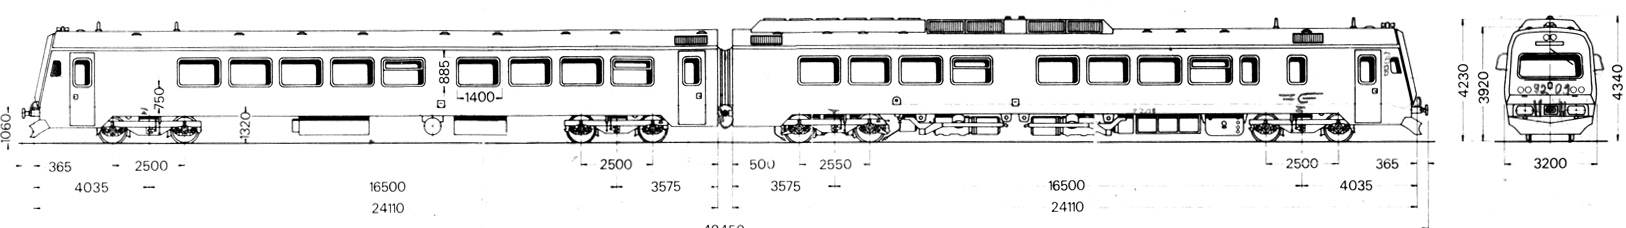
\includegraphics[width=0.8\pageheight, height=0.5\pagewidth, angle=270]{./figures/nsb92.png}
\section{Freight train - EL14}
\label{appendix:el14}
\begin{figure}[H]
  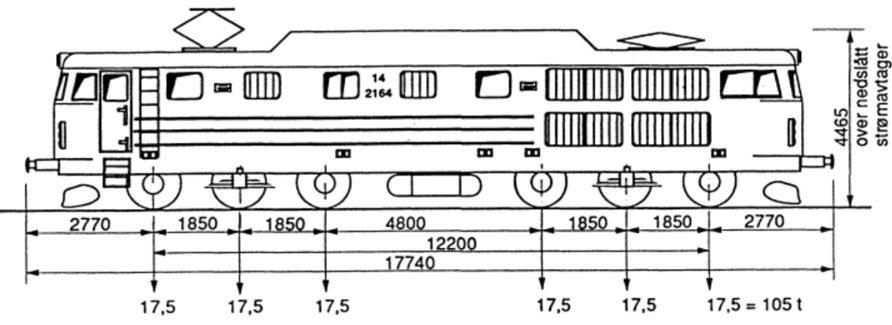
\includegraphics[width=0.8\textwidth]{./figures/EL14.png}
  \caption{Axle distances and weights for a EL14 locomotive}
  \label{figure:el14_locomotive}
\end{figure}

%
%
\newpage
\chapter{Figures}
%
\section{Recreated strain signals}
\label{appendix:recreated_signals}
\begin{figure}[h]
  \begin{subfigure}[t]{0.9\textwidth}
    \centering
    % This file was created by matlab2tikz.
%
%The latest updates can be retrieved from
%  http://www.mathworks.com/matlabcentral/fileexchange/22022-matlab2tikz-matlab2tikz
%where you can also make suggestions and rate matlab2tikz.
%
\definecolor{mycolor1}{rgb}{0.00000,0.44700,0.74100}%
\definecolor{mycolor2}{rgb}{0.85000,0.32500,0.09800}%
%
\begin{tikzpicture}

  \begin{axis}[%
    width=\textwidth,
    height=0.4\textwidth,
    at={(0\figurewidth,0\figureheight)},
    scale only axis,
    xmin=0,
    xmax=5,
    xlabel={time [s]},
    ymin=-4e-05,
    ymax=0.00016,
    ylabel={strain [\varepsilon]},
    axis background/.style={fill=white},
    title style={font=\bfseries},
    title={Strainhistory, calculated vs measured for Trondheim sensor},
    legend style={legend cell align=left,align=left,draw=white!15!black}
    ]
    \addplot [color=mycolor1,solid,forget plot]
    table[row sep=crcr]{%
    0	6.24445943240518e-07\\
    0.0009765625	5.31453570540839e-06\\
    0.001953125	2.32415764274234e-06\\
    0.0029296875	1.30856158130012e-06\\
    0.00390625	-7.43782547669991e-07\\
    0.0048828125	7.0202602047223e-07\\
    0.005859375	2.01282095783385e-07\\
    0.0068359375	2.04910017407049e-06\\
    0.0078125	2.94480068753706e-06\\
    0.0087890625	3.97450560647218e-06\\
    0.009765625	1.79520110542698e-06\\
    0.0107421875	1.44961646748052e-06\\
    0.01171875	2.92364238933828e-06\\
    0.0126953125	3.90693817736189e-08\\
    0.013671875	-1.30196003281409e-07\\
    0.0146484375	1.02543915822192e-07\\
    0.015625	1.29445609485285e-06\\
    0.0166015625	-2.57145004774499e-07\\
    0.017578125	3.50196952637167e-06\\
    0.0185546875	2.47931833230485e-06\\
    0.01953125	4.17903628595752e-06\\
    0.0205078125	-5.11042911852805e-07\\
    0.021484375	9.0655537222234e-07\\
    0.0224609375	4.58104510472446e-06\\
    0.0234375	9.77082754136105e-07\\
    0.0244140625	1.53424941813337e-06\\
    0.025390625	-5.53359217266318e-07\\
    0.0263671875	8.99502634574105e-07\\
    0.02734375	1.8093066058854e-06\\
    0.0283203125	3.62186669878944e-06\\
    0.029296875	1.27329786592202e-06\\
    0.0302734375	3.73471112240882e-06\\
    0.03125	4.92663188939252e-06\\
    0.0322265625	2.08334823663392e-07\\
    0.033203125	2.71911221920115e-06\\
    0.0341796875	7.79606109643392e-07\\
    0.03515625	8.43080736936822e-07\\
    0.0361328125	-3.77041254607993e-07\\
    0.037109375	2.07025843556273e-06\\
    0.0380859375	2.51458213204776e-06\\
    0.0390625	2.02088916012827e-06\\
    0.0400390625	4.57399231566769e-06\\
    0.041015625	3.07073024345857e-07\\
    0.0419921875	3.82639723519934e-06\\
    0.04296875	4.07324454482845e-06\\
    0.0439453125	-3.48830374859643e-07\\
    0.044921875	8.84384631207134e-08\\
    0.0458984375	1.30754822408883e-07\\
    0.046875	-5.26160421863986e-08\\
    0.0478515625	2.92364238933828e-06\\
    0.048828125	2.29594661340727e-06\\
    0.0498046875	2.83195644073891e-06\\
    0.05078125	2.69795393047505e-06\\
    0.0517578125	2.28889385632037e-06\\
    0.052734375	2.24657731586982e-06\\
    0.0537109375	1.48488019519229e-06\\
    0.0546875	9.2066084781588e-07\\
    0.0556640625	8.36028000176332e-07\\
    0.056640625	-5.67464651615073e-07\\
    0.0576171875	9.77082754136105e-07\\
    0.05859375	4.90444019780054e-07\\
    0.0595703125	3.98155838714155e-06\\
    0.060546875	4.97496751705219e-07\\
    0.0615234375	4.60925626193944e-06\\
    0.0625	3.06469772743778e-06\\
    0.0634765625	-4.82832039603448e-07\\
    0.064453125	1.6329878785202e-06\\
    0.0654296875	-1.79463592908094e-06\\
    0.06640625	2.5065119301621e-07\\
    0.0673828125	-1.71705622413671e-06\\
    0.068359375	1.47782744945243e-06\\
    0.0693359375	2.50752937190168e-06\\
    0.0703125	3.75586945464959e-06\\
    0.0712890625	-9.76522076033852e-07\\
    0.072265625	2.28184109933192e-06\\
    0.0732421875	1.91509787190623e-06\\
    0.07421875	1.06171562545658e-06\\
    0.0751953125	3.90693817736189e-08\\
    0.076171875	7.2318422542593e-07\\
    0.0771484375	-3.5588309494532e-07\\
    0.078125	7.43330108138839e-08\\
    0.0791015625	1.8445703587589e-06\\
    0.080078125	1.74583185692952e-06\\
    0.0810546875	3.29038635049216e-06\\
    0.08203125	-1.11052357392415e-06\\
    0.0830078125	2.9024840920279e-06\\
    0.083984375	3.11406710509689e-06\\
    0.0849609375	-1.88632101953169e-06\\
    0.0859375	-2.64197726142787e-07\\
    0.0869140625	8.71291684965622e-07\\
    0.087890625	4.19916705949848e-07\\
    0.0888671875	-4.82832039603448e-07\\
    0.08984375	2.24657731586982e-06\\
    0.0908203125	3.38207238246972e-06\\
    0.091796875	2.31710488526036e-06\\
    0.0927734375	-6.94413542990735e-07\\
    0.09375	3.650077802326e-06\\
    0.0947265625	-8.08269385111152e-08\\
    0.095703125	4.61221073843904e-08\\
    0.0966796875	-3.85105934316322e-08\\
    0.09765625	-7.79046119480644e-07\\
    0.0986328125	1.67530436746355e-06\\
    0.099609375	1.83046485731386e-06\\
    0.1005859375	3.78408056568537e-06\\
    0.1015625	-4.26410290368506e-07\\
    0.1025390625	3.03648665666038e-06\\
    0.103515625	1.15340125208846e-06\\
    0.1044921875	3.84653052735127e-07\\
    0.10546875	7.44342431267375e-07\\
    0.1064453125	-1.93670508024215e-07\\
    0.107421875	-1.91453181323862e-06\\
    0.1083984375	8.50133473796191e-07\\
    0.109375	7.93711581684653e-07\\
    0.1103515625	3.00122282040848e-06\\
    0.111328125	2.63447906962496e-06\\
    0.1123046875	-8.08269385111152e-08\\
    0.11328125	4.22840577274895e-06\\
    0.1142578125	2.0843639437179e-06\\
    0.115234375	3.02238112186355e-06\\
    0.1162109375	-4.68726602887012e-07\\
    0.1171875	1.08992658572125e-06\\
    0.1181640625	1.3861417638148e-06\\
    0.119140625	3.19164756547308e-06\\
    0.1201171875	3.85460835018205e-06\\
    0.12109375	3.00122282040848e-06\\
    0.1220703125	3.90397780520072e-06\\
    0.123046875	2.46521281309841e-06\\
    0.1240234375	1.66825161905981e-06\\
    0.125	1.23803415301069e-06\\
    0.1259765625	-1.64652920928198e-06\\
    0.126953125	-1.16090556697649e-07\\
    0.1279296875	-1.46315892448007e-06\\
    0.12890625	1.30856158130012e-06\\
    0.1298828125	2.21131353487516e-06\\
    0.130859375	3.92513614454627e-06\\
    0.1318359375	9.98240970633956e-07\\
    0.1328125	2.6697428802216e-06\\
    0.1337890625	1.9856253949211e-06\\
    0.134765625	5.68024076389373e-07\\
    0.1357421875	1.0193991880202e-06\\
    0.13671875	9.0655537222234e-07\\
    0.1376953125	3.35283942378903e-07\\
    0.138671875	2.08334823663392e-07\\
    0.1396484375	1.81635935626303e-06\\
    0.140625	3.60776114761291e-06\\
    0.1416015625	1.53424941813337e-06\\
    0.142578125	3.74881667713741e-06\\
    0.1435546875	1.78814835534533e-06\\
    0.14453125	-1.26568315855975e-06\\
    0.1455078125	2.92967565921742e-07\\
    0.146484375	-1.01883834237424e-06\\
    0.1474609375	-4.54621165775493e-07\\
    0.1484375	-1.51354172417189e-07\\
    0.1494140625	8.50133473796191e-07\\
    0.150390625	3.48786397854988e-06\\
    0.1513671875	-1.10347086439708e-06\\
    0.15234375	5.06063499208808e-06\\
    0.1533203125	3.30449189278798e-06\\
    0.154296875	3.80575519991384e-09\\
    0.1552734375	2.94480068753706e-06\\
    0.15625	-5.53359217266318e-07\\
    0.1572265625	-2.92408610627149e-07\\
    0.158203125	1.40024725282773e-06\\
    0.1591796875	1.13929576998255e-06\\
    0.16015625	1.72467360905399e-06\\
    0.1611328125	1.13224302907824e-06\\
    0.162109375	3.19164756547308e-06\\
    0.1630859375	-1.6112656981539e-06\\
    0.1640625	5.29337730774729e-06\\
    0.1650390625	2.01383640688942e-06\\
    0.166015625	-2.71250447411546e-07\\
    0.1669921875	8.84384631207134e-08\\
    0.16796875	-1.51958055767719e-06\\
    0.1689453125	4.0581124436832e-07\\
    0.169921875	1.28035060880044e-06\\
    0.1708984375	1.64709337443993e-06\\
    0.171875	3.48081120478774e-06\\
    0.1728515625	1.68940986456766e-06\\
    0.173828125	1.26624512314247e-06\\
    0.1748046875	4.08735010902928e-06\\
    0.17578125	-5.88622802397912e-07\\
    0.1767578125	1.30856158130012e-06\\
    0.177734375	-1.39263187410297e-06\\
    0.1787109375	-5.74517368641348e-07\\
    0.1796875	2.01282095783385e-07\\
    0.1806640625	2.18310251185491e-06\\
    0.181640625	2.24657731586982e-06\\
    0.1826171875	2.24657731586982e-06\\
    0.18359375	4.19916705949848e-07\\
    0.1845703125	2.62037354607672e-06\\
    0.185546875	-9.55363941532042e-07\\
    0.1865234375	-1.73524195596231e-08\\
    0.1875	-1.86617785669953e-07\\
    0.1884765625	-8.77784107427247e-07\\
    0.189453125	-2.64197726142787e-07\\
    0.1904296875	9.98240970633956e-07\\
    0.19140625	1.36498353103592e-06\\
    0.1923828125	8.92449897023665e-07\\
    0.193359375	5.58959495581472e-06\\
    0.1943359375	-3.98199413383354e-07\\
    0.1953125	1.30856158130012e-06\\
    0.1962890625	1.22392866853732e-06\\
    0.197265625	1.66018457862854e-07\\
    0.1982421875	-7.2262440339952e-07\\
    0.19921875	-1.3644210511898e-06\\
    0.2001953125	2.30299937059282e-06\\
    0.201171875	1.16045399328919e-06\\
    0.2021484375	3.092908799794e-06\\
    0.203125	-2.92408610627149e-07\\
    0.2041015625	1.80123912735123e-07\\
    0.205078125	3.24806972597323e-06\\
    0.2060546875	-9.90627498542035e-07\\
    0.20703125	-1.06820731528095e-06\\
    0.2080078125	1.30150883802726e-06\\
    0.208984375	-1.3644210511898e-06\\
    0.2099609375	-4.26410290368506e-07\\
    0.2109375	3.48786397854988e-06\\
    0.2119140625	2.32415764274234e-06\\
    0.212890625	2.75437603571818e-06\\
    0.2138671875	6.385514109402e-07\\
    0.21484375	2.11962771583252e-06\\
    0.2158203125	1.68940986456766e-06\\
    0.216796875	-2.37295698970541e-06\\
    0.2177734375	5.25707680395105e-07\\
    0.21875	-9.62416653131669e-07\\
    0.2197265625	1.81635935626303e-06\\
    0.220703125	2.64858459356762e-06\\
    0.2216796875	3.27628080859141e-06\\
    0.22265625	3.03648665666038e-06\\
    0.2236328125	2.61332078445092e-06\\
    0.224609375	8.64238947810916e-07\\
    0.2255859375	3.03648665666038e-06\\
    0.2265625	3.24806972597323e-06\\
    0.2275390625	-6.87360827641937e-07\\
    0.228515625	-9.49323860817159e-08\\
    0.2294921875	-1.73524195596231e-08\\
    0.23046875	7.16131490342701e-07\\
    0.2314453125	1.68235711596638e-06\\
    0.232421875	3.16343648759155e-06\\
    0.2333984375	1.9362561277745e-06\\
    0.234375	1.95741438453094e-06\\
    0.2353515625	1.58361864590955e-06\\
    0.236328125	1.90099236848729e-06\\
    0.2373046875	1.11813754756452e-06\\
    0.23828125	6.52656879034531e-07\\
    0.2392578125	-1.04704918462697e-06\\
    0.240234375	-1.04704918462697e-06\\
    0.2412109375	1.66825161905981e-06\\
    0.2421875	1.27329786592202e-06\\
    0.2431640625	3.10701433656429e-06\\
    0.244140625	6.52656879034531e-07\\
    0.2451171875	5.7165454296986e-06\\
    0.24609375	8.99502634574105e-07\\
    0.2470703125	-1.01883834237424e-06\\
    0.248046875	1.97857264217513e-06\\
    0.2490234375	-2.50092283308198e-07\\
    0.25	-1.55484407521876e-06\\
    0.2509765625	1.15340125208846e-06\\
    0.251953125	2.4087907402198e-06\\
    0.2529296875	3.05059219185186e-06\\
    0.25390625	1.99267814776486e-06\\
    0.2548828125	7.93711581684653e-07\\
    0.255859375	3.29743912159106e-06\\
    0.2568359375	7.2318422542593e-07\\
    0.2578125	1.16045399328919e-06\\
    0.2587890625	5.53918610663156e-07\\
    0.259765625	-2.44051442822163e-08\\
    0.2607421875	-3.48830374859643e-07\\
    0.26171875	1.86572861166686e-06\\
    0.2626953125	2.35236867365579e-06\\
    0.263671875	3.4243890182379e-06\\
    0.2646484375	3.01532835461356e-06\\
    0.265625	6.72802848084627e-08\\
    0.2666015625	2.74027050881564e-06\\
    0.267578125	6.10340475935486e-07\\
    0.2685546875	-5.81570085568528e-07\\
    0.26953125	-5.46306499944272e-07\\
    0.2705078125	-3.18401589605665e-06\\
    0.271484375	1.80225385560686e-06\\
    0.2724609375	9.55924538525998e-07\\
    0.2734375	4.2636696948456e-06\\
    0.2744140625	-1.0329437636976e-06\\
    0.275390625	3.59365559683125e-06\\
    0.2763671875	2.07731118959131e-06\\
    0.27734375	4.7633855622441e-07\\
    0.2783203125	1.27329786592202e-06\\
    0.279296875	-3.24696981823282e-09\\
    0.2802734375	-1.69589812071638e-06\\
    0.28125	-6.73255396648137e-07\\
    0.2822265625	1.68940986456766e-06\\
    0.283203125	1.35793078697376e-06\\
    0.2841796875	2.00678365374924e-06\\
    0.28515625	-4.68726602887012e-07\\
    0.2861328125	3.77702778777854e-06\\
    0.287109375	-7.36729833012047e-07\\
    0.2880859375	-5.53359217266318e-07\\
    0.2890625	-1.24452503619406e-06\\
    0.2900390625	-1.01985109719023e-07\\
    0.291015625	-1.47726433337154e-06\\
    0.2919921875	8.36028000176332e-07\\
    0.29296875	7.72553373771297e-07\\
    0.2939453125	3.6782889074416e-06\\
    0.294921875	8.07817054120346e-07\\
    0.2958984375	-5.46306499944272e-07\\
    0.296875	3.25512249647972e-06\\
    0.2978515625	-2.88075054468524e-06\\
    0.298828125	-1.01985109719023e-07\\
    0.2998046875	-1.47726433337154e-06\\
    0.30078125	2.85914836857352e-07\\
    0.3017578125	-7.93151547514356e-07\\
    0.302734375	2.42994901680912e-06\\
    0.3037109375	1.92215062376358e-06\\
    0.3046875	2.70500669328523e-06\\
    0.3056640625	2.42994901680912e-06\\
    0.306640625	4.69285824594799e-07\\
    0.3076171875	2.16899700093698e-06\\
    0.30859375	-1.51252785387276e-06\\
    0.3095703125	6.31498677040919e-07\\
    0.310546875	-5.67464651615073e-07\\
    0.3115234375	-1.59716029301204e-06\\
    0.3125	1.65414612254789e-06\\
    0.3134765625	1.66119887075474e-06\\
    0.314453125	2.57100421676738e-06\\
    0.3154296875	2.43598464544229e-07\\
    0.31640625	1.08992658572125e-06\\
    0.3173828125	1.83751760798683e-06\\
    0.318359375	4.61221073843904e-08\\
    0.3193359375	1.53424941813337e-06\\
    0.3203125	8.84384631207134e-08\\
    0.3212890625	-1.20926149694525e-06\\
    0.322265625	8.50133473796191e-07\\
    0.3232421875	2.68384840515111e-06\\
    0.32421875	1.44256372223376e-06\\
    0.3251953125	3.46670565755792e-06\\
    0.326171875	-8.49573255701621e-07\\
    0.3271484375	2.54279317361784e-06\\
    0.328125	1.41435274223509e-06\\
    0.3291015625	-7.2262440339952e-07\\
    0.330078125	3.49389401987617e-07\\
    0.3310546875	-3.41777654676387e-07\\
    0.33203125	2.07731118959131e-06\\
    0.3330078125	1.8093066058854e-06\\
    0.333984375	3.19870033519071e-06\\
    0.3349609375	3.7065000141358e-06\\
    0.3359375	1.4284582320371e-06\\
    0.3369140625	6.66762347523294e-07\\
    0.337890625	-3.41777654676387e-07\\
    0.3388671875	1.44256372223376e-06\\
    0.33984375	-8.08269385111152e-08\\
    0.3408203125	5.68024076389373e-07\\
    0.341796875	-6.52097249417795e-07\\
    0.3427734375	2.30299937059282e-06\\
    0.34375	2.93069515530631e-06\\
    0.3447265625	4.14377236978083e-06\\
    0.345703125	2.92967565921742e-07\\
    0.3466796875	2.47226557265209e-06\\
    0.34765625	3.92513614454627e-06\\
    0.3486328125	-7.43782547669991e-07\\
    0.349609375	-4.05252132777744e-07\\
    0.3505859375	-4.19357571270536e-07\\
    0.3515625	5.18654948074423e-07\\
    0.3525390625	-7.01466258241088e-07\\
    0.353515625	2.90953685769908e-06\\
    0.3544921875	2.15489149041413e-06\\
    0.35546875	3.62891947452526e-06\\
    0.3564453125	-5.18095629668163e-07\\
    0.357421875	3.52312784884378e-06\\
    0.3583984375	1.58361864590955e-06\\
    0.359375	2.29594661340727e-06\\
    0.3603515625	1.62593513070865e-06\\
    0.361328125	1.51913003385235e-07\\
    0.3623046875	1.03350466677116e-06\\
    0.36328125	1.92215062376358e-06\\
    0.3642578125	1.85162310962963e-06\\
    0.365234375	4.58104510472446e-06\\
    0.3662109375	4.1286397510997e-07\\
    0.3671875	3.41733624536328e-06\\
    0.3681640625	1.87983411409917e-06\\
    0.369140625	-1.23143280038535e-07\\
    0.3701171875	-3.85105934316322e-08\\
    0.37109375	2.71809379024778e-07\\
    0.3720703125	-9.34205806142055e-07\\
    0.373046875	-1.65459618014325e-07\\
    0.3740234375	1.95036163218028e-06\\
    0.375	1.56246040484195e-06\\
    0.3759765625	3.14933094924265e-06\\
    0.376953125	-3.91146693889868e-07\\
    0.3779296875	2.21131353487516e-06\\
    0.37890625	2.43700177586991e-06\\
    0.3798828125	-2.99461331501475e-07\\
    0.380859375	-8.78796623457467e-08\\
    0.3818359375	-2.71148608319287e-06\\
    0.3828125	-3.5588309494532e-07\\
    0.3837890625	1.23098141072467e-06\\
    0.384765625	1.22392866853732e-06\\
    0.3857421875	3.3961779273312e-06\\
    0.38671875	3.21178483165055e-07\\
    0.3876953125	2.85311473508963e-06\\
    0.388671875	4.4107489906276e-07\\
    0.3896484375	3.21178483165055e-07\\
    0.390625	1.02543915822192e-07\\
    0.3916015625	-9.97680209647699e-07\\
    0.392578125	-1.85811022424616e-06\\
    0.3935546875	1.47077470381168e-06\\
    0.39453125	1.07582110539148e-06\\
    0.3955078125	2.69090116776375e-06\\
    0.396484375	-7.37742145782549e-08\\
    0.3974609375	2.67679564263691e-06\\
    0.3984375	1.15340125208846e-06\\
    0.3994140625	-2.0696911504066e-06\\
    0.400390625	1.95741438453094e-06\\
    0.4013671875	-8.21362402397179e-07\\
    0.40234375	-3.24696981823282e-09\\
    0.4033203125	3.35283942378903e-07\\
    0.404296875	2.09846945226793e-06\\
    0.4052734375	2.58510973893348e-06\\
    0.40625	1.781095605363e-06\\
    0.4072265625	1.7176208599594e-06\\
    0.408203125	4.32009197533201e-06\\
    0.4091796875	-1.44200081040311e-06\\
    0.41015625	2.04204742043678e-06\\
    0.4111328125	1.4919329410308e-06\\
    0.412109375	3.6349486199033e-07\\
    0.4130859375	-1.23143280038535e-07\\
    0.4140625	2.84606197020732e-06\\
    0.4150390625	2.54279317361784e-06\\
    0.416015625	3.64302502629398e-06\\
    0.4169921875	6.59709613229581e-07\\
    0.41796875	2.15489149041413e-06\\
    0.4189453125	3.48081120478774e-06\\
    0.419921875	-6.59149965259904e-07\\
    0.4208984375	8.84384631207134e-08\\
    0.421875	3.49389401987617e-07\\
    0.4228515625	5.25707680395105e-07\\
    0.423828125	1.09596642320709e-07\\
    0.4248046875	3.25512249647972e-06\\
    0.42578125	2.19720802316771e-06\\
    0.4267578125	4.75736486321883e-06\\
    0.427734375	1.79112055337122e-08\\
    0.4287109375	3.55839172160445e-06\\
    0.4296875	4.22135298862574e-06\\
    0.4306640625	-1.45610621988656e-06\\
    0.431640625	4.62233093063633e-07\\
    0.4326171875	-1.72410892507993e-06\\
    0.43359375	7.65500637996781e-07\\
    0.4345703125	-5.03990193938134e-07\\
    0.435546875	4.28482804928801e-06\\
    0.4365234375	-7.37742145782549e-08\\
    0.4375	1.49898568696798e-06\\
    0.4384765625	2.63447906962496e-06\\
    0.439453125	-6.23886385062297e-07\\
    0.4404296875	1.65414612254789e-06\\
    0.44140625	1.5413021646623e-06\\
    0.4423828125	6.10340475935486e-07\\
    0.443359375	8.84384631207134e-08\\
    0.4443359375	1.55540765801659e-06\\
    0.4453125	1.19571770077365e-06\\
    0.4462890625	4.12261402125882e-06\\
    0.447265625	1.10403206644524e-06\\
    0.4482421875	1.96446713698049e-06\\
    0.44921875	4.30598640461838e-06\\
    0.4501953125	1.87176640319142e-07\\
    0.451171875	1.03350466677116e-06\\
    0.4521484375	5.96235009025755e-07\\
    0.453125	-8.78796623457467e-08\\
    0.4541015625	-1.93670508024215e-07\\
    0.455078125	2.11962771583252e-06\\
    0.4560546875	2.6697428802216e-06\\
    0.45703125	4.09440289127812e-06\\
    0.4580078125	1.20277044256658e-06\\
    0.458984375	1.85162310962963e-06\\
    0.4599609375	1.97857264217513e-06\\
    0.4609375	-1.43494810551296e-06\\
    0.4619140625	4.61221073843904e-08\\
    0.462890625	-1.05410189494334e-06\\
    0.4638671875	4.1286397510997e-07\\
    0.46484375	2.31005212787748e-06\\
    0.4658203125	3.01532835461356e-06\\
    0.466796875	8.71291684965622e-07\\
    0.4677734375	2.74732327221758e-06\\
    0.46875	3.09996156812949e-06\\
    0.4697265625	3.49389401987617e-07\\
    0.470703125	1.68235711596638e-06\\
    0.4716796875	6.72802848084627e-08\\
    0.47265625	-5.95675519127984e-07\\
    0.4736328125	-1.02589105308525e-06\\
    0.474609375	8.71291684965622e-07\\
    0.4755859375	1.28035060880044e-06\\
    0.4765625	1.70351536206621e-06\\
    0.4775390625	2.63447906962496e-06\\
    0.478515625	-4.05252132777744e-07\\
    0.4794921875	3.092908799794e-06\\
    0.48046875	2.20426077897199e-06\\
    0.4814453125	-5.74517368641348e-07\\
    0.482421875	2.49639308480629e-08\\
    0.4833984375	3.91705783181007e-07\\
    0.484375	-8.35467829246725e-07\\
    0.4853515625	2.18310251185491e-06\\
    0.486328125	2.37352694787722e-06\\
    0.4873046875	2.16194424562622e-06\\
    0.48828125	2.21131353487516e-06\\
    0.4892578125	2.38763246451822e-06\\
    0.490234375	1.4919329410308e-06\\
    0.4912109375	6.72802848084627e-08\\
    0.4921875	2.2949300789582e-07\\
    0.4931640625	4.90444019780054e-07\\
    0.494140625	-2.42232582999815e-06\\
    0.4951171875	-2.50092283308198e-07\\
    0.49609375	1.19571770077365e-06\\
    0.4970703125	2.03499466690195e-06\\
    0.498046875	1.9715198895287e-06\\
    0.4990234375	-3.77041254607993e-07\\
    0.5	2.76848156301581e-06\\
    0.5009765625	8.64238947810916e-07\\
    0.501953125	-5.81570085568528e-07\\
    0.5029296875	-2.28127198776285e-06\\
    0.50390625	5.11602215852837e-07\\
    0.5048828125	-2.07775952437185e-07\\
    0.505859375	1.50603843300338e-06\\
    0.5068359375	1.58361864590955e-06\\
    0.5078125	6.31498677040919e-07\\
    0.5087890625	1.17455947598686e-06\\
    0.509765625	1.78814835534533e-06\\
    0.5107421875	3.91705783181007e-07\\
    0.51171875	-1.17399795522923e-06\\
    0.5126953125	3.49389401987617e-07\\
    0.513671875	-2.00723230280031e-07\\
    0.5146484375	-1.23041962079044e-06\\
    0.515625	-4.55633178580214e-08\\
    0.5166015625	2.18310251185491e-06\\
    0.517578125	-1.86617785669953e-07\\
    0.5185546875	4.86315674791665e-06\\
    0.51953125	1.9362561277745e-06\\
    0.5205078125	5.32760412813799e-07\\
    0.521484375	1.82341210673868e-06\\
    0.5224609375	-5.74517368641348e-07\\
    0.5234375	-1.85811022424616e-06\\
    0.5244140625	-1.82284672791896e-06\\
    0.525390625	-2.44051442822163e-08\\
    0.5263671875	2.85914836857352e-07\\
    0.52734375	9.0655537222234e-07\\
    0.5283203125	2.08334823663392e-07\\
    0.529296875	3.00827558746201e-06\\
    0.5302734375	1.61888238299512e-06\\
    0.53125	-1.64652920928198e-06\\
    0.5322265625	3.84653052735127e-07\\
    0.533203125	-7.64940691052284e-07\\
    0.5341796875	-2.0626384542987e-06\\
    0.53515625	-8.14309688824738e-07\\
    0.5361328125	3.6349486199033e-07\\
    0.537109375	2.21131353487516e-06\\
    0.5380859375	1.45666921282529e-06\\
    0.5390625	8.92449897023665e-07\\
    0.5400390625	1.09596642320709e-07\\
    0.541015625	2.12668047055152e-06\\
    0.5419921875	1.04761014591633e-06\\
    0.54296875	-8.77784107427247e-07\\
    0.5439453125	-1.73524195596231e-08\\
    0.544921875	-1.04704918462697e-06\\
    0.5458984375	2.71809379024778e-07\\
    0.546875	1.97857264217513e-06\\
    0.5478515625	2.06320568163368e-06\\
    0.548828125	3.90693817736189e-08\\
    0.5498046875	3.98155838714155e-06\\
    0.55078125	8.57186210753789e-07\\
    0.5517578125	6.10340475935486e-07\\
    0.552734375	-2.07775952437185e-07\\
    0.5537109375	-1.09037833257884e-07\\
    0.5546875	-1.1316817019138e-06\\
    0.5556640625	2.85914836857352e-07\\
    0.556640625	5.89182275718449e-07\\
    0.5576171875	2.77553432681261e-06\\
    0.55859375	-5.26160421863986e-08\\
    0.5595703125	4.59515068313462e-06\\
    0.560546875	3.68534168396694e-06\\
    0.5615234375	1.80123912735123e-07\\
    0.5625	3.14125753706233e-07\\
    0.5634765625	1.37908901945666e-06\\
    0.564453125	1.23098141072467e-06\\
    0.5654296875	-1.12462899268273e-06\\
    0.56640625	2.7614287993181e-06\\
    0.5673828125	1.68940986456766e-06\\
    0.568359375	2.74027050881564e-06\\
    0.5693359375	-4.75779321294561e-07\\
    0.5703125	4.30598640461838e-06\\
    0.5712890625	1.46372195826893e-06\\
    0.572265625	1.28035060880044e-06\\
    0.5732421875	-3.41777654676387e-07\\
    0.57421875	-2.50092283308198e-07\\
    0.5751953125	-1.49136974186793e-06\\
    0.576171875	-1.18105066376968e-06\\
    0.5771484375	1.4284582320371e-06\\
    0.578125	1.4284582320371e-06\\
    0.5791015625	3.54428617220406e-06\\
    0.580078125	-1.23143280038535e-07\\
    0.5810546875	4.70799532462378e-06\\
    0.58203125	3.35283942378903e-07\\
    0.5830078125	3.00020295084576e-07\\
    0.583984375	-1.73524195596231e-08\\
    0.5849609375	-1.97095339591626e-06\\
    0.5859375	3.90693817736189e-08\\
    0.5869140625	1.343825299145e-06\\
    0.587890625	6.73815081915887e-07\\
    0.5888671875	2.09141669794358e-06\\
    0.58984375	1.40729999748186e-06\\
    0.5908203125	-5.32201065003759e-07\\
    0.591796875	2.60626802292335e-06\\
    0.5927734375	8.28975263514288e-07\\
    0.59375	-1.66768731477422e-06\\
    0.5947265625	3.14125753706233e-07\\
    0.595703125	-7.71993405316012e-07\\
    0.5966796875	4.69285824594799e-07\\
    0.59765625	3.14227818021609e-06\\
    0.5986328125	3.21280587492066e-06\\
    0.599609375	2.08334823663392e-07\\
    0.6005859375	3.05764495959538e-06\\
    0.6015625	1.6329878785202e-06\\
    0.6025390625	8.78344422219641e-07\\
    0.603515625	7.16131490342701e-07\\
    0.6044921875	-2.0696911504066e-06\\
    0.60546875	3.84653052735127e-07\\
    0.6064453125	-1.24452503619406e-06\\
    0.607421875	1.8445703587589e-06\\
    0.6083984375	1.89393961692614e-06\\
    0.609375	4.21430020460054e-06\\
    0.6103515625	-9.90627498542035e-07\\
    0.611328125	2.78258709070808e-06\\
    0.6123046875	1.13929576998255e-06\\
    0.61328125	-6.16833668726441e-07\\
    0.6142578125	-2.28934118316889e-07\\
    0.615234375	-2.23190313365586e-06\\
    0.6162109375	-2.23190313365586e-06\\
    0.6171875	-1.06115460516169e-06\\
    0.6181640625	8.00764317853168e-07\\
    0.619140625	1.33677255537883e-06\\
    0.6201171875	1.21687592644819e-06\\
    0.62109375	-1.72512340664574e-07\\
    0.6220703125	4.53872837186272e-06\\
    0.623046875	-3.84093974298587e-07\\
    0.6240234375	1.40729999748186e-06\\
    0.625	-2.64197726142787e-07\\
    0.6259765625	-1.35736834521415e-06\\
    0.626953125	-1.07526002530111e-06\\
    0.6279296875	1.64004062643127e-06\\
    0.62890625	3.69239446059138e-06\\
    0.6298828125	3.5513389468546e-06\\
    0.630859375	1.5130911791381e-06\\
    0.6318359375	-1.51958055767719e-06\\
    0.6328125	2.41584349898395e-06\\
    0.6337890625	-1.35031563914092e-06\\
    0.634765625	-3.24696981823282e-09\\
    0.6357421875	1.02543915822192e-07\\
    0.63671875	-1.85105752517796e-06\\
    0.6376953125	1.47782744945243e-06\\
    0.638671875	1.92920337571982e-06\\
    0.6396484375	2.72616498230753e-06\\
    0.640625	1.6329878785202e-06\\
    0.6416015625	2.38763246451822e-06\\
    0.642578125	2.39468522298661e-06\\
    0.6435546875	8.13857369177506e-08\\
    0.64453125	1.44256372223376e-06\\
    0.6455078125	-1.37248726425404e-07\\
    0.646484375	-1.88632101953169e-06\\
    0.6474609375	-1.43494810551296e-06\\
    0.6484375	-2.07775952437185e-07\\
    0.6494140625	3.98861116791024e-06\\
    0.650390625	-1.68179271794241e-06\\
    0.6513671875	5.52611973086135e-06\\
    0.65234375	2.17604975634683e-06\\
    0.6533203125	-1.3644210511898e-06\\
    0.654296875	1.10403206644524e-06\\
    0.6552734375	-1.79463592908094e-06\\
    0.65625	-2.92408610627149e-07\\
    0.6572265625	-1.93568990748271e-06\\
    0.658203125	9.84135492869843e-07\\
    0.6591796875	1.20277044256658e-06\\
    0.66015625	3.26922803778849e-06\\
    0.6611328125	7.72553373771297e-07\\
    0.662109375	-3.69988534818953e-07\\
    0.6630859375	3.57249727139905e-06\\
    0.6640625	-2.37295698970541e-06\\
    0.6650390625	-2.28934118316889e-07\\
    0.666015625	-1.53368596498985e-06\\
    0.6669921875	3.20166562617265e-08\\
    0.66796875	-1.86617785669953e-07\\
    0.6689453125	-2.57145004774499e-07\\
    0.669921875	2.16899700093698e-06\\
    0.6708984375	3.41028347258712e-06\\
    0.671875	-3.85105934316322e-08\\
    0.6728515625	1.37203627519674e-06\\
    0.673828125	3.4596528840909e-06\\
    0.6748046875	-7.79046119480644e-07\\
    0.67578125	3.35283942378903e-07\\
    0.6767578125	-1.38557916852262e-06\\
    0.677734375	-2.28934118316889e-07\\
    0.6787109375	1.44860276294744e-07\\
    0.6796875	1.60477688786512e-06\\
    0.6806640625	2.10552220669073e-06\\
    0.681640625	1.71056811096304e-06\\
    0.6826171875	2.71809379024778e-07\\
    0.68359375	6.24445943240518e-07\\
    0.6845703125	4.03798063605253e-06\\
    0.685546875	-8.28415115871175e-07\\
    0.6865234375	5.11602215852837e-07\\
    0.6875	7.43330108138839e-08\\
    0.6884765625	8.00764317853168e-07\\
    0.689453125	1.61182963538068e-06\\
    0.6904296875	2.56395145583179e-06\\
    0.69140625	8.07817054120346e-07\\
    0.6923828125	3.38912515485145e-06\\
    0.693359375	8.21922526951123e-07\\
    0.6943359375	-5.3925378252313e-07\\
    0.6953125	-5.25148347385509e-07\\
    0.6962890625	1.37807549302265e-07\\
    0.697265625	-1.26568315855975e-06\\
    0.6982421875	5.68024076389373e-07\\
    0.69921875	1.03350466677116e-06\\
    0.7001953125	2.98006451984203e-06\\
    0.701171875	1.16649368917887e-07\\
    0.7021484375	3.26217526708489e-06\\
    0.703125	3.69944723731426e-06\\
    0.7041015625	-1.57600218455927e-06\\
    0.705078125	1.23803415301069e-06\\
    0.7060546875	5.31748330936076e-08\\
    0.70703125	5.46865877948041e-07\\
    0.7080078125	-1.06115460516169e-06\\
    0.708984375	3.092908799794e-06\\
    0.7099609375	2.01282095783385e-07\\
    0.7109375	2.22541904697682e-06\\
    0.7119140625	-7.43782547669991e-07\\
    0.712890625	1.77404285547889e-06\\
    0.7138671875	7.5139516674547e-07\\
    0.71484375	-2.87369785992417e-06\\
    0.7158203125	-7.64940691052284e-07\\
    0.716796875	-2.11200732498206e-06\\
    0.7177734375	-2.7830316858251e-07\\
    0.71875	-6.67214905458648e-08\\
    0.7197265625	1.4284582320371e-06\\
    0.720703125	2.02088916012827e-06\\
    0.7216796875	2.93069515530631e-06\\
    0.72265625	-2.18958696914483e-06\\
    0.7236328125	3.29743912159106e-06\\
    0.724609375	-2.64197726142787e-07\\
    0.7255859375	-1.38557916852262e-06\\
    0.7265625	-1.44301449470086e-07\\
    0.7275390625	-1.12462899268273e-06\\
    0.728515625	-1.72410892507993e-06\\
    0.7294921875	1.06171562545658e-06\\
    0.73046875	1.61888238299512e-06\\
    0.7314453125	2.74027050881564e-06\\
    0.732421875	3.43144179121117e-06\\
    0.7333984375	1.09596642320709e-07\\
    0.734375	3.11406710509689e-06\\
    0.7353515625	-1.71705622413671e-06\\
    0.736328125	-1.07526002530111e-06\\
    0.7373046875	-5.74517368641348e-07\\
    0.73828125	-2.33064083703495e-06\\
    0.7392578125	1.49898568696798e-06\\
    0.740234375	1.56246040484195e-06\\
    0.7412109375	2.76848156301581e-06\\
    0.7421875	3.03648665666038e-06\\
    0.7431640625	7.16131490342701e-07\\
    0.744140625	-3.20619493532912e-07\\
    0.7451171875	3.91808336466576e-06\\
    0.74609375	1.5130911791381e-06\\
    0.7470703125	-1.93568990748271e-06\\
    0.748046875	1.20982318445816e-06\\
    0.7490234375	-1.33621022669738e-06\\
    0.75	1.78814835534533e-06\\
    0.7509765625	2.16899700093698e-06\\
    0.751953125	3.60776114761291e-06\\
    0.7529296875	3.24101695556539e-06\\
    0.75390625	1.08992658572125e-06\\
    0.7548828125	2.07731118959131e-06\\
    0.755859375	-1.20220878879903e-06\\
    0.7568359375	6.52656879034531e-07\\
    0.7578125	1.80123912735123e-07\\
    0.7587890625	-1.48431703766885e-06\\
    0.759765625	2.22440279720043e-07\\
    0.7607421875	3.26922803778849e-06\\
    0.76171875	1.32266706814204e-06\\
    0.7626953125	1.87278136283401e-06\\
    0.763671875	-1.32210481385876e-06\\
    0.7646484375	4.94779027166033e-06\\
    0.765625	6.02275589017039e-08\\
    0.7666015625	1.71056811096304e-06\\
    0.767578125	1.09596642320709e-07\\
    0.7685546875	-1.38557916852262e-06\\
    0.76953125	-2.99461331501475e-07\\
    0.7705078125	1.02645192734613e-06\\
    0.771484375	9.91188231702677e-07\\
    0.7724609375	1.18161221748358e-06\\
    0.7734375	-1.0329437636976e-06\\
    0.7744140625	4.22840577274895e-06\\
    0.775390625	-2.01326957878023e-06\\
    0.7763671875	-5.60411934489918e-07\\
    0.77734375	9.98240970633956e-07\\
    0.7783203125	-2.03442766888006e-06\\
    0.779296875	-6.30939101299056e-07\\
    0.7802734375	1.18161221748358e-06\\
    0.78125	2.35942143163108e-06\\
    0.7822265625	1.95036163218028e-06\\
    0.783203125	2.54279317361784e-06\\
    0.7841796875	9.84135492869843e-07\\
    0.78515625	3.38912515485145e-06\\
    0.7861328125	1.6329878785202e-06\\
    0.787109375	1.09596642320709e-07\\
    0.7880859375	-1.26568315855975e-06\\
    0.7890625	6.72802848084627e-08\\
    0.7900390625	6.94973285685638e-07\\
    0.791015625	2.04910017407049e-06\\
    0.7919921875	1.781095605363e-06\\
    0.79296875	1.32971981171089e-06\\
    0.7939453125	4.07324454482845e-06\\
    0.794921875	2.07731118959131e-06\\
    0.7958984375	2.5004766118547e-06\\
    0.796875	6.87920550996625e-07\\
    0.7978515625	1.94330887992806e-06\\
    0.798828125	2.71809379024778e-07\\
    0.7998046875	7.86658845615016e-07\\
    0.80078125	1.56246040484195e-06\\
    0.8017578125	3.28333357949235e-06\\
    0.802734375	2.01282095783385e-07\\
    0.8037109375	3.55839172160445e-06\\
    0.8046875	-4.3346300936868e-07\\
    0.8056640625	5.04549483730131e-07\\
    0.806640625	1.39319450827204e-06\\
    0.8076171875	8.28975263514288e-07\\
    0.80859375	-3.48830374859643e-07\\
    0.8095703125	-3.24696981823282e-09\\
    0.810546875	8.78344422219641e-07\\
    0.8115234375	2.09141669794358e-06\\
    0.8125	2.35942143163108e-06\\
    0.8134765625	1.13929576998255e-06\\
    0.814453125	6.94973285685638e-07\\
    0.8154296875	2.26068282895855e-06\\
    0.81640625	-5.46306499944272e-07\\
    0.8173828125	-1.51252785387276e-06\\
    0.818359375	2.15387551642278e-07\\
    0.8193359375	-7.71993405316012e-07\\
    0.8203125	-1.12462899268273e-06\\
    0.8212890625	1.22392866853732e-06\\
    0.822265625	-5.60411934489918e-07\\
    0.8232421875	2.96595898662401e-06\\
    0.82421875	2.69795393047505e-06\\
    0.8251953125	2.42289625784764e-06\\
    0.826171875	3.38207238246972e-06\\
    0.8271484375	-8.70731394643888e-07\\
    0.828125	-7.37742145782549e-08\\
    0.8291015625	3.20166562617265e-08\\
    0.830078125	-3.77041254607993e-07\\
    0.8310546875	2.46521281309841e-06\\
    0.83203125	8.14869790486403e-07\\
    0.8330078125	3.80523889999848e-06\\
    0.833984375	-2.20369235770989e-06\\
    0.8349609375	4.2425113412918e-06\\
    0.8359375	-1.16090556697649e-07\\
    0.8369140625	1.87176640319142e-07\\
    0.837890625	1.9362561277745e-06\\
    0.8388671875	-7.57887976690326e-07\\
    0.83984375	-1.73116162592384e-06\\
    0.8408203125	-5.26160421863986e-08\\
    0.841796875	2.69795393047505e-06\\
    0.8427734375	2.78963985470243e-06\\
    0.84375	2.83195644073891e-06\\
    0.8447265625	1.80123912735123e-07\\
    0.845703125	5.08179337998052e-06\\
    0.8466796875	-7.36729833012047e-07\\
    0.84765625	4.7633855622441e-07\\
    0.8486328125	-1.92863720949979e-06\\
    0.849609375	-2.97948812097567e-06\\
    0.8505859375	-3.38854358815496e-06\\
    0.8515625	1.52014392537105e-06\\
    0.8525390625	5.75076809400041e-07\\
    0.853515625	8.21922526951123e-07\\
    0.8544921875	1.0687683653747e-06\\
    0.85546875	-8.21362402397179e-07\\
    0.8564453125	2.69090116776375e-06\\
    0.857421875	-1.06115460516169e-06\\
    0.8583984375	-8.77784107427247e-07\\
    0.859375	-3.77041254607993e-07\\
    0.8603515625	-1.87221562208614e-06\\
    0.861328125	6.73815081915887e-07\\
    0.8623046875	2.51458213204776e-06\\
    0.86328125	2.32415764274234e-06\\
    0.8642578125	4.62233093063633e-07\\
    0.865234375	2.24657731586982e-06\\
    0.8662109375	9.27713585760536e-07\\
    0.8671875	-8.28415115871175e-07\\
    0.8681640625	9.48871800186477e-07\\
    0.869140625	-1.40673728496769e-06\\
    0.8701171875	6.02275589017039e-08\\
    0.87109375	-4.68726602887012e-07\\
    0.8720703125	1.4919329410308e-06\\
    0.873046875	2.38057970614871e-06\\
    0.8740234375	2.80374538298668e-06\\
    0.875	3.29038635049216e-06\\
    0.8759765625	1.86572861166686e-06\\
    0.876953125	3.38912515485145e-06\\
    0.8779296875	-4.89884757813889e-07\\
    0.87890625	-2.33769352939324e-06\\
    0.8798828125	-1.51958055767719e-06\\
    0.880859375	-9.694693646322e-07\\
    0.8818359375	-2.04853306178671e-06\\
    0.8828125	1.44860276294744e-07\\
    0.8837890625	2.24657731586982e-06\\
    0.884765625	1.28740335177732e-06\\
    0.8857421875	1.66018457862854e-07\\
    0.88671875	9.55924538525998e-07\\
    0.8876953125	8.13857369177506e-08\\
    0.888671875	-1.44301449470086e-07\\
    0.8896484375	-8.91889532697978e-07\\
    0.890625	-2.59864307729013e-06\\
    0.8916015625	3.84653052735127e-07\\
    0.892578125	8.50133473796191e-07\\
    0.8935546875	1.83046485731386e-06\\
    0.89453125	-2.92408610627149e-07\\
    0.8955078125	3.13522541128841e-06\\
    0.896484375	-3.44496500585497e-06\\
    0.8974609375	-1.87926832085836e-06\\
    0.8984375	-2.92408610627149e-07\\
    0.8994140625	-2.03442766888006e-06\\
    0.900390625	-2.84548711989457e-06\\
    0.9013671875	-1.56189677843056e-06\\
    0.90234375	-9.97680209647699e-07\\
    0.9033203125	8.50133473796191e-07\\
    0.904296875	1.9715198895287e-06\\
    0.9052734375	8.14869790486403e-07\\
    0.90625	-9.49323860817159e-08\\
    0.9072265625	1.56246040484195e-06\\
    0.908203125	-1.75231972786424e-06\\
    0.9091796875	4.48127630297938e-07\\
    0.91015625	-2.71250447411546e-07\\
    0.9111328125	-1.90042641658237e-06\\
    0.912109375	-1.21631420499217e-06\\
    0.9130859375	6.72802848084627e-08\\
    0.9140625	7.44342431267375e-07\\
    0.9150390625	1.90099236848729e-06\\
    0.916015625	-1.55484407521876e-06\\
    0.9169921875	2.04910017407049e-06\\
    0.91796875	1.7176208599594e-06\\
    0.9189453125	-2.07674384641561e-06\\
    0.919921875	-7.36729833012047e-07\\
    0.9208984375	-1.1316817019138e-06\\
    0.921875	-8.78796623457467e-08\\
    0.9228515625	4.4107489906276e-07\\
    0.923828125	4.28482804928801e-06\\
    0.9248046875	-7.01466258241088e-07\\
    0.92578125	4.18608906948875e-06\\
    0.9267578125	1.87176640319142e-07\\
    0.927734375	-7.43782547669991e-07\\
    0.9287109375	2.64756650256593e-07\\
    0.9296875	-6.16833668726441e-07\\
    0.9306640625	-1.41378999025227e-06\\
    0.931640625	-2.88075054468524e-06\\
    0.9326171875	6.03287742431289e-07\\
    0.93359375	3.94629448477934e-06\\
    0.9345703125	7.30236960607821e-07\\
    0.935546875	4.09440289127812e-06\\
    0.9365234375	4.40472540790124e-06\\
    0.9375	3.77600322388344e-07\\
    0.9384765625	3.99566394877738e-06\\
    0.939453125	3.80575519991384e-09\\
    0.9404296875	7.93711581684653e-07\\
    0.94140625	-1.28684128003704e-06\\
    0.9423828125	-8.98942245185132e-07\\
    0.943359375	1.25919238046137e-06\\
    0.9443359375	1.26624512314247e-06\\
    0.9453125	1.28035060880044e-06\\
    0.9462890625	-1.13873441104644e-06\\
    0.947265625	1.95036163218028e-06\\
    0.9482421875	-6.87360827641937e-07\\
    0.94921875	-6.45044533476805e-07\\
    0.9501953125	1.23702095614379e-07\\
    0.951171875	-3.85105934316322e-08\\
    0.9521484375	-5.53359217266318e-07\\
    0.953125	1.61888238299512e-06\\
    0.9541015625	3.28333357949235e-06\\
    0.955078125	2.7614287993181e-06\\
    0.9560546875	-8.00204261383001e-07\\
    0.95703125	3.8193444567001e-06\\
    0.9580078125	-7.37742145782549e-08\\
    0.958984375	-1.35031563914092e-06\\
    0.9599609375	-2.92408610627149e-07\\
    0.9609375	-9.83574787337491e-07\\
    0.9619140625	-2.80317100688943e-06\\
    0.962890625	-1.93670508024215e-07\\
    0.9638671875	8.07817054120346e-07\\
    0.96484375	1.80225385560686e-06\\
    0.9658203125	2.98006451984203e-06\\
    0.966796875	9.27713585760536e-07\\
    0.9677734375	4.03092785459299e-06\\
    0.96875	9.2066084781588e-07\\
    0.9697265625	3.49389401987617e-07\\
    0.970703125	-1.42789540052502e-06\\
    0.9716796875	-1.92158451141843e-06\\
    0.97265625	-1.68884541937894e-06\\
    0.9736328125	-3.77041254607993e-07\\
    0.974609375	4.4107489906276e-07\\
    0.9755859375	9.1360810996967e-07\\
    0.9765625	1.56951315176575e-06\\
    0.9775390625	7.44342431267375e-07\\
    0.978515625	3.28231212722322e-07\\
    0.9794921875	2.70500669328523e-06\\
    0.98046875	-3.60717654656587e-06\\
    0.9814453125	-1.06820731528095e-06\\
    0.982421875	-2.17548158018489e-06\\
    0.9833984375	-6.3799181743737e-07\\
    0.984375	1.52014392537105e-06\\
    0.9853515625	1.18866495907939e-06\\
    0.986328125	2.86722026515002e-06\\
    0.9873046875	9.48871800186477e-07\\
    0.98828125	-7.08518973392344e-07\\
    0.9892578125	-5.96687664156798e-08\\
    0.990234375	-1.315052107292e-06\\
    0.9912109375	-5.18095629668163e-07\\
    0.9921875	-1.30094669386163e-06\\
    0.9931640625	5.31748330936076e-08\\
    0.994140625	2.64756650256593e-07\\
    0.9951171875	2.48637109205607e-06\\
    0.99609375	1.29445609485285e-06\\
    0.9970703125	4.8419983692009e-06\\
    0.998046875	5.75886226143111e-06\\
    0.9990234375	3.80575519991384e-09\\
    1	2.07731118959131e-06\\
    1.0009765625	-1.56189677843056e-06\\
    1.001953125	9.54911894219049e-08\\
    1.0029296875	-2.18253427471441e-06\\
    1.00390625	-3.34724934393385e-07\\
    1.0048828125	-4.96937475925451e-07\\
    1.005859375	1.55540765801659e-06\\
    1.0068359375	-1.8298994273816e-06\\
    1.0078125	1.97857264217513e-06\\
    1.0087890625	1.64004062643127e-06\\
    1.009765625	-5.95675519127984e-07\\
    1.0107421875	1.05466288563756e-06\\
    1.01171875	-1.27273586581758e-06\\
    1.0126953125	5.11602215852837e-07\\
    1.013671875	-2.57145004774499e-07\\
    1.0146484375	2.5065119301621e-07\\
    1.015625	8.28975263514288e-07\\
    1.0166015625	6.17393209539213e-07\\
    1.017578125	-2.99359348743863e-06\\
    1.0185546875	3.04353942420679e-06\\
    1.01953125	-2.32358814457757e-06\\
    1.0205078125	4.48127630297938e-07\\
    1.021484375	-1.28684128003704e-06\\
    1.0224609375	-1.71705622413671e-06\\
    1.0234375	-1.1316817019138e-06\\
    1.0244140625	-7.64940691052284e-07\\
    1.025390625	5.68024076389373e-07\\
    1.0263671875	-3.5588309494532e-07\\
    1.02734375	1.87983411409917e-06\\
    1.0283203125	-6.94413542990735e-07\\
    1.029296875	3.18459479585497e-06\\
    1.0302734375	-9.27153094148212e-07\\
    1.03125	1.16045399328919e-06\\
    1.0322265625	1.81635935626303e-06\\
    1.033203125	1.66018457862854e-07\\
    1.0341796875	-2.00723230280031e-07\\
    1.03515625	2.81785091166579e-06\\
    1.0361328125	2.57703921587287e-07\\
    1.037109375	2.46521281309841e-06\\
    1.0380859375	-1.4702116289747e-06\\
    1.0390625	-2.89485591391052e-06\\
    1.0400390625	3.01532835461356e-06\\
    1.041015625	-8.28415115871175e-07\\
    1.0419921875	-1.17399795522923e-06\\
    1.04296875	-2.28934118316889e-07\\
    1.0439453125	1.87176640319142e-07\\
    1.044921875	1.78814835534533e-06\\
    1.0458984375	3.3961779273312e-06\\
    1.046875	2.94480068753706e-06\\
    1.0478515625	3.72060556807488e-06\\
    1.048828125	1.0687683653747e-06\\
    1.0498046875	1.80123912735123e-07\\
    1.05078125	1.73071185249549e-07\\
    1.0517578125	-2.92408610627149e-07\\
    1.052734375	-2.70443339606412e-06\\
    1.0537109375	7.93711581684653e-07\\
    1.0546875	-9.90627498542035e-07\\
    1.0556640625	1.67530436746355e-06\\
    1.056640625	4.55180361631563e-07\\
    1.0576171875	-6.16833668726441e-07\\
    1.05859375	5.43443330892814e-06\\
    1.0595703125	-3.62935814931251e-07\\
    1.060546875	-4.96937475925451e-07\\
    1.0615234375	5.31748330936076e-08\\
    1.0625	6.31498677040919e-07\\
    1.0634765625	-2.08379654232662e-06\\
    1.064453125	-2.33769352939324e-06\\
    1.0654296875	-2.1966396634768e-06\\
    1.06640625	-3.77041254607993e-07\\
    1.0673828125	8.36028000176332e-07\\
    1.068359375	-1.86516292321548e-06\\
    1.0693359375	2.59921526149487e-06\\
    1.0703125	-2.49285273631514e-06\\
    1.0712890625	1.28740335177732e-06\\
    1.072265625	6.80867816407141e-07\\
    1.0732421875	1.51913003385235e-07\\
    1.07421875	-2.50092283308198e-07\\
    1.0751953125	2.62037354607672e-06\\
    1.076171875	3.73471112240882e-06\\
    1.0771484375	3.36796683800353e-06\\
    1.078125	1.52719667170309e-06\\
    1.0791015625	5.44853891121721e-06\\
    1.080078125	1.37203627519674e-06\\
    1.0810546875	6.72802848084627e-08\\
    1.08203125	3.91705783181007e-07\\
    1.0830078125	-1.37147375706571e-06\\
    1.083984375	2.71809379024778e-07\\
    1.0849609375	-1.42084269543798e-06\\
    1.0859375	3.20575310500614e-06\\
    1.0869140625	3.82639723519934e-06\\
    1.087890625	5.90697120046854e-06\\
    1.0888671875	4.55283394908872e-06\\
    1.08984375	5.59664775908082e-06\\
    1.0908203125	5.6107533659088e-06\\
    1.091796875	2.35942143163108e-06\\
    1.0927734375	1.46372195826893e-06\\
    1.09375	1.61182963538068e-06\\
    1.0947265625	-1.16090556697649e-07\\
    1.095703125	4.08735010902928e-06\\
    1.0966796875	2.59216250016506e-06\\
    1.09765625	4.90547350801246e-06\\
    1.0986328125	3.49491675241133e-06\\
    1.099609375	2.30299937059282e-06\\
    1.1005859375	6.09739704317117e-06\\
    1.1015625	2.00678365374924e-06\\
    1.1025390625	3.94629448477934e-06\\
    1.103515625	1.68235711596638e-06\\
    1.1044921875	7.93711581684653e-07\\
    1.10546875	4.90444019780054e-07\\
    1.1064453125	2.86722026515002e-06\\
    1.107421875	3.6782889074416e-06\\
    1.1083984375	6.17393209539213e-07\\
    1.109375	5.09589897240204e-06\\
    1.1103515625	1.11813754756452e-06\\
    1.111328125	-7.15571688445805e-07\\
    1.1123046875	3.3327029785638e-06\\
    1.11328125	-1.16694524658991e-06\\
    1.1142578125	-3.98199413383354e-07\\
    1.115234375	-6.52097249417795e-07\\
    1.1162109375	2.51458213204776e-06\\
    1.1171875	3.73471112240882e-06\\
    1.1181640625	5.80823190294189e-06\\
    1.119140625	6.06213299279932e-06\\
    1.1201171875	6.03392175427785e-06\\
    1.12109375	7.12710840171295e-06\\
    1.1220703125	4.24956412571078e-06\\
    1.123046875	1.25213963787915e-06\\
    1.1240234375	3.11406710509689e-06\\
    1.125	3.26217526708489e-06\\
    1.1259765625	1.46372195826893e-06\\
    1.126953125	5.51906692858252e-06\\
    1.1279296875	3.23396418525643e-06\\
    1.12890625	7.00721039560465e-06\\
    1.1298828125	4.85610395491295e-06\\
    1.130859375	6.81678420922163e-06\\
    1.1318359375	7.90997255433823e-06\\
    1.1328125	4.41883098137763e-06\\
    1.1337890625	5.66717579716719e-06\\
    1.134765625	5.37801090371966e-06\\
    1.1357421875	4.36946147593705e-06\\
    1.13671875	9.37696451034525e-06\\
    1.1376953125	4.78557603030049e-06\\
    1.138671875	6.46414331327474e-06\\
    1.1396484375	3.38207238246972e-06\\
    1.140625	2.41584349898395e-06\\
    1.1416015625	7.06363298316206e-06\\
    1.142578125	-6.66202681003569e-07\\
    1.1435546875	3.24101695556539e-06\\
    1.14453125	1.53424941813337e-06\\
    1.1455078125	4.42588376826404e-06\\
    1.146484375	6.03392175427785e-06\\
    1.1474609375	8.27672014311743e-06\\
    1.1484375	8.24145594029418e-06\\
    1.1494140625	6.95784063667261e-06\\
    1.150390625	6.71804473349096e-06\\
    1.1513671875	7.31753470532013e-06\\
    1.15234375	5.56843654660861e-06\\
    1.1533203125	3.43849456428311e-06\\
    1.154296875	3.63597225036061e-06\\
    1.1552734375	5.58254215264728e-06\\
    1.15625	6.96489345908117e-06\\
    1.1572265625	9.5039159380111e-06\\
    1.158203125	9.63792025745341e-06\\
    1.1591796875	1.08792251202802e-05\\
    1.16015625	8.05102928767756e-06\\
    1.1611328125	8.62230946132854e-06\\
    1.162109375	5.62485897313099e-06\\
    1.1630859375	6.75330882974603e-06\\
    1.1640625	6.88025959669041e-06\\
    1.1650390625	8.74926069894763e-06\\
    1.166015625	6.746256010298e-06\\
    1.1669921875	7.94523673397301e-06\\
    1.16796875	1.06394273517605e-05\\
    1.1689453125	7.18353100269018e-06\\
    1.169921875	7.90291971870674e-06\\
    1.1708984375	4.86315674791665e-06\\
    1.171875	7.14826687633918e-06\\
    1.1728515625	5.8858127779417e-06\\
    1.173828125	4.39061983481949e-06\\
    1.1748046875	6.63341091254339e-06\\
    1.17578125	5.31453570540839e-06\\
    1.1767578125	9.0948503411062e-06\\
    1.177734375	1.12600806341447e-05\\
    1.1787109375	8.79157778525819e-06\\
    1.1796875	1.35170081025102e-05\\
    1.1806640625	7.78302152807894e-06\\
    1.181640625	1.12036575768977e-05\\
    1.1826171875	6.34424546484672e-06\\
    1.18359375	7.66312336596782e-06\\
    1.1845703125	6.98605192689882e-06\\
    1.185546875	8.84094772377747e-06\\
    1.1865234375	7.71954602693851e-06\\
    1.1875	1.04701584073654e-05\\
    1.1884765625	1.74102317339413e-05\\
    1.189453125	1.15492489016567e-05\\
    1.1904296875	1.6197122595059e-05\\
    1.19140625	1.67402001626028e-05\\
    1.1923828125	1.817195291779e-05\\
    1.193359375	1.70857952829268e-05\\
    1.1943359375	1.77064565020054e-05\\
    1.1953125	1.99352008147212e-05\\
    1.1962890625	2.01044729372776e-05\\
    1.197265625	2.10002055319764e-05\\
    1.1982421875	2.14515989387231e-05\\
    1.19921875	2.59937675904083e-05\\
    1.2001953125	2.33488662710988e-05\\
    1.201171875	2.2939789439488e-05\\
    1.2021484375	2.4738319367372e-05\\
    1.203125	2.63182097744201e-05\\
    1.2041015625	2.10002055319764e-05\\
    1.205078125	2.47594785811828e-05\\
    1.2060546875	3.01621602379848e-05\\
    1.20703125	2.52038222763645e-05\\
    1.2080078125	2.92805176330543e-05\\
    1.208984375	2.94145272096327e-05\\
    1.2099609375	2.74396528447752e-05\\
    1.2109375	2.86245765353079e-05\\
    1.2119140625	3.08463159619039e-05\\
    1.212890625	3.05782960831496e-05\\
    1.2138671875	2.72069003042633e-05\\
    1.21484375	2.93228364428618e-05\\
    1.2158203125	2.21710080161332e-05\\
    1.216796875	2.68260327424975e-05\\
    1.2177734375	3.1036751225506e-05\\
    1.21875	2.93228364428618e-05\\
    1.2197265625	3.17350144741853e-05\\
    1.220703125	3.11848675913758e-05\\
    1.2216796875	3.86260076969238e-05\\
    1.22265625	3.4838418392157e-05\\
    1.2236328125	4.03046876629998e-05\\
    1.224609375	3.68979606294956e-05\\
    1.2255859375	4.16377610298509e-05\\
    1.2265625	3.679216202188e-05\\
    1.2275390625	3.56495384744421e-05\\
    1.228515625	4.51080002947582e-05\\
    1.2294921875	3.54238353639739e-05\\
    1.23046875	4.48258661290802e-05\\
    1.2314453125	4.89238803949774e-05\\
    1.232421875	4.17647205819701e-05\\
    1.2333984375	4.81832729410125e-05\\
    1.234375	4.99254655395682e-05\\
    1.2353515625	5.11950833715152e-05\\
    1.236328125	4.6426979613843e-05\\
    1.2373046875	5.36144195362777e-05\\
    1.23828125	5.18722141892875e-05\\
    1.2392578125	5.14772211017245e-05\\
    1.240234375	5.07083961580153e-05\\
    1.2412109375	5.36779008164553e-05\\
    1.2421875	5.53425239052717e-05\\
    1.2431640625	5.63652823426261e-05\\
    1.244140625	5.53636844036452e-05\\
    1.2451171875	6.27628597885625e-05\\
    1.24609375	5.47641372936707e-05\\
    1.2470703125	5.32053181446629e-05\\
    1.248046875	5.97016053243481e-05\\
    1.2490234375	5.72751864206652e-05\\
    1.25	5.9609909048798e-05\\
    1.2509765625	6.14932128238563e-05\\
    1.251953125	6.24031261572552e-05\\
    1.2529296875	6.39267056485101e-05\\
    1.25390625	6.23819653634073e-05\\
    1.2548828125	6.66000344945674e-05\\
    1.255859375	6.20081248185538e-05\\
    1.2568359375	6.41806360113784e-05\\
    1.2578125	6.23114293903304e-05\\
    1.2587890625	6.24101797554021e-05\\
    1.259765625	6.73829910093737e-05\\
    1.2607421875	7.02961642164656e-05\\
    1.26171875	6.66353027798921e-05\\
    1.2626953125	7.55582582439029e-05\\
    1.263671875	7.09027835152395e-05\\
    1.2646484375	6.60710105107726e-05\\
    1.265625	6.74535276920373e-05\\
    1.2666015625	5.99837478152661e-05\\
    1.267578125	6.27981278054487e-05\\
    1.2685546875	6.03575868589519e-05\\
    1.26953125	6.18247314450745e-05\\
    1.2705078125	6.58523474262867e-05\\
    1.271484375	6.71995956806355e-05\\
    1.2724609375	6.28686638466224e-05\\
    1.2734375	7.26380008884543e-05\\
    1.2744140625	6.48013552146235e-05\\
    1.275390625	6.28122350128939e-05\\
    1.2763671875	6.07737476298793e-05\\
    1.27734375	5.71270623890717e-05\\
    1.2783203125	6.23960725592075e-05\\
    1.279296875	6.07384797546133e-05\\
    1.2802734375	6.31367008930878e-05\\
    1.28125	6.75804937457026e-05\\
    1.2822265625	6.35881320303123e-05\\
    1.283203125	7.16857467124785e-05\\
    1.2841796875	6.30450039927333e-05\\
    1.28515625	6.25089301398169e-05\\
    1.2861328125	6.68186979033523e-05\\
    1.287109375	5.7063580674569e-05\\
    1.2880859375	5.8375537732139e-05\\
    1.2890625	6.32001833723338e-05\\
    1.2900390625	6.3743311577094e-05\\
    1.291015625	6.76792451428821e-05\\
    1.2919921875	6.48859988015527e-05\\
    1.29296875	6.85468475353445e-05\\
    1.2939453125	7.29272043646495e-05\\
    1.294921875	6.72701323376395e-05\\
    1.2958984375	6.64871759981089e-05\\
    1.296875	6.70937907136339e-05\\
    1.2978515625	6.51893051047524e-05\\
    1.298828125	6.84763106997088e-05\\
    1.2998046875	6.93932903327711e-05\\
    1.30078125	7.00422307732423e-05\\
    1.3017578125	6.66282491226296e-05\\
    1.302734375	6.8596223326162e-05\\
    1.3037109375	6.92804312110026e-05\\
    1.3046875	6.94215051171608e-05\\
    1.3056640625	6.66070881514351e-05\\
    1.306640625	6.84692570166881e-05\\
    1.3076171875	6.81377340260355e-05\\
    1.30859375	7.3491504308071e-05\\
    1.3095703125	7.3216408006748e-05\\
    1.310546875	7.11637711125425e-05\\
    1.3115234375	7.2348797578162e-05\\
    1.3125	7.48740418389103e-05\\
    1.3134765625	6.69174491513107e-05\\
    1.314453125	6.72348640079039e-05\\
    1.3154296875	6.77497818669965e-05\\
    1.31640625	6.26288413468974e-05\\
    1.3173828125	6.36375073354706e-05\\
    1.318359375	6.75734400752157e-05\\
    1.3193359375	6.58452937799796e-05\\
    1.3203125	7.13048455457175e-05\\
    1.3212890625	7.38089233038204e-05\\
    1.322265625	7.25604097401404e-05\\
    1.3232421875	7.49869022128938e-05\\
    1.32421875	7.36607944142665e-05\\
    1.3251953125	6.99716937283793e-05\\
    1.326171875	7.36749019256821e-05\\
    1.3271484375	7.02256271360735e-05\\
    1.328125	7.21442392393481e-05\\
    1.3291015625	7.10085892816458e-05\\
    1.330078125	7.46483211667404e-05\\
    1.3310546875	7.40910736900429e-05\\
    1.33203125	7.16363706190709e-05\\
    1.3330078125	6.9463827296706e-05\\
    1.333984375	7.10720727521482e-05\\
    1.3349609375	7.12131471596632e-05\\
    1.3359375	7.00774992993748e-05\\
    1.3369140625	7.55582582439029e-05\\
    1.337890625	7.40699124055985e-05\\
    1.3388671875	7.35902568631101e-05\\
    1.33984375	6.98306196682617e-05\\
    1.3408203125	7.56005809386257e-05\\
    1.341796875	7.00351770683116e-05\\
    1.3427734375	6.99858011365625e-05\\
    1.34375	6.83422907391902e-05\\
    1.3447265625	6.62967273426256e-05\\
    1.345703125	6.97459752511394e-05\\
    1.3466796875	6.74605813608467e-05\\
    1.34765625	7.18268212917192e-05\\
    1.3486328125	6.98024048609749e-05\\
    1.349609375	6.89841761365669e-05\\
    1.3505859375	7.53184297075864e-05\\
    1.3515625	7.47611814901927e-05\\
    1.3525390625	7.65810576942906e-05\\
    1.353515625	7.22500452663029e-05\\
    1.3544921875	7.40628586443142e-05\\
    1.35546875	6.94990957823749e-05\\
    1.3564453125	7.38300845773093e-05\\
    1.357421875	7.88735467587959e-05\\
    1.3583984375	7.85208554549622e-05\\
    1.359375	8.48622827625647e-05\\
    1.3603515625	8.46929888949086e-05\\
    1.361328125	8.83892512680293e-05\\
    1.3623046875	8.25415509452877e-05\\
    1.36328125	8.77967188346737e-05\\
    1.3642578125	8.56099980247327e-05\\
    1.365234375	9.43922084008452e-05\\
    1.3662109375	8.96871818888703e-05\\
    1.3671875	8.86361399874654e-05\\
    1.3681640625	9.53162892315112e-05\\
    1.369140625	9.17328401943667e-05\\
    1.3701171875	9.24876196654598e-05\\
    1.37109375	8.89465145491499e-05\\
    1.3720703125	8.95672642457564e-05\\
    1.373046875	8.19560792563979e-05\\
    1.3740234375	8.48904984127013e-05\\
    1.375	8.06299531258569e-05\\
    1.3759765625	8.3557310669219e-05\\
    1.376953125	8.10249690552823e-05\\
    1.3779296875	8.08838919021003e-05\\
    1.37890625	8.12013155522761e-05\\
    1.3798828125	8.36842807786092e-05\\
    1.380859375	8.22735035816522e-05\\
    1.3818359375	8.29506761435013e-05\\
    1.3828125	7.94731225415748e-05\\
    1.3837890625	8.13635543839902e-05\\
    1.384765625	7.08534074985159e-05\\
    1.3857421875	6.95061494798042e-05\\
    1.38671875	6.96260623512111e-05\\
    1.3876953125	6.64730686878283e-05\\
    1.388671875	6.57818109676522e-05\\
    1.3896484375	7.03032179250474e-05\\
    1.390625	7.04583995388213e-05\\
    1.3916015625	7.21865616474654e-05\\
    1.392578125	7.50292248596512e-05\\
    1.3935546875	7.06206349133849e-05\\
    1.39453125	7.23205826299428e-05\\
    1.3955078125	7.50151173103376e-05\\
    1.396484375	7.09662669724183e-05\\
    1.3974609375	7.21019168347841e-05\\
    1.3984375	6.92240016595927e-05\\
    1.3994140625	6.75593327345379e-05\\
    1.400390625	7.05994737746113e-05\\
    1.4013671875	7.05218829400414e-05\\
    1.40234375	7.07405480498784e-05\\
    1.4033203125	7.09521595367991e-05\\
    1.404296875	7.17210153535878e-05\\
    1.4052734375	7.07617091945741e-05\\
    1.40625	6.81659487401572e-05\\
    1.4072265625	7.30330105559282e-05\\
    1.408203125	6.737593734165e-05\\
    1.4091796875	6.82153244936684e-05\\
    1.41015625	6.86738138643596e-05\\
    1.4111328125	7.62847983296687e-05\\
    1.412109375	7.28002369644273e-05\\
    1.4130859375	7.33222142587225e-05\\
    1.4140625	7.12695769337229e-05\\
    1.4150390625	7.2842559427615e-05\\
    1.416015625	6.43710838674658e-05\\
    1.4169921875	6.0223569056697e-05\\
    1.41796875	5.87916968668989e-05\\
    1.4189453125	5.39177190581541e-05\\
    1.419921875	5.72046511620979e-05\\
    1.4208984375	5.59914462594058e-05\\
    1.421875	6.06608904377126e-05\\
    1.4228515625	6.11193729380532e-05\\
    1.423828125	6.01741940858996e-05\\
    1.4248046875	6.62120835188376e-05\\
    1.42578125	5.47923512593288e-05\\
    1.4267578125	5.70706341980077e-05\\
    1.427734375	5.24788113191988e-05\\
    1.4287109375	4.70899972593928e-05\\
    1.4296875	4.83666613520727e-05\\
    1.4306640625	3.79841609518372e-05\\
    1.431640625	4.42404382390352e-05\\
    1.4326171875	4.42122248639149e-05\\
    1.43359375	4.14332151520225e-05\\
    1.4345703125	4.29073579898578e-05\\
    1.435546875	4.03822738469987e-05\\
    1.4365234375	4.50586268043666e-05\\
    1.4375	3.87529664905622e-05\\
    1.4384765625	3.97333715848828e-05\\
    1.439453125	3.93031216324639e-05\\
    1.4404296875	3.60515723902709e-05\\
    1.44140625	3.76173917501193e-05\\
    1.4423828125	3.88517122410523e-05\\
    1.443359375	3.69120671121885e-05\\
    1.4443359375	3.9585252707357e-05\\
    1.4453125	3.59457739602838e-05\\
    1.4462890625	3.71095579113369e-05\\
    1.447265625	3.53109838466339e-05\\
    1.4482421875	3.0733465469271e-05\\
    1.44921875	3.11848675913758e-05\\
    1.4501953125	3.10931765026105e-05\\
    1.451171875	3.04724988018142e-05\\
    1.4521484375	3.30680651800946e-05\\
    1.453125	3.45986092264866e-05\\
    1.4541015625	3.38157036268202e-05\\
    1.455078125	3.62208499244336e-05\\
    1.4560546875	3.24897041234526e-05\\
    1.45703125	3.36182141180384e-05\\
    1.4580078125	3.52192920073963e-05\\
    1.458984375	3.19466095889751e-05\\
    1.4599609375	3.06347213089406e-05\\
    1.4609375	3.08886349031539e-05\\
    1.4619140625	2.90900830328812e-05\\
    1.462890625	2.89419672824815e-05\\
    1.4638671875	2.94074740731349e-05\\
    1.46484375	2.4159967867105e-05\\
    1.4658203125	2.40894372417325e-05\\
    1.466796875	2.47947439395079e-05\\
    1.4677734375	2.31372747650277e-05\\
    1.46875	2.4145861741241e-05\\
    1.4697265625	2.12682203184857e-05\\
    1.470703125	2.18324624400535e-05\\
    1.4716796875	2.60360861243077e-05\\
    1.47265625	2.31302217163548e-05\\
    1.4736328125	2.45267272781097e-05\\
    1.474609375	2.3877845424824e-05\\
    1.4755859375	1.97165577405418e-05\\
    1.4765625	2.22768035552836e-05\\
    1.4775390625	1.92228479218637e-05\\
    1.478515625	1.67402001626028e-05\\
    1.4794921875	1.95543387467836e-05\\
    1.48046875	1.6260599163668e-05\\
    1.4814453125	1.74525495472938e-05\\
    1.482421875	2.22979626657782e-05\\
    1.4833984375	2.12329552068569e-05\\
    1.484375	1.98082467601042e-05\\
    1.4853515625	1.9526126753198e-05\\
    1.486328125	1.49416987692886e-05\\
    1.4873046875	1.50686515983402e-05\\
    1.48828125	1.67260942443566e-05\\
    1.4892578125	1.30444630774983e-05\\
    1.490234375	1.42434587809864e-05\\
    1.4912109375	1.36086959944956e-05\\
    1.4921875	1.31290979747884e-05\\
    1.4931640625	1.65286114303565e-05\\
    1.494140625	1.29386694758676e-05\\
    1.4951171875	1.54424573362069e-05\\
    1.49609375	1.70646363912002e-05\\
    1.4970703125	1.01386735558973e-05\\
    1.498046875	9.78603033617489e-06\\
    1.4990234375	1.09003837523904e-05\\
    1.5	8.74220785157444e-06\\
    1.5009765625	8.49535825568019e-06\\
    1.501953125	7.61375354279875e-06\\
    1.5029296875	7.20468947968452e-06\\
    1.50390625	8.35430139801128e-06\\
    1.5048828125	9.93414045841168e-06\\
    1.505859375	7.52206674116949e-06\\
    1.5068359375	8.91147621576334e-06\\
    1.5078125	8.73515500429993e-06\\
    1.5087890625	5.58254215264728e-06\\
    1.509765625	6.19613639733698e-06\\
    1.5107421875	4.48230606690564e-06\\
    1.51171875	4.36240868984059e-06\\
    1.5126953125	7.35279884351149e-06\\
    1.513671875	8.12861050783812e-06\\
    1.5146484375	9.18653742879158e-06\\
    1.515625	8.24850878066168e-06\\
    1.5166015625	7.289323396543e-06\\
    1.517578125	9.46865164934158e-06\\
    1.5185546875	7.20468947968452e-06\\
    1.51953125	6.58404119021857e-06\\
    1.5205078125	5.00421262871679e-06\\
    1.521484375	3.36796683800353e-06\\
    1.5224609375	5.57548934957894e-06\\
    1.5234375	6.17497796267293e-06\\
    1.5244140625	4.36946147593705e-06\\
    1.525390625	9.20064313606958e-06\\
    1.5263671875	3.91808336466576e-06\\
    1.52734375	9.34170023055643e-06\\
    1.5283203125	7.93818389784821e-06\\
    1.529296875	3.27628080859141e-06\\
    1.5302734375	5.30748290608922e-06\\
    1.53125	3.88987224613055e-06\\
    1.5322265625	5.96235009025755e-07\\
    1.533203125	1.41435274223509e-06\\
    1.5341796875	2.62742630780161e-06\\
    1.53515625	4.29188083429896e-06\\
    1.5361328125	7.95934240651708e-06\\
    1.537109375	1.23803415301069e-06\\
    1.5380859375	6.746256010298e-06\\
    1.5390625	3.63597225036061e-06\\
    1.5400390625	2.35236867365579e-06\\
    1.541015625	9.1360810996967e-07\\
    1.5419921875	-1.57600218455927e-06\\
    1.54296875	-1.99916418488653e-06\\
    1.5439453125	-4.43233879337483e-06\\
    1.544921875	-5.15876255938272e-06\\
    1.5458984375	-4.94718292975396e-06\\
    1.546875	-6.08265923490009e-06\\
    1.5478515625	-4.8837090235493e-06\\
    1.548828125	-9.20100382055273e-07\\
    1.5498046875	-2.81022369263712e-06\\
    1.55078125	-2.21881396455723e-07\\
    1.5517578125	-3.91146693889868e-07\\
    1.552734375	-2.56337963276546e-06\\
    1.5537109375	-3.76233536275193e-06\\
    1.5546875	-1.57600218455927e-06\\
    1.5556640625	-4.69328725698041e-06\\
    1.556640625	-2.14828674495893e-07\\
    1.5576171875	-2.95127738686603e-06\\
    1.55859375	-3.31801680715006e-06\\
    1.5595703125	-3.34724934393385e-07\\
    1.560546875	-3.16285785420642e-06\\
    1.5615234375	-1.29389398699845e-06\\
    1.5625	-1.88632101953169e-06\\
    1.5634765625	-1.56189677843056e-06\\
    1.564453125	7.2318422542593e-07\\
    1.5654296875	-1.57600218455927e-06\\
    1.56640625	-4.55633178580214e-08\\
    1.5673828125	-2.27421929461505e-06\\
    1.568359375	9.91188231702677e-07\\
    1.5693359375	7.37289695888375e-07\\
    1.5703125	-1.97800609330677e-06\\
    1.5712890625	-1.06115460516169e-06\\
    1.572265625	-4.18549552780182e-06\\
    1.5732421875	-2.07674384641561e-06\\
    1.57421875	-3.52959712056431e-06\\
    1.5751953125	-6.25192256444636e-06\\
    1.576171875	-2.81727637828572e-06\\
    1.5771484375	-6.9219226861675e-06\\
    1.578125	-3.47317571233676e-06\\
    1.5791015625	-4.77791916211347e-06\\
    1.580078125	-6.01213283081591e-06\\
    1.5810546875	-2.79611832104329e-06\\
    1.58203125	-5.86402735012104e-06\\
    1.5830078125	-3.28980609198512e-06\\
    1.583984375	-3.4661230358642e-06\\
    1.5849609375	-9.97680209647699e-07\\
    1.5859375	-3.25454269580893e-06\\
    1.5869140625	-2.98654080425637e-06\\
    1.587890625	-6.25192256444636e-06\\
    1.5888671875	-7.85286874544974e-06\\
    1.58984375	-8.74149747099196e-06\\
    1.5908203125	-9.62307203973014e-06\\
    1.591796875	-8.79086568759155e-06\\
    1.5927734375	-1.08149584054349e-05\\
    1.59375	-4.91191964951628e-06\\
    1.5947265625	-7.38034330900034e-06\\
    1.595703125	-2.66211727121841e-06\\
    1.5966796875	-3.12759444915018e-06\\
    1.59765625	-5.97686962507333e-06\\
    1.5986328125	-2.48580004612786e-06\\
    1.599609375	-6.41413320193011e-06\\
    1.6005859375	-6.15318562911804e-06\\
    1.6015625	-5.00360417300476e-06\\
    1.6025390625	-4.02328417318382e-06\\
    1.603515625	-6.76676484247436e-06\\
    1.6044921875	-3.50843909321919e-06\\
    1.60546875	-3.41675429779459e-06\\
    1.6064453125	-2.61274845440949e-06\\
    1.607421875	-4.27012751818634e-06\\
    1.6083984375	-6.66202681003569e-07\\
    1.609375	-4.1079161908009e-06\\
    1.6103515625	-3.1981212567961e-06\\
    1.611328125	-4.24896952192248e-06\\
    1.6123046875	-2.20369235770989e-06\\
    1.61328125	-7.76823735655651e-06\\
    1.6142578125	-3.959810150646e-06\\
    1.615234375	-5.89223792122695e-06\\
    1.6162109375	-2.70443339606412e-06\\
    1.6171875	-6.0897118747663e-06\\
    1.6181640625	-5.26455234089529e-06\\
    1.619140625	-3.09233104162695e-06\\
    1.6201171875	-6.04034339363353e-06\\
    1.62109375	-5.30686824728424e-06\\
    1.6220703125	-8.12792066122404e-06\\
    1.623046875	-7.32392233176397e-06\\
    1.6240234375	-8.89665470688223e-06\\
    1.625	-8.23370981963781e-06\\
    1.6259765625	-6.07560659493609e-06\\
    1.626953125	-6.44939637708497e-06\\
    1.6279296875	-5.03181479226205e-06\\
    1.62890625	-1.07726429614101e-05\\
    1.6298828125	-3.81170406697751e-06\\
    1.630859375	-4.13612686018302e-06\\
    1.6318359375	-6.33655420790658e-06\\
    1.6328125	-5.29276294554968e-06\\
    1.6337890625	-7.40855379525031e-06\\
    1.634765625	-3.67770328711615e-06\\
    1.6357421875	-6.23076465136119e-06\\
    1.63671875	-4.04444217892035e-06\\
    1.6376953125	-4.67212927847687e-06\\
    1.638671875	-3.92454680133878e-06\\
    1.6396484375	-7.9022370490752e-06\\
    1.640625	-6.660975376212e-06\\
    1.6416015625	-5.7159218259128e-06\\
    1.642578125	-8.44528806986391e-06\\
    1.6435546875	-8.67802404254554e-06\\
    1.64453125	-8.26897286750885e-06\\
    1.6455078125	-7.0982383596689e-06\\
    1.646484375	-2.60569576589903e-06\\
    1.6474609375	-6.9289753142918e-06\\
    1.6484375	-2.10495462946614e-06\\
    1.6494140625	-1.47726433337154e-06\\
    1.650390625	-6.32244893498317e-06\\
    1.6513671875	-3.38149091049867e-06\\
    1.65234375	-3.12054176784273e-06\\
    1.6533203125	-6.07560659493609e-06\\
    1.654296875	-8.87549690479963e-06\\
    1.6552734375	-5.21518377895216e-06\\
    1.65625	-6.18139618404224e-06\\
    1.6572265625	-5.66655330817346e-06\\
    1.658203125	-6.3153962983739e-06\\
    1.6591796875	-4.99655151794368e-06\\
    1.66015625	-1.16090556697649e-07\\
    1.6611328125	-3.79054605147318e-06\\
    1.662109375	-4.3124435080504e-06\\
    1.6630859375	-2.45758928439014e-06\\
    1.6640625	-5.34213149989493e-06\\
    1.6650390625	-5.46202654032042e-06\\
    1.666015625	-2.72559145715438e-06\\
    1.6669921875	-5.06002540994008e-06\\
    1.66796875	-3.96686282021197e-06\\
    1.6689453125	-7.23223823028579e-06\\
    1.669921875	-6.84434377029044e-06\\
    1.6708984375	-2.67622264656206e-06\\
    1.671875	-8.57223497737359e-06\\
    1.6728515625	-6.90076480120349e-06\\
    1.673828125	-6.0897118747663e-06\\
    1.6748046875	-7.21813298242436e-06\\
    1.67578125	-3.90338879057003e-06\\
    1.6767578125	-3.09233104162695e-06\\
    1.677734375	-3.30391144976491e-06\\
    1.6787109375	-2.36590429784e-06\\
    1.6796875	-6.47760691543258e-06\\
    1.6806640625	-4.14317952728135e-06\\
    1.681640625	-3.1699105349219e-06\\
    1.6826171875	-7.79644782109988e-06\\
    1.68359375	-7.0982383596689e-06\\
    1.6845703125	-8.23370981963781e-06\\
    1.685546875	-6.3718173884883e-06\\
    1.6865234375	-6.9924489629683e-06\\
    1.6875	-9.20100382055273e-07\\
    1.6884765625	-7.26044872482426e-06\\
    1.689453125	-2.16137619083096e-06\\
    1.6904296875	-4.02328417318382e-06\\
    1.69140625	-4.94013027390401e-06\\
    1.6923828125	-3.38854358815496e-06\\
    1.693359375	-5.4338159451385e-06\\
    1.6943359375	-4.72149789360358e-06\\
    1.6953125	-4.60160267705184e-06\\
    1.6962890625	-5.13055194722978e-06\\
    1.697265625	-3.51549176909934e-06\\
    1.6982421875	-6.82318588207014e-06\\
    1.69921875	-2.04148036538239e-06\\
    1.7001953125	-5.85697470709763e-06\\
    1.701171875	-6.27308047664314e-06\\
    1.7021484375	-5.68065859944938e-06\\
    1.703125	-5.41265799771642e-06\\
    1.7041015625	-4.50991808044845e-06\\
    1.705078125	-5.38444739977217e-06\\
    1.7060546875	-2.81727637828572e-06\\
    1.70703125	-2.23895582739607e-06\\
    1.7080078125	-9.20100382055273e-07\\
    1.708984375	-2.70443339606412e-06\\
    1.7099609375	-2.55632694356458e-06\\
    1.7109375	-1.3644210511898e-06\\
    1.7119140625	-4.23486419058637e-06\\
    1.712890625	-3.7975987234064e-06\\
    1.7138671875	-4.66507661877865e-06\\
    1.71484375	-6.62571221585781e-06\\
    1.7158203125	-4.04444217892035e-06\\
    1.716796875	-4.06560018376828e-06\\
    1.7177734375	-1.20220878879903e-06\\
    1.71875	-3.50843909321919e-06\\
    1.7197265625	-5.95675519127984e-07\\
    1.720703125	2.1125749612124e-06\\
    1.7216796875	5.04549483730131e-07\\
    1.72265625	9.1360810996967e-07\\
    1.7236328125	9.54911894219049e-08\\
    1.724609375	-5.32201065003759e-07\\
    1.7255859375	-2.40822044755102e-06\\
    1.7265625	7.16131490342701e-07\\
    1.7275390625	-2.16137619083096e-06\\
    1.728515625	-1.10347086439708e-06\\
    1.7294921875	-2.80317100688943e-06\\
    1.73046875	-4.81318245172538e-06\\
    1.7314453125	-1.01883834237424e-06\\
    1.732421875	-3.01475153639276e-06\\
    1.7333984375	-6.66802800798681e-06\\
    1.734375	-4.21370619284236e-06\\
    1.7353515625	-3.98802082831619e-06\\
    1.736328125	-3.62935814931251e-07\\
    1.7373046875	-4.19357571270536e-07\\
    1.73828125	2.20426077897199e-06\\
    1.7392578125	1.72467360905399e-06\\
    1.740234375	-2.30948275936767e-06\\
    1.7412109375	1.52014392537105e-06\\
    1.7421875	-3.72001932670996e-06\\
    1.7431640625	-3.16285785420642e-06\\
    1.744140625	-5.56076361102375e-06\\
    1.7451171875	-6.46350164645588e-06\\
    1.74609375	-6.5128700861472e-06\\
    1.7470703125	-2.78201294905481e-06\\
    1.748046875	2.2949300789582e-07\\
    1.7490234375	1.43551097708632e-06\\
    1.75	-1.48431703766885e-06\\
    1.7509765625	2.61332078445092e-06\\
    1.751953125	-1.58406895264763e-07\\
    1.7529296875	5.31748330936076e-08\\
    1.75390625	-5.3925378252313e-07\\
    1.7548828125	-3.28980609198512e-06\\
    1.755859375	-2.09084923813831e-06\\
    1.7568359375	-2.93011933524758e-06\\
    1.7578125	-2.13316541093763e-06\\
    1.7587890625	-1.96390069842666e-06\\
    1.759765625	-1.23041962079044e-06\\
    1.7607421875	-4.14317952728135e-06\\
    1.76171875	-2.64095920746404e-06\\
    1.7626953125	-1.37248726425404e-07\\
    1.763671875	-3.62833456976695e-06\\
    1.7646484375	-1.48431703766885e-06\\
    1.765625	-1.49842244596813e-06\\
    1.7666015625	-6.66202681003569e-07\\
    1.767578125	3.6782889074416e-06\\
    1.7685546875	4.34022167926677e-07\\
    1.76953125	5.06063499208808e-06\\
    1.7705078125	1.92215062376358e-06\\
    1.771484375	9.77082754136105e-07\\
    1.7724609375	6.17393209539213e-07\\
    1.7734375	-7.71993405316012e-07\\
    1.7744140625	-2.84548711989457e-06\\
    1.775390625	-3.98096815904707e-06\\
    1.7763671875	-4.1079161908009e-06\\
    1.77734375	-1.46315892448007e-06\\
    1.7783203125	-5.67464651615073e-07\\
    1.779296875	-6.66202681003569e-07\\
    1.7802734375	2.28889385632037e-06\\
    1.78125	3.91808336466576e-06\\
    1.7822265625	1.87983411409917e-06\\
    1.783203125	2.97301175318379e-06\\
    1.7841796875	5.4062221055346e-06\\
    1.78515625	1.20277044256658e-06\\
    1.7861328125	-7.57887976690326e-07\\
    1.787109375	-9.55363941532042e-07\\
    1.7880859375	-8.49573255701621e-07\\
    1.7890625	-2.42232582999815e-06\\
    1.7900390625	-3.02180421917994e-06\\
    1.791015625	2.78862107891843e-07\\
    1.7919921875	1.87176640319142e-07\\
    1.79296875	-3.24749001627783e-06\\
    1.7939453125	6.17393209539213e-07\\
    1.794921875	-7.57887976690326e-07\\
    1.7958984375	7.30236960607821e-07\\
    1.796875	-2.21074505184432e-06\\
    1.7978515625	4.60925626193944e-06\\
    1.798828125	8.78344422219641e-07\\
    1.7998046875	4.03092785459299e-06\\
    1.80078125	-1.66063461304192e-06\\
    1.8017578125	1.37908901945666e-06\\
    1.802734375	1.49898568696798e-06\\
    1.8037109375	-1.6112656981539e-06\\
    1.8046875	-1.02996947383676e-08\\
    1.8056640625	-1.98505879059861e-06\\
    1.806640625	-1.11757628335298e-06\\
    1.8076171875	-1.74526702731632e-06\\
    1.80859375	-2.99461331501475e-07\\
    1.8095703125	2.64858459356762e-06\\
    1.810546875	-4.31949617268217e-06\\
    1.8115234375	1.9362561277745e-06\\
    1.8125	5.96235009025755e-07\\
    1.8134765625	-9.05994957574058e-07\\
    1.814453125	1.22392866853732e-06\\
    1.8154296875	6.02275589017039e-08\\
    1.81640625	1.08584803178071e-08\\
    1.8173828125	-2.22485043981763e-06\\
    1.818359375	1.70351536206621e-06\\
    1.8193359375	1.04761014591633e-06\\
    1.8203125	-1.01883834237424e-06\\
    1.8212890625	-3.7975987234064e-06\\
    1.822265625	3.80575519991384e-09\\
    1.8232421875	-6.45044533476805e-07\\
    1.82421875	-4.15023219428145e-06\\
    1.8251953125	-3.37443823274371e-06\\
    1.826171875	-3.88928344956458e-06\\
    1.8271484375	-9.83574787337491e-07\\
    1.828125	4.62233093063633e-07\\
    1.8291015625	4.88431512752035e-06\\
    1.830078125	5.20874372598383e-06\\
    1.8310546875	4.6727313714448e-06\\
    1.83203125	-2.7830316858251e-07\\
    1.8330078125	3.87576668745503e-06\\
    1.833984375	1.39319450827204e-06\\
    1.8349609375	-1.17399795522923e-06\\
    1.8359375	5.82129542510239e-07\\
    1.8369140625	-2.57748501087144e-06\\
    1.837890625	-1.09037833257884e-07\\
    1.8388671875	-5.18095629668163e-07\\
    1.83984375	3.86166112917481e-06\\
    1.8408203125	-1.51354172417189e-07\\
    1.841796875	4.03092785459299e-06\\
    1.8427734375	1.23098141072467e-06\\
    1.84375	2.26068282895855e-06\\
    1.8447265625	6.24550608167157e-06\\
    1.845703125	1.79520110542698e-06\\
    1.8466796875	4.91957909550043e-06\\
    1.84765625	2.97301175318379e-06\\
    1.8486328125	2.92364238933828e-06\\
    1.849609375	5.68128140596819e-06\\
    1.8505859375	1.83046485731386e-06\\
    1.8515625	-4.61673884380367e-07\\
    1.8525390625	3.92513614454627e-06\\
    1.853515625	-2.83138174928758e-06\\
    1.8544921875	-1.88632101953169e-06\\
    1.85546875	-1.8440048260111e-06\\
    1.8564453125	-1.00473292065557e-06\\
    1.857421875	-1.54779137190742e-06\\
    1.8583984375	8.99502634574105e-07\\
    1.859375	2.35236867365579e-06\\
    1.8603515625	3.27628080859141e-06\\
    1.861328125	3.36091406591779e-06\\
    1.8623046875	1.85162310962963e-06\\
    1.86328125	4.98305424408065e-06\\
    1.8642578125	3.25512249647972e-06\\
    1.865234375	1.16649368917887e-07\\
    1.8662109375	3.58660282158852e-06\\
    1.8671875	2.03499466690195e-06\\
    1.8681640625	9.2066084781588e-07\\
    1.869140625	2.85311473508963e-06\\
    1.8701171875	1.25213963787915e-06\\
    1.87109375	3.36796683800353e-06\\
    1.8720703125	1.44256372223376e-06\\
    1.873046875	9.91188231702677e-07\\
    1.8740234375	5.41327490623483e-06\\
    1.875	1.8445703587589e-06\\
    1.8759765625	3.24101695556539e-06\\
    1.876953125	2.62742630780161e-06\\
    1.8779296875	4.41883098137763e-06\\
    1.87890625	5.51201412640192e-06\\
    1.8798828125	4.89842071441635e-06\\
    1.880859375	6.16087234005767e-06\\
    1.8818359375	5.46969731539068e-06\\
    1.8828125	3.57955004644467e-06\\
    1.8837890625	4.48230606690564e-06\\
    1.884765625	4.02387507323254e-06\\
    1.8857421875	2.56395145583179e-06\\
    1.88671875	3.2269114150457e-06\\
    1.8876953125	5.79412629058817e-06\\
    1.888671875	3.8969250256162e-06\\
    1.8896484375	8.39661845116759e-06\\
    1.890625	8.68578507614193e-06\\
    1.8916015625	9.15832601542017e-06\\
    1.892578125	6.23140045708241e-06\\
    1.8935546875	7.67722903061868e-06\\
    1.89453125	5.8858127779417e-06\\
    1.8955078125	5.01126542379261e-06\\
    1.896484375	4.05913898102184e-06\\
    1.8974609375	3.98155838714155e-06\\
    1.8984375	1.79112055337122e-08\\
    1.8994140625	8.64238947810916e-07\\
    1.900390625	2.45110729428662e-06\\
    1.9013671875	4.95484306594685e-06\\
    1.90234375	1.26624512314247e-06\\
    1.9033203125	5.0253710142409e-06\\
    1.904296875	6.01981613560908e-06\\
    1.9052734375	3.11406710509689e-06\\
    1.90625	7.17647817722222e-06\\
    1.9072265625	3.05764495959538e-06\\
    1.908203125	5.53317253323971e-06\\
    1.9091796875	5.83644312883327e-06\\
    1.91015625	2.67679564263691e-06\\
    1.9111328125	6.746256010298e-06\\
    1.912109375	3.96040004542833e-06\\
    1.9130859375	5.39813145331806e-07\\
    1.9140625	5.58959495581472e-06\\
    1.9150390625	-2.71250447411546e-07\\
    1.916015625	5.22284932195742e-06\\
    1.9169921875	4.72210090658623e-06\\
    1.91796875	4.49641164255283e-06\\
    1.9189453125	7.04247451208811e-06\\
    1.919921875	6.90141806095621e-06\\
    1.9208984375	9.8565589603842e-06\\
    1.921875	9.76487175083644e-06\\
    1.9228515625	1.08933308749217e-05\\
    1.923828125	7.79712719608454e-06\\
    1.9248046875	8.94674046545622e-06\\
    1.92578125	9.65202597736151e-06\\
    1.9267578125	6.59814682467527e-06\\
    1.927734375	6.88025959669041e-06\\
    1.9287109375	6.53467147272908e-06\\
    1.9296875	6.30898139720722e-06\\
    1.9306640625	8.96789901645668e-06\\
    1.931640625	8.97495186698706e-06\\
    1.9326171875	9.06663893286567e-06\\
    1.93359375	6.26666451929527e-06\\
    1.9345703125	1.20006338459051e-05\\
    1.935546875	6.80973138888563e-06\\
    1.9365234375	6.89436523943518e-06\\
    1.9375	8.48125256813726e-06\\
    1.9384765625	6.76036164929316e-06\\
    1.939453125	5.06063499208808e-06\\
    1.9404296875	1.00822506241642e-05\\
    1.94140625	7.31753470532013e-06\\
    1.9423828125	1.14011383048921e-05\\
    1.943359375	8.47419972451391e-06\\
    1.9443359375	1.03220481276439e-05\\
    1.9453125	8.95379331569126e-06\\
    1.9462890625	1.02938366507257e-05\\
    1.947265625	1.07381675955717e-05\\
    1.9482421875	8.84800057253171e-06\\
    1.94921875	8.70694361618913e-06\\
    1.9501953125	9.67318455796372e-06\\
    1.951171875	1.25648655945857e-05\\
    1.9521484375	1.3531113930961e-05\\
    1.953125	1.53930867511677e-05\\
    1.9541015625	1.74384436091148e-05\\
    1.955078125	1.99986778540195e-05\\
    1.9560546875	1.61900696434849e-05\\
    1.95703125	1.64510289174511e-05\\
    1.9580078125	1.70293715736293e-05\\
    1.958984375	1.55976220635216e-05\\
    1.9599609375	1.20782156739015e-05\\
    1.9609375	1.45255758315394e-05\\
    1.9619140625	1.79392046561681e-05\\
    1.962890625	1.57668927296072e-05\\
    1.9638671875	1.83412244482827e-05\\
    1.96484375	2.1578553407195e-05\\
    1.9658203125	1.75512911255965e-05\\
    1.966796875	2.19594170044403e-05\\
    1.9677734375	2.0569971567381e-05\\
    1.96875	2.21357428413502e-05\\
    1.9697265625	2.23614400025897e-05\\
    1.970703125	2.5090973046834e-05\\
    1.9716796875	2.67272893475297e-05\\
    1.97265625	3.04090204436708e-05\\
    1.9736328125	2.76300868214882e-05\\
    1.974609375	2.71927940931412e-05\\
    1.9755859375	3.35335757808155e-05\\
    1.9765625	2.45972579646628e-05\\
    1.9775390625	2.50204422912058e-05\\
    1.978515625	2.96120150716267e-05\\
    1.9794921875	2.67413955456267e-05\\
    1.98046875	2.73832279766015e-05\\
    1.9814453125	3.30045864951197e-05\\
    1.982421875	3.29552141901093e-05\\
    1.9833984375	3.88305524357477e-05\\
    1.984375	4.61801115643461e-05\\
    1.9853515625	4.17858805104318e-05\\
    1.986328125	4.6843128885221e-05\\
    1.9873046875	4.46283723070538e-05\\
    1.98828125	4.37890244265864e-05\\
    1.9892578125	4.33728776763121e-05\\
    1.990234375	4.34434109996386e-05\\
    1.9912109375	4.54112946989655e-05\\
    1.9921875	4.45437321212982e-05\\
    1.9931640625	4.67020612971139e-05\\
    1.994140625	5.27397893787225e-05\\
    1.9951171875	4.85923702572652e-05\\
    1.99609375	5.34169222712909e-05\\
    1.9970703125	5.2210779939235e-05\\
    1.998046875	5.43973558838006e-05\\
    1.9990234375	5.67391187030622e-05\\
    2	5.73245611075347e-05\\
    2.0009765625	6.21350895008128e-05\\
    2.001953125	5.76560769874636e-05\\
    2.0029296875	5.81075032170587e-05\\
    2.00390625	5.80228607682189e-05\\
    2.0048828125	5.80863426035165e-05\\
    2.005859375	5.46865488962518e-05\\
    2.0068359375	5.41857513456454e-05\\
    2.0078125	5.79805395491278e-05\\
    2.0087890625	5.78394688444848e-05\\
    2.009765625	5.75996487371868e-05\\
    2.0107421875	6.29391998976652e-05\\
    2.01171875	6.5048232382891e-05\\
    2.0126953125	6.48577842709973e-05\\
    2.013671875	6.85397938513374e-05\\
    2.0146484375	6.40748316779727e-05\\
    2.015625	6.71078980412846e-05\\
    2.0166015625	7.06911720490446e-05\\
    2.017578125	7.1974949642409e-05\\
    2.0185546875	7.03737550162959e-05\\
    2.01953125	6.85891696414632e-05\\
    2.0205078125	6.66282491226296e-05\\
    2.021484375	6.7552279064347e-05\\
    2.0224609375	6.91181962677234e-05\\
    2.0234375	7.11778785540836e-05\\
    2.0244140625	6.69174491513107e-05\\
    2.025390625	6.98235659662915e-05\\
    2.0263671875	6.47167116419049e-05\\
    2.02734375	6.57394890972085e-05\\
    2.0283203125	7.10226967188441e-05\\
    2.029296875	6.75381717242613e-05\\
    2.0302734375	6.99082103964412e-05\\
    2.03125	6.98024048609749e-05\\
    2.0322265625	7.36255256374545e-05\\
    2.033203125	7.4112234975375e-05\\
    2.0341796875	7.39429447175865e-05\\
    2.03515625	6.33342019658832e-05\\
    2.0361328125	6.65859271811286e-05\\
    2.037109375	6.23537509729924e-05\\
    2.0380859375	5.49969025575745e-05\\
    2.0390625	5.98849979254832e-05\\
    2.0400390625	5.48981536446112e-05\\
    2.041015625	6.13521411362689e-05\\
    2.0419921875	6.56901135861812e-05\\
    2.04296875	6.97530289520234e-05\\
    2.0439453125	7.01480363590413e-05\\
    2.044921875	7.09662669724183e-05\\
    2.0458984375	7.24122812174293e-05\\
    2.046875	7.03455401786124e-05\\
    2.0478515625	6.33271483548084e-05\\
    2.048828125	6.51399296476103e-05\\
    2.0498046875	6.28051814091221e-05\\
    2.05078125	6.21421430952098e-05\\
    2.0517578125	5.95182127899267e-05\\
    2.052734375	6.26006269426656e-05\\
    2.0537109375	6.59158302474959e-05\\
    2.0546875	6.12604445605056e-05\\
    2.0556640625	6.04986582682348e-05\\
    2.056640625	6.26006269426656e-05\\
    2.0576171875	7.22218303236108e-05\\
    2.05859375	6.08724976937502e-05\\
    2.0595703125	6.71784346854586e-05\\
    2.060546875	6.89206929289806e-05\\
    2.0615234375	6.95273105726863e-05\\
    2.0625	6.72771860038826e-05\\
    2.0634765625	6.66000344945674e-05\\
    2.064453125	6.57465427420355e-05\\
    2.0654296875	6.37503651939916e-05\\
    2.06640625	6.02588368959413e-05\\
    2.0673828125	6.13168732205398e-05\\
    2.068359375	5.90667852971149e-05\\
    2.0693359375	5.72469723160542e-05\\
    2.0703125	6.32918803009136e-05\\
    2.0712890625	6.31367008930878e-05\\
    2.072265625	6.65929808377987e-05\\
    2.0732421875	6.8596223326162e-05\\
    2.07421875	6.91816795001801e-05\\
    2.0751953125	7.09027835152395e-05\\
    2.076171875	6.75663864048272e-05\\
    2.0771484375	7.01480363590413e-05\\
    2.078125	6.89206929289806e-05\\
    2.0791015625	6.75029033757742e-05\\
    2.080078125	6.46743898608754e-05\\
    2.0810546875	6.22056254492183e-05\\
    2.08203125	6.63319956067314e-05\\
    2.0830078125	6.09077655783915e-05\\
    2.083984375	6.07243726051976e-05\\
    2.0849609375	5.88975000915255e-05\\
    2.0859375	6.42441186220802e-05\\
    2.0869140625	6.24948229408591e-05\\
    2.087890625	6.88854244837755e-05\\
    2.0888671875	7.0275003091312e-05\\
    2.08984375	7.0796977771039e-05\\
    2.0908203125	7.34421280378056e-05\\
    2.091796875	7.06276886265069e-05\\
    2.0927734375	7.63271210853843e-05\\
    2.09375	7.16857467124785e-05\\
    2.0947265625	7.2588624701782e-05\\
    2.095703125	7.41827725995649e-05\\
    2.0966796875	7.26803233380227e-05\\
    2.09765625	7.04654532496733e-05\\
    2.0986328125	7.33856980205667e-05\\
    2.099609375	7.36960631935459e-05\\
    2.1005859375	7.23911200034516e-05\\
    2.1015625	7.24122812174293e-05\\
    2.1025390625	7.7272330222117e-05\\
    2.103515625	7.95436609158408e-05\\
    2.1044921875	7.77590430807444e-05\\
    2.10546875	7.66092728809536e-05\\
    2.1064453125	8.28095984514402e-05\\
    2.107421875	7.89440850491715e-05\\
    2.1083984375	7.78436888432541e-05\\
    2.109375	8.26826285623397e-05\\
    2.1103515625	8.06017377141704e-05\\
    2.111328125	7.64399817846629e-05\\
    2.1123046875	7.93814226697845e-05\\
    2.11328125	7.82810255092917e-05\\
    2.1142578125	7.82598640489747e-05\\
    2.115234375	7.91415923147272e-05\\
    2.1162109375	8.00868067282671e-05\\
    2.1171875	7.91063231544889e-05\\
    2.1181640625	8.69996227312111e-05\\
    2.119140625	8.16174935297489e-05\\
    2.1201171875	8.72253489334835e-05\\
    2.12109375	8.75639384263908e-05\\
    2.1220703125	8.54336499856113e-05\\
    2.123046875	8.65693324380835e-05\\
    2.1240234375	8.64211997991984e-05\\
    2.125	8.80859310068097e-05\\
    2.1259765625	8.71548094844164e-05\\
    2.126953125	8.31834544217109e-05\\
    2.1279296875	8.58780471623365e-05\\
    2.12890625	8.96448580115731e-05\\
    2.1298828125	8.82975497744612e-05\\
    2.130859375	9.16764081297797e-05\\
    2.1318359375	9.40395062403361e-05\\
    2.1328125	9.52034243064278e-05\\
    2.1337890625	9.61557229046245e-05\\
    2.134765625	9.51117215734023e-05\\
    2.1357421875	9.59582089734429e-05\\
    2.13671875	9.434283008352e-05\\
    2.1376953125	8.8262279973684e-05\\
    2.138671875	8.74228594433773e-05\\
    2.1396484375	8.40934069041715e-05\\
    2.140625	8.24639582727368e-05\\
    2.1416015625	8.10884537870943e-05\\
    2.142578125	8.04677145302224e-05\\
    2.1435546875	8.40369756946995e-05\\
    2.14453125	8.45378028994977e-05\\
    2.1455078125	7.78648502861019e-05\\
    2.146484375	8.10249690552823e-05\\
    2.1474609375	8.34515022691544e-05\\
    2.1484375	7.39993747971997e-05\\
    2.1494140625	7.80764647634357e-05\\
    2.150390625	7.22782602105745e-05\\
    2.1513671875	6.94920420850436e-05\\
    2.15234375	6.78132649271372e-05\\
    2.1533203125	6.6261459080987e-05\\
    2.154296875	6.49494815010761e-05\\
    2.1552734375	6.69668247825438e-05\\
    2.15625	6.57394890972085e-05\\
    2.1572265625	6.24242869519912e-05\\
    2.158203125	7.11143950702573e-05\\
    2.1591796875	6.57677036771098e-05\\
    2.16015625	6.74535276920373e-05\\
    2.1611328125	6.94990957823749e-05\\
    2.162109375	6.41806360113784e-05\\
    2.1630859375	6.79896068028064e-05\\
    2.1640625	6.47449261645657e-05\\
    2.1650390625	6.86244380659429e-05\\
    2.166015625	6.62967273426256e-05\\
    2.1669921875	6.4554478167252e-05\\
    2.16796875	6.13591947197102e-05\\
    2.1689453125	6.36516145664041e-05\\
    2.169921875	6.054803327081e-05\\
    2.1708984375	5.99908013795617e-05\\
    2.171875	6.39408128875359e-05\\
    2.1728515625	6.2170357473782e-05\\
    2.173828125	6.86455991218149e-05\\
    2.1748046875	6.92098942727268e-05\\
    2.17578125	6.84692570166881e-05\\
    2.1767578125	7.04372384068576e-05\\
    2.177734375	6.57818109676522e-05\\
    2.1787109375	6.51893051047524e-05\\
    2.1796875	6.42300113745671e-05\\
    2.1806640625	5.64851920884168e-05\\
    2.181640625	5.54483264060186e-05\\
    2.1826171875	5.29937141068538e-05\\
    2.18359375	5.40023608177561e-05\\
    2.1845703125	5.47641372936707e-05\\
    2.185546875	5.63652823426261e-05\\
    2.1865234375	5.59984997678439e-05\\
    2.1875	5.60267138025837e-05\\
    2.1884765625	5.47006558767125e-05\\
    2.189453125	5.43338745130279e-05\\
    2.1904296875	5.2556399376837e-05\\
    2.19140625	5.03768848468251e-05\\
    2.1923828125	4.96221684195329e-05\\
    2.193359375	4.52490674368083e-05\\
    2.1943359375	4.29285179662801e-05\\
    2.1953125	4.94246727185345e-05\\
    2.1962890625	4.47623859635628e-05\\
    2.197265625	4.16024944932699e-05\\
    2.1982421875	4.36267976864713e-05\\
    2.19921875	4.16095478003886e-05\\
    2.2001953125	3.65382454541935e-05\\
    2.201171875	3.51205469684072e-05\\
    2.2021484375	3.68626944244898e-05\\
    2.203125	3.67498425850505e-05\\
    2.2041015625	3.64959260386797e-05\\
    2.205078125	4.05374462508193e-05\\
    2.2060546875	4.17929338201166e-05\\
    2.20703125	3.7532752741463e-05\\
    2.2080078125	4.30202112077062e-05\\
    2.208984375	3.19959817952054e-05\\
    2.2099609375	3.81181728421034e-05\\
    2.2109375	3.2137045268221e-05\\
    2.2119140625	3.29622673762439e-05\\
    2.212890625	3.18901842163474e-05\\
    2.2138671875	3.2553182743594e-05\\
    2.21484375	3.22569492513193e-05\\
    2.2158203125	3.34912566175324e-05\\
    2.216796875	3.62702225492717e-05\\
    2.2177734375	3.62631693168558e-05\\
    2.21875	3.39638208091788e-05\\
    2.2197265625	3.45351303487861e-05\\
    2.220703125	3.70742916915292e-05\\
    2.2216796875	3.12201333991877e-05\\
    2.22265625	3.19113437303425e-05\\
    2.2236328125	2.99294064404862e-05\\
    2.224609375	2.86668952900518e-05\\
    2.2255859375	2.91676674909346e-05\\
    2.2265625	2.75595557106137e-05\\
    2.2275390625	2.49569646195776e-05\\
    2.228515625	2.85893109090679e-05\\
    2.2294921875	3.03102763468902e-05\\
    2.23046875	2.60572453925896e-05\\
    2.2314453125	2.54154146498221e-05\\
    2.232421875	2.94850585800348e-05\\
    2.2333984375	2.64663247539331e-05\\
    2.234375	2.88714359880627e-05\\
    2.2353515625	2.71575285670611e-05\\
    2.236328125	2.73973341930525e-05\\
    2.2373046875	2.20652124991859e-05\\
    2.23828125	2.08309331086504e-05\\
    2.2392578125	2.81026455188885e-05\\
    2.240234375	2.07180848580102e-05\\
    2.2412109375	2.23825991166366e-05\\
    2.2421875	2.15080231429855e-05\\
    2.2431640625	2.1917098812759e-05\\
    2.244140625	2.16631897372711e-05\\
    2.2451171875	2.04148053095867e-05\\
    2.24609375	2.27493572345578e-05\\
    2.2470703125	2.37649964921194e-05\\
    2.248046875	1.93427488333743e-05\\
    2.2490234375	2.39695352012472e-05\\
    2.25	2.33418132194658e-05\\
    2.2509765625	1.86303967776955e-05\\
    2.251953125	1.80802641958386e-05\\
    2.2529296875	1.55905691203348e-05\\
    2.25390625	1.64439759623243e-05\\
    2.2548828125	1.52308691486538e-05\\
    2.255859375	1.36510134887287e-05\\
    2.2568359375	1.55835161772466e-05\\
    2.2578125	1.50192810499099e-05\\
    2.2587890625	1.68177827200111e-05\\
    2.259765625	1.82001648355917e-05\\
    2.2607421875	1.15210373560608e-05\\
    2.26171875	1.17890471029642e-05\\
    2.2626953125	7.69838752833429e-06\\
    2.263671875	6.66162218461355e-06\\
    2.2646484375	3.55839172160445e-06\\
    2.265625	9.76487175083644e-06\\
    2.2666015625	1.17396768757234e-05\\
    2.267578125	1.26283417058316e-05\\
    2.2685546875	1.56752044450886e-05\\
    2.26953125	2.06052366326314e-05\\
    2.2705078125	1.11542874069869e-05\\
    2.271484375	1.43351468050985e-05\\
    2.2724609375	8.96789901645668e-06\\
    2.2734375	8.75631354641904e-06\\
    2.2744140625	6.32308702396694e-06\\
    2.275390625	9.18653742879158e-06\\
    2.2763671875	1.33054207231132e-05\\
    2.27734375	1.97588757474981e-05\\
    2.2783203125	1.55482514632864e-05\\
    2.279296875	1.7092848247033e-05\\
    2.2802734375	1.7248013482334e-05\\
    2.28125	6.17497796267293e-06\\
    2.2822265625	9.90592900320221e-06\\
    2.283203125	8.36840708200214e-06\\
    2.2841796875	6.29487577084192e-06\\
    2.28515625	1.00610920263926e-05\\
    2.2861328125	1.36580664047796e-05\\
    2.287109375	1.14364027287463e-05\\
    2.2880859375	2.19664700367324e-05\\
    2.2890625	1.66485117010589e-05\\
    2.2900390625	1.412355908231e-05\\
    2.291015625	1.57034162231642e-05\\
    2.2919921875	7.28227056959554e-06\\
    2.29296875	8.74926069894763e-06\\
    2.2939453125	8.23440310002577e-06\\
    2.294921875	8.74926069894763e-06\\
    2.2958984375	1.30938334325238e-05\\
    2.296875	1.64298700523673e-05\\
    2.2978515625	1.63593405085019e-05\\
    2.298828125	2.11553719699569e-05\\
    2.2998046875	1.73185431505318e-05\\
    2.30078125	1.80449993072204e-05\\
    2.3017578125	2.14939170913278e-05\\
    2.302734375	1.40530298611153e-05\\
    2.3037109375	2.05064944561466e-05\\
    2.3046875	1.80661582400952e-05\\
    2.3056640625	1.95331797514463e-05\\
    2.306640625	2.14939170913278e-05\\
    2.3076171875	2.16420306534202e-05\\
    2.30859375	2.10707357251379e-05\\
    2.3095703125	2.48864338826982e-05\\
    2.310546875	2.65368557118536e-05\\
    2.3115234375	2.5450680054033e-05\\
    2.3125	3.02115322694514e-05\\
    2.3134765625	2.87444796829761e-05\\
    2.314453125	3.37381184534291e-05\\
    2.3154296875	3.10649638632691e-05\\
    2.31640625	3.40272996149403e-05\\
    2.3173828125	3.81252261004729e-05\\
    2.318359375	3.60656788492802e-05\\
    2.3193359375	3.92043757935535e-05\\
    2.3203125	3.73846345105083e-05\\
    2.3212890625	4.16871341852088e-05\\
    2.322265625	4.18564136117189e-05\\
    2.3232421875	4.08830576855337e-05\\
    2.32421875	3.94441871501739e-05\\
    2.3251953125	4.38031311021071e-05\\
    2.326171875	4.16518676451738e-05\\
    2.3271484375	4.80492583751187e-05\\
    2.328125	5.12867781165137e-05\\
    2.3291015625	5.07013427235926e-05\\
    2.330078125	5.91937492386107e-05\\
    2.3310546875	5.45878000440801e-05\\
    2.33203125	6.10206228258247e-05\\
    2.3330078125	5.76983981793167e-05\\
    2.333984375	5.93207132120821e-05\\
    2.3349609375	6.28192886167644e-05\\
    2.3359375	5.96169626078638e-05\\
    2.3369140625	6.58241328416488e-05\\
    2.337890625	6.29885751392667e-05\\
    2.3388671875	7.42039338887462e-05\\
    2.33984375	6.82788076124326e-05\\
    2.3408203125	7.80835185808764e-05\\
    2.341796875	8.22593958296192e-05\\
    2.3427734375	7.5671118771059e-05\\
    2.34375	8.15822241963006e-05\\
    2.3447265625	8.01573451883976e-05\\
    2.345703125	8.41851076330356e-05\\
    2.3466796875	8.49469297177115e-05\\
    2.34765625	8.85585463769004e-05\\
    2.3486328125	8.90593780735009e-05\\
    2.349609375	9.0195068693582e-05\\
    2.3505859375	9.14788959534701e-05\\
    2.3515625	9.3369372815159e-05\\
    2.3525390625	9.18315963225932e-05\\
    2.353515625	9.32282922075733e-05\\
    2.3544921875	9.2600483982556e-05\\
    2.35546875	9.80038927245852e-05\\
    2.3564453125	9.80462173036341e-05\\
    2.357421875	0.000101326382988389\\
    2.3583984375	0.000107689259856126\\
    2.359375	0.000103287438473063\\
    2.3603515625	0.000109473983642692\\
    2.361328125	0.000107992591911754\\
    2.3623046875	0.000102913567594309\\
    2.36328125	0.000105869271354904\\
    2.3642578125	0.000102864188442372\\
    2.365234375	0.000104218589791335\\
    2.3662109375	0.000100338803977638\\
    2.3671875	0.000108881426427977\\
    2.3681640625	0.000103844718222062\\
    2.369140625	0.000106793373222447\\
    2.3701171875	0.0001026031844339\\
    2.37109375	0.000103499063621655\\
    2.3720703125	0.000111745459417649\\
    2.373046875	0.00010250442619566\\
    2.3740234375	0.000106087951796524\\
    2.375	0.000105424856556127\\
    2.3759765625	0.000102948838420083\\
    2.376953125	0.000103449684412371\\
    2.3779296875	0.000101326382988389\\
    2.37890625	0.00010071267294701\\
    2.3798828125	9.99437729150108e-05\\
    2.380859375	9.34399131337568e-05\\
    2.3818359375	9.05336601809742e-05\\
    2.3828125	9.7100969217999e-05\\
    2.3837890625	9.49635864245203e-05\\
    2.384765625	9.5810073575837e-05\\
    2.3857421875	9.94499845219971e-05\\
    2.38671875	9.70092661398201e-05\\
    2.3876953125	0.000101305220560732\\
    2.388671875	9.97109868980473e-05\\
    2.3896484375	9.49635864245203e-05\\
    2.390625	9.53868298225195e-05\\
    2.3916015625	8.91228638170522e-05\\
    2.392578125	8.79236900117664e-05\\
    2.3935546875	9.21137567955494e-05\\
    2.39453125	9.12884378567406e-05\\
    2.3955078125	9.42299653763651e-05\\
    2.396484375	8.96519119908761e-05\\
    2.3974609375	9.57818573145614e-05\\
    2.3984375	9.4836613474408e-05\\
    2.3994140625	9.33482107215045e-05\\
    2.400390625	9.20784867277939e-05\\
    2.4013671875	9.10627098352696e-05\\
    2.40234375	8.70137306158922e-05\\
    2.4033203125	8.87913272444229e-05\\
    2.404296875	8.8191740379532e-05\\
    2.4052734375	8.80365533071387e-05\\
    2.40625	9.49706404782421e-05\\
    2.4072265625	9.30096173438367e-05\\
    2.408203125	9.84483009818142e-05\\
    2.4091796875	9.51469918533613e-05\\
    2.41015625	9.85893830501574e-05\\
    2.4111328125	9.390547948404e-05\\
    2.412109375	9.0773495955462e-05\\
    2.4130859375	9.09992238474408e-05\\
    2.4140625	8.62801211359639e-05\\
    2.4150390625	8.40934069041715e-05\\
    2.416015625	8.32469394253309e-05\\
    2.4169921875	8.6385930129689e-05\\
    2.41796875	9.21842969384633e-05\\
    2.4189453125	9.38278850624698e-05\\
    2.419921875	0.000100303533334462\\
    2.4208984375	0.000101269949849946\\
    2.421875	9.33411566904838e-05\\
    2.4228515625	0.000100536319625025\\
    2.423828125	9.25440518208492e-05\\
    2.4248046875	9.45191812390328e-05\\
    2.42578125	9.12602218485295e-05\\
    2.4267578125	8.88336510500654e-05\\
    2.427734375	9.06888480220263e-05\\
    2.4287109375	9.1182627834092e-05\\
    2.4296875	9.27556724598191e-05\\
    2.4306640625	9.55631813432207e-05\\
    2.431640625	9.79262976722242e-05\\
    2.4326171875	0.000102835971786293\\
    2.43359375	9.94499845219971e-05\\
    2.4345703125	0.000100917242877795\\
    2.435546875	0.000102469155400977\\
    2.4365234375	9.8793952119382e-05\\
    2.4375	9.79827304363932e-05\\
    2.4384765625	0.000101650873657023\\
    2.439453125	9.99860976569156e-05\\
    2.4404296875	0.00010272310517777\\
    2.44140625	0.000105241447388292\\
    2.4423828125	0.000102560859472285\\
    2.443359375	0.000111364527983402\\
    2.4443359375	0.000106722831035439\\
    2.4453125	0.000106617017773433\\
    2.4462890625	0.000109375224058541\\
    2.447265625	0.000103738905564116\\
    2.4482421875	0.000108514605644075\\
    2.44921875	0.000106751047909058\\
    2.4501953125	0.000112359182889341\\
    2.451171875	0.000111047085341393\\
    2.4521484375	0.000111583210808615\\
    2.453125	0.000122919576205876\\
    2.4541015625	0.000117297215022304\\
    2.455078125	0.000114115705920098\\
    2.4560546875	0.000117783966522692\\
    2.45703125	0.000114327335613993\\
    2.4580078125	0.000112429725864994\\
    2.458984375	0.000113128101856514\\
    2.4599609375	0.000113551360504015\\
    2.4609375	0.000113248025103896\\
    2.4619140625	0.000125402746902924\\
    2.462890625	0.000123639130092515\\
    2.4638671875	0.000127603749336287\\
    2.46484375	0.000131561345190945\\
    2.4658203125	0.00012906403509919\\
    2.466796875	0.000125593217887568\\
    2.4677734375	0.000122503364132417\\
    2.46875	0.000118171957185678\\
    2.4697265625	0.000117268997558431\\
    2.470703125	0.000122171805607915\\
    2.4716796875	0.000119935554871522\\
    2.47265625	0.000129310943738005\\
    2.4736328125	0.000129452034443047\\
    2.474609375	0.000133698883145504\\
    2.4755859375	0.000134178595878794\\
    2.4765625	0.000131878800749796\\
    2.4775390625	0.000134326742550438\\
    2.478515625	0.000129176907604787\\
    2.4794921875	0.000132372620905317\\
    2.48046875	0.000133494299912791\\
    2.4814453125	0.000136640658119284\\
    2.482421875	0.000137783510580301\\
    2.4833984375	0.000134347906364226\\
    2.484375	0.000140337301367801\\
    2.4853515625	0.000136993390083945\\
    2.486328125	0.000131885855320041\\
    2.4873046875	0.000129769488673754\\
    2.48828125	0.000127864766287815\\
    2.4892578125	0.000126728990808375\\
    2.490234375	0.000129254507467044\\
    2.4912109375	0.000125381583464627\\
    2.4921875	0.000131328544574829\\
    2.4931640625	0.000130093997649521\\
    2.494140625	0.000128824181108699\\
    2.4951171875	0.000131166289663528\\
    2.49609375	0.000123286407470744\\
    2.4970703125	0.000122362275371935\\
    2.498046875	0.000119159571129709\\
    2.4990234375	0.000113240970794437\\
    2.5	0.00011270484356435\\
    2.5009765625	0.000114969279562229\\
    2.501953125	0.000111985305283171\\
    2.5029296875	0.000112754223680126\\
    2.50390625	0.000107879724148805\\
    2.5048828125	0.000110278169548062\\
    2.505859375	0.000112718952168365\\
    2.5068359375	0.000107033216732107\\
    2.5078125	0.000106468879243933\\
    2.5087890625	0.000105643536804981\\
    2.509765625	0.000106306632332997\\
    2.5107421875	0.000106997945620589\\
    2.51171875	0.000106574692474848\\
    2.5126953125	0.000103957585081683\\
    2.513671875	0.000105347260361592\\
    2.5146484375	0.000100959567701424\\
    2.515625	0.000101876606419251\\
    2.5166015625	9.93864974779832e-05\\
    2.517578125	9.92595234139406e-05\\
    2.5185546875	9.7100969217999e-05\\
    2.51953125	9.51328837410816e-05\\
    2.5205078125	9.7037482469791e-05\\
    2.521484375	0.000100000205905007\\
    2.5224609375	9.7510106231559e-05\\
    2.5234375	9.90761164890021e-05\\
    2.5244140625	9.95628503977614e-05\\
    2.525390625	9.2057324688325e-05\\
    2.5263671875	9.69175630783216e-05\\
    2.52734375	9.50341269661786e-05\\
    2.5283203125	9.10979798319624e-05\\
    2.529296875	9.04490122878075e-05\\
    2.5302734375	9.07876039457495e-05\\
    2.53125	8.9764775673144e-05\\
    2.5322265625	9.02515005923559e-05\\
    2.533203125	8.43544013301443e-05\\
    2.5341796875	8.64211997991984e-05\\
    2.53515625	8.42697544744836e-05\\
    2.5361328125	7.91345384824824e-05\\
    2.537109375	8.07780840631209e-05\\
    2.5380859375	8.00444836569264e-05\\
    2.5390625	7.80270880441128e-05\\
    2.5400390625	7.67432950391667e-05\\
    2.541015625	7.87889008233736e-05\\
    2.5419921875	7.39570522368977e-05\\
    2.54296875	7.68843710336714e-05\\
    2.5439453125	6.84763106997088e-05\\
    2.544921875	7.17986063727128e-05\\
    2.5458984375	6.66141418084012e-05\\
    2.546875	6.11264265182379e-05\\
    2.5478515625	6.30873256369782e-05\\
    2.548828125	5.86717865724991e-05\\
    2.5498046875	5.87282149427815e-05\\
    2.55078125	5.98215158636943e-05\\
    2.5517578125	6.15284807519213e-05\\
    2.552734375	5.96381232856526e-05\\
    2.5537109375	5.93277667671013e-05\\
    2.5546875	5.53707379032998e-05\\
    2.5556640625	5.82697346170574e-05\\
    2.556640625	5.18440003870551e-05\\
    2.5576171875	5.6492245603763e-05\\
    2.55859375	4.95093137237741e-05\\
    2.5595703125	5.31841577368854e-05\\
    2.560546875	4.92977112373199e-05\\
    2.5615234375	5.09975870543185e-05\\
    2.5625	5.15054348834295e-05\\
    2.5634765625	4.66738477842297e-05\\
    2.564453125	4.97420765614579e-05\\
    2.5654296875	4.2963784595624e-05\\
    2.56640625	4.38595578081367e-05\\
    2.5673828125	4.26745983078318e-05\\
    2.568359375	4.21949726352648e-05\\
    2.5693359375	4.0833684608925e-05\\
    2.5703125	4.08266313126615e-05\\
    2.5712890625	4.2533531886179e-05\\
    2.572265625	4.72592785001229e-05\\
    2.5732421875	4.45507854695683e-05\\
    2.57421875	4.33235043558551e-05\\
    2.5751953125	3.90492038000584e-05\\
    2.576171875	4.04104870077773e-05\\
    2.5771484375	3.31950225740247e-05\\
    2.578125	2.92381988267986e-05\\
    2.5791015625	2.91253486941524e-05\\
    2.580078125	3.15798447797851e-05\\
    2.5810546875	3.39426612090345e-05\\
    2.58203125	3.77020307729856e-05\\
    2.5830078125	3.8767073025162e-05\\
    2.583984375	3.94230273200011e-05\\
    2.5849609375	3.76173917501193e-05\\
    2.5859375	3.58893481400362e-05\\
    2.5869140625	3.45139707246622e-05\\
    2.587890625	3.26307677346218e-05\\
    2.5888671875	2.87938515755998e-05\\
    2.58984375	2.72985906861821e-05\\
    2.5908203125	2.47735847242168e-05\\
    2.591796875	2.39342699006491e-05\\
    2.5927734375	2.49992830664415e-05\\
    2.59375	2.4145861741241e-05\\
    2.5947265625	2.22203792649739e-05\\
    2.595703125	2.58385996631718e-05\\
    2.5966796875	2.10636827053777e-05\\
    2.59765625	2.22626974821141e-05\\
    2.5986328125	2.20158412655416e-05\\
    2.599609375	1.93780138127749e-05\\
    2.6005859375	2.1077788744997e-05\\
    2.6015625	2.28833650749722e-05\\
    2.6025390625	2.32501235572136e-05\\
    2.603515625	2.31795930591369e-05\\
    2.6044921875	2.22062731933832e-05\\
    2.60546875	2.49710707681378e-05\\
    2.6064453125	1.71915897548805e-05\\
    2.607421875	1.68883123280162e-05\\
    2.6083984375	1.60207988353055e-05\\
    2.609375	1.35945901638737e-05\\
    2.6103515625	1.25154952913646e-05\\
    2.611328125	1.2353278614824e-05\\
    2.6123046875	1.49840163754199e-05\\
    2.61328125	1.55623573485746e-05\\
    2.6142578125	1.62676521162288e-05\\
    2.615234375	1.36157489099543e-05\\
    2.6162109375	1.86656617072642e-05\\
    2.6171875	1.35170081025102e-05\\
    2.6181640625	1.56822573894595e-05\\
    2.619140625	1.08157492292771e-05\\
    2.6201171875	1.01104620892415e-05\\
    2.62109375	9.23590740599107e-06\\
    2.6220703125	7.52911957147212e-06\\
    2.623046875	1.02233079653379e-05\\
    2.6240234375	9.21474884374202e-06\\
    2.625	7.83944420246923e-06\\
    2.6259765625	7.86060270699385e-06\\
    2.626953125	9.43338736313862e-06\\
    2.6279296875	6.54877710580407e-06\\
    2.62890625	6.28077014487127e-06\\
    2.6298828125	5.49085572045189e-06\\
    2.630859375	3.34680852204336e-06\\
    2.6318359375	4.42588376826404e-06\\
    2.6328125	9.18653742879158e-06\\
    2.6337890625	8.62230946132854e-06\\
    2.634765625	5.22284932195742e-06\\
    2.6357421875	2.26773558565144e-06\\
    2.63671875	5.69538701516428e-06\\
    2.6376953125	-4.05252132777744e-07\\
    2.638671875	-4.96937475925451e-07\\
    2.6396484375	-3.5588309494532e-07\\
    2.640625	-1.8440048260111e-06\\
    2.6416015625	-3.85105934316322e-08\\
    2.642578125	8.92449897023665e-07\\
    2.6435546875	5.92107681597967e-06\\
    2.64453125	5.11705736177441e-06\\
    2.6455078125	3.23396418525643e-06\\
    2.646484375	7.57143655535919e-06\\
    2.6474609375	1.99267814776486e-06\\
    2.6484375	4.6868369524204e-06\\
    2.6494140625	1.39319450827204e-06\\
    2.650390625	5.39813145331806e-07\\
    2.6513671875	-1.836952126746e-06\\
    2.65234375	1.02543915822192e-07\\
    2.6533203125	-6.45044533476805e-07\\
    2.654296875	1.4284582320371e-06\\
    2.6552734375	-2.28127198776285e-06\\
    2.65625	-6.77381747276966e-06\\
    2.6572265625	-2.81727637828572e-06\\
    2.658203125	-4.94013027390401e-06\\
    2.6591796875	-8.81202349322556e-06\\
    2.66015625	-7.57076406055239e-06\\
    2.6611328125	-5.65950066238772e-06\\
    2.662109375	-4.65802395898112e-06\\
    2.6630859375	-1.6112656981539e-06\\
    2.6640625	-3.69988534818953e-07\\
    2.6650390625	-1.4702116289747e-06\\
    2.666015625	-2.42232582999815e-06\\
    2.6669921875	-6.83729114098262e-06\\
    2.66796875	-1.65358191121117e-06\\
    2.6689453125	-7.53550096383978e-06\\
    2.669921875	-6.50581745220181e-06\\
    2.6708984375	-6.82318588207014e-06\\
    2.671875	-7.13350148696902e-06\\
    2.6728515625	-2.21074505184432e-06\\
    2.673828125	-4.83434042430897e-06\\
    2.6748046875	-3.20517393701827e-06\\
    2.67578125	-3.01475153639276e-06\\
    2.6767578125	-6.14613299014023e-06\\
    2.677734375	-5.151709906492e-06\\
    2.6787109375	-5.78644827143888e-06\\
    2.6796875	-9.10823267886085e-06\\
    2.6806640625	-5.94160641686418e-06\\
    2.681640625	-8.64276102328834e-06\\
    2.6826171875	-8.88960210628626e-06\\
    2.68359375	-8.65686623128712e-06\\
    2.6845703125	-9.58075649565553e-06\\
    2.685546875	-1.2796727721935e-05\\
    2.6865234375	-9.55959872228586e-06\\
    2.6875	-1.08079058316773e-05\\
    2.6884765625	-1.24934681534764e-05\\
    2.689453125	-1.07867481098131e-05\\
    2.6904296875	-1.07232749388922e-05\\
    2.69140625	-1.03353831651628e-05\\
    2.6923828125	-1.04623295966945e-05\\
    2.693359375	-7.1052909853262e-06\\
    2.6943359375	-6.79497536306187e-06\\
    2.6953125	-8.73444486822585e-06\\
    2.6962890625	-5.90634320618826e-06\\
    2.697265625	-4.82728776687955e-06\\
    2.6982421875	-9.27044239723888e-06\\
    2.69921875	-4.82023510935191e-06\\
    2.7001953125	-8.43823546295332e-06\\
    2.701171875	-8.97423330691862e-06\\
    2.7021484375	-9.67244016999427e-06\\
    2.703125	-8.18434154847402e-06\\
    2.7041015625	-5.89929056375705e-06\\
    2.705078125	-4.84139308163907e-06\\
    2.7060546875	-7.88813181996093e-06\\
    2.70703125	-3.85402009532338e-06\\
    2.7080078125	-4.68623459757797e-06\\
    2.708984375	-1.03353831651628e-05\\
    2.7099609375	-6.82318588207014e-06\\
    2.7109375	-8.25486764865677e-06\\
    2.7119140625	-7.29571184077691e-06\\
    2.712890625	-7.93750012013364e-06\\
    2.7138671875	-4.82023510935191e-06\\
    2.71484375	-5.73707976060656e-06\\
    2.7158203125	-5.75823769441213e-06\\
    2.716796875	-9.4820202123343e-06\\
    2.7177734375	-7.96571057520411e-06\\
    2.71875	-7.88107920525623e-06\\
    2.7197265625	-1.1118218983664e-05\\
    2.720703125	-8.84728650064242e-06\\
    2.7216796875	-1.06315914556745e-05\\
    2.72265625	-8.31128852169828e-06\\
    2.7236328125	-9.4608624348208e-06\\
    2.724609375	-7.84581613025108e-06\\
    2.7255859375	-8.26897286750885e-06\\
    2.7265625	-9.51728317288348e-06\\
    2.7275390625	-1.40873419845586e-05\\
    2.728515625	-1.32057752229508e-05\\
    2.7294921875	-1.28813582666186e-05\\
    2.73046875	-1.60832034365708e-05\\
    2.7314453125	-1.45316510480992e-05\\
    2.732421875	-1.50323798408247e-05\\
    2.7333984375	-1.28460955413942e-05\\
    2.734375	-1.04482244392139e-05\\
    2.7353515625	-9.891070403049e-06\\
    2.736328125	-1.01661212067246e-05\\
    2.7373046875	-9.76412382765819e-06\\
    2.73828125	-1.45880712186229e-05\\
    2.7392578125	-9.67949275963742e-06\\
    2.740234375	-1.14920050267476e-05\\
    2.7412109375	-1.27755700835442e-05\\
    2.7421875	-1.31846176017279e-05\\
    2.7431640625	-1.29166209893771e-05\\
    2.744140625	-8.06444715551954e-06\\
    2.7451171875	-8.91781250807601e-06\\
    2.74609375	-9.51023058097088e-06\\
    2.7470703125	-8.09971021523094e-06\\
    2.748046875	-8.73444486822585e-06\\
    2.7490234375	-9.90517557611912e-06\\
    2.75	-1.05681182652171e-05\\
    2.7509765625	-9.67949275963742e-06\\
    2.751953125	-1.21055777418634e-05\\
    2.7529296875	-1.30012515139328e-05\\
    2.75390625	-1.24723105023575e-05\\
    2.7548828125	-8.90370730737846e-06\\
    2.755859375	-1.12240075145437e-05\\
    2.7568359375	-7.74002689043519e-06\\
    2.7578125	-6.40002793117728e-06\\
    2.7587890625	-8.72033966239764e-06\\
    2.759765625	-8.79791828956814e-06\\
    2.7607421875	-8.48055110293428e-06\\
    2.76171875	-1.04200141230694e-05\\
    2.7626953125	-1.02507521930479e-05\\
    2.763671875	-9.22107422760606e-06\\
    2.7646484375	-7.91634227779482e-06\\
    2.765625	-5.9275011328895e-06\\
    2.7666015625	-4.94718292975396e-06\\
    2.767578125	-7.66244810046046e-06\\
    2.7685546875	-3.86812543731589e-06\\
    2.76953125	-6.13908035106397e-06\\
    2.7705078125	-1.16894767866757e-05\\
    2.771484375	-1.05540131106968e-05\\
    2.7724609375	-9.53138835641247e-06\\
    2.7734375	-1.22254711736863e-05\\
    2.7744140625	-1.08220109790937e-05\\
    2.775390625	-1.1132324122397e-05\\
    2.7763671875	-1.09842201460124e-05\\
    2.77734375	-1.30647243980254e-05\\
    2.7783203125	-8.18434154847402e-06\\
    2.779296875	-1.51029049829379e-05\\
    2.7802734375	-1.05892759962576e-05\\
    2.78125	-1.1872843351629e-05\\
    2.7822265625	-1.228894415546e-05\\
    2.783203125	-1.21478930739981e-05\\
    2.7841796875	-1.34032463115416e-05\\
    2.78515625	-8.5228667393634e-06\\
    2.7861328125	-8.33244634746095e-06\\
    2.787109375	-8.07149976765902e-06\\
    2.7880859375	-4.29128551356246e-06\\
    2.7890625	-6.52697535374262e-06\\
    2.7900390625	-9.36917872200091e-06\\
    2.791015625	-8.30423591291311e-06\\
    2.7919921875	-1.02295944477994e-05\\
    2.79296875	-1.23665222334412e-05\\
    2.7939453125	-1.41931298923508e-05\\
    2.794921875	-1.13580062884552e-05\\
    2.7958984375	-1.31564074387165e-05\\
    2.796875	-1.1118218983664e-05\\
    2.7978515625	-1.1717687031779e-05\\
    2.798828125	-8.33949895585081e-06\\
    2.7998046875	-9.03770669806784e-06\\
    2.80078125	-1.12169549465093e-05\\
    2.8017578125	-6.19550146091236e-06\\
    2.802734375	-8.24781503908209e-06\\
    2.8037109375	-6.98539633573218e-06\\
    2.8046875	-6.77381747276966e-06\\
    2.8056640625	-5.7159218259128e-06\\
    2.806640625	-5.93455377492606e-06\\
    2.8076171875	-5.56781625819097e-06\\
    2.80859375	-9.74296606198505e-06\\
    2.8095703125	-4.00212616655932e-06\\
    2.810546875	-9.23517941942291e-06\\
    2.8115234375	-8.76970788106957e-06\\
    2.8125	-8.38181460412007e-06\\
    2.8134765625	-7.63423762841853e-06\\
    2.814453125	-6.67508063966274e-06\\
    2.8154296875	-3.95275748098201e-06\\
    2.81640625	-3.87517810816361e-06\\
    2.8173828125	-4.50286541848078e-06\\
    2.818359375	-4.14317952728135e-06\\
    2.8193359375	-1.00473292065557e-06\\
    2.8203125	-5.34918415012156e-06\\
    2.8212890625	-5.64539537051961e-06\\
    2.822265625	-6.69623853409964e-06\\
    2.8232421875	-7.94455273404925e-06\\
    2.82421875	-8.24076242940939e-06\\
    2.8251953125	-9.95454367875605e-06\\
    2.826171875	-6.58339642017653e-06\\
    2.8271484375	-5.96981698362874e-06\\
    2.828125	-5.80055355935962e-06\\
    2.8291015625	-6.0473960340915e-06\\
    2.830078125	-1.88632101953169e-06\\
    2.8310546875	-2.90190859837539e-06\\
    2.83203125	-4.95423558550612e-06\\
    2.8330078125	-4.04444217892035e-06\\
    2.833984375	-3.25454269580893e-06\\
    2.8349609375	-3.87517810816361e-06\\
    2.8359375	-2.55632694356458e-06\\
    2.8369140625	-4.27718018341031e-06\\
    2.837890625	-2.83843443463997e-06\\
    2.8388671875	-5.02476213759583e-06\\
    2.83984375	-6.88665954406737e-06\\
    2.8408203125	-3.48022838871065e-06\\
    2.841796875	-8.16318371649541e-06\\
    2.8427734375	-6.93602794231722e-06\\
    2.84375	-6.43529110731897e-06\\
    2.8447265625	-6.18139618404224e-06\\
    2.845703125	-2.09084923813831e-06\\
    2.8466796875	-2.88780322934721e-06\\
    2.84765625	-1.71705622413671e-06\\
    2.8486328125	-3.29685877092467e-06\\
    2.849609375	-1.33621022669738e-06\\
    2.8505859375	-4.60160267705184e-06\\
    2.8515625	-4.43233879337483e-06\\
    2.8525390625	-5.48318448567037e-06\\
    2.853515625	-6.37887002430848e-06\\
    2.8544921875	-7.76118474017456e-06\\
    2.85546875	-7.95865796158471e-06\\
    2.8564453125	-5.00360417300476e-06\\
    2.857421875	-6.32244893498317e-06\\
    2.8583984375	-7.14760673719791e-06\\
    2.859375	-5.46202654032042e-06\\
    2.8603515625	-1.62537110290069e-06\\
    2.861328125	-3.74117734517503e-06\\
    2.8623046875	-1.87221562208614e-06\\
    2.86328125	-3.13566772954139e-07\\
    2.8642578125	-2.28832468081178e-06\\
    2.865234375	-3.4097016205323e-06\\
    2.8662109375	-6.45044533476805e-07\\
    2.8671875	-8.35467829246725e-07\\
    2.8681640625	-1.02589105308525e-06\\
    2.869140625	-4.18549552780182e-06\\
    2.8701171875	-4.82832039603448e-07\\
    2.87109375	-6.3153962983739e-06\\
    2.8720703125	-6.26602783934324e-06\\
    2.873046875	-6.13202771188883e-06\\
    2.8740234375	-5.7088691808177e-06\\
    2.875	-8.05739454328097e-06\\
    2.8759765625	-5.25749968948558e-06\\
    2.876953125	-2.26716660136836e-06\\
    2.8779296875	-1.00473292065557e-06\\
    2.87890625	3.75586945464959e-06\\
    2.8798828125	-1.80168862893887e-06\\
    2.880859375	1.37203627519674e-06\\
    2.8818359375	3.07175049537884e-06\\
    2.8828125	-3.21927929716596e-06\\
    2.8837890625	-2.10495462946614e-06\\
    2.884765625	-4.82728776687955e-06\\
    2.8857421875	-5.25044703797634e-06\\
    2.88671875	-3.84696742417902e-06\\
    2.8876953125	-2.40116775617892e-06\\
    2.888671875	-3.05001494934286e-06\\
    2.8896484375	-1.59010759029311e-06\\
    2.890625	-9.97680209647699e-07\\
    2.8916015625	-1.54779137190742e-06\\
    2.892578125	-3.5588309494532e-07\\
    2.8935546875	-5.74517368641348e-07\\
    2.89453125	-1.42789540052502e-06\\
    2.8955078125	-1.54779137190742e-06\\
    2.896484375	-3.62833456976695e-06\\
    2.8974609375	-7.2262440339952e-07\\
    2.8984375	-1.49842244596813e-06\\
    2.8994140625	-9.76522076033852e-07\\
    2.900390625	-2.87369785992417e-06\\
    2.9013671875	-8.06444715551954e-06\\
    2.90234375	-2.82432906383609e-06\\
    2.9033203125	-3.32506948569453e-06\\
    2.904296875	-2.88780322934721e-06\\
    2.9052734375	-1.80874132869728e-06\\
    2.90625	-1.39263187410297e-06\\
    2.9072265625	-3.84093974298587e-07\\
    2.908203125	1.60477688786512e-06\\
    2.9091796875	-5.88622802397912e-07\\
    2.91015625	2.92364238933828e-06\\
    2.9111328125	8.50133473796191e-07\\
    2.912109375	-3.45907035929319e-06\\
    2.9130859375	7.0202602047223e-07\\
    2.9140625	-5.20107847465172e-06\\
    2.9150390625	-1.10347086439708e-06\\
    2.916015625	-3.7975987234064e-06\\
    2.9169921875	1.52719667170309e-06\\
    2.91796875	-5.3925378252313e-07\\
    2.9189453125	8.71291684965622e-07\\
    2.919921875	-1.18105066376968e-06\\
    2.9208984375	1.06171562545658e-06\\
    2.921875	2.47931833230485e-06\\
    2.9228515625	-1.32210481385876e-06\\
    2.923828125	1.0687683653747e-06\\
    2.9248046875	-2.31653545202195e-06\\
    2.92578125	-3.1699105349219e-06\\
    2.9267578125	-4.69328725698041e-06\\
    2.927734375	-1.34326293296837e-06\\
    2.9287109375	-2.93717201921956e-06\\
    2.9296875	7.37289695888375e-07\\
    2.9306640625	-4.19960086051941e-06\\
    2.931640625	2.80374538298668e-06\\
    2.9326171875	-1.51958055767719e-06\\
    2.93359375	-1.16090556697649e-07\\
    2.9345703125	1.35793078697376e-06\\
    2.935546875	-1.12462899268273e-06\\
    2.9365234375	2.71809379024778e-07\\
    2.9375	2.69795393047505e-06\\
    2.9384765625	2.19720802316771e-06\\
    2.939453125	1.9362561277745e-06\\
    2.9404296875	-2.90896128274159e-06\\
    2.94140625	-8.56625968781183e-07\\
    2.9423828125	-5.79350091544869e-06\\
    2.943359375	-4.98949886278458e-06\\
    2.9443359375	-4.01623150440736e-06\\
    2.9453125	-1.94274260536674e-06\\
    2.9462890625	-2.38706237313982e-06\\
    2.947265625	-6.52097249417795e-07\\
    2.9482421875	6.39361516368707e-06\\
    2.94921875	7.13416122648963e-06\\
    2.9501953125	5.01126542379261e-06\\
    2.951171875	8.34724855616406e-06\\
    2.9521484375	4.77852323838208e-06\\
    2.953125	5.20169092814481e-06\\
    2.9541015625	3.72765834519284e-06\\
    2.955078125	7.16131490342701e-07\\
    2.9560546875	-1.60421299563208e-06\\
    2.95703125	-3.51549176909934e-06\\
    2.9580078125	-9.76522076033852e-07\\
    2.958984375	-8.00204261383001e-07\\
    2.9599609375	-6.16833668726441e-07\\
    2.9609375	-9.41258518037235e-07\\
    2.9619140625	1.75288460641898e-06\\
    2.962890625	-1.97095339591626e-06\\
    2.9638671875	4.34125033214189e-06\\
    2.96484375	2.9024840920279e-06\\
    2.9658203125	3.41028347258712e-06\\
    2.966796875	5.85054874237072e-06\\
    2.9677734375	4.88431512752035e-06\\
    2.96875	6.08329142272671e-06\\
    2.9697265625	2.38057970614871e-06\\
    2.970703125	-4.89884757813889e-07\\
    2.9716796875	-3.9386521413574e-06\\
    2.97265625	1.02543915822192e-07\\
    2.9736328125	-5.26455234089529e-06\\
    2.974609375	-4.96937475925451e-07\\
    2.9755859375	-2.71148608319287e-06\\
    2.9765625	-1.25863045120304e-06\\
    2.9775390625	6.60519964205139e-06\\
    2.978515625	4.8419983692009e-06\\
    2.9794921875	8.90442336612071e-06\\
    2.98046875	4.00976951080742e-06\\
    2.9814453125	6.85910113331256e-06\\
    2.982421875	3.36091406591779e-06\\
    2.9833984375	8.50133473796191e-07\\
    2.984375	-2.67622264656206e-06\\
    2.9853515625	-8.49573255701621e-07\\
    2.986328125	-5.81465884688616e-06\\
    2.9873046875	-4.42528613032165e-06\\
    2.98828125	-2.13316541093763e-06\\
    2.9892578125	1.27329786592202e-06\\
    2.990234375	-5.46306499944272e-07\\
    2.9912109375	4.2425113412918e-06\\
    2.9921875	3.12817264245917e-06\\
    2.9931640625	3.33975575025447e-06\\
    2.994140625	4.91957909550043e-06\\
    2.9951171875	2.02794191346578e-06\\
    2.99609375	3.55839172160445e-06\\
    2.9970703125	1.08584803178071e-08\\
    2.998046875	3.61481392315206e-06\\
    2.9990234375	2.97301175318379e-06\\
    3	3.23396418525643e-06\\
    3.0009765625	1.11813754756452e-06\\
    3.001953125	2.80374538298668e-06\\
    3.0029296875	2.57100421676738e-06\\
    3.00390625	-1.04704918462697e-06\\
    3.0048828125	9.84135492869843e-07\\
    3.005859375	-3.06514052277355e-07\\
    3.0068359375	3.53723339765154e-06\\
    3.0078125	4.90444019780054e-07\\
    3.0087890625	7.4233271272952e-06\\
    3.009765625	7.17647817722222e-06\\
    3.0107421875	6.76741446893896e-06\\
    3.01171875	2.00678365374924e-06\\
    3.0126953125	2.53574041307754e-06\\
    3.013671875	-2.21881396455723e-07\\
    3.0146484375	-2.9160139670087e-06\\
    3.015625	-5.67464651615073e-07\\
    3.0166015625	-2.18958696914483e-06\\
    3.017578125	-2.44348390292942e-06\\
    3.0185546875	3.79113334369107e-06\\
    3.01953125	2.96595898662401e-06\\
    3.0205078125	4.46820049165354e-06\\
    3.021484375	5.80117909671591e-06\\
    3.0224609375	3.24101695556539e-06\\
    3.0234375	7.49385542094644e-06\\
    3.0244140625	6.96489345908117e-06\\
    3.025390625	2.60626802292335e-06\\
    3.0263671875	2.16194424562622e-06\\
    3.02734375	3.18459479585497e-06\\
    3.0283203125	-5.11042911852805e-07\\
    3.029296875	3.37501961018729e-06\\
    3.0302734375	4.38356704842704e-06\\
    3.03125	1.8445703587589e-06\\
    3.0322265625	7.71954602693851e-06\\
    3.033203125	3.69944723731426e-06\\
    3.0341796875	6.30898139720722e-06\\
    3.03515625	5.21579652392129e-06\\
    3.0361328125	5.01831821896753e-06\\
    3.037109375	5.73770384512066e-06\\
    3.0380859375	5.20874372598383e-06\\
    3.0390625	1.06605859738062e-05\\
    3.0400390625	6.99310474970246e-06\\
    3.041015625	1.04419469221587e-05\\
    3.0419921875	3.1775420263351e-06\\
    3.04296875	7.14826687633918e-06\\
    3.0439453125	4.00271672974318e-06\\
    3.044921875	3.16343648759155e-06\\
    3.0458984375	4.31303918992532e-06\\
    3.046875	3.67123613101493e-06\\
    3.0478515625	4.77147044656255e-06\\
    3.048828125	2.71911221920115e-06\\
    3.0498046875	7.7054403611037e-06\\
    3.05078125	5.99865770834623e-06\\
    3.0517578125	8.42482982191207e-06\\
    3.052734375	7.30342905073413e-06\\
    3.0537109375	9.61676167833114e-06\\
    3.0546875	7.48680259113734e-06\\
    3.0556640625	7.17647817722222e-06\\
    3.056640625	1.14646142696053e-05\\
    3.0576171875	5.22990212009264e-06\\
    3.05859375	9.23590740599107e-06\\
    3.0595703125	9.91298186685664e-06\\
    3.060546875	1.12600806341447e-05\\
    3.0615234375	1.18454702257317e-05\\
    3.0625	1.53225573523564e-05\\
    3.0634765625	1.79109927529706e-05\\
    3.064453125	2.18395154705697e-05\\
    3.0654296875	1.87926154741386e-05\\
    3.06640625	2.21639549809795e-05\\
    3.0673828125	2.3405290687717e-05\\
    3.068359375	2.22133262291291e-05\\
    3.0693359375	2.39554290807119e-05\\
    3.0703125	2.6889510649476e-05\\
    3.0712890625	2.60008206791451e-05\\
    3.072265625	2.76724054927488e-05\\
    3.0732421875	3.26589804615926e-05\\
    3.07421875	2.67272893475297e-05\\
    3.0751953125	3.12906650222122e-05\\
    3.076171875	2.87374265558536e-05\\
    3.0771484375	3.05500834726225e-05\\
    3.078125	3.27436186519775e-05\\
    3.0791015625	3.57694432929793e-05\\
    3.080078125	3.96557855007515e-05\\
    3.0810546875	4.17929338201166e-05\\
    3.08203125	4.68360755048779e-05\\
    3.0830078125	3.84708358814531e-05\\
    3.083984375	4.3062531170913e-05\\
    3.0849609375	4.31894910818474e-05\\
    3.0859375	4.03117409519607e-05\\
    3.0869140625	4.2237292529195e-05\\
    3.087890625	4.51855872180007e-05\\
    3.0888671875	4.43462384097982e-05\\
    3.08984375	4.74567733528173e-05\\
    3.0908203125	5.53354704060113e-05\\
    3.091796875	5.04192054276045e-05\\
    3.0927734375	5.86647330266575e-05\\
    3.09375	4.84654089856599e-05\\
    3.0947265625	5.5518861418853e-05\\
    3.095703125	5.99766942510685e-05\\
    3.0966796875	5.65627807626557e-05\\
    3.09765625	6.69738784445429e-05\\
    3.0986328125	6.42934939914864e-05\\
    3.099609375	6.64730686878283e-05\\
    3.1005859375	7.03737550162959e-05\\
    3.1015625	6.54502897442656e-05\\
    3.1025390625	7.05359903636206e-05\\
    3.103515625	7.12272546025859e-05\\
    3.1044921875	6.58876156593052e-05\\
    3.10546875	7.26732695961812e-05\\
    3.1064453125	7.6313013499751e-05\\
    3.107421875	7.76955587681891e-05\\
    3.1083984375	7.9741168416291e-05\\
    3.109375	8.38324126133142e-05\\
    3.1103515625	7.95436609158408e-05\\
    3.111328125	8.50174688578566e-05\\
    3.1123046875	8.12789080304954e-05\\
    3.11328125	7.98681375645829e-05\\
    3.1142578125	8.8727841542621e-05\\
    3.115234375	7.89511388787514e-05\\
    3.1162109375	8.67597887520347e-05\\
    3.1171875	9.28896989104439e-05\\
    3.1181640625	8.74510752368219e-05\\
    3.119140625	9.12531678467234e-05\\
    3.1201171875	8.8304603734913e-05\\
    3.12109375	9.44345326766879e-05\\
    3.1220703125	9.28050506216937e-05\\
    3.123046875	9.26851322369589e-05\\
    3.1240234375	9.23606473389284e-05\\
    3.125	9.71221314691785e-05\\
    3.1259765625	0.000103040542578644\\
    3.126953125	9.71150773853532e-05\\
    3.1279296875	0.000102977055082479\\
    3.12890625	0.000100155396660068\\
    3.1298828125	0.000100211829673752\\
    3.130859375	9.79474599580477e-05\\
    3.1318359375	9.85470584255088e-05\\
    3.1328125	0.000100014314153493\\
    3.1337890625	0.000100571590284487\\
    3.134765625	0.000102186989132346\\
    3.1357421875	0.00010281480929527\\
    3.13671875	0.00010393642254358\\
    3.1376953125	0.000107273060355867\\
    3.138671875	0.000105008658925203\\
    3.1396484375	0.000101530953168197\\
    3.140625	0.000100275316821698\\
    3.1416015625	9.82366779533246e-05\\
    3.142578125	9.83848140639404e-05\\
    3.1435546875	9.70798069677081e-05\\
    3.14453125	9.98732316863983e-05\\
    3.1455078125	0.000101262895708084\\
    3.146484375	9.94147139410024e-05\\
    3.1474609375	9.99649352855189e-05\\
    3.1484375	9.75877012198637e-05\\
    3.1494140625	9.19726765393318e-05\\
    3.150390625	9.31506978902293e-05\\
    3.1513671875	9.16340840854853e-05\\
    3.15234375	9.20432166625061e-05\\
    3.1533203125	9.76864584949784e-05\\
    3.154296875	9.52245864779564e-05\\
    3.1552734375	0.000101389870276688\\
    3.15625	0.000106151439684438\\
    3.1572265625	9.44486407694249e-05\\
    3.158203125	0.000102264584840476\\
    3.1591796875	9.65860213797633e-05\\
    3.16015625	9.28121046452131e-05\\
    3.1611328125	9.46602622078577e-05\\
    3.162109375	9.41100466526979e-05\\
    3.1630859375	9.694577940316e-05\\
    3.1640625	9.50129648026451e-05\\
    3.1650390625	9.16764081297797e-05\\
    3.166015625	9.55208569726265e-05\\
    3.1669921875	9.25369978010805e-05\\
    3.16796875	9.13448698778999e-05\\
    3.1689453125	9.48295594225611e-05\\
    3.169921875	9.15776520319523e-05\\
    3.1708984375	9.85611666333304e-05\\
    3.171875	9.84765173923242e-05\\
    3.1728515625	9.93371186715003e-05\\
    3.173828125	9.83636517597585e-05\\
    3.1748046875	9.43287219937439e-05\\
    3.17578125	9.3030779423279e-05\\
    3.1767578125	8.55182970366914e-05\\
    3.177734375	8.91863495685978e-05\\
    3.1787109375	8.79801216562947e-05\\
    3.1796875	9.1394247901596e-05\\
    3.1806640625	9.21278648233429e-05\\
    3.181640625	0.000103280384302972\\
    3.1826171875	0.000108726232986831\\
    3.18359375	0.00010596097604468\\
    3.1845703125	0.000105347260361592\\
    3.185546875	9.97674198619863e-05\\
    3.1865234375	9.97180410181942e-05\\
    3.1875	9.08510899069301e-05\\
    3.1884765625	8.994112522727e-05\\
    3.189453125	8.92145654607399e-05\\
    3.1904296875	9.44345326766879e-05\\
    3.19140625	9.67412110838607e-05\\
    3.1923828125	0.000105050984092315\\
    3.193359375	0.000103379142693213\\
    3.1943359375	0.000105678807821744\\
    3.1953125	9.99931517809117e-05\\
    3.1962890625	0.000104888737637681\\
    3.197265625	9.74466194318296e-05\\
    3.1982421875	9.311542774993e-05\\
    3.19921875	9.76723503116348e-05\\
    3.2001953125	0.000100437561791659\\
    3.201171875	0.000102179934977653\\
    3.2021484375	0.000108168947841947\\
    3.203125	0.000108239490231297\\
    3.2041015625	0.00011252848604749\\
    3.205078125	0.000108295924149884\\
    3.2060546875	0.000108789721206981\\
    3.20703125	0.000103146355090018\\
    3.2080078125	0.00010204590605725\\
    3.208984375	0.000103513171968053\\
    3.2099609375	0.000102391559661361\\
    3.2109375	0.000103682472155625\\
    3.2119140625	0.000102941784254732\\
    3.212890625	0.000111604373667702\\
    3.2138671875	0.000110165301273433\\
    3.21484375	0.000114595400020453\\
    3.2158203125	0.000114186249141526\\
    3.216796875	0.000111385690833309\\
    3.2177734375	0.000112810658104078\\
    3.21875	0.000112591974746453\\
    3.2197265625	0.000107082596292378\\
    3.220703125	0.000111900653788193\\
    3.2216796875	0.000113509034623275\\
    3.22265625	0.000109396386824945\\
    3.2236328125	0.000111921816660605\\
    3.224609375	0.000104797033142942\\
    3.2255859375	0.000117572335377824\\
    3.2265625	0.000107604609082476\\
    3.2275390625	0.000109318790019141\\
    3.228515625	0.000112401508673549\\
    3.2294921875	0.000115427811454262\\
    3.23046875	0.000115068040242198\\
    3.2314453125	0.000114517802414452\\
    3.232421875	0.000118228392216077\\
    3.2333984375	0.000116182626400205\\
    3.234375	0.000113621903646479\\
    3.2353515625	0.000109629177314015\\
    3.236328125	0.000113967565187229\\
    3.2373046875	0.00010881793819628\\
    3.23828125	0.000111371582266606\\
    3.2392578125	0.000109756153989722\\
    3.240234375	0.000118940885018194\\
    3.2412109375	0.000118143739672847\\
    3.2421875	0.00011936414854571\\
    3.2431640625	0.000121967227052636\\
    3.244140625	0.000119286550205731\\
    3.2451171875	0.000123173536283895\\
    3.24609375	0.000111950033825203\\
    3.2470703125	0.000115625333013191\\
    3.248046875	0.000114200357786996\\
    3.2490234375	0.00010858514808179\\
    3.25	0.000108112513937573\\
    3.2509765625	0.000105826946119094\\
    3.251953125	0.000108394683522612\\
    3.2529296875	0.0001061584938947\\
    3.25390625	0.000106687559945636\\
    3.2548828125	0.000107244843453032\\
    3.255859375	0.000104140993782459\\
    3.2568359375	0.0001026031844339\\
    3.2578125	9.99226105453906e-05\\
    3.2587890625	0.000103449684412371\\
    3.259765625	0.00010092429701482\\
    3.2607421875	9.83636517597585e-05\\
    3.26171875	9.72491049949088e-05\\
    3.2626953125	9.79121894821692e-05\\
    3.263671875	9.74395653434647e-05\\
    3.2646484375	9.19303524701651e-05\\
    3.265625	9.14154099132321e-05\\
    3.2666015625	9.15988140512869e-05\\
    3.267578125	9.07170639982591e-05\\
    3.2685546875	9.07664419604662e-05\\
    3.26953125	9.15917600447437e-05\\
    3.2705078125	9.45262352865363e-05\\
    3.271484375	9.55490732192945e-05\\
    3.2724609375	9.26851322369589e-05\\
    3.2734375	9.65578050750597e-05\\
    3.2744140625	9.189508241524e-05\\
    3.275390625	9.3016671370219e-05\\
    3.2763671875	8.8770165342934e-05\\
    3.27734375	9.0378472387692e-05\\
    3.2783203125	8.65481706298638e-05\\
    3.279296875	8.40722451998794e-05\\
    3.2802734375	8.24357427584063e-05\\
    3.28125	8.2816652335106e-05\\
    3.2822265625	7.96000916223594e-05\\
    3.283203125	8.50597923466815e-05\\
    3.2841796875	8.08204071960478e-05\\
    3.28515625	8.52573020081761e-05\\
    3.2861328125	8.19208098992621e-05\\
    3.287109375	8.00021605891381e-05\\
    3.2880859375	8.3592580140842e-05\\
    3.2890625	7.22712064743587e-05\\
    3.2900390625	7.76602897091124e-05\\
    3.291015625	6.95555253645763e-05\\
    3.2919921875	6.66705710676838e-05\\
    3.29296875	6.56760062982048e-05\\
    3.2939453125	6.54079679016529e-05\\
    3.294921875	6.73829910093737e-05\\
    3.2958984375	6.65929808377987e-05\\
    3.296875	6.43992983707826e-05\\
    3.2978515625	6.33059875221756e-05\\
    3.298828125	6.54855579491573e-05\\
    3.2998046875	6.08513369641493e-05\\
    3.30078125	6.0519818983032e-05\\
    3.3017578125	5.81004496791127e-05\\
    3.302734375	5.35156708941129e-05\\
    3.3037109375	5.63934963978933e-05\\
    3.3046875	5.41928048288199e-05\\
    3.3056640625	5.25281855363138e-05\\
    3.306640625	5.60267138025837e-05\\
    3.3076171875	5.49686885804688e-05\\
    3.30859375	4.86911179350641e-05\\
    3.3095703125	4.96574355171389e-05\\
    3.310546875	4.74567733528173e-05\\
    3.3115234375	4.24277320958438e-05\\
    3.3125	4.39794645794205e-05\\
    3.3134765625	4.16236544149224e-05\\
    3.314453125	4.11299231411089e-05\\
    3.3154296875	4.75132004677979e-05\\
    3.31640625	4.61660048223119e-05\\
    3.3173828125	4.73157055929977e-05\\
    3.318359375	4.98549313093231e-05\\
    3.3193359375	4.09747505549214e-05\\
    3.3203125	4.19551599700997e-05\\
    3.3212890625	3.89010851235504e-05\\
    3.322265625	3.63901275154377e-05\\
    3.3232421875	3.64324469220698e-05\\
    3.32421875	3.8407356516163e-05\\
    3.3251953125	4.02835277967086e-05\\
    3.326171875	4.18705202331609e-05\\
    3.3271484375	3.88728720472453e-05\\
    3.328125	4.17929338201166e-05\\
    3.3291015625	3.94371338733512e-05\\
    3.330078125	3.66158310585289e-05\\
    3.3310546875	3.43658533806634e-05\\
    3.33203125	3.52192920073963e-05\\
    3.3330078125	3.24473850477985e-05\\
    3.333984375	3.23063214879434e-05\\
    3.3349609375	3.39426612090345e-05\\
    3.3359375	3.14811004536706e-05\\
    3.3369140625	3.28070973040916e-05\\
    3.337890625	2.47806377958822e-05\\
    3.3388671875	3.00422567531258e-05\\
    3.33984375	2.79051582481849e-05\\
    3.3408203125	2.78557864425977e-05\\
    3.341796875	2.97389715951913e-05\\
    3.3427734375	2.72351127276931e-05\\
    3.34375	3.04442861972082e-05\\
    3.3447265625	3.06347213089406e-05\\
    3.345703125	3.01621602379848e-05\\
    3.3466796875	2.80814861647551e-05\\
    3.34765625	2.48934869559424e-05\\
    3.3486328125	2.29468424854965e-05\\
    3.349609375	2.34687681639611e-05\\
    3.3505859375	2.22556444456775e-05\\
    3.3515625	2.04641763864313e-05\\
    3.3525390625	1.83341714667111e-05\\
    3.353515625	1.76218208362249e-05\\
    3.3544921875	1.82424827152544e-05\\
    3.35546875	2.08168270759391e-05\\
    3.3564453125	1.66696705753194e-05\\
    3.357421875	2.0901463278129e-05\\
    3.3583984375	2.04994414442806e-05\\
    3.359375	1.79815225139245e-05\\
    3.3603515625	2.01538439837301e-05\\
    3.361328125	1.83412244482827e-05\\
    3.3623046875	1.83482774299539e-05\\
    3.36328125	1.63593405085019e-05\\
    3.3642578125	1.29175107582058e-05\\
    3.365234375	1.24731778924517e-05\\
    3.3662109375	1.15421960151091e-05\\
    3.3671875	9.45454593456415e-06\\
    3.3681640625	1.19230520298486e-05\\
    3.369140625	9.65202597736151e-06\\
    3.3701171875	1.47935871758025e-05\\
    3.37109375	1.29880398205321e-05\\
    3.3720703125	1.4969910506315e-05\\
    3.373046875	1.18102057732618e-05\\
    3.3740234375	1.16973595419361e-05\\
    3.375	9.87771754957156e-06\\
    3.3759765625	9.22180169772623e-06\\
    3.376953125	8.91852906550463e-06\\
    3.3779296875	1.04278411801472e-05\\
    3.37890625	1.21981148861079e-05\\
    3.3798828125	5.48380291866637e-06\\
    3.380859375	7.00015757260412e-06\\
    3.3818359375	6.52761865633979e-06\\
    3.3828125	3.00827558746201e-06\\
    3.3837890625	-8.91889532697978e-07\\
    3.384765625	2.71911221920115e-06\\
    3.3857421875	1.10403206644524e-06\\
    3.38671875	4.03798063605253e-06\\
    3.3876953125	4.41883098137763e-06\\
    3.388671875	8.76336639398997e-06\\
    3.3896484375	1.1231869104732e-05\\
    3.390625	8.05808212538052e-06\\
    3.3916015625	5.81528470926652e-06\\
    3.392578125	2.19015526746252e-06\\
    3.3935546875	-2.48580004612786e-06\\
    3.39453125	-4.07970551984061e-06\\
    3.3955078125	-1.66063461304192e-06\\
    3.396484375	-2.98654080425637e-06\\
    3.3974609375	7.37289695888375e-07\\
    3.3984375	-3.62935814931251e-07\\
    3.3994140625	6.24445943240518e-07\\
    3.400390625	2.36647418970504e-06\\
    3.4013671875	-2.7830316858251e-07\\
    3.40234375	-1.44905351519373e-06\\
    3.4033203125	-3.41675429779459e-06\\
    3.404296875	-3.34622752073597e-06\\
    3.4052734375	-3.29685877092467e-06\\
    3.40625	-1.73524195596231e-08\\
    3.4072265625	-2.36590429784e-06\\
    3.408203125	-2.81727637828572e-06\\
    3.4091796875	1.23702095614379e-07\\
    3.41015625	-7.57781667959866e-06\\
    3.4111328125	-7.21813298242436e-06\\
    3.412109375	-9.42559947032491e-06\\
    3.4130859375	-1.13650588545167e-05\\
    3.4140625	-1.26133614930448e-05\\
    3.4150390625	-1.13721114204791e-05\\
    3.416015625	-9.70065052797466e-06\\
    3.4169921875	-6.12497507261546e-06\\
    3.41796875	-6.44939637708497e-06\\
    3.4189453125	-8.00097364182253e-06\\
    3.419921875	-4.15728486118311e-06\\
    3.4208984375	-8.55812976700713e-06\\
    3.421875	-1.02366470296474e-05\\
    3.4228515625	-1.32974582379881e-05\\
    3.423828125	-1.54273205095782e-05\\
    3.4248046875	-1.67743479630969e-05\\
    3.42578125	-1.49618546888442e-05\\
    3.4267578125	-1.70352900379157e-05\\
    3.427734375	-1.51663776024045e-05\\
    3.4287109375	-1.71551822972745e-05\\
    3.4296875	-1.7994427314375e-05\\
    3.4306640625	-1.28743057217714e-05\\
    3.431640625	-1.57517358274381e-05\\
    3.4326171875	-1.51804826278672e-05\\
    3.43359375	-1.49830122354742e-05\\
    3.4345703125	-1.72045496898987e-05\\
    3.435546875	-1.43835480704319e-05\\
    3.4365234375	-1.66474031211014e-05\\
    3.4375	-1.69506601906124e-05\\
    3.4384765625	-2.07307795142603e-05\\
    3.439453125	-1.56882632816758e-05\\
    3.4404296875	-2.22611555823786e-05\\
    3.44140625	-2.28253483523988e-05\\
    3.4423828125	-2.09494049513007e-05\\
    3.443359375	-2.3227335315801e-05\\
    3.4443359375	-2.17815912313777e-05\\
    3.4453125	-2.60623921655187e-05\\
    3.4462890625	-2.2042530714242e-05\\
    3.447265625	-2.26208285462293e-05\\
    3.4482421875	-1.93555528168413e-05\\
    3.44921875	-1.84669428016492e-05\\
    3.4501953125	-1.88759857016245e-05\\
    3.451171875	-1.31493548977167e-05\\
    3.4521484375	-1.80437946248097e-05\\
    3.453125	-2.05192064203935e-05\\
    3.4541015625	-2.17040146023165e-05\\
    3.455078125	-2.45320276375308e-05\\
    3.4560546875	-2.47577038046723e-05\\
    3.45703125	-2.33401737040481e-05\\
    3.4580078125	-1.82201064083262e-05\\
    3.458984375	-1.88830381625065e-05\\
    3.4599609375	-1.62383584127661e-05\\
    3.4609375	-1.67531904916504e-05\\
    3.4619140625	-1.76629609619594e-05\\
    3.462890625	-1.7599488656846e-05\\
    3.4638671875	-2.00537453013134e-05\\
    3.46484375	-1.82694736966598e-05\\
    3.4658203125	-1.86291495085937e-05\\
    3.466796875	-1.57023682925358e-05\\
    3.4677734375	-1.26204140415433e-05\\
    3.46875	-1.49900647508205e-05\\
    3.4697265625	-8.00097364182253e-06\\
    3.470703125	-1.48913295269968e-05\\
    3.4716796875	-1.59421534167714e-05\\
    3.47265625	-1.39321863463061e-05\\
    3.4736328125	-1.71199198710115e-05\\
    3.474609375	-1.47079640600181e-05\\
    3.4755859375	-1.49477496572637e-05\\
    3.4765625	-1.17035819094246e-05\\
    3.4775390625	-9.41149428383627e-06\\
    3.478515625	-8.60044539692387e-06\\
    3.4794921875	-9.61601944929726e-06\\
    3.48046875	-1.03918038053456e-05\\
    3.4814453125	-8.34655156414267e-06\\
    3.482421875	-1.19856842815253e-05\\
    3.4833984375	-1.28672531768252e-05\\
    3.484375	-1.28602006317798e-05\\
    3.4853515625	-1.48419619078334e-05\\
    3.486328125	-1.48983820436259e-05\\
    3.4873046875	-1.17388447145707e-05\\
    3.48828125	-1.14778998980786e-05\\
    3.4892578125	-1.26486242345498e-05\\
    3.490234375	-1.24017849922134e-05\\
    3.4912109375	-1.30294616856274e-05\\
    3.4921875	-8.13497327247555e-06\\
    3.4931640625	-1.38969236945887e-05\\
    3.494140625	-1.29307260777897e-05\\
    3.4951171875	-1.23665222334412e-05\\
    3.49609375	-1.18587382336164e-05\\
    3.4970703125	-1.14920050267476e-05\\
    3.498046875	-7.76823735655651e-06\\
    3.4990234375	-9.78528159244316e-06\\
    3.5	-8.05034193094439e-06\\
    3.5009765625	-9.84875488147072e-06\\
    3.501953125	-9.891070403049e-06\\
    3.5029296875	-6.83729114098262e-06\\
    3.50390625	-1.19715791666699e-05\\
    3.5048828125	-1.29871464274933e-05\\
    3.505859375	-1.17600023964741e-05\\
    3.5068359375	-9.53138835641247e-06\\
    3.5078125	-7.40855379525031e-06\\
    3.5087890625	-8.05739454328097e-06\\
    3.509765625	-4.21370619284236e-06\\
    3.5107421875	-6.61865958349081e-06\\
    3.51171875	-9.42559947032491e-06\\
    3.5126953125	-9.876965229584e-06\\
    3.513671875	-8.21960459979868e-06\\
    3.5146484375	-1.1026535572277e-05\\
    3.515625	-1.228894415546e-05\\
    3.5166015625	-1.19222112615668e-05\\
    3.517578125	-9.72886088437602e-06\\
    3.5185546875	-9.02360150072524e-06\\
    3.51953125	-9.1858112463367e-06\\
    3.5205078125	-3.1699105349219e-06\\
    3.521484375	-7.44381690084318e-06\\
    3.5224609375	-8.15613110563855e-06\\
    3.5234375	-8.80497089144629e-06\\
    3.5244140625	-7.75413212369307e-06\\
    3.525390625	-9.89812298963296e-06\\
    3.5263671875	-9.12233787383511e-06\\
    3.52734375	-9.35507353393367e-06\\
    3.5283203125	-8.07149976765902e-06\\
    3.529296875	-6.84434377029044e-06\\
    3.5302734375	-8.01507886777938e-06\\
    3.53125	-8.09971021523094e-06\\
    3.5322265625	-6.52697535374262e-06\\
    3.533203125	-9.88401781636594e-06\\
    3.5341796875	-7.50023786466039e-06\\
    3.53515625	-1.00814902061935e-05\\
    3.5361328125	-1.09277995721348e-05\\
    3.537109375	-1.02860150998226e-05\\
    3.5380859375	-8.25486764865677e-06\\
    3.5390625	-9.75707123919921e-06\\
    3.5400390625	-7.31686970916476e-06\\
    3.541015625	-1.25851512980646e-05\\
    3.5419921875	-8.19844676929978e-06\\
    3.54296875	-8.40297242692264e-06\\
    3.5439453125	-1.10900087050129e-05\\
    3.544921875	-7.02771209766854e-06\\
    3.5458984375	-8.35360417233521e-06\\
    3.546875	-1.0144963457924e-05\\
    3.5478515625	-7.30981708646798e-06\\
    3.548828125	-5.81465884688616e-06\\
    3.5498046875	-7.26750134821211e-06\\
    3.55078125	-7.28160659469162e-06\\
    3.5517578125	-9.46791502742426e-06\\
    3.552734375	-6.3295015714942e-06\\
    3.5537109375	-6.83023851157571e-06\\
    3.5546875	-8.98833850564227e-06\\
    3.5556640625	-9.13644306841494e-06\\
    3.556640625	-8.05739454328097e-06\\
    3.5576171875	-9.86286005572458e-06\\
    3.55859375	-5.00360417300476e-06\\
    3.5595703125	-5.00360417300476e-06\\
    3.560546875	-3.45907035929319e-06\\
    3.5615234375	-7.2251856064044e-06\\
    3.5625	-1.30094669386163e-06\\
    3.5634765625	-4.00212616655932e-06\\
    3.564453125	-4.65802395898112e-06\\
    3.5654296875	-4.86255105303828e-06\\
    3.56640625	-6.29423838795239e-06\\
    3.5673828125	-8.11381543842481e-06\\
    3.568359375	-6.51992271999413e-06\\
    3.5693359375	-5.69476389033086e-06\\
    3.5703125	-5.12349929394484e-06\\
    3.5712890625	-7.21108035834609e-06\\
    3.572265625	-6.80908062276344e-06\\
    3.5732421875	-4.64391863909093e-06\\
    3.57421875	-5.38444739977217e-06\\
    3.5751953125	-7.33802757666466e-06\\
    3.576171875	-6.48465954977283e-06\\
    3.5771484375	-6.51992271999413e-06\\
    3.578125	-4.74265587003479e-06\\
    3.5791015625	-1.66063461304192e-06\\
    3.580078125	-5.39150004940595e-06\\
    3.5810546875	-2.02032227557855e-06\\
    3.58203125	-5.75823769441213e-06\\
    3.5830078125	-6.52697535374262e-06\\
    3.583984375	-1.315052107292e-06\\
    3.5849609375	-7.51434310462839e-06\\
    3.5859375	-6.49876481815734e-06\\
    3.5869140625	-7.20402773416828e-06\\
    3.587890625	-3.64243991807429e-06\\
    3.5888671875	-3.77644070730988e-06\\
    3.58984375	-1.39968457958488e-06\\
    3.5908203125	1.94229368001607e-07\\
    3.591796875	-2.84548711989457e-06\\
    3.5927734375	-3.87517810816361e-06\\
    3.59375	-2.05558575809171e-06\\
    3.5947265625	-3.18401589605665e-06\\
    3.595703125	-4.7285505525125e-06\\
    3.5966796875	-4.79202447825405e-06\\
    3.59765625	-6.73150168952028e-06\\
    3.5986328125	-2.40822044755102e-06\\
    3.599609375	-2.71853877022317e-06\\
    3.6005859375	-8.91889532697978e-07\\
    3.6015625	2.08334823663392e-07\\
    3.6025390625	-1.76642512866474e-06\\
    3.603515625	-5.73707976060656e-06\\
    3.6044921875	-5.18095629668163e-07\\
    3.60546875	-5.15876255938272e-06\\
    3.6064453125	-5.84992206397578e-06\\
    3.607421875	-5.12349929394484e-06\\
    3.6083984375	-4.35475949436218e-06\\
    3.609375	-1.87221562208614e-06\\
    3.6103515625	-7.43782547669991e-07\\
    3.611328125	6.73815081915887e-07\\
    3.6123046875	-2.64801189548054e-06\\
    3.61328125	-1.79463592908094e-06\\
    3.6142578125	-3.50138641723972e-06\\
    3.615234375	-3.30391144976491e-06\\
    3.6162109375	-4.94718292975396e-06\\
    3.6171875	-5.42676329609668e-06\\
    3.6181640625	-3.52959712056431e-06\\
    3.619140625	-1.53368596498985e-06\\
    3.6201171875	-5.88622802397912e-07\\
    3.62109375	-4.54621165775493e-07\\
    3.6220703125	-1.77347782891689e-06\\
    3.623046875	-3.08527835982597e-06\\
    3.6240234375	-1.72410892507993e-06\\
    3.625	-4.8837090235493e-06\\
    3.6259765625	-5.17992051746142e-06\\
    3.626953125	-6.54813325439547e-06\\
    3.6279296875	-5.08118337216347e-06\\
    3.62890625	-3.61422922106475e-06\\
    3.6298828125	-1.58305488747552e-06\\
    3.630859375	-1.68884541937894e-06\\
    3.6318359375	-6.66202681003569e-07\\
    3.6328125	-8.35467829246725e-07\\
    3.6337890625	-1.05410189494334e-06\\
    3.634765625	-2.80317100688943e-06\\
    3.6357421875	-2.61274845440949e-06\\
    3.63671875	-2.37295698970541e-06\\
    3.6376953125	-4.41823346716982e-06\\
    3.638671875	-3.40264894317199e-06\\
    3.6396484375	-2.2953773737627e-06\\
    3.640625	-2.04148036538239e-06\\
    3.6416015625	2.15489149041413e-06\\
    3.642578125	-4.08675818772868e-06\\
    3.6435546875	2.15387551642278e-07\\
    3.64453125	6.59709613229581e-07\\
    3.6455078125	-8.84836820111727e-07\\
    3.646484375	-3.02180421917994e-06\\
    3.6474609375	-3.50138641723972e-06\\
    3.6484375	-8.42520542523395e-07\\
    3.6494140625	-1.99916418488653e-06\\
    3.650390625	2.3654573617091e-07\\
    3.6513671875	2.35236867365579e-06\\
    3.65234375	1.343825299145e-06\\
    3.6533203125	-2.47169466545622e-06\\
    3.654296875	5.11602215852837e-07\\
    3.6552734375	-2.59159038858234e-06\\
    3.65625	-3.35328019888622e-06\\
    3.6572265625	-2.68327533408524e-06\\
    3.658203125	-4.65802395898112e-06\\
    3.6591796875	-3.67770328711615e-06\\
    3.66015625	-3.20619493532912e-07\\
    3.6611328125	1.32971981171089e-06\\
    3.662109375	1.31561432467164e-06\\
    3.6630859375	3.10701433656429e-06\\
    3.6640625	1.9715198895287e-06\\
    3.6650390625	-6.94413542990735e-07\\
    3.666015625	-1.51354172417189e-07\\
    3.6669921875	-3.62128189546561e-06\\
    3.66796875	-2.69738070883649e-06\\
    3.6689453125	-5.7088691808177e-06\\
    3.669921875	-2.84548711989457e-06\\
    3.6708984375	-2.35179891381406e-06\\
    3.671875	-1.68179271794241e-06\\
    3.6728515625	-1.01883834237424e-06\\
    3.673828125	2.02794191346578e-06\\
    3.6748046875	-2.43643121205107e-06\\
    3.67578125	5.31748330936076e-08\\
    3.6767578125	-2.16137619083096e-06\\
    3.677734375	-2.02032227557855e-06\\
    3.6787109375	-1.30799940062615e-06\\
    3.6796875	-1.29389398699845e-06\\
    3.6806640625	1.59772414044758e-06\\
    3.681640625	6.03287742431289e-07\\
    3.6826171875	2.15387551642278e-07\\
    3.68359375	-4.17139019469001e-06\\
    3.6845703125	-6.09780952292357e-07\\
    3.685546875	-2.60569576589903e-06\\
    3.6865234375	-5.07413071818745e-06\\
    3.6875	-4.19254819421016e-06\\
    3.6884765625	-3.68475596062862e-06\\
    3.689453125	-2.94422470309202e-06\\
    3.6904296875	6.02275589017039e-08\\
    3.69140625	2.14783873530005e-06\\
    3.6923828125	2.28889385632037e-06\\
    3.693359375	1.16045399328919e-06\\
    3.6943359375	1.81635935626303e-06\\
    3.6953125	1.73877910753916e-06\\
    3.6962890625	-2.99461331501475e-07\\
    3.697265625	1.11108480695555e-06\\
    3.6982421875	-2.99461331501475e-07\\
    3.69921875	-2.45053659370911e-06\\
    3.7001953125	-2.16137619083096e-06\\
    3.701171875	7.93711581684653e-07\\
    3.7021484375	-5.18095629668163e-07\\
    3.703125	1.75993735600688e-06\\
    3.7041015625	-4.54621165775493e-07\\
    3.705078125	1.94330887992806e-06\\
    3.7060546875	3.02943388921307e-06\\
    3.70703125	4.26969436889257e-07\\
    3.7080078125	-3.48830374859643e-07\\
    3.708984375	-2.99461331501475e-07\\
    3.7099609375	-1.51354172417189e-07\\
    3.7109375	1.42140548708676e-06\\
    3.7119140625	1.92920337571982e-06\\
    3.712890625	2.12668047055152e-06\\
    3.7138671875	6.03287742431289e-07\\
    3.71484375	7.72553373771297e-07\\
    3.7158203125	6.52656879034531e-07\\
    3.716796875	-2.10495462946614e-06\\
    3.7177734375	-9.34205806142055e-07\\
    3.71875	-3.24043733664807e-06\\
    3.7197265625	-3.38854358815496e-06\\
    3.720703125	-3.02885690186844e-06\\
    3.7216796875	2.06320568163368e-06\\
    3.72265625	3.70547592140223e-07\\
    3.7236328125	5.61780616947023e-06\\
    3.724609375	3.80523889999848e-06\\
    3.7255859375	9.54911894219049e-08\\
    3.7265625	1.02645192734613e-06\\
    3.7275390625	-5.25148347385509e-07\\
    3.728515625	-7.29677118255006e-07\\
    3.7294921875	-3.66359793979544e-06\\
    3.73046875	-2.81022369263712e-06\\
    3.7314453125	-1.49136974186793e-06\\
    3.732421875	-2.92306665117779e-06\\
    3.7333984375	1.73071185249549e-07\\
    3.734375	-3.09938372332883e-06\\
    3.7353515625	1.18161221748358e-06\\
    3.736328125	2.25363007236518e-06\\
    3.7373046875	-1.99211148779201e-06\\
    3.73828125	1.53424941813337e-06\\
    3.7392578125	1.16045399328919e-06\\
    3.740234375	9.70030015500379e-07\\
    3.7412109375	2.82490367615302e-06\\
    3.7421875	4.30598640461838e-06\\
    3.7431640625	2.36647418970504e-06\\
    3.744140625	2.52868765263526e-06\\
    3.7451171875	-3.95275748098201e-06\\
    3.74609375	-1.30799940062615e-06\\
    3.7470703125	-2.25306121457965e-06\\
    3.748046875	-3.45907035929319e-06\\
    3.7490234375	-3.74117734517503e-06\\
    3.75	-2.0696911504066e-06\\
    3.7509765625	6.385514109402e-07\\
    3.751953125	3.90397780520072e-06\\
    3.7529296875	3.28333357949235e-06\\
    3.75390625	4.75031207169442e-06\\
    3.7548828125	1.52014392537105e-06\\
    3.755859375	3.3961779273312e-06\\
    3.7568359375	1.13929576998255e-06\\
    3.7578125	-4.54621165775493e-07\\
    3.7587890625	-1.44905351519373e-06\\
    3.759765625	-2.93717201921956e-06\\
    3.7607421875	-3.14875249248013e-06\\
    3.76171875	4.61221073843904e-08\\
    3.7626953125	3.35283942378903e-07\\
    3.763671875	1.78814835534533e-06\\
    3.7646484375	-9.76522076033852e-07\\
    3.765625	1.95036163218028e-06\\
    3.7666015625	1.16649368917887e-07\\
    3.767578125	-1.42789540052502e-06\\
    3.7685546875	1.86572861166686e-06\\
    3.76953125	-7.79046119480644e-07\\
    3.7705078125	-1.16694524658991e-06\\
    3.771484375	3.02943388921307e-06\\
    3.7724609375	1.52014392537105e-06\\
    3.7734375	3.16343648759155e-06\\
    3.7744140625	1.00529370966411e-06\\
    3.775390625	1.0193991880202e-06\\
    3.7763671875	2.21131353487516e-06\\
    3.77734375	-4.20665352672978e-06\\
    3.7783203125	-2.92408610627149e-07\\
    3.779296875	-4.00212616655932e-06\\
    3.7802734375	-1.66768731477422e-06\\
    3.78125	-2.15432349600546e-06\\
    3.7822265625	2.83195644073891e-06\\
    3.783203125	2.92967565921742e-07\\
    3.7841796875	3.37501961018729e-06\\
    3.78515625	3.21178483165055e-07\\
    3.7861328125	2.91658962346978e-06\\
    3.787109375	5.67422860151857e-06\\
    3.7880859375	1.42140548708676e-06\\
    3.7890625	1.0123464487925e-06\\
    3.7900390625	6.31498677040919e-07\\
    3.791015625	4.69285824594799e-07\\
    3.7919921875	-1.68179271794241e-06\\
    3.79296875	-4.61673884380367e-07\\
    3.7939453125	-9.13047669863888e-07\\
    3.794921875	1.30754822408883e-07\\
    3.7958984375	2.24657731586982e-06\\
    3.796875	3.77600322388344e-07\\
    3.7978515625	2.7614287993181e-06\\
    3.798828125	4.29893361940967e-06\\
    3.7998046875	1.85162310962963e-06\\
    3.80078125	3.35283942378903e-07\\
    3.8017578125	-1.37248726425404e-07\\
    3.802734375	-1.03999647421194e-06\\
    3.8037109375	5.68024076389373e-07\\
    3.8046875	-2.99461331501475e-07\\
    3.8056640625	-1.90747911495972e-06\\
    3.806640625	1.59772414044758e-06\\
    3.8076171875	-1.75937242831393e-06\\
    3.80859375	-1.80168862893887e-06\\
    3.8095703125	-1.42789540052502e-06\\
    3.810546875	-1.27978857297631e-06\\
    3.8115234375	-1.44905351519373e-06\\
    3.8125	2.43598464544229e-07\\
    3.8134765625	1.80225385560686e-06\\
    3.814453125	1.46372195826893e-06\\
    3.8154296875	9.2066084781588e-07\\
    3.81640625	-2.57145004774499e-07\\
    3.8173828125	3.3327029785638e-06\\
    3.818359375	4.1286397510997e-07\\
    3.8193359375	1.46372195826893e-06\\
    3.8203125	-7.93151547514356e-07\\
    3.8212890625	-5.25148347385509e-07\\
    3.822265625	4.97496751705219e-07\\
    3.8232421875	3.19164756547308e-06\\
    3.82421875	3.62891947452526e-06\\
    3.8251953125	-5.03990193938134e-07\\
    3.826171875	4.44704212951437e-06\\
    3.8271484375	-9.34205806142055e-07\\
    3.828125	-3.84093974298587e-07\\
    3.8291015625	-3.11348908643683e-06\\
    3.830078125	-2.39411506470859e-06\\
    3.8310546875	-1.54073866849807e-06\\
    3.83203125	-1.09037833257884e-07\\
    3.8330078125	1.35087804300983e-06\\
    3.833984375	2.88837856098046e-06\\
    3.8349609375	1.73877910753916e-06\\
    3.8359375	3.79818612179523e-06\\
    3.8369140625	4.77852323838208e-06\\
    3.837890625	-1.72512340664574e-07\\
    3.8388671875	1.55540765801659e-06\\
    3.83984375	3.42336672133495e-07\\
    3.8408203125	-1.8440048260111e-06\\
    3.841796875	1.23702095614379e-07\\
    3.8427734375	1.85867586059902e-06\\
    3.84375	5.20874372598383e-06\\
    3.8447265625	1.76699010569366e-06\\
    3.845703125	4.20724742067487e-06\\
    3.8466796875	4.05913898102184e-06\\
    3.84765625	8.28975263514288e-07\\
    3.8486328125	7.72553373771297e-07\\
    3.849609375	-4.4756844707174e-07\\
    3.8505859375	6.59709613229581e-07\\
    3.8515625	-2.71250447411546e-07\\
    3.8525390625	-2.5281161857738e-06\\
    3.853515625	1.92215062376358e-06\\
    3.8544921875	5.53918610663156e-07\\
    3.85546875	2.0843639437179e-06\\
    3.8564453125	1.74583185692952e-06\\
    3.857421875	-2.18958696914483e-06\\
    3.8583984375	-1.82284672791896e-06\\
    3.859375	-2.39411506470859e-06\\
    3.8603515625	-1.87221562208614e-06\\
    3.861328125	-2.53516887536932e-06\\
    3.8623046875	-3.84093974298587e-07\\
    3.86328125	3.84653052735127e-07\\
    3.8642578125	5.43443330892814e-06\\
    3.865234375	2.12668047055152e-06\\
    3.8662109375	7.46564410230156e-06\\
    3.8671875	4.99010703886049e-06\\
    3.8681640625	5.82129542510239e-07\\
    3.869140625	2.35236867365579e-06\\
    3.8701171875	-4.68726602887012e-07\\
    3.87109375	-1.74526702731632e-06\\
    3.8720703125	2.5065119301621e-07\\
    3.873046875	3.84653052735127e-07\\
    3.8740234375	2.88132579560527e-06\\
    3.875	2.54984593425702e-06\\
    3.8759765625	4.9971598337392e-06\\
    3.876953125	3.09996156812949e-06\\
    3.8779296875	1.88688686546343e-06\\
    3.87890625	1.68940986456766e-06\\
    3.8798828125	-1.27978857297631e-06\\
    3.880859375	-7.93151547514356e-07\\
    3.8818359375	-2.9583300705416e-06\\
    3.8828125	-1.75937242831393e-06\\
    3.8837890625	-7.43782547669991e-07\\
    3.884765625	1.08287384550693e-06\\
    3.8857421875	6.02275589017039e-08\\
    3.88671875	-7.2262440339952e-07\\
    3.8876953125	1.80123912735123e-07\\
    3.888671875	-9.49323860817159e-08\\
    3.8896484375	-4.3346300936868e-07\\
    3.890625	7.58447902322011e-07\\
    3.8916015625	1.17455947598686e-06\\
    3.892578125	-1.37852646284338e-06\\
    3.8935546875	6.385514109402e-07\\
    3.89453125	4.15082515281898e-06\\
    3.8955078125	3.1704892569141e-06\\
    3.896484375	1.09697932603402e-06\\
    3.8974609375	5.20169092814481e-06\\
    3.8984375	8.14869790486403e-07\\
    3.8994140625	3.49389401987617e-07\\
    3.900390625	4.97496751705219e-07\\
    3.9013671875	7.93711581684653e-07\\
    3.90234375	-7.79046119480644e-07\\
    3.9033203125	-5.03990193938134e-07\\
    3.904296875	1.75288460641898e-06\\
    3.9052734375	-5.60411934489918e-07\\
    3.90625	-3.91146693889868e-07\\
    };
    \addplot [color=mycolor1,solid]
    table[row sep=crcr]{%
    3.90625	-3.91146693889868e-07\\
    3.9072265625	-2.77496026291268e-06\\
    3.908203125	-2.49990542640463e-06\\
    3.9091796875	-1.02996947383676e-08\\
    3.91015625	-1.30094669386163e-06\\
    3.9111328125	-8.84836820111727e-07\\
    3.912109375	8.07817054120346e-07\\
    3.9130859375	4.4107489906276e-07\\
    3.9140625	-1.07526002530111e-06\\
    3.9150390625	1.51913003385235e-07\\
    3.916015625	-3.24696981823282e-09\\
    3.9169921875	1.62593513070865e-06\\
    3.91796875	-1.836952126746e-06\\
    3.9189453125	1.04761014591633e-06\\
    3.919921875	8.64238947810916e-07\\
    3.9208984375	-2.01326957878023e-06\\
    3.921875	1.35793078697376e-06\\
    3.9228515625	-2.38706237313982e-06\\
    3.923828125	2.37352694787722e-06\\
    3.9248046875	2.86016750007038e-06\\
    3.92578125	6.22434764493605e-06\\
    3.9267578125	4.53872837186272e-06\\
    3.927734375	4.15787793595556e-06\\
    3.9287109375	2.21836629087676e-06\\
    3.9296875	8.78344422219641e-07\\
    3.9306640625	1.29445609485285e-06\\
    3.931640625	-6.10381715420165e-06\\
    3.9326171875	-4.19254819421016e-06\\
    3.93359375	-3.98802082831619e-06\\
    3.9345703125	-3.34622752073597e-06\\
    3.935546875	-8.14309688824738e-07\\
    3.9365234375	9.77082754136105e-07\\
    3.9375	1.73877910753916e-06\\
    3.9384765625	1.40024725282773e-06\\
    3.939453125	1.32971981171089e-06\\
    3.9404296875	1.25213963787915e-06\\
    3.94140625	-2.57145004774499e-07\\
    3.9423828125	-4.19357571270536e-07\\
    3.943359375	-3.07117299592889e-06\\
    3.9443359375	-2.88780322934721e-06\\
    3.9453125	-3.13566772954139e-07\\
    3.9462890625	-3.95275748098201e-06\\
    3.947265625	1.54835491129033e-06\\
    3.9482421875	-9.27153094148212e-07\\
    3.94921875	-4.70739257548932e-06\\
    3.9501953125	-8.07256975152984e-07\\
    3.951171875	-1.44905351519373e-06\\
    3.9521484375	-6.94413542990735e-07\\
    3.953125	-8.42520542523395e-07\\
    3.9541015625	-7.50835262229273e-07\\
    3.955078125	1.11813754756452e-06\\
    3.9560546875	1.9856253949211e-06\\
    3.95703125	-1.67474001640786e-06\\
    3.9580078125	3.76292223226021e-06\\
    3.958984375	1.59772414044758e-06\\
    3.9599609375	-9.49323860817159e-08\\
    3.9609375	2.07731118959131e-06\\
    3.9619140625	4.19916705949848e-07\\
    3.962890625	-1.23143280038535e-07\\
    3.9638671875	-2.0696911504066e-06\\
    3.96484375	-9.34205806142055e-07\\
    3.9658203125	1.05466288563756e-06\\
    3.966796875	-3.13566772954139e-07\\
    3.9677734375	2.31005212787748e-06\\
    3.96875	-1.58406895264763e-07\\
    3.9697265625	3.29743912159106e-06\\
    3.970703125	3.72060556807488e-06\\
    3.9716796875	-3.24696981823282e-09\\
    3.97265625	-1.65459618014325e-07\\
    3.9736328125	-1.27978857297631e-06\\
    3.974609375	-1.41378999025227e-06\\
    3.9755859375	-2.12611271571792e-06\\
    3.9765625	-1.23041962079044e-06\\
    3.9775390625	-6.45044533476805e-07\\
    3.978515625	-6.66202681003569e-07\\
    3.9794921875	-8.42520542523395e-07\\
    3.98046875	-3.20619493532912e-07\\
    3.9814453125	2.26068282895855e-06\\
    3.982421875	7.72553373771297e-07\\
    3.9833984375	1.32266706814204e-06\\
    3.984375	1.52719667170309e-06\\
    3.9853515625	2.36647418970504e-06\\
    3.986328125	3.97450560647218e-06\\
    3.9873046875	2.7614287993181e-06\\
    3.98828125	-1.30196003281409e-07\\
    3.9892578125	8.36028000176332e-07\\
    3.990234375	4.90444019780054e-07\\
    3.9912109375	-4.65097129908557e-06\\
    3.9921875	-2.90190859837539e-06\\
    3.9931640625	-3.18401589605665e-06\\
    3.994140625	-2.66916995893935e-06\\
    3.9951171875	-1.26568315855975e-06\\
    3.99609375	1.55540765801659e-06\\
    3.9970703125	2.31005212787748e-06\\
    3.998046875	3.8969250256162e-06\\
    3.9990234375	1.95741438453094e-06\\
    4	-4.12304852073471e-07\\
    4.0009765625	3.98758513725115e-07\\
    4.001953125	-1.86516292321548e-06\\
    4.0029296875	-3.54370247163463e-06\\
    4.00390625	-4.40412814056994e-06\\
    4.0048828125	-4.80612979400041e-06\\
    4.005859375	-2.21779774588053e-06\\
    4.0068359375	-7.79046119480644e-07\\
    4.0078125	1.09596642320709e-07\\
    4.0087890625	9.3476632380342e-07\\
    4.009765625	5.31748330936076e-08\\
    4.0107421875	1.37908901945666e-06\\
    4.01171875	2.29594661340727e-06\\
    4.0126953125	1.56246040484195e-06\\
    4.013671875	-2.85355889653944e-07\\
    4.0146484375	-2.85355889653944e-07\\
    4.015625	2.28184109933192e-06\\
    4.0166015625	2.59216250016506e-06\\
    4.017578125	2.31710488526036e-06\\
    4.0185546875	3.98758513725115e-07\\
    4.01953125	-2.78201294905481e-06\\
    4.0205078125	6.73815081915887e-07\\
    4.021484375	-4.45349678194259e-06\\
    4.0224609375	-1.73116162592384e-06\\
    4.0234375	-2.27421929461505e-06\\
    4.0244140625	-2.10495462946614e-06\\
    4.025390625	-2.44348390292942e-06\\
    4.0263671875	2.60626802292335e-06\\
    4.02734375	4.76441765484082e-06\\
    4.0283203125	4.09440289127812e-06\\
    4.029296875	4.48935885468023e-06\\
    4.0302734375	4.01682229197097e-06\\
    4.03125	-2.20369235770989e-06\\
    4.0322265625	-1.01985109719023e-07\\
    4.033203125	-2.74674951735755e-06\\
    4.0341796875	-2.32358814457757e-06\\
    4.03515625	-2.18253427471441e-06\\
    4.0361328125	1.23098141072467e-06\\
    4.037109375	5.11000456521822e-06\\
    4.0380859375	-6.23886385062297e-07\\
    4.0390625	1.9856253949211e-06\\
    4.0400390625	4.90547350801246e-06\\
    4.041015625	7.43330108138839e-08\\
    4.0419921875	6.73815081915887e-07\\
    4.04296875	1.5130911791381e-06\\
    4.0439453125	1.8093066058854e-06\\
    4.044921875	-1.87926832085836e-06\\
    4.0458984375	-1.99916418488653e-06\\
    4.046875	-3.55075514702147e-06\\
    4.0478515625	-4.61673884380367e-07\\
    4.048828125	-2.07674384641561e-06\\
    4.0498046875	-6.82318588207014e-06\\
    4.05078125	1.51913003385235e-07\\
    4.0517578125	-3.42380697495735e-06\\
    4.052734375	-4.73560321132276e-06\\
    4.0537109375	-1.54073866849807e-06\\
    4.0546875	2.3654573617091e-07\\
    4.0556640625	1.79112055337122e-08\\
    4.056640625	1.86572861166686e-06\\
    4.0576171875	3.11406710509689e-06\\
    4.05859375	2.21836629087676e-06\\
    4.0595703125	3.02943388921307e-06\\
    4.060546875	-1.27273586581758e-06\\
    4.0615234375	3.36796683800353e-06\\
    4.0625	-6.09780952292357e-07\\
    4.0634765625	-2.55632694356458e-06\\
    4.064453125	-2.82432906383609e-06\\
    4.0654296875	-2.46464197497273e-06\\
    4.06640625	-1.7382143266693e-06\\
    4.0673828125	-1.79565063216378e-07\\
    4.068359375	2.01282095783385e-07\\
    4.0693359375	-1.96390069842666e-06\\
    4.0703125	5.04652940065318e-06\\
    4.0712890625	5.96235009025755e-07\\
    4.072265625	7.44342431267375e-07\\
    4.0732421875	2.46521281309841e-06\\
    4.07421875	1.43551097708632e-06\\
    4.0751953125	2.3654573617091e-07\\
    4.076171875	9.1360810996967e-07\\
    4.0771484375	1.13929576998255e-06\\
    4.078125	2.78258709070808e-06\\
    4.0791015625	1.70351536206621e-06\\
    4.080078125	-1.51252785387276e-06\\
    4.0810546875	1.24508689539581e-06\\
    4.08203125	-8.00204261383001e-07\\
    4.0830078125	2.07731118959131e-06\\
    4.083984375	-4.89884757813889e-07\\
    4.0849609375	2.64756650256593e-07\\
    4.0859375	7.09078755358568e-07\\
    4.0869140625	9.70030015500379e-07\\
    4.087890625	2.34531591577982e-06\\
    4.0888671875	5.96235009025755e-07\\
    4.08984375	2.2949300789582e-07\\
    4.0908203125	4.14377236978083e-06\\
    4.091796875	-2.50695811639459e-06\\
    4.0927734375	7.58447902322011e-07\\
    4.09375	-1.55484407521876e-06\\
    4.0947265625	-1.13873441104644e-06\\
    4.095703125	-1.59716029301204e-06\\
    4.0966796875	-1.49136974186793e-06\\
    4.09765625	2.01282095783385e-07\\
    4.0986328125	1.25919238046137e-06\\
    4.099609375	6.02275589017039e-08\\
    4.1005859375	6.72509755254434e-06\\
    4.1015625	-1.18105066376968e-06\\
    4.1025390625	-1.65358191121117e-06\\
    4.103515625	-2.39411506470859e-06\\
    4.1044921875	-2.31653545202195e-06\\
    4.10546875	-2.13316541093763e-06\\
    4.1064453125	-1.77347782891689e-06\\
    4.107421875	9.77082754136105e-07\\
    4.1083984375	2.09141669794358e-06\\
    4.109375	6.73815081915887e-07\\
    4.1103515625	1.73071185249549e-07\\
    4.111328125	2.84606197020732e-06\\
    4.1123046875	-2.14727080108173e-06\\
    4.11328125	1.16649368917887e-07\\
    4.1142578125	-1.50547514996989e-06\\
    4.115234375	4.90444019780054e-07\\
    4.1162109375	-2.53516887536932e-06\\
    4.1171875	1.57656589878821e-06\\
    4.1181640625	1.56246040484195e-06\\
    4.119140625	1.96446713698049e-06\\
    4.1201171875	-6.09780952292357e-07\\
    4.12109375	-2.26011390802344e-06\\
    4.1220703125	5.04549483730131e-07\\
    4.123046875	-2.69032802151063e-06\\
    4.1240234375	-3.06514052277355e-07\\
    4.125	1.94229368001607e-07\\
    4.1259765625	8.36028000176332e-07\\
    4.126953125	-7.29677118255006e-07\\
    4.1279296875	2.15489149041413e-06\\
    4.12890625	2.7614287993181e-06\\
    4.1298828125	1.07582110539148e-06\\
    4.130859375	-5.60411934489918e-07\\
    4.1318359375	3.23396418525643e-06\\
    4.1328125	-3.12759444915018e-06\\
    4.1337890625	-6.16833668726441e-07\\
    4.134765625	-1.71705622413671e-06\\
    4.1357421875	-2.57145004774499e-07\\
    4.13671875	-1.94274260536674e-06\\
    4.1376953125	-1.46315892448007e-06\\
    4.138671875	4.90444019780054e-07\\
    4.1396484375	2.28889385632037e-06\\
    4.140625	1.37203627519674e-06\\
    4.1416015625	2.28889385632037e-06\\
    4.142578125	6.11855547457871e-06\\
    4.1435546875	1.20982318445816e-06\\
    4.14453125	8.43080736936822e-07\\
    4.1455078125	-6.52097249417795e-07\\
    4.146484375	-1.42084269543798e-06\\
    4.1474609375	-3.36738555488966e-06\\
    4.1484375	1.42140548708676e-06\\
    4.1494140625	1.30754822408883e-07\\
    4.150390625	2.78258709070808e-06\\
    4.1513671875	1.62593513070865e-06\\
    4.15234375	7.86658845615016e-07\\
    4.1533203125	5.60370056244494e-06\\
    4.154296875	-1.73116162592384e-06\\
    4.1552734375	4.62233093063633e-07\\
    4.15625	-2.18253427471441e-06\\
    4.1572265625	-1.63242380512674e-06\\
    4.158203125	-2.85355889653944e-07\\
    4.1591796875	2.26068282895855e-06\\
    4.16015625	2.71911221920115e-06\\
    4.1611328125	1.25213963787915e-06\\
    4.162109375	4.42588376826404e-06\\
    4.1630859375	-8.14309688824738e-07\\
    4.1640625	-5.11042911852805e-07\\
    4.1650390625	-1.3644210511898e-06\\
    4.166015625	-2.11200732498206e-06\\
    4.1669921875	-2.74674951735755e-06\\
    4.16796875	-2.56337963276546e-06\\
    4.1689453125	-8.78796623457467e-08\\
    4.169921875	4.98305424408065e-06\\
    4.1708984375	2.38763246451822e-06\\
    4.171875	7.7265988600039e-06\\
    4.1728515625	3.2269114150457e-06\\
    4.173828125	9.1360810996967e-07\\
    4.1748046875	-2.44051442822163e-08\\
    4.17578125	5.46865877948041e-07\\
    4.1767578125	-2.66211727121841e-06\\
    4.177734375	-3.82580941015419e-06\\
    4.1787109375	-1.89337371810658e-06\\
    4.1796875	1.44961646748052e-06\\
    4.1806640625	-1.43494810551296e-06\\
    4.181640625	3.8969250256162e-06\\
    4.1826171875	1.60477688786512e-06\\
    4.18359375	-1.74526702731632e-06\\
    4.1845703125	9.54911894219049e-08\\
    4.185546875	1.54835491129033e-06\\
    4.1865234375	3.48081120478774e-06\\
    4.1875	1.31561432467164e-06\\
    4.1884765625	3.24806972597323e-06\\
    4.189453125	3.37501961018729e-06\\
    4.1904296875	1.4919329410308e-06\\
    4.19140625	2.11962771583252e-06\\
    4.1923828125	-2.73969683072146e-06\\
    4.193359375	2.78862107891843e-07\\
    4.1943359375	-5.67464651615073e-07\\
    4.1953125	-1.56894948154479e-06\\
    4.1962890625	4.4107489906276e-07\\
    4.197265625	-8.91889532697978e-07\\
    4.1982421875	-1.68179271794241e-06\\
    4.19921875	-1.14578712008041e-06\\
    4.2001953125	1.79520110542698e-06\\
    4.201171875	6.73815081915887e-07\\
    4.2021484375	-1.37248726425404e-07\\
    4.203125	2.62037354607672e-06\\
    4.2041015625	5.39813145331806e-07\\
    4.205078125	4.36946147593705e-06\\
    4.2060546875	9.27713585760536e-07\\
    4.20703125	6.45604144937926e-07\\
    4.2080078125	-1.93568990748271e-06\\
    4.208984375	-1.52663326138253e-06\\
    4.2099609375	-1.23041962079044e-06\\
    4.2109375	3.21178483165055e-07\\
    4.2119140625	-5.03990193938134e-07\\
    4.212890625	8.84384631207134e-08\\
    4.2138671875	3.80523889999848e-06\\
    4.21484375	7.5139516674547e-07\\
    4.2158203125	3.84653052735127e-07\\
    4.216796875	-7.01466258241088e-07\\
    4.2177734375	-4.54621165775493e-07\\
    4.21875	-1.23041962079044e-06\\
    4.2197265625	-9.27153094148212e-07\\
    4.220703125	8.71291684965622e-07\\
    4.2216796875	7.2318422542593e-07\\
    4.22265625	2.07025843556273e-06\\
    4.2236328125	1.58361864590955e-06\\
    4.224609375	-1.37248726425404e-07\\
    4.2255859375	-1.86617785669953e-07\\
    4.2265625	-1.4702116289747e-06\\
    4.2275390625	-2.22485043981763e-06\\
    4.228515625	-2.63390651934823e-06\\
    4.2294921875	-1.27273586581758e-06\\
    4.23046875	2.52868765263526e-06\\
    4.2314453125	2.22541904697682e-06\\
    4.232421875	4.71504811555578e-06\\
    4.2333984375	2.06320568163368e-06\\
    4.234375	5.32760412813799e-07\\
    4.2353515625	7.93711581684653e-07\\
    4.236328125	-1.18810337221124e-06\\
    4.2373046875	-1.58305488747552e-06\\
    4.23828125	-5.18095629668163e-07\\
    4.2392578125	-4.55633178580214e-08\\
    4.240234375	6.87920550996625e-07\\
    4.2412109375	1.45666921282529e-06\\
    4.2421875	1.343825299145e-06\\
    4.2431640625	2.06320568163368e-06\\
    4.244140625	-1.58406895264763e-07\\
    4.2451171875	-1.21631420499217e-06\\
    4.24609375	2.33826315800163e-06\\
    4.2470703125	-1.87221562208614e-06\\
    4.248046875	-7.71993405316012e-07\\
    4.2490234375	-1.11052357392415e-06\\
    4.25	1.68940986456766e-06\\
    4.2509765625	8.57186210753789e-07\\
    4.251953125	3.11406710509689e-06\\
    4.2529296875	-6.23886385062297e-07\\
    4.25390625	1.72467360905399e-06\\
    4.2548828125	2.34531591577982e-06\\
    4.255859375	-2.63390651934823e-06\\
    4.2568359375	-8.56625968781183e-07\\
    4.2578125	-2.52106349607939e-06\\
    4.2587890625	-2.26011390802344e-06\\
    4.259765625	-8.21362402397179e-07\\
    4.2607421875	2.06320568163368e-06\\
    4.26171875	1.37807549302265e-07\\
    4.2626953125	3.27628080859141e-06\\
    4.263671875	-9.55363941532042e-07\\
    4.2646484375	1.48488019519229e-06\\
    4.265625	1.32266706814204e-06\\
    4.2666015625	-5.96687664156798e-08\\
    4.267578125	-2.09084923813831e-06\\
    4.2685546875	-2.59159038858234e-06\\
    4.26953125	-1.8298994273816e-06\\
    4.2705078125	6.80867816407141e-07\\
    4.271484375	1.46372195826893e-06\\
    4.2724609375	2.80374538298668e-06\\
    4.2734375	-7.15571688445805e-07\\
    4.2744140625	3.42336672133495e-07\\
    4.275390625	5.39813145331806e-07\\
    4.2763671875	-1.37147375706571e-06\\
    4.27734375	2.78862107891843e-07\\
    4.2783203125	-1.08936544504653e-06\\
    4.279296875	-1.37147375706571e-06\\
    4.2802734375	-9.62416653131669e-07\\
    4.28125	6.10340475935486e-07\\
    4.2822265625	1.27329786592202e-06\\
    4.283203125	1.30856158130012e-06\\
    4.2841796875	-9.694693646322e-07\\
    4.28515625	3.84755557128859e-06\\
    4.2861328125	-3.27672214012805e-07\\
    4.287109375	-4.54621165775493e-07\\
    4.2880859375	-2.59159038858234e-06\\
    4.2890625	-1.54073866849807e-06\\
    4.2900390625	-2.27421929461505e-06\\
    4.291015625	2.08334823663392e-07\\
    4.2919921875	1.09697932603402e-06\\
    4.29296875	2.69795393047505e-06\\
    4.2939453125	1.37203627519674e-06\\
    4.294921875	-3.20619493532912e-07\\
    4.2958984375	2.71911221920115e-06\\
    4.296875	-1.18105066376968e-06\\
    4.2978515625	-2.12611271571792e-06\\
    4.298828125	-1.96390069842666e-06\\
    4.2998046875	-2.58453769977612e-06\\
    4.30078125	-1.315052107292e-06\\
    4.3017578125	-7.43782547669991e-07\\
    4.302734375	4.83391287952901e-07\\
    4.3037109375	-9.20100382055273e-07\\
    4.3046875	3.21280587492066e-06\\
    4.3056640625	-8.07256975152984e-07\\
    4.306640625	-5.3925378252313e-07\\
    4.3076171875	-5.11042911852805e-07\\
    4.30859375	-5.46306499944272e-07\\
    4.3095703125	-6.59149965259904e-07\\
    4.310546875	2.92967565921742e-07\\
    4.3115234375	8.50133473796191e-07\\
    4.3125	1.06171562545658e-06\\
    4.3134765625	1.11108480695555e-06\\
    4.314453125	2.92967565921742e-07\\
    4.3154296875	2.18310251185491e-06\\
    4.31640625	-4.89884757813889e-07\\
    4.3173828125	-5.3925378252313e-07\\
    4.318359375	-1.82284672791896e-06\\
    4.3193359375	-1.08231273522347e-06\\
    4.3203125	-2.2953773737627e-06\\
    4.3212890625	5.75076809400041e-07\\
    4.322265625	4.97496751705219e-07\\
    4.3232421875	1.64709337443993e-06\\
    4.32421875	1.78814835534533e-06\\
    4.3251953125	-1.20220878879903e-06\\
    4.326171875	1.6964626132676e-06\\
    4.3271484375	-1.3644210511898e-06\\
    4.328125	-3.69988534818953e-07\\
    4.3291015625	-2.02737497227885e-06\\
    4.330078125	-1.80874132869728e-06\\
    4.3310546875	-1.32210481385876e-06\\
    4.33203125	6.87920550996625e-07\\
    4.3330078125	-3.85105934316322e-08\\
    4.333984375	1.85867586059902e-06\\
    4.3349609375	-3.69988534818953e-07\\
    4.3359375	1.53424941813337e-06\\
    4.3369140625	2.22440279720043e-07\\
    4.337890625	-8.07256975152984e-07\\
    4.3388671875	-7.93151547514356e-07\\
    4.33984375	-2.26716660136836e-06\\
    4.3408203125	-6.3799181743737e-07\\
    4.341796875	2.71809379024778e-07\\
    4.3427734375	3.24806972597323e-06\\
    4.34375	-1.02589105308525e-06\\
    4.3447265625	2.92967565921742e-07\\
    4.345703125	5.53918610663156e-07\\
    4.3466796875	-9.13047669863888e-07\\
    4.34765625	7.0202602047223e-07\\
    4.3486328125	-1.18810337221124e-06\\
    4.349609375	-6.3799181743737e-07\\
    4.3505859375	-2.76085489033222e-06\\
    4.3515625	-2.07775952437185e-07\\
    4.3525390625	1.73877910753916e-06\\
    4.353515625	2.33826315800163e-06\\
    4.3544921875	-1.45610621988656e-06\\
    4.35546875	5.25707680395105e-07\\
    4.3564453125	2.42289625784764e-06\\
    4.357421875	-2.64801189548054e-06\\
    4.3583984375	-8.91889532697978e-07\\
    4.359375	-1.06115460516169e-06\\
    4.3603515625	-2.45758928439014e-06\\
    4.361328125	-3.3391748424877e-06\\
    4.3623046875	1.71056811096304e-06\\
    4.36328125	1.02645192734613e-06\\
    4.3642578125	6.10340475935486e-07\\
    4.365234375	1.37807549302265e-07\\
    4.3662109375	-1.79565063216378e-07\\
    4.3671875	9.84135492869843e-07\\
    4.3681640625	-1.32915752032751e-06\\
    4.369140625	-9.05994957574058e-07\\
    4.3701171875	-2.28832468081178e-06\\
    4.37109375	-4.26410290368506e-07\\
    4.3720703125	-4.19357571270536e-07\\
    4.373046875	7.2318422542593e-07\\
    4.3740234375	1.19571770077365e-06\\
    4.375	-1.2515777437481e-06\\
    4.3759765625	3.3327029785638e-06\\
    4.376953125	-2.78906563509849e-06\\
    4.3779296875	-8.14309688824738e-07\\
    4.37890625	-8.91889532697978e-07\\
    4.3798828125	-1.21631420499217e-06\\
    4.380859375	-2.05558575809171e-06\\
    4.3818359375	-9.90627498542035e-07\\
    4.3828125	2.01282095783385e-07\\
    4.3837890625	3.6349486199033e-07\\
    4.384765625	-3.91146693889868e-07\\
    4.3857421875	5.11705736177441e-06\\
    4.38671875	-3.5588309494532e-07\\
    4.3876953125	6.52656879034531e-07\\
    4.388671875	-6.80308112194694e-07\\
    4.3896484375	-3.34724934393385e-07\\
    4.390625	-1.08936544504653e-06\\
    4.3916015625	-2.08379654232662e-06\\
    4.392578125	1.94330887992806e-06\\
    4.3935546875	1.36498353103592e-06\\
    4.39453125	-3.84093974298587e-07\\
    4.3955078125	4.41883098137763e-06\\
    4.396484375	-5.88622802397912e-07\\
    4.3974609375	-8.77784107427247e-07\\
    4.3984375	-6.66202681003569e-07\\
    4.3994140625	-1.27273586581758e-06\\
    4.400390625	-1.90042641658237e-06\\
    4.4013671875	-2.0696911504066e-06\\
    4.40234375	-6.80308112194694e-07\\
    4.4033203125	1.18866495907939e-06\\
    4.404296875	1.40729999748186e-06\\
    4.4052734375	2.26773558565144e-06\\
    4.40625	-1.55484407521876e-06\\
    4.4072265625	2.57100421676738e-06\\
    4.408203125	-5.74517368641348e-07\\
    4.4091796875	-2.9160139670087e-06\\
    4.41015625	-2.71250447411546e-07\\
    4.4111328125	-1.11052357392415e-06\\
    4.412109375	-5.88622802397912e-07\\
    4.4130859375	7.2318422542593e-07\\
    4.4140625	1.35793078697376e-06\\
    4.4150390625	2.09846945226793e-06\\
    4.416015625	1.90099236848729e-06\\
    4.4169921875	2.71809379024778e-07\\
    4.41796875	1.21687592644819e-06\\
    4.4189453125	-1.75231972786424e-06\\
    4.419921875	3.00020295084576e-07\\
    4.4208984375	-3.77041254607993e-07\\
    4.421875	-1.33621022669738e-06\\
    4.4228515625	-1.37248726425404e-07\\
    4.423828125	1.62593513070865e-06\\
    4.4248046875	-9.13047669863888e-07\\
    4.42578125	4.6938897430562e-06\\
    4.4267578125	-4.89884757813889e-07\\
    4.427734375	-6.02728235759827e-07\\
    4.4287109375	1.94229368001607e-07\\
    4.4296875	-3.24696981823282e-09\\
    4.4306640625	-1.01178563156391e-06\\
    4.431640625	-2.50695811639459e-06\\
    4.4326171875	2.78862107891843e-07\\
    4.43359375	1.71056811096304e-06\\
    4.4345703125	2.55689869499507e-06\\
    4.435546875	8.36028000176332e-07\\
    4.4365234375	-2.44051442822163e-08\\
    4.4375	3.74176389972367e-06\\
    4.4384765625	1.27329786592202e-06\\
    4.439453125	-1.35031563914092e-06\\
    4.4404296875	-1.18105066376968e-06\\
    4.44140625	-2.03442766888006e-06\\
    4.4423828125	-1.836952126746e-06\\
    4.443359375	-3.20619493532912e-07\\
    4.4443359375	6.94973285685638e-07\\
    4.4453125	8.07817054120346e-07\\
    4.4462890625	3.91705783181007e-07\\
    4.447265625	-1.27273586581758e-06\\
    4.4482421875	2.02794191346578e-06\\
    4.44921875	-1.20926149694525e-06\\
    4.4501953125	-7.29677118255006e-07\\
    4.451171875	-7.93151547514356e-07\\
    4.4521484375	-1.35736834521415e-06\\
    4.453125	-6.16833668726441e-07\\
    4.4541015625	2.49639308480629e-08\\
    4.455078125	1.52719667170309e-06\\
    4.4560546875	-9.27153094148212e-07\\
    4.45703125	3.85460835018205e-06\\
    4.4580078125	-1.23143280038535e-07\\
    4.458984375	1.44860276294744e-07\\
    4.4599609375	-3.84093974298587e-07\\
    4.4609375	-8.77784107427247e-07\\
    4.4619140625	-1.50547514996989e-06\\
    4.462890625	-2.35885160587658e-06\\
    4.4638671875	-5.03990193938134e-07\\
    4.46484375	1.94330887992806e-06\\
    4.4658203125	2.74732327221758e-06\\
    4.466796875	-1.30196003281409e-07\\
    4.4677734375	7.72553373771297e-07\\
    4.46875	3.18459479585497e-06\\
    4.4697265625	-2.18958696914483e-06\\
    4.470703125	-2.66211727121841e-06\\
    4.4716796875	-2.13316541093763e-06\\
    4.47265625	-2.33769352939324e-06\\
    4.4736328125	2.43598464544229e-07\\
    4.474609375	1.65414612254789e-06\\
    4.4755859375	1.47077470381168e-06\\
    4.4765625	9.70030015500379e-07\\
    4.4775390625	1.90099236848729e-06\\
    4.478515625	9.54911894219049e-08\\
    4.4794921875	4.1286397510997e-07\\
    4.48046875	3.84653052735127e-07\\
    4.4814453125	-1.86516292321548e-06\\
    4.482421875	-2.00621688188304e-06\\
    4.4833984375	-1.87926832085836e-06\\
    4.484375	6.66762347523294e-07\\
    4.4853515625	2.78862107891843e-07\\
    4.486328125	2.87427303032853e-06\\
    4.4873046875	-2.50092283308198e-07\\
    4.48828125	-1.30196003281409e-07\\
    4.4892578125	2.22541904697682e-06\\
    4.490234375	-1.15283982901572e-06\\
    4.4912109375	-1.53368596498985e-06\\
    4.4921875	-2.18253427471441e-06\\
    4.4931640625	-1.66063461304192e-06\\
    4.494140625	6.52656879034531e-07\\
    4.4951171875	3.98758513725115e-07\\
    4.49609375	3.37501961018729e-06\\
    4.4970703125	7.37289695888375e-07\\
    4.498046875	6.10340475935486e-07\\
    4.4990234375	9.91188231702677e-07\\
    4.5	-3.62935814931251e-07\\
    4.5009765625	-5.74517368641348e-07\\
    4.501953125	-3.13566772954139e-07\\
    4.5029296875	-2.09084923813831e-06\\
    4.50390625	-6.09780952292357e-07\\
    4.5048828125	1.5130911791381e-06\\
    4.505859375	-8.08269385111152e-08\\
    4.5068359375	3.59365559683125e-06\\
    4.5078125	1.13224302907824e-06\\
    4.5087890625	-1.34326293296837e-06\\
    4.509765625	2.57703921587287e-07\\
    4.5107421875	-1.35031563914092e-06\\
    4.51171875	-6.87360827641937e-07\\
    4.5126953125	-1.39968457958488e-06\\
    4.513671875	-1.27273586581758e-06\\
    4.5146484375	1.20277044256658e-06\\
    4.515625	2.33121040032298e-06\\
    4.5166015625	1.61888238299512e-06\\
    4.517578125	-8.00204261383001e-07\\
    4.5185546875	1.04761014591633e-06\\
    4.51953125	2.43700177586991e-06\\
    4.5205078125	-1.42084269543798e-06\\
    4.521484375	-1.67474001640786e-06\\
    4.5224609375	-1.92158451141843e-06\\
    4.5234375	-2.75380220389433e-06\\
    4.5244140625	-3.62935814931251e-07\\
    4.525390625	5.53918610663156e-07\\
    4.5263671875	1.96446713698049e-06\\
    4.52734375	4.0581124436832e-07\\
    4.5283203125	6.73815081915887e-07\\
    4.529296875	1.23098141072467e-06\\
    4.5302734375	-7.29677118255006e-07\\
    4.53125	-9.62416653131669e-07\\
    4.5322265625	-1.01883834237424e-06\\
    4.533203125	-1.18105066376968e-06\\
    4.5341796875	-8.21362402397179e-07\\
    4.53515625	4.62233093063633e-07\\
    4.5361328125	1.85162310962963e-06\\
    4.537109375	-4.19357571270536e-07\\
    4.5380859375	1.16045399328919e-06\\
    4.5390625	3.71355279105623e-06\\
    4.5400390625	-1.72410892507993e-06\\
    4.541015625	1.73071185249549e-07\\
    4.5419921875	2.22440279720043e-07\\
    4.54296875	-2.18958696914483e-06\\
    4.5439453125	-2.5281161857738e-06\\
    4.544921875	-1.15283982901572e-06\\
    4.5458984375	7.2318422542593e-07\\
    4.546875	2.57100421676738e-06\\
    4.5478515625	-8.84836820111727e-07\\
    4.548828125	9.3476632380342e-07\\
    4.5498046875	2.16899700093698e-06\\
    4.55078125	-7.93151547514356e-07\\
    4.5517578125	-1.12462899268273e-06\\
    4.552734375	-2.14727080108173e-06\\
    4.5537109375	-2.83138174928758e-06\\
    4.5546875	-6.94413542990735e-07\\
    4.5556640625	1.08992658572125e-06\\
    4.556640625	1.32971981171089e-06\\
    4.5576171875	1.09697932603402e-06\\
    4.55859375	8.14869790486403e-07\\
    4.5595703125	3.08585603155716e-06\\
    4.560546875	-2.34474622165287e-06\\
    4.5615234375	2.64756650256593e-07\\
    4.5625	-1.69589812071638e-06\\
    4.5634765625	-1.42084269543798e-06\\
    4.564453125	-1.75231972786424e-06\\
    4.5654296875	1.02645192734613e-06\\
    4.56640625	1.10403206644524e-06\\
    4.5673828125	2.796692618795e-06\\
    4.568359375	-7.86098833546614e-07\\
    4.5693359375	3.28231212722322e-07\\
    4.5703125	2.60626802292335e-06\\
    4.5712890625	-2.87369785992417e-06\\
    4.572265625	-7.29677118255006e-07\\
    4.5732421875	-1.07526002530111e-06\\
    4.57421875	-7.01466258241088e-07\\
    4.5751953125	-1.30196003281409e-07\\
    4.576171875	4.55180361631563e-07\\
    4.5771484375	1.20982318445816e-06\\
    4.578125	-1.44301449470086e-07\\
    4.5791015625	3.18459479585497e-06\\
    4.580078125	-1.50547514996989e-06\\
    4.5810546875	1.56246040484195e-06\\
    4.58203125	-5.60411934489918e-07\\
    4.5830078125	-2.44348390292942e-06\\
    4.583984375	-9.76522076033852e-07\\
    4.5849609375	-1.56189677843056e-06\\
    4.5859375	8.85397159572539e-07\\
    4.5869140625	1.32266706814204e-06\\
    4.587890625	-2.00723230280031e-07\\
    4.5888671875	4.63041463088652e-06\\
    4.58984375	5.04549483730131e-07\\
    4.5908203125	-1.10347086439708e-06\\
    4.591796875	1.44961646748052e-06\\
    4.5927734375	-2.54927425426483e-06\\
    4.59375	-1.11052357392415e-06\\
    4.5947265625	-2.58453769977612e-06\\
    4.595703125	5.82129542510239e-07\\
    4.5966796875	5.60971343476933e-07\\
    4.59765625	1.9715198895287e-06\\
    4.5986328125	-8.00204261383001e-07\\
    4.599609375	1.95036163218028e-06\\
    4.6005859375	1.48488019519229e-06\\
    4.6015625	-2.24600852103698e-06\\
    4.6025390625	3.91705783181007e-07\\
    4.603515625	-2.1190600203991e-06\\
    4.6044921875	-1.20220878879903e-06\\
    4.60546875	-9.694693646322e-07\\
    4.6064453125	1.18161221748358e-06\\
    4.607421875	4.83391287952901e-07\\
    4.6083984375	1.73172635824703e-06\\
    4.609375	-1.48431703766885e-06\\
    4.6103515625	2.36647418970504e-06\\
    4.611328125	7.65500637996781e-07\\
    4.6123046875	-6.23886385062297e-07\\
    4.61328125	-1.86516292321548e-06\\
    4.6142578125	-2.28127198776285e-06\\
    4.615234375	-1.47726433337154e-06\\
    4.6162109375	1.30754822408883e-07\\
    4.6171875	-2.57145004774499e-07\\
    4.6181640625	1.92215062376358e-06\\
    4.619140625	-1.30196003281409e-07\\
    4.6201171875	1.4284582320371e-06\\
    4.62109375	9.70030015500379e-07\\
    4.6220703125	-2.99461331501475e-07\\
    4.623046875	8.13857369177506e-08\\
    4.6240234375	-5.03990193938134e-07\\
    4.625	-1.0329437636976e-06\\
    4.6259765625	-7.37742145782549e-08\\
    4.626953125	4.1286397510997e-07\\
    4.6279296875	1.73071185249549e-07\\
    4.62890625	-7.2262440339952e-07\\
    4.6298828125	1.08584803178071e-08\\
    4.630859375	3.94629448477934e-06\\
    4.6318359375	-6.80308112194694e-07\\
    4.6328125	-2.92408610627149e-07\\
    4.6337890625	-6.80308112194694e-07\\
    4.634765625	-9.05994957574058e-07\\
    4.6357421875	-1.80168862893887e-06\\
    4.63671875	1.66825161905981e-06\\
    4.6376953125	2.57703921587287e-07\\
    4.638671875	8.36028000176332e-07\\
    4.6396484375	-1.13873441104644e-06\\
    4.640625	2.59921526149487e-06\\
    4.6416015625	-8.28415115871175e-07\\
    4.642578125	-1.11757628335298e-06\\
    4.6435546875	-2.35179891381406e-06\\
    4.64453125	-7.57887976690326e-07\\
    4.6455078125	-2.78906563509849e-06\\
    4.646484375	4.61221073843904e-08\\
    4.6474609375	3.07073024345857e-07\\
    4.6484375	1.61182963538068e-06\\
    4.6494140625	-1.56189677843056e-06\\
    4.650390625	2.87427303032853e-06\\
    4.6513671875	-2.43039561743236e-07\\
    4.65234375	-8.84836820111727e-07\\
    4.6533203125	-1.93568990748271e-06\\
    4.654296875	5.18654948074423e-07\\
    4.6552734375	-1.23747232854158e-06\\
    4.65625	-6.23886385062297e-07\\
    4.6572265625	1.15340125208846e-06\\
    4.658203125	1.97857264217513e-06\\
    4.6591796875	-1.77347782891689e-06\\
    4.66015625	3.48786397854988e-06\\
    4.6611328125	1.94330887992806e-06\\
    4.662109375	-1.76642512866474e-06\\
    4.6630859375	-1.3644210511898e-06\\
    4.6640625	-2.55632694356458e-06\\
    4.6650390625	-1.44905351519373e-06\\
    4.666015625	-1.71705622413671e-06\\
    4.6669921875	1.58965730574822e-07\\
    4.66796875	1.23803415301069e-06\\
    4.6689453125	-2.14828674495893e-07\\
    4.669921875	1.56951315176575e-06\\
    4.6708984375	3.34680852204336e-06\\
    4.671875	-8.98942245185132e-07\\
    4.6728515625	1.56246040484195e-06\\
    4.673828125	-7.36729833012047e-07\\
    4.6748046875	-3.84093974298587e-07\\
    4.67578125	-8.07256975152984e-07\\
    4.6767578125	-4.12304852073471e-07\\
    4.677734375	-5.25148347385509e-07\\
    4.6787109375	1.13224302907824e-06\\
    4.6796875	1.44256372223376e-06\\
    4.6806640625	2.3654573617091e-07\\
    4.681640625	1.44961646748052e-06\\
    4.6826171875	1.13929576998255e-06\\
    4.68359375	-1.23747232854158e-06\\
    4.6845703125	-2.77496026291268e-06\\
    4.685546875	-1.88632101953169e-06\\
    4.6865234375	-1.30094669386163e-06\\
    4.6875	2.57703921587287e-07\\
    4.6884765625	1.24508689539581e-06\\
    4.689453125	1.58361864590955e-06\\
    4.6904296875	1.99267814776486e-06\\
    4.69140625	1.21687592644819e-06\\
    4.6923828125	1.37807549302265e-07\\
    4.693359375	6.94973285685638e-07\\
    4.6943359375	-2.65506458339924e-06\\
    4.6953125	-4.12304852073471e-07\\
    4.6962890625	-3.42380697495735e-06\\
    4.697265625	2.85914836857352e-07\\
    4.6982421875	8.36028000176332e-07\\
    4.69921875	-1.44301449470086e-07\\
    4.7001953125	2.44405453502894e-06\\
    4.701171875	5.06768778795342e-06\\
    4.7021484375	-1.99916418488653e-06\\
    4.703125	1.09596642320709e-07\\
    4.7041015625	-5.74517368641348e-07\\
    4.705078125	-9.48311229834187e-07\\
    4.7060546875	-2.64197726142787e-07\\
    4.70703125	-2.18253427471441e-06\\
    4.7080078125	5.89182275718449e-07\\
    4.708984375	2.44405453502894e-06\\
    4.7099609375	-1.67474001640786e-06\\
    4.7109375	-3.06514052277355e-07\\
    4.7119140625	3.06469772743778e-06\\
    4.712890625	-1.54073866849807e-06\\
    4.7138671875	7.5139516674547e-07\\
    4.71484375	-1.75937242831393e-06\\
    4.7158203125	-3.24043733664807e-06\\
    4.716796875	-1.39263187410297e-06\\
    4.7177734375	-1.57600218455927e-06\\
    4.71875	9.98240970633956e-07\\
    4.7197265625	1.50603843300338e-06\\
    4.720703125	2.04204742043678e-06\\
    4.7216796875	-1.40673728496769e-06\\
    4.72265625	7.58447902322011e-07\\
    4.7236328125	3.35283942378903e-07\\
    4.724609375	-2.78201294905481e-06\\
    4.7255859375	-2.64095920746404e-06\\
    4.7265625	-1.27273586581758e-06\\
    4.7275390625	-1.19515608055479e-06\\
    4.728515625	1.44860276294744e-07\\
    4.7294921875	2.63447906962496e-06\\
    4.73046875	-2.00723230280031e-07\\
    4.7314453125	1.30754822408883e-07\\
    4.732421875	2.796692618795e-06\\
    4.7333984375	-1.64652920928198e-06\\
    4.734375	2.5065119301621e-07\\
    4.7353515625	6.385514109402e-07\\
    4.736328125	-2.01326957878023e-06\\
    4.7373046875	-2.13316541093763e-06\\
    4.73828125	-2.28934118316889e-07\\
    4.7392578125	8.28975263514288e-07\\
    4.740234375	7.37289695888375e-07\\
    4.7412109375	1.46372195826893e-06\\
    4.7421875	-1.33621022669738e-06\\
    4.7431640625	2.10552220669073e-06\\
    4.744140625	5.32760412813799e-07\\
    4.7451171875	-4.26410290368506e-07\\
    4.74609375	-1.64652920928198e-06\\
    4.7470703125	-1.19515608055479e-06\\
    4.748046875	-4.19357571270536e-07\\
    4.7490234375	1.06171562545658e-06\\
    4.75	7.0202602047223e-07\\
    4.7509765625	1.80225385560686e-06\\
    4.751953125	1.44256372223376e-06\\
    4.7529296875	-2.14828674495893e-07\\
    4.75390625	8.78344422219641e-07\\
    4.7548828125	-9.13047669863888e-07\\
    4.755859375	-5.67464651615073e-07\\
    4.7568359375	-2.21074505184432e-06\\
    4.7578125	-1.30799940062615e-06\\
    4.7587890625	-6.80308112194694e-07\\
    4.759765625	1.55540765801659e-06\\
    4.7607421875	-4.54621165775493e-07\\
    4.76171875	4.94779027166033e-06\\
    4.7626953125	5.96235009025755e-07\\
    4.763671875	-1.25863045120304e-06\\
    4.7646484375	-5.11042911852805e-07\\
    4.765625	-1.63947650725325e-06\\
    4.7666015625	-1.16090556697649e-07\\
    4.767578125	-1.7382143266693e-06\\
    4.7685546875	3.00020295084576e-07\\
    4.76953125	2.85311473508963e-06\\
    4.7705078125	-1.18810337221124e-06\\
    4.771484375	-1.34326293296837e-06\\
    4.7724609375	4.37651426213282e-06\\
    4.7734375	-2.18253427471441e-06\\
    4.7744140625	-1.12462899268273e-06\\
    4.775390625	1.94229368001607e-07\\
    4.7763671875	-3.84093974298587e-07\\
    4.77734375	-1.78758322912521e-06\\
    4.7783203125	-1.42789540052502e-06\\
    4.779296875	1.26624512314247e-06\\
    4.7802734375	7.09078755358568e-07\\
    4.78125	1.3861417638148e-06\\
    4.7822265625	1.08584803178071e-08\\
    4.783203125	1.09596642320709e-07\\
    4.7841796875	2.85311473508963e-06\\
    4.78515625	-1.41378999025227e-06\\
    4.7861328125	-5.46306499944272e-07\\
    4.787109375	-1.59010759029311e-06\\
    4.7880859375	-2.28832468081178e-06\\
    4.7890625	-4.05252132777744e-07\\
    4.7900390625	1.90099236848729e-06\\
    4.791015625	2.33121040032298e-06\\
    4.7919921875	4.61221073843904e-08\\
    4.79296875	1.66825161905981e-06\\
    4.7939453125	1.73172635824703e-06\\
    4.794921875	-2.74674951735755e-06\\
    4.7958984375	4.26969436889257e-07\\
    4.796875	-1.32915752032751e-06\\
    4.7978515625	-1.65358191121117e-06\\
    4.798828125	-2.99461331501475e-07\\
    4.7998046875	1.87983411409917e-06\\
    4.80078125	2.62742630780161e-06\\
    4.8017578125	1.47077470381168e-06\\
    4.802734375	1.28035060880044e-06\\
    4.8037109375	-7.15571688445805e-07\\
    4.8046875	3.00827558746201e-06\\
    4.8056640625	-1.08936544504653e-06\\
    4.806640625	-2.03442766888006e-06\\
    4.8076171875	-2.01326957878023e-06\\
    4.80859375	3.77600322388344e-07\\
    4.8095703125	-5.25148347385509e-07\\
    4.810546875	2.76848156301581e-06\\
    4.8115234375	1.74583185692952e-06\\
    };
    \addlegendentry{measured strain};

    \addplot [color=mycolor2,solid,forget plot]
    table[row sep=crcr]{%
    0	3.63871463116741e-07\\
    0.0009765625	5.94007688440304e-07\\
    0.001953125	-7.48395474852774e-08\\
    0.0029296875	-5.22390900268692e-07\\
    0.00390625	-1.16755303154196e-06\\
    0.0048828125	7.67680633817805e-07\\
    0.005859375	2.2382747482513e-07\\
    0.0068359375	7.27017527098029e-07\\
    0.0078125	1.80520481312008e-06\\
    0.0087890625	1.12561088977954e-06\\
    0.009765625	6.09879537662916e-07\\
    0.0107421875	1.07717368276622e-06\\
    0.01171875	8.21479988883166e-07\\
    0.0126953125	-5.61053546340764e-07\\
    0.013671875	4.72304039907119e-07\\
    0.0146484375	1.37813716038229e-06\\
    0.015625	9.80470110566158e-08\\
    0.0166015625	4.49951837258427e-07\\
    0.017578125	1.07791422689104e-06\\
    0.0185546875	5.15695250170669e-07\\
    0.01953125	4.411178929172e-07\\
    0.0205078125	4.29822981600488e-07\\
    0.021484375	8.36234157716326e-07\\
    0.0224609375	-9.21550189277392e-08\\
    0.0234375	-1.8160498379931e-07\\
    0.0244140625	8.77307945833667e-07\\
    0.025390625	7.45239388760375e-07\\
    0.0263671875	8.17177681411885e-07\\
    0.02734375	1.05592524772349e-06\\
    0.0283203125	1.70520642845392e-06\\
    0.029296875	9.50350348351486e-07\\
    0.0302734375	8.67694191278683e-07\\
    0.03125	9.07719694572098e-07\\
    0.0322265625	4.10417372772434e-07\\
    0.033203125	3.47335446606167e-07\\
    0.0341796875	5.83664104880456e-08\\
    0.03515625	1.00480779108573e-06\\
    0.0361328125	1.22121163693446e-06\\
    0.037109375	2.1830646164133e-06\\
    0.0380859375	1.92645699643631e-06\\
    0.0390625	4.02659787472791e-06\\
    0.0400390625	2.1434274036753e-06\\
    0.041015625	1.78384337775403e-06\\
    0.0419921875	1.23149063696792e-06\\
    0.04296875	1.38979329545201e-07\\
    0.0439453125	1.19426851365478e-06\\
    0.044921875	1.00117624313682e-06\\
    0.0458984375	1.28547520967697e-06\\
    0.046875	1.88601536105517e-06\\
    0.0478515625	1.97854951475984e-06\\
    0.048828125	2.04479038948179e-06\\
    0.0498046875	3.12115461956053e-06\\
    0.05078125	1.53394610041241e-06\\
    0.0517578125	1.31272306074929e-06\\
    0.052734375	5.75892299850884e-07\\
    0.0537109375	1.66474515774043e-07\\
    0.0546875	1.95076267768689e-06\\
    0.0556640625	1.0308124197568e-06\\
    0.056640625	2.45161794159061e-06\\
    0.0576171875	3.13659308497455e-06\\
    0.05859375	2.21718380193761e-06\\
    0.0595703125	2.87023302426248e-06\\
    0.060546875	8.63892680501801e-07\\
    0.0615234375	1.63866236712588e-06\\
    0.0625	1.19384100250915e-06\\
    0.0634765625	1.64529901571588e-08\\
    0.064453125	1.9326634943613e-07\\
    0.0654296875	8.93724504129499e-07\\
    0.06640625	2.30772565777936e-06\\
    0.0673828125	3.01168944376452e-06\\
    0.068359375	2.19802414565973e-06\\
    0.0693359375	2.59488749528604e-06\\
    0.0703125	3.55677028792939e-06\\
    0.0712890625	2.18525267750315e-06\\
    0.072265625	1.27331677502488e-06\\
    0.0732421875	2.08432835375125e-06\\
    0.07421875	1.1906718302557e-06\\
    0.0751953125	6.97100383244076e-07\\
    0.076171875	1.51689281037137e-06\\
    0.0771484375	3.37308552478728e-07\\
    0.078125	2.21436493249223e-06\\
    0.0791015625	1.64857413490248e-06\\
    0.080078125	1.73448373681247e-06\\
    0.0810546875	2.61363640297668e-06\\
    0.08203125	3.04309212931671e-06\\
    0.0830078125	2.17713363863146e-06\\
    0.083984375	2.80822864094372e-06\\
    0.0849609375	3.01063279116846e-06\\
    0.0859375	3.65985184012043e-06\\
    0.0869140625	2.48046165333734e-06\\
    0.087890625	2.90755483321906e-06\\
    0.0888671875	3.00511688071529e-06\\
    0.08984375	2.41797902705263e-06\\
    0.0908203125	2.2595903803146e-06\\
    0.091796875	1.47212964049654e-06\\
    0.0927734375	1.91460683679874e-06\\
    0.09375	1.34006447254428e-06\\
    0.0947265625	2.61100056484967e-06\\
    0.095703125	1.74632441151386e-06\\
    0.0966796875	3.93415473824547e-06\\
    0.09765625	3.19835113993259e-06\\
    0.0986328125	2.4699307760557e-06\\
    0.099609375	4.46160381035298e-06\\
    0.1005859375	2.70218474951524e-06\\
    0.1015625	1.33569223428238e-06\\
    0.1025390625	2.08167112116259e-06\\
    0.103515625	4.92293727040036e-07\\
    0.1044921875	-6.30009904002342e-09\\
    0.10546875	3.39448057935143e-07\\
    0.1064453125	1.39920094984431e-06\\
    0.107421875	-6.54250233592452e-08\\
    0.1083984375	5.98949397330765e-07\\
    0.109375	-1.39269946422435e-06\\
    0.1103515625	-4.57554646637457e-07\\
    0.111328125	3.77288555306904e-07\\
    0.1123046875	-1.48822972503992e-06\\
    0.11328125	-4.08025481914237e-07\\
    0.1142578125	-7.96449808205393e-07\\
    0.115234375	4.49258777572513e-08\\
    0.1162109375	-2.00923614972526e-06\\
    0.1171875	-9.76004425539928e-07\\
    0.1181640625	-2.24733897371192e-06\\
    0.119140625	-3.27986842398777e-07\\
    0.1201171875	-1.20006409842684e-06\\
    0.12109375	-2.16572600000047e-06\\
    0.1220703125	-6.47676832002655e-07\\
    0.123046875	-1.90445088580717e-06\\
    0.1240234375	-1.98819669142479e-06\\
    0.125	-1.55757179490604e-06\\
    0.1259765625	-3.13378915511027e-06\\
    0.126953125	-1.32438129436729e-06\\
    0.1279296875	-8.08663172385946e-07\\
    0.12890625	2.02261265834897e-07\\
    0.1298828125	-1.58440896971241e-06\\
    0.130859375	-4.93976328707405e-07\\
    0.1318359375	-2.69839079035449e-06\\
    0.1328125	-2.66880066557648e-06\\
    0.1337890625	-2.73939597942423e-06\\
    0.134765625	-2.8392936443936e-06\\
    0.1357421875	-1.40062906459704e-06\\
    0.13671875	-1.41864684100217e-06\\
    0.1376953125	-1.39453291075482e-06\\
    0.138671875	4.86335524108627e-07\\
    0.1396484375	-1.96293366785482e-07\\
    0.140625	-9.73213687100816e-07\\
    0.1416015625	2.72566738359799e-07\\
    0.142578125	-1.20631497191648e-06\\
    0.1435546875	-2.21474925536287e-06\\
    0.14453125	-2.54280613375192e-06\\
    0.1455078125	-3.38611144677817e-06\\
    0.146484375	-2.59915369384965e-06\\
    0.1474609375	-3.12158454714741e-06\\
    0.1484375	-2.62286191021545e-06\\
    0.1494140625	-2.08694779005293e-06\\
    0.150390625	-1.37508222040442e-06\\
    0.1513671875	-1.95751155756759e-06\\
    0.15234375	-6.35153103781946e-07\\
    0.1533203125	1.18988013705779e-06\\
    0.154296875	-1.52975113041503e-06\\
    0.1552734375	-1.04861175577675e-06\\
    0.15625	-7.94386546221239e-07\\
    0.1572265625	-8.93299400763896e-07\\
    0.158203125	7.76003763849464e-09\\
    0.1591796875	-8.35710258387878e-07\\
    0.16015625	-1.44133925132401e-06\\
    0.1611328125	-1.40380273790182e-06\\
    0.162109375	-3.30298099816015e-06\\
    0.1630859375	-3.17673150168882e-06\\
    0.1640625	3.21482719103481e-07\\
    0.1650390625	-1.65860727284815e-06\\
    0.166015625	-1.78712465968173e-06\\
    0.1669921875	-2.9315937690205e-07\\
    0.16796875	-8.54829560991488e-09\\
    0.1689453125	1.34340559356489e-06\\
    0.169921875	7.10976258685067e-07\\
    0.1708984375	-2.27988420272417e-07\\
    0.171875	1.62353786868226e-06\\
    0.1728515625	-2.25948878508054e-07\\
    0.173828125	-3.62652963249254e-07\\
    0.1748046875	-1.08298268880336e-06\\
    0.17578125	-8.07124308213351e-07\\
    0.1767578125	5.88712635743142e-07\\
    0.177734375	-6.68479011036244e-07\\
    0.1787109375	6.07880918778286e-07\\
    0.1796875	6.48597947584413e-07\\
    0.1806640625	1.51721728011577e-06\\
    0.181640625	1.64126233186506e-06\\
    0.1826171875	7.73137839424494e-07\\
    0.18359375	9.62770186669644e-07\\
    0.1845703125	1.73803450959345e-06\\
    0.185546875	2.67064978868116e-07\\
    0.1865234375	7.05844579834794e-07\\
    0.1875	2.29835663921402e-06\\
    0.1884765625	1.1970093689805e-06\\
    0.189453125	9.84788154888234e-07\\
    0.1904296875	1.16359574936526e-06\\
    0.19140625	9.1099183836146e-08\\
    0.1923828125	1.4856853980049e-06\\
    0.193359375	1.65354151743562e-06\\
    0.1943359375	-2.19397835140011e-08\\
    0.1953125	1.63123274076529e-06\\
    0.1962890625	3.24152201781044e-06\\
    0.197265625	2.08237452328295e-06\\
    0.1982421875	3.99790602013589e-06\\
    0.19921875	2.91560801000594e-06\\
    0.2001953125	4.98944366738543e-06\\
    0.201171875	3.38781047854167e-06\\
    0.2021484375	2.68749529940108e-06\\
    0.203125	3.25278248737078e-06\\
    0.2041015625	1.74731605624295e-06\\
    0.205078125	1.61216824475285e-06\\
    0.2060546875	1.92861323302672e-06\\
    0.20703125	-7.11931917089059e-07\\
    0.2080078125	1.16530788074694e-06\\
    0.208984375	2.91054097549047e-06\\
    0.2099609375	2.95695083721702e-07\\
    0.2109375	3.9940718087299e-06\\
    0.2119140625	1.77940478858382e-06\\
    0.212890625	2.61505302757254e-06\\
    0.2138671875	2.97258199840958e-06\\
    0.21484375	1.4871491330621e-06\\
    0.2158203125	1.23697873662059e-06\\
    0.216796875	1.53278949793854e-06\\
    0.2177734375	2.48893078612569e-07\\
    0.21875	3.58697602061625e-07\\
    0.2197265625	2.04755138349456e-06\\
    0.220703125	2.28669409966681e-06\\
    0.2216796875	1.74559137513799e-06\\
    0.22265625	1.81013731708554e-06\\
    0.2236328125	4.80070533584301e-07\\
    0.224609375	1.46393547227638e-06\\
    0.2255859375	1.52723689445799e-06\\
    0.2265625	8.41099319439972e-07\\
    0.2275390625	1.16978328450712e-06\\
    0.228515625	9.14968923088139e-07\\
    0.2294921875	1.52648798081517e-06\\
    0.23046875	1.60244811731496e-06\\
    0.2314453125	2.41895960213908e-06\\
    0.232421875	1.39994470282426e-06\\
    0.2333984375	1.14477988619246e-06\\
    0.234375	1.60761754028646e-06\\
    0.2353515625	-8.716189727375e-07\\
    0.236328125	-1.03149707234376e-06\\
    0.2373046875	-1.40201049851091e-06\\
    0.23828125	-5.38478465153087e-07\\
    0.2392578125	-7.04677277601711e-07\\
    0.240234375	-2.99878867201794e-06\\
    0.2412109375	1.99500095042889e-06\\
    0.2421875	-1.48189814097985e-06\\
    0.2431640625	-2.16054398138494e-07\\
    0.244140625	-1.36723435920731e-06\\
    0.2451171875	5.41006256325547e-07\\
    0.24609375	-2.84043463775862e-06\\
    0.2470703125	-3.15166457838274e-06\\
    0.248046875	-1.92195578260257e-06\\
    0.2490234375	-2.067749349544e-06\\
    0.25	-1.21354764834782e-06\\
    0.2509765625	1.83298953581566e-06\\
    0.251953125	5.85906643666491e-07\\
    0.2529296875	3.65944068191823e-06\\
    0.25390625	3.24263634626325e-06\\
    0.2548828125	1.90466862152034e-06\\
    0.255859375	3.5394653890046e-06\\
    0.2568359375	1.7105873390953e-07\\
    0.2578125	-1.62361766153113e-07\\
    0.2587890625	1.40965839953023e-06\\
    0.259765625	8.5111866068309e-07\\
    0.2607421875	1.00230670645365e-06\\
    0.26171875	2.38781598408804e-06\\
    0.2626953125	2.41514325082762e-06\\
    0.263671875	2.70047860303545e-06\\
    0.2646484375	2.53855759989859e-06\\
    0.265625	1.23262760317714e-06\\
    0.2666015625	1.42466806102304e-06\\
    0.267578125	9.50909001620114e-07\\
    0.2685546875	-9.18037326420001e-07\\
    0.26953125	9.27930991323604e-07\\
    0.2705078125	1.16353450828357e-06\\
    0.271484375	2.29638067258598e-06\\
    0.2724609375	1.85853754089532e-06\\
    0.2734375	3.67524421322648e-07\\
    0.2744140625	-7.87143037076664e-07\\
    0.275390625	-1.16074453098783e-06\\
    0.2763671875	-3.28224245112644e-06\\
    0.27734375	-2.59061485480723e-06\\
    0.2783203125	-2.16578281087556e-06\\
    0.279296875	-1.43564790222404e-06\\
    0.2802734375	-5.62067782408132e-07\\
    0.28125	-2.27654910041833e-08\\
    0.2822265625	1.03737320070373e-06\\
    0.283203125	1.70013740898194e-06\\
    0.2841796875	1.07413688242789e-06\\
    0.28515625	-1.6833015232878e-06\\
    0.2861328125	5.57688513953541e-07\\
    0.287109375	-1.7291694341662e-06\\
    0.2880859375	-1.66386307731649e-06\\
    0.2890625	4.38895122152538e-07\\
    0.2900390625	-4.03488002717273e-07\\
    0.291015625	2.25892669426907e-06\\
    0.2919921875	1.47641978601692e-06\\
    0.29296875	1.73341685972211e-06\\
    0.2939453125	3.24564719807297e-06\\
    0.294921875	6.00345177717521e-07\\
    0.2958984375	9.67046467619887e-07\\
    0.296875	1.60019716794766e-06\\
    0.2978515625	1.08809587075315e-07\\
    0.298828125	1.63342732977702e-06\\
    0.2998046875	1.33425066025026e-06\\
    0.30078125	3.39911356206737e-06\\
    0.3017578125	3.70332546983949e-06\\
    0.302734375	2.83057435390721e-06\\
    0.3037109375	3.52753376611212e-06\\
    0.3046875	3.70879884900794e-06\\
    0.3056640625	3.1562616587457e-06\\
    0.306640625	2.24956087708411e-06\\
    0.3076171875	2.15727836714235e-06\\
    0.30859375	1.26234363472384e-06\\
    0.3095703125	1.47139912525342e-06\\
    0.310546875	1.53288966496138e-06\\
    0.3115234375	1.33709256855186e-06\\
    0.3125	3.63499943524435e-06\\
    0.3134765625	8.20469174326275e-08\\
    0.314453125	2.15006682708499e-06\\
    0.3154296875	1.9812043213649e-06\\
    0.31640625	2.34888702920435e-07\\
    0.3173828125	1.13210769490144e-06\\
    0.318359375	-3.80797465898466e-07\\
    0.3193359375	2.41115981625534e-07\\
    0.3203125	1.13198915844786e-06\\
    0.3212890625	-2.68828051090296e-06\\
    0.322265625	7.46802757350949e-07\\
    0.3232421875	-7.91246816747327e-07\\
    0.32421875	-1.54722768766133e-06\\
    0.3251953125	6.9417290673696e-07\\
    0.326171875	-1.83212676329009e-06\\
    0.3271484375	1.61486837639859e-06\\
    0.328125	-9.99550795585751e-07\\
    0.3291015625	-6.50540890370182e-07\\
    0.330078125	9.76521972108445e-07\\
    0.3310546875	8.1026644791799e-07\\
    0.33203125	5.21429560677416e-07\\
    0.3330078125	8.06096712876876e-07\\
    0.333984375	2.03981991483207e-06\\
    0.3349609375	9.66725493678917e-07\\
    0.3359375	7.05364328334404e-07\\
    0.3369140625	4.46802857971247e-07\\
    0.337890625	1.69546717862031e-06\\
    0.3388671875	8.53843477217757e-07\\
    0.33984375	1.45676550679347e-06\\
    0.3408203125	2.84297087805422e-06\\
    0.341796875	1.4798857027931e-06\\
    0.3427734375	2.22937849276464e-06\\
    0.34375	1.40063263933666e-06\\
    0.3447265625	1.40987623255626e-06\\
    0.345703125	1.69215490056595e-06\\
    0.3466796875	2.18425899969416e-07\\
    0.34765625	8.93142336596394e-07\\
    0.3486328125	9.55290015748897e-07\\
    0.349609375	3.31344598091049e-07\\
    0.3505859375	2.0892192498493e-06\\
    0.3515625	8.70578196810891e-07\\
    0.3525390625	2.72484715032284e-06\\
    0.353515625	1.497392953529e-06\\
    0.3544921875	1.07921861781015e-06\\
    0.35546875	2.27262061026583e-06\\
    0.3564453125	-1.29378751106783e-06\\
    0.357421875	1.23583887588511e-06\\
    0.3583984375	-1.20210461746398e-06\\
    0.359375	1.63433762877863e-06\\
    0.3603515625	8.53156448191616e-07\\
    0.361328125	1.08687472359188e-06\\
    0.3623046875	1.84176076379804e-06\\
    0.36328125	4.61663404384838e-07\\
    0.3642578125	8.44782417131262e-07\\
    0.365234375	1.74176079377882e-06\\
    0.3662109375	-1.79045333572053e-07\\
    0.3671875	1.87383607278731e-06\\
    0.3681640625	1.44101916900136e-06\\
    0.369140625	-7.96741815909348e-08\\
    0.3701171875	1.59519131108689e-06\\
    0.37109375	-7.0351264045896e-07\\
    0.3720703125	5.94493441683002e-07\\
    0.373046875	1.10245749824944e-06\\
    0.3740234375	1.53921934279332e-06\\
    0.375	2.32968083208191e-06\\
    0.3759765625	2.44399668521543e-06\\
    0.376953125	2.03421181988688e-06\\
    0.3779296875	3.07352815015046e-06\\
    0.37890625	2.70682843697277e-06\\
    0.3798828125	1.42559915586321e-06\\
    0.380859375	5.98859749494569e-07\\
    0.3818359375	5.66745654274935e-07\\
    0.3828125	-3.86619844855927e-07\\
    0.3837890625	8.15726231023969e-07\\
    0.384765625	8.35117497126615e-07\\
    0.3857421875	1.01283221806746e-06\\
    0.38671875	3.54993450803636e-07\\
    0.3876953125	2.79762918595859e-07\\
    0.388671875	-9.07735372505248e-07\\
    0.3896484375	1.01399732333217e-06\\
    0.390625	-3.44402953320515e-07\\
    0.3916015625	9.05098466828131e-07\\
    0.392578125	5.62437457458994e-07\\
    0.3935546875	5.17288176866557e-07\\
    0.39453125	1.8842601696481e-06\\
    0.3955078125	4.66459023527492e-07\\
    0.396484375	-8.01315036270412e-07\\
    0.3974609375	2.81903688316011e-07\\
    0.3984375	-7.85201072043178e-07\\
    0.3994140625	-1.89189660001603e-06\\
    0.400390625	2.02571553061661e-07\\
    0.4013671875	-1.4618876311806e-06\\
    0.40234375	6.2277262914213e-07\\
    0.4033203125	5.52972978772811e-07\\
    0.404296875	1.76462329184528e-06\\
    0.4052734375	1.92052773728833e-06\\
    0.40625	1.0834348644148e-06\\
    0.4072265625	1.05035613457423e-06\\
    0.408203125	3.50302441109817e-06\\
    0.4091796875	-9.09642150356291e-08\\
    0.41015625	1.19725614960785e-06\\
    0.4111328125	2.12723624054908e-06\\
    0.412109375	9.65431646653e-07\\
    0.4130859375	3.01537358682793e-06\\
    0.4140625	1.07568596320509e-06\\
    0.4150390625	3.58612184247961e-06\\
    0.416015625	1.62116359002918e-06\\
    0.4169921875	-9.85166443095164e-07\\
    0.41796875	1.45795300590672e-06\\
    0.4189453125	1.74585104834119e-06\\
    0.419921875	6.01677887084505e-07\\
    0.4208984375	1.90639177982146e-06\\
    0.421875	2.70773989503886e-06\\
    0.4228515625	3.40508860475981e-06\\
    0.423828125	4.18061884524101e-06\\
    0.4248046875	2.74017792755092e-06\\
    0.42578125	1.97583791494024e-06\\
    0.4267578125	2.93384768441641e-06\\
    0.427734375	-4.94076593772244e-07\\
    0.4287109375	1.78033693599668e-06\\
    0.4296875	1.37777338815877e-06\\
    0.4306640625	-2.73524930321764e-07\\
    0.431640625	2.17956173388919e-06\\
    0.4326171875	1.41208337566375e-06\\
    0.43359375	3.25102010597396e-06\\
    0.4345703125	2.59940350821987e-06\\
    0.435546875	2.21947010096465e-06\\
    0.4365234375	2.61925497576761e-06\\
    0.4375	3.0178435276798e-07\\
    0.4384765625	8.94338441686237e-07\\
    0.439453125	1.296833736088e-06\\
    0.4404296875	6.68904590677162e-07\\
    0.44140625	3.16923740563931e-06\\
    0.4423828125	1.7966512165833e-06\\
    0.443359375	3.33788313130032e-06\\
    0.4443359375	2.12532183092513e-06\\
    0.4453125	3.59653638197977e-06\\
    0.4462890625	2.18763632413074e-06\\
    0.447265625	8.04768505329901e-07\\
    0.4482421875	1.25198549165035e-06\\
    0.44921875	8.99616352344444e-07\\
    0.4501953125	5.83709329126922e-07\\
    0.451171875	7.55236160725992e-07\\
    0.4521484375	2.90447123929316e-06\\
    0.453125	3.21824411270564e-06\\
    0.4541015625	4.35605996068936e-06\\
    0.455078125	4.4485783159651e-06\\
    0.4560546875	3.8828159461303e-06\\
    0.45703125	3.11630680923425e-06\\
    0.4580078125	2.66531582351609e-06\\
    0.458984375	-3.8870804215043e-07\\
    0.4599609375	5.65788988379647e-07\\
    0.4609375	-1.45297641573991e-08\\
    0.4619140625	2.07507973697995e-06\\
    0.462890625	2.74250195807179e-06\\
    0.4638671875	4.12539297733128e-06\\
    0.46484375	6.51466639517862e-06\\
    0.4658203125	5.22094587722608e-06\\
    0.466796875	6.69936670766313e-06\\
    0.4677734375	3.79536713637001e-06\\
    0.46875	4.59223728416789e-06\\
    0.4697265625	3.0641822975938e-06\\
    0.470703125	2.00157083576213e-06\\
    0.4716796875	3.69872443696823e-06\\
    0.47265625	1.45900033257043e-06\\
    0.4736328125	4.31796250413809e-06\\
    0.474609375	4.63666498542486e-06\\
    0.4755859375	3.74196113899013e-06\\
    0.4765625	4.57023133921788e-06\\
    0.4775390625	3.44479530888079e-06\\
    0.478515625	2.81418377526605e-06\\
    0.4794921875	2.6450788528967e-06\\
    0.48046875	1.90587255898416e-06\\
    0.4814453125	1.38309731964461e-06\\
    0.482421875	1.60464035107099e-06\\
    0.4833984375	1.03825445240382e-06\\
    0.484375	1.84204516848024e-06\\
    0.4853515625	1.51529288125434e-06\\
    0.486328125	2.80164536300229e-06\\
    0.4873046875	2.43139019483072e-06\\
    0.48828125	2.21727412458398e-06\\
    0.4892578125	3.27876259133733e-06\\
    0.490234375	1.16768915026463e-06\\
    0.4912109375	1.94330519285874e-06\\
    0.4921875	1.81968443685787e-06\\
    0.4931640625	2.99674757127565e-06\\
    0.494140625	2.51826368141937e-06\\
    0.4951171875	2.72279752184744e-06\\
    0.49609375	3.40470446378376e-06\\
    0.4970703125	3.86329249387483e-06\\
    0.498046875	4.16685159692994e-06\\
    0.4990234375	3.89233156996335e-06\\
    0.5	4.56134976834463e-06\\
    0.5009765625	2.80061205979209e-06\\
    0.501953125	2.7351965075275e-06\\
    0.5029296875	2.17973561662335e-06\\
    0.50390625	3.44985176536298e-06\\
    0.5048828125	1.41202978329726e-06\\
    0.505859375	1.92689626309588e-06\\
    0.5068359375	2.24476337859014e-06\\
    0.5078125	2.25194317357852e-06\\
    0.5087890625	1.68618664124159e-06\\
    0.509765625	2.48964973922748e-06\\
    0.5107421875	9.27591426527207e-07\\
    0.51171875	2.56113550523877e-07\\
    0.5126953125	2.38944666441717e-06\\
    0.513671875	1.25193945642394e-06\\
    0.5146484375	2.96242054810041e-06\\
    0.515625	2.34544454894894e-06\\
    0.5166015625	1.76901234747041e-06\\
    0.517578125	5.17823191341013e-07\\
    0.5185546875	2.81842196259837e-06\\
    0.51953125	6.48832628823105e-08\\
    0.5205078125	1.70712161248063e-07\\
    0.521484375	1.46594669842113e-06\\
    0.5224609375	-6.57906790845945e-07\\
    0.5234375	1.27926480395227e-06\\
    0.5244140625	1.6184090621428e-06\\
    0.525390625	9.57858042136575e-07\\
    0.5263671875	3.15351941068637e-06\\
    0.52734375	1.39863260105211e-06\\
    0.5283203125	3.52115253902419e-07\\
    0.529296875	2.88795939920074e-06\\
    0.5302734375	-2.60582772950125e-07\\
    0.53125	-1.91527459746565e-06\\
    0.5322265625	9.65002884934704e-08\\
    0.533203125	-1.30589769689771e-06\\
    0.5341796875	-4.77032039601344e-07\\
    0.53515625	5.76818598839283e-07\\
    0.5361328125	1.51606684472249e-06\\
    0.537109375	1.37261414006299e-06\\
    0.5380859375	1.58743837982442e-06\\
    0.5390625	2.24123428421656e-07\\
    0.5400390625	7.11808628427065e-07\\
    0.541015625	-6.11018294750019e-07\\
    0.5419921875	7.28398626081748e-07\\
    0.54296875	2.32036347829526e-06\\
    0.5439453125	3.64363078876937e-06\\
    0.544921875	1.85407216417552e-06\\
    0.5458984375	3.8754514599921e-06\\
    0.546875	3.35373137032663e-06\\
    0.5478515625	1.79197690988317e-06\\
    0.548828125	9.22650547484086e-07\\
    0.5498046875	-2.77571461387533e-07\\
    0.55078125	-1.22893333195494e-06\\
    0.5517578125	-1.63796971348333e-06\\
    0.552734375	-1.56163389495245e-06\\
    0.5537109375	8.17645197385054e-07\\
    0.5546875	1.1670786109864e-06\\
    0.5556640625	3.23679463581501e-06\\
    0.556640625	3.39915509325465e-06\\
    0.5576171875	3.38824508718791e-06\\
    0.55859375	2.41724355543706e-06\\
    0.5595703125	2.87755146297952e-06\\
    0.560546875	1.06683729107678e-06\\
    0.5615234375	4.36745430461876e-07\\
    0.5625	-1.26765584859481e-06\\
    0.5634765625	-7.1588176263354e-07\\
    0.564453125	1.47614050797104e-06\\
    0.5654296875	1.01620975850917e-06\\
    0.56640625	2.49999106781258e-06\\
    0.5673828125	4.19584278718624e-06\\
    0.568359375	3.72945431762783e-06\\
    0.5693359375	1.97010385258181e-06\\
    0.5703125	3.12752247857135e-06\\
    0.5712890625	1.59863093022445e-06\\
    0.572265625	1.9100966238521e-06\\
    0.5732421875	-5.0194334961205e-07\\
    0.57421875	1.14539243028483e-06\\
    0.5751953125	1.05873120444891e-06\\
    0.576171875	2.41239189513847e-06\\
    0.5771484375	2.88875841662184e-06\\
    0.578125	3.62421362759211e-06\\
    0.5791015625	3.41831205042366e-06\\
    0.580078125	2.37029619406981e-06\\
    0.5810546875	2.61695711491234e-06\\
    0.58203125	2.19383269054143e-07\\
    0.5830078125	-2.6843382259626e-07\\
    0.583984375	-6.02324215623077e-07\\
    0.5849609375	-6.95364001991276e-07\\
    0.5859375	1.52412490463089e-07\\
    0.5869140625	-5.31796848498249e-07\\
    0.587890625	1.09433913521572e-06\\
    0.5888671875	3.52535952537171e-06\\
    0.58984375	1.26871234828005e-07\\
    0.5908203125	8.39644935239203e-07\\
    0.591796875	1.29090843545686e-06\\
    0.5927734375	4.81279748733726e-07\\
    0.59375	-3.95572457317096e-07\\
    0.5947265625	4.6983952509101e-07\\
    0.595703125	2.59553356350321e-07\\
    0.5966796875	5.95858106017918e-07\\
    0.59765625	1.4448299831211e-06\\
    0.5986328125	4.02773416971497e-07\\
    0.599609375	1.5946921874842e-06\\
    0.6005859375	1.39133157927793e-06\\
    0.6015625	2.32612290195713e-06\\
    0.6025390625	1.49721399431788e-06\\
    0.603515625	1.25881674715683e-06\\
    0.6044921875	1.09239603673017e-06\\
    0.60546875	1.62530804740927e-06\\
    0.6064453125	2.00303075920402e-06\\
    0.607421875	2.55816150708536e-06\\
    0.6083984375	2.88359443394044e-06\\
    0.609375	2.93403937001385e-06\\
    0.6103515625	2.2840323801234e-06\\
    0.611328125	3.38917517671128e-06\\
    0.6123046875	2.18332245826202e-06\\
    0.61328125	1.62317409952173e-06\\
    0.6142578125	1.64504473651984e-06\\
    0.615234375	9.61017978393917e-07\\
    0.6162109375	5.66682331587316e-07\\
    0.6171875	8.48404997502466e-07\\
    0.6181640625	1.80482059477025e-06\\
    0.619140625	-3.42070116383478e-07\\
    0.6201171875	1.03838917757226e-06\\
    0.62109375	-4.11673873961517e-07\\
    0.6220703125	7.69749717122339e-07\\
    0.623046875	-7.00207964737871e-07\\
    0.6240234375	-2.11072574679498e-08\\
    0.625	1.3509341922709e-07\\
    0.6259765625	7.30062607807359e-07\\
    0.626953125	2.82859465318812e-07\\
    0.6279296875	7.32460861822039e-07\\
    0.62890625	1.92551632861778e-06\\
    0.6298828125	3.54224387605026e-07\\
    0.630859375	-4.14458284459872e-07\\
    0.6318359375	-1.36414587747326e-06\\
    0.6328125	2.18487414036594e-07\\
    0.6337890625	-1.54767862360779e-06\\
    0.634765625	-6.11548562584164e-07\\
    0.6357421875	2.0862641017251e-07\\
    0.63671875	-5.3659421002308e-07\\
    0.6376953125	2.105650186812e-06\\
    0.638671875	2.77942736246032e-06\\
    0.6396484375	1.34881189150244e-06\\
    0.640625	3.42299922948973e-06\\
    0.6416015625	5.02326529266341e-07\\
    0.642578125	1.72260347944312e-06\\
    0.6435546875	6.32891743595334e-07\\
    0.64453125	1.20256020436651e-06\\
    0.6455078125	-6.36140062958708e-08\\
    0.646484375	3.8004322768794e-07\\
    0.6474609375	4.42008234332037e-07\\
    0.6484375	4.44479554656462e-07\\
    0.6494140625	5.0163192367971e-07\\
    0.650390625	4.96445585326823e-07\\
    0.6513671875	4.40917661271937e-07\\
    0.65234375	9.38141785166853e-08\\
    0.6533203125	-1.31978320889976e-06\\
    0.654296875	1.81815673035848e-06\\
    0.6552734375	-4.76981368393654e-08\\
    0.65625	3.83602904908611e-06\\
    0.6572265625	3.20415655303609e-06\\
    0.658203125	4.62285717676157e-06\\
    0.6591796875	2.86318650978785e-06\\
    0.66015625	2.88202440025641e-06\\
    0.6611328125	8.58639355833079e-07\\
    0.662109375	-1.59936902637494e-06\\
    0.6630859375	-4.92971429636617e-07\\
    0.6640625	-2.44911368620775e-06\\
    0.6650390625	-5.77545507861617e-07\\
    0.666015625	-1.28873652846298e-07\\
    0.6669921875	1.71368923432006e-06\\
    0.66796875	3.61018867645224e-06\\
    0.6689453125	1.92778512672852e-06\\
    0.669921875	3.16480167935932e-06\\
    0.6708984375	2.71275774819634e-06\\
    0.671875	-2.4128205481923e-07\\
    0.6728515625	4.38996239314312e-07\\
    0.673828125	-5.22697299171259e-07\\
    0.6748046875	-1.77103349243861e-06\\
    0.67578125	-5.8001498403102e-07\\
    0.6767578125	-1.83981711147224e-06\\
    0.677734375	7.45424634251769e-08\\
    0.6787109375	1.42358168029992e-06\\
    0.6796875	7.10401876806785e-07\\
    0.6806640625	1.68170045962798e-06\\
    0.681640625	1.2296828679206e-06\\
    0.6826171875	6.83634119001122e-07\\
    0.68359375	-4.65079858703059e-07\\
    0.6845703125	1.30808023007103e-06\\
    0.685546875	6.25837152140821e-07\\
    0.6865234375	5.22070301861682e-07\\
    0.6875	2.99631834705895e-07\\
    0.6884765625	1.8032018446219e-06\\
    0.689453125	5.72604562146635e-07\\
    0.6904296875	3.45480282808376e-07\\
    0.69140625	-1.20832190231281e-07\\
    0.6923828125	-1.1869814768428e-07\\
    0.693359375	1.50018687123403e-06\\
    0.6943359375	-1.15494879829118e-06\\
    0.6953125	6.48817536828254e-07\\
    0.6962890625	1.02842879407295e-06\\
    0.697265625	7.09149051752409e-07\\
    0.6982421875	1.85141499581835e-06\\
    0.69921875	1.8449223676008e-06\\
    0.7001953125	1.60862095370401e-06\\
    0.701171875	1.54729732264187e-06\\
    0.7021484375	8.53443986419652e-07\\
    0.703125	2.65082853542821e-06\\
    0.7041015625	-8.19742751527731e-07\\
    0.705078125	1.81002193783314e-09\\
    0.7060546875	-8.10436515292775e-07\\
    0.70703125	5.71847594216607e-07\\
    0.7080078125	-1.06430706682856e-06\\
    0.708984375	8.31858867947402e-07\\
    0.7099609375	9.28157511380894e-07\\
    0.7109375	1.21742781772818e-06\\
    0.7119140625	1.50903199203069e-06\\
    0.712890625	3.10543866934534e-07\\
    0.7138671875	4.43781469536609e-07\\
    0.71484375	-1.58315978797139e-07\\
    0.7158203125	-2.22915913581871e-07\\
    0.716796875	5.23987716235201e-07\\
    0.7177734375	1.11297716356607e-06\\
    0.71875	4.65356202158637e-07\\
    0.7197265625	1.02313052712813e-06\\
    0.720703125	1.61892230696067e-06\\
    0.7216796875	6.235066935659e-07\\
    0.72265625	4.10832850608108e-07\\
    0.7236328125	1.18559682147088e-06\\
    0.724609375	-5.60979619885066e-07\\
    0.7255859375	-3.02272175753268e-07\\
    0.7265625	-5.34318781258655e-07\\
    0.7275390625	1.06731222860434e-06\\
    0.728515625	-2.83144307403176e-07\\
    0.7294921875	1.42448246676735e-06\\
    0.73046875	7.99158955060001e-07\\
    0.7314453125	2.20777883491358e-06\\
    0.732421875	8.02487573993123e-07\\
    0.7333984375	-9.31768046255265e-07\\
    0.734375	6.77665522813823e-07\\
    0.7353515625	-1.80737407965857e-06\\
    0.736328125	-9.31145062094866e-07\\
    0.7373046875	-1.52310277431204e-06\\
    0.73828125	4.2917044699667e-07\\
    0.7392578125	6.82375039005266e-07\\
    0.740234375	1.72009471850065e-06\\
    0.7412109375	3.81047997868114e-07\\
    0.7421875	1.03490766058362e-06\\
    0.7431640625	1.49112310484077e-06\\
    0.744140625	-6.00669281046983e-08\\
    0.7451171875	1.48960427356714e-06\\
    0.74609375	5.87206216380656e-07\\
    0.7470703125	1.28822156778263e-06\\
    0.748046875	1.06041731581793e-06\\
    0.7490234375	1.74957892279051e-06\\
    0.75	1.62992684831545e-06\\
    0.7509765625	1.56128196146499e-06\\
    0.751953125	2.05406429398303e-06\\
    0.7529296875	1.34501984791678e-06\\
    0.75390625	6.4451700449137e-07\\
    0.7548828125	7.63954483611712e-07\\
    0.755859375	-1.11341382121764e-07\\
    0.7568359375	2.16418556614652e-06\\
    0.7578125	6.06777986157992e-07\\
    0.7587890625	2.78705343491715e-06\\
    0.759765625	2.32549956942934e-06\\
    0.7607421875	3.05058303825035e-06\\
    0.76171875	3.63318105408505e-06\\
    0.7626953125	1.74885074408388e-06\\
    0.763671875	1.11155617522314e-06\\
    0.7646484375	2.26081772961365e-06\\
    0.765625	6.10938533102504e-07\\
    0.7666015625	8.65430333915087e-07\\
    0.767578125	3.69477773845642e-07\\
    0.7685546875	1.71334137865558e-06\\
    0.76953125	2.42027354349035e-10\\
    0.7705078125	2.47501899157291e-06\\
    0.771484375	1.77105742728822e-06\\
    0.7724609375	1.5899100611189e-06\\
    0.7734375	7.16028797548789e-08\\
    0.7744140625	2.06009410963761e-06\\
    0.775390625	-7.37488181637568e-08\\
    0.7763671875	-4.42948573472703e-07\\
    0.77734375	2.58311764541119e-06\\
    0.7783203125	1.64671003256575e-06\\
    0.779296875	1.88068048084071e-06\\
    0.7802734375	1.52999693986177e-06\\
    0.78125	4.48530962759894e-06\\
    0.7822265625	6.88127699186259e-07\\
    0.783203125	1.56275855304173e-07\\
    0.7841796875	4.8951804562312e-07\\
    0.78515625	8.59260245266857e-07\\
    0.7861328125	-4.05570457590243e-08\\
    0.787109375	-1.27167696368024e-07\\
    0.7880859375	1.13239372907363e-06\\
    0.7890625	1.31411118141982e-06\\
    0.7900390625	2.78115902218119e-06\\
    0.791015625	1.13461452116463e-06\\
    0.7919921875	3.37603796083354e-06\\
    0.79296875	2.96633741300728e-06\\
    0.7939453125	2.52292714673789e-06\\
    0.794921875	2.86229827066179e-06\\
    0.7958984375	2.09821172985862e-06\\
    0.796875	9.40194758654816e-07\\
    0.7978515625	1.87741990217672e-06\\
    0.798828125	2.16850354113711e-06\\
    0.7998046875	2.48506906029129e-06\\
    0.80078125	2.75275068520146e-06\\
    0.8017578125	2.85056042499585e-06\\
    0.802734375	2.44161348367271e-06\\
    0.8037109375	2.58516770986578e-06\\
    0.8046875	1.72916823444008e-06\\
    0.8056640625	1.76534687714087e-06\\
    0.806640625	2.85012088402009e-06\\
    0.8076171875	4.3146637081569e-06\\
    0.80859375	2.74395306955745e-06\\
    0.8095703125	4.81006785878596e-06\\
    0.810546875	3.1344032245909e-06\\
    0.8115234375	5.82862382576339e-06\\
    0.8125	3.38027016871844e-06\\
    0.8134765625	2.78272921370876e-06\\
    0.814453125	2.78459666185633e-06\\
    0.8154296875	1.27352641563485e-06\\
    0.81640625	1.98674869970498e-06\\
    0.8173828125	-4.99842622935204e-07\\
    0.818359375	1.0845277548063e-06\\
    0.8193359375	3.56072464737457e-06\\
    0.8203125	1.00496607308315e-06\\
    0.8212890625	2.68818726373024e-06\\
    0.822265625	3.31952768521389e-06\\
    0.8232421875	3.64072109465112e-06\\
    0.82421875	3.00903485712601e-06\\
    0.8251953125	3.11505438391533e-06\\
    0.826171875	2.6994388734496e-06\\
    0.8271484375	1.28840198855855e-06\\
    0.828125	2.16082189624973e-06\\
    0.8291015625	5.42408803587545e-07\\
    0.830078125	2.10770640346688e-06\\
    0.8310546875	2.52980553237433e-06\\
    0.83203125	1.07010523017968e-06\\
    0.8330078125	2.10784443081337e-06\\
    0.833984375	8.23150015254194e-07\\
    0.8349609375	2.20962224207026e-06\\
    0.8359375	1.56546954068329e-06\\
    0.8369140625	6.49215999073785e-07\\
    0.837890625	2.28494615263883e-06\\
    0.8388671875	2.06853177456454e-06\\
    0.83984375	1.37737244966471e-06\\
    0.8408203125	1.85654812720444e-06\\
    0.841796875	1.95446076894907e-06\\
    0.8427734375	2.96662498795164e-06\\
    0.84375	1.88397034713637e-06\\
    0.8447265625	7.18760121790998e-07\\
    0.845703125	3.05454520908518e-06\\
    0.8466796875	-5.41875200377362e-07\\
    0.84765625	6.93353871839732e-07\\
    0.8486328125	1.20030789664358e-07\\
    0.849609375	-1.20796371438616e-06\\
    0.8505859375	-8.53046194839753e-08\\
    0.8515625	7.81407619328854e-07\\
    0.8525390625	9.62752849226261e-08\\
    0.853515625	1.58247475776112e-06\\
    0.8544921875	6.61430738711297e-07\\
    0.85546875	1.32532613389515e-06\\
    0.8564453125	1.53950905764462e-06\\
    0.857421875	-3.43152657839593e-07\\
    0.8583984375	-2.78147093613549e-07\\
    0.859375	-3.71394846623267e-07\\
    0.8603515625	-1.61514017367931e-06\\
    0.861328125	-1.43108667532921e-06\\
    0.8623046875	-1.42752810537088e-06\\
    0.86328125	-2.93788251776957e-07\\
    0.8642578125	-2.04642152753259e-06\\
    0.865234375	-1.41593910095903e-06\\
    0.8662109375	-1.10765973949558e-06\\
    0.8671875	-2.86354494243409e-06\\
    0.8681640625	-8.2597627503449e-07\\
    0.869140625	-1.54721968207545e-06\\
    0.8701171875	-8.70045668344065e-07\\
    0.87109375	-1.75371392357054e-06\\
    0.8720703125	-1.53206579136995e-07\\
    0.873046875	-1.6438483202125e-06\\
    0.8740234375	-1.37773450741816e-06\\
    0.875	-5.89245568296106e-07\\
    0.8759765625	-7.95112621204591e-07\\
    0.876953125	1.10502573721936e-06\\
    0.8779296875	-2.00937428036349e-06\\
    0.87890625	-1.46143877994593e-07\\
    0.8798828125	-8.07191805949556e-07\\
    0.880859375	8.56675360450963e-08\\
    0.8818359375	-2.06054160592993e-06\\
    0.8828125	-1.85712353650668e-06\\
    0.8837890625	6.00300548622155e-07\\
    0.884765625	-2.47993264873299e-07\\
    0.8857421875	5.95535461086669e-07\\
    0.88671875	1.15640065984169e-06\\
    0.8876953125	1.72065495958954e-06\\
    0.888671875	4.34790084204588e-07\\
    0.8896484375	1.03208480367194e-06\\
    0.890625	-1.7602911707546e-07\\
    0.8916015625	7.44054515996595e-07\\
    0.892578125	8.53081492449998e-07\\
    0.8935546875	-4.8848222295001e-07\\
    0.89453125	-2.63176155947144e-07\\
    0.8955078125	5.13463378993576e-07\\
    0.896484375	-1.59727093119877e-06\\
    0.8974609375	-1.45418932861687e-06\\
    0.8984375	8.57823122401334e-07\\
    0.8994140625	-4.45700043397248e-07\\
    0.900390625	-3.38528620344335e-07\\
    0.9013671875	-6.57030270797171e-08\\
    0.90234375	2.65832304554513e-07\\
    0.9033203125	3.95834952942741e-07\\
    0.904296875	1.27219930652843e-06\\
    0.9052734375	-6.15857405067624e-07\\
    0.90625	-4.7601415832171e-07\\
    0.9072265625	9.97421031326365e-07\\
    0.908203125	-2.41726333261518e-06\\
    0.9091796875	6.78808357115186e-07\\
    0.91015625	1.05241118597002e-07\\
    0.9111328125	-6.1030971063869e-07\\
    0.912109375	-1.63254846550857e-06\\
    0.9130859375	-3.29597126027102e-07\\
    0.9140625	9.34212382045764e-07\\
    0.9150390625	1.83483308079674e-08\\
    0.916015625	-3.20789404374652e-07\\
    0.9169921875	-2.87628640550244e-07\\
    0.91796875	-2.40365136698573e-07\\
    0.9189453125	-1.81833748602718e-06\\
    0.919921875	-2.06858533190997e-06\\
    0.9208984375	9.76703626159203e-07\\
    0.921875	-7.80471412930925e-07\\
    0.9228515625	-7.834127480163e-07\\
    0.923828125	1.49464359458458e-06\\
    0.9248046875	-1.63643085233366e-06\\
    0.92578125	1.5815844857594e-06\\
    0.9267578125	-6.74375504201713e-07\\
    0.927734375	-3.39441921839563e-06\\
    0.9287109375	-2.29822584622148e-06\\
    0.9296875	-4.51050873852762e-06\\
    0.9306640625	-2.24172499905848e-06\\
    0.931640625	-4.30602222067581e-06\\
    0.9326171875	-3.80422244607852e-07\\
    0.93359375	2.34450231864908e-06\\
    0.9345703125	5.94274043877116e-07\\
    0.935546875	3.13905288635492e-06\\
    0.9365234375	2.07789935671633e-06\\
    0.9375	2.27360302576017e-06\\
    0.9384765625	1.73536594350835e-07\\
    0.939453125	-5.64976655883424e-07\\
    0.9404296875	-9.77318465694213e-07\\
    0.94140625	-2.59094328548528e-06\\
    0.9423828125	-7.96512507828635e-07\\
    0.943359375	-1.07422417555453e-06\\
    0.9443359375	8.35734763718746e-07\\
    0.9453125	2.99512278948917e-07\\
    0.9462890625	-1.8234844433288e-06\\
    0.947265625	1.15374294264703e-06\\
    0.9482421875	-7.5604212061881e-07\\
    0.94921875	5.47866971852049e-07\\
    0.9501953125	2.38640823784024e-06\\
    0.951171875	9.27044915206859e-07\\
    0.9521484375	2.17855440031838e-06\\
    0.953125	2.32326799192202e-06\\
    0.9541015625	2.06374990752034e-06\\
    0.955078125	2.44859265011432e-06\\
    0.9560546875	-2.04052474614918e-06\\
    0.95703125	1.48320886490493e-06\\
    0.9580078125	-1.51611325906477e-06\\
    0.958984375	-2.31533685978505e-06\\
    0.9599609375	4.38223023582918e-07\\
    0.9609375	-1.35112740397098e-06\\
    0.9619140625	2.09284906178708e-06\\
    0.962890625	1.53062573250883e-06\\
    0.9638671875	1.15373273540126e-06\\
    0.96484375	3.26576307593763e-06\\
    0.9658203125	3.33239387655755e-06\\
    0.966796875	-7.97475100623568e-07\\
    0.9677734375	3.52304606934246e-07\\
    0.96875	-2.73382502740971e-07\\
    0.9697265625	-1.04914618506552e-06\\
    0.970703125	-1.27313686833121e-06\\
    0.9716796875	-1.45569598523174e-07\\
    0.97265625	2.00592443513176e-07\\
    0.9736328125	-9.6076886873698e-07\\
    0.974609375	-8.76920904042875e-07\\
    0.9755859375	-4.02830549125643e-07\\
    0.9765625	-1.43517731734669e-07\\
    0.9775390625	-8.36506697407305e-07\\
    0.978515625	-1.54369864401028e-06\\
    0.9794921875	9.88878184113167e-07\\
    0.98046875	-7.22078658751792e-07\\
    0.9814453125	2.13494545658607e-06\\
    0.982421875	2.96761850258918e-06\\
    0.9833984375	2.29537655853568e-06\\
    0.984375	3.59519467401559e-06\\
    0.9853515625	-2.00732126319185e-07\\
    0.986328125	1.35983722708156e-06\\
    0.9873046875	1.33866680039295e-08\\
    0.98828125	-1.08949615595127e-06\\
    0.9892578125	3.55453189127183e-07\\
    0.990234375	-2.62838059590237e-07\\
    0.9912109375	2.65011311973843e-06\\
    0.9921875	1.81727685012501e-06\\
    0.9931640625	2.13734918041204e-06\\
    0.994140625	2.26525143425479e-06\\
    0.9951171875	4.80236722666024e-06\\
    0.99609375	1.76893046337708e-06\\
    0.9970703125	1.24318631732465e-06\\
    0.998046875	5.35043083152497e-06\\
    0.9990234375	-2.2673172700916e-07\\
    1	1.87993172859267e-06\\
    1.0009765625	-8.35972910977117e-07\\
    1.001953125	2.33094891126591e-06\\
    1.0029296875	-6.20471106508202e-07\\
    1.00390625	-1.64485317302687e-06\\
    1.0048828125	3.94020080934107e-07\\
    1.005859375	1.40479890301458e-06\\
    1.0068359375	-8.03647444303423e-07\\
    1.0078125	3.19250672229302e-06\\
    1.0087890625	1.3520455073696e-06\\
    1.009765625	2.9824543054581e-06\\
    1.0107421875	3.22461710138256e-06\\
    1.01171875	2.09775711937461e-06\\
    1.0126953125	4.14101113001742e-06\\
    1.013671875	5.803744404764e-07\\
    1.0146484375	8.51444579065583e-07\\
    1.015625	2.08278817178759e-06\\
    1.0166015625	2.11778640435683e-06\\
    1.017578125	9.09810395898883e-07\\
    1.0185546875	4.01179871941303e-06\\
    1.01953125	2.37261076498932e-06\\
    1.0205078125	3.88895706188084e-06\\
    1.021484375	4.39257063435997e-06\\
    1.0224609375	3.98157010329117e-06\\
    1.0234375	5.78461934559188e-06\\
    1.0244140625	5.84080168831192e-06\\
    1.025390625	4.91218654089844e-06\\
    1.0263671875	4.1428470413349e-06\\
    1.02734375	6.31869137959881e-06\\
    1.0283203125	3.87141613764127e-06\\
    1.029296875	4.3836760748991e-06\\
    1.0302734375	2.97613185752887e-06\\
    1.03125	2.03492923065018e-06\\
    1.0322265625	2.07410830775349e-06\\
    1.033203125	1.79639528538867e-06\\
    1.0341796875	1.7195505443585e-06\\
    1.03515625	3.32909929104807e-06\\
    1.0361328125	2.94991100508482e-06\\
    1.037109375	2.70422931065534e-06\\
    1.0380859375	2.34421130360192e-06\\
    1.0390625	1.48725560701461e-06\\
    1.0400390625	3.70308033226619e-06\\
    1.041015625	2.66041243194574e-06\\
    1.0419921875	2.19499746391244e-07\\
    1.04296875	2.06259554278478e-06\\
    1.0439453125	7.05059957667773e-07\\
    1.044921875	1.04667616915107e-06\\
    1.0458984375	2.46680372515201e-06\\
    1.046875	3.86853904909068e-07\\
    1.0478515625	2.38736112947121e-06\\
    1.048828125	6.27476422668937e-07\\
    1.0498046875	1.53621789012325e-06\\
    1.05078125	2.23007587989484e-06\\
    1.0517578125	1.65339479658034e-06\\
    1.052734375	2.70103410094438e-06\\
    1.0537109375	3.25947413513943e-06\\
    1.0546875	2.03970861907219e-06\\
    1.0556640625	1.65951887671993e-06\\
    1.056640625	1.59806413866597e-06\\
    1.0576171875	2.1187165650983e-06\\
    1.05859375	2.02517799825211e-06\\
    1.0595703125	7.97496210380308e-07\\
    1.060546875	5.67943577547867e-07\\
    1.0615234375	2.47782596560745e-06\\
    1.0625	1.64249147923883e-06\\
    1.0634765625	2.28292866963133e-06\\
    1.064453125	1.84646941350815e-06\\
    1.0654296875	4.23490098579745e-06\\
    1.06640625	2.41543499802418e-06\\
    1.0673828125	2.80925560053898e-06\\
    1.068359375	1.48085391002933e-06\\
    1.0693359375	3.51411223057606e-06\\
    1.0703125	-3.04354602634654e-08\\
    1.0712890625	2.56016500988603e-06\\
    1.072265625	2.76502942894397e-06\\
    1.0732421875	2.83066146102035e-06\\
    1.07421875	4.17375250205205e-06\\
    1.0751953125	1.95948828231348e-06\\
    1.076171875	4.45956473768658e-06\\
    1.0771484375	3.91818571646099e-06\\
    1.078125	1.33560961859934e-06\\
    1.0791015625	3.87782347098727e-06\\
    1.080078125	2.04467853536472e-06\\
    1.0810546875	1.59720125857423e-06\\
    1.08203125	1.08242904427531e-06\\
    1.0830078125	1.81791557014734e-06\\
    1.083984375	3.016663681964e-06\\
    1.0849609375	2.82774059000767e-06\\
    1.0859375	4.08544160713594e-06\\
    1.0869140625	5.25981586840031e-06\\
    1.087890625	5.43962442125832e-06\\
    1.0888671875	4.57634478707333e-06\\
    1.08984375	3.93412602249888e-06\\
    1.0908203125	3.64198922209804e-06\\
    1.091796875	1.43445336433641e-06\\
    1.0927734375	-1.76931312046778e-07\\
    1.09375	1.50114835774691e-06\\
    1.0947265625	-6.94666788401094e-07\\
    1.095703125	3.67102524082106e-06\\
    1.0966796875	1.72184807280813e-06\\
    1.09765625	3.92004501085182e-06\\
    1.0986328125	3.45195662470183e-06\\
    1.099609375	2.85657667379214e-06\\
    1.1005859375	3.10527429187425e-06\\
    1.1015625	1.44772595197514e-06\\
    1.1025390625	2.41731355292093e-06\\
    1.103515625	1.39388907669696e-06\\
    1.1044921875	2.39193005374149e-06\\
    1.10546875	6.2659072730985e-07\\
    1.1064453125	2.48835437366775e-06\\
    1.107421875	3.7729569227431e-06\\
    1.1083984375	1.13738759448337e-06\\
    1.109375	2.65239668963141e-06\\
    1.1103515625	4.87973001321054e-07\\
    1.111328125	3.70569106147312e-06\\
    1.1123046875	2.43642958341005e-06\\
    1.11328125	1.93469083678401e-06\\
    1.1142578125	4.62209495998052e-06\\
    1.115234375	1.21663519275887e-06\\
    1.1162109375	4.5877810664526e-06\\
    1.1171875	6.17641996778372e-06\\
    1.1181640625	5.18700876980421e-06\\
    1.119140625	3.92409675530146e-06\\
    1.1201171875	5.71819681447499e-06\\
    1.12109375	4.94290202649647e-06\\
    1.1220703125	3.79368340783756e-06\\
    1.123046875	2.67919512893179e-06\\
    1.1240234375	5.43823003065517e-06\\
    1.125	4.1337822638353e-06\\
    1.1259765625	2.91011434328854e-06\\
    1.126953125	5.14311186055102e-06\\
    1.1279296875	4.53162896792149e-06\\
    1.12890625	5.133632548095e-06\\
    1.1298828125	4.89128650724215e-06\\
    1.130859375	7.6206594242619e-06\\
    1.1318359375	6.91261263958431e-06\\
    1.1328125	7.64489766157889e-06\\
    1.1337890625	5.80805650840652e-06\\
    1.134765625	8.7954286436927e-06\\
    1.1357421875	4.6779642478724e-06\\
    1.13671875	6.9767341725807e-06\\
    1.1376953125	5.48498061573813e-06\\
    1.138671875	4.38422439473641e-06\\
    1.1396484375	2.738450590343e-06\\
    1.140625	3.48556307180313e-06\\
    1.1416015625	6.16596762365715e-06\\
    1.142578125	2.35219889107722e-06\\
    1.1435546875	6.27195971370055e-06\\
    1.14453125	3.97562993343794e-06\\
    1.1455078125	6.23855692460505e-06\\
    1.146484375	6.72063944809731e-06\\
    1.1474609375	5.66418984570834e-06\\
    1.1484375	6.34446582392854e-06\\
    1.1494140625	5.57907279759948e-06\\
    1.150390625	4.42922831962583e-06\\
    1.1513671875	6.21637085656192e-06\\
    1.15234375	4.21681471688647e-06\\
    1.1533203125	2.06255296813643e-06\\
    1.154296875	4.77241202770044e-06\\
    1.1552734375	2.37152686167901e-06\\
    1.15625	3.53784033881836e-06\\
    1.1572265625	4.96138101031635e-06\\
    1.158203125	2.27293139596619e-06\\
    1.1591796875	6.03890010851579e-06\\
    1.16015625	5.38028564992648e-06\\
    1.1611328125	7.76543267255895e-06\\
    1.162109375	6.55586584480796e-06\\
    1.1630859375	8.72743754118807e-06\\
    1.1640625	6.73346489718369e-06\\
    1.1650390625	9.82673813510041e-06\\
    1.166015625	6.55285798448388e-06\\
    1.1669921875	5.42464489524711e-06\\
    1.16796875	8.1461543370487e-06\\
    1.1689453125	5.61367331293556e-06\\
    1.169921875	5.84651634076545e-06\\
    1.1708984375	5.00006356031576e-06\\
    1.171875	8.22793362145194e-06\\
    1.1728515625	7.99637312248941e-06\\
    1.173828125	6.93566974125112e-06\\
    1.1748046875	7.64494211195043e-06\\
    1.17578125	8.57517847190772e-06\\
    1.1767578125	9.65860969848372e-06\\
    1.177734375	8.20380924862518e-06\\
    1.1787109375	7.37258786716509e-06\\
    1.1796875	1.19635045281232e-05\\
    1.1806640625	8.64135888750518e-06\\
    1.181640625	1.11569040447327e-05\\
    1.1826171875	8.766001812021e-06\\
    1.18359375	9.19997049612964e-06\\
    1.1845703125	9.28789561048859e-06\\
    1.185546875	1.00939773144684e-05\\
    1.1865234375	1.12793363937132e-05\\
    1.1875	1.09864003734212e-05\\
    1.1884765625	1.32429333492659e-05\\
    1.189453125	1.12836100336182e-05\\
    1.1904296875	1.43192277869265e-05\\
    1.19140625	1.4256050968452e-05\\
    1.1923828125	1.71065127500033e-05\\
    1.193359375	1.45942836126942e-05\\
    1.1943359375	1.83480136111173e-05\\
    1.1953125	1.95269515449898e-05\\
    1.1962890625	1.84507989481957e-05\\
    1.197265625	1.97273457365568e-05\\
    1.1982421875	1.86024968734568e-05\\
    1.19921875	2.05392254513744e-05\\
    1.2001953125	1.8831870847234e-05\\
    1.201171875	1.97054482340552e-05\\
    1.2021484375	2.19249616405379e-05\\
    1.203125	2.43165851358416e-05\\
    1.2041015625	2.21102449093325e-05\\
    1.205078125	2.36711159293872e-05\\
    1.2060546875	2.93929932288641e-05\\
    1.20703125	2.62441374033309e-05\\
    1.2080078125	2.74707327437844e-05\\
    1.208984375	2.90133643069107e-05\\
    1.2099609375	2.8472970185428e-05\\
    1.2109375	2.76180039084456e-05\\
    1.2119140625	3.14525629452602e-05\\
    1.212890625	3.10983410037025e-05\\
    1.2138671875	2.92804378783792e-05\\
    1.21484375	3.21106965044267e-05\\
    1.2158203125	2.60787347692203e-05\\
    1.216796875	3.10906262667483e-05\\
    1.2177734375	3.12467116489077e-05\\
    1.21875	3.03783635087116e-05\\
    1.2197265625	3.30316020014712e-05\\
    1.220703125	3.37064714280877e-05\\
    1.2216796875	3.81887293679371e-05\\
    1.22265625	3.63109200811929e-05\\
    1.2236328125	4.17062903845494e-05\\
    1.224609375	4.09514382051864e-05\\
    1.2255859375	4.23977893587295e-05\\
    1.2265625	4.14127819069541e-05\\
    1.2275390625	3.94072598527529e-05\\
    1.228515625	4.46948415429901e-05\\
    1.2294921875	4.15824817701185e-05\\
    1.23046875	4.60829386006085e-05\\
    1.2314453125	4.92743023868219e-05\\
    1.232421875	4.53625025381471e-05\\
    1.2333984375	5.0394164130968e-05\\
    1.234375	5.03672943623831e-05\\
    1.2353515625	5.17974704943566e-05\\
    1.236328125	4.95925686232744e-05\\
    1.2373046875	5.46425375780037e-05\\
    1.23828125	5.4189315699255e-05\\
    1.2392578125	5.56485730195005e-05\\
    1.240234375	5.39967165490812e-05\\
    1.2412109375	5.84558246345004e-05\\
    1.2421875	5.90920974322268e-05\\
    1.2431640625	6.07141992441428e-05\\
    1.244140625	5.9552371245275e-05\\
    1.2451171875	6.16769008200754e-05\\
    1.24609375	5.86728878996911e-05\\
    1.2470703125	5.67590427744159e-05\\
    1.248046875	6.0255284654585e-05\\
    1.2490234375	5.98178017409997e-05\\
    1.25	6.18247638905053e-05\\
    1.2509765625	6.30598982032516e-05\\
    1.251953125	6.42871989754479e-05\\
    1.2529296875	6.69100566589063e-05\\
    1.25390625	6.6141911601109e-05\\
    1.2548828125	6.84529352640257e-05\\
    1.255859375	6.57525020305905e-05\\
    1.2568359375	6.78515815818903e-05\\
    1.2578125	6.45002343132622e-05\\
    1.2587890625	6.55569500635484e-05\\
    1.259765625	6.7498588780325e-05\\
    1.2607421875	7.11082975470217e-05\\
    1.26171875	6.93599490624542e-05\\
    1.2626953125	7.4910471056285e-05\\
    1.263671875	7.28466502309869e-05\\
    1.2646484375	6.95045969227807e-05\\
    1.265625	7.12395554264154e-05\\
    1.2666015625	6.53126940157728e-05\\
    1.267578125	6.68199044647739e-05\\
    1.2685546875	6.37908810175455e-05\\
    1.26953125	6.53077850526893e-05\\
    1.2705078125	6.87525636640478e-05\\
    1.271484375	6.97770500108985e-05\\
    1.2724609375	6.75753374944453e-05\\
    1.2734375	7.47620383977758e-05\\
    1.2744140625	6.8364713927669e-05\\
    1.275390625	6.84788384652899e-05\\
    1.2763671875	6.61888328111459e-05\\
    1.27734375	6.18724856992702e-05\\
    1.2783203125	6.61752802627565e-05\\
    1.279296875	6.34072456347589e-05\\
    1.2802734375	6.46414960081069e-05\\
    1.28125	6.76766102023766e-05\\
    1.2822265625	6.55450645231623e-05\\
    1.283203125	7.05813442045705e-05\\
    1.2841796875	6.6508606465409e-05\\
    1.28515625	6.61759839874408e-05\\
    1.2861328125	6.8977764065808e-05\\
    1.287109375	6.25745096654152e-05\\
    1.2880859375	6.10279938229527e-05\\
    1.2890625	6.43180762656298e-05\\
    1.2900390625	6.38579403250963e-05\\
    1.291015625	6.70988089773678e-05\\
    1.2919921875	6.38479835683472e-05\\
    1.29296875	6.79170741512192e-05\\
    1.2939453125	7.25220904855871e-05\\
    1.294921875	6.67991890882873e-05\\
    1.2958984375	6.6913240364892e-05\\
    1.296875	6.64119668900057e-05\\
    1.2978515625	6.60871349288346e-05\\
    1.298828125	6.40420422888805e-05\\
    1.2998046875	6.77937208414184e-05\\
    1.30078125	6.5918660667548e-05\\
    1.3017578125	6.51030000033836e-05\\
    1.302734375	6.85036012983249e-05\\
    1.3037109375	6.93410711541401e-05\\
    1.3046875	6.90077217287218e-05\\
    1.3056640625	6.73732178116018e-05\\
    1.306640625	6.89697159801709e-05\\
    1.3076171875	6.66532803052877e-05\\
    1.30859375	7.00551070558969e-05\\
    1.3095703125	6.7635774374562e-05\\
    1.310546875	7.00925316409925e-05\\
    1.3115234375	6.92447645081015e-05\\
    1.3125	7.05654001607992e-05\\
    1.3134765625	6.82215854585351e-05\\
    1.314453125	6.95695897857088e-05\\
    1.3154296875	6.91507654607783e-05\\
    1.31640625	6.72601463102365e-05\\
    1.3173828125	6.88222877807524e-05\\
    1.318359375	6.86550417346102e-05\\
    1.3193359375	6.77183720016284e-05\\
    1.3203125	7.07184657709689e-05\\
    1.3212890625	7.15551485662048e-05\\
    1.322265625	7.20035217838126e-05\\
    1.3232421875	7.30158051363974e-05\\
    1.32421875	7.31180143103358e-05\\
    1.3251953125	7.0684040709696e-05\\
    1.326171875	7.40304544731943e-05\\
    1.3271484375	7.0973762708487e-05\\
    1.328125	7.27175277295498e-05\\
    1.3291015625	7.14206726741237e-05\\
    1.330078125	7.34603288194778e-05\\
    1.3310546875	7.29619458250016e-05\\
    1.33203125	7.30354059608166e-05\\
    1.3330078125	7.07305666249674e-05\\
    1.333984375	7.1658139912712e-05\\
    1.3349609375	7.50759766435313e-05\\
    1.3359375	7.29317220181089e-05\\
    1.3369140625	7.70612406933655e-05\\
    1.337890625	7.56306485534197e-05\\
    1.3388671875	7.62909733211614e-05\\
    1.33984375	7.17965552123672e-05\\
    1.3408203125	7.77096812244415e-05\\
    1.341796875	7.27876452625481e-05\\
    1.3427734375	7.37689477009054e-05\\
    1.34375	7.15474126520954e-05\\
    1.3447265625	7.21025342198602e-05\\
    1.345703125	7.51593273246271e-05\\
    1.3466796875	7.16596986655883e-05\\
    1.34765625	7.57061718964496e-05\\
    1.3486328125	7.42811480753954e-05\\
    1.349609375	7.43446187690163e-05\\
    1.3505859375	7.73384783830743e-05\\
    1.3515625	7.90883632744378e-05\\
    1.3525390625	7.96304575189641e-05\\
    1.353515625	7.68014626126648e-05\\
    1.3544921875	7.89182161305575e-05\\
    1.35546875	7.53741420030147e-05\\
    1.3564453125	7.78408494916243e-05\\
    1.357421875	8.26919846807539e-05\\
    1.3583984375	7.96844075369527e-05\\
    1.359375	8.58018180617211e-05\\
    1.3603515625	8.42256319903284e-05\\
    1.361328125	8.70255156076709e-05\\
    1.3623046875	8.57177552684386e-05\\
    1.36328125	8.66107489482993e-05\\
    1.3642578125	8.75133700541817e-05\\
    1.365234375	9.26197483221877e-05\\
    1.3662109375	9.14879260697532e-05\\
    1.3671875	8.84095087161131e-05\\
    1.3681640625	9.42642549853392e-05\\
    1.369140625	9.02196205460491e-05\\
    1.3701171875	8.94089914869043e-05\\
    1.37109375	8.94876711832863e-05\\
    1.3720703125	8.9678390868167e-05\\
    1.373046875	8.36618769313336e-05\\
    1.3740234375	8.71926027169181e-05\\
    1.375	8.48644193156191e-05\\
    1.3759765625	8.82848207989438e-05\\
    1.376953125	8.60220408915856e-05\\
    1.3779296875	8.49387826614263e-05\\
    1.37890625	8.67793022434957e-05\\
    1.3798828125	8.55384003925822e-05\\
    1.380859375	8.38091195913671e-05\\
    1.3818359375	8.62562746070169e-05\\
    1.3828125	8.28610497114542e-05\\
    1.3837890625	8.27967292842226e-05\\
    1.384765625	7.66146017126902e-05\\
    1.3857421875	7.53896229574561e-05\\
    1.38671875	7.47297059797764e-05\\
    1.3876953125	7.41779707850511e-05\\
    1.388671875	7.11318295373333e-05\\
    1.3896484375	7.34865507877489e-05\\
    1.390625	7.49331121567047e-05\\
    1.3916015625	7.33156613840429e-05\\
    1.392578125	7.66216677778426e-05\\
    1.3935546875	7.2500466559754e-05\\
    1.39453125	7.27701358110959e-05\\
    1.3955078125	7.60501083983531e-05\\
    1.396484375	7.15030122349959e-05\\
    1.3974609375	7.20465684418419e-05\\
    1.3984375	7.07764051052814e-05\\
    1.3994140625	6.77329353304022e-05\\
    1.400390625	7.2072298408845e-05\\
    1.4013671875	6.96403664759197e-05\\
    1.40234375	7.1221379334157e-05\\
    1.4033203125	7.2183640439262e-05\\
    1.404296875	6.93155139629855e-05\\
    1.4052734375	7.08121404974261e-05\\
    1.40625	7.00858677113627e-05\\
    1.4072265625	6.97045775064002e-05\\
    1.408203125	6.8888220809807e-05\\
    1.4091796875	6.76091276061489e-05\\
    1.41015625	6.71560359764906e-05\\
    1.4111328125	7.37883041231211e-05\\
    1.412109375	6.96902120310375e-05\\
    1.4130859375	7.23230941919075e-05\\
    1.4140625	6.8603809707652e-05\\
    1.4150390625	7.10303570434738e-05\\
    1.416015625	6.50421076347845e-05\\
    1.4169921875	6.52904930804226e-05\\
    1.41796875	6.12516077490214e-05\\
    1.4189453125	5.93073661960366e-05\\
    1.419921875	6.0258616598913e-05\\
    1.4208984375	5.83177561150743e-05\\
    1.421875	6.14929458418673e-05\\
    1.4228515625	5.99968377682011e-05\\
    1.423828125	5.98560284995377e-05\\
    1.4248046875	6.32432060489843e-05\\
    1.42578125	5.70465261608642e-05\\
    1.4267578125	5.74454215747913e-05\\
    1.427734375	5.55789323822743e-05\\
    1.4287109375	5.15363975671183e-05\\
    1.4296875	5.32373626400736e-05\\
    1.4306640625	4.51541729942425e-05\\
    1.431640625	4.91576592621774e-05\\
    1.4326171875	4.82315676339953e-05\\
    1.43359375	4.41861342247029e-05\\
    1.4345703125	4.58706290791557e-05\\
    1.435546875	4.20251805304094e-05\\
    1.4365234375	4.53482286114179e-05\\
    1.4375	4.00506875046989e-05\\
    1.4384765625	4.15209833250987e-05\\
    1.439453125	4.07355737004402e-05\\
    1.4404296875	3.92571342496288e-05\\
    1.44140625	4.06401844896481e-05\\
    1.4423828125	4.09907355830785e-05\\
    1.443359375	3.89808937654745e-05\\
    1.4443359375	3.9733066616923e-05\\
    1.4453125	3.81715912220572e-05\\
    1.4462890625	3.90130710687185e-05\\
    1.447265625	3.70980418481547e-05\\
    1.4482421875	3.45622871835842e-05\\
    1.44921875	3.44448451801228e-05\\
    1.4501953125	3.46485264631233e-05\\
    1.451171875	3.23575974861485e-05\\
    1.4521484375	3.33540807978843e-05\\
    1.453125	3.42035649702431e-05\\
    1.4541015625	3.48330096255673e-05\\
    1.455078125	3.41567267004014e-05\\
    1.4560546875	3.28095472365444e-05\\
    1.45703125	3.47981108349802e-05\\
    1.4580078125	3.37132162925457e-05\\
    1.458984375	3.33148953158961e-05\\
    1.4599609375	3.27588136997658e-05\\
    1.4609375	3.18612066192288e-05\\
    1.4619140625	2.94679960852032e-05\\
    1.462890625	2.86701509783017e-05\\
    1.4638671875	2.9944564668495e-05\\
    1.46484375	2.57225859971163e-05\\
    1.4658203125	2.37771912581727e-05\\
    1.466796875	2.47775962631334e-05\\
    1.4677734375	2.42156911178245e-05\\
    1.46875	2.52702530767652e-05\\
    1.4697265625	2.28052438300978e-05\\
    1.470703125	2.34733132085996e-05\\
    1.4716796875	2.56335909100657e-05\\
    1.47265625	2.32916166762155e-05\\
    1.4736328125	2.30886217621259e-05\\
    1.474609375	2.35166518686088e-05\\
    1.4755859375	2.08965709589429e-05\\
    1.4765625	2.14570239842101e-05\\
    1.4775390625	2.17759474087628e-05\\
    1.478515625	1.93350732373354e-05\\
    1.4794921875	2.01124973110841e-05\\
    1.48046875	1.89917670046545e-05\\
    1.4814453125	1.86053231224697e-05\\
    1.482421875	2.22946650867018e-05\\
    1.4833984375	2.05644987775985e-05\\
    1.484375	1.8655830085544e-05\\
    1.4853515625	1.99867111878119e-05\\
    1.486328125	1.64531451337069e-05\\
    1.4873046875	1.74759794248163e-05\\
    1.48828125	1.90232501806164e-05\\
    1.4892578125	1.70855007148265e-05\\
    1.490234375	1.76897993423177e-05\\
    1.4912109375	1.60619642633187e-05\\
    1.4921875	1.53087140440059e-05\\
    1.4931640625	1.55543680255317e-05\\
    1.494140625	1.35502309070419e-05\\
    1.4951171875	1.36600324502547e-05\\
    1.49609375	1.51312039131905e-05\\
    1.4970703125	1.05624164791711e-05\\
    1.498046875	1.29353148353743e-05\\
    1.4990234375	1.26185604627271e-05\\
    1.5	1.21461630372425e-05\\
    1.5009765625	1.2304452667966e-05\\
    1.501953125	1.09436924511757e-05\\
    1.5029296875	9.63363574649005e-06\\
    1.50390625	1.0923729936229e-05\\
    1.5048828125	8.40439812537948e-06\\
    1.505859375	6.71491823975475e-06\\
    1.5068359375	9.38716633041335e-06\\
    1.5078125	6.33408503170077e-06\\
    1.5087890625	7.81932744213681e-06\\
    1.509765625	7.08061417455631e-06\\
    1.5107421875	6.02761804012844e-06\\
    1.51171875	5.85757351832456e-06\\
    1.5126953125	8.50979654298709e-06\\
    1.513671875	1.06613969183811e-05\\
    1.5146484375	9.04616096705507e-06\\
    1.515625	8.21530660081383e-06\\
    1.5166015625	7.79224166452053e-06\\
    1.517578125	1.07291542946312e-05\\
    1.5185546875	7.51434345754862e-06\\
    1.51953125	5.92224717632267e-06\\
    1.5205078125	6.60059965129671e-06\\
    1.521484375	4.7252355626819e-06\\
    1.5224609375	4.70168364180755e-06\\
    1.5234375	4.72598870930864e-06\\
    1.5244140625	5.17965106591899e-06\\
    1.525390625	7.19563231464322e-06\\
    1.5263671875	3.15198010224621e-06\\
    1.52734375	7.51704603927741e-06\\
    1.5283203125	7.41593484211358e-06\\
    1.529296875	5.12680930664018e-06\\
    1.5302734375	5.29191913030888e-06\\
    1.53125	6.41644225084187e-06\\
    1.5322265625	3.87184580096836e-06\\
    1.533203125	2.87630193459278e-06\\
    1.5341796875	4.80570941455204e-06\\
    1.53515625	4.98318990937791e-06\\
    1.5361328125	6.51326221336154e-06\\
    1.537109375	1.43750488408138e-06\\
    1.5380859375	6.68639903353529e-06\\
    1.5390625	2.55120813280032e-06\\
    1.5400390625	2.81329217023128e-06\\
    1.541015625	2.94709482308208e-06\\
    1.5419921875	2.39231656462669e-06\\
    1.54296875	7.08218444458263e-07\\
    1.5439453125	-1.71200565633043e-07\\
    1.544921875	-1.36186496189567e-06\\
    1.5458984375	-6.00347929783475e-07\\
    1.546875	-3.2375855564924e-06\\
    1.5478515625	-2.20218874171727e-06\\
    1.548828125	8.35930832896047e-07\\
    1.5498046875	-2.3756005551227e-06\\
    1.55078125	3.78290585972963e-07\\
    1.5517578125	-3.87578546031557e-07\\
    1.552734375	-2.16433622841483e-06\\
    1.5537109375	-3.18489784841764e-06\\
    1.5546875	-8.86385278763651e-07\\
    1.5556640625	-2.02458115796052e-06\\
    1.556640625	9.41549944675732e-07\\
    1.5576171875	-3.23597634319158e-06\\
    1.55859375	2.15816365296894e-08\\
    1.5595703125	-1.73143690301162e-06\\
    1.560546875	-1.13766259594962e-06\\
    1.5615234375	-1.18324360288831e-06\\
    1.5625	-1.59943563374806e-06\\
    1.5634765625	-1.21548720950557e-06\\
    1.564453125	1.27464344145433e-06\\
    1.5654296875	-1.50786210889061e-06\\
    1.56640625	-1.04577597554116e-06\\
    1.5673828125	-1.78023502772689e-06\\
    1.568359375	-1.49120936985488e-06\\
    1.5693359375	3.07122412784779e-07\\
    1.5703125	-1.42766694844588e-06\\
    1.5712890625	-4.4044818597163e-07\\
    1.572265625	-2.10546447873123e-06\\
    1.5732421875	-1.85359276221512e-06\\
    1.57421875	-2.52165215294164e-06\\
    1.5751953125	-2.74759075750297e-06\\
    1.576171875	-2.75167464712493e-06\\
    1.5771484375	-5.84963847089332e-06\\
    1.578125	-2.29725148955533e-06\\
    1.5791015625	-3.75982408836937e-06\\
    1.580078125	-3.90835636377146e-06\\
    1.5810546875	-8.41642139565363e-07\\
    1.58203125	-4.38275395036832e-06\\
    1.5830078125	-7.90988848758037e-07\\
    1.583984375	-2.39486751561499e-06\\
    1.5849609375	4.27824498466694e-08\\
    1.5859375	-9.07891922011458e-07\\
    1.5869140625	-1.96335749391784e-06\\
    1.587890625	-3.3280451894012e-06\\
    1.5888671875	-3.9425641554231e-06\\
    1.58984375	-3.12222032547058e-06\\
    1.5908203125	-4.85166030664344e-06\\
    1.591796875	-3.03267694329023e-06\\
    1.5927734375	-5.71365382372798e-06\\
    1.59375	-2.57557068227044e-07\\
    1.5947265625	-2.92461239169737e-06\\
    1.595703125	-1.06075692229767e-06\\
    1.5966796875	-2.71808208164689e-06\\
    1.59765625	-5.04278752159558e-06\\
    1.5986328125	-1.19340909365152e-06\\
    1.599609375	-3.62716926101815e-06\\
    1.6005859375	-2.88043672955383e-06\\
    1.6015625	-1.27892574358726e-06\\
    1.6025390625	-4.95224689793877e-08\\
    1.603515625	-3.0284976032347e-06\\
    1.6044921875	-2.00030462214587e-07\\
    1.60546875	-2.4316720473226e-06\\
    1.6064453125	-1.33118101933183e-06\\
    1.607421875	-4.49768511286218e-06\\
    1.6083984375	-2.01597949552122e-06\\
    1.609375	-3.35675377005454e-06\\
    1.6103515625	-3.26681587384135e-06\\
    1.611328125	-3.63126133480895e-06\\
    1.6123046875	-1.83786625986737e-06\\
    1.61328125	-5.55829877104389e-06\\
    1.6142578125	-3.35299751783135e-06\\
    1.615234375	-5.21270776430547e-06\\
    1.6162109375	-3.05549573280191e-06\\
    1.6171875	-4.50159944276228e-06\\
    1.6181640625	-6.44952033635166e-06\\
    1.619140625	-2.03478876964515e-06\\
    1.6201171875	-6.01303378408171e-06\\
    1.62109375	-5.96430906341297e-06\\
    1.6220703125	-5.42568396377764e-06\\
    1.623046875	-7.50078900489773e-06\\
    1.6240234375	-8.40850244290096e-06\\
    1.625	-6.42246470287607e-06\\
    1.6259765625	-6.38873311491024e-06\\
    1.626953125	-6.15706356810837e-06\\
    1.6279296875	-4.69799930172551e-06\\
    1.62890625	-9.15546055143531e-06\\
    1.6298828125	-4.04881761452088e-06\\
    1.630859375	-3.04548212390271e-06\\
    1.6318359375	-4.29244582550894e-06\\
    1.6328125	-4.90270037119921e-06\\
    1.6337890625	-5.81339910428151e-06\\
    1.634765625	-3.38395545133844e-06\\
    1.6357421875	-4.97681528470596e-06\\
    1.63671875	-3.46059712212027e-06\\
    1.6376953125	-4.59485268025392e-06\\
    1.638671875	-4.90665601268978e-06\\
    1.6396484375	-5.79909538590129e-06\\
    1.640625	-6.27284320508995e-06\\
    1.6416015625	-4.60996734489696e-06\\
    1.642578125	-7.26939941562635e-06\\
    1.6435546875	-7.22654384802127e-06\\
    1.64453125	-5.50277242697754e-06\\
    1.6455078125	-4.07156289061712e-06\\
    1.646484375	-2.89238811114751e-06\\
    1.6474609375	-5.25189164596063e-06\\
    1.6484375	-3.63933960738332e-07\\
    1.6494140625	-3.32622678399266e-06\\
    1.650390625	-2.15164890782036e-06\\
    1.6513671875	-2.80302746659137e-06\\
    1.65234375	-1.71695819946824e-06\\
    1.6533203125	-2.82747632273358e-06\\
    1.654296875	-7.23060260225247e-06\\
    1.6552734375	-2.62156503924271e-06\\
    1.65625	-4.18975774905057e-06\\
    1.6572265625	-3.73863510841491e-06\\
    1.658203125	-6.02537697335362e-06\\
    1.6591796875	-2.65945268672743e-06\\
    1.66015625	-9.51653593247325e-07\\
    1.6611328125	-1.35635522595252e-06\\
    1.662109375	-6.24174394007143e-07\\
    1.6630859375	-1.53516607455071e-06\\
    1.6640625	-1.80253748612175e-06\\
    1.6650390625	-2.9128249304612e-06\\
    1.666015625	-2.02730571568833e-06\\
    1.6669921875	-3.49154932847157e-06\\
    1.66796875	-4.21689004177559e-06\\
    1.6689453125	-6.87829176183354e-06\\
    1.669921875	-5.51413157451193e-06\\
    1.6708984375	-3.59236641172073e-06\\
    1.671875	-5.34887706990218e-06\\
    1.6728515625	-5.10140904170305e-06\\
    1.673828125	-2.65537248190756e-06\\
    1.6748046875	-3.44644144811494e-06\\
    1.67578125	-2.37419347648723e-06\\
    1.6767578125	-5.79826045652701e-08\\
    1.677734375	-2.59580101963416e-06\\
    1.6787109375	-1.904595760344e-06\\
    1.6796875	-3.86573975678124e-06\\
    1.6806640625	-1.76225927754457e-06\\
    1.681640625	-3.46703766944432e-06\\
    1.6826171875	-4.60546688397081e-06\\
    1.68359375	-4.97934907471198e-06\\
    1.6845703125	-6.46550350791837e-06\\
    1.685546875	-4.8115799198545e-06\\
    1.6865234375	-4.8378724713778e-06\\
    1.6875	-9.70168317143385e-07\\
    1.6884765625	-5.61665082836791e-06\\
    1.689453125	-1.42740699317451e-06\\
    1.6904296875	-1.69566177116255e-06\\
    1.69140625	-3.11474876957491e-06\\
    1.6923828125	-1.10164976173272e-06\\
    1.693359375	-2.65657142262061e-06\\
    1.6943359375	-2.93629824283521e-06\\
    1.6953125	-1.70031299194276e-06\\
    1.6962890625	-3.51271388029457e-06\\
    1.697265625	-2.69952304314531e-06\\
    1.6982421875	-4.14863045454044e-06\\
    1.69921875	-2.94459468970703e-06\\
    1.7001953125	-5.11430581802228e-06\\
    1.701171875	-1.91624258612844e-06\\
    1.7021484375	-4.88627648306765e-06\\
    1.703125	-4.28845965251391e-06\\
    1.7041015625	-2.19171743669982e-06\\
    1.705078125	-3.17219375688092e-06\\
    1.7060546875	-2.07609066631999e-06\\
    1.70703125	-1.33814430298078e-06\\
    1.7080078125	4.60669444025515e-07\\
    1.708984375	-8.78741068215456e-07\\
    1.7099609375	-1.4807169281021e-06\\
    1.7109375	9.4319270272896e-07\\
    1.7119140625	-1.61443774694424e-06\\
    1.712890625	-1.68559999882126e-06\\
    1.7138671875	-1.91572051014172e-06\\
    1.71484375	-2.5128957271825e-06\\
    1.7158203125	-1.45532482910708e-06\\
    1.716796875	-2.38301476084116e-06\\
    1.7177734375	1.93328736196948e-06\\
    1.71875	-3.46398457106343e-07\\
    1.7197265625	1.32802792575036e-06\\
    1.720703125	2.38320249588438e-06\\
    1.7216796875	2.62436258710991e-06\\
    1.72265625	3.20892195445349e-06\\
    1.7236328125	1.28252242532354e-06\\
    1.724609375	2.25732577816018e-06\\
    1.7255859375	4.75728641730099e-07\\
    1.7265625	2.22299667549753e-06\\
    1.7275390625	-9.69144127253105e-07\\
    1.728515625	1.09440105109837e-06\\
    1.7294921875	-5.49451598079726e-07\\
    1.73046875	-3.19054908204483e-06\\
    1.7314453125	-5.86772654093309e-07\\
    1.732421875	-7.05494377239669e-07\\
    1.7333984375	-4.67021656536349e-06\\
    1.734375	-3.11474514693525e-06\\
    1.7353515625	-3.1442554450648e-06\\
    1.736328125	8.58407193794216e-07\\
    1.7373046875	8.22380073796171e-07\\
    1.73828125	2.77718953310057e-06\\
    1.7392578125	1.68975916303528e-06\\
    1.740234375	-5.07711127322986e-07\\
    1.7412109375	1.40835119494999e-06\\
    1.7421875	-1.0324119369763e-06\\
    1.7431640625	-9.1951242985885e-07\\
    1.744140625	-1.47238480465766e-06\\
    1.7451171875	-1.72752635321746e-06\\
    1.74609375	-4.38048578449588e-06\\
    1.7470703125	2.08419947981275e-07\\
    1.748046875	5.43937876712936e-07\\
    1.7490234375	1.8458680590352e-06\\
    1.75	-2.13431950047656e-07\\
    1.7509765625	2.6883847753031e-06\\
    1.751953125	1.49806584611659e-06\\
    1.7529296875	2.21036453795383e-06\\
    1.75390625	2.6867629234729e-06\\
    1.7548828125	1.48907792913232e-06\\
    1.755859375	1.11906468002746e-06\\
    1.7568359375	1.83026194473575e-06\\
    1.7578125	7.56076495621124e-07\\
    1.7587890625	8.99820541533476e-07\\
    1.759765625	-3.66621015526666e-07\\
    1.7607421875	-4.57350785286107e-07\\
    1.76171875	-1.69348542202074e-06\\
    1.7626953125	2.82954631732661e-07\\
    1.763671875	9.65079822031977e-08\\
    1.7646484375	-4.75185074909466e-07\\
    1.765625	1.98803462988737e-06\\
    1.7666015625	6.71615006632067e-07\\
    1.767578125	3.50474438975594e-06\\
    1.7685546875	1.41285292670814e-06\\
    1.76953125	3.69864361784342e-06\\
    1.7705078125	2.35404958777416e-06\\
    1.771484375	9.2694037314456e-07\\
    1.7724609375	1.6711354409585e-06\\
    1.7734375	1.24731511010517e-06\\
    1.7744140625	-5.46744763772603e-07\\
    1.775390625	-5.06367751835136e-07\\
    1.7763671875	-1.39852699615205e-06\\
    1.77734375	1.15805795577221e-06\\
    1.7783203125	-3.13514042829241e-07\\
    1.779296875	6.90617367436687e-07\\
    1.7802734375	3.09935544441141e-06\\
    1.78125	1.09101102101145e-06\\
    1.7822265625	2.43720011996282e-06\\
    1.783203125	3.57182177071303e-06\\
    1.7841796875	5.60545936447849e-06\\
    1.78515625	3.14410466026819e-06\\
    1.7861328125	2.06178667898823e-06\\
    1.787109375	2.10191344815672e-06\\
    1.7880859375	2.00857028408383e-06\\
    1.7890625	7.14578388752783e-07\\
    1.7900390625	1.30448045915618e-06\\
    1.791015625	1.34520864708644e-06\\
    1.7919921875	2.30260477900066e-06\\
    1.79296875	-6.77020193119978e-07\\
    1.7939453125	2.03592151546981e-06\\
    1.794921875	1.24073987261239e-06\\
    1.7958984375	1.67939340042844e-06\\
    1.796875	3.06566153911644e-07\\
    1.7978515625	4.39655673436984e-06\\
    1.798828125	3.42230619202828e-06\\
    1.7998046875	5.26257119663834e-06\\
    1.80078125	9.01676140956188e-07\\
    1.8017578125	3.38952341222521e-06\\
    1.802734375	3.2935575610548e-06\\
    1.8037109375	2.72643261716023e-07\\
    1.8046875	2.60627204879118e-06\\
    1.8056640625	-4.26672007705717e-07\\
    1.806640625	2.08561334746156e-07\\
    1.8076171875	2.38460561001266e-07\\
    1.80859375	1.05907800905173e-06\\
    1.8095703125	2.63370358983329e-06\\
    1.810546875	-1.87374406078928e-06\\
    1.8115234375	1.93802290185597e-06\\
    1.8125	6.63178116854087e-07\\
    1.8134765625	8.40283000688012e-07\\
    1.814453125	1.44967724011622e-07\\
    1.8154296875	2.4477496685036e-06\\
    1.81640625	1.90674127729788e-06\\
    1.8173828125	-8.43118077311737e-07\\
    1.818359375	5.39666606990393e-07\\
    1.8193359375	1.11506879561707e-06\\
    1.8203125	-3.73617307410165e-07\\
    1.8212890625	-3.24479686798122e-06\\
    1.822265625	-7.84188580416427e-07\\
    1.8232421875	8.08223305670243e-07\\
    1.82421875	-8.19081450336113e-07\\
    1.8251953125	-1.03391467139666e-06\\
    1.826171875	-3.08121653196102e-07\\
    1.8271484375	1.88934226765191e-06\\
    1.828125	1.42702763995522e-06\\
    1.8291015625	3.55569684803891e-06\\
    1.830078125	5.72893623042914e-06\\
    1.8310546875	3.74760831533582e-06\\
    1.83203125	-2.64814320805776e-07\\
    1.8330078125	3.49590636099032e-06\\
    1.833984375	2.80179536217958e-06\\
    1.8349609375	8.9429796605065e-07\\
    1.8359375	1.59564229236733e-06\\
    1.8369140625	-4.80547153879468e-08\\
    1.837890625	2.47032297118659e-06\\
    1.8388671875	3.54423348691491e-08\\
    1.83984375	2.56534685313781e-06\\
    1.8408203125	1.27422046971977e-06\\
    1.841796875	2.34003507196387e-06\\
    1.8427734375	7.23364617090497e-07\\
    1.84375	2.86078934488602e-06\\
    1.8447265625	6.39013152602411e-06\\
    1.845703125	3.96507244950851e-06\\
    1.8466796875	5.09593315067742e-06\\
    1.84765625	4.50927785472787e-06\\
    1.8486328125	4.16258616471181e-06\\
    1.849609375	5.97813217732744e-06\\
    1.8505859375	1.15537352439635e-06\\
    1.8515625	-1.93749545928108e-07\\
    1.8525390625	4.50109324654302e-06\\
    1.853515625	-1.80939703297691e-06\\
    1.8544921875	3.2691590271363e-07\\
    1.85546875	7.81180372316079e-07\\
    1.8564453125	3.24664119814152e-07\\
    1.857421875	1.07283582588189e-06\\
    1.8583984375	3.30214764024675e-06\\
    1.859375	2.55376910210026e-06\\
    1.8603515625	5.15986720177497e-06\\
    1.861328125	3.08480912308546e-06\\
    1.8623046875	5.29650705827968e-07\\
    1.86328125	4.11851095284025e-06\\
    1.8642578125	2.7711032899687e-06\\
    1.865234375	1.25919856689483e-06\\
    1.8662109375	3.96993807781464e-06\\
    1.8671875	3.64167625162958e-06\\
    1.8681640625	2.56960027928522e-06\\
    1.869140625	3.51973372972101e-06\\
    1.8701171875	1.92140183918246e-06\\
    1.87109375	3.41721362609936e-06\\
    1.8720703125	2.13686435828723e-06\\
    1.873046875	5.16770820797415e-07\\
    1.8740234375	4.64010582467337e-06\\
    1.875	1.69205908901019e-06\\
    1.8759765625	4.79929720993564e-06\\
    1.876953125	3.81747744302273e-06\\
    1.8779296875	3.32016149949105e-06\\
    1.87890625	6.11298469092318e-06\\
    1.8798828125	4.04472737869116e-06\\
    1.880859375	3.81233423011628e-06\\
    1.8818359375	4.625737152581e-06\\
    1.8828125	1.94109458689113e-06\\
    1.8837890625	3.6911706048503e-06\\
    1.884765625	2.48293145481608e-06\\
    1.8857421875	3.25667495934125e-06\\
    1.88671875	5.0321723489432e-06\\
    1.8876953125	5.59971791726357e-06\\
    1.888671875	5.31617925342072e-06\\
    1.8896484375	8.76987847535808e-06\\
    1.890625	7.71919687633253e-06\\
    1.8916015625	8.64052528016977e-06\\
    1.892578125	5.0313268268978e-06\\
    1.8935546875	7.17224948408799e-06\\
    1.89453125	5.46838066320577e-06\\
    1.8955078125	6.06195821477311e-06\\
    1.896484375	4.43976216199572e-06\\
    1.8974609375	4.26193209814925e-06\\
    1.8984375	2.61218130178183e-06\\
    1.8994140625	1.34762402697196e-06\\
    1.900390625	4.87494957655585e-06\\
    1.9013671875	5.36529015160682e-06\\
    1.90234375	2.07173191814479e-06\\
    1.9033203125	5.94472936077504e-06\\
    1.904296875	7.42584665016103e-06\\
    1.9052734375	5.45543068122541e-06\\
    1.90625	7.83186615973149e-06\\
    1.9072265625	4.01051848409704e-06\\
    1.908203125	6.45191162048136e-06\\
    1.9091796875	4.49992137503184e-06\\
    1.91015625	3.95594366633921e-06\\
    1.9111328125	7.10302210675642e-06\\
    1.912109375	4.62896980104159e-06\\
    1.9130859375	2.13581840912939e-06\\
    1.9140625	8.2181748119727e-06\\
    1.9150390625	3.83681624130556e-06\\
    1.916015625	1.00046509380733e-05\\
    1.9169921875	7.52616038365337e-06\\
    1.91796875	6.0448640568245e-06\\
    1.9189453125	7.08463931569996e-06\\
    1.919921875	5.85508304922621e-06\\
    1.9208984375	8.05855068448588e-06\\
    1.921875	1.01452872605137e-05\\
    1.9228515625	9.64902014093249e-06\\
    1.923828125	8.68186435417932e-06\\
    1.9248046875	9.71795050341171e-06\\
    1.92578125	1.09511449000665e-05\\
    1.9267578125	7.78597194291437e-06\\
    1.927734375	4.83695298863035e-06\\
    1.9287109375	6.84180070141683e-06\\
    1.9296875	4.63260708445223e-06\\
    1.9306640625	7.65757102118206e-06\\
    1.931640625	8.78051219623496e-06\\
    1.9326171875	9.25924316062965e-06\\
    1.93359375	5.50366751714049e-06\\
    1.9345703125	1.22431084020557e-05\\
    1.935546875	6.88135003281642e-06\\
    1.9365234375	8.51835689087586e-06\\
    1.9375	6.79344440047139e-06\\
    1.9384765625	6.38228348801901e-06\\
    1.939453125	6.7626808807299e-06\\
    1.9404296875	1.00918580924019e-05\\
    1.94140625	8.24071355798235e-06\\
    1.9423828125	1.09990717804534e-05\\
    1.943359375	8.25201693449672e-06\\
    1.9443359375	8.02042434081905e-06\\
    1.9453125	8.79889450158206e-06\\
    1.9462890625	9.78558532842911e-06\\
    1.947265625	1.03210170208244e-05\\
    1.9482421875	8.50819633581287e-06\\
    1.94921875	9.49060617351963e-06\\
    1.9501953125	1.17717837292924e-05\\
    1.951171875	1.36778967608712e-05\\
    1.9521484375	1.38134272111796e-05\\
    1.953125	1.61365416832317e-05\\
    1.9541015625	1.59598747312898e-05\\
    1.955078125	1.84251456646669e-05\\
    1.9560546875	1.59931423854311e-05\\
    1.95703125	1.62767841150838e-05\\
    1.9580078125	1.7246362909021e-05\\
    1.958984375	1.59171487624184e-05\\
    1.9599609375	1.43193878344399e-05\\
    1.9609375	1.72035980498625e-05\\
    1.9619140625	1.90776812071613e-05\\
    1.962890625	1.79853839040119e-05\\
    1.9638671875	1.9121679900464e-05\\
    1.96484375	2.17348428078345e-05\\
    1.9658203125	1.78425223958303e-05\\
    1.966796875	2.09053551958577e-05\\
    1.9677734375	2.06742879193224e-05\\
    1.96875	2.34738337860779e-05\\
    1.9697265625	2.32185397150076e-05\\
    1.970703125	2.61501306587611e-05\\
    1.9716796875	2.80863090920583e-05\\
    1.97265625	3.04163122140516e-05\\
    1.9736328125	2.65401252547369e-05\\
    1.974609375	2.67165137846918e-05\\
    1.9755859375	3.19119017902504e-05\\
    1.9765625	2.54478703818013e-05\\
    1.9775390625	2.46144663909511e-05\\
    1.978515625	2.98369840959874e-05\\
    1.9794921875	2.8102578108923e-05\\
    1.98046875	2.79042966678576e-05\\
    1.9814453125	3.37480457300787e-05\\
    1.982421875	3.30661243607792e-05\\
    1.9833984375	3.93698378070233e-05\\
    1.984375	4.3985039816423e-05\\
    1.9853515625	4.0703747356904e-05\\
    1.986328125	4.60688730281967e-05\\
    1.9873046875	4.25958353964643e-05\\
    1.98828125	4.26787015421818e-05\\
    1.9892578125	4.28809495782051e-05\\
    1.990234375	4.26157584179981e-05\\
    1.9912109375	4.54964551418976e-05\\
    1.9921875	4.43825520360763e-05\\
    1.9931640625	4.63256221156942e-05\\
    1.994140625	5.11072992050016e-05\\
    1.9951171875	4.85876694032153e-05\\
    1.99609375	5.16811581024357e-05\\
    1.9970703125	5.09779787995462e-05\\
    1.998046875	5.36559604624607e-05\\
    1.9990234375	5.55954727165546e-05\\
    2	5.53931263004327e-05\\
    2.0009765625	6.04525816648904e-05\\
    2.001953125	5.82516250056906e-05\\
    2.0029296875	5.63496034088571e-05\\
    2.00390625	5.58162570570736e-05\\
    2.0048828125	5.62516448592285e-05\\
    2.005859375	5.45302266947363e-05\\
    2.0068359375	5.38820767378057e-05\\
    2.0078125	5.89715979167327e-05\\
    2.0087890625	5.73289650892035e-05\\
    2.009765625	5.85376222205806e-05\\
    2.0107421875	6.19671326028354e-05\\
    2.01171875	6.33849110492613e-05\\
    2.0126953125	6.39303826652737e-05\\
    2.013671875	6.62966474728154e-05\\
    2.0146484375	6.23601248029292e-05\\
    2.015625	6.29795310819521e-05\\
    2.0166015625	6.83646956941811e-05\\
    2.017578125	6.94372838385034e-05\\
    2.0185546875	6.83772928892116e-05\\
    2.01953125	6.61310413998865e-05\\
    2.0205078125	6.54204277590135e-05\\
    2.021484375	6.58787360141608e-05\\
    2.0224609375	6.5940380778335e-05\\
    2.0234375	6.88792872692686e-05\\
    2.0244140625	6.60919520157957e-05\\
    2.025390625	6.77867806105622e-05\\
    2.0263671875	6.51356319011072e-05\\
    2.02734375	6.46282085220292e-05\\
    2.0283203125	6.9161424951571e-05\\
    2.029296875	6.69409199803834e-05\\
    2.0302734375	6.81111806942126e-05\\
    2.03125	6.71255490312937e-05\\
    2.0322265625	7.02657076087472e-05\\
    2.033203125	6.95024581192691e-05\\
    2.0341796875	6.89576059206361e-05\\
    2.03515625	6.09210926450496e-05\\
    2.0361328125	6.48158468326796e-05\\
    2.037109375	6.21355512837092e-05\\
    2.0380859375	5.65110763792615e-05\\
    2.0390625	6.09727426702401e-05\\
    2.0400390625	5.65840682374638e-05\\
    2.041015625	6.10325737479101e-05\\
    2.0419921875	6.38216843140945e-05\\
    2.04296875	6.62449203830142e-05\\
    2.0439453125	6.68875606379984e-05\\
    2.044921875	6.73889235947208e-05\\
    2.0458984375	6.89150143965163e-05\\
    2.046875	6.81762134200664e-05\\
    2.0478515625	6.3571576162209e-05\\
    2.048828125	6.44605851265197e-05\\
    2.0498046875	6.25516335764929e-05\\
    2.05078125	6.12168347664144e-05\\
    2.0517578125	6.02613725195885e-05\\
    2.052734375	6.34547950331418e-05\\
    2.0537109375	6.36985447469771e-05\\
    2.0546875	6.30763831017067e-05\\
    2.0556640625	6.06673458002919e-05\\
    2.056640625	6.27145347285198e-05\\
    2.0576171875	7.06132540248183e-05\\
    2.05859375	6.0056670349042e-05\\
    2.0595703125	6.46912706609729e-05\\
    2.060546875	6.7195981459347e-05\\
    2.0615234375	6.71129476403761e-05\\
    2.0625	6.54519979824253e-05\\
    2.0634765625	6.63841982511848e-05\\
    2.064453125	6.61949115268628e-05\\
    2.0654296875	6.53964496104338e-05\\
    2.06640625	6.17659213656006e-05\\
    2.0673828125	6.24177579359019e-05\\
    2.068359375	5.93011494037683e-05\\
    2.0693359375	5.8054426335663e-05\\
    2.0703125	6.22687819755511e-05\\
    2.0712890625	6.09705162691598e-05\\
    2.072265625	6.42775303475527e-05\\
    2.0732421875	6.61989205838693e-05\\
    2.07421875	6.67257922089485e-05\\
    2.0751953125	6.94595913099789e-05\\
    2.076171875	6.64590361554004e-05\\
    2.0771484375	6.89596757812527e-05\\
    2.078125	6.74326780695937e-05\\
    2.0791015625	6.68760161845417e-05\\
    2.080078125	6.35123936785635e-05\\
    2.0810546875	6.05358053564134e-05\\
    2.08203125	6.58850418640389e-05\\
    2.0830078125	6.03248438999726e-05\\
    2.083984375	6.14433190371141e-05\\
    2.0849609375	6.08213161738869e-05\\
    2.0859375	6.57873326950207e-05\\
    2.0869140625	6.28391181972783e-05\\
    2.087890625	6.91601014095278e-05\\
    2.0888671875	6.84522069111964e-05\\
    2.08984375	6.7524830737667e-05\\
    2.0908203125	7.1250551644613e-05\\
    2.091796875	6.65331328422713e-05\\
    2.0927734375	7.49989020621046e-05\\
    2.09375	7.03410668674911e-05\\
    2.0947265625	7.19532530878906e-05\\
    2.095703125	7.38825467948856e-05\\
    2.0966796875	7.22664330120959e-05\\
    2.09765625	6.93245207130297e-05\\
    2.0986328125	7.21617289690318e-05\\
    2.099609375	7.10117684182925e-05\\
    2.1005859375	6.78358173863316e-05\\
    2.1015625	7.02775952624092e-05\\
    2.1025390625	7.16696295273382e-05\\
    2.103515625	7.64799127572088e-05\\
    2.1044921875	7.4719390744926e-05\\
    2.10546875	7.43708487525283e-05\\
    2.1064453125	8.04073486564655e-05\\
    2.107421875	7.68565307784375e-05\\
    2.1083984375	7.73041008936569e-05\\
    2.109375	7.97849069369447e-05\\
    2.1103515625	7.84512158478019e-05\\
    2.111328125	7.34351547339696e-05\\
    2.1123046875	7.6901847972145e-05\\
    2.11328125	7.53780155287199e-05\\
    2.1142578125	7.67315867768336e-05\\
    2.115234375	7.70680042187458e-05\\
    2.1162109375	7.96806160308286e-05\\
    2.1171875	7.81701398612446e-05\\
    2.1181640625	8.54658664583938e-05\\
    2.119140625	7.89797343067997e-05\\
    2.1201171875	8.33907534673323e-05\\
    2.12109375	8.64882797824391e-05\\
    2.1220703125	8.3402170626604e-05\\
    2.123046875	8.503572007839e-05\\
    2.1240234375	8.4899253244835e-05\\
    2.125	8.68029479376088e-05\\
    2.1259765625	8.61234021548113e-05\\
    2.126953125	8.17684107441596e-05\\
    2.1279296875	8.42829983053732e-05\\
    2.12890625	8.68297209739449e-05\\
    2.1298828125	8.41860864949463e-05\\
    2.130859375	8.58976344186266e-05\\
    2.1318359375	8.84033236536391e-05\\
    2.1328125	8.92337164347695e-05\\
    2.1337890625	9.08316156301375e-05\\
    2.134765625	8.82482426542113e-05\\
    2.1357421875	9.06484953147885e-05\\
    2.13671875	8.95067093616984e-05\\
    2.1376953125	8.54657580131969e-05\\
    2.138671875	8.3025795031759e-05\\
    2.1396484375	8.10132785996444e-05\\
    2.140625	8.05779091480838e-05\\
    2.1416015625	7.78482232265452e-05\\
    2.142578125	7.56281818430704e-05\\
    2.1435546875	7.90679315146984e-05\\
    2.14453125	7.92315733834106e-05\\
    2.1455078125	7.26632211775044e-05\\
    2.146484375	7.62602109386713e-05\\
    2.1474609375	7.93121137187129e-05\\
    2.1484375	7.17652710138525e-05\\
    2.1494140625	7.50334448337684e-05\\
    2.150390625	7.23296389405763e-05\\
    2.1513671875	6.99337982031914e-05\\
    2.15234375	6.89216039655315e-05\\
    2.1533203125	6.61063247700671e-05\\
    2.154296875	6.60207507076602e-05\\
    2.1552734375	6.579777003069e-05\\
    2.15625	6.56376393654288e-05\\
    2.1572265625	6.11974739205e-05\\
    2.158203125	6.88164329440407e-05\\
    2.1591796875	6.58039375499765e-05\\
    2.16015625	6.59906053546946e-05\\
    2.1611328125	6.86695923829777e-05\\
    2.162109375	6.41147686958007e-05\\
    2.1630859375	6.78357354762935e-05\\
    2.1640625	6.47966932893738e-05\\
    2.1650390625	6.70811725942595e-05\\
    2.166015625	6.66069091167994e-05\\
    2.1669921875	6.46651725036247e-05\\
    2.16796875	6.23554549262007e-05\\
    2.1689453125	6.43337053090873e-05\\
    2.169921875	6.02564813823525e-05\\
    2.1708984375	6.04791945970937e-05\\
    2.171875	6.24193161896377e-05\\
    2.1728515625	5.86826652351889e-05\\
    2.173828125	6.42497402955427e-05\\
    2.1748046875	6.34740919053342e-05\\
    2.17578125	6.28032715052118e-05\\
    2.1767578125	6.59170083267466e-05\\
    2.177734375	6.24283342953124e-05\\
    2.1787109375	6.32045484329826e-05\\
    2.1796875	6.28157977033547e-05\\
    2.1806640625	5.62897317170408e-05\\
    2.181640625	5.48280186189997e-05\\
    2.1826171875	5.18880103129258e-05\\
    2.18359375	5.16662211536514e-05\\
    2.1845703125	5.08597727582392e-05\\
    2.185546875	5.27608382323067e-05\\
    2.1865234375	5.03217499277059e-05\\
    2.1875	5.13162216077954e-05\\
    2.1884765625	5.04882006938518e-05\\
    2.189453125	5.10108935562346e-05\\
    2.1904296875	4.92762492494698e-05\\
    2.19140625	4.84546580507614e-05\\
    2.1923828125	4.84659502619353e-05\\
    2.193359375	4.32076995995697e-05\\
    2.1943359375	4.26558440190497e-05\\
    2.1953125	4.74313929254904e-05\\
    2.1962890625	4.25861595328172e-05\\
    2.197265625	4.16077355221664e-05\\
    2.1982421875	4.30928281028288e-05\\
    2.19921875	4.14706882050092e-05\\
    2.2001953125	3.73734425655374e-05\\
    2.201171875	3.4536750739371e-05\\
    2.2021484375	3.63362247006373e-05\\
    2.203125	3.44352832457853e-05\\
    2.2041015625	3.37954167235866e-05\\
    2.205078125	3.63471004761045e-05\\
    2.2060546875	3.79788048283109e-05\\
    2.20703125	3.52315067967319e-05\\
    2.2080078125	4.01341047748271e-05\\
    2.208984375	3.38052852426849e-05\\
    2.2099609375	3.84116547913174e-05\\
    2.2109375	3.27934608104634e-05\\
    2.2119140625	3.2891545756494e-05\\
    2.212890625	3.06498715610926e-05\\
    2.2138671875	3.01408856342459e-05\\
    2.21484375	3.01551858676863e-05\\
    2.2158203125	3.09954552669537e-05\\
    2.216796875	3.39976085953644e-05\\
    2.2177734375	3.43083673579619e-05\\
    2.21875	3.26847907052754e-05\\
    2.2197265625	3.42757710650203e-05\\
    2.220703125	3.53922164780448e-05\\
    2.2216796875	2.98859372996858e-05\\
    2.22265625	2.916885906938e-05\\
    2.2236328125	2.88116341867633e-05\\
    2.224609375	2.71093161295817e-05\\
    2.2255859375	2.7063496205721e-05\\
    2.2265625	2.64117407823814e-05\\
    2.2275390625	2.5812070498368e-05\\
    2.228515625	2.78965343104415e-05\\
    2.2294921875	3.0454452522503e-05\\
    2.23046875	2.55871812543719e-05\\
    2.2314453125	2.43095641508704e-05\\
    2.232421875	2.70635725848168e-05\\
    2.2333984375	2.34031417085131e-05\\
    2.234375	2.63859508099685e-05\\
    2.2353515625	2.39145550276395e-05\\
    2.236328125	2.65316714648484e-05\\
    2.2373046875	2.17359534058314e-05\\
    2.23828125	2.1915932801929e-05\\
    2.2392578125	2.66876954508455e-05\\
    2.240234375	2.01052058194153e-05\\
    2.2412109375	2.13910307829376e-05\\
    2.2421875	1.81502589201021e-05\\
    2.2431640625	1.96230886372066e-05\\
    2.244140625	1.78719716226271e-05\\
    2.2451171875	1.63402356462567e-05\\
    2.24609375	1.88219615141496e-05\\
    2.2470703125	1.93371323803702e-05\\
    2.248046875	1.67257021664378e-05\\
    2.2490234375	2.1220608739079e-05\\
    2.25	1.97081960362029e-05\\
    2.2509765625	1.79556296453728e-05\\
    2.251953125	1.59043319690624e-05\\
    2.2529296875	1.6190593923941e-05\\
    2.25390625	1.51235965330782e-05\\
    2.2548828125	1.53189608112154e-05\\
    2.255859375	1.31700319084393e-05\\
    2.2568359375	1.43251114029575e-05\\
    2.2578125	1.19970115455873e-05\\
    2.2587890625	1.47666006033988e-05\\
    2.259765625	1.51292975201992e-05\\
    2.2607421875	9.96815409597443e-06\\
    2.26171875	1.09507205254006e-05\\
    2.2626953125	8.32768545027804e-06\\
    2.263671875	8.51248812313909e-06\\
    2.2646484375	5.2367746521138e-06\\
    2.265625	1.19459568902904e-05\\
    2.2666015625	1.34000957351516e-05\\
    2.267578125	1.35292931559795e-05\\
    2.2685546875	1.47457655520028e-05\\
    2.26953125	1.91043424380573e-05\\
    2.2705078125	1.07791679492893e-05\\
    2.271484375	1.19560186515196e-05\\
    2.2724609375	8.53860069592442e-06\\
    2.2734375	7.09245150506036e-06\\
    2.2744140625	4.97111934552934e-06\\
    2.275390625	8.5142883706971e-06\\
    2.2763671875	1.19895782322924e-05\\
    2.27734375	1.75800930003076e-05\\
    2.2783203125	1.46993198940026e-05\\
    2.279296875	1.50573671181056e-05\\
    2.2802734375	1.61135312270394e-05\\
    2.28125	5.5910572747271e-06\\
    2.2822265625	9.56330177945075e-06\\
    2.283203125	8.76904614835751e-06\\
    2.2841796875	5.40242393135023e-06\\
    2.28515625	9.29049505265183e-06\\
    2.2861328125	1.09848729229153e-05\\
    2.287109375	9.76521696370785e-06\\
    2.2880859375	1.71257967399383e-05\\
    2.2890625	1.33308490599142e-05\\
    2.2900390625	1.032510483377e-05\\
    2.291015625	1.26904815118694e-05\\
    2.2919921875	6.15833252386104e-06\\
    2.29296875	7.10695804960216e-06\\
    2.2939453125	7.73969892044785e-06\\
    2.294921875	7.45832419925555e-06\\
    2.2958984375	1.16549143012367e-05\\
    2.296875	1.45080698364752e-05\\
    2.2978515625	1.5303605653714e-05\\
    2.298828125	1.85043090968804e-05\\
    2.2998046875	1.51445372253815e-05\\
    2.30078125	1.78819849449793e-05\\
    2.3017578125	1.93372273045477e-05\\
    2.302734375	1.32365582918811e-05\\
    2.3037109375	1.72192851138159e-05\\
    2.3046875	1.58987515829977e-05\\
    2.3056640625	1.83927788818756e-05\\
    2.306640625	1.96747341033911e-05\\
    2.3076171875	2.14176010443407e-05\\
    2.30859375	2.12759783826768e-05\\
    2.3095703125	2.46856753955017e-05\\
    2.310546875	2.63654045394296e-05\\
    2.3115234375	2.67352709579298e-05\\
    2.3125	2.88265226615939e-05\\
    2.3134765625	2.95699804755796e-05\\
    2.314453125	3.2624889209812e-05\\
    2.3154296875	3.00916093341479e-05\\
    2.31640625	3.20935812767739e-05\\
    2.3173828125	3.61994374773514e-05\\
    2.318359375	3.36941727949466e-05\\
    2.3193359375	3.69105959557128e-05\\
    2.3203125	3.64827889039736e-05\\
    2.3212890625	3.91130260728544e-05\\
    2.322265625	4.08710486414609e-05\\
    2.3232421875	3.98969762604902e-05\\
    2.32421875	3.92917231522038e-05\\
    2.3251953125	4.18795878099195e-05\\
    2.326171875	4.1434553440616e-05\\
    2.3271484375	4.54060335175321e-05\\
    2.328125	4.79952377538057e-05\\
    2.3291015625	4.82740621060401e-05\\
    2.330078125	5.49553198323627e-05\\
    2.3310546875	5.21196266040666e-05\\
    2.33203125	5.65064406241967e-05\\
    2.3330078125	5.44628253571827e-05\\
    2.333984375	5.48025343574925e-05\\
    2.3349609375	5.83696390916482e-05\\
    2.3359375	5.52936743411069e-05\\
    2.3369140625	6.07877046955256e-05\\
    2.337890625	5.79314119309701e-05\\
    2.3388671875	6.79125687218402e-05\\
    2.33984375	6.50117889239485e-05\\
    2.3408203125	7.39147974611649e-05\\
    2.341796875	7.74933311354564e-05\\
    2.3427734375	7.25973935435634e-05\\
    2.34375	7.72991322293721e-05\\
    2.3447265625	7.68817134400674e-05\\
    2.345703125	7.78545118758859e-05\\
    2.3466796875	7.94243727963535e-05\\
    2.34765625	8.15524166899196e-05\\
    2.3486328125	8.23053983674798e-05\\
    2.349609375	8.31667087896621e-05\\
    2.3505859375	8.54942388646355e-05\\
    2.3515625	8.71499178102008e-05\\
    2.3525390625	8.74380072378621e-05\\
    2.353515625	8.89260028994832e-05\\
    2.3544921875	8.85917074762511e-05\\
    2.35546875	9.20851104837438e-05\\
    2.3564453125	9.31771320760234e-05\\
    2.357421875	9.66286489903305e-05\\
    2.3583984375	0.000102094712273698\\
    2.359375	9.8027570916541e-05\\
    2.3603515625	0.000103763553528065\\
    2.361328125	0.000104472316812347\\
    2.3623046875	9.88159509928257e-05\\
    2.36328125	0.000102202312395508\\
    2.3642578125	0.000100124779655786\\
    2.365234375	0.000100946178977447\\
    2.3662109375	9.73701016034246e-05\\
    2.3671875	0.00010570116806216\\
    2.3681640625	0.00010137590980718\\
    2.369140625	0.000104493559790606\\
    2.3701171875	0.000100646989284438\\
    2.37109375	0.000100295370345168\\
    2.3720703125	0.000109259767501697\\
    2.373046875	9.93537419283836e-05\\
    2.3740234375	0.000102904589925552\\
    2.375	0.00010250847292793\\
    2.3759765625	0.000100445828829136\\
    2.376953125	0.000100026310874709\\
    2.3779296875	9.92811474140736e-05\\
    2.37890625	9.91264813001075e-05\\
    2.3798828125	9.6993299988038e-05\\
    2.380859375	9.24403790572474e-05\\
    2.3818359375	8.85819257180505e-05\\
    2.3828125	9.38403544651789e-05\\
    2.3837890625	9.2429274572892e-05\\
    2.384765625	9.17151691926138e-05\\
    2.3857421875	9.52161283164965e-05\\
    2.38671875	9.40652727679671e-05\\
    2.3876953125	9.79759005020322e-05\\
    2.388671875	9.72376672569908e-05\\
    2.3896484375	9.41053784473925e-05\\
    2.390625	9.38000842034085e-05\\
    2.3916015625	8.83567378842543e-05\\
    2.392578125	8.68967829298369e-05\\
    2.3935546875	8.98698159419058e-05\\
    2.39453125	9.02361295452322e-05\\
    2.3955078125	9.17103057716092e-05\\
    2.396484375	8.91562504299493e-05\\
    2.3974609375	9.34624631419247e-05\\
    2.3984375	9.45485362770601e-05\\
    2.3994140625	9.17108468049052e-05\\
    2.400390625	9.24845149916594e-05\\
    2.4013671875	9.02784400496919e-05\\
    2.40234375	8.70675907788692e-05\\
    2.4033203125	8.89792448298026e-05\\
    2.404296875	8.77658344348994e-05\\
    2.4052734375	8.90260362768933e-05\\
    2.40625	9.37369062721548e-05\\
    2.4072265625	9.33085020423851e-05\\
    2.408203125	9.72959681029856e-05\\
    2.4091796875	9.36743336550963e-05\\
    2.41015625	9.6031864834641e-05\\
    2.4111328125	9.21190431688015e-05\\
    2.412109375	8.89815371206157e-05\\
    2.4130859375	8.97165582582636e-05\\
    2.4140625	8.5128770549165e-05\\
    2.4150390625	8.44525582342362e-05\\
    2.416015625	8.37340881955837e-05\\
    2.4169921875	8.59147585018665e-05\\
    2.41796875	9.14358332875927e-05\\
    2.4189453125	9.17659972882306e-05\\
    2.419921875	9.80829826803245e-05\\
    2.4208984375	9.88605772108584e-05\\
    2.421875	9.28064797785687e-05\\
    2.4228515625	9.76626987332205e-05\\
    2.423828125	9.12023211084919e-05\\
    2.4248046875	9.27321620823521e-05\\
    2.42578125	9.05955975025734e-05\\
    2.4267578125	8.64870466414567e-05\\
    2.427734375	8.91448075465582e-05\\
    2.4287109375	9.03583915893641e-05\\
    2.4296875	8.96508625479174e-05\\
    2.4306640625	9.33781178881335e-05\\
    2.431640625	9.52033583805415e-05\\
    2.4326171875	9.90157608276445e-05\\
    2.43359375	9.56696914399971e-05\\
    2.4345703125	9.88999203019994e-05\\
    2.435546875	9.96230888396214e-05\\
    2.4365234375	9.74651166864758e-05\\
    2.4375	9.52642792033327e-05\\
    2.4384765625	9.91697546996948e-05\\
    2.439453125	9.6987460751072e-05\\
    2.4404296875	9.87477242377104e-05\\
    2.44140625	0.000101202579870896\\
    2.4423828125	9.8826103396392e-05\\
    2.443359375	0.000106143391076345\\
    2.4443359375	0.000102651778652265\\
    2.4453125	0.000103039173122691\\
    2.4462890625	0.000104925964047846\\
    2.447265625	0.000100409798780351\\
    2.4482421875	0.000103580018906411\\
    2.44921875	0.000102651722392019\\
    2.4501953125	0.000108668505974175\\
    2.451171875	0.000106655741985163\\
    2.4521484375	0.000107763684598313\\
    2.453125	0.000116696174933818\\
    2.4541015625	0.000111813795109493\\
    2.455078125	0.00011095264307893\\
    2.4560546875	0.000111978876581473\\
    2.45703125	0.000110787260753602\\
    2.4580078125	0.000107910224401604\\
    2.458984375	0.00011002307097154\\
    2.4599609375	0.000110088013712667\\
    2.4609375	0.000108996260240801\\
    2.4619140625	0.000119476168879068\\
    2.462890625	0.000119502090881795\\
    2.4638671875	0.000121348306968877\\
    2.46484375	0.000125479277288056\\
    2.4658203125	0.000124355344064016\\
    2.466796875	0.000120734690449977\\
    2.4677734375	0.00011950897001205\\
    2.46875	0.000115583221121243\\
    2.4697265625	0.000114841759278149\\
    2.470703125	0.000118581092084523\\
    2.4716796875	0.000116885620287131\\
    2.47265625	0.000124756133180163\\
    2.4736328125	0.000124907121779458\\
    2.474609375	0.000128567006819231\\
    2.4755859375	0.000128620481556734\\
    2.4765625	0.000128038100108375\\
    2.4775390625	0.00013066331577707\\
    2.478515625	0.000124886713594452\\
    2.4794921875	0.000127507923781422\\
    2.48046875	0.000129362364475855\\
    2.4814453125	0.000130926286647996\\
    2.482421875	0.000132977538377536\\
    2.4833984375	0.00012983419957655\\
    2.484375	0.000135002691813709\\
    2.4853515625	0.000133337193796458\\
    2.486328125	0.000127071931261757\\
    2.4873046875	0.000126742966421082\\
    2.48828125	0.000124222973704191\\
    2.4892578125	0.000124265072854973\\
    2.490234375	0.000124098277777893\\
    2.4912109375	0.000121486978791014\\
    2.4921875	0.000127053694925882\\
    2.4931640625	0.000124869384113075\\
    2.494140625	0.000123398798812393\\
    2.4951171875	0.000125580486613689\\
    2.49609375	0.00011778080675669\\
    2.4970703125	0.000117567433976808\\
    2.498046875	0.000114917934972885\\
    2.4990234375	0.000108747287513698\\
    2.5	0.000109222491191701\\
    2.5009765625	0.000110795949222455\\
    2.501953125	0.000107412536163987\\
    2.5029296875	0.000109602218379972\\
    2.50390625	0.000105413506187908\\
    2.5048828125	0.000107314050339753\\
    2.505859375	0.000110364838103033\\
    2.5068359375	0.000103767794067924\\
    2.5078125	0.000103386569265909\\
    2.5087890625	0.000101828018460625\\
    2.509765625	0.000101913094895249\\
    2.5107421875	0.000102746338004505\\
    2.51171875	0.000102021824790504\\
    2.5126953125	0.000100035843716425\\
    2.513671875	0.000101244780492462\\
    2.5146484375	9.94185079434545e-05\\
    2.515625	9.98398283506142e-05\\
    2.5166015625	9.81730091205516e-05\\
    2.517578125	9.74660378897005e-05\\
    2.5185546875	9.45842736905054e-05\\
    2.51953125	9.33342808588543e-05\\
    2.5205078125	9.54494739397858e-05\\
    2.521484375	9.7065093049788e-05\\
    2.5224609375	9.50678040576585e-05\\
    2.5234375	9.53421813147748e-05\\
    2.5244140625	9.70617845745443e-05\\
    2.525390625	8.92345176617819e-05\\
    2.5263671875	9.24286317294228e-05\\
    2.52734375	9.29661594288136e-05\\
    2.5283203125	8.83173001045056e-05\\
    2.529296875	8.85726693304275e-05\\
    2.5302734375	8.82139860813508e-05\\
    2.53125	8.90343167997062e-05\\
    2.5322265625	8.93073576789478e-05\\
    2.533203125	8.28717882050352e-05\\
    2.5341796875	8.34264105219204e-05\\
    2.53515625	8.14368532441826e-05\\
    2.5361328125	7.55634316476372e-05\\
    2.537109375	7.5913095486535e-05\\
    2.5380859375	7.47219457005223e-05\\
    2.5390625	7.40948453149976e-05\\
    2.5400390625	7.2531428150497e-05\\
    2.541015625	7.4866743957238e-05\\
    2.5419921875	7.1441885359026e-05\\
    2.54296875	7.3659359482169e-05\\
    2.5439453125	6.67634447171894e-05\\
    2.544921875	6.79049251969415e-05\\
    2.5458984375	6.35591248694817e-05\\
    2.546875	5.7217043274047e-05\\
    2.5478515625	5.8709255881004e-05\\
    2.548828125	5.51472013509715e-05\\
    2.5498046875	5.63822417149205e-05\\
    2.55078125	5.71571395702577e-05\\
    2.5517578125	5.94124992764761e-05\\
    2.552734375	5.78629316900198e-05\\
    2.5537109375	5.73628735406915e-05\\
    2.5546875	5.29851452142692e-05\\
    2.5556640625	5.49358152711607e-05\\
    2.556640625	4.79775081232286e-05\\
    2.5576171875	5.26609152068297e-05\\
    2.55859375	4.68378918838828e-05\\
    2.5595703125	4.97844541282699e-05\\
    2.560546875	4.97030860637663e-05\\
    2.5615234375	5.02368592058421e-05\\
    2.5625	4.99132762554119e-05\\
    2.5634765625	4.6812538133001e-05\\
    2.564453125	4.72946321893747e-05\\
    2.5654296875	4.19675631425489e-05\\
    2.56640625	4.22104991070196e-05\\
    2.5673828125	4.13269926675889e-05\\
    2.568359375	4.02860723937252e-05\\
    2.5693359375	3.99237303787791e-05\\
    2.5703125	4.13893990654298e-05\\
    2.5712890625	4.1954720499071e-05\\
    2.572265625	4.61729118464638e-05\\
    2.5732421875	4.37835887748761e-05\\
    2.57421875	4.19908670946097e-05\\
    2.5751953125	3.85281433695541e-05\\
    2.576171875	3.97978108689101e-05\\
    2.5771484375	3.19910033088917e-05\\
    2.578125	2.99052762455297e-05\\
    2.5791015625	2.87994823598502e-05\\
    2.580078125	3.05196515133878e-05\\
    2.5810546875	3.32613785819124e-05\\
    2.58203125	3.53571485620611e-05\\
    2.5830078125	3.70924293568885e-05\\
    2.583984375	3.64512450898073e-05\\
    2.5849609375	3.66724346005462e-05\\
    2.5859375	3.41020161526701e-05\\
    2.5869140625	3.38464198371563e-05\\
    2.587890625	3.15107415897758e-05\\
    2.5888671875	3.03865786101433e-05\\
    2.58984375	2.67946362935554e-05\\
    2.5908203125	2.47142979925141e-05\\
    2.591796875	2.45951518971164e-05\\
    2.5927734375	2.40786265765665e-05\\
    2.59375	2.27724479859076e-05\\
    2.5947265625	2.10365295108796e-05\\
    2.595703125	2.50007717842964e-05\\
    2.5966796875	2.02700714473221e-05\\
    2.59765625	2.16351638628004e-05\\
    2.5986328125	2.05985254219401e-05\\
    2.599609375	1.94538992230618e-05\\
    2.6005859375	1.95482245621263e-05\\
    2.6015625	2.26915111463255e-05\\
    2.6025390625	2.30637712710546e-05\\
    2.603515625	2.29555459346904e-05\\
    2.6044921875	2.23768117628782e-05\\
    2.60546875	2.35734061858899e-05\\
    2.6064453125	1.74475305392616e-05\\
    2.607421875	1.68174076007446e-05\\
    2.6083984375	1.4418646978406e-05\\
    2.609375	1.28813670372512e-05\\
    2.6103515625	1.02930669448301e-05\\
    2.611328125	1.00926083772891e-05\\
    2.6123046875	1.40656095145689e-05\\
    2.61328125	1.36880843083903e-05\\
    2.6142578125	1.66458060360972e-05\\
    2.615234375	1.28950664873043e-05\\
    2.6162109375	1.85911446535338e-05\\
    2.6171875	1.31300308801822e-05\\
    2.6181640625	1.48507840148524e-05\\
    2.619140625	1.18451177162452e-05\\
    2.6201171875	9.31900978438061e-06\\
    2.62109375	8.8848528002332e-06\\
    2.6220703125	7.68967037605487e-06\\
    2.623046875	8.92199443398608e-06\\
    2.6240234375	9.27482918930179e-06\\
    2.625	7.84990953783082e-06\\
    2.6259765625	6.32677546277223e-06\\
    2.626953125	9.34766958605169e-06\\
    2.6279296875	5.05145795218634e-06\\
    2.62890625	6.04237556389077e-06\\
    2.6298828125	4.66110371598282e-06\\
    2.630859375	5.18628145524441e-06\\
    2.6318359375	4.4650080385513e-06\\
    2.6328125	9.18889421279934e-06\\
    2.6337890625	9.00058454589215e-06\\
    2.634765625	6.66546939279741e-06\\
    2.6357421875	2.4946756420719e-06\\
    2.63671875	5.473670964832e-06\\
    2.6376953125	-7.90954252386464e-07\\
    2.638671875	-8.40438955462625e-07\\
    2.6396484375	-1.68525921696802e-06\\
    2.640625	-2.36542115283858e-06\\
    2.6416015625	-9.62262316234692e-07\\
    2.642578125	7.23615324861478e-07\\
    2.6435546875	4.14764849895534e-06\\
    2.64453125	4.61465949572777e-06\\
    2.6455078125	3.83949851380273e-06\\
    2.646484375	5.01379857777763e-06\\
    2.6474609375	2.14601021585627e-06\\
    2.6484375	2.25661410617266e-06\\
    2.6494140625	2.8718425405742e-07\\
    2.650390625	-1.3346701973427e-06\\
    2.6513671875	-3.01034682122693e-06\\
    2.65234375	-1.95957343622581e-06\\
    2.6533203125	-2.52895390159208e-06\\
    2.654296875	-6.1092531248968e-07\\
    2.6552734375	-4.34757511766515e-06\\
    2.65625	-8.52435062219535e-06\\
    2.6572265625	-5.22523136089348e-06\\
    2.658203125	-7.71629677449873e-06\\
    2.6591796875	-9.82469295635941e-06\\
    2.66015625	-9.22398034044723e-06\\
    2.6611328125	-8.65361675262503e-06\\
    2.662109375	-6.28384139182935e-06\\
    2.6630859375	-4.29813513039361e-06\\
    2.6640625	-1.99712905289768e-06\\
    2.6650390625	-4.10599982660556e-06\\
    2.666015625	-5.55311919142342e-06\\
    2.6669921875	-8.63447104666349e-06\\
    2.66796875	-5.19963971975512e-06\\
    2.6689453125	-9.36478924491267e-06\\
    2.669921875	-1.04666475805539e-05\\
    2.6708984375	-1.02837503262734e-05\\
    2.671875	-1.1606642742405e-05\\
    2.6728515625	-7.80600863504808e-06\\
    2.673828125	-9.16137357376419e-06\\
    2.6748046875	-5.29507088963966e-06\\
    2.67578125	-6.28386171912195e-06\\
    2.6767578125	-8.23947073030459e-06\\
    2.677734375	-6.43266319165497e-06\\
    2.6787109375	-8.40647486285868e-06\\
    2.6796875	-1.0513408399511e-05\\
    2.6806640625	-8.36349551005483e-06\\
    2.681640625	-1.07696951951037e-05\\
    2.6826171875	-1.0732984280805e-05\\
    2.68359375	-1.11278989729995e-05\\
    2.6845703125	-1.12870795854971e-05\\
    2.685546875	-1.30969795679241e-05\\
    2.6865234375	-1.1503970487272e-05\\
    2.6875	-1.26571439443548e-05\\
    2.6884765625	-1.44401751729473e-05\\
    2.689453125	-1.25262903689397e-05\\
    2.6904296875	-1.32889695003894e-05\\
    2.69140625	-1.20155336074045e-05\\
    2.6923828125	-1.31032548043624e-05\\
    2.693359375	-9.73347324362086e-06\\
    2.6943359375	-1.00135981490568e-05\\
    2.6953125	-1.133326587901e-05\\
    2.6962890625	-9.41660939490836e-06\\
    2.697265625	-1.01232500516162e-05\\
    2.6982421875	-1.32064855484258e-05\\
    2.69921875	-9.49181575416456e-06\\
    2.7001953125	-1.18948361886603e-05\\
    2.701171875	-1.26053883576359e-05\\
    2.7021484375	-1.25616603722319e-05\\
    2.703125	-1.07025608728676e-05\\
    2.7041015625	-9.67105819056971e-06\\
    2.705078125	-8.13160763370503e-06\\
    2.7060546875	-1.07109004931432e-05\\
    2.70703125	-8.07186942642166e-06\\
    2.7080078125	-9.28752399539645e-06\\
    2.708984375	-1.34558339775867e-05\\
    2.7099609375	-1.05038325954895e-05\\
    2.7109375	-1.08418178914829e-05\\
    2.7119140625	-1.03427215995892e-05\\
    2.712890625	-9.70484812801173e-06\\
    2.7138671875	-7.03388050185034e-06\\
    2.71484375	-7.79341421758639e-06\\
    2.7158203125	-7.42588259080078e-06\\
    2.716796875	-1.0987327443116e-05\\
    2.7177734375	-9.87704685703646e-06\\
    2.71875	-1.07038671642378e-05\\
    2.7197265625	-1.27616290896861e-05\\
    2.720703125	-1.12764122677665e-05\\
    2.7216796875	-1.2922947066226e-05\\
    2.72265625	-1.10705300891332e-05\\
    2.7236328125	-1.07742981636873e-05\\
    2.724609375	-9.10103826560708e-06\\
    2.7255859375	-9.66199359970168e-06\\
    2.7265625	-1.09695197560338e-05\\
    2.7275390625	-1.37665568959677e-05\\
    2.728515625	-1.37606200742534e-05\\
    2.7294921875	-1.16422097613034e-05\\
    2.73046875	-1.49198274264987e-05\\
    2.7314453125	-1.42414024472782e-05\\
    2.732421875	-1.40297845561138e-05\\
    2.7333984375	-1.42328737999265e-05\\
    2.734375	-1.12492969700785e-05\\
    2.7353515625	-1.01881788261147e-05\\
    2.736328125	-1.14877059660819e-05\\
    2.7373046875	-1.03524882294153e-05\\
    2.73828125	-1.45249823271988e-05\\
    2.7392578125	-1.0346163052345e-05\\
    2.740234375	-1.03967679545863e-05\\
    2.7412109375	-1.20362814260269e-05\\
    2.7421875	-1.20300719561802e-05\\
    2.7431640625	-1.18838768751149e-05\\
    2.744140625	-8.14405396752782e-06\\
    2.7451171875	-8.92472609212578e-06\\
    2.74609375	-9.29042744619805e-06\\
    2.7470703125	-7.50033206830363e-06\\
    2.748046875	-9.202056573296e-06\\
    2.7490234375	-1.03412318539043e-05\\
    2.75	-1.10432544951198e-05\\
    2.7509765625	-1.00173846121603e-05\\
    2.751953125	-1.32981202481905e-05\\
    2.7529296875	-1.41103447332028e-05\\
    2.75390625	-1.16226312905854e-05\\
    2.7548828125	-1.0053135236036e-05\\
    2.755859375	-1.0834350782347e-05\\
    2.7568359375	-8.1645205954458e-06\\
    2.7578125	-6.93252896110999e-06\\
    2.7587890625	-7.783294367672e-06\\
    2.759765625	-8.64736720677762e-06\\
    2.7607421875	-7.60961061233845e-06\\
    2.76171875	-1.09169959806888e-05\\
    2.7626953125	-1.05677763666139e-05\\
    2.763671875	-1.02586037115369e-05\\
    2.7646484375	-9.05329950908423e-06\\
    2.765625	-7.35543132037491e-06\\
    2.7666015625	-6.0840879579969e-06\\
    2.767578125	-9.90435022561249e-06\\
    2.7685546875	-4.9127313520353e-06\\
    2.76953125	-6.58216378020867e-06\\
    2.7705078125	-1.08120636282743e-05\\
    2.771484375	-9.80639802622794e-06\\
    2.7724609375	-8.56919671910739e-06\\
    2.7734375	-9.94433669860719e-06\\
    2.7744140625	-9.34280888438229e-06\\
    2.775390625	-9.09209854779054e-06\\
    2.7763671875	-8.9203793893305e-06\\
    2.77734375	-1.15373416879863e-05\\
    2.7783203125	-8.2451013650817e-06\\
    2.779296875	-1.32199294428238e-05\\
    2.7802734375	-9.54500822475571e-06\\
    2.78125	-1.14958554771545e-05\\
    2.7822265625	-1.08394584653917e-05\\
    2.783203125	-1.06375537911375e-05\\
    2.7841796875	-1.27163402754487e-05\\
    2.78515625	-6.75182250027002e-06\\
    2.7861328125	-7.68206852330547e-06\\
    2.787109375	-6.03074890247529e-06\\
    2.7880859375	-2.40885918733258e-06\\
    2.7890625	-4.59059205359872e-06\\
    2.7900390625	-6.08740469554238e-06\\
    2.791015625	-5.37062085496252e-06\\
    2.7919921875	-7.61288158454668e-06\\
    2.79296875	-1.06757684620861e-05\\
    2.7939453125	-1.24022743555639e-05\\
    2.794921875	-1.09997813914735e-05\\
    2.7958984375	-1.2400337074343e-05\\
    2.796875	-1.10159390399549e-05\\
    2.7978515625	-1.14649378767746e-05\\
    2.798828125	-6.99940282427022e-06\\
    2.7998046875	-8.44688599012673e-06\\
    2.80078125	-7.88482862591178e-06\\
    2.8017578125	-4.54711938091676e-06\\
    2.802734375	-6.76334164086772e-06\\
    2.8037109375	-4.84927864253527e-06\\
    2.8046875	-6.26091148326776e-06\\
    2.8056640625	-3.6505641344341e-06\\
    2.806640625	-5.56493176451716e-06\\
    2.8076171875	-5.5253249755716e-06\\
    2.80859375	-8.86594308799341e-06\\
    2.8095703125	-5.03586687250112e-06\\
    2.810546875	-8.59084431343225e-06\\
    2.8115234375	-8.05158720413271e-06\\
    2.8125	-8.44986184226636e-06\\
    2.8134765625	-8.57931836240014e-06\\
    2.814453125	-5.79965220212204e-06\\
    2.8154296875	-4.08998845571078e-06\\
    2.81640625	-3.16134211582297e-06\\
    2.8173828125	-2.99983725746537e-06\\
    2.818359375	-3.69110797338423e-06\\
    2.8193359375	4.88876852428543e-07\\
    2.8203125	-5.44750838373862e-06\\
    2.8212890625	-5.05483979591554e-06\\
    2.822265625	-6.97037884505305e-06\\
    2.8232421875	-9.79864995886885e-06\\
    2.82421875	-1.03051272873587e-05\\
    2.8251953125	-1.02053411508752e-05\\
    2.826171875	-8.08456411215417e-06\\
    2.8271484375	-6.82818094010559e-06\\
    2.828125	-4.49939435613353e-06\\
    2.8291015625	-3.63139254844311e-06\\
    2.830078125	-1.54019993229456e-06\\
    2.8310546875	-3.72504394112825e-07\\
    2.83203125	-2.48785833661107e-06\\
    2.8330078125	-3.05735703304974e-06\\
    2.833984375	-2.86036414325305e-06\\
    2.8349609375	-4.45162632974053e-06\\
    2.8359375	-2.75162770720005e-06\\
    2.8369140625	-4.55015896352233e-06\\
    2.837890625	-3.32280517716922e-06\\
    2.8388671875	-3.87165338336312e-06\\
    2.83984375	-5.92156723088356e-06\\
    2.8408203125	-2.61811972031516e-06\\
    2.841796875	-7.89770804398193e-06\\
    2.8427734375	-6.45553345473771e-06\\
    2.84375	-4.4804578676606e-06\\
    2.8447265625	-6.00835524599157e-06\\
    2.845703125	-1.23730532502478e-06\\
    2.8466796875	-1.34944612768113e-06\\
    2.84765625	-1.50205970047235e-06\\
    2.8486328125	-1.75089386999803e-06\\
    2.849609375	-9.04913643597518e-07\\
    2.8505859375	-3.48934677447389e-06\\
    2.8515625	-3.49697582130207e-06\\
    2.8525390625	-5.11949447926923e-06\\
    2.853515625	-6.64607778645266e-06\\
    2.8544921875	-7.07807570105474e-06\\
    2.85546875	-7.63541600165393e-06\\
    2.8564453125	-3.54781791536879e-06\\
    2.857421875	-4.64822966812301e-06\\
    2.8583984375	-5.92812800167402e-06\\
    2.859375	-3.74215358861427e-06\\
    2.8603515625	1.26364141868197e-07\\
    2.861328125	-1.67958784241515e-06\\
    2.8623046875	5.99637723198558e-07\\
    2.86328125	1.04064623023239e-06\\
    2.8642578125	-3.05989069760055e-06\\
    2.865234375	-3.89623802143559e-06\\
    2.8662109375	-1.2133072320402e-06\\
    2.8671875	-1.20074785408483e-06\\
    2.8681640625	-1.36394412595899e-06\\
    2.869140625	-3.01206671005014e-06\\
    2.8701171875	-4.42804273597114e-07\\
    2.87109375	-5.43484886034237e-06\\
    2.8720703125	-6.18523165136551e-06\\
    2.873046875	-5.38794497288788e-06\\
    2.8740234375	-5.91050797408446e-06\\
    2.875	-8.57594409262635e-06\\
    2.8759765625	-5.15867035524648e-06\\
    2.876953125	-2.67202680499791e-06\\
    2.8779296875	-7.39682320998532e-07\\
    2.87890625	3.32223899121361e-06\\
    2.8798828125	-2.08868232405589e-06\\
    2.880859375	4.23568827907332e-07\\
    2.8818359375	1.10953923089282e-06\\
    2.8828125	-3.70213918914539e-06\\
    2.8837890625	-2.51988329893424e-06\\
    2.884765625	-6.20418406017833e-06\\
    2.8857421875	-5.39309024216013e-06\\
    2.88671875	-2.37885199377113e-06\\
    2.8876953125	-1.83937844764595e-06\\
    2.888671875	-8.74887731466159e-07\\
    2.8896484375	8.50601011908605e-07\\
    2.890625	2.49048624106194e-06\\
    2.8916015625	4.12560985685768e-07\\
    2.892578125	1.77951980066624e-06\\
    2.8935546875	-2.77404334109341e-07\\
    2.89453125	-7.33571413166738e-07\\
    2.8955078125	-2.84819708748688e-06\\
    2.896484375	-2.96903049968944e-06\\
    2.8974609375	-1.50119596344037e-06\\
    2.8984375	-1.18016239697085e-06\\
    2.8994140625	-1.69673034825072e-07\\
    2.900390625	-1.77509729931494e-06\\
    2.9013671875	-4.93139169137756e-06\\
    2.90234375	-1.48775487079977e-06\\
    2.9033203125	-2.79327121144439e-06\\
    2.904296875	-2.58507420327179e-06\\
    2.9052734375	-1.15900676897191e-06\\
    2.90625	-2.72276606334169e-06\\
    2.9072265625	-4.484952783383e-07\\
    2.908203125	-4.24024149275341e-07\\
    2.9091796875	-1.32839110244311e-06\\
    2.91015625	1.4575203252815e-06\\
    2.9111328125	-9.57428308784126e-07\\
    2.912109375	-3.94512546587056e-06\\
    2.9130859375	-1.31939564874158e-06\\
    2.9140625	-5.75293343223745e-06\\
    2.9150390625	-2.47827912072497e-06\\
    2.916015625	-5.08603082141268e-06\\
    2.9169921875	-5.84391774511652e-07\\
    2.91796875	-1.29390337100185e-06\\
    2.9189453125	-1.49879373054096e-06\\
    2.919921875	-9.30214852643392e-07\\
    2.9208984375	-6.31411940132224e-07\\
    2.921875	1.11758751415619e-06\\
    2.9228515625	-1.26465823743651e-06\\
    2.923828125	-1.77242405990798e-06\\
    2.9248046875	-4.57862201319749e-06\\
    2.92578125	-6.25799984804573e-06\\
    2.9267578125	-5.49607662181959e-06\\
    2.927734375	-3.66977596812316e-06\\
    2.9287109375	-3.20052485726509e-06\\
    2.9296875	-1.00573030275716e-06\\
    2.9306640625	-1.92579778287031e-06\\
    2.931640625	2.8336896325238e-06\\
    2.9326171875	-6.3281685784359e-07\\
    2.93359375	9.43540226570144e-08\\
    2.9345703125	-1.71184841305556e-07\\
    2.935546875	-1.83264024808871e-06\\
    2.9365234375	-1.63522857618952e-06\\
    2.9375	9.10949375090411e-07\\
    2.9384765625	3.67264085722063e-07\\
    2.939453125	9.7626839487309e-07\\
    2.9404296875	-1.23685878454363e-06\\
    2.94140625	-1.4624975142507e-06\\
    2.9423828125	-3.72037180526085e-06\\
    2.943359375	-2.18217182024928e-06\\
    2.9443359375	-2.02602307463643e-06\\
    2.9453125	-4.63282996170626e-07\\
    2.9462890625	-1.566676219812e-06\\
    2.947265625	1.02814279304416e-06\\
    2.9482421875	5.67054981435875e-06\\
    2.94921875	7.0998015386308e-06\\
    2.9501953125	4.50367301178915e-06\\
    2.951171875	9.19114372520328e-06\\
    2.9521484375	3.82864768178355e-06\\
    2.953125	6.37600708161309e-06\\
    2.9541015625	3.92614066440287e-06\\
    2.955078125	6.58418019367857e-07\\
    2.9560546875	-2.62231468941474e-06\\
    2.95703125	-3.80667218586245e-06\\
    2.9580078125	-1.30831240835495e-06\\
    2.958984375	-1.14902314006963e-06\\
    2.9599609375	-9.21052971875598e-07\\
    2.9609375	-4.4443586129286e-07\\
    2.9619140625	2.42307317106629e-06\\
    2.962890625	-4.99212866998904e-07\\
    2.9638671875	4.91021770195304e-06\\
    2.96484375	2.68294041816872e-06\\
    2.9658203125	3.09520478737992e-06\\
    2.966796875	2.34673862935315e-06\\
    2.9677734375	3.25344444264902e-06\\
    2.96875	5.19087065986307e-06\\
    2.9697265625	1.02690170418068e-06\\
    2.970703125	9.32494399201454e-07\\
    2.9716796875	-3.16414509537187e-06\\
    2.97265625	1.4521816926725e-06\\
    2.9736328125	-2.41042546430442e-06\\
    2.974609375	-4.95346822373305e-08\\
    2.9755859375	-9.52977511527128e-07\\
    2.9765625	-2.28797222077122e-06\\
    2.9775390625	5.8082182098541e-06\\
    2.978515625	4.06885814538337e-06\\
    2.9794921875	6.91751000353006e-06\\
    2.98046875	4.11448297267119e-06\\
    2.9814453125	5.70538552909599e-06\\
    2.982421875	5.10299550858949e-06\\
    2.9833984375	1.4394393812795e-06\\
    2.984375	-9.72453709482405e-07\\
    2.9853515625	7.00188746530898e-07\\
    2.986328125	-4.27911861144427e-06\\
    2.9873046875	-3.41552099320936e-06\\
    2.98828125	-8.40652896828518e-07\\
    2.9892578125	1.7559785245539e-06\\
    2.990234375	2.07462939010478e-06\\
    2.9912109375	6.21070503646663e-06\\
    2.9921875	6.31926051982095e-06\\
    2.9931640625	6.56972088002779e-06\\
    2.994140625	5.75463569451179e-06\\
    2.9951171875	3.05769526230665e-06\\
    2.99609375	3.96195425544513e-06\\
    2.9970703125	1.69028183545587e-07\\
    2.998046875	3.49651573056455e-06\\
    2.9990234375	2.42458497078475e-06\\
    3	3.97590089803703e-06\\
    3.0009765625	3.64415427603e-06\\
    3.001953125	5.37303429415256e-06\\
    3.0029296875	5.32844051494711e-06\\
    3.00390625	3.38155360663621e-06\\
    3.0048828125	3.90513740350662e-06\\
    3.005859375	1.60607044163946e-06\\
    3.0068359375	3.44679194901054e-06\\
    3.0078125	8.70608001115671e-07\\
    3.0087890625	5.66103919043873e-06\\
    3.009765625	6.24292847800613e-06\\
    3.0107421875	6.63680637124991e-06\\
    3.01171875	2.96604512956555e-06\\
    3.0126953125	4.55668475220589e-06\\
    3.013671875	2.13185191085289e-06\\
    3.0146484375	3.27978946182366e-07\\
    3.015625	3.6848855166136e-06\\
    3.0166015625	2.37800245310146e-07\\
    3.017578125	3.27680269768749e-07\\
    3.0185546875	4.41983046269077e-06\\
    3.01953125	2.51478553187824e-06\\
    3.0205078125	5.80125655313123e-06\\
    3.021484375	5.81137067138082e-06\\
    3.0224609375	3.63912942587882e-06\\
    3.0234375	8.68551783632638e-06\\
    3.0244140625	7.40337927136828e-06\\
    3.025390625	3.81411310891465e-06\\
    3.0263671875	4.48832863894621e-06\\
    3.02734375	3.50772049182607e-06\\
    3.0283203125	1.7758713749244e-06\\
    3.029296875	5.21192960741015e-06\\
    3.0302734375	4.75314643159401e-06\\
    3.03125	4.88653968666155e-06\\
    3.0322265625	8.66340503140863e-06\\
    3.033203125	6.01691401724756e-06\\
    3.0341796875	8.55764180306617e-06\\
    3.03515625	7.59910477341437e-06\\
    3.0361328125	7.35923412269077e-06\\
    3.037109375	5.64790657978987e-06\\
    3.0380859375	7.42015369461385e-06\\
    3.0390625	9.99405539953648e-06\\
    3.0400390625	7.90966257221134e-06\\
    3.041015625	1.02317507705491e-05\\
    3.0419921875	5.39836166602247e-06\\
    3.04296875	1.00047615123825e-05\\
    3.0439453125	6.40900909956807e-06\\
    3.044921875	6.02120232876111e-06\\
    3.0458984375	7.09865215730797e-06\\
    3.046875	7.86959189017658e-06\\
    3.0478515625	4.35005573694856e-06\\
    3.048828125	5.87843937140125e-06\\
    3.0498046875	8.66984083299762e-06\\
    3.05078125	9.33798209620265e-06\\
    3.0517578125	1.10876236046621e-05\\
    3.052734375	1.15050881901385e-05\\
    3.0537109375	1.323464300047e-05\\
    3.0546875	1.26445570568653e-05\\
    3.0556640625	1.00551313599301e-05\\
    3.056640625	1.51335348764665e-05\\
    3.0576171875	8.17824949689583e-06\\
    3.05859375	1.14687821012e-05\\
    3.0595703125	1.36559759886821e-05\\
    3.060546875	1.40621709922632e-05\\
    3.0615234375	1.61602110955503e-05\\
    3.0625	1.93439570288716e-05\\
    3.0634765625	2.2303025519065e-05\\
    3.064453125	2.56073875642313e-05\\
    3.0654296875	2.34724230159102e-05\\
    3.06640625	2.41741367872063e-05\\
    3.0673828125	2.51790810164006e-05\\
    3.068359375	2.28315133916055e-05\\
    3.0693359375	2.36072955773041e-05\\
    3.0703125	2.83044507131584e-05\\
    3.0712890625	2.73769258135166e-05\\
    3.072265625	2.97252755575127e-05\\
    3.0732421875	3.5671279763134e-05\\
    3.07421875	3.03055472845105e-05\\
    3.0751953125	3.43246066983302e-05\\
    3.076171875	3.19462415630353e-05\\
    3.0771484375	3.30869040777829e-05\\
    3.078125	3.38668676204111e-05\\
    3.0791015625	3.67314677786269e-05\\
    3.080078125	3.98682397760036e-05\\
    3.0810546875	4.3164197025589e-05\\
    3.08203125	4.75439863362905e-05\\
    3.0830078125	4.15853372651443e-05\\
    3.083984375	4.60973369434128e-05\\
    3.0849609375	4.64145465967643e-05\\
    3.0859375	4.37995907751116e-05\\
    3.0869140625	4.67354189629611e-05\\
    3.087890625	4.75212490960577e-05\\
    3.0888671875	4.73131054884597e-05\\
    3.08984375	5.00370202069551e-05\\
    3.0908203125	5.54571706789799e-05\\
    3.091796875	5.38373229859905e-05\\
    3.0927734375	6.12810898686331e-05\\
    3.09375	5.36480882876181e-05\\
    3.0947265625	5.9951197148378e-05\\
    3.095703125	6.53448452156899e-05\\
    3.0966796875	6.24107379888894e-05\\
    3.09765625	7.00353629954924e-05\\
    3.0986328125	6.83583737947031e-05\\
    3.099609375	6.92868277861446e-05\\
    3.1005859375	7.30967215446734e-05\\
    3.1015625	6.90255814248557e-05\\
    3.1025390625	7.49248183069599e-05\\
    3.103515625	7.59195985565861e-05\\
    3.1044921875	7.16592263694757e-05\\
    3.10546875	7.82875769514106e-05\\
    3.1064453125	8.15223573842598e-05\\
    3.107421875	8.16694342166163e-05\\
    3.1083984375	8.33417306702625e-05\\
    3.109375	8.53321750369867e-05\\
    3.1103515625	8.27743424140814e-05\\
    3.111328125	8.77707709605484e-05\\
    3.1123046875	8.41806739715661e-05\\
    3.11328125	8.66702149053089e-05\\
    3.1142578125	9.24170225825775e-05\\
    3.115234375	8.61622515050071e-05\\
    3.1162109375	9.24646910996357e-05\\
    3.1171875	9.6552819537904e-05\\
    3.1181640625	9.09807525119157e-05\\
    3.119140625	9.2773200136545e-05\\
    3.1201171875	9.1547314459371e-05\\
    3.12109375	9.54694493507978e-05\\
    3.1220703125	9.54000117807675e-05\\
    3.123046875	9.52543917059882e-05\\
    3.1240234375	9.60474923651583e-05\\
    3.125	0.000102265960412565\\
    3.1259765625	0.000104605182848155\\
    3.126953125	0.000100991655233459\\
    3.1279296875	0.000105088506791568\\
    3.12890625	0.000101425073817279\\
    3.1298828125	0.000101133174281406\\
    3.130859375	9.9356234202408e-05\\
    3.1318359375	0.000100450809220117\\
    3.1328125	0.000101717142700884\\
    3.1337890625	0.000101657492999663\\
    3.134765625	0.000104176538845938\\
    3.1357421875	0.000103830377010135\\
    3.13671875	0.000103855608460668\\
    3.1376953125	0.00010659263921583\\
    3.138671875	0.000104721527707496\\
    3.1396484375	0.00010130164145511\\
    3.140625	0.000100307089851127\\
    3.1416015625	9.99143735639587e-05\\
    3.142578125	0.000102058216207253\\
    3.1435546875	9.88745324464234e-05\\
    3.14453125	0.000101352749206864\\
    3.1455078125	0.000102279318449242\\
    3.146484375	9.96400151772796e-05\\
    3.1474609375	0.000100277088555881\\
    3.1484375	9.67668282115155e-05\\
    3.1494140625	9.18006543778453e-05\\
    3.150390625	9.40687286988295e-05\\
    3.1513671875	9.26371515418151e-05\\
    3.15234375	9.29143059579892e-05\\
    3.1533203125	9.87269744273086e-05\\
    3.154296875	9.77814122130018e-05\\
    3.1552734375	0.000101541727927612\\
    3.15625	0.000105903842401364\\
    3.1572265625	9.68579552793229e-05\\
    3.158203125	0.000101578794676515\\
    3.1591796875	9.74862312695543e-05\\
    3.16015625	9.24146494581633e-05\\
    3.1611328125	9.51682884693135e-05\\
    3.162109375	9.36648316405371e-05\\
    3.1630859375	9.8089945950588e-05\\
    3.1640625	9.66971422391219e-05\\
    3.1650390625	9.37223011281521e-05\\
    3.166015625	9.79421163219079e-05\\
    3.1669921875	9.48449742699133e-05\\
    3.16796875	9.47248258593481e-05\\
    3.1689453125	9.55223287769682e-05\\
    3.169921875	9.28323499939224e-05\\
    3.1708984375	9.89100480577145e-05\\
    3.171875	9.69696564428925e-05\\
    3.1728515625	9.99653708463546e-05\\
    3.173828125	9.70655403828539e-05\\
    3.1748046875	9.75415341769771e-05\\
    3.17578125	9.38396702062307e-05\\
    3.1767578125	9.05639753728663e-05\\
    3.177734375	9.3031788738945e-05\\
    3.1787109375	9.11025633750502e-05\\
    3.1796875	9.37351894181686e-05\\
    3.1806640625	9.20222682622058e-05\\
    3.181640625	0.0001018989408689\\
    3.1826171875	0.000107564972866329\\
    3.18359375	0.000104824903173443\\
    3.1845703125	0.000104703272634408\\
    3.185546875	0.00010305440592382\\
    3.1865234375	0.000100953620719179\\
    3.1875	9.44837242981389e-05\\
    3.1884765625	9.38361983752349e-05\\
    3.189453125	9.28060152948219e-05\\
    3.1904296875	9.57588101819781e-05\\
    3.19140625	9.76308466633341e-05\\
    3.1923828125	0.000104282908908546\\
    3.193359375	0.000102206681287754\\
    3.1943359375	0.000105794604980094\\
    3.1953125	0.000101762808911097\\
    3.1962890625	0.000106966640421805\\
    3.197265625	0.000101379835441509\\
    3.1982421875	9.73353676885795e-05\\
    3.19921875	9.97229210873155e-05\\
    3.2001953125	0.000102698854492264\\
    3.201171875	0.000104705202812009\\
    3.2021484375	0.00010859718192393\\
    3.203125	0.000111615011782089\\
    3.2041015625	0.000112273088518154\\
    3.205078125	0.000112749881733563\\
    3.2060546875	0.000111599986379549\\
    3.20703125	0.000106622945790866\\
    3.2080078125	0.000107957125026436\\
    3.208984375	0.000106247680076156\\
    3.2099609375	0.000106591680114958\\
    3.2109375	0.000107153269050525\\
    3.2119140625	0.000106425848617604\\
    3.212890625	0.000113901070121293\\
    3.2138671875	0.00011298490962165\\
    3.21484375	0.000117437004164163\\
    3.2158203125	0.000116226384120069\\
    3.216796875	0.00011427042880091\\
    3.2177734375	0.000116017950799177\\
    3.21875	0.000115214841014203\\
    3.2197265625	0.000110543017665088\\
    3.220703125	0.000114530358826457\\
    3.2216796875	0.000117341779421312\\
    3.22265625	0.000114240952332423\\
    3.2236328125	0.000116259937971149\\
    3.224609375	0.000112077477590456\\
    3.2255859375	0.000120675383426418\\
    3.2265625	0.00011375484323414\\
    3.2275390625	0.00011395974521896\\
    3.228515625	0.000117790045484523\\
    3.2294921875	0.000119367414625644\\
    3.23046875	0.000118498809573983\\
    3.2314453125	0.000118896151446539\\
    3.232421875	0.000122249641272205\\
    3.2333984375	0.000121731630338236\\
    3.234375	0.000121447362878057\\
    3.2353515625	0.00011644165265614\\
    3.236328125	0.00012048782996214\\
    3.2373046875	0.000116130216471039\\
    3.23828125	0.00011908852683857\\
    3.2392578125	0.000117258867759213\\
    3.240234375	0.000124350268026806\\
    3.2412109375	0.000123039138690359\\
    3.2421875	0.000124838909096142\\
    3.2431640625	0.000126189378280738\\
    3.244140625	0.000123540300195308\\
    3.2451171875	0.000128749039569414\\
    3.24609375	0.00011769484488089\\
    3.2470703125	0.000119427629108334\\
    3.248046875	0.000118577893024601\\
    3.2490234375	0.000112978741797418\\
    3.25	0.000112162523248071\\
    3.2509765625	0.000111295166815132\\
    3.251953125	0.00011280103248114\\
    3.2529296875	0.00011280762807463\\
    3.25390625	0.000111541317501495\\
    3.2548828125	0.000113446782404608\\
    3.255859375	0.000110108722511107\\
    3.2568359375	0.000108509750950754\\
    3.2578125	0.000104971945161655\\
    3.2587890625	0.000107196291374018\\
    3.259765625	0.000103435430285914\\
    3.2607421875	0.000101194054642707\\
    3.26171875	9.961797929706e-05\\
    3.2626953125	0.000100682458445807\\
    3.263671875	0.000100630341572109\\
    3.2646484375	9.54649049687436e-05\\
    3.265625	9.66367802374279e-05\\
    3.2666015625	9.76968347247239e-05\\
    3.267578125	9.57169695825064e-05\\
    3.2685546875	9.78690591383708e-05\\
    3.26953125	9.70809094690979e-05\\
    3.2705078125	9.84639033688221e-05\\
    3.271484375	9.80897909512857e-05\\
    3.2724609375	9.58381539011947e-05\\
    3.2734375	9.95184171654782e-05\\
    3.2744140625	9.43113498120256e-05\\
    3.275390625	9.52415509502941e-05\\
    3.2763671875	9.2529726532445e-05\\
    3.27734375	9.39983991905457e-05\\
    3.2783203125	9.04783946020823e-05\\
    3.279296875	8.97433075919753e-05\\
    3.2802734375	8.85011583030219e-05\\
    3.28125	8.77323563481209e-05\\
    3.2822265625	8.44978109182732e-05\\
    3.283203125	8.95251950931939e-05\\
    3.2841796875	8.67182602031185e-05\\
    3.28515625	8.93169139717826e-05\\
    3.2861328125	8.59122029347957e-05\\
    3.287109375	8.48174840988816e-05\\
    3.2880859375	8.6369702803504e-05\\
    3.2890625	7.75547076704419e-05\\
    3.2900390625	8.02335502748263e-05\\
    3.291015625	7.34498779965939e-05\\
    3.2919921875	7.0818376499106e-05\\
    3.29296875	6.92571322357473e-05\\
    3.2939453125	6.93587935648597e-05\\
    3.294921875	7.06304028739155e-05\\
    3.2958984375	7.07248226646719e-05\\
    3.296875	6.88065669170593e-05\\
    3.2978515625	6.85512294205921e-05\\
    3.298828125	7.03558141815525e-05\\
    3.2998046875	6.60330189290055e-05\\
    3.30078125	6.47922328006573e-05\\
    3.3017578125	6.26575119225702e-05\\
    3.302734375	5.82712563363945e-05\\
    3.3037109375	6.06377861948393e-05\\
    3.3046875	5.71606888169964e-05\\
    3.3056640625	5.54254870240645e-05\\
    3.306640625	5.90032845438612e-05\\
    3.3076171875	5.69387436966115e-05\\
    3.30859375	5.13175269187492e-05\\
    3.3095703125	5.36694633747418e-05\\
    3.310546875	5.02404556722022e-05\\
    3.3115234375	4.67089956898958e-05\\
    3.3125	4.88138930517601e-05\\
    3.3134765625	4.6492540138053e-05\\
    3.314453125	4.63018776186021e-05\\
    3.3154296875	5.05742903843432e-05\\
    3.31640625	4.90057751487484e-05\\
    3.3173828125	4.97503670639423e-05\\
    3.318359375	5.0150969175182e-05\\
    3.3193359375	4.34381596527268e-05\\
    3.3203125	4.40381948732333e-05\\
    3.3212890625	4.16253138223301e-05\\
    3.322265625	3.87489681498307e-05\\
    3.3232421875	3.87911529182857e-05\\
    3.32421875	4.03151674544551e-05\\
    3.3251953125	4.10331119174561e-05\\
    3.326171875	4.39605407627804e-05\\
    3.3271484375	4.14910718100451e-05\\
    3.328125	4.26316453703426e-05\\
    3.3291015625	4.20079611775927e-05\\
    3.330078125	3.85420535383432e-05\\
    3.3310546875	3.6888599314458e-05\\
    3.33203125	3.66931390356961e-05\\
    3.3330078125	3.26548710755937e-05\\
    3.333984375	3.27005866017312e-05\\
    3.3349609375	3.42678258061028e-05\\
    3.3359375	3.1699724975182e-05\\
    3.3369140625	3.51322477269328e-05\\
    3.337890625	2.87570132321271e-05\\
    3.3388671875	3.29835825301534e-05\\
    3.33984375	3.03260732388436e-05\\
    3.3408203125	3.13898711215713e-05\\
    3.341796875	3.01447654544897e-05\\
    3.3427734375	2.89172852833363e-05\\
    3.34375	2.96494171678383e-05\\
    3.3447265625	3.08321688582393e-05\\
    3.345703125	3.00504724670433e-05\\
    3.3466796875	2.79884784349232e-05\\
    3.34765625	2.77896141948801e-05\\
    3.3486328125	2.63703756190832e-05\\
    3.349609375	2.51838549045389e-05\\
    3.3505859375	2.28657584341304e-05\\
    3.3515625	2.13444861697079e-05\\
    3.3525390625	1.91502380048521e-05\\
    3.353515625	1.80889621145454e-05\\
    3.3544921875	1.87110245323611e-05\\
    3.35546875	2.15869546867234e-05\\
    3.3564453125	1.81374554919781e-05\\
    3.357421875	2.31548839635582e-05\\
    3.3583984375	2.29483864246425e-05\\
    3.359375	2.0750612639186e-05\\
    3.3603515625	2.08362454176319e-05\\
    3.361328125	1.92164056811982e-05\\
    3.3623046875	1.71377634839961e-05\\
    3.36328125	1.53939984588646e-05\\
    3.3642578125	1.15711018101468e-05\\
    3.365234375	1.13323277096428e-05\\
    3.3662109375	1.29204318581752e-05\\
    3.3671875	1.0337297259959e-05\\
    3.3681640625	1.20998121572659e-05\\
    3.369140625	1.2546331525304e-05\\
    3.3701171875	1.43332808802706e-05\\
    3.37109375	1.28187956370035e-05\\
    3.3720703125	1.30605802830287e-05\\
    3.373046875	9.84248399892664e-06\\
    3.3740234375	9.49502748380792e-06\\
    3.375	7.85419388159999e-06\\
    3.3759765625	8.49164499181556e-06\\
    3.376953125	8.33600835121706e-06\\
    3.3779296875	1.04354256364976e-05\\
    3.37890625	1.12096281230431e-05\\
    3.3798828125	6.63645782409326e-06\\
    3.380859375	7.22447761057909e-06\\
    3.3818359375	6.19862431619677e-06\\
    3.3828125	2.69809598623315e-06\\
    3.3837890625	9.93393570195804e-08\\
    3.384765625	3.32031177823023e-06\\
    3.3857421875	1.14635181420983e-06\\
    3.38671875	5.56466938088885e-06\\
    3.3876953125	4.68421506088846e-06\\
    3.388671875	9.71402793187422e-06\\
    3.3896484375	1.04204711845794e-05\\
    3.390625	8.69211495786374e-06\\
    3.3916015625	6.16621893417832e-06\\
    3.392578125	3.20282121311462e-06\\
    3.3935546875	-2.18042037654486e-06\\
    3.39453125	-3.76303120149422e-06\\
    3.3955078125	-1.01903936671642e-06\\
    3.396484375	-2.57595939518878e-06\\
    3.3974609375	1.42702682609666e-06\\
    3.3984375	-1.33642926177674e-07\\
    3.3994140625	2.4886921804451e-06\\
    3.400390625	1.82872402605247e-06\\
    3.4013671875	6.6979218252038e-07\\
    3.40234375	1.54928809288306e-08\\
    3.4033203125	-2.55836065815784e-06\\
    3.404296875	-1.48467301398884e-06\\
    3.4052734375	-3.61633986978852e-06\\
    3.40625	8.65031881079849e-08\\
    3.4072265625	-2.67990777024138e-06\\
    3.408203125	-2.39982713417928e-06\\
    3.4091796875	-5.17885441952949e-07\\
    3.41015625	-6.59306312999723e-06\\
    3.4111328125	-6.7215953404642e-06\\
    3.412109375	-8.31579700385532e-06\\
    3.4130859375	-9.98192892731283e-06\\
    3.4140625	-1.18651165931415e-05\\
    3.4150390625	-1.24407235908967e-05\\
    3.416015625	-8.19794287852808e-06\\
    3.4169921875	-6.77928507432014e-06\\
    3.41796875	-5.68067087531633e-06\\
    3.4189453125	-6.28320648797546e-06\\
    3.419921875	-4.96824039621492e-06\\
    3.4208984375	-6.9005054896235e-06\\
    3.421875	-9.15333901678891e-06\\
    3.4228515625	-1.21060348596648e-05\\
    3.423828125	-1.31014418855085e-05\\
    3.4248046875	-1.5777964636792e-05\\
    3.42578125	-1.18063883069467e-05\\
    3.4267578125	-1.38220794024483e-05\\
    3.427734375	-1.15983345063765e-05\\
    3.4287109375	-1.23716548555344e-05\\
    3.4296875	-1.44719180344923e-05\\
    3.4306640625	-8.76386227779987e-06\\
    3.431640625	-1.27220367270796e-05\\
    3.4326171875	-1.22785075965463e-05\\
    3.43359375	-1.26226082566007e-05\\
    3.4345703125	-1.44736811815154e-05\\
    3.435546875	-1.15051405685381e-05\\
    3.4365234375	-1.45443009182556e-05\\
    3.4375	-1.21571914175616e-05\\
    3.4384765625	-1.68978034963163e-05\\
    3.439453125	-1.24273978483571e-05\\
    3.4404296875	-1.86583707633477e-05\\
    3.44140625	-2.00526773533733e-05\\
    3.4423828125	-1.81210202518e-05\\
    3.443359375	-1.98994568324051e-05\\
    3.4443359375	-1.98214575188321e-05\\
    3.4453125	-2.12601237720524e-05\\
    3.4462890625	-1.8470308816156e-05\\
    3.447265625	-1.76343462956834e-05\\
    3.4482421875	-1.52617171342866e-05\\
    3.44921875	-1.38551048079641e-05\\
    3.4501953125	-1.39770241186009e-05\\
    3.451171875	-1.02484286551423e-05\\
    3.4521484375	-1.46071722878803e-05\\
    3.453125	-1.66664054985662e-05\\
    3.4541015625	-1.74942455024586e-05\\
    3.455078125	-1.91903288804996e-05\\
    3.4560546875	-1.91730335978177e-05\\
    3.45703125	-1.65380437848236e-05\\
    3.4580078125	-1.43896124200099e-05\\
    3.458984375	-1.27150989617704e-05\\
    3.4599609375	-1.24124568659129e-05\\
    3.4609375	-1.18698673795513e-05\\
    3.4619140625	-1.28781803013304e-05\\
    3.462890625	-1.29345474192995e-05\\
    3.4638671875	-1.44037640674421e-05\\
    3.46484375	-1.42794780561215e-05\\
    3.4658203125	-1.31990776425367e-05\\
    3.466796875	-1.05015103252553e-05\\
    3.4677734375	-7.20881585208271e-06\\
    3.46875	-1.16406442689437e-05\\
    3.4697265625	-4.68440596591952e-06\\
    3.470703125	-1.08420850397594e-05\\
    3.4716796875	-1.23990998429047e-05\\
    3.47265625	-9.81890519691367e-06\\
    3.4736328125	-1.30740201924498e-05\\
    3.474609375	-1.04369562339217e-05\\
    3.4755859375	-1.08136013065983e-05\\
    3.4765625	-8.13461261985763e-06\\
    3.4775390625	-6.92971347615213e-06\\
    3.478515625	-4.44999248940033e-06\\
    3.4794921875	-6.91793804685324e-06\\
    3.48046875	-7.26042195132281e-06\\
    3.4814453125	-5.28066777068103e-06\\
    3.482421875	-9.24478587095378e-06\\
    3.4833984375	-9.13169009552971e-06\\
    3.484375	-1.04533242517195e-05\\
    3.4853515625	-1.2372916102596e-05\\
    3.486328125	-1.37730852070658e-05\\
    3.4873046875	-1.07543081667127e-05\\
    3.48828125	-1.06332603082025e-05\\
    3.4892578125	-1.03104439193311e-05\\
    3.490234375	-1.06931174875832e-05\\
    3.4912109375	-9.21009568940146e-06\\
    3.4921875	-5.57475994901483e-06\\
    3.4931640625	-1.14795793737558e-05\\
    3.494140625	-8.30650722625776e-06\\
    3.4951171875	-1.06381505846797e-05\\
    3.49609375	-9.66110658700763e-06\\
    3.4970703125	-1.16230023468229e-05\\
    3.498046875	-8.08159123444805e-06\\
    3.4990234375	-8.99188288481456e-06\\
    3.5	-7.79871423840894e-06\\
    3.5009765625	-8.86616296746096e-06\\
    3.501953125	-8.42083939851106e-06\\
    3.5029296875	-4.55286530062081e-06\\
    3.50390625	-1.21591277176818e-05\\
    3.5048828125	-1.12963807908999e-05\\
    3.505859375	-1.04242472837831e-05\\
    3.5068359375	-8.68478656139392e-06\\
    3.5078125	-7.5278288819193e-06\\
    3.5087890625	-8.15513309176115e-06\\
    3.509765625	-5.35074302661013e-06\\
    3.5107421875	-6.22468616950792e-06\\
    3.51171875	-9.79054520332672e-06\\
    3.5126953125	-8.10541506047113e-06\\
    3.513671875	-8.63069843864695e-06\\
    3.5146484375	-1.06127825196574e-05\\
    3.515625	-1.26332444914922e-05\\
    3.5166015625	-1.14013366323771e-05\\
    3.517578125	-9.26855606384584e-06\\
    3.5185546875	-8.97570760576901e-06\\
    3.51953125	-6.40774011290421e-06\\
    3.5205078125	-3.02662669140434e-06\\
    3.521484375	-5.01021744104014e-06\\
    3.5224609375	-6.45303540484236e-06\\
    3.5234375	-8.2003261219673e-06\\
    3.5244140625	-7.80448060921862e-06\\
    3.525390625	-9.8270392764266e-06\\
    3.5263671875	-9.42295353262735e-06\\
    3.52734375	-1.05682843611423e-05\\
    3.5283203125	-7.90566589079265e-06\\
    3.529296875	-7.95741191560701e-06\\
    3.5302734375	-7.57569234650063e-06\\
    3.53125	-7.58469434678938e-06\\
    3.5322265625	-7.20087182359777e-06\\
    3.533203125	-9.46378313797544e-06\\
    3.5341796875	-7.24741963350057e-06\\
    3.53515625	-9.70192198214331e-06\\
    3.5361328125	-1.06310626090831e-05\\
    3.537109375	-1.07717493985184e-05\\
    3.5380859375	-8.95141237811348e-06\\
    3.5390625	-9.10599722514162e-06\\
    3.5400390625	-7.95135030404566e-06\\
    3.541015625	-1.09986897029304e-05\\
    3.5419921875	-8.43844359131762e-06\\
    3.54296875	-8.83555665490365e-06\\
    3.5439453125	-1.14226456622776e-05\\
    3.544921875	-8.25189669128017e-06\\
    3.5458984375	-8.63588648992344e-06\\
    3.546875	-1.0192984067611e-05\\
    3.5478515625	-7.99218125700564e-06\\
    3.548828125	-4.96461414294452e-06\\
    3.5498046875	-6.85172328101761e-06\\
    3.55078125	-6.07907992916683e-06\\
    3.5517578125	-7.48193614233119e-06\\
    3.552734375	-4.51676156019783e-06\\
    3.5537109375	-6.28168250533505e-06\\
    3.5546875	-8.38251399660786e-06\\
    3.5556640625	-8.76770745065803e-06\\
    3.556640625	-7.41853827795507e-06\\
    3.5576171875	-9.31814138290708e-06\\
    3.55859375	-6.76599971025304e-06\\
    3.5595703125	-3.54529128181395e-06\\
    3.560546875	-4.30416452021109e-06\\
    3.5615234375	-4.77892457535767e-06\\
    3.5625	-1.37454471592425e-06\\
    3.5634765625	-3.23541766975895e-06\\
    3.564453125	-1.66596879988637e-06\\
    3.5654296875	-3.78958675417566e-06\\
    3.56640625	-4.98048137668456e-06\\
    3.5673828125	-7.31457855838332e-06\\
    3.568359375	-4.60364775473979e-06\\
    3.5693359375	-4.25192926102164e-06\\
    3.5703125	-2.16707228740597e-06\\
    3.5712890625	-5.85999806024534e-06\\
    3.572265625	-4.90725535301677e-06\\
    3.5732421875	-2.58944180876299e-06\\
    3.57421875	-5.34456440370079e-06\\
    3.5751953125	-5.48263166174606e-06\\
    3.576171875	-5.76647893804122e-06\\
    3.5771484375	-6.1400581740825e-06\\
    3.578125	-2.6222821746755e-06\\
    3.5791015625	-7.28223522578156e-07\\
    3.580078125	-2.86326226624936e-06\\
    3.5810546875	-9.82837773664801e-08\\
    3.58203125	-3.63352419788756e-06\\
    3.5830078125	-4.81286242847164e-06\\
    3.583984375	-1.67882347297765e-06\\
    3.5849609375	-6.921650668481e-06\\
    3.5859375	-5.36055169874148e-06\\
    3.5869140625	-7.71431187018947e-06\\
    3.587890625	-3.47829054039323e-06\\
    3.5888671875	-3.77689422247072e-06\\
    3.58984375	-5.35476090792018e-07\\
    3.5908203125	1.00719119771954e-06\\
    3.591796875	-1.75930301119031e-07\\
    3.5927734375	-1.90595435098985e-06\\
    3.59375	-6.49355353299159e-07\\
    3.5947265625	-1.89784832343052e-06\\
    3.595703125	-2.86828489317242e-06\\
    3.5966796875	-4.27469269145406e-06\\
    3.59765625	-5.70858036314497e-06\\
    3.5986328125	-2.23043993451214e-06\\
    3.599609375	-1.59225044965562e-06\\
    3.6005859375	1.43230143712605e-07\\
    3.6015625	6.66235462731645e-07\\
    3.6025390625	-7.63160224307759e-07\\
    3.603515625	-4.35937606752825e-06\\
    3.6044921875	-9.89604862810766e-07\\
    3.60546875	-4.02106774034345e-06\\
    3.6064453125	-5.09587202781345e-06\\
    3.607421875	-4.18931932310224e-06\\
    3.6083984375	-4.32554872159366e-06\\
    3.609375	-2.77882169128389e-06\\
    3.6103515625	-1.21410590690051e-06\\
    3.611328125	-9.65797059750165e-07\\
    3.6123046875	-3.3426767198836e-06\\
    3.61328125	-2.52915897048341e-06\\
    3.6142578125	-4.67871318591472e-06\\
    3.615234375	-5.27790248930083e-06\\
    3.6162109375	-5.67207602453386e-06\\
    3.6171875	-6.8361821711825e-06\\
    3.6181640625	-4.53885245008878e-06\\
    3.619140625	-3.29942952624333e-06\\
    3.6201171875	-9.9571968988186e-07\\
    3.62109375	-9.05351565115268e-07\\
    3.6220703125	-1.74379141332691e-06\\
    3.623046875	-4.21505945521241e-06\\
    3.6240234375	-2.78125230194963e-06\\
    3.625	-5.50752665617564e-06\\
    3.6259765625	-5.67387824489924e-06\\
    3.626953125	-7.70611275271776e-06\\
    3.6279296875	-6.66540465390167e-06\\
    3.62890625	-3.720360614645e-06\\
    3.6298828125	-3.02866421820839e-06\\
    3.630859375	-6.0002705548003e-07\\
    3.6318359375	-6.16137180558942e-07\\
    3.6328125	2.51708594565106e-07\\
    3.6337890625	-9.43824021538177e-07\\
    3.634765625	-1.35951511781451e-06\\
    3.6357421875	-1.54773247990433e-06\\
    3.63671875	-1.4815943239732e-06\\
    3.6376953125	-2.90911877350658e-06\\
    3.638671875	-3.57605172228892e-06\\
    3.6396484375	-8.63672979477335e-07\\
    3.640625	-1.24187916616275e-06\\
    3.6416015625	1.78306533234514e-06\\
    3.642578125	-2.80896368476235e-06\\
    3.6435546875	-4.45365578101514e-07\\
    3.64453125	-1.01975940895359e-06\\
    3.6455078125	-6.66493027284008e-07\\
    3.646484375	-4.14198949752695e-06\\
    3.6474609375	-2.73954735240206e-06\\
    3.6484375	-2.88088934381661e-06\\
    3.6494140625	-1.52384788546217e-06\\
    3.650390625	-3.87153846849935e-07\\
    3.6513671875	2.11724627979022e-06\\
    3.65234375	-7.38112391101896e-07\\
    3.6533203125	-2.18016099253522e-06\\
    3.654296875	-1.5716717260233e-06\\
    3.6552734375	-2.99189495386425e-06\\
    3.65625	-4.903889549235e-06\\
    3.6572265625	-4.49140415152349e-06\\
    3.658203125	-5.92499754073873e-06\\
    3.6591796875	-4.55147882710924e-06\\
    3.66015625	-1.14342053458148e-06\\
    3.6611328125	1.42911546995081e-06\\
    3.662109375	2.71949178444656e-07\\
    3.6630859375	3.47563849694194e-06\\
    3.6640625	2.21157563659584e-06\\
    3.6650390625	1.47614531641956e-07\\
    3.666015625	1.24742299882949e-06\\
    3.6669921875	-2.47357177173552e-06\\
    3.66796875	-2.07545032914862e-06\\
    3.6689453125	-4.06260103461165e-06\\
    3.669921875	-3.55860902509963e-06\\
    3.6708984375	4.50120264117041e-07\\
    3.671875	-2.1457445519654e-06\\
    3.6728515625	8.54837973574754e-07\\
    3.673828125	2.67538869601131e-06\\
    3.6748046875	-1.48997564351666e-06\\
    3.67578125	1.44909762123981e-06\\
    3.6767578125	-7.65306305506824e-07\\
    3.677734375	-2.30014272788121e-07\\
    3.6787109375	-1.33013609205925e-06\\
    3.6796875	1.08951107173213e-06\\
    3.6806640625	2.00228493906793e-06\\
    3.681640625	2.27100155262072e-06\\
    3.6826171875	2.74533986940818e-06\\
    3.68359375	-2.04696254146303e-06\\
    3.6845703125	2.68990354206009e-07\\
    3.685546875	-1.17340946876654e-06\\
    3.6865234375	-5.0589000320677e-06\\
    3.6875	-3.20941969519193e-06\\
    3.6884765625	-4.86583040261584e-06\\
    3.689453125	-3.16986556757261e-06\\
    3.6904296875	-1.3185957668154e-06\\
    3.69140625	4.22271525291636e-07\\
    3.6923828125	2.5923713823205e-06\\
    3.693359375	1.46087667977164e-06\\
    3.6943359375	3.46152870029395e-06\\
    3.6953125	1.82195856997695e-06\\
    3.6962890625	1.15919309213049e-06\\
    3.697265625	1.91091720168844e-06\\
    3.6982421875	-1.69807125690885e-06\\
    3.69921875	-3.02290816649118e-06\\
    3.7001953125	-3.45336404030618e-06\\
    3.701171875	-1.77098764715159e-06\\
    3.7021484375	-2.32296723739294e-06\\
    3.703125	5.79322898815556e-07\\
    3.7041015625	-1.68789308060888e-07\\
    3.705078125	1.26207508752416e-06\\
    3.7060546875	3.17667781668348e-06\\
    3.70703125	1.24527838942255e-06\\
    3.7080078125	4.40209932641027e-07\\
    3.708984375	-4.10141636866767e-07\\
    3.7099609375	-4.17185490713365e-07\\
    3.7109375	9.02467571644641e-07\\
    3.7119140625	1.40875898496513e-06\\
    3.712890625	1.37601047020088e-06\\
    3.7138671875	1.82084667228964e-06\\
    3.71484375	1.60568240994753e-06\\
    3.7158203125	2.53683886794618e-06\\
    3.716796875	-1.41795640596491e-06\\
    3.7177734375	5.76166547914439e-07\\
    3.71875	-2.54966159471995e-06\\
    3.7197265625	-3.04255579084426e-06\\
    3.720703125	-2.43691501854779e-06\\
    3.7216796875	1.61062229162792e-06\\
    3.72265625	1.36185853654053e-06\\
    3.7236328125	5.06627673327673e-06\\
    3.724609375	4.47982209355174e-06\\
    3.7255859375	1.24490116258283e-06\\
    3.7265625	1.89112952644649e-06\\
    3.7275390625	6.296803874591e-07\\
    3.728515625	6.782886223934e-07\\
    3.7294921875	-4.95184068998601e-06\\
    3.73046875	-1.84709060704074e-06\\
    3.7314453125	-1.73885662378357e-06\\
    3.732421875	-1.83292234590014e-06\\
    3.7333984375	-1.85547821918224e-07\\
    3.734375	-2.20415989235476e-06\\
    3.7353515625	1.18738412860748e-06\\
    3.736328125	1.76046824812012e-06\\
    3.7373046875	-1.27242283021836e-06\\
    3.73828125	1.71954202876596e-06\\
    3.7392578125	1.72946435369292e-06\\
    3.740234375	-9.04166758028543e-07\\
    3.7412109375	2.11274799292064e-06\\
    3.7421875	2.63120243401477e-06\\
    3.7431640625	1.28392460580486e-06\\
    3.744140625	1.17748242713964e-06\\
    3.7451171875	-3.05025329195489e-06\\
    3.74609375	-2.41786395423738e-06\\
    3.7470703125	-1.55237912356216e-06\\
    3.748046875	-4.08244380280511e-06\\
    3.7490234375	-2.51108962329594e-06\\
    3.75	-1.27066129500369e-06\\
    3.7509765625	-2.17607093026342e-07\\
    3.751953125	3.55810653639362e-06\\
    3.7529296875	2.7185213058015e-06\\
    3.75390625	3.64851243780098e-06\\
    3.7548828125	2.37350257735864e-06\\
    3.755859375	2.06796718626013e-06\\
    3.7568359375	1.56505354630808e-06\\
    3.7578125	2.59262231825846e-07\\
    3.7587890625	-4.08882713181995e-07\\
    3.759765625	-3.47477380338937e-06\\
    3.7607421875	-8.78715553829333e-07\\
    3.76171875	2.58187279339839e-07\\
    3.7626953125	7.24696330791035e-07\\
    3.763671875	2.04066014401268e-06\\
    3.7646484375	-4.49949661434756e-07\\
    3.765625	1.62605166639022e-06\\
    3.7666015625	8.50956436490843e-07\\
    3.767578125	-1.8953680027149e-07\\
    3.7685546875	1.27861145814906e-06\\
    3.76953125	-9.45430526199413e-07\\
    3.7705078125	-1.53987114607084e-06\\
    3.771484375	2.25204475883516e-06\\
    3.7724609375	3.87197295630186e-07\\
    3.7734375	2.49186471374367e-06\\
    3.7744140625	1.1056084704954e-06\\
    3.775390625	1.83286376926965e-06\\
    3.7763671875	1.96578055367061e-06\\
    3.77734375	-1.02578191094687e-06\\
    3.7783203125	3.47410640541637e-07\\
    3.779296875	-1.84402449013824e-06\\
    3.7802734375	-1.81869561005826e-06\\
    3.78125	-1.77109707047689e-06\\
    3.7822265625	2.13653254728194e-06\\
    3.783203125	-3.25209866310486e-07\\
    3.7841796875	2.14308431817952e-06\\
    3.78515625	1.75189995204232e-06\\
    3.7861328125	2.81860666948001e-06\\
    3.787109375	5.41009795011856e-06\\
    3.7880859375	1.46945724893236e-06\\
    3.7890625	1.42233980967149e-06\\
    3.7900390625	-2.84139465820796e-07\\
    3.791015625	-9.57472720066126e-07\\
    3.7919921875	-1.6628215247586e-06\\
    3.79296875	-1.47404630773283e-06\\
    3.7939453125	-3.33138354721919e-07\\
    3.794921875	1.28752271061375e-06\\
    3.7958984375	2.19174179610987e-06\\
    3.796875	3.12487646783169e-06\\
    3.7978515625	2.37926474513002e-06\\
    3.798828125	4.93111855076059e-06\\
    3.7998046875	6.70652681814142e-07\\
    3.80078125	-7.4869706464376e-07\\
    3.8017578125	-1.29419153986928e-06\\
    3.802734375	-1.53665039970495e-06\\
    3.8037109375	1.09869328710859e-07\\
    3.8046875	-2.08165104393973e-06\\
    3.8056640625	-1.76838929077354e-07\\
    3.806640625	1.80175085668751e-06\\
    3.8076171875	9.75503017375717e-08\\
    3.80859375	-1.16694472707452e-06\\
    3.8095703125	-8.20868413660599e-07\\
    3.810546875	-1.41652768405124e-06\\
    3.8115234375	-3.03069366700293e-06\\
    3.8125	4.12457341835112e-08\\
    3.8134765625	6.69795548987838e-08\\
    3.814453125	-4.06991293577647e-08\\
    3.8154296875	-2.28266890535816e-06\\
    3.81640625	-1.78170564189995e-06\\
    3.8173828125	-2.27069287735056e-07\\
    3.818359375	-1.80761576873831e-06\\
    3.8193359375	-2.24036579715983e-08\\
    3.8203125	-3.06851985413307e-06\\
    3.8212890625	-1.32288424599271e-06\\
    3.822265625	-4.5880207267638e-07\\
    3.8232421875	2.94111654479454e-06\\
    3.82421875	3.18700585159749e-06\\
    3.8251953125	-7.12647097484991e-07\\
    3.826171875	1.90808353699281e-06\\
    3.8271484375	-2.00301000097453e-06\\
    3.828125	-1.89996461468923e-06\\
    3.8291015625	-5.61095072097159e-06\\
    3.830078125	-4.63644226837805e-06\\
    3.8310546875	-3.6487694798578e-06\\
    3.83203125	-2.02342471769258e-06\\
    3.8330078125	-8.59483645334537e-07\\
    3.833984375	6.44251569598035e-07\\
    3.8349609375	-9.63990792146234e-07\\
    3.8359375	9.77752099304647e-07\\
    3.8369140625	8.12105411361948e-07\\
    3.837890625	-3.56092643972494e-06\\
    3.8388671875	-8.23039928207436e-07\\
    3.83984375	-7.17477920226828e-07\\
    3.8408203125	-3.46216280442937e-06\\
    3.841796875	-2.79621158242447e-06\\
    3.8427734375	-5.74466262572328e-07\\
    3.84375	6.34059454842935e-07\\
    3.8447265625	-1.5613130808891e-06\\
    3.845703125	-4.35676980741326e-08\\
    3.8466796875	-2.81307326990357e-07\\
    3.84765625	-4.84604610914027e-06\\
    3.8486328125	-3.74382921394023e-06\\
    3.849609375	-4.92760375014067e-06\\
    3.8505859375	-2.08476007389988e-06\\
    3.8515625	-4.83874231196016e-06\\
    3.8525390625	-4.88209228772908e-06\\
    3.853515625	-1.39614206762476e-06\\
    3.8544921875	-2.67497885463756e-06\\
    3.85546875	-1.46571514002371e-06\\
    3.8564453125	-1.62723941354743e-06\\
    3.857421875	-5.62877168801128e-06\\
    3.8583984375	-6.6634623548658e-06\\
    3.859375	-5.28554405151184e-06\\
    3.8603515625	-6.99355060835773e-06\\
    3.861328125	-5.70385449713522e-06\\
    3.8623046875	-4.59264566230349e-06\\
    3.86328125	-3.49882162992296e-06\\
    3.8642578125	7.33531569809301e-07\\
    3.865234375	-2.16907440168182e-06\\
    3.8662109375	3.28415250417715e-06\\
    3.8671875	1.20285273124571e-06\\
    3.8681640625	-3.05666518512939e-06\\
    3.869140625	-1.45710510715922e-06\\
    3.8701171875	-3.11956365024137e-06\\
    3.87109375	-5.27981826107938e-06\\
    3.8720703125	-2.95427609200268e-06\\
    3.873046875	-3.08825429557317e-06\\
    3.8740234375	-1.91416321965068e-06\\
    3.875	-2.12962127074769e-07\\
    3.8759765625	-1.98312068017715e-07\\
    3.876953125	3.35931117953603e-07\\
    3.8779296875	-3.46933444851075e-06\\
    3.87890625	-1.32883115231778e-06\\
    3.8798828125	-4.78276849904599e-06\\
    3.880859375	-2.38713982369177e-06\\
    3.8818359375	-3.33039371054942e-06\\
    3.8828125	-4.77252208625476e-06\\
    3.8837890625	-1.13091825306152e-06\\
    3.884765625	-1.18907710496403e-06\\
    3.8857421875	-1.3933042032253e-06\\
    3.88671875	-2.13783451089819e-06\\
    3.8876953125	-1.87152077651974e-06\\
    3.888671875	-1.64916938129252e-06\\
    3.8896484375	-3.41707518808587e-06\\
    3.890625	-2.35414441848837e-06\\
    3.8916015625	-7.25108202246233e-07\\
    3.892578125	-2.20940749914454e-06\\
    3.8935546875	-5.28039552102884e-08\\
    3.89453125	2.47299146394673e-06\\
    3.8955078125	3.52405443745942e-06\\
    3.896484375	1.00080323068551e-06\\
    3.8974609375	5.06164372702882e-06\\
    3.8984375	-4.79280076343914e-07\\
    3.8994140625	8.43972397500194e-07\\
    3.900390625	-8.61706617855333e-07\\
    3.9013671875	-9.00156539673916e-07\\
    3.90234375	-1.87524740361926e-06\\
    3.9033203125	-1.4522888078675e-06\\
    3.904296875	-1.19634327401929e-06\\
    3.9052734375	-1.2274063262142e-06\\
    3.90625	-1.31993749489032e-06\\
    };
    \addplot [color=mycolor2,solid]
    table[row sep=crcr]{%
    3.90625	-1.31993749489032e-06\\
    3.9072265625	-3.25727873750516e-06\\
    3.908203125	-2.84492200295069e-06\\
    3.9091796875	-1.65833676066671e-06\\
    3.91015625	-1.60803565186919e-06\\
    3.9111328125	-4.85726479236659e-07\\
    3.912109375	4.61026988106738e-09\\
    3.9130859375	-8.26619740451274e-07\\
    3.9140625	-7.77784829816668e-07\\
    3.9150390625	-1.89126704343129e-07\\
    3.916015625	-1.48351881512022e-07\\
    3.9169921875	2.01053930430023e-06\\
    3.91796875	-1.6954574706408e-06\\
    3.9189453125	-2.20164082707527e-07\\
    3.919921875	-1.4421554318266e-06\\
    3.9208984375	-3.47019745007078e-06\\
    3.921875	-5.77914601238488e-07\\
    3.9228515625	-4.64066063182397e-06\\
    3.923828125	-4.92301577747956e-07\\
    3.9248046875	2.03759432017737e-06\\
    3.92578125	3.02187974557513e-06\\
    3.9267578125	6.16297051195126e-06\\
    3.927734375	3.29151017595498e-06\\
    3.9287109375	1.98059682112985e-06\\
    3.9296875	7.16113748377865e-07\\
    3.9306640625	-2.83957986628949e-07\\
    3.931640625	-5.5449377599042e-06\\
    3.9326171875	-6.87898641147238e-06\\
    3.93359375	-5.75444978150229e-06\\
    3.9345703125	-5.83344721038874e-06\\
    3.935546875	-2.39462688377893e-06\\
    3.9365234375	-3.91363806217826e-07\\
    3.9375	1.44199446607177e-06\\
    3.9384765625	3.47897994548394e-07\\
    3.939453125	3.69968581536953e-07\\
    3.9404296875	-8.35645806981823e-07\\
    3.94140625	-4.47134809140599e-07\\
    3.9423828125	-9.51893448507165e-08\\
    3.943359375	-4.18265264157117e-06\\
    3.9443359375	-3.73397856905909e-06\\
    3.9453125	-1.17158965911273e-06\\
    3.9462890625	-3.23406234153506e-06\\
    3.947265625	-7.15262709901986e-07\\
    3.9482421875	-1.19595381920602e-06\\
    3.94921875	-5.14224170253648e-06\\
    3.9501953125	-3.0835355303144e-06\\
    3.951171875	-3.3647429368165e-06\\
    3.9521484375	-2.07892836013957e-06\\
    3.953125	-1.93945130250635e-06\\
    3.9541015625	-3.21057553649176e-06\\
    3.955078125	9.53072732270131e-07\\
    3.9560546875	-1.34200470561572e-07\\
    3.95703125	-1.8669703749289e-06\\
    3.9580078125	3.17441026243643e-06\\
    3.958984375	-5.65278686849729e-07\\
    3.9599609375	-1.16102936656866e-06\\
    3.9609375	-1.02856808423523e-06\\
    3.9619140625	-2.10583782994566e-07\\
    3.962890625	-1.27193304632631e-06\\
    3.9638671875	-2.05025204299029e-06\\
    3.96484375	-1.85325159026983e-06\\
    3.9658203125	-1.30793454210547e-06\\
    3.966796875	-2.42632064558e-06\\
    3.9677734375	6.6751363721328e-09\\
    3.96875	-3.47241892340141e-06\\
    3.9697265625	-1.35493711491235e-06\\
    3.970703125	1.46472867963755e-06\\
    3.9716796875	-1.66279974555681e-06\\
    3.97265625	-6.13668966039033e-09\\
    3.9736328125	-4.16306229260647e-07\\
    3.974609375	-1.6810223479347e-06\\
    3.9755859375	-1.35994381025446e-06\\
    3.9765625	-2.95517101948103e-06\\
    3.9775390625	-3.95706051944889e-06\\
    3.978515625	-4.88405513519775e-06\\
    3.9794921875	-3.73129639714523e-06\\
    3.98046875	-4.53653564234191e-06\\
    3.9814453125	-1.48062015458368e-06\\
    3.982421875	-1.30088373352032e-06\\
    3.9833984375	-7.01893193477179e-07\\
    3.984375	3.69499817470396e-07\\
    3.9853515625	1.24775134767233e-06\\
    3.986328125	-1.32123646743062e-06\\
    3.9873046875	-3.99315838943767e-07\\
    3.98828125	-5.43950419828469e-06\\
    3.9892578125	-3.88250709580733e-06\\
    3.990234375	-4.02523819577513e-06\\
    3.9912109375	-7.04562131373282e-06\\
    3.9921875	-6.0921137976368e-06\\
    3.9931640625	-5.55548035532188e-06\\
    3.994140625	-5.84455455809939e-06\\
    3.9951171875	-4.07372497918255e-06\\
    3.99609375	-1.39925685680271e-06\\
    3.9970703125	-2.95430108950116e-06\\
    3.998046875	-1.43683451465953e-06\\
    3.9990234375	-1.98857630083722e-06\\
    4	-3.28310921481436e-06\\
    4.0009765625	-2.63522530308199e-06\\
    4.001953125	-3.66193313514311e-06\\
    4.0029296875	-4.02791432591762e-06\\
    4.00390625	-4.63024493687693e-06\\
    4.0048828125	-6.15916387158788e-06\\
    4.005859375	-4.37873413338831e-06\\
    4.0068359375	-3.25235070453233e-06\\
    4.0078125	-2.76810324707229e-06\\
    4.0087890625	-3.55044870421754e-06\\
    4.009765625	-1.78431557222312e-06\\
    4.0107421875	-1.45893723296243e-06\\
    4.01171875	3.98369000475011e-07\\
    4.0126953125	-6.08414960201899e-07\\
    4.013671875	-1.70230453336058e-06\\
    4.0146484375	-3.48652410056e-06\\
    4.015625	-2.4832976737641e-06\\
    4.0166015625	-3.29718928534594e-07\\
    4.017578125	-1.89575185161659e-06\\
    4.0185546875	-2.58469858911032e-06\\
    4.01953125	-3.93449331400952e-06\\
    4.0205078125	-1.3835417929355e-06\\
    4.021484375	-6.19688472771611e-06\\
    4.0224609375	-4.11401280726966e-06\\
    4.0234375	-5.49992553023708e-06\\
    4.0244140625	-6.48911914686376e-06\\
    4.025390625	-4.85482303289409e-06\\
    4.0263671875	-1.71682808175242e-06\\
    4.02734375	1.56420652090982e-06\\
    4.0283203125	1.09061185388136e-06\\
    4.029296875	2.47305200783792e-06\\
    4.0302734375	2.00118072368994e-06\\
    4.03125	-4.89333415306443e-06\\
    4.0322265625	-3.24957328257377e-06\\
    4.033203125	-4.26039818257559e-06\\
    4.0341796875	-5.57753421159184e-06\\
    4.03515625	-4.45429196700756e-06\\
    4.0361328125	-2.78182503818427e-06\\
    4.037109375	2.08720179885159e-06\\
    4.0380859375	-1.28331240773684e-06\\
    4.0390625	5.03806982028533e-07\\
    4.0400390625	1.38579481416325e-06\\
    4.041015625	2.31358200491033e-07\\
    4.0419921875	-2.60934377972673e-06\\
    4.04296875	-3.03313723835132e-07\\
    4.0439453125	-9.51071889011833e-10\\
    4.044921875	-4.22311724537228e-06\\
    4.0458984375	-2.10390689349281e-06\\
    4.046875	-4.480801852213e-06\\
    4.0478515625	-3.77872213413688e-06\\
    4.048828125	-3.81534821999331e-06\\
    4.0498046875	-9.16635462088769e-06\\
    4.05078125	-3.79868368403355e-06\\
    4.0517578125	-7.50489177354911e-06\\
    4.052734375	-8.07698256130184e-06\\
    4.0537109375	-3.89458381946939e-06\\
    4.0546875	-1.32823502797147e-06\\
    4.0556640625	-7.93513235786171e-07\\
    4.056640625	1.16123027382569e-06\\
    4.0576171875	9.98463388200796e-07\\
    4.05859375	-2.51540769870781e-06\\
    4.0595703125	-1.0412646919329e-06\\
    4.060546875	-3.69277586969439e-06\\
    4.0615234375	-3.9503293505723e-06\\
    4.0625	-5.29607020747348e-06\\
    4.0634765625	-6.22673255754518e-06\\
    4.064453125	-6.57839855993184e-06\\
    4.0654296875	-5.10596205751896e-06\\
    4.06640625	-2.33553987590825e-06\\
    4.0673828125	-2.91341995092269e-06\\
    4.068359375	-2.96719050734483e-06\\
    4.0693359375	-3.88449763772952e-06\\
    4.0703125	-3.10797385725405e-07\\
    4.0712890625	-1.37702360923709e-06\\
    4.072265625	-2.24005238481971e-06\\
    4.0732421875	5.33530712017958e-07\\
    4.07421875	-3.9226380967789e-07\\
    4.0751953125	4.62128705979946e-07\\
    4.076171875	-3.59977770529973e-07\\
    4.0771484375	2.27152112556695e-07\\
    4.078125	-6.03560735767945e-07\\
    4.0791015625	-2.03892225790606e-06\\
    4.080078125	-3.23488356925379e-06\\
    4.0810546875	-1.70951516229122e-06\\
    4.08203125	-1.36017862896996e-06\\
    4.0830078125	-5.99936340538499e-07\\
    4.083984375	-1.16040337238062e-06\\
    4.0849609375	-4.4993151129727e-07\\
    4.0859375	1.04099984287486e-06\\
    4.0869140625	5.24370039450013e-07\\
    4.087890625	1.62199722217571e-06\\
    4.0888671875	4.04576571511644e-07\\
    4.08984375	6.24749264016881e-07\\
    4.0908203125	2.26004940906492e-06\\
    4.091796875	-2.40831352370323e-06\\
    4.0927734375	-1.51689039181307e-06\\
    4.09375	-4.07946509108828e-06\\
    4.0947265625	-4.81996620037343e-06\\
    4.095703125	-5.21874068929202e-06\\
    4.0966796875	-5.00230563443886e-06\\
    4.09765625	-2.81010874297535e-06\\
    4.0986328125	4.41666303281888e-07\\
    4.099609375	-1.0369880195776e-06\\
    4.1005859375	3.56759193090502e-06\\
    4.1015625	-1.09645124922677e-06\\
    4.1025390625	-1.48243914901376e-06\\
    4.103515625	-3.17988326097263e-06\\
    4.1044921875	-2.62543807951969e-06\\
    4.10546875	-2.07043804587682e-06\\
    4.1064453125	-3.62175573756942e-06\\
    4.107421875	-5.53048365738711e-08\\
    4.1083984375	-2.26133437050543e-07\\
    4.109375	-5.90609958075965e-07\\
    4.1103515625	-4.18127739822621e-07\\
    4.111328125	3.32154509136139e-07\\
    4.1123046875	-3.55369238618432e-06\\
    4.11328125	-1.21384500709573e-06\\
    4.1142578125	-1.16283696789189e-06\\
    4.115234375	-3.86238022022919e-07\\
    4.1162109375	-1.25518520162044e-06\\
    4.1171875	2.18155564631846e-06\\
    4.1181640625	1.61269168228592e-06\\
    4.119140625	-6.52341819801247e-08\\
    4.1201171875	-6.58497370673546e-07\\
    4.12109375	-2.43506849978687e-06\\
    4.1220703125	-8.79404404302074e-07\\
    4.123046875	-2.3671491796759e-06\\
    4.1240234375	-1.48452636550712e-06\\
    4.125	-2.33026696939634e-06\\
    4.1259765625	-5.49802802806963e-07\\
    4.126953125	-8.79237554302841e-07\\
    4.1279296875	9.49749906655395e-07\\
    4.12890625	9.53513207722025e-07\\
    4.1298828125	-5.19371615553248e-07\\
    4.130859375	5.32229745383299e-07\\
    4.1318359375	1.0401710614797e-06\\
    4.1328125	-6.59660281488269e-07\\
    4.1337890625	-1.72913089452699e-07\\
    4.134765625	-1.40421645027429e-06\\
    4.1357421875	-7.04871927231463e-07\\
    4.13671875	-2.395008207115e-06\\
    4.1376953125	-8.09433125884549e-07\\
    4.138671875	4.64758392925574e-07\\
    4.1396484375	8.12133803625287e-07\\
    4.140625	-9.62212832849102e-07\\
    4.1416015625	4.01949789956785e-07\\
    4.142578125	2.19418055862078e-06\\
    4.1435546875	8.02941853016774e-08\\
    4.14453125	1.06240518476771e-06\\
    4.1455078125	-4.19713310964351e-07\\
    4.146484375	-1.60690354661167e-06\\
    4.1474609375	-1.50416199167665e-06\\
    4.1484375	4.07190683179845e-07\\
    4.1494140625	7.51759880879938e-07\\
    4.150390625	1.37057542447182e-06\\
    4.1513671875	2.11081324455685e-06\\
    4.15234375	6.58058188745784e-07\\
    4.1533203125	2.18359315148629e-06\\
    4.154296875	-1.32846539642136e-06\\
    4.1552734375	7.43917330192353e-08\\
    4.15625	-1.21957693535992e-06\\
    4.1572265625	-3.33940332948226e-06\\
    4.158203125	-1.79610310325645e-06\\
    4.1591796875	-4.68177319558612e-07\\
    4.16015625	-1.21592218219746e-06\\
    4.1611328125	-1.30443940219786e-06\\
    4.162109375	2.09486122228466e-07\\
    4.1630859375	-1.99739902828576e-06\\
    4.1640625	-2.92807493159943e-07\\
    4.1650390625	-2.5037444412187e-06\\
    4.166015625	-2.67248031757962e-06\\
    4.1669921875	-1.38960166800888e-06\\
    4.16796875	-3.70535569783226e-06\\
    4.1689453125	-1.30161134380903e-06\\
    4.169921875	1.03550995214607e-06\\
    4.1708984375	-1.13120666674048e-06\\
    4.171875	1.15716704769006e-06\\
    4.1728515625	1.66938624314681e-07\\
    4.173828125	-2.95016054749898e-06\\
    4.1748046875	-1.48956825609674e-06\\
    4.17578125	-1.36908418668276e-06\\
    4.1767578125	-2.61875494685594e-06\\
    4.177734375	-1.67538806846872e-06\\
    4.1787109375	-3.01790606712471e-06\\
    4.1796875	-6.24696819313489e-07\\
    4.1806640625	-1.8669155395628e-06\\
    4.181640625	-1.42013096074042e-06\\
    4.1826171875	-2.25676530266022e-06\\
    4.18359375	-3.92393082777509e-06\\
    4.1845703125	-5.35068167983556e-06\\
    4.185546875	-9.90163230505623e-07\\
    4.1865234375	-1.45048690295467e-06\\
    4.1875	-1.86216514942133e-06\\
    4.1884765625	-1.25299938623758e-06\\
    4.189453125	1.30070071495939e-06\\
    4.1904296875	-2.47167865425793e-06\\
    4.19140625	-1.04184416023285e-06\\
    4.1923828125	-4.95853153727831e-06\\
    4.193359375	-2.52292930948902e-06\\
    4.1943359375	-3.20840480123327e-06\\
    4.1953125	-4.88850002674005e-06\\
    4.1962890625	-2.85847340751324e-06\\
    4.197265625	-3.02133118560966e-06\\
    4.1982421875	-2.46789642643324e-06\\
    4.19921875	-2.18756158150862e-06\\
    4.2001953125	2.19761062161076e-07\\
    4.201171875	-2.81294230559059e-06\\
    4.2021484375	-2.84733810753437e-06\\
    4.203125	-2.50143653383606e-06\\
    4.2041015625	-3.51613334834209e-06\\
    4.205078125	-3.55772766525462e-06\\
    4.2060546875	-1.2092763747813e-06\\
    4.20703125	-3.95907600904057e-06\\
    4.2080078125	-3.81127632484497e-06\\
    4.208984375	-3.15138720780758e-06\\
    4.2099609375	-4.63120367292554e-06\\
    4.2109375	-4.23133554798531e-06\\
    4.2119140625	-3.71420130497723e-06\\
    4.212890625	-5.03029771738797e-06\\
    4.2138671875	-1.66180295801859e-06\\
    4.21484375	-3.50566667337065e-06\\
    4.2158203125	-2.1963406240764e-06\\
    4.216796875	-3.49720209989521e-06\\
    4.2177734375	-5.10019115128496e-06\\
    4.21875	-3.64020638214385e-06\\
    4.2197265625	-5.06052444957084e-06\\
    4.220703125	-3.38765208632654e-06\\
    4.2216796875	-4.99600979691421e-06\\
    4.22265625	-2.1442797451674e-06\\
    4.2236328125	-2.34956259067457e-06\\
    4.224609375	-2.41148454298965e-06\\
    4.2255859375	-1.63103388841464e-06\\
    4.2265625	-3.47929975331791e-06\\
    4.2275390625	-3.34807047926375e-06\\
    4.228515625	-5.36516691172424e-06\\
    4.2294921875	-3.59072368108485e-06\\
    4.23046875	-2.48547379786883e-06\\
    4.2314453125	-2.81036470539699e-06\\
    4.232421875	-2.34080288320917e-06\\
    4.2333984375	-1.94903380754375e-06\\
    4.234375	-2.66665163833522e-06\\
    4.2353515625	-2.90059618685557e-06\\
    4.236328125	-3.18120067220254e-06\\
    4.2373046875	-1.27049571971431e-06\\
    4.23828125	-2.42296041617413e-06\\
    4.2392578125	-2.40525089559587e-06\\
    4.240234375	-2.11252446612032e-07\\
    4.2412109375	8.5488960769187e-07\\
    4.2421875	-1.1187524726209e-06\\
    4.2431640625	7.05129478028585e-07\\
    4.244140625	2.45431955863608e-07\\
    4.2451171875	2.44700760288671e-07\\
    4.24609375	7.40682776753741e-07\\
    4.2470703125	-7.09208067772063e-07\\
    4.248046875	-1.68334500935807e-06\\
    4.2490234375	-2.14852974940297e-06\\
    4.25	-1.05569929346868e-06\\
    4.2509765625	-5.63334408594339e-09\\
    4.251953125	2.1887990793044e-06\\
    4.2529296875	-2.49951802213628e-07\\
    4.25390625	1.68745516015593e-06\\
    4.2548828125	3.59316522346005e-06\\
    4.255859375	-6.31846404100284e-08\\
    4.2568359375	4.53585071337546e-08\\
    4.2578125	-8.86764128219293e-07\\
    4.2587890625	-2.79218366561414e-06\\
    4.259765625	-1.54974515244799e-06\\
    4.2607421875	-1.11587336794104e-07\\
    4.26171875	-1.65991479878732e-06\\
    4.2626953125	3.64544946012001e-07\\
    4.263671875	3.51588252511793e-07\\
    4.2646484375	8.94042483988094e-07\\
    4.265625	9.0453042417811e-07\\
    4.2666015625	-7.64856617335876e-07\\
    4.267578125	-1.24337988859405e-06\\
    4.2685546875	-1.10126104372392e-06\\
    4.26953125	-2.54626555030949e-06\\
    4.2705078125	1.84897706576697e-06\\
    4.271484375	-6.52516356048004e-07\\
    4.2724609375	1.27489943738348e-06\\
    4.2734375	-1.56392891657949e-06\\
    4.2744140625	5.62730379139918e-07\\
    4.275390625	-1.40587519610904e-06\\
    4.2763671875	-1.96073736915409e-06\\
    4.27734375	-1.7571419820744e-06\\
    4.2783203125	-1.42000497736546e-06\\
    4.279296875	-2.74954625501919e-06\\
    4.2802734375	-5.26145919539659e-07\\
    4.28125	-9.43963744464305e-08\\
    4.2822265625	1.04063284650839e-07\\
    4.283203125	1.38893106754682e-06\\
    4.2841796875	-1.00103912334146e-06\\
    4.28515625	4.07910642403754e-06\\
    4.2861328125	-1.24436530752926e-06\\
    4.287109375	8.5522265565406e-07\\
    4.2880859375	-6.25988739997078e-07\\
    4.2890625	1.64073085998542e-07\\
    4.2900390625	6.13236454138048e-07\\
    4.291015625	9.25871834914709e-07\\
    4.2919921875	2.43878998361017e-06\\
    4.29296875	1.81005980093804e-06\\
    4.2939453125	-2.41076565198797e-07\\
    4.294921875	5.34048604430754e-07\\
    4.2958984375	9.47588461903245e-07\\
    4.296875	-1.61741414988239e-06\\
    4.2978515625	6.9637348691317e-07\\
    4.298828125	-1.50370643644671e-06\\
    4.2998046875	-3.49589350703036e-07\\
    4.30078125	2.18098032426163e-06\\
    4.3017578125	1.33183164129062e-06\\
    4.302734375	2.38734566871242e-06\\
    4.3037109375	-1.77793569927887e-07\\
    4.3046875	2.79986690298059e-06\\
    4.3056640625	-2.02230491839083e-06\\
    4.306640625	-1.31396858472144e-06\\
    4.3076171875	-1.86796699458505e-06\\
    4.30859375	-1.19771319554007e-06\\
    4.3095703125	1.68405145244398e-07\\
    4.310546875	3.52515411659422e-07\\
    4.3115234375	1.65637556746858e-06\\
    4.3125	2.05496132040429e-06\\
    4.3134765625	9.28588864988071e-07\\
    4.314453125	1.83703102227276e-06\\
    4.3154296875	7.23966238628398e-07\\
    4.31640625	-5.71894835393435e-07\\
    4.3173828125	-1.12108003562551e-06\\
    4.318359375	4.90821467525383e-07\\
    4.3193359375	-1.73572527715423e-06\\
    4.3203125	-1.83425682937865e-06\\
    4.3212890625	2.89074308006776e-07\\
    4.322265625	-1.84371094614031e-07\\
    4.3232421875	-6.49721050054209e-08\\
    4.32421875	-9.05517310543891e-07\\
    4.3251953125	-1.0380976166733e-06\\
    4.326171875	6.61670416625382e-07\\
    4.3271484375	-7.57037875832021e-07\\
    4.328125	-1.31091656677517e-06\\
    4.3291015625	-6.50584315334609e-07\\
    4.330078125	-1.61695174658944e-06\\
    4.3310546875	-2.80856717081434e-06\\
    4.33203125	-1.17706297473951e-06\\
    4.3330078125	-1.69388364163629e-06\\
    4.333984375	-2.25214375773223e-06\\
    4.3349609375	-2.41396714183033e-06\\
    4.3359375	-3.34446068552476e-06\\
    4.3369140625	-2.49731291205306e-06\\
    4.337890625	-3.36011388311439e-06\\
    4.3388671875	-3.56802946679427e-06\\
    4.33984375	-3.00442908980483e-06\\
    4.3408203125	-4.2022643260762e-06\\
    4.341796875	-1.64013783768454e-06\\
    4.3427734375	-8.71285377967854e-07\\
    4.34375	-3.04106038041178e-06\\
    4.3447265625	-1.56918299408064e-06\\
    4.345703125	-1.22200301510205e-06\\
    4.3466796875	-2.37159834037344e-06\\
    4.34765625	-2.68400768770514e-06\\
    4.3486328125	-3.38385204965473e-06\\
    4.349609375	-3.37920900024416e-06\\
    4.3505859375	-3.30791338256103e-06\\
    4.3515625	-3.04707940834751e-06\\
    4.3525390625	-1.13601566690581e-06\\
    4.353515625	-1.48918201237041e-08\\
    4.3544921875	-3.81853732618698e-06\\
    4.35546875	-1.03825191544314e-06\\
    4.3564453125	-5.37215645620488e-07\\
    4.357421875	-3.09131254638504e-06\\
    4.3583984375	-1.8685825291939e-06\\
    4.359375	-2.02012010624049e-06\\
    4.3603515625	-2.56786563473613e-06\\
    4.361328125	-3.00999020530659e-06\\
    4.3623046875	-3.08333746762576e-07\\
    4.36328125	-3.51613943347376e-07\\
    4.3642578125	-1.58547529188785e-06\\
    4.365234375	1.45087135106067e-08\\
    4.3662109375	-1.08565296341666e-06\\
    4.3671875	6.68993351495529e-07\\
    4.3681640625	-1.36947098070017e-06\\
    4.369140625	-2.15673195583133e-06\\
    4.3701171875	-1.00908805263208e-06\\
    4.37109375	5.33701002292314e-08\\
    4.3720703125	-5.59729721778945e-07\\
    4.373046875	8.16133431721761e-07\\
    4.3740234375	8.70210346655212e-07\\
    4.375	-2.64126539962833e-07\\
    4.3759765625	2.78728901832396e-06\\
    4.376953125	-2.16975181739197e-06\\
    4.3779296875	-5.55876023910051e-07\\
    4.37890625	-1.06877160189062e-06\\
    4.3798828125	-2.90155632558771e-06\\
    4.380859375	-6.63738531200801e-07\\
    4.3818359375	-1.45438426121843e-06\\
    4.3828125	1.37947603727815e-06\\
    4.3837890625	2.00093212719357e-07\\
    4.384765625	-8.36612502104619e-07\\
    4.3857421875	2.3569811447172e-06\\
    4.38671875	-8.58545696364106e-07\\
    4.3876953125	-9.6924836709021e-07\\
    4.388671875	-2.71278748321935e-06\\
    4.3896484375	-2.5974832338462e-06\\
    4.390625	-3.43872552422367e-06\\
    4.3916015625	-1.87565399785787e-06\\
    4.392578125	-2.16821479179087e-06\\
    4.3935546875	-2.67334595642861e-07\\
    4.39453125	-1.89673166361577e-06\\
    4.3955078125	-1.34040537795083e-06\\
    4.396484375	-1.46892900151895e-06\\
    4.3974609375	-3.72103798670268e-06\\
    4.3984375	-1.98963077920443e-06\\
    4.3994140625	-2.70755476964473e-06\\
    4.400390625	-1.03238297449294e-06\\
    4.4013671875	-3.23041395235485e-06\\
    4.40234375	1.18615478278745e-06\\
    4.4033203125	3.17776453083734e-07\\
    4.404296875	3.16094945600539e-06\\
    4.4052734375	6.4161038016498e-07\\
    4.40625	-6.61291732312048e-07\\
    4.4072265625	1.10260709117477e-06\\
    4.408203125	-8.64836427409605e-07\\
    4.4091796875	-2.3411215004797e-06\\
    4.41015625	6.71690066082654e-08\\
    4.4111328125	-1.14580876372733e-07\\
    4.412109375	6.78090320671843e-07\\
    4.4130859375	2.8633014504018e-06\\
    4.4140625	1.7221402396404e-06\\
    4.4150390625	2.92197066597623e-06\\
    4.416015625	1.74325231737064e-06\\
    4.4169921875	-2.06848081650637e-07\\
    4.41796875	5.86530659053337e-07\\
    4.4189453125	-2.51452050812749e-06\\
    4.419921875	-6.8719297218043e-07\\
    4.4208984375	-4.17713798869719e-07\\
    4.421875	-2.36592467611108e-06\\
    4.4228515625	7.11596509874596e-07\\
    4.423828125	1.20644268747653e-06\\
    4.4248046875	-2.95496531191325e-06\\
    4.42578125	2.38344904295097e-06\\
    4.4267578125	-2.00733302644218e-06\\
    4.427734375	-1.99245398137063e-06\\
    4.4287109375	-2.4735985702637e-06\\
    4.4296875	-2.87448016821487e-06\\
    4.4306640625	-2.92263667314411e-06\\
    4.431640625	-1.81380821132818e-06\\
    4.4326171875	-1.04006028557822e-06\\
    4.43359375	5.19159268683997e-07\\
    4.4345703125	-1.92210653370155e-07\\
    4.435546875	-1.7214829953132e-06\\
    4.4365234375	-6.09474317998978e-07\\
    4.4375	-1.10055003245785e-07\\
    4.4384765625	-6.78907223066625e-07\\
    4.439453125	-2.49341086852664e-06\\
    4.4404296875	-2.96340927341976e-06\\
    4.44140625	-1.9307306805473e-06\\
    4.4423828125	-2.93358182515772e-06\\
    4.443359375	-1.60273201160736e-06\\
    4.4443359375	6.84186211228724e-07\\
    4.4453125	-1.97322043055014e-06\\
    4.4462890625	-6.06028999446472e-07\\
    4.447265625	-9.04482670630618e-07\\
    4.4482421875	7.02792024204374e-07\\
    4.44921875	-9.10207032164361e-07\\
    4.4501953125	-1.04385381926156e-06\\
    4.451171875	4.26245086087337e-07\\
    4.4521484375	3.25518946987443e-07\\
    4.453125	-6.45094902948133e-08\\
    4.4541015625	1.80222022693221e-06\\
    4.455078125	2.10294812419827e-06\\
    4.4560546875	-7.47535070329055e-07\\
    4.45703125	3.31998313647244e-06\\
    4.4580078125	3.0465549725864e-06\\
    4.458984375	1.62084981623132e-06\\
    4.4599609375	-1.72594205393149e-07\\
    4.4609375	1.24126789358935e-07\\
    4.4619140625	-1.73866035155771e-06\\
    4.462890625	-1.13550700131839e-06\\
    4.4638671875	7.97872182256961e-07\\
    4.46484375	-6.58584166411459e-08\\
    4.4658203125	1.50489705197861e-06\\
    4.466796875	-4.49267609064047e-07\\
    4.4677734375	-6.22008408237709e-08\\
    4.46875	1.99090880373588e-06\\
    4.4697265625	-1.36115251293819e-06\\
    4.470703125	-1.56896922763781e-06\\
    4.4716796875	-8.50025039509046e-07\\
    4.47265625	-2.01826466700695e-06\\
    4.4736328125	4.34768870008963e-07\\
    4.474609375	1.79974866021157e-06\\
    4.4755859375	3.5964492367382e-07\\
    4.4765625	-8.90705782873757e-09\\
    4.4775390625	2.27836667251659e-06\\
    4.478515625	-9.45518296248257e-08\\
    4.4794921875	6.8988628772077e-07\\
    4.48046875	4.24531844901093e-08\\
    4.4814453125	-2.68069054485941e-07\\
    4.482421875	4.56289231503256e-07\\
    4.4833984375	-8.99946332496994e-07\\
    4.484375	2.34210044240424e-06\\
    4.4853515625	1.60683989121856e-06\\
    4.486328125	2.43841141591332e-06\\
    4.4873046875	1.55997088728121e-06\\
    4.48828125	-1.58738397253213e-07\\
    4.4892578125	2.33808211315459e-06\\
    4.490234375	-1.90621984132232e-06\\
    4.4912109375	-4.44792370709353e-07\\
    4.4921875	-2.1547939680824e-06\\
    4.4931640625	-1.54014388176054e-06\\
    4.494140625	5.71200418741801e-07\\
    4.4951171875	3.03471049292473e-07\\
    4.49609375	2.47642523786244e-06\\
    4.4970703125	1.91927224478598e-06\\
    4.498046875	2.44828791769468e-06\\
    4.4990234375	7.93119207327784e-07\\
    4.5	9.82677598661481e-08\\
    4.5009765625	1.41068502303538e-06\\
    4.501953125	-7.53949490603589e-07\\
    4.5029296875	-1.198685665279e-06\\
    4.50390625	-8.10907982791407e-07\\
    4.5048828125	1.74213764316619e-06\\
    4.505859375	2.87951155828898e-07\\
    4.5068359375	2.08771937494896e-06\\
    4.5078125	2.20730166465801e-06\\
    4.5087890625	-8.33118124916838e-08\\
    4.509765625	2.29126452903754e-07\\
    4.5107421875	-6.36850936405629e-07\\
    4.51171875	-2.62700946065033e-08\\
    4.5126953125	-2.4380831382763e-06\\
    4.513671875	-2.5686882354344e-07\\
    4.5146484375	1.76539422091034e-06\\
    4.515625	2.14290173635607e-06\\
    4.5166015625	2.25889972633886e-06\\
    4.517578125	1.91558364576911e-06\\
    4.5185546875	1.76671426121632e-06\\
    4.51953125	2.4292913526259e-06\\
    4.5205078125	-1.32206903827743e-06\\
    4.521484375	-1.50118945891169e-06\\
    4.5224609375	-1.85636980196002e-06\\
    4.5234375	-2.24042738080754e-06\\
    4.5244140625	-8.6738859088581e-07\\
    4.525390625	2.85943695812053e-06\\
    4.5263671875	2.28213610607685e-06\\
    4.52734375	2.85898880553126e-06\\
    4.5283203125	2.755699148701e-06\\
    4.529296875	2.65805962833691e-06\\
    4.5302734375	1.61910316475546e-06\\
    4.53125	5.80218574217911e-07\\
    4.5322265625	-1.22345090687582e-06\\
    4.533203125	-1.78058309302974e-06\\
    4.5341796875	-2.89838102934954e-06\\
    4.53515625	-1.55724407862224e-07\\
    4.5361328125	9.51264004528455e-07\\
    4.537109375	-1.0890554855475e-06\\
    4.5380859375	1.26204191051927e-06\\
    4.5390625	3.8585839777984e-06\\
    4.5400390625	-2.06166870334416e-06\\
    4.541015625	9.73044515228317e-07\\
    4.5419921875	-5.50352645975677e-07\\
    4.54296875	-2.21578770731933e-06\\
    4.5439453125	-3.05908043964336e-06\\
    4.544921875	4.29286058416586e-07\\
    4.5458984375	-3.32349819433537e-07\\
    4.546875	1.18002385291151e-06\\
    4.5478515625	-6.9961479460859e-07\\
    4.548828125	2.35779204065711e-07\\
    4.5498046875	1.73722583817789e-07\\
    4.55078125	-2.99995923258996e-06\\
    4.5517578125	-2.33193169047782e-06\\
    4.552734375	-4.25386916797449e-06\\
    4.5537109375	-3.53854530470882e-06\\
    4.5546875	-3.6667868149513e-06\\
    4.5556640625	2.09534729724121e-07\\
    4.556640625	-8.59867757316359e-07\\
    4.5576171875	5.40393182008083e-07\\
    4.55859375	-2.48846039985211e-07\\
    4.5595703125	2.92214172512186e-06\\
    4.560546875	-1.45847217433741e-06\\
    4.5615234375	1.00898667205248e-07\\
    4.5625	-1.82097574785564e-06\\
    4.5634765625	-1.85650929585761e-06\\
    4.564453125	-1.20427641326878e-06\\
    4.5654296875	-1.68195223010704e-06\\
    4.56640625	5.4422933964042e-07\\
    4.5673828125	-4.85458605116196e-07\\
    4.568359375	-3.03694127870949e-06\\
    4.5693359375	-1.50781768977565e-06\\
    4.5703125	-8.8110026563585e-08\\
    4.5712890625	-2.31433216378774e-06\\
    4.572265625	4.50604802238923e-07\\
    4.5732421875	1.50276331157197e-06\\
    4.57421875	1.30015746015031e-06\\
    4.5751953125	1.97261025625846e-06\\
    4.576171875	1.28093725880672e-06\\
    4.5771484375	1.86143182672283e-06\\
    4.578125	-3.18058455045413e-07\\
    4.5791015625	-2.16591773993288e-07\\
    4.580078125	-1.31355864679562e-06\\
    4.5810546875	-8.40739275945333e-07\\
    4.58203125	-9.31093384534705e-07\\
    4.5830078125	-2.11088632685818e-06\\
    4.583984375	7.15625175595788e-07\\
    4.5849609375	1.07250678202642e-06\\
    4.5859375	3.21331418516563e-06\\
    4.5869140625	6.42043558963087e-07\\
    4.587890625	2.38886156654529e-06\\
    4.5888671875	3.14702879653904e-06\\
    4.58984375	1.60908744285493e-06\\
    4.5908203125	1.67980315787185e-06\\
    4.591796875	1.78204446221276e-06\\
    4.5927734375	4.37570132623992e-07\\
    4.59375	4.9214592792176e-07\\
    4.5947265625	1.42568005940938e-07\\
    4.595703125	9.23954812834409e-07\\
    4.5966796875	2.08155805249544e-06\\
    4.59765625	1.43771329700301e-06\\
    4.5986328125	-9.00628388445832e-07\\
    4.599609375	2.91326045023027e-06\\
    4.6005859375	1.07915695729966e-06\\
    4.6015625	8.58134771414476e-07\\
    4.6025390625	1.67665343226436e-06\\
    4.603515625	1.26832237415799e-06\\
    4.6044921875	2.65873296170785e-06\\
    4.60546875	3.74723474234139e-06\\
    4.6064453125	2.3279695146574e-06\\
    4.607421875	3.44233855475256e-06\\
    4.6083984375	3.25008673038535e-06\\
    4.609375	1.36576323482654e-06\\
    4.6103515625	2.64523069408429e-06\\
    4.611328125	2.75147905177313e-06\\
    4.6123046875	1.25709486682888e-06\\
    4.61328125	1.5319479387586e-07\\
    4.6142578125	1.71410318444158e-06\\
    4.615234375	1.57764694369486e-06\\
    4.6162109375	4.59288684923611e-06\\
    4.6171875	5.5891274714683e-06\\
    4.6181640625	5.60576660609943e-06\\
    4.619140625	4.8525275415934e-06\\
    4.6201171875	6.07699005443945e-06\\
    4.62109375	4.56435233714777e-06\\
    4.6220703125	3.59744451954251e-06\\
    4.623046875	3.57838011964971e-06\\
    4.6240234375	2.05415406363234e-06\\
    4.625	1.36406203775271e-06\\
    4.6259765625	2.66827254814183e-06\\
    4.626953125	3.36753496285861e-06\\
    4.6279296875	3.75118529702908e-06\\
    4.62890625	4.2987023024448e-06\\
    4.6298828125	4.39927116027607e-06\\
    4.630859375	6.49690067025408e-06\\
    4.6318359375	4.94418105824467e-06\\
    4.6328125	2.37359771157972e-06\\
    4.6337890625	3.326943467812e-06\\
    4.634765625	3.01608325831947e-06\\
    4.6357421875	1.67145231603677e-06\\
    4.63671875	3.32259131600388e-06\\
    4.6376953125	2.64235259539185e-06\\
    4.638671875	1.56746702137819e-06\\
    4.6396484375	-7.77238312865616e-07\\
    4.640625	1.88722642345326e-06\\
    4.6416015625	-7.84491017190829e-07\\
    4.642578125	-8.69610222395294e-07\\
    4.6435546875	-2.23678138562673e-06\\
    4.64453125	-2.6217073936483e-07\\
    4.6455078125	-1.21256451139081e-07\\
    4.646484375	2.15133209288427e-06\\
    4.6474609375	2.60377198083415e-06\\
    4.6484375	7.9348867450271e-07\\
    4.6494140625	4.57525989067043e-07\\
    4.650390625	9.21199626329863e-07\\
    4.6513671875	-6.80333014156949e-07\\
    4.65234375	-2.03939150191112e-06\\
    4.6533203125	-2.03409157412943e-06\\
    4.654296875	-4.06161527230947e-07\\
    4.6552734375	-2.56753638790429e-06\\
    4.65625	-1.08792060780469e-06\\
    4.6572265625	1.64730520631761e-06\\
    4.658203125	1.28800631924948e-07\\
    4.6591796875	-2.60223080663554e-06\\
    4.66015625	2.04534410917326e-06\\
    4.6611328125	8.31432476993101e-07\\
    4.662109375	-1.20477991358085e-06\\
    4.6630859375	-1.44898282581806e-06\\
    4.6640625	-1.89442966014666e-06\\
    4.6650390625	-2.74057537810138e-07\\
    4.666015625	-1.61948981720951e-06\\
    4.6669921875	3.89280995004911e-07\\
    4.66796875	-7.88297558491282e-07\\
    4.6689453125	-2.21167901602661e-07\\
    4.669921875	-2.00952493374872e-06\\
    4.6708984375	2.07893061388997e-06\\
    4.671875	-1.22173907218909e-06\\
    4.6728515625	-5.4260399150238e-07\\
    4.673828125	2.05543571044525e-07\\
    4.6748046875	1.47574269159883e-06\\
    4.67578125	-5.46689150616548e-08\\
    4.6767578125	6.57515794923341e-07\\
    4.677734375	1.50566877343562e-06\\
    4.6787109375	1.84717415596919e-07\\
    4.6796875	-7.55391433202333e-08\\
    4.6806640625	6.30506641245348e-07\\
    4.681640625	6.35681627384829e-07\\
    4.6826171875	3.32158168437131e-07\\
    4.68359375	-2.12045692507062e-07\\
    4.6845703125	-1.53530871567496e-06\\
    4.685546875	-2.11597804487821e-07\\
    4.6865234375	-1.24707554406861e-06\\
    4.6875	-7.65597701384202e-09\\
    4.6884765625	2.61201263951019e-06\\
    4.689453125	1.9748777257764e-06\\
    4.6904296875	2.87433501228096e-06\\
    4.69140625	3.85600642533799e-06\\
    4.6923828125	2.12757717037698e-06\\
    4.693359375	1.01002341265285e-06\\
    4.6943359375	-6.89479948159187e-07\\
    4.6953125	-1.7523788320249e-07\\
    4.6962890625	-2.09391259757573e-06\\
    4.697265625	-1.85682825431058e-06\\
    4.6982421875	-1.67350204801653e-06\\
    4.69921875	-2.27907263983996e-07\\
    4.7001953125	3.26019561692168e-07\\
    4.701171875	2.74565792459754e-06\\
    4.7021484375	-2.38564497398601e-07\\
    4.703125	3.1840551598974e-07\\
    4.7041015625	1.41388325901018e-07\\
    4.705078125	-1.54840678944579e-06\\
    4.7060546875	-1.27777055689228e-06\\
    4.70703125	-4.21953246831436e-07\\
    4.7080078125	-6.05358234114979e-07\\
    4.708984375	1.26874752059859e-06\\
    4.7099609375	2.13052394048512e-07\\
    4.7109375	9.55148402896113e-07\\
    4.7119140625	1.9641720687947e-06\\
    4.712890625	2.02500381057431e-07\\
    4.7138671875	-6.58049712365321e-07\\
    4.71484375	1.12941009452949e-07\\
    4.7158203125	-1.38356121338279e-06\\
    4.716796875	-7.54958650760658e-08\\
    4.7177734375	2.84051266571058e-07\\
    4.71875	2.49330481898665e-06\\
    4.7197265625	1.9610611269602e-06\\
    4.720703125	3.88387954784705e-06\\
    4.7216796875	2.58609319253137e-06\\
    4.72265625	3.23125990402433e-06\\
    4.7236328125	3.76799552634367e-06\\
    4.724609375	6.47089975736293e-07\\
    4.7255859375	2.231255441314e-06\\
    4.7265625	1.36111184864116e-06\\
    4.7275390625	5.5481683327478e-07\\
    4.728515625	3.13502829117368e-07\\
    4.7294921875	1.70326524851255e-06\\
    4.73046875	1.04653974126415e-06\\
    4.7314453125	1.69086272894782e-06\\
    4.732421875	3.95776744537584e-06\\
    4.7333984375	2.91954003500517e-06\\
    4.734375	3.19865607935243e-06\\
    4.7353515625	2.40735233833856e-06\\
    4.736328125	3.49509108760014e-06\\
    4.7373046875	2.50604702758843e-06\\
    4.73828125	2.7141674588442e-06\\
    4.7392578125	3.46098233842723e-06\\
    4.740234375	2.72288637764812e-06\\
    4.7412109375	2.9988689877815e-06\\
    4.7421875	3.40223076503333e-06\\
    4.7431640625	3.80812336138315e-06\\
    4.744140625	3.09860267082765e-06\\
    4.7451171875	2.53535792887154e-06\\
    4.74609375	3.77295150136789e-06\\
    4.7470703125	3.25658051754815e-06\\
    4.748046875	2.88373431685629e-06\\
    4.7490234375	4.85541428659291e-06\\
    4.75	4.07805521354843e-06\\
    4.7509765625	5.15809628734696e-06\\
    4.751953125	5.33323144171489e-06\\
    4.7529296875	5.12312219749966e-06\\
    4.75390625	4.2147530286788e-06\\
    4.7548828125	1.29221737916614e-06\\
    4.755859375	1.63919731305079e-06\\
    4.7568359375	5.69647643847791e-08\\
    4.7578125	6.03286594568072e-07\\
    4.7587890625	-6.54514283927497e-08\\
    4.759765625	2.03765656087143e-06\\
    4.7607421875	2.69515081694834e-06\\
    4.76171875	4.56884967246861e-06\\
    4.7626953125	5.05092106552786e-06\\
    4.763671875	4.12169605833776e-06\\
    4.7646484375	3.34126247970724e-06\\
    4.765625	3.30248149625137e-06\\
    4.7666015625	1.52092001974829e-06\\
    4.767578125	2.26105637983108e-06\\
    4.7685546875	1.32726332635376e-06\\
    4.76953125	2.92118686126315e-06\\
    4.7705078125	2.27257281556063e-06\\
    4.771484375	3.54713700591536e-06\\
    4.7724609375	4.82237737402512e-06\\
    4.7734375	4.06174808017997e-06\\
    4.7744140625	2.42395211103962e-06\\
    4.775390625	2.41861887029594e-06\\
    4.7763671875	4.08201814403498e-06\\
    4.77734375	1.02754013089871e-06\\
    4.7783203125	2.37507197038247e-06\\
    4.779296875	2.49074598514169e-06\\
    4.7802734375	3.07213993263339e-06\\
    4.78125	3.73778236860896e-06\\
    4.7822265625	4.78789429767595e-06\\
    4.783203125	4.67671864355348e-06\\
    4.7841796875	4.17030675235179e-06\\
    4.78515625	2.6130758961049e-06\\
    4.7861328125	3.2009039129577e-06\\
    4.787109375	4.89416098051172e-08\\
    4.7880859375	4.43414277002954e-07\\
    4.7890625	1.71691212602573e-06\\
    4.7900390625	2.35698866064801e-06\\
    4.791015625	2.35557785361229e-06\\
    4.7919921875	2.49934910493705e-06\\
    4.79296875	4.59927362248929e-06\\
    4.7939453125	2.58245184511574e-06\\
    4.794921875	2.16502762383472e-06\\
    4.7958984375	1.87902498392342e-06\\
    4.796875	1.93821741976091e-06\\
    4.7978515625	1.32435751645974e-06\\
    4.798828125	3.01388805501728e-06\\
    4.7998046875	2.76409546282762e-06\\
    4.80078125	2.65960879028794e-06\\
    4.8017578125	2.3775476464442e-06\\
    4.802734375	2.29103071344404e-06\\
    4.8037109375	4.04427624894074e-06\\
    4.8046875	2.25028963138376e-06\\
    4.8056640625	1.30857701707426e-06\\
    4.806640625	3.14657961924146e-06\\
    4.8076171875	3.52655533370511e-07\\
    4.80859375	1.67990505375536e-06\\
    4.8095703125	1.71301406692056e-06\\
    4.810546875	2.84942287848925e-06\\
    4.8115234375	9.07216730860898e-07\\
    };
    \addlegendentry{recreated strain};

  \end{axis}
  \end{tikzpicture}%

    \caption{Recreated strain, Trondheim sensor, train4} %with $Error = 3.743691709710994e-08$}
    \label{recreated_sensor_trond_train4}
  \end{subfigure}
%
  \begin{subfigure}[t]{0.9\textwidth}
    \centering
    % This file was created by matlab2tikz.
%
%The latest updates can be retrieved from
%  http://www.mathworks.com/matlabcentral/fileexchange/22022-matlab2tikz-matlab2tikz
%where you can also make suggestions and rate matlab2tikz.
%
\definecolor{mycolor1}{rgb}{0.00000,0.44700,0.74100}%
\definecolor{mycolor2}{rgb}{0.85000,0.32500,0.09800}%
%
\begin{tikzpicture}

  \begin{axis}[%
    width=\textwidth,
    height=0.4\textwidth,
    at={(0\figurewidth,0\figureheight)},
    scale only axis,
    xmin=0,
    xmax=5,
    xlabel={time [s]},
    ymin=-5e-05,
    ymax=0.0002,
    ylabel={strain [\varepsilon]},
    axis background/.style={fill=white},
    title style={font=\bfseries},
    title={Strainhistory, calculated vs measured for middle sensor},
    legend style={legend cell align=left,align=left,draw=white!15!black}
    ]
    \addplot [color=mycolor1,solid,forget plot]
    table[row sep=crcr]{%
    0	3.43772602739881e-06\\
    0.0009765625	5.01773226671033e-08\\
    0.001953125	3.15542943286765e-06\\
    0.0029296875	2.60495152805233e-06\\
    0.00390625	2.10387600891042e-06\\
    0.0048828125	3.2683480517175e-06\\
    0.005859375	1.28521848546644e-06\\
    0.0068359375	2.93664968079813e-06\\
    0.0078125	1.9274410854777e-06\\
    0.0087890625	1.76512101043792e-06\\
    0.009765625	2.90136263290139e-06\\
    0.0107421875	3.8823434842317e-06\\
    0.01171875	5.72422930994378e-07\\
    0.0126953125	3.53652987281853e-06\\
    0.013671875	1.28521848546644e-06\\
    0.0146484375	2.31559799851108e-06\\
    0.015625	1.03821001093234e-06\\
    0.0166015625	1.58868620552389e-06\\
    0.017578125	2.29442579555107e-06\\
    0.0185546875	3.48007053020856e-06\\
    0.01953125	3.34597961684281e-06\\
    0.0205078125	1.89921150345698e-06\\
    0.021484375	1.86392452815299e-06\\
    0.0224609375	1.00292309587508e-06\\
    0.0234375	2.81667372802399e-06\\
    0.0244140625	1.44048101709975e-06\\
    0.025390625	9.11177128282452e-07\\
    0.0263671875	2.97899414153304e-06\\
    0.02734375	1.65220272818189e-06\\
    0.0283203125	3.48007053020856e-06\\
    0.029296875	3.52241503657341e-06\\
    0.0302734375	1.64514533638029e-06\\
    0.03125	1.19347246651602e-06\\
    0.0322265625	3.50124278294646e-06\\
    0.033203125	1.36284974530773e-06\\
    0.0341796875	1.24287416695371e-06\\
    0.03515625	1.21464462325368e-06\\
    0.0361328125	9.11177128282452e-07\\
    0.037109375	1.99095765080208e-06\\
    0.0380859375	1.64514533638029e-06\\
    0.0390625	1.35579235755585e-06\\
    0.0400390625	1.89921150345698e-06\\
    0.041015625	3.04956825065961e-06\\
    0.0419921875	1.08761169615996e-06\\
    0.04296875	9.67636183287412e-07\\
    0.0439453125	2.47086084737913e-06\\
    0.044921875	3.81873795019449e-07\\
    0.0458984375	1.36990713315893e-06\\
    0.046875	2.28031099407133e-06\\
    0.0478515625	1.80040797882839e-06\\
    0.048828125	1.26404632576588e-06\\
    0.0498046875	2.70375521031047e-06\\
    0.05078125	1.51811230084229e-06\\
    0.0517578125	1.45459579507312e-06\\
    0.052734375	2.90127940414135e-07\\
    0.0537109375	2.55554969418232e-06\\
    0.0546875	4.8773441722774e-07\\
    0.0556640625	1.30639064605627e-06\\
    0.056640625	1.8356949496878e-06\\
    0.0576171875	1.22875939490615e-06\\
    0.05859375	2.2732535934801e-06\\
    0.0595703125	2.22385179210385e-06\\
    0.060546875	1.80746537280273e-06\\
    0.0615234375	1.26404632576588e-06\\
    0.0625	2.0474168266958e-06\\
    0.0634765625	2.42145902664488e-06\\
    0.064453125	1.72983404451727e-06\\
    0.0654296875	1.77923579749799e-06\\
    0.06640625	1.1017264642569e-06\\
    0.0673828125	1.06643954475572e-06\\
    0.068359375	1.51811230084229e-06\\
    0.0693359375	1.66631751208107e-06\\
    0.0703125	1.67337490417909e-06\\
    0.0712890625	1.9274410854777e-06\\
    0.072265625	1.23581678088082e-06\\
    0.0732421875	1.72277665162908e-06\\
    0.07421875	1.75806361705643e-06\\
    0.0751953125	1.74394883058942e-06\\
    0.076171875	2.72492743045596e-06\\
    0.0771484375	1.34873496990219e-06\\
    0.078125	1.75100622377337e-06\\
    0.0791015625	1.99095765080208e-06\\
    0.080078125	3.45889827835927e-06\\
    0.0810546875	2.19562219349028e-06\\
    0.08203125	2.83078854451582e-06\\
    0.0830078125	1.37696452110836e-06\\
    0.083984375	1.95567066907897e-06\\
    0.0849609375	2.20973699259952e-06\\
    0.0859375	8.54718079598823e-07\\
    0.0869140625	1.01703786160152e-06\\
    0.087890625	1.88509671303913e-06\\
    0.0888671875	1.75100622377337e-06\\
    0.08984375	1.80746537280273e-06\\
    0.0908203125	1.34873496990219e-06\\
    0.091796875	2.95782191072095e-06\\
    0.0927734375	2.15327779853327e-06\\
    0.09375	2.23090919200422e-06\\
    0.0947265625	2.13916300100436e-06\\
    0.095703125	4.8773441722774e-07\\
    0.0966796875	2.71081261692704e-06\\
    0.09765625	1.82863755531838e-06\\
    0.0986328125	1.61691577016203e-06\\
    0.099609375	2.56260709872481e-06\\
    0.1005859375	2.83784595291004e-06\\
    0.1015625	3.72708020079417e-06\\
    0.1025390625	2.52026267295261e-06\\
    0.103515625	3.92468802437465e-06\\
    0.1044921875	3.98820484125584e-06\\
    0.10546875	1.49694013136352e-06\\
    0.1064453125	2.73904224437995e-06\\
    0.107421875	2.36499980887494e-06\\
    0.1083984375	2.18150739477634e-06\\
    0.109375	2.61200893328568e-06\\
    0.1103515625	3.81176925856163e-06\\
    0.111328125	3.37420927985169e-06\\
    0.1123046875	3.09191272087608e-06\\
    0.11328125	2.59083671788141e-06\\
    0.1142578125	2.5343774811479e-06\\
    0.115234375	2.98605155200113e-06\\
    0.1162109375	3.07074048532321e-06\\
    0.1171875	3.77648214943001e-06\\
    0.1181640625	2.84490336140294e-06\\
    0.119140625	2.51320526900296e-06\\
    0.1201171875	2.92253486134319e-06\\
    0.12109375	3.10602754507159e-06\\
    0.1220703125	3.89645833055101e-06\\
    0.123046875	2.14622039971949e-06\\
    0.1240234375	3.46595569554378e-06\\
    0.125	2.65435336676135e-06\\
    0.1259765625	1.53222708098861e-06\\
    0.126953125	2.29442579555107e-06\\
    0.1279296875	2.35088500542e-06\\
    0.12890625	3.74119504276777e-06\\
    0.1298828125	2.70375521031047e-06\\
    0.130859375	2.9437070906736e-06\\
    0.1318359375	2.65435336676135e-06\\
    0.1328125	2.99310896256831e-06\\
    0.1337890625	1.74394883058942e-06\\
    0.134765625	2.78138668852223e-06\\
    0.1357421875	1.87803931797799e-06\\
    0.13671875	3.60710405996993e-06\\
    0.1376953125	2.14622039971949e-06\\
    0.138671875	1.9133262942699e-06\\
    0.1396484375	2.37911461272475e-06\\
    0.140625	1.37696452110836e-06\\
    0.1416015625	4.00231969053806e-06\\
    0.142578125	1.99095765080208e-06\\
    0.1435546875	2.82373113622046e-06\\
    0.14453125	3.58593180278767e-06\\
    0.1455078125	1.03115262772304e-06\\
    0.146484375	1.58162881461134e-06\\
    0.1474609375	2.35088500542e-06\\
    0.1484375	1.37696452110836e-06\\
    0.1494140625	1.26404632576588e-06\\
    0.150390625	2.11799080545162e-06\\
    0.1513671875	4.20698504952533e-06\\
    0.15234375	1.72983404451727e-06\\
    0.1533203125	1.18641508113442e-06\\
    0.154296875	3.04956825065961e-06\\
    0.1552734375	1.1723003106672e-06\\
    0.15625	1.61691577016203e-06\\
    0.1572265625	1.17935769585126e-06\\
    0.158203125	2.34382760384063e-06\\
    0.1591796875	1.60985837885461e-06\\
    0.16015625	1.74394883058942e-06\\
    0.1611328125	1.89921150345698e-06\\
    0.162109375	1.41225146233826e-06\\
    0.1630859375	3.0989701329245e-06\\
    0.1640625	8.54718079598823e-07\\
    0.1650390625	1.96978546147201e-06\\
    0.166015625	1.59574359653554e-06\\
    0.1669921875	1.80746537280273e-06\\
    0.16796875	1.52516969086601e-06\\
    0.1689453125	1.60280098764542e-06\\
    0.169921875	1.51811230084229e-06\\
    0.1708984375	2.14622039971949e-06\\
    0.171875	1.1723003106672e-06\\
    0.1728515625	6.92398349842749e-07\\
    0.173828125	1.80746537280273e-06\\
    0.1748046875	1.20052985199651e-06\\
    0.17578125	1.08761169615996e-06\\
    0.1767578125	7.91201657385004e-07\\
    0.177734375	2.40028681924029e-06\\
    0.1787109375	2.05439474054887e-07\\
    0.1796875	1.64514533638029e-06\\
    0.1806640625	1.53222708098861e-06\\
    0.181640625	1.51105491091722e-06\\
    0.1826171875	3.0989701329245e-06\\
    0.18359375	1.96978546147201e-06\\
    0.1845703125	1.35579235755585e-06\\
    0.185546875	2.73904224437995e-06\\
    0.1865234375	2.42145902664488e-06\\
    0.1875	2.24502399210117e-06\\
    0.1884765625	3.60625840023499e-08\\
    0.189453125	1.43342362826128e-06\\
    0.1904296875	1.40519407389465e-06\\
    0.19140625	1.40519407389465e-06\\
    0.1923828125	1.60985837885461e-06\\
    0.193359375	-8.60222512184122e-07\\
    0.1943359375	1.77217840391852e-06\\
    0.1953125	2.01212984102164e-06\\
    0.1962890625	2.68258299105425e-06\\
    0.197265625	8.82947603150471e-07\\
    0.1982421875	5.5125080121953e-07\\
    0.19921875	1.23581678088082e-06\\
    0.2001953125	2.47791825073616e-06\\
    0.201171875	2.56966450336554e-06\\
    0.2021484375	6.7122621503048e-07\\
    0.203125	3.37420927985169e-06\\
    0.2041015625	3.36009444814982e-06\\
    0.205078125	1.63808794467779e-06\\
    0.2060546875	2.18150739477634e-06\\
    0.20703125	1.33462019489172e-06\\
    0.2080078125	2.47086084737913e-06\\
    0.208984375	1.17935769585126e-06\\
    0.2099609375	2.35794240709803e-06\\
    0.2109375	2.76727187341298e-06\\
    0.2119140625	3.67062083685078e-06\\
    0.212890625	1.53928447120945e-06\\
    0.2138671875	2.65435336676135e-06\\
    0.21484375	2.37205721075029e-06\\
    0.2158203125	1.64514533638029e-06\\
    0.216796875	1.73689143750369e-06\\
    0.2177734375	1.32756280753492e-06\\
    0.21875	2.42851642931041e-06\\
    0.2197265625	1.82158016104783e-06\\
    0.220703125	3.51535761859874e-06\\
    0.2216796875	3.85411379277855e-06\\
    0.22265625	3.38126669585073e-06\\
    0.2236328125	2.9437070906736e-06\\
    0.224609375	4.40459306115656e-06\\
    0.2255859375	1.71571925884021e-06\\
    0.2265625	3.26129063729836e-06\\
    0.2275390625	2.97193673116339e-06\\
    0.228515625	2.97899414153304e-06\\
    0.2294921875	4.29873161672447e-06\\
    0.23046875	1.53222708098861e-06\\
    0.2314453125	2.32971280097831e-06\\
    0.232421875	2.09681861078749e-06\\
    0.2333984375	1.70866186614935e-06\\
    0.234375	9.32349273168693e-07\\
    0.2353515625	1.87803931797799e-06\\
    0.236328125	3.54358729108897e-06\\
    0.2373046875	2.04035942936347e-06\\
    0.23828125	1.98390025425992e-06\\
    0.2392578125	2.78138668852223e-06\\
    0.240234375	2.57672190810557e-06\\
    0.2412109375	1.72277665162908e-06\\
    0.2421875	2.40028681924029e-06\\
    0.2431640625	8.26488557627292e-07\\
    0.244140625	3.64944857700138e-06\\
    0.2451171875	2.23796659200304e-06\\
    0.24609375	3.08485530892632e-06\\
    0.2470703125	2.30148319643915e-06\\
    0.248046875	2.70375521031047e-06\\
    0.2490234375	2.18856479408409e-06\\
    0.25	2.62612374404923e-06\\
    0.2509765625	2.92959227102111e-06\\
    0.251953125	1.8356949496878e-06\\
    0.2529296875	2.68258299105425e-06\\
    0.25390625	2.56966450336554e-06\\
    0.2548828125	3.52947245464631e-06\\
    0.255859375	1.32756280753492e-06\\
    0.2568359375	2.96487932089306e-06\\
    0.2578125	2.49909046140008e-06\\
    0.2587890625	1.1017264642569e-06\\
    0.259765625	1.68748968867112e-06\\
    0.2607421875	2.00507244418305e-06\\
    0.26171875	2.42851642931041e-06\\
    0.2626953125	2.23796659200304e-06\\
    0.263671875	2.64729596093538e-06\\
    0.2646484375	2.12504820387054e-06\\
    0.265625	1.67337490417909e-06\\
    0.2666015625	9.46464036919933e-07\\
    0.267578125	1.62397316156855e-06\\
    0.2685546875	2.28031099407133e-06\\
    0.26953125	1.15818554059484e-06\\
    0.2705078125	1.14407077091779e-06\\
    0.271484375	2.20267959299535e-06\\
    0.2724609375	2.49909046140008e-06\\
    0.2734375	1.68748968867112e-06\\
    0.2744140625	1.77217840391852e-06\\
    0.275390625	2.16033519744594e-06\\
    0.2763671875	8.12373797234043e-07\\
    0.27734375	1.63808794467779e-06\\
    0.2783203125	9.46464036919933e-07\\
    0.279296875	1.16524292558158e-06\\
    0.2802734375	1.77209988429065e-07\\
    0.28125	4.59504915799455e-07\\
    0.2822265625	1.84275234415589e-06\\
    0.283203125	1.04526739423965e-06\\
    0.2841796875	2.33677020236014e-06\\
    0.28515625	1.30639064605627e-06\\
    0.2861328125	-6.97979433915939e-08\\
    0.287109375	1.9274410854777e-06\\
    0.2880859375	2.26619619298689e-06\\
    0.2890625	1.35579235755585e-06\\
    0.2900390625	1.08055431225981e-06\\
    0.291015625	1.85686713338848e-06\\
    0.2919921875	5.86537684671646e-07\\
    0.29296875	1.40519407389465e-06\\
    0.2939453125	-4.01494118658884e-07\\
    0.294921875	2.00507244418305e-06\\
    0.2958984375	9.95789111056175e-08\\
    0.296875	-4.1560884468184e-07\\
    0.2978515625	2.35088500542e-06\\
    0.298828125	-1.33314249161015e-07\\
    0.2998046875	2.84490336140294e-06\\
    0.30078125	1.35579235755585e-06\\
    0.3017578125	1.75100622377337e-06\\
    0.302734375	-6.41444407321282e-07\\
    0.3037109375	2.49203305774642e-06\\
    0.3046875	9.67636183287412e-07\\
    0.3056640625	2.97185313252821e-07\\
    0.306640625	1.94861327303011e-06\\
    0.3076171875	1.40519407389465e-06\\
    0.30859375	1.18641508113442e-06\\
    0.3095703125	1.34873496990219e-06\\
    0.310546875	1.93449848122969e-06\\
    0.3115234375	1.1723003106672e-06\\
    0.3125	2.73904224437995e-06\\
    0.3134765625	2.64729596093538e-06\\
    0.314453125	2.0474168266958e-06\\
    0.3154296875	2.06858901928542e-06\\
    0.31640625	1.04526739423965e-06\\
    0.3173828125	1.65926012008215e-06\\
    0.318359375	3.79059699278641e-06\\
    0.3193359375	2.88019040534863e-06\\
    0.3203125	2.18856479408409e-06\\
    0.3212890625	2.05447422412701e-06\\
    0.322265625	2.25208139229753e-06\\
    0.3232421875	2.29442579555107e-06\\
    0.32421875	2.88724781443415e-06\\
    0.3251953125	2.72492743045596e-06\\
    0.326171875	2.25208139229753e-06\\
    0.3271484375	1.70160447355802e-06\\
    0.328125	1.95567066907897e-06\\
    0.3291015625	3.08485530892632e-06\\
    0.330078125	1.48988274173509e-06\\
    0.3310546875	3.19071649854227e-06\\
    0.33203125	2.95782191072095e-06\\
    0.3330078125	3.28246288085155e-06\\
    0.333984375	3.38126669585073e-06\\
    0.3349609375	2.85901817868471e-06\\
    0.3359375	4.07995136865198e-06\\
    0.3369140625	2.62612374404923e-06\\
    0.337890625	1.52516969086601e-06\\
    0.3388671875	2.49909046140008e-06\\
    0.33984375	1.26404632576588e-06\\
    0.3408203125	2.56260709872481e-06\\
    0.341796875	2.25913879259299e-06\\
    0.3427734375	3.4094963608346e-06\\
    0.34375	2.92253486134319e-06\\
    0.3447265625	3.81176925856163e-06\\
    0.345703125	3.40243894444048e-06\\
    0.3466796875	1.86392452815299e-06\\
    0.34765625	3.17660167197626e-06\\
    0.3486328125	4.48928223270259e-06\\
    0.349609375	1.61691577016203e-06\\
    0.3505859375	2.49203305774642e-06\\
    0.3515625	2.88019040534863e-06\\
    0.3525390625	3.89645833055101e-06\\
    0.353515625	2.30854059742546e-06\\
    0.3544921875	2.79550150402656e-06\\
    0.35546875	3.79059699278641e-06\\
    0.3564453125	2.28031099407133e-06\\
    0.357421875	1.71571925884021e-06\\
    0.3583984375	2.23090919200422e-06\\
    0.359375	1.90626889881368e-06\\
    0.3603515625	2.52026267295261e-06\\
    0.361328125	3.48007053020856e-06\\
    0.3623046875	1.73689143750369e-06\\
    0.36328125	1.68043229637556e-06\\
    0.3642578125	1.96272806522583e-06\\
    0.365234375	2.65435336676135e-06\\
    0.3662109375	3.54358729108897e-06\\
    0.3671875	2.14622039971949e-06\\
    0.3681640625	2.2732535934801e-06\\
    0.369140625	1.84275234415589e-06\\
    0.3701171875	2.29442579555107e-06\\
    0.37109375	1.62397316156855e-06\\
    0.3720703125	1.75806361705643e-06\\
    0.373046875	1.81452276687573e-06\\
    0.3740234375	1.88509671303913e-06\\
    0.375	8.47660698957784e-07\\
    0.3759765625	2.70375521031047e-06\\
    0.376953125	2.61906633861834e-06\\
    0.3779296875	1.08055431225981e-06\\
    0.37890625	1.23581678088082e-06\\
    0.3798828125	1.56045664246587e-06\\
    0.380859375	7.98259037236094e-07\\
    0.3818359375	9.25215410325139e-08\\
    0.3828125	1.41930885088032e-06\\
    0.3837890625	2.50614786515197e-06\\
    0.384765625	1.72277665162908e-06\\
    0.3857421875	1.9133262942699e-06\\
    0.38671875	3.28246288085155e-06\\
    0.3876953125	1.62397316156855e-06\\
    0.388671875	1.03821001093234e-06\\
    0.3896484375	1.74394883058942e-06\\
    0.390625	2.25913879259299e-06\\
    0.3916015625	8.26488557627292e-07\\
    0.392578125	1.08761169615996e-06\\
    0.3935546875	2.07564641701327e-06\\
    0.39453125	1.96272806522583e-06\\
    0.3955078125	9.04119746851463e-07\\
    0.396484375	2.8660755874738e-06\\
    0.3974609375	5.86537684671646e-07\\
    0.3984375	4.4539016567772e-07\\
    0.3994140625	2.36499980887494e-06\\
    0.400390625	5.65365554303955e-07\\
    0.4013671875	1.62397316156855e-06\\
    0.40234375	1.41225146233826e-06\\
    0.4033203125	2.12504820387054e-06\\
    0.404296875	1.20052985199651e-06\\
    0.4052734375	1.39813668555014e-06\\
    0.40625	1.41930885088032e-06\\
    0.4072265625	2.70375521031047e-06\\
    0.408203125	1.03821001093234e-06\\
    0.4091796875	7.62972138969222e-07\\
    0.41015625	1.96272806522583e-06\\
    0.4111328125	2.55554969418232e-06\\
    0.412109375	5.86537684671646e-07\\
    0.4130859375	1.68043229637556e-06\\
    0.4140625	1.44753840603711e-06\\
    0.4150390625	1.58868620552389e-06\\
    0.416015625	1.20758723757609e-06\\
    0.4169921875	2.21679439230214e-06\\
    0.41796875	-7.12017999905321e-07\\
    0.4189453125	5.44193424825527e-07\\
    0.419921875	1.61691577016203e-06\\
    0.4208984375	1.51105491091722e-06\\
    0.421875	2.37205721075029e-06\\
    0.4228515625	1.82863755531838e-06\\
    0.423828125	1.19347246651602e-06\\
    0.4248046875	1.58162881461134e-06\\
    0.42578125	1.29227587223105e-06\\
    0.4267578125	9.95865713160175e-07\\
    0.427734375	2.78844409622517e-06\\
    0.4287109375	1.51811230084229e-06\\
    0.4296875	1.22875939490615e-06\\
    0.4306640625	2.88724781443415e-06\\
    0.431640625	1.12995600163581e-06\\
    0.4326171875	2.19562219349028e-06\\
    0.43359375	1.86392452815299e-06\\
    0.4345703125	2.97193673116339e-06\\
    0.435546875	1.90626889881368e-06\\
    0.4365234375	2.89430522361833e-06\\
    0.4375	1.33462019489172e-06\\
    0.4384765625	1.48282535220512e-06\\
    0.439453125	2.42145902664488e-06\\
    0.4404296875	2.01918723795888e-06\\
    0.44140625	3.36715186395132e-06\\
    0.4423828125	2.77432928091816e-06\\
    0.443359375	2.07564641701327e-06\\
    0.4443359375	2.67552558483276e-06\\
    0.4453125	2.41440162407781e-06\\
    0.4462890625	3.48712794768884e-06\\
    0.447265625	4.21404247717911e-06\\
    0.4482421875	1.60280098764542e-06\\
    0.44921875	2.56966450336554e-06\\
    0.4501953125	2.79550150402656e-06\\
    0.451171875	2.28031099407133e-06\\
    0.4521484375	1.77217840391852e-06\\
    0.453125	8.54718079598823e-07\\
    0.4541015625	2.91547745176371e-06\\
    0.455078125	3.00722378399846e-06\\
    0.4560546875	3.30363512529271e-06\\
    0.45703125	2.68964039737418e-06\\
    0.4580078125	3.32480737062356e-06\\
    0.458984375	3.68473567724406e-06\\
    0.4599609375	2.44968863790046e-06\\
    0.4609375	1.63808794467779e-06\\
    0.4619140625	2.33677020236014e-06\\
    0.462890625	2.64729596093538e-06\\
    0.4638671875	1.51105491091722e-06\\
    0.46484375	3.11308495731777e-06\\
    0.4658203125	1.77923579749799e-06\\
    0.466796875	4.27755933050467e-06\\
    0.4677734375	1.27816109880092e-06\\
    0.46875	8.90004984285472e-07\\
    0.4697265625	4.25638704517413e-06\\
    0.470703125	2.47791825073616e-06\\
    0.4716796875	6.42920617271569e-08\\
    0.47265625	9.46464036919933e-07\\
    0.4736328125	2.9437070906736e-06\\
    0.474609375	2.18856479408409e-06\\
    0.4755859375	2.76021446600646e-06\\
    0.4765625	1.93449848122969e-06\\
    0.4775390625	3.09191272087608e-06\\
    0.478515625	2.95782191072095e-06\\
    0.4794921875	1.75100622377337e-06\\
    0.48046875	1.73689143750369e-06\\
    0.4814453125	3.04956825065961e-06\\
    0.482421875	2.49203305774642e-06\\
    0.4833984375	2.41440162407781e-06\\
    0.484375	2.18856479408409e-06\\
    0.4853515625	2.32971280097831e-06\\
    0.486328125	2.2732535934801e-06\\
    0.4873046875	2.22385179210385e-06\\
    0.48828125	2.58377931294383e-06\\
    0.4892578125	2.68964039737418e-06\\
    0.490234375	4.07289394287495e-06\\
    0.4912109375	2.08270381483913e-06\\
    0.4921875	1.59574359653554e-06\\
    0.4931640625	3.0989701329245e-06\\
    0.494140625	1.15818554059484e-06\\
    0.4951171875	2.52732007700093e-06\\
    0.49609375	2.30148319643915e-06\\
    0.4970703125	2.28736839476208e-06\\
    0.498046875	1.99801504744334e-06\\
    0.4990234375	1.63808794467779e-06\\
    0.5	6.35939325652765e-07\\
    0.5009765625	1.92038368982414e-06\\
    0.501953125	2.21679439230214e-06\\
    0.5029296875	7.20627864308132e-07\\
    0.50390625	1.72277665162908e-06\\
    0.5048828125	1.77923579749799e-06\\
    0.505859375	2.88019040534863e-06\\
    0.5068359375	3.16954425884125e-06\\
    0.5078125	1.80746537280273e-06\\
    0.5087890625	2.18856479408409e-06\\
    0.509765625	1.78629319117591e-06\\
    0.5107421875	2.67552558483276e-06\\
    0.51171875	1.49694013136352e-06\\
    0.5126953125	1.79335058495293e-06\\
    0.513671875	8.90004984285472e-07\\
    0.5146484375	1.30639064605627e-06\\
    0.515625	2.52732007700093e-06\\
    0.5166015625	1.32756280753492e-06\\
    0.517578125	3.5647595464938e-06\\
    0.5185546875	2.1109334071318e-06\\
    0.51953125	2.98605155200113e-06\\
    0.5205078125	1.22875939490615e-06\\
    0.521484375	4.0304591768345e-07\\
    0.5224609375	2.26611589311402e-07\\
    0.5234375	-1.26256882248361e-07\\
    0.5244140625	7.48857380353848e-07\\
    0.525390625	1.26404632576588e-06\\
    0.5263671875	1.41225146233826e-06\\
    0.52734375	2.01918723795888e-06\\
    0.5283203125	2.46380344412077e-06\\
    0.529296875	8.82947603150471e-07\\
    0.5302734375	4.8773441722774e-07\\
    0.53125	4.52447540689148e-07\\
    0.5322265625	6.07709815927948e-07\\
    0.533203125	1.8356949496878e-06\\
    0.5341796875	1.13693651548246e-07\\
    0.53515625	8.05316417185628e-07\\
    0.5361328125	9.46464036919933e-07\\
    0.537109375	1.89215410819829e-06\\
    0.5380859375	2.5343774811479e-06\\
    0.5390625	2.20267959299535e-06\\
    0.5400390625	2.34382760384063e-06\\
    0.541015625	1.03115262772304e-06\\
    0.5419921875	3.26129063729836e-06\\
    0.54296875	2.74609965148984e-06\\
    0.5439453125	1.71571925884021e-06\\
    0.544921875	2.14622039971949e-06\\
    0.5458984375	8.26488557627292e-07\\
    0.546875	1.92038368982414e-06\\
    0.5478515625	2.55554969418232e-06\\
    0.548828125	1.72983404451727e-06\\
    0.5498046875	2.01212984102164e-06\\
    0.55078125	2.49203305774642e-06\\
    0.5517578125	2.09681861078749e-06\\
    0.552734375	2.19562219349028e-06\\
    0.5537109375	2.83784595291004e-06\\
    0.5546875	3.3318647859311e-06\\
    0.5556640625	2.12504820387054e-06\\
    0.556640625	2.73904224437995e-06\\
    0.5576171875	1.89215410819829e-06\\
    0.55859375	3.69885051803242e-06\\
    0.5595703125	1.26404632576588e-06\\
    0.560546875	1.81452276687573e-06\\
    0.5615234375	3.44478344428689e-06\\
    0.5625	2.30148319643915e-06\\
    0.5634765625	1.94155587708079e-06\\
    0.564453125	2.07564641701327e-06\\
    0.5654296875	2.01212984102164e-06\\
    0.56640625	1.58868620552389e-06\\
    0.5673828125	1.05938216115133e-06\\
    0.568359375	2.2732535934801e-06\\
    0.5693359375	1.14407077091779e-06\\
    0.5703125	1.90626889881368e-06\\
    0.5712890625	2.49203305774642e-06\\
    0.572265625	2.44263123493809e-06\\
    0.5732421875	3.04956825065961e-06\\
    0.57421875	3.14837202002949e-06\\
    0.5751953125	-4.15684715926023e-08\\
    0.576171875	2.08976121276409e-06\\
    0.5771484375	1.53222708098861e-06\\
    0.578125	2.79550150402656e-06\\
    0.5791015625	2.09681861078749e-06\\
    0.580078125	3.06368307367009e-06\\
    0.5810546875	2.55554969418232e-06\\
    0.58203125	1.15818554059484e-06\\
    0.5830078125	1.32050542027634e-06\\
    0.583984375	9.67636183287412e-07\\
    0.5849609375	2.01918723795888e-06\\
    0.5859375	3.7481642099573e-07\\
    0.5869140625	2.95076450064816e-06\\
    0.587890625	1.63808794467779e-06\\
    0.5888671875	2.56260709872481e-06\\
    0.58984375	3.07779789707543e-06\\
    0.5908203125	2.99310896256831e-06\\
    0.591796875	1.32050542027634e-06\\
    0.5927734375	3.31774995541425e-06\\
    0.59375	2.09681861078749e-06\\
    0.5947265625	2.12504820387054e-06\\
    0.595703125	3.88931169142048e-07\\
    0.5966796875	1.72983404451727e-06\\
    0.59765625	2.61906633861834e-06\\
    0.5986328125	2.07564641701327e-06\\
    0.599609375	2.72492743045596e-06\\
    0.6005859375	1.72277665162908e-06\\
    0.6015625	3.30363512529271e-06\\
    0.6025390625	1.87803931797799e-06\\
    0.603515625	2.16739259645726e-06\\
    0.6044921875	3.0989701329245e-06\\
    0.60546875	1.88509671303913e-06\\
    0.6064453125	1.89921150345698e-06\\
    0.607421875	2.16033519744594e-06\\
    0.6083984375	1.84275234415589e-06\\
    0.609375	2.16033519744594e-06\\
    0.6103515625	2.1321056023879e-06\\
    0.611328125	6.21824570592707e-07\\
    0.6123046875	8.82947603150471e-07\\
    0.61328125	1.62397316156855e-06\\
    0.6142578125	2.56966450336554e-06\\
    0.615234375	3.67759047070673e-07\\
    0.6162109375	2.1955421746064e-07\\
    0.6171875	1.77923579749799e-06\\
    0.6181640625	1.27816109880092e-06\\
    0.619140625	1.98390025425992e-06\\
    0.6201171875	1.82158016104783e-06\\
    0.62109375	3.01428119486185e-06\\
    0.6220703125	1.36284974530773e-06\\
    0.623046875	1.39813668555014e-06\\
    0.6240234375	9.67636183287412e-07\\
    0.625	1.98390025425992e-06\\
    0.6259765625	1.95567066907897e-06\\
    0.626953125	1.02409524461327e-06\\
    0.6279296875	1.79335058495293e-06\\
    0.62890625	3.67767825699798e-06\\
    0.6298828125	3.77648214943001e-06\\
    0.630859375	2.12504820387054e-06\\
    0.6318359375	2.56966450336554e-06\\
    0.6328125	4.73619666316056e-07\\
    0.6337890625	1.01703786160152e-06\\
    0.634765625	1.81452276687573e-06\\
    0.6357421875	1.65926012008215e-06\\
    0.63671875	6.00652438743779e-07\\
    0.6376953125	1.15112815570698e-06\\
    0.638671875	2.83784595291004e-06\\
    0.6396484375	1.15112815570698e-06\\
    0.640625	1.60985837885461e-06\\
    0.6416015625	1.67337490417909e-06\\
    0.642578125	3.00722378399846e-06\\
    0.6435546875	2.20973699259952e-06\\
    0.64453125	1.41225146233826e-06\\
    0.6455078125	2.13916300100436e-06\\
    0.646484375	6.35939325652765e-07\\
    0.6474609375	1.75100622377337e-06\\
    0.6484375	2.47086084737913e-06\\
    0.6494140625	1.99801504744334e-06\\
    0.650390625	2.14622039971949e-06\\
    0.6513671875	1.92038368982414e-06\\
    0.65234375	1.63808794467779e-06\\
    0.6533203125	2.45674604096129e-06\\
    0.654296875	1.15818554059484e-06\\
    0.6552734375	7.55914759612312e-07\\
    0.65625	-9.09700462036356e-08\\
    0.6572265625	1.87098192301594e-06\\
    0.658203125	2.09681861078749e-06\\
    0.6591796875	1.70160447355802e-06\\
    0.66015625	2.37205721075029e-06\\
    0.6611328125	1.89921150345698e-06\\
    0.662109375	2.40734422160983e-06\\
    0.6630859375	1.36990713315893e-06\\
    0.6640625	1.84275234415589e-06\\
    0.6650390625	8.40603318415407e-07\\
    0.666015625	2.60495152805233e-06\\
    0.6669921875	2.52732007700093e-06\\
    0.66796875	2.23090919200422e-06\\
    0.6689453125	1.99801504744334e-06\\
    0.669921875	2.42851642931041e-06\\
    0.6708984375	1.63103055307351e-06\\
    0.671875	3.25423322297853e-06\\
    0.6728515625	2.24502399210117e-06\\
    0.673828125	8.26488557627292e-07\\
    0.6748046875	2.02624463499501e-06\\
    0.67578125	1.31344803311708e-06\\
    0.6767578125	2.59789412291721e-06\\
    0.677734375	1.55339925194862e-06\\
    0.6787109375	2.24502399210117e-06\\
    0.6796875	2.85901817868471e-06\\
    0.6806640625	3.3318647859311e-06\\
    0.681640625	2.80255891192704e-06\\
    0.6826171875	1.84275234415589e-06\\
    0.68359375	1.49694013136352e-06\\
    0.6845703125	5.65365554303955e-07\\
    0.685546875	2.26619619298689e-06\\
    0.6865234375	2.90842004228332e-06\\
    0.6875	1.14407077091779e-06\\
    0.6884765625	1.9133262942699e-06\\
    0.689453125	1.73689143750369e-06\\
    0.6904296875	2.17444999556747e-06\\
    0.69140625	3.24717580875693e-06\\
    0.6923828125	2.00507244418305e-06\\
    0.693359375	9.6057880106604e-07\\
    0.6943359375	2.20267959299535e-06\\
    0.6953125	2.2732535934801e-06\\
    0.6962890625	1.58868620552389e-06\\
    0.697265625	3.02133860582369e-06\\
    0.6982421875	2.16033519744594e-06\\
    0.69921875	2.54849228973871e-06\\
    0.7001953125	3.35303703244698e-06\\
    0.701171875	2.01918723795888e-06\\
    0.7021484375	1.75806361705643e-06\\
    0.703125	1.96978546147201e-06\\
    0.7041015625	3.57181696515954e-06\\
    0.705078125	1.00292309587508e-06\\
    0.7060546875	2.90842004228332e-06\\
    0.70703125	1.65220272818189e-06\\
    0.7080078125	1.30639064605627e-06\\
    0.708984375	2.83784595291004e-06\\
    0.7099609375	4.52447540689148e-07\\
    0.7109375	3.16954425884125e-06\\
    0.7119140625	2.76727187341298e-06\\
    0.712890625	2.16033519744594e-06\\
    0.7138671875	1.55339925194862e-06\\
    0.71484375	1.84980973872285e-06\\
    0.7158203125	8.3354593797191e-07\\
    0.716796875	1.89921150345698e-06\\
    0.7177734375	1.12289861714282e-06\\
    0.71875	8.05316417185628e-07\\
    0.7197265625	5.72346921480157e-08\\
    0.720703125	1.92038368982414e-06\\
    0.7216796875	1.35579235755585e-06\\
    0.72265625	2.73904224437995e-06\\
    0.7236328125	1.53928447120945e-06\\
    0.724609375	8.54718079598823e-07\\
    0.7255859375	2.55554969418232e-06\\
    0.7265625	2.25913879259299e-06\\
    0.7275390625	1.15112815570698e-06\\
    0.728515625	2.31559799851108e-06\\
    0.7294921875	2.23090919200422e-06\\
    0.73046875	1.51811230084229e-06\\
    0.7314453125	1.15112815570698e-06\\
    0.732421875	5.79480307783681e-07\\
    0.7333984375	2.60495152805233e-06\\
    0.734375	2.41440162407781e-06\\
    0.7353515625	2.30854059742546e-06\\
    0.736328125	2.76021446600646e-06\\
    0.7373046875	2.15327779853327e-06\\
    0.73828125	2.97185313252821e-07\\
    0.7392578125	2.14622039971949e-06\\
    0.740234375	2.31559799851108e-06\\
    0.7412109375	3.04251083930247e-06\\
    0.7421875	2.90136263290139e-06\\
    0.7431640625	2.34382760384063e-06\\
    0.744140625	2.11799080545162e-06\\
    0.7451171875	1.69454708106491e-06\\
    0.74609375	2.85196076999427e-06\\
    0.7470703125	2.29442579555107e-06\\
    0.748046875	2.18856479408409e-06\\
    0.7490234375	2.16739259645726e-06\\
    0.75	2.97193673116339e-06\\
    0.7509765625	1.65220272818189e-06\\
    0.751953125	2.40734422160983e-06\\
    0.7529296875	2.10387600891042e-06\\
    0.75390625	1.29933325909433e-06\\
    0.7548828125	1.57457142379723e-06\\
    0.755859375	9.53521418943547e-07\\
    0.7568359375	6.00652438743779e-07\\
    0.7578125	1.94155587708079e-06\\
    0.7587890625	1.67337490417909e-06\\
    0.759765625	1.53222708098861e-06\\
    0.7607421875	1.56045664246587e-06\\
    0.76171875	1.02409524461327e-06\\
    0.7626953125	1.82158016104783e-06\\
    0.763671875	1.19347246651602e-06\\
    0.7646484375	5.44193424825527e-07\\
    0.765625	1.20751021917553e-07\\
    0.7666015625	-1.82715814784446e-07\\
    0.767578125	-1.40371615975007e-07\\
    0.7685546875	-1.48832686648506e-06\\
    0.76953125	9.8880833054372e-07\\
    0.7705078125	-1.33314249161015e-07\\
    0.771484375	1.60985837885461e-06\\
    0.7724609375	2.06858901928542e-06\\
    0.7734375	3.10602754507159e-06\\
    0.7744140625	9.25291891441067e-07\\
    0.775390625	2.44968863790046e-06\\
    0.7763671875	1.56037875246196e-07\\
    0.77734375	4.17160666619934e-07\\
    0.7783203125	1.94861327303011e-06\\
    0.779296875	1.77209988429065e-07\\
    0.7802734375	2.95076450064816e-06\\
    0.78125	2.50614786515197e-06\\
    0.7822265625	1.36284974530773e-06\\
    0.783203125	2.95076450064816e-06\\
    0.7841796875	3.00016637323373e-06\\
    0.78515625	5.93595061658273e-07\\
    0.7861328125	2.28736839476208e-06\\
    0.787109375	1.65220272818189e-06\\
    0.7880859375	2.49909046140008e-06\\
    0.7890625	9.67636183287412e-07\\
    0.7900390625	1.88509671303913e-06\\
    0.791015625	2.04035942936347e-06\\
    0.7919921875	2.26619619298689e-06\\
    0.79296875	3.8823434842317e-06\\
    0.7939453125	1.28521848546644e-06\\
    0.794921875	4.11523849901791e-06\\
    0.7958984375	3.04956825065961e-06\\
    0.796875	3.57887438392416e-06\\
    0.7978515625	1.90626889881368e-06\\
    0.798828125	6.78283593202791e-07\\
    0.7998046875	1.2499315531257e-06\\
    0.80078125	2.50614786515197e-06\\
    0.8017578125	1.87098192301594e-06\\
    0.802734375	3.05662566211541e-06\\
    0.8037109375	2.30854059742546e-06\\
    0.8046875	2.30148319643915e-06\\
    0.8056640625	1.48988274173509e-06\\
    0.806640625	2.85901817868471e-06\\
    0.8076171875	7.62972138969222e-07\\
    0.80859375	1.1017264642569e-06\\
    0.8095703125	-3.30920482617854e-07\\
    0.810546875	4.8773441722774e-07\\
    0.8115234375	9.8880833054372e-07\\
    0.8125	1.96272806522583e-06\\
    0.8134765625	2.0615316216571e-06\\
    0.814453125	2.49909046140008e-06\\
    0.8154296875	1.9768428578162e-06\\
    0.81640625	2.21679439230214e-06\\
    0.8173828125	2.97899414153304e-06\\
    0.818359375	3.75530988513625e-06\\
    0.8193359375	3.50830020072338e-06\\
    0.8203125	1.94861327303011e-06\\
    0.8212890625	1.52516969086601e-06\\
    0.822265625	3.95291771977842e-06\\
    0.8232421875	2.16739259645726e-06\\
    0.82421875	3.28246288085155e-06\\
    0.8251953125	2.78138668852223e-06\\
    0.826171875	7.13494314053941e-08\\
    0.8271484375	2.80961631992597e-06\\
    0.828125	1.41225146233826e-06\\
    0.8291015625	2.49203305774642e-06\\
    0.830078125	3.04251083930247e-06\\
    0.8310546875	1.86392452815299e-06\\
    0.83203125	2.20973699259952e-06\\
    0.8330078125	2.42145902664488e-06\\
    0.833984375	3.64944857700138e-06\\
    0.8349609375	1.75100622377337e-06\\
    0.8359375	4.0446642407552e-06\\
    0.8369140625	3.16954425884125e-06\\
    0.837890625	3.09191272087608e-06\\
    0.8388671875	3.98820484125584e-06\\
    0.83984375	2.82373113622046e-06\\
    0.8408203125	2.26619619298689e-06\\
    0.841796875	1.87803931797799e-06\\
    0.8427734375	2.76727187341298e-06\\
    0.84375	1.62397316156855e-06\\
    0.8447265625	1.89215410819829e-06\\
    0.845703125	8.90004984285472e-07\\
    0.8466796875	3.05662566211541e-06\\
    0.84765625	2.18856479408409e-06\\
    0.8486328125	1.52516969086601e-06\\
    0.849609375	2.40734422160983e-06\\
    0.8505859375	1.00292309587508e-06\\
    0.8515625	6.42920617271569e-08\\
    0.8525390625	1.40519407389465e-06\\
    0.853515625	9.6057880106604e-07\\
    0.8544921875	1.76512101043792e-06\\
    0.85546875	1.51105491091722e-06\\
    0.8564453125	-1.0084269809077e-06\\
    0.857421875	1.91324731044435e-07\\
    0.8583984375	3.67759047070673e-07\\
    0.859375	7.98259037236094e-07\\
    0.8603515625	6.7122621503048e-07\\
    0.861328125	1.04526739423965e-06\\
    0.8623046875	2.19562219349028e-06\\
    0.86328125	1.34167758234784e-06\\
    0.8642578125	3.44478344428689e-06\\
    0.865234375	4.31275415951502e-07\\
    0.8662109375	2.90136263290139e-06\\
    0.8671875	2.1321056023879e-06\\
    0.8681640625	1.05232477764648e-06\\
    0.869140625	1.68043229637556e-06\\
    0.8701171875	2.66846817871015e-06\\
    0.87109375	2.20973699259952e-06\\
    0.8720703125	2.84490336140294e-06\\
    0.873046875	2.73904224437995e-06\\
    0.8740234375	2.1109334071318e-06\\
    0.875	3.20483132550337e-06\\
    0.8759765625	2.34382760384063e-06\\
    0.876953125	1.07349692845811e-06\\
    0.8779296875	2.23796659200304e-06\\
    0.87890625	2.10387600891042e-06\\
    0.8798828125	5.44193424825527e-07\\
    0.880859375	2.83784595291004e-06\\
    0.8818359375	2.32265539969515e-06\\
    0.8828125	2.5343774811479e-06\\
    0.8837890625	2.08976121276409e-06\\
    0.884765625	2.36499980887494e-06\\
    0.8857421875	1.29933325909433e-06\\
    0.88671875	7.84144277633011e-07\\
    0.8876953125	1.34873496990219e-06\\
    0.888671875	7.84068011820769e-08\\
    0.8896484375	2.25208139229753e-06\\
    0.890625	4.80677041722567e-07\\
    0.8916015625	1.1017264642569e-06\\
    0.892578125	1.75806361705643e-06\\
    0.8935546875	2.05447422412701e-06\\
    0.89453125	2.37911461272475e-06\\
    0.8955078125	7.34742622133557e-07\\
    0.896484375	2.90136263290139e-06\\
    0.8974609375	9.81750948026577e-07\\
    0.8984375	9.39406654994765e-07\\
    0.8994140625	5.08906544336102e-07\\
    0.900390625	3.21188873913191e-06\\
    0.9013671875	3.7481642099573e-07\\
    0.90234375	4.24218041236279e-07\\
    0.9033203125	3.0989701329245e-06\\
    0.904296875	3.37420927985169e-06\\
    0.9052734375	2.48497565419207e-06\\
    0.90625	2.73904224437995e-06\\
    0.9072265625	1.27110371223363e-06\\
    0.908203125	2.26619619298689e-06\\
    0.9091796875	1.31344803311708e-06\\
    0.91015625	2.44968863790046e-06\\
    0.9111328125	1.16524292558158e-06\\
    0.912109375	3.30363512529271e-06\\
    0.9130859375	2.80961631992597e-06\\
    0.9140625	2.10387600891042e-06\\
    0.9150390625	1.66631751208107e-06\\
    0.916015625	1.43342362826128e-06\\
    0.9169921875	2.96487932089306e-06\\
    0.91796875	1.70866186614935e-06\\
    0.9189453125	2.45674604096129e-06\\
    0.919921875	8.05316417185628e-07\\
    0.9208984375	2.13916300100436e-06\\
    0.921875	1.34873496990219e-06\\
    0.9228515625	1.01703786160152e-06\\
    0.923828125	2.873132996362e-06\\
    0.9248046875	2.28736839476208e-06\\
    0.92578125	1.44048101709975e-06\\
    0.9267578125	1.15112815570698e-06\\
    0.927734375	2.41440162407781e-06\\
    0.9287109375	1.92038368982414e-06\\
    0.9296875	2.77432928091816e-06\\
    0.9306640625	3.34597961684281e-06\\
    0.931640625	3.36715186395132e-06\\
    0.9326171875	2.65435336676135e-06\\
    0.93359375	3.00722378399846e-06\\
    0.9345703125	3.46595569554378e-06\\
    0.935546875	2.55554969418232e-06\\
    0.9365234375	1.2217020090308e-06\\
    0.9375	3.38832411194865e-06\\
    0.9384765625	3.27540546623487e-06\\
    0.939453125	2.73904224437995e-06\\
    0.9404296875	4.4539016567772e-07\\
    0.94140625	1.9274410854777e-06\\
    0.9423828125	1.50399752109104e-06\\
    0.943359375	2.83784595291004e-06\\
    0.9443359375	3.62121889858533e-06\\
    0.9453125	2.32265539969515e-06\\
    0.9462890625	4.56691398577954e-06\\
    0.947265625	3.49418536526843e-06\\
    0.9482421875	2.82373113622046e-06\\
    0.94921875	2.24502399210117e-06\\
    0.9501953125	2.11799080545162e-06\\
    0.951171875	1.85686713338848e-06\\
    0.9521484375	1.99801504744334e-06\\
    0.953125	3.09191272087608e-06\\
    0.9541015625	3.08485530892632e-06\\
    0.955078125	2.34382760384063e-06\\
    0.9560546875	2.88019040534863e-06\\
    0.95703125	1.89921150345698e-06\\
    0.9580078125	1.90626889881368e-06\\
    0.958984375	1.29933325909433e-06\\
    0.9599609375	1.89921150345698e-06\\
    0.9609375	2.68258299105425e-06\\
    0.9619140625	8.90004984285472e-07\\
    0.962890625	6.42920617271569e-08\\
    0.9638671875	-3.66207301873058e-07\\
    0.96484375	9.67636183287412e-07\\
    0.9658203125	1.20751021917553e-07\\
    0.966796875	-5.14411915780635e-07\\
    0.9677734375	7.84068011820769e-08\\
    0.96875	1.00292309587508e-06\\
    0.9697265625	3.25423322297853e-06\\
    0.970703125	2.49909046140008e-06\\
    0.9716796875	-9.02566650549507e-07\\
    0.97265625	8.68832841177105e-07\\
    0.9736328125	2.35088500542e-06\\
    0.974609375	3.39529552358152e-07\\
    0.9755859375	2.08976121276409e-06\\
    0.9765625	-8.9550929440233e-07\\
    0.9775390625	1.70866186614935e-06\\
    0.978515625	2.46380344412077e-06\\
    0.9794921875	-4.57953020380208e-07\\
    0.98046875	1.44753840603711e-06\\
    0.9814453125	1.42636623952147e-06\\
    0.982421875	2.1955421746064e-07\\
    0.9833984375	2.65435336676135e-06\\
    0.984375	8.61775460338525e-07\\
    0.9853515625	1.99095765080208e-06\\
    0.986328125	2.28736839476208e-06\\
    0.9873046875	1.86392452815299e-06\\
    0.98828125	2.96487932089306e-06\\
    0.9892578125	-1.5448634930657e-07\\
    0.990234375	1.64514533638029e-06\\
    0.9912109375	4.68689035495128e-06\\
    0.9921875	3.52947245464631e-06\\
    0.9931640625	4.0658365171968e-06\\
    0.994140625	3.63533373759582e-06\\
    0.9951171875	4.35519105098942e-06\\
    0.99609375	3.92468802437465e-06\\
    0.9970703125	1.94861327303011e-06\\
    0.998046875	2.42851642931041e-06\\
    0.9990234375	3.74825246390268e-06\\
    1	-3.66207301873058e-07\\
    1.0009765625	2.15327779853327e-06\\
    1.001953125	7.06513106878007e-07\\
    1.0029296875	2.49203305774642e-06\\
    1.00390625	3.43772602739881e-06\\
    1.0048828125	3.66356341680203e-06\\
    1.005859375	4.7151200930223e-06\\
    1.0068359375	4.5951437171348e-06\\
    1.0078125	2.873132996362e-06\\
    1.0087890625	-6.69673845539931e-07\\
    1.009765625	-5.14411915780635e-07\\
    1.0107421875	-1.05084780917556e-07\\
    1.01171875	-1.12840199511664e-06\\
    1.0126953125	-9.59025496172911e-07\\
    1.013671875	-1.5448634930657e-07\\
    1.0146484375	2.24502399210117e-06\\
    1.015625	2.32265539969515e-06\\
    1.0166015625	2.26619619298689e-06\\
    1.017578125	1.36284974530773e-06\\
    1.0185546875	1.08055431225981e-06\\
    1.01953125	2.35794240709803e-06\\
    1.0205078125	-1.32600783865036e-06\\
    1.021484375	-3.66207301873058e-07\\
    1.0224609375	1.32756280753492e-06\\
    1.0234375	1.26404632576588e-06\\
    1.0244140625	3.33892220133773e-06\\
    1.025390625	3.24011839463465e-06\\
    1.0263671875	5.55495552345404e-06\\
    1.02734375	4.87744111759723e-06\\
    1.0283203125	4.9480154924043e-06\\
    1.029296875	4.89155599176861e-06\\
    1.0302734375	3.7200227799559e-06\\
    1.03125	2.95782191072095e-06\\
    1.0322265625	1.30639064605627e-06\\
    1.033203125	3.95291771977842e-06\\
    1.0341796875	3.81176925856163e-06\\
    1.03515625	5.26560030126005e-06\\
    1.0361328125	6.0489770182246e-06\\
    1.037109375	7.01584905845308e-06\\
    1.0380859375	4.87038368065943e-06\\
    1.0390625	5.50555340059428e-06\\
    1.0400390625	4.89155599176861e-06\\
    1.041015625	4.74334983267366e-06\\
    1.0419921875	4.7927518808655e-06\\
    1.04296875	4.22109990493112e-06\\
    1.0439453125	3.96703256807292e-06\\
    1.044921875	4.22815733278244e-06\\
    1.0458984375	2.17444999556747e-06\\
    1.046875	6.03486211165792e-06\\
    1.0478515625	4.22815733278244e-06\\
    1.048828125	2.76021446600646e-06\\
    1.0498046875	6.19718356102738e-06\\
    1.05078125	5.18091099934283e-06\\
    1.0517578125	4.09406622050201e-06\\
    1.052734375	2.88724781443415e-06\\
    1.0537109375	4.40459306115656e-06\\
    1.0546875	6.66297583625268e-06\\
    1.0556640625	3.67767825699798e-06\\
    1.056640625	7.61573410286952e-06\\
    1.0576171875	6.32421777523994e-06\\
    1.05859375	2.33677020236014e-06\\
    1.0595703125	5.25854285889017e-06\\
    1.060546875	6.15483883006787e-06\\
    1.0615234375	3.3318647859311e-06\\
    1.0625	2.61906633861834e-06\\
    1.0634765625	7.75739068901299e-10\\
    1.064453125	2.20973699259952e-06\\
    1.0654296875	2.31559799851108e-06\\
    1.06640625	3.06368307367009e-06\\
    1.0673828125	7.00173412482448e-06\\
    1.068359375	5.61141509836213e-06\\
    1.0693359375	2.77432928091816e-06\\
    1.0703125	6.3171603180551e-06\\
    1.0712890625	6.05603447165638e-06\\
    1.072265625	5.80902366031943e-06\\
    1.0732421875	5.87254071453616e-06\\
    1.07421875	6.93821692838341e-06\\
    1.0751953125	7.81334345022113e-06\\
    1.076171875	7.22051564046701e-06\\
    1.0771484375	5.6749321276897e-06\\
    1.078125	6.59945868247886e-06\\
    1.0791015625	4.82803906110842e-06\\
    1.080078125	7.14288347889044e-06\\
    1.0810546875	8.09564265218956e-06\\
    1.08203125	9.06251861643604e-06\\
    1.0830078125	7.90509067352717e-06\\
    1.083984375	8.06741272488145e-06\\
    1.0849609375	8.47674682551819e-06\\
    1.0859375	7.14288347889044e-06\\
    1.0869140625	9.37304851649314e-06\\
    1.087890625	7.75688362879105e-06\\
    1.0888671875	8.24384979648319e-06\\
    1.08984375	7.55221682909404e-06\\
    1.0908203125	8.94959870018693e-06\\
    1.091796875	8.9143112315445e-06\\
    1.0927734375	8.51909175144392e-06\\
    1.09375	9.90941879424603e-06\\
    1.0947265625	9.23895603619287e-06\\
    1.095703125	8.50497677574026e-06\\
    1.0966796875	9.26718602908263e-06\\
    1.09765625	7.78511353871593e-06\\
    1.0986328125	9.72592363502646e-06\\
    1.099609375	6.88881467001616e-06\\
    1.1005859375	7.38283747147152e-06\\
    1.1015625	8.68141400043134e-06\\
    1.1025390625	7.19934323157928e-06\\
    1.103515625	8.06741272488145e-06\\
    1.1044921875	7.60161915245032e-06\\
    1.10546875	8.82962131687677e-06\\
    1.1064453125	6.85352734557392e-06\\
    1.107421875	8.92136872507549e-06\\
    1.1083984375	8.37794201218522e-06\\
    1.109375	4.40459306115656e-06\\
    1.1103515625	6.4794818582898e-06\\
    1.111328125	6.49359677730096e-06\\
    1.1123046875	7.04407892689594e-06\\
    1.11328125	7.30520528490755e-06\\
    1.1142578125	9.86001624481083e-06\\
    1.115234375	9.09780609544887e-06\\
    1.1162109375	8.56849416951784e-06\\
    1.1171875	9.64829108776317e-06\\
    1.1181640625	9.10486359154768e-06\\
    1.119140625	9.50008353072006e-06\\
    1.1201171875	9.04134613021303e-06\\
    1.12109375	8.68847149070322e-06\\
    1.1220703125	9.57771605516761e-06\\
    1.123046875	8.80844884043218e-06\\
    1.1240234375	1.03822720122538e-05\\
    1.125	9.52831353822725e-06\\
    1.1259765625	1.09468734503326e-05\\
    1.126953125	1.09539309723085e-05\\
    1.1279296875	1.54213622021722e-05\\
    1.12890625	1.08339531121474e-05\\
    1.1298828125	1.34593575149939e-05\\
    1.130859375	1.17302589926584e-05\\
    1.1318359375	1.19772727043032e-05\\
    1.1328125	1.23936675206755e-05\\
    1.1337890625	1.09539309723085e-05\\
    1.134765625	1.13844399996206e-05\\
    1.1357421875	1.06292850636336e-05\\
    1.13671875	1.14197276411068e-05\\
    1.1376953125	1.45956254863034e-05\\
    1.138671875	1.32546884009654e-05\\
    1.1396484375	1.57177808402234e-05\\
    1.140625	1.52802105310038e-05\\
    1.1416015625	1.23654373527689e-05\\
    1.142578125	1.30006165129041e-05\\
    1.1435546875	1.45532800501407e-05\\
    1.14453125	1.40380775282946e-05\\
    1.1455078125	1.31770553104776e-05\\
    1.146484375	1.36428540326733e-05\\
    1.1474609375	1.33040912829536e-05\\
    1.1484375	1.36922569526868e-05\\
    1.1494140625	1.6388252211892e-05\\
    1.150390625	1.94724320027851e-05\\
    1.1513671875	1.83855564230291e-05\\
    1.15234375	1.92112993445096e-05\\
    1.1533203125	1.87878412671607e-05\\
    1.154296875	1.96418154209937e-05\\
    1.1552734375	1.61130059619823e-05\\
    1.15625	1.70728396900763e-05\\
    1.1572265625	1.78209466567371e-05\\
    1.158203125	1.97617953766464e-05\\
    1.1591796875	1.80467904873983e-05\\
    1.16015625	2.17520552756728e-05\\
    1.1611328125	2.1328595064873e-05\\
    1.162109375	2.0982769489822e-05\\
    1.1630859375	2.14062294102344e-05\\
    1.1640625	2.09051352096498e-05\\
    1.1650390625	1.79550414189939e-05\\
    1.166015625	1.86114005065422e-05\\
    1.1669921875	1.6910514740062e-05\\
    1.16796875	1.82938072929922e-05\\
    1.1689453125	1.97053342174893e-05\\
    1.169921875	2.00935048143549e-05\\
    1.1708984375	1.96841612844351e-05\\
    1.171875	2.08698469044317e-05\\
    1.1728515625	2.22672656782978e-05\\
    1.173828125	2.20343622804149e-05\\
    1.1748046875	1.90701466125515e-05\\
    1.17578125	1.89078210196421e-05\\
    1.1767578125	1.80538481087363e-05\\
    1.177734375	1.95571237047781e-05\\
    1.1787109375	2.00511589165413e-05\\
    1.1796875	2.16391325180258e-05\\
    1.1806640625	2.26201498194343e-05\\
    1.181640625	2.20273046033705e-05\\
    1.1826171875	2.32835726732565e-05\\
    1.18359375	2.48644987363932e-05\\
    1.1845703125	2.45821901473523e-05\\
    1.185546875	2.49844799345912e-05\\
    1.1865234375	2.7045337912594e-05\\
    1.1875	2.75746692320565e-05\\
    1.1884765625	2.65018916692976e-05\\
    1.189453125	2.97131734191291e-05\\
    1.1904296875	2.89932799079848e-05\\
    1.19140625	3.18516866745103e-05\\
    1.1923828125	3.11035588938038e-05\\
    1.193359375	3.39549197774141e-05\\
    1.1943359375	3.49783081844475e-05\\
    1.1953125	3.22680979011588e-05\\
    1.1962890625	3.21763462454146e-05\\
    1.197265625	3.40043246872871e-05\\
    1.1982421875	3.76461856574633e-05\\
    1.19921875	3.44419112431522e-05\\
    1.2001953125	3.61852033883467e-05\\
    1.201171875	3.95377052205138e-05\\
    1.2021484375	3.6220492765255e-05\\
    1.203125	3.58746569780314e-05\\
    1.2041015625	3.91142300751085e-05\\
    1.205078125	4.0469351792102e-05\\
    1.2060546875	3.85990024610421e-05\\
    1.20703125	3.58252518849313e-05\\
    1.2080078125	4.07516692747993e-05\\
    1.208984375	3.84225547690065e-05\\
    1.2099609375	3.83378598987579e-05\\
    1.2109375	3.90718825801256e-05\\
    1.2119140625	3.76673593446516e-05\\
    1.212890625	3.68557019718744e-05\\
    1.2138671875	3.71591910974863e-05\\
    1.21484375	3.66863127718791e-05\\
    1.2158203125	4.26643743825885e-05\\
    1.216796875	3.86342920068573e-05\\
    1.2177734375	4.12245514123837e-05\\
    1.21875	4.1513927267508e-05\\
    1.2197265625	4.14010000847772e-05\\
    1.220703125	3.84860759310276e-05\\
    1.2216796875	4.26573164168265e-05\\
    1.22265625	4.27490699794399e-05\\
    1.2236328125	4.36807224835824e-05\\
    1.224609375	4.62639497925486e-05\\
    1.2255859375	4.15703908683558e-05\\
    1.2265625	4.68497654764245e-05\\
    1.2275390625	4.83248947306802e-05\\
    1.228515625	4.74638139719189e-05\\
    1.2294921875	5.16774772643201e-05\\
    1.23046875	5.18327553111705e-05\\
    1.2314453125	4.82543142853013e-05\\
    1.232421875	5.03576157964019e-05\\
    1.2333984375	5.57711872113968e-05\\
    1.234375	5.30467489618669e-05\\
    1.2353515625	5.38584323933296e-05\\
    1.236328125	5.67946198903417e-05\\
    1.2373046875	5.26091462625655e-05\\
    1.23828125	5.67381545849577e-05\\
    1.2392578125	5.89403061795771e-05\\
    1.240234375	5.88626660559765e-05\\
    1.2412109375	5.65969913491552e-05\\
    1.2421875	6.15377281123538e-05\\
    1.2431640625	5.67522709107109e-05\\
    1.244140625	5.84109419375608e-05\\
    1.2451171875	5.60252806482222e-05\\
    1.24609375	6.14530293600679e-05\\
    1.2470703125	6.30129003293502e-05\\
    1.248046875	5.97096498685613e-05\\
    1.2490234375	6.78690001184794e-05\\
    1.25	6.72125769196829e-05\\
    1.2509765625	6.46574753995473e-05\\
    1.251953125	6.86454157576232e-05\\
    1.2529296875	6.84195492665885e-05\\
    1.25390625	6.87512907101174e-05\\
    1.2548828125	7.252045349918e-05\\
    1.255859375	7.09323196764924e-05\\
    1.2568359375	7.39391906101144e-05\\
    1.2578125	7.58237878697671e-05\\
    1.2587890625	7.82095428158204e-05\\
    1.259765625	7.92259625525284e-05\\
    1.2607421875	7.72354758236903e-05\\
    1.26171875	8.01435654631405e-05\\
    1.2626953125	7.66355079604498e-05\\
    1.263671875	7.92541964633451e-05\\
    1.2646484375	8.01576824440359e-05\\
    1.265625	8.45480826739437e-05\\
    1.2666015625	8.92279243581409e-05\\
    1.267578125	8.73009254643603e-05\\
    1.2685546875	9.04702425667204e-05\\
    1.26953125	9.06537671069596e-05\\
    1.2705078125	8.7717382477079e-05\\
    1.271484375	8.55221637897135e-05\\
    1.2724609375	8.2952852446318e-05\\
    1.2734375	8.43080919632677e-05\\
    1.2744140625	8.59315607622112e-05\\
    1.275390625	9.05972980105424e-05\\
    1.2763671875	8.87408799864005e-05\\
    1.27734375	9.53195480417951e-05\\
    1.2783203125	9.20654965722596e-05\\
    1.279296875	9.51219044035502e-05\\
    1.2802734375	9.70489331803257e-05\\
    1.28125	9.46701478069792e-05\\
    1.2822265625	9.20231446308037e-05\\
    1.283203125	9.44372109699901e-05\\
    1.2841796875	9.56654245950967e-05\\
    1.28515625	0.000100846542578846\\
    1.2861328125	9.78183350051202e-05\\
    1.287109375	0.000106881835679028\\
    1.2880859375	0.000109359503230617\\
    1.2890625	0.000111505413168508\\
    1.2900390625	0.000111279527481922\\
    1.291015625	0.000112783080987738\\
    1.2919921875	0.000115373721252284\\
    1.29296875	0.000113856042098743\\
    1.2939453125	0.000112606607339388\\
    1.294921875	0.000118980874683271\\
    1.2958984375	0.000117237296320229\\
    1.296875	0.000118437329364748\\
    1.2978515625	0.000122037445630215\\
    1.298828125	0.000121140943686726\\
    1.2998046875	0.000118133791324892\\
    1.30078125	0.000124254000583141\\
    1.3017578125	0.000122715117448211\\
    1.302734375	0.000126767049191812\\
    1.3037109375	0.000122905712811081\\
    1.3046875	0.000124656369883602\\
    1.3056640625	0.000125658764975455\\
    1.306640625	0.000125023443911394\\
    1.3076171875	0.000121084471176708\\
    1.30859375	0.00012315278098126\\
    1.3095703125	0.00011816908643642\\
    1.310546875	0.00012095034899076\\
    1.3115234375	0.000116143151032853\\
    1.3125	0.000118204381550417\\
    1.3134765625	0.000115133715872837\\
    1.314453125	0.000116291389932778\\
    1.3154296875	0.000117512597766294\\
    1.31640625	0.000116383156892661\\
    1.3173828125	0.000113037203149844\\
    1.318359375	0.000116481982868131\\
    1.3193359375	0.000111830124020219\\
    1.3203125	0.000112091304639604\\
    1.3212890625	0.000111816006152754\\
    1.322265625	0.000112528958953675\\
    1.3232421875	0.000114724295195022\\
    1.32421875	0.000109288914243036\\
    1.3251953125	0.00011499253629122\\
    1.326171875	0.000108011255275553\\
    1.3271484375	0.000112656019954702\\
    1.328125	0.00010763007587897\\
    1.3291015625	0.000112437192695064\\
    1.330078125	0.00010549124127493\\
    1.3310546875	0.000110728931544709\\
    1.33203125	0.000110898345615215\\
    1.3330078125	0.000113368973943076\\
    1.333984375	0.00011302308524859\\
    1.3349609375	0.000114561938811368\\
    1.3359375	0.00011248660529378\\
    1.3369140625	0.000111293645334369\\
    1.337890625	0.000115641962693882\\
    1.3388671875	0.000112048951016461\\
    1.33984375	0.000114674882377073\\
    1.3408203125	0.00010745360403367\\
    1.341796875	0.000116206681984629\\
    1.3427734375	0.00011269131468289\\
    1.34375	0.000119467948258564\\
    1.3447265625	0.000116961995024438\\
    1.345703125	0.000113503094112925\\
    1.3466796875	0.000112825434672531\\
    1.34765625	0.000117900843650757\\
    1.3486328125	0.000111117172207177\\
    1.349609375	0.00012087269932046\\
    1.3505859375	0.000115712552570645\\
    1.3515625	0.000116764342904749\\
    1.3525390625	0.000116700811882727\\
    1.353515625	0.000120413860603636\\
    1.3544921875	0.000123943399939164\\
    1.35546875	0.000127254130286558\\
    1.3564453125	0.000121437424468056\\
    1.357421875	0.000119037346957749\\
    1.3583984375	0.000119199704782094\\
    1.359375	0.000118938520481563\\
    1.3603515625	0.000117378476530209\\
    1.361328125	0.000120463273983853\\
    1.3623046875	0.000124042227396045\\
    1.36328125	0.000124183409510896\\
    1.3642578125	0.000130296632988122\\
    1.365234375	0.000126230554617361\\
    1.3662109375	0.00012562346933979\\
    1.3671875	0.000126978823523033\\
    1.3681640625	0.000124642251657099\\
    1.369140625	0.000117209060282976\\
    1.3701171875	0.000123258667376959\\
    1.37109375	0.000127529437200362\\
    1.3720703125	0.00012541875470164\\
    1.373046875	0.00012978131221397\\
    1.3740234375	0.000132103789452803\\
    1.375	0.000133635641995472\\
    1.3759765625	0.00013025427783614\\
    1.376953125	0.000127656501980495\\
    1.3779296875	0.000126343500796136\\
    1.37890625	0.000122362163262717\\
    1.3798828125	0.000120936230867998\\
    1.380859375	0.000122566876660219\\
    1.3818359375	0.000123491617525746\\
    1.3828125	0.000121063293987082\\
    1.3837890625	0.000122715117448211\\
    1.384765625	0.000128574193009718\\
    1.3857421875	0.000128849500644088\\
    1.38671875	0.000130946079097243\\
    1.3876953125	0.000129280110322272\\
    1.388671875	0.000129202459369527\\
    1.3896484375	0.000122997480974447\\
    1.390625	0.000125319926975031\\
    1.3916015625	0.000126456447000205\\
    1.392578125	0.000122312749696458\\
    1.3935546875	0.000128701258053061\\
    1.39453125	0.00012903303915049\\
    1.3955078125	0.000128383595504725\\
    1.396484375	0.000132492046569529\\
    1.3974609375	0.000131581407621888\\
    1.3984375	0.000134934543649086\\
    1.3994140625	0.000132837948616183\\
    1.400390625	0.000135301625157458\\
    1.4013671875	0.000135202795494307\\
    1.40234375	0.00013389683390712\\
    1.4033203125	0.000140440794327423\\
    1.404296875	0.000141506754929487\\
    1.4052734375	0.000141047897440515\\
    1.40625	0.000146695403277116\\
    1.4072265625	0.000143405723437927\\
    1.408203125	0.00014819906236592\\
    1.4091796875	0.000145876511010923\\
    1.41015625	0.000142678608257283\\
    1.4111328125	0.000140377260322943\\
    1.412109375	0.000133268561699627\\
    1.4130859375	0.000135096906590991\\
    1.4140625	0.000132583816477154\\
    1.4150390625	0.000132132026323941\\
    1.416015625	0.00013705938454444\\
    1.4169921875	0.000138534777674475\\
    1.41796875	0.000139784276667074\\
    1.4189453125	0.000143158645346341\\
    1.419921875	0.000142120918683422\\
    1.4208984375	0.00013614873735029\\
    1.421875	0.000131849657683695\\
    1.4228515625	0.000127035296693043\\
    1.423828125	0.00012191038226571\\
    1.4248046875	0.000117639660022855\\
    1.42578125	0.00011518312873574\\
    1.4267578125	0.000111950125909628\\
    1.427734375	0.000111830124020219\\
    1.4287109375	0.000113665450155724\\
    1.4296875	0.000112761904146676\\
    1.4306640625	0.000115790201446497\\
    1.431640625	0.000111540707816176\\
    1.4326171875	0.000106239479411809\\
    1.43359375	0.000105794771706071\\
    1.4345703125	0.000100564191453703\\
    1.435546875	9.45642674131924e-05\\
    1.4365234375	9.26372481300068e-05\\
    1.4375	9.21360831492558e-05\\
    1.4384765625	9.10419923159851e-05\\
    1.439453125	8.918557265497e-05\\
    1.4404296875	9.28490081306985e-05\\
    1.44140625	8.97643795728024e-05\\
    1.4423828125	9.23054909743543e-05\\
    1.443359375	9.15149216107415e-05\\
    1.4443359375	8.88185247098013e-05\\
    1.4453125	8.43151505119518e-05\\
    1.4462890625	8.66091840676369e-05\\
    1.447265625	8.1138813584361e-05\\
    1.4482421875	8.34328326920748e-05\\
    1.44921875	8.29316768577617e-05\\
    1.4501953125	8.06729525171604e-05\\
    1.451171875	8.25081652733447e-05\\
    1.4521484375	7.9021266746379e-05\\
    1.453125	7.6974313254321e-05\\
    1.4541015625	7.99671032352858e-05\\
    1.455078125	7.68543196867108e-05\\
    1.4560546875	7.38686065799058e-05\\
    1.45703125	7.29227815282048e-05\\
    1.4580078125	7.06641020134049e-05\\
    1.458984375	7.24357529023883e-05\\
    1.4599609375	7.2315760414617e-05\\
    1.4609375	6.75443175692774e-05\\
    1.4619140625	6.99088583073562e-05\\
    1.462890625	6.88571656848381e-05\\
    1.4638671875	6.72619850877075e-05\\
    1.46484375	7.08052691867223e-05\\
    1.4658203125	6.60973652719253e-05\\
    1.466796875	6.55609352311418e-05\\
    1.4677734375	6.96265245020667e-05\\
    1.46875	6.07260323213202e-05\\
    1.4697265625	6.28576188401537e-05\\
    1.470703125	6.22435516012562e-05\\
    1.4716796875	6.04225290132818e-05\\
    1.47265625	6.26670461687572e-05\\
    1.4736328125	6.17988826881162e-05\\
    1.474609375	5.96884752559106e-05\\
    1.4755859375	6.22153186427342e-05\\
    1.4765625	5.40278273611834e-05\\
    1.4775390625	5.35337588639798e-05\\
    1.478515625	5.40560598613574e-05\\
    1.4794921875	4.73791175832623e-05\\
    1.48046875	4.90518738929253e-05\\
    1.4814453125	4.70615062524837e-05\\
    1.482421875	4.54381625746008e-05\\
    1.4833984375	4.75061621715814e-05\\
    1.484375	4.63415879765965e-05\\
    1.4853515625	4.46900146386213e-05\\
    1.486328125	4.39136358785402e-05\\
    1.4873046875	4.25867367646374e-05\\
    1.48828125	3.89730717723282e-05\\
    1.4892578125	3.97917904784429e-05\\
    1.490234375	3.82813966598272e-05\\
    1.4912109375	3.78014593841567e-05\\
    1.4921875	3.69121650511828e-05\\
    1.4931640625	3.21410571514963e-05\\
    1.494140625	3.43642748910182e-05\\
    1.4951171875	3.51618125321821e-05\\
    1.49609375	2.89579910368021e-05\\
    1.4970703125	3.32985407198382e-05\\
    1.498046875	3.19081491935672e-05\\
    1.4990234375	3.13717555177617e-05\\
    1.5	3.05812816669953e-05\\
    1.5009765625	2.92755909663471e-05\\
    1.501953125	2.77511131286773e-05\\
    1.5029296875	2.64807184508918e-05\\
    1.50390625	2.39681695118541e-05\\
    1.5048828125	2.46668827074709e-05\\
    1.505859375	2.24507654008718e-05\\
    1.5068359375	2.15262097856635e-05\\
    1.5078125	1.97759106674233e-05\\
    1.5087890625	2.16250171750974e-05\\
    1.509765625	2.10462884552159e-05\\
    1.5107421875	2.22602079979935e-05\\
    1.51171875	2.31565341868797e-05\\
    1.5126953125	2.35941113302361e-05\\
    1.513671875	2.19002664334574e-05\\
    1.5146484375	2.39328809923014e-05\\
    1.515625	2.06722324408411e-05\\
    1.5166015625	1.86114005065422e-05\\
    1.517578125	1.56683777217822e-05\\
    1.5185546875	1.73480864638614e-05\\
    1.51953125	1.66493834083689e-05\\
    1.5205078125	1.74751234870464e-05\\
    1.521484375	1.6875226714364e-05\\
    1.5224609375	1.75245267824832e-05\\
    1.5234375	1.49132163708621e-05\\
    1.5244140625	1.65717497952922e-05\\
    1.525390625	1.49908497286194e-05\\
    1.5263671875	1.50614255187698e-05\\
    1.52734375	1.20478480727106e-05\\
    1.5283203125	9.57771605516761e-06\\
    1.529296875	1.16879137970966e-05\\
    1.5302734375	1.09892185836706e-05\\
    1.53125	1.14197276411068e-05\\
    1.5322265625	1.46167982057186e-05\\
    1.533203125	1.35017028593013e-05\\
    1.5341796875	1.35017028593013e-05\\
    1.53515625	1.28947532639907e-05\\
    1.5361328125	1.01211440609258e-05\\
    1.537109375	9.82472871246328e-06\\
    1.5380859375	5.1597386760856e-06\\
    1.5390625	3.11308495731777e-06\\
    1.5400390625	4.36224848071728e-06\\
    1.541015625	1.78629319117591e-06\\
    1.5419921875	2.44968863790046e-06\\
    1.54296875	3.86822863830748e-06\\
    1.5439453125	5.58318531011814e-06\\
    1.544921875	6.40184981078973e-06\\
    1.5458984375	3.8823434842317e-06\\
    1.546875	1.80040797882839e-06\\
    1.5478515625	-5.77928165551014e-07\\
    1.548828125	-2.72336123674239e-06\\
    1.5498046875	-5.0875614514632e-06\\
    1.55078125	-5.433368911911e-06\\
    1.5517578125	-4.55826385887506e-06\\
    1.552734375	-3.90193407252392e-06\\
    1.5537109375	-3.43615112528731e-06\\
    1.5546875	2.33668961261042e-07\\
    1.5556640625	9.67636183287412e-07\\
    1.556640625	1.15818554059484e-06\\
    1.5576171875	-5.56756083182905e-07\\
    1.55859375	-4.57953020380208e-07\\
    1.5595703125	-2.32815056734267e-06\\
    1.560546875	-1.61535911269418e-06\\
    1.5615234375	-1.91176756273847e-06\\
    1.5625	-3.28794737003684e-06\\
    1.5634765625	1.46871057344158e-06\\
    1.564453125	-3.23863118470782e-07\\
    1.5654296875	9.25215410325139e-08\\
    1.56640625	-1.17780346325924e-06\\
    1.5673828125	-5.56756083182905e-07\\
    1.568359375	-4.56532116376376e-06\\
    1.5693359375	-5.84269172189704e-06\\
    1.5703125	-6.64722179394067e-06\\
    1.5712890625	-6.91539819939395e-06\\
    1.572265625	-7.32471980644639e-06\\
    1.5732421875	-4.8828997815378e-06\\
    1.57421875	-2.7939345379716e-06\\
    1.5751953125	-1.98234097754674e-06\\
    1.576171875	-3.42203648380675e-06\\
    1.5771484375	-2.08820108124055e-06\\
    1.578125	-5.33456680455171e-06\\
    1.5791015625	-6.61193541418503e-06\\
    1.580078125	-6.4143316419248e-06\\
    1.5810546875	-7.3670634020064e-06\\
    1.58203125	-1.04651934969586e-05\\
    1.5830078125	-1.06275095831327e-05\\
    1.583984375	-9.62538334709656e-06\\
    1.5849609375	-1.00558744389623e-05\\
    1.5859375	-1.05075368288232e-05\\
    1.5869140625	-1.01546756213116e-05\\
    1.587890625	-7.83989997757135e-06\\
    1.5888671875	-8.37625137735647e-06\\
    1.58984375	-8.08690398254467e-06\\
    1.5908203125	-9.6606695159946e-06\\
    1.591796875	-9.58303994116048e-06\\
    1.5927734375	-9.70301291541267e-06\\
    1.59375	-9.78769970358222e-06\\
    1.5947265625	-9.688898449335e-06\\
    1.595703125	-1.02887629092514e-05\\
    1.5966796875	-1.08321689216684e-05\\
    1.59765625	-9.84415755446119e-06\\
    1.5986328125	-8.7291138292716e-06\\
    1.599609375	-9.20900636764148e-06\\
    1.6005859375	-7.741098341706e-06\\
    1.6015625	-9.0043463703629e-06\\
    1.6025390625	-1.00064738405294e-05\\
    1.603515625	-6.13204040437825e-06\\
    1.6044921875	-6.2590714808295e-06\\
    1.60546875	-7.52938048538326e-06\\
    1.6064453125	-6.70367999641383e-06\\
    1.607421875	-5.1228479378833e-06\\
    1.6083984375	-5.3980824472194e-06\\
    1.609375	-4.57943577324496e-06\\
    1.6103515625	-4.7840975663288e-06\\
    1.611328125	-7.28237620733086e-06\\
    1.6123046875	-5.72977511784415e-06\\
    1.61328125	-8.3056788573448e-06\\
    1.6142578125	-7.95987336652654e-06\\
    1.615234375	-5.45454078954141e-06\\
    1.6162109375	-8.26333534059741e-06\\
    1.6171875	-9.24429256567378e-06\\
    1.6181640625	-1.1227372926547e-05\\
    1.619140625	-1.27446711395351e-05\\
    1.6201171875	-1.00629316669152e-05\\
    1.62109375	-1.32457314071478e-05\\
    1.6220703125	-1.32598457736738e-05\\
    1.623046875	-1.14390892303293e-05\\
    1.6240234375	-1.18695787739071e-05\\
    1.625	-9.92178708909895e-06\\
    1.6259765625	-9.44895246557257e-06\\
    1.626953125	-8.64442686332955e-06\\
    1.6279296875	-1.0077046122524e-05\\
    1.62890625	-1.02181906568852e-05\\
    1.6298828125	-1.46289374490548e-05\\
    1.630859375	-1.27940714697323e-05\\
    1.6318359375	-1.08462833557472e-05\\
    1.6328125	-1.20177800071546e-05\\
    1.6337890625	-1.05851662613415e-05\\
    1.634765625	-8.4609383883339e-06\\
    1.6357421875	-7.24708987201819e-06\\
    1.63671875	-8.31273610979021e-06\\
    1.6376953125	-7.07771542814953e-06\\
    1.638671875	-8.2351063274567e-06\\
    1.6396484375	-8.90554496263928e-06\\
    1.640625	-8.75734281475821e-06\\
    1.6416015625	-1.08039400523259e-05\\
    1.642578125	-7.70581203849157e-06\\
    1.6435546875	-7.91752982074226e-06\\
    1.64453125	-7.37412066758778e-06\\
    1.6455078125	-5.75800427122792e-06\\
    1.646484375	-7.16240265719492e-06\\
    1.6474609375	-5.64508764821212e-06\\
    1.6484375	-7.64229668648374e-06\\
    1.6494140625	-8.69382759519088e-06\\
    1.650390625	-8.67971310086714e-06\\
    1.6513671875	-1.10932858881779e-05\\
    1.65234375	-1.19330935934893e-05\\
    1.6533203125	-1.0077046122524e-05\\
    1.654296875	-9.73829907887822e-06\\
    1.6552734375	-8.67265585355694e-06\\
    1.65625	-7.65641120984329e-06\\
    1.6572265625	-7.46586511115319e-06\\
    1.658203125	-5.90620730056622e-06\\
    1.6591796875	-7.14123085126693e-06\\
    1.66015625	-7.4094069940113e-06\\
    1.6611328125	-6.40021708380031e-06\\
    1.662109375	-7.98104513808468e-06\\
    1.6630859375	-6.46373259224897e-06\\
    1.6640625	-6.7460236441207e-06\\
    1.6650390625	-6.0332384339049e-06\\
    1.666015625	-7.01419999703246e-06\\
    1.6669921875	-4.49474811043175e-06\\
    1.66796875	-6.7742527406166e-06\\
    1.6689453125	-5.41925432633061e-06\\
    1.669921875	-6.2873006045842e-06\\
    1.6708984375	-7.28943347409684e-06\\
    1.671875	-8.24216358089004e-06\\
    1.6728515625	-7.29649074076438e-06\\
    1.673828125	-9.75241354357311e-06\\
    1.6748046875	-9.09609051734524e-06\\
    1.67578125	-6.92245547129601e-06\\
    1.6767578125	-7.74815560205286e-06\\
    1.677734375	-6.56959175521872e-06\\
    1.6787109375	-6.90128365529404e-06\\
    1.6796875	-5.28516574361268e-06\\
    1.6806640625	-7.55055227501526e-06\\
    1.681640625	-7.60701037635556e-06\\
    1.6826171875	-6.80953910901479e-06\\
    1.68359375	-7.40234972892431e-06\\
    1.6845703125	-7.82578545934724e-06\\
    1.685546875	-6.01912386511403e-06\\
    1.6865234375	-6.16732681771358e-06\\
    1.6875	-6.66839362060859e-06\\
    1.6884765625	-6.7107372712788e-06\\
    1.689453125	-6.57664903196023e-06\\
    1.6904296875	-4.08542420634412e-06\\
    1.69140625	-7.98810239507355e-06\\
    1.6923828125	-8.53151088661794e-06\\
    1.693359375	-5.66625951695359e-06\\
    1.6943359375	-8.52445363723389e-06\\
    1.6953125	-8.45388113796235e-06\\
    1.6962890625	-5.89915001444246e-06\\
    1.697265625	-5.53217099991338e-06\\
    1.6982421875	-6.05441028634995e-06\\
    1.69921875	-8.11513300398125e-06\\
    1.7001953125	-4.69940993788479e-06\\
    1.701171875	-4.64295151102146e-06\\
    1.7021484375	-6.52019081526494e-06\\
    1.703125	-6.45667531392713e-06\\
    1.7041015625	-7.00714272641452e-06\\
    1.705078125	-6.13204040437825e-06\\
    1.7060546875	-6.73190909528023e-06\\
    1.70703125	-3.06917031839618e-06\\
    1.7080078125	-4.02896571074151e-06\\
    1.708984375	-2.19406116271255e-06\\
    1.7099609375	-4.24774234599325e-06\\
    1.7109375	-3.803131665121e-06\\
    1.7119140625	-2.75864788859136e-06\\
    1.712890625	-3.78901703391174e-06\\
    1.7138671875	-2.44106793306125e-06\\
    1.71484375	-3.37263523551325e-06\\
    1.7158203125	-3.71844387193941e-06\\
    1.716796875	-2.7939345379716e-06\\
    1.7177734375	-3.2808900472716e-06\\
    1.71875	-8.46107798605639e-07\\
    1.7197265625	-1.2413196294745e-06\\
    1.720703125	-1.83413679504256e-06\\
    1.7216796875	-7.04960641091223e-07\\
    1.72265625	-3.87379392240844e-07\\
    1.7236328125	-1.30483578768986e-06\\
    1.724609375	-1.51655625729719e-06\\
    1.7255859375	-1.2413196294745e-06\\
    1.7265625	-1.16368875856948e-06\\
    1.7275390625	-1.21309022325542e-06\\
    1.728515625	-8.81394581811338e-07\\
    1.7294921875	-1.77062070349327e-06\\
    1.73046875	-3.22443146159629e-06\\
    1.7314453125	-2.53987060732492e-06\\
    1.732421875	-4.45946158006199e-06\\
    1.7333984375	-8.17878370263205e-07\\
    1.734375	-2.72336123674239e-06\\
    1.7353515625	-1.80590742200832e-06\\
    1.736328125	-3.66207301873058e-07\\
    1.7373046875	-2.17994648646683e-06\\
    1.73828125	-8.39050441668295e-07\\
    1.7392578125	-1.0013696262422e-06\\
    1.740234375	-8.67279868825479e-07\\
    1.7412109375	-1.35423723854854e-06\\
    1.7421875	-1.68593256898316e-06\\
    1.7431640625	-1.12840199511664e-06\\
    1.744140625	-1.57301503418e-06\\
    1.7451171875	-1.35423723854854e-06\\
    1.74609375	-9.51968140815683e-07\\
    1.7470703125	-1.1213446421297e-06\\
    1.748046875	-3.03388368827549e-06\\
    1.7490234375	-7.4024743417357e-07\\
    1.75	-8.17878370263205e-07\\
    1.7509765625	-2.68101725126404e-06\\
    1.751953125	3.46586925888343e-07\\
    1.7529296875	-1.93293958821827e-06\\
    1.75390625	-8.31993084631855e-07\\
    1.7548828125	5.65365554303955e-07\\
    1.755859375	-1.2836637358403e-06\\
    1.7568359375	-2.60346836700827e-07\\
    1.7578125	-7.54362150715178e-07\\
    1.7587890625	-1.70710460394409e-06\\
    1.759765625	-9.80197561651752e-07\\
    1.7607421875	-1.24837698078223e-06\\
    1.76171875	-3.37977846666697e-07\\
    1.7626953125	-2.70218924444763e-06\\
    1.763671875	1.44753840603711e-06\\
    1.7646484375	1.68043229637556e-06\\
    1.765625	2.49909046140008e-06\\
    1.7666015625	1.30639064605627e-06\\
    1.767578125	1.08761169615996e-06\\
    1.7685546875	9.46464036919933e-07\\
    1.76953125	-2.39174740999633e-07\\
    1.7705078125	1.48980504383143e-07\\
    1.771484375	6.21824570592707e-07\\
    1.7724609375	9.74693565607447e-07\\
    1.7734375	7.48857380353848e-07\\
    1.7744140625	2.59789412291721e-06\\
    1.775390625	3.74825246390268e-06\\
    1.7763671875	3.79059699278641e-06\\
    1.77734375	3.74825246390268e-06\\
    1.7783203125	6.07720683254323e-06\\
    1.779296875	3.9317454480776e-06\\
    1.7802734375	2.73198483736851e-06\\
    1.78125	1.56045664246587e-06\\
    1.7822265625	1.81452276687573e-06\\
    1.783203125	3.50124278294646e-06\\
    1.7841796875	2.65435336676135e-06\\
    1.78515625	1.34873496990219e-06\\
    1.7861328125	2.62612374404923e-06\\
    1.787109375	4.53162682380868e-06\\
    1.7880859375	3.74119504276777e-06\\
    1.7890625	3.86117121549336e-06\\
    1.7900390625	4.41870792209308e-06\\
    1.791015625	1.31344803311708e-06\\
    1.7919921875	1.41930885088032e-06\\
    1.79296875	2.65435336676135e-06\\
    1.7939453125	-5.14411915780635e-07\\
    1.794921875	-8.39126786983564e-08\\
    1.7958984375	1.06643954475572e-06\\
    1.796875	8.68832841177105e-07\\
    1.7978515625	1.51811230084229e-06\\
    1.798828125	4.29167418788587e-06\\
    1.7998046875	2.75315705869882e-06\\
    1.80078125	5.87959816549834e-06\\
    1.8017578125	4.4328227834249e-06\\
    1.802734375	1.23581678088082e-06\\
    1.8037109375	1.29227587223105e-06\\
    1.8046875	8.05316417185628e-07\\
    1.8056640625	-6.06157607325412e-07\\
    1.806640625	6.28881948073513e-07\\
    1.8076171875	3.16954425884125e-06\\
    1.80859375	4.03760681547214e-06\\
    1.8095703125	4.34813362136088e-06\\
    1.810546875	5.05387707313361e-06\\
    1.8115234375	5.01153243817522e-06\\
    1.8125	3.89645833055101e-06\\
    1.8134765625	4.75746470309174e-06\\
    1.814453125	1.9274410854777e-06\\
    1.8154296875	1.00998047868907e-06\\
    1.81640625	-3.59149938219299e-07\\
    1.8173828125	-8.81394581811338e-07\\
    1.818359375	8.40603318415407e-07\\
    1.8193359375	1.27110371223363e-06\\
    1.8203125	2.56260709872481e-06\\
    1.8212890625	4.41870792209308e-06\\
    1.822265625	4.72217752778693e-06\\
    1.8232421875	5.823138560565e-06\\
    1.82421875	5.35028961739961e-06\\
    1.8251953125	4.07995136865198e-06\\
    1.826171875	3.39538152814524e-06\\
    1.8271484375	3.14131460728935e-06\\
    1.828125	4.44693764515159e-06\\
    1.8291015625	5.0044749993611e-06\\
    1.830078125	3.58593180278767e-06\\
    1.8310546875	4.41870792209308e-06\\
    1.83203125	6.3806774362725e-06\\
    1.8330078125	4.19287019451462e-06\\
    1.833984375	4.55985655318809e-06\\
    1.8349609375	5.85136836224161e-06\\
    1.8359375	5.20914076506838e-06\\
    1.8369140625	5.83019601083632e-06\\
    1.837890625	4.7151200930223e-06\\
    1.8388671875	7.12171107326224e-06\\
    1.83984375	8.77316138166639e-06\\
    1.8408203125	8.56849416951784e-06\\
    1.841796875	6.7829527040967e-06\\
    1.8427734375	8.75904639885145e-06\\
    1.84375	7.21345817073903e-06\\
    1.8447265625	6.67003329827697e-06\\
    1.845703125	6.91704453134752e-06\\
    1.8466796875	6.06309192518638e-06\\
    1.84765625	5.48438106370733e-06\\
    1.8486328125	7.07230879691914e-06\\
    1.849609375	7.50987198435533e-06\\
    1.8505859375	5.29383007172638e-06\\
    1.8515625	9.65534859156589e-06\\
    1.8525390625	5.46320872770963e-06\\
    1.853515625	6.91704453134752e-06\\
    1.8544921875	7.00173412482448e-06\\
    1.85546875	4.63043088355024e-06\\
    1.8564453125	4.84215393389701e-06\\
    1.857421875	4.53868425600505e-06\\
    1.8583984375	3.61416147922852e-06\\
    1.859375	6.28187303361341e-06\\
    1.8603515625	6.14778137525331e-06\\
    1.861328125	5.9078279703354e-06\\
    1.8623046875	7.1852282928146e-06\\
    1.86328125	6.37361997829749e-06\\
    1.8642578125	6.64886091250052e-06\\
    1.865234375	8.86490877959338e-06\\
    1.8662109375	5.54789807703467e-06\\
    1.8671875	4.88449855463326e-06\\
    1.8681640625	5.86548326367243e-06\\
    1.869140625	7.07230879691914e-06\\
    1.8701171875	8.44145938996258e-06\\
    1.87109375	9.96587885666888e-06\\
    1.8720703125	1.10950814325719e-05\\
    1.873046875	1.12644620370373e-05\\
    1.8740234375	8.40617195687634e-06\\
    1.875	1.07563203943122e-05\\
    1.8759765625	1.07774929525369e-05\\
    1.876953125	1.11727142025565e-05\\
    1.8779296875	1.00152814164747e-05\\
    1.87890625	1.13068071970427e-05\\
    1.8798828125	1.24148401476425e-05\\
    1.880859375	1.10174486745382e-05\\
    1.8818359375	1.17584891250085e-05\\
    1.8828125	1.38192930549455e-05\\
    1.8837890625	1.14197276411068e-05\\
    1.884765625	1.20901932984957e-05\\
    1.8857421875	1.18996398104632e-05\\
    1.88671875	1.06645726522785e-05\\
    1.8876953125	1.35722784410488e-05\\
    1.888671875	1.25207032958116e-05\\
    1.8896484375	1.44827043311044e-05\\
    1.890625	1.47720648419217e-05\\
    1.8916015625	1.53649015289636e-05\\
    1.892578125	1.51602316415735e-05\\
    1.8935546875	1.21607686827056e-05\\
    1.89453125	1.18431795315403e-05\\
    1.8955078125	1.40804229211968e-05\\
    1.896484375	1.20972508364722e-05\\
    1.8974609375	1.33182063929819e-05\\
    1.8984375	1.03116968769397e-05\\
    1.8994140625	1.36710842720887e-05\\
    1.900390625	1.2181941299895e-05\\
    1.9013671875	1.2076078222839e-05\\
    1.90234375	1.49767345717748e-05\\
    1.9033203125	1.1807891860424e-05\\
    1.904296875	1.3445242401015e-05\\
    1.9052734375	1.36569691521835e-05\\
    1.90625	9.42950851886529e-06\\
    1.9072265625	1.20337329982392e-05\\
    1.908203125	9.80355619424004e-06\\
    1.9091796875	1.16737987326989e-05\\
    1.91015625	1.56260321955419e-05\\
    1.9111328125	1.20549056100944e-05\\
    1.912109375	1.65435193935002e-05\\
    1.9130859375	1.93665673952951e-05\\
    1.9140625	1.6585864996781e-05\\
    1.9150390625	2.07710396629569e-05\\
    1.916015625	1.79126957007452e-05\\
    1.9169921875	1.47861799930378e-05\\
    1.91796875	1.43486104921462e-05\\
    1.9189453125	1.65364617932993e-05\\
    1.919921875	1.85902276194161e-05\\
    1.9208984375	1.8244403922194e-05\\
    1.921875	2.14838637675467e-05\\
    1.9228515625	1.94230285165244e-05\\
    1.923828125	2.23872462585786e-05\\
    1.9248046875	2.41516698533321e-05\\
    1.92578125	2.19143817840896e-05\\
    1.9267578125	2.04746180546872e-05\\
    1.927734375	2.11662687450104e-05\\
    1.9287109375	1.9486547285463e-05\\
    1.9296875	2.29377457575809e-05\\
    1.9306640625	2.11521534153178e-05\\
    1.931640625	2.05945982084742e-05\\
    1.9326171875	2.39822849203665e-05\\
    1.93359375	2.26977843636217e-05\\
    1.9345703125	1.83149801676729e-05\\
    1.935546875	2.42222469255253e-05\\
    1.9365234375	2.39893426247709e-05\\
    1.9375	2.16250171750974e-05\\
    1.9384765625	2.0806327961261e-05\\
    1.939453125	2.45680747220486e-05\\
    1.9404296875	2.28530534878517e-05\\
    1.94140625	2.42081315102965e-05\\
    1.9423828125	2.27330727967491e-05\\
    1.943359375	2.21966888797021e-05\\
    1.9443359375	2.34317842811435e-05\\
    1.9453125	2.33541496239607e-05\\
    1.9462890625	2.34953035550003e-05\\
    1.947265625	2.60360810697233e-05\\
    1.9482421875	2.49915376530211e-05\\
    1.94921875	2.74899761836065e-05\\
    1.9501953125	2.82239830760385e-05\\
    1.951171875	2.70312224183473e-05\\
    1.9521484375	2.62407553710904e-05\\
    1.953125	2.75182071981762e-05\\
    1.9541015625	2.5090345721412e-05\\
    1.955078125	2.67983168203156e-05\\
    1.9560546875	2.67983168203156e-05\\
    1.95703125	2.72641281239419e-05\\
    1.9580078125	2.83933694337002e-05\\
    1.958984375	2.82310408398054e-05\\
    1.9599609375	3.01507562515974e-05\\
    1.9609375	3.08494780132003e-05\\
    1.9619140625	3.15623163635642e-05\\
    1.962890625	3.16046632279656e-05\\
    1.9638671875	3.08777092158346e-05\\
    1.96484375	2.91203198646906e-05\\
    1.9658203125	3.22539822607273e-05\\
    1.966796875	3.29879960870793e-05\\
    1.9677734375	3.28538973275046e-05\\
    1.96875	3.40960766756051e-05\\
    1.9697265625	3.47524567712067e-05\\
    1.970703125	3.37220109817775e-05\\
    1.9716796875	3.70039175685418e-05\\
    1.97265625	3.39408040897682e-05\\
    1.9736328125	3.75332593408049e-05\\
    1.974609375	3.51618125321821e-05\\
    1.9755859375	3.32844250505642e-05\\
    1.9765625	4.02787875806248e-05\\
    1.9775390625	4.00952813709634e-05\\
    1.978515625	3.77873435888454e-05\\
    1.9794921875	4.1231609358094e-05\\
    1.98046875	4.27349540456437e-05\\
    1.9814453125	4.32007800695387e-05\\
    1.982421875	4.38995199121472e-05\\
    1.9833984375	4.43159410868327e-05\\
    1.984375	4.4965276486013e-05\\
    1.9853515625	4.60451513381729e-05\\
    1.986328125	4.48594065269282e-05\\
    1.9873046875	4.55087426258526e-05\\
    1.98828125	4.58969330843031e-05\\
    1.9892578125	4.58334109888368e-05\\
    1.990234375	4.57698889013715e-05\\
    1.9912109375	5.0244686633362e-05\\
    1.9921875	5.28773543235451e-05\\
    1.9931640625	5.51712448824304e-05\\
    1.994140625	5.43313268208823e-05\\
    1.9951171875	5.48183379634833e-05\\
    1.99609375	5.59899898854522e-05\\
    1.9970703125	5.71263536871503e-05\\
    1.998046875	5.44301406378721e-05\\
    1.9990234375	5.29902840761046e-05\\
    2	5.44583731605683e-05\\
    2.0009765625	5.51430123198269e-05\\
    2.001953125	5.50018495305161e-05\\
    2.0029296875	5.83121273405923e-05\\
    2.00390625	6.24835318125112e-05\\
    2.0048828125	5.92226340025176e-05\\
    2.005859375	5.93002741815349e-05\\
    2.0068359375	6.2292959282474e-05\\
    2.0078125	6.11001180453223e-05\\
    2.0087890625	6.071897410278e-05\\
    2.009765625	5.89050152128223e-05\\
    2.0107421875	5.91732266220933e-05\\
    2.01171875	6.10154193665311e-05\\
    2.0126953125	6.56032849504589e-05\\
    2.013671875	6.60620738043398e-05\\
    2.0146484375	7.26051541101972e-05\\
    2.015625	7.49061928187031e-05\\
    2.0166015625	7.61555341837492e-05\\
    2.017578125	7.51461790554533e-05\\
    2.0185546875	7.67484430331171e-05\\
    2.01953125	7.59508396238064e-05\\
    2.0205078125	7.65860988741097e-05\\
    2.021484375	7.47085571800676e-05\\
    2.0224609375	7.6077891409853e-05\\
    2.0234375	7.86330507905029e-05\\
    2.0244140625	8.01223899925378e-05\\
    2.025390625	8.13646857718438e-05\\
    2.0263671875	8.50492401144767e-05\\
    2.02734375	8.70256405091491e-05\\
    2.0283203125	8.59668536202273e-05\\
    2.029296875	8.71809294397687e-05\\
    2.0302734375	8.64750710495065e-05\\
    2.03125	8.93055691565238e-05\\
    2.0322265625	8.91502795717113e-05\\
    2.033203125	8.64186024209629e-05\\
    2.0341796875	8.45621997781281e-05\\
    2.03515625	9.06255325579608e-05\\
    2.0361328125	8.75409175991955e-05\\
    2.037109375	9.08443503540471e-05\\
    2.0380859375	9.25948961405382e-05\\
    2.0390625	9.20725552295148e-05\\
    2.0400390625	9.18113849768722e-05\\
    2.041015625	9.17972676697716e-05\\
    2.0419921875	9.21996110769994e-05\\
    2.04296875	9.56301310583822e-05\\
    2.0439453125	9.30395922073414e-05\\
    2.044921875	9.337134984589e-05\\
    2.0458984375	9.81359783026304e-05\\
    2.046875	0.000100726543331346\\
    2.0478515625	0.000103479474430427\\
    2.048828125	0.000106168890860908\\
    2.0498046875	0.000105590065116176\\
    2.05078125	0.000104192415446786\\
    2.0517578125	0.000108837144956461\\
    2.052734375	0.000106465362841084\\
    2.0537109375	0.00010772890013931\\
    2.0546875	0.000108152432902952\\
    2.0556640625	0.00010967009489335\\
    2.056640625	0.00010686065908575\\
    2.0576171875	0.000104227709582688\\
    2.05859375	0.000108060667440647\\
    2.0595703125	0.000106401833116375\\
    2.060546875	0.000100564191453703\\
    2.0615234375	0.000104524180421772\\
    2.0625	0.000105590065116176\\
    2.0634765625	0.000107143013735914\\
    2.064453125	0.000108357140532876\\
    2.0654296875	0.000110594812112583\\
    2.06640625	0.000110015981288319\\
    2.0673828125	0.000108823027172776\\
    2.068359375	0.000111103054359669\\
    2.0693359375	0.000111985420588417\\
    2.0703125	0.000105251240598235\\
    2.0712890625	0.000106070066906244\\
    2.072265625	0.000106811247038223\\
    2.0732421875	0.000110397162488144\\
    2.07421875	0.000108921851666869\\
    2.0751953125	0.000110771285057\\
    2.076171875	0.000110383044660791\\
    2.0771484375	0.000111928949103539\\
    2.078125	0.000106528892573796\\
    2.0791015625	0.000106825364765594\\
    2.080078125	0.000106317126829212\\
    2.0810546875	0.000104284180205268\\
    2.08203125	0.00010549124127493\\
    2.0830078125	0.000107404191928051\\
    2.083984375	0.000109218325265333\\
    2.0849609375	0.000111385411384912\\
    2.0859375	0.00011065834236546\\
    2.0869140625	0.000110940699141733\\
    2.087890625	0.000110806579653293\\
    2.0888671875	0.000111985420588417\\
    2.08984375	0.000109479504532181\\
    2.0908203125	0.000112366603276725\\
    2.091796875	0.000111830124020219\\
    2.0927734375	0.000109684212700746\\
    2.09375	0.000113644273277612\\
    2.0947265625	0.000114378405571041\\
    2.095703125	0.000112924259950878\\
    2.0966796875	0.000113827806250788\\
    2.09765625	0.000113333679167464\\
    2.0986328125	0.000112881906257786\\
    2.099609375	0.000113248971716075\\
    2.1005859375	0.000112225424469686\\
    2.1015625	0.000116609044865047\\
    2.1025390625	0.000112853670464368\\
    2.103515625	0.000119658542394332\\
    2.1044921875	0.000117893784632008\\
    2.10546875	0.000119552656754458\\
    2.1064453125	0.000113566624732143\\
    2.107421875	0.000115585490799584\\
    2.1083984375	0.000112776022040619\\
    2.109375	0.00010855478935785\\
    2.1103515625	0.000111145407903378\\
    2.111328125	0.000118260853737951\\
    2.1123046875	0.00011859262796741\\
    2.11328125	0.000120569159814906\\
    2.1142578125	0.000125094035101214\\
    2.115234375	0.000124501069413806\\
    2.1162109375	0.000128828323128416\\
    2.1171875	0.000122136272713627\\
    2.1181640625	0.000125468168572206\\
    2.119140625	0.000122771590140811\\
    2.1201171875	0.000120413860603636\\
    2.12109375	0.000115620785732779\\
    2.1220703125	0.000121289184055605\\
    2.123046875	0.000116072561095822\\
    2.1240234375	0.000121529192364265\\
    2.125	0.000123590444894101\\
    2.1259765625	0.000127098829016863\\
    2.126953125	0.000127127065607796\\
    2.1279296875	0.000126894113779874\\
    2.12890625	0.000129103630901506\\
    2.1298828125	0.000126124667597731\\
    2.130859375	0.000124183409510896\\
    2.1318359375	0.000121938618566167\\
    2.1328125	0.000124056345605752\\
    2.1337890625	0.00012613878586573\\
    2.134765625	0.000128496542165655\\
    2.1357421875	0.000132019078848872\\
    2.13671875	0.000134786299269516\\
    2.1376953125	0.000140257251669652\\
    2.138671875	0.000138252405449596\\
    2.1396484375	0.00013396036709527\\
    2.140625	0.000135287506632965\\
    2.1416015625	0.000129449530624304\\
    2.142578125	0.000132068493366103\\
    2.1435546875	0.000129315406213836\\
    2.14453125	0.000129188341015767\\
    2.1455078125	0.000129837785697777\\
    2.146484375	0.000129160104309433\\
    2.1474609375	0.000129082453375164\\
    2.1484375	0.000132223796166059\\
    2.1494140625	0.000129216577723683\\
    2.150390625	0.000127818862579474\\
    2.1513671875	0.000126385855619698\\
    2.15234375	0.000126209377211656\\
    2.1533203125	0.000125552878075869\\
    2.154296875	0.000124331650774023\\
    2.1552734375	0.000120639750381291\\
    2.15625	0.000122877476456481\\
    2.1572265625	0.000124529305859304\\
    2.158203125	0.000122171568105254\\
    2.1591796875	0.00012507991686246\\
    2.16015625	0.000130395461689911\\
    2.1611328125	0.000124861084212306\\
    2.162109375	0.000131941427474435\\
    2.1630859375	0.000125672883230412\\
    2.1640625	0.000132675586401476\\
    2.1650390625	0.000130826072688005\\
    2.166015625	0.000129548359160104\\
    2.1669921875	0.000136967613822469\\
    2.16796875	0.000137264103907472\\
    2.1689453125	0.000135351039996296\\
    2.169921875	0.000139127759861298\\
    2.1708984375	0.000135732240344348\\
    2.171875	0.000132894422442245\\
    2.1728515625	0.000131101381551585\\
    2.173828125	0.000128305944690007\\
    2.1748046875	0.000128376536339257\\
    2.17578125	0.000126124667597731\\
    2.1767578125	0.000130797835889981\\
    2.177734375	0.000133049725496523\\
    2.1787109375	0.000131299039289909\\
    2.1796875	0.000133035607035067\\
    2.1806640625	0.00013501925474269\\
    2.181640625	0.000133515634946283\\
    2.1826171875	0.000130021324563822\\
    2.18359375	0.000128920092369415\\
    2.1845703125	0.000124133995766202\\
    2.185546875	0.000121084471176708\\
    2.1865234375	0.000119079701167757\\
    2.1875	0.000117004349060163\\
    2.1884765625	0.000118387916183021\\
    2.189453125	0.000119750309966871\\
    2.1904296875	0.000123096308245977\\
    2.19140625	0.000117498479739764\\
    2.1923828125	0.000116601985864378\\
    2.193359375	0.000113425445589191\\
    2.1943359375	0.000108272433917313\\
    2.1953125	0.0001023077121771\\
    2.1962890625	0.000101820655173986\\
    2.197265625	9.9413612253246e-05\\
    2.1982421875	9.60113013856005e-05\\
    2.19921875	9.84253868145353e-05\\
    2.2001953125	0.000100571250229905\\
    2.201171875	9.64560004647901e-05\\
    2.2021484375	9.94700823368012e-05\\
    2.203125	9.66536446258479e-05\\
    2.2041015625	9.60113013856005e-05\\
    2.205078125	9.33854671970522e-05\\
    2.2060546875	9.04561252971605e-05\\
    2.20703125	9.17337397927083e-05\\
    2.2080078125	8.44492629557172e-05\\
    2.208984375	8.66727112991993e-05\\
    2.2099609375	8.38422279685496e-05\\
    2.2109375	8.15905580604864e-05\\
    2.2119140625	8.1279983689683e-05\\
    2.212890625	7.97624071283262e-05\\
    2.2138671875	8.27269795475544e-05\\
    2.21484375	7.98894598745903e-05\\
    2.2158203125	8.29246183284404e-05\\
    2.216796875	8.38422279685496e-05\\
    2.2177734375	8.19576007452855e-05\\
    2.21875	8.02282673544414e-05\\
    2.2197265625	7.83295367058736e-05\\
    2.220703125	7.4412103867331e-05\\
    2.2216796875	7.45673889141745e-05\\
    2.22265625	7.41438843535826e-05\\
    2.2236328125	7.46167978027423e-05\\
    2.224609375	7.46097393897931e-05\\
    2.2255859375	7.71719497808558e-05\\
    2.2265625	7.74754631688338e-05\\
    2.2275390625	7.51320622148358e-05\\
    2.228515625	7.68896119095149e-05\\
    2.2294921875	7.33533434586582e-05\\
    2.23046875	7.40521250789954e-05\\
    2.2314453125	6.95629994176585e-05\\
    2.232421875	7.29863070358112e-05\\
    2.2333984375	7.04664680371446e-05\\
    2.234375	7.02406007305385e-05\\
    2.2353515625	6.7367859749774e-05\\
    2.236328125	6.9203024090488e-05\\
    2.2373046875	6.47774660652283e-05\\
    2.23828125	6.49750978121131e-05\\
    2.2392578125	5.9116761050393e-05\\
    2.240234375	6.04648783011129e-05\\
    2.2412109375	5.80862654773683e-05\\
    2.2421875	5.99072796295082e-05\\
    2.2431640625	5.62370252767037e-05\\
    2.244140625	5.65052352670726e-05\\
    2.2451171875	5.47548147442995e-05\\
    2.24609375	5.33290734855093e-05\\
    2.2470703125	5.00752929362164e-05\\
    2.248046875	5.22703573367902e-05\\
    2.2490234375	5.06046484287123e-05\\
    2.25	4.84942878398906e-05\\
    2.2509765625	4.78943541675212e-05\\
    2.251953125	4.97506218423895e-05\\
    2.2529296875	4.88542483858784e-05\\
    2.25390625	4.60310353121182e-05\\
    2.2548828125	4.35466208807364e-05\\
    2.255859375	4.57557728830212e-05\\
    2.2568359375	4.24667513785853e-05\\
    2.2578125	3.94177205598795e-05\\
    2.2587890625	4.21350272245314e-05\\
    2.259765625	3.83237440884328e-05\\
    2.2607421875	4.32995917056802e-05\\
    2.26171875	4.14362898266641e-05\\
    2.2626953125	4.50076244758698e-05\\
    2.263671875	4.49441024924179e-05\\
    2.2646484375	4.32713598076642e-05\\
    2.265625	4.20715056029023e-05\\
    2.2666015625	3.91848092413155e-05\\
    2.267578125	3.67639494814811e-05\\
    2.2685546875	3.6474576351893e-05\\
    2.26953125	3.35243914819545e-05\\
    2.2705078125	3.88813188967082e-05\\
    2.271484375	3.8944840116513e-05\\
    2.2724609375	4.15845067695555e-05\\
    2.2734375	4.16903760411479e-05\\
    2.2744140625	4.35677948156569e-05\\
    2.275390625	4.38501140328841e-05\\
    2.2763671875	4.39206938618851e-05\\
    2.27734375	3.96647478334766e-05\\
    2.2783203125	4.14362898266641e-05\\
    2.279296875	3.87331027482773e-05\\
    2.2802734375	4.04270041833286e-05\\
    2.28125	4.39489257962513e-05\\
    2.2822265625	4.0568162893069e-05\\
    2.283203125	4.13798262408303e-05\\
    2.2841796875	4.17468396617514e-05\\
    2.28515625	3.71450753201524e-05\\
    2.2861328125	3.78790962654312e-05\\
    2.287109375	3.73285804563133e-05\\
    2.2880859375	3.10541542681054e-05\\
    2.2890625	3.25221794964924e-05\\
    2.2900390625	3.44842583493538e-05\\
    2.291015625	3.24304277945218e-05\\
    2.2919921875	4.03634827768357e-05\\
    2.29296875	3.7321522565226e-05\\
    2.2939453125	3.74909119785776e-05\\
    2.294921875	3.63828239308404e-05\\
    2.2958984375	3.73991593726165e-05\\
    2.296875	3.52959119054455e-05\\
    2.2978515625	3.23316182879914e-05\\
    2.298828125	2.90638576577597e-05\\
    2.2998046875	2.99178492128593e-05\\
    2.30078125	3.12729462186572e-05\\
    2.3017578125	2.84992359361298e-05\\
    2.302734375	3.40607874473535e-05\\
    2.3037109375	3.74556225127705e-05\\
    2.3046875	3.80555437673226e-05\\
    2.3056640625	4.00176441485152e-05\\
    2.306640625	4.08857701344456e-05\\
    2.3076171875	3.96294582155543e-05\\
    2.30859375	3.9389488879173e-05\\
    2.3095703125	3.46395311025156e-05\\
    2.310546875	3.66016181932169e-05\\
    2.3115234375	3.74415067271392e-05\\
    2.3125	3.78438067724612e-05\\
    2.3134765625	3.91848092413155e-05\\
    2.314453125	3.74485646199058e-05\\
    2.3154296875	4.00741075818373e-05\\
    2.31640625	4.08575383715564e-05\\
    2.3173828125	4.18527089674217e-05\\
    2.318359375	4.22832443727806e-05\\
    2.3193359375	4.19374044279602e-05\\
    2.3203125	4.41959552893714e-05\\
    2.3212890625	4.19444623836469e-05\\
    2.322265625	4.84025332320056e-05\\
    2.3232421875	4.67015469860785e-05\\
    2.32421875	4.69556358533416e-05\\
    2.3251953125	4.85366361260835e-05\\
    2.326171875	4.91648027888655e-05\\
    2.3271484375	4.80355149674019e-05\\
    2.328125	5.30044002969526e-05\\
    2.3291015625	5.00047122458651e-05\\
    2.330078125	4.81978499361107e-05\\
    2.3310546875	5.32443761118214e-05\\
    2.33203125	5.15504316251851e-05\\
    2.3330078125	5.30326327398338e-05\\
    2.333984375	5.27714827034873e-05\\
    2.3349609375	5.75004367410678e-05\\
    2.3359375	5.95261365884559e-05\\
    2.3369140625	6.15165534229489e-05\\
    2.337890625	6.361991024587e-05\\
    2.3388671875	6.21023868244497e-05\\
    2.33984375	6.71349355225669e-05\\
    2.3408203125	6.23917746594299e-05\\
    2.341796875	6.24058911434331e-05\\
    2.3427734375	5.98719885950879e-05\\
    2.34375	6.21659109691227e-05\\
    2.3447265625	5.57288383177057e-05\\
    2.345703125	6.53562449712418e-05\\
    2.3466796875	6.51092051130349e-05\\
    2.34765625	7.08829111488898e-05\\
    2.3486328125	7.42638772763102e-05\\
    2.349609375	7.28310224757881e-05\\
    2.3505859375	7.41156507288547e-05\\
    2.3515625	7.5746145146944e-05\\
    2.3525390625	7.79977889618429e-05\\
    2.353515625	8.07858884939356e-05\\
    2.3544921875	8.16399676371116e-05\\
    2.35546875	8.21693562618724e-05\\
    2.3564453125	8.51904113143849e-05\\
    2.357421875	8.58327407729051e-05\\
    2.3583984375	8.62562551491191e-05\\
    2.359375	8.99973142515814e-05\\
    2.3603515625	9.09714058921162e-05\\
    2.361328125	8.90655761819669e-05\\
    2.3623046875	9.19666753810616e-05\\
    2.36328125	9.3060768220303e-05\\
    2.3642578125	9.38442813249389e-05\\
    2.365234375	9.3512523375293e-05\\
    2.3662109375	9.54818982311526e-05\\
    2.3671875	9.79806859988527e-05\\
    2.3681640625	0.000101827713967774\\
    2.369140625	0.000104312415518929\\
    2.3701171875	0.000109945392208856\\
    2.37109375	0.000109867744232858\\
    2.3720703125	0.000108914792773792\\
    2.373046875	0.000108533612694326\\
    2.3740234375	0.000108173609550471\\
    2.375	0.000106910071138117\\
    2.3759765625	0.000107354779827273\\
    2.376953125	0.00010388888597999\\
    2.3779296875	0.000110030099105398\\
    2.37890625	0.000112719550467219\\
    2.3798828125	0.000114851356749121\\
    2.380859375	0.000122983362794381\\
    2.3818359375	0.000123992813665184\\
    2.3828125	0.000120922112745631\\
    2.3837890625	0.000122778649227831\\
    2.384765625	0.000120491510203294\\
    2.3857421875	0.000119715014744688\\
    2.38671875	0.000113503094112925\\
    2.3876953125	0.000119072642132509\\
    2.388671875	0.000122235099816405\\
    2.3896484375	0.00012553875982427\\
    2.390625	0.000125651705848124\\
    2.3916015625	0.000134398040386665\\
    2.392578125	0.000133819182243583\\
    2.3935546875	0.000132915600128649\\
    2.39453125	0.000133981544826433\\
    2.3955078125	0.000131341394529628\\
    2.396484375	0.000132506165015769\\
    2.3974609375	0.000132887363213642\\
    2.3984375	0.000135153380669993\\
    2.3994140625	0.000141831485097014\\
    2.400390625	0.000140984363359559\\
    2.4013671875	0.000147154265904066\\
    2.40234375	0.000155752722794669\\
    2.4033203125	0.000150909895711005\\
    2.404296875	0.000154722029753489\\
    2.4052734375	0.000156162176779153\\
    2.40625	0.000150924014672818\\
    2.4072265625	0.000150698111331245\\
    2.408203125	0.00015333836295514\\
    2.4091796875	0.0001468789482778\\
    2.41015625	0.000149286217738784\\
    2.4111328125	0.000147542534606783\\
    2.412109375	0.000151029906899011\\
    2.4130859375	0.000150013342445302\\
    2.4140625	0.000157277587595409\\
    2.4150390625	0.000159699025895391\\
    2.416015625	0.000159699025895391\\
    2.4169921875	0.000155385626401523\\
    2.41796875	0.00015470085115144\\
    2.4189453125	0.000152088830383703\\
    2.419921875	0.000149046196221128\\
    2.4208984375	0.000146568333700386\\
    2.421875	0.000150239245480171\\
    2.4228515625	0.000149293277196915\\
    2.423828125	0.000151714677165122\\
    2.4248046875	0.000154199624495838\\
    2.42578125	0.000152533578910236\\
    2.4267578125	0.000154898518138487\\
    2.427734375	0.00015314775609161\\
    2.4287109375	0.000151629963267375\\
    2.4296875	0.000148297894575712\\
    2.4306640625	0.000145085857670659\\
    2.431640625	0.000142367996266646\\
    2.4326171875	0.000142022087684022\\
    2.43359375	0.000142664489526286\\
    2.4345703125	0.000147542534606783\\
    2.435546875	0.000147210741333158\\
    2.4365234375	0.000152872435193681\\
    2.4375	0.000154679672550279\\
    2.4384765625	0.000162727605029745\\
    2.439453125	0.000157058740974925\\
    2.4404296875	0.000155011470737296\\
    2.44140625	0.000153832529233083\\
    2.4423828125	0.000147620188383194\\
    2.443359375	0.000147606069513866\\
    2.4443359375	0.00015120639399207\\
    2.4453125	0.000152215901351265\\
    2.4462890625	0.000154030195879828\\
    2.447265625	0.00016216283364858\\
    2.4482421875	0.000161435691426589\\
    2.44921875	0.000167598784442003\\
    2.4501953125	0.000162882917270433\\
    2.451171875	0.000158216511270602\\
    2.4521484375	0.000162967633058239\\
    2.453125	0.000152406507862637\\
    2.4541015625	0.000153564267479266\\
    2.455078125	0.000153599565070301\\
    2.4560546875	0.000153698398338339\\
    2.45703125	0.000155258554635377\\
    2.4580078125	0.000163588882603592\\
    2.458984375	0.000165198487258013\\
    2.4599609375	0.00016421719258117\\
    2.4609375	0.000164838443665636\\
    2.4619140625	0.000160715609870904\\
    2.462890625	0.000157341123728819\\
    2.4638671875	0.000153536029408217\\
    2.46484375	0.000154030195879828\\
    2.4658203125	0.000155590353203209\\
    2.466796875	0.000158216511270602\\
    2.4677734375	0.000163271198081389\\
    2.46875	0.000174658548247763\\
    2.4697265625	0.000175406889003547\\
    2.470703125	0.000171389865321433\\
    2.4716796875	0.000173973746830931\\
    2.47265625	0.000170676829311795\\
    2.4736328125	0.000164570176058017\\
    2.474609375	0.000159797860358647\\
    2.4755859375	0.000164464280989024\\
    2.4765625	0.000165106711415941\\
    2.4775390625	0.000169907316333321\\
    2.478515625	0.000172526489163486\\
    2.4794921875	0.000183716369931597\\
    2.48046875	0.000179452184199021\\
    2.4814453125	0.000177962551653291\\
    2.482421875	0.000178795615757507\\
    2.4833984375	0.000180377029367565\\
    2.484375	0.000174425574465522\\
    2.4853515625	0.000177630738367826\\
    2.486328125	0.000179183908818578\\
    2.4873046875	0.00017910625018245\\
    2.48828125	0.000182989196636147\\
    2.4892578125	0.000188150031735747\\
    2.490234375	0.000188976052652572\\
    2.4912109375	0.000188213571758246\\
    2.4921875	0.000188037071715514\\
    2.4931640625	0.000184789481952615\\
    2.494140625	0.000182756219005956\\
    2.4951171875	0.000178957992819408\\
    2.49609375	0.000182269084308754\\
    2.4970703125	0.000183688130172402\\
    2.498046875	0.000184309405239932\\
    2.4990234375	0.000185544897705119\\
    2.5	0.000189194913122185\\
    2.5009765625	0.000186829813079259\\
    2.501953125	0.00018768407181534\\
    2.5029296875	0.000186293254612891\\
    2.50390625	0.000187302832200638\\
    2.5048828125	0.000180136993054\\
    2.505859375	0.000178703837441294\\
    2.5068359375	0.00018002403482832\\
    2.5078125	0.0001779696115128\\
    2.5087890625	0.000178449682191248\\
    2.509765625	0.000179607501589759\\
    2.5107421875	0.000181224217269696\\
    2.51171875	0.000180101693605757\\
    2.5126953125	0.00018581317646891\\
    2.513671875	0.000185213079431506\\
    2.5146484375	0.000185954375875589\\
    2.515625	0.000184754182178765\\
    2.5166015625	0.000189830315023656\\
    2.517578125	0.000185015400563752\\
    2.5185546875	0.000191256442205824\\
    2.51953125	0.000191002280630557\\
    2.5205078125	0.000193480361452501\\
    2.521484375	0.00019213894866989\\
    2.5224609375	0.000193233258829756\\
    2.5234375	0.000192371930634031\\
    2.5244140625	0.000190719879030468\\
    2.525390625	0.000189893855257828\\
    2.5263671875	0.000191369402947052\\
    2.52734375	0.000188608932078088\\
    2.5283203125	0.000187387552090113\\
    2.529296875	0.000190818719572514\\
    2.5302734375	0.000188623052095242\\
    2.53125	0.000187133392464377\\
    2.5322265625	0.000186702733390904\\
    2.533203125	0.000188750132267421\\
    2.5341796875	0.000185777876623416\\
    2.53515625	0.000183511631713253\\
    2.5361328125	0.000181831369474888\\
    2.537109375	0.000177143608620802\\
    2.5380859375	0.000171933467708933\\
    2.5390625	0.000167888232815389\\
    2.5400390625	0.000165579710165372\\
    2.541015625	0.000163737135449098\\
    2.5419921875	0.000159204853869618\\
    2.54296875	0.000155300911887202\\
    2.5439453125	0.000157785876886795\\
    2.544921875	0.000151432297561299\\
    2.5458984375	0.000151121680179694\\
    2.546875	0.000151813510063809\\
    2.5478515625	0.000146102412192937\\
    2.548828125	0.000141937375414237\\
    2.5498046875	0.000139692505449296\\
    2.55078125	0.000132986192423084\\
    2.5517578125	0.000130536645583203\\
    2.552734375	0.000128531838002383\\
    2.5537109375	0.000128927151542492\\
    2.5546875	0.000129971910247162\\
    2.5556640625	0.000127854158368776\\
    2.556640625	0.000127134124755777\\
    2.5576171875	0.000126950586940399\\
    2.55859375	0.000126887054635253\\
    2.5595703125	0.000122333926938548\\
    2.560546875	0.000120632691324207\\
    2.5615234375	0.000121148002750922\\
    2.5625	0.000114180754463843\\
    2.5634765625	0.000115161951793903\\
    2.564453125	0.000112140717204432\\
    2.5654296875	0.000111230115001467\\
    2.56640625	0.000110771285057\\
    2.5673828125	0.00010606300805308\\
    2.568359375	0.000106451245123791\\
    2.5693359375	0.000102801828457997\\
    2.5703125	0.00010031713434887\\
    2.5712890625	0.00010273124038823\\
    2.572265625	9.78324524807614e-05\\
    2.5732421875	9.47266173594206e-05\\
    2.57421875	9.45854434901718e-05\\
    2.5751953125	9.27572454528156e-05\\
    2.576171875	9.48113216999386e-05\\
    2.5771484375	9.12184584188791e-05\\
    2.578125	9.03502457880569e-05\\
    2.5791015625	8.98632003324784e-05\\
    2.580078125	8.56845108252514e-05\\
    2.5810546875	8.66727112991993e-05\\
    2.58203125	8.49433617404782e-05\\
    2.5830078125	7.9607120481915e-05\\
    2.583984375	7.93812490815793e-05\\
    2.5849609375	7.86330507905029e-05\\
    2.5859375	7.94730093257652e-05\\
    2.5869140625	7.87671617232927e-05\\
    2.587890625	7.84071798264152e-05\\
    2.5888671875	7.75813399750546e-05\\
    2.58984375	7.37203801486229e-05\\
    2.5908203125	6.90336240254321e-05\\
    2.591796875	6.65208630755841e-05\\
    2.5927734375	6.47915826160088e-05\\
    2.59375	6.16012521859036e-05\\
    2.5947265625	6.03307722351805e-05\\
    2.595703125	5.96602424404256e-05\\
    2.5966796875	6.19753385591071e-05\\
    2.59765625	6.05707515362493e-05\\
    2.5986328125	5.81003818408564e-05\\
    2.599609375	5.97731737118485e-05\\
    2.6005859375	5.68157943814909e-05\\
    2.6015625	5.38796067611998e-05\\
    2.6025390625	5.30538070730321e-05\\
    2.603515625	5.20092076951697e-05\\
    2.6044921875	4.95882863738577e-05\\
    2.60546875	4.63557040113441e-05\\
    2.6064453125	4.65674445799685e-05\\
    2.607421875	4.52899444991243e-05\\
    2.6083984375	4.47394206001669e-05\\
    2.609375	4.45770867446918e-05\\
    2.6103515625	4.5360524529633e-05\\
    2.611328125	4.14010000847772e-05\\
    2.6123046875	3.99964703626493e-05\\
    2.61328125	3.96224002922659e-05\\
    2.6142578125	3.65663287896388e-05\\
    2.615234375	3.35385071579453e-05\\
    2.6162109375	3.20210742506448e-05\\
    2.6171875	3.26209890403599e-05\\
    2.6181640625	2.95720177477146e-05\\
    2.619140625	2.88662399832822e-05\\
    2.6201171875	2.94096887744311e-05\\
    2.62109375	2.81534054438046e-05\\
    2.6220703125	2.5563213173873e-05\\
    2.623046875	2.62689863157286e-05\\
    2.6240234375	2.55702709004025e-05\\
    2.625	2.35235343459496e-05\\
    2.6259765625	2.02981767039143e-05\\
    2.626953125	2.07992703014025e-05\\
    2.6279296875	1.89713397236886e-05\\
    2.62890625	1.82514615462974e-05\\
    2.6298828125	1.78350618931901e-05\\
    2.630859375	1.73127984075445e-05\\
    2.6318359375	1.63741370159344e-05\\
    2.6328125	1.50543679393103e-05\\
    2.6337890625	1.52943256963426e-05\\
    2.634765625	1.50614255187698e-05\\
    2.6357421875	1.49555618372485e-05\\
    2.63671875	1.20831357606178e-05\\
    2.6376953125	1.38828111180755e-05\\
    2.638671875	9.35893351688782e-06\\
    2.6396484375	9.7188661302356e-06\\
    2.640625	8.90725373811239e-06\\
    2.6416015625	8.77316138166639e-06\\
    2.642578125	7.99683791352494e-06\\
    2.6435546875	4.34813362136088e-06\\
    2.64453125	9.83884372510613e-06\\
    2.6455078125	7.99683791352494e-06\\
    2.646484375	5.81608111039278e-06\\
    2.6474609375	9.97999387326236e-06\\
    2.6484375	6.2607006641336e-06\\
    2.6494140625	7.62279157822733e-06\\
    2.650390625	6.11249410266412e-06\\
    2.6513671875	3.28952029556603e-06\\
    2.65234375	3.23306098061081e-06\\
    2.6533203125	2.13916300100436e-06\\
    2.654296875	-3.45035210616009e-07\\
    2.6552734375	-2.68101725126404e-06\\
    2.65625	-1.19199515236828e-07\\
    2.6572265625	-2.65984525719184e-06\\
    2.658203125	-1.82002210872287e-06\\
    2.6591796875	-3.17503019394479e-06\\
    2.66015625	-3.85959018600721e-06\\
    2.6611328125	-4.50180541620906e-06\\
    2.662109375	-6.80953910901479e-06\\
    2.6630859375	-5.26399385887186e-06\\
    2.6640625	-6.66839362060859e-06\\
    2.6650390625	-7.51526595846796e-06\\
    2.666015625	-7.472922375352e-06\\
    2.6669921875	-6.92245547129601e-06\\
    2.66796875	-6.34375884735259e-06\\
    2.6689453125	-9.02551809807135e-06\\
    2.669921875	-7.43057878868029e-06\\
    2.6708984375	-8.65148411103482e-06\\
    2.671875	-9.15254844565359e-06\\
    2.6728515625	-8.82085802632608e-06\\
    2.673828125	-9.54069653166865e-06\\
    2.6748046875	-8.21393456656451e-06\\
    2.67578125	-9.58303994116048e-06\\
    2.6767578125	-1.08956838719121e-05\\
    2.677734375	-1.30340158618523e-05\\
    2.6787109375	-1.41278785557985e-05\\
    2.6796875	-1.43889938158132e-05\\
    2.6806640625	-1.56381108919422e-05\\
    2.681640625	-1.51229386874167e-05\\
    2.6826171875	-1.66402251794715e-05\\
    2.68359375	-1.56592823411434e-05\\
    2.6845703125	-1.57580824256638e-05\\
    2.685546875	-1.26105845046065e-05\\
    2.6865234375	-1.277995709017e-05\\
    2.6875	-1.16437482394949e-05\\
    2.6884765625	-1.34574468635584e-05\\
    2.689453125	-1.43819366484011e-05\\
    2.6904296875	-1.24341546674873e-05\\
    2.69140625	-1.53911105855852e-05\\
    2.6923828125	-1.28505289840317e-05\\
    2.693359375	-1.41067070423039e-05\\
    2.6943359375	-1.25823557348152e-05\\
    2.6953125	-1.06980817782172e-05\\
    2.6962890625	-1.16296338277362e-05\\
    2.697265625	-1.00488172109115e-05\\
    2.6982421875	-1.12626589833496e-05\\
    2.69921875	-1.10791714610125e-05\\
    2.7001953125	-1.28223002276719e-05\\
    2.701171875	-1.4748909222863e-05\\
    2.7021484375	-1.38667631605805e-05\\
    2.703125	-1.52711389645596e-05\\
    2.7041015625	-1.35985904517848e-05\\
    2.705078125	-1.42901934630595e-05\\
    2.7060546875	-1.1361459929263e-05\\
    2.70703125	-1.10227137484001e-05\\
    2.7080078125	-1.25329553838786e-05\\
    2.708984375	-1.23282967355871e-05\\
    2.7099609375	-1.29987299289948e-05\\
    2.7109375	-1.20036656058647e-05\\
    2.7119140625	-1.29563868063068e-05\\
    2.712890625	-1.44666226508257e-05\\
    2.7138671875	-1.22436103740674e-05\\
    2.71484375	-1.24059258878196e-05\\
    2.7158203125	-1.22718391628207e-05\\
    2.716796875	-1.14884896884218e-05\\
    2.7177734375	-1.29705011809311e-05\\
    2.71875	-1.29493296188463e-05\\
    2.7197265625	-1.15167185194452e-05\\
    2.720703125	-1.44948513151402e-05\\
    2.7216796875	-1.5285253274397e-05\\
    2.72265625	-1.88208754447379e-05\\
    2.7236328125	-1.76352803537205e-05\\
    2.724609375	-1.84468487229462e-05\\
    2.7255859375	-1.80587074919221e-05\\
    2.7265625	-1.80939930707238e-05\\
    2.7275390625	-1.74870807713549e-05\\
    2.728515625	-1.98370975899361e-05\\
    2.7294921875	-1.86585619957682e-05\\
    2.73046875	-1.76282232317387e-05\\
    2.7314453125	-2.03734362298309e-05\\
    2.732421875	-2.0444007061035e-05\\
    2.7333984375	-2.01052669811875e-05\\
    2.734375	-1.87997041282699e-05\\
    2.7353515625	-1.98370975899361e-05\\
    2.736328125	-2.03099224733033e-05\\
    2.7373046875	-1.80304790271034e-05\\
    2.73828125	-1.80939930707238e-05\\
    2.7392578125	-2.05428062081292e-05\\
    2.740234375	-1.81081073015532e-05\\
    2.7412109375	-1.59274539540924e-05\\
    2.7421875	-1.680959641162e-05\\
    2.7431640625	-1.90608169692561e-05\\
    2.744140625	-1.65061395803444e-05\\
    2.7451171875	-1.58498253439571e-05\\
    2.74609375	-1.5969796827311e-05\\
    2.7470703125	-1.80587074919221e-05\\
    2.748046875	-1.90325885605323e-05\\
    2.7490234375	-1.66755108575271e-05\\
    2.75	-1.96536131874387e-05\\
    2.7509765625	-1.56733966401174e-05\\
    2.751953125	-1.64920253046782e-05\\
    2.7529296875	-1.58568824908268e-05\\
    2.75390625	-1.42266789403529e-05\\
    2.7548828125	-1.53275962015385e-05\\
    2.755859375	-1.37256196474126e-05\\
    2.7568359375	-1.47700807093952e-05\\
    2.7578125	-1.64920253046782e-05\\
    2.7587890625	-1.39796779426722e-05\\
    2.759765625	-1.52076245654026e-05\\
    2.7607421875	-1.49112239302323e-05\\
    2.76171875	-1.32175026729105e-05\\
    2.7626953125	-1.51229386874167e-05\\
    2.763671875	-1.23565255195997e-05\\
    2.7646484375	-1.11497435928891e-05\\
    2.765625	-1.24412118621569e-05\\
    2.7666015625	-1.35421330212349e-05\\
    2.767578125	-1.43395936418559e-05\\
    2.7685546875	-1.55534250862487e-05\\
    2.76953125	-1.55745965390054e-05\\
    2.7705078125	-1.65273109931031e-05\\
    2.771484375	-1.80798788394995e-05\\
    2.7724609375	-1.61321111417129e-05\\
    2.7734375	-1.53769962787105e-05\\
    2.7744140625	-1.64496824753089e-05\\
    2.775390625	-1.40925926994807e-05\\
    2.7763671875	-1.73671096489693e-05\\
    2.77734375	-1.51229386874167e-05\\
    2.7783203125	-1.65837680894476e-05\\
    2.779296875	-1.66825679928416e-05\\
    2.7802734375	-1.73882810255818e-05\\
    2.78125	-1.74659093988903e-05\\
    2.7822265625	-1.67531393405577e-05\\
    2.783203125	-1.69719104557151e-05\\
    2.7841796875	-1.66755108575271e-05\\
    2.78515625	-1.39937922886558e-05\\
    2.7861328125	-1.58357110499217e-05\\
    2.787109375	-1.31681023841934e-05\\
    2.7880859375	-1.57157395346684e-05\\
    2.7890625	-1.70707102830642e-05\\
    2.7900390625	-1.46783375946675e-05\\
    2.791015625	-1.6103882569048e-05\\
    2.7919921875	-1.4699509084163e-05\\
    2.79296875	-1.68872248740098e-05\\
    2.7939453125	-1.698602471795e-05\\
    2.794921875	-1.77129086890067e-05\\
    2.7958984375	-1.54405106565351e-05\\
    2.796875	-1.57227966834145e-05\\
    2.7978515625	-1.50947100582609e-05\\
    2.798828125	-1.69154534028252e-05\\
    2.7998046875	-1.57510252774113e-05\\
    2.80078125	-1.32104454891044e-05\\
    2.8017578125	-1.30975305347738e-05\\
    2.802734375	-1.11074003149483e-05\\
    2.8037109375	-1.44383939849307e-05\\
    2.8046875	-1.21659811968479e-05\\
    2.8056640625	-1.10579998195233e-05\\
    2.806640625	-1.24059258878196e-05\\
    2.8076171875	-1.33868750546307e-05\\
    2.80859375	-9.47012417461452e-06\\
    2.8095703125	-1.00629316669152e-05\\
    2.810546875	-9.28663600005368e-06\\
    2.8115234375	-5.91326458659132e-06\\
    2.8125	-7.62112490070303e-06\\
    2.8134765625	-8.40448038259595e-06\\
    2.814453125	-6.44961803550727e-06\\
    2.8154296875	-6.0332384339049e-06\\
    2.81640625	-6.6189926903337e-06\\
    2.8173828125	-7.8751862714031e-06\\
    2.818359375	-6.56253447837876e-06\\
    2.8193359375	-8.73617107579141e-06\\
    2.8203125	-7.7904991620584e-06\\
    2.8212890625	-8.63736961552604e-06\\
    2.822265625	-7.22591806964551e-06\\
    2.8232421875	-6.6189926903337e-06\\
    2.82421875	-8.79968629002577e-06\\
    2.8251953125	-7.74815560205286e-06\\
    2.826171875	-6.4355034783707e-06\\
    2.8271484375	-6.04735300230048e-06\\
    2.828125	-6.49196170454691e-06\\
    2.8291015625	-8.66559860614852e-06\\
    2.830078125	-9.36426562051559e-06\\
    2.8310546875	-5.89915001444246e-06\\
    2.83203125	-3.78195971815869e-06\\
    2.8330078125	-3.44320844587981e-06\\
    2.833984375	-3.02682636195493e-06\\
    2.8349609375	-1.31189313810876e-06\\
    2.8359375	-7.68476866861486e-07\\
    2.8369140625	-2.32109323114547e-06\\
    2.837890625	-2.10937309931265e-06\\
    2.8388671875	-4.60060768672581e-06\\
    2.83984375	-5.59568661769234e-06\\
    2.8408203125	-6.33670156735197e-06\\
    2.841796875	-6.96479910063325e-06\\
    2.8427734375	-8.63736961552604e-06\\
    2.84375	-7.37412066758778e-06\\
    2.8447265625	-7.38117793306985e-06\\
    2.845703125	-5.74388969473358e-06\\
    2.8466796875	-5.24987926855069e-06\\
    2.84765625	-4.45946158006199e-06\\
    2.8486328125	-3.25266075522422e-06\\
    2.849609375	-4.91818628227825e-06\\
    2.8505859375	-3.68315728725005e-06\\
    2.8515625	-5.1299052348712e-06\\
    2.8525390625	-5.15813442183424e-06\\
    2.853515625	-5.9485510152345e-06\\
    2.8544921875	-7.43763605337219e-06\\
    2.85546875	-6.13204040437825e-06\\
    2.8564453125	-6.7742527406166e-06\\
    2.857421875	-7.25414713927857e-06\\
    2.8583984375	-3.37263523551325e-06\\
    2.859375	-4.10659614056576e-06\\
    2.8603515625	-6.44961803550727e-06\\
    2.861328125	-3.99367914777978e-06\\
    2.8623046875	-3.25266075522422e-06\\
    2.86328125	-2.53987060732492e-06\\
    2.8642578125	-2.42695326372906e-06\\
    2.865234375	-3.33029130455292e-06\\
    2.8662109375	-2.34226523944002e-06\\
    2.8671875	-6.0332384339049e-06\\
    2.8681640625	-4.21951310806815e-06\\
    2.869140625	-3.485552367359e-06\\
    2.8701171875	-6.06852485415311e-06\\
    2.87109375	-4.55826385887506e-06\\
    2.8720703125	-4.37477389710083e-06\\
    2.873046875	-3.10445694604836e-06\\
    2.8740234375	-2.74453322814789e-06\\
    2.875	-4.59355038233086e-06\\
    2.8759765625	-2.60338660198621e-06\\
    2.876953125	-2.13054511649592e-06\\
    2.8779296875	-3.15385822061338e-06\\
    2.87890625	-1.6435884963948e-06\\
    2.8798828125	-3.56318288083617e-06\\
    2.880859375	-2.15877447135764e-06\\
    2.8818359375	-4.84055597738987e-06\\
    2.8828125	-3.2314887851517e-06\\
    2.8837890625	-2.48341193868733e-06\\
    2.884765625	5.72346921480157e-08\\
    2.8857421875	-1.58007238084562e-06\\
    2.88671875	-4.93239830746473e-07\\
    2.8876953125	-8.9550929440233e-07\\
    2.888671875	8.9706236551892e-07\\
    2.8896484375	2.12496845708541e-07\\
    2.890625	2.07564641701327e-06\\
    2.8916015625	1.46165318420802e-06\\
    2.892578125	7.13570485543413e-07\\
    2.8935546875	-8.17878370263205e-07\\
    2.89453125	-1.60124442025113e-06\\
    2.8955078125	1.20751021917553e-07\\
    2.896484375	-2.31403589485003e-06\\
    2.8974609375	-5.92042886635646e-07\\
    2.8984375	-2.10945278682423e-07\\
    2.8994140625	-1.50949890974209e-06\\
    2.900390625	-5.10873334361173e-06\\
    2.9013671875	-3.83136092635405e-06\\
    2.90234375	-5.56745745522273e-06\\
    2.9033203125	-5.23576467783486e-06\\
    2.904296875	-4.48063349858005e-06\\
    2.9052734375	-3.450265766373e-06\\
    2.90625	-2.20111850068698e-06\\
    2.9072265625	-7.6855311094198e-08\\
    2.908203125	2.12504820387054e-06\\
    2.9091796875	3.11308495731777e-06\\
    2.91015625	-5.21469277261653e-07\\
    2.9111328125	2.32971280097831e-06\\
    2.912109375	3.22600356668563e-06\\
    2.9130859375	3.60701673244495e-07\\
    2.9140625	-1.59418707388129e-06\\
    2.9150390625	-1.29072108655563e-06\\
    2.916015625	-2.243462526461e-06\\
    2.9169921875	-2.76570521866521e-06\\
    2.91796875	-2.01762768124703e-06\\
    2.9189453125	-1.1566314060765e-06\\
    2.919921875	2.62612374404923e-06\\
    2.9208984375	2.98605155200113e-06\\
    2.921875	3.45889827835927e-06\\
    2.9228515625	4.24932961692816e-06\\
    2.923828125	1.94861327303011e-06\\
    2.9248046875	2.88019040534863e-06\\
    2.92578125	3.90351575385844e-06\\
    2.9267578125	3.24011839463465e-06\\
    2.927734375	4.38332790765389e-07\\
    2.9287109375	3.14837202002949e-06\\
    2.9296875	-3.94436755499087e-07\\
    2.9306640625	9.04119746851463e-07\\
    2.931640625	-3.45111033958189e-08\\
    2.9326171875	4.94791792831793e-07\\
    2.93359375	1.85686713338848e-06\\
    2.9345703125	1.066362812776e-07\\
    2.935546875	-1.0578284608037e-06\\
    2.9365234375	2.84490336140294e-06\\
    2.9375	1.84275234415589e-06\\
    2.9384765625	1.29933325909433e-06\\
    2.939453125	4.09406622050201e-06\\
    2.9404296875	3.79765441461261e-06\\
    2.94140625	3.45184086127364e-06\\
    2.9423828125	3.58593180278767e-06\\
    2.943359375	2.73904224437995e-06\\
    2.9443359375	1.41225146233826e-06\\
    2.9453125	2.2732535934801e-06\\
    2.9462890625	3.4094963608346e-06\\
    2.947265625	7.43929725102494e-06\\
    2.9482421875	7.43929725102494e-06\\
    2.94921875	8.52614923944374e-06\\
    2.9501953125	7.30520528490755e-06\\
    2.951171875	7.95449303145172e-06\\
    2.9521484375	6.90292960048408e-06\\
    2.953125	4.53868425600505e-06\\
    2.9541015625	5.71021936966146e-06\\
    2.955078125	4.82803906110842e-06\\
    2.9560546875	2.59083671788141e-06\\
    2.95703125	4.12229592538756e-06\\
    2.9580078125	3.48007053020856e-06\\
    2.958984375	6.43713710362639e-06\\
    2.9599609375	7.70042381368144e-06\\
    2.9609375	8.08152768833796e-06\\
    2.9619140625	5.22325564852378e-06\\
    2.962890625	6.35244760496595e-06\\
    2.9638671875	5.42086405838052e-06\\
    2.96484375	5.54789807703467e-06\\
    2.9658203125	6.34539014738645e-06\\
    2.966796875	6.07014937881569e-06\\
    2.9677734375	7.23463058021918e-06\\
    2.96875	3.38126669585073e-06\\
    2.9697265625	5.78079386101354e-06\\
    2.970703125	5.6749321276897e-06\\
    2.9716796875	2.49909046140008e-06\\
    2.97265625	4.98330268351157e-06\\
    2.9736328125	6.36656252042157e-06\\
    2.974609375	5.69610447257634e-06\\
    2.9755859375	7.2981478139941e-06\\
    2.9765625	5.02564731609968e-06\\
    2.9775390625	2.41440162407781e-06\\
    2.978515625	5.74550661410281e-06\\
    2.9794921875	2.76727187341298e-06\\
    2.98046875	8.80139134848152e-06\\
    2.9814453125	6.46536693967351e-06\\
    2.982421875	8.71670145277735e-06\\
    2.9833984375	7.98978043293217e-06\\
    2.984375	7.07936626467213e-06\\
    2.9853515625	8.06741272488145e-06\\
    2.986328125	2.95076450064816e-06\\
    2.9873046875	5.5902427570306e-06\\
    2.98828125	3.85411379277855e-06\\
    2.9892578125	1.71571925884021e-06\\
    2.990234375	6.12660901140355e-06\\
    2.9912109375	2.08976121276409e-06\\
    2.9921875	6.55005645729752e-06\\
    2.9931640625	1.01493741031995e-05\\
    2.994140625	8.81550633248171e-06\\
    2.9951171875	1.04105020691449e-05\\
    2.99609375	1.08127805515529e-05\\
    2.9970703125	7.23463058021918e-06\\
    2.998046875	5.01858987708801e-06\\
    2.9990234375	6.95938932630835e-06\\
    3	7.23463058021918e-06\\
    3.0009765625	7.05819386171e-06\\
    3.001953125	9.20366854730297e-06\\
    3.0029296875	1.19278699522952e-05\\
    3.00390625	1.07422053559898e-05\\
    3.0048828125	9.3942210166423e-06\\
    3.005859375	1.0735147836977e-05\\
    3.0068359375	1.00082239076346e-05\\
    3.0078125	1.21254809893662e-05\\
    3.0087890625	1.02552367757997e-05\\
    3.009765625	1.14973604610684e-05\\
    3.0107421875	1.11868292529285e-05\\
    3.01171875	1.17726041917762e-05\\
    3.0126953125	1.06786876884284e-05\\
    3.013671875	8.03918279915368e-06\\
    3.0146484375	8.75904639885145e-06\\
    3.015625	5.21619820674653e-06\\
    3.0166015625	6.85352734557392e-06\\
    3.017578125	4.10112364657524e-06\\
    3.0185546875	5.69610447257634e-06\\
    3.01953125	8.10975761643602e-06\\
    3.0205078125	1.23654373527689e-05\\
    3.021484375	1.2344264727876e-05\\
    3.0224609375	1.59930268744204e-05\\
    3.0234375	1.33534941697811e-05\\
    3.0244140625	1.59436237290151e-05\\
    3.025390625	1.72845679642692e-05\\
    3.0263671875	1.68822843193061e-05\\
    3.02734375	1.59365661372094e-05\\
    3.0283203125	1.35017028593013e-05\\
    3.029296875	1.46379709260224e-05\\
    3.0302734375	1.44615316173193e-05\\
    3.03125	1.47156042414073e-05\\
    3.0322265625	1.68822843193061e-05\\
    3.033203125	1.8413786927937e-05\\
    3.0341796875	1.65788073959873e-05\\
    3.03515625	2.0792212641643e-05\\
    3.0361328125	2.09474811791715e-05\\
    3.037109375	2.4561017009545e-05\\
    3.0380859375	2.14062294102344e-05\\
    3.0390625	2.35164766480638e-05\\
    3.0400390625	2.22531503177885e-05\\
    3.041015625	2.05028486765398e-05\\
    3.0419921875	2.20343622804149e-05\\
    3.04296875	1.94089132356245e-05\\
    3.0439453125	1.96841612844351e-05\\
    3.044921875	2.09051352096498e-05\\
    3.0458984375	2.00088130222834e-05\\
    3.046875	1.99946977249876e-05\\
    3.0478515625	2.19779008668239e-05\\
    3.048828125	2.22813810392022e-05\\
    3.0498046875	2.38623039606044e-05\\
    3.05078125	2.39893426247709e-05\\
    3.0517578125	2.47939215743172e-05\\
    3.052734375	2.67065661597151e-05\\
    3.0537109375	2.16179595037816e-05\\
    3.0546875	2.29800918977792e-05\\
    3.0556640625	2.36999768251855e-05\\
    3.056640625	2.19496701623989e-05\\
    3.0576171875	2.35941113302361e-05\\
    3.05859375	2.03052343567597e-05\\
    3.0595703125	2.59513882796625e-05\\
    3.060546875	2.65795268110569e-05\\
    3.0615234375	2.96637689296399e-05\\
    3.0625	3.06942064269605e-05\\
    3.0634765625	3.16681835312346e-05\\
    3.064453125	3.17317038425044e-05\\
    3.0654296875	3.53806062648261e-05\\
    3.06640625	3.32985407198382e-05\\
    3.0673828125	3.03201432564229e-05\\
    3.068359375	3.34044082519866e-05\\
    3.0693359375	3.35173336441078e-05\\
    3.0703125	3.14352757916951e-05\\
    3.0712890625	3.52606225932348e-05\\
    3.072265625	3.70674385518773e-05\\
    3.0732421875	3.6919222936541e-05\\
    3.07421875	3.90295350886991e-05\\
    3.0751953125	3.82672808510827e-05\\
    3.076171875	4.20573896880714e-05\\
    3.0771484375	3.95024156114815e-05\\
    3.078125	4.08716542528032e-05\\
    3.0791015625	4.17891873813526e-05\\
    3.080078125	4.548756860944e-05\\
    3.0810546875	4.27278960788936e-05\\
    3.08203125	4.2600852694285e-05\\
    3.0830078125	4.95600541237948e-05\\
    3.083984375	4.76755550057914e-05\\
    3.0849609375	4.42171292515548e-05\\
    3.0859375	4.59251651293009e-05\\
    3.0869140625	4.36030847091673e-05\\
    3.087890625	4.29537510638863e-05\\
    3.0888671875	4.75343943066651e-05\\
    3.08984375	4.7477930038078e-05\\
    3.0908203125	4.88683644909564e-05\\
    3.091796875	5.14939669069539e-05\\
    3.0927734375	4.95247638134389e-05\\
    3.09375	5.53335821480727e-05\\
    3.0947265625	5.20374400823388e-05\\
    3.095703125	5.6780503563403e-05\\
    3.0966796875	5.94414381740065e-05\\
    3.09765625	5.36678631225045e-05\\
    3.0986328125	5.47971635561999e-05\\
    3.099609375	5.52982914337051e-05\\
    3.1005859375	6.00413855828287e-05\\
    3.1015625	6.04507618714408e-05\\
    3.1025390625	6.02390154737732e-05\\
    3.103515625	5.87285604160923e-05\\
    3.1044921875	6.54550609484072e-05\\
    3.10546875	6.15094951933446e-05\\
    3.1064453125	6.38387163251549e-05\\
    3.107421875	6.66196792809416e-05\\
    3.1083984375	6.92524324535143e-05\\
    3.109375	6.7247868467778e-05\\
    3.1103515625	6.94782993175616e-05\\
    3.111328125	6.93512491940877e-05\\
    3.1123046875	7.35933289564836e-05\\
    3.11328125	7.3974482628923e-05\\
    3.1142578125	7.24992783486486e-05\\
    3.115234375	7.22804685118826e-05\\
    3.1162109375	7.226635175148e-05\\
    3.1171875	7.14334635871445e-05\\
    3.1181640625	7.58873137427861e-05\\
    3.119140625	7.53720485590667e-05\\
    3.1201171875	8.01717994253267e-05\\
    3.12109375	8.20564199752953e-05\\
    3.1220703125	8.55009880932787e-05\\
    3.123046875	8.66444769730727e-05\\
    3.1240234375	9.15502148594756e-05\\
    3.125	8.95879139786843e-05\\
    3.1259765625	8.5973912192127e-05\\
    3.126953125	9.09996404604781e-05\\
    3.1279296875	8.97220278245829e-05\\
    3.12890625	9.64348243092704e-05\\
    3.1298828125	9.66254097409546e-05\\
    3.130859375	0.000106183008570298\\
    3.1318359375	0.000101044188460499\\
    3.1328125	0.000109317149836883\\
    3.1337890625	0.000106797129311247\\
    3.134765625	0.000104997122359158\\
    3.1357421875	0.000102794769650576\\
    3.13671875	0.000107361838698516\\
    3.1376953125	0.000105307711335418\\
    3.138671875	0.00010864655491006\\
    3.1396484375	0.000113644273277612\\
    3.140625	0.000116411392883676\\
    3.1416015625	0.000118889107250732\\
    3.142578125	0.000123936340835842\\
    3.1435546875	0.000124776374824833\\
    3.14453125	0.000118176145459021\\
    3.1455078125	0.000120971526175644\\
    3.146484375	0.000121868027817989\\
    3.1474609375	0.000119510302504733\\
    3.1484375	0.000121077412113401\\
    3.1494140625	0.000126216436346792\\
    3.150390625	0.000126689398625978\\
    3.1513671875	0.000132026138065323\\
    3.15234375	0.000137899440390811\\
    3.1533203125	0.000135555758665915\\
    3.154296875	0.00013695349525134\\
    3.1552734375	0.000136473464068113\\
    3.15625	0.000134546284652117\\
    3.1572265625	0.000142036206397037\\
    3.158203125	0.000138923039741811\\
    3.1591796875	0.000141746772859241\\
    3.16015625	0.000147203681904176\\
    3.1611328125	0.000144090483352885\\
    3.162109375	0.000147556653474332\\
    3.1630859375	0.000149752142187363\\
    3.1640625	0.00015263241196939\\
    3.1650390625	0.000152187663355707\\
    3.166015625	0.000155237376010799\\
    3.1669921875	0.000156275129660955\\
    3.16796875	0.000156091581240872\\
    3.1689453125	0.000154573779557817\\
    3.169921875	0.00015331718441119\\
    3.1708984375	0.000146956601952044\\
    3.171875	0.00014891912605214\\
    3.1728515625	0.000151368762172227\\
    3.173828125	0.000149808617907348\\
    3.1748046875	0.000155272673718923\\
    3.17578125	0.000157178753626013\\
    3.1767578125	0.000162388742125158\\
    3.177734375	0.0001666880821068\\
    3.1787109375	0.000164789025937722\\
    3.1796875	0.000164796085612841\\
    3.1806640625	0.000161350975896091\\
    3.181640625	0.000155929211540325\\
    3.1826171875	0.000154234922131337\\
    3.18359375	0.000151128739663515\\
    3.1845703125	0.000152674769000671\\
    3.185546875	0.00015752467260363\\
    3.1865234375	0.000163101766418032\\
    3.1875	0.000166271559881357\\
    3.1884765625	0.000169561388863125\\
    3.189453125	0.00016480314528806\\
    3.1904296875	0.000159437820621444\\
    3.19140625	0.000159233092258048\\
    3.1923828125	0.000150606338127633\\
    3.193359375	0.000147422524248573\\
    3.1943359375	0.000150218067066354\\
    3.1953125	0.000153288946353974\\
    3.1962890625	0.000151481713980555\\
    3.197265625	0.000157305825875936\\
    3.1982421875	0.000166786917939603\\
    3.19921875	0.000166165664455154\\
    3.2001953125	0.000164259550585348\\
    3.201171875	0.000164294848924881\\
    3.2021484375	0.00016575620234969\\
    3.203125	0.000156698703193002\\
    3.2041015625	0.000156952847482975\\
    3.205078125	0.00015641632079878\\
    3.2060546875	0.000155590353203209\\
    3.20703125	0.000156317486998153\\
    3.2080078125	0.000161160366004495\\
    3.208984375	0.000159176615482769\\
    3.2099609375	0.000158978946819096\\
    3.2109375	0.00015578802053886\\
    3.2119140625	0.000162713485737508\\
    3.212890625	0.000156388082568053\\
    3.2138671875	0.00016096269656337\\
    3.21484375	0.000157312885446315\\
    3.2158203125	0.000156670464946465\\
    3.216796875	0.00015508912566365\\
    3.2177734375	0.000152173544358521\\
    3.21875	0.000151192275022352\\
    3.2197265625	0.000154143148284178\\
    3.220703125	0.000153324243925741\\
    3.2216796875	0.000154884399065414\\
    3.22265625	0.000153246589271115\\
    3.2236328125	0.000155159721061619\\
    3.224609375	0.000160722669489009\\
    3.2255859375	0.000152441805372647\\
    3.2265625	0.000157976485503126\\
    3.2275390625	0.000155646829576919\\
    3.228515625	0.000154926756285818\\
    3.2294921875	0.000150683992375756\\
    3.23046875	0.000154241981658734\\
    3.2314453125	0.000154256100713823\\
    3.232421875	0.000154693791617621\\
    3.2333984375	0.000149349752865519\\
    3.234375	0.000158181213356456\\
    3.2353515625	0.000157136396216486\\
    3.236328125	0.000155526817290345\\
    3.2373046875	0.000158929529665283\\
    3.23828125	0.000158018842983204\\
    3.2392578125	0.000154905577675171\\
    3.240234375	0.000149032077311882\\
    3.2412109375	0.000151404059609612\\
    3.2421875	0.000154058433978544\\
    3.2431640625	0.000154587898622194\\
    3.244140625	0.000157778817309795\\
    3.2451171875	0.000162402861408303\\
    3.24609375	0.00016646217170455\\
    3.2470703125	0.000170041451538661\\
    3.248046875	0.000165819739551164\\
    3.2490234375	0.000167034007606342\\
    3.25	0.000160475582914129\\
    3.2509765625	0.000156804596631594\\
    3.251953125	0.000158498894672698\\
    3.2529296875	0.000156536333297007\\
    3.25390625	0.000156995204877087\\
    3.2548828125	0.000161703957367038\\
    3.255859375	0.000163038229558947\\
    3.2568359375	0.000161054471651401\\
    3.2578125	0.000163694777488792\\
    3.2587890625	0.000157531732177072\\
    3.259765625	0.000156712822316863\\
    3.2607421875	0.000157559970471829\\
    3.26171875	0.000156536333297007\\
    3.2626953125	0.000154587898622194\\
    3.263671875	0.000152759483073904\\
    3.2646484375	0.000159451939821982\\
    3.265625	0.000157150515352599\\
    3.2666015625	0.000153034803910176\\
    3.267578125	0.000159550774236821\\
    3.2685546875	0.000159910814054655\\
    3.26953125	0.000158978946819096\\
    3.2705078125	0.000161887507829557\\
    3.271484375	0.000165099651736474\\
    3.2724609375	0.000163475928083885\\
    3.2734375	0.000164767846912955\\
    3.2744140625	0.000165438516462383\\
    3.275390625	0.000167175201755969\\
    3.2763671875	0.000172717103350524\\
    3.27734375	0.000170140288028578\\
    3.2783203125	0.000169575508347061\\
    3.279296875	0.000168417711977033\\
    3.2802734375	0.000167542306729979\\
    3.28125	0.000164365445611357\\
    3.2822265625	0.000164746667889078\\
    3.283203125	0.000161986342721658\\
    3.2841796875	0.000159296628637794\\
    3.28515625	0.000157214051470002\\
    3.2861328125	0.000155611531842609\\
    3.287109375	0.000158555371372089\\
    3.2880859375	0.000156126879008778\\
    3.2890625	0.000164407803627986\\
    3.2900390625	0.000160002588951286\\
    3.291015625	0.000162748783968841\\
    3.2919921875	0.000164591355074483\\
    3.29296875	0.000162946454109954\\
    3.2939453125	0.000156995204877087\\
    3.294921875	0.000152985387338753\\
    3.2958984375	0.000149215623162911\\
    3.296875	0.000144026948888658\\
    3.2978515625	0.000142586836512867\\
    3.298828125	0.000143193942209157\\
    3.2998046875	0.000145368233721327\\
    3.30078125	0.000142135037399202\\
    3.3017578125	0.000144803481778082\\
    3.302734375	0.00014088553258287\\
    3.3037109375	0.000139007751505314\\
    3.3046875	0.000134687469707342\\
    3.3056640625	0.000132082611800486\\
    3.306640625	0.000123082190063145\\
    3.3076171875	0.000122856299191569\\
    3.30859375	0.000120816226840479\\
    3.3095703125	0.000117562010862264\\
    3.310546875	0.000116700811882727\\
    3.3115234375	0.000118613805053296\\
    3.3125	0.0001203503291219\\
    3.3134765625	0.000119086760203104\\
    3.314453125	0.000120378565335017\\
    3.3154296875	0.00011543019312287\\
    3.31640625	0.00011550784195525\\
    3.3173828125	0.000108943028346694\\
    3.318359375	0.000105124181462692\\
    3.3193359375	0.000109514799038075\\
    3.3203125	0.000106211243990263\\
    3.3212890625	0.00010549124127493\\
    3.322265625	0.00010392418009465\\
    3.3232421875	0.000106013596083701\\
    3.32421875	0.000101700655694714\\
    3.3251953125	0.000104100650705001\\
    3.326171875	9.89265580450286e-05\\
    3.3271484375	9.77406888961574e-05\\
    3.328125	9.05549461923782e-05\\
    3.3291015625	8.83667737593826e-05\\
    3.330078125	8.94185070664203e-05\\
    3.3310546875	8.90514589517257e-05\\
    3.33203125	8.80420780137101e-05\\
    3.3330078125	8.53245239908992e-05\\
    3.333984375	8.74773902582724e-05\\
    3.3349609375	8.33975400113865e-05\\
    3.3359375	8.29105012700943e-05\\
    3.3369140625	8.09694095101348e-05\\
    3.337890625	7.95083017318208e-05\\
    3.3388671875	7.56473271533659e-05\\
    3.33984375	7.55132170501942e-05\\
    3.3408203125	7.65649235528743e-05\\
    3.341796875	7.46026809769432e-05\\
    3.3427734375	7.10311367462196e-05\\
    3.34375	7.21322425473654e-05\\
    3.3447265625	6.906891570096e-05\\
    3.345703125	6.87724657032836e-05\\
    3.3466796875	6.60056074613391e-05\\
    3.34765625	6.5038622318631e-05\\
    3.3486328125	6.19259309090061e-05\\
    3.349609375	5.91097028543749e-05\\
    3.3505859375	5.613115295135e-05\\
    3.3515625	5.94979037820591e-05\\
    3.3525390625	5.61805600337493e-05\\
    3.353515625	5.46771752650518e-05\\
    3.3544921875	5.60111643428177e-05\\
    3.35546875	5.37243280841304e-05\\
    3.3564453125	5.23832869534272e-05\\
    3.357421875	5.07034615155181e-05\\
    3.3583984375	4.88683644909564e-05\\
    3.359375	5.07740423036612e-05\\
    3.3603515625	4.47253046106601e-05\\
    3.361328125	4.30737365658043e-05\\
    3.3623046875	4.15633329179041e-05\\
    3.36328125	4.26432004855986e-05\\
    3.3642578125	4.29960988848328e-05\\
    3.365234375	4.40759695204572e-05\\
    3.3662109375	4.24455774898922e-05\\
    3.3671875	4.12527831958177e-05\\
    3.3681640625	3.77308804115511e-05\\
    3.369140625	3.71944805425499e-05\\
    3.3701171875	3.26562781678616e-05\\
    3.37109375	3.14917382641304e-05\\
    3.3720703125	2.95790755303468e-05\\
    3.373046875	3.0277796499883e-05\\
    3.3740234375	2.91697243009414e-05\\
    3.375	3.04754147274927e-05\\
    3.3759765625	3.14423336004038e-05\\
    3.376953125	2.7306474627425e-05\\
    3.3779296875	2.87744889464548e-05\\
    3.37890625	2.58031759312813e-05\\
    3.3798828125	2.25142845511658e-05\\
    3.380859375	1.89501668214505e-05\\
    3.3818359375	2.02417154847043e-05\\
    3.3828125	1.80115023821908e-05\\
    3.3837890625	1.87878412671607e-05\\
    3.384765625	2.04252144702481e-05\\
    3.3857421875	2.30153803506606e-05\\
    3.38671875	2.03052343567597e-05\\
    3.3876953125	1.66282106036171e-05\\
    3.388671875	1.98606024203818e-05\\
    3.3896484375	1.60283148383871e-05\\
    3.390625	1.41298258840761e-05\\
    3.3916015625	1.43486104921462e-05\\
    3.392578125	1.46167982057186e-05\\
    3.3935546875	1.37487174386292e-05\\
    3.39453125	1.45532800501407e-05\\
    3.3955078125	1.19913877771945e-05\\
    3.396484375	1.25136457519092e-05\\
    3.3974609375	1.19702151680061e-05\\
    3.3984375	8.24384979648319e-06\\
    3.3994140625	5.99251739432836e-06\\
    3.400390625	3.8823434842317e-06\\
    3.4013671875	4.58808628414783e-06\\
    3.40234375	4.11523849901791e-06\\
    3.4033203125	6.98761919159076e-06\\
    3.404296875	9.52125603620219e-06\\
    3.4052734375	9.47185352479299e-06\\
    3.40625	9.08369110354701e-06\\
    3.4072265625	7.36872252757098e-06\\
    3.408203125	5.25148541661961e-06\\
    3.4091796875	1.77217840391852e-06\\
    3.41015625	1.11584123274871e-06\\
    3.4111328125	8.54718079598823e-07\\
    3.412109375	-6.97979433915939e-08\\
    3.4130859375	-1.07900052213482e-06\\
    3.4140625	1.21464462325368e-06\\
    3.4150390625	4.58102885125952e-06\\
    3.416015625	5.86537684671646e-07\\
    3.4169921875	-7.19075358620756e-07\\
    3.41796875	3.81873795019449e-07\\
    3.4189453125	-1.69298991406887e-06\\
    3.419921875	-5.36279598005798e-06\\
    3.4208984375	-3.54906824291093e-06\\
    3.421875	-4.80526947121713e-06\\
    3.4228515625	-6.80953910901479e-06\\
    3.423828125	-8.10807574877026e-06\\
    3.4248046875	-7.76932738249972e-06\\
    3.42578125	-9.48423864681534e-06\\
    3.4267578125	-8.74322832221234e-06\\
    3.427734375	-1.05639945991128e-05\\
    3.4287109375	-7.98104513808468e-06\\
    3.4296875	-1.03805068225626e-05\\
    3.4306640625	-1.18060639463253e-05\\
    3.431640625	-1.00276455261648e-05\\
    3.4326171875	-1.23776971065722e-05\\
    3.43359375	-9.09609051734524e-06\\
    3.4345703125	-1.08321689216684e-05\\
    3.435546875	-1.0225247882566e-05\\
    3.4365234375	-1.01899617531735e-05\\
    3.4375	-1.15802333834699e-05\\
    3.4384765625	-1.31822167528921e-05\\
    3.439453125	-1.41913930909489e-05\\
    3.4404296875	-1.56945680878373e-05\\
    3.44140625	-1.73247668930775e-05\\
    3.4423828125	-1.75576520064847e-05\\
    3.443359375	-1.84468487229462e-05\\
    3.4443359375	-1.64143967814518e-05\\
    3.4453125	-1.37891342332269e-05\\
    3.4462890625	-1.38032485845437e-05\\
    3.447265625	-1.06627956819093e-05\\
    3.4482421875	-1.29140436800632e-05\\
    3.44921875	-1.31822167528921e-05\\
    3.4501953125	-1.16296338277362e-05\\
    3.451171875	-1.67531393405577e-05\\
    3.4521484375	-1.51511673149923e-05\\
    3.453125	-1.64567396137838e-05\\
    3.4541015625	-1.74447380255367e-05\\
    3.455078125	-1.7776422772625e-05\\
    3.4560546875	-1.81363357620269e-05\\
    3.45703125	-1.9180787688703e-05\\
    3.4580078125	-1.51229386874167e-05\\
    3.458984375	-1.71977386040699e-05\\
    3.4599609375	-1.54052248920646e-05\\
    3.4609375	-1.7952850740703e-05\\
    3.4619140625	-1.7818765490593e-05\\
    3.462890625	-1.61603397127975e-05\\
    3.4638671875	-1.65978823625462e-05\\
    3.46484375	-1.77905370123427e-05\\
    3.4658203125	-1.77834798925332e-05\\
    3.466796875	-1.47841950332566e-05\\
    3.4677734375	-1.50594242695941e-05\\
    3.46875	-1.44172224844732e-05\\
    3.4697265625	-1.65414252677818e-05\\
    3.470703125	-1.52217388770177e-05\\
    3.4716796875	-1.472068057277e-05\\
    3.47265625	-1.53981677388745e-05\\
    3.4736328125	-1.38949918584738e-05\\
    3.474609375	-1.27234995679693e-05\\
    3.4755859375	-1.44948513151402e-05\\
    3.4765625	-1.31045877201602e-05\\
    3.4775390625	-1.47771378713757e-05\\
    3.478515625	-1.39443920759844e-05\\
    3.4794921875	-1.59415682455604e-05\\
    3.48046875	-1.61462254274526e-05\\
    3.4814453125	-1.81786784497742e-05\\
    3.482421875	-1.56169394418522e-05\\
    3.4833984375	-1.7868165323729e-05\\
    3.484375	-1.67743107429466e-05\\
    3.4853515625	-1.75011950191708e-05\\
    3.486328125	-1.68237106783979e-05\\
    3.4873046875	-1.8072821723739e-05\\
    3.48828125	-1.74447380255367e-05\\
    3.4892578125	-1.70424817629395e-05\\
    3.490234375	-1.5518139329679e-05\\
    3.4912109375	-1.5518139329679e-05\\
    3.4921875	-1.66331680435644e-05\\
    3.4931640625	-1.4014963806891e-05\\
    3.494140625	-1.49323954099505e-05\\
    3.4951171875	-1.61321111417129e-05\\
    3.49609375	-1.44807369831805e-05\\
    3.4970703125	-1.52005674094471e-05\\
    3.498046875	-1.68942820063616e-05\\
    3.4990234375	-1.65625966790592e-05\\
    3.5	-1.44172224844732e-05\\
    3.5009765625	-1.53840534321975e-05\\
    3.501953125	-1.63297111061219e-05\\
    3.5029296875	-1.50523671115647e-05\\
    3.50390625	-1.47912521950395e-05\\
    3.5048828125	-1.39443920759844e-05\\
    3.505859375	-1.44877941492096e-05\\
    3.5068359375	-1.30763589780223e-05\\
    3.5078125	-1.23071251465405e-05\\
    3.5087890625	-1.44948513151402e-05\\
    3.509765625	-1.29563868063068e-05\\
    3.5107421875	-1.30551874203816e-05\\
    3.51171875	-1.16084622093571e-05\\
    3.5126953125	-1.40220209794381e-05\\
    3.513671875	-1.29846155551604e-05\\
    3.5146484375	-1.3972620769532e-05\\
    3.515625	-1.4198450261027e-05\\
    3.5166015625	-1.59909682625869e-05\\
    3.517578125	-1.31328164607179e-05\\
    3.5185546875	-1.26740992308593e-05\\
    3.51953125	-1.31681023841934e-05\\
    3.5205078125	-1.51652816281875e-05\\
    3.521484375	-1.35280186626097e-05\\
    3.5224609375	-1.34997899441742e-05\\
    3.5234375	-1.33304176003781e-05\\
    3.5244140625	-1.33657035100269e-05\\
    3.525390625	-1.32245598566179e-05\\
    3.5263671875	-1.23353539317383e-05\\
    3.52734375	-1.35491902003989e-05\\
    3.5283203125	-1.31822167528921e-05\\
    3.529296875	-1.39232205547868e-05\\
    3.5302734375	-1.02040762052268e-05\\
    3.53125	-1.34151037793869e-05\\
    3.5322265625	-1.5172338784637e-05\\
    3.533203125	-1.29916727421269e-05\\
    3.5341796875	-1.34927327643183e-05\\
    3.53515625	-1.50241384784585e-05\\
    3.5361328125	-1.45513086390286e-05\\
    3.537109375	-1.24694406398488e-05\\
    3.5380859375	-1.47277377354413e-05\\
    3.5390625	-1.47912521950395e-05\\
    3.5400390625	-1.54052248920646e-05\\
    3.541015625	-1.37961914089344e-05\\
    3.5419921875	-1.463599461301e-05\\
    3.54296875	-1.62591396991498e-05\\
    3.5439453125	-1.31257592757268e-05\\
    3.544921875	-1.4544251473888e-05\\
    3.5458984375	-1.56310537420107e-05\\
    3.546875	-1.50805957430905e-05\\
    3.5478515625	-1.08745122227197e-05\\
    3.548828125	-1.33021888708816e-05\\
    3.5498046875	-1.29916727421269e-05\\
    3.55078125	-1.24623834455741e-05\\
    3.5517578125	-1.30128443024341e-05\\
    3.552734375	-1.48971096099262e-05\\
    3.5537109375	-1.08745122227197e-05\\
    3.5546875	-1.26599848479388e-05\\
    3.5556640625	-1.17284347017506e-05\\
    3.556640625	-1.11285719543632e-05\\
    3.5576171875	-1.04581362746355e-05\\
    3.55859375	-1.12485445609247e-05\\
    3.5595703125	-1.0401678492495e-05\\
    3.560546875	-8.39742313143424e-06\\
    3.5615234375	-8.77145730690922e-06\\
    3.5625	-1.33374747825054e-05\\
    3.5634765625	-1.15802333834699e-05\\
    3.564453125	-1.01617328478812e-05\\
    3.5654296875	-1.10509426054961e-05\\
    3.56640625	-1.0112332259818e-05\\
    3.5673828125	-8.17159104211365e-06\\
    3.568359375	-7.33883433869467e-06\\
    3.5693359375	-6.67545089596731e-06\\
    3.5703125	-8.95494566892103e-06\\
    3.5712890625	-9.0819760342805e-06\\
    3.572265625	-8.91965945064212e-06\\
    3.5732421875	-1.14743752723176e-05\\
    3.57421875	-1.0112332259818e-05\\
    3.5751953125	-9.95707323725665e-06\\
    3.576171875	-1.23776971065722e-05\\
    3.5771484375	-9.94295877828981e-06\\
    3.578125	-7.9457588516602e-06\\
    3.5791015625	-8.43976663692284e-06\\
    3.580078125	-8.45388113796235e-06\\
    3.5810546875	-6.08263942156119e-06\\
    3.58203125	-8.24922083422449e-06\\
    3.5830078125	-9.23723532626482e-06\\
    3.583984375	-7.97398788099737e-06\\
    3.5849609375	-6.84482547494382e-06\\
    3.5859375	-5.1228479378833e-06\\
    3.5869140625	-7.55760953802839e-06\\
    3.587890625	-6.95774182932359e-06\\
    3.5888671875	-2.63867326223037e-06\\
    3.58984375	-4.26185696436317e-06\\
    3.5908203125	-5.1299052348712e-06\\
    3.591796875	-5.69448867389225e-06\\
    3.5927734375	-3.18914484233931e-06\\
    3.59375	-5.46159808188697e-06\\
    3.5947265625	-4.79821216968685e-06\\
    3.595703125	-2.55398527349666e-06\\
    3.5966796875	-4.90407168227862e-06\\
    3.59765625	-5.60980119833463e-06\\
    3.5986328125	-4.38888851191544e-06\\
    3.599609375	-3.5137816463695e-06\\
    3.6005859375	-4.5723784685538e-06\\
    3.6015625	-4.17011193789662e-06\\
    3.6025390625	-3.63375606453635e-06\\
    3.603515625	-3.49966700706169e-06\\
    3.6044921875	-6.0332384339049e-06\\
    3.60546875	-2.10937309931265e-06\\
    3.6064453125	-3.42909380459657e-06\\
    3.607421875	-4.79115486805683e-06\\
    3.6083984375	-6.20967051045648e-06\\
    3.609375	-2.57515727201322e-06\\
    3.6103515625	-2.48341193868733e-06\\
    3.611328125	-4.43828966065533e-06\\
    3.6123046875	-4.4876908045549e-06\\
    3.61328125	-1.87648085163113e-06\\
    3.6142578125	-6.25201419964384e-06\\
    3.615234375	-5.5604001643584e-06\\
    3.6162109375	-2.48341193868733e-06\\
    3.6171875	-5.75094698302987e-06\\
    3.6181640625	-3.61964142858631e-06\\
    3.619140625	-4.43828966065533e-06\\
    3.6201171875	-3.93722064190522e-06\\
    3.62109375	-4.42417504722308e-06\\
    3.6220703125	-4.6852953317618e-06\\
    3.623046875	-3.30911933773929e-06\\
    3.6240234375	-4.55120655388727e-06\\
    3.625	-4.29714350855975e-06\\
    3.6259765625	-2.34226523944002e-06\\
    3.626953125	-3.87370481524127e-06\\
    3.6279296875	-4.59355038233086e-06\\
    3.62890625	-4.64295151102146e-06\\
    3.6298828125	-4.14188269562627e-06\\
    3.630859375	-3.09034229528378e-06\\
    3.6318359375	-4.52297733294967e-06\\
    3.6328125	-3.70432923835987e-06\\
    3.6337890625	-1.89765287859174e-06\\
    3.634765625	-3.485552367359e-06\\
    3.6357421875	-3.81724629593518e-06\\
    3.63671875	-1.6224164587676e-06\\
    3.6376953125	-2.06702906227962e-06\\
    3.638671875	-3.47849504735913e-06\\
    3.6396484375	-2.59632926964139e-06\\
    3.640625	-4.34654466628702e-06\\
    3.6416015625	-3.13268624639227e-06\\
    3.642578125	-2.17288914819598e-06\\
    3.6435546875	-9.73140206591379e-07\\
    3.64453125	-1.36835193790511e-06\\
    3.6455078125	1.18641508113442e-06\\
    3.646484375	-2.3211737556865e-07\\
    3.6474609375	4.80677041722567e-07\\
    3.6484375	-3.09748389880219e-07\\
    3.6494140625	-1.2413196294745e-06\\
    3.650390625	-2.39174740999633e-07\\
    3.6513671875	-1.27660638502632e-06\\
    3.65234375	-3.01976903553571e-06\\
    3.6533203125	-2.3069785584555e-06\\
    3.654296875	-3.38674987837638e-06\\
    3.6552734375	-1.72121929342423e-06\\
    3.65625	-3.59149938219299e-07\\
    3.6572265625	-2.37755191795559e-06\\
    3.658203125	-1.17780346325924e-06\\
    3.6591796875	-1.70004725905571e-06\\
    3.66015625	-1.91176756273847e-06\\
    3.6611328125	-5.99100247030077e-07\\
    3.662109375	-8.67279868825479e-07\\
    3.6630859375	-3.25971807838455e-06\\
    3.6640625	-2.01762768124703e-06\\
    3.6650390625	-3.33734862662666e-06\\
    3.666015625	-1.42481073138077e-06\\
    3.6669921875	-1.1213446421297e-06\\
    3.66796875	-1.55184299358946e-06\\
    3.6689453125	-1.59418707388129e-06\\
    3.669921875	-3.52092574467311e-07\\
    3.6708984375	-1.50244156208877e-06\\
    3.671875	-2.80804919703228e-06\\
    3.6728515625	-6.97903282178679e-07\\
    3.673828125	-2.63867326223037e-06\\
    3.6748046875	-7.75534224786755e-07\\
    3.67578125	-3.98662183489118e-06\\
    3.6767578125	-1.81296476541503e-06\\
    3.677734375	-2.32815056734267e-06\\
    3.6787109375	-1.93293958821827e-06\\
    3.6796875	-1.91176756273847e-06\\
    3.6806640625	-1.24837698078223e-06\\
    3.681640625	-1.59418707388129e-06\\
    3.6826171875	-1.23426227806767e-06\\
    3.68359375	8.54641710580726e-08\\
    3.6845703125	-2.04585704242964e-06\\
    3.685546875	-2.43401059844481e-06\\
    3.6865234375	-2.83627851396838e-06\\
    3.6875	-2.53987060732492e-06\\
    3.6884765625	-1.68593256898316e-06\\
    3.689453125	-1.22014757495824e-06\\
    3.6904296875	-9.59025496172911e-07\\
    3.69140625	-5.35583999926618e-07\\
    3.6923828125	4.8773441722774e-07\\
    3.693359375	9.6057880106604e-07\\
    3.6943359375	5.01773226671033e-08\\
    3.6953125	-1.96830546930976e-07\\
    3.6962890625	-7.6855311094198e-08\\
    3.697265625	-2.00351300006321e-06\\
    3.6982421875	1.01703786160152e-06\\
    3.69921875	-1.17074611096402e-06\\
    3.7001953125	-1.26249168310171e-06\\
    3.701171875	-8.39050441668295e-07\\
    3.7021484375	2.05439474054887e-07\\
    3.703125	-1.61543715824575e-07\\
    3.7041015625	-8.17878370263205e-07\\
    3.705078125	-1.19897551955337e-06\\
    3.7060546875	-9.23738718399065e-07\\
    3.70703125	-1.38952398619934e-06\\
    3.7080078125	1.38402190915689e-06\\
    3.708984375	9.18234509812536e-07\\
    3.7099609375	5.93595061658273e-07\\
    3.7109375	2.35794240709803e-06\\
    3.7119140625	2.58377931294383e-06\\
    3.712890625	2.76013195033183e-07\\
    3.7138671875	9.25215410325139e-08\\
    3.71484375	-5.42641361110348e-07\\
    3.7158203125	-5.92042886635646e-07\\
    3.716796875	-2.5328947156583e-07\\
    3.7177734375	-1.25543433199152e-06\\
    3.71875	-5.92042886635646e-07\\
    3.7197265625	-1.08605787571396e-06\\
    3.720703125	2.26611589311402e-07\\
    3.7216796875	3.04242686190387e-07\\
    3.72265625	1.05232477764648e-06\\
    3.7236328125	-8.9550929440233e-07\\
    3.724609375	-1.61535911269418e-06\\
    3.7255859375	-1.91176756273847e-06\\
    3.7265625	-1.56595768741508e-06\\
    3.7275390625	-1.55184299358946e-06\\
    3.728515625	-5.42641361110348e-07\\
    3.7294921875	-1.72121929342423e-06\\
    3.73046875	-9.37853429805024e-07\\
    3.7314453125	-9.23738718399065e-07\\
    3.732421875	1.28521848546644e-06\\
    3.7333984375	5.5125080121953e-07\\
    3.734375	1.15818554059484e-06\\
    3.7353515625	2.83070567674328e-07\\
    3.736328125	-9.66082851431259e-07\\
    3.7373046875	3.11300059226399e-07\\
    3.73828125	-9.73140206591379e-07\\
    3.7392578125	-4.15684715926023e-08\\
    3.740234375	-1.09311522919465e-06\\
    3.7412109375	-1.61535911269418e-06\\
    3.7421875	-1.67887522379878e-06\\
    3.7431640625	6.7122621503048e-07\\
    3.744140625	1.8356949496878e-06\\
    3.7451171875	3.17660167197626e-06\\
    3.74609375	-5.28526638643141e-07\\
    3.7470703125	2.13916300100436e-06\\
    3.748046875	2.71787002364206e-06\\
    3.7490234375	-7.75534224786755e-07\\
    3.75	-1.20603287145351e-06\\
    3.7509765625	-2.87862248640964e-06\\
    3.751953125	-2.44812526757924e-06\\
    3.7529296875	-6.13214967522301e-07\\
    3.75390625	-3.42909380459657e-06\\
    3.7548828125	-1.33306518877306e-06\\
    3.755859375	-2.74537351001563e-08\\
    3.7568359375	4.8773441722774e-07\\
    3.7578125	3.09191272087608e-06\\
    3.7587890625	1.52516969086601e-06\\
    3.759765625	1.34167758234784e-06\\
    3.7607421875	-7.54362150715178e-07\\
    3.76171875	-2.78687720829305e-06\\
    3.7626953125	-1.47428982690554e-07\\
    3.763671875	-1.32600783865036e-06\\
    3.7646484375	-2.53281327409062e-06\\
    3.765625	-2.22934785159808e-06\\
    3.7666015625	2.19478457324628e-08\\
    3.767578125	8.54718079598823e-07\\
    3.7685546875	2.40726333309562e-07\\
    3.76953125	5.3007867233351e-07\\
    3.7705078125	3.88931169142048e-07\\
    3.771484375	7.98259037236094e-07\\
    3.7724609375	-1.75658448563513e-07\\
    3.7734375	-2.43401059844481e-06\\
    3.7744140625	-2.39872392387942e-06\\
    3.775390625	-8.74337225367523e-07\\
    3.7763671875	-4.57943577324496e-06\\
    3.77734375	-1.5448634930657e-07\\
    3.7783203125	-1.24837698078223e-06\\
    3.779296875	-1.22014757495824e-06\\
    3.7802734375	1.41225146233826e-06\\
    3.78125	2.11799080545162e-06\\
    3.7822265625	1.9274410854777e-06\\
    3.783203125	7.20627864308132e-07\\
    3.7841796875	-3.45035210616009e-07\\
    3.78515625	-1.48832686648506e-06\\
    3.7861328125	-1.35423723854854e-06\\
    3.787109375	-4.40300312633474e-06\\
    3.7880859375	-4.57953020380208e-07\\
    3.7890625	-1.7423913269035e-06\\
    3.7900390625	4.66562291008424e-07\\
    3.791015625	2.61200893328568e-06\\
    3.7919921875	3.36715186395132e-06\\
    3.79296875	2.77432928091816e-06\\
    3.7939453125	4.11523849901791e-06\\
    3.794921875	3.36715186395132e-06\\
    3.7958984375	5.86537684671646e-07\\
    3.796875	2.9005214818292e-08\\
    3.7978515625	-3.49966700706169e-06\\
    3.798828125	-2.52575594075809e-06\\
    3.7998046875	-2.39166658867035e-06\\
    3.80078125	-1.83413679504256e-06\\
    3.8017578125	-1.77767804739374e-06\\
    3.802734375	-1.61543715824575e-07\\
    3.8037109375	2.76013195033183e-07\\
    3.8046875	1.48988274173509e-06\\
    3.8056640625	3.57887438392416e-06\\
    3.806640625	-3.16805754224615e-07\\
    3.8076171875	6.21824570592707e-07\\
    3.80859375	-7.47304792493922e-07\\
    3.8095703125	-2.68101725126404e-06\\
    3.810546875	-2.94919576591056e-06\\
    3.8115234375	-2.19406116271255e-06\\
    3.8125	-1.61535911269418e-06\\
    3.8134765625	-5.92042886635646e-07\\
    3.814453125	-1.89773180907368e-07\\
    3.8154296875	2.50614786515197e-06\\
    3.81640625	2.51320526900296e-06\\
    3.8173828125	2.89430522361833e-06\\
    3.818359375	3.13425719464851e-06\\
    3.8193359375	4.39047820061491e-06\\
    3.8203125	1.29227587223105e-06\\
    3.8212890625	-4.86258396905064e-08\\
    3.822265625	1.91324731044435e-07\\
    3.8232421875	5.3007867233351e-07\\
    3.82421875	-2.67404201737161e-07\\
    3.8251953125	7.84144277633011e-07\\
    3.826171875	-1.7282766380162e-06\\
    3.8271484375	-7.47304792493922e-07\\
    3.828125	3.53644299516762e-07\\
    3.8291015625	1.31344803311708e-06\\
    3.830078125	1.27816109880092e-06\\
    3.8310546875	3.60625840023499e-08\\
    3.83203125	-2.09525842069665e-06\\
    3.8330078125	5.65365554303955e-07\\
    3.833984375	-7.04960641091223e-07\\
    3.8349609375	1.39107929730386e-06\\
    3.8359375	-6.27329687619225e-07\\
    3.8369140625	-3.87379392240844e-07\\
    3.837890625	1.40519407389465e-06\\
    3.8388671875	1.41225146233826e-06\\
    3.83984375	1.56045664246587e-06\\
    3.8408203125	1.24287416695371e-06\\
    3.841796875	-6.28162962162775e-09\\
    3.8427734375	2.19562219349028e-06\\
    3.84375	3.25414805594842e-07\\
    3.8447265625	8.05316417185628e-07\\
    3.845703125	3.39529552358152e-07\\
    3.8466796875	-1.52361360475275e-06\\
    3.84765625	-9.94312271477378e-07\\
    3.8486328125	-5.14411915780635e-07\\
    3.849609375	1.49694013136352e-06\\
    3.8505859375	-4.29723570309713e-07\\
    3.8515625	-1.17074611096402e-06\\
    3.8525390625	6.50054081107907e-07\\
    3.853515625	5.5125080121953e-07\\
    3.8544921875	-1.17074611096402e-06\\
    3.85546875	-1.34717988872247e-06\\
    3.8564453125	-1.59418707388129e-06\\
    3.857421875	1.05938216115133e-06\\
    3.8583984375	-6.41444407321282e-07\\
    3.859375	-9.80274136102525e-08\\
    3.8603515625	-2.10945278682423e-07\\
    3.861328125	6.9945572831083e-07\\
    3.8623046875	1.31344803311708e-06\\
    3.86328125	-9.44910785359793e-07\\
    3.8642578125	1.36990713315893e-06\\
    3.865234375	1.46871057344158e-06\\
    3.8662109375	1.34865762952806e-07\\
    3.8671875	1.72277665162908e-06\\
    3.8681640625	4.52456939171032e-06\\
    3.869140625	3.43066861060982e-06\\
    3.8701171875	2.89430522361833e-06\\
    3.87109375	3.74825246390268e-06\\
    3.8720703125	2.36499980887494e-06\\
    3.873046875	2.84490336140294e-06\\
    3.8740234375	1.37696452110836e-06\\
    3.875	-6.06157607325412e-07\\
    3.8759765625	4.80677041722567e-07\\
    3.876953125	7.48857380353848e-07\\
    3.8779296875	-1.77062070349327e-06\\
    3.87890625	-2.21523317634007e-06\\
    3.8798828125	1.20751021917553e-07\\
    3.880859375	1.38402190915689e-06\\
    3.8818359375	-3.66207301873058e-07\\
    3.8828125	8.82947603150471e-07\\
    3.8837890625	4.17160666619934e-07\\
    3.884765625	-2.5328947156583e-07\\
    3.8857421875	-1.1566314060765e-06\\
    3.88671875	-2.03174236203577e-06\\
    3.8876953125	-2.67395992000537e-06\\
    3.888671875	-2.15171713279037e-06\\
    3.8896484375	-8.9550929440233e-07\\
    3.890625	-2.03174236203577e-06\\
    3.8916015625	-1.13545934800471e-06\\
    3.892578125	8.9706236551892e-07\\
    3.8935546875	3.19071649854227e-06\\
    3.89453125	2.90842004228332e-06\\
    3.8955078125	3.17660167197626e-06\\
    3.896484375	3.30363512529271e-06\\
    3.8974609375	-8.46107798605639e-07\\
    3.8984375	1.91324731044435e-07\\
    3.8994140625	-1.40371615975007e-07\\
    3.900390625	-2.02468502169084e-06\\
    3.9013671875	-4.97464467832747e-06\\
    3.90234375	-3.2314887851517e-06\\
    3.9033203125	-3.0832849697536e-06\\
    3.904296875	-1.77062070349327e-06\\
    3.9052734375	6.00652438743779e-07\\
    3.90625	1.30639064605627e-06\\
    };
    \addplot [color=mycolor1,solid]
    table[row sep=crcr]{%
    3.90625	1.30639064605627e-06\\
    3.9072265625	9.67636183287412e-07\\
    3.908203125	1.81452276687573e-06\\
    3.9091796875	1.13701338622725e-06\\
    3.91015625	2.16033519744594e-06\\
    3.9111328125	7.91201657385004e-07\\
    3.912109375	-1.95411161280903e-06\\
    3.9130859375	-2.27874921189032e-06\\
    3.9140625	-1.29777843717207e-06\\
    3.9150390625	-8.60222512184122e-07\\
    3.916015625	5.5125080121953e-07\\
    3.9169921875	1.84275234415589e-06\\
    3.91796875	3.9176306007708e-06\\
    3.9189453125	2.97899414153304e-06\\
    3.919921875	2.8660755874738e-06\\
    3.9208984375	3.16248684580534e-06\\
    3.921875	1.99095765080208e-06\\
    3.9228515625	2.15327779853327e-06\\
    3.923828125	1.54634186152959e-06\\
    3.9248046875	-7.47304792493922e-07\\
    3.92578125	2.19478457324628e-08\\
    3.9267578125	-9.80274136102525e-08\\
    3.927734375	-1.77062070349327e-06\\
    3.9287109375	4.73619666316056e-07\\
    3.9296875	9.46464036919933e-07\\
    3.9306640625	5.3007867233351e-07\\
    3.931640625	3.12719978210591e-06\\
    3.9326171875	7.06513106878007e-07\\
    3.93359375	2.04035942936347e-06\\
    3.9345703125	4.8773441722774e-07\\
    3.935546875	5.93595061658273e-07\\
    3.9365234375	-7.96706297969286e-07\\
    3.9375	-1.39658133543321e-06\\
    3.9384765625	-4.31125812554688e-06\\
    3.939453125	-2.45518260199814e-06\\
    3.9404296875	-2.2858065486795e-06\\
    3.94140625	-1.89059553637049e-06\\
    3.9423828125	-9.09624006598239e-07\\
    3.943359375	-6.41444407321282e-07\\
    3.9443359375	1.9838210250033e-07\\
    3.9453125	1.12289861714282e-06\\
    3.9462890625	2.52732007700093e-06\\
    3.947265625	-1.75650601539593e-06\\
    3.9482421875	-1.88353819404992e-06\\
    3.94921875	-1.02959904431312e-06\\
    3.9501953125	-3.06917031839618e-06\\
    3.951171875	-2.34226523944002e-06\\
    3.9521484375	-4.07836689473944e-06\\
    3.953125	-1.10722993585982e-06\\
    3.9541015625	1.22875939490615e-06\\
    3.955078125	3.67062083685078e-06\\
    3.9560546875	4.03054939028774e-06\\
    3.95703125	4.7927518808655e-06\\
    3.9580078125	2.80255891192704e-06\\
    3.958984375	3.76236730646891e-06\\
    3.9599609375	3.48007053020856e-06\\
    3.9609375	1.60280098764542e-06\\
    3.9619140625	-1.17780346325924e-06\\
    3.962890625	-1.22720492656261e-06\\
    3.9638671875	-1.14957405348464e-06\\
    3.96484375	3.46586925888343e-07\\
    3.9658203125	2.73198483736851e-06\\
    3.966796875	1.04526739423965e-06\\
    3.9677734375	2.9437070906736e-06\\
    3.96875	5.01153243817522e-06\\
    3.9697265625	5.15268123519761e-06\\
    3.970703125	1.57457142379723e-06\\
    3.9716796875	1.85686713338848e-06\\
    3.97265625	-2.84333584295543e-06\\
    3.9736328125	-1.78473539119554e-06\\
    3.974609375	-1.24837698078223e-06\\
    3.9755859375	-1.92588224649033e-06\\
    3.9765625	-1.36835193790511e-06\\
    3.9775390625	-6.27405755898938e-08\\
    3.978515625	3.29657771038026e-06\\
    3.9794921875	2.04035942936347e-06\\
    3.98046875	4.75040726783315e-06\\
    3.9814453125	2.95782191072095e-06\\
    3.982421875	3.53652987281853e-06\\
    3.9833984375	2.58377931294383e-06\\
    3.984375	2.6189845004753e-07\\
    3.9853515625	1.73689143750369e-06\\
    3.986328125	9.25215410325139e-08\\
    3.9873046875	-1.0013696262422e-06\\
    3.98828125	1.07349692845811e-06\\
    3.9892578125	-9.37853429805024e-07\\
    3.990234375	6.57111458983364e-07\\
    3.9912109375	-1.70004725905571e-06\\
    3.9921875	1.41923133618535e-07\\
    3.9931640625	-5.92042886635646e-07\\
    3.994140625	-2.39872392387942e-06\\
    3.9951171875	1.066362812776e-07\\
    3.99609375	-6.62616486133208e-07\\
    3.9970703125	-3.11151427128276e-06\\
    3.998046875	-2.10937309931265e-06\\
    3.9990234375	-4.01494118658884e-07\\
    4	8.54718079598823e-07\\
    4.0009765625	9.6057880106604e-07\\
    4.001953125	-4.3678093297533e-07\\
    4.0029296875	8.40603318415407e-07\\
    4.00390625	3.33892220133773e-06\\
    4.0048828125	1.20052985199651e-06\\
    4.005859375	1.84980973872285e-06\\
    4.0068359375	1.55339925194862e-06\\
    4.0078125	2.54841077702806e-07\\
    4.0087890625	2.97185313252821e-07\\
    4.009765625	2.05439474054887e-07\\
    4.0107421875	9.8880833054372e-07\\
    4.01171875	2.13916300100436e-06\\
    4.0126953125	2.33677020236014e-06\\
    4.013671875	9.95789111056175e-08\\
    4.0146484375	-2.03887912856139e-07\\
    4.015625	-1.22014757495824e-06\\
    4.0166015625	1.34865762952806e-07\\
    4.017578125	1.16524292558158e-06\\
    4.0185546875	1.63808794467779e-06\\
    4.01953125	1.34873496990219e-06\\
    4.0205078125	4.17160666619934e-07\\
    4.021484375	8.54718079598823e-07\\
    4.0224609375	1.04526739423965e-06\\
    4.0234375	-1.07900052213482e-06\\
    4.0244140625	-1.79885007850294e-06\\
    4.025390625	-2.39166658867035e-06\\
    4.0263671875	-1.62947380474214e-06\\
    4.02734375	-1.26249168310171e-06\\
    4.0283203125	2.61906633861834e-06\\
    4.029296875	3.50124278294646e-06\\
    4.0302734375	2.73904224437995e-06\\
    4.03125	5.63964488818668e-06\\
    4.0322265625	4.82098162486256e-06\\
    4.033203125	2.64729596093538e-06\\
    4.0341796875	3.24011839463465e-06\\
    4.03515625	1.57457142379723e-06\\
    4.0361328125	7.34742622133557e-07\\
    4.037109375	-1.61535911269418e-06\\
    4.0380859375	-9.37853429805024e-07\\
    4.0390625	-8.81394581811338e-07\\
    4.0400390625	-2.49046927261291e-06\\
    4.041015625	7.13494314053941e-08\\
    4.0419921875	5.5125080121953e-07\\
    4.04296875	2.56260709872481e-06\\
    4.0439453125	3.23306098061081e-06\\
    4.044921875	3.9105731772654e-06\\
    4.0458984375	3.02839601688462e-06\\
    4.046875	2.21679439230214e-06\\
    4.0478515625	-1.76356335949393e-06\\
    4.048828125	-1.62947380474214e-06\\
    4.0498046875	-1.89765287859174e-06\\
    4.05078125	-5.242821973242e-06\\
    4.0517578125	-4.57943577324496e-06\\
    4.052734375	-2.27874921189032e-06\\
    4.0537109375	7.83310785765906e-09\\
    4.0546875	8.3354593797191e-07\\
    4.0556640625	2.66141077268664e-06\\
    4.056640625	3.41655377732761e-06\\
    4.0576171875	1.80746537280273e-06\\
    4.05859375	2.12504820387054e-06\\
    4.0595703125	2.73198483736851e-06\\
    4.060546875	1.51811230084229e-06\\
    4.0615234375	-4.1560884468184e-07\\
    4.0625	-6.48501767023992e-07\\
    4.0634765625	-6.83788564056955e-07\\
    4.064453125	-2.74453322814789e-06\\
    4.0654296875	-1.8411941380542e-06\\
    4.06640625	-1.06488581467948e-06\\
    4.0673828125	7.77086897979463e-07\\
    4.068359375	-1.03665639858354e-06\\
    4.0693359375	4.31199532857206e-08\\
    4.0703125	3.52241503657341e-06\\
    4.0712890625	3.27540546623487e-06\\
    4.072265625	2.90842004228332e-06\\
    4.0732421875	3.50830020072338e-06\\
    4.07421875	3.29657771038026e-06\\
    4.0751953125	1.96978546147201e-06\\
    4.076171875	9.95865713160175e-07\\
    4.0771484375	7.41800001194046e-07\\
    4.078125	7.13570485543413e-07\\
    4.0791015625	1.36990713315893e-06\\
    4.080078125	2.60495152805233e-06\\
    4.0810546875	2.28736839476208e-06\\
    4.08203125	2.79550150402656e-06\\
    4.0830078125	3.60625840023499e-08\\
    4.083984375	3.39529552358152e-07\\
    4.0849609375	-8.24935727497186e-07\\
    4.0859375	-1.02959904431312e-06\\
    4.0869140625	1.34865762952806e-07\\
    4.087890625	1.00292309587508e-06\\
    4.0888671875	8.3354593797191e-07\\
    4.08984375	2.64729596093538e-06\\
    4.0908203125	5.03976219441899e-06\\
    4.091796875	4.21404247717911e-06\\
    4.0927734375	3.63533373759582e-06\\
    4.09375	4.10103292102035e-07\\
    4.0947265625	-1.52361360475275e-06\\
    4.095703125	-3.36557791393347e-06\\
    4.0966796875	-2.17288914819598e-06\\
    4.09765625	-1.51655625729719e-06\\
    4.0986328125	-8.39050441668295e-07\\
    4.099609375	1.06643954475572e-06\\
    4.1005859375	-8.31993084631855e-07\\
    4.1015625	2.89430522361833e-06\\
    4.1025390625	4.73619666316056e-07\\
    4.103515625	-4.79125106896041e-07\\
    4.1044921875	8.54718079598823e-07\\
    4.10546875	-5.28526638643141e-07\\
    4.1064453125	-9.51968140815683e-07\\
    4.107421875	8.54641710580726e-08\\
    4.1083984375	2.07564641701327e-06\\
    4.109375	1.75806361705643e-06\\
    4.1103515625	2.13916300100436e-06\\
    4.111328125	-1.27660638502632e-06\\
    4.1123046875	-1.84825148096738e-06\\
    4.11328125	-6.90845923166823e-07\\
    4.1142578125	-2.3211737556865e-07\\
    4.115234375	1.77209988429065e-07\\
    4.1162109375	1.99095765080208e-06\\
    4.1171875	2.74609965148984e-06\\
    4.1181640625	3.11308495731777e-06\\
    4.119140625	3.01428119486185e-06\\
    4.1201171875	1.9274410854777e-06\\
    4.12109375	3.46586925888343e-07\\
    4.1220703125	-1.19897551955337e-06\\
    4.123046875	-2.39872392387942e-06\\
    4.1240234375	-2.1376024553594e-06\\
    4.125	-1.87648085163113e-06\\
    4.1259765625	-4.43838295542285e-07\\
    4.126953125	3.04242686190387e-07\\
    4.1279296875	-5.07354554201605e-07\\
    4.12890625	1.86392452815299e-06\\
    4.1298828125	3.75530988513625e-06\\
    4.130859375	1.49694013136352e-06\\
    4.1318359375	5.58308177712411e-07\\
    4.1328125	3.43772602739881e-06\\
    4.1337890625	5.37136048529971e-07\\
    4.134765625	3.46586925888343e-07\\
    4.1357421875	1.14407077091779e-06\\
    4.13671875	-1.86942350911302e-06\\
    4.1376953125	-2.18700382463881e-06\\
    4.138671875	-2.22229051401873e-06\\
    4.1396484375	-2.3069785584555e-06\\
    4.140625	-1.66476053313339e-06\\
    4.1416015625	1.58162881461134e-06\\
    4.142578125	1.57457142379723e-06\\
    4.1435546875	3.97408999236871e-06\\
    4.14453125	3.67767825699798e-06\\
    4.1455078125	6.00663229970979e-06\\
    4.146484375	4.0658365171968e-06\\
    4.1474609375	1.27816109880092e-06\\
    4.1484375	1.56045664246587e-06\\
    4.1494140625	6.9945572831083e-07\\
    4.150390625	-2.04585704242964e-06\\
    4.1513671875	-1.55184299358946e-06\\
    4.15234375	-1.66476053313339e-06\\
    4.1533203125	-2.4763546046633e-06\\
    4.154296875	5.01773226671033e-08\\
    4.1552734375	8.40603318415407e-07\\
    4.15625	1.82863755531838e-06\\
    4.1572265625	1.39107929730386e-06\\
    4.158203125	3.04956825065961e-06\\
    4.1591796875	1.87803931797799e-06\\
    4.16015625	-2.74461566674399e-07\\
    4.1611328125	8.19431177381119e-07\\
    4.162109375	-2.13054511649592e-06\\
    4.1630859375	-2.58927193719726e-06\\
    4.1640625	-1.30483578768986e-06\\
    4.1650390625	2.68955822491134e-07\\
    4.166015625	1.91324731044435e-07\\
    4.1669921875	-6.62616486133208e-07\\
    4.16796875	1.04526739423965e-06\\
    4.1689453125	4.0446642407552e-06\\
    4.169921875	4.7927518808655e-06\\
    4.1708984375	5.25148541661961e-06\\
    4.171875	1.42636623952147e-06\\
    4.1728515625	1.37696452110836e-06\\
    4.173828125	3.88931169142048e-07\\
    4.1748046875	-1.79179273489846e-06\\
    4.17578125	-1.91882490466417e-06\\
    4.1767578125	-1.02959904431312e-06\\
    4.177734375	2.9005214818292e-08\\
    4.1787109375	-1.23426227806767e-06\\
    4.1796875	1.37696452110836e-06\\
    4.1806640625	2.93664968079813e-06\\
    4.181640625	9.6057880106604e-07\\
    4.1826171875	-1.26256882248361e-07\\
    4.18359375	-2.18002644409828e-07\\
    4.1845703125	-1.96822629537521e-06\\
    4.185546875	-9.80197561651752e-07\\
    4.1865234375	-8.60222512184122e-07\\
    4.1875	3.09191272087608e-06\\
    4.1884765625	3.76236730646891e-06\\
    4.189453125	2.14622039971949e-06\\
    4.1904296875	2.873132996362e-06\\
    4.19140625	2.89430522361833e-06\\
    4.1923828125	1.44753840603711e-06\\
    4.193359375	-6.76731204847557e-07\\
    4.1943359375	-2.08114374168557e-06\\
    4.1953125	-9.51968140815683e-07\\
    4.1962890625	-1.90471022071476e-06\\
    4.197265625	-1.318950488429e-06\\
    4.1982421875	-2.69513191348517e-06\\
    4.19921875	5.3007867233351e-07\\
    4.2001953125	3.18357432361506e-07\\
    4.201171875	5.5125080121953e-07\\
    4.2021484375	1.80746537280273e-06\\
    4.203125	2.38617201479786e-06\\
    4.2041015625	5.06093451263924e-06\\
    4.205078125	3.66356341680203e-06\\
    4.2060546875	2.07564641701327e-06\\
    4.20703125	1.70160447355802e-06\\
    4.2080078125	-3.02691025436293e-07\\
    4.208984375	-2.39166658867035e-06\\
    4.2099609375	-1.85530882378104e-06\\
    4.2109375	-2.04585704242964e-06\\
    4.2119140625	-1.1566314060765e-06\\
    4.212890625	5.93595061658273e-07\\
    4.2138671875	4.24218041236279e-07\\
    4.21484375	1.82158016104783e-06\\
    4.2158203125	2.2732535934801e-06\\
    4.216796875	5.37136048529971e-07\\
    4.2177734375	2.68955822491134e-07\\
    4.21875	1.48980504383143e-07\\
    4.2197265625	5.72422930994378e-07\\
    4.220703125	-8.9550929440233e-07\\
    4.2216796875	-4.86182468870588e-07\\
    4.22265625	-1.35423723854854e-06\\
    4.2236328125	8.54641710580726e-08\\
    4.224609375	-6.41444407321282e-07\\
    4.2255859375	2.47783705456745e-07\\
    4.2265625	-7.19075358620756e-07\\
    4.2275390625	-8.17878370263205e-07\\
    4.228515625	6.14767193210996e-07\\
    4.2294921875	2.01212984102164e-06\\
    4.23046875	2.1321056023879e-06\\
    4.2314453125	3.41655377732761e-06\\
    4.232421875	1.2499315531257e-06\\
    4.2333984375	1.62397316156855e-06\\
    4.234375	3.39529552358152e-07\\
    4.2353515625	2.08270381483913e-06\\
    4.236328125	1.12289861714282e-06\\
    4.2373046875	-8.31993084631855e-07\\
    4.23828125	1.10878384845347e-06\\
    4.2392578125	9.25291891441067e-07\\
    4.240234375	-1.40371615975007e-07\\
    4.2412109375	-8.46107798605639e-07\\
    4.2421875	6.57111458983364e-07\\
    4.2431640625	-9.44910785359793e-07\\
    4.244140625	1.41930885088032e-06\\
    4.2451171875	-1.33389982130607e-08\\
    4.24609375	1.2499315531257e-06\\
    4.2470703125	1.41923133618535e-07\\
    4.248046875	2.30854059742546e-06\\
    4.2490234375	-2.60346836700827e-07\\
    4.25	1.03115262772304e-06\\
    4.2509765625	2.14622039971949e-06\\
    4.251953125	8.47660698957784e-07\\
    4.2529296875	-7.4024743417357e-07\\
    4.25390625	-8.24935727497186e-07\\
    4.2548828125	-1.25543433199152e-06\\
    4.255859375	-8.39050441668295e-07\\
    4.2568359375	-9.87254916614113e-07\\
    4.2578125	-1.36835193790511e-06\\
    4.2587890625	-5.35583999926618e-07\\
    4.259765625	1.2499315531257e-06\\
    4.2607421875	-1.75658448563513e-07\\
    4.26171875	-2.03887912856139e-07\\
    4.2626953125	2.90127940414135e-07\\
    4.263671875	2.45674604096129e-06\\
    4.2646484375	1.56037875246196e-07\\
    4.265625	2.1955421746064e-07\\
    4.2666015625	1.00292309587508e-06\\
    4.267578125	-5.28526638643141e-07\\
    4.2685546875	-1.14251670079411e-06\\
    4.26953125	-2.39174740999633e-07\\
    4.2705078125	1.55339925194862e-06\\
    4.271484375	-5.56832076895313e-08\\
    4.2724609375	1.63095246208346e-07\\
    4.2734375	1.60280098764542e-06\\
    4.2744140625	1.75806361705643e-06\\
    4.275390625	1.02409524461327e-06\\
    4.2763671875	1.58868620552389e-06\\
    4.27734375	-2.3211737556865e-07\\
    4.2783203125	1.77217840391852e-06\\
    4.279296875	1.9838210250033e-07\\
    4.2802734375	1.93449848122969e-06\\
    4.28125	5.37136048529971e-07\\
    4.2822265625	8.26488557627292e-07\\
    4.283203125	1.25698893939613e-06\\
    4.2841796875	2.07564641701327e-06\\
    4.28515625	-4.86182468870588e-07\\
    4.2861328125	-1.12142148126632e-07\\
    4.287109375	-6.27405755898938e-08\\
    4.2880859375	1.41930885088032e-06\\
    4.2890625	8.05316417185628e-07\\
    4.2900390625	2.9005214818292e-08\\
    4.291015625	2.83784595291004e-06\\
    4.2919921875	1.57457142379723e-06\\
    4.29296875	5.72422930994378e-07\\
    4.2939453125	1.73689143750369e-06\\
    4.294921875	7.84068011820769e-08\\
    4.2958984375	-1.08605787571396e-06\\
    4.296875	-1.11428728904409e-06\\
    4.2978515625	1.48904767459466e-08\\
    4.298828125	-1.03665639858354e-06\\
    4.2998046875	-2.74537351001563e-08\\
    4.30078125	1.13693651548246e-07\\
    4.3017578125	-6.41444407321282e-07\\
    4.302734375	8.47660698957784e-07\\
    4.3037109375	7.41800001194046e-07\\
    4.3046875	-1.60830176652188e-06\\
    4.3056640625	9.95789111056175e-08\\
    4.306640625	3.18357432361506e-07\\
    4.3076171875	8.12373797234043e-07\\
    4.30859375	5.79480307783681e-07\\
    4.3095703125	-7.33190075754772e-07\\
    4.310546875	-2.3211737556865e-07\\
    4.3115234375	-8.60222512184122e-07\\
    4.3125	-4.86258396905064e-08\\
    4.3134765625	-6.90845923166823e-07\\
    4.314453125	1.99801504744334e-06\\
    4.3154296875	-3.37977846666697e-07\\
    4.31640625	-1.26954903411345e-06\\
    4.3173828125	1.41225146233826e-06\\
    4.318359375	6.9945572831083e-07\\
    4.3193359375	5.58308177712411e-07\\
    4.3203125	7.62972138969222e-07\\
    4.3212890625	3.60625840023499e-08\\
    4.322265625	-1.40371615975007e-07\\
    4.3232421875	6.9945572831083e-07\\
    4.32421875	1.19347246651602e-06\\
    4.3251953125	1.03821001093234e-06\\
    4.326171875	-7.96706297969286e-07\\
    4.3271484375	-5.99100247030077e-07\\
    4.328125	2.97185313252821e-07\\
    4.3291015625	-4.15684715926023e-08\\
    4.330078125	4.24218041236279e-07\\
    4.3310546875	-3.59149938219299e-07\\
    4.33203125	-2.46232106332171e-07\\
    4.3330078125	1.11584123274871e-06\\
    4.333984375	7.75739068901299e-10\\
    4.3349609375	4.59504915799455e-07\\
    4.3359375	6.00652438743779e-07\\
    4.3369140625	5.93595061658273e-07\\
    4.337890625	9.46464036919933e-07\\
    4.3388671875	-8.39126786983564e-08\\
    4.33984375	-3.09748389880219e-07\\
    4.3408203125	-4.22666207544999e-07\\
    4.341796875	1.03115262772304e-06\\
    4.3427734375	-7.61419508837772e-07\\
    4.34375	1.16524292558158e-06\\
    4.3447265625	8.3354593797191e-07\\
    4.345703125	-1.10722993585982e-06\\
    4.3466796875	-4.3678093297533e-07\\
    4.34765625	-1.02254168994316e-06\\
    4.3486328125	-6.28162962162775e-09\\
    4.349609375	-5.63813444071082e-07\\
    4.3505859375	-8.39050441668295e-07\\
    4.3515625	1.01703786160152e-06\\
    4.3525390625	3.11300059226399e-07\\
    4.353515625	-8.17878370263205e-07\\
    4.3544921875	-1.12142148126632e-07\\
    4.35546875	-6.62616486133208e-07\\
    4.3564453125	-1.92588224649033e-06\\
    4.357421875	2.12496845708541e-07\\
    4.3583984375	-3.16805754224615e-07\\
    4.359375	-2.60346836700827e-07\\
    4.3603515625	-6.20272327619877e-07\\
    4.361328125	-4.57953020380208e-07\\
    4.3623046875	7.77086897979463e-07\\
    4.36328125	1.05232477764648e-06\\
    4.3642578125	3.88931169142048e-07\\
    4.365234375	4.66562291008424e-07\\
    4.3662109375	2.9005214818292e-08\\
    4.3671875	-2.16583180982603e-06\\
    4.3681640625	-1.6860108224305e-07\\
    4.369140625	9.95789111056175e-08\\
    4.3701171875	7.55914759612312e-07\\
    4.37109375	-1.5306709521103e-06\\
    4.3720703125	-7.4024743417357e-07\\
    4.373046875	-4.29723570309713e-07\\
    4.3740234375	-6.48501767023992e-07\\
    4.375	4.38332790765389e-07\\
    4.3759765625	-1.16368875856948e-06\\
    4.376953125	5.23021296235495e-07\\
    4.3779296875	-1.17074611096402e-06\\
    4.37890625	3.46586925888343e-07\\
    4.3798828125	-2.3211737556865e-07\\
    4.380859375	-1.58712972741322e-06\\
    4.3818359375	6.14767193210996e-07\\
    4.3828125	-5.00297192523261e-07\\
    4.3837890625	6.85340971473113e-07\\
    4.384765625	2.28736839476208e-06\\
    4.3857421875	-1.70710460394409e-06\\
    4.38671875	3.53644299516762e-07\\
    4.3876953125	1.2217020090308e-06\\
    4.388671875	-9.02566650549507e-07\\
    4.3896484375	-1.0013696262422e-06\\
    4.390625	-1.96830546930976e-07\\
    4.3916015625	7.75739068901299e-10\\
    4.392578125	3.88931169142048e-07\\
    4.3935546875	8.40603318415407e-07\\
    4.39453125	1.67337490417909e-06\\
    4.3955078125	-9.02566650549507e-07\\
    4.396484375	5.08906544336102e-07\\
    4.3974609375	6.14767193210996e-07\\
    4.3984375	1.70152617269157e-07\\
    4.3994140625	-4.15684715926023e-08\\
    4.400390625	1.066362812776e-07\\
    4.4013671875	-4.29723570309713e-07\\
    4.40234375	-2.88576296252887e-07\\
    4.4033203125	5.5125080121953e-07\\
    4.404296875	7.77086897979463e-07\\
    4.4052734375	6.50054081107907e-07\\
    4.40625	8.3354593797191e-07\\
    4.4072265625	-1.6224164587676e-06\\
    4.408203125	2.26611589311402e-07\\
    4.4091796875	6.78283593202791e-07\\
    4.41015625	1.10878384845347e-06\\
    4.4111328125	-3.23863118470782e-07\\
    4.412109375	-5.77928165551014e-07\\
    4.4130859375	5.72346921480157e-08\\
    4.4140625	2.09681861078749e-06\\
    4.4150390625	3.25414805594842e-07\\
    4.416015625	-9.66082851431259e-07\\
    4.4169921875	7.83310785765906e-09\\
    4.41796875	1.2780839238574e-07\\
    4.4189453125	2.26611589311402e-07\\
    4.419921875	-1.25543433199152e-06\\
    4.4208984375	-3.87379392240844e-07\\
    4.421875	-1.06488581467948e-06\\
    4.4228515625	2.90127940414135e-07\\
    4.423828125	-5.99100247030077e-07\\
    4.4248046875	6.42996703330897e-07\\
    4.42578125	-2.74537351001563e-08\\
    4.4267578125	-9.16681362547874e-07\\
    4.427734375	-6.27329687619225e-07\\
    4.4287109375	-2.10945278682423e-07\\
    4.4296875	6.92398349842749e-07\\
    4.4306640625	-2.60346836700827e-07\\
    4.431640625	-1.31189313810876e-06\\
    4.4326171875	1.41923133618535e-07\\
    4.43359375	1.77209988429065e-07\\
    4.4345703125	1.17935769585126e-06\\
    4.435546875	-1.75658448563513e-07\\
    4.4365234375	2.05439474054887e-07\\
    4.4375	6.21824570592707e-07\\
    4.4384765625	1.33462019489172e-06\\
    4.439453125	3.11300059226399e-07\\
    4.4404296875	-6.97903282178679e-07\\
    4.44140625	-1.07194316845637e-06\\
    4.4423828125	-6.28162962162775e-09\\
    4.443359375	-3.52092574467311e-07\\
    4.4443359375	6.07709815927948e-07\\
    4.4453125	2.00507244418305e-06\\
    4.4462890625	6.50054081107907e-07\\
    4.447265625	4.31275415951502e-07\\
    4.4482421875	6.35939325652765e-07\\
    4.44921875	6.42996703330897e-07\\
    4.4501953125	1.79335058495293e-06\\
    4.451171875	-8.46107798605639e-07\\
    4.4521484375	-1.91882490466417e-06\\
    4.453125	3.11300059226399e-07\\
    4.4541015625	1.27816109880092e-06\\
    4.455078125	9.74693565607447e-07\\
    4.4560546875	1.67337490417909e-06\\
    4.45703125	-1.09311522919465e-06\\
    4.4580078125	1.01703786160152e-06\\
    4.458984375	-6.06157607325412e-07\\
    4.4599609375	-8.88451938156056e-07\\
    4.4609375	7.77086897979463e-07\\
    4.4619140625	-6.13214967522301e-07\\
    4.462890625	-8.39050441668295e-07\\
    4.4638671875	-3.80322028883506e-07\\
    4.46484375	1.41923133618535e-07\\
    4.4658203125	7.84144277633011e-07\\
    4.466796875	1.88509671303913e-06\\
    4.4677734375	9.74693565607447e-07\\
    4.46875	-1.6435884963948e-06\\
    4.4697265625	1.69454708106491e-06\\
    4.470703125	-1.5448634930657e-07\\
    4.4716796875	1.58162881461134e-06\\
    4.47265625	1.35579235755585e-06\\
    4.4736328125	1.63095246208346e-07\\
    4.474609375	8.19431177381119e-07\\
    4.4755859375	9.6057880106604e-07\\
    4.4765625	2.05439474054887e-07\\
    4.4775390625	9.8880833054372e-07\\
    4.478515625	-1.89773180907368e-07\\
    4.4794921875	-6.28162962162775e-09\\
    4.48046875	5.37136048529971e-07\\
    4.4814453125	-5.35583999926618e-07\\
    4.482421875	-3.59149938219299e-07\\
    4.4833984375	-5.00297192523261e-07\\
    4.484375	5.01849168534508e-07\\
    4.4853515625	-6.27405755898938e-08\\
    4.486328125	7.75739068901299e-10\\
    4.4873046875	9.53521418943547e-07\\
    4.48828125	4.8773441722774e-07\\
    4.4892578125	-8.10821012930561e-07\\
    4.490234375	3.7481642099573e-07\\
    4.4912109375	1.42636623952147e-06\\
    4.4921875	3.60701673244495e-07\\
    4.4931640625	3.60625840023499e-08\\
    4.494140625	2.33668961261042e-07\\
    4.4951171875	6.92398349842749e-07\\
    4.49609375	1.46165318420802e-06\\
    4.4970703125	4.38332790765389e-07\\
    4.498046875	1.11584123274871e-06\\
    4.4990234375	-1.47428982690554e-07\\
    4.5	-3.94436755499087e-07\\
    4.5009765625	-8.9550929440233e-07\\
    4.501953125	-1.75658448563513e-07\\
    4.5029296875	-1.41775338254177e-06\\
    4.50390625	-9.59025496172911e-07\\
    4.5048828125	-2.5328947156583e-07\\
    4.505859375	1.39107929730386e-06\\
    4.5068359375	7.75739068901299e-10\\
    4.5078125	-3.45035210616009e-07\\
    4.5087890625	8.05316417185628e-07\\
    4.509765625	1.00998047868907e-06\\
    4.5107421875	-1.7423913269035e-06\\
    4.51171875	-8.74337225367523e-07\\
    4.5126953125	1.04526739423965e-06\\
    4.513671875	-6.48501767023992e-07\\
    4.5146484375	4.38332790765389e-07\\
    4.515625	1.11584123274871e-06\\
    4.5166015625	-4.86258396905064e-08\\
    4.517578125	1.29227587223105e-06\\
    4.5185546875	-2.46232106332171e-07\\
    4.51953125	5.44193424825527e-07\\
    4.5205078125	6.7122621503048e-07\\
    4.521484375	-8.03763655499471e-07\\
    4.5224609375	-6.13214967522301e-07\\
    4.5234375	2.40726333309562e-07\\
    4.5244140625	-7.4024743417357e-07\\
    4.525390625	3.39529552358152e-07\\
    4.5263671875	-2.88576296252887e-07\\
    4.52734375	7.34742622133557e-07\\
    4.5283203125	-1.33314249161015e-07\\
    4.529296875	-5.49698722196283e-07\\
    4.5302734375	2.16739259645726e-06\\
    4.53125	-1.24837698078223e-06\\
    4.5322265625	-2.3211737556865e-07\\
    4.533203125	2.05439474054887e-07\\
    4.5341796875	-3.45035210616009e-07\\
    4.53515625	2.68955822491134e-07\\
    4.5361328125	7.98259037236094e-07\\
    4.537109375	1.60985837885461e-06\\
    4.5380859375	-5.56832076895313e-08\\
    4.5390625	-1.4036386845682e-06\\
    4.5400390625	-1.19199515236828e-07\\
    4.541015625	-1.25543433199152e-06\\
    4.5419921875	9.53521418943547e-07\\
    4.54296875	-2.46232106332171e-07\\
    4.5439453125	1.70152617269157e-07\\
    4.544921875	8.12373797234043e-07\\
    4.5458984375	-3.02691025436293e-07\\
    4.546875	1.00292309587508e-06\\
    4.5478515625	4.52447540689148e-07\\
    4.548828125	5.3007867233351e-07\\
    4.5498046875	-3.80322028883506e-07\\
    4.55078125	6.64168836957699e-07\\
    4.5517578125	9.6057880106604e-07\\
    4.552734375	3.53644299516762e-07\\
    4.5537109375	1.13693651548246e-07\\
    4.5546875	-1.12840199511664e-06\\
    4.5556640625	2.43557383207524e-06\\
    4.556640625	7.84144277633011e-07\\
    4.5576171875	4.0304591768345e-07\\
    4.55859375	8.40603318415407e-07\\
    4.5595703125	3.25414805594842e-07\\
    4.560546875	3.39529552358152e-07\\
    4.5615234375	-7.6855311094198e-08\\
    4.5625	3.95988543363092e-07\\
    4.5634765625	5.01773226671033e-08\\
    4.564453125	1.56037875246196e-07\\
    4.5654296875	-1.26256882248361e-07\\
    4.56640625	1.27816109880092e-06\\
    4.5673828125	2.47783705456745e-07\\
    4.568359375	1.9838210250033e-07\\
    4.5693359375	6.85340971473113e-07\\
    4.5703125	-9.66082851431259e-07\\
    4.5712890625	1.58162881461134e-06\\
    4.572265625	2.26611589311402e-07\\
    4.5732421875	6.42920617271569e-08\\
    4.57421875	2.97185313252821e-07\\
    4.5751953125	4.0304591768345e-07\\
    4.576171875	-1.47428982690554e-07\\
    4.5771484375	5.5125080121953e-07\\
    4.578125	2.40726333309562e-07\\
    4.5791015625	-2.81518931513191e-07\\
    4.580078125	1.33462019489172e-06\\
    4.5810546875	-3.45111033958189e-08\\
    4.58203125	1.34167758234784e-06\\
    4.5830078125	-2.11643043847255e-06\\
    4.583984375	-1.26256882248361e-07\\
    4.5849609375	2.1955421746064e-07\\
    4.5859375	1.03821001093234e-06\\
    4.5869140625	5.01773226671033e-08\\
    4.587890625	1.1723003106672e-06\\
    4.5888671875	-1.5448634930657e-07\\
    4.58984375	2.33668961261042e-07\\
    4.5908203125	-1.75658448563513e-07\\
    4.591796875	-9.16681362547874e-07\\
    4.5927734375	-8.24935727497186e-07\\
    4.59375	-7.96706297969286e-07\\
    4.5947265625	2.83070567674328e-07\\
    4.595703125	-2.67404201737161e-07\\
    4.5966796875	3.95988543363092e-07\\
    4.59765625	-1.61543715824575e-07\\
    4.5986328125	1.86392452815299e-06\\
    4.599609375	-1.33314249161015e-07\\
    4.6005859375	9.25215410325139e-08\\
    4.6015625	1.05938216115133e-06\\
    4.6025390625	-7.89648940340655e-07\\
    4.603515625	-7.82591582612928e-07\\
    4.6044921875	1.2780839238574e-07\\
    4.60546875	1.19347246651602e-06\\
    4.6064453125	7.48857380353848e-07\\
    4.607421875	3.11300059226399e-07\\
    4.6083984375	9.11177128282452e-07\\
    4.609375	6.50054081107907e-07\\
    4.6103515625	5.37136048529971e-07\\
    4.611328125	-5.84985526142553e-07\\
    4.6123046875	7.55914759612312e-07\\
    4.61328125	1.84267359686985e-07\\
    4.6142578125	5.5125080121953e-07\\
    4.615234375	2.40726333309562e-07\\
    4.6162109375	1.066362812776e-07\\
    4.6171875	1.84267359686985e-07\\
    4.6181640625	-1.75658448563513e-07\\
    4.619140625	8.61775460338525e-07\\
    4.6201171875	1.76512101043792e-06\\
    4.62109375	-9.59025496172911e-07\\
    4.6220703125	7.98259037236094e-07\\
    4.623046875	-8.03763655499471e-07\\
    4.6240234375	-1.1566314060765e-06\\
    4.625	-7.75534224786755e-07\\
    4.6259765625	5.44193424825527e-07\\
    4.626953125	-1.03665639858354e-06\\
    4.6279296875	-3.80322028883506e-07\\
    4.62890625	3.7481642099573e-07\\
    4.6298828125	9.04119746851463e-07\\
    4.630859375	-5.92042886635646e-07\\
    4.6318359375	7.20627864308132e-07\\
    4.6328125	-2.39174740999633e-07\\
    4.6337890625	1.22875939490615e-06\\
    4.634765625	-1.82715814784446e-07\\
    4.6357421875	1.16524292558158e-06\\
    4.63671875	-5.07354554201605e-07\\
    4.6376953125	3.11300059226399e-07\\
    4.638671875	9.18234509812536e-07\\
    4.6396484375	1.27110371223363e-06\\
    4.640625	-1.36129458827637e-06\\
    4.6416015625	6.92398349842749e-07\\
    4.642578125	7.20627864308132e-07\\
    4.6435546875	-4.22666207544999e-07\\
    4.64453125	3.11300059226399e-07\\
    4.6455078125	1.46871057344158e-06\\
    4.646484375	-5.56832076895313e-08\\
    4.6474609375	4.73619666316056e-07\\
    4.6484375	4.94791792831793e-07\\
    4.6494140625	4.94791792831793e-07\\
    4.650390625	7.41800001194046e-07\\
    4.6513671875	6.50054081107907e-07\\
    4.65234375	2.47783705456745e-07\\
    4.6533203125	-3.73264665427721e-07\\
    4.654296875	1.02409524461327e-06\\
    4.6552734375	1.41930885088032e-06\\
    4.65625	1.56037875246196e-07\\
    4.6572265625	-1.26256882248361e-07\\
    4.658203125	2.97185313252821e-07\\
    4.6591796875	1.59574359653554e-06\\
    4.66015625	-1.25543433199152e-06\\
    4.6611328125	-9.80274136102525e-08\\
    4.662109375	8.40603318415407e-07\\
    4.6630859375	-4.43838295542285e-07\\
    4.6640625	-2.11643043847255e-06\\
    4.6650390625	4.94791792831793e-07\\
    4.666015625	-2.18002644409828e-07\\
    4.6669921875	8.3354593797191e-07\\
    4.66796875	-5.77928165551014e-07\\
    4.6689453125	1.19347246651602e-06\\
    4.669921875	-8.81394581811338e-07\\
    4.6708984375	-5.56832076895313e-08\\
    4.671875	9.32349273168693e-07\\
    4.6728515625	4.31199532857206e-08\\
    4.673828125	7.20627864308132e-07\\
    4.6748046875	9.95865713160175e-07\\
    4.67578125	-1.5448634930657e-07\\
    4.6767578125	-8.03763655499471e-07\\
    4.677734375	-1.0013696262422e-06\\
    4.6787109375	3.95988543363092e-07\\
    4.6796875	2.83070567674328e-07\\
    4.6806640625	1.77209988429065e-07\\
    4.681640625	-5.63813444071082e-07\\
    4.6826171875	-9.23738718399065e-07\\
    4.68359375	5.44193424825527e-07\\
    4.6845703125	6.14767193210996e-07\\
    4.685546875	-3.80322028883506e-07\\
    4.6865234375	-2.3211737556865e-07\\
    4.6875	5.58308177712411e-07\\
    4.6884765625	-3.73264665427721e-07\\
    4.689453125	1.15818554059484e-06\\
    4.6904296875	9.53521418943547e-07\\
    4.69140625	-3.94436755499087e-07\\
    4.6923828125	1.07349692845811e-06\\
    4.693359375	-4.15684715926023e-08\\
    4.6943359375	-7.54362150715178e-07\\
    4.6953125	-7.61419508837772e-07\\
    4.6962890625	-1.12840199511664e-06\\
    4.697265625	-2.0396366706265e-08\\
    4.6982421875	4.59504915799455e-07\\
    4.69921875	1.54634186152959e-06\\
    4.7001953125	1.32756280753492e-06\\
    4.701171875	-8.24935727497186e-07\\
    4.7021484375	3.53644299516762e-07\\
    4.703125	-1.61543715824575e-07\\
    4.7041015625	-3.45111033958189e-08\\
    4.705078125	2.9005214818292e-08\\
    4.7060546875	1.84980973872285e-06\\
    4.70703125	-5.35583999926618e-07\\
    4.7080078125	-2.10945278682423e-07\\
    4.708984375	3.53644299516762e-07\\
    4.7099609375	3.32472178927491e-07\\
    4.7109375	9.67636183287412e-07\\
    4.7119140625	-8.17878370263205e-07\\
    4.712890625	6.00652438743779e-07\\
    4.7138671875	-5.00297192523261e-07\\
    4.71484375	4.66562291008424e-07\\
    4.7158203125	-6.90845923166823e-07\\
    4.716796875	-8.24935727497186e-07\\
    4.7177734375	-6.5555912662804e-07\\
    4.71875	-9.73140206591379e-07\\
    4.7197265625	9.81750948026577e-07\\
    4.720703125	-1.23426227806767e-06\\
    4.7216796875	1.20751021917553e-07\\
    4.72265625	-9.51968140815683e-07\\
    4.7236328125	-4.93239830746473e-07\\
    4.724609375	7.27685243171296e-07\\
    4.7255859375	-1.89773180907368e-07\\
    4.7265625	-6.28162962162775e-09\\
    4.7275390625	8.12373797234043e-07\\
    4.728515625	1.9768428578162e-06\\
    4.7294921875	3.67759047070673e-07\\
    4.73046875	6.7122621503048e-07\\
    4.7314453125	8.3354593797191e-07\\
    4.732421875	-1.19897551955337e-06\\
    4.7333984375	1.04526739423965e-06\\
    4.734375	3.60625840023499e-08\\
    4.7353515625	4.31199532857206e-08\\
    4.736328125	-4.43838295542285e-07\\
    4.7373046875	-6.41444407321282e-07\\
    4.73828125	-3.45035210616009e-07\\
    4.7392578125	1.34865762952806e-07\\
    4.740234375	-1.14251670079411e-06\\
    4.7412109375	3.7481642099573e-07\\
    4.7421875	1.27110371223363e-06\\
    4.7431640625	4.94791792831793e-07\\
    4.744140625	-5.28526638643141e-07\\
    4.7451171875	-1.40371615975007e-07\\
    4.74609375	2.83070567674328e-07\\
    4.7470703125	-4.01494118658884e-07\\
    4.748046875	1.15818554059484e-06\\
    4.7490234375	-1.89773180907368e-07\\
    4.75	6.42920617271569e-08\\
    4.7509765625	-2.95633660894355e-07\\
    4.751953125	5.08906544336102e-07\\
    4.7529296875	-4.79125106896041e-07\\
    4.75390625	-8.24935727497186e-07\\
    4.7548828125	1.84267359686985e-07\\
    4.755859375	3.81873795019449e-07\\
    4.7568359375	8.61775460338525e-07\\
    4.7578125	-8.03763655499471e-07\\
    4.7587890625	8.82947603150471e-07\\
    4.759765625	-3.30920482617854e-07\\
    4.7607421875	-2.46232106332171e-07\\
    4.76171875	-3.59149938219299e-07\\
    4.7626953125	5.72422930994378e-07\\
    4.763671875	-1.05077110682927e-06\\
    4.7646484375	8.9706236551892e-07\\
    4.765625	-6.48501767023992e-07\\
    4.7666015625	1.70160447355802e-06\\
    4.767578125	3.60625840023499e-08\\
    4.7685546875	-5.35583999926618e-07\\
    4.76953125	-9.30796074151159e-07\\
    4.7705078125	-8.39126786983564e-08\\
    4.771484375	1.22875939490615e-06\\
    4.7724609375	-1.53772829936854e-06\\
    4.7734375	-1.33389982130607e-08\\
    4.7744140625	-8.24935727497186e-07\\
    4.775390625	-4.1560884468184e-07\\
    4.7763671875	1.20052985199651e-06\\
    4.77734375	-1.19199515236828e-07\\
    4.7783203125	-1.26249168310171e-06\\
    4.779296875	-5.56756083182905e-07\\
    4.7802734375	3.67759047070673e-07\\
    4.78125	-6.28162962162775e-09\\
    4.7822265625	9.53521418943547e-07\\
    4.783203125	-1.19199515236828e-07\\
    4.7841796875	2.33668961261042e-07\\
    4.78515625	1.9838210250033e-07\\
    4.7861328125	-4.86182468870588e-07\\
    4.787109375	5.93595061658273e-07\\
    4.7880859375	-2.15171713279037e-06\\
    4.7890625	-9.80274136102525e-08\\
    4.7900390625	1.04526739423965e-06\\
    4.791015625	3.60625840023499e-08\\
    4.7919921875	1.34167758234784e-06\\
    4.79296875	-6.90845923166823e-07\\
    4.7939453125	-9.44910785359793e-07\\
    4.794921875	4.10103292102035e-07\\
    4.7958984375	9.11177128282452e-07\\
    4.796875	-4.50895658010578e-07\\
    4.7978515625	2.54841077702806e-07\\
    4.798828125	-2.88576296252887e-07\\
    4.7998046875	-2.18002644409828e-07\\
    4.80078125	1.21464462325368e-06\\
    4.8017578125	-1.82715814784446e-07\\
    4.802734375	5.86537684671646e-07\\
    4.8037109375	8.26488557627292e-07\\
    4.8046875	-1.22720492656261e-06\\
    4.8056640625	-5.49698722196283e-07\\
    4.806640625	6.9945572831083e-07\\
    4.8076171875	5.15963920236359e-07\\
    4.80859375	-4.3678093297533e-07\\
    4.8095703125	-1.19199515236828e-07\\
    4.810546875	2.68955822491134e-07\\
    4.8115234375	-4.3678093297533e-07\\
    };
    \addlegendentry{measured strain};

    \addplot [color=mycolor2,solid,forget plot]
    table[row sep=crcr]{%
    0	-1.37618325761032e-07\\
    0.0009765625	-1.4345906440654e-07\\
    0.001953125	-6.67232741504756e-07\\
    0.0029296875	-5.37607988720352e-07\\
    0.00390625	1.11439288584342e-07\\
    0.0048828125	-9.48480243994277e-08\\
    0.005859375	-3.05742823963113e-08\\
    0.0068359375	2.65683729846821e-07\\
    0.0078125	2.76913878810175e-07\\
    0.0087890625	-7.35384203029246e-07\\
    0.009765625	3.76852907524108e-07\\
    0.0107421875	1.69273599934074e-08\\
    0.01171875	-7.69582351749521e-07\\
    0.0126953125	5.11147843175191e-07\\
    0.013671875	-7.45065603122382e-07\\
    0.0146484375	3.35850096043618e-07\\
    0.015625	4.7232771053912e-07\\
    0.0166015625	-2.93512885643064e-07\\
    0.017578125	-2.55901719545529e-07\\
    0.0185546875	3.45348434759921e-07\\
    0.01953125	-1.2916601697293e-06\\
    0.0205078125	-6.05166252186034e-07\\
    0.021484375	-9.99312460129602e-07\\
    0.0224609375	-9.06250289060862e-07\\
    0.0234375	3.49540218872266e-07\\
    0.0244140625	-5.59337176380727e-08\\
    0.025390625	6.11364568026248e-07\\
    0.0263671875	7.36753021046258e-07\\
    0.02734375	7.06947716089929e-07\\
    0.0283203125	8.61580172816023e-07\\
    0.029296875	4.2193482728661e-07\\
    0.0302734375	2.8172335535116e-07\\
    0.03125	8.72136160618156e-07\\
    0.0322265625	3.56082439274148e-07\\
    0.033203125	1.21160570741143e-06\\
    0.0341796875	8.26911423509052e-07\\
    0.03515625	1.90229009439254e-06\\
    0.0361328125	1.17073112828695e-06\\
    0.037109375	1.78083275973711e-06\\
    0.0380859375	2.19485031594925e-06\\
    0.0390625	1.01179932790678e-06\\
    0.0400390625	2.11897961394806e-06\\
    0.041015625	1.9738827527714e-06\\
    0.0419921875	1.93349014859457e-06\\
    0.04296875	2.63124835680894e-06\\
    0.0439453125	2.72784783924449e-06\\
    0.044921875	2.36629358998851e-06\\
    0.0458984375	2.33854673410616e-06\\
    0.046875	1.6008497623739e-06\\
    0.0478515625	1.63531920818564e-06\\
    0.048828125	2.53680753671061e-07\\
    0.0498046875	4.95142397891707e-07\\
    0.05078125	1.55671282276746e-06\\
    0.0517578125	2.1329596579109e-06\\
    0.052734375	1.82977281410756e-06\\
    0.0537109375	3.03512911681278e-06\\
    0.0546875	2.08097288492183e-06\\
    0.0556640625	2.74796567544655e-06\\
    0.056640625	2.61361802709276e-06\\
    0.0576171875	2.61569476230222e-06\\
    0.05859375	1.39276017422697e-06\\
    0.0595703125	1.64617744896487e-06\\
    0.060546875	1.90679385108204e-06\\
    0.0615234375	1.75366449379247e-06\\
    0.0625	1.81581970905976e-06\\
    0.0634765625	2.91937502925292e-06\\
    0.064453125	2.40845763535363e-06\\
    0.0654296875	2.52814017723455e-06\\
    0.06640625	2.75358359317631e-06\\
    0.0673828125	2.71903872835604e-06\\
    0.068359375	3.04887630744113e-06\\
    0.0693359375	2.38259401421926e-06\\
    0.0703125	1.44796647515084e-06\\
    0.0712890625	3.39508199043565e-06\\
    0.072265625	2.91294685949362e-06\\
    0.0732421875	2.91609079005858e-06\\
    0.07421875	3.4708958691857e-06\\
    0.0751953125	4.03368768013797e-06\\
    0.076171875	4.00413443631508e-06\\
    0.0771484375	4.88023598452587e-06\\
    0.078125	3.95459053583558e-06\\
    0.0791015625	4.5308260210884e-06\\
    0.080078125	4.5452102174105e-06\\
    0.0810546875	3.78251983812427e-06\\
    0.08203125	4.62181946227787e-06\\
    0.0830078125	5.04260863928288e-06\\
    0.083984375	4.61837948662899e-06\\
    0.0849609375	6.14515626943255e-06\\
    0.0859375	6.13287007515464e-06\\
    0.0869140625	6.90583278447389e-06\\
    0.087890625	6.46450901228723e-06\\
    0.0888671875	6.72181375624185e-06\\
    0.08984375	5.77641498046699e-06\\
    0.0908203125	5.16684728164851e-06\\
    0.091796875	5.52893977911031e-06\\
    0.0927734375	4.70328658620525e-06\\
    0.09375	5.05187785235597e-06\\
    0.0947265625	5.79412172926084e-06\\
    0.095703125	5.62149952927063e-06\\
    0.0966796875	6.12321308677637e-06\\
    0.09765625	7.18840213356282e-06\\
    0.0986328125	7.42785864119669e-06\\
    0.099609375	6.76798193519964e-06\\
    0.1005859375	5.23523053415786e-06\\
    0.1015625	6.63665605556754e-06\\
    0.1025390625	4.9159259669911e-06\\
    0.103515625	5.17757514703044e-06\\
    0.1044921875	5.05849700802886e-06\\
    0.10546875	4.7016955420915e-06\\
    0.1064453125	4.48946073981292e-06\\
    0.107421875	5.38109761751298e-06\\
    0.1083984375	4.96316229600378e-06\\
    0.109375	6.50810108224169e-06\\
    0.1103515625	5.63347751952585e-06\\
    0.111328125	5.61635813640504e-06\\
    0.1123046875	5.81333203439343e-06\\
    0.11328125	5.11339058685346e-06\\
    0.1142578125	4.93381729860353e-06\\
    0.115234375	5.46517213315546e-06\\
    0.1162109375	5.03784220377943e-06\\
    0.1171875	4.16431650585597e-06\\
    0.1181640625	5.57685221980225e-06\\
    0.119140625	4.69258672477262e-06\\
    0.1201171875	5.69505386758795e-06\\
    0.12109375	5.8929282421396e-06\\
    0.1220703125	5.75424637610562e-06\\
    0.123046875	4.18619380425804e-06\\
    0.1240234375	6.64415145458377e-06\\
    0.125	4.68626285781086e-06\\
    0.1259765625	5.34748939839861e-06\\
    0.126953125	6.29932028099027e-06\\
    0.1279296875	5.61163969029396e-06\\
    0.12890625	5.7562380739188e-06\\
    0.1298828125	6.19435484341778e-06\\
    0.130859375	5.51042245322346e-06\\
    0.1318359375	6.99517751454566e-06\\
    0.1328125	6.26984707904619e-06\\
    0.1337890625	4.21013834476891e-06\\
    0.134765625	4.91371939874424e-06\\
    0.1357421875	4.24860058561256e-06\\
    0.13671875	4.53702318914988e-06\\
    0.1376953125	4.51844166147805e-06\\
    0.138671875	4.79526269467054e-06\\
    0.1396484375	6.00492516266421e-06\\
    0.140625	5.67519611052378e-06\\
    0.1416015625	5.105155111213e-06\\
    0.142578125	5.95043875874038e-06\\
    0.1435546875	5.35248851348675e-06\\
    0.14453125	4.94346316927004e-06\\
    0.1455078125	4.62761973059326e-06\\
    0.146484375	4.90353091903085e-06\\
    0.1474609375	6.30390407074876e-06\\
    0.1484375	6.37620723470238e-06\\
    0.1494140625	7.1308215180463e-06\\
    0.150390625	6.59592121192223e-06\\
    0.1513671875	7.64918624978478e-06\\
    0.15234375	6.55231912182344e-06\\
    0.1533203125	5.03895422924665e-06\\
    0.154296875	5.73692181903683e-06\\
    0.1552734375	4.68685675233337e-06\\
    0.15625	4.21941611689679e-06\\
    0.1572265625	4.61198096840376e-06\\
    0.158203125	5.79047916777182e-06\\
    0.1591796875	5.69601425233794e-06\\
    0.16015625	6.29300290669623e-06\\
    0.1611328125	5.98851622646934e-06\\
    0.162109375	6.62799061687938e-06\\
    0.1630859375	5.8339075550209e-06\\
    0.1640625	4.88644911308891e-06\\
    0.1650390625	5.3698444415727e-06\\
    0.166015625	4.27845182934485e-06\\
    0.1669921875	4.8904966926784e-06\\
    0.16796875	5.27466491280096e-06\\
    0.1689453125	5.00004846037463e-06\\
    0.169921875	5.61908925181379e-06\\
    0.1708984375	6.69028582174564e-06\\
    0.171875	5.58924283749353e-06\\
    0.1728515625	5.44777926128681e-06\\
    0.173828125	6.186379426797e-06\\
    0.1748046875	5.2234811051629e-06\\
    0.17578125	4.50408368867835e-06\\
    0.1767578125	5.27748664331572e-06\\
    0.177734375	6.14984745755178e-06\\
    0.1787109375	6.14366372882418e-06\\
    0.1796875	6.80378278119598e-06\\
    0.1806640625	7.87370349069332e-06\\
    0.181640625	7.83739314764573e-06\\
    0.1826171875	9.00363142011572e-06\\
    0.18359375	6.66227278923749e-06\\
    0.1845703125	6.52384523005619e-06\\
    0.185546875	7.60356716018636e-06\\
    0.1865234375	5.3459718242954e-06\\
    0.1875	6.31485285160642e-06\\
    0.1884765625	4.97564385403036e-06\\
    0.189453125	6.50477335794501e-06\\
    0.1904296875	7.06723958605822e-06\\
    0.19140625	7.61450037797945e-06\\
    0.1923828125	6.45553892682154e-06\\
    0.193359375	6.13552310503954e-06\\
    0.1943359375	7.21686139385128e-06\\
    0.1953125	5.82047915950761e-06\\
    0.1962890625	7.4103254077162e-06\\
    0.197265625	6.78929023153189e-06\\
    0.1982421875	6.50624147985288e-06\\
    0.19921875	7.67259017381569e-06\\
    0.2001953125	7.48488724655978e-06\\
    0.201171875	7.35627298518955e-06\\
    0.2021484375	6.37260122426937e-06\\
    0.203125	5.81718662717685e-06\\
    0.2041015625	5.664713471095e-06\\
    0.205078125	4.29184539353895e-06\\
    0.2060546875	3.56964445797182e-06\\
    0.20703125	3.47814579251505e-06\\
    0.2080078125	4.54510589776453e-06\\
    0.208984375	4.67239433535751e-06\\
    0.2099609375	5.11113067538965e-06\\
    0.2109375	4.92847824095071e-06\\
    0.2119140625	5.15977649571797e-06\\
    0.212890625	4.50358675933996e-06\\
    0.2138671875	3.2615900685599e-06\\
    0.21484375	1.74581535995343e-06\\
    0.2158203125	3.0312681410293e-06\\
    0.216796875	2.53184537538714e-06\\
    0.2177734375	2.89080133164511e-06\\
    0.21875	3.97128449403436e-06\\
    0.2197265625	3.18470827187768e-06\\
    0.220703125	4.64886215993159e-06\\
    0.2216796875	3.77676283131388e-06\\
    0.22265625	3.83117608123493e-06\\
    0.2236328125	3.16729722371828e-06\\
    0.224609375	3.92958948432772e-06\\
    0.2255859375	2.63033293185398e-06\\
    0.2265625	3.92230501509093e-06\\
    0.2275390625	3.92799941212378e-06\\
    0.228515625	3.33137629763683e-06\\
    0.2294921875	4.45562598299224e-06\\
    0.23046875	3.94542680678885e-06\\
    0.2314453125	3.23769162683626e-06\\
    0.232421875	2.81655211780203e-06\\
    0.2333984375	2.142427146266e-06\\
    0.234375	2.7043500915715e-06\\
    0.2353515625	3.2377429167448e-06\\
    0.236328125	3.57638031154781e-06\\
    0.2373046875	3.77268286377281e-06\\
    0.23828125	4.69819140919377e-06\\
    0.2392578125	3.7013475782659e-06\\
    0.240234375	5.07632025673795e-06\\
    0.2412109375	5.04913294637275e-06\\
    0.2421875	4.30471185242961e-06\\
    0.2431640625	3.93783582819333e-06\\
    0.244140625	4.79454896629904e-06\\
    0.2451171875	3.50525520491845e-06\\
    0.24609375	6.19632100334191e-06\\
    0.2470703125	6.27419897229203e-06\\
    0.248046875	6.42361246350954e-06\\
    0.2490234375	7.1675619127133e-06\\
    0.25	6.72782850811666e-06\\
    0.2509765625	6.49866866404231e-06\\
    0.251953125	4.73284792730616e-06\\
    0.2529296875	4.22398565963415e-06\\
    0.25390625	4.42566521943606e-06\\
    0.2548828125	4.6315086439527e-06\\
    0.255859375	2.96409307499582e-06\\
    0.2568359375	4.85164747644163e-06\\
    0.2578125	6.18544552354608e-06\\
    0.2587890625	5.34354800960954e-06\\
    0.259765625	4.8336442976478e-06\\
    0.2607421875	6.13320566787502e-06\\
    0.26171875	6.27272590743606e-06\\
    0.2626953125	5.14559310756164e-06\\
    0.263671875	4.04874534352145e-06\\
    0.2646484375	5.11079171568569e-06\\
    0.265625	4.42100442214833e-06\\
    0.2666015625	3.22305223409607e-06\\
    0.267578125	4.04523131986548e-06\\
    0.2685546875	4.9489819441878e-06\\
    0.26953125	3.92250692755535e-06\\
    0.2705078125	2.97607926604808e-06\\
    0.271484375	3.12417039594592e-06\\
    0.2724609375	3.47967178673438e-06\\
    0.2734375	3.19245022597904e-06\\
    0.2744140625	2.74683601373292e-06\\
    0.275390625	2.86514088457029e-06\\
    0.2763671875	2.87141851458433e-06\\
    0.27734375	3.19805489218826e-06\\
    0.2783203125	3.45846881945527e-06\\
    0.279296875	4.0592551974477e-06\\
    0.2802734375	2.51536584743483e-06\\
    0.28125	3.69589790354555e-06\\
    0.2822265625	2.9162146908423e-06\\
    0.283203125	3.28053177501722e-06\\
    0.2841796875	2.6441124919305e-06\\
    0.28515625	3.96242026982358e-06\\
    0.2861328125	2.20675919687411e-06\\
    0.287109375	4.45217045266475e-06\\
    0.2880859375	5.10989768978157e-06\\
    0.2890625	4.42341518746248e-06\\
    0.2900390625	5.16662903296644e-06\\
    0.291015625	5.16556181456788e-06\\
    0.2919921875	5.70352919905397e-06\\
    0.29296875	6.60257393439704e-06\\
    0.2939453125	5.60504499905293e-06\\
    0.294921875	7.17846453481792e-06\\
    0.2958984375	6.93034305745931e-06\\
    0.296875	8.60139653022035e-06\\
    0.2978515625	8.05584106488279e-06\\
    0.298828125	8.22914778722481e-06\\
    0.2998046875	8.41180148484359e-06\\
    0.30078125	7.80956910032386e-06\\
    0.3017578125	8.36781401696949e-06\\
    0.302734375	6.91573780091755e-06\\
    0.3037109375	7.46273721488441e-06\\
    0.3046875	5.46524488094128e-06\\
    0.3056640625	5.0902804874852e-06\\
    0.306640625	4.67171667628802e-06\\
    0.3076171875	4.08926239221832e-06\\
    0.30859375	4.94539685105029e-06\\
    0.3095703125	5.17697854110064e-06\\
    0.310546875	7.3612465303444e-06\\
    0.3115234375	5.89494664615432e-06\\
    0.3125	7.98041683477602e-06\\
    0.3134765625	7.75753000548063e-06\\
    0.314453125	6.25117109723134e-06\\
    0.3154296875	4.01935052978061e-06\\
    0.31640625	3.33442417264901e-06\\
    0.3173828125	1.22021972487843e-06\\
    0.318359375	2.00708079855051e-06\\
    0.3193359375	4.97046263370775e-07\\
    0.3203125	-3.24771024637391e-07\\
    0.3212890625	1.07804206935798e-06\\
    0.322265625	1.74633377010489e-06\\
    0.3232421875	2.16957332071034e-06\\
    0.32421875	3.78504014988952e-06\\
    0.3251953125	2.73096674882665e-06\\
    0.326171875	1.93107485565354e-06\\
    0.3271484375	6.55562386182308e-07\\
    0.328125	3.66112214723346e-07\\
    0.3291015625	-3.41690929820959e-08\\
    0.330078125	-2.09589866934375e-07\\
    0.3310546875	1.39764423714994e-06\\
    0.33203125	2.53447225124192e-06\\
    0.3330078125	3.66672167978889e-06\\
    0.333984375	3.65877692292217e-06\\
    0.3349609375	5.23423086594352e-06\\
    0.3359375	3.84399769951272e-06\\
    0.3369140625	3.79938805393923e-06\\
    0.337890625	1.58452223449401e-06\\
    0.3388671875	1.93552922965172e-06\\
    0.33984375	1.49240542251537e-06\\
    0.3408203125	2.50113186992271e-06\\
    0.341796875	2.48509271805766e-06\\
    0.3427734375	3.25494247860943e-06\\
    0.34375	3.27608086111421e-06\\
    0.3447265625	3.37644801482171e-06\\
    0.345703125	2.76189622184006e-06\\
    0.3466796875	1.80672243683844e-06\\
    0.34765625	2.26338550908727e-06\\
    0.3486328125	2.52238372599263e-06\\
    0.349609375	2.07178863921403e-06\\
    0.3505859375	3.05739713925675e-06\\
    0.3515625	4.04041279490807e-06\\
    0.3525390625	3.60529962779156e-06\\
    0.353515625	4.52028226570738e-06\\
    0.3544921875	3.13515968200787e-06\\
    0.35546875	4.05503872646036e-06\\
    0.3564453125	2.57873723949956e-06\\
    0.357421875	3.11963635000916e-06\\
    0.3583984375	3.51137693457363e-06\\
    0.359375	1.96077093986396e-06\\
    0.3603515625	3.85758397517404e-06\\
    0.361328125	5.14777995585034e-06\\
    0.3623046875	5.08821901785284e-06\\
    0.36328125	5.17147105096734e-06\\
    0.3642578125	5.73179370383329e-06\\
    0.365234375	4.57319565763683e-06\\
    0.3662109375	4.67894651973297e-06\\
    0.3671875	3.08310028371244e-06\\
    0.3681640625	3.5460123747523e-06\\
    0.369140625	4.16309655130934e-06\\
    0.3701171875	2.07728945306151e-06\\
    0.37109375	3.73416427865244e-06\\
    0.3720703125	3.45556358814368e-06\\
    0.373046875	2.84345418720372e-06\\
    0.3740234375	3.72151969415382e-06\\
    0.375	3.48896799182166e-06\\
    0.3759765625	3.68718267783639e-06\\
    0.376953125	3.18062217641725e-06\\
    0.3779296875	2.09897140011844e-06\\
    0.37890625	2.55007133385552e-06\\
    0.3798828125	2.13059096070655e-06\\
    0.380859375	2.89835808749912e-06\\
    0.3818359375	2.86850533788693e-06\\
    0.3828125	4.17122515084144e-06\\
    0.3837890625	4.89129153058509e-06\\
    0.384765625	3.48550633464248e-06\\
    0.3857421875	3.10634850974323e-06\\
    0.38671875	2.233776090705e-06\\
    0.3876953125	1.88660123461928e-06\\
    0.388671875	1.37084283053434e-06\\
    0.3896484375	9.764402907848e-08\\
    0.390625	1.20839108608863e-06\\
    0.3916015625	1.80767370172913e-06\\
    0.392578125	2.54104647941062e-06\\
    0.3935546875	3.39739747676314e-06\\
    0.39453125	3.66622766651159e-06\\
    0.3955078125	2.84114905565714e-06\\
    0.396484375	3.37554819976053e-06\\
    0.3974609375	1.74904572621998e-06\\
    0.3984375	1.66031577819954e-06\\
    0.3994140625	2.11488242938859e-06\\
    0.400390625	1.76846277336735e-07\\
    0.4013671875	2.72667923273139e-06\\
    0.40234375	2.49079552970085e-06\\
    0.4033203125	3.27474713180409e-06\\
    0.404296875	4.19251378264743e-06\\
    0.4052734375	3.03044301293055e-06\\
    0.40625	3.92674962872224e-06\\
    0.4072265625	2.93306795124399e-06\\
    0.408203125	2.24285883171141e-06\\
    0.4091796875	3.273210576234e-06\\
    0.41015625	2.15378634027102e-06\\
    0.4111328125	2.92107386675549e-06\\
    0.412109375	4.31765247357468e-06\\
    0.4130859375	2.69183694924415e-06\\
    0.4140625	4.5780666864527e-06\\
    0.4150390625	3.81847267507183e-06\\
    0.416015625	3.49516229633813e-06\\
    0.4169921875	4.76604389631202e-06\\
    0.41796875	2.70608846904829e-06\\
    0.4189453125	1.59108749049418e-06\\
    0.419921875	1.55450682835596e-06\\
    0.4208984375	2.88840915095318e-07\\
    0.421875	1.34375194838411e-06\\
    0.4228515625	1.39759883114775e-06\\
    0.423828125	1.1576046756489e-06\\
    0.4248046875	2.99208552355902e-06\\
    0.42578125	3.00355736900213e-06\\
    0.4267578125	4.53047290233486e-06\\
    0.427734375	5.51580862019322e-06\\
    0.4287109375	4.34548875011109e-06\\
    0.4296875	2.1277717676463e-06\\
    0.4306640625	2.41414583940413e-06\\
    0.431640625	1.39887069817443e-08\\
    0.4326171875	-1.52145605781621e-07\\
    0.43359375	-7.24946860127166e-07\\
    0.4345703125	-4.72546528472841e-07\\
    0.435546875	8.84742735321494e-07\\
    0.4365234375	1.23667464408265e-06\\
    0.4375	3.14271547028556e-06\\
    0.4384765625	4.52078575550246e-06\\
    0.439453125	4.1943644431822e-06\\
    0.4404296875	3.48686200776017e-06\\
    0.44140625	2.58696049863491e-06\\
    0.4423828125	1.63976380230628e-06\\
    0.443359375	-1.55880900644904e-07\\
    0.4443359375	4.29581762120261e-07\\
    0.4453125	-7.57687448502732e-08\\
    0.4462890625	7.93570691170521e-07\\
    0.447265625	2.17204302957326e-06\\
    0.4482421875	2.59946291815635e-06\\
    0.44921875	2.98687734853995e-06\\
    0.4501953125	2.4077800834383e-06\\
    0.451171875	2.22980855923801e-06\\
    0.4521484375	2.18323905527282e-06\\
    0.453125	6.76163106789063e-08\\
    0.4541015625	1.53576886156219e-06\\
    0.455078125	8.30198352301023e-07\\
    0.4560546875	6.99791185114716e-07\\
    0.45703125	2.4043074565146e-06\\
    0.4580078125	2.40660641436305e-06\\
    0.458984375	4.05723111888479e-06\\
    0.4599609375	2.12641419304443e-06\\
    0.4609375	2.7716310740251e-06\\
    0.4619140625	2.26170278551733e-06\\
    0.462890625	1.2416155764301e-06\\
    0.4638671875	1.20159466069117e-06\\
    0.46484375	1.15361455145505e-06\\
    0.4658203125	1.03912377893615e-06\\
    0.466796875	2.5547265831936e-06\\
    0.4677734375	2.73475021198992e-06\\
    0.46875	1.05298522411918e-06\\
    0.4697265625	2.35484004907846e-06\\
    0.470703125	2.57851641653827e-06\\
    0.4716796875	1.18426275246641e-06\\
    0.47265625	2.9189085330934e-06\\
    0.4736328125	1.50487317414548e-06\\
    0.474609375	1.24921520235147e-06\\
    0.4755859375	1.21302157035078e-06\\
    0.4765625	5.94901211100989e-07\\
    0.4775390625	-8.02191556316565e-07\\
    0.478515625	1.21384573549506e-06\\
    0.4794921875	-1.26311975791315e-06\\
    0.48046875	-3.29437586319993e-07\\
    0.4814453125	4.55795557703682e-07\\
    0.482421875	1.46217592901185e-06\\
    0.4833984375	2.55235106764625e-06\\
    0.484375	1.59561909330793e-06\\
    0.4853515625	1.634753590882e-06\\
    0.486328125	-7.65141298546516e-07\\
    0.4873046875	-2.96866891725484e-07\\
    0.48828125	-7.22374168778964e-08\\
    0.4892578125	5.22601287147648e-07\\
    0.490234375	1.42296418140918e-06\\
    0.4912109375	1.4395129191912e-06\\
    0.4921875	2.93188279036502e-06\\
    0.4931640625	3.35572126298531e-06\\
    0.494140625	2.59933919154704e-06\\
    0.4951171875	3.8577991519324e-06\\
    0.49609375	2.82390405833685e-06\\
    0.4970703125	1.88732789089254e-06\\
    0.498046875	2.06182504666872e-06\\
    0.4990234375	1.42356579133318e-06\\
    0.5	1.14275257288658e-06\\
    0.5009765625	2.6906875287244e-07\\
    0.501953125	8.57015142833535e-07\\
    0.5029296875	2.54458672952665e-06\\
    0.50390625	2.28159966122033e-06\\
    0.5048828125	4.08557014589566e-06\\
    0.505859375	5.0912233844699e-06\\
    0.5068359375	3.5912901525677e-06\\
    0.5078125	2.32213533193624e-06\\
    0.5087890625	2.32892261161772e-06\\
    0.509765625	1.72669055274209e-06\\
    0.5107421875	1.24414694269625e-06\\
    0.51171875	-1.35860930719042e-07\\
    0.5126953125	4.88013571161278e-07\\
    0.513671875	1.53042854423192e-06\\
    0.5146484375	5.55351231959162e-07\\
    0.515625	2.67024683228204e-06\\
    0.5166015625	2.61374249674932e-06\\
    0.517578125	2.97334213310967e-06\\
    0.5185546875	1.57334112300636e-06\\
    0.51953125	1.78941615525546e-06\\
    0.5205078125	1.65456114155921e-06\\
    0.521484375	-9.17816567969405e-07\\
    0.5224609375	3.55012044959828e-07\\
    0.5234375	3.45884056458526e-07\\
    0.5244140625	2.63352791284559e-07\\
    0.525390625	4.23336065057135e-07\\
    0.5263671875	7.7487405296324e-07\\
    0.52734375	1.47742923986655e-06\\
    0.5283203125	2.94664333031591e-06\\
    0.529296875	6.14963601984553e-07\\
    0.5302734375	2.18638815337179e-06\\
    0.53125	2.36262156279147e-06\\
    0.5322265625	2.49304196058943e-07\\
    0.533203125	2.77428230228e-06\\
    0.5341796875	1.28076772207405e-06\\
    0.53515625	1.4101965211062e-06\\
    0.5361328125	2.0029464693627e-06\\
    0.537109375	2.93970866855147e-06\\
    0.5380859375	3.41715710058203e-06\\
    0.5390625	3.79363965612623e-06\\
    0.5400390625	4.10045145344373e-06\\
    0.541015625	4.78319805055007e-06\\
    0.5419921875	4.57488562383559e-06\\
    0.54296875	3.38150005030967e-06\\
    0.5439453125	2.95209175254859e-06\\
    0.544921875	1.89968550615581e-06\\
    0.5458984375	7.29001413156779e-07\\
    0.546875	1.2250265748426e-06\\
    0.5478515625	2.24142713307807e-06\\
    0.548828125	3.01056238404028e-06\\
    0.5498046875	5.04307427054451e-06\\
    0.55078125	5.27021670285448e-06\\
    0.5517578125	6.62128186193608e-06\\
    0.552734375	5.23245087123236e-06\\
    0.5537109375	4.8809721839434e-06\\
    0.5546875	3.69947982199582e-06\\
    0.5556640625	1.90212860315258e-06\\
    0.556640625	4.67465950183267e-07\\
    0.5576171875	-2.63074816060505e-07\\
    0.55859375	1.35820041321936e-06\\
    0.5595703125	1.14065303333818e-06\\
    0.560546875	2.77853845880035e-06\\
    0.5615234375	3.85298819037174e-06\\
    0.5625	4.58013133666097e-06\\
    0.5634765625	4.64059778848759e-06\\
    0.564453125	2.70706407021185e-06\\
    0.5654296875	2.19553252546097e-06\\
    0.56640625	1.77028847299552e-06\\
    0.5673828125	2.95229577574251e-07\\
    0.568359375	8.42411495501585e-07\\
    0.5693359375	7.58206237861836e-07\\
    0.5703125	2.22241823468421e-06\\
    0.5712890625	2.25358095781467e-06\\
    0.572265625	4.28532432059844e-06\\
    0.5732421875	4.53764278871193e-06\\
    0.57421875	4.00261513467972e-06\\
    0.5751953125	3.68154210689737e-06\\
    0.576171875	2.11824879456516e-06\\
    0.5771484375	1.29340876678465e-06\\
    0.578125	1.57442211691337e-06\\
    0.5791015625	8.39887036631329e-07\\
    0.580078125	1.91135682912398e-06\\
    0.5810546875	3.18397799049842e-06\\
    0.58203125	2.91073270936328e-06\\
    0.5830078125	4.16888234286831e-06\\
    0.583984375	4.03987251039662e-06\\
    0.5849609375	5.43767203336011e-06\\
    0.5859375	3.22713343073184e-06\\
    0.5869140625	4.97111136567135e-06\\
    0.587890625	3.06795759314682e-06\\
    0.5888671875	8.95450453280432e-07\\
    0.58984375	1.25786149996604e-06\\
    0.5908203125	1.74868985582599e-06\\
    0.591796875	1.0645933137202e-06\\
    0.5927734375	2.61263630302296e-06\\
    0.59375	1.58646444455068e-06\\
    0.5947265625	2.90098618033092e-06\\
    0.595703125	2.21048288680594e-06\\
    0.5966796875	4.60469041683286e-06\\
    0.59765625	4.67187527788998e-06\\
    0.5986328125	3.92748797392861e-06\\
    0.599609375	2.57363653923753e-06\\
    0.6005859375	2.08254284030383e-06\\
    0.6015625	2.31366571391355e-06\\
    0.6025390625	3.16963249647362e-06\\
    0.603515625	3.57997679814896e-06\\
    0.6044921875	5.44088077261696e-06\\
    0.60546875	4.42594369494571e-06\\
    0.6064453125	4.92468052459772e-06\\
    0.607421875	6.48722878937313e-06\\
    0.6083984375	4.91352101971353e-06\\
    0.609375	4.49377136334944e-06\\
    0.6103515625	3.53874606528639e-06\\
    0.611328125	3.48192923790639e-06\\
    0.6123046875	2.77783865791779e-06\\
    0.61328125	3.84908638720386e-06\\
    0.6142578125	4.23273164804991e-06\\
    0.615234375	4.57253303439425e-06\\
    0.6162109375	4.79601799186715e-06\\
    0.6171875	4.90519641325614e-06\\
    0.6181640625	5.47954359366224e-06\\
    0.619140625	5.66844003556177e-06\\
    0.6201171875	4.91627771808339e-06\\
    0.62109375	4.17009347915717e-06\\
    0.6220703125	2.60362579355734e-06\\
    0.623046875	2.5633630298052e-06\\
    0.6240234375	3.00436828483865e-06\\
    0.625	3.24795639655531e-06\\
    0.6259765625	2.57401795452107e-06\\
    0.626953125	3.27324780084852e-06\\
    0.6279296875	4.32236041584702e-06\\
    0.62890625	4.17484476855962e-06\\
    0.6298828125	5.4504128576504e-06\\
    0.630859375	4.72628037122817e-06\\
    0.6318359375	4.88724320290472e-06\\
    0.6328125	3.42588619619809e-06\\
    0.6337890625	4.09282431675598e-06\\
    0.634765625	3.84380693458544e-06\\
    0.6357421875	3.23000772279703e-06\\
    0.63671875	3.56654668141584e-06\\
    0.6376953125	3.79635083864325e-06\\
    0.638671875	4.53038561790401e-06\\
    0.6396484375	4.99402183034617e-06\\
    0.640625	4.53392505163205e-06\\
    0.6416015625	6.45007652545396e-06\\
    0.642578125	5.78449561634259e-06\\
    0.6435546875	5.65619555830802e-06\\
    0.64453125	5.36818573114308e-06\\
    0.6455078125	4.95552037997879e-06\\
    0.646484375	4.27569729407978e-06\\
    0.6474609375	4.7909222001399e-06\\
    0.6484375	4.54752513223492e-06\\
    0.6494140625	5.38651776102377e-06\\
    0.650390625	4.2020617647416e-06\\
    0.6513671875	6.19251957119621e-06\\
    0.65234375	6.64115909022701e-06\\
    0.6533203125	5.79358492645304e-06\\
    0.654296875	5.14808239221182e-06\\
    0.6552734375	4.76086403181311e-06\\
    0.65625	3.24879674948394e-06\\
    0.6572265625	2.6635054912863e-06\\
    0.658203125	3.85316048189422e-06\\
    0.6591796875	3.18276359332895e-06\\
    0.66015625	3.85749831776559e-06\\
    0.6611328125	4.2942796960812e-06\\
    0.662109375	5.68366379476328e-06\\
    0.6630859375	5.32693562037084e-06\\
    0.6640625	6.36704992693662e-06\\
    0.6650390625	5.50157817283428e-06\\
    0.666015625	5.21267240394468e-06\\
    0.6669921875	2.35588196481862e-06\\
    0.66796875	2.6629601648047e-06\\
    0.6689453125	1.91875526893738e-06\\
    0.669921875	7.40585719590795e-07\\
    0.6708984375	1.71420371866867e-07\\
    0.671875	2.08335647407865e-06\\
    0.6728515625	2.7661123138401e-06\\
    0.673828125	2.49988564967685e-06\\
    0.6748046875	3.090781173568e-06\\
    0.67578125	2.06519878109268e-06\\
    0.6767578125	2.9590023926861e-06\\
    0.677734375	7.8821132229175e-07\\
    0.6787109375	2.33130732552513e-07\\
    0.6796875	-2.68270286835731e-08\\
    0.6806640625	3.94240712793434e-07\\
    0.681640625	4.2739309893162e-07\\
    0.6826171875	3.92484216178042e-07\\
    0.68359375	1.42888936307279e-06\\
    0.6845703125	1.08290572665091e-06\\
    0.685546875	1.73426751714225e-06\\
    0.6865234375	3.16901282526562e-06\\
    0.6875	8.17863320374236e-07\\
    0.6884765625	1.7671028417341e-06\\
    0.689453125	1.41943516135466e-06\\
    0.6904296875	6.90871858365046e-07\\
    0.69140625	8.71341647971217e-07\\
    0.6923828125	8.21136704700759e-07\\
    0.693359375	-1.9825316239833e-07\\
    0.6943359375	1.37212724945715e-06\\
    0.6953125	1.46778212530349e-06\\
    0.6962890625	1.61839521397882e-06\\
    0.697265625	2.48375257468613e-06\\
    0.6982421875	1.29680888207202e-06\\
    0.69921875	1.88371886802487e-06\\
    0.7001953125	7.85438932062549e-07\\
    0.701171875	3.54711065256888e-07\\
    0.7021484375	4.86557524378537e-07\\
    0.703125	-1.17046624444102e-06\\
    0.7041015625	3.63301187237832e-07\\
    0.705078125	-4.28489771026087e-08\\
    0.7060546875	1.40824151849571e-06\\
    0.70703125	1.39401949727774e-06\\
    0.7080078125	1.26313102344187e-06\\
    0.708984375	1.55521245431412e-06\\
    0.7099609375	-6.62186586200973e-07\\
    0.7109375	1.78813825670245e-06\\
    0.7119140625	-8.25956829129744e-07\\
    0.712890625	6.34977409371562e-07\\
    0.7138671875	-8.70246422995123e-07\\
    0.71484375	-2.41951032522972e-07\\
    0.7158203125	4.67227834233591e-07\\
    0.716796875	1.79078788125351e-06\\
    0.7177734375	1.82342265647607e-07\\
    0.71875	1.46124007590599e-06\\
    0.7197265625	7.12653527434616e-07\\
    0.720703125	-4.72472929029117e-07\\
    0.7216796875	9.56541756527812e-07\\
    0.72265625	7.49241327378303e-07\\
    0.7236328125	-9.67248695852055e-08\\
    0.724609375	-8.06807977311164e-07\\
    0.7255859375	2.34676472391426e-07\\
    0.7265625	1.50054897629334e-07\\
    0.7275390625	5.57052823508771e-07\\
    0.728515625	7.35809562555798e-07\\
    0.7294921875	1.01321847958431e-06\\
    0.73046875	2.18172946752649e-07\\
    0.7314453125	-1.15113072912015e-06\\
    0.732421875	-1.81830735599304e-07\\
    0.7333984375	2.14683198679016e-07\\
    0.734375	-4.93861081187584e-07\\
    0.7353515625	2.96783682182875e-07\\
    0.736328125	-5.49287029874751e-08\\
    0.7373046875	3.51907061023477e-07\\
    0.73828125	3.67632436992924e-07\\
    0.7392578125	1.21057297817393e-06\\
    0.740234375	5.67203711386931e-07\\
    0.7412109375	7.87145839051384e-07\\
    0.7421875	7.10282439150674e-07\\
    0.7431640625	8.27648830031044e-07\\
    0.744140625	7.26368594835306e-07\\
    0.7451171875	4.92683436316359e-07\\
    0.74609375	6.51954717608121e-07\\
    0.7470703125	-2.20737983031331e-07\\
    0.748046875	1.23286137240447e-06\\
    0.7490234375	3.37391444017122e-07\\
    0.75	1.59836813587122e-06\\
    0.7509765625	3.56577763932999e-07\\
    0.751953125	1.06550862124372e-06\\
    0.7529296875	1.51269270254188e-06\\
    0.75390625	1.75922998774712e-06\\
    0.7548828125	1.61866213561444e-06\\
    0.755859375	2.13528456715672e-06\\
    0.7568359375	8.74160505849203e-07\\
    0.7578125	2.43102849158224e-06\\
    0.7587890625	1.73165321297643e-07\\
    0.759765625	4.87334795235121e-07\\
    0.7607421875	7.089747082504e-07\\
    0.76171875	5.11030840876702e-07\\
    0.7626953125	1.33763855680132e-06\\
    0.763671875	1.05182355787388e-06\\
    0.7646484375	9.75172821043671e-07\\
    0.765625	1.58890045822378e-06\\
    0.7666015625	9.87219364102654e-07\\
    0.767578125	1.37220117845853e-06\\
    0.7685546875	6.88222207350482e-07\\
    0.76953125	1.68415930644306e-06\\
    0.7705078125	-1.40653214552546e-08\\
    0.771484375	2.43886391806776e-06\\
    0.7724609375	2.11529544099378e-06\\
    0.7734375	3.46269304493635e-06\\
    0.7744140625	2.10238686017535e-06\\
    0.775390625	2.61627559624136e-06\\
    0.7763671875	1.66360461414533e-06\\
    0.77734375	8.29008930156624e-07\\
    0.7783203125	1.32661647495424e-06\\
    0.779296875	8.20995120214244e-07\\
    0.7802734375	2.73690146472992e-06\\
    0.78125	1.39223078700615e-06\\
    0.7822265625	2.77609474493301e-06\\
    0.783203125	3.00255935033387e-06\\
    0.7841796875	3.02607490470751e-06\\
    0.78515625	2.35624771762688e-06\\
    0.7861328125	3.00973049428254e-06\\
    0.787109375	1.68937011490728e-06\\
    0.7880859375	1.85722816189342e-06\\
    0.7890625	1.16429036809834e-06\\
    0.7900390625	1.81748108455293e-06\\
    0.791015625	1.9467791310803e-06\\
    0.7919921875	2.46406015286099e-06\\
    0.79296875	2.74200590262367e-06\\
    0.7939453125	3.04108089874944e-06\\
    0.794921875	4.07843348153062e-06\\
    0.7958984375	3.93602806476859e-06\\
    0.796875	3.25273256407874e-06\\
    0.7978515625	3.1522957074026e-06\\
    0.798828125	1.98472678281484e-06\\
    0.7998046875	3.089109381401e-06\\
    0.80078125	3.56323010038217e-06\\
    0.8017578125	2.60662558691552e-06\\
    0.802734375	5.02730300891915e-06\\
    0.8037109375	5.17157613764796e-06\\
    0.8046875	5.21153841207143e-06\\
    0.8056640625	4.15465656671507e-06\\
    0.806640625	5.35944059808756e-06\\
    0.8076171875	3.68600667187653e-06\\
    0.80859375	5.10399984835331e-06\\
    0.8095703125	3.16612681654179e-06\\
    0.810546875	4.48845079167205e-06\\
    0.8115234375	2.04284368833302e-06\\
    0.8125	4.04056442551298e-06\\
    0.8134765625	3.53746488777797e-06\\
    0.814453125	3.8895942004629e-06\\
    0.8154296875	3.94112781262033e-06\\
    0.81640625	4.83327986627214e-06\\
    0.8173828125	5.28533912047815e-06\\
    0.818359375	5.8764874437854e-06\\
    0.8193359375	4.33596336692814e-06\\
    0.8203125	5.31292213447896e-06\\
    0.8212890625	4.03236651600621e-06\\
    0.822265625	3.42852229254686e-06\\
    0.8232421875	4.03521060194668e-06\\
    0.82421875	4.47797667413275e-06\\
    0.8251953125	4.63774328119861e-06\\
    0.826171875	3.29547482254668e-06\\
    0.8271484375	4.77080735975777e-06\\
    0.828125	4.05134243548606e-06\\
    0.8291015625	5.53882842416906e-06\\
    0.830078125	5.62552771107794e-06\\
    0.8310546875	4.71046822736001e-06\\
    0.83203125	4.60351514288927e-06\\
    0.8330078125	4.00922386289522e-06\\
    0.833984375	3.81028584289356e-06\\
    0.8349609375	3.47840918323259e-06\\
    0.8359375	5.33641402011526e-06\\
    0.8369140625	3.97895687647465e-06\\
    0.837890625	4.80512730158258e-06\\
    0.8388671875	5.80138266035075e-06\\
    0.83984375	5.95208751946755e-06\\
    0.8408203125	5.45471716564958e-06\\
    0.841796875	6.05943615527647e-06\\
    0.8427734375	5.29219229989639e-06\\
    0.84375	5.43896491507744e-06\\
    0.8447265625	3.80793075376029e-06\\
    0.845703125	3.64535369647057e-06\\
    0.8466796875	4.38888545218306e-06\\
    0.84765625	4.0934399040071e-06\\
    0.8486328125	3.94104689172951e-06\\
    0.849609375	4.91063425854575e-06\\
    0.8505859375	4.83735833385436e-06\\
    0.8515625	5.44105185020981e-06\\
    0.8525390625	4.81003768180849e-06\\
    0.853515625	5.17506986724196e-06\\
    0.8544921875	5.05150097979379e-06\\
    0.85546875	5.0977059028425e-06\\
    0.8564453125	3.85785499280909e-06\\
    0.857421875	2.53214920570909e-06\\
    0.8583984375	3.47238566537642e-06\\
    0.859375	3.27044293746034e-06\\
    0.8603515625	4.2557624039174e-06\\
    0.861328125	3.3726901201696e-06\\
    0.8623046875	4.3672158616132e-06\\
    0.86328125	2.71265202174738e-06\\
    0.8642578125	4.9183418280135e-06\\
    0.865234375	1.61130697626251e-06\\
    0.8662109375	3.23948476856427e-06\\
    0.8671875	2.92397989898512e-06\\
    0.8681640625	2.53853272041103e-06\\
    0.869140625	2.78832088331986e-06\\
    0.8701171875	3.82573987932703e-06\\
    0.87109375	4.47983080259352e-06\\
    0.8720703125	5.18301106829693e-06\\
    0.873046875	4.67014428570789e-06\\
    0.8740234375	4.20096834695873e-06\\
    0.875	4.8821582618125e-06\\
    0.8759765625	3.07717503941348e-06\\
    0.876953125	3.27864641551694e-06\\
    0.8779296875	4.14400233633954e-06\\
    0.87890625	4.55354695391598e-06\\
    0.8798828125	3.64984794449748e-06\\
    0.880859375	5.4582805906843e-06\\
    0.8818359375	5.68688998962644e-06\\
    0.8828125	5.05228214163476e-06\\
    0.8837890625	6.25510574059797e-06\\
    0.884765625	6.14320044068756e-06\\
    0.8857421875	5.23234543177463e-06\\
    0.88671875	5.10845113958657e-06\\
    0.8876953125	5.01864974819826e-06\\
    0.888671875	4.66248989336325e-06\\
    0.8896484375	5.74685964912881e-06\\
    0.890625	3.68526250350752e-06\\
    0.8916015625	4.38455040933067e-06\\
    0.892578125	5.49419167201117e-06\\
    0.8935546875	4.76060379142188e-06\\
    0.89453125	5.59412177919349e-06\\
    0.8955078125	4.01212618249266e-06\\
    0.896484375	5.47374945555087e-06\\
    0.8974609375	4.65658603125406e-06\\
    0.8984375	3.72329332619471e-06\\
    0.8994140625	4.16232935421529e-06\\
    0.900390625	4.90160987048045e-06\\
    0.9013671875	3.54353824314809e-06\\
    0.90234375	4.05604436565229e-06\\
    0.9033203125	4.80315648594794e-06\\
    0.904296875	5.28450623568612e-06\\
    0.9052734375	5.50326427607318e-06\\
    0.90625	6.34020260529889e-06\\
    0.9072265625	5.44331102773777e-06\\
    0.908203125	6.09596414653648e-06\\
    0.9091796875	5.49168173877345e-06\\
    0.91015625	5.43079156493056e-06\\
    0.9111328125	5.2079062620013e-06\\
    0.912109375	5.29322625281657e-06\\
    0.9130859375	5.3317961287362e-06\\
    0.9140625	4.58968433586975e-06\\
    0.9150390625	5.50806685350388e-06\\
    0.916015625	4.65035815736556e-06\\
    0.9169921875	6.58770638177352e-06\\
    0.91796875	5.41811001008745e-06\\
    0.9189453125	6.57610477746826e-06\\
    0.919921875	5.94325464137755e-06\\
    0.9208984375	5.81401959566012e-06\\
    0.921875	5.0295144091582e-06\\
    0.9228515625	4.53509473350255e-06\\
    0.923828125	2.66820937830136e-06\\
    0.9248046875	3.16103557695306e-06\\
    0.92578125	2.08573866046269e-06\\
    0.9267578125	2.88735615642452e-06\\
    0.927734375	3.95475781520909e-06\\
    0.9287109375	4.44541570455844e-06\\
    0.9296875	4.94889472768447e-06\\
    0.9306640625	4.75191817085136e-06\\
    0.931640625	4.57014730641881e-06\\
    0.9326171875	2.57643142801973e-06\\
    0.93359375	2.60833817509112e-06\\
    0.9345703125	1.2102080946442e-06\\
    0.935546875	1.05125373402723e-06\\
    0.9365234375	3.14387576622767e-06\\
    0.9375	3.19561927761311e-06\\
    0.9384765625	4.40056378946424e-06\\
    0.939453125	4.31055004144705e-06\\
    0.9404296875	4.60475837071688e-06\\
    0.94140625	4.89027023545292e-06\\
    0.9423828125	4.35669918142267e-06\\
    0.943359375	4.57489658537568e-06\\
    0.9443359375	4.55808930627777e-06\\
    0.9453125	2.68062349826184e-06\\
    0.9462890625	4.21465936501381e-06\\
    0.947265625	3.87566611166778e-06\\
    0.9482421875	3.37677719967783e-06\\
    0.94921875	2.63019933922388e-06\\
    0.9501953125	2.20871941999708e-06\\
    0.951171875	1.90263330892208e-06\\
    0.9521484375	2.15983265736425e-06\\
    0.953125	3.39999365233685e-06\\
    0.9541015625	3.13020127129123e-06\\
    0.955078125	1.98899226068338e-06\\
    0.9560546875	3.41872284627754e-06\\
    0.95703125	3.15428047709516e-06\\
    0.9580078125	3.02286080943441e-06\\
    0.958984375	1.73132150332767e-06\\
    0.9599609375	1.13181699879086e-06\\
    0.9609375	1.84494018972643e-06\\
    0.9619140625	3.78424135523912e-07\\
    0.962890625	-1.05965343324234e-06\\
    0.9638671875	-2.32335532709903e-07\\
    0.96484375	-4.03749982435374e-07\\
    0.9658203125	3.2938052161504e-07\\
    0.966796875	1.71314253126831e-06\\
    0.9677734375	1.90540568705448e-06\\
    0.96875	1.50911900593647e-06\\
    0.9697265625	1.66375683218287e-06\\
    0.970703125	-1.43078092396737e-07\\
    0.9716796875	-3.17400322316765e-06\\
    0.97265625	-2.23904001836853e-06\\
    0.9736328125	-1.55784241747439e-06\\
    0.974609375	-1.73250792493301e-06\\
    0.9755859375	2.64876970137699e-07\\
    0.9765625	3.37622889625544e-07\\
    0.9775390625	2.23605428654991e-06\\
    0.978515625	2.91949995254863e-06\\
    0.9794921875	1.89476587464464e-06\\
    0.98046875	2.10341329706294e-06\\
    0.9814453125	2.08503337138022e-06\\
    0.982421875	-2.69630607800925e-07\\
    0.9833984375	4.83622265937543e-07\\
    0.984375	1.06404347340063e-06\\
    0.9853515625	4.57776902490056e-07\\
    0.986328125	1.51099790965044e-06\\
    0.9873046875	1.66175104631783e-06\\
    0.98828125	2.11784951428769e-06\\
    0.9892578125	1.21010737559803e-06\\
    0.990234375	1.26481245426236e-06\\
    0.9912109375	2.52598288945689e-06\\
    0.9921875	3.4429051312228e-06\\
    0.9931640625	3.73178600821573e-06\\
    0.994140625	4.29762273212094e-06\\
    0.9951171875	4.39449264500986e-06\\
    0.99609375	3.42632659628576e-06\\
    0.9970703125	2.98633380105679e-06\\
    0.998046875	2.97466541116195e-06\\
    0.9990234375	3.63712004668397e-06\\
    1	1.43938094123659e-06\\
    1.0009765625	4.56798619136227e-06\\
    1.001953125	2.38647713582584e-06\\
    1.0029296875	5.39866733666117e-06\\
    1.00390625	7.16894586269512e-06\\
    1.0048828125	6.33333036177612e-06\\
    1.005859375	7.80289532023344e-06\\
    1.0068359375	7.30281467958883e-06\\
    1.0078125	6.30179846801692e-06\\
    1.0087890625	4.66014455414134e-06\\
    1.009765625	3.53019554301223e-06\\
    1.0107421875	4.04050812582474e-06\\
    1.01171875	4.02170281830556e-06\\
    1.0126953125	3.44649753270824e-06\\
    1.013671875	5.35940790351767e-06\\
    1.0146484375	6.80097672064735e-06\\
    1.015625	6.22892487537664e-06\\
    1.0166015625	6.01365884388613e-06\\
    1.017578125	6.06752720115392e-06\\
    1.0185546875	7.03617673694047e-06\\
    1.01953125	7.43316395197479e-06\\
    1.0205078125	5.33490409682028e-06\\
    1.021484375	6.06233100789947e-06\\
    1.0224609375	7.28437194710775e-06\\
    1.0234375	7.132747127899e-06\\
    1.0244140625	8.89076316727346e-06\\
    1.025390625	1.02384400824104e-05\\
    1.0263671875	1.14449819296217e-05\\
    1.02734375	9.85598337320455e-06\\
    1.0283203125	1.01288213638809e-05\\
    1.029296875	1.02297781936852e-05\\
    1.0302734375	8.68840498710215e-06\\
    1.03125	8.65842189333046e-06\\
    1.0322265625	7.9552409513503e-06\\
    1.033203125	8.82686775027179e-06\\
    1.0341796875	8.5945701896473e-06\\
    1.03515625	9.13589314342161e-06\\
    1.0361328125	1.01647091849859e-05\\
    1.037109375	8.98282225981808e-06\\
    1.0380859375	9.25022605294172e-06\\
    1.0390625	9.34579667537662e-06\\
    1.0400390625	9.1237681741423e-06\\
    1.041015625	8.31715284179742e-06\\
    1.0419921875	1.00328760815637e-05\\
    1.04296875	8.53662761408685e-06\\
    1.0439453125	9.45431220064883e-06\\
    1.044921875	9.5545375303506e-06\\
    1.0458984375	7.59264051975536e-06\\
    1.046875	8.85065765876988e-06\\
    1.0478515625	9.17330873728462e-06\\
    1.048828125	8.29048024339718e-06\\
    1.0498046875	9.90800538232283e-06\\
    1.05078125	1.06410555994859e-05\\
    1.0517578125	9.51007527950949e-06\\
    1.052734375	9.69760210383552e-06\\
    1.0537109375	1.05342491583905e-05\\
    1.0546875	1.10927938332809e-05\\
    1.0556640625	1.165026941258e-05\\
    1.056640625	1.23930727067485e-05\\
    1.0576171875	1.23678125063527e-05\\
    1.05859375	1.17093239360765e-05\\
    1.0595703125	1.12395423421741e-05\\
    1.060546875	1.14305296362773e-05\\
    1.0615234375	1.03785405244194e-05\\
    1.0625	9.54777961566611e-06\\
    1.0634765625	7.77906376519658e-06\\
    1.064453125	8.66654454008478e-06\\
    1.0654296875	9.08140073892351e-06\\
    1.06640625	1.02404603456878e-05\\
    1.0673828125	1.16663585846386e-05\\
    1.068359375	1.16084786211125e-05\\
    1.0693359375	1.07943094777331e-05\\
    1.0703125	1.26134670442527e-05\\
    1.0712890625	1.14055772160356e-05\\
    1.072265625	1.07958214104984e-05\\
    1.0732421875	1.07250030753324e-05\\
    1.07421875	8.632745160886e-06\\
    1.0751953125	1.1032529759594e-05\\
    1.076171875	8.78311290676386e-06\\
    1.0771484375	8.76911104368669e-06\\
    1.078125	9.17475495734399e-06\\
    1.0791015625	8.94238603060021e-06\\
    1.080078125	1.08549287767253e-05\\
    1.0810546875	1.18982405557665e-05\\
    1.08203125	1.19072447427973e-05\\
    1.0830078125	1.16496198943572e-05\\
    1.083984375	1.1770407221604e-05\\
    1.0849609375	9.58351420645521e-06\\
    1.0859375	8.41476193801788e-06\\
    1.0869140625	8.09790907300956e-06\\
    1.087890625	7.53258902087903e-06\\
    1.0888671875	7.6104976829818e-06\\
    1.08984375	9.48119525661878e-06\\
    1.0908203125	9.41653114983773e-06\\
    1.091796875	1.08413552032229e-05\\
    1.0927734375	1.13385985560251e-05\\
    1.09375	1.15026833287378e-05\\
    1.0947265625	1.04900466232706e-05\\
    1.095703125	9.58457915181843e-06\\
    1.0966796875	9.28475198618939e-06\\
    1.09765625	7.75932573432967e-06\\
    1.0986328125	7.37334072014183e-06\\
    1.099609375	6.36218056283894e-06\\
    1.1005859375	7.45833555656146e-06\\
    1.1015625	7.38103076106289e-06\\
    1.1025390625	7.27389573823292e-06\\
    1.103515625	7.85401758769349e-06\\
    1.1044921875	7.91356797729097e-06\\
    1.10546875	9.70318613005522e-06\\
    1.1064453125	6.70913004649438e-06\\
    1.107421875	7.76700537011671e-06\\
    1.1083984375	7.03583960324411e-06\\
    1.109375	6.8940611517862e-06\\
    1.1103515625	8.16194288898732e-06\\
    1.111328125	7.69079866492151e-06\\
    1.1123046875	1.03402338616747e-05\\
    1.11328125	9.74618800290132e-06\\
    1.1142578125	1.08910985365937e-05\\
    1.115234375	1.00702515251486e-05\\
    1.1162109375	1.06768150866399e-05\\
    1.1171875	9.92401941065095e-06\\
    1.1181640625	9.27299999047759e-06\\
    1.119140625	1.02879340735872e-05\\
    1.1201171875	9.60063581995441e-06\\
    1.12109375	1.04195081865108e-05\\
    1.1220703125	1.22646413523652e-05\\
    1.123046875	1.16290769823415e-05\\
    1.1240234375	1.21797395927212e-05\\
    1.125	1.32467786007149e-05\\
    1.1259765625	1.28673489474977e-05\\
    1.126953125	1.12359862042988e-05\\
    1.1279296875	1.30716156568786e-05\\
    1.12890625	1.19033486724946e-05\\
    1.1298828125	1.28072489369227e-05\\
    1.130859375	1.16307000754169e-05\\
    1.1318359375	1.228100487273e-05\\
    1.1328125	1.39239892789847e-05\\
    1.1337890625	1.37347945196246e-05\\
    1.134765625	1.31502720710627e-05\\
    1.1357421875	1.31574248018017e-05\\
    1.13671875	1.23670578061227e-05\\
    1.1376953125	1.32993568511713e-05\\
    1.138671875	1.24919922382671e-05\\
    1.1396484375	1.36886189757712e-05\\
    1.140625	1.39621890132059e-05\\
    1.1416015625	1.20226121500521e-05\\
    1.142578125	1.19578165892414e-05\\
    1.1435546875	1.3288131119827e-05\\
    1.14453125	1.41996945397795e-05\\
    1.1455078125	1.36501776056753e-05\\
    1.146484375	1.35121045496969e-05\\
    1.1474609375	1.45765302985467e-05\\
    1.1484375	1.30193977762928e-05\\
    1.1494140625	1.44974270074834e-05\\
    1.150390625	1.51282283984629e-05\\
    1.1513671875	1.49690382201879e-05\\
    1.15234375	1.39727513442782e-05\\
    1.1533203125	1.49450146147467e-05\\
    1.154296875	1.46373264652661e-05\\
    1.1552734375	1.41447447950281e-05\\
    1.15625	1.60800520098789e-05\\
    1.1572265625	1.58964998292652e-05\\
    1.158203125	1.84410759806579e-05\\
    1.1591796875	1.58630250268875e-05\\
    1.16015625	1.70608637928704e-05\\
    1.1611328125	1.75203527459814e-05\\
    1.162109375	1.69894759487228e-05\\
    1.1630859375	1.74966562658005e-05\\
    1.1640625	1.91749184042612e-05\\
    1.1650390625	1.67817076875698e-05\\
    1.166015625	1.99763837965841e-05\\
    1.1669921875	2.01996847376731e-05\\
    1.16796875	2.11880173554699e-05\\
    1.1689453125	2.18223750511702e-05\\
    1.169921875	2.10830683390855e-05\\
    1.1708984375	2.08074539002556e-05\\
    1.171875	1.94646626224764e-05\\
    1.1728515625	1.96253481015549e-05\\
    1.173828125	2.03092770239522e-05\\
    1.1748046875	2.03718944372111e-05\\
    1.17578125	2.06068559586979e-05\\
    1.1767578125	1.91191403459565e-05\\
    1.177734375	2.22388512629159e-05\\
    1.1787109375	2.37315869824295e-05\\
    1.1796875	2.21077693738047e-05\\
    1.1806640625	2.44258201881179e-05\\
    1.181640625	2.33099995113221e-05\\
    1.1826171875	2.3297883612993e-05\\
    1.18359375	2.44020168679838e-05\\
    1.1845703125	2.57390472190768e-05\\
    1.185546875	2.4712122615354e-05\\
    1.1865234375	2.61105684194903e-05\\
    1.1875	2.62847613460136e-05\\
    1.1884765625	2.64900063542842e-05\\
    1.189453125	2.76451327017343e-05\\
    1.1904296875	2.70937616480783e-05\\
    1.19140625	2.95452874307382e-05\\
    1.1923828125	2.85562803208083e-05\\
    1.193359375	2.9606664138205e-05\\
    1.1943359375	3.01391279186402e-05\\
    1.1953125	2.96659719506668e-05\\
    1.1962890625	3.03163686160326e-05\\
    1.197265625	2.93900852246445e-05\\
    1.1982421875	3.4092043998542e-05\\
    1.19921875	3.08108917296673e-05\\
    1.2001953125	3.26365857091673e-05\\
    1.201171875	3.60138034982656e-05\\
    1.2021484375	3.26449408999027e-05\\
    1.203125	3.36758872471353e-05\\
    1.2041015625	3.72414983204155e-05\\
    1.205078125	3.62810702392597e-05\\
    1.2060546875	3.56211986432642e-05\\
    1.20703125	3.45782805407952e-05\\
    1.2080078125	3.74032303368556e-05\\
    1.208984375	3.72285360337627e-05\\
    1.2099609375	3.66201081082365e-05\\
    1.2109375	4.02107699690731e-05\\
    1.2119140625	3.79221019755487e-05\\
    1.212890625	3.84537430255044e-05\\
    1.2138671875	3.94070988232536e-05\\
    1.21484375	4.07170064091197e-05\\
    1.2158203125	4.39132682610699e-05\\
    1.216796875	3.95953581971338e-05\\
    1.2177734375	4.22047549522169e-05\\
    1.21875	4.20990055678515e-05\\
    1.2197265625	4.16117741196166e-05\\
    1.220703125	4.04043454534596e-05\\
    1.2216796875	4.39203523104097e-05\\
    1.22265625	4.39183503669647e-05\\
    1.2236328125	4.56980083743559e-05\\
    1.224609375	4.83698641587846e-05\\
    1.2255859375	4.66964826314816e-05\\
    1.2265625	4.88736741803132e-05\\
    1.2275390625	5.0232416823686e-05\\
    1.228515625	4.95515555223897e-05\\
    1.2294921875	5.08471405895563e-05\\
    1.23046875	5.25449964305705e-05\\
    1.2314453125	4.89624290783849e-05\\
    1.232421875	5.13198266267763e-05\\
    1.2333984375	5.31296614045098e-05\\
    1.234375	5.39968796862658e-05\\
    1.2353515625	5.47381538881373e-05\\
    1.236328125	5.71998737266276e-05\\
    1.2373046875	5.44588698941055e-05\\
    1.23828125	5.82109342677522e-05\\
    1.2392578125	5.72941976471821e-05\\
    1.240234375	5.89830732997823e-05\\
    1.2412109375	5.6483342679489e-05\\
    1.2421875	6.05261632768812e-05\\
    1.2431640625	5.68088954816757e-05\\
    1.244140625	5.83923861421879e-05\\
    1.2451171875	5.95664187088896e-05\\
    1.24609375	6.20376386656317e-05\\
    1.2470703125	6.41626540215087e-05\\
    1.248046875	6.21830574048999e-05\\
    1.2490234375	6.65815516308389e-05\\
    1.25	6.63255287144396e-05\\
    1.2509765625	6.48317870973665e-05\\
    1.251953125	6.6264062114918e-05\\
    1.2529296875	6.79568807520375e-05\\
    1.25390625	6.88806257818073e-05\\
    1.2548828125	7.19190159730968e-05\\
    1.255859375	7.16950306587565e-05\\
    1.2568359375	7.46812356196378e-05\\
    1.2578125	7.53654544349881e-05\\
    1.2587890625	7.65276072695984e-05\\
    1.259765625	7.81411951684306e-05\\
    1.2607421875	7.59129773919653e-05\\
    1.26171875	7.84042483479321e-05\\
    1.2626953125	7.66168999948141e-05\\
    1.263671875	7.91187384510077e-05\\
    1.2646484375	8.08820074798236e-05\\
    1.265625	8.29998922319558e-05\\
    1.2666015625	8.79372788436251e-05\\
    1.267578125	8.83656767789039e-05\\
    1.2685546875	8.93402307619825e-05\\
    1.26953125	9.07408658154909e-05\\
    1.2705078125	8.75067768744903e-05\\
    1.271484375	8.6814277038129e-05\\
    1.2724609375	8.46706800664799e-05\\
    1.2734375	8.55385696496895e-05\\
    1.2744140625	8.88725240127273e-05\\
    1.275390625	9.05555466880666e-05\\
    1.2763671875	9.02180997130091e-05\\
    1.27734375	9.62159280176161e-05\\
    1.2783203125	9.28286941200273e-05\\
    1.279296875	9.61296749070595e-05\\
    1.2802734375	9.7924747804322e-05\\
    1.28125	9.6688672793793e-05\\
    1.2822265625	9.4073258081244e-05\\
    1.283203125	9.53833271900788e-05\\
    1.2841796875	9.59607019609912e-05\\
    1.28515625	9.94337218816193e-05\\
    1.2861328125	9.76315378219085e-05\\
    1.287109375	0.000105516002893247\\
    1.2880859375	0.00010616921675691\\
    1.2890625	0.000108530973783314\\
    1.2900390625	0.000108799473167233\\
    1.291015625	0.000109375588230055\\
    1.2919921875	0.000111752558113792\\
    1.29296875	0.000108641268710963\\
    1.2939453125	0.000108629442751901\\
    1.294921875	0.000112399895775947\\
    1.2958984375	0.000112717498518497\\
    1.296875	0.000114782945666516\\
    1.2978515625	0.000116167828212847\\
    1.298828125	0.000118651737154343\\
    1.2998046875	0.000115025864325449\\
    1.30078125	0.00011921361234983\\
    1.3017578125	0.000117106556207627\\
    1.302734375	0.000119012088303182\\
    1.3037109375	0.000115916900135175\\
    1.3046875	0.000117126011477395\\
    1.3056640625	0.00011760736605527\\
    1.306640625	0.000117617663977307\\
    1.3076171875	0.000116638160293324\\
    1.30859375	0.000118392850048192\\
    1.3095703125	0.000116816894359299\\
    1.310546875	0.000119138412489483\\
    1.3115234375	0.000116337435395326\\
    1.3125	0.000117804478973332\\
    1.3134765625	0.00011433623078317\\
    1.314453125	0.000115352572529817\\
    1.3154296875	0.000116552571966456\\
    1.31640625	0.000115019432579379\\
    1.3173828125	0.000112918386684243\\
    1.318359375	0.00011454556254678\\
    1.3193359375	0.00011169502294904\\
    1.3203125	0.000112643874170752\\
    1.3212890625	0.000111961264427369\\
    1.322265625	0.000113055579986943\\
    1.3232421875	0.000115091601269982\\
    1.32421875	0.000110298920575908\\
    1.3251953125	0.000114365596781932\\
    1.326171875	0.000109963919195423\\
    1.3271484375	0.000113264323245923\\
    1.328125	0.000108716576721201\\
    1.3291015625	0.000112741252888704\\
    1.330078125	0.000108440704243671\\
    1.3310546875	0.000112531054068949\\
    1.33203125	0.000110811427164509\\
    1.3330078125	0.000115016600058021\\
    1.333984375	0.000115011460107702\\
    1.3349609375	0.000114188989280102\\
    1.3359375	0.000114709867069475\\
    1.3369140625	0.000112859802485721\\
    1.337890625	0.000115876199047269\\
    1.3388671875	0.000112254075129399\\
    1.33984375	0.000115481638944937\\
    1.3408203125	0.000110628046176158\\
    1.341796875	0.00011606480004283\\
    1.3427734375	0.000113783114449047\\
    1.34375	0.000119356740782656\\
    1.3447265625	0.000115601090449293\\
    1.345703125	0.000115146684673486\\
    1.3466796875	0.000113563380045794\\
    1.34765625	0.000118776863041086\\
    1.3486328125	0.00011165852030977\\
    1.349609375	0.000117867379809625\\
    1.3505859375	0.000116563862742826\\
    1.3515625	0.000115243448374459\\
    1.3525390625	0.000114359671499602\\
    1.353515625	0.00011841837049651\\
    1.3544921875	0.000121374030691082\\
    1.35546875	0.000123678118648206\\
    1.3564453125	0.000120669877354672\\
    1.357421875	0.000118186531079843\\
    1.3583984375	0.000119187224409073\\
    1.359375	0.000118893439200645\\
    1.3603515625	0.000118646269485585\\
    1.361328125	0.000121142763333439\\
    1.3623046875	0.000121336377703519\\
    1.36328125	0.000123924788770302\\
    1.3642578125	0.000126278693680576\\
    1.365234375	0.000122956040869731\\
    1.3662109375	0.000123880365693689\\
    1.3671875	0.000124105766366525\\
    1.3681640625	0.000122394132111886\\
    1.369140625	0.000117356687796859\\
    1.3701171875	0.000121956225764985\\
    1.37109375	0.000124754337933634\\
    1.3720703125	0.000123916317914017\\
    1.373046875	0.000126676534264026\\
    1.3740234375	0.000128144208627741\\
    1.375	0.000129495017623699\\
    1.3759765625	0.000126873735651401\\
    1.376953125	0.000126150980591546\\
    1.3779296875	0.00012643384014875\\
    1.37890625	0.000122190931333024\\
    1.3798828125	0.000123329258396221\\
    1.380859375	0.000124058707854469\\
    1.3818359375	0.000123666549582561\\
    1.3828125	0.000122905752435877\\
    1.3837890625	0.000122829583220887\\
    1.384765625	0.000126101859214266\\
    1.3857421875	0.000127669313756927\\
    1.38671875	0.000129776491874218\\
    1.3876953125	0.000128636046721923\\
    1.388671875	0.000127950136012412\\
    1.3896484375	0.000124223756253015\\
    1.390625	0.00012596313793238\\
    1.3916015625	0.000125684463235655\\
    1.392578125	0.000123507794260997\\
    1.3935546875	0.0001264977219288\\
    1.39453125	0.000126446817957699\\
    1.3955078125	0.000125628150097689\\
    1.396484375	0.000128821915983009\\
    1.3974609375	0.000127374969710458\\
    1.3984375	0.00012864952266198\\
    1.3994140625	0.000128811378776497\\
    1.400390625	0.000128970382133526\\
    1.4013671875	0.000129618683720933\\
    1.40234375	0.000128956515362884\\
    1.4033203125	0.000132164884016622\\
    1.404296875	0.000134431188178387\\
    1.4052734375	0.000134305270494627\\
    1.40625	0.000138646614718038\\
    1.4072265625	0.000137704117580331\\
    1.408203125	0.000139801184613622\\
    1.4091796875	0.000140338200801111\\
    1.41015625	0.000138263384929891\\
    1.4111328125	0.000135205141172695\\
    1.412109375	0.000131972244391697\\
    1.4130859375	0.00013321142574187\\
    1.4140625	0.000131221700591568\\
    1.4150390625	0.000131792466581066\\
    1.416015625	0.000133042344502315\\
    1.4169921875	0.000133375930574129\\
    1.41796875	0.000134284033675982\\
    1.4189453125	0.000136855710121236\\
    1.419921875	0.000136750085035947\\
    1.4208984375	0.000132688175377972\\
    1.421875	0.000129784810726439\\
    1.4228515625	0.000128351284471045\\
    1.423828125	0.000124688901294767\\
    1.4248046875	0.000122451432308101\\
    1.42578125	0.000119292603970461\\
    1.4267578125	0.000117508969353796\\
    1.427734375	0.00011645291815133\\
    1.4287109375	0.000116527564464162\\
    1.4296875	0.000114301403408569\\
    1.4306640625	0.000114987096249818\\
    1.431640625	0.000112295592909855\\
    1.4326171875	0.000108959409687241\\
    1.43359375	0.000107483498344193\\
    1.4345703125	0.000105193880907649\\
    1.435546875	0.000100793621938933\\
    1.4365234375	9.74864970796416e-05\\
    1.4375	9.77586879509363e-05\\
    1.4384765625	9.57908335634732e-05\\
    1.439453125	9.33276720619948e-05\\
    1.4404296875	9.54866949759831e-05\\
    1.44140625	9.26819599336165e-05\\
    1.4423828125	9.4411596732723e-05\\
    1.443359375	9.36371312236483e-05\\
    1.4443359375	9.17850777820369e-05\\
    1.4453125	8.84090754790887e-05\\
    1.4462890625	8.99791370831861e-05\\
    1.447265625	8.47124461112735e-05\\
    1.4482421875	8.63727850428976e-05\\
    1.44921875	8.53379594618872e-05\\
    1.4501953125	8.17694944355497e-05\\
    1.451171875	8.36450109021385e-05\\
    1.4521484375	8.210880959282e-05\\
    1.453125	7.79036863966193e-05\\
    1.4541015625	8.04438195545961e-05\\
    1.455078125	8.00978467966228e-05\\
    1.4560546875	7.71642067334267e-05\\
    1.45703125	7.6897318937155e-05\\
    1.4580078125	7.43269248701975e-05\\
    1.458984375	7.43975574488365e-05\\
    1.4599609375	7.3309048098054e-05\\
    1.4609375	7.01511836231724e-05\\
    1.4619140625	7.12242113430572e-05\\
    1.462890625	7.00834293529034e-05\\
    1.4638671875	6.84431451391584e-05\\
    1.46484375	6.84628199989031e-05\\
    1.4658203125	6.7114916247176e-05\\
    1.466796875	6.6729278672118e-05\\
    1.4677734375	6.89125415187586e-05\\
    1.46875	6.32179018505013e-05\\
    1.4697265625	6.39853604546299e-05\\
    1.470703125	6.34263734907044e-05\\
    1.4716796875	6.22761570568589e-05\\
    1.47265625	6.43409364538939e-05\\
    1.4736328125	6.3426747975399e-05\\
    1.474609375	6.17809435273246e-05\\
    1.4755859375	6.2768544385963e-05\\
    1.4765625	5.81341721171309e-05\\
    1.4775390625	5.5240201538376e-05\\
    1.478515625	5.42408195338096e-05\\
    1.4794921875	5.11362493815224e-05\\
    1.48046875	5.02888545902333e-05\\
    1.4814453125	4.96284102626081e-05\\
    1.482421875	4.82659103703005e-05\\
    1.4833984375	4.97965735519901e-05\\
    1.484375	4.99098603825268e-05\\
    1.4853515625	4.77422157920698e-05\\
    1.486328125	4.59622527540632e-05\\
    1.4873046875	4.59366806317897e-05\\
    1.48828125	4.09072360719609e-05\\
    1.4892578125	4.05318412228167e-05\\
    1.490234375	4.01431572001866e-05\\
    1.4912109375	3.96851528883713e-05\\
    1.4921875	3.8875581373568e-05\\
    1.4931640625	3.61960745055412e-05\\
    1.494140625	3.66320414297873e-05\\
    1.4951171875	3.76331491335117e-05\\
    1.49609375	3.41760132822165e-05\\
    1.4970703125	3.60068441708914e-05\\
    1.498046875	3.3815102305219e-05\\
    1.4990234375	3.38401445733204e-05\\
    1.5	3.12685334934687e-05\\
    1.5009765625	3.01552087412468e-05\\
    1.501953125	2.96416828595935e-05\\
    1.5029296875	2.95214203244235e-05\\
    1.50390625	2.69349986291e-05\\
    1.5048828125	2.79596260495217e-05\\
    1.505859375	2.69911580148137e-05\\
    1.5068359375	2.437135377756e-05\\
    1.5078125	2.43476692799919e-05\\
    1.5087890625	2.31782579330171e-05\\
    1.509765625	2.28546800519509e-05\\
    1.5107421875	2.3579355154204e-05\\
    1.51171875	2.30188845569906e-05\\
    1.5126953125	2.2729943277286e-05\\
    1.513671875	2.07953807216425e-05\\
    1.5146484375	2.43067915497765e-05\\
    1.515625	2.01152834038721e-05\\
    1.5166015625	1.93667087445809e-05\\
    1.517578125	1.80549919859272e-05\\
    1.5185546875	1.85699566948796e-05\\
    1.51953125	1.73437191872551e-05\\
    1.5205078125	1.93294284742219e-05\\
    1.521484375	1.7618744396982e-05\\
    1.5224609375	1.61907533746052e-05\\
    1.5234375	1.51393429820573e-05\\
    1.5244140625	1.56812493419902e-05\\
    1.525390625	1.53227592873648e-05\\
    1.5263671875	1.61377941063533e-05\\
    1.52734375	1.40760748366881e-05\\
    1.5283203125	1.18783486072807e-05\\
    1.529296875	1.28163750657463e-05\\
    1.5302734375	1.30404508720694e-05\\
    1.53125	1.14710914996003e-05\\
    1.5322265625	1.2665904292059e-05\\
    1.533203125	1.22355448271639e-05\\
    1.5341796875	1.2051294249407e-05\\
    1.53515625	1.21709670638503e-05\\
    1.5361328125	1.15070026840992e-05\\
    1.537109375	1.18563406392367e-05\\
    1.5380859375	8.53847006303652e-06\\
    1.5390625	7.72012818433808e-06\\
    1.5400390625	8.04855988042769e-06\\
    1.541015625	5.89023617054978e-06\\
    1.5419921875	5.39356141487397e-06\\
    1.54296875	6.42348574483569e-06\\
    1.5439453125	5.7168177991883e-06\\
    1.544921875	5.4503762981573e-06\\
    1.5458984375	4.04153950517702e-06\\
    1.546875	3.53209176333703e-06\\
    1.5478515625	2.2138259321476e-06\\
    1.548828125	-7.932632725367e-09\\
    1.5498046875	-1.04232152031665e-06\\
    1.55078125	-1.72532882616237e-06\\
    1.5517578125	-1.62214348574937e-06\\
    1.552734375	-2.49041905039494e-06\\
    1.5537109375	-1.68176375296114e-06\\
    1.5546875	5.65266093803435e-07\\
    1.5556640625	5.23181157187286e-07\\
    1.556640625	-3.88930380280829e-07\\
    1.5576171875	1.29614961703056e-07\\
    1.55859375	-1.70160543498883e-06\\
    1.5595703125	-1.83733504276816e-06\\
    1.560546875	-1.29459398776124e-06\\
    1.5615234375	-2.16202705032785e-06\\
    1.5625	-3.36647666458492e-06\\
    1.5634765625	1.87401177780403e-07\\
    1.564453125	-2.10061719623826e-06\\
    1.5654296875	-8.384547905095e-07\\
    1.56640625	-1.78773018864021e-06\\
    1.5673828125	-2.33925736452154e-06\\
    1.568359375	-3.26248196582311e-06\\
    1.5693359375	-6.12192695329727e-06\\
    1.5703125	-6.55059374833888e-06\\
    1.5712890625	-5.96807092876053e-06\\
    1.572265625	-6.11518193192422e-06\\
    1.5732421875	-5.03198335123767e-06\\
    1.57421875	-3.53120476846977e-06\\
    1.5751953125	-4.1030338835338e-06\\
    1.576171875	-3.28255611134641e-06\\
    1.5771484375	-2.9334545213244e-06\\
    1.578125	-7.2179056304882e-06\\
    1.5791015625	-4.07024028670456e-06\\
    1.580078125	-5.62766867255494e-06\\
    1.5810546875	-6.38540821187515e-06\\
    1.58203125	-7.11993202915262e-06\\
    1.5830078125	-8.64345706344002e-06\\
    1.583984375	-7.14483333467931e-06\\
    1.5849609375	-7.74363360042454e-06\\
    1.5859375	-9.31417281004466e-06\\
    1.5869140625	-8.82606842450749e-06\\
    1.587890625	-6.5248029435818e-06\\
    1.5888671875	-6.57765985554979e-06\\
    1.58984375	-5.5194258905564e-06\\
    1.5908203125	-7.57534995905467e-06\\
    1.591796875	-6.84991074730307e-06\\
    1.5927734375	-7.1981603281732e-06\\
    1.59375	-8.42508329656795e-06\\
    1.5947265625	-7.09620700405457e-06\\
    1.595703125	-7.06596270423178e-06\\
    1.5966796875	-7.92948067572569e-06\\
    1.59765625	-6.40526643254346e-06\\
    1.5986328125	-6.43983405614277e-06\\
    1.599609375	-5.27815017316035e-06\\
    1.6005859375	-5.86464894217977e-06\\
    1.6015625	-6.77162214545813e-06\\
    1.6025390625	-8.06022077265797e-06\\
    1.603515625	-5.33440755040123e-06\\
    1.6044921875	-5.63377854548166e-06\\
    1.60546875	-7.36378257265391e-06\\
    1.6064453125	-5.4296529499097e-06\\
    1.607421875	-5.02208011932482e-06\\
    1.6083984375	-5.59216185781925e-06\\
    1.609375	-4.93628958497774e-06\\
    1.6103515625	-4.54367315665639e-06\\
    1.611328125	-5.41846516825349e-06\\
    1.6123046875	-5.00918013031139e-06\\
    1.61328125	-7.8358913365737e-06\\
    1.6142578125	-7.35473184244587e-06\\
    1.615234375	-6.38255283513864e-06\\
    1.6162109375	-7.3938866487423e-06\\
    1.6171875	-9.07597406809077e-06\\
    1.6181640625	-9.41009633746328e-06\\
    1.619140625	-1.09274267364022e-05\\
    1.6201171875	-9.27244164953695e-06\\
    1.62109375	-9.80769563856162e-06\\
    1.6220703125	-1.13655709376941e-05\\
    1.623046875	-9.44534934420956e-06\\
    1.6240234375	-9.97221997805624e-06\\
    1.625	-1.00675345412451e-05\\
    1.6259765625	-8.81241404295565e-06\\
    1.626953125	-8.95078325670554e-06\\
    1.6279296875	-1.03331768291637e-05\\
    1.62890625	-9.78608134927281e-06\\
    1.6298828125	-1.25915642063615e-05\\
    1.630859375	-1.04323058838071e-05\\
    1.6318359375	-8.83678263539443e-06\\
    1.6328125	-8.86054131718237e-06\\
    1.6337890625	-8.74818832091721e-06\\
    1.634765625	-7.12717412351861e-06\\
    1.6357421875	-6.22380527984638e-06\\
    1.63671875	-7.00850860417468e-06\\
    1.6376953125	-7.64133563802449e-06\\
    1.638671875	-7.41932140715199e-06\\
    1.6396484375	-7.89571452894822e-06\\
    1.640625	-7.90295494285972e-06\\
    1.6416015625	-8.7978780842819e-06\\
    1.642578125	-6.01759904396607e-06\\
    1.6435546875	-5.5015577395799e-06\\
    1.64453125	-5.55324273966782e-06\\
    1.6455078125	-4.90129224698041e-06\\
    1.646484375	-4.26610969649697e-06\\
    1.6474609375	-4.21470702808666e-06\\
    1.6484375	-6.46920475014193e-06\\
    1.6494140625	-4.89251286058624e-06\\
    1.650390625	-6.71609303712857e-06\\
    1.6513671875	-7.48485185236257e-06\\
    1.65234375	-7.95620022471088e-06\\
    1.6533203125	-7.63871669607489e-06\\
    1.654296875	-6.08429728639305e-06\\
    1.6552734375	-6.55518238713522e-06\\
    1.65625	-6.01153467811135e-06\\
    1.6572265625	-3.77587582176771e-06\\
    1.658203125	-3.14875325062903e-06\\
    1.6591796875	-4.9540843410659e-06\\
    1.66015625	-4.05596728645381e-06\\
    1.6611328125	-4.09139290019419e-06\\
    1.662109375	-6.33914513450831e-06\\
    1.6630859375	-6.03941374059797e-06\\
    1.6640625	-6.21180678736365e-06\\
    1.6650390625	-5.35525148972262e-06\\
    1.666015625	-5.95596140713224e-06\\
    1.6669921875	-3.92434620726755e-06\\
    1.66796875	-5.08493871962284e-06\\
    1.6689453125	-3.36759099542367e-06\\
    1.669921875	-4.76642501718612e-06\\
    1.6708984375	-4.67501178616616e-06\\
    1.671875	-6.67250034359587e-06\\
    1.6728515625	-6.58035699584448e-06\\
    1.673828125	-9.11673578503311e-06\\
    1.6748046875	-9.02035899541201e-06\\
    1.67578125	-7.10067799219632e-06\\
    1.6767578125	-7.72103088436364e-06\\
    1.677734375	-5.54150347156752e-06\\
    1.6787109375	-5.73393838157048e-06\\
    1.6796875	-4.78896288748401e-06\\
    1.6806640625	-5.37646813546599e-06\\
    1.681640625	-4.97889083055961e-06\\
    1.6826171875	-4.79265301842983e-06\\
    1.68359375	-4.75251485572156e-06\\
    1.6845703125	-5.53452301126638e-06\\
    1.685546875	-5.95918312765248e-06\\
    1.6865234375	-5.69139123534856e-06\\
    1.6875	-5.25383235788928e-06\\
    1.6884765625	-4.76014837921774e-06\\
    1.689453125	-4.65389798686638e-06\\
    1.6904296875	-2.62385969450107e-06\\
    1.69140625	-5.14411688770195e-06\\
    1.6923828125	-5.53478502227036e-06\\
    1.693359375	-3.323568390508e-06\\
    1.6943359375	-4.94989610044325e-06\\
    1.6953125	-5.41029933307701e-06\\
    1.6962890625	-4.60389650647716e-06\\
    1.697265625	-3.46878983905464e-06\\
    1.6982421875	-5.22621574305024e-06\\
    1.69921875	-5.62882794636565e-06\\
    1.7001953125	-2.37674925402001e-06\\
    1.701171875	-2.31308863578664e-06\\
    1.7021484375	-3.00039468407415e-06\\
    1.703125	-1.73179226540651e-06\\
    1.7041015625	-3.34046292764738e-06\\
    1.705078125	-2.11502628278834e-06\\
    1.7060546875	-3.81292704541586e-06\\
    1.70703125	-2.03328481931943e-06\\
    1.7080078125	-2.8657933976607e-06\\
    1.708984375	-1.34010547912121e-06\\
    1.7099609375	-2.22346386091865e-06\\
    1.7109375	-9.78040863346271e-07\\
    1.7119140625	-5.15615649812749e-07\\
    1.712890625	2.05875472690821e-07\\
    1.7138671875	1.80766161353847e-06\\
    1.71484375	2.72059573897887e-08\\
    1.7158203125	5.59671586549345e-08\\
    1.716796875	1.12595494390871e-06\\
    1.7177734375	-1.23344313319418e-07\\
    1.71875	1.51725020038301e-06\\
    1.7197265625	2.03738637347746e-06\\
    1.720703125	1.24690660455715e-06\\
    1.7216796875	2.36808993531758e-06\\
    1.72265625	2.35165644522671e-06\\
    1.7236328125	3.17490005713119e-06\\
    1.724609375	2.99741336248918e-06\\
    1.7255859375	3.0121301369923e-06\\
    1.7265625	4.00303083421667e-06\\
    1.7275390625	4.40571215656605e-06\\
    1.728515625	3.33125165023977e-06\\
    1.7294921875	2.45247762662827e-06\\
    1.73046875	1.31422615495528e-06\\
    1.7314453125	2.29498684140156e-06\\
    1.732421875	9.38506923146055e-07\\
    1.7333984375	2.91692996217405e-06\\
    1.734375	2.90043318970354e-06\\
    1.7353515625	2.70874130243027e-06\\
    1.736328125	3.00631019890589e-06\\
    1.7373046875	3.33198967208321e-06\\
    1.73828125	2.97104514148575e-06\\
    1.7392578125	2.76758875890758e-06\\
    1.740234375	3.0179195106216e-06\\
    1.7412109375	3.22206139355496e-06\\
    1.7421875	2.63807652887268e-06\\
    1.7431640625	3.00912254646916e-06\\
    1.744140625	3.33648086547514e-06\\
    1.7451171875	4.16246151256517e-06\\
    1.74609375	3.37141054573494e-06\\
    1.7470703125	3.68059908036261e-06\\
    1.748046875	3.28440722672296e-06\\
    1.7490234375	3.60094415512845e-06\\
    1.75	3.72413802520882e-06\\
    1.7509765625	2.99328323335635e-06\\
    1.751953125	5.25275379730907e-06\\
    1.7529296875	3.42557379617785e-06\\
    1.75390625	2.82549745880186e-06\\
    1.7548828125	4.44356255839869e-06\\
    1.755859375	3.50292678170165e-06\\
    1.7568359375	3.97029731888249e-06\\
    1.7578125	4.89411223161598e-06\\
    1.7587890625	4.0309353854058e-06\\
    1.759765625	4.73211710042498e-06\\
    1.7607421875	3.92256247648913e-06\\
    1.76171875	5.09013584616727e-06\\
    1.7626953125	2.58342338167918e-06\\
    1.763671875	5.15887336914379e-06\\
    1.7646484375	5.98826010140217e-06\\
    1.765625	5.98034404108979e-06\\
    1.7666015625	4.70832079462174e-06\\
    1.767578125	5.24971755240378e-06\\
    1.7685546875	4.26180760785379e-06\\
    1.76953125	4.91179463374578e-06\\
    1.7705078125	4.76093222205552e-06\\
    1.771484375	5.95830276024049e-06\\
    1.7724609375	6.76758978789623e-06\\
    1.7734375	6.81331451015912e-06\\
    1.7744140625	5.63419325197204e-06\\
    1.775390625	6.21102627958972e-06\\
    1.7763671875	5.77931131627081e-06\\
    1.77734375	4.27491219613479e-06\\
    1.7783203125	6.30459102046453e-06\\
    1.779296875	5.06607864932827e-06\\
    1.7802734375	5.08979840425896e-06\\
    1.78125	4.18849008786564e-06\\
    1.7822265625	3.58153481115757e-06\\
    1.783203125	7.11508549022894e-06\\
    1.7841796875	5.55286952323747e-06\\
    1.78515625	4.63979440637802e-06\\
    1.7861328125	5.4564767103764e-06\\
    1.787109375	6.07650133384705e-06\\
    1.7880859375	4.74996956247794e-06\\
    1.7890625	4.02171907933465e-06\\
    1.7900390625	4.79842281298217e-06\\
    1.791015625	2.34144914026409e-06\\
    1.7919921875	3.60852728764441e-06\\
    1.79296875	3.95662158403012e-06\\
    1.7939453125	2.18697089534088e-06\\
    1.794921875	1.65117942092154e-06\\
    1.7958984375	4.40141468979924e-06\\
    1.796875	3.31495490545523e-06\\
    1.7978515625	3.86032364409354e-06\\
    1.798828125	4.66084344232173e-06\\
    1.7998046875	3.20074177682622e-06\\
    1.80078125	5.10962588932756e-06\\
    1.8017578125	4.50402235457281e-06\\
    1.802734375	3.12352423096589e-06\\
    1.8037109375	4.297269594534e-06\\
    1.8046875	3.35413784329851e-06\\
    1.8056640625	1.1141138991686e-06\\
    1.806640625	3.24089406841315e-06\\
    1.8076171875	3.80406292445589e-06\\
    1.80859375	4.1439000537879e-06\\
    1.8095703125	3.05275026478708e-06\\
    1.810546875	4.15294968286395e-06\\
    1.8115234375	3.0649686001136e-06\\
    1.8125	2.82386440135822e-06\\
    1.8134765625	4.23583846431882e-06\\
    1.814453125	3.32802593050793e-06\\
    1.8154296875	2.33574141179271e-06\\
    1.81640625	1.78685669267841e-06\\
    1.8173828125	1.76620437350379e-06\\
    1.818359375	2.64745380035532e-06\\
    1.8193359375	3.39804431354331e-06\\
    1.8203125	2.79015119547774e-06\\
    1.8212890625	4.4981147519766e-06\\
    1.822265625	4.58698627871029e-06\\
    1.8232421875	4.08178097743982e-06\\
    1.82421875	4.39106777044279e-06\\
    1.8251953125	3.71685637471811e-06\\
    1.826171875	2.60401114975522e-06\\
    1.8271484375	2.08010986201471e-06\\
    1.828125	5.19998013662744e-06\\
    1.8291015625	5.66841942060584e-06\\
    1.830078125	4.02083999348805e-06\\
    1.8310546875	5.88645192663228e-06\\
    1.83203125	6.71669921704844e-06\\
    1.8330078125	4.92090621494396e-06\\
    1.833984375	3.61230835262194e-06\\
    1.8349609375	5.02057546666787e-06\\
    1.8359375	5.02051779876815e-06\\
    1.8369140625	4.80653115953269e-06\\
    1.837890625	4.43506543482047e-06\\
    1.8388671875	7.9022058443255e-06\\
    1.83984375	9.07471311975044e-06\\
    1.8408203125	8.83573843061551e-06\\
    1.841796875	7.5153465927905e-06\\
    1.8427734375	9.65918584460645e-06\\
    1.84375	8.10080234222952e-06\\
    1.8447265625	6.8106532935381e-06\\
    1.845703125	6.47833386790933e-06\\
    1.8466796875	5.61637460290138e-06\\
    1.84765625	5.25523723659211e-06\\
    1.8486328125	5.39540164493275e-06\\
    1.849609375	6.1064583621904e-06\\
    1.8505859375	6.1201635862179e-06\\
    1.8515625	7.86542408306717e-06\\
    1.8525390625	6.38907394694757e-06\\
    1.853515625	7.44429336081959e-06\\
    1.8544921875	6.3961050455589e-06\\
    1.85546875	5.2849768255471e-06\\
    1.8564453125	4.97606555908251e-06\\
    1.857421875	3.51119989664394e-06\\
    1.8583984375	3.59934812474692e-06\\
    1.859375	6.23815457073532e-06\\
    1.8603515625	5.83583112637663e-06\\
    1.861328125	6.34770732597903e-06\\
    1.8623046875	6.58586048199304e-06\\
    1.86328125	6.79522092898541e-06\\
    1.8642578125	5.75503217675982e-06\\
    1.865234375	7.12689629504802e-06\\
    1.8662109375	5.06216973607465e-06\\
    1.8671875	3.38113565557044e-06\\
    1.8681640625	4.67598002756582e-06\\
    1.869140625	6.08637874147647e-06\\
    1.8701171875	6.53570013236263e-06\\
    1.87109375	8.46162855451005e-06\\
    1.8720703125	9.95141325347866e-06\\
    1.873046875	9.63258602299372e-06\\
    1.8740234375	8.03445844307362e-06\\
    1.875	9.0496092181679e-06\\
    1.8759765625	8.03850689742296e-06\\
    1.876953125	8.31917321257929e-06\\
    1.8779296875	7.0000104159923e-06\\
    1.87890625	7.34556094636778e-06\\
    1.8798828125	8.70752302319857e-06\\
    1.880859375	8.13933590260101e-06\\
    1.8818359375	7.74309159191203e-06\\
    1.8828125	1.13230987076882e-05\\
    1.8837890625	9.90186498211684e-06\\
    1.884765625	1.15023227948626e-05\\
    1.8857421875	1.05693857667505e-05\\
    1.88671875	1.06963770310685e-05\\
    1.8876953125	1.24427351046149e-05\\
    1.888671875	1.06557911623926e-05\\
    1.8896484375	1.24571797012382e-05\\
    1.890625	1.21161166357774e-05\\
    1.8916015625	1.23756817628817e-05\\
    1.892578125	1.2606973319537e-05\\
    1.8935546875	1.03091224547741e-05\\
    1.89453125	1.01961115697519e-05\\
    1.8955078125	1.28281353004937e-05\\
    1.896484375	1.16494177503219e-05\\
    1.8974609375	1.28579327752257e-05\\
    1.8984375	9.84183697742292e-06\\
    1.8994140625	1.25207002074003e-05\\
    1.900390625	1.13683372196934e-05\\
    1.9013671875	1.11187048226502e-05\\
    1.90234375	1.34208610521544e-05\\
    1.9033203125	1.02158686195482e-05\\
    1.904296875	1.1440298876177e-05\\
    1.9052734375	1.19467189710785e-05\\
    1.90625	9.54607547302878e-06\\
    1.9072265625	1.13766902967818e-05\\
    1.908203125	9.69426972362222e-06\\
    1.9091796875	1.28119957114761e-05\\
    1.91015625	1.53422821787735e-05\\
    1.9111328125	1.3198450114205e-05\\
    1.912109375	1.57465345550984e-05\\
    1.9130859375	1.74135275277023e-05\\
    1.9140625	1.53188629322809e-05\\
    1.9150390625	1.74754212314091e-05\\
    1.916015625	1.66518365233255e-05\\
    1.9169921875	1.40685504270916e-05\\
    1.91796875	1.53112433965456e-05\\
    1.9189453125	1.70719798171415e-05\\
    1.919921875	1.88979658946917e-05\\
    1.9208984375	1.8817819235562e-05\\
    1.921875	1.92699648337468e-05\\
    1.9228515625	1.79440869324822e-05\\
    1.923828125	1.87906901322168e-05\\
    1.9248046875	1.98215837690516e-05\\
    1.92578125	1.92914670620849e-05\\
    1.9267578125	1.75137506039297e-05\\
    1.927734375	1.97855787509756e-05\\
    1.9287109375	1.79855842018542e-05\\
    1.9296875	2.25083885450544e-05\\
    1.9306640625	2.16694919893174e-05\\
    1.931640625	2.04945952826251e-05\\
    1.9326171875	2.20820578786812e-05\\
    1.93359375	2.13329030847332e-05\\
    1.9345703125	1.70361225127189e-05\\
    1.935546875	2.22193756078065e-05\\
    1.9365234375	2.15105046043784e-05\\
    1.9375	2.02507853526998e-05\\
    1.9384765625	1.89464217164221e-05\\
    1.939453125	2.16521608041865e-05\\
    1.9404296875	2.15898206066618e-05\\
    1.94140625	2.29380638367095e-05\\
    1.9423828125	2.11801792137883e-05\\
    1.943359375	2.20621583180337e-05\\
    1.9443359375	2.41816161767155e-05\\
    1.9453125	2.40087932400312e-05\\
    1.9462890625	2.45207951814592e-05\\
    1.947265625	2.65847678602552e-05\\
    1.9482421875	2.48814317808806e-05\\
    1.94921875	2.60173575886709e-05\\
    1.9501953125	2.59490921226371e-05\\
    1.951171875	2.55730058900669e-05\\
    1.9521484375	2.44496480054063e-05\\
    1.953125	2.58768373470595e-05\\
    1.9541015625	2.49186699487098e-05\\
    1.955078125	2.7127090853075e-05\\
    1.9560546875	2.78033876001915e-05\\
    1.95703125	2.82030597285853e-05\\
    1.9580078125	2.98641180609483e-05\\
    1.958984375	2.83864275748015e-05\\
    1.9599609375	2.89947927519847e-05\\
    1.9609375	2.90182883334341e-05\\
    1.9619140625	3.0488373674908e-05\\
    1.962890625	3.08037110731594e-05\\
    1.9638671875	3.03534576534466e-05\\
    1.96484375	2.98465605594451e-05\\
    1.9658203125	3.32663460226717e-05\\
    1.966796875	3.34509531938102e-05\\
    1.9677734375	3.31314884207064e-05\\
    1.96875	3.38219214015715e-05\\
    1.9697265625	3.34726011549359e-05\\
    1.970703125	3.15446098475467e-05\\
    1.9716796875	3.46846018498916e-05\\
    1.97265625	3.14169840958206e-05\\
    1.9736328125	3.53459469347936e-05\\
    1.974609375	3.36027518516757e-05\\
    1.9755859375	3.27851686060514e-05\\
    1.9765625	3.83068857436321e-05\\
    1.9775390625	3.76106634127506e-05\\
    1.978515625	3.63371337005639e-05\\
    1.9794921875	3.93610829674407e-05\\
    1.98046875	4.01887148055655e-05\\
    1.9814453125	4.08311191232754e-05\\
    1.982421875	4.20038136537138e-05\\
    1.9833984375	4.0895159804273e-05\\
    1.984375	4.32942939843836e-05\\
    1.9853515625	4.34137116049622e-05\\
    1.986328125	4.19848374495179e-05\\
    1.9873046875	4.290051003493e-05\\
    1.98828125	4.29131178196125e-05\\
    1.9892578125	4.38416892155209e-05\\
    1.990234375	4.42671144685707e-05\\
    1.9912109375	4.72638935387939e-05\\
    1.9921875	5.07311373758426e-05\\
    1.9931640625	5.24351189266309e-05\\
    1.994140625	5.19618632462668e-05\\
    1.9951171875	5.27294735989001e-05\\
    1.99609375	5.28563696922118e-05\\
    1.9970703125	5.45357429722772e-05\\
    1.998046875	5.17403869540723e-05\\
    1.9990234375	5.08750145353168e-05\\
    2	5.26170524231036e-05\\
    2.0009765625	5.35732074317546e-05\\
    2.001953125	5.17708413690687e-05\\
    2.0029296875	5.70497406305208e-05\\
    2.00390625	5.96613611995726e-05\\
    2.0048828125	5.74661471153298e-05\\
    2.005859375	5.75438309054539e-05\\
    2.0068359375	6.03928653261007e-05\\
    2.0078125	5.98646352246776e-05\\
    2.0087890625	5.93056003051005e-05\\
    2.009765625	5.73896555608109e-05\\
    2.0107421875	5.82396251513274e-05\\
    2.01171875	6.01090673527367e-05\\
    2.0126953125	6.36716129620518e-05\\
    2.013671875	6.34145741596513e-05\\
    2.0146484375	6.90319128277682e-05\\
    2.015625	7.27832911820664e-05\\
    2.0166015625	7.39531646597154e-05\\
    2.017578125	7.2078766189746e-05\\
    2.0185546875	7.30781965985495e-05\\
    2.01953125	7.39046931923833e-05\\
    2.0205078125	7.26009473119669e-05\\
    2.021484375	7.20698825834202e-05\\
    2.0224609375	7.37756428945619e-05\\
    2.0234375	7.64146906652547e-05\\
    2.0244140625	7.69976210190183e-05\\
    2.025390625	7.95575947334847e-05\\
    2.0263671875	8.14526367389867e-05\\
    2.02734375	8.36612026883204e-05\\
    2.0283203125	8.19604335840361e-05\\
    2.029296875	8.299687794856e-05\\
    2.0302734375	8.22084785122264e-05\\
    2.03125	8.48363898009072e-05\\
    2.0322265625	8.54155801676595e-05\\
    2.033203125	8.33171375990916e-05\\
    2.0341796875	8.27113217264411e-05\\
    2.03515625	8.72046651595217e-05\\
    2.0361328125	8.45663626526809e-05\\
    2.037109375	8.64348172878156e-05\\
    2.0380859375	8.79736953989959e-05\\
    2.0390625	8.82585397689761e-05\\
    2.0400390625	8.75827258278596e-05\\
    2.041015625	8.90610033240006e-05\\
    2.0419921875	9.01775472928538e-05\\
    2.04296875	9.38960192970736e-05\\
    2.0439453125	9.16409890973374e-05\\
    2.044921875	9.3418715530512e-05\\
    2.0458984375	9.64387081042549e-05\\
    2.046875	9.92458281752875e-05\\
    2.0478515625	0.00010061841339016\\
    2.048828125	0.000102711504032925\\
    2.0498046875	0.000103349692959053\\
    2.05078125	0.000102387669824477\\
    2.0517578125	0.000106037881404708\\
    2.052734375	0.000105300553331985\\
    2.0537109375	0.000107227999364953\\
    2.0546875	0.00010614622619597\\
    2.0556640625	0.000108219072001904\\
    2.056640625	0.000106819218737108\\
    2.0576171875	0.000104260608529513\\
    2.05859375	0.000109106092359518\\
    2.0595703125	0.000108761267756164\\
    2.060546875	0.000103991038695193\\
    2.0615234375	0.000105930391225551\\
    2.0625	0.000106207545709504\\
    2.0634765625	0.000106134924141118\\
    2.064453125	0.000107059028686748\\
    2.0654296875	0.000107601520287679\\
    2.06640625	0.000107461739723546\\
    2.0673828125	0.00010702772712216\\
    2.068359375	0.000109618389525363\\
    2.0693359375	0.000110403048727934\\
    2.0703125	0.000105349001427182\\
    2.0712890625	0.00010615643473051\\
    2.072265625	0.000106088903938339\\
    2.0732421875	0.000107797724750895\\
    2.07421875	0.000105927153752044\\
    2.0751953125	0.000106825974314048\\
    2.076171875	0.000106289702499163\\
    2.0771484375	0.000107794227151724\\
    2.078125	0.000103970682762907\\
    2.0791015625	0.000105373569501137\\
    2.080078125	0.000104628191385259\\
    2.0810546875	0.000104449369986765\\
    2.08203125	0.000103126331934661\\
    2.0830078125	0.000105414647522524\\
    2.083984375	0.000105236341859434\\
    2.0849609375	0.000106909909181776\\
    2.0859375	0.000105171138000999\\
    2.0869140625	0.000106037016066732\\
    2.087890625	0.000104977637150346\\
    2.0888671875	0.000107943111564806\\
    2.08984375	0.0001062658762683\\
    2.0908203125	0.000109551163953002\\
    2.091796875	0.000109481773864495\\
    2.0927734375	0.000107238384240911\\
    2.09375	0.000110668016203639\\
    2.0947265625	0.00011204467277113\\
    2.095703125	0.000109512459831751\\
    2.0966796875	0.000109350934772893\\
    2.09765625	0.000109032815865751\\
    2.0986328125	0.000108151449030017\\
    2.099609375	0.000110016293295795\\
    2.1005859375	0.000110421554348219\\
    2.1015625	0.000113141035569376\\
    2.1025390625	0.000110639557934502\\
    2.103515625	0.00011547974930128\\
    2.1044921875	0.000114844032281172\\
    2.10546875	0.000116664947029415\\
    2.1064453125	0.000110488160339376\\
    2.107421875	0.000112545603260879\\
    2.1083984375	0.000109891754753256\\
    2.109375	0.000105100438079238\\
    2.1103515625	0.000107967853635054\\
    2.111328125	0.000113757838406385\\
    2.1123046875	0.000114161779827042\\
    2.11328125	0.000116128341539029\\
    2.1142578125	0.000118547898486692\\
    2.115234375	0.000118980331775961\\
    2.1162109375	0.000122142594858522\\
    2.1171875	0.000115702237670604\\
    2.1181640625	0.000118239648674874\\
    2.119140625	0.000117315935862447\\
    2.1201171875	0.000115766528103396\\
    2.12109375	0.000111706749203818\\
    2.1220703125	0.000116433972162954\\
    2.123046875	0.000112946195944193\\
    2.1240234375	0.000116755223409554\\
    2.125	0.000118134854755343\\
    2.1259765625	0.000120764295893651\\
    2.126953125	0.000120469925879907\\
    2.1279296875	0.00012050059632479\\
    2.12890625	0.000122666931971717\\
    2.1298828125	0.000121141037446034\\
    2.130859375	0.000120491829900374\\
    2.1318359375	0.0001180276803027\\
    2.1328125	0.000120062998092255\\
    2.1337890625	0.000120353603684346\\
    2.134765625	0.00012322471579347\\
    2.1357421875	0.000125850415060456\\
    2.13671875	0.00012823347762405\\
    2.1376953125	0.000132791053239185\\
    2.138671875	0.000131197004264649\\
    2.1396484375	0.000128583935506724\\
    2.140625	0.00012862582446345\\
    2.1416015625	0.000124752773167201\\
    2.142578125	0.000127249648621741\\
    2.1435546875	0.000124993345545452\\
    2.14453125	0.000124148346207384\\
    2.1455078125	0.000124312522707286\\
    2.146484375	0.000124915371413215\\
    2.1474609375	0.000124432032899208\\
    2.1484375	0.000127321550870888\\
    2.1494140625	0.00012545934147809\\
    2.150390625	0.000123817017736398\\
    2.1513671875	0.000122531144585732\\
    2.15234375	0.000123542088480916\\
    2.1533203125	0.000124408861564709\\
    2.154296875	0.000123474822922853\\
    2.1552734375	0.000120170149414907\\
    2.15625	0.000122954831112394\\
    2.1572265625	0.000123926641915268\\
    2.158203125	0.00012156240505822\\
    2.1591796875	0.000122851951189375\\
    2.16015625	0.000127879537333758\\
    2.1611328125	0.000122743079668405\\
    2.162109375	0.000129699786335607\\
    2.1630859375	0.00012434009973639\\
    2.1640625	0.000131991421987316\\
    2.1650390625	0.000130453437824112\\
    2.166015625	0.000129798890067879\\
    2.1669921875	0.000135230907078059\\
    2.16796875	0.000134029060741869\\
    2.1689453125	0.000132502697590527\\
    2.169921875	0.000134686713040627\\
    2.1708984375	0.000131344445351179\\
    2.171875	0.000129187814368309\\
    2.1728515625	0.000128758253210415\\
    2.173828125	0.000127362405203427\\
    2.1748046875	0.000128167755363757\\
    2.17578125	0.000125963693064422\\
    2.1767578125	0.00012897456506785\\
    2.177734375	0.000129733498557187\\
    2.1787109375	0.000127061233492152\\
    2.1796875	0.000128652528166907\\
    2.1806640625	0.000129277464808639\\
    2.181640625	0.000128067685023781\\
    2.1826171875	0.000125699498361655\\
    2.18359375	0.000125701951704304\\
    2.1845703125	0.000121798529341231\\
    2.185546875	0.000119296319198305\\
    2.1865234375	0.000118067372403395\\
    2.1875	0.000115100411556558\\
    2.1884765625	0.000114476563671717\\
    2.189453125	0.000116109833133766\\
    2.1904296875	0.000118073097861143\\
    2.19140625	0.000113766859881935\\
    2.1923828125	0.000113395294489129\\
    2.193359375	0.000111449535461176\\
    2.1943359375	0.000107922811064736\\
    2.1953125	0.00010238902083544\\
    2.1962890625	0.000101994955035949\\
    2.197265625	9.88713298842903e-05\\
    2.1982421875	9.51977927522474e-05\\
    2.19921875	9.61550230526661e-05\\
    2.2001953125	9.75851064025949e-05\\
    2.201171875	9.48322104104266e-05\\
    2.2021484375	9.70697698571236e-05\\
    2.203125	9.45321072440941e-05\\
    2.2041015625	9.48554672909981e-05\\
    2.205078125	9.38421421435154e-05\\
    2.2060546875	9.15683096361996e-05\\
    2.20703125	9.15880072859998e-05\\
    2.2080078125	8.53941428705521e-05\\
    2.208984375	8.66204572509144e-05\\
    2.2099609375	8.38232720848907e-05\\
    2.2109375	8.1853781088087e-05\\
    2.2119140625	8.10739398182746e-05\\
    2.212890625	7.96390558309586e-05\\
    2.2138671875	8.15862975555222e-05\\
    2.21484375	8.02700158596549e-05\\
    2.2158203125	8.32236712739818e-05\\
    2.216796875	8.33723174244316e-05\\
    2.2177734375	8.09896099055159e-05\\
    2.21875	7.87241619289166e-05\\
    2.2197265625	7.61528285752911e-05\\
    2.220703125	7.3921339892234e-05\\
    2.2216796875	7.31325346747773e-05\\
    2.22265625	7.42287492302108e-05\\
    2.2236328125	7.3574999749138e-05\\
    2.224609375	7.37623631343272e-05\\
    2.2255859375	7.65889116558962e-05\\
    2.2265625	7.65731073603179e-05\\
    2.2275390625	7.34159673708099e-05\\
    2.228515625	7.53346127731433e-05\\
    2.2294921875	7.1015831430746e-05\\
    2.23046875	7.07680309201694e-05\\
    2.2314453125	6.77671172672856e-05\\
    2.232421875	6.99358609624732e-05\\
    2.2333984375	6.7555622566629e-05\\
    2.234375	6.7992683399082e-05\\
    2.2353515625	6.69833793884994e-05\\
    2.236328125	6.7471083763144e-05\\
    2.2373046875	6.39079031997122e-05\\
    2.23828125	6.29916812860828e-05\\
    2.2392578125	5.77180656618338e-05\\
    2.240234375	5.75484383473696e-05\\
    2.2412109375	5.55907121400571e-05\\
    2.2421875	5.69863539914745e-05\\
    2.2431640625	5.35132086045752e-05\\
    2.244140625	5.51421540304444e-05\\
    2.2451171875	5.3838183952104e-05\\
    2.24609375	5.24306252612111e-05\\
    2.2470703125	4.95529813538271e-05\\
    2.248046875	5.16688650645254e-05\\
    2.2490234375	4.93788913284582e-05\\
    2.25	4.76392498722171e-05\\
    2.2509765625	4.74259437049606e-05\\
    2.251953125	4.86462110339165e-05\\
    2.2529296875	4.67232609914166e-05\\
    2.25390625	4.48115204094406e-05\\
    2.2548828125	4.26448966244665e-05\\
    2.255859375	4.52243130420468e-05\\
    2.2568359375	4.18342354740544e-05\\
    2.2578125	4.09434327352526e-05\\
    2.2587890625	4.19976519464407e-05\\
    2.259765625	3.98769567378443e-05\\
    2.2607421875	4.33638381893416e-05\\
    2.26171875	4.13628786789023e-05\\
    2.2626953125	4.38753249153073e-05\\
    2.263671875	4.25926686073448e-05\\
    2.2646484375	4.19107446677482e-05\\
    2.265625	4.02807802828293e-05\\
    2.2666015625	3.88437748411424e-05\\
    2.267578125	3.75502258197019e-05\\
    2.2685546875	3.80154929376085e-05\\
    2.26953125	3.51896275452854e-05\\
    2.2705078125	3.93424757396089e-05\\
    2.271484375	3.9683473543734e-05\\
    2.2724609375	4.0630348104964e-05\\
    2.2734375	3.87497603921546e-05\\
    2.2744140625	4.07299459534968e-05\\
    2.275390625	3.94523097492469e-05\\
    2.2763671875	4.04629960643486e-05\\
    2.27734375	3.78207480269814e-05\\
    2.2783203125	3.88940360750775e-05\\
    2.279296875	3.77249001275571e-05\\
    2.2802734375	3.87084692151356e-05\\
    2.28125	4.15734416010791e-05\\
    2.2822265625	3.74054193954759e-05\\
    2.283203125	3.7246849301503e-05\\
    2.2841796875	3.81522928379896e-05\\
    2.28515625	3.34600110038709e-05\\
    2.2861328125	3.43050096360527e-05\\
    2.287109375	3.46592518877949e-05\\
    2.2880859375	2.88031643894189e-05\\
    2.2890625	3.04222740041753e-05\\
    2.2900390625	3.29693290525646e-05\\
    2.291015625	3.0703570675147e-05\\
    2.2919921875	3.64576510567641e-05\\
    2.29296875	3.40104365781871e-05\\
    2.2939453125	3.39183354370356e-05\\
    2.294921875	3.37251047911262e-05\\
    2.2958984375	3.46328670660205e-05\\
    2.296875	3.37782070467885e-05\\
    2.2978515625	3.08402567050941e-05\\
    2.298828125	2.90776362716205e-05\\
    2.2998046875	2.99306767103048e-05\\
    2.30078125	3.06737868997295e-05\\
    2.3017578125	2.8052808421107e-05\\
    2.302734375	3.23310702469569e-05\\
    2.3037109375	3.60305295829202e-05\\
    2.3046875	3.64243288099073e-05\\
    2.3056640625	3.80951628229787e-05\\
    2.306640625	4.03139416794822e-05\\
    2.3076171875	3.86912366846503e-05\\
    2.30859375	3.86960055434612e-05\\
    2.3095703125	3.40851640943729e-05\\
    2.310546875	3.58346733971579e-05\\
    2.3115234375	3.68404037123138e-05\\
    2.3125	3.68349610769111e-05\\
    2.3134765625	3.82693324361815e-05\\
    2.314453125	3.69097809487655e-05\\
    2.3154296875	3.98448619600414e-05\\
    2.31640625	4.04505608249416e-05\\
    2.3173828125	4.1192912566072e-05\\
    2.318359375	4.16856960609208e-05\\
    2.3193359375	4.10012682062958e-05\\
    2.3203125	4.32522259365004e-05\\
    2.3212890625	4.08650243458551e-05\\
    2.322265625	4.59167006279077e-05\\
    2.3232421875	4.41342491254116e-05\\
    2.32421875	4.4642715815775e-05\\
    2.3251953125	4.57004840838955e-05\\
    2.326171875	4.6674211871036e-05\\
    2.3271484375	4.68769962998581e-05\\
    2.328125	5.01661638250061e-05\\
    2.3291015625	4.67478858186941e-05\\
    2.330078125	4.54178738370479e-05\\
    2.3310546875	5.12420104147183e-05\\
    2.33203125	4.82942720670216e-05\\
    2.3330078125	4.89923005750261e-05\\
    2.333984375	4.91029113537922e-05\\
    2.3349609375	5.34195406484802e-05\\
    2.3359375	5.49095294931034e-05\\
    2.3369140625	5.71106671768848e-05\\
    2.337890625	6.0319354911557e-05\\
    2.3388671875	5.92064450860321e-05\\
    2.33984375	6.34327499986447e-05\\
    2.3408203125	6.05612406435162e-05\\
    2.341796875	5.95199929622119e-05\\
    2.3427734375	5.84106113709125e-05\\
    2.34375	5.82013409101548e-05\\
    2.3447265625	5.31125522755763e-05\\
    2.345703125	6.1961637731086e-05\\
    2.3466796875	6.2140316325474e-05\\
    2.34765625	6.7598672090748e-05\\
    2.3486328125	7.11840766138818e-05\\
    2.349609375	7.00282233831469e-05\\
    2.3505859375	7.14694535742877e-05\\
    2.3515625	7.42105812058357e-05\\
    2.3525390625	7.36170199856248e-05\\
    2.353515625	7.63844204220214e-05\\
    2.3544921875	7.72943288658846e-05\\
    2.35546875	7.76665441988814e-05\\
    2.3564453125	8.01475743866734e-05\\
    2.357421875	8.11061566602307e-05\\
    2.3583984375	8.1887969328804e-05\\
    2.359375	8.64720988699091e-05\\
    2.3603515625	8.80738235147524e-05\\
    2.361328125	8.65130526004705e-05\\
    2.3623046875	9.01802631669724e-05\\
    2.36328125	9.13546069948926e-05\\
    2.3642578125	9.20976190871492e-05\\
    2.365234375	9.18490766908804e-05\\
    2.3662109375	9.45380984137566e-05\\
    2.3671875	9.66594886810043e-05\\
    2.3681640625	9.97597719921562e-05\\
    2.369140625	0.000101500170893012\\
    2.3701171875	0.000107019590450429\\
    2.37109375	0.000107790270944564\\
    2.3720703125	0.000106307959721839\\
    2.373046875	0.000107314789661222\\
    2.3740234375	0.000107648264505545\\
    2.375	0.000104681070771231\\
    2.3759765625	0.000105870993116053\\
    2.376953125	0.000101862443625761\\
    2.3779296875	0.000107260454358742\\
    2.37890625	0.000109066822862322\\
    2.3798828125	0.000112624390306514\\
    2.380859375	0.000119277336646596\\
    2.3818359375	0.000121224093458842\\
    2.3828125	0.000119410713301376\\
    2.3837890625	0.00012108437100908\\
    2.384765625	0.000119887823203003\\
    2.3857421875	0.000118132764624162\\
    2.38671875	0.000112849358205914\\
    2.3876953125	0.000116882420911322\\
    2.388671875	0.000119170953479284\\
    2.3896484375	0.000122516681865167\\
    2.390625	0.000123416143229872\\
    2.3916015625	0.000131597513232962\\
    2.392578125	0.000132521041977836\\
    2.3935546875	0.000132000686714637\\
    2.39453125	0.000133189395133731\\
    2.3955078125	0.000133397900251931\\
    2.396484375	0.000134098322236496\\
    2.3974609375	0.000134030491114763\\
    2.3984375	0.000136481165457081\\
    2.3994140625	0.000142740318093989\\
    2.400390625	0.000141835026928123\\
    2.4013671875	0.000148552729908524\\
    2.40234375	0.000156282313463685\\
    2.4033203125	0.000152239805699741\\
    2.404296875	0.000155751099907655\\
    2.4052734375	0.000155938904151407\\
    2.40625	0.000151331230920171\\
    2.4072265625	0.000150680442807313\\
    2.408203125	0.000153342573057974\\
    2.4091796875	0.000149130104671584\\
    2.41015625	0.000151223812487171\\
    2.4111328125	0.000150665991261124\\
    2.412109375	0.000154182470312587\\
    2.4130859375	0.000152166981098775\\
    2.4140625	0.000158563973139109\\
    2.4150390625	0.000159732851995162\\
    2.416015625	0.000159391418269303\\
    2.4169921875	0.0001555187396375\\
    2.41796875	0.000154358016645966\\
    2.4189453125	0.000152836472495113\\
    2.419921875	0.000150096198036138\\
    2.4208984375	0.000148252152846435\\
    2.421875	0.000152144037312169\\
    2.4228515625	0.000151400063931487\\
    2.423828125	0.000152922981609962\\
    2.4248046875	0.00015468915658073\\
    2.42578125	0.000153006055136587\\
    2.4267578125	0.000154678530404333\\
    2.427734375	0.000152938476186191\\
    2.4287109375	0.000151823353500205\\
    2.4296875	0.000150307372666523\\
    2.4306640625	0.000146305640020535\\
    2.431640625	0.000144349402611127\\
    2.4326171875	0.000143636362244232\\
    2.43359375	0.000143411416105784\\
    2.4345703125	0.000147793289497398\\
    2.435546875	0.000147789821307284\\
    2.4365234375	0.000151227131179972\\
    2.4375	0.000152886157756835\\
    2.4384765625	0.000160259778389983\\
    2.439453125	0.000155184617691363\\
    2.4404296875	0.000153591045587275\\
    2.44140625	0.000153535421964235\\
    2.4423828125	0.00014822048513169\\
    2.443359375	0.000148923482827656\\
    2.4443359375	0.000151389385968521\\
    2.4453125	0.000151314120735186\\
    2.4462890625	0.000153965870066344\\
    2.447265625	0.000159714222339425\\
    2.4482421875	0.000158770148287414\\
    2.44921875	0.000164633837350411\\
    2.4501953125	0.000160789921302821\\
    2.451171875	0.000157011305873285\\
    2.4521484375	0.000161547764596817\\
    2.453125	0.0001532856614939\\
    2.4541015625	0.000154816438962369\\
    2.455078125	0.000152556718843876\\
    2.4560546875	0.000154057242583805\\
    2.45703125	0.0001550668774445\\
    2.4580078125	0.00016220000910261\\
    2.458984375	0.000164723040323427\\
    2.4599609375	0.000162464938693806\\
    2.4609375	0.000163970272574803\\
    2.4619140625	0.000160137950422055\\
    2.462890625	0.000157190296582081\\
    2.4638671875	0.000154951712972004\\
    2.46484375	0.000154957123781238\\
    2.4658203125	0.000155971006942257\\
    2.466796875	0.000157872867522936\\
    2.4677734375	0.000161426842641472\\
    2.46875	0.000171126680393794\\
    2.4697265625	0.000171609574665612\\
    2.470703125	0.000167968556916213\\
    2.4716796875	0.000171117721745727\\
    2.47265625	0.000167762119309866\\
    2.4736328125	0.000162984306015615\\
    2.474609375	0.000159027175297265\\
    2.4755859375	0.000163053769564141\\
    2.4765625	0.00016355811229074\\
    2.4775390625	0.000167014495505841\\
    2.478515625	0.000170369308288475\\
    2.4794921875	0.000179620085862639\\
    2.48046875	0.000176114578257047\\
    2.4814453125	0.000175870327614076\\
    2.482421875	0.000175368496036514\\
    2.4833984375	0.000177043906772622\\
    2.484375	0.000170593533457863\\
    2.4853515625	0.000173147995266581\\
    2.486328125	0.000175254091314397\\
    2.4873046875	0.000174768376091577\\
    2.48828125	0.000178336416429052\\
    2.4892578125	0.000182651291704436\\
    2.490234375	0.000184713974175744\\
    2.4912109375	0.000183562281715775\\
    2.4921875	0.000184127192287636\\
    2.4931640625	0.000180939603238156\\
    2.494140625	0.000179253336160805\\
    2.4951171875	0.000173980152821258\\
    2.49609375	0.000177180126837275\\
    2.4970703125	0.00017775742202758\\
    2.498046875	0.000179296581946364\\
    2.4990234375	0.000179858181463785\\
    2.5	0.000183514151512009\\
    2.5009765625	0.000181712235554694\\
    2.501953125	0.000182344856521537\\
    2.5029296875	0.000180727102813862\\
    2.50390625	0.000181380500820425\\
    2.5048828125	0.000175907481301076\\
    2.505859375	0.000173874759592655\\
    2.5068359375	0.000176457064001662\\
    2.5078125	0.000174448276818953\\
    2.5087890625	0.000175159529951486\\
    2.509765625	0.000176282247968572\\
    2.5107421875	0.000178071913439982\\
    2.51171875	0.000178101361619612\\
    2.5126953125	0.000183064745059124\\
    2.513671875	0.000181884018860706\\
    2.5146484375	0.000182305036417662\\
    2.515625	0.000181589682326165\\
    2.5166015625	0.000185443625109002\\
    2.517578125	0.000181299779807118\\
    2.5185546875	0.000186396119108036\\
    2.51953125	0.000185373118085964\\
    2.5205078125	0.00018758017215853\\
    2.521484375	0.000186895746645316\\
    2.5224609375	0.000188030538712055\\
    2.5234375	0.000187797995935949\\
    2.5244140625	0.000187014192511017\\
    2.525390625	0.000186340961282288\\
    2.5263671875	0.000188228171055888\\
    2.52734375	0.000183551680646907\\
    2.5283203125	0.000182658193458994\\
    2.529296875	0.000183981178685901\\
    2.5302734375	0.000181258065792507\\
    2.53125	0.000179816772963519\\
    2.5322265625	0.000179596413426475\\
    2.533203125	0.000181644248232993\\
    2.5341796875	0.000179500880952131\\
    2.53515625	0.000177568287925792\\
    2.5361328125	0.000177304068724886\\
    2.537109375	0.000172990918685135\\
    2.5380859375	0.000168189972829786\\
    2.5390625	0.000162409894706176\\
    2.5400390625	0.0001598844574029\\
    2.541015625	0.000157017532986043\\
    2.5419921875	0.000151809574618313\\
    2.54296875	0.00014780615193978\\
    2.5439453125	0.000150714106683509\\
    2.544921875	0.000145950065599559\\
    2.5458984375	0.00014669819696936\\
    2.546875	0.000146461013035735\\
    2.5478515625	0.000141809913445425\\
    2.548828125	0.000137370270246008\\
    2.5498046875	0.00013387166875732\\
    2.55078125	0.00012806512278021\\
    2.5517578125	0.000124727260127422\\
    2.552734375	0.000122769656368004\\
    2.5537109375	0.000122574144932169\\
    2.5546875	0.000124489050443134\\
    2.5556640625	0.000124355320475345\\
    2.556640625	0.000124043313854215\\
    2.5576171875	0.000124230090917819\\
    2.55859375	0.000123032738829532\\
    2.5595703125	0.00011820062796792\\
    2.560546875	0.000115521347071991\\
    2.5615234375	0.00011564032527677\\
    2.5625	0.000109751857777584\\
    2.5634765625	0.000110108533333027\\
    2.564453125	0.00010830491686688\\
    2.5654296875	0.000108133944598363\\
    2.56640625	0.000107987823274199\\
    2.5673828125	0.00010535999406741\\
    2.568359375	0.000105015857374633\\
    2.5693359375	0.0001018734284779\\
    2.5703125	9.79604247347603e-05\\
    2.5712890625	0.000100210931175247\\
    2.572265625	9.52086848960209e-05\\
    2.5732421875	9.24780032035654e-05\\
    2.57421875	9.15825215775767e-05\\
    2.5751953125	8.916642324837e-05\\
    2.576171875	9.15196705060429e-05\\
    2.5771484375	8.91045928226548e-05\\
    2.578125	8.80022325269692e-05\\
    2.5791015625	8.86775620793742e-05\\
    2.580078125	8.51562011215021e-05\\
    2.5810546875	8.52931011486211e-05\\
    2.58203125	8.34215688041961e-05\\
    2.5830078125	7.79905122176155e-05\\
    2.583984375	7.65775071951855e-05\\
    2.5849609375	7.65272149956301e-05\\
    2.5859375	7.71084877923209e-05\\
    2.5869140625	7.58451419448269e-05\\
    2.587890625	7.6566880015059e-05\\
    2.5888671875	7.45400709029669e-05\\
    2.58984375	7.18844095570793e-05\\
    2.5908203125	6.73881087105931e-05\\
    2.591796875	6.44452220213457e-05\\
    2.5927734375	6.28893792708988e-05\\
    2.59375	6.07225478765133e-05\\
    2.5947265625	5.8270526260499e-05\\
    2.595703125	5.76618194204678e-05\\
    2.5966796875	6.01038614322128e-05\\
    2.59765625	5.87257630263787e-05\\
    2.5986328125	5.64262511980747e-05\\
    2.599609375	5.71831395530463e-05\\
    2.6005859375	5.47583806364022e-05\\
    2.6015625	5.25302074697167e-05\\
    2.6025390625	5.09920293567207e-05\\
    2.603515625	4.83958156772691e-05\\
    2.6044921875	4.81998858018564e-05\\
    2.60546875	4.43936021160423e-05\\
    2.6064453125	4.53440791437455e-05\\
    2.607421875	4.5148262309304e-05\\
    2.6083984375	4.41342741920736e-05\\
    2.609375	4.4185196675026e-05\\
    2.6103515625	4.37074736265314e-05\\
    2.611328125	4.07830151011623e-05\\
    2.6123046875	3.90063347134259e-05\\
    2.61328125	3.78301771995515e-05\\
    2.6142578125	3.51054141125759e-05\\
    2.615234375	3.21770575940935e-05\\
    2.6162109375	3.06807843926934e-05\\
    2.6171875	3.24345777476015e-05\\
    2.6181640625	3.01202640466517e-05\\
    2.619140625	2.87714019325452e-05\\
    2.6201171875	3.06279182328082e-05\\
    2.62109375	2.91783201669922e-05\\
    2.6220703125	2.66309072835427e-05\\
    2.623046875	2.80692189518871e-05\\
    2.6240234375	2.67777317703455e-05\\
    2.625	2.45017024048994e-05\\
    2.6259765625	2.20189744423874e-05\\
    2.626953125	2.28148030068756e-05\\
    2.6279296875	2.18893864333936e-05\\
    2.62890625	2.03470757292872e-05\\
    2.6298828125	1.9236245352938e-05\\
    2.630859375	1.91371114178502e-05\\
    2.6318359375	1.72006878577388e-05\\
    2.6328125	1.62086397207435e-05\\
    2.6337890625	1.7134538129964e-05\\
    2.634765625	1.63034228844173e-05\\
    2.6357421875	1.69298236869381e-05\\
    2.63671875	1.48244751238275e-05\\
    2.6376953125	1.71036654045592e-05\\
    2.638671875	1.30312285210521e-05\\
    2.6396484375	1.3134104239218e-05\\
    2.640625	1.20728816002163e-05\\
    2.6416015625	1.17447044989068e-05\\
    2.642578125	9.46976995226105e-06\\
    2.6435546875	5.77892264885023e-06\\
    2.64453125	1.01897358319802e-05\\
    2.6455078125	7.85216468729429e-06\\
    2.646484375	6.5486853655333e-06\\
    2.6474609375	9.69727501642889e-06\\
    2.6484375	8.39366912235058e-06\\
    2.6494140625	8.54781278481211e-06\\
    2.650390625	8.0467614447566e-06\\
    2.6513671875	5.60301852479458e-06\\
    2.65234375	5.24483015866867e-06\\
    2.6533203125	4.45639870009391e-06\\
    2.654296875	1.55728492999797e-06\\
    2.6552734375	-9.49879069043441e-07\\
    2.65625	7.05407358857101e-07\\
    2.6572265625	-1.62348192428232e-06\\
    2.658203125	-7.02812012937209e-07\\
    2.6591796875	-2.18271556807124e-06\\
    2.66015625	-1.55713914426794e-06\\
    2.6611328125	-2.42183299881521e-06\\
    2.662109375	-4.41962721795134e-06\\
    2.6630859375	-3.3973556487978e-06\\
    2.6640625	-5.8208629598104e-06\\
    2.6650390625	-6.23826117632299e-06\\
    2.666015625	-6.25986862917432e-06\\
    2.6669921875	-6.34785669776818e-06\\
    2.66796875	-5.69720397105551e-06\\
    2.6689453125	-8.11927183163309e-06\\
    2.669921875	-6.22279617953511e-06\\
    2.6708984375	-6.25264879273397e-06\\
    2.671875	-6.76139368900957e-06\\
    2.6728515625	-6.5368632208062e-06\\
    2.673828125	-8.08055821244006e-06\\
    2.6748046875	-8.05663782519188e-06\\
    2.67578125	-8.73810702779754e-06\\
    2.6767578125	-1.04629537536419e-05\\
    2.677734375	-1.16636587020425e-05\\
    2.6787109375	-1.20555626701039e-05\\
    2.6796875	-1.20094946196479e-05\\
    2.6806640625	-1.22175984820055e-05\\
    2.681640625	-1.18810477640748e-05\\
    2.6826171875	-1.1304291562918e-05\\
    2.68359375	-1.15504371954711e-05\\
    2.6845703125	-1.21882538266881e-05\\
    2.685546875	-1.02153086800715e-05\\
    2.6865234375	-1.12635887398665e-05\\
    2.6875	-1.00804331367656e-05\\
    2.6884765625	-1.21917789688908e-05\\
    2.689453125	-1.36142288580545e-05\\
    2.6904296875	-1.22367170713163e-05\\
    2.69140625	-1.45802672355666e-05\\
    2.6923828125	-1.3020730726679e-05\\
    2.693359375	-1.30305190057468e-05\\
    2.6943359375	-1.22247431608592e-05\\
    2.6953125	-1.05205443946504e-05\\
    2.6962890625	-1.09483685667789e-05\\
    2.697265625	-9.78114299587943e-06\\
    2.6982421875	-1.12265785837873e-05\\
    2.69921875	-1.19172983727168e-05\\
    2.7001953125	-1.2865065715801e-05\\
    2.701171875	-1.61268977188329e-05\\
    2.7021484375	-1.52018582707178e-05\\
    2.703125	-1.69609408331495e-05\\
    2.7041015625	-1.57875414527219e-05\\
    2.705078125	-1.55790485224979e-05\\
    2.7060546875	-1.26070331469917e-05\\
    2.70703125	-1.26974863529318e-05\\
    2.7080078125	-1.31764537476889e-05\\
    2.708984375	-1.38708853379953e-05\\
    2.7099609375	-1.37833355185428e-05\\
    2.7109375	-1.28785464099459e-05\\
    2.7119140625	-1.42448839629646e-05\\
    2.712890625	-1.51668016987387e-05\\
    2.7138671875	-1.33222654957309e-05\\
    2.71484375	-1.31342230669808e-05\\
    2.7158203125	-1.33317220359219e-05\\
    2.716796875	-1.28773185560283e-05\\
    2.7177734375	-1.36188209051446e-05\\
    2.71875	-1.37912495921225e-05\\
    2.7197265625	-1.31399838234871e-05\\
    2.720703125	-1.56102184221711e-05\\
    2.7216796875	-1.70561502378276e-05\\
    2.72265625	-1.9118624971963e-05\\
    2.7236328125	-1.9219053153761e-05\\
    2.724609375	-1.86178577690908e-05\\
    2.7255859375	-1.90457471401476e-05\\
    2.7265625	-1.88217709940095e-05\\
    2.7275390625	-1.76952141094959e-05\\
    2.728515625	-1.93510811467226e-05\\
    2.7294921875	-1.93048030191636e-05\\
    2.73046875	-1.78194519847123e-05\\
    2.7314453125	-2.0176780737804e-05\\
    2.732421875	-2.07881979820758e-05\\
    2.7333984375	-1.98902412354418e-05\\
    2.734375	-1.87705730659344e-05\\
    2.7353515625	-1.9347069129774e-05\\
    2.736328125	-1.99810093261144e-05\\
    2.7373046875	-1.82030677958729e-05\\
    2.73828125	-1.75063051326598e-05\\
    2.7392578125	-2.0556694438522e-05\\
    2.740234375	-1.93156088533011e-05\\
    2.7412109375	-1.68251971316086e-05\\
    2.7421875	-1.77364279410269e-05\\
    2.7431640625	-2.06928878052591e-05\\
    2.744140625	-1.71429025945722e-05\\
    2.7451171875	-1.70775709274742e-05\\
    2.74609375	-1.69100476632131e-05\\
    2.7470703125	-1.86627601361957e-05\\
    2.748046875	-2.02683295014265e-05\\
    2.7490234375	-1.74672866593462e-05\\
    2.75	-2.08425211699433e-05\\
    2.7509765625	-1.82473448026867e-05\\
    2.751953125	-1.7297794485928e-05\\
    2.7529296875	-1.79281835313078e-05\\
    2.75390625	-1.66781340729817e-05\\
    2.7548828125	-1.56148609238406e-05\\
    2.755859375	-1.57321585306186e-05\\
    2.7568359375	-1.68813921343279e-05\\
    2.7578125	-1.81818089025367e-05\\
    2.7587890625	-1.71844977201115e-05\\
    2.759765625	-1.84004870339993e-05\\
    2.7607421875	-1.80850739459341e-05\\
    2.76171875	-1.75187715885046e-05\\
    2.7626953125	-1.81280461629393e-05\\
    2.763671875	-1.64846159980575e-05\\
    2.7646484375	-1.41933263203269e-05\\
    2.765625	-1.59497175907117e-05\\
    2.7666015625	-1.70443986189981e-05\\
    2.767578125	-1.65522174044367e-05\\
    2.7685546875	-1.82152105779571e-05\\
    2.76953125	-1.82162527863035e-05\\
    2.7705078125	-1.90211224765995e-05\\
    2.771484375	-2.08344227624403e-05\\
    2.7724609375	-1.87767913460786e-05\\
    2.7734375	-1.91127259822238e-05\\
    2.7744140625	-1.81172920304982e-05\\
    2.775390625	-1.66057206568048e-05\\
    2.7763671875	-1.85369479250253e-05\\
    2.77734375	-1.65316231805514e-05\\
    2.7783203125	-1.76350200434236e-05\\
    2.779296875	-1.8943006907032e-05\\
    2.7802734375	-1.95470230630356e-05\\
    2.78125	-1.89950429583207e-05\\
    2.7822265625	-1.92494331281849e-05\\
    2.783203125	-1.85126660463707e-05\\
    2.7841796875	-1.90213758261678e-05\\
    2.78515625	-1.52728487559761e-05\\
    2.7861328125	-1.58749173986473e-05\\
    2.787109375	-1.37302351784998e-05\\
    2.7880859375	-1.55877897063416e-05\\
    2.7890625	-1.73338536187849e-05\\
    2.7900390625	-1.59954297921895e-05\\
    2.791015625	-1.77619822749537e-05\\
    2.7919921875	-1.67243726417966e-05\\
    2.79296875	-1.7678237296646e-05\\
    2.7939453125	-1.82192437338218e-05\\
    2.794921875	-1.78607937759344e-05\\
    2.7958984375	-1.66000821172579e-05\\
    2.796875	-1.57101011852765e-05\\
    2.7978515625	-1.52812712136359e-05\\
    2.798828125	-1.79903124216306e-05\\
    2.7998046875	-1.69867203046103e-05\\
    2.80078125	-1.56517956376582e-05\\
    2.8017578125	-1.55103869442231e-05\\
    2.802734375	-1.46951315523164e-05\\
    2.8037109375	-1.74966095031769e-05\\
    2.8046875	-1.46352772074545e-05\\
    2.8056640625	-1.45655283801078e-05\\
    2.806640625	-1.54132668706007e-05\\
    2.8076171875	-1.58458053492911e-05\\
    2.80859375	-1.27884956495032e-05\\
    2.8095703125	-1.21196661555089e-05\\
    2.810546875	-1.13238272829242e-05\\
    2.8115234375	-8.86627528749607e-06\\
    2.8125	-1.02784316758077e-05\\
    2.8134765625	-1.16530441085038e-05\\
    2.814453125	-1.04478810090783e-05\\
    2.8154296875	-1.00059715711874e-05\\
    2.81640625	-1.07370389788843e-05\\
    2.8173828125	-1.21648099179229e-05\\
    2.818359375	-1.09475467461977e-05\\
    2.8193359375	-1.23666168397344e-05\\
    2.8203125	-1.13027017507568e-05\\
    2.8212890625	-1.14608834212057e-05\\
    2.822265625	-9.31954869075061e-06\\
    2.8232421875	-8.55880626846153e-06\\
    2.82421875	-9.75994883825932e-06\\
    2.8251953125	-8.70937913584521e-06\\
    2.826171875	-6.91739498854174e-06\\
    2.8271484375	-7.52970428535269e-06\\
    2.828125	-8.48529684199415e-06\\
    2.8291015625	-1.05501207052202e-05\\
    2.830078125	-1.02543181475454e-05\\
    2.8310546875	-7.66407273012847e-06\\
    2.83203125	-4.81367702505169e-06\\
    2.8330078125	-4.5409715600711e-06\\
    2.833984375	-4.25481382818762e-06\\
    2.8349609375	-2.30135624278979e-06\\
    2.8359375	-2.58145074048008e-06\\
    2.8369140625	-3.37660061050834e-06\\
    2.837890625	-2.31857965461441e-06\\
    2.8388671875	-4.62832295421802e-06\\
    2.83984375	-6.15257472007045e-06\\
    2.8408203125	-6.18221008659524e-06\\
    2.841796875	-6.31369904028302e-06\\
    2.8427734375	-7.66389226085922e-06\\
    2.84375	-6.29485173497455e-06\\
    2.8447265625	-6.10886321543399e-06\\
    2.845703125	-5.3553083393617e-06\\
    2.8466796875	-5.10937206486644e-06\\
    2.84765625	-3.21933313186918e-06\\
    2.8486328125	-2.77711310521617e-06\\
    2.849609375	-3.66846056386174e-06\\
    2.8505859375	-2.48660300318394e-06\\
    2.8515625	-4.59324234887607e-06\\
    2.8525390625	-4.29304165535689e-06\\
    2.853515625	-5.63451959966993e-06\\
    2.8544921875	-6.43413398151019e-06\\
    2.85546875	-5.21405271087961e-06\\
    2.8564453125	-5.99630778729864e-06\\
    2.857421875	-6.07319726799505e-06\\
    2.8583984375	-1.90144462527343e-06\\
    2.859375	-3.42103214229905e-06\\
    2.8603515625	-4.12798270657657e-06\\
    2.861328125	-3.07429638781588e-06\\
    2.8623046875	-2.9381467183537e-06\\
    2.86328125	-2.91712770617376e-06\\
    2.8642578125	-2.58777379707798e-06\\
    2.865234375	-4.13915793457063e-06\\
    2.8662109375	-3.50354843584263e-06\\
    2.8671875	-6.7689573367229e-06\\
    2.8681640625	-4.79265520898237e-06\\
    2.869140625	-3.4278021512677e-06\\
    2.8701171875	-4.94379539849923e-06\\
    2.87109375	-2.70338703173561e-06\\
    2.8720703125	-2.5592922974132e-06\\
    2.873046875	-1.22571946295383e-06\\
    2.8740234375	-9.31980447514999e-07\\
    2.875	-2.29603151829313e-06\\
    2.8759765625	-2.20077398762343e-06\\
    2.876953125	-1.38780044635354e-06\\
    2.8779296875	-2.96069513107424e-06\\
    2.87890625	-2.68616337856486e-06\\
    2.8798828125	-3.79993468449756e-06\\
    2.880859375	-2.14380949973482e-06\\
    2.8818359375	-3.77861535208452e-06\\
    2.8828125	-1.18850801879932e-06\\
    2.8837890625	-7.31654355309545e-07\\
    2.884765625	2.40014547196432e-06\\
    2.8857421875	5.20363138974474e-07\\
    2.88671875	1.19439409426026e-06\\
    2.8876953125	1.67317729865291e-06\\
    2.888671875	1.9738526556313e-06\\
    2.8896484375	2.22113304322608e-06\\
    2.890625	3.47865132406699e-06\\
    2.8916015625	3.64167619900238e-06\\
    2.892578125	2.95168060762359e-06\\
    2.8935546875	2.83841787704301e-06\\
    2.89453125	1.50182028609149e-06\\
    2.8955078125	3.14924778300372e-06\\
    2.896484375	9.46264929736138e-07\\
    2.8974609375	2.82022059524596e-06\\
    2.8984375	1.96256525068757e-06\\
    2.8994140625	1.60095001281881e-06\\
    2.900390625	-2.4402242466479e-06\\
    2.9013671875	-9.51942454658274e-07\\
    2.90234375	-2.23587814895507e-06\\
    2.9033203125	-1.71592292944177e-06\\
    2.904296875	-1.80534845575811e-06\\
    2.9052734375	-7.29371079802868e-07\\
    2.90625	-1.54613668413981e-07\\
    2.9072265625	1.50000111289233e-06\\
    2.908203125	4.2147272733501e-06\\
    2.9091796875	3.66253034252094e-06\\
    2.91015625	-4.63776004439664e-07\\
    2.9111328125	1.76258463627404e-06\\
    2.912109375	1.95351092670424e-06\\
    2.9130859375	-1.98648484419725e-07\\
    2.9140625	-2.2832223986957e-06\\
    2.9150390625	-8.98993619990333e-07\\
    2.916015625	-2.3044273698322e-06\\
    2.9169921875	-2.63997854796287e-06\\
    2.91796875	-2.54747382527846e-06\\
    2.9189453125	-3.45010916802856e-07\\
    2.919921875	1.58571726750133e-06\\
    2.9208984375	2.75885757854354e-06\\
    2.921875	3.41924740851787e-06\\
    2.9228515625	3.18709089006772e-06\\
    2.923828125	1.20434090992365e-06\\
    2.9248046875	2.75980918646144e-06\\
    2.92578125	3.53207123626534e-06\\
    2.9267578125	2.67249215135724e-06\\
    2.927734375	-7.28001027721122e-08\\
    2.9287109375	2.81922416971959e-06\\
    2.9296875	-4.05833443406861e-07\\
    2.9306640625	-5.70918322702948e-08\\
    2.931640625	-1.0058094256448e-06\\
    2.9326171875	3.12832117116116e-07\\
    2.93359375	5.88078976715208e-07\\
    2.9345703125	6.26333040334775e-07\\
    2.935546875	-1.47163502612776e-07\\
    2.9365234375	4.85324381888645e-06\\
    2.9375	4.05546942603484e-06\\
    2.9384765625	4.36621592089174e-06\\
    2.939453125	6.71073922946553e-06\\
    2.9404296875	5.06024101292278e-06\\
    2.94140625	4.50652179814685e-06\\
    2.9423828125	4.85933248444588e-06\\
    2.943359375	3.30599994283105e-06\\
    2.9443359375	3.45382068880181e-06\\
    2.9453125	3.85254561129627e-06\\
    2.9462890625	6.12925117089707e-06\\
    2.947265625	8.70135982084282e-06\\
    2.9482421875	9.94948079993856e-06\\
    2.94921875	1.09045842873808e-05\\
    2.9501953125	9.64007299441233e-06\\
    2.951171875	9.56336209803014e-06\\
    2.9521484375	8.76179263026311e-06\\
    2.953125	6.62305867433077e-06\\
    2.9541015625	5.28421620957805e-06\\
    2.955078125	6.72512095342526e-06\\
    2.9560546875	4.01893385963488e-06\\
    2.95703125	4.90457997146706e-06\\
    2.9580078125	5.21972072661048e-06\\
    2.958984375	7.65779844378226e-06\\
    2.9599609375	8.81865318040286e-06\\
    2.9609375	8.8453039101626e-06\\
    2.9619140625	5.5200025090726e-06\\
    2.962890625	7.76574591348822e-06\\
    2.9638671875	4.80798340651304e-06\\
    2.96484375	5.13568869012304e-06\\
    2.9658203125	6.04332216695606e-06\\
    2.966796875	6.03552943609065e-06\\
    2.9677734375	5.84552179973069e-06\\
    2.96875	3.23738108846398e-06\\
    2.9697265625	7.02279238098842e-06\\
    2.970703125	5.78874305151337e-06\\
    2.9716796875	3.19869968971843e-06\\
    2.97265625	6.09719899377757e-06\\
    2.9736328125	5.54465938505402e-06\\
    2.974609375	5.45315412905147e-06\\
    2.9755859375	6.08274475199954e-06\\
    2.9765625	5.7104602268056e-06\\
    2.9775390625	2.19489395650209e-06\\
    2.978515625	5.52928095746791e-06\\
    2.9794921875	3.42234375954776e-06\\
    2.98046875	8.35353410578938e-06\\
    2.9814453125	5.94834561679774e-06\\
    2.982421875	8.25385089893359e-06\\
    2.9833984375	8.65697968078635e-06\\
    2.984375	9.07317571769606e-06\\
    2.9853515625	9.74865597579406e-06\\
    2.986328125	5.47395068121917e-06\\
    2.9873046875	7.90472935136679e-06\\
    2.98828125	5.38143902807589e-06\\
    2.9892578125	5.35044499042232e-06\\
    2.990234375	7.28961680811767e-06\\
    2.9912109375	4.15761502678473e-06\\
    2.9921875	7.5714753617864e-06\\
    2.9931640625	1.07878113705027e-05\\
    2.994140625	9.47766544419778e-06\\
    2.9951171875	1.09835498855742e-05\\
    2.99609375	1.12463313880964e-05\\
    2.9970703125	9.41421445008231e-06\\
    2.998046875	6.18777929550633e-06\\
    2.9990234375	9.58028092142183e-06\\
    3	9.02447951318123e-06\\
    3.0009765625	7.94594177398281e-06\\
    3.001953125	1.08186020412119e-05\\
    3.0029296875	1.14215443842363e-05\\
    3.00390625	9.94020489272074e-06\\
    3.0048828125	8.42353449338942e-06\\
    3.005859375	9.14499134145283e-06\\
    3.0068359375	9.4772277430576e-06\\
    3.0078125	1.21711571020634e-05\\
    3.0087890625	1.0929239361565e-05\\
    3.009765625	1.24399597045455e-05\\
    3.0107421875	1.28588163353535e-05\\
    3.01171875	1.27836966929276e-05\\
    3.0126953125	1.0328474689997e-05\\
    3.013671875	8.76746864698098e-06\\
    3.0146484375	7.68959787718149e-06\\
    3.015625	5.54168046762328e-06\\
    3.0166015625	7.48720691995553e-06\\
    3.017578125	4.56984273012277e-06\\
    3.0185546875	6.84671744462769e-06\\
    3.01953125	1.01942617869574e-05\\
    3.0205078125	1.36019042308402e-05\\
    3.021484375	1.52546806913084e-05\\
    3.0224609375	1.74900291863915e-05\\
    3.0234375	1.44135715623262e-05\\
    3.0244140625	1.64350346279134e-05\\
    3.025390625	1.69924106664054e-05\\
    3.0263671875	1.61930468608959e-05\\
    3.02734375	1.4696455638402e-05\\
    3.0283203125	1.3106584658925e-05\\
    3.029296875	1.48230419765868e-05\\
    3.0302734375	1.57456109051443e-05\\
    3.03125	1.62583722280347e-05\\
    3.0322265625	1.90479119844916e-05\\
    3.033203125	2.08313719509774e-05\\
    3.0341796875	1.91385867067558e-05\\
    3.03515625	2.18699355121516e-05\\
    3.0361328125	2.16198877914843e-05\\
    3.037109375	2.47024224235045e-05\\
    3.0380859375	2.10325340569535e-05\\
    3.0390625	2.3633214624107e-05\\
    3.0400390625	2.17570781221242e-05\\
    3.041015625	2.21548003934037e-05\\
    3.0419921875	2.33172054868988e-05\\
    3.04296875	2.08978198547077e-05\\
    3.0439453125	2.12983495336944e-05\\
    3.044921875	2.37114572577141e-05\\
    3.0458984375	2.10040580037416e-05\\
    3.046875	2.15974343601067e-05\\
    3.0478515625	2.4493514560131e-05\\
    3.048828125	2.3435437047006e-05\\
    3.0498046875	2.54000004931057e-05\\
    3.05078125	2.62646528248933e-05\\
    3.0517578125	2.68034905345182e-05\\
    3.052734375	2.73003413240536e-05\\
    3.0537109375	2.33041055382155e-05\\
    3.0546875	2.41598364758422e-05\\
    3.0556640625	2.61338251398408e-05\\
    3.056640625	2.48881936215419e-05\\
    3.0576171875	2.65857086017507e-05\\
    3.05859375	2.50143286569702e-05\\
    3.0595703125	2.86996013170016e-05\\
    3.060546875	2.91029039384882e-05\\
    3.0615234375	3.26971071357801e-05\\
    3.0625	3.41266738879969e-05\\
    3.0634765625	3.46339241278534e-05\\
    3.064453125	3.42912008668583e-05\\
    3.0654296875	3.70920695021239e-05\\
    3.06640625	3.60235392350654e-05\\
    3.0673828125	3.16958124445491e-05\\
    3.068359375	3.51329610644045e-05\\
    3.0693359375	3.61325942363908e-05\\
    3.0703125	3.389419224686e-05\\
    3.0712890625	3.71752373019973e-05\\
    3.072265625	3.91939697339407e-05\\
    3.0732421875	3.89575679838898e-05\\
    3.07421875	4.04998275178434e-05\\
    3.0751953125	3.99962108094086e-05\\
    3.076171875	4.30805072298312e-05\\
    3.0771484375	4.1865152238695e-05\\
    3.078125	4.23869022528603e-05\\
    3.0791015625	4.40672022038579e-05\\
    3.080078125	4.78634582853245e-05\\
    3.0810546875	4.66094808342589e-05\\
    3.08203125	4.5957488487077e-05\\
    3.0830078125	5.28463577988144e-05\\
    3.083984375	4.98484729017783e-05\\
    3.0849609375	4.74071840557558e-05\\
    3.0859375	4.89031464698074e-05\\
    3.0869140625	4.75035370849947e-05\\
    3.087890625	4.71801532507563e-05\\
    3.0888671875	5.11363093677504e-05\\
    3.08984375	5.19145362211948e-05\\
    3.0908203125	5.30220678997876e-05\\
    3.091796875	5.63345425475667e-05\\
    3.0927734375	5.58238299062502e-05\\
    3.09375	6.00039215453081e-05\\
    3.0947265625	5.82396287204952e-05\\
    3.095703125	6.17709433676408e-05\\
    3.0966796875	6.4376658722075e-05\\
    3.09765625	5.95378690284034e-05\\
    3.0986328125	6.01473909537672e-05\\
    3.099609375	6.09903910295612e-05\\
    3.1005859375	6.43550914991631e-05\\
    3.1015625	6.52270506226916e-05\\
    3.1025390625	6.41476415160624e-05\\
    3.103515625	6.48754986753588e-05\\
    3.1044921875	7.00049910220325e-05\\
    3.10546875	6.81850678662812e-05\\
    3.1064453125	6.99606662281157e-05\\
    3.107421875	7.33345573292421e-05\\
    3.1083984375	7.47125391496877e-05\\
    3.109375	7.41587277989497e-05\\
    3.1103515625	7.47194402642786e-05\\
    3.111328125	7.686328166425e-05\\
    3.1123046875	7.92681342143635e-05\\
    3.11328125	7.98996077120466e-05\\
    3.1142578125	7.95236430538323e-05\\
    3.115234375	7.87697950467992e-05\\
    3.1162109375	7.8281109459165e-05\\
    3.1171875	7.8126011985418e-05\\
    3.1181640625	8.1699331615563e-05\\
    3.119140625	8.09173879967063e-05\\
    3.1201171875	8.55533331421104e-05\\
    3.12109375	8.72031544003661e-05\\
    3.1220703125	9.0873038048466e-05\\
    3.123046875	9.27577540473291e-05\\
    3.1240234375	9.64112363365778e-05\\
    3.125	9.54102677517078e-05\\
    3.1259765625	9.33429679985925e-05\\
    3.126953125	9.72889424323361e-05\\
    3.1279296875	9.64799203040205e-05\\
    3.12890625	0.000101299102250436\\
    3.1298828125	0.000103360311715208\\
    3.130859375	0.000111368657690782\\
    3.1318359375	0.000106991457378452\\
    3.1328125	0.000113354089008238\\
    3.1337890625	0.00011278288882516\\
    3.134765625	0.00011072864588723\\
    3.1357421875	0.000109167879185723\\
    3.13671875	0.000114358260397966\\
    3.1376953125	0.000112556465373928\\
    3.138671875	0.00011511275495035\\
    3.1396484375	0.000119709742953834\\
    3.140625	0.000120837226458683\\
    3.1416015625	0.000122932144509403\\
    3.142578125	0.000127134773681089\\
    3.1435546875	0.000129386833750361\\
    3.14453125	0.000123806341179638\\
    3.1455078125	0.000126041242962232\\
    3.146484375	0.000127398219429176\\
    3.1474609375	0.000125068669469686\\
    3.1484375	0.000126825065620111\\
    3.1494140625	0.000130905204000991\\
    3.150390625	0.000130654458370693\\
    3.1513671875	0.000134985759753019\\
    3.15234375	0.000140977802607241\\
    3.1533203125	0.000139340630621755\\
    3.154296875	0.000140146183236053\\
    3.1552734375	0.000141936217601243\\
    3.15625	0.000140457768568546\\
    3.1572265625	0.000146648860116288\\
    3.158203125	0.000144355445093766\\
    3.1591796875	0.000147455667463791\\
    3.16015625	0.000151870457870568\\
    3.1611328125	0.000149650960716852\\
    3.162109375	0.000152246292587216\\
    3.1630859375	0.000155027419234333\\
    3.1640625	0.000155843039358508\\
    3.1650390625	0.000155547103444703\\
    3.166015625	0.000158296414595946\\
    3.1669921875	0.000158040959625057\\
    3.16796875	0.000158100820842393\\
    3.1689453125	0.000156501514482909\\
    3.169921875	0.000157240958200032\\
    3.1708984375	0.00015240080525817\\
    3.171875	0.000154378773534537\\
    3.1728515625	0.000156292418579651\\
    3.173828125	0.0001551997257159\\
    3.1748046875	0.000157632977550147\\
    3.17578125	0.000159968474272148\\
    3.1767578125	0.000163057213498235\\
    3.177734375	0.000166376384227815\\
    3.1787109375	0.00016380665701242\\
    3.1796875	0.000163856736180477\\
    3.1806640625	0.000162523019185413\\
    3.181640625	0.000158237680389582\\
    3.1826171875	0.000157849618135174\\
    3.18359375	0.000156624349716435\\
    3.1845703125	0.000156653248017548\\
    3.185546875	0.000158862971419474\\
    3.1865234375	0.000163610095372526\\
    3.1875	0.000165014587055566\\
    3.1884765625	0.000167117857158787\\
    3.189453125	0.0001630447862555\\
    3.1904296875	0.000159144760200637\\
    3.19140625	0.000158265134973304\\
    3.1923828125	0.00015281661631106\\
    3.193359375	0.000150807518700767\\
    3.1943359375	0.000153750217737608\\
    3.1953125	0.000157377773396379\\
    3.1962890625	0.000155011806187657\\
    3.197265625	0.00015962795178698\\
    3.1982421875	0.000166701252596661\\
    3.19921875	0.000166852910546346\\
    3.2001953125	0.000164187914902176\\
    3.201171875	0.000165323954068556\\
    3.2021484375	0.000166553079661833\\
    3.203125	0.000159414114696365\\
    3.2041015625	0.000160280866271482\\
    3.205078125	0.00015848743734437\\
    3.2060546875	0.000159214663382028\\
    3.20703125	0.000159372307040595\\
    3.2080078125	0.000162111874410819\\
    3.208984375	0.000161906840480718\\
    3.2099609375	0.000160313773167036\\
    3.2109375	0.000156996153011564\\
    3.2119140625	0.000163229147059471\\
    3.212890625	0.000158530039919105\\
    3.2138671875	0.000161684825425743\\
    3.21484375	0.000159773050615442\\
    3.2158203125	0.000158516171967904\\
    3.216796875	0.000158355634098351\\
    3.2177734375	0.000155637935866454\\
    3.21875	0.000155077998900258\\
    3.2197265625	0.000157366292146628\\
    3.220703125	0.000156052122392779\\
    3.2216796875	0.000156894487871252\\
    3.22265625	0.000155662762108391\\
    3.2236328125	0.000158832019282122\\
    3.224609375	0.000163064247557726\\
    3.2255859375	0.000159187885659498\\
    3.2265625	0.000163645977431264\\
    3.2275390625	0.000162026075246245\\
    3.228515625	0.000161600870423242\\
    3.2294921875	0.000157275066783546\\
    3.23046875	0.000159240560266966\\
    3.2314453125	0.000159667472276178\\
    3.232421875	0.000159348678010195\\
    3.2333984375	0.000154873645764582\\
    3.234375	0.000162360988592645\\
    3.2353515625	0.000163587552078602\\
    3.236328125	0.000162641941140122\\
    3.2373046875	0.000165198887368155\\
    3.23828125	0.000164748161830835\\
    3.2392578125	0.000161451072076295\\
    3.240234375	0.000156472327377942\\
    3.2412109375	0.000158917956863278\\
    3.2421875	0.000160609091268188\\
    3.2431640625	0.000161156798125403\\
    3.244140625	0.000165024918431784\\
    3.2451171875	0.000168994610679096\\
    3.24609375	0.000172938696294466\\
    3.2470703125	0.000175098236197127\\
    3.248046875	0.000172139534159964\\
    3.2490234375	0.000172936894657461\\
    3.25	0.000167276422624664\\
    3.2509765625	0.000163858334790366\\
    3.251953125	0.000165431107054312\\
    3.2529296875	0.000163129071750977\\
    3.25390625	0.000164661584864818\\
    3.2548828125	0.000168522852390271\\
    3.255859375	0.000169475144951355\\
    3.2568359375	0.000168143901305038\\
    3.2578125	0.000169841558056087\\
    3.2587890625	0.000165396300996023\\
    3.259765625	0.000164160181455023\\
    3.2607421875	0.000164140957086712\\
    3.26171875	0.000163186945049892\\
    3.2626953125	0.000161058387137305\\
    3.263671875	0.000158762434245811\\
    3.2646484375	0.000165666815322407\\
    3.265625	0.000163580427619598\\
    3.2666015625	0.000159981044529934\\
    3.267578125	0.000165985747734289\\
    3.2685546875	0.000166897021843241\\
    3.26953125	0.000166097175033485\\
    3.2705078125	0.00016887277085394\\
    3.271484375	0.000171753607358008\\
    3.2724609375	0.00017136265445612\\
    3.2734375	0.000171685682923813\\
    3.2744140625	0.000172752112630792\\
    3.275390625	0.00017532306491284\\
    3.2763671875	0.00017991512103726\\
    3.27734375	0.000177499744522739\\
    3.2783203125	0.000176418106885289\\
    3.279296875	0.000175174361745674\\
    3.2802734375	0.000173807404701954\\
    3.28125	0.000171974912147461\\
    3.2822265625	0.000171365264841897\\
    3.283203125	0.000169139600235838\\
    3.2841796875	0.000167179704432397\\
    3.28515625	0.000166509815467502\\
    3.2861328125	0.000165279962990896\\
    3.287109375	0.000166978254046025\\
    3.2880859375	0.000165328408168053\\
    3.2890625	0.000170907867973631\\
    3.2900390625	0.000166552029291008\\
    3.291015625	0.000167224723514312\\
    3.2919921875	0.000167468918378135\\
    3.29296875	0.000165326038549975\\
    3.2939453125	0.000159892867296191\\
    3.294921875	0.000158251242555762\\
    3.2958984375	0.000155979692222773\\
    3.296875	0.000151316558646397\\
    3.2978515625	0.000150311619230076\\
    3.298828125	0.000149650139466021\\
    3.2998046875	0.00015043100058928\\
    3.30078125	0.00014609083979288\\
    3.3017578125	0.000147255430116079\\
    3.302734375	0.000142910028667639\\
    3.3037109375	0.000140609708890862\\
    3.3046875	0.000138168184237093\\
    3.3056640625	0.000135240486297389\\
    3.306640625	0.000129051822464682\\
    3.3076171875	0.000128520669683899\\
    3.30859375	0.000126555825963435\\
    3.3095703125	0.000122426719174539\\
    3.310546875	0.000121409146481834\\
    3.3115234375	0.000122928093501855\\
    3.3125	0.000122437935701844\\
    3.3134765625	0.000121638503019817\\
    3.314453125	0.000123323147880408\\
    3.3154296875	0.000118560161668882\\
    3.31640625	0.000117834901479019\\
    3.3173828125	0.000112860886114377\\
    3.318359375	0.000109236151076537\\
    3.3193359375	0.000113214415971589\\
    3.3203125	0.000109178906861318\\
    3.3212890625	0.000108736765254338\\
    3.322265625	0.00010616608595943\\
    3.3232421875	0.000106470868689144\\
    3.32421875	0.000103284885633896\\
    3.3251953125	0.000105144821847286\\
    3.326171875	0.000100370509088879\\
    3.3271484375	0.000100033035686794\\
    3.328125	9.42284642516126e-05\\
    3.3291015625	9.30498305438557e-05\\
    3.330078125	9.40415082419684e-05\\
    3.3310546875	9.43381808552572e-05\\
    3.33203125	9.22376927233697e-05\\
    3.3330078125	9.01157431730812e-05\\
    3.333984375	9.01734600061509e-05\\
    3.3349609375	8.70096665947133e-05\\
    3.3359375	8.46041654351193e-05\\
    3.3369140625	8.3549941909245e-05\\
    3.337890625	8.17261004583767e-05\\
    3.3388671875	7.86776637334064e-05\\
    3.33984375	7.94930713862232e-05\\
    3.3408203125	7.9665390133035e-05\\
    3.341796875	7.93700274593298e-05\\
    3.3427734375	7.49218643034132e-05\\
    3.34375	7.60199847905395e-05\\
    3.3447265625	7.23540771045946e-05\\
    3.345703125	7.1459009141451e-05\\
    3.3466796875	6.84296430028906e-05\\
    3.34765625	6.73198901123387e-05\\
    3.3486328125	6.41554302917924e-05\\
    3.349609375	6.18460949688551e-05\\
    3.3505859375	6.05236121905901e-05\\
    3.3515625	6.21532165808124e-05\\
    3.3525390625	5.98559571442671e-05\\
    3.353515625	5.74542557280909e-05\\
    3.3544921875	5.85832850761129e-05\\
    3.35546875	5.62344865827735e-05\\
    3.3564453125	5.41762740476589e-05\\
    3.357421875	5.22307360567965e-05\\
    3.3583984375	5.08905865018045e-05\\
    3.359375	5.26096866481688e-05\\
    3.3603515625	4.68629650773167e-05\\
    3.361328125	4.56846584442002e-05\\
    3.3623046875	4.45617071484525e-05\\
    3.36328125	4.43394397265568e-05\\
    3.3642578125	4.57599768853557e-05\\
    3.365234375	4.54513973685994e-05\\
    3.3662109375	4.29064341590266e-05\\
    3.3671875	4.10035798149159e-05\\
    3.3681640625	3.8529437147615e-05\\
    3.369140625	3.6401056704539e-05\\
    3.3701171875	3.37425452173538e-05\\
    3.37109375	3.29061655102911e-05\\
    3.3720703125	3.0864890394877e-05\\
    3.373046875	3.19498359161062e-05\\
    3.3740234375	3.02274856437854e-05\\
    3.375	3.10402276948686e-05\\
    3.3759765625	3.09748181584788e-05\\
    3.376953125	2.79388705205425e-05\\
    3.3779296875	2.93463506618729e-05\\
    3.37890625	2.58227556322681e-05\\
    3.3798828125	2.24532893910631e-05\\
    3.380859375	2.00851456462075e-05\\
    3.3818359375	2.09615100158827e-05\\
    3.3828125	2.02144939182537e-05\\
    3.3837890625	2.00983469143557e-05\\
    3.384765625	2.08688214505732e-05\\
    3.3857421875	2.34855666682857e-05\\
    3.38671875	2.04906959517647e-05\\
    3.3876953125	1.88074043827017e-05\\
    3.388671875	1.93723277747443e-05\\
    3.3896484375	1.73998026582225e-05\\
    3.390625	1.57805236426951e-05\\
    3.3916015625	1.47304479898182e-05\\
    3.392578125	1.5289731166079e-05\\
    3.3935546875	1.42356257849216e-05\\
    3.39453125	1.35988947761212e-05\\
    3.3955078125	1.20622119032988e-05\\
    3.396484375	1.17237464131985e-05\\
    3.3974609375	1.24472245360529e-05\\
    3.3984375	9.19645283521255e-06\\
    3.3994140625	6.57995423282226e-06\\
    3.400390625	6.72764652306178e-06\\
    3.4013671875	5.15662772249614e-06\\
    3.40234375	4.80082790745007e-06\\
    3.4033203125	6.89530169265214e-06\\
    3.404296875	7.41970062752883e-06\\
    3.4052734375	7.82862254673873e-06\\
    3.40625	6.55081252707763e-06\\
    3.4072265625	5.03597389264808e-06\\
    3.408203125	4.42958564616807e-06\\
    3.4091796875	1.04440162969565e-06\\
    3.41015625	7.75962357303861e-07\\
    3.4111328125	-8.15938250937198e-07\\
    3.412109375	-2.30549950692871e-06\\
    3.4130859375	-2.72791447797506e-06\\
    3.4140625	-7.41366805529725e-07\\
    3.4150390625	1.68707848157405e-06\\
    3.416015625	-1.85517158901126e-06\\
    3.4169921875	-3.07791410090738e-06\\
    3.41796875	-2.25728885634403e-06\\
    3.4189453125	-4.19515187259307e-06\\
    3.419921875	-5.52866672527218e-06\\
    3.4208984375	-4.11562198578123e-06\\
    3.421875	-5.70866644175937e-06\\
    3.4228515625	-6.76075607492129e-06\\
    3.423828125	-9.48833796614094e-06\\
    3.4248046875	-8.88944054807168e-06\\
    3.42578125	-1.02309118807288e-05\\
    3.4267578125	-1.01266669890186e-05\\
    3.427734375	-1.11124612719953e-05\\
    3.4287109375	-1.01610026952916e-05\\
    3.4296875	-1.04524863782903e-05\\
    3.4306640625	-1.15026244822034e-05\\
    3.431640625	-9.25280826495376e-06\\
    3.4326171875	-1.05189970975401e-05\\
    3.43359375	-8.94995137671125e-06\\
    3.4345703125	-1.12708834329758e-05\\
    3.435546875	-1.25190469324819e-05\\
    3.4365234375	-1.24171929954151e-05\\
    3.4375	-1.45292835388403e-05\\
    3.4384765625	-1.54437177052772e-05\\
    3.439453125	-1.56564466339166e-05\\
    3.4404296875	-1.71691364248862e-05\\
    3.44140625	-1.70629977975113e-05\\
    3.4423828125	-1.6876350845077e-05\\
    3.443359375	-1.78894786858529e-05\\
    3.4443359375	-1.60283322302274e-05\\
    3.4453125	-1.49156179446904e-05\\
    3.4462890625	-1.56098148416201e-05\\
    3.447265625	-1.19415033323087e-05\\
    3.4482421875	-1.40685363285264e-05\\
    3.44921875	-1.42334111392059e-05\\
    3.4501953125	-1.27640090818318e-05\\
    3.451171875	-1.6296282974009e-05\\
    3.4521484375	-1.5076654080657e-05\\
    3.453125	-1.648625483399e-05\\
    3.4541015625	-1.82845753057156e-05\\
    3.455078125	-1.75070265749746e-05\\
    3.4560546875	-1.95751992896001e-05\\
    3.45703125	-1.91875092299955e-05\\
    3.4580078125	-1.52483553502263e-05\\
    3.458984375	-1.75145400779339e-05\\
    3.4599609375	-1.45079356323621e-05\\
    3.4609375	-1.71357918139082e-05\\
    3.4619140625	-1.59105103389737e-05\\
    3.462890625	-1.39317991910393e-05\\
    3.4638671875	-1.57947848349983e-05\\
    3.46484375	-1.6269474799902e-05\\
    3.4658203125	-1.71913135355263e-05\\
    3.466796875	-1.55890005801907e-05\\
    3.4677734375	-1.50201383749848e-05\\
    3.46875	-1.30237079786843e-05\\
    3.4697265625	-1.57802970432433e-05\\
    3.470703125	-1.49379033395009e-05\\
    3.4716796875	-1.39787956887266e-05\\
    3.47265625	-1.39595334347275e-05\\
    3.4736328125	-1.31735651218968e-05\\
    3.474609375	-1.24110209122399e-05\\
    3.4755859375	-1.42551523605088e-05\\
    3.4765625	-1.18241568072391e-05\\
    3.4775390625	-1.39080843820312e-05\\
    3.478515625	-1.30424397421556e-05\\
    3.4794921875	-1.49743175808959e-05\\
    3.48046875	-1.6472742904183e-05\\
    3.4814453125	-1.79623604560699e-05\\
    3.482421875	-1.7009676010929e-05\\
    3.4833984375	-1.85128340325807e-05\\
    3.484375	-1.8164630468748e-05\\
    3.4853515625	-1.83668889505576e-05\\
    3.486328125	-1.70121447905796e-05\\
    3.4873046875	-1.90412426989787e-05\\
    3.48828125	-1.71043269653008e-05\\
    3.4892578125	-1.6752512683044e-05\\
    3.490234375	-1.53983362478642e-05\\
    3.4912109375	-1.6433314178571e-05\\
    3.4921875	-1.67177602875702e-05\\
    3.4931640625	-1.4652453006392e-05\\
    3.494140625	-1.65400721208635e-05\\
    3.4951171875	-1.70418365452211e-05\\
    3.49609375	-1.48958740663414e-05\\
    3.4970703125	-1.52485453592654e-05\\
    3.498046875	-1.71666308914102e-05\\
    3.4990234375	-1.59008691178124e-05\\
    3.5	-1.52902785229066e-05\\
    3.5009765625	-1.61929716441635e-05\\
    3.501953125	-1.63977889880809e-05\\
    3.5029296875	-1.61722461853029e-05\\
    3.50390625	-1.46349394606158e-05\\
    3.5048828125	-1.52014926920947e-05\\
    3.505859375	-1.54135380739693e-05\\
    3.5068359375	-1.3876536465841e-05\\
    3.5078125	-1.42066694926473e-05\\
    3.5087890625	-1.54198558219606e-05\\
    3.509765625	-1.3987380356107e-05\\
    3.5107421875	-1.55294761291351e-05\\
    3.51171875	-1.25986472017474e-05\\
    3.5126953125	-1.55933139942079e-05\\
    3.513671875	-1.39612109887422e-05\\
    3.5146484375	-1.40523160481069e-05\\
    3.515625	-1.53373309092035e-05\\
    3.5166015625	-1.61667715584772e-05\\
    3.517578125	-1.43974348301106e-05\\
    3.5185546875	-1.34840362552085e-05\\
    3.51953125	-1.35021151182304e-05\\
    3.5205078125	-1.53336477709401e-05\\
    3.521484375	-1.4023279143239e-05\\
    3.5224609375	-1.35072833436007e-05\\
    3.5234375	-1.37460898168882e-05\\
    3.5244140625	-1.26035715238455e-05\\
    3.525390625	-1.35036653876645e-05\\
    3.5263671875	-1.19693921469166e-05\\
    3.52734375	-1.27752114703202e-05\\
    3.5283203125	-1.20975683549303e-05\\
    3.529296875	-1.27657776207967e-05\\
    3.5302734375	-1.01677080623003e-05\\
    3.53125	-1.31021965369902e-05\\
    3.5322265625	-1.4354028978028e-05\\
    3.533203125	-1.33100668610116e-05\\
    3.5341796875	-1.34888638189383e-05\\
    3.53515625	-1.48883978456332e-05\\
    3.5361328125	-1.36552044846803e-05\\
    3.537109375	-1.21297984390627e-05\\
    3.5380859375	-1.4373751907696e-05\\
    3.5390625	-1.43473246217382e-05\\
    3.5400390625	-1.36337091749458e-05\\
    3.541015625	-1.28004347849359e-05\\
    3.5419921875	-1.39627632683256e-05\\
    3.54296875	-1.57395915920139e-05\\
    3.5439453125	-1.27492396786474e-05\\
    3.544921875	-1.36242184412728e-05\\
    3.5458984375	-1.50785330505314e-05\\
    3.546875	-1.309255086824e-05\\
    3.5478515625	-9.95928347012971e-06\\
    3.548828125	-1.24982034904106e-05\\
    3.5498046875	-1.23601203311088e-05\\
    3.55078125	-1.05889033779145e-05\\
    3.5517578125	-1.15328393557172e-05\\
    3.552734375	-1.34723768877187e-05\\
    3.5537109375	-1.07448793214392e-05\\
    3.5546875	-1.10686487183144e-05\\
    3.5556640625	-1.11681676228887e-05\\
    3.556640625	-1.02320293228603e-05\\
    3.5576171875	-8.42962860431346e-06\\
    3.55859375	-9.42378099061487e-06\\
    3.5595703125	-8.43122858221945e-06\\
    3.560546875	-5.91183503992682e-06\\
    3.5615234375	-6.43317825711437e-06\\
    3.5625	-1.08603337048491e-05\\
    3.5634765625	-8.44801894403696e-06\\
    3.564453125	-8.08357113421244e-06\\
    3.5654296875	-8.9039170709049e-06\\
    3.56640625	-8.50339991623487e-06\\
    3.5673828125	-6.78689975433142e-06\\
    3.568359375	-5.72682778572725e-06\\
    3.5693359375	-4.83074610229163e-06\\
    3.5703125	-6.95407105860639e-06\\
    3.5712890625	-5.28478516372341e-06\\
    3.572265625	-5.36049810846964e-06\\
    3.5732421875	-7.54225969344687e-06\\
    3.57421875	-5.52628650962386e-06\\
    3.5751953125	-6.22949583756147e-06\\
    3.576171875	-7.65508966121872e-06\\
    3.5771484375	-5.40766569188602e-06\\
    3.578125	-5.4778127219422e-06\\
    3.5791015625	-5.8720011337885e-06\\
    3.580078125	-5.83664735703583e-06\\
    3.5810546875	-4.23847665049685e-06\\
    3.58203125	-5.91208218630218e-06\\
    3.5830078125	-7.19657333058871e-06\\
    3.583984375	-5.8641819043033e-06\\
    3.5849609375	-4.50417145752372e-06\\
    3.5859375	-3.65747006412949e-06\\
    3.5869140625	-4.98008572232661e-06\\
    3.587890625	-4.54096843288617e-06\\
    3.5888671875	-1.09912808357799e-06\\
    3.58984375	-2.83156665419599e-06\\
    3.5908203125	-4.13743656025557e-06\\
    3.591796875	-4.15182676323655e-06\\
    3.5927734375	-9.43205941781935e-07\\
    3.59375	-3.90325997689165e-06\\
    3.5947265625	-1.85399567510621e-06\\
    3.595703125	-1.27597852065017e-06\\
    3.5966796875	-3.57707621918604e-06\\
    3.59765625	-4.36311067563419e-06\\
    3.5986328125	-3.60433035351635e-06\\
    3.599609375	-2.30323728308194e-06\\
    3.6005859375	-5.60071312253886e-06\\
    3.6015625	-3.39896976943463e-06\\
    3.6025390625	-3.31708697734993e-06\\
    3.603515625	-2.94894950962945e-06\\
    3.6044921875	-4.23538087362183e-06\\
    3.60546875	-1.23121094580164e-06\\
    3.6064453125	-2.33695606276359e-06\\
    3.607421875	-3.82371258755286e-06\\
    3.6083984375	-5.17175606251493e-06\\
    3.609375	-2.3766535459706e-06\\
    3.6103515625	-2.63209653188915e-06\\
    3.611328125	-4.03136831692351e-06\\
    3.6123046875	-4.56159765278464e-06\\
    3.61328125	-2.67925079042994e-06\\
    3.6142578125	-6.21314686715538e-06\\
    3.615234375	-4.90246108910896e-06\\
    3.6162109375	-4.02111886339342e-06\\
    3.6171875	-6.13511662905584e-06\\
    3.6181640625	-4.78397361130671e-06\\
    3.619140625	-5.30235391125848e-06\\
    3.6201171875	-4.44122403611103e-06\\
    3.62109375	-4.95530250163343e-06\\
    3.6220703125	-4.21246920419143e-06\\
    3.623046875	-2.91718278584698e-06\\
    3.6240234375	-4.25491827804068e-06\\
    3.625	-4.2857680904461e-06\\
    3.6259765625	-2.62462660456738e-06\\
    3.626953125	-4.26010055741045e-06\\
    3.6279296875	-4.94564125738052e-06\\
    3.62890625	-4.85498199708007e-06\\
    3.6298828125	-4.42212411014145e-06\\
    3.630859375	-3.79186841970626e-06\\
    3.6318359375	-4.84050234732374e-06\\
    3.6328125	-3.13931954464471e-06\\
    3.6337890625	-2.36974772060747e-06\\
    3.634765625	-2.55266025778797e-06\\
    3.6357421875	-2.59265016944455e-06\\
    3.63671875	-6.53357862064428e-07\\
    3.6376953125	-1.2163523676607e-06\\
    3.638671875	-1.9746969942887e-06\\
    3.6396484375	-1.09057481477913e-06\\
    3.640625	-2.45249208929982e-06\\
    3.6416015625	-1.15942758511824e-06\\
    3.642578125	7.94265599263797e-07\\
    3.6435546875	1.47286486160346e-07\\
    3.64453125	-3.19959363291298e-07\\
    3.6455078125	8.93026445631373e-07\\
    3.646484375	1.35539646079651e-06\\
    3.6474609375	1.48825789979877e-07\\
    3.6484375	-4.90798083946374e-09\\
    3.6494140625	-2.08897860053486e-06\\
    3.650390625	-9.61834776946353e-07\\
    3.6513671875	-2.25885014207807e-06\\
    3.65234375	-2.53339344542029e-06\\
    3.6533203125	-2.20807247424232e-06\\
    3.654296875	-3.03731335398441e-06\\
    3.6552734375	-1.80164582782197e-06\\
    3.65625	-8.59384578976583e-07\\
    3.6572265625	-2.86797904402214e-06\\
    3.658203125	-1.94298860109957e-06\\
    3.6591796875	-3.36142277733556e-06\\
    3.66015625	-2.53737973268251e-06\\
    3.6611328125	-2.52288884679417e-06\\
    3.662109375	-2.18522781685149e-06\\
    3.6630859375	-3.1889636813055e-06\\
    3.6640625	-2.51306358359353e-06\\
    3.6650390625	-1.20096879138833e-06\\
    3.666015625	-1.4587874760074e-06\\
    3.6669921875	6.23549801425463e-07\\
    3.66796875	-7.76133438402184e-07\\
    3.6689453125	1.56699607814814e-07\\
    3.669921875	1.30485465814843e-06\\
    3.6708984375	-6.18699191598866e-07\\
    3.671875	-9.98170237787378e-07\\
    3.6728515625	3.07404530890238e-07\\
    3.673828125	-1.08778168983611e-06\\
    3.6748046875	4.55509216410883e-07\\
    3.67578125	-2.215902384095e-06\\
    3.6767578125	-8.22555423956201e-07\\
    3.677734375	-8.52184687162508e-07\\
    3.6787109375	-4.73755712892063e-07\\
    3.6796875	-8.97455668964123e-07\\
    3.6806640625	-5.83386772999247e-07\\
    3.681640625	-1.43073367408395e-06\\
    3.6826171875	-1.70055571129073e-06\\
    3.68359375	3.60505543275491e-07\\
    3.6845703125	-2.09101863730725e-06\\
    3.685546875	-2.34096166579701e-06\\
    3.6865234375	-2.54294931110942e-06\\
    3.6875	-1.63088209566344e-06\\
    3.6884765625	-7.88703553707637e-07\\
    3.689453125	9.65477161184878e-09\\
    3.6904296875	-3.27348433832273e-07\\
    3.69140625	6.25743202245722e-07\\
    3.6923828125	-3.5058824225772e-08\\
    3.693359375	1.3455629406232e-07\\
    3.6943359375	-2.00697902335934e-06\\
    3.6953125	-2.27635883842919e-06\\
    3.6962890625	-2.52227511676893e-06\\
    3.697265625	-4.22754531085878e-06\\
    3.6982421875	-1.23471476587982e-06\\
    3.69921875	-2.80314225139473e-06\\
    3.7001953125	-2.39063067047956e-06\\
    3.701171875	-1.12454726816709e-06\\
    3.7021484375	-1.08269508174569e-06\\
    3.703125	-2.16935824010333e-06\\
    3.7041015625	-3.88733375785076e-06\\
    3.705078125	-3.49130736069953e-06\\
    3.7060546875	-3.32007707348522e-06\\
    3.70703125	-3.86385541292732e-06\\
    3.7080078125	-4.53792386049927e-07\\
    3.708984375	-3.40012331810931e-07\\
    3.7099609375	-2.12098212847327e-07\\
    3.7109375	9.03203083076455e-07\\
    3.7119140625	2.56846840775093e-06\\
    3.712890625	2.01919055445368e-07\\
    3.7138671875	-8.48147810719321e-07\\
    3.71484375	-2.30699908117412e-06\\
    3.7158203125	-1.79052686171762e-06\\
    3.716796875	-2.61587012343069e-06\\
    3.7177734375	-2.72807353790977e-06\\
    3.71875	-1.35046433478157e-06\\
    3.7197265625	-2.80724363908094e-07\\
    3.720703125	-9.76204685339199e-07\\
    3.7216796875	1.00772831454412e-06\\
    3.72265625	1.49760128389594e-06\\
    3.7236328125	-7.08191842092511e-07\\
    3.724609375	-1.42022596959744e-06\\
    3.7255859375	-2.7353008965322e-06\\
    3.7265625	-2.31451286077029e-06\\
    3.7275390625	-4.09003175805451e-06\\
    3.728515625	-2.52259380840326e-06\\
    3.7294921875	-2.43710613062041e-06\\
    3.73046875	-3.50018314437559e-06\\
    3.7314453125	-1.55193459443529e-06\\
    3.732421875	-8.33400336577687e-07\\
    3.7333984375	-5.78077411367195e-07\\
    3.734375	-3.83889175548564e-07\\
    3.7353515625	-1.58253661144989e-06\\
    3.736328125	-1.11900811737572e-06\\
    3.7373046875	-1.40720179831931e-06\\
    3.73828125	-1.62043004002951e-06\\
    3.7392578125	-1.65462222031738e-06\\
    3.740234375	-2.73747001259686e-06\\
    3.7412109375	-1.77826699725442e-06\\
    3.7421875	-2.98900109195839e-06\\
    3.7431640625	1.66620125794329e-07\\
    3.744140625	5.70319729746402e-07\\
    3.7451171875	-2.41685284721449e-07\\
    3.74609375	-2.32823129439237e-06\\
    3.7470703125	-1.4975785912594e-06\\
    3.748046875	-1.61027551013525e-06\\
    3.7490234375	-3.72845327977864e-06\\
    3.75	-4.80726221406199e-06\\
    3.7509765625	-5.35814833593536e-06\\
    3.751953125	-3.08057923879819e-06\\
    3.7529296875	-2.05151180219184e-06\\
    3.75390625	-2.01727921863126e-06\\
    3.7548828125	-2.65225687448688e-06\\
    3.755859375	-5.03533311419365e-07\\
    3.7568359375	1.8115062707614e-07\\
    3.7578125	9.53868676872646e-07\\
    3.7587890625	9.68320259293882e-07\\
    3.759765625	1.43173876198205e-07\\
    3.7607421875	-1.82694553522175e-06\\
    3.76171875	-2.66045723760544e-06\\
    3.7626953125	-8.76479955507921e-07\\
    3.763671875	-1.41104376302946e-06\\
    3.7646484375	-1.65170329628157e-06\\
    3.765625	-1.79232662068165e-06\\
    3.7666015625	-8.25837148718299e-07\\
    3.767578125	-4.626822864576e-07\\
    3.7685546875	-2.20935439220006e-07\\
    3.76953125	-6.155839190531e-07\\
    3.7705078125	-1.88658537024257e-07\\
    3.771484375	-9.43245260544029e-07\\
    3.7724609375	-6.08312485238373e-07\\
    3.7734375	-4.12037947698984e-06\\
    3.7744140625	-3.64429888904031e-06\\
    3.775390625	-4.2723283634659e-06\\
    3.7763671875	-6.03223305047334e-06\\
    3.77734375	-2.44637821981405e-06\\
    3.7783203125	-3.01134768853203e-06\\
    3.779296875	-2.84616643043067e-06\\
    3.7802734375	7.22254877291985e-08\\
    3.78125	2.15340397822202e-06\\
    3.7822265625	1.30204960974143e-06\\
    3.783203125	1.7702856825743e-06\\
    3.7841796875	-1.04869451559502e-07\\
    3.78515625	-7.75005890878798e-07\\
    3.7861328125	-2.63835047231016e-06\\
    3.787109375	-4.8877320825276e-06\\
    3.7880859375	-2.65879533053008e-06\\
    3.7890625	-2.87656214379726e-06\\
    3.7900390625	-1.69524976628498e-06\\
    3.791015625	7.29423773533329e-07\\
    3.7919921875	1.44871226732563e-06\\
    3.79296875	2.64658393882837e-06\\
    3.7939453125	3.40386748091104e-06\\
    3.794921875	2.41327995705692e-06\\
    3.7958984375	1.90565881963804e-07\\
    3.796875	-1.57030929582885e-06\\
    3.7978515625	-2.29486374314951e-06\\
    3.798828125	-2.39815885766402e-06\\
    3.7998046875	-1.85850849947525e-06\\
    3.80078125	-1.32728361841501e-06\\
    3.8017578125	-9.61937649520888e-07\\
    3.802734375	-5.19867228865267e-07\\
    3.8037109375	4.45404923799998e-07\\
    3.8046875	2.76244089675602e-06\\
    3.8056640625	3.80988958548748e-06\\
    3.806640625	8.3883536750095e-07\\
    3.8076171875	1.05557377934661e-06\\
    3.80859375	-2.01722748398913e-07\\
    3.8095703125	-2.28781238600234e-06\\
    3.810546875	-3.57577789192556e-06\\
    3.8115234375	-3.05309126538048e-06\\
    3.8125	-3.15524447587545e-06\\
    3.8134765625	7.53151399500261e-09\\
    3.814453125	-6.55015416941203e-07\\
    3.8154296875	3.54987064699821e-06\\
    3.81640625	2.31823337606589e-06\\
    3.8173828125	2.80584917077859e-06\\
    3.818359375	2.50541241508761e-06\\
    3.8193359375	3.47986381947243e-06\\
    3.8203125	1.41697196417137e-06\\
    3.8212890625	-1.4588380299795e-06\\
    3.822265625	-1.24523036006506e-06\\
    3.8232421875	-1.06392199579498e-06\\
    3.82421875	-9.69144136118107e-07\\
    3.8251953125	4.04233113349493e-07\\
    3.826171875	-5.54297959727443e-07\\
    3.8271484375	8.24729228512455e-08\\
    3.828125	3.56142641451284e-07\\
    3.8291015625	1.56851762555508e-06\\
    3.830078125	1.02459393664587e-06\\
    3.8310546875	-1.13871020094087e-06\\
    3.83203125	-1.59395338038674e-06\\
    3.8330078125	-7.78632571453128e-07\\
    3.833984375	-6.05962361048061e-07\\
    3.8349609375	-4.61700573752697e-07\\
    3.8359375	-5.77918451985611e-07\\
    3.8369140625	-1.54268171670476e-06\\
    3.837890625	9.78789781931225e-07\\
    3.8388671875	6.93131938645955e-07\\
    3.83984375	4.39875215821755e-07\\
    3.8408203125	1.71160019349983e-07\\
    3.841796875	-4.94204449993101e-07\\
    3.8427734375	1.23005799697896e-07\\
    3.84375	-1.49444059630405e-06\\
    3.8447265625	-1.33858172975746e-06\\
    3.845703125	-1.73330358462446e-06\\
    3.8466796875	-2.87285691439091e-06\\
    3.84765625	-2.09089460745852e-06\\
    3.8486328125	-1.93101473146296e-06\\
    3.849609375	-7.13389865437025e-07\\
    3.8505859375	-3.14902644422376e-06\\
    3.8515625	-3.47508184405235e-06\\
    3.8525390625	-9.5627937618491e-07\\
    3.853515625	-2.42531418009659e-06\\
    3.8544921875	-1.90614626102652e-06\\
    3.85546875	-2.5259236957254e-06\\
    3.8564453125	-3.0033545337996e-06\\
    3.857421875	-1.32978189699566e-06\\
    3.8583984375	-1.87324797332811e-06\\
    3.859375	-3.65103047673242e-06\\
    3.8603515625	-1.99374913764978e-06\\
    3.861328125	-2.08752992587487e-06\\
    3.8623046875	-2.11909597040526e-06\\
    3.86328125	-3.62824249087617e-06\\
    3.8642578125	-2.07221561201428e-06\\
    3.865234375	-3.79006272265575e-07\\
    3.8662109375	-2.09390335923014e-06\\
    3.8671875	-1.11655601218691e-06\\
    3.8681640625	3.9287989574925e-06\\
    3.869140625	4.11117352454509e-07\\
    3.8701171875	8.73426016941827e-07\\
    3.87109375	2.27505250863034e-07\\
    3.8720703125	-9.73602257618333e-07\\
    3.873046875	-7.64203124988382e-07\\
    3.8740234375	-1.99224562595119e-06\\
    3.875	-3.79246439169602e-06\\
    3.8759765625	-2.48971342445978e-06\\
    3.876953125	-2.3365082615606e-06\\
    3.8779296875	-3.28413559461654e-06\\
    3.87890625	-3.08986403800709e-06\\
    3.8798828125	-1.1111220694263e-06\\
    3.880859375	-1.91769617960015e-06\\
    3.8818359375	-3.3236932449502e-06\\
    3.8828125	-2.40831833084044e-06\\
    3.8837890625	-3.56963123978337e-06\\
    3.884765625	-3.3298193824314e-06\\
    3.8857421875	-4.74067795086893e-06\\
    3.88671875	-3.92323535728834e-06\\
    3.8876953125	-4.90628191456613e-06\\
    3.888671875	-3.50731763442905e-06\\
    3.8896484375	-3.42553047593667e-06\\
    3.890625	-3.19583179555651e-06\\
    3.8916015625	-3.92906542792138e-06\\
    3.892578125	-1.68423095091126e-06\\
    3.8935546875	-8.2418476536625e-07\\
    3.89453125	-1.49992294535215e-06\\
    3.8955078125	-5.65357056316724e-07\\
    3.896484375	1.27960889126104e-07\\
    3.8974609375	-2.87933776393788e-06\\
    3.8984375	-1.78436796353859e-06\\
    3.8994140625	-2.49724158942558e-06\\
    3.900390625	-4.84551107588193e-06\\
    3.9013671875	-5.81844536772923e-06\\
    3.90234375	-5.37105525470308e-06\\
    3.9033203125	-4.5016483856923e-06\\
    3.904296875	-3.97579558021816e-06\\
    3.9052734375	-3.11230988440417e-06\\
    3.90625	-2.03682133524351e-06\\
    };
    \addplot [color=mycolor2,solid]
    table[row sep=crcr]{%
    3.90625	-2.03682133524351e-06\\
    3.9072265625	-2.04163054403346e-06\\
    3.908203125	-8.61007821744076e-07\\
    3.9091796875	-8.14523656277271e-07\\
    3.91015625	-3.42292132392356e-08\\
    3.9111328125	-1.21689697116117e-06\\
    3.912109375	-2.68636209627345e-06\\
    3.9130859375	-3.36486079396206e-06\\
    3.9140625	-3.66494136518914e-06\\
    3.9150390625	-3.5482423299043e-06\\
    3.916015625	-2.4179679071851e-06\\
    3.9169921875	-1.49753938815865e-06\\
    3.91796875	-2.36315987554989e-08\\
    3.9189453125	-3.50042306278559e-07\\
    3.919921875	6.61482581692248e-07\\
    3.9208984375	5.38545541902276e-07\\
    3.921875	3.25119597020149e-07\\
    3.9228515625	1.11619219452597e-06\\
    3.923828125	-9.66334356167193e-07\\
    3.9248046875	-3.48802967636821e-06\\
    3.92578125	-2.8736623331975e-06\\
    3.9267578125	-3.35863489114379e-06\\
    3.927734375	-3.99442942678599e-06\\
    3.9287109375	-2.76540813814366e-06\\
    3.9296875	-1.65705038118777e-06\\
    3.9306640625	-1.17998399702271e-06\\
    3.931640625	9.25492958847308e-07\\
    3.9326171875	7.55616576086569e-07\\
    3.93359375	2.73390416983537e-06\\
    3.9345703125	1.31841702684577e-06\\
    3.935546875	-1.32047032067911e-06\\
    3.9365234375	-2.19024280412488e-06\\
    3.9375	-3.61276531633923e-06\\
    3.9384765625	-5.17941183936592e-06\\
    3.939453125	-5.21302732643666e-06\\
    3.9404296875	-2.39986480302953e-06\\
    3.94140625	-1.49909682689144e-06\\
    3.9423828125	2.12535683630645e-07\\
    3.943359375	1.53519561501712e-06\\
    3.9443359375	3.28111742084477e-06\\
    3.9453125	2.33133799285899e-06\\
    3.9462890625	2.71604723626524e-06\\
    3.947265625	-1.27010130633694e-06\\
    3.9482421875	-1.99693273240876e-06\\
    3.94921875	-1.73336853514475e-06\\
    3.9501953125	-3.06363466903231e-06\\
    3.951171875	-3.85875325271874e-06\\
    3.9521484375	-4.17216549233896e-06\\
    3.953125	-8.58490975536525e-07\\
    3.9541015625	1.42148006458411e-06\\
    3.955078125	3.30014371018893e-06\\
    3.9560546875	4.05951844034083e-06\\
    3.95703125	4.89983514803367e-06\\
    3.9580078125	2.29371143024019e-06\\
    3.958984375	2.05366707321323e-06\\
    3.9599609375	1.33896442645367e-06\\
    3.9609375	1.99553706271216e-07\\
    3.9619140625	-3.09676630357869e-06\\
    3.962890625	-2.45610585836955e-06\\
    3.9638671875	-6.78913445584408e-07\\
    3.96484375	-1.09460104479153e-06\\
    3.9658203125	1.16084786429963e-06\\
    3.966796875	8.87751206652164e-07\\
    3.9677734375	1.57359978909422e-06\\
    3.96875	3.9772603703229e-06\\
    3.9697265625	2.99254112373817e-06\\
    3.970703125	-1.15130302264546e-06\\
    3.9716796875	2.37529696826179e-07\\
    3.97265625	-4.76821383949002e-06\\
    3.9736328125	-2.70171990342854e-06\\
    3.974609375	-1.46218612156494e-06\\
    3.9755859375	-1.33159979509595e-06\\
    3.9765625	-8.61114662865973e-07\\
    3.9775390625	1.60059793705275e-06\\
    3.978515625	1.73619298424708e-06\\
    3.9794921875	1.32233171988297e-06\\
    3.98046875	2.0813608252599e-06\\
    3.9814453125	3.08484865935956e-07\\
    3.982421875	-2.88265827989166e-07\\
    3.9833984375	-1.31859290398407e-06\\
    3.984375	-3.66266767575146e-06\\
    3.9853515625	-2.85951097509733e-06\\
    3.986328125	-9.55988981509398e-07\\
    3.9873046875	-3.46522100961531e-06\\
    3.98828125	-1.061440279401e-06\\
    3.9892578125	-2.73487689380256e-06\\
    3.990234375	-2.11440727141112e-06\\
    3.9912109375	-5.86987658660415e-06\\
    3.9921875	-3.25494133095388e-06\\
    3.9931640625	-4.73811793092846e-06\\
    3.994140625	-6.44930847243003e-06\\
    3.9951171875	-5.32318650045976e-06\\
    3.99609375	-6.31206352550504e-06\\
    3.9970703125	-7.59535400611696e-06\\
    3.998046875	-5.86715155733558e-06\\
    3.9990234375	-5.40016772246498e-06\\
    4	-4.07320660112761e-06\\
    4.0009765625	-3.83797955626811e-06\\
    4.001953125	-5.02416787102798e-06\\
    4.0029296875	-3.02186657361336e-06\\
    4.00390625	-1.15276211792295e-06\\
    4.0048828125	-3.93535806730892e-06\\
    4.005859375	-2.35736940358075e-06\\
    4.0068359375	-3.32585616151111e-06\\
    4.0078125	-5.26898833610344e-06\\
    4.0087890625	-4.82325098946101e-06\\
    4.009765625	-5.49338520500284e-06\\
    4.0107421875	-5.07741884617443e-06\\
    4.01171875	-4.50999538714526e-06\\
    4.0126953125	-4.61748384148032e-06\\
    4.013671875	-4.78838065127277e-06\\
    4.0146484375	-5.09003447951708e-06\\
    4.015625	-5.01010287033014e-06\\
    4.0166015625	-5.38437782269894e-06\\
    4.017578125	-4.48709055500239e-06\\
    4.0185546875	-4.53389826244217e-06\\
    4.01953125	-4.30312749330318e-06\\
    4.0205078125	-4.60252040038911e-06\\
    4.021484375	-5.64689307852697e-06\\
    4.0224609375	-4.80282011844068e-06\\
    4.0234375	-6.15889295472054e-06\\
    4.0244140625	-6.7593859570701e-06\\
    4.025390625	-5.39098992260502e-06\\
    4.0263671875	-5.7071586681694e-06\\
    4.02734375	-5.97046366323875e-06\\
    4.0283203125	-3.5577153011903e-06\\
    4.029296875	-2.946425056019e-06\\
    4.0302734375	-3.45139120932129e-06\\
    4.03125	-4.54852113989601e-07\\
    4.0322265625	-1.02872850532704e-06\\
    4.033203125	-1.59627421801103e-06\\
    4.0341796875	-5.02837619141392e-07\\
    4.03515625	-1.72465268935734e-06\\
    4.0361328125	-2.84413681284333e-06\\
    4.037109375	-5.55447676564892e-06\\
    4.0380859375	-6.43610052105073e-06\\
    4.0390625	-6.1932308759694e-06\\
    4.0400390625	-8.06711469794637e-06\\
    4.041015625	-6.17293325838455e-06\\
    4.0419921875	-3.80504677099106e-06\\
    4.04296875	-2.7911282938752e-06\\
    4.0439453125	-3.31853001528389e-06\\
    4.044921875	-5.82106007041972e-07\\
    4.0458984375	-1.50515497663842e-06\\
    4.046875	-2.10048550959405e-06\\
    4.0478515625	-4.34488080183776e-06\\
    4.048828125	-4.87220248860486e-06\\
    4.0498046875	-4.55717449816531e-06\\
    4.05078125	-6.70443524664373e-06\\
    4.0517578125	-6.97814866297154e-06\\
    4.052734375	-4.22808070946445e-06\\
    4.0537109375	-3.39847412976123e-06\\
    4.0546875	-1.32911587647539e-06\\
    4.0556640625	-6.69060668493635e-08\\
    4.056640625	-2.13480441777728e-06\\
    4.0576171875	-2.8928864882596e-06\\
    4.05859375	-1.52037575595452e-06\\
    4.0595703125	-1.49298414256297e-06\\
    4.060546875	-3.14998450342941e-06\\
    4.0615234375	-1.23136983520807e-06\\
    4.0625	-3.05528301137439e-06\\
    4.0634765625	-4.15321508667627e-06\\
    4.064453125	-3.77066607312248e-06\\
    4.0654296875	-4.54318629926206e-06\\
    4.06640625	-5.22448753858009e-06\\
    4.0673828125	-3.23664111748186e-06\\
    4.068359375	-4.42636833006639e-06\\
    4.0693359375	-3.9728285454728e-06\\
    4.0703125	-8.38108152484354e-07\\
    4.0712890625	-2.23284375056643e-07\\
    4.072265625	1.06111699548476e-06\\
    4.0732421875	9.83742509654869e-07\\
    4.07421875	1.2664826684483e-06\\
    4.0751953125	1.30926457176981e-06\\
    4.076171875	1.63235549417237e-07\\
    4.0771484375	-1.53547208886193e-06\\
    4.078125	-6.14714837904674e-07\\
    4.0791015625	-9.13022839852209e-07\\
    4.080078125	-8.90943220483727e-07\\
    4.0810546875	2.24339251434613e-06\\
    4.08203125	6.17156641602481e-07\\
    4.0830078125	-2.21213201506596e-07\\
    4.083984375	-3.46693388933848e-07\\
    4.0849609375	-1.21388328498078e-06\\
    4.0859375	-2.35328451206973e-06\\
    4.0869140625	-1.09224717552726e-06\\
    4.087890625	-1.80308184168622e-06\\
    4.0888671875	-9.06961597158829e-07\\
    4.08984375	3.38518145216493e-07\\
    4.0908203125	1.35931760766087e-06\\
    4.091796875	1.13108217512082e-06\\
    4.0927734375	-1.85126559875902e-06\\
    4.09375	2.92738328627122e-10\\
    4.0947265625	-3.55194418596999e-06\\
    4.095703125	-3.32736589425378e-06\\
    4.0966796875	-3.10898433557216e-06\\
    4.09765625	-1.96748764186577e-06\\
    4.0986328125	-3.14066591721464e-06\\
    4.099609375	-1.90384854867821e-06\\
    4.1005859375	-3.88988580578278e-06\\
    4.1015625	-8.60911919916655e-07\\
    4.1025390625	-3.75036982683094e-06\\
    4.103515625	-1.60283083061348e-06\\
    4.1044921875	-1.49626191461944e-06\\
    4.10546875	-1.87076461859507e-06\\
    4.1064453125	-2.63663245398225e-06\\
    4.107421875	-5.17007301693514e-07\\
    4.1083984375	-4.69689424412509e-07\\
    4.109375	-1.62539966453845e-06\\
    4.1103515625	-9.9574424864707e-07\\
    4.111328125	-2.10370312251208e-06\\
    4.1123046875	-3.54606840886031e-06\\
    4.11328125	-2.01953665817275e-06\\
    4.1142578125	-9.18907046217951e-07\\
    4.115234375	1.84190433739551e-07\\
    4.1162109375	2.46452958079934e-07\\
    4.1171875	6.00899163423176e-07\\
    4.1181640625	7.84764415658009e-07\\
    4.119140625	4.17576060608742e-07\\
    4.1201171875	1.2893544559924e-06\\
    4.12109375	-9.22126180323842e-07\\
    4.1220703125	-1.6323526190887e-06\\
    4.123046875	-2.64613734273747e-06\\
    4.1240234375	-3.58380349262275e-06\\
    4.125	-2.31201803527941e-06\\
    4.1259765625	-1.93151933131911e-06\\
    4.126953125	-1.5421321091903e-06\\
    4.1279296875	-8.56651771222547e-07\\
    4.12890625	4.84722420360082e-07\\
    4.1298828125	1.06471363081876e-06\\
    4.130859375	-8.27994980152892e-08\\
    4.1318359375	-4.07762103880664e-07\\
    4.1328125	8.8557322535463e-07\\
    4.1337890625	-3.29532667021317e-07\\
    4.134765625	-1.7240055440256e-07\\
    4.1357421875	5.76146441597276e-07\\
    4.13671875	-1.88771501323933e-06\\
    4.1376953125	-2.63056951010025e-06\\
    4.138671875	-3.20364251314436e-06\\
    4.1396484375	-3.20112058805303e-06\\
    4.140625	-2.36321085636509e-06\\
    4.1416015625	-1.87044920215097e-07\\
    4.142578125	5.91554422122819e-08\\
    4.1435546875	2.53502189921424e-06\\
    4.14453125	4.44726556949027e-06\\
    4.1455078125	4.49589821976479e-06\\
    4.146484375	5.00082254452334e-06\\
    4.1474609375	3.60489616375854e-06\\
    4.1484375	2.09911012472048e-06\\
    4.1494140625	1.28832945678054e-06\\
    4.150390625	-3.92807719447347e-07\\
    4.1513671875	-8.96753881391879e-07\\
    4.15234375	-1.46996992697388e-06\\
    4.1533203125	-2.84066222804741e-06\\
    4.154296875	-1.71086019939591e-06\\
    4.1552734375	-6.22493090679778e-07\\
    4.15625	-4.2434542994048e-07\\
    4.1572265625	9.1215112741775e-07\\
    4.158203125	1.74648113228393e-06\\
    4.1591796875	1.24693314101915e-06\\
    4.16015625	6.19608623451387e-07\\
    4.1611328125	7.62714989898575e-07\\
    4.162109375	-7.788205092959e-07\\
    4.1630859375	-2.7469017618802e-06\\
    4.1640625	-2.47669533057756e-06\\
    4.1650390625	-8.09487253299358e-07\\
    4.166015625	-1.65586776070894e-06\\
    4.1669921875	-2.35902878112858e-06\\
    4.16796875	8.20628033345264e-07\\
    4.1689453125	2.22008116624901e-06\\
    4.169921875	3.15943000647826e-06\\
    4.1708984375	2.96089283470015e-06\\
    4.171875	1.9427403803477e-06\\
    4.1728515625	2.0826703002831e-06\\
    4.173828125	1.23341706088435e-06\\
    4.1748046875	-1.96035887745484e-07\\
    4.17578125	-9.78326845598518e-07\\
    4.1767578125	-1.35298513051344e-06\\
    4.177734375	-1.89486814834965e-06\\
    4.1787109375	-1.42851858896226e-06\\
    4.1796875	-1.64656283082604e-06\\
    4.1806640625	-2.17785925363407e-07\\
    4.181640625	-1.67174553202767e-07\\
    4.1826171875	5.31876539459774e-07\\
    4.18359375	-1.47005063572352e-06\\
    4.1845703125	-6.34384311126521e-07\\
    4.185546875	-1.20632398741685e-06\\
    4.1865234375	-6.31149615701072e-09\\
    4.1875	1.0080566066892e-06\\
    4.1884765625	1.65396395729388e-06\\
    4.189453125	7.15580278556061e-07\\
    4.1904296875	4.49112277831805e-07\\
    4.19140625	1.61820282379212e-06\\
    4.1923828125	8.62102932781127e-07\\
    4.193359375	1.07294147094746e-06\\
    4.1943359375	-1.30453807897831e-06\\
    4.1953125	1.15784916478875e-07\\
    4.1962890625	-1.45106239583973e-06\\
    4.197265625	-4.22675743873247e-07\\
    4.1982421875	-2.64904181365811e-06\\
    4.19921875	-1.28810203027752e-07\\
    4.2001953125	-2.00331047557375e-06\\
    4.201171875	-6.92551009398916e-07\\
    4.2021484375	-4.96574595693928e-07\\
    4.203125	9.27554708740724e-07\\
    4.2041015625	2.1933325435735e-06\\
    4.205078125	2.70593872867709e-06\\
    4.2060546875	-3.80409571215124e-07\\
    4.20703125	-1.55628326170353e-07\\
    4.2080078125	-1.34260674647592e-06\\
    4.208984375	-3.994594694655e-06\\
    4.2099609375	-2.34357414187245e-06\\
    4.2109375	-4.73125629691951e-06\\
    4.2119140625	-4.26429927010588e-06\\
    4.212890625	-2.61434266041201e-06\\
    4.2138671875	-2.47557871166203e-06\\
    4.21484375	-2.23725986612111e-06\\
    4.2158203125	-1.39609447619869e-06\\
    4.216796875	-2.8352830044575e-06\\
    4.2177734375	-1.43030696042884e-06\\
    4.21875	-3.56061516348714e-06\\
    4.2197265625	-1.88730526176155e-06\\
    4.220703125	-3.25498232382092e-06\\
    4.2216796875	-2.00269772525166e-06\\
    4.22265625	-3.57228695473288e-06\\
    4.2236328125	-2.87361889202329e-06\\
    4.224609375	-3.38464910014159e-06\\
    4.2255859375	-2.61176413440784e-06\\
    4.2265625	-4.21424840099882e-06\\
    4.2275390625	-3.85939193561348e-06\\
    4.228515625	-2.56553106724221e-06\\
    4.2294921875	-1.12824639617328e-06\\
    4.23046875	-1.85636078426382e-06\\
    4.2314453125	-1.89792569148489e-07\\
    4.232421875	-1.25361162642862e-06\\
    4.2333984375	-1.79647155863556e-06\\
    4.234375	-3.61806007735211e-06\\
    4.2353515625	-2.86249208747332e-06\\
    4.236328125	-2.09123503416133e-06\\
    4.2373046875	-5.14761000043508e-06\\
    4.23828125	-2.34448826749184e-06\\
    4.2392578125	-1.90770462635276e-06\\
    4.240234375	-8.36270099113566e-07\\
    4.2412109375	-1.65755822630737e-06\\
    4.2421875	2.84009260363657e-07\\
    4.2431640625	-1.91727863792083e-06\\
    4.244140625	-1.73963686132814e-06\\
    4.2451171875	-1.81581357429302e-06\\
    4.24609375	-1.73999796317846e-06\\
    4.2470703125	-2.27741209590284e-06\\
    4.248046875	5.98182423044495e-07\\
    4.2490234375	-7.05260967282581e-07\\
    4.25	7.91371682344244e-07\\
    4.2509765625	1.77467527545828e-06\\
    4.251953125	-8.16194451974309e-07\\
    4.2529296875	-1.35015545275306e-06\\
    4.25390625	-1.16931150357759e-06\\
    4.2548828125	-1.92267043732407e-06\\
    4.255859375	-2.95839633208302e-06\\
    4.2568359375	-2.10765442450626e-06\\
    4.2578125	-1.48389674045314e-06\\
    4.2587890625	-2.16039484230296e-07\\
    4.259765625	-2.46215899239051e-07\\
    4.2607421875	-1.14201167963055e-06\\
    4.26171875	-1.24421898712094e-06\\
    4.2626953125	-2.41678772297531e-06\\
    4.263671875	-9.92955229555153e-07\\
    4.2646484375	-2.76938823579172e-06\\
    4.265625	-3.27730787021226e-06\\
    4.2666015625	-1.42941178442457e-06\\
    4.267578125	-3.20696417962529e-06\\
    4.2685546875	-2.46636740799286e-06\\
    4.26953125	-1.06394921415003e-06\\
    4.2705078125	-8.06113046690022e-07\\
    4.271484375	4.73332650857565e-07\\
    4.2724609375	-6.94886929333204e-07\\
    4.2734375	-2.1667683752692e-08\\
    4.2744140625	-4.08160218231993e-07\\
    4.275390625	-1.21939874973219e-06\\
    4.2763671875	-1.54920079896028e-06\\
    4.27734375	-2.09525749459318e-06\\
    4.2783203125	-1.97609682945137e-06\\
    4.279296875	-1.99190589171455e-06\\
    4.2802734375	-5.56487048452346e-07\\
    4.28125	-2.30182210209337e-06\\
    4.2822265625	-1.37983375481889e-06\\
    4.283203125	-9.83322907457937e-07\\
    4.2841796875	1.26667536168674e-06\\
    4.28515625	1.21084925350417e-07\\
    4.2861328125	1.33629179505435e-06\\
    4.287109375	-5.93995765116137e-07\\
    4.2880859375	1.36478645220632e-06\\
    4.2890625	-2.45399035117335e-07\\
    4.2900390625	-1.43228890911964e-06\\
    4.291015625	1.00187390799785e-06\\
    4.2919921875	-9.8170362560224e-07\\
    4.29296875	-1.14025857370055e-06\\
    4.2939453125	2.4859107897351e-07\\
    4.294921875	6.83641646210644e-07\\
    4.2958984375	-7.91007246204048e-07\\
    4.296875	1.70903298706316e-07\\
    4.2978515625	-8.39882438249575e-07\\
    4.298828125	8.99917762158208e-08\\
    4.2998046875	-8.11813792815036e-07\\
    4.30078125	-2.13391418212952e-06\\
    4.3017578125	-8.66394731924949e-07\\
    4.302734375	6.96689136274648e-09\\
    4.3037109375	-4.47491874520472e-07\\
    4.3046875	-3.17509837996401e-06\\
    4.3056640625	-1.07302866849511e-06\\
    4.306640625	-8.36854254885162e-07\\
    4.3076171875	-7.12018463956102e-07\\
    4.30859375	-9.31373667579735e-07\\
    4.3095703125	-9.32571138184817e-07\\
    4.310546875	-1.32340959856758e-06\\
    4.3115234375	-1.56598063723129e-06\\
    4.3125	-1.20788018583667e-06\\
    4.3134765625	-1.2196370662321e-06\\
    4.314453125	-3.54562193149871e-07\\
    4.3154296875	-2.39160743832181e-06\\
    4.31640625	-3.07571622836936e-06\\
    4.3173828125	-1.75343148294703e-06\\
    4.318359375	-2.00085475568253e-06\\
    4.3193359375	-3.07060183747455e-07\\
    4.3203125	-1.36816950804294e-06\\
    4.3212890625	-1.73669168763374e-06\\
    4.322265625	-1.94421491486606e-06\\
    4.3232421875	5.6321929268912e-07\\
    4.32421875	-1.57349127063519e-06\\
    4.3251953125	-1.7147733555893e-06\\
    4.326171875	-3.84634148975729e-06\\
    4.3271484375	-3.42996447925389e-06\\
    4.328125	-4.66970159877771e-06\\
    4.3291015625	-4.49922768017186e-06\\
    4.330078125	-4.66258704679635e-06\\
    4.3310546875	-4.67295805298707e-06\\
    4.33203125	-5.09835493317118e-06\\
    4.3330078125	-3.48886819556428e-06\\
    4.333984375	-3.73351929295351e-06\\
    4.3349609375	-3.54098119685916e-06\\
    4.3359375	-4.38871171516864e-06\\
    4.3369140625	-4.52348010921319e-06\\
    4.337890625	-4.47244173123009e-06\\
    4.3388671875	-3.60475117396114e-06\\
    4.33984375	-4.36991112221529e-06\\
    4.3408203125	-4.18228695622675e-06\\
    4.341796875	-3.37373991530156e-06\\
    4.3427734375	-4.29300776422675e-06\\
    4.34375	-3.37005561458634e-06\\
    4.3447265625	-2.69246219216991e-06\\
    4.345703125	-5.2680775747543e-06\\
    4.3466796875	-3.87405419617371e-06\\
    4.34765625	-4.85382837602557e-06\\
    4.3486328125	-4.71863889433662e-06\\
    4.349609375	-4.03716342333398e-06\\
    4.3505859375	-4.10569516517817e-06\\
    4.3515625	-1.14034883883182e-06\\
    4.3525390625	-3.15830045540379e-06\\
    4.353515625	-2.58619232415997e-06\\
    4.3544921875	-1.34091403230734e-06\\
    4.35546875	-1.96666350539436e-06\\
    4.3564453125	-3.10964844889454e-06\\
    4.357421875	-2.0248234562555e-06\\
    4.3583984375	-2.49200021355994e-06\\
    4.359375	-2.88687150249809e-06\\
    4.3603515625	-3.23024995269326e-06\\
    4.361328125	-2.07678387090551e-06\\
    4.3623046875	-2.28534505177972e-06\\
    4.36328125	-1.28219241483659e-06\\
    4.3642578125	-2.01964691612339e-06\\
    4.365234375	-1.37916908940393e-06\\
    4.3662109375	-2.0631076062524e-06\\
    4.3671875	-3.18942823740832e-06\\
    4.3681640625	-1.10846657464867e-06\\
    4.369140625	-4.02241510351727e-07\\
    4.3701171875	-2.31162128227323e-06\\
    4.37109375	-2.78772840352945e-06\\
    4.3720703125	-2.54165748015771e-06\\
    4.373046875	-2.80069427055164e-06\\
    4.3740234375	-2.45405518211208e-06\\
    4.375	-2.84045288361322e-06\\
    4.3759765625	-4.21785367849905e-06\\
    4.376953125	-4.1377211454384e-06\\
    4.3779296875	-4.95387387915895e-06\\
    4.37890625	-2.49851053614056e-06\\
    4.3798828125	-2.32220979105171e-06\\
    4.380859375	-3.73241849373335e-06\\
    4.3818359375	-1.46158680670783e-06\\
    4.3828125	-2.65828051295584e-06\\
    4.3837890625	-1.60232458545323e-06\\
    4.384765625	3.80594678494092e-07\\
    4.3857421875	-2.1510647163541e-06\\
    4.38671875	-1.62091216905215e-06\\
    4.3876953125	-7.28379124970999e-07\\
    4.388671875	-3.26771953939552e-06\\
    4.3896484375	-3.14563152452886e-06\\
    4.390625	-2.96533535038579e-06\\
    4.3916015625	-3.20238247426634e-06\\
    4.392578125	-4.18611348732985e-06\\
    4.3935546875	-3.45682445661432e-06\\
    4.39453125	-2.57070359456158e-06\\
    4.3955078125	-3.60812546612124e-06\\
    4.396484375	-2.95979468287546e-06\\
    4.3974609375	-8.34131688363635e-07\\
    4.3984375	-2.22055086529132e-06\\
    4.3994140625	-6.65158250038358e-07\\
    4.400390625	-1.21907359711528e-06\\
    4.4013671875	-1.87076977466635e-06\\
    4.40234375	-2.44518648522133e-06\\
    4.4033203125	-1.64253282914551e-06\\
    4.404296875	-1.45172594647856e-06\\
    4.4052734375	-1.56252922685427e-06\\
    4.40625	-3.83261443260801e-07\\
    4.4072265625	6.75601527902714e-08\\
    4.408203125	1.90399596489463e-06\\
    4.4091796875	1.56145551494699e-06\\
    4.41015625	1.81385305332491e-06\\
    4.4111328125	9.72403021211797e-07\\
    4.412109375	7.31708320420424e-07\\
    4.4130859375	-1.35789624652342e-07\\
    4.4140625	2.12561021033199e-06\\
    4.4150390625	1.82827322490946e-07\\
    4.416015625	-2.30827231819777e-07\\
    4.4169921875	6.92294584212703e-07\\
    4.41796875	8.94821419672218e-07\\
    4.4189453125	7.8526503738889e-07\\
    4.419921875	-1.00730016294127e-06\\
    4.4208984375	-1.09704679565639e-06\\
    4.421875	-1.16753937878273e-06\\
    4.4228515625	-1.51998562089846e-06\\
    4.423828125	-2.05535175550663e-06\\
    4.4248046875	-1.14282905081325e-06\\
    4.42578125	-2.96790612907095e-06\\
    4.4267578125	-8.87773389609246e-07\\
    4.427734375	-2.00649727149955e-06\\
    4.4287109375	-3.18004926371825e-07\\
    4.4296875	3.55366202421305e-07\\
    4.4306640625	-7.44097891487039e-07\\
    4.431640625	-2.43908820421087e-06\\
    4.4326171875	-1.6707050672256e-06\\
    4.43359375	-2.43266676272152e-06\\
    4.4345703125	-1.74515391846335e-06\\
    4.435546875	-3.12404307273777e-06\\
    4.4365234375	-2.91642255974765e-06\\
    4.4375	-1.85646307553192e-06\\
    4.4384765625	-2.65064030874043e-06\\
    4.439453125	-1.28128577627412e-06\\
    4.4404296875	-1.37087312568001e-06\\
    4.44140625	-2.86098321972832e-06\\
    4.4423828125	-1.69547185636727e-06\\
    4.443359375	-1.81979714490054e-06\\
    4.4443359375	-1.87453318599753e-06\\
    4.4453125	-8.577014622565e-07\\
    4.4462890625	-2.31588303289938e-06\\
    4.447265625	-1.77133523028304e-06\\
    4.4482421875	-1.59952859767601e-06\\
    4.44921875	-9.32985943835154e-07\\
    4.4501953125	-3.47062000939896e-07\\
    4.451171875	2.71421486437834e-07\\
    4.4521484375	5.01875690633412e-08\\
    4.453125	2.17083512897526e-06\\
    4.4541015625	2.41299574639797e-06\\
    4.455078125	1.83212550790256e-06\\
    4.4560546875	1.51498795153118e-06\\
    4.45703125	5.48344938665139e-07\\
    4.4580078125	1.53564241201739e-07\\
    4.458984375	2.13625627871306e-07\\
    4.4599609375	8.30703780529169e-07\\
    4.4609375	6.97976375044975e-07\\
    4.4619140625	1.05801845978627e-06\\
    4.462890625	8.85301916848804e-07\\
    4.4638671875	2.23261934920118e-06\\
    4.46484375	2.50250554461301e-06\\
    4.4658203125	1.23593229073004e-06\\
    4.466796875	1.60475271966449e-06\\
    4.4677734375	3.9896042409202e-07\\
    4.46875	-7.54624793487118e-07\\
    4.4697265625	1.22216190115549e-06\\
    4.470703125	-9.57485007764806e-08\\
    4.4716796875	1.57205678115834e-06\\
    4.47265625	1.11255960577157e-06\\
    4.4736328125	2.02274218226558e-06\\
    4.474609375	2.11442069144792e-06\\
    4.4755859375	2.70827913516508e-06\\
    4.4765625	1.22735955422402e-06\\
    4.4775390625	1.53522358888098e-06\\
    4.478515625	7.92467648584213e-07\\
    4.4794921875	2.34970536334081e-07\\
    4.48046875	5.98755177734048e-07\\
    4.4814453125	-5.20115023192528e-07\\
    4.482421875	-5.79621802436744e-07\\
    4.4833984375	1.9716363224306e-06\\
    4.484375	1.36516780714906e-06\\
    4.4853515625	1.51847648134874e-06\\
    4.486328125	1.99437782179059e-06\\
    4.4873046875	8.79921149901003e-07\\
    4.48828125	1.13924927035169e-06\\
    4.4892578125	-2.25200116540952e-07\\
    4.490234375	2.33346522599046e-06\\
    4.4912109375	1.70314165465527e-06\\
    4.4921875	1.02228035571426e-06\\
    4.4931640625	1.4674497470478e-06\\
    4.494140625	6.26380396550485e-07\\
    4.4951171875	-1.89410598540952e-07\\
    4.49609375	6.00066706006679e-07\\
    4.4970703125	-1.84346449689701e-07\\
    4.498046875	7.83460301797436e-07\\
    4.4990234375	-3.70756223657045e-07\\
    4.5	1.15453882488033e-06\\
    4.5009765625	5.50896054544857e-07\\
    4.501953125	6.93605036653299e-07\\
    4.5029296875	1.86972196095628e-06\\
    4.50390625	1.45154231703075e-06\\
    4.5048828125	1.45198962804296e-06\\
    4.505859375	2.20648662408879e-06\\
    4.5068359375	1.75591691261033e-06\\
    4.5078125	-3.8976696448927e-07\\
    4.5087890625	6.84106504789353e-07\\
    4.509765625	1.58436012024874e-06\\
    4.5107421875	-1.49473299713925e-07\\
    4.51171875	1.54446399469978e-06\\
    4.5126953125	3.21175860403763e-06\\
    4.513671875	2.84091202534392e-06\\
    4.5146484375	2.69179530246616e-06\\
    4.515625	2.33251428778723e-06\\
    4.5166015625	1.19037987281617e-06\\
    4.517578125	4.44889910674854e-07\\
    4.5185546875	8.43107162830341e-07\\
    4.51953125	8.03261171063263e-08\\
    4.5205078125	2.00824820399612e-06\\
    4.521484375	8.20560900443744e-07\\
    4.5224609375	1.57685555389335e-06\\
    4.5234375	3.79247452393712e-06\\
    4.5244140625	2.74034508136565e-06\\
    4.525390625	1.89416318739082e-06\\
    4.5263671875	1.7029275549172e-06\\
    4.52734375	1.41946040763685e-06\\
    4.5283203125	3.82766656648877e-07\\
    4.529296875	1.32798695665973e-06\\
    4.5302734375	3.31797995603285e-06\\
    4.53125	1.40256396708977e-06\\
    4.5322265625	3.30770024042822e-06\\
    4.533203125	3.73659517707683e-06\\
    4.5341796875	3.44073679413552e-06\\
    4.53515625	3.99912327861439e-06\\
    4.5361328125	1.92249096326387e-06\\
    4.537109375	1.88881629439652e-06\\
    4.5380859375	-7.26221532863212e-07\\
    4.5390625	-9.35261333551144e-07\\
    4.5400390625	-1.48084146996221e-07\\
    4.541015625	-6.56519370346926e-07\\
    4.5419921875	5.55877712752488e-07\\
    4.54296875	7.12969204042857e-07\\
    4.5439453125	2.12341789672677e-06\\
    4.544921875	9.31259898482898e-07\\
    4.5458984375	2.54647719066041e-06\\
    4.546875	1.24841509187642e-06\\
    4.5478515625	6.84423668229331e-07\\
    4.548828125	-5.56079734112956e-07\\
    4.5498046875	-1.90336303969806e-07\\
    4.55078125	3.33480729297941e-07\\
    4.5517578125	3.25317127414473e-07\\
    4.552734375	5.9869899478554e-07\\
    4.5537109375	6.49857105143092e-07\\
    4.5546875	4.56057997931239e-07\\
    4.5556640625	2.76903199569018e-06\\
    4.556640625	1.63579948122715e-06\\
    4.5576171875	1.29381423089259e-06\\
    4.55859375	2.28037714528753e-06\\
    4.5595703125	4.76424317354428e-07\\
    4.560546875	3.10137763514524e-07\\
    4.5615234375	3.52755939224113e-07\\
    4.5625	-9.54274025698749e-07\\
    4.5634765625	8.27703553679584e-07\\
    4.564453125	-2.25519417388181e-07\\
    4.5654296875	1.18121711955407e-06\\
    4.56640625	1.96369858013303e-06\\
    4.5673828125	1.32990330110054e-06\\
    4.568359375	2.70603175478402e-06\\
    4.5693359375	1.90725105511414e-06\\
    4.5703125	4.76500155405909e-08\\
    4.5712890625	2.20706149560558e-06\\
    4.572265625	4.36953068701366e-07\\
    4.5732421875	-7.17905376836401e-07\\
    4.57421875	6.23364713455852e-07\\
    4.5751953125	8.25565512356992e-07\\
    4.576171875	1.76916840802722e-06\\
    4.5771484375	2.81728900398108e-06\\
    4.578125	1.66061035414059e-06\\
    4.5791015625	2.1334590335354e-06\\
    4.580078125	2.4867979436214e-06\\
    4.5810546875	1.04600922952214e-06\\
    4.58203125	2.28869709939455e-06\\
    4.5830078125	-3.83996839860702e-07\\
    4.583984375	3.27080309877832e-08\\
    4.5849609375	1.97144485677076e-10\\
    4.5859375	1.15946130106015e-06\\
    4.5869140625	1.0324205685986e-06\\
    4.587890625	1.7401339764325e-06\\
    4.5888671875	1.72852548335671e-06\\
    4.58984375	2.41262070040297e-06\\
    4.5908203125	2.83550402783588e-06\\
    4.591796875	8.27496806435467e-07\\
    4.5927734375	4.80634054478066e-07\\
    4.59375	1.28048171998164e-07\\
    4.5947265625	6.50793184298118e-07\\
    4.595703125	8.85907772262695e-07\\
    4.5966796875	3.46908871026948e-07\\
    4.59765625	-3.3843349776956e-07\\
    4.5986328125	2.43644155165755e-06\\
    4.599609375	9.43062430743628e-07\\
    4.6005859375	1.88834712653202e-06\\
    4.6015625	2.61100966241211e-06\\
    4.6025390625	1.37582357052439e-06\\
    4.603515625	9.07905362469777e-07\\
    4.6044921875	7.59891564904478e-07\\
    4.60546875	1.82456542422782e-06\\
    4.6064453125	2.91546504101887e-06\\
    4.607421875	1.47779753042991e-06\\
    4.6083984375	2.91218346966813e-06\\
    4.609375	3.29495252455006e-06\\
    4.6103515625	2.10797622735654e-06\\
    4.611328125	3.22494061500405e-06\\
    4.6123046875	3.04635983523013e-06\\
    4.61328125	3.89962496856873e-06\\
    4.6142578125	2.23035338304207e-06\\
    4.615234375	3.12592333927859e-06\\
    4.6162109375	1.75929272219111e-06\\
    4.6171875	3.01819798484139e-06\\
    4.6181640625	2.9700070734841e-06\\
    4.619140625	4.43365040123409e-06\\
    4.6201171875	5.5970745915351e-06\\
    4.62109375	4.17570156675368e-06\\
    4.6220703125	4.89455635457125e-06\\
    4.623046875	4.04771704792574e-06\\
    4.6240234375	4.27181546682055e-06\\
    4.625	4.14522145096691e-06\\
    4.6259765625	4.88611013362901e-06\\
    4.626953125	3.53903672038065e-06\\
    4.6279296875	3.96821110901597e-06\\
    4.62890625	4.81902662721505e-06\\
    4.6298828125	4.89280333418182e-06\\
    4.630859375	4.83514132631846e-06\\
    4.6318359375	4.72567037882968e-06\\
    4.6328125	4.54866938859797e-06\\
    4.6337890625	4.49139548682333e-06\\
    4.634765625	2.84153730782716e-06\\
    4.6357421875	3.44741796366273e-06\\
    4.63671875	2.94294210011667e-06\\
    4.6376953125	2.32506942559111e-06\\
    4.638671875	3.57669561778353e-06\\
    4.6396484375	3.54483802048018e-06\\
    4.640625	2.94716703848456e-06\\
    4.6416015625	3.78979893213969e-06\\
    4.642578125	2.88016390129312e-06\\
    4.6435546875	2.28475476442982e-06\\
    4.64453125	2.17647602426768e-06\\
    4.6455078125	3.64402306574701e-06\\
    4.646484375	1.43492891928395e-06\\
    4.6474609375	2.61938328642295e-06\\
    4.6484375	2.68850098959489e-06\\
    4.6494140625	3.17121313689345e-06\\
    4.650390625	2.90067265423029e-06\\
    4.6513671875	4.58000578669414e-06\\
    4.65234375	3.44970793820093e-06\\
    4.6533203125	1.83795147819301e-06\\
    4.654296875	1.69981505491132e-06\\
    4.6552734375	2.23089656493982e-06\\
    4.65625	1.43518762272789e-06\\
    4.6572265625	1.06354576953809e-06\\
    4.658203125	1.01252865088633e-06\\
    4.6591796875	1.8283837452167e-06\\
    4.66015625	1.40006721366779e-07\\
    4.6611328125	2.15475742841451e-06\\
    4.662109375	2.45668070767172e-06\\
    4.6630859375	1.86260625262678e-06\\
    4.6640625	1.36581595177072e-06\\
    4.6650390625	2.39052654187895e-06\\
    4.666015625	1.35242155310416e-06\\
    4.6669921875	3.30098911139934e-06\\
    4.66796875	1.8265647691232e-06\\
    4.6689453125	3.18976056153958e-06\\
    4.669921875	2.29079278784487e-06\\
    4.6708984375	1.9896737707054e-06\\
    4.671875	3.63703030119298e-06\\
    4.6728515625	2.24559712443349e-06\\
    4.673828125	2.94787585608297e-06\\
    4.6748046875	3.48574329816822e-06\\
    4.67578125	2.43831077936816e-06\\
    4.6767578125	2.46817902776096e-06\\
    4.677734375	1.07271768892572e-06\\
    4.6787109375	2.72192247611687e-06\\
    4.6796875	2.18497765666672e-06\\
    4.6806640625	2.42619921316722e-06\\
    4.681640625	2.29857493087061e-06\\
    4.6826171875	1.18489660008306e-06\\
    4.68359375	2.20965201131973e-06\\
    4.6845703125	2.3753172912007e-06\\
    4.685546875	1.44179434570929e-06\\
    4.6865234375	1.05285630156107e-06\\
    4.6875	2.13387713385727e-06\\
    4.6884765625	-5.05950465587901e-07\\
    4.689453125	7.93286032458216e-07\\
    4.6904296875	-5.63405997980074e-07\\
    4.69140625	-8.52582607237426e-07\\
    4.6923828125	6.62907261876906e-07\\
    4.693359375	9.21716816072199e-07\\
    4.6943359375	-6.26632054253441e-07\\
    4.6953125	9.34036462795736e-07\\
    4.6962890625	-4.90726954259927e-07\\
    4.697265625	-7.69275834227749e-07\\
    4.6982421875	-1.83939049758421e-06\\
    4.69921875	-1.58627055260741e-06\\
    4.7001953125	-2.56562123473982e-06\\
    4.701171875	-1.8729527815673e-06\\
    4.7021484375	-1.83652281298376e-06\\
    4.703125	-1.49976805328454e-06\\
    4.7041015625	-1.47382930830986e-06\\
    4.705078125	-8.98298256471899e-07\\
    4.7060546875	1.5837999411713e-07\\
    4.70703125	-7.56162588035715e-07\\
    4.7080078125	-7.46010017930961e-07\\
    4.708984375	-3.58417269253957e-07\\
    4.7099609375	3.51264802001923e-07\\
    4.7109375	-1.98537867853844e-07\\
    4.7119140625	-4.93847343994774e-07\\
    4.712890625	-4.07363801128317e-07\\
    4.7138671875	2.02922222103559e-07\\
    4.71484375	-2.03884091759905e-07\\
    4.7158203125	5.17685989467469e-07\\
    4.716796875	9.80607199598187e-07\\
    4.7177734375	7.58480412738957e-07\\
    4.71875	8.09962829040952e-07\\
    4.7197265625	1.12725787462062e-06\\
    4.720703125	8.84909517832585e-07\\
    4.7216796875	1.13085914037011e-06\\
    4.72265625	1.08714673849661e-06\\
    4.7236328125	1.14969159421509e-06\\
    4.724609375	2.82144130552041e-06\\
    4.7255859375	2.08581287824571e-06\\
    4.7265625	2.33772727687126e-06\\
    4.7275390625	2.85970039551386e-06\\
    4.728515625	3.05899467418849e-06\\
    4.7294921875	2.76230880458884e-06\\
    4.73046875	3.52386097441807e-06\\
    4.7314453125	1.44799161746946e-06\\
    4.732421875	1.32135978498074e-06\\
    4.7333984375	1.59583222570278e-06\\
    4.734375	1.79060284026406e-06\\
    4.7353515625	2.21252592413939e-06\\
    4.736328125	8.06996227770671e-07\\
    4.7373046875	1.46193513196671e-06\\
    4.73828125	2.26532365764317e-06\\
    4.7392578125	2.30909172341206e-06\\
    4.740234375	2.30306264542354e-06\\
    4.7412109375	3.92586463466945e-06\\
    4.7421875	2.76350452653024e-06\\
    4.7431640625	2.69746015475567e-06\\
    4.744140625	2.87092758671161e-06\\
    4.7451171875	2.82098385596251e-06\\
    4.74609375	3.22600134209265e-06\\
    4.7470703125	2.40558376295241e-06\\
    4.748046875	2.55731918581558e-06\\
    4.7490234375	2.7710134156991e-06\\
    4.75	2.48369420451093e-06\\
    4.7509765625	2.15090804408346e-06\\
    4.751953125	2.72177377389458e-06\\
    4.7529296875	3.27645010130278e-06\\
    4.75390625	3.94847406827516e-06\\
    4.7548828125	4.62740252010119e-06\\
    4.755859375	4.56445513470703e-06\\
    4.7568359375	5.84574882460827e-06\\
    4.7578125	4.39105088653614e-06\\
    4.7587890625	4.59917076683626e-06\\
    4.759765625	3.99041873512715e-06\\
    4.7607421875	3.42163040027783e-06\\
    4.76171875	2.86121746914414e-06\\
    4.7626953125	3.23364628248527e-06\\
    4.763671875	2.95916625020903e-06\\
    4.7646484375	4.82822048730607e-06\\
    4.765625	3.73998025272292e-06\\
    4.7666015625	6.59570461868628e-06\\
    4.767578125	6.11992287182313e-06\\
    4.7685546875	5.87433435243017e-06\\
    4.76953125	5.52996411350089e-06\\
    4.7705078125	5.5936380631002e-06\\
    4.771484375	5.13099554504311e-06\\
    4.7724609375	4.54764779867061e-06\\
    4.7734375	4.57260484305854e-06\\
    4.7744140625	4.75395093434171e-06\\
    4.775390625	4.63261812290272e-06\\
    4.7763671875	5.15706613071951e-06\\
    4.77734375	5.74405762767084e-06\\
    4.7783203125	5.61211025755399e-06\\
    4.779296875	4.47825156826009e-06\\
    4.7802734375	5.27590872195642e-06\\
    4.78125	3.86594389368278e-06\\
    4.7822265625	4.47662428852931e-06\\
    4.783203125	4.29504196704766e-06\\
    4.7841796875	4.82448629390951e-06\\
    4.78515625	4.91030886118578e-06\\
    4.7861328125	3.84966212695982e-06\\
    4.787109375	5.67350624288835e-06\\
    4.7880859375	4.97825889248914e-06\\
    4.7890625	5.23106757137752e-06\\
    4.7900390625	6.03586323180193e-06\\
    4.791015625	6.10385811024912e-06\\
    4.7919921875	5.69801270974172e-06\\
    4.79296875	4.55461579008108e-06\\
    4.7939453125	5.13629219823058e-06\\
    4.794921875	5.57167316933497e-06\\
    4.7958984375	5.43114780992327e-06\\
    4.796875	5.2987450928083e-06\\
    4.7978515625	4.98876000769385e-06\\
    4.798828125	5.99870824780589e-06\\
    4.7998046875	6.07110114372968e-06\\
    4.80078125	6.08796034923732e-06\\
    4.8017578125	5.22521164508499e-06\\
    4.802734375	5.38882521544752e-06\\
    4.8037109375	4.03086879986592e-06\\
    4.8046875	3.57368418711881e-06\\
    4.8056640625	3.18830994329565e-06\\
    4.806640625	2.29694705782838e-06\\
    4.8076171875	2.50219467300481e-06\\
    4.80859375	3.10230783836738e-06\\
    4.8095703125	2.30840881186681e-06\\
    4.810546875	2.33769196824959e-06\\
    4.8115234375	1.72696843910038e-06\\
    };
    \addlegendentry{recreated strain};

  \end{axis}
  \end{tikzpicture}%

    \caption{Recreated strain, middle sensor, train4} %with $Error = 2.679397157480041e-08$}
    \label{recreated_sensor_middle_train4}
  \end{subfigure}
%
  \begin{subfigure}[t]{0.9\textwidth}
    \centering
    % This file was created by matlab2tikz.
%
%The latest updates can be retrieved from
%  http://www.mathworks.com/matlabcentral/fileexchange/22022-matlab2tikz-matlab2tikz
%where you can also make suggestions and rate matlab2tikz.
%
\definecolor{mycolor1}{rgb}{0.00000,0.44700,0.74100}%
\definecolor{mycolor2}{rgb}{0.85000,0.32500,0.09800}%
%
\begin{tikzpicture}

  \begin{axis}[%
    width=\textwidth,
    height=0.4\textwidth,
    at={(0\figurewidth,0\figureheight)},
    scale only axis,
    xmin=0,
    xmax=5,
    xlabel={time [s]},
    ymin=-4e-05,
    ymax=0.00012,
    ylabel={strain [\varepsilon]},
    axis background/.style={fill=white},
    title style={font=\bfseries},
    title={Strainhistory, calculated vs measured for Heimdal sensor},
    legend style={legend cell align=left,align=left,draw=white!15!black}
    ]
    \addplot [color=mycolor1,solid,forget plot]
    table[row sep=crcr]{%
    0	-2.65446190603354e-06\\
    0.0009765625	2.84599546499713e-06\\
    0.001953125	-1.03253840781593e-06\\
    0.0029296875	8.7851728021969e-07\\
    0.00390625	3.39604450302531e-06\\
    0.0048828125	3.25500623093045e-06\\
    0.005859375	3.3678368454497e-06\\
    0.0068359375	1.80381705598568e-07\\
    0.0078125	-1.22293839316368e-06\\
    0.0087890625	-1.55437523314964e-06\\
    0.009765625	-1.4768049284295e-06\\
    0.0107421875	-1.24409394265212e-06\\
    0.01171875	2.74726877811087e-06\\
    0.0126953125	1.11368634145466e-08\\
    0.013671875	2.07028630317698e-06\\
    0.0146484375	7.02220326693299e-07\\
    0.015625	4.55961175341649e-06\\
    0.0166015625	1.73179540663535e-06\\
    0.017578125	8.16555407521895e-08\\
    0.0185546875	-1.54732338775924e-06\\
    0.01953125	-9.54968022797613e-07\\
    0.0205078125	-2.0480041653427e-06\\
    0.021484375	1.06891805927802e-06\\
    0.0224609375	3.36078493130246e-06\\
    0.0234375	3.70782220974163e-07\\
    0.0244140625	2.61328259111961e-06\\
    0.025390625	2.84599546499713e-06\\
    0.0263671875	4.00956144579233e-06\\
    0.02734375	7.37479712466151e-07\\
    0.0283203125	-1.24409394265212e-06\\
    0.029296875	-2.27366294478339e-06\\
    0.0302734375	-8.7589268286687e-08\\
    0.03125	2.57097117104714e-06\\
    0.0322265625	-3.6261196178773e-07\\
    0.033203125	2.80368402539254e-06\\
    0.0341796875	1.64012082793557e-06\\
    0.03515625	2.38762172510452e-06\\
    0.0361328125	1.87988514590599e-06\\
    0.037109375	-3.90819409048062e-07\\
    0.0380859375	4.83612189946213e-07\\
    0.0390625	-3.02820875495817e-06\\
    0.0400390625	8.87074090285753e-08\\
    0.041015625	-2.80255031328072e-06\\
    0.0419921875	1.95745597907603e-06\\
    0.04296875	1.80231432467173e-06\\
    0.0439453125	1.99271545264518e-06\\
    0.044921875	1.02811145877334e-07\\
    0.0458984375	5.4904674874263e-06\\
    0.046875	1.7741067562737e-06\\
    0.0478515625	-1.49796046726393e-06\\
    0.048828125	-1.06779766978721e-06\\
    0.0498046875	-2.95769050278499e-06\\
    0.05078125	-1.9422265777069e-06\\
    0.0517578125	4.4835282192934e-07\\
    0.052734375	1.4144603975464e-06\\
    0.0537109375	1.52174227955205e-07\\
    0.0546875	2.19722044797672e-06\\
    0.0556640625	4.15059992899328e-06\\
    0.056640625	3.53003089806391e-06\\
    0.0576171875	-4.40182437954706e-07\\
    0.05859375	-1.08190137388525e-06\\
    0.0595703125	-2.21019642327553e-06\\
    0.060546875	-5.43992704160829e-06\\
    0.0615234375	2.15641054872187e-07\\
    0.0625	2.84599546499713e-06\\
    0.0634765625	-1.36397537298365e-06\\
    0.064453125	2.56391926804701e-06\\
    0.0654296875	1.64012082793557e-06\\
    0.06640625	3.48771940104691e-06\\
    0.0673828125	1.33688964792998e-06\\
    0.068359375	-1.28640503896577e-06\\
    0.0693359375	-3.37374804801381e-06\\
    0.0703125	-2.69677288397183e-06\\
    0.0712890625	-2.70382471328308e-06\\
    0.072265625	-1.22848596351144e-07\\
    0.0732421875	1.44971983313596e-06\\
    0.07421875	1.42856417148615e-06\\
    0.0751953125	3.6851730841783e-06\\
    0.076171875	1.6753802793085e-06\\
    0.0771484375	1.37214907809376e-06\\
    0.078125	-4.19026854729361e-07\\
    0.0791015625	1.16914883120742e-07\\
    0.080078125	-2.29481845017711e-06\\
    0.0810546875	-8.70345770983064e-07\\
    0.08203125	-4.64307403023672e-06\\
    0.0830078125	2.95177407954564e-06\\
    0.083984375	2.95882598797112e-06\\
    0.0849609375	1.13943688458628e-06\\
    0.0859375	2.01537314866882e-07\\
    0.0869140625	4.54550789187776e-06\\
    0.087890625	1.74589918945341e-06\\
    0.0888671875	-2.52047711913434e-06\\
    0.08984375	-2.07621151829696e-06\\
    0.0908203125	-2.33007762386029e-06\\
    0.091796875	9.06724798505456e-07\\
    0.0927734375	-4.19026854729361e-07\\
    0.09375	3.52297898164786e-06\\
    0.0947265625	2.12670147469785e-06\\
    0.095703125	3.31847344849025e-06\\
    0.0966796875	4.40446929819162e-06\\
    0.09765625	3.00113744059719e-06\\
    0.0986328125	-3.34404512949233e-07\\
    0.099609375	-1.82939712643163e-06\\
    0.1005859375	1.80381705598568e-07\\
    0.1015625	-2.7249802006244e-06\\
    0.1025390625	9.63139839811698e-07\\
    0.103515625	1.02660676882843e-06\\
    0.1044921875	2.67674972788683e-06\\
    0.10546875	2.38056982466918e-06\\
    0.1064453125	2.27479132997727e-06\\
    0.107421875	4.22111918539072e-06\\
    0.1083984375	1.30868210557428e-06\\
    0.109375	-3.27352650493062e-07\\
    0.1103515625	-3.36669622807398e-06\\
    0.111328125	6.75518044958388e-08\\
    0.1123046875	-3.03526057963293e-06\\
    0.11328125	2.74726877811087e-06\\
    0.1142578125	1.79526243242406e-06\\
    0.115234375	2.69790544191856e-06\\
    0.1162109375	3.53708281457905e-06\\
    0.1171875	3.6851730841783e-06\\
    0.1181640625	2.9306183548601e-06\\
    0.119140625	6.7401281985042e-07\\
    0.1201171875	-1.62489368162825e-06\\
    0.12109375	-3.34404512949233e-07\\
    0.1220703125	-1.55437523314964e-06\\
    0.123046875	-5.31856621672913e-07\\
    0.1240234375	1.06891805927802e-06\\
    0.125	2.38056982466918e-06\\
    0.1259765625	3.50182323299105e-06\\
    0.126953125	1.85167757316682e-06\\
    0.1279296875	4.65128686303771e-06\\
    0.12890625	2.34531032397242e-06\\
    0.1298828125	-1.22293839316368e-06\\
    0.130859375	-1.66720474598005e-06\\
    0.1318359375	-3.33848894732889e-06\\
    0.1328125	2.47224453802275e-06\\
    0.1337890625	-3.6261196178773e-07\\
    0.134765625	2.01537314866882e-07\\
    0.1357421875	3.3678368454497e-06\\
    0.13671875	4.60192334040058e-06\\
    0.1376953125	3.48771940104691e-06\\
    0.138671875	4.058924910424e-06\\
    0.1396484375	-5.03649182304706e-07\\
    0.140625	-7.22256796125906e-07\\
    0.1416015625	-2.68972105456236e-06\\
    0.142578125	3.42574732676779e-07\\
    0.1435546875	6.04999365154402e-08\\
    0.14453125	4.13093456379243e-07\\
    0.1455078125	1.01955488743168e-06\\
    0.146484375	3.27616196922923e-06\\
    0.1474609375	2.57097117104714e-06\\
    0.1484375	3.45245982291188e-06\\
    0.1494140625	-6.5173822138046e-07\\
    0.150390625	-8.28034639748778e-07\\
    0.1513671875	-4.23406934052799e-06\\
    0.15234375	1.74589918945341e-06\\
    0.1533203125	1.3227858765548e-06\\
    0.154296875	-1.1312643351212e-06\\
    0.1552734375	1.73179540663535e-06\\
    0.15625	8.15050369847329e-07\\
    0.1572265625	2.57097117104714e-06\\
    0.158203125	2.98703362266073e-06\\
    0.1591796875	5.32975309312615e-07\\
    0.16015625	-5.67115918664136e-07\\
    0.1611328125	-1.93517473774186e-06\\
    0.162109375	-2.32302578932102e-06\\
    0.1630859375	-4.5443487906899e-06\\
    0.1640625	1.75295108101044e-06\\
    0.1650390625	5.32975309312615e-07\\
    0.166015625	1.52174227955205e-07\\
    0.1669921875	3.20564284501989e-06\\
    0.16796875	4.41300948622256e-07\\
    0.1689453125	3.29026579525492e-06\\
    0.169921875	-1.98453761542463e-06\\
    0.1708984375	-2.84486127878972e-06\\
    0.171875	-2.62625458543513e-06\\
    0.1728515625	-7.29308653058067e-07\\
    0.173828125	-3.43016260398064e-06\\
    0.1748046875	2.64854211055941e-06\\
    0.17578125	-1.01692999808327e-07\\
    0.1767578125	1.52023871171389e-06\\
    0.177734375	3.29731770841576e-06\\
    0.1787109375	3.28321388219296e-06\\
    0.1796875	-5.23299377558871e-08\\
    0.1806640625	-2.23135193133227e-06\\
    0.181640625	-3.46542169825403e-06\\
    0.1826171875	-2.68266922505357e-06\\
    0.18359375	-4.33279464084045e-06\\
    0.1845703125	2.712009251766e-06\\
    0.185546875	-1.03253840781593e-06\\
    0.1865234375	7.58635345113768e-07\\
    0.1875	1.97861166292162e-06\\
    0.1884765625	2.90946263106274e-06\\
    0.189453125	2.14785716564584e-06\\
    0.1904296875	-7.9277536100728e-07\\
    0.19140625	-1.82234528488842e-06\\
    0.1923828125	-6.01817357092781e-06\\
    0.193359375	1.5907576001561e-06\\
    0.1943359375	-1.80824160150601e-06\\
    0.1953125	1.87433575256227e-07\\
    0.1962890625	2.16901285748157e-06\\
    0.197265625	2.14785716564584e-06\\
    0.1982421875	1.30868210557428e-06\\
    0.19921875	2.47224453802275e-06\\
    0.2001953125	1.76000297266634e-06\\
    0.201171875	-9.1265689866572e-07\\
    0.2021484375	-1.17357544090449e-06\\
    0.203125	-1.49796046726393e-06\\
    0.2041015625	-1.32871613172801e-06\\
    0.205078125	3.74158843642071e-06\\
    0.2060546875	-1.35692352493002e-06\\
    0.20703125	1.17469630093992e-06\\
    0.2080078125	1.73884729799505e-06\\
    0.208984375	3.593498150249e-06\\
    0.2099609375	1.11122935327903e-06\\
    0.2109375	8.71465400894634e-07\\
    0.2119140625	-1.97748577605156e-06\\
    0.212890625	1.310186207588e-07\\
    0.2138671875	-2.04095232685737e-06\\
    0.21484375	5.4002718390231e-07\\
    0.2158203125	2.35941412395514e-06\\
    0.216796875	-6.72893794839745e-07\\
    0.2177734375	2.61328259111961e-06\\
    0.21875	1.04776241360914e-06\\
    0.2197265625	3.97430183115785e-06\\
    0.220703125	3.22924655800361e-08\\
    0.2216796875	3.49626604603456e-07\\
    0.22265625	-1.88581185522571e-06\\
    0.2236328125	-5.7416777776622e-07\\
    0.224609375	-1.2581976418177e-06\\
    0.2255859375	2.4369850309138e-06\\
    0.2265625	3.31847344849025e-06\\
    0.2275390625	-1.38513091655365e-06\\
    0.228515625	3.83326339728094e-06\\
    0.2294921875	4.63718299893398e-06\\
    0.23046875	2.38762172510452e-06\\
    0.2314453125	-9.69071730052206e-07\\
    0.232421875	-2.67561739544678e-06\\
    0.2333984375	-2.73908385835893e-06\\
    0.234375	-5.67115918664136e-07\\
    0.2353515625	-4.754417413579e-07\\
    0.236328125	2.93767026299024e-06\\
    0.2373046875	4.46088473093106e-06\\
    0.23828125	2.53571165703312e-06\\
    0.2392578125	4.19291148164784e-06\\
    0.240234375	2.01387113797028e-06\\
    0.2412109375	2.52405980929495e-08\\
    0.2421875	-1.33576798017629e-06\\
    0.2431640625	-8.98553189832962e-07\\
    0.244140625	-4.64307403023672e-06\\
    0.2451171875	9.63139839811698e-07\\
    0.24609375	3.07870844630173e-06\\
    0.2470703125	-1.07484952188556e-06\\
    0.248046875	2.86009927898795e-06\\
    0.2490234375	2.35236222391444e-06\\
    0.25	4.63718299893398e-06\\
    0.2509765625	9.4198419858197e-07\\
    0.251953125	-2.34418129264305e-06\\
    0.2529296875	-4.71359204664689e-06\\
    0.25390625	-8.42138350554784e-07\\
    0.2548828125	-1.35692352493002e-06\\
    0.255859375	3.40309641766608e-06\\
    0.2568359375	7.93894734832682e-07\\
    0.2578125	3.40309641766608e-06\\
    0.2587890625	4.01661336901522e-06\\
    0.259765625	2.50045214548545e-06\\
    0.2607421875	1.59780948954277e-06\\
    0.26171875	-1.36397537298365e-06\\
    0.2626953125	-1.09600507758887e-06\\
    0.263671875	-5.81219636770075e-07\\
    0.2646484375	-1.51206415932711e-06\\
    0.265625	-1.56847892363444e-06\\
    0.2666015625	1.85167757316682e-06\\
    0.267578125	-3.48508237565806e-07\\
    0.2685546875	7.58635345113768e-07\\
    0.26953125	2.89535881569107e-06\\
    0.2705078125	1.08302182355038e-06\\
    0.271484375	-4.54286159611841e-07\\
    0.2724609375	-2.09031519418233e-06\\
    0.2734375	-2.49932162321069e-06\\
    0.2744140625	-2.33007762386029e-06\\
    0.275390625	-9.1265689866572e-07\\
    0.2763671875	1.6627796657967e-07\\
    0.27734375	1.72474351537409e-06\\
    0.2783203125	1.56960193258742e-06\\
    0.279296875	1.47792738338314e-06\\
    0.2802734375	1.62601704807672e-06\\
    0.28125	-7.43412366626187e-07\\
    0.2822265625	-1.11010878089761e-06\\
    0.283203125	-1.98453761542463e-06\\
    0.2841796875	-3.40195532678653e-06\\
    0.28515625	-2.20314458705901e-06\\
    0.2861328125	2.67674972788683e-06\\
    0.287109375	-1.44859754193545e-06\\
    0.2880859375	1.96450787359271e-06\\
    0.2890625	2.21837614188436e-06\\
    0.2900390625	5.08145490775349e-06\\
    0.291015625	1.7741067562737e-06\\
    0.2919921875	-7.15204939095299e-07\\
    0.29296875	-1.33576798017629e-06\\
    0.2939453125	-1.93517473774186e-06\\
    0.294921875	-3.76864980720253e-06\\
    0.2958984375	-2.63330641573256e-06\\
    0.296875	9.27880438255247e-07\\
    0.2978515625	-1.58258261372481e-06\\
    0.298828125	1.87283325257304e-06\\
    0.2998046875	2.51455594980866e-06\\
    0.30078125	4.48204051983541e-06\\
    0.3017578125	6.04999365154402e-08\\
    0.302734375	3.22924655800361e-08\\
    0.3037109375	-3.64171713262843e-06\\
    0.3046875	-8.0687907279991e-07\\
    0.3056640625	7.65687222860226e-07\\
    0.306640625	9.70191720418932e-07\\
    0.3076171875	3.00113744059719e-06\\
    0.30859375	4.4835282192934e-07\\
    0.3095703125	4.058924910424e-06\\
    0.310546875	4.00956144579233e-06\\
    0.3115234375	1.97155976820762e-06\\
    0.3125	-1.34281982852634e-06\\
    0.3134765625	-8.84449480605337e-07\\
    0.314453125	-2.7249802006244e-06\\
    0.3154296875	-2.27366294478339e-06\\
    0.31640625	-9.26760607104261e-07\\
    0.3173828125	1.47792738338314e-06\\
    0.318359375	2.57952277256e-07\\
    0.3193359375	3.45245982291188e-06\\
    0.3203125	1.99271545264518e-06\\
    0.3212890625	3.05755271628951e-06\\
    0.322265625	5.04767811939809e-07\\
    0.3232421875	6.88116573074535e-07\\
    0.32421875	-1.36397537298365e-06\\
    0.3251953125	-2.42730293323768e-07\\
    0.326171875	-2.2595592740276e-06\\
    0.3271484375	2.90241072332768e-06\\
    0.328125	2.05618251128328e-06\\
    0.3291015625	1.24521514104537e-06\\
    0.330078125	2.11259768122577e-06\\
    0.3310546875	3.40309641766608e-06\\
    0.33203125	4.7077023233985e-06\\
    0.3330078125	9.98399243834491e-07\\
    0.333984375	-1.14536803744376e-06\\
    0.3349609375	-4.68389880874543e-07\\
    0.3359375	-4.82493601742379e-07\\
    0.3369140625	2.01537314866882e-07\\
    0.337890625	1.80936621701783e-06\\
    0.3388671875	3.29026579525492e-06\\
    0.33984375	4.58076754646488e-06\\
    0.3408203125	3.18448710968076e-06\\
    0.341796875	2.712009251766e-06\\
    0.3427734375	1.99271545264518e-06\\
    0.34375	-8.49190205809902e-07\\
    0.3447265625	-8.42138350554784e-07\\
    0.345703125	-3.88853063717489e-06\\
    0.3466796875	3.49626604603456e-07\\
    0.34765625	4.53140403073346e-06\\
    0.3486328125	1.20995571975947e-06\\
    0.349609375	1.40035662400087e-06\\
    0.3505859375	2.50045214548545e-06\\
    0.3515625	5.15902623357046e-06\\
    0.3525390625	1.54139437721044e-06\\
    0.353515625	-4.54286159611841e-07\\
    0.3544921875	-2.13262621947033e-06\\
    0.35546875	-1.18062729152334e-06\\
    0.3564453125	-3.43721442303273e-06\\
    0.357421875	3.53003089806391e-06\\
    0.3583984375	7.93894734832682e-07\\
    0.359375	2.49340024347173e-06\\
    0.3603515625	4.09418453097758e-06\\
    0.361328125	4.80642939422156e-06\\
    0.3623046875	2.1055457846374e-06\\
    0.36328125	-1.18062729152334e-06\\
    0.3642578125	-1.83644896787618e-06\\
    0.365234375	-1.24409394265212e-06\\
    0.3662109375	-4.08598135380684e-06\\
    0.3671875	9.4198419858197e-07\\
    0.3681640625	2.76842449510139e-06\\
    0.369140625	-5.31856621672913e-07\\
    0.3701171875	3.15627946394269e-06\\
    0.37109375	3.67812116559168e-06\\
    0.3720703125	4.17175570487658e-06\\
    0.373046875	-4.4723429883293e-07\\
    0.3740234375	-1.44154569506512e-06\\
    0.375	-3.57119896627765e-06\\
    0.3759765625	-1.27230134058928e-06\\
    0.376953125	-3.09872699726663e-06\\
    0.3779296875	8.00946613072236e-07\\
    0.37890625	1.75295108101044e-06\\
    0.3798828125	1.76705486442047e-06\\
    0.380859375	1.20290383579837e-06\\
    0.3818359375	2.64854211055941e-06\\
    0.3828125	1.27342267984987e-06\\
    0.3837890625	3.70782220974163e-07\\
    0.384765625	-1.87876001447201e-06\\
    0.3857421875	4.13093456379243e-07\\
    0.38671875	-3.83211613250406e-06\\
    0.3876953125	-4.89545462028628e-07\\
    0.388671875	9.63139839811698e-07\\
    0.3896484375	2.29744795272142e-07\\
    0.390625	1.60486137902832e-06\\
    0.3916015625	1.96450787359271e-06\\
    0.392578125	2.19016855020505e-06\\
    0.3935546875	-5.95323354481364e-07\\
    0.39453125	-1.70246396356062e-06\\
    0.3955078125	-1.46270123537969e-06\\
    0.396484375	-4.19175849161822e-06\\
    0.3974609375	-2.7249802006244e-06\\
    0.3984375	1.23966751890223e-07\\
    0.3994140625	-1.44004192006216e-07\\
    0.400390625	5.04767811939809e-07\\
    0.4013671875	1.54844626590669e-06\\
    0.40234375	2.5427635596386e-06\\
    0.4033203125	-3.90819409048062e-07\\
    0.404296875	1.6627796657967e-07\\
    0.4052734375	-1.99864129387457e-06\\
    0.40625	-5.16490711808138e-06\\
    0.4072265625	-6.65841937118501e-07\\
    0.408203125	1.2593189102504e-06\\
    0.4091796875	-9.1265689866572e-07\\
    0.41015625	2.22542804005047e-06\\
    0.4111328125	3.63730348751931e-07\\
    0.412109375	3.74864035589486e-06\\
    0.4130859375	2.12670147469785e-06\\
    0.4140625	9.98399243834491e-07\\
    0.4150390625	-2.98589780483812e-06\\
    0.416015625	-5.95323354481364e-07\\
    0.4169921875	-5.30594299504332e-06\\
    0.41796875	-1.87170817361922e-06\\
    0.4189453125	1.60486137902832e-06\\
    0.419921875	-2.49226979103867e-06\\
    0.4208984375	3.97430183115785e-06\\
    0.421875	9.49036078893217e-07\\
    0.4228515625	4.7641177900726e-06\\
    0.423828125	9.13776678323174e-07\\
    0.4248046875	-2.26661110945482e-06\\
    0.42578125	-3.64876894872108e-06\\
    0.4267578125	-2.01979681081006e-06\\
    0.427734375	-3.60645805068589e-06\\
    0.4287109375	1.18174818450638e-06\\
    0.4296875	1.95745597907603e-06\\
    0.4306640625	-1.70706047587441e-08\\
    0.431640625	2.90946263106274e-06\\
    0.4326171875	3.14922755275488e-06\\
    0.43359375	3.28321388219296e-06\\
    0.4345703125	-2.18198907781832e-06\\
    0.435546875	-1.70246396356062e-06\\
    0.4365234375	-3.86032338562845e-06\\
    0.4375	8.16555407521895e-08\\
    0.4384765625	4.97715937843425e-07\\
    0.439453125	-2.30892211994628e-06\\
    0.4404296875	2.33120652438413e-06\\
    0.44140625	1.82347000200625e-06\\
    0.4423828125	3.9108345310302e-06\\
    0.443359375	2.56391926804701e-06\\
    0.4443359375	1.21700760381946e-06\\
    0.4453125	-1.2158865431368e-06\\
    0.4462890625	1.81887307043084e-08\\
    0.447265625	-4.71359204664689e-06\\
    0.4482421875	-1.02548655512538e-06\\
    0.44921875	3.95314606356089e-06\\
    0.4501953125	9.84295481929387e-07\\
    0.451171875	3.9108345310302e-06\\
    0.4521484375	1.76705486442047e-06\\
    0.453125	3.36078493130246e-06\\
    0.4541015625	3.13512373067504e-06\\
    0.455078125	3.63730348751931e-07\\
    0.4560546875	-1.06779766978721e-06\\
    0.45703125	-6.23530788719994e-07\\
    0.4580078125	-1.97748577605156e-06\\
    0.458984375	2.7613725893398e-06\\
    0.4599609375	1.19585195193549e-06\\
    0.4609375	-5.4596034076526e-07\\
    0.4619140625	3.09281226680319e-06\\
    0.462890625	2.78958021298031e-06\\
    0.4638671875	3.30436962167526e-06\\
    0.46484375	2.52405980929495e-08\\
    0.4658203125	9.98399243834491e-07\\
    0.466796875	-2.7531875156988e-06\\
    0.4677734375	-3.20300787938011e-07\\
    0.46875	-8.20982784197673e-07\\
    0.4697265625	7.79790978649129e-07\\
    0.470703125	3.33257727569967e-06\\
    0.4716796875	9.4198419858197e-07\\
    0.47265625	3.607601985153e-06\\
    0.4736328125	4.00250952266789e-06\\
    0.474609375	2.25363563370281e-06\\
    0.4755859375	-2.37944046287304e-06\\
    0.4765625	-2.53458078259021e-06\\
    0.4775390625	-1.24409394265212e-06\\
    0.478515625	-2.08326335628876e-06\\
    0.4794921875	2.24658373514184e-06\\
    0.48046875	3.98840567671544e-06\\
    0.4814453125	1.13943688458628e-06\\
    0.482421875	2.42288122876072e-06\\
    0.4833984375	2.47929643974027e-06\\
    0.484375	2.66264591902579e-06\\
    0.4853515625	-7.3636050989135e-07\\
    0.486328125	-1.42744200102912e-06\\
    0.4873046875	-1.32871613172801e-06\\
    0.48828125	-2.41469963063777e-06\\
    0.4892578125	1.11368634145466e-08\\
    0.490234375	6.88116573074535e-07\\
    0.4912109375	2.21132424381627e-06\\
    0.4921875	3.473615569497e-06\\
    0.4931640625	3.40309641766608e-06\\
    0.494140625	2.62033449481038e-06\\
    0.4951171875	1.40740851072431e-06\\
    0.49609375	-2.50637345528383e-06\\
    0.4970703125	-7.57516079799873e-07\\
    0.498046875	-8.5624206096614e-07\\
    0.4990234375	-3.38785168759728e-06\\
    0.5	1.11828123595796e-06\\
    0.5009765625	1.26637079500081e-06\\
    0.501953125	1.61896515829519e-06\\
    0.5029296875	7.86842856691575e-07\\
    0.50390625	3.34668110330374e-06\\
    0.5048828125	2.3735179243325e-06\\
    0.505859375	1.45122358791291e-07\\
    0.5068359375	-1.03253840781593e-06\\
    0.5078125	-9.69071730052206e-07\\
    0.5087890625	-1.30756058579055e-06\\
    0.509765625	-4.6133802029274e-07\\
    0.5107421875	6.75518044958388e-08\\
    0.51171875	1.21700760381946e-06\\
    0.5126953125	2.5427635596386e-06\\
    0.513671875	3.56529048162494e-06\\
    0.5146484375	3.19153902136188e-06\\
    0.515625	-1.65159786773544e-07\\
    0.5166015625	-1.89286369588096e-06\\
    0.517578125	-4.13534402088096e-06\\
    0.5185546875	1.84462568022874e-06\\
    0.51953125	-6.5173822138046e-07\\
    0.5205078125	-7.3636050989135e-07\\
    0.521484375	3.77834093295056e-07\\
    0.5224609375	3.28470989120061e-07\\
    0.5234375	6.17597810900023e-07\\
    0.5244140625	2.7613725893398e-06\\
    0.525390625	1.80231432467173e-06\\
    0.5263671875	-2.56983993950359e-06\\
    0.52734375	-1.29345688800581e-06\\
    0.5283203125	-4.87578344695499e-06\\
    0.529296875	1.23111137223519e-06\\
    0.5302734375	3.77834093295056e-07\\
    0.53125	-1.98453761542463e-06\\
    0.5322265625	1.75295108101044e-06\\
    0.533203125	1.48497927119186e-06\\
    0.5341796875	2.4369850309138e-06\\
    0.53515625	2.83189165140117e-06\\
    0.5361328125	-1.72361949292541e-06\\
    0.537109375	-2.47111429393129e-06\\
    0.5380859375	-3.47247351681281e-06\\
    0.5390625	-2.97884597947251e-06\\
    0.5400390625	-2.7531875156988e-06\\
    0.541015625	3.14922755275488e-06\\
    0.5419921875	1.48497927119186e-06\\
    0.54296875	1.45677172054982e-06\\
    0.5439453125	3.04344889677445e-06\\
    0.544921875	3.49477131696987e-06\\
    0.5458984375	1.82347000200625e-06\\
    0.546875	-1.41333830659847e-06\\
    0.5478515625	-2.23840376715437e-06\\
    0.548828125	-4.72769564874515e-06\\
    0.5498046875	3.93443331660019e-08\\
    0.55078125	9.34932318369169e-07\\
    0.5517578125	9.98399243834491e-07\\
    0.552734375	1.38625285085021e-06\\
    0.5537109375	3.05755271628951e-06\\
    0.5546875	4.39741736954274e-06\\
    0.5556640625	3.48066748522263e-06\\
    0.556640625	-5.03649182304706e-07\\
    0.5576171875	-1.96338209700964e-06\\
    0.55859375	-5.66558430269756e-06\\
    0.5595703125	1.65422460818862e-06\\
    0.560546875	-9.19708752934213e-07\\
    0.5615234375	-1.41333830659847e-06\\
    0.5625	2.41582932783229e-06\\
    0.5634765625	2.54981546234296e-06\\
    0.564453125	3.06460462619492e-06\\
    0.5654296875	2.76842449510139e-06\\
    0.56640625	1.13238500161158e-06\\
    0.5673828125	-8.13930928548123e-07\\
    0.568359375	-1.2581976418177e-06\\
    0.5693359375	-5.59506641945799e-06\\
    0.5703125	6.10545935225042e-07\\
    0.5712890625	1.6627796657967e-07\\
    0.572265625	7.86842856691575e-07\\
    0.5732421875	2.59917878403428e-06\\
    0.57421875	6.88116573074535e-07\\
    0.5751953125	3.11396799829514e-06\\
    0.576171875	8.00946613072236e-07\\
    0.5771484375	8.7851728021969e-07\\
    0.578125	-6.65841937118501e-07\\
    0.5791015625	-5.53012200163764e-07\\
    0.580078125	-3.42311078483032e-06\\
    0.5810546875	1.06186617728952e-06\\
    0.58203125	-1.0018737863415e-08\\
    0.5830078125	1.34394153376524e-06\\
    0.583984375	1.91514461404894e-06\\
    0.5849609375	1.69653595131613e-06\\
    0.5859375	3.09986417720192e-06\\
    0.5869140625	1.81641810946282e-06\\
    0.587890625	-8.63293916023933e-07\\
    0.5888671875	-2.35123312688633e-06\\
    0.58984375	-3.34554076766315e-06\\
    0.5908203125	-4.68538484126664e-06\\
    0.591796875	3.28321388219296e-06\\
    0.5927734375	5.89390308792506e-07\\
    0.59375	8.7851728021969e-07\\
    0.5947265625	1.80936621701783e-06\\
    0.595703125	2.69085353714251e-06\\
    0.5966796875	1.23816325659073e-06\\
    0.59765625	-5.53012200163764e-07\\
    0.5986328125	-1.70246396356062e-06\\
    0.599609375	-5.0027158107961e-06\\
    0.6005859375	-1.29900461668308e-07\\
    0.6015625	-4.96597322215782e-07\\
    0.6025390625	4.76560316145383e-07\\
    0.603515625	1.94335219033909e-06\\
    0.6044921875	2.90946263106274e-06\\
    0.60546875	3.55823856471515e-06\\
    0.6064453125	1.03365865032319e-06\\
    0.607421875	-2.00569313295166e-06\\
    0.6083984375	-1.82939712643163e-06\\
    0.609375	-2.63330641573256e-06\\
    0.6103515625	-5.41171987686979e-06\\
    0.611328125	1.68243216987912e-06\\
    0.6123046875	2.36796665620221e-07\\
    0.61328125	9.06724798505456e-07\\
    0.6142578125	1.64012082793557e-06\\
    0.615234375	8.57361642540942e-07\\
    0.6162109375	2.98703362266073e-06\\
    0.6171875	1.16914883120742e-07\\
    0.6181640625	-2.61920275503882e-06\\
    0.619140625	-2.01979681081006e-06\\
    0.6201171875	-1.99864129387457e-06\\
    0.62109375	-1.34281982852634e-06\\
    0.6220703125	2.79663211913699e-06\\
    0.623046875	7.30427835114343e-07\\
    0.6240234375	1.82347000200625e-06\\
    0.625	8.71465400894634e-07\\
    0.6259765625	2.45814073488305e-06\\
    0.626953125	1.92219650797364e-06\\
    0.6279296875	-1.37807906879536e-06\\
    0.62890625	-7.57516079799873e-07\\
    0.6298828125	-1.20178284278728e-06\\
    0.630859375	-1.56847892363444e-06\\
    0.6318359375	-1.38513091655365e-06\\
    0.6328125	3.00113744059719e-06\\
    0.6337890625	-1.08744865421262e-07\\
    0.634765625	7.30427835114343e-07\\
    0.6357421875	2.31005082574178e-06\\
    0.63671875	3.28321388219296e-06\\
    0.6376953125	8.07998491410234e-07\\
    0.638671875	-9.47916169022215e-07\\
    0.6396484375	-3.45836987959681e-06\\
    0.640625	-1.3498716767773e-06\\
    0.6416015625	-9.97279143378094e-07\\
    0.642578125	2.52405980929495e-08\\
    0.6435546875	1.35099341969959e-06\\
    0.64453125	1.35804530573217e-06\\
    0.6455078125	3.2691100563646e-06\\
    0.646484375	2.31710272519049e-06\\
    0.6474609375	7.02220326693299e-07\\
    0.6484375	-1.83644896787618e-06\\
    0.6494140625	6.66960943386356e-07\\
    0.650390625	-5.13669993795415e-06\\
    0.6513671875	4.37626158418915e-06\\
    0.65234375	-1.56847892363444e-06\\
    0.6533203125	9.34932318369169e-07\\
    0.654296875	1.08302182355038e-06\\
    0.6552734375	5.4002718390231e-07\\
    0.65625	2.50045214548545e-06\\
    0.6572265625	1.78821054027528e-06\\
    0.658203125	-4.19026854729361e-07\\
    0.6591796875	-3.17629705241232e-06\\
    0.66015625	-2.01274497193009e-06\\
    0.6611328125	-1.68130843330831e-06\\
    0.662109375	-2.5839436015784e-06\\
    0.6630859375	2.00681924276318e-06\\
    0.6640625	9.49036078893217e-07\\
    0.6650390625	1.44971983313596e-06\\
    0.666015625	1.87283325257304e-06\\
    0.6669921875	3.74864035589486e-06\\
    0.66796875	2.7910788977974e-07\\
    0.6689453125	-2.13967805667284e-06\\
    0.669921875	-3.07051970152702e-06\\
    0.6708984375	-3.04231240420903e-06\\
    0.671875	-1.94927841757307e-06\\
    0.6728515625	-4.19026854729361e-07\\
    0.673828125	2.9306183548601e-06\\
    0.6748046875	-1.72361949292541e-06\\
    0.67578125	2.22542804005047e-06\\
    0.6767578125	2.34531032397242e-06\\
    0.677734375	2.65559401474349e-06\\
    0.6787109375	-3.13248925284731e-07\\
    0.6796875	-4.89545462028628e-07\\
    0.6806640625	-2.0339004882736e-06\\
    0.681640625	4.06041583565038e-07\\
    0.6826171875	-2.90832772039404e-06\\
    0.68359375	8.9967291878575e-07\\
    0.6845703125	4.63013106702988e-06\\
    0.685546875	2.08439009546533e-06\\
    0.6865234375	4.39036544099317e-06\\
    0.6875	3.93904221898948e-06\\
    0.6884765625	2.53571165703312e-06\\
    0.689453125	-1.01843470233683e-06\\
    0.6904296875	-2.73908385835893e-06\\
    0.69140625	-1.23704209292145e-06\\
    0.6923828125	-5.23299377558871e-08\\
    0.693359375	4.63962008504133e-08\\
    0.6943359375	8.9262103916514e-07\\
    0.6953125	2.06323440718058e-06\\
    0.6962890625	2.7613725893398e-06\\
    0.697265625	2.67674972788683e-06\\
    0.6982421875	3.45951173834173e-06\\
    0.69921875	-1.79413791772916e-06\\
    0.7001953125	-2.70937747292059e-07\\
    0.701171875	-1.93517473774186e-06\\
    0.7021484375	-1.38513091655365e-06\\
    0.703125	1.52174227955205e-07\\
    0.7041015625	-3.34404512949233e-07\\
    0.705078125	1.90104082649573e-06\\
    0.7060546875	1.61191326861231e-06\\
    0.70703125	3.09986417720192e-06\\
    0.7080078125	3.41720024724318e-06\\
    0.708984375	9.63139839811698e-07\\
    0.7099609375	-2.02684864959095e-06\\
    0.7109375	-1.66015290216782e-06\\
    0.7119140625	-2.84486127878972e-06\\
    0.712890625	4.13093456379243e-07\\
    0.7138671875	2.69085353714251e-06\\
    0.71484375	-1.46270123537969e-06\\
    0.7158203125	3.04344889677445e-06\\
    0.716796875	1.16764441747169e-06\\
    0.7177734375	3.98840567671544e-06\\
    0.71875	-2.77989610537096e-07\\
    0.7197265625	-2.42730293323768e-07\\
    0.720703125	-3.20450434223326e-06\\
    0.7216796875	-1.54027154227018e-06\\
    0.72265625	-2.81665396884511e-06\\
    0.7236328125	2.90241072332768e-06\\
    0.724609375	1.52729060011415e-06\\
    0.7255859375	4.27197202303425e-07\\
    0.7265625	2.83189165140117e-06\\
    0.7275390625	2.81073593174654e-06\\
    0.728515625	3.29026579525492e-06\\
    0.7294921875	-1.63899737013981e-06\\
    0.73046875	-1.46270123537969e-06\\
    0.7314453125	-2.77434300096865e-06\\
    0.732421875	-3.52183624396192e-06\\
    0.7333984375	-3.1057788209552e-06\\
    0.734375	3.57939431573965e-06\\
    0.7353515625	9.98399243834491e-07\\
    0.736328125	2.31710272519049e-06\\
    0.7373046875	3.17038328661451e-06\\
    0.73828125	3.85441915984677e-06\\
    0.7392578125	2.27479132997727e-06\\
    0.740234375	-3.03526057963293e-06\\
    0.7412109375	-8.49190205809902e-07\\
    0.7421875	-1.86315380652476e-07\\
    0.7431640625	-1.79263516124611e-07\\
    0.744140625	1.02811145877334e-07\\
    0.7451171875	3.33257727569967e-06\\
    0.74609375	1.85167757316682e-06\\
    0.7470703125	2.65004147998729e-07\\
    0.748046875	3.03639698716503e-06\\
    0.7490234375	3.57939431573965e-06\\
    0.75	-9.83175436912367e-07\\
    0.7509765625	4.62456568840145e-07\\
    0.751953125	-1.37807906879536e-06\\
    0.7529296875	-9.05605044298563e-07\\
    0.75390625	-1.11716063240421e-06\\
    0.7548828125	2.75432068367601e-06\\
    0.755859375	1.18880006817193e-06\\
    0.7568359375	2.56391926804701e-06\\
    0.7578125	2.712009251766e-06\\
    0.7587890625	2.78252830692187e-06\\
    0.759765625	1.6627796657967e-07\\
    0.7607421875	-6.16478930308114e-07\\
    0.76171875	-1.65310105825715e-06\\
    0.7626953125	-1.80118975966681e-06\\
    0.763671875	-2.20314458705901e-06\\
    0.7646484375	3.64286157413939e-06\\
    0.765625	-2.35828496103138e-06\\
    0.7666015625	1.86578135933898e-06\\
    0.767578125	5.11819686135071e-07\\
    0.7685546875	1.2804745647976e-06\\
    0.76953125	1.09007370583444e-06\\
    0.7705078125	-3.65582076471507e-06\\
    0.771484375	-2.55573627703414e-06\\
    0.7724609375	-4.75590285175815e-06\\
    0.7734375	-3.5782507833565e-06\\
    0.7744140625	1.73179540663535e-06\\
    0.775390625	-1.87876001447201e-06\\
    0.7763671875	6.52857190754216e-07\\
    0.77734375	1.21700760381946e-06\\
    0.7783203125	1.58370571086788e-06\\
    0.779296875	2.90241072332768e-06\\
    0.7802734375	4.13093456379243e-07\\
    0.78125	-1.82234528488842e-06\\
    0.7822265625	-3.7757016215197e-06\\
    0.783203125	-2.61920275503882e-06\\
    0.7841796875	-4.30458741415302e-06\\
    0.78515625	2.6696978234072e-06\\
    0.7861328125	-5.95323354481364e-07\\
    0.787109375	2.5427635596386e-06\\
    0.7880859375	3.55823856471515e-06\\
    0.7890625	3.00113744059719e-06\\
    0.7900390625	1.55549815470161e-06\\
    0.791015625	-5.4596034076526e-07\\
    0.7919921875	-3.34554076766315e-06\\
    0.79296875	-3.6840280277044e-06\\
    0.7939453125	-1.01692999808327e-07\\
    0.794921875	-3.20300787938011e-07\\
    0.7958984375	1.11122935327903e-06\\
    0.796875	1.28752644984356e-06\\
    0.7978515625	1.76705486442047e-06\\
    0.798828125	3.89673068764253e-06\\
    0.7998046875	3.29026579525492e-06\\
    0.80078125	3.49626604603456e-07\\
    0.8017578125	-1.89991553643798e-06\\
    0.802734375	-3.52888806173183e-06\\
    0.8037109375	3.0081893497133e-06\\
    0.8046875	-3.07757152561003e-06\\
    0.8056640625	1.14648876765986e-06\\
    0.806640625	8.2210224838287e-07\\
    0.8076171875	2.50045214548545e-06\\
    0.80859375	1.61896515829519e-06\\
    0.8095703125	3.25500623093045e-06\\
    0.810546875	1.04776241360914e-06\\
    0.8115234375	-5.03649182304706e-07\\
    0.8125	-2.16083356768945e-06\\
    0.8134765625	-1.75182686403051e-06\\
    0.814453125	-4.03661868189978e-06\\
    0.8154296875	1.46382360806233e-06\\
    0.81640625	4.90664063845271e-07\\
    0.8173828125	6.04999365154402e-08\\
    0.818359375	2.46519263640368e-06\\
    0.8193359375	4.10828837988969e-06\\
    0.8203125	2.9306183548601e-06\\
    0.8212890625	1.23111137223519e-06\\
    0.822265625	-2.44995879593616e-06\\
    0.8232421875	7.79790978649129e-07\\
    0.82421875	-1.54027154227018e-06\\
    0.8251953125	-2.37944046287304e-06\\
    0.826171875	2.66264591902579e-06\\
    0.8271484375	7.37479712466151e-07\\
    0.828125	1.58370571086788e-06\\
    0.8291015625	7.02220326693299e-07\\
    0.830078125	3.29731770841576e-06\\
    0.8310546875	1.18880006817193e-06\\
    0.83203125	-2.9209333673205e-07\\
    0.8330078125	3.63730348751931e-07\\
    0.833984375	-2.82370579647931e-06\\
    0.8349609375	2.35941412395514e-06\\
    0.8359375	2.5427635596386e-06\\
    0.8369140625	2.60623068752751e-06\\
    0.837890625	4.36920965593535e-06\\
    0.8388671875	4.29869037882184e-06\\
    0.83984375	4.1788076303687e-06\\
    0.8408203125	1.98566355773385e-06\\
    0.841796875	-1.2158865431368e-06\\
    0.8427734375	-3.3032298441774e-06\\
    0.84375	-2.49226979103867e-06\\
    0.8447265625	-2.04095232685737e-06\\
    0.845703125	2.30299892639151e-06\\
    0.8466796875	1.26637079500081e-06\\
    0.84765625	2.47929643974027e-06\\
    0.8486328125	3.35373301725366e-06\\
    0.849609375	4.07302875834949e-06\\
    0.8505859375	3.96019798599447e-06\\
    0.8515625	-8.49190205809902e-07\\
    0.8525390625	-2.35828496103138e-06\\
    0.853515625	-3.13398611472156e-06\\
    0.8544921875	-1.97043393658004e-06\\
    0.85546875	-1.79413791772916e-06\\
    0.8564453125	3.02934507765405e-06\\
    0.857421875	-1.73067133584968e-06\\
    0.8583984375	1.33688964792998e-06\\
    0.859375	1.27342267984987e-06\\
    0.8603515625	1.62601704807672e-06\\
    0.861328125	-4.6133802029274e-07\\
    0.8623046875	-2.14672989377711e-06\\
    0.86328125	-2.95063867702494e-06\\
    0.8642578125	-2.7249802006244e-06\\
    0.865234375	3.29026579525492e-06\\
    0.8662109375	-1.92812289767858e-06\\
    0.8671875	2.95882598797112e-06\\
    0.8681640625	3.37488875969561e-06\\
    0.869140625	2.72611306200809e-06\\
    0.8701171875	3.08576035650313e-06\\
    0.87109375	3.02934507765405e-06\\
    0.8720703125	2.93211631955401e-07\\
    0.873046875	-2.30187028511103e-06\\
    0.8740234375	-1.92107105751621e-06\\
    0.875	-2.05505600372915e-06\\
    0.8759765625	-1.92812289767858e-06\\
    0.876953125	3.48771940104691e-06\\
    0.8779296875	-4.96597322215782e-07\\
    0.87890625	3.84885965714612e-07\\
    0.8798828125	2.01387113797028e-06\\
    0.880859375	3.58644623294478e-06\\
    0.8818359375	9.77243601124828e-07\\
    0.8828125	-7.64567936238506e-07\\
    0.8837890625	-2.01979681081006e-06\\
    0.884765625	-4.754417413579e-07\\
    0.8857421875	-3.06197062532355e-07\\
    0.88671875	-3.6966382375059e-07\\
    0.8876953125	-4.40182437954706e-07\\
    0.888671875	-2.63885883947709e-07\\
    0.8896484375	1.68243216987912e-06\\
    0.890625	8.00946613072236e-07\\
    0.8916015625	1.2593189102504e-06\\
    0.892578125	-7.71619792578693e-07\\
    0.8935546875	-2.22430009541217e-06\\
    0.89453125	-4.1564994481475e-06\\
    0.8955078125	1.92219650797364e-06\\
    0.896484375	-2.28776661514453e-06\\
    0.8974609375	-9.83175436912367e-07\\
    0.8984375	2.05618251128328e-06\\
    0.8994140625	2.80368402539254e-06\\
    0.900390625	2.29594702714012e-06\\
    0.9013671875	2.95882598797112e-06\\
    0.90234375	-9.1265689866572e-07\\
    0.9033203125	-3.50773260812697e-06\\
    0.904296875	-3.14103793791639e-06\\
    0.9052734375	-4.45267533665536e-06\\
    0.90625	-8.42138350554784e-07\\
    0.9072265625	2.99408553157995e-06\\
    0.908203125	-7.8572350496308e-07\\
    0.9091796875	1.84462568022874e-06\\
    0.91015625	3.83326339728094e-06\\
    0.9111328125	5.53277915253995e-06\\
    0.912109375	2.21132424381627e-06\\
    0.9130859375	-8.7589268286687e-08\\
    0.9140625	-1.1312643351212e-06\\
    0.9150390625	-1.27230134058928e-06\\
    0.916015625	-2.35828496103138e-06\\
    0.9169921875	1.19585195193549e-06\\
    0.91796875	1.23111137223519e-06\\
    0.9189453125	5.32975309312615e-07\\
    0.919921875	2.45814073488305e-06\\
    0.9208984375	2.04207871978422e-06\\
    0.921875	4.00250952266789e-06\\
    0.9228515625	-3.59235441721863e-06\\
    0.923828125	4.20145329291894e-07\\
    0.9248046875	-4.69243664275964e-06\\
    0.92578125	2.57097117104714e-06\\
    0.9267578125	1.3157339910151e-06\\
    0.927734375	-1.08190137388525e-06\\
    0.9287109375	7.01368966885821e-06\\
    0.9296875	4.31279423345528e-06\\
    0.9306640625	3.93199029685167e-06\\
    0.931640625	4.72180618947484e-06\\
    0.9326171875	2.65559401474349e-06\\
    0.93359375	2.34531032397242e-06\\
    0.9345703125	-2.95769050278499e-06\\
    0.935546875	2.52160785211815e-06\\
    0.9365234375	8.29154127017289e-07\\
    0.9375	-1.89286369588096e-06\\
    0.9384765625	2.78252830692187e-06\\
    0.939453125	2.05618251128328e-06\\
    0.9404296875	3.51592706533026e-06\\
    0.94140625	5.01093553100527e-06\\
    0.9423828125	5.15902623357046e-06\\
    0.943359375	1.68243216987912e-06\\
    0.9443359375	6.10545935225042e-07\\
    0.9453125	-7.99827216952818e-07\\
    0.9462890625	-2.18198907781832e-06\\
    0.947265625	2.59917878403428e-06\\
    0.9482421875	1.72474351537409e-06\\
    0.94921875	4.06041583565038e-07\\
    0.9501953125	2.76842449510139e-06\\
    0.951171875	4.62456568840145e-07\\
    0.9521484375	1.22405948797789e-06\\
    0.953125	1.80381705598568e-07\\
    0.9541015625	-1.81529344324654e-06\\
    0.955078125	-3.12693429142764e-06\\
    0.9560546875	-3.82506431897641e-06\\
    0.95703125	1.23816325659073e-06\\
    0.9580078125	3.42574732676779e-07\\
    0.958984375	1.44971983313596e-06\\
    0.9599609375	2.63443830248746e-06\\
    0.9609375	3.98135375388763e-06\\
    0.9619140625	2.78252830692187e-06\\
    0.962890625	2.06323440718058e-06\\
    0.9638671875	-1.81529344324654e-06\\
    0.96484375	-1.62489368162825e-06\\
    0.9658203125	-4.77000645267289e-06\\
    0.966796875	-7.01247397903466e-06\\
    0.9677734375	1.54139437721044e-06\\
    0.96875	-8.49190205809902e-07\\
    0.9697265625	-1.06779766978721e-06\\
    0.970703125	3.02934507765405e-06\\
    0.9716796875	3.50182323299105e-06\\
    0.97265625	4.22817111157305e-06\\
    0.9736328125	4.97715937843425e-07\\
    0.974609375	-4.754417413579e-07\\
    0.9755859375	-1.37807906879536e-06\\
    0.9765625	-1.31461243453525e-06\\
    0.9775390625	-1.06779766978721e-06\\
    0.978515625	-1.32871613172801e-06\\
    0.9794921875	2.90946263106274e-06\\
    0.98046875	-2.40059596382783e-06\\
    0.9814453125	8.50309763511872e-07\\
    0.982421875	1.20995571975947e-06\\
    0.9833984375	2.93211631955401e-07\\
    0.984375	-2.36533679507712e-06\\
    0.9853515625	-2.50637345528383e-06\\
    0.986328125	-2.68972105456236e-06\\
    0.9873046875	-1.30050873694784e-06\\
    0.98828125	1.09863014449707e-07\\
    0.9892578125	2.18311665253182e-06\\
    0.990234375	3.57939431573965e-06\\
    0.9912109375	4.31279423345528e-06\\
    0.9921875	3.69927692164709e-06\\
    0.9931640625	2.96587789649591e-06\\
    0.994140625	-8.0687907279991e-07\\
    0.9951171875	-5.03649182304706e-07\\
    0.99609375	-3.69107984320529e-06\\
    0.9970703125	-9.54968022797613e-07\\
    0.998046875	1.11122935327903e-06\\
    0.9990234375	-9.62019876474133e-07\\
    1	2.67674972788683e-06\\
    1.0009765625	1.11828123595796e-06\\
    1.001953125	2.09849388814833e-06\\
    1.0029296875	3.48066748522263e-06\\
    1.00390625	-1.58107921949691e-07\\
    1.0048828125	-7.50464223262144e-07\\
    1.005859375	-1.11716063240421e-06\\
    1.0068359375	-4.35395005982022e-06\\
    1.0078125	3.77834093295056e-07\\
    1.0087890625	2.08589184820095e-07\\
    1.009765625	3.98989710849711e-07\\
    1.0107421875	3.31142153503342e-06\\
    1.01171875	1.11368634145466e-08\\
    1.0126953125	1.33688964792998e-06\\
    1.013671875	7.72739100705347e-07\\
    1.0146484375	-2.10441886967306e-06\\
    1.015625	-3.05641605306546e-06\\
    1.0166015625	-2.73908385835893e-06\\
    1.017578125	-5.92650038491196e-06\\
    1.0185546875	1.80231432467173e-06\\
    1.01953125	-1.08895322578628e-06\\
    1.0205078125	1.75295108101044e-06\\
    1.021484375	2.99408553157995e-06\\
    1.0224609375	3.34668110330374e-06\\
    1.0234375	5.47636359984438e-06\\
    1.0244140625	1.09863014449707e-07\\
    1.025390625	-2.5275289509115e-06\\
    1.0263671875	-2.86601676021238e-06\\
    1.02734375	-1.27935318982664e-06\\
    1.0283203125	-1.41333830659847e-06\\
    1.029296875	4.25637881728853e-06\\
    1.0302734375	8.64413521668456e-07\\
    1.03125	4.10123645538441e-06\\
    1.0322265625	6.44953276871712e-06\\
    1.033203125	6.66814349259848e-06\\
    1.0341796875	2.88830690815312e-06\\
    1.03515625	9.84295481929387e-07\\
    1.0361328125	-1.06074581759041e-06\\
    1.037109375	1.16764441747169e-06\\
    1.0380859375	7.58635345113768e-07\\
    1.0390625	2.14080526856437e-06\\
    1.0400390625	5.29301309718649e-06\\
    1.041015625	3.16333137522916e-06\\
    1.0419921875	2.86009927898795e-06\\
    1.04296875	6.02641550793525e-06\\
    1.0439453125	4.95452003671003e-06\\
    1.044921875	9.49036078893217e-07\\
    1.0458984375	-2.12557438216895e-06\\
    1.046875	-1.72211651498083e-07\\
    1.0478515625	1.80231432467173e-06\\
    1.048828125	-3.76715685615004e-07\\
    1.0498046875	2.52865975452609e-06\\
    1.05078125	2.51455594980866e-06\\
    1.0517578125	3.93904221898948e-06\\
    1.052734375	4.98272778306835e-06\\
    1.0537109375	4.64423493093651e-06\\
    1.0546875	3.39604450302531e-06\\
    1.0556640625	4.08499622301349e-09\\
    1.056640625	-5.60064059462956e-07\\
    1.0576171875	-4.57255600396205e-06\\
    1.05859375	3.50887514911154e-06\\
    1.0595703125	-1.44859754193545e-06\\
    1.060546875	-1.37807906879536e-06\\
    1.0615234375	1.40740851072431e-06\\
    1.0625	1.46382360806233e-06\\
    1.0634765625	4.13649607889765e-06\\
    1.064453125	4.29869037882184e-06\\
    1.0654296875	-3.06197062532355e-07\\
    1.06640625	-6.30582647032996e-07\\
    1.0673828125	1.5907576001561e-06\\
    1.068359375	-2.05505600372915e-06\\
    1.0693359375	3.62875773824876e-06\\
    1.0703125	-1.44004192006216e-07\\
    1.0712890625	3.91937838232614e-07\\
    1.072265625	2.5090040661215e-07\\
    1.0732421875	-1.03253840781593e-06\\
    1.07421875	1.35099341969959e-06\\
    1.0751953125	8.85569159642758e-07\\
    1.076171875	-8.0687907279991e-07\\
    1.0771484375	-5.24804761979072e-07\\
    1.078125	-2.88717224074708e-06\\
    1.0791015625	5.51867526377408e-06\\
    1.080078125	3.07165653619899e-06\\
    1.0810546875	1.2804745647976e-06\\
    1.08203125	3.43130407721472e-06\\
    1.0830078125	4.65833879523757e-06\\
    1.083984375	5.4904674874263e-06\\
    1.0849609375	1.37920096442276e-06\\
    1.0859375	2.5090040661215e-07\\
    1.0869140625	-1.01843470233683e-06\\
    1.087890625	-8.0687907279991e-07\\
    1.0888671875	-8.70345770983064e-07\\
    1.08984375	2.32415462473809e-06\\
    1.0908203125	6.95168449834586e-07\\
    1.091796875	-2.42730293323768e-07\\
    1.0927734375	1.72474351537409e-06\\
    1.09375	5.08850684597111e-06\\
    1.0947265625	4.59487140899023e-06\\
    1.095703125	1.3016302202319e-06\\
    1.0966796875	8.00946613072236e-07\\
    1.09765625	-1.5896344586219e-06\\
    1.0986328125	8.7851728021969e-07\\
    1.099609375	1.94485445012115e-07\\
    1.1005859375	3.9108345310302e-06\\
    1.1015625	1.73329836040004e-07\\
    1.1025390625	2.08439009546533e-06\\
    1.103515625	1.92219650797364e-06\\
    1.1044921875	1.42151228446695e-06\\
    1.10546875	-1.52616785099608e-06\\
    1.1064453125	-2.5627881083182e-06\\
    1.107421875	-2.31597395468288e-06\\
    1.1083984375	-4.09303316368484e-06\\
    1.109375	-1.08744865421262e-07\\
    1.1103515625	8.7851728021969e-07\\
    1.111328125	1.80231432467173e-06\\
    1.1123046875	6.29438973186224e-06\\
    1.11328125	2.15490906282576e-06\\
    1.1142578125	5.00388359387315e-06\\
    1.115234375	2.07733819927161e-06\\
    1.1162109375	1.11828123595796e-06\\
    1.1171875	-1.27230134058928e-06\\
    1.1181640625	-7.22256796125906e-07\\
    1.119140625	-2.16083356768945e-06\\
    1.1201171875	-2.35678429584985e-07\\
    1.12109375	3.39604450302531e-06\\
    1.1220703125	3.91937838232614e-07\\
    1.123046875	4.36920965593535e-06\\
    1.1240234375	3.39604450302531e-06\\
    1.125	6.30849364233058e-06\\
    1.1259765625	5.17313011227406e-06\\
    1.126953125	2.62033449481038e-06\\
    1.1279296875	3.07315374525495e-07\\
    1.12890625	1.62601704807672e-06\\
    1.1298828125	-1.01843470233683e-06\\
    1.130859375	1.5907576001561e-06\\
    1.1318359375	5.314168921013e-06\\
    1.1328125	3.84885965714612e-07\\
    1.1337890625	4.79232552577733e-06\\
    1.134765625	3.08576035650313e-06\\
    1.1357421875	2.30299892639151e-06\\
    1.13671875	-4.26078715903139e-07\\
    1.1376953125	-1.01843470233683e-06\\
    1.138671875	4.08499622301349e-09\\
    1.1396484375	-2.30187028511103e-06\\
    1.140625	8.16555407521895e-08\\
    1.1416015625	5.4693116562012e-06\\
    1.142578125	1.68243216987912e-06\\
    1.1435546875	3.9108345310302e-06\\
    1.14453125	4.42562508472873e-06\\
    1.1455078125	3.607601985153e-06\\
    1.146484375	2.47224453802275e-06\\
    1.1474609375	-2.11852254476913e-06\\
    1.1484375	-7.15204939095299e-07\\
    1.1494140625	1.73329836040004e-07\\
    1.150390625	-8.63293916023933e-07\\
    1.1513671875	4.10123645538441e-06\\
    1.15234375	1.84462568022874e-06\\
    1.1533203125	5.41994805346277e-06\\
    1.154296875	6.22387018543898e-06\\
    1.1552734375	7.33102820263702e-06\\
    1.15625	5.35648057132946e-06\\
    1.1572265625	3.40309641766608e-06\\
    1.158203125	3.10691608769909e-06\\
    1.1591796875	2.36796665620221e-07\\
    1.16015625	-4.82493601742379e-07\\
    1.1611328125	8.9967291878575e-07\\
    1.162109375	1.30868210557428e-06\\
    1.1630859375	3.24090240589182e-06\\
    1.1640625	3.11396799829514e-06\\
    1.1650390625	6.85854645838158e-06\\
    1.166015625	6.31554559771285e-06\\
    1.1669921875	4.65833879523757e-06\\
    1.16796875	4.12239222919624e-06\\
    1.1689453125	1.16914883120742e-07\\
    1.169921875	2.57802307414593e-06\\
    1.1708984375	-3.20300787938011e-07\\
    1.171875	5.39879222519711e-06\\
    1.1728515625	2.14785716564584e-06\\
    1.173828125	4.39741736954274e-06\\
    1.1748046875	3.22679858124719e-06\\
    1.17578125	2.35941412395514e-06\\
    1.1767578125	2.90241072332768e-06\\
    1.177734375	-2.99145199681751e-07\\
    1.1787109375	2.72056018839686e-07\\
    1.1796875	1.11368634145466e-08\\
    1.1806640625	-3.09167517347983e-06\\
    1.181640625	1.23816325659073e-06\\
    1.1826171875	9.20828558240204e-07\\
    1.18359375	2.27479132997727e-06\\
    1.1845703125	1.01250300613425e-06\\
    1.185546875	5.18018205177407e-06\\
    1.1865234375	3.67106924710416e-06\\
    1.1875	5.37763639781919e-06\\
    1.1884765625	3.74158843642071e-06\\
    1.189453125	-3.83767547380755e-07\\
    1.1904296875	8.16555407521895e-08\\
    1.19140625	2.04207871978422e-06\\
    1.1923828125	2.52160785211815e-06\\
    1.193359375	7.30427835114343e-07\\
    1.1943359375	5.10966266121485e-06\\
    1.1953125	4.19291148164784e-06\\
    1.1962890625	6.25207800282446e-06\\
    1.197265625	6.05462331427207e-06\\
    1.1982421875	4.93336422797671e-06\\
    1.19921875	5.99820770317682e-06\\
    1.2001953125	6.4565847260722e-06\\
    1.201171875	4.39036544099317e-06\\
    1.2021484375	8.4875525497186e-06\\
    1.203125	8.52281248002874e-06\\
    1.2041015625	8.4875525497186e-06\\
    1.205078125	1.05537886280823e-05\\
    1.2060546875	7.95160191265228e-06\\
    1.20703125	1.04480084183861e-05\\
    1.2080078125	1.11122935327903e-06\\
    1.208984375	5.39879222519711e-06\\
    1.2099609375	4.1788076303687e-06\\
    1.2109375	8.7484760924112e-06\\
    1.2119140625	7.87403015712262e-06\\
    1.212890625	7.25345654259912e-06\\
    1.2138671875	1.17808406826553e-05\\
    1.21484375	1.00883558714472e-05\\
    1.2158203125	1.21687025855213e-05\\
    1.216796875	9.33379155783256e-06\\
    1.2177734375	4.95452003671003e-06\\
    1.21875	4.68654652502343e-06\\
    1.2197265625	-4.89545462028628e-07\\
    1.220703125	5.97705185064368e-06\\
    1.2216796875	7.54258733613603e-06\\
    1.22265625	3.30436962167526e-06\\
    1.2236328125	6.160402602093e-06\\
    1.224609375	6.8021307573188e-06\\
    1.2255859375	1.12660426179259e-05\\
    1.2265625	1.27469699766401e-05\\
    1.2275390625	1.00601478394014e-05\\
    1.228515625	6.65403957206788e-06\\
    1.2294921875	3.29026579525492e-06\\
    1.23046875	5.34237668749606e-06\\
    1.2314453125	1.06948289422045e-05\\
    1.232421875	9.25621958961518e-06\\
    1.2333984375	1.15340196271143e-05\\
    1.234375	1.24437321156524e-05\\
    1.2353515625	1.43407347563251e-05\\
    1.236328125	1.43336826886797e-05\\
    1.2373046875	1.85719931304327e-05\\
    1.23828125	1.35720599636262e-05\\
    1.2392578125	9.8697436643775e-06\\
    1.240234375	1.0715984992726e-05\\
    1.2412109375	1.37977258362753e-05\\
    1.2421875	1.08640773712376e-05\\
    1.2431640625	1.20911301810746e-05\\
    1.244140625	1.83745336163057e-05\\
    1.2451171875	1.74013414266372e-05\\
    1.24609375	1.90585901203861e-05\\
    1.2470703125	1.91925806783534e-05\\
    1.248046875	1.89739645231769e-05\\
    1.2490234375	1.36778408288526e-05\\
    1.25	1.4862588035847e-05\\
    1.2509765625	1.44535678520694e-05\\
    1.251953125	1.08217652586525e-05\\
    1.2529296875	2.22884776985067e-05\\
    1.25390625	1.60684943023156e-05\\
    1.2548828125	2.13928517768919e-05\\
    1.255859375	2.00882026909531e-05\\
    1.2568359375	2.02574542736672e-05\\
    1.2578125	2.23801560322256e-05\\
    1.2587890625	1.69782149736421e-05\\
    1.259765625	1.74507062026201e-05\\
    1.2607421875	1.85719931304327e-05\\
    1.26171875	1.63717343436847e-05\\
    1.2626953125	2.40021600779697e-05\\
    1.263671875	2.32123139777057e-05\\
    1.2646484375	1.96791782673229e-05\\
    1.265625	2.38540638399065e-05\\
    1.2666015625	2.31065311118159e-05\\
    1.267578125	2.18512427978298e-05\\
    1.2685546875	1.73590287653562e-05\\
    1.26953125	1.92631020389565e-05\\
    1.2705078125	2.19711297489904e-05\\
    1.271484375	2.68230491096409e-05\\
    1.2724609375	2.43547703437062e-05\\
    1.2734375	2.91714512687406e-05\\
    1.2744140625	2.90656671524075e-05\\
    1.275390625	2.83745448052884e-05\\
    1.2763671875	2.8325178959607e-05\\
    1.27734375	2.55677515413394e-05\\
    1.2783203125	2.49612605777009e-05\\
    1.279296875	2.0419653760423e-05\\
    1.2802734375	1.9665073982772e-05\\
    1.28125	2.49048428507352e-05\\
    1.2822265625	2.36213412679936e-05\\
    1.283203125	3.22956188460648e-05\\
    1.2841796875	3.15269166756785e-05\\
    1.28515625	2.85790605031805e-05\\
    1.2861328125	3.30079035547803e-05\\
    1.287109375	3.07229541918579e-05\\
    1.2880859375	3.25988686485333e-05\\
    1.2890625	2.83040221700805e-05\\
    1.2900390625	2.91926080946703e-05\\
    1.291015625	2.96298493626852e-05\\
    1.2919921875	3.09486277420906e-05\\
    1.29296875	2.8325178959607e-05\\
    1.2939453125	3.94114588027051e-05\\
    1.294921875	3.48133029682441e-05\\
    1.2958984375	3.60756759303323e-05\\
    1.296875	3.89883138755937e-05\\
    1.2978515625	3.78176147612132e-05\\
    1.298828125	3.97711322700015e-05\\
    1.2998046875	3.55749577849959e-05\\
    1.30078125	3.56313767060879e-05\\
    1.3017578125	3.8565169303652e-05\\
    1.302734375	3.65834469518002e-05\\
    1.3037109375	3.82760207170959e-05\\
    1.3046875	4.6273508618793e-05\\
    1.3056640625	3.96159789781271e-05\\
    1.306640625	4.17669720551479e-05\\
    1.3076171875	4.38333445395599e-05\\
    1.30859375	4.14707691848959e-05\\
    1.3095703125	3.97711322700015e-05\\
    1.310546875	3.78881387272951e-05\\
    1.3115234375	3.11601967871832e-05\\
    1.3125	4.42564935333885e-05\\
    1.3134765625	3.97147128856131e-05\\
    1.314453125	3.83465447473055e-05\\
    1.3154296875	3.73239472748815e-05\\
    1.31640625	4.60266706749774e-05\\
    1.3173828125	4.18868637425847e-05\\
    1.318359375	4.15765559042935e-05\\
    1.3193359375	4.13156153699344e-05\\
    1.3203125	3.88049511841455e-05\\
    1.3212890625	3.51165542851889e-05\\
    1.322265625	3.59205237757845e-05\\
    1.3232421875	3.38964977705972e-05\\
    1.32421875	4.17669720551479e-05\\
    1.3251953125	3.56454814373474e-05\\
    1.326171875	3.98628137830994e-05\\
    1.3271484375	4.0631528664284e-05\\
    1.328125	4.04340605095318e-05\\
    1.3291015625	4.44045957651385e-05\\
    1.330078125	3.84100163829293e-05\\
    1.3310546875	4.27613686781283e-05\\
    1.33203125	3.72393186114785e-05\\
    1.3330078125	4.46866953745509e-05\\
    1.333984375	4.3283251378568e-05\\
    1.3349609375	4.51944750692894e-05\\
    1.3359375	4.84315826464177e-05\\
    1.3369140625	5.0356930997985e-05\\
    1.337890625	4.33678810565742e-05\\
    1.3388671875	4.7846221784694e-05\\
    1.33984375	4.44751206526927e-05\\
    1.3408203125	4.41648112212516e-05\\
    1.341796875	4.43340708874505e-05\\
    1.3427734375	4.21971717718794e-05\\
    1.34375	4.88476829493671e-05\\
    1.3447265625	4.84809504610151e-05\\
    1.345703125	5.38620712343626e-05\\
    1.3466796875	5.58861774003418e-05\\
    1.34765625	5.45461758934783e-05\\
    1.3486328125	5.65632321477285e-05\\
    1.349609375	5.64856529117986e-05\\
    1.3505859375	5.46872285159476e-05\\
    1.3515625	5.67113379949268e-05\\
    1.3525390625	5.51879656444441e-05\\
    1.353515625	5.28958631426379e-05\\
    1.3544921875	5.55547030118245e-05\\
    1.35546875	5.62247046603753e-05\\
    1.3564453125	6.06114742968268e-05\\
    1.357421875	5.9807465429375e-05\\
    1.3583984375	6.21771794553391e-05\\
    1.359375	6.34466736940968e-05\\
    1.3603515625	5.46025969377305e-05\\
    1.361328125	5.46519653566303e-05\\
    1.3623046875	5.63728104081211e-05\\
    1.36328125	4.94965180053665e-05\\
    1.3642578125	4.79237996911541e-05\\
    1.365234375	5.12596609622653e-05\\
    1.3662109375	4.87277896065157e-05\\
    1.3671875	5.39608079319633e-05\\
    1.3681640625	5.54982818610167e-05\\
    1.369140625	6.14930644410774e-05\\
    1.3701171875	6.00049411727645e-05\\
    1.37109375	5.59425985945613e-05\\
    1.3720703125	5.37633345560993e-05\\
    1.373046875	5.23387074935751e-05\\
    1.3740234375	5.81289247336776e-05\\
    1.375	5.1485343705909e-05\\
    1.3759765625	5.56181768140305e-05\\
    1.376953125	5.31779675035614e-05\\
    1.3779296875	5.64856529117986e-05\\
    1.37890625	6.07948449198497e-05\\
    1.3798828125	5.96523059709778e-05\\
    1.380859375	5.65068108840502e-05\\
    1.3818359375	5.36857557510298e-05\\
    1.3828125	5.29170209642312e-05\\
    1.3837890625	5.38268081327628e-05\\
    1.384765625	5.63869157196996e-05\\
    1.3857421875	5.54348080739054e-05\\
    1.38671875	5.73249198254123e-05\\
    1.3876953125	6.29670866059606e-05\\
    1.388671875	6.30305613414299e-05\\
    1.3896484375	6.73045452488728e-05\\
    1.390625	6.62889418304295e-05\\
    1.3916015625	6.20502302072839e-05\\
    1.392578125	6.32633021065265e-05\\
    1.3935546875	6.11968499806372e-05\\
    1.39453125	5.82135569038747e-05\\
    1.3955078125	6.53791321721022e-05\\
    1.396484375	5.92009332726171e-05\\
    1.3974609375	6.07102123163208e-05\\
    1.3984375	6.41942662413769e-05\\
    1.3994140625	6.72622283989228e-05\\
    1.400390625	7.29327179441305e-05\\
    1.4013671875	6.42718466635482e-05\\
    1.40234375	7.20158434214162e-05\\
    1.4033203125	6.58728271317904e-05\\
    1.404296875	6.81015132529745e-05\\
    1.4052734375	6.92934412031576e-05\\
    1.40625	6.49277543463239e-05\\
    1.4072265625	6.55907156670551e-05\\
    1.408203125	6.60209357139722e-05\\
    1.4091796875	6.41590024170638e-05\\
    1.41015625	7.14445609081218e-05\\
    1.4111328125	6.60703052510355e-05\\
    1.412109375	6.97307172523821e-05\\
    1.4130859375	6.43635326324152e-05\\
    1.4140625	6.77065555005499e-05\\
    1.4150390625	7.58385159095444e-05\\
    1.416015625	6.43987964710343e-05\\
    1.4169921875	6.85035241401633e-05\\
    1.41796875	6.42577411313562e-05\\
    1.4189453125	6.79816153311378e-05\\
    1.419921875	6.8581105225469e-05\\
    1.4208984375	7.06405347638786e-05\\
    1.421875	6.49489126728793e-05\\
    1.4228515625	6.82002527394277e-05\\
    1.423828125	6.51252320953747e-05\\
    1.4248046875	6.51887071025684e-05\\
    1.42578125	6.27766624475032e-05\\
    1.4267578125	5.81712408170003e-05\\
    1.427734375	6.27061349996608e-05\\
    1.4287109375	5.7487131238741e-05\\
    1.4296875	5.46096495687058e-05\\
    1.4306640625	5.92361967501234e-05\\
    1.431640625	5.21623925430186e-05\\
    1.4326171875	5.53290184464798e-05\\
    1.43359375	5.61118622151061e-05\\
    1.4345703125	5.24938647010734e-05\\
    1.435546875	5.92644075339045e-05\\
    1.4365234375	5.64715475974576e-05\\
    1.4375	5.40736498957581e-05\\
    1.4384765625	5.47930180086989e-05\\
    1.439453125	5.37351240801473e-05\\
    1.4404296875	5.47648074751281e-05\\
    1.44140625	4.70492858004573e-05\\
    1.4423828125	4.99196717526529e-05\\
    1.443359375	4.44680681634933e-05\\
    1.4443359375	4.28107359374665e-05\\
    1.4453125	4.84033724688184e-05\\
    1.4462890625	5.03005104288893e-05\\
    1.447265625	4.9066312059735e-05\\
    1.4482421875	5.44403864525251e-05\\
    1.44921875	5.01594590337755e-05\\
    1.4501953125	5.41089130146235e-05\\
    1.451171875	5.05544030395451e-05\\
    1.4521484375	4.36993474322248e-05\\
    1.453125	5.04909298748937e-05\\
    1.4541015625	4.12874055905259e-05\\
    1.455078125	4.0892468844557e-05\\
    1.4560546875	4.17740245065609e-05\\
    1.45703125	4.4101338861078e-05\\
    1.4580078125	4.4672590390331e-05\\
    1.458984375	4.37416623043777e-05\\
    1.4599609375	4.63934013779682e-05\\
    1.4609375	4.84880030063521e-05\\
    1.4619140625	4.50886875907081e-05\\
    1.462890625	4.18586539312109e-05\\
    1.4638671875	4.63510862832386e-05\\
    1.46484375	4.48630077105943e-05\\
    1.4658203125	4.24228504586086e-05\\
    1.466796875	4.59843556110298e-05\\
    1.4677734375	4.20208603681667e-05\\
    1.46875	4.51733175717971e-05\\
    1.4697265625	4.63934013779682e-05\\
    1.470703125	4.1625923047609e-05\\
    1.4716796875	4.42564935333885e-05\\
    1.47265625	3.66539707452316e-05\\
    1.4736328125	3.680207074355e-05\\
    1.474609375	3.46934129630229e-05\\
    1.4755859375	3.08428432528407e-05\\
    1.4765625	3.76342524955719e-05\\
    1.4775390625	3.79375055094226e-05\\
    1.478515625	3.23449850805476e-05\\
    1.4794921875	3.77047764360029e-05\\
    1.48046875	3.21404678548754e-05\\
    1.4814453125	3.38541837248039e-05\\
    1.482421875	3.17807998316767e-05\\
    1.4833984375	2.58498406102449e-05\\
    1.484375	2.36777588513194e-05\\
    1.4853515625	2.45733888323226e-05\\
    1.486328125	2.17666167318237e-05\\
    1.4873046875	2.44041358005908e-05\\
    1.48828125	2.36777588513194e-05\\
    1.4892578125	2.24859387456958e-05\\
    1.490234375	2.34238797760752e-05\\
    1.4912109375	2.38188028372562e-05\\
    1.4921875	2.25000431091687e-05\\
    1.4931640625	2.19076601830597e-05\\
    1.494140625	1.87059835590675e-05\\
    1.4951171875	1.87412442041008e-05\\
    1.49609375	2.20134427973836e-05\\
    1.4970703125	1.61178589477829e-05\\
    1.498046875	1.72109344788402e-05\\
    1.4990234375	1.63505780558096e-05\\
    1.5	1.66185577678301e-05\\
    1.5009765625	1.57370460936526e-05\\
    1.501953125	1.86354622763994e-05\\
    1.5029296875	1.58498795019238e-05\\
    1.50390625	1.69570586603151e-05\\
    1.5048828125	1.7824468234778e-05\\
    1.505859375	1.50106816324937e-05\\
    1.5068359375	1.76834259259368e-05\\
    1.5078125	1.69500065560699e-05\\
    1.5087890625	1.03210721960501e-05\\
    1.509765625	1.39810794321858e-05\\
    1.5107421875	1.00460438239706e-05\\
    1.51171875	1.19712455794998e-05\\
    1.5126953125	5.59624665686905e-06\\
    1.513671875	7.46501564354387e-06\\
    1.5146484375	6.26618191210907e-06\\
    1.515625	8.18431725086084e-06\\
    1.5166015625	1.06172567645537e-05\\
    1.517578125	1.47638589955848e-05\\
    1.5185546875	1.69288502439267e-05\\
    1.51953125	1.51446711145666e-05\\
    1.5205078125	1.25706688724738e-05\\
    1.521484375	1.0708932975787e-05\\
    1.5224609375	8.42408468137621e-06\\
    1.5234375	3.63580965614474e-06\\
    1.5244140625	3.07870844630173e-06\\
    1.525390625	2.98703362266073e-06\\
    1.5263671875	1.83757378738911e-06\\
    1.52734375	6.78802683303967e-06\\
    1.5283203125	8.77668405106194e-06\\
    1.529296875	5.94884404864736e-06\\
    1.5302734375	8.60743632283409e-06\\
    1.53125	9.74280758764831e-06\\
    1.5322265625	8.1349533822639e-06\\
    1.533203125	4.41152122693852e-06\\
    1.5341796875	2.40172552627097e-06\\
    1.53515625	-3.11743382536318e-08\\
    1.5361328125	3.2620581435982e-06\\
    1.537109375	-1.37807906879536e-06\\
    1.5380859375	6.15335064888109e-06\\
    1.5390625	2.64854211055941e-06\\
    1.5400390625	-4.754417413579e-07\\
    1.541015625	8.9262103916514e-07\\
    1.5419921875	2.09849388814833e-06\\
    1.54296875	-9.19708752934213e-07\\
    1.5439453125	-5.2142696795065e-06\\
    1.544921875	-4.62897042577078e-06\\
    1.5458984375	-5.96175930458348e-06\\
    1.546875	-7.08299166399815e-06\\
    1.5478515625	-5.33415016570025e-06\\
    1.548828125	-1.8505526504693e-06\\
    1.5498046875	-4.35395005982022e-06\\
    1.55078125	-4.2411211483343e-06\\
    1.5517578125	-7.59071870453688e-06\\
    1.552734375	-7.72470214384564e-06\\
    1.5537109375	-1.32744059492271e-05\\
    1.5546875	-1.3549421448576e-05\\
    1.5556640625	-1.84714683469189e-05\\
    1.556640625	-1.11447936699195e-05\\
    1.5576171875	-9.52289748842915e-06\\
    1.55859375	-1.06441219272096e-05\\
    1.5595703125	-6.39896970362113e-06\\
    1.560546875	-4.82642085238515e-06\\
    1.5615234375	-4.10713678314486e-06\\
    1.5625	-5.70084324061815e-06\\
    1.5634765625	-8.04908295469779e-06\\
    1.564453125	-9.99536343646327e-06\\
    1.5654296875	-1.43251053819529e-05\\
    1.56640625	-1.47411535453459e-05\\
    1.5673828125	-1.61867419522837e-05\\
    1.568359375	-1.01575531374237e-05\\
    1.5693359375	-1.09685008594879e-05\\
    1.5703125	-1.0404363451805e-05\\
    1.5712890625	-9.5370009559764e-06\\
    1.572265625	-5.13669993795415e-06\\
    1.5732421875	-8.09139347985525e-06\\
    1.57421875	-1.07851562712387e-05\\
    1.5751953125	-1.27384778784013e-05\\
    1.576171875	-1.40077802807451e-05\\
    1.5771484375	-1.4557810329219e-05\\
    1.578125	-1.22519111101121e-05\\
    1.5791015625	-1.1433913745562e-05\\
    1.580078125	-1.38385401450918e-05\\
    1.5810546875	-1.05877081785497e-05\\
    1.58203125	-1.09967077133e-05\\
    1.5830078125	-1.16525166194994e-05\\
    1.583984375	-1.86336553208105e-05\\
    1.5849609375	-1.74701389177433e-05\\
    1.5859375	-2.21241884170176e-05\\
    1.5869140625	-1.45507586657289e-05\\
    1.587890625	-1.75688616259036e-05\\
    1.5888671875	-1.88452034692063e-05\\
    1.58984375	-1.32955609929652e-05\\
    1.5908203125	-1.53616993205238e-05\\
    1.591796875	-1.25269271672862e-05\\
    1.5927734375	-1.06300184906365e-05\\
    1.59375	-1.4748205206173e-05\\
    1.5947265625	-1.93529186631458e-05\\
    1.595703125	-2.00933357376873e-05\\
    1.5966796875	-1.94304862171904e-05\\
    1.59765625	-2.03753990990732e-05\\
    1.5986328125	-1.73150031944284e-05\\
    1.599609375	-1.7441932426146e-05\\
    1.6005859375	-1.56155587356546e-05\\
    1.6015625	-1.35635248034727e-05\\
    1.6025390625	-1.3387232838905e-05\\
    1.603515625	-1.0488984103204e-05\\
    1.6044921875	-1.3485956346658e-05\\
    1.60546875	-1.54886290440694e-05\\
    1.6064453125	-1.65252205900765e-05\\
    1.607421875	-1.58905729577823e-05\\
    1.6083984375	-1.27384778784013e-05\\
    1.609375	-1.84996747809093e-05\\
    1.6103515625	-1.47129469010511e-05\\
    1.611328125	-1.56085070869606e-05\\
    1.6123046875	-1.35353180932849e-05\\
    1.61328125	-1.43815187123662e-05\\
    1.6142578125	-1.43392087151482e-05\\
    1.615234375	-1.55944037892764e-05\\
    1.6162109375	-1.33731294790767e-05\\
    1.6171875	-1.50655298412955e-05\\
    1.6181640625	-1.49244966947903e-05\\
    1.619140625	-1.27384778784013e-05\\
    1.6201171875	-1.52559245264888e-05\\
    1.62109375	-1.41911236969186e-05\\
    1.6220703125	-1.49809099581272e-05\\
    1.623046875	-1.65463754973924e-05\\
    1.6240234375	-1.6997679975311e-05\\
    1.625	-2.01003873236455e-05\\
    1.6259765625	-1.97407563140128e-05\\
    1.626953125	-2.09606800704381e-05\\
    1.6279296875	-1.77592553656154e-05\\
    1.62890625	-1.68636990005981e-05\\
    1.6298828125	-1.51007881217563e-05\\
    1.630859375	-1.3210940812686e-05\\
    1.6318359375	-1.65252205900765e-05\\
    1.6328125	-1.38808501843315e-05\\
    1.6337890625	-1.50091165874284e-05\\
    1.634765625	-2.18280229108579e-05\\
    1.6357421875	-2.26530549595192e-05\\
    1.63671875	-2.26107456565373e-05\\
    1.6376953125	-2.06363075678419e-05\\
    1.638671875	-1.79425974173736e-05\\
    1.6396484375	-1.51078397775527e-05\\
    1.640625	-1.15044308120285e-05\\
    1.6416015625	-8.11254874110226e-06\\
    1.642578125	-9.57225962311837e-06\\
    1.6435546875	-1.01787083119627e-05\\
    1.64453125	-1.31827340827694e-05\\
    1.6455078125	-2.03260380222234e-05\\
    1.646484375	-1.83374877639109e-05\\
    1.6474609375	-2.27658797501092e-05\\
    1.6484375	-1.57283851013445e-05\\
    1.6494140625	-1.69342153075172e-05\\
    1.650390625	-1.9120215929399e-05\\
    1.6513671875	-1.3697506655311e-05\\
    1.65234375	-1.26679609845607e-05\\
    1.6533203125	-9.99536343646327e-06\\
    1.654296875	-1.00729324303899e-05\\
    1.6552734375	-1.437446704641e-05\\
    1.65625	-1.48046184892383e-05\\
    1.6572265625	-1.2110877176439e-05\\
    1.658203125	-1.38879018571931e-05\\
    1.6591796875	-1.36128865425036e-05\\
    1.66015625	-7.75996093774428e-06\\
    1.6611328125	-1.38385401450918e-05\\
    1.662109375	-9.43122493975504e-06\\
    1.6630859375	-9.80496676440397e-06\\
    1.6640625	-1.11588970920908e-05\\
    1.6650390625	-1.19839466023971e-05\\
    1.666015625	-1.37186616812935e-05\\
    1.6669921875	-1.56226103842499e-05\\
    1.66796875	-1.48398767879485e-05\\
    1.6689453125	-1.69060087859333e-05\\
    1.669921875	-1.05101392638342e-05\\
    1.6708984375	-8.50039503996042e-06\\
    1.671875	-9.18441414892433e-06\\
    1.6728515625	-8.47923979498989e-06\\
    1.673828125	-8.09139347985525e-06\\
    1.6748046875	-9.02222413486846e-06\\
    1.67578125	-1.31122172510739e-05\\
    1.6767578125	-1.3697506655311e-05\\
    1.677734375	-1.60316058340085e-05\\
    1.6787109375	-1.38667468383127e-05\\
    1.6796875	-1.84009522550376e-05\\
    1.6806640625	-1.27032194327142e-05\\
    1.681640625	-6.84323149487522e-06\\
    1.6826171875	-1.24493585509666e-05\\
    1.68359375	-9.63572521775892e-06\\
    1.6845703125	-7.9715136493525e-06\\
    1.685546875	-7.78111621290052e-06\\
    1.6865234375	-1.17441887642286e-05\\
    1.6875	-1.32038891303547e-05\\
    1.6884765625	-1.52629761801149e-05\\
    1.689453125	-1.14691722800284e-05\\
    1.6904296875	-9.49469055215092e-06\\
    1.69140625	-1.17371370613796e-05\\
    1.6923828125	-8.58501601096531e-06\\
    1.693359375	-8.41577405475075e-06\\
    1.6943359375	-7.68239158791093e-06\\
    1.6953125	-1.05947598974775e-05\\
    1.6962890625	-1.36622482767004e-05\\
    1.697265625	-1.36622482767004e-05\\
    1.6982421875	-1.13422415444092e-05\\
    1.69921875	-6.15920920916816e-06\\
    1.7001953125	-9.45943187958447e-06\\
    1.701171875	-4.71359204664689e-06\\
    1.7021484375	-5.7643093226607e-06\\
    1.703125	-3.19745251992597e-06\\
    1.7041015625	-4.85462804987414e-06\\
    1.705078125	-4.37510547791247e-06\\
    1.7060546875	-9.41712146924835e-06\\
    1.70703125	-1.30487520941134e-05\\
    1.7080078125	-1.24846170144095e-05\\
    1.708984375	-1.43815187123662e-05\\
    1.7099609375	-1.09896559999947e-05\\
    1.7109375	-6.91374920351335e-06\\
    1.7119140625	-6.94900805413355e-06\\
    1.712890625	-2.74613568707819e-06\\
    1.7138671875	-2.43585513011262e-06\\
    1.71484375	-1.11010878089761e-06\\
    1.7158203125	-2.68266922505357e-06\\
    1.716796875	-7.98561716030318e-06\\
    1.7177734375	-4.05777411330906e-06\\
    1.71875	-1.01011393343127e-05\\
    1.7197265625	-9.88958751641953e-06\\
    1.720703125	-5.61622178546582e-06\\
    1.7216796875	-6.95605982396156e-06\\
    1.72265625	-4.45972714140357e-06\\
    1.7236328125	-6.56821233693122e-06\\
    1.724609375	-3.16924522971059e-06\\
    1.7255859375	-4.14239583006832e-06\\
    1.7265625	-4.38215728374596e-06\\
    1.7275390625	-6.37781437046246e-06\\
    1.728515625	-4.67833303967498e-06\\
    1.7294921875	-6.06048426654267e-06\\
    1.73046875	-4.05777411330906e-06\\
    1.7314453125	8.43257884581682e-07\\
    1.732421875	-1.71656764990247e-06\\
    1.7333984375	-3.95904875913626e-06\\
    1.734375	-4.98861221639199e-06\\
    1.7353515625	-2.47816612639908e-06\\
    1.736328125	-4.5443487906899e-06\\
    1.7373046875	-7.54135637581472e-06\\
    1.73828125	-9.90369097370785e-06\\
    1.7392578125	-8.86708581172564e-06\\
    1.740234375	-1.0404363451805e-05\\
    1.7412109375	-3.26797073855979e-06\\
    1.7421875	-1.99158945469883e-06\\
    1.7431640625	-1.25114579228435e-06\\
    1.744140625	-4.19026854729361e-07\\
    1.7451171875	-1.4697530819536e-06\\
    1.74609375	-9.83175436912367e-07\\
    1.7470703125	-3.20300787938011e-07\\
    1.748046875	-4.88283524578454e-06\\
    1.7490234375	-6.38486614828039e-06\\
    1.75	-8.56386076954598e-06\\
    1.7509765625	-1.9563302573408e-06\\
    1.751953125	-6.3002448079507e-06\\
    1.7529296875	-8.60617125149734e-06\\
    1.75390625	-2.16083356768945e-06\\
    1.7548828125	-3.05641605306546e-06\\
    1.755859375	-3.38785168759728e-06\\
    1.7568359375	-1.30756058579055e-06\\
    1.7578125	-4.52319337970004e-06\\
    1.7587890625	-1.58258261372481e-06\\
    1.759765625	-2.33712945830111e-06\\
    1.7607421875	-1.41333830659847e-06\\
    1.76171875	1.72474351537409e-06\\
    1.7626953125	3.71338075951053e-06\\
    1.763671875	-2.11852254476913e-06\\
    1.7646484375	-3.20300787938011e-07\\
    1.765625	-1.7729823913236e-06\\
    1.7666015625	-2.92948319915369e-06\\
    1.767578125	-6.18036455150091e-06\\
    1.7685546875	-6.1662609900444e-06\\
    1.76953125	-4.74885105115311e-06\\
    1.7705078125	-3.46542169825403e-06\\
    1.771484375	-1.87876001447201e-06\\
    1.7724609375	3.91937838232614e-07\\
    1.7734375	2.20427234584749e-06\\
    1.7744140625	3.14217564166552e-06\\
    1.775390625	2.18311665253182e-06\\
    1.7763671875	2.19722044797672e-06\\
    1.77734375	-4.754417413579e-07\\
    1.7783203125	-1.29900461668308e-07\\
    1.779296875	-4.12124040221023e-06\\
    1.7802734375	-1.65159786773544e-07\\
    1.78125	4.06041583565038e-07\\
    1.7822265625	-1.51206415932711e-06\\
    1.783203125	1.01250300613425e-06\\
    1.7841796875	-1.43449384809656e-06\\
    1.78515625	1.56255004359518e-06\\
    1.7861328125	3.63730348751931e-07\\
    1.787109375	3.09281226680319e-06\\
    1.7880859375	-1.58107921949691e-07\\
    1.7890625	-1.23704209292145e-06\\
    1.7900390625	-4.31163922097271e-06\\
    1.791015625	2.52405980929495e-08\\
    1.7919921875	2.86009927898795e-06\\
    1.79296875	1.45122358791291e-07\\
    1.7939453125	1.20995571975947e-06\\
    1.794921875	-3.20300787938011e-07\\
    1.7958984375	5.3448068633704e-08\\
    1.796875	9.57592774036235e-08\\
    1.7978515625	-4.25522476365115e-06\\
    1.798828125	-5.63737715058524e-06\\
    1.7998046875	-4.84757625064994e-06\\
    1.80078125	-6.71629959446808e-06\\
    1.8017578125	3.91937838232614e-07\\
    1.802734375	1.79526243242406e-06\\
    1.8037109375	1.60486137902832e-06\\
    1.8046875	5.29301309718649e-06\\
    1.8056640625	6.3508053761035e-06\\
    1.806640625	4.91220842013156e-06\\
    1.8076171875	3.50182323299105e-06\\
    1.80859375	8.29154127017289e-07\\
    1.8095703125	-2.76023934422075e-06\\
    1.810546875	-9.614570020433e-06\\
    1.8115234375	-3.20450434223326e-06\\
    1.8125	-5.04502659164074e-06\\
    1.8134765625	-5.94765573701077e-06\\
    1.814453125	3.70782220974163e-07\\
    1.8154296875	1.87433575256227e-07\\
    1.81640625	1.00545112493482e-06\\
    1.8173828125	-4.52780713536532e-08\\
    1.818359375	-3.90819409048062e-07\\
    1.8193359375	-3.37374804801381e-06\\
    1.8203125	-3.55004351444829e-06\\
    1.8212890625	-9.19708752934213e-07\\
    1.822265625	1.6627796657967e-07\\
    1.8232421875	2.56391926804701e-06\\
    1.82421875	-3.97871270616272e-07\\
    1.8251953125	2.8530473719431e-06\\
    1.826171875	5.68234683247281e-07\\
    1.8271484375	4.55404695335736e-07\\
    1.828125	7.72739100705347e-07\\
    1.8291015625	-2.43585513011262e-06\\
    1.830078125	-1.56847892363444e-06\\
    1.8310546875	-2.40059596382783e-06\\
    1.83203125	-5.43287525057155e-06\\
    1.8330078125	1.13943688458628e-06\\
    1.833984375	-7.29308653058067e-07\\
    1.8349609375	5.75286558330505e-07\\
    1.8359375	3.41014833240508e-06\\
    1.8369140625	4.07302875834949e-06\\
    1.837890625	4.82758519762777e-06\\
    1.8388671875	-3.11743382536318e-08\\
    1.83984375	1.52174227955205e-07\\
    1.8408203125	-5.4596034076526e-07\\
    1.841796875	2.62738639859959e-06\\
    1.8427734375	1.02811145877334e-07\\
    1.84375	2.72056018839686e-07\\
    1.8447265625	3.08576035650313e-06\\
    1.845703125	3.49626604603456e-07\\
    1.8466796875	1.43561605860424e-06\\
    1.84765625	2.64149020647443e-06\\
    1.8486328125	-2.33712945830111e-06\\
    1.849609375	-1.99158945469883e-06\\
    1.8505859375	-3.99430781641732e-06\\
    1.8515625	-6.44833214420606e-06\\
    1.8525390625	2.20427234584749e-06\\
    1.853515625	8.16555407521895e-08\\
    1.8544921875	3.62170582045166e-06\\
    1.85546875	2.97292980511871e-06\\
    1.8564453125	4.32689808848338e-06\\
    1.857421875	4.94746810036678e-06\\
    1.8583984375	1.80936621701783e-06\\
    1.859375	-1.9422265777069e-06\\
    1.8603515625	-5.39761629390835e-06\\
    1.861328125	-4.67128123798465e-06\\
    1.8623046875	-8.47218804646927e-06\\
    1.86328125	-1.06074581759041e-06\\
    1.8642578125	2.22692925022942e-07\\
    1.865234375	5.54130933377688e-07\\
    1.8662109375	6.52857190754216e-07\\
    1.8671875	3.07165653619899e-06\\
    1.8681640625	4.49614437959866e-06\\
    1.869140625	2.57802307414593e-06\\
    1.8701171875	1.94335219033909e-06\\
    1.87109375	-1.51911600521104e-06\\
    1.8720703125	9.57592774036235e-08\\
    1.873046875	-3.97871270616272e-07\\
    1.8740234375	2.54981546234296e-06\\
    1.875	-2.04095232685737e-06\\
    1.8759765625	1.32983776219295e-06\\
    1.876953125	1.52729060011415e-06\\
    1.8779296875	2.19016855020505e-06\\
    1.87890625	-1.02548655512538e-06\\
    1.8798828125	-2.10441886967306e-06\\
    1.880859375	-1.01692999808327e-07\\
    1.8818359375	2.48634834155667e-06\\
    1.8828125	8.9967291878575e-07\\
    1.8837890625	7.32397623304931e-06\\
    1.884765625	6.04051941090634e-06\\
    1.8857421875	8.86130793648402e-06\\
    1.88671875	5.83601285644611e-06\\
    1.8876953125	8.16316130658424e-06\\
    1.888671875	2.25363563370281e-06\\
    1.8896484375	9.98399243834491e-07\\
    1.890625	-2.17493724120714e-06\\
    1.8916015625	-2.18198907781832e-06\\
    1.892578125	-2.04095232685737e-06\\
    1.8935546875	5.89390308792506e-07\\
    1.89453125	2.57802307414593e-06\\
    1.8955078125	1.63306893795671e-06\\
    1.896484375	2.68380163246556e-06\\
    1.8974609375	1.49908304710464e-06\\
    1.8984375	3.31142153503342e-06\\
    1.8994140625	1.45677172054982e-06\\
    1.900390625	-2.52047711913434e-06\\
    1.9013671875	1.80231432467173e-06\\
    1.90234375	-1.33576798017629e-06\\
    1.9033203125	9.27880438255247e-07\\
    1.904296875	4.06597683433752e-06\\
    1.9052734375	6.88116573074535e-07\\
    1.90625	4.80642939422156e-06\\
    1.9072265625	2.95177407954564e-06\\
    1.908203125	6.2168182313391e-06\\
    1.9091796875	2.12670147469785e-06\\
    1.91015625	5.54130933377688e-07\\
    1.9111328125	1.3016302202319e-06\\
    1.912109375	-8.28034639748778e-07\\
    1.9130859375	-1.66015290216782e-06\\
    1.9140625	2.72611306200809e-06\\
    1.9150390625	4.63962008504133e-08\\
    1.916015625	3.83326339728094e-06\\
    1.9169921875	1.51318682341207e-06\\
    1.91796875	4.64423493093651e-06\\
    1.9189453125	4.65128686303771e-06\\
    1.919921875	1.6894840605484e-06\\
    1.9208984375	-4.11974993457138e-07\\
    1.921875	2.7910788977974e-07\\
    1.9228515625	-1.06779766978721e-06\\
    1.923828125	1.40740851072431e-06\\
    1.9248046875	4.94041616412241e-06\\
    1.92578125	3.29731770841576e-06\\
    1.9267578125	7.59900312006373e-06\\
    1.927734375	7.33808017232317e-06\\
    1.9287109375	9.97552375273472e-06\\
    1.9296875	9.18569962886644e-06\\
    1.9306640625	6.32964950877317e-06\\
    1.931640625	3.593498150249e-06\\
    1.9326171875	2.65559401474349e-06\\
    1.93359375	-2.41224715554107e-08\\
    1.9345703125	4.89105261317372e-06\\
    1.935546875	1.01250300613425e-06\\
    1.9365234375	2.29744795272142e-07\\
    1.9375	1.80936621701783e-06\\
    1.9384765625	3.48066748522263e-06\\
    1.939453125	1.85872946620357e-06\\
    1.9404296875	-1.30050873694784e-06\\
    1.94140625	-2.5839436015784e-06\\
    1.9423828125	-1.39218276421285e-06\\
    1.943359375	-3.00705328034191e-06\\
    1.9443359375	1.37920096442276e-06\\
    1.9453125	2.52865975452609e-06\\
    1.9462890625	4.72180618947484e-06\\
    1.947265625	6.94317002181361e-06\\
    1.9482421875	5.82896090777201e-06\\
    1.94921875	6.4142729834214e-06\\
    1.9501953125	2.57097117104714e-06\\
    1.951171875	1.13238500161158e-06\\
    1.9521484375	-5.03649182304706e-07\\
    1.953125	-1.44859754193545e-06\\
    1.9541015625	1.02660676882843e-06\\
    1.955078125	3.43130407721472e-06\\
    1.9560546875	8.9967291878575e-07\\
    1.95703125	6.06167526610315e-06\\
    1.9580078125	3.03639698716503e-06\\
    1.958984375	7.10536522476437e-06\\
    1.9599609375	5.89948039895235e-06\\
    1.9609375	-1.29900461668308e-07\\
    1.9619140625	1.7741067562737e-06\\
    1.962890625	3.38899258848363e-06\\
    1.9638671875	2.93767026299024e-06\\
    1.96484375	8.28304500255614e-06\\
    1.9658203125	4.89105261317372e-06\\
    1.966796875	9.31968756272337e-06\\
    1.9677734375	9.31968756272337e-06\\
    1.96875	9.44662353291104e-06\\
    1.9697265625	8.50870850760887e-06\\
    1.970703125	3.66401732871465e-06\\
    1.9716796875	4.46088473093106e-06\\
    1.97265625	3.7909518748123e-06\\
    1.9736328125	1.91514461404894e-06\\
    1.974609375	9.2491675930961e-06\\
    1.9755859375	9.34789555333639e-06\\
    1.9765625	9.59471553852766e-06\\
    1.9775390625	8.43113666635265e-06\\
    1.978515625	1.16327480348289e-05\\
    1.9794921875	1.62095361593325e-05\\
    1.98046875	8.83309997309835e-06\\
    1.9814453125	5.96999989999677e-06\\
    1.982421875	3.64286157413939e-06\\
    1.9833984375	2.30299892639151e-06\\
    1.984375	6.54826018066639e-06\\
    1.9853515625	2.64149020647443e-06\\
    1.986328125	4.50319630962859e-06\\
    1.9873046875	7.59900312006373e-06\\
    1.98828125	1.18302049082648e-05\\
    1.9892578125	1.26341372628711e-05\\
    1.990234375	9.75691159459547e-06\\
    1.9912109375	1.06948289422045e-05\\
    1.9921875	9.01645176331917e-06\\
    1.9931640625	8.87541191876883e-06\\
    1.994140625	1.40727562551485e-05\\
    1.9951171875	1.09910137303028e-05\\
    1.99609375	1.25072004900678e-05\\
    1.9970703125	1.12237304716021e-05\\
    1.998046875	1.63646822476276e-05\\
    1.9990234375	1.3170092878197e-05\\
    2	1.51023586426962e-05\\
    2.0009765625	1.07794531496183e-05\\
    2.001953125	9.00939977015441e-06\\
    2.0029296875	9.96141973967136e-06\\
    2.00390625	5.68792195500679e-06\\
    2.0048828125	1.43759950960321e-05\\
    2.005859375	1.26905536165988e-05\\
    2.0068359375	1.81911784224405e-05\\
    2.0078125	1.96509696986156e-05\\
    2.0087890625	2.40797343152705e-05\\
    2.009765625	2.37905940369124e-05\\
    2.0107421875	2.05677489895605e-05\\
    2.01171875	1.58780878579375e-05\\
    2.0126953125	7.97275784805034e-06\\
    2.013671875	6.06872721803245e-06\\
    2.0146484375	6.61172781284375e-06\\
    2.015625	1.05114765415403e-05\\
    2.0166015625	8.34651285314234e-06\\
    2.017578125	1.6985267078282e-05\\
    2.0185546875	1.64916199917474e-05\\
    2.01953125	2.05536446801491e-05\\
    2.0205078125	2.25282518372988e-05\\
    2.021484375	2.24013125731436e-05\\
    2.0224609375	2.63434968606484e-05\\
    2.0234375	2.3663654454896e-05\\
    2.0244140625	2.43406659283414e-05\\
    2.025390625	2.29795917020491e-05\\
    2.0263671875	2.85720082363547e-05\\
    2.02734375	2.13999039432877e-05\\
    2.0283203125	2.13999039432877e-05\\
    2.029296875	1.70628402358295e-05\\
    2.0302734375	1.84097942381558e-05\\
    2.03125	1.65127762855413e-05\\
    2.0322265625	1.76904780404413e-05\\
    2.033203125	2.08427831019536e-05\\
    2.0341796875	2.13646431122944e-05\\
    2.03515625	2.36918632481374e-05\\
    2.0361328125	2.49824172269407e-05\\
    2.037109375	3.27822290827067e-05\\
    2.0380859375	2.83463357500212e-05\\
    2.0390625	3.38682884063403e-05\\
    2.0400390625	2.8924621698494e-05\\
    2.041015625	3.30713745182534e-05\\
    2.0419921875	2.59415195916258e-05\\
    2.04296875	2.85508514364695e-05\\
    2.0439453125	2.39527946604479e-05\\
    2.044921875	2.5074096050573e-05\\
    2.0458984375	2.41996217963971e-05\\
    2.046875	1.94676140404942e-05\\
    2.0478515625	2.43688747594657e-05\\
    2.048828125	2.44252924264498e-05\\
    2.0498046875	2.99613067056596e-05\\
    2.05078125	3.53774916108979e-05\\
    2.0517578125	3.34945144789579e-05\\
    2.052734375	3.61955662642789e-05\\
    2.0537109375	3.31348454897173e-05\\
    2.0546875	3.58570524535955e-05\\
    2.0556640625	2.92772354072704e-05\\
    2.056640625	3.10120984462954e-05\\
    2.0576171875	2.87201058604123e-05\\
    2.05859375	2.28244435779631e-05\\
    2.0595703125	2.56312215680809e-05\\
    2.060546875	2.87060013229134e-05\\
    2.0615234375	2.62800267442304e-05\\
    2.0625	2.47214852817021e-05\\
    2.0634765625	2.7436594563971e-05\\
    2.064453125	2.81911859742684e-05\\
    2.0654296875	3.22603572529649e-05\\
    2.06640625	3.33746247873658e-05\\
    2.0673828125	4.00179671509405e-05\\
    2.068359375	4.13579300420066e-05\\
    2.0693359375	3.82689683146174e-05\\
    2.0703125	3.75707809576193e-05\\
    2.0712890625	4.03494313240306e-05\\
    2.072265625	3.8741479498798e-05\\
    2.0732421875	3.00388818599544e-05\\
    2.07421875	2.86777922490996e-05\\
    2.0751953125	2.47426419208796e-05\\
    2.076171875	3.03350780134295e-05\\
    2.0771484375	3.02786596850647e-05\\
    2.078125	2.50176783109803e-05\\
    2.0791015625	3.69008040999332e-05\\
    2.080078125	3.78035099691807e-05\\
    2.0810546875	4.02789070136321e-05\\
    2.08203125	3.90517855920185e-05\\
    2.0830078125	3.91011524880959e-05\\
    2.083984375	3.74297331241136e-05\\
    2.0849609375	3.55538006912143e-05\\
    2.0859375	3.65622898156946e-05\\
    2.0869140625	3.66469183654444e-05\\
    2.087890625	4.18657063839065e-05\\
    2.0888671875	4.05257421431902e-05\\
    2.08984375	3.62731423779082e-05\\
    2.0908203125	4.16611852957938e-05\\
    2.091796875	4.02930118749225e-05\\
    2.0927734375	4.28671556683446e-05\\
    2.09375	4.31704118299921e-05\\
    2.0947265625	4.10899371788673e-05\\
    2.095703125	4.42564935333885e-05\\
    2.0966796875	4.27120014236237e-05\\
    2.09765625	4.91650478180762e-05\\
    2.0986328125	4.93977821821067e-05\\
    2.099609375	5.05332453171066e-05\\
    2.1005859375	5.13301868088013e-05\\
    2.1015625	4.77968540322532e-05\\
    2.1025390625	4.64850840954001e-05\\
    2.103515625	4.38615544614317e-05\\
    2.1044921875	3.72534233877254e-05\\
    2.10546875	3.64212422643492e-05\\
    2.1064453125	4.13720349334867e-05\\
    2.107421875	4.2902418003349e-05\\
    2.1083984375	4.07655249562019e-05\\
    2.109375	4.52156325676694e-05\\
    2.1103515625	4.95670436052489e-05\\
    2.111328125	5.29381787867126e-05\\
    2.1123046875	5.25926011307079e-05\\
    2.11328125	5.15135540559682e-05\\
    2.1142578125	5.14007126652034e-05\\
    2.115234375	5.0928189615704e-05\\
    2.1162109375	4.6379296345997e-05\\
    2.1171875	4.99690397129716e-05\\
    2.1181640625	5.27124953926897e-05\\
    2.119140625	4.97786204640928e-05\\
    2.1201171875	5.76563953778603e-05\\
    2.12109375	5.21764977367935e-05\\
    2.1220703125	5.72755511447597e-05\\
    2.123046875	5.57803876781997e-05\\
    2.1240234375	5.51527024501015e-05\\
    2.125	5.07448225814486e-05\\
    2.1259765625	5.28958631426379e-05\\
    2.126953125	4.77051710762607e-05\\
    2.1279296875	5.28747053219324e-05\\
    2.12890625	5.59496512442825e-05\\
    2.1298828125	5.41653340099387e-05\\
    2.130859375	5.81359774139848e-05\\
    2.1318359375	5.84321900759749e-05\\
    2.1328125	5.83052417709533e-05\\
    2.1337890625	5.52937552422712e-05\\
    2.134765625	5.21412347530956e-05\\
    2.1357421875	4.91579952632678e-05\\
    2.13671875	5.18732361575952e-05\\
    2.1376953125	5.03992464289506e-05\\
    2.138671875	5.44827022262422e-05\\
    2.1396484375	5.42922812724854e-05\\
    2.140625	5.92361967501234e-05\\
    2.1416015625	5.90105105367049e-05\\
    2.142578125	6.47302766746273e-05\\
    2.1435546875	5.82206095853654e-05\\
    2.14453125	5.59496512442825e-05\\
    2.1455078125	5.08012432002699e-05\\
    2.146484375	5.20424984118623e-05\\
    2.1474609375	5.22399711136666e-05\\
    2.1484375	5.05614556138886e-05\\
    2.1494140625	5.70357604789259e-05\\
    2.150390625	5.78115542219767e-05\\
    2.1513671875	5.65632321477285e-05\\
    2.15234375	5.85027169259108e-05\\
    2.1533203125	6.31222470845506e-05\\
    2.154296875	5.90739847740169e-05\\
    2.1552734375	5.9701674884379e-05\\
    2.15625	5.59284932954143e-05\\
    2.1572265625	5.44474390812314e-05\\
    2.158203125	6.28683481444486e-05\\
    2.1591796875	5.69440758427194e-05\\
    2.16015625	5.79596604359076e-05\\
    2.1611328125	5.49481759715559e-05\\
    2.162109375	5.67324959766503e-05\\
    2.1630859375	5.83475578690754e-05\\
    2.1640625	5.69088125255415e-05\\
    2.1650390625	5.55405977235306e-05\\
    2.166015625	6.15988553619856e-05\\
    2.1669921875	5.7896186338895e-05\\
    2.16796875	6.07877922023463e-05\\
    2.1689453125	6.73468621023741e-05\\
    2.169921875	6.48854376958767e-05\\
    2.1708984375	6.55413461769568e-05\\
    2.171875	6.2438130787843e-05\\
    2.1728515625	6.86445806677815e-05\\
    2.173828125	6.37358367177052e-05\\
    2.1748046875	5.51879656444441e-05\\
    2.17578125	5.45179653737202e-05\\
    2.1767578125	5.50751234312306e-05\\
    2.177734375	5.51879656444441e-05\\
    2.1787109375	5.31638622817659e-05\\
    2.1796875	5.20495510070234e-05\\
    2.1806640625	5.77198694446817e-05\\
    2.181640625	6.26497130484913e-05\\
    2.1826171875	6.45821684716185e-05\\
    2.18359375	6.34819374685839e-05\\
    2.1845703125	6.50405987648809e-05\\
    2.185546875	6.18245427341185e-05\\
    2.1865234375	5.95394627585003e-05\\
    2.1875	5.53290184464798e-05\\
    2.1884765625	5.5145649811529e-05\\
    2.189453125	4.99549345809589e-05\\
    2.1904296875	4.97010422722069e-05\\
    2.19140625	5.16052377045626e-05\\
    2.1923828125	5.03357732838342e-05\\
    2.193359375	5.06108236370555e-05\\
    2.1943359375	4.772632868001e-05\\
    2.1953125	4.64286639596226e-05\\
    2.1962890625	5.37069136057739e-05\\
    2.197265625	5.18732361575952e-05\\
    2.1982421875	5.17321843224504e-05\\
    2.19921875	5.72191298013611e-05\\
    2.2001953125	4.95176756842954e-05\\
    2.201171875	5.06390339381785e-05\\
    2.2021484375	4.44680681634933e-05\\
    2.203125	4.67742373903629e-05\\
    2.2041015625	4.46796428823914e-05\\
    2.205078125	4.00743865692677e-05\\
    2.2060546875	3.84382260013273e-05\\
    2.20703125	4.09912030020433e-05\\
    2.2080078125	4.1900968648863e-05\\
    2.208984375	4.41859686764186e-05\\
    2.2099609375	4.21619094862038e-05\\
    2.2109375	4.87277896065157e-05\\
    2.2119140625	4.99196717526529e-05\\
    2.212890625	4.48630077105943e-05\\
    2.2138671875	4.72255989627797e-05\\
    2.21484375	4.2401693077436e-05\\
    2.2158203125	3.89248421671607e-05\\
    2.216796875	3.31771594751329e-05\\
    2.2177734375	3.44888947846258e-05\\
    2.21875	3.44395283402024e-05\\
    2.2197265625	3.90799952463279e-05\\
    2.220703125	3.94467208959966e-05\\
    2.2216796875	3.96159789781271e-05\\
    2.22265625	4.31139920651759e-05\\
    2.2236328125	4.3664085041477e-05\\
    2.224609375	4.25356898398584e-05\\
    2.2255859375	4.45033306104767e-05\\
    2.2265625	4.19291784626047e-05\\
    2.2275390625	3.80150818911037e-05\\
    2.228515625	4.14637167377254e-05\\
    2.2294921875	4.13367727055264e-05\\
    2.23046875	4.25145324539503e-05\\
    2.2314453125	4.23664307774552e-05\\
    2.232421875	4.28601032016393e-05\\
    2.2333984375	4.6597924385897e-05\\
    2.234375	4.42705985059665e-05\\
    2.2353515625	3.61250425349752e-05\\
    2.236328125	3.77259336200562e-05\\
    2.2373046875	3.11601967871832e-05\\
    2.23828125	3.0342130304919e-05\\
    2.2392578125	3.39881782153335e-05\\
    2.240234375	2.97003721833645e-05\\
    2.2412109375	3.04902284489891e-05\\
    2.2421875	3.11884059999042e-05\\
    2.2431640625	2.83604402774573e-05\\
    2.244140625	3.04902284489891e-05\\
    2.2451171875	2.49894694435513e-05\\
    2.24609375	2.16608341692928e-05\\
    2.2470703125	2.13152779530471e-05\\
    2.248046875	1.93054148600539e-05\\
    2.2490234375	2.11601303411681e-05\\
    2.25	2.61953999347699e-05\\
    2.2509765625	1.90797465219081e-05\\
    2.251953125	2.52292448670107e-05\\
    2.2529296875	2.28808610721061e-05\\
    2.25390625	2.33674622211618e-05\\
    2.2548828125	2.22743733409528e-05\\
    2.255859375	1.73731329853885e-05\\
    2.2568359375	1.53068689563031e-05\\
    2.2578125	1.32194572398459e-05\\
    2.2587890625	1.68583292098614e-05\\
    2.259765625	1.80430838914657e-05\\
    2.2607421875	1.4573453043969e-05\\
    2.26171875	1.34803832317178e-05\\
    2.2626953125	1.52645564708187e-05\\
    2.263671875	1.28456986219045e-05\\
    2.2646484375	1.37836217162751e-05\\
    2.265625	1.28880109043655e-05\\
    2.2666015625	1.40657041912515e-05\\
    2.267578125	8.99529578412086e-06\\
    2.2685546875	1.399518355771e-05\\
    2.26953125	1.95592918612189e-05\\
    2.2705078125	1.09204935268763e-05\\
    2.271484375	1.47427027751875e-05\\
    2.2724609375	1.14000311047136e-05\\
    2.2734375	8.7273201244591e-06\\
    2.2744140625	1.20911301810746e-05\\
    2.275390625	1.06525168438244e-05\\
    2.2763671875	9.7851196096733e-06\\
    2.27734375	1.31912490325976e-05\\
    2.2783203125	1.30290518715514e-05\\
    2.279296875	1.57299940064745e-05\\
    2.2802734375	1.83815857404781e-05\\
    2.28125	1.08076612219132e-05\\
    2.2822265625	9.15749164732906e-06\\
    2.283203125	1.07512450789019e-05\\
    2.2841796875	6.55531213940254e-06\\
    2.28515625	7.90223806684288e-06\\
    2.2861328125	7.05600146182032e-06\\
    2.287109375	2.712009251766e-06\\
    2.2880859375	5.87127260129631e-06\\
    2.2890625	4.76560316145383e-07\\
    2.2900390625	3.62875773824876e-06\\
    2.291015625	4.63013106702988e-06\\
    2.2919921875	1.3227858765548e-06\\
    2.29296875	2.79663211913699e-06\\
    2.2939453125	5.96442184171066e-07\\
    2.294921875	3.04344889677445e-06\\
    2.2958984375	1.88693703933695e-06\\
    2.296875	-2.36533679507712e-06\\
    2.2978515625	-2.85191310602948e-06\\
    2.298828125	-2.38649229662344e-06\\
    2.2998046875	-3.86032338562845e-06\\
    2.30078125	-4.98861221639199e-06\\
    2.3017578125	-3.97315238234459e-06\\
    2.302734375	-6.15920920916816e-06\\
    2.3037109375	-6.03227713652748e-06\\
    2.3046875	-3.03526057963293e-06\\
    2.3056640625	-4.75590285175815e-06\\
    2.306640625	-6.11689852183898e-06\\
    2.3076171875	-4.44562353180827e-06\\
    2.30859375	-7.62597750780737e-06\\
    2.3095703125	-5.34825375043697e-06\\
    2.310546875	-4.6994884441542e-06\\
    2.3115234375	-5.57391105256264e-06\\
    2.3125	-8.76130965493595e-06\\
    2.3134765625	-7.04773282274936e-06\\
    2.314453125	-9.28313847975686e-06\\
    2.3154296875	-9.30429369099157e-06\\
    2.31640625	-1.33942845186711e-05\\
    2.3173828125	-1.18358608922873e-05\\
    2.318359375	-1.53264410583118e-05\\
    2.3193359375	-1.07216908213081e-05\\
    2.3203125	-1.06723287991721e-05\\
    2.3212890625	-3.96610057078976e-06\\
    2.322265625	-1.07484952188556e-06\\
    2.3232421875	-7.79521972917767e-06\\
    2.32421875	-2.07470973644097e-07\\
    2.3251953125	-3.11283064454424e-06\\
    2.326171875	-3.04231240420903e-06\\
    2.3271484375	-9.01517239394311e-06\\
    2.328125	-7.75290917916205e-06\\
    2.3291015625	-7.24518230197876e-06\\
    2.330078125	-7.53430461417418e-06\\
    2.3310546875	-1.80824160150601e-06\\
    2.33203125	-7.9277536100728e-07\\
    2.3330078125	2.1055457846374e-06\\
    2.333984375	5.47079058590668e-07\\
    2.3349609375	1.20995571975947e-06\\
    2.3359375	2.81778783819964e-06\\
    2.3369140625	-8.63293916023933e-07\\
    2.337890625	-3.54299169697501e-06\\
    2.3388671875	-4.07892954383082e-06\\
    2.33984375	-3.61350986727185e-06\\
    2.3408203125	-3.52183624396192e-06\\
    2.341796875	-1.65310105825715e-06\\
    2.3427734375	-3.28912620222626e-06\\
    2.34375	-3.05641605306546e-06\\
    2.3447265625	-2.00569313295166e-06\\
    2.345703125	-1.82939712643163e-06\\
    2.3466796875	-2.5627881083182e-06\\
    2.34765625	-2.17493724120714e-06\\
    2.3486328125	-3.63466531643733e-06\\
    2.349609375	-3.02820875495817e-06\\
    2.3505859375	1.23816325659073e-06\\
    2.3515625	2.74726877811087e-06\\
    2.3525390625	1.68243216987912e-06\\
    2.353515625	1.57665382167832e-06\\
    2.3544921875	5.51162331953892e-06\\
    2.35546875	2.95177407954564e-06\\
    2.3564453125	4.80642939422156e-06\\
    2.357421875	2.17606475495747e-06\\
    2.3583984375	1.6753802793085e-06\\
    2.359375	3.93443331660019e-08\\
    2.3603515625	2.64149020647443e-06\\
    2.361328125	6.86559842145865e-06\\
    2.3623046875	2.64854211055941e-06\\
    2.36328125	9.44662353291104e-06\\
    2.3642578125	1.18936732054372e-05\\
    2.365234375	1.18161008433116e-05\\
    2.3662109375	1.72814555622312e-05\\
    2.3671875	1.3776569656423e-05\\
    2.3681640625	1.29303231903781e-05\\
    2.369140625	1.00107837871194e-05\\
    2.3701171875	9.72870358109581e-06\\
    2.37109375	9.06581571823444e-06\\
    2.3720703125	1.14564473203311e-05\\
    2.373046875	1.20417659299145e-05\\
    2.3740234375	1.44676719908133e-05\\
    2.375	2.13787474443959e-05\\
    2.3759765625	2.09556176530091e-05\\
    2.376953125	2.70064074430465e-05\\
    2.3779296875	2.23166864147984e-05\\
    2.37890625	1.93336234094255e-05\\
    2.3798828125	1.93618319603752e-05\\
    2.380859375	1.41573810296042e-05\\
    2.3818359375	1.41785372254376e-05\\
    2.3828125	2.13293822837674e-05\\
    2.3837890625	1.85155761185042e-05\\
    2.384765625	2.23731038521166e-05\\
    2.3857421875	2.6526855019633e-05\\
    2.38671875	2.71686091012668e-05\\
    2.3876953125	2.82687608561759e-05\\
    2.388671875	2.19781819234763e-05\\
    2.3896484375	2.31629486375281e-05\\
    2.390625	1.9989472627278e-05\\
    2.3916015625	1.7711634384548e-05\\
    2.392578125	2.02362978227201e-05\\
    2.3935546875	2.73167063130459e-05\\
    2.39453125	2.4107943131794e-05\\
    2.3955078125	3.11037783664769e-05\\
    2.396484375	3.44888947846258e-05\\
    2.3974609375	3.41080680528382e-05\\
    2.3984375	3.54903294151972e-05\\
    2.3994140625	2.90656671524075e-05\\
    2.400390625	3.24860314914212e-05\\
    2.4013671875	2.93618627340766e-05\\
    2.40234375	2.65550639730885e-05\\
    2.4033203125	3.03350780134295e-05\\
    2.404296875	2.69217805116495e-05\\
    2.4052734375	3.02998165574617e-05\\
    2.40625	3.29162232883162e-05\\
    2.4072265625	3.57230574663289e-05\\
    2.408203125	3.54550675986407e-05\\
    2.4091796875	4.00955438527677e-05\\
    2.41015625	3.91646242187274e-05\\
    2.4111328125	3.93761967118803e-05\\
    2.412109375	3.90024187007754e-05\\
    2.4130859375	4.61465633754495e-05\\
    2.4140625	4.14919265269997e-05\\
    2.4150390625	4.42635460196281e-05\\
    2.416015625	4.61254058380005e-05\\
    2.4169921875	4.75993830708339e-05\\
    2.41796875	5.31285992290045e-05\\
    2.4189453125	4.772632868001e-05\\
    2.419921875	4.70281282251228e-05\\
    2.4208984375	4.92214682600966e-05\\
    2.421875	4.98703037971676e-05\\
    2.4228515625	4.16470803962241e-05\\
    2.423828125	4.73384394190266e-05\\
    2.4248046875	4.35371404552086e-05\\
    2.42578125	4.60760382540715e-05\\
    2.4267578125	4.9658726899846e-05\\
    2.427734375	4.91156799364886e-05\\
    2.4287109375	5.19367094962855e-05\\
    2.4296875	5.04345092908018e-05\\
    2.4306640625	4.66613970604014e-05\\
    2.431640625	5.40242815334898e-05\\
    2.4326171875	5.16475532403066e-05\\
    2.43359375	5.3770387175334e-05\\
    2.4345703125	4.88688406010652e-05\\
    2.435546875	4.70633908511739e-05\\
    2.4365234375	5.01171436229368e-05\\
    2.4375	4.960230640889e-05\\
    2.4384765625	5.07659803127664e-05\\
    2.439453125	4.960230640889e-05\\
    2.4404296875	5.90387213078569e-05\\
    2.44140625	5.8608507219314e-05\\
    2.4423828125	6.48078571792831e-05\\
    2.443359375	7.2629443878982e-05\\
    2.4443359375	7.88148603149484e-05\\
    2.4453125	7.53165995070501e-05\\
    2.4462890625	7.62334800327486e-05\\
    2.447265625	7.51191177659246e-05\\
    2.4482421875	7.84198941694177e-05\\
    2.44921875	6.82425696681133e-05\\
    2.4501953125	7.13035035970861e-05\\
    2.451171875	6.87010032898797e-05\\
    2.4521484375	7.91251910749388e-05\\
    2.453125	7.72702623283517e-05\\
    2.4541015625	8.00491315140958e-05\\
    2.455078125	8.22144031466282e-05\\
    2.4560546875	8.30607659218134e-05\\
    2.45703125	8.28350690428351e-05\\
    2.4580078125	7.74959567161058e-05\\
    2.458984375	7.29468237190428e-05\\
    2.4599609375	7.2516597761777e-05\\
    2.4609375	7.0527689091862e-05\\
    2.4619140625	7.3059669932547e-05\\
    2.462890625	7.77075452963872e-05\\
    2.4638671875	7.67483444436517e-05\\
    2.46484375	8.13609887869852e-05\\
    2.4658203125	7.84622119559238e-05\\
    2.466796875	8.22073501294714e-05\\
    2.4677734375	7.88148603149484e-05\\
    2.46875	7.56339810387802e-05\\
    2.4697265625	7.65155974530533e-05\\
    2.470703125	7.82224112126878e-05\\
    2.4716796875	7.36873774561946e-05\\
    2.47265625	9.03677569662796e-05\\
    2.4736328125	9.0311331919269e-05\\
    2.474609375	9.17642788921464e-05\\
    2.4755859375	9.71599681338425e-05\\
    2.4765625	9.14327809131363e-05\\
    2.4775390625	9.71952342665471e-05\\
    2.478515625	8.44361084619246e-05\\
    2.4794921875	7.97317472028484e-05\\
    2.48046875	8.17136391736807e-05\\
    2.4814453125	8.30113947209031e-05\\
    2.482421875	8.44008432217195e-05\\
    2.4833984375	9.4225834533561e-05\\
    2.484375	0.000101328442106508\\
    2.4853515625	0.000100806499315422\\
    2.486328125	9.98966273635178e-05\\
    2.4873046875	0.000103585498234478\\
    2.48828125	0.000102922486948742\\
    2.4892578125	9.57070056109069e-05\\
    2.490234375	9.18841824701473e-05\\
    2.4912109375	9.28998374511584e-05\\
    2.4921875	9.21239897116993e-05\\
    2.4931640625	9.51004302626234e-05\\
    2.494140625	9.63065284745855e-05\\
    2.4951171875	0.000102358222711503\\
    2.49609375	9.79358236231978e-05\\
    2.4970703125	9.8690520562961e-05\\
    2.498046875	9.61443045705292e-05\\
    2.4990234375	9.65322313844542e-05\\
    2.5	9.20675644681308e-05\\
    2.5009765625	9.1411621475068e-05\\
    2.501953125	9.20393518487146e-05\\
    2.5029296875	9.36615800296707e-05\\
    2.50390625	9.57352184355654e-05\\
    2.5048828125	9.9268887206669e-05\\
    2.505859375	0.000100319823415958\\
    2.5068359375	9.67649876160853e-05\\
    2.5078125	9.75549489610444e-05\\
    2.5087890625	9.87963192896645e-05\\
    2.509765625	9.05229258781224e-05\\
    2.5107421875	9.12070802861933e-05\\
    2.51171875	8.77087334892246e-05\\
    2.5126953125	8.80190697238833e-05\\
    2.513671875	9.09179015055874e-05\\
    2.5146484375	9.4232887718856e-05\\
    2.515625	9.96638696860938e-05\\
    2.5166015625	9.84930296658506e-05\\
    2.517578125	0.000100474995390858\\
    2.5185546875	9.98825208345542e-05\\
    2.51953125	9.58269101266089e-05\\
    2.5205078125	9.80839416250755e-05\\
    2.521484375	9.09954860402005e-05\\
    2.5224609375	9.03324913111578e-05\\
    2.5234375	9.6066719243563e-05\\
    2.5244140625	9.47900896689662e-05\\
    2.525390625	9.23144249553661e-05\\
    2.5263671875	9.59891339285365e-05\\
    2.52734375	9.51356962512629e-05\\
    2.5283203125	9.82108999470343e-05\\
    2.529296875	9.42752068326975e-05\\
    2.5302734375	9.45361747798836e-05\\
    2.53125	9.35134633270433e-05\\
    2.5322265625	8.90276638058239e-05\\
    2.533203125	9.01279505600961e-05\\
    2.5341796875	9.64758056475141e-05\\
    2.53515625	9.24131691841055e-05\\
    2.5361328125	9.53120262314638e-05\\
    2.537109375	0.000100489101936399\\
    2.5380859375	9.73292455933236e-05\\
    2.5390625	0.000101730479489673\\
    2.5400390625	9.69836375073212e-05\\
    2.541015625	9.00080473997796e-05\\
    2.5419921875	9.16866942392235e-05\\
    2.54296875	8.22355621986912e-05\\
    2.5439453125	8.06909537318565e-05\\
    2.544921875	8.64321250785946e-05\\
    2.5458984375	8.09307556492657e-05\\
    2.546875	8.21015548839571e-05\\
    2.5478515625	8.96624443325381e-05\\
    2.548828125	8.43444188425222e-05\\
    2.5498046875	8.88231235841427e-05\\
    2.55078125	8.48945568090677e-05\\
    2.5517578125	8.01126084003223e-05\\
    2.552734375	8.71585924518135e-05\\
    2.5537109375	7.89700256710654e-05\\
    2.5546875	7.85750594039737e-05\\
    2.5556640625	8.65379212328719e-05\\
    2.556640625	7.49992181751243e-05\\
    2.5576171875	7.67765562073894e-05\\
    2.55859375	8.06204237778557e-05\\
    2.5595703125	7.53518641118201e-05\\
    2.560546875	7.82294641740963e-05\\
    2.5615234375	7.90405553941786e-05\\
    2.5625	8.14033068203641e-05\\
    2.5634765625	7.88501251644178e-05\\
    2.564453125	8.33781523288239e-05\\
    2.5654296875	8.07544306988942e-05\\
    2.56640625	7.98445949350671e-05\\
    2.5673828125	7.60994743134078e-05\\
    2.568359375	7.44420380979114e-05\\
    2.5693359375	7.16349883406247e-05\\
    2.5703125	7.24672275934427e-05\\
    2.5712890625	6.22900232582243e-05\\
    2.572265625	6.50688098734668e-05\\
    2.5732421875	6.94203922751509e-05\\
    2.57421875	6.26779240232871e-05\\
    2.5751953125	6.95543962191581e-05\\
    2.576171875	6.85599467464746e-05\\
    2.5771484375	7.01327294387179e-05\\
    2.578125	6.78264533569707e-05\\
    2.5791015625	6.72340171675966e-05\\
    2.580078125	7.00904123513758e-05\\
    2.5810546875	6.44129020071728e-05\\
    2.58203125	6.32421438507139e-05\\
    2.5830078125	6.5273340457926e-05\\
    2.583984375	6.0512736296671e-05\\
    2.5849609375	5.94054614764896e-05\\
    2.5859375	6.03716820442805e-05\\
    2.5869140625	5.81712408170003e-05\\
    2.587890625	5.8827140562695e-05\\
    2.5888671875	5.84110320229181e-05\\
    2.58984375	5.87918771138007e-05\\
    2.5908203125	5.85802964722358e-05\\
    2.591796875	5.41864918848097e-05\\
    2.5927734375	5.52302814809107e-05\\
    2.59375	5.30510205216106e-05\\
    2.5947265625	4.91579952632678e-05\\
    2.595703125	5.00466179460984e-05\\
    2.5966796875	4.4672590390331e-05\\
    2.59765625	4.47290103295778e-05\\
    2.5986328125	4.14214020567738e-05\\
    2.599609375	4.45033306104767e-05\\
    2.6005859375	4.12027762617723e-05\\
    2.6015625	3.97217653083164e-05\\
    2.6025390625	3.82407587056909e-05\\
    2.603515625	3.77470908049966e-05\\
    2.6044921875	3.58288429796322e-05\\
    2.60546875	4.29799951490424e-05\\
    2.6064453125	3.62660900034488e-05\\
    2.607421875	4.03071167366076e-05\\
    2.6083984375	4.1167514045651e-05\\
    2.609375	3.73803663917093e-05\\
    2.6103515625	3.72463709995526e-05\\
    2.611328125	3.45241565336025e-05\\
    2.6123046875	2.88611512571069e-05\\
    2.61328125	2.82264472827461e-05\\
    2.6142578125	2.46791720060118e-05\\
    2.615234375	2.49683127940153e-05\\
    2.6162109375	3.06312743409329e-05\\
    2.6171875	2.33180968657917e-05\\
    2.6181640625	2.49683127940153e-05\\
    2.619140625	2.54972292987768e-05\\
    2.6201171875	2.6759578932846e-05\\
    2.62109375	2.62447655718951e-05\\
    2.6220703125	2.29231741968568e-05\\
    2.623046875	2.24718343826173e-05\\
    2.6240234375	1.87412442041008e-05\\
    2.625	1.85860973844014e-05\\
    2.6259765625	1.65550888757934e-05\\
    2.626953125	1.92842584490615e-05\\
    2.6279296875	1.45593489022657e-05\\
    2.62890625	1.8148865694866e-05\\
    2.6298828125	1.4587557186067e-05\\
    2.630859375	1.68371729015655e-05\\
    2.6318359375	9.59471553852766e-06\\
    2.6328125	7.01368966885821e-06\\
    2.6337890625	7.95865389101964e-06\\
    2.634765625	4.52435210030909e-06\\
    2.6357421875	4.7852735917031e-06\\
    2.63671875	7.69773075712872e-06\\
    2.6376953125	5.17313011227406e-06\\
    2.638671875	9.07286771218807e-06\\
    2.6396484375	7.59195114672729e-06\\
    2.640625	9.84153564456474e-06\\
    2.6416015625	1.11532102356211e-05\\
    2.642578125	5.69497390170786e-06\\
    2.6435546875	4.32689808848338e-06\\
    2.64453125	5.68234683247281e-07\\
    2.6455078125	-2.21019642327553e-06\\
    2.646484375	1.79526243242406e-06\\
    2.6474609375	-2.20314458705901e-06\\
    2.6484375	-5.4596034076526e-07\\
    2.6494140625	-1.37102722093906e-06\\
    2.650390625	2.62033449481038e-06\\
    2.6513671875	1.82347000200625e-06\\
    2.65234375	-2.71087654249544e-06\\
    2.6533203125	-3.83916794593347e-06\\
    2.654296875	-5.94060395307642e-06\\
    2.6552734375	-7.50609756662579e-06\\
    2.65625	-9.70624253576616e-06\\
    2.6572265625	-6.20151989294613e-06\\
    2.658203125	-9.55110442312922e-06\\
    2.6591796875	-1.11165868243936e-05\\
    2.66015625	-1.07287425383617e-05\\
    2.6611328125	-8.32410130474398e-06\\
    2.662109375	-6.92785274405733e-06\\
    2.6630859375	-1.17441887642286e-05\\
    2.6640625	-1.53405443634922e-05\\
    2.6650390625	-1.53193894055733e-05\\
    2.666015625	-1.35987831889879e-05\\
    2.6669921875	-1.72374353148682e-05\\
    2.66796875	-1.31263206182022e-05\\
    2.6689453125	-1.43462603815982e-05\\
    2.669921875	-1.35987831889879e-05\\
    2.6708984375	-1.37468683812226e-05\\
    2.671875	-1.49456516692814e-05\\
    2.6728515625	-1.95997244754947e-05\\
    2.673828125	-2.15036509663687e-05\\
    2.6748046875	-2.4176187501869e-05\\
    2.67578125	-2.25825394525765e-05\\
    2.6767578125	-2.43806817983416e-05\\
    2.677734375	-1.83304361532925e-05\\
    2.6787109375	-2.01003873236455e-05\\
    2.6796875	-1.95080537592992e-05\\
    2.6806640625	-1.76464294544666e-05\\
    2.681640625	-1.94657441923562e-05\\
    2.6826171875	-2.25754879013401e-05\\
    2.68359375	-2.56217488526494e-05\\
    2.6845703125	-2.62986932308036e-05\\
    2.685546875	-3.01346942026667e-05\\
    2.6865234375	-2.23921475345622e-05\\
    2.6875	-2.37954047977316e-05\\
    2.6884765625	-2.0826700149015e-05\\
    2.689453125	-1.98183238083796e-05\\
    2.6904296875	-1.61303288238894e-05\\
    2.69140625	-1.77522037469085e-05\\
    2.6923828125	-1.89509775101128e-05\\
    2.693359375	-2.24274053025825e-05\\
    2.6943359375	-2.45358153472249e-05\\
    2.6953125	-3.00712311887652e-05\\
    2.6962890625	-2.45569699183737e-05\\
    2.697265625	-2.55512337609804e-05\\
    2.6982421875	-2.56146973439263e-05\\
    2.69921875	-2.37389925208042e-05\\
    2.7001953125	-2.22158586574695e-05\\
    2.701171875	-1.81753006947318e-05\\
    2.7021484375	-1.96067760683577e-05\\
    2.703125	-1.79567006493623e-05\\
    2.7041015625	-2.41268267971886e-05\\
    2.705078125	-2.26248487579259e-05\\
    2.7060546875	-2.65948561103896e-05\\
    2.70703125	-2.56146973439263e-05\\
    2.7080078125	-2.1792765100915e-05\\
    2.708984375	-2.78077118019205e-05\\
    2.7099609375	-2.24133021956706e-05\\
    2.7109375	-2.51492975501112e-05\\
    2.7119140625	-1.99452524097803e-05\\
    2.712890625	-2.23286835459109e-05\\
    2.7138671875	-2.37178379153288e-05\\
    2.71484375	-2.33723125668982e-05\\
    2.7158203125	-2.47191549343543e-05\\
    2.716796875	-2.59602211553584e-05\\
    2.7177734375	-2.22934257709858e-05\\
    2.71875	-2.48319792625225e-05\\
    2.7197265625	-2.46486397164263e-05\\
    2.720703125	-2.24062506420663e-05\\
    2.7216796875	-2.25754879013401e-05\\
    2.72265625	-2.05023275602063e-05\\
    2.7236328125	-2.30620447052657e-05\\
    2.724609375	-2.52480187544011e-05\\
    2.7255859375	-2.76314248187021e-05\\
    2.7265625	-2.65525471382449e-05\\
    2.7275390625	-3.02193115421069e-05\\
    2.728515625	-2.65525471382449e-05\\
    2.7294921875	-3.009238552762e-05\\
    2.73046875	-2.88724838698523e-05\\
    2.7314453125	-2.85904252628872e-05\\
    2.732421875	-2.79698957720332e-05\\
    2.7333984375	-2.81743885295405e-05\\
    2.734375	-3.0825735392435e-05\\
    2.7353515625	-3.23276889970527e-05\\
    2.736328125	-3.24123059683783e-05\\
    2.7373046875	-2.94295491549603e-05\\
    2.73828125	-2.92885200270532e-05\\
    2.7392578125	-2.49024944548035e-05\\
    2.740234375	-2.7567961489652e-05\\
    2.7412109375	-2.53678944764754e-05\\
    2.7421875	-2.59813756667321e-05\\
    2.7431640625	-2.44300424781646e-05\\
    2.744140625	-2.73423140327664e-05\\
    2.7451171875	-2.524096724045e-05\\
    2.74609375	-2.65031866662541e-05\\
    2.7470703125	-2.6115354218148e-05\\
    2.748046875	-2.51210914881917e-05\\
    2.7490234375	-2.47544125396193e-05\\
    2.75	-2.39152808652412e-05\\
    2.7509765625	-2.36050133378006e-05\\
    2.751953125	-2.64820321767784e-05\\
    2.7529296875	-2.09959379385786e-05\\
    2.75390625	-2.67288344987559e-05\\
    2.7548828125	-2.66583195619493e-05\\
    2.755859375	-2.90981306417931e-05\\
    2.7568359375	-2.18209713490664e-05\\
    2.7578125	-2.39364354624311e-05\\
    2.7587890625	-2.46980003700116e-05\\
    2.759765625	-1.95151053534446e-05\\
    2.7607421875	-2.0121542080928e-05\\
    2.76171875	-2.06151528321615e-05\\
    2.7626953125	-2.12568460861737e-05\\
    2.763671875	-2.14683931337386e-05\\
    2.7646484375	-2.28716529683541e-05\\
    2.765625	-2.46204336264936e-05\\
    2.7666015625	-2.16023728846129e-05\\
    2.767578125	-2.67288344987559e-05\\
    2.7685546875	-2.03824506810858e-05\\
    2.76953125	-1.97689626769818e-05\\
    2.7705078125	-2.32947456193931e-05\\
    2.771484375	-1.98958912908109e-05\\
    2.7724609375	-2.11792788131567e-05\\
    2.7734375	-2.00087166984954e-05\\
    2.7744140625	-2.26107456565373e-05\\
    2.775390625	-2.71096149870632e-05\\
    2.7763671875	-2.64961351698607e-05\\
    2.77734375	-2.76878366600398e-05\\
    2.7783203125	-2.13273617785594e-05\\
    2.779296875	-2.2039569718727e-05\\
    2.7802734375	-2.29915292555346e-05\\
    2.78125	-1.72021771838494e-05\\
    2.7822265625	-1.7843874782405e-05\\
    2.783203125	-1.57001785122894e-05\\
    2.7841796875	-2.08337517247144e-05\\
    2.78515625	-2.46627427608012e-05\\
    2.7861328125	-2.73282110633574e-05\\
    2.787109375	-3.14180556582509e-05\\
    2.7880859375	-2.31114055142083e-05\\
    2.7890625	-2.61929207316398e-05\\
    2.7900390625	-2.52903278360355e-05\\
    2.791015625	-1.99452524097803e-05\\
    2.7919921875	-1.73573129418855e-05\\
    2.79296875	-1.71528157962802e-05\\
    2.7939453125	-1.42122787021863e-05\\
    2.794921875	-1.78720812515115e-05\\
    2.7958984375	-1.91484223270894e-05\\
    2.796875	-2.03753990990732e-05\\
    2.7978515625	-2.22370133259758e-05\\
    2.798828125	-1.6997679975311e-05\\
    2.7998046875	-1.9317660680089e-05\\
    2.80078125	-1.80554232622351e-05\\
    2.8017578125	-1.71387125418013e-05\\
    2.802734375	-1.5925831180538e-05\\
    2.8037109375	-1.29359251286778e-05\\
    2.8046875	-1.56296620327468e-05\\
    2.8056640625	-1.61655870298759e-05\\
    2.806640625	-1.81047845614214e-05\\
    2.8076171875	-1.49738583005556e-05\\
    2.80859375	-1.69553701976697e-05\\
    2.8095703125	-9.13505197625746e-06\\
    2.810546875	-1.02069152099669e-05\\
    2.8115234375	-9.76970811353826e-06\\
    2.8125	-8.00677242598891e-06\\
    2.8134765625	-8.70489569557349e-06\\
    2.814453125	-9.83317368332065e-06\\
    2.8154296875	-1.42193303704114e-05\\
    2.81640625	-1.49879616156007e-05\\
    2.8173828125	-1.69483185677175e-05\\
    2.818359375	-2.01144904952658e-05\\
    2.8193359375	-1.02915358945104e-05\\
    2.8203125	-1.01646048623687e-05\\
    2.8212890625	-1.03761565648486e-05\\
    2.822265625	-7.81637500285419e-06\\
    2.8232421875	-5.53865210576438e-06\\
    2.82421875	-3.28207438110269e-06\\
    2.8251953125	-5.72199860218682e-06\\
    2.826171875	-5.59506641945799e-06\\
    2.8271484375	-7.80227148716858e-06\\
    2.828125	-1.02915358945104e-05\\
    2.8291015625	-1.12576210362402e-05\\
    2.830078125	-7.61892574735056e-06\\
    2.8310546875	-1.04184668946914e-05\\
    2.83203125	-9.9601047989146e-06\\
    2.8330078125	-9.88958751641953e-06\\
    2.833984375	-9.12800023691049e-06\\
    2.8349609375	-8.40167055583471e-06\\
    2.8359375	-1.0517190983847e-05\\
    2.8369140625	-8.58501601096531e-06\\
    2.837890625	-1.06652770813294e-05\\
    2.8388671875	-7.21697523825234e-06\\
    2.83984375	-3.95199694738389e-06\\
    2.8408203125	1.12533311873533e-06\\
    2.841796875	-2.84486127878972e-06\\
    2.8427734375	1.02811145877334e-07\\
    2.84375	-6.30582647032996e-07\\
    2.8447265625	-3.15514158401092e-06\\
    2.845703125	-6.91374920351335e-06\\
    2.8466796875	-1.15608444580992e-05\\
    2.84765625	-1.24987203990964e-05\\
    2.8486328125	-1.48610317659901e-05\\
    2.849609375	-1.00658807041622e-05\\
    2.8505859375	-1.07428459721727e-05\\
    2.8515625	-7.16761287293337e-06\\
    2.8525390625	-4.96745682404607e-06\\
    2.853515625	-3.53593987940243e-06\\
    2.8544921875	5.89390308792506e-07\\
    2.85546875	-1.33576798017629e-06\\
    2.8564453125	-4.98861221639199e-06\\
    2.857421875	-4.30458741415302e-06\\
    2.8583984375	-7.47789051749881e-06\\
    2.859375	-8.35230830652147e-06\\
    2.8603515625	-2.39354413027475e-06\\
    2.861328125	-5.92650038491196e-06\\
    2.8623046875	-7.96446189372949e-06\\
    2.86328125	-5.82072361110129e-06\\
    2.8642578125	-6.78681732086198e-06\\
    2.865234375	-6.47653925094169e-06\\
    2.8662109375	-7.75996093774428e-06\\
    2.8671875	-7.70354686632194e-06\\
    2.8681640625	-7.00542220999595e-06\\
    2.869140625	-5.9758628717611e-06\\
    2.8701171875	1.51318682341207e-06\\
    2.87109375	-3.19745251992597e-06\\
    2.8720703125	3.39604450302531e-06\\
    2.873046875	3.24795431836202e-06\\
    2.8740234375	1.57665382167832e-06\\
    2.875	1.40740851072431e-06\\
    2.8759765625	3.42574732676779e-07\\
    2.876953125	-3.90968607479926e-06\\
    2.8779296875	-5.60211820822593e-06\\
    2.87890625	-9.43122493975504e-06\\
    2.8798828125	-8.52155028404321e-06\\
    2.880859375	-9.12800023691049e-06\\
    2.8818359375	-5.73610217607262e-06\\
    2.8828125	-9.19146588748243e-06\\
    2.8837890625	-3.40195532678653e-06\\
    2.884765625	-1.44859754193545e-06\\
    2.8857421875	-4.52780713536532e-08\\
    2.88671875	-1.39923461177317e-06\\
    2.8876953125	-4.89545462028628e-07\\
    2.888671875	-9.3381246117543e-07\\
    2.8896484375	-3.23976345229004e-06\\
    2.890625	-8.0687907279991e-07\\
    2.8916015625	-2.20314458705901e-06\\
    2.892578125	-1.06074581759041e-06\\
    2.8935546875	-2.49226979103867e-06\\
    2.89453125	-2.59099543246781e-06\\
    2.8955078125	-2.5839436015784e-06\\
    2.896484375	-6.30729658685414e-06\\
    2.8974609375	-3.3032298441774e-06\\
    2.8984375	-6.10279495860677e-06\\
    2.8994140625	-3.6840280277044e-06\\
    2.900390625	-9.54968022797613e-07\\
    2.9013671875	-5.50339315649935e-06\\
    2.90234375	-1.07484952188556e-06\\
    2.9033203125	-1.58258261372481e-06\\
    2.904296875	-2.5839436015784e-06\\
    2.9052734375	-3.4145637530696e-07\\
    2.90625	-2.63330641573256e-06\\
    2.9072265625	-4.6994884441542e-06\\
    2.908203125	-4.03661868189978e-06\\
    2.9091796875	-7.38621759693576e-06\\
    2.91015625	-3.33143712689574e-06\\
    2.9111328125	-4.11418859272688e-06\\
    2.912109375	-4.14944763915703e-06\\
    2.9130859375	6.0349405964894e-07\\
    2.9140625	2.02797492868025e-06\\
    2.9150390625	4.32689808848338e-06\\
    2.916015625	5.65266222298075e-06\\
    2.9169921875	3.15627946394269e-06\\
    2.91796875	1.49203115909881e-06\\
    2.9189453125	-6.64336702641509e-08\\
    2.919921875	-4.97450862159345e-06\\
    2.9208984375	-2.02684864959095e-06\\
    2.921875	-4.29048380021723e-06\\
    2.9228515625	-5.17195891286686e-06\\
    2.923828125	-3.20450434223326e-06\\
    2.9248046875	-1.15947173937123e-06\\
    2.92578125	1.11122935327903e-06\\
    2.9267578125	2.42288122876072e-06\\
    2.927734375	1.04071053191705e-06\\
    2.9287109375	1.49203115909881e-06\\
    2.9296875	3.87557492330078e-06\\
    2.9306640625	-2.77989610537096e-07\\
    2.931640625	3.1774351980983e-06\\
    2.9326171875	-2.51342528725831e-06\\
    2.93359375	-2.07621151829696e-06\\
    2.9345703125	-2.21724825939297e-06\\
    2.935546875	-1.34281982852634e-06\\
    2.9365234375	-4.6571776343078e-06\\
    2.9375	-4.31869102769417e-06\\
    2.9384765625	-1.7729823913236e-06\\
    2.939453125	-2.67561739544678e-06\\
    2.9404296875	-4.45267533665536e-06\\
    2.94140625	5.39879222519711e-06\\
    2.9423828125	3.98135375388763e-06\\
    2.943359375	2.50750404759783e-06\\
    2.9443359375	5.91358429837202e-06\\
    2.9453125	4.83463713229397e-06\\
    2.9462890625	3.06460462619492e-06\\
    2.947265625	1.35804530573217e-06\\
    2.9482421875	-4.10713678314486e-06\\
    2.94921875	-5.45403062338578e-06\\
    2.9501953125	-9.48763881783508e-06\\
    2.951171875	-4.72064384774568e-06\\
    2.9521484375	-2.30892211994628e-06\\
    2.953125	-1.63194552593336e-06\\
    2.9541015625	1.81641810946282e-06\\
    2.955078125	5.23659757132341e-06\\
    2.9560546875	1.11884703523784e-05\\
    2.95703125	9.72165157796744e-06\\
    2.9580078125	5.50457137540286e-06\\
    2.958984375	3.80505571524054e-06\\
    2.9599609375	-1.06074581759041e-06\\
    2.9609375	-2.92948319915369e-06\\
    2.9619140625	7.65687222860226e-07\\
    2.962890625	-5.25658044259495e-06\\
    2.9638671875	-1.99158945469883e-06\\
    2.96484375	-3.81801250534989e-06\\
    2.9658203125	-1.82939712643163e-06\\
    2.966796875	7.72739100705347e-07\\
    2.9677734375	-6.94049367411503e-07\\
    2.96875	4.97715937843425e-07\\
    2.9697265625	3.09986417720192e-06\\
    2.970703125	2.36646602409449e-06\\
    2.9716796875	2.88125500071384e-06\\
    2.97265625	6.29438973186224e-06\\
    2.9736328125	5.83601285644611e-06\\
    2.974609375	3.38194067404018e-06\\
    2.9755859375	2.23953183667931e-06\\
    2.9765625	1.30868210557428e-06\\
    2.9775390625	-9.9022729019467e-07\\
    2.978515625	-4.5372969871252e-06\\
    2.9794921875	-9.07863805871961e-06\\
    2.98046875	-8.35230830652147e-06\\
    2.9814453125	-1.69541212024192e-06\\
    2.982421875	-4.86167984899968e-06\\
    2.9833984375	1.56960193258742e-06\\
    2.984375	3.48771940104691e-06\\
    2.9853515625	3.93904221898948e-06\\
    2.986328125	5.19428593106965e-06\\
    2.9873046875	6.08283112218727e-06\\
    2.98828125	1.80231432467173e-06\\
    2.9892578125	5.54130933377688e-07\\
    2.990234375	-3.16924522971059e-06\\
    2.9912109375	-1.24409394265212e-06\\
    2.9921875	-4.18470668312127e-06\\
    2.9931640625	-4.39626089511697e-06\\
    2.994140625	-1.73772317867528e-06\\
    2.9951171875	-2.89422406739466e-06\\
    2.99609375	2.7910788977974e-07\\
    2.9970703125	3.18448710968076e-06\\
    2.998046875	1.310186207588e-07\\
    2.9990234375	2.60623068752751e-06\\
    3	6.75518044958388e-08\\
    3.0009765625	-4.6133802029274e-07\\
    3.001953125	5.4269999964151e-06\\
    3.0029296875	1.27342267984987e-06\\
    3.00390625	3.09986417720192e-06\\
    3.0048828125	-8.13930928548123e-07\\
    3.005859375	9.57592774036235e-08\\
    3.0068359375	4.08499622301349e-09\\
    3.0078125	-7.15204939095299e-07\\
    3.0087890625	-4.30458741415302e-06\\
    3.009765625	-5.30594299504332e-06\\
    3.0107421875	-3.02115693018453e-06\\
    3.01171875	-4.07892954383082e-06\\
    3.0126953125	2.55686736514555e-06\\
    3.013671875	-7.78671648820218e-07\\
    3.0146484375	3.09986417720192e-06\\
    3.015625	3.88967876609669e-06\\
    3.0166015625	6.52710430504972e-06\\
    3.017578125	6.75981898566494e-06\\
    3.0185546875	3.20564284501989e-06\\
    3.01953125	1.27342267984987e-06\\
    3.0205078125	-3.12693429142764e-06\\
    3.021484375	-3.93084151153545e-06\\
    3.0224609375	-6.80092086495737e-06\\
    3.0234375	-2.01979681081006e-06\\
    3.0244140625	-2.77989610537096e-07\\
    3.025390625	-2.85191310602948e-06\\
    3.0263671875	1.49203115909881e-06\\
    3.02734375	4.86989680710385e-06\\
    3.0283203125	6.9220141296236e-06\\
    3.029296875	2.72611306200809e-06\\
    3.0302734375	5.29301309718649e-06\\
    3.03125	-7.34855363701808e-08\\
    3.0322265625	7.46501564354387e-06\\
    3.033203125	3.33257727569967e-06\\
    3.0341796875	1.79526243242406e-06\\
    3.03515625	5.03914328052078e-06\\
    3.0361328125	4.02366529233676e-06\\
    3.037109375	4.63718299893398e-06\\
    3.0380859375	9.27880438255247e-07\\
    3.0390625	4.65128686303771e-06\\
    3.0400390625	1.3227858765548e-06\\
    3.041015625	1.76705486442047e-06\\
    3.0419921875	2.31710272519049e-06\\
    3.04296875	5.21544175075212e-06\\
    3.0439453125	4.51730016998359e-06\\
    3.044921875	7.37334002223408e-06\\
    3.0458984375	6.32259755319357e-06\\
    3.046875	6.10398697915978e-06\\
    3.0478515625	2.71906115683761e-06\\
    3.048828125	1.81641810946282e-06\\
    3.0498046875	-3.02115693018453e-06\\
    3.05078125	-6.62462653540819e-06\\
    3.0517578125	-3.72633891922917e-06\\
    3.052734375	-8.26063554497294e-06\\
    3.0537109375	2.35236222391444e-06\\
    3.0546875	1.53434248861307e-06\\
    3.0556640625	-3.76715685615004e-07\\
    3.056640625	5.92768819818656e-06\\
    3.0576171875	6.28028582178833e-06\\
    3.05859375	8.2548370715274e-06\\
    3.0595703125	1.70358784218273e-06\\
    3.060546875	3.70632884052926e-06\\
    3.0615234375	-2.49226979103867e-06\\
    3.0625	2.50750404759783e-06\\
    3.0634765625	3.23385049352007e-06\\
    3.064453125	1.78115864822516e-06\\
    3.0654296875	4.82758519762777e-06\\
    3.06640625	2.99408553157995e-06\\
    3.0673828125	5.69497390170786e-06\\
    3.068359375	7.31692426356048e-06\\
    3.0693359375	5.16607817287315e-06\\
    3.0703125	5.25775339278202e-06\\
    3.0712890625	4.05187298660936e-06\\
    3.072265625	2.21132424381627e-06\\
    3.0732421875	4.31279423345528e-06\\
    3.07421875	3.90378260928703e-06\\
    3.0751953125	8.3253569020589e-06\\
    3.076171875	6.58351997533395e-06\\
    3.0771484375	9.15043965219148e-06\\
    3.078125	1.15763317994815e-05\\
    3.0791015625	1.0151823949321e-05\\
    3.080078125	7.77530248553034e-06\\
    3.0810546875	5.48341554358579e-06\\
    3.08203125	5.82896090777201e-06\\
    3.0830078125	3.57234239863275e-06\\
    3.083984375	6.58351997533395e-06\\
    3.0849609375	8.5651243996556e-06\\
    3.0859375	5.67381806190043e-06\\
    3.0869140625	1.05749446726851e-05\\
    3.087890625	1.46651299746589e-05\\
    3.0888671875	1.16680081851271e-05\\
    3.08984375	1.46862861918012e-05\\
    3.0908203125	9.58766353727366e-06\\
    3.091796875	8.4875525497186e-06\\
    3.0927734375	6.79507879513012e-06\\
    3.09375	3.18448710968076e-06\\
    3.0947265625	6.32964950877317e-06\\
    3.095703125	4.29163845165267e-06\\
    3.0966796875	8.12790140143041e-06\\
    3.09765625	4.79937745995022e-06\\
    3.0986328125	1.20770261088214e-05\\
    3.099609375	1.14282392117333e-05\\
    3.1005859375	9.10107568899009e-06\\
    3.1015625	7.94454993438358e-06\\
    3.1025390625	3.33257727569967e-06\\
    3.103515625	1.15551757128539e-05\\
    3.1044921875	7.44385972945407e-06\\
    3.10546875	1.3776569656423e-05\\
    3.1064453125	1.47356507019189e-05\\
    3.107421875	1.37342572993826e-05\\
    3.1083984375	1.50953065643962e-05\\
    3.109375	1.80078232952649e-05\\
    3.1103515625	1.20347138944294e-05\\
    3.111328125	1.24225759926227e-05\\
    3.1123046875	8.06443357836755e-06\\
    3.11328125	9.65113155210998e-06\\
    3.1142578125	9.5030395299209e-06\\
    3.115234375	1.33957585709077e-05\\
    3.1162109375	1.9580448283754e-05\\
    3.1171875	2.20063906224046e-05\\
    3.1181640625	2.63858102760336e-05\\
    3.119140625	2.40303688901526e-05\\
    3.1201171875	2.44182402177316e-05\\
    3.12109375	1.49472129428894e-05\\
    3.1220703125	1.60332338442269e-05\\
    3.123046875	1.3346394191995e-05\\
    3.1240234375	1.33816544621538e-05\\
    3.125	1.89316517298992e-05\\
    3.1259765625	2.00599940993586e-05\\
    3.126953125	2.08709917373495e-05\\
    3.1279296875	2.46791720060118e-05\\
    3.12890625	2.44393968441823e-05\\
    3.1298828125	2.50035738770685e-05\\
    3.130859375	2.00882026909531e-05\\
    3.1318359375	2.29020176340375e-05\\
    3.1328125	2.27257129784058e-05\\
    3.1337890625	2.24083647536472e-05\\
    3.134765625	2.74506990659543e-05\\
    3.1357421875	3.12236675180254e-05\\
    3.13671875	3.08146340594561e-05\\
    3.1376953125	3.30713745182534e-05\\
    3.138671875	3.2309723483995e-05\\
    3.1396484375	2.96580584897733e-05\\
    3.140625	2.39104814492767e-05\\
    3.1416015625	2.39527946604479e-05\\
    3.142578125	2.32898880934654e-05\\
    3.1435546875	2.65480117345768e-05\\
    3.14453125	3.60404140728331e-05\\
    3.1455078125	3.70841660988041e-05\\
    3.146484375	4.10969896208089e-05\\
    3.1474609375	4.41224963135816e-05\\
    3.1484375	4.59138305123436e-05\\
    3.1494140625	4.3565350360506e-05\\
    3.150390625	4.32691464336149e-05\\
    3.1513671875	3.58217906113881e-05\\
    3.15234375	3.14704982139309e-05\\
    3.1533203125	3.50107689213509e-05\\
    3.154296875	3.61532520255126e-05\\
    3.1552734375	4.0786682268708e-05\\
    3.15625	4.33114612696584e-05\\
    3.1572265625	4.25286373777903e-05\\
    3.158203125	4.74442273696964e-05\\
    3.1591796875	4.35794553137465e-05\\
    3.16015625	4.89111559071258e-05\\
    3.1611328125	4.44751206526927e-05\\
    3.162109375	4.51027925865697e-05\\
    3.1630859375	4.44398582076821e-05\\
    3.1640625	4.57304653019321e-05\\
    3.1650390625	4.39461842365195e-05\\
    3.166015625	4.86290539338122e-05\\
    3.1669921875	4.61747734267633e-05\\
    3.16796875	4.3473668174061e-05\\
    3.1689453125	4.7056338325766e-05\\
    3.169921875	5.11468196283296e-05\\
    3.1708984375	5.2649021956324e-05\\
    3.171875	5.1097451552675e-05\\
    3.1728515625	5.1492396293276e-05\\
    3.173828125	5.837576860313e-05\\
    3.1748046875	5.16334480613306e-05\\
    3.17578125	5.20495510070234e-05\\
    3.1767578125	5.57944929732029e-05\\
    3.177734375	5.40595446489025e-05\\
    3.1787109375	5.89258782327201e-05\\
    3.1796875	5.49552286073661e-05\\
    3.1806640625	6.2346445169139e-05\\
    3.181640625	6.14013789942481e-05\\
    3.1826171875	6.08512666634288e-05\\
    3.18359375	6.28895063845734e-05\\
    3.1845703125	5.67466012982923e-05\\
    3.185546875	5.8636717967971e-05\\
    3.1865234375	6.14648535325847e-05\\
    3.1875	5.12243980426968e-05\\
    3.1884765625	5.90387213078569e-05\\
    3.189453125	5.59778618441549e-05\\
    3.1904296875	6.40461581958383e-05\\
    3.19140625	6.68037960854745e-05\\
    3.1923828125	6.61902027183166e-05\\
    3.193359375	7.4188133456843e-05\\
    3.1943359375	6.84612071895738e-05\\
    3.1953125	6.8157935814294e-05\\
    3.1962890625	7.19664733021203e-05\\
    3.197265625	6.51463904302178e-05\\
    3.1982421875	6.82848866003509e-05\\
    3.19921875	6.71634890961872e-05\\
    3.2001953125	7.02737864221776e-05\\
    3.201171875	7.09649662116261e-05\\
    3.2021484375	6.90889089877439e-05\\
    3.203125	7.69176150497578e-05\\
    3.2041015625	8.18476463853035e-05\\
    3.205078125	7.8017875374768e-05\\
    3.2060546875	8.46688591091449e-05\\
    3.20703125	8.52472096674736e-05\\
    3.2080078125	8.45630633470875e-05\\
    3.208984375	8.39282892409674e-05\\
    3.2099609375	8.30113947209031e-05\\
    3.2109375	8.41046153013858e-05\\
    3.2119140625	8.06345297678663e-05\\
    3.212890625	7.89559197276269e-05\\
    3.2138671875	7.51543823568806e-05\\
    3.21484375	7.78274455312989e-05\\
    3.2158203125	8.0824960671642e-05\\
    3.216796875	7.95906875730957e-05\\
    3.2177734375	7.77992337087543e-05\\
    3.21875	7.89982375591267e-05\\
    3.2197265625	7.92733035504584e-05\\
    3.220703125	8.15937380145271e-05\\
    3.2216796875	8.17489042259176e-05\\
    3.22265625	7.75664862329992e-05\\
    3.2236328125	8.44502145586968e-05\\
    3.224609375	7.65297033282126e-05\\
    3.2255859375	8.54376423135817e-05\\
    3.2265625	8.25458950643059e-05\\
    3.2275390625	7.7234997589392e-05\\
    3.228515625	8.64532843076738e-05\\
    3.2294921875	7.93790982024701e-05\\
    3.23046875	8.02325092072226e-05\\
    3.2314453125	7.70304621520702e-05\\
    3.232421875	8.24965239138162e-05\\
    3.2333984375	8.33710992953862e-05\\
    3.234375	7.8299993793606e-05\\
    3.2353515625	8.04299929513385e-05\\
    3.236328125	8.40552439982524e-05\\
    3.2373046875	7.84057882413714e-05\\
    3.23828125	7.98093300160352e-05\\
    3.2392578125	8.60300998948159e-05\\
    3.240234375	8.60935775340993e-05\\
    3.2412109375	8.56280750316221e-05\\
    3.2421875	8.50638301503168e-05\\
    3.2431640625	8.34698417724929e-05\\
    3.244140625	8.0303039106955e-05\\
    3.2451171875	7.74959567161058e-05\\
    3.24609375	7.57186161476529e-05\\
    3.2470703125	8.07473777021618e-05\\
    3.248046875	8.47958140529185e-05\\
    3.2490234375	8.09307556492657e-05\\
    3.25	9.02831193981316e-05\\
    3.2509765625	9.56435267611985e-05\\
    3.251953125	9.55659415112975e-05\\
    3.2529296875	9.37391649865088e-05\\
    3.25390625	8.78286361026977e-05\\
    3.2548828125	8.18758584343947e-05\\
    3.255859375	8.05639998217587e-05\\
    3.2568359375	7.63956975301338e-05\\
    3.2578125	7.85468475395931e-05\\
    3.2587890625	8.33640462620472e-05\\
    3.259765625	8.413988052087e-05\\
    3.2607421875	8.4591275548132e-05\\
    3.26171875	9.07697856090256e-05\\
    3.2626953125	8.52542627271576e-05\\
    3.263671875	8.67847790125234e-05\\
    3.2646484375	8.24189406871017e-05\\
    3.265625	8.15373139494981e-05\\
    3.2666015625	8.43232597019514e-05\\
    3.267578125	8.53530055730978e-05\\
    3.2685546875	8.32511977420427e-05\\
    3.26953125	8.6911734489125e-05\\
    3.2705078125	8.90981949359894e-05\\
    3.271484375	8.61358959647286e-05\\
    3.2724609375	8.67495136080297e-05\\
    3.2734375	8.29549704972122e-05\\
    3.2744140625	8.09730736465314e-05\\
    3.275390625	8.22919863418669e-05\\
    3.2763671875	7.98869128411615e-05\\
    3.27734375	8.74266098053048e-05\\
    3.2783203125	9.05793509488146e-05\\
    3.279296875	8.79767511351812e-05\\
    3.2802734375	9.4225834533561e-05\\
    3.28125	9.1334036876416e-05\\
    3.2822265625	9.15597375601947e-05\\
    3.283203125	8.65238150776855e-05\\
    3.2841796875	8.29479174696947e-05\\
    3.28515625	8.07826426868091e-05\\
    3.2861328125	7.9428469047673e-05\\
    3.287109375	7.70022503741241e-05\\
    3.2880859375	8.00702904752832e-05\\
    3.2890625	7.72984741212956e-05\\
    3.2900390625	7.88430721943261e-05\\
    3.291015625	8.50990954368977e-05\\
    3.2919921875	8.09801266464208e-05\\
    3.29296875	8.57902955518741e-05\\
    3.2939453125	8.370259197362e-05\\
    3.294921875	8.40552439982524e-05\\
    3.2958984375	8.9549594402708e-05\\
    3.296875	8.16501620858709e-05\\
    3.2978515625	8.25106299563198e-05\\
    3.298828125	8.79203263557705e-05\\
    3.2998046875	7.83282056441728e-05\\
    3.30078125	7.69246679929126e-05\\
    3.3017578125	7.59513627703141e-05\\
    3.302734375	7.88571781346076e-05\\
    3.3037109375	6.56259795915135e-05\\
    3.3046875	7.21004779228871e-05\\
    3.3056640625	6.65640008875722e-05\\
    3.306640625	7.28339775307968e-05\\
    3.3076171875	7.9435522025954e-05\\
    3.30859375	7.32783095430925e-05\\
    3.3095703125	7.73337388646953e-05\\
    3.310546875	7.79402928372643e-05\\
    3.3115234375	7.5408287484582e-05\\
    3.3125	7.34264203008832e-05\\
    3.3134765625	7.25589150527689e-05\\
    3.314453125	6.74032845792351e-05\\
    3.3154296875	6.40391054328503e-05\\
    3.31640625	6.42718466635482e-05\\
    3.3173828125	7.03513677799035e-05\\
    3.318359375	7.4040022475273e-05\\
    3.3193359375	6.92722826942673e-05\\
    3.3203125	7.21145836745135e-05\\
    3.3212890625	7.14516137747098e-05\\
    3.322265625	6.87362674318978e-05\\
    3.3232421875	7.01962050763908e-05\\
    3.32421875	6.75584464231624e-05\\
    3.3251953125	6.63101002141124e-05\\
    3.326171875	6.52662876777703e-05\\
    3.3271484375	6.13520099144e-05\\
    3.328125	6.40955275395165e-05\\
    3.3291015625	6.70647498127901e-05\\
    3.330078125	5.82911364057021e-05\\
    3.3310546875	6.51887071025684e-05\\
    3.33203125	6.19938083295207e-05\\
    3.3330078125	6.16341190072217e-05\\
    3.333984375	6.00331519995632e-05\\
    3.3349609375	5.78468176022993e-05\\
    3.3359375	5.53360710876176e-05\\
    3.3369140625	5.58156509164471e-05\\
    3.337890625	5.86649287182062e-05\\
    3.3388671875	5.526554468068e-05\\
    3.33984375	5.77551328185912e-05\\
    3.3408203125	5.69299705155523e-05\\
    3.341796875	5.33895458778493e-05\\
    3.3427734375	5.81289247336776e-05\\
    3.34375	5.35799664906293e-05\\
    3.3447265625	5.17533420952062e-05\\
    3.345703125	4.97856730275834e-05\\
    3.3466796875	4.65908718670013e-05\\
    3.34765625	4.42847034789391e-05\\
    3.3486328125	4.28953655361509e-05\\
    3.349609375	4.57304653019321e-05\\
    3.3505859375	4.25638996891173e-05\\
    3.3515625	4.41718637062085e-05\\
    3.3525390625	4.41154438293148e-05\\
    3.353515625	4.27402112827486e-05\\
    3.3544921875	3.8981261463151e-05\\
    3.35546875	3.42138532272557e-05\\
    3.3564453125	3.43549001610081e-05\\
    3.357421875	3.26623395605075e-05\\
    3.3583984375	3.68937517166931e-05\\
    3.359375	2.92067126457837e-05\\
    3.3603515625	3.29655895835712e-05\\
    3.361328125	3.2352037400154e-05\\
    3.3623046875	2.99119407045961e-05\\
    3.36328125	3.38823930882714e-05\\
    3.3642578125	3.0955680042163e-05\\
    3.365234375	3.13576613093787e-05\\
    3.3662109375	2.61319298369975e-05\\
    3.3671875	2.56171171170033e-05\\
    3.3681640625	2.91855558192616e-05\\
    3.369140625	2.72461838258203e-05\\
    3.3701171875	2.76552143890568e-05\\
    3.37109375	2.83110744331574e-05\\
    3.3720703125	2.5193983768173e-05\\
    3.373046875	2.44958145190588e-05\\
    3.3740234375	2.17877732469937e-05\\
    3.375	1.64281511156922e-05\\
    3.3759765625	1.60120775705578e-05\\
    3.376953125	1.36355284800983e-05\\
    3.3779296875	1.72038823710433e-05\\
    3.37890625	2.27891826473303e-05\\
    3.3798828125	1.93547798224899e-05\\
    3.380859375	1.99330554567164e-05\\
    3.3818359375	2.11460260151832e-05\\
    3.3828125	2.13434866148823e-05\\
    3.3837890625	1.7260299236178e-05\\
    3.384765625	1.73872372058155e-05\\
    3.3857421875	1.29162190946458e-05\\
    3.38671875	1.05749446726851e-05\\
    3.3876953125	6.69635133484299e-06\\
    3.388671875	8.21252517794351e-06\\
    3.3896484375	1.57370460936526e-05\\
    3.390625	9.96141973967136e-06\\
    3.3916015625	1.13859270517956e-05\\
    3.392578125	1.05114765415403e-05\\
    3.3935546875	1.17949447466219e-05\\
    3.39453125	1.05961007181754e-05\\
    3.3955078125	8.86835992757709e-06\\
    3.396484375	6.30849364233058e-06\\
    3.3974609375	7.94454993438358e-06\\
    3.3984375	4.57371561534987e-06\\
    3.3994140625	3.69222500286315e-06\\
    3.400390625	7.58489917348994e-06\\
    3.4013671875	2.77547640096252e-06\\
    3.40234375	2.712009251766e-06\\
    3.4033203125	-1.57553076872907e-06\\
    3.404296875	4.06041583565038e-07\\
    3.4052734375	-5.07323377689712e-06\\
    3.40625	-1.24409394265212e-06\\
    3.4072265625	-2.2595592740276e-06\\
    3.408203125	6.75518044958388e-08\\
    3.4091796875	7.8246663189098e-06\\
    3.41015625	2.55686736514555e-06\\
    3.4111328125	4.75706585639302e-06\\
    3.412109375	1.98566355773385e-06\\
    3.4130859375	1.23816325659073e-06\\
    3.4140625	-1.37102722093906e-06\\
    3.4150390625	-4.73474744964661e-06\\
    3.416015625	-8.64142998374391e-06\\
    3.4169921875	-9.9742082542301e-06\\
    3.41796875	-1.32603025862416e-05\\
    3.4189453125	-9.63572521775892e-06\\
    3.419921875	-6.45538392103802e-06\\
    3.4208984375	-1.06793805169161e-05\\
    3.421875	-5.92650038491196e-06\\
    3.4228515625	-8.99401717057531e-06\\
    3.423828125	-1.14127586236992e-05\\
    3.4248046875	-8.28179079911777e-06\\
    3.42578125	-1.18499642951244e-05\\
    3.4267578125	-1.55097839948865e-05\\
    3.427734375	-1.67931826838149e-05\\
    3.4287109375	-1.85772424662447e-05\\
    3.4296875	-1.97830658578743e-05\\
    3.4306640625	-1.58412114417818e-05\\
    3.431640625	-2.24344568558906e-05\\
    3.4326171875	-2.15107025325985e-05\\
    3.43359375	-2.05375854604049e-05\\
    3.4345703125	-2.15741666242304e-05\\
    3.435546875	-1.97478079049028e-05\\
    3.4365234375	-2.21876524314135e-05\\
    3.4375	-2.29280653423428e-05\\
    3.4384765625	-2.26953642589493e-05\\
    3.439453125	-1.82317135942781e-05\\
    3.4404296875	-1.89086678964133e-05\\
    3.44140625	-2.02414190220936e-05\\
    3.4423828125	-1.79355458012312e-05\\
    3.443359375	-1.61444321065797e-05\\
    3.4443359375	-1.88028938466291e-05\\
    3.4453125	-2.02273158540242e-05\\
    3.4462890625	-2.41620844438821e-05\\
    3.447265625	-2.80615649494501e-05\\
    3.4482421875	-2.95987840563674e-05\\
    3.44921875	-2.85692708610025e-05\\
    3.4501953125	-2.84917047131644e-05\\
    3.451171875	-2.00862841516303e-05\\
    3.4521484375	-2.42184966734627e-05\\
    3.453125	-2.4881339898155e-05\\
    3.4541015625	-2.25966425547541e-05\\
    3.455078125	-2.4782618622056e-05\\
    3.4560546875	-2.6044839195526e-05\\
    3.45703125	-2.893594703467e-05\\
    3.4580078125	-2.72929536381087e-05\\
    3.458984375	-2.75186011170895e-05\\
    3.4599609375	-2.69826881895865e-05\\
    3.4609375	-2.44441455286549e-05\\
    3.4619140625	-2.76525792599436e-05\\
    3.462890625	-2.48178762228823e-05\\
    3.4638671875	-2.64749806800895e-05\\
    3.46484375	-2.7222438780213e-05\\
    3.4658203125	-2.77371970160314e-05\\
    3.466796875	-2.83506753228798e-05\\
    3.4677734375	-2.93096743987547e-05\\
    3.46875	-3.05930379547303e-05\\
    3.4697265625	-2.05939980955933e-05\\
    3.470703125	-2.51210914881917e-05\\
    3.4716796875	-2.37178379153288e-05\\
    3.47265625	-2.08760611768403e-05\\
    3.4736328125	-2.07138749244071e-05\\
    3.474609375	-2.2018415041935e-05\\
    3.4755859375	-1.97830658578743e-05\\
    3.4765625	-2.34780856578972e-05\\
    3.4775390625	-2.33793641069887e-05\\
    3.478515625	-2.17998166631012e-05\\
    3.4794921875	-2.54948216805422e-05\\
    3.48046875	-2.82449032542743e-05\\
    3.4814453125	-2.02132126855608e-05\\
    3.482421875	-2.38588686017293e-05\\
    3.4833984375	-2.51563490653445e-05\\
    3.484375	-2.23780444266635e-05\\
    3.4853515625	-2.19972603642553e-05\\
    3.486328125	-2.29280653423428e-05\\
    3.4873046875	-2.28363952314051e-05\\
    3.48828125	-2.70461515923198e-05\\
    3.4892578125	-2.47473610187638e-05\\
    3.490234375	-2.38518170683462e-05\\
    3.4912109375	-2.40563114964037e-05\\
    3.4921875	-2.49800611549209e-05\\
    3.4931640625	-2.54807186594464e-05\\
    3.494140625	-2.19337963258898e-05\\
    3.4951171875	-2.39364354624311e-05\\
    3.49609375	-2.21171368593694e-05\\
    3.4970703125	-2.45005577266708e-05\\
    3.498046875	-2.4176187501869e-05\\
    3.4990234375	-2.72506447245549e-05\\
    3.5	-2.10805568120543e-05\\
    3.5009765625	-2.19196932051678e-05\\
    3.501953125	-1.99734587613067e-05\\
    3.5029296875	-1.55379905945948e-05\\
    3.50390625	-2.08055454213245e-05\\
    3.5048828125	-1.86336553208105e-05\\
    3.505859375	-1.87253261960153e-05\\
    3.5068359375	-2.10805568120543e-05\\
    3.5078125	-2.17575072885066e-05\\
    3.5087890625	-2.51634005804791e-05\\
    3.509765625	-2.51563490653445e-05\\
    3.5107421875	-2.12004335251633e-05\\
    3.51171875	-2.18844354016368e-05\\
    3.5126953125	-1.97971690383723e-05\\
    3.513671875	-1.90567515288248e-05\\
    3.5146484375	-1.82035071452939e-05\\
    3.515625	-1.60668640468997e-05\\
    3.5166015625	-1.81047845614214e-05\\
    3.517578125	-2.04036054265316e-05\\
    3.5185546875	-2.25261270399206e-05\\
    3.51953125	-2.12215882362816e-05\\
    3.5205078125	-1.76887391741068e-05\\
    3.521484375	-2.07843906927464e-05\\
    3.5224609375	-1.82740232647944e-05\\
    3.5234375	-1.74489840491932e-05\\
    3.5244140625	-1.89580291120508e-05\\
    3.525390625	-1.71739706772589e-05\\
    3.5263671875	-1.74278291797557e-05\\
    3.52734375	-1.89157194989433e-05\\
    3.5283203125	-1.90849579300664e-05\\
    3.529296875	-1.86689133517082e-05\\
    3.5302734375	-2.32101271175932e-05\\
    3.53125	-1.98042206284734e-05\\
    3.5322265625	-1.7984907112156e-05\\
    3.533203125	-2.23850959806624e-05\\
    3.5341796875	-1.63489296612523e-05\\
    3.53515625	-1.94516410025858e-05\\
    3.5361328125	-1.80131135733715e-05\\
    3.537109375	-1.83727458155233e-05\\
    3.5380859375	-1.94445894075525e-05\\
    3.5390625	-2.19549510062321e-05\\
    3.5400390625	-2.07702875398678e-05\\
    3.541015625	-2.34780856578972e-05\\
    3.5419921875	-1.74630872949917e-05\\
    3.54296875	-1.72021771838494e-05\\
    3.5439453125	-1.68495957380305e-05\\
    3.544921875	-1.46565336077271e-05\\
    3.5458984375	-1.67367696232859e-05\\
    3.546875	-1.47693601880623e-05\\
    3.5478515625	-1.96772919915625e-05\\
    3.548828125	-2.00580778064166e-05\\
    3.5498046875	-2.11017115282035e-05\\
    3.55078125	-1.7999010342961e-05\\
    3.5517578125	-2.05446370401487e-05\\
    3.552734375	-1.3309664354964e-05\\
    3.5537109375	-1.55661971927249e-05\\
    3.5546875	-1.43321570486002e-05\\
    3.5556640625	-1.13775000852871e-05\\
    3.556640625	-1.26961677432806e-05\\
    3.5576171875	-1.38244367978895e-05\\
    3.55859375	-1.7498345407762e-05\\
    3.5595703125	-1.76887391741068e-05\\
    3.560546875	-1.81753006947318e-05\\
    3.5615234375	-1.8979183917273e-05\\
    3.5625	-1.35071113815187e-05\\
    3.5634765625	-1.63489296612523e-05\\
    3.564453125	-1.1349293252782e-05\\
    3.5654296875	-1.17512404669785e-05\\
    3.56640625	-9.177362410268e-06\\
    3.5673828125	-9.27608674248159e-06\\
    3.568359375	-1.04819323827965e-05\\
    3.5693359375	-1.20474118934129e-05\\
    3.5703125	-1.26961677432806e-05\\
    3.5712890625	-1.44167770406692e-05\\
    3.572265625	-1.18147057872916e-05\\
    3.5732421875	-6.01817357092781e-06\\
    3.57421875	-1.02774324480727e-05\\
    3.5751953125	-1.00940876084799e-05\\
    3.576171875	-9.36775931936859e-06\\
    3.5771484375	-9.62867348541546e-06\\
    3.578125	-1.1292879583037e-05\\
    3.5791015625	-1.14762239866258e-05\\
    3.580078125	-1.44449837015358e-05\\
    3.5810546875	-1.16172580978567e-05\\
    3.58203125	-1.06934839521078e-05\\
    3.5830078125	-8.40167055583471e-06\\
    3.583984375	-3.50773260812697e-06\\
    3.5849609375	-1.09050354326402e-05\\
    3.5859375	-4.47383075060444e-06\\
    3.5869140625	-7.06183635954482e-06\\
    3.587890625	-6.38486614828039e-06\\
    3.5888671875	-9.38186279125612e-06\\
    3.58984375	-1.02492255540142e-05\\
    3.5908203125	-1.14127586236992e-05\\
    3.591796875	-9.06453457834864e-06\\
    3.5927734375	-1.24141000850571e-05\\
    3.59375	-6.01112178797987e-06\\
    3.5947265625	-5.18606250214139e-06\\
    3.595703125	-6.50474635609873e-06\\
    3.5966796875	-4.57255600396205e-06\\
    3.59765625	-2.77434300096865e-06\\
    3.5986328125	-3.17629705241232e-06\\
    3.599609375	-7.38621759693576e-06\\
    3.6005859375	-5.20016609102127e-06\\
    3.6015625	-6.02522535377687e-06\\
    3.6025390625	-5.92650038491196e-06\\
    3.603515625	-7.87278906165035e-06\\
    3.6044921875	-3.23976345229004e-06\\
    3.60546875	-5.24247685529345e-06\\
    3.6064453125	-5.17195891286686e-06\\
    3.607421875	-2.62625458543513e-06\\
    3.6083984375	-3.52888806173183e-06\\
    3.609375	-3.40900714623327e-06\\
    3.6103515625	-5.84187896763904e-06\\
    3.611328125	-5.17901070755324e-06\\
    3.6123046875	-4.60076321565539e-06\\
    3.61328125	-5.46108241412631e-06\\
    3.6142578125	-5.34825375043697e-06\\
    3.615234375	-3.61350986727185e-06\\
    3.6162109375	-1.70246396356062e-06\\
    3.6171875	-2.95063867702494e-06\\
    3.6181640625	-2.21724825939297e-06\\
    3.619140625	-6.45538392103802e-06\\
    3.6201171875	-7.06183635954482e-06\\
    3.62109375	-5.33415016570025e-06\\
    3.6220703125	-5.9758628717611e-06\\
    3.623046875	-8.23948028994101e-06\\
    3.6240234375	-4.89545462028628e-07\\
    3.625	-4.88988704451542e-06\\
    3.6259765625	-3.23271163047605e-06\\
    3.626953125	-1.32871613172801e-06\\
    3.6279296875	3.35522860849414e-07\\
    3.62890625	-2.5627881083182e-06\\
    3.6298828125	-5.4187716682023e-06\\
    3.630859375	-6.75861023148854e-06\\
    3.6318359375	-5.09438916480387e-06\\
    3.6328125	-3.89558244981523e-06\\
    3.6337890625	-4.63602222805287e-06\\
    3.634765625	-2.2595592740276e-06\\
    3.6357421875	-9.26760607104261e-07\\
    3.63671875	-2.47111429393129e-06\\
    3.6376953125	9.56087959303126e-07\\
    3.638671875	-8.28034639748778e-07\\
    3.6396484375	-2.32302578932102e-06\\
    3.640625	-4.1564994481475e-06\\
    3.6416015625	-4.25522476365115e-06\\
    3.642578125	-6.82912795196399e-06\\
    3.6435546875	-1.51911600521104e-06\\
    3.64453125	-8.70345770983064e-07\\
    3.6455078125	-3.08462334959415e-06\\
    3.646484375	-1.92107105751621e-06\\
    3.6474609375	-7.22256796125906e-07\\
    3.6484375	-3.76715685615004e-07\\
    3.6494140625	-3.31028166500498e-06\\
    3.650390625	-2.76023934422075e-06\\
    3.6513671875	-3.83916794593347e-06\\
    3.65234375	2.36796665620221e-07\\
    3.6533203125	-4.28343199310112e-06\\
    3.654296875	1.49203115909881e-06\\
    3.6552734375	-1.82234528488842e-06\\
    3.65625	4.06041583565038e-07\\
    3.6572265625	5.18871560428995e-07\\
    3.658203125	-1.15241988845683e-06\\
    3.6591796875	-5.38908481268743e-07\\
    3.66015625	-4.44562353180827e-06\\
    3.6611328125	-3.22565980856318e-06\\
    3.662109375	-7.65418454864823e-06\\
    3.6630859375	-8.49190205809902e-07\\
    3.6640625	-4.91809423845322e-06\\
    3.6650390625	-1.81529344324654e-06\\
    3.666015625	-1.89286369588096e-06\\
    3.6669921875	-2.27366294478339e-06\\
    3.66796875	-8.5624206096614e-07\\
    3.6689453125	-1.44004192006216e-07\\
    3.669921875	-1.40628645923504e-06\\
    3.6708984375	-3.4513180608407e-06\\
    3.671875	-3.07757152561003e-06\\
    3.6728515625	-4.5443487906899e-06\\
    3.673828125	3.11396799829514e-06\\
    3.6748046875	-2.14672989377711e-06\\
    3.67578125	-2.05505600372915e-06\\
    3.6767578125	-7.29308653058067e-07\\
    3.677734375	-2.5627881083182e-06\\
    3.6787109375	-6.64336702641509e-08\\
    3.6796875	-2.64035824593155e-06\\
    3.6806640625	-2.88717224074708e-06\\
    3.681640625	-5.29183940912266e-06\\
    3.6826171875	-5.10144096057554e-06\\
    3.68359375	-2.54868444565142e-06\\
    3.6845703125	-3.97871270616272e-07\\
    3.685546875	7.23375957861197e-07\\
    3.6865234375	-9.05605044298563e-07\\
    3.6875	1.72474351537409e-06\\
    3.6884765625	1.71063973314779e-06\\
    3.689453125	3.21419117490021e-07\\
    3.6904296875	-2.31597395468288e-06\\
    3.69140625	-3.35964440803548e-06\\
    3.6923828125	-6.12395030330721e-06\\
    3.693359375	-4.09303316368484e-06\\
    3.6943359375	-2.47111429393129e-06\\
    3.6953125	-2.32302578932102e-06\\
    3.6962890625	1.11368634145466e-08\\
    3.697265625	-5.31856621672913e-07\\
    3.6982421875	1.89398893286723e-06\\
    3.69921875	4.63013106702988e-06\\
    3.7001953125	9.13776678323174e-07\\
    3.701171875	-3.20300787938011e-07\\
    3.7021484375	-2.96687086920669e-09\\
    3.703125	-1.37102722093906e-06\\
    3.7041015625	-3.93789332358359e-06\\
    3.705078125	-4.52780713536532e-08\\
    3.7060546875	1.63306893795671e-06\\
    3.70703125	-2.33007762386029e-06\\
    3.7080078125	-6.02375213188799e-07\\
    3.708984375	-5.38908481268743e-07\\
    3.7099609375	4.55404695335736e-07\\
    3.7109375	-2.69677288397183e-06\\
    3.7119140625	-1.23704209292145e-06\\
    3.712890625	-2.28071478001329e-06\\
    3.7138671875	-5.95323354481364e-07\\
    3.71484375	1.86578135933898e-06\\
    3.7158203125	2.86009927898795e-06\\
    3.716796875	3.50887514911154e-06\\
    3.7177734375	3.65696541042445e-06\\
    3.71875	1.02660676882843e-06\\
    3.7197265625	1.57665382167832e-06\\
    3.720703125	-2.82370579647931e-06\\
    3.7216796875	-2.69677288397183e-06\\
    3.72265625	-5.78546468156613e-06\\
    3.7236328125	-2.11147070727021e-06\\
    3.724609375	-1.4768049284295e-06\\
    3.7255859375	-4.14239583006832e-06\\
    3.7265625	-1.66015290216782e-06\\
    3.7275390625	9.49036078893217e-07\\
    3.728515625	6.0349405964894e-07\\
    3.7294921875	1.70358784218273e-06\\
    3.73046875	1.52729060011415e-06\\
    3.7314453125	-2.35828496103138e-06\\
    3.732421875	-3.44426624198594e-06\\
    3.7333984375	-9.47916169022215e-07\\
    3.734375	-4.41741631143373e-06\\
    3.7353515625	1.94485445012115e-07\\
    3.736328125	1.35099341969959e-06\\
    3.7373046875	2.72056018839686e-07\\
    3.73828125	5.32975309312615e-07\\
    3.7392578125	1.38625285085021e-06\\
    3.740234375	2.65559401474349e-06\\
    3.7412109375	-7.57516079799873e-07\\
    3.7421875	-3.70518347391087e-06\\
    3.7431640625	-4.07892954383082e-06\\
    3.744140625	-2.34418129264305e-06\\
    3.7451171875	-4.73474744964661e-06\\
    3.74609375	2.74726877811087e-06\\
    3.7470703125	1.87433575256227e-07\\
    3.748046875	2.81778783819964e-06\\
    3.7490234375	5.24364951171074e-06\\
    3.75	5.92768819818656e-06\\
    3.7509765625	4.60192334040058e-06\\
    3.751953125	1.38070489725389e-07\\
    3.7529296875	-2.95769050278499e-06\\
    3.75390625	-3.71223528911535e-06\\
    3.7548828125	-6.6316783097738e-06\\
    3.755859375	-2.22430009541217e-06\\
    3.7568359375	-4.45267533665536e-06\\
    3.7578125	-2.65446190603354e-06\\
    3.7587890625	2.5090040661215e-07\\
    3.759765625	2.78252830692187e-06\\
    3.7607421875	2.6696978234072e-06\\
    3.76171875	2.23953183667931e-06\\
    3.7626953125	6.31701562545757e-07\\
    3.763671875	1.54844626590669e-06\\
    3.7646484375	-1.71656764990247e-06\\
    3.765625	-9.76123583531618e-07\\
    3.7666015625	1.39330473737632e-06\\
    3.767578125	-2.31597395468288e-06\\
    3.7685546875	-1.3498716767773e-06\\
    3.76953125	-3.23976345229004e-06\\
    3.7705078125	-1.44154569506512e-06\\
    3.771484375	-2.30892211994628e-06\\
    3.7724609375	-4.12829221159493e-06\\
    3.7734375	-1.24409394265212e-06\\
    3.7744140625	-3.19745251992597e-06\\
    3.775390625	1.25226702559866e-06\\
    3.7763671875	4.69359845771638e-06\\
    3.77734375	6.95168449834586e-07\\
    3.7783203125	2.90946263106274e-06\\
    3.779296875	6.0349405964894e-07\\
    3.7802734375	6.31701562545757e-07\\
    3.78125	-1.83644896787618e-06\\
    3.7822265625	-2.36533679507712e-06\\
    3.783203125	-6.53295345967695e-06\\
    3.7841796875	-3.22565980856318e-06\\
    3.78515625	-3.23271163047605e-06\\
    3.7861328125	-8.49190205809902e-07\\
    3.787109375	2.80368402539254e-06\\
    3.7880859375	1.52729060011415e-06\\
    3.7890625	2.95177407954564e-06\\
    3.7900390625	1.00545112493482e-06\\
    3.791015625	1.12533311873533e-06\\
    3.7919921875	-2.0480041653427e-06\\
    3.79296875	-3.3032298441774e-06\\
    3.7939453125	-3.71223528911535e-06\\
    3.794921875	-3.19040069752022e-06\\
    3.7958984375	2.1055457846374e-06\\
    3.796875	1.82347000200625e-06\\
    3.7978515625	3.72748459776862e-06\\
    3.798828125	4.77116972385084e-06\\
    3.7998046875	4.20701533332206e-06\\
    3.80078125	3.16333137522916e-06\\
    3.8017578125	8.00946613072236e-07\\
    3.802734375	-3.38079986785499e-06\\
    3.8037109375	-5.43287525057155e-06\\
    3.8046875	-6.32845192297224e-06\\
    3.8056640625	-6.793869092959e-06\\
    3.806640625	-1.71656764990247e-06\\
    3.8076171875	-3.43016260398064e-06\\
    3.80859375	3.00263503191008e-07\\
    3.8095703125	2.33120652438413e-06\\
    3.810546875	4.67244265993307e-06\\
    3.8115234375	5.92063624822985e-06\\
    3.8125	2.38762172510452e-06\\
    3.8134765625	-9.05605044298563e-07\\
    3.814453125	-2.47111429393129e-06\\
    3.8154296875	-4.73474744964661e-06\\
    3.81640625	-3.59235441721863e-06\\
    3.8173828125	-1.0018737863415e-08\\
    3.818359375	-2.88717224074708e-06\\
    3.8193359375	1.20995571975947e-06\\
    3.8203125	4.76560316145383e-07\\
    3.8212890625	2.27479132997727e-06\\
    3.822265625	-5.4596034076526e-07\\
    3.8232421875	-1.43449384809656e-06\\
    3.82421875	-2.63885883947709e-07\\
    3.8251953125	-3.63466531643733e-06\\
    3.826171875	2.88125500071384e-06\\
    3.8271484375	-1.52616785099608e-06\\
    3.828125	-1.42744200102912e-06\\
    3.8291015625	1.16914883120742e-07\\
    3.830078125	2.50750404759783e-06\\
    3.8310546875	2.33120652438413e-06\\
    3.83203125	2.87420309337321e-06\\
    3.8330078125	-3.01410510531266e-06\\
    3.833984375	-2.42880329705307e-06\\
    3.8349609375	-4.45972714140357e-06\\
    3.8359375	5.11819686135071e-07\\
    3.8369140625	-3.4145637530696e-07\\
    3.837890625	3.49626604603456e-07\\
    3.8388671875	3.70782220974163e-07\\
    3.83984375	4.31279423345528e-06\\
    3.8408203125	4.82758519762777e-06\\
    3.841796875	2.99408553157995e-06\\
    3.8427734375	2.50045214548545e-06\\
    3.84375	1.68243216987912e-06\\
    3.8447265625	-1.20883469301148e-06\\
    3.845703125	8.15050369847329e-07\\
    3.8466796875	1.07596994136476e-06\\
    3.84765625	-1.54732338775924e-06\\
    3.8486328125	9.77243601124828e-07\\
    3.849609375	2.7910788977974e-07\\
    3.8505859375	9.91347362832608e-07\\
    3.8515625	1.15354065083166e-06\\
    3.8525390625	-2.96687086920669e-09\\
    3.853515625	-1.22293839316368e-06\\
    3.8544921875	-6.06048426654267e-06\\
    3.85546875	-4.754417413579e-07\\
    3.8564453125	-1.09600507758887e-06\\
    3.857421875	-3.82506431897641e-06\\
    3.8583984375	4.62456568840145e-07\\
    3.859375	-1.89286369588096e-06\\
    3.8603515625	2.07028630317698e-06\\
    3.861328125	3.56678476628146e-07\\
    3.8623046875	3.9108345310302e-06\\
    3.86328125	-2.55573627703414e-06\\
    3.8642578125	1.36509719186385e-06\\
    3.865234375	-4.00841143863924e-06\\
    3.8662109375	8.36206005750155e-07\\
    3.8671875	2.41582932783229e-06\\
    3.8681640625	6.04999365154402e-08\\
    3.869140625	1.75295108101044e-06\\
    3.8701171875	1.56960193258742e-06\\
    3.87109375	1.66832838883655e-06\\
    3.8720703125	3.57939431573965e-06\\
    3.873046875	3.24090240589182e-06\\
    3.8740234375	2.14785716564584e-06\\
    3.875	-1.7729823913236e-06\\
    3.8759765625	1.73329836040004e-07\\
    3.876953125	-7.57516079799873e-07\\
    3.8779296875	-4.26078715903139e-07\\
    3.87890625	9.98399243834491e-07\\
    3.8798828125	-1.2581976418177e-06\\
    3.880859375	-1.65310105825715e-06\\
    3.8818359375	1.3016302202319e-06\\
    3.8828125	4.27197202303425e-07\\
    3.8837890625	-3.47952533527292e-06\\
    3.884765625	-3.35964440803548e-06\\
    3.8857421875	-3.02115693018453e-06\\
    3.88671875	-7.8572350496308e-07\\
    3.8876953125	2.7910788977974e-07\\
    3.888671875	3.05755271628951e-06\\
    3.8896484375	2.62738639859959e-06\\
    3.890625	2.81778783819964e-06\\
    3.8916015625	6.52857190754216e-07\\
    3.892578125	1.6894840605484e-06\\
    3.8935546875	-2.35123312688633e-06\\
    3.89453125	-5.75020574956398e-06\\
    3.8955078125	-6.3566590364154e-06\\
    3.896484375	-5.32709837318358e-06\\
    3.8974609375	-1.15947173937123e-06\\
    3.8984375	-2.35123312688633e-06\\
    3.8994140625	2.16901285748157e-06\\
    3.900390625	3.5441347311922e-06\\
    3.9013671875	6.38606515696027e-06\\
    3.90234375	4.1294441539975e-06\\
    3.9033203125	3.21269475699699e-06\\
    3.904296875	-1.1876791420431e-06\\
    3.9052734375	-2.24545560287715e-06\\
    3.90625	-5.77136110906117e-06\\
    };
    \addplot [color=mycolor1,solid]
    table[row sep=crcr]{%
    3.90625	-5.77136110906117e-06\\
    3.9072265625	-4.82642085238515e-06\\
    3.908203125	-4.31869102769417e-06\\
    3.9091796875	-1.15947173937123e-06\\
    3.91015625	-2.67561739544678e-06\\
    3.9111328125	-8.70345770983064e-07\\
    3.912109375	1.68243216987912e-06\\
    3.9130859375	4.26343074396394e-06\\
    3.9140625	8.16555407521895e-08\\
    3.9150390625	-1.93367245081679e-07\\
    3.916015625	-1.2158865431368e-06\\
    3.9169921875	-7.15204939095299e-07\\
    3.91796875	-7.3636050989135e-07\\
    3.9189453125	2.09849388814833e-06\\
    3.919921875	2.69790544191856e-06\\
    3.9208984375	1.52729060011415e-06\\
    3.921875	3.473615569497e-06\\
    3.9228515625	3.28321388219296e-06\\
    3.923828125	3.94609414122575e-06\\
    3.9248046875	-2.16788540449773e-06\\
    3.92578125	-1.7729823913236e-06\\
    3.9267578125	-2.89422406739466e-06\\
    3.927734375	-1.34281982852634e-06\\
    3.9287109375	-2.02684864959095e-06\\
    3.9296875	3.31847344849025e-06\\
    3.9306640625	2.8530473719431e-06\\
    3.931640625	1.61191326861231e-06\\
    3.9326171875	1.86578135933898e-06\\
    3.93359375	2.67674972788683e-06\\
    3.9345703125	-1.11716063240421e-06\\
    3.935546875	-3.55004351444829e-06\\
    3.9365234375	-1.97043393658004e-06\\
    3.9375	-2.95769050278499e-06\\
    3.9384765625	-2.49782156963672e-07\\
    3.939453125	3.42574732676779e-07\\
    3.9404296875	-4.68389880874543e-07\\
    3.94140625	1.09007370583444e-06\\
    3.9423828125	-1.79263516124611e-07\\
    3.943359375	9.63139839811698e-07\\
    3.9443359375	-1.70246396356062e-06\\
    3.9453125	-2.28071478001329e-06\\
    3.9462890625	-4.26227657116169e-06\\
    3.947265625	1.80231432467173e-06\\
    3.9482421875	-1.35692352493002e-06\\
    3.94921875	-1.72211651498083e-07\\
    3.9501953125	4.48204051983541e-06\\
    3.951171875	5.4002718390231e-07\\
    3.9521484375	2.61328259111961e-06\\
    3.953125	-6.44686363363445e-07\\
    3.9541015625	-4.96597322215782e-07\\
    3.955078125	-4.34689825359229e-06\\
    3.9560546875	-3.79685706387877e-06\\
    3.95703125	-6.88554212124187e-06\\
    3.9580078125	-2.35678429584985e-07\\
    3.958984375	1.84462568022874e-06\\
    3.9599609375	4.89810454872767e-06\\
    3.9609375	6.830338607061e-06\\
    3.9619140625	9.10812768343725e-06\\
    3.962890625	9.77101560193706e-06\\
    3.9638671875	8.30420095186387e-06\\
    3.96484375	3.90378260928703e-06\\
    3.9658203125	-5.03649182304706e-07\\
    3.966796875	-4.6994884441542e-06\\
    3.9677734375	-4.49498616366599e-06\\
    3.96875	-7.86573730464585e-06\\
    3.9697265625	-5.7925164676704e-06\\
    3.970703125	-2.77989610537096e-07\\
    3.9716796875	-3.3032298441774e-06\\
    3.97265625	7.86842856691575e-07\\
    3.9736328125	3.81210763560264e-06\\
    3.974609375	3.45245982291188e-06\\
    3.9755859375	2.1055457846374e-06\\
    3.9765625	9.49036078893217e-07\\
    3.9775390625	4.90664063845271e-07\\
    3.978515625	2.712009251766e-06\\
    3.9794921875	2.58507497734339e-06\\
    3.98046875	2.44403693213822e-06\\
    3.9814453125	2.70495734679284e-06\\
    3.982421875	2.62033449481038e-06\\
    3.9833984375	1.91514461404894e-06\\
    3.984375	4.00250952266789e-06\\
    3.9853515625	-1.06779766978721e-06\\
    3.986328125	-4.61486682091041e-06\\
    3.9873046875	-2.01274497193009e-06\\
    3.98828125	-4.6994884441542e-06\\
    3.9892578125	1.96450787359271e-06\\
    3.990234375	3.29026579525492e-06\\
    3.9912109375	-8.7589268286687e-08\\
    3.9921875	4.67949459242892e-06\\
    3.9931640625	3.67812116559168e-06\\
    3.994140625	4.68654652502343e-06\\
    3.9951171875	1.16764441747169e-06\\
    3.99609375	-2.83075762401463e-06\\
    3.9970703125	-4.99566401364338e-06\\
    3.998046875	-4.23406934052799e-06\\
    3.9990234375	-5.03092299842037e-06\\
    4	-2.86601676021238e-06\\
    4.0009765625	3.07315374525495e-07\\
    4.001953125	-1.12421248381215e-06\\
    4.0029296875	1.3227858765548e-06\\
    4.00390625	3.42425216217929e-06\\
    4.0048828125	5.25070145219737e-06\\
    4.005859375	3.34668110330374e-06\\
    4.0068359375	4.00250952266789e-06\\
    4.0078125	6.24649686673667e-07\\
    4.0087890625	-8.98553189832962e-07\\
    4.009765625	-7.99827216952818e-07\\
    4.0107421875	7.37479712466151e-07\\
    4.01171875	-8.49190205809902e-07\\
    4.0126953125	-1.49796046726393e-06\\
    4.013671875	-1.2158865431368e-06\\
    4.0146484375	-7.8572350496308e-07\\
    4.015625	-1.43449384809656e-06\\
    4.0166015625	-2.82370579647931e-06\\
    4.017578125	-7.50464223262144e-07\\
    4.0185546875	-8.42138350554784e-07\\
    4.01953125	-1.42744200102912e-06\\
    4.0205078125	3.24795431836202e-06\\
    4.021484375	1.07596994136476e-06\\
    4.0224609375	1.03365865032319e-06\\
    4.0234375	5.96442184171066e-07\\
    4.0244140625	1.87283325257304e-06\\
    4.025390625	2.19016855020505e-06\\
    4.0263671875	-1.32166428318085e-06\\
    4.02734375	-1.38513091655365e-06\\
    4.0283203125	-5.47518599531205e-06\\
    4.029296875	-1.93517473774186e-06\\
    4.0302734375	1.70358784218273e-06\\
    4.03125	-1.66720474598005e-06\\
    4.0322265625	2.55686736514555e-06\\
    4.033203125	5.06735103161468e-06\\
    4.0341796875	6.32259755319357e-06\\
    4.03515625	9.63702754812269e-06\\
    4.0361328125	7.27461244869835e-06\\
    4.037109375	5.74433753137743e-06\\
    4.0380859375	-1.07484952188556e-06\\
    4.0390625	1.27342267984987e-06\\
    4.0400390625	1.71063973314779e-06\\
    4.041015625	-4.97450862159345e-06\\
    4.0419921875	-4.20586210831591e-06\\
    4.04296875	-1.89991553643798e-06\\
    4.0439453125	-2.61215092454449e-06\\
    4.044921875	-2.61215092454449e-06\\
    4.0458984375	-4.19026854729361e-07\\
    4.046875	-2.12557438216895e-06\\
    4.0478515625	-2.69677288397183e-06\\
    4.048828125	-1.70951580678088e-06\\
    4.0498046875	-6.86997509986246e-07\\
    4.05078125	4.30574230608901e-06\\
    4.0517578125	3.31847344849025e-06\\
    4.052734375	3.19859093314166e-06\\
    4.0537109375	3.31847344849025e-06\\
    4.0546875	2.02092303327561e-06\\
    4.0556640625	1.02660676882843e-06\\
    4.056640625	-4.53024518346206e-06\\
    4.0576171875	-5.68673966574594e-06\\
    4.05859375	-5.95470752084624e-06\\
    4.0595703125	-2.78844665732212e-06\\
    4.060546875	-4.56550420079179e-06\\
    4.0615234375	1.7741067562737e-06\\
    4.0625	-3.11743382536318e-08\\
    4.0634765625	1.82347000200625e-06\\
    4.064453125	3.09986417720192e-06\\
    4.0654296875	6.08283112218727e-06\\
    4.06640625	4.5525598225979e-06\\
    4.0673828125	2.16901285748157e-06\\
    4.068359375	6.95168449834586e-07\\
    4.0693359375	-3.41605896558091e-06\\
    4.0703125	1.96450787359271e-06\\
    4.0712890625	-1.87170817361922e-06\\
    4.072265625	-1.86465633266798e-06\\
    4.0732421875	2.65004147998729e-07\\
    4.07421875	-1.57553076872907e-06\\
    4.0751953125	1.01955488743168e-06\\
    4.076171875	2.23247993831567e-06\\
    4.0771484375	1.34394153376524e-06\\
    4.078125	5.04767811939809e-07\\
    4.0791015625	4.62456568840145e-07\\
    4.080078125	3.49626604603456e-07\\
    4.0810546875	4.61602720351791e-06\\
    4.08203125	3.29731770841576e-06\\
    4.0830078125	4.20701533332206e-06\\
    4.083984375	3.25500623093045e-06\\
    4.0849609375	2.81778783819964e-06\\
    4.0859375	3.04344889677445e-06\\
    4.0869140625	-1.80118975966681e-06\\
    4.087890625	-1.72361949292541e-06\\
    4.0888671875	-5.70789502790637e-06\\
    4.08984375	-4.81231725304944e-06\\
    4.0908203125	1.94335219033909e-06\\
    4.091796875	-1.20178284278728e-06\\
    4.0927734375	3.50887514911154e-06\\
    4.09375	2.46519263640368e-06\\
    4.0947265625	6.72455917866631e-06\\
    4.095703125	5.97705185064368e-06\\
    4.0966796875	5.9347401482415e-06\\
    4.09765625	-2.49782156963672e-07\\
    4.0986328125	-1.62489368162825e-06\\
    4.099609375	-4.91809423845322e-06\\
    4.1005859375	5.18871560428995e-07\\
    4.1015625	-3.32438530636415e-06\\
    4.1025390625	-1.79413791772916e-06\\
    4.103515625	-1.79263516124611e-07\\
    4.1044921875	1.5907576001561e-06\\
    4.10546875	3.07165653619899e-06\\
    4.1064453125	5.82190895919679e-06\\
    4.107421875	1.18880006817193e-06\\
    4.1083984375	8.2210224838287e-07\\
    4.109375	-1.60373814812051e-06\\
    4.1103515625	-3.12693429142764e-06\\
    4.111328125	1.16764441747169e-06\\
    4.1123046875	-3.17629705241232e-06\\
    4.11328125	-2.70382471328308e-06\\
    4.1142578125	-6.30582647032996e-07\\
    4.115234375	1.30868210557428e-06\\
    4.1162109375	1.4144603975464e-06\\
    4.1171875	1.90104082649573e-06\\
    4.1181640625	-1.84350080922207e-06\\
    4.119140625	-3.97871270616272e-07\\
    4.1201171875	-1.78708607569264e-06\\
    4.12109375	-1.18062729152334e-06\\
    4.1220703125	2.53571165703312e-06\\
    4.123046875	1.28752644984356e-06\\
    4.1240234375	3.74158843642071e-06\\
    4.125	3.45245982291188e-06\\
    4.1259765625	2.42288122876072e-06\\
    4.126953125	1.80231432467173e-06\\
    4.1279296875	-2.92243137299899e-06\\
    4.12890625	-3.39490350724113e-06\\
    4.1298828125	-5.93355216904363e-06\\
    4.130859375	-5.2354250614946e-06\\
    4.1318359375	1.92219650797364e-06\\
    4.1328125	-1.02548655512538e-06\\
    4.1337890625	2.27479132997727e-06\\
    4.134765625	3.81210763560264e-06\\
    4.1357421875	3.95314606356089e-06\\
    4.13671875	3.56529048162494e-06\\
    4.1376953125	2.51455594980866e-06\\
    4.138671875	-1.27935318982664e-06\\
    4.1396484375	-8.49190205809902e-07\\
    4.140625	-2.29481845017711e-06\\
    4.1416015625	-7.78671648820218e-07\\
    4.142578125	3.10691608769909e-06\\
    4.1435546875	9.13776678323174e-07\\
    4.14453125	6.04999365154402e-08\\
    4.1455078125	5.54130933377688e-07\\
    4.146484375	3.66401732871465e-06\\
    4.1474609375	2.11964957791216e-06\\
    4.1484375	1.39330473737632e-06\\
    4.1494140625	5.96442184171066e-07\\
    4.150390625	7.51583467465972e-07\\
    4.1513671875	2.02797492868025e-06\\
    4.15234375	2.14785716564584e-06\\
    4.1533203125	5.75844142645661e-06\\
    4.154296875	-2.13967805667284e-06\\
    4.1552734375	-6.86997509986246e-07\\
    4.15625	-1.61078999272161e-06\\
    4.1572265625	5.68234683247281e-07\\
    4.158203125	-3.62056168375872e-06\\
    4.1591796875	-3.08462334959415e-06\\
    4.16015625	-3.28207438110269e-06\\
    4.1611328125	-1.52616785099608e-06\\
    4.162109375	5.56098693125519e-06\\
    4.1630859375	1.9292484019968e-06\\
    4.1640625	4.86989680710385e-06\\
    4.1650390625	5.96999989999677e-06\\
    4.166015625	4.31279423345528e-06\\
    4.1669921875	3.67106924710416e-06\\
    4.16796875	1.27342267984987e-06\\
    4.1689453125	-5.03092299842037e-06\\
    4.169921875	-1.14536803744376e-06\\
    4.1708984375	-4.62897042577078e-06\\
    4.171875	-4.4723429883293e-07\\
    4.1728515625	-1.08895322578628e-06\\
    4.173828125	2.28184322893289e-06\\
    4.1748046875	6.38753438516725e-07\\
    4.17578125	2.54981546234296e-06\\
    4.1767578125	3.53708281457905e-06\\
    4.177734375	6.44248081146069e-06\\
    4.1787109375	1.91514461404894e-06\\
    4.1796875	3.70782220974163e-07\\
    4.1806640625	-2.23135193133227e-06\\
    4.181640625	2.19016855020505e-06\\
    4.1826171875	2.21132424381627e-06\\
    4.18359375	4.62456568840145e-07\\
    4.1845703125	1.33688964792998e-06\\
    4.185546875	3.74158843642071e-06\\
    4.1865234375	3.05050080648254e-06\\
    4.1875	3.56678476628146e-07\\
    4.1884765625	-1.66015290216782e-06\\
    4.189453125	-7.9277536100728e-07\\
    4.1904296875	-4.78411005319299e-06\\
    4.19140625	-3.34554076766315e-06\\
    4.1923828125	-4.98861221639199e-06\\
    4.193359375	4.42562508472873e-06\\
    4.1943359375	6.31554559771285e-06\\
    4.1953125	2.96587789649591e-06\\
    4.1962890625	6.11809088430122e-06\\
    4.197265625	6.80918271960657e-06\\
    4.1982421875	5.38468834017998e-06\\
    4.19921875	2.57952277256e-07\\
    4.2001953125	-1.34281982852634e-06\\
    4.201171875	-6.98426690228719e-06\\
    4.2021484375	-5.06618198073102e-06\\
    4.203125	-4.82493601742379e-07\\
    4.2041015625	-3.08462334959415e-06\\
    4.205078125	1.86578135933898e-06\\
    4.2060546875	3.14922755275488e-06\\
    4.20703125	4.92631229192944e-06\\
    4.2080078125	4.24932689071155e-06\\
    4.208984375	1.58370571086788e-06\\
    4.2099609375	2.08589184820095e-07\\
    4.2109375	-1.16652359018741e-06\\
    4.2119140625	-3.62761350014736e-06\\
    4.212890625	-2.63330641573256e-06\\
    4.2138671875	2.09144199175729e-06\\
    4.21484375	3.35522860849414e-07\\
    4.2158203125	2.11259768122577e-06\\
    4.216796875	8.15050369847329e-07\\
    4.2177734375	2.87420309337321e-06\\
    4.21875	1.6894840605484e-06\\
    4.2197265625	-1.4768049284295e-06\\
    4.220703125	-3.31028166500498e-06\\
    4.2216796875	-1.97043393658004e-06\\
    4.22265625	-1.22999024309168e-06\\
    4.2236328125	1.73179540663535e-06\\
    4.224609375	3.91937838232614e-07\\
    4.2255859375	2.7613725893398e-06\\
    4.2265625	8.57361642540942e-07\\
    4.2275390625	2.91651453889668e-06\\
    4.228515625	2.98703362266073e-06\\
    4.2294921875	4.13093456379243e-07\\
    4.23046875	-1.79263516124611e-07\\
    4.2314453125	-2.27366294478339e-06\\
    4.232421875	3.24090240589182e-06\\
    4.2333984375	-2.70937747292059e-07\\
    4.234375	-1.53321969668246e-06\\
    4.2353515625	2.31710272519049e-06\\
    4.236328125	1.21700760381946e-06\\
    4.2373046875	1.45677172054982e-06\\
    4.23828125	3.30436962167526e-06\\
    4.2392578125	2.86715118613104e-06\\
    4.240234375	-1.52616785099608e-06\\
    4.2412109375	-1.57553076872907e-06\\
    4.2421875	-4.71359204664689e-06\\
    4.2431640625	1.35804530573217e-06\\
    4.244140625	3.28470989120061e-07\\
    4.2451171875	-6.30582647032996e-07\\
    4.24609375	1.88693703933695e-06\\
    4.2470703125	1.99271545264518e-06\\
    4.248046875	2.5427635596386e-06\\
    4.2490234375	9.13776678323174e-07\\
    4.25	5.47079058590668e-07\\
    4.2509765625	-8.63293916023933e-07\\
    4.251953125	-3.6261196178773e-07\\
    4.2529296875	-4.11418859272688e-06\\
    4.25390625	-1.4768049284295e-06\\
    4.2548828125	2.9306183548601e-06\\
    4.255859375	-3.20300787938011e-07\\
    4.2568359375	3.12101990898963e-06\\
    4.2578125	2.57097117104714e-06\\
    4.2587890625	2.00681924276318e-06\\
    4.259765625	1.78821054027528e-06\\
    4.2607421875	-1.61784183722404e-06\\
    4.26171875	-1.62489368162825e-06\\
    4.2626953125	-2.05505600372915e-06\\
    4.263671875	-3.33848894732889e-06\\
    4.2646484375	7.72739100705347e-07\\
    4.265625	7.79790978649129e-07\\
    4.2666015625	-3.6261196178773e-07\\
    4.267578125	-3.11743382536318e-08\\
    4.2685546875	2.38056982466918e-06\\
    4.26953125	7.16324080706496e-07\\
    4.2705078125	-2.77989610537096e-07\\
    4.271484375	-1.27230134058928e-06\\
    4.2724609375	3.98989710849711e-07\\
    4.2734375	-2.30187028511103e-06\\
    4.2744140625	-4.6133802029274e-07\\
    4.275390625	2.38762172510452e-06\\
    4.2763671875	-1.29900461668308e-07\\
    4.27734375	1.91514461404894e-06\\
    4.2783203125	2.13375337158178e-06\\
    4.279296875	4.12239222919624e-06\\
    4.2802734375	-4.89545462028628e-07\\
    4.28125	-2.60509909395085e-06\\
    4.2822265625	-2.86601676021238e-06\\
    4.283203125	-3.14808976101299e-06\\
    4.2841796875	-1.11716063240421e-06\\
    4.28515625	2.65559401474349e-06\\
    4.2861328125	4.76560316145383e-07\\
    4.287109375	3.17038328661451e-06\\
    4.2880859375	1.85872946620357e-06\\
    4.2890625	3.88967876609669e-06\\
    4.2900390625	2.07028630317698e-06\\
    4.291015625	-6.5173822138046e-07\\
    4.2919921875	-1.56847892363444e-06\\
    4.29296875	-2.62625458543513e-06\\
    4.2939453125	-2.11852254476913e-06\\
    4.294921875	-2.83780945145172e-06\\
    4.2958984375	3.17038328661451e-06\\
    4.296875	-5.88271495674834e-07\\
    4.2978515625	1.06891805927802e-06\\
    4.298828125	3.11396799829514e-06\\
    4.2998046875	3.96724990852694e-06\\
    4.30078125	1.51318682341207e-06\\
    4.3017578125	-1.60373814812051e-06\\
    4.302734375	2.57952277256e-07\\
    4.3037109375	-4.66422943619566e-06\\
    4.3046875	1.85167757316682e-06\\
    4.3056640625	-1.25114579228435e-06\\
    4.306640625	3.49626604603456e-07\\
    4.3076171875	2.79663211913699e-06\\
    4.30859375	4.4538328014931e-06\\
    4.3095703125	1.98566355773385e-06\\
    4.310546875	2.86159760818023e-07\\
    4.3115234375	-2.14672989377711e-06\\
    4.3125	-3.14808976101299e-06\\
    4.3134765625	-3.06346787734557e-06\\
    4.314453125	-3.17629705241232e-06\\
    4.3154296875	2.42288122876072e-06\\
    4.31640625	3.77834093295056e-07\\
    4.3173828125	1.04776241360914e-06\\
    4.318359375	8.71465400894634e-07\\
    4.3193359375	2.0491306154842e-06\\
    4.3203125	3.41014833240508e-06\\
    4.3212890625	-4.754417413579e-07\\
    4.322265625	-2.09031519418233e-06\\
    4.3232421875	-1.67425658969341e-06\\
    4.32421875	-1.99158945469883e-06\\
    4.3251953125	-2.09736703197681e-06\\
    4.326171875	4.15059992899328e-06\\
    4.3271484375	9.98399243834491e-07\\
    4.328125	1.18880006817193e-06\\
    4.3291015625	3.55823856471515e-06\\
    4.330078125	3.37488875969561e-06\\
    4.3310546875	-2.00419109412219e-07\\
    4.33203125	-2.14672989377711e-06\\
    4.3330078125	-1.68836027682434e-06\\
    4.333984375	-2.66856556574088e-06\\
    4.3349609375	-4.0436704924682e-06\\
    4.3359375	1.85872946620357e-06\\
    4.3369140625	2.01387113797028e-06\\
    4.337890625	-2.00419109412219e-07\\
    4.3388671875	2.09144199175729e-06\\
    4.33984375	1.65422460818862e-06\\
    4.3408203125	2.91651453889668e-06\\
    4.341796875	-2.14672989377711e-06\\
    4.3427734375	-1.10305692929257e-06\\
    4.34375	-4.52319337970004e-06\\
    4.3447265625	-1.2652494912526e-06\\
    4.345703125	5.68234683247281e-07\\
    4.3466796875	-1.57553076872907e-06\\
    4.34765625	1.01250300613425e-06\\
    4.3486328125	3.50887514911154e-06\\
    4.349609375	2.5427635596386e-06\\
    4.3505859375	3.2620581435982e-06\\
    4.3515625	1.20290383579837e-06\\
    4.3525390625	-2.5627881083182e-06\\
    4.353515625	-3.11988246803549e-06\\
    4.3544921875	-4.84757625064994e-06\\
    4.35546875	-3.02115693018453e-06\\
    4.3564453125	1.06891805927802e-06\\
    4.357421875	-1.61784183722404e-06\\
    4.3583984375	7.44531589916622e-07\\
    4.359375	2.29594702714012e-06\\
    4.3603515625	2.94472217121839e-06\\
    4.361328125	1.92219650797364e-06\\
    4.3623046875	-8.05374023777651e-08\\
    4.36328125	-3.36669622807398e-06\\
    4.3642578125	-2.40764779728224e-06\\
    4.365234375	-3.47247351681281e-06\\
    4.3662109375	-1.56142707844137e-06\\
    4.3671875	1.56255004359518e-06\\
    4.3681640625	-7.64567936238506e-07\\
    4.369140625	2.84599546499713e-06\\
    4.3701171875	1.04071053191705e-06\\
    4.37109375	2.49340024347173e-06\\
    4.3720703125	-1.74477502140223e-06\\
    4.373046875	-2.21019642327553e-06\\
    4.3740234375	-3.29617802325116e-06\\
    4.375	-4.14944763915703e-06\\
    4.3759765625	1.08302182355038e-06\\
    4.376953125	-2.14672989377711e-06\\
    4.3779296875	4.41300948622256e-07\\
    4.37890625	8.7851728021969e-07\\
    4.3798828125	2.74021687264462e-06\\
    4.380859375	4.90664063845271e-07\\
    4.3818359375	1.87988514590599e-06\\
    4.3828125	-6.79945652462327e-07\\
    4.3837890625	-3.47952533527292e-06\\
    4.384765625	-4.14944763915703e-06\\
    4.3857421875	2.93767026299024e-06\\
    4.38671875	-1.75887870656035e-06\\
    4.3876953125	5.61182808263587e-07\\
    4.388671875	1.0548142954001e-06\\
    4.3896484375	1.70358784218273e-06\\
    4.390625	2.09144199175729e-06\\
    4.3916015625	3.38899258848363e-06\\
    4.392578125	-1.73772317867528e-06\\
    4.3935546875	-3.40195532678653e-06\\
    4.39453125	-3.78980524985782e-06\\
    4.3955078125	1.18174818450638e-06\\
    4.396484375	-1.55437523314964e-06\\
    4.3974609375	9.34932318369169e-07\\
    4.3984375	1.54844626590669e-06\\
    4.3994140625	1.310186207588e-07\\
    4.400390625	2.1055457846374e-06\\
    4.4013671875	2.38056982466918e-06\\
    4.40234375	3.91937838232614e-07\\
    4.4033203125	-3.15514158401092e-06\\
    4.404296875	-2.78844665732212e-06\\
    4.4052734375	-2.12557438216895e-06\\
    4.40625	-1.39923461177317e-06\\
    4.4072265625	6.66960943386356e-07\\
    4.408203125	-7.34855363701808e-08\\
    4.4091796875	8.9967291878575e-07\\
    4.41015625	2.86715118613104e-06\\
    4.4111328125	4.06597683433752e-06\\
    4.412109375	2.21132424381627e-06\\
    4.4130859375	-3.48508237565806e-07\\
    4.4140625	-2.5839436015784e-06\\
    4.4150390625	-1.75182686403051e-06\\
    4.416015625	-1.54732338775924e-06\\
    4.4169921875	-7.8572350496308e-07\\
    4.41796875	1.50613493520913e-06\\
    4.4189453125	9.27880438255247e-07\\
    4.419921875	9.77243601124828e-07\\
    4.4208984375	2.11964957791216e-06\\
    4.421875	3.36078493130246e-06\\
    4.4228515625	-3.11743382536318e-08\\
    4.423828125	-1.5896344586219e-06\\
    4.4248046875	-6.53295345967695e-06\\
    4.42578125	3.98989710849711e-07\\
    4.4267578125	-8.42138350554784e-07\\
    4.427734375	-1.97043393658004e-06\\
    4.4287109375	1.40740851072431e-06\\
    4.4296875	2.86009927898795e-06\\
    4.4306640625	1.97155976820762e-06\\
    4.431640625	4.2352230378536e-06\\
    4.4326171875	1.56960193258742e-06\\
    4.43359375	-1.73772317867528e-06\\
    4.4345703125	-9.62019876474133e-07\\
    4.435546875	-2.2595592740276e-06\\
    4.4365234375	-3.73339073413809e-06\\
    4.4375	3.07870844630173e-06\\
    4.4384765625	1.50613493520913e-06\\
    4.439453125	-3.82262048529737e-08\\
    4.4404296875	2.0491306154842e-06\\
    4.44140625	2.93211631955401e-07\\
    4.4423828125	4.17175570487658e-06\\
    4.443359375	-1.01138284944896e-06\\
    4.4443359375	-1.90696737689591e-06\\
    4.4453125	-1.37807906879536e-06\\
    4.4462890625	-1.87876001447201e-06\\
    4.447265625	-2.71792837160914e-06\\
    4.4482421875	4.60897527191024e-06\\
    4.44921875	1.02811145877334e-07\\
    4.4501953125	1.35099341969959e-06\\
    4.451171875	9.84295481929387e-07\\
    4.4521484375	3.11396799829514e-06\\
    4.453125	1.72474351537409e-06\\
    4.4541015625	-1.19473099246463e-06\\
    4.455078125	-9.54968022797613e-07\\
    4.4560546875	-4.45972714140357e-06\\
    4.45703125	2.34531032397242e-06\\
    4.4580078125	-1.2158865431368e-06\\
    4.458984375	2.43848536066746e-07\\
    4.4599609375	4.20145329291894e-07\\
    4.4609375	8.7851728021969e-07\\
    4.4619140625	2.67674972788683e-06\\
    4.462890625	3.02229316824195e-06\\
    4.4638671875	-1.81529344324654e-06\\
    4.46484375	-3.22565980856318e-06\\
    4.4658203125	1.6627796657967e-07\\
    4.466796875	-2.84486127878972e-06\\
    4.4677734375	-1.29345688800581e-06\\
    4.46875	1.37214907809376e-06\\
    4.4697265625	-4.754417413579e-07\\
    4.470703125	2.07028630317698e-06\\
    4.4716796875	2.47224453802275e-06\\
    4.47265625	2.74021687264462e-06\\
    4.4736328125	3.98989710849711e-07\\
    4.474609375	-1.10305692929257e-06\\
    4.4755859375	-1.97748577605156e-06\\
    4.4765625	-3.47952533527292e-06\\
    4.4775390625	-1.46270123537969e-06\\
    4.478515625	1.09863014449707e-07\\
    4.4794921875	6.0349405964894e-07\\
    4.48046875	2.77547640096252e-06\\
    4.4814453125	2.14080526856437e-06\\
    4.482421875	3.76274419513958e-06\\
    4.4833984375	4.76560316145383e-07\\
    4.484375	-7.43412366626187e-07\\
    4.4853515625	-3.32438530636415e-06\\
    4.486328125	-1.07484952188556e-06\\
    4.4873046875	-3.00000145527272e-06\\
    4.48828125	1.92219650797364e-06\\
    4.4892578125	1.92219650797364e-06\\
    4.490234375	-2.99145199681751e-07\\
    4.4912109375	2.23953183667931e-06\\
    4.4921875	6.0349405964894e-07\\
    4.4931640625	2.60623068752751e-06\\
    4.494140625	-8.77397625843532e-07\\
    4.4951171875	-1.82939712643163e-06\\
    4.49609375	-2.99294963010443e-06\\
    4.4970703125	-1.1876791420431e-06\\
    4.498046875	-1.15947173937123e-06\\
    4.4990234375	1.42151228446695e-06\\
    4.5	-1.22999024309168e-06\\
    4.5009765625	4.4835282192934e-07\\
    4.501953125	3.93443331660019e-08\\
    4.5029296875	1.55549815470161e-06\\
    4.50390625	1.6627796657967e-07\\
    4.5048828125	-1.84350080922207e-06\\
    4.505859375	-4.0436704924682e-06\\
    4.5068359375	-8.05374023777651e-08\\
    4.5078125	-2.96687086920669e-09\\
    4.5087890625	-2.47111429393129e-06\\
    4.509765625	1.73884729799505e-06\\
    4.5107421875	-3.13248925284731e-07\\
    4.51171875	1.24521514104537e-06\\
    4.5126953125	3.63580965614474e-06\\
    4.513671875	1.87433575256227e-07\\
    4.5146484375	5.61182808263587e-07\\
    4.515625	-1.53321969668246e-06\\
    4.5166015625	-2.15378173078272e-06\\
    4.517578125	-4.01546324960253e-06\\
    4.5185546875	-7.43412366626187e-07\\
    4.51953125	2.94472217121839e-06\\
    4.5205078125	1.29457833498883e-06\\
    4.521484375	4.20145329291894e-07\\
    4.5224609375	1.66832838883655e-06\\
    4.5234375	4.31279423345528e-06\\
    4.5244140625	6.88116573074535e-07\\
    4.525390625	-5.03649182304706e-07\\
    4.5263671875	-1.75887870656035e-06\\
    4.52734375	-2.96474232844594e-06\\
    4.5283203125	3.22924655800361e-08\\
    4.529296875	-3.90819409048062e-07\\
    4.5302734375	1.28752644984356e-06\\
    4.53125	3.12807181978322e-06\\
    4.5322265625	4.97715937843425e-07\\
    4.533203125	3.15627946394269e-06\\
    4.5341796875	2.50750404759783e-06\\
    4.53515625	-1.80824160150601e-06\\
    4.5361328125	-9.69071730052206e-07\\
    4.537109375	-5.25658044259495e-06\\
    4.5380859375	-2.41224715554107e-08\\
    4.5390625	4.13093456379243e-07\\
    4.5400390625	-2.2595592740276e-06\\
    4.541015625	2.50750404759783e-06\\
    4.5419921875	2.45814073488305e-06\\
    4.54296875	2.91651453889668e-06\\
    4.5439453125	3.82621147662285e-06\\
    4.544921875	2.28889512798717e-06\\
    4.5458984375	-3.51478442609378e-06\\
    4.546875	-1.5896344586219e-06\\
    4.5478515625	-4.74179925044897e-06\\
    4.548828125	-1.57553076872907e-06\\
    4.5498046875	1.42151228446695e-06\\
    4.55078125	-1.37102722093906e-06\\
    4.5517578125	1.44971983313596e-06\\
    4.552734375	1.08302182355038e-06\\
    4.5537109375	3.74864035589486e-06\\
    4.5546875	1.19585195193549e-06\\
    4.5556640625	-1.17357544090449e-06\\
    4.556640625	-2.61215092454449e-06\\
    4.5576171875	-4.70654024544988e-06\\
    4.55859375	-4.26932837857335e-06\\
    4.5595703125	3.2691100563646e-06\\
    4.560546875	-9.26760607104261e-07\\
    4.5615234375	2.93211631955401e-07\\
    4.5625	1.94485445012115e-07\\
    4.5634765625	1.64717271801266e-06\\
    4.564453125	1.76000297266634e-06\\
    4.5654296875	-7.22256796125906e-07\\
    4.56640625	-3.35259258789854e-06\\
    4.5673828125	-1.69541212024192e-06\\
    4.568359375	-2.32302578932102e-06\\
    4.5693359375	-1.03959026040738e-06\\
    4.5703125	3.51592706533026e-06\\
    4.5712890625	-8.13930928548123e-07\\
    4.572265625	1.15354065083166e-06\\
    4.5732421875	-2.56834020504913e-07\\
    4.57421875	3.57939431573965e-06\\
    4.5751953125	2.72056018839686e-07\\
    4.576171875	-7.29308653058067e-07\\
    4.5771484375	-3.01410510531266e-06\\
    4.578125	-3.76159799278714e-06\\
    4.5791015625	1.80936621701783e-06\\
    4.580078125	-1.45564938870669e-06\\
    4.5810546875	2.01537314866882e-07\\
    4.58203125	1.06891805927802e-06\\
    4.5830078125	1.02660676882843e-06\\
    4.583984375	8.2210224838287e-07\\
    4.5849609375	2.09144199175729e-06\\
    4.5859375	-5.38908481268743e-07\\
    4.5869140625	-1.58258261372481e-06\\
    4.587890625	-5.13669993795415e-06\\
    4.5888671875	3.23385049352007e-06\\
    4.58984375	-9.62019876474133e-07\\
    4.5908203125	-1.65310105825715e-06\\
    4.591796875	1.42856417148615e-06\\
    4.5927734375	2.45108883346131e-06\\
    4.59375	3.94609414122575e-06\\
    4.5947265625	2.05618251128328e-06\\
    4.595703125	1.50613493520913e-06\\
    4.5966796875	-1.13831618633203e-06\\
    4.59765625	-2.36533679507712e-06\\
    4.5986328125	-4.6219186233896e-06\\
    4.599609375	-1.8505526504693e-06\\
    4.6005859375	2.69790544191856e-06\\
    4.6015625	-7.22256796125906e-07\\
    4.6025390625	3.15627946394269e-06\\
    4.603515625	3.81915955606341e-06\\
    4.6044921875	3.7556922754681e-06\\
    4.60546875	3.79800379497709e-06\\
    4.6064453125	-2.9209333673205e-07\\
    4.607421875	-3.83211613250406e-06\\
    4.6083984375	-9.3381246117543e-07\\
    4.609375	-3.14808976101299e-06\\
    4.6103515625	7.09272203650458e-07\\
    4.611328125	-2.07470973644097e-07\\
    4.6123046875	-2.99145199681751e-07\\
    4.61328125	1.66832838883655e-06\\
    4.6142578125	1.01250300613425e-06\\
    4.615234375	3.03639698716503e-06\\
    4.6162109375	-7.8572350496308e-07\\
    4.6171875	-1.73067133584968e-06\\
    4.6181640625	-2.5275289509115e-06\\
    4.619140625	-3.65582076471507e-06\\
    4.6201171875	-1.57553076872907e-06\\
    4.62109375	1.14648876765986e-06\\
    4.6220703125	-7.29308653058067e-07\\
    4.623046875	2.34531032397242e-06\\
    4.6240234375	7.09272203650458e-07\\
    4.625	2.56391926804701e-06\\
    4.6259765625	1.5907576001561e-06\\
    4.626953125	-2.0339004882736e-06\\
    4.6279296875	-2.02684864959095e-06\\
    4.62890625	-4.59371141287978e-06\\
    4.6298828125	-1.89991553643798e-06\\
    4.630859375	2.51455594980866e-06\\
    4.6318359375	-6.58790079299029e-07\\
    4.6328125	1.59780948954277e-06\\
    4.6337890625	-2.96687086920669e-09\\
    4.634765625	3.01524125892829e-06\\
    4.6357421875	1.04071053191705e-06\\
    4.63671875	4.55404695335736e-07\\
    4.6376953125	-1.5896344586219e-06\\
    4.638671875	-2.33007762386029e-06\\
    4.6396484375	-3.43016260398064e-06\\
    4.640625	1.61896515829519e-06\\
    4.6416015625	6.59909067020955e-07\\
    4.642578125	2.57952277256e-07\\
    4.6435546875	2.17606475495747e-06\\
    4.64453125	2.21837614188436e-06\\
    4.6455078125	2.33825842412905e-06\\
    4.646484375	8.2210224838287e-07\\
    4.6474609375	-2.57689177059033e-06\\
    4.6484375	-2.23840376715437e-06\\
    4.6494140625	-3.25386709562224e-06\\
    4.650390625	2.33120652438413e-06\\
    4.6513671875	-1.33576798017629e-06\\
    4.65234375	1.38625285085021e-06\\
    4.6533203125	7.72739100705347e-07\\
    4.654296875	3.62875773824876e-06\\
    4.6552734375	3.62875773824876e-06\\
    4.65625	2.48634834155667e-06\\
    4.6572265625	-2.77434300096865e-06\\
    4.658203125	-4.19026854729361e-07\\
    4.6591796875	-5.70789502790637e-06\\
    4.66015625	-2.28626565747757e-07\\
    4.6611328125	7.86842856691575e-07\\
    4.662109375	-2.41469963063777e-06\\
    4.6630859375	-7.8572350496308e-07\\
    4.6640625	1.50613493520913e-06\\
    4.6650390625	3.9108345310302e-06\\
    4.666015625	4.65128686303771e-06\\
    4.6669921875	-1.9563302573408e-06\\
    4.66796875	-1.16652359018741e-06\\
    4.6689453125	-4.09303316368484e-06\\
    4.669921875	-8.98553189832962e-07\\
    4.6708984375	4.27197202303425e-07\\
    4.671875	-2.07621151829696e-06\\
    4.6728515625	1.23111137223519e-06\\
    4.673828125	1.94335219033909e-06\\
    4.6748046875	1.45677172054982e-06\\
    4.67578125	2.44403693213822e-06\\
    4.6767578125	3.63730348751931e-07\\
    4.677734375	-1.56847892363444e-06\\
    4.6787109375	-3.43721442303273e-06\\
    4.6796875	-3.97315238234459e-06\\
    4.6806640625	-4.27638018588657e-06\\
    4.681640625	-9.54968022797613e-07\\
    4.6826171875	9.4198419858197e-07\\
    4.68359375	-1.37807906879536e-06\\
    4.6845703125	-1.5105605702761e-07\\
    4.685546875	1.66832838883655e-06\\
    4.6865234375	3.7556922754681e-06\\
    4.6875	1.6627796657967e-07\\
    4.6884765625	-2.33712945830111e-06\\
    4.689453125	-2.7531875156988e-06\\
    4.6904296875	-2.99145199681751e-07\\
    4.69140625	-2.44290696307372e-06\\
    4.6923828125	5.11819686135071e-07\\
    4.693359375	-9.26760607104261e-07\\
    4.6943359375	1.64012082793557e-06\\
    4.6953125	-1.0018737863415e-08\\
    4.6962890625	2.78252830692187e-06\\
    4.697265625	-3.55560099725991e-07\\
    4.6982421875	-1.01138284944896e-06\\
    4.69921875	-2.77434300096865e-06\\
    4.7001953125	-2.89422406739466e-06\\
    4.701171875	1.18174818450638e-06\\
    4.7021484375	-2.34418129264305e-06\\
    4.703125	-8.05374023777651e-08\\
    4.7041015625	8.87074090285753e-08\\
    4.705078125	1.70358784218273e-06\\
    4.7060546875	2.08439009546533e-06\\
    4.70703125	2.86009927898795e-06\\
    4.7080078125	-1.68130843330831e-06\\
    4.708984375	-1.1876791420431e-06\\
    4.7099609375	-4.09303316368484e-06\\
    4.7109375	-1.42039015386302e-06\\
    4.7119140625	-1.29900461668308e-07\\
    4.712890625	-1.56142707844137e-06\\
    4.7138671875	8.57361642540942e-07\\
    4.71484375	1.46382360806233e-06\\
    4.7158203125	2.36796665620221e-07\\
    4.716796875	4.52435210030909e-06\\
    4.7177734375	1.36509719186385e-06\\
    4.71875	-2.11852254476913e-06\\
    4.7197265625	-2.87306858715573e-06\\
    4.720703125	-3.1057788209552e-06\\
    4.7216796875	-4.36805367198031e-06\\
    4.72265625	3.93443331660019e-08\\
    4.7236328125	2.55686736514555e-06\\
    4.724609375	1.94485445012115e-07\\
    4.7255859375	2.86715118613104e-06\\
    4.7265625	2.65559401474349e-06\\
    4.7275390625	3.31142153503342e-06\\
    4.728515625	2.43848536066746e-07\\
    4.7294921875	-4.52780713536532e-08\\
    4.73046875	-4.09303316368484e-06\\
    4.7314453125	-2.55573627703414e-06\\
    4.732421875	-2.14522837777313e-07\\
    4.7333984375	-1.19473099246463e-06\\
    4.734375	1.80231432467173e-06\\
    4.7353515625	2.83189165140117e-06\\
    4.736328125	2.14080526856437e-06\\
    4.7373046875	1.54139437721044e-06\\
    4.73828125	-2.00419109412219e-07\\
    4.7392578125	-2.01274497193009e-06\\
    4.740234375	-2.80255031328072e-06\\
    4.7412109375	-2.31597395468288e-06\\
    4.7421875	-3.6840280277044e-06\\
    4.7431640625	1.98566355773385e-06\\
    4.744140625	3.49626604603456e-07\\
    4.7451171875	4.13093456379243e-07\\
    4.74609375	9.91347362832608e-07\\
    4.7470703125	1.71769162421172e-06\\
    4.748046875	5.68234683247281e-07\\
    4.7490234375	-2.47111429393129e-06\\
    4.75	-7.22256796125906e-07\\
    4.7509765625	-2.83075762401463e-06\\
    4.751953125	-1.13831618633203e-06\\
    4.7529296875	7.46036725744661e-08\\
    4.75390625	-5.31856621672913e-07\\
    4.7548828125	5.54130933377688e-07\\
    4.755859375	2.74021687264462e-06\\
    4.7568359375	2.712009251766e-06\\
    4.7578125	1.69653595131613e-06\\
    4.7587890625	-4.52780713536532e-08\\
    4.759765625	-1.06779766978721e-06\\
    4.7607421875	-6.54000523532517e-06\\
    4.76171875	2.95177407954564e-06\\
    4.7626953125	-2.21019642327553e-06\\
    4.763671875	-7.99827216952818e-07\\
    4.7646484375	3.77834093295056e-07\\
    4.765625	-2.77989610537096e-07\\
    4.7666015625	2.95177407954564e-06\\
    4.767578125	3.64286157413939e-06\\
    4.7685546875	8.57361642540942e-07\\
    4.76953125	-1.75182686403051e-06\\
    4.7705078125	-3.86737519866322e-06\\
    4.771484375	-3.28912620222626e-06\\
    4.7724609375	2.81778783819964e-06\\
    4.7734375	-4.33130576978471e-07\\
    4.7744140625	3.00263503191008e-07\\
    4.775390625	1.54139437721044e-06\\
    4.7763671875	3.51592706533026e-06\\
    4.77734375	1.76705486442047e-06\\
    4.7783203125	1.35804530573217e-06\\
    4.779296875	-8.05374023777651e-08\\
    4.7802734375	-2.36533679507712e-06\\
    4.78125	-3.3032298441774e-06\\
    4.7822265625	-2.89422406739466e-06\\
    4.783203125	-1.98453761542463e-06\\
    4.7841796875	2.47224453802275e-06\\
    4.78515625	-2.9209333673205e-07\\
    4.7861328125	2.42993312978782e-06\\
    4.787109375	2.38056982466918e-06\\
    4.7880859375	2.44403693213822e-06\\
    4.7890625	4.76560316145383e-07\\
    4.7900390625	-1.97748577605156e-06\\
    4.791015625	-6.37634505247552e-07\\
    4.7919921875	-3.93789332358359e-06\\
    4.79296875	-1.9563302573408e-06\\
    4.7939453125	-5.23299377558871e-08\\
    4.794921875	-7.8572350496308e-07\\
    4.7958984375	3.80505571524054e-06\\
    4.796875	1.60486137902832e-06\\
    4.7978515625	4.19291148164784e-06\\
    4.798828125	8.43257884581682e-07\\
    4.7998046875	-9.76123583531618e-07\\
    4.80078125	-1.18062729152334e-06\\
    4.8017578125	-2.7531875156988e-06\\
    4.802734375	-2.29481845017711e-06\\
    4.8037109375	-6.65841937118501e-07\\
    4.8046875	3.11396799829514e-06\\
    4.8056640625	1.49203115909881e-06\\
    4.806640625	8.36206005750155e-07\\
    4.8076171875	1.42856417148615e-06\\
    4.80859375	2.22542804005047e-06\\
    4.8095703125	-1.31461243453525e-06\\
    4.810546875	-2.66856556574088e-06\\
    4.8115234375	-1.72361949292541e-06\\
    };
    \addlegendentry{measured strain};

    \addplot [color=mycolor2,solid,forget plot]
    table[row sep=crcr]{%
    0	1.36491672343461e-06\\
    0.0009765625	1.55623895646203e-06\\
    0.001953125	1.03894173747598e-06\\
    0.0029296875	1.97622124100336e-06\\
    0.00390625	8.4605841478386e-07\\
    0.0048828125	-4.99737940458543e-08\\
    0.005859375	-4.76967239814018e-07\\
    0.0068359375	-1.68036189730926e-06\\
    0.0078125	-2.16848981907316e-07\\
    0.0087890625	7.96408403039436e-08\\
    0.009765625	8.29655778028654e-07\\
    0.0107421875	1.23024248637585e-07\\
    0.01171875	2.29141607521847e-06\\
    0.0126953125	1.87780170322521e-07\\
    0.013671875	1.17270959573076e-06\\
    0.0146484375	6.10805401505131e-07\\
    0.015625	-1.46044951184577e-06\\
    0.0166015625	-9.16870899799201e-07\\
    0.017578125	-8.25427061077432e-07\\
    0.0185546875	-3.98734660933936e-07\\
    0.01953125	7.98371337713728e-07\\
    0.0205078125	9.05493182449466e-07\\
    0.021484375	1.50751349533702e-06\\
    0.0224609375	2.7910280459294e-06\\
    0.0234375	9.36281678807638e-07\\
    0.0244140625	9.69404109903145e-07\\
    0.025390625	-3.23152646400216e-07\\
    0.0263671875	-1.0211650438363e-06\\
    0.02734375	-7.52801139039215e-07\\
    0.0283203125	-6.24509396301225e-07\\
    0.029296875	9.34154541162729e-07\\
    0.0302734375	7.7751621221715e-07\\
    0.03125	1.56934988934407e-06\\
    0.0322265625	1.67379713088165e-06\\
    0.033203125	9.52209864830022e-07\\
    0.0341796875	1.1446540074531e-06\\
    0.03515625	-2.68502472713527e-07\\
    0.0361328125	-6.18190730390826e-07\\
    0.037109375	-1.22434929105476e-06\\
    0.0380859375	-1.79158602886112e-07\\
    0.0390625	1.41937128990657e-06\\
    0.0400390625	1.42813025978997e-06\\
    0.041015625	2.75148117958407e-07\\
    0.0419921875	1.76849930880324e-06\\
    0.04296875	1.72220715544307e-06\\
    0.0439453125	1.57512168109491e-06\\
    0.044921875	-1.57109997824498e-07\\
    0.0458984375	-5.99338014080042e-07\\
    0.046875	1.28073002166041e-06\\
    0.0478515625	-3.50189976941555e-07\\
    0.048828125	4.83667793908399e-07\\
    0.0498046875	1.28519020460411e-06\\
    0.05078125	7.50416386918159e-07\\
    0.0517578125	5.48236235002657e-07\\
    0.052734375	9.44037622253849e-07\\
    0.0537109375	-2.15528273876171e-08\\
    0.0546875	1.63670537307783e-07\\
    0.0556640625	-1.50619168723983e-06\\
    0.056640625	-1.97763785922747e-06\\
    0.0576171875	-1.14344138032704e-06\\
    0.05859375	-5.89255581827548e-07\\
    0.0595703125	7.49550248437836e-07\\
    0.060546875	1.31726484090015e-06\\
    0.0615234375	1.27651631256434e-06\\
    0.0625	2.31373932337355e-06\\
    0.0634765625	1.90931667594376e-06\\
    0.064453125	1.95303491066338e-06\\
    0.0654296875	1.53449956806196e-06\\
    0.06640625	-8.68040622556793e-08\\
    0.0673828125	-3.69193268930428e-07\\
    0.068359375	-1.61602000878122e-06\\
    0.0693359375	-1.923903460446e-06\\
    0.0703125	1.12172890339918e-06\\
    0.0712890625	-1.34584471241361e-07\\
    0.072265625	9.11197672062276e-07\\
    0.0732421875	1.65623635311723e-06\\
    0.07421875	1.47474049120278e-06\\
    0.0751953125	2.32103248134788e-06\\
    0.076171875	1.77780878076992e-07\\
    0.0771484375	2.87985959210846e-07\\
    0.078125	-8.461315753173e-08\\
    0.0791015625	8.23023438527793e-07\\
    0.080078125	1.40747192214437e-06\\
    0.0810546875	3.02796509709755e-06\\
    0.08203125	1.76493542149603e-06\\
    0.0830078125	1.89093803833253e-06\\
    0.083984375	1.34155583633337e-06\\
    0.0849609375	1.12918896320705e-06\\
    0.0859375	1.81548481435601e-07\\
    0.0869140625	-7.06381267404464e-07\\
    0.087890625	-5.91949086352624e-07\\
    0.0888671875	1.2475042287529e-06\\
    0.08984375	1.85883319779465e-06\\
    0.0908203125	2.86263928360595e-06\\
    0.091796875	2.48275934238727e-06\\
    0.0927734375	5.18281439597719e-06\\
    0.09375	4.22163030132666e-06\\
    0.0947265625	3.11708792863822e-06\\
    0.095703125	2.5277441520885e-06\\
    0.0966796875	2.41178424684659e-06\\
    0.09765625	1.0402517800602e-06\\
    0.0986328125	2.8507389981355e-07\\
    0.099609375	1.19927513272979e-06\\
    0.1005859375	3.69913624348203e-06\\
    0.1015625	2.00665572058475e-06\\
    0.1025390625	3.59692265061584e-06\\
    0.103515625	4.51481829175588e-06\\
    0.1044921875	4.40872344263665e-06\\
    0.10546875	4.82259674521418e-06\\
    0.1064453125	2.58872754524053e-06\\
    0.107421875	3.41027675639394e-06\\
    0.1083984375	2.53292469252215e-06\\
    0.109375	1.93450613882686e-06\\
    0.1103515625	2.36613071189877e-06\\
    0.111328125	2.52528214529104e-06\\
    0.1123046875	2.07763403400358e-06\\
    0.11328125	2.51753144585913e-06\\
    0.1142578125	4.08976297277568e-06\\
    0.115234375	4.27178417637662e-06\\
    0.1162109375	1.4648628086937e-06\\
    0.1171875	2.02361969805515e-06\\
    0.1181640625	7.6470200634775e-07\\
    0.119140625	-1.89659853326595e-07\\
    0.1201171875	1.75758004399815e-06\\
    0.12109375	6.29758423528052e-07\\
    0.1220703125	2.63947385250481e-06\\
    0.123046875	2.83311514217228e-06\\
    0.1240234375	4.23019722641771e-06\\
    0.125	3.59360191994826e-06\\
    0.1259765625	3.76740402006627e-06\\
    0.126953125	2.10474524866752e-06\\
    0.1279296875	3.07437630642379e-06\\
    0.12890625	1.71754726638994e-06\\
    0.1298828125	5.21302209304733e-07\\
    0.130859375	2.39911631356113e-06\\
    0.1318359375	2.27430970153677e-06\\
    0.1328125	3.83346841750371e-06\\
    0.1337890625	5.34143890531735e-06\\
    0.134765625	4.81548424436824e-06\\
    0.1357421875	5.87808005937674e-06\\
    0.13671875	3.8253476016233e-06\\
    0.1376953125	2.41048576829949e-06\\
    0.138671875	2.52646137148167e-06\\
    0.1396484375	-2.675794217015e-07\\
    0.140625	6.4207377196059e-07\\
    0.1416015625	1.40288520899609e-06\\
    0.142578125	2.52861577727239e-06\\
    0.1435546875	4.9086798464803e-06\\
    0.14453125	4.08147080994408e-06\\
    0.1455078125	5.30603583096759e-06\\
    0.146484375	5.4231860733828e-06\\
    0.1474609375	2.94013919287113e-06\\
    0.1484375	2.44056011744244e-06\\
    0.1494140625	1.06165151744655e-06\\
    0.150390625	2.56994316468786e-06\\
    0.1513671875	4.65407130786575e-07\\
    0.15234375	2.86038654132511e-06\\
    0.1533203125	3.62466618816372e-06\\
    0.154296875	3.70516146712312e-06\\
    0.1552734375	2.36340875018348e-06\\
    0.15625	3.68051760281868e-06\\
    0.1572265625	2.71585673478327e-06\\
    0.158203125	2.07815755824517e-06\\
    0.1591796875	-1.30771799791279e-07\\
    0.16015625	2.21666391719017e-07\\
    0.1611328125	2.63206089640723e-06\\
    0.162109375	7.43348834166086e-07\\
    0.1630859375	2.14300312018744e-06\\
    0.1640625	3.65537427855504e-06\\
    0.1650390625	4.10144160845867e-06\\
    0.166015625	3.05349202027364e-06\\
    0.1669921875	3.75894542601361e-06\\
    0.16796875	2.19860240884569e-06\\
    0.1689453125	2.4120133289573e-06\\
    0.169921875	2.09473012889818e-09\\
    0.1708984375	-1.15766618564599e-06\\
    0.171875	1.86916823303535e-06\\
    0.1728515625	1.37785509632104e-06\\
    0.173828125	3.06244607003886e-06\\
    0.1748046875	5.01726221467504e-06\\
    0.17578125	5.15836101225711e-06\\
    0.1767578125	7.02372554728404e-06\\
    0.177734375	3.17163403967626e-06\\
    0.1787109375	4.93055312740649e-06\\
    0.1796875	1.31575525270877e-06\\
    0.1806640625	8.09613461191969e-09\\
    0.181640625	6.54702467694489e-08\\
    0.1826171875	-1.88387678909016e-06\\
    0.18359375	-3.56425995007019e-07\\
    0.1845703125	2.92996898868566e-06\\
    0.185546875	2.51581705350302e-06\\
    0.1865234375	4.4985143767308e-06\\
    0.1875	4.07096596325556e-06\\
    0.1884765625	4.15981133679365e-06\\
    0.189453125	2.16895827979e-06\\
    0.1904296875	2.1653499858537e-06\\
    0.19140625	1.82036554231763e-06\\
    0.1923828125	3.0898616946492e-07\\
    0.193359375	3.28714535715613e-06\\
    0.1943359375	1.1616269263531e-06\\
    0.1953125	4.76679369990493e-06\\
    0.1962890625	4.35663632257467e-06\\
    0.197265625	3.32055991144254e-06\\
    0.1982421875	2.11916600466124e-06\\
    0.19921875	1.30632668197442e-06\\
    0.2001953125	-1.7619223197312e-07\\
    0.201171875	-7.59362034552242e-07\\
    0.2021484375	-3.39329749426013e-07\\
    0.203125	2.02060625338529e-06\\
    0.2041015625	2.7698280102827e-06\\
    0.205078125	2.28162914529613e-06\\
    0.2060546875	3.08218498100029e-06\\
    0.20703125	4.18553605131886e-06\\
    0.2080078125	1.88598262305355e-06\\
    0.208984375	1.07243856824994e-06\\
    0.2099609375	-1.4113850512812e-06\\
    0.2109375	-4.73713472210558e-07\\
    0.2119140625	-4.68105946952248e-07\\
    0.212890625	-3.2507243229166e-07\\
    0.2138671875	4.46840542129442e-07\\
    0.21484375	2.21301135897807e-06\\
    0.2158203125	1.45059216552271e-06\\
    0.216796875	2.95710266763445e-06\\
    0.2177734375	2.03729016747008e-06\\
    0.21875	8.23939122745617e-07\\
    0.2197265625	2.6851953125222e-07\\
    0.220703125	-2.59100579134084e-06\\
    0.2216796875	-5.79087705899396e-07\\
    0.22265625	-1.18831340655439e-06\\
    0.2236328125	-3.10596503172116e-07\\
    0.224609375	5.72731151319783e-07\\
    0.2255859375	-3.72563255105314e-07\\
    0.2265625	9.44632018581539e-07\\
    0.2275390625	-9.54316563239839e-07\\
    0.228515625	-6.32456685813872e-07\\
    0.2294921875	-9.63886049818616e-07\\
    0.23046875	-4.17613835050226e-06\\
    0.2314453125	-5.37311624614796e-06\\
    0.232421875	-4.91264844783779e-06\\
    0.2333984375	-2.71904782709175e-06\\
    0.234375	-8.13604824735226e-07\\
    0.2353515625	-1.19244280551522e-06\\
    0.236328125	2.40746294723817e-07\\
    0.2373046875	-5.5732535887683e-07\\
    0.23828125	-7.5557979040219e-07\\
    0.2392578125	-1.5391523458052e-06\\
    0.240234375	-3.4711307716475e-06\\
    0.2412109375	-1.79808772559928e-06\\
    0.2421875	-2.14069966552765e-06\\
    0.2431640625	-4.09945638042213e-08\\
    0.244140625	-6.28088620718249e-07\\
    0.2451171875	2.93766744890206e-06\\
    0.24609375	3.93061339356436e-06\\
    0.2470703125	3.24981458961365e-06\\
    0.248046875	2.54545198627524e-06\\
    0.2490234375	3.81691049039839e-07\\
    0.25	7.32613159994483e-07\\
    0.2509765625	-2.9251297498792e-06\\
    0.251953125	-3.17747657296913e-06\\
    0.2529296875	-1.25575995494546e-06\\
    0.25390625	-7.36283117270186e-07\\
    0.2548828125	-8.30638520930887e-07\\
    0.255859375	1.75560505208387e-06\\
    0.2568359375	4.42632853781262e-07\\
    0.2578125	4.96723329490837e-07\\
    0.2587890625	-6.79140569718021e-07\\
    0.259765625	-2.33663998990308e-06\\
    0.2607421875	-3.32204223843382e-06\\
    0.26171875	-3.84324035934121e-06\\
    0.2626953125	-3.20498765144227e-06\\
    0.263671875	-1.43741720358482e-06\\
    0.2646484375	-1.96100060220376e-07\\
    0.265625	-1.56645044261996e-06\\
    0.2666015625	-2.7360348620401e-07\\
    0.267578125	-2.15436699895719e-06\\
    0.2685546875	-3.14234378693029e-06\\
    0.26953125	-3.22937676347782e-06\\
    0.2705078125	-4.06263400003931e-06\\
    0.271484375	-4.69223153635864e-06\\
    0.2724609375	-2.83670593946184e-06\\
    0.2734375	-3.30672432631187e-06\\
    0.2744140625	-1.63832828923017e-06\\
    0.275390625	-1.68240203073e-06\\
    0.2763671875	-1.5067194933711e-06\\
    0.27734375	-1.37758900591039e-06\\
    0.2783203125	-9.95704509267914e-07\\
    0.279296875	-1.94910334435922e-06\\
    0.2802734375	-1.79919936482632e-06\\
    0.28125	-1.87391659683878e-06\\
    0.2822265625	-2.45335103200255e-06\\
    0.283203125	-5.15280034369151e-07\\
    0.2841796875	-1.07308747964092e-06\\
    0.28515625	-1.1427853988372e-06\\
    0.2861328125	1.61373724335918e-06\\
    0.287109375	-4.28280805831951e-07\\
    0.2880859375	-6.90511907545807e-07\\
    0.2890625	5.33968607330528e-07\\
    0.2900390625	3.90037377660823e-08\\
    0.291015625	1.02903213267294e-07\\
    0.2919921875	-2.37947324709808e-06\\
    0.29296875	9.53589567764555e-07\\
    0.2939453125	1.02576760321874e-06\\
    0.294921875	9.79390856227038e-07\\
    0.2958984375	1.99472089925522e-06\\
    0.296875	1.25388908530477e-06\\
    0.2978515625	2.23778935235588e-06\\
    0.298828125	1.74357733524462e-06\\
    0.2998046875	1.42641757588486e-06\\
    0.30078125	1.13455777720778e-06\\
    0.3017578125	4.64122050645581e-07\\
    0.302734375	1.91760784429436e-07\\
    0.3037109375	-7.39958444328417e-07\\
    0.3046875	4.19435092282581e-06\\
    0.3056640625	3.00240136049583e-06\\
    0.306640625	4.06294882913435e-06\\
    0.3076171875	5.52228380915802e-06\\
    0.30859375	4.11342083582286e-06\\
    0.3095703125	2.74126390182129e-06\\
    0.310546875	2.03439075987769e-06\\
    0.3115234375	3.91986353950884e-07\\
    0.3125	3.50517382011476e-07\\
    0.3134765625	-1.0820238528831e-06\\
    0.314453125	1.88825975392342e-08\\
    0.3154296875	1.06658116511338e-06\\
    0.31640625	1.81608487583071e-06\\
    0.3173828125	3.5724690468673e-06\\
    0.318359375	2.79971301879433e-06\\
    0.3193359375	1.21797785730135e-06\\
    0.3203125	5.14915820674784e-07\\
    0.3212890625	-2.6832272365348e-06\\
    0.322265625	-3.05296120210024e-06\\
    0.3232421875	-3.15568272125319e-06\\
    0.32421875	-4.79653501526741e-06\\
    0.3251953125	-2.63212375628074e-06\\
    0.326171875	-7.43081671967793e-07\\
    0.3271484375	1.46136632458573e-06\\
    0.328125	4.11122487780417e-07\\
    0.3291015625	2.83529984048907e-07\\
    0.330078125	-3.95811423737629e-07\\
    0.3310546875	-4.79929914496836e-07\\
    0.33203125	-2.22148564149433e-06\\
    0.3330078125	-2.43163710987942e-06\\
    0.333984375	-2.83881196460534e-06\\
    0.3349609375	-2.36519949540862e-06\\
    0.3359375	-1.0722793371943e-06\\
    0.3369140625	-4.23779660008029e-07\\
    0.337890625	1.8770437751658e-06\\
    0.3388671875	1.16794176916187e-06\\
    0.33984375	1.12710066080827e-06\\
    0.3408203125	-2.47792320856019e-07\\
    0.341796875	-1.59737124456283e-06\\
    0.3427734375	-1.22893843343958e-06\\
    0.34375	-2.40343008093831e-06\\
    0.3447265625	-7.42359572242488e-07\\
    0.345703125	-3.15728475486024e-06\\
    0.3466796875	-5.58851942884619e-07\\
    0.34765625	5.41033543314644e-07\\
    0.3486328125	-9.21123746856055e-07\\
    0.349609375	-4.58854398619004e-07\\
    0.3505859375	-5.66288188035983e-07\\
    0.3515625	-2.03389526064133e-06\\
    0.3525390625	-3.22911619754888e-06\\
    0.353515625	-2.97252113392907e-06\\
    0.3544921875	-1.53680389928206e-06\\
    0.35546875	2.23562666600078e-07\\
    0.3564453125	-5.79900316594835e-07\\
    0.357421875	3.20035225556041e-06\\
    0.3583984375	1.5306445389036e-06\\
    0.359375	3.19713760779336e-06\\
    0.3603515625	3.08274116873545e-06\\
    0.361328125	1.30164687471417e-06\\
    0.3623046875	-6.41557607906754e-07\\
    0.36328125	-1.98157614017648e-06\\
    0.3642578125	-1.74979459349761e-06\\
    0.365234375	-4.73224712995347e-07\\
    0.3662109375	-6.68614064737007e-07\\
    0.3671875	7.5626987210199e-07\\
    0.3681640625	3.63905532445135e-06\\
    0.369140625	1.2766251988138e-06\\
    0.3701171875	3.08926145885404e-06\\
    0.37109375	-1.21781479928267e-06\\
    0.3720703125	-1.31707819662579e-06\\
    0.373046875	-2.82847754802248e-06\\
    0.3740234375	-5.03327795495641e-06\\
    0.375	-2.81796630716099e-06\\
    0.3759765625	-3.58383435642132e-06\\
    0.376953125	-1.09391011108708e-06\\
    0.3779296875	1.16937495798529e-06\\
    0.37890625	3.36144725063135e-08\\
    0.3798828125	3.67925174789508e-07\\
    0.380859375	-1.58026466266445e-06\\
    0.3818359375	-2.26996117182447e-06\\
    0.3828125	-3.95501837181631e-06\\
    0.3837890625	-3.18217480126297e-06\\
    0.384765625	-2.64288446480598e-06\\
    0.3857421875	-2.07310468351391e-06\\
    0.38671875	-6.46030865031198e-07\\
    0.3876953125	-1.44981418499798e-07\\
    0.388671875	8.15816286538131e-07\\
    0.3896484375	1.07445198276579e-07\\
    0.390625	-1.07047263642713e-06\\
    0.3916015625	-1.82459067244038e-06\\
    0.392578125	-2.28725441323938e-06\\
    0.3935546875	-4.74487795270412e-06\\
    0.39453125	-3.06285707301792e-06\\
    0.3955078125	-2.26318068992853e-06\\
    0.396484375	-2.83675400790577e-06\\
    0.3974609375	4.59000330570504e-07\\
    0.3984375	1.71856806761134e-06\\
    0.3994140625	1.11193129912304e-06\\
    0.400390625	2.88415728976014e-06\\
    0.4013671875	-9.54173733549557e-08\\
    0.40234375	-1.67965859338899e-06\\
    0.4033203125	-2.47251640276912e-06\\
    0.404296875	-1.22901187879692e-06\\
    0.4052734375	-1.58518506427477e-06\\
    0.40625	-2.08719978890649e-06\\
    0.4072265625	-1.05934387239093e-07\\
    0.408203125	2.79666275509656e-06\\
    0.4091796875	1.07207470874077e-06\\
    0.41015625	2.8733997351977e-06\\
    0.4111328125	1.16814205453685e-06\\
    0.412109375	1.50777951284554e-07\\
    0.4130859375	2.50853705767248e-07\\
    0.4140625	-1.97084524761184e-06\\
    0.4150390625	-7.49250706887206e-07\\
    0.416015625	6.89890823673359e-07\\
    0.4169921875	-1.33935744953269e-06\\
    0.41796875	1.33527080485197e-06\\
    0.4189453125	3.76787720170719e-06\\
    0.419921875	8.46013776873202e-07\\
    0.4208984375	3.78553311994278e-06\\
    0.421875	1.86300982172132e-07\\
    0.4228515625	1.63553733335736e-06\\
    0.423828125	-2.3338047329997e-06\\
    0.4248046875	-3.09985008320088e-06\\
    0.42578125	-2.06234425179378e-06\\
    0.4267578125	-1.24002782807626e-06\\
    0.427734375	-1.09202720976632e-06\\
    0.4287109375	1.2543540800967e-06\\
    0.4296875	3.44138279863811e-06\\
    0.4306640625	3.92123754527353e-06\\
    0.431640625	3.82221011517735e-06\\
    0.4326171875	1.96335642702812e-06\\
    0.43359375	2.10626316012453e-06\\
    0.4345703125	-1.28169585180308e-06\\
    0.435546875	-2.16426618388716e-06\\
    0.4365234375	-8.82867383348325e-07\\
    0.4375	-2.50796584384835e-06\\
    0.4384765625	-9.35430067367077e-07\\
    0.439453125	-3.03660849154972e-07\\
    0.4404296875	-2.04131358875684e-07\\
    0.44140625	2.74251028257617e-06\\
    0.4423828125	-8.64967189683591e-08\\
    0.443359375	1.21104235618547e-06\\
    0.4443359375	-1.10157491399281e-06\\
    0.4453125	-9.01893546810888e-07\\
    0.4462890625	4.37687711431176e-07\\
    0.447265625	-5.87340330849145e-08\\
    0.4482421875	2.01432022564941e-07\\
    0.44921875	1.16527417197408e-06\\
    0.4501953125	1.81794905087677e-07\\
    0.451171875	5.39188753305776e-07\\
    0.4521484375	5.94367809520213e-07\\
    0.453125	-9.19846165487272e-07\\
    0.4541015625	9.6665883519674e-07\\
    0.455078125	-2.2685511744847e-06\\
    0.4560546875	-9.04643920697193e-07\\
    0.45703125	5.54985041872679e-07\\
    0.4580078125	9.27748243761315e-07\\
    0.458984375	1.65407842317124e-06\\
    0.4599609375	4.08936381105563e-07\\
    0.4609375	1.60858374482741e-06\\
    0.4619140625	5.90270025034181e-07\\
    0.462890625	-4.29135754816555e-07\\
    0.4638671875	-8.49949233114323e-08\\
    0.46484375	-3.07450320558955e-07\\
    0.4658203125	4.33863176392139e-08\\
    0.466796875	-3.74892197565797e-07\\
    0.4677734375	1.0846059383992e-07\\
    0.46875	2.62231169396534e-06\\
    0.4697265625	2.12823548832857e-06\\
    0.470703125	1.89135995935341e-06\\
    0.4716796875	1.43065136468194e-06\\
    0.47265625	1.63317804223213e-06\\
    0.4736328125	-2.26167286863117e-07\\
    0.474609375	1.29004329494162e-07\\
    0.4755859375	1.32085743560035e-07\\
    0.4765625	-1.75250401937746e-06\\
    0.4775390625	6.39900202776932e-07\\
    0.478515625	-1.30074496357635e-06\\
    0.4794921875	1.13624932708481e-06\\
    0.48046875	1.72623974312787e-06\\
    0.4814453125	6.39648579618431e-07\\
    0.482421875	-2.0700123939262e-07\\
    0.4833984375	-1.47030450788425e-06\\
    0.484375	-1.34392239583371e-06\\
    0.4853515625	-3.34149079937149e-06\\
    0.486328125	-1.12647005311277e-06\\
    0.4873046875	-3.82801890145789e-08\\
    0.48828125	-7.36265930248994e-07\\
    0.4892578125	1.829472263398e-06\\
    0.490234375	1.62986073492014e-06\\
    0.4912109375	2.72012058973477e-06\\
    0.4921875	6.17205391164599e-07\\
    0.4931640625	3.47598034554656e-07\\
    0.494140625	4.23019048537905e-07\\
    0.4951171875	-3.72957664443171e-06\\
    0.49609375	-1.59293361017931e-06\\
    0.4970703125	-1.02557088389564e-06\\
    0.498046875	6.99100229879433e-07\\
    0.4990234375	1.08646258286787e-06\\
    0.5	1.94889614911249e-06\\
    0.5009765625	1.62063340400531e-06\\
    0.501953125	2.93756998945089e-06\\
    0.5029296875	8.32948763939994e-07\\
    0.50390625	9.2472330237775e-07\\
    0.5048828125	-4.02972952393646e-07\\
    0.505859375	-1.66441121945497e-06\\
    0.5068359375	-1.10554341883534e-06\\
    0.5078125	7.0892790994089e-08\\
    0.5087890625	8.49213058807288e-07\\
    0.509765625	1.98457703618901e-06\\
    0.5107421875	8.73455669707447e-07\\
    0.51171875	2.89234766612157e-06\\
    0.5126953125	3.66724131869841e-06\\
    0.513671875	9.18605857453891e-07\\
    0.5146484375	1.23931758667005e-06\\
    0.515625	-1.63825438416027e-06\\
    0.5166015625	-2.6393360466242e-06\\
    0.517578125	-1.71448585978483e-06\\
    0.5185546875	2.08066164758372e-06\\
    0.51953125	1.54795291848003e-06\\
    0.5205078125	1.09720217898598e-06\\
    0.521484375	1.57625570227667e-06\\
    0.5224609375	4.28360236735381e-07\\
    0.5234375	-2.88787882215021e-08\\
    0.5244140625	6.09649604868954e-07\\
    0.525390625	-3.26422465343417e-06\\
    0.5263671875	-2.37838449588497e-06\\
    0.52734375	-1.89648643826821e-06\\
    0.5283203125	-4.03477332663863e-06\\
    0.529296875	-3.51440829338324e-08\\
    0.5302734375	-8.52518859575474e-07\\
    0.53125	3.16114755884946e-08\\
    0.5322265625	8.83124995565511e-07\\
    0.533203125	7.08712579089309e-07\\
    0.5341796875	-2.03753317378704e-07\\
    0.53515625	2.18750719963235e-06\\
    0.5361328125	-1.69890617974285e-06\\
    0.537109375	1.01237492363461e-06\\
    0.5380859375	-8.76881968001717e-07\\
    0.5390625	5.02704692000962e-07\\
    0.5400390625	-2.33826338545331e-07\\
    0.541015625	5.52879500799647e-07\\
    0.5419921875	1.54300056028313e-06\\
    0.54296875	8.64371989721554e-07\\
    0.5439453125	2.09076866619841e-06\\
    0.544921875	1.91256476533593e-06\\
    0.5458984375	7.05455089370122e-07\\
    0.546875	7.86609937008559e-08\\
    0.5478515625	9.41276764472622e-07\\
    0.548828125	5.14498924806144e-07\\
    0.5498046875	9.27758050937833e-07\\
    0.55078125	2.83152105965639e-06\\
    0.5517578125	1.60977038488368e-06\\
    0.552734375	2.73591326655132e-06\\
    0.5537109375	3.20317274607952e-06\\
    0.5546875	2.0355497539811e-06\\
    0.5556640625	2.06720249979134e-06\\
    0.556640625	8.37323180404054e-07\\
    0.5576171875	1.48248844499007e-06\\
    0.55859375	-2.27988239813407e-06\\
    0.5595703125	2.73602039580723e-06\\
    0.560546875	-3.93230502937184e-07\\
    0.5615234375	-1.087640740551e-07\\
    0.5625	1.08631245223072e-06\\
    0.5634765625	-2.86696417545574e-08\\
    0.564453125	8.81736270756191e-07\\
    0.5654296875	1.38923533128658e-06\\
    0.56640625	-1.35985022157561e-06\\
    0.5673828125	2.02924030822605e-06\\
    0.568359375	2.19827074226802e-06\\
    0.5693359375	1.21695591850875e-06\\
    0.5703125	1.91744284337894e-06\\
    0.5712890625	9.72487835413507e-07\\
    0.572265625	2.65030602905808e-06\\
    0.5732421875	1.01575921527459e-07\\
    0.57421875	-3.82646960069363e-07\\
    0.5751953125	-9.67960852608906e-07\\
    0.576171875	4.54382681233449e-07\\
    0.5771484375	-9.94676552035206e-09\\
    0.578125	9.12011473088323e-07\\
    0.5791015625	4.01702657219365e-06\\
    0.580078125	3.46871025295973e-06\\
    0.5810546875	2.36408968495299e-06\\
    0.58203125	2.40974300659213e-06\\
    0.5830078125	2.7556760451303e-06\\
    0.583984375	1.83330987900895e-06\\
    0.5849609375	8.65194581904894e-07\\
    0.5859375	-1.02955557087751e-06\\
    0.5869140625	-9.25672261384119e-07\\
    0.587890625	-1.6516195025435e-07\\
    0.5888671875	1.39990346180533e-06\\
    0.58984375	9.86008319643316e-07\\
    0.5908203125	1.22979294440448e-06\\
    0.591796875	3.37896155884538e-06\\
    0.5927734375	2.4419989204842e-06\\
    0.59375	2.62685179249965e-06\\
    0.5947265625	1.18158135294825e-06\\
    0.595703125	1.67595068130358e-06\\
    0.5966796875	-6.08278487135476e-07\\
    0.59765625	3.96163052685865e-07\\
    0.5986328125	2.05416044208927e-06\\
    0.599609375	1.39907645416547e-06\\
    0.6005859375	2.68897151070234e-06\\
    0.6015625	4.55445588544731e-06\\
    0.6025390625	3.32983349975933e-06\\
    0.603515625	2.19313641431952e-06\\
    0.6044921875	2.25227124084096e-06\\
    0.60546875	2.13547929675521e-06\\
    0.6064453125	-5.67376567078514e-07\\
    0.607421875	-1.92553182730566e-06\\
    0.6083984375	-6.81912760261976e-07\\
    0.609375	-1.29710650894628e-06\\
    0.6103515625	-9.01070805094811e-08\\
    0.611328125	3.15666598394879e-06\\
    0.6123046875	3.09877858460552e-06\\
    0.61328125	3.14712392564981e-06\\
    0.6142578125	3.79636867185252e-06\\
    0.615234375	1.31162434629856e-06\\
    0.6162109375	3.72369068722937e-06\\
    0.6171875	2.30831786517848e-07\\
    0.6181640625	5.29824113851108e-07\\
    0.619140625	8.39836137205017e-07\\
    0.6201171875	1.76004326336041e-06\\
    0.62109375	1.49201131869919e-06\\
    0.6220703125	3.74077241948998e-06\\
    0.623046875	3.5833376301255e-06\\
    0.6240234375	3.79538821987453e-06\\
    0.625	1.59464212065791e-06\\
    0.6259765625	2.16987862427872e-06\\
    0.626953125	3.58273387158871e-07\\
    0.6279296875	-3.22292182756378e-07\\
    0.62890625	1.15865722631945e-06\\
    0.6298828125	-3.09285907876045e-07\\
    0.630859375	2.23976678725379e-06\\
    0.6318359375	2.75204047912687e-06\\
    0.6328125	4.92759943358821e-06\\
    0.6337890625	3.71219615459853e-06\\
    0.634765625	4.88533356510522e-06\\
    0.6357421875	2.91810117302597e-06\\
    0.63671875	3.31090493846481e-06\\
    0.6376953125	1.93334014695604e-06\\
    0.638671875	1.81320011689787e-06\\
    0.6396484375	3.13118611674862e-07\\
    0.640625	2.52044636143699e-06\\
    0.6416015625	8.21198542202677e-07\\
    0.642578125	1.0471359102213e-06\\
    0.6435546875	2.53494203632384e-06\\
    0.64453125	2.72098620059619e-06\\
    0.6455078125	3.13818321144034e-06\\
    0.646484375	2.75210730441709e-06\\
    0.6474609375	3.47474170356028e-06\\
    0.6484375	3.25615529091622e-06\\
    0.6494140625	4.51049477024711e-06\\
    0.650390625	2.96304286565782e-06\\
    0.6513671875	5.31760317773599e-06\\
    0.65234375	1.74171855817665e-06\\
    0.6533203125	3.21913342398276e-06\\
    0.654296875	6.69771285787516e-07\\
    0.6552734375	1.69632051529244e-06\\
    0.65625	1.82016148946577e-06\\
    0.6572265625	4.06208858650035e-07\\
    0.658203125	1.56517303884326e-06\\
    0.6591796875	1.27130429989817e-06\\
    0.66015625	1.92845177968587e-06\\
    0.6611328125	1.49101397590992e-06\\
    0.662109375	3.19366752364493e-06\\
    0.6630859375	2.93235438709591e-06\\
    0.6640625	3.52344022261586e-06\\
    0.6650390625	3.54707261624165e-06\\
    0.666015625	3.08504220107115e-06\\
    0.6669921875	3.8986801052413e-06\\
    0.66796875	2.97510585186583e-06\\
    0.6689453125	1.6312350026849e-06\\
    0.669921875	3.96822768331925e-07\\
    0.6708984375	1.90182441693637e-06\\
    0.671875	5.87188323254434e-07\\
    0.6728515625	-1.15662618062857e-06\\
    0.673828125	4.77051745616463e-06\\
    0.6748046875	-4.70736854993396e-07\\
    0.67578125	2.82738418990091e-06\\
    0.6767578125	2.16822504411498e-06\\
    0.677734375	2.47377688021571e-06\\
    0.6787109375	2.64080378191308e-06\\
    0.6796875	1.89510970672245e-06\\
    0.6806640625	1.73775026635023e-06\\
    0.681640625	2.92473980717238e-06\\
    0.6826171875	2.13948975939652e-06\\
    0.68359375	2.30988330603645e-06\\
    0.6845703125	1.09445760354207e-06\\
    0.685546875	9.80403902687946e-07\\
    0.6865234375	1.18342220632293e-06\\
    0.6875	-6.47680251142768e-07\\
    0.6884765625	1.47423868856176e-06\\
    0.689453125	4.44777356985768e-07\\
    0.6904296875	2.00601622015912e-06\\
    0.69140625	2.82266788731065e-06\\
    0.6923828125	2.26520926453397e-06\\
    0.693359375	4.33757085173175e-06\\
    0.6943359375	2.17192099165791e-06\\
    0.6953125	1.45316632096882e-06\\
    0.6962890625	1.58225056897122e-06\\
    0.697265625	-1.39485678823376e-07\\
    0.6982421875	1.09526800007857e-06\\
    0.69921875	-7.554021509896e-07\\
    0.7001953125	-2.46100174498431e-07\\
    0.701171875	1.02266968641926e-06\\
    0.7021484375	2.38050384473133e-06\\
    0.703125	1.8352519369123e-06\\
    0.7041015625	1.29627910458543e-06\\
    0.705078125	2.9455343512458e-06\\
    0.7060546875	9.1237949214428e-07\\
    0.70703125	1.99268649451308e-06\\
    0.7080078125	4.59171434582466e-07\\
    0.708984375	-9.29124551327169e-08\\
    0.7099609375	-5.3296556780731e-07\\
    0.7109375	-7.35863606322858e-07\\
    0.7119140625	1.92920417762014e-06\\
    0.712890625	8.1502204786977e-07\\
    0.7138671875	8.62870535299425e-07\\
    0.71484375	5.25205243780693e-07\\
    0.7158203125	3.77549272398903e-09\\
    0.716796875	3.0595244263485e-07\\
    0.7177734375	-7.02089260262168e-07\\
    0.71875	-9.45921194792081e-07\\
    0.7197265625	-1.07298904500126e-06\\
    0.720703125	1.75798652547733e-07\\
    0.7216796875	-4.36374116672119e-07\\
    0.72265625	2.64027459068242e-07\\
    0.7236328125	2.8657601495778e-06\\
    0.724609375	1.49903709749444e-06\\
    0.7255859375	2.0589608248537e-06\\
    0.7265625	2.09022002606798e-07\\
    0.7275390625	2.08871407323293e-07\\
    0.728515625	2.40865735670672e-07\\
    0.7294921875	-3.06708414723592e-06\\
    0.73046875	-3.23219004795513e-07\\
    0.7314453125	-1.18405948956993e-06\\
    0.732421875	3.54722008690201e-07\\
    0.7333984375	-4.60054801849741e-07\\
    0.734375	2.84028805770958e-06\\
    0.7353515625	2.47963925379438e-06\\
    0.736328125	2.31003097810277e-06\\
    0.7373046875	-7.07786529425532e-08\\
    0.73828125	2.12739974254123e-07\\
    0.7392578125	-9.56274930758265e-07\\
    0.740234375	-1.8515297144986e-06\\
    0.7412109375	-2.1918387557752e-06\\
    0.7421875	-1.10831226606002e-06\\
    0.7431640625	6.55571521753105e-07\\
    0.744140625	3.92059867950564e-07\\
    0.7451171875	2.38441486532476e-06\\
    0.74609375	1.17561628732654e-06\\
    0.7470703125	7.38962635681051e-07\\
    0.748046875	-7.57715876786051e-07\\
    0.7490234375	4.67531180209239e-07\\
    0.75	-2.11003138619119e-06\\
    0.7509765625	1.5080285265753e-06\\
    0.751953125	-1.37863844758158e-06\\
    0.7529296875	-9.24014219946705e-07\\
    0.75390625	-8.40104885026358e-07\\
    0.7548828125	8.69462333081864e-07\\
    0.755859375	-1.09721342837476e-06\\
    0.7568359375	1.49521017560288e-06\\
    0.7578125	-4.71760952003662e-08\\
    0.7587890625	8.04171064077288e-07\\
    0.759765625	2.52198287241028e-08\\
    0.7607421875	-4.1555182871794e-07\\
    0.76171875	8.12263349871695e-08\\
    0.7626953125	-4.87683717744142e-08\\
    0.763671875	-1.31474121155986e-06\\
    0.7646484375	1.94280677307284e-07\\
    0.765625	4.00735588627883e-07\\
    0.7666015625	-9.53468782281498e-08\\
    0.767578125	-9.21241692281831e-07\\
    0.7685546875	-4.18722449290737e-08\\
    0.76953125	-6.52173217475849e-07\\
    0.7705078125	4.94272754362015e-07\\
    0.771484375	4.93471759442327e-07\\
    0.7724609375	-5.02616783781118e-07\\
    0.7734375	-1.1594107806947e-06\\
    0.7744140625	7.60322298198119e-07\\
    0.775390625	-4.94383463161283e-07\\
    0.7763671875	8.02777182903071e-07\\
    0.77734375	1.13475485282288e-06\\
    0.7783203125	4.51876937535951e-07\\
    0.779296875	7.22838345848115e-07\\
    0.7802734375	-1.68721691222617e-06\\
    0.78125	2.27863981625041e-06\\
    0.7822265625	-1.35084038104724e-06\\
    0.783203125	-1.35190851472019e-06\\
    0.7841796875	-9.63105564078532e-07\\
    0.78515625	1.56869622888855e-06\\
    0.7861328125	7.46792112948964e-07\\
    0.787109375	5.63419205608117e-07\\
    0.7880859375	7.98273260827953e-07\\
    0.7890625	-8.31638004340414e-07\\
    0.7900390625	-5.17295022347335e-07\\
    0.791015625	-3.69733151403192e-06\\
    0.7919921875	-1.95632494375255e-07\\
    0.79296875	-2.88011617741871e-06\\
    0.7939453125	-2.6465146731404e-06\\
    0.794921875	3.66102661153824e-07\\
    0.7958984375	8.32770479671461e-07\\
    0.796875	2.56658155182046e-06\\
    0.7978515625	1.57171212786281e-06\\
    0.798828125	2.16991997409697e-06\\
    0.7998046875	3.30952636704674e-06\\
    0.80078125	2.16329894873378e-06\\
    0.8017578125	-4.16545680975348e-07\\
    0.802734375	1.75725569727006e-06\\
    0.8037109375	1.8237839479095e-06\\
    0.8046875	-2.71597523181452e-07\\
    0.8056640625	1.09329518571034e-06\\
    0.806640625	6.78992835663996e-08\\
    0.8076171875	1.35548316340366e-06\\
    0.80859375	-1.08280360592695e-06\\
    0.8095703125	1.88492083045749e-06\\
    0.810546875	-2.08557366515552e-07\\
    0.8115234375	1.42528470090318e-06\\
    0.8125	1.57651942279469e-07\\
    0.8134765625	1.46816991346865e-07\\
    0.814453125	1.49325346998875e-06\\
    0.8154296875	2.82849363543169e-06\\
    0.81640625	2.02821538866616e-06\\
    0.8173828125	1.23352337448585e-06\\
    0.818359375	8.57991570925711e-07\\
    0.8193359375	2.35225120384133e-06\\
    0.8203125	1.87728099670231e-07\\
    0.8212890625	1.28557557458499e-06\\
    0.822265625	1.05541858164263e-06\\
    0.8232421875	1.04708096012732e-06\\
    0.82421875	-3.48830449758172e-07\\
    0.8251953125	-1.3678231309295e-07\\
    0.826171875	1.35720423144442e-06\\
    0.8271484375	2.91711160147249e-07\\
    0.828125	1.63747656092324e-06\\
    0.8291015625	-2.28332470194456e-07\\
    0.830078125	1.84437851532238e-06\\
    0.8310546875	8.32696263496024e-07\\
    0.83203125	1.66851396107163e-06\\
    0.8330078125	2.07349103034885e-06\\
    0.833984375	1.00604513139462e-06\\
    0.8349609375	1.6172517058179e-06\\
    0.8359375	2.8948567886703e-06\\
    0.8369140625	2.02720571416611e-06\\
    0.837890625	3.5368812276449e-06\\
    0.8388671875	1.07606880310829e-06\\
    0.83984375	1.26584893332824e-06\\
    0.8408203125	-6.6252246885598e-08\\
    0.841796875	-1.97481847722312e-07\\
    0.8427734375	5.49485836875127e-07\\
    0.84375	6.03539237618295e-07\\
    0.8447265625	7.50937915978135e-07\\
    0.845703125	2.91515607665674e-06\\
    0.8466796875	3.41795264672089e-06\\
    0.84765625	3.48798512522226e-06\\
    0.8486328125	3.05567383721573e-06\\
    0.849609375	3.38767644612461e-06\\
    0.8505859375	2.9465109950324e-06\\
    0.8515625	-1.08656983363799e-06\\
    0.8525390625	-1.03791431368545e-06\\
    0.853515625	1.56607140411163e-06\\
    0.8544921875	-1.13820487649883e-06\\
    0.85546875	9.51266790264286e-07\\
    0.8564453125	2.62857026729992e-06\\
    0.857421875	3.62441314795791e-06\\
    0.8583984375	2.09775314771922e-06\\
    0.859375	1.8588480167991e-06\\
    0.8603515625	2.94324785795643e-06\\
    0.861328125	1.29832456270632e-06\\
    0.8623046875	9.46764911790578e-07\\
    0.86328125	5.2610154360493e-07\\
    0.8642578125	1.33417320315207e-06\\
    0.865234375	3.57813441576636e-06\\
    0.8662109375	1.61473739963132e-06\\
    0.8671875	1.45393464294016e-06\\
    0.8681640625	2.88561878871346e-06\\
    0.869140625	1.83801336300175e-06\\
    0.8701171875	1.62512233233434e-06\\
    0.87109375	1.24759682238718e-06\\
    0.8720703125	8.15707175639882e-07\\
    0.873046875	-1.00741123703612e-06\\
    0.8740234375	-4.35146051763322e-07\\
    0.875	4.75849670467586e-07\\
    0.8759765625	-5.17526159241904e-08\\
    0.876953125	3.15475750081662e-06\\
    0.8779296875	9.26699161261192e-07\\
    0.87890625	2.11772089261294e-06\\
    0.8798828125	1.25777212615759e-06\\
    0.880859375	3.92939444844995e-06\\
    0.8818359375	5.45484570724711e-07\\
    0.8828125	1.02020675497985e-06\\
    0.8837890625	8.81277193862278e-07\\
    0.884765625	1.20244493391226e-06\\
    0.8857421875	2.21092331362465e-06\\
    0.88671875	-1.67482347736545e-07\\
    0.8876953125	1.54050583362328e-06\\
    0.888671875	2.30045914233769e-06\\
    0.8896484375	1.88809702515493e-06\\
    0.890625	1.96372541100287e-06\\
    0.8916015625	3.01959654921656e-06\\
    0.892578125	2.07263324964086e-06\\
    0.8935546875	1.13961314453878e-06\\
    0.89453125	4.95538924655652e-07\\
    0.8955078125	3.37050636658198e-06\\
    0.896484375	7.09738329707808e-07\\
    0.8974609375	1.90569080416378e-06\\
    0.8984375	2.80356488637606e-06\\
    0.8994140625	3.76617586574839e-06\\
    0.900390625	4.45161607841986e-06\\
    0.9013671875	2.00216466877024e-06\\
    0.90234375	1.05661528822831e-06\\
    0.9033203125	-6.93868316707286e-07\\
    0.904296875	-1.199325763276e-06\\
    0.9052734375	-1.67824699160159e-06\\
    0.90625	-4.6989032545241e-07\\
    0.9072265625	9.13464350035638e-07\\
    0.908203125	1.07140901541205e-06\\
    0.9091796875	3.59154809492425e-06\\
    0.91015625	3.51398484106843e-06\\
    0.9111328125	4.91916949619867e-06\\
    0.912109375	3.67998938454593e-07\\
    0.9130859375	3.38270171077523e-06\\
    0.9140625	2.34588270944123e-06\\
    0.9150390625	1.84101519083727e-06\\
    0.916015625	7.71192467157114e-07\\
    0.9169921875	1.80745397557045e-06\\
    0.91796875	3.41050831921709e-06\\
    0.9189453125	1.10630546069375e-06\\
    0.919921875	1.13323701812892e-06\\
    0.9208984375	8.59766693644694e-07\\
    0.921875	1.35039739479844e-06\\
    0.9228515625	-2.08819435293916e-06\\
    0.923828125	2.29231115368179e-06\\
    0.9248046875	-3.43526922313229e-07\\
    0.92578125	3.78087186493293e-06\\
    0.9267578125	1.22583628843967e-06\\
    0.927734375	1.10441751537013e-06\\
    0.9287109375	3.07056114836591e-06\\
    0.9296875	1.5353177038614e-06\\
    0.9306640625	1.67977222312762e-06\\
    0.931640625	1.0888314187993e-07\\
    0.9326171875	5.79227721783639e-12\\
    0.93359375	2.03627463827118e-06\\
    0.9345703125	-2.25712069098104e-07\\
    0.935546875	3.01835782940774e-06\\
    0.9365234375	2.28221605404701e-07\\
    0.9375	-6.63113828457636e-07\\
    0.9384765625	-2.44076358653697e-07\\
    0.939453125	-1.21880684052098e-06\\
    0.9404296875	-9.0604464827897e-07\\
    0.94140625	9.6651831614277e-07\\
    0.9423828125	2.33242727462408e-06\\
    0.943359375	7.79286730977162e-07\\
    0.9443359375	3.97363430657592e-06\\
    0.9453125	2.33734094283294e-06\\
    0.9462890625	1.17565865022305e-06\\
    0.947265625	1.10145176400916e-06\\
    0.9482421875	-9.75104128832056e-07\\
    0.94921875	-2.53095699285171e-06\\
    0.9501953125	-1.26919077650896e-07\\
    0.951171875	-4.86299732996296e-06\\
    0.9521484375	-2.71566806186201e-06\\
    0.953125	-2.55490414256911e-06\\
    0.9541015625	-2.08020091603341e-06\\
    0.955078125	-1.00225706918581e-06\\
    0.9560546875	-7.99592250569416e-07\\
    0.95703125	-3.17042048950915e-07\\
    0.9580078125	5.58390147928517e-07\\
    0.958984375	3.23355349272958e-07\\
    0.9599609375	2.27012982259807e-06\\
    0.9609375	5.03722864994435e-07\\
    0.9619140625	1.24326274257368e-06\\
    0.962890625	-1.51782364413039e-06\\
    0.9638671875	-4.30904738656171e-06\\
    0.96484375	-1.98260476824704e-06\\
    0.9658203125	-5.03098152199677e-06\\
    0.966796875	-7.55322265613619e-06\\
    0.9677734375	-3.49738214962357e-06\\
    0.96875	-5.28503454168506e-06\\
    0.9697265625	-3.37414482395308e-06\\
    0.970703125	-2.1440760977537e-06\\
    0.9716796875	-1.99278520294668e-06\\
    0.97265625	1.84406740061992e-07\\
    0.9736328125	-1.59324975653361e-06\\
    0.974609375	-9.54055092350418e-08\\
    0.9755859375	-1.83298462100369e-06\\
    0.9765625	-2.32565283518746e-06\\
    0.9775390625	-5.63058972477679e-06\\
    0.978515625	-5.20686255823026e-06\\
    0.9794921875	-4.16103232941301e-06\\
    0.98046875	-6.45926244079168e-06\\
    0.9814453125	-4.93601258788068e-06\\
    0.982421875	-4.21230089782582e-06\\
    0.9833984375	-4.25211867742742e-06\\
    0.984375	-4.10254137006336e-06\\
    0.9853515625	-4.31917922157156e-06\\
    0.986328125	-2.67985759705287e-06\\
    0.9873046875	-4.14536973051902e-06\\
    0.98828125	-4.3630715017478e-06\\
    0.9892578125	-3.67275604617605e-06\\
    0.990234375	-2.53073837416951e-06\\
    0.9912109375	-2.67012473679308e-06\\
    0.9921875	-4.53303761467303e-06\\
    0.9931640625	-5.35347375879025e-06\\
    0.994140625	-6.56767296969498e-06\\
    0.9951171875	-5.20386948819764e-06\\
    0.99609375	-6.14090540621725e-06\\
    0.9970703125	-5.38292352012086e-06\\
    0.998046875	-3.30482854358758e-06\\
    0.9990234375	-4.21068030681654e-06\\
    1	-4.07347599015854e-07\\
    1.0009765625	-3.24926904741988e-06\\
    1.001953125	2.06089770614901e-07\\
    1.0029296875	1.37711092713955e-07\\
    1.00390625	-2.58420810017045e-06\\
    1.0048828125	-8.23878878597737e-07\\
    1.005859375	-2.70165569065892e-06\\
    1.0068359375	-2.26032091021555e-06\\
    1.0078125	-3.07915694430155e-06\\
    1.0087890625	-3.62792838984176e-06\\
    1.009765625	-1.87091055906378e-06\\
    1.0107421875	-1.12327231311205e-06\\
    1.01171875	-3.17519791446865e-06\\
    1.0126953125	-6.73458059769985e-07\\
    1.013671875	-2.90505225809154e-06\\
    1.0146484375	-2.34666187069327e-06\\
    1.015625	-3.04256583676419e-06\\
    1.0166015625	-3.08903224683101e-06\\
    1.017578125	-3.2079616963688e-06\\
    1.0185546875	-2.37623693670671e-06\\
    1.01953125	-1.31705938009312e-06\\
    1.0205078125	-1.24315434951511e-06\\
    1.021484375	-5.79979283785223e-08\\
    1.0224609375	-1.45467787443629e-06\\
    1.0234375	-5.00014493241815e-07\\
    1.0244140625	-2.75025659352402e-06\\
    1.025390625	-3.76063732282002e-06\\
    1.0263671875	-4.23415951721924e-06\\
    1.02734375	-2.35709318779009e-06\\
    1.0283203125	-1.69709058892504e-06\\
    1.029296875	-1.36083627116336e-07\\
    1.0302734375	8.00341900942787e-07\\
    1.03125	1.88121811508908e-06\\
    1.0322265625	-1.62797787488365e-07\\
    1.033203125	1.01942908834276e-06\\
    1.0341796875	-1.53212536448348e-06\\
    1.03515625	-1.22662188968442e-06\\
    1.0361328125	-3.82538859477202e-06\\
    1.037109375	-2.59566076706215e-06\\
    1.0380859375	-2.55982438114556e-06\\
    1.0390625	-2.98432559141315e-06\\
    1.0400390625	1.56558878568313e-06\\
    1.041015625	-3.24272262940468e-07\\
    1.0419921875	2.21982662519765e-07\\
    1.04296875	2.08048422913201e-06\\
    1.0439453125	1.09021234141401e-06\\
    1.044921875	-4.21058238631549e-07\\
    1.0458984375	-3.76682467379715e-07\\
    1.046875	1.627515573572e-07\\
    1.0478515625	8.26845265099806e-07\\
    1.048828125	-3.14207823714428e-07\\
    1.0498046875	1.62453919356951e-06\\
    1.05078125	1.78504351550556e-06\\
    1.0517578125	1.31232182415211e-06\\
    1.052734375	2.18408932982857e-06\\
    1.0537109375	1.09723287920715e-06\\
    1.0546875	-5.38901578074474e-07\\
    1.0556640625	8.43021593506417e-07\\
    1.056640625	1.00241624985589e-07\\
    1.0576171875	2.55478058829617e-07\\
    1.05859375	1.44381360638117e-06\\
    1.0595703125	1.76629794797345e-06\\
    1.060546875	8.4655345696506e-07\\
    1.0615234375	3.89938420508003e-06\\
    1.0625	2.77878784982306e-06\\
    1.0634765625	2.65805759089693e-06\\
    1.064453125	4.06500489473037e-06\\
    1.0654296875	5.89586306730749e-07\\
    1.06640625	7.13428840837985e-07\\
    1.0673828125	2.11210149321401e-06\\
    1.068359375	-7.84205029651176e-07\\
    1.0693359375	2.00970241088193e-06\\
    1.0703125	-5.59294521109781e-07\\
    1.0712890625	1.21944570799128e-06\\
    1.072265625	6.92128242826196e-07\\
    1.0732421875	-6.65784029361294e-08\\
    1.07421875	3.44268040486171e-06\\
    1.0751953125	8.09429871648851e-07\\
    1.076171875	2.09328371316937e-06\\
    1.0771484375	5.33421142309189e-07\\
    1.078125	-1.32816680167609e-06\\
    1.0791015625	1.19714440847161e-06\\
    1.080078125	5.27705028575211e-07\\
    1.0810546875	-1.18602490655608e-06\\
    1.08203125	-4.91850827230491e-07\\
    1.0830078125	3.74456835160408e-07\\
    1.083984375	1.49003654148125e-06\\
    1.0849609375	2.87388011607987e-07\\
    1.0859375	-6.68592930708293e-07\\
    1.0869140625	1.13576523959337e-06\\
    1.087890625	9.39087497571821e-07\\
    1.0888671875	-4.82843759748839e-07\\
    1.08984375	2.38553464486409e-07\\
    1.0908203125	8.60341622513968e-07\\
    1.091796875	-1.92577925089731e-07\\
    1.0927734375	-7.72496477633197e-07\\
    1.09375	-5.0604367907544e-07\\
    1.0947265625	-1.13002028184953e-06\\
    1.095703125	1.01728844742454e-07\\
    1.0966796875	-2.53998373561637e-07\\
    1.09765625	-1.47985271313991e-07\\
    1.0986328125	2.39305540087854e-08\\
    1.099609375	4.19993912111461e-07\\
    1.1005859375	1.26509412157506e-06\\
    1.1015625	1.21545371530161e-06\\
    1.1025390625	-1.25265849953579e-07\\
    1.103515625	-2.09284645998065e-06\\
    1.1044921875	7.1091165602096e-07\\
    1.10546875	-3.25545723818912e-06\\
    1.1064453125	-1.13630608389692e-06\\
    1.107421875	-1.59060348194391e-07\\
    1.1083984375	2.62312705471443e-07\\
    1.109375	6.13512313767725e-07\\
    1.1103515625	-5.61031620343204e-07\\
    1.111328125	3.45017236233438e-07\\
    1.1123046875	1.46829685026306e-06\\
    1.11328125	-2.57253640109997e-06\\
    1.1142578125	6.98181579742345e-07\\
    1.115234375	-2.28150984794555e-06\\
    1.1162109375	9.39666163982716e-08\\
    1.1171875	1.02822714730758e-06\\
    1.1181640625	4.87241819678553e-07\\
    1.119140625	6.11110377269695e-07\\
    1.1201171875	1.77692316384119e-06\\
    1.12109375	1.5070651854298e-06\\
    1.1220703125	1.34765221871298e-06\\
    1.123046875	1.22186506434861e-06\\
    1.1240234375	2.56538730324236e-06\\
    1.125	5.05033336303826e-06\\
    1.1259765625	3.37213699295639e-06\\
    1.126953125	5.6049632737069e-06\\
    1.1279296875	2.91518941814346e-06\\
    1.12890625	4.44094741637307e-06\\
    1.1298828125	1.82086125829269e-06\\
    1.130859375	4.39651364628577e-07\\
    1.1318359375	1.67892939626666e-06\\
    1.1328125	-1.10407592144798e-06\\
    1.1337890625	-4.20865027049485e-07\\
    1.134765625	2.23379277514839e-07\\
    1.1357421875	6.52265344663005e-07\\
    1.13671875	9.8042582305468e-07\\
    1.1376953125	1.98700185233788e-06\\
    1.138671875	3.24369780200929e-06\\
    1.1396484375	2.86864222305381e-07\\
    1.140625	3.49083044479329e-06\\
    1.1416015625	2.1531278273266e-06\\
    1.142578125	1.01010029698446e-06\\
    1.1435546875	2.84543849089307e-07\\
    1.14453125	1.05906432433914e-07\\
    1.1455078125	7.78013065722422e-07\\
    1.146484375	5.44087261867373e-09\\
    1.1474609375	-2.29942671475135e-06\\
    1.1484375	-4.16194018624141e-07\\
    1.1494140625	1.66799582720572e-06\\
    1.150390625	-1.27452887489677e-06\\
    1.1513671875	1.61832702048543e-06\\
    1.15234375	1.50677789627584e-07\\
    1.1533203125	2.2744384199017e-06\\
    1.154296875	1.37943360373188e-06\\
    1.1552734375	1.73390238156751e-06\\
    1.15625	1.76680929176142e-06\\
    1.1572265625	2.66169080083444e-06\\
    1.158203125	3.53765100676919e-07\\
    1.1591796875	6.72262364880708e-07\\
    1.16015625	1.8586904026187e-08\\
    1.1611328125	9.21551349296797e-07\\
    1.162109375	-3.14834491218953e-07\\
    1.1630859375	-4.21537035114775e-07\\
    1.1640625	-1.49899845786213e-06\\
    1.1650390625	2.31199489879945e-06\\
    1.166015625	1.78186494721656e-06\\
    1.1669921875	2.82359056065914e-06\\
    1.16796875	2.59815710239889e-06\\
    1.1689453125	2.13839469344266e-06\\
    1.169921875	5.27763968762029e-06\\
    1.1708984375	2.98855870678466e-06\\
    1.171875	6.20059703699844e-06\\
    1.1728515625	4.46804315119762e-06\\
    1.173828125	2.223947210805e-06\\
    1.1748046875	9.7724788635518e-07\\
    1.17578125	-2.90532262315774e-07\\
    1.1767578125	2.09767174111772e-06\\
    1.177734375	-2.7748677337354e-07\\
    1.1787109375	-1.56433995496531e-06\\
    1.1796875	1.61138596854135e-06\\
    1.1806640625	-5.75267840155312e-07\\
    1.181640625	2.207241620297e-06\\
    1.1826171875	-5.77972402626329e-07\\
    1.18359375	1.50645487769571e-06\\
    1.1845703125	-1.1742384692112e-07\\
    1.185546875	3.09359016660962e-06\\
    1.1865234375	3.39257119699319e-06\\
    1.1875	5.14958368974367e-06\\
    1.1884765625	2.80965556290502e-06\\
    1.189453125	1.7910428100073e-06\\
    1.1904296875	2.87114936064572e-06\\
    1.19140625	-1.14292064787143e-06\\
    1.1923828125	1.61959884754404e-07\\
    1.193359375	-1.16599202795723e-06\\
    1.1943359375	1.61471322635506e-07\\
    1.1953125	1.64192880015555e-06\\
    1.1962890625	1.05624182531685e-06\\
    1.197265625	2.45526870382244e-06\\
    1.1982421875	4.88227528481305e-06\\
    1.19921875	5.85306156085226e-06\\
    1.2001953125	5.32649645661832e-06\\
    1.201171875	3.12786716277969e-06\\
    1.2021484375	4.54813151881111e-06\\
    1.203125	5.82138554953609e-06\\
    1.2041015625	4.22035119167374e-06\\
    1.205078125	3.93949706207536e-06\\
    1.2060546875	5.30245536058862e-06\\
    1.20703125	7.71153778514661e-06\\
    1.2080078125	2.32657970562363e-06\\
    1.208984375	4.43933967313053e-06\\
    1.2099609375	4.58572910174691e-06\\
    1.2109375	6.56357667209712e-06\\
    1.2119140625	6.18917322852671e-06\\
    1.212890625	4.05193284723684e-06\\
    1.2138671875	8.3223496847819e-06\\
    1.21484375	8.85255433444874e-06\\
    1.2158203125	8.10481963643697e-06\\
    1.216796875	9.54093766690425e-06\\
    1.2177734375	6.39241922925954e-06\\
    1.21875	8.97417096218066e-06\\
    1.2197265625	6.70284918070404e-06\\
    1.220703125	8.6431175803305e-06\\
    1.2216796875	8.96661191987845e-06\\
    1.22265625	6.36015093428941e-06\\
    1.2236328125	5.83218615257006e-06\\
    1.224609375	7.26213775969717e-06\\
    1.2255859375	7.68995821976353e-06\\
    1.2265625	1.29786267918816e-05\\
    1.2275390625	1.16887590722e-05\\
    1.228515625	9.19004679518512e-06\\
    1.2294921875	9.86624143227909e-06\\
    1.23046875	9.32062124546375e-06\\
    1.2314453125	1.47664554372393e-05\\
    1.232421875	1.18210206911581e-05\\
    1.2333984375	1.22373160371099e-05\\
    1.234375	1.27222371753055e-05\\
    1.2353515625	1.3210660716736e-05\\
    1.236328125	1.25780446692169e-05\\
    1.2373046875	1.67675045069711e-05\\
    1.23828125	1.2562887946872e-05\\
    1.2392578125	1.17338911156083e-05\\
    1.240234375	1.20335132858857e-05\\
    1.2412109375	1.34642767224442e-05\\
    1.2421875	1.22861003465808e-05\\
    1.2431640625	1.04277215238984e-05\\
    1.244140625	1.51274647338888e-05\\
    1.2451171875	1.40384086878837e-05\\
    1.24609375	1.63017889197447e-05\\
    1.2470703125	1.66381562584616e-05\\
    1.248046875	1.73315330033345e-05\\
    1.2490234375	1.66884251490304e-05\\
    1.25	1.64592700114916e-05\\
    1.2509765625	1.7181438521986e-05\\
    1.251953125	1.42730117023883e-05\\
    1.2529296875	2.05850296601278e-05\\
    1.25390625	1.66172424199931e-05\\
    1.2548828125	1.79269478861607e-05\\
    1.255859375	1.70675828475675e-05\\
    1.2568359375	1.83185920900639e-05\\
    1.2578125	1.8998235134989e-05\\
    1.2587890625	1.72360732597852e-05\\
    1.259765625	1.81629737410536e-05\\
    1.2607421875	2.05634694877615e-05\\
    1.26171875	2.03141900901548e-05\\
    1.2626953125	2.37000212567358e-05\\
    1.263671875	2.29234475731983e-05\\
    1.2646484375	1.98897035010396e-05\\
    1.265625	2.32560652885171e-05\\
    1.2666015625	2.24372933030025e-05\\
    1.267578125	2.35940094409571e-05\\
    1.2685546875	2.03701356520872e-05\\
    1.26953125	2.21185966736414e-05\\
    1.2705078125	2.54995051580182e-05\\
    1.271484375	2.78155439727784e-05\\
    1.2724609375	2.47078682568506e-05\\
    1.2734375	2.86966569608589e-05\\
    1.2744140625	2.6159145895281e-05\\
    1.275390625	2.79019817134602e-05\\
    1.2763671875	2.83815604802627e-05\\
    1.27734375	2.41806801154857e-05\\
    1.2783203125	2.76006921633721e-05\\
    1.279296875	2.38106968311854e-05\\
    1.2802734375	2.38560196735711e-05\\
    1.28125	2.81881141977207e-05\\
    1.2822265625	2.85300763003215e-05\\
    1.283203125	3.15131420808131e-05\\
    1.2841796875	3.1133302696094e-05\\
    1.28515625	2.89691392886078e-05\\
    1.2861328125	3.22578521952984e-05\\
    1.287109375	2.96882274514675e-05\\
    1.2880859375	3.07830484761996e-05\\
    1.2890625	2.88530230162644e-05\\
    1.2900390625	2.87317497806722e-05\\
    1.291015625	3.04581915686875e-05\\
    1.2919921875	3.10911907417078e-05\\
    1.29296875	2.95062523450644e-05\\
    1.2939453125	3.75727827712712e-05\\
    1.294921875	3.28580323492662e-05\\
    1.2958984375	3.39042695374079e-05\\
    1.296875	3.59335894988225e-05\\
    1.2978515625	3.67876309841628e-05\\
    1.298828125	3.567077004153e-05\\
    1.2998046875	3.41630599384126e-05\\
    1.30078125	3.29833454666427e-05\\
    1.3017578125	3.5685412007175e-05\\
    1.302734375	3.591352968183e-05\\
    1.3037109375	3.65150858665008e-05\\
    1.3046875	4.07931936201037e-05\\
    1.3056640625	3.69532881030821e-05\\
    1.306640625	3.96765057911702e-05\\
    1.3076171875	3.88391598710483e-05\\
    1.30859375	4.12688135283818e-05\\
    1.3095703125	3.74125490081354e-05\\
    1.310546875	3.95129586372195e-05\\
    1.3115234375	3.59624729015286e-05\\
    1.3125	4.19656231919262e-05\\
    1.3134765625	4.09103365759193e-05\\
    1.314453125	3.99629480609985e-05\\
    1.3154296875	3.82785407875732e-05\\
    1.31640625	4.49335199070128e-05\\
    1.3173828125	4.16442661720566e-05\\
    1.318359375	4.19388812744651e-05\\
    1.3193359375	4.33132484021005e-05\\
    1.3203125	3.95794482439031e-05\\
    1.3212890625	3.7931580298189e-05\\
    1.322265625	3.91189829066369e-05\\
    1.3232421875	3.66466733398642e-05\\
    1.32421875	4.25736417565281e-05\\
    1.3251953125	3.83573114221178e-05\\
    1.326171875	4.0449390573086e-05\\
    1.3271484375	4.109700206288e-05\\
    1.328125	4.4375818356803e-05\\
    1.3291015625	4.60562350462114e-05\\
    1.330078125	4.30536647503701e-05\\
    1.3310546875	4.60101716930597e-05\\
    1.33203125	4.26507146909268e-05\\
    1.3330078125	4.67833313733769e-05\\
    1.333984375	4.4121435279453e-05\\
    1.3349609375	4.75632319995589e-05\\
    1.3359375	4.88226636045066e-05\\
    1.3369140625	4.88771950163448e-05\\
    1.337890625	4.64649814719769e-05\\
    1.3388671875	5.25272830972998e-05\\
    1.33984375	5.00470985016456e-05\\
    1.3408203125	4.95662900793998e-05\\
    1.341796875	4.94511594807876e-05\\
    1.3427734375	4.77674290880303e-05\\
    1.34375	5.16220223365732e-05\\
    1.3447265625	5.14542186883121e-05\\
    1.345703125	5.25757802584669e-05\\
    1.3466796875	5.43846554846798e-05\\
    1.34765625	5.22991981973526e-05\\
    1.3486328125	5.48555565402248e-05\\
    1.349609375	5.63543279925887e-05\\
    1.3505859375	5.35300482129681e-05\\
    1.3515625	5.69921266906058e-05\\
    1.3525390625	5.52294247255687e-05\\
    1.353515625	5.35372127252923e-05\\
    1.3544921875	5.42576809237268e-05\\
    1.35546875	5.54391238353075e-05\\
    1.3564453125	5.65427106769285e-05\\
    1.357421875	5.74798323683927e-05\\
    1.3583984375	5.8668059448988e-05\\
    1.359375	6.01489343829538e-05\\
    1.3603515625	5.67199638971566e-05\\
    1.361328125	5.45749070828955e-05\\
    1.3623046875	5.82882517397198e-05\\
    1.36328125	5.21802544221958e-05\\
    1.3642578125	5.15145778605964e-05\\
    1.365234375	5.4581134467463e-05\\
    1.3662109375	5.22099050373465e-05\\
    1.3671875	5.49229219974481e-05\\
    1.3681640625	5.87150573727658e-05\\
    1.369140625	6.1194763564145e-05\\
    1.3701171875	6.09249064200107e-05\\
    1.37109375	5.81374471933651e-05\\
    1.3720703125	5.58542785350818e-05\\
    1.373046875	5.4940699893571e-05\\
    1.3740234375	5.94620936059084e-05\\
    1.375	5.45274288975582e-05\\
    1.3759765625	5.76498997766991e-05\\
    1.376953125	5.65511618304794e-05\\
    1.3779296875	5.67047366934053e-05\\
    1.37890625	6.25174123577791e-05\\
    1.3798828125	5.96762737416619e-05\\
    1.380859375	5.82229842747525e-05\\
    1.3818359375	5.75157598089096e-05\\
    1.3828125	5.65990271928869e-05\\
    1.3837890625	5.75178990233489e-05\\
    1.384765625	5.79363463209758e-05\\
    1.3857421875	5.86907099669426e-05\\
    1.38671875	5.83033050791811e-05\\
    1.3876953125	6.19495764321487e-05\\
    1.388671875	6.23768551041363e-05\\
    1.3896484375	6.51213636666428e-05\\
    1.390625	6.35169616739234e-05\\
    1.3916015625	6.22910141068845e-05\\
    1.392578125	6.37488208767259e-05\\
    1.3935546875	6.23999814788095e-05\\
    1.39453125	5.88256628831538e-05\\
    1.3955078125	6.48591082289433e-05\\
    1.396484375	5.99574166383294e-05\\
    1.3974609375	6.03451404970831e-05\\
    1.3984375	6.36033422919418e-05\\
    1.3994140625	6.4361944403972e-05\\
    1.400390625	7.11867934797131e-05\\
    1.4013671875	6.36544722743985e-05\\
    1.40234375	6.8964136383542e-05\\
    1.4033203125	6.34170635828049e-05\\
    1.404296875	6.42519183652406e-05\\
    1.4052734375	6.52259370013243e-05\\
    1.40625	6.35639400700409e-05\\
    1.4072265625	6.26487143526803e-05\\
    1.408203125	6.54874233174989e-05\\
    1.4091796875	6.18951732670862e-05\\
    1.41015625	6.93014276028322e-05\\
    1.4111328125	6.5353972525088e-05\\
    1.412109375	6.79602000507942e-05\\
    1.4130859375	6.4910484811657e-05\\
    1.4140625	6.73696027536256e-05\\
    1.4150390625	7.11834975952411e-05\\
    1.416015625	6.29940490113759e-05\\
    1.4169921875	6.72081558781892e-05\\
    1.41796875	6.08774505101067e-05\\
    1.4189453125	6.63148623350173e-05\\
    1.419921875	6.62003436617586e-05\\
    1.4208984375	6.91095108810153e-05\\
    1.421875	6.53042403758385e-05\\
    1.4228515625	6.56209013670404e-05\\
    1.423828125	6.5989114334142e-05\\
    1.4248046875	6.62785336747014e-05\\
    1.42578125	6.25892754064257e-05\\
    1.4267578125	6.01861398434639e-05\\
    1.427734375	6.2216142220912e-05\\
    1.4287109375	5.73646744034084e-05\\
    1.4296875	5.74126755882998e-05\\
    1.4306640625	6.14729341607569e-05\\
    1.431640625	5.46111816865379e-05\\
    1.4326171875	5.65874204599521e-05\\
    1.43359375	5.70434889439218e-05\\
    1.4345703125	5.5045721699632e-05\\
    1.435546875	5.84656084681338e-05\\
    1.4365234375	5.67124539327528e-05\\
    1.4375	5.40963680596752e-05\\
    1.4384765625	5.58418008890613e-05\\
    1.439453125	5.37605944974405e-05\\
    1.4404296875	5.67627309823168e-05\\
    1.44140625	5.04124648111028e-05\\
    1.4423828125	5.22047440467002e-05\\
    1.443359375	4.88996113395494e-05\\
    1.4443359375	4.64417990793312e-05\\
    1.4453125	4.8849364125646e-05\\
    1.4462890625	5.19944854619286e-05\\
    1.447265625	4.84702362560555e-05\\
    1.4482421875	5.33503485751874e-05\\
    1.44921875	5.04949470395931e-05\\
    1.4501953125	5.22092489151301e-05\\
    1.451171875	5.30241397232498e-05\\
    1.4521484375	4.6836743101533e-05\\
    1.453125	5.43090595727773e-05\\
    1.4541015625	4.67402052679949e-05\\
    1.455078125	4.55817143658157e-05\\
    1.4560546875	4.46616616173372e-05\\
    1.45703125	4.47438893561373e-05\\
    1.4580078125	4.44568765956297e-05\\
    1.458984375	4.2367853225685e-05\\
    1.4599609375	4.59670685165476e-05\\
    1.4609375	4.69607530287318e-05\\
    1.4619140625	4.44993668625662e-05\\
    1.462890625	4.33951053621491e-05\\
    1.4638671875	4.77509588604721e-05\\
    1.46484375	4.6484945346233e-05\\
    1.4658203125	4.35752968457146e-05\\
    1.466796875	4.60708073288189e-05\\
    1.4677734375	4.18376615452732e-05\\
    1.46875	4.49632773750508e-05\\
    1.4697265625	4.54409231891727e-05\\
    1.470703125	4.26406168303728e-05\\
    1.4716796875	4.27046532600996e-05\\
    1.47265625	3.95915908453237e-05\\
    1.4736328125	3.94415445272624e-05\\
    1.474609375	3.76514429286039e-05\\
    1.4755859375	3.5452638474312e-05\\
    1.4765625	3.86289070109953e-05\\
    1.4775390625	3.93681223945917e-05\\
    1.478515625	3.6314860624687e-05\\
    1.4794921875	3.83723050878752e-05\\
    1.48046875	3.65737446628271e-05\\
    1.4814453125	3.85006561952421e-05\\
    1.482421875	3.43348537847213e-05\\
    1.4833984375	3.09914873358295e-05\\
    1.484375	2.63639483969161e-05\\
    1.4853515625	2.84025788788514e-05\\
    1.486328125	2.37334345433166e-05\\
    1.4873046875	2.55414110481873e-05\\
    1.48828125	2.48562580776204e-05\\
    1.4892578125	2.24995085882347e-05\\
    1.490234375	2.47850017040655e-05\\
    1.4912109375	2.60629459996745e-05\\
    1.4921875	2.53666183645497e-05\\
    1.4931640625	2.50363140865375e-05\\
    1.494140625	2.15429709311526e-05\\
    1.4951171875	2.13402444339886e-05\\
    1.49609375	2.4393182881355e-05\\
    1.4970703125	1.76708265055501e-05\\
    1.498046875	1.98421397607201e-05\\
    1.4990234375	1.81456154217694e-05\\
    1.5	1.80032491796074e-05\\
    1.5009765625	1.65245090096042e-05\\
    1.501953125	2.04987045445395e-05\\
    1.5029296875	1.5588674200677e-05\\
    1.50390625	1.80083398595509e-05\\
    1.5048828125	1.73829785320221e-05\\
    1.505859375	1.58998665825877e-05\\
    1.5068359375	1.80541844387478e-05\\
    1.5078125	1.78251527600347e-05\\
    1.5087890625	1.23150901162302e-05\\
    1.509765625	1.49226322872552e-05\\
    1.5107421875	1.16482379535558e-05\\
    1.51171875	1.46626073480668e-05\\
    1.5126953125	9.04618690562204e-06\\
    1.513671875	1.11437868325072e-05\\
    1.5146484375	7.73283125403379e-06\\
    1.515625	7.57593220911044e-06\\
    1.5166015625	1.09673821564882e-05\\
    1.517578125	1.22949565685921e-05\\
    1.5185546875	1.34152954031425e-05\\
    1.51953125	1.25746602677875e-05\\
    1.5205078125	1.08529667836431e-05\\
    1.521484375	1.16093151240695e-05\\
    1.5224609375	1.03249598459762e-05\\
    1.5234375	7.04611821999812e-06\\
    1.5244140625	6.18970949558243e-06\\
    1.525390625	5.37821263269131e-06\\
    1.5263671875	3.18660110150835e-06\\
    1.52734375	5.60437649174491e-06\\
    1.5283203125	6.77838499775621e-06\\
    1.529296875	4.62548366551294e-06\\
    1.5302734375	4.96357428971744e-06\\
    1.53125	7.0311419455082e-06\\
    1.5322265625	8.47027425781867e-06\\
    1.533203125	3.02506543157304e-06\\
    1.5341796875	3.09187777670193e-06\\
    1.53515625	1.59169751864349e-06\\
    1.5361328125	3.82178321259385e-06\\
    1.537109375	6.75355204518421e-07\\
    1.5380859375	4.56559943144652e-06\\
    1.5390625	7.08439992218855e-07\\
    1.5400390625	1.57740921423552e-07\\
    1.541015625	-1.21133087154002e-07\\
    1.5419921875	2.87383270843642e-06\\
    1.54296875	-5.09398931207159e-07\\
    1.5439453125	-3.53943084970894e-06\\
    1.544921875	-3.14101397246882e-06\\
    1.5458984375	-3.60749419752797e-06\\
    1.546875	-6.68209116732357e-06\\
    1.5478515625	-4.91370624091649e-06\\
    1.548828125	-3.49467487384448e-06\\
    1.5498046875	-5.80961607008931e-06\\
    1.55078125	-5.59837317931534e-06\\
    1.5517578125	-8.40354361867832e-06\\
    1.552734375	-5.70422133089296e-06\\
    1.5537109375	-1.29236705278501e-05\\
    1.5546875	-9.95359826905675e-06\\
    1.5556640625	-1.32864305315248e-05\\
    1.556640625	-8.23625722449614e-06\\
    1.5576171875	-1.00336514271078e-05\\
    1.55859375	-9.89322870198958e-06\\
    1.5595703125	-8.24451671879521e-06\\
    1.560546875	-7.05808231900363e-06\\
    1.5615234375	-9.00270977295878e-06\\
    1.5625	-8.66506524881346e-06\\
    1.5634765625	-9.48837380010671e-06\\
    1.564453125	-1.09054496883551e-05\\
    1.5654296875	-1.46656247568612e-05\\
    1.56640625	-1.44164964554849e-05\\
    1.5673828125	-1.50578323779026e-05\\
    1.568359375	-1.15043069045607e-05\\
    1.5693359375	-1.31508789054925e-05\\
    1.5703125	-1.14610642754074e-05\\
    1.5712890625	-1.15654787680573e-05\\
    1.572265625	-9.26396840067056e-06\\
    1.5732421875	-1.04521611959845e-05\\
    1.57421875	-1.35276674070384e-05\\
    1.5751953125	-1.29822626639373e-05\\
    1.576171875	-1.52388634880455e-05\\
    1.5771484375	-1.55104058138328e-05\\
    1.578125	-1.38525798278586e-05\\
    1.5791015625	-1.19213538747719e-05\\
    1.580078125	-1.57165858487938e-05\\
    1.5810546875	-1.04834889841625e-05\\
    1.58203125	-1.26893484906569e-05\\
    1.5830078125	-1.18226347068234e-05\\
    1.583984375	-1.59638854257607e-05\\
    1.5849609375	-1.64289425784646e-05\\
    1.5859375	-1.84788904759693e-05\\
    1.5869140625	-1.53732910370426e-05\\
    1.587890625	-1.67426320803095e-05\\
    1.5888671875	-1.79996250149293e-05\\
    1.58984375	-1.38606588290192e-05\\
    1.5908203125	-1.56832827569469e-05\\
    1.591796875	-1.41189353774736e-05\\
    1.5927734375	-1.21926783238885e-05\\
    1.59375	-1.21060871488942e-05\\
    1.5947265625	-1.75890403659338e-05\\
    1.595703125	-1.8036564021963e-05\\
    1.5966796875	-1.67819580044946e-05\\
    1.59765625	-1.93110765173607e-05\\
    1.5986328125	-1.81121768934477e-05\\
    1.599609375	-1.75624972259238e-05\\
    1.6005859375	-1.74104031293814e-05\\
    1.6015625	-1.53473783709874e-05\\
    1.6025390625	-1.55372649283783e-05\\
    1.603515625	-1.20542330798812e-05\\
    1.6044921875	-1.31742739250638e-05\\
    1.60546875	-1.65903050853456e-05\\
    1.6064453125	-1.55803807665201e-05\\
    1.607421875	-1.49605887696713e-05\\
    1.6083984375	-1.27795084240953e-05\\
    1.609375	-1.84391258861574e-05\\
    1.6103515625	-1.58099354858051e-05\\
    1.611328125	-1.651358993353e-05\\
    1.6123046875	-1.54516071175875e-05\\
    1.61328125	-1.42188932980454e-05\\
    1.6142578125	-1.48417534952101e-05\\
    1.615234375	-1.61342739121134e-05\\
    1.6162109375	-1.57199977422287e-05\\
    1.6171875	-1.52289200323071e-05\\
    1.6181640625	-1.57253263768676e-05\\
    1.619140625	-1.37782831314275e-05\\
    1.6201171875	-1.64400851935034e-05\\
    1.62109375	-1.70577268519188e-05\\
    1.6220703125	-1.48320879796726e-05\\
    1.623046875	-1.98669214211746e-05\\
    1.6240234375	-1.68588969809952e-05\\
    1.625	-1.76144376901859e-05\\
    1.6259765625	-1.83312887451082e-05\\
    1.626953125	-1.97830946423441e-05\\
    1.6279296875	-1.62456697994248e-05\\
    1.62890625	-1.65476605379719e-05\\
    1.6298828125	-1.59846789765606e-05\\
    1.630859375	-1.6365970349048e-05\\
    1.6318359375	-1.93005323222965e-05\\
    1.6328125	-1.72915445654645e-05\\
    1.6337890625	-1.76477013389299e-05\\
    1.634765625	-2.16870137349145e-05\\
    1.6357421875	-2.09267095124121e-05\\
    1.63671875	-2.03289735239562e-05\\
    1.6376953125	-1.66366416250145e-05\\
    1.638671875	-1.64112003574336e-05\\
    1.6396484375	-1.28959408320924e-05\\
    1.640625	-1.35258116704605e-05\\
    1.6416015625	-1.08507966433408e-05\\
    1.642578125	-1.16811806520067e-05\\
    1.6435546875	-1.3472512633696e-05\\
    1.64453125	-1.28708829451404e-05\\
    1.6455078125	-1.85439074626017e-05\\
    1.646484375	-1.87959323889417e-05\\
    1.6474609375	-2.04150756467875e-05\\
    1.6484375	-1.52014800354783e-05\\
    1.6494140625	-1.75039527654172e-05\\
    1.650390625	-1.60479873714798e-05\\
    1.6513671875	-1.47351246604186e-05\\
    1.65234375	-1.17413412146636e-05\\
    1.6533203125	-9.80535203059851e-06\\
    1.654296875	-1.01471488747816e-05\\
    1.6552734375	-1.05212225882877e-05\\
    1.65625	-1.17386156774772e-05\\
    1.6572265625	-1.07076918048384e-05\\
    1.658203125	-1.24417143179732e-05\\
    1.6591796875	-1.29959356803355e-05\\
    1.66015625	-1.14914961872466e-05\\
    1.6611328125	-1.35887723657453e-05\\
    1.662109375	-1.19592443115134e-05\\
    1.6630859375	-1.22165661190233e-05\\
    1.6640625	-1.15275803890401e-05\\
    1.6650390625	-1.23468009572539e-05\\
    1.666015625	-1.12743758736229e-05\\
    1.6669921875	-1.50745008338842e-05\\
    1.66796875	-1.29662559181481e-05\\
    1.6689453125	-1.33745949125626e-05\\
    1.669921875	-1.04683778846458e-05\\
    1.6708984375	-9.83928521757644e-06\\
    1.671875	-1.0437202452175e-05\\
    1.6728515625	-1.13371829221929e-05\\
    1.673828125	-9.60435796057065e-06\\
    1.6748046875	-8.96665368769358e-06\\
    1.67578125	-1.35108866168175e-05\\
    1.6767578125	-1.16252281272186e-05\\
    1.677734375	-1.67997318267459e-05\\
    1.6787109375	-1.35997230398023e-05\\
    1.6796875	-1.71291613735726e-05\\
    1.6806640625	-1.42954941620012e-05\\
    1.681640625	-1.04515723059313e-05\\
    1.6826171875	-1.1670475410561e-05\\
    1.68359375	-1.01206540713047e-05\\
    1.6845703125	-9.52598804003102e-06\\
    1.685546875	-5.76133297135313e-06\\
    1.6865234375	-9.22083739482918e-06\\
    1.6875	-1.08754927589381e-05\\
    1.6884765625	-1.28669651391836e-05\\
    1.689453125	-9.41614672473678e-06\\
    1.6904296875	-8.02737866827454e-06\\
    1.69140625	-1.0290333617774e-05\\
    1.6923828125	-8.23220138585273e-06\\
    1.693359375	-8.98631817007177e-06\\
    1.6943359375	-6.10281249939699e-06\\
    1.6953125	-7.39758728825263e-06\\
    1.6962890625	-9.93293416124824e-06\\
    1.697265625	-8.56914914199581e-06\\
    1.6982421875	-8.29693532163109e-06\\
    1.69921875	-3.68405940919871e-06\\
    1.7001953125	-8.99790937480718e-06\\
    1.701171875	-3.11840987642983e-06\\
    1.7021484375	-7.85735356699472e-06\\
    1.703125	-6.077878946726e-06\\
    1.7041015625	-3.31697964916616e-06\\
    1.705078125	-4.24473507551749e-06\\
    1.7060546875	-7.01319116666327e-06\\
    1.70703125	-9.93284681067726e-06\\
    1.7080078125	-9.4501535760508e-06\\
    1.708984375	-1.07734507740665e-05\\
    1.7099609375	-8.83776679338775e-06\\
    1.7109375	-5.85277414982435e-06\\
    1.7119140625	-6.06366335938481e-06\\
    1.712890625	-5.56404279976369e-06\\
    1.7138671875	-3.28168756416754e-06\\
    1.71484375	-1.51912946901836e-06\\
    1.7158203125	-1.1204148574476e-06\\
    1.716796875	-5.11357608756637e-06\\
    1.7177734375	-9.27901632415355e-07\\
    1.71875	-4.88932542852976e-06\\
    1.7197265625	-3.8121196666352e-06\\
    1.720703125	-4.18448730461082e-06\\
    1.7216796875	-3.78474102060832e-06\\
    1.72265625	-3.62463975399204e-06\\
    1.7236328125	-6.51675430443198e-06\\
    1.724609375	-2.3434218081788e-06\\
    1.7255859375	-3.02882147423698e-06\\
    1.7265625	-2.50670714568246e-06\\
    1.7275390625	-3.72693204282373e-06\\
    1.728515625	-1.80819122528116e-06\\
    1.7294921875	-1.51193043124211e-06\\
    1.73046875	-3.83515170758084e-07\\
    1.7314453125	2.47600720406104e-06\\
    1.732421875	1.78569140071292e-06\\
    1.7333984375	-2.01448024738444e-07\\
    1.734375	-1.11607815662349e-06\\
    1.7353515625	4.70076146678765e-07\\
    1.736328125	7.58830571359396e-07\\
    1.7373046875	-2.39088548140052e-06\\
    1.73828125	-5.12643386901869e-06\\
    1.7392578125	-4.29466714326068e-06\\
    1.740234375	-4.68920673972094e-06\\
    1.7412109375	-2.13001390186321e-06\\
    1.7421875	-5.39049624647984e-07\\
    1.7431640625	-9.71542892696649e-07\\
    1.744140625	4.55687207854078e-07\\
    1.7451171875	7.14005797603318e-07\\
    1.74609375	7.7180520301308e-07\\
    1.7470703125	3.73835823204468e-06\\
    1.748046875	-3.55266192267497e-07\\
    1.7490234375	-1.98763737452294e-06\\
    1.75	-2.60805518397934e-06\\
    1.7509765625	2.7545104282764e-06\\
    1.751953125	-2.44780147565029e-06\\
    1.7529296875	-2.84375417423725e-06\\
    1.75390625	-1.0971072582056e-06\\
    1.7548828125	-1.28854495159936e-06\\
    1.755859375	-2.00351468504156e-06\\
    1.7568359375	-1.00697681688499e-06\\
    1.7578125	-1.19902644462138e-06\\
    1.7587890625	-5.74194075187062e-07\\
    1.759765625	-1.2175037499639e-06\\
    1.7607421875	3.16999633854578e-06\\
    1.76171875	1.97871223763683e-06\\
    1.7626953125	4.60945473794638e-06\\
    1.763671875	6.2455126768673e-07\\
    1.7646484375	1.8661297908342e-06\\
    1.765625	2.18863888442853e-06\\
    1.7666015625	5.89664504003581e-07\\
    1.767578125	-9.80146518319565e-07\\
    1.7685546875	-2.06884575472987e-06\\
    1.76953125	-2.11694371305493e-06\\
    1.7705078125	1.12088116211745e-07\\
    1.771484375	-3.99504592773359e-07\\
    1.7724609375	9.99274407631547e-07\\
    1.7734375	2.32697762926966e-06\\
    1.7744140625	2.81766245039039e-06\\
    1.775390625	3.06555381559729e-06\\
    1.7763671875	4.23010728962286e-06\\
    1.77734375	2.49218681287e-06\\
    1.7783203125	2.37290609257577e-06\\
    1.779296875	8.04155818568724e-07\\
    1.7802734375	4.03060074794278e-06\\
    1.78125	3.00513951569809e-06\\
    1.7822265625	9.37623044210461e-07\\
    1.783203125	3.02079683561308e-06\\
    1.7841796875	5.98456027871517e-07\\
    1.78515625	9.61848224638355e-07\\
    1.7861328125	6.98372921169055e-07\\
    1.787109375	4.43269165171985e-06\\
    1.7880859375	1.09842266024839e-06\\
    1.7890625	2.16437895759558e-06\\
    1.7900390625	3.60834972104781e-07\\
    1.791015625	4.37131843153186e-06\\
    1.7919921875	5.0819559948793e-06\\
    1.79296875	1.70965030814908e-06\\
    1.7939453125	2.41726957892542e-06\\
    1.794921875	8.90837756160601e-07\\
    1.7958984375	1.74613110863186e-06\\
    1.796875	1.88472245002966e-06\\
    1.7978515625	4.60263170143743e-07\\
    1.798828125	-6.6085620282599e-07\\
    1.7998046875	-8.24070664787679e-08\\
    1.80078125	-1.19057196240322e-06\\
    1.8017578125	4.03709847160414e-06\\
    1.802734375	3.10071541469109e-06\\
    1.8037109375	1.80486681100293e-06\\
    1.8046875	5.46917064102162e-06\\
    1.8056640625	4.0312266188777e-06\\
    1.806640625	4.34218148870907e-06\\
    1.8076171875	5.88046852161849e-06\\
    1.80859375	1.82380042156125e-06\\
    1.8095703125	2.43530504079076e-06\\
    1.810546875	-2.44483113936821e-06\\
    1.8115234375	1.19067062724983e-06\\
    1.8125	-1.28125154688213e-06\\
    1.8134765625	-3.91595489318426e-06\\
    1.814453125	-2.6519686185477e-06\\
    1.8154296875	-2.57273998753259e-07\\
    1.81640625	-2.84560378946878e-07\\
    1.8173828125	-1.06524675961056e-07\\
    1.818359375	-1.74356591074048e-06\\
    1.8193359375	-9.20640188984603e-07\\
    1.8203125	2.78612830477314e-07\\
    1.8212890625	1.75964750287909e-06\\
    1.822265625	2.31195070060932e-06\\
    1.8232421875	4.37441695843338e-06\\
    1.82421875	1.7366191327193e-06\\
    1.8251953125	2.37583106699112e-06\\
    1.826171875	1.33690154950363e-06\\
    1.8271484375	1.99829990968672e-06\\
    1.828125	8.98212464982794e-07\\
    1.8291015625	-1.53021054511915e-06\\
    1.830078125	1.09600292687233e-06\\
    1.8310546875	-1.37226931972807e-06\\
    1.83203125	-1.53715174158201e-06\\
    1.8330078125	1.94219844875246e-06\\
    1.833984375	3.68179922518648e-07\\
    1.8349609375	2.15850522116292e-06\\
    1.8359375	2.59698654488218e-06\\
    1.8369140625	4.31776028610348e-06\\
    1.837890625	5.00030714457418e-06\\
    1.8388671875	7.78654781809659e-07\\
    1.83984375	5.09094296508826e-07\\
    1.8408203125	1.36527454267781e-06\\
    1.841796875	2.76844792334881e-06\\
    1.8427734375	-1.44016336941915e-08\\
    1.84375	8.65005227969901e-07\\
    1.8447265625	2.78226459533673e-06\\
    1.845703125	9.50846149076966e-07\\
    1.8466796875	2.07029711779332e-06\\
    1.84765625	4.6090868800426e-06\\
    1.8486328125	5.95141051971433e-07\\
    1.849609375	-1.59472666451243e-07\\
    1.8505859375	-1.05816814665695e-06\\
    1.8515625	-3.24225527254869e-06\\
    1.8525390625	3.33286550922772e-06\\
    1.853515625	-8.14955038326155e-07\\
    1.8544921875	2.40233707728859e-06\\
    1.85546875	1.71324646383295e-06\\
    1.8564453125	1.23981082695893e-06\\
    1.857421875	3.86763228071407e-06\\
    1.8583984375	2.38475480864034e-06\\
    1.859375	-2.85141420441446e-07\\
    1.8603515625	-1.40959569689977e-06\\
    1.861328125	-2.24815637057614e-06\\
    1.8623046875	-4.06006256568796e-06\\
    1.86328125	-3.30636558771389e-07\\
    1.8642578125	9.30574905968467e-07\\
    1.865234375	8.31343822216704e-07\\
    1.8662109375	8.25004569265428e-07\\
    1.8671875	2.14216146241031e-06\\
    1.8681640625	5.36271981916282e-06\\
    1.869140625	2.22296360005455e-06\\
    1.8701171875	4.81540224599115e-07\\
    1.87109375	-1.38457682931647e-06\\
    1.8720703125	-7.04047031791087e-07\\
    1.873046875	-1.40331514664121e-06\\
    1.8740234375	1.88106709446061e-06\\
    1.875	-4.04361868896564e-06\\
    1.8759765625	1.73683300720577e-06\\
    1.876953125	8.62220371238901e-07\\
    1.8779296875	1.08944828082056e-06\\
    1.87890625	1.41862651169987e-07\\
    1.8798828125	-2.57900023924471e-06\\
    1.880859375	-2.07810398539183e-07\\
    1.8818359375	1.53356092890492e-06\\
    1.8828125	4.67468117072199e-07\\
    1.8837890625	5.78776285709477e-06\\
    1.884765625	2.58558126660854e-06\\
    1.8857421875	6.06563020236249e-06\\
    1.88671875	4.02004799714707e-06\\
    1.8876953125	6.39593264911536e-06\\
    1.888671875	2.29190134249108e-06\\
    1.8896484375	1.02308791117218e-06\\
    1.890625	-1.64512812463973e-06\\
    1.8916015625	-1.29604330229579e-06\\
    1.892578125	-1.63518385468314e-06\\
    1.8935546875	-3.18615496803135e-07\\
    1.89453125	2.49216062836403e-06\\
    1.8955078125	1.30035361768175e-06\\
    1.896484375	1.60496160113213e-06\\
    1.8974609375	4.15929444277787e-07\\
    1.8984375	3.40485814379515e-06\\
    1.8994140625	1.53649332500113e-06\\
    1.900390625	-1.53413128481494e-06\\
    1.9013671875	-2.86838203816837e-07\\
    1.90234375	-1.65618329771136e-06\\
    1.9033203125	1.38658374516146e-06\\
    1.904296875	3.31125291681414e-06\\
    1.9052734375	-4.1870788938808e-08\\
    1.90625	3.12366187764905e-06\\
    1.9072265625	1.97541221373332e-06\\
    1.908203125	5.1949917145508e-06\\
    1.9091796875	1.44120086683174e-06\\
    1.91015625	1.19396085691919e-06\\
    1.9111328125	1.54912575939583e-06\\
    1.912109375	-7.38163277022137e-08\\
    1.9130859375	4.6278476579988e-07\\
    1.9140625	3.69800218144846e-06\\
    1.9150390625	1.7851930487264e-06\\
    1.916015625	3.66867650350325e-06\\
    1.9169921875	6.14766908663162e-07\\
    1.91796875	2.70108221970536e-06\\
    1.9189453125	3.18244459383712e-06\\
    1.919921875	1.58826388647248e-06\\
    1.9208984375	-1.10305752661569e-06\\
    1.921875	1.08382075886491e-06\\
    1.9228515625	6.4443747391134e-07\\
    1.923828125	3.11842948878983e-06\\
    1.9248046875	5.54696651468756e-06\\
    1.92578125	4.56926076437365e-06\\
    1.9267578125	6.02833444906614e-06\\
    1.927734375	4.97407651350205e-06\\
    1.9287109375	8.46533818195485e-06\\
    1.9296875	5.74315704076304e-06\\
    1.9306640625	4.17394473987724e-06\\
    1.931640625	3.17695140364106e-06\\
    1.9326171875	3.61678910287153e-06\\
    1.93359375	3.29182283376623e-07\\
    1.9345703125	6.0542680102956e-06\\
    1.935546875	1.56534600555777e-06\\
    1.9365234375	1.5474522026325e-06\\
    1.9375	1.3462295412031e-06\\
    1.9384765625	1.58802299431811e-06\\
    1.939453125	3.51627041372303e-06\\
    1.9404296875	-6.67480826037615e-07\\
    1.94140625	-1.55316430121699e-06\\
    1.9423828125	-3.48028866887821e-07\\
    1.943359375	-2.39459841858708e-06\\
    1.9443359375	7.38591168717729e-07\\
    1.9453125	3.07498006553732e-06\\
    1.9462890625	4.17611710473329e-06\\
    1.947265625	5.66324840652874e-06\\
    1.9482421875	5.48650330755398e-06\\
    1.94921875	5.60930181042699e-06\\
    1.9501953125	5.00108204073924e-06\\
    1.951171875	2.63669979123074e-06\\
    1.9521484375	3.98085833165901e-07\\
    1.953125	3.8492666906153e-07\\
    1.9541015625	1.80883196156821e-06\\
    1.955078125	4.27771857621759e-06\\
    1.9560546875	-3.07896827271037e-07\\
    1.95703125	4.51410185130784e-06\\
    1.9580078125	2.87101161401281e-06\\
    1.958984375	6.79620617703569e-06\\
    1.9599609375	6.42439990394507e-06\\
    1.9609375	2.20970688417814e-06\\
    1.9619140625	4.86858846697472e-06\\
    1.962890625	4.51099768489284e-06\\
    1.9638671875	4.29116421157073e-06\\
    1.96484375	7.55307780734098e-06\\
    1.9658203125	4.04749604773154e-06\\
    1.966796875	6.38118202505828e-06\\
    1.9677734375	7.26278879920726e-06\\
    1.96875	6.54750450237646e-06\\
    1.9697265625	8.37768486482994e-06\\
    1.970703125	4.251890314401e-06\\
    1.9716796875	5.44308980130615e-06\\
    1.97265625	4.25278888083967e-06\\
    1.9736328125	3.27530452629922e-06\\
    1.974609375	8.90346626046504e-06\\
    1.9755859375	8.88348618502366e-06\\
    1.9765625	7.62169877964225e-06\\
    1.9775390625	5.4502320923257e-06\\
    1.978515625	9.34571200621604e-06\\
    1.9794921875	1.21459266954246e-05\\
    1.98046875	7.21165203181853e-06\\
    1.9814453125	5.46483883957909e-06\\
    1.982421875	3.10937468064693e-06\\
    1.9833984375	2.54057980153407e-06\\
    1.984375	6.18828517839573e-06\\
    1.9853515625	1.7295616661043e-06\\
    1.986328125	4.19548189360747e-06\\
    1.9873046875	6.36188467348085e-06\\
    1.98828125	1.00658439931626e-05\\
    1.9892578125	1.11147567672752e-05\\
    1.990234375	8.71429165864659e-06\\
    1.9912109375	1.00310175824578e-05\\
    1.9921875	7.6298053218733e-06\\
    1.9931640625	7.58220907494843e-06\\
    1.994140625	1.26441807445273e-05\\
    1.9951171875	8.52863924611369e-06\\
    1.99609375	1.0651488303192e-05\\
    1.9970703125	9.23519808010463e-06\\
    1.998046875	1.3960735288283e-05\\
    1.9990234375	1.24543549830906e-05\\
    2	1.27935305735333e-05\\
    2.0009765625	1.12919736111704e-05\\
    2.001953125	1.08728218587762e-05\\
    2.0029296875	1.01141067789963e-05\\
    2.00390625	6.89650083341754e-06\\
    2.0048828125	1.33534412608416e-05\\
    2.005859375	1.17337953673917e-05\\
    2.0068359375	1.54292282379865e-05\\
    2.0078125	1.69179070143906e-05\\
    2.0087890625	2.08111547983388e-05\\
    2.009765625	2.08799665685664e-05\\
    2.0107421875	1.97352313250702e-05\\
    2.01171875	1.4675296202246e-05\\
    2.0126953125	9.45764652609645e-06\\
    2.013671875	7.17623137876572e-06\\
    2.0146484375	7.90906194156698e-06\\
    2.015625	9.73079849482982e-06\\
    2.0166015625	9.99888823829554e-06\\
    2.017578125	1.58024716812744e-05\\
    2.0185546875	1.51549450908087e-05\\
    2.01953125	1.96048761333066e-05\\
    2.0205078125	2.21396908311354e-05\\
    2.021484375	2.15021131499282e-05\\
    2.0224609375	2.41732458372003e-05\\
    2.0234375	2.1007127271916e-05\\
    2.0244140625	2.20933583953168e-05\\
    2.025390625	2.07892706351526e-05\\
    2.0263671875	2.46377649852038e-05\\
    2.02734375	1.95482093023059e-05\\
    2.0283203125	2.00491697770181e-05\\
    2.029296875	1.7412123758193e-05\\
    2.0302734375	1.87128681777001e-05\\
    2.03125	1.87274938069332e-05\\
    2.0322265625	1.77157730555915e-05\\
    2.033203125	2.06239980005479e-05\\
    2.0341796875	2.00241955436175e-05\\
    2.03515625	2.29651747116211e-05\\
    2.0361328125	2.49725992554451e-05\\
    2.037109375	2.98012338736545e-05\\
    2.0380859375	2.54982273310029e-05\\
    2.0390625	3.17781904241337e-05\\
    2.0400390625	2.68402848429496e-05\\
    2.041015625	3.15920900453653e-05\\
    2.0419921875	2.43465231458574e-05\\
    2.04296875	2.72054631770947e-05\\
    2.0439453125	2.29350965766977e-05\\
    2.044921875	2.44498375451993e-05\\
    2.0458984375	2.43904302975362e-05\\
    2.046875	2.12360378428602e-05\\
    2.0478515625	2.58817315512315e-05\\
    2.048828125	2.57371832516794e-05\\
    2.0498046875	3.17372442506524e-05\\
    2.05078125	3.45781378437693e-05\\
    2.0517578125	3.42681664118922e-05\\
    2.052734375	3.53697346449153e-05\\
    2.0537109375	3.08832894696104e-05\\
    2.0546875	3.47397457925903e-05\\
    2.0556640625	3.04647302305055e-05\\
    2.056640625	3.09935506850766e-05\\
    2.0576171875	2.97416966128704e-05\\
    2.05859375	2.50602414938114e-05\\
    2.0595703125	2.78108896321658e-05\\
    2.060546875	3.14527250384825e-05\\
    2.0615234375	2.8701067386591e-05\\
    2.0625	2.7915484410425e-05\\
    2.0634765625	3.04621811556422e-05\\
    2.064453125	3.0513935199169e-05\\
    2.0654296875	3.43260007544799e-05\\
    2.06640625	3.33066587390222e-05\\
    2.0673828125	3.91566056678256e-05\\
    2.068359375	3.94553313054451e-05\\
    2.0693359375	3.7114974250669e-05\\
    2.0703125	3.66201330551318e-05\\
    2.0712890625	3.92612326737737e-05\\
    2.072265625	3.79857402127207e-05\\
    2.0732421875	3.19195471459541e-05\\
    2.07421875	3.12096466295358e-05\\
    2.0751953125	2.78109928463138e-05\\
    2.076171875	3.231880107748e-05\\
    2.0771484375	3.12794854304685e-05\\
    2.078125	2.69188314350684e-05\\
    2.0791015625	3.54839101665561e-05\\
    2.080078125	3.71702393156119e-05\\
    2.0810546875	3.6843367333553e-05\\
    2.08203125	3.92617418694253e-05\\
    2.0830078125	3.72811885708546e-05\\
    2.083984375	3.67385377538021e-05\\
    2.0849609375	3.51844131140876e-05\\
    2.0859375	3.67454264167404e-05\\
    2.0869140625	3.68902656170262e-05\\
    2.087890625	4.03966048794279e-05\\
    2.0888671875	3.98229542652141e-05\\
    2.08984375	3.53958705205809e-05\\
    2.0908203125	4.24013929543933e-05\\
    2.091796875	3.93435208258197e-05\\
    2.0927734375	4.20886964692299e-05\\
    2.09375	4.34524188566255e-05\\
    2.0947265625	4.13263953930447e-05\\
    2.095703125	4.38896766017044e-05\\
    2.0966796875	4.40443989035673e-05\\
    2.09765625	4.9158501691595e-05\\
    2.0986328125	5.04754823152614e-05\\
    2.099609375	5.06116846647014e-05\\
    2.1005859375	5.19172605007376e-05\\
    2.1015625	5.01722532511042e-05\\
    2.1025390625	4.79730487677473e-05\\
    2.103515625	4.68194650856347e-05\\
    2.1044921875	4.12325823332218e-05\\
    2.10546875	4.01552380469292e-05\\
    2.1064453125	4.45006957528495e-05\\
    2.107421875	4.63060898642043e-05\\
    2.1083984375	4.3367117930483e-05\\
    2.109375	4.67196187487925e-05\\
    2.1103515625	5.11359537193217e-05\\
    2.111328125	5.28824430480625e-05\\
    2.1123046875	5.45269640753439e-05\\
    2.11328125	5.07047383175174e-05\\
    2.1142578125	5.41215545562579e-05\\
    2.115234375	5.28030408553348e-05\\
    2.1162109375	4.85002475037319e-05\\
    2.1171875	5.21434721967524e-05\\
    2.1181640625	5.3287856031956e-05\\
    2.119140625	4.93570005128457e-05\\
    2.1201171875	5.66041805863033e-05\\
    2.12109375	5.06836876973172e-05\\
    2.1220703125	5.41187256517229e-05\\
    2.123046875	5.34418095676441e-05\\
    2.1240234375	5.37608061480875e-05\\
    2.125	4.98059165061536e-05\\
    2.1259765625	5.27131695410857e-05\\
    2.126953125	4.89977034073803e-05\\
    2.1279296875	5.31392754126827e-05\\
    2.12890625	5.64122887442564e-05\\
    2.1298828125	5.37466431761636e-05\\
    2.130859375	5.81110952347451e-05\\
    2.1318359375	5.79058333847857e-05\\
    2.1328125	5.71516029412167e-05\\
    2.1337890625	5.50138376132945e-05\\
    2.134765625	5.309864103018e-05\\
    2.1357421875	4.97514893982274e-05\\
    2.13671875	5.19315312006095e-05\\
    2.1376953125	5.04416213934194e-05\\
    2.138671875	5.30160840335033e-05\\
    2.1396484375	5.36010910843309e-05\\
    2.140625	5.85485030438219e-05\\
    2.1416015625	5.90776810182909e-05\\
    2.142578125	6.41561880102139e-05\\
    2.1435546875	5.97042569109034e-05\\
    2.14453125	5.87000376668914e-05\\
    2.1455078125	5.4142243704286e-05\\
    2.146484375	5.43934718375572e-05\\
    2.1474609375	5.51164709750077e-05\\
    2.1484375	5.20229917797817e-05\\
    2.1494140625	5.66356666175524e-05\\
    2.150390625	5.78168317203711e-05\\
    2.1513671875	5.73584911848319e-05\\
    2.15234375	5.9626812492613e-05\\
    2.1533203125	6.20041641866899e-05\\
    2.154296875	5.98924781614735e-05\\
    2.1552734375	6.11483127182969e-05\\
    2.15625	5.82755343187769e-05\\
    2.1572265625	5.63986673928849e-05\\
    2.158203125	6.45749462006867e-05\\
    2.1591796875	5.92131096262002e-05\\
    2.16015625	5.9824335051833e-05\\
    2.1611328125	5.91195993340273e-05\\
    2.162109375	5.94923201186164e-05\\
    2.1630859375	6.06026847699396e-05\\
    2.1640625	5.7333610215372e-05\\
    2.1650390625	5.5694346485157e-05\\
    2.166015625	6.05462582995567e-05\\
    2.1669921875	5.72046079448651e-05\\
    2.16796875	6.02802098305699e-05\\
    2.1689453125	6.56792132943567e-05\\
    2.169921875	6.35584531677292e-05\\
    2.1708984375	6.71093066291052e-05\\
    2.171875	6.46998631631222e-05\\
    2.1728515625	6.96207672998457e-05\\
    2.173828125	6.60909660062209e-05\\
    2.1748046875	5.71207194329065e-05\\
    2.17578125	5.61264931965554e-05\\
    2.1767578125	5.55555652333477e-05\\
    2.177734375	5.51573957639215e-05\\
    2.1787109375	5.45677244312296e-05\\
    2.1796875	5.09012611762155e-05\\
    2.1806640625	5.6853230273369e-05\\
    2.181640625	6.08800218900293e-05\\
    2.1826171875	6.1002677281089e-05\\
    2.18359375	6.2237902575631e-05\\
    2.1845703125	6.3035779953493e-05\\
    2.185546875	6.19772353765942e-05\\
    2.1865234375	5.95839481783872e-05\\
    2.1875	5.72925284652985e-05\\
    2.1884765625	5.70288645949816e-05\\
    2.189453125	5.34263202503298e-05\\
    2.1904296875	5.2599026141023e-05\\
    2.19140625	5.37692579220827e-05\\
    2.1923828125	5.24437274672354e-05\\
    2.193359375	5.14468472060005e-05\\
    2.1943359375	4.89965064249439e-05\\
    2.1953125	4.72969798289071e-05\\
    2.1962890625	5.27841501229542e-05\\
    2.197265625	5.1885033252503e-05\\
    2.1982421875	5.25927403273821e-05\\
    2.19921875	5.69627635468222e-05\\
    2.2001953125	5.16780808755412e-05\\
    2.201171875	5.1213391155292e-05\\
    2.2021484375	4.90871483207083e-05\\
    2.203125	5.03567912836075e-05\\
    2.2041015625	4.79672251506269e-05\\
    2.205078125	4.35089911077787e-05\\
    2.2060546875	4.33084645452095e-05\\
    2.20703125	4.28501591077238e-05\\
    2.2080078125	4.32185155262384e-05\\
    2.208984375	4.60766560243686e-05\\
    2.2099609375	4.3340643144653e-05\\
    2.2109375	4.80579138712658e-05\\
    2.2119140625	4.95026952340366e-05\\
    2.212890625	4.56886545742171e-05\\
    2.2138671875	4.8190461652025e-05\\
    2.21484375	4.46952005402344e-05\\
    2.2158203125	4.09672898064676e-05\\
    2.216796875	3.84299714512727e-05\\
    2.2177734375	3.84645139280145e-05\\
    2.21875	3.91441087889692e-05\\
    2.2197265625	4.2225271619659e-05\\
    2.220703125	4.26350033809931e-05\\
    2.2216796875	4.09036364354381e-05\\
    2.22265625	4.42277995049747e-05\\
    2.2236328125	4.49935607032957e-05\\
    2.224609375	4.11163795683771e-05\\
    2.2255859375	4.46288824881996e-05\\
    2.2265625	4.05874533208475e-05\\
    2.2275390625	3.91663293873408e-05\\
    2.228515625	4.16479977047119e-05\\
    2.2294921875	4.24003509085817e-05\\
    2.23046875	4.36577545032882e-05\\
    2.2314453125	4.20125921573479e-05\\
    2.232421875	4.2876932336392e-05\\
    2.2333984375	4.55487134605691e-05\\
    2.234375	4.2528343223913e-05\\
    2.2353515625	3.50767689104715e-05\\
    2.236328125	3.62192325980789e-05\\
    2.2373046875	2.98748959225222e-05\\
    2.23828125	2.95582913932133e-05\\
    2.2392578125	3.32286177251281e-05\\
    2.240234375	3.03042877932454e-05\\
    2.2412109375	3.04436944635801e-05\\
    2.2421875	3.1841894830325e-05\\
    2.2431640625	3.01751257089106e-05\\
    2.244140625	2.99824627283908e-05\\
    2.2451171875	2.64270480784663e-05\\
    2.24609375	2.28583972462293e-05\\
    2.2470703125	2.23999146532679e-05\\
    2.248046875	1.96173602038529e-05\\
    2.2490234375	2.12572542474998e-05\\
    2.25	2.5743776895714e-05\\
    2.2509765625	2.06741486761526e-05\\
    2.251953125	2.47050784420234e-05\\
    2.2529296875	2.44205885054042e-05\\
    2.25390625	2.342318366547e-05\\
    2.2548828125	2.38397468072479e-05\\
    2.255859375	1.96281273683494e-05\\
    2.2568359375	1.79393332091803e-05\\
    2.2578125	1.54381846962223e-05\\
    2.2587890625	1.9388451782357e-05\\
    2.259765625	2.04535853449797e-05\\
    2.2607421875	1.72171620127753e-05\\
    2.26171875	1.62770764434005e-05\\
    2.2626953125	1.67546420404142e-05\\
    2.263671875	1.66451111814883e-05\\
    2.2646484375	1.44984290620538e-05\\
    2.265625	1.36528569143043e-05\\
    2.2666015625	1.5184814419154e-05\\
    2.267578125	9.65964809551334e-06\\
    2.2685546875	1.31715666181285e-05\\
    2.26953125	1.82690803905776e-05\\
    2.2705078125	1.08861006891621e-05\\
    2.271484375	1.50201288425215e-05\\
    2.2724609375	1.37378504686865e-05\\
    2.2734375	1.17425053353941e-05\\
    2.2744140625	1.42317545028436e-05\\
    2.275390625	1.39907047395155e-05\\
    2.2763671875	1.23557903477335e-05\\
    2.27734375	1.44828049534736e-05\\
    2.2783203125	1.1941050029688e-05\\
    2.279296875	1.33162024077281e-05\\
    2.2802734375	1.51133462879111e-05\\
    2.28125	8.73551606299671e-06\\
    2.2822265625	7.39570361940968e-06\\
    2.283203125	1.06201712874804e-05\\
    2.2841796875	6.37089538871796e-06\\
    2.28515625	8.3567455883967e-06\\
    2.2861328125	7.64165898085891e-06\\
    2.287109375	3.70204221358139e-06\\
    2.2880859375	7.23818373045777e-06\\
    2.2890625	1.37203902968172e-06\\
    2.2900390625	3.16028550695676e-06\\
    2.291015625	4.92313437143703e-06\\
    2.2919921875	1.89350325854925e-06\\
    2.29296875	2.65157400898678e-06\\
    2.2939453125	1.29625019886064e-06\\
    2.294921875	2.52604612424416e-06\\
    2.2958984375	-1.36006629166762e-07\\
    2.296875	-3.16185683399163e-06\\
    2.2978515625	-3.38927351783211e-06\\
    2.298828125	-2.85032887884815e-06\\
    2.2998046875	-3.78259002854189e-06\\
    2.30078125	-1.57455946558445e-06\\
    2.3017578125	-1.81835685019643e-06\\
    2.302734375	-2.24994910694845e-06\\
    2.3037109375	-4.13080127575878e-06\\
    2.3046875	-1.11716763884779e-06\\
    2.3056640625	-1.65422683414419e-06\\
    2.306640625	-4.87426578236239e-06\\
    2.3076171875	-3.80864214939775e-06\\
    2.30859375	-6.83912948475726e-06\\
    2.3095703125	-4.64504720668739e-06\\
    2.310546875	-5.43035018068006e-06\\
    2.3115234375	-5.1337276423412e-06\\
    2.3125	-8.36469041151328e-06\\
    2.3134765625	-4.88783468733419e-06\\
    2.314453125	-8.39333715030969e-06\\
    2.3154296875	-7.58539253736213e-06\\
    2.31640625	-1.07089318301031e-05\\
    2.3173828125	-1.0113322417556e-05\\
    2.318359375	-1.1700446743829e-05\\
    2.3193359375	-8.48771207739431e-06\\
    2.3203125	-8.48936115497054e-06\\
    2.3212890625	-2.05949005428097e-06\\
    2.322265625	-1.54969895146521e-07\\
    2.3232421875	-6.69259841991025e-06\\
    2.32421875	-5.94855999880711e-07\\
    2.3251953125	-3.90505839379667e-06\\
    2.326171875	-4.26626737827608e-06\\
    2.3271484375	-1.01219383414334e-05\\
    2.328125	-9.21438855935173e-06\\
    2.3291015625	-7.9834142672957e-06\\
    2.330078125	-7.84615784525766e-06\\
    2.3310546875	-2.91093894414008e-06\\
    2.33203125	-2.13828283804093e-06\\
    2.3330078125	1.5092424426434e-06\\
    2.333984375	-3.81519947751488e-07\\
    2.3349609375	3.41928381225909e-07\\
    2.3359375	1.06790962183915e-06\\
    2.3369140625	-2.60518314217945e-06\\
    2.337890625	-5.22450476240322e-06\\
    2.3388671875	-6.01854892123853e-06\\
    2.33984375	-7.05970168935464e-06\\
    2.3408203125	-6.3180725911124e-06\\
    2.341796875	-4.73099252141405e-06\\
    2.3427734375	-4.86463885181038e-06\\
    2.34375	-3.68032596721667e-06\\
    2.3447265625	-1.62035471321209e-06\\
    2.345703125	-2.87049288640251e-06\\
    2.3466796875	-2.8808259380143e-06\\
    2.34765625	-2.80608916495783e-06\\
    2.3486328125	-3.92188325745514e-06\\
    2.349609375	-3.99559992407099e-06\\
    2.3505859375	1.35445337872952e-06\\
    2.3515625	8.5821326430179e-07\\
    2.3525390625	6.2845230503226e-07\\
    2.353515625	1.05223856299556e-06\\
    2.3544921875	4.91207305408755e-06\\
    2.35546875	3.44268245738512e-06\\
    2.3564453125	4.33628687867671e-06\\
    2.357421875	2.14531004087556e-06\\
    2.3583984375	1.32901014487487e-06\\
    2.359375	-2.05082156229722e-07\\
    2.3603515625	7.08845581578312e-07\\
    2.361328125	7.20044285341057e-06\\
    2.3623046875	2.14310299579378e-06\\
    2.36328125	8.1825954227038e-06\\
    2.3642578125	1.13054662944034e-05\\
    2.365234375	1.21216895566428e-05\\
    2.3662109375	1.59157452196677e-05\\
    2.3671875	1.3932301138669e-05\\
    2.3681640625	1.21539305725384e-05\\
    2.369140625	9.38086526352193e-06\\
    2.3701171875	8.21462922382545e-06\\
    2.37109375	8.3707191256577e-06\\
    2.3720703125	1.15558461899739e-05\\
    2.373046875	1.07593940707593e-05\\
    2.3740234375	1.34399735282447e-05\\
    2.375	1.86126392279858e-05\\
    2.3759765625	1.92631016915271e-05\\
    2.376953125	2.40526922052448e-05\\
    2.3779296875	2.11339680590571e-05\\
    2.37890625	1.89120162512505e-05\\
    2.3798828125	1.76953943081812e-05\\
    2.380859375	1.36274328323267e-05\\
    2.3818359375	1.29203064873681e-05\\
    2.3828125	1.98926948485829e-05\\
    2.3837890625	1.72727729591345e-05\\
    2.384765625	1.99741232022634e-05\\
    2.3857421875	2.40853039909234e-05\\
    2.38671875	2.65077126856498e-05\\
    2.3876953125	2.69256152900732e-05\\
    2.388671875	2.23331951432062e-05\\
    2.3896484375	2.3346781457879e-05\\
    2.390625	1.95512164035288e-05\\
    2.3916015625	1.8340889143167e-05\\
    2.392578125	1.93456605138382e-05\\
    2.3935546875	2.50989578765086e-05\\
    2.39453125	2.34237202973806e-05\\
    2.3955078125	2.93856214469436e-05\\
    2.396484375	3.38727831882549e-05\\
    2.3974609375	3.50821644142627e-05\\
    2.3984375	3.64628864201301e-05\\
    2.3994140625	3.07248156131137e-05\\
    2.400390625	3.33393335681853e-05\\
    2.4013671875	2.9900557004291e-05\\
    2.40234375	2.72709130398046e-05\\
    2.4033203125	3.03204429895394e-05\\
    2.404296875	2.7268568731105e-05\\
    2.4052734375	3.12945424142408e-05\\
    2.40625	3.32936423044605e-05\\
    2.4072265625	3.72321866993473e-05\\
    2.408203125	3.56697554464127e-05\\
    2.4091796875	4.02072470925773e-05\\
    2.41015625	3.81927734750948e-05\\
    2.4111328125	4.03115282329431e-05\\
    2.412109375	3.82037389057565e-05\\
    2.4130859375	4.50960544154947e-05\\
    2.4140625	4.13311803453647e-05\\
    2.4150390625	4.5416046202865e-05\\
    2.416015625	4.73469742601587e-05\\
    2.4169921875	4.81662775859484e-05\\
    2.41796875	5.35138781730108e-05\\
    2.4189453125	4.68078324998425e-05\\
    2.419921875	4.74857561945125e-05\\
    2.4208984375	4.79109606759952e-05\\
    2.421875	4.88742225830648e-05\\
    2.4228515625	4.02364594252376e-05\\
    2.423828125	4.55403656856869e-05\\
    2.4248046875	4.24858038641894e-05\\
    2.42578125	4.6046987065545e-05\\
    2.4267578125	4.88675363622819e-05\\
    2.427734375	4.94520422766015e-05\\
    2.4287109375	5.21694121537021e-05\\
    2.4296875	5.00438000617539e-05\\
    2.4306640625	4.56173529388759e-05\\
    2.431640625	5.22083099925416e-05\\
    2.4326171875	4.98442010934078e-05\\
    2.43359375	5.19612044365635e-05\\
    2.4345703125	4.92549118084447e-05\\
    2.435546875	4.7398034201659e-05\\
    2.4365234375	4.96334585978423e-05\\
    2.4375	4.98215686379352e-05\\
    2.4384765625	5.11967791349504e-05\\
    2.439453125	4.91082091548815e-05\\
    2.4404296875	5.70484075397175e-05\\
    2.44140625	5.68552155325167e-05\\
    2.4423828125	6.3016374603669e-05\\
    2.443359375	7.07182699419457e-05\\
    2.4443359375	7.52405636992639e-05\\
    2.4453125	7.28058100397674e-05\\
    2.4462890625	7.40259058305567e-05\\
    2.447265625	7.25527090112026e-05\\
    2.4482421875	7.44417293745433e-05\\
    2.44921875	6.6475534813113e-05\\
    2.4501953125	6.86289493328452e-05\\
    2.451171875	6.59437523252768e-05\\
    2.4521484375	7.46048902428525e-05\\
    2.453125	7.35069315377837e-05\\
    2.4541015625	7.59635830980495e-05\\
    2.455078125	7.97247159593817e-05\\
    2.4560546875	8.22064934949988e-05\\
    2.45703125	8.12891455175558e-05\\
    2.4580078125	7.92279199168344e-05\\
    2.458984375	7.42885909747321e-05\\
    2.4599609375	7.42929653978355e-05\\
    2.4609375	7.22302184486909e-05\\
    2.4619140625	7.14127861882934e-05\\
    2.462890625	7.77302043629631e-05\\
    2.4638671875	7.52149809458236e-05\\
    2.46484375	7.95628003210355e-05\\
    2.4658203125	7.83245400816841e-05\\
    2.466796875	8.06636142485886e-05\\
    2.4677734375	7.86072788740088e-05\\
    2.46875	7.59883130916034e-05\\
    2.4697265625	7.68421832783904e-05\\
    2.470703125	7.74939748381833e-05\\
    2.4716796875	7.2586242682769e-05\\
    2.47265625	8.62051713152995e-05\\
    2.4736328125	8.60639861859104e-05\\
    2.474609375	8.6538928374398e-05\\
    2.4755859375	9.15843655163403e-05\\
    2.4765625	8.79908900799702e-05\\
    2.4775390625	9.37919682317963e-05\\
    2.478515625	8.29592769505958e-05\\
    2.4794921875	7.72099638299305e-05\\
    2.48046875	7.99667053036861e-05\\
    2.4814453125	8.01008858140358e-05\\
    2.482421875	8.0871592116439e-05\\
    2.4833984375	8.9693548443785e-05\\
    2.484375	9.60451337436491e-05\\
    2.4853515625	9.64161331083918e-05\\
    2.486328125	9.50001628667079e-05\\
    2.4873046875	9.98026614680295e-05\\
    2.48828125	9.83513069120514e-05\\
    2.4892578125	9.17620296376141e-05\\
    2.490234375	8.63121528406596e-05\\
    2.4912109375	8.71782639683084e-05\\
    2.4921875	8.68336905966767e-05\\
    2.4931640625	9.00440679905784e-05\\
    2.494140625	9.20718685124218e-05\\
    2.4951171875	9.88139917722039e-05\\
    2.49609375	9.50481796019649e-05\\
    2.4970703125	9.67180410005577e-05\\
    2.498046875	9.39640012578308e-05\\
    2.4990234375	9.39317398229623e-05\\
    2.5	8.92581071381237e-05\\
    2.5009765625	8.69415219197594e-05\\
    2.501953125	8.75515844762357e-05\\
    2.5029296875	8.83871986723255e-05\\
    2.50390625	9.18093750159964e-05\\
    2.5048828125	9.46146574026567e-05\\
    2.505859375	9.6313473647983e-05\\
    2.5068359375	9.39129694132418e-05\\
    2.5078125	9.48740444225572e-05\\
    2.5087890625	9.52058324946798e-05\\
    2.509765625	8.88520705299351e-05\\
    2.5107421875	8.9101569606313e-05\\
    2.51171875	8.69353580204029e-05\\
    2.5126953125	8.6040887623132e-05\\
    2.513671875	8.915571882268e-05\\
    2.5146484375	9.30144026057238e-05\\
    2.515625	9.56521087079364e-05\\
    2.5166015625	9.53268906543553e-05\\
    2.517578125	9.80939406676234e-05\\
    2.5185546875	9.62730497938483e-05\\
    2.51953125	9.42807065380213e-05\\
    2.5205078125	9.53159796551516e-05\\
    2.521484375	8.88512528233301e-05\\
    2.5224609375	8.83007713221881e-05\\
    2.5234375	9.16673744418872e-05\\
    2.5244140625	9.25435665284084e-05\\
    2.525390625	8.91685708951653e-05\\
    2.5263671875	9.15971275502381e-05\\
    2.52734375	9.33494314230478e-05\\
    2.5283203125	9.40680227918712e-05\\
    2.529296875	9.13506676780372e-05\\
    2.5302734375	9.27253589645895e-05\\
    2.53125	9.05875176073244e-05\\
    2.5322265625	8.5807673141028e-05\\
    2.533203125	8.68849994089719e-05\\
    2.5341796875	9.07153207762792e-05\\
    2.53515625	8.83993232947122e-05\\
    2.5361328125	9.02818010466922e-05\\
    2.537109375	9.43817190654875e-05\\
    2.5380859375	9.24777774512021e-05\\
    2.5390625	9.64262188997476e-05\\
    2.5400390625	9.28561274762098e-05\\
    2.541015625	8.64651092954479e-05\\
    2.5419921875	8.76845386395784e-05\\
    2.54296875	8.01486059358411e-05\\
    2.5439453125	7.87237731164864e-05\\
    2.544921875	8.17770558330833e-05\\
    2.5458984375	7.75189693557643e-05\\
    2.546875	7.63801551373494e-05\\
    2.5478515625	8.18610918188451e-05\\
    2.548828125	7.79439032918302e-05\\
    2.5498046875	8.41146592614003e-05\\
    2.55078125	8.02523375271144e-05\\
    2.5517578125	7.55472436880513e-05\\
    2.552734375	8.31026812336289e-05\\
    2.5537109375	7.43975366209521e-05\\
    2.5546875	7.47765706174298e-05\\
    2.5556640625	7.91391456097215e-05\\
    2.556640625	6.98088484006328e-05\\
    2.5576171875	7.21757019940635e-05\\
    2.55859375	7.44139095063484e-05\\
    2.5595703125	7.02315753788029e-05\\
    2.560546875	7.37209011457815e-05\\
    2.5615234375	7.48232656160286e-05\\
    2.5625	7.62162107422819e-05\\
    2.5634765625	7.39995447176298e-05\\
    2.564453125	7.73510691119734e-05\\
    2.5654296875	7.65064823138152e-05\\
    2.56640625	7.41943076255023e-05\\
    2.5673828125	7.06930042217158e-05\\
    2.568359375	6.8818684742341e-05\\
    2.5693359375	6.8047489021419e-05\\
    2.5703125	7.01989477947031e-05\\
    2.5712890625	6.1048849532025e-05\\
    2.572265625	6.41168817869293e-05\\
    2.5732421875	6.7773703856472e-05\\
    2.57421875	6.12570637902691e-05\\
    2.5751953125	6.70223927738139e-05\\
    2.576171875	6.62116242493689e-05\\
    2.5771484375	6.48144990902963e-05\\
    2.578125	6.39500706845957e-05\\
    2.5791015625	6.35623849505426e-05\\
    2.580078125	6.60337867007788e-05\\
    2.5810546875	6.10548115490447e-05\\
    2.58203125	5.95400883937446e-05\\
    2.5830078125	6.13724483517261e-05\\
    2.583984375	5.68812297369639e-05\\
    2.5849609375	5.68596023672828e-05\\
    2.5859375	5.74120753959489e-05\\
    2.5869140625	5.33900688091394e-05\\
    2.587890625	5.41470648654679e-05\\
    2.5888671875	5.42870534243482e-05\\
    2.58984375	5.29417984716197e-05\\
    2.5908203125	5.36568830359994e-05\\
    2.591796875	4.99169791671937e-05\\
    2.5927734375	5.01964562507918e-05\\
    2.59375	4.95790785497814e-05\\
    2.5947265625	4.56885169348754e-05\\
    2.595703125	4.69414163356969e-05\\
    2.5966796875	4.28724989454678e-05\\
    2.59765625	4.07204137798681e-05\\
    2.5986328125	3.91574694417202e-05\\
    2.599609375	4.16886890264068e-05\\
    2.6005859375	3.84213005442074e-05\\
    2.6015625	3.73740551358378e-05\\
    2.6025390625	3.52286502186017e-05\\
    2.603515625	3.49521325358787e-05\\
    2.6044921875	3.27959264845214e-05\\
    2.60546875	3.92218201822706e-05\\
    2.6064453125	3.30675503366163e-05\\
    2.607421875	3.62516727970662e-05\\
    2.6083984375	3.73291873194054e-05\\
    2.609375	3.52872128811118e-05\\
    2.6103515625	3.44440454993677e-05\\
    2.611328125	3.22346119422143e-05\\
    2.6123046875	2.85214767073929e-05\\
    2.61328125	2.78484860447177e-05\\
    2.6142578125	2.41499470435091e-05\\
    2.615234375	2.44481807477077e-05\\
    2.6162109375	2.87795729174244e-05\\
    2.6171875	2.20762168229217e-05\\
    2.6181640625	2.15843574952601e-05\\
    2.619140625	2.27617490993616e-05\\
    2.6201171875	2.38368648850883e-05\\
    2.62109375	2.38875639539915e-05\\
    2.6220703125	2.07289107633754e-05\\
    2.623046875	2.13352011435928e-05\\
    2.6240234375	1.79543951414422e-05\\
    2.625	1.86977426632535e-05\\
    2.6259765625	1.71553958715314e-05\\
    2.626953125	2.07211083367839e-05\\
    2.6279296875	1.54342105893605e-05\\
    2.62890625	1.84564092509796e-05\\
    2.6298828125	1.44733042541599e-05\\
    2.630859375	1.62242849940484e-05\\
    2.6318359375	9.71886958279226e-06\\
    2.6328125	7.75455797086164e-06\\
    2.6337890625	8.12510816161658e-06\\
    2.634765625	5.30589045702411e-06\\
    2.6357421875	5.2851223929313e-06\\
    2.63671875	7.64044026909735e-06\\
    2.6376953125	5.80232055371256e-06\\
    2.638671875	8.75793136120611e-06\\
    2.6396484375	8.53165985571803e-06\\
    2.640625	1.02567631578425e-05\\
    2.6416015625	1.23699928625778e-05\\
    2.642578125	7.2175848095775e-06\\
    2.6435546875	5.65935537158718e-06\\
    2.64453125	1.43241118515506e-06\\
    2.6455078125	-1.09747118665463e-07\\
    2.646484375	1.76968992489629e-06\\
    2.6474609375	-2.32815732883205e-06\\
    2.6484375	-2.16569357295032e-06\\
    2.6494140625	-1.82596936110563e-06\\
    2.650390625	1.06146593630116e-06\\
    2.6513671875	1.96791720500792e-06\\
    2.65234375	-1.59782009155307e-06\\
    2.6533203125	-3.92836593178049e-06\\
    2.654296875	-4.77793682095249e-06\\
    2.6552734375	-6.03083833925014e-06\\
    2.65625	-7.86973379708643e-06\\
    2.6572265625	-4.66942896033204e-06\\
    2.658203125	-7.52301353313319e-06\\
    2.6591796875	-9.11072012247811e-06\\
    2.66015625	-9.04960068533235e-06\\
    2.6611328125	-8.89959777938544e-06\\
    2.662109375	-7.29417994437256e-06\\
    2.6630859375	-1.20768104100692e-05\\
    2.6640625	-1.44059240516165e-05\\
    2.6650390625	-1.48254554361809e-05\\
    2.666015625	-1.28083608396224e-05\\
    2.6669921875	-1.49602752426384e-05\\
    2.66796875	-1.28771794023547e-05\\
    2.6689453125	-1.3420653934986e-05\\
    2.669921875	-1.39034822163494e-05\\
    2.6708984375	-1.27712582856176e-05\\
    2.671875	-1.48667402904441e-05\\
    2.6728515625	-1.90849214537479e-05\\
    2.673828125	-1.93403710134404e-05\\
    2.6748046875	-2.21981206039388e-05\\
    2.67578125	-2.09152710493879e-05\\
    2.6767578125	-2.17702958229446e-05\\
    2.677734375	-1.5728364028173e-05\\
    2.6787109375	-1.77504564803636e-05\\
    2.6796875	-1.7339181252747e-05\\
    2.6806640625	-1.63703357716382e-05\\
    2.681640625	-1.71044673837013e-05\\
    2.6826171875	-2.0590047411979e-05\\
    2.68359375	-2.36650743896179e-05\\
    2.6845703125	-2.39458572674856e-05\\
    2.685546875	-2.63244292406393e-05\\
    2.6865234375	-2.02099310223608e-05\\
    2.6875	-2.05004081252562e-05\\
    2.6884765625	-1.87094367754605e-05\\
    2.689453125	-1.93353333836322e-05\\
    2.6904296875	-1.55418395934309e-05\\
    2.69140625	-1.6617042729023e-05\\
    2.6923828125	-1.84943199979982e-05\\
    2.693359375	-2.21001402902219e-05\\
    2.6943359375	-2.37045969757181e-05\\
    2.6953125	-2.82681460636643e-05\\
    2.6962890625	-2.51075935159534e-05\\
    2.697265625	-2.57143003175879e-05\\
    2.6982421875	-2.5596146026409e-05\\
    2.69921875	-2.3882388198499e-05\\
    2.7001953125	-2.21866326780882e-05\\
    2.701171875	-1.84055296065886e-05\\
    2.7021484375	-1.89733729436083e-05\\
    2.703125	-1.8134095854916e-05\\
    2.7041015625	-2.29389749800222e-05\\
    2.705078125	-2.24214865935497e-05\\
    2.7060546875	-2.59023423198051e-05\\
    2.70703125	-2.41461497182232e-05\\
    2.7080078125	-2.21847812505113e-05\\
    2.708984375	-2.65552477841732e-05\\
    2.7099609375	-2.21118127976013e-05\\
    2.7109375	-2.38655393555163e-05\\
    2.7119140625	-2.06651822063145e-05\\
    2.712890625	-2.06017192084251e-05\\
    2.7138671875	-2.32683905559661e-05\\
    2.71484375	-2.33926181513333e-05\\
    2.7158203125	-2.43254788313098e-05\\
    2.716796875	-2.61001581011879e-05\\
    2.7177734375	-2.22927687957458e-05\\
    2.71875	-2.55538343954876e-05\\
    2.7197265625	-2.53401949046204e-05\\
    2.720703125	-2.12660062135619e-05\\
    2.7216796875	-2.18794848416317e-05\\
    2.72265625	-1.99500748683181e-05\\
    2.7236328125	-2.0948804349572e-05\\
    2.724609375	-2.29101627658761e-05\\
    2.7255859375	-2.59678320159226e-05\\
    2.7265625	-2.55733860227257e-05\\
    2.7275390625	-2.82203001714353e-05\\
    2.728515625	-2.54223013486766e-05\\
    2.7294921875	-2.81207136080854e-05\\
    2.73046875	-2.84633761276128e-05\\
    2.7314453125	-2.82939461290181e-05\\
    2.732421875	-2.61233592989126e-05\\
    2.7333984375	-2.8323884116524e-05\\
    2.734375	-2.90918519038414e-05\\
    2.7353515625	-3.0327645647695e-05\\
    2.736328125	-3.06902181119732e-05\\
    2.7373046875	-2.71420876719934e-05\\
    2.73828125	-2.64771802710198e-05\\
    2.7392578125	-2.35737198463451e-05\\
    2.740234375	-2.47525639210865e-05\\
    2.7412109375	-2.37630720629529e-05\\
    2.7421875	-2.42856888478153e-05\\
    2.7431640625	-2.30850520368365e-05\\
    2.744140625	-2.66138146106899e-05\\
    2.7451171875	-2.68392876363605e-05\\
    2.74609375	-2.76173325525182e-05\\
    2.7470703125	-2.67173765384772e-05\\
    2.748046875	-2.57743489043998e-05\\
    2.7490234375	-2.43517431635162e-05\\
    2.75	-2.38455596596627e-05\\
    2.7509765625	-2.14928156968909e-05\\
    2.751953125	-2.56309843322949e-05\\
    2.7529296875	-1.98578235450644e-05\\
    2.75390625	-2.43361974216458e-05\\
    2.7548828125	-2.68856414017788e-05\\
    2.755859375	-2.82565069261389e-05\\
    2.7568359375	-2.39010786218631e-05\\
    2.7578125	-2.5670124300553e-05\\
    2.7587890625	-2.65267326632361e-05\\
    2.759765625	-2.20972249027891e-05\\
    2.7607421875	-2.2618318900837e-05\\
    2.76171875	-2.20646807167751e-05\\
    2.7626953125	-2.14678962628214e-05\\
    2.763671875	-2.21613149645112e-05\\
    2.7646484375	-2.24475867155895e-05\\
    2.765625	-2.40186036542729e-05\\
    2.7666015625	-2.01268932974577e-05\\
    2.767578125	-2.74098430153281e-05\\
    2.7685546875	-1.98835926182472e-05\\
    2.76953125	-2.12989614581844e-05\\
    2.7705078125	-2.33647738039325e-05\\
    2.771484375	-2.0697380193172e-05\\
    2.7724609375	-2.2422193523332e-05\\
    2.7734375	-2.02709544156112e-05\\
    2.7744140625	-2.38402171207585e-05\\
    2.775390625	-2.88041769460913e-05\\
    2.7763671875	-2.78743567420839e-05\\
    2.77734375	-2.89843206372857e-05\\
    2.7783203125	-2.26377370728792e-05\\
    2.779296875	-2.19369544665242e-05\\
    2.7802734375	-2.23237315975795e-05\\
    2.78125	-1.64137332617668e-05\\
    2.7822265625	-1.71563665169968e-05\\
    2.783203125	-1.39676131578306e-05\\
    2.7841796875	-1.94079608535449e-05\\
    2.78515625	-2.39819306519896e-05\\
    2.7861328125	-2.80288137354987e-05\\
    2.787109375	-3.17894835337243e-05\\
    2.7880859375	-2.52167015422288e-05\\
    2.7890625	-2.7473850744456e-05\\
    2.7900390625	-2.5429184724615e-05\\
    2.791015625	-2.06184365139996e-05\\
    2.7919921875	-1.82030811208065e-05\\
    2.79296875	-1.76332887673174e-05\\
    2.7939453125	-1.40515925952259e-05\\
    2.794921875	-1.67892651006785e-05\\
    2.7958984375	-1.95654940998318e-05\\
    2.796875	-2.05004331887078e-05\\
    2.7978515625	-2.16347822708856e-05\\
    2.798828125	-1.7688866712857e-05\\
    2.7998046875	-1.93971428084631e-05\\
    2.80078125	-1.84233554478242e-05\\
    2.8017578125	-1.9205076911198e-05\\
    2.802734375	-1.83279403345336e-05\\
    2.8037109375	-1.53660295947564e-05\\
    2.8046875	-1.76626277740352e-05\\
    2.8056640625	-1.89668790573527e-05\\
    2.806640625	-1.95922813582693e-05\\
    2.8076171875	-1.78520089601117e-05\\
    2.80859375	-1.84912699859971e-05\\
    2.8095703125	-1.07810728693593e-05\\
    2.810546875	-1.14165464826741e-05\\
    2.8115234375	-1.0654062944794e-05\\
    2.8125	-1.02548122734621e-05\\
    2.8134765625	-1.09899049472363e-05\\
    2.814453125	-1.10874859545639e-05\\
    2.8154296875	-1.68270921027226e-05\\
    2.81640625	-1.79683675365047e-05\\
    2.8173828125	-1.97531616262666e-05\\
    2.818359375	-2.25372540594822e-05\\
    2.8193359375	-1.43058068252818e-05\\
    2.8203125	-1.27290157405659e-05\\
    2.8212890625	-1.30713458996191e-05\\
    2.822265625	-9.27960632289288e-06\\
    2.8232421875	-7.4374240349979e-06\\
    2.82421875	-5.07740726913619e-06\\
    2.8251953125	-6.40338316855869e-06\\
    2.826171875	-7.91720400571241e-06\\
    2.8271484375	-1.00307582681673e-05\\
    2.828125	-1.28239890629671e-05\\
    2.8291015625	-1.18570727838668e-05\\
    2.830078125	-1.03622559609332e-05\\
    2.8310546875	-1.39078475121705e-05\\
    2.83203125	-1.20758965024226e-05\\
    2.8330078125	-1.10184666115849e-05\\
    2.833984375	-1.04339604087304e-05\\
    2.8349609375	-9.64726248232931e-06\\
    2.8359375	-1.0346750416693e-05\\
    2.8369140625	-8.65123366719701e-06\\
    2.837890625	-1.1170584857951e-05\\
    2.8388671875	-6.55057696777905e-06\\
    2.83984375	-4.72416222480848e-06\\
    2.8408203125	-7.23209761488807e-07\\
    2.841796875	-4.23684778092508e-06\\
    2.8427734375	-3.05291867440282e-06\\
    2.84375	-1.05079291306408e-06\\
    2.8447265625	-4.53892795187069e-06\\
    2.845703125	-7.76396607485023e-06\\
    2.8466796875	-1.24095505675882e-05\\
    2.84765625	-1.37975770995323e-05\\
    2.8486328125	-1.45709897789682e-05\\
    2.849609375	-9.53367019453733e-06\\
    2.8505859375	-9.58883253694855e-06\\
    2.8515625	-6.97107956680322e-06\\
    2.8525390625	-3.50717129674945e-06\\
    2.853515625	-2.13927448095966e-06\\
    2.8544921875	1.52034641213589e-06\\
    2.85546875	-1.35889132645315e-06\\
    2.8564453125	-3.88083242852673e-06\\
    2.857421875	-6.53560164142709e-06\\
    2.8583984375	-1.011305265792e-05\\
    2.859375	-1.20410786633776e-05\\
    2.8603515625	-5.8152027070363e-06\\
    2.861328125	-9.65788512365441e-06\\
    2.8623046875	-9.3839478398068e-06\\
    2.86328125	-6.37581213921519e-06\\
    2.8642578125	-7.22095584356311e-06\\
    2.865234375	-5.11536794906742e-06\\
    2.8662109375	-7.4526645560642e-06\\
    2.8671875	-7.9883607436614e-06\\
    2.8681640625	-8.99939309596313e-06\\
    2.869140625	-6.94529755514657e-06\\
    2.8701171875	-1.39964311403117e-06\\
    2.87109375	-4.55205498843088e-06\\
    2.8720703125	-5.6416105391523e-07\\
    2.873046875	1.74910750886875e-06\\
    2.8740234375	-1.19920622517043e-07\\
    2.875	1.85483583989671e-07\\
    2.8759765625	1.16228341530467e-06\\
    2.876953125	-4.60436184312361e-06\\
    2.8779296875	-4.6155152147969e-06\\
    2.87890625	-8.00338009563238e-06\\
    2.8798828125	-7.91772099468351e-06\\
    2.880859375	-6.78182532983982e-06\\
    2.8818359375	-5.29789420001781e-06\\
    2.8828125	-7.85465164172903e-06\\
    2.8837890625	-2.61286414376862e-06\\
    2.884765625	-5.15412136818523e-07\\
    2.8857421875	3.06364821589851e-07\\
    2.88671875	2.74110741339728e-07\\
    2.8876953125	-1.07242783818962e-06\\
    2.888671875	-3.08483343287702e-07\\
    2.8896484375	-3.36176782479228e-06\\
    2.890625	-5.01171934043465e-07\\
    2.8916015625	-1.59929124265219e-06\\
    2.892578125	-1.78555445963282e-06\\
    2.8935546875	-1.65293838804645e-06\\
    2.89453125	1.10440388608401e-06\\
    2.8955078125	-1.39885919847472e-06\\
    2.896484375	-2.53600833017397e-06\\
    2.8974609375	-1.17448098545041e-06\\
    2.8984375	-4.54848028723522e-06\\
    2.8994140625	-3.09789834446769e-06\\
    2.900390625	-1.27030468107898e-06\\
    2.9013671875	-4.45621771450694e-06\\
    2.90234375	-3.54704850140561e-06\\
    2.9033203125	-1.46573957512844e-06\\
    2.904296875	-3.22469783175263e-06\\
    2.9052734375	1.39398974834795e-07\\
    2.90625	-2.1722784152113e-06\\
    2.9072265625	-5.24454297782754e-06\\
    2.908203125	-3.23389441864846e-06\\
    2.9091796875	-7.33627901824182e-06\\
    2.91015625	-3.78429511504389e-06\\
    2.9111328125	-2.84148585469406e-06\\
    2.912109375	-4.23729873474202e-06\\
    2.9130859375	-9.960200099563e-08\\
    2.9140625	1.23927488708282e-06\\
    2.9150390625	4.13944664962763e-06\\
    2.916015625	5.18997123793955e-06\\
    2.9169921875	1.30158262812661e-06\\
    2.91796875	8.5092562162345e-08\\
    2.9189453125	-2.73969754844227e-06\\
    2.919921875	-5.87218357936594e-06\\
    2.9208984375	-3.24099278782855e-06\\
    2.921875	-4.58785846828539e-06\\
    2.9228515625	-4.26700258416244e-06\\
    2.923828125	-1.9576041636025e-06\\
    2.9248046875	-5.54656376952968e-07\\
    2.92578125	2.75252626833464e-06\\
    2.9267578125	3.22226007073385e-06\\
    2.927734375	1.36307930248846e-06\\
    2.9287109375	4.28938987065377e-07\\
    2.9296875	1.05545259123655e-06\\
    2.9306640625	-1.11372669750381e-06\\
    2.931640625	4.73579127570132e-07\\
    2.9326171875	-3.71950909120005e-06\\
    2.93359375	-3.40577135175248e-06\\
    2.9345703125	-3.43553142959576e-06\\
    2.935546875	-1.69438332469047e-06\\
    2.9365234375	-3.17709099929031e-06\\
    2.9375	-4.16047920868867e-06\\
    2.9384765625	-1.01080198554428e-06\\
    2.939453125	-3.2364543455362e-06\\
    2.9404296875	-3.16805011375417e-06\\
    2.94140625	4.6634952146339e-06\\
    2.9423828125	4.28708978654902e-06\\
    2.943359375	2.67121557487187e-06\\
    2.9443359375	7.23090545639553e-06\\
    2.9453125	5.98674791194354e-06\\
    2.9462890625	3.58934278563968e-06\\
    2.947265625	3.55323853148969e-06\\
    2.9482421875	-3.42950600231134e-06\\
    2.94921875	-5.32521782234932e-06\\
    2.9501953125	-8.24915620531956e-06\\
    2.951171875	-5.27419724942898e-06\\
    2.9521484375	-2.02266398344063e-06\\
    2.953125	-2.47736031724449e-06\\
    2.9541015625	1.76861809256266e-06\\
    2.955078125	5.01461589450627e-06\\
    2.9560546875	9.51621952566932e-06\\
    2.95703125	9.73644080337195e-06\\
    2.9580078125	5.45024908919653e-06\\
    2.958984375	3.34426854428967e-06\\
    2.9599609375	-2.27776212107755e-06\\
    2.9609375	-3.34058082951846e-06\\
    2.9619140625	-7.27106157508336e-07\\
    2.962890625	-5.84678466598664e-06\\
    2.9638671875	-2.57071227924144e-06\\
    2.96484375	-3.19141760258433e-06\\
    2.9658203125	-1.14402507010872e-06\\
    2.966796875	1.1939220072045e-06\\
    2.9677734375	-1.2156334597808e-07\\
    2.96875	1.33279948104136e-06\\
    2.9697265625	9.25754926049444e-08\\
    2.970703125	-4.56476901407346e-08\\
    2.9716796875	-2.52628130552038e-07\\
    2.97265625	2.86743768388961e-06\\
    2.9736328125	1.57333617911936e-06\\
    2.974609375	-3.96605440300619e-08\\
    2.9755859375	4.12944110197094e-07\\
    2.9765625	1.47171476076245e-06\\
    2.9775390625	2.65613569395153e-07\\
    2.978515625	-3.58067939008311e-06\\
    2.9794921875	-8.56957078466357e-06\\
    2.98046875	-7.65534663895287e-06\\
    2.9814453125	-2.83065241337615e-06\\
    2.982421875	-4.3535537445088e-06\\
    2.9833984375	-4.56848840974927e-08\\
    2.984375	2.13888769379478e-06\\
    2.9853515625	3.42432224682349e-06\\
    2.986328125	5.01060338794884e-06\\
    2.9873046875	7.12037099202011e-06\\
    2.98828125	3.68871310768193e-06\\
    2.9892578125	9.75295029904656e-07\\
    2.990234375	-1.43736897532912e-06\\
    2.9912109375	-7.2913211659849e-07\\
    2.9921875	-2.91092179863815e-06\\
    2.9931640625	-2.42786736594003e-06\\
    2.994140625	-1.70775392726649e-06\\
    2.9951171875	-6.53565824750009e-07\\
    2.99609375	1.71788645981193e-06\\
    2.9970703125	4.96879237319673e-06\\
    2.998046875	2.18244697303973e-06\\
    2.9990234375	2.06142260529396e-06\\
    3	-3.43596388998133e-07\\
    3.0009765625	-1.34564084678813e-06\\
    3.001953125	1.68768447628465e-06\\
    3.0029296875	4.47986137766526e-07\\
    3.00390625	4.62887318983194e-07\\
    3.0048828125	-2.03981187913114e-06\\
    3.005859375	-5.38040198393462e-07\\
    3.0068359375	-4.36269700207892e-07\\
    3.0078125	5.39115927172534e-07\\
    3.0087890625	-2.91153044809322e-06\\
    3.009765625	-5.76962278324146e-06\\
    3.0107421875	-3.13281144823067e-06\\
    3.01171875	-5.23683799006258e-06\\
    3.0126953125	-2.6699783360453e-07\\
    3.013671875	-3.53464488213431e-06\\
    3.0146484375	3.19159318718044e-08\\
    3.015625	4.05527575355064e-06\\
    3.0166015625	5.30296084535274e-06\\
    3.017578125	6.60941942632846e-06\\
    3.0185546875	2.12819136814555e-06\\
    3.01953125	2.35727925666748e-08\\
    3.0205078125	-4.84282099776109e-06\\
    3.021484375	-7.18640756007122e-06\\
    3.0224609375	-7.65909219186299e-06\\
    3.0234375	-3.91390903667258e-06\\
    3.0244140625	-1.95901993701931e-06\\
    3.025390625	-3.96477812555268e-06\\
    3.0263671875	2.27539959945105e-06\\
    3.02734375	6.39842320785999e-06\\
    3.0283203125	7.76497133535321e-06\\
    3.029296875	2.57062231192211e-06\\
    3.0302734375	2.75263972036523e-06\\
    3.03125	-1.75277183997419e-06\\
    3.0322265625	2.99834775782183e-06\\
    3.033203125	-1.79870376308176e-07\\
    3.0341796875	-1.06152928680162e-06\\
    3.03515625	1.85488407909212e-06\\
    3.0361328125	3.8804113503952e-06\\
    3.037109375	5.86694298097555e-06\\
    3.0380859375	3.99838665771473e-06\\
    3.0390625	6.15517684839532e-06\\
    3.0400390625	1.92163354518356e-06\\
    3.041015625	5.37011873485048e-07\\
    3.0419921875	4.37927192891747e-07\\
    3.04296875	2.92584815108422e-06\\
    3.0439453125	1.88805118439615e-06\\
    3.044921875	3.15189998933115e-06\\
    3.0458984375	3.25618398279896e-06\\
    3.046875	5.03061628130333e-06\\
    3.0478515625	8.00915009540451e-07\\
    3.048828125	2.32498655089039e-06\\
    3.0498046875	-3.65347312459329e-06\\
    3.05078125	-5.66678238199686e-06\\
    3.0517578125	-5.68291025902058e-06\\
    3.052734375	-8.27416811794432e-06\\
    3.0537109375	1.21189597180311e-06\\
    3.0546875	7.77235331046083e-07\\
    3.0556640625	-1.55709369394594e-06\\
    3.056640625	5.38707051632104e-06\\
    3.0576171875	5.83917017747958e-06\\
    3.05859375	7.02811040120086e-06\\
    3.0595703125	2.18366163155751e-06\\
    3.060546875	1.24268297839932e-06\\
    3.0615234375	-3.78107140105401e-06\\
    3.0625	-5.90193090310084e-09\\
    3.0634765625	-1.35399410698261e-07\\
    3.064453125	2.02879974113839e-07\\
    3.0654296875	3.19897061342222e-06\\
    3.06640625	2.5825784904084e-06\\
    3.0673828125	5.52737951979593e-06\\
    3.068359375	7.67160399451618e-06\\
    3.0693359375	6.17886251323136e-06\\
    3.0703125	5.48221075063374e-06\\
    3.0712890625	2.19611272562556e-06\\
    3.072265625	1.10250220012733e-06\\
    3.0732421875	1.90055454373528e-06\\
    3.07421875	2.98118753842315e-06\\
    3.0751953125	4.38588217026712e-06\\
    3.076171875	5.26593041615332e-06\\
    3.0771484375	8.29199787336387e-06\\
    3.078125	1.13622930482618e-05\\
    3.0791015625	8.49433869860861e-06\\
    3.080078125	8.27076536160199e-06\\
    3.0810546875	5.56624531870372e-06\\
    3.08203125	4.0796401580861e-06\\
    3.0830078125	2.23360618629248e-06\\
    3.083984375	4.27159096958825e-06\\
    3.0849609375	7.57695036505461e-06\\
    3.0859375	6.37168200846426e-06\\
    3.0869140625	1.25418974930616e-05\\
    3.087890625	1.47814788969926e-05\\
    3.0888671875	1.51723600103879e-05\\
    3.08984375	1.53572512021811e-05\\
    3.0908203125	1.13703152348887e-05\\
    3.091796875	8.44104849028271e-06\\
    3.0927734375	7.34311675006689e-06\\
    3.09375	2.38129216697408e-06\\
    3.0947265625	5.74930125851082e-06\\
    3.095703125	5.46339102227876e-06\\
    3.0966796875	8.16242833876457e-06\\
    3.09765625	8.6240344165736e-06\\
    3.0986328125	1.32914092851425e-05\\
    3.099609375	1.41155266875975e-05\\
    3.1005859375	1.16683000124961e-05\\
    3.1015625	9.58846985208895e-06\\
    3.1025390625	6.01758663146421e-06\\
    3.103515625	1.20300550337484e-05\\
    3.1044921875	9.09935206109154e-06\\
    3.10546875	1.48882173015135e-05\\
    3.1064453125	1.59937686064793e-05\\
    3.107421875	1.6183543121171e-05\\
    3.1083984375	1.78057256240938e-05\\
    3.109375	2.11243435345043e-05\\
    3.1103515625	1.45584630535759e-05\\
    3.111328125	1.53186034819528e-05\\
    3.1123046875	9.34146962128155e-06\\
    3.11328125	1.18162153412361e-05\\
    3.1142578125	1.03903083500899e-05\\
    3.115234375	1.49688369808007e-05\\
    3.1162109375	2.02611724765217e-05\\
    3.1171875	2.38965835314134e-05\\
    3.1181640625	2.73918476891531e-05\\
    3.119140625	2.59346212908655e-05\\
    3.1201171875	2.667464886314e-05\\
    3.12109375	1.80650594704274e-05\\
    3.1220703125	1.86703189746583e-05\\
    3.123046875	1.54674194522306e-05\\
    3.1240234375	1.56886712490773e-05\\
    3.125	2.10613157790045e-05\\
    3.1259765625	2.09277783395023e-05\\
    3.126953125	2.15796680453149e-05\\
    3.1279296875	2.69345184668601e-05\\
    3.12890625	2.67869002049932e-05\\
    3.1298828125	2.78200719159488e-05\\
    3.130859375	2.45587248856246e-05\\
    3.1318359375	2.70072185072476e-05\\
    3.1328125	2.53813912070532e-05\\
    3.1337890625	2.44861274778842e-05\\
    3.134765625	3.01852044566524e-05\\
    3.1357421875	3.29790625343168e-05\\
    3.13671875	3.08840071079477e-05\\
    3.1376953125	3.46763133667512e-05\\
    3.138671875	3.48110455637219e-05\\
    3.1396484375	3.21726863703497e-05\\
    3.140625	2.83017931534207e-05\\
    3.1416015625	2.85560517008441e-05\\
    3.142578125	2.79434264771716e-05\\
    3.1435546875	2.92930496346558e-05\\
    3.14453125	3.57985138457478e-05\\
    3.1455078125	3.81532614071151e-05\\
    3.146484375	3.99963528460562e-05\\
    3.1474609375	4.45802424704114e-05\\
    3.1484375	4.67006632322867e-05\\
    3.1494140625	4.65541274862676e-05\\
    3.150390625	4.60155811133957e-05\\
    3.1513671875	4.05987363225779e-05\\
    3.15234375	3.53399672282813e-05\\
    3.1533203125	3.8646612259637e-05\\
    3.154296875	3.7004506756381e-05\\
    3.1552734375	4.05389314704047e-05\\
    3.15625	4.25875253529766e-05\\
    3.1572265625	4.23332189131233e-05\\
    3.158203125	4.74727027630737e-05\\
    3.1591796875	4.545522528396e-05\\
    3.16015625	5.12276311066873e-05\\
    3.1611328125	4.77354814103969e-05\\
    3.162109375	4.82584376917706e-05\\
    3.1630859375	4.68051477172017e-05\\
    3.1640625	4.66774401577484e-05\\
    3.1650390625	4.55079078817552e-05\\
    3.166015625	4.96305608239445e-05\\
    3.1669921875	4.74821337317897e-05\\
    3.16796875	4.40705688583004e-05\\
    3.1689453125	4.95658560874754e-05\\
    3.169921875	5.3871290463828e-05\\
    3.1708984375	5.51671530086484e-05\\
    3.171875	5.2333527015212e-05\\
    3.1728515625	5.26822680894943e-05\\
    3.173828125	5.68331322021496e-05\\
    3.1748046875	5.25736835837277e-05\\
    3.17578125	5.18402442093557e-05\\
    3.1767578125	5.643852146122e-05\\
    3.177734375	5.73779110496701e-05\\
    3.1787109375	6.1326099227899e-05\\
    3.1796875	5.84899665736406e-05\\
    3.1806640625	6.51904976058735e-05\\
    3.181640625	6.33110152952839e-05\\
    3.1826171875	6.10333548743608e-05\\
    3.18359375	6.19496154707944e-05\\
    3.1845703125	5.47600945754656e-05\\
    3.185546875	5.82445857367182e-05\\
    3.1865234375	6.00321749907883e-05\\
    3.1875	5.17817910273039e-05\\
    3.1884765625	6.13308143865374e-05\\
    3.189453125	5.93878762226732e-05\\
    3.1904296875	6.67374083745555e-05\\
    3.19140625	6.79525112263876e-05\\
    3.1923828125	6.76176343765169e-05\\
    3.193359375	7.15425394908643e-05\\
    3.1943359375	6.67506687312878e-05\\
    3.1953125	6.63991590442793e-05\\
    3.1962890625	7.05897530320591e-05\\
    3.197265625	6.52554165321688e-05\\
    3.1982421875	6.89205748186378e-05\\
    3.19921875	6.81797538938831e-05\\
    3.2001953125	7.52231563407178e-05\\
    3.201171875	7.50543763966523e-05\\
    3.2021484375	7.15053467266326e-05\\
    3.203125	7.87775044241462e-05\\
    3.2041015625	8.0641559231521e-05\\
    3.205078125	7.86377965486487e-05\\
    3.2060546875	8.23347927015051e-05\\
    3.20703125	8.41148956298142e-05\\
    3.2080078125	8.46629511070804e-05\\
    3.208984375	8.39680615712964e-05\\
    3.2099609375	8.41462448468794e-05\\
    3.2109375	8.54687337809889e-05\\
    3.2119140625	8.17632127488101e-05\\
    3.212890625	7.92155120207694e-05\\
    3.2138671875	7.39346577944017e-05\\
    3.21484375	7.65630166380911e-05\\
    3.2158203125	7.8579853464672e-05\\
    3.216796875	7.70967234037365e-05\\
    3.2177734375	7.76312044471505e-05\\
    3.21875	7.80956472726025e-05\\
    3.2197265625	8.07883026518896e-05\\
    3.220703125	8.39468909690354e-05\\
    3.2216796875	8.36345300400158e-05\\
    3.22265625	7.99611415273841e-05\\
    3.2236328125	8.46786863568778e-05\\
    3.224609375	7.66923208644449e-05\\
    3.2255859375	8.25412521903118e-05\\
    3.2265625	8.14551487225039e-05\\
    3.2275390625	7.84220124693672e-05\\
    3.228515625	8.5557764370467e-05\\
    3.2294921875	8.26013828626979e-05\\
    3.23046875	8.38116024456535e-05\\
    3.2314453125	8.14072894181169e-05\\
    3.232421875	8.7580239995357e-05\\
    3.2333984375	8.64012161815984e-05\\
    3.234375	8.0894301730357e-05\\
    3.2353515625	8.07596897491023e-05\\
    3.236328125	8.28871878328372e-05\\
    3.2373046875	7.89617276939036e-05\\
    3.23828125	7.9829663397924e-05\\
    3.2392578125	8.7227060236116e-05\\
    3.240234375	8.69246368577222e-05\\
    3.2412109375	8.76562628379331e-05\\
    3.2421875	8.86806786374612e-05\\
    3.2431640625	8.61861168877681e-05\\
    3.244140625	8.21610796040765e-05\\
    3.2451171875	8.02757647160947e-05\\
    3.24609375	7.912400885829e-05\\
    3.2470703125	8.21798517064587e-05\\
    3.248046875	8.77121371403908e-05\\
    3.2490234375	8.4347383241281e-05\\
    3.25	9.2590424707665e-05\\
    3.2509765625	9.71005731639835e-05\\
    3.251953125	9.67432513306715e-05\\
    3.2529296875	9.47555803430467e-05\\
    3.25390625	8.67369027511712e-05\\
    3.2548828125	8.34021157498139e-05\\
    3.255859375	8.04565616526993e-05\\
    3.2568359375	7.81735689214557e-05\\
    3.2578125	7.94776492467735e-05\\
    3.2587890625	8.53434125208924e-05\\
    3.259765625	8.72625516478255e-05\\
    3.2607421875	8.8842181459723e-05\\
    3.26171875	9.39202593491257e-05\\
    3.2626953125	8.90377533764555e-05\\
    3.263671875	8.97801090030776e-05\\
    3.2646484375	8.35373665070256e-05\\
    3.265625	8.258436436798e-05\\
    3.2666015625	8.44973886126333e-05\\
    3.267578125	8.50417278880515e-05\\
    3.2685546875	8.32147573049682e-05\\
    3.26953125	8.73767333754768e-05\\
    3.2705078125	8.89166857786207e-05\\
    3.271484375	8.83700628687299e-05\\
    3.2724609375	8.81652557688645e-05\\
    3.2734375	8.6421248615993e-05\\
    3.2744140625	8.50999107408254e-05\\
    3.275390625	8.4607136488209e-05\\
    3.2763671875	8.3665537221266e-05\\
    3.27734375	8.97090159584296e-05\\
    3.2783203125	9.16580914318186e-05\\
    3.279296875	9.11816958950503e-05\\
    3.2802734375	9.60215666172781e-05\\
    3.28125	9.39627659742263e-05\\
    3.2822265625	9.28578699445167e-05\\
    3.283203125	8.89859977659271e-05\\
    3.2841796875	8.56779347438923e-05\\
    3.28515625	8.26737139107806e-05\\
    3.2861328125	8.01799988007232e-05\\
    3.287109375	7.94474694281237e-05\\
    3.2880859375	8.21628358778e-05\\
    3.2890625	8.24459175604126e-05\\
    3.2900390625	8.30419404767934e-05\\
    3.291015625	8.95022115889629e-05\\
    3.2919921875	8.802773565254e-05\\
    3.29296875	8.95881293440191e-05\\
    3.2939453125	8.71003546312158e-05\\
    3.294921875	8.48352235596488e-05\\
    3.2958984375	8.89926445974963e-05\\
    3.296875	8.07657930598745e-05\\
    3.2978515625	8.20630351164796e-05\\
    3.298828125	8.58850285911448e-05\\
    3.2998046875	7.88421126656089e-05\\
    3.30078125	7.77081880613082e-05\\
    3.3017578125	7.869995489905e-05\\
    3.302734375	8.21893824389868e-05\\
    3.3037109375	7.26432163676738e-05\\
    3.3046875	7.55873838869052e-05\\
    3.3056640625	6.98785522206234e-05\\
    3.306640625	7.55307553940246e-05\\
    3.3076171875	7.85365965696128e-05\\
    3.30859375	7.41526238385552e-05\\
    3.3095703125	7.8174005306182e-05\\
    3.310546875	7.88168658675079e-05\\
    3.3115234375	7.72446618994408e-05\\
    3.3125	7.64527517414967e-05\\
    3.3134765625	7.59574066103725e-05\\
    3.314453125	7.00286488552309e-05\\
    3.3154296875	6.62805338713786e-05\\
    3.31640625	6.49142990865695e-05\\
    3.3173828125	7.02763898039767e-05\\
    3.318359375	7.38090290404917e-05\\
    3.3193359375	6.99187308040213e-05\\
    3.3203125	7.37870624326905e-05\\
    3.3212890625	7.55537013788745e-05\\
    3.322265625	7.25563637674683e-05\\
    3.3232421875	7.46320611166678e-05\\
    3.32421875	7.19771921650307e-05\\
    3.3251953125	7.00056950623358e-05\\
    3.326171875	6.73886545863813e-05\\
    3.3271484375	6.17386810335093e-05\\
    3.328125	6.29052379435692e-05\\
    3.3291015625	6.58412044048013e-05\\
    3.330078125	5.91616064717628e-05\\
    3.3310546875	6.487796863853e-05\\
    3.33203125	6.35641020046097e-05\\
    3.3330078125	6.49478785131027e-05\\
    3.333984375	6.40463941186031e-05\\
    3.3349609375	6.23969211863164e-05\\
    3.3359375	5.87843332079574e-05\\
    3.3369140625	5.94565617014741e-05\\
    3.337890625	6.02277502389485e-05\\
    3.3388671875	5.73771035554522e-05\\
    3.33984375	5.82729438298126e-05\\
    3.3408203125	5.92393686773611e-05\\
    3.341796875	5.61474524261896e-05\\
    3.3427734375	6.05361947895928e-05\\
    3.34375	5.66122375752985e-05\\
    3.3447265625	5.41958264776752e-05\\
    3.345703125	5.34220313204703e-05\\
    3.3466796875	4.91472677457847e-05\\
    3.34765625	4.60414803038921e-05\\
    3.3486328125	4.7043225750299e-05\\
    3.349609375	4.68873517608274e-05\\
    3.3505859375	4.45820809161243e-05\\
    3.3515625	4.57927382518051e-05\\
    3.3525390625	4.60479860291721e-05\\
    3.353515625	4.59175034653346e-05\\
    3.3544921875	4.05295705347233e-05\\
    3.35546875	3.75602024605057e-05\\
    3.3564453125	3.59582121078688e-05\\
    3.357421875	3.39779300139268e-05\\
    3.3583984375	3.83254485062096e-05\\
    3.359375	3.20980916740919e-05\\
    3.3603515625	3.45029324080449e-05\\
    3.361328125	3.31808293922665e-05\\
    3.3623046875	3.26250202200492e-05\\
    3.36328125	3.59005918471274e-05\\
    3.3642578125	3.34054355476183e-05\\
    3.365234375	3.20674138065186e-05\\
    3.3662109375	2.89693778588928e-05\\
    3.3671875	2.69709216042095e-05\\
    3.3681640625	2.8900551339017e-05\\
    3.369140625	2.90857571460893e-05\\
    3.3701171875	2.7027411476366e-05\\
    3.37109375	2.84585630171927e-05\\
    3.3720703125	2.5094503521605e-05\\
    3.373046875	2.57923745971092e-05\\
    3.3740234375	2.49469095271683e-05\\
    3.375	1.87918507364868e-05\\
    3.3759765625	1.87166207084007e-05\\
    3.376953125	1.52551611309228e-05\\
    3.3779296875	1.8303416328388e-05\\
    3.37890625	2.29220304420412e-05\\
    3.3798828125	2.0604613862463e-05\\
    3.380859375	1.9618060119588e-05\\
    3.3818359375	2.22787112220653e-05\\
    3.3828125	2.24880141421225e-05\\
    3.3837890625	1.84319248902837e-05\\
    3.384765625	1.82399873231883e-05\\
    3.3857421875	1.48869673095134e-05\\
    3.38671875	1.24788549815567e-05\\
    3.3876953125	6.95679003055565e-06\\
    3.388671875	1.00861889607464e-05\\
    3.3896484375	1.57804344047559e-05\\
    3.390625	9.63329739026559e-06\\
    3.3916015625	1.21640616950881e-05\\
    3.392578125	1.12326978913403e-05\\
    3.3935546875	1.30588486121388e-05\\
    3.39453125	1.18911072503193e-05\\
    3.3955078125	1.017374403221e-05\\
    3.396484375	7.84964088068179e-06\\
    3.3974609375	7.81742762216095e-06\\
    3.3984375	4.98177130410194e-06\\
    3.3994140625	4.6195653977315e-06\\
    3.400390625	6.20398097446706e-06\\
    3.4013671875	2.64945239163508e-06\\
    3.40234375	3.85201607568842e-06\\
    3.4033203125	-3.58309105510172e-07\\
    3.404296875	2.8305308558818e-06\\
    3.4052734375	-3.03545067645823e-06\\
    3.40625	-3.3682236835656e-07\\
    3.4072265625	-2.26804732925842e-06\\
    3.408203125	-1.16730732563654e-06\\
    3.4091796875	4.37337117561587e-06\\
    3.41015625	1.60952845220615e-06\\
    3.4111328125	1.78404778085475e-06\\
    3.412109375	1.7542126762981e-06\\
    3.4130859375	2.60772330406308e-07\\
    3.4140625	-1.84473092794788e-06\\
    3.4150390625	-3.96681892120624e-06\\
    3.416015625	-9.24960651222347e-06\\
    3.4169921875	-1.10059024125917e-05\\
    3.41796875	-1.45959796050217e-05\\
    3.4189453125	-1.20759307875847e-05\\
    3.419921875	-9.09612165598127e-06\\
    3.4208984375	-1.30776779510692e-05\\
    3.421875	-7.63910860724555e-06\\
    3.4228515625	-1.02074896730984e-05\\
    3.423828125	-1.22449066890329e-05\\
    3.4248046875	-9.33110419831755e-06\\
    3.42578125	-1.14733271742826e-05\\
    3.4267578125	-1.46760934516441e-05\\
    3.427734375	-1.71521543682118e-05\\
    3.4287109375	-1.89695886478771e-05\\
    3.4296875	-2.00043423413039e-05\\
    3.4306640625	-1.83060354961427e-05\\
    3.431640625	-2.27452746253909e-05\\
    3.4326171875	-2.26661089409062e-05\\
    3.43359375	-2.01234255166225e-05\\
    3.4345703125	-2.09176737637421e-05\\
    3.435546875	-1.9412235539674e-05\\
    3.4365234375	-2.14882091497882e-05\\
    3.4375	-2.12653251345962e-05\\
    3.4384765625	-2.3562514621506e-05\\
    3.439453125	-1.9596439700228e-05\\
    3.4404296875	-2.0110575825895e-05\\
    3.44140625	-2.20419356248212e-05\\
    3.4423828125	-1.87423246091494e-05\\
    3.443359375	-1.73623249457081e-05\\
    3.4443359375	-1.88936287618172e-05\\
    3.4453125	-1.97465175222365e-05\\
    3.4462890625	-2.26879679464354e-05\\
    3.447265625	-2.59341314254048e-05\\
    3.4482421875	-2.84250135350161e-05\\
    3.44921875	-2.89836604397086e-05\\
    3.4501953125	-2.86390390971905e-05\\
    3.451171875	-2.19189603445268e-05\\
    3.4521484375	-2.53023442454329e-05\\
    3.453125	-2.54797354953738e-05\\
    3.4541015625	-2.29386385069539e-05\\
    3.455078125	-2.38949882797113e-05\\
    3.4560546875	-2.38260174181152e-05\\
    3.45703125	-2.64041103442527e-05\\
    3.4580078125	-2.8042981000412e-05\\
    3.458984375	-2.86648302235831e-05\\
    3.4599609375	-2.7802115702362e-05\\
    3.4609375	-2.67750795779736e-05\\
    3.4619140625	-2.93316620261172e-05\\
    3.462890625	-2.62410245487778e-05\\
    3.4638671875	-2.68283174676211e-05\\
    3.46484375	-2.78990676085676e-05\\
    3.4658203125	-2.62979027392089e-05\\
    3.466796875	-2.68051990475354e-05\\
    3.4677734375	-2.71972601500005e-05\\
    3.46875	-3.09015798983677e-05\\
    3.4697265625	-2.28072179411296e-05\\
    3.470703125	-2.50570803935862e-05\\
    3.4716796875	-2.51745882601692e-05\\
    3.47265625	-2.12047353538242e-05\\
    3.4736328125	-2.24255765114055e-05\\
    3.474609375	-2.23419019992658e-05\\
    3.4755859375	-1.955794562046e-05\\
    3.4765625	-2.26047215183384e-05\\
    3.4775390625	-2.48312438338737e-05\\
    3.478515625	-2.23710321972779e-05\\
    3.4794921875	-2.86970401921246e-05\\
    3.48046875	-2.89094061627836e-05\\
    3.4814453125	-2.13739840618028e-05\\
    3.482421875	-2.47232413276497e-05\\
    3.4833984375	-2.41514950566685e-05\\
    3.484375	-2.28125132365003e-05\\
    3.4853515625	-2.18551940214739e-05\\
    3.486328125	-2.31854702992482e-05\\
    3.4873046875	-2.3362700855361e-05\\
    3.48828125	-2.82168254189229e-05\\
    3.4892578125	-2.69934807248167e-05\\
    3.490234375	-2.89850858772651e-05\\
    3.4912109375	-2.65765987497344e-05\\
    3.4921875	-2.69515059186493e-05\\
    3.4931640625	-2.77433081852472e-05\\
    3.494140625	-2.22721611273527e-05\\
    3.4951171875	-2.44411338157767e-05\\
    3.49609375	-2.27425036050476e-05\\
    3.4970703125	-2.46596912162673e-05\\
    3.498046875	-2.49104710853128e-05\\
    3.4990234375	-2.83625098193144e-05\\
    3.5	-2.4322952553653e-05\\
    3.5009765625	-2.35894074264253e-05\\
    3.501953125	-2.07781779913502e-05\\
    3.5029296875	-1.73357640612037e-05\\
    3.50390625	-2.19684609502014e-05\\
    3.5048828125	-2.06542405786215e-05\\
    3.505859375	-1.93190356007821e-05\\
    3.5068359375	-2.20947566843007e-05\\
    3.5078125	-2.28119077074726e-05\\
    3.5087890625	-2.59937102797698e-05\\
    3.509765625	-2.76113200388587e-05\\
    3.5107421875	-2.36593595471452e-05\\
    3.51171875	-2.44461526414777e-05\\
    3.5126953125	-1.90788976177905e-05\\
    3.513671875	-1.97789682965813e-05\\
    3.5146484375	-1.98233282390946e-05\\
    3.515625	-1.68828512800169e-05\\
    3.5166015625	-1.80726204486571e-05\\
    3.517578125	-2.02628993368767e-05\\
    3.5185546875	-2.2540026823636e-05\\
    3.51953125	-2.33823953936332e-05\\
    3.5205078125	-2.10055261242904e-05\\
    3.521484375	-2.21904974533049e-05\\
    3.5224609375	-2.04140028454648e-05\\
    3.5234375	-1.89850199454607e-05\\
    3.5244140625	-1.97227374893398e-05\\
    3.525390625	-1.78295455240372e-05\\
    3.5263671875	-1.62102003209708e-05\\
    3.52734375	-1.83232651992162e-05\\
    3.5283203125	-1.80163460243818e-05\\
    3.529296875	-1.85361270166915e-05\\
    3.5302734375	-2.29254463620056e-05\\
    3.53125	-2.01863850709709e-05\\
    3.5322265625	-1.85414323648191e-05\\
    3.533203125	-2.17202758534126e-05\\
    3.5341796875	-1.69363691738242e-05\\
    3.53515625	-1.96968424381709e-05\\
    3.5361328125	-1.86001543511055e-05\\
    3.537109375	-1.79653724327656e-05\\
    3.5380859375	-1.89048987085905e-05\\
    3.5390625	-2.25265160084246e-05\\
    3.5400390625	-2.19446469493316e-05\\
    3.541015625	-2.25218835280466e-05\\
    3.5419921875	-1.8217294407757e-05\\
    3.54296875	-1.64027841971412e-05\\
    3.5439453125	-1.63692664321691e-05\\
    3.544921875	-1.41245543069849e-05\\
    3.5458984375	-1.46832622708349e-05\\
    3.546875	-1.43608395923541e-05\\
    3.5478515625	-1.84456176823718e-05\\
    3.548828125	-1.78254161259738e-05\\
    3.5498046875	-2.09631212695807e-05\\
    3.55078125	-1.98935199035107e-05\\
    3.5517578125	-2.04046190863877e-05\\
    3.552734375	-1.4462146834238e-05\\
    3.5537109375	-1.39962480280896e-05\\
    3.5546875	-1.35008837142762e-05\\
    3.5556640625	-1.0174065611727e-05\\
    3.556640625	-9.60828497880938e-06\\
    3.5576171875	-1.07732407524282e-05\\
    3.55859375	-1.4115163512943e-05\\
    3.5595703125	-1.42230312514231e-05\\
    3.560546875	-1.80276318519039e-05\\
    3.5615234375	-1.73795887498976e-05\\
    3.5625	-1.29296466081042e-05\\
    3.5634765625	-1.55127608490527e-05\\
    3.564453125	-1.02631344657697e-05\\
    3.5654296875	-1.10568171838958e-05\\
    3.56640625	-7.68816416368476e-06\\
    3.5673828125	-8.43912084308121e-06\\
    3.568359375	-8.59151702607761e-06\\
    3.5693359375	-1.04061055531693e-05\\
    3.5703125	-1.0556960412539e-05\\
    3.5712890625	-1.44031603120738e-05\\
    3.572265625	-1.06051533964899e-05\\
    3.5732421875	-5.09626771898353e-06\\
    3.57421875	-8.65862795304619e-06\\
    3.5751953125	-6.94380801371078e-06\\
    3.576171875	-6.23576103084404e-06\\
    3.5771484375	-7.55321485559411e-06\\
    3.578125	-6.7863922708774e-06\\
    3.5791015625	-8.50549539479305e-06\\
    3.580078125	-1.12673213495217e-05\\
    3.5810546875	-8.89977105078213e-06\\
    3.58203125	-8.71215109975704e-06\\
    3.5830078125	-4.94132203126038e-06\\
    3.583984375	-2.13478470245317e-06\\
    3.5849609375	-8.04278654211802e-06\\
    3.5859375	-2.02838241952858e-06\\
    3.5869140625	-3.89239209836967e-06\\
    3.587890625	-2.99314379005965e-06\\
    3.5888671875	-4.97913974143943e-06\\
    3.58984375	-6.50752898609994e-06\\
    3.5908203125	-7.72241588024287e-06\\
    3.591796875	-5.99513504428712e-06\\
    3.5927734375	-7.60775370293243e-06\\
    3.59375	-4.30333520276216e-06\\
    3.5947265625	-2.83237717736614e-06\\
    3.595703125	-3.18401727790602e-06\\
    3.5966796875	-9.84857127373308e-07\\
    3.59765625	-2.42342622428076e-07\\
    3.5986328125	2.74562357179173e-07\\
    3.599609375	-3.60842206437231e-06\\
    3.6005859375	-1.79155044858577e-06\\
    3.6015625	-6.03092328750055e-06\\
    3.6025390625	-3.86956605193505e-06\\
    3.603515625	-6.36109211857071e-06\\
    3.6044921875	-3.47853115562952e-06\\
    3.60546875	-4.90969391023908e-06\\
    3.6064453125	-2.93427801761299e-06\\
    3.607421875	-1.25988906970769e-06\\
    3.6083984375	-1.69225441314969e-06\\
    3.609375	-2.83902570254169e-06\\
    3.6103515625	-4.12192793259874e-06\\
    3.611328125	-3.47035830067843e-06\\
    3.6123046875	-4.86148178114765e-06\\
    3.61328125	-3.22313645021853e-06\\
    3.6142578125	-3.96288309229667e-06\\
    3.615234375	-9.45797822657147e-07\\
    3.6162109375	6.79073212330871e-07\\
    3.6171875	-1.47478690111705e-06\\
    3.6181640625	5.31776720131034e-08\\
    3.619140625	-3.98433368945248e-06\\
    3.6201171875	-3.97068242258353e-06\\
    3.62109375	-3.91040665639298e-06\\
    3.6220703125	-4.4257948581042e-06\\
    3.623046875	-6.75175090290431e-06\\
    3.6240234375	1.62575235723368e-06\\
    3.625	-2.61079544617876e-06\\
    3.6259765625	-1.26164582121739e-07\\
    3.626953125	6.2379291177711e-07\\
    3.6279296875	3.23673338464059e-06\\
    3.62890625	-1.04177276180824e-06\\
    3.6298828125	-3.03590686440608e-06\\
    3.630859375	-3.70853415493812e-06\\
    3.6318359375	-4.22059629862076e-06\\
    3.6328125	-2.17511090764206e-06\\
    3.6337890625	-4.29345286430389e-06\\
    3.634765625	-9.20803101404935e-07\\
    3.6357421875	-4.83989062019611e-07\\
    3.63671875	-1.79193236519489e-06\\
    3.6376953125	2.05032100903685e-06\\
    3.638671875	-1.32867954109984e-06\\
    3.6396484375	3.58480368815823e-07\\
    3.640625	-2.64340581961646e-06\\
    3.6416015625	-3.28819103219158e-06\\
    3.642578125	-4.47094164204067e-06\\
    3.6435546875	1.44577987979645e-07\\
    3.64453125	1.27110907499083e-07\\
    3.6455078125	-1.43213142076448e-06\\
    3.646484375	7.00449125134177e-07\\
    3.6474609375	1.78453470823886e-06\\
    3.6484375	4.76298486969919e-07\\
    3.6494140625	-7.11261405224581e-07\\
    3.650390625	-1.26035737117682e-06\\
    3.6513671875	-1.3197835363633e-06\\
    3.65234375	-1.51812968923179e-06\\
    3.6533203125	-3.73783737184889e-06\\
    3.654296875	8.75024888536709e-07\\
    3.6552734375	1.97346819404771e-07\\
    3.65625	1.13276243907792e-07\\
    3.6572265625	1.77279019135347e-06\\
    3.658203125	1.4966276924007e-06\\
    3.6591796875	1.28970852778426e-06\\
    3.66015625	-8.84201697747652e-07\\
    3.6611328125	-4.32467859102805e-08\\
    3.662109375	-5.61412183426697e-06\\
    3.6630859375	-3.81288392430521e-07\\
    3.6640625	-3.54546265410377e-06\\
    3.6650390625	-1.02971452828516e-06\\
    3.666015625	-6.68745027647672e-08\\
    3.6669921875	-1.36549774471537e-06\\
    3.66796875	1.86260192789451e-06\\
    3.6689453125	2.31527171933784e-06\\
    3.669921875	2.02658095853237e-06\\
    3.6708984375	1.47327016651588e-06\\
    3.671875	-5.56628898407737e-07\\
    3.6728515625	-1.16815181199815e-06\\
    3.673828125	4.3937702776264e-06\\
    3.6748046875	2.86008674711988e-07\\
    3.67578125	-3.00690425380729e-08\\
    3.6767578125	1.459150124574e-06\\
    3.677734375	-1.28696223088737e-06\\
    3.6787109375	9.14460826347757e-08\\
    3.6796875	1.23706653832753e-10\\
    3.6806640625	-2.56656844273228e-06\\
    3.681640625	-4.48260763619403e-06\\
    3.6826171875	-3.4060993907007e-06\\
    3.68359375	-3.13170448375087e-06\\
    3.6845703125	8.28435142644277e-07\\
    3.685546875	3.04158322697824e-06\\
    3.6865234375	1.9502452514344e-06\\
    3.6875	4.66217612849445e-06\\
    3.6884765625	3.80460020740022e-06\\
    3.689453125	3.4137291882227e-06\\
    3.6904296875	7.24683479789239e-07\\
    3.69140625	-2.48375058111738e-06\\
    3.6923828125	-2.68001983389656e-06\\
    3.693359375	-3.58960146755212e-06\\
    3.6943359375	-1.18573848600761e-06\\
    3.6953125	-4.02060441572698e-07\\
    3.6962890625	1.18443530693411e-06\\
    3.697265625	1.53205206787548e-06\\
    3.6982421875	2.33625326464311e-06\\
    3.69921875	6.19147917014055e-06\\
    3.7001953125	1.99866893615911e-06\\
    3.701171875	1.3211968645353e-06\\
    3.7021484375	1.05191724132176e-07\\
    3.703125	-9.60670493225396e-07\\
    3.7041015625	-2.67394024043219e-06\\
    3.705078125	7.15205442943536e-07\\
    3.7060546875	9.31913577376552e-07\\
    3.70703125	-4.40456024042342e-07\\
    3.7080078125	-1.54751829008325e-06\\
    3.708984375	8.153151543858e-08\\
    3.7099609375	1.45669371160954e-08\\
    3.7109375	-1.8035204491472e-06\\
    3.7119140625	-2.12225415874543e-06\\
    3.712890625	-2.17831592931207e-06\\
    3.7138671875	-3.99786423987734e-07\\
    3.71484375	2.35795039832008e-06\\
    3.7158203125	4.39291780202664e-06\\
    3.716796875	4.16105557698141e-06\\
    3.7177734375	4.30162452909681e-06\\
    3.71875	2.26816341476865e-06\\
    3.7197265625	3.09088296376775e-06\\
    3.720703125	-7.62361318716418e-07\\
    3.7216796875	-2.90310952449537e-06\\
    3.72265625	-5.40747441825746e-06\\
    3.7236328125	-3.36714412123056e-06\\
    3.724609375	-1.44979703194182e-06\\
    3.7255859375	-3.81133193757357e-06\\
    3.7265625	-1.81365607428857e-06\\
    3.7275390625	2.40240015990492e-06\\
    3.728515625	2.98999020971533e-06\\
    3.7294921875	2.52509049993495e-06\\
    3.73046875	4.43861504896498e-06\\
    3.7314453125	1.79837065855528e-07\\
    3.732421875	-2.94254958757691e-06\\
    3.7333984375	-1.01109352947877e-06\\
    3.734375	-4.92176526517932e-06\\
    3.7353515625	-1.58291066562071e-06\\
    3.736328125	8.01199259715587e-08\\
    3.7373046875	-7.60261388533853e-07\\
    3.73828125	-1.36630705239157e-07\\
    3.7392578125	2.74823678709328e-06\\
    3.740234375	1.79911594345996e-06\\
    3.7412109375	8.35689532075699e-08\\
    3.7421875	-3.75582174716461e-06\\
    3.7431640625	-4.88058477419289e-06\\
    3.744140625	-5.51117861469021e-06\\
    3.7451171875	-4.48980781376366e-06\\
    3.74609375	-3.03062916212535e-07\\
    3.7470703125	-6.0366438979397e-07\\
    3.748046875	9.44362159648659e-08\\
    3.7490234375	3.99087204094818e-06\\
    3.75	5.54493528658639e-06\\
    3.7509765625	3.49782821394581e-06\\
    3.751953125	-1.58222908755092e-06\\
    3.7529296875	-4.7511355990058e-06\\
    3.75390625	-6.88455783050127e-06\\
    3.7548828125	-7.68238849564312e-06\\
    3.755859375	-4.13818530762671e-06\\
    3.7568359375	-3.02582738348058e-06\\
    3.7578125	-1.18956965978767e-06\\
    3.7587890625	7.37238938508173e-07\\
    3.759765625	3.95651493459323e-06\\
    3.7607421875	3.78543929017569e-06\\
    3.76171875	2.24842426469258e-06\\
    3.7626953125	1.67494281218422e-08\\
    3.763671875	-9.02861590869024e-07\\
    3.7646484375	-4.56135192738967e-06\\
    3.765625	-1.78687693606087e-06\\
    3.7666015625	-1.40508093072557e-06\\
    3.767578125	-1.9819464207024e-06\\
    3.7685546875	-1.64337910176811e-06\\
    3.76953125	-2.08734242916926e-06\\
    3.7705078125	4.44692139871451e-07\\
    3.771484375	3.01218420132777e-07\\
    3.7724609375	-2.66776891446046e-06\\
    3.7734375	-8.44449510575195e-07\\
    3.7744140625	-2.87789352473898e-06\\
    3.775390625	1.05195153573022e-06\\
    3.7763671875	4.60082578640401e-06\\
    3.77734375	8.58813519745307e-07\\
    3.7783203125	3.21257506754896e-06\\
    3.779296875	-3.28289109643129e-07\\
    3.7802734375	2.84589968680075e-07\\
    3.78125	-1.91107569998073e-06\\
    3.7822265625	-2.44473222040585e-06\\
    3.783203125	-7.54190068848064e-06\\
    3.7841796875	-5.2959158727189e-06\\
    3.78515625	-3.16485567098586e-06\\
    3.7861328125	-2.4273651066665e-07\\
    3.787109375	3.07258332147974e-06\\
    3.7880859375	2.39600863606546e-06\\
    3.7890625	3.99650793330208e-06\\
    3.7900390625	2.00467903142137e-07\\
    3.791015625	2.3689059447464e-06\\
    3.7919921875	-1.78644079469557e-06\\
    3.79296875	-4.7496592241652e-06\\
    3.7939453125	-4.44644081740428e-06\\
    3.794921875	-5.30558757314019e-06\\
    3.7958984375	1.45269038588084e-06\\
    3.796875	8.54890955718289e-07\\
    3.7978515625	4.89726560769067e-06\\
    3.798828125	5.32032495088612e-06\\
    3.7998046875	4.28340081946602e-06\\
    3.80078125	4.86642494633212e-06\\
    3.8017578125	1.99702930514514e-06\\
    3.802734375	-1.20062696303233e-06\\
    3.8037109375	-3.91703382876501e-06\\
    3.8046875	-5.22291059693196e-06\\
    3.8056640625	-6.26086018852582e-06\\
    3.806640625	-1.54334154902091e-06\\
    3.8076171875	-2.70874377846796e-06\\
    3.80859375	1.08245423028773e-06\\
    3.8095703125	2.65348472235036e-06\\
    3.810546875	4.96164149225448e-06\\
    3.8115234375	5.78561939414486e-06\\
    3.8125	4.77502532262376e-06\\
    3.8134765625	3.93025355231169e-07\\
    3.814453125	-2.46209649027794e-07\\
    3.8154296875	-5.33552699357759e-06\\
    3.81640625	-1.55541604437315e-06\\
    3.8173828125	5.98023174575921e-07\\
    3.818359375	-1.83171168576152e-06\\
    3.8193359375	2.38456487162252e-06\\
    3.8203125	3.83781883552274e-07\\
    3.8212890625	4.97207812612952e-06\\
    3.822265625	4.73857684196976e-07\\
    3.8232421875	-1.27216140041519e-08\\
    3.82421875	9.87518242499797e-07\\
    3.8251953125	-3.17238216936639e-06\\
    3.826171875	2.49164421506068e-06\\
    3.8271484375	4.10500603597852e-07\\
    3.828125	5.87205503330937e-08\\
    3.8291015625	3.27108306694644e-06\\
    3.830078125	3.67484238753977e-06\\
    3.8310546875	5.39415828983074e-06\\
    3.83203125	5.16700951757596e-06\\
    3.8330078125	6.44535993178275e-07\\
    3.833984375	4.72070280874352e-08\\
    3.8349609375	-2.3340314106648e-06\\
    3.8359375	-8.8239515200234e-07\\
    3.8369140625	3.30631438703289e-08\\
    3.837890625	-5.27817707039123e-07\\
    3.8388671875	1.25346039552532e-06\\
    3.83984375	4.41867827662045e-06\\
    3.8408203125	4.6376077129571e-06\\
    3.841796875	1.90525782545015e-06\\
    3.8427734375	4.32937561353356e-06\\
    3.84375	2.85379117219618e-06\\
    3.8447265625	3.74935666759617e-07\\
    3.845703125	8.5425752317575e-07\\
    3.8466796875	6.3341812148971e-07\\
    3.84765625	2.63090613236228e-07\\
    3.8486328125	1.69183654507977e-07\\
    3.849609375	6.28496615385082e-07\\
    3.8505859375	9.24467890237925e-07\\
    3.8515625	-5.91962348507966e-08\\
    3.8525390625	1.54709426049411e-06\\
    3.853515625	-2.04778002023676e-06\\
    3.8544921875	-4.56065961789839e-06\\
    3.85546875	-2.4905763764681e-06\\
    3.8564453125	-1.70556243901515e-06\\
    3.857421875	-3.22011389314905e-06\\
    3.8583984375	-1.1953923705491e-06\\
    3.859375	8.8402586448086e-07\\
    3.8603515625	-1.58360719666345e-07\\
    3.861328125	1.70299837691306e-06\\
    3.8623046875	2.42846307595678e-06\\
    3.86328125	-1.56782328070619e-06\\
    3.8642578125	7.69273339107428e-07\\
    3.865234375	-4.32546481041794e-06\\
    3.8662109375	-1.44073201572267e-06\\
    3.8671875	1.77613164440777e-06\\
    3.8681640625	-1.47425928932996e-06\\
    3.869140625	2.16163609521329e-06\\
    3.8701171875	1.29619675021553e-06\\
    3.87109375	1.19716899214746e-06\\
    3.8720703125	4.30057083457491e-06\\
    3.873046875	3.40988294381352e-06\\
    3.8740234375	3.23978853983012e-06\\
    3.875	-6.85102185685593e-07\\
    3.8759765625	-6.25537429881577e-07\\
    3.876953125	-8.40280537078987e-07\\
    3.8779296875	-2.21540551009734e-06\\
    3.87890625	3.7252497400816e-08\\
    3.8798828125	-2.2447875602303e-06\\
    3.880859375	-2.86755274075144e-06\\
    3.8818359375	-1.65497427507467e-07\\
    3.8828125	2.70414958822909e-08\\
    3.8837890625	-2.48690752750979e-06\\
    3.884765625	-3.47034683127611e-06\\
    3.8857421875	-2.48808082066733e-06\\
    3.88671875	-3.64300274369067e-06\\
    3.8876953125	-5.26900005931597e-07\\
    3.888671875	1.06450092015193e-06\\
    3.8896484375	5.03799860596285e-07\\
    3.890625	1.08982407931579e-06\\
    3.8916015625	4.0783073508968e-07\\
    3.892578125	1.79879052771124e-06\\
    3.8935546875	-3.37612381168308e-06\\
    3.89453125	-5.01997252095768e-06\\
    3.8955078125	-7.84972206307343e-06\\
    3.896484375	-8.6454292359803e-06\\
    3.8974609375	-3.20663594705163e-06\\
    3.8984375	-4.77918220346827e-06\\
    3.8994140625	3.87872926315022e-07\\
    3.900390625	1.96899652070883e-06\\
    3.9013671875	2.13093107035444e-06\\
    3.90234375	4.42524279732803e-06\\
    3.9033203125	3.63021884801951e-06\\
    3.904296875	-1.6402163823324e-06\\
    3.9052734375	-6.45677312467527e-07\\
    3.90625	-5.92885561500613e-06\\
    };
    \addplot [color=mycolor2,solid]
    table[row sep=crcr]{%
    3.90625	-5.92885561500613e-06\\
    3.9072265625	-5.51072254784255e-06\\
    3.908203125	-4.12793358983826e-06\\
    3.9091796875	-2.19321853848727e-06\\
    3.91015625	-1.63028610914754e-06\\
    3.9111328125	-2.70744659982217e-06\\
    3.912109375	1.36101968148459e-06\\
    3.9130859375	2.41536578972032e-06\\
    3.9140625	2.06777035033417e-07\\
    3.9150390625	-1.11234661799016e-06\\
    3.916015625	-1.62105526019486e-06\\
    3.9169921875	-2.28548149473178e-06\\
    3.91796875	-1.81207588654773e-07\\
    3.9189453125	2.81829209890175e-06\\
    3.919921875	2.71712368420338e-06\\
    3.9208984375	1.3580137593489e-06\\
    3.921875	2.70465983420053e-06\\
    3.9228515625	1.62019083887007e-06\\
    3.923828125	2.41921854067965e-06\\
    3.9248046875	-3.29013321477254e-06\\
    3.92578125	-4.26393015401998e-06\\
    3.9267578125	-4.07573782211565e-06\\
    3.927734375	-3.58387517801671e-06\\
    3.9287109375	-3.5622678040825e-06\\
    3.9296875	8.78430113706116e-07\\
    3.9306640625	1.8370567596216e-06\\
    3.931640625	8.88821054766995e-07\\
    3.9326171875	4.73669227125687e-07\\
    3.93359375	1.10420151235527e-06\\
    3.9345703125	-1.21988584157659e-06\\
    3.935546875	-2.74497574032898e-06\\
    3.9365234375	-1.0668189905048e-06\\
    3.9375	-3.30451768693476e-06\\
    3.9384765625	2.82169566199395e-07\\
    3.939453125	8.15753119660583e-07\\
    3.9404296875	-9.22837697383133e-07\\
    3.94140625	-5.86531632084829e-07\\
    3.9423828125	-1.77771852928659e-06\\
    3.943359375	-3.35758975791631e-06\\
    3.9443359375	-4.45838751970157e-06\\
    3.9453125	-5.10344608999101e-06\\
    3.9462890625	-4.49768170262894e-06\\
    3.947265625	-1.47094917420774e-06\\
    3.9482421875	-8.65180622745529e-09\\
    3.94921875	2.41754867641489e-06\\
    3.9501953125	4.38725657801734e-06\\
    3.951171875	4.46769921828367e-06\\
    3.9521484375	3.80208446540435e-06\\
    3.953125	3.34573743468392e-07\\
    3.9541015625	-1.05346031646933e-06\\
    3.955078125	-3.495603999033e-06\\
    3.9560546875	-5.4699295335588e-06\\
    3.95703125	-6.33155639018098e-06\\
    3.9580078125	-3.1452983289825e-06\\
    3.958984375	-1.29428006440398e-06\\
    3.9599609375	1.83713589190271e-06\\
    3.9609375	3.8389677543162e-06\\
    3.9619140625	6.08321874182519e-06\\
    3.962890625	5.82948476232618e-06\\
    3.9638671875	5.73095438205744e-06\\
    3.96484375	2.27709230691788e-06\\
    3.9658203125	-1.7242332386306e-06\\
    3.966796875	-3.5468429521279e-06\\
    3.9677734375	-2.96709547631418e-06\\
    3.96875	-6.45343394257801e-06\\
    3.9697265625	-5.19666345889013e-06\\
    3.970703125	-1.47321614863366e-06\\
    3.9716796875	-2.69904825629503e-06\\
    3.97265625	-1.14950917060926e-06\\
    3.9736328125	4.22420714967569e-08\\
    3.974609375	-1.96090845092742e-07\\
    3.9755859375	-2.35059918122147e-07\\
    3.9765625	-2.15271105936426e-06\\
    3.9775390625	-4.81960149268177e-07\\
    3.978515625	5.61513290287826e-07\\
    3.9794921875	3.66450543846601e-06\\
    3.98046875	2.30438184070635e-06\\
    3.9814453125	4.73976733306836e-06\\
    3.982421875	2.50629652910809e-06\\
    3.9833984375	1.00021981279212e-06\\
    3.984375	2.94514772066572e-06\\
    3.9853515625	-3.39390939196389e-06\\
    3.986328125	-7.30604904305782e-06\\
    3.9873046875	-5.36605996027056e-06\\
    3.98828125	-8.65636230876771e-06\\
    3.9892578125	-2.52483349049592e-06\\
    3.990234375	-9.69241797283335e-07\\
    3.9912109375	-9.17888596631565e-07\\
    3.9921875	2.69866127723555e-06\\
    3.9931640625	1.19817368794592e-06\\
    3.994140625	1.65557213505556e-06\\
    3.9951171875	-1.17861640125307e-06\\
    3.99609375	-5.07834212538224e-06\\
    3.9970703125	-6.35593326596295e-06\\
    3.998046875	-6.7731973133443e-06\\
    3.9990234375	-8.10767523616741e-06\\
    4	-5.24134771576564e-06\\
    4.0009765625	-3.7351211900746e-06\\
    4.001953125	-3.25721603421573e-06\\
    4.0029296875	-3.26020744421868e-06\\
    4.00390625	-8.35148506984068e-07\\
    4.0048828125	-1.17561663535763e-06\\
    4.005859375	6.07436011521924e-07\\
    4.0068359375	-6.65543246674635e-08\\
    4.0078125	-2.96766445251461e-06\\
    4.0087890625	-3.17798878977271e-06\\
    4.009765625	-2.93840170838226e-06\\
    4.0107421875	-1.53826019458625e-06\\
    4.01171875	-7.1484438115502e-07\\
    4.0126953125	-4.96744541767238e-06\\
    4.013671875	-4.06361647031959e-06\\
    4.0146484375	-4.60199490221452e-06\\
    4.015625	-6.96416578023296e-06\\
    4.0166015625	-4.76780230600305e-06\\
    4.017578125	-3.56945372667465e-06\\
    4.0185546875	-3.45413168638339e-06\\
    4.01953125	-2.79257150744698e-06\\
    4.0205078125	-2.4199022290656e-07\\
    4.021484375	-1.8180715796496e-07\\
    4.0224609375	-1.27395082835884e-06\\
    4.0234375	-2.11649834148341e-06\\
    4.0244140625	-1.2575505586084e-06\\
    4.025390625	-1.75480612282738e-06\\
    4.0263671875	-4.30950751294771e-06\\
    4.02734375	-3.86655258347631e-06\\
    4.0283203125	-4.70910774068559e-06\\
    4.029296875	-4.47614758317917e-06\\
    4.0302734375	1.18176526914872e-06\\
    4.03125	-3.01259524983395e-06\\
    4.0322265625	-2.7805372869773e-07\\
    4.033203125	2.10594563389333e-06\\
    4.0341796875	2.58555931336982e-06\\
    4.03515625	4.29237770827511e-06\\
    4.0361328125	3.55220999513165e-06\\
    4.037109375	2.30800252043142e-06\\
    4.0380859375	-8.27356922775599e-07\\
    4.0390625	-1.13181093948274e-06\\
    4.0400390625	-6.64002527194783e-07\\
    4.041015625	-5.23272319056298e-06\\
    4.0419921875	-5.19728585688416e-06\\
    4.04296875	-4.31514117737957e-06\\
    4.0439453125	-6.1305407231845e-06\\
    4.044921875	-7.16454486973445e-06\\
    4.0458984375	-3.048100805903e-06\\
    4.046875	-1.87462924864378e-06\\
    4.0478515625	-4.90959216097835e-06\\
    4.048828125	-1.48620521746468e-06\\
    4.0498046875	-7.67889875129672e-07\\
    4.05078125	1.46346886922088e-06\\
    4.0517578125	1.31919923849635e-06\\
    4.052734375	-6.81114072932695e-07\\
    4.0537109375	-9.64247610679625e-07\\
    4.0546875	-1.5521505955761e-06\\
    4.0556640625	-3.09186689765604e-06\\
    4.056640625	-4.35057311222831e-06\\
    4.0576171875	-6.73559254420806e-06\\
    4.05859375	-5.11377567341468e-06\\
    4.0595703125	-5.62825061978363e-06\\
    4.060546875	-3.97097593661594e-06\\
    4.0615234375	-3.0158409013915e-06\\
    4.0625	-1.15168386271534e-06\\
    4.0634765625	-7.79458378373279e-08\\
    4.064453125	8.92214448923127e-07\\
    4.0654296875	4.4296623244933e-06\\
    4.06640625	2.17022891562589e-06\\
    4.0673828125	3.51062989729119e-09\\
    4.068359375	-2.08125606922327e-06\\
    4.0693359375	-5.63086869111761e-06\\
    4.0703125	-2.5227232498161e-06\\
    4.0712890625	-5.43565355834543e-06\\
    4.072265625	-4.75105078500573e-06\\
    4.0732421875	-3.90296112327768e-06\\
    4.07421875	-4.25634426377642e-06\\
    4.0751953125	-7.37913523962648e-07\\
    4.076171875	-2.3844618583163e-08\\
    4.0771484375	5.97796061789801e-07\\
    4.078125	7.40903291253238e-07\\
    4.0791015625	1.10405436024827e-06\\
    4.080078125	3.09165061161606e-07\\
    4.0810546875	3.11286378968851e-06\\
    4.08203125	7.71649180818861e-07\\
    4.0830078125	1.09876533973749e-06\\
    4.083984375	-3.68504116053336e-07\\
    4.0849609375	-1.34816186653459e-06\\
    4.0859375	-1.46552816209785e-06\\
    4.0869140625	-4.27327399710876e-06\\
    4.087890625	-3.73385748970805e-06\\
    4.0888671875	-5.50811153806717e-06\\
    4.08984375	-1.85496109631154e-06\\
    4.0908203125	8.24852497123283e-07\\
    4.091796875	6.52734665655969e-07\\
    4.0927734375	1.88014754956668e-06\\
    4.09375	2.45783445856008e-08\\
    4.0947265625	2.43366322215958e-06\\
    4.095703125	1.37732951877345e-06\\
    4.0966796875	5.16675485532394e-08\\
    4.09765625	-2.92032144675732e-06\\
    4.0986328125	-9.25285421876009e-07\\
    4.099609375	-3.86368097685695e-06\\
    4.1005859375	-6.01558177598577e-07\\
    4.1015625	-2.5480217248855e-06\\
    4.1025390625	-2.27056596395678e-06\\
    4.103515625	-3.12981583098162e-06\\
    4.1044921875	-2.56094802302208e-06\\
    4.10546875	-1.21834025850376e-06\\
    4.1064453125	-1.05968638619832e-06\\
    4.107421875	-1.89708558738851e-06\\
    4.1083984375	-4.0576508588621e-07\\
    4.109375	-4.9243317061144e-07\\
    4.1103515625	-9.88505963472722e-07\\
    4.111328125	-2.58516484274729e-07\\
    4.1123046875	-2.7730176236052e-06\\
    4.11328125	-1.73245197743759e-06\\
    4.1142578125	-1.68153994468437e-06\\
    4.115234375	-2.157231517487e-06\\
    4.1162109375	-1.23859541547063e-06\\
    4.1171875	-1.65541698567168e-06\\
    4.1181640625	-3.27125995256399e-06\\
    4.119140625	-3.53321592689702e-06\\
    4.1201171875	-4.47864848740196e-07\\
    4.12109375	-2.7535528926283e-06\\
    4.1220703125	4.23354822555731e-07\\
    4.123046875	1.01074768122004e-06\\
    4.1240234375	6.16654598675449e-07\\
    4.125	1.23459608557501e-06\\
    4.1259765625	1.07634174165872e-06\\
    4.126953125	3.43484320526141e-08\\
    4.1279296875	-2.30236214559583e-06\\
    4.12890625	-3.13405671908586e-06\\
    4.1298828125	-5.04639207887412e-06\\
    4.130859375	-3.98099207943854e-06\\
    4.1318359375	-1.07770594355736e-06\\
    4.1328125	-1.26218816668411e-06\\
    4.1337890625	-5.64498056004951e-07\\
    4.134765625	1.33861782152064e-06\\
    4.1357421875	3.64363102884736e-07\\
    4.13671875	6.54728834243389e-07\\
    4.1376953125	1.58429036534764e-07\\
    4.138671875	-2.24484954706442e-06\\
    4.1396484375	6.28234918209578e-07\\
    4.140625	4.23341941454391e-08\\
    4.1416015625	8.32294895881936e-07\\
    4.142578125	3.35486229009813e-06\\
    4.1435546875	3.3679298576438e-06\\
    4.14453125	2.53942523809337e-07\\
    4.1455078125	1.04173843347008e-06\\
    4.146484375	8.58559985741317e-07\\
    4.1474609375	1.54320580360382e-07\\
    4.1484375	1.03061933533073e-06\\
    4.1494140625	5.56792422905126e-07\\
    4.150390625	2.21530216484009e-06\\
    4.1513671875	3.6956051675188e-06\\
    4.15234375	3.10842205664495e-06\\
    4.1533203125	4.71258253240985e-06\\
    4.154296875	-8.53606388926378e-07\\
    4.1552734375	2.04833353493524e-07\\
    4.15625	-8.21114128739426e-07\\
    4.1572265625	-9.33810739786449e-07\\
    4.158203125	-4.41561006416123e-06\\
    4.1591796875	-2.83170985483552e-06\\
    4.16015625	-1.52509621238523e-06\\
    4.1611328125	-1.04334854723803e-06\\
    4.162109375	3.21652658538956e-06\\
    4.1630859375	7.68965926861348e-07\\
    4.1640625	4.33604027090217e-06\\
    4.1650390625	2.45748259933707e-06\\
    4.166015625	2.23110634104798e-06\\
    4.1669921875	2.50223349820986e-06\\
    4.16796875	-2.34801667766852e-07\\
    4.1689453125	-1.45211584667553e-06\\
    4.169921875	5.58675154414564e-08\\
    4.1708984375	-3.06645651004322e-06\\
    4.171875	1.94477215719914e-06\\
    4.1728515625	-2.6093993099667e-07\\
    4.173828125	2.07463615830756e-06\\
    4.1748046875	2.2274882808676e-06\\
    4.17578125	3.0019356701997e-06\\
    4.1767578125	3.2134652583842e-06\\
    4.177734375	4.45381848356843e-06\\
    4.1787109375	1.41843085738311e-06\\
    4.1796875	-7.43787823345136e-08\\
    4.1806640625	6.33446227010492e-07\\
    4.181640625	4.33153059152835e-07\\
    4.1826171875	6.39605717241831e-07\\
    4.18359375	1.05071095334906e-06\\
    4.1845703125	2.44693215210178e-07\\
    4.185546875	1.77070650551286e-06\\
    4.1865234375	3.74336201962596e-06\\
    4.1875	1.42104914162221e-07\\
    4.1884765625	-1.2989207486807e-06\\
    4.189453125	-1.28920702513237e-08\\
    4.1904296875	-1.88809388339798e-06\\
    4.19140625	2.04047022585359e-07\\
    4.1923828125	-1.93805286272574e-06\\
    4.193359375	3.39427696387699e-06\\
    4.1943359375	3.01308020645284e-06\\
    4.1953125	3.74594993098492e-07\\
    4.1962890625	4.38483789602322e-06\\
    4.197265625	4.94837568619783e-06\\
    4.1982421875	3.67957912286784e-06\\
    4.19921875	2.63956902062392e-07\\
    4.2001953125	2.26602008968569e-07\\
    4.201171875	-2.44525865011844e-06\\
    4.2021484375	-2.24357176087251e-06\\
    4.203125	-1.31670959850438e-06\\
    4.2041015625	-1.98188383477205e-06\\
    4.205078125	-4.36784171717907e-07\\
    4.2060546875	2.35835995020208e-06\\
    4.20703125	2.2346510686348e-06\\
    4.2080078125	1.90252298589712e-06\\
    4.208984375	-6.65717749131241e-07\\
    4.2099609375	-1.54352522754501e-06\\
    4.2109375	-1.08768198642094e-06\\
    4.2119140625	-2.46263543693316e-06\\
    4.212890625	-4.12504292369643e-06\\
    4.2138671875	9.50499406167127e-08\\
    4.21484375	-2.66705229930412e-06\\
    4.2158203125	-3.27991815872863e-07\\
    4.216796875	-3.79789414051765e-07\\
    4.2177734375	2.93307245387826e-07\\
    4.21875	6.80943471003517e-07\\
    4.2197265625	-2.58164943760906e-06\\
    4.220703125	-2.55957307152789e-06\\
    4.2216796875	-1.8515957721591e-06\\
    4.22265625	-2.31957111377384e-06\\
    4.2236328125	-1.06315073962344e-06\\
    4.224609375	-8.15804562675408e-07\\
    4.2255859375	6.88739520774061e-07\\
    4.2265625	-8.1995198691427e-07\\
    4.2275390625	2.1056326130626e-06\\
    4.228515625	-1.29904313511049e-06\\
    4.2294921875	5.05010694705822e-07\\
    4.23046875	-1.48029182555731e-06\\
    4.2314453125	-2.33608294827329e-06\\
    4.232421875	7.26026231285835e-07\\
    4.2333984375	2.25751821856384e-07\\
    4.234375	9.23921263392101e-07\\
    4.2353515625	2.36277035497769e-06\\
    4.236328125	4.99768165251257e-07\\
    4.2373046875	1.23877401797521e-06\\
    4.23828125	9.78750812773282e-07\\
    4.2392578125	-8.67522419816063e-07\\
    4.240234375	-2.72560340197616e-06\\
    4.2412109375	-1.83444683327194e-06\\
    4.2421875	-4.11343363252696e-06\\
    4.2431640625	-4.77416066874803e-07\\
    4.244140625	1.87751428223492e-06\\
    4.2451171875	1.92965510539171e-06\\
    4.24609375	4.27367987521828e-06\\
    4.2470703125	4.2061924380603e-06\\
    4.248046875	2.94680855634517e-06\\
    4.2490234375	1.58927215122665e-06\\
    4.25	-6.71326390689411e-07\\
    4.2509765625	-4.13891642574633e-08\\
    4.251953125	2.5957903557875e-07\\
    4.2529296875	-2.12511059269723e-06\\
    4.25390625	-6.90965649861784e-07\\
    4.2548828125	2.76549129862269e-06\\
    4.255859375	4.15623854074868e-08\\
    4.2568359375	2.10535695977416e-06\\
    4.2578125	3.69208853421195e-06\\
    4.2587890625	7.01777992763325e-07\\
    4.259765625	-4.85184793351818e-07\\
    4.2607421875	-2.39826297939787e-06\\
    4.26171875	-1.89955676429691e-06\\
    4.2626953125	-6.13576660145882e-07\\
    4.263671875	-1.14376389304136e-06\\
    4.2646484375	1.18359149490573e-06\\
    4.265625	1.7316399805334e-06\\
    4.2666015625	-1.36459123288907e-07\\
    4.267578125	4.4633640020851e-07\\
    4.2685546875	1.31744897197647e-06\\
    4.26953125	-2.73484666525768e-06\\
    4.2705078125	-1.06882335487892e-06\\
    4.271484375	-4.14522551038241e-06\\
    4.2724609375	-1.52667174820869e-07\\
    4.2734375	-2.50493602385043e-06\\
    4.2744140625	3.12619642149851e-07\\
    4.275390625	2.76013572245942e-06\\
    4.2763671875	1.75066465116974e-06\\
    4.27734375	2.96983179467102e-06\\
    4.2783203125	3.37684301597899e-06\\
    4.279296875	4.05017568180211e-06\\
    4.2802734375	3.01528741367598e-07\\
    4.28125	-8.09672679993697e-07\\
    4.2822265625	-1.68849750927351e-06\\
    4.283203125	-1.78252950810168e-06\\
    4.2841796875	-2.46663120969019e-06\\
    4.28515625	4.51527178641689e-07\\
    4.2861328125	-3.1583661548852e-07\\
    4.287109375	1.33256376917522e-06\\
    4.2880859375	-1.65244370741418e-08\\
    4.2890625	3.16834220661433e-06\\
    4.2900390625	2.12685912009591e-06\\
    4.291015625	-1.40822277035945e-07\\
    4.2919921875	1.99205494525518e-06\\
    4.29296875	1.11721253716395e-06\\
    4.2939453125	9.70327333094148e-07\\
    4.294921875	6.82360610248279e-07\\
    4.2958984375	2.83260141841769e-06\\
    4.296875	2.12949488651502e-07\\
    4.2978515625	3.60125986035961e-06\\
    4.298828125	1.77447627370936e-07\\
    4.2998046875	1.88172384858673e-06\\
    4.30078125	1.05931881531554e-06\\
    4.3017578125	-1.437321160354e-06\\
    4.302734375	2.15664191736023e-07\\
    4.3037109375	-2.72822502530025e-06\\
    4.3046875	2.0259350862937e-06\\
    4.3056640625	-2.33755822709233e-07\\
    4.306640625	1.23715241099125e-06\\
    4.3076171875	1.05153631353618e-06\\
    4.30859375	4.34810368502587e-06\\
    4.3095703125	1.60418933243962e-06\\
    4.310546875	1.08783059127653e-06\\
    4.3115234375	-1.93027665588678e-06\\
    4.3125	-6.00187222755149e-07\\
    4.3134765625	-1.57541255080911e-06\\
    4.314453125	-1.49577243923875e-06\\
    4.3154296875	1.45921167283485e-06\\
    4.31640625	3.00010389603994e-07\\
    4.3173828125	1.11098856357034e-06\\
    4.318359375	2.86116106967894e-06\\
    4.3193359375	2.63366330740168e-06\\
    4.3203125	2.71589988309949e-06\\
    4.3212890625	4.94817991157901e-08\\
    4.322265625	6.04533655166003e-07\\
    4.3232421875	-1.58847787506079e-06\\
    4.32421875	-5.33779921373515e-07\\
    4.3251953125	-1.50648580254594e-06\\
    4.326171875	1.4285284050129e-06\\
    4.3271484375	1.15588406923072e-06\\
    4.328125	-9.56257462997583e-07\\
    4.3291015625	1.69006738957351e-06\\
    4.330078125	4.97585940256488e-07\\
    4.3310546875	-2.16655156535037e-06\\
    4.33203125	-3.42473474789955e-06\\
    4.3330078125	-1.63735592047729e-06\\
    4.333984375	-3.67550839050189e-06\\
    4.3349609375	-4.88473919081665e-06\\
    4.3359375	-2.05015956169337e-06\\
    4.3369140625	2.74027533435587e-07\\
    4.337890625	-6.02222825657011e-07\\
    4.3388671875	1.37933708473759e-07\\
    4.33984375	5.24281228908232e-07\\
    4.3408203125	-5.38891548043347e-07\\
    4.341796875	-3.24967590873717e-06\\
    4.3427734375	-1.36795435243611e-06\\
    4.34375	-4.59396819330911e-06\\
    4.3447265625	-3.81613606588184e-06\\
    4.345703125	-1.25978305190343e-06\\
    4.3466796875	-3.2131543964698e-06\\
    4.34765625	1.41959241264007e-06\\
    4.3486328125	2.38141256908963e-07\\
    4.349609375	1.51122081003859e-07\\
    4.3505859375	1.80179209193024e-06\\
    4.3515625	-1.00321397906485e-06\\
    4.3525390625	-2.4756316042858e-06\\
    4.353515625	-3.73817904383426e-06\\
    4.3544921875	-3.92411172397824e-06\\
    4.35546875	-2.66476772607107e-06\\
    4.3564453125	-6.8622368269692e-07\\
    4.357421875	-1.56802886720182e-06\\
    4.3583984375	1.30346614554776e-06\\
    4.359375	2.34403147678914e-06\\
    4.3603515625	1.99163935519365e-06\\
    4.361328125	7.8276510725081e-07\\
    4.3623046875	-9.90921137809535e-07\\
    4.36328125	-1.62973118724618e-06\\
    4.3642578125	-2.07120790008005e-06\\
    4.365234375	-1.62199160546912e-06\\
    4.3662109375	-8.92220924021801e-07\\
    4.3671875	2.2381843474929e-06\\
    4.3681640625	-1.51397747902125e-06\\
    4.369140625	8.33274662375582e-07\\
    4.3701171875	9.47046611233169e-07\\
    4.37109375	-5.79638864039913e-07\\
    4.3720703125	-3.45976461600206e-06\\
    4.373046875	-8.90942821398691e-07\\
    4.3740234375	-3.60167501874119e-06\\
    4.375	-3.96904291218079e-06\\
    4.3759765625	1.77063381725885e-07\\
    4.376953125	-2.7948216711797e-06\\
    4.3779296875	-1.57962057766348e-08\\
    4.37890625	-1.55289991315469e-06\\
    4.3798828125	1.37434879409109e-07\\
    4.380859375	-3.63470150998552e-07\\
    4.3818359375	-2.5073559761363e-06\\
    4.3828125	-3.29323900252355e-06\\
    4.3837890625	-4.36619270902471e-06\\
    4.384765625	-3.8178852337019e-06\\
    4.3857421875	-8.43846675654077e-07\\
    4.38671875	-2.12021575789039e-06\\
    4.3876953125	-6.37080309091393e-08\\
    4.388671875	1.32484166581493e-06\\
    4.3896484375	8.70889895295899e-08\\
    4.390625	4.45102093735776e-07\\
    4.3916015625	1.22229083413782e-06\\
    4.392578125	-3.01701401949839e-06\\
    4.3935546875	-2.4913075321561e-06\\
    4.39453125	-1.95134334035228e-06\\
    4.3955078125	-2.13613649634131e-06\\
    4.396484375	-2.14765862951471e-06\\
    4.3974609375	-2.56519968206679e-06\\
    4.3984375	-1.40769007850821e-06\\
    4.3994140625	-1.23416013854495e-06\\
    4.400390625	-5.66432722288379e-07\\
    4.4013671875	3.39917145440888e-07\\
    4.40234375	-1.42917561908319e-07\\
    4.4033203125	-2.09932948890958e-06\\
    4.404296875	7.22942505427059e-07\\
    4.4052734375	-1.0576439674627e-06\\
    4.40625	-3.45498504960822e-07\\
    4.4072265625	1.85266300747393e-07\\
    4.408203125	-6.87593393754963e-07\\
    4.4091796875	-1.87733614308759e-07\\
    4.41015625	1.11645747090391e-06\\
    4.4111328125	1.58591101339274e-06\\
    4.412109375	3.8258159577287e-07\\
    4.4130859375	-7.23181023921897e-07\\
    4.4140625	-2.24161360971162e-06\\
    4.4150390625	-5.7801369983749e-07\\
    4.416015625	1.97120909619379e-07\\
    4.4169921875	-1.23703697990831e-06\\
    4.41796875	1.93791897356609e-06\\
    4.4189453125	9.88695145260657e-08\\
    4.419921875	1.52696731170028e-06\\
    4.4208984375	2.66342509327267e-06\\
    4.421875	8.78440627217642e-08\\
    4.4228515625	-2.55068846300788e-08\\
    4.423828125	-5.95442984550067e-08\\
    4.4248046875	-5.77061623055433e-06\\
    4.42578125	5.31112014242655e-07\\
    4.4267578125	-2.19481668859205e-06\\
    4.427734375	-2.72204676922477e-06\\
    4.4287109375	8.43137070224108e-08\\
    4.4296875	5.47924420541295e-07\\
    4.4306640625	-5.37758812003801e-07\\
    4.431640625	2.61685852532357e-06\\
    4.4326171875	-1.7907447676418e-06\\
    4.43359375	-2.12056775529921e-06\\
    4.4345703125	-1.46194873322695e-06\\
    4.435546875	-3.16920995371523e-06\\
    4.4365234375	-2.02760431919345e-06\\
    4.4375	-3.98294443155759e-07\\
    4.4384765625	1.25329198633744e-07\\
    4.439453125	-8.05825974902641e-07\\
    4.4404296875	-9.78368249915611e-07\\
    4.44140625	-1.6086250873229e-07\\
    4.4423828125	-6.34540261946742e-07\\
    4.443359375	-4.91643685727427e-06\\
    4.4443359375	-2.05777229919051e-06\\
    4.4453125	-4.00277944972186e-06\\
    4.4462890625	-1.84774222122258e-06\\
    4.447265625	-2.86862701091734e-06\\
    4.4482421875	1.82577265732111e-06\\
    4.44921875	-1.1658437885334e-06\\
    4.4501953125	-1.60588700057102e-06\\
    4.451171875	1.27167004564401e-07\\
    4.4521484375	2.4626091426041e-06\\
    4.453125	-1.2209918242137e-06\\
    4.4541015625	-1.53007434222341e-06\\
    4.455078125	-9.00267633701679e-07\\
    4.4560546875	-3.21715015225955e-06\\
    4.45703125	1.04038372856877e-06\\
    4.4580078125	-6.46700337558732e-07\\
    4.458984375	8.11422249031856e-07\\
    4.4599609375	5.18847794754278e-07\\
    4.4609375	1.2024891351315e-06\\
    4.4619140625	1.23533432844572e-06\\
    4.462890625	9.99966919613393e-07\\
    4.4638671875	1.26411445470761e-07\\
    4.46484375	-3.23013231061791e-06\\
    4.4658203125	-3.62449399210521e-07\\
    4.466796875	-1.38813982896055e-06\\
    4.4677734375	-1.60277692837617e-06\\
    4.46875	-2.61266307979191e-07\\
    4.4697265625	-1.04732483889954e-06\\
    4.470703125	1.19938706703854e-06\\
    4.4716796875	1.23431679294855e-06\\
    4.47265625	1.09885547341906e-06\\
    4.4736328125	-3.63560326945806e-07\\
    4.474609375	-1.3293703977131e-06\\
    4.4755859375	-2.43175017863335e-06\\
    4.4765625	-2.23778449001717e-06\\
    4.4775390625	-6.58540864223331e-07\\
    4.478515625	8.2714259054395e-08\\
    4.4794921875	2.06251622007407e-07\\
    4.48046875	2.24240298749212e-06\\
    4.4814453125	1.30072170077786e-06\\
    4.482421875	2.82344897365436e-06\\
    4.4833984375	-1.49421762306435e-06\\
    4.484375	-1.82552556231096e-06\\
    4.4853515625	-2.79689587942905e-06\\
    4.486328125	-2.4247425223601e-06\\
    4.4873046875	-2.84644647402459e-06\\
    4.48828125	-9.82455743680681e-07\\
    4.4892578125	1.60308483411985e-06\\
    4.490234375	-6.86843496516559e-07\\
    4.4912109375	2.04301436083322e-06\\
    4.4921875	-6.62503567054381e-07\\
    4.4931640625	1.14533250205958e-06\\
    4.494140625	-1.34713328486298e-06\\
    4.4951171875	-1.61307986639631e-06\\
    4.49609375	-2.73597095105294e-06\\
    4.4970703125	-2.1969033341712e-06\\
    4.498046875	-4.42171290932103e-07\\
    4.4990234375	-1.34643090905133e-06\\
    4.5	-1.04717505545783e-06\\
    4.5009765625	9.82314080279512e-07\\
    4.501953125	3.78816777959171e-07\\
    4.5029296875	1.03146603654001e-06\\
    4.50390625	-1.32517095959732e-06\\
    4.5048828125	-2.60694921725225e-07\\
    4.505859375	-2.66497542429809e-06\\
    4.5068359375	1.17348001271381e-06\\
    4.5078125	1.52871601751038e-06\\
    4.5087890625	-5.83131898212651e-07\\
    4.509765625	1.49889276290811e-06\\
    4.5107421875	1.39219143662893e-06\\
    4.51171875	2.21999480294063e-06\\
    4.5126953125	9.05718606131828e-07\\
    4.513671875	7.77833038630242e-07\\
    4.5146484375	-1.7992494081809e-06\\
    4.515625	-5.68535495414339e-07\\
    4.5166015625	-4.15699651531109e-07\\
    4.517578125	-3.09090122733856e-07\\
    4.5185546875	1.65919452892802e-06\\
    4.51953125	3.70985721809789e-06\\
    4.5205078125	2.35495861335023e-06\\
    4.521484375	2.69939284440454e-06\\
    4.5224609375	2.68484567137049e-06\\
    4.5234375	2.04205541202243e-06\\
    4.5244140625	-1.18726025118574e-07\\
    4.525390625	1.47941441335467e-06\\
    4.5263671875	-1.30956840137518e-06\\
    4.52734375	1.5123276993601e-06\\
    4.5283203125	8.76223207972213e-07\\
    4.529296875	1.425217065981e-06\\
    4.5302734375	2.94629263495852e-06\\
    4.53125	1.61647041698507e-06\\
    4.5322265625	3.67285336668406e-07\\
    4.533203125	1.92998343966646e-06\\
    4.5341796875	2.81093981498283e-07\\
    4.53515625	-9.61078453518128e-07\\
    4.5361328125	-8.67614950075043e-07\\
    4.537109375	-1.78972092497689e-06\\
    4.5380859375	1.65715271206925e-06\\
    4.5390625	1.18116640281385e-06\\
    4.5400390625	4.10364069211933e-08\\
    4.541015625	2.15444519698472e-06\\
    4.5419921875	1.733286342379e-06\\
    4.54296875	-8.60854021051893e-08\\
    4.5439453125	-1.13969961662536e-06\\
    4.544921875	-5.55303271015738e-07\\
    4.5458984375	-4.70064700602201e-06\\
    4.546875	-2.82471845895449e-06\\
    4.5478515625	-3.22382178421777e-06\\
    4.548828125	-1.30822656357084e-06\\
    4.5498046875	1.33362003807762e-06\\
    4.55078125	5.13938636177794e-09\\
    4.5517578125	1.02833776413848e-06\\
    4.552734375	1.30552061670297e-06\\
    4.5537109375	3.0742998040041e-06\\
    4.5546875	-4.37361660349772e-08\\
    4.5556640625	-2.31731771393521e-06\\
    4.556640625	-3.93252159944166e-06\\
    4.5576171875	-2.78931565003067e-06\\
    4.55859375	-4.83434065449178e-06\\
    4.5595703125	-2.8062123023238e-08\\
    4.560546875	-1.64367580167297e-06\\
    4.5615234375	-5.79156337135256e-07\\
    4.5625	-3.86056084826352e-07\\
    4.5634765625	9.3940054852399e-07\\
    4.564453125	-1.20404253735021e-07\\
    4.5654296875	-2.84087476776937e-06\\
    4.56640625	-1.50922716901568e-06\\
    4.5673828125	-4.01687393911236e-07\\
    4.568359375	-2.71809790422094e-06\\
    4.5693359375	-2.84287763459521e-07\\
    4.5703125	2.1983065509945e-06\\
    4.5712890625	-1.34247113652168e-06\\
    4.572265625	6.60277879301125e-07\\
    4.5732421875	-8.74847750296897e-07\\
    4.57421875	-2.34706583199071e-07\\
    4.5751953125	-1.54892770959423e-06\\
    4.576171875	-4.48214835507558e-06\\
    4.5771484375	-3.25995273619157e-06\\
    4.578125	-3.90815170855598e-06\\
    4.5791015625	-3.98082389754481e-07\\
    4.580078125	-2.67399051428957e-06\\
    4.5810546875	1.7678147539156e-06\\
    4.58203125	6.66958885206716e-07\\
    4.5830078125	8.70232068500864e-07\\
    4.583984375	1.83652558385843e-06\\
    4.5849609375	9.57060000426772e-07\\
    4.5859375	3.47251910114825e-08\\
    4.5869140625	-2.63789082831183e-06\\
    4.587890625	-2.51385565106526e-06\\
    4.5888671875	-2.62447957773244e-06\\
    4.58984375	-3.6869746357392e-06\\
    4.5908203125	-2.81203023919621e-06\\
    4.591796875	-1.9313371436736e-06\\
    4.5927734375	-6.06032541747234e-07\\
    4.59375	2.20886453757573e-06\\
    4.5947265625	1.06358637457761e-06\\
    4.595703125	1.99356544242245e-06\\
    4.5966796875	4.67549691857688e-07\\
    4.59765625	5.61230699410946e-07\\
    4.5986328125	-1.3476519660943e-06\\
    4.599609375	-4.24366706190584e-07\\
    4.6005859375	-6.56099378522077e-08\\
    4.6015625	-1.02134719795649e-07\\
    4.6025390625	1.27956602332161e-06\\
    4.603515625	1.21678543145239e-06\\
    4.6044921875	1.07520400895657e-06\\
    4.60546875	4.65956113615674e-07\\
    4.6064453125	-2.23314417590438e-06\\
    4.607421875	-2.35562741916419e-06\\
    4.6083984375	5.06158509959917e-07\\
    4.609375	-1.13565472657461e-06\\
    4.6103515625	1.82147816263294e-06\\
    4.611328125	2.81610331224273e-06\\
    4.6123046875	5.96861456596562e-07\\
    4.61328125	3.0507444127397e-06\\
    4.6142578125	3.70513372677076e-06\\
    4.615234375	-5.295210173977e-08\\
    4.6162109375	2.34672330744441e-07\\
    4.6171875	-1.51717707094666e-06\\
    4.6181640625	-5.53311404618361e-07\\
    4.619140625	-1.67577039772724e-06\\
    4.6201171875	-1.41303562477955e-07\\
    4.62109375	7.32386151926792e-07\\
    4.6220703125	1.77606633724145e-06\\
    4.623046875	4.05348613041142e-06\\
    4.6240234375	2.70284651499924e-06\\
    4.625	3.66541930455753e-06\\
    4.6259765625	2.71113869751083e-06\\
    4.626953125	8.9864279086922e-08\\
    4.6279296875	2.3062697844085e-06\\
    4.62890625	-1.12050268258811e-06\\
    4.6298828125	-3.96562979800484e-07\\
    4.630859375	7.10398410757101e-07\\
    4.6318359375	-5.20806373828179e-07\\
    4.6328125	-1.58185023103524e-06\\
    4.6337890625	-4.4985166988181e-07\\
    4.634765625	2.59524800741869e-06\\
    4.6357421875	6.81380552499243e-07\\
    4.63671875	9.77947788115842e-07\\
    4.6376953125	6.06894667011465e-07\\
    4.638671875	2.25925967457781e-07\\
    4.6396484375	-1.89093276530537e-07\\
    4.640625	2.12554226311861e-06\\
    4.6416015625	2.26532682129471e-06\\
    4.642578125	6.51722439033756e-07\\
    4.6435546875	2.21985684148633e-06\\
    4.64453125	8.95333111283531e-07\\
    4.6455078125	9.17502414238008e-07\\
    4.646484375	1.85448315188597e-06\\
    4.6474609375	-2.07501259461204e-06\\
    4.6484375	-2.13374162708611e-06\\
    4.6494140625	-1.80717637739708e-06\\
    4.650390625	2.36078465946716e-07\\
    4.6513671875	-1.07368671651096e-07\\
    4.65234375	1.9072044011563e-06\\
    4.6533203125	2.70777593631154e-06\\
    4.654296875	3.77297919764547e-06\\
    4.6552734375	2.67929815691076e-06\\
    4.65625	3.08806599821958e-06\\
    4.6572265625	1.24798691946815e-06\\
    4.658203125	6.92344232136945e-07\\
    4.6591796875	-2.50542499208209e-06\\
    4.66015625	8.6630295185842e-08\\
    4.6611328125	-4.46626968216364e-07\\
    4.662109375	-3.41323438497186e-06\\
    4.6630859375	-2.24073329361203e-06\\
    4.6640625	-8.89385462992222e-07\\
    4.6650390625	8.52356208841375e-07\\
    4.666015625	1.2987170415023e-06\\
    4.6669921875	-1.91048596059726e-06\\
    4.66796875	-1.33909708473113e-06\\
    4.6689453125	-7.05722676630083e-07\\
    4.669921875	-3.03277380275174e-07\\
    4.6708984375	1.26466677765798e-06\\
    4.671875	-5.02841385158897e-07\\
    4.6728515625	1.8585210243523e-06\\
    4.673828125	1.45134446469168e-06\\
    4.6748046875	2.47148038216699e-06\\
    4.67578125	1.95339654714674e-06\\
    4.6767578125	-4.37017286061893e-07\\
    4.677734375	-1.5197035986055e-06\\
    4.6787109375	-2.85715914028391e-06\\
    4.6796875	-1.5997123086239e-06\\
    4.6806640625	-2.06646893367062e-07\\
    4.681640625	5.86416560072664e-07\\
    4.6826171875	1.93028625902943e-06\\
    4.68359375	1.23971604116002e-06\\
    4.6845703125	2.30101987782037e-06\\
    4.685546875	3.83351656119363e-06\\
    4.6865234375	2.09409123840662e-06\\
    4.6875	-1.12831606972392e-06\\
    4.6884765625	-2.31429697276472e-06\\
    4.689453125	-1.20839193073404e-06\\
    4.6904296875	-2.04441449894804e-06\\
    4.69140625	-6.22123712453207e-07\\
    4.6923828125	-4.4597382091974e-07\\
    4.693359375	-8.90235214374333e-07\\
    4.6943359375	3.77855017303318e-07\\
    4.6953125	-6.0478392129038e-07\\
    4.6962890625	1.51948010550855e-06\\
    4.697265625	-8.08603004753778e-07\\
    4.6982421875	-1.09810108463461e-06\\
    4.69921875	-7.51072228775577e-07\\
    4.7001953125	-1.92622244191139e-06\\
    4.701171875	-1.38052822217372e-06\\
    4.7021484375	-3.55036199924963e-06\\
    4.703125	-2.74651947754775e-06\\
    4.7041015625	-1.83022467481256e-06\\
    4.705078125	-2.81012431685805e-06\\
    4.7060546875	-2.05919928087634e-06\\
    4.70703125	-2.54542769667871e-06\\
    4.7080078125	-3.17344209187202e-06\\
    4.708984375	-2.1007014774696e-06\\
    4.7099609375	-1.93603655421171e-06\\
    4.7109375	-2.09840928698497e-06\\
    4.7119140625	-1.1170613899267e-06\\
    4.712890625	-7.02327908257455e-07\\
    4.7138671875	7.89313220790794e-07\\
    4.71484375	2.44131245864027e-06\\
    4.7158203125	2.94187118444005e-06\\
    4.716796875	3.12859833793619e-06\\
    4.7177734375	1.85614787299335e-06\\
    4.71875	1.89627949840551e-06\\
    4.7197265625	-6.28637134892649e-07\\
    4.720703125	-3.39864493379014e-07\\
    4.7216796875	-2.95964191880785e-06\\
    4.72265625	-1.15125652169286e-06\\
    4.7236328125	2.48153892966986e-07\\
    4.724609375	4.00843568200587e-07\\
    4.7255859375	2.77530199337917e-06\\
    4.7265625	3.75473065472299e-06\\
    4.7275390625	1.36881136544307e-06\\
    4.728515625	1.28442921836572e-06\\
    4.7294921875	1.61210075176407e-06\\
    4.73046875	-5.47105932500692e-07\\
    4.7314453125	-7.61194258389817e-07\\
    4.732421875	-4.37942367890453e-07\\
    4.7333984375	-1.10312074068749e-07\\
    4.734375	1.0513665224562e-06\\
    4.7353515625	1.40980233091356e-06\\
    4.736328125	2.52512695093044e-06\\
    4.7373046875	1.37272116779011e-06\\
    4.73828125	-3.29876507744674e-07\\
    4.7392578125	-3.46066396134331e-08\\
    4.740234375	-4.44388702261472e-07\\
    4.7412109375	-2.77312528474198e-07\\
    4.7421875	-1.74981321892421e-06\\
    4.7431640625	2.37712610690603e-06\\
    4.744140625	7.25276461622728e-07\\
    4.7451171875	2.84420521040571e-06\\
    4.74609375	4.68304117412854e-06\\
    4.7470703125	2.30109208435917e-06\\
    4.748046875	2.12385029969079e-06\\
    4.7490234375	-4.23781439240024e-08\\
    4.75	1.23239263424231e-06\\
    4.7509765625	-2.76220543431429e-07\\
    4.751953125	9.63691058502493e-08\\
    4.7529296875	-5.99146348162396e-08\\
    4.75390625	2.31499282457679e-07\\
    4.7548828125	1.69501547526704e-06\\
    4.755859375	3.64093271573695e-06\\
    4.7568359375	4.43476577692589e-06\\
    4.7578125	3.33878521536683e-06\\
    4.7587890625	2.7518944235421e-06\\
    4.759765625	2.62032524785177e-06\\
    4.7607421875	1.61882081558075e-06\\
    4.76171875	3.76236942307637e-06\\
    4.7626953125	2.13138020186397e-06\\
    4.763671875	5.33661756933978e-07\\
    4.7646484375	1.31222918872262e-06\\
    4.765625	3.17024614774185e-06\\
    4.7666015625	2.54382132816904e-06\\
    4.767578125	3.702307823305e-06\\
    4.7685546875	9.83809249402809e-07\\
    4.76953125	2.43758956800888e-06\\
    4.7705078125	9.38358508347793e-07\\
    4.771484375	2.55732112948524e-06\\
    4.7724609375	2.20411828891725e-06\\
    4.7734375	2.94447631530515e-06\\
    4.7744140625	1.94514470964074e-06\\
    4.775390625	3.02173574683709e-06\\
    4.7763671875	4.27832594302318e-06\\
    4.77734375	1.99584718656247e-06\\
    4.7783203125	1.40773490119208e-06\\
    4.779296875	5.28763220724237e-07\\
    4.7802734375	1.23790093028045e-06\\
    4.78125	1.04622798912511e-06\\
    4.7822265625	7.62983756276012e-07\\
    4.783203125	4.43202670797841e-07\\
    4.7841796875	8.60975572937063e-07\\
    4.78515625	2.58317485820589e-06\\
    4.7861328125	4.34668311133867e-06\\
    4.787109375	3.28641377714316e-06\\
    4.7880859375	3.80808267833863e-06\\
    4.7890625	3.41565861377928e-06\\
    4.7900390625	1.63634665354588e-06\\
    4.791015625	1.81192711405037e-06\\
    4.7919921875	1.19905187448772e-07\\
    4.79296875	4.97616949745847e-07\\
    4.7939453125	-7.19999659270645e-07\\
    4.794921875	9.03092540232596e-07\\
    4.7958984375	3.7448328829325e-06\\
    4.796875	3.01915869933289e-06\\
    4.7978515625	3.61464106067706e-06\\
    4.798828125	2.59140721714507e-06\\
    4.7998046875	1.81357334000883e-06\\
    4.80078125	2.51419969322092e-07\\
    4.8017578125	7.97459064216874e-07\\
    4.802734375	-5.85640207279573e-07\\
    4.8037109375	1.90197273232133e-07\\
    4.8046875	8.22443375465987e-07\\
    4.8056640625	1.7858400444141e-06\\
    4.806640625	4.17888452856306e-06\\
    4.8076171875	3.05642854542895e-06\\
    4.80859375	3.24647617421122e-06\\
    4.8095703125	1.12045676865314e-06\\
    4.810546875	1.08830930916235e-06\\
    4.8115234375	1.02583063685649e-06\\
    };
    \addlegendentry{recreated strain};

  \end{axis}
  \end{tikzpicture}%

    \caption{Recreated strain, Heimdal sensor, train4} %with $Error = 2.496512758686899e-08$}
    \label{recreated_sensor_heimdal_train4}
  \end{subfigure}
%
  \caption{Recreated strain signals for train 4}
  \label{fig:recreated_strains_train4}
\end{figure}


\begin{figure}[h]
  \begin{subfigure}[t]{0.9\textwidth}
    \centering
    % This file was created by matlab2tikz.
%
%The latest updates can be retrieved from
%  http://www.mathworks.com/matlabcentral/fileexchange/22022-matlab2tikz-matlab2tikz
%where you can also make suggestions and rate matlab2tikz.
%
\definecolor{mycolor1}{rgb}{0.00000,0.44700,0.74100}%
\definecolor{mycolor2}{rgb}{0.85000,0.32500,0.09800}%
%
\begin{tikzpicture}

  \begin{axis}[%
    width=\textwidth,
    height=0.4\textwidth,
    at={(0\figurewidth,0\figureheight)},
    scale only axis,
    xmin=0,
    xmax=5,
    xlabel={time [s]},
    ymin=-2e-05,
    ymax=0.00014,
    ylabel={strain [\varepsilon]},
    axis background/.style={fill=white},
    title style={font=\bfseries},
    title={Strainhistory, calculated vs measured for Trondheim sensor},
    legend style={legend cell align=left,align=left,draw=white!15!black}
    ]
    \addplot [color=mycolor1,solid,forget plot]
    table[row sep=crcr]{%
    0	-2.09432840388895e-06\\
    0.0009765625	-1.14220312003141e-06\\
    0.001953125	-1.48073676032104e-06\\
    0.0029296875	-1.08578082454723e-06\\
    0.00390625	9.73637282513685e-07\\
    0.0048828125	1.42501771773829e-06\\
    0.005859375	2.60989328315642e-06\\
    0.0068359375	1.67891939016423e-06\\
    0.0078125	1.44617618555594e-06\\
    0.0087890625	-3.57540860436239e-06\\
    0.009765625	-8.60091579459391e-07\\
    0.0107421875	-1.47368397846706e-06\\
    0.01171875	-1.61473959679661e-06\\
    0.0126953125	1.00890136446119e-06\\
    0.013671875	7.62052842632251e-07\\
    0.0146484375	-7.26088542381481e-07\\
    0.015625	2.30662129586923e-06\\
    0.0166015625	1.90775298538432e-07\\
    0.017578125	7.26788777952398e-07\\
    0.0185546875	-6.97877372141976e-07\\
    0.01953125	-2.12959226875576e-06\\
    0.0205078125	-1.79105906420547e-06\\
    0.021484375	-1.57242291544228e-06\\
    0.0224609375	1.68597221622416e-06\\
    0.0234375	-1.36083945538536e-06\\
    0.0244140625	2.93432398317103e-06\\
    0.025390625	1.62249678524028e-06\\
    0.0263671875	6.77419091545464e-07\\
    0.02734375	1.14995771692008e-06\\
    0.0283203125	-1.35378667185412e-06\\
    0.029296875	-2.00264234369134e-06\\
    0.0302734375	-9.16513900203969e-07\\
    0.03125	-5.28610317550261e-07\\
    0.0322265625	7.97316909778882e-07\\
    0.033203125	-1.98148401973843e-06\\
    0.0341796875	3.42802327511381e-06\\
    0.03515625	-2.11234437000373e-07\\
    0.0361328125	3.88253882540246e-07\\
    0.037109375	2.6310518007062e-06\\
    0.0380859375	8.7489786618428e-07\\
    0.0390625	-5.49768702482389e-07\\
    0.0400390625	-2.55275845474395e-06\\
    0.041015625	-2.7361303583562e-06\\
    0.0419921875	-2.17190890333934e-06\\
    0.04296875	1.40385925080839e-06\\
    0.0439453125	-1.88274516288575e-06\\
    0.044921875	5.42398391270766e-06\\
    0.0458984375	4.72574943404338e-06\\
    0.046875	-1.62884515645897e-06\\
    0.0478515625	3.52676319152279e-06\\
    0.048828125	-2.18287236517303e-07\\
    0.0498046875	-1.77695350908266e-06\\
    0.05078125	2.18986520088239e-07\\
    0.0517578125	-1.79105906420547e-06\\
    0.052734375	-9.30619479403436e-07\\
    0.0537109375	-3.0292082301678e-07\\
    0.0546875	2.68356161599011e-07\\
    0.0556640625	1.07237671818309e-06\\
    0.056640625	5.22257251456444e-07\\
    0.0576171875	6.70366279595987e-07\\
    0.05859375	-5.07451931730171e-07\\
    0.0595703125	-1.63589793614216e-06\\
    0.060546875	-9.23566689853142e-07\\
    0.0615234375	-6.41455026926521e-07\\
    0.0625	-6.62613407122203e-07\\
    0.0634765625	2.22904011912511e-06\\
    0.064453125	-1.69232017005428e-06\\
    0.0654296875	1.00890136446119e-06\\
    0.06640625	2.16556461976082e-06\\
    0.0673828125	2.43357233811357e-06\\
    0.068359375	5.71626922667851e-07\\
    0.0693359375	-6.97877372141976e-07\\
    0.0703125	-1.74168961954765e-06\\
    0.0712890625	-1.4031561545013e-06\\
    0.072265625	-1.83337572720707e-06\\
    0.0732421875	2.38420248455324e-06\\
    0.07421875	-9.51777847462559e-07\\
    0.0751953125	-3.49144170233226e-08\\
    0.076171875	6.49207844340399e-07\\
    0.0771484375	1.6083911349963e-06\\
    0.078125	1.20247251571368e-07\\
    0.0791015625	-6.31256243635754e-08\\
    0.080078125	-2.15780335887316e-06\\
    0.0810546875	-1.41726172008406e-06\\
    0.08203125	-1.332628320668e-06\\
    0.0830078125	-9.5883063661842e-07\\
    0.083984375	3.25170204391531e-06\\
    0.0849609375	-3.17026419385455e-07\\
    0.0859375	-7.01784259521995e-08\\
    0.0869140625	2.32777980069027e-06\\
    0.087890625	1.10058798906973e-06\\
    0.0888671875	-7.72312274419443e-08\\
    0.08984375	-2.3482281758698e-06\\
    0.0908203125	-1.10693918609398e-06\\
    0.091796875	-7.47246919024884e-07\\
    0.0927734375	-8.74197160237672e-07\\
    0.09375	-9.13368301256635e-08\\
    0.0947265625	-9.0240832061007e-07\\
    0.095703125	4.18267884147992e-06\\
    0.0966796875	-8.53038788922473e-07\\
    0.09765625	1.36154231961333e-06\\
    0.0986328125	4.79940394266208e-07\\
    0.099609375	-1.39610337156204e-06\\
    0.1005859375	-2.72202482967708e-06\\
    0.1015625	-2.11548672310498e-06\\
    0.1025390625	-1.38199780538731e-06\\
    0.103515625	-7.47246919024884e-07\\
    0.1044921875	1.97828103777782e-07\\
    0.10546875	-1.27620604649728e-06\\
    0.1064453125	5.32524362469033e-06\\
    0.107421875	-5.63874291944046e-07\\
    0.1083984375	1.81292310216861e-06\\
    0.109375	1.46028183126124e-06\\
    0.1103515625	-6.41455026926521e-07\\
    0.111328125	-1.92506181819082e-06\\
    0.1123046875	-4.15765582913608e-07\\
    0.11328125	-2.88815226253238e-07\\
    0.1142578125	8.53739422344195e-07\\
    0.115234375	-1.06462246211251e-06\\
    0.1162109375	1.0018485478748e-06\\
    0.1171875	1.80587027433319e-06\\
    0.1181640625	1.3333310341227e-06\\
    0.119140625	1.05827108333239e-06\\
    0.1201171875	-1.17746705150228e-06\\
    0.12109375	-2.62328611787309e-06\\
    0.1220703125	-2.36233371500778e-06\\
    0.123046875	-3.4061425159737e-06\\
    0.1240234375	1.86229289978108e-06\\
    0.125	-3.24079217421582e-07\\
    0.1259765625	-1.37494502215185e-06\\
    0.126953125	1.84818724282697e-06\\
    0.1279296875	-2.32392835253659e-07\\
    0.12890625	1.93987402008359e-06\\
    0.1298828125	-1.97128837671609e-07\\
    0.130859375	-1.35378667185412e-06\\
    0.1318359375	-1.00114736948016e-06\\
    0.1328125	-5.77979881010403e-07\\
    0.1337890625	5.57521301828299e-07\\
    0.134765625	-2.5033890846825e-06\\
    0.1357421875	3.4914989334423e-06\\
    0.13671875	2.15080023947128e-08\\
    0.1376953125	-1.2621004769676e-06\\
    0.138671875	2.01745515232576e-06\\
    0.1396484375	3.67095459125662e-07\\
    0.140625	-1.09988639901046e-06\\
    0.1416015625	-2.93360771841953e-06\\
    0.142578125	3.31831422074316e-07\\
    0.1435546875	-5.63874291944046e-07\\
    0.14453125	1.36154231961333e-06\\
    0.1455078125	-2.55275845474395e-06\\
    0.146484375	3.55497459976332e-06\\
    0.1474609375	9.24267571931862e-07\\
    0.1484375	-1.06462246211251e-06\\
    0.1494140625	1.24869718712544e-06\\
    0.150390625	-6.41455026926521e-07\\
    0.1513671875	-1.28325883111402e-06\\
    0.15234375	3.67095459125662e-07\\
    0.1533203125	-1.67821461216806e-06\\
    0.154296875	1.70007786863915e-06\\
    0.1552734375	-8.45985998286676e-07\\
    0.15625	1.38975360668191e-06\\
    0.1572265625	2.60284044417084e-06\\
    0.158203125	-1.25504769205487e-06\\
    0.1591796875	8.89003495904532e-07\\
    0.16015625	-3.73448800912576e-07\\
    0.1611328125	-1.86863961032795e-06\\
    0.162109375	-3.08876844705625e-06\\
    0.1630859375	-1.24799490704391e-06\\
    0.1640625	-1.83023237948629e-07\\
    0.1650390625	-1.41726172008406e-06\\
    0.166015625	2.46883652218837e-06\\
    0.1669921875	1.03005981481386e-06\\
    0.16796875	4.58781967003358e-07\\
    0.1689453125	2.8496898673853e-06\\
    0.169921875	7.55000029499043e-07\\
    0.1708984375	2.15080023947128e-08\\
    0.171875	-2.68676100625325e-06\\
    0.1728515625	-7.54299711042388e-07\\
    0.173828125	-1.04346409879005e-06\\
    0.1748046875	1.24164436718322e-06\\
    0.17578125	-2.04181637385864e-07\\
    0.1767578125	9.66584466420388e-07\\
    0.177734375	9.10161941224986e-07\\
    0.1787109375	1.07237671818309e-06\\
    0.1796875	1.19227463035439e-06\\
    0.1806640625	3.52989844009397e-07\\
    0.181640625	-3.60361961356838e-06\\
    0.1826171875	-1.76284795356434e-06\\
    0.18359375	-2.0661173102197e-06\\
    0.1845703125	-4.51029565201252e-07\\
    0.185546875	2.77210860706438e-06\\
    0.1865234375	-2.11548672310498e-06\\
    0.1875	3.56136082360625e-08\\
    0.1884765625	-3.38184813198066e-07\\
    0.189453125	2.03156081401631e-06\\
    0.1904296875	-1.90076037859775e-07\\
    0.19140625	-7.04930164849684e-07\\
    0.1923828125	-2.05906453655514e-06\\
    0.193359375	1.02300699793105e-06\\
    0.1943359375	-1.41020893734169e-06\\
    0.1953125	3.80182448921356e-06\\
    0.1962890625	-3.2298236134654e-06\\
    0.197265625	1.26985564754276e-06\\
    0.1982421875	2.68747451851316e-06\\
    0.19921875	-2.04495898893154e-06\\
    0.2001953125	1.71418352144879e-06\\
    0.201171875	3.49594372981571e-10\\
    0.2021484375	-1.69937294884973e-06\\
    0.203125	-1.63589793614216e-06\\
    0.2041015625	-1.02230573457919e-06\\
    0.205078125	-6.69666200323439e-07\\
    0.2060546875	6.06890976493756e-07\\
    0.20703125	5.78679733235837e-07\\
    0.2080078125	4.38721185311861e-06\\
    0.208984375	-6.13243851950353e-07\\
    0.2099609375	3.42802327511381e-06\\
    0.2109375	6.98577527985002e-07\\
    0.2119140625	-8.60091579459391e-07\\
    0.212890625	-1.50189510529034e-06\\
    0.2138671875	-1.04346409879005e-06\\
    0.21484375	-1.19862540920099e-06\\
    0.2158203125	6.35102221330057e-07\\
    0.216796875	-1.31852275271713e-06\\
    0.2177734375	3.94288162317057e-06\\
    0.21875	2.34188547106355e-06\\
    0.2197265625	-7.40194126909151e-07\\
    0.220703125	8.96056310912543e-07\\
    0.2216796875	-2.46107247792453e-06\\
    0.22265625	-1.28325883111402e-06\\
    0.2236328125	-2.1084339501317e-06\\
    0.224609375	-3.17026419385455e-07\\
    0.2255859375	-1.37494502215185e-06\\
    0.2265625	4.37623540628252e-07\\
    0.2275390625	5.50468491556733e-07\\
    0.228515625	2.20788161844876e-06\\
    0.2294921875	1.34038385534753e-06\\
    0.23046875	-4.51029565201252e-07\\
    0.2314453125	1.27300055824311e-07\\
    0.232421875	-8.03669252399768e-07\\
    0.2333984375	-2.9547660024094e-06\\
    0.234375	-7.33141334694973e-07\\
    0.2353515625	-1.19157262340008e-06\\
    0.236328125	-1.76990073137251e-06\\
    0.2373046875	2.20788161844876e-06\\
    0.23828125	-2.53551232618767e-07\\
    0.2392578125	1.73534200140343e-06\\
    0.240234375	7.12683152771483e-07\\
    0.2412109375	9.24267571931862e-07\\
    0.2421875	-1.30441718437205e-06\\
    0.2431640625	-1.2621004769676e-06\\
    0.244140625	-2.03790621497121e-06\\
    0.2451171875	-2.57391675471887e-06\\
    0.24609375	5.57521301828299e-07\\
    0.2470703125	-1.5230534493719e-06\\
    0.248046875	3.35749477523364e-06\\
    0.2490234375	2.96253535825666e-06\\
    0.25	-9.09461110456351e-07\\
    0.2509765625	6.28049409972988e-07\\
    0.251953125	-5.99138263870621e-07\\
    0.2529296875	-1.72053128464278e-06\\
    0.25390625	-8.03669252399768e-07\\
    0.2548828125	-9.72936214633287e-07\\
    0.255859375	-5.21557522375343e-07\\
    0.2568359375	6.13943787554621e-07\\
    0.2578125	-1.33653635808273e-07\\
    0.2587890625	1.91871553154466e-06\\
    0.259765625	1.41796489532974e-06\\
    0.2607421875	1.18522181120147e-06\\
    0.26171875	1.7666968835572e-07\\
    0.2626953125	-1.35378667185412e-06\\
    0.263671875	-6.69666200323439e-07\\
    0.2646484375	-5.56821497262223e-07\\
    0.265625	-3.86457137387932e-06\\
    0.2666015625	7.76158469194873e-07\\
    0.267578125	1.58017983569185e-06\\
    0.2685546875	-7.72312274419443e-08\\
    0.26953125	9.59531650425536e-07\\
    0.2705078125	1.53786288969548e-06\\
    0.271484375	9.73637282513685e-07\\
    0.2724609375	1.12879926153497e-06\\
    0.2734375	-2.12253949597959e-06\\
    0.2744140625	-9.16513900203969e-07\\
    0.275390625	-2.17896167542509e-06\\
    0.2763671875	1.3474366766708e-06\\
    0.27734375	-4.79240749254794e-07\\
    0.2783203125	2.04566647610152e-06\\
    0.279296875	2.27135712314213e-06\\
    0.2802734375	-6.7671899342623e-07\\
    0.28125	3.33633622719436e-06\\
    0.2822265625	3.67095459125662e-07\\
    0.283203125	2.68356161599011e-07\\
    0.2841796875	-1.8756923866564e-06\\
    0.28515625	-1.76284795356434e-06\\
    0.2861328125	-2.08022285725197e-06\\
    0.287109375	-5.99138263870621e-07\\
    0.2880859375	1.71418352144879e-06\\
    0.2890625	2.72273872034914e-06\\
    0.2900390625	-1.91095626681762e-06\\
    0.291015625	2.66631599859526e-06\\
    0.2919921875	2.61303355373037e-07\\
    0.29296875	1.01595418114712e-06\\
    0.2939453125	-8.38933207552217e-07\\
    0.294921875	-5.42715907603675e-07\\
    0.2958984375	-2.59507505380582e-06\\
    0.296875	1.99629666053033e-06\\
    0.2978515625	-1.77695350908266e-06\\
    0.298828125	1.42501771773829e-06\\
    0.2998046875	5.05018149576453e-06\\
    0.30078125	-1.10693918609398e-06\\
    0.3017578125	2.15145895432066e-06\\
    0.302734375	-1.84042850402862e-06\\
    0.3037109375	-1.72758406304292e-06\\
    0.3046875	-1.99558956913881e-06\\
    0.3056640625	-1.49484232373279e-06\\
    0.306640625	-4.93346340689699e-07\\
    0.3076171875	-6.31256243635754e-08\\
    0.30859375	7.40894403528395e-07\\
    0.3095703125	2.53231205973956e-06\\
    0.310546875	-1.48778954207592e-06\\
    0.3115234375	1.79176461895768e-06\\
    0.3125	-2.46498433595583e-07\\
    0.3134765625	-6.55560613822522e-07\\
    0.314453125	-2.13664504143305e-06\\
    0.3154296875	-1.48778954207592e-06\\
    0.31640625	-6.48507820423744e-07\\
    0.3173828125	-2.11548672310498e-06\\
    0.318359375	3.24464919595037e-06\\
    0.3193359375	2.04880909116011e-07\\
    0.3203125	2.28546279193659e-06\\
    0.3212890625	2.03156081401631e-06\\
    0.322265625	5.15204441678191e-07\\
    0.3232421875	1.62564078567875e-07\\
    0.32421875	-2.04495898893154e-06\\
    0.3251953125	-2.74709629095263e-07\\
    0.326171875	3.60042651517982e-07\\
    0.3271484375	8.8195068099475e-07\\
    0.328125	-2.46812524596404e-06\\
    0.3291015625	5.50468491556733e-07\\
    0.330078125	6.24917136162135e-06\\
    0.3310546875	-1.11399197307883e-06\\
    0.33203125	2.56052341232821e-06\\
    0.3330078125	1.95397967960357e-06\\
    0.333984375	-3.80501598159404e-07\\
    0.3349609375	-3.09973621250232e-07\\
    0.3359375	-1.79105906420547e-06\\
    0.3369140625	7.83211282624069e-07\\
    0.337890625	-3.17026419385455e-07\\
    0.3388671875	-9.51777847462559e-07\\
    0.33984375	1.4743874773614e-06\\
    0.3408203125	6.77419091545464e-07\\
    0.341796875	1.61544396006896e-06\\
    0.3427734375	4.02359498643569e-07\\
    0.34375	-6.20296645842443e-07\\
    0.3447265625	-2.60918058603656e-06\\
    0.345703125	3.81201074636794e-07\\
    0.3466796875	-9.37672268855067e-07\\
    0.34765625	-1.45252563231359e-06\\
    0.3486328125	2.23609295288136e-06\\
    0.349609375	-9.72936214633287e-07\\
    0.3505859375	-4.5808236136236e-07\\
    0.3515625	2.59578760528393e-06\\
    0.3525390625	1.70007786863915e-06\\
    0.353515625	1.26985564754276e-06\\
    0.3544921875	6.28049409972988e-07\\
    0.35546875	-8.38933207552217e-07\\
    0.3564453125	-1.51600066811033e-06\\
    0.357421875	5.85732543902486e-07\\
    0.3583984375	2.48999503381733e-06\\
    0.359375	-1.36789223881815e-06\\
    0.3603515625	3.63255598056535e-06\\
    0.361328125	1.79176461895768e-06\\
    0.3623046875	4.72887585079929e-07\\
    0.36328125	1.98219099982661e-06\\
    0.3642578125	-7.82510878124046e-07\\
    0.365234375	-1.13515033344164e-06\\
    0.3662109375	-1.53010623053546e-06\\
    0.3671875	-2.27064770355438e-06\\
    0.3681640625	-2.03790621497121e-06\\
    0.369140625	3.51265748799417e-06\\
    0.3701171875	-7.33141334694973e-07\\
    0.37109375	1.12174644327067e-06\\
    0.3720703125	3.54792174755503e-06\\
    0.373046875	1.73534200140343e-06\\
    0.3740234375	8.04369723503848e-07\\
    0.375	-9.44725058208253e-07\\
    0.3759765625	-1.88979793901687e-06\\
    0.376953125	1.81292310216861e-06\\
    0.3779296875	2.11933714552902e-07\\
    0.37890625	-6.69666200323439e-07\\
    0.3798828125	8.25528165271806e-07\\
    0.380859375	4.82448960463793e-06\\
    0.3818359375	1.45322900835959e-06\\
    0.3828125	5.85732543902486e-07\\
    0.3837890625	3.33633622719436e-06\\
    0.384765625	-6.13243851950353e-07\\
    0.3857421875	-3.31132015359047e-07\\
    0.38671875	-6.13243851950353e-07\\
    0.3876953125	1.90775298538432e-07\\
    0.388671875	-7.61352502960796e-07\\
    0.3896484375	1.53786288969548e-06\\
    0.390625	4.37623540628252e-07\\
    0.3916015625	3.06127518349053e-06\\
    0.392578125	1.3121725710415e-06\\
    0.3935546875	1.84113441449802e-06\\
    0.39453125	9.31320387432969e-07\\
    0.3955078125	9.03109126019434e-07\\
    0.396484375	-4.79240749254794e-07\\
    0.3974609375	-7.19035749969761e-07\\
    0.3984375	5.67720177379466e-08\\
    0.3994140625	2.36304397736387e-06\\
    0.400390625	2.37009681299536e-06\\
    0.4013671875	-1.60063403673982e-06\\
    0.40234375	3.85824733805957e-06\\
    0.4033203125	1.86229289978108e-06\\
    0.404296875	-3.17026419385455e-07\\
    0.4052734375	-1.14925590652339e-06\\
    0.40625	-2.38349202297565e-06\\
    0.4072265625	-2.04181637385864e-07\\
    0.408203125	-8.38933207552217e-07\\
    0.4091796875	1.69302504238211e-06\\
    0.41015625	-8.53038788922473e-07\\
    0.4111328125	4.05572735875416e-06\\
    0.412109375	2.80737281482119e-06\\
    0.4130859375	-8.38933207552217e-07\\
    0.4140625	2.74389724263537e-06\\
    0.4150390625	2.75408967923647e-07\\
    0.416015625	-2.08727563061968e-06\\
    0.4169921875	3.17725807944891e-07\\
    0.41796875	-1.31852275271713e-06\\
    0.4189453125	1.32627821299719e-06\\
    0.419921875	-2.28475324486315e-06\\
    0.4208984375	4.18267884147992e-06\\
    0.421875	2.47588935929936e-06\\
    0.4228515625	-1.2903116156321e-06\\
    0.423828125	2.15851178699141e-06\\
    0.4248046875	2.54250549245293e-07\\
    0.42578125	1.62564078567875e-07\\
    0.4267578125	-3.08171568769947e-06\\
    0.427734375	-1.9391673691698e-06\\
    0.4287109375	1.07237671818309e-06\\
    0.4296875	7.08776245659203e-08\\
    0.4306640625	2.17967028559563e-06\\
    0.431640625	2.44767801144759e-06\\
    0.4326171875	-4.29871176124653e-07\\
    0.43359375	2.98369389060732e-06\\
    0.4345703125	-1.19548034308503e-07\\
    0.435546875	-1.68917637830349e-07\\
    0.4365234375	-2.83486904805764e-06\\
    0.4375	-2.53551232618767e-07\\
    0.4384765625	-1.0928336118285e-06\\
    0.439453125	2.96958820227467e-06\\
    0.4404296875	1.51670441802935e-06\\
    0.44140625	-1.49484232373279e-06\\
    0.4423828125	1.26280282730499e-06\\
    0.443359375	1.53786288969548e-06\\
    0.4443359375	1.01595418114712e-06\\
    0.4453125	-6.70320810317038e-09\\
    0.4462890625	-1.9603256948982e-06\\
    0.447265625	-1.17746705150228e-06\\
    0.4482421875	-1.49484232373279e-06\\
    0.44921875	-4.90200208909906e-08\\
    0.4501953125	-5.07451931730171e-07\\
    0.451171875	4.65834775992529e-07\\
    0.4521484375	3.62550312727177e-06\\
    0.453125	-1.14220312003141e-06\\
    0.4541015625	3.35749477523364e-06\\
    0.455078125	3.95306690542793e-07\\
    0.4560546875	-6.90824579335173e-07\\
    0.45703125	-2.20717276277907e-06\\
    0.4580078125	-4.08712786160526e-07\\
    0.458984375	-3.17026419385455e-07\\
    0.4599609375	1.49554594725118e-06\\
    0.4609375	-1.41020893734169e-06\\
    0.4619140625	1.56607418663138e-06\\
    0.462890625	3.43507612564418e-06\\
    0.4638671875	3.56136082360625e-08\\
    0.46484375	2.34893830639861e-06\\
    0.4658203125	-2.11234437000373e-07\\
    0.466796875	-2.20011999108841e-06\\
    0.4677734375	-2.17896167542509e-06\\
    0.46875	-2.32392835253659e-07\\
    0.4697265625	-1.24094212193321e-06\\
    0.470703125	5.01098822417237e-07\\
    0.4716796875	2.89514580869557e-07\\
    0.47265625	6.91524715739538e-07\\
    0.4736328125	2.8920069235017e-06\\
    0.474609375	1.91166270222887e-06\\
    0.4755859375	1.82702875813588e-06\\
    0.4765625	-5.70927086526556e-07\\
    0.4775390625	-1.59358125656353e-06\\
    0.478515625	-1.14925590652339e-06\\
    0.4794921875	-2.29885878577749e-06\\
    0.48046875	2.62399896142421e-06\\
    0.4814453125	-9.0240832061007e-07\\
    0.482421875	7.05630340328695e-07\\
    0.4833984375	6.35102221330057e-07\\
    0.484375	1.1993274496051e-06\\
    0.4853515625	5.78679733235837e-07\\
    0.486328125	-1.72758406304292e-06\\
    0.4873046875	-2.17896167542509e-06\\
    0.48828125	-6.69666200323439e-07\\
    0.4892578125	-6.97877372141976e-07\\
    0.490234375	-2.11234437000373e-07\\
    0.4912109375	2.51820638403765e-06\\
    0.4921875	2.04880909116011e-07\\
    0.4931640625	4.94046012934971e-07\\
    0.494140625	2.01040232162891e-06\\
    0.4951171875	1.11469362510546e-06\\
    0.49609375	8.53739422344195e-07\\
    0.4970703125	-2.66560271101435e-06\\
    0.498046875	3.49594372981571e-10\\
    0.4990234375	-1.28325883111402e-06\\
    0.5	1.34352860175699e-07\\
    0.5009765625	-8.60091579459391e-07\\
    0.501953125	5.6457411219896e-07\\
    0.5029296875	4.11920309612056e-06\\
    0.50390625	-3.17026419385455e-07\\
    0.5048828125	2.18672311866103e-06\\
    0.505859375	-5.07451931730171e-07\\
    0.5068359375	-3.17026419385455e-07\\
    0.5078125	-3.01824084905059e-06\\
    0.5087890625	-7.82510878124046e-07\\
    0.509765625	-9.16513900203969e-07\\
    0.5107421875	-9.65883425675185e-07\\
    0.51171875	-6.31256243635754e-08\\
    0.5126953125	-2.18287236517303e-07\\
    0.513671875	2.60284044417084e-06\\
    0.5146484375	2.10208912838905e-06\\
    0.515625	2.43357233811357e-06\\
    0.5166015625	-4.51029565201252e-07\\
    0.517578125	-2.20011999108841e-06\\
    0.5185546875	-1.16336147921005e-06\\
    0.51953125	-5.28610317550261e-07\\
    0.5205078125	-1.4243145027269e-06\\
    0.521484375	2.09503629650738e-06\\
    0.5224609375	-9.23566689853142e-07\\
    0.5234375	1.00890136446119e-06\\
    0.5244140625	1.29806692948046e-06\\
    0.525390625	1.09353517120051e-06\\
    0.5263671875	-5.70927086526556e-07\\
    0.52734375	-1.27620604649728e-06\\
    0.5283203125	-1.91800904255344e-06\\
    0.529296875	-6.48507820423744e-07\\
    0.5302734375	-2.93360771841953e-06\\
    0.53125	1.96103250951112e-06\\
    0.5322265625	3.74148266832222e-07\\
    0.533203125	-5.07451931730171e-07\\
    0.5341796875	3.59023886228383e-06\\
    0.53515625	1.39680642869604e-06\\
    0.5361328125	4.65834775992529e-07\\
    0.537109375	4.86993203551367e-07\\
    0.5380859375	-2.00969511814455e-06\\
    0.5390625	4.51729158113066e-07\\
    0.5400390625	-2.03790621497121e-06\\
    0.541015625	1.91166270222887e-06\\
    0.5419921875	1.7666968835572e-07\\
    0.54296875	-1.9391673691698e-06\\
    0.5439453125	2.25725145474166e-06\\
    0.544921875	1.17111617319314e-06\\
    0.5458984375	2.93432398317103e-06\\
    0.546875	3.03620194209899e-07\\
    0.5478515625	-1.332628320668e-06\\
    0.548828125	-1.64295071572668e-06\\
    0.5498046875	-1.50894788674989e-06\\
    0.55078125	-2.80665799583073e-06\\
    0.5517578125	2.04566647610152e-06\\
    0.552734375	4.79940394266208e-07\\
    0.5537109375	-1.03641131081835e-06\\
    0.5546875	2.5675762507216e-06\\
    0.5556640625	1.92576836095869e-06\\
    0.556640625	1.07237671818309e-06\\
    0.5576171875	2.47197743216644e-07\\
    0.55859375	-5.63874291944046e-07\\
    0.5595703125	2.85608052657312e-08\\
    0.560546875	-1.38199780538731e-06\\
    0.5615234375	1.27690846787876e-06\\
    0.5625	-1.43842006771746e-06\\
    0.5634765625	2.72273872034914e-06\\
    0.564453125	7.97316909778882e-07\\
    0.5654296875	7.47947216464279e-07\\
    0.56640625	1.41091207301941e-06\\
    0.5673828125	7.19735965312718e-07\\
    0.568359375	-1.8474812807515e-06\\
    0.5693359375	-5.92085469682544e-07\\
    0.5703125	-2.27770047425799e-06\\
    0.5712890625	-1.28325883111402e-06\\
    0.572265625	-1.34673388822401e-06\\
    0.5732421875	2.47588935929936e-06\\
    0.57421875	1.40385925080839e-06\\
    0.5751953125	7.55000029499043e-07\\
    0.576171875	2.54641773583656e-06\\
    0.5771484375	1.11469362510546e-06\\
    0.578125	-6.13243851950353e-07\\
    0.5791015625	-2.74709629095263e-07\\
    0.580078125	-8.88302740621304e-07\\
    0.5810546875	6.98577527985002e-07\\
    0.58203125	1.53081006570811e-06\\
    0.5830078125	1.0018485478748e-06\\
    0.583984375	4.02359498643569e-07\\
    0.5849609375	4.58781967003358e-07\\
    0.5859375	3.33633622719436e-06\\
    0.5869140625	1.19227463035439e-06\\
    0.587890625	-4.29871176124653e-07\\
    0.5888671875	-2.70086653591855e-06\\
    0.58984375	-8.95355530664693e-07\\
    0.5908203125	-2.86308009870596e-06\\
    0.591796875	1.20638026895512e-06\\
    0.5927734375	3.31831422074316e-07\\
    0.59375	-1.11399197307883e-06\\
    0.5947265625	1.80587027433319e-06\\
    0.595703125	1.96103250951112e-06\\
    0.5966796875	2.05977213858116e-06\\
    0.59765625	-2.78616149409529e-08\\
    0.5986328125	-1.25504769205487e-06\\
    0.599609375	-2.22833107725866e-06\\
    0.6005859375	1.31922539196969e-06\\
    0.6015625	-1.71347850614354e-06\\
    0.6025390625	2.4194666651742e-06\\
    0.603515625	6.77419091545464e-07\\
    0.6044921875	-6.20296645842443e-07\\
    0.60546875	1.92576836095869e-06\\
    0.6064453125	6.42155032786222e-07\\
    0.607421875	1.64365526134731e-06\\
    0.6083984375	-9.13368301256635e-08\\
    0.609375	-1.332628320668e-06\\
    0.6103515625	-3.89278236690295e-06\\
    0.611328125	2.01040232162891e-06\\
    0.6123046875	-6.7671899342623e-07\\
    0.61328125	2.60284044417084e-06\\
    0.6142578125	6.42155032786222e-07\\
    0.615234375	1.48849312385556e-06\\
    0.6162109375	2.65926315882016e-06\\
    0.6171875	1.38975360668191e-06\\
    0.6181640625	2.89514580869557e-07\\
    0.619140625	-1.47368397846706e-06\\
    0.6201171875	-2.38349202297565e-06\\
    0.62109375	1.52375724181918e-06\\
    0.6220703125	-1.97443124489056e-06\\
    0.623046875	2.55347057403327e-06\\
    0.6240234375	1.445519962214e-08\\
    0.625	-3.0292082301678e-07\\
    0.6259765625	2.25725145474166e-06\\
    0.626953125	-2.95868024684665e-07\\
    0.6279296875	1.66481373834165e-06\\
    0.62890625	-1.37560104815273e-08\\
    0.6298828125	-5.1450472710198e-07\\
    0.630859375	-1.65000349521232e-06\\
    0.6318359375	-2.18287236517303e-07\\
    0.6328125	2.85608052657312e-08\\
    0.6337890625	-1.58652847628859e-06\\
    0.634765625	3.04716949298773e-06\\
    0.6357421875	-9.30619479403436e-07\\
    0.63671875	2.20788161844876e-06\\
    0.6376953125	1.18522181120147e-06\\
    0.638671875	-4.51029565201252e-07\\
    0.6396484375	-2.18287236517303e-07\\
    0.640625	-2.03085344091265e-06\\
    0.6416015625	2.96567387490397e-07\\
    0.642578125	1.25575000716567e-06\\
    0.6435546875	2.68356161599011e-07\\
    0.64453125	-1.68917637830349e-07\\
    0.6455078125	1.07942953575719e-06\\
    0.646484375	2.13030045690061e-06\\
    0.6474609375	2.75408967923647e-07\\
    0.6484375	9.66584466420388e-07\\
    0.6494140625	-5.99138263870621e-07\\
    0.650390625	-2.32001709640924e-06\\
    0.6513671875	-3.73448800912576e-07\\
    0.65234375	1.12879926153497e-06\\
    0.6533203125	1.20247251571368e-07\\
    0.654296875	3.33633622719436e-06\\
    0.6552734375	-1.65000349521232e-06\\
    0.65625	2.82147849861472e-06\\
    0.6572265625	2.03156081401631e-06\\
    0.658203125	2.63810464008686e-06\\
    0.6591796875	8.96056310912543e-07\\
    0.66015625	-5.63874291944046e-07\\
    0.6611328125	-5.28610317550261e-07\\
    0.662109375	-1.41726172008406e-06\\
    0.6630859375	6.28049409972988e-07\\
    0.6640625	-2.46498433595583e-07\\
    0.6650390625	1.58723266037008e-06\\
    0.666015625	9.59531650425536e-07\\
    0.6669921875	1.63660243587935e-06\\
    0.66796875	2.67336883846944e-06\\
    0.6689453125	-5.35663112626083e-07\\
    0.669921875	-9.51777847462559e-07\\
    0.6708984375	-2.27064770355438e-06\\
    0.671875	-1.62884515645897e-06\\
    0.6728515625	-2.42580863624598e-06\\
    0.673828125	-3.66396003566869e-07\\
    0.6748046875	3.00485242384595e-06\\
    0.67578125	-1.76990073137251e-06\\
    0.6767578125	4.33078894506778e-06\\
    0.677734375	7.26788777952398e-07\\
    0.6787109375	1.94692684979446e-06\\
    0.6796875	-7.19035749969761e-07\\
    0.6806640625	-2.78549970562469e-06\\
    0.681640625	-3.80501598159404e-07\\
    0.6826171875	-1.05051688666265e-06\\
    0.68359375	6.20996598714799e-07\\
    0.6845703125	7.79304281273586e-08\\
    0.685546875	2.02450798312192e-06\\
    0.6865234375	2.37714964872442e-06\\
    0.6875	9.52478834529346e-07\\
    0.6884765625	1.3474366766708e-06\\
    0.689453125	1.68597221622416e-06\\
    0.6904296875	-3.57540860436239e-06\\
    0.69140625	-9.0240832061007e-07\\
    0.6923828125	-3.66709437850886e-06\\
    0.693359375	-1.37560104815273e-08\\
    0.6943359375	2.54641773583656e-06\\
    0.6953125	-8.67144369898079e-07\\
    0.6962890625	1.0441654488757e-06\\
    0.697265625	2.17261745262846e-06\\
    0.6982421875	3.06832802889068e-06\\
    0.69921875	7.4023969482296e-09\\
    0.7001953125	-2.25340035934487e-07\\
    0.701171875	-1.84042850402862e-06\\
    0.7021484375	4.02359498643569e-07\\
    0.703125	-6.06191057959818e-07\\
    0.7041015625	1.38975360668191e-06\\
    0.705078125	-5.56821497262223e-07\\
    0.7060546875	2.22198728546774e-06\\
    0.70703125	4.00635734632785e-06\\
    0.7080078125	-9.30619479403436e-07\\
    0.708984375	1.85524007125502e-06\\
    0.7099609375	-2.08088127603544e-08\\
    0.7109375	-2.43991417321339e-06\\
    0.7119140625	-1.92506181819082e-06\\
    0.712890625	-8.60091579459391e-07\\
    0.7138671875	2.15080023947128e-08\\
    0.71484375	7.26788777952398e-07\\
    0.7158203125	-1.33653635808273e-07\\
    0.716796875	1.69302504238211e-06\\
    0.7177734375	1.41091207301941e-06\\
    0.71875	1.41091207301941e-06\\
    0.7197265625	-2.78616149409529e-08\\
    0.720703125	-1.63589793614216e-06\\
    0.7216796875	-2.71497206518986e-06\\
    0.72265625	-7.11982957459379e-07\\
    0.7236328125	-1.53010623053546e-06\\
    0.724609375	4.09099165630416e-06\\
    0.7255859375	-1.2903116156321e-06\\
    0.7265625	1.62249678524028e-06\\
    0.7275390625	1.51670441802935e-06\\
    0.728515625	1.46028183126124e-06\\
    0.7294921875	4.23517923538305e-07\\
    0.73046875	-4.01659989307914e-07\\
    0.7314453125	-2.16485613115558e-06\\
    0.732421875	-1.5653701348707e-06\\
    0.7333984375	-3.52603933445345e-06\\
    0.734375	2.75408967923647e-07\\
    0.7353515625	3.03306380287915e-06\\
    0.736328125	-2.42580863624598e-06\\
    0.7373046875	1.63660243587935e-06\\
    0.73828125	9.38373203033171e-07\\
    0.7392578125	6.20996598714799e-07\\
    0.740234375	1.32627821299719e-06\\
    0.7412109375	-1.2338893367245e-06\\
    0.7421875	-2.51749461947933e-06\\
    0.7431640625	-2.7290775940663e-06\\
    0.744140625	5.85732543902486e-07\\
    0.7451171875	-3.80501598159404e-07\\
    0.74609375	-6.31256243635754e-08\\
    0.7470703125	3.00485242384595e-06\\
    0.748046875	-1.62179237667712e-06\\
    0.7490234375	2.65926315882016e-06\\
    0.75	-4.90200208909906e-08\\
    0.7509765625	5.99838165531337e-07\\
    0.751953125	-9.37672268855067e-07\\
    0.7529296875	-6.7671899342623e-07\\
    0.75390625	-8.88302740621304e-07\\
    0.7548828125	-7.89563669648455e-07\\
    0.755859375	-1.69232017005428e-06\\
    0.7568359375	4.02046306367072e-06\\
    0.7578125	-9.79989003493595e-07\\
    0.7587890625	2.9272711396459e-06\\
    0.759765625	-1.05442432414733e-07\\
    0.7607421875	1.3544894980923e-06\\
    0.76171875	-2.70086653591855e-06\\
    0.7626953125	-4.22818379568462e-07\\
    0.763671875	-1.78400628669329e-06\\
    0.7646484375	1.01595418114712e-06\\
    0.765625	-2.95868024684665e-07\\
    0.7666015625	1.3121725710415e-06\\
    0.767578125	2.14440612174857e-06\\
    0.7685546875	-1.10693918609398e-06\\
    0.76953125	1.3474366766708e-06\\
    0.7705078125	8.18475351250635e-07\\
    0.771484375	-2.39759756112679e-06\\
    0.7724609375	-3.73762188573602e-06\\
    0.7734375	-1.93211459372997e-06\\
    0.7744140625	-9.5883063661842e-07\\
    0.775390625	-3.87554395307353e-07\\
    0.7763671875	-3.52290408579901e-07\\
    0.77734375	2.03861364500937e-06\\
    0.7783203125	2.75408967923647e-07\\
    0.779296875	2.14440612174857e-06\\
    0.7802734375	6.91524715739538e-07\\
    0.78125	1.15701053557903e-06\\
    0.7822265625	-2.56686398815908e-06\\
    0.783203125	-8.03669252399768e-07\\
    0.7841796875	-2.18601444741131e-06\\
    0.78515625	-2.81762427724016e-07\\
    0.7861328125	2.51115354633468e-06\\
    0.787109375	-1.14220312003141e-06\\
    0.7880859375	-7.68405294780325e-07\\
    0.7890625	1.27690846787876e-06\\
    0.7900390625	7.79304281273586e-08\\
    0.791015625	-9.51777847462559e-07\\
    0.7919921875	-8.24827625787094e-07\\
    0.79296875	-2.24243661975181e-06\\
    0.7939453125	-7.96616461073334e-07\\
    0.794921875	-2.25340035934487e-07\\
    0.7958984375	-1.22683655141755e-06\\
    0.796875	-1.41020893734169e-06\\
    0.7978515625	4.99375851351004e-06\\
    0.798828125	-5.21557522375343e-07\\
    0.7998046875	1.83408158626794e-06\\
    0.80078125	8.11422537328127e-07\\
    0.8017578125	-1.45957841446334e-06\\
    0.802734375	-7.47246919024884e-07\\
    0.8037109375	1.83722493397962e-07\\
    0.8046875	-9.30619479403436e-07\\
    0.8056640625	1.58017983569185e-06\\
    0.806640625	4.51729158113066e-07\\
    0.8076171875	2.43357233811357e-06\\
    0.80859375	-1.2903116156321e-06\\
    0.8095703125	7.05630340328695e-07\\
    0.810546875	1.0441654488757e-06\\
    0.8115234375	-7.68405294780325e-07\\
    0.8125	-1.12104475996524e-06\\
    0.8134765625	-1.819270173268e-06\\
    0.814453125	-2.41875586761363e-06\\
    0.8154296875	-9.94094580916488e-07\\
    0.81640625	1.89755704389327e-06\\
    0.8173828125	-9.72936214633287e-07\\
    0.818359375	4.51729158113066e-07\\
    0.8193359375	2.50410070873016e-06\\
    0.8203125	1.53081006570811e-06\\
    0.8212890625	8.18475351250635e-07\\
    0.822265625	-7.54299711042388e-07\\
    0.8232421875	-3.80501598159404e-07\\
    0.82421875	-8.81249950478603e-07\\
    0.8251953125	1.26280282730499e-06\\
    0.826171875	-4.08712786160526e-07\\
    0.8271484375	2.4194666651742e-06\\
    0.828125	-2.29885878577749e-06\\
    0.8291015625	2.47197743216644e-07\\
    0.830078125	2.03156081401631e-06\\
    0.8310546875	1.38270078476688e-06\\
    0.83203125	-3.49144170233226e-08\\
    0.8330078125	-2.16485613115558e-06\\
    0.833984375	-1.43136728527151e-06\\
    0.8349609375	-5.21557522375343e-07\\
    0.8359375	6.8447190359317e-07\\
    0.8369140625	-2.00969511814455e-06\\
    0.837890625	1.81997593010313e-06\\
    0.8388671875	7.90264096152144e-07\\
    0.83984375	-3.09973621250232e-07\\
    0.8408203125	1.90460987301152e-06\\
    0.841796875	-1.77695350908266e-06\\
    0.8427734375	-2.11548672310498e-06\\
    0.84375	3.45937036598824e-07\\
    0.8447265625	5.99838165531337e-07\\
    0.845703125	8.7489786618428e-07\\
    0.8466796875	2.47197743216644e-07\\
    0.84765625	-1.62179237667712e-06\\
    0.8486328125	5.27587348793422e-06\\
    0.849609375	8.04369723503848e-07\\
    0.8505859375	-9.13368301256635e-08\\
    0.8515625	2.20082878508781e-06\\
    0.8525390625	-2.46498433595583e-07\\
    0.853515625	-3.22277085608252e-06\\
    0.8544921875	-1.27620604649728e-06\\
    0.85546875	-5.1450472710198e-07\\
    0.8564453125	1.97828103777782e-07\\
    0.857421875	2.11619479244729e-06\\
    0.8583984375	1.90775298538432e-07\\
    0.859375	3.52676319152279e-06\\
    0.8603515625	1.50965159433796e-06\\
    0.861328125	1.67186656420361e-06\\
    0.8623046875	2.14440612174857e-06\\
    0.86328125	-2.79255246912529e-06\\
    0.8642578125	-1.28325883111402e-06\\
    0.865234375	-2.91244943354126e-06\\
    0.8662109375	-4.22818379568462e-07\\
    0.8671875	3.10359225736854e-06\\
    0.8681640625	-9.72936214633287e-07\\
    0.869140625	2.62399896142421e-06\\
    0.8701171875	7.26788777952398e-07\\
    0.87109375	1.62249678524028e-06\\
    0.8720703125	5.57521301828299e-07\\
    0.873046875	-2.31296432629717e-06\\
    0.8740234375	-3.11697948349524e-06\\
    0.875	-2.15075058649142e-06\\
    0.8759765625	-3.77993838533599e-06\\
    0.876953125	1.75650048224647e-06\\
    0.8779296875	1.00890136446119e-06\\
    0.87890625	-6.83771786429924e-07\\
    0.8798828125	2.59578760528393e-06\\
    0.880859375	1.84818724282697e-06\\
    0.8818359375	-4.86293545021903e-07\\
    0.8828125	4.51729158113066e-07\\
    0.8837890625	-1.819270173268e-06\\
    0.884765625	-2.57391675471887e-06\\
    0.8857421875	-2.60604031543073e-07\\
    0.88671875	2.03156081401631e-06\\
    0.8876953125	-5.56821497262223e-07\\
    0.888671875	2.22904011912511e-06\\
    0.8896484375	3.29401913377859e-06\\
    0.890625	9.94795731386203e-07\\
    0.8916015625	2.34893830639861e-06\\
    0.892578125	2.40144937286657e-07\\
    0.8935546875	-1.99558956913881e-06\\
    0.89453125	-3.26508739890074e-06\\
    0.8955078125	-1.84042850402862e-06\\
    0.896484375	-2.3552809454879e-06\\
    0.8974609375	-7.89563669648455e-07\\
    0.8984375	-1.01525294631129e-06\\
    0.8994140625	2.78621428987107e-06\\
    0.900390625	-3.52290408579901e-07\\
    0.9013671875	3.39981187397784e-06\\
    0.90234375	2.19377595182509e-06\\
    0.9033203125	-8.31880416719095e-07\\
    0.904296875	-1.25504769205487e-06\\
    0.9052734375	-1.98853679448828e-06\\
    0.90625	-1.94622014451163e-06\\
    0.9072265625	-9.13368301256635e-08\\
    0.908203125	-2.9547660024094e-06\\
    0.9091796875	-1.0928336118285e-06\\
    0.91015625	2.58168192780522e-06\\
    0.9111328125	-7.82510878124046e-07\\
    0.912109375	5.08151631998599e-07\\
    0.9130859375	1.70007786863915e-06\\
    0.9140625	3.17725807944891e-07\\
    0.9150390625	-2.97592428551109e-06\\
    0.916015625	-2.39445634474169e-07\\
    0.9169921875	3.74148266832222e-07\\
    0.91796875	1.03711263179577e-06\\
    0.9189453125	1.06532390070852e-06\\
    0.919921875	1.58017983569185e-06\\
    0.9208984375	-1.65000349521232e-06\\
    0.921875	7.33841590691391e-07\\
    0.9228515625	2.15080023947128e-08\\
    0.923828125	-1.70642572754564e-06\\
    0.9248046875	-3.68119988074385e-06\\
    0.92578125	-2.10138117705976e-06\\
    0.9267578125	-2.27064770355438e-06\\
    0.927734375	-1.83023237948629e-07\\
    0.9287109375	2.51820638403765e-06\\
    0.9296875	2.68356161599011e-07\\
    0.9306640625	2.11619479244729e-06\\
    0.931640625	3.41391757434839e-06\\
    0.9326171875	2.44767801144759e-06\\
    0.93359375	1.0018485478748e-06\\
    0.9345703125	-1.5653701348707e-06\\
    0.935546875	-2.48223078174749e-06\\
    0.9365234375	-2.41875586761363e-06\\
    0.9375	-3.64593612441674e-06\\
    0.9384765625	-4.19605044219788e-06\\
    0.939453125	2.50410070873016e-06\\
    0.9404296875	-1.08578082454723e-06\\
    0.94140625	9.31320387432969e-07\\
    0.9423828125	3.04716949298773e-06\\
    0.943359375	1.22753872759608e-06\\
    0.9443359375	2.15080023947128e-08\\
    0.9453125	-2.39445634474169e-07\\
    0.9462890625	2.13030045690061e-06\\
    0.947265625	4.16465115141542e-07\\
    0.9482421875	3.52989844009397e-07\\
    0.94921875	-2.41170309888371e-06\\
    0.9501953125	1.89050421487368e-06\\
    0.951171875	-7.40194126909151e-07\\
    0.9521484375	-7.61352502960796e-07\\
    0.953125	-4.19672190059457e-08\\
    0.9541015625	-2.6303388836438e-06\\
    0.955078125	-1.76990073137251e-06\\
    0.9560546875	-4.19672190059457e-08\\
    0.95703125	-2.95868024684665e-07\\
    0.9580078125	7.19735965312718e-07\\
    0.958984375	3.25170204391531e-06\\
    0.9599609375	2.27840995749014e-06\\
    0.9609375	3.18822641578119e-06\\
    0.9619140625	3.2375963480841e-06\\
    0.962890625	2.07387780145588e-06\\
    0.9638671875	-4.19672190059457e-08\\
    0.96484375	3.52989844009397e-07\\
    0.9658203125	-2.46107247792453e-06\\
    0.966796875	-1.31852275271713e-06\\
    0.9677734375	-1.80516461893406e-06\\
    0.96875	3.90761733598077e-06\\
    0.9697265625	4.94046012934971e-07\\
    0.970703125	-1.2903116156321e-06\\
    0.9716796875	2.09503629650738e-06\\
    0.97265625	1.3333310341227e-06\\
    0.9736328125	1.20638026895512e-06\\
    0.974609375	8.46686607928375e-07\\
    0.9755859375	-1.98148401973843e-06\\
    0.9765625	-6.97877372141976e-07\\
    0.9775390625	-2.69381377113556e-06\\
    0.978515625	1.75650048224647e-06\\
    0.9794921875	-2.75728865063479e-06\\
    0.98046875	1.99629666053033e-06\\
    0.9814453125	2.27135712314213e-06\\
    0.982421875	-1.32557553674233e-06\\
    0.9833984375	3.04011664788379e-06\\
    0.984375	3.38884229287564e-07\\
    0.9853515625	1.60133831002209e-06\\
    0.986328125	-1.09988639901046e-06\\
    0.9873046875	1.10058798906973e-06\\
    0.98828125	-7.82510878124046e-07\\
    0.9892578125	1.95397967960357e-06\\
    0.990234375	-2.09432840388895e-06\\
    0.9912109375	2.68042167844186e-06\\
    0.9921875	2.80031997307263e-06\\
    0.9931640625	-9.0240832061007e-07\\
    0.994140625	3.20233211023157e-06\\
    0.9951171875	-2.25654216185053e-06\\
    0.99609375	-5.70927086526556e-07\\
    0.9970703125	-6.34402233330418e-07\\
    0.998046875	-1.19157262340008e-06\\
    0.9990234375	1.83722493397962e-07\\
    1	4.72887585079929e-07\\
    1.0009765625	1.63660243587935e-06\\
    1.001953125	1.53081006570811e-06\\
    1.0029296875	2.75800292465233e-06\\
    1.00390625	1.91166270222887e-06\\
    1.0048828125	2.58168192780522e-06\\
    1.005859375	-1.27620604649728e-06\\
    1.0068359375	1.75650048224647e-06\\
    1.0078125	2.85608052657312e-08\\
    1.0087890625	5.08151631998599e-07\\
    1.009765625	3.50560463637851e-06\\
    1.0107421875	-7.54299711042388e-07\\
    1.01171875	2.22904011912511e-06\\
    1.0126953125	3.42097042468144e-06\\
    1.013671875	3.34338907644191e-06\\
    1.0146484375	2.13030045690061e-06\\
    1.015625	-7.11982957459379e-07\\
    1.0166015625	-1.04346409879005e-06\\
    1.017578125	-1.58652847628859e-06\\
    1.0185546875	-2.51044185212981e-06\\
    1.01953125	8.89003495904532e-07\\
    1.0205078125	4.57763921441466e-06\\
    1.021484375	-1.2621004769676e-06\\
    1.0224609375	2.19377595182509e-06\\
    1.0234375	2.45473084826238e-06\\
    1.0244140625	3.27286058840297e-06\\
    1.025390625	2.51820638403765e-06\\
    1.0263671875	-7.33141334694973e-07\\
    1.02734375	1.74239482825266e-06\\
    1.0283203125	2.15080023947128e-08\\
    1.029296875	2.24314578673606e-06\\
    1.0302734375	7.69105655864339e-07\\
    1.03125	4.37310612551377e-06\\
    1.0322265625	3.78066592252404e-06\\
    1.033203125	-8.03669252399768e-07\\
    1.0341796875	4.88091256794685e-06\\
    1.03515625	2.59578760528393e-06\\
    1.0361328125	1.3474366766708e-06\\
    1.037109375	2.27135712314213e-06\\
    1.0380859375	2.72273872034914e-06\\
    1.0390625	8.46686607928375e-07\\
    1.0400390625	5.1841861039288e-06\\
    1.041015625	2.03861364500937e-06\\
    1.0419921875	6.96856664995612e-06\\
    1.04296875	5.28997924079968e-06\\
    1.0439453125	3.27991343676277e-06\\
    1.044921875	4.90207118081579e-06\\
    1.0458984375	1.55902136224958e-06\\
    1.046875	-1.10693918609398e-06\\
    1.0478515625	-1.74168961954765e-06\\
    1.048828125	-6.06191057959818e-07\\
    1.0498046875	-2.20011999108841e-06\\
    1.05078125	2.75408967923647e-07\\
    1.0517578125	-4.22818379568462e-07\\
    1.052734375	1.90460987301152e-06\\
    1.0537109375	1.07942953575719e-06\\
    1.0546875	-8.45985998286676e-07\\
    1.0556640625	-8.24827625787094e-07\\
    1.056640625	-5.07058991674808e-06\\
    1.0576171875	-2.55275845474395e-06\\
    1.05859375	-4.67563679353196e-06\\
    1.0595703125	-2.69381377113556e-06\\
    1.060546875	-3.34972047388036e-06\\
    1.0615234375	-5.86754795535568e-06\\
    1.0625	-2.5386529209344e-06\\
    1.0634765625	-6.24134199958396e-06\\
    1.064453125	-5.34564637334127e-06\\
    1.0654296875	-7.82820042215466e-06\\
    1.06640625	-7.32745897046808e-06\\
    1.0673828125	-1.14603242320976e-05\\
    1.068359375	-1.02966369285051e-05\\
    1.0693359375	-1.16719034532317e-05\\
    1.0703125	-7.34861707004015e-06\\
    1.0712890625	-8.81557647515333e-06\\
    1.072265625	-1.25393773314489e-05\\
    1.0732421875	-7.15819414191972e-06\\
    1.07421875	-8.92136665184154e-06\\
    1.0751953125	-9.36568515149706e-06\\
    1.076171875	-1.21937984856812e-05\\
    1.0771484375	-1.1530850649009e-05\\
    1.078125	-1.15520085721588e-05\\
    1.0791015625	-1.14039030914639e-05\\
    1.080078125	-1.03107422452381e-05\\
    1.0810546875	-1.07197962588043e-05\\
    1.08203125	-1.34562180191377e-05\\
    1.0830078125	-4.64037310676877e-06\\
    1.083984375	-6.28365828901287e-06\\
    1.0849609375	-7.97630695339394e-06\\
    1.0859375	-3.70235813335605e-06\\
    1.0869140625	-8.02567578747073e-06\\
    1.087890625	-4.00562632320951e-06\\
    1.0888671875	-5.74059897162291e-06\\
    1.08984375	-3.18045430971179e-06\\
    1.0908203125	-3.42024802551036e-06\\
    1.091796875	-3.92804610596219e-06\\
    1.0927734375	-3.64593612441674e-06\\
    1.09375	-4.5486875096402e-06\\
    1.0947265625	-2.48928354949101e-06\\
    1.095703125	-3.41319527079136e-06\\
    1.0966796875	-1.98148401973843e-06\\
    1.09765625	-4.21720867320083e-06\\
    1.0986328125	-2.29180601536965e-06\\
    1.099609375	-1.819270173268e-06\\
    1.1005859375	3.30107198243459e-06\\
    1.1015625	6.49602257035329e-06\\
    1.1025390625	2.50410070873016e-06\\
    1.103515625	6.54539282660496e-06\\
    1.1044921875	4.71164369696586e-06\\
    1.10546875	6.07990203121012e-06\\
    1.1064453125	3.78771877798906e-06\\
    1.107421875	2.00334949103029e-06\\
    1.1083984375	3.55497459976332e-06\\
    1.109375	3.79477163355187e-06\\
    1.1103515625	9.66584466420388e-07\\
    1.111328125	8.51315411977242e-06\\
    1.1123046875	6.1292722467088e-06\\
    1.11328125	5.7131520103009e-06\\
    1.1142578125	8.95748837803677e-06\\
    1.115234375	8.39325446638827e-06\\
    1.1162109375	7.70206878526899e-06\\
    1.1171875	7.76554498177029e-06\\
    1.1181640625	7.33531758420332e-06\\
    1.119140625	7.85723283527212e-06\\
    1.1201171875	8.12524357958651e-06\\
    1.12109375	1.03257582363952e-05\\
    1.1220703125	8.28040775984157e-06\\
    1.123046875	1.20537332094469e-05\\
    1.1240234375	9.11970574451722e-06\\
    1.125	1.16164491870861e-05\\
    1.1259765625	1.18209852148444e-05\\
    1.126953125	9.98016395255133e-06\\
    1.1279296875	8.56252457357267e-06\\
    1.12890625	7.82196827425925e-06\\
    1.1298828125	1.08617824922941e-05\\
    1.130859375	1.07136704698627e-05\\
    1.1318359375	1.1933832713959e-05\\
    1.1328125	1.02904935026997e-05\\
    1.1337890625	1.71883223637741e-05\\
    1.134765625	1.2907143442361e-05\\
    1.1357421875	1.52134741922786e-05\\
    1.13671875	1.43106890334143e-05\\
    1.1376953125	1.42331060092634e-05\\
    1.138671875	1.31751568714623e-05\\
    1.1396484375	1.62573215476104e-05\\
    1.140625	1.2131315898194e-05\\
    1.1416015625	1.63419579143954e-05\\
    1.142578125	1.63137457905545e-05\\
    1.1435546875	1.33303226060688e-05\\
    1.14453125	1.60034125325139e-05\\
    1.1455078125	1.83450227426137e-05\\
    1.146484375	1.75127624461233e-05\\
    1.1474609375	1.87470472762989e-05\\
    1.1484375	1.82462799237346e-05\\
    1.1494140625	1.86483043786735e-05\\
    1.150390625	2.20761048571809e-05\\
    1.1513671875	2.08841304425742e-05\\
    1.15234375	2.55533007612677e-05\\
    1.1533203125	2.17587149448392e-05\\
    1.154296875	2.58142677500291e-05\\
    1.1552734375	2.52006428829782e-05\\
    1.15625	2.26826728010746e-05\\
    1.1572265625	2.17305025178576e-05\\
    1.158203125	2.16599714573098e-05\\
    1.1591796875	2.15823873021053e-05\\
    1.16015625	1.94311950267949e-05\\
    1.1611328125	2.25486635413582e-05\\
    1.162109375	2.46787096758554e-05\\
    1.1630859375	2.3409144671123e-05\\
    1.1640625	2.54404502133736e-05\\
    1.1650390625	2.6660648102613e-05\\
    1.166015625	2.8170029924723e-05\\
    1.1669921875	2.60822880412692e-05\\
    1.16796875	2.66535949271366e-05\\
    1.1689453125	2.64208401917761e-05\\
    1.169921875	2.86284879150176e-05\\
    1.1708984375	3.00814498387649e-05\\
    1.171875	3.02225143262273e-05\\
    1.1728515625	3.42640286576576e-05\\
    1.173828125	3.17671730465097e-05\\
    1.1748046875	3.29732797214107e-05\\
    1.17578125	3.48212382361081e-05\\
    1.1767578125	3.77695219524131e-05\\
    1.177734375	3.67397366853347e-05\\
    1.1787109375	3.49764106334152e-05\\
    1.1796875	3.93424172082414e-05\\
    1.1806640625	3.74662288127508e-05\\
    1.181640625	4.27985720046857e-05\\
    1.1826171875	3.84607488594995e-05\\
    1.18359375	4.19451111681754e-05\\
    1.1845703125	4.3757835495977e-05\\
    1.185546875	4.49004899779836e-05\\
    1.1865234375	4.52743219448565e-05\\
    1.1875	4.65580489226462e-05\\
    1.1884765625	4.62194832484895e-05\\
    1.189453125	4.50062914499163e-05\\
    1.1904296875	5.11921894429193e-05\\
    1.19140625	4.82861480932792e-05\\
    1.1923828125	5.38372659136569e-05\\
    1.193359375	5.51351218440086e-05\\
    1.1943359375	5.05573731549992e-05\\
    1.1953125	5.71736088277246e-05\\
    1.1962890625	5.29908399330827e-05\\
    1.197265625	5.61296767475111e-05\\
    1.1982421875	5.26381628606048e-05\\
    1.19921875	5.09241558016265e-05\\
    1.2001953125	5.21796830352324e-05\\
    1.201171875	4.83214154849713e-05\\
    1.2021484375	5.52550326148801e-05\\
    1.203125	5.11428148140785e-05\\
    1.2041015625	5.267343055675e-05\\
    1.205078125	5.49376218129827e-05\\
    1.2060546875	5.16788824716787e-05\\
    1.20703125	5.42957472465025e-05\\
    1.2080078125	5.13967415282019e-05\\
    1.208984375	5.10652261213852e-05\\
    1.2099609375	4.33275773807566e-05\\
    1.2109375	4.86599825707497e-05\\
    1.2119140625	3.96033913352273e-05\\
    1.212890625	4.37789957406255e-05\\
    1.2138671875	4.22484070024313e-05\\
    1.21484375	4.32217762611339e-05\\
    1.2158203125	3.90743898670979e-05\\
    1.216796875	4.37296218378275e-05\\
    1.2177734375	4.55776197820464e-05\\
    1.21875	3.88698427815717e-05\\
    1.2197265625	4.3362844425565e-05\\
    1.220703125	4.57327954902392e-05\\
    1.2216796875	4.78841000023651e-05\\
    1.22265625	4.73691967752558e-05\\
    1.2236328125	5.26311093216715e-05\\
    1.224609375	4.84624850764133e-05\\
    1.2255859375	4.81591855036145e-05\\
    1.2265625	4.7340982914996e-05\\
    1.2275390625	4.52954822531579e-05\\
    1.228515625	4.5013344882168e-05\\
    1.2294921875	3.98643655973128e-05\\
    1.23046875	4.4322108990561e-05\\
    1.2314453125	4.48652228256068e-05\\
    1.232421875	5.2292539568946e-05\\
    1.2333984375	5.35128024531351e-05\\
    1.234375	5.80764707484676e-05\\
    1.2353515625	6.47069125178121e-05\\
    1.236328125	5.89017443873763e-05\\
    1.2373046875	5.96988048253875e-05\\
    1.23828125	5.76250395859783e-05\\
    1.2392578125	5.42111045075174e-05\\
    1.240234375	5.1700043048805e-05\\
    1.2412109375	5.06067477265017e-05\\
    1.2421875	5.33646778992807e-05\\
    1.2431640625	5.65035170412976e-05\\
    1.244140625	5.73358417099395e-05\\
    1.2451171875	5.64753026698311e-05\\
    1.24609375	6.28800054969629e-05\\
    1.2470703125	6.27671465931064e-05\\
    1.248046875	6.12082855681677e-05\\
    1.2490234375	6.2682502431794e-05\\
    1.25	5.8400937146193e-05\\
    1.2509765625	6.18078469303998e-05\\
    1.251953125	6.18995446133724e-05\\
    1.2529296875	6.06651541261544e-05\\
    1.25390625	6.81914562339497e-05\\
    1.2548828125	6.00938086953e-05\\
    1.255859375	5.78013798357144e-05\\
    1.2568359375	5.98116630423531e-05\\
    1.2578125	5.86548675161674e-05\\
    1.2587890625	6.09543539120548e-05\\
    1.259765625	5.65740529768731e-05\\
    1.2607421875	5.83938835266309e-05\\
    1.26171875	6.01925597111372e-05\\
    1.2626953125	5.77378973387035e-05\\
    1.263671875	6.59130980016959e-05\\
    1.2646484375	6.15468613086138e-05\\
    1.265625	6.48127181465423e-05\\
    1.2666015625	6.69217816454872e-05\\
    1.267578125	6.22099061256536e-05\\
    1.2685546875	6.87769183713726e-05\\
    1.26953125	6.43048513311538e-05\\
    1.2705078125	5.76744148496871e-05\\
    1.271484375	6.25414288611876e-05\\
    1.2724609375	5.88100472496717e-05\\
    1.2734375	6.07921198653885e-05\\
    1.2744140625	6.19065982819841e-05\\
    1.275390625	6.33949245664102e-05\\
    1.2763671875	6.91719293542308e-05\\
    1.27734375	6.80927036512769e-05\\
    1.2783203125	7.30656256040371e-05\\
    1.279296875	7.76859020152263e-05\\
    1.2802734375	7.44129079398668e-05\\
    1.28125	7.62116412780141e-05\\
    1.2822265625	7.6500849982248e-05\\
    1.283203125	7.18382615839826e-05\\
    1.2841796875	7.66771968345459e-05\\
    1.28515625	7.24519432205e-05\\
    1.2861328125	8.07966768551775e-05\\
    1.287109375	7.73049921294114e-05\\
    1.2880859375	7.67054123366375e-05\\
    1.2890625	8.51278102995451e-05\\
    1.2900390625	8.15585021909265e-05\\
    1.291015625	8.38369311298589e-05\\
    1.2919921875	8.09165937298328e-05\\
    1.29296875	8.36182579366923e-05\\
    1.2939453125	8.27153502724817e-05\\
    1.294921875	8.49726224650071e-05\\
    1.2958984375	8.05568431914371e-05\\
    1.296875	7.90261427901311e-05\\
    1.2978515625	8.5459348106098e-05\\
    1.298828125	7.84265609503993e-05\\
    1.2998046875	8.13186681647702e-05\\
    1.30078125	8.04228185466878e-05\\
    1.3017578125	8.06273824924583e-05\\
    1.302734375	8.13680457490639e-05\\
    1.3037109375	8.38228231790502e-05\\
    1.3046875	7.83701297551395e-05\\
    1.3056640625	8.09800791456098e-05\\
    1.306640625	8.50149464151433e-05\\
    1.3076171875	7.79751115651854e-05\\
    1.30859375	8.2482569652493e-05\\
    1.3095703125	7.56191166460289e-05\\
    1.310546875	7.56896552561767e-05\\
    1.3115234375	7.39826236611817e-05\\
    1.3125	7.15490555544829e-05\\
    1.3134765625	7.39826236611817e-05\\
    1.314453125	7.49278387888795e-05\\
    1.3154296875	7.13162800902696e-05\\
    1.31640625	7.74249081735353e-05\\
    1.3173828125	6.99831135930053e-05\\
    1.318359375	7.03146414402318e-05\\
    1.3193359375	7.34888552693061e-05\\
    1.3203125	6.87910259011453e-05\\
    1.3212890625	6.67242769968987e-05\\
    1.322265625	6.59624740771418e-05\\
    1.3232421875	6.22099061256536e-05\\
    1.32421875	6.25202678290015e-05\\
    1.3251953125	5.98539848802285e-05\\
    1.326171875	6.13705197487577e-05\\
    1.3271484375	5.6052087287313e-05\\
    1.328125	6.082033447845e-05\\
    1.3291015625	6.07145296876123e-05\\
    1.330078125	6.04747055772572e-05\\
    1.3310546875	6.18995446133724e-05\\
    1.33203125	5.63836059734688e-05\\
    1.3330078125	5.86125457789561e-05\\
    1.333984375	5.87747791242262e-05\\
    1.3349609375	5.70748584032409e-05\\
    1.3359375	5.31389643770961e-05\\
    1.3369140625	5.07337109325703e-05\\
    1.337890625	5.67503928589881e-05\\
    1.3388671875	5.07337109325703e-05\\
    1.33984375	5.41617295830052e-05\\
    1.3408203125	5.38654801374842e-05\\
    1.341796875	5.42181580685565e-05\\
    1.3427734375	5.49517289554903e-05\\
    1.34375	5.63694987908935e-05\\
    1.3447265625	5.40065512803065e-05\\
    1.345703125	5.55160149794856e-05\\
    1.3466796875	5.51774432892948e-05\\
    1.34765625	5.71242336130646e-05\\
    1.3486328125	5.13050457555703e-05\\
    1.349609375	5.35128024531351e-05\\
    1.3505859375	5.08536206565505e-05\\
    1.3515625	4.68684009903651e-05\\
    1.3525390625	4.85612338139102e-05\\
    1.353515625	4.85682872958999e-05\\
    1.3544921875	4.7658388933962e-05\\
    1.35546875	4.71082186280975e-05\\
    1.3564453125	4.58597574688336e-05\\
    1.357421875	5.21303083096771e-05\\
    1.3583984375	4.86599825707497e-05\\
    1.359375	4.93371174244354e-05\\
    1.3603515625	5.03316608897113e-05\\
    1.361328125	4.82932015714202e-05\\
    1.3623046875	4.08518370008852e-05\\
    1.36328125	4.39271174780351e-05\\
    1.3642578125	4.31512421937212e-05\\
    1.365234375	4.00548063603148e-05\\
    1.3662109375	3.99066857606515e-05\\
    1.3671875	4.18393103386887e-05\\
    1.3681640625	3.99772193741112e-05\\
    1.369140625	4.15430681342528e-05\\
    1.3701171875	3.72616823797261e-05\\
    1.37109375	3.79740685914904e-05\\
    1.3720703125	3.57522733363943e-05\\
    1.373046875	3.27687351113681e-05\\
    1.3740234375	3.6880803035935e-05\\
    1.375	3.5999138992298e-05\\
    1.3759765625	3.99772193741112e-05\\
    1.376953125	3.98290987972444e-05\\
    1.3779296875	4.19310043896274e-05\\
    1.37890625	3.91026032647186e-05\\
    1.3798828125	3.59497658514467e-05\\
    1.380859375	3.32271972838191e-05\\
    1.3818359375	2.82969874802932e-05\\
    1.3828125	2.75987213203212e-05\\
    1.3837890625	2.85791154960304e-05\\
    1.384765625	2.88259776393205e-05\\
    1.3857421875	3.32130907492194e-05\\
    1.38671875	3.55124611007018e-05\\
    1.3876953125	3.90179630765941e-05\\
    1.388671875	3.97162450536043e-05\\
    1.3896484375	4.05273818977825e-05\\
    1.390625	3.8185668650286e-05\\
    1.3916015625	3.5498354502155e-05\\
    1.392578125	3.43839344643052e-05\\
    1.3935546875	3.26276699114177e-05\\
    1.39453125	3.53079154604054e-05\\
    1.3955078125	3.49340908839585e-05\\
    1.396484375	3.86159223770685e-05\\
    1.3974609375	3.46025863027894e-05\\
    1.3984375	3.80093352617885e-05\\
    1.3994140625	3.48423981056559e-05\\
    1.400390625	3.53079154604054e-05\\
    1.4013671875	3.15062029761163e-05\\
    1.40234375	3.1075955317186e-05\\
    1.4033203125	2.56026728839153e-05\\
    1.404296875	3.15767354142516e-05\\
    1.4052734375	2.98627999612056e-05\\
    1.40625	3.03776853080276e-05\\
    1.4072265625	3.43134016334117e-05\\
    1.408203125	2.61810323950141e-05\\
    1.4091796875	3.30226525707517e-05\\
    1.41015625	2.96582566132132e-05\\
    1.4111328125	2.71825833617061e-05\\
    1.412109375	2.719668972756e-05\\
    1.4130859375	2.07148561980359e-05\\
    1.4140625	2.1751661837946e-05\\
    1.4150390625	2.18292460192019e-05\\
    1.416015625	2.25627697775456e-05\\
    1.4169921875	2.11450950142644e-05\\
    1.41796875	2.07924402197269e-05\\
    1.4189453125	2.5285280751268e-05\\
    1.419921875	2.1441325232324e-05\\
    1.4208984375	2.24217074334344e-05\\
    1.421875	2.06654845540857e-05\\
    1.4228515625	2.11027764258943e-05\\
    1.423828125	1.89233739273063e-05\\
    1.4248046875	1.95158319264434e-05\\
    1.42578125	1.93747704349231e-05\\
    1.4267578125	1.80205821246377e-05\\
    1.427734375	1.63842761031164e-05\\
    1.4287109375	1.80205821246377e-05\\
    1.4296875	1.46633392936741e-05\\
    1.4306640625	1.24134348670161e-05\\
    1.431640625	1.14612839800063e-05\\
    1.4326171875	1.45011201433155e-05\\
    1.43359375	1.21383688704902e-05\\
    1.4345703125	1.27942957253682e-05\\
    1.435546875	1.50794669180792e-05\\
    1.4365234375	1.59610943757649e-05\\
    1.4375	1.36970781686302e-05\\
    1.4384765625	1.57283445771429e-05\\
    1.439453125	1.71389510651998e-05\\
    1.4404296875	1.42965830281351e-05\\
    1.44140625	1.35630712975281e-05\\
    1.4423828125	1.05020819418768e-05\\
    1.443359375	7.28594725059035e-06\\
    1.4443359375	6.65823914476507e-06\\
    1.4453125	7.72322751654798e-06\\
    1.4462890625	7.10257176807336e-06\\
    1.447265625	1.67298747773064e-05\\
    1.4482421875	8.32272527183614e-06\\
    1.44921875	1.50935729452649e-05\\
    1.4501953125	1.51076789728453e-05\\
    1.451171875	1.35842302748078e-05\\
    1.4521484375	1.42965830281351e-05\\
    1.453125	7.20131240421651e-06\\
    1.4541015625	8.04060859230433e-06\\
    1.455078125	5.84715679469833e-06\\
    1.4560546875	5.381666644046e-06\\
    1.45703125	7.81491536235306e-06\\
    1.4580078125	3.68897881046623e-06\\
    1.458984375	1.01000639833716e-05\\
    1.4599609375	7.10257176807336e-06\\
    1.4609375	6.21390691309858e-06\\
    1.4619140625	8.10408483143364e-06\\
    1.462890625	3.48444608212219e-06\\
    1.4638671875	3.49855178486064e-06\\
    1.46484375	4.49300482273569e-06\\
    1.4658203125	4.16857311959858e-06\\
    1.466796875	4.59174494774257e-06\\
    1.4677734375	5.05018149576453e-06\\
    1.46875	7.71617460602263e-06\\
    1.4697265625	4.67637935599899e-06\\
    1.470703125	9.52478834529346e-07\\
    1.4716796875	4.37623540628252e-07\\
    1.47265625	-2.99708256772504e-06\\
    1.4736328125	-5.50080635956926e-06\\
    1.474609375	-8.06093923742227e-06\\
    1.4755859375	-5.78291530308611e-06\\
    1.4765625	-4.28068336088151e-06\\
    1.4775390625	-2.37643925375132e-06\\
    1.478515625	-1.96737846994382e-06\\
    1.4794921875	3.21643780507616e-06\\
    1.48046875	1.20638026895512e-06\\
    1.4814453125	9.45426018731819e-07\\
    1.482421875	2.32072696565097e-06\\
    1.4833984375	-2.39759756112679e-06\\
    1.484375	-3.15929603519416e-06\\
    1.4853515625	-4.78142783902086e-06\\
    1.486328125	-5.67712446776828e-06\\
    1.4873046875	-4.16783946614614e-06\\
    1.48828125	-4.46405463595139e-06\\
    1.4892578125	-5.02827352549004e-06\\
    1.490234375	2.63810464008686e-06\\
    1.4912109375	-3.90688786282268e-06\\
    1.4921875	-1.11399197307883e-06\\
    1.4931640625	1.43912336285162e-06\\
    1.494140625	-5.49768702482389e-07\\
    1.4951171875	1.84113441449802e-06\\
    1.49609375	2.82853134065926e-06\\
    1.4970703125	2.04566647610152e-06\\
    1.498046875	3.74540164668215e-06\\
    1.4990234375	3.10673001027847e-07\\
    1.5	-2.67265547619286e-06\\
    1.5009765625	-4.65135157425457e-07\\
    1.501953125	-1.76990073137251e-06\\
    1.5029296875	-3.59656686141482e-06\\
    1.50390625	-4.92953526540739e-06\\
    1.5048828125	-5.79702074611737e-06\\
    1.505859375	-3.96330984255466e-06\\
    1.5068359375	-4.05499554615059e-06\\
    1.5078125	-3.86457137387932e-06\\
    1.5087890625	-2.20717276277907e-06\\
    1.509765625	2.29956846112636e-06\\
    1.5107421875	-2.82076352214173e-06\\
    1.51171875	-1.0928336118285e-06\\
    1.5126953125	-1.21273098050659e-06\\
    1.513671875	-2.12253949597959e-06\\
    1.5146484375	-6.1214458269114e-06\\
    1.515625	-6.1426039771027e-06\\
    1.5166015625	-7.08061440984095e-06\\
    1.517578125	-9.88052990732926e-06\\
    1.5185546875	-9.57021258320384e-06\\
    1.51953125	-1.34139023317955e-05\\
    1.5205078125	-5.95218059341635e-06\\
    1.521484375	-1.17635877548115e-05\\
    1.5224609375	-7.70830462690003e-06\\
    1.5234375	-5.93102243523274e-06\\
    1.5244140625	-7.82114772910573e-06\\
    1.525390625	-7.39798596558904e-06\\
    1.5263671875	-5.66301902138141e-06\\
    1.52734375	-5.62775540368862e-06\\
    1.5283203125	-4.82374425100018e-06\\
    1.529296875	-7.31335357025977e-06\\
    1.5302734375	-7.4473548563026e-06\\
    1.53125	-8.62515410116884e-06\\
    1.5322265625	-1.01626363998581e-05\\
    1.533203125	-1.10442181714757e-05\\
    1.5341796875	-1.21021142623467e-05\\
    1.53515625	-1.20880089957383e-05\\
    1.5361328125	-8.98484074719785e-06\\
    1.537109375	-1.09454810897211e-05\\
    1.5380859375	-5.07764264827924e-06\\
    1.5390625	-7.18640495062485e-06\\
    1.5400390625	-5.08469537971131e-06\\
    1.541015625	-3.70941088402902e-06\\
    1.5419921875	-4.26657787542086e-06\\
    1.54296875	-4.07615378307394e-06\\
    1.5439453125	-5.13406449697456e-06\\
    1.544921875	-7.4544075545815e-06\\
    1.5458984375	-8.52641654559925e-06\\
    1.546875	-9.94400388191282e-06\\
    1.5478515625	-1.03530581930683e-05\\
    1.548828125	-7.79293695592253e-06\\
    1.5498046875	-1.12346396316737e-05\\
    1.55078125	-9.95105654526176e-06\\
    1.5517578125	-7.48967104449521e-06\\
    1.552734375	-8.56873264321132e-06\\
    1.5537109375	-6.79850619254591e-06\\
    1.5546875	-4.98595713067972e-06\\
    1.5556640625	-3.96330984255466e-06\\
    1.556640625	-4.04794280031207e-06\\
    1.5576171875	-4.37942174805368e-06\\
    1.55859375	-4.95069346562443e-06\\
    1.5595703125	-5.43027909902217e-06\\
    1.560546875	-7.9480961888939e-06\\
    1.5615234375	-3.5119338278771e-06\\
    1.5625	-1.17212719253851e-05\\
    1.5634765625	-8.9918934239664e-06\\
    1.564453125	-8.87905058383058e-06\\
    1.5654296875	-1.3844111654256e-05\\
    1.56640625	-1.2807377089555e-05\\
    1.5673828125	-1.25746404656553e-05\\
    1.568359375	-1.14744295162689e-05\\
    1.5693359375	-1.08679019404899e-05\\
    1.5703125	-9.4009485077113e-06\\
    1.5712890625	-7.46146025276131e-06\\
    1.572265625	-3.84341312807527e-06\\
    1.5732421875	-3.29329842547305e-06\\
    1.57421875	-4.8025860454545e-06\\
    1.5751953125	-4.53458203167876e-06\\
    1.576171875	-7.70830462690003e-06\\
    1.5771484375	-1.11852711118625e-05\\
    1.578125	-1.08185333847627e-05\\
    1.5791015625	-1.19046404939121e-05\\
    1.580078125	-9.4009485077113e-06\\
    1.5810546875	-1.15731664944204e-05\\
    1.58203125	-1.23419037343048e-05\\
    1.5830078125	-5.91691699595087e-06\\
    1.583984375	-8.94252468451487e-06\\
    1.5849609375	-8.01157040679909e-06\\
    1.5859375	-8.0538865476292e-06\\
    1.5869140625	-1.11993764037306e-05\\
    1.587890625	-9.16821031110983e-06\\
    1.5888671875	-1.00004251859442e-05\\
    1.58984375	-1.14603242320976e-05\\
    1.5908203125	-7.91988542281461e-06\\
    1.591796875	-1.01132677750623e-05\\
    1.5927734375	-1.05787431881725e-05\\
    1.59375	-7.82114772910573e-06\\
    1.5947265625	-9.85231924939328e-06\\
    1.595703125	-1.14744295162689e-05\\
    1.5966796875	-1.24688510556347e-05\\
    1.59765625	-9.21757902845903e-06\\
    1.5986328125	-1.03953741373466e-05\\
    1.599609375	-8.85789254849293e-06\\
    1.6005859375	-1.18059035806861e-05\\
    1.6015625	-6.16376212640517e-06\\
    1.6025390625	-7.4544075545815e-06\\
    1.603515625	-7.09471981656163e-06\\
    1.6044921875	-7.59546149943459e-06\\
    1.60546875	-8.20199301256128e-06\\
    1.6064453125	-1.06774803417589e-05\\
    1.607421875	-1.06563223819041e-05\\
    1.6083984375	-1.07621121722974e-05\\
    1.609375	-1.01696890601492e-05\\
    1.6103515625	-9.89463523570506e-06\\
    1.611328125	-6.51639781737673e-06\\
    1.6123046875	-9.27400041379474e-06\\
    1.61328125	-7.65188306632494e-06\\
    1.6142578125	-7.27809006801218e-06\\
    1.615234375	-8.7027335955493e-06\\
    1.6162109375	-1.06069538054565e-05\\
    1.6171875	-1.04094794513164e-05\\
    1.6181640625	-1.00850571301506e-05\\
    1.619140625	-1.09877969842697e-05\\
    1.6201171875	-7.25693196547959e-06\\
    1.62109375	-9.90874056368642e-06\\
    1.6220703125	-7.00303466582295e-06\\
    1.623046875	-8.69568091473559e-06\\
    1.6240234375	-7.68714654242461e-06\\
    1.625	-8.3007306316751e-06\\
    1.6259765625	-1.09877969842697e-05\\
    1.626953125	-1.19187457656514e-05\\
    1.6279296875	-1.21726405894688e-05\\
    1.62890625	-1.0755059520295e-05\\
    1.6298828125	-9.76063460019828e-06\\
    1.630859375	-8.244309137407e-06\\
    1.6318359375	-8.95663003913747e-06\\
    1.6328125	-5.86754795535568e-06\\
    1.6337890625	-6.65745202469586e-06\\
    1.634765625	-5.81817890992539e-06\\
    1.6357421875	-5.3244881897006e-06\\
    1.63671875	-6.71387369657211e-06\\
    1.6376953125	-8.21609838790494e-06\\
    1.638671875	-8.20904570028222e-06\\
    1.6396484375	-6.48818697117706e-06\\
    1.640625	-8.73094431781858e-06\\
    1.6416015625	-7.89872734721945e-06\\
    1.642578125	-3.22277085608252e-06\\
    1.6435546875	-9.9722145347177e-06\\
    1.64453125	-6.28365828901287e-06\\
    1.6455078125	-7.74356809905277e-06\\
    1.646484375	-8.20199301256128e-06\\
    1.6474609375	-9.57021258320384e-06\\
    1.6484375	-8.244309137407e-06\\
    1.6494140625	-7.97630695339394e-06\\
    1.650390625	-6.24134199958396e-06\\
    1.6513671875	-6.95366573159515e-06\\
    1.65234375	-9.23873704870024e-06\\
    1.6533203125	-5.2398554462583e-06\\
    1.654296875	-1.06774803417589e-05\\
    1.6552734375	-6.57281950504048e-06\\
    1.65625	-9.41505384950648e-06\\
    1.6572265625	-9.81000325952922e-06\\
    1.658203125	-7.40503866455836e-06\\
    1.6591796875	-8.01862309718392e-06\\
    1.66015625	-6.14965669363523e-06\\
    1.6611328125	-5.91691699595087e-06\\
    1.662109375	-4.76026963169948e-06\\
    1.6630859375	-5.88165339601926e-06\\
    1.6640625	-5.47964818244117e-06\\
    1.6650390625	-4.68974226754668e-06\\
    1.666015625	-6.99598196122943e-06\\
    1.6669921875	-6.6645047340256e-06\\
    1.66796875	-8.78736575762071e-06\\
    1.6689453125	-6.89724408655702e-06\\
    1.669921875	-7.9480961888939e-06\\
    1.6708984375	-4.38647448925441e-06\\
    1.671875	-5.78996802465107e-06\\
    1.6728515625	-7.22166845928528e-06\\
    1.673828125	-4.95069346562443e-06\\
    1.6748046875	-5.65596629804052e-06\\
    1.67578125	-5.9803914696122e-06\\
    1.6767578125	-5.15522268860775e-06\\
    1.677734375	-8.0538865476292e-06\\
    1.6787109375	-5.53606998614296e-06\\
    1.6796875	-4.95069346562443e-06\\
    1.6806640625	-3.9421516008953e-06\\
    1.681640625	-4.78848057459741e-06\\
    1.6826171875	-7.54299711042388e-07\\
    1.68359375	-2.27064770355438e-06\\
    1.6845703125	-3.48372281354066e-06\\
    1.685546875	-2.26359493275146e-06\\
    1.6865234375	-5.01416806094777e-06\\
    1.6875	-6.10734039295795e-06\\
    1.6884765625	-8.92841932949784e-06\\
    1.689453125	-6.57987221555482e-06\\
    1.6904296875	-5.01416806094777e-06\\
    1.69140625	-5.56428088562509e-06\\
    1.6923828125	-5.1058535734162e-06\\
    1.693359375	-1.45252563231359e-06\\
    1.6943359375	-2.82076352214173e-06\\
    1.6953125	-2.25340035934487e-07\\
    1.6962890625	-5.1450472710198e-07\\
    1.697265625	-3.10992672453375e-06\\
    1.6982421875	-4.3371052987763e-06\\
    1.69921875	-3.06055740903802e-06\\
    1.7001953125	-6.45292341120676e-06\\
    1.701171875	-5.42322637242499e-06\\
    1.7021484375	-3.49077556727239e-06\\
    1.703125	-7.57430341022294e-06\\
    1.7041015625	-5.15522268860775e-06\\
    1.705078125	-6.44587069891693e-06\\
    1.7060546875	-5.66301902138141e-06\\
    1.70703125	-7.00303466582295e-06\\
    1.7080078125	-6.85492784863488e-06\\
    1.708984375	-6.02270778094632e-06\\
    1.7099609375	-5.86754795535568e-06\\
    1.7109375	-4.17489221030696e-06\\
    1.7119140625	-3.35677322948797e-06\\
    1.712890625	-3.24392912793561e-06\\
    1.7138671875	-1.0928336118285e-06\\
    1.71484375	-5.88870611620252e-06\\
    1.7158203125	-4.43584367489764e-06\\
    1.716796875	-4.89427159640495e-06\\
    1.7177734375	-6.41765984877012e-06\\
    1.71875	-8.68157555281154e-06\\
    1.7197265625	-6.19197299076067e-06\\
    1.720703125	-6.07912952386601e-06\\
    1.7216796875	-4.5910039411564e-06\\
    1.72265625	-6.71387369657211e-06\\
    1.7236328125	-2.48223078174749e-06\\
    1.724609375	1.4743874773614e-06\\
    1.7255859375	-3.59656686141482e-06\\
    1.7265625	-5.28610317550261e-07\\
    1.7275390625	-1.77695350908266e-06\\
    1.728515625	-4.15373397752807e-06\\
    1.7294921875	-2.9547660024094e-06\\
    1.73046875	-4.34415804056922e-06\\
    1.7314453125	-3.31445669436606e-06\\
    1.732421875	-4.53458203167876e-06\\
    1.7333984375	-4.5698457258425e-06\\
    1.734375	-2.12253949597959e-06\\
    1.7353515625	-4.39352723035627e-06\\
    1.736328125	-1.45957841446334e-06\\
    1.7373046875	-4.30184158833218e-06\\
    1.73828125	-4.55574024847303e-06\\
    1.7392578125	-4.51342381399674e-06\\
    1.740234375	-3.00413532826533e-06\\
    1.7412109375	-4.69679500440605e-06\\
    1.7421875	1.29101410884782e-06\\
    1.7431640625	4.30570732034381e-07\\
    1.744140625	-2.66560271101435e-06\\
    1.7451171875	-2.25340035934487e-07\\
    1.74609375	7.79304281273586e-08\\
    1.7470703125	-2.08022285725197e-06\\
    1.748046875	-4.5486875096402e-06\\
    1.7490234375	-7.4544075545815e-06\\
    1.75	-6.92545490986549e-06\\
    1.7509765625	-5.36680455609333e-06\\
    1.751953125	-6.96777114186789e-06\\
    1.7529296875	-6.1426039771027e-06\\
    1.75390625	-2.11234437000373e-07\\
    1.7548828125	-2.940660479848e-06\\
    1.755859375	-2.70791930060397e-06\\
    1.7568359375	-1.29736440005108e-06\\
    1.7578125	-1.70642572754564e-06\\
    1.7587890625	-3.99152083005254e-06\\
    1.759765625	-4.3088943306182e-06\\
    1.7607421875	-3.50488107444093e-06\\
    1.76171875	-2.4751780139051e-06\\
    1.7626953125	-4.43584367489764e-06\\
    1.763671875	-3.67414712967602e-06\\
    1.7646484375	-2.07317008378495e-06\\
    1.765625	-4.04794280031207e-06\\
    1.7666015625	-2.81371075903534e-06\\
    1.767578125	-4.72500595085647e-06\\
    1.7685546875	-6.27660557435492e-06\\
    1.76953125	-5.02122079326845e-06\\
    1.7705078125	-4.04794280031207e-06\\
    1.771484375	-4.01973181597183e-06\\
    1.7724609375	-9.23566689853142e-07\\
    1.7734375	2.09503629650738e-06\\
    1.7744140625	-2.81762427724016e-07\\
    1.775390625	1.98219099982661e-06\\
    1.7763671875	7.55000029499043e-07\\
    1.77734375	-1.97128837671609e-07\\
    1.7783203125	-3.2509818850225e-06\\
    1.779296875	-5.53606998614296e-06\\
    1.7802734375	-3.30740393816669e-06\\
    1.78125	-4.58395120281688e-06\\
    1.7822265625	-9.44725058208253e-07\\
    1.783203125	-3.15224327682466e-06\\
    1.7841796875	-6.70320810317038e-09\\
    1.78515625	2.67336883846944e-06\\
    1.7861328125	-3.82225488138347e-06\\
    1.787109375	-5.99138263870621e-07\\
    1.7880859375	1.45322900835959e-06\\
    1.7890625	-3.38498425092875e-06\\
    1.7900390625	-4.41468545307137e-06\\
    1.791015625	-1.34673388822401e-06\\
    1.7919921875	-3.03939912948818e-06\\
    1.79296875	-1.70642572754564e-06\\
    1.7939453125	-2.36938648442877e-06\\
    1.794921875	-1.47368397846706e-06\\
    1.7958984375	-2.22127830586442e-06\\
    1.796875	-4.43976768940832e-07\\
    1.7978515625	1.90775298538432e-07\\
    1.798828125	-2.62328611787309e-06\\
    1.7998046875	-2.86308009870596e-06\\
    1.80078125	-5.35663112626083e-07\\
    1.8017578125	-3.94920434821353e-06\\
    1.802734375	-2.08022285725197e-06\\
    1.8037109375	2.18672311866103e-06\\
    1.8046875	-2.940660479848e-06\\
    1.8056640625	-2.58096952117978e-06\\
    1.806640625	-1.47759236913177e-07\\
    1.8076171875	4.37623540628252e-07\\
    1.80859375	-9.09461110456351e-07\\
    1.8095703125	1.70007786863915e-06\\
    1.810546875	-8.60091579459391e-07\\
    1.8115234375	7.05630340328695e-07\\
    1.8125	1.96808533951777e-06\\
    1.8134765625	1.69302504238211e-06\\
    1.814453125	-2.5033890846825e-06\\
    1.8154296875	3.25170204391531e-06\\
    1.81640625	4.94046012934971e-07\\
    1.8173828125	-9.72936214633287e-07\\
    1.818359375	4.02359498643569e-07\\
    1.8193359375	-1.92506181819082e-06\\
    1.8203125	-1.46663119651442e-06\\
    1.8212890625	1.90775298538432e-07\\
    1.822265625	4.58781967003358e-07\\
    1.8232421875	3.09653941147573e-06\\
    1.82421875	3.13180364192749e-06\\
    1.8251953125	2.61694612224109e-06\\
    1.826171875	3.78066592252404e-06\\
    1.8271484375	1.10764080703805e-06\\
    1.828125	2.32072696565097e-06\\
    1.8291015625	2.6945273586829e-06\\
    1.830078125	4.02359498643569e-07\\
    1.8310546875	1.74944765520013e-06\\
    1.83203125	3.58318600958288e-06\\
    1.8330078125	4.21794314791105e-06\\
    1.833984375	6.17158957812755e-06\\
    1.8349609375	1.65776091257792e-06\\
    1.8359375	5.94589718494313e-06\\
    1.8369140625	3.65371454103783e-06\\
    1.837890625	5.47335406396888e-06\\
    1.8388671875	4.33078894506778e-06\\
    1.83984375	1.38270078476688e-06\\
    1.8408203125	2.04566647610152e-06\\
    1.841796875	2.08093063304112e-06\\
    1.8427734375	2.60989328315642e-06\\
    1.84375	3.62550312727177e-06\\
    1.8447265625	4.85270108550309e-06\\
    1.845703125	1.11469362510546e-06\\
    1.8466796875	1.50965159433796e-06\\
    1.84765625	3.31517768004238e-06\\
    1.8486328125	1.75650048224647e-06\\
    1.849609375	2.04880909116011e-07\\
    1.8505859375	4.9719214471845e-08\\
    1.8515625	-2.74709629095263e-07\\
    1.8525390625	7.47947216464279e-07\\
    1.853515625	1.00890136446119e-06\\
    1.8544921875	-2.53551232618767e-07\\
    1.85546875	3.04716949298773e-06\\
    1.8564453125	6.16453668931139e-06\\
    1.857421875	2.06682496996908e-06\\
    1.8583984375	6.53128703861114e-06\\
    1.859375	3.7665602118913e-06\\
    1.8603515625	2.8144256566684e-06\\
    1.861328125	1.68597221622416e-06\\
    1.8623046875	2.13030045690061e-06\\
    1.86328125	-3.49144170233226e-08\\
    1.8642578125	2.1373532892758e-06\\
    1.865234375	2.60989328315642e-06\\
    1.8662109375	3.07538087438862e-06\\
    1.8671875	3.717190227785e-06\\
    1.8681640625	5.56504150056787e-06\\
    1.869140625	5.11365735834913e-06\\
    1.8701171875	4.03456878140802e-06\\
    1.87109375	2.23609295288136e-06\\
    1.8720703125	2.51115354633468e-06\\
    1.873046875	2.41241382885251e-06\\
    1.8740234375	2.97664104639177e-06\\
    1.875	5.33934937893728e-06\\
    1.8759765625	1.96808533951777e-06\\
    1.876953125	5.86126256354926e-06\\
    1.8779296875	6.70760941690334e-06\\
    1.87890625	6.29148870310496e-06\\
    1.8798828125	6.70760941690334e-06\\
    1.880859375	6.29854159369769e-06\\
    1.8818359375	4.98670564117267e-06\\
    1.8828125	5.52977709990243e-06\\
    1.8837890625	5.13481598098694e-06\\
    1.884765625	4.68343222399499e-06\\
    1.8857421875	3.24464919595037e-06\\
    1.88671875	8.98570009019652e-06\\
    1.8876953125	2.75095008359441e-06\\
    1.888671875	7.97713236116732e-06\\
    1.8896484375	6.36201761347165e-06\\
    1.890625	2.7015801989513e-06\\
    1.8916015625	5.46630118492138e-06\\
    1.892578125	5.33934937893728e-06\\
    1.8935546875	4.13330881662084e-06\\
    1.89453125	1.02199640427091e-05\\
    1.8955078125	2.90611260966335e-06\\
    1.896484375	8.49904827671805e-06\\
    1.8974609375	1.09182061313335e-05\\
    1.8984375	3.42802327511381e-06\\
    1.8994140625	1.22088985988809e-05\\
    1.900390625	7.82196827425925e-06\\
    1.9013671875	7.37763501686291e-06\\
    1.90234375	8.6118950322078e-06\\
    1.9033203125	1.02270169882643e-05\\
    1.904296875	8.42146614697214e-06\\
    1.9052734375	1.07559881861172e-05\\
    1.90625	9.12675867467878e-06\\
    1.9072265625	7.50458733615538e-06\\
    1.908203125	1.16940318085357e-05\\
    1.9091796875	1.0523240790679e-05\\
    1.91015625	9.98721689475144e-06\\
    1.9111328125	1.02622817175194e-05\\
    1.912109375	8.51315411977242e-06\\
    1.9130859375	1.06642998053894e-05\\
    1.9140625	1.17998263115728e-05\\
    1.9150390625	1.5918776222568e-05\\
    1.916015625	1.2730818895661e-05\\
    1.9169921875	1.93465581413553e-05\\
    1.91796875	1.51499970579541e-05\\
    1.9189453125	1.82603860395332e-05\\
    1.919921875	2.12649977006046e-05\\
    1.9208984375	1.91843374839824e-05\\
    1.921875	1.63842761031164e-05\\
    1.9228515625	1.89868515367668e-05\\
    1.923828125	2.02070338054564e-05\\
    1.9248046875	1.87329411468827e-05\\
    1.92578125	2.59271183816045e-05\\
    1.9267578125	1.90997006399882e-05\\
    1.927734375	2.28801601961145e-05\\
    1.9287109375	2.40862456091012e-05\\
    1.9296875	2.19985206379332e-05\\
    1.9306640625	2.32398695787282e-05\\
    1.931640625	2.19562019779216e-05\\
    1.9326171875	2.28378414620931e-05\\
    1.93359375	2.48691447023279e-05\\
    1.9345703125	2.47280817128482e-05\\
    1.935546875	2.86919667465348e-05\\
    1.9365234375	2.77679978763496e-05\\
    1.9375	2.90023078156818e-05\\
    1.9384765625	3.20916225116004e-05\\
    1.939453125	3.26347231704778e-05\\
    1.9404296875	3.19717172501763e-05\\
    1.94140625	3.35516476885683e-05\\
    1.9423828125	3.14850432466e-05\\
    1.943359375	3.17319068128866e-05\\
    1.9443359375	3.6260111388557e-05\\
    1.9453125	3.60414588311626e-05\\
    1.9462890625	3.85312822706555e-05\\
    1.947265625	4.27844652022564e-05\\
    1.9482421875	3.84536955189271e-05\\
    1.94921875	4.29466934540308e-05\\
    1.9501953125	3.98996323998486e-05\\
    1.951171875	4.06613959367948e-05\\
    1.9521484375	3.76002420380086e-05\\
    1.953125	4.03087274895592e-05\\
    1.9541015625	3.91660834151372e-05\\
    1.955078125	4.26857175963012e-05\\
    1.9560546875	4.3567393334107e-05\\
    1.95703125	4.41880939784085e-05\\
    1.9580078125	4.80110625227514e-05\\
    1.958984375	4.43644295281158e-05\\
    1.9599609375	4.72986621275664e-05\\
    1.9609375	4.8201506363283e-05\\
    1.9619140625	4.79193673659317e-05\\
    1.962890625	4.52320013309185e-05\\
    1.9638671875	5.02188047949636e-05\\
    1.96484375	4.70729513212765e-05\\
    1.9658203125	4.9605150221945e-05\\
    1.966796875	5.01623767570638e-05\\
    1.9677734375	4.8554180332019e-05\\
    1.96875	5.70466439997986e-05\\
    1.9697265625	5.05503196451791e-05\\
    1.970703125	5.4704854018605e-05\\
    1.9716796875	4.99930926812608e-05\\
    1.97265625	4.91748871162248e-05\\
    1.9736328125	5.22431648323374e-05\\
    1.974609375	4.46606733904755e-05\\
    1.9755859375	5.1664775420755e-05\\
    1.9765625	5.00354136948825e-05\\
    1.9775390625	4.96545247001877e-05\\
    1.978515625	4.90479243027372e-05\\
    1.9794921875	5.31178037395726e-05\\
    1.98046875	5.36609270505109e-05\\
    1.9814453125	5.08324601149524e-05\\
    1.982421875	5.13826344851732e-05\\
    1.9833984375	4.7051790938368e-05\\
    1.984375	5.42957472465025e-05\\
    1.9853515625	4.71505393995404e-05\\
    1.986328125	5.22078971662919e-05\\
    1.9873046875	4.96756851923431e-05\\
    1.98828125	5.22854860348482e-05\\
    1.9892578125	5.57487831483905e-05\\
    1.990234375	4.9548722252732e-05\\
    1.9912109375	5.57558367309439e-05\\
    1.9921875	4.98943436632931e-05\\
    1.9931640625	5.25041456377537e-05\\
    1.994140625	5.16859359972889e-05\\
    1.9951171875	4.96897921876066e-05\\
    1.99609375	5.27228053354982e-05\\
    1.9970703125	5.09453163470739e-05\\
    1.998046875	5.63271772455363e-05\\
    1.9990234375	5.49940503853808e-05\\
    2	6.05522957181231e-05\\
    2.0009765625	6.23368722539295e-05\\
    2.001953125	6.31480454948807e-05\\
    2.0029296875	6.28800054969629e-05\\
    2.00390625	6.40227033214529e-05\\
    2.0048828125	6.15821296279871e-05\\
    2.005859375	6.04747055772572e-05\\
    2.0068359375	5.93672839591629e-05\\
    2.0078125	5.63906595649043e-05\\
    2.0087890625	5.64259275235635e-05\\
    2.009765625	5.56147650986225e-05\\
    2.0107421875	5.98116630423531e-05\\
    2.01171875	5.84996878304294e-05\\
    2.0126953125	5.89934415417596e-05\\
    2.013671875	6.19982959829185e-05\\
    2.0146484375	6.28941128617215e-05\\
    2.015625	6.39168978585258e-05\\
    2.0166015625	6.49961146222777e-05\\
    2.017578125	6.49044163760705e-05\\
    2.0185546875	6.47280736417817e-05\\
    2.01953125	6.56450565336591e-05\\
    2.0205078125	5.62495877549417e-05\\
    2.021484375	5.93320157947345e-05\\
    2.0224609375	5.72300376503999e-05\\
    2.0234375	5.55301221381781e-05\\
    2.0244140625	5.68068216342922e-05\\
    2.025390625	5.83233473364347e-05\\
    2.0263671875	6.13493587657203e-05\\
    2.02734375	5.92191576851448e-05\\
    2.0283203125	6.61388172432103e-05\\
    2.029296875	6.49114700867252e-05\\
    2.0302734375	6.2936434958366e-05\\
    2.03125	6.99407909047964e-05\\
    2.0322265625	6.19912423130233e-05\\
    2.033203125	6.35642131424756e-05\\
    2.0341796875	6.49114700867252e-05\\
    2.03515625	6.12294465452839e-05\\
    2.0361328125	6.50595980332684e-05\\
    2.037109375	6.29434886414855e-05\\
    2.0380859375	6.70205339987975e-05\\
    2.0390625	6.26190193201361e-05\\
    2.0400390625	6.88545097900072e-05\\
    2.041015625	6.69641040802517e-05\\
    2.0419921875	6.59906889795673e-05\\
    2.04296875	6.78740372870535e-05\\
    2.0439453125	6.79093060490616e-05\\
    2.044921875	7.16619164243051e-05\\
    2.0458984375	6.97856077450946e-05\\
    2.046875	7.33548325035295e-05\\
    2.0478515625	7.30938409040014e-05\\
    2.048828125	7.41448619526383e-05\\
    2.0498046875	7.56684936720961e-05\\
    2.05078125	7.20004991853656e-05\\
    2.0517578125	7.54498240219425e-05\\
    2.052734375	7.15702169656501e-05\\
    2.0537109375	6.90661228106169e-05\\
    2.0546875	7.25224813875071e-05\\
    2.0556640625	6.89179936868634e-05\\
    2.056640625	7.56896552561767e-05\\
    2.0576171875	7.76859020152263e-05\\
    2.05859375	7.82925368719713e-05\\
    2.0595703125	8.15655561345991e-05\\
    2.060546875	7.65854964636526e-05\\
    2.0615234375	8.25107854794942e-05\\
    2.0625	7.97385880208683e-05\\
    2.0634765625	7.82572673835699e-05\\
    2.064453125	7.75236625842315e-05\\
    2.0654296875	7.79327882060481e-05\\
    2.06640625	7.60705639215192e-05\\
    2.0673828125	7.93365148460928e-05\\
    2.068359375	8.24472998709616e-05\\
    2.0693359375	8.16995810831384e-05\\
    2.0703125	7.82149440007453e-05\\
    2.0712890625	7.89132802717011e-05\\
    2.072265625	7.89626576204051e-05\\
    2.0732421875	8.0324063568093e-05\\
    2.07421875	7.6183425803557e-05\\
    2.0751953125	7.8856849021961e-05\\
    2.076171875	7.9759749775792e-05\\
    2.0771484375	7.76365247915707e-05\\
    2.078125	8.17983363311766e-05\\
    2.0791015625	7.50195388582579e-05\\
    2.080078125	8.05004117577263e-05\\
    2.0810546875	7.31079485545756e-05\\
    2.08203125	7.3390101648964e-05\\
    2.0830078125	7.59224327396878e-05\\
    2.083984375	7.20710372892075e-05\\
    2.0849609375	7.72979382453512e-05\\
    2.0859375	7.25295352047507e-05\\
    2.0869140625	7.4582200215756e-05\\
    2.087890625	7.29104414824611e-05\\
    2.0888671875	7.47232771557561e-05\\
    2.08984375	6.92777359200506e-05\\
    2.0908203125	6.89532625219047e-05\\
    2.091796875	6.79234135545557e-05\\
    2.0927734375	6.34654614661957e-05\\
    2.09375	6.12435538638548e-05\\
    2.0947265625	6.06510468237687e-05\\
    2.095703125	6.26401803564673e-05\\
    2.0966796875	6.35148373019179e-05\\
    2.09765625	6.09049783271078e-05\\
    2.0986328125	6.61952470693795e-05\\
    2.099609375	6.19982959829185e-05\\
    2.1005859375	5.92403185787685e-05\\
    2.1015625	6.06510468237687e-05\\
    2.1025390625	5.6835036024313e-05\\
    2.103515625	5.56429794219286e-05\\
    2.1044921875	5.25041456377537e-05\\
    2.10546875	5.39994977222275e-05\\
    2.1064453125	5.45778898124241e-05\\
    2.107421875	5.75121818585181e-05\\
    2.1083984375	5.91345141195325e-05\\
    2.109375	5.50575325368782e-05\\
    2.1103515625	6.0806227171722e-05\\
    2.111328125	5.5692354491514e-05\\
    2.1123046875	5.33787849977727e-05\\
    2.11328125	5.56711937468141e-05\\
    2.1142578125	5.28638761585684e-05\\
    2.115234375	5.08254066012832e-05\\
    2.1162109375	5.33294101547777e-05\\
    2.1171875	4.95698827404467e-05\\
    2.1181640625	5.18199530026304e-05\\
    2.119140625	4.97603271698477e-05\\
    2.1201171875	5.4077086866521e-05\\
    2.12109375	5.38654801374842e-05\\
    2.1220703125	5.39994977222275e-05\\
    2.123046875	5.53114612228064e-05\\
    2.1240234375	5.21232547778499e-05\\
    2.125	5.2003344751883e-05\\
    2.1259765625	5.05150520975601e-05\\
    2.126953125	4.78982069474958e-05\\
    2.1279296875	4.49075434087551e-05\\
    2.12890625	4.63041246457122e-05\\
    2.1298828125	4.19239510005016e-05\\
    2.130859375	4.15148546000525e-05\\
    2.1318359375	3.91590300646959e-05\\
    2.1328125	4.31512421937212e-05\\
    2.1337890625	4.04639015759479e-05\\
    2.134765625	4.15007478335443e-05\\
    2.1357421875	3.86935091537641e-05\\
    2.13671875	3.94552708681967e-05\\
    2.1376953125	3.97867786404188e-05\\
    2.138671875	3.70853493144206e-05\\
    2.1396484375	4.10211180071386e-05\\
    2.140625	3.6824376490958e-05\\
    2.1416015625	3.96809782638975e-05\\
    2.142578125	3.88557360890772e-05\\
    2.1435546875	4.19521645575972e-05\\
    2.14453125	4.47171008125672e-05\\
    2.1455078125	3.71065092790003e-05\\
    2.146484375	3.50681034360929e-05\\
    2.1474609375	3.76566686698275e-05\\
    2.1484375	3.3988950738404e-05\\
    2.1494140625	3.4094749920354e-05\\
    2.150390625	3.48565046858478e-05\\
    2.1513671875	4.4159880296179e-05\\
    2.15234375	3.95187510630237e-05\\
    2.1533203125	4.50768257768738e-05\\
    2.154296875	4.56481541889402e-05\\
    2.1552734375	4.35744467462266e-05\\
    2.15625	4.26433971996696e-05\\
    2.1572265625	4.140200047904e-05\\
    2.158203125	3.96527648339089e-05\\
    2.1591796875	3.93776839742635e-05\\
    2.16015625	3.78400552668576e-05\\
    2.1611328125	4.12468261038984e-05\\
    2.162109375	3.91378700139644e-05\\
    2.1630859375	3.88557360890772e-05\\
    2.1640625	3.98925790391438e-05\\
    2.1650390625	3.53220220536236e-05\\
    2.166015625	3.24866047509401e-05\\
    2.1669921875	3.22467940687199e-05\\
    2.16796875	3.13933510956254e-05\\
    2.1689453125	3.33823691904729e-05\\
    2.169921875	3.18729717621827e-05\\
    2.1708984375	3.27123090266513e-05\\
    2.171875	3.44544673050676e-05\\
    2.1728515625	3.19717172501763e-05\\
    2.173828125	3.1012476185478e-05\\
    2.1748046875	2.83957322678411e-05\\
    2.17578125	2.60681817065987e-05\\
    2.1767578125	2.17869273734001e-05\\
    2.177734375	2.24005480852223e-05\\
    2.1787109375	2.12226791021695e-05\\
    2.1796875	2.11239357196353e-05\\
    2.1806640625	2.45446998855354e-05\\
    2.181640625	2.58565867339094e-05\\
    2.1826171875	2.27461508839001e-05\\
    2.18359375	2.57155234681238e-05\\
    2.1845703125	2.60540753723227e-05\\
    2.185546875	2.59694373749581e-05\\
    2.1865234375	2.47421880100196e-05\\
    2.1875	2.47069222678305e-05\\
    2.1884765625	2.49537825149624e-05\\
    2.189453125	2.49396762118698e-05\\
    2.1904296875	2.20196799692709e-05\\
    2.19140625	2.46575502329104e-05\\
    2.1923828125	2.28590008286595e-05\\
    2.193359375	2.25698228957869e-05\\
    2.1943359375	2.32539758342569e-05\\
    2.1953125	2.04186264068636e-05\\
    2.1962890625	1.62361624581344e-05\\
    2.197265625	1.83238635655114e-05\\
    2.1982421875	1.87682064711635e-05\\
    2.19921875	1.5530859983795e-05\\
    2.2001953125	1.72800119310975e-05\\
    2.201171875	1.70966328131277e-05\\
    2.2021484375	1.92971866314116e-05\\
    2.203125	1.54321177161323e-05\\
    2.2041015625	1.99037512316504e-05\\
    2.205078125	1.70684206470526e-05\\
    2.2060546875	1.589056412241e-05\\
    2.20703125	1.59399352987223e-05\\
    2.2080078125	1.22088985988809e-05\\
    2.208984375	1.49031416115629e-05\\
    2.2099609375	1.74422319756766e-05\\
    2.2109375	1.46421802711019e-05\\
    2.2119140625	1.70966328131277e-05\\
    2.212890625	1.31257859659214e-05\\
    2.2138671875	1.46210212494178e-05\\
    2.21484375	1.35419123211368e-05\\
    2.2158203125	1.33232696170962e-05\\
    2.216796875	1.10874770863432e-05\\
    2.2177734375	1.20043624137331e-05\\
    2.21875	1.09605238647571e-05\\
    2.2197265625	1.20255213255896e-05\\
    2.220703125	1.2131315898194e-05\\
    2.2216796875	1.4515226154318e-05\\
    2.22265625	1.34361174525019e-05\\
    2.2236328125	1.02199640427091e-05\\
    2.224609375	1.02904935026997e-05\\
    2.2255859375	6.80634997568541e-06\\
    2.2265625	6.52423414476233e-06\\
    2.2275390625	3.42802327511381e-06\\
    2.228515625	6.06579625624147e-06\\
    2.2294921875	6.82045577137576e-06\\
    2.23046875	9.76152279329461e-06\\
    2.2314453125	7.22952401809572e-06\\
    2.232421875	1.46633392936741e-05\\
    2.2333984375	1.41061519954985e-05\\
    2.234375	1.0255228771471e-05\\
    2.2353515625	8.3791486266882e-06\\
    2.236328125	4.68343222399499e-06\\
    2.2373046875	3.01895811316523e-06\\
    2.23828125	-1.00820015794516e-06\\
    2.2392578125	1.10058798906973e-06\\
    2.240234375	2.10914196036873e-06\\
    2.2412109375	7.05630340328695e-07\\
    2.2421875	3.37160047442046e-06\\
    2.2431640625	3.54792174755503e-06\\
    2.244140625	3.00485242384595e-06\\
    2.2451171875	7.03204275409749e-06\\
    2.24609375	4.86680682652754e-06\\
    2.2470703125	6.60886887746169e-06\\
    2.248046875	5.9741087285656e-06\\
    2.2490234375	7.08141306284449e-06\\
    2.25	8.04060859230433e-06\\
    2.2509765625	8.92222374005683e-06\\
    2.251953125	7.24362982562751e-06\\
    2.2529296875	1.10451593422626e-05\\
    2.25390625	1.07841999989267e-05\\
    2.2548828125	7.0602543585038e-06\\
    2.255859375	7.73028042717135e-06\\
    2.2568359375	3.92172305056066e-06\\
    2.2578125	4.07688593698826e-06\\
    2.2587890625	4.57058634789858e-06\\
    2.259765625	5.92473852826245e-06\\
    2.2607421875	1.19973094433118e-05\\
    2.26171875	1.44588021126766e-05\\
    2.2626953125	1.80629004542718e-05\\
    2.263671875	2.01506091267473e-05\\
    2.2646484375	2.09828737781372e-05\\
    2.265625	1.83520758018454e-05\\
    2.2666015625	1.69626250383344e-05\\
    2.267578125	1.23711170116278e-05\\
    2.2685546875	1.12426421783659e-05\\
    2.26953125	1.28648255455284e-05\\
    2.2705078125	1.27872427438949e-05\\
    2.271484375	2.15541748849913e-05\\
    2.2724609375	1.70966328131277e-05\\
    2.2734375	2.24358136660693e-05\\
    2.2744140625	2.43401586953072e-05\\
    2.275390625	2.55956197232408e-05\\
    2.2763671875	3.06527612567832e-05\\
    2.27734375	3.01449288532382e-05\\
    2.2783203125	2.82617214894276e-05\\
    2.279296875	3.22044745484048e-05\\
    2.2802734375	3.29239068769052e-05\\
    2.28125	2.90093610240193e-05\\
    2.2822265625	3.38267253692057e-05\\
    2.283203125	3.01026095093681e-05\\
    2.2841796875	3.15062029761163e-05\\
    2.28515625	3.35304878731977e-05\\
    2.2861328125	3.49058777196279e-05\\
    2.287109375	3.51386363725782e-05\\
    2.2880859375	3.75861353810404e-05\\
    2.2890625	3.72757890276152e-05\\
    2.2900390625	4.17476163044278e-05\\
    2.291015625	4.0386314526783e-05\\
    2.2919921875	4.55070853850211e-05\\
    2.29296875	4.81380250751124e-05\\
    2.2939453125	4.98590761615638e-05\\
    2.294921875	5.37314625883674e-05\\
    2.2958984375	5.80835243635892e-05\\
    2.296875	5.88171008750564e-05\\
    2.2978515625	5.39501228184404e-05\\
    2.298828125	5.74275385795025e-05\\
    2.2998046875	5.66657497078754e-05\\
    2.30078125	5.50928004022751e-05\\
    2.3017578125	5.72794128754215e-05\\
    2.302734375	5.47260147227438e-05\\
    2.3037109375	5.57276224013217e-05\\
    2.3046875	6.10389977832141e-05\\
    2.3056640625	6.21746377623628e-05\\
    2.306640625	7.01806195182919e-05\\
    2.3076171875	7.19017458565667e-05\\
    2.30859375	7.08366218968666e-05\\
    2.3095703125	7.53158007348583e-05\\
    2.310546875	7.5224100611592e-05\\
    2.3115234375	7.52311544666359e-05\\
    2.3125	7.45116617605602e-05\\
    2.3134765625	7.04345558216414e-05\\
    2.314453125	7.63527186739875e-05\\
    2.3154296875	6.8840402258458e-05\\
    2.31640625	6.96233708564805e-05\\
    2.3173828125	7.21486292148332e-05\\
    2.318359375	6.95881019745601e-05\\
    2.3193359375	7.15772707695697e-05\\
    2.3203125	7.66630890840919e-05\\
    2.3212890625	7.8870956833804e-05\\
    2.322265625	8.18336060673069e-05\\
    2.3232421875	8.24614077832781e-05\\
    2.32421875	8.64469088218344e-05\\
    2.3251953125	8.77871728873951e-05\\
    2.326171875	8.66373671823851e-05\\
    2.3271484375	8.64116387629614e-05\\
    2.328125	8.23344365866432e-05\\
    2.3291015625	8.17489587047393e-05\\
    2.330078125	7.78128720411199e-05\\
    2.3310546875	7.54498240219425e-05\\
    2.33203125	7.94917009457271e-05\\
    2.3330078125	7.40531620423567e-05\\
    2.333984375	8.44929512784512e-05\\
    2.3349609375	7.72767765937631e-05\\
    2.3359375	8.22568430933308e-05\\
    2.3369140625	8.37029056131183e-05\\
    2.337890625	8.11564275647136e-05\\
    2.3388671875	8.08742701237561e-05\\
    2.33984375	8.19323613415984e-05\\
    2.3408203125	8.0719083598541e-05\\
    2.341796875	8.60236682782133e-05\\
    2.3427734375	9.06934419431312e-05\\
    2.34375	8.38369311298589e-05\\
    2.3447265625	8.64821788831743e-05\\
    2.345703125	8.20240626850479e-05\\
    2.3466796875	7.37498470733302e-05\\
    2.34765625	6.83184238686673e-05\\
    2.3486328125	6.62798918204767e-05\\
    2.349609375	7.06391157145809e-05\\
    2.3505859375	6.87698646066343e-05\\
    2.3515625	7.50548081201526e-05\\
    2.3525390625	8.50431623838754e-05\\
    2.353515625	8.70747162826267e-05\\
    2.3544921875	8.89017109816643e-05\\
    2.35546875	8.77589567650887e-05\\
    2.3564453125	8.81892528018548e-05\\
    2.357421875	8.32020737343211e-05\\
    2.3583984375	7.67830049755336e-05\\
    2.359375	7.44270156273527e-05\\
    2.3603515625	6.87769183713726e-05\\
    2.361328125	6.66607933762844e-05\\
    2.3623046875	6.50031683342154e-05\\
    2.36328125	7.07731377584081e-05\\
    2.3642578125	7.24519432205e-05\\
    2.365234375	7.43141541385177e-05\\
    2.3662109375	7.78199259323848e-05\\
    2.3671875	8.15161785309613e-05\\
    2.3681640625	8.20240626850479e-05\\
    2.369140625	8.17701205440486e-05\\
    2.3701171875	8.10506185058488e-05\\
    2.37109375	8.16008258544445e-05\\
    2.3720703125	7.65079038551554e-05\\
    2.373046875	7.77000097943021e-05\\
    2.3740234375	8.01688772122417e-05\\
    2.375	7.50477542675761e-05\\
    2.3759765625	7.68323821155939e-05\\
    2.376953125	7.4949000341871e-05\\
    2.3779296875	7.86029084762978e-05\\
    2.37890625	7.30656256040371e-05\\
    2.3798828125	7.81161894546386e-05\\
    2.380859375	8.19041455469697e-05\\
    2.3818359375	8.45705451159231e-05\\
    2.3828125	8.73568771938052e-05\\
    2.3837890625	8.82739012457608e-05\\
    2.384765625	9.68728463932741e-05\\
    2.3857421875	9.52645009574778e-05\\
    2.38671875	8.99457109251693e-05\\
    2.3876953125	9.53844212734768e-05\\
    2.388671875	8.85349007039406e-05\\
    2.3896484375	8.71734725835759e-05\\
    2.390625	8.29058072233269e-05\\
    2.3916015625	8.27435661125114e-05\\
    2.392578125	8.22568430933308e-05\\
    2.3935546875	8.62211804876865e-05\\
    2.39453125	8.74556335500262e-05\\
    2.3955078125	9.77969419251122e-05\\
    2.396484375	9.95393251310209e-05\\
    2.3974609375	0.00010176845574529\\
    2.3984375	0.000106480701002264\\
    2.3994140625	0.000104822945029273\\
    2.400390625	0.000104829999298461\\
    2.4013671875	0.000103842402572568\\
    2.40234375	9.84177093403403e-05\\
    2.4033203125	9.94546747956123e-05\\
    2.404296875	9.92218864465245e-05\\
    2.4052734375	0.000101013654085546\\
    2.40625	0.000102184655274665\\
    2.4072265625	0.000103313333693782\\
    2.408203125	0.000109119013238359\\
    2.4091796875	0.000105951629354828\\
    2.41015625	0.000111820828580448\\
    2.4111328125	0.000116758909701257\\
    2.412109375	0.000118078090986907\\
    2.4130859375	0.000119340839942911\\
    2.4140625	0.000119079824536274\\
    2.4150390625	0.000122324890546472\\
    2.416015625	0.000113908925552512\\
    2.4169921875	0.000108540558571743\\
    2.41796875	0.000110445228881596\\
    2.4189453125	0.000105690620879942\\
    2.419921875	0.000106438375250037\\
    2.4208984375	0.000107969158881932\\
    2.421875	0.000113224649578596\\
    2.4228515625	0.000115566711401729\\
    2.423828125	0.000115855942682843\\
    2.4248046875	0.000121132679085091\\
    2.42578125	0.00011593354134747\\
    2.4267578125	0.000113083561864409\\
    2.427734375	0.000116765964137454\\
    2.4287109375	0.000111912535360489\\
    2.4296875	0.000112490993895975\\
    2.4306640625	0.000109443512488268\\
    2.431640625	0.000111341131848995\\
    2.4326171875	0.000111270588250512\\
    2.43359375	0.000113358682943644\\
    2.4345703125	0.000110776783337508\\
    2.435546875	0.000108759242574998\\
    2.4365234375	0.00011247688514331\\
    2.4375	0.000106339615175327\\
    2.4384765625	0.000110720348521104\\
    2.439453125	0.000112991854871361\\
    2.4404296875	0.000112434558887685\\
    2.44140625	0.000112752005891484\\
    2.4423828125	0.000114395679130179\\
    2.443359375	0.000113408063666065\\
    2.4443359375	0.000111256479532\\
    2.4453125	0.000107320162488876\\
    2.4462890625	0.000101380473442594\\
    2.447265625	0.000104004650473301\\
    2.4482421875	9.5447908511142e-05\\
    2.44921875	9.82060839992782e-05\\
    2.4501953125	9.23440973619001e-05\\
    2.451171875	9.63296765275593e-05\\
    2.4521484375	0.000101006599869757\\
    2.453125	0.000100103661063638\\
    2.4541015625	0.000103877673850894\\
    2.455078125	0.000104519611547574\\
    2.4560546875	9.98638182150907e-05\\
    2.45703125	9.63578931295497e-05\\
    2.4580078125	9.53420964528082e-05\\
    2.458984375	9.24499087910158e-05\\
    2.4599609375	8.95577377207667e-05\\
    2.4609375	8.52971061735227e-05\\
    2.4619140625	8.6602097110188e-05\\
    2.462890625	9.13565250943865e-05\\
    2.4638671875	9.22241777690823e-05\\
    2.46484375	8.94307647368992e-05\\
    2.4658203125	9.06793338004521e-05\\
    2.466796875	9.20125550278111e-05\\
    2.4677734375	8.80975503369957e-05\\
    2.46875	8.96706026221623e-05\\
    2.4697265625	8.88382245683448e-05\\
    2.470703125	8.78647672318815e-05\\
    2.4716796875	8.35759341038091e-05\\
    2.47265625	8.29904547801311e-05\\
    2.4736328125	8.33572610238489e-05\\
    2.474609375	7.95975096774119e-05\\
    2.4755859375	8.08672161897556e-05\\
    2.4765625	7.7220345527203e-05\\
    2.4775390625	7.65290654744703e-05\\
    2.478515625	7.69664058058504e-05\\
    2.4794921875	7.69875674444108e-05\\
    2.48046875	7.4582200215756e-05\\
    2.4814453125	7.36510934018638e-05\\
    2.482421875	7.7918680420458e-05\\
    2.4833984375	7.64867422367286e-05\\
    2.484375	7.6945244168178e-05\\
    2.4853515625	7.69664058058504e-05\\
    2.486328125	7.05121474953994e-05\\
    2.4873046875	7.10200205639867e-05\\
    2.48828125	6.76765322654052e-05\\
    2.4892578125	6.99548984671378e-05\\
    2.490234375	6.84030689762436e-05\\
    2.4912109375	6.39027904651467e-05\\
    2.4921875	6.79093060490616e-05\\
    2.4931640625	6.44459253952197e-05\\
    2.494140625	6.56944325828524e-05\\
    2.4951171875	6.37476091640296e-05\\
    2.49609375	6.36206426804634e-05\\
    2.4970703125	6.51865648792329e-05\\
    2.498046875	6.55110358530827e-05\\
    2.4990234375	6.6265784360974e-05\\
    2.5	6.47210199336932e-05\\
    2.5009765625	6.16103442852617e-05\\
    2.501953125	5.29203044988497e-05\\
    2.5029296875	5.80341490598122e-05\\
    2.50390625	5.16083472210066e-05\\
    2.5048828125	5.3773783915819e-05\\
    2.505859375	5.45496755487262e-05\\
    2.5068359375	5.30754824671898e-05\\
    2.5078125	5.59815514247681e-05\\
    2.5087890625	5.70819120043484e-05\\
    2.509765625	5.58616404810913e-05\\
    2.5107421875	5.74275385795025e-05\\
    2.51171875	5.23489678452766e-05\\
    2.5126953125	5.36750341572924e-05\\
    2.513671875	5.05503196451791e-05\\
    2.5146484375	4.98661296617128e-05\\
    2.515625	4.76442819955425e-05\\
    2.5166015625	4.99578251726236e-05\\
    2.517578125	4.94499733218073e-05\\
    2.5185546875	4.32570432985411e-05\\
    2.51953125	4.79899021004668e-05\\
    2.5205078125	4.49710242901382e-05\\
    2.521484375	4.80815972701157e-05\\
    2.5224609375	4.27350913968607e-05\\
    2.5234375	4.13244132854988e-05\\
    2.5244140625	4.46606733904755e-05\\
    2.525390625	4.2354207917774e-05\\
    2.5263671875	4.55635129018518e-05\\
    2.52734375	4.51544135479259e-05\\
    2.5283203125	4.21778730712048e-05\\
    2.529296875	4.35885535707624e-05\\
    2.5302734375	4.25728632131798e-05\\
    2.53125	4.13878937156897e-05\\
    2.5322265625	3.67750032692841e-05\\
    2.533203125	3.70359760671871e-05\\
    2.5341796875	3.52726489790873e-05\\
    2.53515625	3.27546285895967e-05\\
    2.5361328125	3.07726662044955e-05\\
    2.537109375	3.06104418702818e-05\\
    2.5380859375	3.45108935847825e-05\\
    2.5390625	3.29803329853062e-05\\
    2.5400390625	3.1837705521158e-05\\
    2.541015625	3.12522862805371e-05\\
    2.5419921875	3.11888071266257e-05\\
    2.54296875	2.86143815090992e-05\\
    2.5439453125	2.87201795631084e-05\\
    2.544921875	2.60752348738849e-05\\
    2.5458984375	2.94678197776171e-05\\
    2.546875	2.82899342819226e-05\\
    2.5478515625	2.52570681269256e-05\\
    2.548828125	2.84309982680816e-05\\
    2.5498046875	2.57507892808693e-05\\
    2.55078125	2.63785211605291e-05\\
    2.5517578125	2.50877924140285e-05\\
    2.552734375	1.99037512316504e-05\\
    2.5537109375	2.12508915007315e-05\\
    2.5546875	1.86130390627804e-05\\
    2.5556640625	2.18221929113216e-05\\
    2.556640625	2.17375556244546e-05\\
    2.5576171875	2.12297322016617e-05\\
    2.55859375	2.23723356223211e-05\\
    2.5595703125	2.37265356225649e-05\\
    2.560546875	2.22876982430898e-05\\
    2.5615234375	1.8739994211541e-05\\
    2.5625	1.28648255455284e-05\\
    2.5634765625	1.3626548232031e-05\\
    2.564453125	1.24134348670161e-05\\
    2.5654296875	1.21736337334521e-05\\
    2.56640625	1.46986043332686e-05\\
    2.5673828125	1.16164491870861e-05\\
    2.568359375	1.92548681981651e-05\\
    2.5693359375	1.4719763358209e-05\\
    2.5703125	1.54039056432097e-05\\
    2.5712890625	1.59399352987223e-05\\
    2.572265625	1.55520190436675e-05\\
    2.5732421875	1.08406236292826e-05\\
    2.57421875	1.39862510118551e-05\\
    2.5751953125	1.18350911508518e-05\\
    2.576171875	1.17292966404145e-05\\
    2.5771484375	8.99275301848371e-06\\
    2.578125	1.15318136136675e-05\\
    2.5791015625	1.10592652565616e-05\\
    2.580078125	1.18421441190042e-05\\
    2.5810546875	1.15388665775764e-05\\
    2.58203125	8.08997899982519e-06\\
    2.5830078125	5.67083471736548e-06\\
    2.583984375	5.40987815609239e-06\\
    2.5849609375	2.90611260966335e-06\\
    2.5859375	3.01190526845658e-06\\
    2.5869140625	6.36201761347165e-06\\
    2.587890625	4.06983307747809e-06\\
    2.5888671875	4.05572735875416e-06\\
    2.58984375	4.36605326185934e-06\\
    2.5908203125	4.98670564117267e-06\\
    2.591796875	5.69904624559445e-06\\
    2.5927734375	-1.37560104815273e-08\\
    2.59375	2.16556461976082e-06\\
    2.5947265625	1.3544894980923e-06\\
    2.595703125	2.42651950159455e-06\\
    2.5966796875	-5.21557522375343e-07\\
    2.59765625	2.67336883846944e-06\\
    2.5986328125	-3.36382598499605e-06\\
    2.599609375	-3.97036258957713e-06\\
    2.6005859375	-2.3482281758698e-06\\
    2.6015625	-6.97877372141976e-07\\
    2.6025390625	-6.83771786429924e-07\\
    2.603515625	-1.8968507150489e-06\\
    2.6044921875	1.23459154734054e-06\\
    2.60546875	2.65221031914395e-06\\
    2.6064453125	4.44676349321219e-07\\
    2.607421875	1.86934572840624e-06\\
    2.6083984375	1.18522181120147e-06\\
    2.609375	-3.00413532826533e-06\\
    2.6103515625	1.20247251571368e-07\\
    2.611328125	-1.15630869291583e-06\\
    2.6123046875	-1.77695350908266e-06\\
    2.61328125	-7.08061440984095e-06\\
    2.6142578125	-6.27660557435492e-06\\
    2.615234375	-8.0891499956077e-06\\
    2.6162109375	-3.08876844705625e-06\\
    2.6171875	-6.22018385353757e-06\\
    2.6181640625	-1.83337572720707e-06\\
    2.619140625	-1.06462246211251e-06\\
    2.6201171875	-8.31880416719095e-07\\
    2.62109375	3.54792174755503e-06\\
    2.6220703125	-3.52290408579901e-07\\
    2.623046875	-1.71347850614354e-06\\
    2.6240234375	-5.51491181049481e-06\\
    2.625	-7.74356809905277e-06\\
    2.6259765625	-8.0750446167122e-06\\
    2.626953125	-7.33451167042381e-06\\
    2.6279296875	-1.07903227793192e-05\\
    2.62890625	-9.75358193418523e-06\\
    2.6298828125	-9.57726525178297e-06\\
    2.630859375	-5.38796273795764e-06\\
    2.6318359375	-7.43324945944946e-06\\
    2.6328125	-7.60251419564158e-06\\
    2.6337890625	-9.08357821297751e-06\\
    2.634765625	-7.51788183464964e-06\\
    2.6357421875	-1.17565351168206e-05\\
    2.63671875	-1.32375869296352e-05\\
    2.6376953125	-8.92136665184154e-06\\
    2.638671875	-9.40800117865876e-06\\
    2.6396484375	-1.34773758614765e-05\\
    2.640625	-1.40345320568144e-05\\
    2.6416015625	-1.43095836224124e-05\\
    2.642578125	-1.19751668486618e-05\\
    2.6435546875	-1.55861030264549e-05\\
    2.64453125	-1.45987402346847e-05\\
    2.6455078125	-1.30753767051827e-05\\
    2.646484375	-1.14462189475311e-05\\
    2.6474609375	-8.20904570028222e-06\\
    2.6484375	-8.244309137407e-06\\
    2.6494140625	-6.02976049915676e-06\\
    2.650390625	-8.00451771631561e-06\\
    2.6513671875	-6.99598196122943e-06\\
    2.65234375	-8.40652091640753e-06\\
    2.6533203125	-1.04870586710968e-05\\
    2.654296875	-1.20174826567755e-05\\
    2.6552734375	-1.26451667266691e-05\\
    2.65625	-1.1530850649009e-05\\
    2.6572265625	-1.46692662125174e-05\\
    2.658203125	-9.20347368113831e-06\\
    2.6591796875	-1.18411667662012e-05\\
    2.66015625	-1.30683240855442e-05\\
    2.6611328125	-1.00991624528038e-05\\
    2.662109375	-1.38088486088517e-05\\
    2.6630859375	-1.13897978053187e-05\\
    2.6640625	-1.44365304482251e-05\\
    2.6650390625	-1.33222183303686e-05\\
    2.666015625	-1.36254807329853e-05\\
    2.6669921875	-1.32023238418033e-05\\
    2.66796875	-1.36748490138184e-05\\
    2.6689453125	-1.41121107187165e-05\\
    2.669921875	-1.41685315562376e-05\\
    2.6708984375	-1.13897978053187e-05\\
    2.671875	-1.21867458537093e-05\\
    2.6728515625	-1.29695874002448e-05\\
    2.673828125	-1.35408493831654e-05\\
    2.6748046875	-1.50077907687671e-05\\
    2.67578125	-1.43095836224124e-05\\
    2.6767578125	-1.3576112447317e-05\\
    2.677734375	-1.46974766008876e-05\\
    2.6787109375	-1.23207458443083e-05\\
    2.6796875	-1.62631506802351e-05\\
    2.6806640625	-1.35831650598516e-05\\
    2.681640625	-1.20950616290915e-05\\
    2.6826171875	-1.29202190503432e-05\\
    2.68359375	-1.34632706333491e-05\\
    2.6845703125	-1.44153726461425e-05\\
    2.685546875	-1.61220991606854e-05\\
    2.6865234375	-1.4055689874881e-05\\
    2.6875	-1.47045291977337e-05\\
    2.6884765625	-1.44435830487213e-05\\
    2.689453125	-1.1227586986282e-05\\
    2.6904296875	-1.35620072219524e-05\\
    2.69140625	-1.04235847648922e-05\\
    2.6923828125	-1.07409542159946e-05\\
    2.693359375	-1.10160075786616e-05\\
    2.6943359375	-1.44435830487213e-05\\
    2.6953125	-1.42108471802343e-05\\
    2.6962890625	-1.41121107187165e-05\\
    2.697265625	-1.14391663050999e-05\\
    2.6982421875	-1.17353772022552e-05\\
    2.69921875	-1.55508401029065e-05\\
    2.7001953125	-8.5757853258016e-06\\
    2.701171875	-9.55610724575023e-06\\
    2.7021484375	-1.19116931298312e-05\\
    2.703125	-1.05434799143476e-05\\
    2.7041015625	-1.31600081331484e-05\\
    2.705078125	-1.61220991606854e-05\\
    2.7060546875	-1.78922928705848e-05\\
    2.70703125	-1.69895653808988e-05\\
    2.7080078125	-1.65875690254196e-05\\
    2.708984375	-1.57483124430056e-05\\
    2.7099609375	-1.56354711152785e-05\\
    2.7109375	-1.5353367685452e-05\\
    2.7119140625	-1.33363235624428e-05\\
    2.712890625	-1.28708506956063e-05\\
    2.7138671875	-1.32234816947988e-05\\
    2.71484375	-1.49866329906617e-05\\
    2.7158203125	-1.52123159113371e-05\\
    2.716796875	-1.36325333448288e-05\\
    2.7177734375	-1.63336764252094e-05\\
    2.71875	-1.34844284753921e-05\\
    2.7197265625	-1.19892721184278e-05\\
    2.720703125	-1.49584226184728e-05\\
    2.7216796875	-1.25957983449958e-05\\
    2.72265625	-1.30119031248837e-05\\
    2.7236328125	-1.44788460497247e-05\\
    2.724609375	-1.54168409709269e-05\\
    2.7255859375	-1.74268242105905e-05\\
    2.7265625	-1.41050581135827e-05\\
    2.7275390625	-1.89290169776933e-05\\
    2.728515625	-1.45000038491425e-05\\
    2.7294921875	-1.63689392939962e-05\\
    2.73046875	-1.34562180191377e-05\\
    2.7314453125	-8.4841004444349e-06\\
    2.732421875	-1.32587447811505e-05\\
    2.7333984375	-1.02472683168322e-05\\
    2.734375	-1.28355875821198e-05\\
    2.7353515625	-1.29766400212648e-05\\
    2.736328125	-1.37101120685963e-05\\
    2.7373046875	-1.33151657141833e-05\\
    2.73828125	-1.48314759240876e-05\\
    2.7392578125	-1.54168409709269e-05\\
    2.740234375	-1.27580087237672e-05\\
    2.7412109375	-1.09172704913819e-05\\
    2.7421875	-1.63618867204366e-05\\
    2.7431640625	-1.13263240127818e-05\\
    2.744140625	-1.45211616476727e-05\\
    2.7451171875	-1.34139023317955e-05\\
    2.74609375	-1.591052180736e-05\\
    2.7470703125	-1.32305343122662e-05\\
    2.748046875	-1.42461101975177e-05\\
    2.7490234375	-1.45000038491425e-05\\
    2.75	-1.12205343407923e-05\\
    2.7509765625	-1.12699028571503e-05\\
    2.751953125	-1.11429552338905e-05\\
    2.7529296875	-1.08961125415915e-05\\
    2.75390625	-1.11147446466028e-05\\
    2.7548828125	-1.21303247943795e-05\\
    2.755859375	-1.38300064363905e-05\\
    2.7568359375	-1.41332685335274e-05\\
    2.7578125	-1.43660044378312e-05\\
    2.7587890625	-1.43025310200405e-05\\
    2.759765625	-7.78588426237985e-06\\
    2.7607421875	-1.42954784175711e-05\\
    2.76171875	-1.14532715898633e-05\\
    2.7626953125	-9.36568515149706e-06\\
    2.763671875	-9.77473993192925e-06\\
    2.7646484375	-8.95663003913747e-06\\
    2.765625	-1.18411667662012e-05\\
    2.7666015625	-1.21726405894688e-05\\
    2.767578125	-1.34491654048274e-05\\
    2.7685546875	-1.28779033180075e-05\\
    2.76953125	-1.44083200452514e-05\\
    2.7705078125	-1.36325333448288e-05\\
    2.771484375	-1.23136932141125e-05\\
    2.7724609375	-1.48455811139312e-05\\
    2.7734375	-1.2842640205015e-05\\
    2.7744140625	-1.2750956099689e-05\\
    2.775390625	-1.30612714658071e-05\\
    2.7763671875	-1.58541011648088e-05\\
    2.77734375	-1.48244233290178e-05\\
    2.7783203125	-1.34068497168929e-05\\
    2.779296875	-1.34562180191377e-05\\
    2.7802734375	-9.52084390038995e-06\\
    2.78125	-1.15872717754344e-05\\
    2.7822265625	-1.03883214802136e-05\\
    2.783203125	-9.45736987252393e-06\\
    2.7841796875	-9.28105308651791e-06\\
    2.78515625	-9.84526658466263e-06\\
    2.7861328125	-1.30965345635063e-05\\
    2.787109375	-1.37453751209078e-05\\
    2.7880859375	-1.51770529616419e-05\\
    2.7890625	-1.1812956217986e-05\\
    2.7900390625	-1.42954784175711e-05\\
    2.791015625	-7.9833596442723e-06\\
    2.7919921875	-1.04235847648922e-05\\
    2.79296875	-9.59842325692754e-06\\
    2.7939453125	-8.94957736187517e-06\\
    2.794921875	-8.35009943398e-06\\
    2.7958984375	-9.95810920851269e-06\\
    2.796875	-1.07480068681943e-05\\
    2.7978515625	-1.23277984744056e-05\\
    2.798828125	-1.06563223819041e-05\\
    2.7998046875	-9.88052990732926e-06\\
    2.80078125	-7.42619676087457e-06\\
    2.8017578125	-7.22166845928528e-06\\
    2.802734375	-6.58692492596985e-06\\
    2.8037109375	-2.69381377113556e-06\\
    2.8046875	-6.70682098793279e-06\\
    2.8056640625	-4.52752929255037e-06\\
    2.806640625	-8.25136182453575e-06\\
    2.8076171875	-9.33042179281605e-06\\
    2.80859375	-8.73799699813898e-06\\
    2.8095703125	-6.97482384685584e-06\\
    2.810546875	-6.57987221555482e-06\\
    2.8115234375	-6.44587069891693e-06\\
    2.8125	-5.16227541895453e-06\\
    2.8134765625	-4.53458203167876e-06\\
    2.814453125	-3.63888337285559e-06\\
    2.8154296875	-4.25247238956556e-06\\
    2.81640625	-4.57689846437913e-06\\
    2.8173828125	-7.55314532012311e-06\\
    2.818359375	-6.50934510597508e-06\\
    2.8193359375	-6.12849854374079e-06\\
    2.8203125	-6.12849854374079e-06\\
    2.8212890625	-3.98446808332628e-06\\
    2.822265625	-8.3007306316751e-06\\
    2.8232421875	-7.53198722913489e-06\\
    2.82421875	-7.58135610672526e-06\\
    2.8251953125	-7.05945629902007e-06\\
    2.826171875	-7.65188306632494e-06\\
    2.8271484375	-8.40652091640753e-06\\
    2.828125	-9.5137912310213e-06\\
    2.8291015625	-6.40355442310453e-06\\
    2.830078125	-7.51082913725914e-06\\
    2.8310546875	-6.99598196122943e-06\\
    2.83203125	-6.45292341120676e-06\\
    2.8330078125	-6.98892925653661e-06\\
    2.833984375	-6.28365828901287e-06\\
    2.8349609375	-7.4473548563026e-06\\
    2.8359375	-7.65188306632494e-06\\
    2.8369140625	-7.56019801692142e-06\\
    2.837890625	-1.06069538054565e-05\\
    2.8388671875	-9.92989855491807e-06\\
    2.83984375	-1.08820072412378e-05\\
    2.8408203125	-8.08209730620928e-06\\
    2.841796875	-5.73354624936709e-06\\
    2.8427734375	-1.01062151139824e-05\\
    2.84375	-4.40057997136032e-06\\
    2.8447265625	-6.40355442310453e-06\\
    2.845703125	-5.12701176623291e-06\\
    2.8466796875	-5.85344251429702e-06\\
    2.84765625	-6.95366573159515e-06\\
    2.8486328125	-6.19902570660278e-06\\
    2.849609375	-6.16376212640517e-06\\
    2.8505859375	-5.29627727679865e-06\\
    2.8515625	-4.13257574386101e-06\\
    2.8525390625	-4.80963878073505e-06\\
    2.853515625	-5.71238808200745e-06\\
    2.8544921875	-1.5653701348707e-06\\
    2.85546875	-3.52603933445345e-06\\
    2.8564453125	-3.31445669436606e-06\\
    2.857421875	-5.49375363395849e-06\\
    2.8583984375	-5.50080635956926e-06\\
    2.859375	-6.24134199958396e-06\\
    2.8603515625	-4.24541964649003e-06\\
    2.861328125	-5.45143727822216e-06\\
    2.8623046875	-2.91244943354126e-06\\
    2.86328125	-2.68676100625325e-06\\
    2.8642578125	-1.71347850614354e-06\\
    2.865234375	-7.47246919024884e-07\\
    2.8662109375	-2.74318312254787e-06\\
    2.8671875	-4.09025927386236e-06\\
    2.8681640625	-7.81409503595792e-06\\
    2.869140625	-5.8957588362882e-06\\
    2.8701171875	-7.86346388592044e-06\\
    2.87109375	-5.8957588362882e-06\\
    2.8720703125	-1.91095626681762e-06\\
    2.873046875	-6.24134199958396e-06\\
    2.8740234375	-4.86293545021903e-07\\
    2.875	-6.55560613822522e-07\\
    2.8759765625	-2.18601444741131e-06\\
    2.876953125	-1.2621004769676e-06\\
    2.8779296875	-4.88016612811329e-06\\
    2.87890625	-4.59805667939704e-06\\
    2.8798828125	-3.75878013597988e-06\\
    2.880859375	-5.55017543608124e-06\\
    2.8818359375	-6.01565506263744e-06\\
    2.8828125	-8.11030806321033e-06\\
    2.8837890625	-2.58096952117978e-06\\
    2.884765625	-5.28217181975559e-06\\
    2.8857421875	-4.9718516649535e-06\\
    2.88671875	-7.62367228366949e-06\\
    2.8876953125	-6.65039931526702e-06\\
    2.888671875	-6.6645047340256e-06\\
    2.8896484375	-7.27809006801218e-06\\
    2.890625	-7.83525311510557e-06\\
    2.8916015625	-5.14816995816187e-06\\
    2.892578125	-3.80814938309585e-06\\
    2.8935546875	-6.14965669363523e-06\\
    2.89453125	-2.15780335887316e-06\\
    2.8955078125	-2.30591155608645e-06\\
    2.896484375	-2.36938648442877e-06\\
    2.8974609375	-4.41468545307137e-06\\
    2.8984375	-7.77177887499873e-06\\
    2.8994140625	-9.09768356365274e-06\\
    2.900390625	-4.64037310676877e-06\\
    2.9013671875	-8.35715211962859e-06\\
    2.90234375	-4.86606065942699e-06\\
    2.9033203125	-4.71090047782859e-06\\
    2.904296875	-1.83337572720707e-06\\
    2.9052734375	-1.67116183307729e-06\\
    2.90625	-1.5653701348707e-06\\
    2.9072265625	-3.2086653410199e-06\\
    2.908203125	-4.16078672188622e-06\\
    2.9091796875	-5.47259545653441e-06\\
    2.91015625	-3.03234636944119e-06\\
    2.9111328125	-4.28068336088151e-06\\
    2.912109375	-1.26915326178166e-06\\
    2.9130859375	5.4341568138383e-07\\
    2.9140625	-4.52047655332267e-06\\
    2.9150390625	5.08151631998599e-07\\
    2.916015625	-2.39054479210022e-06\\
    2.9169921875	-2.15075058649142e-06\\
    2.91796875	-3.92099335834776e-06\\
    2.9189453125	-2.08088127603544e-08\\
    2.919921875	-2.25340035934487e-07\\
    2.9208984375	1.96103250951112e-06\\
    2.921875	3.51971033970915e-06\\
    2.9228515625	4.65522075260272e-06\\
    2.923828125	2.62399896142421e-06\\
    2.9248046875	1.03711263179577e-06\\
    2.92578125	-7.33141334694973e-07\\
    2.9267578125	-1.85453405737593e-06\\
    2.927734375	-4.40057997136032e-06\\
    2.9287109375	-4.60510941753946e-06\\
    2.9296875	-5.01416806094777e-06\\
    2.9306640625	-2.7290775940663e-06\\
    2.931640625	-2.67265547619286e-06\\
    2.9326171875	1.48144030055926e-06\\
    2.93359375	2.99074673492197e-06\\
    2.9345703125	3.10673001027847e-07\\
    2.935546875	5.64967607223003e-06\\
    2.9365234375	-1.00820015794516e-06\\
    2.9375	-3.38184813198066e-07\\
    2.9384765625	-1.08578082454723e-06\\
    2.939453125	-2.99708256772504e-06\\
    2.9404296875	-4.7955333100755e-06\\
    2.94140625	-3.98446808332628e-06\\
    2.9423828125	-3.01118808870762e-06\\
    2.943359375	-3.63888337285559e-06\\
    2.9443359375	-2.8278162851488e-06\\
    2.9453125	-1.819270173268e-06\\
    2.9462890625	8.46686607928375e-07\\
    2.947265625	-2.81762427724016e-07\\
    2.9482421875	1.87639855713006e-06\\
    2.94921875	-1.44547285006475e-06\\
    2.9501953125	2.84263702504477e-06\\
    2.951171875	2.84263702504477e-06\\
    2.9521484375	1.36859514123216e-06\\
    2.953125	4.77511951692332e-06\\
    2.9541015625	2.33483263582736e-06\\
    2.955078125	2.80737281482119e-06\\
    2.9560546875	3.5972917150841e-06\\
    2.95703125	1.91871553154466e-06\\
    2.9580078125	-1.44547285006475e-06\\
    2.958984375	-1.95327291975436e-06\\
    2.9599609375	-4.17489221030696e-06\\
    2.9609375	4.16465115141542e-07\\
    2.9619140625	-5.28610317550261e-07\\
    2.962890625	2.94137682679439e-06\\
    2.9638671875	4.4013175811181e-06\\
    2.96484375	4.65522075260272e-06\\
    2.9658203125	7.0602543585038e-06\\
    2.966796875	2.99074673492197e-06\\
    2.9677734375	7.42700535945524e-06\\
    2.96875	2.38420248455324e-06\\
    2.9697265625	7.55000029499043e-07\\
    2.970703125	5.15204441678191e-07\\
    2.9716796875	-8.81249950478603e-07\\
    2.97265625	-1.68917637830349e-07\\
    2.9736328125	3.35044192578834e-06\\
    2.974609375	7.47947216464279e-07\\
    2.9755859375	1.49554594725118e-06\\
    2.9765625	3.44212897627366e-06\\
    2.9775390625	3.8229830567906e-06\\
    2.978515625	5.28997924079968e-06\\
    2.9794921875	2.25725145474166e-06\\
    2.98046875	4.81743673466867e-06\\
    2.9814453125	3.45623467782837e-06\\
    2.982421875	5.4169310343508e-06\\
    2.9833984375	4.02751592248982e-06\\
    2.984375	3.19527926295705e-06\\
    2.9853515625	2.33483263582736e-06\\
    2.986328125	1.48144030055926e-06\\
    2.9873046875	4.44676349321219e-07\\
    2.98828125	1.1993274496051e-06\\
    2.9892578125	1.27300055824311e-07\\
    2.990234375	-1.48778954207592e-06\\
    2.9912109375	-1.79105906420547e-06\\
    2.9921875	1.70713069499464e-06\\
    2.9931640625	1.05121826605471e-06\\
    2.994140625	6.29148870310496e-06\\
    2.9951171875	3.85824733805957e-06\\
    2.99609375	2.8144256566684e-06\\
    2.9970703125	5.82599814216234e-06\\
    2.998046875	1.50259877074524e-06\\
    2.9990234375	8.60792236858894e-07\\
    3	6.42155032786222e-07\\
    3.0009765625	-1.88979793901687e-06\\
    3.001953125	1.59428548514675e-06\\
    3.0029296875	3.46328752875383e-06\\
    3.00390625	4.71869656545562e-06\\
    3.0048828125	5.57914726152472e-06\\
    3.005859375	7.13078337642682e-06\\
    3.0068359375	7.37058211117288e-06\\
    3.0078125	4.98670564117267e-06\\
    3.0087890625	5.09249873659971e-06\\
    3.009765625	1.70713069499464e-06\\
    3.0107421875	2.71568587978475e-06\\
    3.01171875	1.68597221622416e-06\\
    3.0126953125	6.98577527985002e-07\\
    3.013671875	3.11769794945059e-06\\
    3.0146484375	5.39577239987198e-06\\
    3.015625	4.93733553757103e-06\\
    3.0166015625	5.07839298926021e-06\\
    3.017578125	7.61038095998807e-06\\
    3.0185546875	8.78116521280722e-06\\
    3.01953125	8.8658003244205e-06\\
    3.0205078125	6.22095980260602e-06\\
    3.021484375	7.28594725059035e-06\\
    3.0224609375	8.49199535533853e-06\\
    3.0234375	6.08695491884277e-06\\
    3.0244140625	5.55093574000566e-06\\
    3.025390625	2.77210860706438e-06\\
    3.0263671875	1.02199640427091e-05\\
    3.02734375	6.35496472199118e-06\\
    3.0283203125	1.01000639833716e-05\\
    3.029296875	1.06008232438851e-05\\
    3.0302734375	1.29141964255119e-05\\
    3.03125	1.11580066677059e-05\\
    3.0322265625	1.3859297060257e-05\\
    3.033203125	1.32527397327957e-05\\
    3.0341796875	1.35137003539967e-05\\
    3.03515625	1.38240320793758e-05\\
    3.0361328125	1.80629004542718e-05\\
    3.037109375	1.4197841002233e-05\\
    3.0380859375	1.7950051583143e-05\\
    3.0390625	1.95722565341039e-05\\
    3.0400390625	2.07360154754949e-05\\
    3.041015625	1.98191142668734e-05\\
    3.0419921875	2.09617144903169e-05\\
    3.04296875	2.05596881904743e-05\\
    3.0439453125	2.31129132967332e-05\\
    3.044921875	1.96357342252705e-05\\
    3.0458984375	2.32046039416332e-05\\
    3.046875	3.03917917632869e-05\\
    3.0478515625	2.64490528812478e-05\\
    3.048828125	3.13016589613281e-05\\
    3.0498046875	3.18729717621827e-05\\
    3.05078125	2.97570016674e-05\\
    3.0517578125	3.02930465847613e-05\\
    3.052734375	3.22679538302091e-05\\
    3.0537109375	2.88118712278762e-05\\
    3.0546875	3.22538473224506e-05\\
    3.0556640625	3.0793825904111e-05\\
    3.056640625	3.17319068128866e-05\\
    3.0576171875	3.15626289258354e-05\\
    3.05859375	3.34035289996264e-05\\
    3.0595703125	3.44192008834528e-05\\
    3.060546875	3.79246952572178e-05\\
    3.0615234375	4.21284993252179e-05\\
    3.0625	4.2135552717206e-05\\
    3.0634765625	4.51191463777855e-05\\
    3.064453125	4.90761382585265e-05\\
    3.0654296875	5.06420152805358e-05\\
    3.06640625	4.57469023751708e-05\\
    3.0673828125	4.63041246457122e-05\\
    3.068359375	4.76372285264802e-05\\
    3.0693359375	4.59655591420866e-05\\
    3.0703125	4.48299556756974e-05\\
    3.0712890625	4.10070112544462e-05\\
    3.072265625	4.58456505807439e-05\\
    3.0732421875	4.57610092604969e-05\\
    3.07421875	5.16788824716787e-05\\
    3.0751953125	5.10087979887445e-05\\
    3.076171875	5.34493204961543e-05\\
    3.0771484375	5.86125457789561e-05\\
    3.078125	5.60097657686016e-05\\
    3.0791015625	6.35077836108043e-05\\
    3.080078125	5.97270193772601e-05\\
    3.0810546875	5.99104140029227e-05\\
    3.08203125	5.91556750096033e-05\\
    3.0830078125	5.91556750096033e-05\\
    3.083984375	5.72370912536779e-05\\
    3.0849609375	6.05381884188955e-05\\
    3.0859375	6.27318781908322e-05\\
    3.0869140625	6.27318781908322e-05\\
    3.087890625	6.38251998086171e-05\\
    3.0888671875	6.63574828548004e-05\\
    3.08984375	6.87980796661796e-05\\
    3.0908203125	6.88051334313126e-05\\
    3.091796875	6.80997574065403e-05\\
    3.0927734375	7.17677235127095e-05\\
    3.09375	7.16054859862358e-05\\
    3.0947265625	7.45539848324933e-05\\
    3.095703125	7.2078091100135e-05\\
    3.0966796875	7.28469570828569e-05\\
    3.09765625	6.9616317079899e-05\\
    3.0986328125	6.6265784360974e-05\\
    3.099609375	6.6322214201355e-05\\
    3.1005859375	6.80927036512769e-05\\
    3.1015625	6.55533581694157e-05\\
    3.1025390625	6.45235161472828e-05\\
    3.103515625	7.00324900670729e-05\\
    3.1044921875	7.10976123278523e-05\\
    3.10546875	7.52099929018011e-05\\
    3.1064453125	7.20075529953054e-05\\
    3.107421875	7.84195070506466e-05\\
    3.1083984375	7.43423695083575e-05\\
    3.109375	7.10693971396107e-05\\
    3.1103515625	7.39120852898769e-05\\
    3.111328125	7.16901316457083e-05\\
    3.1123046875	7.06673308787415e-05\\
    3.11328125	7.19652301371455e-05\\
    3.1142578125	7.10482357494649e-05\\
    3.115234375	7.34888552693061e-05\\
    3.1162109375	7.28610647265228e-05\\
    3.1171875	7.4067269719776e-05\\
    3.1181640625	7.90966818769803e-05\\
    3.119140625	7.30374103056518e-05\\
    3.1201171875	7.94564313734338e-05\\
    3.12109375	7.79468959920325e-05\\
    3.1220703125	7.89908732504075e-05\\
    3.123046875	7.5774301601381e-05\\
    3.1240234375	7.7340261551193e-05\\
    3.125	8.0084230129184e-05\\
    3.1259765625	7.45680925239272e-05\\
    3.126953125	7.60846716553922e-05\\
    3.1279296875	7.66560352090135e-05\\
    3.12890625	7.1393871899732e-05\\
    3.1298828125	7.59012711458364e-05\\
    3.130859375	7.31502715086668e-05\\
    3.1318359375	7.25365890220928e-05\\
    3.1328125	7.31361638569082e-05\\
    3.1337890625	7.34959091000709e-05\\
    3.134765625	7.59647559300553e-05\\
    3.1357421875	7.67547894690987e-05\\
    3.13671875	7.74108004021584e-05\\
    3.1376953125	7.50689158256011e-05\\
    3.138671875	8.23414905411727e-05\\
    3.1396484375	7.68464898707852e-05\\
    3.140625	7.80597582941199e-05\\
    3.1416015625	7.45751463697921e-05\\
    3.142578125	7.07096536279436e-05\\
    3.1435546875	7.02582111529672e-05\\
    3.14453125	7.08859984545284e-05\\
    3.1455078125	7.10623433427965e-05\\
    3.146484375	7.64373651305208e-05\\
    3.1474609375	7.62045874092517e-05\\
    3.1484375	8.08178386545147e-05\\
    3.1494140625	8.07896229222628e-05\\
    3.150390625	8.5219512224226e-05\\
    3.1513671875	8.59390202121273e-05\\
    3.15234375	8.37170135605711e-05\\
    3.1533203125	8.55933740897797e-05\\
    3.154296875	8.52336202141191e-05\\
    3.1552734375	8.64116387629614e-05\\
    3.15625	8.37663913797642e-05\\
    3.1572265625	8.46551929522391e-05\\
    3.158203125	8.99316028034143e-05\\
    3.1591796875	8.45493831590645e-05\\
    3.16015625	8.92755755778219e-05\\
    3.1611328125	8.62352885056094e-05\\
    3.162109375	9.19702304902161e-05\\
    3.1630859375	9.07357663735373e-05\\
    3.1640625	9.58641028227193e-05\\
    3.1650390625	9.86363889527609e-05\\
    3.166015625	0.000100611563943095\\
    3.1669921875	9.66541675457937e-05\\
    3.16796875	0.000101112413116958\\
    3.1689453125	0.000103313333693782\\
    3.169921875	9.80226754422127e-05\\
    3.1708984375	0.000104244495291769\\
    3.171875	0.000100237690940465\\
    3.1728515625	0.000100851407147368\\
    3.173828125	0.00010128876857831\\
    3.1748046875	0.000103835348317198\\
    3.17578125	0.000102128221420038\\
    3.1767578125	0.000107545900269965\\
    3.177734375	0.000108258385804478\\
    3.1787109375	0.000106918067316676\\
    3.1796875	0.000109401186487305\\
    3.1806640625	0.000110311196291095\\
    3.181640625	0.000110727402872808\\
    3.1826171875	0.000108942655037965\\
    3.18359375	0.000102636126339095\\
    3.1845703125	0.00010705209900511\\
    3.185546875	0.000102311631470673\\
    3.1865234375	0.000100202419916793\\
    3.1875	0.000101973028352386\\
    3.1884765625	0.000105584806671861\\
    3.189453125	0.000108963818018756\\
    3.1904296875	0.000105013410331987\\
    3.19140625	0.000111334077488703\\
    3.1923828125	0.00010999375082415\\
    3.193359375	0.000111341131848995\\
    3.1943359375	0.000109387077821107\\
    3.1953125	0.000106650004046704\\
    3.1962890625	0.000109605762191545\\
    3.197265625	0.000107433031366786\\
    3.1982421875	0.000110353522368457\\
    3.19921875	0.000113005963638436\\
    3.2001953125	0.00010889327475291\\
    3.201171875	0.000108886220426868\\
    3.2021484375	0.000109598707855535\\
    3.203125	0.000105704729442697\\
    3.2041015625	0.000103778914277798\\
    3.205078125	0.000103193411491777\\
    3.2060546875	0.000104695968200773\\
    3.20703125	0.000104357363481117\\
    3.2080078125	0.000107320162488876\\
    3.208984375	0.000107567063192124\\
    3.2099609375	0.000109690414231375\\
    3.2109375	0.000106833415742339\\
    3.2119140625	0.000110127783330258\\
    3.212890625	0.000105528372436632\\
    3.2138671875	0.000100244745145495\\
    3.21484375	9.66612217006837e-05\\
    3.2158203125	9.29084252404714e-05\\
    3.216796875	9.34233749808608e-05\\
    3.2177734375	9.32399681637035e-05\\
    3.21875	9.06229012336839e-05\\
    3.2197265625	9.33528338894424e-05\\
    3.220703125	9.28731547295543e-05\\
    3.2216796875	8.66726372570495e-05\\
    3.22265625	9.30847778320689e-05\\
    3.2236328125	8.75402818707551e-05\\
    3.224609375	8.52054042347278e-05\\
    3.2255859375	8.6058938309944e-05\\
    3.2265625	8.23062207695111e-05\\
    3.2275390625	8.53958621262634e-05\\
    3.228515625	8.63904767288222e-05\\
    3.2294921875	8.7145256495616e-05\\
    3.23046875	8.74062553694974e-05\\
    3.2314453125	9.11096323297771e-05\\
    3.232421875	8.51912962456245e-05\\
    3.2333984375	8.32302896015911e-05\\
    3.234375	8.21792496119606e-05\\
    3.2353515625	8.02958478634762e-05\\
    3.236328125	7.89697115277581e-05\\
    3.2373046875	7.93082991967461e-05\\
    3.23828125	8.24684617395843e-05\\
    3.2392578125	7.68394359931407e-05\\
    3.240234375	8.4365979570167e-05\\
    3.2412109375	7.82572673835699e-05\\
    3.2421875	8.13186681647702e-05\\
    3.2431640625	7.62892338409141e-05\\
    3.244140625	7.2705880667914e-05\\
    3.2451171875	7.14009257011842e-05\\
    3.24609375	6.98702530990102e-05\\
    3.2470703125	7.04345558216414e-05\\
    3.248046875	6.96233708564805e-05\\
    3.2490234375	6.71192863714518e-05\\
    3.25	7.4257723403575e-05\\
    3.2509765625	6.49326312192806e-05\\
    3.251953125	6.78176072729728e-05\\
    3.2529296875	6.43471735462286e-05\\
    3.25390625	6.50031683342154e-05\\
    3.2548828125	5.88735298816907e-05\\
    3.255859375	6.10319441267414e-05\\
    3.2568359375	6.42272606127447e-05\\
    3.2578125	6.44318179870364e-05\\
    3.2587890625	6.39874348313434e-05\\
    3.259765625	6.38675219834255e-05\\
    3.2607421875	6.47703958923855e-05\\
    3.26171875	6.1003729501837e-05\\
    3.2626953125	5.98610385202196e-05\\
    3.263671875	6.00514868372916e-05\\
    3.2646484375	5.96494293634096e-05\\
    3.265625	6.11236416685854e-05\\
    3.2666015625	6.13281977835708e-05\\
    3.267578125	6.28094686790921e-05\\
    3.2685546875	6.6265784360974e-05\\
    3.26953125	6.36911796118305e-05\\
    3.2705078125	5.87183501286456e-05\\
    3.271484375	5.98328239608467e-05\\
    3.2724609375	5.59039619873675e-05\\
    3.2734375	5.33505708011834e-05\\
    3.2744140625	5.09453163470739e-05\\
    3.275390625	4.94429198274811e-05\\
    3.2763671875	5.14249556154442e-05\\
    3.27734375	5.15871866477288e-05\\
    3.2783203125	5.437333643639e-05\\
    3.279296875	5.29203044988497e-05\\
    3.2802734375	5.59321763268586e-05\\
    3.28125	5.6969054398474e-05\\
    3.2822265625	5.0684336348633e-05\\
    3.283203125	4.89421219825887e-05\\
    3.2841796875	4.53236959989415e-05\\
    3.28515625	4.31512421937212e-05\\
    3.2861328125	4.41880939784085e-05\\
    3.287109375	4.38424764799003e-05\\
    3.2880859375	4.62829642950741e-05\\
    3.2890625	4.66003696479027e-05\\
    3.2900390625	4.80110625227514e-05\\
    3.291015625	4.79334743120493e-05\\
    3.2919921875	4.75596403733129e-05\\
    3.29296875	4.6431086768192e-05\\
    3.2939453125	4.20932323667595e-05\\
    3.294921875	3.81504019676521e-05\\
    3.2958984375	3.79246952572178e-05\\
    3.296875	3.62883246286772e-05\\
    3.2978515625	3.39113646857525e-05\\
    3.298828125	3.66409902634013e-05\\
    3.2998046875	3.74803354663633e-05\\
    3.30078125	3.48212382361081e-05\\
    3.3017578125	4.04286347339385e-05\\
    3.302734375	3.55195144001233e-05\\
    3.3037109375	3.76919353179215e-05\\
    3.3046875	3.28674807748201e-05\\
    3.3056640625	2.91151591609209e-05\\
    3.306640625	3.09772100046495e-05\\
    3.3076171875	3.12240733222563e-05\\
    3.30859375	3.16472678622557e-05\\
    3.3095703125	2.82194023036456e-05\\
    3.310546875	2.85226898802517e-05\\
    3.3115234375	3.13580848881527e-05\\
    3.3125	2.65619036549235e-05\\
    3.3134765625	2.71261579022387e-05\\
    3.314453125	2.59271183816045e-05\\
    3.3154296875	2.75352426264645e-05\\
    3.31640625	2.50384203418067e-05\\
    3.3173828125	2.48338789512572e-05\\
    3.318359375	2.54192907384561e-05\\
    3.3193359375	2.33033477317157e-05\\
    3.3203125	2.15823873021053e-05\\
    3.3212890625	2.19703081975305e-05\\
    3.322265625	1.81404840678267e-05\\
    3.3232421875	1.83379696834811e-05\\
    3.32421875	1.95299380777664e-05\\
    3.3251953125	1.84578717021585e-05\\
    3.326171875	1.94453011757494e-05\\
    3.3271484375	2.01153437057614e-05\\
    3.328125	2.12861570011546e-05\\
    3.3291015625	1.99883882106375e-05\\
    3.330078125	1.48396645163148e-05\\
    3.3310546875	1.50442018518417e-05\\
    3.33203125	1.58694050483282e-05\\
    3.3330078125	1.14612839800063e-05\\
    3.333984375	1.29494613427463e-05\\
    3.3349609375	1.36547602054863e-05\\
    3.3359375	1.10381063852605e-05\\
    3.3369140625	1.14189662045465e-05\\
    3.337890625	1.28648255455284e-05\\
    3.3388671875	1.32597927207814e-05\\
    3.33984375	1.30623090944736e-05\\
    3.3408203125	1.0706617517499e-05\\
    3.341796875	1.19408856834923e-05\\
    3.3427734375	1.1108635959716e-05\\
    3.34375	9.5076170499352e-06\\
    3.3447265625	9.3665583588828e-06\\
    3.345703125	7.39879373452476e-06\\
    3.3466796875	5.1841861039288e-06\\
    3.34765625	8.50610119819601e-06\\
    3.3486328125	7.6950158750394e-06\\
    3.349609375	7.53279896700669e-06\\
    3.3505859375	6.6229746676263e-06\\
    3.3515625	3.55497459976332e-06\\
    3.3525390625	4.55648061516265e-06\\
    3.353515625	3.75950735672314e-06\\
    3.3544921875	4.66932648810143e-06\\
    3.35546875	1.75650048224647e-06\\
    3.3564453125	2.26430428889256e-06\\
    3.357421875	2.51820638403765e-06\\
    3.3583984375	1.08648235342909e-06\\
    3.359375	4.50711055369505e-06\\
    3.3603515625	5.5156713403275e-06\\
    3.361328125	2.25019862068986e-06\\
    3.3623046875	4.33078894506778e-06\\
    3.36328125	3.46328752875383e-06\\
    3.3642578125	2.23609295288136e-06\\
    3.365234375	1.41405664625316e-07\\
    3.3662109375	-3.58246135681193e-06\\
    3.3671875	-5.16227541895453e-06\\
    3.3681640625	-2.58096952117978e-06\\
    3.369140625	-3.56835585181418e-06\\
    3.3701171875	-3.42730078013048e-06\\
    3.37109375	1.3544894980923e-06\\
    3.3720703125	-1.5230534493719e-06\\
    3.373046875	1.81292310216861e-06\\
    3.3740234375	2.7015801989513e-06\\
    3.375	1.73534200140343e-06\\
    3.3759765625	2.20082878508781e-06\\
    3.376953125	-1.07872803716772e-06\\
    3.3779296875	-7.89563669648455e-07\\
    3.37890625	-4.54163477070892e-06\\
    3.3798828125	-4.88721886230835e-06\\
    3.380859375	-5.5572281609025e-06\\
    3.3818359375	-7.96925426241693e-06\\
    3.3828125	-2.4751780139051e-06\\
    3.3837890625	-1.332628320668e-06\\
    3.384765625	1.79881744659621e-06\\
    3.3857421875	2.37714964872442e-06\\
    3.38671875	-8.81249950478603e-07\\
    3.3876953125	-5.56821497262223e-07\\
    3.388671875	-1.66410905388784e-06\\
    3.3896484375	-4.47110737596818e-06\\
    3.390625	-3.2086653410199e-06\\
    3.3916015625	-1.78400628669329e-06\\
    3.392578125	-5.07058991674808e-06\\
    3.3935546875	-2.91950219526616e-06\\
    3.39453125	-6.02976049915676e-06\\
    3.3955078125	-8.76620771843501e-06\\
    3.396484375	-1.30683240855442e-05\\
    3.3974609375	-1.24547457992878e-05\\
    3.3984375	-1.33081130978994e-05\\
    3.3994140625	-1.0197899700324e-05\\
    3.400390625	-6.79145348509097e-06\\
    3.4013671875	-2.45401970978571e-06\\
    3.40234375	-5.11290630445362e-06\\
    3.4033203125	-1.46663119651442e-06\\
    3.404296875	-3.82225488138347e-06\\
    3.4052734375	-5.56428088562509e-06\\
    3.40625	-8.16672957247686e-06\\
    3.4072265625	-1.18270614922907e-05\\
    3.408203125	-1.20950616290915e-05\\
    3.4091796875	-1.36113755090019e-05\\
    3.41015625	-1.3385691871594e-05\\
    3.4111328125	-1.06986383007256e-05\\
    3.412109375	-1.22572721689912e-05\\
    3.4130859375	-1.28990611846195e-05\\
    3.4140625	-8.75210235848443e-06\\
    3.4150390625	-7.61661958775849e-06\\
    3.416015625	-6.83376972834132e-06\\
    3.4169921875	-6.79145348509097e-06\\
    3.41796875	-7.51788183464964e-06\\
    3.4189453125	-5.69828263660764e-06\\
    3.419921875	-4.14668123307083e-06\\
    3.4208984375	-2.70086653591855e-06\\
    3.421875	-6.48113425938011e-06\\
    3.4228515625	-6.3753435705896e-06\\
    3.423828125	-8.25841451156605e-06\\
    3.4248046875	-1.55296823475938e-05\\
    3.42578125	-1.67991460945801e-05\\
    3.4267578125	-1.68485140646065e-05\\
    3.427734375	-1.83859712827371e-05\\
    3.4287109375	-1.57059969480675e-05\\
    3.4296875	-1.41403211382667e-05\\
    3.4306640625	-8.75210235848443e-06\\
    3.431640625	-6.52345052868037e-06\\
    3.4326171875	-3.56130309916774e-06\\
    3.43359375	-3.34972047388036e-06\\
    3.4345703125	-2.41170309888371e-06\\
    3.435546875	-4.01973181597183e-06\\
    3.4365234375	-8.23725645017937e-06\\
    3.4375	-1.03389528775197e-05\\
    3.4384765625	-1.33222183303686e-05\\
    3.439453125	-1.49725278047646e-05\\
    3.4404296875	-1.62208352285146e-05\\
    3.44140625	-1.52546314477159e-05\\
    3.4423828125	-1.86398628492996e-05\\
    3.443359375	-9.85937191402505e-06\\
    3.4443359375	-1.16648508139583e-05\\
    3.4453125	-1.09736916864814e-05\\
    3.4462890625	-7.4967237421817e-06\\
    3.447265625	-7.53198722913489e-06\\
    3.4482421875	-8.19494032474211e-06\\
    3.44921875	-5.47259545653441e-06\\
    3.4501953125	-7.70830462690003e-06\\
    3.451171875	-9.61958126118349e-06\\
    3.4521484375	-9.23873704870024e-06\\
    3.453125	-1.04024267943812e-05\\
    3.4541015625	-1.1862324676326e-05\\
    3.455078125	-1.43307414289344e-05\\
    3.4560546875	-1.49584226184728e-05\\
    3.45703125	-1.66087267363319e-05\\
    3.4580078125	-1.88443865182587e-05\\
    3.458984375	-1.89854372760897e-05\\
    3.4599609375	-1.67145152775721e-05\\
    3.4609375	-1.37735855609807e-05\\
    3.4619140625	-9.03420948250512e-06\\
    3.462890625	-1.13122187244657e-05\\
    3.4638671875	-2.0167478924991e-06\\
    3.46484375	-2.17896167542509e-06\\
    3.4658203125	-4.55574024847303e-06\\
    3.466796875	-3.45551179762498e-06\\
    3.4677734375	-1.06563223819041e-05\\
    3.46875	-1.29484295365932e-05\\
    3.4697265625	-1.68767243310223e-05\\
    3.470703125	-1.84000763731227e-05\\
    3.4716796875	-1.88584915958173e-05\\
    3.47265625	-1.77512418068828e-05\\
    3.4736328125	-1.64958856012057e-05\\
    3.474609375	-1.30048505043578e-05\\
    3.4755859375	-1.2581693092201e-05\\
    3.4765625	-7.04535089131276e-06\\
    3.4775390625	-8.67452287170163e-06\\
    3.478515625	-1.00638991454311e-05\\
    3.4794921875	-1.00215831733278e-05\\
    3.48046875	-8.44178433971826e-06\\
    3.4814453125	-1.46833714069002e-05\\
    3.482421875	-1.06351644211611e-05\\
    3.4833984375	-1.25323247043112e-05\\
    3.484375	-1.41403211382667e-05\\
    3.4853515625	-1.02472683168322e-05\\
    3.486328125	-1.4866738897957e-05\\
    3.4873046875	-1.27721139716287e-05\\
    3.48828125	-1.42813732123348e-05\\
    3.4892578125	-1.610799400656e-05\\
    3.490234375	-1.27015877283757e-05\\
    3.4912109375	-1.04870586710968e-05\\
    3.4921875	-1.00921097915267e-05\\
    3.4931640625	-8.13146612992522e-06\\
    3.494140625	-6.29071100357215e-06\\
    3.4951171875	-7.76472618116051e-06\\
    3.49609375	-7.79998964936632e-06\\
    3.4970703125	-8.7027335955493e-06\\
    3.498046875	-1.42249523874434e-05\\
    3.4990234375	-1.39216903454629e-05\\
    3.5	-1.61220991606854e-05\\
    3.5009765625	-1.33927444867926e-05\\
    3.501953125	-1.54873668343038e-05\\
    3.5029296875	-8.99894610063606e-06\\
    3.50390625	-1.20104300223368e-05\\
    3.5048828125	-9.28105308651791e-06\\
    3.505859375	-8.00451771631561e-06\\
    3.5068359375	-8.15967688416394e-06\\
    3.5078125	-8.63220678296982e-06\\
    3.5087890625	-1.1192323757846e-05\\
    3.509765625	-1.08044280822382e-05\\
    3.5107421875	-1.10794814102725e-05\\
    3.51171875	-8.84378719110779e-06\\
    3.5126953125	-1.10865340577355e-05\\
    3.513671875	-1.0755059520295e-05\\
    3.5146484375	-9.76063460019828e-06\\
    3.515625	-1.24829563115871e-05\\
    3.5166015625	-1.20315879253573e-05\\
    3.517578125	-1.29836926421861e-05\\
    3.5185546875	-1.42461101975177e-05\\
    3.51953125	-1.21867458537093e-05\\
    3.5205078125	-9.9157932275289e-06\\
    3.521484375	-8.76620771843501e-06\\
    3.5224609375	-6.50934510597508e-06\\
    3.5234375	-7.78588426237985e-06\\
    3.5244140625	-6.6645047340256e-06\\
    3.525390625	-7.34861707004015e-06\\
    3.5263671875	-9.73947660186229e-06\\
    3.52734375	-9.8241085898787e-06\\
    3.5283203125	-1.27156929778157e-05\\
    3.529296875	-1.44647408496193e-05\\
    3.5302734375	-1.39075851297681e-05\\
    3.53125	-1.37735855609807e-05\\
    3.5322265625	-1.01696890601492e-05\\
    3.533203125	-7.15819414191972e-06\\
    3.5341796875	-8.64631214627471e-06\\
    3.53515625	-6.46702883549109e-06\\
    3.5361328125	-5.66301902138141e-06\\
    3.537109375	-5.02827352549004e-06\\
    3.5380859375	-5.33154091767948e-06\\
    3.5390625	-7.52493453194149e-06\\
    3.5400390625	-1.04800060152469e-05\\
    3.541015625	-9.73242393555304e-06\\
    3.5419921875	-1.07127436062098e-05\\
    3.54296875	-1.17142192868024e-05\\
    3.5439453125	-9.42210652025619e-06\\
    3.544921875	-1.20950616290915e-05\\
    3.5458984375	-9.99337252328546e-06\\
    3.546875	-9.73947660186229e-06\\
    3.5478515625	-9.39389583666625e-06\\
    3.548828125	-8.97778807033085e-06\\
    3.5498046875	-7.23577386205925e-06\\
    3.55078125	-5.28217181975559e-06\\
    3.5517578125	-6.27660557435492e-06\\
    3.552734375	-2.96181876354188e-06\\
    3.5537109375	-3.18045430971179e-06\\
    3.5546875	-8.138518818633e-06\\
    3.5556640625	-6.54460866199844e-06\\
    3.556640625	-7.53903992622941e-06\\
    3.5576171875	-1.05223219488686e-05\\
    3.55859375	-1.15237980077621e-05\\
    3.5595703125	-1.2906113806626e-05\\
    3.560546875	-1.3576112447317e-05\\
    3.5615234375	-1.27297982268609e-05\\
    3.5625	-1.14180083772145e-05\\
    3.5634765625	-5.6418608510619e-06\\
    3.564453125	-5.43733182552068e-06\\
    3.5654296875	-4.19605044219788e-06\\
    3.56640625	2.07387780145588e-06\\
    3.5673828125	2.07387780145588e-06\\
    3.568359375	1.12174644327067e-06\\
    3.5693359375	-2.96887152457549e-06\\
    3.5703125	-7.15114143949678e-06\\
    3.5712890625	-6.83376972834132e-06\\
    3.572265625	-9.90874056368642e-06\\
    3.5732421875	-7.01714007471442e-06\\
    3.57421875	-9.8241085898787e-06\\
    3.5751953125	-1.07903227793192e-05\\
    3.576171875	-3.90688786282268e-06\\
    3.5771484375	-9.06947286190719e-06\\
    3.578125	-7.70125193217384e-06\\
    3.5791015625	-6.96777114186789e-06\\
    3.580078125	-6.52345052868037e-06\\
    3.5810546875	-4.46405463595139e-06\\
    3.58203125	-3.70235813335605e-06\\
    3.5830078125	-2.20011999108841e-06\\
    3.583984375	-1.90390349098226e-06\\
    3.5849609375	-1.12104475996524e-06\\
    3.5859375	-2.91950219526616e-06\\
    3.5869140625	-3.73762188573602e-06\\
    3.587890625	-6.82671702137991e-06\\
    3.5888671875	-7.68714654242461e-06\\
    3.58984375	-9.48558055256224e-06\\
    3.5908203125	-1.34280075613038e-05\\
    3.591796875	-1.06422170748413e-05\\
    3.5927734375	-1.00709518071032e-05\\
    3.59375	-6.60808305662382e-06\\
    3.5947265625	-2.07317008378495e-06\\
    3.595703125	-5.4161736457285e-06\\
    3.5966796875	-2.00264234369134e-06\\
    3.59765625	-1.90390349098226e-06\\
    3.5986328125	-2.02380066675542e-06\\
    3.599609375	-5.29627727679865e-06\\
    3.6005859375	-7.35566976970054e-06\\
    3.6015625	-7.18640495062485e-06\\
    3.6025390625	-8.37831017598285e-06\\
    3.603515625	-9.09768356365274e-06\\
    3.6044921875	-1.00497938217913e-05\\
    3.60546875	-8.61810141926985e-06\\
    3.6064453125	-9.47852788270027e-06\\
    3.607421875	-8.26546719849726e-06\\
    3.6083984375	-5.90281155627413e-06\\
    3.609375	-4.25952513254243e-06\\
    3.6103515625	-2.82076352214173e-06\\
    3.611328125	-2.37643925375132e-06\\
    3.6123046875	-5.28610317550261e-07\\
    3.61328125	-2.48928354949101e-06\\
    3.6142578125	1.82702875813588e-06\\
    3.615234375	-3.30035118186931e-06\\
    3.6162109375	-5.65596629804052e-06\\
    3.6171875	-1.58652847628859e-06\\
    3.6181640625	-5.8957588362882e-06\\
    3.619140625	-3.99152083005254e-06\\
    3.6201171875	-7.50377643976953e-06\\
    3.62109375	-7.81409503595792e-06\\
    3.6220703125	-8.138518818633e-06\\
    3.623046875	-7.15114143949678e-06\\
    3.6240234375	-9.09063088836435e-06\\
    3.625	-2.96181876354188e-06\\
    3.6259765625	-4.54163477070892e-06\\
    3.626953125	-2.79960523252723e-06\\
    3.6279296875	8.25528165271806e-07\\
    3.62890625	-8.38933207552217e-07\\
    3.6298828125	-1.00820015794516e-06\\
    3.630859375	-2.84192181086783e-06\\
    3.6318359375	-5.38796273795764e-06\\
    3.6328125	-3.10287396547296e-06\\
    3.6337890625	-5.31038273344706e-06\\
    3.634765625	-2.62328611787309e-06\\
    3.6357421875	-5.81112618875442e-06\\
    3.63671875	-6.02270778094632e-06\\
    3.6376953125	-4.37942174805368e-06\\
    3.638671875	-3.98446808332628e-06\\
    3.6396484375	-6.46702883549109e-06\\
    3.640625	-6.12849854374079e-06\\
    3.6416015625	-4.9718516649535e-06\\
    3.642578125	-4.95774619883264e-06\\
    3.6435546875	-2.5033890846825e-06\\
    3.64453125	-3.57540860436239e-06\\
    3.6455078125	1.59428548514675e-06\\
    3.646484375	-3.98446808332628e-06\\
    3.6474609375	-2.27770047425799e-06\\
    3.6484375	-2.77139417832707e-06\\
    3.6494140625	-7.44030215792525e-06\\
    3.650390625	-4.67563679353196e-06\\
    3.6513671875	-8.87905058383058e-06\\
    3.65234375	-8.18788763682341e-06\\
    3.6533203125	-6.94661302631057e-06\\
    3.654296875	-4.53458203167876e-06\\
    3.6552734375	-4.49226559542655e-06\\
    3.65625	-5.3244881897006e-06\\
    3.6572265625	8.60792236858894e-07\\
    3.658203125	-2.44696694154888e-06\\
    3.6591796875	-1.5653701348707e-06\\
    3.66015625	9.90888394053827e-08\\
    3.6611328125	-3.56130309916774e-06\\
    3.662109375	-2.71497206518986e-06\\
    3.6630859375	-2.940660479848e-06\\
    3.6640625	-3.13108500112308e-06\\
    3.6650390625	-4.44289641530885e-06\\
    3.666015625	-3.30035118186931e-06\\
    3.6669921875	-3.09582120631394e-06\\
    3.66796875	-4.02678456220477e-06\\
    3.6689453125	-5.0039913625905e-07\\
    3.669921875	-1.21978376601086e-06\\
    3.6708984375	-3.22277085608252e-06\\
    3.671875	-5.13406449697456e-06\\
    3.6728515625	-3.72351638507984e-06\\
    3.673828125	-2.79960523252723e-06\\
    3.6748046875	-1.77695350908266e-06\\
    3.67578125	9.31320387432969e-07\\
    3.6767578125	-1.26600835108045e-07\\
    3.677734375	-2.87013286112128e-06\\
    3.6787109375	5.78679733235837e-07\\
    3.6796875	-7.11982957459379e-07\\
    3.6806640625	-3.66396003566869e-07\\
    3.681640625	-3.17340155163784e-06\\
    3.6826171875	-6.10734039295795e-06\\
    3.68359375	-6.00860234422989e-06\\
    3.6845703125	-5.51491181049481e-06\\
    3.685546875	-4.0691010375312e-06\\
    3.6865234375	-4.66858405637725e-06\\
    3.6875	1.40385925080839e-06\\
    3.6884765625	2.330921314549e-07\\
    3.689453125	-1.60063403673982e-06\\
    3.6904296875	3.67095459125662e-07\\
    3.69140625	-6.48507820423744e-07\\
    3.6923828125	-1.98853679448828e-06\\
    3.693359375	-2.44696694154888e-06\\
    3.6943359375	-1.43842006771746e-06\\
    3.6953125	-3.68825263171325e-06\\
    3.6962890625	-3.76583288586398e-06\\
    3.697265625	-5.26101363345103e-06\\
    3.6982421875	-3.94920434821353e-06\\
    3.69921875	-3.3708787404059e-06\\
    3.7001953125	-2.6303388836438e-06\\
    3.701171875	-3.42024802551036e-06\\
    3.7021484375	-3.81520213228888e-06\\
    3.703125	-3.6600416272437e-06\\
    3.7041015625	-3.36382598499605e-06\\
    3.705078125	-3.26508739890074e-06\\
    3.7060546875	-6.48507820423744e-07\\
    3.70703125	-1.53010623053546e-06\\
    3.7080078125	3.10673001027847e-07\\
    3.708984375	-1.12104475996524e-06\\
    3.7099609375	-8.88302740621304e-07\\
    3.7109375	-1.17041426540582e-06\\
    3.7119140625	-1.63589793614216e-06\\
    3.712890625	-5.14111722761776e-06\\
    3.7138671875	-4.94364073231712e-06\\
    3.71484375	-5.92396971564146e-06\\
    3.7158203125	-4.2736306182004e-06\\
    3.716796875	-2.54570568788818e-06\\
    3.7177734375	-6.52345052868037e-06\\
    3.71875	-8.24827625787094e-07\\
    3.7197265625	3.67095459125662e-07\\
    3.720703125	-1.16336147921005e-06\\
    3.7216796875	3.95306690542793e-07\\
    3.72265625	-1.82632295028665e-06\\
    3.7236328125	-1.8968507150489e-06\\
    3.724609375	-3.67414712967602e-06\\
    3.7255859375	-1.49484232373279e-06\\
    3.7265625	-4.16783946614614e-06\\
    3.7275390625	-2.20011999108841e-06\\
    3.728515625	1.27300055824311e-07\\
    3.7294921875	-3.01824084905059e-06\\
    3.73046875	-2.68676100625325e-06\\
    3.7314453125	-3.61067236562306e-06\\
    3.732421875	-3.06055740903802e-06\\
    3.7333984375	-4.33005255688471e-06\\
    3.734375	-3.46961730578015e-06\\
    3.7353515625	-2.09432840388895e-06\\
    3.736328125	2.330921314549e-07\\
    3.7373046875	-1.62179237667712e-06\\
    3.73828125	1.02300699793105e-06\\
    3.7392578125	2.89905976653352e-06\\
    3.740234375	-1.86863961032795e-06\\
    3.7412109375	-2.29180601536965e-06\\
    3.7421875	-4.14668123307083e-06\\
    3.7431640625	-6.39650171012406e-06\\
    3.744140625	-6.40355442310453e-06\\
    3.7451171875	-5.25396090448552e-06\\
    3.74609375	-4.14668123307083e-06\\
    3.7470703125	-4.21015592963199e-06\\
    3.748046875	-2.13664504143305e-06\\
    3.7490234375	-4.43976768940832e-07\\
    3.75	2.47197743216644e-07\\
    3.7509765625	2.11933714552902e-07\\
    3.751953125	-4.90200208909906e-08\\
    3.7529296875	-2.53160015388086e-06\\
    3.75390625	-2.22127830586442e-06\\
    3.7548828125	-1.68526739116083e-06\\
    3.755859375	-4.35121078226348e-06\\
    3.7568359375	2.9272711396459e-06\\
    3.7578125	-2.16485613115558e-06\\
    3.7587890625	-3.09582120631394e-06\\
    3.759765625	-2.79960523252723e-06\\
    3.7607421875	-2.29885878577749e-06\\
    3.76171875	-3.22277085608252e-06\\
    3.7626953125	-4.78142783902086e-06\\
    3.763671875	-5.39501546504813e-06\\
    3.7646484375	-3.11697948349524e-06\\
    3.765625	-4.25952513254243e-06\\
    3.7666015625	-1.38199780538731e-06\\
    3.767578125	6.38248211020601e-08\\
    3.7685546875	-3.49144170233226e-08\\
    3.76953125	2.22904011912511e-06\\
    3.7705078125	6.98577527985002e-07\\
    3.771484375	2.39125532047984e-06\\
    3.7724609375	-3.73448800912576e-07\\
    3.7734375	-3.89278236690295e-06\\
    3.7744140625	-4.37942174805368e-06\\
    3.775390625	-3.96330984255466e-06\\
    3.7763671875	-4.07615378307394e-06\\
    3.77734375	-1.69232017005428e-06\\
    3.7783203125	-2.77844694202478e-06\\
    3.779296875	-1.21273098050659e-06\\
    3.7802734375	8.49832317881098e-08\\
    3.78125	-9.13368301256635e-08\\
    3.7822265625	2.51115354633468e-06\\
    3.783203125	-4.86293545021903e-07\\
    3.7841796875	-1.7981118416192e-06\\
    3.78515625	-2.51044185212981e-06\\
    3.7861328125	-7.19035749969761e-07\\
    3.787109375	-8.67144369898079e-07\\
    3.7880859375	-2.79255246912529e-06\\
    3.7890625	-1.95327291975436e-06\\
    3.7900390625	1.26280282730499e-06\\
    3.791015625	-4.5910039411564e-06\\
    3.7919921875	-1.12809754675234e-06\\
    3.79296875	-3.77993838533599e-06\\
    3.7939453125	-2.41875586761363e-06\\
    3.794921875	-3.49077556727239e-06\\
    3.7958984375	-2.54570568788818e-06\\
    3.796875	-6.7671899342623e-07\\
    3.7978515625	1.6083911349963e-06\\
    3.798828125	-1.75970437938603e-07\\
    3.7998046875	7.05630340328695e-07\\
    3.80078125	1.44617618555594e-06\\
    3.8017578125	-7.01784259521995e-08\\
    3.802734375	-5.35663112626083e-07\\
    3.8037109375	-3.86457137387932e-06\\
    3.8046875	-4.33005255688471e-06\\
    3.8056640625	-4.51342381399674e-06\\
    3.806640625	-5.00006259601107e-06\\
    3.8076171875	9.20360355475235e-08\\
    3.80859375	-3.54719759357801e-06\\
    3.8095703125	-2.60212781997052e-06\\
    3.810546875	2.24314578673606e-06\\
    3.8115234375	4.37623540628252e-07\\
    3.8125	1.50965159433796e-06\\
    3.8134765625	9.52478834529346e-07\\
    3.814453125	-1.08578082454723e-06\\
    3.8154296875	-1.46663119651442e-06\\
    3.81640625	-1.30441718437205e-06\\
    3.8173828125	1.34352860175699e-07\\
    3.818359375	-3.0292082301678e-07\\
    3.8193359375	-5.07451931730171e-07\\
    3.8203125	4.04867449953976e-06\\
    3.8212890625	-3.16634879346566e-06\\
    3.822265625	-2.32392835253659e-07\\
    3.8232421875	-1.07872803716772e-06\\
    3.82421875	-3.75172738599754e-06\\
    3.8251953125	-4.4781601158863e-06\\
    3.826171875	-8.38933207552217e-07\\
    3.8271484375	-1.93211459372997e-06\\
    3.828125	-1.45252563231359e-06\\
    3.8291015625	-1.46663119651442e-06\\
    3.830078125	-3.52290408579901e-07\\
    3.8310546875	1.38270078476688e-06\\
    3.83203125	6.77419091545464e-07\\
    3.8330078125	6.56260655994105e-07\\
    3.833984375	-1.77695350908266e-06\\
    3.8349609375	-2.57391675471887e-06\\
    3.8359375	-2.940660479848e-06\\
    3.8369140625	-3.7869911349239e-06\\
    3.837890625	-3.15929603519416e-06\\
    3.8388671875	-8.42840288328098e-08\\
    3.83984375	-2.33412263633674e-06\\
    3.8408203125	-1.49484232373279e-06\\
    3.841796875	1.02300699793105e-06\\
    3.8427734375	1.41796489532974e-06\\
    3.84375	8.96056310912543e-07\\
    3.8447265625	-1.19548034308503e-07\\
    3.845703125	-1.91095626681762e-06\\
    3.8466796875	-1.9391673691698e-06\\
    3.84765625	-4.22818379568462e-07\\
    3.8486328125	-2.32001709640924e-06\\
    3.849609375	-1.88274516288575e-06\\
    3.8505859375	5.57521301828299e-07\\
    3.8515625	-3.48372281354066e-06\\
    3.8525390625	-8.95355530664693e-07\\
    3.853515625	-3.61067236562306e-06\\
    3.8544921875	-2.82076352214173e-06\\
    3.85546875	-6.1214458269114e-06\\
    3.8564453125	-2.76434141453026e-06\\
    3.857421875	-2.03790621497121e-06\\
    3.8583984375	4.79940394266208e-07\\
    3.859375	-3.22277085608252e-06\\
    3.8603515625	7.83211282624069e-07\\
    3.861328125	4.28847176817365e-06\\
    3.8623046875	-3.13813775978879e-06\\
    3.86328125	7.05630340328695e-07\\
    3.8642578125	-4.17489221030696e-06\\
    3.865234375	-4.44994915562162e-06\\
    3.8662109375	-4.55574024847303e-06\\
    3.8671875	-2.38349202297565e-06\\
    3.8681640625	-2.05906453655514e-06\\
    3.869140625	-1.82632295028665e-06\\
    3.8701171875	-1.4031561545013e-06\\
    3.87109375	-4.90200208909906e-08\\
    3.8720703125	9.03109126019434e-07\\
    3.873046875	2.37009681299536e-06\\
    3.8740234375	-6.7671899342623e-07\\
    3.875	-8.38933207552217e-07\\
    3.8759765625	-5.56821497262223e-07\\
    3.876953125	-6.90824579335173e-07\\
    3.8779296875	-2.05906453655514e-06\\
    3.87890625	2.24314578673606e-06\\
    3.8798828125	-3.68825263171325e-06\\
    3.880859375	1.1993274496051e-06\\
    3.8818359375	3.08948656568158e-06\\
    3.8828125	-3.38498425092875e-06\\
    3.8837890625	-7.01784259521995e-08\\
    3.884765625	-3.72351638507984e-06\\
    3.8857421875	-3.30740393816669e-06\\
    3.88671875	-2.93360771841953e-06\\
    3.8876953125	-2.57391675471887e-06\\
    3.888671875	-8.24827625787094e-07\\
    3.8896484375	-3.17026419385455e-07\\
    3.890625	1.19227463035439e-06\\
    3.8916015625	1.14995771692008e-06\\
    3.892578125	3.03620194209899e-07\\
    3.8935546875	4.86993203551367e-07\\
    3.89453125	-9.5883063661842e-07\\
    3.8955078125	-3.39908976105738e-06\\
    3.896484375	-5.00711532852908e-06\\
    3.8974609375	-2.26359493275146e-06\\
    3.8984375	-4.17489221030696e-06\\
    3.8994140625	-3.45237610938423e-07\\
    3.900390625	-2.23538384855489e-06\\
    3.9013671875	-6.55560613822522e-07\\
    3.90234375	1.60133831002209e-06\\
    3.9033203125	-8.45985998286676e-07\\
    3.904296875	1.32627821299719e-06\\
    3.9052734375	-1.71347850614354e-06\\
    3.90625	-1.8756923866564e-06\\
    };
    \addplot [color=mycolor1,solid]
    table[row sep=crcr]{%
    3.90625	-1.8756923866564e-06\\
    3.9072265625	-2.3552809454879e-06\\
    3.908203125	-4.01659989307914e-07\\
    3.9091796875	2.04880909116011e-07\\
    3.91015625	-2.94771324117781e-06\\
    3.9111328125	5.6457411219896e-07\\
    3.912109375	-1.05756967443723e-06\\
    3.9130859375	-1.46663119651442e-06\\
    3.9140625	-8.95355530664693e-07\\
    3.9150390625	-2.68676100625325e-06\\
    3.916015625	-4.28773610346373e-06\\
    3.9169921875	-4.619214893527e-06\\
    3.91796875	-2.41875586761363e-06\\
    3.9189453125	-1.38199780538731e-06\\
    3.919921875	-1.62884515645897e-06\\
    3.9208984375	-2.77139417832707e-06\\
    3.921875	3.45623467782837e-06\\
    3.9228515625	-2.3482281758698e-06\\
    3.923828125	3.45937036598824e-07\\
    3.9248046875	-4.79240749254794e-07\\
    3.92578125	-2.1084339501317e-06\\
    3.9267578125	-4.76732236757158e-06\\
    3.927734375	-1.72053128464278e-06\\
    3.9287109375	-1.80516461893406e-06\\
    3.9296875	-1.21273098050659e-06\\
    3.9306640625	-2.42580863624598e-06\\
    3.931640625	-1.05051688666265e-06\\
    3.9326171875	-4.51029565201252e-07\\
    3.93359375	1.22753872759608e-06\\
    3.9345703125	8.46686607928375e-07\\
    3.935546875	-2.32392835253659e-07\\
    3.9365234375	-1.95327291975436e-06\\
    3.9375	-1.7487423976518e-06\\
    3.9384765625	-2.10138117705976e-06\\
    3.939453125	-2.04495898893154e-06\\
    3.9404296875	1.6295496105107e-06\\
    3.94140625	-3.37793149571665e-06\\
    3.9423828125	-8.31880416719095e-07\\
    3.943359375	-8.88302740621304e-07\\
    3.9443359375	-2.66560271101435e-06\\
    3.9453125	-1.22683655141755e-06\\
    3.9462890625	-3.74467463591589e-06\\
    3.947265625	-1.97443124489056e-06\\
    3.9482421875	-5.03532625761275e-06\\
    3.94921875	-2.97592428551109e-06\\
    3.9501953125	-2.08022285725197e-06\\
    3.951171875	-2.67656830368716e-07\\
    3.9521484375	2.99779957933441e-06\\
    3.953125	-3.22277085608252e-06\\
    3.9541015625	1.13194447417522e-07\\
    3.955078125	-1.43842006771746e-06\\
    3.9560546875	-2.46812524596404e-06\\
    3.95703125	-2.940660479848e-06\\
    3.9580078125	-4.0408900543749e-06\\
    3.958984375	-1.76284795356434e-06\\
    3.9599609375	-1.69937294884973e-06\\
    3.9609375	-2.0661173102197e-06\\
    3.9619140625	-1.43136728527151e-06\\
    3.962890625	1.91871553154466e-06\\
    3.9638671875	-2.39054479210022e-06\\
    3.96484375	-1.34673388822401e-06\\
    3.9658203125	-6.41455026926521e-07\\
    3.966796875	-2.5880222875418e-06\\
    3.9677734375	-2.31296432629717e-06\\
    3.96875	-1.83337572720707e-06\\
    3.9697265625	-9.13368301256635e-08\\
    3.970703125	-1.43842006771746e-06\\
    3.9716796875	-2.51749461947933e-06\\
    3.97265625	-5.60728226765058e-08\\
    3.9736328125	-6.83771786429924e-07\\
    3.974609375	-1.41726172008406e-06\\
    3.9755859375	-2.43286140477858e-06\\
    3.9765625	-5.16227541895453e-06\\
    3.9775390625	-4.3088943306182e-06\\
    3.978515625	-4.3371052987763e-06\\
    3.9794921875	-4.0691010375312e-06\\
    3.98046875	-2.29180601536965e-06\\
    3.9814453125	-4.93346340689699e-07\\
    3.982421875	-2.29885878577749e-06\\
    3.9833984375	6.42155032786222e-07\\
    3.984375	1.00890136446119e-06\\
    3.9853515625	-1.58652847628859e-06\\
    3.986328125	-1.95327291975436e-06\\
    3.9873046875	-4.00562632320951e-06\\
    3.98828125	-3.69530538258398e-06\\
    3.9892578125	-2.29885878577749e-06\\
    3.990234375	-3.91394061063422e-06\\
    3.9912109375	-2.08022285725197e-06\\
    3.9921875	-2.61623335200459e-06\\
    3.9931640625	3.04011664788379e-06\\
    3.994140625	7.19735965312718e-07\\
    3.9951171875	1.03711263179577e-06\\
    3.99609375	1.48849312385556e-06\\
    3.9970703125	6.38248211020601e-08\\
    3.998046875	1.69616883412141e-07\\
    3.9990234375	-2.08088127603544e-08\\
    4	-1.27620604649728e-06\\
    4.0009765625	-2.08088127603544e-08\\
    4.001953125	-2.14369781401168e-06\\
    4.0029296875	7.26788777952398e-07\\
    4.00390625	-1.65705627459909e-06\\
    4.0048828125	-1.2621004769676e-06\\
    4.005859375	2.15080023947128e-08\\
    4.0068359375	-2.32001709640924e-06\\
    4.0078125	-3.86457137387932e-06\\
    4.0087890625	-1.63589793614216e-06\\
    4.009765625	-1.88979793901687e-06\\
    4.0107421875	-1.34673388822401e-06\\
    4.01171875	1.36859514123216e-06\\
    4.0126953125	-1.15630869291583e-06\\
    4.013671875	1.95397967960357e-06\\
    4.0146484375	1.0441654488757e-06\\
    4.015625	1.55902136224958e-06\\
    4.0166015625	-1.15630869291583e-06\\
    4.017578125	-1.17041426540582e-06\\
    4.0185546875	-1.4243145027269e-06\\
    4.01953125	-2.51044185212981e-06\\
    4.0205078125	-1.65000349521232e-06\\
    4.021484375	-3.05350464928681e-06\\
    4.0224609375	-1.83337572720707e-06\\
    4.0234375	-1.61473959679661e-06\\
    4.0244140625	-3.21571809860054e-06\\
    4.025390625	-8.38933207552217e-07\\
    4.0263671875	-2.09432840388895e-06\\
    4.02734375	-2.55275845474395e-06\\
    4.0283203125	-4.18194495436911e-06\\
    4.029296875	-3.73448800912576e-07\\
    4.0302734375	-1.92506181819082e-06\\
    4.03125	-1.12809754675234e-06\\
    4.0322265625	-1.17746705150228e-06\\
    4.033203125	-1.02935852274778e-06\\
    4.0341796875	4.30570732034381e-07\\
    4.03515625	-2.67656830368716e-07\\
    4.0361328125	-8.10722043627756e-07\\
    4.037109375	-3.75172738599754e-06\\
    4.0380859375	-3.25803464201095e-06\\
    4.0390625	-2.28475324486315e-06\\
    4.0400390625	-2.77844694202478e-06\\
    4.041015625	-2.57391675471887e-06\\
    4.0419921875	1.71418352144879e-06\\
    4.04296875	3.10359225736854e-06\\
    4.0439453125	4.21089028642741e-06\\
    4.044921875	3.58318600958288e-06\\
    4.0458984375	2.8144256566684e-06\\
    4.046875	4.32373608200533e-06\\
    4.0478515625	-5.60728226765058e-08\\
    4.048828125	-1.75970437938603e-07\\
    4.0498046875	-1.60063403673982e-06\\
    4.05078125	-1.05442432414733e-07\\
    4.0517578125	-3.59656686141482e-06\\
    4.052734375	-9.09461110456351e-07\\
    4.0537109375	-1.70642572754564e-06\\
    4.0546875	-4.10436476425656e-06\\
    4.0556640625	1.24164436718322e-06\\
    4.056640625	-6.62613407122203e-07\\
    4.0576171875	-1.61864837623215e-07\\
    4.05859375	-2.7290775940663e-06\\
    4.0595703125	-7.26088542381481e-07\\
    4.060546875	-2.15075058649142e-06\\
    4.0615234375	2.7086330393188e-06\\
    4.0625	-1.97128837671609e-07\\
    4.0634765625	1.46028183126124e-06\\
    4.064453125	3.06832802889068e-06\\
    4.0654296875	-3.46256455175157e-06\\
    4.06640625	-2.55275845474395e-06\\
    4.0673828125	-5.16227541895453e-06\\
    4.068359375	-5.73354624936709e-06\\
    4.0693359375	-5.98744418841462e-06\\
    4.0703125	-3.59656686141482e-06\\
    4.0712890625	-2.1084339501317e-06\\
    4.072265625	-1.2621004769676e-06\\
    4.0732421875	-1.41020893734169e-06\\
    4.07421875	2.98369389060732e-06\\
    4.0751953125	2.8920069235017e-06\\
    4.076171875	-9.13368301256635e-08\\
    4.0771484375	2.5675762507216e-06\\
    4.078125	1.90775298538432e-07\\
    4.0791015625	-1.819270173268e-06\\
    4.080078125	-1.35378667185412e-06\\
    4.0810546875	-2.0661173102197e-06\\
    4.08203125	-3.01118808870762e-06\\
    4.0830078125	-2.7290775940663e-06\\
    4.083984375	-2.64444441488792e-06\\
    4.0849609375	-1.65705627459909e-06\\
    4.0859375	-6.55560613822522e-07\\
    4.0869140625	-6.31256243635754e-08\\
    4.087890625	2.06682496996908e-06\\
    4.0888671875	-4.72187953389457e-07\\
    4.08984375	1.86229289978108e-06\\
    4.0908203125	-9.79989003493595e-07\\
    4.091796875	1.39680642869604e-06\\
    4.0927734375	1.81997593010313e-06\\
    4.09375	-2.00969511814455e-06\\
    4.0947265625	-6.31256243635754e-08\\
    4.095703125	-2.5880222875418e-06\\
    4.0966796875	3.03620194209899e-07\\
    4.09765625	-2.43286140477858e-06\\
    4.0986328125	-3.7869911349239e-06\\
    4.099609375	-2.89834390979613e-06\\
    4.1005859375	-1.62179237667712e-06\\
    4.1015625	-2.98297704634781e-06\\
    4.1025390625	2.48294219650945e-06\\
    4.103515625	-3.88572961879498e-06\\
    4.1044921875	1.83408158626794e-06\\
    4.10546875	2.94842967051641e-06\\
    4.1064453125	-6.27349439635654e-07\\
    4.107421875	2.7015801989513e-06\\
    4.1083984375	-9.37672268855067e-07\\
    4.109375	-9.51777847462559e-07\\
    4.1103515625	-2.87013286112128e-06\\
    4.111328125	-1.33968110449566e-06\\
    4.1123046875	-6.34402233330418e-07\\
    4.11328125	-8.10722043627756e-07\\
    4.1142578125	-2.03790621497121e-06\\
    4.115234375	6.91524715739538e-07\\
    4.1162109375	9.31320387432969e-07\\
    4.1171875	7.79304281273586e-08\\
    4.1181640625	-8.60091579459391e-07\\
    4.119140625	-3.44140628907494e-06\\
    4.1201171875	-4.0691010375312e-06\\
    4.12109375	-2.22127830586442e-06\\
    4.1220703125	-4.76026963169948e-06\\
    4.123046875	-3.43435353465215e-06\\
    4.1240234375	-1.98853679448828e-06\\
    4.125	-5.30333000517197e-06\\
    4.1259765625	-1.62179237667712e-06\\
    4.126953125	-1.99558956913881e-06\\
    4.1279296875	-9.79989003493595e-07\\
    4.12890625	4.79940394266208e-07\\
    4.1298828125	-5.42715907603675e-07\\
    4.130859375	-1.43136728527151e-06\\
    4.1318359375	-1.3890505885239e-06\\
    4.1328125	6.35102221330057e-07\\
    4.1337890625	-9.0240832061007e-07\\
    4.134765625	1.53786288969548e-06\\
    4.1357421875	1.88345138595232e-06\\
    4.13671875	-7.11982957459379e-07\\
    4.1376953125	1.3544894980923e-06\\
    4.138671875	-7.89563669648455e-07\\
    4.1396484375	-2.58096952117978e-06\\
    4.140625	-4.78142783902086e-06\\
    4.1416015625	-2.3552809454879e-06\\
    4.142578125	-1.80516461893406e-06\\
    4.1435546875	-1.62179237667712e-06\\
    4.14453125	1.97513816962286e-06\\
    4.1455078125	3.21643780507616e-06\\
    4.146484375	5.92785354667363e-07\\
    4.1474609375	2.04566647610152e-06\\
    4.1484375	-2.63739164931497e-06\\
    4.1494140625	-3.60361961356838e-06\\
    4.150390625	-7.13703603435491e-06\\
    4.1513671875	-5.18343360940334e-06\\
    4.15234375	-5.55017543608124e-06\\
    4.1533203125	-1.332628320668e-06\\
    4.154296875	-6.97877372141976e-07\\
    4.1552734375	7.1801536948436e-06\\
    4.15625	3.25170204391531e-06\\
    4.1572265625	1.62249678524028e-06\\
    4.158203125	5.22650335601279e-06\\
    4.1591796875	1.26985564754276e-06\\
    4.16015625	2.25725145474166e-06\\
    4.1611328125	1.24869718712544e-06\\
    4.162109375	1.58017983569185e-06\\
    4.1630859375	3.54086889544605e-06\\
    4.1640625	3.53381604343466e-06\\
    4.1650390625	1.83722493397962e-07\\
    4.166015625	3.66076739472671e-06\\
    4.1669921875	1.36154231961333e-06\\
    4.16796875	-2.85602733619177e-06\\
    4.1689453125	-1.84042850402862e-06\\
    4.169921875	-6.24839471473522e-06\\
    4.1708984375	-5.49375363395849e-06\\
    4.171875	-3.54719759357801e-06\\
    4.1728515625	-1.66410905388784e-06\\
    4.173828125	-3.87554395307353e-07\\
    4.1748046875	1.93282119047224e-06\\
    4.17578125	2.96958820227467e-06\\
    4.1767578125	3.74540164668215e-06\\
    4.177734375	2.6945273586829e-06\\
    4.1787109375	1.03005981481386e-06\\
    4.1796875	-2.3482281758698e-06\\
    4.1806640625	-3.87162412228306e-06\\
    4.181640625	-5.21869725817782e-06\\
    4.1826171875	-6.89724408655702e-06\\
    4.18359375	-7.0665090027254e-06\\
    4.1845703125	-4.15765582913608e-07\\
    4.185546875	3.60042651517982e-07\\
    4.1865234375	-7.75458086502059e-07\\
    4.1875	3.62550312727177e-06\\
    4.1884765625	3.66782024851338e-06\\
    4.189453125	4.51416341932338e-06\\
    4.1904296875	7.12683152771483e-07\\
    4.19140625	-1.41726172008406e-06\\
    4.1923828125	-1.00114736948016e-06\\
    4.193359375	-5.12701176623291e-06\\
    4.1943359375	-2.7361303583562e-06\\
    4.1953125	-6.39650171012406e-06\\
    4.1962890625	-7.54299711042388e-07\\
    4.197265625	-1.93211459372997e-06\\
    4.1982421875	-4.33005255688471e-06\\
    4.19921875	-1.26600835108045e-07\\
    4.2001953125	-2.48223078174749e-06\\
    4.201171875	2.61303355373037e-07\\
    4.2021484375	-5.70927086526556e-07\\
    4.203125	2.46178368517626e-06\\
    4.2041015625	2.15080023947128e-08\\
    4.205078125	2.16556461976082e-06\\
    4.2060546875	7.40894403528395e-07\\
    4.20703125	3.83003591284737e-06\\
    4.2080078125	1.66481373834165e-06\\
    4.208984375	1.26985564754276e-06\\
    4.2099609375	-2.5033890846825e-06\\
    4.2109375	-2.37643925375132e-06\\
    4.2119140625	-3.86457137387932e-06\\
    4.212890625	-4.67563679353196e-06\\
    4.2138671875	-3.63888337285559e-06\\
    4.21484375	-5.77979881010403e-07\\
    4.2158203125	-4.68974226754668e-06\\
    4.216796875	7.62052842632251e-07\\
    4.2177734375	1.86229289978108e-06\\
    4.21875	3.11769794945059e-06\\
    4.2197265625	3.75950735672314e-06\\
    4.220703125	1.55196853796622e-06\\
    4.2216796875	1.46733465426177e-06\\
    4.22265625	-3.0292082301678e-07\\
    4.2236328125	-7.11982957459379e-07\\
    4.224609375	-4.86293545021903e-07\\
    4.2255859375	7.90264096152144e-07\\
    4.2265625	-4.00562632320951e-06\\
    4.2275390625	-5.0039913625905e-07\\
    4.228515625	-3.16634879346566e-06\\
    4.2294921875	-3.42730078013048e-06\\
    4.23046875	-3.83636037927667e-06\\
    4.2314453125	-6.05091865319568e-06\\
    4.232421875	-2.69381377113556e-06\\
    4.2333984375	6.91524715739538e-07\\
    4.234375	3.8511944816088e-06\\
    4.2353515625	1.53786288969548e-06\\
    4.236328125	2.42651950159455e-06\\
    4.2373046875	4.69048509208988e-06\\
    4.23828125	-5.77979881010403e-07\\
    4.2392578125	8.11422537328127e-07\\
    4.240234375	-2.20717276277907e-06\\
    4.2412109375	-3.8998351149116e-06\\
    4.2421875	-4.15373397752807e-06\\
    4.2431640625	-4.21720867320083e-06\\
    4.244140625	-4.05499554615059e-06\\
    4.2451171875	-1.8756923866564e-06\\
    4.24609375	-2.55275845474395e-06\\
    4.2470703125	-1.26915326178166e-06\\
    4.248046875	2.26430428889256e-06\\
    4.2490234375	-4.36923972582182e-07\\
    4.25	2.49704787122496e-06\\
    4.2509765625	2.19377595182509e-06\\
    4.251953125	-3.87554395307353e-07\\
    4.2529296875	2.36304397736387e-06\\
    4.25390625	2.54641773583656e-06\\
    4.2548828125	1.18522181120147e-06\\
    4.255859375	-2.88815226253238e-07\\
    4.2568359375	-1.07872803716772e-06\\
    4.2578125	-2.24948939085072e-06\\
    4.2587890625	-1.38199780538731e-06\\
    4.259765625	-2.62328611787309e-06\\
    4.2607421875	-1.8968507150489e-06\\
    4.26171875	-1.76284795356434e-06\\
    4.2626953125	-1.74168961954765e-06\\
    4.263671875	-2.11548672310498e-06\\
    4.2646484375	-1.75970437938603e-07\\
    4.265625	4.74690804039995e-06\\
    4.2666015625	-1.97128837671609e-07\\
    4.267578125	2.78621428987107e-06\\
    4.2685546875	1.27690846787876e-06\\
    4.26953125	1.55196853796622e-06\\
    4.2705078125	-1.40706436410057e-07\\
    4.271484375	-2.5386529209344e-06\\
    4.2724609375	-4.2736306182004e-06\\
    4.2734375	-2.48223078174749e-06\\
    4.2744140625	-4.55574024847303e-06\\
    4.275390625	-4.47110737596818e-06\\
    4.2763671875	-2.41170309888371e-06\\
    4.27734375	-2.86308009870596e-06\\
    4.2783203125	1.72828917465329e-06\\
    4.279296875	4.11920309612056e-06\\
    4.2802734375	5.50156558114636e-06\\
    4.28125	5.47335406396888e-06\\
    4.2822265625	-6.69666200323439e-07\\
    4.283203125	-2.07317008378495e-06\\
    4.2841796875	-1.08578082454723e-06\\
    4.28515625	-6.15670941006932e-06\\
    4.2861328125	1.05827108333239e-06\\
    4.287109375	-4.54163477070892e-06\\
    4.2880859375	-1.0928336118285e-06\\
    4.2890625	1.36154231961333e-06\\
    4.2900390625	2.96253535825666e-06\\
    4.291015625	3.23054350031583e-06\\
    4.2919921875	3.88253882540246e-07\\
    4.29296875	-5.63874291944046e-07\\
    4.2939453125	-2.43286140477858e-06\\
    4.294921875	-4.09731201910912e-06\\
    4.2958984375	-3.53309208759364e-06\\
    4.296875	-1.59358125656353e-06\\
    4.2978515625	-3.9421516008953e-06\\
    4.298828125	1.11469362510546e-06\\
    4.2998046875	4.16465115141542e-07\\
    4.30078125	3.88645876485145e-06\\
    4.3017578125	2.0527193072919e-06\\
    4.302734375	3.81201074636794e-07\\
    4.3037109375	-3.15929603519416e-06\\
    4.3046875	-1.12104475996524e-06\\
    4.3056640625	-2.57391675471887e-06\\
    4.306640625	-2.42580863624598e-06\\
    4.3076171875	-4.19672190059457e-08\\
    4.30859375	-2.68676100625325e-06\\
    4.3095703125	-1.46663119651442e-06\\
    4.310546875	-2.88423838565592e-06\\
    4.3115234375	-2.58096952117978e-06\\
    4.3125	-3.53309208759364e-06\\
    4.3134765625	-1.92506181819082e-06\\
    4.314453125	-8.38933207552217e-07\\
    4.3154296875	7.33841590691391e-07\\
    4.31640625	3.26580774014183e-06\\
    4.3173828125	-1.31146996859392e-06\\
    4.318359375	5.64262319071489e-06\\
    4.3193359375	5.4169310343508e-06\\
    4.3203125	-1.72758406304292e-06\\
    4.3212890625	3.45937036598824e-07\\
    4.322265625	-4.38647448925441e-06\\
    4.3232421875	-3.83636037927667e-06\\
    4.32421875	-5.19753906920938e-06\\
    4.3251953125	-3.85751862537649e-06\\
    4.326171875	-3.07466292824446e-06\\
    4.3271484375	-1.64295071572668e-06\\
    4.328125	-1.43136728527151e-06\\
    4.3291015625	-9.51777847462559e-07\\
    4.330078125	1.41091207301941e-06\\
    4.3310546875	7.55000029499043e-07\\
    4.33203125	-6.83771786429924e-07\\
    4.3330078125	-6.13243851950353e-07\\
    4.333984375	-3.09582120631394e-06\\
    4.3349609375	3.88253882540246e-07\\
    4.3359375	-1.9391673691698e-06\\
    4.3369140625	2.89514580869557e-07\\
    4.337890625	5.15204441678191e-07\\
    4.3388671875	-3.70941088402902e-06\\
    4.33984375	-1.90390349098226e-06\\
    4.3408203125	-3.13813775978879e-06\\
    4.341796875	-2.91950219526616e-06\\
    4.3427734375	-5.09174811104494e-06\\
    4.34375	-3.70235813335605e-06\\
    4.3447265625	-1.11399197307883e-06\\
    4.345703125	-3.17026419385455e-07\\
    4.3466796875	2.11933714552902e-07\\
    4.34765625	-1.332628320668e-06\\
    4.3486328125	4.26026031888436e-06\\
    4.349609375	-1.97128837671609e-07\\
    4.3505859375	-1.05051688666265e-06\\
    4.3515625	3.24778614960381e-07\\
    4.3525390625	-2.33412263633674e-06\\
    4.353515625	-4.47110737596818e-06\\
    4.3544921875	-3.03939912948818e-06\\
    4.35546875	-4.53458203167876e-06\\
    4.3564453125	-1.07167524968934e-06\\
    4.357421875	-2.17896167542509e-06\\
    4.3583984375	3.18822641578119e-06\\
    4.359375	6.49207844340399e-07\\
    4.3603515625	-2.60604031543073e-07\\
    4.361328125	2.29956846112636e-06\\
    4.3623046875	-1.819270173268e-06\\
    4.36328125	-1.80516461893406e-06\\
    4.3642578125	-2.78549970562469e-06\\
    4.365234375	-1.5371590115997e-06\\
    4.3662109375	-3.54719759357801e-06\\
    4.3671875	-5.56821497262223e-07\\
    4.3681640625	-9.94094580916488e-07\\
    4.369140625	-5.21557522375343e-07\\
    4.3701171875	-3.38184813198066e-07\\
    4.37109375	-8.74197160237672e-07\\
    4.3720703125	-1.45957841446334e-06\\
    4.373046875	-8.03669252399768e-07\\
    4.3740234375	-4.3088943306182e-06\\
    4.375	-2.88423838565592e-06\\
    4.3759765625	-3.03234636944119e-06\\
    4.376953125	-1.21273098050659e-06\\
    4.3779296875	-1.75579517565751e-06\\
    4.37890625	-1.63589793614216e-06\\
    4.3798828125	5.77662795636451e-06\\
    4.380859375	6.56260655994105e-07\\
    4.3818359375	2.96567387490397e-07\\
    4.3828125	4.72887585079929e-07\\
    4.3837890625	-1.21273098050659e-06\\
    4.384765625	-1.86158683390127e-06\\
    4.3857421875	-4.58395120281688e-06\\
    4.38671875	-2.03085344091265e-06\\
    4.3876953125	-3.39203700604283e-06\\
    4.388671875	-1.57242291544228e-06\\
    4.3896484375	-8.74197160237672e-07\\
    4.390625	9.87742914996918e-07\\
    4.3916015625	1.4743874773614e-06\\
    4.392578125	5.78679733235837e-07\\
    4.3935546875	6.56260655994105e-07\\
    4.39453125	-1.9391673691698e-06\\
    4.3955078125	-2.26359493275146e-06\\
    4.396484375	-3.88572961879498e-06\\
    4.3974609375	-1.58652847628859e-06\\
    4.3984375	-2.89834390979613e-06\\
    4.3994140625	3.81201074636794e-07\\
    4.400390625	-2.04495898893154e-06\\
    4.4013671875	-2.40465033005447e-06\\
    4.40234375	-2.95868024684665e-07\\
    4.4033203125	3.67095459125662e-07\\
    4.404296875	8.53739422344195e-07\\
    4.4052734375	-1.11399197307883e-06\\
    4.40625	7.4023969482296e-09\\
    4.4072265625	1.62564078567875e-07\\
    4.408203125	-1.12809754675234e-06\\
    4.4091796875	-5.18343360940334e-06\\
    4.41015625	1.08648235342909e-06\\
    4.4111328125	-1.05051688666265e-06\\
    4.412109375	-1.82632295028665e-06\\
    4.4130859375	-2.53551232618767e-07\\
    4.4140625	-1.21273098050659e-06\\
    4.4150390625	-2.92655495689196e-06\\
    4.416015625	-1.20567819490301e-06\\
    4.4169921875	2.89514580869557e-07\\
    4.41796875	7.97316909778882e-07\\
    4.4189453125	1.46733465426177e-06\\
    4.419921875	1.03005981481386e-06\\
    4.4208984375	2.49704787122496e-06\\
    4.421875	-1.37560104815273e-08\\
    4.4228515625	-4.19672190059457e-08\\
    4.423828125	-2.21422553437108e-06\\
    4.4248046875	-4.33005255688471e-06\\
    4.42578125	-4.92248253180366e-06\\
    4.4267578125	-3.97036258957713e-06\\
    4.427734375	-3.17340155163784e-06\\
    4.4287109375	1.27300055824311e-07\\
    4.4296875	-1.07872803716772e-06\\
    4.4306640625	-1.01525294631129e-06\\
    4.431640625	2.92021829621965e-06\\
    4.4326171875	1.96808533951777e-06\\
    4.43359375	2.17967028559563e-06\\
    4.4345703125	-7.61352502960796e-07\\
    4.435546875	-5.99138263870621e-07\\
    4.4365234375	-4.86293545021903e-07\\
    4.4375	-2.79255246912529e-06\\
    4.4384765625	-6.7671899342623e-07\\
    4.439453125	-3.64593612441674e-06\\
    4.4404296875	7.05630340328695e-07\\
    4.44140625	-2.57391675471887e-06\\
    4.4423828125	-2.15780335887316e-06\\
    4.443359375	-1.36789223881815e-06\\
    4.4443359375	-4.55574024847303e-06\\
    4.4453125	-3.99152083005254e-06\\
    4.4462890625	-3.61067236562306e-06\\
    4.447265625	-6.55560613822522e-07\\
    4.4482421875	-7.11982957459379e-07\\
    4.44921875	9.20360355475235e-08\\
    4.4501953125	4.97259989679284e-06\\
    4.451171875	-8.42840288328098e-08\\
    4.4521484375	2.45473084826238e-06\\
    4.453125	-1.27620604649728e-06\\
    4.4541015625	-3.80501598159404e-07\\
    4.455078125	-5.52901726102507e-06\\
    4.4560546875	-5.93807515472623e-06\\
    4.45703125	-3.72351638507984e-06\\
    4.4580078125	-2.48223078174749e-06\\
    4.458984375	2.82461774347379e-07\\
    4.4599609375	6.20996598714799e-07\\
    4.4609375	4.61290354847473e-06\\
    4.4619140625	8.53739422344195e-07\\
    4.462890625	3.29401913377859e-06\\
    4.4638671875	4.46479336200026e-06\\
    4.46484375	7.69105655864339e-07\\
    4.4658203125	-1.77695350908266e-06\\
    4.466796875	-7.89563669648455e-07\\
    4.4677734375	-2.84192181086783e-06\\
    4.46875	-1.64295071572668e-06\\
    4.4697265625	-4.05499554615059e-06\\
    4.470703125	2.25725145474166e-06\\
    4.4716796875	-2.00264234369134e-06\\
    4.47265625	-2.53551232618767e-07\\
    4.4736328125	1.98924383012925e-06\\
    4.474609375	-2.6303388836438e-06\\
    4.4755859375	-3.16634879346566e-06\\
    4.4765625	-1.9391673691698e-06\\
    4.4775390625	-1.32557553674233e-06\\
    4.478515625	-2.46498433595583e-07\\
    4.4794921875	1.65070808691328e-06\\
    4.48046875	-1.67116183307729e-06\\
    4.4814453125	3.75950735672314e-06\\
    4.482421875	1.36859514123216e-06\\
    4.4833984375	-8.45985998286676e-07\\
    4.484375	-8.24827625787094e-07\\
    4.4853515625	-4.3371052987763e-06\\
    4.486328125	-5.59249178352927e-06\\
    4.4873046875	-5.3244881897006e-06\\
    4.48828125	-4.33005255688471e-06\\
    4.4892578125	-2.04495898893154e-06\\
    4.490234375	-4.05499554615059e-06\\
    4.4912109375	-1.67821461216806e-06\\
    4.4921875	-8.67144369898079e-07\\
    4.4931640625	2.54250549245293e-07\\
    4.494140625	1.98924383012925e-06\\
    4.4951171875	-5.70927086526556e-07\\
    4.49609375	-1.68917637830349e-07\\
    4.4970703125	-1.63589793614216e-06\\
    4.498046875	-1.50894788674989e-06\\
    4.4990234375	-3.2298236134654e-06\\
    4.5	8.39633793610567e-07\\
    4.5009765625	-2.34117540615216e-06\\
    4.501953125	-2.05906453655514e-06\\
    4.5029296875	5.01098822417237e-07\\
    4.50390625	7.33841590691391e-07\\
    4.5048828125	1.38975360668191e-06\\
    4.505859375	6.13943787554621e-07\\
    4.5068359375	-6.83771786429924e-07\\
    4.5078125	-7.04930164849684e-07\\
    4.5087890625	-1.819270173268e-06\\
    4.509765625	-3.09973621250232e-07\\
    4.5107421875	-3.11697948349524e-06\\
    4.51171875	1.36154231961333e-06\\
    4.5126953125	-1.60768681681787e-06\\
    4.513671875	-2.3482281758698e-06\\
    4.5146484375	6.56260655994105e-07\\
    4.515625	-2.54570568788818e-06\\
    4.5166015625	-2.12959226875576e-06\\
    4.517578125	-1.45252563231359e-06\\
    4.5185546875	-2.04181637385864e-07\\
    4.51953125	1.50965159433796e-06\\
    4.5205078125	-5.77979881010403e-07\\
    4.521484375	2.61694612224109e-06\\
    4.5224609375	1.38270078476688e-06\\
    4.5234375	-6.20296645842443e-07\\
    4.5244140625	5.29310061333577e-07\\
    4.525390625	-1.11399197307883e-06\\
    4.5263671875	-2.940660479848e-06\\
    4.52734375	-4.52752929255037e-06\\
    4.5283203125	-3.52603933445345e-06\\
    4.529296875	-2.74318312254787e-06\\
    4.5302734375	-1.86158683390127e-06\\
    4.53125	-3.20161258334124e-06\\
    4.5322265625	1.51670441802935e-06\\
    4.533203125	-1.21273098050659e-06\\
    4.5341796875	-1.95327291975436e-06\\
    4.53515625	4.9719214471845e-08\\
    4.5361328125	-3.04645188943672e-06\\
    4.537109375	-3.12403224235892e-06\\
    4.5380859375	-2.12253949597959e-06\\
    4.5390625	-1.98148401973843e-06\\
    4.5400390625	-1.12809754675234e-06\\
    4.541015625	1.34352860175699e-07\\
    4.5419921875	-1.48778954207592e-06\\
    4.54296875	-7.96616461073334e-07\\
    4.5439453125	1.69616883412141e-07\\
    4.544921875	-4.29871176124653e-07\\
    4.5458984375	-9.51777847462559e-07\\
    4.546875	-2.41170309888371e-06\\
    4.5478515625	-1.27620604649728e-06\\
    4.548828125	-8.88302740621304e-07\\
    4.5498046875	-2.18601444741131e-06\\
    4.55078125	2.65221031914395e-06\\
    4.5517578125	1.09353517120051e-06\\
    4.552734375	-2.29885878577749e-06\\
    4.5537109375	2.35599114183213e-06\\
    4.5546875	6.49207844340399e-07\\
    4.5556640625	1.16406335433643e-06\\
    4.556640625	-4.17489221030696e-06\\
    4.5576171875	-2.56686398815908e-06\\
    4.55859375	-2.92655495689196e-06\\
    4.5595703125	-5.26101363345103e-06\\
    4.560546875	-5.35663112626083e-07\\
    4.5615234375	-3.2862456689777e-06\\
    4.5625	1.91166270222887e-06\\
    4.5634765625	1.39680642869604e-06\\
    4.564453125	-5.1450472710198e-07\\
    4.5654296875	7.05630340328695e-07\\
    4.56640625	-7.54299711042388e-07\\
    4.5673828125	-1.819270173268e-06\\
    4.568359375	-1.48073676032104e-06\\
    4.5693359375	-9.72936214633287e-07\\
    4.5703125	-2.46498433595583e-07\\
    4.5712890625	-1.20567819490301e-06\\
    4.572265625	-7.61352502960796e-07\\
    4.5732421875	5.67720177379466e-08\\
    4.57421875	1.62564078567875e-07\\
    4.5751953125	1.445519962214e-08\\
    4.576171875	-7.40194126909151e-07\\
    4.5771484375	-3.68825263171325e-06\\
    4.578125	-4.11141750930578e-06\\
    4.5791015625	-2.53551232618767e-07\\
    4.580078125	-3.23687637075005e-06\\
    4.5810546875	1.62249678524028e-06\\
    4.58203125	-4.01659989307914e-07\\
    4.5830078125	-1.06462246211251e-06\\
    4.583984375	-5.07451931730171e-07\\
    4.5849609375	6.77419091545464e-07\\
    4.5859375	4.16465115141542e-07\\
    4.5869140625	-1.11399197307883e-06\\
    4.587890625	-3.69530538258398e-06\\
    4.5888671875	-4.05499554615059e-06\\
    4.58984375	-2.55981122150085e-06\\
    4.5908203125	-8.67144369898079e-07\\
    4.591796875	-2.74318312254787e-06\\
    4.5927734375	1.81292310216861e-06\\
    4.59375	-1.18451983750051e-06\\
    4.5947265625	-1.46663119651442e-06\\
    4.595703125	-3.38184813198066e-07\\
    4.5966796875	2.47197743216644e-07\\
    4.59765625	-2.09432840388895e-06\\
    4.5986328125	-2.70791930060397e-06\\
    4.599609375	-1.32557553674233e-06\\
    4.6005859375	-3.08876844705625e-06\\
    4.6015625	9.66584466420388e-07\\
    4.6025390625	-3.05350464928681e-06\\
    4.603515625	3.63255598056535e-06\\
    4.6044921875	-1.16336147921005e-06\\
    4.60546875	-5.0039913625905e-07\\
    4.6064453125	2.85608052657312e-08\\
    4.607421875	-1.07167524968934e-06\\
    4.6083984375	-2.05906453655514e-06\\
    4.609375	-1.33968110449566e-06\\
    4.6103515625	-6.20296645842443e-07\\
    4.611328125	6.63313467745607e-07\\
    4.6123046875	-1.68917637830349e-07\\
    4.61328125	1.41405664625316e-07\\
    4.6142578125	3.81201074636794e-07\\
    4.615234375	1.5449157137813e-06\\
    4.6162109375	8.8195068099475e-07\\
    4.6171875	-1.3890505885239e-06\\
    4.6181640625	-3.19455982556306e-06\\
    4.619140625	-2.94771324117781e-06\\
    4.6201171875	-2.40465033005447e-06\\
    4.62109375	-1.08578082454723e-06\\
    4.6220703125	-3.08171568769947e-06\\
    4.623046875	1.68597221622416e-06\\
    4.6240234375	-1.14925590652339e-06\\
    4.625	-1.15630869291583e-06\\
    4.6259765625	1.12174644327067e-06\\
    4.626953125	-9.44725058208253e-07\\
    4.6279296875	-2.32001709640924e-06\\
    4.62890625	-3.10287396547296e-06\\
    4.6298828125	-1.5442117925655e-06\\
    4.630859375	-1.43842006771746e-06\\
    4.6318359375	5.85732543902486e-07\\
    4.6328125	-2.27064770355438e-06\\
    4.6337890625	3.30812483118883e-06\\
    4.634765625	-1.20567819490301e-06\\
    4.6357421875	-1.2903116156321e-06\\
    4.63671875	-3.45237610938423e-07\\
    4.6376953125	-2.38349202297565e-06\\
    4.638671875	-2.24243661975181e-06\\
    4.6396484375	-4.08320652851759e-06\\
    4.640625	-3.84341312807527e-06\\
    4.6416015625	-1.46663119651442e-06\\
    4.642578125	-2.55275845474395e-06\\
    4.6435546875	-3.65298887587944e-06\\
    4.64453125	4.16857311959858e-06\\
    4.6455078125	-9.23566689853142e-07\\
    4.646484375	3.74148266832222e-07\\
    4.6474609375	2.82461774347379e-07\\
    4.6484375	-2.09432840388895e-06\\
    4.6494140625	-2.49633631713608e-06\\
    4.650390625	-4.93346340689699e-07\\
    4.6513671875	-6.7671899342623e-07\\
    4.65234375	-8.95355530664693e-07\\
    4.6533203125	-1.88274516288575e-06\\
    4.654296875	9.90888394053827e-08\\
    4.6552734375	2.06682496996908e-06\\
    4.65625	1.36859514123216e-06\\
    4.6572265625	-1.33653635808273e-07\\
    4.658203125	-1.31146996859392e-06\\
    4.6591796875	-3.60361961356838e-06\\
    4.66015625	-1.84042850402862e-06\\
    4.6611328125	-4.45700189583595e-06\\
    4.662109375	-1.90076037859775e-07\\
    4.6630859375	9.20360355475235e-08\\
    4.6640625	-2.51749461947933e-06\\
    4.6650390625	7.33841590691391e-07\\
    4.666015625	-1.31852275271713e-06\\
    4.6669921875	6.91524715739538e-07\\
    4.66796875	-1.50189510529034e-06\\
    4.6689453125	-3.54014484063516e-06\\
    4.669921875	-1.3890505885239e-06\\
    4.6708984375	-3.0292082301678e-07\\
    4.671875	-3.65298887587944e-06\\
    4.6728515625	8.89003495904532e-07\\
    4.673828125	-7.47246919024884e-07\\
    4.6748046875	-1.05051688666265e-06\\
    4.67578125	2.11933714552902e-07\\
    4.6767578125	-2.88815226253238e-07\\
    4.677734375	-2.20011999108841e-06\\
    4.6787109375	-2.34117540615216e-06\\
    4.6796875	-3.80109663380371e-06\\
    4.6806640625	-2.53160015388086e-06\\
    4.681640625	-1.18451983750051e-06\\
    4.6826171875	3.31831422074316e-07\\
    4.68359375	-3.35677322948797e-06\\
    4.6845703125	3.37160047442046e-06\\
    4.685546875	1.03005981481386e-06\\
    4.6865234375	-1.82632295028665e-06\\
    4.6875	2.54250549245293e-07\\
    4.6884765625	-2.08727563061968e-06\\
    4.689453125	-2.97592428551109e-06\\
    4.6904296875	-2.90539667171792e-06\\
    4.69140625	-1.2903116156321e-06\\
    4.6923828125	-1.14925590652339e-06\\
    4.693359375	1.13194447417522e-07\\
    4.6943359375	-1.76990073137251e-06\\
    4.6953125	4.93028266602253e-06\\
    4.6962890625	-2.74709629095263e-07\\
    4.697265625	-2.04181637385864e-07\\
    4.6982421875	7.97316909778882e-07\\
    4.69921875	-3.4061425159737e-06\\
    4.7001953125	-2.6303388836438e-06\\
    4.701171875	-2.3482281758698e-06\\
    4.7021484375	-2.0167478924991e-06\\
    4.703125	-1.14220312003141e-06\\
    4.7041015625	-9.83896313194212e-08\\
    4.705078125	1.01595418114712e-06\\
    4.7060546875	1.37564796295008e-06\\
    4.70703125	1.79881744659621e-06\\
    4.7080078125	7.76158469194873e-07\\
    4.708984375	7.47947216464279e-07\\
    4.7099609375	-2.39759756112679e-06\\
    4.7109375	-2.7361303583562e-06\\
    4.7119140625	-3.01824084905059e-06\\
    4.712890625	-6.06191057959818e-07\\
    4.7138671875	-1.25504769205487e-06\\
    4.71484375	-4.31594707280556e-06\\
    4.7158203125	-1.18451983750051e-06\\
    4.716796875	-1.64295071572668e-06\\
    4.7177734375	1.55511273821404e-07\\
    4.71875	-1.97443124489056e-06\\
    4.7197265625	-1.57947569591455e-06\\
    4.720703125	-3.18750706768708e-06\\
    4.7216796875	-1.77695350908266e-06\\
    4.72265625	-2.24243661975181e-06\\
    4.7236328125	-2.11234437000373e-07\\
    4.724609375	-4.01659989307914e-07\\
    4.7255859375	-4.93346340689699e-07\\
    4.7265625	2.63810464008686e-06\\
    4.7275390625	8.53739422344195e-07\\
    4.728515625	7.40894403528395e-07\\
    4.7294921875	-2.44696694154888e-06\\
    4.73046875	-2.82076352214173e-06\\
    4.7314453125	-4.56279298720677e-06\\
    4.732421875	-2.3482281758698e-06\\
    4.7333984375	1.48458469174462e-07\\
    4.734375	5.67720177379466e-08\\
    4.7353515625	-7.33141334694973e-07\\
    4.736328125	1.34352860175699e-07\\
    4.7373046875	-5.21557522375343e-07\\
    4.73828125	-1.43136728527151e-06\\
    4.7392578125	-2.00264234369134e-06\\
    4.740234375	-4.65447858177034e-06\\
    4.7412109375	-2.76434141453026e-06\\
    4.7421875	-1.70642572754564e-06\\
    4.7431640625	-1.5653701348707e-06\\
    4.744140625	-5.00006259601107e-06\\
    4.7451171875	-6.7671899342623e-07\\
    4.74609375	1.27690846787876e-06\\
    4.7470703125	-9.37672268855067e-07\\
    4.748046875	1.58017983569185e-06\\
    4.7490234375	-1.01525294631129e-06\\
    4.75	4.58781967003358e-07\\
    4.7509765625	-2.65149718036242e-06\\
    4.751953125	-4.19672190059457e-08\\
    4.7529296875	-1.57947569591455e-06\\
    4.75390625	-5.99138263870621e-07\\
    4.7548828125	-1.65000349521232e-06\\
    4.755859375	1.5449157137813e-06\\
    4.7568359375	1.22753872759608e-06\\
    4.7578125	-1.5371590115997e-06\\
    4.7587890625	-2.05906453655514e-06\\
    4.759765625	-7.96616461073334e-07\\
    4.7607421875	-2.00969511814455e-06\\
    4.76171875	-2.39759756112679e-06\\
    4.7626953125	-1.2621004769676e-06\\
    4.763671875	-1.16336147921005e-06\\
    4.7646484375	-1.10693918609398e-06\\
    4.765625	-8.60091579459391e-07\\
    4.7666015625	2.87084839499952e-06\\
    4.767578125	-2.84897457357913e-06\\
    4.7685546875	1.40385925080839e-06\\
    4.76953125	-1.37494502215185e-06\\
    4.7705078125	-8.10722043627756e-07\\
    4.771484375	-2.82076352214173e-06\\
    4.7724609375	-1.85453405737593e-06\\
    4.7734375	-6.34402233330418e-07\\
    4.7744140625	-1.07872803716772e-06\\
    4.775390625	-3.26508739890074e-06\\
    4.7763671875	4.23910173295372e-06\\
    4.77734375	-4.93346340689699e-07\\
    4.7783203125	-6.41455026926521e-07\\
    4.779296875	-2.74709629095263e-07\\
    4.7802734375	-1.43842006771746e-06\\
    4.78125	-2.96887152457549e-06\\
    4.7822265625	-2.61623335200459e-06\\
    4.783203125	-2.67970824127249e-06\\
    4.7841796875	-1.44547285006475e-06\\
    4.78515625	-2.21422553437108e-06\\
    4.7861328125	1.81292310216861e-06\\
    4.787109375	2.96567387490397e-07\\
    4.7880859375	1.0441654488757e-06\\
    4.7890625	5.29310061333577e-07\\
    4.7900390625	-7.01784259521995e-08\\
    4.791015625	-3.41319527079136e-06\\
    4.7919921875	-4.23131416004276e-06\\
    4.79296875	-2.15075058649142e-06\\
    4.7939453125	-3.18750706768708e-06\\
    4.794921875	-1.83023237948629e-07\\
    4.7958984375	2.04880909116011e-07\\
    4.796875	-1.5653701348707e-06\\
    4.7978515625	1.20247251571368e-07\\
    4.798828125	1.83722493397962e-07\\
    4.7998046875	-6.55560613822522e-07\\
    4.80078125	-6.97877372141976e-07\\
    4.8017578125	-2.56686398815908e-06\\
    4.802734375	-3.14519051835627e-06\\
    4.8037109375	-2.0661173102197e-06\\
    4.8046875	-1.66410905388784e-06\\
    4.8056640625	-4.13257574386101e-06\\
    4.806640625	1.65070808691328e-06\\
    4.8076171875	2.80031997307263e-06\\
    4.80859375	-6.41455026926521e-07\\
    4.8095703125	1.26280282730499e-06\\
    4.810546875	3.88253882540246e-07\\
    4.8115234375	-1.47759236913177e-07\\
    4.8125	-6.7671899342623e-07\\
    4.8134765625	-1.27620604649728e-06\\
    4.814453125	-6.20296645842443e-07\\
    4.8154296875	4.79940394266208e-07\\
    4.81640625	-2.00264234369134e-06\\
    4.8173828125	3.32223052899416e-06\\
    4.818359375	-1.0928336118285e-06\\
    4.8193359375	-9.09461110456351e-07\\
    4.8203125	-9.51777847462559e-07\\
    4.8212890625	-2.58096952117978e-06\\
    4.822265625	-3.73762188573602e-06\\
    4.8232421875	-2.53551232618767e-07\\
    4.82421875	-3.77993838533599e-06\\
    4.8251953125	-1.02230573457919e-06\\
    4.826171875	-3.15224327682466e-06\\
    4.8271484375	1.26280282730499e-06\\
    4.828125	5.22257251456444e-07\\
    4.8291015625	-1.68917637830349e-07\\
    4.830078125	1.96808533951777e-06\\
    4.8310546875	-1.50894788674989e-06\\
    };
    \addlegendentry{measured strain};

    \addplot [color=mycolor2,solid,forget plot]
    table[row sep=crcr]{%
    0	-3.01984951305528e-06\\
    0.0009765625	-1.13629606881104e-06\\
    0.001953125	-2.30442727926741e-06\\
    0.0029296875	-3.2212621306537e-07\\
    0.00390625	-1.50220700440671e-07\\
    0.0048828125	-9.8675444588833e-07\\
    0.005859375	2.15163820515696e-07\\
    0.0068359375	-1.15472574548543e-06\\
    0.0078125	-2.41642040205767e-06\\
    0.0087890625	-2.18034686135947e-06\\
    0.009765625	-3.55748955919433e-06\\
    0.0107421875	-2.12296597982689e-06\\
    0.01171875	-8.84346026522327e-07\\
    0.0126953125	-7.7393556932648e-07\\
    0.013671875	1.72774704063843e-06\\
    0.0146484375	1.70370084107093e-06\\
    0.015625	1.24022733069953e-06\\
    0.0166015625	2.39452480757332e-06\\
    0.017578125	1.56775657170825e-06\\
    0.0185546875	1.22381313613644e-06\\
    0.01953125	3.07218924734661e-07\\
    0.0205078125	-1.03389776457094e-06\\
    0.021484375	-2.0341048022105e-07\\
    0.0224609375	-2.09290570388281e-06\\
    0.0234375	-1.03751309217945e-06\\
    0.0244140625	-1.30710547584575e-06\\
    0.025390625	-9.09985060250222e-07\\
    0.0263671875	-3.11142342655417e-07\\
    0.02734375	-1.65778048487049e-06\\
    0.0283203125	-5.67343177853245e-07\\
    0.029296875	-2.02478085750426e-06\\
    0.0302734375	-1.50562826582646e-06\\
    0.03125	-2.23357728151009e-06\\
    0.0322265625	-1.41920954840285e-06\\
    0.033203125	-4.590403155754e-06\\
    0.0341796875	-2.798344229442e-06\\
    0.03515625	-4.34564542637908e-06\\
    0.0361328125	-4.04806228763939e-06\\
    0.037109375	-4.71624909814211e-06\\
    0.0380859375	-5.33527936762688e-06\\
    0.0390625	-5.3834975922731e-06\\
    0.0400390625	-7.44210929209617e-06\\
    0.041015625	-5.73112288623955e-06\\
    0.0419921875	-6.63042470701493e-06\\
    0.04296875	-4.35777779970038e-06\\
    0.0439453125	-5.02757212364547e-06\\
    0.044921875	-2.85272669794489e-06\\
    0.0458984375	-2.50060952237906e-06\\
    0.046875	-4.21841232173589e-06\\
    0.0478515625	-4.001374106147e-06\\
    0.048828125	-5.15710726765847e-06\\
    0.0498046875	-6.04066421686041e-06\\
    0.05078125	-5.98976109018045e-06\\
    0.0517578125	-6.88509082200112e-06\\
    0.052734375	-6.14381276200536e-06\\
    0.0537109375	-5.07288808529284e-06\\
    0.0546875	-4.06340147222693e-06\\
    0.0556640625	-2.95169843385077e-06\\
    0.056640625	-1.0646513481233e-06\\
    0.0576171875	-1.27116880732305e-06\\
    0.05859375	-1.32112108592178e-06\\
    0.0595703125	-1.83892358952506e-06\\
    0.060546875	-2.74343125018804e-06\\
    0.0615234375	-1.08037618774429e-06\\
    0.0625	-2.75680954979913e-06\\
    0.0634765625	-1.77810420192367e-06\\
    0.064453125	-1.38571104315121e-06\\
    0.0654296875	-1.90992847506898e-06\\
    0.06640625	-1.24607651652716e-06\\
    0.0673828125	-3.51534837050197e-07\\
    0.068359375	-1.2653848458726e-06\\
    0.0693359375	-7.65855232442614e-07\\
    0.0703125	-7.81082446230218e-07\\
    0.0712890625	5.27582561410461e-07\\
    0.072265625	1.5864405946121e-06\\
    0.0732421875	3.20313100149663e-06\\
    0.07421875	2.52053889990236e-06\\
    0.0751953125	3.67891111117627e-06\\
    0.076171875	2.24542157242885e-06\\
    0.0771484375	1.88583305831415e-06\\
    0.078125	1.06206305274294e-06\\
    0.0791015625	6.22606441062422e-07\\
    0.080078125	1.56685326210878e-06\\
    0.0810546875	1.29354108192569e-06\\
    0.08203125	2.08669502157666e-06\\
    0.0830078125	3.25362056434401e-06\\
    0.083984375	4.21446543266371e-06\\
    0.0849609375	4.67280786552664e-06\\
    0.0859375	5.00933941020397e-06\\
    0.0869140625	6.54580694355774e-06\\
    0.087890625	6.67219111421366e-06\\
    0.0888671875	4.88248237251171e-06\\
    0.08984375	6.80747348643526e-06\\
    0.0908203125	6.13525465030943e-06\\
    0.091796875	6.21857332174642e-06\\
    0.0927734375	7.15485453223486e-06\\
    0.09375	5.9613152187196e-06\\
    0.0947265625	6.29971226739727e-06\\
    0.095703125	6.28659373174427e-06\\
    0.0966796875	6.20473077182456e-06\\
    0.09765625	6.72873969658796e-06\\
    0.0986328125	5.82612353992408e-06\\
    0.099609375	7.8358011557537e-06\\
    0.1005859375	7.44527902711683e-06\\
    0.1015625	8.85654630593479e-06\\
    0.1025390625	9.90921510321396e-06\\
    0.103515625	1.02944293808456e-05\\
    0.1044921875	1.02613044224278e-05\\
    0.10546875	9.67332453371735e-06\\
    0.1064453125	1.08127976509846e-05\\
    0.107421875	1.17780656087509e-05\\
    0.1083984375	1.09444213750442e-05\\
    0.109375	1.03572606004474e-05\\
    0.1103515625	1.2462821607377e-05\\
    0.111328125	1.13122328714616e-05\\
    0.1123046875	1.29247776939448e-05\\
    0.11328125	1.25571227189262e-05\\
    0.1142578125	1.35352231802853e-05\\
    0.115234375	1.29024339043123e-05\\
    0.1162109375	1.46817780681721e-05\\
    0.1171875	1.4141350531699e-05\\
    0.1181640625	1.40365405579884e-05\\
    0.119140625	1.41996567102668e-05\\
    0.1201171875	1.34794064600068e-05\\
    0.12109375	1.33929184943529e-05\\
    0.1220703125	1.16145868709953e-05\\
    0.123046875	1.28408187152339e-05\\
    0.1240234375	1.28542724658655e-05\\
    0.125	1.4992141437883e-05\\
    0.1259765625	1.52606542568807e-05\\
    0.126953125	1.41953132940848e-05\\
    0.1279296875	1.55189890670222e-05\\
    0.12890625	1.34484904399537e-05\\
    0.1298828125	1.31506884493301e-05\\
    0.130859375	1.23448890673288e-05\\
    0.1318359375	1.1441639554676e-05\\
    0.1328125	1.28363830844216e-05\\
    0.1337890625	1.38824370402031e-05\\
    0.134765625	1.3695489221996e-05\\
    0.1357421875	1.61145882571952e-05\\
    0.13671875	1.59822506464159e-05\\
    0.1376953125	1.5448114018947e-05\\
    0.138671875	1.53004169824169e-05\\
    0.1396484375	1.42085156254516e-05\\
    0.140625	1.37646571708799e-05\\
    0.1416015625	1.2636433225085e-05\\
    0.142578125	1.20226525400572e-05\\
    0.1435546875	1.26413088704003e-05\\
    0.14453125	1.2204980052795e-05\\
    0.1455078125	1.14355499008944e-05\\
    0.146484375	1.2288179865753e-05\\
    0.1474609375	1.31668462293413e-05\\
    0.1484375	1.08927313082447e-05\\
    0.1494140625	1.15733486931558e-05\\
    0.150390625	1.04389369373439e-05\\
    0.1513671875	9.9810015239585e-06\\
    0.15234375	1.04946927293792e-05\\
    0.1533203125	9.89299391778961e-06\\
    0.154296875	1.18380001742573e-05\\
    0.1552734375	9.92552724645328e-06\\
    0.15625	1.17986350418768e-05\\
    0.1572265625	1.21072167690063e-05\\
    0.158203125	1.06166843291463e-05\\
    0.1591796875	1.29273041431788e-05\\
    0.16015625	9.47204398410225e-06\\
    0.1611328125	9.53383895273138e-06\\
    0.162109375	8.66802523451878e-06\\
    0.1630859375	9.24871642451838e-06\\
    0.1640625	9.86482233678655e-06\\
    0.1650390625	1.06281314973722e-05\\
    0.166015625	1.26367920025352e-05\\
    0.1669921875	1.2247665669524e-05\\
    0.16796875	1.32011316281257e-05\\
    0.1689453125	1.29438081783118e-05\\
    0.169921875	1.06429518151273e-05\\
    0.1708984375	1.14034286782836e-05\\
    0.171875	9.67775806420524e-06\\
    0.1728515625	1.04673238736761e-05\\
    0.173828125	1.06426911567879e-05\\
    0.1748046875	1.16994496228503e-05\\
    0.17578125	1.22716185570057e-05\\
    0.1767578125	1.24010426536707e-05\\
    0.177734375	1.34701327316255e-05\\
    0.1787109375	1.36463412329408e-05\\
    0.1796875	1.30709735745747e-05\\
    0.1806640625	1.098843311588e-05\\
    0.181640625	1.05019406514184e-05\\
    0.1826171875	9.2454702426555e-06\\
    0.18359375	9.78720508961275e-06\\
    0.1845703125	9.65566703433103e-06\\
    0.185546875	1.08959846563338e-05\\
    0.1865234375	1.05907167014077e-05\\
    0.1875	1.07736632121571e-05\\
    0.1884765625	1.11250468988164e-05\\
    0.189453125	1.07990968460206e-05\\
    0.1904296875	1.0947464745676e-05\\
    0.19140625	9.19857283926235e-06\\
    0.1923828125	8.66318740620205e-06\\
    0.193359375	9.96311316926744e-06\\
    0.1943359375	9.38634072050396e-06\\
    0.1953125	1.1373241539039e-05\\
    0.1962890625	9.8206456748139e-06\\
    0.197265625	1.01842800952986e-05\\
    0.1982421875	1.01351164757277e-05\\
    0.19921875	1.04207034104953e-05\\
    0.2001953125	8.60431640390735e-06\\
    0.201171875	7.6212550085386e-06\\
    0.2021484375	8.37272147853167e-06\\
    0.203125	7.85022894827211e-06\\
    0.2041015625	8.18922199972112e-06\\
    0.205078125	8.9394727863098e-06\\
    0.2060546875	1.03498663390219e-05\\
    0.20703125	1.08139809387128e-05\\
    0.2080078125	1.10510339365735e-05\\
    0.208984375	1.06127513597608e-05\\
    0.2099609375	1.16062984559825e-05\\
    0.2109375	7.95179458232243e-06\\
    0.2119140625	8.09755909082243e-06\\
    0.212890625	7.81665152062122e-06\\
    0.2138671875	7.18260079929538e-06\\
    0.21484375	8.58083151399951e-06\\
    0.2158203125	7.29536913334143e-06\\
    0.216796875	8.79278227865912e-06\\
    0.2177734375	1.08734121648648e-05\\
    0.21875	1.00972361380986e-05\\
    0.2197265625	1.0605327227039e-05\\
    0.220703125	9.78275956539252e-06\\
    0.2216796875	9.42812478663584e-06\\
    0.22265625	8.17230035767546e-06\\
    0.2236328125	8.59854692572928e-06\\
    0.224609375	9.07942395718311e-06\\
    0.2255859375	8.94642848576566e-06\\
    0.2265625	9.32535581030492e-06\\
    0.2275390625	7.26886845066696e-06\\
    0.228515625	1.03673423032948e-05\\
    0.2294921875	9.53348093740658e-06\\
    0.23046875	9.95642165594839e-06\\
    0.2314453125	8.64937413644551e-06\\
    0.232421875	9.28683108169661e-06\\
    0.2333984375	8.91069369840409e-06\\
    0.234375	8.21871097297423e-06\\
    0.2353515625	9.01303287827405e-06\\
    0.236328125	8.69527735527965e-06\\
    0.2373046875	8.77213213469167e-06\\
    0.23828125	9.44042348431411e-06\\
    0.2392578125	8.81358444407873e-06\\
    0.240234375	7.62592260183827e-06\\
    0.2412109375	6.90393652513726e-06\\
    0.2421875	5.32584870035223e-06\\
    0.2431640625	5.00789265222457e-06\\
    0.244140625	4.3621804267865e-06\\
    0.2451171875	5.75718098869148e-06\\
    0.24609375	5.41363848788879e-06\\
    0.2470703125	7.37774193795229e-06\\
    0.248046875	6.63947175055559e-06\\
    0.2490234375	7.16270098382009e-06\\
    0.25	6.1584859148568e-06\\
    0.2509765625	5.20444113758455e-06\\
    0.251953125	5.35375002804384e-06\\
    0.2529296875	2.86990203014977e-06\\
    0.25390625	3.5070360532447e-06\\
    0.2548828125	2.99428456081664e-06\\
    0.255859375	1.92821577782898e-06\\
    0.2568359375	2.69954284517342e-06\\
    0.2578125	2.41050365698365e-06\\
    0.2587890625	3.01938169183547e-06\\
    0.259765625	3.15534184668245e-06\\
    0.2607421875	2.53646669672657e-06\\
    0.26171875	1.35528842441837e-06\\
    0.2626953125	1.09269971639608e-06\\
    0.263671875	1.77319573543533e-08\\
    0.2646484375	8.3315216843377e-07\\
    0.265625	3.77409052489868e-07\\
    0.2666015625	1.0629984633842e-06\\
    0.267578125	1.0246091410867e-06\\
    0.2685546875	1.71877879915014e-06\\
    0.26953125	1.54865502284843e-06\\
    0.2705078125	7.38592689570662e-07\\
    0.271484375	-1.70800016328022e-08\\
    0.2724609375	-3.55291599361007e-07\\
    0.2734375	-8.40839969431282e-07\\
    0.2744140625	-7.90512056380073e-07\\
    0.275390625	-4.75928270209434e-07\\
    0.2763671875	6.38653460772196e-07\\
    0.27734375	3.27837409356574e-06\\
    0.2783203125	3.30972220190134e-06\\
    0.279296875	2.52344592187898e-06\\
    0.2802734375	3.85116476567993e-06\\
    0.28125	3.37089529127412e-06\\
    0.2822265625	2.9779748125085e-07\\
    0.283203125	-5.75317806790423e-07\\
    0.2841796875	-1.49795408158968e-06\\
    0.28515625	-2.28763905566536e-06\\
    0.2861328125	-9.34284886608121e-07\\
    0.287109375	-1.87657926522499e-06\\
    0.2880859375	1.43012334051408e-07\\
    0.2890625	-1.38725999936439e-07\\
    0.2900390625	-1.12266328824959e-06\\
    0.291015625	1.49355990076535e-06\\
    0.2919921875	-1.74284946361004e-06\\
    0.29296875	-1.61957976184853e-06\\
    0.2939453125	-1.69633795924356e-06\\
    0.294921875	-2.20848037464418e-06\\
    0.2958984375	-2.04328372038267e-06\\
    0.296875	-1.55417469827741e-06\\
    0.2978515625	-2.92173627399779e-06\\
    0.298828125	-2.02883364640629e-06\\
    0.2998046875	-2.17342783643619e-06\\
    0.30078125	-2.59783340852334e-06\\
    0.3017578125	-3.44449391016818e-06\\
    0.302734375	-4.43195813492025e-06\\
    0.3037109375	-3.29258472248513e-06\\
    0.3046875	-3.51843634508161e-06\\
    0.3056640625	-2.67602532010787e-06\\
    0.306640625	-1.03074164821344e-06\\
    0.3076171875	1.4748944260224e-06\\
    0.30859375	1.21382782186329e-06\\
    0.3095703125	1.57158090203521e-06\\
    0.310546875	9.9998321456581e-07\\
    0.3115234375	1.77057192108376e-06\\
    0.3125	-5.71423550628638e-07\\
    0.3134765625	-1.18960292469448e-06\\
    0.314453125	-2.0465689968433e-06\\
    0.3154296875	-1.14675362911242e-06\\
    0.31640625	-4.69724067005238e-07\\
    0.3173828125	4.25745499788314e-07\\
    0.318359375	6.60539683853024e-07\\
    0.3193359375	1.54007572970386e-06\\
    0.3203125	2.45142951811438e-06\\
    0.3212890625	3.1734837383458e-06\\
    0.322265625	2.67502278912131e-06\\
    0.3232421875	6.82748752620617e-07\\
    0.32421875	4.48762342177563e-07\\
    0.3251953125	4.15384122421109e-07\\
    0.326171875	8.05456880900297e-07\\
    0.3271484375	1.18497028869307e-07\\
    0.328125	4.13437984860642e-07\\
    0.3291015625	1.19316922009463e-06\\
    0.330078125	8.57671951271635e-07\\
    0.3310546875	3.52680285725011e-07\\
    0.33203125	7.88523277281225e-07\\
    0.3330078125	1.42140849190969e-07\\
    0.333984375	-1.06776027765454e-06\\
    0.3349609375	-6.68931322138481e-07\\
    0.3359375	3.12899452316151e-07\\
    0.3369140625	9.24925311470718e-07\\
    0.337890625	9.08299517073146e-07\\
    0.3388671875	1.14691431932344e-06\\
    0.33984375	3.86504449106813e-06\\
    0.3408203125	1.20676403262589e-06\\
    0.341796875	2.32599515466786e-06\\
    0.3427734375	-2.85744106943823e-07\\
    0.34375	-1.49363166832874e-06\\
    0.3447265625	-1.89184645886975e-06\\
    0.345703125	-2.17018577636086e-06\\
    0.3466796875	-4.41776034549933e-07\\
    0.34765625	-1.43298284432659e-06\\
    0.3486328125	1.43710290583225e-06\\
    0.349609375	-4.49436216167267e-07\\
    0.3505859375	1.11498263940021e-06\\
    0.3515625	1.02124616270149e-06\\
    0.3525390625	9.46263190143783e-07\\
    0.353515625	7.91729738085036e-07\\
    0.3544921875	-1.79246485136292e-06\\
    0.35546875	-1.56685093682332e-06\\
    0.3564453125	-1.14838740667039e-06\\
    0.357421875	-1.39169954668584e-06\\
    0.3583984375	-1.39464182804403e-06\\
    0.359375	-5.51788603279029e-07\\
    0.3603515625	-1.35193249760795e-06\\
    0.361328125	-1.70023557140626e-06\\
    0.3623046875	-1.47779957690494e-06\\
    0.36328125	-1.99223108683344e-06\\
    0.3642578125	-1.91318409622874e-06\\
    0.365234375	-2.22493005616272e-06\\
    0.3662109375	-2.46571650087813e-06\\
    0.3671875	-8.07326300495197e-07\\
    0.3681640625	-1.19427814149785e-06\\
    0.369140625	-7.0990735646836e-07\\
    0.3701171875	-2.66976257317163e-07\\
    0.37109375	-1.00595585491059e-06\\
    0.3720703125	-1.98279926189179e-06\\
    0.373046875	-3.12263180696914e-06\\
    0.3740234375	-3.93249125757259e-06\\
    0.375	-4.84902141900431e-06\\
    0.3759765625	-4.22004644047797e-06\\
    0.376953125	-3.62211125537789e-06\\
    0.3779296875	-2.85524355026351e-06\\
    0.37890625	-2.79156919530172e-06\\
    0.3798828125	-1.27452167453041e-06\\
    0.380859375	-1.88417315043506e-07\\
    0.3818359375	-1.12479946496968e-06\\
    0.3828125	5.85342281215049e-07\\
    0.3837890625	-2.19777864074869e-06\\
    0.384765625	-1.96994459381542e-06\\
    0.3857421875	-2.97852715760033e-06\\
    0.38671875	-3.58354068085398e-06\\
    0.3876953125	-3.12856884252338e-06\\
    0.388671875	-4.84797709105039e-06\\
    0.3896484375	-3.01033572849805e-06\\
    0.390625	-3.810570743012e-06\\
    0.3916015625	-3.06569856743366e-06\\
    0.392578125	-1.14156697168477e-06\\
    0.3935546875	-2.31231094879711e-06\\
    0.39453125	-1.6863092225251e-06\\
    0.3955078125	-1.24888492582217e-06\\
    0.396484375	-8.33873694361825e-07\\
    0.3974609375	-1.39182558844311e-06\\
    0.3984375	-1.78688385049237e-06\\
    0.3994140625	5.57540771273689e-08\\
    0.400390625	-1.31502050802251e-06\\
    0.4013671875	-4.3831927003809e-06\\
    0.40234375	-2.06032713151019e-06\\
    0.4033203125	-4.03439153594444e-06\\
    0.404296875	-5.98778589368396e-06\\
    0.4052734375	-5.77766742865094e-06\\
    0.40625	-7.07879964120083e-06\\
    0.4072265625	-6.45732608528322e-06\\
    0.408203125	-5.28497386309567e-06\\
    0.4091796875	-3.91731474987363e-06\\
    0.41015625	-3.41520382231493e-06\\
    0.4111328125	-9.90785857139856e-07\\
    0.412109375	-7.30685499301333e-07\\
    0.4130859375	-1.6214736663335e-06\\
    0.4140625	-9.75073678273653e-07\\
    0.4150390625	-2.27277907451058e-06\\
    0.416015625	-2.94240198565775e-06\\
    0.4169921875	-3.43611499582304e-06\\
    0.41796875	-4.3806856795564e-06\\
    0.4189453125	-3.29282458761227e-06\\
    0.419921875	-4.26111512717699e-06\\
    0.4208984375	-2.60141393642311e-06\\
    0.421875	-2.10291008577636e-06\\
    0.4228515625	-6.02065897489866e-07\\
    0.423828125	-1.5510543003893e-06\\
    0.4248046875	3.9747571407802e-07\\
    0.42578125	6.09901055084475e-08\\
    0.4267578125	1.30466758209802e-06\\
    0.427734375	1.3863867835717e-06\\
    0.4287109375	9.57174491972901e-07\\
    0.4296875	3.12603629448227e-06\\
    0.4306640625	1.82011561630838e-06\\
    0.431640625	7.19753233597634e-07\\
    0.4326171875	4.23568429499897e-07\\
    0.43359375	1.46564652153825e-06\\
    0.4345703125	-2.09597648947571e-06\\
    0.435546875	-1.35890113265704e-06\\
    0.4365234375	-7.45026666529196e-07\\
    0.4375	-1.2131773980222e-06\\
    0.4384765625	1.24049316229753e-06\\
    0.439453125	1.90809562989626e-06\\
    0.4404296875	1.34417865864682e-06\\
    0.44140625	2.85544803685968e-06\\
    0.4423828125	2.15866182995758e-06\\
    0.443359375	2.87737787783545e-06\\
    0.4443359375	1.81151417851432e-06\\
    0.4453125	2.39716000625606e-07\\
    0.4462890625	-1.00736483444082e-06\\
    0.447265625	-1.57313512662967e-06\\
    0.4482421875	-4.66040925602143e-07\\
    0.44921875	-1.62431205060515e-06\\
    0.4501953125	-2.93598959380974e-06\\
    0.451171875	-2.06335298272651e-07\\
    0.4521484375	-1.21702866050646e-07\\
    0.453125	2.14287887703349e-07\\
    0.4541015625	2.22862432981795e-06\\
    0.455078125	1.4870762397312e-06\\
    0.4560546875	2.29073107302007e-06\\
    0.45703125	6.19784672855283e-07\\
    0.4580078125	2.85814914663079e-06\\
    0.458984375	1.8549335092703e-06\\
    0.4599609375	1.19967485931269e-06\\
    0.4609375	5.18746481669801e-07\\
    0.4619140625	2.89052174850656e-07\\
    0.462890625	-9.7646309948681e-07\\
    0.4638671875	4.5728723241726e-07\\
    0.46484375	-3.48411416095394e-06\\
    0.4658203125	-1.7786472952609e-06\\
    0.466796875	-7.16633139846025e-07\\
    0.4677734375	-1.16671385704236e-06\\
    0.46875	1.26851020301195e-06\\
    0.4697265625	7.48891055899359e-07\\
    0.470703125	2.50787376475267e-06\\
    0.4716796875	1.90116148888345e-06\\
    0.47265625	7.53258340398837e-07\\
    0.4736328125	3.17517790557518e-06\\
    0.474609375	1.30401961210975e-06\\
    0.4755859375	-6.41495474874154e-07\\
    0.4765625	2.14710578626996e-07\\
    0.4775390625	-1.54323826048893e-06\\
    0.478515625	1.44202188067876e-06\\
    0.4794921875	1.01473164327427e-06\\
    0.48046875	1.877547748825e-06\\
    0.4814453125	2.32891056214852e-06\\
    0.482421875	3.08119494415009e-06\\
    0.4833984375	3.05456559466462e-06\\
    0.484375	3.8379326582188e-06\\
    0.4853515625	4.68349188553558e-06\\
    0.486328125	2.83691165719441e-06\\
    0.4873046875	2.73269516106675e-06\\
    0.48828125	3.47109813867456e-06\\
    0.4892578125	2.91130592891946e-06\\
    0.490234375	2.7238625091134e-06\\
    0.4912109375	2.28290633143946e-06\\
    0.4921875	3.11392814568119e-06\\
    0.4931640625	2.23152781404682e-06\\
    0.494140625	2.46010414437295e-06\\
    0.4951171875	1.86551341147779e-06\\
    0.49609375	1.12986768087042e-06\\
    0.4970703125	2.3740482073027e-06\\
    0.498046875	3.27981495406196e-06\\
    0.4990234375	2.9780614790683e-06\\
    0.5	4.65559628834981e-06\\
    0.5009765625	4.95792190285988e-06\\
    0.501953125	4.24168087739752e-06\\
    0.5029296875	5.21760007074678e-06\\
    0.50390625	4.62359622411069e-06\\
    0.5048828125	4.93946715339413e-06\\
    0.505859375	2.11767470365951e-06\\
    0.5068359375	2.94203876889141e-06\\
    0.5078125	1.30090895925005e-06\\
    0.5087890625	1.39633822354468e-06\\
    0.509765625	4.96753890287132e-07\\
    0.5107421875	1.10920356265818e-06\\
    0.51171875	-3.04735146298531e-08\\
    0.5126953125	2.1225043042348e-06\\
    0.513671875	3.37706810094898e-06\\
    0.5146484375	3.58006696073038e-06\\
    0.515625	4.26316993517943e-06\\
    0.5166015625	2.4546448421394e-06\\
    0.517578125	3.22226544309883e-06\\
    0.5185546875	3.408817104662e-06\\
    0.51953125	1.7600733231116e-06\\
    0.5205078125	1.58134099370062e-06\\
    0.521484375	1.14859311273408e-06\\
    0.5224609375	2.99090062218161e-07\\
    0.5234375	1.08279998500516e-06\\
    0.5244140625	5.03197959698659e-07\\
    0.525390625	2.2755699873224e-06\\
    0.5263671875	7.33175138448243e-07\\
    0.52734375	1.80448413555961e-06\\
    0.5283203125	1.59999297784163e-06\\
    0.529296875	2.45966844985953e-06\\
    0.5302734375	2.43437314400085e-06\\
    0.53125	4.18656321845448e-06\\
    0.5322265625	4.37401907297086e-06\\
    0.533203125	2.91070873408058e-06\\
    0.5341796875	4.95102535412187e-06\\
    0.53515625	3.24561284502968e-06\\
    0.5361328125	2.83841153786172e-06\\
    0.537109375	2.07136219531912e-06\\
    0.5380859375	9.87041840678255e-07\\
    0.5390625	1.00865913697474e-06\\
    0.5400390625	1.70377085064973e-06\\
    0.541015625	2.93548465790451e-06\\
    0.5419921875	3.1070650523336e-06\\
    0.54296875	2.13774864690844e-06\\
    0.5439453125	2.99669516028202e-06\\
    0.544921875	4.43001206686416e-06\\
    0.5458984375	4.39814180658641e-06\\
    0.546875	3.08012255327876e-06\\
    0.5478515625	3.37548596832697e-06\\
    0.548828125	2.67288487270726e-06\\
    0.5498046875	1.59488956006783e-06\\
    0.55078125	3.24250422139565e-07\\
    0.5517578125	1.5753240623476e-06\\
    0.552734375	5.70001603798081e-07\\
    0.5537109375	4.71086612964254e-07\\
    0.5546875	1.16509642716606e-06\\
    0.5556640625	1.9995374858124e-06\\
    0.556640625	1.69493398345963e-06\\
    0.5576171875	2.18660747346664e-06\\
    0.55859375	2.3190285285275e-06\\
    0.5595703125	2.38336545356336e-06\\
    0.560546875	1.70402875058364e-06\\
    0.5615234375	3.35896443964923e-06\\
    0.5625	1.33837975439939e-06\\
    0.5634765625	2.17661010063144e-06\\
    0.564453125	2.05527005142529e-06\\
    0.5654296875	3.00993143185229e-06\\
    0.56640625	1.77684369015269e-06\\
    0.5673828125	1.42755087665198e-06\\
    0.568359375	1.10628610786477e-06\\
    0.5693359375	4.44398539474584e-08\\
    0.5703125	1.36810706383013e-06\\
    0.5712890625	1.48064965854675e-06\\
    0.572265625	8.50626587984881e-07\\
    0.5732421875	2.44008797546365e-06\\
    0.57421875	2.8005949933006e-06\\
    0.5751953125	3.23080721385932e-06\\
    0.576171875	3.68762736295462e-06\\
    0.5771484375	1.88315342424446e-06\\
    0.578125	1.4734959409939e-06\\
    0.5791015625	1.0399669068212e-06\\
    0.580078125	4.59418856702901e-07\\
    0.5810546875	1.28098609905129e-06\\
    0.58203125	1.9258761679332e-06\\
    0.5830078125	1.68823343703989e-06\\
    0.583984375	2.39970272734016e-06\\
    0.5849609375	2.91992239497616e-06\\
    0.5859375	3.50617723431611e-06\\
    0.5869140625	2.86434717718159e-06\\
    0.587890625	1.83794260002008e-06\\
    0.5888671875	3.19732314075845e-06\\
    0.58984375	1.82694860053316e-06\\
    0.5908203125	2.35587655729588e-06\\
    0.591796875	2.169878165963e-06\\
    0.5927734375	2.29385346385559e-06\\
    0.59375	1.4589768845433e-06\\
    0.5947265625	3.63207088862169e-06\\
    0.595703125	2.57797599800834e-06\\
    0.5966796875	3.15182830440821e-06\\
    0.59765625	2.34546215701133e-07\\
    0.5986328125	1.60744900753224e-06\\
    0.599609375	9.66848057419809e-07\\
    0.6005859375	1.62798880396103e-06\\
    0.6015625	2.49044185287641e-06\\
    0.6025390625	2.90060597042929e-06\\
    0.603515625	2.85526875055607e-06\\
    0.6044921875	2.398681346941e-06\\
    0.60546875	4.16319242482179e-06\\
    0.6064453125	3.88140107343159e-06\\
    0.607421875	6.8208810221081e-07\\
    0.6083984375	-1.64361043023027e-08\\
    0.609375	-9.60054259973338e-07\\
    0.6103515625	-1.68439752932081e-06\\
    0.611328125	-1.43018107973243e-06\\
    0.6123046875	-1.29449299971299e-07\\
    0.61328125	4.60776418908574e-07\\
    0.6142578125	1.11156296947284e-06\\
    0.615234375	2.04998806484101e-06\\
    0.6162109375	3.15830141607698e-06\\
    0.6171875	3.88790369697576e-06\\
    0.6181640625	1.61747641993764e-06\\
    0.619140625	1.8342871982769e-06\\
    0.6201171875	7.71857679030312e-07\\
    0.62109375	1.63469159085609e-07\\
    0.6220703125	-1.17372276586994e-06\\
    0.623046875	1.40842771949407e-06\\
    0.6240234375	-1.449166066879e-06\\
    0.625	-3.1602788136023e-07\\
    0.6259765625	1.44712463592323e-06\\
    0.626953125	1.05344008812653e-06\\
    0.6279296875	6.21643211207053e-07\\
    0.62890625	1.85845109331867e-06\\
    0.6298828125	7.9290421107287e-07\\
    0.630859375	2.34393362515425e-06\\
    0.6318359375	1.1422897892149e-06\\
    0.6328125	2.3099269141752e-06\\
    0.6337890625	2.83545104042376e-06\\
    0.634765625	3.6468880898908e-06\\
    0.6357421875	3.64516643172744e-06\\
    0.63671875	3.62096766324196e-06\\
    0.6376953125	2.14413148805254e-06\\
    0.638671875	8.03133698648965e-07\\
    0.6396484375	3.68286845126108e-07\\
    0.640625	-6.41297808170786e-07\\
    0.6416015625	1.82359927651576e-06\\
    0.642578125	4.24560544938906e-07\\
    0.6435546875	9.69694027095937e-07\\
    0.64453125	2.3330006658699e-06\\
    0.6455078125	3.59952743119023e-06\\
    0.646484375	3.53195035696961e-06\\
    0.6474609375	2.88965650020821e-06\\
    0.6484375	2.19680629576537e-06\\
    0.6494140625	1.70166015040517e-06\\
    0.650390625	1.08004381242949e-07\\
    0.6513671875	5.98078407877486e-07\\
    0.65234375	9.0739615429107e-07\\
    0.6533203125	1.20376312678428e-06\\
    0.654296875	1.05127663813253e-06\\
    0.6552734375	4.09478480134592e-09\\
    0.65625	-4.6417760569457e-08\\
    0.6572265625	2.86926798490593e-06\\
    0.658203125	1.10347729518457e-06\\
    0.6591796875	2.10270294633423e-08\\
    0.66015625	1.0441587611104e-06\\
    0.6611328125	1.2151323766363e-06\\
    0.662109375	1.3211813641477e-06\\
    0.6630859375	2.24398820276984e-06\\
    0.6640625	1.87090355696068e-06\\
    0.6650390625	9.32522003670075e-07\\
    0.666015625	1.28534262464793e-06\\
    0.6669921875	9.01999236372479e-07\\
    0.66796875	7.61204783309328e-07\\
    0.6689453125	-1.49908696980689e-06\\
    0.669921875	-1.82959400618886e-06\\
    0.6708984375	-1.73191915949822e-06\\
    0.671875	-3.07673318519835e-06\\
    0.6728515625	-1.86338507348917e-06\\
    0.673828125	-1.36685263382316e-06\\
    0.6748046875	-8.3030484494254e-07\\
    0.67578125	-9.74899890372967e-07\\
    0.6767578125	1.62613164766519e-07\\
    0.677734375	1.12818922933011e-06\\
    0.6787109375	-9.8993018039277e-07\\
    0.6796875	-1.19099174003085e-06\\
    0.6806640625	-3.33705272689447e-06\\
    0.681640625	-2.81432972934562e-06\\
    0.6826171875	-3.46439396876125e-06\\
    0.68359375	-3.40144231624839e-06\\
    0.6845703125	-3.20353504653486e-06\\
    0.685546875	-3.12957447329437e-06\\
    0.6865234375	-3.55361831280188e-06\\
    0.6875	-3.24238979102858e-06\\
    0.6884765625	-4.23267138497218e-06\\
    0.689453125	-4.31983353022941e-06\\
    0.6904296875	-4.57053467089266e-06\\
    0.69140625	-4.79673309487426e-06\\
    0.6923828125	-5.69669195884515e-06\\
    0.693359375	-4.38278497970448e-06\\
    0.6943359375	-5.33706507752997e-06\\
    0.6953125	-6.4331879460883e-06\\
    0.6962890625	-6.10380105169362e-06\\
    0.697265625	-5.9098951197502e-06\\
    0.6982421875	-5.40772815729636e-06\\
    0.69921875	-7.70318494803389e-06\\
    0.7001953125	-7.00665219445289e-06\\
    0.701171875	-6.67827041742123e-06\\
    0.7021484375	-7.24886879161283e-06\\
    0.703125	-7.29693339012501e-06\\
    0.7041015625	-5.60583620917652e-06\\
    0.705078125	-8.44143039826239e-06\\
    0.7060546875	-7.98027187926782e-06\\
    0.70703125	-8.97962370966332e-06\\
    0.7080078125	-7.23683830873254e-06\\
    0.708984375	-9.40666289103768e-06\\
    0.7099609375	-1.01370601443863e-05\\
    0.7109375	-1.00218289937329e-05\\
    0.7119140625	-1.0133108398473e-05\\
    0.712890625	-9.65087102377733e-06\\
    0.7138671875	-1.08693814112158e-05\\
    0.71484375	-1.07257766270848e-05\\
    0.7158203125	-1.01856429954199e-05\\
    0.716796875	-1.061968039684e-05\\
    0.7177734375	-1.138413142653e-05\\
    0.71875	-1.05396024670554e-05\\
    0.7197265625	-1.21292577035777e-05\\
    0.720703125	-1.14799229919122e-05\\
    0.7216796875	-1.13447284484174e-05\\
    0.72265625	-9.39175561604865e-06\\
    0.7236328125	-1.02958405829023e-05\\
    0.724609375	-1.07324270943798e-05\\
    0.7255859375	-1.14372106361685e-05\\
    0.7265625	-1.15521800505571e-05\\
    0.7275390625	-1.22084096688447e-05\\
    0.728515625	-1.14579478058127e-05\\
    0.7294921875	-1.41625700412068e-05\\
    0.73046875	-1.32394995855834e-05\\
    0.7314453125	-1.28142615978521e-05\\
    0.732421875	-1.30456561817062e-05\\
    0.7333984375	-1.18435362913283e-05\\
    0.734375	-9.49031624194633e-06\\
    0.7353515625	-9.41212319415932e-06\\
    0.736328125	-9.23992437138494e-06\\
    0.7373046875	-8.10521360815748e-06\\
    0.73828125	-6.95115696020692e-06\\
    0.7392578125	-7.37825572457307e-06\\
    0.740234375	-8.34116327807494e-06\\
    0.7412109375	-7.75993676548004e-06\\
    0.7421875	-1.01779381912924e-05\\
    0.7431640625	-8.76726635474567e-06\\
    0.744140625	-9.10123013617666e-06\\
    0.7451171875	-8.62704717045246e-06\\
    0.74609375	-7.87050913283742e-06\\
    0.7470703125	-7.04470887246818e-06\\
    0.748046875	-6.63241483653685e-06\\
    0.7490234375	-4.80931041018721e-06\\
    0.75	-5.25961660136965e-06\\
    0.7509765625	-5.34176918771751e-06\\
    0.751953125	-3.99985977880783e-06\\
    0.7529296875	-5.12011590258042e-06\\
    0.75390625	-4.81804351261899e-06\\
    0.7548828125	-4.37506707525175e-06\\
    0.755859375	-4.94116708654002e-06\\
    0.7568359375	-5.33168179636133e-06\\
    0.7578125	-5.93191811978011e-06\\
    0.7587890625	-4.68552164188188e-06\\
    0.759765625	-5.39789443170477e-06\\
    0.7607421875	-5.57068657181025e-06\\
    0.76171875	-5.1980213545934e-06\\
    0.7626953125	-5.36741715140762e-06\\
    0.763671875	-3.65988479405855e-06\\
    0.7646484375	-3.50424334203635e-06\\
    0.765625	-3.19469528139254e-06\\
    0.7666015625	-1.13272321499116e-06\\
    0.767578125	-1.59470991543093e-06\\
    0.7685546875	-7.60070168175152e-07\\
    0.76953125	-2.11037016071884e-06\\
    0.7705078125	-1.71430670694584e-06\\
    0.771484375	-3.28429866710151e-06\\
    0.7724609375	-3.44525224564719e-06\\
    0.7734375	-3.24300201794592e-06\\
    0.7744140625	-2.23049272963485e-06\\
    0.775390625	-3.60358660192791e-06\\
    0.7763671875	-2.67683287221629e-06\\
    0.77734375	-3.26100767901852e-07\\
    0.7783203125	-1.26977936261457e-06\\
    0.779296875	1.57671831539673e-06\\
    0.7802734375	1.31804196684041e-06\\
    0.78125	1.34397192774302e-06\\
    0.7822265625	8.01312313163606e-07\\
    0.783203125	5.52264825248437e-07\\
    0.7841796875	-4.18362938677435e-07\\
    0.78515625	2.92388337397597e-07\\
    0.7861328125	-9.58803220512861e-07\\
    0.787109375	-1.86526956039202e-06\\
    0.7880859375	-6.29976097596364e-07\\
    0.7890625	-1.7816624615748e-06\\
    0.7900390625	-1.82232215198868e-06\\
    0.791015625	-3.50307993025168e-06\\
    0.7919921875	-2.76356507367595e-06\\
    0.79296875	-3.08182756794008e-06\\
    0.7939453125	-3.319096788131e-06\\
    0.794921875	-2.57017039610618e-06\\
    0.7958984375	-3.61833911887047e-06\\
    0.796875	-2.55012718001377e-06\\
    0.7978515625	-3.80691981920856e-06\\
    0.798828125	-3.15569752964874e-06\\
    0.7998046875	-3.91315816653025e-06\\
    0.80078125	-4.93979575390167e-06\\
    0.8017578125	-5.67263852332901e-06\\
    0.802734375	-6.6853508238361e-06\\
    0.8037109375	-5.47067359546746e-06\\
    0.8046875	-6.44849383492591e-06\\
    0.8056640625	-6.69058635205278e-06\\
    0.806640625	-6.83511573415332e-06\\
    0.8076171875	-6.5546159400275e-06\\
    0.80859375	-6.39531119682853e-06\\
    0.8095703125	-5.80421463577415e-06\\
    0.810546875	-6.33950710175747e-06\\
    0.8115234375	-6.64475427120419e-06\\
    0.8125	-6.7840662201166e-06\\
    0.8134765625	-8.46907549778104e-06\\
    0.814453125	-7.84151339948312e-06\\
    0.8154296875	-9.12496042030446e-06\\
    0.81640625	-8.20260415933843e-06\\
    0.8173828125	-6.78298812375587e-06\\
    0.818359375	-6.88866182651037e-06\\
    0.8193359375	-4.8543907475524e-06\\
    0.8203125	-3.71051631192418e-06\\
    0.8212890625	-5.07814585573725e-06\\
    0.822265625	-4.69830686971591e-06\\
    0.8232421875	-3.280450728686e-06\\
    0.82421875	-4.59259228433e-06\\
    0.8251953125	-4.13028296598966e-06\\
    0.826171875	-5.99357220023629e-06\\
    0.8271484375	-5.10129765318632e-06\\
    0.828125	-7.50153739049159e-06\\
    0.8291015625	-6.50244945802985e-06\\
    0.830078125	-5.29035118816723e-06\\
    0.8310546875	-5.83286205231358e-06\\
    0.83203125	-5.3241060275988e-06\\
    0.8330078125	-6.85891328707707e-06\\
    0.833984375	-5.12081749227359e-06\\
    0.8349609375	-5.36046011644309e-06\\
    0.8359375	-4.80240715661104e-06\\
    0.8369140625	-5.4136166988414e-06\\
    0.837890625	-2.67654993075791e-06\\
    0.8388671875	-7.14224380593173e-06\\
    0.83984375	-4.03663594332371e-06\\
    0.8408203125	-4.25272608488076e-06\\
    0.841796875	-7.34756329941915e-06\\
    0.8427734375	-6.60919483071853e-06\\
    0.84375	-7.22050034749827e-06\\
    0.8447265625	-5.91031275413602e-06\\
    0.845703125	-7.15802717432542e-06\\
    0.8466796875	-6.64517110835378e-06\\
    0.84765625	-6.5218502507632e-06\\
    0.8486328125	-2.41942884449553e-06\\
    0.849609375	-4.35138232882156e-06\\
    0.8505859375	-2.80927634746731e-06\\
    0.8515625	-2.03129097852388e-06\\
    0.8525390625	-3.92585325824534e-06\\
    0.853515625	-4.66515881054536e-06\\
    0.8544921875	-4.71958611091728e-06\\
    0.85546875	-4.65237948064006e-06\\
    0.8564453125	-4.21436765203755e-06\\
    0.857421875	-4.8929338069872e-06\\
    0.8583984375	-3.78121369153963e-06\\
    0.859375	-1.58224084332832e-06\\
    0.8603515625	-1.77035507522453e-06\\
    0.861328125	-4.81827208806674e-07\\
    0.8623046875	6.89731307797155e-07\\
    0.86328125	2.75333417123244e-07\\
    0.8642578125	3.65572185687593e-07\\
    0.865234375	1.16395246126502e-07\\
    0.8662109375	1.81649656786897e-06\\
    0.8671875	1.55798659139699e-06\\
    0.8681640625	-2.98392255317255e-07\\
    0.869140625	2.47515853851204e-06\\
    0.8701171875	1.14625074807205e-06\\
    0.87109375	1.52085683981753e-06\\
    0.8720703125	5.70176574678912e-07\\
    0.873046875	1.11201888788965e-06\\
    0.8740234375	-1.67023059069803e-07\\
    0.875	9.41961137499137e-07\\
    0.8759765625	4.18566581211114e-07\\
    0.876953125	3.37570420808571e-06\\
    0.8779296875	3.24672168459388e-06\\
    0.87890625	5.24567408319402e-06\\
    0.8798828125	4.61613271247823e-06\\
    0.880859375	7.31791126069981e-06\\
    0.8818359375	4.6088814651005e-06\\
    0.8828125	5.25149138399062e-06\\
    0.8837890625	5.01654964038503e-06\\
    0.884765625	4.56739935308284e-06\\
    0.8857421875	4.59545410797976e-06\\
    0.88671875	6.46774545624116e-06\\
    0.8876953125	6.08331126352275e-06\\
    0.888671875	6.73912285774419e-06\\
    0.8896484375	9.32774625276841e-06\\
    0.890625	8.33073019507414e-06\\
    0.8916015625	9.32817461538747e-06\\
    0.892578125	9.13948095204762e-06\\
    0.8935546875	7.99105417514942e-06\\
    0.89453125	7.42511480428534e-06\\
    0.8955078125	8.62685489732844e-06\\
    0.896484375	7.26643535210292e-06\\
    0.8974609375	5.94227870368676e-06\\
    0.8984375	8.4278881163265e-06\\
    0.8994140625	7.94348881777203e-06\\
    0.900390625	6.60997817560222e-06\\
    0.9013671875	7.89111042902271e-06\\
    0.90234375	6.76114545762561e-06\\
    0.9033203125	7.10746884319775e-06\\
    0.904296875	5.376925544344e-06\\
    0.9052734375	6.534610164633e-06\\
    0.90625	7.28364536387309e-06\\
    0.9072265625	8.2725058936894e-06\\
    0.908203125	8.00460607997536e-06\\
    0.9091796875	6.57006602568659e-06\\
    0.91015625	8.59559987422826e-06\\
    0.9111328125	7.02240109693199e-06\\
    0.912109375	7.74918533715927e-06\\
    0.9130859375	6.87292672801934e-06\\
    0.9140625	7.15088022723263e-06\\
    0.9150390625	5.47839042546842e-06\\
    0.916015625	7.12111050342264e-06\\
    0.9169921875	5.90307782975833e-06\\
    0.91796875	7.33639601135902e-06\\
    0.9189453125	7.48544141313989e-06\\
    0.919921875	9.0360623759599e-06\\
    0.9208984375	6.56791073861308e-06\\
    0.921875	8.06551907178582e-06\\
    0.9228515625	8.1131202681853e-06\\
    0.923828125	7.48059005721868e-06\\
    0.9248046875	7.8168609606982e-06\\
    0.92578125	7.58843312843186e-06\\
    0.9267578125	6.95182926790456e-06\\
    0.927734375	7.11921088125501e-06\\
    0.9287109375	7.6243535478078e-06\\
    0.9296875	7.30507325834063e-06\\
    0.9306640625	9.01776817277479e-06\\
    0.931640625	8.66916947039313e-06\\
    0.9326171875	7.12499509682408e-06\\
    0.93359375	8.38230077699964e-06\\
    0.9345703125	6.27249661117987e-06\\
    0.935546875	7.25822472579559e-06\\
    0.9365234375	7.70073067107289e-06\\
    0.9375	6.98617666843345e-06\\
    0.9384765625	7.1879445120114e-06\\
    0.939453125	9.31002946100003e-06\\
    0.9404296875	7.10945462402424e-06\\
    0.94140625	9.76394472189603e-06\\
    0.9423828125	9.32483814677106e-06\\
    0.943359375	8.18211138282182e-06\\
    0.9443359375	8.4077271758456e-06\\
    0.9453125	8.16793012041182e-06\\
    0.9462890625	8.32665970000257e-06\\
    0.947265625	8.3584360058522e-06\\
    0.9482421875	8.34653649942122e-06\\
    0.94921875	6.50264361713539e-06\\
    0.9501953125	8.71650092002757e-06\\
    0.951171875	5.19211180578365e-06\\
    0.9521484375	6.09535505158133e-06\\
    0.953125	6.41363428466349e-06\\
    0.9541015625	4.72716308532806e-06\\
    0.955078125	4.40011755503548e-06\\
    0.9560546875	5.39085554440734e-06\\
    0.95703125	5.39577911061307e-06\\
    0.9580078125	7.29102114563921e-06\\
    0.958984375	7.01475464052717e-06\\
    0.9599609375	7.01657763147153e-06\\
    0.9609375	8.33973853442857e-06\\
    0.9619140625	8.83479025026032e-06\\
    0.962890625	8.38292333766633e-06\\
    0.9638671875	4.68018833074503e-06\\
    0.96484375	8.05568070973959e-06\\
    0.9658203125	5.14741709518271e-06\\
    0.966796875	5.71823945994314e-06\\
    0.9677734375	5.32591673085976e-06\\
    0.96875	7.56295194614009e-06\\
    0.9697265625	6.90710702772221e-06\\
    0.970703125	6.96162344037057e-06\\
    0.9716796875	1.07733752942218e-05\\
    0.97265625	1.04810590121682e-05\\
    0.9736328125	9.42263523836172e-06\\
    0.974609375	1.16797360154749e-05\\
    0.9755859375	8.91969723633218e-06\\
    0.9765625	9.96137235893217e-06\\
    0.9775390625	8.98802834904104e-06\\
    0.978515625	1.02655556689243e-05\\
    0.9794921875	8.51355256263871e-06\\
    0.98046875	1.03427799627434e-05\\
    0.9814453125	9.42676380957025e-06\\
    0.982421875	1.06278423326205e-05\\
    0.9833984375	1.1575251504061e-05\\
    0.984375	1.03236076961101e-05\\
    0.9853515625	1.03692852329633e-05\\
    0.986328125	8.4690265596691e-06\\
    0.9873046875	9.6608489857926e-06\\
    0.98828125	8.36423175586687e-06\\
    0.9892578125	9.9475317449424e-06\\
    0.990234375	6.73649275261929e-06\\
    0.9912109375	9.74359552675183e-06\\
    0.9921875	9.83998569186809e-06\\
    0.9931640625	9.32866398768707e-06\\
    0.994140625	8.57464704496348e-06\\
    0.9951171875	7.62169137739497e-06\\
    0.99609375	6.56019850956443e-06\\
    0.9970703125	7.26336084603741e-06\\
    0.998046875	5.48536665255932e-06\\
    0.9990234375	6.46090264861679e-06\\
    1	6.319370655258e-06\\
    1.0009765625	7.88616900259549e-06\\
    1.001953125	6.87916507011918e-06\\
    1.0029296875	9.15167692036012e-06\\
    1.00390625	8.18083638677549e-06\\
    1.0048828125	9.78982123001836e-06\\
    1.005859375	8.3865955351547e-06\\
    1.0068359375	8.93525835793412e-06\\
    1.0078125	9.46485034396165e-06\\
    1.0087890625	8.76435399377165e-06\\
    1.009765625	8.17965294361583e-06\\
    1.0107421875	6.70530850189564e-06\\
    1.01171875	8.6902335365284e-06\\
    1.0126953125	8.03202773754489e-06\\
    1.013671875	7.93039566007385e-06\\
    1.0146484375	6.79932166976066e-06\\
    1.015625	7.74755005498467e-06\\
    1.0166015625	6.60021520576746e-06\\
    1.017578125	7.69790320694514e-06\\
    1.0185546875	7.60808170196429e-06\\
    1.01953125	7.94743862454043e-06\\
    1.0205078125	9.58595448966862e-06\\
    1.021484375	7.45752987358073e-06\\
    1.0224609375	7.75902532888177e-06\\
    1.0234375	1.10769843676049e-05\\
    1.0244140625	7.70659644498115e-06\\
    1.025390625	8.28306057184616e-06\\
    1.0263671875	7.64819442100696e-06\\
    1.02734375	7.44852042975107e-06\\
    1.0283203125	6.98130154442461e-06\\
    1.029296875	7.87228003376207e-06\\
    1.0302734375	8.21009139285897e-06\\
    1.03125	8.84206984747896e-06\\
    1.0322265625	1.03362558191347e-05\\
    1.033203125	7.69310212365687e-06\\
    1.0341796875	1.12850354095724e-05\\
    1.03515625	8.84475254626765e-06\\
    1.0361328125	8.21108056231953e-06\\
    1.037109375	8.34576981610604e-06\\
    1.0380859375	7.16789506917289e-06\\
    1.0390625	7.24142968125701e-06\\
    1.0400390625	7.18778833365215e-06\\
    1.041015625	7.84761217443269e-06\\
    1.0419921875	6.73110464282269e-06\\
    1.04296875	7.73167059218158e-06\\
    1.0439453125	6.56389107785704e-06\\
    1.044921875	6.25884772325745e-06\\
    1.0458984375	5.23751399382089e-06\\
    1.046875	5.90675897102445e-06\\
    1.0478515625	5.42064594312921e-06\\
    1.048828125	5.67888908566116e-06\\
    1.0498046875	5.9446999532768e-06\\
    1.05078125	9.24294173174117e-06\\
    1.0517578125	7.07588040907183e-06\\
    1.052734375	9.21359979257664e-06\\
    1.0537109375	8.26852967735579e-06\\
    1.0546875	7.61208640895265e-06\\
    1.0556640625	5.46750338600267e-06\\
    1.056640625	4.31337211382824e-06\\
    1.0576171875	4.27643696201785e-06\\
    1.05859375	2.97776707642469e-06\\
    1.0595703125	2.91413261845063e-06\\
    1.060546875	2.29987688309677e-06\\
    1.0615234375	4.20063533149115e-06\\
    1.0625	3.85741389917569e-06\\
    1.0634765625	5.29679860997631e-06\\
    1.064453125	7.26697558687587e-06\\
    1.0654296875	6.58206807557683e-06\\
    1.06640625	8.15948668204242e-06\\
    1.0673828125	6.1689319576699e-06\\
    1.068359375	5.86150780585888e-06\\
    1.0693359375	4.88736737784073e-06\\
    1.0703125	5.32415210658428e-06\\
    1.0712890625	3.56056369498161e-06\\
    1.072265625	3.90075275811553e-06\\
    1.0732421875	5.01944721600969e-06\\
    1.07421875	6.32976730443356e-06\\
    1.0751953125	6.29590106658244e-06\\
    1.076171875	5.87293287942563e-06\\
    1.0771484375	7.47771699430128e-06\\
    1.078125	7.7646285519662e-06\\
    1.0791015625	7.51920576270067e-06\\
    1.080078125	8.33343949208861e-06\\
    1.0810546875	8.3249845820092e-06\\
    1.08203125	8.59122963894312e-06\\
    1.0830078125	1.27038667612584e-05\\
    1.083984375	1.20671801106364e-05\\
    1.0849609375	1.00536161061665e-05\\
    1.0859375	1.2109115742812e-05\\
    1.0869140625	1.24865036126456e-05\\
    1.087890625	1.03151001324451e-05\\
    1.0888671875	1.11983856144354e-05\\
    1.08984375	9.84409823856066e-06\\
    1.0908203125	1.2065591023663e-05\\
    1.091796875	1.34306801438571e-05\\
    1.0927734375	1.19357998161061e-05\\
    1.09375	1.63806597559075e-05\\
    1.0947265625	1.75679438864298e-05\\
    1.095703125	1.69216980354689e-05\\
    1.0966796875	1.98883738249673e-05\\
    1.09765625	1.9036311451274e-05\\
    1.0986328125	1.93486284147507e-05\\
    1.099609375	1.82161937585703e-05\\
    1.1005859375	2.00782684856174e-05\\
    1.1015625	1.95514033768592e-05\\
    1.1025390625	1.82394544342017e-05\\
    1.103515625	1.87153929287616e-05\\
    1.1044921875	2.10429967234532e-05\\
    1.10546875	2.18167240032814e-05\\
    1.1064453125	2.07548009501581e-05\\
    1.107421875	2.28447043896648e-05\\
    1.1083984375	2.28368528217624e-05\\
    1.109375	2.58189005838694e-05\\
    1.1103515625	2.44228659868823e-05\\
    1.111328125	2.69151317616532e-05\\
    1.1123046875	2.70609051821299e-05\\
    1.11328125	2.76834165407541e-05\\
    1.1142578125	2.77774522707665e-05\\
    1.115234375	3.0252604854884e-05\\
    1.1162109375	2.77118523072494e-05\\
    1.1171875	3.02120059952856e-05\\
    1.1181640625	2.93603055516239e-05\\
    1.119140625	2.85767565230235e-05\\
    1.1201171875	3.05152016143755e-05\\
    1.12109375	2.93749572549504e-05\\
    1.1220703125	3.06297554656517e-05\\
    1.123046875	3.24121111501653e-05\\
    1.1240234375	3.14197209944711e-05\\
    1.125	3.41816905482871e-05\\
    1.1259765625	3.60804693101723e-05\\
    1.126953125	3.57366949229415e-05\\
    1.1279296875	3.65815959337078e-05\\
    1.12890625	3.63535055448224e-05\\
    1.1298828125	3.73172977667552e-05\\
    1.130859375	3.64294525769387e-05\\
    1.1318359375	3.74153057606496e-05\\
    1.1328125	3.64113708451469e-05\\
    1.1337890625	3.69286157271982e-05\\
    1.134765625	3.75824871097256e-05\\
    1.1357421875	3.90190331988069e-05\\
    1.13671875	3.84269595057305e-05\\
    1.1376953125	3.93691943716165e-05\\
    1.138671875	3.94424359546917e-05\\
    1.1396484375	4.07668048537366e-05\\
    1.140625	3.99517382951928e-05\\
    1.1416015625	4.17857998382674e-05\\
    1.142578125	4.12501565529924e-05\\
    1.1435546875	3.96145969421839e-05\\
    1.14453125	4.11235498339898e-05\\
    1.1455078125	4.39384726813196e-05\\
    1.146484375	4.07221633878706e-05\\
    1.1474609375	4.26529463574612e-05\\
    1.1484375	4.08922030997249e-05\\
    1.1494140625	4.07183692369662e-05\\
    1.150390625	4.11026743639622e-05\\
    1.1513671875	4.1261155166533e-05\\
    1.15234375	4.3701142728911e-05\\
    1.1533203125	4.32005030593853e-05\\
    1.154296875	4.43478397274364e-05\\
    1.1552734375	4.47918461918042e-05\\
    1.15625	4.52604134545017e-05\\
    1.1572265625	4.37154658621446e-05\\
    1.158203125	4.48484370032807e-05\\
    1.1591796875	4.44761706548461e-05\\
    1.16015625	4.31079564538636e-05\\
    1.1611328125	4.43261924256591e-05\\
    1.162109375	4.36083895942671e-05\\
    1.1630859375	4.57711651568117e-05\\
    1.1640625	4.64014435096503e-05\\
    1.1650390625	4.68373279228522e-05\\
    1.166015625	4.68482156433453e-05\\
    1.1669921875	4.52231384374579e-05\\
    1.16796875	4.56977214941901e-05\\
    1.1689453125	4.44051314005185e-05\\
    1.169921875	4.59005615030432e-05\\
    1.1708984375	4.60011488776283e-05\\
    1.171875	4.59548746204584e-05\\
    1.1728515625	4.99667141458125e-05\\
    1.173828125	4.91014008043584e-05\\
    1.1748046875	5.00536349896824e-05\\
    1.17578125	5.06103258352136e-05\\
    1.1767578125	5.11177483944479e-05\\
    1.177734375	4.81987125787225e-05\\
    1.1787109375	4.3884145130468e-05\\
    1.1796875	4.65149617946723e-05\\
    1.1806640625	4.46603198673994e-05\\
    1.181640625	4.76886065024175e-05\\
    1.1826171875	4.77833367737183e-05\\
    1.18359375	4.91762529049533e-05\\
    1.1845703125	5.08847090585424e-05\\
    1.185546875	5.22283676011222e-05\\
    1.1865234375	5.09420388089852e-05\\
    1.1875	5.12383626959234e-05\\
    1.1884765625	5.11766941278017e-05\\
    1.189453125	5.17011603996305e-05\\
    1.1904296875	5.2859130458948e-05\\
    1.19140625	5.21809155598764e-05\\
    1.1923828125	5.65804310137309e-05\\
    1.193359375	5.56546565673973e-05\\
    1.1943359375	5.45119591695195e-05\\
    1.1953125	6.05742290965515e-05\\
    1.1962890625	5.79759503420332e-05\\
    1.197265625	5.9461660273313e-05\\
    1.1982421875	5.66342660460671e-05\\
    1.19921875	5.50564093367276e-05\\
    1.2001953125	5.70751979026937e-05\\
    1.201171875	5.27187301202994e-05\\
    1.2021484375	5.67643930134493e-05\\
    1.203125	5.54331815497425e-05\\
    1.2041015625	5.73286157934501e-05\\
    1.205078125	5.98323683800649e-05\\
    1.2060546875	5.82179059367738e-05\\
    1.20703125	5.79106919366466e-05\\
    1.2080078125	5.74802246897424e-05\\
    1.208984375	5.69411242773595e-05\\
    1.2099609375	5.24928358275686e-05\\
    1.2109375	5.66992748636544e-05\\
    1.2119140625	4.84008959492959e-05\\
    1.212890625	5.31748591093242e-05\\
    1.2138671875	5.31146630632397e-05\\
    1.21484375	5.36349750780758e-05\\
    1.2158203125	5.29966997816947e-05\\
    1.216796875	5.60058282662188e-05\\
    1.2177734375	5.6176077422212e-05\\
    1.21875	5.14756702447705e-05\\
    1.2197265625	5.57520154664212e-05\\
    1.220703125	5.48170697261784e-05\\
    1.2216796875	5.72147283979958e-05\\
    1.22265625	5.64400418933452e-05\\
    1.2236328125	5.92969324935333e-05\\
    1.224609375	5.94841476105133e-05\\
    1.2255859375	5.65333288077662e-05\\
    1.2265625	5.91864788789049e-05\\
    1.2275390625	5.73025309888862e-05\\
    1.228515625	5.70674626770271e-05\\
    1.2294921875	5.55081557792098e-05\\
    1.23046875	5.80311950855914e-05\\
    1.2314453125	5.89631611065848e-05\\
    1.232421875	6.37702017295764e-05\\
    1.2333984375	6.39384893859947e-05\\
    1.234375	6.58302385658055e-05\\
    1.2353515625	7.08825391027571e-05\\
    1.236328125	6.62532000528888e-05\\
    1.2373046875	6.61466612153507e-05\\
    1.23828125	6.26013469626374e-05\\
    1.2392578125	6.32930457234888e-05\\
    1.240234375	6.24454415047326e-05\\
    1.2412109375	6.0515169238142e-05\\
    1.2421875	6.47046061052243e-05\\
    1.2431640625	6.60764553183272e-05\\
    1.244140625	6.74133341754231e-05\\
    1.2451171875	6.8440530420293e-05\\
    1.24609375	7.01566171087864e-05\\
    1.2470703125	6.82320308791357e-05\\
    1.248046875	6.6451531875368e-05\\
    1.2490234375	6.73754965459669e-05\\
    1.25	6.59150444668181e-05\\
    1.2509765625	6.73332731809651e-05\\
    1.251953125	6.87363364351938e-05\\
    1.2529296875	6.82861139789321e-05\\
    1.25390625	7.12312402055662e-05\\
    1.2548828125	6.87751424257205e-05\\
    1.255859375	6.62403699839289e-05\\
    1.2568359375	6.76411653647028e-05\\
    1.2578125	6.73898512680229e-05\\
    1.2587890625	6.67078724083787e-05\\
    1.259765625	6.62726971224568e-05\\
    1.2607421875	6.79118556443706e-05\\
    1.26171875	7.10002324522571e-05\\
    1.2626953125	6.90525978423318e-05\\
    1.263671875	7.30370686450266e-05\\
    1.2646484375	7.11756251769522e-05\\
    1.265625	7.23341407623135e-05\\
    1.2666015625	7.25705894159081e-05\\
    1.267578125	6.72711354473717e-05\\
    1.2685546875	7.16806918183416e-05\\
    1.26953125	6.99088557953055e-05\\
    1.2705078125	6.61723404558768e-05\\
    1.271484375	6.92250449261667e-05\\
    1.2724609375	7.00316216036509e-05\\
    1.2734375	6.85894281895995e-05\\
    1.2744140625	7.03983514997377e-05\\
    1.275390625	6.92669575532089e-05\\
    1.2763671875	7.15146723056597e-05\\
    1.27734375	7.0521243718818e-05\\
    1.2783203125	7.14005510121482e-05\\
    1.279296875	7.37488722058985e-05\\
    1.2802734375	7.35546589599316e-05\\
    1.28125	7.36285720705303e-05\\
    1.2822265625	7.34576985303912e-05\\
    1.283203125	7.23876987969151e-05\\
    1.2841796875	7.40834556059183e-05\\
    1.28515625	7.30204570107054e-05\\
    1.2861328125	7.72336885861361e-05\\
    1.287109375	7.35757662775458e-05\\
    1.2880859375	7.3216137766072e-05\\
    1.2890625	7.64541884155739e-05\\
    1.2900390625	7.4020801367843e-05\\
    1.291015625	7.69620786679106e-05\\
    1.2919921875	7.32287837017648e-05\\
    1.29296875	7.64799556130512e-05\\
    1.2939453125	7.34902169308712e-05\\
    1.294921875	7.61566674806556e-05\\
    1.2958984375	7.43719501425654e-05\\
    1.296875	7.27580353067282e-05\\
    1.2978515625	7.39489074886327e-05\\
    1.298828125	7.0173781862424e-05\\
    1.2998046875	7.15450239634129e-05\\
    1.30078125	7.24537298960057e-05\\
    1.3017578125	7.24251346493513e-05\\
    1.302734375	7.07244904487261e-05\\
    1.3037109375	7.37328527838296e-05\\
    1.3046875	6.98027742443955e-05\\
    1.3056640625	7.20041190410225e-05\\
    1.306640625	7.26493639311253e-05\\
    1.3076171875	6.90755486590082e-05\\
    1.30859375	7.23142207356961e-05\\
    1.3095703125	6.59600142042394e-05\\
    1.310546875	6.68904376848509e-05\\
    1.3115234375	6.30766842405135e-05\\
    1.3125	6.25139579501315e-05\\
    1.3134765625	6.2657406348869e-05\\
    1.314453125	6.54615906983465e-05\\
    1.3154296875	6.1829224508917e-05\\
    1.31640625	6.80093612066571e-05\\
    1.3173828125	6.31354586039544e-05\\
    1.318359375	6.34500369900008e-05\\
    1.3193359375	6.53617153458846e-05\\
    1.3203125	6.08007227247862e-05\\
    1.3212890625	6.08520983431454e-05\\
    1.322265625	5.76679427751604e-05\\
    1.3232421875	5.66016147185902e-05\\
    1.32421875	5.56800839199861e-05\\
    1.3251953125	5.28619239410409e-05\\
    1.326171875	5.57353137132182e-05\\
    1.3271484375	5.03267708347723e-05\\
    1.328125	5.42787076291138e-05\\
    1.3291015625	5.3008918832813e-05\\
    1.330078125	5.15267894969341e-05\\
    1.3310546875	5.4332200594823e-05\\
    1.33203125	4.9297501845704e-05\\
    1.3330078125	5.2695523962631e-05\\
    1.333984375	5.14823857403237e-05\\
    1.3349609375	5.15744784323808e-05\\
    1.3359375	4.88568074212092e-05\\
    1.3369140625	4.69019667612431e-05\\
    1.337890625	4.92820844533994e-05\\
    1.3388671875	4.60787713907687e-05\\
    1.33984375	4.54812225305276e-05\\
    1.3408203125	4.55724570897646e-05\\
    1.341796875	4.57749831537817e-05\\
    1.3427734375	4.48153944224099e-05\\
    1.34375	4.45612712097473e-05\\
    1.3447265625	4.45956359529317e-05\\
    1.345703125	4.53697301786598e-05\\
    1.3466796875	4.46568873777493e-05\\
    1.34765625	4.90247404201788e-05\\
    1.3486328125	4.44736402924971e-05\\
    1.349609375	4.5754938742338e-05\\
    1.3505859375	4.34163146258089e-05\\
    1.3515625	4.19294051442027e-05\\
    1.3525390625	4.12496544001767e-05\\
    1.353515625	4.19960463875153e-05\\
    1.3544921875	4.04356927935372e-05\\
    1.35546875	3.77523260394382e-05\\
    1.3564453125	3.84080451869033e-05\\
    1.357421875	4.04043980423857e-05\\
    1.3583984375	3.9067705474541e-05\\
    1.359375	3.83267908208214e-05\\
    1.3603515625	3.81266904054059e-05\\
    1.361328125	3.64203488667023e-05\\
    1.3623046875	3.2446975367402e-05\\
    1.36328125	3.40042295159337e-05\\
    1.3642578125	3.49379575102975e-05\\
    1.365234375	3.18461727347324e-05\\
    1.3662109375	3.25288689871871e-05\\
    1.3671875	3.31662812801523e-05\\
    1.3681640625	3.08598307585309e-05\\
    1.369140625	3.37434109386419e-05\\
    1.3701171875	2.88093232977128e-05\\
    1.37109375	2.97608300906667e-05\\
    1.3720703125	2.76075735609646e-05\\
    1.373046875	2.45520599642078e-05\\
    1.3740234375	2.66733931676887e-05\\
    1.375	2.61476342755619e-05\\
    1.3759765625	2.81563180784784e-05\\
    1.376953125	2.88475671619256e-05\\
    1.3779296875	3.1096145916026e-05\\
    1.37890625	2.93764569469775e-05\\
    1.3798828125	2.74618269315962e-05\\
    1.380859375	2.46360735646932e-05\\
    1.3818359375	2.29578835700675e-05\\
    1.3828125	2.18962383636207e-05\\
    1.3837890625	2.12063118984882e-05\\
    1.384765625	2.12379754719824e-05\\
    1.3857421875	2.4174412414174e-05\\
    1.38671875	2.549296020926e-05\\
    1.3876953125	2.52442974269798e-05\\
    1.388671875	2.62164464531888e-05\\
    1.3896484375	2.63547490746819e-05\\
    1.390625	2.38314292741644e-05\\
    1.3916015625	2.08939948988508e-05\\
    1.392578125	2.14564693094185e-05\\
    1.3935546875	1.9372041654194e-05\\
    1.39453125	2.06360889871745e-05\\
    1.3955078125	2.25932100694656e-05\\
    1.396484375	2.33734532481752e-05\\
    1.3974609375	2.32248023727007e-05\\
    1.3984375	2.55679041482553e-05\\
    1.3994140625	2.36507285409063e-05\\
    1.400390625	2.47127831639774e-05\\
    1.4013671875	2.04305993195168e-05\\
    1.40234375	2.04095041762147e-05\\
    1.4033203125	1.5430274874921e-05\\
    1.404296875	1.77262465636167e-05\\
    1.4052734375	1.64731606404402e-05\\
    1.40625	1.7901941300914e-05\\
    1.4072265625	1.83178274795851e-05\\
    1.408203125	1.49344251471041e-05\\
    1.4091796875	1.92771881639381e-05\\
    1.41015625	1.75336109224808e-05\\
    1.4111328125	1.56772631440736e-05\\
    1.412109375	1.64469308205869e-05\\
    1.4130859375	1.38038771125225e-05\\
    1.4140625	1.36238240134833e-05\\
    1.4150390625	1.46922966408095e-05\\
    1.416015625	1.48044092760956e-05\\
    1.4169921875	1.29138842226303e-05\\
    1.41796875	1.24223832176472e-05\\
    1.4189453125	1.34218622679006e-05\\
    1.419921875	9.95014323829574e-06\\
    1.4208984375	7.76786450199039e-06\\
    1.421875	7.76174428669333e-06\\
    1.4228515625	6.56454154962972e-06\\
    1.423828125	6.02608793543899e-06\\
    1.4248046875	8.1427689195679e-06\\
    1.42578125	8.92754482156477e-06\\
    1.4267578125	9.79877004664864e-06\\
    1.427734375	8.32193275019218e-06\\
    1.4287109375	1.09340220146811e-05\\
    1.4296875	6.79819641649253e-06\\
    1.4306640625	5.20609455400251e-06\\
    1.431640625	2.61621247522335e-06\\
    1.4326171875	4.19677631635896e-06\\
    1.43359375	2.10054629672395e-06\\
    1.4345703125	4.4105029734898e-07\\
    1.435546875	3.74960955887448e-06\\
    1.4365234375	2.73560854717633e-06\\
    1.4375	2.87643700492313e-06\\
    1.4384765625	3.77008005638923e-06\\
    1.439453125	4.12681064009988e-06\\
    1.4404296875	4.30194806471878e-06\\
    1.44140625	2.38744519795e-06\\
    1.4423828125	-1.57464044091983e-07\\
    1.443359375	-8.86072737760796e-07\\
    1.4443359375	-3.30640254811916e-06\\
    1.4453125	-2.47588698013199e-06\\
    1.4462890625	-2.53273417190877e-06\\
    1.447265625	2.44528172840603e-06\\
    1.4482421875	-2.39681504827994e-06\\
    1.44921875	1.85372432026756e-06\\
    1.4501953125	-1.75689848376832e-08\\
    1.451171875	-1.75186942645249e-06\\
    1.4521484375	-1.32472929428998e-07\\
    1.453125	-6.15732558839444e-06\\
    1.4541015625	-4.85035682006556e-06\\
    1.455078125	-6.10173338137008e-06\\
    1.4560546875	-4.70630696527151e-06\\
    1.45703125	-3.12471248868723e-06\\
    1.4580078125	-5.61491093155091e-06\\
    1.458984375	7.96392816724133e-07\\
    1.4599609375	-1.46211349161617e-06\\
    1.4609375	-4.39713836815308e-06\\
    1.4619140625	-2.27806961375234e-06\\
    1.462890625	-8.03274197903578e-06\\
    1.4638671875	-7.65943484879475e-06\\
    1.46484375	-7.74890532015336e-06\\
    1.4658203125	-7.4851049502957e-06\\
    1.466796875	-7.64095721656811e-06\\
    1.4677734375	-5.41587854889759e-06\\
    1.46875	-2.46179036738234e-06\\
    1.4697265625	-5.38239179105205e-06\\
    1.470703125	-5.87352820866864e-06\\
    1.4716796875	-5.34443644384375e-06\\
    1.47265625	-9.37287833406924e-06\\
    1.4736328125	-9.43444208933616e-06\\
    1.474609375	-1.31606923837894e-05\\
    1.4755859375	-1.24164109223969e-05\\
    1.4765625	-1.15437422648879e-05\\
    1.4775390625	-9.26552170944564e-06\\
    1.478515625	-8.71058153267685e-06\\
    1.4794921875	-6.99013778487694e-06\\
    1.48046875	-7.25743602628257e-06\\
    1.4814453125	-7.22374321208328e-06\\
    1.482421875	-5.98491468586093e-06\\
    1.4833984375	-9.66605764731635e-06\\
    1.484375	-8.90021231615677e-06\\
    1.4853515625	-1.02366163998285e-05\\
    1.486328125	-1.06706406559978e-05\\
    1.4873046875	-7.33842279452251e-06\\
    1.48828125	-8.41471983369743e-06\\
    1.4892578125	-8.17381647557547e-06\\
    1.490234375	-3.83559834809209e-06\\
    1.4912109375	-6.94754428059415e-06\\
    1.4921875	-6.47333804671164e-06\\
    1.4931640625	-5.25104340485258e-06\\
    1.494140625	-6.17457857911673e-06\\
    1.4951171875	-4.3655364343234e-06\\
    1.49609375	-4.80377728047477e-06\\
    1.4970703125	-4.83897161511816e-06\\
    1.498046875	-3.63916660498073e-06\\
    1.4990234375	-5.216192764685e-06\\
    1.5	-5.83535426578457e-06\\
    1.5009765625	-4.56912389517863e-06\\
    1.501953125	-4.09729771947892e-06\\
    1.5029296875	-5.96130998070726e-06\\
    1.50390625	-5.52595356633185e-06\\
    1.5048828125	-6.87347455690538e-06\\
    1.505859375	-6.54952499385696e-06\\
    1.5068359375	-6.5520775512523e-06\\
    1.5078125	-7.37900471912707e-06\\
    1.5087890625	-6.18881010935187e-06\\
    1.509765625	-2.21593133094355e-06\\
    1.5107421875	-5.69967819216489e-06\\
    1.51171875	-4.31472399666672e-06\\
    1.5126953125	-4.65295556763403e-06\\
    1.513671875	-4.74768705028315e-06\\
    1.5146484375	-6.64808394128468e-06\\
    1.515625	-6.75593520935488e-06\\
    1.5166015625	-7.52930810880846e-06\\
    1.517578125	-7.48086398847708e-06\\
    1.5185546875	-6.78114469645295e-06\\
    1.51953125	-9.74584447054818e-06\\
    1.5205078125	-4.66794467192225e-06\\
    1.521484375	-8.06337640564616e-06\\
    1.5224609375	-6.65107743634648e-06\\
    1.5234375	-7.80107973121882e-06\\
    1.5244140625	-9.02215846068775e-06\\
    1.525390625	-9.52012321948599e-06\\
    1.5263671875	-9.54151071671409e-06\\
    1.52734375	-7.85135893242531e-06\\
    1.5283203125	-7.80756219291433e-06\\
    1.529296875	-8.28799086739624e-06\\
    1.5302734375	-7.56524881924202e-06\\
    1.53125	-8.42933624777684e-06\\
    1.5322265625	-9.37164994911611e-06\\
    1.533203125	-1.0673145813938e-05\\
    1.5341796875	-1.07311620684749e-05\\
    1.53515625	-1.12967132325323e-05\\
    1.5361328125	-9.91391204653312e-06\\
    1.537109375	-1.07384310644233e-05\\
    1.5380859375	-8.38485559236844e-06\\
    1.5390625	-9.69079582865925e-06\\
    1.5400390625	-8.27637283290439e-06\\
    1.541015625	-7.84968516711784e-06\\
    1.5419921875	-9.14040610928657e-06\\
    1.54296875	-8.97526315774723e-06\\
    1.5439453125	-9.86558526634293e-06\\
    1.544921875	-9.33572049514295e-06\\
    1.5458984375	-1.03586434033694e-05\\
    1.546875	-1.06360859483885e-05\\
    1.5478515625	-1.02148459219212e-05\\
    1.548828125	-9.49360277463844e-06\\
    1.5498046875	-1.01600508233736e-05\\
    1.55078125	-9.68470022913787e-06\\
    1.5517578125	-9.07636871978359e-06\\
    1.552734375	-1.02424273008165e-05\\
    1.5537109375	-1.15444904792827e-05\\
    1.5546875	-9.80846323552097e-06\\
    1.5556640625	-1.07972107838649e-05\\
    1.556640625	-9.55266419102872e-06\\
    1.5576171875	-1.07578222293498e-05\\
    1.55859375	-1.07805472403503e-05\\
    1.5595703125	-1.01737569298544e-05\\
    1.560546875	-1.12688447665153e-05\\
    1.5615234375	-7.93622751308243e-06\\
    1.5625	-1.16590794699594e-05\\
    1.5634765625	-9.86298367521429e-06\\
    1.564453125	-1.03965354077462e-05\\
    1.5654296875	-1.29554106343842e-05\\
    1.56640625	-1.3371319820802e-05\\
    1.5673828125	-1.4152432882102e-05\\
    1.568359375	-1.35522168128648e-05\\
    1.5693359375	-1.45945494950862e-05\\
    1.5703125	-1.11186928384284e-05\\
    1.5712890625	-1.09347454205859e-05\\
    1.572265625	-7.42388186060257e-06\\
    1.5732421875	-8.12140740508484e-06\\
    1.57421875	-8.52958345651147e-06\\
    1.5751953125	-6.98629715042628e-06\\
    1.576171875	-9.51969340504156e-06\\
    1.5771484375	-1.15593892925687e-05\\
    1.578125	-9.52850270252993e-06\\
    1.5791015625	-1.0970423707283e-05\\
    1.580078125	-8.06929299477221e-06\\
    1.5810546875	-9.00771877509185e-06\\
    1.58203125	-1.09455864695727e-05\\
    1.5830078125	-6.18573560584082e-06\\
    1.583984375	-1.15787722900025e-05\\
    1.5849609375	-9.58906649517819e-06\\
    1.5859375	-1.11284609343359e-05\\
    1.5869140625	-1.33712488899713e-05\\
    1.587890625	-1.0984529667942e-05\\
    1.5888671875	-1.15248843774229e-05\\
    1.58984375	-1.08203384167127e-05\\
    1.5908203125	-7.0808389646465e-06\\
    1.591796875	-8.7842462175344e-06\\
    1.5927734375	-8.45442835067633e-06\\
    1.59375	-5.19442370964942e-06\\
    1.5947265625	-9.09681573648968e-06\\
    1.595703125	-9.95928982917334e-06\\
    1.5966796875	-1.16859669155991e-05\\
    1.59765625	-9.31875927409197e-06\\
    1.5986328125	-1.05163993885727e-05\\
    1.599609375	-9.87811294304339e-06\\
    1.6005859375	-9.97214195966861e-06\\
    1.6015625	-6.95211937396968e-06\\
    1.6025390625	-7.20302302021993e-06\\
    1.603515625	-5.06415577011964e-06\\
    1.6044921875	-7.29951571649073e-06\\
    1.60546875	-6.91831548411109e-06\\
    1.6064453125	-8.06177388866151e-06\\
    1.607421875	-9.72655138009015e-06\\
    1.6083984375	-6.94122881030065e-06\\
    1.609375	-6.12825818586232e-06\\
    1.6103515625	-6.44400587670885e-06\\
    1.611328125	-2.17857225494892e-06\\
    1.6123046875	-5.51207639525315e-06\\
    1.61328125	-4.3037330539137e-06\\
    1.6142578125	-4.11514320432866e-06\\
    1.615234375	-7.18118344269846e-06\\
    1.6162109375	-6.2626076266135e-06\\
    1.6171875	-7.58244628843197e-06\\
    1.6181640625	-6.36124516781935e-06\\
    1.619140625	-6.36110599619069e-06\\
    1.6201171875	-4.93494271325714e-06\\
    1.62109375	-4.53421341456919e-06\\
    1.6220703125	-1.34020687550372e-06\\
    1.623046875	-3.61962406619872e-06\\
    1.6240234375	-2.47158025484158e-06\\
    1.625	-3.26302958853828e-06\\
    1.6259765625	-5.56655835919715e-06\\
    1.626953125	-5.23843418904034e-06\\
    1.6279296875	-7.20382846080476e-06\\
    1.62890625	-5.14845843504506e-06\\
    1.6298828125	-5.00260892116132e-06\\
    1.630859375	-3.76379368958397e-06\\
    1.6318359375	-4.41473332591188e-06\\
    1.6328125	-1.07964497602071e-06\\
    1.6337890625	-2.1370616282818e-06\\
    1.634765625	-2.43233801386966e-06\\
    1.6357421875	-1.31126191592211e-06\\
    1.63671875	-2.12310151296686e-06\\
    1.6376953125	-3.83179920754899e-06\\
    1.638671875	-3.64587995497537e-06\\
    1.6396484375	-1.99916918839701e-06\\
    1.640625	-2.65795841625984e-06\\
    1.6416015625	-3.48992825279972e-06\\
    1.642578125	-3.05037296426023e-07\\
    1.6435546875	-3.9928509758549e-06\\
    1.64453125	-1.80272522062859e-06\\
    1.6455078125	-4.74960568700662e-06\\
    1.646484375	-2.36266959056744e-06\\
    1.6474609375	-4.99633415826018e-06\\
    1.6484375	-3.41759202265177e-06\\
    1.6494140625	-1.61512439709599e-06\\
    1.650390625	-2.92603341523931e-06\\
    1.6513671875	-1.07541030453839e-06\\
    1.65234375	-2.23498079175555e-06\\
    1.6533203125	-1.29653511142192e-06\\
    1.654296875	-2.61551278136161e-06\\
    1.6552734375	-1.95339002053525e-06\\
    1.65625	-3.05045161452887e-06\\
    1.6572265625	-3.21604480673941e-06\\
    1.658203125	-2.25053845934237e-06\\
    1.6591796875	-4.64080358953927e-07\\
    1.66015625	-4.25488909062722e-07\\
    1.6611328125	1.41513362100588e-06\\
    1.662109375	2.24100800663533e-06\\
    1.6630859375	2.08624157265881e-06\\
    1.6640625	1.98060193655894e-06\\
    1.6650390625	2.17521609612131e-06\\
    1.666015625	-1.4429995928521e-07\\
    1.6669921875	2.15696626051592e-07\\
    1.66796875	-3.94145296249802e-07\\
    1.6689453125	2.45315252411048e-08\\
    1.669921875	6.64790671329923e-07\\
    1.6708984375	1.97505451484817e-06\\
    1.671875	3.60818964471379e-06\\
    1.6728515625	2.87702233472555e-06\\
    1.673828125	3.40691059303573e-06\\
    1.6748046875	4.81974290096569e-06\\
    1.67578125	1.94559151694494e-06\\
    1.6767578125	3.27403884325737e-06\\
    1.677734375	2.97221681286077e-07\\
    1.6787109375	1.70791844261398e-06\\
    1.6796875	3.81557388922277e-06\\
    1.6806640625	2.33098720328805e-06\\
    1.681640625	2.42053960996186e-06\\
    1.6826171875	6.58619559984165e-06\\
    1.68359375	7.02137337871822e-06\\
    1.6845703125	5.08485364359759e-06\\
    1.685546875	6.18114451664155e-06\\
    1.6865234375	2.83245046292492e-06\\
    1.6875	1.85797344570013e-06\\
    1.6884765625	-2.86926093975827e-07\\
    1.689453125	9.64902638075108e-07\\
    1.6904296875	2.56596047405204e-06\\
    1.69140625	2.45452186566249e-06\\
    1.6923828125	4.02090341960463e-06\\
    1.693359375	6.39898698004944e-06\\
    1.6943359375	6.43932979907058e-06\\
    1.6953125	8.33912917305445e-06\\
    1.6962890625	5.86646695647066e-06\\
    1.697265625	4.78228696495108e-06\\
    1.6982421875	3.86774193950758e-06\\
    1.69921875	3.58480327235115e-06\\
    1.7001953125	3.00761417525369e-06\\
    1.701171875	1.95306846423453e-06\\
    1.7021484375	4.87181934037353e-06\\
    1.703125	1.49628321355123e-06\\
    1.7041015625	2.90693772580674e-06\\
    1.705078125	3.16859204360722e-06\\
    1.7060546875	2.502887085887e-06\\
    1.70703125	5.28036850651674e-07\\
    1.7080078125	1.81046779189183e-06\\
    1.708984375	1.23476674688823e-06\\
    1.7099609375	2.3118034187611e-06\\
    1.7109375	2.15670789241215e-06\\
    1.7119140625	2.42058317113191e-06\\
    1.712890625	4.43375985703996e-06\\
    1.7138671875	3.99648392381361e-06\\
    1.71484375	2.07910832775265e-06\\
    1.7158203125	1.7828530049952e-06\\
    1.716796875	1.78419067216669e-06\\
    1.7177734375	1.91211347471286e-06\\
    1.71875	-5.55744047463392e-07\\
    1.7197265625	2.08983535063695e-06\\
    1.720703125	1.77995687534265e-06\\
    1.7216796875	2.09023855349994e-06\\
    1.72265625	4.59402779311606e-07\\
    1.7236328125	4.18397323778427e-06\\
    1.724609375	6.29095402192729e-06\\
    1.7255859375	3.67523170936558e-06\\
    1.7265625	5.18741466124375e-06\\
    1.7275390625	3.2748063731839e-06\\
    1.728515625	2.69370572435079e-06\\
    1.7294921875	2.23537310689584e-06\\
    1.73046875	1.57699242028652e-06\\
    1.7314453125	2.86308771257414e-06\\
    1.732421875	1.35877833933422e-06\\
    1.7333984375	2.27317422705889e-06\\
    1.734375	4.54860900754379e-06\\
    1.7353515625	2.97736075831618e-06\\
    1.736328125	4.78575724851476e-06\\
    1.7373046875	2.35724082403196e-06\\
    1.73828125	3.10839141422641e-06\\
    1.7392578125	2.80438761241668e-06\\
    1.740234375	4.77201246734074e-06\\
    1.7412109375	2.90603470033244e-06\\
    1.7421875	7.27985897998374e-06\\
    1.7431640625	6.00620378837657e-06\\
    1.744140625	4.45398469687017e-06\\
    1.7451171875	6.60132558525626e-06\\
    1.74609375	5.64346563246481e-06\\
    1.7470703125	4.25478889240516e-06\\
    1.748046875	2.23367095123002e-06\\
    1.7490234375	3.74536938604818e-10\\
    1.75	8.12727359609453e-07\\
    1.7509765625	2.56148293718008e-06\\
    1.751953125	-3.85338491492153e-07\\
    1.7529296875	3.39410545875094e-07\\
    1.75390625	7.79939966980747e-06\\
    1.7548828125	2.93699337997375e-06\\
    1.755859375	4.6846329289672e-06\\
    1.7568359375	4.25016614297804e-06\\
    1.7578125	3.56907935051467e-06\\
    1.7587890625	1.41030540641986e-06\\
    1.759765625	2.01934619098613e-06\\
    1.7607421875	3.14172903029241e-06\\
    1.76171875	2.82506206078241e-06\\
    1.7626953125	4.12890420809394e-06\\
    1.763671875	4.08633335174416e-06\\
    1.7646484375	5.30193898843262e-06\\
    1.765625	4.12989622618851e-06\\
    1.7666015625	6.11384964353277e-06\\
    1.767578125	3.16231836884294e-06\\
    1.7685546875	2.11681010091923e-06\\
    1.76953125	3.31243340861611e-06\\
    1.7705078125	1.82359886111668e-06\\
    1.771484375	4.16902593547048e-06\\
    1.7724609375	3.69381624791873e-06\\
    1.7734375	6.82710602515238e-06\\
    1.7744140625	6.21747429429181e-06\\
    1.775390625	7.03410814135743e-06\\
    1.7763671875	6.05884952220017e-06\\
    1.77734375	4.64025619933169e-06\\
    1.7783203125	1.06682476964982e-06\\
    1.779296875	1.42359467813761e-06\\
    1.7802734375	1.59073538100379e-06\\
    1.78125	1.32501648412224e-06\\
    1.7822265625	4.63979599863305e-06\\
    1.783203125	2.68321672649545e-06\\
    1.7841796875	7.38932450093789e-06\\
    1.78515625	8.53622515715111e-06\\
    1.7861328125	4.34000691831579e-06\\
    1.787109375	6.47684387412309e-06\\
    1.7880859375	5.65738631932096e-06\\
    1.7890625	2.03933630618845e-06\\
    1.7900390625	1.05857298209614e-06\\
    1.791015625	3.2629742382977e-06\\
    1.7919921875	3.348974302169e-06\\
    1.79296875	2.54462137335109e-06\\
    1.7939453125	4.33016946630155e-06\\
    1.794921875	6.19577227952713e-06\\
    1.7958984375	4.40468278529577e-06\\
    1.796875	6.20217660464367e-06\\
    1.7978515625	5.77516148848378e-06\\
    1.798828125	1.61817521596263e-06\\
    1.7998046875	3.01645143894759e-06\\
    1.80078125	3.14379763322739e-06\\
    1.8017578125	1.58882485542106e-06\\
    1.802734375	2.22324411277214e-06\\
    1.8037109375	5.25623799244444e-06\\
    1.8046875	2.87345003142905e-06\\
    1.8056640625	2.15812664077101e-06\\
    1.806640625	4.64855074720275e-06\\
    1.8076171875	3.99015651642489e-06\\
    1.80859375	3.63047417097535e-06\\
    1.8095703125	4.46362219484818e-06\\
    1.810546875	3.97569395682765e-06\\
    1.8115234375	4.58848610059183e-06\\
    1.8125	6.71524817911405e-06\\
    1.8134765625	6.53697844129331e-06\\
    1.814453125	4.54940887017465e-06\\
    1.8154296875	9.73605490450595e-06\\
    1.81640625	5.23435755673445e-06\\
    1.8173828125	6.26767640188635e-06\\
    1.818359375	3.52100332612842e-06\\
    1.8193359375	1.02673608583253e-07\\
    1.8203125	1.91054137227679e-06\\
    1.8212890625	2.40005880983007e-07\\
    1.822265625	4.18870499427501e-06\\
    1.8232421875	4.8733271165627e-06\\
    1.82421875	4.80290051971944e-06\\
    1.8251953125	6.58199893385329e-06\\
    1.826171875	7.3557782060735e-06\\
    1.8271484375	6.5292640610702e-06\\
    1.828125	5.10559543663566e-06\\
    1.8291015625	5.48661789734323e-06\\
    1.830078125	2.51495340978524e-06\\
    1.8310546875	3.02548992985576e-06\\
    1.83203125	3.55866472618472e-06\\
    1.8330078125	3.72818094079244e-06\\
    1.833984375	5.1585051037564e-06\\
    1.8349609375	4.65133084320342e-06\\
    1.8359375	5.99836030313931e-06\\
    1.8369140625	6.78496425550193e-06\\
    1.837890625	9.00809493435036e-06\\
    1.8388671875	5.92583103168367e-06\\
    1.83984375	5.03931018905752e-06\\
    1.8408203125	4.65743779734609e-06\\
    1.841796875	3.01718681214918e-06\\
    1.8427734375	4.39660641300821e-06\\
    1.84375	4.88567230124532e-06\\
    1.8447265625	6.15372215537528e-06\\
    1.845703125	3.56746429199804e-06\\
    1.8466796875	3.0694349248098e-06\\
    1.84765625	5.359318372392e-06\\
    1.8486328125	3.38970129072728e-06\\
    1.849609375	7.80073402510015e-07\\
    1.8505859375	3.10557510907525e-07\\
    1.8515625	1.58547043271238e-07\\
    1.8525390625	1.49183866879375e-06\\
    1.853515625	7.72528262386748e-07\\
    1.8544921875	8.03274911548257e-07\\
    1.85546875	5.93076498608292e-06\\
    1.8564453125	6.72093931802651e-06\\
    1.857421875	4.21318912624411e-06\\
    1.8583984375	6.3708039725106e-06\\
    1.859375	3.55198803043822e-06\\
    1.8603515625	3.05182560944435e-06\\
    1.861328125	2.05687520580869e-06\\
    1.8623046875	2.64344327378034e-06\\
    1.86328125	1.43997312678484e-06\\
    1.8642578125	2.11578881782849e-06\\
    1.865234375	3.02161001347357e-06\\
    1.8662109375	2.96565376112577e-06\\
    1.8671875	4.54937964298655e-06\\
    1.8681640625	4.99826878422479e-06\\
    1.869140625	4.80460117233792e-06\\
    1.8701171875	4.84294050801901e-06\\
    1.87109375	3.14555696108341e-06\\
    1.8720703125	5.30747770076013e-06\\
    1.873046875	4.5772616599173e-06\\
    1.8740234375	4.79826625962809e-06\\
    1.875	5.91259966692424e-06\\
    1.8759765625	4.96043064716688e-06\\
    1.876953125	5.70037195118457e-06\\
    1.8779296875	5.08872248068074e-06\\
    1.87890625	4.57326608774255e-06\\
    1.8798828125	3.37721815568334e-06\\
    1.880859375	4.38225360765625e-06\\
    1.8818359375	4.45833653867527e-06\\
    1.8828125	5.5683565414832e-06\\
    1.8837890625	5.49672959161801e-06\\
    1.884765625	6.6094797934075e-06\\
    1.8857421875	6.52279647035607e-06\\
    1.88671875	1.06141472625616e-05\\
    1.8876953125	5.22769969883623e-06\\
    1.888671875	9.33764229587631e-06\\
    1.8896484375	7.14545490025157e-06\\
    1.890625	3.41253212596982e-06\\
    1.8916015625	6.7471426567974e-06\\
    1.892578125	4.19833454613953e-06\\
    1.8935546875	5.73428976491218e-06\\
    1.89453125	8.52800837056805e-06\\
    1.8955078125	4.54243359852285e-06\\
    1.896484375	9.62916278906428e-06\\
    1.8974609375	1.15568207539725e-05\\
    1.8984375	7.47953783306766e-06\\
    1.8994140625	1.31516575843306e-05\\
    1.900390625	1.13060203883168e-05\\
    1.9013671875	1.22681699628943e-05\\
    1.90234375	1.2249121252193e-05\\
    1.9033203125	1.29418854962144e-05\\
    1.904296875	1.30888169051117e-05\\
    1.9052734375	1.42292836863084e-05\\
    1.90625	1.37579844929491e-05\\
    1.9072265625	1.24798829053619e-05\\
    1.908203125	1.56789901879858e-05\\
    1.9091796875	1.53554611914572e-05\\
    1.91015625	1.26718802227075e-05\\
    1.9111328125	1.45214606028876e-05\\
    1.912109375	1.34831337289052e-05\\
    1.9130859375	1.51708532323146e-05\\
    1.9140625	1.78995979995459e-05\\
    1.9150390625	2.0718883799557e-05\\
    1.916015625	1.96007653771214e-05\\
    1.9169921875	2.47877964639937e-05\\
    1.91796875	2.11024726833363e-05\\
    1.9189453125	2.30746547875703e-05\\
    1.919921875	2.49231069166397e-05\\
    1.9208984375	2.30517086861397e-05\\
    1.921875	2.00495316096992e-05\\
    1.9228515625	2.18851539336676e-05\\
    1.923828125	2.34400552094395e-05\\
    1.9248046875	2.25565174881247e-05\\
    1.92578125	2.84199419800146e-05\\
    1.9267578125	2.48802427222325e-05\\
    1.927734375	2.79071168972362e-05\\
    1.9287109375	2.92511241393686e-05\\
    1.9296875	2.67281124829271e-05\\
    1.9306640625	2.8613020144793e-05\\
    1.931640625	2.82370878041722e-05\\
    1.9326171875	2.7639481982876e-05\\
    1.93359375	3.04783130668475e-05\\
    1.9345703125	2.94263623428953e-05\\
    1.935546875	3.19919600436653e-05\\
    1.9365234375	3.26189458690142e-05\\
    1.9375	3.45659276549478e-05\\
    1.9384765625	3.38056340710729e-05\\
    1.939453125	3.62994886883192e-05\\
    1.9404296875	3.33739749243962e-05\\
    1.94140625	3.46456743393988e-05\\
    1.9423828125	3.34716895579432e-05\\
    1.943359375	3.51448168969361e-05\\
    1.9443359375	3.88659802256209e-05\\
    1.9453125	3.98757096452922e-05\\
    1.9462890625	3.97150469130993e-05\\
    1.947265625	4.50295721457481e-05\\
    1.9482421875	4.2639440171123e-05\\
    1.94921875	4.32098323767615e-05\\
    1.9501953125	4.15393757202081e-05\\
    1.951171875	3.98892081137221e-05\\
    1.9521484375	3.85183199532866e-05\\
    1.953125	3.76455633284785e-05\\
    1.9541015625	3.90483705998106e-05\\
    1.955078125	4.15281917681016e-05\\
    1.9560546875	4.29078925653315e-05\\
    1.95703125	4.40475442920746e-05\\
    1.9580078125	4.59353770073893e-05\\
    1.958984375	4.37889353094052e-05\\
    1.9599609375	4.59383946607535e-05\\
    1.9609375	4.56093152389327e-05\\
    1.9619140625	4.50993961307581e-05\\
    1.962890625	4.25650453455181e-05\\
    1.9638671875	4.72568956722302e-05\\
    1.96484375	4.44147686845447e-05\\
    1.9658203125	4.65320306562789e-05\\
    1.966796875	4.89851681012314e-05\\
    1.9677734375	4.70066896769638e-05\\
    1.96875	5.11314683087433e-05\\
    1.9697265625	4.76202522231926e-05\\
    1.970703125	4.9859929659766e-05\\
    1.9716796875	4.66598157470272e-05\\
    1.97265625	4.65636000042721e-05\\
    1.9736328125	4.92595294028854e-05\\
    1.974609375	4.44936111737974e-05\\
    1.9755859375	5.05555160896254e-05\\
    1.9765625	4.79246593213766e-05\\
    1.9775390625	4.92850391742332e-05\\
    1.978515625	4.89572381957616e-05\\
    1.9794921875	5.16329572368149e-05\\
    1.98046875	5.16581247485019e-05\\
    1.9814453125	4.93561645348511e-05\\
    1.982421875	5.08950974416056e-05\\
    1.9833984375	4.70969511976743e-05\\
    1.984375	5.45395476778072e-05\\
    1.9853515625	4.71326795334854e-05\\
    1.986328125	5.18208445238968e-05\\
    1.9873046875	4.95533634708335e-05\\
    1.98828125	5.09267323976524e-05\\
    1.9892578125	5.51362783670506e-05\\
    1.990234375	5.0588142635755e-05\\
    1.9912109375	5.48072399146015e-05\\
    1.9921875	5.15471303982231e-05\\
    1.9931640625	5.30890304597287e-05\\
    1.994140625	5.27225758564936e-05\\
    1.9951171875	5.10610074705054e-05\\
    1.99609375	5.38976335731699e-05\\
    1.9970703125	5.27015573704269e-05\\
    1.998046875	5.66206207743249e-05\\
    1.9990234375	5.64402076873243e-05\\
    2	5.88785317966109e-05\\
    2.0009765625	6.14403469847648e-05\\
    2.001953125	6.1940221645255e-05\\
    2.0029296875	6.12308767616181e-05\\
    2.00390625	6.28731452531323e-05\\
    2.0048828125	6.08159159617737e-05\\
    2.005859375	5.97842056076143e-05\\
    2.0068359375	5.9167244091973e-05\\
    2.0078125	5.8222188656089e-05\\
    2.0087890625	5.75791513204106e-05\\
    2.009765625	5.90599590056638e-05\\
    2.0107421875	6.0874292132439e-05\\
    2.01171875	5.90152272378204e-05\\
    2.0126953125	6.05759857685438e-05\\
    2.013671875	6.18642715199425e-05\\
    2.0146484375	6.12488070375383e-05\\
    2.015625	6.22924031391403e-05\\
    2.0166015625	6.21615034846844e-05\\
    2.017578125	6.31373286681218e-05\\
    2.0185546875	6.2445224668345e-05\\
    2.01953125	6.28672709000401e-05\\
    2.0205078125	5.69176204143329e-05\\
    2.021484375	5.7727731244999e-05\\
    2.0224609375	5.57266333003915e-05\\
    2.0234375	5.62869046223367e-05\\
    2.0244140625	5.59389656347735e-05\\
    2.025390625	5.71714495652673e-05\\
    2.0263671875	6.09499215841051e-05\\
    2.02734375	5.84592814817461e-05\\
    2.0283203125	6.4795993537923e-05\\
    2.029296875	6.4008560463035e-05\\
    2.0302734375	6.18487152364828e-05\\
    2.03125	6.65902757754781e-05\\
    2.0322265625	6.00872865242992e-05\\
    2.033203125	6.07645650973909e-05\\
    2.0341796875	6.04447919296542e-05\\
    2.03515625	5.76717499215488e-05\\
    2.0361328125	5.99395142441232e-05\\
    2.037109375	5.85841679161856e-05\\
    2.0380859375	6.33396741340389e-05\\
    2.0390625	5.87726492796843e-05\\
    2.0400390625	6.49226908207995e-05\\
    2.041015625	6.37969318677593e-05\\
    2.0419921875	6.16024916904094e-05\\
    2.04296875	6.34058752023893e-05\\
    2.0439453125	6.29223242975734e-05\\
    2.044921875	6.46904158230197e-05\\
    2.0458984375	6.21513253170486e-05\\
    2.046875	6.48742304356523e-05\\
    2.0478515625	6.58255573468177e-05\\
    2.048828125	6.77967790347789e-05\\
    2.0498046875	6.80392231348219e-05\\
    2.05078125	6.5093675398887e-05\\
    2.0517578125	6.78953162302919e-05\\
    2.052734375	6.51517485971492e-05\\
    2.0537109375	6.31943163618024e-05\\
    2.0546875	6.56338816845307e-05\\
    2.0556640625	6.17572457164566e-05\\
    2.056640625	6.81736805508047e-05\\
    2.0576171875	6.95498584661461e-05\\
    2.05859375	7.0783139237575e-05\\
    2.0595703125	7.27976845126998e-05\\
    2.060546875	6.98090893680681e-05\\
    2.0615234375	7.26934941262858e-05\\
    2.0625	6.9189087861734e-05\\
    2.0634765625	6.86703755322647e-05\\
    2.064453125	6.57171910756246e-05\\
    2.0654296875	6.70043618351692e-05\\
    2.06640625	6.42859040030237e-05\\
    2.0673828125	6.72618924361075e-05\\
    2.068359375	6.87434730946118e-05\\
    2.0693359375	6.87858330964634e-05\\
    2.0703125	6.89890140767367e-05\\
    2.0712890625	6.70959855026675e-05\\
    2.072265625	6.78002309589834e-05\\
    2.0732421875	6.85193549529834e-05\\
    2.07421875	6.49352924824144e-05\\
    2.0751953125	6.56863256819604e-05\\
    2.076171875	6.57045556487294e-05\\
    2.0771484375	6.56712976637557e-05\\
    2.078125	6.69899907719277e-05\\
    2.0791015625	6.23316753828913e-05\\
    2.080078125	6.62299117929642e-05\\
    2.0810546875	6.19274200630341e-05\\
    2.08203125	6.2967719071577e-05\\
    2.0830078125	6.45449800281497e-05\\
    2.083984375	6.13082759798153e-05\\
    2.0849609375	6.66705859602395e-05\\
    2.0859375	6.23956749419884e-05\\
    2.0869140625	6.40523379723341e-05\\
    2.087890625	6.26038520325978e-05\\
    2.0888671875	6.6231666406948e-05\\
    2.08984375	6.12139538931842e-05\\
    2.0908203125	5.91757009982473e-05\\
    2.091796875	6.15370455392022e-05\\
    2.0927734375	5.75062912776291e-05\\
    2.09375	5.4747684970345e-05\\
    2.0947265625	5.50359083104349e-05\\
    2.095703125	5.54113580304613e-05\\
    2.0966796875	5.64231593094773e-05\\
    2.09765625	5.48626666911964e-05\\
    2.0986328125	5.81983233246768e-05\\
    2.099609375	5.57996825243037e-05\\
    2.1005859375	5.47091027182244e-05\\
    2.1015625	5.63363202095286e-05\\
    2.1025390625	5.26451072009596e-05\\
    2.103515625	5.187941887845e-05\\
    2.1044921875	4.94412518447418e-05\\
    2.10546875	4.98224421255265e-05\\
    2.1064453125	5.0443401537626e-05\\
    2.107421875	5.13902371159328e-05\\
    2.1083984375	5.32667373211563e-05\\
    2.109375	5.11973883731785e-05\\
    2.1103515625	5.45990185168905e-05\\
    2.111328125	5.00550299625715e-05\\
    2.1123046875	4.92959171726528e-05\\
    2.11328125	4.99750100630352e-05\\
    2.1142578125	4.64703926356933e-05\\
    2.115234375	4.5175056902768e-05\\
    2.1162109375	4.56189495178851e-05\\
    2.1171875	4.42941843006048e-05\\
    2.1181640625	4.61183760577136e-05\\
    2.119140625	4.59930145971866e-05\\
    2.1201171875	4.94223523478587e-05\\
    2.12109375	4.92736802907204e-05\\
    2.1220703125	4.93389252449466e-05\\
    2.123046875	4.82317727629934e-05\\
    2.1240234375	4.50679055299548e-05\\
    2.125	4.34979243299576e-05\\
    2.1259765625	4.16437840670409e-05\\
    2.126953125	3.95645980457066e-05\\
    2.1279296875	3.73904886767716e-05\\
    2.12890625	3.80410194237784e-05\\
    2.1298828125	3.70244004479354e-05\\
    2.130859375	3.5691882081496e-05\\
    2.1318359375	3.4524262518535e-05\\
    2.1328125	3.81413472002629e-05\\
    2.1337890625	3.42616295027062e-05\\
    2.134765625	3.64655314103312e-05\\
    2.1357421875	3.39087853541002e-05\\
    2.13671875	3.42197513029507e-05\\
    2.1376953125	3.45283870211735e-05\\
    2.138671875	3.13821870166741e-05\\
    2.1396484375	3.49286170448239e-05\\
    2.140625	3.1084146479267e-05\\
    2.1416015625	3.2949263406694e-05\\
    2.142578125	3.11907223829834e-05\\
    2.1435546875	3.3504801475476e-05\\
    2.14453125	3.58294855723496e-05\\
    2.1455078125	2.99696313365006e-05\\
    2.146484375	2.91559131301534e-05\\
    2.1474609375	3.24506898430674e-05\\
    2.1484375	3.10277186735823e-05\\
    2.1494140625	3.0551959313869e-05\\
    2.150390625	3.25564122776376e-05\\
    2.1513671875	3.96387925200304e-05\\
    2.15234375	3.59323195232391e-05\\
    2.1533203125	3.80448919895597e-05\\
    2.154296875	3.73815707327702e-05\\
    2.1552734375	3.42625241376719e-05\\
    2.15625	3.11390915609435e-05\\
    2.1572265625	3.00198778003093e-05\\
    2.158203125	2.97635644369883e-05\\
    2.1591796875	3.01760731970743e-05\\
    2.16015625	3.05091260630093e-05\\
    2.1611328125	3.47107290755933e-05\\
    2.162109375	3.40870264407165e-05\\
    2.1630859375	3.41382821530256e-05\\
    2.1640625	3.63942075033024e-05\\
    2.1650390625	3.0452037321975e-05\\
    2.166015625	2.91850032710408e-05\\
    2.1669921875	2.60313715521505e-05\\
    2.16796875	2.64580926839026e-05\\
    2.1689453125	2.76881609119438e-05\\
    2.169921875	2.60233046243577e-05\\
    2.1708984375	2.79082208921775e-05\\
    2.171875	2.7840196906309e-05\\
    2.1728515625	2.62194872581741e-05\\
    2.173828125	2.56434492753523e-05\\
    2.1748046875	2.341954444975e-05\\
    2.17578125	2.20553883504916e-05\\
    2.1767578125	1.80025723457646e-05\\
    2.177734375	1.83814517434006e-05\\
    2.1787109375	1.91994573295085e-05\\
    2.1796875	1.90504584885901e-05\\
    2.1806640625	2.36310782781662e-05\\
    2.181640625	2.24125348794223e-05\\
    2.1826171875	2.13539511160773e-05\\
    2.18359375	2.32755387904893e-05\\
    2.1845703125	2.05197932167852e-05\\
    2.185546875	2.04592600055517e-05\\
    2.1865234375	1.8404665858865e-05\\
    2.1875	1.72758096409363e-05\\
    2.1884765625	1.81897196515222e-05\\
    2.189453125	1.94769320763668e-05\\
    2.1904296875	1.71437287497039e-05\\
    2.19140625	2.11538850065166e-05\\
    2.1923828125	2.10238052419064e-05\\
    2.193359375	2.30649423306061e-05\\
    2.1943359375	2.21573138329637e-05\\
    2.1953125	1.99433448029002e-05\\
    2.1962890625	1.71169824561062e-05\\
    2.197265625	1.68375887017188e-05\\
    2.1982421875	1.68140080631335e-05\\
    2.19921875	1.47793845420912e-05\\
    2.2001953125	1.67185438824767e-05\\
    2.201171875	1.64741165197785e-05\\
    2.2021484375	1.76978044651107e-05\\
    2.203125	1.61262365349945e-05\\
    2.2041015625	2.01236336386846e-05\\
    2.205078125	1.68724815236819e-05\\
    2.2060546875	1.62376887651991e-05\\
    2.20703125	1.58574029325633e-05\\
    2.2080078125	1.31095479209958e-05\\
    2.208984375	1.68907013205772e-05\\
    2.2099609375	1.82439175700348e-05\\
    2.2109375	1.68206676048461e-05\\
    2.2119140625	2.00613163710822e-05\\
    2.212890625	1.46022666721776e-05\\
    2.2138671875	1.63952745674652e-05\\
    2.21484375	1.43592082403438e-05\\
    2.2158203125	1.33905899598548e-05\\
    2.216796875	1.01180530284586e-05\\
    2.2177734375	1.2004430661289e-05\\
    2.21875	9.5838772626275e-06\\
    2.2197265625	1.21375990322887e-05\\
    2.220703125	1.25790918092772e-05\\
    2.2216796875	1.62913607838914e-05\\
    2.22265625	1.52322548097507e-05\\
    2.2236328125	1.30596343535203e-05\\
    2.224609375	1.33441433841437e-05\\
    2.2255859375	1.03200876785704e-05\\
    2.2265625	9.47220220186673e-06\\
    2.2275390625	5.53686484210492e-06\\
    2.228515625	8.23720641299626e-06\\
    2.2294921875	8.93439215315634e-06\\
    2.23046875	9.08552985287348e-06\\
    2.2314453125	1.0151030753501e-05\\
    2.232421875	1.39757259330859e-05\\
    2.2333984375	1.43038539788309e-05\\
    2.234375	1.18319974439069e-05\\
    2.2353515625	9.86265883986355e-06\\
    2.236328125	7.11211957264808e-06\\
    2.2373046875	5.76166527031555e-06\\
    2.23828125	2.89393713121832e-06\\
    2.2392578125	6.02351866213305e-06\\
    2.240234375	7.61466851571426e-06\\
    2.2412109375	5.45300420266311e-06\\
    2.2421875	8.74372646990531e-06\\
    2.2431640625	6.4005216961443e-06\\
    2.244140625	6.73126622668951e-06\\
    2.2451171875	7.57212860203461e-06\\
    2.24609375	4.84629276202327e-06\\
    2.2470703125	5.87765942362117e-06\\
    2.248046875	5.29050082946742e-06\\
    2.2490234375	6.80341672628366e-06\\
    2.25	9.63255504423786e-06\\
    2.2509765625	9.86592575721378e-06\\
    2.251953125	9.61645296727253e-06\\
    2.2529296875	1.38683015760072e-05\\
    2.25390625	1.43780098960795e-05\\
    2.2548828125	1.00508810371214e-05\\
    2.255859375	1.11495768469444e-05\\
    2.2568359375	7.43232612697114e-06\\
    2.2578125	7.53925622291857e-06\\
    2.2587890625	7.42359455676106e-06\\
    2.259765625	7.58059059931662e-06\\
    2.2607421875	1.13562156160694e-05\\
    2.26171875	1.380313853948e-05\\
    2.2626953125	1.62665586549882e-05\\
    2.263671875	1.84685905659323e-05\\
    2.2646484375	1.92712909118992e-05\\
    2.265625	1.71691011009263e-05\\
    2.2666015625	1.74411192676865e-05\\
    2.267578125	1.50145031443208e-05\\
    2.2685546875	1.44836700306653e-05\\
    2.26953125	1.75589742075128e-05\\
    2.2705078125	1.68693832346521e-05\\
    2.271484375	2.46754071497687e-05\\
    2.2724609375	1.91176392265657e-05\\
    2.2734375	2.16440685159644e-05\\
    2.2744140625	2.36492847963674e-05\\
    2.275390625	2.25451618377928e-05\\
    2.2763671875	2.56701562147836e-05\\
    2.27734375	2.52633149005886e-05\\
    2.2783203125	2.47036553169966e-05\\
    2.279296875	2.79499347217448e-05\\
    2.2802734375	3.16754750568553e-05\\
    2.28125	2.89530473893829e-05\\
    2.2822265625	3.44202044357149e-05\\
    2.283203125	3.06227168851479e-05\\
    2.2841796875	3.24817042079024e-05\\
    2.28515625	3.48647380556277e-05\\
    2.2861328125	3.35081574775868e-05\\
    2.287109375	3.45120660912326e-05\\
    2.2880859375	3.51185169774501e-05\\
    2.2890625	3.33282118086254e-05\\
    2.2900390625	3.65775912502913e-05\\
    2.291015625	3.5318155752141e-05\\
    2.2919921875	3.88137451754228e-05\\
    2.29296875	3.9884404254051e-05\\
    2.2939453125	4.23820149839119e-05\\
    2.294921875	4.6045775576415e-05\\
    2.2958984375	4.95288797832303e-05\\
    2.296875	5.14998786190354e-05\\
    2.2978515625	4.64010812915412e-05\\
    2.298828125	5.05292614767006e-05\\
    2.2998046875	4.91114353079594e-05\\
    2.30078125	5.03358125988273e-05\\
    2.3017578125	4.89223982142191e-05\\
    2.302734375	4.92970936327697e-05\\
    2.3037109375	4.970682447821e-05\\
    2.3046875	5.18586344156852e-05\\
    2.3056640625	5.48389742778353e-05\\
    2.306640625	5.85213130075498e-05\\
    2.3076171875	5.90429615733982e-05\\
    2.30859375	5.76761232428985e-05\\
    2.3095703125	6.08297639324449e-05\\
    2.310546875	6.11376370137192e-05\\
    2.3115234375	6.29436590001469e-05\\
    2.3125	6.26214280735871e-05\\
    2.3134765625	6.02010172648818e-05\\
    2.314453125	6.55628932327747e-05\\
    2.3154296875	6.19080936852053e-05\\
    2.31640625	6.06802124271102e-05\\
    2.3173828125	6.34906567510477e-05\\
    2.318359375	5.98551688506469e-05\\
    2.3193359375	6.05268645433156e-05\\
    2.3203125	6.32664650293521e-05\\
    2.3212890625	6.50804536036268e-05\\
    2.322265625	6.726640376802e-05\\
    2.3232421875	6.70112640295727e-05\\
    2.32421875	6.87598585843585e-05\\
    2.3251953125	7.26738969069599e-05\\
    2.326171875	7.06772592182853e-05\\
    2.3271484375	7.07941937978935e-05\\
    2.328125	6.94815838120988e-05\\
    2.3291015625	6.83429342246223e-05\\
    2.330078125	6.65413231173032e-05\\
    2.3310546875	6.5740541388645e-05\\
    2.33203125	6.79593509544611e-05\\
    2.3330078125	6.50801069037035e-05\\
    2.333984375	7.42671523028493e-05\\
    2.3349609375	6.53658852055283e-05\\
    2.3359375	7.10482673644808e-05\\
    2.3369140625	7.06243456001633e-05\\
    2.337890625	6.85832531816528e-05\\
    2.3388671875	6.84728339865462e-05\\
    2.33984375	6.93171177843384e-05\\
    2.3408203125	6.81523832318754e-05\\
    2.341796875	7.28967475347267e-05\\
    2.3427734375	7.79563375176579e-05\\
    2.34375	7.39053141918839e-05\\
    2.3447265625	7.60828794413005e-05\\
    2.345703125	7.41712687912908e-05\\
    2.3466796875	6.82421917030326e-05\\
    2.34765625	6.35219907569817e-05\\
    2.3486328125	6.19538893598489e-05\\
    2.349609375	6.55544168282017e-05\\
    2.3505859375	6.3484855222035e-05\\
    2.3515625	6.90462667054616e-05\\
    2.3525390625	7.60141429191026e-05\\
    2.353515625	7.73257114666572e-05\\
    2.3544921875	8.0015685370869e-05\\
    2.35546875	7.80964612786241e-05\\
    2.3564453125	8.06973233958315e-05\\
    2.357421875	7.79065326797938e-05\\
    2.3583984375	7.52264336590494e-05\\
    2.359375	7.37951984912618e-05\\
    2.3603515625	7.04289162832446e-05\\
    2.361328125	6.94134693912707e-05\\
    2.3623046875	6.71117014688246e-05\\
    2.36328125	7.33355697841965e-05\\
    2.3642578125	7.43625489000949e-05\\
    2.365234375	7.54214288010069e-05\\
    2.3662109375	7.99733058726509e-05\\
    2.3671875	8.09768411040431e-05\\
    2.3681640625	8.17217967247492e-05\\
    2.369140625	8.09978768471618e-05\\
    2.3701171875	7.96924188418134e-05\\
    2.37109375	8.10478757470199e-05\\
    2.3720703125	7.56477042451956e-05\\
    2.373046875	7.97919473190166e-05\\
    2.3740234375	8.09052226847031e-05\\
    2.375	7.67503774343697e-05\\
    2.3759765625	7.94047817540212e-05\\
    2.376953125	7.74879309854604e-05\\
    2.3779296875	8.09913064931531e-05\\
    2.37890625	7.66770273444481e-05\\
    2.3798828125	7.93336340266608e-05\\
    2.380859375	8.06585649101838e-05\\
    2.3818359375	8.36603716999136e-05\\
    2.3828125	8.37175187281601e-05\\
    2.3837890625	8.42031170282119e-05\\
    2.384765625	9.19847887528752e-05\\
    2.3857421875	9.06755125103477e-05\\
    2.38671875	8.7106082055615e-05\\
    2.3876953125	9.27751838566743e-05\\
    2.388671875	8.58785025814655e-05\\
    2.3896484375	8.51518140450223e-05\\
    2.390625	8.04073525809484e-05\\
    2.3916015625	8.03290348029181e-05\\
    2.392578125	7.93489547169173e-05\\
    2.3935546875	8.06202553655502e-05\\
    2.39453125	8.39942567731477e-05\\
    2.3955078125	8.99601095659999e-05\\
    2.396484375	9.34467002054478e-05\\
    2.3974609375	9.45024736600749e-05\\
    2.3984375	9.76985303150975e-05\\
    2.3994140625	9.6273457672308e-05\\
    2.400390625	9.60073443640845e-05\\
    2.4013671875	9.56652343619324e-05\\
    2.40234375	9.03856812984381e-05\\
    2.4033203125	9.35137285666383e-05\\
    2.404296875	9.41668095035528e-05\\
    2.4052734375	9.45665154705423e-05\\
    2.40625	9.71939971039893e-05\\
    2.4072265625	9.80802407471012e-05\\
    2.408203125	0.000100299864139105\\
    2.4091796875	9.70303618656342e-05\\
    2.41015625	0.000101266201562271\\
    2.4111328125	0.000103938296582569\\
    2.412109375	0.000104950368647752\\
    2.4130859375	0.000106141426871818\\
    2.4140625	0.000108915112444007\\
    2.4150390625	0.000110782038784132\\
    2.416015625	0.000103086285908171\\
    2.4169921875	9.97167889579189e-05\\
    2.41796875	0.000100333500980857\\
    2.4189453125	9.67716324992804e-05\\
    2.419921875	9.56467760719834e-05\\
    2.4208984375	9.70428314719709e-05\\
    2.421875	0.000101236049944561\\
    2.4228515625	0.000103971956336641\\
    2.423828125	0.000103019693181531\\
    2.4248046875	0.000109838864261225\\
    2.42578125	0.000105983152092078\\
    2.4267578125	0.000102009795856582\\
    2.427734375	0.000104630427396934\\
    2.4287109375	0.00010005453880056\\
    2.4296875	9.93291847936277e-05\\
    2.4306640625	9.68121324323959e-05\\
    2.431640625	9.75650891659896e-05\\
    2.4326171875	9.90638283435059e-05\\
    2.43359375	0.000101564951194999\\
    2.4345703125	9.93354863447895e-05\\
    2.435546875	9.83467791632288e-05\\
    2.4365234375	0.000101071763297652\\
    2.4375	9.72123164437923e-05\\
    2.4384765625	9.83493164329776e-05\\
    2.439453125	0.000100328377039748\\
    2.4404296875	9.85206344597025e-05\\
    2.44140625	9.81366807345696e-05\\
    2.4423828125	9.89161934088805e-05\\
    2.443359375	9.84335992202385e-05\\
    2.4443359375	9.79103238167009e-05\\
    2.4453125	9.45056063484728e-05\\
    2.4462890625	8.95786037612675e-05\\
    2.447265625	9.2704505076466e-05\\
    2.4482421875	8.72704193436857e-05\\
    2.44921875	8.80857891711128e-05\\
    2.4501953125	8.24536799266716e-05\\
    2.451171875	8.56883535578052e-05\\
    2.4521484375	8.84240589872838e-05\\
    2.453125	8.88263904425602e-05\\
    2.4541015625	9.25057471606378e-05\\
    2.455078125	9.49429597705907e-05\\
    2.4560546875	9.20405262989479e-05\\
    2.45703125	8.85046638571588e-05\\
    2.4580078125	8.88855284560598e-05\\
    2.458984375	8.66624501494099e-05\\
    2.4599609375	8.36482062015738e-05\\
    2.4609375	7.92250388376031e-05\\
    2.4619140625	7.98689158879417e-05\\
    2.462890625	8.32866774902076e-05\\
    2.4638671875	8.44288701301688e-05\\
    2.46484375	8.15557174567991e-05\\
    2.4658203125	8.47503604871599e-05\\
    2.466796875	8.53592081889293e-05\\
    2.4677734375	8.22871914882946e-05\\
    2.46875	8.47862156110933e-05\\
    2.4697265625	8.29616877668136e-05\\
    2.470703125	8.28867839369098e-05\\
    2.4716796875	7.81943391118266e-05\\
    2.47265625	7.6398937620211e-05\\
    2.4736328125	7.79947998220458e-05\\
    2.474609375	7.40508273232451e-05\\
    2.4755859375	7.52166493736647e-05\\
    2.4765625	7.24282078915394e-05\\
    2.4775390625	7.28047426197369e-05\\
    2.478515625	7.1959270637098e-05\\
    2.4794921875	7.37543555875391e-05\\
    2.48046875	7.18647231107472e-05\\
    2.4814453125	7.11060154854893e-05\\
    2.482421875	7.41698976427433e-05\\
    2.4833984375	7.40832069422848e-05\\
    2.484375	7.31771113862033e-05\\
    2.4853515625	7.38250689526873e-05\\
    2.486328125	6.87763893594751e-05\\
    2.4873046875	6.83986031233222e-05\\
    2.48828125	6.64596072883385e-05\\
    2.4892578125	6.69516462810422e-05\\
    2.490234375	6.53951260670163e-05\\
    2.4912109375	6.14070847733571e-05\\
    2.4921875	6.57358910689564e-05\\
    2.4931640625	6.16283905357537e-05\\
    2.494140625	6.30191351747544e-05\\
    2.4951171875	6.17269076867512e-05\\
    2.49609375	6.13138691198219e-05\\
    2.4970703125	6.16249906556366e-05\\
    2.498046875	6.12820743781305e-05\\
    2.4990234375	6.27989180148329e-05\\
    2.5	6.04808640274525e-05\\
    2.5009765625	5.78472109424416e-05\\
    2.501953125	5.0666489731727e-05\\
    2.5029296875	5.3459551306709e-05\\
    2.50390625	4.90505107368767e-05\\
    2.5048828125	5.04717193921974e-05\\
    2.505859375	5.14996691220612e-05\\
    2.5068359375	5.09730673966089e-05\\
    2.5078125	5.21724676831267e-05\\
    2.5087890625	5.49595327663533e-05\\
    2.509765625	5.25338371034355e-05\\
    2.5107421875	5.46972129581553e-05\\
    2.51171875	4.85993702414051e-05\\
    2.5126953125	4.97698490461526e-05\\
    2.513671875	4.70712084667961e-05\\
    2.5146484375	4.71800544577738e-05\\
    2.515625	4.41930353528581e-05\\
    2.5166015625	4.73745880383477e-05\\
    2.517578125	4.59897529593495e-05\\
    2.5185546875	3.97141771408873e-05\\
    2.51953125	4.6618049131151e-05\\
    2.5205078125	4.26993931348203e-05\\
    2.521484375	4.613388428349e-05\\
    2.5224609375	4.19152012218604e-05\\
    2.5234375	4.08392441812403e-05\\
    2.5244140625	4.52011612820883e-05\\
    2.525390625	4.14788440642263e-05\\
    2.5263671875	4.60553135383458e-05\\
    2.52734375	4.37484437078894e-05\\
    2.5283203125	4.00188988676297e-05\\
    2.529296875	4.19041912018589e-05\\
    2.5302734375	3.93265773651114e-05\\
    2.53125	3.88281367564408e-05\\
    2.5322265625	3.41743235148833e-05\\
    2.533203125	3.48053986896609e-05\\
    2.5341796875	3.34810482417113e-05\\
    2.53515625	3.25292076307356e-05\\
    2.5361328125	3.16675423797353e-05\\
    2.537109375	3.4371944619938e-05\\
    2.5380859375	3.60853082310465e-05\\
    2.5390625	3.47998219677135e-05\\
    2.5400390625	3.5310234902906e-05\\
    2.541015625	3.29245160063092e-05\\
    2.5419921875	3.13300642051691e-05\\
    2.54296875	2.82345828484482e-05\\
    2.5439453125	2.65902277116739e-05\\
    2.544921875	2.37508620176113e-05\\
    2.5458984375	2.65822149389144e-05\\
    2.546875	2.70600295026804e-05\\
    2.5478515625	2.45074851690944e-05\\
    2.548828125	2.91054384633295e-05\\
    2.5498046875	2.63729792881229e-05\\
    2.55078125	2.69551927525369e-05\\
    2.5517578125	2.64924922995116e-05\\
    2.552734375	2.16693945580752e-05\\
    2.5537109375	2.2185013867251e-05\\
    2.5546875	1.89572585106992e-05\\
    2.5556640625	2.16839519835007e-05\\
    2.556640625	2.23521377679472e-05\\
    2.5576171875	2.12658909730899e-05\\
    2.55859375	2.27064887152861e-05\\
    2.5595703125	2.3866679899205e-05\\
    2.560546875	2.20759394873362e-05\\
    2.5615234375	1.82184430173884e-05\\
    2.5625	1.32834153334121e-05\\
    2.5634765625	1.39118348262738e-05\\
    2.564453125	1.24228666969118e-05\\
    2.5654296875	1.41509340408676e-05\\
    2.56640625	1.68196033645103e-05\\
    2.5673828125	1.53136547308054e-05\\
    2.568359375	2.22198420137314e-05\\
    2.5693359375	1.80411298500452e-05\\
    2.5703125	1.97294541099826e-05\\
    2.5712890625	1.96958270617176e-05\\
    2.572265625	1.71750580313878e-05\\
    2.5732421875	1.24347201268307e-05\\
    2.57421875	1.26786688047647e-05\\
    2.5751953125	1.19288171095475e-05\\
    2.576171875	1.03586992681984e-05\\
    2.5771484375	1.07889746400429e-05\\
    2.578125	1.22573226233155e-05\\
    2.5791015625	1.2082229184852e-05\\
    2.580078125	1.41291975347471e-05\\
    2.5810546875	1.42172738747433e-05\\
    2.58203125	1.24148756054555e-05\\
    2.5830078125	9.11510343883542e-06\\
    2.583984375	9.19739963151761e-06\\
    2.5849609375	5.96704094321091e-06\\
    2.5859375	6.23634291496207e-06\\
    2.5869140625	8.65349618504582e-06\\
    2.587890625	6.43464382286049e-06\\
    2.5888671875	5.45319817645081e-06\\
    2.58984375	3.64250605413881e-06\\
    2.5908203125	4.8248444191378e-06\\
    2.591796875	4.62030151970421e-06\\
    2.5927734375	2.36668723539855e-07\\
    2.59375	2.54257285984077e-06\\
    2.5947265625	1.48142283469469e-06\\
    2.595703125	3.23054801484767e-06\\
    2.5966796875	1.24499754766284e-06\\
    2.59765625	4.36823420485925e-06\\
    2.5986328125	-5.164155222768e-07\\
    2.599609375	-1.4866242653249e-06\\
    2.6005859375	6.68726326703249e-08\\
    2.6015625	-4.67569080379438e-08\\
    2.6025390625	6.44329799144211e-07\\
    2.603515625	-1.36179303957034e-06\\
    2.6044921875	8.73255995029015e-08\\
    2.60546875	2.13896975064785e-06\\
    2.6064453125	-6.24027379662207e-07\\
    2.607421875	1.09995718127949e-06\\
    2.6083984375	7.18277216186233e-07\\
    2.609375	-2.98546684599208e-06\\
    2.6103515625	7.15492010489027e-09\\
    2.611328125	-9.21083609161485e-07\\
    2.6123046875	-1.83556548934754e-06\\
    2.61328125	-5.07337545362279e-06\\
    2.6142578125	-4.71509893020932e-06\\
    2.615234375	-6.85481499129989e-06\\
    2.6162109375	-1.49457352828627e-06\\
    2.6171875	-6.15955571903139e-06\\
    2.6181640625	-8.2339870667481e-07\\
    2.619140625	-2.09487311717623e-06\\
    2.6201171875	-2.03383248696082e-06\\
    2.62109375	2.24213796671191e-06\\
    2.6220703125	-9.32667264029047e-07\\
    2.623046875	-2.99261109433404e-06\\
    2.6240234375	-4.66334040469862e-06\\
    2.625	-6.54047715850763e-06\\
    2.6259765625	-6.60577566299226e-06\\
    2.626953125	-4.58615975508111e-06\\
    2.6279296875	-6.9197434318355e-06\\
    2.62890625	-6.26152731343218e-06\\
    2.6298828125	-5.41471971506149e-06\\
    2.630859375	-1.87544963587263e-06\\
    2.6318359375	-3.75602196150744e-06\\
    2.6328125	-4.55406159031704e-06\\
    2.6337890625	-6.37133443126872e-06\\
    2.634765625	-5.75383672390424e-06\\
    2.6357421875	-9.63162087165077e-06\\
    2.63671875	-1.11359269914453e-05\\
    2.6376953125	-6.73697778744356e-06\\
    2.638671875	-7.58619367748866e-06\\
    2.6396484375	-1.00097194769319e-05\\
    2.640625	-9.67720440022884e-06\\
    2.6416015625	-1.0339271272427e-05\\
    2.642578125	-7.16635043173698e-06\\
    2.6435546875	-1.09713655927741e-05\\
    2.64453125	-9.53034158649686e-06\\
    2.6455078125	-9.58934077413299e-06\\
    2.646484375	-8.64498500197145e-06\\
    2.6474609375	-8.03482788100571e-06\\
    2.6484375	-6.50736884697088e-06\\
    2.6494140625	-5.23848225435357e-06\\
    2.650390625	-8.30823812228378e-06\\
    2.6513671875	-5.91367729595011e-06\\
    2.65234375	-6.51252238895072e-06\\
    2.6533203125	-8.30164613707971e-06\\
    2.654296875	-1.0355841064112e-05\\
    2.6552734375	-1.02805322281081e-05\\
    2.65625	-8.94664631783099e-06\\
    2.6572265625	-1.25260344902239e-05\\
    2.658203125	-8.20717301919074e-06\\
    2.6591796875	-7.32636093652878e-06\\
    2.66015625	-9.49384091097356e-06\\
    2.6611328125	-7.36797037582113e-06\\
    2.662109375	-9.2709649452714e-06\\
    2.6630859375	-7.40608161074872e-06\\
    2.6640625	-1.10054077625376e-05\\
    2.6650390625	-1.03581970394447e-05\\
    2.666015625	-1.14368840819015e-05\\
    2.6669921875	-1.15867325560148e-05\\
    2.66796875	-1.26361346565062e-05\\
    2.6689453125	-1.16686882658808e-05\\
    2.669921875	-1.09422638887009e-05\\
    2.6708984375	-7.1622247429744e-06\\
    2.671875	-7.16852918893896e-06\\
    2.6728515625	-9.12516274399093e-06\\
    2.673828125	-9.08957256883994e-06\\
    2.6748046875	-1.02929533832305e-05\\
    2.67578125	-1.2136879304987e-05\\
    2.6767578125	-1.04669423694266e-05\\
    2.677734375	-1.27141680930329e-05\\
    2.6787109375	-1.06887258742417e-05\\
    2.6796875	-1.19710046117686e-05\\
    2.6806640625	-1.08263115381182e-05\\
    2.681640625	-7.75822461378395e-06\\
    2.6826171875	-8.30470584245443e-06\\
    2.68359375	-8.4515106619006e-06\\
    2.6845703125	-9.95271956178386e-06\\
    2.685546875	-1.0487402542655e-05\\
    2.6865234375	-9.94238661864482e-06\\
    2.6875	-9.83147192106574e-06\\
    2.6884765625	-1.01473616673218e-05\\
    2.689453125	-7.27432519725072e-06\\
    2.6904296875	-9.73789640159655e-06\\
    2.69140625	-7.2524055321338e-06\\
    2.6923828125	-6.84518090175942e-06\\
    2.693359375	-8.27761047151702e-06\\
    2.6943359375	-1.00078386581344e-05\\
    2.6953125	-1.12880342628001e-05\\
    2.6962890625	-1.10196699119569e-05\\
    2.697265625	-8.72998643218031e-06\\
    2.6982421875	-9.85415746465024e-06\\
    2.69921875	-1.00307563201536e-05\\
    2.7001953125	-5.66815583559333e-06\\
    2.701171875	-6.5687951890335e-06\\
    2.7021484375	-6.51749989564525e-06\\
    2.703125	-7.39694523902747e-06\\
    2.7041015625	-8.66680266029702e-06\\
    2.705078125	-1.2624014020755e-05\\
    2.7060546875	-1.53013991955676e-05\\
    2.70703125	-1.42865357876297e-05\\
    2.7080078125	-1.39537490133876e-05\\
    2.708984375	-1.35706847473996e-05\\
    2.7099609375	-1.0626838959651e-05\\
    2.7109375	-1.29406772347267e-05\\
    2.7119140625	-9.41674621276913e-06\\
    2.712890625	-9.34497316827165e-06\\
    2.7138671875	-1.04179263511107e-05\\
    2.71484375	-1.19611893539648e-05\\
    2.7158203125	-1.27022857960225e-05\\
    2.716796875	-1.17182387842755e-05\\
    2.7177734375	-1.38125920120056e-05\\
    2.71875	-1.21626085731956e-05\\
    2.7197265625	-9.54940397865188e-06\\
    2.720703125	-1.11249443498367e-05\\
    2.7216796875	-9.96960451128814e-06\\
    2.72265625	-9.3506583303183e-06\\
    2.7236328125	-1.13018799962875e-05\\
    2.724609375	-1.27411106013779e-05\\
    2.7255859375	-1.34390134075677e-05\\
    2.7265625	-1.22458144735291e-05\\
    2.7275390625	-1.58996898130606e-05\\
    2.728515625	-1.12540369361615e-05\\
    2.7294921875	-1.27558925966418e-05\\
    2.73046875	-1.04532633722175e-05\\
    2.7314453125	-6.38320812575351e-06\\
    2.732421875	-8.89459870108135e-06\\
    2.7333984375	-8.80884791953209e-06\\
    2.734375	-8.39742373326321e-06\\
    2.7353515625	-1.00801209399756e-05\\
    2.736328125	-1.08127570929879e-05\\
    2.7373046875	-1.12050493566133e-05\\
    2.73828125	-1.20851352162641e-05\\
    2.7392578125	-1.319224291927e-05\\
    2.740234375	-1.01419203074802e-05\\
    2.7412109375	-8.88469400677827e-06\\
    2.7421875	-1.33886911936458e-05\\
    2.7431640625	-1.06901171025754e-05\\
    2.744140625	-1.2111926725175e-05\\
    2.7451171875	-1.07054568166003e-05\\
    2.74609375	-1.4537818333903e-05\\
    2.7470703125	-1.06173968546582e-05\\
    2.748046875	-1.12042376590481e-05\\
    2.7490234375	-1.12642734236887e-05\\
    2.75	-7.37992060496593e-06\\
    2.7509765625	-7.34968149421846e-06\\
    2.751953125	-7.1721573650462e-06\\
    2.7529296875	-6.32785792393017e-06\\
    2.75390625	-8.32571603799463e-06\\
    2.7548828125	-9.53859575102958e-06\\
    2.755859375	-1.07596659589079e-05\\
    2.7568359375	-1.24898205821308e-05\\
    2.7578125	-1.26584905364799e-05\\
    2.7587890625	-1.16563394874279e-05\\
    2.759765625	-3.91929766388813e-06\\
    2.7607421875	-9.65130654938722e-06\\
    2.76171875	-6.61372308248339e-06\\
    2.7626953125	-3.07955601022776e-06\\
    2.763671875	-4.80126706183899e-06\\
    2.7646484375	-4.09851240195712e-06\\
    2.765625	-7.12625777561816e-06\\
    2.7666015625	-8.11240716274842e-06\\
    2.767578125	-1.03270276300724e-05\\
    2.7685546875	-9.42727812505112e-06\\
    2.76953125	-1.10685583469851e-05\\
    2.7705078125	-8.57299617704125e-06\\
    2.771484375	-7.14281957099784e-06\\
    2.7724609375	-1.02919348785972e-05\\
    2.7734375	-7.55673124126978e-06\\
    2.7744140625	-8.03195079604431e-06\\
    2.775390625	-7.90022767536783e-06\\
    2.7763671875	-1.11219648696284e-05\\
    2.77734375	-9.98547032480599e-06\\
    2.7783203125	-8.5736853957889e-06\\
    2.779296875	-7.95004390301405e-06\\
    2.7802734375	-5.47938833432994e-06\\
    2.78125	-5.35782364896251e-06\\
    2.7822265625	-4.76131521459767e-06\\
    2.783203125	-3.93544398169796e-06\\
    2.7841796875	-5.56320129903911e-06\\
    2.78515625	-4.99727211712106e-06\\
    2.7861328125	-9.49781440731048e-06\\
    2.787109375	-1.00580061649255e-05\\
    2.7880859375	-1.22019493443024e-05\\
    2.7890625	-9.20545434381812e-06\\
    2.7900390625	-1.01913882740202e-05\\
    2.791015625	-3.31727956775234e-06\\
    2.7919921875	-6.34644235782341e-06\\
    2.79296875	-3.42815623263777e-06\\
    2.7939453125	-5.14226606822079e-06\\
    2.794921875	-2.77796438868115e-06\\
    2.7958984375	-5.00856552079564e-06\\
    2.796875	-6.6012062734337e-06\\
    2.7978515625	-7.88898187293381e-06\\
    2.798828125	-7.26609695002035e-06\\
    2.7998046875	-5.98727077245017e-06\\
    2.80078125	-4.78263035532225e-06\\
    2.8017578125	-5.34273235981808e-06\\
    2.802734375	-4.67749143960637e-06\\
    2.8037109375	-1.48904377847942e-06\\
    2.8046875	-4.31868999048269e-06\\
    2.8056640625	-2.68569216278645e-06\\
    2.806640625	-4.67071184391083e-06\\
    2.8076171875	-6.15997205304601e-06\\
    2.80859375	-5.3546384956184e-06\\
    2.8095703125	-2.56981900759652e-06\\
    2.810546875	-2.10614217627252e-06\\
    2.8115234375	-2.05492784735481e-06\\
    2.8125	-2.38287136682348e-06\\
    2.8134765625	-1.5904419823399e-06\\
    2.814453125	-1.35884771355035e-06\\
    2.8154296875	-1.70386719556881e-06\\
    2.81640625	-2.61030742227531e-06\\
    2.8173828125	-5.83564962416694e-06\\
    2.818359375	-4.93152468261289e-06\\
    2.8193359375	-4.63857499540015e-06\\
    2.8203125	-4.55852003378669e-06\\
    2.8212890625	-1.18383225197325e-07\\
    2.822265625	-4.09762788754041e-06\\
    2.8232421875	-3.37091433370636e-06\\
    2.82421875	-2.24801236116054e-06\\
    2.8251953125	-1.96783579939853e-06\\
    2.826171875	-2.39996000681224e-06\\
    2.8271484375	-4.53213206357692e-06\\
    2.828125	-5.07693144819351e-06\\
    2.8291015625	-3.86296263329648e-06\\
    2.830078125	-4.19854444488605e-06\\
    2.8310546875	-4.65819855811551e-06\\
    2.83203125	-3.75038729311014e-06\\
    2.8330078125	-5.61641930140101e-06\\
    2.833984375	-4.9409121503618e-06\\
    2.8349609375	-5.46298473573704e-06\\
    2.8359375	-6.93259004078451e-06\\
    2.8369140625	-5.21463337865446e-06\\
    2.837890625	-7.13777086357143e-06\\
    2.8388671875	-7.239749041245e-06\\
    2.83984375	-5.95268663838446e-06\\
    2.8408203125	-4.28206251524338e-06\\
    2.841796875	-1.56256493535392e-06\\
    2.8427734375	-6.17310938055709e-06\\
    2.84375	-2.63594962765777e-06\\
    2.8447265625	-4.60448931283953e-06\\
    2.845703125	-4.67965160033722e-06\\
    2.8466796875	-6.73403112199591e-06\\
    2.84765625	-8.31463872708056e-06\\
    2.8486328125	-8.53588422298682e-06\\
    2.849609375	-7.87456006174943e-06\\
    2.8505859375	-5.64967912022474e-06\\
    2.8515625	-4.13508524555445e-06\\
    2.8525390625	-4.15074539334077e-06\\
    2.853515625	-5.0528654141251e-06\\
    2.8544921875	1.1709732353585e-07\\
    2.85546875	-2.9183813205391e-06\\
    2.8564453125	-2.6416833922918e-06\\
    2.857421875	-4.73757665470073e-06\\
    2.8583984375	-6.74926457288656e-06\\
    2.859375	-8.3192709688685e-06\\
    2.8603515625	-5.52045385480852e-06\\
    2.861328125	-6.74392496749413e-06\\
    2.8623046875	-4.34010156806273e-06\\
    2.86328125	-4.4220220375735e-06\\
    2.8642578125	-2.61342104336142e-06\\
    2.865234375	-2.48369759396154e-06\\
    2.8662109375	-3.62722796471357e-06\\
    2.8671875	-3.60568684181024e-06\\
    2.8681640625	-7.14428097680018e-06\\
    2.869140625	-4.8219140619471e-06\\
    2.8701171875	-6.08919100667318e-06\\
    2.87109375	-4.07359098042611e-06\\
    2.8720703125	-1.86430007278205e-06\\
    2.873046875	-4.3559253554321e-06\\
    2.8740234375	-4.25670374568082e-07\\
    2.875	-1.11264325738264e-06\\
    2.8759765625	-2.14037760880785e-06\\
    2.876953125	-2.71854143234008e-06\\
    2.8779296875	-4.7259261385148e-06\\
    2.87890625	-6.65206892300997e-06\\
    2.8798828125	-5.68926596610663e-06\\
    2.880859375	-6.44419910710359e-06\\
    2.8818359375	-7.01514669738008e-06\\
    2.8828125	-7.70440940198268e-06\\
    2.8837890625	-4.38008410354634e-06\\
    2.884765625	-4.54999424823709e-06\\
    2.8857421875	-5.75934194389449e-06\\
    2.88671875	-6.42168194333173e-06\\
    2.8876953125	-6.44184515617452e-06\\
    2.888671875	-7.21324767544381e-06\\
    2.8896484375	-7.84622301118213e-06\\
    2.890625	-7.90454139030399e-06\\
    2.8916015625	-6.64213659842393e-06\\
    2.892578125	-6.97619825991713e-06\\
    2.8935546875	-9.23582558810317e-06\\
    2.89453125	-6.67599867383626e-06\\
    2.8955078125	-6.41261085547626e-06\\
    2.896484375	-7.09366964303272e-06\\
    2.8974609375	-7.59943442998952e-06\\
    2.8984375	-1.05934157678052e-05\\
    2.8994140625	-1.19989015267761e-05\\
    2.900390625	-8.91852953314612e-06\\
    2.9013671875	-1.10036839549596e-05\\
    2.90234375	-7.82776499866409e-06\\
    2.9033203125	-9.15464477319323e-06\\
    2.904296875	-6.89744425025009e-06\\
    2.9052734375	-5.73786773584518e-06\\
    2.90625	-8.15712829939365e-06\\
    2.9072265625	-8.93822764465612e-06\\
    2.908203125	-1.02046594360037e-05\\
    2.9091796875	-1.13252614548316e-05\\
    2.91015625	-1.03279521351992e-05\\
    2.9111328125	-1.15571882686292e-05\\
    2.912109375	-7.80154484222399e-06\\
    2.9130859375	-5.1550844427807e-06\\
    2.9140625	-1.0098521314095e-05\\
    2.9150390625	-4.78256317135964e-06\\
    2.916015625	-7.74154672003877e-06\\
    2.9169921875	-6.7956638338992e-06\\
    2.91796875	-8.62498151917675e-06\\
    2.9189453125	-6.40634245970923e-06\\
    2.919921875	-6.9784621236771e-06\\
    2.9208984375	-5.35722216418705e-06\\
    2.921875	-4.16107821240884e-06\\
    2.9228515625	-2.0910495970663e-06\\
    2.923828125	-6.0272353897711e-06\\
    2.9248046875	-5.7997348804253e-06\\
    2.92578125	-6.68667405321988e-06\\
    2.9267578125	-8.24912333612847e-06\\
    2.927734375	-9.23869204547709e-06\\
    2.9287109375	-9.3594886716734e-06\\
    2.9296875	-9.96054249883574e-06\\
    2.9306640625	-8.44514486326096e-06\\
    2.931640625	-6.10638166749848e-06\\
    2.9326171875	-3.13243118528406e-06\\
    2.93359375	-2.12261455837359e-06\\
    2.9345703125	-4.7388398942284e-06\\
    2.935546875	-9.4400263817818e-08\\
    2.9365234375	-5.77503418011602e-06\\
    2.9375	-4.7813027275562e-06\\
    2.9384765625	-6.31313605539618e-06\\
    2.939453125	-9.07256215342804e-06\\
    2.9404296875	-1.03727457607192e-05\\
    2.94140625	-9.33839666588768e-06\\
    2.9423828125	-9.28546023135731e-06\\
    2.943359375	-8.79526608583982e-06\\
    2.9443359375	-6.25689073379216e-06\\
    2.9453125	-6.79068351705173e-06\\
    2.9462890625	-2.91486850259753e-06\\
    2.947265625	-3.73716854713303e-06\\
    2.9482421875	-1.52617423728179e-06\\
    2.94921875	-4.96039882493738e-06\\
    2.9501953125	-1.91781461037493e-06\\
    2.951171875	-1.79343583568541e-06\\
    2.9521484375	-3.00827548939977e-06\\
    2.953125	-6.15740323040562e-08\\
    2.9541015625	-2.36437757506083e-06\\
    2.955078125	-2.71488959934999e-06\\
    2.9560546875	-1.5391575368758e-06\\
    2.95703125	-3.59638657794734e-06\\
    2.9580078125	-5.38367030874243e-06\\
    2.958984375	-6.37566330396278e-06\\
    2.9599609375	-6.19674369350888e-06\\
    2.9609375	-3.80620413090165e-06\\
    2.9619140625	-3.35048649687279e-06\\
    2.962890625	-2.54207746615742e-09\\
    2.9638671875	9.35128032127554e-07\\
    2.96484375	1.38044142133824e-06\\
    2.9658203125	3.15697252703917e-06\\
    2.966796875	-4.9718165814395e-07\\
    2.9677734375	2.6839233813353e-06\\
    2.96875	-1.48454831717098e-06\\
    2.9697265625	-4.44494973717921e-06\\
    2.970703125	-4.68897924724365e-06\\
    2.9716796875	-5.57644137890518e-06\\
    2.97265625	-4.3643546653753e-06\\
    2.9736328125	-1.89529004704152e-06\\
    2.974609375	-2.21107123888652e-06\\
    2.9755859375	-1.84119646844296e-06\\
    2.9765625	-2.46018147593885e-08\\
    2.9775390625	1.64769831490148e-06\\
    2.978515625	2.75433874314329e-06\\
    2.9794921875	5.9861131130999e-07\\
    2.98046875	1.84223031074153e-06\\
    2.9814453125	-1.57427810986423e-07\\
    2.982421875	2.52542271688177e-06\\
    2.9833984375	4.4363960828654e-07\\
    2.984375	1.36099845545833e-07\\
    2.9853515625	-1.91516394999624e-06\\
    2.986328125	-2.68806133581817e-06\\
    2.9873046875	-1.54003640368098e-06\\
    2.98828125	-2.51491496131343e-06\\
    2.9892578125	-2.44695809358554e-06\\
    2.990234375	-3.44140162640939e-06\\
    2.9912109375	-4.18024132842112e-06\\
    2.9921875	-4.17917870843221e-07\\
    2.9931640625	9.9860159943591e-08\\
    2.994140625	3.8172415373847e-06\\
    2.9951171875	1.91471509857238e-06\\
    2.99609375	1.40475494198279e-06\\
    2.9970703125	3.37613248412101e-06\\
    2.998046875	-1.03330218045845e-07\\
    2.9990234375	-1.36489694657364e-06\\
    3	-3.61255021878012e-06\\
    3.0009765625	-5.94095750161961e-06\\
    3.001953125	-3.73184384417892e-06\\
    3.0029296875	-1.28053391154557e-06\\
    3.00390625	2.33507698700832e-07\\
    3.0048828125	2.30475050806317e-06\\
    3.005859375	4.51298094492306e-06\\
    3.0068359375	4.20061505679585e-06\\
    3.0078125	2.46476533646884e-06\\
    3.0087890625	2.66505156424972e-06\\
    3.009765625	-1.69902700053885e-08\\
    3.0107421875	-1.15488218945108e-06\\
    3.01171875	-1.38692666080137e-06\\
    3.0126953125	-2.45239266127806e-06\\
    3.013671875	-4.06336609716641e-07\\
    3.0146484375	1.81982161088116e-06\\
    3.015625	1.0300892562575e-06\\
    3.0166015625	1.79655173163498e-06\\
    3.017578125	4.18209152069977e-06\\
    3.0185546875	3.77684444147535e-06\\
    3.01953125	4.30415122768822e-06\\
    3.0205078125	9.18113804982457e-07\\
    3.021484375	2.17982828749262e-06\\
    3.0224609375	3.50897089329334e-06\\
    3.0234375	2.85407602223887e-06\\
    3.0244140625	2.33396674114997e-06\\
    3.025390625	2.50416851316873e-06\\
    3.0263671875	7.4231477394672e-06\\
    3.02734375	5.84534428051377e-06\\
    3.0283203125	8.3125904731541e-06\\
    3.029296875	7.22100324328909e-06\\
    3.0302734375	8.96740558702601e-06\\
    3.03125	6.20154664795911e-06\\
    3.0322265625	6.39935705728224e-06\\
    3.033203125	6.56401807825332e-06\\
    3.0341796875	7.4712307385554e-06\\
    3.03515625	7.92478972470325e-06\\
    3.0361328125	1.29572188950647e-05\\
    3.037109375	1.03663921883547e-05\\
    3.0380859375	1.37349227227136e-05\\
    3.0390625	1.65358298976111e-05\\
    3.0400390625	1.58819311234897e-05\\
    3.041015625	1.39353822331249e-05\\
    3.0419921875	1.4040139231853e-05\\
    3.04296875	1.36523081275863e-05\\
    3.0439453125	1.60472531090097e-05\\
    3.044921875	1.40990906148805e-05\\
    3.0458984375	1.67126157173222e-05\\
    3.046875	2.15674770367866e-05\\
    3.0478515625	2.05484738541415e-05\\
    3.048828125	2.14191593625642e-05\\
    3.0498046875	2.35024412235259e-05\\
    3.05078125	1.98150177960496e-05\\
    3.0517578125	2.06233634046604e-05\\
    3.052734375	2.21735587571744e-05\\
    3.0537109375	2.09805519141865e-05\\
    3.0546875	2.35784769521555e-05\\
    3.0556640625	2.26550148476178e-05\\
    3.056640625	2.43222978666251e-05\\
    3.0576171875	2.38185018804921e-05\\
    3.05859375	2.51760745469367e-05\\
    3.0595703125	2.60169236008546e-05\\
    3.060546875	2.76796384764988e-05\\
    3.0615234375	2.93513672152577e-05\\
    3.0625	2.96838253069753e-05\\
    3.0634765625	3.28329621495078e-05\\
    3.064453125	3.55974475707649e-05\\
    3.0654296875	3.80445551665879e-05\\
    3.06640625	3.43553354825288e-05\\
    3.0673828125	3.43714786044578e-05\\
    3.068359375	3.78047740296013e-05\\
    3.0693359375	3.56118147000492e-05\\
    3.0703125	3.4348817075806e-05\\
    3.0712890625	3.20578777388595e-05\\
    3.072265625	3.49362354333423e-05\\
    3.0732421875	3.53692221732476e-05\\
    3.07421875	4.09642694420836e-05\\
    3.0751953125	4.03871548112727e-05\\
    3.076171875	4.27842215921745e-05\\
    3.0771484375	4.58714639801284e-05\\
    3.078125	4.38481035765876e-05\\
    3.0791015625	4.89480278274946e-05\\
    3.080078125	4.7115682927338e-05\\
    3.0810546875	4.65682008374025e-05\\
    3.08203125	4.62119255865681e-05\\
    3.0830078125	4.73198990666399e-05\\
    3.083984375	4.58902818906049e-05\\
    3.0849609375	4.94940156376783e-05\\
    3.0859375	5.33155229510881e-05\\
    3.0869140625	5.23822037497401e-05\\
    3.087890625	5.27958482685973e-05\\
    3.0888671875	5.58427405159911e-05\\
    3.08984375	5.58168253285769e-05\\
    3.0908203125	5.699024670548e-05\\
    3.091796875	5.42696034323808e-05\\
    3.0927734375	5.76965350784412e-05\\
    3.09375	5.81734781403996e-05\\
    3.0947265625	6.1386559616249e-05\\
    3.095703125	5.85121040161065e-05\\
    3.0966796875	6.16843765105e-05\\
    3.09765625	5.93030523906912e-05\\
    3.0986328125	5.6665303518691e-05\\
    3.099609375	5.81076728775739e-05\\
    3.1005859375	5.95953431958742e-05\\
    3.1015625	5.75160706460158e-05\\
    3.1025390625	5.50601290454638e-05\\
    3.103515625	6.07996528369362e-05\\
    3.1044921875	6.16062362404756e-05\\
    3.10546875	6.47638405247587e-05\\
    3.1064453125	6.33776769121859e-05\\
    3.107421875	6.53780516743314e-05\\
    3.1083984375	6.27703477597995e-05\\
    3.109375	5.97285611993139e-05\\
    3.1103515625	6.30692326492885e-05\\
    3.111328125	6.1522116632367e-05\\
    3.1123046875	6.01516216918438e-05\\
    3.11328125	6.23011985534111e-05\\
    3.1142578125	6.37369415848245e-05\\
    3.115234375	6.61616509709361e-05\\
    3.1162109375	6.51520716867906e-05\\
    3.1171875	6.71568176512921e-05\\
    3.1181640625	7.01079057980113e-05\\
    3.119140625	6.69667598838698e-05\\
    3.1201171875	6.94626996110406e-05\\
    3.12109375	7.04098679844691e-05\\
    3.1220703125	6.91500061195883e-05\\
    3.123046875	6.65007688523275e-05\\
    3.1240234375	6.79592054760767e-05\\
    3.125	7.1659666375378e-05\\
    3.1259765625	6.77406137915045e-05\\
    3.126953125	7.06476629636961e-05\\
    3.1279296875	7.08989190487802e-05\\
    3.12890625	6.62914423034956e-05\\
    3.1298828125	7.12742705878698e-05\\
    3.130859375	6.95188034152231e-05\\
    3.1318359375	6.91908161034476e-05\\
    3.1328125	7.12044022501425e-05\\
    3.1337890625	7.0039880608838e-05\\
    3.134765625	7.30093049092659e-05\\
    3.1357421875	7.42228936312342e-05\\
    3.13671875	7.28080091470843e-05\\
    3.1376953125	7.06015717443762e-05\\
    3.138671875	7.64929464042946e-05\\
    3.1396484375	7.22367178320031e-05\\
    3.140625	7.36501431987548e-05\\
    3.1416015625	7.13031447005225e-05\\
    3.142578125	6.84444865979161e-05\\
    3.1435546875	6.86807971514991e-05\\
    3.14453125	7.01034708570554e-05\\
    3.1455078125	7.06831346468047e-05\\
    3.146484375	7.43377697106688e-05\\
    3.1474609375	7.63518812395158e-05\\
    3.1484375	7.79111442255315e-05\\
    3.1494140625	7.83205958265848e-05\\
    3.150390625	8.04343721065516e-05\\
    3.1513671875	8.05131198223874e-05\\
    3.15234375	7.77922178229448e-05\\
    3.1533203125	7.86738996084616e-05\\
    3.154296875	7.75948283155546e-05\\
    3.1552734375	8.03881133184989e-05\\
    3.15625	7.99224144240456e-05\\
    3.1572265625	8.02101744979821e-05\\
    3.158203125	8.62887246424183e-05\\
    3.1591796875	8.13255455567451e-05\\
    3.16015625	8.57447245246516e-05\\
    3.1611328125	8.35761608382558e-05\\
    3.162109375	8.7871825494508e-05\\
    3.1630859375	8.47577904877905e-05\\
    3.1640625	8.95180619941338e-05\\
    3.1650390625	9.13870430711454e-05\\
    3.166015625	9.27705655417187e-05\\
    3.1669921875	8.91489180213859e-05\\
    3.16796875	9.1317310138334e-05\\
    3.1689453125	9.33026076607367e-05\\
    3.169921875	8.89462672502331e-05\\
    3.1708984375	9.51243383758257e-05\\
    3.171875	9.27756296802003e-05\\
    3.1728515625	9.39519638992428e-05\\
    3.173828125	9.53667574508047e-05\\
    3.1748046875	9.7149157742599e-05\\
    3.17578125	9.76721996149002e-05\\
    3.1767578125	0.000102914750102279\\
    3.177734375	0.000102393453300619\\
    3.1787109375	0.000102756232020225\\
    3.1796875	0.000103351844620374\\
    3.1806640625	0.000105143796365004\\
    3.181640625	0.000103535615654291\\
    3.1826171875	0.000103149417886583\\
    3.18359375	9.55243264205829e-05\\
    3.1845703125	0.000100258147100328\\
    3.185546875	9.67654606000147e-05\\
    3.1865234375	9.48036241071008e-05\\
    3.1875	9.88902469039658e-05\\
    3.1884765625	0.000102368336504545\\
    3.189453125	0.000105160883043116\\
    3.1904296875	0.000104015718093166\\
    3.19140625	0.000109253880674384\\
    3.1923828125	0.000109163095172958\\
    3.193359375	0.000109639594316055\\
    3.1943359375	0.000108117476771168\\
    3.1953125	0.000103768888716927\\
    3.1962890625	0.000106761074726846\\
    3.197265625	0.000103583129633662\\
    3.1982421875	0.000106458831997465\\
    3.19921875	0.000108123523071814\\
    3.2001953125	0.000105750806077976\\
    3.201171875	0.000105232431747997\\
    3.2021484375	0.000107901817820747\\
    3.203125	0.000104676669899102\\
    3.2041015625	0.000104046243418752\\
    3.205078125	0.000104583758692758\\
    3.2060546875	0.000106293332536424\\
    3.20703125	0.000106082171785039\\
    3.2080078125	0.000107940839772219\\
    3.208984375	0.000108711559996451\\
    3.2099609375	0.000107894544147085\\
    3.2109375	0.000107388866349033\\
    3.2119140625	0.000108947458090805\\
    3.212890625	0.000106152099845932\\
    3.2138671875	0.000102417816016035\\
    3.21484375	9.82852364418e-05\\
    3.2158203125	9.76455104108253e-05\\
    3.216796875	9.8354435019551e-05\\
    3.2177734375	9.91043151550327e-05\\
    3.21875	9.72907807266607e-05\\
    3.2197265625	0.000100262869295058\\
    3.220703125	0.000100570515413156\\
    3.2216796875	9.53818829705274e-05\\
    3.22265625	0.00010111185697056\\
    3.2236328125	9.67577875510593e-05\\
    3.224609375	9.61197048556129e-05\\
    3.2255859375	9.50443000744535e-05\\
    3.2265625	9.44073659772602e-05\\
    3.2275390625	9.54625218218913e-05\\
    3.228515625	9.71249018679066e-05\\
    3.2294921875	9.67978575398046e-05\\
    3.23046875	9.73525232897301e-05\\
    3.2314453125	0.000101516362661621\\
    3.232421875	9.66017580249356e-05\\
    3.2333984375	9.49401161437851e-05\\
    3.234375	9.47056817409636e-05\\
    3.2353515625	9.21013247643359e-05\\
    3.236328125	9.25540446836071e-05\\
    3.2373046875	9.34549445589275e-05\\
    3.23828125	9.64610808245665e-05\\
    3.2392578125	9.27759985843668e-05\\
    3.240234375	9.66702721535229e-05\\
    3.2412109375	9.32662100155418e-05\\
    3.2421875	9.54487272123288e-05\\
    3.2431640625	9.1312818396674e-05\\
    3.244140625	8.90739471828034e-05\\
    3.2451171875	8.57248480588419e-05\\
    3.24609375	8.51824887066203e-05\\
    3.2470703125	8.64228624489122e-05\\
    3.248046875	8.51279962620925e-05\\
    3.2490234375	8.50251722960906e-05\\
    3.25	8.73754804842924e-05\\
    3.2509765625	8.19005554031255e-05\\
    3.251953125	8.53465617195292e-05\\
    3.2529296875	8.20600635961443e-05\\
    3.25390625	8.32950588650911e-05\\
    3.2548828125	7.77416451951458e-05\\
    3.255859375	7.96850631958139e-05\\
    3.2568359375	8.24298503547744e-05\\
    3.2578125	8.20131957829753e-05\\
    3.2587890625	8.12312153250904e-05\\
    3.259765625	8.09115454354742e-05\\
    3.2607421875	7.98339929339019e-05\\
    3.26171875	7.6512525821025e-05\\
    3.2626953125	7.57059574226143e-05\\
    3.263671875	7.62441803263686e-05\\
    3.2646484375	7.5934285801875e-05\\
    3.265625	7.58326608429334e-05\\
    3.2666015625	7.67745178289935e-05\\
    3.267578125	7.89318610055301e-05\\
    3.2685546875	8.05253379355158e-05\\
    3.26953125	7.96024892036531e-05\\
    3.2705078125	7.59633350410816e-05\\
    3.271484375	7.6424726944962e-05\\
    3.2724609375	7.27527304132136e-05\\
    3.2734375	7.05666570920327e-05\\
    3.2744140625	6.91388851521432e-05\\
    3.275390625	6.60046233074572e-05\\
    3.2763671875	6.67318863478371e-05\\
    3.27734375	6.6942600177048e-05\\
    3.2783203125	6.95289450637125e-05\\
    3.279296875	6.82366911449444e-05\\
    3.2802734375	6.97579451478172e-05\\
    3.28125	7.05270689898198e-05\\
    3.2822265625	6.46775093596204e-05\\
    3.283203125	6.61209275374443e-05\\
    3.2841796875	6.13107649818236e-05\\
    3.28515625	6.09332972924523e-05\\
    3.2861328125	6.02988977897417e-05\\
    3.287109375	6.1070269060896e-05\\
    3.2880859375	6.3484583739086e-05\\
    3.2890625	6.22068529745319e-05\\
    3.2900390625	6.2634067090238e-05\\
    3.291015625	6.27823449307575e-05\\
    3.2919921875	6.20933520215907e-05\\
    3.29296875	6.02130638351251e-05\\
    3.2939453125	5.74747787997439e-05\\
    3.294921875	5.24512629825423e-05\\
    3.2958984375	5.37359766706463e-05\\
    3.296875	5.07399223505426e-05\\
    3.2978515625	4.97102765606504e-05\\
    3.298828125	5.14596308653284e-05\\
    3.2998046875	5.31437259228951e-05\\
    3.30078125	5.0045419075472e-05\\
    3.3017578125	5.56358002524734e-05\\
    3.302734375	5.16252154242397e-05\\
    3.3037109375	5.32589665952792e-05\\
    3.3046875	5.00727076603241e-05\\
    3.3056640625	4.65861702076514e-05\\
    3.306640625	4.47019373576901e-05\\
    3.3076171875	4.529861521716e-05\\
    3.30859375	4.46920581691786e-05\\
    3.3095703125	4.13242047088617e-05\\
    3.310546875	4.05040539753002e-05\\
    3.3115234375	4.23169372875397e-05\\
    3.3125	3.85536621372503e-05\\
    3.3134765625	3.99251066876359e-05\\
    3.314453125	3.95913215646347e-05\\
    3.3154296875	3.98798201544924e-05\\
    3.31640625	3.82542716367104e-05\\
    3.3173828125	3.74076549888211e-05\\
    3.318359375	3.79463793511885e-05\\
    3.3193359375	3.64796342463839e-05\\
    3.3203125	3.4033226677124e-05\\
    3.3212890625	3.42506539088768e-05\\
    3.322265625	3.06149387632268e-05\\
    3.3232421875	3.13409507423093e-05\\
    3.32421875	3.22408411037301e-05\\
    3.3251953125	3.07586179455952e-05\\
    3.326171875	2.99998179097102e-05\\
    3.3271484375	2.98991235407058e-05\\
    3.328125	3.15996707846341e-05\\
    3.3291015625	3.09651313032565e-05\\
    3.330078125	2.5867633881473e-05\\
    3.3310546875	2.72438680120047e-05\\
    3.33203125	2.77321859921305e-05\\
    3.3330078125	2.47081581837347e-05\\
    3.333984375	2.56222661642924e-05\\
    3.3349609375	2.63926878593717e-05\\
    3.3359375	2.40585464361537e-05\\
    3.3369140625	2.39751739489152e-05\\
    3.337890625	2.48927506823956e-05\\
    3.3388671875	2.4608732254728e-05\\
    3.33984375	2.46481003974894e-05\\
    3.3408203125	2.23415938545292e-05\\
    3.341796875	2.01267891802365e-05\\
    3.3427734375	2.0758460776558e-05\\
    3.34375	1.71227775077528e-05\\
    3.3447265625	1.77500259690683e-05\\
    3.345703125	1.54469850757766e-05\\
    3.3466796875	1.46547253455632e-05\\
    3.34765625	1.5486801820768e-05\\
    3.3486328125	1.77640069160058e-05\\
    3.349609375	1.72291838352905e-05\\
    3.3505859375	1.71424953946533e-05\\
    3.3515625	1.42513366464316e-05\\
    3.3525390625	1.4301370939478e-05\\
    3.353515625	1.35955452179953e-05\\
    3.3544921875	1.15359199715872e-05\\
    3.35546875	9.07826369086144e-06\\
    3.3564453125	9.71985080662419e-06\\
    3.357421875	8.50313755625775e-06\\
    3.3583984375	7.70165281566952e-06\\
    3.359375	1.14991742627423e-05\\
    3.3603515625	1.23813399144998e-05\\
    3.361328125	1.1589099391868e-05\\
    3.3623046875	1.06076470609806e-05\\
    3.36328125	9.11242336834885e-06\\
    3.3642578125	1.00980134140784e-05\\
    3.365234375	6.41396288988047e-06\\
    3.3662109375	3.37414979905266e-06\\
    3.3671875	1.59145812520402e-06\\
    3.3681640625	4.08812294552808e-06\\
    3.369140625	3.53985243928745e-06\\
    3.3701171875	3.38735127208904e-06\\
    3.37109375	8.75598553592497e-06\\
    3.3720703125	4.10078415738479e-06\\
    3.373046875	6.68120479723678e-06\\
    3.3740234375	7.77358591078929e-06\\
    3.375	5.44170560819031e-06\\
    3.3759765625	5.67404285869172e-06\\
    3.376953125	2.02736372502988e-06\\
    3.3779296875	2.40563255903178e-06\\
    3.37890625	1.02617926246212e-06\\
    3.3798828125	3.4593856259898e-07\\
    3.380859375	2.78935405701906e-06\\
    3.3818359375	-7.88099630834814e-07\\
    3.3828125	3.5313493731602e-06\\
    3.3837890625	4.9445986570942e-06\\
    3.384765625	4.74550257839989e-06\\
    3.3857421875	6.13941630102848e-06\\
    3.38671875	1.73152878353773e-06\\
    3.3876953125	6.07377041648365e-07\\
    3.388671875	-1.10651081311345e-06\\
    3.3896484375	-3.7576244953897e-07\\
    3.390625	-1.47531805216943e-06\\
    3.3916015625	1.22895676947145e-06\\
    3.392578125	-1.41905109382008e-06\\
    3.3935546875	-3.74738011286874e-07\\
    3.39453125	-1.48450836856156e-06\\
    3.3955078125	-4.79978209145749e-06\\
    3.396484375	-6.92830942636132e-06\\
    3.3974609375	-7.75099258157739e-06\\
    3.3984375	-8.6102333923879e-06\\
    3.3994140625	-6.52827514595229e-06\\
    3.400390625	-3.14432955555716e-06\\
    3.4013671875	1.00699075183849e-06\\
    3.40234375	-2.37699210967884e-06\\
    3.4033203125	-1.87699925719398e-06\\
    3.404296875	-2.08982433140983e-06\\
    3.4052734375	-5.21073353824034e-06\\
    3.40625	-6.07512764496242e-06\\
    3.4072265625	-9.80087643937942e-06\\
    3.408203125	-9.55787828288012e-06\\
    3.4091796875	-1.06093031942761e-05\\
    3.41015625	-8.91330250915039e-06\\
    3.4111328125	-7.48966478444414e-06\\
    3.412109375	-8.27010409631707e-06\\
    3.4130859375	-8.86171912413146e-06\\
    3.4140625	-5.85074106686663e-06\\
    3.4150390625	-5.8766688004983e-06\\
    3.416015625	-5.91937345530349e-06\\
    3.4169921875	-5.86053351963739e-06\\
    3.41796875	-7.39915996076616e-06\\
    3.4189453125	-4.8223440775064e-06\\
    3.419921875	-4.61549257428128e-06\\
    3.4208984375	-2.81249104717809e-06\\
    3.421875	-5.06471897195817e-06\\
    3.4228515625	-5.56401410055397e-06\\
    3.423828125	-5.87426998766253e-06\\
    3.4248046875	-1.09195029382709e-05\\
    3.42578125	-1.18978947776225e-05\\
    3.4267578125	-1.06423950013026e-05\\
    3.427734375	-1.2727114553045e-05\\
    3.4287109375	-1.12750635149472e-05\\
    3.4296875	-9.89148120642242e-06\\
    3.4306640625	-5.93826887389527e-06\\
    3.431640625	-5.41634232980835e-06\\
    3.4326171875	-1.03197262411906e-06\\
    3.43359375	-3.16002519720432e-06\\
    3.4345703125	-1.83832540978526e-06\\
    3.435546875	-2.29234093993064e-06\\
    3.4365234375	-5.75724818695862e-06\\
    3.4375	-7.51055795878453e-06\\
    3.4384765625	-1.07300100642025e-05\\
    3.439453125	-1.12108098607766e-05\\
    3.4404296875	-1.13430279875104e-05\\
    3.44140625	-1.09003911068993e-05\\
    3.4423828125	-1.41680206299002e-05\\
    3.443359375	-6.93597060176122e-06\\
    3.4443359375	-9.48236271962968e-06\\
    3.4453125	-9.02337741794341e-06\\
    3.4462890625	-5.28626040766436e-06\\
    3.447265625	-5.74475876299415e-06\\
    3.4482421875	-7.33895909809922e-06\\
    3.44921875	-4.94347408620434e-06\\
    3.4501953125	-5.70458770984158e-06\\
    3.451171875	-7.01040171399433e-06\\
    3.4521484375	-5.66651443444427e-06\\
    3.453125	-7.98146358382845e-06\\
    3.4541015625	-7.36175070950323e-06\\
    3.455078125	-9.35840720997129e-06\\
    3.4560546875	-9.7698120393828e-06\\
    3.45703125	-1.10049807767751e-05\\
    3.4580078125	-1.35448133189443e-05\\
    3.458984375	-1.39818176588758e-05\\
    3.4599609375	-1.31980784764149e-05\\
    3.4609375	-1.04642123526343e-05\\
    3.4619140625	-6.69934815074673e-06\\
    3.462890625	-7.64217528655812e-06\\
    3.4638671875	-2.58346349722867e-06\\
    3.46484375	2.02646700168111e-07\\
    3.4658203125	-3.70333761810096e-06\\
    3.466796875	-1.86740237971134e-06\\
    3.4677734375	-7.3784973438096e-06\\
    3.46875	-1.02220397820997e-05\\
    3.4697265625	-1.26868092043968e-05\\
    3.470703125	-1.37605531181407e-05\\
    3.4716796875	-1.30069175913842e-05\\
    3.47265625	-1.12515115824844e-05\\
    3.4736328125	-1.07426366130536e-05\\
    3.474609375	-6.62819812615339e-06\\
    3.4755859375	-6.17764627634789e-06\\
    3.4765625	-3.10199317393681e-06\\
    3.4775390625	-3.97665142120431e-06\\
    3.478515625	-5.91590697598219e-06\\
    3.4794921875	-4.77948172850462e-06\\
    3.48046875	-4.81385966113758e-06\\
    3.4814453125	-8.1236962989613e-06\\
    3.482421875	-5.37555290570468e-06\\
    3.4833984375	-5.16012125117663e-06\\
    3.484375	-6.91968644658215e-06\\
    3.4853515625	-3.77244005898601e-06\\
    3.486328125	-6.88036009567697e-06\\
    3.4873046875	-4.97198231248531e-06\\
    3.48828125	-6.54001330831962e-06\\
    3.4892578125	-8.95822183923106e-06\\
    3.490234375	-6.47491305130338e-06\\
    3.4912109375	-4.066236895996e-06\\
    3.4921875	-4.56342089473883e-06\\
    3.4931640625	-2.70256070305026e-06\\
    3.494140625	-4.90152694644087e-07\\
    3.4951171875	-2.46145436514241e-06\\
    3.49609375	-2.52075268241798e-06\\
    3.4970703125	-1.97901180252988e-06\\
    3.498046875	-6.38966368971541e-06\\
    3.4990234375	-6.38744283104326e-06\\
    3.5	-7.22091983279453e-06\\
    3.5009765625	-5.15775958148352e-06\\
    3.501953125	-5.30734711743121e-06\\
    3.5029296875	-9.6329538899654e-07\\
    3.50390625	-4.11733815960531e-06\\
    3.5048828125	-2.40098372784043e-06\\
    3.505859375	-1.53351184635065e-06\\
    3.5068359375	-2.03594406163913e-06\\
    3.5078125	-2.19590920818225e-06\\
    3.5087890625	-3.35551101413156e-06\\
    3.509765625	-3.65013216250506e-06\\
    3.5107421875	-5.50625224537163e-06\\
    3.51171875	-5.36404568995176e-07\\
    3.5126953125	-4.63578878828635e-06\\
    3.513671875	-4.19721771481309e-06\\
    3.5146484375	-3.78288231528008e-06\\
    3.515625	-6.17519487596564e-06\\
    3.5166015625	-6.03765002763901e-06\\
    3.517578125	-6.33484732343811e-06\\
    3.5185546875	-6.49567834263032e-06\\
    3.51953125	-5.41838136830127e-06\\
    3.5205078125	-2.96785453066555e-06\\
    3.521484375	-2.14160793757921e-07\\
    3.5224609375	-5.27449185114586e-07\\
    3.5234375	-1.67344040851912e-07\\
    3.5244140625	-3.92894641080751e-08\\
    3.525390625	-1.73477282055098e-06\\
    3.5263671875	-3.76221963320648e-06\\
    3.52734375	-5.18351849824623e-06\\
    3.5283203125	-6.82516060435141e-06\\
    3.529296875	-8.14740892395343e-06\\
    3.5302734375	-8.35197439666572e-06\\
    3.53125	-7.82378389830128e-06\\
    3.5322265625	-4.01665221322354e-06\\
    3.533203125	-1.29627284177566e-06\\
    3.5341796875	-3.02569730857287e-06\\
    3.53515625	-1.71483406409175e-06\\
    3.5361328125	-1.59496037885981e-06\\
    3.537109375	-2.02002077267168e-06\\
    3.5380859375	-2.48280446375384e-06\\
    3.5390625	-5.29814215067736e-06\\
    3.5400390625	-7.49096674081254e-06\\
    3.541015625	-7.45306707787045e-06\\
    3.5419921875	-7.68429836963335e-06\\
    3.54296875	-9.13272044328615e-06\\
    3.5439453125	-6.62405690012791e-06\\
    3.544921875	-9.55301600242582e-06\\
    3.5458984375	-8.34430081724081e-06\\
    3.546875	-6.96823068212943e-06\\
    3.5478515625	-7.21673880763182e-06\\
    3.548828125	-7.55917555949231e-06\\
    3.5498046875	-5.0294388411175e-06\\
    3.55078125	-5.21654532416579e-06\\
    3.5517578125	-5.47386155705764e-06\\
    3.552734375	-3.9715291236543e-06\\
    3.5537109375	-3.11833695084484e-06\\
    3.5546875	-7.18788536723448e-06\\
    3.5556640625	-9.31538400289042e-06\\
    3.556640625	-8.66432817842493e-06\\
    3.5576171875	-1.19030778843171e-05\\
    3.55859375	-1.24544585152162e-05\\
    3.5595703125	-1.3054924740343e-05\\
    3.560546875	-1.36584072053279e-05\\
    3.5615234375	-1.20864412499072e-05\\
    3.5625	-9.89342056221932e-06\\
    3.5634765625	-5.59112604659938e-06\\
    3.564453125	-5.02223922553595e-06\\
    3.5654296875	-4.5815242639765e-06\\
    3.56640625	2.25917806330962e-07\\
    3.5673828125	-8.40255711891967e-07\\
    3.568359375	-1.01877966557178e-06\\
    3.5693359375	-5.89138011555762e-06\\
    3.5703125	-8.64122538397373e-06\\
    3.5712890625	-8.44099995804736e-06\\
    3.572265625	-1.10197930740543e-05\\
    3.5732421875	-7.74931892110546e-06\\
    3.57421875	-1.03163620181721e-05\\
    3.5751953125	-9.04329610728797e-06\\
    3.576171875	-3.24394507744858e-06\\
    3.5771484375	-7.91806764974393e-06\\
    3.578125	-6.93058691492431e-06\\
    3.5791015625	-6.17574511340736e-06\\
    3.580078125	-6.33329314958924e-06\\
    3.5810546875	-6.41443077325139e-06\\
    3.58203125	-5.38040752257428e-06\\
    3.5830078125	-3.70561030213797e-06\\
    3.583984375	-4.38854569807003e-06\\
    3.5849609375	-2.39821129580003e-06\\
    3.5859375	-4.90840402998824e-06\\
    3.5869140625	-3.03475892358911e-06\\
    3.587890625	-5.70361394716506e-06\\
    3.5888671875	-6.34315126052358e-06\\
    3.58984375	-6.63395115691821e-06\\
    3.5908203125	-9.46058998590212e-06\\
    3.591796875	-8.53971178762884e-06\\
    3.5927734375	-6.26020741348799e-06\\
    3.59375	-6.27876110320255e-06\\
    3.5947265625	-2.52984522589409e-06\\
    3.595703125	-5.19740629278881e-06\\
    3.5966796875	-3.51140170050494e-06\\
    3.59765625	-2.98733866684335e-06\\
    3.5986328125	-2.61838318412828e-06\\
    3.599609375	-6.40779308251573e-06\\
    3.6005859375	-6.48441709696416e-06\\
    3.6015625	-6.84703261033541e-06\\
    3.6025390625	-8.03539411821742e-06\\
    3.603515625	-7.40106795196167e-06\\
    3.6044921875	-9.00374006493369e-06\\
    3.60546875	-8.03321091396268e-06\\
    3.6064453125	-7.26045034304189e-06\\
    3.607421875	-7.2199872228223e-06\\
    3.6083984375	-4.69109907017898e-06\\
    3.609375	-2.12690348463464e-06\\
    3.6103515625	-1.67186120985876e-06\\
    3.611328125	-2.44594496759915e-06\\
    3.6123046875	-1.45214482446673e-06\\
    3.61328125	-2.61292739113943e-06\\
    3.6142578125	-5.60633623684094e-07\\
    3.615234375	-4.66977933616473e-06\\
    3.6162109375	-6.57900451129473e-06\\
    3.6171875	-3.51496269705523e-06\\
    3.6181640625	-5.42406687126344e-06\\
    3.619140625	-3.76840950092771e-06\\
    3.6201171875	-5.61035612972812e-06\\
    3.62109375	-5.38650791494416e-06\\
    3.6220703125	-5.32311964844726e-06\\
    3.623046875	-5.10857641329701e-06\\
    3.6240234375	-8.17124870405858e-06\\
    3.625	-1.72697943830863e-06\\
    3.6259765625	-5.56537879229846e-06\\
    3.626953125	-3.81220551169361e-06\\
    3.6279296875	-2.33257176339924e-06\\
    3.62890625	-4.73691086726015e-06\\
    3.6298828125	-4.3091219163141e-06\\
    3.630859375	-6.38332754322401e-06\\
    3.6318359375	-7.03831888561275e-06\\
    3.6328125	-5.525158794861e-06\\
    3.6337890625	-5.3454654763823e-06\\
    3.634765625	-5.58336996488633e-06\\
    3.6357421875	-5.86143091387939e-06\\
    3.63671875	-7.65072535265167e-06\\
    3.6376953125	-7.21137410370434e-06\\
    3.638671875	-6.73078843105828e-06\\
    3.6396484375	-1.12362525323507e-05\\
    3.640625	-9.7295664345405e-06\\
    3.6416015625	-1.00423774699089e-05\\
    3.642578125	-9.54321627416379e-06\\
    3.6435546875	-5.88803807726407e-06\\
    3.64453125	-8.6206476996903e-06\\
    3.6455078125	-2.97600869150614e-06\\
    3.646484375	-9.33349027103262e-06\\
    3.6474609375	-6.72391466163266e-06\\
    3.6484375	-8.67445281331657e-06\\
    3.6494140625	-1.24426153014067e-05\\
    3.650390625	-8.85671807001314e-06\\
    3.6513671875	-1.25370208483381e-05\\
    3.65234375	-1.10766398198133e-05\\
    3.6533203125	-1.01001177172848e-05\\
    3.654296875	-7.5246949641655e-06\\
    3.6552734375	-7.52654747391006e-06\\
    3.65625	-8.09443523029463e-06\\
    3.6572265625	-5.89686779521995e-06\\
    3.658203125	-9.39664016960988e-06\\
    3.6591796875	-8.11327881694322e-06\\
    3.66015625	-8.40953092407153e-06\\
    3.6611328125	-1.08270378231154e-05\\
    3.662109375	-8.88280908196056e-06\\
    3.6630859375	-9.62621052555028e-06\\
    3.6640625	-7.03004763693637e-06\\
    3.6650390625	-9.82579934952319e-06\\
    3.666015625	-7.31892891761751e-06\\
    3.6669921875	-7.57667862876805e-06\\
    3.66796875	-9.39565065506213e-06\\
    3.6689453125	-5.85151710648534e-06\\
    3.669921875	-7.16101311646952e-06\\
    3.6708984375	-9.5369936186099e-06\\
    3.671875	-1.02846046598495e-05\\
    3.6728515625	-1.04423622891227e-05\\
    3.673828125	-1.03451546761747e-05\\
    3.6748046875	-7.84993652423961e-06\\
    3.67578125	-6.12892732278579e-06\\
    3.6767578125	-5.75172798154631e-06\\
    3.677734375	-8.96995795826721e-06\\
    3.6787109375	-4.44617262917643e-06\\
    3.6796875	-5.28937319547164e-06\\
    3.6806640625	-5.78863483177314e-06\\
    3.681640625	-7.19076028264152e-06\\
    3.6826171875	-8.72083853627963e-06\\
    3.68359375	-9.09648650308362e-06\\
    3.6845703125	-7.74252994066425e-06\\
    3.685546875	-7.23515291362373e-06\\
    3.6865234375	-6.65210164454401e-06\\
    3.6875	-2.10760742672346e-06\\
    3.6884765625	-4.33655705851665e-06\\
    3.689453125	-6.35812614865459e-06\\
    3.6904296875	-4.12486504425894e-06\\
    3.69140625	-5.05664512023435e-06\\
    3.6923828125	-5.38712748869547e-06\\
    3.693359375	-4.95173221553059e-06\\
    3.6943359375	-4.14279303061467e-06\\
    3.6953125	-5.19423488184638e-06\\
    3.6962890625	-4.09516441716247e-06\\
    3.697265625	-4.11001629208949e-06\\
    3.6982421875	-4.13653385980173e-06\\
    3.69921875	-3.61695605356346e-06\\
    3.7001953125	-3.83835907962264e-06\\
    3.701171875	-2.96500545863945e-06\\
    3.7021484375	-4.66696521930023e-06\\
    3.703125	-4.3778379562882e-06\\
    3.7041015625	-4.86931886929582e-06\\
    3.705078125	-3.10284084178677e-06\\
    3.7060546875	-2.42561480926959e-06\\
    3.70703125	-6.95595534414575e-07\\
    3.7080078125	2.64860534006756e-08\\
    3.708984375	-1.23676846476683e-07\\
    3.7099609375	3.86819148406254e-07\\
    3.7109375	-1.29603624619895e-07\\
    3.7119140625	3.7614284452127e-07\\
    3.712890625	-1.10157704535358e-06\\
    3.7138671875	-2.48513275602832e-06\\
    3.71484375	-1.27647157146612e-06\\
    3.7158203125	-1.32159570083972e-06\\
    3.716796875	-1.20589893218944e-07\\
    3.7177734375	-3.71363918245356e-06\\
    3.71875	-5.644029414377e-07\\
    3.7197265625	-3.97685617879749e-07\\
    3.720703125	-1.55815469234636e-06\\
    3.7216796875	7.91044427237888e-07\\
    3.72265625	2.36301127600906e-07\\
    3.7236328125	-4.74762809743449e-08\\
    3.724609375	2.46596972762666e-07\\
    3.7255859375	2.73183137711451e-06\\
    3.7265625	-1.78016211985264e-06\\
    3.7275390625	2.12827708716774e-06\\
    3.728515625	2.30816330830634e-06\\
    3.7294921875	-6.97619849576824e-07\\
    3.73046875	-2.28904404485241e-07\\
    3.7314453125	-6.21975381556049e-07\\
    3.732421875	-9.06565159708718e-07\\
    3.7333984375	-1.47823884774824e-06\\
    3.734375	-9.22798011214222e-07\\
    3.7353515625	-3.40427229478525e-07\\
    3.736328125	1.11884054091134e-06\\
    3.7373046875	3.49712394136333e-07\\
    3.73828125	2.72508217486003e-06\\
    3.7392578125	3.07936085913539e-06\\
    3.740234375	2.62457006550947e-07\\
    3.7412109375	3.01659850101842e-07\\
    3.7421875	-1.56763136868402e-06\\
    3.7431640625	-2.59084003126429e-06\\
    3.744140625	-2.12186808819887e-06\\
    3.7451171875	-2.19678396322381e-06\\
    3.74609375	-1.41960528732956e-06\\
    3.7470703125	-1.18649337965647e-06\\
    3.748046875	-1.22743398065519e-06\\
    3.7490234375	-3.03653201033149e-07\\
    3.75	3.12439650076788e-07\\
    3.7509765625	-1.4109910066437e-06\\
    3.751953125	-8.04749101850023e-07\\
    3.7529296875	-2.11640773738613e-06\\
    3.75390625	-2.37093414938683e-06\\
    3.7548828125	-8.78151115350217e-07\\
    3.755859375	-2.22198981395072e-06\\
    3.7568359375	1.41499215027797e-06\\
    3.7578125	-3.62643941527692e-07\\
    3.7587890625	-2.54472499157965e-06\\
    3.759765625	-2.86674469124456e-06\\
    3.7607421875	-9.55247482797435e-07\\
    3.76171875	-1.98994164813158e-06\\
    3.7626953125	-3.03606822456219e-06\\
    3.763671875	-2.92929045009483e-06\\
    3.7646484375	-2.79839771147493e-06\\
    3.765625	-2.57079455474352e-06\\
    3.7666015625	-2.12021959324711e-06\\
    3.767578125	-1.60001807080475e-07\\
    3.7685546875	-1.30583485720176e-06\\
    3.76953125	1.02462709626197e-06\\
    3.7705078125	6.08188549007107e-07\\
    3.771484375	1.29908143460428e-06\\
    3.7724609375	7.80792278990664e-07\\
    3.7734375	-2.10933905790222e-06\\
    3.7744140625	-5.44557624097913e-07\\
    3.775390625	-7.92026952791002e-07\\
    3.7763671875	-8.2218540899403e-08\\
    3.77734375	6.74750631383166e-07\\
    3.7783203125	1.29831715223065e-06\\
    3.779296875	-8.26542680616976e-07\\
    3.7802734375	4.82102506085395e-07\\
    3.78125	1.18111589764392e-06\\
    3.7822265625	2.28108413133234e-06\\
    3.783203125	1.36674946253776e-07\\
    3.7841796875	3.53166698740222e-07\\
    3.78515625	-8.96846820730657e-07\\
    3.7861328125	2.07015199713655e-06\\
    3.787109375	1.88118471755038e-06\\
    3.7880859375	1.42971192842666e-06\\
    3.7890625	1.85871284887273e-06\\
    3.7900390625	4.46687423268743e-06\\
    3.791015625	-9.84025946026327e-07\\
    3.7919921875	1.82064248396427e-06\\
    3.79296875	-3.52982067562398e-07\\
    3.7939453125	-6.32232915299675e-07\\
    3.794921875	1.04577764659978e-07\\
    3.7958984375	-1.17538687064119e-06\\
    3.796875	6.80534955467571e-07\\
    3.7978515625	1.35646429172777e-06\\
    3.798828125	7.5812948007598e-07\\
    3.7998046875	-7.91557072363021e-08\\
    3.80078125	1.60072946404131e-06\\
    3.8017578125	-9.11789258548436e-07\\
    3.802734375	-5.83332942770799e-07\\
    3.8037109375	-2.44231631656526e-06\\
    3.8046875	-1.77576743354411e-06\\
    3.8056640625	-2.75758213053439e-06\\
    3.806640625	-1.60318615374876e-06\\
    3.8076171875	9.23515518143597e-07\\
    3.80859375	-2.01976241818505e-06\\
    3.8095703125	-1.69259811177435e-06\\
    3.810546875	1.02735515993335e-06\\
    3.8115234375	1.46242723333694e-07\\
    3.8125	3.14775162146696e-07\\
    3.8134765625	5.94307883860402e-07\\
    3.814453125	-5.08629282284764e-07\\
    3.8154296875	-2.43572592092964e-06\\
    3.81640625	-9.1693206608327e-07\\
    3.8173828125	8.50460798924405e-07\\
    3.818359375	8.07162876574308e-07\\
    3.8193359375	-1.12341436047618e-06\\
    3.8203125	2.1508125458725e-06\\
    3.8212890625	-1.51547776629547e-06\\
    3.822265625	-1.39803571136751e-06\\
    3.8232421875	-1.07124430239751e-07\\
    3.82421875	-2.39347675154775e-06\\
    3.8251953125	-3.50193931455009e-06\\
    3.826171875	-2.19490688949637e-07\\
    3.8271484375	1.58963969412331e-07\\
    3.828125	-1.28115947375143e-06\\
    3.8291015625	4.18419848394122e-07\\
    3.830078125	-1.07200051244788e-06\\
    3.8310546875	5.92518259101941e-07\\
    3.83203125	1.08097279582312e-06\\
    3.8330078125	6.3885133079912e-07\\
    3.833984375	-5.20635277813086e-07\\
    3.8349609375	1.70060147081942e-07\\
    3.8359375	1.37051114237167e-07\\
    3.8369140625	1.53957250789516e-07\\
    3.837890625	8.53104513077853e-07\\
    3.8388671875	1.56170753712464e-06\\
    3.83984375	1.45617657754453e-07\\
    3.8408203125	5.76849575740594e-07\\
    3.841796875	1.38561627974551e-06\\
    3.8427734375	1.7160256150709e-06\\
    3.84375	2.53286602226537e-06\\
    3.8447265625	2.13797679682169e-06\\
    3.845703125	1.57986340059464e-06\\
    3.8466796875	1.2161245355146e-06\\
    3.84765625	4.44425859371561e-06\\
    3.8486328125	2.40325031919017e-06\\
    3.849609375	1.13997089445615e-06\\
    3.8505859375	5.45173678664049e-06\\
    3.8515625	1.52078423515267e-06\\
    3.8525390625	3.32487656633469e-06\\
    3.853515625	3.04484758742672e-06\\
    3.8544921875	1.19759945015181e-06\\
    3.85546875	3.90635035767118e-07\\
    3.8564453125	1.49388748216782e-06\\
    3.857421875	2.98794786146629e-06\\
    3.8583984375	4.32883217480767e-06\\
    3.859375	8.98194898815936e-07\\
    3.8603515625	4.04032319611473e-06\\
    3.861328125	6.04179678789314e-06\\
    3.8623046875	9.91690109749982e-07\\
    3.86328125	4.69912814039349e-06\\
    3.8642578125	1.71486556802518e-06\\
    3.865234375	1.62980163039278e-06\\
    3.8662109375	3.42374305004097e-06\\
    3.8671875	3.99298139345925e-06\\
    3.8681640625	5.03535903596719e-06\\
    3.869140625	5.52873755775487e-06\\
    3.8701171875	4.37597785590589e-06\\
    3.87109375	6.04965852958082e-06\\
    3.8720703125	6.69970274917062e-06\\
    3.873046875	6.07689446853884e-06\\
    3.8740234375	4.74927179801587e-06\\
    3.875	4.39283054236435e-06\\
    3.8759765625	4.89976513606646e-06\\
    3.876953125	4.72037200597665e-06\\
    3.8779296875	6.3022411186133e-06\\
    3.87890625	8.08075228925376e-06\\
    3.8798828125	5.49237130110592e-06\\
    3.880859375	8.9253751314818e-06\\
    3.8818359375	1.07549379144257e-05\\
    3.8828125	4.62647921618088e-06\\
    3.8837890625	6.93352663721058e-06\\
    3.884765625	3.98637248816815e-06\\
    3.8857421875	3.84146918761172e-06\\
    3.88671875	2.14883138079478e-06\\
    3.8876953125	2.61374058106347e-06\\
    3.888671875	4.7480616368444e-06\\
    3.8896484375	3.68544396491412e-06\\
    3.890625	6.15050303619527e-06\\
    3.8916015625	5.72541212232215e-06\\
    3.892578125	5.63256241758172e-06\\
    3.8935546875	6.32558120745946e-06\\
    3.89453125	4.87447140690877e-06\\
    3.8955078125	3.74836709542929e-06\\
    3.896484375	2.08906715320177e-06\\
    3.8974609375	3.53083608090846e-06\\
    3.8984375	2.5081355120758e-06\\
    3.8994140625	4.82449109690273e-06\\
    3.900390625	1.69486848471907e-06\\
    3.9013671875	2.14099399621141e-06\\
    3.90234375	4.25708315947679e-06\\
    3.9033203125	-2.52728157327627e-07\\
    3.904296875	3.02801464506822e-06\\
    3.9052734375	6.553659023558e-07\\
    3.90625	4.36188153505755e-07\\
    };
    \addplot [color=mycolor2,solid]
    table[row sep=crcr]{%
    3.90625	4.36188153505755e-07\\
    3.9072265625	1.68861771230412e-07\\
    3.908203125	1.99409446705848e-06\\
    3.9091796875	2.35265521121947e-06\\
    3.91015625	-6.03519289703893e-08\\
    3.9111328125	3.26690289202258e-06\\
    3.912109375	2.03544290914267e-06\\
    3.9130859375	2.10118482034817e-06\\
    3.9140625	2.39942762420649e-06\\
    3.9150390625	3.04064935523632e-07\\
    3.916015625	-3.28918143961461e-06\\
    3.9169921875	-2.05970234882378e-06\\
    3.91796875	-6.61634762680655e-07\\
    3.9189453125	-1.15076937865109e-06\\
    3.919921875	-1.80554708504885e-07\\
    3.9208984375	1.66997664080709e-07\\
    3.921875	3.1894587326695e-06\\
    3.9228515625	1.54379167866421e-06\\
    3.923828125	3.8027445189347e-06\\
    3.9248046875	2.93206722980574e-06\\
    3.92578125	2.05969175118819e-06\\
    3.9267578125	-3.97000703699825e-07\\
    3.927734375	1.58633963079067e-06\\
    3.9287109375	2.27666238766386e-06\\
    3.9296875	1.27567360784238e-06\\
    3.9306640625	-2.88245545949937e-07\\
    3.931640625	1.05866025788362e-06\\
    3.9326171875	1.69222485283797e-06\\
    3.93359375	6.22498971651594e-07\\
    3.9345703125	1.90475598899626e-06\\
    3.935546875	2.74152372663913e-07\\
    3.9365234375	-2.00293392248021e-07\\
    3.9375	-8.93814519708273e-07\\
    3.9384765625	5.00756159060182e-07\\
    3.939453125	2.13628460144815e-07\\
    3.9404296875	2.98343265508303e-06\\
    3.94140625	6.67340462211233e-07\\
    3.9423828125	2.60342551241367e-07\\
    3.943359375	2.37449118774182e-06\\
    3.9443359375	-9.49703142500189e-07\\
    3.9453125	-2.00538094871077e-06\\
    3.9462890625	-3.70274317403087e-06\\
    3.947265625	-5.33700286840294e-07\\
    3.9482421875	-3.55470447776947e-06\\
    3.94921875	4.82779538382306e-08\\
    3.9501953125	-6.28187637188791e-07\\
    3.951171875	2.22545820119016e-06\\
    3.9521484375	3.95228766121612e-06\\
    3.953125	-1.04979554327772e-06\\
    3.9541015625	9.75094452787528e-07\\
    3.955078125	1.94996583957509e-06\\
    3.9560546875	1.37011061968999e-07\\
    3.95703125	-8.69951604704588e-07\\
    3.9580078125	-1.21930730818175e-07\\
    3.958984375	2.55823529844832e-06\\
    3.9599609375	1.60861938357062e-06\\
    3.9609375	1.46577690118299e-06\\
    3.9619140625	1.91204374706596e-06\\
    3.962890625	2.51428115931355e-06\\
    3.9638671875	6.85274511441582e-07\\
    3.96484375	8.04042018239119e-07\\
    3.9658203125	1.0402845730829e-06\\
    3.966796875	2.34713076344288e-07\\
    3.9677734375	7.95299250958467e-09\\
    3.96875	3.18765062698063e-06\\
    3.9697265625	4.3292024573435e-06\\
    3.970703125	3.01721297120399e-06\\
    3.9716796875	4.37838576280744e-06\\
    3.97265625	4.9445240247798e-06\\
    3.9736328125	5.0637598665845e-06\\
    3.974609375	3.64998862415173e-06\\
    3.9755859375	2.4205535708681e-06\\
    3.9765625	-7.74283338214276e-07\\
    3.9775390625	4.73858961876748e-08\\
    3.978515625	4.86876683069725e-07\\
    3.9794921875	1.20453660570623e-06\\
    3.98046875	2.89336601258423e-06\\
    3.9814453125	4.13582399391454e-06\\
    3.982421875	3.58042560990002e-06\\
    3.9833984375	5.97232998363274e-06\\
    3.984375	5.66450576642758e-06\\
    3.9853515625	4.67595416971872e-06\\
    3.986328125	3.5545457123035e-06\\
    3.9873046875	1.15412431672951e-06\\
    3.98828125	1.27689895877572e-06\\
    3.9892578125	3.40990070431528e-06\\
    3.990234375	2.07294817224963e-06\\
    3.9912109375	3.19065160934471e-06\\
    3.9921875	1.54440692768289e-06\\
    3.9931640625	6.32013523701569e-06\\
    3.994140625	5.48504278638736e-06\\
    3.9951171875	2.4135716842144e-06\\
    3.99609375	4.32289185377632e-06\\
    3.9970703125	1.62393894331595e-06\\
    3.998046875	2.22932799540234e-06\\
    3.9990234375	2.83425781357451e-06\\
    4	1.75936924589462e-06\\
    4.0009765625	1.79309921703012e-06\\
    4.001953125	1.23300539026406e-06\\
    4.0029296875	3.035953710108e-06\\
    4.00390625	-5.92900149116243e-08\\
    4.0048828125	5.58679479939054e-07\\
    4.005859375	-1.54171231883025e-08\\
    4.0068359375	-5.45556835171928e-07\\
    4.0078125	-1.29731436026525e-06\\
    4.0087890625	-1.47305485338832e-06\\
    4.009765625	-8.06344835905148e-07\\
    4.0107421875	4.64866400523402e-07\\
    4.01171875	-3.30885482404009e-07\\
    4.0126953125	3.75787970667448e-07\\
    4.013671875	1.70482950409823e-06\\
    4.0146484375	6.81478111290319e-07\\
    4.015625	1.32873425932239e-06\\
    4.0166015625	7.53460300935523e-07\\
    4.017578125	-2.83297939417339e-06\\
    4.0185546875	-1.66481860746969e-06\\
    4.01953125	-3.29823494262615e-06\\
    4.0205078125	-3.19685841484266e-06\\
    4.021484375	-4.03062501985936e-06\\
    4.0224609375	-3.54553997514262e-06\\
    4.0234375	-2.85234214010281e-06\\
    4.0244140625	-3.81408367284424e-06\\
    4.025390625	-1.64637680759944e-06\\
    4.0263671875	-4.43570032508398e-06\\
    4.02734375	-4.58450458840052e-06\\
    4.0283203125	-6.79388386759269e-06\\
    4.029296875	-5.31244786504393e-06\\
    4.0302734375	-4.49935262332497e-06\\
    4.03125	-5.39823534965272e-06\\
    4.0322265625	-4.24999298514973e-06\\
    4.033203125	-3.66132796758998e-06\\
    4.0341796875	-5.44015574525611e-06\\
    4.03515625	-4.78930986191479e-06\\
    4.0361328125	-3.66669253823631e-06\\
    4.037109375	-7.12054128867871e-06\\
    4.0380859375	-5.01899329496973e-06\\
    4.0390625	-6.81546341001217e-06\\
    4.0400390625	-5.77174688229495e-06\\
    4.041015625	-5.46999845995904e-06\\
    4.0419921875	-3.15476879834413e-06\\
    4.04296875	-3.55777249252816e-06\\
    4.0439453125	-3.75026028113187e-06\\
    4.044921875	-2.09845876079058e-06\\
    4.0458984375	-6.43531823272939e-06\\
    4.046875	-2.29984457836256e-06\\
    4.0478515625	-8.54626562217018e-06\\
    4.048828125	-7.78814738940131e-06\\
    4.0498046875	-8.43299567237444e-06\\
    4.05078125	-8.05675997052916e-06\\
    4.0517578125	-9.35072639556849e-06\\
    4.052734375	-7.58363167235731e-06\\
    4.0537109375	-7.76402004129341e-06\\
    4.0546875	-8.26373244268099e-06\\
    4.0556640625	-8.24667127751427e-06\\
    4.056640625	-6.70149234695974e-06\\
    4.0576171875	-9.17376056420666e-06\\
    4.05859375	-9.681706824239e-06\\
    4.0595703125	-9.93918956286933e-06\\
    4.060546875	-1.08818850798883e-05\\
    4.0615234375	-8.45164266185995e-06\\
    4.0625	-1.04145784732119e-05\\
    4.0634765625	-8.7731194055518e-06\\
    4.064453125	-8.74898919032616e-06\\
    4.0654296875	-9.26013150873451e-06\\
    4.06640625	-1.15975071764205e-05\\
    4.0673828125	-9.90928071012944e-06\\
    4.068359375	-1.05417640445268e-05\\
    4.0693359375	-1.21148804159242e-05\\
    4.0703125	-1.00529212165825e-05\\
    4.0712890625	-1.09810443601991e-05\\
    4.072265625	-9.89600681120945e-06\\
    4.0732421875	-1.00182545404541e-05\\
    4.07421875	-7.22385559478545e-06\\
    4.0751953125	-8.93033052909928e-06\\
    4.076171875	-7.46045127170093e-06\\
    4.0771484375	-9.978572440653e-06\\
    4.078125	-1.13645657361062e-05\\
    4.0791015625	-1.21547780635439e-05\\
    4.080078125	-1.14083111137556e-05\\
    4.0810546875	-1.09767628633921e-05\\
    4.08203125	-1.07276480913033e-05\\
    4.0830078125	-1.02803108126922e-05\\
    4.083984375	-9.05944504895768e-06\\
    4.0849609375	-8.90183397571393e-06\\
    4.0859375	-7.95860046108392e-06\\
    4.0869140625	-8.2094218316325e-06\\
    4.087890625	-7.93970110805191e-06\\
    4.0888671875	-1.09244547923731e-05\\
    4.08984375	-1.04512696303358e-05\\
    4.0908203125	-1.22769795575769e-05\\
    4.091796875	-1.0154825837819e-05\\
    4.0927734375	-8.81637231191529e-06\\
    4.09375	-1.22075189799211e-05\\
    4.0947265625	-9.82324631816037e-06\\
    4.095703125	-9.74149388220071e-06\\
    4.0966796875	-6.03295776529124e-06\\
    4.09765625	-9.23385858450291e-06\\
    4.0986328125	-8.6898381807207e-06\\
    4.099609375	-7.83687049249237e-06\\
    4.1005859375	-8.93302578960322e-06\\
    4.1015625	-8.99005033987447e-06\\
    4.1025390625	-7.3600377856933e-06\\
    4.103515625	-9.28261954434626e-06\\
    4.1044921875	-1.07300594221021e-05\\
    4.10546875	-7.0368335643893e-06\\
    4.1064453125	-9.96344017715819e-06\\
    4.107421875	-9.42306609857201e-06\\
    4.1083984375	-9.99923804556781e-06\\
    4.109375	-1.16058611717842e-05\\
    4.1103515625	-9.98235346448709e-06\\
    4.111328125	-9.08142645433178e-06\\
    4.1123046875	-7.56141493851656e-06\\
    4.11328125	-6.51186922715643e-06\\
    4.1142578125	-6.76123206994618e-06\\
    4.115234375	-5.34632125947881e-06\\
    4.1162109375	-7.04541262965417e-06\\
    4.1171875	-8.06360627617528e-06\\
    4.1181640625	-7.99230268688233e-06\\
    4.119140625	-1.11208747669438e-05\\
    4.1201171875	-1.15359297328535e-05\\
    4.12109375	-1.1736932938163e-05\\
    4.1220703125	-1.11168909271584e-05\\
    4.123046875	-1.11784592584115e-05\\
    4.1240234375	-1.05999941113691e-05\\
    4.125	-1.1567578125391e-05\\
    4.1259765625	-7.44504492499226e-06\\
    4.126953125	-7.264317860691e-06\\
    4.1279296875	-5.70837332893591e-06\\
    4.12890625	-4.54557822060529e-06\\
    4.1298828125	-4.77313572030996e-06\\
    4.130859375	-4.92744756270417e-06\\
    4.1318359375	-6.11508461315189e-06\\
    4.1328125	-5.98447827703781e-06\\
    4.1337890625	-8.07809608850371e-06\\
    4.134765625	-7.11027189632796e-06\\
    4.1357421875	-6.94467683712762e-06\\
    4.13671875	-6.99605201557734e-06\\
    4.1376953125	-7.66189258194906e-06\\
    4.138671875	-5.4552993531096e-06\\
    4.1396484375	-8.52598684036697e-06\\
    4.140625	-7.48780639017189e-06\\
    4.1416015625	-5.71115377802302e-06\\
    4.142578125	-5.27953332594029e-06\\
    4.1435546875	-4.29394339952701e-06\\
    4.14453125	-4.22564277257851e-06\\
    4.1455078125	-3.54052533879555e-06\\
    4.146484375	-4.99099401269267e-06\\
    4.1474609375	-4.80972964571398e-06\\
    4.1484375	-6.58638383850429e-06\\
    4.1494140625	-8.23581188841241e-06\\
    4.150390625	-1.02806614001918e-05\\
    4.1513671875	-8.16411538481365e-06\\
    4.15234375	-7.61390301657822e-06\\
    4.1533203125	-6.43213332982319e-06\\
    4.154296875	-5.56871821286963e-06\\
    4.1552734375	-2.51323444470999e-06\\
    4.15625	-3.2086119753189e-06\\
    4.1572265625	-4.02943029099931e-06\\
    4.158203125	-1.94076201857171e-06\\
    4.1591796875	-3.16239221531085e-06\\
    4.16015625	-3.53024584603862e-06\\
    4.1611328125	-2.93402344914565e-06\\
    4.162109375	-3.44887835452111e-06\\
    4.1630859375	-2.23919888598169e-06\\
    4.1640625	-1.25259274172744e-06\\
    4.1650390625	-3.04914126037616e-06\\
    4.166015625	-3.06922663104424e-06\\
    4.1669921875	-2.84108766898077e-06\\
    4.16796875	-6.8705071533153e-06\\
    4.1689453125	-6.03169645542418e-06\\
    4.169921875	-7.71949503294541e-06\\
    4.1708984375	-8.27062330097439e-06\\
    4.171875	-6.43724436384164e-06\\
    4.1728515625	-5.35077877481777e-06\\
    4.173828125	-2.39314261733036e-06\\
    4.1748046875	-2.05114253950955e-06\\
    4.17578125	-1.37299115207166e-06\\
    4.1767578125	-6.28054964149095e-07\\
    4.177734375	-2.36467159546748e-06\\
    4.1787109375	-1.34100228876583e-06\\
    4.1796875	-3.34744615521906e-06\\
    4.1806640625	-5.93769588292312e-06\\
    4.181640625	-5.33728332699594e-06\\
    4.1826171875	-6.42512695349884e-06\\
    4.18359375	-6.33230372209345e-06\\
    4.1845703125	-3.92614261036506e-06\\
    4.185546875	-3.05871668866781e-06\\
    4.1865234375	-3.45600036925168e-06\\
    4.1875	-1.32614203053871e-06\\
    4.1884765625	-2.9748748184841e-06\\
    4.189453125	-1.11126534793525e-06\\
    4.1904296875	-3.32610184978068e-06\\
    4.19140625	-4.58537214273599e-06\\
    4.1923828125	-2.82200342312633e-06\\
    4.193359375	-3.80790129573268e-06\\
    4.1943359375	-2.94296061874498e-06\\
    4.1953125	-4.21450211729026e-06\\
    4.1962890625	-4.83133403607615e-07\\
    4.197265625	2.14041505799523e-07\\
    4.1982421875	-3.66524481737547e-06\\
    4.19921875	-1.31539784377393e-06\\
    4.2001953125	-2.83819310824702e-06\\
    4.201171875	-2.98264682866042e-06\\
    4.2021484375	-2.10797025839321e-06\\
    4.203125	-2.9751039584308e-06\\
    4.2041015625	-2.94643170275029e-06\\
    4.205078125	-2.30084351132807e-06\\
    4.2060546875	-1.61625380623759e-06\\
    4.20703125	-9.51278734980936e-07\\
    4.2080078125	1.30615381262974e-06\\
    4.208984375	7.56900461428816e-07\\
    4.2099609375	8.44127623930242e-07\\
    4.2109375	-8.0071310578684e-07\\
    4.2119140625	-1.06341082071752e-06\\
    4.212890625	-1.45228548970859e-06\\
    4.2138671875	-3.39553471312116e-06\\
    4.21484375	-3.52980354683246e-07\\
    4.2158203125	-3.69978484209488e-06\\
    4.216796875	-4.10897350461075e-06\\
    4.2177734375	1.01205085777899e-07\\
    4.21875	4.8216686496584e-07\\
    4.2197265625	1.8351226380211e-06\\
    4.220703125	1.74965256381007e-06\\
    4.2216796875	3.19040423503932e-06\\
    4.22265625	2.67553204568543e-06\\
    4.2236328125	2.21231030457466e-06\\
    4.224609375	2.25016671864774e-06\\
    4.2255859375	1.84533471629391e-06\\
    4.2265625	9.12344230624965e-07\\
    4.2275390625	1.11381975935504e-06\\
    4.228515625	-1.34757470748157e-07\\
    4.2294921875	-1.91872229709126e-06\\
    4.23046875	-1.04158711524871e-06\\
    4.2314453125	-3.56983902942024e-06\\
    4.232421875	-4.81760689676846e-07\\
    4.2333984375	3.67555965052352e-07\\
    4.234375	3.33335088387282e-06\\
    4.2353515625	3.20022048660421e-06\\
    4.236328125	4.85985824322605e-06\\
    4.2373046875	5.59275865768433e-06\\
    4.23828125	4.52923852223872e-06\\
    4.2392578125	5.4493565337556e-06\\
    4.240234375	3.63989030769821e-06\\
    4.2412109375	3.40996471804461e-06\\
    4.2421875	4.30777118151162e-07\\
    4.2431640625	1.40178957566064e-06\\
    4.244140625	6.23255133179232e-07\\
    4.2451171875	1.69486681242458e-06\\
    4.24609375	2.92598443432973e-06\\
    4.2470703125	3.41270791963117e-06\\
    4.248046875	5.76080372551438e-06\\
    4.2490234375	4.68337549833041e-06\\
    4.25	8.15586488800307e-06\\
    4.2509765625	6.93552741830551e-06\\
    4.251953125	4.74736491747449e-06\\
    4.2529296875	5.01627716849998e-06\\
    4.25390625	6.02029516431272e-06\\
    4.2548828125	5.65593987426258e-06\\
    4.255859375	3.7777763872844e-06\\
    4.2568359375	5.86250906602325e-06\\
    4.2578125	4.63776790937213e-06\\
    4.2587890625	5.92125092459353e-06\\
    4.259765625	2.79605090376798e-06\\
    4.2607421875	3.86819359053955e-06\\
    4.26171875	3.72197797364926e-06\\
    4.2626953125	2.71058374964522e-06\\
    4.263671875	2.55167210479733e-06\\
    4.2646484375	6.07096668722306e-06\\
    4.265625	7.20985420344726e-06\\
    4.2666015625	6.55562328597144e-06\\
    4.267578125	8.64877719491249e-06\\
    4.2685546875	8.88979557789964e-06\\
    4.26953125	8.59983293125792e-06\\
    4.2705078125	7.19776639555632e-06\\
    4.271484375	6.45072398212778e-06\\
    4.2724609375	4.12337685335406e-06\\
    4.2734375	4.96430422923409e-06\\
    4.2744140625	3.21126603078869e-06\\
    4.275390625	5.36646714108639e-06\\
    4.2763671875	5.84625781592616e-06\\
    4.27734375	7.33422055229864e-06\\
    4.2783203125	9.76721946397573e-06\\
    4.279296875	8.83180081325332e-06\\
    4.2802734375	1.1518591602069e-05\\
    4.28125	1.16126329242053e-05\\
    4.2822265625	6.70426718825188e-06\\
    4.283203125	7.00434251317738e-06\\
    4.2841796875	6.41354012802091e-06\\
    4.28515625	5.22823534748812e-06\\
    4.2861328125	5.33835957310915e-06\\
    4.287109375	4.88563853995982e-06\\
    4.2880859375	5.66731025221686e-06\\
    4.2890625	6.33267422063728e-06\\
    4.2900390625	7.54282321497711e-06\\
    4.291015625	7.83577882762994e-06\\
    4.2919921875	7.74440192714771e-06\\
    4.29296875	6.43892031037316e-06\\
    4.2939453125	5.89430390348131e-06\\
    4.294921875	6.08766791835169e-06\\
    4.2958984375	5.52578186726406e-06\\
    4.296875	7.53326163442674e-06\\
    4.2978515625	5.56924893440063e-06\\
    4.298828125	7.38054458822172e-06\\
    4.2998046875	8.56056873015314e-06\\
    4.30078125	5.91356191253608e-06\\
    4.3017578125	7.19140767326813e-06\\
    4.302734375	4.17809098861654e-06\\
    4.3037109375	1.0746539407976e-06\\
    4.3046875	2.78703336410576e-06\\
    4.3056640625	2.7300915605043e-06\\
    4.306640625	2.86593214457998e-06\\
    4.3076171875	5.09299083617198e-06\\
    4.30859375	2.73566499934447e-06\\
    4.3095703125	5.4889658859835e-06\\
    4.310546875	3.45392486315529e-06\\
    4.3115234375	4.47825630487664e-06\\
    4.3125	1.8813128400884e-06\\
    4.3134765625	2.86635877354877e-06\\
    4.314453125	2.83738713752981e-06\\
    4.3154296875	1.93574792027695e-06\\
    4.31640625	4.36499626999166e-06\\
    4.3173828125	1.95101164291064e-06\\
    4.318359375	5.09817103606307e-06\\
    4.3193359375	5.53169460697504e-06\\
    4.3203125	1.22405641320312e-06\\
    4.3212890625	3.14454001275853e-06\\
    4.322265625	-2.9937843026497e-07\\
    4.3232421875	-3.8043198201243e-07\\
    4.32421875	-1.92215280775079e-06\\
    4.3251953125	-9.31637677654575e-07\\
    4.326171875	-8.0889330159141e-07\\
    4.3271484375	7.05407233517308e-07\\
    4.328125	1.36536728704046e-06\\
    4.3291015625	8.14434893044222e-07\\
    4.330078125	2.5863035153304e-06\\
    4.3310546875	1.56192077576232e-06\\
    4.33203125	-2.27676933050496e-07\\
    4.3330078125	-1.23512440577319e-06\\
    4.333984375	-1.82828779766571e-06\\
    4.3349609375	-2.56787476429382e-07\\
    4.3359375	-1.68505951358299e-06\\
    4.3369140625	6.55202271180889e-07\\
    4.337890625	2.68931070435963e-06\\
    4.3388671875	1.17424485657824e-07\\
    4.33984375	3.18496144922281e-06\\
    4.3408203125	1.32369691250504e-06\\
    4.341796875	1.65003733430493e-06\\
    4.3427734375	-8.23370827334561e-07\\
    4.34375	-1.31277118994007e-06\\
    4.3447265625	-1.44392137265765e-07\\
    4.345703125	-3.55612134976676e-07\\
    4.3466796875	-2.17394263082133e-06\\
    4.34765625	-1.92045477334047e-07\\
    4.3486328125	4.5252114366306e-06\\
    4.349609375	7.733548335078e-07\\
    4.3505859375	2.65730552336046e-06\\
    4.3515625	1.72086875794756e-06\\
    4.3525390625	1.286574254096e-06\\
    4.353515625	-2.607908171508e-06\\
    4.3544921875	-4.41483242881664e-07\\
    4.35546875	-1.14260498200317e-06\\
    4.3564453125	2.19938312961127e-06\\
    4.357421875	1.38815877469945e-06\\
    4.3583984375	2.00757667215081e-06\\
    4.359375	2.94650527295351e-06\\
    4.3603515625	2.07672603095354e-06\\
    4.361328125	2.40267781114832e-06\\
    4.3623046875	3.74332752522336e-07\\
    4.36328125	4.20483520668873e-07\\
    4.3642578125	-1.04636722851213e-06\\
    4.365234375	-9.81031500536007e-07\\
    4.3662109375	-4.40557987390199e-07\\
    4.3671875	1.49018669553637e-06\\
    4.3681640625	2.02624658101284e-06\\
    4.369140625	2.84085289073431e-06\\
    4.3701171875	3.61254845351839e-06\\
    4.37109375	3.57352567362233e-06\\
    4.3720703125	3.21186039765179e-06\\
    4.373046875	3.82650340742527e-06\\
    4.3740234375	8.86235969569197e-07\\
    4.375	1.98819780280266e-06\\
    4.3759765625	1.6677340000597e-06\\
    4.376953125	2.51833317003344e-06\\
    4.3779296875	3.10537758401601e-06\\
    4.37890625	3.01469784354353e-06\\
    4.3798828125	5.44724757165135e-06\\
    4.380859375	6.61356925216587e-06\\
    4.3818359375	5.05247020643482e-06\\
    4.3828125	5.5274290266639e-06\\
    4.3837890625	4.77248161719629e-06\\
    4.384765625	3.87011869911401e-06\\
    4.3857421875	1.51998520878582e-06\\
    4.38671875	2.27805707416303e-06\\
    4.3876953125	2.42893275797768e-06\\
    4.388671875	5.51994775322967e-07\\
    4.3896484375	2.49860000370745e-06\\
    4.390625	3.3836179702192e-06\\
    4.3916015625	1.90123225186978e-06\\
    4.392578125	2.51949831805843e-06\\
    4.3935546875	2.19874481081913e-06\\
    4.39453125	2.96164241668874e-07\\
    4.3955078125	-1.11038442083118e-06\\
    4.396484375	-7.35071204859605e-07\\
    4.3974609375	-1.01480962056621e-06\\
    4.3984375	-8.39068986053186e-07\\
    4.3994140625	-7.92623499748027e-07\\
    4.400390625	-2.01041375399458e-06\\
    4.4013671875	-5.02903916019437e-07\\
    4.40234375	8.47028080048614e-08\\
    4.4033203125	-1.56759877390318e-07\\
    4.404296875	-2.17565309867561e-06\\
    4.4052734375	-2.89036171003294e-06\\
    4.40625	-2.61211697915382e-06\\
    4.4072265625	-2.72784370579427e-06\\
    4.408203125	-3.06056750337467e-06\\
    4.4091796875	-3.2620352217824e-06\\
    4.41015625	-8.5866262639602e-07\\
    4.4111328125	-2.48045060602033e-06\\
    4.412109375	-1.99260008500919e-06\\
    4.4130859375	-1.60473973333183e-06\\
    4.4140625	-3.15831786936723e-06\\
    4.4150390625	-3.50017738734302e-06\\
    4.416015625	-4.54106963185447e-06\\
    4.4169921875	-2.73695696259053e-06\\
    4.41796875	-2.24540915350555e-06\\
    4.4189453125	-1.68557997776342e-06\\
    4.419921875	-4.8627570215252e-07\\
    4.4208984375	-7.43356505838718e-07\\
    4.421875	1.12296270711157e-07\\
    4.4228515625	-2.753397334461e-06\\
    4.423828125	-3.24112100655059e-06\\
    4.4248046875	-4.69410564668485e-06\\
    4.42578125	-6.76064425652358e-06\\
    4.4267578125	-6.73023384110351e-06\\
    4.427734375	-4.88851746908833e-06\\
    4.4287109375	-4.36319371513442e-06\\
    4.4296875	-2.2872281689279e-06\\
    4.4306640625	-4.90493575101704e-06\\
    4.431640625	-2.47027689625211e-07\\
    4.4326171875	-1.06705992928313e-06\\
    4.43359375	-1.87063142923518e-06\\
    4.4345703125	-3.60908903299914e-06\\
    4.435546875	-3.05427829546219e-06\\
    4.4365234375	-3.21257021109643e-06\\
    4.4375	-3.67013425622458e-06\\
    4.4384765625	-3.4554734857222e-06\\
    4.439453125	-2.79002449795053e-06\\
    4.4404296875	-9.22658310790275e-07\\
    4.44140625	-2.85098724925729e-06\\
    4.4423828125	-3.40660188809548e-06\\
    4.443359375	-4.30548851717161e-06\\
    4.4443359375	-7.02253165595553e-06\\
    4.4453125	-6.35246627169308e-06\\
    4.4462890625	-5.98120457386172e-06\\
    4.447265625	-4.396503449775e-06\\
    4.4482421875	-8.36418111006079e-07\\
    4.44921875	-9.88905760653617e-07\\
    4.4501953125	2.28342177783897e-06\\
    4.451171875	-1.35072649241575e-06\\
    4.4521484375	1.35886042082359e-06\\
    4.453125	-1.58448171291572e-06\\
    4.4541015625	-2.6713825501862e-06\\
    4.455078125	-6.03147441047074e-06\\
    4.4560546875	-7.12198168334147e-06\\
    4.45703125	-5.34084835289347e-06\\
    4.4580078125	-5.53196681249273e-06\\
    4.458984375	-2.32306148438502e-06\\
    4.4599609375	-1.60539061383796e-06\\
    4.4609375	7.04607813885047e-07\\
    4.4619140625	-1.24329812437556e-06\\
    4.462890625	-5.7715616633026e-07\\
    4.4638671875	2.0888274743007e-06\\
    4.46484375	-1.19357156109726e-06\\
    4.4658203125	-3.48791188321638e-06\\
    4.466796875	-2.87332130595701e-06\\
    4.4677734375	-3.07915432651785e-06\\
    4.46875	-3.85511381969434e-06\\
    4.4697265625	-4.15713477910891e-06\\
    4.470703125	2.06255978277711e-07\\
    4.4716796875	-4.74480925409427e-06\\
    4.47265625	-3.44221652097556e-06\\
    4.4736328125	-2.37008486406443e-06\\
    4.474609375	-4.47406629162768e-06\\
    4.4755859375	-5.77481015724262e-06\\
    4.4765625	-4.49514771758621e-06\\
    4.4775390625	-4.5087165546808e-06\\
    4.478515625	-2.62167356959604e-06\\
    4.4794921875	8.73977358811253e-09\\
    4.48046875	-1.48988833534705e-06\\
    4.4814453125	3.15157519778059e-06\\
    4.482421875	-8.48956883953832e-07\\
    4.4833984375	-1.25412042439581e-06\\
    4.484375	-2.50378218021487e-06\\
    4.4853515625	-5.56039313457535e-06\\
    4.486328125	-6.35209734963185e-06\\
    4.4873046875	-7.21975090088906e-06\\
    4.48828125	-5.39006588832314e-06\\
    4.4892578125	-6.05396544540151e-06\\
    4.490234375	-5.74118204327548e-06\\
    4.4912109375	-4.60459092315692e-06\\
    4.4921875	-3.96669214838188e-06\\
    4.4931640625	-1.55153716508535e-06\\
    4.494140625	-2.66990654611381e-06\\
    4.4951171875	-1.92855437003603e-06\\
    4.49609375	-2.31728324910307e-06\\
    4.4970703125	-3.52519285300443e-06\\
    4.498046875	-2.91885444259988e-06\\
    4.4990234375	-5.00389581641834e-06\\
    4.5	-2.83908199393629e-06\\
    4.5009765625	-4.47313445868859e-06\\
    4.501953125	-4.29121517089193e-06\\
    4.5029296875	-3.50700945855049e-06\\
    4.50390625	-6.42153258544667e-06\\
    4.5048828125	-4.83710943839359e-06\\
    4.505859375	-6.82672745080054e-06\\
    4.5068359375	-6.77560076441258e-06\\
    4.5078125	-8.3615980661024e-06\\
    4.5087890625	-7.44560907854816e-06\\
    4.509765625	-7.05242009894486e-06\\
    4.5107421875	-6.04110202286555e-06\\
    4.51171875	-4.92754989518905e-06\\
    4.5126953125	-5.11243806045559e-06\\
    4.513671875	-5.3259466075861e-06\\
    4.5146484375	-4.7711140107297e-06\\
    4.515625	-7.8707465848608e-06\\
    4.5166015625	-9.25940779292232e-06\\
    4.517578125	-1.03420800872406e-05\\
    4.5185546875	-9.46591644390713e-06\\
    4.51953125	-9.32657094454526e-06\\
    4.5205078125	-1.08712946388637e-05\\
    4.521484375	-6.24254941348724e-06\\
    4.5224609375	-8.0259998173116e-06\\
    4.5234375	-6.93805477334035e-06\\
    4.5244140625	-5.4362609830682e-06\\
    4.525390625	-5.61294672694645e-06\\
    4.5263671875	-7.78698537197693e-06\\
    4.52734375	-7.68399307027408e-06\\
    4.5283203125	-8.72555160159614e-06\\
    4.529296875	-8.32385851097327e-06\\
    4.5302734375	-9.27600480350135e-06\\
    4.53125	-1.08695586208533e-05\\
    4.5322265625	-7.234907175021e-06\\
    4.533203125	-9.2297185112424e-06\\
    4.5341796875	-9.82721945290475e-06\\
    4.53515625	-8.17542496254715e-06\\
    4.5361328125	-1.0806136982529e-05\\
    4.537109375	-9.84862495104086e-06\\
    4.5380859375	-9.85534228002412e-06\\
    4.5390625	-8.05858953218737e-06\\
    4.5400390625	-5.6332042270932e-06\\
    4.541015625	-5.37224737201438e-06\\
    4.5419921875	-6.87366422188402e-06\\
    4.54296875	-3.57229564389697e-06\\
    4.5439453125	-5.88563438635059e-06\\
    4.544921875	-6.94951007137142e-06\\
    4.5458984375	-7.59148690885978e-06\\
    4.546875	-1.02428141590772e-05\\
    4.5478515625	-8.99799658362671e-06\\
    4.548828125	-1.00175364447906e-05\\
    4.5498046875	-1.04199935617781e-05\\
    4.55078125	-6.42358367272463e-06\\
    4.5517578125	-7.6634142994552e-06\\
    4.552734375	-8.5279321888434e-06\\
    4.5537109375	-4.8233570368211e-06\\
    4.5546875	-4.11766004768253e-06\\
    4.5556640625	-3.82592859846741e-06\\
    4.556640625	-7.58781298964943e-06\\
    4.5576171875	-5.4810073292941e-06\\
    4.55859375	-6.34628280751624e-06\\
    4.5595703125	-7.46608340162012e-06\\
    4.560546875	-7.62615227242637e-06\\
    4.5615234375	-7.69199918516139e-06\\
    4.5625	-6.88941449780404e-06\\
    4.5634765625	-5.49094564752785e-06\\
    4.564453125	-6.94467488236877e-06\\
    4.5654296875	-6.3613367745869e-06\\
    4.56640625	-6.9794003439498e-06\\
    4.5673828125	-7.7706769724269e-06\\
    4.568359375	-5.5252744383819e-06\\
    4.5693359375	-5.20746515406516e-06\\
    4.5703125	-3.89963855932328e-06\\
    4.5712890625	-4.15660715835844e-06\\
    4.572265625	-4.4446986092092e-06\\
    4.5732421875	-2.5108005081645e-06\\
    4.57421875	-3.48571751128232e-06\\
    4.5751953125	-3.78583434349122e-06\\
    4.576171875	-5.48243005503928e-06\\
    4.5771484375	-7.76436483061318e-06\\
    4.578125	-9.66636964233764e-06\\
    4.5791015625	-7.42854671962033e-06\\
    4.580078125	-7.74247100770472e-06\\
    4.5810546875	-6.14509865720889e-06\\
    4.58203125	-5.71987006733807e-06\\
    4.5830078125	-4.23429715304229e-06\\
    4.583984375	-4.74471021884585e-06\\
    4.5849609375	-3.69756923359005e-06\\
    4.5859375	-1.81656733447914e-06\\
    4.5869140625	-3.19959360254341e-06\\
    4.587890625	-7.30858764523789e-06\\
    4.5888671875	-7.48961018386629e-06\\
    4.58984375	-7.60633066123225e-06\\
    4.5908203125	-5.63910862128984e-06\\
    4.591796875	-7.68129759531008e-06\\
    4.5927734375	-6.22042120366257e-06\\
    4.59375	-6.7999103402468e-06\\
    4.5947265625	-5.88419367797161e-06\\
    4.595703125	-4.85978226808812e-06\\
    4.5966796875	-3.61283639153171e-06\\
    4.59765625	-5.94611429189863e-06\\
    4.5986328125	-5.66935335550123e-06\\
    4.599609375	-5.01689791005558e-06\\
    4.6005859375	-5.48748889423336e-06\\
    4.6015625	-2.45782651168827e-06\\
    4.6025390625	-4.6116861608188e-06\\
    4.603515625	-1.24140943382163e-06\\
    4.6044921875	-1.61045170107063e-06\\
    4.60546875	-4.42306346426582e-06\\
    4.6064453125	-3.49976982942019e-06\\
    4.607421875	-6.70990862716261e-06\\
    4.6083984375	-6.69164805211649e-06\\
    4.609375	-7.60568015475403e-06\\
    4.6103515625	-5.43788196498022e-06\\
    4.611328125	-4.66486689616193e-06\\
    4.6123046875	-5.32350167112186e-06\\
    4.61328125	-4.03352019279131e-06\\
    4.6142578125	-3.35846615601046e-06\\
    4.615234375	-3.14865825996657e-06\\
    4.6162109375	-2.08495576685439e-06\\
    4.6171875	-4.38441174027657e-06\\
    4.6181640625	-6.44159613818676e-06\\
    4.619140625	-7.11495286330984e-06\\
    4.6201171875	-5.56644352402664e-06\\
    4.62109375	-6.84435153703638e-06\\
    4.6220703125	-8.26364137262846e-06\\
    4.623046875	-3.67185822131763e-06\\
    4.6240234375	-5.85227036949398e-06\\
    4.625	-4.67242701753493e-06\\
    4.6259765625	-4.78137654256532e-06\\
    4.626953125	-4.24112453845613e-06\\
    4.6279296875	-4.69598643045236e-06\\
    4.62890625	-5.62160432456382e-06\\
    4.6298828125	-6.1165731017424e-06\\
    4.630859375	-6.39104703881016e-06\\
    4.6318359375	-5.73966110324328e-06\\
    4.6328125	-7.08513200250976e-06\\
    4.6337890625	-4.5684277571823e-06\\
    4.634765625	-6.67875204454474e-06\\
    4.6357421875	-8.39382341374621e-06\\
    4.63671875	-6.59992960777911e-06\\
    4.6376953125	-9.09799093770391e-06\\
    4.638671875	-8.8455766803992e-06\\
    4.6396484375	-8.49820468476913e-06\\
    4.640625	-9.31311259692793e-06\\
    4.6416015625	-8.20101277768247e-06\\
    4.642578125	-9.95621089140125e-06\\
    4.6435546875	-7.28584856846019e-06\\
    4.64453125	-5.0911084765162e-06\\
    4.6455078125	-7.9778394905102e-06\\
    4.646484375	-6.29832408395283e-06\\
    4.6474609375	-8.38057347514888e-06\\
    4.6484375	-9.7565543901187e-06\\
    4.6494140625	-1.08121038059531e-05\\
    4.650390625	-1.04518152031501e-05\\
    4.6513671875	-1.04863599229057e-05\\
    4.65234375	-1.08285696969951e-05\\
    4.6533203125	-1.23768789286663e-05\\
    4.654296875	-9.6976995194264e-06\\
    4.6552734375	-9.39768987927845e-06\\
    4.65625	-1.0331437056705e-05\\
    4.6572265625	-9.82043792290491e-06\\
    4.658203125	-1.2972799370852e-05\\
    4.6591796875	-1.44899695328136e-05\\
    4.66015625	-1.45088475188006e-05\\
    4.6611328125	-1.56501876672425e-05\\
    4.662109375	-1.37168300313715e-05\\
    4.6630859375	-1.28920066867037e-05\\
    4.6640625	-1.32685041417752e-05\\
    4.6650390625	-1.13569453747967e-05\\
    4.666015625	-1.13327603364491e-05\\
    4.6669921875	-1.07114335469935e-05\\
    4.66796875	-1.14865092840138e-05\\
    4.6689453125	-1.5718930209508e-05\\
    4.669921875	-1.39275501267029e-05\\
    4.6708984375	-1.44091071527959e-05\\
    4.671875	-1.633375016273e-05\\
    4.6728515625	-1.42392514222974e-05\\
    4.673828125	-1.40317187823446e-05\\
    4.6748046875	-1.49440649674605e-05\\
    4.67578125	-1.29031421910993e-05\\
    4.6767578125	-1.32579404011308e-05\\
    4.677734375	-1.37868090042558e-05\\
    4.6787109375	-1.5587855585434e-05\\
    4.6796875	-1.63293435996971e-05\\
    4.6806640625	-1.57535346143153e-05\\
    4.681640625	-1.60155364669366e-05\\
    4.6826171875	-1.32942224188744e-05\\
    4.68359375	-1.57539760537028e-05\\
    4.6845703125	-1.23054396400934e-05\\
    4.685546875	-8.97335150487015e-06\\
    4.6865234375	-1.33898261051716e-05\\
    4.6875	-1.28954211485025e-05\\
    4.6884765625	-1.34064982541008e-05\\
    4.689453125	-1.724766892177e-05\\
    4.6904296875	-1.57636743316553e-05\\
    4.69140625	-1.61251495298629e-05\\
    4.6923828125	-1.42408517924991e-05\\
    4.693359375	-1.28840264534015e-05\\
    4.6943359375	-1.29671055057646e-05\\
    4.6953125	-7.29825440690009e-06\\
    4.6962890625	-1.03309777594482e-05\\
    4.697265625	-9.46413414044683e-06\\
    4.6982421875	-1.0341098766396e-05\\
    4.69921875	-1.36760184449991e-05\\
    4.7001953125	-1.2856640516721e-05\\
    4.701171875	-1.32715288698651e-05\\
    4.7021484375	-1.26957070706047e-05\\
    4.703125	-1.32814740893606e-05\\
    4.7041015625	-1.12357909554091e-05\\
    4.705078125	-9.82521339306392e-06\\
    4.7060546875	-8.93051157134417e-06\\
    4.70703125	-7.14454613398749e-06\\
    4.7080078125	-7.13358689193366e-06\\
    4.708984375	-7.19877054573104e-06\\
    4.7099609375	-1.03102057333456e-05\\
    4.7109375	-1.01661778462196e-05\\
    4.7119140625	-8.50856414836361e-06\\
    4.712890625	-7.93366621285407e-06\\
    4.7138671875	-7.7598077258004e-06\\
    4.71484375	-9.54168028804406e-06\\
    4.7158203125	-7.21543624953376e-06\\
    4.716796875	-9.01708108091183e-06\\
    4.7177734375	-7.92634804942854e-06\\
    4.71875	-7.76233567477561e-06\\
    4.7197265625	-9.20573207487295e-06\\
    4.720703125	-9.42626704291404e-06\\
    4.7216796875	-8.64676259815291e-06\\
    4.72265625	-7.17714370112716e-06\\
    4.7236328125	-6.18956337017538e-06\\
    4.724609375	-5.33733386216822e-06\\
    4.7255859375	-4.90735439062601e-06\\
    4.7265625	-1.86063998301513e-06\\
    4.7275390625	-5.81792817479729e-06\\
    4.728515625	-2.93617339026521e-06\\
    4.7294921875	-6.69318646951053e-06\\
    4.73046875	-5.37718490132736e-06\\
    4.7314453125	-7.36185804304253e-06\\
    4.732421875	-5.92311973616792e-06\\
    4.7333984375	-4.86194238600372e-06\\
    4.734375	-5.20156531778468e-06\\
    4.7353515625	-5.43646795538686e-06\\
    4.736328125	-3.53822977786892e-06\\
    4.7373046875	-5.02593175533619e-06\\
    4.73828125	-5.04586996753848e-06\\
    4.7392578125	-4.81082793041655e-06\\
    4.740234375	-6.93484707073926e-06\\
    4.7412109375	-5.79553162605048e-06\\
    4.7421875	-5.43548463219231e-06\\
    4.7431640625	-4.35523624396136e-06\\
    4.744140625	-7.38759325541893e-06\\
    4.7451171875	-2.65851250310657e-06\\
    4.74609375	-3.21403473264015e-06\\
    4.7470703125	-4.4102869340921e-06\\
    4.748046875	-2.14652992841743e-06\\
    4.7490234375	-2.62648273818136e-06\\
    4.75	-3.92518409003638e-06\\
    4.7509765625	-4.38741608398504e-06\\
    4.751953125	-4.41383183502607e-06\\
    4.7529296875	-4.99636654993665e-06\\
    4.75390625	-4.35666296324558e-06\\
    4.7548828125	-3.91411249589731e-06\\
    4.755859375	-2.95826182764274e-06\\
    4.7568359375	-2.30283806326926e-06\\
    4.7578125	-5.14604156737049e-06\\
    4.7587890625	-4.26614140258168e-06\\
    4.759765625	-4.56889567173365e-06\\
    4.7607421875	-5.19378010514646e-06\\
    4.76171875	-5.40163276943334e-06\\
    4.7626953125	-6.83875703983049e-06\\
    4.763671875	-6.23106124438029e-06\\
    4.7646484375	-6.63476090130447e-06\\
    4.765625	-6.31793510089224e-06\\
    4.7666015625	-4.2388589680133e-06\\
    4.767578125	-5.32143590492271e-06\\
    4.7685546875	-4.76976764217484e-06\\
    4.76953125	-6.3106591501583e-06\\
    4.7705078125	-5.31239354464652e-06\\
    4.771484375	-6.30925701776519e-06\\
    4.7724609375	-5.69706838337916e-06\\
    4.7734375	-5.49773198485577e-06\\
    4.7744140625	-5.7483588155187e-06\\
    4.775390625	-7.6265302404359e-06\\
    4.7763671875	-5.53394601041243e-06\\
    4.77734375	-6.98104610020465e-06\\
    4.7783203125	-6.67172853063575e-06\\
    4.779296875	-8.63946967742379e-06\\
    4.7802734375	-9.04428494815354e-06\\
    4.78125	-1.04562206186083e-05\\
    4.7822265625	-9.32383735126402e-06\\
    4.783203125	-1.00197223513474e-05\\
    4.7841796875	-8.05078915868428e-06\\
    4.78515625	-7.69037860546252e-06\\
    4.7861328125	-6.03008573279604e-06\\
    4.787109375	-6.26488417753348e-06\\
    4.7880859375	-7.4295537154347e-06\\
    4.7890625	-6.06665197030226e-06\\
    4.7900390625	-8.46103647594365e-06\\
    4.791015625	-9.95416300863267e-06\\
    4.7919921875	-9.54528849815055e-06\\
    4.79296875	-8.75023689214359e-06\\
    4.7939453125	-9.22891222163558e-06\\
    4.794921875	-7.71456230102895e-06\\
    4.7958984375	-7.05343109038171e-06\\
    4.796875	-6.56536969637025e-06\\
    4.7978515625	-5.4523951263904e-06\\
    4.798828125	-5.90551754332945e-06\\
    4.7998046875	-6.91059039204937e-06\\
    4.80078125	-6.02139715467729e-06\\
    4.8017578125	-7.11545554735008e-06\\
    4.802734375	-7.13243351377559e-06\\
    4.8037109375	-5.60061371551533e-06\\
    4.8046875	-5.30971201703115e-06\\
    4.8056640625	-5.68742009685208e-06\\
    4.806640625	-4.35259742259559e-06\\
    4.8076171875	-2.1371782323832e-06\\
    4.80859375	-5.96641623896609e-06\\
    4.8095703125	-4.17021394142239e-06\\
    4.810546875	-4.09043844920488e-06\\
    4.8115234375	-5.60129674356039e-06\\
    4.8125	-4.24857830691086e-06\\
    4.8134765625	-4.28669059953494e-06\\
    4.814453125	-1.45404151036059e-06\\
    4.8154296875	-1.53417462496836e-06\\
    4.81640625	-7.19254453124247e-08\\
    4.8173828125	1.1540983233794e-06\\
    4.818359375	6.2611632821746e-07\\
    4.8193359375	-9.00176848688571e-07\\
    4.8203125	-4.54674263737475e-07\\
    4.8212890625	-2.95395760333793e-06\\
    4.822265625	-2.72803132791676e-06\\
    4.8232421875	-2.18842099187132e-06\\
    4.82421875	-3.07233824236028e-06\\
    4.8251953125	-1.27539389365272e-06\\
    4.826171875	-1.0024067204226e-06\\
    4.8271484375	2.0630859733066e-06\\
    4.828125	1.78566062537273e-06\\
    4.8291015625	2.81638692349451e-06\\
    4.830078125	3.21546209084972e-06\\
    4.8310546875	2.02768271976435e-06\\
    };
    \addlegendentry{recreated strain};

  \end{axis}
  \end{tikzpicture}%

    \caption{Recreated strain, Trondheim sensor, train5} %with $Error = 4.511191205188476e-07$}
    \label{recreated_sensor_trond_train5}
  \end{subfigure}
%
  \begin{subfigure}[t]{0.9\textwidth}
    \centering
    % This file was created by matlab2tikz.
%
%The latest updates can be retrieved from
%  http://www.mathworks.com/matlabcentral/fileexchange/22022-matlab2tikz-matlab2tikz
%where you can also make suggestions and rate matlab2tikz.
%
\definecolor{mycolor1}{rgb}{0.00000,0.44700,0.74100}%
\definecolor{mycolor2}{rgb}{0.85000,0.32500,0.09800}%
%
\begin{tikzpicture}

  \begin{axis}[%
    width=\textwidth,
    height=0.4\textwidth,
    at={(0\figurewidth,0\figureheight)},
    scale only axis,
    xmin=0,
    xmax=6,
    xlabel={time [s]},
    ymin=-5e-05,
    ymax=0.0002,
    ylabel={strain [\varepsilon]},
    axis background/.style={fill=white},
    title style={font=\bfseries},
    title={},
    legend style={legend cell align=left,align=left,draw=white!15!black}
    ]
    \addplot [color=mycolor1,solid,forget plot]
    table[row sep=crcr]{%
    0	3.63953062332365e-07\\
    0.0009765625	6.32137097778852e-07\\
    0.001953125	2.72115446668252e-06\\
    0.0029296875	-7.79356225598295e-07\\
    0.00390625	3.0043581166839e-07\\
    0.0048828125	-1.4074694843103e-06\\
    0.005859375	1.45171454836446e-07\\
    0.0068359375	-1.32278010179978e-06\\
    0.0078125	9.5769169505518e-08\\
    0.0087890625	-1.15954855668026e-07\\
    0.009765625	-6.02919776229076e-07\\
    0.0107421875	1.33788524097375e-06\\
    0.01171875	8.57976396142482e-07\\
    0.0126953125	-3.70023568541187e-07\\
    0.013671875	2.93378339866332e-07\\
    0.0146484375	-1.71093965484919e-06\\
    0.015625	-7.44068940662646e-07\\
    0.0166015625	1.00618349065757e-06\\
    0.017578125	6.53309527704014e-07\\
    0.0185546875	-2.16967328690062e-06\\
    0.01953125	6.32137097778852e-07\\
    0.0205078125	-3.7708103096056e-07\\
    0.021484375	-5.04115337618492e-07\\
    0.0224609375	-2.78276548102601e-07\\
    0.0234375	3.78068008010561e-07\\
    0.0244140625	1.38023016097366e-06\\
    0.025390625	-1.14634384255625e-06\\
    0.0263671875	1.94573745006602e-07\\
    0.02734375	-4.5380190487115e-08\\
    0.0283203125	7.309417783684e-07\\
    0.029296875	-1.72414580701906e-07\\
    0.0302734375	-3.62966106023368e-07\\
    0.03125	-7.65241311920543e-07\\
    0.0322265625	8.87117005674877e-08\\
    0.033203125	1.87516274685997e-07\\
    0.0341796875	-2.92391475410292e-07\\
    0.03515625	-9.20505340649275e-07\\
    0.0361328125	-1.01225224424621e-06\\
    0.037109375	1.28848283880161e-06\\
    0.0380859375	3.71010535122349e-07\\
    0.0390625	-9.84022429532504e-07\\
    0.0400390625	1.7048746657638e-06\\
    0.041015625	8.65033875845989e-07\\
    0.0419921875	1.14733314497597e-06\\
    0.04296875	1.1685055965314e-06\\
    0.0439453125	2.58090982337275e-07\\
    0.044921875	-4.7588549446009e-07\\
    0.0458984375	-5.24376574495122e-08\\
    0.046875	-1.93586975959703e-07\\
    0.0478515625	-1.35100989755036e-06\\
    0.048828125	-1.15954855668026e-07\\
    0.0498046875	6.60367004543276e-07\\
    0.05078125	-4.40598188289473e-07\\
    0.0517578125	3.99240427269125e-07\\
    0.052734375	1.38113985207128e-07\\
    0.0537109375	1.73401334340991e-07\\
    0.0546875	-9.06390430921921e-07\\
    0.0556640625	-2.21816834921002e-07\\
    0.056640625	1.01324097243538e-06\\
    0.0576171875	-1.20280345223015e-06\\
    0.05859375	9.77953564534504e-07\\
    0.0595703125	-4.61770572288047e-07\\
    0.060546875	6.1096466874252e-07\\
    0.0615234375	3.92182954084058e-07\\
    0.0625	1.22496547169107e-06\\
    0.0634765625	-2.57104156400553e-07\\
    0.064453125	-2.35931763809026e-07\\
    0.0654296875	-7.51126397847491e-07\\
    0.06640625	-1.79472045886428e-07\\
    0.0673828125	2.93378339866332e-07\\
    0.068359375	8.50918916537853e-07\\
    0.0693359375	-2.42077890066483e-08\\
    0.0703125	7.52114212441502e-07\\
    0.0712890625	6.04818258035083e-08\\
    0.072265625	-2.64161620399826e-07\\
    0.0732421875	3.99240427269125e-07\\
    0.07421875	-9.34620249981545e-07\\
    0.0751953125	-3.83227234256218e-08\\
    0.076171875	-4.82942955398009e-07\\
    0.0771484375	-6.17034694450069e-07\\
    0.078125	-8.64045699369362e-07\\
    0.0791015625	8.01516562069955e-07\\
    0.080078125	-9.55792613238464e-07\\
    0.0810546875	9.70896083251098e-07\\
    0.08203125	1.30965529628263e-06\\
    0.0830078125	5.89792240595017e-07\\
    0.083984375	7.37999256293816e-07\\
    0.0849609375	-2.42077890066483e-08\\
    0.0859375	-1.4074694843103e-06\\
    0.0869140625	-2.35931763809026e-07\\
    0.087890625	-6.02919776229076e-07\\
    0.0888671875	-2.57104156400553e-07\\
    0.08984375	-1.08897389594241e-07\\
    0.0908203125	1.73401334340991e-07\\
    0.091796875	-7.15839110936641e-07\\
    0.0927734375	5.4744738696693e-07\\
    0.09375	8.65033875845989e-07\\
    0.0947265625	9.5769169505518e-08\\
    0.095703125	-8.71103154875211e-07\\
    0.0966796875	-1.50627374593095e-06\\
    0.09765625	-9.20505340649275e-07\\
    0.0986328125	-5.46460099393404e-07\\
    0.099609375	-1.93586975959703e-07\\
    0.1005859375	1.94573745006602e-07\\
    0.1015625	-9.48735158918298e-07\\
    0.1025390625	1.33082775465314e-06\\
    0.103515625	7.94459083255494e-07\\
    0.1044921875	1.1332181777666e-06\\
    0.10546875	-4.05310879649911e-07\\
    0.1064453125	4.3452779467483e-07\\
    0.107421875	-2.92391475410292e-07\\
    0.1083984375	-1.35806734624113e-06\\
    0.109375	1.86719699653108e-06\\
    0.1103515625	-3.62966106023368e-07\\
    0.111328125	1.21790798695036e-06\\
    0.1123046875	-5.24376574495122e-08\\
    0.11328125	1.04147090053343e-06\\
    0.1142578125	8.50918916537853e-07\\
    0.115234375	3.14550755568929e-07\\
    0.1162109375	-2.7121908430087e-07\\
    0.1171875	-1.08282677411696e-06\\
    0.1181640625	4.41585268452739e-07\\
    0.119140625	-9.41677704499036e-07\\
    0.1201171875	-1.26632050555806e-06\\
    0.12109375	1.12616069431002e-06\\
    0.1220703125	-1.23103325469693e-06\\
    0.123046875	1.87516274685997e-07\\
    0.1240234375	7.02711867653144e-07\\
    0.125	-1.36512479483302e-06\\
    0.1259765625	-9.62850067460401e-07\\
    0.126953125	-5.88804857612783e-07\\
    0.1279296875	-1.72414580701906e-07\\
    0.12890625	-1.30069787519175e-07\\
    0.1298828125	1.47903498813368e-06\\
    0.130859375	8.43861437031671e-07\\
    0.1318359375	-7.36100577445123e-08\\
    0.1328125	-5.24376574495122e-08\\
    0.1337890625	2.13538183140038e-06\\
    0.134765625	-4.1942580340207e-07\\
    0.1357421875	3.35723172160789e-07\\
    0.13671875	-2.28874299414671e-07\\
    0.1376953125	-5.81747398156317e-07\\
    0.138671875	-1.33689499987261e-06\\
    0.1396484375	-3.83227234256218e-08\\
    0.140625	-7.36100577445123e-08\\
    0.1416015625	4.83930113191451e-07\\
    0.142578125	-3.7708103096056e-07\\
    0.1435546875	3.2251952619862e-08\\
    0.14453125	3.85125480998087e-07\\
    0.1455078125	-1.58299650036007e-07\\
    0.146484375	-7.37011483379355e-07\\
    0.1474609375	-4.9705787697721e-07\\
    0.1484375	6.81539435653904e-07\\
    0.1494140625	2.01631215426086e-07\\
    0.150390625	1.02029845431206e-06\\
    0.1513671875	1.1191032109521e-06\\
    0.15234375	2.01631215426086e-07\\
    0.1533203125	3.71010535122349e-07\\
    0.154296875	7.02711867653144e-07\\
    0.1552734375	-7.93471138881181e-07\\
    0.15625	3.85125480998087e-07\\
    0.1572265625	-1.72414580701906e-07\\
    0.158203125	-7.93471138881181e-07\\
    0.1591796875	2.01631215426086e-07\\
    0.16015625	-2.85334011805886e-07\\
    0.1611328125	-1.17457364818326e-06\\
    0.162109375	-3.70023568541187e-07\\
    0.1630859375	1.53549489805959e-06\\
    0.1640625	-5.46460099393404e-07\\
    0.1650390625	9.1443623653634e-07\\
    0.166015625	-4.9705787697721e-07\\
    0.1669921875	-8.77249907806944e-08\\
    0.16796875	-3.4179371787642e-07\\
    0.1689453125	-2.99448938916253e-07\\
    0.169921875	1.1755630805806e-06\\
    0.1708984375	8.86206315549136e-07\\
    0.171875	-6.38207071040941e-07\\
    0.1728515625	1.11204572769263e-06\\
    0.173828125	3.42780644555689e-07\\
    0.1748046875	6.81539435653904e-07\\
    0.17578125	8.43861437031671e-07\\
    0.1767578125	-2.92391475410292e-07\\
    0.177734375	-1.18163109934298e-06\\
    0.1787109375	-3.70023568541187e-07\\
    0.1796875	1.6634386431659e-07\\
    0.1806640625	6.53309527704014e-07\\
    0.181640625	3.07493283569328e-07\\
    0.1826171875	-1.00928541925914e-08\\
    0.18359375	-6.66436905112861e-07\\
    0.1845703125	1.29554032452981e-06\\
    0.185546875	-8.85218065590056e-07\\
    0.1865234375	2.79263396558201e-07\\
    0.1875	-2.14759370328671e-07\\
    0.1884765625	-3.84138493281054e-07\\
    0.189453125	-3.7708103096056e-07\\
    0.1904296875	4.48642742329093e-07\\
    0.19140625	-5.18230258605068e-07\\
    0.1923828125	-4.1942580340207e-07\\
    0.193359375	-5.95862316970152e-07\\
    0.1943359375	1.38113985207128e-07\\
    0.1953125	6.04818258035083e-08\\
    0.1962890625	-4.9705787697721e-07\\
    0.197265625	-2.85334011805886e-07\\
    0.1982421875	-1.23012321643148e-07\\
    0.19921875	-3.55908643406453e-07\\
    0.2001953125	7.309417783684e-07\\
    0.201171875	1.03441341836098e-06\\
    0.2021484375	-1.25220560550981e-06\\
    0.203125	8.93263795647727e-07\\
    0.2041015625	-6.24092153412355e-07\\
    0.205078125	1.21085050230852e-06\\
    0.2060546875	-5.6057501919473e-07\\
    0.20703125	-3.03538663756937e-09\\
    0.2080078125	5.19217486523622e-07\\
    0.208984375	-8.56988243765284e-07\\
    0.2099609375	-3.84138493281054e-07\\
    0.2109375	-1.44184718975241e-07\\
    0.2119140625	7.09769345183693e-07\\
    0.212890625	2.43976040016636e-07\\
    0.2138671875	-5.88804857612783e-07\\
    0.21484375	-1.65357115418504e-07\\
    0.2158203125	1.22496547169107e-06\\
    0.216796875	1.3105651567669e-07\\
    0.2177734375	-4.82942955398009e-07\\
    0.21875	-4.54713111054357e-07\\
    0.2197265625	9.5769169505518e-08\\
    0.220703125	-2.21816834921002e-07\\
    0.2216796875	6.1096466874252e-07\\
    0.22265625	7.309417783684e-07\\
    0.2236328125	1.6634386431659e-07\\
    0.224609375	1.29554032452981e-06\\
    0.2255859375	1.73310463257893e-06\\
    0.2265625	9.85011045917441e-07\\
    0.2275390625	-7.93471138881181e-07\\
    0.228515625	-4.12368341575322e-07\\
    0.2294921875	8.65033875845989e-07\\
    0.23046875	-2.57104156400553e-07\\
    0.2314453125	1.53549489805959e-06\\
    0.232421875	-1.71093965484919e-06\\
    0.2333984375	5.89792240595017e-07\\
    0.234375	2.34710680177704e-06\\
    0.2353515625	-5.95862316970152e-07\\
    0.236328125	5.33332436547735e-07\\
    0.2373046875	-1.28043540521101e-06\\
    0.23828125	1.38113985207128e-07\\
    0.2392578125	-2.57104156400553e-07\\
    0.240234375	-1.83091618352832e-06\\
    0.2412109375	-2.14759370328671e-07\\
    0.2421875	1.66252971850467e-06\\
    0.2431640625	1.34494272739367e-06\\
    0.244140625	-1.06165441619279e-06\\
    0.2451171875	1.80367955653028e-06\\
    0.24609375	-5.94951243134637e-08\\
    0.2470703125	-8.49930788061892e-07\\
    0.248046875	2.29861098091514e-07\\
    0.2490234375	7.45056734318544e-07\\
    0.25	2.22803627277163e-07\\
    0.2509765625	5.75677288990571e-07\\
    0.251953125	-3.13563865631319e-07\\
    0.2529296875	1.52843740897318e-06\\
    0.25390625	2.93378339866332e-07\\
    0.2548828125	-1.44275672282561e-06\\
    0.255859375	1.00618349065757e-06\\
    0.2568359375	1.02735593628697e-06\\
    0.2578125	9.85011045917441e-07\\
    0.2587890625	-5.46460099393404e-07\\
    0.259765625	9.49723639991984e-07\\
    0.2607421875	-9.41677704499036e-07\\
    0.26171875	-3.13563865631319e-07\\
    0.2626953125	-1.15340129411105e-06\\
    0.263671875	1.88131198428435e-06\\
    0.2646484375	3.93094207679426e-08\\
    0.265625	-3.70023568541187e-07\\
    0.2666015625	1.1191032109521e-06\\
    0.267578125	3.21608227667625e-07\\
    0.2685546875	-2.64161620399826e-07\\
    0.26953125	-6.31149612276196e-07\\
    0.2705078125	-1.01930969767798e-06\\
    0.271484375	-1.06871186893306e-06\\
    0.2724609375	6.75392943464553e-08\\
    0.2734375	-1.57684820666494e-06\\
    0.2744140625	1.00618349065757e-06\\
    0.275390625	1.42963257213384e-06\\
    0.2763671875	1.73401334340991e-07\\
    0.27734375	-1.37127253296539e-07\\
    0.2783203125	-6.17034694450069e-07\\
    0.279296875	1.33082775465314e-06\\
    0.2802734375	8.72091355648159e-07\\
    0.28125	3.63953062332365e-07\\
    0.2822265625	1.54255238724488e-06\\
    0.283203125	-8.56988243765284e-07\\
    0.2841796875	1.54960987652883e-06\\
    0.28515625	-3.4179371787642e-07\\
    0.2861328125	-4.9705787697721e-07\\
    0.287109375	-3.62966106023368e-07\\
    0.2880859375	8.79148835549425e-07\\
    0.2890625	4.48642742329093e-07\\
    0.2900390625	9.85011045917441e-07\\
    0.291015625	6.75392943464553e-08\\
    0.2919921875	-3.4179371787642e-07\\
    0.29296875	-2.85334011805886e-07\\
    0.2939453125	-5.25287718950362e-07\\
    0.294921875	-2.42077890066483e-08\\
    0.2958984375	8.43861437031671e-07\\
    0.296875	-1.51242184555063e-07\\
    0.2978515625	4.90987587660431e-07\\
    0.298828125	-3.12652562656831e-08\\
    0.2998046875	-4.90000416236832e-07\\
    0.30078125	-1.32278010179978e-06\\
    0.3017578125	-5.46460099393404e-07\\
    0.302734375	1.04147090053343e-06\\
    0.3037109375	-2.50046692301968e-07\\
    0.3046875	-8.71103154875211e-07\\
    0.3056640625	7.45967629878479e-08\\
    0.306640625	-7.36100577445123e-08\\
    0.3076171875	-5.11172798161328e-07\\
    0.30859375	3.28665699864767e-07\\
    0.3095703125	-1.04048205738002e-06\\
    0.310546875	3.21608227667625e-07\\
    0.3115234375	-4.54713111054357e-07\\
    0.3125	2.29861098091514e-07\\
    0.3134765625	3.85125480998087e-07\\
    0.314453125	1.71193215731959e-06\\
    0.3154296875	-2.58606191470552e-06\\
    0.31640625	8.79148835549425e-07\\
    0.3173828125	4.76872638821785e-07\\
    0.318359375	-1.15954855668026e-07\\
    0.3193359375	4.98045062228072e-07\\
    0.3203125	-3.34736254963084e-07\\
    0.3212890625	8.08574040983513e-07\\
    0.322265625	8.93263795647727e-07\\
    0.3232421875	7.309417783684e-07\\
    0.32421875	-6.17034694450069e-07\\
    0.3251953125	3.14550755568929e-07\\
    0.326171875	-4.61770572288047e-07\\
    0.3271484375	9.2855119762235e-07\\
    0.328125	5.75677288990571e-07\\
    0.3291015625	-5.04115337618492e-07\\
    0.330078125	-1.25220560550981e-06\\
    0.3310546875	-4.26483265129939e-07\\
    0.33203125	-7.7229876880875e-07\\
    0.3330078125	1.73401334340991e-07\\
    0.333984375	9.56781120979621e-07\\
    0.3349609375	-5.25287718950362e-07\\
    0.3359375	1.78956457094976e-06\\
    0.3369140625	-6.17034694450069e-07\\
    0.337890625	-4.1942580340207e-07\\
    0.3388671875	-2.35931763809026e-07\\
    0.33984375	-9.84022429532504e-07\\
    0.3408203125	7.45056734318544e-07\\
    0.341796875	-9.06390430921921e-07\\
    0.3427734375	-3.55908643406453e-07\\
    0.34375	1.45171454836446e-07\\
    0.3447265625	-8.99332975910034e-07\\
    0.345703125	3.42780644555689e-07\\
    0.3466796875	-7.65241311920543e-07\\
    0.34765625	1.10795487695461e-08\\
    0.3486328125	-1.86529510972505e-07\\
    0.349609375	-2.35931763809026e-07\\
    0.3505859375	1.02826638541994e-07\\
    0.3515625	-2.64161620399826e-07\\
    0.3525390625	-1.53450353140979e-06\\
    0.353515625	-1.51242184555063e-07\\
    0.3544921875	-5.25287718950362e-07\\
    0.35546875	-9.34620249981545e-07\\
    0.3564453125	7.59171690663772e-07\\
    0.357421875	9.00321275845413e-07\\
    0.3583984375	9.35608678313349e-07\\
    0.359375	1.52228924564426e-07\\
    0.3603515625	-6.31149612276196e-07\\
    0.361328125	2.51944845710943e-08\\
    0.3623046875	-3.91195955502886e-07\\
    0.36328125	-5.88804857612783e-07\\
    0.3642578125	1.81370166207721e-08\\
    0.365234375	7.94459083255494e-07\\
    0.3662109375	-2.07701905637894e-07\\
    0.3671875	-1.11105658329972e-06\\
    0.3681640625	2.08688685944232e-07\\
    0.369140625	1.10795487695461e-08\\
    0.3701171875	6.60367004543276e-07\\
    0.37109375	-2.14759370328671e-07\\
    0.3720703125	3.63953062332365e-07\\
    0.373046875	-5.25287718950362e-07\\
    0.3740234375	-1.72414580701906e-07\\
    0.375	7.52114212441502e-07\\
    0.3759765625	-7.86413682289178e-07\\
    0.376953125	-1.30069787519175e-07\\
    0.3779296875	1.04852838280498e-06\\
    0.37890625	-2.92391475410292e-07\\
    0.3798828125	5.54504862324738e-07\\
    0.380859375	-8.77249907806944e-08\\
    0.3818359375	-8.14643508065e-07\\
    0.3828125	-1.01839923421793e-07\\
    0.3837890625	-4.54713111054357e-07\\
    0.384765625	1.45080503554133e-06\\
    0.3857421875	7.45967629878479e-08\\
    0.38671875	-1.26632050555806e-06\\
    0.3876953125	2.55177435763742e-06\\
    0.388671875	3.56895589641477e-07\\
    0.3896484375	2.43976040016636e-07\\
    0.390625	-1.87326083389452e-06\\
    0.3916015625	-1.29455030446909e-06\\
    0.392578125	-1.26632050555806e-06\\
    0.3935546875	3.63953062332365e-07\\
    0.39453125	-1.4921588525989e-06\\
    0.3955078125	-3.7708103096056e-07\\
    0.396484375	3.92182954084058e-07\\
    0.3974609375	-2.42989228105154e-07\\
    0.3984375	1.11204572769263e-06\\
    0.3994140625	-2.50046692301968e-07\\
    0.400390625	1.94573745006602e-07\\
    0.4013671875	-2.7121908430087e-07\\
    0.40234375	-1.00519479071621e-06\\
    0.4033203125	1.73401334340991e-07\\
    0.404296875	9.00321275845413e-07\\
    0.4052734375	-1.64742265752207e-06\\
    0.40625	8.29746478315943e-07\\
    0.4072265625	8.86206315549136e-07\\
    0.408203125	1.20379301776536e-06\\
    0.4091796875	-1.41452693221112e-06\\
    0.41015625	2.72205925052347e-07\\
    0.4111328125	-1.01930969767798e-06\\
    0.412109375	-3.70023568541187e-07\\
    0.4130859375	-7.36100577445123e-08\\
    0.4140625	-2.7121908430087e-07\\
    0.4150390625	5.75677288990571e-07\\
    0.416015625	2.17066932029029e-06\\
    0.4169921875	2.22803627277163e-07\\
    0.41796875	-9.06390430921921e-07\\
    0.4189453125	9.70896083251098e-07\\
    0.419921875	-6.65525910781024e-08\\
    0.4208984375	-1.51242184555063e-07\\
    0.421875	-1.11811403534848e-06\\
    0.4228515625	3.93094207679426e-08\\
    0.423828125	-2.85334011805886e-07\\
    0.4248046875	1.16144811258085e-06\\
    0.42578125	-6.65525910781024e-08\\
    0.4267578125	-1.29455030446909e-06\\
    0.427734375	-1.04753951041627e-06\\
    0.4287109375	2.86320868162935e-07\\
    0.4296875	7.80344125922341e-07\\
    0.4306640625	1.02826638541994e-07\\
    0.431640625	-4.54713111054357e-07\\
    0.4326171875	-9.69907521583026e-07\\
    0.43359375	5.61562337781209e-07\\
    0.4345703125	9.63838602065703e-07\\
    0.435546875	3.78068008010561e-07\\
    0.4365234375	-2.07701905637894e-07\\
    0.4375	-2.07701905637894e-07\\
    0.4384765625	6.67424481481417e-07\\
    0.439453125	1.76133460097418e-06\\
    0.4404296875	1.43669005983767e-06\\
    0.44140625	-7.86413682289178e-07\\
    0.4423828125	-8.21700964261703e-07\\
    0.443359375	9.1443623653634e-07\\
    0.4443359375	8.01516562069955e-07\\
    0.4453125	3.28665699864767e-07\\
    0.4462890625	1.87516274685997e-07\\
    0.447265625	-2.28874299414671e-07\\
    0.4482421875	6.75392943464553e-08\\
    0.44921875	9.5769169505518e-08\\
    0.4501953125	3.0043581166839e-07\\
    0.451171875	6.04818258035083e-08\\
    0.4521484375	4.3452779467483e-07\\
    0.453125	9.2855119762235e-07\\
    0.4541015625	-2.07701905637894e-07\\
    0.455078125	3.85125480998087e-07\\
    0.4560546875	-3.48851180690876e-07\\
    0.45703125	5.34243573596573e-08\\
    0.4580078125	1.30965529628263e-06\\
    0.458984375	4.98045062228072e-07\\
    0.4599609375	1.06970083021182e-06\\
    0.4609375	1.1755630805806e-06\\
    0.4619140625	2.65148453645371e-07\\
    0.462890625	1.10795487695461e-08\\
    0.4638671875	5.05102536894593e-07\\
    0.46484375	8.16542317285535e-08\\
    0.4658203125	-8.64045699369362e-07\\
    0.466796875	-4.1942580340207e-07\\
    0.4677734375	-1.52744608518797e-06\\
    0.46875	-1.03342460424467e-06\\
    0.4697265625	5.54504862324738e-07\\
    0.470703125	-5.46460099393404e-07\\
    0.4716796875	-4.90000416236832e-07\\
    0.47265625	-7.01724195481014e-07\\
    0.4736328125	-4.61770572288047e-07\\
    0.474609375	-3.34736254963084e-07\\
    0.4755859375	-3.70023568541187e-07\\
    0.4765625	8.08574040983513e-07\\
    0.4775390625	-8.07586051768984e-07\\
    0.478515625	6.3919457432191e-07\\
    0.4794921875	-1.32983755088542e-06\\
    0.48046875	-5.6057501919473e-07\\
    0.4814453125	-5.94951243134637e-08\\
    0.482421875	1.6634386431659e-07\\
    0.4833984375	-4.1942580340207e-07\\
    0.484375	5.34243573596573e-08\\
    0.4853515625	5.61562337781209e-07\\
    0.486328125	-5.25287718950362e-07\\
    0.4873046875	-3.62966106023368e-07\\
    0.48828125	1.45786252354115e-06\\
    0.4892578125	-1.51242184555063e-07\\
    0.490234375	-7.93471138881181e-07\\
    0.4912109375	-5.3940263934453e-07\\
    0.4921875	-1.14634384255625e-06\\
    0.4931640625	-4.33540726759146e-07\\
    0.494140625	-2.21816834921002e-07\\
    0.4951171875	7.66229168984271e-07\\
    0.49609375	-2.50046692301968e-07\\
    0.4970703125	1.30965529628263e-06\\
    0.498046875	9.07378756141329e-07\\
    0.4990234375	-2.85334011805886e-07\\
    0.5	1.88131198428435e-06\\
    0.5009765625	-6.09977235388904e-07\\
    0.501953125	1.52137991998565e-06\\
    0.5029296875	-1.22397580422807e-06\\
    0.50390625	-3.91195955502886e-07\\
    0.5048828125	-8.00528595374739e-07\\
    0.505859375	-8.78160610281965e-07\\
    0.5068359375	1.73401334340991e-07\\
    0.5078125	1.59286394391068e-07\\
    0.5087890625	7.45967629878479e-08\\
    0.509765625	2.14949682666023e-06\\
    0.5107421875	3.07493283569328e-07\\
    0.51171875	-9.13447885834712e-07\\
    0.5126953125	-1.86529510972505e-07\\
    0.513671875	2.72205925052347e-07\\
    0.5146484375	-8.78160610281965e-07\\
    0.515625	-6.73494363384293e-07\\
    0.5166015625	-2.50046692301968e-07\\
    0.517578125	-5.11172798161328e-07\\
    0.5185546875	1.94573745006602e-07\\
    0.51953125	8.87117005674877e-08\\
    0.5205078125	3.93094207679426e-08\\
    0.521484375	2.29861098091514e-07\\
    0.5224609375	-4.26483265129939e-07\\
    0.5234375	8.72091355648159e-07\\
    0.5244140625	-6.66436905112861e-07\\
    0.525390625	1.80458804464054e-07\\
    0.5263671875	6.95654390221257e-07\\
    0.52734375	-6.94666737605099e-07\\
    0.5283203125	9.2149371702958e-07\\
    0.529296875	-4.47655649721138e-07\\
    0.5302734375	4.20412847416301e-07\\
    0.53125	-1.90149059882991e-06\\
    0.5322265625	7.309417783684e-07\\
    0.533203125	-3.91195955502886e-07\\
    0.5341796875	3.42780644555689e-07\\
    0.53515625	-6.52321988274442e-07\\
    0.5361328125	-4.9705787697721e-07\\
    0.537109375	3.35723172160789e-07\\
    0.5380859375	-1.27337795543365e-06\\
    0.5390625	2.51944845710943e-08\\
    0.5400390625	-2.85334011805886e-07\\
    0.541015625	8.15631519995299e-07\\
    0.5419921875	-9.20505340649275e-07\\
    0.54296875	-1.23012321643148e-07\\
    0.5439453125	-2.07701905637894e-07\\
    0.544921875	-1.51242184555063e-07\\
    0.5458984375	6.53309527704014e-07\\
    0.546875	-3.55908643406453e-07\\
    0.5478515625	1.80458804464054e-07\\
    0.548828125	-7.36100577445123e-08\\
    0.5498046875	-1.37923969172038e-06\\
    0.55078125	1.45080503554133e-06\\
    0.5517578125	-4.82942955398009e-07\\
    0.552734375	9.5769169505518e-08\\
    0.5537109375	1.09087327850813e-06\\
    0.5546875	1.59286394391068e-07\\
    0.5556640625	-1.37127253296539e-07\\
    0.556640625	-7.36100577445123e-08\\
    0.5576171875	2.43976040016636e-07\\
    0.55859375	1.07675831287866e-06\\
    0.5595703125	1.59286394391068e-07\\
    0.560546875	-1.18868855040425e-06\\
    0.5615234375	-1.00519479071621e-06\\
    0.5625	9.56781120979621e-07\\
    0.5634765625	-2.38139636095131e-06\\
    0.564453125	-2.28874299414671e-07\\
    0.5654296875	4.90987587660431e-07\\
    0.56640625	1.19673553332107e-06\\
    0.5673828125	-6.66436905112861e-07\\
    0.568359375	-5.88804857612783e-07\\
    0.5693359375	-1.15954855668026e-07\\
    0.5703125	1.04852838280498e-06\\
    0.5712890625	-7.37011483379355e-07\\
    0.572265625	-3.065064023229e-07\\
    0.5732421875	-9.27562795364524e-07\\
    0.57421875	-5.74689938601623e-07\\
    0.5751953125	-1.58299650036007e-07\\
    0.576171875	-1.12517148729858e-06\\
    0.5771484375	-1.00519479071621e-06\\
    0.578125	7.87401604539694e-07\\
    0.5791015625	-1.58299650036007e-07\\
    0.580078125	-1.74622687212976e-06\\
    0.5810546875	2.51944845710943e-08\\
    0.58203125	2.79263396558201e-07\\
    0.5830078125	-1.44184718975241e-07\\
    0.583984375	2.86320868162935e-07\\
    0.5849609375	-7.65241311920543e-07\\
    0.5859375	-7.36100577445123e-08\\
    0.5869140625	-1.10399913115229e-06\\
    0.587890625	3.35723172160789e-07\\
    0.5888671875	-9.13447885834712e-07\\
    0.58984375	4.48642742329093e-07\\
    0.5908203125	3.85125480998087e-07\\
    0.591796875	-1.93586975959703e-07\\
    0.5927734375	1.68370219168971e-06\\
    0.59375	1.38113985207128e-07\\
    0.5947265625	-9.69907521583026e-07\\
    0.595703125	4.13355373935246e-07\\
    0.5966796875	3.14550755568929e-07\\
    0.59765625	-9.27562795364524e-07\\
    0.5986328125	-1.41452693221112e-06\\
    0.599609375	7.59171690663772e-07\\
    0.6005859375	3.2251952619862e-08\\
    0.6015625	-6.87609279630087e-07\\
    0.6025390625	9.1443623653634e-07\\
    0.603515625	1.10795487695461e-08\\
    0.6044921875	1.02826638541994e-07\\
    0.60546875	8.72091355648159e-07\\
    0.6064453125	-8.71103154875211e-07\\
    0.607421875	6.03907192594328e-07\\
    0.6083984375	4.90987587660431e-07\\
    0.609375	4.02208101654873e-09\\
    0.6103515625	4.69815164550347e-07\\
    0.611328125	7.45967629878479e-08\\
    0.6123046875	-1.37218224332625e-06\\
    0.61328125	1.10795487695461e-08\\
    0.6142578125	-4.05310879649911e-07\\
    0.615234375	1.87516274685997e-07\\
    0.6162109375	-1.44184718975241e-07\\
    0.6171875	2.51033511127624e-07\\
    0.6181640625	-3.12652562656831e-08\\
    0.619140625	-2.57104156400553e-07\\
    0.6201171875	-8.06675243118261e-08\\
    0.62109375	3.2251952619862e-08\\
    0.6220703125	-2.64161620399826e-07\\
    0.623046875	-1.00519479071621e-06\\
    0.6240234375	-4.5380190487115e-08\\
    0.625	-1.37923969172038e-06\\
    0.6259765625	2.01631215426086e-07\\
    0.626953125	4.98045062228072e-07\\
    0.6279296875	-9.91079883359359e-07\\
    0.62890625	-8.92275520799268e-07\\
    0.6298828125	6.04818258035083e-08\\
    0.630859375	-1.21691835366098e-06\\
    0.6318359375	3.93094207679426e-08\\
    0.6328125	-8.35815876359123e-07\\
    0.6337890625	3.2251952619862e-08\\
    0.634765625	1.73401334340991e-07\\
    0.6357421875	-8.99332975910034e-07\\
    0.63671875	-5.88804857612783e-07\\
    0.6376953125	2.93378339866332e-07\\
    0.638671875	2.51944845710943e-08\\
    0.6396484375	2.93378339866332e-07\\
    0.640625	-1.08282677411696e-06\\
    0.6416015625	1.6634386431659e-07\\
    0.642578125	-8.85218065590056e-07\\
    0.6435546875	-6.65525910781024e-08\\
    0.64453125	-7.22896568516136e-07\\
    0.6455078125	-2.35931763809026e-07\\
    0.646484375	-1.01930969767798e-06\\
    0.6474609375	-6.87609279630087e-07\\
    0.6484375	-4.68828033423725e-07\\
    0.6494140625	8.86206315549136e-07\\
    0.650390625	-6.87609279630087e-07\\
    0.6513671875	5.89792240595017e-07\\
    0.65234375	1.11204572769263e-06\\
    0.6533203125	-1.26632050555806e-06\\
    0.654296875	8.87117005674877e-08\\
    0.6552734375	-2.34610918811566e-06\\
    0.65625	1.87516274685997e-07\\
    0.6572265625	-6.94666737605099e-07\\
    0.658203125	1.01324097243538e-06\\
    0.6591796875	5.89792240595017e-07\\
    0.66015625	-2.15555841213662e-06\\
    0.6611328125	-7.79356225598295e-07\\
    0.662109375	-7.15839110936641e-07\\
    0.6630859375	8.22688999106399e-07\\
    0.6640625	-5.74689938601623e-07\\
    0.6650390625	-3.62966106023368e-07\\
    0.666015625	-4.7588549446009e-07\\
    0.6669921875	-8.00528595374739e-07\\
    0.66796875	1.09087327850813e-06\\
    0.6689453125	-3.70023568541187e-07\\
    0.669921875	1.28142535317185e-06\\
    0.6708984375	-6.17034694450069e-07\\
    0.671875	-6.65525910781024e-08\\
    0.6728515625	1.47903498813368e-06\\
    0.673828125	6.60367004543276e-07\\
    0.6748046875	-7.65241311920543e-07\\
    0.67578125	5.8273476474368e-07\\
    0.6767578125	-8.21700964261703e-07\\
    0.677734375	-1.51333119244854e-06\\
    0.6787109375	1.10795487695461e-08\\
    0.6796875	7.23884300541213e-07\\
    0.6806640625	6.1802214498894e-07\\
    0.681640625	-1.86529510972505e-07\\
    0.6826171875	-3.065064023229e-07\\
    0.68359375	5.61562337781209e-07\\
    0.6845703125	7.309417783684e-07\\
    0.685546875	2.51033511127624e-07\\
    0.6865234375	-1.23809070506626e-06\\
    0.6875	-2.21816834921002e-07\\
    0.6884765625	-9.27562795364524e-07\\
    0.689453125	-4.33540726759146e-07\\
    0.6904296875	-4.54713111054357e-07\\
    0.69140625	1.25319541164118e-06\\
    0.6923828125	-3.98253417625621e-07\\
    0.693359375	5.68619813336776e-07\\
    0.6943359375	-1.86529510972505e-07\\
    0.6953125	9.00321275845413e-07\\
    0.6962890625	-2.7121908430087e-07\\
    0.697265625	-6.24092153412355e-07\\
    0.6982421875	-5.94951243134637e-08\\
    0.69921875	-1.01839923421793e-07\\
    0.7001953125	-6.52321988274442e-07\\
    0.701171875	1.54960987652883e-06\\
    0.7021484375	1.76839209332035e-06\\
    0.703125	-2.50046692301968e-07\\
    0.7041015625	-1.37218224332625e-06\\
    0.705078125	1.04147090053343e-06\\
    0.7060546875	-7.7229876880875e-07\\
    0.70703125	-7.22896568516136e-07\\
    0.7080078125	2.79263396558201e-07\\
    0.708984375	-8.06675243118261e-08\\
    0.7099609375	-8.77249907806944e-08\\
    0.7109375	-2.35316662288028e-06\\
    0.7119140625	1.36611518724542e-06\\
    0.712890625	3.71010535122349e-07\\
    0.7138671875	1.1685055965314e-06\\
    0.71484375	-2.99448938916253e-07\\
    0.7158203125	-3.12652562656831e-08\\
    0.716796875	-6.24092153412355e-07\\
    0.7177734375	-2.99448938916253e-07\\
    0.71875	-4.1942580340207e-07\\
    0.7197265625	7.16826822813339e-07\\
    0.720703125	9.35608678313349e-07\\
    0.7216796875	-1.37127253296539e-07\\
    0.72265625	-9.34620249981545e-07\\
    0.7236328125	6.1802214498894e-07\\
    0.724609375	-5.18230258605068e-07\\
    0.7255859375	-2.85334011805886e-07\\
    0.7265625	-4.61770572288047e-07\\
    0.7275390625	-9.27562795364524e-07\\
    0.728515625	-4.47655649721138e-07\\
    0.7294921875	-1.72414580701906e-07\\
    0.73046875	-6.66436905112861e-07\\
    0.7314453125	4.69815164550347e-07\\
    0.732421875	-4.9705787697721e-07\\
    0.7333984375	-5.6057501919473e-07\\
    0.734375	-1.11105658329972e-06\\
    0.7353515625	1.23908044146869e-06\\
    0.736328125	-1.63330776814063e-06\\
    0.7373046875	-1.07576932157423e-06\\
    0.73828125	2.51944845710943e-08\\
    0.7392578125	-6.52321988274442e-07\\
    0.740234375	6.1802214498894e-07\\
    0.7412109375	-8.00528595374739e-07\\
    0.7421875	3.63953062332365e-07\\
    0.7431640625	-9.20505340649275e-07\\
    0.744140625	1.38113985207128e-07\\
    0.7451171875	-5.11172798161328e-07\\
    0.74609375	-8.56988243765284e-07\\
    0.7470703125	9.35608678313349e-07\\
    0.748046875	-1.68976732329565e-06\\
    0.7490234375	5.2627496148613e-07\\
    0.75	-5.11172798161328e-07\\
    0.7509765625	-4.1942580340207e-07\\
    0.751953125	7.309417783684e-07\\
    0.7529296875	-2.92391475410292e-07\\
    0.75390625	9.49723639991984e-07\\
    0.7548828125	3.78068008010561e-07\\
    0.755859375	-1.01839923421793e-07\\
    0.7568359375	-7.44068940662646e-07\\
    0.7578125	-2.00644440848021e-07\\
    0.7587890625	8.50918916537853e-07\\
    0.759765625	1.45171454836446e-07\\
    0.7607421875	3.93094207679426e-08\\
    0.76171875	8.87117005674877e-08\\
    0.7626953125	-3.065064023229e-07\\
    0.763671875	6.95654390221257e-07\\
    0.7646484375	1.11204572769263e-06\\
    0.765625	6.88596912888466e-07\\
    0.7666015625	1.80458804464054e-07\\
    0.767578125	-1.37218224332625e-06\\
    0.7685546875	-4.61770572288047e-07\\
    0.76953125	3.99240427269125e-07\\
    0.7705078125	6.74481958518438e-07\\
    0.771484375	1.52228924564426e-07\\
    0.7724609375	-7.79356225598295e-07\\
    0.7734375	2.01631215426086e-07\\
    0.7744140625	-5.6057501919473e-07\\
    0.775390625	-1.36512479483302e-06\\
    0.7763671875	9.35608678313349e-07\\
    0.77734375	-3.48851180690876e-07\\
    0.7783203125	-1.42158438001284e-06\\
    0.779296875	-8.14643508065e-07\\
    0.7802734375	-1.14634384255625e-06\\
    0.78125	2.65148453645371e-07\\
    0.7822265625	1.80458804464054e-07\\
    0.783203125	-2.07701905637894e-07\\
    0.7841796875	-7.29954025997185e-07\\
    0.78515625	1.38728764798599e-06\\
    0.7861328125	-2.28874299414671e-07\\
    0.787109375	3.0043581166839e-07\\
    0.7880859375	2.29861098091514e-07\\
    0.7890625	-6.17034694450069e-07\\
    0.7900390625	-5.95862316970152e-07\\
    0.791015625	3.78068008010561e-07\\
    0.7919921875	3.21608227667625e-07\\
    0.79296875	-1.61919287836433e-06\\
    0.7939453125	1.52843740897318e-06\\
    0.794921875	2.15746156561258e-07\\
    0.7958984375	-3.98253417625621e-07\\
    0.796875	-5.67632478947399e-07\\
    0.7978515625	6.75392943464553e-08\\
    0.798828125	-8.06675243118261e-08\\
    0.7998046875	-1.01839923421793e-07\\
    0.80078125	5.61562337781209e-07\\
    0.8017578125	-1.15954855668026e-07\\
    0.802734375	-8.71103154875211e-07\\
    0.8037109375	6.46252050963414e-07\\
    0.8046875	1.02735593628697e-06\\
    0.8056640625	2.58090982337275e-07\\
    0.806640625	1.6634386431659e-07\\
    0.8076171875	-6.87609279630087e-07\\
    0.80859375	-6.09977235388904e-07\\
    0.8095703125	-5.95862316970152e-07\\
    0.810546875	1.73401334340991e-07\\
    0.8115234375	-6.09977235388904e-07\\
    0.8125	-9.91079883359359e-07\\
    0.8134765625	1.8883694783093e-06\\
    0.814453125	2.22803627277163e-07\\
    0.8154296875	1.59286394391068e-07\\
    0.81640625	-1.01839923421793e-07\\
    0.8173828125	4.13355373935246e-07\\
    0.818359375	-1.03342460424467e-06\\
    0.8193359375	1.18262056472869e-06\\
    0.8203125	3.85125480998087e-07\\
    0.8212890625	1.3105651567669e-07\\
    0.822265625	-2.21816834921002e-07\\
    0.8232421875	1.94573745006602e-07\\
    0.82421875	6.1096466874252e-07\\
    0.8251953125	-7.29954025997185e-07\\
    0.826171875	-1.61213543332797e-06\\
    0.8271484375	-5.6057501919473e-07\\
    0.828125	-1.92972036218517e-06\\
    0.8291015625	-2.28874299414671e-07\\
    0.830078125	-1.47098651186021e-06\\
    0.8310546875	-1.08282677411696e-06\\
    0.83203125	-5.24376574495122e-08\\
    0.8330078125	-1.15340129411105e-06\\
    0.833984375	-1.44184718975241e-07\\
    0.8349609375	5.2627496148613e-07\\
    0.8359375	7.09769345183693e-07\\
    0.8369140625	9.85011045917441e-07\\
    0.837890625	-1.19574600136643e-06\\
    0.8388671875	-1.37218224332625e-06\\
    0.83984375	-7.65241311920543e-07\\
    0.8408203125	-1.05459696335387e-06\\
    0.841796875	-2.28874299414671e-07\\
    0.8427734375	-3.03538663756937e-09\\
    0.84375	-9.69907521583026e-07\\
    0.8447265625	-2.42077890066483e-08\\
    0.845703125	-5.88804857612783e-07\\
    0.8466796875	-5.95862316970152e-07\\
    0.84765625	7.94459083255494e-07\\
    0.8486328125	-8.85218065590056e-07\\
    0.849609375	3.92182954084058e-07\\
    0.8505859375	-5.88804857612783e-07\\
    0.8515625	3.21608227667625e-07\\
    0.8525390625	6.95654390221257e-07\\
    0.853515625	5.05102536894593e-07\\
    0.8544921875	-1.60507798819295e-06\\
    0.85546875	-5.18230258605068e-07\\
    0.8564453125	5.9684971654545e-07\\
    0.857421875	8.87117005674877e-08\\
    0.8583984375	-1.01839923421793e-07\\
    0.859375	5.19217486523622e-07\\
    0.8603515625	7.73286647404083e-07\\
    0.861328125	-1.15954855668026e-07\\
    0.8623046875	-3.91195955502886e-07\\
    0.86328125	-2.50046692301968e-07\\
    0.8642578125	-7.51126397847491e-07\\
    0.865234375	-6.59379446743416e-07\\
    0.8662109375	6.53309527704014e-07\\
    0.8671875	2.72205925052347e-07\\
    0.8681640625	-2.7121908430087e-07\\
    0.869140625	-3.83227234256218e-08\\
    0.8701171875	-4.90000416236832e-07\\
    0.87109375	1.06264334764428e-06\\
    0.8720703125	-1.4074694843103e-06\\
    0.873046875	-7.86413682289178e-07\\
    0.8740234375	-8.14643508065e-07\\
    0.875	-2.07701905637894e-07\\
    0.8759765625	-3.4179371787642e-07\\
    0.876953125	-8.21700964261703e-07\\
    0.8779296875	-5.32345179196777e-07\\
    0.87890625	8.79148835549425e-07\\
    0.8798828125	-5.74689938601623e-07\\
    0.880859375	-8.99332975910034e-07\\
    0.8818359375	-3.34736254963084e-07\\
    0.8828125	3.93094207679426e-08\\
    0.8837890625	6.81539435653904e-07\\
    0.884765625	-1.86529510972505e-07\\
    0.8857421875	4.98045062228072e-07\\
    0.88671875	-3.48851180690876e-07\\
    0.8876953125	9.2149371702958e-07\\
    0.888671875	-2.42989228105154e-07\\
    0.8896484375	1.53549489805959e-06\\
    0.890625	1.73401334340991e-07\\
    0.8916015625	-6.59379446743416e-07\\
    0.892578125	-1.01225224424621e-06\\
    0.8935546875	3.28665699864767e-07\\
    0.89453125	1.94573745006602e-07\\
    0.8955078125	-4.26483265129939e-07\\
    0.896484375	2.86320868162935e-07\\
    0.8974609375	8.87117005674877e-08\\
    0.8984375	-3.065064023229e-07\\
    0.8994140625	-7.01724195481014e-07\\
    0.900390625	-6.52321988274442e-07\\
    0.9013671875	4.06297900552638e-07\\
    0.90234375	-1.41452693221112e-06\\
    0.9033203125	1.20379301776536e-06\\
    0.904296875	-1.19574600136643e-06\\
    0.9052734375	-1.23012321643148e-07\\
    0.90625	7.80344125922341e-07\\
    0.9072265625	-1.23809070506626e-06\\
    0.908203125	1.7048746657638e-06\\
    0.9091796875	-9.34620249981545e-07\\
    0.91015625	3.93094207679426e-08\\
    0.9111328125	-1.06165441619279e-06\\
    0.912109375	1.27436786764119e-06\\
    0.9130859375	-1.03342460424467e-06\\
    0.9140625	-8.92275520799268e-07\\
    0.9150390625	1.86013950280277e-06\\
    0.916015625	1.73401334340991e-07\\
    0.9169921875	1.30965529628263e-06\\
    0.91796875	9.2149371702958e-07\\
    0.9189453125	-1.02636715101087e-06\\
    0.919921875	-2.99448938916253e-07\\
    0.9208984375	1.16941576912017e-07\\
    0.921875	-8.06675243118261e-08\\
    0.9228515625	-4.90000416236832e-07\\
    0.923828125	4.76872638821785e-07\\
    0.9248046875	-4.1942580340207e-07\\
    0.92578125	7.09769345183693e-07\\
    0.9267578125	-3.84138493281054e-07\\
    0.927734375	2.27653180177477e-06\\
    0.9287109375	2.93378339866332e-07\\
    0.9296875	4.02208101654873e-09\\
    0.9306640625	-6.31149612276196e-07\\
    0.931640625	-6.31149612276196e-07\\
    0.9326171875	-2.99448938916253e-07\\
    0.93359375	-2.78276548102601e-07\\
    0.9345703125	-1.00928541925914e-08\\
    0.935546875	9.5769169505518e-08\\
    0.9365234375	-5.53517559343615e-07\\
    0.9375	-2.50046692301968e-07\\
    0.9384765625	-7.36100577445123e-08\\
    0.939453125	-3.2767879195152e-07\\
    0.9404296875	-6.65525910781024e-08\\
    0.94140625	-2.42077890066483e-08\\
    0.9423828125	-1.09694167890599e-06\\
    0.943359375	-1.53450353140979e-06\\
    0.9443359375	8.01516562069955e-07\\
    0.9453125	-4.12368341575322e-07\\
    0.9462890625	8.86206315549136e-07\\
    0.947265625	8.15631519995299e-07\\
    0.9482421875	9.85011045917441e-07\\
    0.94921875	-5.88804857612783e-07\\
    0.9501953125	-9.55792613238464e-07\\
    0.951171875	-1.56979076103574e-06\\
    0.9521484375	-8.00528595374739e-07\\
    0.953125	4.41585268452739e-07\\
    0.9541015625	-8.07586051768984e-07\\
    0.955078125	-1.23103325469693e-06\\
    0.9560546875	1.31671278230747e-06\\
    0.95703125	-8.99332975910034e-07\\
    0.9580078125	3.42780644555689e-07\\
    0.958984375	1.94573745006602e-07\\
    0.9599609375	-1.44184718975241e-07\\
    0.9609375	-9.47824571506835e-08\\
    0.9619140625	-1.44981417023247e-06\\
    0.962890625	7.87401604539694e-07\\
    0.9638671875	-1.23103325469693e-06\\
    0.96484375	1.45171454836446e-07\\
    0.9658203125	4.62757690377789e-07\\
    0.966796875	-1.30160775394959e-06\\
    0.9677734375	2.17772681836473e-06\\
    0.96875	-7.29954025997185e-07\\
    0.9697265625	3.07493283569328e-07\\
    0.970703125	-1.30069787519175e-07\\
    0.9716796875	6.32137097778852e-07\\
    0.97265625	6.75392943464553e-08\\
    0.9736328125	1.56372485539294e-06\\
    0.974609375	3.2251952619862e-08\\
    0.9755859375	-1.10399913115229e-06\\
    0.9765625	-2.85334011805886e-07\\
    0.9775390625	-4.61770572288047e-07\\
    0.978515625	1.02826638541994e-07\\
    0.9794921875	3.28665699864767e-07\\
    0.98046875	-1.44981417023247e-06\\
    0.9814453125	-3.48851180690876e-07\\
    0.982421875	4.90987587660431e-07\\
    0.9833984375	-7.08781653258267e-07\\
    0.984375	2.93378339866332e-07\\
    0.9853515625	5.19217486523622e-07\\
    0.986328125	1.18967804897544e-06\\
    0.9873046875	-1.62625032330203e-06\\
    0.98828125	1.38023016097366e-06\\
    0.9892578125	8.87117005674877e-08\\
    0.990234375	3.92182954084058e-07\\
    0.9912109375	-2.85334011805886e-07\\
    0.9921875	-7.22896568516136e-07\\
    0.9931640625	-8.71103154875211e-07\\
    0.994140625	-4.7588549446009e-07\\
    0.9951171875	-3.98253417625621e-07\\
    0.99609375	-5.74689938601623e-07\\
    0.9970703125	-1.51242184555063e-07\\
    0.998046875	4.55700216303893e-07\\
    0.9990234375	-4.12368341575322e-07\\
    1	1.06264334764428e-06\\
    1.0009765625	-2.92391475410292e-07\\
    1.001953125	3.93094207679426e-08\\
    1.0029296875	2.15746156561258e-07\\
    1.00390625	-4.47655649721138e-07\\
    1.0048828125	1.38113985207128e-07\\
    1.005859375	-1.56273331530831e-06\\
    1.0068359375	7.23884300541213e-07\\
    1.0078125	2.08688685944232e-07\\
    1.0087890625	-4.9705787697721e-07\\
    1.009765625	-6.73494363384293e-07\\
    1.0107421875	-1.72414580701906e-07\\
    1.01171875	6.95654390221257e-07\\
    1.0126953125	-2.21816834921002e-07\\
    1.013671875	-1.47804395887199e-06\\
    1.0146484375	-4.26483265129939e-07\\
    1.015625	5.61562337781209e-07\\
    1.0166015625	1.75427710872732e-06\\
    1.017578125	5.9684971654545e-07\\
    1.0185546875	2.0789218543127e-06\\
    1.01953125	8.57976396142482e-07\\
    1.0205078125	1.35905770052929e-06\\
    1.021484375	-2.07701905637894e-07\\
    1.0224609375	6.46252050963414e-07\\
    1.0234375	-1.13928639090236e-06\\
    1.0244140625	-1.86529510972505e-07\\
    1.025390625	9.35608678313349e-07\\
    1.0263671875	2.71409696100304e-06\\
    1.02734375	-3.34736254963084e-07\\
    1.0283203125	-1.72414580701906e-07\\
    1.029296875	5.75677288990571e-07\\
    1.0302734375	-6.45264529707239e-07\\
    1.03125	-1.01839923421793e-07\\
    1.0322265625	8.93263795647727e-07\\
    1.033203125	7.45056734318544e-07\\
    1.0341796875	-2.64957879380951e-06\\
    1.03515625	-9.20505340649275e-07\\
    1.0361328125	-1.18868855040425e-06\\
    1.037109375	6.53309527704014e-07\\
    1.0380859375	1.22496547169107e-06\\
    1.0390625	-9.47824571506835e-08\\
    1.0400390625	2.22803627277163e-07\\
    1.041015625	1.02029845431206e-06\\
    1.0419921875	8.79148835549425e-07\\
    1.04296875	-8.42873332260055e-07\\
    1.0439453125	6.1802214498894e-07\\
    1.044921875	-2.99448938916253e-07\\
    1.0458984375	-4.5380190487115e-08\\
    1.046875	-1.32278010179978e-06\\
    1.0478515625	-3.55908643406453e-07\\
    1.048828125	1.05558586517497e-06\\
    1.0498046875	1.4225750845291e-06\\
    1.05078125	-1.51242184555063e-07\\
    1.0517578125	5.4744738696693e-07\\
    1.052734375	1.6634386431659e-07\\
    1.0537109375	-1.65357115418504e-07\\
    1.0546875	-8.49930788061892e-07\\
    1.0556640625	-1.92972036218517e-06\\
    1.056640625	5.89792240595017e-07\\
    1.0576171875	-2.5790044832e-06\\
    1.05859375	1.81370166207721e-08\\
    1.0595703125	4.90987587660431e-07\\
    1.060546875	5.34243573596573e-08\\
    1.0615234375	1.04852838280498e-06\\
    1.0625	3.49838117049035e-07\\
    1.0634765625	1.26731038220898e-06\\
    1.064453125	1.32377026843076e-06\\
    1.0654296875	-2.14759370328671e-07\\
    1.06640625	-9.34620249981545e-07\\
    1.0673828125	1.74016212452959e-06\\
    1.068359375	-1.35806734624113e-06\\
    1.0693359375	7.23884300541213e-07\\
    1.0703125	7.52114212441502e-07\\
    1.0712890625	1.04852838280498e-06\\
    1.072265625	1.45080503554133e-06\\
    1.0732421875	9.42666159103444e-07\\
    1.07421875	-1.05459696335387e-06\\
    1.0751953125	-8.21700964261703e-07\\
    1.076171875	-7.22896568516136e-07\\
    1.0771484375	-8.77249907806944e-08\\
    1.078125	-7.15839110936641e-07\\
    1.0791015625	5.68619813336776e-07\\
    1.080078125	-1.35100989755036e-06\\
    1.0810546875	-3.62966106023368e-07\\
    1.08203125	9.99126008978867e-07\\
    1.0830078125	-2.42077890066483e-08\\
    1.083984375	-4.40598188289473e-07\\
    1.0849609375	4.20412847416301e-07\\
    1.0859375	1.46492001164007e-06\\
    1.0869140625	-4.68828033423725e-07\\
    1.087890625	3.63953062332365e-07\\
    1.0888671875	-1.15340129411105e-06\\
    1.08984375	6.95654390221257e-07\\
    1.0908203125	-1.08897389594241e-07\\
    1.091796875	-1.65357115418504e-07\\
    1.0927734375	6.81539435653904e-07\\
    1.09375	-1.00519479071621e-06\\
    1.0947265625	5.40389911708001e-07\\
    1.095703125	-3.83227234256218e-08\\
    1.0966796875	9.2855119762235e-07\\
    1.09765625	7.02711867653144e-07\\
    1.0986328125	7.80344125922341e-07\\
    1.099609375	1.35200021391226e-06\\
    1.1005859375	-9.20505340649275e-07\\
    1.1015625	-4.61770572288047e-07\\
    1.1025390625	-6.94666737605099e-07\\
    1.103515625	-1.41452693221112e-06\\
    1.1044921875	-7.51126397847491e-07\\
    1.10546875	4.69815164550347e-07\\
    1.1064453125	4.20412847416301e-07\\
    1.107421875	1.63429975564016e-06\\
    1.1083984375	2.04363437184278e-06\\
    1.109375	2.72205925052347e-07\\
    1.1103515625	1.95894442398914e-06\\
    1.111328125	-8.49930788061892e-07\\
    1.1123046875	-2.64161620399826e-07\\
    1.11328125	-1.15954855668026e-07\\
    1.1142578125	3.85125480998087e-07\\
    1.115234375	1.12616069431002e-06\\
    1.1162109375	1.38023016097366e-06\\
    1.1171875	4.27470320996451e-07\\
    1.1181640625	4.90987587660431e-07\\
    1.119140625	-2.50046692301968e-07\\
    1.1201171875	4.41585268452739e-07\\
    1.12109375	3.28665699864767e-07\\
    1.1220703125	-1.07576932157423e-06\\
    1.123046875	-3.21417292312404e-06\\
    1.1240234375	-1.00928541925914e-08\\
    1.125	-9.91079883359359e-07\\
    1.1259765625	-1.23103325469693e-06\\
    1.126953125	-6.59379446743416e-07\\
    1.1279296875	1.20379301776536e-06\\
    1.12890625	1.02735593628697e-06\\
    1.1298828125	2.51033511127624e-07\\
    1.130859375	1.84602451564191e-06\\
    1.1318359375	1.40846010961561e-06\\
    1.1328125	-1.51242184555063e-07\\
    1.1337890625	-3.065064023229e-07\\
    1.134765625	-6.24092153412355e-07\\
    1.1357421875	-8.92275520799268e-07\\
    1.13671875	-8.92275520799268e-07\\
    1.1376953125	4.3452779467483e-07\\
    1.138671875	-1.93586975959703e-07\\
    1.1396484375	-2.05675427772736e-06\\
    1.140625	1.19673553332107e-06\\
    1.1416015625	-1.86529510972505e-07\\
    1.142578125	1.23202295653044e-06\\
    1.1435546875	5.54504862324738e-07\\
    1.14453125	-3.62966106023368e-07\\
    1.1455078125	1.22496547169107e-06\\
    1.146484375	-5.32345179196777e-07\\
    1.1474609375	-2.35931763809026e-07\\
    1.1484375	-1.78857152960702e-06\\
    1.1494140625	-3.83227234256218e-08\\
    1.150390625	-2.64161620399826e-07\\
    1.1513671875	6.04818258035083e-08\\
    1.15234375	-1.44184718975241e-07\\
    1.1533203125	-3.065064023229e-07\\
    1.154296875	-2.7121908430087e-07\\
    1.1552734375	8.01516562069955e-07\\
    1.15625	5.34243573596573e-08\\
    1.1572265625	2.34710680177704e-06\\
    1.158203125	1.42963257213384e-06\\
    1.1591796875	2.18478431653762e-06\\
    1.16015625	7.16826822813339e-07\\
    1.1611328125	-2.85334011805886e-07\\
    1.162109375	-1.01930969767798e-06\\
    1.1630859375	4.76872638821785e-07\\
    1.1640625	-1.93677780277695e-06\\
    1.1650390625	2.65148453645371e-07\\
    1.166015625	-5.18230258605068e-07\\
    1.1669921875	6.1802214498894e-07\\
    1.16796875	-5.46460099393404e-07\\
    1.1689453125	4.98045062228072e-07\\
    1.169921875	-1.46392906474955e-06\\
    1.1708984375	-8.14643508065e-07\\
    1.171875	-1.05459696335387e-06\\
    1.1728515625	2.72205925052347e-07\\
    1.173828125	-7.44068940662646e-07\\
    1.1748046875	-4.12368341575322e-07\\
    1.17578125	6.04818258035083e-08\\
    1.1767578125	1.02826638541994e-07\\
    1.177734375	4.06297900552638e-07\\
    1.1787109375	-8.06675243118261e-08\\
    1.1796875	7.23884300541213e-07\\
    1.1806640625	1.21790798695036e-06\\
    1.181640625	1.4155175970228e-06\\
    1.1826171875	-7.7229876880875e-07\\
    1.18359375	2.20595681164957e-06\\
    1.1845703125	4.41585268452739e-07\\
    1.185546875	-8.06675243118261e-08\\
    1.1865234375	-4.33540726759146e-07\\
    1.1875	2.08688685944232e-07\\
    1.1884765625	-8.06675243118261e-08\\
    1.189453125	6.75392943464553e-08\\
    1.1904296875	-1.51242184555063e-07\\
    1.19140625	2.15746156561258e-07\\
    1.1923828125	6.32137097778852e-07\\
    1.193359375	5.1216001165956e-07\\
    1.1943359375	9.42666159103444e-07\\
    1.1953125	-1.22397580422807e-06\\
    1.1962890625	-1.67565243509946e-06\\
    1.197265625	-6.65525910781024e-08\\
    1.1982421875	-2.52254502760185e-06\\
    1.19921875	8.08574040983513e-07\\
    1.2001953125	-5.24376574495122e-08\\
    1.201171875	9.00321275845413e-07\\
    1.2021484375	1.74016212452959e-06\\
    1.203125	-9.34620249981545e-07\\
    1.2041015625	2.01631215426086e-07\\
    1.205078125	-1.35100989755036e-06\\
    1.2060546875	3.35723172160789e-07\\
    1.20703125	1.09793076147053e-06\\
    1.2080078125	1.24613792650604e-06\\
    1.208984375	2.31181930054176e-06\\
    1.2099609375	1.90954196097591e-06\\
    1.2109375	1.23999046244914e-07\\
    1.2119140625	6.46252050963414e-07\\
    1.212890625	1.84602451564191e-06\\
    1.2138671875	8.43861437031671e-07\\
    1.21484375	8.57976396142482e-07\\
    1.2158203125	1.81370166207721e-08\\
    1.216796875	9.1443623653634e-07\\
    1.2177734375	1.96600191910068e-06\\
    1.21875	1.1332181777666e-06\\
    1.2197265625	1.4225750845291e-06\\
    1.220703125	9.70896083251098e-07\\
    1.2216796875	6.95654390221257e-07\\
    1.22265625	2.96816722768429e-06\\
    1.2236328125	2.17066932029029e-06\\
    1.224609375	1.47197749983743e-06\\
    1.2255859375	-1.19574600136643e-06\\
    1.2265625	-3.83227234256218e-08\\
    1.2275390625	2.69292444455725e-06\\
    1.228515625	2.50942933926503e-06\\
    1.2294921875	-4.90000416236832e-07\\
    1.23046875	1.77544958576453e-06\\
    1.2314453125	6.46252050963414e-07\\
    1.232421875	5.54504862324738e-07\\
    1.2333984375	1.35200021391226e-06\\
    1.234375	-3.03538663756937e-09\\
    1.2353515625	1.76133460097418e-06\\
    1.236328125	2.22803627277163e-07\\
    1.2373046875	1.06970083021182e-06\\
    1.23828125	8.08574040983513e-07\\
    1.2392578125	1.18262056472869e-06\\
    1.240234375	6.04818258035083e-08\\
    1.2412109375	4.63668890140351e-08\\
    1.2421875	2.20595681164957e-06\\
    1.2431640625	1.57078234497331e-06\\
    1.244140625	1.52843740897318e-06\\
    1.2451171875	1.11204572769263e-06\\
    1.24609375	-7.37011483379355e-07\\
    1.2470703125	-3.12652562656831e-08\\
    1.248046875	1.29554032452981e-06\\
    1.2490234375	5.34243573596573e-08\\
    1.25	2.98933975568594e-06\\
    1.2509765625	1.83190952887636e-06\\
    1.251953125	1.07675831287866e-06\\
    1.2529296875	3.27164021397754e-06\\
    1.25390625	3.04579983470186e-06\\
    1.2548828125	4.97250381952278e-06\\
    1.255859375	4.87369830790116e-06\\
    1.2568359375	3.73037879574777e-06\\
    1.2578125	2.97522473691951e-06\\
    1.2587890625	2.77761451567319e-06\\
    1.259765625	3.41984801784166e-06\\
    1.2607421875	4.61256954894596e-06\\
    1.26171875	2.38945180651949e-06\\
    1.2626953125	2.77761451567319e-06\\
    1.263671875	3.7656663962448e-06\\
    1.2646484375	2.44591181837363e-06\\
    1.265625	3.14460498819003e-06\\
    1.2666015625	2.50942933926503e-06\\
    1.267578125	3.25752518730966e-06\\
    1.2685546875	3.94210443577063e-06\\
    1.26953125	6.05230817263508e-06\\
    1.2705078125	3.57511338289272e-06\\
    1.271484375	4.34438339670966e-06\\
    1.2724609375	4.95133120825982e-06\\
    1.2734375	4.33732586831354e-06\\
    1.2744140625	5.60062502468059e-06\\
    1.275390625	5.76294860940747e-06\\
    1.2763671875	4.85252570078636e-06\\
    1.27734375	5.49476184539925e-06\\
    1.2783203125	4.89487091590436e-06\\
    1.279296875	4.67608734273342e-06\\
    1.2802734375	3.44807808065877e-06\\
    1.28125	4.05502481346269e-06\\
    1.2822265625	2.19889931318005e-06\\
    1.283203125	4.74666267854694e-06\\
    1.2841796875	3.67391864008722e-06\\
    1.28515625	4.78195035015765e-06\\
    1.2861328125	5.86175429525691e-06\\
    1.287109375	3.83624160464786e-06\\
    1.2880859375	4.23852048114012e-06\\
    1.2890625	4.49964904641041e-06\\
    1.2900390625	3.20106508458961e-06\\
    1.291015625	8.01516562069955e-07\\
    1.2919921875	3.78683895772857e-06\\
    1.29296875	2.89053463261766e-06\\
    1.2939453125	2.02246188354613e-06\\
    1.294921875	3.48336566140272e-06\\
    1.2958984375	2.93287968299093e-06\\
    1.296875	1.62724226517074e-06\\
    1.2978515625	2.07186435762126e-06\\
    1.298828125	1.47197749983743e-06\\
    1.2998046875	3.75155135574987e-06\\
    1.30078125	4.47847645500005e-06\\
    1.3017578125	5.11365458399243e-06\\
    1.302734375	2.5941193795649e-06\\
    1.3037109375	2.70703945542245e-06\\
    1.3046875	3.28575524104029e-06\\
    1.3056640625	4.75372021267154e-06\\
    1.306640625	3.8150690410898e-06\\
    1.3076171875	3.61040097252583e-06\\
    1.30859375	1.58489732442983e-06\\
    1.3095703125	2.36827930370385e-06\\
    1.310546875	3.31398529635125e-06\\
    1.3115234375	3.03168481435509e-06\\
    1.3125	2.81290204950197e-06\\
    1.3134765625	3.87858673443005e-06\\
    1.314453125	5.2548053879691e-06\\
    1.3154296875	5.69237313136723e-06\\
    1.31640625	5.092481966803e-06\\
    1.3173828125	4.13265758779325e-06\\
    1.318359375	5.68531558410644e-06\\
    1.3193359375	3.29987026849833e-06\\
    1.3203125	4.88781337980478e-06\\
    1.3212890625	3.57511338289272e-06\\
    1.322265625	5.53710711444525e-06\\
    1.3232421875	4.42201621558467e-06\\
    1.32421875	7.87315996548838e-06\\
    1.3251953125	6.36989812827097e-06\\
    1.326171875	7.48499333423809e-06\\
    1.3271484375	6.41930102823459e-06\\
    1.328125	5.37478360241217e-06\\
    1.3291015625	7.56968421011979e-06\\
    1.330078125	7.4497054734857e-06\\
    1.3310546875	5.73471841700587e-06\\
    1.33203125	6.39107079909132e-06\\
    1.3330078125	6.62397023678423e-06\\
    1.333984375	6.29226500953447e-06\\
    1.3349609375	7.11799970310508e-06\\
    1.3359375	6.65925803975754e-06\\
    1.3369140625	6.51104928386438e-06\\
    1.337890625	7.87315996548838e-06\\
    1.3388671875	8.00019638242549e-06\\
    1.33984375	8.61420618208323e-06\\
    1.3408203125	9.08706481321064e-06\\
    1.341796875	1.19242259109126e-05\\
    1.3427734375	9.86340084076329e-06\\
    1.34375	1.14654798755239e-05\\
    1.3447265625	1.20089175323088e-05\\
    1.345703125	1.01527627567751e-05\\
    1.3466796875	1.14584222474694e-05\\
    1.34765625	9.54580868504093e-06\\
    1.3486328125	9.27056231186658e-06\\
    1.349609375	1.41120973591955e-05\\
    1.3505859375	1.08302937462165e-05\\
    1.3515625	1.28840651195681e-05\\
    1.3525390625	1.42532506818033e-05\\
    1.353515625	1.42744236836018e-05\\
    1.3544921875	1.45849611454462e-05\\
    1.35546875	1.5234267365397e-05\\
    1.3564453125	1.56859591419081e-05\\
    1.357421875	1.40838666994152e-05\\
    1.3583984375	1.49731332416559e-05\\
    1.359375	1.60600167005726e-05\\
    1.3603515625	1.58906321113333e-05\\
    1.361328125	1.72598258364328e-05\\
    1.3623046875	1.65469977115452e-05\\
    1.36328125	2.11486385964682e-05\\
    1.3642578125	2.12051007085769e-05\\
    1.365234375	2.11062920165352e-05\\
    1.3662109375	1.9059544892437e-05\\
    1.3671875	2.04005162078138e-05\\
    1.3681640625	1.8473753278975e-05\\
    1.369140625	2.28777936474385e-05\\
    1.3701171875	2.3378896831476e-05\\
    1.37109375	2.30754117450619e-05\\
    1.3720703125	2.32024519915691e-05\\
    1.373046875	2.48680937395631e-05\\
    1.3740234375	2.51221751677707e-05\\
    1.375	2.87993123913898e-05\\
    1.3759765625	2.56162227557383e-05\\
    1.376953125	2.61949648314916e-05\\
    1.3779296875	2.61667334953144e-05\\
    1.37890625	2.57079745039353e-05\\
    1.3798828125	2.7910021468545e-05\\
    1.380859375	2.86652128661114e-05\\
    1.3818359375	2.79029636103499e-05\\
    1.3828125	3.08813885428771e-05\\
    1.3837890625	3.02885253057467e-05\\
    1.384765625	3.0726114770549e-05\\
    1.3857421875	3.31046318894606e-05\\
    1.38671875	3.27235037625403e-05\\
    1.3876953125	3.263880866234e-05\\
    1.388671875	3.30905160277717e-05\\
    1.3896484375	3.20459433592059e-05\\
    1.390625	3.52643633826412e-05\\
    1.3916015625	3.78193517979418e-05\\
    1.392578125	3.770642385976e-05\\
    1.3935546875	3.98732330858991e-05\\
    1.39453125	4.09319380478249e-05\\
    1.3955078125	4.15530459932346e-05\\
    1.396484375	4.144717526664e-05\\
    1.3974609375	4.33457936715018e-05\\
    1.3984375	4.37057555877586e-05\\
    1.3994140625	4.33952001938154e-05\\
    1.400390625	4.5540859546663e-05\\
    1.4013671875	4.5420871776089e-05\\
    1.40234375	4.95922280844738e-05\\
    1.4033203125	4.77924000648155e-05\\
    1.404296875	4.95922280844738e-05\\
    1.4052734375	5.34883483877108e-05\\
    1.40625	5.34883483877108e-05\\
    1.4072265625	5.29095749898555e-05\\
    1.408203125	5.754683904375e-05\\
    1.4091796875	5.71515759095536e-05\\
    1.41015625	5.42788692238113e-05\\
    1.4111328125	5.45682566254304e-05\\
    1.412109375	5.69045366079939e-05\\
    1.4130859375	5.73915570612276e-05\\
    1.4140625	5.76033052310666e-05\\
    1.4150390625	5.85349982345563e-05\\
    1.416015625	5.98266663820568e-05\\
    1.4169921875	6.05042641102251e-05\\
    1.41796875	6.17182956499853e-05\\
    1.4189453125	5.9014961968692e-05\\
    1.419921875	6.15559540538889e-05\\
    1.4208984375	6.0384272779528e-05\\
    1.421875	5.59304971124541e-05\\
    1.4228515625	5.5655225422057e-05\\
    1.423828125	6.09912880396781e-05\\
    1.4248046875	5.87396885947226e-05\\
    1.42578125	6.13230292464192e-05\\
    1.4267578125	5.84785319429236e-05\\
    1.427734375	6.34617065194511e-05\\
    1.4287109375	5.73139160878957e-05\\
    1.4296875	5.42435780886321e-05\\
    1.4306640625	5.61987106988996e-05\\
    1.431640625	5.84714736569139e-05\\
    1.4326171875	5.63398758016919e-05\\
    1.43359375	5.55987594528546e-05\\
    1.4345703125	5.89514373305943e-05\\
    1.435546875	6.14500791280669e-05\\
    1.4365234375	5.89302624530062e-05\\
    1.4375	5.83514828098655e-05\\
    1.4384765625	6.24311876253494e-05\\
    1.439453125	5.73280326276126e-05\\
    1.4404296875	5.43918008729788e-05\\
    1.44140625	5.44341502479368e-05\\
    1.4423828125	5.46458971760677e-05\\
    1.443359375	5.32907183723001e-05\\
    1.4443359375	5.57752156276038e-05\\
    1.4453125	6.09418797935146e-05\\
    1.4462890625	6.43934103458147e-05\\
    1.447265625	6.57203854336321e-05\\
    1.4482421875	7.02871827660846e-05\\
    1.44921875	7.17694597231827e-05\\
    1.4501953125	7.60469119388859e-05\\
    1.451171875	7.77268453383197e-05\\
    1.4521484375	7.38658302859303e-05\\
    1.453125	7.75574400359456e-05\\
    1.4541015625	7.38234792792287e-05\\
    1.455078125	7.46352075268399e-05\\
    1.4560546875	7.53410592389174e-05\\
    1.45703125	7.74162689941012e-05\\
    1.4580078125	8.19267033188109e-05\\
    1.458984375	8.3472542204545e-05\\
    1.4599609375	8.92324219623926e-05\\
    1.4609375	9.11382790133425e-05\\
    1.4619140625	9.18441538228585e-05\\
    1.462890625	9.14770987986157e-05\\
    1.4638671875	9.30935546575879e-05\\
    1.46484375	9.3848843668928e-05\\
    1.4658203125	8.95500643040758e-05\\
    1.466796875	9.12582776612613e-05\\
    1.4677734375	9.20559164583614e-05\\
    1.46875	9.28464977498495e-05\\
    1.4697265625	9.64323641658338e-05\\
    1.470703125	9.8302954206404e-05\\
    1.4716796875	0.000102954753480907\\
    1.47265625	0.000103759469696352\\
    1.4736328125	9.79853063519857e-05\\
    1.474609375	0.000100964145201241\\
    1.4755859375	0.000102933576755734\\
    1.4765625	9.85076607074814e-05\\
    1.4775390625	9.76041291907647e-05\\
    1.478515625	9.95594299024617e-05\\
    1.4794921875	9.78935414535109e-05\\
    1.48046875	0.000100251198756635\\
    1.4814453125	0.000102622984888689\\
    1.482421875	0.000107747775153869\\
    1.4833984375	0.000102587690370446\\
    1.484375	0.000106371276785805\\
    1.4853515625	0.000104013590873246\\
    1.486328125	9.95523710414933e-05\\
    1.4873046875	0.000100399435063119\\
    1.48828125	9.70958934239407e-05\\
    1.4892578125	9.66794228301439e-05\\
    1.490234375	0.000100498259291646\\
    1.4912109375	9.88747208485123e-05\\
    1.4921875	0.00010334299359999\\
    1.4931640625	0.00010711246774794\\
    1.494140625	0.0001056724405906\\
    1.4951171875	0.000109907826320049\\
    1.49609375	0.000110161950594865\\
    1.4970703125	0.000111820820534829\\
    1.498046875	0.000110825497916106\\
    1.4990234375	0.000111594931541252\\
    1.5	0.000114962099837667\\
    1.5009765625	0.000114305606141482\\
    1.501953125	0.00011668451746825\\
    1.5029296875	0.000118103398705524\\
    1.50390625	0.000120390558953773\\
    1.5048828125	0.000124110746080786\\
    1.505859375	0.000122451835717711\\
    1.5068359375	0.00012526845697107\\
    1.5078125	0.000123771904371708\\
    1.5087890625	0.000119945832537646\\
    1.509765625	0.000118336349737893\\
    1.5107421875	0.000122487131626071\\
    1.51171875	0.000121520024630383\\
    1.5126953125	0.000121272953797495\\
    1.513671875	0.000126553236801713\\
    1.5146484375	0.000122868327593753\\
    1.515625	0.000129412236631006\\
    1.5166015625	0.000127393286922049\\
    1.517578125	0.000127767427341961\\
    1.5185546875	0.000125903787247504\\
    1.51953125	0.000120884699876062\\
    1.5205078125	0.000123666016384305\\
    1.521484375	0.000121583557149832\\
    1.5224609375	0.000123856614777635\\
    1.5234375	0.000121858864826589\\
    1.5244140625	0.000123369530137846\\
    1.525390625	0.000120461150484459\\
    1.5263671875	0.000121068238056218\\
    1.52734375	0.000122155350185006\\
    1.5283203125	0.000115364467364153\\
    1.529296875	0.000115025631531034\\
    1.5302734375	0.000113345573887734\\
    1.53125	0.000112230244593556\\
    1.5322265625	0.0001122796578645\\
    1.533203125	0.000113790294483969\\
    1.5341796875	0.000110444311050392\\
    1.53515625	0.000113860885090863\\
    1.5361328125	0.000107973662424388\\
    1.537109375	0.000108919566468524\\
    1.5380859375	0.000111418455835415\\
    1.5390625	0.000105566556403071\\
    1.5400390625	9.97711957774568e-05\\
    1.541015625	0.000100639436794562\\
    1.5419921875	9.87900146384091e-05\\
    1.54296875	9.86770730470692e-05\\
    1.5439453125	9.98488432872339e-05\\
    1.544921875	9.9926490808965e-05\\
    1.5458984375	0.000103321816858515\\
    1.546875	9.95806064859599e-05\\
    1.5478515625	9.84370722494484e-05\\
    1.548828125	0.000101204147201411\\
    1.5498046875	9.84723664772297e-05\\
    1.55078125	9.55994244179845e-05\\
    1.5517578125	9.50629554781958e-05\\
    1.552734375	9.59523648211553e-05\\
    1.5537109375	9.51617786610695e-05\\
    1.5546875	9.50488378822232e-05\\
    1.5556640625	0.000100455906048478\\
    1.556640625	9.84158957139649e-05\\
    1.5576171875	9.81617773575189e-05\\
    1.55859375	9.71311875578662e-05\\
    1.5595703125	9.59735412531997e-05\\
    1.560546875	9.59453060106713e-05\\
    1.5615234375	9.54653071295398e-05\\
    1.5625	9.80770712671569e-05\\
    1.5634765625	9.90158978969647e-05\\
    1.564453125	9.91711926959067e-05\\
    1.5654296875	0.000102637102696678\\
    1.56640625	0.000104288888959372\\
    1.5673828125	0.000104790073040432\\
    1.568359375	0.000108051311196994\\
    1.5693359375	0.000106018329091441\\
    1.5703125	0.000101161793898964\\
    1.5712890625	9.78017765717323e-05\\
    1.572265625	9.67288345775287e-05\\
    1.5732421875	9.73147170940942e-05\\
    1.57421875	9.77029528715664e-05\\
    1.5751953125	9.78723649408492e-05\\
    1.576171875	0.000101105322834568\\
    1.5771484375	9.81688361990248e-05\\
    1.578125	9.96088419320076e-05\\
    1.5791015625	0.00010072414331528\\
    1.580078125	9.8302954206404e-05\\
    1.5810546875	9.52535430625047e-05\\
    1.58203125	9.7004128687293e-05\\
    1.5830078125	9.28112039157664e-05\\
    1.583984375	9.09829866878307e-05\\
    1.5849609375	9.07147546018432e-05\\
    1.5859375	8.81100872906712e-05\\
    1.5869140625	8.96277102402489e-05\\
    1.587890625	8.94794770997462e-05\\
    1.5888671875	8.98041783214633e-05\\
    1.58984375	9.0178290857843e-05\\
    1.5908203125	8.75030393895175e-05\\
    1.591796875	8.75948023974658e-05\\
    1.5927734375	8.81877330051524e-05\\
    1.59375	8.52089696169837e-05\\
    1.5947265625	8.40160574591461e-05\\
    1.595703125	8.41995822228516e-05\\
    1.5966796875	7.84679942052613e-05\\
    1.59765625	8.11784907652929e-05\\
    1.5986328125	8.30349069706887e-05\\
    1.599609375	8.57383694075446e-05\\
    1.6005859375	8.61195376008414e-05\\
    1.6015625	8.92818329801814e-05\\
    1.6025390625	8.9677121296765e-05\\
    1.603515625	8.51948522968425e-05\\
    1.6044921875	8.03314590254415e-05\\
    1.60546875	8.04726308832929e-05\\
    1.6064453125	7.54681126520055e-05\\
    1.607421875	7.76350841258037e-05\\
    1.6083984375	7.91103241042865e-05\\
    1.609375	8.1051435913625e-05\\
    1.6103515625	8.1093787527291e-05\\
    1.611328125	8.41360544124729e-05\\
    1.6123046875	8.86536075430742e-05\\
    1.61328125	9.07924007173266e-05\\
    1.6142578125	8.53219081923403e-05\\
    1.615234375	8.59642468206494e-05\\
    1.6162109375	8.39313537445755e-05\\
    1.6171875	8.09384982945697e-05\\
    1.6181640625	8.10161429049534e-05\\
    1.619140625	8.01761700274465e-05\\
    1.6201171875	7.79315434879418e-05\\
    1.62109375	7.41622874324229e-05\\
    1.6220703125	7.78538993524429e-05\\
    1.623046875	7.81150660375482e-05\\
    1.6240234375	7.67315900017385e-05\\
    1.625	8.09667326969624e-05\\
    1.6259765625	7.4232872492987e-05\\
    1.626953125	7.17976936122661e-05\\
    1.6279296875	7.46140319907408e-05\\
    1.62890625	6.63062319291464e-05\\
    1.6298828125	6.94895783967578e-05\\
    1.630859375	6.6468575054348e-05\\
    1.6318359375	6.59603706627584e-05\\
    1.6328125	6.4767504033122e-05\\
    1.6337890625	6.64826918503135e-05\\
    1.634765625	5.89090875763071e-05\\
    1.6357421875	6.33487728392786e-05\\
    1.63671875	5.64880992021497e-05\\
    1.6376953125	6.10689295791431e-05\\
    1.638671875	5.39118415386634e-05\\
    1.6396484375	5.80197435577736e-05\\
    1.640625	5.56693419153456e-05\\
    1.6416015625	5.32766019455914e-05\\
    1.642578125	5.41800540515332e-05\\
    1.6435546875	5.12156078862551e-05\\
    1.64453125	4.95781117612888e-05\\
    1.6455078125	4.75453653477453e-05\\
    1.646484375	4.49056304975281e-05\\
    1.6474609375	4.58090676076425e-05\\
    1.6484375	4.6394890973703e-05\\
    1.6494140625	4.48138752565642e-05\\
    1.650390625	4.61690312820869e-05\\
    1.6513671875	4.30705288500758e-05\\
    1.65234375	4.47291781258763e-05\\
    1.6533203125	3.90474447584715e-05\\
    1.654296875	4.16871489454936e-05\\
    1.6552734375	3.69018130321605e-05\\
    1.65625	3.56525513963398e-05\\
    1.6572265625	3.40009899158424e-05\\
    1.658203125	3.39868740290639e-05\\
    1.6591796875	3.48479438455893e-05\\
    1.66015625	3.61889571433463e-05\\
    1.6611328125	3.38033675369007e-05\\
    1.662109375	3.83698758586982e-05\\
    1.6630859375	3.53490589237819e-05\\
    1.6640625	3.41492067508697e-05\\
    1.6650390625	3.67112474978577e-05\\
    1.666015625	3.16154106592451e-05\\
    1.6669921875	3.06767094893795e-05\\
    1.66796875	2.93710002413025e-05\\
    1.6689453125	2.84181875181513e-05\\
    1.669921875	3.25117660387093e-05\\
    1.6708984375	2.92863057041258e-05\\
    1.671875	3.03520463335307e-05\\
    1.6728515625	2.93357108490835e-05\\
    1.673828125	2.70630791904237e-05\\
    1.6748046875	2.64137577404508e-05\\
    1.67578125	2.77688643234161e-05\\
    1.6767578125	2.28283891351322e-05\\
    1.677734375	2.23202287180395e-05\\
    1.6787109375	2.08733858904633e-05\\
    1.6796875	1.89819098202137e-05\\
    1.6806640625	2.19461665159778e-05\\
    1.681640625	2.04075739610116e-05\\
    1.6826171875	2.42046595027546e-05\\
    1.68359375	2.12615628270071e-05\\
    1.6845703125	1.99770511966914e-05\\
    1.685546875	1.99699934495185e-05\\
    1.6865234375	1.85302150916046e-05\\
    1.6875	1.3300466520913e-05\\
    1.6884765625	1.29828722006387e-05\\
    1.689453125	9.3975990808179e-06\\
    1.6904296875	9.17175595813971e-06\\
    1.69140625	8.12017525002773e-06\\
    1.6923828125	9.990437759055e-06\\
    1.693359375	9.98338015164332e-06\\
    1.6943359375	7.66143267504115e-06\\
    1.6953125	8.46599685164944e-06\\
    1.6962890625	7.35089947651382e-06\\
    1.697265625	7.79552661533674e-06\\
    1.6982421875	8.08488734482847e-06\\
    1.69921875	5.30420817869458e-06\\
    1.7001953125	6.82158196523637e-06\\
    1.701171875	4.8454681652794e-06\\
    1.7021484375	3.87858673443005e-06\\
    1.703125	2.77055700920355e-06\\
    1.7041015625	1.47903498813368e-06\\
    1.705078125	3.16577752359896e-06\\
    1.7060546875	3.20812259708373e-06\\
    1.70703125	2.69292444455725e-06\\
    1.7080078125	6.09465348849736e-06\\
    1.708984375	8.51539995695445e-06\\
    1.7099609375	5.58650993282592e-06\\
    1.7109375	7.27326620675968e-06\\
    1.7119140625	5.19834506163734e-06\\
    1.712890625	3.43396304905278e-06\\
    1.7138671875	5.74883351300935e-06\\
    1.71484375	4.245578008153e-06\\
    1.7158203125	3.65274608334488e-06\\
    1.716796875	5.86881184498687e-06\\
    1.7177734375	5.36066851687862e-06\\
    1.71875	5.69237313136723e-06\\
    1.7197265625	6.51810684268082e-06\\
    1.720703125	6.92744542304599e-06\\
    1.7216796875	6.53927951972384e-06\\
    1.72265625	4.08325491183664e-06\\
    1.7236328125	1.12616069431002e-06\\
    1.724609375	3.49748069439172e-06\\
    1.7255859375	-5.18230258605068e-07\\
    1.7265625	5.9684971654545e-07\\
    1.7275390625	5.40389911708001e-07\\
    1.728515625	2.43976040016636e-07\\
    1.7294921875	-1.87326083389452e-06\\
    1.73046875	9.92068527398389e-07\\
    1.7314453125	7.309417783684e-07\\
    1.732421875	-1.26632050555806e-06\\
    1.7333984375	-3.4258955586531e-06\\
    1.734375	-4.79503312242249e-06\\
    1.7353515625	-6.43234739024982e-06\\
    1.736328125	-5.80424039013671e-06\\
    1.7373046875	-8.37312250359244e-06\\
    1.73828125	-5.2255343717467e-06\\
    1.7392578125	-5.97361763574338e-06\\
    1.740234375	-9.83399193456779e-06\\
    1.7412109375	-3.84934056304304e-06\\
    1.7421875	-5.90304379032101e-06\\
    1.7431640625	-8.30960634537708e-06\\
    1.744140625	-6.94047832351685e-06\\
    1.7451171875	-1.04268073081574e-05\\
    1.74609375	-8.30960634537708e-06\\
    1.7470703125	-9.64344398791581e-06\\
    1.748046875	-1.02786035300923e-05\\
    1.7490234375	-1.07020427804389e-05\\
    1.75	-1.09208195871444e-05\\
    1.7509765625	-8.90948085395678e-06\\
    1.751953125	-7.69561640352181e-06\\
    1.7529296875	-6.81344563819978e-06\\
    1.75390625	-6.78521614822826e-06\\
    1.7548828125	-7.82970622474036e-06\\
    1.755859375	-8.16845929847904e-06\\
    1.7568359375	-8.83890741939586e-06\\
    1.7578125	-9.74930396716663e-06\\
    1.7587890625	-9.21294651002702e-06\\
    1.759765625	-7.98496807845046e-06\\
    1.7607421875	-8.0273122120755e-06\\
    1.76171875	-7.22983043172716e-06\\
    1.7626953125	-5.89598640523539e-06\\
    1.763671875	-5.4231413795223e-06\\
    1.7646484375	-9.79164795264498e-06\\
    1.765625	-9.10708641818484e-06\\
    1.7666015625	-7.44860874478609e-06\\
    1.767578125	-7.94262394127011e-06\\
    1.7685546875	-7.30746145690222e-06\\
    1.76953125	-6.03713408817955e-06\\
    1.7705078125	-7.10985518749519e-06\\
    1.771484375	-5.09850125443058e-06\\
    1.7724609375	-5.76895345680826e-06\\
    1.7734375	-6.93342095294978e-06\\
    1.7744140625	-7.11691255559309e-06\\
    1.775390625	-6.98282254484451e-06\\
    1.7763671875	-7.13808465929418e-06\\
    1.77734375	-7.32157618746842e-06\\
    1.7783203125	-8.28137693915801e-06\\
    1.779296875	-9.12825843833081e-06\\
    1.7802734375	-8.47192540047079e-06\\
    1.78125	-1.0673813508144e-05\\
    1.7822265625	-8.60601501527112e-06\\
    1.783203125	-9.74224663590796e-06\\
    1.7841796875	-1.11325389871362e-05\\
    1.78515625	-1.11607682337529e-05\\
    1.7861328125	-1.21699627622302e-05\\
    1.787109375	-9.9186798877464e-06\\
    1.7880859375	-8.7401045944179e-06\\
    1.7890625	-9.41760929124317e-06\\
    1.7900390625	-9.23411852572862e-06\\
    1.791015625	-7.70973112322387e-06\\
    1.7919921875	-1.01656863366183e-05\\
    1.79296875	-1.11748828564684e-05\\
    1.7939453125	-1.17747539567011e-05\\
    1.794921875	-1.08714183810236e-05\\
    1.7958984375	-1.39977994590016e-05\\
    1.796875	-1.35249620298297e-05\\
    1.7978515625	-9.86222125387418e-06\\
    1.798828125	-9.57287065606982e-06\\
    1.7998046875	-9.74224663590796e-06\\
    1.80078125	-8.78244866463597e-06\\
    1.8017578125	-7.98496807845046e-06\\
    1.802734375	-8.50721214466451e-06\\
    1.8037109375	-1.06667561898233e-05\\
    1.8046875	-1.07020427804389e-05\\
    1.8056640625	-1.12242840328615e-05\\
    1.806640625	-1.3433217402664e-05\\
    1.8076171875	-1.2508712920456e-05\\
    1.80859375	-1.14924617631257e-05\\
    1.8095703125	-1.09702207884265e-05\\
    1.810546875	-1.09208195871444e-05\\
    1.8115234375	-1.24240254022324e-05\\
    1.8125	-1.10972524266441e-05\\
    1.8134765625	-1.29886085884199e-05\\
    1.814453125	-1.14854044562618e-05\\
    1.8154296875	-1.41530594136828e-05\\
    1.81640625	-1.14148313821896e-05\\
    1.8173828125	-1.2508712920456e-05\\
    1.818359375	-1.33061863528789e-05\\
    1.8193359375	-1.3906054917858e-05\\
    1.8203125	-1.31368115700557e-05\\
    1.8212890625	-1.23040513937374e-05\\
    1.822265625	-1.36731648538403e-05\\
    1.8232421875	-1.19300145958107e-05\\
    1.82421875	-1.22123065444527e-05\\
    1.8251953125	-1.17606393507756e-05\\
    1.826171875	-1.25369420900365e-05\\
    1.8271484375	-1.12101694115289e-05\\
    1.828125	-1.29321502982452e-05\\
    1.8291015625	-1.05397244431636e-05\\
    1.830078125	-1.30168377311371e-05\\
    1.8310546875	-1.15489202144826e-05\\
    1.83203125	-1.2296994098231e-05\\
    1.8330078125	-1.11607682337529e-05\\
    1.833984375	-1.10972524266441e-05\\
    1.8349609375	-1.18312123764536e-05\\
    1.8359375	-1.11537109222467e-05\\
    1.8369140625	-1.06526415528858e-05\\
    1.837890625	-9.86927858345364e-06\\
    1.8388671875	-7.50506764887792e-06\\
    1.83984375	-1.12172267222447e-05\\
    1.8408203125	-1.07443866859181e-05\\
    1.841796875	-1.31156397182031e-05\\
    1.8427734375	-1.31297542862038e-05\\
    1.84375	-1.47176406641151e-05\\
    1.8447265625	-1.12242840328615e-05\\
    1.845703125	-1.43083193205619e-05\\
    1.8466796875	-1.21346762743289e-05\\
    1.84765625	-1.24381399895907e-05\\
    1.8486328125	-1.13866021497953e-05\\
    1.849609375	-9.60109998999321e-06\\
    1.8505859375	-1.03632914086054e-05\\
    1.8515625	-9.452895969265e-06\\
    1.8525390625	-9.29763456750067e-06\\
    1.853515625	-9.63638665517591e-06\\
    1.8544921875	-9.74930396716663e-06\\
    1.85546875	-1.00951130778575e-05\\
    1.8564453125	-1.20923324855881e-05\\
    1.857421875	-9.32586391683143e-06\\
    1.8583984375	-1.03491767631742e-05\\
    1.859375	-8.52838418999541e-06\\
    1.8603515625	-7.91439451450823e-06\\
    1.861328125	-7.10279781929841e-06\\
    1.8623046875	-8.19668871101923e-06\\
    1.86328125	-6.05830623721351e-06\\
    1.8642578125	-9.10708641818484e-06\\
    1.865234375	-9.58698532322905e-06\\
    1.8662109375	-1.01092277303998e-05\\
    1.8671875	-1.07020427804389e-05\\
    1.8681640625	-1.1090195114249e-05\\
    1.869140625	-1.07443866859181e-05\\
    1.8701171875	-1.0222144936516e-05\\
    1.87109375	-1.05679537229643e-05\\
    1.8720703125	-8.53544153824179e-06\\
    1.873046875	-8.52838418999541e-06\\
    1.8740234375	-9.17060247595668e-06\\
    1.875	-6.79933089341145e-06\\
    1.8759765625	-7.4133219265186e-06\\
    1.876953125	-6.50997853819018e-06\\
    1.8779296875	-7.3850924701272e-06\\
    1.87890625	-8.57072827799136e-06\\
    1.8798828125	-7.78030471580791e-06\\
    1.880859375	-7.57564127010419e-06\\
    1.8818359375	-8.66953113615372e-06\\
    1.8828125	-7.81559150839651e-06\\
    1.8837890625	-5.65603525356432e-06\\
    1.884765625	-4.83032012389955e-06\\
    1.8857421875	-5.23964916058421e-06\\
    1.88671875	-4.20221112842878e-06\\
    1.8876953125	-5.60663353169457e-06\\
    1.888671875	-6.14299482446152e-06\\
    1.8896484375	-5.31728049212921e-06\\
    1.890625	-4.85854972330307e-06\\
    1.8916015625	-6.42529001257169e-06\\
    1.892578125	-6.81344563819978e-06\\
    1.8935546875	-4.8091479233096e-06\\
    1.89453125	-5.30316570546466e-06\\
    1.8955078125	-7.08868308260885e-06\\
    1.896484375	-5.87481424938656e-06\\
    1.8974609375	-5.98773240364277e-06\\
    1.8984375	-4.30101484248961e-06\\
    1.8994140625	-6.71464241638583e-06\\
    1.900390625	-3.84228314921696e-06\\
    1.9013671875	-3.77876642033655e-06\\
    1.90234375	-5.60663353169457e-06\\
    1.9033203125	-2.24024765479417e-06\\
    1.904296875	-2.49431529743206e-06\\
    1.9052734375	-1.24514815533759e-06\\
    1.90625	-3.55292909730385e-06\\
    1.9072265625	-5.1761326077043e-06\\
    1.908203125	-3.36237877732767e-06\\
    1.9091796875	-5.2255343717467e-06\\
    1.91015625	-4.12457962522899e-06\\
    1.9111328125	-3.06596702536453e-06\\
    1.912109375	-2.74132538283581e-06\\
    1.9130859375	-4.44922037728425e-06\\
    1.9140625	-3.08008187464674e-06\\
    1.9150390625	-4.31512965720377e-06\\
    1.916015625	-4.75268871739151e-06\\
    1.9169921875	-5.25376394902685e-06\\
    1.91796875	-2.21201790882191e-06\\
    1.9189453125	-2.24024765479417e-06\\
    1.919921875	-1.33689499987261e-06\\
    1.9208984375	-2.48725786464307e-06\\
    1.921875	-2.38139636095131e-06\\
    1.9228515625	-1.90854803981699e-06\\
    1.923828125	-4.24455557968212e-06\\
    1.9248046875	-2.87541652138797e-06\\
    1.92578125	-5.16907521244561e-06\\
    1.9267578125	-6.33354409376903e-06\\
    1.927734375	-6.04419147128932e-06\\
    1.9287109375	-5.58546136369747e-06\\
    1.9296875	-5.03498468377279e-06\\
    1.9306640625	-4.0046036422325e-06\\
    1.931640625	-3.67996260395393e-06\\
    1.9326171875	-4.87266452241231e-06\\
    1.93359375	-4.18103890146844e-06\\
    1.9345703125	-3.26357487936491e-06\\
    1.935546875	-5.32433788531317e-06\\
    1.9365234375	-3.85639797677068e-06\\
    1.9375	-6.07947838535887e-06\\
    1.9384765625	-5.73366652101086e-06\\
    1.939453125	-4.25867039597662e-06\\
    1.9404296875	-4.44216297185336e-06\\
    1.94140625	-4.23044076299254e-06\\
    1.9423828125	-3.59527360307608e-06\\
    1.943359375	-3.36943619787017e-06\\
    1.9443359375	-5.82541254894888e-06\\
    1.9453125	-2.69192337543404e-06\\
    1.9462890625	-3.50352716940879e-06\\
    1.947265625	-4.69622950515229e-06\\
    1.9482421875	-4.60448327178182e-06\\
    1.94921875	-2.71309566491316e-06\\
    1.9501953125	-4.12457962522899e-06\\
    1.951171875	-4.18103890146844e-06\\
    1.9521484375	-3.84934056304304e-06\\
    1.953125	-2.25436252718745e-06\\
    1.9541015625	-3.89874245706134e-06\\
    1.955078125	-1.88737571655976e-06\\
    1.9560546875	-8.56988243765284e-07\\
    1.95703125	-4.0046036422325e-06\\
    1.9580078125	-2.91070365718575e-06\\
    1.958984375	-2.50137273012305e-06\\
    1.9599609375	-2.97422049540057e-06\\
    1.9609375	-1.61213543332797e-06\\
    1.9619140625	-2.5648896198932e-06\\
    1.962890625	-3.24240261299685e-06\\
    1.9638671875	-2.05675427772736e-06\\
    1.96484375	-1.90854803981699e-06\\
    1.9658203125	-3.065064023229e-07\\
    1.966796875	-2.67075108506629e-06\\
    1.9677734375	-2.31082201281084e-06\\
    1.96875	-1.25926305558316e-06\\
    1.9697265625	-2.62840650166367e-06\\
    1.970703125	-1.97206500425484e-06\\
    1.9716796875	-3.84228314921696e-06\\
    1.97265625	-3.73642192997149e-06\\
    1.9736328125	-4.18103890146844e-06\\
    1.974609375	-3.22828776825809e-06\\
    1.9755859375	-4.08929257436955e-06\\
    1.9765625	-4.27984261967742e-06\\
    1.9775390625	-2.3672814921129e-06\\
    1.978515625	-3.92697210861324e-06\\
    1.9794921875	-1.51333119244854e-06\\
    1.98046875	-3.82816832126794e-06\\
    1.9814453125	-3.4258955586531e-06\\
    1.982421875	-2.43785583235235e-06\\
    1.9833984375	-4.15986667361926e-06\\
    1.984375	-2.5084301627145e-06\\
    1.9853515625	-2.7554402412045e-06\\
    1.986328125	-2.78366995675686e-06\\
    1.9873046875	-2.33199431828998e-06\\
    1.98828125	-1.27337795543365e-06\\
    1.9892578125	-6.45264529707239e-07\\
    1.990234375	1.23999046244914e-07\\
    1.9912109375	3.85125480998087e-07\\
    1.9921875	-2.05675427772736e-06\\
    1.9931640625	-1.93586975959703e-07\\
    1.994140625	1.38023016097366e-06\\
    1.9951171875	-7.29954025997185e-07\\
    1.99609375	-4.05310879649911e-07\\
    1.9970703125	-1.15954855668026e-07\\
    1.998046875	2.51944845710943e-08\\
    1.9990234375	1.52228924564426e-07\\
    2	6.1802214498894e-07\\
    2.0009765625	8.08574040983513e-07\\
    2.001953125	1.71898964897383e-06\\
    2.0029296875	2.43976040016636e-07\\
    2.00390625	1.4225750845291e-06\\
    2.0048828125	1.93071444453199e-06\\
    2.005859375	1.8530820091729e-06\\
    2.0068359375	3.42780644555689e-07\\
    2.0078125	5.54504862324738e-07\\
    2.0087890625	-1.92972036218517e-06\\
    2.009765625	-1.53450353140979e-06\\
    2.0107421875	-9.34620249981545e-07\\
    2.01171875	4.69815164550347e-07\\
    2.0126953125	-1.70388221109696e-06\\
    2.013671875	2.51033511127624e-07\\
    2.0146484375	3.99240427269125e-07\\
    2.015625	9.99126008978867e-07\\
    2.0166015625	2.08688685944232e-07\\
    2.017578125	7.80344125922341e-07\\
    2.0185546875	1.4225750845291e-06\\
    2.01953125	8.50918916537853e-07\\
    2.0205078125	3.99240427269125e-07\\
    2.021484375	1.75427710872732e-06\\
    2.0224609375	3.0740298765802e-06\\
    2.0234375	2.18478431653762e-06\\
    2.0244140625	2.90464964901359e-06\\
    2.025390625	3.80801152010117e-06\\
    2.0263671875	2.12832433391878e-06\\
    2.02734375	-4.05310879649911e-07\\
    2.0283203125	1.26731038220898e-06\\
    2.029296875	5.61562337781209e-07\\
    2.0302734375	-1.44275672282561e-06\\
    2.03125	6.32137097778852e-07\\
    2.0322265625	2.86320868162935e-07\\
    2.033203125	1.38113985207128e-07\\
    2.0341796875	2.64352190964168e-06\\
    2.03515625	-5.18230258605068e-07\\
    2.0361328125	3.79389647842078e-06\\
    2.037109375	3.84329912603114e-06\\
    2.0380859375	3.426905533398e-06\\
    2.0390625	4.04090976486855e-06\\
    2.0400390625	2.91876466580461e-06\\
    2.041015625	2.06480686102848e-06\\
    2.0419921875	1.69075968294886e-06\\
    2.04296875	2.31181930054176e-06\\
    2.0439453125	2.43179681481747e-06\\
    2.044921875	4.62668461354075e-06\\
    2.0458984375	3.0246273043297e-06\\
    2.046875	6.95567568221472e-06\\
    2.0478515625	5.98879020550884e-06\\
    2.048828125	5.94644489853571e-06\\
    2.0498046875	5.28303555350526e-06\\
    2.05078125	5.05719427346357e-06\\
    2.0517578125	4.35144092520421e-06\\
    2.052734375	4.07619738709516e-06\\
    2.0537109375	2.27653180177477e-06\\
    2.0546875	4.82429555934962e-06\\
    2.0556640625	6.08053838281456e-06\\
    2.056640625	4.82429555934962e-06\\
    2.0576171875	7.6543751002234e-06\\
    2.05859375	6.5604521976557e-06\\
    2.0595703125	4.94427367136985e-06\\
    2.060546875	6.32049523314701e-06\\
    2.0615234375	6.10171104148665e-06\\
    2.0625	4.61256954894596e-06\\
    2.0634765625	1.71193215731959e-06\\
    2.064453125	1.61312728452876e-06\\
    2.0654296875	3.6598036021599e-06\\
    2.06640625	5.04307919681896e-06\\
    2.0673828125	6.34872545833944e-06\\
    2.068359375	7.80964176902064e-06\\
    2.0693359375	4.95133120825982e-06\\
    2.0703125	5.69943067872691e-06\\
    2.0712890625	6.65925803975754e-06\\
    2.072265625	6.12994125443172e-06\\
    2.0732421875	3.61745849074865e-06\\
    2.07421875	5.31126572062197e-06\\
    2.0751953125	7.4497054734857e-06\\
    2.076171875	3.28575524104029e-06\\
    2.0771484375	3.98444957444197e-06\\
    2.078125	5.76294860940747e-06\\
    2.0791015625	4.20323284755497e-06\\
    2.080078125	3.22929513515936e-06\\
    2.0810546875	5.08542442793783e-06\\
    2.08203125	5.27597801197339e-06\\
    2.0830078125	4.28086564470127e-06\\
    2.083984375	5.13482720207003e-06\\
    2.0849609375	7.09682700176487e-06\\
    2.0859375	6.36989812827097e-06\\
    2.0869140625	4.09736996161581e-06\\
    2.087890625	4.65491474391515e-06\\
    2.0888671875	6.26403478750271e-06\\
    2.08984375	4.74666267854694e-06\\
    2.0908203125	5.48770430090426e-06\\
    2.091796875	7.56968421011979e-06\\
    2.0927734375	7.91550543424529e-06\\
    2.09375	9.17881355419242e-06\\
    2.0947265625	9.3975990808179e-06\\
    2.095703125	1.17477850786855e-05\\
    2.0966796875	9.97632254433117e-06\\
    2.09765625	9.70813353964373e-06\\
    2.0986328125	8.79064591796349e-06\\
    2.099609375	7.6190872276183e-06\\
    2.1005859375	1.01668779764373e-05\\
    2.1015625	9.08706481321064e-06\\
    2.1025390625	9.65873031749448e-06\\
    2.103515625	1.09008699432978e-05\\
    2.1044921875	1.09220428043484e-05\\
    2.10546875	1.29828722006387e-05\\
    2.1064453125	1.11408290872554e-05\\
    2.107421875	1.38015601885292e-05\\
    2.1083984375	1.08373513654802e-05\\
    2.109375	1.22135890094012e-05\\
    2.1103515625	1.13949035994263e-05\\
    2.111328125	1.1331384959383e-05\\
    2.1123046875	1.29616992530653e-05\\
    2.11328125	1.39144827739194e-05\\
    2.1142578125	1.25523557747038e-05\\
    2.115234375	1.55024593089072e-05\\
    2.1162109375	1.5693016829126e-05\\
    2.1171875	1.43802887059294e-05\\
    2.1181640625	1.78385583224777e-05\\
    2.119140625	1.5509516993557e-05\\
    2.1201171875	1.52201520039e-05\\
    2.12109375	1.74433263088823e-05\\
    2.1220703125	1.6829305759316e-05\\
    2.123046875	1.69986906638348e-05\\
    2.1240234375	1.63423244757327e-05\\
    2.125	1.68857673878342e-05\\
    2.1259765625	1.80714630469646e-05\\
    2.126953125	1.67728441371189e-05\\
    2.1279296875	1.6688151715676e-05\\
    2.12890625	1.90171984879243e-05\\
    2.1298828125	1.89819098202137e-05\\
    2.130859375	1.83325987750571e-05\\
    2.1318359375	2.05487290457131e-05\\
    2.1328125	1.86501964644318e-05\\
    2.1337890625	1.98217807817064e-05\\
    2.134765625	2.01817259076686e-05\\
    2.1357421875	2.20308598204478e-05\\
    2.13671875	2.11062920165352e-05\\
    2.1376953125	2.56091649296455e-05\\
    2.138671875	2.47481108874078e-05\\
    2.1396484375	2.2800157987416e-05\\
    2.140625	2.83476088695303e-05\\
    2.1416015625	2.58138419264439e-05\\
    2.142578125	2.49033828191594e-05\\
    2.1435546875	2.92651320720541e-05\\
    2.14453125	2.65619723456123e-05\\
    2.1455078125	2.82487987780546e-05\\
    2.146484375	2.87569651690287e-05\\
    2.1474609375	3.06061305246764e-05\\
    2.1484375	3.17495109690015e-05\\
    2.1494140625	3.16789318541583e-05\\
    2.150390625	3.0422625262675e-05\\
    2.1513671875	2.98721098773056e-05\\
    2.15234375	3.30905160277717e-05\\
    2.1533203125	3.08743306430977e-05\\
    2.154296875	3.07684621582611e-05\\
    2.1552734375	3.28576043669465e-05\\
    2.15625	3.30269946550608e-05\\
    2.1572265625	3.40715693556606e-05\\
    2.158203125	3.36763246199033e-05\\
    2.1591796875	3.48691177120576e-05\\
    2.16015625	3.59983918784106e-05\\
    2.1611328125	3.4960871143692e-05\\
    2.162109375	3.78758157765153e-05\\
    2.1630859375	4.06919647283298e-05\\
    2.1640625	3.84263398989092e-05\\
    2.1650390625	3.97179565450397e-05\\
    2.166015625	4.08331254906744e-05\\
    2.1669921875	4.02614246472126e-05\\
    2.16796875	4.24211867896497e-05\\
    2.1689453125	4.28164383790349e-05\\
    2.169921875	4.22235611111216e-05\\
    2.1708984375	4.30422965691938e-05\\
    2.171875	4.4333925037409e-05\\
    2.1728515625	4.36351747996155e-05\\
    2.173828125	4.46938876589543e-05\\
    2.1748046875	4.52726516283223e-05\\
    2.17578125	4.30422965691938e-05\\
    2.1767578125	4.62254961955081e-05\\
    2.177734375	4.51032572270733e-05\\
    2.1787109375	4.55479176517035e-05\\
    2.1796875	4.62396124248513e-05\\
    2.1806640625	4.789827212346e-05\\
    2.181640625	4.67477969443538e-05\\
    2.1826171875	4.83641094455368e-05\\
    2.18359375	4.92534364370867e-05\\
    2.1845703125	5.00157179637603e-05\\
    2.185546875	5.01074741511445e-05\\
    2.1865234375	4.86464353046964e-05\\
    2.1875	5.19567177939611e-05\\
    2.1884765625	4.89640520851702e-05\\
    2.189453125	5.01851140150471e-05\\
    2.1904296875	4.92393201233846e-05\\
    2.19140625	4.94228322323311e-05\\
    2.1923828125	5.04533245459485e-05\\
    2.193359375	5.05239062883146e-05\\
    2.1943359375	5.48858771354259e-05\\
    2.1953125	5.51117407309011e-05\\
    2.1962890625	5.42365198618929e-05\\
    2.197265625	5.70104105795592e-05\\
    2.1982421875	5.61210699092066e-05\\
    2.19921875	5.70104105795592e-05\\
    2.2001953125	5.60646038878464e-05\\
    2.201171875	5.71798089802943e-05\\
    2.2021484375	6.09489381140989e-05\\
    2.203125	5.7320974357705e-05\\
    2.2041015625	5.80197435577736e-05\\
    2.205078125	6.115362945401e-05\\
    2.2060546875	6.31370222571167e-05\\
    2.20703125	5.64739826859435e-05\\
    2.2080078125	5.92478857101763e-05\\
    2.208984375	5.9544334264014e-05\\
    2.2099609375	6.1054812934715e-05\\
    2.2109375	5.8810271496801e-05\\
    2.2119140625	6.66732686345223e-05\\
    2.212890625	6.48098542793591e-05\\
    2.2138671875	6.70120719842644e-05\\
    2.21484375	7.28352901324706e-05\\
    2.2158203125	7.70845172013116e-05\\
    2.216796875	7.94138429126166e-05\\
    2.2177734375	7.80585975536335e-05\\
    2.21875	8.50042685136122e-05\\
    2.2197265625	8.28019722430081e-05\\
    2.220703125	8.14184833502181e-05\\
    2.2216796875	8.34231317558987e-05\\
    2.22265625	8.35290112946399e-05\\
    2.2236328125	7.95056044487689e-05\\
    2.224609375	8.09526154955686e-05\\
    2.2255859375	8.97830021484572e-05\\
    2.2265625	8.93947724675912e-05\\
    2.2275390625	9.20488577024123e-05\\
    2.228515625	9.37782558629436e-05\\
    2.2294921875	9.98770787482984e-05\\
    2.23046875	9.53806014920562e-05\\
    2.2314453125	9.60229529314281e-05\\
    2.232421875	9.74135407181874e-05\\
    2.2333984375	9.45194283185193e-05\\
    2.234375	9.25570883832777e-05\\
    2.2353515625	9.60511881783034e-05\\
    2.236328125	9.54229543090196e-05\\
    2.2373046875	9.64605994356296e-05\\
    2.23828125	0.000100752378825348\\
    2.2392578125	9.87970734887078e-05\\
    2.240234375	0.000102658279409403\\
    2.2412109375	0.000101691210435182\\
    2.2421875	0.000100208845534214\\
    2.2431640625	9.82323657770217e-05\\
    2.244140625	9.54370719154646e-05\\
    2.2451171875	9.35311986197983e-05\\
    2.24609375	9.21194452663506e-05\\
    2.2470703125	9.4159430132628e-05\\
    2.248046875	9.55641303912519e-05\\
    2.2490234375	9.84794253230826e-05\\
    2.25	0.000103025342571238\\
    2.2509765625	0.00010134532490192\\
    2.251953125	0.000104641835443461\\
    2.2529296875	0.000104303006813993\\
    2.25390625	9.98064900986008e-05\\
    2.2548828125	0.00010250298353674\\
    2.255859375	0.000101359442674144\\
    2.2568359375	0.000101098263951963\\
    2.2578125	0.000102411217816278\\
    2.2587890625	0.000103293581204599\\
    2.259765625	0.000105834796387985\\
    2.2607421875	0.000107910131619329\\
    2.26171875	0.000112103181919073\\
    2.2626953125	0.000110903147127776\\
    2.263671875	0.000112018473487201\\
    2.2646484375	0.00011413618855215\\
    2.265625	0.000115082104154079\\
    2.2666015625	0.000112209067478919\\
    2.267578125	0.000113860885090863\\
    2.2685546875	0.000110423134010744\\
    2.26953125	0.000112569078548676\\
    2.2705078125	0.000110027829433867\\
    2.271484375	0.000111799643437383\\
    2.2724609375	0.000114849154624773\\
    2.2734375	0.000111305511416085\\
    2.2744140625	0.00011209612288254\\
    2.275390625	0.000113402046322663\\
    2.2763671875	0.000115173872180013\\
    2.27734375	0.000111679639901987\\
    2.2783203125	0.000111256098240582\\
    2.279296875	0.000112872617493441\\
    2.2802734375	0.000112166713252313\\
    2.28125	0.000110783143805689\\
    2.2822265625	0.000112025532522647\\
    2.283203125	0.00011160199057077\\
    2.2841796875	0.000113973830082443\\
    2.28515625	0.000112780849886223\\
    2.2861328125	0.00011732689604137\\
    2.287109375	0.000114143247617236\\
    2.2880859375	0.000114559732632184\\
    2.2890625	0.00011623979431999\\
    2.2900390625	0.000118865784302514\\
    2.291015625	0.00011771514722401\\
    2.2919921875	0.000115646830732308\\
    2.29296875	0.000116324503460854\\
    2.2939453125	0.000111976119276601\\
    2.294921875	0.00011068431756188\\
    2.2958984375	0.000110246658714925\\
    2.296875	0.000111856115699215\\
    2.2978515625	0.000111270216290232\\
    2.298828125	0.00011407971603502\\
    2.2998046875	0.000113013798460226\\
    2.30078125	0.000115745657948509\\
    2.3017578125	0.000114771504805581\\
    2.302734375	0.000114559732632184\\
    2.3037109375	0.000109886649302927\\
    2.3046875	0.000106131272326765\\
    2.3056640625	0.000106392453655322\\
    2.306640625	0.000102375923312855\\
    2.3076171875	0.000102982989115854\\
    2.30859375	0.000103808882137387\\
    2.3095703125	0.000105735971113787\\
    2.310546875	0.000106879521899611\\
    2.3115234375	0.000103526525396681\\
    2.3125	0.000104677130105455\\
    2.3134765625	0.000105750089008916\\
    2.314453125	0.000103935942722277\\
    2.3154296875	0.000103978296257687\\
    2.31640625	0.000101959448358983\\
    2.3173828125	0.000103293581204599\\
    2.318359375	0.000101705328217089\\
    2.3193359375	0.000101352383787982\\
    2.3203125	0.000102474747928666\\
    2.3212890625	0.000103399464914935\\
    2.322265625	0.000102121802961116\\
    2.3232421875	0.000101775917132549\\
    2.32421875	0.0001032724044652\\
    2.3251953125	0.00010215003854943\\
    2.326171875	9.95594299024617e-05\\
    2.3271484375	9.98841376138114e-05\\
    2.328125	0.000101860623844142\\
    2.3291015625	9.98700198828841e-05\\
    2.330078125	0.000101027675131348\\
    2.3310546875	0.000105319493385287\\
    2.33203125	0.00010827719860346\\
    2.3330078125	0.00010757130079417\\
    2.333984375	0.000109512522147063\\
    2.3349609375	0.00010949134514654\\
    2.3359375	0.000107274824008887\\
    2.3369140625	0.00010598303433559\\
    2.337890625	0.00010586303218417\\
    2.3388671875	0.000102990048024837\\
    2.33984375	0.000101641798201622\\
    2.3408203125	0.000102142979652203\\
    2.341796875	0.000105015958986264\\
    2.3427734375	0.000102037096205656\\
    2.34375	0.000103794764296598\\
    2.3447265625	0.000105651263751316\\
    2.345703125	0.000104832426647569\\
    2.3466796875	0.000105820678490485\\
    2.34765625	0.000106145390232959\\
    2.3486328125	0.000104373596093028\\
    2.349609375	0.000101528855971661\\
    2.3505859375	9.9855902152352e-05\\
    2.3515625	9.83170718934659e-05\\
    2.3525390625	9.57476593572331e-05\\
    2.353515625	9.03971115266192e-05\\
    2.3544921875	9.10818090712605e-05\\
    2.35546875	9.13571000986328e-05\\
    2.3564453125	8.90136017989444e-05\\
    2.357421875	9.32347300877747e-05\\
    2.3583984375	9.53876602946364e-05\\
    2.359375	9.42159004193044e-05\\
    2.3603515625	9.17806250495465e-05\\
    2.361328125	9.07359308139715e-05\\
    2.3623046875	8.99594702840078e-05\\
    2.36328125	8.77289175929619e-05\\
    2.3642578125	8.70159898575832e-05\\
    2.365234375	8.82936135441646e-05\\
    2.3662109375	9.11453377565477e-05\\
    2.3671875	8.99524115574003e-05\\
    2.3681640625	9.54300131121926e-05\\
    2.369140625	9.60511881783034e-05\\
    2.3701171875	9.61711879951584e-05\\
    2.37109375	9.30441432663584e-05\\
    2.3720703125	9.40323720107236e-05\\
    2.373046875	9.07147546018432e-05\\
    2.3740234375	9.22959142194194e-05\\
    2.375	9.07500482892176e-05\\
    2.3759765625	9.46041338113672e-05\\
    2.376953125	9.52958958687982e-05\\
    2.3779296875	9.30512020362374e-05\\
    2.37890625	9.43570761636583e-05\\
    2.3798828125	9.70323639890988e-05\\
    2.380859375	9.13641588449002e-05\\
    2.3818359375	9.06441672345046e-05\\
    2.3828125	8.84771398644423e-05\\
    2.3837890625	8.89430146696979e-05\\
    2.384765625	8.81665569000178e-05\\
    2.3857421875	8.90136017989444e-05\\
    2.38671875	8.68465814349894e-05\\
    2.3876953125	8.40442920338306e-05\\
    2.388671875	8.0049115428288e-05\\
    2.3896484375	8.02185215676122e-05\\
    2.390625	7.72115710536171e-05\\
    2.3916015625	7.42116969737804e-05\\
    2.392578125	7.33787939235762e-05\\
    2.3935546875	7.02165982577466e-05\\
    2.39453125	7.05059948047121e-05\\
    2.3955078125	6.77461466895167e-05\\
    2.396484375	6.68991375090613e-05\\
    2.3974609375	6.64968086466745e-05\\
    2.3984375	6.65179838419561e-05\\
    2.3994140625	6.52968823666921e-05\\
    2.400390625	6.32711309488294e-05\\
    2.4013671875	6.08430633157091e-05\\
    2.40234375	6.08218883586982e-05\\
    2.4033203125	5.94031682642638e-05\\
    2.404296875	5.53517209119284e-05\\
    2.4052734375	6.15983040304414e-05\\
    2.40625	5.68974783440135e-05\\
    2.4072265625	5.92549440070519e-05\\
    2.408203125	5.83726576631528e-05\\
    2.4091796875	5.82103171440061e-05\\
    2.41015625	5.85349982345563e-05\\
    2.4111328125	5.71586341770907e-05\\
    2.412109375	5.83797159477795e-05\\
    2.4130859375	5.4420033789222e-05\\
    2.4140625	5.29801570759833e-05\\
    2.4150390625	5.25990139282459e-05\\
    2.416015625	5.3678920261632e-05\\
    2.4169921875	5.26554795615866e-05\\
    2.41796875	4.89217031695497e-05\\
    2.4189453125	4.69101337737792e-05\\
    2.419921875	4.88299471979045e-05\\
    2.4208984375	4.51103153259896e-05\\
    2.421875	4.63384260413161e-05\\
    2.4228515625	4.73971445755865e-05\\
    2.423828125	4.6790145677427e-05\\
    2.4248046875	4.30775869205433e-05\\
    2.42578125	4.3748104065386e-05\\
    2.4267578125	4.30211223595694e-05\\
    2.427734375	3.94144616259482e-05\\
    2.4287109375	3.90686188012582e-05\\
    2.4296875	3.70570887059443e-05\\
    2.4306640625	3.54761022621623e-05\\
    2.431640625	3.37469040142839e-05\\
    2.4326171875	3.43750610594356e-05\\
    2.43359375	3.46926688519875e-05\\
    2.4345703125	3.37539619542655e-05\\
    2.435546875	3.3302253994593e-05\\
    2.4365234375	3.52220156174051e-05\\
    2.4375	3.59419281100359e-05\\
    2.4384765625	3.49891029721688e-05\\
    2.439453125	3.52573054215215e-05\\
    2.4404296875	3.58007687167581e-05\\
    2.44140625	3.00485570507668e-05\\
    2.4423828125	2.89404698249421e-05\\
    2.443359375	2.85099397761258e-05\\
    2.4443359375	2.66537242658749e-05\\
    2.4453125	2.68866330615115e-05\\
    2.4462890625	2.57291479866593e-05\\
    2.447265625	2.66254929040162e-05\\
    2.4482421875	2.34424169889551e-05\\
    2.44921875	2.37106132976261e-05\\
    2.4501953125	2.27719268412804e-05\\
    2.451171875	2.27931002007341e-05\\
    2.4521484375	1.95253555767582e-05\\
    2.453125	2.45152030794176e-05\\
    2.4541015625	2.53833145468234e-05\\
    2.455078125	2.6456104766052e-05\\
    2.4560546875	2.31953941992572e-05\\
    2.45703125	2.32095097839804e-05\\
    2.4580078125	2.27719268412804e-05\\
    2.458984375	2.2948371530557e-05\\
    2.4599609375	2.15015269008601e-05\\
    2.4609375	2.35553417331162e-05\\
    2.4619140625	1.93065656562956e-05\\
    2.462890625	1.83537719481261e-05\\
    2.4638671875	1.91795263911993e-05\\
    2.46484375	2.12051007085769e-05\\
    2.4658203125	2.18685309993747e-05\\
    2.466796875	1.96312217013812e-05\\
    2.4677734375	2.20732064780168e-05\\
    2.46875	2.12686205922556e-05\\
    2.4697265625	2.13674293161024e-05\\
    2.470703125	2.10992342535587e-05\\
    2.4716796875	2.30612961640922e-05\\
    2.47265625	2.26942911975558e-05\\
    2.4736328125	2.14591802912953e-05\\
    2.474609375	2.48610359239404e-05\\
    2.4755859375	2.43811046933087e-05\\
    2.4765625	2.57362058144312e-05\\
    2.4775390625	2.5983229848684e-05\\
    2.478515625	2.58138419264439e-05\\
    2.4794921875	2.67313605191353e-05\\
    2.48046875	2.3315376681998e-05\\
    2.4814453125	2.66184350637985e-05\\
    2.482421875	2.67031291529306e-05\\
    2.4833984375	2.51645220849174e-05\\
    2.484375	2.73453931250907e-05\\
    2.4853515625	2.59126515408362e-05\\
    2.486328125	2.71054262705487e-05\\
    2.4873046875	2.70771948834036e-05\\
    2.48828125	2.92086690575428e-05\\
    2.4892578125	2.98015310252063e-05\\
    2.490234375	3.0443798943344e-05\\
    2.4912109375	3.05002620961418e-05\\
    2.4921875	3.3351659532976e-05\\
    2.4931640625	3.1460136660917e-05\\
    2.494140625	2.90675115489209e-05\\
    2.4951171875	3.06767094893795e-05\\
    2.49609375	2.88628332315991e-05\\
    2.4970703125	2.66537242658749e-05\\
    2.498046875	3.10013728542383e-05\\
    2.4990234375	3.5186725815758e-05\\
    2.5	3.69865088482978e-05\\
    2.5009765625	3.98450009840051e-05\\
    2.501953125	3.83839918681583e-05\\
    2.5029296875	4.19553549569889e-05\\
    2.50390625	3.98238269086219e-05\\
    2.5048828125	3.60548556531065e-05\\
    2.505859375	3.556785580423e-05\\
    2.5068359375	3.32810801939103e-05\\
    2.5078125	3.55043341194823e-05\\
    2.5087890625	3.87227762137351e-05\\
    2.509765625	4.34587228724729e-05\\
    2.5107421875	4.61549150547194e-05\\
    2.51171875	4.62678448847227e-05\\
    2.5126953125	4.9556937277252e-05\\
    2.513671875	5.10673860354026e-05\\
    2.5146484375	5.05168481136338e-05\\
    2.515625	5.29307496146565e-05\\
    2.5166015625	4.83076442926705e-05\\
    2.517578125	4.68677850306305e-05\\
    2.5185546875	4.95004719908336e-05\\
    2.51953125	4.88299471979045e-05\\
    2.5205078125	4.9846321969372e-05\\
    2.521484375	5.1730855611473e-05\\
    2.5224609375	5.4158879374279e-05\\
    2.5234375	5.67633713471486e-05\\
    2.5244140625	5.71021680395608e-05\\
    2.525390625	5.89161458684415e-05\\
    2.5263671875	5.77797621071794e-05\\
    2.52734375	5.74903728627555e-05\\
    2.5283203125	6.09842297185012e-05\\
    2.529296875	6.14853707675378e-05\\
    2.5302734375	6.04477975981053e-05\\
    2.53125	6.42663597226838e-05\\
    2.5322265625	6.52051234157293e-05\\
    2.533203125	6.83037618431641e-05\\
    2.5341796875	6.71250064847575e-05\\
    2.53515625	6.82967034196448e-05\\
    2.5361328125	7.11059637847474e-05\\
    2.537109375	6.707559763768e-05\\
    2.5380859375	6.95036952772848e-05\\
    2.5390625	7.07953915177401e-05\\
    2.5400390625	7.20870910664996e-05\\
    2.541015625	7.56728098848607e-05\\
    2.5419921875	7.48399044216393e-05\\
    2.54296875	7.85950484060974e-05\\
    2.5439453125	7.97244204869688e-05\\
    2.544921875	7.82703544009147e-05\\
    2.5458984375	7.9625600328929e-05\\
    2.546875	8.08679122955023e-05\\
    2.5478515625	8.05502754219545e-05\\
    2.548828125	8.07055645351395e-05\\
    2.5498046875	8.21878721129943e-05\\
    2.55078125	8.35995976661492e-05\\
    2.5517578125	8.18843516352009e-05\\
    2.552734375	8.5216028277203e-05\\
    2.5537109375	8.90065430855752e-05\\
    2.5546875	9.18653300824078e-05\\
    2.5556640625	9.83382484247997e-05\\
    2.556640625	9.75758938569495e-05\\
    2.5576171875	9.89029562550412e-05\\
    2.55859375	9.42511943516882e-05\\
    2.5595703125	9.68700110253035e-05\\
    2.560546875	9.75194231940611e-05\\
    2.5615234375	9.30300257268963e-05\\
    2.5625	9.03829940612521e-05\\
    2.5634765625	9.60017764973088e-05\\
    2.564453125	9.38700200126498e-05\\
    2.5654296875	0.000102022978414463\\
    2.56640625	0.00010627951036151\\
    2.5673828125	0.000113402046322663\\
    2.568359375	0.000116006844255974\\
    2.5693359375	0.00011996700997714\\
    2.5703125	0.000123475418063002\\
    2.5712890625	0.000121520024630383\\
    2.572265625	0.000118272817627485\\
    2.5732421875	0.000115230344819657\\
    2.57421875	0.00011105138656507\\
    2.5751953125	0.000111249039215905\\
    2.576171875	0.000110479606118448\\
    2.5771484375	0.000114870331850264\\
    2.578125	0.0001175880831677\\
    2.5791015625	0.000122240060319423\\
    2.580078125	0.000129906386392279\\
    2.5810546875	0.000131650032989518\\
    2.58203125	0.000131487668881811\\
    2.5830078125	0.000129391058794914\\
    2.583984375	0.000125684951173043\\
    2.5849609375	0.000124788430181872\\
    2.5859375	0.000124873140758532\\
    2.5869140625	0.000126842665676782\\
    2.587890625	0.000127012087534377\\
    2.5888671875	0.000133803127186164\\
    2.58984375	0.000135024394537143\\
    2.5908203125	0.000139083541374087\\
    2.591796875	0.000139295323844867\\
    2.5927734375	0.000134777317088789\\
    2.59375	0.000132814820512068\\
    2.5947265625	0.000128430997825956\\
    2.595703125	0.000129496947984268\\
    2.5966796875	0.000130682908423878\\
    2.59765625	0.000130471129569421\\
    2.5986328125	0.000138744689605809\\
    2.599609375	0.000142387358045293\\
    2.6005859375	0.000148818567519833\\
    2.6015625	0.000152284818710609\\
    2.6025390625	0.000150237539160034\\
    2.603515625	0.000151945958073168\\
    2.6044921875	0.000147385480810666\\
    2.60546875	0.000148204387003021\\
    2.6064453125	0.000148197327461198\\
    2.607421875	0.000144039274496446\\
    2.6083984375	0.000146524218835993\\
    2.609375	0.000144625211973448\\
    2.6103515625	0.000146093588400166\\
    2.611328125	0.000149757488606078\\
    2.6123046875	0.00015416267553634\\
    2.61328125	0.000155800511257946\\
    2.6142578125	0.000158236095765251\\
    2.615234375	0.000157981947267064\\
    2.6162109375	0.000157621903780516\\
    2.6171875	0.000157177144534325\\
    2.6181640625	0.000156930056233683\\
    2.619140625	0.000157417173285141\\
    2.6201171875	0.000156012300748212\\
    2.62109375	0.000156097016569218\\
    2.6220703125	0.000157092428531897\\
    2.623046875	0.000158546721881392\\
    2.6240234375	0.000160177512129702\\
    2.625	0.000159669213304878\\
    2.6259765625	0.000163672080417228\\
    2.626953125	0.000163121419564898\\
    2.6279296875	0.000161928323113929\\
    2.62890625	0.000161321186358478\\
    2.6298828125	0.000159287989522425\\
    2.630859375	0.000157205383204962\\
    2.6318359375	0.000154889817463178\\
    2.6328125	0.000156379402742008\\
    2.6337890625	0.000158694975322445\\
    2.634765625	0.000159097377739252\\
    2.6357421875	0.000170018843124085\\
    2.63671875	0.000170442434134342\\
    2.6376953125	0.00016784441487158\\
    2.638671875	0.000168981046652407\\
    2.6396484375	0.000163933291544588\\
    2.640625	0.000160735229485204\\
    2.6416015625	0.000157290099226362\\
    2.642578125	0.000157000652878657\\
    2.6435546875	0.000156485297597564\\
    2.64453125	0.000159732750629967\\
    2.6455078125	0.000164243921169429\\
    2.646484375	0.000170498912962588\\
    2.6474609375	0.000171021342423672\\
    2.6484375	0.000168903388498901\\
    2.6494140625	0.000166199480246272\\
    2.650390625	0.000163347331636716\\
    2.6513671875	0.000158497304077392\\
    2.65234375	0.000155920525291511\\
    2.6533203125	0.000152722514037584\\
    2.654296875	0.000154840400017474\\
    2.6552734375	0.000155165143320739\\
    2.65625	0.00015752306835858\\
    2.6572265625	0.00016085524469297\\
    2.658203125	0.000161476500342632\\
    2.6591796875	0.000159040900187701\\
    2.66015625	0.000159993959717203\\
    2.6611328125	0.000155913465641687\\
    2.662109375	0.00015393676757833\\
    2.6630859375	0.000151338833333773\\
    2.6640625	0.00015047050503471\\
    2.6650390625	0.000148331458772724\\
    2.666015625	0.000147350183159851\\
    2.6669921875	0.000152440129912187\\
    2.66796875	0.000152228341921892\\
    2.6689453125	0.000151776527839821\\
    2.669921875	0.000151847123763466\\
    2.6708984375	0.000151296475821087\\
    2.671875	0.000148832686620968\\
    2.6728515625	0.000152616619972033\\
    2.673828125	0.000149510403940237\\
    2.6748046875	0.000150908198787223\\
    2.67578125	0.000153096673247257\\
    2.6767578125	0.000154600372492924\\
    2.677734375	0.000156379402742008\\
    2.6787109375	0.00015629468687357\\
    2.6796875	0.000156351164117614\\
    2.6806640625	0.000158864407879865\\
    2.681640625	0.000154932175277636\\
    2.6826171875	0.000150301075297001\\
    2.68359375	0.000150879960469147\\
    2.6845703125	0.000150745828479877\\
    2.685546875	0.000155398111471448\\
    2.6865234375	0.000155475767545597\\
    2.6875	0.000164314518838119\\
    2.6884765625	0.000166375975120821\\
    2.689453125	0.000165218169870081\\
    2.6904296875	0.000162598998286371\\
    2.69140625	0.000160608154590461\\
    2.6923828125	0.000155892286692809\\
    2.693359375	0.000152094209574035\\
    2.6943359375	0.000150046930797154\\
    2.6953125	0.000148811507969414\\
    2.6962890625	0.000148225565629081\\
    2.697265625	0.000152291878309643\\
    2.6982421875	0.000155631079729765\\
    2.69921875	0.000156082897264729\\
    2.7001953125	0.000158024305341202\\
    2.701171875	0.00015528515720312\\
    2.7021484375	0.000155581662211433\\
    2.703125	0.000152221282323747\\
    2.7041015625	0.000152164805542145\\
    2.705078125	0.000154310927688773\\
    2.7060546875	0.000152341295505649\\
    2.70703125	0.000150025752094613\\
    2.7080078125	0.000151677693563319\\
    2.708984375	0.000152002434830265\\
    2.7099609375	0.000147046623464816\\
    2.7109375	0.000148246744256031\\
    2.7119140625	0.000147251349750712\\
    2.712890625	0.000146375968972323\\
    2.7138671875	0.000144561676551472\\
    2.71484375	0.000142465012116252\\
    2.7158203125	0.000144392248798665\\
    2.716796875	0.000141497866812581\\
    2.7177734375	0.000139881255810716\\
    2.71875	0.000139274145593787\\
    2.7197265625	0.000135490312340504\\
    2.720703125	0.000133068956329013\\
    2.7216796875	0.000136626871211823\\
    2.72265625	0.000133047778339377\\
    2.7236328125	0.000136295080469157\\
    2.724609375	0.000134720842260447\\
    2.7255859375	0.00013101469547465\\
    2.7265625	0.000130633493349884\\
    2.7275390625	0.000123863673978772\\
    2.728515625	0.000125028443519362\\
    2.7294921875	0.000121308249623354\\
    2.73046875	0.000117319836931725\\
    2.7314453125	0.000118089280464596\\
    2.732421875	0.000121011764762902\\
    2.7333984375	0.000119381101145807\\
    2.734375	0.000119423455978261\\
    2.7353515625	0.000122953037847919\\
    2.736328125	0.000118089280464596\\
    2.7373046875	0.000119508165653839\\
    2.73828125	0.000119049321747976\\
    2.7392578125	0.000116444508101432\\
    2.740234375	0.000109314870176758\\
    2.7412109375	0.000109032510353547\\
    2.7421875	0.000108086606097585\\
    2.7431640625	0.000106152449186204\\
    2.744140625	0.000106152449186204\\
    2.7451171875	0.000109907826320049\\
    2.74609375	0.000108856035544313\\
    2.7470703125	0.000105637145858954\\
    2.748046875	0.000106745401611501\\
    2.7490234375	0.000105206550331752\\
    2.75	0.00010442300859423\\
    2.7509765625	9.96370773796358e-05\\
    2.751953125	9.84653076314759e-05\\
    2.7529296875	9.74629525374955e-05\\
    2.75390625	9.32488476329671e-05\\
    2.7548828125	9.24512069491962e-05\\
    2.755859375	8.73618655637368e-05\\
    2.7568359375	8.76230371725014e-05\\
    2.7578125	8.33525454090869e-05\\
    2.7587890625	8.30419656004798e-05\\
    2.759765625	7.75997913562043e-05\\
    2.7607421875	8.02467559296988e-05\\
    2.76171875	7.69998146508901e-05\\
    2.7626953125	7.79315434879418e-05\\
    2.763671875	8.09667326969624e-05\\
    2.7646484375	8.07832091096626e-05\\
    2.765625	7.69715804705775e-05\\
    2.7666015625	7.3809362277785e-05\\
    2.767578125	7.46634415763555e-05\\
    2.7685546875	7.24188395719884e-05\\
    2.76953125	7.17412258356802e-05\\
    2.7705078125	7.02660074125457e-05\\
    2.771484375	6.93272342990976e-05\\
    2.7724609375	6.88684360447634e-05\\
    2.7734375	6.79084902782258e-05\\
    2.7744140625	7.02377736092107e-05\\
    2.775390625	6.50710142097374e-05\\
    2.7763671875	6.36311070871273e-05\\
    2.77734375	6.01936983718049e-05\\
    2.7783203125	5.59516718640928e-05\\
    2.779296875	5.28954585738153e-05\\
    2.7802734375	5.18437866900731e-05\\
    2.78125	4.95287046332526e-05\\
    2.7822265625	4.7432435231673e-05\\
    2.783203125	5.10815024002739e-05\\
    2.7841796875	5.17873211476117e-05\\
    2.78515625	5.29589824491076e-05\\
    2.7861328125	5.13497134078968e-05\\
    2.787109375	5.38342011010334e-05\\
    2.7880859375	5.12085497018937e-05\\
    2.7890625	4.93169598536356e-05\\
    2.7900390625	4.4870340018259e-05\\
    2.791015625	4.35787101762126e-05\\
    2.7919921875	4.04025852890463e-05\\
    2.79296875	3.85110359710796e-05\\
    2.7939453125	4.09531121697332e-05\\
    2.794921875	3.6873581096609e-05\\
    2.7958984375	4.04096433221754e-05\\
    2.796875	4.01414381327192e-05\\
    2.7978515625	3.94003455876446e-05\\
    2.798828125	4.2287083642203e-05\\
    2.7998046875	3.9887349137439e-05\\
    2.80078125	3.78193517979418e-05\\
    2.8017578125	3.48691177120576e-05\\
    2.802734375	2.93145372149378e-05\\
    2.8037109375	2.78465007483475e-05\\
    2.8046875	2.63925842289841e-05\\
    2.8056640625	2.08945591702071e-05\\
    2.806640625	2.20167442687154e-05\\
    2.8076171875	2.62302540039356e-05\\
    2.80859375	2.49880766202647e-05\\
    2.8095703125	2.84464189803655e-05\\
    2.810546875	2.7048963497839e-05\\
    2.8115234375	2.62726010141284e-05\\
    2.8125	2.61737913292105e-05\\
    2.8134765625	2.31742208229128e-05\\
    2.814453125	2.06687108987734e-05\\
    2.8154296875	2.01252639101368e-05\\
    2.81640625	1.61588244039022e-05\\
    2.8173828125	1.3124025207179e-05\\
    2.818359375	1.23547418006218e-05\\
    2.8193359375	1.21571279039757e-05\\
    2.8203125	1.56789014547887e-05\\
    2.8212890625	1.44014617130619e-05\\
    2.822265625	1.31099099047471e-05\\
    2.8232421875	1.37803872065831e-05\\
    2.82421875	1.48108066923476e-05\\
    2.8251953125	1.50860560893826e-05\\
    2.826171875	1.69775175476589e-05\\
    2.8271484375	1.30534486989702e-05\\
    2.828125	1.03433182555507e-05\\
    2.8291015625	9.7222487468612e-06\\
    2.830078125	4.72549007676576e-06\\
    2.8310546875	6.05230817263508e-06\\
    2.83203125	5.07130935050349e-06\\
    2.8330078125	4.99367643167457e-06\\
    2.833984375	6.69454584519978e-06\\
    2.8349609375	8.84004905507183e-06\\
    2.8359375	7.20269051735422e-06\\
    2.8369140625	1.02162812483666e-05\\
    2.837890625	6.64514291827184e-06\\
    2.8388671875	7.49910847923059e-06\\
    2.83984375	4.16794521643986e-06\\
    2.8408203125	3.15872001169747e-06\\
    2.841796875	2.93287968299093e-06\\
    2.8427734375	1.94482943406313e-06\\
    2.84375	3.1022599200391e-06\\
    2.8447265625	3.6598036021599e-06\\
    2.845703125	4.57728188918731e-06\\
    2.8466796875	3.06697236596262e-06\\
    2.84765625	4.63374214598636e-06\\
    2.8486328125	2.79263396558201e-07\\
    2.849609375	4.55700216303893e-07\\
    2.8505859375	-2.29670714199746e-06\\
    2.8515625	-2.36022405754603e-06\\
    2.8525390625	-7.93556658472807e-06\\
    2.853515625	-8.18257400494668e-06\\
    2.8544921875	-8.04142692249397e-06\\
    2.85546875	-9.70695997813296e-06\\
    2.8564453125	-9.26940521658957e-06\\
    2.857421875	-7.98496807845046e-06\\
    2.8583984375	-8.68364582859676e-06\\
    2.859375	-6.6299539251372e-06\\
    2.8603515625	-7.53329709855333e-06\\
    2.861328125	-8.2037460639073e-06\\
    2.8623046875	-1.00809984249202e-05\\
    2.86328125	-1.13795448414495e-05\\
    2.8642578125	-1.24240254022324e-05\\
    2.865234375	-1.13513156070799e-05\\
    2.8662109375	-1.3546133864498e-05\\
    2.8671875	-1.45835526743705e-05\\
    2.8681640625	-1.10478512378063e-05\\
    2.869140625	-9.93279454522696e-06\\
    2.8701171875	-1.04409219514158e-05\\
    2.87109375	-8.10494311448613e-06\\
    2.8720703125	-8.78244866463597e-06\\
    2.873046875	-9.62932932233669e-06\\
    2.8740234375	-1.17818112595155e-05\\
    2.875	-1.08290744862108e-05\\
    2.8759765625	-1.30521241573115e-05\\
    2.876953125	-1.65807543059348e-05\\
    2.8779296875	-1.4527094562759e-05\\
    2.87890625	-1.55151106033945e-05\\
    2.8798828125	-1.28262909871305e-05\\
    2.880859375	-1.46682398299365e-05\\
    2.8818359375	-1.45200372983628e-05\\
    2.8828125	-1.42095175671695e-05\\
    2.8837890625	-1.51340189313333e-05\\
    2.884765625	-1.41954030293903e-05\\
    2.8857421875	-1.52045914849242e-05\\
    2.88671875	-1.58326867767855e-05\\
    2.8876953125	-1.60796903289338e-05\\
    2.888671875	-1.53104502967926e-05\\
    2.8896484375	-1.43788919897056e-05\\
    2.890625	-1.53457365624776e-05\\
    2.8916015625	-1.5677427339226e-05\\
    2.892578125	-1.66936700629991e-05\\
    2.8935546875	-1.8832007439396e-05\\
    2.89453125	-1.94318694312584e-05\\
    2.8955078125	-1.63549227159563e-05\\
    2.896484375	-1.931189708997e-05\\
    2.8974609375	-1.92201535156086e-05\\
    2.8984375	-1.82533163710266e-05\\
    2.8994140625	-1.70959322420674e-05\\
    2.900390625	-1.7639338535857e-05\\
    2.9013671875	-1.76111096518974e-05\\
    2.90234375	-1.68136430271776e-05\\
    2.9033203125	-1.7237076790255e-05\\
    2.904296875	-1.90860667230572e-05\\
    2.9052734375	-1.67783568642056e-05\\
    2.90625	-1.71665045210993e-05\\
    2.9072265625	-1.87332065722948e-05\\
    2.908203125	-1.85708908200335e-05\\
    2.9091796875	-1.7152390066083e-05\\
    2.91015625	-1.57832860518381e-05\\
    2.9111328125	-1.81192293213987e-05\\
    2.912109375	-1.5677427339226e-05\\
    2.9130859375	-1.6975959345047e-05\\
    2.9140625	-1.660192601231e-05\\
    2.9150390625	-1.59879461665447e-05\\
    2.916015625	-1.55292251042365e-05\\
    2.9169921875	-1.64043233849057e-05\\
    2.91796875	-1.79427989386222e-05\\
    2.9189453125	-1.6481952997763e-05\\
    2.919921875	-1.81262865354258e-05\\
    2.9208984375	-1.85497191963219e-05\\
    2.921875	-1.79286845053334e-05\\
    2.9228515625	-1.76605101977897e-05\\
    2.923828125	-1.81615726040805e-05\\
    2.9248046875	-1.83874033850015e-05\\
    2.92578125	-1.74276218676439e-05\\
    2.9267578125	-1.8225087521436e-05\\
    2.927734375	-1.82462591587771e-05\\
    2.9287109375	-1.82674307952295e-05\\
    2.9296875	-1.84438610644298e-05\\
    2.9306640625	-2.04763333142488e-05\\
    2.931640625	-2.05751338398336e-05\\
    2.9326171875	-2.08221350691091e-05\\
    2.93359375	-1.97988434744926e-05\\
    2.9345703125	-1.98129578554377e-05\\
    2.935546875	-1.94177550396472e-05\\
    2.9365234375	-1.91919247201397e-05\\
    2.9375	-1.96153564862569e-05\\
    2.9384765625	-2.01728744360628e-05\\
    2.939453125	-2.21418253012597e-05\\
    2.9404296875	-2.0405761498408e-05\\
    2.94140625	-2.09209355269441e-05\\
    2.9423828125	-2.17748529630336e-05\\
    2.943359375	-2.20853680358375e-05\\
    2.9443359375	-2.1210279613537e-05\\
    2.9453125	-2.26358261040877e-05\\
    2.9462890625	-2.15278522004028e-05\\
    2.947265625	-1.9304839892535e-05\\
    2.9482421875	-2.14643376990288e-05\\
    2.94921875	-1.75405374350857e-05\\
    2.9501953125	-1.78157690248024e-05\\
    2.951171875	-1.73782212989379e-05\\
    2.9521484375	-1.70253599531592e-05\\
    2.953125	-1.72159051105452e-05\\
    2.9541015625	-1.93260114845441e-05\\
    2.955078125	-1.80910004643027e-05\\
    2.9560546875	-1.67430706987648e-05\\
    2.95703125	-1.66372121876274e-05\\
    2.9580078125	-1.67571851652376e-05\\
    2.958984375	-1.52681067747118e-05\\
    2.9599609375	-1.50069883099813e-05\\
    2.9609375	-1.57691715581068e-05\\
    2.9619140625	-1.5021102825045e-05\\
    2.962890625	-1.51904769749962e-05\\
    2.9638671875	-1.39907421871986e-05\\
    2.96484375	-1.63478654771399e-05\\
    2.9658203125	-1.77734257130848e-05\\
    2.966796875	-1.73217635002052e-05\\
    2.9677734375	-1.78581123329645e-05\\
    2.96875	-1.511284716333e-05\\
    2.9697265625	-1.51975342300094e-05\\
    2.970703125	-1.69547876543749e-05\\
    2.9716796875	-1.61855489571043e-05\\
    2.97265625	-1.55645113546132e-05\\
    2.9736328125	-1.76111096518974e-05\\
    2.974609375	-1.57550570639808e-05\\
    2.9755859375	-1.60302896281828e-05\\
    2.9765625	-1.79357417220275e-05\\
    2.9775390625	-1.58115150381149e-05\\
    2.978515625	-1.39413412818116e-05\\
    2.9794921875	-1.39201694637357e-05\\
    2.98046875	-1.39201694637357e-05\\
    2.9814453125	-1.41954030293903e-05\\
    2.982421875	-1.33273581967321e-05\\
    2.9833984375	-1.35743629760062e-05\\
    2.984375	-1.37649094373532e-05\\
    2.9853515625	-1.53175075501271e-05\\
    2.986328125	-1.49928737945225e-05\\
    2.9873046875	-1.55997976025205e-05\\
    2.98828125	-1.57127135792321e-05\\
    2.9892578125	-1.4273032982287e-05\\
    2.990234375	-1.5931488212163e-05\\
    2.9912109375	-1.61855489571043e-05\\
    2.9921875	-1.45976672012858e-05\\
    2.9931640625	-1.45835526743705e-05\\
    2.994140625	-1.86202912719046e-05\\
    2.9951171875	-1.65384108905171e-05\\
    2.99609375	-1.37578521622907e-05\\
    2.9970703125	-1.47529269712804e-05\\
    2.998046875	-1.32708999444819e-05\\
    2.9990234375	-1.32567853804318e-05\\
    3	-1.50422745969e-05\\
    3.0009765625	-1.37507948871295e-05\\
    3.001953125	-1.18594415839594e-05\\
    3.0029296875	-1.37931385366145e-05\\
    3.00390625	-1.32991290713968e-05\\
    3.0048828125	-1.22123065444527e-05\\
    3.005859375	-1.29603794441228e-05\\
    3.0068359375	-1.26710306239655e-05\\
    3.0078125	-1.32567853804318e-05\\
    3.0087890625	-1.09490488456128e-05\\
    3.009765625	-1.16688944026284e-05\\
    3.0107421875	-1.19017853922553e-05\\
    3.01171875	-1.19935302980326e-05\\
    3.0126953125	-1.33061863528789e-05\\
    3.013671875	-1.42306893730975e-05\\
    3.0146484375	-1.20570459922547e-05\\
    3.015625	-1.11819401676777e-05\\
    3.0166015625	-1.13513156070799e-05\\
    3.017578125	-1.140071676619e-05\\
    3.0185546875	-8.55661358238765e-06\\
    3.01953125	-8.40840925469969e-06\\
    3.0205078125	-1.04832658788211e-05\\
    3.021484375	-8.19668871101923e-06\\
    3.0224609375	-6.17828173161711e-06\\
    3.0234375	-6.95459306435434e-06\\
    3.0244140625	-6.72875716354444e-06\\
    3.025390625	-5.46548572825717e-06\\
    3.0263671875	-5.60663353169457e-06\\
    3.02734375	-5.10555865067676e-06\\
    3.0283203125	-4.01166105378718e-06\\
    3.029296875	-4.13163703510445e-06\\
    3.0302734375	-4.4209907549672e-06\\
    3.03125	-4.63271288382735e-06\\
    3.0322265625	-3.6235032716157e-06\\
    3.033203125	-4.51273702172027e-06\\
    3.0341796875	-5.80424039013671e-06\\
    3.03515625	-4.56919625450251e-06\\
    3.0361328125	-4.99969769661717e-06\\
    3.037109375	-4.70328690702765e-06\\
    3.0380859375	-4.30807224989613e-06\\
    3.0390625	-4.58331106171052e-06\\
    3.0400390625	-4.89383672033512e-06\\
    3.041015625	-6.32648671470854e-06\\
    3.0419921875	-4.6256554809645e-06\\
    3.04296875	-4.39981853719244e-06\\
    3.0439453125	-4.8020905229157e-06\\
    3.044921875	-4.63271288382735e-06\\
    3.0458984375	-5.28199352472667e-06\\
    3.046875	-5.24670655485475e-06\\
    3.0478515625	-6.67935554676054e-06\\
    3.048828125	-6.84873249844195e-06\\
    3.0498046875	-7.91439451450823e-06\\
    3.05078125	-6.74287191030775e-06\\
    3.0517578125	-6.11476529695904e-06\\
    3.052734375	-7.45566610814343e-06\\
    3.0537109375	-8.50015479602327e-06\\
    3.0546875	-6.77815877548845e-06\\
    3.0556640625	-8.66953113615372e-06\\
    3.056640625	-8.62012970949204e-06\\
    3.0576171875	-8.01319750126238e-06\\
    3.05859375	-9.76341862938775e-06\\
    3.0595703125	-8.83890741939586e-06\\
    3.060546875	-8.00614014570761e-06\\
    3.0615234375	-7.73796056144252e-06\\
    3.0625	-6.15710958762014e-06\\
    3.0634765625	-6.53115066737262e-06\\
    3.064453125	-7.81559150839651e-06\\
    3.0654296875	-5.40902659582044e-06\\
    3.06640625	-6.92636358228405e-06\\
    3.0673828125	-9.10708641818484e-06\\
    3.068359375	-6.40411787894489e-06\\
    3.0693359375	-6.22768339748718e-06\\
    3.0703125	-5.67720741859873e-06\\
    3.0712890625	-4.95029591045097e-06\\
    3.072265625	-5.52900224469314e-06\\
    3.0732421875	-5.67015003035245e-06\\
    3.07421875	-5.01381249177557e-06\\
    3.0751953125	-5.02792728653912e-06\\
    3.076171875	-3.15065611513178e-06\\
    3.0771484375	-3.52469942481361e-06\\
    3.078125	-5.23259176621479e-06\\
    3.0791015625	-3.44001039786113e-06\\
    3.080078125	-4.83032012389955e-06\\
    3.0810546875	-5.0490994779437e-06\\
    3.08203125	-4.7809183211405e-06\\
    3.0830078125	-6.6722981725395e-06\\
    3.083984375	-5.77601084367154e-06\\
    3.0849609375	-6.15710958762014e-06\\
    3.0859375	-3.98343140697627e-06\\
    3.0869140625	-2.45902813249808e-06\\
    3.087890625	-2.60017677742013e-06\\
    3.0888671875	-3.29180456647257e-06\\
    3.08984375	-2.49431529743206e-06\\
    3.0908203125	-4.63271288382735e-06\\
    3.091796875	-5.26082134309986e-06\\
    3.0927734375	-4.39276113106983e-06\\
    3.09375	-5.3455100642735e-06\\
    3.0947265625	-1.76034175835053e-06\\
    3.095703125	-3.29886198800256e-06\\
    3.0966796875	-1.89443315774438e-06\\
    3.09765625	-2.89658880316297e-06\\
    3.0986328125	-1.27337795543365e-06\\
    3.099609375	-3.44706781731726e-06\\
    3.1005859375	-2.5790044832e-06\\
    3.1015625	-4.40687594321595e-06\\
    3.1025390625	-6.34060147273129e-06\\
    3.103515625	-6.41117525691922e-06\\
    3.1044921875	-6.0159619382561e-06\\
    3.10546875	-6.19239649378781e-06\\
    3.1064453125	-7.66032960253823e-06\\
    3.107421875	-6.21356863630376e-06\\
    3.1083984375	-6.39706050087211e-06\\
    3.109375	-5.60663353169457e-06\\
    3.1103515625	-3.74347934527903e-06\\
    3.111328125	-4.13869444488148e-06\\
    3.1123046875	-4.6115406749413e-06\\
    3.11328125	-4.25161298787859e-06\\
    3.1142578125	-5.46548572825717e-06\\
    3.115234375	-6.21356863630376e-06\\
    3.1162109375	-6.19945387472548e-06\\
    3.1171875	-6.02301932166294e-06\\
    3.1181640625	-7.2016009650636e-06\\
    3.119140625	-5.40196920382151e-06\\
    3.1201171875	-3.72936451456486e-06\\
    3.12109375	-3.79993866418508e-06\\
    3.1220703125	-3.51058458797587e-06\\
    3.123046875	-2.72015309454171e-06\\
    3.1240234375	-3.94108693379668e-06\\
    3.125	-1.39335458821288e-06\\
    3.1259765625	-3.27063230128998e-06\\
    3.126953125	-1.4921588525989e-06\\
    3.1279296875	-2.11321378547433e-06\\
    3.12890625	-2.58606191470552e-06\\
    3.1298828125	-2.01440964276898e-06\\
    3.130859375	-1.30160775394959e-06\\
    3.1318359375	-1.43569927532009e-06\\
    3.1328125	-9.20505340649275e-07\\
    3.1337890625	1.3943451350972e-06\\
    3.134765625	8.79148835549425e-07\\
    3.1357421875	2.48119932899226e-06\\
    3.13671875	1.74016212452959e-06\\
    3.1376953125	4.06913986245212e-06\\
    3.138671875	2.81290204950197e-06\\
    3.1396484375	1.97305941431044e-06\\
    3.140625	2.10715184206637e-06\\
    3.1416015625	1.44374754763995e-06\\
    3.142578125	2.19184181480961e-06\\
    3.1435546875	8.01516562069955e-07\\
    3.14453125	2.63646440504836e-06\\
    3.1455078125	6.32755278929696e-06\\
    3.146484375	3.69509119771926e-06\\
    3.1474609375	5.64297030261575e-06\\
    3.1484375	3.80095399921164e-06\\
    3.1494140625	2.58090982337275e-07\\
    3.150390625	2.21301431021755e-06\\
    3.1513671875	2.29064680098523e-06\\
    3.15234375	-1.60507798819295e-06\\
    3.1533203125	-2.35931763809026e-07\\
    3.154296875	-1.07576932157423e-06\\
    3.1552734375	-1.34395244876071e-06\\
    3.15625	-7.5818385493324e-07\\
    3.1572265625	2.41062431022396e-06\\
    3.158203125	1.4225750845291e-06\\
    3.1591796875	1.98717440502683e-06\\
    3.16015625	1.1191032109521e-06\\
    3.1611328125	2.32593430073971e-06\\
    3.162109375	1.1332181777666e-06\\
    3.1630859375	3.63953062332365e-07\\
    3.1640625	2.41062431022396e-06\\
    3.1650390625	1.21790798695036e-06\\
    3.166015625	3.90681682292692e-06\\
    3.1669921875	5.41712886138377e-06\\
    3.16796875	5.14188474162714e-06\\
    3.1689453125	3.85035664751351e-06\\
    3.169921875	2.91170715735977e-06\\
    3.1708984375	9.63838602065703e-07\\
    3.171875	1.64135724620802e-06\\
    3.1728515625	1.30259781035711e-06\\
    3.173828125	1.02826638541994e-07\\
    3.1748046875	1.75427710872732e-06\\
    3.17578125	4.97956135680805e-06\\
    3.1767578125	4.48553398537136e-06\\
    3.177734375	6.58868243628096e-06\\
    3.1787109375	5.32538080477295e-06\\
    3.1796875	6.51810684268082e-06\\
    3.1806640625	4.9089859884006e-06\\
    3.181640625	4.52787916967417e-06\\
    3.1826171875	3.24341016103707e-06\\
    3.18359375	3.28575524104029e-06\\
    3.1845703125	3.73743631564959e-06\\
    3.185546875	2.97522473691951e-06\\
    3.1865234375	5.83352409732458e-06\\
    3.1875	3.60334345440166e-06\\
    3.1884765625	4.32321081181774e-06\\
    3.189453125	6.08053838281456e-06\\
    3.1904296875	6.68043072272659e-06\\
    3.19140625	9.86340084076329e-06\\
    3.1923828125	1.04844705232886e-05\\
    3.193359375	8.38836341023443e-06\\
    3.1943359375	7.74612358055279e-06\\
    3.1953125	7.81669934601069e-06\\
    3.1962890625	6.59573999618399e-06\\
    3.197265625	5.66414294291646e-06\\
    3.1982421875	3.60334345440166e-06\\
    3.19921875	1.10795487695461e-08\\
    3.2001953125	2.22803627277163e-07\\
    3.201171875	3.59628593637595e-06\\
    3.2021484375	3.71626375623968e-06\\
    3.203125	3.52571076155475e-06\\
    3.2041015625	6.51810684268082e-06\\
    3.205078125	6.65925803975754e-06\\
    3.2060546875	9.60226949810704e-06\\
    3.20703125	9.99749536656448e-06\\
    3.2080078125	9.77870957968082e-06\\
    3.208984375	8.93885534380815e-06\\
    3.2099609375	7.79552661533674e-06\\
    3.2109375	6.0734808301217e-06\\
    3.2119140625	3.46925062880881e-06\\
    3.212890625	4.01973719271753e-06\\
    3.2138671875	1.8389670222098e-06\\
    3.21484375	4.04796728911607e-06\\
    3.2158203125	5.88292694474321e-06\\
    3.216796875	3.63157352749072e-06\\
    3.2177734375	5.83352409732458e-06\\
    3.21875	7.52028119746051e-06\\
    3.2197265625	8.3742482403519e-06\\
    3.220703125	9.48934787829616e-06\\
    3.2216796875	1.25664710615299e-05\\
    3.22265625	9.5740390907836e-06\\
    3.2236328125	7.5414539165786e-06\\
    3.224609375	8.34601790177273e-06\\
    3.2255859375	9.55286628632861e-06\\
    3.2265625	7.88727512134589e-06\\
    3.2275390625	7.26620863737465e-06\\
    3.228515625	9.08706481321064e-06\\
    3.2294921875	7.36501461775303e-06\\
    3.23046875	9.69401833282157e-06\\
    3.2314453125	1.08091208890176e-05\\
    3.232421875	1.40838666994152e-05\\
    3.2333984375	1.61094205498175e-05\\
    3.234375	1.26935086607438e-05\\
    3.2353515625	1.34204466495133e-05\\
    3.236328125	1.2806430998022e-05\\
    3.2373046875	1.08867547030914e-05\\
    3.23828125	1.01809931964947e-05\\
    3.2392578125	1.15289985324568e-05\\
    3.240234375	1.32440052938018e-05\\
    3.2412109375	1.49590178874679e-05\\
    3.2421875	1.76127114196378e-05\\
    3.2431640625	1.75915382776819e-05\\
    3.244140625	1.6455247630047e-05\\
    3.2451171875	1.64199591416077e-05\\
    3.24609375	1.60882474709771e-05\\
    3.2470703125	1.6469363026114e-05\\
    3.248046875	1.55730361598519e-05\\
    3.2490234375	1.34204466495133e-05\\
    3.25	1.51778059217791e-05\\
    3.2509765625	1.69704598424643e-05\\
    3.251953125	1.85372728186278e-05\\
    3.2529296875	2.18332421321422e-05\\
    3.25390625	2.477634214417e-05\\
    3.2548828125	2.78465007483475e-05\\
    3.255859375	2.72395253810703e-05\\
    3.2568359375	2.9512157834871e-05\\
    3.2578125	2.78112114628062e-05\\
    3.2587890625	2.74936080040559e-05\\
    3.259765625	2.61385021607173e-05\\
    3.2607421875	2.3315376681998e-05\\
    3.26171875	2.47622265155912e-05\\
    3.2626953125	2.45787233800199e-05\\
    3.263671875	2.42328907290945e-05\\
    3.2646484375	2.78535586057521e-05\\
    3.265625	3.22576808874592e-05\\
    3.2666015625	3.19541904579043e-05\\
    3.267578125	3.633011664528e-05\\
    3.2685546875	3.57654788746122e-05\\
    3.26953125	3.51090882608266e-05\\
    3.2705078125	3.65347979932647e-05\\
    3.271484375	3.40998011343536e-05\\
    3.2724609375	3.50032188869997e-05\\
    3.2734375	3.43750610594356e-05\\
    3.2744140625	3.3633976988016e-05\\
    3.275390625	3.61466093004709e-05\\
    3.2763671875	3.57795948111742e-05\\
    3.27734375	3.56172615645653e-05\\
    3.2783203125	4.02896567724183e-05\\
    3.279296875	3.97532466637641e-05\\
    3.2802734375	3.91815470444671e-05\\
    3.28125	3.75017420362585e-05\\
    3.2822265625	4.23788384234455e-05\\
    3.283203125	4.12354338801268e-05\\
    3.2841796875	4.32187483506358e-05\\
    3.28515625	4.53220583394045e-05\\
    3.2861328125	4.68819012779515e-05\\
    3.287109375	4.82300047178026e-05\\
    3.2880859375	5.07850588209596e-05\\
    3.2890625	4.82088302903676e-05\\
    3.2900390625	4.87311330932638e-05\\
    3.291015625	5.06015462163265e-05\\
    3.2919921875	4.93804832781858e-05\\
    3.29296875	4.81523651548873e-05\\
    3.2939453125	4.61478569411839e-05\\
    3.294921875	4.87664238426986e-05\\
    3.2958984375	5.36153962956568e-05\\
    3.296875	5.3791851776455e-05\\
    3.2978515625	5.47729453756207e-05\\
    3.298828125	5.3784793556038e-05\\
    3.2998046875	5.81467926072602e-05\\
    3.30078125	5.5965788365679e-05\\
    3.3017578125	5.54575945575079e-05\\
    3.302734375	5.85773479574296e-05\\
    3.3037109375	5.64316331396959e-05\\
    3.3046875	5.49423430248113e-05\\
    3.3056640625	5.66645556880668e-05\\
    3.306640625	5.86055811079879e-05\\
    3.3076171875	6.04477975981053e-05\\
    3.30859375	6.20641540072305e-05\\
    3.3095703125	5.90220202623083e-05\\
    3.310546875	6.45628112264443e-05\\
    3.3115234375	6.41040173063713e-05\\
    3.3125	6.56992102718386e-05\\
    3.3134765625	6.55580425492715e-05\\
    3.314453125	6.76543872929279e-05\\
    3.3154296875	6.88825529079039e-05\\
    3.31640625	6.84449303342916e-05\\
    3.3173828125	6.96660394317479e-05\\
    3.318359375	7.55951660971011e-05\\
    3.3193359375	7.13812439085736e-05\\
    3.3203125	7.37811282760831e-05\\
    3.3212890625	7.06542223686884e-05\\
    3.322265625	7.51363621407117e-05\\
    3.3232421875	7.27082373826501e-05\\
    3.32421875	7.68092339644541e-05\\
    3.3251953125	8.00561740162903e-05\\
    3.326171875	7.78609579097217e-05\\
    3.3271484375	8.18561171814366e-05\\
    3.328125	8.16867104920453e-05\\
    3.3291015625	8.59713054914388e-05\\
    3.330078125	8.6606586267057e-05\\
    3.3310546875	8.81594981985037e-05\\
    3.33203125	8.53924948147811e-05\\
    3.3330078125	8.8371259286901e-05\\
    3.333984375	9.01077035655876e-05\\
    3.3349609375	9.18229775641987e-05\\
    3.3359375	9.26559110751427e-05\\
    3.3369140625	9.45758986455037e-05\\
    3.337890625	9.89311916631511e-05\\
    3.3388671875	0.000101415913766993\\
    3.33984375	0.000106498338016241\\
    3.3408203125	0.000107408944437785\\
    3.341796875	0.00010832661148711\\
    3.3427734375	0.000108128959981555\\
    3.34375	0.000111729053118987\\
    3.3447265625	0.000110070183480855\\
    3.345703125	0.000109907826320049\\
    3.3466796875	0.000109985475390436\\
    3.34765625	0.000109328988172069\\
    3.3486328125	0.000114256192672048\\
    3.349609375	0.000113013798460226\\
    3.3505859375	0.000115653889818538\\
    3.3515625	0.00011750337381461\\
    3.3525390625	0.000115103281389351\\
    3.353515625	0.000116903349637537\\
    3.3544921875	0.000119734058191605\\
    3.35546875	0.000119945832537646\\
    3.3564453125	0.000124710778832432\\
    3.357421875	0.000122190646072617\\
    3.3583984375	0.000122127113476695\\
    3.359375	0.000125296693855251\\
    3.3603515625	0.000120715280076738\\
    3.361328125	0.000123037748116313\\
    3.3623046875	0.00012151296546205\\
    3.36328125	0.000120644688510483\\
    3.3642578125	0.000121872983173038\\
    3.365234375	0.000122649492836342\\
    3.3662109375	0.000126037912630396\\
    3.3671875	0.000124703719619439\\
    3.3681640625	0.000128988680078111\\
    3.369140625	0.000130287587967488\\
    3.3701171875	0.000130047572127281\\
    3.37109375	0.000130520544627507\\
    3.3720703125	0.00013166415161005\\
    3.373046875	0.000132398320422311\\
    3.3740234375	0.000132363023820344\\
    3.375	0.000134480824310536\\
    3.3759765625	0.000136408030484709\\
    3.376953125	0.000134826732568777\\
    3.3779296875	0.000131692388852299\\
    3.37890625	0.000136492743012973\\
    3.3798828125	0.000133993729410356\\
    3.380859375	0.000138151699559112\\
    3.3818359375	0.000138603501436215\\
    3.3828125	0.000140347178100724\\
    3.3837890625	0.00014298741254073\\
    3.384765625	0.000143989858113848\\
    3.3857421875	0.000145197031131394\\
    3.38671875	0.000150774066790443\\
    3.3876953125	0.000146510099799481\\
    3.388671875	0.000147787874204553\\
    3.3896484375	0.000147914945869319\\
    3.390625	0.000146743063952481\\
    3.3916015625	0.000145740612907291\\
    3.392578125	0.00014576885093763\\
    3.3935546875	0.000145634720307598\\
    3.39453125	0.000144787580310416\\
    3.3955078125	0.000147604326300854\\
    3.396484375	0.000147343123629985\\
    3.3974609375	0.000146524218835993\\
    3.3984375	0.000147809052813124\\
    3.3994140625	0.000146022993281829\\
    3.400390625	0.000145980636215569\\
    3.4013671875	0.000143530991935221\\
    3.40234375	0.000144596974007138\\
    3.4033203125	0.000147816112349512\\
    3.404296875	0.000145726493892714\\
    3.4052734375	0.000148345577860223\\
    3.40625	0.00014896681810146\\
    3.4072265625	0.000148140851130175\\
    3.408203125	0.000146651290182393\\
    3.4091796875	0.000146813659171604\\
    3.41015625	0.000146100647912543\\
    3.4111328125	0.000147385480810666\\
    3.412109375	0.000145175852632502\\
    3.4130859375	0.000147844350496052\\
    3.4140625	0.000147293706923686\\
    3.4150390625	0.000151945958073168\\
    3.416015625	0.000150689351863488\\
    3.4169921875	0.000155722855133798\\
    3.41796875	0.000151931838884882\\
    3.4189453125	0.000150978794589329\\
    3.419921875	0.000152108328766867\\
    3.4208984375	0.000149468046581104\\
    3.421875	0.00014718781399792\\
    3.4228515625	0.000147060742516348\\
    3.423828125	0.000148995056312424\\
    3.4248046875	0.000147900826793875\\
    3.42578125	0.000152708394827559\\
    3.4267578125	0.00014896681810146\\
    3.427734375	0.000150188122170148\\
    3.4287109375	0.000147900826793875\\
    3.4296875	0.000146919552018816\\
    3.4306640625	0.000146051231327977\\
    3.431640625	0.000143587467750062\\
    3.4326171875	0.000140071860331878\\
    3.43359375	0.000140544842232578\\
    3.4345703125	0.000138370541042794\\
    3.435546875	0.000138681154924601\\
    3.4365234375	0.000140396594126425\\
    3.4375	0.000140686030945615\\
    3.4384765625	0.000144208702130682\\
    3.439453125	0.000142168514818733\\
    3.4404296875	0.00014296623413462\\
    3.44140625	0.000146030052793218\\
    3.4423828125	0.000145726493892714\\
    3.443359375	0.000142535606736589\\
    3.4443359375	0.000147336064100217\\
    3.4453125	0.000143968679665645\\
    3.4462890625	0.000144992305679356\\
    3.447265625	0.000141709650297132\\
    3.4482421875	0.000143121542466745\\
    3.44921875	0.000141060181226309\\
    3.4501953125	0.00014393338225395\\
    3.451171875	0.000140558961102103\\
    3.4521484375	0.000146919552018816\\
    3.453125	0.000149072711400729\\
    3.4541015625	0.000149185664277788\\
    3.455078125	0.000153633203919088\\
    3.4560546875	0.00015424739104668\\
    3.45703125	0.000153357878897776\\
    3.4580078125	0.000153901469469031\\
    3.458984375	0.000148592661955432\\
    3.4599609375	0.000147244290222229\\
    3.4609375	0.000147350183159851\\
    3.4619140625	0.0001431356614084\\
    3.462890625	0.000145691196358001\\
    3.4638671875	0.00014521115013115\\
    3.46484375	0.000143326267159434\\
    3.4658203125	0.000148105553426496\\
    3.466796875	0.000147597266767431\\
    3.4677734375	0.000145924160132757\\
    3.46875	0.000148387935125091\\
    3.4697265625	0.000145091138645827\\
    3.470703125	0.000145655898825758\\
    3.4716796875	0.000144801699298709\\
    3.47265625	0.000142740331191445\\
    3.4736328125	0.000142705033865714\\
    3.474609375	0.000141349618426307\\
    3.4755859375	0.000140283643217651\\
    3.4765625	0.00014047424789088\\
    3.4775390625	0.00013581504318525\\
    3.478515625	0.00013858938262143\\
    3.4794921875	0.00013834230342666\\
    3.48046875	0.000139387096276488\\
    3.4814453125	0.000138914115461491\\
    3.482421875	0.000142994472009631\\
    3.4833984375	0.000141187251196099\\
    3.484375	0.000139295323844867\\
    3.4853515625	0.000136485683635074\\
    3.486328125	0.000136266842969221\\
    3.4873046875	0.000136633930591698\\
    3.48828125	0.00013359840635893\\
    3.4892578125	0.000135631499638617\\
    3.490234375	0.000136640989971672\\
    3.4912109375	0.000135822102553763\\
    3.4921875	0.000138419956874831\\
    3.4931640625	0.000137770492040106\\
    3.494140625	0.000136040943026646\\
    3.4951171875	0.000130273469385491\\
    3.49609375	0.000126560296040592\\
    3.4970703125	0.00012414604210524\\
    3.498046875	0.000120672925135799\\
    3.4990234375	0.000119571697919859\\
    3.5	0.000119409337700381\\
    3.5009765625	0.000118675187795227\\
    3.501953125	0.00011979759048608\\
    3.5029296875	0.000122536545901925\\
    3.50390625	0.000123877792381341\\
    3.5048828125	0.000122924801094949\\
    3.505859375	0.000118724601697607\\
    3.5068359375	0.000114637382418772\\
    3.5078125	0.000112858499398936\\
    3.5087890625	0.000108700737763267\\
    3.509765625	0.000106272451406486\\
    3.5107421875	0.000104564187195769\\
    3.51171875	0.000104140651509708\\
    3.5126953125	0.000105333611268757\\
    3.513671875	0.000106611281359057\\
    3.5146484375	0.000105531261678836\\
    3.515625	0.00010678775538284\\
    3.5166015625	0.00010334299359999\\
    3.517578125	0.000103152402958731\\
    3.5185546875	9.80276593876821e-05\\
    3.51953125	9.7964129835471e-05\\
    3.5205078125	9.18370950698732e-05\\
    3.521484375	8.83853766959555e-05\\
    3.5224609375	8.86253727103437e-05\\
    3.5234375	8.4644277119563e-05\\
    3.5244140625	8.29431447923958e-05\\
    3.525390625	8.10373187098601e-05\\
    3.5263671875	7.95691316758855e-05\\
    3.52734375	7.91103241042865e-05\\
    3.5283203125	7.89338597648108e-05\\
    3.529296875	8.09808498987517e-05\\
    3.5302734375	8.17996482786502e-05\\
    3.53125	7.94350186502466e-05\\
    3.5322265625	7.67880583370736e-05\\
    3.533203125	7.33858524182222e-05\\
    3.5341796875	7.26517695041151e-05\\
    3.53515625	6.70120719842644e-05\\
    3.5361328125	6.60097794005781e-05\\
    3.537109375	6.29393884606462e-05\\
    3.5380859375	6.24382459667775e-05\\
    3.5390625	6.30099719504949e-05\\
    3.5400390625	6.43934103458147e-05\\
    3.541015625	6.39628500303171e-05\\
    3.5419921875	6.59674290535794e-05\\
    3.54296875	6.18100539665472e-05\\
    3.5439453125	5.84361822283481e-05\\
    3.544921875	5.66998469926591e-05\\
    3.5458984375	5.31777869696942e-05\\
    3.546875	4.92746109083805e-05\\
    3.5478515625	4.74818421543433e-05\\
    3.548828125	4.66772157304677e-05\\
    3.5498046875	4.43550993021525e-05\\
    3.55078125	4.63031354617845e-05\\
    3.5517578125	4.40021950058281e-05\\
    3.552734375	4.59290554705766e-05\\
    3.5537109375	4.64937046205927e-05\\
    3.5546875	4.11719114815083e-05\\
    3.5556640625	4.3726929826128e-05\\
    3.556640625	3.95132739051353e-05\\
    3.5576171875	3.92097791092202e-05\\
    3.55859375	3.8073439751307e-05\\
    3.5595703125	3.53420009614768e-05\\
    3.560546875	3.46362052298036e-05\\
    3.5615234375	3.52784793051771e-05\\
    3.5625	3.633011664528e-05\\
    3.5634765625	3.53278850371633e-05\\
    3.564453125	3.31752112038323e-05\\
    3.5654296875	2.74794922994208e-05\\
    3.56640625	3.15518894723323e-05\\
    3.5673828125	2.82346830522814e-05\\
    3.568359375	2.7910021468545e-05\\
    3.5693359375	2.50727704355937e-05\\
    3.5703125	2.30754117450619e-05\\
    3.5712890625	2.74724344472516e-05\\
    3.572265625	2.15085846694666e-05\\
    3.5732421875	2.37953068984173e-05\\
    3.57421875	2.28777936474385e-05\\
    3.5751953125	2.09933678207643e-05\\
    3.576171875	2.01958414080394e-05\\
    3.5771484375	2.23625753999065e-05\\
    3.578125	2.02805344185607e-05\\
    3.5791015625	1.76691731358653e-05\\
    3.580078125	1.848786873154e-05\\
    3.5810546875	1.90454294238711e-05\\
    3.58203125	1.43167696898662e-05\\
    3.5830078125	1.51566328820524e-05\\
    3.583984375	1.50084216288546e-05\\
    3.5849609375	1.32298899880117e-05\\
    3.5859375	1.22277042867455e-05\\
    3.5869140625	1.35333691495658e-05\\
    3.587890625	1.10631952340691e-05\\
    3.5888671875	1.30181604485699e-05\\
    3.58984375	1.04915281377127e-05\\
    3.5908203125	9.86340084076329e-06\\
    3.591796875	9.71519114320281e-06\\
    3.5927734375	9.76459437088345e-06\\
    3.59375	8.16252073952565e-06\\
    3.5947265625	9.05177684035435e-06\\
    3.595703125	6.89921516545716e-06\\
    3.5966796875	8.56480306709933e-06\\
    3.59765625	7.23797836082248e-06\\
    3.5986328125	7.64731752550475e-06\\
    3.599609375	6.0734808301217e-06\\
    3.6005859375	8.12017525002773e-06\\
    3.6015625	6.03819306813796e-06\\
    3.6025390625	7.37207218852107e-06\\
    3.603515625	5.92527224638293e-06\\
    3.6044921875	7.19563294895669e-06\\
    3.60546875	7.77435388555074e-06\\
    3.6064453125	5.31126572062197e-06\\
    3.607421875	6.03819306813796e-06\\
    3.6083984375	3.52571076155475e-06\\
    3.609375	4.33026834001631e-06\\
    3.6103515625	4.04796728911607e-06\\
    3.611328125	1.12616069431002e-06\\
    3.6123046875	1.8530820091729e-06\\
    3.61328125	-6.65525910781024e-08\\
    3.6142578125	5.2627496148613e-07\\
    3.615234375	-5.04115337618492e-07\\
    3.6162109375	-2.14759370328671e-07\\
    3.6171875	-2.29670714199746e-06\\
    3.6181640625	-4.1457518545594e-06\\
    3.619140625	-3.36237877732767e-06\\
    3.6201171875	-7.01105202375457e-06\\
    3.62109375	-4.54802404294997e-06\\
    3.6220703125	-4.34335928544663e-06\\
    3.623046875	-6.46057689997464e-06\\
    3.6240234375	-6.34765885159446e-06\\
    3.625	-7.25805989680996e-06\\
    3.6259765625	-5.00675509424548e-06\\
    3.626953125	-6.62289655022487e-06\\
    3.6279296875	-5.21141958251411e-06\\
    3.62890625	-8.63424440331767e-06\\
    3.6298828125	-8.2954916424652e-06\\
    3.630859375	-1.16336078796664e-05\\
    3.6318359375	-8.77539131984668e-06\\
    3.6328125	-6.72169979001424e-06\\
    3.6337890625	-8.18257400494668e-06\\
    3.634765625	-7.92145187134712e-06\\
    3.6357421875	-8.42252395445112e-06\\
    3.63671875	-6.28414243826958e-06\\
    3.6376953125	-8.89536616783485e-06\\
    3.638671875	-6.98282254484451e-06\\
    3.6396484375	-7.04633887017012e-06\\
    3.640625	-9.13531577818221e-06\\
    3.6416015625	-7.55446918477318e-06\\
    3.642578125	-9.27646255446577e-06\\
    3.6435546875	-6.12182267898265e-06\\
    3.64453125	-7.49095292344759e-06\\
    3.6455078125	-9.92573721653634e-06\\
    3.646484375	-8.93065288239928e-06\\
    3.6474609375	-1.1146653610642e-05\\
    3.6484375	-1.18664988855894e-05\\
    3.6494140625	-1.33979310031557e-05\\
    3.650390625	-1.13654302244623e-05\\
    3.6513671875	-1.25792858414449e-05\\
    3.65234375	-1.3651993024505e-05\\
    3.6533203125	-9.87633591293486e-06\\
    3.654296875	-7.06751097683369e-06\\
    3.6552734375	-8.95182490995251e-06\\
    3.65625	-8.64130175008259e-06\\
    3.6572265625	-9.18471715437514e-06\\
    3.658203125	-9.71401730988559e-06\\
    3.6591796875	-1.31791552710947e-05\\
    3.66015625	-1.07020427804389e-05\\
    3.6611328125	-1.1457175227818e-05\\
    3.662109375	-1.06949854625129e-05\\
    3.6630859375	-1.26639733335949e-05\\
    3.6640625	-1.23957962263306e-05\\
    3.6650390625	-1.28192336989325e-05\\
    3.666015625	-1.11678255451599e-05\\
    3.6669921875	-1.30944678654612e-05\\
    3.66796875	-1.28545201389337e-05\\
    3.6689453125	-1.16265505747777e-05\\
    3.669921875	-1.42165748359109e-05\\
    3.6708984375	-1.30027231599759e-05\\
    3.671875	-1.55080533528254e-05\\
    3.6728515625	-1.52681067747118e-05\\
    3.673828125	-1.55786258540724e-05\\
    3.6748046875	-1.58679730059284e-05\\
    3.67578125	-1.62349496426459e-05\\
    3.6767578125	-1.31438688538094e-05\\
    3.677734375	-1.49928737945225e-05\\
    3.6787109375	-1.12383986537992e-05\\
    3.6796875	-1.08361318022594e-05\\
    3.6806640625	-1.15348056022363e-05\\
    3.681640625	-1.140071676619e-05\\
    3.6826171875	-1.30732960118309e-05\\
    3.68359375	-1.64748957607245e-05\\
    3.6845703125	-1.38989976447711e-05\\
    3.685546875	-1.59879461665447e-05\\
    3.6865234375	-1.57691715581068e-05\\
    3.6875	-1.64748957607245e-05\\
    3.6884765625	-1.40754294423171e-05\\
    3.689453125	-1.42942047855481e-05\\
    3.6904296875	-1.25722285497906e-05\\
    3.69140625	-1.13936594580417e-05\\
    3.6923828125	-1.22405357306256e-05\\
    3.693359375	-1.25298847977896e-05\\
    3.6943359375	-1.31932698373177e-05\\
    3.6953125	-1.18523842822314e-05\\
    3.6962890625	-1.29815513024939e-05\\
    3.697265625	-1.38425394565192e-05\\
    3.6982421875	-1.48940721752498e-05\\
    3.69921875	-1.49293584700693e-05\\
    3.7001953125	-1.58185722844372e-05\\
    3.701171875	-1.42800902501394e-05\\
    3.7021484375	-1.56633128425318e-05\\
    3.703125	-1.62843503233477e-05\\
    3.7041015625	-1.51763624646729e-05\\
    3.705078125	-1.60726330862655e-05\\
    3.7060546875	-1.45200372983628e-05\\
    3.70703125	-1.61290910248456e-05\\
    3.7080078125	-1.82533163710266e-05\\
    3.708984375	-1.77804829319512e-05\\
    3.7099609375	-1.84297466451655e-05\\
    3.7109375	-1.78087118064296e-05\\
    3.7119140625	-1.4703526140558e-05\\
    3.712890625	-1.54727670984985e-05\\
    3.7138671875	-1.140071676619e-05\\
    3.71484375	-1.24945983350729e-05\\
    3.7158203125	-1.31226970022525e-05\\
    3.716796875	-1.26992597844599e-05\\
    3.7177734375	-1.38637112778546e-05\\
    3.71875	-1.32497280982589e-05\\
    3.7197265625	-1.4858785877961e-05\\
    3.720703125	-1.45976672012858e-05\\
    3.7216796875	-1.60585186006329e-05\\
    3.72265625	-1.45200372983628e-05\\
    3.7236328125	-1.54233663382925e-05\\
    3.724609375	-1.32426708159866e-05\\
    3.7255859375	-1.5021102825045e-05\\
    3.7265625	-1.36872794062363e-05\\
    3.7275390625	-1.64184378608594e-05\\
    3.728515625	-1.49434729873057e-05\\
    3.7294921875	-1.29250930115286e-05\\
    3.73046875	-1.27557181007086e-05\\
    3.7314453125	-1.1880613488552e-05\\
    3.732421875	-1.09490488456128e-05\\
    3.7333984375	-1.23393378697867e-05\\
    3.734375	-1.34967329155566e-05\\
    3.7353515625	-1.19088426932925e-05\\
    3.736328125	-1.29533221578013e-05\\
    3.7373046875	-1.38707685514354e-05\\
    3.73828125	-1.3433217402664e-05\\
    3.7392578125	-1.13230863711304e-05\\
    3.740234375	-1.23322805747745e-05\\
    3.7412109375	-1.32426708159866e-05\\
    3.7421875	-1.17394674411459e-05\\
    3.7431640625	-1.44494646489724e-05\\
    3.744140625	-1.4082486712935e-05\\
    3.7451171875	-1.45341518270558e-05\\
    3.74609375	-1.17041809231217e-05\\
    3.7470703125	-1.21276189764521e-05\\
    3.748046875	-1.30732960118309e-05\\
    3.7490234375	-1.12383986537992e-05\\
    3.75	-1.35179047514099e-05\\
    3.7509765625	-1.18664988855894e-05\\
    3.751953125	-1.32144416859113e-05\\
    3.7529296875	-1.23605097542316e-05\\
    3.75390625	-1.02574315582419e-05\\
    3.7548828125	-1.13795448414495e-05\\
    3.755859375	-9.37526527435809e-06\\
    3.7568359375	-1.05750110426673e-05\\
    3.7578125	-8.50721214466451e-06\\
    3.7587890625	-9.57992798969855e-06\\
    3.759765625	-1.11819401676777e-05\\
    3.7607421875	-1.21840773566998e-05\\
    3.76171875	-1.33908737229578e-05\\
    3.7626953125	-1.28615774266376e-05\\
    3.763671875	-1.24734264562577e-05\\
    3.7646484375	-1.01445143600269e-05\\
    3.765625	-9.89750790078505e-06\\
    3.7666015625	-1.16547797937398e-05\\
    3.767578125	-7.83676358276407e-06\\
    3.7685546875	-8.09082840584575e-06\\
    3.76953125	-1.07443866859181e-05\\
    3.7705078125	-1.16830090111221e-05\\
    3.771484375	-9.14237311793473e-06\\
    3.7724609375	-9.70695997813296e-06\\
    3.7734375	-9.45995330457294e-06\\
    3.7744140625	-9.15648779714314e-06\\
    3.775390625	-8.81067804280608e-06\\
    3.7763671875	-6.34765885159446e-06\\
    3.77734375	-7.2439451644661e-06\\
    3.7783203125	-6.39706050087211e-06\\
    3.779296875	-9.59404265666068e-06\\
    3.7802734375	-8.69776052064473e-06\\
    3.78125	-9.86222125387418e-06\\
    3.7822265625	-8.33077839900429e-06\\
    3.783203125	-1.02644888822908e-05\\
    3.7841796875	-1.01727436619509e-05\\
    3.78515625	-7.15219939460094e-06\\
    3.7861328125	-7.87910772883315e-06\\
    3.787109375	-4.47744999802118e-06\\
    3.7880859375	-4.52685183050861e-06\\
    3.7890625	-2.55077475619109e-06\\
    3.7900390625	-4.6679998966623e-06\\
    3.791015625	-2.79072738539792e-06\\
    3.7919921875	-4.50567961717777e-06\\
    3.79296875	-4.01871846524298e-06\\
    3.7939453125	-5.82541254894888e-06\\
    3.794921875	-4.82326272380142e-06\\
    3.7958984375	-7.7309032020358e-06\\
    3.796875	-6.94753569398503e-06\\
    3.7978515625	-6.19945387472548e-06\\
    3.798828125	-4.79503312242249e-06\\
    3.7998046875	-4.95735330877079e-06\\
    3.80078125	-4.44922037728425e-06\\
    3.8017578125	-5.03498468377279e-06\\
    3.802734375	-5.26082134309986e-06\\
    3.8037109375	-4.95735330877079e-06\\
    3.8046875	-4.87266452241231e-06\\
    3.8056640625	-4.89383672033512e-06\\
    3.806640625	-4.83737752389837e-06\\
    3.8076171875	-5.40902659582044e-06\\
    3.80859375	-5.55723180498536e-06\\
    3.8095703125	-5.91010117530775e-06\\
    3.810546875	-4.87266452241231e-06\\
    3.8115234375	-3.95520175858481e-06\\
    3.8125	-3.20711550040923e-06\\
    3.8134765625	-3.84228314921696e-06\\
    3.814453125	-6.80638826585506e-06\\
    3.8154296875	-4.44216297185336e-06\\
    3.81640625	-4.72445911206196e-06\\
    3.8173828125	-5.64897786502227e-06\\
    3.818359375	-5.77601084367154e-06\\
    3.8193359375	-7.99908279005375e-06\\
    3.8203125	-7.10985518749519e-06\\
    3.8212890625	-7.46272347140167e-06\\
    3.822265625	-6.84873249844195e-06\\
    3.8232421875	-6.71464241638583e-06\\
    3.82421875	-7.80853415007616e-06\\
    3.8251953125	-4.99264029888932e-06\\
    3.826171875	-6.86990461340226e-06\\
    3.8271484375	-6.13593744273389e-06\\
    3.828125	-6.37588836605984e-06\\
    3.8291015625	-5.70543697059485e-06\\
    3.830078125	-4.66094249429276e-06\\
    3.8310546875	-5.13378823467289e-06\\
    3.83203125	-2.69192337543404e-06\\
    3.8330078125	-1.52038863886791e-06\\
    3.833984375	-4.47744999802118e-06\\
    3.8349609375	-2.39551122939419e-06\\
    3.8359375	-3.88462763069287e-06\\
    3.8369140625	-3.58821618569403e-06\\
    3.837890625	-4.15280926413888e-06\\
    3.8388671875	-4.12457962522899e-06\\
    3.83984375	-4.34335928544663e-06\\
    3.8408203125	-6.06536362002751e-06\\
    3.841796875	-3.94108693379668e-06\\
    3.8427734375	-2.13438609925e-06\\
    3.84375	-3.32003425199991e-06\\
    3.8447265625	-2.17673072413398e-06\\
    3.845703125	-2.42989228105154e-07\\
    3.8466796875	-2.07701905637894e-07\\
    3.84765625	-1.51242184555063e-07\\
    3.8486328125	-4.90000416236832e-07\\
    3.849609375	-1.4074694843103e-06\\
    3.8505859375	-2.55783218809191e-06\\
    3.8515625	-5.9242159449848e-06\\
    3.8525390625	-5.35256745706238e-06\\
    3.853515625	-6.50292116159863e-06\\
    3.8544921875	-4.90795151845665e-06\\
    3.85546875	-3.4258955586531e-06\\
    3.8564453125	-1.61919287836433e-06\\
    3.857421875	-4.82942955398009e-07\\
    3.8583984375	-8.21700964261703e-07\\
    3.859375	-8.71103154875211e-07\\
    3.8603515625	-1.89443315774438e-06\\
    3.861328125	-2.52960245989754e-06\\
    3.8623046875	-5.58546136369747e-06\\
    3.86328125	-5.23964916058421e-06\\
    3.8642578125	-3.84228314921696e-06\\
    3.865234375	-5.59957614246101e-06\\
    3.8662109375	-3.46118265593266e-06\\
    3.8671875	-4.49156480779702e-06\\
    3.8681640625	-1.16751619692445e-06\\
    3.869140625	-1.49921629931404e-06\\
    3.8701171875	-2.89658880316297e-06\\
    3.87109375	-3.65879035506798e-06\\
    3.8720703125	-3.03773732561485e-06\\
    3.873046875	-3.75053676048833e-06\\
    3.8740234375	-4.63977028659218e-06\\
    3.875	-3.63761810529277e-06\\
    3.8759765625	-2.03558196069258e-06\\
    3.876953125	-3.82816832126794e-06\\
    3.8779296875	-1.88031827527669e-06\\
    3.87890625	-9.84022429532504e-07\\
    3.8798828125	-9.981373370869e-07\\
    3.880859375	-1.57684820666494e-06\\
    3.8818359375	-1.81680129928297e-06\\
    3.8828125	-1.35100989755036e-06\\
    3.8837890625	-8.85218065590056e-07\\
    3.884765625	-1.45687161754045e-06\\
    3.8857421875	-2.18378816126933e-06\\
    3.88671875	7.02711867653144e-07\\
    3.8876953125	-1.69682476724585e-06\\
    3.888671875	-2.62840650166367e-06\\
    3.8896484375	-1.63330776814063e-06\\
    3.890625	-8.14643508065e-07\\
    3.8916015625	-1.17457364818326e-06\\
    3.892578125	9.07378756141329e-07\\
    3.8935546875	5.1216001165956e-07\\
    3.89453125	-4.26483265129939e-07\\
    3.8955078125	-1.15340129411105e-06\\
    3.896484375	9.00321275845413e-07\\
    3.8974609375	-7.93471138881181e-07\\
    3.8984375	-2.61429163973944e-06\\
    3.8994140625	-8.56988243765284e-07\\
    3.900390625	-1.6544801020649e-06\\
    3.9013671875	-1.94383524327007e-06\\
    3.90234375	-1.15954855668026e-07\\
    3.9033203125	4.48642742329093e-07\\
    3.904296875	7.37999256293816e-07\\
    3.9052734375	5.4744738696693e-07\\
    3.90625	1.1685055965314e-06\\
    };
    \addplot [color=mycolor1,solid]
    table[row sep=crcr]{%
    3.90625	1.1685055965314e-06\\
    3.9072265625	-2.04969683881458e-06\\
    3.908203125	-3.49646975074305e-06\\
    3.9091796875	-2.5648896198932e-06\\
    3.91015625	-3.64467552198332e-06\\
    3.9111328125	-2.52254502760185e-06\\
    3.912109375	-1.24514815533759e-06\\
    3.9130859375	-1.8238587414553e-06\\
    3.9140625	-1.90149059882991e-06\\
    3.9150390625	-3.70023568541187e-07\\
    3.916015625	-5.18230258605068e-07\\
    3.9169921875	-9.20505340649275e-07\\
    3.91796875	-1.32278010179978e-06\\
    3.9189453125	-2.57194705159626e-06\\
    3.919921875	-4.90000416236832e-07\\
    3.9208984375	-1.93677780277695e-06\\
    3.921875	-1.56979076103574e-06\\
    3.9228515625	-5.74689938601623e-07\\
    3.923828125	-1.35100989755036e-06\\
    3.9248046875	-9.981373370869e-07\\
    3.92578125	-2.51548759520773e-06\\
    3.9267578125	6.04818258035083e-08\\
    3.927734375	-5.11172798161328e-07\\
    3.9287109375	-2.91070365718575e-06\\
    3.9296875	-3.13563865631319e-07\\
    3.9306640625	6.75392943464553e-08\\
    3.931640625	-7.5818385493324e-07\\
    3.9326171875	-4.05310879649911e-07\\
    3.93359375	-8.28758420360178e-07\\
    3.9345703125	-5.04115337618492e-07\\
    3.935546875	1.14027566132185e-06\\
    3.9365234375	-2.07792659387331e-06\\
    3.9375	5.9684971654545e-07\\
    3.9384765625	1.59286394391068e-07\\
    3.939453125	-3.83227234256218e-08\\
    3.9404296875	-1.00928541925914e-08\\
    3.94140625	-2.11321378547433e-06\\
    3.9423828125	-2.621349070751e-06\\
    3.943359375	-3.67290518775735e-06\\
    3.9443359375	-1.05459696335387e-06\\
    3.9453125	-1.51333119244854e-06\\
    3.9462890625	-5.53517559343615e-07\\
    3.947265625	6.67424481481417e-07\\
    3.9482421875	-2.21816834921002e-07\\
    3.94921875	1.46492001164007e-06\\
    3.9501953125	1.40846010961561e-06\\
    3.951171875	2.08688685944232e-07\\
    3.9521484375	-1.16751619692445e-06\\
    3.953125	-3.00950762428527e-06\\
    3.9541015625	-3.22828776825809e-06\\
    3.955078125	-2.84718681097147e-06\\
    3.9560546875	-1.09694167890599e-06\\
    3.95703125	-2.17673072413398e-06\\
    3.9580078125	-5.94951243134637e-08\\
    3.958984375	-1.07576932157423e-06\\
    3.9599609375	9.99126008978867e-07\\
    3.9609375	1.35200021391226e-06\\
    3.9619140625	1.59286394391068e-07\\
    3.962890625	-5.18230258605068e-07\\
    3.9638671875	3.35723172160789e-07\\
    3.96484375	-8.85218065590056e-07\\
    3.9658203125	-1.71799709850298e-06\\
    3.966796875	-1.81680129928297e-06\\
    3.9677734375	-2.69192337543404e-06\\
    3.96875	-2.42374096509471e-06\\
    3.9697265625	-1.37218224332625e-06\\
    3.970703125	-1.87326083389452e-06\\
    3.9716796875	-1.10399913115229e-06\\
    3.97265625	-6.45264529707239e-07\\
    3.9736328125	5.05102536894593e-07\\
    3.974609375	-7.29954025997185e-07\\
    3.9755859375	1.53549489805959e-06\\
    3.9765625	-3.83227234256218e-08\\
    3.9775390625	1.21790798695036e-06\\
    3.978515625	-2.08498403239102e-06\\
    3.9794921875	-2.06381171654149e-06\\
    3.98046875	-1.30866520333187e-06\\
    3.9814453125	-1.36512479483302e-06\\
    3.982421875	-1.70388221109696e-06\\
    3.9833984375	-8.07586051768984e-07\\
    3.984375	4.06297900552638e-07\\
    3.9853515625	6.88596912888466e-07\\
    3.986328125	5.9684971654545e-07\\
    3.9873046875	1.25319541164118e-06\\
    3.98828125	7.52114212441502e-07\\
    3.9892578125	-2.7121908430087e-07\\
    3.990234375	7.59171690663772e-07\\
    3.9912109375	-5.94951243134637e-08\\
    3.9921875	1.12616069431002e-06\\
    3.9931640625	3.93094207679426e-08\\
    3.994140625	9.1443623653634e-07\\
    3.9951171875	8.16542317285535e-08\\
    3.99609375	1.76839209332035e-06\\
    3.9970703125	-7.36100577445123e-08\\
    3.998046875	6.46252050963414e-07\\
    3.9990234375	-6.17034694450069e-07\\
    4	1.57078234497331e-06\\
    4.0009765625	-1.73211198551391e-06\\
    4.001953125	-9.27562795364524e-07\\
    4.0029296875	3.35723172160789e-07\\
    4.00390625	-1.04753951041627e-06\\
    4.0048828125	-6.94666737605099e-07\\
    4.005859375	-1.28749285488905e-06\\
    4.0068359375	-6.17034694450069e-07\\
    4.0078125	1.25319541164118e-06\\
    4.0087890625	1.1191032109521e-06\\
    4.009765625	-8.14643508065e-07\\
    4.0107421875	8.50918916537853e-07\\
    4.01171875	3.56895589641477e-07\\
    4.0126953125	3.35723172160789e-07\\
    4.013671875	5.75677288990571e-07\\
    4.0146484375	5.68619813336776e-07\\
    4.015625	-4.90000416236832e-07\\
    4.0166015625	-1.71503216491679e-08\\
    4.017578125	-1.08897389594241e-07\\
    4.0185546875	1.38113985207128e-07\\
    4.01953125	5.8273476474368e-07\\
    4.0205078125	-1.18163109934298e-06\\
    4.021484375	2.31181930054176e-06\\
    4.0224609375	-2.42077890066483e-08\\
    4.0234375	1.90954196097591e-06\\
    4.0244140625	-1.40041203631103e-06\\
    4.025390625	-7.86413682289178e-07\\
    4.0263671875	-2.57104156400553e-07\\
    4.02734375	-2.14144353697732e-06\\
    4.0283203125	-1.83091618352832e-06\\
    4.029296875	4.3452779467483e-07\\
    4.0302734375	1.22496547169107e-06\\
    4.03125	-9.981373370869e-07\\
    4.0322265625	9.07378756141329e-07\\
    4.033203125	3.56895589641477e-07\\
    4.0341796875	2.3691856900496e-07\\
    4.03515625	1.57078234497331e-06\\
    4.0361328125	9.1443623653634e-07\\
    4.037109375	3.93094207679426e-08\\
    4.0380859375	3.0043581166839e-07\\
    4.0390625	7.16826822813339e-07\\
    4.0400390625	-1.83797362550333e-06\\
    4.041015625	-1.71503216491679e-08\\
    4.0419921875	-1.65357115418504e-07\\
    4.04296875	-1.30069787519175e-07\\
    4.0439453125	-4.5380190487115e-08\\
    4.044921875	-3.065064023229e-07\\
    4.0458984375	2.3612218029627e-06\\
    4.046875	3.92182954084058e-07\\
    4.0478515625	1.05558586517497e-06\\
    4.048828125	1.47197749983743e-06\\
    4.0498046875	-3.13563865631319e-07\\
    4.05078125	4.55700216303893e-07\\
    4.0517578125	-1.86529510972505e-07\\
    4.052734375	-1.80268641464254e-06\\
    4.0537109375	-2.12027122349829e-06\\
    4.0546875	-6.38207071040941e-07\\
    4.0556640625	-1.04048205738002e-06\\
    4.056640625	-9.06390430921921e-07\\
    4.0576171875	1.54255238724488e-06\\
    4.05859375	2.72205925052347e-07\\
    4.0595703125	1.45080503554133e-06\\
    4.060546875	1.36611518724542e-06\\
    4.0615234375	7.16826822813339e-07\\
    4.0625	1.23202295653044e-06\\
    4.0634765625	-7.15839110936641e-07\\
    4.064453125	-3.48851180690876e-07\\
    4.0654296875	-2.5790044832e-06\\
    4.06640625	-5.95862316970152e-07\\
    4.0673828125	-3.7708103096056e-07\\
    4.068359375	-1.86529510972505e-07\\
    4.0693359375	1.87425449035849e-06\\
    4.0703125	-7.37011483379355e-07\\
    4.0712890625	2.36827930370385e-06\\
    4.072265625	-2.64161620399826e-07\\
    4.0732421875	-1.74622687212976e-06\\
    4.07421875	-1.47804395887199e-06\\
    4.0751953125	-1.78151408694095e-06\\
    4.076171875	-1.30866520333187e-06\\
    4.0771484375	-1.59096309762649e-06\\
    4.078125	-1.15340129411105e-06\\
    4.0791015625	-1.29455030446909e-06\\
    4.080078125	-1.64036521288101e-06\\
    4.0810546875	-1.90854803981699e-06\\
    4.08203125	1.64841473687476e-06\\
    4.0830078125	2.29861098091514e-07\\
    4.083984375	7.23884300541213e-07\\
    4.0849609375	3.28665699864767e-07\\
    4.0859375	-1.18163109934298e-06\\
    4.0869140625	-1.47098651186021e-06\\
    4.087890625	-7.7229876880875e-07\\
    4.0888671875	-1.17457364818326e-06\\
    4.08984375	5.05102536894593e-07\\
    4.0908203125	1.07675831287866e-06\\
    4.091796875	1.10498824453247e-06\\
    4.0927734375	1.18262056472869e-06\\
    4.09375	9.99126008978867e-07\\
    4.0947265625	-1.28749285488905e-06\\
    4.095703125	-1.00519479071621e-06\\
    4.0966796875	-1.52744608518797e-06\\
    4.09765625	-9.55792613238464e-07\\
    4.0986328125	-2.59311934611194e-06\\
    4.099609375	-1.25220560550981e-06\\
    4.1005859375	2.93378339866332e-07\\
    4.1015625	8.29746478315943e-07\\
    4.1025390625	3.99240427269125e-07\\
    4.103515625	1.40846010961561e-06\\
    4.1044921875	3.42780644555689e-07\\
    4.10546875	-4.90000416236832e-07\\
    4.1064453125	6.32137097778852e-07\\
    4.107421875	5.9684971654545e-07\\
    4.1083984375	5.54504862324738e-07\\
    4.109375	2.3691856900496e-07\\
    4.1103515625	1.02029845431206e-06\\
    4.111328125	5.54504862324738e-07\\
    4.1123046875	8.08574040983513e-07\\
    4.11328125	-6.09977235388904e-07\\
    4.1142578125	6.53309527704014e-07\\
    4.115234375	1.64841473687476e-06\\
    4.1162109375	1.3943451350972e-06\\
    4.1171875	2.3691856900496e-07\\
    4.1181640625	1.56372485539294e-06\\
    4.119140625	6.88596912888466e-07\\
    4.1201171875	-6.24092153412355e-07\\
    4.12109375	1.71898964897383e-06\\
    4.1220703125	1.01324097243538e-06\\
    4.123046875	-2.28874299414671e-07\\
    4.1240234375	6.25079621334674e-07\\
    4.125	-2.22613278200558e-06\\
    4.1259765625	-4.82942955398009e-07\\
    4.126953125	-6.24092153412355e-07\\
    4.1279296875	-1.93586975959703e-07\\
    4.12890625	3.56895589641477e-07\\
    4.1298828125	2.46708432444817e-06\\
    4.130859375	-1.86529510972505e-07\\
    4.1318359375	1.62018477480063e-06\\
    4.1328125	-2.00644440848021e-07\\
    4.1337890625	-7.15839110936641e-07\\
    4.134765625	-2.57104156400553e-07\\
    4.1357421875	-1.17457364818326e-06\\
    4.13671875	-2.57104156400553e-07\\
    4.1376953125	6.88596912888466e-07\\
    4.138671875	1.95188692897691e-06\\
    4.1396484375	2.22803627277163e-07\\
    4.140625	-2.35931763809026e-07\\
    4.1416015625	-9.48735158918298e-07\\
    4.142578125	-3.20621328840425e-07\\
    4.1435546875	-3.4179371787642e-07\\
    4.14453125	-1.87326083389452e-06\\
    4.1455078125	-6.52321988274442e-07\\
    4.146484375	5.34243573596573e-08\\
    4.1474609375	7.45056734318544e-07\\
    4.1484375	2.51944845710943e-08\\
    4.1494140625	1.21790798695036e-06\\
    4.150390625	-3.70023568541187e-07\\
    4.1513671875	1.57783983465234e-06\\
    4.15234375	2.51648684208025e-06\\
    4.1533203125	7.09769345183693e-07\\
    4.154296875	2.2624168029596e-06\\
    4.1552734375	-3.20621328840425e-07\\
    4.15625	-1.92972036218517e-06\\
    4.1572265625	2.79263396558201e-07\\
    4.158203125	-2.70603823518531e-06\\
    4.1591796875	1.71193215731959e-06\\
    4.16015625	-1.25926305558316e-06\\
    4.1611328125	6.53309527704014e-07\\
    4.162109375	2.27653180177477e-06\\
    4.1630859375	-2.42989228105154e-07\\
    4.1640625	4.41585268452739e-07\\
    4.1650390625	1.23202295653044e-06\\
    4.166015625	2.22803627277163e-07\\
    4.1669921875	-1.01930969767798e-06\\
    4.16796875	4.02208101654873e-09\\
    4.1689453125	3.07493283569328e-07\\
    4.169921875	-9.20505340649275e-07\\
    4.1708984375	8.29746478315943e-07\\
    4.171875	-1.95795012395989e-06\\
    4.1728515625	6.95654390221257e-07\\
    4.173828125	-1.00519479071621e-06\\
    4.1748046875	9.2149371702958e-07\\
    4.17578125	-7.29954025997185e-07\\
    4.1767578125	1.12616069431002e-06\\
    4.177734375	-4.7588549446009e-07\\
    4.1787109375	9.35608678313349e-07\\
    4.1796875	2.87641961661681e-06\\
    4.1806640625	1.02826638541994e-07\\
    4.181640625	2.58090982337275e-07\\
    4.1826171875	1.15439062872919e-06\\
    4.18359375	1.14027566132185e-06\\
    4.1845703125	1.23202295653044e-06\\
    4.185546875	2.05774936453459e-06\\
    4.1865234375	-1.71503216491679e-08\\
    4.1875	1.38728764798599e-06\\
    4.1884765625	1.80458804464054e-07\\
    4.189453125	1.94573745006602e-07\\
    4.1904296875	2.51944845710943e-08\\
    4.19140625	3.78068008010561e-07\\
    4.1923828125	5.40389911708001e-07\\
    4.193359375	1.21085050230852e-06\\
    4.1943359375	2.08688685944232e-07\\
    4.1953125	2.22803627277163e-07\\
    4.1962890625	-2.85424423872348e-06\\
    4.197265625	-1.95089268366431e-06\\
    4.1982421875	-3.67290518775735e-06\\
    4.19921875	-1.52038863886791e-06\\
    4.2001953125	-2.43785583235235e-06\\
    4.201171875	-5.14084563042489e-06\\
    4.2021484375	-2.46608556568237e-06\\
    4.203125	-2.79778481394009e-06\\
    4.2041015625	-2.64957879380951e-06\\
    4.205078125	-2.13438609925e-06\\
    4.2060546875	-1.68270987924721e-06\\
    4.20703125	-2.06381171654149e-06\\
    4.2080078125	-2.10615634735171e-06\\
    4.208984375	-6.52321988274442e-07\\
    4.2099609375	1.16144811258085e-06\\
    4.2109375	5.61562337781209e-07\\
    4.2119140625	1.68370219168971e-06\\
    4.212890625	2.65148453645371e-07\\
    4.2138671875	1.49314996502259e-06\\
    4.21484375	1.04852838280498e-06\\
    4.2158203125	-1.08897389594241e-07\\
    4.216796875	1.80367955653028e-06\\
    4.2177734375	1.65547222764017e-06\\
    4.21875	1.29554032452981e-06\\
    4.2197265625	2.26947430231818e-06\\
    4.220703125	1.31671278230747e-06\\
    4.2216796875	1.14733314497597e-06\\
    4.22265625	4.76872638821785e-07\\
    4.2236328125	2.07186435762126e-06\\
    4.224609375	2.35416430232065e-06\\
    4.2255859375	1.25319541164118e-06\\
    4.2265625	1.55666736591166e-06\\
    4.2275390625	9.5769169505518e-08\\
    4.228515625	1.31671278230747e-06\\
    4.2294921875	8.22688999106399e-07\\
    4.23046875	7.37999256293816e-07\\
    4.2314453125	-1.50627374593095e-06\\
    4.232421875	-6.24092153412355e-07\\
    4.2333984375	-3.84138493281054e-07\\
    4.234375	6.1802214498894e-07\\
    4.2353515625	3.28665699864767e-07\\
    4.236328125	-2.30376457745359e-06\\
    4.2373046875	-1.9226629214943e-06\\
    4.23828125	-6.66436905112861e-07\\
    4.2392578125	-1.17457364818326e-06\\
    4.240234375	-1.23103325469693e-06\\
    4.2412109375	-7.36100577445123e-08\\
    4.2421875	1.40846010961561e-06\\
    4.2431640625	1.31671278230747e-06\\
    4.244140625	2.48825683141218e-06\\
    4.2451171875	2.82701706372538e-06\\
    4.24609375	1.52843740897318e-06\\
    4.2470703125	-5.11172798161328e-07\\
    4.248046875	2.43976040016636e-07\\
    4.2490234375	-2.81189967072846e-06\\
    4.25	-1.11811403534848e-06\\
    4.2509765625	-2.76249767024064e-06\\
    4.251953125	-2.64957879380951e-06\\
    4.2529296875	-1.46392906474955e-06\\
    4.25390625	-3.03538663756937e-09\\
    4.2548828125	-1.20986090299479e-06\\
    4.255859375	1.30259781035711e-06\\
    4.2568359375	6.3919457432191e-07\\
    4.2578125	4.76872638821785e-07\\
    4.2587890625	-5.3940263934453e-07\\
    4.259765625	7.87401604539694e-07\\
    4.2607421875	2.03657687564509e-06\\
    4.26171875	1.1191032109521e-06\\
    4.2626953125	3.44102056480645e-06\\
    4.263671875	2.85524709335658e-06\\
    4.2646484375	1.7048746657638e-06\\
    4.265625	2.66469442401275e-06\\
    4.2666015625	3.16577752359896e-06\\
    4.267578125	2.29770430073867e-06\\
    4.2685546875	1.8389670222098e-06\\
    4.26953125	1.93777193924845e-06\\
    4.2705078125	1.65547222764017e-06\\
    4.271484375	2.24124430547737e-06\\
    4.2724609375	2.09303684799199e-06\\
    4.2734375	-2.7121908430087e-07\\
    4.2744140625	3.04579983470186e-06\\
    4.275390625	2.0789218543127e-06\\
    4.2763671875	1.12616069431002e-06\\
    4.27734375	-1.51242184555063e-07\\
    4.2783203125	7.45967629878479e-08\\
    4.279296875	-2.07701905637894e-07\\
    4.2802734375	-7.22896568516136e-07\\
    4.28125	-8.00528595374739e-07\\
    4.2822265625	1.4225750845291e-06\\
    4.283203125	3.42780644555689e-07\\
    4.2841796875	-2.27553483503709e-06\\
    4.28515625	-4.7588549446009e-07\\
    4.2861328125	-1.53450353140979e-06\\
    4.287109375	-3.54587167932918e-06\\
    4.2880859375	-4.08223516390146e-06\\
    4.2890625	-3.74347934527903e-06\\
    4.2900390625	-1.78151408694095e-06\\
    4.291015625	-1.75328431528936e-06\\
    4.2919921875	-1.90854803981699e-06\\
    4.29296875	2.38239430548214e-06\\
    4.2939453125	1.4225750845291e-06\\
    4.294921875	7.52114212441502e-07\\
    4.2958984375	3.08108738729688e-06\\
    4.296875	1.95894442398914e-06\\
    4.2978515625	-9.62850067460401e-07\\
    4.298828125	2.86320868162935e-07\\
    4.2998046875	2.58090982337275e-07\\
    4.30078125	-1.43569927532009e-06\\
    4.3017578125	-1.30866520333187e-06\\
    4.302734375	-4.33540726759146e-07\\
    4.3037109375	8.43861437031671e-07\\
    4.3046875	1.73401334340991e-07\\
    4.3056640625	1.42963257213384e-06\\
    4.306640625	3.90681682292692e-06\\
    4.3076171875	3.51865324461605e-06\\
    4.30859375	2.18478431653762e-06\\
    4.3095703125	1.38728764798599e-06\\
    4.310546875	8.79148835549425e-07\\
    4.3115234375	-1.23809070506626e-06\\
    4.3125	-3.23534519067713e-06\\
    4.3134765625	-5.04115337618492e-07\\
    4.314453125	-1.13928639090236e-06\\
    4.3154296875	2.58706187566331e-06\\
    4.31640625	1.40140262230685e-06\\
    4.3173828125	1.92365694991485e-06\\
    4.318359375	3.06697236596262e-06\\
    4.3193359375	5.2627496148613e-07\\
    4.3203125	2.72205925052347e-07\\
    4.3212890625	-9.84022429532504e-07\\
    4.322265625	-1.95795012395989e-06\\
    4.3232421875	-2.12732866142359e-06\\
    4.32421875	-3.30591940943367e-06\\
    4.3251953125	-2.16261584956774e-06\\
    4.326171875	2.72205925052347e-07\\
    4.3271484375	1.06970083021182e-06\\
    4.328125	-1.01930969767798e-06\\
    4.3291015625	5.2627496148613e-07\\
    4.330078125	7.87401604539694e-07\\
    4.3310546875	1.94482943406313e-06\\
    4.33203125	4.00562214511089e-06\\
    4.3330078125	2.46002682232466e-06\\
    4.333984375	3.73743631564959e-06\\
    4.3349609375	2.31887680059097e-06\\
    4.3359375	7.37999256293816e-07\\
    4.3369140625	-1.03342460424467e-06\\
    4.337890625	-2.24730509104003e-06\\
    4.3388671875	-3.86345539039922e-06\\
    4.33984375	-3.7708103096056e-07\\
    4.3408203125	-2.07792659387331e-06\\
    4.341796875	4.20412847416301e-07\\
    4.3427734375	-1.25926305558316e-06\\
    4.34375	-1.19574600136643e-06\\
    4.3447265625	2.19889931318005e-06\\
    4.345703125	7.309417783684e-07\\
    4.3466796875	6.95654390221257e-07\\
    4.34765625	1.52137991998565e-06\\
    4.3486328125	-2.7121908430087e-07\\
    4.349609375	-1.35806734624113e-06\\
    4.3505859375	-2.42374096509471e-06\\
    4.3515625	-1.05459696335387e-06\\
    4.3525390625	-7.51126397847491e-07\\
    4.353515625	1.94573745006602e-07\\
    4.3544921875	-9.47824571506835e-08\\
    4.35546875	1.64135724620802e-06\\
    4.3564453125	3.1304899650779e-06\\
    4.357421875	1.47197749983743e-06\\
    4.3583984375	2.11420933925199e-06\\
    4.359375	1.02735593628697e-06\\
    4.3603515625	-2.76955509917812e-06\\
    4.361328125	-3.35532135668673e-06\\
    4.3623046875	-2.12027122349829e-06\\
    4.36328125	-1.40041203631103e-06\\
    4.3642578125	-2.76249767024064e-06\\
    4.365234375	-3.4179371787642e-07\\
    4.3662109375	1.06264334764428e-06\\
    4.3671875	1.95894442398914e-06\\
    4.3681640625	1.33788524097375e-06\\
    4.369140625	1.49314996502259e-06\\
    4.3701171875	-9.76964975607422e-07\\
    4.37109375	4.06297900552638e-07\\
    4.3720703125	-2.28259227078921e-06\\
    4.373046875	-2.73426795350303e-06\\
    4.3740234375	4.83930113191451e-07\\
    4.375	4.90987587660431e-07\\
    4.3759765625	2.70703945542245e-06\\
    4.376953125	2.02246188354613e-06\\
    4.3779296875	4.10442748665393e-06\\
    4.37890625	6.33461034554579e-06\\
    4.3798828125	7.32972676539584e-06\\
    4.380859375	6.36284057152839e-06\\
    4.3818359375	5.39595623145345e-06\\
    4.3828125	5.65708539605097e-06\\
    4.3837890625	3.86447169077445e-06\\
    4.384765625	9.49723639991984e-07\\
    4.3857421875	-1.99323732395611e-06\\
    4.38671875	-3.98253417625621e-07\\
    4.3876953125	-1.95089268366431e-06\\
    4.388671875	-3.27768972311617e-06\\
    4.3896484375	1.6634386431659e-07\\
    4.390625	3.49042317784767e-06\\
    4.3916015625	4.30203822781531e-06\\
    4.392578125	5.19834506163734e-06\\
    4.3935546875	3.56099834773098e-06\\
    4.39453125	2.72115446668252e-06\\
    4.3955078125	1.03441341836098e-06\\
    4.396484375	-8.07586051768984e-07\\
    4.3974609375	-8.14643508065e-07\\
    4.3984375	-2.66369365474603e-06\\
    4.3994140625	-4.19515371954059e-06\\
    4.400390625	-4.71740171048259e-06\\
    4.4013671875	-2.17673072413398e-06\\
    4.40234375	-4.12368341575322e-07\\
    4.4033203125	-2.04969683881458e-06\\
    4.404296875	-1.01225224424621e-06\\
    4.4052734375	-9.13447885834712e-07\\
    4.40625	6.1096466874252e-07\\
    4.4072265625	9.92068527398389e-07\\
    4.408203125	3.18695005989715e-06\\
    4.4091796875	3.46925062880881e-06\\
    4.41015625	3.49042317784767e-06\\
    4.4111328125	4.69815164550347e-07\\
    4.412109375	2.10009434498007e-06\\
    4.4130859375	2.2200718088844e-06\\
    4.4140625	7.80344125922341e-07\\
    4.4150390625	-1.44184718975241e-07\\
    4.416015625	-2.41668353131758e-06\\
    4.4169921875	-3.27063230128998e-06\\
    4.41796875	-2.81895709897443e-06\\
    4.4189453125	-4.45627778261691e-06\\
    4.419921875	-3.14359869152793e-06\\
    4.4208984375	-1.10399913115229e-06\\
    4.421875	4.02208101654873e-09\\
    4.4228515625	1.59195481430684e-06\\
    4.423828125	2.5941193795649e-06\\
    4.4248046875	3.7233212759444e-06\\
    4.42578125	4.14677263895543e-06\\
    4.4267578125	3.8715292125526e-06\\
    4.427734375	3.25752518730966e-06\\
    4.4287109375	1.49314996502259e-06\\
    4.4296875	-6.45264529707239e-07\\
    4.4306640625	-3.70023568541187e-07\\
    4.431640625	-1.6544801020649e-06\\
    4.4326171875	-9.34620249981545e-07\\
    4.43359375	-3.065064023229e-07\\
    4.4345703125	-1.72505454205767e-06\\
    4.435546875	1.62018477480063e-06\\
    4.4365234375	1.26025289687607e-06\\
    4.4375	1.14027566132185e-06\\
    4.4384765625	8.57976396142482e-07\\
    4.439453125	2.6011768835656e-06\\
    4.4404296875	7.94459083255494e-07\\
    4.44140625	2.3691856900496e-07\\
    4.4423828125	7.45056734318544e-07\\
    4.443359375	1.4155175970228e-06\\
    4.4443359375	-8.35815876359123e-07\\
    4.4453125	-6.59379446743416e-07\\
    4.4462890625	2.13538183140038e-06\\
    4.447265625	1.06264334764428e-06\\
    4.4482421875	2.51648684208025e-06\\
    4.44921875	-5.46460099393404e-07\\
    4.4501953125	-1.46392906474955e-06\\
    4.451171875	-9.48735158918298e-07\\
    4.4521484375	-1.85914595083421e-06\\
    4.453125	6.04818258035083e-08\\
    4.4541015625	-8.71103154875211e-07\\
    4.455078125	-4.26483265129939e-07\\
    4.4560546875	3.49838117049035e-07\\
    4.45703125	4.02208101654873e-09\\
    4.4580078125	6.32137097778852e-07\\
    4.458984375	-1.63330776814063e-06\\
    4.4599609375	-1.0898842265608e-06\\
    4.4609375	-7.22896568516136e-07\\
    4.4619140625	7.66229168984271e-07\\
    4.462890625	7.45056734318544e-07\\
    4.4638671875	3.49838117049035e-07\\
    4.46484375	-1.58299650036007e-07\\
    4.4658203125	-2.07701905637894e-07\\
    4.466796875	1.98011690961952e-06\\
    4.4677734375	9.5769169505518e-08\\
    4.46875	2.65057941433301e-06\\
    4.4697265625	9.42666159103444e-07\\
    4.470703125	1.80458804464054e-07\\
    4.4716796875	-9.91079883359359e-07\\
    4.47265625	4.13355373935246e-07\\
    4.4736328125	7.309417783684e-07\\
    4.474609375	-1.13928639090236e-06\\
    4.4755859375	-2.84012938312015e-06\\
    4.4765625	-1.73211198551391e-06\\
    4.4775390625	-1.01225224424621e-06\\
    4.478515625	-2.57104156400553e-07\\
    4.4794921875	2.58090982337275e-07\\
    4.48046875	2.79878703567408e-06\\
    4.4814453125	1.28848283880161e-06\\
    4.482421875	1.65547222764017e-06\\
    4.4833984375	1.43669005983767e-06\\
    4.484375	3.1516624998942e-06\\
    4.4853515625	1.54960987652883e-06\\
    4.486328125	-2.64161620399826e-07\\
    4.4873046875	-1.13222893915002e-06\\
    4.48828125	-2.21201790882191e-06\\
    4.4892578125	-2.63546393247768e-06\\
    4.490234375	-1.87326083389452e-06\\
    4.4912109375	-6.02919776229076e-07\\
    4.4921875	9.85011045917441e-07\\
    4.4931640625	1.12616069431002e-06\\
    4.494140625	2.4035668088904e-06\\
    4.4951171875	1.26025289687607e-06\\
    4.49609375	1.65547222764017e-06\\
    4.4970703125	3.2251952619862e-08\\
    4.498046875	3.42780644555689e-07\\
    4.4990234375	-5.04115337618492e-07\\
    4.5	-4.40598188289473e-07\\
    4.5009765625	-4.90000416236832e-07\\
    4.501953125	-3.03067990043045e-06\\
    4.5029296875	-1.55567586948156e-06\\
    4.50390625	5.75677288990571e-07\\
    4.5048828125	-1.72414580701906e-07\\
    4.505859375	1.46492001164007e-06\\
    4.5068359375	4.81018048922388e-06\\
    4.5078125	3.71626375623968e-06\\
    4.5087890625	3.088144898112e-06\\
    4.509765625	1.27436786764119e-06\\
    4.5107421875	6.81539435653904e-07\\
    4.51171875	-1.31572265261505e-06\\
    4.5126953125	-3.03773732561485e-06\\
    4.513671875	-1.56273331530831e-06\\
    4.5146484375	-1.38629714001607e-06\\
    4.515625	-5.11172798161328e-07\\
    4.5166015625	3.2251952619862e-08\\
    4.517578125	3.10931743115043e-06\\
    4.5185546875	1.52137991998565e-06\\
    4.51953125	7.45967629878479e-08\\
    4.5205078125	-2.57104156400553e-07\\
    4.521484375	-1.8238587414553e-06\\
    4.5224609375	-3.68702002005185e-06\\
    4.5234375	-2.05675427772736e-06\\
    4.5244140625	-1.13222893915002e-06\\
    4.525390625	1.4225750845291e-06\\
    4.5263671875	2.85524709335658e-06\\
    4.52734375	1.58489732442983e-06\\
    4.5283203125	3.63863104600997e-06\\
    4.529296875	3.05285734502323e-06\\
    4.5302734375	1.29554032452981e-06\\
    4.53125	1.23202295653044e-06\\
    4.5322265625	-1.81680129928297e-06\\
    4.533203125	-1.90854803981699e-06\\
    4.5341796875	-2.21201790882191e-06\\
    4.53515625	-3.06596702536453e-06\\
    4.5361328125	-1.40041203631103e-06\\
    4.537109375	-1.61213543332797e-06\\
    4.5380859375	-1.23012321643148e-07\\
    4.5390625	-2.50046692301968e-07\\
    4.5400390625	1.71193215731959e-06\\
    4.541015625	2.69292444455725e-06\\
    4.5419921875	4.96544628233661e-06\\
    4.54296875	4.76077774689459e-06\\
    4.5439453125	4.11854253702594e-06\\
    4.544921875	2.53765935111813e-06\\
    4.5458984375	1.30259781035711e-06\\
    4.546875	-7.86413682289178e-07\\
    4.5478515625	-1.20986090299479e-06\\
    4.548828125	-2.10615634735171e-06\\
    4.5498046875	-2.18378816126933e-06\\
    4.55078125	-1.75328431528936e-06\\
    4.5517578125	-1.15954855668026e-07\\
    4.552734375	2.79263396558201e-07\\
    4.5537109375	3.35723172160789e-07\\
    4.5546875	3.93094207679426e-08\\
    4.5556640625	1.89542697243269e-06\\
    4.556640625	9.92068527398389e-07\\
    4.5576171875	1.38023016097366e-06\\
    4.55859375	4.62757690377789e-07\\
    4.5595703125	-1.00928541925914e-08\\
    4.560546875	-1.25220560550981e-06\\
    4.5615234375	-2.00644440848021e-07\\
    4.5625	-5.81747398156317e-07\\
    4.5634765625	-2.34610918811566e-06\\
    4.564453125	-1.20986090299479e-06\\
    4.5654296875	-2.64252136319303e-06\\
    4.56640625	-1.37218224332625e-06\\
    4.5673828125	-7.22896568516136e-07\\
    4.568359375	-9.55792613238464e-07\\
    4.5693359375	1.03441341836098e-06\\
    4.5703125	2.26947430231818e-06\\
    4.5712890625	4.62757690377789e-07\\
    4.572265625	9.99126008978867e-07\\
    4.5732421875	1.25319541164118e-06\\
    4.57421875	-2.00644440848021e-07\\
    4.5751953125	-2.409626097442e-06\\
    4.576171875	-1.31572265261505e-06\\
    4.5771484375	-8.85218065590056e-07\\
    4.578125	-7.22896568516136e-07\\
    4.5791015625	1.62018477480063e-06\\
    4.580078125	3.61040097252583e-06\\
    4.5810546875	8.36803957624584e-07\\
    4.58203125	3.31398529635125e-06\\
    4.5830078125	1.62724226517074e-06\\
    4.583984375	1.54255238724488e-06\\
    4.5849609375	-2.05675427772736e-06\\
    4.5859375	-1.58390565219526e-06\\
    4.5869140625	-2.07086915525673e-06\\
    4.587890625	-4.11752221525443e-06\\
    4.5888671875	-2.41668353131758e-06\\
    4.58984375	-3.02362247514738e-06\\
    4.5908203125	-1.13928639090236e-06\\
    4.591796875	-1.18868855040425e-06\\
    4.5927734375	4.55700216303893e-07\\
    4.59375	-1.13222893915002e-06\\
    4.5947265625	1.6695872094674e-06\\
    4.595703125	9.35608678313349e-07\\
    4.5966796875	-5.6057501919473e-07\\
    4.59765625	1.09793076147053e-06\\
    4.5986328125	1.62018477480063e-06\\
    4.599609375	6.04818258035083e-08\\
    4.6005859375	1.36611518724542e-06\\
    4.6015625	-5.11172798161328e-07\\
    4.6025390625	-6.09977235388904e-07\\
    4.603515625	7.73286647404083e-07\\
    4.6044921875	2.2200718088844e-06\\
    4.60546875	8.36803957624584e-07\\
    4.6064453125	1.55666736591166e-06\\
    4.607421875	1.19673553332107e-06\\
    4.6083984375	5.40389911708001e-07\\
    4.609375	2.58090982337275e-07\\
    4.6103515625	-6.66436905112861e-07\\
    4.611328125	-1.12517148729858e-06\\
    4.6123046875	-1.20280345223015e-06\\
    4.61328125	-3.03067990043045e-06\\
    4.6142578125	-1.53450353140979e-06\\
    4.615234375	-7.65241311920543e-07\\
    4.6162109375	-7.36100577445123e-08\\
    4.6171875	1.30259781035711e-06\\
    4.6181640625	3.27164021397754e-06\\
    4.619140625	1.68370219168971e-06\\
    4.6201171875	7.52114212441502e-07\\
    4.62109375	1.54255238724488e-06\\
    4.6220703125	-1.83797362550333e-06\\
    4.623046875	-3.84138493281054e-07\\
    4.6240234375	-2.16967328690062e-06\\
    4.625	-2.84012938312015e-06\\
    4.6259765625	-2.18378816126933e-06\\
    4.626953125	-1.87326083389452e-06\\
    4.6279296875	8.01516562069955e-07\\
    4.62890625	1.38023016097366e-06\\
    4.6298828125	-3.4179371787642e-07\\
    4.630859375	2.61529189186254e-06\\
    4.6318359375	2.86320868162935e-07\\
    4.6328125	-2.17673072413398e-06\\
    4.6337890625	-2.37433892658133e-06\\
    4.634765625	-3.15771353863719e-06\\
    4.6357421875	-1.6544801020649e-06\\
    4.63671875	-1.20280345223015e-06\\
    4.6376953125	-3.4179371787642e-07\\
    4.638671875	7.23884300541213e-07\\
    4.6396484375	1.77544958576453e-06\\
    4.640625	2.62234939615879e-06\\
    4.6416015625	2.22712930764992e-06\\
    4.642578125	1.8530820091729e-06\\
    4.6435546875	5.9684971654545e-07\\
    4.64453125	-2.99448938916253e-07\\
    4.6455078125	4.48642742329093e-07\\
    4.646484375	-1.55567586948156e-06\\
    4.6474609375	-3.34736254963084e-07\\
    4.6484375	-4.13869444488148e-06\\
    4.6494140625	-1.14634384255625e-06\\
    4.650390625	-1.65357115418504e-07\\
    4.6513671875	1.88131198428435e-06\\
    4.65234375	2.32593430073971e-06\\
    4.6533203125	2.74232698431313e-06\\
    4.654296875	1.4860924765288e-06\\
    4.6552734375	9.63838602065703e-07\\
    4.65625	1.81370166207721e-08\\
    4.6572265625	-1.54156097753231e-06\\
    4.658203125	-1.88737571655976e-06\\
    4.6591796875	-5.11172798161328e-07\\
    4.66015625	-2.52960245989754e-06\\
    4.6611328125	-2.92391475410292e-07\\
    4.662109375	1.38113985207128e-07\\
    4.6630859375	1.81370166207721e-08\\
    4.6640625	-1.12517148729858e-06\\
    4.6650390625	-5.95862316970152e-07\\
    4.666015625	-1.25926305558316e-06\\
    4.6669921875	-2.99448938916253e-07\\
    4.66796875	-1.28043540521101e-06\\
    4.6689453125	-2.7554402412045e-06\\
    4.669921875	-2.15555841213662e-06\\
    4.6708984375	-1.71503216491679e-08\\
    4.671875	1.45171454836446e-07\\
    4.6728515625	-8.07586051768984e-07\\
    4.673828125	-1.86529510972505e-07\\
    4.6748046875	5.40389911708001e-07\\
    4.67578125	2.79263396558201e-07\\
    4.6767578125	-6.09977235388904e-07\\
    4.677734375	1.35200021391226e-06\\
    4.6787109375	5.8273476474368e-07\\
    4.6796875	1.15439062872919e-06\\
    4.6806640625	-4.90000416236832e-07\\
    4.681640625	5.40389911708001e-07\\
    4.6826171875	6.95654390221257e-07\\
    4.68359375	1.14027566132185e-06\\
    4.6845703125	9.92068527398389e-07\\
    4.685546875	1.65547222764017e-06\\
    4.6865234375	9.99126008978867e-07\\
    4.6875	2.38945180651949e-06\\
    4.6884765625	1.21790798695036e-06\\
    4.689453125	5.89792240595017e-07\\
    4.6904296875	-2.24730509104003e-06\\
    4.69140625	1.06970083021182e-06\\
    4.6923828125	1.51432243109678e-06\\
    4.693359375	-3.62966106023368e-07\\
    4.6943359375	1.00618349065757e-06\\
    4.6953125	-9.13447885834712e-07\\
    4.6962890625	1.36611518724542e-06\\
    4.697265625	1.42963257213384e-06\\
    4.6982421875	1.45171454836446e-07\\
    4.69921875	8.72091355648159e-07\\
    4.7001953125	-3.84138493281054e-07\\
    4.701171875	-2.81895709897443e-06\\
    4.7021484375	-2.81189967072846e-06\\
    4.703125	-1.09694167890599e-06\\
    4.7041015625	-1.37923969172038e-06\\
    4.705078125	-1.14634384255625e-06\\
    4.7060546875	-1.79472045886428e-07\\
    4.70703125	-2.42077890066483e-08\\
    4.7080078125	2.0789218543127e-06\\
    4.708984375	1.06970083021182e-06\\
    4.7099609375	7.59171690663772e-07\\
    4.7109375	-6.87609279630087e-07\\
    4.7119140625	-1.56979076103574e-06\\
    4.712890625	2.58090982337275e-07\\
    4.7138671875	-1.53450353140979e-06\\
    4.71484375	-1.96500756415659e-06\\
    4.7158203125	-1.13222893915002e-06\\
    4.716796875	-8.71103154875211e-07\\
    4.7177734375	-2.99448938916253e-07\\
    4.71875	2.05774936453459e-06\\
    4.7197265625	2.15746156561258e-07\\
    4.720703125	5.8273476474368e-07\\
    4.7216796875	1.8883694783093e-06\\
    4.72265625	1.54255238724488e-06\\
    4.7236328125	5.4744738696693e-07\\
    4.724609375	1.09087327850813e-06\\
    4.7255859375	-3.91195955502886e-07\\
    4.7265625	1.18967804897544e-06\\
    4.7275390625	2.51944845710943e-08\\
    4.728515625	-1.71503216491679e-08\\
    4.7294921875	4.98045062228072e-07\\
    4.73046875	-7.22896568516136e-07\\
    4.7314453125	6.3919457432191e-07\\
    4.732421875	1.35200021391226e-06\\
    4.7333984375	1.16941576912017e-07\\
    4.734375	4.63668890140351e-08\\
    4.7353515625	-8.06675243118261e-08\\
    4.736328125	1.10795487695461e-08\\
    4.7373046875	-1.87326083389452e-06\\
    4.73828125	-2.92391475410292e-07\\
    4.7392578125	2.65148453645371e-07\\
    4.740234375	-5.53517559343615e-07\\
    4.7412109375	-1.58299650036007e-07\\
    4.7421875	1.69075968294886e-06\\
    4.7431640625	2.17772681836473e-06\\
    4.744140625	7.80344125922341e-07\\
    4.7451171875	1.57783983465234e-06\\
    4.74609375	-2.64161620399826e-07\\
    4.7470703125	-9.13447885834712e-07\\
    4.748046875	-1.78857152960702e-06\\
    4.7490234375	-1.87326083389452e-06\\
    4.75	-1.31572265261505e-06\\
    4.7509765625	2.72205925052347e-07\\
    4.751953125	-8.06675243118261e-08\\
    4.7529296875	3.07493283569328e-07\\
    4.75390625	1.04852838280498e-06\\
    4.7548828125	-5.88804857612783e-07\\
    4.755859375	6.75392943464553e-08\\
    4.7568359375	-6.02919776229076e-07\\
    4.7578125	-1.93586975959703e-07\\
    4.7587890625	-1.12517148729858e-06\\
    4.759765625	-5.46460099393404e-07\\
    4.7607421875	-1.05459696335387e-06\\
    4.76171875	-1.05459696335387e-06\\
    4.7626953125	-1.79472045886428e-07\\
    4.763671875	-1.16045874556719e-06\\
    4.7646484375	-8.85218065590056e-07\\
    4.765625	-5.18230258605068e-07\\
    4.7666015625	2.51944845710943e-08\\
    4.767578125	1.52228924564426e-07\\
    4.7685546875	5.2627496148613e-07\\
    4.76953125	9.2149371702958e-07\\
    4.7705078125	-6.31149612276196e-07\\
    4.771484375	-7.51126397847491e-07\\
    4.7724609375	8.01516562069955e-07\\
    4.7734375	-4.26483265129939e-07\\
    4.7744140625	-1.65357115418504e-07\\
    4.775390625	1.42963257213384e-06\\
    4.7763671875	-1.95795012395989e-06\\
    4.77734375	-3.065064023229e-07\\
    4.7783203125	1.6634386431659e-07\\
    4.779296875	-5.24376574495122e-08\\
    4.7802734375	-6.8055182155663e-07\\
    4.78125	1.38113985207128e-07\\
    4.7822265625	-2.45902813249808e-06\\
    4.783203125	-3.34736254963084e-07\\
    4.7841796875	1.23202295653044e-06\\
    4.78515625	1.63429975564016e-06\\
    4.7861328125	1.32377026843076e-06\\
    4.787109375	7.45056734318544e-07\\
    4.7880859375	1.56372485539294e-06\\
    4.7890625	-5.18230258605068e-07\\
    4.7900390625	3.56895589641477e-07\\
    4.791015625	9.07378756141329e-07\\
    4.7919921875	2.29861098091514e-07\\
    4.79296875	-8.28758420360178e-07\\
    4.7939453125	1.3943451350972e-06\\
    4.794921875	8.16542317285535e-08\\
    4.7958984375	-1.23012321643148e-07\\
    4.796875	1.08381579564374e-06\\
    4.7978515625	-1.05459696335387e-06\\
    4.798828125	-5.3940263934453e-07\\
    4.7998046875	5.75677288990571e-07\\
    4.80078125	-3.065064023229e-07\\
    4.8017578125	-1.20280345223015e-06\\
    4.802734375	-3.12652562656831e-08\\
    4.8037109375	-6.45264529707239e-07\\
    4.8046875	-2.01440964276898e-06\\
    4.8056640625	-5.25287718950362e-07\\
    4.806640625	-1.4074694843103e-06\\
    4.8076171875	-9.76964975607422e-07\\
    4.80859375	4.69815164550347e-07\\
    4.8095703125	-2.87541652138797e-06\\
    4.810546875	-1.4074694843103e-06\\
    4.8115234375	1.38113985207128e-07\\
    4.8125	-1.40041203631103e-06\\
    4.8134765625	-1.11811403534848e-06\\
    4.814453125	4.27470320996451e-07\\
    4.8154296875	8.87117005674877e-08\\
    4.81640625	2.72205925052347e-07\\
    4.8173828125	-1.40041203631103e-06\\
    4.818359375	1.34494272739367e-06\\
    4.8193359375	-4.82942955398009e-07\\
    4.8203125	4.62757690377789e-07\\
    4.8212890625	-1.71503216491679e-08\\
    4.822265625	2.23418680651431e-06\\
    4.8232421875	-1.45687161754045e-06\\
    4.82421875	6.88596912888466e-07\\
    4.8251953125	1.86013950280277e-06\\
    4.826171875	3.28665699864767e-07\\
    4.8271484375	1.24613792650604e-06\\
    4.828125	7.09769345183693e-07\\
    4.8291015625	-1.13928639090236e-06\\
    4.830078125	-7.22896568516136e-07\\
    4.8310546875	-4.7588549446009e-07\\
    4.83203125	-5.46460099393404e-07\\
    4.8330078125	-1.37127253296539e-07\\
    4.833984375	5.1216001165956e-07\\
    4.8349609375	3.2251952619862e-08\\
    4.8359375	1.26731038220898e-06\\
    4.8369140625	2.51944845710943e-08\\
    4.837890625	-1.20986090299479e-06\\
    4.8388671875	5.8273476474368e-07\\
    4.83984375	-1.08282677411696e-06\\
    4.8408203125	-9.76964975607422e-07\\
    4.841796875	-3.55908643406453e-07\\
    4.8427734375	-1.48510140578445e-06\\
    4.84375	-4.90000416236832e-07\\
    4.8447265625	5.19217486523622e-07\\
    4.845703125	-1.97206500425484e-06\\
    4.8466796875	-8.28758420360178e-07\\
    4.84765625	-1.91560548070497e-06\\
    4.8486328125	-2.55077475619109e-06\\
    4.849609375	-1.71799709850298e-06\\
    4.8505859375	-2.42374096509471e-06\\
    4.8515625	-1.68270987924721e-06\\
    4.8525390625	-2.42989228105154e-07\\
    4.853515625	-2.3672814921129e-06\\
    4.8544921875	-1.08897389594241e-07\\
    4.85546875	1.30965529628263e-06\\
    4.8564453125	-1.17457364818326e-06\\
    4.857421875	2.43976040016636e-07\\
    4.8583984375	-1.13222893915002e-06\\
    4.859375	5.34243573596573e-08\\
    4.8603515625	-6.09977235388904e-07\\
    4.861328125	-4.40598188289473e-07\\
    4.8623046875	-1.18163109934298e-06\\
    4.86328125	5.9684971654545e-07\\
    4.8642578125	-3.55908643406453e-07\\
    4.865234375	-7.36100577445123e-08\\
    4.8662109375	3.0043581166839e-07\\
    4.8671875	-1.13928639090236e-06\\
    4.8681640625	5.75677288990571e-07\\
    4.869140625	7.87401604539694e-07\\
    4.8701171875	1.16941576912017e-07\\
    4.87109375	7.23884300541213e-07\\
    4.8720703125	-7.5818385493324e-07\\
    4.873046875	-2.42077890066483e-08\\
    4.8740234375	5.61562337781209e-07\\
    4.875	-7.22896568516136e-07\\
    4.8759765625	2.22803627277163e-07\\
    4.876953125	-1.54861842355659e-06\\
    4.8779296875	-1.12517148729858e-06\\
    4.87890625	-1.30069787519175e-07\\
    4.8798828125	3.2251952619862e-08\\
    4.880859375	5.61562337781209e-07\\
    4.8818359375	5.33332436547735e-07\\
    4.8828125	1.25319541164118e-06\\
    4.8837890625	1.65547222764017e-06\\
    4.884765625	-8.49930788061892e-07\\
    4.8857421875	-5.53517559343615e-07\\
    4.88671875	-5.53517559343615e-07\\
    4.8876953125	-1.63330776814063e-06\\
    4.888671875	-1.68270987924721e-06\\
    4.8896484375	7.02711867653144e-07\\
    4.890625	-5.04115337618492e-07\\
    4.8916015625	1.23202295653044e-06\\
    4.892578125	-1.00928541925914e-08\\
    4.8935546875	2.43976040016636e-07\\
    4.89453125	4.3452779467483e-07\\
    4.8955078125	9.5769169505518e-08\\
    4.896484375	3.0043581166839e-07\\
    4.8974609375	-2.07701905637894e-07\\
    4.8984375	-1.50627374593095e-06\\
    4.8994140625	-8.99332975910034e-07\\
    4.900390625	-7.86413682289178e-07\\
    4.9013671875	-1.34395244876071e-06\\
    4.90234375	-3.12652562656831e-08\\
    4.9033203125	2.05069186813914e-06\\
    4.904296875	-5.25287718950362e-07\\
    4.9052734375	3.63953062332365e-07\\
    4.90625	3.14550755568929e-07\\
    4.9072265625	-1.13928639090236e-06\\
    4.908203125	4.27470320996451e-07\\
    4.9091796875	-1.18163109934298e-06\\
    4.91015625	-8.21700964261703e-07\\
    4.9111328125	-7.15839110936641e-07\\
    4.912109375	1.38113985207128e-07\\
    4.9130859375	-9.34620249981545e-07\\
    4.9140625	5.61562337781209e-07\\
    4.9150390625	-8.99332975910034e-07\\
    4.916015625	7.73286647404083e-07\\
    4.9169921875	1.1685055965314e-06\\
    4.91796875	8.72091355648159e-07\\
    4.9189453125	7.309417783684e-07\\
    4.919921875	1.40140262230685e-06\\
    4.9208984375	1.09793076147053e-06\\
    4.921875	9.00321275845413e-07\\
    4.9228515625	1.52228924564426e-07\\
    4.923828125	3.71010535122349e-07\\
    4.9248046875	6.75392943464553e-08\\
    4.92578125	8.43861437031671e-07\\
    4.9267578125	1.8389670222098e-06\\
    4.927734375	1.4225750845291e-06\\
    4.9287109375	1.30259781035711e-06\\
    4.9296875	9.2855119762235e-07\\
    4.9306640625	-6.87609279630087e-07\\
    4.931640625	1.38023016097366e-06\\
    4.9326171875	1.59901230428186e-06\\
    4.93359375	-7.01724195481014e-07\\
    4.9345703125	7.52114212441502e-07\\
    4.935546875	-4.90000416236832e-07\\
    4.9365234375	-2.57194705159626e-06\\
    4.9375	1.53549489805959e-06\\
    4.9384765625	2.65148453645371e-07\\
    4.939453125	-8.28758420360178e-07\\
    4.9404296875	6.1802214498894e-07\\
    4.94140625	-9.69907521583026e-07\\
    4.9423828125	8.36803957624584e-07\\
    4.943359375	-1.25926305558316e-06\\
    4.9443359375	-2.92391475410292e-07\\
    4.9453125	8.86206315549136e-07\\
    4.9462890625	-9.27562795364524e-07\\
    4.947265625	2.65148453645371e-07\\
    4.9482421875	-8.14643508065e-07\\
    4.94921875	1.59286394391068e-07\\
    4.9501953125	-4.05310879649911e-07\\
    4.951171875	2.01631215426086e-07\\
    4.9521484375	1.56372485539294e-06\\
    4.953125	-1.62625032330203e-06\\
    4.9541015625	-6.38207071040941e-07\\
    4.955078125	-1.93586975959703e-07\\
    4.9560546875	3.35723172160789e-07\\
    4.95703125	-1.30866520333187e-06\\
    4.9580078125	1.07675831287866e-06\\
    4.958984375	-1.28043540521101e-06\\
    4.9599609375	-2.07792659387331e-06\\
    4.9609375	-9.13447885834712e-07\\
    4.9619140625	-1.98617988415449e-06\\
    4.962890625	-2.38845379522197e-06\\
    4.9638671875	-9.48735158918298e-07\\
    4.96484375	-1.01839923421793e-07\\
    4.9658203125	1.07675831287866e-06\\
    4.966796875	5.33332436547735e-07\\
    4.9677734375	-4.68828033423725e-07\\
    4.96875	2.72205925052347e-07\\
    4.9697265625	7.45967629878479e-08\\
    4.970703125	-7.51126397847491e-07\\
    4.9716796875	-6.73494363384293e-07\\
    4.97265625	7.52114212441502e-07\\
    4.9736328125	-3.03538663756937e-09\\
    4.974609375	5.68619813336776e-07\\
    4.9755859375	-6.31149612276196e-07\\
    4.9765625	-7.15839110936641e-07\\
    4.9775390625	5.61562337781209e-07\\
    4.978515625	-2.78276548102601e-07\\
    4.9794921875	3.71010535122349e-07\\
    4.98046875	-1.01930969767798e-06\\
    4.9814453125	-1.69682476724585e-06\\
    4.982421875	-7.22896568516136e-07\\
    4.9833984375	-4.26483265129939e-07\\
    4.984375	-9.84022429532504e-07\\
    4.9853515625	1.01324097243538e-06\\
    4.986328125	-1.71093965484919e-06\\
    4.9873046875	1.16144811258085e-06\\
    4.98828125	2.72205925052347e-07\\
    4.9892578125	4.83930113191451e-07\\
    4.990234375	-1.93586975959703e-07\\
    4.9912109375	5.4744738696693e-07\\
    4.9921875	-1.11105658329972e-06\\
    4.9931640625	1.02029845431206e-06\\
    4.994140625	3.35723172160789e-07\\
    4.9951171875	3.78068008010561e-07\\
    4.99609375	-3.065064023229e-07\\
    4.9970703125	9.07378756141329e-07\\
    4.998046875	1.80458804464054e-07\\
    4.9990234375	-3.2767879195152e-07\\
    5	3.35723172160789e-07\\
    5.0009765625	-7.86413682289178e-07\\
    5.001953125	-3.20621328840425e-07\\
    5.0029296875	-6.02919776229076e-07\\
    5.00390625	-5.95862316970152e-07\\
    5.0048828125	4.62757690377789e-07\\
    5.005859375	-8.78160610281965e-07\\
    5.0068359375	-1.51242184555063e-07\\
    5.0078125	-2.21816834921002e-07\\
    5.0087890625	-1.21691835366098e-06\\
    5.009765625	6.75392943464553e-08\\
    5.0107421875	-6.8055182155663e-07\\
    5.01171875	5.9684971654545e-07\\
    5.0126953125	-1.44184718975241e-07\\
    5.013671875	1.59195481430684e-06\\
    5.0146484375	-1.61919287836433e-06\\
    5.015625	-5.95862316970152e-07\\
    5.0166015625	1.16941576912017e-07\\
    5.017578125	3.93094207679426e-08\\
    5.0185546875	-9.47824571506835e-08\\
    };
    \addlegendentry{measured strain};

    \addplot [color=mycolor2,solid,forget plot]
    table[row sep=crcr]{%
    0	-1.60462457160858e-06\\
    0.0009765625	-1.30702394151881e-06\\
    0.001953125	-1.98743856766544e-06\\
    0.0029296875	-2.48021570147702e-06\\
    0.00390625	-3.2628192449313e-06\\
    0.0048828125	-2.93324565542091e-06\\
    0.005859375	-2.73812893693442e-06\\
    0.0068359375	-2.3047152766128e-06\\
    0.0078125	-2.55928272620847e-06\\
    0.0087890625	-1.87234168154782e-06\\
    0.009765625	-2.76395630826987e-06\\
    0.0107421875	-2.89025464978504e-06\\
    0.01171875	-2.3563687188593e-06\\
    0.0126953125	-3.02624829929948e-06\\
    0.013671875	-2.58209671076428e-06\\
    0.0146484375	-3.05126704885803e-06\\
    0.015625	-3.99701156606177e-06\\
    0.0166015625	-3.75549606666307e-06\\
    0.017578125	-3.60168239471285e-06\\
    0.0185546875	-4.08625511896378e-06\\
    0.01953125	-3.6282534997544e-06\\
    0.0205078125	-4.55538345197285e-06\\
    0.021484375	-4.50563126952781e-06\\
    0.0224609375	-4.03544105589577e-06\\
    0.0234375	-3.58856802746844e-06\\
    0.0244140625	-2.94910419671879e-06\\
    0.025390625	-3.55414908277282e-06\\
    0.0263671875	-2.92380038241243e-06\\
    0.02734375	-2.6350464641613e-06\\
    0.0283203125	-2.93795184385243e-06\\
    0.029296875	-2.99189790602568e-06\\
    0.0302734375	-3.30958228225563e-06\\
    0.03125	-3.70713339681129e-06\\
    0.0322265625	-3.21399597355848e-06\\
    0.033203125	-3.282977237951e-06\\
    0.0341796875	-2.95963545046695e-06\\
    0.03515625	-2.9323245374561e-06\\
    0.0361328125	-2.49771342346826e-06\\
    0.037109375	-2.37074562356799e-06\\
    0.0380859375	-2.73562373550445e-06\\
    0.0390625	-3.0047049227597e-06\\
    0.0400390625	-2.04731617095841e-06\\
    0.041015625	-2.98601556454591e-06\\
    0.0419921875	-2.72477444385181e-06\\
    0.04296875	-2.72308504378044e-06\\
    0.0439453125	-2.81535364099605e-06\\
    0.044921875	-3.3692004833112e-06\\
    0.0458984375	-3.43355384151119e-06\\
    0.046875	-3.62743306179781e-06\\
    0.0478515625	-3.86404968781465e-06\\
    0.048828125	-3.55584224600809e-06\\
    0.0498046875	-3.42832703172789e-06\\
    0.05078125	-3.45152587371139e-06\\
    0.0517578125	-2.66435674060853e-06\\
    0.052734375	-2.57578007071296e-06\\
    0.0537109375	-1.79563939844126e-06\\
    0.0546875	-1.63433358264625e-06\\
    0.0556640625	-2.10316277245052e-06\\
    0.056640625	-1.48292653324543e-06\\
    0.0576171875	-2.14408586814571e-06\\
    0.05859375	-1.87211051548394e-06\\
    0.0595703125	-1.36545130532219e-06\\
    0.060546875	-1.49164408096209e-06\\
    0.0615234375	-1.56946713170926e-06\\
    0.0625	-1.58142303484037e-06\\
    0.0634765625	-8.13352325397164e-07\\
    0.064453125	-1.21902361125822e-06\\
    0.0654296875	-1.66651235086955e-06\\
    0.06640625	-1.47580230042953e-06\\
    0.0673828125	-1.93300661619113e-06\\
    0.068359375	-1.909616996285e-06\\
    0.0693359375	-1.45011012836649e-06\\
    0.0703125	-1.79789700184267e-06\\
    0.0712890625	-1.32378919143095e-06\\
    0.072265625	-1.78976627357497e-06\\
    0.0732421875	-1.29731729309226e-06\\
    0.07421875	-6.92603632317367e-07\\
    0.0751953125	-1.71422740130724e-06\\
    0.076171875	-1.23978939705199e-06\\
    0.0771484375	-1.15651638848026e-06\\
    0.078125	-1.69279144235872e-06\\
    0.0791015625	-1.39882772650353e-06\\
    0.080078125	-1.65250438749443e-06\\
    0.0810546875	-1.03061245210574e-06\\
    0.08203125	-8.84811693835927e-07\\
    0.0830078125	-2.89393736142612e-07\\
    0.083984375	-2.8006329416097e-07\\
    0.0849609375	1.32003061999789e-07\\
    0.0859375	-7.82946811868998e-07\\
    0.0869140625	-1.39782932670317e-07\\
    0.087890625	-8.49600056416457e-08\\
    0.0888671875	-8.30496357162244e-07\\
    0.08984375	-1.42902062699302e-06\\
    0.0908203125	-1.35774638834267e-06\\
    0.091796875	-1.3655789584335e-06\\
    0.0927734375	-1.77996452819095e-06\\
    0.09375	-1.54919850306932e-06\\
    0.0947265625	-1.0924786073557e-06\\
    0.095703125	-1.75827501329324e-06\\
    0.0966796875	-1.25297813113163e-06\\
    0.09765625	-1.20027199258598e-06\\
    0.0986328125	-7.55098285169773e-07\\
    0.099609375	-5.99555250020723e-07\\
    0.1005859375	-7.04394660575654e-07\\
    0.1015625	-8.97510438160599e-07\\
    0.1025390625	-1.61882254848437e-06\\
    0.103515625	-1.11442445479653e-06\\
    0.1044921875	-8.99532195686252e-07\\
    0.10546875	-5.57046199074992e-07\\
    0.1064453125	-1.11946682835418e-06\\
    0.107421875	-1.07962149260255e-06\\
    0.1083984375	-1.01934415085124e-06\\
    0.109375	-8.28017825464307e-07\\
    0.1103515625	-1.30364489529175e-06\\
    0.111328125	-1.328239259561e-06\\
    0.1123046875	-1.205803815338e-06\\
    0.11328125	-1.20789215062526e-06\\
    0.1142578125	-1.23457312572083e-06\\
    0.115234375	-5.58676238628889e-07\\
    0.1162109375	-2.42787604953535e-06\\
    0.1171875	-1.82541750368104e-06\\
    0.1181640625	-1.50219882987469e-06\\
    0.119140625	-2.33257042363904e-06\\
    0.1201171875	-2.17440178717654e-06\\
    0.12109375	-2.20424027178297e-06\\
    0.1220703125	-1.37647095390013e-06\\
    0.123046875	-2.0454325915206e-06\\
    0.1240234375	-3.35428890211632e-06\\
    0.125	-2.76231525523757e-06\\
    0.1259765625	-3.76842629943442e-06\\
    0.126953125	-3.14554079090271e-06\\
    0.1279296875	-2.72323959046968e-06\\
    0.12890625	-3.18382383023528e-06\\
    0.1298828125	-2.56106686364262e-06\\
    0.130859375	-3.06996191888181e-06\\
    0.1318359375	-3.05481413474384e-06\\
    0.1328125	-1.95372168458581e-06\\
    0.1337890625	-1.33363024782615e-06\\
    0.134765625	-2.91776817063231e-06\\
    0.1357421875	-2.41118623075962e-06\\
    0.13671875	-3.55240595052078e-06\\
    0.1376953125	-3.65686942793816e-06\\
    0.138671875	-3.96599910131616e-06\\
    0.1396484375	-3.06789107115448e-06\\
    0.140625	-1.62081164108558e-06\\
    0.1416015625	-2.27433114496153e-06\\
    0.142578125	-1.51542324126955e-06\\
    0.1435546875	-1.05786690634108e-06\\
    0.14453125	-7.54704949775491e-07\\
    0.1455078125	-1.69074891956803e-06\\
    0.146484375	-1.64963965808021e-06\\
    0.1474609375	-1.3953943355349e-06\\
    0.1484375	-1.39449013505752e-06\\
    0.1494140625	-1.37439203973938e-06\\
    0.150390625	-6.21800529210385e-07\\
    0.1513671875	-6.23837413770292e-07\\
    0.15234375	-4.45935830432318e-08\\
    0.1533203125	-2.65629356706473e-07\\
    0.154296875	-7.94246472251027e-07\\
    0.1552734375	-1.14932923512259e-06\\
    0.15625	-1.17276103868793e-07\\
    0.1572265625	-1.52427722976646e-06\\
    0.158203125	-1.05565869900784e-06\\
    0.1591796875	-8.09336555970212e-07\\
    0.16015625	-1.15899403193115e-06\\
    0.1611328125	-1.7820051528911e-06\\
    0.162109375	-2.03320581843054e-06\\
    0.1630859375	-1.42069307301751e-06\\
    0.1640625	-1.68966184366802e-06\\
    0.1650390625	-1.44365683373481e-06\\
    0.166015625	-9.95803143182442e-07\\
    0.1669921875	-1.58969729636439e-06\\
    0.16796875	-6.32355721327295e-07\\
    0.1689453125	-1.01427470692236e-06\\
    0.169921875	-5.15493142967327e-07\\
    0.1708984375	-5.93862925409423e-07\\
    0.171875	-1.38484032948737e-06\\
    0.1728515625	-1.14902383943465e-06\\
    0.173828125	-1.73238717884775e-06\\
    0.1748046875	-1.53650850315983e-06\\
    0.17578125	-1.45476887237947e-06\\
    0.1767578125	-6.37023543081763e-07\\
    0.177734375	-2.22249857934137e-06\\
    0.1787109375	-1.10889842530223e-06\\
    0.1796875	-7.3359612872899e-07\\
    0.1806640625	-1.50815619855451e-06\\
    0.181640625	-1.8389388129418e-06\\
    0.1826171875	-5.87158709153747e-07\\
    0.18359375	-1.71338172292728e-06\\
    0.1845703125	-1.94826644812544e-06\\
    0.185546875	-2.28625577837727e-06\\
    0.1865234375	-1.63273631182626e-06\\
    0.1875	-1.82457796692014e-06\\
    0.1884765625	-2.30508458034181e-06\\
    0.189453125	-1.46844845351042e-06\\
    0.1904296875	-1.69106879403021e-07\\
    0.19140625	-1.9935745471788e-06\\
    0.1923828125	-1.11708992947113e-06\\
    0.193359375	3.35441520434714e-07\\
    0.1943359375	-4.99656003424542e-07\\
    0.1953125	-6.08352180175188e-07\\
    0.1962890625	-1.27073101895679e-06\\
    0.197265625	8.52324816275945e-07\\
    0.1982421875	-3.65480751877085e-07\\
    0.19921875	-6.56786316460516e-08\\
    0.2001953125	8.41873236806889e-07\\
    0.201171875	1.29325207013051e-06\\
    0.2021484375	-8.5272272640003e-07\\
    0.203125	1.21929664403974e-06\\
    0.2041015625	1.31349443176232e-06\\
    0.205078125	8.32514537974678e-08\\
    0.2060546875	-1.82323527506408e-07\\
    0.20703125	5.13418026267306e-07\\
    0.2080078125	6.90642974051346e-07\\
    0.208984375	7.18951261422539e-07\\
    0.2099609375	1.58941202075939e-06\\
    0.2109375	9.14054545903454e-07\\
    0.2119140625	8.23082978342538e-07\\
    0.212890625	3.49244455938203e-07\\
    0.2138671875	5.1354258122631e-07\\
    0.21484375	7.34947285154722e-07\\
    0.2158203125	3.35915584978785e-07\\
    0.216796875	1.17684277031616e-06\\
    0.2177734375	9.62154005236301e-07\\
    0.21875	1.4913498682642e-06\\
    0.2197265625	2.14787602384007e-06\\
    0.220703125	2.88109179435407e-06\\
    0.2216796875	2.55822604449348e-06\\
    0.22265625	2.20261584264174e-06\\
    0.2236328125	2.3654968687294e-06\\
    0.224609375	1.69377035613343e-06\\
    0.2255859375	1.95198554960842e-06\\
    0.2265625	2.16790549334528e-06\\
    0.2275390625	1.8760860278153e-06\\
    0.228515625	1.96382626526561e-06\\
    0.2294921875	3.48327155529652e-06\\
    0.23046875	3.30147912309295e-06\\
    0.2314453125	3.97335821681835e-06\\
    0.232421875	2.6602704890359e-06\\
    0.2333984375	3.77411856620136e-06\\
    0.234375	4.48216517685786e-06\\
    0.2353515625	2.96357306146297e-06\\
    0.236328125	3.31526285174025e-06\\
    0.2373046875	3.09507396352433e-06\\
    0.23828125	3.23011298421941e-06\\
    0.2392578125	2.02754636181933e-06\\
    0.240234375	2.04706894737858e-06\\
    0.2412109375	2.5678537422258e-06\\
    0.2421875	1.85446916103015e-06\\
    0.2431640625	3.08543259196252e-06\\
    0.244140625	2.24755060617922e-06\\
    0.2451171875	1.68175706434038e-06\\
    0.24609375	2.6398461178187e-06\\
    0.2470703125	1.90624754093521e-06\\
    0.248046875	2.97060863318574e-06\\
    0.2490234375	4.59458835257212e-06\\
    0.25	3.53713921032616e-06\\
    0.2509765625	2.77646929053812e-06\\
    0.251953125	3.16495764108953e-06\\
    0.2529296875	2.21974867497376e-06\\
    0.25390625	2.43181423453916e-06\\
    0.2548828125	3.26713634725012e-07\\
    0.255859375	1.66887471175508e-06\\
    0.2568359375	3.00068674724191e-06\\
    0.2578125	2.76513450415253e-06\\
    0.2587890625	3.30405543036371e-06\\
    0.259765625	2.87457481044214e-06\\
    0.2607421875	4.30184971312076e-06\\
    0.26171875	2.61804003932545e-06\\
    0.2626953125	2.79781172007708e-06\\
    0.263671875	4.72019837515945e-06\\
    0.2646484375	2.97699478637073e-06\\
    0.265625	2.89721200715509e-06\\
    0.2666015625	2.88851735783828e-06\\
    0.267578125	3.11683173891542e-06\\
    0.2685546875	4.17276673379343e-06\\
    0.26953125	3.77934027005764e-06\\
    0.2705078125	3.90305760075934e-06\\
    0.271484375	4.69824205847844e-06\\
    0.2724609375	4.66128934536755e-06\\
    0.2734375	3.877834803083e-06\\
    0.2744140625	4.85674389916154e-06\\
    0.275390625	4.34795237237854e-06\\
    0.2763671875	4.09689619815925e-06\\
    0.27734375	4.53990789332752e-06\\
    0.2783203125	3.72679492943298e-06\\
    0.279296875	5.85252140370587e-06\\
    0.2802734375	5.31265690058427e-06\\
    0.28125	5.06053564479377e-06\\
    0.2822265625	6.07120258367062e-06\\
    0.283203125	5.31366175419613e-06\\
    0.2841796875	5.80320491283058e-06\\
    0.28515625	5.94081637063147e-06\\
    0.2861328125	5.94170023745551e-06\\
    0.287109375	4.81135561586195e-06\\
    0.2880859375	5.28047845707118e-06\\
    0.2890625	5.42697364840121e-06\\
    0.2900390625	5.18384614431267e-06\\
    0.291015625	5.53183844704484e-06\\
    0.2919921875	4.68622818602481e-06\\
    0.29296875	4.50474132932422e-06\\
    0.2939453125	3.7899151997767e-06\\
    0.294921875	4.20482891290945e-06\\
    0.2958984375	3.96467634391227e-06\\
    0.296875	3.83360008604583e-06\\
    0.2978515625	2.78241773890801e-06\\
    0.298828125	2.47202698948454e-06\\
    0.2998046875	2.1702575134905e-06\\
    0.30078125	1.86724835285215e-06\\
    0.3017578125	1.37258173607347e-06\\
    0.302734375	2.90194800846155e-06\\
    0.3037109375	1.42094371874988e-06\\
    0.3046875	1.89882463247285e-06\\
    0.3056640625	1.05190845654825e-06\\
    0.306640625	5.71629904386097e-07\\
    0.3076171875	-2.49937443875015e-07\\
    0.30859375	-8.29843803051622e-08\\
    0.3095703125	-1.84897064978295e-07\\
    0.310546875	-1.08350898137598e-06\\
    0.3115234375	-1.49097451602894e-06\\
    0.3125	-1.3238564321831e-06\\
    0.3134765625	1.55290183601648e-07\\
    0.314453125	-5.2223500910387e-07\\
    0.3154296875	-1.81119400139914e-06\\
    0.31640625	-1.19450558766729e-06\\
    0.3173828125	-1.97765929179495e-06\\
    0.318359375	-3.96481637206483e-06\\
    0.3193359375	-3.54805135102992e-06\\
    0.3203125	-4.11792101853573e-06\\
    0.3212890625	-5.18359212331096e-06\\
    0.322265625	-3.35338203139708e-06\\
    0.3232421875	-1.99766074621088e-06\\
    0.32421875	-1.21624553002755e-06\\
    0.3251953125	-1.40465048951709e-07\\
    0.326171875	1.21807721430719e-06\\
    0.3271484375	1.96948231707408e-06\\
    0.328125	2.21856287316084e-06\\
    0.3291015625	6.47800187959159e-07\\
    0.330078125	4.58782830687318e-07\\
    0.3310546875	-7.62554487698757e-07\\
    0.33203125	-1.59933044836507e-06\\
    0.3330078125	-7.55241505593277e-07\\
    0.333984375	1.76491424888039e-07\\
    0.3349609375	1.51799664451432e-06\\
    0.3359375	1.99624522191396e-06\\
    0.3369140625	3.13978433385844e-06\\
    0.337890625	3.36955007504264e-06\\
    0.3388671875	3.17001943092331e-06\\
    0.33984375	3.14517937722722e-06\\
    0.3408203125	2.71138147214445e-06\\
    0.341796875	1.54789965802565e-06\\
    0.3427734375	1.9664086388864e-06\\
    0.34375	1.88502300956187e-06\\
    0.3447265625	1.24189723656895e-06\\
    0.345703125	3.92638222573865e-06\\
    0.3466796875	4.31066993057846e-06\\
    0.34765625	4.19874280053737e-06\\
    0.3486328125	3.99331444066184e-06\\
    0.349609375	3.95146791148921e-06\\
    0.3505859375	3.23478186489934e-06\\
    0.3515625	1.01933550672208e-06\\
    0.3525390625	2.82597846635519e-07\\
    0.353515625	4.63213834690854e-07\\
    0.3544921875	-8.37109440163733e-07\\
    0.35546875	-8.25728464066941e-07\\
    0.3564453125	8.96506319879301e-07\\
    0.357421875	2.60617848316481e-06\\
    0.3583984375	2.13587981725578e-06\\
    0.359375	3.27238126014755e-06\\
    0.3603515625	2.89033736357164e-06\\
    0.361328125	2.3878518673576e-06\\
    0.3623046875	1.44546432233678e-06\\
    0.36328125	-7.75618040915539e-08\\
    0.3642578125	-1.15249032249373e-08\\
    0.365234375	-4.98584181502545e-07\\
    0.3662109375	-1.70730735585453e-06\\
    0.3671875	-4.62073914247786e-07\\
    0.3681640625	8.20188093210437e-07\\
    0.369140625	2.40227150085169e-07\\
    0.3701171875	2.22443949433424e-06\\
    0.37109375	1.31315629324116e-06\\
    0.3720703125	2.70218179218673e-06\\
    0.373046875	2.86404028663113e-06\\
    0.3740234375	2.56720239207273e-06\\
    0.375	3.24395603569119e-06\\
    0.3759765625	2.50226039964113e-06\\
    0.376953125	4.24515288478109e-06\\
    0.3779296875	3.87572501609727e-06\\
    0.37890625	3.66423289399139e-06\\
    0.3798828125	4.7748444524191e-06\\
    0.380859375	4.75742865230972e-06\\
    0.3818359375	5.10938067999593e-06\\
    0.3828125	4.58360119004874e-06\\
    0.3837890625	6.14376254005288e-06\\
    0.384765625	6.15764622465221e-06\\
    0.3857421875	4.7632391506731e-06\\
    0.38671875	4.38152217745899e-06\\
    0.3876953125	5.13033967842997e-06\\
    0.388671875	4.2238350305605e-06\\
    0.3896484375	3.71359927935189e-06\\
    0.390625	5.23674502200494e-06\\
    0.3916015625	4.28488579804041e-06\\
    0.392578125	5.82962407304559e-06\\
    0.3935546875	6.50683448681471e-06\\
    0.39453125	6.90211704148348e-06\\
    0.3955078125	6.45967493855206e-06\\
    0.396484375	5.87041187860301e-06\\
    0.3974609375	4.71126169147028e-06\\
    0.3984375	5.56453503834845e-06\\
    0.3994140625	4.37149063377906e-06\\
    0.400390625	4.14035309174155e-06\\
    0.4013671875	4.88926906206464e-06\\
    0.40234375	4.35419166848155e-06\\
    0.4033203125	4.20351745593679e-06\\
    0.404296875	5.08877176410525e-06\\
    0.4052734375	5.12431966028566e-06\\
    0.40625	3.90763606041627e-06\\
    0.4072265625	4.60268270620448e-06\\
    0.408203125	3.13032467279111e-06\\
    0.4091796875	1.551192635405e-06\\
    0.41015625	2.06428427874603e-06\\
    0.4111328125	1.52308755500861e-06\\
    0.412109375	1.20505973506946e-06\\
    0.4130859375	1.46357018670748e-06\\
    0.4140625	1.03552287429572e-06\\
    0.4150390625	4.36142953386463e-07\\
    0.416015625	1.53301085785935e-06\\
    0.4169921875	1.05127483991478e-06\\
    0.41796875	1.52048627297897e-06\\
    0.4189453125	1.32883684417165e-06\\
    0.419921875	-1.55660171101938e-07\\
    0.4208984375	1.24588631503243e-06\\
    0.421875	-2.40885863140669e-07\\
    0.4228515625	-6.18352408929232e-07\\
    0.423828125	-1.69682273245582e-07\\
    0.4248046875	-8.72783539711882e-07\\
    0.42578125	-1.98925631657038e-06\\
    0.4267578125	-2.59321525755188e-06\\
    0.427734375	-2.34420135551872e-06\\
    0.4287109375	-1.59367666564101e-06\\
    0.4296875	-1.5307248316873e-06\\
    0.4306640625	-1.30699384701525e-06\\
    0.431640625	-1.9497778006244e-06\\
    0.4326171875	-1.71751066798064e-06\\
    0.43359375	-1.86045258959205e-06\\
    0.4345703125	-1.55171957584944e-06\\
    0.435546875	-3.19466280199219e-06\\
    0.4365234375	-3.35153158790345e-06\\
    0.4375	-3.91563309135666e-06\\
    0.4384765625	-2.58950652797178e-06\\
    0.439453125	-1.86527881235078e-06\\
    0.4404296875	-1.7788724388306e-06\\
    0.44140625	-1.35944971837835e-06\\
    0.4423828125	-5.49778808440533e-07\\
    0.443359375	7.52327055691649e-07\\
    0.4443359375	8.39065565076126e-07\\
    0.4453125	1.68613621820436e-07\\
    0.4462890625	6.66590707464919e-08\\
    0.447265625	-2.00426495138572e-06\\
    0.4482421875	-2.63438808783858e-06\\
    0.44921875	-2.21402860979509e-06\\
    0.4501953125	-1.15148482194872e-06\\
    0.451171875	-1.72313444467641e-06\\
    0.4521484375	-9.75993236461378e-07\\
    0.453125	-1.5191606371233e-07\\
    0.4541015625	3.08871033648377e-07\\
    0.455078125	-1.81508067548807e-07\\
    0.4560546875	-5.81383243903726e-07\\
    0.45703125	-3.65894050881492e-07\\
    0.4580078125	-2.4577236601445e-06\\
    0.458984375	-1.91512382770659e-06\\
    0.4599609375	-1.96735558072639e-06\\
    0.4609375	-2.80087532543726e-06\\
    0.4619140625	-2.02641789060421e-06\\
    0.462890625	-1.78572666876558e-06\\
    0.4638671875	-1.61109092136929e-06\\
    0.46484375	-8.05499835165001e-07\\
    0.4658203125	-1.03678254065702e-06\\
    0.466796875	-6.88571204190896e-07\\
    0.4677734375	-1.662027718444e-06\\
    0.46875	-1.86790038195458e-06\\
    0.4697265625	-1.14086296394176e-06\\
    0.470703125	-2.50908875207678e-06\\
    0.4716796875	-2.44341158171521e-06\\
    0.47265625	-1.57777694466292e-06\\
    0.4736328125	-1.37537755142654e-06\\
    0.474609375	-9.86633063954362e-07\\
    0.4755859375	-7.32570831178706e-08\\
    0.4765625	1.23476157095622e-06\\
    0.4775390625	1.50312067231536e-06\\
    0.478515625	5.53124724016386e-07\\
    0.4794921875	5.50352489638494e-07\\
    0.48046875	1.0915603238089e-06\\
    0.4814453125	-8.78891503475134e-07\\
    0.482421875	-4.01240421808912e-07\\
    0.4833984375	7.19256412049341e-07\\
    0.484375	1.64648261228959e-06\\
    0.4853515625	1.38715345269781e-06\\
    0.486328125	2.79493347804371e-06\\
    0.4873046875	2.40998713819489e-06\\
    0.48828125	3.40805232240956e-06\\
    0.4892578125	3.46239012844941e-06\\
    0.490234375	3.42456812823363e-06\\
    0.4912109375	3.30653174754454e-06\\
    0.4921875	3.81596356403849e-06\\
    0.4931640625	4.60482015133092e-06\\
    0.494140625	5.01541705912293e-06\\
    0.4951171875	5.12575028891435e-06\\
    0.49609375	3.98486094784101e-06\\
    0.4970703125	4.37808380471592e-06\\
    0.498046875	3.70809844983537e-06\\
    0.4990234375	2.70795568451501e-06\\
    0.5	4.51518945841571e-06\\
    0.5009765625	3.18622465888403e-06\\
    0.501953125	2.55425097306571e-06\\
    0.5029296875	1.87497111138713e-06\\
    0.50390625	1.41893266170615e-06\\
    0.5048828125	2.65720855456283e-06\\
    0.505859375	1.73948068477565e-06\\
    0.5068359375	3.76507937968121e-06\\
    0.5078125	3.61494487092988e-06\\
    0.5087890625	4.42910734293009e-06\\
    0.509765625	5.19159394620885e-06\\
    0.5107421875	5.94683929364748e-06\\
    0.51171875	3.04102562820156e-06\\
    0.5126953125	3.38831366465127e-06\\
    0.513671875	2.36875691779203e-06\\
    0.5146484375	1.43676006208843e-06\\
    0.515625	4.8260355814231e-07\\
    0.5166015625	6.59609320023509e-07\\
    0.517578125	1.93586707038677e-06\\
    0.5185546875	1.49253676538721e-06\\
    0.51953125	2.8943497717002e-06\\
    0.5205078125	3.20559243818317e-06\\
    0.521484375	2.72277017407884e-06\\
    0.5224609375	1.5388517310805e-06\\
    0.5234375	1.63063027951803e-06\\
    0.5244140625	1.00860891921995e-06\\
    0.525390625	5.42710938622238e-07\\
    0.5263671875	-2.66782958284974e-07\\
    0.52734375	9.85908604354283e-07\\
    0.5283203125	8.3656431733951e-07\\
    0.529296875	8.85725311042417e-07\\
    0.5302734375	1.65502726058644e-06\\
    0.53125	2.27936531683233e-06\\
    0.5322265625	2.82588995287478e-06\\
    0.533203125	2.03282736690704e-06\\
    0.5341796875	2.13199204668712e-06\\
    0.53515625	9.15055320964971e-07\\
    0.5361328125	1.46477510280431e-08\\
    0.537109375	4.35587196271687e-07\\
    0.5380859375	-2.41860316285669e-07\\
    0.5390625	1.07490764103638e-06\\
    0.5400390625	1.23254293898193e-06\\
    0.541015625	1.13976334765499e-06\\
    0.5419921875	2.03512559223067e-06\\
    0.54296875	1.60994685565145e-06\\
    0.5439453125	1.70487288155832e-06\\
    0.544921875	1.6861074247739e-06\\
    0.5458984375	1.85237623020389e-06\\
    0.546875	2.42947481096791e-06\\
    0.5478515625	1.86028204184833e-06\\
    0.548828125	1.98609589551663e-06\\
    0.5498046875	9.27096734402367e-07\\
    0.55078125	1.72310693640075e-06\\
    0.5517578125	8.05461673255164e-07\\
    0.552734375	1.22408664756957e-06\\
    0.5537109375	1.37949946362643e-06\\
    0.5546875	1.2735698520158e-06\\
    0.5556640625	8.49347580211132e-07\\
    0.556640625	1.95050639311457e-06\\
    0.5576171875	2.18233467526136e-06\\
    0.55859375	1.93477430498742e-06\\
    0.5595703125	1.74533882438577e-06\\
    0.560546875	9.38267185157512e-07\\
    0.5615234375	9.46069744376381e-07\\
    0.5625	1.13786771009386e-06\\
    0.5634765625	1.64757376510568e-07\\
    0.564453125	-6.63735334191992e-07\\
    0.5654296875	-3.42043742536973e-07\\
    0.56640625	2.15771296868879e-07\\
    0.5673828125	-8.0794354597078e-07\\
    0.568359375	2.31192658666259e-07\\
    0.5693359375	5.47212302973734e-07\\
    0.5703125	-2.77578122652605e-07\\
    0.5712890625	-2.66939528697383e-07\\
    0.572265625	-1.1989758223401e-06\\
    0.5732421875	-9.75043541322794e-07\\
    0.57421875	-1.61277986832097e-06\\
    0.5751953125	-6.28758838110372e-07\\
    0.576171875	-1.14125155379776e-06\\
    0.5771484375	-1.53744179511125e-06\\
    0.578125	-2.31318143160845e-06\\
    0.5791015625	-2.63596382240042e-06\\
    0.580078125	-2.15994545752314e-06\\
    0.5810546875	-2.78731744435938e-06\\
    0.58203125	-1.11617832982811e-06\\
    0.5830078125	-7.33726335055816e-07\\
    0.583984375	-5.84219315234332e-07\\
    0.5849609375	9.28481635035562e-08\\
    0.5859375	6.14463777477817e-07\\
    0.5869140625	-6.77500096301352e-07\\
    0.587890625	1.1642775177569e-07\\
    0.5888671875	-1.58292816692863e-06\\
    0.58984375	-1.51791845331664e-06\\
    0.5908203125	-8.8570995959385e-07\\
    0.591796875	-8.21052316840993e-07\\
    0.5927734375	1.12941859120414e-06\\
    0.59375	4.37825410143301e-07\\
    0.5947265625	8.42214640681273e-07\\
    0.595703125	1.92503491084954e-06\\
    0.5966796875	2.16768783661681e-06\\
    0.59765625	1.74681173259304e-06\\
    0.5986328125	-1.9243872271018e-07\\
    0.599609375	5.49217746144298e-07\\
    0.6005859375	1.75165030848096e-07\\
    0.6015625	1.84996252986284e-07\\
    0.6025390625	-1.7808127950435e-07\\
    0.603515625	4.40669195030257e-07\\
    0.6044921875	9.29180537975573e-07\\
    0.60546875	1.70062999851345e-06\\
    0.6064453125	1.50078352719117e-06\\
    0.607421875	2.35311142268793e-06\\
    0.6083984375	2.70927086335674e-06\\
    0.609375	1.65280070577991e-06\\
    0.6103515625	1.43707444868505e-06\\
    0.611328125	5.38736353476562e-07\\
    0.6123046875	-5.27751046596204e-07\\
    0.61328125	-1.31980554180644e-06\\
    0.6142578125	-2.03483592167e-06\\
    0.615234375	-1.41050259660112e-06\\
    0.6162109375	-6.18569584374726e-07\\
    0.6171875	-1.4683330563653e-07\\
    0.6181640625	1.44080607173974e-06\\
    0.619140625	9.66325342445514e-07\\
    0.6201171875	1.76686360592152e-07\\
    0.62109375	1.72317012657812e-06\\
    0.6220703125	6.96527102835076e-08\\
    0.623046875	-1.24887280496402e-07\\
    0.6240234375	-3.26507609643345e-07\\
    0.625	-2.31282485071145e-06\\
    0.6259765625	-1.80934243168467e-06\\
    0.626953125	-9.46734004757264e-07\\
    0.6279296875	-1.68962618320583e-06\\
    0.62890625	-2.55988309407997e-07\\
    0.6298828125	6.94029440913054e-07\\
    0.630859375	1.4953242476352e-07\\
    0.6318359375	7.05385825408693e-08\\
    0.6328125	6.67625317739155e-07\\
    0.6337890625	1.97761376159171e-06\\
    0.634765625	1.12553290782128e-06\\
    0.6357421875	9.74624343894985e-07\\
    0.63671875	6.69342930302636e-07\\
    0.6376953125	1.12889264743276e-06\\
    0.638671875	9.12777689547509e-07\\
    0.6396484375	1.37512339668346e-06\\
    0.640625	1.69300364678287e-06\\
    0.6416015625	1.74243909165186e-06\\
    0.642578125	1.12878665879713e-06\\
    0.6435546875	2.11823434512422e-06\\
    0.64453125	2.7374117451358e-06\\
    0.6455078125	2.51084618734623e-06\\
    0.646484375	2.19093386628927e-06\\
    0.6474609375	2.13230112664801e-06\\
    0.6484375	3.3604742906484e-06\\
    0.6494140625	3.31925969694142e-06\\
    0.650390625	3.11621531199928e-06\\
    0.6513671875	2.72259664985246e-06\\
    0.65234375	3.27450043811151e-06\\
    0.6533203125	2.90000953481083e-06\\
    0.654296875	2.51211239578855e-06\\
    0.6552734375	2.72886491735702e-06\\
    0.65625	2.89336024936812e-06\\
    0.6572265625	2.24741790724914e-06\\
    0.658203125	2.49047347330371e-06\\
    0.6591796875	1.90121863848716e-06\\
    0.66015625	2.14639696480663e-06\\
    0.6611328125	1.43385184642366e-06\\
    0.662109375	1.18692551986586e-06\\
    0.6630859375	2.34848169565698e-06\\
    0.6640625	2.24258983550376e-06\\
    0.6650390625	1.61960645043586e-06\\
    0.666015625	4.94986333420505e-07\\
    0.6669921875	6.40503613346946e-07\\
    0.66796875	1.02296363314942e-06\\
    0.6689453125	1.023467052879e-06\\
    0.669921875	2.11871092710168e-07\\
    0.6708984375	4.26427472502731e-07\\
    0.671875	1.52755113440465e-07\\
    0.6728515625	5.43513590593898e-07\\
    0.673828125	9.90546615765824e-07\\
    0.6748046875	4.10635011670366e-07\\
    0.67578125	1.80133147486145e-06\\
    0.6767578125	4.70030929095186e-07\\
    0.677734375	9.88764405802555e-07\\
    0.6787109375	1.80407706347144e-06\\
    0.6796875	9.48514881873286e-07\\
    0.6806640625	5.1811425138742e-07\\
    0.681640625	-1.62577097904201e-07\\
    0.6826171875	-1.82346906399501e-07\\
    0.68359375	-5.88030938552119e-07\\
    0.6845703125	-3.52776948879055e-07\\
    0.685546875	6.85243092287888e-08\\
    0.6865234375	-7.71792100427381e-07\\
    0.6875	1.26976353862128e-07\\
    0.6884765625	1.10253784686231e-07\\
    0.689453125	1.10153027523441e-06\\
    0.6904296875	7.80336022168113e-07\\
    0.69140625	1.46854799441414e-06\\
    0.6923828125	6.95701552255498e-07\\
    0.693359375	1.15408324575124e-06\\
    0.6943359375	3.26314803626508e-07\\
    0.6953125	7.5263114607455e-07\\
    0.6962890625	3.62715002001039e-07\\
    0.697265625	8.39142784674011e-07\\
    0.6982421875	1.73678616413557e-06\\
    0.69921875	9.59612880242621e-07\\
    0.7001953125	1.67340334824211e-06\\
    0.701171875	2.26706353456128e-06\\
    0.7021484375	1.73058451038091e-06\\
    0.703125	8.96248287733349e-07\\
    0.7041015625	2.26639605417235e-06\\
    0.705078125	1.2121413980292e-07\\
    0.7060546875	4.95911781337133e-07\\
    0.70703125	1.43949231341166e-06\\
    0.7080078125	2.09286395870375e-06\\
    0.708984375	2.61558389664343e-06\\
    0.7099609375	1.87245565452838e-06\\
    0.7109375	1.67699045528913e-06\\
    0.7119140625	2.01285986528168e-06\\
    0.712890625	1.92102965157937e-06\\
    0.7138671875	2.05938990443604e-06\\
    0.71484375	6.73535250119861e-07\\
    0.7158203125	4.3427842505793e-07\\
    0.716796875	3.66978830682454e-07\\
    0.7177734375	1.23453231982334e-06\\
    0.71875	3.49234857344102e-07\\
    0.7197265625	1.89967192312443e-06\\
    0.720703125	1.90379293031491e-06\\
    0.7216796875	7.62483572703565e-07\\
    0.72265625	2.85002371176546e-07\\
    0.7236328125	1.65373690108454e-06\\
    0.724609375	1.39512826208655e-06\\
    0.7255859375	3.50108933862988e-07\\
    0.7265625	5.99014650723196e-07\\
    0.7275390625	-5.49544417477656e-07\\
    0.728515625	7.53528718590981e-07\\
    0.7294921875	7.21109799133471e-07\\
    0.73046875	8.9960271591172e-07\\
    0.7314453125	2.15739289409719e-06\\
    0.732421875	1.66297317885763e-06\\
    0.7333984375	1.73348903080147e-06\\
    0.734375	2.59106319231924e-06\\
    0.7353515625	2.06998164258218e-06\\
    0.736328125	2.04836131193001e-06\\
    0.7373046875	2.33549146135753e-06\\
    0.73828125	1.75745845670671e-06\\
    0.7392578125	1.08873671800843e-06\\
    0.740234375	2.49673753714908e-06\\
    0.7412109375	1.61720122083904e-06\\
    0.7421875	1.47890204269574e-06\\
    0.7431640625	3.25166269737983e-06\\
    0.744140625	3.95589176095826e-06\\
    0.7451171875	3.51115315967865e-06\\
    0.74609375	4.02821605261624e-06\\
    0.7470703125	4.2915029778479e-06\\
    0.748046875	3.11712865547175e-06\\
    0.7490234375	3.23599870972064e-06\\
    0.75	2.72821228838698e-06\\
    0.7509765625	1.82763164882892e-06\\
    0.751953125	1.5946757396339e-06\\
    0.7529296875	2.39821049729155e-06\\
    0.75390625	2.33670002153626e-06\\
    0.7548828125	3.73501646181182e-06\\
    0.755859375	3.64358109387908e-06\\
    0.7568359375	3.49254583737763e-06\\
    0.7578125	3.09648289482277e-06\\
    0.7587890625	3.26193958000401e-06\\
    0.759765625	2.62384554307121e-06\\
    0.7607421875	2.70307801094073e-06\\
    0.76171875	1.90647664278865e-06\\
    0.7626953125	1.93914220594512e-06\\
    0.763671875	2.095168609984e-06\\
    0.7646484375	3.28387514054797e-06\\
    0.765625	3.48316433370684e-06\\
    0.7666015625	2.47060581782437e-06\\
    0.767578125	1.52042659551096e-06\\
    0.7685546875	1.66344791693808e-06\\
    0.76953125	1.16061373478307e-06\\
    0.7705078125	5.67959336444121e-07\\
    0.771484375	-9.19251373136908e-07\\
    0.7724609375	-5.27673225168313e-07\\
    0.7734375	-1.63983492815821e-06\\
    0.7744140625	-1.38125140865623e-06\\
    0.775390625	-9.29470583320127e-07\\
    0.7763671875	-3.91821073670164e-07\\
    0.77734375	-1.14506499677498e-06\\
    0.7783203125	-9.59496446853999e-07\\
    0.779296875	-1.25603162263537e-06\\
    0.7802734375	-1.55463333322347e-07\\
    0.78125	7.85151735903991e-07\\
    0.7822265625	-3.62635865678388e-07\\
    0.783203125	-1.20996474942879e-06\\
    0.7841796875	-8.31984603313165e-07\\
    0.78515625	-9.53680817149607e-08\\
    0.7861328125	-2.48265704851636e-06\\
    0.787109375	-3.32577371527969e-07\\
    0.7880859375	-1.15291175956137e-07\\
    0.7890625	-5.08911839616658e-07\\
    0.7900390625	3.5099622270953e-07\\
    0.791015625	2.57541772003139e-07\\
    0.7919921875	1.21292713976363e-06\\
    0.79296875	-4.18368138587908e-07\\
    0.7939453125	5.56902459275966e-07\\
    0.794921875	1.39153297468797e-06\\
    0.7958984375	8.96330822682784e-07\\
    0.796875	6.22359906839345e-08\\
    0.7978515625	-4.57966963596702e-07\\
    0.798828125	-4.19418752865258e-08\\
    0.7998046875	4.16255847264079e-07\\
    0.80078125	1.51468631297829e-07\\
    0.8017578125	9.32571084625512e-07\\
    0.802734375	-7.89228673290174e-07\\
    0.8037109375	6.56223968773192e-07\\
    0.8046875	6.01526707133051e-07\\
    0.8056640625	1.04820638290291e-06\\
    0.806640625	1.29594943881721e-07\\
    0.8076171875	1.06450859897124e-06\\
    0.80859375	-4.9812966481209e-07\\
    0.8095703125	-1.32546311638654e-07\\
    0.810546875	-3.78128643320948e-07\\
    0.8115234375	2.82077630886028e-07\\
    0.8125	-1.39897249138438e-06\\
    0.8134765625	5.16812636829897e-07\\
    0.814453125	-3.32476485747747e-07\\
    0.8154296875	-1.16655904935666e-06\\
    0.81640625	3.1967038717083e-07\\
    0.8173828125	2.20091998612082e-07\\
    0.818359375	-8.80619375564066e-07\\
    0.8193359375	-1.00495735077074e-07\\
    0.8203125	1.81717705061619e-07\\
    0.8212890625	-4.61994862979849e-07\\
    0.822265625	-1.85075192757842e-06\\
    0.8232421875	-2.2296263226478e-06\\
    0.82421875	-5.66962752845611e-08\\
    0.8251953125	-1.5106598756635e-06\\
    0.826171875	-1.37688149090305e-06\\
    0.8271484375	-1.11286093658717e-06\\
    0.828125	-2.05548630659965e-06\\
    0.8291015625	-2.44095156137098e-06\\
    0.830078125	-1.9925242749726e-06\\
    0.8310546875	-1.76687809863474e-06\\
    0.83203125	-1.93611749205939e-06\\
    0.8330078125	-1.83282682516151e-06\\
    0.833984375	-8.86383457860672e-07\\
    0.8349609375	-1.27975141297101e-06\\
    0.8359375	-9.4851311269412e-07\\
    0.8369140625	3.93057130335746e-07\\
    0.837890625	-2.08435885069769e-06\\
    0.8388671875	-1.88413430815727e-06\\
    0.83984375	-1.78058330060449e-06\\
    0.8408203125	-9.20185392173515e-07\\
    0.841796875	-6.52361910765104e-07\\
    0.8427734375	-8.39287115601295e-07\\
    0.84375	-6.3459623286064e-07\\
    0.8447265625	1.01426024131234e-07\\
    0.845703125	4.09373972299628e-08\\
    0.8466796875	3.10739807216954e-07\\
    0.84765625	-1.03139009600061e-07\\
    0.8486328125	-1.41764312549174e-06\\
    0.849609375	-1.13224399972929e-06\\
    0.8505859375	-1.0523725563585e-06\\
    0.8515625	-1.7245711547956e-07\\
    0.8525390625	1.48186465984687e-07\\
    0.853515625	1.23705674621261e-07\\
    0.8544921875	1.06323689681174e-06\\
    0.85546875	3.13675924079366e-07\\
    0.8564453125	1.90229110005089e-06\\
    0.857421875	1.23882566422021e-06\\
    0.8583984375	4.79363549557208e-08\\
    0.859375	5.263685388867e-07\\
    0.8603515625	1.45823590220281e-07\\
    0.861328125	-1.19960108211206e-06\\
    0.8623046875	-6.2527367724702e-07\\
    0.86328125	-7.07505103770126e-07\\
    0.8642578125	-5.0624641350515e-07\\
    0.865234375	2.3170409792652e-07\\
    0.8662109375	5.62296008202158e-07\\
    0.8671875	3.26134226420867e-07\\
    0.8681640625	5.18699988793409e-07\\
    0.869140625	6.90799804788785e-07\\
    0.8701171875	-3.44804693491838e-07\\
    0.87109375	1.08051714952777e-06\\
    0.8720703125	1.05548417302917e-07\\
    0.873046875	8.58292648497302e-08\\
    0.8740234375	-9.48665624894757e-07\\
    0.875	-2.00334719501694e-07\\
    0.8759765625	-3.14847754819145e-07\\
    0.876953125	-5.3676385211753e-07\\
    0.8779296875	-9.5958865907369e-07\\
    0.87890625	6.49924173638046e-08\\
    0.8798828125	-2.46160840937029e-07\\
    0.880859375	-4.0579311615183e-07\\
    0.8818359375	-3.07340338305974e-07\\
    0.8828125	-1.39368897739271e-08\\
    0.8837890625	3.50596226324813e-08\\
    0.884765625	-1.40943331515273e-06\\
    0.8857421875	-8.560911996273e-07\\
    0.88671875	-6.74818949108454e-07\\
    0.8876953125	-4.26540623165068e-07\\
    0.888671875	-1.69497011980423e-06\\
    0.8896484375	-1.01218384225263e-06\\
    0.890625	-1.08451335368645e-06\\
    0.8916015625	-5.2006764154797e-08\\
    0.892578125	-7.55643043053492e-07\\
    0.8935546875	3.19187981351918e-07\\
    0.89453125	1.02750603648663e-06\\
    0.8955078125	-9.80363102090443e-08\\
    0.896484375	9.69217299447479e-07\\
    0.8974609375	1.08190758323662e-06\\
    0.8984375	-6.20485481294072e-07\\
    0.8994140625	2.72833525282226e-07\\
    0.900390625	-3.6316669667565e-07\\
    0.9013671875	9.67752948308192e-07\\
    0.90234375	-4.25187096607281e-08\\
    0.9033203125	7.74247000304771e-07\\
    0.904296875	1.60010924672329e-06\\
    0.9052734375	1.0967549824235e-06\\
    0.90625	7.16961210821932e-07\\
    0.9072265625	-2.0671005700422e-08\\
    0.908203125	6.61441111286651e-07\\
    0.9091796875	-9.17783931397089e-07\\
    0.91015625	-6.52657265933117e-07\\
    0.9111328125	-6.58118371096895e-07\\
    0.912109375	1.96238891220595e-07\\
    0.9130859375	-7.01612529046112e-07\\
    0.9140625	-5.24042210288507e-07\\
    0.9150390625	1.50163888868267e-06\\
    0.916015625	4.17034695958866e-07\\
    0.9169921875	8.34802478840202e-07\\
    0.91796875	1.99606687177599e-07\\
    0.9189453125	-1.43364882397775e-06\\
    0.919921875	-8.14592875841747e-07\\
    0.9208984375	-6.3505491889007e-07\\
    0.921875	2.41345954699758e-07\\
    0.9228515625	-1.37651426213717e-07\\
    0.923828125	1.02419571983736e-07\\
    0.9248046875	1.22118747891095e-06\\
    0.92578125	8.18745335004227e-08\\
    0.9267578125	1.58551185495485e-07\\
    0.927734375	1.19567484013425e-06\\
    0.9287109375	2.34692993571108e-07\\
    0.9296875	4.26732327196225e-07\\
    0.9306640625	-5.02833296705516e-07\\
    0.931640625	-6.01967896640879e-07\\
    0.9326171875	6.0833802769661e-07\\
    0.93359375	1.3447224557374e-06\\
    0.9345703125	4.41923591724107e-07\\
    0.935546875	1.12199358289809e-06\\
    0.9365234375	5.81719849426076e-07\\
    0.9375	-2.61337302476941e-07\\
    0.9384765625	-4.18288610650673e-07\\
    0.939453125	-1.03980449414532e-06\\
    0.9404296875	-6.89323727089892e-07\\
    0.94140625	-9.23017653252411e-07\\
    0.9423828125	-1.2487301984241e-06\\
    0.943359375	-1.35674782444396e-06\\
    0.9443359375	2.65501808398423e-08\\
    0.9453125	-1.75087043788886e-06\\
    0.9462890625	7.38442149101224e-07\\
    0.947265625	-8.39215000575849e-07\\
    0.9482421875	1.19848802733475e-06\\
    0.94921875	5.73054449323873e-07\\
    0.9501953125	7.10764640587402e-07\\
    0.951171875	1.76109245458795e-06\\
    0.9521484375	1.48824508413301e-06\\
    0.953125	1.88823421562493e-06\\
    0.9541015625	2.38335198970257e-06\\
    0.955078125	7.79442070932946e-07\\
    0.9560546875	1.31010173865908e-06\\
    0.95703125	1.7974680486407e-07\\
    0.9580078125	9.52520048929865e-08\\
    0.958984375	-7.51873218296118e-07\\
    0.9599609375	-8.94103765948291e-07\\
    0.9609375	2.33593129099527e-07\\
    0.9619140625	-1.08128587140889e-07\\
    0.962890625	3.77128618145319e-07\\
    0.9638671875	7.55612366542632e-07\\
    0.96484375	6.3824598596798e-07\\
    0.9658203125	4.37593998457187e-07\\
    0.966796875	-2.64562466167121e-07\\
    0.9677734375	1.55146286305999e-06\\
    0.96875	7.959028446113e-07\\
    0.9697265625	-2.02433631466225e-07\\
    0.970703125	1.17633180018417e-06\\
    0.9716796875	-2.82592633859868e-08\\
    0.97265625	-7.38672671837459e-08\\
    0.9736328125	2.33188365461445e-07\\
    0.974609375	-7.23766348636214e-07\\
    0.9755859375	-8.37796669548474e-07\\
    0.9765625	-3.2418309529126e-07\\
    0.9775390625	3.04215960227356e-07\\
    0.978515625	2.66008985474897e-07\\
    0.9794921875	1.68839554240181e-06\\
    0.98046875	7.13959279335338e-07\\
    0.9814453125	1.98776070973142e-06\\
    0.982421875	1.35365166972644e-06\\
    0.9833984375	7.71534804837209e-07\\
    0.984375	2.27788993865542e-06\\
    0.9853515625	3.7410892127321e-07\\
    0.986328125	1.68237179258846e-06\\
    0.9873046875	4.09197134622112e-08\\
    0.98828125	1.74364708398411e-06\\
    0.9892578125	5.17936919335256e-07\\
    0.990234375	1.42615900589245e-06\\
    0.9912109375	1.24670503691574e-06\\
    0.9921875	1.43288394752501e-06\\
    0.9931640625	1.20073050232287e-06\\
    0.994140625	2.43648139779618e-06\\
    0.9951171875	2.25259526108028e-06\\
    0.99609375	1.7093910929876e-06\\
    0.9970703125	2.41044529846173e-06\\
    0.998046875	2.24954631501963e-06\\
    0.9990234375	3.12681234831413e-06\\
    1	2.43171182169585e-06\\
    1.0009765625	2.48608748614354e-06\\
    1.001953125	1.46376827314197e-06\\
    1.0029296875	2.25877375779493e-06\\
    1.00390625	7.48367349828145e-07\\
    1.0048828125	1.41118222768878e-06\\
    1.005859375	-2.40543685036162e-08\\
    1.0068359375	1.44940594203188e-06\\
    1.0078125	1.38181075743488e-06\\
    1.0087890625	1.07369612738279e-06\\
    1.009765625	-2.40100140181579e-07\\
    1.0107421875	8.11511560551969e-07\\
    1.01171875	1.3303718353278e-06\\
    1.0126953125	1.81413281671631e-07\\
    1.013671875	1.18015674905783e-06\\
    1.0146484375	4.29634227602077e-07\\
    1.015625	1.08020224598609e-06\\
    1.0166015625	1.96220501308003e-06\\
    1.017578125	1.11017662655591e-06\\
    1.0185546875	2.41577502864225e-06\\
    1.01953125	4.30596503603025e-07\\
    1.0205078125	3.35519496358316e-07\\
    1.021484375	-2.84376570228776e-07\\
    1.0224609375	-3.74236333318859e-07\\
    1.0234375	1.40775613102561e-07\\
    1.0244140625	1.84475238628717e-06\\
    1.025390625	1.46132882397369e-06\\
    1.0263671875	2.99197850838268e-06\\
    1.02734375	1.36689240098505e-06\\
    1.0283203125	6.30304209564685e-07\\
    1.029296875	2.21883286235536e-06\\
    1.0302734375	4.32986111809146e-07\\
    1.03125	1.76003995186922e-06\\
    1.0322265625	5.69219807353193e-07\\
    1.033203125	6.58001768200887e-07\\
    1.0341796875	-3.18225500555842e-07\\
    1.03515625	5.29811929933654e-07\\
    1.0361328125	1.16109240281968e-06\\
    1.037109375	2.37578823797693e-06\\
    1.0380859375	3.22825458581657e-06\\
    1.0390625	2.82878742034956e-06\\
    1.0400390625	3.37633386334891e-06\\
    1.041015625	3.63564489251648e-06\\
    1.0419921875	3.40081123289585e-06\\
    1.04296875	2.48450622514613e-06\\
    1.0439453125	2.7853882828378e-06\\
    1.044921875	2.47255632757629e-06\\
    1.0458984375	1.09151847846269e-06\\
    1.046875	5.65713316849927e-07\\
    1.0478515625	9.86528914524642e-07\\
    1.048828125	2.92052816763501e-06\\
    1.0498046875	2.76550952042139e-06\\
    1.05078125	2.53076048788934e-06\\
    1.0517578125	2.48705624449283e-06\\
    1.052734375	1.96660190705828e-06\\
    1.0537109375	1.91439377433296e-06\\
    1.0546875	1.14861175598268e-06\\
    1.0556640625	1.50965816248601e-06\\
    1.056640625	2.47121985268584e-06\\
    1.0576171875	1.65743070608715e-06\\
    1.05859375	2.00492567110764e-06\\
    1.0595703125	2.33760310190579e-06\\
    1.060546875	1.78613629022355e-06\\
    1.0615234375	3.53885443304062e-06\\
    1.0625	7.45341363348826e-07\\
    1.0634765625	1.68876278453381e-06\\
    1.064453125	2.49084286740672e-06\\
    1.0654296875	-5.34508276029722e-07\\
    1.06640625	-2.23375160069431e-06\\
    1.0673828125	1.35822576131137e-06\\
    1.068359375	5.85686956536923e-07\\
    1.0693359375	1.03780942027298e-06\\
    1.0703125	-3.20151612258705e-07\\
    1.0712890625	7.11956797536659e-07\\
    1.072265625	1.13850545260889e-06\\
    1.0732421875	-1.22012280159208e-06\\
    1.07421875	-1.90988870684414e-06\\
    1.0751953125	-1.16628196709416e-06\\
    1.076171875	-1.09409557583581e-06\\
    1.0771484375	-1.34786694535631e-06\\
    1.078125	-1.1248947216848e-06\\
    1.0791015625	-2.2306563683938e-08\\
    1.080078125	-7.84917187881891e-07\\
    1.0810546875	-1.8656850728438e-06\\
    1.08203125	-1.02363227683296e-07\\
    1.0830078125	-1.40910442436522e-06\\
    1.083984375	-3.08786535292315e-06\\
    1.0849609375	-2.43037903862176e-06\\
    1.0859375	-2.07033053169666e-06\\
    1.0869140625	-2.54534682048931e-06\\
    1.087890625	-2.22601602401349e-06\\
    1.0888671875	-3.25866411885223e-06\\
    1.08984375	-1.22659623090498e-07\\
    1.0908203125	-1.27115642019592e-07\\
    1.091796875	-2.99906568975437e-07\\
    1.0927734375	1.60894277755459e-06\\
    1.09375	1.66250015002475e-06\\
    1.0947265625	2.4084011655454e-06\\
    1.095703125	5.89130654832923e-07\\
    1.0966796875	1.54252124750961e-06\\
    1.09765625	8.58850424324453e-07\\
    1.0986328125	-2.29852621321889e-07\\
    1.099609375	4.56742850124894e-07\\
    1.1005859375	-1.02025468467704e-07\\
    1.1015625	5.49065250160305e-07\\
    1.1025390625	1.20446228438244e-06\\
    1.103515625	1.79315494047065e-06\\
    1.1044921875	3.87657085427308e-06\\
    1.10546875	4.08269565724524e-06\\
    1.1064453125	4.09880177951076e-06\\
    1.107421875	3.35543693224863e-06\\
    1.1083984375	3.66626279575736e-06\\
    1.109375	2.00361823495669e-06\\
    1.1103515625	1.52054897634894e-06\\
    1.111328125	1.55272089489138e-06\\
    1.1123046875	1.47125408918115e-06\\
    1.11328125	2.35671023221258e-06\\
    1.1142578125	4.5059228220679e-06\\
    1.115234375	4.93934159948712e-06\\
    1.1162109375	5.83805007894312e-06\\
    1.1171875	3.64103151382766e-06\\
    1.1181640625	3.60626208496568e-06\\
    1.119140625	2.43342357596021e-06\\
    1.1201171875	7.0490148598009e-07\\
    1.12109375	-3.44023194762831e-07\\
    1.1220703125	-1.58519267424083e-06\\
    1.123046875	-3.2201229424073e-06\\
    1.1240234375	-1.44861031703824e-06\\
    1.125	-2.25846115693692e-07\\
    1.1259765625	3.72971911503098e-07\\
    1.126953125	4.02567934403506e-07\\
    1.1279296875	1.56041768567014e-06\\
    1.12890625	1.66753705437001e-06\\
    1.1298828125	-3.09132155075056e-07\\
    1.130859375	6.53822425962812e-07\\
    1.1318359375	5.20966990351114e-07\\
    1.1328125	-1.60716989340561e-06\\
    1.1337890625	-3.58210526402214e-07\\
    1.134765625	-3.61159221489683e-07\\
    1.1357421875	-8.11383172219204e-07\\
    1.13671875	1.93292351589926e-06\\
    1.1376953125	1.48819261287328e-06\\
    1.138671875	1.53262359148719e-06\\
    1.1396484375	7.91716651724504e-07\\
    1.140625	1.41706437022331e-06\\
    1.1416015625	7.18988604682696e-07\\
    1.142578125	1.65834593475181e-06\\
    1.1435546875	-4.95928216699445e-07\\
    1.14453125	-7.3276309769553e-07\\
    1.1455078125	1.12349145947845e-06\\
    1.146484375	7.3006648529695e-07\\
    1.1474609375	1.25965161765052e-07\\
    1.1484375	1.33019974098162e-06\\
    1.1494140625	2.16143967168518e-06\\
    1.150390625	2.11169234695394e-06\\
    1.1513671875	2.7578496073944e-06\\
    1.15234375	1.41353361208939e-06\\
    1.1533203125	1.94298008179606e-06\\
    1.154296875	6.89480688819279e-07\\
    1.1552734375	9.33865681357644e-07\\
    1.15625	7.12141688923171e-07\\
    1.1572265625	1.29065458234563e-06\\
    1.158203125	1.0094118820387e-06\\
    1.1591796875	2.87962720142748e-06\\
    1.16015625	2.56633288098002e-06\\
    1.1611328125	1.74476001131922e-06\\
    1.162109375	2.55516093440813e-06\\
    1.1630859375	2.25056865410925e-06\\
    1.1640625	2.93019202747163e-06\\
    1.1650390625	3.30953529325894e-06\\
    1.166015625	2.30452167817379e-06\\
    1.1669921875	2.36889307566522e-06\\
    1.16796875	7.04131164915929e-07\\
    1.1689453125	1.2522743258524e-06\\
    1.169921875	-7.83252675332369e-08\\
    1.1708984375	7.52042977881082e-07\\
    1.171875	-3.24230383587854e-07\\
    1.1728515625	7.04433665035243e-07\\
    1.173828125	1.40167432846367e-06\\
    1.1748046875	1.5685618396764e-06\\
    1.17578125	2.18476973871565e-06\\
    1.1767578125	2.65724137068038e-06\\
    1.177734375	2.03496208774401e-06\\
    1.1787109375	1.84299379714743e-06\\
    1.1796875	2.09149332071771e-06\\
    1.1806640625	1.51756702352945e-06\\
    1.181640625	2.07981954710757e-06\\
    1.1826171875	2.11000911432771e-06\\
    1.18359375	2.27790616383877e-06\\
    1.1845703125	2.57358326249235e-06\\
    1.185546875	2.52845008559532e-06\\
    1.1865234375	2.26077602758205e-06\\
    1.1875	3.8363595670311e-06\\
    1.1884765625	2.71406115610726e-06\\
    1.189453125	2.97729375265292e-06\\
    1.1904296875	2.63682491844035e-06\\
    1.19140625	1.85247511760284e-06\\
    1.1923828125	2.21162205530433e-06\\
    1.193359375	1.4683661159936e-06\\
    1.1943359375	3.64987477634417e-07\\
    1.1953125	-1.01241503850731e-07\\
    1.1962890625	-9.10334874601683e-07\\
    1.197265625	4.9016063062245e-07\\
    1.1982421875	-8.09256300082094e-07\\
    1.19921875	2.16181533091974e-06\\
    1.2001953125	9.23806696519861e-07\\
    1.201171875	1.40160003940958e-06\\
    1.2021484375	2.34684158171231e-06\\
    1.203125	6.42210099014116e-07\\
    1.2041015625	-1.73770043704046e-07\\
    1.205078125	-9.07703022278758e-07\\
    1.2060546875	4.36398305047227e-07\\
    1.20703125	-2.57223317064725e-07\\
    1.2080078125	-4.12620058330638e-07\\
    1.208984375	4.58979858077688e-07\\
    1.2099609375	5.91490082631691e-07\\
    1.2109375	1.31249168476856e-07\\
    1.2119140625	3.12501101467172e-06\\
    1.212890625	3.30819793757381e-06\\
    1.2138671875	3.36094463775434e-06\\
    1.21484375	1.74974054510108e-06\\
    1.2158203125	5.744759143463e-07\\
    1.216796875	-6.66281960460677e-08\\
    1.2177734375	1.8483384839364e-07\\
    1.21875	-6.1948642887982e-07\\
    1.2197265625	9.89652939571519e-08\\
    1.220703125	2.74150546386949e-07\\
    1.2216796875	8.74850538657828e-07\\
    1.22265625	3.95404478674307e-06\\
    1.2236328125	3.42614998218899e-06\\
    1.224609375	3.27084206100412e-06\\
    1.2255859375	1.953814283426e-06\\
    1.2265625	1.98392154806385e-06\\
    1.2275390625	1.35040624039332e-06\\
    1.228515625	2.44011451909895e-06\\
    1.2294921875	-5.62887554860011e-07\\
    1.23046875	1.16135820037207e-07\\
    1.2314453125	-2.95196493931022e-07\\
    1.232421875	-1.10099507118105e-06\\
    1.2333984375	1.55996256838743e-06\\
    1.234375	2.25152403999832e-07\\
    1.2353515625	1.71375316191242e-06\\
    1.236328125	4.1093733505968e-07\\
    1.2373046875	6.93878968704466e-07\\
    1.23828125	5.0904926192006e-07\\
    1.2392578125	-1.84793874031581e-07\\
    1.240234375	6.68900725868539e-07\\
    1.2412109375	-1.55623420008324e-06\\
    1.2421875	-1.33397983718931e-07\\
    1.2431640625	9.24871396628917e-07\\
    1.244140625	-5.52963442123067e-08\\
    1.2451171875	4.97573527148351e-07\\
    1.24609375	6.51452442672656e-07\\
    1.2470703125	1.81503389495889e-07\\
    1.248046875	8.26352710204986e-07\\
    1.2490234375	1.24133871925133e-06\\
    1.25	2.6588230965383e-06\\
    1.2509765625	2.12805671830829e-06\\
    1.251953125	1.49929438186819e-06\\
    1.2529296875	3.70538909183901e-06\\
    1.25390625	3.10005241504718e-06\\
    1.2548828125	4.20502510334196e-06\\
    1.255859375	4.27029797472312e-06\\
    1.2568359375	4.96322184174882e-06\\
    1.2578125	2.93198131675877e-06\\
    1.2587890625	4.07166653962112e-06\\
    1.259765625	3.90785468107787e-06\\
    1.2607421875	3.89472731929918e-06\\
    1.26171875	2.58586357135685e-06\\
    1.2626953125	2.69816311044311e-06\\
    1.263671875	2.87780822509472e-06\\
    1.2646484375	2.4154281557643e-06\\
    1.265625	2.28687297284696e-06\\
    1.2666015625	2.20158854580585e-06\\
    1.267578125	3.50110858625548e-06\\
    1.2685546875	3.7922982015139e-06\\
    1.26953125	6.0906721420093e-06\\
    1.2705078125	4.59337941634934e-06\\
    1.271484375	4.0282900815494e-06\\
    1.2724609375	4.80434618892289e-06\\
    1.2734375	4.36069273757701e-06\\
    1.2744140625	5.29784347804302e-06\\
    1.275390625	5.79928237032498e-06\\
    1.2763671875	3.3813883613603e-06\\
    1.27734375	5.35325258123893e-06\\
    1.2783203125	4.45796145062376e-06\\
    1.279296875	5.44284801244203e-06\\
    1.2802734375	3.3271466600462e-06\\
    1.28125	4.45920149106154e-06\\
    1.2822265625	3.25843179877462e-06\\
    1.283203125	4.83822730345688e-06\\
    1.2841796875	4.43651758319907e-06\\
    1.28515625	4.37175444553525e-06\\
    1.2861328125	5.05685856827984e-06\\
    1.287109375	4.68272931179528e-06\\
    1.2880859375	4.79446495303056e-06\\
    1.2890625	4.86818204183867e-06\\
    1.2900390625	3.7817129577452e-06\\
    1.291015625	2.27634628778734e-06\\
    1.2919921875	4.14609791096206e-06\\
    1.29296875	3.36332147448294e-06\\
    1.2939453125	3.21929274811713e-06\\
    1.294921875	4.76022913230119e-06\\
    1.2958984375	3.67475066181757e-06\\
    1.296875	3.31690460183559e-06\\
    1.2978515625	3.80232740963876e-06\\
    1.298828125	2.81170051154577e-06\\
    1.2998046875	6.07135082529855e-06\\
    1.30078125	5.00667137303875e-06\\
    1.3017578125	5.8984913205705e-06\\
    1.302734375	4.13864185237438e-06\\
    1.3037109375	3.58995777961278e-06\\
    1.3046875	2.64736973816955e-06\\
    1.3056640625	4.07254116603036e-06\\
    1.306640625	1.779631080215e-06\\
    1.3076171875	1.48999974531366e-06\\
    1.30859375	-2.22543063445133e-07\\
    1.3095703125	2.3002625561964e-06\\
    1.310546875	1.47717782482698e-06\\
    1.3115234375	2.89758749568447e-06\\
    1.3125	3.92516748804073e-06\\
    1.3134765625	5.58624109480492e-06\\
    1.314453125	6.54778736875969e-06\\
    1.3154296875	5.79962503441034e-06\\
    1.31640625	6.31099102366777e-06\\
    1.3173828125	5.18327500809628e-06\\
    1.318359375	4.34216867577431e-06\\
    1.3193359375	2.88668212294148e-06\\
    1.3203125	3.81723913897121e-06\\
    1.3212890625	2.58785990577466e-06\\
    1.322265625	5.08593529092304e-06\\
    1.3232421875	5.26161315853938e-06\\
    1.32421875	8.97389627563089e-06\\
    1.3251953125	7.31576590068124e-06\\
    1.326171875	9.45160228517905e-06\\
    1.3271484375	9.36246992024099e-06\\
    1.328125	7.94567906857873e-06\\
    1.3291015625	8.74294730190992e-06\\
    1.330078125	8.00221007426027e-06\\
    1.3310546875	6.08219283774126e-06\\
    1.33203125	6.63250392666198e-06\\
    1.3330078125	7.01221977231827e-06\\
    1.333984375	6.76277378609059e-06\\
    1.3349609375	8.33639082832659e-06\\
    1.3359375	7.19795308729227e-06\\
    1.3369140625	7.69231545508931e-06\\
    1.337890625	9.05156482403559e-06\\
    1.3388671875	8.11308094334475e-06\\
    1.33984375	9.51288042260441e-06\\
    1.3408203125	9.67151907418121e-06\\
    1.341796875	1.1621741078567e-05\\
    1.3427734375	9.64296830262905e-06\\
    1.34375	1.11417670278602e-05\\
    1.3447265625	1.12927610091192e-05\\
    1.345703125	1.05316568867529e-05\\
    1.3466796875	1.14854513857772e-05\\
    1.34765625	1.0508352011695e-05\\
    1.3486328125	1.09135132947517e-05\\
    1.349609375	1.44664443930203e-05\\
    1.3505859375	1.38269958572749e-05\\
    1.3515625	1.41473556856221e-05\\
    1.3525390625	1.5157634787847e-05\\
    1.353515625	1.45933007667418e-05\\
    1.3544921875	1.43382283531393e-05\\
    1.35546875	1.43583269940623e-05\\
    1.3564453125	1.52620365040839e-05\\
    1.357421875	1.56675197054557e-05\\
    1.3583984375	1.53265350477136e-05\\
    1.359375	1.76422922170183e-05\\
    1.3603515625	1.80670108629824e-05\\
    1.361328125	1.97195532198798e-05\\
    1.3623046875	1.89294629270273e-05\\
    1.36328125	2.28414670667786e-05\\
    1.3642578125	2.2650226682004e-05\\
    1.365234375	2.18044916310278e-05\\
    1.3662109375	1.96959747249646e-05\\
    1.3671875	2.08289102586721e-05\\
    1.3681640625	1.9611394321566e-05\\
    1.369140625	2.28843620384426e-05\\
    1.3701171875	2.4230566952768e-05\\
    1.37109375	2.4084608292646e-05\\
    1.3720703125	2.58811042131497e-05\\
    1.373046875	2.7094595055289e-05\\
    1.3740234375	2.76327781945771e-05\\
    1.375	3.05205756662336e-05\\
    1.3759765625	2.82290266247498e-05\\
    1.376953125	2.82154686014813e-05\\
    1.3779296875	2.76168971761541e-05\\
    1.37890625	2.70817625484542e-05\\
    1.3798828125	2.85334230357559e-05\\
    1.380859375	2.95450659242234e-05\\
    1.3818359375	2.95006857069484e-05\\
    1.3828125	3.17454709846519e-05\\
    1.3837890625	3.15073559320096e-05\\
    1.384765625	3.28080379329622e-05\\
    1.3857421875	3.42563867632359e-05\\
    1.38671875	3.52588117671374e-05\\
    1.3876953125	3.50857265462755e-05\\
    1.388671875	3.40755161675275e-05\\
    1.3896484375	3.39742641416132e-05\\
    1.390625	3.44312193775968e-05\\
    1.3916015625	3.77645215315026e-05\\
    1.392578125	3.73165214526034e-05\\
    1.3935546875	3.7425286698831e-05\\
    1.39453125	4.19156723517021e-05\\
    1.3955078125	4.25077069870714e-05\\
    1.396484375	4.12990100813615e-05\\
    1.3974609375	4.42433949160759e-05\\
    1.3984375	4.45344086020194e-05\\
    1.3994140625	4.44815204034012e-05\\
    1.400390625	4.65086427049843e-05\\
    1.4013671875	4.53319532722655e-05\\
    1.40234375	4.86566862070469e-05\\
    1.4033203125	4.72632807659955e-05\\
    1.404296875	5.03174226761306e-05\\
    1.4052734375	5.22657715328559e-05\\
    1.40625	5.25996190795976e-05\\
    1.4072265625	5.25978419822668e-05\\
    1.408203125	5.58165224111585e-05\\
    1.4091796875	5.56562102854487e-05\\
    1.41015625	5.36492262638085e-05\\
    1.4111328125	5.46787732371189e-05\\
    1.412109375	5.45325278332124e-05\\
    1.4130859375	5.62491774419636e-05\\
    1.4140625	5.59356108096701e-05\\
    1.4150390625	5.7559406466675e-05\\
    1.416015625	5.8645616416765e-05\\
    1.4169921875	5.98630683045385e-05\\
    1.41796875	5.94922193975345e-05\\
    1.4189453125	5.94391866249599e-05\\
    1.419921875	6.15637581951165e-05\\
    1.4208984375	5.9825510531252e-05\\
    1.421875	5.71389113370506e-05\\
    1.4228515625	5.69301354036852e-05\\
    1.423828125	6.02528386081386e-05\\
    1.4248046875	5.8857035448415e-05\\
    1.42578125	6.19625928400628e-05\\
    1.4267578125	6.00454277595491e-05\\
    1.427734375	6.2948490323843e-05\\
    1.4287109375	5.86984115289617e-05\\
    1.4296875	5.80551318953159e-05\\
    1.4306640625	5.90652523113382e-05\\
    1.431640625	6.15955277418424e-05\\
    1.4326171875	5.9684977323547e-05\\
    1.43359375	6.04955730634965e-05\\
    1.4345703125	6.23671308603634e-05\\
    1.435546875	6.45286957816179e-05\\
    1.4365234375	6.32361175088856e-05\\
    1.4375	6.39655532346165e-05\\
    1.4384765625	6.54388800978697e-05\\
    1.439453125	6.21175929584702e-05\\
    1.4404296875	5.92031918937271e-05\\
    1.44140625	5.97516846967479e-05\\
    1.4423828125	6.02157221003634e-05\\
    1.443359375	6.02412850181031e-05\\
    1.4443359375	6.34233322356713e-05\\
    1.4453125	6.70993729646563e-05\\
    1.4462890625	7.21189818416734e-05\\
    1.447265625	7.38182492918497e-05\\
    1.4482421875	7.78904438639427e-05\\
    1.44921875	7.83732378509661e-05\\
    1.4501953125	8.14878614318521e-05\\
    1.451171875	8.18279421901527e-05\\
    1.4521484375	7.84202857711698e-05\\
    1.453125	8.08296319213656e-05\\
    1.4541015625	7.90240287216247e-05\\
    1.455078125	7.91783381077646e-05\\
    1.4560546875	8.0194540936667e-05\\
    1.45703125	8.32924799304177e-05\\
    1.4580078125	8.69488637290383e-05\\
    1.458984375	8.84454580300547e-05\\
    1.4599609375	9.26126574596336e-05\\
    1.4609375	9.43973642768993e-05\\
    1.4619140625	9.46791604176237e-05\\
    1.462890625	9.44973453014379e-05\\
    1.4638671875	9.69519180188852e-05\\
    1.46484375	9.67985036489494e-05\\
    1.4658203125	9.34932317030058e-05\\
    1.466796875	9.4668721116482e-05\\
    1.4677734375	9.50218927476012e-05\\
    1.46875	9.38095021366501e-05\\
    1.4697265625	9.65655887190725e-05\\
    1.470703125	9.86391451145226e-05\\
    1.4716796875	0.000100932831748298\\
    1.47265625	0.000102167938084868\\
    1.4736328125	9.80597357133781e-05\\
    1.474609375	0.000101477848308194\\
    1.4755859375	0.000102911544509748\\
    1.4765625	9.98945607492672e-05\\
    1.4775390625	9.92984478474295e-05\\
    1.478515625	9.91417662466225e-05\\
    1.4794921875	9.84986630401905e-05\\
    1.48046875	0.000100930515399123\\
    1.4814453125	0.000102678251713989\\
    1.482421875	0.00010657658003428\\
    1.4833984375	0.000104271021987069\\
    1.484375	0.000106681681461454\\
    1.4853515625	0.000104216749043314\\
    1.486328125	0.000100825339369638\\
    1.4873046875	0.00010158760032672\\
    1.48828125	9.96814543406932e-05\\
    1.4892578125	9.95991969644107e-05\\
    1.490234375	0.000101528357004064\\
    1.4912109375	0.000101266134304609\\
    1.4921875	0.000104733036427495\\
    1.4931640625	0.000108114642906637\\
    1.494140625	0.000109207342275157\\
    1.4951171875	0.000111586139814946\\
    1.49609375	0.000111628499861586\\
    1.4970703125	0.000113734593895074\\
    1.498046875	0.000111673212176303\\
    1.4990234375	0.000111899366298141\\
    1.5	0.00011372546212736\\
    1.5009765625	0.000113375616721733\\
    1.501953125	0.000114448214108948\\
    1.5029296875	0.000115374368315869\\
    1.50390625	0.00011846962982672\\
    1.5048828125	0.00012057268103694\\
    1.505859375	0.000119000683501838\\
    1.5068359375	0.000122039231039545\\
    1.5078125	0.000119284783492558\\
    1.5087890625	0.000117731838957876\\
    1.509765625	0.000114830773168012\\
    1.5107421875	0.000119020806299967\\
    1.51171875	0.000119004447187177\\
    1.5126953125	0.000118367041506388\\
    1.513671875	0.000121538342799714\\
    1.5146484375	0.000119516089451371\\
    1.515625	0.000123266865705779\\
    1.5166015625	0.000121779381340524\\
    1.517578125	0.000121797393922286\\
    1.5185546875	0.00011991012757868\\
    1.51953125	0.00011695781831629\\
    1.5205078125	0.000118578066545236\\
    1.521484375	0.000119327936108322\\
    1.5224609375	0.000120327547546155\\
    1.5234375	0.00011948504716664\\
    1.5244140625	0.000120853997566981\\
    1.525390625	0.000117275859096039\\
    1.5263671875	0.000117498754118213\\
    1.52734375	0.000118191490382264\\
    1.5283203125	0.000113109342971893\\
    1.529296875	0.000112858770599476\\
    1.5302734375	0.000112240626544545\\
    1.53125	0.000111298328321399\\
    1.5322265625	0.000111417136927623\\
    1.533203125	0.00011379037496355\\
    1.5341796875	0.000110611290176873\\
    1.53515625	0.000112657275850792\\
    1.5361328125	0.000108603426322628\\
    1.537109375	0.000108992406887555\\
    1.5380859375	0.000109274392836149\\
    1.5390625	0.000105810581751245\\
    1.5400390625	0.000100895714674834\\
    1.541015625	0.000101375739332495\\
    1.5419921875	0.000100437285147292\\
    1.54296875	0.000100104233477413\\
    1.5439453125	0.000101807239453145\\
    1.544921875	0.000101451471130214\\
    1.5458984375	0.000104797602802984\\
    1.546875	0.000102728520080653\\
    1.5478515625	0.0001008123974072\\
    1.548828125	0.00010353811964489\\
    1.5498046875	0.000101240462362693\\
    1.55078125	9.85066686540827e-05\\
    1.5517578125	9.82070937818905e-05\\
    1.552734375	9.92892516406389e-05\\
    1.5537109375	9.84301295682093e-05\\
    1.5546875	9.88877615936603e-05\\
    1.5556640625	0.000101443407971044\\
    1.556640625	0.000100881659435929\\
    1.5576171875	0.000101476060362182\\
    1.55859375	9.99163874587872e-05\\
    1.5595703125	0.000100053820818729\\
    1.560546875	0.000100595210316919\\
    1.5615234375	9.94679956024651e-05\\
    1.5625	0.000102592709341978\\
    1.5634765625	0.00010369197077814\\
    1.564453125	0.000103103603156708\\
    1.5654296875	0.000104597550077472\\
    1.56640625	0.000105145023943659\\
    1.5673828125	0.000103577758601876\\
    1.568359375	0.000107098333661178\\
    1.5693359375	0.000105626751482657\\
    1.5703125	0.000101261418451612\\
    1.5712890625	0.00010032172872477\\
    1.572265625	0.000100154560744249\\
    1.5732421875	0.000101583242382195\\
    1.57421875	0.000102517455543731\\
    1.5751953125	0.000101694079145649\\
    1.576171875	0.000103242332426008\\
    1.5771484375	0.000100937071961915\\
    1.578125	0.000100986019127877\\
    1.5791015625	0.000101994859619735\\
    1.580078125	9.96827224439741e-05\\
    1.5810546875	9.6971773133779e-05\\
    1.58203125	9.81651698711518e-05\\
    1.5830078125	9.54371137037259e-05\\
    1.583984375	9.50731846352464e-05\\
    1.5849609375	9.41687416761745e-05\\
    1.5859375	9.18676196762832e-05\\
    1.5869140625	9.25291584464587e-05\\
    1.587890625	9.26283044971841e-05\\
    1.5888671875	9.12210639056422e-05\\
    1.58984375	9.31915302984637e-05\\
    1.5908203125	9.08514000473552e-05\\
    1.591796875	9.03037019903555e-05\\
    1.5927734375	9.05396879706288e-05\\
    1.59375	8.85334130599133e-05\\
    1.5947265625	8.7187082753601e-05\\
    1.595703125	8.63523370836098e-05\\
    1.5966796875	8.32537663189361e-05\\
    1.59765625	8.52569590934137e-05\\
    1.5986328125	8.62875620306422e-05\\
    1.599609375	8.75164843624009e-05\\
    1.6005859375	8.84610046883691e-05\\
    1.6015625	9.01151454995869e-05\\
    1.6025390625	8.90124275644784e-05\\
    1.603515625	8.66591923369426e-05\\
    1.6044921875	8.26965872027546e-05\\
    1.60546875	8.3050529569298e-05\\
    1.6064453125	7.9550652542405e-05\\
    1.607421875	8.05046386259366e-05\\
    1.6083984375	8.19814780792108e-05\\
    1.609375	8.22914675978832e-05\\
    1.6103515625	8.17860619701981e-05\\
    1.611328125	8.49053480202322e-05\\
    1.6123046875	8.60144330142982e-05\\
    1.61328125	8.72383308018656e-05\\
    1.6142578125	8.2605744192986e-05\\
    1.615234375	8.2609008106006e-05\\
    1.6162109375	8.15749666832531e-05\\
    1.6171875	8.03982019197419e-05\\
    1.6181640625	8.03886787903971e-05\\
    1.619140625	8.00075314886806e-05\\
    1.6201171875	7.80642310042272e-05\\
    1.62109375	7.45698943611428e-05\\
    1.6220703125	7.52825731635874e-05\\
    1.623046875	7.54415462563674e-05\\
    1.6240234375	7.32914280008544e-05\\
    1.625	7.59758826710724e-05\\
    1.6259765625	7.1439306342213e-05\\
    1.626953125	6.99874530943844e-05\\
    1.6279296875	7.15720881505533e-05\\
    1.62890625	6.71456386279326e-05\\
    1.6298828125	6.86473080742651e-05\\
    1.630859375	6.62059990995391e-05\\
    1.6318359375	6.53048232760583e-05\\
    1.6328125	6.25565839088344e-05\\
    1.6337890625	6.35858171339509e-05\\
    1.634765625	5.85609422656543e-05\\
    1.6357421875	5.97851005803254e-05\\
    1.63671875	5.54324181559277e-05\\
    1.6376953125	5.85309267788011e-05\\
    1.638671875	5.46214505326833e-05\\
    1.6396484375	5.77427633443909e-05\\
    1.640625	5.55139592792382e-05\\
    1.6416015625	5.40804807873022e-05\\
    1.642578125	5.29189945523921e-05\\
    1.6435546875	5.11425621280477e-05\\
    1.64453125	4.92349690981973e-05\\
    1.6455078125	4.82185600738366e-05\\
    1.646484375	4.54654163880296e-05\\
    1.6474609375	4.66128402399004e-05\\
    1.6484375	4.7675002863661e-05\\
    1.6494140625	4.57276356176091e-05\\
    1.650390625	4.6056618904463e-05\\
    1.6513671875	4.34535303453468e-05\\
    1.65234375	4.30119762552342e-05\\
    1.6533203125	3.85483925589396e-05\\
    1.654296875	3.92260035551479e-05\\
    1.6552734375	3.57991632779006e-05\\
    1.65625	3.50486593773774e-05\\
    1.6572265625	3.46187378440924e-05\\
    1.658203125	3.46940857922597e-05\\
    1.6591796875	3.49568931590231e-05\\
    1.66015625	3.5957594989166e-05\\
    1.6611328125	3.4427260221855e-05\\
    1.662109375	3.76478114836232e-05\\
    1.6630859375	3.45959691601873e-05\\
    1.6640625	3.41506699350662e-05\\
    1.6650390625	3.45745127499165e-05\\
    1.666015625	3.1571365517191e-05\\
    1.6669921875	2.88575332941473e-05\\
    1.66796875	2.81974237535403e-05\\
    1.6689453125	2.8206233200337e-05\\
    1.669921875	3.11512106789054e-05\\
    1.6708984375	2.92441485931667e-05\\
    1.671875	2.88592419071427e-05\\
    1.6728515625	2.71565297216897e-05\\
    1.673828125	2.66912645932934e-05\\
    1.6748046875	2.58132990980351e-05\\
    1.67578125	2.65474023542569e-05\\
    1.6767578125	2.27486998475268e-05\\
    1.677734375	2.16078739149887e-05\\
    1.6787109375	2.07014869736934e-05\\
    1.6796875	1.85120993961547e-05\\
    1.6806640625	2.12246011902708e-05\\
    1.681640625	1.99697376770038e-05\\
    1.6826171875	2.11733795281595e-05\\
    1.68359375	1.89685531964553e-05\\
    1.6845703125	1.8555498943619e-05\\
    1.685546875	1.80299950688466e-05\\
    1.6865234375	1.72781997075242e-05\\
    1.6875	1.45282982256822e-05\\
    1.6884765625	1.38390563000075e-05\\
    1.689453125	1.14038791666305e-05\\
    1.6904296875	1.09701095966883e-05\\
    1.69140625	1.05759549541104e-05\\
    1.6923828125	1.08405683053252e-05\\
    1.693359375	1.11241503629563e-05\\
    1.6943359375	8.95199115820517e-06\\
    1.6953125	9.56169761675369e-06\\
    1.6962890625	8.22344332779935e-06\\
    1.697265625	8.79973375542139e-06\\
    1.6982421875	9.05608768443687e-06\\
    1.69921875	6.48411257808211e-06\\
    1.7001953125	7.79698347643849e-06\\
    1.701171875	7.38268060223625e-06\\
    1.7021484375	5.07002416516443e-06\\
    1.703125	4.52809520854525e-06\\
    1.7041015625	3.25164846960999e-06\\
    1.705078125	4.85397797171593e-06\\
    1.7060546875	4.5480400415133e-06\\
    1.70703125	4.13382885069723e-06\\
    1.7080078125	6.55898483207423e-06\\
    1.708984375	7.97796574412324e-06\\
    1.7099609375	5.32603874769113e-06\\
    1.7109375	6.99090006484767e-06\\
    1.7119140625	4.62673405200673e-06\\
    1.712890625	2.77911767261914e-06\\
    1.7138671875	5.50945558751401e-06\\
    1.71484375	3.6945046905701e-06\\
    1.7158203125	3.36168503288727e-06\\
    1.716796875	4.18069268882407e-06\\
    1.7177734375	3.99302789618856e-06\\
    1.71875	3.66901888447024e-06\\
    1.7197265625	3.81342395234943e-06\\
    1.720703125	5.33172543440275e-06\\
    1.7216796875	3.67581669332396e-06\\
    1.72265625	2.13040012723778e-06\\
    1.7236328125	3.62292796915702e-07\\
    1.724609375	1.98159822174566e-06\\
    1.7255859375	-2.34483703346027e-07\\
    1.7265625	2.82210621850305e-08\\
    1.7275390625	-3.31294463566765e-07\\
    1.728515625	-3.22027938950596e-07\\
    1.7294921875	-3.87222500145097e-06\\
    1.73046875	1.82468157341829e-07\\
    1.7314453125	1.64886379343113e-07\\
    1.732421875	-1.8975162670786e-06\\
    1.7333984375	-3.17274953153702e-06\\
    1.734375	-3.13053856834596e-06\\
    1.7353515625	-5.53887065616462e-06\\
    1.736328125	-4.17364212915063e-06\\
    1.7373046875	-7.18464502553125e-06\\
    1.73828125	-4.03731830828307e-06\\
    1.7392578125	-5.69980916752957e-06\\
    1.740234375	-8.00318658274035e-06\\
    1.7412109375	-2.99210027119668e-06\\
    1.7421875	-4.66479182478698e-06\\
    1.7431640625	-5.98447163168772e-06\\
    1.744140625	-5.34030067844093e-06\\
    1.7451171875	-7.73545822902047e-06\\
    1.74609375	-6.0063101596868e-06\\
    1.7470703125	-7.7134401067877e-06\\
    1.748046875	-8.51156927283445e-06\\
    1.7490234375	-9.19366213881208e-06\\
    1.75	-9.92662722018907e-06\\
    1.7509765625	-7.83877434892013e-06\\
    1.751953125	-6.05274853524359e-06\\
    1.7529296875	-8.1273984519925e-06\\
    1.75390625	-5.85301785390531e-06\\
    1.7548828125	-7.00972167849109e-06\\
    1.755859375	-7.03060443523833e-06\\
    1.7568359375	-7.33256835939336e-06\\
    1.7578125	-7.98233648730223e-06\\
    1.7587890625	-7.44442653667779e-06\\
    1.759765625	-8.09080162575092e-06\\
    1.7607421875	-5.94119522720819e-06\\
    1.76171875	-6.24592357681087e-06\\
    1.7626953125	-4.8047946621369e-06\\
    1.763671875	-4.41718448691866e-06\\
    1.7646484375	-6.66514418546249e-06\\
    1.765625	-7.16051765472077e-06\\
    1.7666015625	-6.95981350407297e-06\\
    1.767578125	-7.12199001084314e-06\\
    1.7685546875	-6.37408974264282e-06\\
    1.76953125	-5.40336990668812e-06\\
    1.7705078125	-5.85744303939972e-06\\
    1.771484375	-5.50758148692562e-06\\
    1.7724609375	-5.45155730680816e-06\\
    1.7734375	-5.86303542716394e-06\\
    1.7744140625	-6.33988068531744e-06\\
    1.775390625	-5.59926331172005e-06\\
    1.7763671875	-5.34902445029532e-06\\
    1.77734375	-5.74274074096532e-06\\
    1.7783203125	-6.56153894749108e-06\\
    1.779296875	-7.77746757909721e-06\\
    1.7802734375	-6.38888096372192e-06\\
    1.78125	-8.18097865009743e-06\\
    1.7822265625	-6.80053291100329e-06\\
    1.783203125	-7.63421025520277e-06\\
    1.7841796875	-8.18394807614786e-06\\
    1.78515625	-9.03927680266752e-06\\
    1.7861328125	-8.74538195471632e-06\\
    1.787109375	-7.2907548022384e-06\\
    1.7880859375	-5.89468086421592e-06\\
    1.7890625	-6.43943086543807e-06\\
    1.7900390625	-6.47026909337074e-06\\
    1.791015625	-5.23473093614889e-06\\
    1.7919921875	-6.44549475800956e-06\\
    1.79296875	-8.12113633912534e-06\\
    1.7939453125	-8.95207171583296e-06\\
    1.794921875	-8.1680643859839e-06\\
    1.7958984375	-1.09727386092846e-05\\
    1.796875	-1.18614970809713e-05\\
    1.7978515625	-8.57769946291812e-06\\
    1.798828125	-7.52346346607767e-06\\
    1.7998046875	-8.33364627947641e-06\\
    1.80078125	-6.29606868639014e-06\\
    1.8017578125	-5.43969346261777e-06\\
    1.802734375	-6.67864016831895e-06\\
    1.8037109375	-8.1714306839035e-06\\
    1.8046875	-7.95027248752348e-06\\
    1.8056640625	-9.87018476503349e-06\\
    1.806640625	-1.18020751414026e-05\\
    1.8076171875	-1.21593645488615e-05\\
    1.80859375	-1.16478026948012e-05\\
    1.8095703125	-1.11992619702484e-05\\
    1.810546875	-1.05032181209312e-05\\
    1.8115234375	-1.07418599501513e-05\\
    1.8125	-9.09864624258363e-06\\
    1.8134765625	-1.0529626801163e-05\\
    1.814453125	-9.81315777322781e-06\\
    1.8154296875	-1.2713006247205e-05\\
    1.81640625	-9.39345765260434e-06\\
    1.8173828125	-1.13502443391389e-05\\
    1.818359375	-1.2020792600547e-05\\
    1.8193359375	-1.24520647475576e-05\\
    1.8203125	-1.09316231920668e-05\\
    1.8212890625	-1.09573197440732e-05\\
    1.822265625	-1.18805298009805e-05\\
    1.8232421875	-1.02904675667802e-05\\
    1.82421875	-9.87130914140631e-06\\
    1.8251953125	-9.66834526477319e-06\\
    1.826171875	-1.03693276428476e-05\\
    1.8271484375	-8.08504393838134e-06\\
    1.828125	-9.13315880488953e-06\\
    1.8291015625	-8.30334064709636e-06\\
    1.830078125	-9.484220910878e-06\\
    1.8310546875	-7.42336335291526e-06\\
    1.83203125	-8.11249364490841e-06\\
    1.8330078125	-7.50215103556446e-06\\
    1.833984375	-7.03520110080089e-06\\
    1.8349609375	-7.40735796539203e-06\\
    1.8359375	-8.10519481727485e-06\\
    1.8369140625	-6.65514424537153e-06\\
    1.837890625	-5.29599705406409e-06\\
    1.8388671875	-4.28273029288036e-06\\
    1.83984375	-6.876433946838e-06\\
    1.8408203125	-4.93588987083582e-06\\
    1.841796875	-8.13985201019268e-06\\
    1.8427734375	-7.63411003630989e-06\\
    1.84375	-9.06644665774798e-06\\
    1.8447265625	-7.17317230182876e-06\\
    1.845703125	-9.25048721211897e-06\\
    1.8466796875	-7.80796878807019e-06\\
    1.84765625	-8.48771057380796e-06\\
    1.8486328125	-7.1736562016282e-06\\
    1.849609375	-6.59460823079926e-06\\
    1.8505859375	-6.96731950267047e-06\\
    1.8515625	-6.77247793375834e-06\\
    1.8525390625	-6.38359461484549e-06\\
    1.853515625	-6.91560468194121e-06\\
    1.8544921875	-6.33777915495088e-06\\
    1.85546875	-6.25757811192142e-06\\
    1.8564453125	-6.72096029727994e-06\\
    1.857421875	-3.85791315092173e-06\\
    1.8583984375	-4.71275477125244e-06\\
    1.859375	-3.86559976332376e-06\\
    1.8603515625	-2.57778795283192e-06\\
    1.861328125	-2.8826895398587e-06\\
    1.8623046875	-4.46762567878621e-06\\
    1.86328125	-2.29182323358755e-06\\
    1.8642578125	-4.73985479148094e-06\\
    1.865234375	-5.37935556797218e-06\\
    1.8662109375	-5.00211441811655e-06\\
    1.8671875	-4.79126935058801e-06\\
    1.8681640625	-4.9150084723565e-06\\
    1.869140625	-5.14656355312229e-06\\
    1.8701171875	-4.63727629789438e-06\\
    1.87109375	-4.09751678874743e-06\\
    1.8720703125	-2.53931721802751e-06\\
    1.873046875	-3.78159897846391e-06\\
    1.8740234375	-3.83175214415611e-06\\
    1.875	-2.16204637685842e-06\\
    1.8759765625	-2.9226589130582e-06\\
    1.876953125	-3.84854121355591e-06\\
    1.8779296875	-2.4783511440995e-06\\
    1.87890625	-3.16955959050319e-06\\
    1.8798828125	-3.09498268020795e-06\\
    1.880859375	-3.14131540446363e-06\\
    1.8818359375	-3.74099628398359e-06\\
    1.8828125	-3.82032230105998e-06\\
    1.8837890625	-3.03580453565222e-06\\
    1.884765625	-2.19782863233707e-06\\
    1.8857421875	-2.44146876463321e-06\\
    1.88671875	-2.68435734667129e-06\\
    1.8876953125	-3.6843761248765e-06\\
    1.888671875	-3.50352071283187e-06\\
    1.8896484375	-2.57797559520503e-06\\
    1.890625	-1.22079179764577e-06\\
    1.8916015625	-3.47208892283315e-06\\
    1.892578125	-3.25711011314075e-06\\
    1.8935546875	-1.98501126457683e-06\\
    1.89453125	-3.04688542634148e-06\\
    1.8955078125	-4.67228950235591e-06\\
    1.896484375	-3.79560848019292e-06\\
    1.8974609375	-3.70398591055202e-06\\
    1.8984375	-2.14520025652956e-06\\
    1.8994140625	-3.76821246309137e-06\\
    1.900390625	-1.13816054672451e-06\\
    1.9013671875	-9.44581096174393e-07\\
    1.90234375	-2.72094272306914e-06\\
    1.9033203125	8.44462744812082e-08\\
    1.904296875	-5.79750618321721e-07\\
    1.9052734375	8.23822587828676e-07\\
    1.90625	-1.84719334425179e-06\\
    1.9072265625	-3.41987213300507e-06\\
    1.908203125	-1.81501173765257e-06\\
    1.9091796875	-2.62409731748643e-06\\
    1.91015625	-1.59782902866933e-06\\
    1.9111328125	-1.27426709041341e-06\\
    1.912109375	-6.0242708400825e-07\\
    1.9130859375	-1.13770732242094e-06\\
    1.9140625	-9.253946390783e-07\\
    1.9150390625	-1.62030691623879e-06\\
    1.916015625	-1.92474442055697e-06\\
    1.9169921875	-3.68382214133385e-06\\
    1.91796875	-1.06268657954075e-06\\
    1.9189453125	-3.11413357937942e-07\\
    1.919921875	-2.95812954447165e-07\\
    1.9208984375	-1.09493334256774e-06\\
    1.921875	-1.2672491256724e-06\\
    1.9228515625	-1.33471214436754e-06\\
    1.923828125	-2.46271611161197e-06\\
    1.9248046875	-1.56760325023136e-06\\
    1.92578125	-3.35380103270606e-06\\
    1.9267578125	-3.27872648534128e-06\\
    1.927734375	-4.39415515944291e-06\\
    1.9287109375	-2.69726912962976e-06\\
    1.9296875	-2.5498920485129e-06\\
    1.9306640625	-2.24753157049461e-06\\
    1.931640625	-2.05245234328279e-06\\
    1.9326171875	-4.01934886001119e-06\\
    1.93359375	-3.15523190665452e-06\\
    1.9345703125	-1.87480062472141e-06\\
    1.935546875	-4.24672882817371e-06\\
    1.9365234375	-2.37417870395376e-06\\
    1.9375	-4.67297856670992e-06\\
    1.9384765625	-3.52063348341388e-06\\
    1.939453125	-3.27918917071553e-06\\
    1.9404296875	-1.68357741667222e-06\\
    1.94140625	-1.80770255962428e-06\\
    1.9423828125	-1.82960620384386e-06\\
    1.943359375	-9.85411550393394e-07\\
    1.9443359375	-4.17521989142799e-06\\
    1.9453125	-2.07852878734798e-06\\
    1.9462890625	-2.5729957312646e-06\\
    1.947265625	-4.29562259923921e-06\\
    1.9482421875	-3.68202752799544e-06\\
    1.94921875	-1.53735598950132e-06\\
    1.9501953125	-3.45159581945801e-06\\
    1.951171875	-3.0201179198192e-06\\
    1.9521484375	-1.7718357238907e-06\\
    1.953125	-1.2791056515723e-06\\
    1.9541015625	-2.02674368043846e-06\\
    1.955078125	-8.58796077649545e-07\\
    1.9560546875	-8.59843238184101e-07\\
    1.95703125	-3.38143508498294e-06\\
    1.9580078125	-3.23660591000191e-06\\
    1.958984375	-3.14770415617482e-06\\
    1.9599609375	-2.42135917039692e-06\\
    1.9609375	-2.08668142013283e-06\\
    1.9619140625	-2.68343647822064e-06\\
    1.962890625	-1.64026864438802e-06\\
    1.9638671875	-1.81891230523762e-06\\
    1.96484375	-5.48869218288155e-07\\
    1.9658203125	1.00015804539349e-06\\
    1.966796875	-1.48797319631096e-06\\
    1.9677734375	-1.61323153893792e-06\\
    1.96875	-9.76740730525077e-07\\
    1.9697265625	-1.10654659038219e-06\\
    1.970703125	-9.84302065174425e-07\\
    1.9716796875	-2.77984843368388e-06\\
    1.97265625	-2.03516055297225e-06\\
    1.9736328125	-2.44715561469237e-06\\
    1.974609375	-1.86573575179683e-06\\
    1.9755859375	-2.67296103185533e-06\\
    1.9765625	-1.78233610171761e-06\\
    1.9775390625	-1.36609288882235e-06\\
    1.978515625	-2.45170983731202e-06\\
    1.9794921875	-1.09665898822273e-06\\
    1.98046875	-2.4943803743528e-06\\
    1.9814453125	-2.16758366006823e-06\\
    1.982421875	-2.52208757583653e-06\\
    1.9833984375	-2.59102743133216e-06\\
    1.984375	-1.6090569557321e-06\\
    1.9853515625	-7.85441639467492e-07\\
    1.986328125	-1.08741188613372e-06\\
    1.9873046875	-4.89058411300048e-07\\
    1.98828125	-1.06866933392034e-07\\
    1.9892578125	7.49006929045078e-07\\
    1.990234375	1.61543211180543e-07\\
    1.9912109375	1.07881673649048e-06\\
    1.9921875	-1.00537167728614e-06\\
    1.9931640625	-8.22246566109355e-07\\
    1.994140625	-1.03949739674813e-08\\
    1.9951171875	-3.73149385491858e-07\\
    1.99609375	2.48239748386118e-07\\
    1.9970703125	-9.28053970790905e-07\\
    1.998046875	-5.87627846141292e-07\\
    1.9990234375	-1.76086229557479e-07\\
    2	9.52848545673226e-07\\
    2.0009765625	1.57728638546464e-06\\
    2.001953125	1.8779713749612e-06\\
    2.0029296875	6.52763640281127e-07\\
    2.00390625	1.75284545133928e-06\\
    2.0048828125	3.06994826893167e-06\\
    2.005859375	2.52053905534401e-06\\
    2.0068359375	1.62766294681578e-06\\
    2.0078125	6.02914687901447e-07\\
    2.0087890625	-1.67385364625843e-06\\
    2.009765625	-6.75904247270926e-08\\
    2.0107421875	1.7414875491471e-07\\
    2.01171875	1.1565524600101e-06\\
    2.0126953125	-8.5347446882844e-09\\
    2.013671875	1.08853278998853e-06\\
    2.0146484375	1.25685839088711e-06\\
    2.015625	2.10716100577471e-06\\
    2.0166015625	1.19025129072121e-06\\
    2.017578125	2.22113388773683e-06\\
    2.0185546875	2.96148045075498e-06\\
    2.01953125	1.50151375419983e-06\\
    2.0205078125	9.7819313942924e-07\\
    2.021484375	2.13311450754771e-06\\
    2.0224609375	3.32063216738234e-06\\
    2.0234375	3.17221688418485e-06\\
    2.0244140625	2.71756303384141e-06\\
    2.025390625	3.49889015008279e-06\\
    2.0263671875	3.11914033534642e-06\\
    2.02734375	3.01062333278355e-07\\
    2.0283203125	2.92475236680147e-06\\
    2.029296875	3.59631354524644e-06\\
    2.0302734375	2.78376986870449e-07\\
    2.03125	2.21867971396531e-06\\
    2.0322265625	1.67837353183694e-06\\
    2.033203125	1.04440043840602e-06\\
    2.0341796875	1.29822288247236e-06\\
    2.03515625	-9.66153021590976e-07\\
    2.0361328125	1.97384870327545e-06\\
    2.037109375	2.14072982405778e-06\\
    2.0380859375	1.64462702345871e-06\\
    2.0390625	4.08502538934213e-06\\
    2.0400390625	3.85023703966972e-06\\
    2.041015625	3.60493207474285e-06\\
    2.0419921875	4.05416165872286e-06\\
    2.04296875	3.90753408133313e-06\\
    2.0439453125	3.99809902872478e-06\\
    2.044921875	4.0356817670022e-06\\
    2.0458984375	1.591557104562e-06\\
    2.046875	3.92969528993251e-06\\
    2.0478515625	2.59523240284935e-06\\
    2.048828125	2.70282400167876e-06\\
    2.0498046875	2.23084115264334e-06\\
    2.05078125	2.93445810682191e-06\\
    2.0517578125	3.63679989595994e-06\\
    2.052734375	3.6874490619155e-06\\
    2.0537109375	2.62074900715497e-06\\
    2.0546875	5.91530313484609e-06\\
    2.0556640625	6.43389932763024e-06\\
    2.056640625	4.5652277934278e-06\\
    2.0576171875	6.03129144812044e-06\\
    2.05859375	5.05209866943705e-06\\
    2.0595703125	2.84662417429641e-06\\
    2.060546875	3.76538557575829e-06\\
    2.0615234375	3.50518334544368e-06\\
    2.0625	3.16476505524895e-06\\
    2.0634765625	1.37595613851409e-06\\
    2.064453125	1.29813523140753e-06\\
    2.0654296875	3.76107509117224e-06\\
    2.06640625	4.80188363303615e-06\\
    2.0673828125	5.72584074817985e-06\\
    2.068359375	6.19059203354751e-06\\
    2.0693359375	4.56656577961906e-06\\
    2.0703125	4.54284444740239e-06\\
    2.0712890625	5.02459915382429e-06\\
    2.072265625	4.30129614784901e-06\\
    2.0732421875	3.1939308763217e-06\\
    2.07421875	5.28108912679203e-06\\
    2.0751953125	6.52002880129861e-06\\
    2.076171875	4.77036447710382e-06\\
    2.0771484375	5.91445571780782e-06\\
    2.078125	6.64339901754857e-06\\
    2.0791015625	5.67678311510854e-06\\
    2.080078125	3.38212506895941e-06\\
    2.0810546875	4.22211475575143e-06\\
    2.08203125	3.74890194817774e-06\\
    2.0830078125	3.44806399662204e-06\\
    2.083984375	4.10810659258199e-06\\
    2.0849609375	4.51083751447117e-06\\
    2.0859375	5.24248798870845e-06\\
    2.0869140625	3.30024560043269e-06\\
    2.087890625	4.11535809563427e-06\\
    2.0888671875	5.83409047560599e-06\\
    2.08984375	4.79846943472657e-06\\
    2.0908203125	4.37699008239534e-06\\
    2.091796875	6.09995624845209e-06\\
    2.0927734375	6.82720639773752e-06\\
    2.09375	6.79213742153235e-06\\
    2.0947265625	6.03571412360626e-06\\
    2.095703125	7.43573740604428e-06\\
    2.0966796875	6.32854112054606e-06\\
    2.09765625	6.4681468913084e-06\\
    2.0986328125	6.07972719156424e-06\\
    2.099609375	5.33504606737696e-06\\
    2.1005859375	7.65045165105501e-06\\
    2.1015625	7.56036467836617e-06\\
    2.1025390625	8.33860122014526e-06\\
    2.103515625	9.79812336694829e-06\\
    2.1044921875	9.04276902252374e-06\\
    2.10546875	1.00452346456398e-05\\
    2.1064453125	8.65116509298561e-06\\
    2.107421875	1.13297677988067e-05\\
    2.1083984375	8.08876523512819e-06\\
    2.109375	9.69322640166689e-06\\
    2.1103515625	8.67344605123749e-06\\
    2.111328125	9.36900004045045e-06\\
    2.1123046875	1.09569280724126e-05\\
    2.11328125	1.22610699028187e-05\\
    2.1142578125	1.09939393349718e-05\\
    2.115234375	1.43680532015172e-05\\
    2.1162109375	1.37074600114225e-05\\
    2.1171875	1.27842302280565e-05\\
    2.1181640625	1.52587147476393e-05\\
    2.119140625	1.22720577747324e-05\\
    2.1201171875	1.26402554181659e-05\\
    2.12109375	1.4160873314699e-05\\
    2.1220703125	1.40173176352709e-05\\
    2.123046875	1.42981351633069e-05\\
    2.1240234375	1.39034037833846e-05\\
    2.125	1.37880317148236e-05\\
    2.1259765625	1.51308760626344e-05\\
    2.126953125	1.47525637486623e-05\\
    2.1279296875	1.37617975223183e-05\\
    2.12890625	1.53441309432502e-05\\
    2.1298828125	1.57501182775389e-05\\
    2.130859375	1.56838554110351e-05\\
    2.1318359375	1.68790899073483e-05\\
    2.1328125	1.53281705688351e-05\\
    2.1337890625	1.73202111060899e-05\\
    2.134765625	1.81930523975103e-05\\
    2.1357421875	1.92602444896655e-05\\
    2.13671875	1.91817608575027e-05\\
    2.1376953125	2.36481847070713e-05\\
    2.138671875	2.25948528470395e-05\\
    2.1396484375	2.04418069755103e-05\\
    2.140625	2.5287138176403e-05\\
    2.1416015625	2.23007973381489e-05\\
    2.142578125	2.17736979440707e-05\\
    2.1435546875	2.52829895386801e-05\\
    2.14453125	2.30112996076585e-05\\
    2.1455078125	2.45965057025775e-05\\
    2.146484375	2.55469109285496e-05\\
    2.1474609375	2.78324609595969e-05\\
    2.1484375	2.8787792602853e-05\\
    2.1494140625	2.96367099285988e-05\\
    2.150390625	2.91281938466098e-05\\
    2.1513671875	2.84304142220213e-05\\
    2.15234375	3.04340388989842e-05\\
    2.1533203125	2.82559613087459e-05\\
    2.154296875	2.82544789286366e-05\\
    2.1552734375	2.8720458228362e-05\\
    2.15625	3.0159643688656e-05\\
    2.1572265625	3.08641834213259e-05\\
    2.158203125	3.08039255787521e-05\\
    2.1591796875	3.1979403398372e-05\\
    2.16015625	3.3143358952996e-05\\
    2.1611328125	3.2287734617604e-05\\
    2.162109375	3.56788285344948e-05\\
    2.1630859375	3.69637235419594e-05\\
    2.1640625	3.62253014224354e-05\\
    2.1650390625	3.73197906868335e-05\\
    2.166015625	3.79818266886854e-05\\
    2.1669921875	3.77246901098468e-05\\
    2.16796875	3.95069761266463e-05\\
    2.1689453125	4.04382555917432e-05\\
    2.169921875	3.94298999751843e-05\\
    2.1708984375	4.03837009227401e-05\\
    2.171875	4.13435814967843e-05\\
    2.1728515625	4.02740858993725e-05\\
    2.173828125	4.22944878638703e-05\\
    2.1748046875	4.14062345885174e-05\\
    2.17578125	4.10984060979946e-05\\
    2.1767578125	4.3918268407754e-05\\
    2.177734375	4.22041306592781e-05\\
    2.1787109375	4.31712920598759e-05\\
    2.1796875	4.44375486331793e-05\\
    2.1806640625	4.49554772516439e-05\\
    2.181640625	4.38621087538636e-05\\
    2.1826171875	4.5455413177126e-05\\
    2.18359375	4.57246190526129e-05\\
    2.1845703125	4.69158104438132e-05\\
    2.185546875	4.76171829711727e-05\\
    2.1865234375	4.65592135711889e-05\\
    2.1875	4.98673817910613e-05\\
    2.1884765625	4.84833137361908e-05\\
    2.189453125	4.88032160143142e-05\\
    2.1904296875	4.90212874371589e-05\\
    2.19140625	4.87798037418534e-05\\
    2.1923828125	4.8811519015679e-05\\
    2.193359375	4.8858745692904e-05\\
    2.1943359375	5.26147566385107e-05\\
    2.1953125	5.29856267561264e-05\\
    2.1962890625	5.2068537076393e-05\\
    2.197265625	5.40407741672511e-05\\
    2.1982421875	5.29340488989374e-05\\
    2.19921875	5.40737976402414e-05\\
    2.2001953125	5.39095224858799e-05\\
    2.201171875	5.5235676046868e-05\\
    2.2021484375	5.77886163594974e-05\\
    2.203125	5.51613607781472e-05\\
    2.2041015625	5.68639792590906e-05\\
    2.205078125	5.76938755671402e-05\\
    2.2060546875	6.14346933569514e-05\\
    2.20703125	5.51532214792762e-05\\
    2.2080078125	5.63536930842518e-05\\
    2.208984375	5.84025842581457e-05\\
    2.2099609375	5.82134307395268e-05\\
    2.2109375	5.72346697274873e-05\\
    2.2119140625	6.36817999094549e-05\\
    2.212890625	6.30268621846251e-05\\
    2.2138671875	6.56296035974926e-05\\
    2.21484375	7.02046929689304e-05\\
    2.2158203125	7.36620242758454e-05\\
    2.216796875	7.42474689633224e-05\\
    2.2177734375	7.24485376015139e-05\\
    2.21875	7.79434910208571e-05\\
    2.2197265625	7.72135584823039e-05\\
    2.220703125	7.55994948375277e-05\\
    2.2216796875	7.72316062276545e-05\\
    2.22265625	7.80439581233528e-05\\
    2.2236328125	7.56168584552025e-05\\
    2.224609375	7.70554983051682e-05\\
    2.2255859375	8.45820288979436e-05\\
    2.2265625	8.47811705907554e-05\\
    2.2275390625	8.66803952470271e-05\\
    2.228515625	8.71267070585295e-05\\
    2.2294921875	9.23076238870815e-05\\
    2.23046875	8.83136919068142e-05\\
    2.2314453125	8.83690850784776e-05\\
    2.232421875	8.93902140231191e-05\\
    2.2333984375	8.75243788939277e-05\\
    2.234375	8.6292700104171e-05\\
    2.2353515625	8.95616732398999e-05\\
    2.236328125	8.89676782449264e-05\\
    2.2373046875	9.15990667395666e-05\\
    2.23828125	9.43962411069234e-05\\
    2.2392578125	9.40294678748521e-05\\
    2.240234375	9.76661210499368e-05\\
    2.2412109375	9.63710935444835e-05\\
    2.2421875	9.45703475739278e-05\\
    2.2431640625	9.35007346867382e-05\\
    2.244140625	9.10571447901427e-05\\
    2.2451171875	8.98421952758935e-05\\
    2.24609375	9.02835886147644e-05\\
    2.2470703125	9.151521600188e-05\\
    2.248046875	9.40557099702781e-05\\
    2.2490234375	9.65203572829458e-05\\
    2.25	0.000101078536744446\\
    2.2509765625	9.95832538599527e-05\\
    2.251953125	0.000101641730459957\\
    2.2529296875	0.000101158837653977\\
    2.25390625	9.79621893318803e-05\\
    2.2548828125	9.93571202375989e-05\\
    2.255859375	9.79662117223089e-05\\
    2.2568359375	9.83714810409389e-05\\
    2.2578125	9.99947900148032e-05\\
    2.2587890625	0.000100499901088977\\
    2.259765625	0.000102934062383833\\
    2.2607421875	0.00010494005489224\\
    2.26171875	0.000108886556508415\\
    2.2626953125	0.000107368154963784\\
    2.263671875	0.00010897109427379\\
    2.2646484375	0.000110688337705765\\
    2.265625	0.000111163110886316\\
    2.2666015625	0.000109500487437061\\
    2.267578125	0.000111163826954054\\
    2.2685546875	0.000107664466269509\\
    2.26953125	0.000109516445134635\\
    2.2705078125	0.000107645862161977\\
    2.271484375	0.000108989774708864\\
    2.2724609375	0.000112141453500373\\
    2.2734375	0.000108881639050802\\
    2.2744140625	0.00011006502049081\\
    2.275390625	0.00011134823858684\\
    2.2763671875	0.000113027260595973\\
    2.27734375	0.000109137354015959\\
    2.2783203125	0.00011010574022498\\
    2.279296875	0.000111751443622941\\
    2.2802734375	0.00011004257590145\\
    2.28125	0.000110162851562604\\
    2.2822265625	0.000110676444489074\\
    2.283203125	0.000110460429228843\\
    2.2841796875	0.00011238267177204\\
    2.28515625	0.000110660382937205\\
    2.2861328125	0.000113541883060467\\
    2.287109375	0.000110752869919965\\
    2.2880859375	0.000111435152946015\\
    2.2890625	0.00011269046110067\\
    2.2900390625	0.000115684878704185\\
    2.291015625	0.000115840480038208\\
    2.2919921875	0.000113319882071155\\
    2.29296875	0.00011466521120698\\
    2.2939453125	0.000110047976402642\\
    2.294921875	0.000108975875147012\\
    2.2958984375	0.000107729883824417\\
    2.296875	0.000107592179347144\\
    2.2978515625	0.000107406343335015\\
    2.298828125	0.000110244238334096\\
    2.2998046875	0.000109789067201685\\
    2.30078125	0.000112848405410275\\
    2.3017578125	0.000111639299646424\\
    2.302734375	0.000112037055127615\\
    2.3037109375	0.000108007357380336\\
    2.3046875	0.000104192730789922\\
    2.3056640625	0.000104216499088132\\
    2.306640625	0.000100056987350626\\
    2.3076171875	0.000100127267331192\\
    2.30859375	9.99816737218802e-05\\
    2.3095703125	0.000100882126749577\\
    2.310546875	0.0001022067258849\\
    2.3115234375	0.000100088103438347\\
    2.3125	0.000101078065760626\\
    2.3134765625	0.000102546386708201\\
    2.314453125	0.000100756822169039\\
    2.3154296875	0.000100477193306962\\
    2.31640625	9.86449801788068e-05\\
    2.3173828125	0.000100769432638696\\
    2.318359375	9.92905578630105e-05\\
    2.3193359375	9.77689051197549e-05\\
    2.3203125	9.92887145814545e-05\\
    2.3212890625	9.97145146039215e-05\\
    2.322265625	9.89556925023439e-05\\
    2.3232421875	9.9087736339786e-05\\
    2.32421875	9.98554944549265e-05\\
    2.3251953125	0.000100178043875614\\
    2.326171875	9.77458420381206e-05\\
    2.3271484375	9.87525413996129e-05\\
    2.328125	9.97806198175502e-05\\
    2.3291015625	9.78224652724598e-05\\
    2.330078125	9.82760382994703e-05\\
    2.3310546875	0.000102175903563261\\
    2.33203125	0.00010448520493652\\
    2.3330078125	0.000104717337793663\\
    2.333984375	0.000107144210380045\\
    2.3349609375	0.000106694243807292\\
    2.3359375	0.000106441583199144\\
    2.3369140625	0.000105404598960966\\
    2.337890625	0.000104340619311985\\
    2.3388671875	0.000101669956278951\\
    2.33984375	0.000100172653800057\\
    2.3408203125	0.000100743237402958\\
    2.341796875	0.000101983391893798\\
    2.3427734375	9.94786521422995e-05\\
    2.34375	0.000100704820214181\\
    2.3447265625	0.000102426608129201\\
    2.345703125	0.000101848975857223\\
    2.3466796875	0.000103056495402209\\
    2.34765625	0.000103930953542867\\
    2.3486328125	0.000102454793267418\\
    2.349609375	0.000100413920292155\\
    2.3505859375	9.96846172612995e-05\\
    2.3515625	9.77681133486786e-05\\
    2.3525390625	9.46973918578542e-05\\
    2.353515625	9.02414316715738e-05\\
    2.3544921875	9.0706596048322e-05\\
    2.35546875	9.02215590189829e-05\\
    2.3564453125	8.92715660992905e-05\\
    2.357421875	9.20482303966378e-05\\
    2.3583984375	9.4090851242512e-05\\
    2.359375	9.32055615422066e-05\\
    2.3603515625	9.10260193391571e-05\\
    2.361328125	9.12463016593055e-05\\
    2.3623046875	9.04287775929934e-05\\
    2.36328125	8.84235146256208e-05\\
    2.3642578125	8.61016653238698e-05\\
    2.365234375	8.75821454831434e-05\\
    2.3662109375	8.96820582860416e-05\\
    2.3671875	8.90839178541795e-05\\
    2.3681640625	9.41347618764308e-05\\
    2.369140625	9.41296160072385e-05\\
    2.3701171875	9.53012697497505e-05\\
    2.37109375	9.23063429160575e-05\\
    2.3720703125	9.30642957714463e-05\\
    2.373046875	8.9088576881948e-05\\
    2.3740234375	9.08958929348334e-05\\
    2.375	8.85652156123413e-05\\
    2.3759765625	9.1884571027883e-05\\
    2.376953125	9.27928080984921e-05\\
    2.3779296875	9.13746521847749e-05\\
    2.37890625	9.24321087602695e-05\\
    2.3798828125	9.61364693506867e-05\\
    2.380859375	9.08318942188638e-05\\
    2.3818359375	9.06616716138239e-05\\
    2.3828125	8.7868908908204e-05\\
    2.3837890625	8.84333374550366e-05\\
    2.384765625	8.6874042094998e-05\\
    2.3857421875	8.76136005881108e-05\\
    2.38671875	8.58593660635324e-05\\
    2.3876953125	8.28652686077125e-05\\
    2.388671875	7.94532532653981e-05\\
    2.3896484375	8.07866493036805e-05\\
    2.390625	7.89270747556004e-05\\
    2.3916015625	7.64217569666339e-05\\
    2.392578125	7.59745171098196e-05\\
    2.3935546875	7.30612765529237e-05\\
    2.39453125	7.12133019853573e-05\\
    2.3955078125	6.93227035002554e-05\\
    2.396484375	6.7796214476139e-05\\
    2.3974609375	6.67599788389834e-05\\
    2.3984375	6.72250290102643e-05\\
    2.3994140625	6.5591261103915e-05\\
    2.400390625	6.45927561366452e-05\\
    2.4013671875	6.28997747428814e-05\\
    2.40234375	6.18791883976423e-05\\
    2.4033203125	6.07451386934984e-05\\
    2.404296875	5.76804311772045e-05\\
    2.4052734375	6.185122764613e-05\\
    2.40625	5.75544936257782e-05\\
    2.4072265625	5.86578915343869e-05\\
    2.408203125	5.85276238655471e-05\\
    2.4091796875	5.83946562989992e-05\\
    2.41015625	5.90453124219126e-05\\
    2.4111328125	5.65509674156908e-05\\
    2.412109375	5.81617003029978e-05\\
    2.4130859375	5.47173870141341e-05\\
    2.4140625	5.2240529249478e-05\\
    2.4150390625	5.21789030081507e-05\\
    2.416015625	5.28970761419892e-05\\
    2.4169921875	5.18580788256281e-05\\
    2.41796875	4.8179647901489e-05\\
    2.4189453125	4.72246701792763e-05\\
    2.419921875	4.84129128667474e-05\\
    2.4208984375	4.57282522231932e-05\\
    2.421875	4.69140786557721e-05\\
    2.4228515625	4.76402242468685e-05\\
    2.423828125	4.58321601665589e-05\\
    2.4248046875	4.3730497841688e-05\\
    2.42578125	4.17224066557353e-05\\
    2.4267578125	4.15743174252002e-05\\
    2.427734375	3.90847794806342e-05\\
    2.4287109375	3.82321185157256e-05\\
    2.4296875	3.70664661658704e-05\\
    2.4306640625	3.609391112814e-05\\
    2.431640625	3.47580506756155e-05\\
    2.4326171875	3.59115193662302e-05\\
    2.43359375	3.58053253072956e-05\\
    2.4345703125	3.56640281325137e-05\\
    2.435546875	3.43033678580932e-05\\
    2.4365234375	3.42519765478224e-05\\
    2.4375	3.57602908313131e-05\\
    2.4384765625	3.48984945523507e-05\\
    2.439453125	3.45646457841651e-05\\
    2.4404296875	3.50325115910802e-05\\
    2.44140625	3.06734391852927e-05\\
    2.4423828125	2.96712893085531e-05\\
    2.443359375	2.95667455189647e-05\\
    2.4443359375	2.62387577703792e-05\\
    2.4453125	2.78006050140825e-05\\
    2.4462890625	2.55325301073716e-05\\
    2.447265625	2.6627961259712e-05\\
    2.4482421875	2.46786088685908e-05\\
    2.44921875	2.45056187016857e-05\\
    2.4501953125	2.37606855976047e-05\\
    2.451171875	2.36982264277932e-05\\
    2.4521484375	2.02793085616906e-05\\
    2.453125	2.47095385578819e-05\\
    2.4541015625	2.56860595097719e-05\\
    2.455078125	2.52358843612569e-05\\
    2.4560546875	2.23186739696836e-05\\
    2.45703125	2.15813001521955e-05\\
    2.4580078125	2.13288692353421e-05\\
    2.458984375	2.12092090852318e-05\\
    2.4599609375	2.04414275206895e-05\\
    2.4609375	2.21604849517315e-05\\
    2.4619140625	1.90617037986325e-05\\
    2.462890625	1.78105625150917e-05\\
    2.4638671875	1.85285745761086e-05\\
    2.46484375	2.06786196023918e-05\\
    2.4658203125	2.07652835696645e-05\\
    2.466796875	1.90710239959985e-05\\
    2.4677734375	2.08804958928585e-05\\
    2.46875	1.99863407162784e-05\\
    2.4697265625	1.9873043115253e-05\\
    2.470703125	1.95878876422569e-05\\
    2.4716796875	2.11466232084666e-05\\
    2.47265625	2.04319428855776e-05\\
    2.4736328125	1.99720100518122e-05\\
    2.474609375	2.21230824323285e-05\\
    2.4755859375	2.17878889146964e-05\\
    2.4765625	2.40322928209223e-05\\
    2.4775390625	2.39435455635277e-05\\
    2.478515625	2.42962192816385e-05\\
    2.4794921875	2.52766410374471e-05\\
    2.48046875	2.2688367470135e-05\\
    2.4814453125	2.51979679575915e-05\\
    2.482421875	2.58714243766473e-05\\
    2.4833984375	2.45870981899942e-05\\
    2.484375	2.58673402895606e-05\\
    2.4853515625	2.63099480432817e-05\\
    2.486328125	2.58550326982311e-05\\
    2.4873046875	2.66850512713292e-05\\
    2.48828125	2.89154416283992e-05\\
    2.4892578125	2.97347196199029e-05\\
    2.490234375	2.92595171806077e-05\\
    2.4912109375	2.95958496766235e-05\\
    2.4921875	3.14299441040666e-05\\
    2.4931640625	2.96151997588246e-05\\
    2.494140625	2.73233502495362e-05\\
    2.4951171875	2.98397352439075e-05\\
    2.49609375	2.73284045613844e-05\\
    2.4970703125	2.591159653317e-05\\
    2.498046875	2.96470187755096e-05\\
    2.4990234375	3.39002911669314e-05\\
    2.5	3.47486897647628e-05\\
    2.5009765625	3.71414048074694e-05\\
    2.501953125	3.55323868947677e-05\\
    2.5029296875	3.79346229178905e-05\\
    2.50390625	3.63092938428913e-05\\
    2.5048828125	3.29085395995225e-05\\
    2.505859375	3.26887541751898e-05\\
    2.5068359375	3.12640119671173e-05\\
    2.5078125	3.30261281842384e-05\\
    2.5087890625	3.54056686353711e-05\\
    2.509765625	4.01968002662272e-05\\
    2.5107421875	4.26657060084125e-05\\
    2.51171875	4.16779863708317e-05\\
    2.5126953125	4.53156905259282e-05\\
    2.513671875	4.6391981400271e-05\\
    2.5146484375	4.60883190975258e-05\\
    2.515625	4.86171874718857e-05\\
    2.5166015625	4.4928754665826e-05\\
    2.517578125	4.55322149587968e-05\\
    2.5185546875	4.73629236947154e-05\\
    2.51953125	4.59551599774964e-05\\
    2.5205078125	4.76410317821205e-05\\
    2.521484375	4.87825660000706e-05\\
    2.5224609375	5.15586115143276e-05\\
    2.5234375	5.37083133069951e-05\\
    2.5244140625	5.4018887468012e-05\\
    2.525390625	5.52592275533037e-05\\
    2.5263671875	5.39964669523737e-05\\
    2.52734375	5.56849117757325e-05\\
    2.5283203125	5.66922497624393e-05\\
    2.529296875	5.83431884365382e-05\\
    2.5302734375	5.75719899982804e-05\\
    2.53125	6.12920219247198e-05\\
    2.5322265625	6.09059723144203e-05\\
    2.533203125	6.41746943470894e-05\\
    2.5341796875	6.49923222641868e-05\\
    2.53515625	6.57668212679089e-05\\
    2.5361328125	6.81648377677848e-05\\
    2.537109375	6.45368427861755e-05\\
    2.5380859375	6.66767776149244e-05\\
    2.5390625	6.77386824514621e-05\\
    2.5400390625	6.93212306870633e-05\\
    2.541015625	7.17075114565745e-05\\
    2.5419921875	7.19546868560968e-05\\
    2.54296875	7.41858245773401e-05\\
    2.5439453125	7.52513631123287e-05\\
    2.544921875	7.49579460616803e-05\\
    2.5458984375	7.58213697876817e-05\\
    2.546875	7.6244937530916e-05\\
    2.5478515625	7.63874316908401e-05\\
    2.548828125	7.65072400353748e-05\\
    2.5498046875	7.74767685559042e-05\\
    2.55078125	7.86493237099994e-05\\
    2.5517578125	7.66171538817396e-05\\
    2.552734375	7.90469512380842e-05\\
    2.5537109375	8.18760697186002e-05\\
    2.5546875	8.46277540954541e-05\\
    2.5556640625	9.12549307686883e-05\\
    2.556640625	9.01510682929633e-05\\
    2.5576171875	9.17794334736406e-05\\
    2.55859375	8.82832593709482e-05\\
    2.5595703125	9.05428806582861e-05\\
    2.560546875	9.06765653917761e-05\\
    2.5615234375	8.72385993474368e-05\\
    2.5625	8.60374429078981e-05\\
    2.5634765625	8.96515014171909e-05\\
    2.564453125	8.79067355551276e-05\\
    2.5654296875	9.50790923057283e-05\\
    2.56640625	9.84310923240299e-05\\
    2.5673828125	0.000104304606158188\\
    2.568359375	0.000106915134040237\\
    2.5693359375	0.000111043315195322\\
    2.5703125	0.000114171088600584\\
    2.5712890625	0.000113736923427492\\
    2.572265625	0.000111004985459282\\
    2.5732421875	0.000109411981273459\\
    2.57421875	0.000106920150381128\\
    2.5751953125	0.000107915157322606\\
    2.576171875	0.000107654548749795\\
    2.5771484375	0.000111391646439984\\
    2.578125	0.000113242240600858\\
    2.5791015625	0.000116493107500505\\
    2.580078125	0.000123389611376251\\
    2.5810546875	0.000124235687693052\\
    2.58203125	0.000124845349381037\\
    2.5830078125	0.000124877475978552\\
    2.583984375	0.000121359290736426\\
    2.5849609375	0.00012102692905335\\
    2.5859375	0.000122478870191136\\
    2.5869140625	0.000123816976669559\\
    2.587890625	0.000124305514143064\\
    2.5888671875	0.000129920015461083\\
    2.58984375	0.000130959916735765\\
    2.5908203125	0.000134527802182012\\
    2.591796875	0.000134158290373402\\
    2.5927734375	0.000131437741853355\\
    2.59375	0.000130183532686954\\
    2.5947265625	0.000127032172647458\\
    2.595703125	0.000127929612917442\\
    2.5966796875	0.000129563218930945\\
    2.59765625	0.000129401125287873\\
    2.5986328125	0.00013578257202337\\
    2.599609375	0.000138476837822849\\
    2.6005859375	0.000143580011691598\\
    2.6015625	0.00014607281988664\\
    2.6025390625	0.00014430048818625\\
    2.603515625	0.0001457601603873\\
    2.6044921875	0.000142850451611618\\
    2.60546875	0.000143432877510829\\
    2.6064453125	0.000144621981077722\\
    2.607421875	0.000140803452961767\\
    2.6083984375	0.000142924845801258\\
    2.609375	0.000140721941306162\\
    2.6103515625	0.000141556144427254\\
    2.611328125	0.000144448232772228\\
    2.6123046875	0.000148123113463038\\
    2.61328125	0.000148330050320607\\
    2.6142578125	0.000151968455790213\\
    2.615234375	0.000151848747248975\\
    2.6162109375	0.000151661827270367\\
    2.6171875	0.000151925271832036\\
    2.6181640625	0.000151758999302697\\
    2.619140625	0.000153974188056123\\
    2.6201171875	0.00015305424406745\\
    2.62109375	0.000153010223368196\\
    2.6220703125	0.000154355663517637\\
    2.623046875	0.00015520136313445\\
    2.6240234375	0.000155819449456187\\
    2.625	0.000155118687088604\\
    2.6259765625	0.000158386642514947\\
    2.626953125	0.000158518844170734\\
    2.6279296875	0.000157103205983881\\
    2.62890625	0.000157509553498581\\
    2.6298828125	0.00015648183056266\\
    2.630859375	0.000154924215108263\\
    2.6318359375	0.000154406963596091\\
    2.6328125	0.000154992843481358\\
    2.6337890625	0.000156771427571052\\
    2.634765625	0.000157452751928921\\
    2.6357421875	0.000164207754407837\\
    2.63671875	0.000165887401034445\\
    2.6376953125	0.00016315076698565\\
    2.638671875	0.000164775658824003\\
    2.6396484375	0.00015999264961426\\
    2.640625	0.000158021107626808\\
    2.6416015625	0.000154411001225903\\
    2.642578125	0.000155099154967683\\
    2.6435546875	0.000155095060160186\\
    2.64453125	0.000158985035869421\\
    2.6455078125	0.000162158727723967\\
    2.646484375	0.000167802314408445\\
    2.6474609375	0.000167587862500953\\
    2.6484375	0.000165048671486835\\
    2.6494140625	0.000163197418972254\\
    2.650390625	0.000160479528833501\\
    2.6513671875	0.000156173002542931\\
    2.65234375	0.000153687329574318\\
    2.6533203125	0.000151011586045416\\
    2.654296875	0.000153417565644401\\
    2.6552734375	0.000153574312187416\\
    2.65625	0.000155135749604091\\
    2.6572265625	0.000158149093691919\\
    2.658203125	0.000158388370995876\\
    2.6591796875	0.000156165946707637\\
    2.66015625	0.000156107255799014\\
    2.6611328125	0.000153331553112869\\
    2.662109375	0.000151753657593885\\
    2.6630859375	0.000148690989727426\\
    2.6640625	0.000147121004441566\\
    2.6650390625	0.000146933445372831\\
    2.666015625	0.000145442084952069\\
    2.6669921875	0.000149936931862996\\
    2.66796875	0.000149232473289742\\
    2.6689453125	0.000149503236126445\\
    2.669921875	0.00014939398641786\\
    2.6708984375	0.000147903162478081\\
    2.671875	0.00014660764694321\\
    2.6728515625	0.000148963331699189\\
    2.673828125	0.000146768300152198\\
    2.6748046875	0.000147931764140329\\
    2.67578125	0.000150191696292173\\
    2.6767578125	0.000151780201064341\\
    2.677734375	0.000152096561036704\\
    2.6787109375	0.000153245349977207\\
    2.6796875	0.000152863531842833\\
    2.6806640625	0.000154552813845498\\
    2.681640625	0.000150958688179155\\
    2.6826171875	0.000146772928346717\\
    2.68359375	0.000147638086107661\\
    2.6845703125	0.000147287475567386\\
    2.685546875	0.000152713232280429\\
    2.6865234375	0.000152029869115922\\
    2.6875	0.000160014030387568\\
    2.6884765625	0.000162106608858824\\
    2.689453125	0.000162297465419248\\
    2.6904296875	0.000160556289912584\\
    2.69140625	0.000158741054652987\\
    2.6923828125	0.000154646876367686\\
    2.693359375	0.000151014944788893\\
    2.6943359375	0.000147863915504857\\
    2.6953125	0.000146346824738942\\
    2.6962890625	0.000145238772252675\\
    2.697265625	0.000148296767711805\\
    2.6982421875	0.000150805969747798\\
    2.69921875	0.000152093224829805\\
    2.7001953125	0.000154095669836548\\
    2.701171875	0.000152351434246501\\
    2.7021484375	0.000152227499196333\\
    2.703125	0.000149728576196529\\
    2.7041015625	0.000149069769686791\\
    2.705078125	0.000150374847684409\\
    2.7060546875	0.00014906707068824\\
    2.70703125	0.000146673399906694\\
    2.7080078125	0.000146965617756667\\
    2.708984375	0.000147101993319659\\
    2.7099609375	0.000142861015405783\\
    2.7109375	0.000144348754936051\\
    2.7119140625	0.000142650009583335\\
    2.712890625	0.000142360099480848\\
    2.7138671875	0.000141011548289398\\
    2.71484375	0.000138902168266741\\
    2.7158203125	0.00014096944686103\\
    2.716796875	0.000137841519849176\\
    2.7177734375	0.000135942914273028\\
    2.71875	0.000136064383519625\\
    2.7197265625	0.000131889992914362\\
    2.720703125	0.00013000227819148\\
    2.7216796875	0.000133571786569514\\
    2.72265625	0.000130396363537945\\
    2.7236328125	0.000134716082605966\\
    2.724609375	0.000132412132548552\\
    2.7255859375	0.000129650571114964\\
    2.7265625	0.000129159343321277\\
    2.7275390625	0.000121764444546932\\
    2.728515625	0.000123310451327392\\
    2.7294921875	0.000118204388945036\\
    2.73046875	0.000114565768189136\\
    2.7314453125	0.000116058188636278\\
    2.732421875	0.000118015152614876\\
    2.7333984375	0.000117035059865559\\
    2.734375	0.000118037008144397\\
    2.7353515625	0.000121468182462102\\
    2.736328125	0.000118015112662558\\
    2.7373046875	0.000118759771038876\\
    2.73828125	0.000117764444341454\\
    2.7392578125	0.000115420793012703\\
    2.740234375	0.00010836999781809\\
    2.7412109375	0.000107916486976573\\
    2.7421875	0.000106416707674247\\
    2.7431640625	0.000104010256807597\\
    2.744140625	0.000104093845068519\\
    2.7451171875	0.000108012479847493\\
    2.74609375	0.000107863038642547\\
    2.7470703125	0.000104930290018016\\
    2.748046875	0.000106633771484639\\
    2.7490234375	0.000104766923823494\\
    2.75	0.000102464976310009\\
    2.7509765625	9.8424661956861e-05\\
    2.751953125	9.56214589788734e-05\\
    2.7529296875	9.44063486215118e-05\\
    2.75390625	9.04600708320757e-05\\
    2.7548828125	9.01123470564465e-05\\
    2.755859375	8.5538948969189e-05\\
    2.7568359375	8.58528570440511e-05\\
    2.7578125	8.32333242401266e-05\\
    2.7587890625	8.25466707051795e-05\\
    2.759765625	7.78407502392039e-05\\
    2.7607421875	7.97981551254432e-05\\
    2.76171875	7.73891153624683e-05\\
    2.7626953125	7.70075158574863e-05\\
    2.763671875	7.83841123191474e-05\\
    2.7646484375	7.78486989168153e-05\\
    2.765625	7.45394967168817e-05\\
    2.7666015625	7.35418336878204e-05\\
    2.767578125	7.30657800421727e-05\\
    2.7685546875	7.11533024663402e-05\\
    2.76953125	7.03043430819817e-05\\
    2.7705078125	6.90768061583591e-05\\
    2.771484375	6.68848758132217e-05\\
    2.7724609375	6.64488848971665e-05\\
    2.7734375	6.59354062353393e-05\\
    2.7744140625	6.72534276355071e-05\\
    2.775390625	6.35549367184928e-05\\
    2.7763671875	6.30521944028988e-05\\
    2.77734375	5.8986960433492e-05\\
    2.7783203125	5.58115430048929e-05\\
    2.779296875	5.3965802999825e-05\\
    2.7802734375	5.23516061483155e-05\\
    2.78125	4.92710564580964e-05\\
    2.7822265625	4.78135899441258e-05\\
    2.783203125	4.98079410340626e-05\\
    2.7841796875	4.96938734559782e-05\\
    2.78515625	5.05824547726186e-05\\
    2.7861328125	4.93817862839445e-05\\
    2.787109375	5.14874086551494e-05\\
    2.7880859375	4.91580676625167e-05\\
    2.7890625	4.75919851962217e-05\\
    2.7900390625	4.3883579576398e-05\\
    2.791015625	4.32045453744935e-05\\
    2.7919921875	4.07484226031766e-05\\
    2.79296875	3.79357052004499e-05\\
    2.7939453125	4.05473652303888e-05\\
    2.794921875	3.63205176419982e-05\\
    2.7958984375	3.8438161853392e-05\\
    2.796875	3.79819862765737e-05\\
    2.7978515625	3.76215492467309e-05\\
    2.798828125	3.90177912360247e-05\\
    2.7998046875	3.81345539069269e-05\\
    2.80078125	3.49516765853221e-05\\
    2.8017578125	3.34846538053263e-05\\
    2.802734375	2.94647568646672e-05\\
    2.8037109375	2.82966367296945e-05\\
    2.8046875	2.77481698264096e-05\\
    2.8056640625	2.30005304829667e-05\\
    2.806640625	2.43014890286915e-05\\
    2.8076171875	2.73723287931352e-05\\
    2.80859375	2.59614766364707e-05\\
    2.8095703125	2.80090415963913e-05\\
    2.810546875	2.60830922573122e-05\\
    2.8115234375	2.44209033002686e-05\\
    2.8125	2.43033623558545e-05\\
    2.8134765625	2.31711688411353e-05\\
    2.814453125	2.01223249783829e-05\\
    2.8154296875	2.09143530742235e-05\\
    2.81640625	1.76919691049805e-05\\
    2.8173828125	1.51986288157559e-05\\
    2.818359375	1.40196316301149e-05\\
    2.8193359375	1.35940626694685e-05\\
    2.8203125	1.58976638773416e-05\\
    2.8212890625	1.48249096920588e-05\\
    2.822265625	1.33382487384627e-05\\
    2.8232421875	1.40472159627554e-05\\
    2.82421875	1.47070219499324e-05\\
    2.8251953125	1.52555440803389e-05\\
    2.826171875	1.66679314039239e-05\\
    2.8271484375	1.29250159785883e-05\\
    2.828125	1.21516340112461e-05\\
    2.8291015625	1.07759447213155e-05\\
    2.830078125	7.13599508346452e-06\\
    2.8310546875	7.70820572742685e-06\\
    2.83203125	7.57775760916772e-06\\
    2.8330078125	7.34034156270685e-06\\
    2.833984375	9.40111141892175e-06\\
    2.8349609375	1.01883036633719e-05\\
    2.8359375	9.90833679176518e-06\\
    2.8369140625	1.26512044348819e-05\\
    2.837890625	8.1418293169906e-06\\
    2.8388671875	9.35068712024323e-06\\
    2.83984375	6.37013234701761e-06\\
    2.8408203125	5.16264643481188e-06\\
    2.841796875	4.32542905820279e-06\\
    2.8427734375	3.78863450005798e-06\\
    2.84375	4.61996285725455e-06\\
    2.8447265625	4.15003707522284e-06\\
    2.845703125	4.62968628394551e-06\\
    2.8466796875	3.26376657562871e-06\\
    2.84765625	4.2136749890111e-06\\
    2.8486328125	1.35531614602069e-06\\
    2.849609375	1.8942241310866e-06\\
    2.8505859375	-4.77795138074698e-07\\
    2.8515625	2.51843589479216e-08\\
    2.8525390625	-4.90976222611165e-06\\
    2.853515625	-4.9513667553337e-06\\
    2.8544921875	-5.21916418207212e-06\\
    2.85546875	-7.58853969563589e-06\\
    2.8564453125	-6.91498896060768e-06\\
    2.857421875	-6.75779380567902e-06\\
    2.8583984375	-7.88089836266144e-06\\
    2.859375	-5.77139140881934e-06\\
    2.8603515625	-5.88803276170495e-06\\
    2.861328125	-6.67364898124546e-06\\
    2.8623046875	-7.78046682640971e-06\\
    2.86328125	-8.16888874303439e-06\\
    2.8642578125	-9.10715855464743e-06\\
    2.865234375	-7.49153910286089e-06\\
    2.8662109375	-9.16582971068149e-06\\
    2.8671875	-1.08993178612791e-05\\
    2.8681640625	-7.27603065121011e-06\\
    2.869140625	-6.46826403496671e-06\\
    2.8701171875	-8.80492820408471e-06\\
    2.87109375	-6.8461945136876e-06\\
    2.8720703125	-7.82928197790041e-06\\
    2.873046875	-8.83755146015389e-06\\
    2.8740234375	-9.99922896080756e-06\\
    2.875	-8.94499669755049e-06\\
    2.8759765625	-1.16897111053322e-05\\
    2.876953125	-1.36241775616875e-05\\
    2.8779296875	-1.2708593528088e-05\\
    2.87890625	-1.26093377504203e-05\\
    2.8798828125	-1.08093591927881e-05\\
    2.880859375	-1.28133707327998e-05\\
    2.8818359375	-1.25793922435144e-05\\
    2.8828125	-1.2094211687041e-05\\
    2.8837890625	-1.23805554667062e-05\\
    2.884765625	-1.3408193125971e-05\\
    2.8857421875	-1.36478335777521e-05\\
    2.88671875	-1.46968920629739e-05\\
    2.8876953125	-1.46872848780839e-05\\
    2.888671875	-1.42590865900748e-05\\
    2.8896484375	-1.35721771818805e-05\\
    2.890625	-1.39126054481109e-05\\
    2.8916015625	-1.36553728723767e-05\\
    2.892578125	-1.46937366466524e-05\\
    2.8935546875	-1.56686572841064e-05\\
    2.89453125	-1.69975949470901e-05\\
    2.8955078125	-1.40037181213517e-05\\
    2.896484375	-1.72070327205175e-05\\
    2.8974609375	-1.737036422559e-05\\
    2.8984375	-1.7293724102557e-05\\
    2.8994140625	-1.56606994465045e-05\\
    2.900390625	-1.62990221108651e-05\\
    2.9013671875	-1.61934889781718e-05\\
    2.90234375	-1.52339597264363e-05\\
    2.9033203125	-1.55333588630623e-05\\
    2.904296875	-1.78483058562516e-05\\
    2.9052734375	-1.57512138725849e-05\\
    2.90625	-1.6031297777041e-05\\
    2.9072265625	-1.74656105069138e-05\\
    2.908203125	-1.70922790413671e-05\\
    2.9091796875	-1.59144666338783e-05\\
    2.91015625	-1.46857210294329e-05\\
    2.9111328125	-1.53621289873789e-05\\
    2.912109375	-1.38331340254689e-05\\
    2.9130859375	-1.41819243884448e-05\\
    2.9140625	-1.40160182620055e-05\\
    2.9150390625	-1.5134621571642e-05\\
    2.916015625	-1.46806543246834e-05\\
    2.9169921875	-1.6034014365719e-05\\
    2.91796875	-1.73142694652973e-05\\
    2.9189453125	-1.5589914091371e-05\\
    2.919921875	-1.7506572432143e-05\\
    2.9208984375	-1.65320756852802e-05\\
    2.921875	-1.66044606473008e-05\\
    2.9228515625	-1.59200093736696e-05\\
    2.923828125	-1.57189277922456e-05\\
    2.9248046875	-1.64398351267525e-05\\
    2.92578125	-1.68262865374831e-05\\
    2.9267578125	-1.7414544959358e-05\\
    2.927734375	-1.82789994615654e-05\\
    2.9287109375	-1.91280383091669e-05\\
    2.9296875	-1.80159733426068e-05\\
    2.9306640625	-2.00405475521869e-05\\
    2.931640625	-1.99297609130358e-05\\
    2.9326171875	-1.94979117011011e-05\\
    2.93359375	-1.82659971837646e-05\\
    2.9345703125	-1.83573139543406e-05\\
    2.935546875	-1.95763794367375e-05\\
    2.9365234375	-1.88530007849441e-05\\
    2.9375	-2.02658532999249e-05\\
    2.9384765625	-2.03100484958009e-05\\
    2.939453125	-2.26102539769459e-05\\
    2.9404296875	-2.13831281630499e-05\\
    2.94140625	-2.19692384478197e-05\\
    2.9423828125	-2.22436332649491e-05\\
    2.943359375	-2.19758570884751e-05\\
    2.9443359375	-2.17823080168646e-05\\
    2.9453125	-2.33939171180838e-05\\
    2.9462890625	-2.1266849626516e-05\\
    2.947265625	-2.03367616731785e-05\\
    2.9482421875	-2.29723095761844e-05\\
    2.94921875	-1.9312126157096e-05\\
    2.9501953125	-2.01767666105832e-05\\
    2.951171875	-1.97204805667918e-05\\
    2.9521484375	-1.86441387463551e-05\\
    2.953125	-1.85177356465688e-05\\
    2.9541015625	-2.0681157629427e-05\\
    2.955078125	-1.9808077448721e-05\\
    2.9560546875	-1.85216687502925e-05\\
    2.95703125	-1.89176626316887e-05\\
    2.9580078125	-1.88106536530874e-05\\
    2.958984375	-1.78256319207034e-05\\
    2.9599609375	-1.77691393993596e-05\\
    2.9609375	-1.82934610901572e-05\\
    2.9619140625	-1.78131467026203e-05\\
    2.962890625	-1.66616410574196e-05\\
    2.9638671875	-1.55475166401652e-05\\
    2.96484375	-1.75119402210718e-05\\
    2.9658203125	-1.73640944205007e-05\\
    2.966796875	-1.80085582174802e-05\\
    2.9677734375	-1.84661948413327e-05\\
    2.96875	-1.6062929119342e-05\\
    2.9697265625	-1.63567481443254e-05\\
    2.970703125	-1.75655065036841e-05\\
    2.9716796875	-1.8119250088231e-05\\
    2.97265625	-1.74669778734809e-05\\
    2.9736328125	-1.86137734530081e-05\\
    2.974609375	-1.68756711041195e-05\\
    2.9755859375	-1.6595939855527e-05\\
    2.9765625	-1.68898923559661e-05\\
    2.9775390625	-1.51183093264102e-05\\
    2.978515625	-1.31691729550907e-05\\
    2.9794921875	-1.36163827146631e-05\\
    2.98046875	-1.35468915280856e-05\\
    2.9814453125	-1.51107091485348e-05\\
    2.982421875	-1.37407089036762e-05\\
    2.9833984375	-1.46338409670662e-05\\
    2.984375	-1.46515939893253e-05\\
    2.9853515625	-1.55680559600634e-05\\
    2.986328125	-1.53031088265391e-05\\
    2.9873046875	-1.54008998560747e-05\\
    2.98828125	-1.52321372232989e-05\\
    2.9892578125	-1.36367557883543e-05\\
    2.990234375	-1.52957021956447e-05\\
    2.9912109375	-1.55462495769188e-05\\
    2.9921875	-1.51991865354133e-05\\
    2.9931640625	-1.4819682657944e-05\\
    2.994140625	-1.75627492562542e-05\\
    2.9951171875	-1.68521246627086e-05\\
    2.99609375	-1.49107989282635e-05\\
    2.9970703125	-1.43268467984462e-05\\
    2.998046875	-1.3150438428796e-05\\
    2.9990234375	-1.3135972099774e-05\\
    3	-1.37760028664358e-05\\
    3.0009765625	-1.2503318827614e-05\\
    3.001953125	-1.14336182698807e-05\\
    3.0029296875	-1.30386589710226e-05\\
    3.00390625	-1.24588185087742e-05\\
    3.0048828125	-1.16716140937553e-05\\
    3.005859375	-1.36073874955585e-05\\
    3.0068359375	-1.31557536093825e-05\\
    3.0078125	-1.37045131852206e-05\\
    3.0087890625	-1.09991534758219e-05\\
    3.009765625	-1.19292566115316e-05\\
    3.0107421875	-1.15971984564855e-05\\
    3.01171875	-1.22572797313404e-05\\
    3.0126953125	-1.23530790445563e-05\\
    3.013671875	-1.39570316626417e-05\\
    3.0146484375	-1.13291962094597e-05\\
    3.015625	-1.03017076787496e-05\\
    3.0166015625	-1.12255804965883e-05\\
    3.017578125	-1.16540739260387e-05\\
    3.0185546875	-8.71784871428034e-06\\
    3.01953125	-8.51592035917111e-06\\
    3.0205078125	-9.93597427777145e-06\\
    3.021484375	-8.34590881911401e-06\\
    3.0224609375	-6.53252615628045e-06\\
    3.0234375	-5.613829517423e-06\\
    3.0244140625	-6.01246355268295e-06\\
    3.025390625	-5.12509063805029e-06\\
    3.0263671875	-4.55497889913662e-06\\
    3.02734375	-3.92766947232603e-06\\
    3.0283203125	-3.40395835141106e-06\\
    3.029296875	-3.15469416510486e-06\\
    3.0302734375	-3.8191440794975e-06\\
    3.03125	-3.92515107986488e-06\\
    3.0322265625	-3.13168789265393e-06\\
    3.033203125	-4.25669121109255e-06\\
    3.0341796875	-5.07450733507896e-06\\
    3.03515625	-3.92510595111887e-06\\
    3.0361328125	-5.41927242152494e-06\\
    3.037109375	-5.24103620720535e-06\\
    3.0380859375	-4.78081651175313e-06\\
    3.0390625	-4.59868381813084e-06\\
    3.0400390625	-6.04117591654124e-06\\
    3.041015625	-5.97113598946675e-06\\
    3.0419921875	-5.42159562958194e-06\\
    3.04296875	-5.72435152798927e-06\\
    3.0439453125	-5.16753129016095e-06\\
    3.044921875	-4.24885872552348e-06\\
    3.0458984375	-5.52473509478613e-06\\
    3.046875	-5.06884501079073e-06\\
    3.0478515625	-7.01045286675462e-06\\
    3.048828125	-6.7105385480095e-06\\
    3.0498046875	-7.78652642804041e-06\\
    3.05078125	-7.94755685144448e-06\\
    3.0517578125	-7.09732924472965e-06\\
    3.052734375	-8.23700549949401e-06\\
    3.0537109375	-8.19234785128598e-06\\
    3.0546875	-6.17800508070815e-06\\
    3.0556640625	-7.1519200682106e-06\\
    3.056640625	-7.48589045702392e-06\\
    3.0576171875	-6.0506430171514e-06\\
    3.05859375	-7.85485378932838e-06\\
    3.0595703125	-8.07333790101152e-06\\
    3.060546875	-6.58314185887985e-06\\
    3.0615234375	-7.31301835179325e-06\\
    3.0625	-5.9623284090928e-06\\
    3.0634765625	-5.50693997692201e-06\\
    3.064453125	-5.72765927902918e-06\\
    3.0654296875	-2.84816868228308e-06\\
    3.06640625	-5.05103604154113e-06\\
    3.0673828125	-6.18859565018855e-06\\
    3.068359375	-3.9567060170935e-06\\
    3.0693359375	-3.61823342197847e-06\\
    3.0703125	-3.50175254283222e-06\\
    3.0712890625	-3.30087978769432e-06\\
    3.072265625	-4.24257387772076e-06\\
    3.0732421875	-4.07608863074145e-06\\
    3.07421875	-2.98160975772472e-06\\
    3.0751953125	-3.17309383176514e-06\\
    3.076171875	-5.83432664817835e-07\\
    3.0771484375	-5.44954392263621e-07\\
    3.078125	-2.12468653692879e-06\\
    3.0791015625	-2.52937306537786e-07\\
    3.080078125	-1.73257502445085e-06\\
    3.0810546875	-3.01607369537803e-06\\
    3.08203125	-2.33017389670957e-06\\
    3.0830078125	-4.6926191308311e-06\\
    3.083984375	-3.37237246353352e-06\\
    3.0849609375	-4.24997210664094e-06\\
    3.0859375	-8.28641826199125e-07\\
    3.0869140625	5.2997906745612e-07\\
    3.087890625	1.03508618708078e-06\\
    3.0888671875	1.57511856869381e-07\\
    3.08984375	7.48945760554146e-07\\
    3.0908203125	-6.11456208824238e-07\\
    3.091796875	-1.66852357788494e-06\\
    3.0927734375	-1.37642821185618e-06\\
    3.09375	-3.04348796537961e-06\\
    3.0947265625	-6.88588992597691e-07\\
    3.095703125	-1.74007807935457e-06\\
    3.0966796875	-2.52425240688904e-07\\
    3.09765625	-1.0747094146872e-06\\
    3.0986328125	5.84139098070988e-07\\
    3.099609375	-1.56108157007644e-06\\
    3.1005859375	4.66828299059491e-07\\
    3.1015625	-1.25716790711829e-06\\
    3.1025390625	-2.71852489773823e-06\\
    3.103515625	-3.58213125165192e-06\\
    3.1044921875	-3.92464107315969e-06\\
    3.10546875	-4.58211372781123e-06\\
    3.1064453125	-5.58757029824309e-06\\
    3.107421875	-3.46288297925407e-06\\
    3.1083984375	-4.3695176421595e-06\\
    3.109375	-3.28686845223294e-06\\
    3.1103515625	-1.30397439089995e-06\\
    3.111328125	-1.84220935944012e-06\\
    3.1123046875	-2.66538006345597e-06\\
    3.11328125	-2.12601892438113e-06\\
    3.1142578125	-2.06594427716125e-06\\
    3.115234375	-3.52232911493417e-06\\
    3.1162109375	-2.98259639648805e-06\\
    3.1171875	-3.26787797454e-06\\
    3.1181640625	-4.26420509209159e-06\\
    3.119140625	-2.74692351995425e-06\\
    3.1201171875	-1.80665667532351e-06\\
    3.12109375	-1.60559139349428e-06\\
    3.1220703125	-1.27582562572501e-06\\
    3.123046875	-6.78896728608324e-07\\
    3.1240234375	-2.05234941187138e-06\\
    3.125	9.73006895830094e-07\\
    3.1259765625	-9.81197944988625e-07\\
    3.126953125	8.29081923448911e-07\\
    3.1279296875	1.05261867575779e-06\\
    3.12890625	-3.90790897649856e-07\\
    3.1298828125	-5.28937876836113e-07\\
    3.130859375	-6.76555286319862e-07\\
    3.1318359375	-9.20855439560414e-07\\
    3.1328125	4.32976134079436e-09\\
    3.1337890625	1.51194817008574e-06\\
    3.134765625	1.87589742469924e-06\\
    3.1357421875	3.69505666442197e-06\\
    3.13671875	3.65111036085851e-06\\
    3.1376953125	5.47400303932728e-06\\
    3.138671875	4.25666142384543e-06\\
    3.1396484375	3.65069605464836e-06\\
    3.140625	3.86244562068355e-06\\
    3.1416015625	2.99373940374489e-06\\
    3.142578125	4.16180919977378e-06\\
    3.1435546875	2.21648889233753e-06\\
    3.14453125	4.53460808274228e-06\\
    3.1455078125	6.67810650317593e-06\\
    3.146484375	5.38175787096736e-06\\
    3.1474609375	6.77333138574108e-06\\
    3.1484375	4.67452052352071e-06\\
    3.1494140625	1.04188170681093e-06\\
    3.150390625	3.10958452957263e-06\\
    3.1513671875	2.76088860497318e-06\\
    3.15234375	-1.29637580938147e-07\\
    3.1533203125	1.61743659983878e-06\\
    3.154296875	-1.34301774107572e-07\\
    3.1552734375	1.50856471116599e-07\\
    3.15625	-8.59891773590125e-08\\
    3.1572265625	1.35278001166844e-06\\
    3.158203125	1.03826260347015e-06\\
    3.1591796875	1.19181498564126e-06\\
    3.16015625	-1.08806765755496e-07\\
    3.1611328125	1.41398402955886e-06\\
    3.162109375	9.51617553322509e-07\\
    3.1630859375	-4.7242516574045e-07\\
    3.1640625	1.6246469915144e-06\\
    3.1650390625	-9.17986610467573e-08\\
    3.166015625	3.46617927328274e-06\\
    3.1669921875	3.86314176783848e-06\\
    3.16796875	2.88540018221927e-06\\
    3.1689453125	2.98087028715958e-06\\
    3.169921875	2.04747329111133e-06\\
    3.1708984375	-2.57986223776537e-07\\
    3.171875	1.90829706885839e-06\\
    3.1728515625	8.82350680066871e-07\\
    3.173828125	6.21605965561931e-07\\
    3.1748046875	2.12261089772081e-06\\
    3.17578125	4.45663379128671e-06\\
    3.1767578125	3.64909291466595e-06\\
    3.177734375	5.56760414960377e-06\\
    3.1787109375	5.16101360273684e-06\\
    3.1796875	5.22379652132875e-06\\
    3.1806640625	3.98787938639915e-06\\
    3.181640625	4.43429167683011e-06\\
    3.1826171875	2.9935380949245e-06\\
    3.18359375	4.02006318430176e-06\\
    3.1845703125	3.94455896675026e-06\\
    3.185546875	3.13828845229939e-06\\
    3.1865234375	4.50899890714779e-06\\
    3.1875	2.50349088122304e-06\\
    3.1884765625	3.14777021292333e-06\\
    3.189453125	4.13384114165096e-06\\
    3.1904296875	4.61178408195591e-06\\
    3.19140625	8.18055946028835e-06\\
    3.1923828125	9.03532655932868e-06\\
    3.193359375	7.86531338650673e-06\\
    3.1943359375	7.94639962258769e-06\\
    3.1953125	6.97474247053786e-06\\
    3.1962890625	6.49944001421212e-06\\
    3.197265625	4.86785226278931e-06\\
    3.1982421875	2.71247263176378e-06\\
    3.19921875	8.07139498203646e-08\\
    3.2001953125	-3.45345426408996e-07\\
    3.201171875	2.1113400646099e-06\\
    3.2021484375	2.37003662075268e-06\\
    3.203125	2.58452782594512e-06\\
    3.2041015625	5.12562718651835e-06\\
    3.205078125	5.97298098147095e-06\\
    3.2060546875	8.06278741619e-06\\
    3.20703125	8.86348965485529e-06\\
    3.2080078125	8.63815122762873e-06\\
    3.208984375	7.21017412530894e-06\\
    3.2099609375	7.00445544001049e-06\\
    3.2109375	4.69429452738441e-06\\
    3.2119140625	3.57544771549887e-06\\
    3.212890625	3.20880796868908e-06\\
    3.2138671875	1.6854743525328e-06\\
    3.21484375	4.09344601900529e-06\\
    3.2158203125	5.94675290642904e-06\\
    3.216796875	4.24407887506308e-06\\
    3.2177734375	6.10985193443933e-06\\
    3.21875	7.4353840804427e-06\\
    3.2197265625	6.29246394161043e-06\\
    3.220703125	8.07774009415609e-06\\
    3.2216796875	1.05303280866676e-05\\
    3.22265625	8.7084622414484e-06\\
    3.2236328125	8.6037334549202e-06\\
    3.224609375	8.64128323125107e-06\\
    3.2255859375	1.12328151323158e-05\\
    3.2265625	9.1371182014811e-06\\
    3.2275390625	8.8807848299328e-06\\
    3.228515625	1.127917387404e-05\\
    3.2294921875	9.5922709951757e-06\\
    3.23046875	1.11653815729173e-05\\
    3.2314453125	1.19144532609014e-05\\
    3.232421875	1.46185935843894e-05\\
    3.2333984375	1.56142802108661e-05\\
    3.234375	1.27452509331874e-05\\
    3.2353515625	1.38017697029503e-05\\
    3.236328125	1.37651474824715e-05\\
    3.2373046875	1.21710738785086e-05\\
    3.23828125	1.18939088428827e-05\\
    3.2392578125	1.35673624750423e-05\\
    3.240234375	1.53347447949034e-05\\
    3.2412109375	1.65232434695254e-05\\
    3.2421875	1.85403224887506e-05\\
    3.2431640625	1.89863876323541e-05\\
    3.244140625	1.77574595106468e-05\\
    3.2451171875	1.75162812819911e-05\\
    3.24609375	1.72926244483014e-05\\
    3.2470703125	1.76094668086731e-05\\
    3.248046875	1.73201099794384e-05\\
    3.2490234375	1.54987717592974e-05\\
    3.25	1.77612539437736e-05\\
    3.2509765625	1.9796880329479e-05\\
    3.251953125	2.10562370427811e-05\\
    3.2529296875	2.26507885074109e-05\\
    3.25390625	2.52097553187989e-05\\
    3.2548828125	2.74780286180392e-05\\
    3.255859375	2.75497198155777e-05\\
    3.2568359375	2.94460968696664e-05\\
    3.2578125	2.79696468283863e-05\\
    3.2587890625	2.86319229571526e-05\\
    3.259765625	2.7820844585683e-05\\
    3.2607421875	2.57436018890527e-05\\
    3.26171875	2.79416146253772e-05\\
    3.2626953125	2.81343195329754e-05\\
    3.263671875	2.69760906359905e-05\\
    3.2646484375	2.93888497257693e-05\\
    3.265625	3.37913081915453e-05\\
    3.2666015625	3.36222889270165e-05\\
    3.267578125	3.76382252272228e-05\\
    3.2685546875	3.84398700649002e-05\\
    3.26953125	3.74460999030405e-05\\
    3.2705078125	3.90356996009871e-05\\
    3.271484375	3.79152618636502e-05\\
    3.2724609375	3.87106554478794e-05\\
    3.2734375	3.76311525849196e-05\\
    3.2744140625	3.70754186659838e-05\\
    3.275390625	3.98950071041572e-05\\
    3.2763671875	3.92468061846326e-05\\
    3.27734375	3.95306431922455e-05\\
    3.2783203125	4.40677254964764e-05\\
    3.279296875	4.32220913696641e-05\\
    3.2802734375	4.40031788977625e-05\\
    3.28125	4.23237908624132e-05\\
    3.2822265625	4.68162625523611e-05\\
    3.283203125	4.68099117473779e-05\\
    3.2841796875	4.8277460806757e-05\\
    3.28515625	5.05541975993414e-05\\
    3.2861328125	5.20723354140512e-05\\
    3.287109375	5.29200414580172e-05\\
    3.2880859375	5.54398256612837e-05\\
    3.2890625	5.34986585373082e-05\\
    3.2900390625	5.25471125611723e-05\\
    3.291015625	5.5297049695558e-05\\
    3.2919921875	5.39537553590051e-05\\
    3.29296875	5.38173044202848e-05\\
    3.2939453125	5.30122480113571e-05\\
    3.294921875	5.40515573329002e-05\\
    3.2958984375	5.85925573480184e-05\\
    3.296875	5.99614036068695e-05\\
    3.2978515625	6.10773337810013e-05\\
    3.298828125	6.03342356188614e-05\\
    3.2998046875	6.49275121550289e-05\\
    3.30078125	6.35454191926018e-05\\
    3.3017578125	6.23865949341349e-05\\
    3.302734375	6.46133799010221e-05\\
    3.3037109375	6.26533113422665e-05\\
    3.3046875	6.14660457779578e-05\\
    3.3056640625	6.28134355188321e-05\\
    3.306640625	6.47800202206882e-05\\
    3.3076171875	6.69266092039985e-05\\
    3.30859375	6.91534958528109e-05\\
    3.3095703125	6.7066494035398e-05\\
    3.310546875	7.13928193338534e-05\\
    3.3115234375	7.12349600965785e-05\\
    3.3125	7.20986246960576e-05\\
    3.3134765625	7.26611926555672e-05\\
    3.314453125	7.39846702558065e-05\\
    3.3154296875	7.48613986880949e-05\\
    3.31640625	7.54953081146422e-05\\
    3.3173828125	7.51534336479869e-05\\
    3.318359375	8.03437314824026e-05\\
    3.3193359375	7.78698658313778e-05\\
    3.3203125	7.98558735172385e-05\\
    3.3212890625	7.83846675790687e-05\\
    3.322265625	8.3072838399362e-05\\
    3.3232421875	8.17109297265981e-05\\
    3.32421875	8.53000103385061e-05\\
    3.3251953125	8.797475411196e-05\\
    3.326171875	8.61947411491519e-05\\
    3.3271484375	8.91410340114158e-05\\
    3.328125	8.87135009071296e-05\\
    3.3291015625	9.10977243992428e-05\\
    3.330078125	9.05520869658079e-05\\
    3.3310546875	9.29100570224274e-05\\
    3.33203125	9.04482303202198e-05\\
    3.3330078125	9.30974844263248e-05\\
    3.333984375	9.45863026331152e-05\\
    3.3349609375	9.75194459457502e-05\\
    3.3359375	9.85361351145219e-05\\
    3.3369140625	0.000101988242105169\\
    3.337890625	0.000107393703451531\\
    3.3388671875	0.000109471616517383\\
    3.33984375	0.000112822085915954\\
    3.3408203125	0.000113128257316922\\
    3.341796875	0.000113778743863411\\
    3.3427734375	0.000113155334832298\\
    3.34375	0.000115783072620269\\
    3.3447265625	0.000114865328439582\\
    3.345703125	0.000115479445958034\\
    3.3466796875	0.000116232138118685\\
    3.34765625	0.0001157419205389\\
    3.3486328125	0.000121510415688162\\
    3.349609375	0.000120742805652282\\
    3.3505859375	0.000122762730074104\\
    3.3515625	0.000125055884094867\\
    3.3525390625	0.000122665983427164\\
    3.353515625	0.000124114621123088\\
    3.3544921875	0.00012634679925103\\
    3.35546875	0.00012645223546728\\
    3.3564453125	0.000130893620950951\\
    3.357421875	0.000128939157167572\\
    3.3583984375	0.000129703298354446\\
    3.359375	0.000132728519635758\\
    3.3603515625	0.000128959053793018\\
    3.361328125	0.000130593205362256\\
    3.3623046875	0.000129507144527923\\
    3.36328125	0.000127929408992164\\
    3.3642578125	0.000130273139840904\\
    3.365234375	0.000129798166615833\\
    3.3662109375	0.000132162260594552\\
    3.3671875	0.000131886838688377\\
    3.3681640625	0.000135387213870506\\
    3.369140625	0.000136547394528529\\
    3.3701171875	0.00013752824053789\\
    3.37109375	0.000138424959502916\\
    3.3720703125	0.000139029883933066\\
    3.373046875	0.000139535862340413\\
    3.3740234375	0.000139240778336397\\
    3.375	0.00014075262785709\\
    3.3759765625	0.000141928636322135\\
    3.376953125	0.000140863498159557\\
    3.3779296875	0.00013804315158665\\
    3.37890625	0.000142411351974405\\
    3.3798828125	0.00014040482117346\\
    3.380859375	0.000143599210818126\\
    3.3818359375	0.000145085779402191\\
    3.3828125	0.000147491775814298\\
    3.3837890625	0.00014988373096642\\
    3.384765625	0.000151142460955574\\
    3.3857421875	0.000152372262616984\\
    3.38671875	0.000156019045734141\\
    3.3876953125	0.000151908098486563\\
    3.388671875	0.000153772900018056\\
    3.3896484375	0.00015312277373819\\
    3.390625	0.000151481286905116\\
    3.3916015625	0.000151376351817641\\
    3.392578125	0.000151337455437412\\
    3.3935546875	0.000152901525300074\\
    3.39453125	0.000152760016020395\\
    3.3955078125	0.000155509657948453\\
    3.396484375	0.00015529375930768\\
    3.3974609375	0.000154211519601458\\
    3.3984375	0.000153916454012731\\
    3.3994140625	0.000152602591207699\\
    3.400390625	0.000152464377459484\\
    3.4013671875	0.000149924589413368\\
    3.40234375	0.0001507610202521\\
    3.4033203125	0.000153553273212822\\
    3.404296875	0.000152561031850245\\
    3.4052734375	0.000155088843235086\\
    3.40625	0.000155213787469998\\
    3.4072265625	0.000155461228938771\\
    3.408203125	0.00015325823569097\\
    3.4091796875	0.000154484498557445\\
    3.41015625	0.000153386895573654\\
    3.4111328125	0.000154115469067957\\
    3.412109375	0.000151095634636832\\
    3.4130859375	0.000153864060378914\\
    3.4140625	0.000154643905318873\\
    3.4150390625	0.000157882597509468\\
    3.416015625	0.000156657721239362\\
    3.4169921875	0.000160034541746932\\
    3.41796875	0.000157330637976565\\
    3.4189453125	0.000156243376681753\\
    3.419921875	0.000156139313289148\\
    3.4208984375	0.000154456973819346\\
    3.421875	0.000151621631126379\\
    3.4228515625	0.000151229522271233\\
    3.423828125	0.000153275943694544\\
    3.4248046875	0.000152705395861578\\
    3.42578125	0.000155953019795615\\
    3.4267578125	0.000152372176010294\\
    3.427734375	0.000153223416903525\\
    3.4287109375	0.000149970827582693\\
    3.4296875	0.000149224664478994\\
    3.4306640625	0.000147930397387331\\
    3.431640625	0.000145424348637892\\
    3.4326171875	0.000142776067256914\\
    3.43359375	0.000143242868125402\\
    3.4345703125	0.000142225195195212\\
    3.435546875	0.000143409518433765\\
    3.4365234375	0.000143921245202022\\
    3.4375	0.00014393649137485\\
    3.4384765625	0.000146602119929304\\
    3.439453125	0.000144026649591896\\
    3.4404296875	0.000145344366107399\\
    3.44140625	0.00014671299851677\\
    3.4423828125	0.000146054315758751\\
    3.443359375	0.000144504641946586\\
    3.4443359375	0.000148267553762613\\
    3.4453125	0.000145725497067386\\
    3.4462890625	0.000148287255304206\\
    3.447265625	0.000145442315514046\\
    3.4482421875	0.000146350652683263\\
    3.44921875	0.00014475673683887\\
    3.4501953125	0.000144998653287957\\
    3.451171875	0.000143409900141133\\
    3.4521484375	0.000147722665294162\\
    3.453125	0.000150243384624301\\
    3.4541015625	0.000150644188412707\\
    3.455078125	0.00015336613176528\\
    3.4560546875	0.000155625570220728\\
    3.45703125	0.000154309974489831\\
    3.4580078125	0.000156821642035725\\
    3.458984375	0.000152201343301849\\
    3.4599609375	0.000150856979784331\\
    3.4609375	0.00014938142191616\\
    3.4619140625	0.000146256134738637\\
    3.462890625	0.000147504366366005\\
    3.4638671875	0.000146226151886076\\
    3.46484375	0.000144706044082035\\
    3.4658203125	0.000150097641244071\\
    3.466796875	0.000149918326377027\\
    3.4677734375	0.000148675105162203\\
    3.46875	0.000150287587797492\\
    3.4697265625	0.000147559748663433\\
    3.470703125	0.000148688804716643\\
    3.4716796875	0.000146931001742414\\
    3.47265625	0.000146020954306474\\
    3.4736328125	0.000145416783236957\\
    3.474609375	0.000143180666919285\\
    3.4755859375	0.000141990457163491\\
    3.4765625	0.000142813819136259\\
    3.4775390625	0.000138323939291135\\
    3.478515625	0.000139148806803042\\
    3.4794921875	0.000140353539797229\\
    3.48046875	0.000139721941041965\\
    3.4814453125	0.00013977251225907\\
    3.482421875	0.000142828705009134\\
    3.4833984375	0.000141372131007878\\
    3.484375	0.000140555301212738\\
    3.4853515625	0.000138021202826888\\
    3.486328125	0.000137282721198097\\
    3.4873046875	0.000137914810675657\\
    3.48828125	0.000135219593051904\\
    3.4892578125	0.000135391424765247\\
    3.490234375	0.000136226208856358\\
    3.4912109375	0.000135773172792863\\
    3.4921875	0.000137768800793073\\
    3.4931640625	0.000138329293587145\\
    3.494140625	0.00013701851413911\\
    3.4951171875	0.000131211748908142\\
    3.49609375	0.00012784968758228\\
    3.4970703125	0.000126192858345748\\
    3.498046875	0.00012312551111228\\
    3.4990234375	0.000122257656583527\\
    3.5	0.000121693425177268\\
    3.5009765625	0.000121002874800585\\
    3.501953125	0.000121558715246559\\
    3.5029296875	0.000122694060241837\\
    3.50390625	0.000125170741920075\\
    3.5048828125	0.000124815716143053\\
    3.505859375	0.000120287560311812\\
    3.5068359375	0.000117708769711009\\
    3.5078125	0.000115888094370557\\
    3.5087890625	0.000112468725970166\\
    3.509765625	0.000110400766500513\\
    3.5107421875	0.000108489884980945\\
    3.51171875	0.00010772201881119\\
    3.5126953125	0.000107311638110223\\
    3.513671875	0.000107913771670833\\
    3.5146484375	0.000106749622660263\\
    3.515625	0.000107328914251679\\
    3.5166015625	0.000104297980370419\\
    3.517578125	0.000103350671742487\\
    3.5185546875	9.953486530976e-05\\
    3.51953125	9.97289542287475e-05\\
    3.5205078125	9.45696286172513e-05\\
    3.521484375	9.27106350365792e-05\\
    3.5224609375	9.25371604168424e-05\\
    3.5234375	8.79574723850976e-05\\
    3.5244140625	8.59138146955321e-05\\
    3.525390625	8.32870177479751e-05\\
    3.5263671875	8.15801421784279e-05\\
    3.52734375	8.0188188222445e-05\\
    3.5283203125	8.01283168355698e-05\\
    3.529296875	8.19381779361624e-05\\
    3.5302734375	8.24613855486681e-05\\
    3.53125	8.10528368179828e-05\\
    3.5322265625	7.93312233005259e-05\\
    3.533203125	7.64205070806668e-05\\
    3.5341796875	7.47634407280483e-05\\
    3.53515625	7.10143922145921e-05\\
    3.5361328125	6.87654637621756e-05\\
    3.537109375	6.58097626930088e-05\\
    3.5380859375	6.51066171509214e-05\\
    3.5390625	6.58770831948312e-05\\
    3.5400390625	6.71601153825723e-05\\
    3.541015625	6.55953213848506e-05\\
    3.5419921875	6.83109868872338e-05\\
    3.54296875	6.45886502211904e-05\\
    3.5439453125	6.11488465230542e-05\\
    3.544921875	5.92771893709009e-05\\
    3.5458984375	5.63007566376774e-05\\
    3.546875	5.2742595965243e-05\\
    3.5478515625	4.99735196813797e-05\\
    3.548828125	4.88422758768665e-05\\
    3.5498046875	4.75515968108276e-05\\
    3.55078125	4.88488000641724e-05\\
    3.5517578125	4.64084692539813e-05\\
    3.552734375	4.77411338589816e-05\\
    3.5537109375	4.88719732700624e-05\\
    3.5546875	4.3735746718961e-05\\
    3.5556640625	4.56892703886586e-05\\
    3.556640625	4.25047914458629e-05\\
    3.5576171875	4.13500306714034e-05\\
    3.55859375	4.00426675565435e-05\\
    3.5595703125	3.76226644559537e-05\\
    3.560546875	3.79025087654838e-05\\
    3.5615234375	3.78159304964218e-05\\
    3.5625	3.91639440919615e-05\\
    3.5634765625	3.83276725286759e-05\\
    3.564453125	3.72336012239219e-05\\
    3.5654296875	3.11498625113713e-05\\
    3.56640625	3.43273156303592e-05\\
    3.5673828125	3.19649491121707e-05\\
    3.568359375	3.05995755067635e-05\\
    3.5693359375	2.66771454817139e-05\\
    3.5703125	2.45309828503557e-05\\
    3.5712890625	2.72093107104937e-05\\
    3.572265625	2.23675673989287e-05\\
    3.5732421875	2.44722527327583e-05\\
    3.57421875	2.41336221234619e-05\\
    3.5751953125	2.22232924997537e-05\\
    3.576171875	2.12729684550535e-05\\
    3.5771484375	2.30185232718822e-05\\
    3.578125	2.21599961514527e-05\\
    3.5791015625	2.00184430270959e-05\\
    3.580078125	1.97172179200774e-05\\
    3.5810546875	1.97260679095976e-05\\
    3.58203125	1.42331873348727e-05\\
    3.5830078125	1.51705181728245e-05\\
    3.583984375	1.42462206503434e-05\\
    3.5849609375	1.33701905875114e-05\\
    3.5859375	1.23053382365347e-05\\
    3.5869140625	1.31213952250618e-05\\
    3.587890625	1.18492452991046e-05\\
    3.5888671875	1.32765898560366e-05\\
    3.58984375	1.02728901347252e-05\\
    3.5908203125	1.052295916255e-05\\
    3.591796875	9.6705722611091e-06\\
    3.5927734375	9.13248476886105e-06\\
    3.59375	8.59814933783987e-06\\
    3.5947265625	9.43258091228416e-06\\
    3.595703125	7.17290119069118e-06\\
    3.5966796875	8.40480761466671e-06\\
    3.59765625	7.87126818072149e-06\\
    3.5986328125	8.8694631502454e-06\\
    3.599609375	6.69680212454054e-06\\
    3.6005859375	8.85231112923674e-06\\
    3.6015625	6.13306666504e-06\\
    3.6025390625	6.80407284038413e-06\\
    3.603515625	4.90155094057922e-06\\
    3.6044921875	5.61494675207673e-06\\
    3.60546875	7.08607751505667e-06\\
    3.6064453125	5.26995865857148e-06\\
    3.607421875	6.87511048894433e-06\\
    3.6083984375	4.78234708439842e-06\\
    3.609375	5.32730787500302e-06\\
    3.6103515625	6.36983653029878e-06\\
    3.611328125	2.5696966611487e-06\\
    3.6123046875	3.3792007560916e-06\\
    3.61328125	8.63920686899179e-07\\
    3.6142578125	2.01864808707261e-06\\
    3.615234375	6.81127837413198e-07\\
    3.6162109375	8.14615460219651e-08\\
    3.6171875	-1.89644847266734e-06\\
    3.6181640625	-3.52057762582098e-06\\
    3.619140625	-3.60514553308018e-06\\
    3.6201171875	-6.48634655973078e-06\\
    3.62109375	-4.43052212821309e-06\\
    3.6220703125	-4.1331959282669e-06\\
    3.623046875	-6.26837428156063e-06\\
    3.6240234375	-6.07762310940174e-06\\
    3.625	-6.4493895904914e-06\\
    3.6259765625	-5.74431197972171e-06\\
    3.626953125	-7.63644878023973e-06\\
    3.6279296875	-6.6506892985063e-06\\
    3.62890625	-9.93356716884906e-06\\
    3.6298828125	-9.29079044784974e-06\\
    3.630859375	-1.24054743110854e-05\\
    3.6318359375	-1.02563578430339e-05\\
    3.6328125	-8.64522424642964e-06\\
    3.6337890625	-1.02777142559551e-05\\
    3.634765625	-9.93046776641871e-06\\
    3.6357421875	-9.54847579086612e-06\\
    3.63671875	-7.62448958358566e-06\\
    3.6376953125	-1.02586771971633e-05\\
    3.638671875	-7.74753856337304e-06\\
    3.6396484375	-7.85861622530126e-06\\
    3.640625	-9.6154099269677e-06\\
    3.6416015625	-1.00177995444916e-05\\
    3.642578125	-1.03471993849105e-05\\
    3.6435546875	-8.66235117931151e-06\\
    3.64453125	-9.21540390512743e-06\\
    3.6455078125	-1.12312819608259e-05\\
    3.646484375	-9.76848654467446e-06\\
    3.6474609375	-1.36485672924372e-05\\
    3.6484375	-1.25774326368932e-05\\
    3.6494140625	-1.38970994399324e-05\\
    3.650390625	-1.29107576278243e-05\\
    3.6513671875	-1.44989219535403e-05\\
    3.65234375	-1.48638060799023e-05\\
    3.6533203125	-1.15370086054598e-05\\
    3.654296875	-9.2076041180732e-06\\
    3.6552734375	-1.02310610956553e-05\\
    3.65625	-9.47413917133058e-06\\
    3.6572265625	-9.98707788828057e-06\\
    3.658203125	-1.03146017080884e-05\\
    3.6591796875	-1.36843580886624e-05\\
    3.66015625	-1.15687434749951e-05\\
    3.6611328125	-1.33796244527148e-05\\
    3.662109375	-1.37756791130528e-05\\
    3.6630859375	-1.45264009378911e-05\\
    3.6640625	-1.51988185703486e-05\\
    3.6650390625	-1.48353051013722e-05\\
    3.666015625	-1.44456047727515e-05\\
    3.6669921875	-1.42416932366082e-05\\
    3.66796875	-1.42359021399475e-05\\
    3.6689453125	-1.2818274999575e-05\\
    3.669921875	-1.39257961675186e-05\\
    3.6708984375	-1.23513844590071e-05\\
    3.671875	-1.5420647148896e-05\\
    3.6728515625	-1.51920763003972e-05\\
    3.673828125	-1.58177374763729e-05\\
    3.6748046875	-1.61975893642801e-05\\
    3.67578125	-1.66961263351145e-05\\
    3.6767578125	-1.40767634900768e-05\\
    3.677734375	-1.5667295579519e-05\\
    3.6787109375	-1.24671024773407e-05\\
    3.6796875	-1.21179394509272e-05\\
    3.6806640625	-1.23662180416052e-05\\
    3.681640625	-1.14504500638669e-05\\
    3.6826171875	-1.35140623859092e-05\\
    3.68359375	-1.58942432721011e-05\\
    3.6845703125	-1.25876001615819e-05\\
    3.685546875	-1.54463947474342e-05\\
    3.6865234375	-1.45367170391194e-05\\
    3.6875	-1.45484505191196e-05\\
    3.6884765625	-1.37604176537338e-05\\
    3.689453125	-1.38211975254701e-05\\
    3.6904296875	-1.22997096769302e-05\\
    3.69140625	-1.12728714801926e-05\\
    3.6923828125	-1.17902906836493e-05\\
    3.693359375	-1.07194316601318e-05\\
    3.6943359375	-1.00897765062024e-05\\
    3.6953125	-8.7618246128935e-06\\
    3.6962890625	-1.03985787382699e-05\\
    3.697265625	-1.16358845437143e-05\\
    3.6982421875	-1.25763534606725e-05\\
    3.69921875	-1.46098319352552e-05\\
    3.7001953125	-1.54637172174159e-05\\
    3.701171875	-1.33343047147357e-05\\
    3.7021484375	-1.5644874220674e-05\\
    3.703125	-1.54858729248677e-05\\
    3.7041015625	-1.39771132343379e-05\\
    3.705078125	-1.42595706932456e-05\\
    3.7060546875	-1.24447335622046e-05\\
    3.70703125	-1.3927418080052e-05\\
    3.7080078125	-1.66869305343896e-05\\
    3.708984375	-1.56785307776085e-05\\
    3.7099609375	-1.72375413272212e-05\\
    3.7109375	-1.7191550784739e-05\\
    3.7119140625	-1.35467485633164e-05\\
    3.712890625	-1.36736627134164e-05\\
    3.7138671875	-1.11643797361035e-05\\
    3.71484375	-1.1252688703805e-05\\
    3.7158203125	-1.21222925651056e-05\\
    3.716796875	-1.11684067870962e-05\\
    3.7177734375	-1.29290687402873e-05\\
    3.71875	-1.23508614921164e-05\\
    3.7197265625	-1.52207081567468e-05\\
    3.720703125	-1.40459774694038e-05\\
    3.7216796875	-1.57530657613503e-05\\
    3.72265625	-1.38395704204027e-05\\
    3.7236328125	-1.43390125414395e-05\\
    3.724609375	-1.23976026743765e-05\\
    3.7255859375	-1.26984468564149e-05\\
    3.7265625	-1.22761222232337e-05\\
    3.7275390625	-1.40884367502631e-05\\
    3.728515625	-1.27190990221143e-05\\
    3.7294921875	-1.14411510085908e-05\\
    3.73046875	-1.14457601645223e-05\\
    3.7314453125	-9.815038724222e-06\\
    3.732421875	-1.05628828088968e-05\\
    3.7333984375	-1.16260214355906e-05\\
    3.734375	-1.3554377039957e-05\\
    3.7353515625	-1.19784676177655e-05\\
    3.736328125	-1.22125412967535e-05\\
    3.7373046875	-1.20238690234935e-05\\
    3.73828125	-1.33906042925648e-05\\
    3.7392578125	-1.02428144186081e-05\\
    3.740234375	-1.09269344506894e-05\\
    3.7412109375	-1.20812626833269e-05\\
    3.7421875	-1.0773868227355e-05\\
    3.7431640625	-1.35690286835182e-05\\
    3.744140625	-1.26982179339531e-05\\
    3.7451171875	-1.33060989494081e-05\\
    3.74609375	-1.15357518601163e-05\\
    3.7470703125	-1.19072101604093e-05\\
    3.748046875	-1.34997001143325e-05\\
    3.7490234375	-1.21658339926866e-05\\
    3.75	-1.3013514479035e-05\\
    3.7509765625	-1.19264888178559e-05\\
    3.751953125	-1.38344919215385e-05\\
    3.7529296875	-1.37135466820804e-05\\
    3.75390625	-1.22900586914256e-05\\
    3.7548828125	-1.30772587492994e-05\\
    3.755859375	-1.12388509553069e-05\\
    3.7568359375	-1.19407353014878e-05\\
    3.7578125	-9.88563801831888e-06\\
    3.7587890625	-1.05820174502011e-05\\
    3.759765625	-1.06618723233537e-05\\
    3.7607421875	-1.15445481059671e-05\\
    3.76171875	-1.23818739554119e-05\\
    3.7626953125	-1.37839522708574e-05\\
    3.763671875	-1.27896795537118e-05\\
    3.7646484375	-1.18640312825377e-05\\
    3.765625	-1.15134758056841e-05\\
    3.7666015625	-1.41398916807438e-05\\
    3.767578125	-1.0301549055852e-05\\
    3.7685546875	-1.07278479470554e-05\\
    3.76953125	-1.16496730079082e-05\\
    3.7705078125	-1.15978329443918e-05\\
    3.771484375	-9.51867555636353e-06\\
    3.7724609375	-9.36260746621195e-06\\
    3.7734375	-9.54173207836275e-06\\
    3.7744140625	-8.84140013481509e-06\\
    3.775390625	-8.58673056761686e-06\\
    3.7763671875	-6.36366258023521e-06\\
    3.77734375	-7.43095644439601e-06\\
    3.7783203125	-6.43390870200007e-06\\
    3.779296875	-8.33911870063167e-06\\
    3.7802734375	-7.66058221201453e-06\\
    3.78125	-8.04468964516344e-06\\
    3.7822265625	-7.03314980423809e-06\\
    3.783203125	-8.8398105504967e-06\\
    3.7841796875	-7.53025626813304e-06\\
    3.78515625	-5.8383908262615e-06\\
    3.7861328125	-7.15434184754942e-06\\
    3.787109375	-4.46450764701316e-06\\
    3.7880859375	-4.56415248484157e-06\\
    3.7890625	-3.28106534607128e-06\\
    3.7900390625	-4.76075484839218e-06\\
    3.791015625	-2.79921034950512e-06\\
    3.7919921875	-4.14276605519666e-06\\
    3.79296875	-3.93507861914214e-06\\
    3.7939453125	-5.03293132356072e-06\\
    3.794921875	-3.8182800748152e-06\\
    3.7958984375	-5.26784664534664e-06\\
    3.796875	-5.50420579914041e-06\\
    3.7978515625	-4.47710343219834e-06\\
    3.798828125	-4.57701416284695e-06\\
    3.7998046875	-4.56887698653384e-06\\
    3.80078125	-3.61042267558794e-06\\
    3.8017578125	-4.35899808446427e-06\\
    3.802734375	-4.54111931189881e-06\\
    3.8037109375	-4.22296633381704e-06\\
    3.8046875	-3.56985599620545e-06\\
    3.8056640625	-2.12171620649013e-06\\
    3.806640625	-2.72865359632025e-06\\
    3.8076171875	-1.72206008274819e-06\\
    3.80859375	-2.35137664779528e-06\\
    3.8095703125	-2.9749725048661e-06\\
    3.810546875	-1.65178729934968e-06\\
    3.8115234375	-8.76036611258071e-07\\
    3.8125	-1.94129527409727e-06\\
    3.8134765625	-2.21000045202188e-06\\
    3.814453125	-4.81524805198833e-06\\
    3.8154296875	-4.38415746289457e-06\\
    3.81640625	-4.02228840580655e-06\\
    3.8173828125	-4.9834154042469e-06\\
    3.818359375	-4.18494076174343e-06\\
    3.8193359375	-6.39202235758626e-06\\
    3.8203125	-5.06190487628629e-06\\
    3.8212890625	-5.14471762609019e-06\\
    3.822265625	-4.8457357714414e-06\\
    3.8232421875	-4.9623506147921e-06\\
    3.82421875	-7.50406669640022e-06\\
    3.8251953125	-5.19520388138667e-06\\
    3.826171875	-6.68877079968716e-06\\
    3.8271484375	-5.60309837825125e-06\\
    3.828125	-5.6078715898971e-06\\
    3.8291015625	-5.47043548692171e-06\\
    3.830078125	-3.21219943469904e-06\\
    3.8310546875	-3.41284610491938e-06\\
    3.83203125	-1.94908176727071e-06\\
    3.8330078125	-8.31206105889785e-07\\
    3.833984375	-4.41363913592455e-06\\
    3.8349609375	-2.78498340557862e-06\\
    3.8359375	-4.54986428375524e-06\\
    3.8369140625	-3.40612997507501e-06\\
    3.837890625	-4.07487154355775e-06\\
    3.8388671875	-4.66700749959912e-06\\
    3.83984375	-3.74356947300018e-06\\
    3.8408203125	-5.42332931797146e-06\\
    3.841796875	-2.20928739586705e-06\\
    3.8427734375	-9.7661240058936e-07\\
    3.84375	-2.66864090391327e-06\\
    3.8447265625	-2.23932418419494e-06\\
    3.845703125	-1.10711961429041e-06\\
    3.8466796875	-1.71719811057164e-06\\
    3.84765625	-1.17804653014786e-06\\
    3.8486328125	-2.33097801806384e-06\\
    3.849609375	-3.64455889147174e-06\\
    3.8505859375	-3.61254470142627e-06\\
    3.8515625	-7.51453802719021e-06\\
    3.8525390625	-5.9667274508546e-06\\
    3.853515625	-6.16192596845323e-06\\
    3.8544921875	-5.34884853162872e-06\\
    3.85546875	-4.39986075079678e-06\\
    3.8564453125	-2.31716104028819e-06\\
    3.857421875	-1.41615544224917e-06\\
    3.8583984375	-2.58635475029221e-06\\
    3.859375	-3.07243966312583e-06\\
    3.8603515625	-4.57989345984226e-06\\
    3.861328125	-5.31789692373206e-06\\
    3.8623046875	-8.84701531869888e-06\\
    3.86328125	-8.07644332654408e-06\\
    3.8642578125	-6.87429644029962e-06\\
    3.865234375	-8.3407730928272e-06\\
    3.8662109375	-5.40422597166808e-06\\
    3.8671875	-5.68723660869418e-06\\
    3.8681640625	-3.36061872382964e-06\\
    3.869140625	-3.6952739839766e-06\\
    3.8701171875	-4.5505279566633e-06\\
    3.87109375	-5.30705674358868e-06\\
    3.8720703125	-4.28806577576899e-06\\
    3.873046875	-6.81078835927528e-06\\
    3.8740234375	-7.21007987223529e-06\\
    3.875	-6.87605043418125e-06\\
    3.8759765625	-5.64644833853889e-06\\
    3.876953125	-6.13853483162748e-06\\
    3.8779296875	-4.5038442900398e-06\\
    3.87890625	-4.21542737375654e-06\\
    3.8798828125	-4.56887506672123e-06\\
    3.880859375	-4.01876879283535e-06\\
    3.8818359375	-4.49985021852038e-06\\
    3.8828125	-4.15726839075054e-06\\
    3.8837890625	-4.12981961975957e-06\\
    3.884765625	-4.28179514866871e-06\\
    3.8857421875	-4.84178819690259e-06\\
    3.88671875	-2.6249183114824e-06\\
    3.8876953125	-4.44258459534711e-06\\
    3.888671875	-4.53015108522372e-06\\
    3.8896484375	-3.31595771952714e-06\\
    3.890625	-3.99667737567563e-06\\
    3.8916015625	-2.21092095597619e-06\\
    3.892578125	-7.844559686603e-07\\
    3.8935546875	-1.1382900475031e-06\\
    3.89453125	-2.54778221804052e-06\\
    3.8955078125	-2.75847349757229e-06\\
    3.896484375	-1.70868925604345e-06\\
    3.8974609375	-2.67322247085397e-06\\
    3.8984375	-4.52144218043896e-06\\
    3.8994140625	-3.15067359601307e-06\\
    3.900390625	-4.43706288191781e-06\\
    3.9013671875	-4.74904486101149e-06\\
    3.90234375	-3.57492839879623e-06\\
    3.9033203125	-2.70466416483104e-06\\
    3.904296875	-1.65241015539595e-06\\
    3.9052734375	-8.21718435176686e-07\\
    3.90625	-1.46389645641583e-06\\
    };
    \addplot [color=mycolor2,solid]
    table[row sep=crcr]{%
    3.90625	-1.46389645641583e-06\\
    3.9072265625	-3.37570787168105e-06\\
    3.908203125	-4.53564214319893e-06\\
    3.9091796875	-4.71915855314285e-06\\
    3.91015625	-6.43657872151983e-06\\
    3.9111328125	-4.82575083586163e-06\\
    3.912109375	-3.59095396214124e-06\\
    3.9130859375	-4.86601198337178e-06\\
    3.9140625	-4.21028520783575e-06\\
    3.9150390625	-3.4410268365029e-06\\
    3.916015625	-2.28537831785912e-06\\
    3.9169921875	-1.41849821454702e-06\\
    3.91796875	-2.94144021176034e-06\\
    3.9189453125	-3.11492683407587e-06\\
    3.919921875	-1.77054798082818e-06\\
    3.9208984375	-3.96230670024683e-06\\
    3.921875	-3.56127097271458e-06\\
    3.9228515625	-2.10928301799528e-06\\
    3.923828125	-3.00765903847003e-06\\
    3.9248046875	-2.38027445698936e-06\\
    3.92578125	-2.64714621721573e-06\\
    3.9267578125	-6.5481250574754e-07\\
    3.927734375	-7.20818510831631e-07\\
    3.9287109375	-1.32616416778176e-06\\
    3.9296875	5.79978220966556e-07\\
    3.9306640625	-2.62211499638064e-07\\
    3.931640625	-1.53635271935813e-06\\
    3.9326171875	-5.17496207237731e-07\\
    3.93359375	-1.51864073175298e-06\\
    3.9345703125	-1.14452830766687e-06\\
    3.935546875	1.27643034467718e-06\\
    3.9365234375	-8.81597890084722e-07\\
    3.9375	8.47171093881774e-07\\
    3.9384765625	2.11888756462554e-06\\
    3.939453125	8.41692054229035e-07\\
    3.9404296875	8.09987690216097e-07\\
    3.94140625	-1.68760832433205e-06\\
    3.9423828125	-1.77353039488475e-06\\
    3.943359375	-3.56561744423071e-06\\
    3.9443359375	-1.4139838843731e-06\\
    3.9453125	-9.97220962044929e-07\\
    3.9462890625	-7.71559774951654e-07\\
    3.947265625	-1.05303690604276e-07\\
    3.9482421875	1.67532168744896e-07\\
    3.94921875	1.1231303517468e-06\\
    3.9501953125	1.75590314094456e-06\\
    3.951171875	-5.06109259036034e-07\\
    3.9521484375	-1.68510245053338e-06\\
    3.953125	-2.52364148674274e-06\\
    3.9541015625	-2.19427422647187e-06\\
    3.955078125	-2.86290129944477e-06\\
    3.9560546875	-9.0809482682667e-07\\
    3.95703125	-2.17375779886658e-06\\
    3.9580078125	-1.32599856519307e-07\\
    3.958984375	-1.312007572959e-06\\
    3.9599609375	-7.63815858161829e-07\\
    3.9609375	-1.70391605254846e-07\\
    3.9619140625	-1.907180339613e-06\\
    3.962890625	-1.47374821255109e-06\\
    3.9638671875	-4.78535735067932e-07\\
    3.96484375	-1.33239135313291e-06\\
    3.9658203125	-1.61686569515599e-06\\
    3.966796875	-1.76293589507251e-06\\
    3.9677734375	-2.5209503631021e-06\\
    3.96875	-1.607432239573e-06\\
    3.9697265625	-1.67847208175353e-06\\
    3.970703125	-1.78199117419599e-06\\
    3.9716796875	-2.36124114706707e-06\\
    3.97265625	-1.60617437532853e-06\\
    3.9736328125	-2.00680592200505e-07\\
    3.974609375	-1.62480432777115e-06\\
    3.9755859375	3.18207568453476e-07\\
    3.9765625	-9.19426436910568e-07\\
    3.9775390625	5.45782405113803e-07\\
    3.978515625	-2.54268833070624e-06\\
    3.9794921875	-1.87803947280435e-06\\
    3.98046875	5.91405682249751e-08\\
    3.9814453125	-7.51053192289722e-07\\
    3.982421875	-1.60989295420812e-06\\
    3.9833984375	-3.85566642891541e-07\\
    3.984375	-5.09350649633563e-07\\
    3.9853515625	1.45343898074151e-07\\
    3.986328125	4.70933851399874e-07\\
    3.9873046875	1.62344088939668e-06\\
    3.98828125	1.02771368913532e-06\\
    3.9892578125	-7.48574001061787e-07\\
    3.990234375	1.3167991700756e-06\\
    3.9912109375	5.34993525081487e-07\\
    3.9921875	7.94514815789285e-07\\
    3.9931640625	-1.31022891245764e-07\\
    3.994140625	5.84429581064912e-07\\
    3.9951171875	-4.77048321941196e-07\\
    3.99609375	7.88923112631069e-07\\
    3.9970703125	1.10062996360721e-07\\
    3.998046875	6.68532648118532e-07\\
    3.9990234375	-7.16953343250681e-07\\
    4	1.03655214441803e-06\\
    4.0009765625	-1.66152761888719e-06\\
    4.001953125	-2.11605485521e-07\\
    4.0029296875	3.89786191555577e-07\\
    4.00390625	-1.28185886961948e-06\\
    4.0048828125	-5.33195788253056e-07\\
    4.005859375	-7.66546187139294e-07\\
    4.0068359375	-1.54540414720702e-06\\
    4.0078125	-5.57200870202124e-07\\
    4.0087890625	1.5416956244804e-07\\
    4.009765625	-1.58971033123156e-06\\
    4.0107421875	5.14327875785393e-07\\
    4.01171875	5.97830673267906e-07\\
    4.0126953125	8.96192972520455e-07\\
    4.013671875	1.26267922903163e-06\\
    4.0146484375	8.6274578382426e-07\\
    4.015625	-2.65435618953249e-07\\
    4.0166015625	8.15917106416988e-07\\
    4.017578125	-2.56812359967813e-07\\
    4.0185546875	-6.47499419879455e-07\\
    4.01953125	5.58083666738888e-07\\
    4.0205078125	-4.5243891830711e-07\\
    4.021484375	2.80734637610376e-06\\
    4.0224609375	9.05556206344919e-07\\
    4.0234375	2.81042053480056e-06\\
    4.0244140625	1.74045787175788e-07\\
    4.025390625	3.82707831721143e-07\\
    4.0263671875	2.14357468855404e-07\\
    4.02734375	-2.11650345305158e-06\\
    4.0283203125	-1.82120350341879e-06\\
    4.029296875	-2.69963977582116e-07\\
    4.0302734375	2.29032536648669e-07\\
    4.03125	-7.23385117470883e-07\\
    4.0322265625	9.30110607472759e-07\\
    4.033203125	5.44519573084557e-07\\
    4.0341796875	3.44145331959026e-07\\
    4.03515625	9.59045519039722e-07\\
    4.0361328125	-8.20020527344531e-07\\
    4.037109375	-7.8952791726432e-07\\
    4.0380859375	-1.52582727142366e-06\\
    4.0390625	-1.38681868764309e-06\\
    4.0400390625	-2.6006852398817e-06\\
    4.041015625	-1.18718597044056e-06\\
    4.0419921875	-6.96974943804026e-07\\
    4.04296875	-6.47422529032953e-07\\
    4.0439453125	-1.68317313418631e-06\\
    4.044921875	-1.90558057138327e-06\\
    4.0458984375	-7.03786744718905e-07\\
    4.046875	-2.76508024129823e-06\\
    4.0478515625	-3.66817045635737e-06\\
    4.048828125	-2.48754909293673e-06\\
    4.0498046875	-3.79251721408779e-06\\
    4.05078125	-3.0306533276399e-06\\
    4.0517578125	-2.66986518846552e-06\\
    4.052734375	-3.00911392144662e-06\\
    4.0537109375	-3.18273022922615e-06\\
    4.0546875	-2.62505997511346e-06\\
    4.0556640625	-2.45272745820258e-06\\
    4.056640625	-3.5853043005589e-06\\
    4.0576171875	-1.68154111832701e-06\\
    4.05859375	-2.88177189977007e-06\\
    4.0595703125	-2.43380260698103e-06\\
    4.060546875	-3.56666287174865e-06\\
    4.0615234375	-3.18035629364459e-06\\
    4.0625	-2.32282325375808e-06\\
    4.0634765625	-3.27563333697776e-06\\
    4.064453125	-3.39939032716204e-06\\
    4.0654296875	-4.8678778055546e-06\\
    4.06640625	-3.06547023094243e-06\\
    4.0673828125	-3.77796591057525e-06\\
    4.068359375	-3.71064913477296e-06\\
    4.0693359375	-2.78672859254458e-06\\
    4.0703125	-4.74088097738364e-06\\
    4.0712890625	-3.45627065586422e-06\\
    4.072265625	-4.15046625496544e-06\\
    4.0732421875	-5.33965431361791e-06\\
    4.07421875	-4.6557878175574e-06\\
    4.0751953125	-4.42487620659366e-06\\
    4.076171875	-3.21071051658348e-06\\
    4.0771484375	-4.02884097048918e-06\\
    4.078125	-3.84170854900636e-06\\
    4.0791015625	-3.5780081564951e-06\\
    4.080078125	-4.90480284739771e-06\\
    4.0810546875	-5.79921174207782e-06\\
    4.08203125	-2.9293251136757e-06\\
    4.0830078125	-4.13270993479209e-06\\
    4.083984375	-3.86581833462678e-06\\
    4.0849609375	-4.64078104496205e-06\\
    4.0859375	-4.85066036661451e-06\\
    4.0869140625	-4.33718350483662e-06\\
    4.087890625	-4.28030831599679e-06\\
    4.0888671875	-4.36056988304142e-06\\
    4.08984375	-3.54784086468855e-06\\
    4.0908203125	-3.95119838383903e-06\\
    4.091796875	-3.28376734977331e-06\\
    4.0927734375	-3.24631192809992e-06\\
    4.09375	-3.57690228148468e-06\\
    4.0947265625	-5.0848918593746e-06\\
    4.095703125	-5.43517027083914e-06\\
    4.0966796875	-4.49619788138945e-06\\
    4.09765625	-4.7210605224141e-06\\
    4.0986328125	-6.14046458574722e-06\\
    4.099609375	-4.81813973777882e-06\\
    4.1005859375	-3.29723463303946e-06\\
    4.1015625	-2.86769892411998e-06\\
    4.1025390625	-3.45944545167678e-06\\
    4.103515625	-3.10141435113544e-06\\
    4.1044921875	-4.93048356318058e-06\\
    4.10546875	-5.17188336845304e-06\\
    4.1064453125	-4.76806588416983e-06\\
    4.107421875	-2.93129504392743e-06\\
    4.1083984375	-2.9976411661967e-06\\
    4.109375	-3.23335916995318e-06\\
    4.1103515625	-1.53523488333962e-06\\
    4.111328125	-5.82757452793151e-07\\
    4.1123046875	-1.45010004708615e-06\\
    4.11328125	-2.83496995614934e-06\\
    4.1142578125	-2.94922502778562e-06\\
    4.115234375	-3.39471071957372e-06\\
    4.1162109375	-3.92148992869683e-06\\
    4.1171875	-4.46562699353576e-06\\
    4.1181640625	-3.73405873175177e-06\\
    4.119140625	-3.28455294243276e-06\\
    4.1201171875	-4.65683946731685e-06\\
    4.12109375	-1.5894449702647e-06\\
    4.1220703125	-1.99573536743355e-06\\
    4.123046875	-4.26220735695363e-06\\
    4.1240234375	-2.81821844569697e-06\\
    4.125	-5.2866274627815e-06\\
    4.1259765625	-4.37589701286948e-06\\
    4.126953125	-4.58686423166284e-06\\
    4.1279296875	-3.97635640721788e-06\\
    4.12890625	-4.20520646450389e-06\\
    4.1298828125	-2.34507760028057e-06\\
    4.130859375	-3.48865481471865e-06\\
    4.1318359375	-4.05300663191328e-06\\
    4.1328125	-5.15572075941715e-06\\
    4.1337890625	-5.06741766171371e-06\\
    4.134765625	-6.03918193361327e-06\\
    4.1357421875	-6.38478966881621e-06\\
    4.13671875	-6.71019232259882e-06\\
    4.1376953125	-6.79194566055154e-06\\
    4.138671875	-5.64261088928637e-06\\
    4.1396484375	-6.25535039367646e-06\\
    4.140625	-5.54825606325175e-06\\
    4.1416015625	-6.97740063824063e-06\\
    4.142578125	-5.6149430828304e-06\\
    4.1435546875	-5.0071207395771e-06\\
    4.14453125	-6.77913034900972e-06\\
    4.1455078125	-6.10086773005409e-06\\
    4.146484375	-5.54722795226983e-06\\
    4.1474609375	-6.00935744463194e-06\\
    4.1484375	-6.79687943646753e-06\\
    4.1494140625	-5.44379443123974e-06\\
    4.150390625	-6.86504951850356e-06\\
    4.1513671875	-4.58162065090315e-06\\
    4.15234375	-3.39939371412966e-06\\
    4.1533203125	-3.62776739433733e-06\\
    4.154296875	-2.56438699720647e-06\\
    4.1552734375	-3.97962723185756e-06\\
    4.15625	-5.3946003076749e-06\\
    4.1572265625	-4.52354000833889e-06\\
    4.158203125	-6.81314445797007e-06\\
    4.1591796875	-4.86860834230496e-06\\
    4.16015625	-7.36226515042708e-06\\
    4.1611328125	-5.24792806844906e-06\\
    4.162109375	-4.87464260540028e-06\\
    4.1630859375	-6.65861887514909e-06\\
    4.1640625	-3.98840785748567e-06\\
    4.1650390625	-3.39027787354681e-06\\
    4.166015625	-3.8268752647641e-06\\
    4.1669921875	-5.27451484132093e-06\\
    4.16796875	-4.49871479628011e-06\\
    4.1689453125	-6.14602571796078e-06\\
    4.169921875	-6.81825477073759e-06\\
    4.1708984375	-7.29011955025068e-06\\
    4.171875	-8.90345162290947e-06\\
    4.1728515625	-7.01697796547439e-06\\
    4.173828125	-8.20705773750664e-06\\
    4.1748046875	-5.94069827604209e-06\\
    4.17578125	-5.90973813843684e-06\\
    4.1767578125	-3.806301029952e-06\\
    4.177734375	-4.89194250257182e-06\\
    4.1787109375	-3.24133547135286e-06\\
    4.1796875	-3.30995045943646e-06\\
    4.1806640625	-5.09048527519639e-06\\
    4.181640625	-5.15665550392677e-06\\
    4.1826171875	-5.58639812145046e-06\\
    4.18359375	-5.11427711595669e-06\\
    4.1845703125	-4.44337459401207e-06\\
    4.185546875	-3.91639687338742e-06\\
    4.1865234375	-4.6867950374332e-06\\
    4.1875	-3.74387955435149e-06\\
    4.1884765625	-2.89323561726448e-06\\
    4.189453125	-2.56353432495284e-06\\
    4.1904296875	-2.74210674963949e-06\\
    4.19140625	-2.84147044206321e-06\\
    4.1923828125	-3.46182476203206e-06\\
    4.193359375	-3.34730615662252e-06\\
    4.1943359375	-4.752813539061e-06\\
    4.1953125	-5.35572603102287e-06\\
    4.1962890625	-6.6033423046803e-06\\
    4.197265625	-6.42534000049261e-06\\
    4.1982421875	-5.58000189082766e-06\\
    4.19921875	-4.09961048744905e-06\\
    4.2001953125	-4.83560702201372e-06\\
    4.201171875	-5.80513370602601e-06\\
    4.2021484375	-4.53297792394028e-06\\
    4.203125	-5.07594179146531e-06\\
    4.2041015625	-5.48983519464467e-06\\
    4.205078125	-4.91691275611307e-06\\
    4.2060546875	-3.77974077960547e-06\\
    4.20703125	-5.00715007019717e-06\\
    4.2080078125	-4.31573850585657e-06\\
    4.208984375	-3.23087178287226e-06\\
    4.2099609375	-1.75281785365987e-06\\
    4.2109375	-2.30883505005333e-06\\
    4.2119140625	-2.0122192350059e-06\\
    4.212890625	-2.50450173123168e-06\\
    4.2138671875	-2.07684398997877e-06\\
    4.21484375	-2.83955598999738e-06\\
    4.2158203125	-2.73417653992011e-06\\
    4.216796875	-5.61275054984436e-07\\
    4.2177734375	-1.02752541849303e-06\\
    4.21875	-7.00465928011023e-07\\
    4.2197265625	1.09168520424728e-06\\
    4.220703125	9.96765830906477e-07\\
    4.2216796875	1.47797660047818e-07\\
    4.22265625	9.39642646487538e-08\\
    4.2236328125	4.35132036151395e-07\\
    4.224609375	2.82212408957158e-07\\
    4.2255859375	-6.85956184123556e-07\\
    4.2265625	-1.29830375095743e-06\\
    4.2275390625	-1.62990614423792e-06\\
    4.228515625	-1.91076429970492e-06\\
    4.2294921875	-1.28610639810935e-06\\
    4.23046875	-3.83122778978764e-07\\
    4.2314453125	-2.26206584481132e-06\\
    4.232421875	-1.45337839006437e-06\\
    4.2333984375	-1.14077952497676e-06\\
    4.234375	-3.24246922595472e-07\\
    4.2353515625	-2.36491432581546e-06\\
    4.236328125	-2.88994009361124e-06\\
    4.2373046875	-2.10768820558676e-06\\
    4.23828125	-3.56875956191262e-06\\
    4.2392578125	-2.93092454484899e-06\\
    4.240234375	-2.83439055004234e-06\\
    4.2412109375	-1.98933522062122e-06\\
    4.2421875	-9.86543016283146e-07\\
    4.2431640625	-1.05899338893881e-06\\
    4.244140625	-6.22036459134729e-07\\
    4.2451171875	-4.16807471236167e-07\\
    4.24609375	-1.25147621779e-06\\
    4.2470703125	-1.78697563538349e-06\\
    4.248046875	-1.85038351733192e-06\\
    4.2490234375	-3.44664039001608e-06\\
    4.25	-1.6160054198556e-06\\
    4.2509765625	-2.56731523354532e-06\\
    4.251953125	-2.77122734906269e-06\\
    4.2529296875	-2.88462527442777e-06\\
    4.25390625	-4.81991658108639e-07\\
    4.2548828125	-9.65066925642125e-07\\
    4.255859375	2.56013976534477e-07\\
    4.2568359375	-1.44388665369887e-07\\
    4.2578125	4.2029585604752e-07\\
    4.2587890625	1.38804490390145e-07\\
    4.259765625	8.83629496837332e-07\\
    4.2607421875	1.49553422950774e-06\\
    4.26171875	1.55623469590292e-06\\
    4.2626953125	2.83986991259631e-06\\
    4.263671875	2.48453268240303e-06\\
    4.2646484375	1.31855480729227e-06\\
    4.265625	1.98318762485294e-06\\
    4.2666015625	2.675678822088e-06\\
    4.267578125	1.66361457674925e-06\\
    4.2685546875	1.8449663789815e-07\\
    4.26953125	2.13903104313692e-06\\
    4.2705078125	1.36125015663578e-07\\
    4.271484375	1.02961954673687e-06\\
    4.2724609375	1.55797642484423e-07\\
    4.2734375	-2.00449445002071e-06\\
    4.2744140625	5.8390829203185e-07\\
    4.275390625	-6.71638789399515e-07\\
    4.2763671875	-9.08688617974695e-08\\
    4.27734375	-2.10627731045965e-06\\
    4.2783203125	-8.79380063925138e-07\\
    4.279296875	-2.37484587402579e-06\\
    4.2802734375	-2.08588266550093e-06\\
    4.28125	-1.98775060689096e-06\\
    4.2822265625	-1.89566718308892e-06\\
    4.283203125	-2.59308185080248e-06\\
    4.2841796875	-3.52087809028162e-06\\
    4.28515625	-2.21114193782796e-06\\
    4.2861328125	-3.40086044088569e-06\\
    4.287109375	-4.81439173546045e-06\\
    4.2880859375	-4.75939750902167e-06\\
    4.2890625	-4.99112011428594e-06\\
    4.2900390625	-4.38530182581598e-06\\
    4.291015625	-3.25985197203602e-06\\
    4.2919921875	-1.45580698223741e-06\\
    4.29296875	-6.25048165204081e-07\\
    4.2939453125	-1.14877694471405e-06\\
    4.294921875	-1.20684838505122e-06\\
    4.2958984375	-4.52691676501905e-07\\
    4.296875	2.61483769030815e-07\\
    4.2978515625	-1.27989346722089e-06\\
    4.298828125	-1.81066176561329e-06\\
    4.2998046875	-2.18657401052501e-06\\
    4.30078125	-2.69054604410993e-06\\
    4.3017578125	-3.01390417452223e-06\\
    4.302734375	-2.0191021933352e-06\\
    4.3037109375	-4.1466072884387e-07\\
    4.3046875	-1.11505185363191e-06\\
    4.3056640625	-9.10521699798556e-07\\
    4.306640625	3.03150003846688e-07\\
    4.3076171875	1.5826626226506e-07\\
    4.30859375	1.77283568775494e-07\\
    4.3095703125	-5.28274755376431e-07\\
    4.310546875	-4.58128191643901e-07\\
    4.3115234375	-1.49568778971214e-06\\
    4.3125	-2.45170573822399e-06\\
    4.3134765625	-1.62214627807186e-06\\
    4.314453125	-8.50411311383931e-07\\
    4.3154296875	8.22699768536022e-07\\
    4.31640625	2.15774777764344e-06\\
    4.3173828125	2.46457735256478e-08\\
    4.318359375	8.92740313324672e-07\\
    4.3193359375	6.81906384129503e-10\\
    4.3203125	-2.67488459908273e-06\\
    4.3212890625	-3.85938295543537e-06\\
    4.322265625	-3.92630333979026e-06\\
    4.3232421875	-5.21641867139759e-06\\
    4.32421875	-5.04459702202069e-06\\
    4.3251953125	-3.39131608352159e-06\\
    4.326171875	-9.42193988486831e-07\\
    4.3271484375	-9.35068098238832e-08\\
    4.328125	-1.10046797029901e-06\\
    4.3291015625	5.02490216820641e-07\\
    4.330078125	1.06714846140038e-06\\
    4.3310546875	1.50613640709473e-06\\
    4.33203125	8.66360013151655e-07\\
    4.3330078125	-8.04540392903388e-07\\
    4.333984375	-4.7452400269264e-07\\
    4.3349609375	-2.32070300250557e-06\\
    4.3359375	-1.73985998330807e-06\\
    4.3369140625	-3.17217769040144e-06\\
    4.337890625	-4.41738794741373e-06\\
    4.3388671875	-3.06693988068239e-06\\
    4.33984375	-1.51662667136884e-06\\
    4.3408203125	-8.13713110489929e-07\\
    4.341796875	-9.64999939672002e-07\\
    4.3427734375	-2.60058456994722e-06\\
    4.34375	-2.10884726380385e-06\\
    4.3447265625	-1.21226109335705e-06\\
    4.345703125	-1.31934073263882e-06\\
    4.3466796875	-1.26647814451708e-06\\
    4.34765625	-2.09496403340035e-06\\
    4.3486328125	-2.46555248609478e-06\\
    4.349609375	-1.90312526594412e-06\\
    4.3505859375	-2.47021963434249e-06\\
    4.3515625	-1.18348465342144e-06\\
    4.3525390625	-7.39574265310588e-07\\
    4.353515625	-1.75706426773659e-06\\
    4.3544921875	-1.63771888685928e-06\\
    4.35546875	5.08500275539101e-07\\
    4.3564453125	1.36048051632241e-06\\
    4.357421875	9.8449090532954e-07\\
    4.3583984375	-2.93962533200515e-07\\
    4.359375	-9.31134729519248e-07\\
    4.3603515625	-2.81301998798054e-06\\
    4.361328125	-2.9574573391706e-06\\
    4.3623046875	-3.06806524298101e-06\\
    4.36328125	-2.95864493659526e-06\\
    4.3642578125	-2.59123007346417e-06\\
    4.365234375	-1.83614569420836e-06\\
    4.3662109375	-2.63920211045412e-07\\
    4.3671875	1.20356018039278e-06\\
    4.3681640625	5.63364388077337e-07\\
    4.369140625	1.59433377233059e-07\\
    4.3701171875	-1.46733277319698e-06\\
    4.37109375	-6.54603543857841e-07\\
    4.3720703125	-3.01328404087762e-06\\
    4.373046875	-2.9658750989898e-06\\
    4.3740234375	-1.2094712927357e-06\\
    4.375	-4.72322644551155e-07\\
    4.3759765625	-1.62117533231382e-07\\
    4.376953125	1.4616956357303e-06\\
    4.3779296875	2.44022424251071e-06\\
    4.37890625	4.60164202088609e-06\\
    4.3798828125	5.02045729808537e-06\\
    4.380859375	4.63649452739267e-06\\
    4.3818359375	2.85663285109054e-06\\
    4.3828125	3.03874302064097e-06\\
    4.3837890625	1.23875733968908e-06\\
    4.384765625	-9.82214163652654e-07\\
    4.3857421875	-3.72352213365934e-06\\
    4.38671875	-3.000842225794e-06\\
    4.3876953125	-3.80453088296201e-06\\
    4.388671875	-2.49446883466027e-06\\
    4.3896484375	-1.37890989843719e-07\\
    4.390625	2.41379698719295e-06\\
    4.3916015625	4.72886849373064e-06\\
    4.392578125	3.80999399957203e-06\\
    4.3935546875	2.60569889864176e-06\\
    4.39453125	1.85483725358379e-06\\
    4.3955078125	-5.37040603016406e-07\\
    4.396484375	-1.59838110951771e-06\\
    4.3974609375	-2.15903128436767e-06\\
    4.3984375	-2.72996811647924e-06\\
    4.3994140625	-2.69458944835197e-06\\
    4.400390625	-2.6431137923483e-06\\
    4.4013671875	-6.57600183398937e-07\\
    4.40234375	7.80738540521561e-07\\
    4.4033203125	4.14960546988322e-07\\
    4.404296875	-5.44110227975654e-07\\
    4.4052734375	-1.0887811599208e-06\\
    4.40625	7.2803738664171e-07\\
    4.4072265625	-8.37700119779541e-07\\
    4.408203125	1.59714844079909e-06\\
    4.4091796875	1.56803694779706e-06\\
    4.41015625	1.31149369108762e-06\\
    4.4111328125	1.54244133116875e-06\\
    4.412109375	2.53399384552615e-06\\
    4.4130859375	2.27917901837877e-06\\
    4.4140625	1.6646818699548e-06\\
    4.4150390625	-4.14616543895004e-07\\
    4.416015625	-1.1109988170408e-06\\
    4.4169921875	-3.38750723779922e-06\\
    4.41796875	-4.2275412332302e-06\\
    4.4189453125	-4.51204056882289e-06\\
    4.419921875	-4.02200016316685e-06\\
    4.4208984375	-2.42519216195275e-06\\
    4.421875	-9.7768203193613e-07\\
    4.4228515625	4.89582918504593e-07\\
    4.423828125	2.31794449378212e-06\\
    4.4248046875	2.91172181526014e-06\\
    4.42578125	2.54789747824183e-06\\
    4.4267578125	2.49300430582809e-06\\
    4.427734375	1.36994033931744e-06\\
    4.4287109375	-4.51818738400738e-07\\
    4.4296875	-3.05057631668065e-06\\
    4.4306640625	-1.25517702978665e-06\\
    4.431640625	-3.30392603324661e-06\\
    4.4326171875	-1.71892778085232e-06\\
    4.43359375	-2.41657502821158e-06\\
    4.4345703125	-1.75382047578376e-06\\
    4.435546875	1.01777091452164e-06\\
    4.4365234375	-6.00202135044736e-08\\
    4.4375	-4.72495941777372e-07\\
    4.4384765625	1.36347111327587e-07\\
    4.439453125	1.39807918699352e-06\\
    4.4404296875	-1.3428684923201e-06\\
    4.44140625	-1.21899469421527e-06\\
    4.4423828125	-4.69903247493542e-07\\
    4.443359375	-4.19365015375669e-07\\
    4.4443359375	-1.27436472934409e-06\\
    4.4453125	-1.66227212767852e-06\\
    4.4462890625	1.61920807712825e-07\\
    4.447265625	-5.60757043214298e-07\\
    4.4482421875	1.22600417533363e-06\\
    4.44921875	5.65086019686598e-07\\
    4.4501953125	-1.8863771287083e-06\\
    4.451171875	-1.80693555119985e-06\\
    4.4521484375	-1.55230094762254e-06\\
    4.453125	-4.13443557249498e-07\\
    4.4541015625	-1.51834572399762e-06\\
    4.455078125	-1.82300269684122e-06\\
    4.4560546875	-1.40473001921079e-06\\
    4.45703125	8.92647767873555e-07\\
    4.4580078125	-1.0741183137613e-06\\
    4.458984375	-4.67570536388223e-07\\
    4.4599609375	1.07722368098173e-07\\
    4.4609375	-8.90078325891082e-07\\
    4.4619140625	1.09078808875249e-06\\
    4.462890625	9.92518488056915e-07\\
    4.4638671875	1.60269136450327e-07\\
    4.46484375	-2.09501782823813e-07\\
    4.4658203125	-4.52912085453806e-07\\
    4.466796875	7.87151550457862e-07\\
    4.4677734375	-2.79472441475907e-07\\
    4.46875	1.74282602521397e-07\\
    4.4697265625	-2.08950156603557e-07\\
    4.470703125	-1.33776450640435e-06\\
    4.4716796875	-1.76408439516479e-06\\
    4.47265625	-6.31711203867513e-07\\
    4.4736328125	-5.70874128553195e-07\\
    4.474609375	-2.37415006414395e-06\\
    4.4755859375	-3.42906961835347e-06\\
    4.4765625	-4.11617561470555e-06\\
    4.4775390625	-4.15403870877396e-06\\
    4.478515625	-3.25270109839979e-06\\
    4.4794921875	-2.7866369950888e-06\\
    4.48046875	-1.69345967680082e-07\\
    4.4814453125	-1.14862327198967e-06\\
    4.482421875	-2.71249012941802e-07\\
    4.4833984375	4.34906217305423e-07\\
    4.484375	-8.98318990814492e-08\\
    4.4853515625	-1.71992013701706e-06\\
    4.486328125	-3.442101131126e-06\\
    4.4873046875	-4.00707122737253e-06\\
    4.48828125	-5.3833801632956e-06\\
    4.4892578125	-5.84626112267214e-06\\
    4.490234375	-4.46465330730935e-06\\
    4.4912109375	-3.1986369600223e-06\\
    4.4921875	-1.94302790018867e-06\\
    4.4931640625	-5.08375099513605e-07\\
    4.494140625	-1.3222164293372e-06\\
    4.4951171875	-1.15240565635757e-06\\
    4.49609375	-1.43111514122845e-06\\
    4.4970703125	-2.29333613008355e-06\\
    4.498046875	-2.05319632078396e-06\\
    4.4990234375	-2.04974581611549e-06\\
    4.5	-1.34247764722994e-06\\
    4.5009765625	-1.19551708055098e-06\\
    4.501953125	-3.31278465438008e-06\\
    4.5029296875	-1.99175187768888e-06\\
    4.50390625	-6.77867342474075e-07\\
    4.5048828125	-3.24888159613784e-07\\
    4.505859375	2.41494514652043e-07\\
    4.5068359375	3.22818904682941e-06\\
    4.5078125	2.43121023132953e-06\\
    4.5087890625	1.13640025265918e-06\\
    4.509765625	1.924725794166e-07\\
    4.5107421875	2.34962631867011e-07\\
    4.51171875	-1.37977007768945e-06\\
    4.5126953125	-3.84991050864053e-06\\
    4.513671875	-1.24932910809714e-06\\
    4.5146484375	-5.13270160761605e-07\\
    4.515625	-1.44447565760141e-06\\
    4.5166015625	-1.3859553235447e-06\\
    4.517578125	1.43294653892896e-07\\
    4.5185546875	-1.9024582910093e-07\\
    4.51953125	-7.44338592766561e-07\\
    4.5205078125	-6.66246971545621e-07\\
    4.521484375	-2.0378817244303e-06\\
    4.5224609375	-2.72096161686293e-06\\
    4.5234375	-1.75444911545597e-06\\
    4.5244140625	-1.90527074960865e-06\\
    4.525390625	8.44577020278541e-07\\
    4.5263671875	9.34895294402426e-07\\
    4.52734375	1.04969663477437e-06\\
    4.5283203125	1.14694568515143e-06\\
    4.529296875	1.12762312502162e-06\\
    4.5302734375	1.34458510749549e-06\\
    4.53125	-8.53272697897155e-07\\
    4.5322265625	-1.79616233140295e-06\\
    4.533203125	-3.29832275222244e-06\\
    4.5341796875	-3.08051214043107e-06\\
    4.53515625	-3.84890544683508e-06\\
    4.5361328125	-2.38271816942613e-06\\
    4.537109375	-1.79170511778094e-06\\
    4.5380859375	-3.08016050230053e-06\\
    4.5390625	-1.57798192752266e-06\\
    4.5400390625	6.27544488879775e-07\\
    4.541015625	2.41477216622959e-06\\
    4.5419921875	2.48351859553393e-06\\
    4.54296875	2.24959915225724e-06\\
    4.5439453125	2.71592579996455e-06\\
    4.544921875	1.18300236431034e-06\\
    4.5458984375	-2.21059675294328e-07\\
    4.546875	-1.66864501252415e-06\\
    4.5478515625	-2.06671318420185e-06\\
    4.548828125	-4.40748609309645e-06\\
    4.5498046875	-2.28131948154774e-06\\
    4.55078125	-2.62140102777292e-06\\
    4.5517578125	-1.1342773662924e-06\\
    4.552734375	1.66810579791377e-07\\
    4.5537109375	4.80917228667665e-07\\
    4.5546875	8.78734893224425e-07\\
    4.5556640625	1.77933933698813e-06\\
    4.556640625	1.51104918532109e-06\\
    4.5576171875	8.16585740032895e-07\\
    4.55859375	7.63692247999493e-08\\
    4.5595703125	-2.37826094852842e-07\\
    4.560546875	-3.12132952317986e-07\\
    4.5615234375	-6.68834132447354e-07\\
    4.5625	-3.07973275338052e-09\\
    4.5634765625	-1.61619588072523e-06\\
    4.564453125	-1.15192269576554e-06\\
    4.5654296875	-5.51296994755326e-07\\
    4.56640625	-8.14922616852304e-07\\
    4.5673828125	-1.52462986922254e-06\\
    4.568359375	1.66411297559373e-07\\
    4.5693359375	4.41371099551313e-08\\
    4.5703125	1.78966180014298e-06\\
    4.5712890625	-3.50578939125529e-07\\
    4.572265625	1.07158404128248e-06\\
    4.5732421875	-6.9837819026289e-07\\
    4.57421875	-1.719539179004e-07\\
    4.5751953125	-2.22548817284583e-06\\
    4.576171875	-2.15349002034565e-06\\
    4.5771484375	-1.55437933803273e-06\\
    4.578125	-2.44239724629804e-06\\
    4.5791015625	-6.25176756095879e-07\\
    4.580078125	7.2070788609687e-07\\
    4.5810546875	-9.18913893825016e-07\\
    4.58203125	-1.14401733959342e-06\\
    4.5830078125	-2.27387226956658e-06\\
    4.583984375	-2.52531743975649e-06\\
    4.5849609375	-3.97984422537067e-06\\
    4.5859375	-3.24206550827876e-06\\
    4.5869140625	-4.0299960269806e-06\\
    4.587890625	-4.0464953929218e-06\\
    4.5888671875	-3.64502253922106e-06\\
    4.58984375	-3.77086167794981e-06\\
    4.5908203125	-2.47898622436961e-06\\
    4.591796875	-3.2177837390655e-06\\
    4.5927734375	-1.73523986157712e-06\\
    4.59375	-2.67015053270461e-06\\
    4.5947265625	-7.53747976558125e-07\\
    4.595703125	-1.30193798154567e-07\\
    4.5966796875	-9.65708317696029e-07\\
    4.59765625	7.5959645745739e-07\\
    4.5986328125	-2.71547478772625e-07\\
    4.599609375	1.11858341400515e-07\\
    4.6005859375	4.87459791513999e-07\\
    4.6015625	2.83564406316155e-08\\
    4.6025390625	6.72143643950333e-07\\
    4.603515625	6.1274933636015e-07\\
    4.6044921875	3.06826967670382e-06\\
    4.60546875	1.60477872434507e-06\\
    4.6064453125	3.21814402030747e-06\\
    4.607421875	3.02350077402154e-06\\
    4.6083984375	1.0902538997776e-06\\
    4.609375	9.96259487012853e-07\\
    4.6103515625	8.38960508578468e-07\\
    4.611328125	-1.22321733397459e-07\\
    4.6123046875	3.10956775102288e-08\\
    4.61328125	-1.09967344973718e-06\\
    4.6142578125	7.95686492668517e-07\\
    4.615234375	7.81172341369213e-07\\
    4.6162109375	1.47780052304373e-06\\
    4.6171875	2.26432233686831e-06\\
    4.6181640625	3.50704497243501e-06\\
    4.619140625	2.01017050602612e-06\\
    4.6201171875	1.99067051341546e-06\\
    4.62109375	2.06823546261078e-06\\
    4.6220703125	-2.42321691273685e-07\\
    4.623046875	-1.29154375943823e-07\\
    4.6240234375	-7.564596755984e-07\\
    4.625	-1.87637267155087e-06\\
    4.6259765625	-7.30384525353936e-07\\
    4.626953125	-2.56740091258828e-07\\
    4.6279296875	1.91849752502726e-06\\
    4.62890625	5.77621648911942e-07\\
    4.6298828125	-7.23400114119937e-08\\
    4.630859375	1.13553867909721e-06\\
    4.6318359375	6.15732221966752e-08\\
    4.6328125	-1.39554023178617e-06\\
    4.6337890625	-1.21368354643914e-06\\
    4.634765625	-8.30373075748917e-07\\
    4.6357421875	-1.38867621629158e-06\\
    4.63671875	-8.29871205521926e-08\\
    4.6376953125	2.99564458011722e-08\\
    4.638671875	6.10784808398436e-07\\
    4.6396484375	1.70640554857662e-06\\
    4.640625	2.55444496026115e-06\\
    4.6416015625	4.26903513542207e-06\\
    4.642578125	4.41550273565686e-06\\
    4.6435546875	4.20067014101353e-06\\
    4.64453125	3.66894927237609e-06\\
    4.6455078125	2.73109240181803e-06\\
    4.646484375	8.93511591309226e-07\\
    4.6474609375	2.12179176459274e-07\\
    4.6484375	-1.6401254715661e-06\\
    4.6494140625	-1.01757817408979e-06\\
    4.650390625	1.39386081165839e-06\\
    4.6513671875	3.72087102704098e-06\\
    4.65234375	4.0028474645364e-06\\
    4.6533203125	5.1446709396377e-06\\
    4.654296875	4.38072238009514e-06\\
    4.6552734375	4.08659838090491e-06\\
    4.65625	1.55679590125571e-06\\
    4.6572265625	1.58824026358933e-07\\
    4.658203125	5.83687990263139e-07\\
    4.6591796875	-9.95166050283866e-07\\
    4.66015625	-1.31295516718349e-06\\
    4.6611328125	3.18892761431018e-07\\
    4.662109375	6.90784945028764e-07\\
    4.6630859375	2.7765286850504e-07\\
    4.6640625	5.11199595629418e-07\\
    4.6650390625	1.64606779056441e-07\\
    4.666015625	3.0281266868205e-07\\
    4.6669921875	3.06339996510034e-07\\
    4.66796875	-5.30191701588526e-08\\
    4.6689453125	-1.10421559299725e-06\\
    4.669921875	-2.14195666059504e-06\\
    4.6708984375	-5.7146747310993e-07\\
    4.671875	-8.49315245876396e-07\\
    4.6728515625	-9.15335416621717e-08\\
    4.673828125	-8.02730765716803e-07\\
    4.6748046875	7.37756435746328e-07\\
    4.67578125	1.78395305181891e-07\\
    4.6767578125	8.34662760195265e-07\\
    4.677734375	2.02414511015122e-06\\
    4.6787109375	2.36238089035546e-06\\
    4.6796875	3.03136662285529e-06\\
    4.6806640625	4.43037955465244e-07\\
    4.681640625	8.88660031602251e-07\\
    4.6826171875	9.33891501971441e-07\\
    4.68359375	1.11152437795152e-06\\
    4.6845703125	3.29426411732554e-07\\
    4.685546875	1.71558471403046e-06\\
    4.6865234375	1.7574242653472e-06\\
    4.6875	1.71895739945332e-06\\
    4.6884765625	1.81710961735965e-06\\
    4.689453125	1.49517337224864e-06\\
    4.6904296875	-5.33047048905671e-07\\
    4.69140625	1.2303808893561e-06\\
    4.6923828125	2.47829389399232e-07\\
    4.693359375	-5.26398352538786e-07\\
    4.6943359375	1.25397200199059e-07\\
    4.6953125	-5.50466555055158e-07\\
    4.6962890625	9.29915785346997e-07\\
    4.697265625	9.06291065032014e-07\\
    4.6982421875	5.67365919658396e-08\\
    4.69921875	1.61318293736135e-06\\
    4.7001953125	-9.43621440293779e-07\\
    4.701171875	-7.24216142886531e-07\\
    4.7021484375	-2.51101713619123e-06\\
    4.703125	-1.75323574514258e-06\\
    4.7041015625	-1.37720720749617e-06\\
    4.705078125	-1.0140300022028e-06\\
    4.7060546875	-1.19753898844355e-06\\
    4.70703125	-2.81337988375389e-07\\
    4.7080078125	1.66562222615806e-06\\
    4.708984375	5.97765250750357e-07\\
    4.7099609375	1.06900305894016e-06\\
    4.7109375	7.06140631714298e-07\\
    4.7119140625	-7.69249029960682e-07\\
    4.712890625	5.93376069612612e-07\\
    4.7138671875	-1.38561267157014e-06\\
    4.71484375	-1.30105677678684e-06\\
    4.7158203125	-2.31838059423312e-07\\
    4.716796875	1.36857324496143e-07\\
    4.7177734375	7.63684076093417e-07\\
    4.71875	2.59029819551804e-06\\
    4.7197265625	1.46880460824835e-06\\
    4.720703125	1.26073356476755e-06\\
    4.7216796875	1.9711113495959e-06\\
    4.72265625	-5.08618299108384e-09\\
    4.7236328125	-4.36098642313743e-07\\
    4.724609375	-1.96868513204872e-07\\
    4.7255859375	-1.49718631079807e-06\\
    4.7265625	2.17955904795254e-07\\
    4.7275390625	-2.30615992259411e-07\\
    4.728515625	1.23180858966079e-07\\
    4.7294921875	4.82925937349472e-07\\
    4.73046875	-4.36620991095575e-07\\
    4.7314453125	2.33578997812915e-07\\
    4.732421875	5.68876267256844e-07\\
    4.7333984375	-5.35585191116869e-07\\
    4.734375	-1.02439707868712e-06\\
    4.7353515625	-6.89775077372347e-08\\
    4.736328125	-1.304242738439e-06\\
    4.7373046875	-1.86186099174496e-06\\
    4.73828125	-6.13089141834396e-07\\
    4.7392578125	-1.11856327027407e-06\\
    4.740234375	2.47185411966204e-07\\
    4.7412109375	-3.89601928278652e-07\\
    4.7421875	9.86664196518153e-07\\
    4.7431640625	1.60327509767394e-06\\
    4.744140625	7.77927920276311e-07\\
    4.7451171875	4.91107507547628e-07\\
    4.74609375	6.9382659469176e-07\\
    4.7470703125	-7.2646461281407e-07\\
    4.748046875	-1.30654307801989e-06\\
    4.7490234375	-2.84631804577503e-06\\
    4.75	-1.20657563314254e-06\\
    4.7509765625	-3.42676674797935e-08\\
    4.751953125	-3.33301230403846e-07\\
    4.7529296875	5.62590530928559e-07\\
    4.75390625	1.84525722610933e-06\\
    4.7548828125	-3.32856466696637e-07\\
    4.755859375	9.81654410446918e-08\\
    4.7568359375	4.03596285629625e-07\\
    4.7578125	-9.19085644525643e-07\\
    4.7587890625	-1.09990683248215e-06\\
    4.759765625	-2.06656158962475e-06\\
    4.7607421875	-2.13118051560316e-06\\
    4.76171875	-2.24046976171274e-06\\
    4.7626953125	-1.1622326105455e-06\\
    4.763671875	-1.32289759611701e-06\\
    4.7646484375	3.35884054519658e-07\\
    4.765625	8.3869706811084e-07\\
    4.7666015625	5.85638774542657e-07\\
    4.767578125	1.25022037402489e-06\\
    4.7685546875	7.98756551042665e-07\\
    4.76953125	2.10930558699075e-07\\
    4.7705078125	-1.77956706294479e-06\\
    4.771484375	-8.45711603115591e-07\\
    4.7724609375	6.22524217946201e-07\\
    4.7734375	-3.68896851792005e-07\\
    4.7744140625	3.13947126459449e-07\\
    4.775390625	1.12206327562379e-06\\
    4.7763671875	1.00802308012513e-07\\
    4.77734375	-1.13695134232824e-07\\
    4.7783203125	1.02935267785491e-06\\
    4.779296875	-6.62228253800162e-08\\
    4.7802734375	-2.08198235721831e-08\\
    4.78125	-9.68762490475213e-07\\
    4.7822265625	-8.16956979442989e-07\\
    4.783203125	-4.28783694221584e-07\\
    4.7841796875	1.24345326597193e-07\\
    4.78515625	1.40719807179881e-06\\
    4.7861328125	2.2935048257843e-06\\
    4.787109375	1.244366604717e-06\\
    4.7880859375	2.1842308154053e-06\\
    4.7890625	1.12108570445934e-06\\
    4.7900390625	7.89000720925482e-07\\
    4.791015625	-2.17750691071869e-07\\
    4.7919921875	2.26180601668311e-07\\
    4.79296875	-8.71753900267385e-07\\
    4.7939453125	-2.28211915813521e-07\\
    4.794921875	-1.8280528061773e-07\\
    4.7958984375	-4.29393194761829e-07\\
    4.796875	1.41565753911145e-06\\
    4.7978515625	1.49297944386791e-08\\
    4.798828125	6.02796921224741e-07\\
    4.7998046875	1.05821425044942e-06\\
    4.80078125	5.37969240382092e-07\\
    4.8017578125	-1.00150981154786e-06\\
    4.802734375	-2.85618662533537e-07\\
    4.8037109375	-4.98647520159787e-07\\
    4.8046875	-1.30254583543902e-06\\
    4.8056640625	-1.044147196857e-06\\
    4.806640625	-8.14811360627549e-07\\
    4.8076171875	-5.49796401705912e-07\\
    4.80859375	3.1697677526287e-07\\
    4.8095703125	1.01091482272628e-07\\
    4.810546875	-7.0087696479451e-07\\
    4.8115234375	-9.53950937003157e-08\\
    4.8125	-1.80174938268236e-07\\
    4.8134765625	-4.74127023600294e-07\\
    4.814453125	-3.31131281768309e-07\\
    4.8154296875	4.86421562646837e-07\\
    4.81640625	3.8873144834821e-07\\
    4.8173828125	-3.69824739998874e-07\\
    4.818359375	2.91465039534516e-07\\
    4.8193359375	-7.48829173496891e-07\\
    4.8203125	9.7933016357579e-07\\
    4.8212890625	4.47622900137874e-07\\
    4.822265625	6.61156484913592e-07\\
    4.8232421875	6.41419986295406e-07\\
    4.82421875	4.89710599828398e-07\\
    4.8251953125	2.63542180763638e-06\\
    4.826171875	6.7969261488285e-07\\
    4.8271484375	1.79029136402395e-06\\
    4.828125	2.05462794868459e-06\\
    4.8291015625	-2.07537466036619e-07\\
    4.830078125	1.48291247482591e-06\\
    4.8310546875	6.69421319076489e-08\\
    4.83203125	7.38700817021502e-07\\
    4.8330078125	1.38780701703809e-06\\
    4.833984375	1.79219995429098e-06\\
    4.8349609375	2.53292416964887e-06\\
    4.8359375	2.92157407347799e-06\\
    4.8369140625	1.99105676948104e-06\\
    4.837890625	2.39116090826081e-06\\
    4.8388671875	2.87512839289948e-06\\
    4.83984375	1.461734419441e-06\\
    4.8408203125	1.56082203020301e-06\\
    4.841796875	2.4594868722311e-06\\
    4.8427734375	1.38831568664984e-06\\
    4.84375	3.71088890695334e-06\\
    4.8447265625	3.04839341046351e-06\\
    4.845703125	2.43150039634283e-06\\
    4.8466796875	2.90504452786477e-06\\
    4.84765625	2.36149605699756e-06\\
    4.8486328125	1.3286067582446e-06\\
    4.849609375	2.30437784812678e-06\\
    4.8505859375	1.8996527819652e-06\\
    4.8515625	1.30973492014243e-06\\
    4.8525390625	3.08128721369042e-06\\
    4.853515625	1.80993618806225e-06\\
    4.8544921875	2.25497549898419e-06\\
    4.85546875	3.95621384657167e-06\\
    4.8564453125	3.56812590529332e-06\\
    4.857421875	4.15281382872714e-06\\
    4.8583984375	3.66018944254194e-06\\
    4.859375	4.75203574635593e-06\\
    4.8603515625	3.80518831746887e-06\\
    4.861328125	2.45636106463612e-06\\
    4.8623046875	3.12871341940192e-06\\
    4.86328125	2.45836891622712e-06\\
    4.8642578125	1.72188013062761e-06\\
    4.865234375	1.79625926151453e-06\\
    4.8662109375	2.15022563592802e-06\\
    4.8671875	1.81748614817695e-06\\
    4.8681640625	3.94622063798996e-06\\
    4.869140625	2.69906197565701e-06\\
    4.8701171875	3.92414538836008e-06\\
    4.87109375	3.48256805177644e-06\\
    4.8720703125	2.87536432933862e-06\\
    4.873046875	3.4213621836254e-06\\
    4.8740234375	3.68543407552908e-06\\
    4.875	2.82715350941553e-06\\
    4.8759765625	3.19486633339472e-06\\
    4.876953125	2.58254494742681e-06\\
    4.8779296875	2.94222254648645e-06\\
    4.87890625	3.49444594724784e-06\\
    4.8798828125	4.36672762419654e-06\\
    4.880859375	3.99280496548414e-06\\
    4.8818359375	4.17481136068421e-06\\
    4.8828125	5.43818973580718e-06\\
    4.8837890625	5.10276918057589e-06\\
    4.884765625	3.59766393276042e-06\\
    4.8857421875	3.69915647810492e-06\\
    4.88671875	3.63716354824995e-06\\
    4.8876953125	1.89462784782339e-06\\
    4.888671875	3.85463340760698e-06\\
    4.8896484375	4.15495172348734e-06\\
    4.890625	3.91188595968953e-06\\
    4.8916015625	4.83136104352639e-06\\
    4.892578125	4.63630588309094e-06\\
    4.8935546875	3.94229109571575e-06\\
    4.89453125	4.90408409506598e-06\\
    4.8955078125	4.19870311828319e-06\\
    4.896484375	4.3669856198098e-06\\
    4.8974609375	3.26223687280853e-06\\
    4.8984375	2.55576629449543e-06\\
    4.8994140625	2.07210427723477e-06\\
    4.900390625	3.28215932971e-06\\
    4.9013671875	3.30664907458442e-06\\
    4.90234375	4.52974832434241e-06\\
    4.9033203125	5.84393417544165e-06\\
    4.904296875	5.39139689970677e-06\\
    4.9052734375	5.89779556255078e-06\\
    4.90625	4.62475725089092e-06\\
    4.9072265625	4.51921202856123e-06\\
    4.908203125	3.45132409164644e-06\\
    4.9091796875	3.03830683590981e-06\\
    4.91015625	2.48665434882782e-06\\
    4.9111328125	3.280411798377e-06\\
    4.912109375	3.39634150687114e-06\\
    4.9130859375	4.05089994973263e-06\\
    4.9140625	5.25933021642001e-06\\
    4.9150390625	5.14239658022337e-06\\
    4.916015625	5.72725931159874e-06\\
    4.9169921875	5.88835614685271e-06\\
    4.91796875	5.5626817800436e-06\\
    4.9189453125	4.88516114545522e-06\\
    4.919921875	4.09502722612402e-06\\
    4.9208984375	4.19709342427679e-06\\
    4.921875	3.71107649686974e-06\\
    4.9228515625	2.97146126047467e-06\\
    4.923828125	4.08619078844505e-06\\
    4.9248046875	4.7479554633162e-06\\
    4.92578125	4.16287995048299e-06\\
    4.9267578125	4.90563195615246e-06\\
    4.927734375	5.06736257844457e-06\\
    4.9287109375	5.71941524485416e-06\\
    4.9296875	5.52048886889108e-06\\
    4.9306640625	4.445337202503e-06\\
    4.931640625	5.92859653790678e-06\\
    4.9326171875	5.96827551525412e-06\\
    4.93359375	4.24755045818383e-06\\
    4.9345703125	4.78367596633679e-06\\
    4.935546875	4.85032382860212e-06\\
    4.9365234375	5.05385364382184e-06\\
    4.9375	6.96324814273699e-06\\
    4.9384765625	6.26986313119919e-06\\
    4.939453125	6.80375696634414e-06\\
    4.9404296875	7.34842732374823e-06\\
    4.94140625	6.22477283107958e-06\\
    4.9423828125	6.86664707309744e-06\\
    4.943359375	5.57051038252439e-06\\
    4.9443359375	6.13841786319804e-06\\
    4.9453125	5.83782873419738e-06\\
    4.9462890625	4.98646483591873e-06\\
    4.947265625	5.34629128950101e-06\\
    4.9482421875	5.07332393560441e-06\\
    4.94921875	5.85747572725036e-06\\
    4.9501953125	5.77705485319898e-06\\
    4.951171875	5.40217862488587e-06\\
    4.9521484375	5.73481944049796e-06\\
    4.953125	4.6326910328496e-06\\
    4.9541015625	3.68989141017734e-06\\
    4.955078125	4.42470460839131e-06\\
    4.9560546875	3.83225665577449e-06\\
    4.95703125	3.25013835221232e-06\\
    4.9580078125	3.6387271597634e-06\\
    4.958984375	2.6783526032844e-06\\
    4.9599609375	1.70074631743088e-06\\
    4.9609375	1.66429501692476e-06\\
    4.9619140625	1.08549221225446e-06\\
    4.962890625	8.44170832079791e-07\\
    4.9638671875	9.64496004578435e-07\\
    4.96484375	1.57449887504655e-06\\
    4.9658203125	1.13669521607453e-06\\
    4.966796875	7.26156441914566e-07\\
    4.9677734375	1.29691186838822e-06\\
    4.96875	9.5577562975811e-07\\
    4.9697265625	2.22344078595237e-06\\
    4.970703125	2.13003714537296e-06\\
    4.9716796875	2.16892735643987e-06\\
    4.97265625	2.60348039704452e-06\\
    4.9736328125	1.49935608391311e-06\\
    4.974609375	1.14743863304888e-06\\
    4.9755859375	1.07040030235578e-06\\
    4.9765625	1.4674025396987e-06\\
    4.9775390625	2.12050582389026e-06\\
    4.978515625	1.90694192034204e-06\\
    4.9794921875	3.38950118453453e-06\\
    4.98046875	2.32795453366744e-06\\
    4.9814453125	2.90938034350291e-06\\
    4.982421875	3.19684282096828e-06\\
    4.9833984375	3.02908695578298e-06\\
    4.984375	1.17524962273323e-06\\
    4.9853515625	2.15904019401561e-06\\
    4.986328125	1.33716472498089e-06\\
    4.9873046875	2.76685225615539e-06\\
    4.98828125	2.31073622299989e-06\\
    4.9892578125	3.11087210798066e-06\\
    4.990234375	3.29709118462243e-06\\
    4.9912109375	3.25145982366923e-06\\
    4.9921875	3.74089726577295e-06\\
    4.9931640625	3.94373910649208e-06\\
    4.994140625	2.68195182301969e-06\\
    4.9951171875	1.74717548647532e-06\\
    4.99609375	1.79990977552534e-06\\
    4.9970703125	1.35195774768444e-06\\
    4.998046875	1.230213116794e-06\\
    4.9990234375	2.55467403822386e-07\\
    5	1.37968326693432e-06\\
    5.0009765625	1.80349076501384e-06\\
    5.001953125	1.42494371446709e-06\\
    5.0029296875	1.70971894182724e-06\\
    5.00390625	2.73365869594211e-06\\
    5.0048828125	2.37376005856601e-06\\
    5.005859375	1.72597912684129e-06\\
    5.0068359375	2.0493736365795e-06\\
    5.0078125	1.87624971031899e-06\\
    5.0087890625	1.65853132057448e-06\\
    5.009765625	2.10183081462051e-06\\
    5.0107421875	1.62420357913777e-06\\
    5.01171875	2.64237993145652e-06\\
    5.0126953125	2.6433731009436e-06\\
    5.013671875	3.17769000735891e-06\\
    5.0146484375	1.84123199548723e-06\\
    5.015625	1.70418684454424e-06\\
    5.0166015625	1.09988915013007e-06\\
    5.017578125	1.71827689280023e-06\\
    5.0185546875	1.96517572849865e-07\\
    };
    \addlegendentry{recreated strain};

  \end{axis}
  \end{tikzpicture}%

    \caption{Recreated strain, middle sensor, train5} %with $Error = 2.393487728341214e-07$}
    \label{recreated_sensor_middle_train5}
  \end{subfigure}
%
  \begin{subfigure}[t]{0.9\textwidth}
    \centering
    % This file was created by matlab2tikz.
%
%The latest updates can be retrieved from
%  http://www.mathworks.com/matlabcentral/fileexchange/22022-matlab2tikz-matlab2tikz
%where you can also make suggestions and rate matlab2tikz.
%
\definecolor{mycolor1}{rgb}{0.00000,0.44700,0.74100}%
\definecolor{mycolor2}{rgb}{0.85000,0.32500,0.09800}%
%
\begin{tikzpicture}

  \begin{axis}[%
    width=\textwidth,
    height=0.4\textwidth,
    at={(0\figurewidth,0\figureheight)},
    scale only axis,
    xmin=0,
    xmax=5,
    xlabel={time [s]},
    ymin=-4e-05,
    ymax=0.00012,
    ylabel={strain [\varepsilon]},
    axis background/.style={fill=white},
    title style={font=\bfseries},
    title={Strainhistory, calculated vs measured for Heimdal sensor},
    legend style={legend cell align=left,align=left,draw=white!15!black}
    ]
    \addplot [color=mycolor1,solid,forget plot]
    table[row sep=crcr]{%
    0	1.63287569257152e-06\\
    0.0009765625	2.16882536248396e-06\\
    0.001953125	-8.63513945989101e-07\\
    0.0029296875	-9.26981318031444e-07\\
    0.00390625	-1.09622760441157e-06\\
    0.0048828125	-1.53344691456608e-06\\
    0.005859375	-3.04255581377237e-06\\
    0.0068359375	-5.17969224693134e-07\\
    0.0078125	-8.3530622251699e-07\\
    0.0087890625	2.6413077809052e-06\\
    0.009765625	2.63425580125545e-06\\
    0.0107421875	2.56373601018349e-06\\
    0.01171875	-1.27957768386935e-06\\
    0.0126953125	2.56373601018349e-06\\
    0.013671875	-1.23060681758323e-07\\
    0.0146484375	-2.83099876372092e-06\\
    0.015625	-1.7379525907627e-06\\
    0.0166015625	-2.36557294109241e-06\\
    0.017578125	-8.42358153532903e-07\\
    0.0185546875	1.16705370240824e-07\\
    0.01953125	1.32964126330288e-06\\
    0.0205078125	1.62582372702853e-06\\
    0.021484375	4.3404296735201e-07\\
    0.0224609375	2.20408522916531e-06\\
    0.0234375	-1.58281036124401e-06\\
    0.0244140625	1.52709621978461e-06\\
    0.025390625	-1.99182159062367e-06\\
    0.0263671875	-3.93109445448372e-06\\
    0.02734375	-1.43472000670901e-06\\
    0.0283203125	1.52004425572156e-06\\
    0.029296875	3.81898976626509e-06\\
    0.0302734375	5.89185865309963e-07\\
    0.03125	2.54963205315278e-06\\
    0.0322265625	1.17449813746709e-06\\
    0.033203125	8.57160074242214e-07\\
    0.0341796875	1.44247265753696e-06\\
    0.03515625	-1.43472000670901e-06\\
    0.0361328125	-4.84078715461958e-06\\
    0.037109375	-3.06411115165179e-07\\
    0.0380859375	-1.18085072629381e-06\\
    0.0390625	2.75413946871739e-06\\
    0.0400390625	1.49888836412397e-06\\
    0.041015625	3.55101398289673e-06\\
    0.0419921875	1.36490107128812e-06\\
    0.04296875	-8.07490338095452e-08\\
    0.0439453125	-3.07076341373781e-06\\
    0.044921875	-3.2051499189575e-07\\
    0.0458984375	1.66108355572985e-06\\
    0.046875	-3.9804576663807e-06\\
    0.0478515625	-1.01865639687369e-06\\
    0.048828125	8.14848347572119e-07\\
    0.0498046875	3.93887371546954e-06\\
    0.05078125	2.93749101527548e-06\\
    0.0517578125	1.6822394541345e-06\\
    0.052734375	-2.42198821520613e-06\\
    0.0537109375	4.83406611523221e-07\\
    0.0546875	-1.32894115540652e-06\\
    0.0556640625	-3.18359379781639e-06\\
    0.056640625	-1.8084717702154e-06\\
    0.0576171875	-7.64786906930345e-07\\
    0.05859375	-1.41356423822452e-06\\
    0.0595703125	2.64835976065362e-06\\
    0.060546875	1.7527591218956e-06\\
    0.0615234375	2.50692331321863e-07\\
    0.0625	8.0779639347224e-07\\
    0.0634765625	2.41564448104294e-06\\
    0.064453125	-3.81826423771076e-06\\
    0.0654296875	-1.03276025367771e-06\\
    0.06640625	-1.86488710667465e-06\\
    0.0673828125	-1.97771776065214e-06\\
    0.068359375	-1.43472000670901e-06\\
    0.0693359375	6.94965141292926e-07\\
    0.0703125	1.82327879952099e-06\\
    0.0712890625	2.9656989514338e-06\\
    0.072265625	4.19939069905154e-07\\
    0.0732421875	1.85148667333356e-06\\
    0.07421875	-2.35891725592794e-07\\
    0.0751953125	-1.70269299733759e-06\\
    0.076171875	-2.31620957106366e-06\\
    0.0771484375	-1.3571488512575e-06\\
    0.078125	-2.06939264841459e-06\\
    0.0791015625	-3.06411115165179e-07\\
    0.080078125	2.45090436498739e-06\\
    0.0810546875	2.04894183421516e-06\\
    0.08203125	1.22386185414497e-06\\
    0.0830078125	-1.91425052089699e-06\\
    0.083984375	1.44247265753696e-06\\
    0.0849609375	-1.90014668875532e-06\\
    0.0859375	-2.60533781247432e-06\\
    0.0869140625	-1.92835435264423e-06\\
    0.087890625	-2.81689495722735e-06\\
    0.0888671875	-9.5518903637376e-07\\
    0.08984375	1.80212289519746e-06\\
    0.0908203125	4.06580969275982e-06\\
    0.091796875	2.83876325115002e-06\\
    0.0927734375	1.73160322053129e-06\\
    0.09375	-1.44177192933992e-06\\
    0.0947265625	-2.00632027107196e-07\\
    0.095703125	2.63425580125545e-06\\
    0.0966796875	-3.9804576663807e-06\\
    0.09765625	-1.29368153337322e-06\\
    0.0986328125	-1.56870651982937e-06\\
    0.099609375	1.07577071861253e-06\\
    0.1005859375	2.47206029653827e-06\\
    0.1015625	7.79588578059785e-07\\
    0.1025390625	1.89379848701174e-06\\
    0.103515625	1.16039421930417e-06\\
    0.1044921875	-9.62240965712629e-07\\
    0.10546875	-2.07644456216719e-06\\
    0.1064453125	2.267552995406e-06\\
    0.107421875	-4.64333461500663e-06\\
    0.1083984375	-1.75205642744241e-06\\
    0.109375	-1.51934307177017e-06\\
    0.1103515625	2.47911227391879e-06\\
    0.111328125	2.81055532209409e-06\\
    0.1123046875	1.63992765821316e-06\\
    0.11328125	1.40016088173971e-06\\
    0.1142578125	8.21900301770442e-07\\
    0.115234375	-5.74384705572884e-07\\
    0.1162109375	-1.48408346305434e-06\\
    0.1171875	-2.25979428511197e-06\\
    0.1181640625	-3.04255581377237e-06\\
    0.119140625	-1.31483730688928e-06\\
    0.1201171875	1.80917486320657e-06\\
    0.12109375	2.64835976065362e-06\\
    0.1220703125	1.21680989432376e-06\\
    0.123046875	-7.01319514468356e-07\\
    0.1240234375	1.75981108921385e-06\\
    0.125	2.29536492994155e-07\\
    0.1259765625	-3.88173123775271e-06\\
    0.126953125	-1.10327953177784e-06\\
    0.1279296875	-3.79005667957167e-06\\
    0.12890625	-1.21611035621902e-06\\
    0.1298828125	-7.08371447358637e-07\\
    0.130859375	2.75413946871739e-06\\
    0.1318359375	2.42269645763437e-06\\
    0.1328125	1.81622683131455e-06\\
    0.1337890625	5.04562460505167e-07\\
    0.134765625	-1.46997961887737e-06\\
    0.1357421875	1.60466783099135e-06\\
    0.13671875	-1.22316228190803e-06\\
    0.1376953125	-5.15812143125471e-06\\
    0.138671875	-1.90719860487581e-06\\
    0.1396484375	-2.25979428511197e-06\\
    0.140625	3.13494660153144e-06\\
    0.1416015625	2.2816569445448e-06\\
    0.142578125	2.267552995406e-06\\
    0.1435546875	8.78315938909096e-07\\
    0.14453125	1.04051093085026e-06\\
    0.1455078125	-1.34304500352934e-06\\
    0.146484375	1.51965093388336e-07\\
    0.1474609375	-2.30210575016777e-06\\
    0.1484375	-3.55029237166329e-06\\
    0.1494140625	-1.24431805838309e-06\\
    0.150390625	7.30224904886166e-07\\
    0.1513671875	3.29009033070383e-06\\
    0.15234375	2.46500831925576e-06\\
    0.1533203125	2.71848170537315e-07\\
    0.154296875	1.47068051004127e-06\\
    0.1552734375	-6.73111781920605e-07\\
    0.15625	8.14848347572119e-07\\
    0.1572265625	-4.12190181027375e-07\\
    0.158203125	-4.29779248458783e-06\\
    0.1591796875	-7.78890770836973e-07\\
    0.16015625	1.94276764420862e-07\\
    0.1611328125	2.61309986289773e-06\\
    0.162109375	3.586273946254e-06\\
    0.1630859375	2.6906716412158e-06\\
    0.1640625	3.01506284350935e-06\\
    0.1650390625	-1.01160446832412e-06\\
    0.166015625	8.14848347572119e-07\\
    0.1669921875	-1.06096796610158e-06\\
    0.16796875	-3.95225011731704e-06\\
    0.1689453125	-1.55460267802008e-06\\
    0.169921875	-1.47703154101519e-06\\
    0.1708984375	1.54120014820712e-06\\
    0.171875	1.81622683131455e-06\\
    0.1728515625	2.43680041111345e-06\\
    0.173828125	3.72026182950342e-06\\
    0.1748046875	1.04756288820534e-06\\
    0.17578125	8.14456495594387e-08\\
    0.1767578125	9.41783538236643e-07\\
    0.177734375	-2.58418209311611e-06\\
    0.1787109375	-1.93540626836986e-06\\
    0.1796875	-8.2120236018896e-07\\
    0.1806640625	-5.10917289139184e-07\\
    0.181640625	3.54396199052126e-06\\
    0.1826171875	1.25912165473163e-06\\
    0.18359375	1.75981108921385e-06\\
    0.1845703125	2.07009774889693e-06\\
    0.185546875	2.15472141650193e-06\\
    0.1865234375	-2.2104309047252e-06\\
    0.1875	8.36004210463077e-07\\
    0.1884765625	-3.86762746065641e-06\\
    0.189453125	-8.2120236018896e-07\\
    0.1904296875	-2.40788439726967e-06\\
    0.19140625	2.91633506419205e-06\\
    0.1923828125	2.58489194646929e-06\\
    0.193359375	2.88812713079563e-06\\
    0.1943359375	-8.77617807133399e-07\\
    0.1953125	5.04603859380857e-06\\
    0.1962890625	-1.09622760441157e-06\\
    0.197265625	-3.2051499189575e-07\\
    0.1982421875	-5.88488574806414e-07\\
    0.19921875	-3.53618858529381e-06\\
    0.2001953125	-1.30112622737837e-07\\
    0.201171875	6.73417619775213e-08\\
    0.2021484375	4.89794633545229e-06\\
    0.203125	1.85148667333356e-06\\
    0.2041015625	1.98547409549759e-06\\
    0.205078125	1.20270597497689e-06\\
    0.2060546875	-1.10327953177784e-06\\
    0.20703125	2.50301015994499e-08\\
    0.2080078125	-1.21611035621902e-06\\
    0.208984375	-4.60102334645662e-06\\
    0.2099609375	-4.3334599153619e-07\\
    0.2109375	-1.660381481972e-06\\
    0.2119140625	1.7950709272868e-06\\
    0.212890625	1.62582372702853e-06\\
    0.2138671875	3.88245773582188e-06\\
    0.21484375	4.76354662060042e-07\\
    0.2158203125	4.83406611523221e-07\\
    0.216796875	-1.7379525907627e-06\\
    0.2177734375	1.72455125360747e-06\\
    0.21875	-1.60396612262632e-06\\
    0.2197265625	-3.55029237166329e-06\\
    0.220703125	3.5647153627744e-07\\
    0.2216796875	-9.48529168538596e-08\\
    0.22265625	2.95864696724622e-06\\
    0.2236328125	2.2181891765284e-06\\
    0.224609375	1.52709621978461e-06\\
    0.2255859375	3.98783224474838e-07\\
    0.2265625	7.79588578059785e-07\\
    0.2275390625	-2.71111639594829e-06\\
    0.228515625	-4.89761481885795e-07\\
    0.2294921875	-2.90151779026903e-06\\
    0.23046875	-1.0229612669747e-08\\
    0.2314453125	-1.33599307951737e-06\\
    0.232421875	1.81622683131455e-06\\
    0.2333984375	3.17725852293444e-06\\
    0.234375	3.29714231952789e-06\\
    0.2353515625	7.86640531765014e-07\\
    0.236328125	2.71848170537315e-07\\
    0.2373046875	1.83033076782608e-06\\
    0.23828125	-1.98476967568756e-06\\
    0.2392578125	-1.99887350546177e-06\\
    0.240234375	-1.71679683500371e-06\\
    0.2412109375	-5.03865353486789e-07\\
    0.2421875	1.1674461783363e-06\\
    0.2431640625	3.53690999824446e-06\\
    0.244140625	1.5976158658428e-06\\
    0.2451171875	2.02073394935413e-06\\
    0.24609375	-2.4294366499371e-07\\
    0.2470703125	-3.31757984610957e-06\\
    0.248046875	5.11614410362996e-07\\
    0.2490234375	-9.83396753138129e-07\\
    0.25	-4.5234526782241e-06\\
    0.2509765625	4.48146865193299e-07\\
    0.251953125	-9.83396753138129e-07\\
    0.2529296875	2.3733326235645e-06\\
    0.25390625	1.05461484565931e-06\\
    0.2548828125	2.99390688917049e-06\\
    0.255859375	-7.01319514468356e-07\\
    0.2568359375	-5.46176965922308e-07\\
    0.2578125	8.28952256067645e-07\\
    0.2587890625	-9.83396753138129e-07\\
    0.259765625	-1.660381481972e-06\\
    0.2607421875	-2.92972539812659e-06\\
    0.26171875	-5.25021160148421e-07\\
    0.2626953125	2.88812713079563e-06\\
    0.263671875	3.32535027581095e-06\\
    0.2646484375	2.68361966087542e-06\\
    0.265625	-7.85942702642185e-07\\
    0.2666015625	1.02601481672066e-07\\
    0.267578125	1.25912165473163e-06\\
    0.2685546875	-2.91562159439513e-06\\
    0.26953125	-1.32894115540652e-06\\
    0.2705078125	-1.55460267802008e-06\\
    0.271484375	-1.49818730683666e-06\\
    0.2724609375	5.32770260528673e-07\\
    0.2734375	3.60742992545232e-06\\
    0.2744140625	7.23172951970453e-07\\
    0.275390625	1.90790242569363e-06\\
    0.2763671875	9.6293940645472e-07\\
    0.27734375	-2.14735906797206e-07\\
    0.2783203125	5.82133914366848e-07\\
    0.279296875	3.21211798825832e-07\\
    0.2802734375	-6.08896749032918e-06\\
    0.28125	-2.7115142161205e-07\\
    0.2822265625	-4.05138243993707e-07\\
    0.283203125	2.26050102098449e-06\\
    0.2841796875	6.7380928432041e-07\\
    0.28515625	-2.00632027107196e-07\\
    0.2861328125	1.60466783099135e-06\\
    0.287109375	-1.3571488512575e-06\\
    0.2880859375	-5.25412665374012e-08\\
    0.2890625	-6.51955981473837e-07\\
    0.2900390625	-4.18496234988897e-06\\
    0.291015625	-1.61806996305455e-06\\
    0.2919921875	-2.2245347281861e-06\\
    0.29296875	2.04894183421516e-06\\
    0.2939453125	2.76824343146964e-06\\
    0.294921875	1.32964126330288e-06\\
    0.2958984375	1.27322557565645e-06\\
    0.296875	1.80917486320657e-06\\
    0.2978515625	-7.01319514468356e-07\\
    0.298828125	-8.63513945989101e-07\\
    0.2998046875	-1.72815552276426e-08\\
    0.30078125	-5.84215241484533e-06\\
    0.3017578125	-2.0768396700164e-07\\
    0.302734375	-1.39946039207453e-06\\
    0.3037109375	2.21113720279731e-06\\
    0.3046875	2.30281286899242e-06\\
    0.3056640625	5.60978062129911e-07\\
    0.306640625	1.08282267646093e-06\\
    0.3076171875	6.45601476405213e-07\\
    0.30859375	1.37861203833387e-07\\
    0.3095703125	3.4236764100094e-07\\
    0.310546875	-4.91130590002343e-06\\
    0.3115234375	-1.85783518996219e-06\\
    0.3125	-1.35009692744286e-06\\
    0.3134765625	2.50026820665318e-06\\
    0.314453125	2.7611914500444e-06\\
    0.3154296875	2.58489194646929e-06\\
    0.31640625	-4.82709545937413e-07\\
    0.3173828125	-6.73111781920605e-07\\
    0.318359375	4.12927769339135e-06\\
    0.3193359375	-3.14833430550441e-06\\
    0.3203125	-2.54187065173582e-06\\
    0.3212890625	-2.8592063755239e-06\\
    0.322265625	-2.54187065173582e-06\\
    0.3232421875	1.37861203833387e-07\\
    0.32421875	3.31829828659224e-06\\
    0.3251953125	2.32396879432844e-06\\
    0.326171875	1.87969454872429e-06\\
    0.3271484375	1.86559061083149e-06\\
    0.328125	-8.2120236018896e-07\\
    0.3291015625	-1.11738338621418e-06\\
    0.330078125	1.37195303318146e-06\\
    0.3310546875	-5.56007789489447e-06\\
    0.33203125	-1.25136998367788e-06\\
    0.3330078125	-1.51229115022433e-06\\
    0.333984375	2.9656989514338e-06\\
    0.3349609375	1.96431818436722e-06\\
    0.3359375	1.83033076782608e-06\\
    0.3369140625	1.23091381406507e-06\\
    0.337890625	5.53926111581228e-07\\
    0.3388671875	-4.12190181027375e-07\\
    0.33984375	-1.35009692744286e-06\\
    0.3408203125	-3.3810469091866e-06\\
    0.341796875	-1.76616026372747e-06\\
    0.3427734375	-1.71679683500371e-06\\
    0.34375	3.20820447493198e-08\\
    0.3447265625	2.267552995406e-06\\
    0.345703125	3.74141781432462e-06\\
    0.3466796875	2.84581523366054e-06\\
    0.34765625	3.4236764100094e-07\\
    0.3486328125	4.82037421748491e-06\\
    0.349609375	-1.7379525907627e-06\\
    0.3505859375	-2.03413307817125e-06\\
    0.3515625	-3.2541127750411e-06\\
    0.3525390625	-1.30778538248244e-06\\
    0.353515625	-1.23060681758323e-07\\
    0.3544921875	3.88245773582188e-06\\
    0.35546875	3.96002970946439e-06\\
    0.3564453125	2.91633506419205e-06\\
    0.357421875	1.27322557565645e-06\\
    0.3583984375	1.00525114555454e-06\\
    0.359375	-9.48137106935795e-07\\
    0.3603515625	2.03483789158721e-06\\
    0.361328125	-2.08349647582134e-06\\
    0.3623046875	-2.45724775832122e-06\\
    0.36328125	1.73120928460835e-07\\
    0.3642578125	6.1034171873085e-07\\
    0.365234375	2.74708748748947e-06\\
    0.3662109375	1.18155009669655e-06\\
    0.3671875	1.19565401545145e-06\\
    0.3681640625	-2.54187065173582e-06\\
    0.369140625	2.48616425139862e-06\\
    0.3701171875	-1.52639499321778e-06\\
    0.37109375	-3.43041017494524e-06\\
    0.3720703125	-2.61944162488655e-06\\
    0.373046875	-2.78203360520087e-07\\
    0.3740234375	-2.92307238039958e-07\\
    0.375	3.59332593922145e-06\\
    0.3759765625	2.56373601018349e-06\\
    0.376953125	2.54258007478542e-06\\
    0.3779296875	1.40016088173971e-06\\
    0.37890625	-1.25842190887358e-06\\
    0.3798828125	-4.12190181027375e-07\\
    0.380859375	2.6554117405007e-06\\
    0.3818359375	-2.35852103138432e-06\\
    0.3828125	-1.82962752212721e-06\\
    0.3837890625	2.57744277628279e-07\\
    0.384765625	1.44952462051472e-06\\
    0.3857421875	5.10950671785051e-06\\
    0.38671875	2.09830563652029e-06\\
    0.3876953125	1.35079714779808e-06\\
    0.388671875	7.86640531765014e-07\\
    0.3896484375	1.24501773420102e-06\\
    0.390625	-1.71679683500371e-06\\
    0.3916015625	-1.55460267802008e-06\\
    0.392578125	-2.66175305975599e-06\\
    0.3935546875	-1.42766808397922e-06\\
    0.39453125	-9.34033247764312e-07\\
    0.3955078125	4.66523001736024e-06\\
    0.396484375	2.70477560219235e-06\\
    0.3974609375	3.27598635335149e-06\\
    0.3984375	-4.47449864715132e-07\\
    0.3994140625	2.15472141650193e-06\\
    0.400390625	9.84095275560542e-07\\
    0.4013671875	-2.52071492971373e-06\\
    0.40234375	6.02898183343394e-08\\
    0.4033203125	-2.33031339156513e-06\\
    0.404296875	-4.89761481885795e-07\\
    0.4052734375	2.90928308069533e-06\\
    0.40625	2.59899590448619e-06\\
    0.4072265625	4.06580969275982e-06\\
    0.408203125	1.71044732005517e-06\\
    0.4091796875	2.43680041111345e-06\\
    0.41015625	-1.68153724009823e-06\\
    0.4111328125	8.14848347572119e-07\\
    0.412109375	-4.61553737500075e-07\\
    0.4130859375	-3.45861775320842e-06\\
    0.4140625	1.24501773420102e-06\\
    0.4150390625	1.30143341869047e-06\\
    0.416015625	2.06304577723775e-06\\
    0.4169921875	2.07009774889693e-06\\
    0.41796875	1.56235604158086e-06\\
    0.4189453125	-4.47449864715132e-07\\
    0.419921875	-1.56165459897395e-06\\
    0.4208984375	2.79645135815789e-06\\
    0.421875	-5.95932085037561e-08\\
    0.4228515625	-5.89856729989549e-06\\
    0.423828125	-1.06801989396073e-06\\
    0.4248046875	-7.50683042629284e-07\\
    0.42578125	4.01644569779326e-06\\
    0.4267578125	1.1251344256228e-06\\
    0.427734375	1.81622683131455e-06\\
    0.4287109375	1.21680989432376e-06\\
    0.4296875	2.93004010640295e-07\\
    0.4306640625	1.1251344256228e-06\\
    0.431640625	-1.23726613299028e-06\\
    0.4326171875	-3.85352368316525e-06\\
    0.43359375	-5.60280835944921e-07\\
    0.4345703125	-1.51934307177017e-06\\
    0.435546875	1.53414818394675e-06\\
    0.4365234375	2.94454299916706e-06\\
    0.4375	2.93749101527548e-06\\
    0.4384765625	1.37900499517282e-06\\
    0.439453125	7.58432717536724e-07\\
    0.4404296875	1.13218638416205e-06\\
    0.44140625	-2.46429966664847e-06\\
    0.4423828125	-1.50523922857982e-06\\
    0.443359375	-7.08371447358637e-07\\
    0.4443359375	-1.65332956239875e-06\\
    0.4453125	3.98783224474838e-07\\
    0.4462890625	2.83171126873793e-06\\
    0.447265625	2.07714972065478e-06\\
    0.4482421875	1.59056390079335e-06\\
    0.44921875	9.06523759845995e-07\\
    0.4501953125	4.83406611523221e-07\\
    0.451171875	8.00744439471241e-07\\
    0.4521484375	4.90458561085497e-07\\
    0.453125	-4.67154212540071e-06\\
    0.4541015625	9.06523759845995e-07\\
    0.455078125	-8.2120236018896e-07\\
    0.4560546875	2.83171126873793e-06\\
    0.45703125	2.59899590448619e-06\\
    0.4580078125	2.61309986289773e-06\\
    0.458984375	3.07107904535739e-07\\
    0.4599609375	6.3149757303948e-07\\
    0.4609375	-2.57007827971726e-06\\
    0.4619140625	2.50692331321863e-07\\
    0.462890625	6.80861236546136e-07\\
    0.4638671875	-5.32031442883828e-06\\
    0.46484375	-1.37164563618689e-07\\
    0.4658203125	5.68030012776822e-07\\
    0.466796875	2.58489194646929e-06\\
    0.4677734375	2.3803845995644e-06\\
    0.46875	2.7329835253294e-06\\
    0.4697265625	-1.72815552276426e-08\\
    0.470703125	1.52004425572156e-06\\
    0.4716796875	-6.94267581479195e-07\\
    0.47265625	-1.11738338621418e-06\\
    0.4736328125	-1.07507182172165e-06\\
    0.474609375	-7.36970921398281e-08\\
    0.4755859375	-1.48408346305434e-06\\
    0.4765625	1.98547409549759e-06\\
    0.4775390625	9.55887450283365e-07\\
    0.478515625	2.56373601018349e-06\\
    0.4794921875	-1.18790265247614e-06\\
    0.48046875	2.43680041111345e-06\\
    0.4814453125	-1.49818730683666e-06\\
    0.482421875	-1.61101804288977e-06\\
    0.4833984375	-2.42198821520613e-06\\
    0.484375	-3.24000898038529e-06\\
    0.4853515625	-2.29505383957172e-06\\
    0.486328125	5.46874161131859e-07\\
    0.4873046875	3.65679388036758e-06\\
    0.48828125	2.8669711817841e-06\\
    0.4892578125	1.16705370240824e-07\\
    0.490234375	6.59705380165595e-07\\
    0.4912109375	2.12651352572203e-06\\
    0.4921875	-2.16106751950483e-06\\
    0.4931640625	-2.42904012402625e-06\\
    0.494140625	-2.33736530166786e-06\\
    0.4951171875	-6.80163715205536e-07\\
    0.49609375	-2.78203360520087e-07\\
    0.4970703125	4.1786416994068e-06\\
    0.498046875	2.79645135815789e-06\\
    0.4990234375	8.43056164957605e-07\\
    0.5	1.7950709272868e-06\\
    0.5009765625	-7.71838838932882e-07\\
    0.501953125	-1.72424266543444e-07\\
    0.5029296875	8.92419849180329e-07\\
    0.50390625	-4.5728158321167e-06\\
    0.5048828125	-1.79436793511407e-06\\
    0.505859375	-1.1596949471553e-06\\
    0.5068359375	2.81055532209409e-06\\
    0.5078125	4.02349769677824e-06\\
    0.5087890625	6.87913188870092e-07\\
    0.509765625	2.07009774889693e-06\\
    0.5107421875	8.50108119550361e-07\\
    0.51171875	-4.96813417735298e-07\\
    0.5126953125	-1.24431805838309e-06\\
    0.513671875	-3.11307481072674e-06\\
    0.5146484375	-1.94951009952512e-06\\
    0.515625	-2.49995604296397e-07\\
    0.5166015625	-1.83667943923411e-06\\
    0.517578125	2.97980292010471e-06\\
    0.5185546875	6.66757332193997e-07\\
    0.51953125	2.78939937633799e-06\\
    0.5205078125	-7.85942702642185e-07\\
    0.521484375	3.04327078400838e-06\\
    0.5224609375	-8.3530622251699e-07\\
    0.5234375	-3.35989122238266e-06\\
    0.5244140625	-3.13423050788959e-06\\
    0.525390625	-2.06939264841459e-06\\
    0.5263671875	-4.05138243993707e-07\\
    0.52734375	3.03621879873552e-06\\
    0.5283203125	1.62582372702853e-06\\
    0.529296875	1.76686305663099e-06\\
    0.5302734375	2.78900117139935e-07\\
    0.53125	1.02640701643585e-06\\
    0.5322265625	-1.16008740680363e-07\\
    0.533203125	-2.49955920680412e-06\\
    0.5341796875	-4.82709545937413e-07\\
    0.53515625	-2.42198821520613e-06\\
    0.5361328125	-1.87899093980295e-06\\
    0.537109375	1.65403158979244e-06\\
    0.5380859375	2.74003550635978e-06\\
    0.5390625	1.91495439518245e-06\\
    0.5400390625	1.33669322470269e-06\\
    0.541015625	1.23796577408361e-06\\
    0.5419921875	7.44328811014229e-07\\
    0.54296875	-2.87331018083373e-06\\
    0.5439453125	-1.45587577430597e-06\\
    0.544921875	-3.16243810272502e-06\\
    0.5458984375	-6.09644377916633e-07\\
    0.546875	-1.1385391671284e-06\\
    0.5478515625	3.20546647250932e-06\\
    0.548828125	3.34650624405882e-06\\
    0.5498046875	8.50108119550361e-07\\
    0.55078125	-6.94267581479195e-07\\
    0.5517578125	3.16315454873886e-06\\
    0.552734375	-9.26981318031444e-07\\
    0.5537109375	-3.423358280133e-06\\
    0.5546875	-8.77617807133399e-07\\
    0.5556640625	-1.24431805838309e-06\\
    0.556640625	-3.27566930113368e-07\\
    0.5576171875	6.38549524673232e-07\\
    0.55859375	2.4297484343249e-06\\
    0.5595703125	1.85148667333356e-06\\
    0.560546875	1.17449813746709e-06\\
    0.5615234375	1.17449813746709e-06\\
    0.5625	-1.1949545785598e-06\\
    0.5634765625	-3.13854400476633e-08\\
    0.564453125	-3.3810469091866e-06\\
    0.5654296875	-2.28800192887723e-06\\
    0.56640625	-8.70565876610581e-07\\
    0.5673828125	7.79588578059785e-07\\
    0.568359375	3.30419430845082e-06\\
    0.5693359375	2.3733326235645e-06\\
    0.5703125	1.29438145778419e-06\\
    0.5712890625	1.78801895947501e-06\\
    0.572265625	-2.85255299329245e-07\\
    0.5732421875	6.38549524673232e-07\\
    0.57421875	-1.90014668875532e-06\\
    0.5751953125	-3.57849994321829e-06\\
    0.576171875	-8.07098497466281e-07\\
    0.5771484375	-2.48545539103758e-06\\
    0.578125	2.42269645763437e-06\\
    0.5791015625	1.78096699176167e-06\\
    0.580078125	1.73865518755421e-06\\
    0.5810546875	3.13494660153144e-06\\
    0.58203125	3.5647153627744e-07\\
    0.5830078125	2.29536492994155e-07\\
    0.583984375	-1.50523922857982e-06\\
    0.5849609375	-2.84510256981984e-06\\
    0.5859375	-2.61944162488655e-06\\
    0.5869140625	-2.50661111453917e-06\\
    0.587890625	3.84679328014606e-07\\
    0.5888671875	3.30419430845082e-06\\
    0.58984375	2.97275093572025e-06\\
    0.5908203125	-5.32073095505046e-07\\
    0.591796875	2.62015184225193e-06\\
    0.5927734375	8.92419849180329e-07\\
    0.59375	-2.02002924938323e-06\\
    0.5947265625	-1.15264302057833e-06\\
    0.595703125	-2.82394686052347e-06\\
    0.5966796875	-1.60396612262632e-06\\
    0.59765625	-7.2247531284343e-07\\
    0.5986328125	3.14905057493793e-06\\
    0.599609375	2.61309986289773e-06\\
    0.6005859375	2.93749101527548e-06\\
    0.6015625	4.26991018579251e-07\\
    0.6025390625	2.95864696724622e-06\\
    0.603515625	9.6999136272452e-07\\
    0.6044921875	-4.30484436716788e-06\\
    0.60546875	-1.18790265247614e-06\\
    0.6064453125	-2.86625827822825e-06\\
    0.607421875	4.55198814262045e-07\\
    0.6083984375	-4.19242117962381e-07\\
    0.609375	3.33945425454434e-06\\
    0.6103515625	5.60978062129911e-07\\
    0.611328125	2.62015184225193e-06\\
    0.6123046875	-2.00592542020078e-06\\
    0.61328125	1.84443470473226e-06\\
    0.6142578125	-3.20474949201937e-06\\
    0.615234375	-2.1540156069364e-06\\
    0.6162109375	-2.17517134434679e-06\\
    0.6171875	-1.20200650454479e-06\\
    0.6181640625	-9.48137106935795e-07\\
    0.619140625	4.12222569292644e-06\\
    0.6201171875	1.30848537969585e-06\\
    0.62109375	3.70615784011622e-06\\
    0.6220703125	-2.38672866962491e-06\\
    0.623046875	2.9656989514338e-06\\
    0.6240234375	-4.3334599153619e-07\\
    0.625	-4.58691958948399e-06\\
    0.6259765625	2.50692331321863e-07\\
    0.626953125	-2.37262485070183e-06\\
    0.6279296875	-7.29527245437941e-07\\
    0.62890625	1.2520696944171e-06\\
    0.6298828125	4.06580969275982e-06\\
    0.630859375	1.19565401545145e-06\\
    0.6318359375	2.2816569445448e-06\\
    0.6328125	-5.25412665374012e-08\\
    0.6337890625	-1.46292769664111e-06\\
    0.634765625	1.8585386420333e-06\\
    0.6357421875	-3.99456144032045e-06\\
    0.63671875	-2.46429966664847e-06\\
    0.6376953125	-8.4941008445037e-07\\
    0.638671875	-6.51955981473837e-07\\
    0.6396484375	2.8669711817841e-06\\
    0.640625	1.75981108921385e-06\\
    0.6416015625	2.39448855185974e-06\\
    0.642578125	5.68030012776822e-07\\
    0.6435546875	1.38605695726326e-06\\
    0.64453125	8.84975934981741e-08\\
    0.6455078125	-2.99319251003457e-06\\
    0.646484375	-2.75342782312337e-06\\
    0.6474609375	-2.18222325661967e-06\\
    0.6484375	-1.11033145904502e-06\\
    0.6494140625	1.97137015464535e-06\\
    0.650390625	3.67089786837394e-06\\
    0.6513671875	2.52847611834669e-06\\
    0.65234375	1.73120928460835e-07\\
    0.6533203125	-2.99359176652008e-07\\
    0.654296875	3.8542497483654e-06\\
    0.6552734375	-3.26821656930249e-06\\
    0.65625	-1.37125269859123e-06\\
    0.6572265625	-2.98614060910613e-06\\
    0.658203125	1.79781585482423e-08\\
    0.6591796875	4.62250763429454e-07\\
    0.66015625	3.61448191871553e-06\\
    0.6611328125	1.37195303318146e-06\\
    0.662109375	2.66951570049084e-06\\
    0.6630859375	8.14456495594387e-08\\
    0.6640625	6.94965141292926e-07\\
    0.6650390625	-3.06411115165179e-07\\
    0.666015625	-1.660381481972e-06\\
    0.6669921875	-1.02570832532503e-06\\
    0.66796875	-1.31483730688928e-06\\
    0.6689453125	-1.32894115540652e-06\\
    0.669921875	3.02916681356154e-06\\
    0.6708984375	2.21113720279731e-06\\
    0.671875	2.34512472055176e-06\\
    0.6728515625	-1.01904858228023e-07\\
    0.673828125	5.60978062129911e-07\\
    0.6748046875	2.35217669615722e-06\\
    0.67578125	-3.04960771391172e-06\\
    0.6767578125	-2.2456904626377e-06\\
    0.677734375	-2.02708116382668e-06\\
    0.6787109375	-1.86528147022753e-07\\
    0.6796875	1.53414818394675e-06\\
    0.6806640625	3.22662243572563e-06\\
    0.681640625	2.39448855185974e-06\\
    0.6826171875	2.43680041111345e-06\\
    0.68359375	1.45657658359179e-06\\
    0.6845703125	1.69634338689751e-06\\
    0.685546875	-1.11033145904502e-06\\
    0.6865234375	-2.30915766066494e-06\\
    0.6875	-1.24431805838309e-06\\
    0.6884765625	-1.70974491621977e-06\\
    0.689453125	6.73417619775213e-08\\
    0.6904296875	3.72026182950342e-06\\
    0.69140625	2.52142414027532e-06\\
    0.6923828125	1.47068051004127e-06\\
    0.693359375	1.30848537969585e-06\\
    0.6943359375	2.16177338944394e-06\\
    0.6953125	-2.12580795567389e-06\\
    0.6962890625	-1.90014668875532e-06\\
    0.697265625	-1.86488710667465e-06\\
    0.6982421875	-1.11738338621418e-06\\
    0.69921875	-1.11738338621418e-06\\
    0.7001953125	2.90928308069533e-06\\
    0.701171875	3.19841448496723e-06\\
    0.7021484375	3.02916681356154e-06\\
    0.703125	-1.16008740680363e-07\\
    0.7041015625	6.45601476405213e-07\\
    0.705078125	-8.28254291401981e-07\\
    0.7060546875	2.78900117139935e-07\\
    0.70703125	1.32258930200216e-06\\
    0.7080078125	-4.62923085921773e-06\\
    0.708984375	-1.03276025367771e-06\\
    0.7099609375	-1.49818730683666e-06\\
    0.7109375	2.29576089407803e-06\\
    0.7119140625	1.29438145778419e-06\\
    0.712890625	2.39448855185974e-06\\
    0.7138671875	8.21900301770442e-07\\
    0.71484375	-5.03865353486789e-07\\
    0.7158203125	-3.62826619720218e-07\\
    0.716796875	-2.21787846494542e-07\\
    0.7177734375	-1.37125269859123e-06\\
    0.71875	-1.69564107835632e-06\\
    0.7197265625	-1.27252575896921e-06\\
    0.720703125	2.95864696724622e-06\\
    0.7216796875	2.83876325115002e-06\\
    0.72265625	3.73436581928548e-06\\
    0.7236328125	-2.64099482605567e-07\\
    0.724609375	3.0644267404185e-06\\
    0.7255859375	-9.83396753138129e-07\\
    0.7265625	-1.61101804288977e-06\\
    0.7275390625	-3.16243810272502e-06\\
    0.728515625	-2.73227210998003e-06\\
    0.7294921875	-1.76616026372747e-06\\
    0.73046875	-1.72815552276426e-08\\
    0.7314453125	3.52985800606631e-06\\
    0.732421875	2.27460496992574e-06\\
    0.7333984375	1.44913148561639e-07\\
    0.734375	1.04051093085026e-06\\
    0.7353515625	1.50594032789146e-06\\
    0.736328125	-3.2541127750411e-06\\
    0.7373046875	-1.81552368761786e-06\\
    0.73828125	-2.0482369065644e-06\\
    0.7392578125	-1.33599307951737e-06\\
    0.740234375	-7.4363111033076e-07\\
    0.7412109375	2.71182758282873e-06\\
    0.7421875	1.36490107128812e-06\\
    0.7431640625	2.14061747091476e-06\\
    0.744140625	7.16120999152753e-07\\
    0.7451171875	-1.65372326156122e-07\\
    0.74609375	-8.4941008445037e-07\\
    0.7470703125	-1.57575844058591e-06\\
    0.748046875	-3.75479722967823e-06\\
    0.7490234375	-1.06096796610158e-06\\
    0.75	-5.74384705572884e-07\\
    0.7509765625	5.82133914366848e-07\\
    0.751953125	3.2618823763938e-06\\
    0.7529296875	1.59056390079335e-06\\
    0.75390625	2.93749101527548e-06\\
    0.7548828125	1.34374518620116e-06\\
    0.755859375	-6.37852114016013e-07\\
    0.7568359375	1.88674651781869e-06\\
    0.7578125	-4.37536318754366e-06\\
    0.7587890625	-5.25021160148421e-07\\
    0.759765625	-6.66059848537012e-07\\
    0.7607421875	-2.57047543500205e-07\\
    0.76171875	2.62720382170436e-06\\
    0.7626953125	2.31691681911762e-06\\
    0.763671875	1.37900499517282e-06\\
    0.7646484375	1.24501773420102e-06\\
    0.765625	5.82133914366848e-07\\
    0.7666015625	2.78900117139935e-07\\
    0.767578125	6.80861236546136e-07\\
    0.7685546875	-3.24000898038529e-06\\
    0.76953125	1.09653425907222e-07\\
    0.7705078125	-5.67332770808233e-07\\
    0.771484375	2.45090436498739e-06\\
    0.7724609375	2.27460496992574e-06\\
    0.7734375	1.36490107128812e-06\\
    0.7744140625	2.07009774889693e-06\\
    0.775390625	8.99471804463722e-07\\
    0.7763671875	-4.54501801156826e-07\\
    0.77734375	-7.85942702642185e-07\\
    0.7783203125	-4.1920142340474e-06\\
    0.779296875	-2.21748281650498e-06\\
    0.7802734375	-1.75910834563438e-06\\
    0.78125	4.83406611523221e-07\\
    0.7822265625	3.46639008090197e-06\\
    0.783203125	1.38605695726326e-06\\
    0.7841796875	-1.72815552276426e-08\\
    0.78515625	5.53926111581228e-07\\
    0.7861328125	2.4297484343249e-06\\
    0.787109375	-1.18790265247614e-06\\
    0.7880859375	-4.24842930376429e-06\\
    0.7890625	-1.68153724009823e-06\\
    0.7900390625	-2.32326148136373e-06\\
    0.791015625	-1.49113538499483e-06\\
    0.7919921875	4.4959818534967e-06\\
    0.79296875	2.59899590448619e-06\\
    0.7939453125	2.82465928642473e-06\\
    0.794921875	7.16120999152753e-07\\
    0.7958984375	1.04051093085026e-06\\
    0.796875	-4.3334599153619e-07\\
    0.7978515625	3.480494063581e-06\\
    0.798828125	-3.9804576663807e-06\\
    0.7998046875	-1.73090067227518e-06\\
    0.80078125	-8.28254291401981e-07\\
    0.8017578125	1.30143341869047e-06\\
    0.802734375	3.02211482848579e-06\\
    0.8037109375	3.18431051017989e-06\\
    0.8046875	1.23796577408361e-06\\
    0.8056640625	8.36004210463077e-07\\
    0.806640625	1.37861203833387e-07\\
    0.8076171875	4.69302712695309e-07\\
    0.80859375	-2.62649353094499e-06\\
    0.8095703125	-2.52071492971373e-06\\
    0.810546875	-2.42198821520613e-06\\
    0.8115234375	3.07107904535739e-07\\
    0.8125	2.89517911399701e-06\\
    0.8134765625	3.38881818321888e-06\\
    0.814453125	2.20408522916531e-06\\
    0.8154296875	7.58432717536724e-07\\
    0.81640625	2.50026820665318e-06\\
    0.8173828125	-9.19929388198829e-07\\
    0.818359375	-1.92130243681994e-06\\
    0.8193359375	-1.7802640996181e-06\\
    0.8203125	-1.60396612262632e-06\\
    0.8212890625	-1.59691420226421e-06\\
    0.822265625	2.09125366446646e-06\\
    0.8232421875	4.3619937640702e-06\\
    0.82421875	1.10397855059789e-06\\
    0.8251953125	3.97413370595463e-06\\
    0.826171875	-4.75657609890151e-07\\
    0.8271484375	3.9036137274497e-06\\
    0.828125	-2.47840348300676e-06\\
    0.8291015625	-3.94519822980452e-06\\
    0.830078125	-9.48137106935795e-07\\
    0.8310546875	-2.70406449107401e-06\\
    0.83203125	-3.91034369630382e-07\\
    0.8330078125	2.34512472055176e-06\\
    0.833984375	3.17725852293444e-06\\
    0.8349609375	9.9819918879143e-07\\
    0.8359375	1.95021424410696e-06\\
    0.8369140625	-1.80141985271385e-06\\
    0.837890625	1.37195303318146e-06\\
    0.8388671875	-3.423358280133e-06\\
    0.83984375	-4.48114139961161e-06\\
    0.8408203125	-2.0482369065644e-06\\
    0.841796875	-1.29368153337322e-06\\
    0.8427734375	1.34374518620116e-06\\
    0.84375	2.18292930886043e-06\\
    0.8447265625	3.21251846014943e-06\\
    0.845703125	1.83738273622984e-06\\
    0.8466796875	2.43640385113892e-07\\
    0.84765625	-3.27566930113368e-07\\
    0.8486328125	2.71182758282873e-06\\
    0.849609375	-2.76047972730745e-06\\
    0.8505859375	-2.59123399966722e-06\\
    0.8515625	-1.15264302057833e-06\\
    0.8525390625	-6.02592443645295e-07\\
    0.853515625	2.91633506419205e-06\\
    0.8544921875	2.54963205315278e-06\\
    0.85546875	7.7253662445387e-07\\
    0.8564453125	2.14061747091476e-06\\
    0.857421875	1.76686305663099e-06\\
    0.8583984375	4.26991018579251e-07\\
    0.859375	3.07107904535739e-07\\
    0.8603515625	-2.7252202054013e-06\\
    0.861328125	-1.40651231519896e-06\\
    0.8623046875	-1.76616026372747e-06\\
    0.86328125	1.22386185414497e-06\\
    0.8642578125	3.30419430845082e-06\\
    0.865234375	1.09692659245372e-06\\
    0.8662109375	1.18860205602467e-06\\
    0.8671875	4.23505771220026e-06\\
    0.8681640625	-8.00046565956622e-07\\
    0.869140625	-1.44216504401095e-07\\
    0.8701171875	-2.08349647582134e-06\\
    0.87109375	-7.08371447358637e-07\\
    0.8720703125	-1.93540626836986e-06\\
    0.873046875	5.25718310374641e-07\\
    0.8740234375	2.18998128219687e-06\\
    0.875	1.63992765821316e-06\\
    0.8759765625	-1.31483730688928e-06\\
    0.876953125	2.8669711817841e-06\\
    0.8779296875	2.2816569445448e-06\\
    0.87890625	-2.52776683715302e-06\\
    0.8798828125	8.43056164957605e-07\\
    0.880859375	-1.41356423822452e-06\\
    0.8818359375	-3.91034369630382e-07\\
    0.8828125	1.47068051004127e-06\\
    0.8837890625	2.23229312428571e-06\\
    0.884765625	6.45601476405213e-07\\
    0.8857421875	1.28732949697613e-06\\
    0.88671875	-6.94267581479195e-07\\
    0.8876953125	-2.40788439726967e-06\\
    0.888671875	6.94965141292926e-07\\
    0.8896484375	-8.98773598110312e-07\\
    0.890625	-4.04392464600301e-06\\
    0.8916015625	4.83406611523221e-07\\
    0.892578125	1.52709621978461e-06\\
    0.8935546875	4.82742622771588e-06\\
    0.89453125	4.30557773707088e-06\\
    0.8955078125	2.76824343146964e-06\\
    0.896484375	1.30143341869047e-06\\
    0.8974609375	-1.68153724009823e-06\\
    0.8984375	-1.51229115022433e-06\\
    0.8994140625	-6.16696312089526e-07\\
    0.900390625	-7.49933703204919e-06\\
    0.9013671875	-2.27389810719182e-06\\
    0.90234375	-1.90014668875532e-06\\
    0.9033203125	-1.39240846885164e-06\\
    0.904296875	3.45933808971024e-06\\
    0.9052734375	3.12789461497619e-06\\
    0.90625	1.88674651781869e-06\\
    0.9072265625	2.62015184225193e-06\\
    0.908203125	-1.23060681758323e-07\\
    0.9091796875	8.28952256067645e-07\\
    0.91015625	1.6751874879011e-06\\
    0.9111328125	-4.87604652855424e-06\\
    0.912109375	-9.41085177399601e-07\\
    0.9130859375	-5.81436640239089e-07\\
    0.9140625	2.3592286718607e-06\\
    0.9150390625	1.6822394541345e-06\\
    0.916015625	1.23757314673088e-07\\
    0.9169921875	1.35079714779808e-06\\
    0.91796875	-1.27957768386935e-06\\
    0.9189453125	-1.9358008711474e-07\\
    0.919921875	6.24445621504825e-07\\
    0.9208984375	-3.37399501368438e-06\\
    0.921875	2.08380655554192e-07\\
    0.9228515625	5.32770260528673e-07\\
    0.923828125	2.30986484400591e-06\\
    0.9248046875	4.46777383171048e-06\\
    0.92578125	3.70615784011622e-06\\
    0.9267578125	1.09692659245372e-06\\
    0.927734375	-1.03276025367771e-06\\
    0.9287109375	1.20975793460099e-06\\
    0.9296875	-4.00866521386599e-06\\
    0.9306640625	-4.6997496342164e-06\\
    0.931640625	-3.33873553468988e-06\\
    0.9326171875	-1.93540626836986e-06\\
    0.93359375	-9.97500610928339e-07\\
    0.9345703125	4.22800571025584e-06\\
    0.935546875	3.68500185677473e-06\\
    0.9365234375	3.23367442366215e-06\\
    0.9375	2.79645135815789e-06\\
    0.9384765625	8.14848347572119e-07\\
    0.939453125	3.26893436482321e-06\\
    0.9404296875	-2.73932401445966e-06\\
    0.94140625	-4.34010377858883e-06\\
    0.9423828125	-2.5489225588789e-06\\
    0.943359375	-2.61238971872987e-06\\
    0.9443359375	1.82327879952099e-06\\
    0.9453125	1.46362854676709e-06\\
    0.9462890625	1.46362854676709e-06\\
    0.947265625	6.03289767491747e-07\\
    0.9482421875	-6.51955981473837e-07\\
    0.94921875	8.64212029032512e-07\\
    0.9501953125	1.17449813746709e-06\\
    0.951171875	-1.45587577430597e-06\\
    0.9521484375	-1.87193902328781e-06\\
    0.953125	2.01328709938196e-07\\
    0.9541015625	2.43640385113892e-07\\
    0.955078125	4.82037421748491e-06\\
    0.9560546875	1.13923834279953e-06\\
    0.95703125	1.11103050884093e-06\\
    0.9580078125	-2.7115142161205e-07\\
    0.958984375	-1.34304500352934e-06\\
    0.9599609375	-9.05825528238263e-07\\
    0.9609375	-2.12580795567389e-06\\
    0.9619140625	-2.84510256981984e-06\\
    0.962890625	-4.40397928175209e-07\\
    0.9638671875	5.75081963522612e-07\\
    0.96484375	2.93749101527548e-06\\
    0.9658203125	3.08558269771658e-06\\
    0.966796875	4.45366982140924e-06\\
    0.9677734375	2.30986484400591e-06\\
    0.96875	3.19136249752445e-06\\
    0.9697265625	1.54825211256637e-06\\
    0.970703125	-2.09054838937661e-06\\
    0.9716796875	-1.92130243681994e-06\\
    0.97265625	-2.49250729897018e-06\\
    0.9736328125	-2.33031339156513e-06\\
    0.974609375	1.51965093388336e-07\\
    0.9755859375	7.02017093814206e-07\\
    0.9765625	2.21113720279731e-06\\
    0.9775390625	2.7329835253294e-06\\
    0.978515625	2.36588439004801e-07\\
    0.9794921875	1.5976158658428e-06\\
    0.98046875	1.28027753626718e-06\\
    0.9814453125	1.19565401545145e-06\\
    0.982421875	-3.63491508159315e-06\\
    0.9833984375	-1.02570832532503e-06\\
    0.984375	-1.28662960867062e-06\\
    0.9853515625	2.88107514769334e-06\\
    0.986328125	2.59194392542841e-06\\
    0.9873046875	1.97842212502214e-06\\
    0.98828125	5.46874161131859e-07\\
    0.9892578125	2.267552995406e-06\\
    0.990234375	-1.51268445084838e-07\\
    0.9912109375	1.13923834279953e-06\\
    0.9921875	-3.62826619720218e-07\\
    0.9931640625	-2.21748281650498e-06\\
    0.994140625	1.23796577408361e-06\\
    0.9951171875	1.98547409549759e-06\\
    0.99609375	4.10106969212431e-06\\
    0.9970703125	3.55806597537086e-06\\
    0.998046875	8.99471804463722e-07\\
    0.9990234375	2.28870891926187e-06\\
    1	-1.16008740680363e-07\\
    1.0009765625	-3.83982432300943e-07\\
    1.001953125	-1.56870651982937e-06\\
    1.0029296875	-1.40651231519896e-06\\
    1.00390625	1.30143341869047e-06\\
    1.0048828125	1.23796577408361e-06\\
    1.005859375	4.00939369890694e-06\\
    1.0068359375	3.98823770283952e-06\\
    1.0078125	9.41783538236643e-07\\
    1.0087890625	7.02017093814206e-07\\
    1.009765625	3.38176619311221e-06\\
    1.0107421875	-2.85215447272131e-06\\
    1.01171875	-1.99887350546177e-06\\
    1.0126953125	-2.63354543690434e-06\\
    1.013671875	-2.1117041294511e-06\\
    1.0146484375	-8.98773598110312e-07\\
    1.015625	3.8542497483654e-06\\
    1.0166015625	3.38176619311221e-06\\
    1.017578125	2.85991919897759e-06\\
    1.0185546875	8.85367893995381e-07\\
    1.01953125	4.03054969586188e-06\\
    1.0205078125	3.27598635335149e-06\\
    1.021484375	-2.48545539103758e-06\\
    1.0224609375	1.01230310241653e-06\\
    1.0234375	-3.282320363169e-06\\
    1.0244140625	2.1543260126885e-07\\
    1.025390625	1.43542069465721e-06\\
    1.0263671875	2.30986484400591e-06\\
    1.02734375	3.31829828659224e-06\\
    1.0283203125	2.16177338944394e-06\\
    1.029296875	2.06304577723775e-06\\
    1.0302734375	1.43542069465721e-06\\
    1.03125	1.65403158979244e-06\\
    1.0322265625	1.10397855059789e-06\\
    1.033203125	-3.77595289991015e-06\\
    1.0341796875	1.90085045630325e-06\\
    1.03515625	-1.01160446832412e-06\\
    1.0361328125	4.31968174322895e-06\\
    1.037109375	2.51437216230261e-06\\
    1.0380859375	2.45795634207257e-06\\
    1.0390625	9.9819918879143e-07\\
    1.0400390625	-2.03413307817125e-06\\
    1.041015625	-1.11738338621418e-06\\
    1.0419921875	1.30848537969585e-06\\
    1.04296875	-1.12443531328403e-06\\
    1.0439453125	-2.90151779026903e-06\\
    1.044921875	1.29438145778419e-06\\
    1.0458984375	2.90223109729662e-06\\
    1.046875	3.98823770283952e-06\\
    1.0478515625	4.90499834676856e-06\\
    1.048828125	3.66384587432121e-06\\
    1.0498046875	2.26050102098449e-06\\
    1.05078125	4.5100858649819e-06\\
    1.0517578125	5.18666360319704e-07\\
    1.052734375	1.20270597497689e-06\\
    1.0537109375	-1.07507182172165e-06\\
    1.0546875	-2.12580795567389e-06\\
    1.0556640625	-1.31483730688928e-06\\
    1.056640625	1.95726621418776e-06\\
    1.0576171875	2.50026820665318e-06\\
    1.05859375	6.02898183343394e-08\\
    1.0595703125	3.07107904535739e-07\\
    1.060546875	1.35784910949388e-06\\
    1.0615234375	2.93004010640295e-07\\
    1.0625	-4.82709545937413e-07\\
    1.0634765625	-2.92972539812659e-06\\
    1.064453125	-6.94267581479195e-07\\
    1.0654296875	-1.05391603814333e-06\\
    1.06640625	2.1543260126885e-07\\
    1.0673828125	1.773915024147e-06\\
    1.068359375	-6.23748246163756e-07\\
    1.0693359375	-3.83236801618854e-06\\
    1.0703125	-2.37262485070183e-06\\
    1.0712890625	-4.07213218993688e-06\\
    1.072265625	-8.126950209476e-06\\
    1.0732421875	-6.25821204367676e-06\\
    1.07421875	-7.53459622003581e-06\\
    1.0751953125	-7.09033027117517e-06\\
    1.076171875	-4.62217898117528e-06\\
    1.0771484375	-1.59691420226421e-06\\
    1.078125	-9.76344824094597e-07\\
    1.0791015625	-6.73111781920605e-07\\
    1.080078125	-1.25136998367788e-06\\
    1.0810546875	-2.92267349631019e-06\\
    1.08203125	-5.91267102017156e-06\\
    1.0830078125	-2.66880496522224e-06\\
    1.083984375	-5.65880399483053e-06\\
    1.0849609375	-1.04258412426724e-05\\
    1.0859375	-7.65447744074401e-06\\
    1.0869140625	-5.84920427582156e-06\\
    1.087890625	-3.44451396427415e-06\\
    1.0888671875	-3.1906456959825e-06\\
    1.08984375	-2.66175305975599e-06\\
    1.0908203125	-4.60807522479462e-06\\
    1.091796875	-4.06508030410162e-06\\
    1.0927734375	-5.22864013226829e-06\\
    1.09375	-6.33578244497112e-06\\
    1.0947265625	-5.60238908294854e-06\\
    1.095703125	-4.53050455764717e-06\\
    1.0966796875	-3.5855518358606e-06\\
    1.09765625	-6.87215648392022e-07\\
    1.0986328125	-1.23726613299028e-06\\
    1.099609375	-2.60533781247432e-06\\
    1.1005859375	-1.72384875368856e-06\\
    1.1015625	-2.2456904626377e-06\\
    1.1025390625	-7.85898063380302e-06\\
    1.103515625	-6.86467122657354e-06\\
    1.1044921875	-8.97316898696657e-06\\
    1.10546875	-5.51071483767518e-06\\
    1.1064453125	-5.4260924426256e-06\\
    1.107421875	-1.01160446832412e-06\\
    1.1083984375	-1.08917567694707e-06\\
    1.109375	-5.10917289139184e-07\\
    1.1103515625	-2.78163543926727e-06\\
    1.111328125	4.3404296735201e-07\\
    1.1123046875	4.97510510745784e-07\\
    1.11328125	-4.50934891908111e-06\\
    1.1142578125	-4.39651883173261e-06\\
    1.115234375	-3.07076341373781e-06\\
    1.1162109375	-3.1906456959825e-06\\
    1.1171875	-1.65372326156122e-07\\
    1.1181640625	1.18860205602467e-06\\
    1.119140625	-9.76344824094597e-07\\
    1.1201171875	-1.13148724025587e-06\\
    1.12109375	-1.68858915927683e-06\\
    1.1220703125	-5.74342635081609e-06\\
    1.123046875	-2.78163543926727e-06\\
    1.1240234375	-4.7773202753211e-06\\
    1.125	-4.61512710303418e-06\\
    1.1259765625	-3.55029237166329e-06\\
    1.126953125	4.55198814262045e-07\\
    1.1279296875	3.74141781432462e-06\\
    1.12890625	6.87913188870092e-07\\
    1.1298828125	1.78096699176167e-06\\
    1.130859375	1.29438145778419e-06\\
    1.1318359375	3.21957044788863e-06\\
    1.1328125	-1.59691420226421e-06\\
    1.1337890625	1.18860205602467e-06\\
    1.134765625	-6.8153082971019e-06\\
    1.1357421875	-1.25136998367788e-06\\
    1.13671875	-1.63217380308813e-06\\
    1.1376953125	1.41426480661081e-06\\
    1.138671875	2.61309986289773e-06\\
    1.1396484375	2.00663000751527e-06\\
    1.140625	2.3592286718607e-06\\
    1.1416015625	1.81622683131455e-06\\
    1.142578125	3.50870203012343e-06\\
    1.1435546875	-1.87899093980295e-06\\
    1.14453125	2.09125366446646e-06\\
    1.1455078125	2.6906716412158e-06\\
    1.146484375	1.03345897359383e-06\\
    1.1474609375	3.3324022651281e-06\\
    1.1484375	7.02765823667692e-06\\
    1.1494140625	5.31401517189735e-06\\
    1.150390625	4.2562137186257e-06\\
    1.1513671875	1.60466783099135e-06\\
    1.15234375	4.39020177993776e-06\\
    1.1533203125	1.31553734079946e-06\\
    1.154296875	3.12789461497619e-06\\
    1.1552734375	7.58432717536724e-07\\
    1.15625	1.24501773420102e-06\\
    1.1572265625	2.75413946871739e-06\\
    1.158203125	7.83864361080552e-06\\
    1.1591796875	8.97402532640279e-06\\
    1.16015625	5.77239649096292e-06\\
    1.1611328125	5.72303232888329e-06\\
    1.162109375	6.04742548246428e-06\\
    1.1630859375	7.23172951970453e-07\\
    1.1640625	2.04188986285218e-06\\
    1.1650390625	1.87969454872429e-06\\
    1.166015625	4.13632969395493e-06\\
    1.1669921875	3.21251846014943e-06\\
    1.16796875	6.71031648889807e-06\\
    1.1689453125	8.67783854537106e-06\\
    1.169921875	7.62708208307933e-06\\
    1.1708984375	5.92048900620312e-06\\
    1.171875	5.55378380988152e-06\\
    1.1728515625	8.79067158429236e-06\\
    1.173828125	3.4875460550685e-06\\
    1.1748046875	4.33378574978146e-06\\
    1.17578125	4.98257047775721e-06\\
    1.1767578125	6.84430520248264e-06\\
    1.177734375	4.00939369890694e-06\\
    1.1787109375	1.15550889267918e-05\\
    1.1796875	9.98247210005909e-06\\
    1.1806640625	1.21474660438518e-05\\
    1.181640625	9.44651412303427e-06\\
    1.1826171875	1.16467662922379e-05\\
    1.18359375	1.13012132325681e-05\\
    1.1845703125	7.4225726906733e-06\\
    1.185546875	9.85553463295186e-06\\
    1.1865234375	1.13012132325681e-05\\
    1.1875	1.36495682825193e-05\\
    1.1884765625	1.35226298920324e-05\\
    1.189453125	1.86566080697338e-05\\
    1.1904296875	1.69781863745659e-05\\
    1.19140625	1.30501372750224e-05\\
    1.1923828125	1.41009050408901e-05\\
    1.193359375	1.53491353673684e-05\\
    1.1943359375	1.11390149393044e-05\\
    1.1953125	1.05254827368335e-05\\
    1.1962890625	1.05184306468927e-05\\
    1.197265625	1.13012132325681e-05\\
    1.1982421875	1.3275805335364e-05\\
    1.19921875	1.79866491599625e-05\\
    1.2001953125	1.85578772270941e-05\\
    1.201171875	1.66678905387655e-05\\
    1.2021484375	1.82898936088275e-05\\
    1.203125	1.45522422033413e-05\\
    1.2041015625	1.23942900480693e-05\\
    1.205078125	1.56594303914531e-05\\
    1.2060546875	9.00223360033887e-06\\
    1.20703125	1.30148766497192e-05\\
    1.2080078125	1.41291136017052e-05\\
    1.208984375	1.88258609878167e-05\\
    1.2099609375	2.0863952671699e-05\\
    1.2109375	2.12165645257661e-05\\
    1.2119140625	2.29091048584659e-05\\
    1.212890625	2.29655229674215e-05\\
    1.2138671875	1.99471630053802e-05\\
    1.21484375	2.20134682245158e-05\\
    1.2158203125	1.19359027078514e-05\\
    1.216796875	1.44464600196374e-05\\
    1.2177734375	1.35578905528502e-05\\
    1.21875	1.28949905421369e-05\\
    1.2197265625	1.13223695355367e-05\\
    1.220703125	9.52408695286235e-06\\
    1.2216796875	1.07017850174106e-05\\
    1.22265625	1.11178586440306e-05\\
    1.2236328125	1.41784785869295e-05\\
    1.224609375	1.4270156429456e-05\\
    1.2255859375	1.63011775245114e-05\\
    1.2265625	1.57087955265302e-05\\
    1.2275390625	2.32899272164452e-05\\
    1.228515625	1.94323510775791e-05\\
    1.2294921875	2.29020525952905e-05\\
    1.23046875	2.19570502221073e-05\\
    1.2314453125	1.8882278639805e-05\\
    1.232421875	1.9397090005871e-05\\
    1.2333984375	1.9679178648591e-05\\
    1.234375	1.89810095459779e-05\\
    1.2353515625	2.40515727954384e-05\\
    1.236328125	2.06100722894879e-05\\
    1.2373046875	2.2450707957261e-05\\
    1.23828125	2.43759777433356e-05\\
    1.2392578125	2.83887431647377e-05\\
    1.240234375	3.38190741194829e-05\\
    1.2412109375	3.15905156377868e-05\\
    1.2421875	3.14917822620663e-05\\
    1.2431640625	3.34664534504816e-05\\
    1.244140625	3.44608443700078e-05\\
    1.2451171875	3.35017155062827e-05\\
    1.24609375	3.10545346877426e-05\\
    1.2470703125	3.31843570928649e-05\\
    1.248046875	2.8445161886937e-05\\
    1.2490234375	2.72110037804363e-05\\
    1.25	3.04621353533023e-05\\
    1.2509765625	2.78527656187521e-05\\
    1.251953125	3.0567920897683e-05\\
    1.2529296875	2.69077539652414e-05\\
    1.25390625	3.65836287114279e-05\\
    1.2548828125	3.53141884959869e-05\\
    1.255859375	3.28105796621651e-05\\
    1.2568359375	3.8706421991448e-05\\
    1.2578125	3.8269168159613e-05\\
    1.2587890625	4.15556336665786e-05\\
    1.259765625	4.24654100932495e-05\\
    1.2607421875	4.13087953843581e-05\\
    1.26171875	3.86852645392409e-05\\
    1.2626953125	3.64425796407475e-05\\
    1.263671875	3.27682652535106e-05\\
    1.2646484375	3.15129394123789e-05\\
    1.265625	3.15058870288426e-05\\
    1.2666015625	3.27047936471881e-05\\
    1.267578125	3.15340965635787e-05\\
    1.2685546875	3.51378776077664e-05\\
    1.26953125	3.451726377176e-05\\
    1.2705078125	4.0892696839343e-05\\
    1.271484375	4.02932334376137e-05\\
    1.2724609375	3.85512673625483e-05\\
    1.2734375	4.04836511467945e-05\\
    1.2744140625	3.91648336739766e-05\\
    1.275390625	4.08433292381492e-05\\
    1.2763671875	4.10549047058766e-05\\
    1.27734375	3.54763945676095e-05\\
    1.2783203125	4.23525695170315e-05\\
    1.279296875	4.17601569062608e-05\\
    1.2802734375	4.53992739401993e-05\\
    1.28125	4.58224287885464e-05\\
    1.2822265625	4.79170505183727e-05\\
    1.283203125	4.87845226720975e-05\\
    1.2841796875	4.70284220549545e-05\\
    1.28515625	4.75855778131376e-05\\
    1.2861328125	4.8276733913163e-05\\
    1.287109375	4.4496544784154e-05\\
    1.2880859375	4.659821359967e-05\\
    1.2890625	5.08791567090719e-05\\
    1.2900390625	5.32065380684634e-05\\
    1.291015625	5.28186404290885e-05\\
    1.2919921875	5.61686753381614e-05\\
    1.29296875	5.22403208663956e-05\\
    1.2939453125	5.48145532838788e-05\\
    1.294921875	5.74381680673451e-05\\
    1.2958984375	5.114010499335e-05\\
    1.296875	5.47228680679234e-05\\
    1.2978515625	4.91018909061607e-05\\
    1.298828125	5.5526877452771e-05\\
    1.2998046875	5.59994098824682e-05\\
    1.30078125	6.01464299071963e-05\\
    1.3017578125	5.86230308320939e-05\\
    1.302734375	5.67611048806304e-05\\
    1.3037109375	6.00617965044791e-05\\
    1.3046875	5.80799683859102e-05\\
    1.3056640625	5.22544262136903e-05\\
    1.306640625	6.04426469285927e-05\\
    1.3076171875	5.1069578416712e-05\\
    1.30859375	5.26352707398217e-05\\
    1.3095703125	5.68034213031601e-05\\
    1.310546875	5.83127093626435e-05\\
    1.3115234375	6.33060871085239e-05\\
    1.3125	5.84043952314638e-05\\
    1.3134765625	5.57525645281207e-05\\
    1.314453125	5.64225736282588e-05\\
    1.3154296875	4.9560312041415e-05\\
    1.31640625	5.01950496860938e-05\\
    1.3173828125	4.67322129152287e-05\\
    1.318359375	4.25147778532872e-05\\
    1.3193359375	4.71694740874235e-05\\
    1.3203125	4.83754705762323e-05\\
    1.3212890625	5.79600715610413e-05\\
    1.322265625	5.56538264202232e-05\\
    1.3232421875	5.85454504468236e-05\\
    1.32421875	5.08156828225084e-05\\
    1.3251953125	5.48145532838788e-05\\
    1.326171875	5.15138960142498e-05\\
    1.3271484375	4.54768523024738e-05\\
    1.328125	4.93134698398645e-05\\
    1.3291015625	4.69649486532196e-05\\
    1.330078125	4.99129439675739e-05\\
    1.3310546875	5.22614788874855e-05\\
    1.33203125	5.55691937717028e-05\\
    1.3330078125	5.64648900223735e-05\\
    1.333984375	5.74734317998996e-05\\
    1.3349609375	5.54351921072695e-05\\
    1.3359375	5.07310509861886e-05\\
    1.3369140625	5.13798954277197e-05\\
    1.337890625	5.31783273209905e-05\\
    1.3388671875	5.17043179616417e-05\\
    1.33984375	5.72477439541755e-05\\
    1.3408203125	5.70361616905671e-05\\
    1.341796875	6.14370910590771e-05\\
    1.3427734375	5.70714253950017e-05\\
    1.34375	5.43208638563405e-05\\
    1.3447265625	5.29667467652631e-05\\
    1.345703125	4.9539154133689e-05\\
    1.3466796875	4.52511698271897e-05\\
    1.34765625	5.35450671612697e-05\\
    1.3486328125	4.78676822293119e-05\\
    1.349609375	5.61616226097059e-05\\
    1.3505859375	6.05131748164828e-05\\
    1.3515625	6.55700500936148e-05\\
    1.3525390625	6.73755854935152e-05\\
    1.353515625	6.90894395309809e-05\\
    1.3544921875	6.55771029536903e-05\\
    1.35546875	6.26642801368161e-05\\
    1.3564453125	5.7149005553441e-05\\
    1.357421875	5.63238353891375e-05\\
    1.3583984375	5.26705341364242e-05\\
    1.359375	5.06816824215632e-05\\
    1.3603515625	5.5301190478454e-05\\
    1.361328125	5.46382355756877e-05\\
    1.3623046875	5.62533080873196e-05\\
    1.36328125	5.68104740405941e-05\\
    1.3642578125	5.83973424717321e-05\\
    1.365234375	5.83127093626435e-05\\
    1.3662109375	5.96668408129933e-05\\
    1.3671875	5.81152321633574e-05\\
    1.3681640625	5.81716542124031e-05\\
    1.369140625	5.72195329805636e-05\\
    1.3701171875	5.3368749897067e-05\\
    1.37109375	5.23179002813996e-05\\
    1.3720703125	5.4109282821106e-05\\
    1.373046875	4.96096804962285e-05\\
    1.3740234375	5.50402400403447e-05\\
    1.375	4.98847334044043e-05\\
    1.3759765625	5.54281393890751e-05\\
    1.376953125	5.58583553794696e-05\\
    1.3779296875	5.34392767953483e-05\\
    1.37890625	5.36367521630245e-05\\
    1.3798828125	4.76984195606643e-05\\
    1.380859375	4.7148316280037e-05\\
    1.3818359375	5.01104179539626e-05\\
    1.3828125	4.89326278231307e-05\\
    1.3837890625	4.84742072586392e-05\\
    1.384765625	5.26493760981666e-05\\
    1.3857421875	5.40951774219141e-05\\
    1.38671875	5.3657910242721e-05\\
    1.3876953125	5.82351290251276e-05\\
    1.388671875	5.38553856960376e-05\\
    1.3896484375	5.16831599639352e-05\\
    1.390625	5.3164221947846e-05\\
    1.3916015625	5.21838994811637e-05\\
    1.392578125	5.51107671724598e-05\\
    1.3935546875	5.10766310739318e-05\\
    1.39453125	5.31430638888693e-05\\
    1.3955078125	5.2585901988723e-05\\
    1.396484375	6.12396126359405e-05\\
    1.3974609375	5.66694193106668e-05\\
    1.3984375	5.83338676385836e-05\\
    1.3994140625	5.93212548367604e-05\\
    1.400390625	5.6380257237696e-05\\
    1.4013671875	5.74240625750141e-05\\
    1.40234375	5.78049110064786e-05\\
    1.4033203125	5.46946572355996e-05\\
    1.404296875	5.32770649440519e-05\\
    1.4052734375	4.86364175645746e-05\\
    1.40625	5.10554731025686e-05\\
    1.4072265625	5.24589537938102e-05\\
    1.408203125	4.50748554636699e-05\\
    1.4091796875	4.65488454397579e-05\\
    1.41015625	4.671810772244e-05\\
    1.4111328125	4.83543127182324e-05\\
    1.412109375	5.09285252930348e-05\\
    1.4130859375	5.01950496860938e-05\\
    1.4140625	5.28256931107765e-05\\
    1.4150390625	4.83261022422804e-05\\
    1.416015625	4.86364175645746e-05\\
    1.4169921875	4.57025348787876e-05\\
    1.41796875	4.25782506947249e-05\\
    1.4189453125	4.31847693603805e-05\\
    1.419921875	3.31067806221934e-05\\
    1.4208984375	3.51519824765549e-05\\
    1.421875	3.53353458067171e-05\\
    1.4228515625	3.74792912311841e-05\\
    1.423828125	4.01592358335267e-05\\
    1.4248046875	3.70984581543113e-05\\
    1.42578125	3.74369764306586e-05\\
    1.4267578125	3.4369162855627e-05\\
    1.427734375	3.45313686231842e-05\\
    1.4287109375	3.87487368985263e-05\\
    1.4296875	2.49048993016861e-05\\
    1.4306640625	3.20348160678214e-05\\
    1.431640625	2.85509470080798e-05\\
    1.4326171875	3.11180060862917e-05\\
    1.43359375	3.31631998724067e-05\\
    1.4345703125	2.78033992944921e-05\\
    1.435546875	2.82335917112448e-05\\
    1.4365234375	2.84874759327303e-05\\
    1.4375	2.47003828999874e-05\\
    1.4384765625	2.61037902217827e-05\\
    1.439453125	2.06453334460381e-05\\
    1.4404296875	1.95240298755618e-05\\
    1.44140625	2.41432524334655e-05\\
    1.4423828125	2.37976908079168e-05\\
    1.443359375	2.91927105521659e-05\\
    1.4443359375	3.10827441972225e-05\\
    1.4453125	2.69571202017955e-05\\
    1.4462890625	2.95946947266839e-05\\
    1.447265625	2.91362917463059e-05\\
    1.4482421875	2.40656773540496e-05\\
    1.44921875	2.41150433122968e-05\\
    1.4501953125	1.79302316082057e-05\\
    1.451171875	1.49048496426657e-05\\
    1.4521484375	1.74295261130401e-05\\
    1.453125	1.57228998517258e-05\\
    1.4541015625	2.02574608596348e-05\\
    1.455078125	1.74295261130401e-05\\
    1.4560546875	1.72532214796053e-05\\
    1.45703125	2.03773487181121e-05\\
    1.4580078125	1.61671862973834e-05\\
    1.458984375	2.10896242298893e-05\\
    1.4599609375	1.69852385548722e-05\\
    1.4609375	1.2450706980287e-05\\
    1.4619140625	1.27116353739222e-05\\
    1.462890625	1.12447964289925e-05\\
    1.4638671875	1.11178586440306e-05\\
    1.46484375	1.01869825309621e-05\\
    1.4658203125	4.41840979738305e-06\\
    1.466796875	4.50303385918986e-06\\
    1.4677734375	5.53967976919616e-06\\
    1.46875	7.81748745403744e-06\\
    1.4697265625	3.91066572485652e-06\\
    1.470703125	5.3069631548591e-06\\
    1.4716796875	8.69194267385512e-06\\
    1.47265625	4.29147373130767e-06\\
    1.4736328125	1.00036283476844e-05\\
    1.474609375	6.11089373258071e-06\\
    1.4755859375	8.62142203538049e-06\\
    1.4765625	3.33945425454434e-06\\
    1.4775390625	2.18998128219687e-06\\
    1.478515625	-8.07490338095452e-08\\
    1.4794921875	1.33669322470269e-06\\
    1.48046875	-4.79847590264182e-06\\
    1.4814453125	-7.13969317371653e-06\\
    1.482421875	-2.25979428511197e-06\\
    1.4833984375	-3.11307481072674e-06\\
    1.484375	3.480494063581e-06\\
    1.4853515625	2.58489194646929e-06\\
    1.486328125	3.82604176248774e-06\\
    1.4873046875	4.31968174322895e-06\\
    1.48828125	3.45933808971024e-06\\
    1.4892578125	-1.11738338621418e-06\\
    1.490234375	5.9980612934535e-06\\
    1.4912109375	-2.36557294109241e-06\\
    1.4921875	-2.50661111453917e-06\\
    1.4931640625	3.14199858818514e-06\\
    1.494140625	5.82133914366848e-07\\
    1.4951171875	2.68361966087542e-06\\
    1.49609375	6.38549524673232e-07\\
    1.4970703125	-3.21885328766181e-06\\
    1.498046875	-4.17085858127613e-06\\
    1.4990234375	-1.90719860487581e-06\\
    1.5	-4.51640079870172e-06\\
    1.5009765625	-1.7873160174152e-06\\
    1.501953125	-3.29642415664109e-06\\
    1.5029296875	-1.11033145904502e-06\\
    1.50390625	3.21957044788863e-06\\
    1.5048828125	5.09540268959509e-06\\
    1.505859375	3.01506284350935e-06\\
    1.5068359375	-2.49995604296397e-07\\
    1.5078125	-4.45998575897364e-06\\
    1.5087890625	-8.84623626089959e-06\\
    1.509765625	-7.94360262045706e-06\\
    1.5107421875	-1.64903501031332e-05\\
    1.51171875	-1.71955208171169e-05\\
    1.5126953125	-1.65890740624738e-05\\
    1.513671875	-1.36837608857017e-05\\
    1.5146484375	-8.78276988588067e-06\\
    1.515625	-9.43153689833358e-06\\
    1.5166015625	-7.66152927636878e-06\\
    1.517578125	-5.03823961689269e-06\\
    1.5185546875	-7.17495238685838e-06\\
    1.51953125	-9.09304986557126e-06\\
    1.5205078125	-7.14674501654214e-06\\
    1.521484375	-1.5637092220301e-05\\
    1.5224609375	-1.64057295511668e-05\\
    1.5234375	-1.63986778378615e-05\\
    1.5244140625	-1.75128473165864e-05\\
    1.525390625	-1.55031094463468e-05\\
    1.5263671875	-1.75410541068722e-05\\
    1.52734375	-2.02771052630073e-05\\
    1.5283203125	-1.68499872905195e-05\\
    1.529296875	-1.71884691148598e-05\\
    1.5302734375	-1.78231219229239e-05\\
    1.53125	-1.80346726813886e-05\\
    1.5322265625	-1.64057295511668e-05\\
    1.533203125	-1.64057295511668e-05\\
    1.5341796875	-1.27106182625631e-05\\
    1.53515625	-1.38318476419275e-05\\
    1.5361328125	-1.14060400596553e-05\\
    1.537109375	-1.36978643881689e-05\\
    1.5380859375	-1.26612559055305e-05\\
    1.5390625	-1.51998851422202e-05\\
    1.5400390625	-2.09329091328048e-05\\
    1.541015625	-2.15181957369808e-05\\
    1.5419921875	-2.45221861675967e-05\\
    1.54296875	-2.32387933851263e-05\\
    1.5439453125	-2.27945412760841e-05\\
    1.544921875	-1.84154638229012e-05\\
    1.5458984375	-1.5756971514181e-05\\
    1.546875	-1.49671779944244e-05\\
    1.5478515625	-1.54890059943852e-05\\
    1.548828125	-9.99568144787258e-06\\
    1.5498046875	-1.14342471916437e-05\\
    1.55078125	-1.41914867259367e-05\\
    1.5517578125	-1.442419423181e-05\\
    1.552734375	-1.75622091985507e-05\\
    1.5537109375	-1.77596566780733e-05\\
    1.5546875	-1.83026368479958e-05\\
    1.5556640625	-1.56582473918811e-05\\
    1.556640625	-1.75833642893414e-05\\
    1.5576171875	-1.85141874052286e-05\\
    1.55859375	-1.98469538743337e-05\\
    1.5595703125	-1.98822121986908e-05\\
    1.560546875	-2.22163077858272e-05\\
    1.5615234375	-1.68993492373913e-05\\
    1.5625	-2.0425190082374e-05\\
    1.5634765625	-1.69134526498953e-05\\
    1.564453125	-1.52421955211875e-05\\
    1.5654296875	-1.27388253215546e-05\\
    1.56640625	-1.19208199700082e-05\\
    1.5673828125	-1.42126419581824e-05\\
    1.568359375	-1.62929021264488e-05\\
    1.5693359375	-1.87398412350897e-05\\
    1.5703125	-2.06578947106308e-05\\
    1.5712890625	-2.25759408882316e-05\\
    1.572265625	-2.38945934019782e-05\\
    1.5732421875	-2.50440042766902e-05\\
    1.57421875	-2.25970957686184e-05\\
    1.5751953125	-1.78654320817191e-05\\
    1.576171875	-1.466395336793e-05\\
    1.5771484375	-1.4198538470117e-05\\
    1.578125	-1.41773832372796e-05\\
    1.5791015625	-1.87257378736825e-05\\
    1.580078125	-1.41844349816572e-05\\
    1.5810546875	-1.90078050268548e-05\\
    1.58203125	-1.87962546767718e-05\\
    1.5830078125	-1.96706622155583e-05\\
    1.583984375	-2.07284112434401e-05\\
    1.5849609375	-1.74987439208517e-05\\
    1.5859375	-1.58627473380475e-05\\
    1.5869140625	-1.52774541676141e-05\\
    1.587890625	-1.84577739319803e-05\\
    1.5888671875	-1.7780811760578e-05\\
    1.58984375	-2.11444585862287e-05\\
    1.5908203125	-1.92123036142126e-05\\
    1.591796875	-2.15181957369808e-05\\
    1.5927734375	-2.1962448970834e-05\\
    1.59375	-2.12149750509747e-05\\
    1.5947265625	-1.97764372182215e-05\\
    1.595703125	-1.42196937020669e-05\\
    1.5966796875	-1.37049161392548e-05\\
    1.59765625	-1.11169168657732e-05\\
    1.5986328125	-1.31971898089552e-05\\
    1.599609375	-1.584159217505e-05\\
    1.6005859375	-1.86411176969542e-05\\
    1.6015625	-1.61095575074227e-05\\
    1.6025390625	-1.90360117334912e-05\\
    1.603515625	-2.16803834709057e-05\\
    1.6044921875	-1.72660378342617e-05\\
    1.60546875	-1.73365548415416e-05\\
    1.6064453125	-1.46145912021689e-05\\
    1.607421875	-1.5418488728659e-05\\
    1.6083984375	-1.58980059410709e-05\\
    1.609375	-1.85000840375084e-05\\
    1.6103515625	-1.5383230092097e-05\\
    1.611328125	-1.51716782209362e-05\\
    1.6123046875	-1.84507222473805e-05\\
    1.61328125	-1.71532106020954e-05\\
    1.6142578125	-1.61730229600165e-05\\
    1.615234375	-1.72025725192753e-05\\
    1.6162109375	-1.22945639591087e-05\\
    1.6171875	-1.46075394638083e-05\\
    1.6181640625	-1.67442116738045e-05\\
    1.619140625	-1.74846405247224e-05\\
    1.6201171875	-1.58345404538535e-05\\
    1.62109375	-1.92264069620071e-05\\
    1.6220703125	-1.76961914252322e-05\\
    1.623046875	-1.75481058041973e-05\\
    1.6240234375	-1.6328160699386e-05\\
    1.625	-1.28869123553657e-05\\
    1.6259765625	-1.5009488392923e-05\\
    1.626953125	-9.17767164506939e-06\\
    1.6279296875	-1.28304982523768e-05\\
    1.62890625	-1.42690559064972e-05\\
    1.6298828125	-1.42337971895403e-05\\
    1.630859375	-1.24073922787252e-05\\
    1.6318359375	-1.67724185070987e-05\\
    1.6328125	-1.60742989191963e-05\\
    1.6337890625	-1.46427981546242e-05\\
    1.634765625	-1.39164686259532e-05\\
    1.6357421875	-1.23650816618284e-05\\
    1.63671875	-8.72635532360075e-06\\
    1.6376953125	-9.71360925201988e-06\\
    1.638671875	-1.1180382946928e-05\\
    1.6396484375	-1.15329721411741e-05\\
    1.640625	-1.2985637020405e-05\\
    1.6416015625	-1.11521758007346e-05\\
    1.642578125	-1.12156418774498e-05\\
    1.6435546875	-1.45652290315735e-05\\
    1.64453125	-1.26683076711171e-05\\
    1.6455078125	-1.23157192709604e-05\\
    1.646484375	-7.30188553374781e-06\\
    1.6474609375	-7.68268478265025e-06\\
    1.6484375	-9.72771286556103e-06\\
    1.6494140625	-1.14836096688255e-05\\
    1.650390625	-1.2146476751289e-05\\
    1.6513671875	-1.28022911985146e-05\\
    1.65234375	-1.58627473380475e-05\\
    1.6533203125	-1.08489488794751e-05\\
    1.654296875	-1.53056610829798e-05\\
    1.6552734375	-1.17304219822317e-05\\
    1.65625	-8.92380626396063e-06\\
    1.6572265625	-4.43883011744793e-06\\
    1.658203125	-4.68564588000566e-06\\
    1.6591796875	-6.98455260659593e-06\\
    1.66015625	-7.76730679889824e-06\\
    1.6611328125	-7.33714473554544e-06\\
    1.662109375	-1.00309404612565e-05\\
    1.6630859375	-1.0164924689625e-05\\
    1.6640625	-1.32818108995172e-05\\
    1.6650390625	-1.05316181851656e-05\\
    1.666015625	-1.00309404612565e-05\\
    1.6669921875	-6.73773796959487e-06\\
    1.66796875	-4.97477276245346e-06\\
    1.6689453125	-5.49661110615354e-06\\
    1.669921875	-6.265263898833e-06\\
    1.6708984375	-3.44451396427415e-06\\
    1.671875	-7.95065445203711e-06\\
    1.6728515625	-8.57121524477683e-06\\
    1.673828125	-8.26798677103701e-06\\
    1.6748046875	-7.8730842992317e-06\\
    1.67578125	-8.89559899150123e-06\\
    1.6767578125	-5.47545550813101e-06\\
    1.677734375	-3.24706087776253e-06\\
    1.6787109375	-3.69133021365514e-06\\
    1.6796875	-3.77595289991015e-06\\
    1.6806640625	-4.95361714253112e-06\\
    1.681640625	-5.8774117187414e-06\\
    1.6826171875	-1.30073345797717e-06\\
    1.68359375	-7.76025496475319e-06\\
    1.6845703125	-6.73068612104771e-06\\
    1.685546875	-3.924042566675e-06\\
    1.6865234375	-4.69269775716036e-06\\
    1.6875	-6.94267581479195e-07\\
    1.6884765625	-1.24431805838309e-06\\
    1.689453125	-1.95656201495498e-06\\
    1.6904296875	-3.81826423771076e-06\\
    1.69140625	-4.98182463556343e-06\\
    1.6923828125	-4.23432553692694e-06\\
    1.693359375	-5.48250737423704e-06\\
    1.6943359375	-9.89695619727751e-06\\
    1.6953125	-6.25116018842164e-06\\
    1.6962890625	-8.0634837439004e-06\\
    1.697265625	-3.18359379781639e-06\\
    1.6982421875	-1.68153724009823e-06\\
    1.69921875	-2.91562159439513e-06\\
    1.7001953125	-4.45998575897364e-06\\
    1.701171875	-6.159486061129e-06\\
    1.7021484375	-1.68858915927683e-06\\
    1.703125	-6.27231575389079e-06\\
    1.7041015625	-6.47681950765406e-06\\
    1.705078125	-6.18769348668708e-06\\
    1.7060546875	-5.820996831324e-06\\
    1.70703125	-3.38809880459125e-06\\
    1.7080078125	-1.99887350546177e-06\\
    1.708984375	-2.25274237392417e-06\\
    1.7099609375	-3.26116467222102e-06\\
    1.7109375	-4.29779248458783e-06\\
    1.7119140625	-5.98318961563308e-06\\
    1.712890625	-7.65447744074401e-06\\
    1.7138671875	-3.67722643123151e-06\\
    1.71484375	-1.06444468993615e-05\\
    1.7158203125	-6.15243420449304e-06\\
    1.716796875	-5.65880399483053e-06\\
    1.7177734375	-1.42061616115142e-06\\
    1.71875	-1.22316228190803e-06\\
    1.7197265625	-1.50523922857982e-06\\
    1.720703125	-7.85942702642185e-07\\
    1.7216796875	-2.73227210998003e-06\\
    1.72265625	-3.9804576663807e-06\\
    1.7236328125	-6.74478981804315e-06\\
    1.724609375	-3.55029237166329e-06\\
    1.7255859375	-9.80528273298383e-06\\
    1.7265625	-7.95770628351828e-06\\
    1.7275390625	-5.84920427582156e-06\\
    1.728515625	-8.77617807133399e-07\\
    1.7294921875	-1.48408346305434e-06\\
    1.73046875	-3.23295708290938e-06\\
    1.7314453125	-2.95793300440555e-06\\
    1.732421875	-4.23432553692694e-06\\
    1.7333984375	-2.64764924852706e-06\\
    1.734375	-4.46703763928489e-06\\
    1.7353515625	-4.37536318754366e-06\\
    1.736328125	-2.47840348300676e-06\\
    1.7373046875	-2.58418209311611e-06\\
    1.73828125	2.25344904666185e-06\\
    1.7392578125	6.24445621504825e-07\\
    1.740234375	1.0926215595914e-08\\
    1.7412109375	-3.12012670987969e-06\\
    1.7421875	-2.23158663976855e-06\\
    1.7431640625	-4.40357071293204e-06\\
    1.744140625	-6.78710090666222e-06\\
    1.7451171875	-7.71794395781314e-06\\
    1.74609375	-6.34283429904229e-06\\
    1.7470703125	-4.83373527953635e-06\\
    1.748046875	-2.25979428511197e-06\\
    1.7490234375	8.36004210463077e-07\\
    1.75	-8.77617807133399e-07\\
    1.7509765625	-7.08371447358637e-07\\
    1.751953125	-2.9508811029838e-06\\
    1.7529296875	-5.39788497445231e-06\\
    1.75390625	-1.46997961887737e-06\\
    1.7548828125	-5.98318961563308e-06\\
    1.755859375	-8.5218524824111e-06\\
    1.7568359375	-4.71385338803227e-06\\
    1.7578125	-6.14538234775821e-06\\
    1.7587890625	-2.43609203274815e-06\\
    1.759765625	-3.43041017494524e-06\\
    1.7607421875	-1.86528147022753e-07\\
    1.76171875	-3.48722744173378e-07\\
    1.7626953125	-2.62649353094499e-06\\
    1.763671875	-1.50523922857982e-06\\
    1.7646484375	-3.50798101137113e-06\\
    1.765625	-3.23295708290938e-06\\
    1.7666015625	-2.54187065173582e-06\\
    1.767578125	-1.29368153337322e-06\\
    1.7685546875	-9.41085177399601e-07\\
    1.76953125	2.87402316468928e-06\\
    1.7705078125	-3.21885328766181e-06\\
    1.771484375	-1.54049883581615e-06\\
    1.7724609375	-9.26981318031444e-07\\
    1.7734375	-1.58320385669486e-07\\
    1.7744140625	-3.93109445448372e-06\\
    1.775390625	-3.29642415664109e-06\\
    1.7763671875	-2.33031339156513e-06\\
    1.77734375	5.04562460505167e-07\\
    1.7783203125	4.62250763429454e-07\\
    1.779296875	1.07577071861253e-06\\
    1.7802734375	2.2816569445448e-06\\
    1.78125	1.8585386420333e-06\\
    1.7822265625	1.73160322053129e-06\\
    1.783203125	2.71848170537315e-07\\
    1.7841796875	9.6999136272452e-07\\
    1.78515625	4.69302712695309e-07\\
    1.7861328125	-4.59397146801953e-06\\
    1.787109375	-1.39240846885164e-06\\
    1.7880859375	-4.96813417735298e-07\\
    1.7890625	3.4941958858975e-07\\
    1.7900390625	3.21251846014943e-06\\
    1.791015625	7.37276857900974e-07\\
    1.7919921875	-3.69878557346078e-07\\
    1.79296875	-5.17969224693134e-07\\
    1.7939453125	-1.22316228190803e-06\\
    1.794921875	-7.08371447358637e-07\\
    1.7958984375	-4.14265104286605e-06\\
    1.796875	-1.09622760441157e-06\\
    1.7978515625	-1.10327953177784e-06\\
    1.798828125	1.18860205602467e-06\\
    1.7998046875	3.52985800606631e-06\\
    1.80078125	1.14629030153568e-06\\
    1.8017578125	1.86559061083149e-06\\
    1.802734375	-1.90014668875532e-06\\
    1.8037109375	1.81622683131455e-06\\
    1.8046875	-1.86488710667465e-06\\
    1.8056640625	-2.93677729984411e-06\\
    1.806640625	-3.36694311808263e-06\\
    1.8076171875	-2.88741398574871e-06\\
    1.80859375	-2.23158663976855e-06\\
    1.8095703125	7.09069046434365e-07\\
    1.810546875	4.62250763429454e-07\\
    1.8115234375	-4.75657609890151e-07\\
    1.8125	3.28263746118872e-07\\
    1.8134765625	-4.54501801156826e-07\\
    1.814453125	-5.33441816529239e-06\\
    1.8154296875	-5.39125030763008e-07\\
    1.81640625	-2.32326148136373e-06\\
    1.8173828125	-4.02276898701665e-06\\
    1.818359375	-1.54755075696734e-06\\
    1.8193359375	8.28952256067645e-07\\
    1.8203125	3.8613017450818e-06\\
    1.8212890625	2.62015184225193e-06\\
    1.822265625	3.480494063581e-06\\
    1.8232421875	2.29536492994155e-07\\
    1.82421875	1.5976158658428e-06\\
    1.8251953125	-2.63354543690434e-06\\
    1.826171875	-4.07918407567391e-06\\
    1.8271484375	-5.51071483767518e-06\\
    1.828125	-4.9677208892446e-06\\
    1.8291015625	-2.76047972730745e-06\\
    1.830078125	8.84975934981741e-08\\
    1.8310546875	2.52142414027532e-06\\
    1.83203125	5.11614410362996e-07\\
    1.8330078125	4.71459407585693e-06\\
    1.833984375	3.98118570434807e-06\\
    1.8349609375	5.32378747900367e-08\\
    1.8359375	3.14159851631454e-07\\
    1.8369140625	-3.01434821222833e-06\\
    1.837890625	-7.57734974829146e-07\\
    1.8388671875	-3.21885328766181e-06\\
    1.83984375	3.20820447493198e-08\\
    1.8408203125	9.06523759845995e-07\\
    1.841796875	8.57160074242214e-07\\
    1.8427734375	-1.74500450915221e-06\\
    1.84375	-1.51268445084838e-07\\
    1.8447265625	2.59194392542841e-06\\
    1.845703125	-4.31189624964926e-06\\
    1.8466796875	-2.28800192887723e-06\\
    1.84765625	-2.59828590612032e-06\\
    1.8486328125	-2.03413307817125e-06\\
    1.849609375	-9.19929388198829e-07\\
    1.8505859375	6.5265342823629e-07\\
    1.8515625	1.42131676919414e-06\\
    1.8525390625	-4.61553737500075e-07\\
    1.853515625	9.34731582361275e-07\\
    1.8544921875	-5.31326256046323e-06\\
    1.85546875	-1.65372326156122e-07\\
    1.8564453125	-3.04255581377237e-06\\
    1.857421875	-5.96203403803062e-06\\
    1.8583984375	-1.8930947725366e-06\\
    1.859375	-4.0368727597731e-06\\
    1.8603515625	1.6751874879011e-06\\
    1.861328125	7.7253662445387e-07\\
    1.8623046875	7.7253662445387e-07\\
    1.86328125	-1.55460267802008e-06\\
    1.8642578125	2.93004010640295e-07\\
    1.865234375	-1.98476967568756e-06\\
    1.8662109375	-2.54187065173582e-06\\
    1.8671875	-4.12854727306925e-06\\
    1.8681640625	-1.15264302057833e-06\\
    1.869140625	-1.46292769664111e-06\\
    1.8701171875	2.02778592042156e-06\\
    1.87109375	3.24777839983055e-06\\
    1.8720703125	3.12789461497619e-06\\
    1.873046875	-3.91034369630382e-07\\
    1.8740234375	1.89379848701174e-06\\
    1.875	1.08987463440799e-06\\
    1.8759765625	-2.64764924852706e-06\\
    1.876953125	9.27679626584353e-07\\
    1.8779296875	-1.82257560492208e-06\\
    1.87890625	5.18666360319704e-07\\
    1.8798828125	9.6293940645472e-07\\
    1.880859375	4.56650191486786e-06\\
    1.8818359375	4.2773697259389e-06\\
    1.8828125	1.7950709272868e-06\\
    1.8837890625	5.32770260528673e-07\\
    1.884765625	-9.26981318031444e-07\\
    1.8857421875	-1.47703154101519e-06\\
    1.88671875	6.24445621504825e-07\\
    1.8876953125	-3.74069344903031e-06\\
    1.888671875	-1.10327953177784e-06\\
    1.8896484375	3.28263746118872e-07\\
    1.890625	3.05032276937968e-06\\
    1.8916015625	5.51147168900939e-06\\
    1.892578125	3.26893436482321e-06\\
    1.8935546875	2.88812713079563e-06\\
    1.89453125	3.52280601398662e-06\\
    1.8955078125	4.62250763429454e-07\\
    1.896484375	-1.25136998367788e-06\\
    1.8974609375	4.07286169243565e-06\\
    1.8984375	-2.36557294109241e-06\\
    1.8994140625	6.80861236546136e-07\\
    1.900390625	1.41426480661081e-06\\
    1.9013671875	4.89794633545229e-06\\
    1.90234375	4.5523979018045e-06\\
    1.9033203125	4.5947099421783e-06\\
    1.904296875	7.37276857900974e-07\\
    1.9052734375	4.41094916223432e-07\\
    1.90625	7.7253662445387e-07\\
    1.9072265625	-4.82709545937413e-07\\
    1.908203125	-6.37852114016013e-07\\
    1.9091796875	-1.90719860487581e-06\\
    1.91015625	1.62582372702853e-06\\
    1.9111328125	3.62153391207762e-06\\
    1.912109375	7.52835340052513e-06\\
    1.9130859375	7.50014520906083e-06\\
    1.9140625	3.91771772236156e-06\\
    1.9150390625	7.18280316385172e-06\\
    1.916015625	1.66108355572985e-06\\
    1.9169921875	5.35632727619592e-06\\
    1.91796875	-8.77617807133399e-07\\
    1.9189453125	2.05599380567701e-06\\
    1.919921875	3.28303834197822e-06\\
    1.9208984375	2.66246372044644e-06\\
    1.921875	8.40280811880301e-06\\
    1.9228515625	6.79494093543988e-06\\
    1.923828125	6.34361071803887e-06\\
    1.9248046875	4.55944990828674e-06\\
    1.92578125	7.90211208643622e-06\\
    1.9267578125	4.12927769339135e-06\\
    1.927734375	3.5157540220058e-06\\
    1.9287109375	4.1856937006608e-06\\
    1.9296875	5.79355256190512e-06\\
    1.9306640625	5.25759903835629e-06\\
    1.931640625	6.68916037948231e-06\\
    1.9326171875	8.67078648127671e-06\\
    1.93359375	7.50014520906083e-06\\
    1.9345703125	5.15887081985211e-06\\
    1.935546875	7.11228273648969e-06\\
    1.9365234375	4.89089432423469e-06\\
    1.9375	2.82465928642473e-06\\
    1.9384765625	4.74280211145415e-06\\
    1.939453125	6.30129853087407e-06\\
    1.9404296875	5.96985318761776e-06\\
    1.94140625	8.58616171984313e-06\\
    1.9423828125	1.06735766483748e-05\\
    1.943359375	6.42823510302228e-06\\
    1.9443359375	8.45922460432792e-06\\
    1.9453125	5.29285912107924e-06\\
    1.9462890625	5.70892828346279e-06\\
    1.947265625	9.98247210005909e-06\\
    1.9482421875	1.90085045630325e-06\\
    1.94921875	5.99100926684673e-06\\
    1.9501953125	5.62430401922719e-06\\
    1.951171875	9.31957679088224e-06\\
    1.9521484375	1.05677952785485e-05\\
    1.953125	1.20769449219863e-05\\
    1.9541015625	1.03209721686076e-05\\
    1.955078125	1.22109350619657e-05\\
    1.9560546875	1.19429548176208e-05\\
    1.95703125	1.2450706980287e-05\\
    1.9580078125	1.51305185332655e-05\\
    1.958984375	7.46488497195032e-06\\
    1.9599609375	1.23590294686393e-05\\
    1.9609375	1.22391435170256e-05\\
    1.9619140625	1.45522422033413e-05\\
    1.962890625	1.40021750904681e-05\\
    1.9638671875	1.45310857648246e-05\\
    1.96484375	9.38304545296254e-06\\
    1.9658203125	1.28597299276856e-05\\
    1.966796875	1.1710235247313e-05\\
    1.9677734375	1.11672233343843e-05\\
    1.96875	1.29443554065121e-05\\
    1.9697265625	9.60871187174269e-06\\
    1.970703125	1.40092272291426e-05\\
    1.9716796875	1.39246015715586e-05\\
    1.97265625	1.7838553100068e-05\\
    1.9736328125	1.62588645015707e-05\\
    1.974609375	1.55536479754218e-05\\
    1.9755859375	1.32193883108083e-05\\
    1.9765625	1.59767777727275e-05\\
    1.9775390625	1.30642415258342e-05\\
    1.978515625	1.50317883811978e-05\\
    1.9794921875	1.14210989611307e-05\\
    1.98046875	1.35931512161346e-05\\
    1.9814453125	1.5532491494879e-05\\
    1.982421875	1.76269873756883e-05\\
    1.9833984375	1.80430667180329e-05\\
    1.984375	1.70275516387804e-05\\
    1.9853515625	1.1879485833246e-05\\
    1.986328125	1.4270156429456e-05\\
    1.9873046875	1.46650765570917e-05\\
    1.98828125	1.81135886744997e-05\\
    1.9892578125	1.71474387291406e-05\\
    1.990234375	1.33392744955366e-05\\
    1.9912109375	2.13928705452878e-05\\
    1.9921875	2.41432524334655e-05\\
    1.9931640625	3.04409782470897e-05\\
    1.994140625	2.85227376402711e-05\\
    1.9951171875	2.83393767879924e-05\\
    1.99609375	2.78033992944921e-05\\
    1.9970703125	2.44394483010371e-05\\
    1.998046875	2.48202718150579e-05\\
    1.9990234375	2.10614152795913e-05\\
    2	2.0201043053746e-05\\
    2.0009765625	2.02080952791364e-05\\
    2.001953125	2.15973856051797e-05\\
    2.0029296875	3.00107839466834e-05\\
    2.00390625	2.67102890673643e-05\\
    2.0048828125	3.0546763787031e-05\\
    2.005859375	2.78316086220489e-05\\
    2.0068359375	3.13366298535745e-05\\
    2.0078125	3.19219778262727e-05\\
    2.0087890625	2.83887431647377e-05\\
    2.009765625	2.97498465990729e-05\\
    2.0107421875	2.90234541535264e-05\\
    2.01171875	2.70981666185891e-05\\
    2.0126953125	3.29022608931008e-05\\
    2.013671875	3.7972964166423e-05\\
    2.0146484375	3.05538161571497e-05\\
    2.015625	3.23380689671298e-05\\
    2.0166015625	3.27118460474959e-05\\
    2.017578125	2.77469806441142e-05\\
    2.0185546875	2.90516635493535e-05\\
    2.01953125	3.0899382413819e-05\\
    2.0205078125	2.69712248416991e-05\\
    2.021484375	3.16892490328437e-05\\
    2.0224609375	3.57725970939369e-05\\
    2.0234375	4.25288829284717e-05\\
    2.0244140625	4.33117152199573e-05\\
    2.025390625	4.44894922189858e-05\\
    2.0263671875	3.93693559437313e-05\\
    2.02734375	4.07798566151455e-05\\
    2.0283203125	3.68445695962238e-05\\
    2.029296875	3.45384210490443e-05\\
    2.0302734375	2.80995973125646e-05\\
    2.03125	2.94254381930819e-05\\
    2.0322265625	2.9108082345743e-05\\
    2.033203125	3.45807356062781e-05\\
    2.0341796875	3.54693421286277e-05\\
    2.03515625	3.87275794445432e-05\\
    2.0361328125	3.89673639750122e-05\\
    2.037109375	4.00322907677718e-05\\
    2.0380859375	4.37560259802094e-05\\
    2.0390625	4.17883670147975e-05\\
    2.0400390625	4.03778635217037e-05\\
    2.041015625	4.41650743279131e-05\\
    2.0419921875	4.19364701105135e-05\\
    2.04296875	4.2507725315843e-05\\
    2.0439453125	4.50466451712291e-05\\
    2.044921875	4.51876966492189e-05\\
    2.0458984375	4.43413883732496e-05\\
    2.046875	4.42144422543916e-05\\
    2.0478515625	4.28744573937659e-05\\
    2.048828125	4.49620143033787e-05\\
    2.0498046875	4.75221043412532e-05\\
    2.05078125	4.27545641850935e-05\\
    2.0517578125	4.58224287885464e-05\\
    2.052734375	4.8417786294896e-05\\
    2.0537109375	5.23672690062541e-05\\
    2.0546875	5.08721040546145e-05\\
    2.0556640625	4.86434701877556e-05\\
    2.056640625	4.86505228110357e-05\\
    2.0576171875	4.77266300014927e-05\\
    2.05859375	4.68450544717455e-05\\
    2.0595703125	4.67040025300461e-05\\
    2.060546875	4.16614215388131e-05\\
    2.0615234375	4.68521070698662e-05\\
    2.0625	4.56390616439875e-05\\
    2.0634765625	4.8114523722959e-05\\
    2.064453125	5.35098037034961e-05\\
    2.0654296875	4.69155804573946e-05\\
    2.06640625	5.11612629682653e-05\\
    2.0673828125	4.85941018275597e-05\\
    2.068359375	4.98917860450488e-05\\
    2.0693359375	4.60199011726599e-05\\
    2.0703125	4.38618143141763e-05\\
    2.0712890625	4.67956862876613e-05\\
    2.072265625	4.59352701414255e-05\\
    2.0732421875	4.56108513199752e-05\\
    2.07421875	5.40246504318756e-05\\
    2.0751953125	5.44196017031717e-05\\
    2.076171875	5.57807754196433e-05\\
    2.0771484375	5.66694193106668e-05\\
    2.078125	5.14997906876746e-05\\
    2.0791015625	5.26141127030451e-05\\
    2.080078125	5.3023168238108e-05\\
    2.0810546875	4.47504371959087e-05\\
    2.08203125	4.7458630877361e-05\\
    2.0830078125	4.68238966779746e-05\\
    2.083984375	5.17043179616417e-05\\
    2.0849609375	5.14081060745551e-05\\
    2.0859375	4.94333646083795e-05\\
    2.0869140625	5.09285252930348e-05\\
    2.087890625	4.83472600990964e-05\\
    2.0888671875	4.7056632458291e-05\\
    2.08984375	5.07804195556485e-05\\
    2.0908203125	5.03078920177033e-05\\
    2.091796875	4.62173736341239e-05\\
    2.0927734375	5.05265241070715e-05\\
    2.09375	4.81921025030664e-05\\
    2.0947265625	5.4306758451229e-05\\
    2.095703125	5.23954797083414e-05\\
    2.0966796875	5.24660064704667e-05\\
    2.09765625	5.28539038385169e-05\\
    2.0986328125	5.09778938818327e-05\\
    2.099609375	4.98635754830629e-05\\
    2.1005859375	4.85165229855906e-05\\
    2.1015625	4.71130532697002e-05\\
    2.1025390625	4.62596891716441e-05\\
    2.103515625	4.80016818822948e-05\\
    2.1044921875	5.08791567090719e-05\\
    2.10546875	5.03008393712373e-05\\
    2.1064453125	5.18947399809596e-05\\
    2.107421875	5.36861210170304e-05\\
    2.1083984375	5.18171606310738e-05\\
    2.109375	5.2085162072203e-05\\
    2.1103515625	5.49203439383923e-05\\
    2.111328125	5.06393665128755e-05\\
    2.1123046875	4.58083236212126e-05\\
    2.11328125	4.60833744554091e-05\\
    2.1142578125	4.98776807638585e-05\\
    2.115234375	5.14786326985517e-05\\
    2.1162109375	5.51530834564649e-05\\
    2.1171875	5.65706810231996e-05\\
    2.1181640625	5.651425915333e-05\\
    2.119140625	6.03791718379273e-05\\
    2.1201171875	5.83902897120985e-05\\
    2.12109375	5.77696472507381e-05\\
    2.1220703125	5.59359353512348e-05\\
    2.123046875	5.77978582551333e-05\\
    2.1240234375	5.35380144695177e-05\\
    2.125	5.44478125201039e-05\\
    2.1259765625	5.38977018746693e-05\\
    2.126953125	5.14151587365109e-05\\
    2.1279296875	4.9969365098649e-05\\
    2.12890625	5.11259996772331e-05\\
    2.1298828125	5.29526413980384e-05\\
    2.130859375	5.2049898716546e-05\\
    2.1318359375	5.28609565206986e-05\\
    2.1328125	5.30584316618427e-05\\
    2.1337890625	5.71631110380761e-05\\
    2.134765625	5.70432144312567e-05\\
    2.1357421875	5.82280762677636e-05\\
    2.13671875	5.47722370282889e-05\\
    2.1376953125	5.01315758856637e-05\\
    2.138671875	4.95885225864309e-05\\
    2.1396484375	4.4496544784154e-05\\
    2.140625	4.18447872366067e-05\\
    2.1416015625	4.58153762048299e-05\\
    2.142578125	4.83402074800592e-05\\
    2.1435546875	4.98424175626095e-05\\
    2.14453125	5.45959193348977e-05\\
    2.1455078125	5.63520463126273e-05\\
    2.146484375	5.54281393890751e-05\\
    2.1474609375	5.73041659061343e-05\\
    2.1484375	5.27057975354926e-05\\
    2.1494140625	5.49979237658114e-05\\
    2.150390625	5.61122535132821e-05\\
    2.1513671875	5.43984435915081e-05\\
    2.15234375	5.34181187248281e-05\\
    2.1533203125	5.51883470291822e-05\\
    2.154296875	5.17960026286313e-05\\
    2.1552734375	5.35309617778641e-05\\
    2.15625	5.53999285172857e-05\\
    2.1572265625	5.50402400403447e-05\\
    2.158203125	5.68245795157575e-05\\
    2.1591796875	5.45465503917985e-05\\
    2.16015625	5.30654843468854e-05\\
    2.1611328125	5.71560582957092e-05\\
    2.162109375	5.19017926497228e-05\\
    2.1630859375	5.41868625237149e-05\\
    2.1640625	5.37213844871369e-05\\
    2.1650390625	5.41445463208118e-05\\
    2.166015625	5.60135153349387e-05\\
    2.1669921875	5.88416665275415e-05\\
    2.16796875	5.35239090863097e-05\\
    2.1689453125	5.1069578416712e-05\\
    2.169921875	4.78888400668889e-05\\
    2.1708984375	4.76843143408423e-05\\
    2.171875	4.43695986262259e-05\\
    2.1728515625	3.90237838811093e-05\\
    2.173828125	4.22185713655769e-05\\
    2.1748046875	3.75709733111756e-05\\
    2.17578125	4.22397289660706e-05\\
    2.1767578125	4.10337471551082e-05\\
    2.177734375	3.89955739272716e-05\\
    2.1787109375	4.14427932939956e-05\\
    2.1796875	3.83114830299904e-05\\
    2.1806640625	3.77120226975655e-05\\
    2.181640625	4.06529113931131e-05\\
    2.1826171875	3.13648393788393e-05\\
    2.18359375	3.79377017978744e-05\\
    2.1845703125	3.46089453130737e-05\\
    2.185546875	4.08151191824942e-05\\
    2.1865234375	3.51026154375214e-05\\
    2.1875	3.47711511577821e-05\\
    2.1884765625	3.12096870094159e-05\\
    2.189453125	2.85368423239782e-05\\
    2.1904296875	2.93337575944411e-05\\
    2.19140625	3.35863444502684e-05\\
    2.1923828125	2.48414286853833e-05\\
    2.193359375	2.8445161886937e-05\\
    2.1943359375	3.38402313674665e-05\\
    2.1953125	3.16328299475861e-05\\
    2.1962890625	3.52295592619459e-05\\
    2.197265625	3.21829162981823e-05\\
    2.1982421875	3.29798373322999e-05\\
    2.19921875	2.9044611200249e-05\\
    2.2001953125	3.21617591197525e-05\\
    2.201171875	2.2761007352498e-05\\
    2.2021484375	2.2923209385113e-05\\
    2.203125	1.88540698130219e-05\\
    2.2041015625	1.8995113962724e-05\\
    2.205078125	1.58427866318223e-05\\
    2.2060546875	2.1618542340249e-05\\
    2.20703125	2.27116415268437e-05\\
    2.2080078125	2.14774974565599e-05\\
    2.208984375	2.05183932939998e-05\\
    2.2099609375	1.80853798907293e-05\\
    2.2109375	1.71403865465653e-05\\
    2.2119140625	1.91361581518875e-05\\
    2.212890625	1.45663464961789e-05\\
    2.2138671875	1.28738341731703e-05\\
    2.21484375	1.65268470401756e-05\\
    2.2158203125	1.63858035810472e-05\\
    2.216796875	1.80924320865238e-05\\
    2.2177734375	1.50388405342756e-05\\
    2.21875	1.13787863477942e-05\\
    2.2197265625	8.93171291845821e-06\\
    2.220703125	8.1136737295831e-06\\
    2.2216796875	9.46767034816737e-06\\
    2.22265625	9.96131585332153e-06\\
    2.2236328125	7.83864361080552e-06\\
    2.224609375	9.50293072536179e-06\\
    2.2255859375	1.15691931357753e-05\\
    2.2265625	1.43124692854764e-05\\
    2.2275390625	1.27610002203426e-05\\
    2.228515625	1.00036283476844e-05\\
    2.2294921875	8.63552616228616e-06\\
    2.23046875	4.55944990828674e-06\\
    2.2314453125	5.4197954393034e-06\\
    2.232421875	2.25344904666185e-06\\
    2.2333984375	1.42131676919414e-06\\
    2.234375	-5.24979574064864e-06\\
    2.2353515625	-2.28839786092783e-07\\
    2.236328125	-1.77321218172211e-06\\
    2.2373046875	6.64684816331466e-06\\
    2.23828125	4.74280211145415e-06\\
    2.2392578125	4.94731041673696e-06\\
    2.240234375	4.86973829117365e-06\\
    2.2412109375	4.23505771220026e-06\\
    2.2421875	5.3915873658248e-06\\
    2.2431640625	2.83876325115002e-06\\
    2.244140625	-1.04686411008686e-06\\
    2.2451171875	-1.37164563618689e-07\\
    2.24609375	-1.24431805838309e-06\\
    2.2470703125	-4.00161332714255e-06\\
    2.248046875	-3.26821656930249e-06\\
    2.2490234375	-6.86467122657354e-06\\
    2.25	-4.45998575897364e-06\\
    2.2509765625	-3.71953777731845e-06\\
    2.251953125	-3.26116467222102e-06\\
    2.2529296875	5.25718310374641e-07\\
    2.25390625	4.35494176035008e-06\\
    2.2548828125	-1.63217380308813e-06\\
    2.255859375	2.4297484343249e-06\\
    2.2568359375	6.87913188870092e-07\\
    2.2578125	1.66813552176614e-06\\
    2.2587890625	2.64796224033574e-07\\
    2.259765625	-6.02550076817497e-06\\
    2.2607421875	-3.65607075685642e-06\\
    2.26171875	-3.90288690265772e-06\\
    2.2626953125	-3.9593020047309e-06\\
    2.263671875	-7.75320313050991e-06\\
    2.2646484375	-4.5234526782241e-06\\
    2.265625	-4.60102334645662e-06\\
    2.2666015625	-4.04392464600301e-06\\
    2.267578125	-3.80416045883854e-06\\
    2.2685546875	-2.59123399966722e-06\\
    2.26953125	-2.64764924852706e-06\\
    2.2705078125	-2.8944658880582e-06\\
    2.271484375	1.37861203833387e-07\\
    2.2724609375	-5.00298025430182e-06\\
    2.2734375	-4.8266834043549e-06\\
    2.2744140625	-7.40061129256568e-06\\
    2.275390625	-9.25524159713022e-06\\
    2.2763671875	-8.86739171746366e-06\\
    2.27734375	-6.85761937980231e-06\\
    2.2783203125	-9.5020550015517e-06\\
    2.279296875	-1.04611002259699e-05\\
    2.2802734375	-1.07008612469895e-05\\
    2.28125	-1.49883331941175e-05\\
    2.2822265625	-8.38786781733936e-06\\
    2.283203125	-1.16599041907321e-05\\
    2.2841796875	-8.32440138461292e-06\\
    2.28515625	-4.79142402696683e-06\\
    2.2861328125	-6.16696312089526e-07\\
    2.287109375	7.09069046434365e-07\\
    2.2880859375	5.53262774900137e-06\\
    2.2890625	-7.3657917793379e-07\\
    2.2900390625	8.71263983921473e-07\\
    2.291015625	-5.89151543960924e-06\\
    2.2919921875	-4.23432553692694e-06\\
    2.29296875	-1.0341219672697e-05\\
    2.2939453125	-1.33664319758745e-05\\
    2.294921875	-1.1716318424721e-05\\
    2.2958984375	-1.28304982523768e-05\\
    2.296875	-9.55846947702389e-06\\
    2.2978515625	-5.63059653967872e-06\\
    2.298828125	-2.64059734276546e-06\\
    2.2998046875	-2.58418209311611e-06\\
    2.30078125	-7.71838838932882e-07\\
    2.3017578125	-4.47449864715132e-07\\
    2.302734375	-6.73111781920605e-07\\
    2.3037109375	-7.15423380150473e-07\\
    2.3046875	-1.18790265247614e-06\\
    2.3056640625	-6.94929338013704e-06\\
    2.306640625	-4.64333461500663e-06\\
    2.3076171875	-5.17927704259472e-06\\
    2.30859375	-4.36125942425772e-06\\
    2.3095703125	-5.66585585837177e-06\\
    2.310546875	-4.47408951949769e-06\\
    2.3115234375	-6.39219727477922e-06\\
    2.3125	-3.71953777731845e-06\\
    2.3134765625	-4.02276898701665e-06\\
    2.314453125	8.28952256067645e-07\\
    2.3154296875	2.45795634207257e-06\\
    2.31640625	3.97413370595463e-06\\
    2.3173828125	1.00318366792326e-05\\
    2.318359375	1.12518485290939e-05\\
    2.3193359375	1.32617010786332e-05\\
    2.3203125	9.77796175212161e-06\\
    2.3212890625	5.92048900620312e-06\\
    2.322265625	4.91205035818326e-06\\
    2.3232421875	-2.64099482605567e-07\\
    2.32421875	-5.74384705572884e-07\\
    2.3251953125	-4.53050455764717e-06\\
    2.326171875	-1.87193902328781e-06\\
    2.3271484375	1.88674651781869e-06\\
    2.328125	5.95574913529176e-06\\
    2.3291015625	1.12306922290849e-05\\
    2.330078125	1.48977974914625e-05\\
    2.3310546875	1.87482867266416e-05\\
    2.33203125	2.12870869261759e-05\\
    2.3330078125	1.96932830848705e-05\\
    2.333984375	2.29725752314851e-05\\
    2.3349609375	1.33533787544378e-05\\
    2.3359375	9.72154511901511e-06\\
    2.3369140625	9.89784711843619e-06\\
    2.337890625	5.5467317894894e-06\\
    2.3388671875	5.26465105470347e-06\\
    2.33984375	4.0799136922095e-06\\
    2.3408203125	7.35205222977017e-06\\
    2.341796875	1.11460670379265e-05\\
    2.3427734375	1.64351687872532e-05\\
    2.34375	1.95663431725619e-05\\
    2.3447265625	2.63717779938099e-05\\
    2.345703125	2.79797076176182e-05\\
    2.3466796875	2.89247212805627e-05\\
    2.34765625	3.07089683247203e-05\\
    2.3486328125	3.41928522979121e-05\\
    2.349609375	3.11532679778278e-05\\
    2.3505859375	2.80079169550406e-05\\
    2.3515625	2.15409676493365e-05\\
    2.3525390625	2.51658341415529e-05\\
    2.353515625	2.02715653120935e-05\\
    2.3544921875	1.71474387291406e-05\\
    2.35546875	1.71121778172515e-05\\
    2.3564453125	1.59697256065291e-05\\
    2.357421875	2.12377212448532e-05\\
    2.3583984375	2.08004825641599e-05\\
    2.359375	3.09840109209488e-05\\
    2.3603515625	2.86567321514204e-05\\
    2.361328125	3.41364329324665e-05\\
    2.3623046875	3.48628327452678e-05\\
    2.36328125	3.63156355108756e-05\\
    2.3642578125	3.56386006914223e-05\\
    2.365234375	3.38825458660972e-05\\
    2.3662109375	3.19854493340361e-05\\
    2.3671875	3.1160320356431e-05\\
    2.3681640625	2.84381095463165e-05\\
    2.369140625	2.59768486952818e-05\\
    2.3701171875	2.74719398139411e-05\\
    2.37109375	2.27892163978992e-05\\
    2.3720703125	2.79373936144444e-05\\
    2.373046875	3.55046043245236e-05\\
    2.3740234375	4.42214948157119e-05\\
    2.375	4.35867646920351e-05\\
    2.3759765625	4.66193713839693e-05\\
    2.376953125	5.12882108364046e-05\\
    2.3779296875	5.07239983338033e-05\\
    2.37890625	5.05899979572283e-05\\
    2.3798828125	4.68662122664041e-05\\
    2.380859375	4.1894154935869e-05\\
    2.3818359375	3.46653647314008e-05\\
    2.3828125	3.54975518851472e-05\\
    2.3837890625	3.29163656993398e-05\\
    2.384765625	3.93905134246485e-05\\
    2.3857421875	4.10196421217557e-05\\
    2.38671875	4.24583575564959e-05\\
    2.3876953125	5.52024524589599e-05\\
    2.388671875	5.64225736282588e-05\\
    2.3896484375	6.36164116516208e-05\\
    2.390625	6.31650305611721e-05\\
    2.3916015625	6.21494245852956e-05\\
    2.392578125	5.88205082302897e-05\\
    2.3935546875	5.89686163297001e-05\\
    2.39453125	5.13798954277197e-05\\
    2.3955078125	5.47510789018261e-05\\
    2.396484375	5.25153752098247e-05\\
    2.3974609375	5.05053661587953e-05\\
    2.3984375	5.38624383922296e-05\\
    2.3994140625	5.87570333438622e-05\\
    2.400390625	6.17121504202106e-05\\
    2.4013671875	6.68325136190446e-05\\
    2.40234375	7.09655168853005e-05\\
    2.4033203125	7.19811406213985e-05\\
    2.404296875	7.81172442159408e-05\\
    2.4052734375	7.89988744316964e-05\\
    2.40625	7.53524618578578e-05\\
    2.4072265625	7.73837290514085e-05\\
    2.408203125	7.4760010468033e-05\\
    2.4091796875	7.68759114857577e-05\\
    2.41015625	7.52537199112053e-05\\
    2.4111328125	7.35045800618122e-05\\
    2.412109375	7.54582568221606e-05\\
    2.4130859375	7.59237549288392e-05\\
    2.4140625	7.71298202046442e-05\\
    2.4150390625	7.65162076862358e-05\\
    2.416015625	7.36244805835565e-05\\
    2.4169921875	7.10148874362708e-05\\
    2.41796875	7.56768998187382e-05\\
    2.4189453125	7.93303677916496e-05\\
    2.419921875	8.6228300355713e-05\\
    2.4208984375	9.36835340046825e-05\\
    2.421875	8.99241639953652e-05\\
    2.4228515625	8.91976848428234e-05\\
    2.423828125	9.04390479121203e-05\\
    2.4248046875	8.6108396836423e-05\\
    2.42578125	8.01203102939404e-05\\
    2.4267578125	7.39136525474337e-05\\
    2.427734375	7.74119411533871e-05\\
    2.4287109375	7.78774410639636e-05\\
    2.4296875	8.634115075286e-05\\
    2.4306640625	9.1892010841596e-05\\
    2.431640625	9.64836833533382e-05\\
    2.4326171875	9.86984220647154e-05\\
    2.43359375	0.000103226676081171\\
    2.4345703125	9.78943438280249e-05\\
    2.435546875	9.85150356873205e-05\\
    2.4365234375	8.84994194595497e-05\\
    2.4375	8.18201014826303e-05\\
    2.4384765625	8.24830921305666e-05\\
    2.439453125	7.77011152896915e-05\\
    2.4404296875	8.08820417362265e-05\\
    2.44140625	8.00568327257005e-05\\
    2.4423828125	8.1784836047055e-05\\
    2.443359375	8.37455980093598e-05\\
    2.4443359375	8.73144864767554e-05\\
    2.4453125	8.4859991300288e-05\\
    2.4462890625	8.9606770062086e-05\\
    2.447265625	8.66585426302639e-05\\
    2.4482421875	9.00158556132907e-05\\
    2.44921875	9.27454521843496e-05\\
    2.4501953125	8.85840576363172e-05\\
    2.451171875	9.20189689664014e-05\\
    2.4521484375	8.95432912994087e-05\\
    2.453125	8.64540011752668e-05\\
    2.4541015625	8.58756430274416e-05\\
    2.455078125	8.4204050647262e-05\\
    2.4560546875	7.75388956318279e-05\\
    2.45703125	8.1594402737575e-05\\
    2.4580078125	7.58743838971492e-05\\
    2.458984375	7.7531842604409e-05\\
    2.4599609375	7.97464980626908e-05\\
    2.4609375	8.50292664460574e-05\\
    2.4619140625	9.33802442026602e-05\\
    2.462890625	9.25550147347146e-05\\
    2.4638671875	9.38880783927845e-05\\
    2.46484375	9.22728853119245e-05\\
    2.4658203125	9.05025267875831e-05\\
    2.466796875	8.51844353796077e-05\\
    2.4677734375	7.82794640598987e-05\\
    2.46875	8.00427266005104e-05\\
    2.4697265625	8.01414694851297e-05\\
    2.470703125	8.44368036845202e-05\\
    2.4716796875	9.0671803827893e-05\\
    2.47265625	9.42689543710724e-05\\
    2.4736328125	9.77885441555096e-05\\
    2.474609375	9.97211550081542e-05\\
    2.4755859375	9.82611161979743e-05\\
    2.4765625	9.61169122764493e-05\\
    2.4775390625	9.23152047152783e-05\\
    2.478515625	8.96138232584329e-05\\
    2.4794921875	8.43451130812579e-05\\
    2.48046875	8.362569508053e-05\\
    2.4814453125	8.83089836137747e-05\\
    2.482421875	8.81749732469053e-05\\
    2.4833984375	8.61859814632955e-05\\
    2.484375	8.41476256847153e-05\\
    2.4853515625	8.62988318509697e-05\\
    2.486328125	8.02402123890888e-05\\
    2.4873046875	8.10795278535794e-05\\
    2.48828125	8.28145877814861e-05\\
    2.4892578125	8.46201849410732e-05\\
    2.490234375	8.5163275976766e-05\\
    2.4912109375	8.75119751138204e-05\\
    2.4921875	8.93881210242884e-05\\
    2.4931640625	8.62424066539749e-05\\
    2.494140625	8.41828912855668e-05\\
    2.4951171875	8.09948909366704e-05\\
    2.49609375	7.90129805276797e-05\\
    2.4970703125	8.04235921191792e-05\\
    2.498046875	8.25465700042952e-05\\
    2.4990234375	8.01696817414304e-05\\
    2.5	8.47894600063252e-05\\
    2.5009765625	8.63693633560937e-05\\
    2.501953125	8.83795154001186e-05\\
    2.5029296875	8.94163337980306e-05\\
    2.50390625	8.10724747766275e-05\\
    2.5048828125	8.5628783044428e-05\\
    2.505859375	8.32871457883502e-05\\
    2.5068359375	8.15027126512581e-05\\
    2.5078125	8.15591373177875e-05\\
    2.5087890625	7.85686386938012e-05\\
    2.509765625	8.31390305445102e-05\\
    2.5107421875	8.4027722660271e-05\\
    2.51171875	8.58897493158357e-05\\
    2.5126953125	8.39289790144936e-05\\
    2.513671875	8.29485967235128e-05\\
    2.5146484375	8.00709388512854e-05\\
    2.515625	7.91681476095456e-05\\
    2.5166015625	7.95701716347209e-05\\
    2.517578125	7.99298776131983e-05\\
    2.5185546875	7.58038538602652e-05\\
    2.51953125	8.15379780670989e-05\\
    2.5205078125	8.76812511500194e-05\\
    2.521484375	9.17438930697306e-05\\
    2.5224609375	8.9606770062086e-05\\
    2.5234375	9.07917084325004e-05\\
    2.5244140625	9.22940450131574e-05\\
    2.525390625	8.42534224946713e-05\\
    2.5263671875	8.73709117937369e-05\\
    2.52734375	8.32871457883502e-05\\
    2.5283203125	7.74189941791285e-05\\
    2.529296875	7.85474795686233e-05\\
    2.5302734375	7.53806738461676e-05\\
    2.53125	7.87520178158778e-05\\
    2.5322265625	8.19752694284671e-05\\
    2.533203125	7.87590708603665e-05\\
    2.5341796875	7.76517440839466e-05\\
    2.53515625	7.98875592494686e-05\\
    2.5361328125	7.86814873764161e-05\\
    2.537109375	7.49786531617916e-05\\
    2.5380859375	7.41111359351537e-05\\
    2.5390625	7.46118977293609e-05\\
    2.5400390625	7.39348114781324e-05\\
    2.541015625	7.05282350734696e-05\\
    2.5419921875	6.95760905049206e-05\\
    2.54296875	7.25806417037002e-05\\
    2.5439453125	6.70652586364704e-05\\
    2.544921875	6.28053365440615e-05\\
    2.5458984375	6.57534244876505e-05\\
    2.546875	6.49917159031689e-05\\
    2.5478515625	6.05837027142398e-05\\
    2.548828125	6.04849636601425e-05\\
    2.5498046875	6.13383518378399e-05\\
    2.55078125	6.39902119230651e-05\\
    2.5517578125	6.08587616097677e-05\\
    2.552734375	6.49705573478061e-05\\
    2.5537109375	6.32144003482559e-05\\
    2.5546875	5.77061724966212e-05\\
    2.5556640625	5.54563502624436e-05\\
    2.556640625	5.51671888852558e-05\\
    2.5576171875	5.28397984744494e-05\\
    2.55859375	5.18030552960134e-05\\
    2.5595703125	4.8537680850398e-05\\
    2.560546875	4.21268884403662e-05\\
    2.5615234375	4.75785252047561e-05\\
    2.5625	4.59070598008379e-05\\
    2.5634765625	4.58647442929162e-05\\
    2.564453125	4.13722680739576e-05\\
    2.5654296875	4.13934256389325e-05\\
    2.56640625	4.00463957734997e-05\\
    2.5673828125	3.63438453147512e-05\\
    2.568359375	3.97149282432353e-05\\
    2.5693359375	3.5603338486154e-05\\
    2.5703125	3.97501907360954e-05\\
    2.5712890625	3.8142223569793e-05\\
    2.572265625	4.17742619603317e-05\\
    2.5732421875	4.51312760532873e-05\\
    2.57421875	3.82127483379688e-05\\
    2.5751953125	3.90378888586202e-05\\
    2.576171875	3.45666307534722e-05\\
    2.5771484375	3.04621353533023e-05\\
    2.578125	2.84945282740413e-05\\
    2.5791015625	2.35790703100045e-05\\
    2.580078125	2.04196620867349e-05\\
    2.5810546875	2.55819197061389e-05\\
    2.58203125	2.13928705452878e-05\\
    2.5830078125	2.67314460170086e-05\\
    2.583984375	2.74084688744419e-05\\
    2.5849609375	2.23378718608926e-05\\
    2.5859375	2.4848480975689e-05\\
    2.5869140625	2.49683699259798e-05\\
    2.587890625	1.98977974552677e-05\\
    2.5888671875	1.38752366111946e-05\\
    2.58984375	1.08921915496869e-05\\
    2.5908203125	5.72303232888329e-06\\
    2.591796875	9.143274993695e-06\\
    2.5927734375	6.18141401985948e-06\\
    2.59375	1.13646821441379e-05\\
    2.5947265625	9.46767034816737e-06\\
    2.595703125	1.45522422033413e-05\\
    2.5966796875	1.25071239188187e-05\\
    2.59765625	1.53773439980293e-05\\
    2.5986328125	1.34803171023068e-05\\
    2.599609375	1.2598801457398e-05\\
    2.6005859375	1.13294216367236e-05\\
    2.6015625	9.62986810368262e-06\\
    2.6025390625	1.27892087061815e-05\\
    2.603515625	7.62708208307933e-06\\
    2.6044921875	4.6722820254213e-06\\
    2.60546875	1.44913148561639e-07\\
    2.6064453125	-6.42745654020368e-06\\
    2.607421875	-4.36125942425772e-06\\
    2.6083984375	-5.84215241484533e-06\\
    2.609375	-8.47954153939388e-06\\
    2.6103515625	-1.27957768386935e-06\\
    2.611328125	2.64796224033574e-07\\
    2.6123046875	4.03760169504419e-06\\
    2.61328125	7.97968467861434e-06\\
    2.6142578125	7.18280316385172e-06\\
    2.615234375	5.49031562990516e-06\\
    2.6162109375	-4.05138243993707e-07\\
    2.6171875	-5.22864013226829e-06\\
    2.6181640625	-6.68132317845614e-06\\
    2.619140625	-1.19701823995445e-05\\
    2.6201171875	-1.45934359867912e-05\\
    2.62109375	-1.16387488513588e-05\\
    2.6220703125	-9.08599804997213e-06\\
    2.623046875	-6.6883750276935e-06\\
    2.6240234375	-3.2893722599547e-06\\
    2.625	-4.16380669682149e-06\\
    2.6259765625	-1.72384875368856e-06\\
    2.626953125	-9.48795138169768e-06\\
    2.6279296875	-9.31165610022332e-06\\
    2.62890625	-1.36061916150795e-05\\
    2.6298828125	-1.5383230092097e-05\\
    2.630859375	-1.91206318439316e-05\\
    2.6318359375	-1.89302365754659e-05\\
    2.6328125	-1.91276835191604e-05\\
    2.6337890625	-1.49460227938433e-05\\
    2.634765625	-1.70192282310992e-05\\
    2.6357421875	-1.87680479567201e-05\\
    2.63671875	-1.97623338858157e-05\\
    2.6376953125	-2.03758284807517e-05\\
    2.638671875	-1.87257378736825e-05\\
    2.6396484375	-2.58478851715019e-05\\
    2.640625	-2.35349612403173e-05\\
    2.6416015625	-2.56222345234277e-05\\
    2.642578125	-2.19553973352592e-05\\
    2.6435546875	-1.80487760621296e-05\\
    2.64453125	-1.80769828224275e-05\\
    2.6455078125	-1.93674404182491e-05\\
    2.646484375	-1.94168021186119e-05\\
    2.6474609375	-1.98822121986908e-05\\
    2.6484375	-2.2928522112107e-05\\
    2.6494140625	-2.37324063804422e-05\\
    2.650390625	-2.57773693548291e-05\\
    2.6513671875	-2.87883859448556e-05\\
    2.65234375	-2.80409221463391e-05\\
    2.6533203125	-2.76107773825056e-05\\
    2.654296875	-2.3133019108961e-05\\
    2.6552734375	-2.43176897342802e-05\\
    2.65625	-2.48042500774258e-05\\
    2.6572265625	-2.41696060583679e-05\\
    2.658203125	-2.3048399672048e-05\\
    2.6591796875	-2.68703634047835e-05\\
    2.66015625	-3.03890829927878e-05\\
    2.6611328125	-2.69126728042355e-05\\
    2.662109375	-3.03256193299431e-05\\
    2.6630859375	-2.82595201643475e-05\\
    2.6640625	-2.75896227125202e-05\\
    2.6650390625	-2.67645898906189e-05\\
    2.666015625	-2.92396843054724e-05\\
    2.6669921875	-3.02127950207148e-05\\
    2.66796875	-3.28853140603412e-05\\
    2.6689453125	-3.36468736201118e-05\\
    2.669921875	-3.42180425349121e-05\\
    2.6708984375	-3.35904618403249e-05\\
    2.671875	-3.34141749878023e-05\\
    2.6728515625	-3.19192600004156e-05\\
    2.673828125	-2.82877263533148e-05\\
    2.6748046875	-2.43388445415739e-05\\
    2.67578125	-2.46491149465506e-05\\
    2.6767578125	-2.69338275026294e-05\\
    2.677734375	-2.64966302220694e-05\\
    2.6787109375	-2.69338275026294e-05\\
    2.6796875	-3.3999447100754e-05\\
    2.6806640625	-3.15948910687735e-05\\
    2.681640625	-3.57482079198662e-05\\
    2.6826171875	-3.43520203348012e-05\\
    2.68359375	-3.34423808883491e-05\\
    2.6845703125	-3.10660282326525e-05\\
    2.685546875	-3.01422798146232e-05\\
    2.6865234375	-2.91198082178399e-05\\
    2.6875	-3.13762944971153e-05\\
    2.6884765625	-2.88659528793398e-05\\
    2.689453125	-2.94089210865405e-05\\
    2.6904296875	-3.27654388396479e-05\\
    2.69140625	-3.0008300895875e-05\\
    2.6923828125	-3.03890829927878e-05\\
    2.693359375	-3.09743586179702e-05\\
    2.6943359375	-2.97262398979046e-05\\
    2.6953125	-2.84499119092489e-05\\
    2.6962890625	-2.98954765156256e-05\\
    2.697265625	-3.11224402949407e-05\\
    2.6982421875	-3.33648146580486e-05\\
    2.69921875	-3.46340787444903e-05\\
    2.7001953125	-3.18205390433151e-05\\
    2.701171875	-3.30757040581449e-05\\
    2.7021484375	-3.58962881944948e-05\\
    2.703125	-3.34071235124191e-05\\
    2.7041015625	-3.42956086339247e-05\\
    2.705078125	-3.02903617360219e-05\\
    2.7060546875	-3.05653709032113e-05\\
    2.70703125	-3.00788161207075e-05\\
    2.7080078125	-2.81890046850244e-05\\
    2.708984375	-2.89717259525841e-05\\
    2.7099609375	-3.01140737294248e-05\\
    2.7109375	-3.09461525793296e-05\\
    2.7119140625	-3.12916764439277e-05\\
    2.712890625	-2.9063395931443e-05\\
    2.7138671875	-2.8760179783902e-05\\
    2.71484375	-2.80761798975907e-05\\
    2.7158203125	-2.76812929427134e-05\\
    2.716796875	-2.97756005839425e-05\\
    2.7177734375	-3.34071235124191e-05\\
    2.71875	-3.14961700481498e-05\\
    2.7197265625	-2.96275185113295e-05\\
    2.720703125	-3.50501146107087e-05\\
    2.7216796875	-3.2441070452492e-05\\
    2.72265625	-3.15314275577345e-05\\
    2.7236328125	-3.07134527003248e-05\\
    2.724609375	-2.48254048643005e-05\\
    2.7255859375	-2.43882057551399e-05\\
    2.7265625	-2.32952063233399e-05\\
    2.7275390625	-2.37112515476996e-05\\
    2.728515625	-2.44728249671499e-05\\
    2.7294921875	-2.55658218456265e-05\\
    2.73046875	-2.66024037924599e-05\\
    2.7314453125	-2.65741975091925e-05\\
    2.732421875	-3.23776070479832e-05\\
    2.7333984375	-2.83370871802097e-05\\
    2.734375	-2.85768396992337e-05\\
    2.7353515625	-2.49734883475668e-05\\
    2.736328125	-2.31471223470655e-05\\
    2.7373046875	-2.12361299884746e-05\\
    2.73828125	-2.21598947268769e-05\\
    2.7392578125	-2.26817152812876e-05\\
    2.740234375	-2.14053694565176e-05\\
    2.7412109375	-2.21739979922064e-05\\
    2.7421875	-2.86685097499028e-05\\
    2.7431640625	-2.47266825179559e-05\\
    2.744140625	-2.49805399409231e-05\\
    2.7451171875	-2.37747160432651e-05\\
    2.74609375	-1.89937016729447e-05\\
    2.7470703125	-2.13348530184049e-05\\
    2.748046875	-2.09963739781535e-05\\
    2.7490234375	-2.18425711526488e-05\\
    2.75	-2.24701664729811e-05\\
    2.7509765625	-2.21105332951161e-05\\
    2.751953125	-2.59959683544069e-05\\
    2.7529296875	-2.46702697399358e-05\\
    2.75390625	-2.16451252723175e-05\\
    2.7548828125	-1.6574970640895e-05\\
    2.755859375	-1.57076094554477e-05\\
    2.7568359375	-1.45652290315735e-05\\
    2.7578125	-1.60037817353443e-05\\
    2.7587890625	-1.57781266807301e-05\\
    2.759765625	-1.34792600555871e-05\\
    2.7607421875	-1.93110270404868e-05\\
    2.76171875	-2.11585618799671e-05\\
    2.7626953125	-2.237144366539e-05\\
    2.763671875	-2.53119647173981e-05\\
    2.7646484375	-2.14829375270486e-05\\
    2.765625	-2.14194727429565e-05\\
    2.7666015625	-1.88315130746173e-05\\
    2.767578125	-1.75974676827088e-05\\
    2.7685546875	-1.79641557717645e-05\\
    2.76953125	-1.88526681121409e-05\\
    2.7705078125	-1.8803306356538e-05\\
    2.771484375	-1.68781941178953e-05\\
    2.7724609375	-2.04322417393537e-05\\
    2.7734375	-1.71532106020954e-05\\
    2.7744140625	-2.01854336863616e-05\\
    2.775390625	-1.76820880346267e-05\\
    2.7763671875	-1.60672472012549e-05\\
    2.77734375	-1.48049881006159e-05\\
    2.7783203125	-1.58063335680811e-05\\
    2.779296875	-1.72307793269225e-05\\
    2.7802734375	-1.49037123900178e-05\\
    2.78125	-1.86975311496846e-05\\
    2.7822265625	-1.67089531299669e-05\\
    2.783203125	-1.71038486800816e-05\\
    2.7841796875	-1.52986093542864e-05\\
    2.78515625	-1.35638810987999e-05\\
    2.7861328125	-1.37331231426108e-05\\
    2.787109375	-1.29221711665274e-05\\
    2.7880859375	-1.21676320693554e-05\\
    2.7890625	-1.40504518216108e-05\\
    2.7900390625	-1.50165401256609e-05\\
    2.791015625	-1.39869861017913e-05\\
    2.7919921875	-1.53409197249674e-05\\
    2.79296875	-1.44312459727353e-05\\
    2.7939453125	-1.3422846018887e-05\\
    2.794921875	-1.13143668697923e-05\\
    2.7958984375	-1.13425740069105e-05\\
    2.796875	-7.73909946172715e-06\\
    2.7978515625	-9.07189441847747e-06\\
    2.798828125	-7.964758114901e-06\\
    2.7998046875	-9.27639703653007e-06\\
    2.80078125	-6.41335283432971e-06\\
    2.8017578125	-1.24073922787252e-05\\
    2.802734375	-1.01508210883158e-05\\
    2.8037109375	-1.05950843400082e-05\\
    2.8046875	-9.3398633494023e-06\\
    2.8056640625	-6.94929338013704e-06\\
    2.806640625	-5.92677474005299e-06\\
    2.8076171875	-5.77163379965459e-06\\
    2.80859375	-4.01571710049054e-06\\
    2.8095703125	-4.44588199805516e-06\\
    2.810546875	-6.97044891630823e-06\\
    2.8115234375	-6.35693800688907e-06\\
    2.8125	-9.03663533801421e-06\\
    2.8134765625	-8.97316898696657e-06\\
    2.814453125	-1.0545721775821e-05\\
    2.8154296875	-8.07053557380362e-06\\
    2.81640625	-4.46703763928489e-06\\
    2.8173828125	-2.76753163139243e-06\\
    2.818359375	-3.87467934925378e-06\\
    2.8193359375	-4.7491127708459e-06\\
    2.8203125	-6.70953057481469e-06\\
    2.8212890625	-4.22022176969493e-06\\
    2.822265625	-8.51480065882206e-06\\
    2.8232421875	-1.05104627984424e-05\\
    2.82421875	-9.49500319167369e-06\\
    2.8251953125	-8.56416342187778e-06\\
    2.826171875	-7.35830025543993e-06\\
    2.8271484375	-4.83373527953635e-06\\
    2.828125	-4.73500901801644e-06\\
    2.8291015625	-7.2243152811134e-06\\
    2.830078125	-6.82941199172987e-06\\
    2.8310546875	-8.56416342187778e-06\\
    2.83203125	-1.04963592068004e-05\\
    2.8330078125	-1.19067164178243e-05\\
    2.833984375	-1.16810595292181e-05\\
    2.8349609375	-9.00842807186834e-06\\
    2.8359375	-1.0136717486612e-05\\
    2.8369140625	-5.67995958515892e-06\\
    2.837890625	-4.22727365336048e-06\\
    2.8388671875	-5.72227076315159e-06\\
    2.83984375	-8.14105386740785e-06\\
    2.8408203125	-5.84920427582156e-06\\
    2.841796875	-8.70519986111802e-06\\
    2.8427734375	-1.15400239225434e-05\\
    2.84375	-8.45133424207589e-06\\
    2.8447265625	-1.16458006312484e-05\\
    2.845703125	-5.90561916008264e-06\\
    2.8466796875	-6.70247872587267e-06\\
    2.84765625	-2.99359176652008e-07\\
    2.8486328125	-8.77617807133399e-07\\
    2.849609375	-2.40083248815356e-06\\
    2.8505859375	-5.60238908294854e-06\\
    2.8515625	-2.58418209311611e-06\\
    2.8525390625	-7.35124841557376e-06\\
    2.853515625	-8.95201353484187e-06\\
    2.8544921875	-6.73773796959487e-06\\
    2.85546875	-7.27367817053484e-06\\
    2.8564453125	-6.35693800688907e-06\\
    2.857421875	-2.70406449107401e-06\\
    2.8583984375	-3.74069344903031e-06\\
    2.859375	-4.06508030410162e-06\\
    2.8603515625	-4.38946695043517e-06\\
    2.861328125	-5.20043265304676e-06\\
    2.8623046875	-5.01708399963424e-06\\
    2.86328125	-5.66585585837177e-06\\
    2.8642578125	-5.32736629711467e-06\\
    2.865234375	-4.96066901593752e-06\\
    2.8662109375	-4.56576395328518e-06\\
    2.8671875	2.01328709938196e-07\\
    2.8681640625	1.52709621978461e-06\\
    2.869140625	1.08282267646093e-06\\
    2.8701171875	-2.87331018083373e-06\\
    2.87109375	6.73417619775213e-08\\
    2.8720703125	-1.26547383397083e-06\\
    2.873046875	-6.61785653087834e-06\\
    2.8740234375	-5.85625613669979e-06\\
    2.875	-8.90970262792815e-06\\
    2.8759765625	-6.34283429904229e-06\\
    2.876953125	-6.99160445159167e-06\\
    2.8779296875	-4.31894813203242e-06\\
    2.87890625	-3.79710856925454e-06\\
    2.8798828125	-5.46135177562274e-06\\
    2.880859375	-6.78710090666222e-06\\
    2.8818359375	-4.43177823674203e-06\\
    2.8828125	-7.23841896429849e-06\\
    2.8837890625	-6.75889351464416e-06\\
    2.884765625	-6.49797506365314e-06\\
    2.8857421875	-6.56849357723809e-06\\
    2.88671875	-5.68701144840395e-06\\
    2.8876953125	-3.16949000118754e-06\\
    2.888671875	-2.21748281650498e-06\\
    2.8896484375	-3.59965562084902e-06\\
    2.890625	-5.43314430942227e-06\\
    2.8916015625	-4.62217898117528e-06\\
    2.892578125	-5.24274387128719e-06\\
    2.8935546875	-9.26934522349531e-06\\
    2.89453125	-6.92108599719397e-06\\
    2.8955078125	-7.68268478265025e-06\\
    2.896484375	-5.8703598581596e-06\\
    2.8974609375	-5.08760272037684e-06\\
    2.8984375	-2.68996068102925e-06\\
    2.8994140625	-3.40220259510368e-06\\
    2.900390625	-2.78163543926727e-06\\
    2.9013671875	-3.07076341373781e-06\\
    2.90234375	-4.84078715461958e-06\\
    2.9033203125	-3.3810469091866e-06\\
    2.904296875	-5.79278938524761e-06\\
    2.9052734375	-5.8703598581596e-06\\
    2.90625	-5.39083310716255e-06\\
    2.9072265625	-4.63628273716151e-06\\
    2.908203125	-2.03413307817125e-06\\
    2.9091796875	-1.37164563618689e-07\\
    2.91015625	-4.89761481885795e-07\\
    2.9111328125	-2.25979428511197e-06\\
    2.912109375	5.04562460505167e-07\\
    2.9130859375	6.59705380165595e-07\\
    2.9140625	-2.73932401445966e-06\\
    2.9150390625	-1.90719860487581e-06\\
    2.916015625	-2.59828590612032e-06\\
    2.9169921875	-1.06096796610158e-06\\
    2.91796875	5.96237816351524e-07\\
    2.9189453125	1.83738273622984e-06\\
    2.919921875	2.30281286899242e-06\\
    2.9208984375	1.32964126330288e-06\\
    2.921875	1.31553734079946e-06\\
    2.9228515625	-3.27566930113368e-07\\
    2.923828125	-1.3642007749737e-06\\
    2.9248046875	-2.57007827971726e-06\\
    2.92578125	-3.77595289991015e-06\\
    2.9267578125	-1.61806996305455e-06\\
    2.927734375	-2.09760030283343e-06\\
    2.9287109375	3.56511796794387e-06\\
    2.9296875	3.94592571336901e-06\\
    2.9306640625	4.05170569370457e-06\\
    2.931640625	-4.40397928175209e-07\\
    2.9326171875	9.2062767090631e-07\\
    2.93359375	-7.57734974829146e-07\\
    2.9345703125	-4.1920142340474e-06\\
    2.935546875	-5.43314430942227e-06\\
    2.9365234375	-9.13536075709603e-06\\
    2.9375	-4.91835777402159e-06\\
    2.9384765625	-5.83510055377e-06\\
    2.939453125	3.21211798825832e-07\\
    2.9404296875	-1.29368153337322e-06\\
    2.94140625	1.47068051004127e-06\\
    2.9423828125	-7.3657917793379e-07\\
    2.943359375	3.70575431948806e-07\\
    2.9443359375	-1.58281036124401e-06\\
    2.9453125	-2.26684619620133e-06\\
    2.9462890625	-3.99456144032045e-06\\
    2.947265625	-5.14401768986813e-06\\
    2.9482421875	-5.20043265304676e-06\\
    2.94921875	-1.41356423822452e-06\\
    2.9501953125	-3.59965562084902e-06\\
    2.951171875	-3.53618858529381e-06\\
    2.9521484375	-1.58281036124401e-06\\
    2.953125	3.02211482848579e-06\\
    2.9541015625	-1.07507182172165e-06\\
    2.955078125	8.71263983921473e-07\\
    2.9560546875	4.19939069905154e-07\\
    2.95703125	2.3592286718607e-06\\
    2.9580078125	1.10397855059789e-06\\
    2.958984375	4.48187784240638e-06\\
    2.9599609375	3.56511796794387e-06\\
    2.9609375	5.16592283481823e-06\\
    2.9619140625	3.55806597537086e-06\\
    2.962890625	3.19136249752445e-06\\
    2.9638671875	1.91495439518245e-06\\
    2.96484375	-4.49524515954368e-06\\
    2.9658203125	-3.63491508159315e-06\\
    2.966796875	-7.062122896124e-06\\
    2.9677734375	-3.76890100993129e-06\\
    2.96875	-2.42904012402625e-06\\
    2.9697265625	2.30986484400591e-06\\
    2.970703125	2.66246372044644e-06\\
    2.9716796875	1.90790242569363e-06\\
    2.97265625	2.40859250454973e-06\\
    2.9736328125	2.62015184225193e-06\\
    2.974609375	5.39822210780501e-07\\
    2.9755859375	-1.85078327315171e-06\\
    2.9765625	-2.90856969238141e-06\\
    2.9775390625	-1.75205642744241e-06\\
    2.978515625	-1.660381481972e-06\\
    2.9794921875	9.27679626584353e-07\\
    2.98046875	1.85148667333356e-06\\
    2.9814453125	5.96237816351524e-07\\
    2.982421875	1.41426480661081e-06\\
    2.9833984375	-2.7115142161205e-07\\
    2.984375	-4.26294054798508e-07\\
    2.9853515625	-3.17654189955119e-06\\
    2.986328125	-4.65038649275309e-06\\
    2.9873046875	-3.86762746065641e-06\\
    2.98828125	-4.84078715461958e-06\\
    2.9892578125	-1.61101804288977e-06\\
    2.990234375	3.91731276195174e-07\\
    2.9912109375	4.83406611523221e-07\\
    2.9921875	1.4847844368854e-06\\
    2.9931640625	-1.03276025367771e-06\\
    2.994140625	3.08558269771658e-06\\
    2.9951171875	-2.31620957106366e-06\\
    2.99609375	-5.19338078299467e-06\\
    2.9970703125	-3.41630638522167e-06\\
    2.998046875	-4.96066901593752e-06\\
    2.9990234375	-3.03550391353435e-06\\
    3	-7.29527245437941e-07\\
    3.0009765625	-2.43334976868757e-08\\
    3.001953125	-5.60280835944921e-07\\
    3.0029296875	1.31553734079946e-06\\
    3.00390625	-1.17379880001326e-06\\
    3.0048828125	-7.3657917793379e-07\\
    3.005859375	-3.76890100993129e-06\\
    3.0068359375	-3.46566964752777e-06\\
    3.0078125	-9.62240965712629e-07\\
    3.0087890625	2.29536492994155e-07\\
    3.009765625	2.04188986285218e-06\\
    3.0107421875	4.43251380669789e-06\\
    3.01171875	9.13575715326713e-07\\
    3.0126953125	1.22386185414497e-06\\
    3.013671875	-5.95932085037561e-08\\
    3.0146484375	1.43542069465721e-06\\
    3.015625	-3.93814634219334e-06\\
    3.0166015625	-4.93246152172147e-06\\
    3.017578125	-4.29779248458783e-06\\
    3.0185546875	-3.19769759405059e-06\\
    3.01953125	-4.96813417735298e-07\\
    3.0205078125	3.4875460550685e-06\\
    3.021484375	4.41094916223432e-07\\
    3.0224609375	1.72455125360747e-06\\
    3.0234375	-2.06234073456312e-06\\
    3.0244140625	-4.12190181027375e-07\\
    3.025390625	-4.89761481885795e-07\\
    3.0263671875	2.14061747091476e-06\\
    3.02734375	-2.35891725592794e-07\\
    3.0283203125	1.49888836412397e-06\\
    3.029296875	3.36766221319508e-06\\
    3.0302734375	6.04037345516687e-06\\
    3.03125	7.93032030039272e-06\\
    3.0322265625	2.82465928642473e-06\\
    3.033203125	4.83406611523221e-07\\
    3.0341796875	-1.90014668875532e-06\\
    3.03515625	-4.94656526902671e-06\\
    3.0361328125	-1.68858915927683e-06\\
    3.037109375	-5.72932262580487e-06\\
    3.0380859375	-1.08917567694707e-06\\
    3.0390625	1.21680989432376e-06\\
    3.0400390625	6.71736852556732e-06\\
    3.041015625	1.118837963173e-05\\
    3.0419921875	1.16679226097086e-05\\
    3.04296875	1.08005143214657e-05\\
    3.0439453125	6.30129853087407e-06\\
    3.044921875	3.96708170766051e-06\\
    3.0458984375	2.66951570049084e-06\\
    3.046875	4.39725378415098e-06\\
    3.0478515625	-3.65607075685642e-06\\
    3.048828125	1.09692659245372e-06\\
    3.0498046875	8.0779639347224e-07\\
    3.05078125	3.81193777014067e-06\\
    3.0517578125	8.04315317200232e-06\\
    3.052734375	8.41691223959226e-06\\
    3.0537109375	9.13622292309023e-06\\
    3.0546875	9.55934733400305e-06\\
    3.0556640625	8.08546550536702e-06\\
    3.056640625	8.17009018275043e-06\\
    3.0576171875	5.77239649096292e-06\\
    3.05859375	7.98673673304087e-06\\
    3.0595703125	6.74557667323071e-06\\
    3.060546875	9.00928566906949e-06\\
    3.0615234375	1.12377443289892e-05\\
    3.0625	8.14188195537736e-06\\
    3.0634765625	8.55795346918898e-06\\
    3.064453125	6.16025793263972e-06\\
    3.0654296875	9.94015960747194e-06\\
    3.06640625	5.17297484988323e-06\\
    3.0673828125	5.88522887958126e-06\\
    3.068359375	6.70326445232749e-06\\
    3.0693359375	1.05184306468927e-05\\
    3.0703125	9.43946204818745e-06\\
    3.0712890625	1.66326296604186e-05\\
    3.072265625	1.65550557367365e-05\\
    3.0732421875	1.93265678698547e-05\\
    3.07421875	1.62165514821814e-05\\
    3.0751953125	1.08146185093373e-05\\
    3.076171875	9.94721168932314e-06\\
    3.0771484375	1.062421200636e-05\\
    3.078125	4.12927769339135e-06\\
    3.0791015625	8.03610111678715e-06\\
    3.080078125	8.2547148743397e-06\\
    3.0810546875	1.14775157844371e-05\\
    3.08203125	1.56735347152674e-05\\
    3.0830078125	1.33956915335093e-05\\
    3.083984375	1.76269873756883e-05\\
    3.0849609375	1.69993429157804e-05\\
    3.0859375	2.26340666677251e-05\\
    3.0869140625	1.57934214836239e-05\\
    3.087890625	1.61671862973834e-05\\
    3.0888671875	1.4488772890455e-05\\
    3.08984375	1.52292487046689e-05\\
    3.0908203125	1.53068224243366e-05\\
    3.091796875	1.77539267996612e-05\\
    3.0927734375	1.72814302168115e-05\\
    3.09375	1.59062561151803e-05\\
    3.0947265625	1.95663431725619e-05\\
    3.095703125	1.32687532069492e-05\\
    3.0966796875	1.95099254440179e-05\\
    3.09765625	2.08710049063635e-05\\
    3.0986328125	1.73378476959591e-05\\
    3.099609375	2.38823181228846e-05\\
    3.1005859375	2.27962686594964e-05\\
    3.1015625	2.77328759825061e-05\\
    3.1025390625	2.61813656148246e-05\\
    3.103515625	2.62095748516174e-05\\
    3.1044921875	2.2803320921192e-05\\
    3.10546875	2.14281317565913e-05\\
    3.1064453125	1.91220537311954e-05\\
    3.107421875	1.68089340768162e-05\\
    3.1083984375	1.80148579382083e-05\\
    3.109375	1.45663464961789e-05\\
    3.1103515625	2.23731331382947e-05\\
    3.111328125	2.21615655108779e-05\\
    3.1123046875	2.81419113293529e-05\\
    3.11328125	2.97639513171125e-05\\
    3.1142578125	3.22534402326937e-05\\
    3.115234375	3.34664534504816e-05\\
    3.1162109375	3.15129394123789e-05\\
    3.1171875	3.5603338486154e-05\\
    3.1181640625	3.71548778512504e-05\\
    3.119140625	3.02011977720714e-05\\
    3.1201171875	3.04268735101083e-05\\
    3.12109375	2.84874759327303e-05\\
    3.1220703125	3.43621104321346e-05\\
    3.123046875	3.06666540924655e-05\\
    3.1240234375	3.3995384546476e-05\\
    3.125	3.31914094998812e-05\\
    3.1259765625	3.48557803148694e-05\\
    3.126953125	3.72042450912519e-05\\
    3.1279296875	4.18659448214126e-05\\
    3.12890625	3.52436641332995e-05\\
    3.1298828125	3.77895998769015e-05\\
    3.130859375	3.94821958522168e-05\\
    3.1318359375	3.89814689509447e-05\\
    3.1328125	4.36149749027846e-05\\
    3.1337890625	4.09773270240664e-05\\
    3.134765625	3.79941215887367e-05\\
    3.1357421875	3.87346319291055e-05\\
    3.13671875	3.20912351980665e-05\\
    3.1376953125	3.2866998879229e-05\\
    3.138671875	3.84172702214717e-05\\
    3.1396484375	3.08782252892565e-05\\
    3.140625	3.9277673536684e-05\\
    3.1416015625	4.12735327824784e-05\\
    3.142578125	4.78394717805908e-05\\
    3.1435546875	5.27269555761179e-05\\
    3.14453125	4.89114699417476e-05\\
    3.1455078125	4.91794698382086e-05\\
    3.146484375	4.85870492050689e-05\\
    3.1474609375	4.59493753123116e-05\\
    3.1484375	4.44119140086501e-05\\
    3.1494140625	3.72112975545037e-05\\
    3.150390625	4.0998484572467e-05\\
    3.1513671875	3.95033533378698e-05\\
    3.15234375	4.5328748166673e-05\\
    3.1533203125	4.89608383330222e-05\\
    3.154296875	4.87210490492595e-05\\
    3.1552734375	5.49062385165077e-05\\
    3.15625	5.17536866264103e-05\\
    3.1572265625	5.11189470193229e-05\\
    3.158203125	5.65918392260289e-05\\
    3.1591796875	5.29314833479413e-05\\
    3.16015625	5.43490746677472e-05\\
    3.1611328125	5.73817461003889e-05\\
    3.162109375	5.74381680673451e-05\\
    3.1630859375	6.37645211599843e-05\\
    3.1640625	5.75086955349206e-05\\
    3.1650390625	5.93988353414163e-05\\
    3.166015625	5.71137418435793e-05\\
    3.1669921875	5.67681576174723e-05\\
    3.16796875	6.19025762196763e-05\\
    3.1689453125	5.80305991016285e-05\\
    3.169921875	5.98854769611186e-05\\
    3.1708984375	6.57816359388068e-05\\
    3.171875	6.58098473915421e-05\\
    3.1728515625	7.28345482593421e-05\\
    3.173828125	7.20446171728385e-05\\
    3.1748046875	6.78692877052257e-05\\
    3.17578125	6.87226883827714e-05\\
    3.1767578125	6.42723255189965e-05\\
    3.177734375	6.43287482571273e-05\\
    3.1787109375	6.32919814520128e-05\\
    3.1796875	5.9518732508457e-05\\
    3.1806640625	6.039327741294e-05\\
    3.181640625	6.7305056645595e-05\\
    3.1826171875	6.44274880640498e-05\\
    3.18359375	7.09231992740305e-05\\
    3.1845703125	6.89342755511011e-05\\
    3.185546875	6.90118575350717e-05\\
    3.1865234375	7.17060756575134e-05\\
    3.1875	7.00980065642448e-05\\
    3.1884765625	7.4075871038816e-05\\
    3.189453125	7.54088858360563e-05\\
    3.1904296875	6.8327725906149e-05\\
    3.19140625	7.63680944316158e-05\\
    3.1923828125	7.26441183306224e-05\\
    3.193359375	7.66925330460903e-05\\
    3.1943359375	7.46118977293609e-05\\
    3.1953125	6.88919581103308e-05\\
    3.1962890625	7.29544486217342e-05\\
    3.197265625	7.34763681784871e-05\\
    3.1982421875	7.16002814805956e-05\\
    3.19921875	8.14533410732256e-05\\
    3.2001953125	7.29544486217342e-05\\
    3.201171875	8.04800166649339e-05\\
    3.2021484375	8.4683663083882e-05\\
    3.203125	8.1862420008577e-05\\
    3.2041015625	8.57486864496515e-05\\
    3.205078125	7.85968508620867e-05\\
    3.2060546875	7.51620309780586e-05\\
    3.20703125	7.34552092670293e-05\\
    3.2080078125	7.23267352759345e-05\\
    3.208984375	6.44345409081413e-05\\
    3.2099609375	6.62612308500036e-05\\
    3.2109375	6.53725700515526e-05\\
    3.2119140625	6.64728169852786e-05\\
    3.212890625	7.0972569820857e-05\\
    3.2138671875	7.21715702996953e-05\\
    3.21484375	7.66502149541011e-05\\
    3.2158203125	7.77928046846168e-05\\
    3.216796875	7.2058723074244e-05\\
    3.2177734375	7.54723628190784e-05\\
    3.21875	7.79056531935701e-05\\
    3.2197265625	7.73414109014009e-05\\
    3.220703125	7.69958128092967e-05\\
    3.2216796875	7.37443811338161e-05\\
    3.22265625	7.75671077424896e-05\\
    3.2236328125	7.81172442159408e-05\\
    3.224609375	7.86744343330124e-05\\
    3.2255859375	7.56627938160975e-05\\
    3.2265625	8.01203102939404e-05\\
    3.2275390625	7.35610038331985e-05\\
    3.228515625	8.06633964822499e-05\\
    3.2294921875	7.66008438512697e-05\\
    3.23046875	7.84840021984172e-05\\
    3.2314453125	8.15238719004666e-05\\
    3.232421875	7.95137471907956e-05\\
    3.2333984375	7.96195430283362e-05\\
    3.234375	8.1686092840568e-05\\
    3.2353515625	7.71086611398529e-05\\
    3.236328125	7.37020632892919e-05\\
    3.2373046875	7.44144141454851e-05\\
    3.23828125	7.30108723315508e-05\\
    3.2392578125	7.31237197701281e-05\\
    3.240234375	7.75247895770891e-05\\
    3.2412109375	7.34340503564593e-05\\
    3.2421875	8.01908409346918e-05\\
    3.2431640625	8.05999188456307e-05\\
    3.244140625	8.25536231018695e-05\\
    3.2451171875	8.4260475616124e-05\\
    3.24609375	8.2645313379315e-05\\
    3.2470703125	8.31672429685534e-05\\
    3.248046875	8.08890948105143e-05\\
    3.2490234375	8.29909153441844e-05\\
    3.25	8.37667573527017e-05\\
    3.2509765625	8.11500586285244e-05\\
    3.251953125	7.95278533011849e-05\\
    3.2529296875	7.97464980626908e-05\\
    3.25390625	7.77786986227737e-05\\
    3.2548828125	8.10654216997742e-05\\
    3.255859375	8.10724747766275e-05\\
    3.2568359375	8.42745818593264e-05\\
    3.2578125	8.07127679829239e-05\\
    3.2587890625	8.11006870850269e-05\\
    3.259765625	7.76023728830363e-05\\
    3.2607421875	8.00497796630561e-05\\
    3.26171875	7.53030908821142e-05\\
    3.2626953125	7.5035077098154e-05\\
    3.263671875	7.91328823594735e-05\\
    3.2646484375	8.09737317096629e-05\\
    3.265625	8.44085911894329e-05\\
    3.2666015625	8.54030825943074e-05\\
    3.267578125	8.32871457883502e-05\\
    3.2685546875	8.66585426302639e-05\\
    3.26953125	8.39148727809617e-05\\
    3.2705078125	7.77011152896915e-05\\
    3.271484375	8.24689859374901e-05\\
    3.2724609375	7.96124899718092e-05\\
    3.2734375	8.07974048524708e-05\\
    3.2744140625	8.17918891339727e-05\\
    3.275390625	8.15027126512581e-05\\
    3.2763671875	8.58897493158357e-05\\
    3.27734375	8.67713931237161e-05\\
    3.2783203125	8.88309190663823e-05\\
    3.279296875	8.18553669206723e-05\\
    3.2802734375	8.44579630568723e-05\\
    3.28125	8.21798090664017e-05\\
    3.2822265625	7.58955429101386e-05\\
    3.283203125	7.71650853146036e-05\\
    3.2841796875	7.84910552391565e-05\\
    3.28515625	8.30261808641246e-05\\
    3.2861328125	8.24901452272529e-05\\
    3.287109375	8.73003801484967e-05\\
    3.2880859375	8.07974048524708e-05\\
    3.2890625	8.69829878670236e-05\\
    3.2900390625	8.57698458770631e-05\\
    3.291015625	8.53889763195303e-05\\
    3.2919921875	8.50292664460574e-05\\
    3.29296875	8.23490833122757e-05\\
    3.2939453125	8.17707298735157e-05\\
    3.294921875	8.00286204757149e-05\\
    3.2958984375	7.73484639261554e-05\\
    3.296875	7.56275288112229e-05\\
    3.2978515625	7.59378609387813e-05\\
    3.298828125	7.50773950545702e-05\\
    3.2998046875	7.48234873693557e-05\\
    3.30078125	7.15932285362572e-05\\
    3.3017578125	7.13745873107035e-05\\
    3.302734375	7.27922304911879e-05\\
    3.3037109375	7.15297520416506e-05\\
    3.3046875	7.22420998284289e-05\\
    3.3056640625	7.44426260813026e-05\\
    3.306640625	7.15156461550458e-05\\
    3.3076171875	6.89342755511011e-05\\
    3.30859375	6.64587112401643e-05\\
    3.3095703125	5.94058881151587e-05\\
    3.310546875	5.62109917109645e-05\\
    3.3115234375	5.91590410928772e-05\\
    3.3125	5.44548652245836e-05\\
    3.3134765625	5.93847297942272e-05\\
    3.314453125	5.84678700734922e-05\\
    3.3154296875	6.13947742476076e-05\\
    3.31640625	6.38773665288951e-05\\
    3.3173828125	6.2205847085836e-05\\
    3.318359375	5.68739486819373e-05\\
    3.3193359375	5.32206434427918e-05\\
    3.3203125	4.78183139450859e-05\\
    3.3212890625	4.90031541008199e-05\\
    3.322265625	4.24865677041023e-05\\
    3.3232421875	4.25853032331557e-05\\
    3.32421875	4.45529653090493e-05\\
    3.3251953125	4.75291569488458e-05\\
    3.326171875	4.62173736341239e-05\\
    3.3271484375	4.62737943516063e-05\\
    3.328125	4.43907563169939e-05\\
    3.3291015625	4.15697387149273e-05\\
    3.330078125	4.01874458524798e-05\\
    3.3310546875	3.35369775645504e-05\\
    3.33203125	3.12167393888084e-05\\
    3.3330078125	2.66679751707397e-05\\
    3.333984375	2.69712248416991e-05\\
    3.3349609375	2.98979461581693e-05\\
    3.3359375	3.33324576609311e-05\\
    3.3369140625	3.17950348347202e-05\\
    3.337890625	3.34876106836662e-05\\
    3.3388671875	2.58640118096715e-05\\
    3.33984375	2.8720203248079e-05\\
    3.3408203125	2.38964226767604e-05\\
    3.341796875	2.12165645257661e-05\\
    3.3427734375	1.97426486149566e-05\\
    3.34375	1.69499776543282e-05\\
    3.3447265625	1.71262821817111e-05\\
    3.345703125	2.18794754791049e-05\\
    3.3466796875	2.22320880434847e-05\\
    3.34765625	2.14986541865975e-05\\
    3.3486328125	2.08427959682981e-05\\
    3.349609375	2.1378766061457e-05\\
    3.3505859375	2.03914531739251e-05\\
    3.3515625	1.54055526302688e-05\\
    3.3525390625	1.25635408636637e-05\\
    3.353515625	1.19006421604832e-05\\
    3.3544921875	1.269047901265e-05\\
    3.35546875	9.96836793546872e-06\\
    3.3564453125	1.22250392892982e-05\\
    3.357421875	7.30268791300764e-06\\
    3.3583984375	7.82453950619495e-06\\
    3.359375	6.49170340108278e-06\\
    3.3603515625	9.56639941052692e-06\\
    3.361328125	3.44523410762275e-06\\
    3.3623046875	9.23495192053773e-06\\
    3.36328125	4.66523001736024e-06\\
    3.3642578125	8.09251756127326e-06\\
    3.365234375	6.33655868659787e-06\\
    3.3662109375	1.15621410312343e-05\\
    3.3671875	1.0229295044266e-05\\
    3.3681640625	8.43806842151622e-06\\
    3.369140625	5.09540268959509e-06\\
    3.3701171875	2.57078798884662e-06\\
    3.37109375	2.08420169251129e-06\\
    3.3720703125	-5.60944094727908e-06\\
    3.373046875	-5.76458193759285e-06\\
    3.3740234375	-7.67563294732168e-06\\
    3.375	-3.81826423771076e-06\\
    3.3759765625	-2.70406449107401e-06\\
    3.376953125	-4.68605673744444e-07\\
    3.3779296875	-1.33599307951737e-06\\
    3.37890625	1.4847844368854e-06\\
    3.3798828125	3.4236764100094e-07\\
    3.380859375	2.3733326235645e-06\\
    3.3818359375	-2.46429966664847e-06\\
    3.3828125	-2.68290877585876e-06\\
    3.3837890625	-4.70680151117356e-06\\
    3.384765625	-6.5896491293902e-06\\
    3.3857421875	-1.14483507570463e-05\\
    3.38671875	-9.29050066230341e-06\\
    3.3876953125	-1.21605802967653e-05\\
    3.388671875	-1.4332521590805e-05\\
    3.3896484375	-1.33875872427441e-05\\
    3.390625	-1.08630524612526e-05\\
    3.3916015625	-8.92380626396063e-06\\
    3.392578125	-1.43184181060935e-05\\
    3.3935546875	-1.17727326523968e-05\\
    3.39453125	-1.12226936632583e-05\\
    3.3955078125	-9.83348995454232e-06\\
    3.396484375	-1.1391936493069e-05\\
    3.3974609375	-1.15893863893678e-05\\
    3.3984375	-1.43043146209878e-05\\
    3.3994140625	-1.72166759232961e-05\\
    3.400390625	-1.97834888842768e-05\\
    3.4013671875	-2.09470124324616e-05\\
    3.40234375	-2.35279096267396e-05\\
    3.4033203125	-2.47971984816036e-05\\
    3.404296875	-2.59466072982718e-05\\
    3.4052734375	-2.40426771586774e-05\\
    3.40625	-2.34573934855377e-05\\
    3.4072265625	-1.87186861928309e-05\\
    3.408203125	-1.59050576613794e-05\\
    3.4091796875	-1.58556956171467e-05\\
    3.41015625	-1.75340024094488e-05\\
    3.4111328125	-1.29292229284639e-05\\
    3.412109375	-1.44100907496635e-05\\
    3.4130859375	-1.86058592857919e-05\\
    3.4140625	-1.94943704951312e-05\\
    3.4150390625	-2.20682234926173e-05\\
    3.416015625	-2.35067547854149e-05\\
    3.4169921875	-2.39580578744612e-05\\
    3.41796875	-2.35279096267396e-05\\
    3.4189453125	-2.47971984816036e-05\\
    3.419921875	-2.85204273520751e-05\\
    3.4208984375	-2.58972462373035e-05\\
    3.421875	-2.89787774900112e-05\\
    3.4228515625	-2.17791064138332e-05\\
    3.423828125	-2.24772181013546e-05\\
    3.4248046875	-2.57139051113896e-05\\
    3.42578125	-2.1821416240598e-05\\
    3.4267578125	-1.740002013966e-05\\
    3.427734375	-1.54043852743301e-05\\
    3.4287109375	-1.79006905446694e-05\\
    3.4296875	-2.00796587695167e-05\\
    3.4306640625	-2.40497287650541e-05\\
    3.431640625	-2.54529964710849e-05\\
    3.4326171875	-2.88800559570548e-05\\
    3.43359375	-3.07628132896959e-05\\
    3.4345703125	-3.58962881944948e-05\\
    3.435546875	-3.39782926988693e-05\\
    3.4365234375	-3.35411015278326e-05\\
    3.4375	-2.6327392463282e-05\\
    3.4384765625	-2.52414488257581e-05\\
    3.439453125	-2.02841569220587e-05\\
    3.4404296875	-1.67935736310337e-05\\
    3.44140625	-1.65679189299576e-05\\
    3.4423828125	-1.66384360348944e-05\\
    3.443359375	-1.50447470556258e-05\\
    3.4443359375	-2.17579514991191e-05\\
    3.4453125	-2.53683774236076e-05\\
    3.4462890625	-2.82313139738019e-05\\
    3.447265625	-3.06076799925397e-05\\
    3.4482421875	-3.287826257756e-05\\
    3.44921875	-3.52616581398165e-05\\
    3.4501953125	-3.68341289236618e-05\\
    3.451171875	-3.62700144084622e-05\\
    3.4521484375	-2.95852093397358e-05\\
    3.453125	-2.62639282890883e-05\\
    3.4541015625	-2.19836038769657e-05\\
    3.455078125	-2.0100813754661e-05\\
    3.4560546875	-1.6130712659175e-05\\
    3.45703125	-1.64409881162123e-05\\
    3.4580078125	-1.67794702151758e-05\\
    3.458984375	-2.0121968738918e-05\\
    3.4599609375	-2.41343480338822e-05\\
    3.4609375	-2.65671459381291e-05\\
    3.4619140625	-3.03538254033048e-05\\
    3.462890625	-3.66789974949122e-05\\
    3.4638671875	-2.9571106281749e-05\\
    3.46484375	-3.31814762480761e-05\\
    3.4658203125	-3.23423495975812e-05\\
    3.466796875	-2.56222345234277e-05\\
    3.4677734375	-2.27874896521494e-05\\
    3.46875	-1.82603267258963e-05\\
    3.4697265625	-2.17720547756937e-05\\
    3.470703125	-1.89090815411973e-05\\
    3.4716796875	-1.9741178886467e-05\\
    3.47265625	-1.82532750385342e-05\\
    3.4736328125	-2.13842145261197e-05\\
    3.474609375	-2.38875417934313e-05\\
    3.4755859375	-2.78998911166721e-05\\
    3.4765625	-2.67504867537197e-05\\
    3.4775390625	-2.92044266355985e-05\\
    3.478515625	-2.81184891958372e-05\\
    3.4794921875	-3.04454951308307e-05\\
    3.48046875	-2.59466072982718e-05\\
    3.4814453125	-3.01070222078785e-05\\
    3.482421875	-2.19553973352592e-05\\
    3.4833984375	-2.49029724085795e-05\\
    3.484375	-2.41061416125176e-05\\
    3.4853515625	-1.96918172178668e-05\\
    3.486328125	-2.0446345053018e-05\\
    3.4873046875	-1.64691949664734e-05\\
    3.48828125	-1.73788650411752e-05\\
    3.4892578125	-1.84295671929889e-05\\
    3.490234375	-2.08553409776389e-05\\
    3.4912109375	-2.17861580518739e-05\\
    3.4921875	-2.93948180236211e-05\\
    3.4931640625	-2.28015928999206e-05\\
    3.494140625	-2.89928805645694e-05\\
    3.4951171875	-2.9352508832497e-05\\
    3.49609375	-2.76178289389702e-05\\
    3.4970703125	-2.59466072982718e-05\\
    3.498046875	-2.0798927766385e-05\\
    3.4990234375	-1.63422641278699e-05\\
    3.5	-1.88174097157749e-05\\
    3.5009765625	-1.73295031412578e-05\\
    3.501953125	-1.62717469815031e-05\\
    3.5029296875	-1.66525394546977e-05\\
    3.50390625	-2.262530227442e-05\\
    3.5048828125	-2.18566744268562e-05\\
    3.505859375	-2.22304110495785e-05\\
    3.5068359375	-2.24137534424395e-05\\
    3.5078125	-2.16592285520486e-05\\
    3.5087890625	-1.98681088692441e-05\\
    3.509765625	-1.94097504474275e-05\\
    3.5107421875	-2.12854915058564e-05\\
    3.51171875	-1.89584432864428e-05\\
    3.5126953125	-2.11656135266881e-05\\
    3.513671875	-1.92264069620071e-05\\
    3.5146484375	-1.71109003835226e-05\\
    3.515625	-2.16098670712628e-05\\
    3.5166015625	-1.99668321670858e-05\\
    3.517578125	-1.90712701145673e-05\\
    3.5185546875	-1.53268162684684e-05\\
    3.51953125	-1.40716070597753e-05\\
    3.5205078125	-1.60249368915356e-05\\
    3.521484375	-1.77526049837077e-05\\
    3.5224609375	-1.75622091985507e-05\\
    3.5234375	-1.90360117334912e-05\\
    3.5244140625	-1.93180787130523e-05\\
    3.525390625	-1.85988076032632e-05\\
    3.5263671875	-1.83378952803661e-05\\
    3.52734375	-1.68288321689522e-05\\
    3.5283203125	-1.42831593925893e-05\\
    3.529296875	-9.8828525884713e-06\\
    3.5302734375	-9.72066105883957e-06\\
    3.53125	-1.25625311769642e-05\\
    3.5322265625	-1.25695829439312e-05\\
    3.533203125	-1.14906614508857e-05\\
    3.5341796875	-1.74564337312797e-05\\
    3.53515625	-1.94802671548337e-05\\
    3.5361328125	-1.93251303855192e-05\\
    3.537109375	-1.96565588801928e-05\\
    3.5380859375	-1.95789905286302e-05\\
    3.5390625	-1.57640232364628e-05\\
    3.5400390625	-1.27247217922562e-05\\
    3.541015625	-1.01155620833167e-05\\
    3.5419921875	-1.23862369707209e-05\\
    3.54296875	-8.74751078519575e-06\\
    3.5439453125	-7.52049254513706e-06\\
    3.544921875	-1.1384884709628e-05\\
    3.5458984375	-1.24214958169015e-05\\
    3.546875	-1.26401006081797e-05\\
    3.5478515625	-1.44806081564502e-05\\
    3.548828125	-1.3225396840721e-05\\
    3.5498046875	-9.45269233033506e-06\\
    3.55078125	-1.19137681939656e-05\\
    3.5517578125	-1.3535674085974e-05\\
    3.552734375	-1.42690559064972e-05\\
    3.5537109375	-1.36485021278079e-05\\
    3.5546875	-1.59896782973902e-05\\
    3.5556640625	-1.39940378488322e-05\\
    3.556640625	-1.23439263520484e-05\\
    3.5576171875	-9.43153689833358e-06\\
    3.55859375	-8.02822459290567e-06\\
    3.5595703125	-1.97771776065214e-06\\
    3.560546875	-2.34441721167194e-06\\
    3.5615234375	-2.56302637286973e-06\\
    3.5625	-7.7884623007399e-06\\
    3.5634765625	-7.25957448833615e-06\\
    3.564453125	-1.02565980885168e-05\\
    3.5654296875	-1.57781266807301e-05\\
    3.56640625	-1.38671063869983e-05\\
    3.5673828125	-1.56511956681195e-05\\
    3.568359375	-1.57217129012936e-05\\
    3.5693359375	-1.18009397638672e-05\\
    3.5703125	-6.265263898833e-06\\
    3.5712890625	-5.36262563701644e-06\\
    3.572265625	-2.58418209311611e-06\\
    3.5732421875	-1.7379525907627e-06\\
    3.57421875	-3.19769759405059e-06\\
    3.5751953125	-3.96635389204609e-06\\
    3.576171875	-2.14696369426866e-06\\
    3.5771484375	-6.66721947968456e-06\\
    3.578125	-9.41038146544458e-06\\
    3.5791015625	-9.71360925201988e-06\\
    3.580078125	-8.88854717313978e-06\\
    3.5810546875	-1.01931318910598e-05\\
    3.58203125	-9.81233453852134e-06\\
    3.5830078125	-1.11592275874308e-05\\
    3.583984375	-9.77707550984717e-06\\
    3.5849609375	-1.06021361344973e-05\\
    3.5859375	-8.16220935356566e-06\\
    3.5869140625	-6.82236014446533e-06\\
    3.587890625	-3.72658966798774e-06\\
    3.5888671875	-4.36125942425772e-06\\
    3.58984375	-2.40083248815356e-06\\
    3.5908203125	1.00525114555454e-06\\
    3.591796875	-2.30915766066494e-06\\
    3.5927734375	-4.32600001431648e-06\\
    3.59375	-9.64309117839485e-06\\
    3.5947265625	-6.37104171434099e-06\\
    3.595703125	-1.2943326452041e-05\\
    3.5966796875	-1.37472266436968e-05\\
    3.59765625	-1.30561546264527e-05\\
    3.5986328125	-1.43959872671224e-05\\
    3.599609375	-9.14241257200495e-06\\
    3.6005859375	-3.85352368316525e-06\\
    3.6015625	-3.73364155855835e-06\\
    3.6025390625	-1.67448532082141e-06\\
    3.603515625	-2.4294366499371e-07\\
    3.6044921875	-6.80163715205536e-07\\
    3.60546875	-1.62512188312067e-06\\
    3.6064453125	-3.02845201319768e-06\\
    3.607421875	-4.58691958948399e-06\\
    3.6083984375	-5.89151543960924e-06\\
    3.609375	-7.28073001148607e-06\\
    3.6103515625	-5.11581020591146e-06\\
    3.611328125	-5.24979574064864e-06\\
    3.6123046875	-8.16220935356566e-06\\
    3.61328125	-9.20587890174563e-06\\
    3.6142578125	-8.1692611820876e-06\\
    3.615234375	-9.19882708772467e-06\\
    3.6162109375	-9.98862964489964e-06\\
    3.6171875	-7.49933703204919e-06\\
    3.6181640625	-6.70247872587267e-06\\
    3.619140625	-2.28095001808364e-06\\
    3.6201171875	1.42131676919414e-06\\
    3.62109375	4.41840979738305e-06\\
    3.6220703125	4.70754206720412e-06\\
    3.623046875	3.88245773582188e-06\\
    3.6240234375	-1.93540626836986e-06\\
    3.625	-4.05138243993707e-07\\
    3.6259765625	-6.43450839299224e-06\\
    3.626953125	-9.7418164787073e-06\\
    3.6279296875	-1.06444468993615e-05\\
    3.62890625	-9.53026224007709e-06\\
    3.6298828125	-8.98022080414451e-06\\
    3.630859375	-4.5446083161984e-06\\
    3.6318359375	-1.49113538499483e-06\\
    3.6328125	1.8722481900219e-07\\
    3.6337890625	-1.1596949471553e-06\\
    3.634765625	2.81055532209409e-06\\
    3.6357421875	-1.08917567694707e-06\\
    3.63671875	-3.32463174240153e-06\\
    3.6376953125	-3.20474949201937e-06\\
    3.638671875	-6.63196023103054e-06\\
    3.6396484375	-5.61649281151095e-06\\
    3.640625	-5.68701144840395e-06\\
    3.6416015625	-2.03413307817125e-06\\
    3.642578125	-4.24137742039516e-06\\
    3.6435546875	-4.45293387856373e-06\\
    3.64453125	-8.26093494389634e-06\\
    3.6455078125	-3.30347605322946e-06\\
    3.646484375	-5.8633079974787e-06\\
    3.6474609375	-6.52618247027107e-06\\
    3.6484375	-5.70816703754861e-06\\
    3.6494140625	-3.924042566675e-06\\
    3.650390625	-1.70269299733759e-06\\
    3.6513671875	9.6293940645472e-07\\
    3.65234375	2.50301015994499e-08\\
    3.6533203125	9.6293940645472e-07\\
    3.654296875	-5.17969224693134e-07\\
    3.6552734375	-2.68996068102925e-06\\
    3.65625	-2.57007827971726e-06\\
    3.6572265625	-1.62512188312067e-06\\
    3.658203125	-7.61216642492586e-06\\
    3.6591796875	-6.0819156327066e-06\\
    3.66015625	-5.77868566161745e-06\\
    3.6611328125	-2.82394686052347e-06\\
    3.662109375	-1.30778538248244e-06\\
    3.6630859375	-1.08917567694707e-06\\
    3.6640625	-1.27957768386935e-06\\
    3.6650390625	-2.1046522161916e-06\\
    3.666015625	-1.45587577430597e-06\\
    3.6669921875	-1.10327953177784e-06\\
    3.66796875	-1.72384875368856e-06\\
    3.6689453125	-1.63217380308813e-06\\
    3.669921875	-1.08212374938348e-06\\
    3.6708984375	-8.14150428876627e-07\\
    3.671875	1.08987463440799e-06\\
    3.6728515625	-2.25274237392417e-06\\
    3.673828125	-1.16674687363361e-06\\
    3.6748046875	-3.61375940544279e-06\\
    3.67578125	-3.69878557346078e-07\\
    3.6767578125	-3.59260372840404e-06\\
    3.677734375	-4.70680151117356e-06\\
    3.6787109375	-2.26684619620133e-06\\
    3.6796875	-2.1540156069364e-06\\
    3.6806640625	-1.08212374938348e-06\\
    3.681640625	5.89185865309963e-07\\
    3.6826171875	6.5265342823629e-07\\
    3.68359375	6.17393670068397e-07\\
    3.6845703125	-4.82709545937413e-07\\
    3.685546875	6.7380928432041e-07\\
    3.6865234375	-1.39946039207453e-06\\
    3.6875	4.76354662060042e-07\\
    3.6884765625	-1.86528147022753e-07\\
    3.689453125	-6.9633970710165e-06\\
    3.6904296875	-2.14696369426866e-06\\
    3.69140625	-3.9593020047309e-06\\
    3.6923828125	-3.83982432300943e-07\\
    3.693359375	-2.69701258610085e-06\\
    3.6943359375	-8.91721667883264e-07\\
    3.6953125	-4.73500901801644e-06\\
    3.6962890625	-1.40651231519896e-06\\
    3.697265625	-2.59828590612032e-06\\
    3.6982421875	-3.26821656930249e-06\\
    3.69921875	-1.63217380308813e-06\\
    3.7001953125	-2.02708116382668e-06\\
    3.701171875	-3.69878557346078e-07\\
    3.7021484375	3.50165003833993e-06\\
    3.703125	1.59056390079335e-06\\
    3.7041015625	4.55198814262045e-07\\
    3.705078125	-1.84373135624191e-06\\
    3.7060546875	-1.24431805838309e-06\\
    3.70703125	-7.65447744074401e-06\\
    3.7080078125	-4.93951339542321e-06\\
    3.708984375	-6.74478981804315e-06\\
    3.7099609375	-7.14674501654214e-06\\
    3.7109375	-2.39378057893857e-06\\
    3.7119140625	6.3149757303948e-07\\
    3.712890625	2.17587733562308e-06\\
    3.7138671875	2.16177338944394e-06\\
    3.71484375	9.77043319093417e-07\\
    3.7158203125	1.04756288820534e-06\\
    3.716796875	4.69302712695309e-07\\
    3.7177734375	-4.91835777402159e-06\\
    3.71875	-4.38241506903842e-06\\
    3.7197265625	-5.17222517224664e-06\\
    3.720703125	-5.20043265304676e-06\\
    3.7216796875	-2.45019584989574e-06\\
    3.72265625	-4.05138243993707e-07\\
    3.7236328125	-6.23748246163756e-07\\
    3.724609375	-1.16008740680363e-07\\
    3.7255859375	7.65484670945966e-07\\
    3.7265625	-1.44216504401095e-07\\
    3.7275390625	-2.59828590612032e-06\\
    3.728515625	-3.27566930113368e-07\\
    3.7294921875	-5.65880399483053e-06\\
    3.73046875	-2.23863855125235e-06\\
    3.7314453125	-4.19906611810739e-06\\
    3.732421875	1.49888836412397e-06\\
    3.7333984375	1.00525114555454e-06\\
    3.734375	-8.78009753812505e-08\\
    3.7353515625	-1.38535654553009e-06\\
    3.736328125	-4.62217898117528e-06\\
    3.7373046875	-4.08623596131205e-06\\
    3.73828125	-4.97477276245346e-06\\
    3.7392578125	-3.2051499189575e-07\\
    3.740234375	-6.71658242365741e-06\\
    3.7412109375	-3.79005667957167e-06\\
    3.7421875	-8.00046565956622e-07\\
    3.7431640625	2.90928308069533e-06\\
    3.744140625	2.54258007478542e-06\\
    3.7451171875	1.18155009669655e-06\\
    3.74609375	1.61877176158422e-06\\
    3.7470703125	4.62250763429454e-07\\
    3.748046875	-1.08956799503308e-07\\
    3.7490234375	-1.92835435264423e-06\\
    3.75	-3.44451396427415e-06\\
    3.7509765625	-3.00024441086456e-06\\
    3.751953125	-4.69269775716036e-06\\
    3.7529296875	-1.44177192933992e-06\\
    3.75390625	-2.09054838937661e-06\\
    3.7548828125	-1.24431805838309e-06\\
    3.755859375	-4.63628273716151e-06\\
    3.7568359375	-1.8084717702154e-06\\
    3.7578125	-3.07781531348273e-06\\
    3.7587890625	-4.67859400275251e-06\\
    3.759765625	-9.69292894953053e-07\\
    3.7607421875	-1.11033145904502e-06\\
    3.76171875	-4.68605673744444e-07\\
    3.7626953125	2.70477560219235e-06\\
    3.763671875	3.72026182950342e-06\\
    3.7646484375	1.80212289519746e-06\\
    3.765625	1.54120014820712e-06\\
    3.7666015625	3.07107904535739e-07\\
    3.767578125	-2.34441721167194e-06\\
    3.7685546875	-5.20748452299998e-06\\
    3.76953125	-2.61944162488655e-06\\
    3.7705078125	-5.56712975981655e-06\\
    3.771484375	-5.88488574806414e-07\\
    3.7724609375	-7.2247531284343e-07\\
    3.7734375	2.84581523366054e-06\\
    3.7744140625	3.30419430845082e-06\\
    3.775390625	3.07147872608601e-06\\
    3.7763671875	1.76686305663099e-06\\
    3.77734375	3.9529777113678e-06\\
    3.7783203125	-1.05391603814333e-06\\
    3.779296875	-4.79847590264182e-06\\
    3.7802734375	-3.47977343587006e-06\\
    3.78125	-5.72227076315159e-06\\
    3.7822265625	-4.49524515954368e-06\\
    3.783203125	-2.7252202054013e-06\\
    3.7841796875	-1.7802640996181e-06\\
    3.78515625	-1.11033145904502e-06\\
    3.7861328125	-5.53228900982946e-07\\
    3.787109375	-8.77617807133399e-07\\
    3.7880859375	-1.25136998367788e-06\\
    3.7890625	-9.34033247764312e-07\\
    3.7900390625	2.07714972065478e-06\\
    3.791015625	-3.282320363169e-06\\
    3.7919921875	-1.20905843043113e-06\\
    3.79296875	7.93692485568688e-07\\
    3.7939453125	3.19136249752445e-06\\
    3.794921875	2.20408522916531e-06\\
    3.7958984375	-1.20905843043113e-06\\
    3.796875	-1.44177192933992e-06\\
    3.7978515625	-2.21787846494542e-07\\
    3.798828125	-3.85352368316525e-06\\
    3.7998046875	-4.70680151117356e-06\\
    3.80078125	-5.46135177562274e-06\\
    3.8017578125	-4.81257965369579e-06\\
    3.802734375	-2.0482369065644e-06\\
    3.8037109375	2.43640385113892e-07\\
    3.8046875	2.3733326235645e-06\\
    3.8056640625	2.79645135815789e-06\\
    3.806640625	-4.54501801156826e-07\\
    3.8076171875	3.41702614463152e-06\\
    3.80859375	-8.4941008445037e-07\\
    3.8095703125	-2.28095001808364e-06\\
    3.810546875	-2.91562159439513e-06\\
    3.8115234375	-4.1567548122682e-06\\
    3.8125	-2.30915766066494e-06\\
    3.8134765625	-1.74500450915221e-06\\
    3.814453125	5.89185865309963e-07\\
    3.8154296875	-1.77321218172211e-06\\
    3.81640625	2.01328709938196e-07\\
    3.8173828125	-1.74500450915221e-06\\
    3.818359375	-2.92307238039958e-07\\
    3.8193359375	-1.886042856219e-06\\
    3.8203125	1.9925260660717e-06\\
    3.8212890625	-5.00298025430182e-06\\
    3.822265625	-2.1892751687941e-06\\
    3.8232421875	-4.96813417735298e-07\\
    3.82421875	1.53414818394675e-06\\
    3.8251953125	2.2181891765284e-06\\
    3.826171875	4.69302712695309e-07\\
    3.8271484375	-1.12443531328403e-06\\
    3.828125	-1.37125269859123e-06\\
    3.8291015625	-2.99319251003457e-06\\
    3.830078125	-3.35283932658358e-06\\
    3.8310546875	-4.98182463556343e-06\\
    3.83203125	-2.9508811029838e-06\\
    3.8330078125	-1.64627764272728e-06\\
    3.833984375	-4.3334599153619e-07\\
    3.8349609375	2.85991919897759e-06\\
    3.8359375	1.65403158979244e-06\\
    3.8369140625	2.22524115035773e-06\\
    3.837890625	-2.13991178150226e-06\\
    3.8388671875	1.73865518755421e-06\\
    3.83984375	-3.09897101212508e-06\\
    3.8408203125	-4.29779248458783e-06\\
    3.841796875	-2.35852103138432e-06\\
    3.8427734375	-1.54049883581615e-06\\
    3.84375	-1.24431805838309e-06\\
    3.8447265625	1.45657658359179e-06\\
    3.845703125	5.32770260528673e-07\\
    3.8466796875	3.77627379932266e-07\\
    3.84765625	2.57744277628279e-07\\
    3.8486328125	-3.17654189955119e-06\\
    3.849609375	-2.57007827971726e-06\\
    3.8505859375	-1.23726613299028e-06\\
    3.8515625	-5.30621069198952e-06\\
    3.8525390625	-2.84510256981984e-06\\
    3.853515625	-2.71816830072435e-06\\
    3.8544921875	1.78096699176167e-06\\
    3.85546875	-6.66059848537012e-07\\
    3.8564453125	2.18292930886043e-06\\
    3.857421875	-1.72424266543444e-07\\
    3.8583984375	-1.94245818399704e-06\\
    3.859375	-2.61944162488655e-06\\
    3.8603515625	-2.2245347281861e-06\\
    3.861328125	-2.75342782312337e-06\\
    3.8623046875	-6.18769348668708e-06\\
    3.86328125	-3.29642415664109e-06\\
    3.8642578125	-1.31483730688928e-06\\
    3.865234375	2.7329835253294e-06\\
    3.8662109375	8.0779639347224e-07\\
    3.8671875	3.03621879873552e-06\\
    3.8681640625	1.76686305663099e-06\\
    3.869140625	-4.82709545937413e-07\\
    3.8701171875	-3.50092911764375e-06\\
    3.87109375	-2.87331018083373e-06\\
    3.8720703125	-3.83941990527944e-06\\
    3.873046875	-4.07213218993688e-06\\
    3.8740234375	-5.46135177562274e-06\\
    3.875	7.43937057189319e-08\\
    3.8759765625	2.57744277628279e-07\\
    3.876953125	1.71749928678166e-06\\
    3.8779296875	-2.4294366499371e-07\\
    3.87890625	3.19841448496723e-06\\
    3.8798828125	-8.3530622251699e-07\\
    3.880859375	3.70575431948806e-07\\
    3.8818359375	2.49321622897603e-06\\
    3.8828125	-3.5855518358606e-06\\
    3.8837890625	-3.55774681996346e-07\\
    3.884765625	-3.41670806252182e-07\\
    3.8857421875	4.29147373130767e-06\\
    3.88671875	1.58351193584191e-06\\
    3.8876953125	2.03483789158721e-06\\
    3.888671875	-7.78890770836973e-07\\
    3.8896484375	1.79781585482423e-08\\
    3.890625	-1.21611035621902e-06\\
    3.8916015625	-2.73227210998003e-06\\
    3.892578125	-3.7618491198542e-06\\
    3.8935546875	-1.46997961887737e-06\\
    3.89453125	-2.23863855125235e-06\\
    3.8955078125	1.39310891945194e-06\\
    3.896484375	2.51437216230261e-06\\
    3.8974609375	1.16039421930417e-06\\
    3.8984375	-8.56462015268959e-07\\
    3.8994140625	2.10535760867257e-06\\
    3.900390625	-6.6645150370798e-08\\
    3.9013671875	-3.29642415664109e-06\\
    3.90234375	-2.61238971872987e-06\\
    3.9033203125	-3.98750955339991e-06\\
    3.904296875	-2.03413307817125e-06\\
    3.9052734375	-1.1385391671284e-06\\
    3.90625	1.18155009669655e-06\\
    };
    \addplot [color=mycolor1,solid]
    table[row sep=crcr]{%
    3.90625	1.18155009669655e-06\\
    3.9072265625	4.90458561085497e-07\\
    3.908203125	2.13356549826917e-06\\
    3.9091796875	-1.56870651982937e-06\\
    3.91015625	-2.13991178150226e-06\\
    3.9111328125	1.64697962395347e-06\\
    3.912109375	-2.04118499241715e-06\\
    3.9130859375	-1.90719860487581e-06\\
    3.9140625	3.07107904535739e-07\\
    3.9150390625	-4.26294054798508e-07\\
    3.916015625	2.83876325115002e-06\\
    3.9169921875	-7.36970921398281e-08\\
    3.91796875	1.61877176158422e-06\\
    3.9189453125	-2.1117041294511e-06\\
    3.919921875	-1.24431805838309e-06\\
    3.9208984375	-3.74069344903031e-06\\
    3.921875	-3.84373823095717e-08\\
    3.9228515625	-4.49524515954368e-06\\
    3.923828125	-2.7745835353794e-06\\
    3.9248046875	-2.78203360520087e-07\\
    3.92578125	9.9819918879143e-07\\
    3.9267578125	3.99528970143007e-06\\
    3.927734375	1.8585386420333e-06\\
    3.9287109375	2.4015405281554e-06\\
    3.9296875	3.5647153627744e-07\\
    3.9306640625	6.7380928432041e-07\\
    3.931640625	-1.91425052089699e-06\\
    3.9326171875	-2.63354543690434e-06\\
    3.93359375	-2.09054838937661e-06\\
    3.9345703125	-1.60396612262632e-06\\
    3.935546875	5.04562460505167e-07\\
    3.9365234375	2.4438523880013e-06\\
    3.9375	1.83738273622984e-06\\
    3.9384765625	1.23091381406507e-06\\
    3.939453125	-1.68858915927683e-06\\
    3.9404296875	3.88245773582188e-06\\
    3.94140625	-1.91425052089699e-06\\
    3.9423828125	-2.78163543926727e-06\\
    3.943359375	-2.19632708086987e-06\\
    3.9443359375	-1.85783518996219e-06\\
    3.9453125	-3.12717860893397e-06\\
    3.9462890625	1.23796577408361e-06\\
    3.947265625	2.13356549826917e-06\\
    3.9482421875	-4.82709545937413e-07\\
    3.94921875	2.45795634207257e-06\\
    3.9501953125	1.44913148561639e-07\\
    3.951171875	7.30224904886166e-07\\
    3.9521484375	1.04051093085026e-06\\
    3.953125	-5.24274387128719e-06\\
    3.9541015625	-4.27663683625528e-06\\
    3.955078125	-3.72658966798774e-06\\
    3.9560546875	-9.62240965712629e-07\\
    3.95703125	1.14629030153568e-06\\
    3.9580078125	2.06304577723775e-06\\
    3.958984375	1.50594032789146e-06\\
    3.9599609375	3.35315693510575e-07\\
    3.9609375	-1.52639499321778e-06\\
    3.9619140625	-2.63354543690434e-06\\
    3.962890625	7.65484670945966e-07\\
    3.9638671875	-6.01139705105566e-06\\
    3.96484375	-3.75479722967823e-06\\
    3.9658203125	-3.31052794971852e-06\\
    3.966796875	1.13218638416205e-06\\
    3.9677734375	2.50732018442857e-06\\
    3.96875	1.95726621418776e-06\\
    3.9697265625	1.04756288820534e-06\\
    3.970703125	1.83738273622984e-06\\
    3.9716796875	6.3149757303948e-07\\
    3.97265625	1.54825211256637e-06\\
    3.9736328125	-3.21885328766181e-06\\
    3.974609375	-1.71679683500371e-06\\
    3.9755859375	-2.00592542020078e-06\\
    3.9765625	-9.48529168538596e-08\\
    3.9775390625	2.50692331321863e-07\\
    3.978515625	-1.93540626836986e-06\\
    3.9794921875	-1.85078327315171e-06\\
    3.98046875	-3.90288690265772e-06\\
    3.9814453125	-1.1385391671284e-06\\
    3.982421875	-6.10307120527836e-06\\
    3.9833984375	-6.0537082012303e-06\\
    3.984375	-6.18769348668708e-06\\
    3.9853515625	-3.98750955339991e-06\\
    3.986328125	-4.96813417735298e-07\\
    3.9873046875	2.85286721626974e-06\\
    3.98828125	2.04188986285218e-06\\
    3.9892578125	2.94454299916706e-06\\
    3.990234375	1.87264257972856e-06\\
    3.9912109375	1.18155009669655e-06\\
    3.9921875	-1.37125269859123e-06\\
    3.9931640625	3.76257380003378e-06\\
    3.994140625	-5.56007789489447e-06\\
    3.9951171875	-2.57713018646569e-06\\
    3.99609375	-3.2893722599547e-06\\
    3.9970703125	1.18860205602467e-06\\
    3.998046875	1.18155009669655e-06\\
    3.9990234375	4.05835172852947e-07\\
    4	7.51380764226145e-07\\
    4.0009765625	5.18666360319704e-07\\
    4.001953125	1.4847844368854e-06\\
    4.0029296875	7.16120999152753e-07\\
    4.00390625	-1.15264302057833e-06\\
    4.0048828125	-6.6645150370798e-08\\
    4.005859375	-9.05825528238263e-07\\
    4.0068359375	-2.14735906797206e-07\\
    4.0078125	1.71044732005517e-06\\
    4.0087890625	1.79781585482423e-08\\
    4.009765625	-1.92130243681994e-06\\
    4.0107421875	-2.11875604261193e-06\\
    4.01171875	-3.62826619720218e-07\\
    4.0126953125	-6.17358977410536e-06\\
    4.013671875	-5.38378123977391e-06\\
    4.0146484375	-4.88309840304549e-06\\
    4.015625	-2.55597446592376e-06\\
    4.0166015625	-2.13991178150226e-06\\
    4.017578125	7.37276857900974e-07\\
    4.0185546875	2.56373601018349e-06\\
    4.01953125	4.03054969586188e-06\\
    4.0205078125	3.05032276937968e-06\\
    4.021484375	3.00055957538686e-07\\
    4.0224609375	2.39448855185974e-06\\
    4.0234375	-9.05825528238263e-07\\
    4.0244140625	-4.34010377858883e-06\\
    4.025390625	-3.16949000118754e-06\\
    4.0263671875	-3.75479722967823e-06\\
    4.02734375	-1.68858915927683e-06\\
    4.0283203125	1.05461484565931e-06\\
    4.029296875	3.91731276195174e-07\\
    4.0302734375	-1.3571488512575e-06\\
    4.03125	-2.48545539103758e-06\\
    4.0322265625	-2.32326148136373e-06\\
    4.033203125	-2.52071492971373e-06\\
    4.0341796875	-2.75342782312337e-06\\
    4.03515625	-3.01434821222833e-06\\
    4.0361328125	-1.91425052089699e-06\\
    4.037109375	6.59705380165595e-07\\
    4.0380859375	4.46777383171048e-06\\
    4.0390625	2.42269645763437e-06\\
    4.0400390625	2.74003550635978e-06\\
    4.041015625	2.05599380567701e-06\\
    4.0419921875	3.59332593922145e-06\\
    4.04296875	-2.7115142161205e-07\\
    4.0439453125	-1.97771776065214e-06\\
    4.044921875	-3.26821656930249e-06\\
    4.0458984375	-1.94245818399704e-06\\
    4.046875	-2.0768396700164e-07\\
    4.0478515625	3.4236764100094e-07\\
    4.048828125	2.69772362165486e-06\\
    4.0498046875	1.07577071861253e-06\\
    4.05078125	1.7033953534269e-06\\
    4.0517578125	1.02640701643585e-06\\
    4.052734375	5.82133914366848e-07\\
    4.0537109375	2.3803845995644e-06\\
    4.0546875	-2.88741398574871e-06\\
    4.0556640625	1.17449813746709e-06\\
    4.056640625	-1.02570832532503e-06\\
    4.0576171875	-1.660381481972e-06\\
    4.05859375	2.23229312428571e-06\\
    4.0595703125	-1.83667943923411e-06\\
    4.060546875	-2.80279115033935e-06\\
    4.0615234375	-3.66312264841345e-06\\
    4.0625	-4.26958495328058e-06\\
    4.0634765625	-3.17654189955119e-06\\
    4.064453125	-4.96813417735298e-07\\
    4.0654296875	-5.99729333354169e-06\\
    4.06640625	-1.69564107835632e-06\\
    4.0673828125	-1.3783046221101e-06\\
    4.068359375	5.00372651555296e-06\\
    4.0693359375	3.0009588738516e-06\\
    4.0703125	3.14905057493793e-06\\
    4.0712890625	-9.48529168538596e-08\\
    4.072265625	-1.02570832532503e-06\\
    4.0732421875	-3.67017453987181e-06\\
    4.07421875	-4.48114139961161e-06\\
    4.0751953125	-4.12854727306925e-06\\
    4.076171875	-6.88582676629636e-06\\
    4.0771484375	-2.49250729897018e-06\\
    4.078125	-1.40651231519896e-06\\
    4.0791015625	3.91771772236156e-06\\
    4.080078125	2.50301015994499e-08\\
    4.0810546875	-8.78009753812505e-08\\
    4.08203125	-2.64099482605567e-07\\
    4.0830078125	3.66384587432121e-06\\
    4.083984375	2.57783996760862e-06\\
    4.0849609375	1.23091381406507e-06\\
    4.0859375	5.18666360319704e-07\\
    4.0869140625	6.94965141292926e-07\\
    4.087890625	1.82327879952099e-06\\
    4.0888671875	3.64974188651218e-06\\
    4.08984375	2.76824343146964e-06\\
    4.0908203125	-1.32188923119723e-06\\
    4.091796875	-1.92130243681994e-06\\
    4.0927734375	-9.62240965712629e-07\\
    4.09375	-2.79573924674725e-06\\
    4.0947265625	2.1543260126885e-07\\
    4.095703125	-4.91130590002343e-06\\
    4.0966796875	5.04562460505167e-07\\
    4.09765625	-6.80163715205536e-07\\
    4.0986328125	4.77806215817031e-06\\
    4.099609375	5.36337929392438e-06\\
    4.1005859375	2.91633506419205e-06\\
    4.1015625	7.37276857900974e-07\\
    4.1025390625	1.52004425572156e-06\\
    4.103515625	-5.40493684164384e-06\\
    4.1044921875	-1.45587577430597e-06\\
    4.10546875	-2.57007827971726e-06\\
    4.1064453125	-4.26958495328058e-06\\
    4.107421875	-6.02592443645295e-07\\
    4.1083984375	-3.84373823095717e-08\\
    4.109375	3.29009033070383e-06\\
    4.1103515625	3.21957044788863e-06\\
    4.111328125	1.50594032789146e-06\\
    4.1123046875	-1.21611035621902e-06\\
    4.11328125	-1.17379880001326e-06\\
    4.1142578125	-8.91721667883264e-07\\
    4.115234375	-2.5489225588789e-06\\
    4.1162109375	-3.5855518358606e-06\\
    4.1171875	-1.20200650454479e-06\\
    4.1181640625	-1.79436793511407e-06\\
    4.119140625	3.38881818321888e-06\\
    4.1201171875	2.26050102098449e-06\\
    4.12109375	2.38743657566274e-06\\
    4.1220703125	-1.39240846885164e-06\\
    4.123046875	2.85952063841001e-07\\
    4.1240234375	7.93692485568688e-07\\
    4.125	-3.75479722967823e-06\\
    4.1259765625	-1.27957768386935e-06\\
    4.126953125	-2.00592542020078e-06\\
    4.1279296875	-1.3571488512575e-06\\
    4.12890625	-8.00046565956622e-07\\
    4.1298828125	4.04465369432516e-06\\
    4.130859375	1.16039421930417e-06\\
    4.1318359375	7.58432717536724e-07\\
    4.1328125	-6.16696312089526e-07\\
    4.1337890625	-3.43746206965924e-06\\
    4.134765625	1.37861203833387e-07\\
    4.1357421875	-8.77617807133399e-07\\
    4.13671875	-3.29642415664109e-06\\
    4.1376953125	1.80917486320657e-06\\
    4.138671875	8.71263983921473e-07\\
    4.1396484375	5.84291673088981e-06\\
    4.140625	4.42546180199114e-06\\
    4.1416015625	3.09968666974201e-06\\
    4.142578125	1.71749928678166e-06\\
    4.1435546875	-4.44588199805516e-06\\
    4.14453125	-5.32073095505046e-07\\
    4.1455078125	-4.80552777821792e-06\\
    4.146484375	-8.87444353612089e-06\\
    4.1474609375	-6.24410833306786e-06\\
    4.1484375	-6.51207876715943e-06\\
    4.1494140625	1.28732949697613e-06\\
    4.150390625	2.51437216230261e-06\\
    4.1513671875	5.08835067561538e-06\\
    4.15234375	5.22939097395334e-06\\
    4.1533203125	6.68916037948231e-06\\
    4.154296875	4.87679030209548e-06\\
    4.1552734375	6.8160970492948e-06\\
    4.15625	2.1543260126885e-07\\
    4.1572265625	-4.48819327962665e-06\\
    4.158203125	-1.83667943923411e-06\\
    4.1591796875	-4.48114139961161e-06\\
    4.16015625	1.27322557565645e-06\\
    4.1611328125	5.25718310374641e-07\\
    4.162109375	1.6751874879011e-06\\
    4.1630859375	1.63287569257152e-06\\
    4.1640625	3.6779498625249e-06\\
    4.1650390625	3.14905057493793e-06\\
    4.166015625	4.72164608460819e-06\\
    4.1669921875	2.70477560219235e-06\\
    4.16796875	-6.16696312089526e-07\\
    4.1689453125	7.79588578059785e-07\\
    4.169921875	1.0926215595914e-08\\
    4.1708984375	1.90085045630325e-06\\
    4.171875	-2.28800192887723e-06\\
    4.1728515625	-4.1214953880233e-06\\
    4.173828125	-4.31894813203242e-06\\
    4.1748046875	-2.91562159439513e-06\\
    4.17578125	-3.54324047852788e-06\\
    4.1767578125	-4.89015027743786e-06\\
    4.177734375	-3.71248588655073e-06\\
    4.1787109375	1.44913148561639e-07\\
    4.1796875	1.23757314673088e-07\\
    4.1806640625	3.96708170766051e-06\\
    4.181640625	3.69910584557039e-06\\
    4.1826171875	4.17158969825168e-06\\
    4.18359375	9.91147232126764e-07\\
    4.1845703125	4.82037421748491e-06\\
    4.185546875	3.21211798825832e-07\\
    4.1865234375	-3.80416045883854e-06\\
    4.1875	-3.83941990527944e-06\\
    4.1884765625	-5.70816703754861e-06\\
    4.189453125	-4.41062259403237e-06\\
    4.1904296875	-3.73364155855835e-06\\
    4.19140625	-2.47840348300676e-06\\
    4.1923828125	-7.15423380150473e-07\\
    4.193359375	5.32770260528673e-07\\
    4.1943359375	1.58351193584191e-06\\
    4.1953125	-7.64786906930345e-07\\
    4.1962890625	3.64974188651218e-06\\
    4.197265625	3.15610256178874e-06\\
    4.1982421875	-2.18222325661967e-06\\
    4.19921875	2.68361966087542e-06\\
    4.2001953125	1.83033076782608e-06\\
    4.201171875	4.78511416780909e-06\\
    4.2021484375	2.79645135815789e-06\\
    4.203125	9.48835494210673e-07\\
    4.2041015625	-1.92835435264423e-06\\
    4.205078125	-4.64333461500663e-06\\
    4.2060546875	-6.77299721085051e-06\\
    4.20703125	-5.96203403803062e-06\\
    4.2080078125	-4.96066901593752e-06\\
    4.208984375	-8.56462015268959e-07\\
    4.2099609375	-1.82962752212721e-06\\
    4.2109375	4.58765793520275e-06\\
    4.2119140625	7.16869907758998e-06\\
    4.212890625	7.01355415475588e-06\\
    4.2138671875	7.65529028164623e-06\\
    4.21484375	8.2617669326132e-06\\
    4.2158203125	1.24501773420102e-06\\
    4.216796875	1.37861203833387e-07\\
    4.2177734375	-4.9677208892446e-06\\
    4.21875	-5.20043265304676e-06\\
    4.2197265625	-7.46407784159601e-06\\
    4.220703125	-6.18064163044555e-06\\
    4.2216796875	-4.12854727306925e-06\\
    4.22265625	-4.18496234988897e-06\\
    4.2236328125	-3.44451396427415e-06\\
    4.224609375	-2.0482369065644e-06\\
    4.2255859375	3.0009588738516e-06\\
    4.2265625	-8.2120236018896e-07\\
    4.2275390625	2.11946155327376e-06\\
    4.228515625	6.1034171873085e-07\\
    4.2294921875	1.94276764420862e-07\\
    4.23046875	2.14766944365923e-06\\
    4.2314453125	4.03760169504419e-06\\
    4.232421875	1.9925260660717e-06\\
    4.2333984375	-1.20200650454479e-06\\
    4.234375	5.32378747900367e-08\\
    4.2353515625	-6.52618247027107e-06\\
    4.236328125	-3.84647179427168e-06\\
    4.2373046875	-2.68996068102925e-06\\
    4.23828125	-9.28344884946575e-06\\
    4.2392578125	-2.16106751950483e-06\\
    4.240234375	-1.77321218172211e-06\\
    4.2412109375	4.60176194925252e-06\\
    4.2421875	5.39863938404635e-06\\
    4.2431640625	5.66661614956961e-06\\
    4.244140625	4.96846645305321e-06\\
    4.2451171875	3.05032276937968e-06\\
    4.24609375	6.66757332193997e-07\\
    4.2470703125	-2.2104309047252e-06\\
    4.248046875	-2.80984305383257e-06\\
    4.2490234375	-7.61216642492586e-06\\
    4.25	-5.72932262580487e-06\\
    4.2509765625	-3.14128240674612e-06\\
    4.251953125	-5.39125030763008e-07\\
    4.2529296875	8.71263983921473e-07\\
    4.25390625	1.04051093085026e-06\\
    4.2548828125	7.7253662445387e-07\\
    4.255859375	2.62015184225193e-06\\
    4.2568359375	2.16882536248396e-06\\
    4.2578125	1.60466783099135e-06\\
    4.2587890625	7.58432717536724e-07\\
    4.259765625	1.95726621418776e-06\\
    4.2607421875	1.59056390079335e-06\\
    4.26171875	3.09968666974201e-06\\
    4.2626953125	1.28732949697613e-06\\
    4.263671875	-1.22316228190803e-06\\
    4.2646484375	-3.6278631896417e-06\\
    4.265625	4.55198814262045e-07\\
    4.2666015625	-4.14970292761645e-06\\
    4.267578125	-1.76616026372747e-06\\
    4.2685546875	-1.68153724009823e-06\\
    4.26953125	-3.98086306861592e-07\\
    4.2705078125	6.1034171873085e-07\\
    4.271484375	3.38176619311221e-06\\
    4.2724609375	4.84153024847382e-06\\
    4.2734375	2.81055532209409e-06\\
    4.2744140625	-9.12877458268202e-07\\
    4.275390625	-1.61806996305455e-06\\
    4.2763671875	7.44328811014229e-07\\
    4.27734375	-3.33168363859525e-06\\
    4.2783203125	-2.18222325661967e-06\\
    4.279296875	-1.97771776065214e-06\\
    4.2802734375	1.05461484565931e-06\\
    4.28125	1.90085045630325e-06\\
    4.2822265625	5.21528694234384e-06\\
    4.283203125	2.04188986285218e-06\\
    4.2841796875	2.93004010640295e-07\\
    4.28515625	-2.71816830072435e-06\\
    4.2861328125	-1.0229612669747e-08\\
    4.287109375	-4.37536318754366e-06\\
    4.2880859375	-2.79573924674725e-06\\
    4.2890625	-3.80416045883854e-06\\
    4.2900390625	-1.73090067227518e-06\\
    4.291015625	1.8722481900219e-07\\
    4.2919921875	2.80350334007666e-06\\
    4.29296875	4.00939369890694e-06\\
    4.2939453125	2.3380727450454e-06\\
    4.294921875	1.44952462051472e-06\\
    4.2958984375	-5.32073095505046e-07\\
    4.296875	1.60466783099135e-06\\
    4.2978515625	-4.6997496342164e-06\\
    4.298828125	-2.83099876372092e-06\\
    4.2998046875	-4.35420754246675e-06\\
    4.30078125	-1.44882385187239e-06\\
    4.3017578125	-1.25842190887358e-06\\
    4.302734375	2.35217669615722e-06\\
    4.3037109375	-1.91425052089699e-06\\
    4.3046875	1.40721284412572e-06\\
    4.3056640625	-7.64786906930345e-07\\
    4.306640625	4.12887121329936e-07\\
    4.3076171875	1.83738273622984e-06\\
    4.30859375	-2.08349647582134e-06\\
    4.3095703125	-6.66059848537012e-07\\
    4.310546875	-6.94267581479195e-07\\
    4.3115234375	1.81622683131455e-06\\
    4.3125	2.23229312428571e-06\\
    4.3134765625	4.78511416780909e-06\\
    4.314453125	1.83738273622984e-06\\
    4.3154296875	-2.85255299329245e-07\\
    4.31640625	-1.39946039207453e-06\\
    4.3173828125	-4.10739161763496e-06\\
    4.318359375	1.07577071861253e-06\\
    4.3193359375	-1.23021420749816e-06\\
    4.3203125	-6.63901208095854e-06\\
    4.3212890625	-2.37967676021281e-06\\
    4.322265625	-2.07644456216719e-06\\
    4.3232421875	3.76962579546713e-06\\
    4.32421875	2.68361966087542e-06\\
    4.3251953125	4.77806215817031e-06\\
    4.326171875	2.00663000751527e-06\\
    4.3271484375	4.07286169243565e-06\\
    4.328125	1.95726621418776e-06\\
    4.3291015625	1.23091381406507e-06\\
    4.330078125	-4.89761481885795e-07\\
    4.3310546875	-1.3571488512575e-06\\
    4.33203125	-3.18359379781639e-06\\
    4.3330078125	1.29438145778419e-06\\
    4.333984375	7.43937057189319e-08\\
    4.3349609375	-3.76930494872625e-07\\
    4.3359375	-4.07918407567391e-06\\
    4.3369140625	-9.90448682082349e-07\\
    4.337890625	-1.30112622737837e-07\\
    4.3388671875	-3.37399501368438e-06\\
    4.33984375	1.73120928460835e-07\\
    4.3408203125	-1.90719860487581e-06\\
    4.341796875	-1.51268445084838e-07\\
    4.3427734375	2.81760730420997e-06\\
    4.34375	3.21251846014943e-06\\
    4.3447265625	1.83738273622984e-06\\
    4.345703125	1.34374518620116e-06\\
    4.3466796875	-1.65332956239875e-06\\
    4.34765625	-3.10602291147535e-06\\
    4.3486328125	-1.07507182172165e-06\\
    4.349609375	-4.84078715461958e-06\\
    4.3505859375	-7.59806275219726e-06\\
    4.3515625	-3.55734426470003e-06\\
    4.3525390625	-3.7477453394036e-06\\
    4.353515625	2.74003550635978e-06\\
    4.3544921875	2.4438523880013e-06\\
    4.35546875	3.9247697199657e-06\\
    4.3564453125	5.19413089566934e-06\\
    4.357421875	4.28442172857395e-06\\
    4.3583984375	3.82604176248774e-06\\
    4.359375	1.25912165473163e-06\\
    4.3603515625	-3.79710856925454e-06\\
    4.361328125	-2.28800192887723e-06\\
    4.3623046875	-2.59828590612032e-06\\
    4.36328125	-6.51955981473837e-07\\
    4.3642578125	-8.00046565956622e-07\\
    4.365234375	-5.46176965922308e-07\\
    4.3662109375	-1.75910834563438e-06\\
    4.3671875	-4.12190181027375e-07\\
    4.3681640625	1.35784910949388e-06\\
    4.369140625	-3.07076341373781e-06\\
    4.3701171875	-2.33736530166786e-06\\
    4.37109375	-2.00592542020078e-06\\
    4.3720703125	-1.69564107835632e-06\\
    4.373046875	1.39310891945194e-06\\
    4.3740234375	3.3324022651281e-06\\
    4.375	1.64697962395347e-06\\
    4.3759765625	1.23091381406507e-06\\
    4.376953125	-8.77617807133399e-07\\
    4.3779296875	-8.91721667883264e-07\\
    4.37890625	-1.61806996305455e-06\\
    4.3798828125	1.9995780367447e-06\\
    4.380859375	-3.45156585879083e-06\\
    4.3818359375	-1.91425052089699e-06\\
    4.3828125	-7.85942702642185e-07\\
    4.3837890625	2.81055532209409e-06\\
    4.384765625	1.73160322053129e-06\\
    4.3857421875	-4.54501801156826e-07\\
    4.38671875	-4.96813417735298e-07\\
    4.3876953125	-1.97771776065214e-06\\
    4.388671875	-1.20200650454479e-06\\
    4.3896484375	-4.05802841816727e-06\\
    4.390625	-3.17654189955119e-06\\
    4.3916015625	-2.08349647582134e-06\\
    4.392578125	-9.97500610928339e-07\\
    4.3935546875	2.23934509831257e-06\\
    4.39453125	4.57355392154742e-06\\
    4.3955078125	2.58489194646929e-06\\
    4.396484375	2.06304577723775e-06\\
    4.3974609375	-8.3530622251699e-07\\
    4.3984375	-3.423358280133e-06\\
    4.3994140625	-2.64099482605567e-07\\
    4.400390625	-5.49661110615354e-06\\
    4.4013671875	-6.32873059080107e-06\\
    4.40234375	-1.62512188312067e-06\\
    4.4033203125	-2.35891725592794e-07\\
    4.404296875	3.21251846014943e-06\\
    4.4052734375	2.04894183421516e-06\\
    4.40625	2.02073394935413e-06\\
    4.4072265625	1.02601481672066e-07\\
    4.408203125	5.96237816351524e-07\\
    4.4091796875	-3.19769759405059e-06\\
    4.41015625	5.25718310374641e-07\\
    4.4111328125	-3.55734426470003e-06\\
    4.412109375	-2.71816830072435e-06\\
    4.4130859375	-1.08212374938348e-06\\
    4.4140625	2.59194392542841e-06\\
    4.4150390625	4.2562137186257e-06\\
    4.416015625	2.20408522916531e-06\\
    4.4169921875	2.19703325563154e-06\\
    4.41796875	-4.75657609890151e-07\\
    4.4189453125	-5.39125030763008e-07\\
    4.419921875	-4.17085858127613e-06\\
    4.4208984375	-4.7491127708459e-06\\
    4.421875	-5.17927704259472e-06\\
    4.4228515625	-3.16243810272502e-06\\
    4.423828125	7.30224904886166e-07\\
    4.4248046875	5.8499687554251e-06\\
    4.42578125	6.6186400211755e-06\\
    4.4267578125	5.98395724033841e-06\\
    4.427734375	9.2062767090631e-07\\
    4.4287109375	3.41702614463152e-06\\
    4.4296875	-7.3657917793379e-07\\
    4.4306640625	-4.98887650857496e-06\\
    4.431640625	-4.63628273716151e-06\\
    4.4326171875	-5.68701144840395e-06\\
    4.43359375	-4.5234526782241e-06\\
    4.4345703125	-9.69292894953053e-07\\
    4.435546875	1.45657658359179e-06\\
    4.4365234375	9.27679626584353e-07\\
    4.4375	1.97842212502214e-06\\
    4.4384765625	1.80212289519746e-06\\
    4.439453125	-7.85942702642185e-07\\
    4.4404296875	2.41564448104294e-06\\
    4.44140625	-6.02592443645295e-07\\
    4.4423828125	-5.17969224693134e-07\\
    4.443359375	-1.30112622737837e-07\\
    4.4443359375	-2.49995604296397e-07\\
    4.4453125	2.60604788364285e-06\\
    4.4462890625	-4.82709545937413e-07\\
    4.447265625	-7.3657917793379e-07\\
    4.4482421875	-2.71111639594829e-06\\
    4.44921875	-3.60670751319513e-06\\
    4.4501953125	-8.70565876610581e-07\\
    4.451171875	-6.60375283033149e-06\\
    4.4521484375	-3.84647179427168e-06\\
    4.453125	-1.57575844058591e-06\\
    4.4541015625	-5.17969224693134e-07\\
    4.455078125	4.73575010240669e-06\\
    4.4560546875	5.12361074650057e-06\\
    4.45703125	4.58765793520275e-06\\
    4.4580078125	4.63702198610374e-06\\
    4.458984375	4.65817800939829e-06\\
    4.4599609375	3.21211798825832e-07\\
    4.4609375	1.80212289519746e-06\\
    4.4619140625	-5.13696581902717e-06\\
    4.462890625	-2.86625827822825e-06\\
    4.4638671875	-3.95225011731704e-06\\
    4.46484375	-2.1540156069364e-06\\
    4.4658203125	2.50692331321863e-07\\
    4.466796875	-8.78009753812505e-08\\
    4.4677734375	-3.41670806252182e-07\\
    4.46875	1.27322557565645e-06\\
    4.4697265625	8.99471804463722e-07\\
    4.470703125	4.89089432423469e-06\\
    4.4716796875	1.4777324734139e-06\\
    4.47265625	4.76354662060042e-07\\
    4.4736328125	3.19136249752445e-06\\
    4.474609375	6.66757332193997e-07\\
    4.4755859375	2.48616425139862e-06\\
    4.4765625	5.68030012776822e-07\\
    4.4775390625	-8.84669737557771e-07\\
    4.478515625	-3.45861775320842e-06\\
    4.4794921875	-1.39946039207453e-06\\
    4.48046875	-4.65743837040089e-06\\
    4.4814453125	1.73160322053129e-06\\
    4.482421875	-2.50661111453917e-06\\
    4.4833984375	-1.7873160174152e-06\\
    4.484375	-8.84669737557771e-07\\
    4.4853515625	8.43056164957605e-07\\
    4.486328125	1.96431818436722e-06\\
    4.4873046875	2.07009774889693e-06\\
    4.48828125	5.68030012776822e-07\\
    4.4892578125	-7.57734974829146e-07\\
    4.490234375	-2.49250729897018e-06\\
    4.4912109375	-3.14833430550441e-06\\
    4.4921875	-3.48682532989321e-06\\
    4.4931640625	-2.76047972730745e-06\\
    4.494140625	-1.7379525907627e-06\\
    4.4951171875	-7.36970921398281e-08\\
    4.49609375	4.19979770346478e-06\\
    4.4970703125	2.66951570049084e-06\\
    4.498046875	3.12789461497619e-06\\
    4.4990234375	-9.69292894953053e-07\\
    4.5	2.74708748748947e-06\\
    4.5009765625	-1.46997961887737e-06\\
    4.501953125	-3.55029237166329e-06\\
    4.5029296875	-3.09897101212508e-06\\
    4.50390625	-3.07781531348273e-06\\
    4.5048828125	-1.18790265247614e-06\\
    4.505859375	1.50594032789146e-06\\
    4.5068359375	1.97842212502214e-06\\
    4.5078125	1.76686305663099e-06\\
    4.5087890625	-3.17767001318907e-09\\
    4.509765625	1.63992765821316e-06\\
    4.5107421875	1.79781585482423e-08\\
    4.51171875	1.81622683131455e-06\\
    4.5126953125	-8.84669737557771e-07\\
    4.513671875	-3.47977343587006e-06\\
    4.5146484375	5.04562460505167e-07\\
    4.515625	9.9819918879143e-07\\
    4.5166015625	5.63135604070395e-06\\
    4.517578125	1.17449813746709e-06\\
    4.5185546875	2.61309986289773e-06\\
    4.51953125	1.18155009669655e-06\\
    4.5205078125	-2.59123399966722e-06\\
    4.521484375	8.50108119550361e-07\\
    4.5224609375	-3.44451396427415e-06\\
    4.5234375	-5.34852190135142e-06\\
    4.5244140625	-9.19929388198829e-07\\
    4.525390625	-1.70269299733759e-06\\
    4.5263671875	4.33378574978146e-06\\
    4.52734375	3.34650624405882e-06\\
    4.5283203125	2.09830563652029e-06\\
    4.529296875	1.7033953534269e-06\\
    4.5302734375	1.7950709272868e-06\\
    4.53125	-2.36557294109241e-06\\
    4.5322265625	1.59017038313912e-07\\
    4.533203125	-4.48114139961161e-06\\
    4.5341796875	-5.58123348936494e-06\\
    4.53515625	-2.61944162488655e-06\\
    4.5361328125	-1.44177192933992e-06\\
    4.537109375	1.18860205602467e-06\\
    4.5380859375	2.81760730420997e-06\\
    4.5390625	2.30986484400591e-06\\
    4.5400390625	-6.6645150370798e-08\\
    4.541015625	6.66757332193997e-07\\
    4.5419921875	-1.08212374938348e-06\\
    4.54296875	3.35315693510575e-07\\
    4.5439453125	-4.40397928175209e-07\\
    4.544921875	-1.77321218172211e-06\\
    4.5458984375	1.37861203833387e-07\\
    4.546875	2.01368197838558e-06\\
    4.5478515625	6.73417619775213e-08\\
    4.548828125	-3.76930494872625e-07\\
    4.5498046875	-2.2245347281861e-06\\
    4.55078125	-3.48722744173378e-07\\
    4.5517578125	-7.01319514468356e-07\\
    4.552734375	-4.36125942425772e-06\\
    4.5537109375	-2.29505383957172e-06\\
    4.5546875	-3.17654189955119e-06\\
    4.5556640625	1.13218638416205e-06\\
    4.556640625	9.2062767090631e-07\\
    4.5576171875	2.31691681911762e-06\\
    4.55859375	3.08558269771658e-06\\
    4.5595703125	7.44328811014229e-07\\
    4.560546875	2.36628064766349e-06\\
    4.5615234375	-1.76616026372747e-06\\
    4.5625	1.98547409549759e-06\\
    4.5634765625	-1.02570832532503e-06\\
    4.564453125	-4.95361714253112e-06\\
    4.5654296875	-2.26684619620133e-06\\
    4.56640625	-1.06096796610158e-06\\
    4.5673828125	2.32396879432844e-06\\
    4.568359375	-3.83982432300943e-07\\
    4.5693359375	3.14159851631454e-07\\
    4.5703125	-1.03276025367771e-06\\
    4.5712890625	4.12887121329936e-07\\
    4.572265625	-2.40083248815356e-06\\
    4.5732421875	-9.5518903637376e-07\\
    4.57421875	-2.33736530166786e-06\\
    4.5751953125	-1.55460267802008e-06\\
    4.576171875	6.02898183343394e-08\\
    4.5771484375	4.57355392154742e-06\\
    4.578125	1.89379848701174e-06\\
    4.5791015625	1.16039421930417e-06\\
    4.580078125	-2.00592542020078e-06\\
    4.5810546875	7.37276857900974e-07\\
    4.58203125	-1.40651231519896e-06\\
    4.5830078125	-4.05097653213469e-06\\
    4.583984375	-2.96498490572864e-06\\
    4.5849609375	-3.20474949201937e-06\\
    4.5859375	-6.66059848537012e-07\\
    4.5869140625	2.56373601018349e-06\\
    4.587890625	3.12789461497619e-06\\
    4.5888671875	2.95159498315753e-06\\
    4.58984375	2.29576089407803e-06\\
    4.5908203125	-2.43334976868757e-08\\
    4.591796875	1.0687187608628e-06\\
    4.5927734375	1.6751874879011e-06\\
    4.59375	-2.14696369426866e-06\\
    4.5947265625	-5.51071483767518e-06\\
    4.595703125	-1.87899093980295e-06\\
    4.5966796875	-1.99182159062367e-06\\
    4.59765625	1.86559061083149e-06\\
    4.5986328125	1.79781585482423e-08\\
    4.599609375	2.41564448104294e-06\\
    4.6005859375	1.28027753626718e-06\\
    4.6015625	1.27322557565645e-06\\
    4.6025390625	-2.03413307817125e-06\\
    4.603515625	2.22524115035773e-06\\
    4.6044921875	-2.18222325661967e-06\\
    4.60546875	-2.97908870807904e-06\\
    4.6064453125	-2.50661111453917e-06\\
    4.607421875	2.08380655554192e-07\\
    4.6083984375	1.9995780367447e-06\\
    4.609375	1.52709621978461e-06\\
    4.6103515625	2.11240958092372e-06\\
    4.611328125	3.87427274203128e-09\\
    4.6123046875	1.16705370240824e-07\\
    4.61328125	-6.30800180139108e-07\\
    4.6142578125	-2.33736530166786e-06\\
    4.615234375	-1.52639499321778e-06\\
    4.6162109375	-1.90719860487581e-06\\
    4.6171875	2.64796224033574e-07\\
    4.6181640625	2.74708748748947e-06\\
    4.619140625	2.36628064766349e-06\\
    4.6201171875	7.79588578059785e-07\\
    4.62109375	-2.14735906797206e-07\\
    4.6220703125	-1.59691420226421e-06\\
    4.623046875	4.3404296735201e-07\\
    4.6240234375	-4.18496234988897e-06\\
    4.625	-5.51776670328812e-06\\
    4.6259765625	-1.61101804288977e-06\\
    4.626953125	-3.37399501368438e-06\\
    4.6279296875	2.39448855185974e-06\\
    4.62890625	1.14629030153568e-06\\
    4.6298828125	1.90790242569363e-06\\
    4.630859375	1.10397855059789e-06\\
    4.6318359375	3.70575431948806e-07\\
    4.6328125	-1.7379525907627e-06\\
    4.6337890625	3.4941958858975e-07\\
    4.634765625	-3.93814634219334e-06\\
    4.6357421875	-4.34715566057734e-06\\
    4.63671875	-2.02708116382668e-06\\
    4.6376953125	5.11614410362996e-07\\
    4.638671875	3.75552180469866e-06\\
    4.6396484375	1.73120928460835e-07\\
    4.640625	4.90458561085497e-07\\
    4.6416015625	3.91731276195174e-07\\
    4.642578125	1.59017038313912e-07\\
    4.6435546875	-3.17654189955119e-06\\
    4.64453125	9.9819918879143e-07\\
    4.6455078125	-4.61512710303418e-06\\
    4.646484375	-2.68290877585876e-06\\
    4.6474609375	-4.75657609890151e-07\\
    4.6484375	4.2703177234025e-06\\
    4.6494140625	2.31691681911762e-06\\
    4.650390625	3.36061022338419e-06\\
    4.6513671875	3.28263746118872e-07\\
    4.65234375	6.80861236546136e-07\\
    4.6533203125	-2.0768396700164e-07\\
    4.654296875	-3.13854400476633e-08\\
    4.6552734375	-2.7745835353794e-06\\
    4.65625	-1.85783518996219e-06\\
    4.6572265625	-1.65332956239875e-06\\
    4.658203125	1.03345897359383e-06\\
    4.6591796875	1.80212289519746e-06\\
    4.66015625	2.81055532209409e-06\\
    4.6611328125	-1.20200650454479e-06\\
    4.662109375	1.20270597497689e-06\\
    4.6630859375	-1.46292769664111e-06\\
    4.6640625	-4.27663683625528e-06\\
    4.6650390625	-2.07644456216719e-06\\
    4.666015625	-5.60944094727908e-06\\
    4.6669921875	-2.13285986863762e-06\\
    4.66796875	-1.87899093980295e-06\\
    4.6689453125	2.16177338944394e-06\\
    4.669921875	6.7380928432041e-07\\
    4.6708984375	2.16882536248396e-06\\
    4.671875	-1.75205642744241e-06\\
    4.6728515625	2.2181891765284e-06\\
    4.673828125	-5.67332770808233e-07\\
    4.6748046875	-3.87467934925378e-06\\
    4.67578125	-2.1117041294511e-06\\
    4.6767578125	-3.24706087776253e-06\\
    4.677734375	-1.44882385187239e-06\\
    4.6787109375	-1.58320385669486e-07\\
    4.6796875	2.27460496992574e-06\\
    4.6806640625	1.59056390079335e-06\\
    4.681640625	1.08282267646093e-06\\
    4.6826171875	1.80172873682181e-07\\
    4.68359375	-2.37967676021281e-06\\
    4.6845703125	7.51380764226145e-07\\
    4.685546875	-4.60102334645662e-06\\
    4.6865234375	-4.39651883173261e-06\\
    4.6875	-8.3530622251699e-07\\
    4.6884765625	-1.23021420749816e-06\\
    4.689453125	2.05599380567701e-06\\
    4.6904296875	1.1674461783363e-06\\
    4.69140625	2.39448855185974e-06\\
    4.6923828125	2.71848170537315e-07\\
    4.693359375	8.92419849180329e-07\\
    4.6943359375	-1.3571488512575e-06\\
    4.6953125	3.5647153627744e-07\\
    4.6962890625	-3.32463174240153e-06\\
    4.697265625	-3.03550391353435e-06\\
    4.6982421875	-6.80163715205536e-07\\
    4.69921875	1.88674651781869e-06\\
    4.7001953125	4.7004900586504e-06\\
    4.701171875	1.71749928678166e-06\\
    4.7021484375	4.35494176035008e-06\\
    4.703125	2.57783996760862e-06\\
    4.7041015625	8.36004210463077e-07\\
    4.705078125	1.1251344256228e-06\\
    4.7060546875	-1.05391603814333e-06\\
    4.70703125	-6.73111781920605e-07\\
    4.7080078125	-1.32188923119723e-06\\
    4.708984375	-2.14735906797206e-07\\
    4.7099609375	1.26617361514503e-06\\
    4.7109375	1.37900499517282e-06\\
    4.7119140625	-1.08956799503308e-07\\
    4.712890625	4.83406611523221e-07\\
    4.7138671875	8.21900301770442e-07\\
    4.71484375	-2.46429966664847e-06\\
    4.7158203125	-1.30112622737837e-07\\
    4.716796875	-3.64196697344638e-06\\
    4.7177734375	-2.0768396700164e-07\\
    4.71875	-1.13148724025587e-06\\
    4.7197265625	2.40859250454973e-06\\
    4.720703125	2.01368197838558e-06\\
    4.7216796875	1.63992765821316e-06\\
    4.72265625	-5.39125030763008e-07\\
    4.7236328125	-6.94267581479195e-07\\
    4.724609375	-1.65332956239875e-06\\
    4.7255859375	-2.5489225588789e-06\\
    4.7265625	-2.49250729897018e-06\\
    4.7275390625	-1.68153724009823e-06\\
    4.728515625	-1.16008740680363e-07\\
    4.7294921875	2.39448855185974e-06\\
    4.73046875	2.36628064766349e-06\\
    4.7314453125	9.13575715326713e-07\\
    4.732421875	1.44913148561639e-07\\
    4.7333984375	-6.02592443645295e-07\\
    4.734375	4.69302712695309e-07\\
    4.7353515625	-4.21316988593137e-06\\
    4.736328125	-3.12012670987969e-06\\
    4.7373046875	-2.87331018083373e-06\\
    4.73828125	-2.38672866962491e-06\\
    4.7392578125	-1.41356423822452e-06\\
    4.740234375	1.13923834279953e-06\\
    4.7412109375	3.72026182950342e-06\\
    4.7421875	2.53552809651673e-06\\
    4.7431640625	1.10397855059789e-06\\
    4.744140625	-2.1892751687941e-06\\
    4.7451171875	-7.2247531284343e-07\\
    4.74609375	-1.20200650454479e-06\\
    4.7470703125	-5.01708399963424e-06\\
    4.748046875	-1.47703154101519e-06\\
    4.7490234375	-1.46997961887737e-06\\
    4.75	2.04188986285218e-06\\
    4.7509765625	1.86559061083149e-06\\
    4.751953125	1.93611030424134e-06\\
    4.7529296875	4.97510510745784e-07\\
    4.75390625	7.09069046434365e-07\\
    4.7548828125	-1.96361393028596e-06\\
    4.755859375	-7.2247531284343e-07\\
    4.7568359375	-2.99359176652008e-07\\
    4.7578125	-5.8774117187414e-06\\
    4.7587890625	-2.08349647582134e-06\\
    4.759765625	-1.07507182172165e-06\\
    4.7607421875	1.25912165473163e-06\\
    4.76171875	4.90458561085497e-07\\
    4.7626953125	1.17449813746709e-06\\
    4.763671875	8.0779639347224e-07\\
    4.7646484375	-7.71838838932882e-07\\
    4.765625	-1.72384875368856e-06\\
    4.7666015625	1.13218638416205e-06\\
    4.767578125	-4.38241506903842e-06\\
    4.7685546875	-3.62826619720218e-07\\
    4.76953125	-1.49818730683666e-06\\
    4.7705078125	2.71182758282873e-06\\
    4.771484375	9.91147232126764e-07\\
    4.7724609375	1.90085045630325e-06\\
    4.7734375	1.51965093388336e-07\\
    4.7744140625	-4.47449864715132e-07\\
    4.775390625	-1.65372326156122e-07\\
    4.7763671875	1.43542069465721e-06\\
    4.77734375	-4.67859400275251e-06\\
    4.7783203125	-3.91699067876805e-06\\
    4.779296875	-2.40083248815356e-06\\
    4.7802734375	5.96237816351524e-07\\
    4.78125	1.6751874879011e-06\\
    4.7822265625	-1.79476206832755e-07\\
    4.783203125	3.35315693510575e-07\\
    4.7841796875	-2.49995604296397e-07\\
    4.78515625	-2.28095001808364e-06\\
    4.7861328125	4.26991018579251e-07\\
    4.787109375	-2.2245347281861e-06\\
    4.7880859375	-4.61512710303418e-06\\
    4.7890625	1.30809259204015e-07\\
    4.7900390625	-3.41670806252182e-07\\
    4.791015625	2.11240958092372e-06\\
    4.7919921875	1.6751874879011e-06\\
    4.79296875	1.18860205602467e-06\\
    4.7939453125	-1.17379880001326e-06\\
    4.794921875	3.63523484063792e-07\\
    4.7958984375	-2.49995604296397e-07\\
    4.796875	-4.66449024795024e-06\\
    4.7978515625	-1.02570832532503e-06\\
    4.798828125	-2.68290877585876e-06\\
    4.7998046875	-2.42904012402625e-06\\
    4.80078125	-8.78009753812505e-08\\
    4.8017578125	2.7329835253294e-06\\
    4.802734375	1.55530407702407e-06\\
    4.8037109375	1.29438145778419e-06\\
    4.8046875	1.66108355572985e-06\\
    4.8056640625	-9.05825528238263e-07\\
    4.806640625	-1.23021420749816e-06\\
    4.8076171875	1.30809259204015e-07\\
    4.80859375	-3.59260372840404e-06\\
    4.8095703125	-8.56462015268959e-07\\
    4.810546875	-2.4294366499371e-07\\
    4.8115234375	3.73436581928548e-06\\
    4.8125	5.18666360319704e-07\\
    4.8134765625	1.28732949697613e-06\\
    4.814453125	-1.63217380308813e-06\\
    4.8154296875	4.97510510745784e-07\\
    4.81640625	-3.41630638522167e-06\\
    4.8173828125	-1.37164563618689e-07\\
    4.818359375	-4.78437215119319e-06\\
    4.8193359375	-2.39378057893857e-06\\
    4.8203125	-1.886042856219e-06\\
    4.8212890625	3.7484698094622e-06\\
    4.822265625	3.84014575522925e-06\\
    4.8232421875	3.03621879873552e-06\\
    4.82421875	-3.62826619720218e-07\\
    4.8251953125	1.17449813746709e-06\\
    4.826171875	-3.05665961395241e-06\\
    4.8271484375	6.7380928432041e-07\\
    4.828125	-5.08760272037684e-06\\
    4.8291015625	-3.73364155855835e-06\\
    4.830078125	-1.32894115540652e-06\\
    4.8310546875	-2.39378057893857e-06\\
    };
    \addlegendentry{measured strain};

    \addplot [color=mycolor2,solid,forget plot]
    table[row sep=crcr]{%
    0	-2.60562205410025e-06\\
    0.0009765625	-2.59922437882826e-06\\
    0.001953125	-3.60001034342303e-06\\
    0.0029296875	-3.62521122180979e-06\\
    0.00390625	-4.08873495726773e-06\\
    0.0048828125	-4.72621542335239e-06\\
    0.005859375	-5.71684663792578e-06\\
    0.0068359375	-3.53775325924078e-06\\
    0.0078125	-3.06422551759298e-06\\
    0.0087890625	-1.35135921657881e-06\\
    0.009765625	-2.62749246305327e-06\\
    0.0107421875	-1.51414067952599e-06\\
    0.01171875	-2.16232939698592e-06\\
    0.0126953125	-3.33812777690924e-06\\
    0.013671875	-3.95856234144741e-06\\
    0.0146484375	-5.2173178258099e-06\\
    0.015625	-7.07695500390694e-06\\
    0.0166015625	-7.4162929877908e-06\\
    0.017578125	-5.63026321216869e-06\\
    0.0185546875	-5.54395692641858e-06\\
    0.01953125	-4.47369220706384e-06\\
    0.0205078125	-5.01193224969629e-06\\
    0.021484375	-3.74261188488899e-06\\
    0.0224609375	-4.48879710022381e-06\\
    0.0234375	-4.07376804834977e-06\\
    0.0244140625	-5.2552994455523e-06\\
    0.025390625	-5.80022276075541e-06\\
    0.0263671875	-6.26450253784048e-06\\
    0.02734375	-6.37782076654666e-06\\
    0.0283203125	-4.28107429642827e-06\\
    0.029296875	-5.69415206366735e-06\\
    0.0302734375	-5.56523328108862e-06\\
    0.03125	-5.54275904118064e-06\\
    0.0322265625	-6.02283949692916e-06\\
    0.033203125	-7.3458543297048e-06\\
    0.0341796875	-5.9644542518148e-06\\
    0.03515625	-7.48442434678152e-06\\
    0.0361328125	-6.22540677620883e-06\\
    0.037109375	-7.12779509115507e-06\\
    0.0380859375	-6.05801192103665e-06\\
    0.0390625	-6.24572740128773e-06\\
    0.0400390625	-7.17456906319327e-06\\
    0.041015625	-9.09338043032734e-06\\
    0.0419921875	-1.03711068622201e-05\\
    0.04296875	-1.12606850087368e-05\\
    0.0439453125	-1.26792151912143e-05\\
    0.044921875	-1.09389390616176e-05\\
    0.0458984375	-1.07219560791605e-05\\
    0.046875	-1.0890084396211e-05\\
    0.0478515625	-8.42107414061072e-06\\
    0.048828125	-6.81849034687337e-06\\
    0.0498046875	-6.89312877069358e-06\\
    0.05078125	-6.6991891355756e-06\\
    0.0517578125	-7.42218609558721e-06\\
    0.052734375	-8.88103347597209e-06\\
    0.0537109375	-8.98157373784323e-06\\
    0.0546875	-1.08600957419133e-05\\
    0.0556640625	-1.10471973252784e-05\\
    0.056640625	-1.03601116425644e-05\\
    0.0576171875	-1.01146467745229e-05\\
    0.05859375	-8.78028214067825e-06\\
    0.0595703125	-7.40501197270156e-06\\
    0.060546875	-8.09152092155919e-06\\
    0.0615234375	-6.13947864688734e-06\\
    0.0625	-7.8939788343401e-06\\
    0.0634765625	-6.77940180037783e-06\\
    0.064453125	-7.40504403532087e-06\\
    0.0654296875	-7.8513878667842e-06\\
    0.06640625	-8.38795151149912e-06\\
    0.0673828125	-8.47111908606091e-06\\
    0.068359375	-8.10427364314222e-06\\
    0.0693359375	-7.5867535659217e-06\\
    0.0703125	-8.78068522090175e-06\\
    0.0712890625	-7.10615385818014e-06\\
    0.072265625	-8.63017977077331e-06\\
    0.0732421875	-8.0519492572882e-06\\
    0.07421875	-8.83267956619899e-06\\
    0.0751953125	-9.44281391644231e-06\\
    0.076171875	-8.66662817945099e-06\\
    0.0771484375	-9.55643298791305e-06\\
    0.078125	-7.04752404583153e-06\\
    0.0791015625	-5.39150628999917e-06\\
    0.080078125	-3.54553414267887e-06\\
    0.0810546875	-3.28395881697703e-06\\
    0.08203125	-2.11033012068234e-06\\
    0.0830078125	-2.77155432115508e-06\\
    0.083984375	-2.70068062556937e-06\\
    0.0849609375	-5.10968583568564e-06\\
    0.0859375	-5.54656265452837e-06\\
    0.0869140625	-6.49124223032987e-06\\
    0.087890625	-6.45996248351559e-06\\
    0.0888671875	-5.4826672411765e-06\\
    0.08984375	-4.38095105583473e-06\\
    0.0908203125	-5.17071092038164e-06\\
    0.091796875	-3.07794443765192e-06\\
    0.0927734375	-3.28154088568126e-06\\
    0.09375	-2.7072857503772e-06\\
    0.0947265625	-2.43021641387271e-06\\
    0.095703125	-3.49482533093256e-06\\
    0.0966796875	-3.03110641740077e-06\\
    0.09765625	-3.42348934601045e-06\\
    0.0986328125	-3.17102196151937e-06\\
    0.099609375	-1.25741271781805e-06\\
    0.1005859375	-1.58969839185787e-06\\
    0.1015625	-1.92589198858659e-06\\
    0.1025390625	-1.80045231455004e-06\\
    0.103515625	-1.97890895484596e-06\\
    0.1044921875	-6.84540892259711e-07\\
    0.10546875	-2.92100832256441e-06\\
    0.1064453125	-1.65918831671569e-06\\
    0.107421875	-1.524280719656e-06\\
    0.1083984375	-2.93484727946276e-07\\
    0.109375	8.41661249818176e-07\\
    0.1103515625	2.53476948190989e-06\\
    0.111328125	2.99946009248841e-06\\
    0.1123046875	1.10988912105436e-06\\
    0.11328125	1.00034976161259e-06\\
    0.1142578125	5.03983208843926e-07\\
    0.115234375	-2.85544759425104e-07\\
    0.1162109375	-4.00939188877096e-07\\
    0.1171875	-2.18991868915793e-06\\
    0.1181640625	-2.82557650692346e-07\\
    0.119140625	1.71427503206841e-07\\
    0.1201171875	3.03926829733686e-06\\
    0.12109375	3.50501894213119e-06\\
    0.1220703125	2.31623758621858e-06\\
    0.123046875	1.61468024398737e-06\\
    0.1240234375	9.90698849471256e-07\\
    0.125	1.64490556029251e-06\\
    0.1259765625	1.20124683684781e-06\\
    0.126953125	-2.18982470963463e-06\\
    0.1279296875	-1.24721373671826e-06\\
    0.12890625	4.5805949335568e-07\\
    0.1298828125	2.41464764993789e-06\\
    0.130859375	4.56491196577736e-06\\
    0.1318359375	4.11759513768607e-06\\
    0.1328125	4.91449646273955e-06\\
    0.1337890625	5.24006740424995e-06\\
    0.134765625	3.00392328222128e-06\\
    0.1357421875	3.39295731148805e-06\\
    0.13671875	1.12733015392065e-06\\
    0.1376953125	-7.15845755095919e-07\\
    0.138671875	-5.65567038621717e-07\\
    0.1396484375	4.90189746757555e-07\\
    0.140625	2.69180908837213e-06\\
    0.1416015625	1.96586766573669e-06\\
    0.142578125	2.64401903801095e-06\\
    0.1435546875	2.4551459625502e-06\\
    0.14453125	3.95687121761819e-06\\
    0.1455078125	2.20452018191721e-06\\
    0.146484375	3.18712709427164e-06\\
    0.1474609375	1.31310348653447e-06\\
    0.1484375	8.1399508060082e-07\\
    0.1494140625	2.90092645583477e-06\\
    0.150390625	4.60473272840991e-06\\
    0.1513671875	4.89428406647285e-06\\
    0.15234375	3.26674022942471e-06\\
    0.1533203125	3.92192131324558e-06\\
    0.154296875	4.10598517850759e-06\\
    0.1552734375	3.04376178694619e-06\\
    0.15625	4.47604348110242e-06\\
    0.1572265625	3.17507929039414e-06\\
    0.158203125	2.15997705264755e-06\\
    0.1591796875	4.38214202245362e-06\\
    0.16015625	4.30109043924395e-06\\
    0.1611328125	6.88641286582566e-06\\
    0.162109375	5.20717401210911e-06\\
    0.1630859375	4.65539999721049e-06\\
    0.1640625	4.20484723084258e-06\\
    0.1650390625	3.13860944081087e-06\\
    0.166015625	3.23444816813836e-06\\
    0.1669921875	3.38679043623929e-06\\
    0.16796875	2.95881354769717e-06\\
    0.1689453125	4.46420864362929e-06\\
    0.169921875	5.69663210595143e-06\\
    0.1708984375	9.6848809311496e-06\\
    0.171875	9.90515922736405e-06\\
    0.1728515625	1.02173575065253e-05\\
    0.173828125	1.03023299748364e-05\\
    0.1748046875	9.19560210644258e-06\\
    0.17578125	8.8113896824438e-06\\
    0.1767578125	6.39778316312624e-06\\
    0.177734375	5.87857352237909e-06\\
    0.1787109375	5.7566907067295e-06\\
    0.1796875	8.48045037702474e-06\\
    0.1806640625	9.69827110013244e-06\\
    0.181640625	1.33760833116873e-05\\
    0.1826171875	1.19318389504365e-05\\
    0.18359375	1.27788830189189e-05\\
    0.1845703125	1.17846687151465e-05\\
    0.185546875	1.20671383586737e-05\\
    0.1865234375	1.05175478491984e-05\\
    0.1875	1.01759533528859e-05\\
    0.1884765625	8.72910364198541e-06\\
    0.189453125	7.84175093542086e-06\\
    0.1904296875	1.10991426828234e-05\\
    0.19140625	1.13315577427459e-05\\
    0.1923828125	1.00518233424669e-05\\
    0.193359375	1.29379625713922e-05\\
    0.1943359375	9.4856984001307e-06\\
    0.1953125	1.16291387278924e-05\\
    0.1962890625	1.18486733264738e-05\\
    0.197265625	1.03042460020097e-05\\
    0.1982421875	1.15660168317319e-05\\
    0.19921875	1.01822002347126e-05\\
    0.2001953125	1.20513380490165e-05\\
    0.201171875	1.30983712690523e-05\\
    0.2021484375	1.38942471558657e-05\\
    0.203125	1.25963377099553e-05\\
    0.2041015625	1.23408217908144e-05\\
    0.205078125	1.13705346327375e-05\\
    0.2060546875	1.17827879566361e-05\\
    0.20703125	1.04069559436051e-05\\
    0.2080078125	1.04125335396175e-05\\
    0.208984375	1.08920959469256e-05\\
    0.2099609375	1.22435472708608e-05\\
    0.2109375	1.37389724405853e-05\\
    0.2119140625	1.59654763425733e-05\\
    0.212890625	1.49325167745729e-05\\
    0.2138671875	1.56130859359798e-05\\
    0.21484375	1.56838957636794e-05\\
    0.2158203125	1.34434816982514e-05\\
    0.216796875	1.39332347795008e-05\\
    0.2177734375	1.38060827687923e-05\\
    0.21875	1.22866038814182e-05\\
    0.2197265625	1.26395668533728e-05\\
    0.220703125	1.53369068803624e-05\\
    0.2216796875	1.65233692043522e-05\\
    0.22265625	1.72491563667384e-05\\
    0.2236328125	1.74448281693535e-05\\
    0.224609375	1.63497827339898e-05\\
    0.2255859375	1.6689531273381e-05\\
    0.2265625	1.76233944783643e-05\\
    0.2275390625	1.45809756173531e-05\\
    0.228515625	1.56036570965889e-05\\
    0.2294921875	1.42803539548568e-05\\
    0.23046875	1.59203854024864e-05\\
    0.2314453125	1.71864032350467e-05\\
    0.232421875	1.76617549522219e-05\\
    0.2333984375	1.83209696553746e-05\\
    0.234375	1.58368683593392e-05\\
    0.2353515625	1.5266312065212e-05\\
    0.236328125	1.4533014544578e-05\\
    0.2373046875	1.4008119431937e-05\\
    0.23828125	1.29528028534976e-05\\
    0.2392578125	1.1855250117248e-05\\
    0.240234375	1.31961203997298e-05\\
    0.2412109375	1.3952774216245e-05\\
    0.2421875	1.55379719020915e-05\\
    0.2431640625	1.65662744637688e-05\\
    0.244140625	1.55423631396436e-05\\
    0.2451171875	1.6247082716517e-05\\
    0.24609375	1.41108197240741e-05\\
    0.2470703125	1.4711198425621e-05\\
    0.248046875	1.34004769859899e-05\\
    0.2490234375	1.02483912767038e-05\\
    0.25	1.08514434118644e-05\\
    0.2509765625	1.08309086642255e-05\\
    0.251953125	1.30924250779881e-05\\
    0.2529296875	1.28929877927266e-05\\
    0.25390625	1.31040877556704e-05\\
    0.2548828125	1.35720450616893e-05\\
    0.255859375	1.22894732446611e-05\\
    0.2568359375	1.18213930478201e-05\\
    0.2578125	1.20822172254922e-05\\
    0.2587890625	1.11719992337608e-05\\
    0.259765625	1.10475472388042e-05\\
    0.2607421875	9.96748167902841e-06\\
    0.26171875	9.32918360133453e-06\\
    0.2626953125	1.14743493630668e-05\\
    0.263671875	9.42972991379441e-06\\
    0.2646484375	1.02931243373727e-05\\
    0.265625	1.00301522189324e-05\\
    0.2666015625	1.02977366201743e-05\\
    0.267578125	1.15377107473899e-05\\
    0.2685546875	1.07798054387347e-05\\
    0.26953125	1.06923639198305e-05\\
    0.2705078125	9.94681019881739e-06\\
    0.271484375	1.14280697239045e-05\\
    0.2724609375	1.19937293969131e-05\\
    0.2734375	1.28675090844858e-05\\
    0.2744140625	1.02704330211316e-05\\
    0.275390625	9.51659070450063e-06\\
    0.2763671875	8.73935785848056e-06\\
    0.27734375	9.46629690037692e-06\\
    0.2783203125	8.36117079245217e-06\\
    0.279296875	6.74348220163724e-06\\
    0.2802734375	6.27450538943163e-06\\
    0.28125	7.76914461313239e-06\\
    0.2822265625	8.80571435947474e-06\\
    0.283203125	1.04206653621209e-05\\
    0.2841796875	1.06656891551736e-05\\
    0.28515625	9.28507331387515e-06\\
    0.2861328125	1.09188963460173e-05\\
    0.287109375	7.56999736299464e-06\\
    0.2880859375	7.50867165204173e-06\\
    0.2890625	5.44731447844341e-06\\
    0.2900390625	3.25035384417471e-06\\
    0.291015625	3.5411480507307e-06\\
    0.2919921875	3.86620142929684e-06\\
    0.29296875	5.9723742913062e-06\\
    0.2939453125	5.87921598022083e-06\\
    0.294921875	6.44213168800544e-06\\
    0.2958984375	5.41949123143776e-06\\
    0.296875	6.50463138199233e-06\\
    0.2978515625	5.20413588618076e-06\\
    0.298828125	5.34316129723642e-06\\
    0.2998046875	4.51620031150942e-06\\
    0.30078125	2.81779559513492e-06\\
    0.3017578125	4.42445207318576e-06\\
    0.302734375	4.96404181201624e-06\\
    0.3037109375	5.30094486406018e-06\\
    0.3046875	4.70486303528759e-06\\
    0.3056640625	3.53821055669616e-06\\
    0.306640625	3.66737361677119e-06\\
    0.3076171875	3.38506817464056e-06\\
    0.30859375	2.63066308194179e-06\\
    0.3095703125	2.58573996610369e-06\\
    0.310546875	1.99259936878614e-07\\
    0.3115234375	2.35709781316395e-06\\
    0.3125	3.72352388119643e-06\\
    0.3134765625	6.24503512416913e-06\\
    0.314453125	5.24880942456922e-06\\
    0.3154296875	5.45574729143857e-06\\
    0.31640625	3.99749952675941e-06\\
    0.3173828125	4.14613607843248e-06\\
    0.318359375	3.72142097885786e-06\\
    0.3193359375	1.6777331638165e-06\\
    0.3203125	7.17408307343834e-07\\
    0.3212890625	4.49266811153888e-07\\
    0.322265625	1.40246300602842e-06\\
    0.3232421875	5.93786231645289e-07\\
    0.32421875	2.13347529972598e-06\\
    0.3251953125	1.91448027648944e-06\\
    0.326171875	2.1982894110598e-06\\
    0.3271484375	1.72570126355652e-06\\
    0.328125	3.17486220629499e-06\\
    0.3291015625	1.75265954581329e-06\\
    0.330078125	1.8603997999911e-06\\
    0.3310546875	1.79756430046891e-06\\
    0.33203125	1.81642912594257e-06\\
    0.3330078125	1.16612764543493e-06\\
    0.333984375	1.67902357992881e-06\\
    0.3349609375	9.1898201944068e-07\\
    0.3359375	-5.12454068955089e-08\\
    0.3369140625	-1.17186399247091e-06\\
    0.337890625	-2.56243842076408e-06\\
    0.3388671875	-1.53282031768695e-06\\
    0.33984375	-6.14260378031291e-07\\
    0.3408203125	-2.48593959730008e-06\\
    0.341796875	-1.62272386222937e-06\\
    0.3427734375	3.87648800028583e-07\\
    0.34375	9.46324877523362e-07\\
    0.3447265625	1.2108648799599e-06\\
    0.345703125	1.25991007934525e-06\\
    0.3466796875	1.12227090945909e-06\\
    0.34765625	-1.58667066319448e-06\\
    0.3486328125	6.46750652712048e-08\\
    0.349609375	-3.36490386846141e-06\\
    0.3505859375	-3.31579865357877e-06\\
    0.3515625	-5.52654007843918e-06\\
    0.3525390625	-4.96658225725728e-06\\
    0.353515625	-2.92468820026831e-06\\
    0.3544921875	-2.47792063326097e-06\\
    0.35546875	-1.43269917822054e-06\\
    0.3564453125	-1.03010408725176e-06\\
    0.357421875	-7.92970411175668e-07\\
    0.3583984375	-1.23505801849349e-07\\
    0.359375	9.00762578017539e-08\\
    0.3603515625	-9.3751350946297e-07\\
    0.361328125	-2.4735434837165e-06\\
    0.3623046875	-3.14424068279822e-06\\
    0.36328125	-3.35188051400878e-06\\
    0.3642578125	-3.52771153680794e-06\\
    0.365234375	-3.98749999898007e-06\\
    0.3662109375	-5.01009139379551e-06\\
    0.3671875	-3.51526007912814e-06\\
    0.3681640625	-4.90777804250482e-06\\
    0.369140625	-5.3737056460395e-06\\
    0.3701171875	-5.10672495146513e-06\\
    0.37109375	-5.28643504898808e-06\\
    0.3720703125	-6.31999313586135e-06\\
    0.373046875	-4.37333987028625e-06\\
    0.3740234375	-2.38592607678326e-06\\
    0.375	-1.62845163825489e-06\\
    0.3759765625	-2.72646438127759e-06\\
    0.376953125	-1.9918997761172e-06\\
    0.3779296875	-3.57458165716798e-06\\
    0.37890625	-5.34875730017106e-06\\
    0.3798828125	-5.35047459495913e-06\\
    0.380859375	-6.16740560696782e-06\\
    0.3818359375	-7.83991985181364e-06\\
    0.3828125	-7.10625440370747e-06\\
    0.3837890625	-6.64624437717357e-06\\
    0.384765625	-4.4362797141717e-06\\
    0.3857421875	-4.41061068997318e-06\\
    0.38671875	-3.14746007932979e-06\\
    0.3876953125	-2.08240087175338e-06\\
    0.388671875	-3.30995593607811e-06\\
    0.3896484375	-1.80204143232827e-06\\
    0.390625	-3.94676200954246e-06\\
    0.3916015625	-5.56547546911096e-06\\
    0.392578125	-4.88972436319719e-06\\
    0.3935546875	-5.40551546283823e-06\\
    0.39453125	-4.72981524364357e-06\\
    0.3955078125	-4.34987735873581e-06\\
    0.396484375	-6.15441579676834e-06\\
    0.3974609375	-6.36291050954227e-06\\
    0.3984375	-7.89609922129633e-06\\
    0.3994140625	-5.30817268535204e-06\\
    0.400390625	-7.81955139672479e-06\\
    0.4013671875	-7.89487328918898e-06\\
    0.40234375	-5.71328556365219e-06\\
    0.4033203125	-4.7725841640858e-06\\
    0.404296875	-2.4654844043439e-06\\
    0.4052734375	-1.12952606604025e-06\\
    0.40625	-6.86477966803878e-07\\
    0.4072265625	-2.59441209449299e-06\\
    0.408203125	-3.37638824908482e-06\\
    0.4091796875	-5.91319804849927e-06\\
    0.41015625	-8.56116890553041e-06\\
    0.4111328125	-8.96970068159701e-06\\
    0.412109375	-1.00728637368447e-05\\
    0.4130859375	-1.09313794784396e-05\\
    0.4140625	-7.48686376304834e-06\\
    0.4150390625	-6.04218517972189e-06\\
    0.416015625	-4.62225204213725e-06\\
    0.4169921875	-2.54970961530977e-06\\
    0.41796875	-2.86754015760225e-06\\
    0.4189453125	-9.8963919613738e-07\\
    0.419921875	-1.09614877656241e-06\\
    0.4208984375	-2.4091054658993e-06\\
    0.421875	-1.78878116450442e-06\\
    0.4228515625	-5.15711036674276e-06\\
    0.423828125	-4.42928272499501e-06\\
    0.4248046875	-4.75901110589321e-06\\
    0.42578125	-3.90457097571039e-06\\
    0.4267578125	-4.72985868456617e-06\\
    0.427734375	-3.32301823149135e-06\\
    0.4287109375	-5.16409435318939e-06\\
    0.4296875	-3.01028288376279e-06\\
    0.4306640625	-3.51399921207565e-06\\
    0.431640625	-3.55661983784296e-06\\
    0.4326171875	-3.46924739197871e-06\\
    0.43359375	-1.41452519768889e-06\\
    0.4345703125	-8.38826618290581e-07\\
    0.435546875	1.28000329922026e-06\\
    0.4365234375	-4.92631368532262e-08\\
    0.4375	-1.74874003843681e-06\\
    0.4384765625	-1.33083340282262e-06\\
    0.439453125	-3.41744523244975e-06\\
    0.4404296875	-5.38260444294674e-06\\
    0.44140625	-6.41729476903273e-06\\
    0.4423828125	-7.51202898540552e-06\\
    0.443359375	-5.73789560439536e-06\\
    0.4443359375	-3.43413345820826e-06\\
    0.4453125	-1.35695372855383e-06\\
    0.4462890625	1.23471290822676e-06\\
    0.447265625	6.13557036602502e-07\\
    0.4482421875	3.44119532370588e-06\\
    0.44921875	1.60132070272197e-06\\
    0.4501953125	1.14212490285404e-06\\
    0.451171875	-1.2578922320081e-07\\
    0.4521484375	-1.88532873694206e-06\\
    0.453125	-4.78323840232136e-06\\
    0.4541015625	-3.89082820507307e-06\\
    0.455078125	-4.4720309224969e-06\\
    0.4560546875	-4.13758935243432e-06\\
    0.45703125	-4.6386785797515e-06\\
    0.4580078125	-3.40848070858184e-06\\
    0.458984375	-3.77995551676987e-06\\
    0.4599609375	-3.91491957767133e-06\\
    0.4609375	-1.79647092698284e-06\\
    0.4619140625	-3.24306253408053e-06\\
    0.462890625	-2.43856251597491e-06\\
    0.4638671875	-2.01027442699616e-06\\
    0.46484375	-2.5092861395375e-06\\
    0.4658203125	-3.34344438871397e-07\\
    0.466796875	-1.11797035103517e-06\\
    0.4677734375	-1.50115259319025e-06\\
    0.46875	-1.01572817522363e-06\\
    0.4697265625	-3.29156390569015e-06\\
    0.470703125	-3.30776131575133e-06\\
    0.4716796875	-4.99360814651011e-06\\
    0.47265625	-6.46028086162498e-06\\
    0.4736328125	-5.62812781161323e-06\\
    0.474609375	-4.5043051221905e-06\\
    0.4755859375	-3.3632458822734e-06\\
    0.4765625	3.92291688104445e-07\\
    0.4775390625	-4.77378092522642e-07\\
    0.478515625	1.56677379064521e-06\\
    0.4794921875	1.16911667448461e-06\\
    0.48046875	1.69096226562769e-06\\
    0.4814453125	-8.19564298562329e-07\\
    0.482421875	-1.72550399619085e-06\\
    0.4833984375	-4.27159494491567e-06\\
    0.484375	-4.59442429045637e-06\\
    0.4853515625	-4.18325228324585e-06\\
    0.486328125	-2.64618829592044e-06\\
    0.4873046875	-2.40242953415134e-06\\
    0.48828125	-7.21263559460804e-07\\
    0.4892578125	4.02171615664609e-07\\
    0.490234375	1.18649535914322e-07\\
    0.4912109375	1.7741495018862e-06\\
    0.4921875	7.60515406967415e-07\\
    0.4931640625	9.16644689526018e-07\\
    0.494140625	6.18678621785654e-08\\
    0.4951171875	1.32259808369472e-06\\
    0.49609375	2.37178924941952e-06\\
    0.4970703125	2.88366673795328e-06\\
    0.498046875	1.29708040593218e-06\\
    0.4990234375	-1.38129947453373e-07\\
    0.5	-5.98811430595018e-07\\
    0.5009765625	-9.11368397548829e-07\\
    0.501953125	-3.01347740542167e-06\\
    0.5029296875	-2.08386426900484e-06\\
    0.50390625	-2.52754492567773e-06\\
    0.5048828125	-1.74431987419805e-06\\
    0.505859375	8.46275981558504e-07\\
    0.5068359375	2.31040284445241e-06\\
    0.5078125	1.99287569630906e-06\\
    0.5087890625	2.1251984458668e-06\\
    0.509765625	1.75815899122191e-06\\
    0.5107421875	8.4064393000876e-07\\
    0.51171875	-9.05416529779885e-07\\
    0.5126953125	-1.46410448093236e-06\\
    0.513671875	-2.1696092227108e-06\\
    0.5146484375	-2.58466409008014e-06\\
    0.515625	4.70476621282188e-08\\
    0.5166015625	-4.52981362322267e-07\\
    0.517578125	1.60200266876994e-06\\
    0.5185546875	2.78894220943642e-07\\
    0.51953125	2.25274203718455e-06\\
    0.5205078125	1.50359527621601e-06\\
    0.521484375	3.02634198711748e-06\\
    0.5224609375	1.58295797666017e-06\\
    0.5234375	8.59793521569457e-07\\
    0.5244140625	2.17714823416869e-06\\
    0.525390625	2.13218544192457e-06\\
    0.5263671875	3.63204278664917e-06\\
    0.52734375	3.95850089341694e-06\\
    0.5283203125	3.47098565506736e-06\\
    0.529296875	2.7723547467665e-06\\
    0.5302734375	9.66898100903563e-07\\
    0.53125	2.07769364446489e-06\\
    0.5322265625	1.67766752841123e-06\\
    0.533203125	1.55840409533741e-07\\
    0.5341796875	2.08618099245995e-06\\
    0.53515625	3.8752080608699e-06\\
    0.5361328125	4.97781019949672e-06\\
    0.537109375	6.10576857378328e-06\\
    0.5380859375	7.41959943545146e-06\\
    0.5390625	7.6254888927166e-06\\
    0.5400390625	7.54503456320991e-06\\
    0.541015625	7.39935732145779e-06\\
    0.5419921875	7.46081829292648e-06\\
    0.54296875	3.41062237624625e-06\\
    0.5439453125	3.79644905714958e-06\\
    0.544921875	1.97350412465492e-06\\
    0.5458984375	3.46140337258976e-06\\
    0.546875	3.27302428826835e-06\\
    0.5478515625	5.36051851986864e-06\\
    0.548828125	5.35854185219011e-06\\
    0.5498046875	6.03985954471124e-06\\
    0.55078125	5.25492753530546e-06\\
    0.5517578125	6.30556607575491e-06\\
    0.552734375	5.37292825825003e-06\\
    0.5537109375	4.13904185775631e-06\\
    0.5546875	5.30039693861368e-06\\
    0.5556640625	4.2708427941723e-06\\
    0.556640625	5.14146502769936e-06\\
    0.5576171875	5.95809627970964e-06\\
    0.55859375	3.9947266489746e-06\\
    0.5595703125	4.54547600502399e-06\\
    0.560546875	3.95142354001246e-06\\
    0.5615234375	4.0813999200597e-06\\
    0.5625	3.21111666070452e-06\\
    0.5634765625	2.91640479554774e-06\\
    0.564453125	2.77398344199666e-06\\
    0.5654296875	4.85728476501547e-06\\
    0.56640625	5.01678570637018e-06\\
    0.5673828125	8.11757803790459e-06\\
    0.568359375	8.13753180815221e-06\\
    0.5693359375	4.80470284564164e-06\\
    0.5703125	6.50540116012622e-06\\
    0.5712890625	4.89363013037475e-06\\
    0.572265625	3.04824633987267e-06\\
    0.5732421875	2.53666469951261e-06\\
    0.57421875	6.40735605019694e-07\\
    0.5751953125	-6.46356039813123e-07\\
    0.576171875	1.63166943821155e-06\\
    0.5771484375	1.94722852615076e-06\\
    0.578125	4.57387775096555e-06\\
    0.5791015625	4.27337629918019e-06\\
    0.580078125	4.87597048583626e-06\\
    0.5810546875	5.56752583899492e-06\\
    0.58203125	6.23986787108878e-06\\
    0.5830078125	4.74560388753681e-06\\
    0.583984375	4.58707006560015e-06\\
    0.5849609375	4.22394071365602e-06\\
    0.5859375	3.06666233686026e-06\\
    0.5869140625	4.51541665687143e-06\\
    0.587890625	4.85684883875836e-06\\
    0.5888671875	5.06189735293072e-06\\
    0.58984375	4.75969610371836e-06\\
    0.5908203125	5.66286873480794e-06\\
    0.591796875	4.69393125945809e-06\\
    0.5927734375	5.55127904683145e-06\\
    0.59375	4.40699135385921e-06\\
    0.5947265625	5.06434470684194e-06\\
    0.595703125	4.4651567482561e-06\\
    0.5966796875	4.72783370393629e-06\\
    0.59765625	4.99743005352546e-06\\
    0.5986328125	6.17380127603553e-06\\
    0.599609375	4.21209765314561e-06\\
    0.6005859375	4.89555837735844e-06\\
    0.6015625	3.88597233254649e-06\\
    0.6025390625	3.43663858691157e-06\\
    0.603515625	2.0846780902249e-06\\
    0.6044921875	7.86048616631031e-07\\
    0.60546875	2.30040561469135e-06\\
    0.6064453125	3.25471801894399e-06\\
    0.607421875	3.39716272287643e-06\\
    0.6083984375	6.09670123237857e-06\\
    0.609375	6.24804608162702e-06\\
    0.6103515625	6.98562293293505e-06\\
    0.611328125	6.28728256589071e-06\\
    0.6123046875	5.05179036630274e-06\\
    0.61328125	5.48435270081031e-06\\
    0.6142578125	2.67253214635878e-06\\
    0.615234375	1.83676837583059e-06\\
    0.6162109375	1.25114290785743e-06\\
    0.6171875	2.06778463024866e-06\\
    0.6181640625	2.34712275113148e-06\\
    0.619140625	2.39572553648592e-06\\
    0.6201171875	1.35767091428545e-06\\
    0.62109375	1.0045705828388e-06\\
    0.6220703125	5.92618403034019e-07\\
    0.623046875	4.61469961362462e-06\\
    0.6240234375	1.16904662720122e-06\\
    0.625	2.93458365688679e-06\\
    0.6259765625	4.19677186850464e-06\\
    0.626953125	3.10965382956302e-06\\
    0.6279296875	4.18953964419419e-06\\
    0.62890625	4.11298402561591e-06\\
    0.6298828125	3.28385742436644e-06\\
    0.630859375	2.00203738462422e-06\\
    0.6318359375	8.34920900332049e-07\\
    0.6328125	8.94041553302334e-07\\
    0.6337890625	9.97949394527533e-08\\
    0.634765625	3.26229352079311e-07\\
    0.6357421875	3.14806370486433e-07\\
    0.63671875	2.26732101136984e-06\\
    0.6376953125	3.1995947128042e-06\\
    0.638671875	5.54097020157158e-06\\
    0.6396484375	4.87462054277293e-06\\
    0.640625	5.54079901543508e-06\\
    0.6416015625	5.45034389773662e-06\\
    0.642578125	3.9648521179691e-06\\
    0.6435546875	3.5572996820203e-06\\
    0.64453125	2.42820991956213e-06\\
    0.6455078125	-7.35018927421879e-07\\
    0.646484375	-8.89075736957292e-07\\
    0.6474609375	-8.54017091152494e-07\\
    0.6484375	2.87601337698937e-07\\
    0.6494140625	7.96311964609375e-07\\
    0.650390625	-1.28768020050418e-07\\
    0.6513671875	1.47392327211843e-06\\
    0.65234375	1.00743397689773e-06\\
    0.6533203125	3.09793631365698e-06\\
    0.654296875	3.99167303199097e-06\\
    0.6552734375	1.84249231003008e-06\\
    0.65625	1.01250079077569e-06\\
    0.6572265625	3.16622024146451e-06\\
    0.658203125	2.62468361442456e-06\\
    0.6591796875	1.92240323392486e-06\\
    0.66015625	1.64510015588547e-06\\
    0.6611328125	6.37884430814641e-07\\
    0.662109375	-1.49669772386008e-07\\
    0.6630859375	7.58377775123621e-08\\
    0.6640625	6.56794269923755e-07\\
    0.6650390625	-4.14311732584669e-07\\
    0.666015625	-4.90945096497429e-07\\
    0.6669921875	-6.65649108201534e-07\\
    0.66796875	4.61286495995289e-07\\
    0.6689453125	1.65156489981858e-06\\
    0.669921875	1.60530674578947e-06\\
    0.6708984375	1.11215669634636e-06\\
    0.671875	1.31172786591212e-06\\
    0.6728515625	4.62548552866941e-07\\
    0.673828125	1.20778129018618e-06\\
    0.6748046875	6.94330664119518e-07\\
    0.67578125	-1.14409023287643e-06\\
    0.6767578125	-6.61807626237043e-07\\
    0.677734375	-1.68489816021717e-06\\
    0.6787109375	-8.04936163316636e-07\\
    0.6796875	5.95915036662784e-07\\
    0.6806640625	4.02683689146337e-08\\
    0.681640625	-3.84390803034563e-07\\
    0.6826171875	5.05222793498408e-07\\
    0.68359375	8.69146561039046e-07\\
    0.6845703125	1.86574457890564e-06\\
    0.685546875	1.15073808830105e-06\\
    0.6865234375	-9.0085452332216e-08\\
    0.6875	9.95162576910252e-07\\
    0.6884765625	6.52299072064101e-07\\
    0.689453125	2.68156037685304e-06\\
    0.6904296875	1.88049527725314e-06\\
    0.69140625	8.6655474718506e-07\\
    0.6923828125	-3.99846358122283e-08\\
    0.693359375	1.37281216680067e-06\\
    0.6943359375	-1.04476709577219e-06\\
    0.6953125	-1.01693906663225e-06\\
    0.6962890625	-2.05268936867694e-06\\
    0.697265625	-1.90375708939481e-06\\
    0.6982421875	2.75515566715344e-07\\
    0.69921875	4.64509231892893e-07\\
    0.7001953125	3.04059541586e-06\\
    0.701171875	2.2171847309058e-06\\
    0.7021484375	1.17979607204898e-06\\
    0.703125	3.19028831473133e-07\\
    0.7041015625	1.92760913979461e-06\\
    0.705078125	-9.70036861811075e-07\\
    0.7060546875	-2.20872319598415e-06\\
    0.70703125	-2.55493942381425e-06\\
    0.7080078125	-3.05009413292262e-06\\
    0.708984375	-2.32976699881471e-06\\
    0.7099609375	-1.72345520467997e-07\\
    0.7109375	-1.51233585653503e-07\\
    0.7119140625	-2.29476260265294e-07\\
    0.712890625	1.12653503036805e-06\\
    0.7138671875	-2.22183790646038e-07\\
    0.71484375	-1.65851800958142e-07\\
    0.7158203125	-8.16138091859391e-07\\
    0.716796875	-2.31805315227634e-06\\
    0.7177734375	-3.77674879779978e-06\\
    0.71875	-4.14481325357878e-06\\
    0.7197265625	-2.52331677175106e-06\\
    0.720703125	-2.09026129531247e-06\\
    0.7216796875	-3.0466234121669e-06\\
    0.72265625	-1.05363056617028e-06\\
    0.7236328125	-2.91465586315904e-06\\
    0.724609375	-1.96963171082133e-06\\
    0.7255859375	-2.84806103770807e-06\\
    0.7265625	-2.54994975663276e-06\\
    0.7275390625	-3.6373415537545e-06\\
    0.728515625	-2.38871777562786e-06\\
    0.7294921875	-2.08061205867143e-06\\
    0.73046875	-8.23699068619481e-07\\
    0.7314453125	-1.40647545044696e-06\\
    0.732421875	-2.52913866904794e-06\\
    0.7333984375	-2.0535487694078e-06\\
    0.734375	-3.07179657175089e-06\\
    0.7353515625	-3.63816581835883e-06\\
    0.736328125	-4.91232378279741e-06\\
    0.7373046875	-5.32276400692702e-06\\
    0.73828125	-4.45396277810548e-06\\
    0.7392578125	-3.53942137614377e-06\\
    0.740234375	-3.07728097401378e-06\\
    0.7412109375	-8.45731710541505e-07\\
    0.7421875	-2.7887067825756e-06\\
    0.7431640625	-6.0306543871042e-07\\
    0.744140625	-4.4045860463697e-07\\
    0.7451171875	7.65684979277448e-08\\
    0.74609375	-7.52474820170779e-07\\
    0.7470703125	-2.13584515769197e-06\\
    0.748046875	-3.03581510039195e-06\\
    0.7490234375	-2.87824385754763e-06\\
    0.75	-2.89903574956456e-06\\
    0.7509765625	-2.4242884205578e-06\\
    0.751953125	-1.95363698220892e-06\\
    0.7529296875	-3.33527506382344e-06\\
    0.75390625	-3.31992413613164e-06\\
    0.7548828125	-2.9676369935017e-06\\
    0.755859375	-2.95517136078622e-06\\
    0.7568359375	-4.26855815712676e-06\\
    0.7578125	-4.82354966930682e-06\\
    0.7587890625	-4.06361677713826e-06\\
    0.759765625	-2.36854176435515e-06\\
    0.7607421875	-1.73757186702784e-06\\
    0.76171875	-2.15976762175499e-06\\
    0.7626953125	-4.15690655116183e-06\\
    0.763671875	-3.81464875914764e-06\\
    0.7646484375	-5.92134380708556e-06\\
    0.765625	-6.18882754365837e-06\\
    0.7666015625	-7.43137209387425e-06\\
    0.767578125	-8.36562877605589e-06\\
    0.7685546875	-7.77052834085863e-06\\
    0.76953125	-6.16530132789047e-06\\
    0.7705078125	-4.15448423228128e-06\\
    0.771484375	-2.75663246678402e-06\\
    0.7724609375	-2.93777821036252e-06\\
    0.7734375	-2.69732908412522e-06\\
    0.7744140625	-1.51963952871178e-06\\
    0.775390625	-3.9215988473647e-06\\
    0.7763671875	-3.183088821532e-06\\
    0.77734375	-4.06585975895156e-06\\
    0.7783203125	-7.50265136723743e-06\\
    0.779296875	-5.2768737620979e-06\\
    0.7802734375	-4.97351272106031e-06\\
    0.78125	-3.98289301251296e-06\\
    0.7822265625	-4.56797716026612e-06\\
    0.783203125	-5.88901627117972e-06\\
    0.7841796875	-5.28241574905738e-06\\
    0.78515625	-4.89587213755672e-06\\
    0.7861328125	-5.42512613685101e-06\\
    0.787109375	-5.00871355098784e-06\\
    0.7880859375	-5.22121911780492e-06\\
    0.7890625	-7.15885066378552e-06\\
    0.7900390625	-5.44905623205315e-06\\
    0.791015625	-5.57931452829816e-06\\
    0.7919921875	-3.95923164799447e-06\\
    0.79296875	-6.17293545505463e-06\\
    0.7939453125	-6.31000640404014e-06\\
    0.794921875	-7.41851237662004e-06\\
    0.7958984375	-7.36202377730357e-06\\
    0.796875	-8.14576618746189e-06\\
    0.7978515625	-8.35212616660942e-06\\
    0.798828125	-9.42666444499614e-06\\
    0.7998046875	-8.88351044813251e-06\\
    0.80078125	-7.7222910417439e-06\\
    0.8017578125	-6.81132320970641e-06\\
    0.802734375	-7.49429200272367e-06\\
    0.8037109375	-8.33996040613756e-06\\
    0.8046875	-7.11066071802702e-06\\
    0.8056640625	-8.67595200896832e-06\\
    0.806640625	-8.74797438302576e-06\\
    0.8076171875	-9.18623880533613e-06\\
    0.80859375	-1.14129067214884e-05\\
    0.8095703125	-1.11277338104401e-05\\
    0.810546875	-1.11616141927799e-05\\
    0.8115234375	-1.2011240831312e-05\\
    0.8125	-8.71257721426893e-06\\
    0.8134765625	-9.22019680767718e-06\\
    0.814453125	-6.33924889678337e-06\\
    0.8154296875	-7.26188480182534e-06\\
    0.81640625	-6.39659812887726e-06\\
    0.8173828125	-6.18902211560798e-06\\
    0.818359375	-8.28738166327284e-06\\
    0.8193359375	-8.67733769514091e-06\\
    0.8203125	-8.5432195164062e-06\\
    0.8212890625	-9.66621027328327e-06\\
    0.822265625	-1.02819262029045e-05\\
    0.8232421875	-8.61909312858136e-06\\
    0.82421875	-9.32507100690762e-06\\
    0.8251953125	-8.32238360411328e-06\\
    0.826171875	-7.78609749938437e-06\\
    0.8271484375	-6.83700144301875e-06\\
    0.828125	-7.82524337721223e-06\\
    0.8291015625	-9.02511694209179e-06\\
    0.830078125	-7.97929300145674e-06\\
    0.8310546875	-8.29583663162148e-06\\
    0.83203125	-7.90363253392674e-06\\
    0.8330078125	-8.05975967373168e-06\\
    0.833984375	-6.93225863048792e-06\\
    0.8349609375	-7.71355493838847e-06\\
    0.8359375	-7.62897742801635e-06\\
    0.8369140625	-9.32021133241026e-06\\
    0.837890625	-8.86442243197336e-06\\
    0.8388671875	-1.18057806426904e-05\\
    0.83984375	-9.60995428692249e-06\\
    0.8408203125	-8.63710577069054e-06\\
    0.841796875	-7.51007965304006e-06\\
    0.8427734375	-7.20644592476178e-06\\
    0.84375	-7.12490691492158e-06\\
    0.8447265625	-3.97197407929806e-06\\
    0.845703125	-4.86643215382702e-06\\
    0.8466796875	-6.07126163578037e-06\\
    0.84765625	-6.25084036689193e-06\\
    0.8486328125	-6.20479166977684e-06\\
    0.849609375	-9.47501250523645e-06\\
    0.8505859375	-7.97339396750659e-06\\
    0.8515625	-7.92097788353229e-06\\
    0.8525390625	-8.59943346948505e-06\\
    0.853515625	-7.30510920570982e-06\\
    0.8544921875	-6.67537621940165e-06\\
    0.85546875	-5.17109777172008e-06\\
    0.8564453125	-4.67487639007516e-06\\
    0.857421875	-5.54276860281231e-06\\
    0.8583984375	-5.83616757486267e-06\\
    0.859375	-5.57123738628317e-06\\
    0.8603515625	-7.34478948106996e-06\\
    0.861328125	-7.79471902519624e-06\\
    0.8623046875	-6.05449903863972e-06\\
    0.86328125	-6.31320322246547e-06\\
    0.8642578125	-6.38165853844049e-06\\
    0.865234375	-5.43412364665227e-06\\
    0.8662109375	-5.78242715817207e-06\\
    0.8671875	-4.8616730913178e-06\\
    0.8681640625	-7.39599509612834e-06\\
    0.869140625	-5.14142522407245e-06\\
    0.8701171875	-7.1508548568129e-06\\
    0.87109375	-5.74023582105384e-06\\
    0.8720703125	-5.08886055233371e-06\\
    0.873046875	-3.89799336261045e-06\\
    0.8740234375	-3.46543393149815e-06\\
    0.875	-2.05478652863432e-06\\
    0.8759765625	-4.47077228172224e-06\\
    0.876953125	-1.27626666004223e-06\\
    0.8779296875	-3.9591388811797e-06\\
    0.87890625	-4.82009254313384e-06\\
    0.8798828125	-5.79189244720869e-06\\
    0.880859375	-6.98967800418127e-06\\
    0.8818359375	-5.26167565281722e-06\\
    0.8828125	-4.36754013973157e-06\\
    0.8837890625	-3.64324784415233e-06\\
    0.884765625	-4.36711572712553e-06\\
    0.8857421875	-1.77669069481552e-06\\
    0.88671875	-2.56030466129637e-06\\
    0.8876953125	-2.11263053262468e-06\\
    0.888671875	-3.68617767652976e-06\\
    0.8896484375	-3.5393134924377e-06\\
    0.890625	-6.69994759978246e-06\\
    0.8916015625	-5.24574357584311e-06\\
    0.892578125	-5.54007999694341e-06\\
    0.8935546875	-4.41338106277921e-06\\
    0.89453125	-4.96785161437676e-06\\
    0.8955078125	-3.80678948866473e-06\\
    0.896484375	-3.10179879817763e-06\\
    0.8974609375	-3.42845598774481e-06\\
    0.8984375	-3.52941801150824e-06\\
    0.8994140625	-3.41216303421833e-06\\
    0.900390625	-4.55342241814404e-06\\
    0.9013671875	-3.93024539744604e-06\\
    0.90234375	-4.29978598463324e-06\\
    0.9033203125	-3.24860364575097e-06\\
    0.904296875	-4.65566078620068e-06\\
    0.9052734375	-3.81076577958294e-06\\
    0.90625	-4.70908478012132e-06\\
    0.9072265625	-5.50288524197826e-06\\
    0.908203125	-6.171099624321e-06\\
    0.9091796875	-7.31116220777646e-06\\
    0.91015625	-4.98408410564349e-06\\
    0.9111328125	-8.74115416815248e-06\\
    0.912109375	-4.79115617665856e-06\\
    0.9130859375	-5.22807726867595e-06\\
    0.9140625	-2.96839851990428e-06\\
    0.9150390625	-3.32776080024822e-06\\
    0.916015625	-3.31655692461181e-06\\
    0.9169921875	-3.0112721471023e-06\\
    0.91796875	-5.07463080235496e-06\\
    0.9189453125	-4.67199114942323e-06\\
    0.919921875	-4.79519471130557e-06\\
    0.9208984375	-7.40646327596895e-06\\
    0.921875	-5.823113292715e-06\\
    0.9228515625	-6.54012197683894e-06\\
    0.923828125	-4.05569957562507e-06\\
    0.9248046875	-4.77812256434559e-06\\
    0.92578125	-1.94286608054155e-06\\
    0.9267578125	-2.74706116280498e-06\\
    0.927734375	-2.75988333316618e-06\\
    0.9287109375	-3.20663143985223e-06\\
    0.9296875	-4.54949191269124e-06\\
    0.9306640625	-4.38460051500263e-06\\
    0.931640625	-5.4171636239207e-06\\
    0.9326171875	-6.62699221782235e-06\\
    0.93359375	-5.303761132596e-06\\
    0.9345703125	-2.61888992379528e-06\\
    0.935546875	-9.143328820202e-07\\
    0.9365234375	1.51792337620847e-06\\
    0.9375	9.46027077171156e-07\\
    0.9384765625	2.50060191771507e-06\\
    0.939453125	2.96219272703984e-06\\
    0.9404296875	-1.25235754005909e-06\\
    0.94140625	2.30549526949248e-07\\
    0.9423828125	-2.28077178981776e-06\\
    0.943359375	-2.90638356830926e-06\\
    0.9443359375	-1.69517585772322e-06\\
    0.9453125	-1.9044868864327e-06\\
    0.9462890625	3.30898581606521e-07\\
    0.947265625	-3.3490328413382e-07\\
    0.9482421875	1.47767102143002e-06\\
    0.94921875	6.42688605661755e-07\\
    0.9501953125	3.35110019797485e-06\\
    0.951171875	6.95245157546962e-07\\
    0.9521484375	1.34677198210827e-06\\
    0.953125	1.58427669684438e-06\\
    0.9541015625	1.39970233122895e-06\\
    0.955078125	2.51128362020967e-06\\
    0.9560546875	3.76050419636876e-06\\
    0.95703125	2.53333948840504e-06\\
    0.9580078125	1.48499975669779e-06\\
    0.958984375	1.71690994742684e-06\\
    0.9599609375	8.86385409394783e-07\\
    0.9609375	2.21447257900426e-08\\
    0.9619140625	2.12753166594087e-06\\
    0.962890625	1.52127731687942e-06\\
    0.9638671875	2.73444560163434e-06\\
    0.96484375	3.50795164619767e-06\\
    0.9658203125	4.13373585245222e-06\\
    0.966796875	8.27146590460378e-06\\
    0.9677734375	7.61785390818862e-06\\
    0.96875	6.95534735245907e-06\\
    0.9697265625	8.13787060120099e-06\\
    0.970703125	5.74247323709384e-06\\
    0.9716796875	6.81600948475002e-06\\
    0.97265625	5.79794811564094e-06\\
    0.9736328125	4.46575274016224e-06\\
    0.974609375	6.49348391942799e-06\\
    0.9755859375	5.63302031349699e-06\\
    0.9765625	8.85982645435676e-06\\
    0.9775390625	8.9680304700672e-06\\
    0.978515625	1.04015516723568e-05\\
    0.9794921875	1.08829487863065e-05\\
    0.98046875	1.0580171287394e-05\\
    0.9814453125	1.05455244832782e-05\\
    0.982421875	9.29964956556127e-06\\
    0.9833984375	9.03760746256758e-06\\
    0.984375	1.06720782868297e-05\\
    0.9853515625	1.08824617401313e-05\\
    0.986328125	1.05120301045379e-05\\
    0.9873046875	1.36710172772788e-05\\
    0.98828125	1.01265855251652e-05\\
    0.9892578125	1.25221701284162e-05\\
    0.990234375	8.62139310407137e-06\\
    0.9912109375	1.0241849578182e-05\\
    0.9921875	8.95826463160973e-06\\
    0.9931640625	9.11581932825637e-06\\
    0.994140625	8.92824703737321e-06\\
    0.9951171875	8.44956355333062e-06\\
    0.99609375	1.09690702654467e-05\\
    0.9970703125	1.1973622488835e-05\\
    0.998046875	9.84102661149085e-06\\
    0.9990234375	1.28095770988607e-05\\
    1	7.70089571798822e-06\\
    1.0009765625	9.15627329190995e-06\\
    1.001953125	8.10381841423223e-06\\
    1.0029296875	5.92620820469085e-06\\
    1.00390625	6.63409123452744e-06\\
    1.0048828125	7.48264688974276e-06\\
    1.005859375	8.39578048031504e-06\\
    1.0068359375	9.62590641382693e-06\\
    1.0078125	9.57867036353916e-06\\
    1.0087890625	8.6527597076222e-06\\
    1.009765625	9.33403483238434e-06\\
    1.0107421875	7.72239710111446e-06\\
    1.01171875	8.79224722260335e-06\\
    1.0126953125	7.31261165805557e-06\\
    1.013671875	7.49416117135502e-06\\
    1.0146484375	9.25147143046508e-06\\
    1.015625	1.13212184159362e-05\\
    1.0166015625	1.02834920320608e-05\\
    1.017578125	1.20980690025329e-05\\
    1.0185546875	1.02535230921398e-05\\
    1.01953125	1.1396683583312e-05\\
    1.0205078125	1.0337113220461e-05\\
    1.021484375	6.96579129211208e-06\\
    1.0224609375	7.39209709376009e-06\\
    1.0234375	8.03557384369184e-06\\
    1.0244140625	7.03419311861899e-06\\
    1.025390625	8.85221629264675e-06\\
    1.0263671875	1.06532310317747e-05\\
    1.02734375	1.29107632543578e-05\\
    1.0283203125	1.28851402787329e-05\\
    1.029296875	1.25488193047484e-05\\
    1.0302734375	1.15232185270062e-05\\
    1.03125	9.99302399498761e-06\\
    1.0322265625	9.38588303600954e-06\\
    1.033203125	4.71059661434334e-06\\
    1.0341796875	8.01621363092641e-06\\
    1.03515625	6.3128790118738e-06\\
    1.0361328125	7.79063119416948e-06\\
    1.037109375	8.28551946011559e-06\\
    1.0380859375	8.9063649885952e-06\\
    1.0390625	1.09156818217364e-05\\
    1.0400390625	8.97717276122874e-06\\
    1.041015625	1.07180984590077e-05\\
    1.0419921875	9.20463460711516e-06\\
    1.04296875	9.68843397817384e-06\\
    1.0439453125	7.84822984156528e-06\\
    1.044921875	8.5377106847009e-06\\
    1.0458984375	9.85921248058163e-06\\
    1.046875	8.39443571670494e-06\\
    1.0478515625	9.35474178308296e-06\\
    1.048828125	6.72187071282505e-06\\
    1.0498046875	5.74357091073149e-06\\
    1.05078125	8.97975750844358e-06\\
    1.0517578125	4.07348747862703e-06\\
    1.052734375	7.22176084246285e-06\\
    1.0537109375	5.67396133475634e-06\\
    1.0546875	5.94433175804217e-06\\
    1.0556640625	7.32908848886074e-06\\
    1.056640625	7.9744197064121e-06\\
    1.0576171875	8.62903128360361e-06\\
    1.05859375	7.89643894240255e-06\\
    1.0595703125	7.31162513828074e-06\\
    1.060546875	7.70352310626058e-06\\
    1.0615234375	7.34908957505037e-06\\
    1.0625	4.31878399732154e-06\\
    1.0634765625	5.5081267703438e-06\\
    1.064453125	5.20239562856814e-06\\
    1.0654296875	6.03895026768754e-06\\
    1.06640625	6.12408659835316e-06\\
    1.0673828125	4.59211119169398e-06\\
    1.068359375	4.780170656921e-06\\
    1.0693359375	3.44568492064381e-06\\
    1.0703125	4.94631966973179e-06\\
    1.0712890625	6.20754001045075e-06\\
    1.072265625	4.51755466696009e-06\\
    1.0732421875	7.2811192487633e-06\\
    1.07421875	6.77133309834436e-06\\
    1.0751953125	6.72908820450987e-06\\
    1.076171875	7.2605139401688e-06\\
    1.0771484375	7.26810590264397e-06\\
    1.078125	5.9765968981835e-06\\
    1.0791015625	5.26800750961237e-06\\
    1.080078125	4.18250209600171e-06\\
    1.0810546875	2.95014180631168e-06\\
    1.08203125	2.58700813809381e-06\\
    1.0830078125	4.11421372096351e-06\\
    1.083984375	3.47098765070944e-06\\
    1.0849609375	2.26861800802916e-06\\
    1.0859375	6.03628543115448e-06\\
    1.0869140625	6.43097054843325e-06\\
    1.087890625	7.34144230962992e-06\\
    1.0888671875	8.87668301315272e-06\\
    1.08984375	7.62612911247122e-06\\
    1.0908203125	6.20949060053126e-06\\
    1.091796875	7.78271682153064e-06\\
    1.0927734375	2.70966920269297e-06\\
    1.09375	3.34654944162694e-06\\
    1.0947265625	1.35859057100775e-06\\
    1.095703125	6.68456303557147e-07\\
    1.0966796875	3.09784567661165e-06\\
    1.09765625	2.06815998335842e-06\\
    1.0986328125	5.02420994626177e-06\\
    1.099609375	4.39844267872235e-06\\
    1.1005859375	6.95540051655602e-06\\
    1.1015625	5.7167043089096e-06\\
    1.1025390625	5.36984996858845e-06\\
    1.103515625	4.00943520547261e-06\\
    1.1044921875	5.11069831114688e-06\\
    1.10546875	5.5703176610889e-06\\
    1.1064453125	4.53198078828345e-06\\
    1.107421875	7.28095281859122e-06\\
    1.1083984375	4.90034139835926e-06\\
    1.109375	7.24749321952533e-06\\
    1.1103515625	4.52548725610005e-06\\
    1.111328125	6.08158586690199e-06\\
    1.1123046875	5.40400740419107e-06\\
    1.11328125	3.97011485783139e-06\\
    1.1142578125	3.6998775129347e-06\\
    1.115234375	4.15429328163431e-06\\
    1.1162109375	3.75698169586463e-06\\
    1.1171875	6.68220028620107e-06\\
    1.1181640625	8.13670506887374e-06\\
    1.119140625	8.74329866923271e-06\\
    1.1201171875	8.26156615828561e-06\\
    1.12109375	7.76640226145929e-06\\
    1.1220703125	5.23766438688536e-06\\
    1.123046875	6.49166040502089e-06\\
    1.1240234375	4.98882049916372e-06\\
    1.125	4.56134841202494e-06\\
    1.1259765625	5.07904555611818e-06\\
    1.126953125	6.21108430758507e-06\\
    1.1279296875	8.72633359020163e-06\\
    1.12890625	7.48703610389122e-06\\
    1.1298828125	9.44348808459483e-06\\
    1.130859375	8.35026375800806e-06\\
    1.1318359375	1.07358215351736e-05\\
    1.1328125	8.86981569475489e-06\\
    1.1337890625	1.01099097783199e-05\\
    1.134765625	7.93549018728226e-06\\
    1.1357421875	9.91280765725374e-06\\
    1.13671875	1.12032617742205e-05\\
    1.1376953125	1.10406338089024e-05\\
    1.138671875	1.18208673401499e-05\\
    1.1396484375	1.13939297946456e-05\\
    1.140625	1.11022401429793e-05\\
    1.1416015625	1.12277533501687e-05\\
    1.142578125	1.04972457474452e-05\\
    1.1435546875	8.36867999996211e-06\\
    1.14453125	1.0031651708821e-05\\
    1.1455078125	1.13175134467311e-05\\
    1.146484375	9.58493431794013e-06\\
    1.1474609375	1.19935889270454e-05\\
    1.1484375	1.3625413083681e-05\\
    1.1494140625	1.43367616737551e-05\\
    1.150390625	1.45265137291411e-05\\
    1.1513671875	1.44688190914599e-05\\
    1.15234375	1.58526469331203e-05\\
    1.1533203125	1.34293115265485e-05\\
    1.154296875	1.36856289865285e-05\\
    1.1552734375	1.14816980372098e-05\\
    1.15625	1.29191627181231e-05\\
    1.1572265625	1.09028545280685e-05\\
    1.158203125	1.43633218288333e-05\\
    1.1591796875	1.42090614995356e-05\\
    1.16015625	1.52521941386663e-05\\
    1.1611328125	1.65191238379405e-05\\
    1.162109375	1.64701348204056e-05\\
    1.1630859375	1.6797074894978e-05\\
    1.1640625	1.77824305908896e-05\\
    1.1650390625	1.78479085971504e-05\\
    1.166015625	1.85822610116468e-05\\
    1.1669921875	1.91647453991772e-05\\
    1.16796875	1.98244190815858e-05\\
    1.1689453125	1.93905322045378e-05\\
    1.169921875	2.10532039860932e-05\\
    1.1708984375	1.92495406726418e-05\\
    1.171875	1.76706373017258e-05\\
    1.1728515625	2.09393376495672e-05\\
    1.173828125	1.77134105772804e-05\\
    1.1748046875	1.7611480637901e-05\\
    1.17578125	1.8057556516078e-05\\
    1.1767578125	1.88597411373912e-05\\
    1.177734375	1.75295693673186e-05\\
    1.1787109375	1.79528576462836e-05\\
    1.1796875	1.85556813887391e-05\\
    1.1806640625	1.91270151510713e-05\\
    1.181640625	1.87133365064798e-05\\
    1.1826171875	2.08907389144051e-05\\
    1.18359375	1.88869847299111e-05\\
    1.1845703125	1.58761141555865e-05\\
    1.185546875	2.07358253027158e-05\\
    1.1865234375	2.10465688029739e-05\\
    1.1875	2.35484889508063e-05\\
    1.1884765625	2.06551693654554e-05\\
    1.189453125	2.34025337145416e-05\\
    1.1904296875	2.25675704459044e-05\\
    1.19140625	1.97718388143958e-05\\
    1.1923828125	2.13863127745777e-05\\
    1.193359375	2.13999205313811e-05\\
    1.1943359375	1.82239510787385e-05\\
    1.1953125	2.10857990093983e-05\\
    1.1962890625	2.24010896148652e-05\\
    1.197265625	2.18418584722688e-05\\
    1.1982421875	2.46956574318246e-05\\
    1.19921875	2.39207252906387e-05\\
    1.2001953125	2.54415199715301e-05\\
    1.201171875	2.33043298497424e-05\\
    1.2021484375	2.32901882307662e-05\\
    1.203125	2.0735806233757e-05\\
    1.2041015625	2.01924250335313e-05\\
    1.205078125	2.23992101714177e-05\\
    1.2060546875	2.15781582987507e-05\\
    1.20703125	2.55926180632755e-05\\
    1.2080078125	2.7584077514035e-05\\
    1.208984375	2.95573416932992e-05\\
    1.2099609375	3.02767029203989e-05\\
    1.2109375	3.10954594455582e-05\\
    1.2119140625	2.86595763131591e-05\\
    1.212890625	2.84295917777533e-05\\
    1.2138671875	2.77544880411961e-05\\
    1.21484375	2.60056795889966e-05\\
    1.2158203125	2.25186909288424e-05\\
    1.216796875	2.65062769494576e-05\\
    1.2177734375	2.61927160776687e-05\\
    1.21875	2.54661486626672e-05\\
    1.2197265625	2.51602061521709e-05\\
    1.220703125	2.40205440220677e-05\\
    1.2216796875	2.54766217553829e-05\\
    1.22265625	2.57924056592183e-05\\
    1.2236328125	2.64500955152208e-05\\
    1.224609375	2.80017085383047e-05\\
    1.2255859375	2.77954131093727e-05\\
    1.2265625	2.96545473182424e-05\\
    1.2275390625	3.4383906813151e-05\\
    1.228515625	3.02936056472441e-05\\
    1.2294921875	3.4579159239721e-05\\
    1.23046875	3.23995610005477e-05\\
    1.2314453125	3.00193728192082e-05\\
    1.232421875	3.22181599237983e-05\\
    1.2333984375	3.28715001971528e-05\\
    1.234375	3.06999313871568e-05\\
    1.2353515625	3.54257129748882e-05\\
    1.236328125	3.27213490331085e-05\\
    1.2373046875	3.48265832874211e-05\\
    1.23828125	3.64135270475114e-05\\
    1.2392578125	3.84200319972723e-05\\
    1.240234375	4.1457290433537e-05\\
    1.2412109375	4.13262815143742e-05\\
    1.2421875	4.06030733071155e-05\\
    1.2431640625	4.17785104057807e-05\\
    1.244140625	4.11909780205097e-05\\
    1.2451171875	3.88920049142015e-05\\
    1.24609375	3.72784460684243e-05\\
    1.2470703125	3.80659326288773e-05\\
    1.248046875	3.65323824755723e-05\\
    1.2490234375	3.66170191367873e-05\\
    1.25	3.91808295985883e-05\\
    1.2509765625	3.77096629655145e-05\\
    1.251953125	4.28857918756972e-05\\
    1.2529296875	3.97688629387166e-05\\
    1.25390625	4.49413150524385e-05\\
    1.2548828125	4.48690767551775e-05\\
    1.255859375	4.11617166451121e-05\\
    1.2568359375	4.40952858981015e-05\\
    1.2578125	4.48378926863901e-05\\
    1.2587890625	4.53737308708909e-05\\
    1.259765625	4.53279047179021e-05\\
    1.2607421875	4.58629138943813e-05\\
    1.26171875	4.48222173391178e-05\\
    1.2626953125	4.49185851607611e-05\\
    1.263671875	4.3273764802639e-05\\
    1.2646484375	4.17508344244922e-05\\
    1.265625	4.21199851787243e-05\\
    1.2666015625	4.32134080849409e-05\\
    1.267578125	4.40408879075903e-05\\
    1.2685546875	4.66887119191434e-05\\
    1.26953125	4.62807800938637e-05\\
    1.2705078125	5.03209189649443e-05\\
    1.271484375	4.9703092039218e-05\\
    1.2724609375	4.9781610800317e-05\\
    1.2734375	4.99834886678289e-05\\
    1.2744140625	4.88934629010891e-05\\
    1.275390625	4.8151072747316e-05\\
    1.2763671875	4.70345333666648e-05\\
    1.27734375	4.53372687098526e-05\\
    1.2783203125	4.89327428252807e-05\\
    1.279296875	4.84394780998078e-05\\
    1.2802734375	5.06820008277095e-05\\
    1.28125	5.09987531851175e-05\\
    1.2822265625	5.25339449684545e-05\\
    1.283203125	5.43377288316219e-05\\
    1.2841796875	5.40248631391136e-05\\
    1.28515625	5.33456747960643e-05\\
    1.2861328125	5.40579021815926e-05\\
    1.287109375	5.27678329223541e-05\\
    1.2880859375	5.40077826898662e-05\\
    1.2890625	5.63593640633874e-05\\
    1.2900390625	5.69574588417241e-05\\
    1.291015625	5.565057409018e-05\\
    1.2919921875	5.86698805326593e-05\\
    1.29296875	5.86091384376226e-05\\
    1.2939453125	5.78393322122216e-05\\
    1.294921875	5.94826696627642e-05\\
    1.2958984375	5.54447668950601e-05\\
    1.296875	5.84409613887803e-05\\
    1.2978515625	5.57465453022111e-05\\
    1.298828125	6.02157561257625e-05\\
    1.2998046875	6.05129185614728e-05\\
    1.30078125	6.27723251533932e-05\\
    1.3017578125	6.33908461001985e-05\\
    1.302734375	5.94334266650059e-05\\
    1.3037109375	6.12780939442889e-05\\
    1.3046875	5.97464401595601e-05\\
    1.3056640625	5.35124677893174e-05\\
    1.306640625	5.73534439191065e-05\\
    1.3076171875	5.26470146850304e-05\\
    1.30859375	5.41140246351865e-05\\
    1.3095703125	5.76244100421185e-05\\
    1.310546875	6.05458546564064e-05\\
    1.3115234375	6.28283255771368e-05\\
    1.3125	6.23645623795503e-05\\
    1.3134765625	6.04242859539656e-05\\
    1.314453125	6.00237075972066e-05\\
    1.3154296875	5.61752031001948e-05\\
    1.31640625	5.43596789316678e-05\\
    1.3173828125	5.29111787588592e-05\\
    1.318359375	4.84821255425151e-05\\
    1.3193359375	5.25133068583066e-05\\
    1.3203125	5.29805108891933e-05\\
    1.3212890625	5.89582424979703e-05\\
    1.322265625	5.66849724486588e-05\\
    1.3232421875	6.0251512275563e-05\\
    1.32421875	5.42307511667087e-05\\
    1.3251953125	5.71928675771219e-05\\
    1.326171875	5.51523597668469e-05\\
    1.3271484375	5.10199118996538e-05\\
    1.328125	5.36418659609236e-05\\
    1.3291015625	5.08074315260781e-05\\
    1.330078125	5.46656952795978e-05\\
    1.3310546875	5.59756426544135e-05\\
    1.33203125	5.61432274985674e-05\\
    1.3330078125	5.85826388989357e-05\\
    1.333984375	5.75312488839405e-05\\
    1.3349609375	5.59386791238666e-05\\
    1.3359375	5.31337359750853e-05\\
    1.3369140625	5.16384027599692e-05\\
    1.337890625	5.34725680929431e-05\\
    1.3388671875	5.36119700141181e-05\\
    1.33984375	5.74850628958255e-05\\
    1.3408203125	5.85696118653697e-05\\
    1.341796875	6.18641830162614e-05\\
    1.3427734375	5.92320442621313e-05\\
    1.34375	5.79943725190536e-05\\
    1.3447265625	5.77242495470218e-05\\
    1.345703125	5.30922195942669e-05\\
    1.3466796875	4.765345205712e-05\\
    1.34765625	5.47112437074426e-05\\
    1.3486328125	4.89412970924965e-05\\
    1.349609375	5.42408896815506e-05\\
    1.3505859375	5.67061977711411e-05\\
    1.3515625	6.05867181517064e-05\\
    1.3525390625	6.23373708102379e-05\\
    1.353515625	6.27408538508979e-05\\
    1.3544921875	6.11784944466849e-05\\
    1.35546875	5.83719219117239e-05\\
    1.3564453125	5.46198157477026e-05\\
    1.357421875	5.19101454519378e-05\\
    1.3583984375	5.23048105568117e-05\\
    1.359375	4.92713181914187e-05\\
    1.3603515625	5.55459712923722e-05\\
    1.361328125	5.45894614093694e-05\\
    1.3623046875	5.48601117525053e-05\\
    1.36328125	5.55628519396786e-05\\
    1.3642578125	5.62780061289544e-05\\
    1.365234375	5.37368228696572e-05\\
    1.3662109375	5.46008283342817e-05\\
    1.3671875	5.00966360117007e-05\\
    1.3681640625	4.95159892128585e-05\\
    1.369140625	5.01016437125571e-05\\
    1.3701171875	4.69905361560426e-05\\
    1.37109375	4.84796076112385e-05\\
    1.3720703125	4.88330977175174e-05\\
    1.373046875	4.65223701337175e-05\\
    1.3740234375	5.14658524600113e-05\\
    1.375	4.85684543177974e-05\\
    1.3759765625	5.07548642936303e-05\\
    1.376953125	4.98930419608889e-05\\
    1.3779296875	4.62777529950828e-05\\
    1.37890625	4.70610587806991e-05\\
    1.3798828125	4.06830270468784e-05\\
    1.380859375	4.11206676832633e-05\\
    1.3818359375	4.24045781956936e-05\\
    1.3828125	4.01758018956154e-05\\
    1.3837890625	4.06466909276684e-05\\
    1.384765625	4.22136864779936e-05\\
    1.3857421875	4.38635229181853e-05\\
    1.38671875	4.28518818547398e-05\\
    1.3876953125	4.36747128879195e-05\\
    1.388671875	4.2575167002445e-05\\
    1.3896484375	4.20255375157952e-05\\
    1.390625	4.45204194926685e-05\\
    1.3916015625	4.4818680230137e-05\\
    1.392578125	4.58136706861431e-05\\
    1.3935546875	4.36514448019515e-05\\
    1.39453125	4.32903467581888e-05\\
    1.3955078125	4.16789030844715e-05\\
    1.396484375	4.38294172406098e-05\\
    1.3974609375	3.88608498496922e-05\\
    1.3984375	3.86546551365129e-05\\
    1.3994140625	3.86820412411155e-05\\
    1.400390625	3.79455539765717e-05\\
    1.4013671875	3.9307826387427e-05\\
    1.40234375	4.15517940854896e-05\\
    1.4033203125	3.93000470872004e-05\\
    1.404296875	4.10037481246969e-05\\
    1.4052734375	3.87310360022378e-05\\
    1.40625	4.08989487115771e-05\\
    1.4072265625	3.93573392188465e-05\\
    1.408203125	3.28136761921853e-05\\
    1.4091796875	3.38074372243769e-05\\
    1.41015625	3.05074194847003e-05\\
    1.4111328125	3.08328677460615e-05\\
    1.412109375	3.18674328436399e-05\\
    1.4130859375	3.20988263369667e-05\\
    1.4140625	3.38189226824728e-05\\
    1.4150390625	3.07675762429715e-05\\
    1.416015625	3.15853235764006e-05\\
    1.4169921875	2.98838624271517e-05\\
    1.41796875	2.81259373561455e-05\\
    1.4189453125	2.83928711631722e-05\\
    1.419921875	2.220380429997e-05\\
    1.4208984375	2.29674704197123e-05\\
    1.421875	2.52040356035453e-05\\
    1.4228515625	2.53750910390333e-05\\
    1.423828125	2.72795819584094e-05\\
    1.4248046875	2.45873182751467e-05\\
    1.42578125	2.33348735530718e-05\\
    1.4267578125	2.02197042146383e-05\\
    1.427734375	1.76725332215268e-05\\
    1.4287109375	2.04095605338474e-05\\
    1.4296875	1.05556193410224e-05\\
    1.4306640625	1.58285656418859e-05\\
    1.431640625	1.61355307987234e-05\\
    1.4326171875	1.74855388226114e-05\\
    1.43359375	2.13200479795357e-05\\
    1.4345703125	1.6628837133135e-05\\
    1.435546875	1.88168206367713e-05\\
    1.4365234375	1.76351012360956e-05\\
    1.4375	1.48909932341746e-05\\
    1.4384765625	1.45234682954713e-05\\
    1.439453125	7.66359369707451e-06\\
    1.4404296875	8.62922044282362e-06\\
    1.44140625	9.85935213115429e-06\\
    1.4423828125	9.56504742020194e-06\\
    1.443359375	1.3261631083053e-05\\
    1.4443359375	1.34034150980345e-05\\
    1.4453125	1.19558355830474e-05\\
    1.4462890625	1.43618705372127e-05\\
    1.447265625	1.29711843808937e-05\\
    1.4482421875	1.08260411164864e-05\\
    1.44921875	9.8708897040405e-06\\
    1.4501953125	6.21210653080783e-06\\
    1.451171875	3.59570797537312e-06\\
    1.4521484375	7.53804176827704e-06\\
    1.453125	4.53084084518508e-06\\
    1.4541015625	7.44828066854318e-06\\
    1.455078125	3.15613260710613e-06\\
    1.4560546875	3.782518795928e-06\\
    1.45703125	4.78873866033316e-06\\
    1.4580078125	4.66006356960553e-07\\
    1.458984375	5.05186597217153e-06\\
    1.4599609375	2.98113823310451e-06\\
    1.4609375	-2.56889555329429e-06\\
    1.4619140625	3.14554917154112e-07\\
    1.462890625	-9.1823929601232e-09\\
    1.4638671875	9.61180516889895e-08\\
    1.46484375	-1.52818049811482e-07\\
    1.4658203125	-3.63192363318194e-06\\
    1.466796875	-4.35002694815591e-06\\
    1.4677734375	-4.68179263189421e-06\\
    1.46875	-3.75482829757144e-06\\
    1.4697265625	-8.16353916937143e-06\\
    1.470703125	-6.23745991705865e-06\\
    1.4716796875	-4.48888532657878e-06\\
    1.47265625	-8.25522437768304e-06\\
    1.4736328125	-4.44682631631386e-06\\
    1.474609375	-6.47080123440967e-06\\
    1.4755859375	-5.07614644149919e-06\\
    1.4765625	-7.85912777134627e-06\\
    1.4775390625	-7.0302313541283e-06\\
    1.478515625	-7.79606232497419e-06\\
    1.4794921875	-9.08448274241046e-06\\
    1.48046875	-1.16759644528175e-05\\
    1.4814453125	-1.32854540598366e-05\\
    1.482421875	-9.09849199347961e-06\\
    1.4833984375	-1.0388657798614e-05\\
    1.484375	-7.19513289750183e-06\\
    1.4853515625	-8.28925562809103e-06\\
    1.486328125	-9.01484896905961e-06\\
    1.4873046875	-8.36157396244532e-06\\
    1.48828125	-1.16799250944883e-05\\
    1.4892578125	-1.56795670224377e-05\\
    1.490234375	-1.03522879300529e-05\\
    1.4912109375	-1.47474623616643e-05\\
    1.4921875	-1.39066679246075e-05\\
    1.4931640625	-7.87716219109341e-06\\
    1.494140625	-1.01749405990988e-05\\
    1.4951171875	-6.36380063950982e-06\\
    1.49609375	-7.89963629958687e-06\\
    1.4970703125	-1.11739510708151e-05\\
    1.498046875	-1.30570227975896e-05\\
    1.4990234375	-1.24452517542489e-05\\
    1.5	-1.50596401343957e-05\\
    1.5009765625	-1.37412043840094e-05\\
    1.501953125	-1.40297356488154e-05\\
    1.5029296875	-1.27552066798883e-05\\
    1.50390625	-9.33237535054377e-06\\
    1.5048828125	-8.36786517322315e-06\\
    1.505859375	-8.67403468360945e-06\\
    1.5068359375	-1.06371970182172e-05\\
    1.5078125	-1.40154313026763e-05\\
    1.5087890625	-1.70680854287339e-05\\
    1.509765625	-1.59082634348105e-05\\
    1.5107421875	-2.08919089310964e-05\\
    1.51171875	-2.10100263826824e-05\\
    1.5126953125	-1.94644860134126e-05\\
    1.513671875	-1.8084370464358e-05\\
    1.5146484375	-1.55529974270055e-05\\
    1.515625	-1.65565939862713e-05\\
    1.5166015625	-1.51432938140283e-05\\
    1.517578125	-1.41646448311237e-05\\
    1.5185546875	-1.71854491654614e-05\\
    1.51953125	-1.94503396106433e-05\\
    1.5205078125	-1.72604730890039e-05\\
    1.521484375	-2.19774113091013e-05\\
    1.5224609375	-2.16494585859759e-05\\
    1.5234375	-2.0161622605028e-05\\
    1.5244140625	-2.07077121065518e-05\\
    1.525390625	-1.73000245095889e-05\\
    1.5263671875	-1.92444550741974e-05\\
    1.52734375	-1.96221572235035e-05\\
    1.5283203125	-2.00035190676868e-05\\
    1.529296875	-2.12147275705595e-05\\
    1.5302734375	-2.27719221571977e-05\\
    1.53125	-2.46372535189904e-05\\
    1.5322265625	-2.32082332768715e-05\\
    1.533203125	-2.22956471282196e-05\\
    1.5341796875	-1.94542292347383e-05\\
    1.53515625	-1.96837908707991e-05\\
    1.5361328125	-1.75585310236179e-05\\
    1.537109375	-1.73566768812089e-05\\
    1.5380859375	-1.77330523866319e-05\\
    1.5390625	-1.75875709076652e-05\\
    1.5400390625	-2.23226218699612e-05\\
    1.541015625	-2.26002531556056e-05\\
    1.5419921875	-2.42983261730656e-05\\
    1.54296875	-2.22409048734752e-05\\
    1.5439453125	-2.16493368571573e-05\\
    1.544921875	-1.93342161197674e-05\\
    1.5458984375	-1.86037811430133e-05\\
    1.546875	-1.84263951193577e-05\\
    1.5478515625	-1.89259217733029e-05\\
    1.548828125	-1.7487658209211e-05\\
    1.5498046875	-1.92872226739506e-05\\
    1.55078125	-2.11774057473382e-05\\
    1.5517578125	-2.07451509204094e-05\\
    1.552734375	-2.34203855407623e-05\\
    1.5537109375	-2.00795004989771e-05\\
    1.5546875	-1.84314873025774e-05\\
    1.5556640625	-1.74530412766452e-05\\
    1.556640625	-1.76896560056117e-05\\
    1.5576171875	-1.82742790088173e-05\\
    1.55859375	-2.03332797656596e-05\\
    1.5595703125	-2.11096280682562e-05\\
    1.560546875	-2.50907344823866e-05\\
    1.5615234375	-2.12043254898211e-05\\
    1.5625	-2.40191405974909e-05\\
    1.5634765625	-2.2989422771431e-05\\
    1.564453125	-2.07691633160352e-05\\
    1.5654296875	-1.83170391390588e-05\\
    1.56640625	-1.76821475214526e-05\\
    1.5673828125	-1.73556052099459e-05\\
    1.568359375	-1.80673934175468e-05\\
    1.5693359375	-1.93083751686426e-05\\
    1.5703125	-2.02719576133866e-05\\
    1.5712890625	-2.22301087519344e-05\\
    1.572265625	-2.16992067512749e-05\\
    1.5732421875	-2.37878621648562e-05\\
    1.57421875	-2.07813409903024e-05\\
    1.5751953125	-1.8814755102359e-05\\
    1.576171875	-1.69580549801181e-05\\
    1.5771484375	-1.70973957054008e-05\\
    1.578125	-1.60474716242737e-05\\
    1.5791015625	-2.07273668647552e-05\\
    1.580078125	-1.63413792456444e-05\\
    1.5810546875	-2.02656523219883e-05\\
    1.58203125	-1.94780080831158e-05\\
    1.5830078125	-1.95304432901984e-05\\
    1.583984375	-2.06483036982267e-05\\
    1.5849609375	-1.45641830947865e-05\\
    1.5859375	-1.49331667225061e-05\\
    1.5869140625	-1.34550742221568e-05\\
    1.587890625	-1.58717860318347e-05\\
    1.5888671875	-1.79054406745879e-05\\
    1.58984375	-1.95647096372838e-05\\
    1.5908203125	-2.05225316804964e-05\\
    1.591796875	-2.2747507594999e-05\\
    1.5927734375	-2.20950545716076e-05\\
    1.59375	-2.18613929186325e-05\\
    1.5947265625	-1.94831040131292e-05\\
    1.595703125	-1.47541335030055e-05\\
    1.5966796875	-1.38908466278433e-05\\
    1.59765625	-9.21254047153074e-06\\
    1.5986328125	-1.03906032577496e-05\\
    1.599609375	-1.29210677906858e-05\\
    1.6005859375	-1.33061017659635e-05\\
    1.6015625	-1.41512461690229e-05\\
    1.6025390625	-1.56169217100133e-05\\
    1.603515625	-1.70247626417963e-05\\
    1.6044921875	-1.44459808819672e-05\\
    1.60546875	-1.45683293851866e-05\\
    1.6064453125	-1.32530459786814e-05\\
    1.607421875	-1.4963487923895e-05\\
    1.6083984375	-1.34645679170429e-05\\
    1.609375	-1.58085206683578e-05\\
    1.6103515625	-1.44319315993283e-05\\
    1.611328125	-1.35856154550587e-05\\
    1.6123046875	-1.55072539036339e-05\\
    1.61328125	-1.441538174931e-05\\
    1.6142578125	-1.16149686662031e-05\\
    1.615234375	-1.17463323443213e-05\\
    1.6162109375	-8.04048713549502e-06\\
    1.6171875	-8.26401743206479e-06\\
    1.6181640625	-8.7528735370204e-06\\
    1.619140625	-9.53800883757449e-06\\
    1.6201171875	-1.00776971832632e-05\\
    1.62109375	-1.21056116273659e-05\\
    1.6220703125	-1.21150752432922e-05\\
    1.623046875	-1.30251499273118e-05\\
    1.6240234375	-1.11270575060057e-05\\
    1.625	-7.40653799688638e-06\\
    1.6259765625	-9.40928186776598e-06\\
    1.626953125	-3.65625394312649e-06\\
    1.6279296875	-5.0782336991393e-06\\
    1.62890625	-6.50643860265709e-06\\
    1.6298828125	-5.1152698454825e-06\\
    1.630859375	-5.17294639561327e-06\\
    1.6318359375	-1.05204224651206e-05\\
    1.6328125	-8.95426944406188e-06\\
    1.6337890625	-1.03165807402898e-05\\
    1.634765625	-9.0800028297847e-06\\
    1.6357421875	-8.01022752234199e-06\\
    1.63671875	-6.61704531757903e-06\\
    1.6376953125	-5.50146723454586e-06\\
    1.638671875	-7.73559055080028e-06\\
    1.6396484375	-8.08782576363753e-06\\
    1.640625	-9.04702468175897e-06\\
    1.6416015625	-8.48728502884205e-06\\
    1.642578125	-9.43682749899654e-06\\
    1.6435546875	-9.26751809884167e-06\\
    1.64453125	-1.00454443772111e-05\\
    1.6455078125	-9.68567920103118e-06\\
    1.646484375	-3.29146116325301e-06\\
    1.6474609375	-5.02928106382615e-06\\
    1.6484375	-4.47201871709561e-06\\
    1.6494140625	-5.61429770241624e-06\\
    1.650390625	-7.35065088444748e-06\\
    1.6513671875	-6.83161471857077e-06\\
    1.65234375	-9.96921641194126e-06\\
    1.6533203125	-7.36210328312731e-06\\
    1.654296875	-9.67875402724683e-06\\
    1.6552734375	-7.58193773640308e-06\\
    1.65625	-4.93328269388537e-06\\
    1.6572265625	-1.97968118733757e-06\\
    1.658203125	-1.08326104279688e-06\\
    1.6591796875	-1.99427293827001e-06\\
    1.66015625	-4.71059223980118e-06\\
    1.6611328125	-3.8633142033933e-06\\
    1.662109375	-6.37038985982267e-06\\
    1.6630859375	-6.65610451933963e-06\\
    1.6640625	-9.05634907933501e-06\\
    1.6650390625	-6.70470863631467e-06\\
    1.666015625	-4.32061477324008e-06\\
    1.6669921875	-2.16671334827947e-06\\
    1.66796875	-4.09254301838426e-07\\
    1.6689453125	3.20598048876135e-07\\
    1.669921875	1.39668362145117e-06\\
    1.6708984375	5.76333143517651e-07\\
    1.671875	-1.14076632355043e-06\\
    1.6728515625	-3.67619298833487e-06\\
    1.673828125	-4.0128566749278e-06\\
    1.6748046875	-4.00211639348529e-06\\
    1.67578125	-3.62434607064589e-06\\
    1.6767578125	-1.24212533025461e-06\\
    1.677734375	-1.55563492730463e-07\\
    1.6787109375	-1.67695023576689e-06\\
    1.6796875	3.86633695629021e-07\\
    1.6806640625	-1.93562010572128e-06\\
    1.681640625	-2.98050690861826e-06\\
    1.6826171875	1.58638495007903e-06\\
    1.68359375	-3.82658738280869e-06\\
    1.6845703125	-3.34552514864689e-06\\
    1.685546875	-5.31773192113307e-07\\
    1.6865234375	5.40873030903587e-07\\
    1.6875	1.85738191603543e-06\\
    1.6884765625	2.7071821291738e-06\\
    1.689453125	1.27972732896222e-06\\
    1.6904296875	3.26551155034672e-07\\
    1.69140625	7.81096375892294e-08\\
    1.6923828125	-8.07454764784055e-07\\
    1.693359375	-2.72867049782834e-06\\
    1.6943359375	-5.00949258213208e-06\\
    1.6953125	-3.02242289018887e-06\\
    1.6962890625	-2.29176271917095e-06\\
    1.697265625	4.48928221906435e-07\\
    1.6982421875	2.57845876394615e-06\\
    1.69921875	1.29044069148798e-06\\
    1.7001953125	2.20572388932909e-06\\
    1.701171875	2.88274008181584e-09\\
    1.7021484375	3.27236215598097e-06\\
    1.703125	-1.71366379718698e-06\\
    1.7041015625	-2.94724189468197e-06\\
    1.705078125	-2.76088292311322e-07\\
    1.7060546875	-1.35067206533858e-06\\
    1.70703125	3.5050451147812e-06\\
    1.7080078125	3.58094907665136e-06\\
    1.708984375	3.54226860191108e-06\\
    1.7099609375	4.00616846123032e-06\\
    1.7109375	1.93123486266355e-06\\
    1.7119140625	7.52213850382821e-07\\
    1.712890625	-9.31245694331167e-09\\
    1.7138671875	4.22713585636152e-07\\
    1.71484375	-2.01223721889157e-06\\
    1.7158203125	1.69632120987676e-06\\
    1.716796875	3.12812258169156e-06\\
    1.7177734375	7.42165082154154e-06\\
    1.71875	7.03728749183314e-06\\
    1.7197265625	7.60543205890416e-06\\
    1.720703125	8.55588263906164e-06\\
    1.7216796875	5.2178469842984e-06\\
    1.72265625	5.05690671719243e-06\\
    1.7236328125	2.22190643539635e-06\\
    1.724609375	3.61122978170081e-06\\
    1.7255859375	7.09799060222244e-07\\
    1.7265625	1.77247610064581e-06\\
    1.7275390625	4.4906558343851e-06\\
    1.728515625	9.37678709809278e-06\\
    1.7294921875	8.29168624586965e-06\\
    1.73046875	7.49216997461274e-06\\
    1.7314453125	7.21390930819813e-06\\
    1.732421875	4.88331093487117e-06\\
    1.7333984375	4.36547093147884e-06\\
    1.734375	3.84077676710724e-06\\
    1.7353515625	3.59568304778525e-06\\
    1.736328125	5.19147734982197e-06\\
    1.7373046875	7.56349014507074e-06\\
    1.73828125	1.00949750165868e-05\\
    1.7392578125	8.89393520228285e-06\\
    1.740234375	1.02491811716196e-05\\
    1.7412109375	7.37576976723424e-06\\
    1.7421875	6.69909487750399e-06\\
    1.7431640625	4.31972491768476e-06\\
    1.744140625	3.88958326673508e-06\\
    1.7451171875	2.90620647943775e-06\\
    1.74609375	3.39236880305923e-06\\
    1.7470703125	7.66211410219116e-06\\
    1.748046875	9.55875165576595e-06\\
    1.7490234375	1.17661315446552e-05\\
    1.75	1.04619402037066e-05\\
    1.7509765625	1.03425198683773e-05\\
    1.751953125	6.31239571979656e-06\\
    1.7529296875	3.72215139726165e-06\\
    1.75390625	6.63183189545952e-06\\
    1.7548828125	1.16555374300207e-06\\
    1.755859375	-8.58414686022636e-07\\
    1.7568359375	3.67903796892695e-06\\
    1.7578125	4.07768383693404e-06\\
    1.7587890625	6.39457539572095e-06\\
    1.759765625	6.49630190496868e-06\\
    1.7607421875	1.08952080408017e-05\\
    1.76171875	8.07208762642826e-06\\
    1.7626953125	8.01718415622774e-06\\
    1.763671875	7.59670620472416e-06\\
    1.7646484375	4.40370945222675e-06\\
    1.765625	6.00708176651318e-06\\
    1.7666015625	5.73188740898709e-06\\
    1.767578125	7.28843308138918e-06\\
    1.7685546875	7.60591956021274e-06\\
    1.76953125	1.2142153756588e-05\\
    1.7705078125	6.09953386185642e-06\\
    1.771484375	9.6666345877692e-06\\
    1.7724609375	8.44416910544899e-06\\
    1.7734375	9.62148442942299e-06\\
    1.7744140625	7.29356645717093e-06\\
    1.775390625	5.41448237503035e-06\\
    1.7763671875	7.3256919882788e-06\\
    1.77734375	1.05620906629619e-05\\
    1.7783203125	1.03101947809749e-05\\
    1.779296875	1.12485022943824e-05\\
    1.7802734375	1.12054747961695e-05\\
    1.78125	1.12266101823069e-05\\
    1.7822265625	1.08041100774193e-05\\
    1.783203125	9.2584118426183e-06\\
    1.7841796875	8.1471141427801e-06\\
    1.78515625	6.92465621282464e-06\\
    1.7861328125	4.9393299817536e-06\\
    1.787109375	7.54185745948478e-06\\
    1.7880859375	9.57185079920871e-06\\
    1.7890625	1.10317391889191e-05\\
    1.7900390625	1.27726776158497e-05\\
    1.791015625	1.13064852938532e-05\\
    1.7919921875	1.16448252975054e-05\\
    1.79296875	7.61979537881005e-06\\
    1.7939453125	7.8286099205424e-06\\
    1.794921875	6.89052556283793e-06\\
    1.7958984375	3.00614866548165e-06\\
    1.796875	5.21838584243098e-06\\
    1.7978515625	6.403424717345e-06\\
    1.798828125	7.1822004795119e-06\\
    1.7998046875	9.1295051310308e-06\\
    1.80078125	7.80635277812425e-06\\
    1.8017578125	7.60295444751625e-06\\
    1.802734375	4.65221410127023e-06\\
    1.8037109375	8.21278828260618e-06\\
    1.8046875	4.73675341405774e-06\\
    1.8056640625	4.14094930370186e-06\\
    1.806640625	4.39806084902683e-06\\
    1.8076171875	4.33017842059385e-06\\
    1.80859375	7.12626513254493e-06\\
    1.8095703125	7.28760010227502e-06\\
    1.810546875	6.91941455534481e-06\\
    1.8115234375	5.85396195490881e-06\\
    1.8125	5.56999481507859e-06\\
    1.8134765625	3.92139256108389e-06\\
    1.814453125	1.95908547891857e-07\\
    1.8154296875	4.40578373520243e-06\\
    1.81640625	2.37402411363114e-06\\
    1.8173828125	3.09766573832778e-06\\
    1.818359375	4.90155398193318e-06\\
    1.8193359375	7.53413089780614e-06\\
    1.8203125	9.08716523456594e-06\\
    1.8212890625	7.53943800504744e-06\\
    1.822265625	9.47340897898163e-06\\
    1.8232421875	5.29210103574307e-06\\
    1.82421875	4.15778655906177e-06\\
    1.8251953125	1.27718046157063e-06\\
    1.826171875	-5.95305397829379e-07\\
    1.8271484375	-1.29465710995047e-06\\
    1.828125	1.2749831789713e-07\\
    1.8291015625	1.81886992091844e-06\\
    1.830078125	4.34751160068218e-06\\
    1.8310546875	5.3870605141067e-06\\
    1.83203125	3.48244032099857e-06\\
    1.8330078125	7.2528185701601e-06\\
    1.833984375	5.07398936080792e-06\\
    1.8349609375	2.84993896090605e-06\\
    1.8359375	1.43215864043444e-06\\
    1.8369140625	4.35510890339781e-07\\
    1.837890625	2.83900211819395e-06\\
    1.8388671875	9.52559158678869e-07\\
    1.83984375	3.98312258912496e-06\\
    1.8408203125	3.17669737564759e-06\\
    1.841796875	2.16135454389461e-06\\
    1.8427734375	2.21472372927623e-07\\
    1.84375	8.50092886716301e-07\\
    1.8447265625	2.77181720885351e-06\\
    1.845703125	-3.05336752114546e-06\\
    1.8466796875	-9.79598361716353e-07\\
    1.84765625	-4.42991640523692e-07\\
    1.8486328125	2.54815955197247e-06\\
    1.849609375	1.91954768763284e-06\\
    1.8505859375	4.65692230601377e-06\\
    1.8515625	4.19652987079563e-06\\
    1.8525390625	2.85497669420019e-06\\
    1.853515625	2.21810652392241e-06\\
    1.8544921875	-4.19596256701405e-06\\
    1.85546875	-7.48456206685078e-07\\
    1.8564453125	-4.04462160879499e-06\\
    1.857421875	-5.23688295549742e-06\\
    1.8583984375	-2.53358958292726e-06\\
    1.859375	-2.16939071923425e-06\\
    1.8603515625	2.48782070109313e-06\\
    1.861328125	1.94683610591163e-06\\
    1.8623046875	3.50798999519825e-06\\
    1.86328125	2.95376497890552e-06\\
    1.8642578125	3.15594885902428e-06\\
    1.865234375	1.96674439780812e-06\\
    1.8662109375	-3.00532288276943e-07\\
    1.8671875	-4.6748902088208e-07\\
    1.8681640625	5.22727496370882e-07\\
    1.869140625	3.0324650053595e-07\\
    1.8701171875	2.60130394406064e-06\\
    1.87109375	2.86637590544227e-06\\
    1.8720703125	2.71788325485794e-06\\
    1.873046875	1.18854331948293e-07\\
    1.8740234375	1.93069889828879e-06\\
    1.875	7.83137643550309e-07\\
    1.8759765625	-1.3400184115296e-06\\
    1.876953125	1.39171281481047e-07\\
    1.8779296875	-1.66694088615882e-06\\
    1.87890625	2.18213915758416e-06\\
    1.8798828125	2.48803869320082e-06\\
    1.880859375	4.46387274870144e-06\\
    1.8818359375	4.31364328696413e-06\\
    1.8828125	2.63293257183942e-06\\
    1.8837890625	3.84327920957439e-07\\
    1.884765625	-1.07443338469955e-06\\
    1.8857421875	-1.68283369415077e-06\\
    1.88671875	-9.41540811848805e-07\\
    1.8876953125	-5.38879569516708e-06\\
    1.888671875	-2.3895931575156e-06\\
    1.8896484375	3.90467779526816e-07\\
    1.890625	7.13618485347645e-07\\
    1.8916015625	4.66012083201156e-06\\
    1.892578125	2.88562500189152e-06\\
    1.8935546875	3.12968604171445e-06\\
    1.89453125	3.19429742011898e-06\\
    1.8955078125	3.06946913000611e-07\\
    1.896484375	-4.23318449954773e-07\\
    1.8974609375	1.75245220323765e-06\\
    1.8984375	-3.09712172611268e-06\\
    1.8994140625	-6.02335693437703e-07\\
    1.900390625	3.5030361009689e-07\\
    1.9013671875	3.27829340635845e-06\\
    1.90234375	1.91620533675723e-06\\
    1.9033203125	1.63178433484938e-06\\
    1.904296875	4.68774360310147e-07\\
    1.9052734375	2.05171684120072e-07\\
    1.90625	-2.79956300148104e-07\\
    1.9072265625	-1.45425986794966e-06\\
    1.908203125	-4.7156408834317e-07\\
    1.9091796875	-4.21734631244925e-07\\
    1.91015625	6.36500276789471e-07\\
    1.9111328125	3.28747479106759e-06\\
    1.912109375	5.1630293771669e-06\\
    1.9130859375	4.87312898997892e-06\\
    1.9140625	2.65615728406668e-06\\
    1.9150390625	3.25470713388058e-06\\
    1.916015625	-1.41801998109656e-06\\
    1.9169921875	2.28769620936525e-06\\
    1.91796875	-2.06148513707866e-06\\
    1.9189453125	-5.37142370719894e-07\\
    1.919921875	2.83190280516825e-06\\
    1.9208984375	2.68020844913051e-06\\
    1.921875	7.36674284877938e-06\\
    1.9228515625	6.62636285174799e-06\\
    1.923828125	5.87884902801185e-06\\
    1.9248046875	4.22184473932568e-06\\
    1.92578125	7.30827177003816e-06\\
    1.9267578125	3.07688935339276e-06\\
    1.927734375	1.33039208812289e-06\\
    1.9287109375	3.48783299451238e-06\\
    1.9296875	3.97590637100804e-06\\
    1.9306640625	4.48767284832248e-06\\
    1.931640625	5.27738229025218e-06\\
    1.9326171875	6.69430745759018e-06\\
    1.93359375	6.3739980931841e-06\\
    1.9345703125	5.81450617166259e-06\\
    1.935546875	5.30616976578354e-06\\
    1.9365234375	5.17108853220194e-06\\
    1.9375	5.53036076054282e-06\\
    1.9384765625	5.24074234824858e-06\\
    1.939453125	8.51971312816323e-06\\
    1.9404296875	7.76400705229001e-06\\
    1.94140625	9.22157722311927e-06\\
    1.9423828125	1.00604015155579e-05\\
    1.943359375	8.20153174290263e-06\\
    1.9443359375	7.75970935917996e-06\\
    1.9453125	5.91418155047077e-06\\
    1.9462890625	5.88254257430757e-06\\
    1.947265625	8.93809825343615e-06\\
    1.9482421875	5.17870025417086e-06\\
    1.94921875	6.45421545725086e-06\\
    1.9501953125	9.10212712575678e-06\\
    1.951171875	1.10741504379601e-05\\
    1.9521484375	1.13868018185287e-05\\
    1.953125	1.26564787603066e-05\\
    1.9541015625	1.0923010431945e-05\\
    1.955078125	1.19230579864535e-05\\
    1.9560546875	1.17849821816655e-05\\
    1.95703125	1.06747656247691e-05\\
    1.9580078125	1.24422919361268e-05\\
    1.958984375	7.20851568970975e-06\\
    1.9599609375	9.93232515899919e-06\\
    1.9609375	1.19728323756917e-05\\
    1.9619140625	1.35715811628113e-05\\
    1.962890625	1.26937277999682e-05\\
    1.9638671875	1.59055544919893e-05\\
    1.96484375	1.06229847094314e-05\\
    1.9658203125	1.37015060603075e-05\\
    1.966796875	1.31763870395782e-05\\
    1.9677734375	1.13716243619342e-05\\
    1.96875	1.16673326709682e-05\\
    1.9697265625	9.96938959219887e-06\\
    1.970703125	1.28921149673568e-05\\
    1.9716796875	1.47724240123385e-05\\
    1.97265625	1.68867806058155e-05\\
    1.9736328125	1.63742809902435e-05\\
    1.974609375	1.65936833106807e-05\\
    1.9755859375	1.49291966534038e-05\\
    1.9765625	1.61504985040243e-05\\
    1.9775390625	1.41560310936211e-05\\
    1.978515625	1.55486795875565e-05\\
    1.9794921875	1.27003655017393e-05\\
    1.98046875	1.41430775861548e-05\\
    1.9814453125	1.67916877076481e-05\\
    1.982421875	1.97820219850123e-05\\
    1.9833984375	1.94575947772538e-05\\
    1.984375	2.15332553595449e-05\\
    1.9853515625	1.4977611102908e-05\\
    1.986328125	1.79736852551376e-05\\
    1.9873046875	1.72516969858774e-05\\
    1.98828125	1.83601341787888e-05\\
    1.9892578125	1.80137680968772e-05\\
    1.990234375	1.55267885340991e-05\\
    1.9912109375	2.08238667251492e-05\\
    1.9921875	2.46952223823575e-05\\
    1.9931640625	2.93883257749233e-05\\
    1.994140625	2.85196823888369e-05\\
    1.9951171875	2.86088850670305e-05\\
    1.99609375	2.76583456541221e-05\\
    1.9970703125	2.33246810753571e-05\\
    1.998046875	2.37218438519649e-05\\
    1.9990234375	2.01946778626307e-05\\
    2	1.9803028602118e-05\\
    2.0009765625	2.12062247526794e-05\\
    2.001953125	2.3743284359927e-05\\
    2.0029296875	2.98096355029021e-05\\
    2.00390625	2.94814281346264e-05\\
    2.0048828125	3.21453462292369e-05\\
    2.005859375	2.98563721806136e-05\\
    2.0068359375	3.25810271647793e-05\\
    2.0078125	3.11228540761507e-05\\
    2.0087890625	2.7779009428106e-05\\
    2.009765625	2.91768321551657e-05\\
    2.0107421875	2.75436621561678e-05\\
    2.01171875	2.80466882890781e-05\\
    2.0126953125	3.1938562826807e-05\\
    2.013671875	3.65831491476451e-05\\
    2.0146484375	3.26771165462226e-05\\
    2.015625	3.34114018403397e-05\\
    2.0166015625	3.41575300272636e-05\\
    2.017578125	3.01507546208736e-05\\
    2.0185546875	3.0719951544551e-05\\
    2.01953125	3.17194309905212e-05\\
    2.0205078125	2.83572172887408e-05\\
    2.021484375	3.1497426258373e-05\\
    2.0224609375	3.55299881674338e-05\\
    2.0234375	4.12569094048766e-05\\
    2.0244140625	4.19343094221219e-05\\
    2.025390625	4.34299060871278e-05\\
    2.0263671875	3.87889989513129e-05\\
    2.02734375	3.94598422673066e-05\\
    2.0283203125	3.51403240967738e-05\\
    2.029296875	3.24575064613445e-05\\
    2.0302734375	2.69302756242261e-05\\
    2.03125	2.8594932235946e-05\\
    2.0322265625	2.88484918108922e-05\\
    2.033203125	3.49835003188968e-05\\
    2.0341796875	3.66268991628729e-05\\
    2.03515625	3.99731803792313e-05\\
    2.0361328125	3.95657988314761e-05\\
    2.037109375	4.08199942964036e-05\\
    2.0380859375	4.25309445491451e-05\\
    2.0390625	3.95112363546942e-05\\
    2.0400390625	3.82529377140241e-05\\
    2.041015625	4.07638837113282e-05\\
    2.0419921875	3.82094395416059e-05\\
    2.04296875	4.05911360446688e-05\\
    2.0439453125	4.17154917545476e-05\\
    2.044921875	4.2535674768432e-05\\
    2.0458984375	4.28981953466238e-05\\
    2.046875	4.36799476986146e-05\\
    2.0478515625	4.27664973989299e-05\\
    2.048828125	4.51835424104552e-05\\
    2.0498046875	4.56473591540573e-05\\
    2.05078125	4.34147680052745e-05\\
    2.0517578125	4.5421510056924e-05\\
    2.052734375	4.91027738405652e-05\\
    2.0537109375	5.14351256899852e-05\\
    2.0546875	4.98776079037708e-05\\
    2.0556640625	4.71168343007023e-05\\
    2.056640625	4.73996601655386e-05\\
    2.0576171875	4.59861144056588e-05\\
    2.05859375	4.39926903594507e-05\\
    2.0595703125	4.49889322248916e-05\\
    2.060546875	4.27631000801977e-05\\
    2.0615234375	4.57219675274104e-05\\
    2.0625	4.52974522240756e-05\\
    2.0634765625	4.88388611591925e-05\\
    2.064453125	5.1853247425043e-05\\
    2.0654296875	4.87795879341834e-05\\
    2.06640625	5.04172352211618e-05\\
    2.0673828125	4.81985140292952e-05\\
    2.068359375	4.8112120862214e-05\\
    2.0693359375	4.31676448777578e-05\\
    2.0703125	4.40289587250341e-05\\
    2.0712890625	4.52838412765516e-05\\
    2.072265625	4.42648938777926e-05\\
    2.0732421875	4.51299224278718e-05\\
    2.07421875	5.02264722870184e-05\\
    2.0751953125	5.13940406529564e-05\\
    2.076171875	5.11851154351417e-05\\
    2.0771484375	5.26934699299981e-05\\
    2.078125	4.65377432995299e-05\\
    2.0791015625	4.82930071713476e-05\\
    2.080078125	4.71700694991366e-05\\
    2.0810546875	4.28464908502487e-05\\
    2.08203125	4.62921988204443e-05\\
    2.0830078125	4.51162986992805e-05\\
    2.083984375	5.04724449493373e-05\\
    2.0849609375	5.06228861858677e-05\\
    2.0859375	5.00258448934608e-05\\
    2.0869140625	5.00794955633437e-05\\
    2.087890625	4.58499134245896e-05\\
    2.0888671875	4.6247525081579e-05\\
    2.08984375	4.75203092775321e-05\\
    2.0908203125	4.49596111517018e-05\\
    2.091796875	4.40388057081187e-05\\
    2.0927734375	4.6623586195234e-05\\
    2.09375	4.6979626269414e-05\\
    2.0947265625	5.10776573512409e-05\\
    2.095703125	5.11178869497449e-05\\
    2.0966796875	5.21249794471859e-05\\
    2.09765625	5.36516423663006e-05\\
    2.0986328125	5.12688138138046e-05\\
    2.099609375	4.88048177070724e-05\\
    2.1005859375	4.85047315090194e-05\\
    2.1015625	4.73208701174646e-05\\
    2.1025390625	4.56892206663327e-05\\
    2.103515625	4.67718585757894e-05\\
    2.1044921875	4.92144170913932e-05\\
    2.10546875	4.87547762387364e-05\\
    2.1064453125	5.07156477403514e-05\\
    2.107421875	5.08895977896501e-05\\
    2.1083984375	4.85927776991736e-05\\
    2.109375	4.97834833775268e-05\\
    2.1103515625	5.05066831284913e-05\\
    2.111328125	4.92204818966447e-05\\
    2.1123046875	4.60013406389343e-05\\
    2.11328125	4.76416982030054e-05\\
    2.1142578125	5.05302652586803e-05\\
    2.115234375	5.11864291992404e-05\\
    2.1162109375	5.3844022926152e-05\\
    2.1171875	5.39671020165631e-05\\
    2.1181640625	5.25803853336739e-05\\
    2.119140625	5.34265270801554e-05\\
    2.1201171875	5.02630821653018e-05\\
    2.12109375	5.00370858330122e-05\\
    2.1220703125	4.84757821835079e-05\\
    2.123046875	4.97831333403757e-05\\
    2.1240234375	4.8263738098291e-05\\
    2.125	5.01460076074708e-05\\
    2.1259765625	5.11021894203903e-05\\
    2.126953125	4.99804265092544e-05\\
    2.1279296875	4.77624379749568e-05\\
    2.12890625	4.84225929935618e-05\\
    2.1298828125	4.92649167806491e-05\\
    2.130859375	4.52411696312929e-05\\
    2.1318359375	4.66347535983478e-05\\
    2.1328125	4.52809311686098e-05\\
    2.1337890625	4.84517943009117e-05\\
    2.134765625	4.94852619933375e-05\\
    2.1357421875	4.94626028656149e-05\\
    2.13671875	4.85262673565845e-05\\
    2.1376953125	4.47969663247768e-05\\
    2.138671875	4.44740529249323e-05\\
    2.1396484375	4.01878417826892e-05\\
    2.140625	3.90110477654797e-05\\
    2.1416015625	4.18160207177956e-05\\
    2.142578125	4.34736763699051e-05\\
    2.1435546875	4.34720718344375e-05\\
    2.14453125	5.03018362477156e-05\\
    2.1455078125	4.99165359628296e-05\\
    2.146484375	4.90188165948999e-05\\
    2.1474609375	4.91386399065722e-05\\
    2.1484375	4.43985170098191e-05\\
    2.1494140625	4.35036932332543e-05\\
    2.150390625	4.47768669392803e-05\\
    2.1513671875	4.27697805104921e-05\\
    2.15234375	4.3276063205995e-05\\
    2.1533203125	4.47622503134599e-05\\
    2.154296875	4.41416656200398e-05\\
    2.1552734375	4.6586839395815e-05\\
    2.15625	4.94783297190652e-05\\
    2.1572265625	4.95695921279978e-05\\
    2.158203125	4.99242590286842e-05\\
    2.1591796875	4.80712556285754e-05\\
    2.16015625	4.43655947228508e-05\\
    2.1611328125	4.73576625880494e-05\\
    2.162109375	4.24845545034157e-05\\
    2.1630859375	4.34488870518846e-05\\
    2.1640625	4.30453355649404e-05\\
    2.1650390625	4.34338542497636e-05\\
    2.166015625	4.63157709304307e-05\\
    2.1669921875	4.76292463988891e-05\\
    2.16796875	4.39431174176923e-05\\
    2.1689453125	4.23133590959376e-05\\
    2.169921875	4.07579955875231e-05\\
    2.1708984375	4.02740191476075e-05\\
    2.171875	3.72200526596463e-05\\
    2.1728515625	3.45384278179549e-05\\
    2.173828125	3.74311592586345e-05\\
    2.1748046875	3.42962515788189e-05\\
    2.17578125	3.6881552803711e-05\\
    2.1767578125	3.60531399080009e-05\\
    2.177734375	3.24771529526424e-05\\
    2.1787109375	3.3406754200566e-05\\
    2.1796875	2.96281277416186e-05\\
    2.1806640625	3.03597809714708e-05\\
    2.181640625	3.06581861834653e-05\\
    2.1826171875	2.60418288371576e-05\\
    2.18359375	3.20043938636289e-05\\
    2.1845703125	2.97525208012001e-05\\
    2.185546875	3.70050677516863e-05\\
    2.1865234375	3.23097747363429e-05\\
    2.1875	3.22581588543198e-05\\
    2.1884765625	2.94252043026665e-05\\
    2.189453125	2.61654631101377e-05\\
    2.1904296875	2.51026445958174e-05\\
    2.19140625	2.77574261605871e-05\\
    2.1923828125	1.93025148972928e-05\\
    2.193359375	2.28100149988322e-05\\
    2.1943359375	2.54202484191231e-05\\
    2.1953125	2.55168797850557e-05\\
    2.1962890625	2.83457443223995e-05\\
    2.197265625	2.60127663293121e-05\\
    2.1982421875	2.73480827761838e-05\\
    2.19921875	2.59929260020507e-05\\
    2.2001953125	2.86885439623998e-05\\
    2.201171875	2.13011935447584e-05\\
    2.2021484375	2.22452829392839e-05\\
    2.203125	2.05313799244647e-05\\
    2.2041015625	2.09399524006149e-05\\
    2.205078125	1.72166981530037e-05\\
    2.2060546875	2.22370550284015e-05\\
    2.20703125	2.21290495599466e-05\\
    2.2080078125	2.02428639394885e-05\\
    2.208984375	1.865667496172e-05\\
    2.2099609375	1.54251388786462e-05\\
    2.2109375	1.47873697130364e-05\\
    2.2119140625	1.77272278421204e-05\\
    2.212890625	1.14465891370315e-05\\
    2.2138671875	1.26269407967198e-05\\
    2.21484375	1.58817199692644e-05\\
    2.2158203125	1.67243313141e-05\\
    2.216796875	1.88651180924663e-05\\
    2.2177734375	1.66073612950051e-05\\
    2.21875	1.33608240697988e-05\\
    2.2197265625	1.03290791046117e-05\\
    2.220703125	8.40002877556061e-06\\
    2.2216796875	9.2738677270801e-06\\
    2.22265625	8.85540801288373e-06\\
    2.2236328125	6.86054105774199e-06\\
    2.224609375	7.48494562525012e-06\\
    2.2255859375	9.36072454815036e-06\\
    2.2265625	1.22267836140463e-05\\
    2.2275390625	1.23355775033134e-05\\
    2.228515625	1.10102327183779e-05\\
    2.2294921875	1.0366957359062e-05\\
    2.23046875	6.30107121817972e-06\\
    2.2314453125	8.37959672619008e-06\\
    2.232421875	5.50729189426472e-06\\
    2.2333984375	4.75453655511544e-06\\
    2.234375	-1.16639892594878e-06\\
    2.2353515625	3.00219447005296e-06\\
    2.236328125	1.09428958940583e-06\\
    2.2373046875	6.88565984860925e-06\\
    2.23828125	5.04775858765589e-06\\
    2.2392578125	4.1742676524221e-06\\
    2.240234375	4.54895528114262e-06\\
    2.2412109375	2.12666161507203e-06\\
    2.2421875	3.58034906279487e-06\\
    2.2431640625	1.571056758155e-06\\
    2.244140625	-6.93047351143079e-07\\
    2.2451171875	-1.00229240202435e-06\\
    2.24609375	1.29606870010984e-06\\
    2.2470703125	7.08502000056694e-07\\
    2.248046875	2.02290623728242e-06\\
    2.2490234375	-2.60986564488384e-07\\
    2.25	3.86202469990366e-07\\
    2.2509765625	-1.44808589049903e-06\\
    2.251953125	-3.32089348495361e-06\\
    2.2529296875	-2.07993920656879e-06\\
    2.25390625	1.19390248211633e-07\\
    2.2548828125	-5.87582621202123e-06\\
    2.255859375	-1.93280640281153e-06\\
    2.2568359375	-1.59143002598175e-06\\
    2.2578125	1.54703355916304e-06\\
    2.2587890625	2.68636039566024e-06\\
    2.259765625	-1.56360965041146e-06\\
    2.2607421875	1.194206735322e-06\\
    2.26171875	3.82040878259793e-07\\
    2.2626953125	-3.61851705365691e-08\\
    2.263671875	-4.86830710442725e-06\\
    2.2646484375	-4.13261817447154e-06\\
    2.265625	-6.06841636594504e-06\\
    2.2666015625	-4.62769900543009e-06\\
    2.267578125	-4.41627663053176e-06\\
    2.2685546875	-3.85558357166111e-06\\
    2.26953125	-3.41039967967484e-06\\
    2.2705078125	-3.93161809715203e-06\\
    2.271484375	-5.39519215876944e-07\\
    2.2724609375	-5.92323648091278e-06\\
    2.2734375	-4.89465415962776e-06\\
    2.2744140625	-5.55288168092927e-06\\
    2.275390625	-6.85636013506996e-06\\
    2.2763671875	-4.97390815358148e-06\\
    2.27734375	-2.09615284154465e-06\\
    2.2783203125	-3.48948448925855e-06\\
    2.279296875	-4.53097121840821e-06\\
    2.2802734375	-5.80601908728629e-06\\
    2.28125	-1.05110673947757e-05\\
    2.2822265625	-7.17482933556849e-06\\
    2.283203125	-1.24689640548754e-05\\
    2.2841796875	-9.40601427609282e-06\\
    2.28515625	-6.89963913949321e-06\\
    2.2861328125	-4.3248568107686e-06\\
    2.287109375	-1.07828484936864e-06\\
    2.2880859375	4.04792887041633e-06\\
    2.2890625	-1.94025019566312e-07\\
    2.2900390625	1.84597468650114e-06\\
    2.291015625	-2.38905895572523e-06\\
    2.2919921875	-1.07273118349179e-07\\
    2.29296875	-5.37885031788349e-06\\
    2.2939453125	-8.35247270109884e-06\\
    2.294921875	-5.46097890447783e-06\\
    2.2958984375	-8.72523886819486e-06\\
    2.296875	-3.29840051514344e-06\\
    2.2978515625	-3.25160628280155e-06\\
    2.298828125	-2.71137602895778e-07\\
    2.2998046875	-1.61895017009247e-06\\
    2.30078125	-3.63434214982617e-07\\
    2.3017578125	-2.64926409964253e-06\\
    2.302734375	-5.55072691281482e-07\\
    2.3037109375	2.91833428322254e-07\\
    2.3046875	-1.47995453952972e-06\\
    2.3056640625	-2.24394736828068e-06\\
    2.306640625	-8.12182656239023e-07\\
    2.3076171875	2.32315517993369e-07\\
    2.30859375	1.10179516179747e-06\\
    2.3095703125	6.22552757787942e-07\\
    2.310546875	1.87396982983267e-07\\
    2.3115234375	-6.12872482795104e-07\\
    2.3125	-2.35641298448344e-06\\
    2.3134765625	-3.38868410829573e-06\\
    2.314453125	-1.70966586787677e-07\\
    2.3154296875	1.86482291667765e-06\\
    2.31640625	8.92798226781298e-07\\
    2.3173828125	8.89955570942596e-06\\
    2.318359375	9.910600310053e-06\\
    2.3193359375	1.43081653300878e-05\\
    2.3203125	1.01031505379144e-05\\
    2.3212890625	8.39571666223451e-06\\
    2.322265625	7.43310936158323e-06\\
    2.3232421875	1.80301278437802e-06\\
    2.32421875	2.5498463032422e-06\\
    2.3251953125	-3.82643560995467e-08\\
    2.326171875	6.76455844173316e-07\\
    2.3271484375	4.31007225075964e-06\\
    2.328125	8.86481373743228e-06\\
    2.3291015625	9.88175955244168e-06\\
    2.330078125	1.37360702355841e-05\\
    2.3310546875	1.50397282689963e-05\\
    2.33203125	1.6102485129996e-05\\
    2.3330078125	1.4781037009692e-05\\
    2.333984375	1.81544091443303e-05\\
    2.3349609375	8.84692880673868e-06\\
    2.3359375	8.42309833099399e-06\\
    2.3369140625	9.8032192227543e-06\\
    2.337890625	9.32558575358244e-06\\
    2.3388671875	1.0025609264748e-05\\
    2.33984375	9.32032950730952e-06\\
    2.3408203125	1.07267687153463e-05\\
    2.341796875	1.19319103046274e-05\\
    2.3427734375	1.39448994375748e-05\\
    2.34375	1.5740220739886e-05\\
    2.3447265625	1.98483511528571e-05\\
    2.345703125	2.16370271258288e-05\\
    2.3466796875	2.12763733496138e-05\\
    2.34765625	2.43566212998456e-05\\
    2.3486328125	2.90565477386562e-05\\
    2.349609375	2.63609115376448e-05\\
    2.3505859375	2.51953769722363e-05\\
    2.3515625	2.01514253259707e-05\\
    2.3525390625	2.270676275173e-05\\
    2.353515625	1.79117145889502e-05\\
    2.3544921875	1.66429279475014e-05\\
    2.35546875	1.59257084404995e-05\\
    2.3564453125	1.58631899289455e-05\\
    2.357421875	2.01481057394322e-05\\
    2.3583984375	2.24117648655547e-05\\
    2.359375	2.96875271555452e-05\\
    2.3603515625	2.94519363478471e-05\\
    2.361328125	3.36368579844825e-05\\
    2.3623046875	3.26862488273863e-05\\
    2.36328125	3.53164723756946e-05\\
    2.3642578125	3.40592704331146e-05\\
    2.365234375	3.21693575436819e-05\\
    2.3662109375	3.33783363671673e-05\\
    2.3671875	3.14141967729775e-05\\
    2.3681640625	3.14880673185093e-05\\
    2.369140625	3.083525431911e-05\\
    2.3701171875	3.31173497697738e-05\\
    2.37109375	2.92808296931227e-05\\
    2.3720703125	3.11054287896982e-05\\
    2.373046875	3.72305841123109e-05\\
    2.3740234375	4.30163384399546e-05\\
    2.375	4.0617615567705e-05\\
    2.3759765625	4.21312494887241e-05\\
    2.376953125	4.54769902252986e-05\\
    2.3779296875	4.68415030813306e-05\\
    2.37890625	4.72930626937397e-05\\
    2.3798828125	4.52309085726116e-05\\
    2.380859375	4.33004382195298e-05\\
    2.3818359375	3.70449053935559e-05\\
    2.3828125	3.87914745583593e-05\\
    2.3837890625	3.40698881497593e-05\\
    2.384765625	4.0835084489819e-05\\
    2.3857421875	4.15012369152997e-05\\
    2.38671875	4.12948494889e-05\\
    2.3876953125	5.0578470184458e-05\\
    2.388671875	5.22825213801146e-05\\
    2.3896484375	5.84321668595207e-05\\
    2.390625	5.89060052696505e-05\\
    2.3916015625	5.75187161604109e-05\\
    2.392578125	5.58393738314644e-05\\
    2.3935546875	5.45437783183157e-05\\
    2.39453125	5.06182249651943e-05\\
    2.3955078125	5.13292570263037e-05\\
    2.396484375	5.21227234327354e-05\\
    2.3974609375	4.96056407306237e-05\\
    2.3984375	5.16474085847589e-05\\
    2.3994140625	5.61526851024902e-05\\
    2.400390625	5.81140863667312e-05\\
    2.4013671875	6.17694369753621e-05\\
    2.40234375	6.30735932158458e-05\\
    2.4033203125	6.42753042679513e-05\\
    2.404296875	6.74013408018665e-05\\
    2.4052734375	6.69391929616008e-05\\
    2.40625	6.47737114616409e-05\\
    2.4072265625	6.75066300690858e-05\\
    2.408203125	6.45358214004128e-05\\
    2.4091796875	6.88760930113635e-05\\
    2.41015625	6.78704366244644e-05\\
    2.4111328125	6.92720559924171e-05\\
    2.412109375	7.04351834066968e-05\\
    2.4130859375	6.97928463625394e-05\\
    2.4140625	7.28233539427281e-05\\
    2.4150390625	7.08703296630416e-05\\
    2.416015625	6.7933313382531e-05\\
    2.4169921875	6.42289598312698e-05\\
    2.41796875	6.74398937545942e-05\\
    2.4189453125	7.16704341835033e-05\\
    2.419921875	7.75170288061548e-05\\
    2.4208984375	8.35038073678582e-05\\
    2.421875	8.19033540322331e-05\\
    2.4228515625	8.11576999341978e-05\\
    2.423828125	8.10435270486147e-05\\
    2.4248046875	7.87946111711895e-05\\
    2.42578125	7.40372122750789e-05\\
    2.4267578125	6.77786308584952e-05\\
    2.427734375	6.96166527346104e-05\\
    2.4287109375	7.06276654633935e-05\\
    2.4296875	7.70608541599327e-05\\
    2.4306640625	8.15528688247958e-05\\
    2.431640625	8.51086861584484e-05\\
    2.4326171875	8.70755776525631e-05\\
    2.43359375	9.1387449170384e-05\\
    2.4345703125	8.56899885566934e-05\\
    2.435546875	8.67415168471929e-05\\
    2.4365234375	7.84089537887789e-05\\
    2.4375	7.31869012184497e-05\\
    2.4384765625	7.36251661966813e-05\\
    2.439453125	7.13855594572872e-05\\
    2.4404296875	7.33467476183306e-05\\
    2.44140625	7.50390002547627e-05\\
    2.4423828125	7.58236166921739e-05\\
    2.443359375	7.67651531102004e-05\\
    2.4443359375	8.14752128825462e-05\\
    2.4453125	7.77329176568388e-05\\
    2.4462890625	8.11451579804992e-05\\
    2.447265625	7.84206749888252e-05\\
    2.4482421875	8.0874145181268e-05\\
    2.44921875	8.22491693308268e-05\\
    2.4501953125	7.91139952227676e-05\\
    2.451171875	8.25790795077992e-05\\
    2.4521484375	8.0902697933944e-05\\
    2.453125	7.76722986030018e-05\\
    2.4541015625	7.67423059391417e-05\\
    2.455078125	7.6756436359291e-05\\
    2.4560546875	7.1198905197325e-05\\
    2.45703125	7.3806853372886e-05\\
    2.4580078125	7.01319571093349e-05\\
    2.458984375	7.17322914236556e-05\\
    2.4599609375	7.59983443331314e-05\\
    2.4609375	7.93450965560498e-05\\
    2.4619140625	8.75664977170111e-05\\
    2.462890625	8.61142255325189e-05\\
    2.4638671875	8.58321926155745e-05\\
    2.46484375	8.34379491434771e-05\\
    2.4658203125	8.17076221187809e-05\\
    2.466796875	7.62007399138431e-05\\
    2.4677734375	7.12675762526042e-05\\
    2.46875	7.23454513297705e-05\\
    2.4697265625	7.40869167812672e-05\\
    2.470703125	7.83388497911369e-05\\
    2.4716796875	8.42922277075455e-05\\
    2.47265625	8.6870699145111e-05\\
    2.4736328125	9.07848314189777e-05\\
    2.474609375	9.09984786808225e-05\\
    2.4755859375	8.9875882372594e-05\\
    2.4765625	8.75233209841169e-05\\
    2.4775390625	8.36747186604148e-05\\
    2.478515625	8.14593529877105e-05\\
    2.4794921875	7.76435063230725e-05\\
    2.48046875	7.85462950771836e-05\\
    2.4814453125	8.21719750106958e-05\\
    2.482421875	8.45646421175467e-05\\
    2.4833984375	8.23925681877392e-05\\
    2.484375	8.04400947574287e-05\\
    2.4853515625	8.34247604941724e-05\\
    2.486328125	7.79432784424139e-05\\
    2.4873046875	7.7342544643135e-05\\
    2.48828125	7.90902294132579e-05\\
    2.4892578125	7.91079979752085e-05\\
    2.490234375	8.03281515666982e-05\\
    2.4912109375	8.14244884500018e-05\\
    2.4921875	8.5204997602088e-05\\
    2.4931640625	8.14287999855418e-05\\
    2.494140625	7.87432929807488e-05\\
    2.4951171875	7.5071006516304e-05\\
    2.49609375	7.36450221487771e-05\\
    2.4970703125	7.3082084681339e-05\\
    2.498046875	7.48114868591843e-05\\
    2.4990234375	7.23533216970022e-05\\
    2.5	7.6518532472876e-05\\
    2.5009765625	7.95798970797161e-05\\
    2.501953125	8.15394862754183e-05\\
    2.5029296875	8.32707567908971e-05\\
    2.50390625	7.59782922535987e-05\\
    2.5048828125	7.90150479333648e-05\\
    2.505859375	7.47784390500007e-05\\
    2.5068359375	7.3836667574133e-05\\
    2.5078125	7.16642647187875e-05\\
    2.5087890625	6.84092814142323e-05\\
    2.509765625	7.1542707643472e-05\\
    2.5107421875	7.38167992944225e-05\\
    2.51171875	7.61875746734526e-05\\
    2.5126953125	7.67400049456969e-05\\
    2.513671875	7.60026817062167e-05\\
    2.5146484375	7.46512593684794e-05\\
    2.515625	7.17538501516382e-05\\
    2.5166015625	7.29971357932533e-05\\
    2.517578125	7.20565356887253e-05\\
    2.5185546875	6.60595929384429e-05\\
    2.51953125	7.13159011227685e-05\\
    2.5205078125	7.48496739679524e-05\\
    2.521484375	7.76182045171208e-05\\
    2.5224609375	7.60368171749265e-05\\
    2.5234375	7.65836909927992e-05\\
    2.5244140625	7.82329700717028e-05\\
    2.525390625	7.13296273557005e-05\\
    2.5263671875	7.40536681055723e-05\\
    2.52734375	7.05695747362982e-05\\
    2.5283203125	6.56179988819514e-05\\
    2.529296875	6.76525246060043e-05\\
    2.5302734375	6.47025896102346e-05\\
    2.53125	6.87769161015704e-05\\
    2.5322265625	7.05777167755959e-05\\
    2.533203125	7.0554239981663e-05\\
    2.5341796875	6.71458969732937e-05\\
    2.53515625	6.8097870182077e-05\\
    2.5361328125	6.66526221782707e-05\\
    2.537109375	6.46414867878769e-05\\
    2.5380859375	6.13593604807029e-05\\
    2.5390625	6.15739579539665e-05\\
    2.5400390625	6.03317650781018e-05\\
    2.541015625	5.80302160064637e-05\\
    2.5419921875	5.73230685305698e-05\\
    2.54296875	6.15265730759747e-05\\
    2.5439453125	5.77342870827344e-05\\
    2.544921875	5.52162951253466e-05\\
    2.5458984375	5.71811235712704e-05\\
    2.546875	5.79237349267472e-05\\
    2.5478515625	5.29563585243402e-05\\
    2.548828125	5.22992830638201e-05\\
    2.5498046875	5.01781386906457e-05\\
    2.55078125	5.09155646636807e-05\\
    2.5517578125	4.81997699338418e-05\\
    2.552734375	5.02391085380568e-05\\
    2.5537109375	5.03704351917935e-05\\
    2.5546875	4.4233521975762e-05\\
    2.5556640625	4.37189736428389e-05\\
    2.556640625	4.55392042854295e-05\\
    2.5576171875	4.4353139482897e-05\\
    2.55859375	4.48134809525264e-05\\
    2.5595703125	4.29712214383193e-05\\
    2.560546875	3.6671197741839e-05\\
    2.5615234375	4.30753850453515e-05\\
    2.5625	4.11227852147195e-05\\
    2.5634765625	4.14578097251432e-05\\
    2.564453125	3.74222140486353e-05\\
    2.5654296875	3.68842989352634e-05\\
    2.56640625	3.47014213924799e-05\\
    2.5673828125	3.10832185922686e-05\\
    2.568359375	3.26845655178474e-05\\
    2.5693359375	2.84400716557659e-05\\
    2.5703125	3.25177991160677e-05\\
    2.5712890625	2.98554235327278e-05\\
    2.572265625	3.42482173560355e-05\\
    2.5732421875	3.9780889919971e-05\\
    2.57421875	3.53250895998489e-05\\
    2.5751953125	3.67732263860522e-05\\
    2.576171875	3.32518281172258e-05\\
    2.5771484375	3.09098432791464e-05\\
    2.578125	2.82249241941772e-05\\
    2.5791015625	2.09846416059267e-05\\
    2.580078125	1.8637567760582e-05\\
    2.5810546875	2.1503168890647e-05\\
    2.58203125	1.75079632205494e-05\\
    2.5830078125	2.10976537973359e-05\\
    2.583984375	2.29583658313161e-05\\
    2.5849609375	1.85930475985764e-05\\
    2.5859375	2.25104425130973e-05\\
    2.5869140625	2.21227479190638e-05\\
    2.587890625	1.91141192656058e-05\\
    2.5888671875	1.43698424732002e-05\\
    2.58984375	1.04678466188291e-05\\
    2.5908203125	7.00683927148867e-06\\
    2.591796875	9.62707789710473e-06\\
    2.5927734375	7.24767618962654e-06\\
    2.59375	1.18275163355393e-05\\
    2.5947265625	1.0942489111024e-05\\
    2.595703125	1.37093134323532e-05\\
    2.5966796875	1.10512898982972e-05\\
    2.59765625	1.21742880579377e-05\\
    2.5986328125	1.04352750244973e-05\\
    2.599609375	6.6600130294404e-06\\
    2.6005859375	5.62894771257078e-06\\
    2.6015625	4.98643017245009e-06\\
    2.6025390625	8.84808785427672e-06\\
    2.603515625	5.3117074320913e-06\\
    2.6044921875	5.79406546028026e-06\\
    2.60546875	2.38914736323259e-06\\
    2.6064453125	-1.01192767499332e-06\\
    2.607421875	-2.66921867490768e-07\\
    2.6083984375	-1.12120160449646e-06\\
    2.609375	-5.23013482174944e-06\\
    2.6103515625	-8.93031839247991e-07\\
    2.611328125	-1.22304781275453e-06\\
    2.6123046875	1.54557964498945e-06\\
    2.61328125	4.84119587086892e-06\\
    2.6142578125	4.55872924431383e-06\\
    2.615234375	3.53925476578028e-06\\
    2.6162109375	-5.82868352129828e-07\\
    2.6171875	-5.2695034428783e-06\\
    2.6181640625	-4.70280727214898e-06\\
    2.619140625	-1.06220183285468e-05\\
    2.6201171875	-1.25094534566385e-05\\
    2.62109375	-9.54320217168401e-06\\
    2.6220703125	-7.08414172861834e-06\\
    2.623046875	-4.33495055642216e-06\\
    2.6240234375	-4.70407706268478e-07\\
    2.625	-7.60510604356513e-07\\
    2.6259765625	3.09708762660658e-07\\
    2.626953125	-5.78289713026918e-06\\
    2.6279296875	-7.51989743862269e-06\\
    2.62890625	-1.08988288835586e-05\\
    2.6298828125	-1.38460732497003e-05\\
    2.630859375	-1.67616033948744e-05\\
    2.6318359375	-1.74363406183492e-05\\
    2.6328125	-1.62717762292636e-05\\
    2.6337890625	-1.1302534723051e-05\\
    2.634765625	-1.04717715368508e-05\\
    2.6357421875	-1.15644329019103e-05\\
    2.63671875	-1.3028826060485e-05\\
    2.6376953125	-1.36190376947946e-05\\
    2.638671875	-1.31274972325729e-05\\
    2.6396484375	-1.9322863792065e-05\\
    2.640625	-1.81596772654835e-05\\
    2.6416015625	-2.17975750699355e-05\\
    2.642578125	-1.85992808346245e-05\\
    2.6435546875	-1.59894300905448e-05\\
    2.64453125	-1.4829002466089e-05\\
    2.6455078125	-1.51302038079139e-05\\
    2.646484375	-1.60763652854899e-05\\
    2.6474609375	-1.50479244900604e-05\\
    2.6484375	-1.77586198912317e-05\\
    2.6494140625	-1.77796047935627e-05\\
    2.650390625	-2.03856822882426e-05\\
    2.6513671875	-2.25816965480128e-05\\
    2.65234375	-2.14077855310974e-05\\
    2.6533203125	-2.05237207776821e-05\\
    2.654296875	-1.84235085960274e-05\\
    2.6552734375	-1.72577978921276e-05\\
    2.65625	-1.78423415921969e-05\\
    2.6572265625	-1.98524609204576e-05\\
    2.658203125	-1.96469042766538e-05\\
    2.6591796875	-2.11760572950281e-05\\
    2.66015625	-2.55306346453569e-05\\
    2.6611328125	-2.32364120263898e-05\\
    2.662109375	-2.52221352067317e-05\\
    2.6630859375	-2.24726199158892e-05\\
    2.6640625	-2.0470299246175e-05\\
    2.6650390625	-1.9147798077808e-05\\
    2.666015625	-2.04227786187828e-05\\
    2.6669921875	-2.18971784927406e-05\\
    2.66796875	-2.44720494663435e-05\\
    2.6689453125	-2.64737510234335e-05\\
    2.669921875	-2.77214607294543e-05\\
    2.6708984375	-2.72619654744044e-05\\
    2.671875	-2.85086693481132e-05\\
    2.6728515625	-2.76295649859292e-05\\
    2.673828125	-2.29455287159334e-05\\
    2.6748046875	-1.84935463884283e-05\\
    2.67578125	-1.79758214909538e-05\\
    2.6767578125	-1.93327426165713e-05\\
    2.677734375	-1.97731080481798e-05\\
    2.6787109375	-1.99915588347303e-05\\
    2.6796875	-2.47997130118674e-05\\
    2.6806640625	-2.50585792387269e-05\\
    2.681640625	-2.85013752153575e-05\\
    2.6826171875	-2.75206455763482e-05\\
    2.68359375	-2.7044895831884e-05\\
    2.6845703125	-2.49075179047725e-05\\
    2.685546875	-2.27923901353348e-05\\
    2.6865234375	-2.28417005202593e-05\\
    2.6875	-2.44779282790724e-05\\
    2.6884765625	-2.27659736528044e-05\\
    2.689453125	-2.507112784666e-05\\
    2.6904296875	-2.65798489543325e-05\\
    2.69140625	-2.54911164472533e-05\\
    2.6923828125	-2.51825312281715e-05\\
    2.693359375	-2.63794474362203e-05\\
    2.6943359375	-2.47613144363981e-05\\
    2.6953125	-2.33318656866438e-05\\
    2.6962890625	-2.29906676770115e-05\\
    2.697265625	-2.41351604456933e-05\\
    2.6982421875	-2.689828219573e-05\\
    2.69921875	-2.63842856807401e-05\\
    2.7001953125	-2.64406620095853e-05\\
    2.701171875	-2.69888599008592e-05\\
    2.7021484375	-2.88258537701677e-05\\
    2.703125	-2.87437525608353e-05\\
    2.7041015625	-2.7692897115585e-05\\
    2.705078125	-2.49561332090092e-05\\
    2.7060546875	-2.41237561140768e-05\\
    2.70703125	-2.47224285416908e-05\\
    2.7080078125	-2.2540713232414e-05\\
    2.708984375	-2.41443862345991e-05\\
    2.7099609375	-2.42754124445257e-05\\
    2.7109375	-2.63635042572918e-05\\
    2.7119140625	-2.65885752859729e-05\\
    2.712890625	-2.4395203836599e-05\\
    2.7138671875	-2.45788556323974e-05\\
    2.71484375	-2.37895955446881e-05\\
    2.7158203125	-2.40669762896049e-05\\
    2.716796875	-2.38025923941135e-05\\
    2.7177734375	-2.72562804378951e-05\\
    2.71875	-2.74292915609232e-05\\
    2.7197265625	-2.46595462278249e-05\\
    2.720703125	-2.96135808593598e-05\\
    2.7216796875	-2.73607511274387e-05\\
    2.72265625	-2.67225800239963e-05\\
    2.7236328125	-2.58838431614492e-05\\
    2.724609375	-1.97886307442714e-05\\
    2.7255859375	-1.87814425667543e-05\\
    2.7265625	-1.70339782184553e-05\\
    2.7275390625	-1.76732889995999e-05\\
    2.728515625	-1.73680967007329e-05\\
    2.7294921875	-2.1063514655585e-05\\
    2.73046875	-2.11924724937195e-05\\
    2.7314453125	-2.29583188189333e-05\\
    2.732421875	-2.71311947929028e-05\\
    2.7333984375	-2.61892573006459e-05\\
    2.734375	-2.47641096000982e-05\\
    2.7353515625	-2.16318931416688e-05\\
    2.736328125	-1.88811483108249e-05\\
    2.7373046875	-1.67757951561291e-05\\
    2.73828125	-1.7358906449453e-05\\
    2.7392578125	-1.75382762297049e-05\\
    2.740234375	-1.62925922426141e-05\\
    2.7412109375	-1.72847412121954e-05\\
    2.7421875	-2.33795047770545e-05\\
    2.7431640625	-2.20966336158337e-05\\
    2.744140625	-2.20439996835367e-05\\
    2.7451171875	-2.01292665025592e-05\\
    2.74609375	-1.73614207080414e-05\\
    2.7470703125	-1.69360742879085e-05\\
    2.748046875	-1.86678281288515e-05\\
    2.7490234375	-1.77735498254028e-05\\
    2.75	-1.89674897146983e-05\\
    2.7509765625	-1.8927383589681e-05\\
    2.751953125	-2.18438487258197e-05\\
    2.7529296875	-2.18901315883639e-05\\
    2.75390625	-2.05113739023843e-05\\
    2.7548828125	-1.52545185935634e-05\\
    2.755859375	-1.40504592992529e-05\\
    2.7568359375	-1.16738387629103e-05\\
    2.7578125	-1.24930740108925e-05\\
    2.7587890625	-1.25722264349227e-05\\
    2.759765625	-9.37787805622511e-06\\
    2.7607421875	-1.55208093414209e-05\\
    2.76171875	-1.71846886337856e-05\\
    2.7626953125	-1.76462191448703e-05\\
    2.763671875	-2.30445966419294e-05\\
    2.7646484375	-2.01237442623425e-05\\
    2.765625	-1.9688187635273e-05\\
    2.7666015625	-1.71844961390825e-05\\
    2.767578125	-1.46155495122147e-05\\
    2.7685546875	-1.55580675885661e-05\\
    2.76953125	-1.62950165744076e-05\\
    2.7705078125	-1.41664845367208e-05\\
    2.771484375	-1.2447683325911e-05\\
    2.7724609375	-1.68578536495511e-05\\
    2.7734375	-1.3378311897197e-05\\
    2.7744140625	-1.71155893372261e-05\\
    2.775390625	-1.43135493979268e-05\\
    2.7763671875	-1.47359405499137e-05\\
    2.77734375	-1.13693950225324e-05\\
    2.7783203125	-1.38193538177163e-05\\
    2.779296875	-1.58585317603993e-05\\
    2.7802734375	-1.63044978686422e-05\\
    2.78125	-1.73107907871915e-05\\
    2.7822265625	-1.55808290969153e-05\\
    2.783203125	-1.49725300465122e-05\\
    2.7841796875	-1.59614552364635e-05\\
    2.78515625	-1.15216984652465e-05\\
    2.7861328125	-1.18692466116205e-05\\
    2.787109375	-9.36284774005319e-06\\
    2.7880859375	-8.55148581445812e-06\\
    2.7890625	-1.18503054706092e-05\\
    2.7900390625	-1.17538518645363e-05\\
    2.791015625	-1.25584516107011e-05\\
    2.7919921875	-1.45124899517247e-05\\
    2.79296875	-1.27634996473849e-05\\
    2.7939453125	-1.44059712071549e-05\\
    2.794921875	-1.22566289296828e-05\\
    2.7958984375	-1.13812509853047e-05\\
    2.796875	-7.72417240652306e-06\\
    2.7978515625	-7.33716446042786e-06\\
    2.798828125	-6.8335730417799e-06\\
    2.7998046875	-7.29512330954696e-06\\
    2.80078125	-5.387461393926e-06\\
    2.8017578125	-9.87891784297846e-06\\
    2.802734375	-8.07047774275734e-06\\
    2.8037109375	-8.81369910674325e-06\\
    2.8046875	-8.54197132439005e-06\\
    2.8056640625	-5.41012921964262e-06\\
    2.806640625	-4.98181618597323e-06\\
    2.8076171875	-4.03855419209457e-06\\
    2.80859375	-3.7787041682343e-06\\
    2.8095703125	-4.55233077259738e-06\\
    2.810546875	-6.75655008472859e-06\\
    2.8115234375	-7.73133521209401e-06\\
    2.8125	-8.95340305197537e-06\\
    2.8134765625	-7.96019076049949e-06\\
    2.814453125	-1.04132003991539e-05\\
    2.8154296875	-6.03621317765379e-06\\
    2.81640625	-1.20427851159426e-06\\
    2.8173828125	2.95609053109012e-07\\
    2.818359375	1.5562932707572e-06\\
    2.8193359375	-2.37292654631314e-07\\
    2.8203125	-2.93560081032849e-06\\
    2.8212890625	-1.59421380648469e-06\\
    2.822265625	-6.42686681342563e-06\\
    2.8232421875	-1.02899643408012e-05\\
    2.82421875	-8.6918799485999e-06\\
    2.8251953125	-9.79227955520834e-06\\
    2.826171875	-6.08935763300758e-06\\
    2.8271484375	-4.88494472073834e-06\\
    2.828125	-2.07293473761165e-06\\
    2.8291015625	-4.48889693807809e-06\\
    2.830078125	-3.06523275836782e-06\\
    2.8310546875	-5.34513843039167e-06\\
    2.83203125	-5.27059285811894e-06\\
    2.8330078125	-7.40959148417809e-06\\
    2.833984375	-6.87720948520535e-06\\
    2.8349609375	-5.63365558315526e-06\\
    2.8359375	-7.43735181947775e-06\\
    2.8369140625	-3.04524698028934e-06\\
    2.837890625	-2.32968421900579e-06\\
    2.8388671875	-2.85150909028156e-06\\
    2.83984375	-4.74605135124892e-06\\
    2.8408203125	-3.55011711583515e-06\\
    2.841796875	-6.19124173592345e-06\\
    2.8427734375	-7.95432314495763e-06\\
    2.84375	-5.06334255653279e-06\\
    2.8447265625	-8.27789280185636e-06\\
    2.845703125	-4.1547539875818e-06\\
    2.8466796875	-3.6088732674156e-06\\
    2.84765625	1.79956590687081e-06\\
    2.8486328125	2.33798899199836e-06\\
    2.849609375	4.62176806360234e-07\\
    2.8505859375	-1.92009256066541e-06\\
    2.8515625	-4.05947440795806e-07\\
    2.8525390625	-5.05404814459753e-06\\
    2.853515625	-6.86924372893637e-06\\
    2.8544921875	-4.59804933200355e-06\\
    2.85546875	-8.11877890306595e-06\\
    2.8564453125	-5.79441487465026e-06\\
    2.857421875	-3.30734452187636e-06\\
    2.8583984375	-1.65760287760597e-06\\
    2.859375	-2.54485722004308e-06\\
    2.8603515625	-2.28330169364674e-06\\
    2.861328125	-2.06907334494965e-06\\
    2.8623046875	-1.76074094125713e-06\\
    2.86328125	-2.53817629242268e-06\\
    2.8642578125	-1.45292457903511e-06\\
    2.865234375	-2.6065570146787e-06\\
    2.8662109375	-2.94565271506533e-06\\
    2.8671875	2.65663455684033e-06\\
    2.8681640625	2.90207606549485e-06\\
    2.869140625	3.43545288033312e-06\\
    2.8701171875	-1.75931973160396e-06\\
    2.87109375	-1.89615672527069e-07\\
    2.8720703125	-2.74372481010901e-06\\
    2.873046875	-5.12132038696486e-06\\
    2.8740234375	-4.51285423264844e-06\\
    2.875	-7.33623037518591e-06\\
    2.8759765625	-5.18169567186238e-06\\
    2.876953125	-3.84415394741032e-06\\
    2.8779296875	-2.95245828704632e-07\\
    2.87890625	2.19726417165094e-06\\
    2.8798828125	-1.38499545412e-06\\
    2.880859375	-1.99494317817874e-06\\
    2.8818359375	-1.75457363300378e-06\\
    2.8828125	-4.5390731639364e-06\\
    2.8837890625	-4.88673771019955e-06\\
    2.884765625	-5.19677199945715e-06\\
    2.8857421875	-7.88422390166134e-06\\
    2.88671875	-6.52353109103477e-06\\
    2.8876953125	-3.52040410867944e-06\\
    2.888671875	-1.04993705399873e-06\\
    2.8896484375	-1.42627409627338e-06\\
    2.890625	-2.16537871468656e-06\\
    2.8916015625	-2.71118888604619e-06\\
    2.892578125	-4.03901810735836e-06\\
    2.8935546875	-6.93983294693817e-06\\
    2.89453125	-5.82104716721277e-06\\
    2.8955078125	-7.2953599590409e-06\\
    2.896484375	-6.79516031564074e-06\\
    2.8974609375	-4.14435454174723e-06\\
    2.8984375	-2.73908428246184e-06\\
    2.8994140625	-6.87531977997801e-07\\
    2.900390625	-3.27411503650594e-06\\
    2.9013671875	-2.03932320986207e-06\\
    2.90234375	-5.57572531111106e-06\\
    2.9033203125	-5.26927343217972e-06\\
    2.904296875	-6.52242153048058e-06\\
    2.9052734375	-6.80684613846079e-06\\
    2.90625	-8.02964240951128e-06\\
    2.9072265625	-6.57533935842652e-06\\
    2.908203125	-2.41508240343911e-06\\
    2.9091796875	1.86883067255365e-07\\
    2.91015625	4.85282502626184e-07\\
    2.9111328125	-2.62669281789277e-06\\
    2.912109375	8.08570967558386e-09\\
    2.9130859375	-3.29462740005296e-07\\
    2.9140625	-3.02739411869849e-06\\
    2.9150390625	-3.19886545214387e-06\\
    2.916015625	-5.23149859047378e-06\\
    2.9169921875	-3.76412926597453e-06\\
    2.91796875	-9.19186912825084e-07\\
    2.9189453125	2.93518562903218e-07\\
    2.919921875	1.57598383316048e-06\\
    2.9208984375	1.51107997782991e-07\\
    2.921875	1.04033594343091e-07\\
    2.9228515625	-1.30996443264362e-06\\
    2.923828125	-3.10617901360083e-06\\
    2.9248046875	-2.61672534479634e-06\\
    2.92578125	-3.26529859183304e-06\\
    2.9267578125	-4.0579388522457e-06\\
    2.927734375	-1.76063135922592e-06\\
    2.9287109375	3.02051722830708e-06\\
    2.9296875	3.43063568727366e-06\\
    2.9306640625	2.85806908256594e-06\\
    2.931640625	-3.1433675645598e-06\\
    2.9326171875	-1.89095363492991e-06\\
    2.93359375	-4.25748089436014e-06\\
    2.9345703125	-4.76755306190234e-06\\
    2.935546875	-6.63029608477349e-06\\
    2.9365234375	-8.95647066133044e-06\\
    2.9375	-5.58239390826647e-06\\
    2.9384765625	-4.20090113627704e-06\\
    2.939453125	1.22329274668875e-06\\
    2.9404296875	-8.91267186534184e-08\\
    2.94140625	1.31513521527544e-06\\
    2.9423828125	-2.53956815986861e-06\\
    2.943359375	-1.83483336231011e-06\\
    2.9443359375	-3.845380869223e-06\\
    2.9453125	-5.07109430272407e-06\\
    2.9462890625	-6.24089843202733e-06\\
    2.947265625	-7.9239549983456e-06\\
    2.9482421875	-6.08801377724003e-06\\
    2.94921875	-3.58035323935859e-06\\
    2.9501953125	-3.93260142675954e-06\\
    2.951171875	-5.36644996229974e-06\\
    2.9521484375	-2.94912358250593e-06\\
    2.953125	1.31396952478376e-07\\
    2.9541015625	-3.24198612911748e-06\\
    2.955078125	-9.49491643554139e-08\\
    2.9560546875	-6.90361551406721e-07\\
    2.95703125	2.52814139797785e-07\\
    2.9580078125	-3.93319402185006e-09\\
    2.958984375	2.41927595098762e-06\\
    2.9599609375	2.35650578215213e-06\\
    2.9609375	2.56587732146098e-06\\
    2.9619140625	-9.95644953574743e-07\\
    2.962890625	-1.67660197475018e-06\\
    2.9638671875	-4.61650414927045e-06\\
    2.96484375	-7.76191393790405e-06\\
    2.9658203125	-8.9595377484912e-06\\
    2.966796875	-1.03682021405876e-05\\
    2.9677734375	-8.20914445024058e-06\\
    2.96875	-5.05925619364548e-06\\
    2.9697265625	1.16136753393534e-07\\
    2.970703125	1.8883028028132e-06\\
    2.9716796875	4.99569445595589e-07\\
    2.97265625	3.48945154547781e-07\\
    2.9736328125	-1.88829846404057e-07\\
    2.974609375	-2.08160149164778e-06\\
    2.9755859375	-4.84064029901226e-06\\
    2.9765625	-7.10563036161712e-06\\
    2.9775390625	-7.74440083543754e-06\\
    2.978515625	-6.33395353194768e-06\\
    2.9794921875	-4.47652786087072e-06\\
    2.98046875	-1.45643986336002e-06\\
    2.9814453125	-3.87152783196961e-06\\
    2.982421875	-2.55635512722431e-06\\
    2.9833984375	-4.20053932003519e-06\\
    2.984375	-3.81437479074052e-06\\
    2.9853515625	-5.90566438551253e-06\\
    2.986328125	-8.78148463338068e-06\\
    2.9873046875	-6.94177900873432e-06\\
    2.98828125	-9.46818248523692e-06\\
    2.9892578125	-6.56378185186212e-06\\
    2.990234375	-3.09236684022442e-06\\
    2.9912109375	-3.99921051112256e-06\\
    2.9921875	-4.36605582484374e-06\\
    2.9931640625	-7.11744685658398e-06\\
    2.994140625	-4.73312245760269e-06\\
    2.9951171875	-7.92779689993725e-06\\
    2.99609375	-1.05964961996804e-05\\
    2.9970703125	-9.72935761863335e-06\\
    2.998046875	-1.0351668205956e-05\\
    2.9990234375	-7.19508671121205e-06\\
    3	-5.31787478000172e-06\\
    3.0009765625	-2.25623670571604e-06\\
    3.001953125	-4.69058402453193e-06\\
    3.0029296875	-3.09893311793659e-06\\
    3.00390625	-5.91217412979108e-06\\
    3.0048828125	-4.55000924998083e-06\\
    3.005859375	-8.06435604916508e-06\\
    3.0068359375	-1.00663642218085e-05\\
    3.0078125	-9.31605309373247e-06\\
    3.0087890625	-8.80087290119832e-06\\
    3.009765625	-6.37051277994987e-06\\
    3.0107421875	-5.45653651995601e-06\\
    3.01171875	-5.79170851418767e-06\\
    3.0126953125	-7.02165353644517e-06\\
    3.013671875	-7.11641048790307e-06\\
    3.0146484375	-6.04659743835043e-06\\
    3.015625	-9.09978894107698e-06\\
    3.0166015625	-1.01309570814388e-05\\
    3.017578125	-9.27407015676107e-06\\
    3.0185546875	-1.02244127634036e-05\\
    3.01953125	-5.26186444319916e-06\\
    3.0205078125	-3.23258204024702e-06\\
    3.021484375	-4.72155955176018e-06\\
    3.0224609375	-6.00589312998953e-06\\
    3.0234375	-9.64198074512187e-06\\
    3.0244140625	-9.4258545805942e-06\\
    3.025390625	-9.91523609837482e-06\\
    3.0263671875	-8.04973889999396e-06\\
    3.02734375	-8.35717273802024e-06\\
    3.0283203125	-7.57380031754837e-06\\
    3.029296875	-4.3291727371407e-06\\
    3.0302734375	-9.82934731111359e-07\\
    3.03125	1.69619714782416e-06\\
    3.0322265625	-2.49298509079981e-06\\
    3.033203125	-5.17638975027547e-06\\
    3.0341796875	-7.74788868560897e-06\\
    3.03515625	-9.85555843374867e-06\\
    3.0361328125	-6.36042101599138e-06\\
    3.037109375	-1.20998307202957e-05\\
    3.0380859375	-8.1979058050606e-06\\
    3.0390625	-6.62555992461529e-06\\
    3.0400390625	-1.42229106785464e-06\\
    3.041015625	6.88958896479761e-07\\
    3.0419921875	2.68216655522654e-06\\
    3.04296875	2.44828846778043e-07\\
    3.0439453125	-3.09833102690441e-06\\
    3.044921875	-5.04157434999859e-06\\
    3.0458984375	-4.53140409507798e-06\\
    3.046875	-3.52133007114498e-06\\
    3.0478515625	-7.48262215370338e-06\\
    3.048828125	-6.46477263291557e-06\\
    3.0498046875	-3.0268754356465e-06\\
    3.05078125	-2.03087685200224e-06\\
    3.0517578125	3.18122864086431e-06\\
    3.052734375	2.41681204550723e-06\\
    3.0537109375	6.91482372024628e-07\\
    3.0546875	4.43408060516237e-07\\
    3.0556640625	-1.54318108608044e-06\\
    3.056640625	3.10765495214541e-07\\
    3.0576171875	-2.47827980030318e-06\\
    3.05859375	-1.05067864629526e-06\\
    3.0595703125	-6.18050642045848e-07\\
    3.060546875	2.36598158317415e-06\\
    3.0615234375	5.3999489533768e-06\\
    3.0625	3.72737810594178e-06\\
    3.0634765625	2.21747068271123e-06\\
    3.064453125	6.25888411980872e-07\\
    3.0654296875	3.05628067645419e-06\\
    3.06640625	-1.47329812435118e-06\\
    3.0673828125	-1.7758668344306e-06\\
    3.068359375	-2.23138333006902e-09\\
    3.0693359375	9.14921428406703e-07\\
    3.0703125	2.19302790403583e-06\\
    3.0712890625	8.43252966618316e-06\\
    3.072265625	9.67051313055662e-06\\
    3.0732421875	1.15395077551024e-05\\
    3.07421875	8.53318154555842e-06\\
    3.0751953125	4.7131468321678e-06\\
    3.076171875	3.5967922997949e-06\\
    3.0771484375	4.63510288537535e-06\\
    3.078125	7.05039857461189e-07\\
    3.0791015625	1.90511166671534e-06\\
    3.080078125	2.92609812119553e-06\\
    3.0810546875	6.39541322763191e-06\\
    3.08203125	9.95884257160438e-06\\
    3.0830078125	8.45263318628045e-06\\
    3.083984375	9.04137352776423e-06\\
    3.0849609375	8.56130623438259e-06\\
    3.0859375	1.38841901786324e-05\\
    3.0869140625	9.93093705176577e-06\\
    3.087890625	7.76971546985294e-06\\
    3.0888671875	7.60275501973101e-06\\
    3.08984375	8.0475375611342e-06\\
    3.0908203125	1.05355223343607e-05\\
    3.091796875	1.34980028199557e-05\\
    3.0927734375	1.44192004848574e-05\\
    3.09375	1.14075233459187e-05\\
    3.0947265625	1.49269724078676e-05\\
    3.095703125	8.88785113812761e-06\\
    3.0966796875	1.42672121171516e-05\\
    3.09765625	1.48506732841516e-05\\
    3.0986328125	9.76611626714109e-06\\
    3.099609375	1.50780549154361e-05\\
    3.1005859375	1.44995702471429e-05\\
    3.1015625	1.88468192953697e-05\\
    3.1025390625	1.89900027563467e-05\\
    3.103515625	1.91405644504442e-05\\
    3.1044921875	1.5295558956138e-05\\
    3.10546875	1.4196986172896e-05\\
    3.1064453125	1.45930755483815e-05\\
    3.107421875	1.20146556237283e-05\\
    3.1083984375	1.29529910335294e-05\\
    3.109375	9.09495884245321e-06\\
    3.1103515625	1.59315779676522e-05\\
    3.111328125	1.61380498069032e-05\\
    3.1123046875	2.1405228209927e-05\\
    3.11328125	2.41400850167623e-05\\
    3.1142578125	2.36757002254074e-05\\
    3.115234375	2.53835372406365e-05\\
    3.1162109375	2.249667499964e-05\\
    3.1171875	2.78708130817321e-05\\
    3.1181640625	2.71943051416409e-05\\
    3.119140625	2.28096280961256e-05\\
    3.1201171875	2.07694589100429e-05\\
    3.12109375	2.29447658141968e-05\\
    3.1220703125	2.77292405316948e-05\\
    3.123046875	2.71561010243719e-05\\
    3.1240234375	2.92447459705775e-05\\
    3.125	2.83196555225357e-05\\
    3.1259765625	2.97023170170672e-05\\
    3.126953125	3.13243831789662e-05\\
    3.1279296875	3.35810814662101e-05\\
    3.12890625	2.63036190386279e-05\\
    3.1298828125	2.81891519014041e-05\\
    3.130859375	2.9513679643099e-05\\
    3.1318359375	2.99650411775499e-05\\
    3.1328125	3.5924911315681e-05\\
    3.1337890625	3.55901977961378e-05\\
    3.134765625	3.31826587895958e-05\\
    3.1357421875	3.57895821206678e-05\\
    3.13671875	3.01076513937944e-05\\
    3.1376953125	3.17796114304519e-05\\
    3.138671875	3.56815186157901e-05\\
    3.1396484375	2.96716451743353e-05\\
    3.140625	3.39454396755326e-05\\
    3.1416015625	3.57216529191892e-05\\
    3.142578125	4.03153383471946e-05\\
    3.1435546875	4.55126630747823e-05\\
    3.14453125	4.17991837246914e-05\\
    3.1455078125	4.10283272058139e-05\\
    3.146484375	4.0672339795519e-05\\
    3.1474609375	4.09588292842786e-05\\
    3.1484375	3.88192074913613e-05\\
    3.1494140625	3.45233183931696e-05\\
    3.150390625	3.68931105537536e-05\\
    3.1513671875	3.71284889701716e-05\\
    3.15234375	4.25739982657122e-05\\
    3.1533203125	4.73827826112125e-05\\
    3.154296875	4.83453952515535e-05\\
    3.1552734375	5.18617931621732e-05\\
    3.15625	4.78937916957661e-05\\
    3.1572265625	4.69807861977495e-05\\
    3.158203125	5.13764782838492e-05\\
    3.1591796875	4.51689302448971e-05\\
    3.16015625	4.71658641382316e-05\\
    3.1611328125	4.71175205327041e-05\\
    3.162109375	4.83080955603123e-05\\
    3.1630859375	5.24352781790726e-05\\
    3.1640625	5.17480483795775e-05\\
    3.1650390625	5.17511342121121e-05\\
    3.166015625	5.28372130104721e-05\\
    3.1669921875	5.27812024111519e-05\\
    3.16796875	5.90927489388592e-05\\
    3.1689453125	5.53547628135358e-05\\
    3.169921875	5.63761351888299e-05\\
    3.1708984375	6.038978416683e-05\\
    3.171875	5.97292711390751e-05\\
    3.1728515625	6.51330426164309e-05\\
    3.173828125	6.46822378355304e-05\\
    3.1748046875	6.02452770489146e-05\\
    3.17578125	5.88707485048522e-05\\
    3.1767578125	5.67305903463673e-05\\
    3.177734375	5.59722399207441e-05\\
    3.1787109375	5.7944956260805e-05\\
    3.1796875	5.57654194376764e-05\\
    3.1806640625	5.65355333156767e-05\\
    3.181640625	6.36230529901535e-05\\
    3.1826171875	6.3508926873276e-05\\
    3.18359375	6.72830850570307e-05\\
    3.1845703125	6.81124950112422e-05\\
    3.185546875	6.59837121557103e-05\\
    3.1865234375	6.60689507978696e-05\\
    3.1875	6.51204097938593e-05\\
    3.1884765625	6.86665066336158e-05\\
    3.189453125	6.75999271052413e-05\\
    3.1904296875	6.32554757018896e-05\\
    3.19140625	6.84053945778728e-05\\
    3.1923828125	6.73083979696869e-05\\
    3.193359375	7.24090323538217e-05\\
    3.1943359375	7.20149294486156e-05\\
    3.1953125	6.74992323587787e-05\\
    3.1962890625	7.08478959411538e-05\\
    3.197265625	7.19039532840483e-05\\
    3.1982421875	7.08987864266531e-05\\
    3.19921875	7.74079807996163e-05\\
    3.2001953125	7.22749960301593e-05\\
    3.201171875	7.56765073379323e-05\\
    3.2021484375	7.94338249825826e-05\\
    3.203125	7.75725075388035e-05\\
    3.2041015625	8.17347737385859e-05\\
    3.205078125	7.50508941697617e-05\\
    3.2060546875	7.10725002312183e-05\\
    3.20703125	7.05914356978595e-05\\
    3.2080078125	6.94271355992065e-05\\
    3.208984375	6.49191367140138e-05\\
    3.2099609375	6.53220905241743e-05\\
    3.2109375	6.66176891803024e-05\\
    3.2119140625	6.68849958263951e-05\\
    3.212890625	7.25511937891612e-05\\
    3.2138671875	7.37526923459866e-05\\
    3.21484375	7.84880488731189e-05\\
    3.2158203125	7.80332286895256e-05\\
    3.216796875	7.29366677951545e-05\\
    3.2177734375	7.51275148271301e-05\\
    3.21875	7.76846520385246e-05\\
    3.2197265625	7.68253737938667e-05\\
    3.220703125	7.70981679020638e-05\\
    3.2216796875	7.39241534432929e-05\\
    3.22265625	7.75486141044927e-05\\
    3.2236328125	7.88798949162965e-05\\
    3.224609375	8.13086200557395e-05\\
    3.2255859375	7.83876907911932e-05\\
    3.2265625	8.11572716133338e-05\\
    3.2275390625	7.48589579985218e-05\\
    3.228515625	8.25836387438256e-05\\
    3.2294921875	7.9402691061751e-05\\
    3.23046875	8.2297586195357e-05\\
    3.2314453125	8.40359726011952e-05\\
    3.232421875	8.36356449244888e-05\\
    3.2333984375	8.38167865593025e-05\\
    3.234375	8.50516686395991e-05\\
    3.2353515625	8.20375770746878e-05\\
    3.236328125	7.77747665451563e-05\\
    3.2373046875	7.79455762163554e-05\\
    3.23828125	7.62725826197732e-05\\
    3.2392578125	7.74067707753758e-05\\
    3.240234375	7.93868118493051e-05\\
    3.2412109375	7.75854248746144e-05\\
    3.2421875	8.37735482828179e-05\\
    3.2431640625	8.35558614926316e-05\\
    3.244140625	8.67198057236879e-05\\
    3.2451171875	8.78766055496001e-05\\
    3.24609375	8.55169567542617e-05\\
    3.2470703125	8.50756066417918e-05\\
    3.248046875	8.17999913843679e-05\\
    3.2490234375	8.3942751512478e-05\\
    3.25	8.32298054320269e-05\\
    3.2509765625	8.31164381012152e-05\\
    3.251953125	8.20958756159716e-05\\
    3.2529296875	8.11274068961986e-05\\
    3.25390625	8.16382900441615e-05\\
    3.2548828125	8.39586334617694e-05\\
    3.255859375	8.56334661941153e-05\\
    3.2568359375	8.558234891756e-05\\
    3.2578125	8.31115458341126e-05\\
    3.2587890625	8.27765257655024e-05\\
    3.259765625	8.160081363182e-05\\
    3.2607421875	8.30592542276097e-05\\
    3.26171875	8.07724061744708e-05\\
    3.2626953125	7.87977365445362e-05\\
    3.263671875	8.45347118744599e-05\\
    3.2646484375	8.52441907926981e-05\\
    3.265625	8.84235432864786e-05\\
    3.2666015625	8.7509330566774e-05\\
    3.267578125	8.5008983578862e-05\\
    3.2685546875	8.6303970729246e-05\\
    3.26953125	8.50035327539877e-05\\
    3.2705078125	8.13898399444711e-05\\
    3.271484375	8.37879605479738e-05\\
    3.2724609375	8.20286156285358e-05\\
    3.2734375	8.33852153906855e-05\\
    3.2744140625	8.56992872123023e-05\\
    3.275390625	8.65919382994763e-05\\
    3.2763671875	8.97133098946995e-05\\
    3.27734375	9.03345284385706e-05\\
    3.2783203125	9.13449384698733e-05\\
    3.279296875	8.76378823018599e-05\\
    3.2802734375	8.98677543358206e-05\\
    3.28125	8.79475261746334e-05\\
    3.2822265625	8.30146073565972e-05\\
    3.283203125	8.32158647143392e-05\\
    3.2841796875	8.43017396481467e-05\\
    3.28515625	8.78727202049176e-05\\
    3.2861328125	8.74274942450903e-05\\
    3.287109375	8.80548520480541e-05\\
    3.2880859375	8.35604235593977e-05\\
    3.2890625	8.68636361990604e-05\\
    3.2900390625	8.75580106217041e-05\\
    3.291015625	8.71340800891591e-05\\
    3.2919921875	8.82266406455319e-05\\
    3.29296875	8.42798247246725e-05\\
    3.2939453125	8.69756654869829e-05\\
    3.294921875	8.50616940177038e-05\\
    3.2958984375	8.52951289576199e-05\\
    3.296875	8.31240610581721e-05\\
    3.2978515625	8.21792436647849e-05\\
    3.298828125	8.02454211952732e-05\\
    3.2998046875	8.15296864651126e-05\\
    3.30078125	7.64897079645951e-05\\
    3.3017578125	7.85329114775946e-05\\
    3.302734375	7.92529569283718e-05\\
    3.3037109375	7.64016919062044e-05\\
    3.3046875	7.85012209649052e-05\\
    3.3056640625	8.0254272419896e-05\\
    3.306640625	7.84347075602924e-05\\
    3.3076171875	7.63648001325725e-05\\
    3.30859375	7.43386552985251e-05\\
    3.3095703125	6.70303268544931e-05\\
    3.310546875	6.70042427915458e-05\\
    3.3115234375	6.831747227686e-05\\
    3.3125	6.62964110029974e-05\\
    3.3134765625	7.01037599686084e-05\\
    3.314453125	6.97700200217903e-05\\
    3.3154296875	7.1804126295615e-05\\
    3.31640625	7.40719658738393e-05\\
    3.3173828125	7.11957076116234e-05\\
    3.318359375	6.56825546821078e-05\\
    3.3193359375	6.19275493631348e-05\\
    3.3203125	5.74347983237074e-05\\
    3.3212890625	5.80200650890536e-05\\
    3.322265625	5.49621960929843e-05\\
    3.3232421875	5.50823134362471e-05\\
    3.32421875	5.72997120962866e-05\\
    3.3251953125	6.16769672879492e-05\\
    3.326171875	6.11386998332393e-05\\
    3.3271484375	6.23197761946312e-05\\
    3.328125	6.02285247879053e-05\\
    3.3291015625	5.84203387615182e-05\\
    3.330078125	5.69073328608701e-05\\
    3.3310546875	5.28829216829207e-05\\
    3.33203125	4.94360045986774e-05\\
    3.3330078125	4.70247503036584e-05\\
    3.333984375	4.48823499078205e-05\\
    3.3349609375	4.78606888637549e-05\\
    3.3359375	5.01107582856573e-05\\
    3.3369140625	4.99698233644133e-05\\
    3.337890625	5.00368858148213e-05\\
    3.3388671875	4.3461220538304e-05\\
    3.33984375	4.6066601709211e-05\\
    3.3408203125	4.32391977058467e-05\\
    3.341796875	3.97339941190509e-05\\
    3.3427734375	4.13776296151306e-05\\
    3.34375	3.71862015384592e-05\\
    3.3447265625	3.75221329748608e-05\\
    3.345703125	4.08873850479713e-05\\
    3.3466796875	4.26181745966875e-05\\
    3.34765625	4.06026935675816e-05\\
    3.3486328125	3.83711937699253e-05\\
    3.349609375	3.80104768870647e-05\\
    3.3505859375	3.73147278245567e-05\\
    3.3515625	3.25090376738818e-05\\
    3.3525390625	2.99791931293066e-05\\
    3.353515625	2.98547866129437e-05\\
    3.3544921875	2.89575154451823e-05\\
    3.35546875	2.7966897640625e-05\\
    3.3564453125	2.9579274752155e-05\\
    3.357421875	2.73549417291341e-05\\
    3.3583984375	2.75168863475359e-05\\
    3.359375	2.78676121609757e-05\\
    3.3603515625	2.85435035226964e-05\\
    3.361328125	2.56439658404423e-05\\
    3.3623046875	2.81105955175246e-05\\
    3.36328125	2.35363563519783e-05\\
    3.3642578125	2.60114490053773e-05\\
    3.365234375	2.12291826198757e-05\\
    3.3662109375	2.48726082350512e-05\\
    3.3671875	2.38352719513938e-05\\
    3.3681640625	2.06763301827863e-05\\
    3.369140625	1.75778101551418e-05\\
    3.3701171875	1.63820061076351e-05\\
    3.37109375	1.79184653062422e-05\\
    3.3720703125	1.10402173226166e-05\\
    3.373046875	1.23693057101462e-05\\
    3.3740234375	1.11265241787446e-05\\
    3.375	1.29375919688688e-05\\
    3.3759765625	1.50287394962612e-05\\
    3.376953125	1.64328969491952e-05\\
    3.3779296875	1.65304559864152e-05\\
    3.37890625	1.58217465143905e-05\\
    3.3798828125	1.42483162846113e-05\\
    3.380859375	1.53380883575076e-05\\
    3.3818359375	1.11350359019103e-05\\
    3.3828125	1.07027287208728e-05\\
    3.3837890625	8.28796295510038e-06\\
    3.384765625	5.01260610966497e-06\\
    3.3857421875	3.1427036221621e-06\\
    3.38671875	4.41250850590605e-06\\
    3.3876953125	2.82687865820741e-06\\
    3.388671875	1.86644755286312e-07\\
    3.3896484375	2.67175406113974e-06\\
    3.390625	2.54113260920694e-06\\
    3.3916015625	4.37697598411847e-06\\
    3.392578125	1.13710595819556e-06\\
    3.3935546875	1.05321905744495e-06\\
    3.39453125	1.45849258288853e-06\\
    3.3955078125	1.58480708065018e-06\\
    3.396484375	6.78335290500634e-07\\
    3.3974609375	-2.5804045270124e-07\\
    3.3984375	-3.65648942162947e-06\\
    3.3994140625	-6.82910321302727e-06\\
    3.400390625	-8.15780835174884e-06\\
    3.4013671875	-7.91665181995301e-06\\
    3.40234375	-9.02439592404597e-06\\
    3.4033203125	-1.16808745191299e-05\\
    3.404296875	-9.83657535232848e-06\\
    3.4052734375	-1.07827305328106e-05\\
    3.40625	-8.65396129140845e-06\\
    3.4072265625	-6.52292909023306e-06\\
    3.408203125	-5.53502858045493e-06\\
    3.4091796875	-6.6710181140927e-06\\
    3.41015625	-9.02482941684777e-06\\
    3.4111328125	-6.64505273337611e-06\\
    3.412109375	-7.60678554693493e-06\\
    3.4130859375	-1.24435351007313e-05\\
    3.4140625	-1.1887411263236e-05\\
    3.4150390625	-1.68855844158779e-05\\
    3.416015625	-1.61818616069565e-05\\
    3.4169921875	-1.51826904011216e-05\\
    3.41796875	-1.47393330370281e-05\\
    3.4189453125	-1.46028628034416e-05\\
    3.419921875	-1.92477227554117e-05\\
    3.4208984375	-1.77055948488006e-05\\
    3.421875	-1.96262512045724e-05\\
    3.4228515625	-1.52659420770284e-05\\
    3.423828125	-1.55943484128432e-05\\
    3.4248046875	-1.86687035038911e-05\\
    3.42578125	-1.64537186482337e-05\\
    3.4267578125	-1.23649063830693e-05\\
    3.427734375	-1.11044558433168e-05\\
    3.4287109375	-1.30036323372287e-05\\
    3.4296875	-1.49929834125598e-05\\
    3.4306640625	-1.81758127364925e-05\\
    3.431640625	-2.04914930299299e-05\\
    3.4326171875	-2.12483303867415e-05\\
    3.43359375	-2.29378356800832e-05\\
    3.4345703125	-2.7259502212407e-05\\
    3.435546875	-2.60521103590025e-05\\
    3.4365234375	-2.516353951703e-05\\
    3.4375	-2.02915840738531e-05\\
    3.4384765625	-2.0116362086456e-05\\
    3.439453125	-1.7066830939551e-05\\
    3.4404296875	-1.50083576362506e-05\\
    3.44140625	-1.60613292557715e-05\\
    3.4423828125	-1.6943354745327e-05\\
    3.443359375	-1.48458406828807e-05\\
    3.4443359375	-2.01421081626859e-05\\
    3.4453125	-2.26228890138548e-05\\
    3.4462890625	-2.52036029683925e-05\\
    3.447265625	-2.58479506207276e-05\\
    3.4482421875	-2.8299299682041e-05\\
    3.44921875	-2.89989805069764e-05\\
    3.4501953125	-3.13615355202296e-05\\
    3.451171875	-3.21048109676617e-05\\
    3.4521484375	-2.62736370905442e-05\\
    3.453125	-2.47483472080036e-05\\
    3.4541015625	-2.18485880853907e-05\\
    3.455078125	-2.01900209990164e-05\\
    3.4560546875	-1.82547443577235e-05\\
    3.45703125	-1.79700018594085e-05\\
    3.4580078125	-1.9149825642829e-05\\
    3.458984375	-1.99607116861557e-05\\
    3.4599609375	-2.49765652114034e-05\\
    3.4609375	-2.53602892539721e-05\\
    3.4619140625	-2.87663360026131e-05\\
    3.462890625	-3.3195962756212e-05\\
    3.4638671875	-2.84726133441862e-05\\
    3.46484375	-2.96034992899982e-05\\
    3.4658203125	-3.18208922608537e-05\\
    3.466796875	-2.52984646344219e-05\\
    3.4677734375	-2.29577098356476e-05\\
    3.46875	-2.04340371939446e-05\\
    3.4697265625	-2.2518943026779e-05\\
    3.470703125	-2.16759730814084e-05\\
    3.4716796875	-2.19254714522154e-05\\
    3.47265625	-2.14150591031994e-05\\
    3.4736328125	-2.35099836725827e-05\\
    3.474609375	-2.56629764821128e-05\\
    3.4755859375	-2.83709773061301e-05\\
    3.4765625	-2.95315612150453e-05\\
    3.4775390625	-2.97772392777888e-05\\
    3.478515625	-2.82686570673424e-05\\
    3.4794921875	-2.91983303825866e-05\\
    3.48046875	-2.67721259873752e-05\\
    3.4814453125	-2.93626145353337e-05\\
    3.482421875	-2.40537047564821e-05\\
    3.4833984375	-2.58752246367845e-05\\
    3.484375	-2.60273278953529e-05\\
    3.4853515625	-2.31309011048793e-05\\
    3.486328125	-2.43795760509534e-05\\
    3.4873046875	-2.06788819340165e-05\\
    3.48828125	-2.17418368354483e-05\\
    3.4892578125	-2.19951384932406e-05\\
    3.490234375	-2.33325062931861e-05\\
    3.4912109375	-2.52627520656247e-05\\
    3.4921875	-3.02557283224305e-05\\
    3.4931640625	-2.45025317762901e-05\\
    3.494140625	-2.88067973587225e-05\\
    3.4951171875	-2.95855441273736e-05\\
    3.49609375	-2.7958573875828e-05\\
    3.4970703125	-2.73731011281342e-05\\
    3.498046875	-2.3094035668397e-05\\
    3.4990234375	-1.99676976284847e-05\\
    3.5	-1.9583581599922e-05\\
    3.5009765625	-2.11856302373136e-05\\
    3.501953125	-1.98953399886067e-05\\
    3.5029296875	-2.05342132515864e-05\\
    3.50390625	-2.59314368867165e-05\\
    3.5048828125	-2.49701695468664e-05\\
    3.505859375	-2.52693523634957e-05\\
    3.5068359375	-2.57065950061935e-05\\
    3.5078125	-2.51848771476427e-05\\
    3.5087890625	-2.28718928156578e-05\\
    3.509765625	-2.14145222015992e-05\\
    3.5107421875	-2.35251993461977e-05\\
    3.51171875	-2.051706429602e-05\\
    3.5126953125	-2.50030390752682e-05\\
    3.513671875	-2.08753685169886e-05\\
    3.5146484375	-1.99323122302327e-05\\
    3.515625	-2.39481084329543e-05\\
    3.5166015625	-2.34768363601896e-05\\
    3.517578125	-2.33360565282328e-05\\
    3.5185546875	-1.95013520640571e-05\\
    3.51953125	-1.85918839122218e-05\\
    3.5205078125	-1.86529799308447e-05\\
    3.521484375	-2.02036337534413e-05\\
    3.5224609375	-2.05355703203334e-05\\
    3.5234375	-2.0568155533039e-05\\
    3.5244140625	-2.11069047079894e-05\\
    3.525390625	-2.05982884735389e-05\\
    3.5263671875	-1.96780041861945e-05\\
    3.52734375	-1.93119768111712e-05\\
    3.5283203125	-1.59786592931196e-05\\
    3.529296875	-1.21568030640401e-05\\
    3.5302734375	-1.13885308713108e-05\\
    3.53125	-1.4039634355631e-05\\
    3.5322265625	-1.3924214001859e-05\\
    3.533203125	-1.49604413313846e-05\\
    3.5341796875	-1.8692387941091e-05\\
    3.53515625	-2.17601218633269e-05\\
    3.5361328125	-2.07275048102271e-05\\
    3.537109375	-2.27294584469847e-05\\
    3.5380859375	-2.08387802968571e-05\\
    3.5390625	-1.84448172505742e-05\\
    3.5400390625	-1.51144943583832e-05\\
    3.541015625	-1.23651291195771e-05\\
    3.5419921875	-1.40001290909465e-05\\
    3.54296875	-1.11090776877749e-05\\
    3.5439453125	-1.04648442277537e-05\\
    3.544921875	-1.36963446371063e-05\\
    3.5458984375	-1.58696422754958e-05\\
    3.546875	-1.52869095084942e-05\\
    3.5478515625	-1.80265223951346e-05\\
    3.548828125	-1.6247220692447e-05\\
    3.5498046875	-1.37427263871233e-05\\
    3.55078125	-1.49607128726768e-05\\
    3.5517578125	-1.53195875784249e-05\\
    3.552734375	-1.60695729822255e-05\\
    3.5537109375	-1.41724837875719e-05\\
    3.5546875	-1.46169688159363e-05\\
    3.5556640625	-1.46430657821576e-05\\
    3.556640625	-1.13118738027815e-05\\
    3.5576171875	-1.12641572804776e-05\\
    3.55859375	-8.88951530858759e-06\\
    3.5595703125	-5.28441078938535e-06\\
    3.560546875	-5.20177967437229e-06\\
    3.5615234375	-6.1425675659489e-06\\
    3.5625	-1.08433814341388e-05\\
    3.5634765625	-1.10651651524114e-05\\
    3.564453125	-1.32900050140658e-05\\
    3.5654296875	-1.70550970234673e-05\\
    3.56640625	-1.44366908321671e-05\\
    3.5673828125	-1.51775299798125e-05\\
    3.568359375	-1.47644207681245e-05\\
    3.5693359375	-1.14888567137573e-05\\
    3.5703125	-7.37742472332692e-06\\
    3.5712890625	-6.5348944136136e-06\\
    3.572265625	-4.92725275624396e-06\\
    3.5732421875	-4.66992730630542e-06\\
    3.57421875	-6.35620904450636e-06\\
    3.5751953125	-5.55185895794407e-06\\
    3.576171875	-4.09834389782832e-06\\
    3.5771484375	-7.62820808121153e-06\\
    3.578125	-1.04969686381142e-05\\
    3.5791015625	-9.03952576321078e-06\\
    3.580078125	-9.68044171876823e-06\\
    3.5810546875	-9.1168081994242e-06\\
    3.58203125	-9.21731481950645e-06\\
    3.5830078125	-9.27137418846735e-06\\
    3.583984375	-8.1328158892735e-06\\
    3.5849609375	-7.15229174814512e-06\\
    3.5859375	-5.81287073117019e-06\\
    3.5869140625	-1.60181259453312e-06\\
    3.587890625	-7.38364243170635e-07\\
    3.5888671875	-1.53006793230986e-06\\
    3.58984375	4.50458366503986e-07\\
    3.5908203125	1.55462742281924e-06\\
    3.591796875	-2.19883803960288e-06\\
    3.5927734375	-3.79013983541561e-06\\
    3.59375	-1.03752062630353e-05\\
    3.5947265625	-8.33204819806703e-06\\
    3.595703125	-1.08725735138049e-05\\
    3.5966796875	-1.24097995247609e-05\\
    3.59765625	-9.99424186555126e-06\\
    3.5986328125	-9.92992760250671e-06\\
    3.599609375	-5.36882249074029e-06\\
    3.6005859375	1.46472903521925e-07\\
    3.6015625	-4.47934761767387e-07\\
    3.6025390625	-1.18921866924104e-06\\
    3.603515625	-4.82437256483441e-08\\
    3.6044921875	-2.54071024358163e-06\\
    3.60546875	-3.93171284360298e-06\\
    3.6064453125	-3.94271700813746e-06\\
    3.607421875	-4.92210309662166e-06\\
    3.6083984375	-5.86765191138241e-06\\
    3.609375	-4.27772256653072e-06\\
    3.6103515625	-2.34256846466635e-06\\
    3.611328125	-1.61396326963284e-06\\
    3.6123046875	-4.10168234388299e-06\\
    3.61328125	-5.60892592648405e-06\\
    3.6142578125	-5.77475998071859e-06\\
    3.615234375	-6.444416488029e-06\\
    3.6162109375	-7.82636734665072e-06\\
    3.6171875	-6.31946279427298e-06\\
    3.6181640625	-5.70238434449245e-06\\
    3.619140625	-2.65159406717112e-06\\
    3.6201171875	1.6724403424699e-06\\
    3.62109375	2.1928977406622e-06\\
    3.6220703125	4.52722345661412e-06\\
    3.623046875	2.17783302680072e-06\\
    3.6240234375	-3.14756131828575e-06\\
    3.625	-2.01064660838475e-07\\
    3.6259765625	-5.30509059000247e-06\\
    3.626953125	-7.72747027881895e-06\\
    3.6279296875	-6.34556191257053e-06\\
    3.62890625	-6.4788861244353e-06\\
    3.6298828125	-4.32855211950618e-06\\
    3.630859375	-2.10960759777315e-06\\
    3.6318359375	1.75905495400808e-06\\
    3.6328125	7.45051667193876e-07\\
    3.6337890625	-6.53661858622599e-07\\
    3.634765625	2.45837166788017e-07\\
    3.6357421875	-1.8131777659611e-06\\
    3.63671875	-4.63140996200097e-06\\
    3.6376953125	-6.21750057626235e-06\\
    3.638671875	-7.89179594192967e-06\\
    3.6396484375	-8.56288253369655e-06\\
    3.640625	-7.17812411726762e-06\\
    3.6416015625	-2.64859820227094e-06\\
    3.642578125	-3.48235179911573e-06\\
    3.6435546875	-2.75846814633531e-06\\
    3.64453125	-5.78296405436702e-06\\
    3.6455078125	-5.03596679100194e-07\\
    3.646484375	-3.33967520019516e-06\\
    3.6474609375	-4.95489396047424e-06\\
    3.6484375	-4.30349556387121e-06\\
    3.6494140625	-5.0585820312189e-06\\
    3.650390625	-2.66068471440923e-06\\
    3.6513671875	-1.85212754865686e-06\\
    3.65234375	-9.60782742564279e-07\\
    3.6533203125	-1.4618622333812e-06\\
    3.654296875	-1.88177761178823e-06\\
    3.6552734375	-4.91392829781854e-06\\
    3.65625	-1.35768309458505e-06\\
    3.6572265625	-1.66209063746569e-06\\
    3.658203125	-6.04748815389915e-06\\
    3.6591796875	-4.13380141336703e-06\\
    3.66015625	-3.73388665969764e-06\\
    3.6611328125	-3.03066174652408e-06\\
    3.662109375	-1.30296414082508e-06\\
    3.6630859375	-2.7824478449626e-06\\
    3.6640625	-1.93592563447664e-06\\
    3.6650390625	-6.46019714521685e-06\\
    3.666015625	-5.22681109215013e-06\\
    3.6669921875	-4.38489813551256e-06\\
    3.66796875	-5.03543796756947e-06\\
    3.6689453125	-4.30319223351274e-06\\
    3.669921875	-3.47991560136058e-06\\
    3.6708984375	-2.15108759259874e-06\\
    3.671875	-4.67329454401584e-07\\
    3.6728515625	-2.63832650600132e-06\\
    3.673828125	-2.7206586017271e-06\\
    3.6748046875	-1.88414522693217e-06\\
    3.67578125	-1.24833492059832e-06\\
    3.6767578125	-2.02261088820724e-06\\
    3.677734375	-4.14142551732965e-06\\
    3.6787109375	-1.28287376410642e-06\\
    3.6796875	-1.77301279595793e-06\\
    3.6806640625	-1.88301340040544e-06\\
    3.681640625	-1.45300364529499e-06\\
    3.6826171875	-3.07273124917622e-07\\
    3.68359375	-2.62985555420332e-06\\
    3.6845703125	-1.84947732393127e-06\\
    3.685546875	-1.53582223380041e-06\\
    3.6865234375	-3.21077712114737e-06\\
    3.6875	1.56008438199784e-07\\
    3.6884765625	-3.61694094809968e-07\\
    3.689453125	-3.81228666463242e-06\\
    3.6904296875	-3.53003264088526e-07\\
    3.69140625	-1.42308288839331e-06\\
    3.6923828125	-1.32165878262953e-07\\
    3.693359375	-7.4866346635583e-07\\
    3.6943359375	-1.94268174519862e-06\\
    3.6953125	-5.42346093983846e-06\\
    3.6962890625	-2.33899319402754e-06\\
    3.697265625	-2.68022029967698e-06\\
    3.6982421875	-3.72586845288062e-06\\
    3.69921875	-1.02992200712654e-06\\
    3.7001953125	-1.49098637220557e-06\\
    3.701171875	2.51661449641628e-06\\
    3.7021484375	4.8470061402849e-06\\
    3.703125	4.63938811088735e-06\\
    3.7041015625	2.8229769491387e-06\\
    3.705078125	1.69638381344115e-06\\
    3.7060546875	3.90871679813362e-07\\
    3.70703125	-3.29202133429387e-06\\
    3.7080078125	-1.55366406657085e-06\\
    3.708984375	-3.41660479698426e-06\\
    3.7099609375	-3.85755517852507e-06\\
    3.7109375	-1.88649490583162e-06\\
    3.7119140625	1.6490539842908e-06\\
    3.712890625	2.23311335840034e-06\\
    3.7138671875	2.23570163605239e-06\\
    3.71484375	2.61449985556725e-06\\
    3.7158203125	6.57872674065378e-07\\
    3.716796875	1.34402341762793e-06\\
    3.7177734375	-2.74190211196367e-06\\
    3.71875	-1.37819947845419e-06\\
    3.7197265625	-1.46923457982846e-06\\
    3.720703125	-1.70279091071222e-06\\
    3.7216796875	5.05996437807236e-07\\
    3.72265625	1.76297852335942e-06\\
    3.7236328125	2.00265389157496e-06\\
    3.724609375	8.26470058725347e-07\\
    3.7255859375	1.56376813074927e-06\\
    3.7265625	-1.45370472722472e-06\\
    3.7275390625	-1.0773459468611e-06\\
    3.728515625	-6.45543732961493e-07\\
    3.7294921875	-4.54450043756171e-06\\
    3.73046875	-1.92705057045398e-06\\
    3.7314453125	-2.27799716200103e-06\\
    3.732421875	1.23140821411993e-06\\
    3.7333984375	1.54851119091378e-06\\
    3.734375	4.61933319324272e-07\\
    3.7353515625	-1.81044661433393e-06\\
    3.736328125	-4.07911283707988e-06\\
    3.7373046875	-3.04175229953774e-06\\
    3.73828125	-3.05792107231661e-06\\
    3.7392578125	-1.23922298025983e-06\\
    3.740234375	-5.11589859037456e-06\\
    3.7412109375	-4.44476743628057e-06\\
    3.7421875	-1.9931132789043e-06\\
    3.7431640625	9.24372837130287e-09\\
    3.744140625	-8.84015019922305e-07\\
    3.7451171875	-3.30794419318094e-06\\
    3.74609375	-2.25517051874137e-06\\
    3.7470703125	-3.02973343076656e-06\\
    3.748046875	-2.95185244788051e-06\\
    3.7490234375	-3.08522045857758e-06\\
    3.75	-3.2087832677875e-06\\
    3.7509765625	-3.12610489099381e-06\\
    3.751953125	-2.8092765583339e-06\\
    3.7529296875	-1.46009187685799e-06\\
    3.75390625	-2.61665222464996e-06\\
    3.7548828125	-3.30857795129227e-06\\
    3.755859375	-5.95013797130469e-06\\
    3.7568359375	-7.10741318278234e-06\\
    3.7578125	-7.12442291081554e-06\\
    3.7587890625	-8.46827663704803e-06\\
    3.759765625	-6.46251810510553e-06\\
    3.7607421875	-5.47778145848988e-06\\
    3.76171875	-4.89910735637716e-06\\
    3.7626953125	-1.38248421130434e-06\\
    3.763671875	6.92616626700823e-07\\
    3.7646484375	-2.04213558258738e-06\\
    3.765625	-1.57775396306727e-06\\
    3.7666015625	-1.26012974534206e-06\\
    3.767578125	-4.8096026232027e-06\\
    3.7685546875	-7.1831617176845e-06\\
    3.76953125	-5.44021102826143e-06\\
    3.7705078125	-6.47549008813076e-06\\
    3.771484375	-5.07052624957838e-06\\
    3.7724609375	-3.75031730645512e-06\\
    3.7734375	-1.50503295159318e-06\\
    3.7744140625	-1.34837340825376e-06\\
    3.775390625	-9.15846372744604e-07\\
    3.7763671875	-1.60624098969685e-06\\
    3.77734375	-2.51016542365909e-07\\
    3.7783203125	-2.65926124703756e-06\\
    3.779296875	-6.65824038373321e-06\\
    3.7802734375	-3.34571188442004e-06\\
    3.78125	-5.80890596281636e-06\\
    3.7822265625	-3.38985719057175e-06\\
    3.783203125	-2.80403543711283e-06\\
    3.7841796875	-5.7966176041166e-07\\
    3.78515625	-1.32679631652703e-06\\
    3.7861328125	-1.59312060420626e-06\\
    3.787109375	-1.88271216103802e-06\\
    3.7880859375	-2.88921561886804e-06\\
    3.7890625	-2.11018717872443e-06\\
    3.7900390625	9.77308915197368e-07\\
    3.791015625	-2.35115750140016e-06\\
    3.7919921875	-1.356641975686e-06\\
    3.79296875	1.98156474116084e-06\\
    3.7939453125	2.27345238532909e-06\\
    3.794921875	2.91181241799644e-06\\
    3.7958984375	-7.50832879899161e-07\\
    3.796875	-1.04276625365175e-06\\
    3.7978515625	4.79806363713466e-07\\
    3.798828125	-9.62617258180565e-07\\
    3.7998046875	-1.55855008424677e-06\\
    3.80078125	-8.53176109054725e-07\\
    3.8017578125	-2.53822970666319e-06\\
    3.802734375	-1.05393433152885e-06\\
    3.8037109375	-4.72672343555043e-07\\
    3.8046875	1.80976567624419e-06\\
    3.8056640625	9.40178835158069e-07\\
    3.806640625	-3.03316347038515e-06\\
    3.8076171875	1.73964531452979e-07\\
    3.80859375	-2.46042319680242e-06\\
    3.8095703125	-2.39403878464251e-06\\
    3.810546875	-1.55829205394859e-06\\
    3.8115234375	-1.39312219399639e-06\\
    3.8125	5.71324164914592e-07\\
    3.8134765625	1.1622094410697e-06\\
    3.814453125	3.00586084906504e-06\\
    3.8154296875	4.23075703515428e-07\\
    3.81640625	1.80711360276292e-06\\
    3.8173828125	-2.23262035424559e-07\\
    3.818359375	4.44478137199459e-07\\
    3.8193359375	-1.81345266440264e-06\\
    3.8203125	1.74251507310807e-06\\
    3.8212890625	-8.41676833611074e-07\\
    3.822265625	-1.77759440804128e-06\\
    3.8232421875	2.94804058482131e-06\\
    3.82421875	2.84813189110199e-06\\
    3.8251953125	4.97456771283823e-06\\
    3.826171875	2.44478265643522e-06\\
    3.8271484375	1.59934655149216e-06\\
    3.828125	-2.01790517550685e-07\\
    3.8291015625	7.25194925527145e-07\\
    3.830078125	-1.74865539280405e-07\\
    3.8310546875	-9.93710975094301e-07\\
    3.83203125	8.8523131493968e-07\\
    3.8330078125	1.27262413072609e-06\\
    3.833984375	2.21280563357729e-06\\
    3.8349609375	4.62076756567613e-06\\
    3.8359375	2.7694077141355e-06\\
    3.8369140625	2.97624662718797e-06\\
    3.837890625	5.64888773546557e-08\\
    3.8388671875	1.29633119787565e-06\\
    3.83984375	-1.52579836626231e-06\\
    3.8408203125	-2.22851739896681e-07\\
    3.841796875	2.07629356662412e-06\\
    3.8427734375	1.06478344538609e-06\\
    3.84375	3.69791524724909e-06\\
    3.8447265625	4.47026273509781e-06\\
    3.845703125	5.8032289570437e-06\\
    3.8466796875	3.30727553027747e-06\\
    3.84765625	3.20639406503883e-06\\
    3.8486328125	-1.58892130375621e-06\\
    3.849609375	-8.53894632541149e-07\\
    3.8505859375	4.42194795056346e-07\\
    3.8515625	-1.86268848517735e-06\\
    3.8525390625	-1.1732337263365e-06\\
    3.853515625	3.00779289891297e-07\\
    3.8544921875	1.86846515942076e-06\\
    3.85546875	3.01825373718477e-06\\
    3.8564453125	3.10957341832171e-06\\
    3.857421875	2.94151246856795e-06\\
    3.8583984375	6.8973034435623e-07\\
    3.859375	1.19002423129527e-07\\
    3.8603515625	2.74114917551603e-06\\
    3.861328125	1.60783290881786e-06\\
    3.8623046875	-1.08023512274723e-06\\
    3.86328125	6.40025341322971e-07\\
    3.8642578125	9.88531720572296e-07\\
    3.865234375	2.52174935230719e-06\\
    3.8662109375	3.52985089660813e-06\\
    3.8671875	2.25482445191247e-06\\
    3.8681640625	2.81788810593298e-06\\
    3.869140625	2.54865517168865e-06\\
    3.8701171875	9.05639013468158e-08\\
    3.87109375	2.65902175538072e-06\\
    3.8720703125	2.97566199151935e-06\\
    3.873046875	2.47973949793043e-06\\
    3.8740234375	2.17790096971162e-06\\
    3.875	4.10254839075167e-06\\
    3.8759765625	5.09762261879069e-06\\
    3.876953125	2.98961035020046e-06\\
    3.8779296875	1.84296498553279e-06\\
    3.87890625	3.38236209777369e-06\\
    3.8798828125	1.91815000751296e-06\\
    3.880859375	3.32737105646637e-06\\
    3.8818359375	5.56335254152405e-06\\
    3.8828125	1.8266617514131e-06\\
    3.8837890625	3.58349203534627e-06\\
    3.884765625	4.66064415129077e-06\\
    3.8857421875	7.48415757447867e-06\\
    3.88671875	5.62505020914264e-06\\
    3.8876953125	5.90354530307601e-06\\
    3.888671875	5.11600655816812e-06\\
    3.8896484375	4.48794347885975e-06\\
    3.890625	5.05011830945763e-06\\
    3.8916015625	4.03800844217733e-06\\
    3.892578125	4.62157292707258e-06\\
    3.8935546875	3.80180768690528e-06\\
    3.89453125	3.01495570671652e-06\\
    3.8955078125	5.24592166682678e-06\\
    3.896484375	4.26359919582827e-06\\
    3.8974609375	2.4908601700792e-06\\
    3.8984375	2.3304923596143e-06\\
    3.8994140625	3.56359931010539e-06\\
    3.900390625	3.02529206475509e-06\\
    3.9013671875	2.53226046301067e-06\\
    3.90234375	3.71119303533396e-06\\
    3.9033203125	2.28298486893943e-06\\
    3.904296875	5.51478854353021e-06\\
    3.9052734375	4.68987776214157e-06\\
    3.90625	6.12889467950391e-06\\
    };
    \addplot [color=mycolor2,solid]
    table[row sep=crcr]{%
    3.90625	6.12889467950391e-06\\
    3.9072265625	4.19896660364136e-06\\
    3.908203125	3.25480239832121e-06\\
    3.9091796875	1.21208693699413e-06\\
    3.91015625	5.42741590921544e-07\\
    3.9111328125	3.0657119695678e-06\\
    3.912109375	4.93745995485265e-07\\
    3.9130859375	1.99255839571433e-06\\
    3.9140625	3.18799147315532e-06\\
    3.9150390625	5.30641154090123e-06\\
    3.916015625	6.1865296966788e-06\\
    3.9169921875	5.57941191309308e-06\\
    3.91796875	5.80321694429193e-06\\
    3.9189453125	2.83363550182547e-06\\
    3.919921875	2.15359940768584e-06\\
    3.9208984375	2.49496131474737e-06\\
    3.921875	2.037498839296e-06\\
    3.9228515625	6.0903334702535e-07\\
    3.923828125	1.34911800611044e-06\\
    3.9248046875	3.79088022673209e-06\\
    3.92578125	5.29598241791036e-06\\
    3.9267578125	6.71271852166008e-06\\
    3.927734375	5.53516854970484e-06\\
    3.9287109375	4.88980548638267e-06\\
    3.9296875	3.80202852650865e-06\\
    3.9306640625	4.02438343630944e-06\\
    3.931640625	3.00301049160966e-06\\
    3.9326171875	3.81435841098654e-06\\
    3.93359375	1.77928934766431e-06\\
    3.9345703125	3.63935071483446e-06\\
    3.935546875	5.12368003905015e-06\\
    3.9365234375	7.11670941865941e-06\\
    3.9375	6.06810219928353e-06\\
    3.9384765625	4.70057889205672e-06\\
    3.939453125	2.08401675088453e-06\\
    3.9404296875	5.20982082665255e-06\\
    3.94140625	7.89744338878219e-07\\
    3.9423828125	-1.63627379336167e-06\\
    3.943359375	9.12825525571914e-07\\
    3.9443359375	-1.05625694626527e-06\\
    3.9453125	7.25330998387583e-07\\
    3.9462890625	4.71622628023914e-06\\
    3.947265625	7.28648663130117e-06\\
    3.9482421875	5.14870890879206e-06\\
    3.94921875	7.00255975294648e-06\\
    3.9501953125	3.80726990647298e-06\\
    3.951171875	4.68777867164993e-06\\
    3.9521484375	3.51574532932547e-06\\
    3.953125	-2.0840351328461e-06\\
    3.9541015625	-2.34416251319583e-06\\
    3.955078125	-8.04641920564991e-07\\
    3.9560546875	6.9173381434172e-07\\
    3.95703125	1.96852702518555e-06\\
    3.9580078125	2.40004547895936e-06\\
    3.958984375	2.56142947314342e-06\\
    3.9599609375	3.27380470825155e-06\\
    3.9609375	1.5270749811152e-06\\
    3.9619140625	8.4769642481286e-07\\
    3.962890625	3.63668573750809e-06\\
    3.9638671875	-3.52840660715896e-07\\
    3.96484375	-9.14522874149908e-07\\
    3.9658203125	2.58574600605873e-06\\
    3.966796875	5.03472734947408e-06\\
    3.9677734375	6.37026929572478e-06\\
    3.96875	4.38633929036308e-06\\
    3.9697265625	3.91584323341124e-06\\
    3.970703125	2.94755816789494e-06\\
    3.9716796875	4.40347022256411e-06\\
    3.97265625	2.60472601016526e-06\\
    3.9736328125	8.43899970858793e-07\\
    3.974609375	2.18877973445203e-06\\
    3.9755859375	2.31089026395254e-06\\
    3.9765625	5.12475885905922e-06\\
    3.9775390625	5.61563108086611e-06\\
    3.978515625	3.5780167453757e-06\\
    3.9794921875	3.09754758589995e-06\\
    3.98046875	2.4771222648568e-06\\
    3.9814453125	2.09088815104591e-06\\
    3.982421875	1.0426869783901e-06\\
    3.9833984375	-1.9729648603082e-06\\
    3.984375	-1.80706523836894e-06\\
    3.9853515625	-1.22202303492854e-06\\
    3.986328125	2.76761407432123e-06\\
    3.9873046875	4.70702892892192e-06\\
    3.98828125	6.27501711916629e-06\\
    3.9892578125	4.93416875171098e-06\\
    3.990234375	3.98408930589457e-06\\
    3.9912109375	5.04728140136748e-06\\
    3.9921875	1.55431905705414e-06\\
    3.9931640625	6.22442180460832e-06\\
    3.994140625	2.55801147852711e-07\\
    3.9951171875	-2.83693819999072e-07\\
    3.99609375	1.13530777152519e-06\\
    3.9970703125	3.21036546778844e-06\\
    3.998046875	4.33941226465256e-06\\
    3.9990234375	2.94279556678261e-06\\
    4	4.49426099419445e-07\\
    4.0009765625	1.37990791383803e-06\\
    4.001953125	2.49510033318196e-06\\
    4.0029296875	5.67502815153021e-07\\
    4.00390625	-8.35057047188306e-07\\
    4.0048828125	2.89847404371408e-07\\
    4.005859375	3.90206879829899e-07\\
    4.0068359375	9.74967157082561e-07\\
    4.0078125	3.85649524290715e-06\\
    4.0087890625	1.92948701951215e-06\\
    4.009765625	-6.80941135669412e-07\\
    4.0107421875	-8.3218198833143e-07\\
    4.01171875	-3.68447785306186e-06\\
    4.0126953125	-5.8586487518053e-06\\
    4.013671875	-8.60041655209699e-06\\
    4.0146484375	-6.83031645848263e-06\\
    4.015625	-7.0414588001072e-06\\
    4.0166015625	-4.34642484245929e-06\\
    4.017578125	-5.8676462667996e-07\\
    4.0185546875	6.05937400424528e-07\\
    4.01953125	1.98781702328761e-07\\
    4.0205078125	6.29933312910153e-07\\
    4.021484375	-3.61840473664119e-06\\
    4.0224609375	3.12341411003526e-07\\
    4.0234375	-4.58831986833585e-06\\
    4.0244140625	-7.61199192191366e-06\\
    4.025390625	-6.43211160628119e-06\\
    4.0263671875	-6.85544094257554e-06\\
    4.02734375	-2.22602360003824e-06\\
    4.0283203125	-7.90459146659052e-07\\
    4.029296875	-6.09369049710645e-07\\
    4.0302734375	-1.50974993841821e-06\\
    4.03125	-2.22262450906713e-06\\
    4.0322265625	-3.68993940883267e-06\\
    4.033203125	-1.60887836134144e-06\\
    4.0341796875	-5.13177304622482e-06\\
    4.03515625	-4.40144922567927e-06\\
    4.0361328125	-5.3402060991723e-06\\
    4.037109375	-4.47180479408351e-06\\
    4.0380859375	-1.68881224072269e-06\\
    4.0390625	-2.52479659647409e-06\\
    4.0400390625	-2.9154150130043e-06\\
    4.041015625	-3.88980135751827e-06\\
    4.0419921875	-2.77891874139111e-06\\
    4.04296875	-4.10452767761147e-06\\
    4.0439453125	-4.54998977064172e-06\\
    4.044921875	-5.11262855711693e-06\\
    4.0458984375	-6.49767213945745e-06\\
    4.046875	-2.58471963381267e-06\\
    4.0478515625	-2.42669421447677e-06\\
    4.048828125	1.84663122598577e-07\\
    4.0498046875	-1.43871443652211e-06\\
    4.05078125	-1.87914881442902e-06\\
    4.0517578125	-1.19558057921368e-06\\
    4.052734375	-2.12605635321142e-06\\
    4.0537109375	-1.15211957035093e-06\\
    4.0546875	-3.94276282075388e-06\\
    4.0556640625	-2.52311959260114e-06\\
    4.056640625	-2.78086374107807e-06\\
    4.0576171875	-3.60124399132467e-06\\
    4.05859375	-3.32161978884319e-06\\
    4.0595703125	-1.99552349051594e-06\\
    4.060546875	-5.4358392372789e-06\\
    4.0615234375	-2.86867500592392e-06\\
    4.0625	-4.05933436279822e-06\\
    4.0634765625	-3.21812607132985e-06\\
    4.064453125	-2.64953626993897e-06\\
    4.0654296875	-5.18537052132059e-06\\
    4.06640625	-5.81173042084103e-06\\
    4.0673828125	-4.81543932704686e-06\\
    4.068359375	-3.21772225798345e-06\\
    4.0693359375	-3.00828515524837e-06\\
    4.0703125	-3.27900942319448e-06\\
    4.0712890625	-3.41629547252927e-06\\
    4.072265625	-3.25728053021528e-06\\
    4.0732421875	-3.48795759873191e-06\\
    4.07421875	-3.36895164202513e-06\\
    4.0751953125	-3.78249840188186e-06\\
    4.076171875	-2.22649178199778e-06\\
    4.0771484375	-3.8633985627031e-06\\
    4.078125	-5.23972834035055e-07\\
    4.0791015625	-4.77609549550113e-07\\
    4.080078125	-1.27534990701683e-06\\
    4.0810546875	-3.02131927225919e-06\\
    4.08203125	-4.251215564161e-06\\
    4.0830078125	-2.8355421410525e-06\\
    4.083984375	-4.20406260606168e-06\\
    4.0849609375	-3.99050671422231e-06\\
    4.0859375	-4.94664859317838e-06\\
    4.0869140625	-5.08551284244456e-06\\
    4.087890625	-3.31440554688239e-06\\
    4.0888671875	-1.4306035005943e-06\\
    4.08984375	1.01086324380512e-06\\
    4.0908203125	-6.67416936663223e-07\\
    4.091796875	1.81388000366552e-06\\
    4.0927734375	4.42248076739512e-07\\
    4.09375	5.34826125938297e-07\\
    4.0947265625	1.21646848573336e-06\\
    4.095703125	-1.65894492986507e-06\\
    4.0966796875	-1.0523142503559e-06\\
    4.09765625	-4.79055202368212e-06\\
    4.0986328125	-1.78542041869399e-06\\
    4.099609375	-1.08486191011572e-06\\
    4.1005859375	-3.55573662173612e-06\\
    4.1015625	-3.65257905379288e-06\\
    4.1025390625	-2.24596799157686e-06\\
    4.103515625	-4.03236955861068e-06\\
    4.1044921875	-1.52311107095881e-06\\
    4.10546875	5.1375911172741e-07\\
    4.1064453125	-7.76754991679863e-07\\
    4.107421875	-5.8268395458315e-07\\
    4.1083984375	-1.09021173845613e-07\\
    4.109375	2.79874826361195e-07\\
    4.1103515625	4.1535843880491e-07\\
    4.111328125	-4.63711722880165e-06\\
    4.1123046875	-5.53159307543855e-06\\
    4.11328125	-8.80198771898684e-06\\
    4.1142578125	-7.14171706235681e-06\\
    4.115234375	-7.12231989205751e-06\\
    4.1162109375	-8.94988190834256e-06\\
    4.1171875	-6.38904136317147e-06\\
    4.1181640625	-6.2870492570642e-06\\
    4.119140625	-2.38758269979101e-06\\
    4.1201171875	-2.11463638342601e-06\\
    4.12109375	-1.22859977002612e-06\\
    4.1220703125	-4.39431478673998e-06\\
    4.123046875	-4.28356964972746e-06\\
    4.1240234375	-5.02565694000078e-06\\
    4.125	-8.19038536470946e-06\\
    4.1259765625	-7.3413290729517e-06\\
    4.126953125	-9.45182243541724e-06\\
    4.1279296875	-9.08478432319576e-06\\
    4.12890625	-8.33412197456929e-06\\
    4.1298828125	-6.00680305384896e-06\\
    4.130859375	-5.98883906057692e-06\\
    4.1318359375	-8.72553178128043e-06\\
    4.1328125	-7.92817946059372e-06\\
    4.1337890625	-9.62124581805103e-06\\
    4.134765625	-6.75655001464748e-06\\
    4.1357421875	-8.05136675364133e-06\\
    4.13671875	-8.55967182202077e-06\\
    4.1376953125	-8.21125574111008e-06\\
    4.138671875	-6.93004484022532e-06\\
    4.1396484375	-7.33167358103613e-06\\
    4.140625	-6.72000846443769e-06\\
    4.1416015625	-8.96150317405394e-06\\
    4.142578125	-9.56422158997581e-06\\
    4.1435546875	-1.32362775039273e-05\\
    4.14453125	-1.25375159859742e-05\\
    4.1455078125	-1.36123487732761e-05\\
    4.146484375	-1.59445964152694e-05\\
    4.1474609375	-1.51193327064096e-05\\
    4.1484375	-1.42177365035186e-05\\
    4.1494140625	-9.22370721522295e-06\\
    4.150390625	-8.18909768757314e-06\\
    4.1513671875	-6.73405242384945e-06\\
    4.15234375	-6.50548485020846e-06\\
    4.1533203125	-6.13968788962131e-06\\
    4.154296875	-6.84611353847816e-06\\
    4.1552734375	-6.74647489942888e-06\\
    4.15625	-9.78101839183008e-06\\
    4.1572265625	-1.20982907525114e-05\\
    4.158203125	-1.39938914397327e-05\\
    4.1591796875	-1.2132805727575e-05\\
    4.16015625	-1.05944780069488e-05\\
    4.1611328125	-9.98167384527684e-06\\
    4.162109375	-1.18090273183883e-05\\
    4.1630859375	-9.71531958604051e-06\\
    4.1640625	-1.01155512866387e-05\\
    4.1650390625	-9.53287068186017e-06\\
    4.166015625	-1.16173142011054e-05\\
    4.1669921875	-9.48638700975447e-06\\
    4.16796875	-1.45040402878775e-05\\
    4.1689453125	-1.0392521466761e-05\\
    4.169921875	-1.15012010545477e-05\\
    4.1708984375	-9.07966437347501e-06\\
    4.171875	-1.0347831214647e-05\\
    4.1728515625	-1.23868965151735e-05\\
    4.173828125	-1.04876466448089e-05\\
    4.1748046875	-1.24045862770104e-05\\
    4.17578125	-1.11894067452298e-05\\
    4.1767578125	-1.26476953002538e-05\\
    4.177734375	-1.28422396959679e-05\\
    4.1787109375	-1.10470110952273e-05\\
    4.1796875	-9.71267299345955e-06\\
    4.1806640625	-8.93236063799149e-06\\
    4.181640625	-7.42676485022061e-06\\
    4.1826171875	-9.1738057471574e-06\\
    4.18359375	-9.02376172614115e-06\\
    4.1845703125	-8.55003570817835e-06\\
    4.185546875	-6.83210507798938e-06\\
    4.1865234375	-1.04273278311538e-05\\
    4.1875	-9.15327223578388e-06\\
    4.1884765625	-1.20062866785686e-05\\
    4.189453125	-1.03806448962353e-05\\
    4.1904296875	-9.67037962943278e-06\\
    4.19140625	-1.05811403308407e-05\\
    4.1923828125	-1.05406082369742e-05\\
    4.193359375	-1.11628010208488e-05\\
    4.1943359375	-1.04001434560827e-05\\
    4.1953125	-1.12497304700903e-05\\
    4.1962890625	-7.75261378069222e-06\\
    4.197265625	-6.25652882284126e-06\\
    4.1982421875	-1.00538878247234e-05\\
    4.19921875	-8.24342677437952e-06\\
    4.2001953125	-4.41284169999384e-06\\
    4.201171875	-3.14071707508411e-06\\
    4.2021484375	-2.86152090835588e-06\\
    4.203125	-6.59437328466282e-06\\
    4.2041015625	-8.13349991295981e-06\\
    4.205078125	-7.64967717636402e-06\\
    4.2060546875	-9.84319923604761e-06\\
    4.20703125	-1.10378644167402e-05\\
    4.2080078125	-1.00321094019991e-05\\
    4.208984375	-9.81305019772325e-06\\
    4.2099609375	-9.20634751968803e-06\\
    4.2109375	-6.16121781568276e-06\\
    4.2119140625	-4.04541476865345e-06\\
    4.212890625	-4.60840918927827e-06\\
    4.2138671875	-5.86351292260518e-06\\
    4.21484375	-2.05058844293772e-06\\
    4.2158203125	-4.92485497922758e-06\\
    4.216796875	-5.86425006056371e-06\\
    4.2177734375	-7.15727548385771e-06\\
    4.21875	-7.41285751620682e-06\\
    4.2197265625	-6.77560941848033e-06\\
    4.220703125	-5.4113094094949e-06\\
    4.2216796875	-4.35013784797605e-06\\
    4.22265625	-4.02322617656456e-06\\
    4.2236328125	-6.71124360862923e-06\\
    4.224609375	-6.78852974908614e-06\\
    4.2255859375	-5.45761220196547e-06\\
    4.2265625	-5.25013460910456e-06\\
    4.2275390625	-4.00637194746846e-06\\
    4.228515625	-4.08614074993935e-06\\
    4.2294921875	-4.85558903520858e-06\\
    4.23046875	-3.56547454286123e-07\\
    4.2314453125	8.3880305121692e-07\\
    4.232421875	4.76166843051551e-08\\
    4.2333984375	-5.75680714830627e-07\\
    4.234375	-2.12435942931439e-06\\
    4.2353515625	-4.85414433987668e-06\\
    4.236328125	-4.20910312113426e-06\\
    4.2373046875	-5.0275349169004e-06\\
    4.23828125	-7.45823235304677e-06\\
    4.2392578125	-4.35264811818856e-06\\
    4.240234375	-3.2648049722735e-06\\
    4.2412109375	1.89772173391924e-06\\
    4.2421875	1.52314573964677e-06\\
    4.2431640625	2.88181256491082e-06\\
    4.244140625	1.61894400460328e-06\\
    4.2451171875	2.1332750162773e-06\\
    4.24609375	2.96865063597642e-06\\
    4.2470703125	5.58288526521852e-07\\
    4.248046875	-5.2914739448856e-07\\
    4.2490234375	-2.60064811034263e-06\\
    4.25	-1.54506337448829e-06\\
    4.2509765625	7.55248705948034e-07\\
    4.251953125	1.39351021248403e-07\\
    4.2529296875	1.55701784697192e-06\\
    4.25390625	1.01428779930288e-06\\
    4.2548828125	-6.29321658273991e-07\\
    4.255859375	2.35068049601712e-07\\
    4.2568359375	2.38085061931979e-06\\
    4.2578125	1.35609307346839e-06\\
    4.2587890625	2.15980394830448e-06\\
    4.259765625	2.32254600604181e-06\\
    4.2607421875	3.1857120896344e-06\\
    4.26171875	4.41046062484822e-06\\
    4.2626953125	3.23129030960816e-06\\
    4.263671875	1.21895775870794e-06\\
    4.2646484375	9.1149235131882e-08\\
    4.265625	1.13151184581748e-06\\
    4.2666015625	-3.02831577627042e-06\\
    4.267578125	-2.15570794418647e-07\\
    4.2685546875	5.00894087793834e-07\\
    4.26953125	-2.52500506672505e-08\\
    4.2705078125	2.47458861890566e-06\\
    4.271484375	5.51358437745835e-06\\
    4.2724609375	5.99543878922032e-06\\
    4.2734375	7.5497776716409e-06\\
    4.2744140625	3.8820335700556e-06\\
    4.275390625	3.88740935641208e-06\\
    4.2763671875	4.09774646954309e-06\\
    4.27734375	3.69499956350431e-06\\
    4.2783203125	2.57475743959953e-06\\
    4.279296875	1.52096142567544e-06\\
    4.2802734375	3.87978658890066e-06\\
    4.28125	4.6769737226488e-06\\
    4.2822265625	4.59925395129316e-06\\
    4.283203125	5.89393239897075e-06\\
    4.2841796875	3.71509413081612e-06\\
    4.28515625	2.99533175270214e-06\\
    4.2861328125	3.11865719624344e-06\\
    4.287109375	2.71124382185047e-06\\
    4.2880859375	3.84680930777505e-06\\
    4.2890625	2.75911672365728e-06\\
    4.2900390625	4.27145225598723e-06\\
    4.291015625	4.37165939243489e-06\\
    4.2919921875	6.98438067676742e-06\\
    4.29296875	6.97747901851477e-06\\
    4.2939453125	6.73496470820543e-06\\
    4.294921875	5.65526171534807e-06\\
    4.2958984375	4.60505897927029e-06\\
    4.296875	6.19268502877486e-06\\
    4.2978515625	4.0483734398639e-06\\
    4.298828125	3.2479287109961e-06\\
    4.2998046875	3.24490738204334e-06\\
    4.30078125	3.8177510851054e-06\\
    4.3017578125	6.68118684168734e-06\\
    4.302734375	7.21191324007861e-06\\
    4.3037109375	7.23090908259605e-06\\
    4.3046875	7.1783704544923e-06\\
    4.3056640625	6.11108215258978e-06\\
    4.306640625	6.23427429874713e-06\\
    4.3076171875	7.35589217014358e-06\\
    4.30859375	3.67348921456106e-06\\
    4.3095703125	4.90463324951283e-06\\
    4.310546875	3.40565782260335e-06\\
    4.3115234375	6.12488871018147e-06\\
    4.3125	7.68295671497992e-06\\
    4.3134765625	9.8719487513326e-06\\
    4.314453125	8.8458065403035e-06\\
    4.3154296875	8.02819233359509e-06\\
    4.31640625	6.95575828316429e-06\\
    4.3173828125	4.88221198034828e-06\\
    4.318359375	7.97480294593761e-06\\
    4.3193359375	5.68846486234661e-06\\
    4.3203125	3.29645706935682e-06\\
    4.3212890625	4.33369028451782e-06\\
    4.322265625	5.37215998205937e-06\\
    4.3232421875	8.57239973261497e-06\\
    4.32421875	7.51124383070364e-06\\
    4.3251953125	8.69431064133762e-06\\
    4.326171875	6.87385196622166e-06\\
    4.3271484375	7.37809910046042e-06\\
    4.328125	7.89596957381203e-06\\
    4.3291015625	6.13556784808168e-06\\
    4.330078125	7.11308218951574e-06\\
    4.3310546875	5.77247243809999e-06\\
    4.33203125	6.23382102177776e-06\\
    4.3330078125	8.30065982022682e-06\\
    4.333984375	8.7207096763373e-06\\
    4.3349609375	7.18385800073045e-06\\
    4.3359375	6.22552363526607e-06\\
    4.3369140625	5.98060943015702e-06\\
    4.337890625	7.23697961042232e-06\\
    4.3388671875	4.17579290675803e-06\\
    4.33984375	5.88184419571244e-06\\
    4.3408203125	5.30693886179497e-06\\
    4.341796875	4.73514548791951e-06\\
    4.3427734375	8.53327214937885e-06\\
    4.34375	7.62470869313991e-06\\
    4.3447265625	9.29490382357297e-06\\
    4.345703125	6.28172264894471e-06\\
    4.3466796875	5.21232514165902e-06\\
    4.34765625	5.67258096960519e-06\\
    4.3486328125	5.9564717717495e-06\\
    4.349609375	2.39637368026078e-06\\
    4.3505859375	1.58012806946956e-06\\
    4.3515625	2.95043167307719e-06\\
    4.3525390625	4.64613230258618e-06\\
    4.353515625	6.23947791816911e-06\\
    4.3544921875	5.95453590444938e-06\\
    4.35546875	6.10762667620659e-06\\
    4.3564453125	7.1776729228696e-06\\
    4.357421875	6.01490589523716e-06\\
    4.3583984375	5.62836175505973e-06\\
    4.359375	4.99873646841566e-06\\
    4.3603515625	2.10394235066803e-06\\
    4.361328125	4.12545348964088e-06\\
    4.3623046875	4.38355780919073e-06\\
    4.36328125	5.82843232807811e-06\\
    4.3642578125	5.5035973722859e-06\\
    4.365234375	3.9697355654014e-06\\
    4.3662109375	3.92074352997506e-06\\
    4.3671875	1.70675976062154e-06\\
    4.3681640625	2.19369928888586e-06\\
    4.369140625	1.94731803625468e-06\\
    4.3701171875	3.30402200523463e-07\\
    4.37109375	3.1124503916388e-06\\
    4.3720703125	2.15221828885227e-06\\
    4.373046875	7.03063079785498e-06\\
    4.3740234375	8.85540835172524e-06\\
    4.375	8.80714349668935e-06\\
    4.3759765625	7.65089940815591e-06\\
    4.376953125	6.80565744132248e-06\\
    4.3779296875	5.37822764576827e-06\\
    4.37890625	5.72193152998346e-06\\
    4.3798828125	3.4395256103149e-06\\
    4.380859375	3.18863884935506e-06\\
    4.3818359375	3.11250373867004e-06\\
    4.3828125	3.70201808347434e-06\\
    4.3837890625	6.16200189330689e-06\\
    4.384765625	6.83070546547924e-06\\
    4.3857421875	4.24396270663397e-06\\
    4.38671875	4.36089579570349e-06\\
    4.3876953125	4.84350012264883e-06\\
    4.388671875	2.48426285205938e-06\\
    4.3896484375	2.01427094347625e-06\\
    4.390625	2.76880120051748e-06\\
    4.3916015625	8.5270989229133e-07\\
    4.392578125	2.9445637702183e-06\\
    4.3935546875	4.522916902862e-06\\
    4.39453125	7.09388845801055e-06\\
    4.3955078125	5.52825336766373e-06\\
    4.396484375	2.18486286337125e-06\\
    4.3974609375	1.01604048299313e-06\\
    4.3984375	-2.32901081772979e-08\\
    4.3994140625	1.81446933197995e-06\\
    4.400390625	-4.82599333835279e-06\\
    4.4013671875	-1.94019596484001e-06\\
    4.40234375	3.79251354981822e-07\\
    4.4033203125	2.28528115281739e-06\\
    4.404296875	4.40885352365806e-06\\
    4.4052734375	3.93686223813509e-06\\
    4.40625	5.19416419635105e-06\\
    4.4072265625	2.52009594872377e-06\\
    4.408203125	2.70013496178213e-06\\
    4.4091796875	1.25958430116174e-06\\
    4.41015625	9.49180150628194e-07\\
    4.4111328125	-1.87074422470971e-06\\
    4.412109375	-1.71195721762735e-06\\
    4.4130859375	-1.64841845441056e-07\\
    4.4140625	3.27269665967134e-06\\
    4.4150390625	5.42271228895823e-06\\
    4.416015625	4.49567415914216e-06\\
    4.4169921875	4.57602264818101e-06\\
    4.41796875	2.6440731909102e-06\\
    4.4189453125	1.1537432867147e-06\\
    4.419921875	1.48170451731719e-07\\
    4.4208984375	-2.75673518617751e-06\\
    4.421875	-1.06910285009848e-06\\
    4.4228515625	-1.91539913255436e-06\\
    4.423828125	2.78410768154557e-06\\
    4.4248046875	5.86554615826728e-06\\
    4.42578125	8.13595674062548e-06\\
    4.4267578125	7.20830888522261e-06\\
    4.427734375	5.81369670327618e-06\\
    4.4287109375	5.72256338859387e-06\\
    4.4296875	5.30984886218658e-06\\
    4.4306640625	-4.08156532734442e-07\\
    4.431640625	-2.76995478822851e-07\\
    4.4326171875	-2.74087208137137e-06\\
    4.43359375	-1.1112344407225e-06\\
    4.4345703125	3.55870859518992e-07\\
    4.435546875	2.04252544625969e-06\\
    4.4365234375	3.51059194005901e-06\\
    4.4375	2.85615488339886e-06\\
    4.4384765625	3.28739646777363e-06\\
    4.439453125	2.46389945848654e-06\\
    4.4404296875	5.67699215098062e-06\\
    4.44140625	2.11737498334203e-06\\
    4.4423828125	3.24456588740604e-06\\
    4.443359375	1.92481950450174e-06\\
    4.4443359375	3.5486112135405e-06\\
    4.4453125	4.86971373214562e-06\\
    4.4462890625	3.43360902496711e-06\\
    4.447265625	3.32700754704033e-06\\
    4.4482421875	2.63586818637165e-06\\
    4.44921875	5.20001765259873e-07\\
    4.4501953125	1.46467810901143e-06\\
    4.451171875	-1.93996151088697e-06\\
    4.4521484375	-2.79848076252188e-07\\
    4.453125	2.44497619542162e-07\\
    4.4541015625	2.44963201821964e-06\\
    4.455078125	5.825818203147e-06\\
    4.4560546875	6.85065840608246e-06\\
    4.45703125	6.65197667486676e-06\\
    4.4580078125	6.563716269898e-06\\
    4.458984375	5.11773838850508e-06\\
    4.4599609375	3.81673513735938e-06\\
    4.4609375	2.69846416910758e-06\\
    4.4619140625	-1.36697767326868e-06\\
    4.462890625	-1.25757159370524e-06\\
    4.4638671875	-9.58810803684915e-07\\
    4.46484375	7.91654564877736e-07\\
    4.4658203125	1.91526581183366e-06\\
    4.466796875	3.04781834605295e-06\\
    4.4677734375	1.9158280031186e-06\\
    4.46875	2.92836057730905e-06\\
    4.4697265625	3.22717269297549e-06\\
    4.470703125	6.37540881028791e-06\\
    4.4716796875	2.61365092797399e-06\\
    4.47265625	3.36248744551344e-06\\
    4.4736328125	3.75646380299622e-06\\
    4.474609375	3.28547701808492e-06\\
    4.4755859375	3.75320333863975e-06\\
    4.4765625	3.04467166902675e-06\\
    4.4775390625	1.74012628991466e-06\\
    4.478515625	8.55245548129249e-07\\
    4.4794921875	7.43666388585228e-07\\
    4.48046875	-7.67523755519175e-07\\
    4.4814453125	2.87485867505259e-07\\
    4.482421875	-3.42518637805281e-06\\
    4.4833984375	-3.36595737028348e-06\\
    4.484375	-2.19699970318713e-06\\
    4.4853515625	6.37711565127783e-07\\
    4.486328125	2.13559709994045e-06\\
    4.4873046875	2.03015784528634e-06\\
    4.48828125	3.06932505467873e-06\\
    4.4892578125	1.39163736354964e-06\\
    4.490234375	1.11544952055418e-06\\
    4.4912109375	6.14349261708428e-07\\
    4.4921875	-2.38572660218673e-06\\
    4.4931640625	-3.31277444145738e-07\\
    4.494140625	-3.96862168075236e-06\\
    4.4951171875	-3.56019567004619e-07\\
    4.49609375	6.87437400473736e-08\\
    4.4970703125	-9.48593616065925e-07\\
    4.498046875	-2.45911063528743e-06\\
    4.4990234375	-3.59406076100772e-06\\
    4.5	-1.99728121069e-06\\
    4.5009765625	-1.05813075902653e-06\\
    4.501953125	-4.88432124343996e-06\\
    4.5029296875	-3.77544478574978e-06\\
    4.50390625	-5.40055897047182e-06\\
    4.5048828125	-3.43676377072731e-06\\
    4.505859375	-1.07308011139648e-06\\
    4.5068359375	-6.2232310675322e-07\\
    4.5078125	-3.12189147888658e-06\\
    4.5087890625	-2.99247940877929e-06\\
    4.509765625	-4.49681950473602e-06\\
    4.5107421875	-5.37765194873809e-06\\
    4.51171875	-6.10475520398321e-06\\
    4.5126953125	-9.79042000492214e-06\\
    4.513671875	-1.05500162804514e-05\\
    4.5146484375	-8.27386715120881e-06\\
    4.515625	-5.35577317951124e-06\\
    4.5166015625	-2.22293676202242e-06\\
    4.517578125	-3.3594657807024e-06\\
    4.5185546875	-4.36937960160103e-06\\
    4.51953125	-3.81649113501418e-06\\
    4.5205078125	-6.49485948820685e-06\\
    4.521484375	-3.72498187005532e-06\\
    4.5224609375	-9.31012555891962e-06\\
    4.5234375	-1.20663039609118e-05\\
    4.5244140625	-9.05881136177196e-06\\
    4.525390625	-7.71003759451048e-06\\
    4.5263671875	-4.74631722390189e-06\\
    4.52734375	-5.73916567969419e-06\\
    4.5283203125	-5.73582740488119e-06\\
    4.529296875	-6.03323954284623e-06\\
    4.5302734375	-6.48802474617805e-06\\
    4.53125	-7.26150458615808e-06\\
    4.5322265625	-6.44327244660325e-06\\
    4.533203125	-8.39265742035468e-06\\
    4.5341796875	-9.35043695443975e-06\\
    4.53515625	-5.04605892404878e-06\\
    4.5361328125	-3.96612467984939e-06\\
    4.537109375	-1.71698137315005e-06\\
    4.5380859375	-2.16929632508552e-06\\
    4.5390625	-3.84061039954758e-06\\
    4.5400390625	-4.53513104224175e-06\\
    4.541015625	-7.52330293651738e-06\\
    4.5419921875	-9.32907977835895e-06\\
    4.54296875	-7.76889977068314e-06\\
    4.5439453125	-9.26827736601577e-06\\
    4.544921875	-9.16155855877168e-06\\
    4.5458984375	-4.50285334450174e-06\\
    4.546875	-1.98267287426491e-06\\
    4.5478515625	1.9642857281888e-09\\
    4.548828125	-1.66265720156367e-06\\
    4.5498046875	-3.53830873252834e-06\\
    4.55078125	-2.05228161539258e-06\\
    4.5517578125	-4.76351289170933e-06\\
    4.552734375	-9.91398764984832e-06\\
    4.5537109375	-9.5329684051043e-06\\
    4.5546875	-9.27091658585274e-06\\
    4.5556640625	-7.56980655343413e-06\\
    4.556640625	-7.24622471832846e-06\\
    4.5576171875	-4.84223695424398e-06\\
    4.55859375	-4.17982816435399e-06\\
    4.5595703125	-3.6174556968262e-06\\
    4.560546875	-3.39805043190373e-06\\
    4.5615234375	-4.93502834978192e-06\\
    4.5625	-3.85910380951654e-06\\
    4.5634765625	-5.1180406450782e-06\\
    4.564453125	-5.74680817044633e-06\\
    4.5654296875	-6.77444179648339e-06\\
    4.56640625	-2.69275971328868e-06\\
    4.5673828125	-2.00315555916757e-06\\
    4.568359375	-1.7856688901787e-06\\
    4.5693359375	-3.31385887409705e-06\\
    4.5703125	-4.51308355580942e-06\\
    4.5712890625	-5.5098928607656e-06\\
    4.572265625	-8.83019797218849e-06\\
    4.5732421875	-9.09762141860024e-06\\
    4.57421875	-1.01903450859193e-05\\
    4.5751953125	-9.27238238618574e-06\\
    4.576171875	-6.23051866240006e-06\\
    4.5771484375	-1.96526866454864e-06\\
    4.578125	-5.00663822515538e-07\\
    4.5791015625	-5.29912456304608e-07\\
    4.580078125	-2.48559663754427e-06\\
    4.5810546875	-2.51116955480873e-06\\
    4.58203125	-4.61838892112302e-06\\
    4.5830078125	-6.7335424192985e-06\\
    4.583984375	-1.02059166799508e-05\\
    4.5849609375	-9.243857898128e-06\\
    4.5859375	-7.94153074011951e-06\\
    4.5869140625	-6.76547495824973e-06\\
    4.587890625	-4.5037578746629e-06\\
    4.5888671875	-4.39850138514384e-06\\
    4.58984375	-5.26374637405834e-06\\
    4.5908203125	-3.65287659209757e-06\\
    4.591796875	-5.27381937315837e-06\\
    4.5927734375	-3.46457385621489e-06\\
    4.59375	-6.37343562523543e-06\\
    4.5947265625	-7.84477736164828e-06\\
    4.595703125	-6.08500216705007e-06\\
    4.5966796875	-5.5890971705809e-06\\
    4.59765625	-4.05050840998246e-06\\
    4.5986328125	-4.66038714647591e-06\\
    4.599609375	-5.25510142188655e-06\\
    4.6005859375	-6.23324152992525e-06\\
    4.6015625	-7.68903603837734e-06\\
    4.6025390625	-8.62071901390367e-06\\
    4.603515625	-7.89398461377654e-06\\
    4.6044921875	-8.43015348144468e-06\\
    4.60546875	-1.05694288979012e-05\\
    4.6064453125	-7.66676897788086e-06\\
    4.607421875	-4.06909817688238e-06\\
    4.6083984375	-2.64673327139673e-06\\
    4.609375	-2.6062970546217e-06\\
    4.6103515625	-3.66778206452e-06\\
    4.611328125	-4.8155213802147e-06\\
    4.6123046875	-7.11447817731992e-06\\
    4.61328125	-8.10739251807248e-06\\
    4.6142578125	-1.12314672055198e-05\\
    4.615234375	-1.02070110618613e-05\\
    4.6162109375	-9.86281005829237e-06\\
    4.6171875	-6.29239739765149e-06\\
    4.6181640625	-4.37156301402152e-06\\
    4.619140625	-2.23384403624607e-06\\
    4.6201171875	-4.85283556734096e-06\\
    4.62109375	-5.62090454794198e-06\\
    4.6220703125	-7.24827984896596e-06\\
    4.623046875	-5.24194690539854e-06\\
    4.6240234375	-1.07845350062263e-05\\
    4.625	-1.27150406217942e-05\\
    4.6259765625	-1.08017475662939e-05\\
    4.626953125	-9.23327331056572e-06\\
    4.6279296875	-5.60779028424324e-06\\
    4.62890625	-4.77899565849987e-06\\
    4.6298828125	-6.00845811177458e-06\\
    4.630859375	-6.4267128919121e-06\\
    4.6318359375	-5.33408628737319e-06\\
    4.6328125	-8.20437712574628e-06\\
    4.6337890625	-5.64099467428839e-06\\
    4.634765625	-8.64669750922833e-06\\
    4.6357421875	-1.1739932586437e-05\\
    4.63671875	-8.12631842875655e-06\\
    4.6376953125	-6.13611250130978e-06\\
    4.638671875	-4.394549462445e-06\\
    4.6396484375	-3.43965298254841e-06\\
    4.640625	-6.17023125610033e-06\\
    4.6416015625	-5.44965374269953e-06\\
    4.642578125	-8.21496085297886e-06\\
    4.6435546875	-6.95893443388765e-06\\
    4.64453125	-7.72728249520722e-06\\
    4.6455078125	-1.123200574397e-05\\
    4.646484375	-8.55841514151252e-06\\
    4.6474609375	-6.81621277343799e-06\\
    4.6484375	-2.79133452396723e-06\\
    4.6494140625	-3.72779917896201e-06\\
    4.650390625	-4.41305212710056e-06\\
    4.6513671875	-6.11463970458421e-06\\
    4.65234375	-6.0544311458173e-06\\
    4.6533203125	-7.50068231475538e-06\\
    4.654296875	-6.20640439134295e-06\\
    4.6552734375	-9.8914835026261e-06\\
    4.65625	-1.06327431902826e-05\\
    4.6572265625	-7.86187982887195e-06\\
    4.658203125	-6.06302747121227e-06\\
    4.6591796875	-4.80526888036998e-06\\
    4.66015625	-4.31333945380212e-06\\
    4.6611328125	-6.10669007121597e-06\\
    4.662109375	-5.1605294442151e-06\\
    4.6630859375	-7.02219594975665e-06\\
    4.6640625	-7.64341510423697e-06\\
    4.6650390625	-1.00043833774642e-05\\
    4.666015625	-1.10077628747435e-05\\
    4.6669921875	-9.82724189575478e-06\\
    4.66796875	-6.98467690346645e-06\\
    4.6689453125	-5.52500727987803e-06\\
    4.669921875	-5.65288928953469e-06\\
    4.6708984375	-5.86265536776837e-06\\
    4.671875	-6.7153004684647e-06\\
    4.6728515625	-4.472106290482e-06\\
    4.673828125	-6.51267637719595e-06\\
    4.6748046875	-9.10579203505365e-06\\
    4.67578125	-8.39668096403583e-06\\
    4.6767578125	-9.39184739370976e-06\\
    4.677734375	-6.8836981898061e-06\\
    4.6787109375	-6.11342999994282e-06\\
    4.6796875	-3.94517363454649e-06\\
    4.6806640625	-4.54730441156821e-06\\
    4.681640625	-5.129616487449e-06\\
    4.6826171875	-4.61386988296236e-06\\
    4.68359375	-7.3975181732788e-06\\
    4.6845703125	-7.20807539559996e-06\\
    4.685546875	-7.98664218610621e-06\\
    4.6865234375	-1.03193008909597e-05\\
    4.6875	-8.60962997157622e-06\\
    4.6884765625	-5.39928598464914e-06\\
    4.689453125	-4.4853432481066e-06\\
    4.6904296875	-4.00155729271908e-06\\
    4.69140625	-4.68142499923099e-06\\
    4.6923828125	-4.37493306648095e-06\\
    4.693359375	-4.98773404496011e-06\\
    4.6943359375	-5.80540756577284e-06\\
    4.6953125	-6.33083067960579e-06\\
    4.6962890625	-9.06389250202331e-06\\
    4.697265625	-9.17703235517026e-06\\
    4.6982421875	-5.86634107798263e-06\\
    4.69921875	-3.39986128006421e-06\\
    4.7001953125	-9.92115842389441e-07\\
    4.701171875	-3.14411770242425e-06\\
    4.7021484375	-2.63909675713092e-06\\
    4.703125	-3.66235383578277e-06\\
    4.7041015625	-3.41236379015231e-06\\
    4.705078125	-4.30747691352795e-06\\
    4.7060546875	-6.62350240203233e-06\\
    4.70703125	-5.81702050019687e-06\\
    4.7080078125	-6.41974904108569e-06\\
    4.708984375	-5.15689872759675e-06\\
    4.7099609375	-3.23017991967444e-06\\
    4.7109375	-4.49276650130375e-06\\
    4.7119140625	-5.65473465829766e-06\\
    4.712890625	-5.44265641050572e-06\\
    4.7138671875	-7.18941175416221e-06\\
    4.71484375	-7.10119948552856e-06\\
    4.7158203125	-6.96475283131101e-06\\
    4.716796875	-8.05492028037327e-06\\
    4.7177734375	-6.35008434073032e-06\\
    4.71875	-3.71788312802604e-06\\
    4.7197265625	-3.37076284567739e-06\\
    4.720703125	-1.81892895343463e-06\\
    4.7216796875	-3.59252173980831e-06\\
    4.72265625	-1.72774345802439e-06\\
    4.7236328125	-4.57537202151842e-06\\
    4.724609375	-4.98742602082072e-06\\
    4.7255859375	-5.92522552417371e-06\\
    4.7265625	-5.95454172913753e-06\\
    4.7275390625	-8.07954308910029e-06\\
    4.728515625	-6.62021634134958e-06\\
    4.7294921875	-5.23059365704839e-06\\
    4.73046875	-4.67551937723948e-06\\
    4.7314453125	-3.71883239794463e-06\\
    4.732421875	-4.77565841381705e-06\\
    4.7333984375	-3.44349952865557e-06\\
    4.734375	-4.8250487036612e-06\\
    4.7353515625	-5.6366998704583e-06\\
    4.736328125	-6.04182517955497e-06\\
    4.7373046875	-6.70965106198037e-06\\
    4.73828125	-6.43669363160447e-06\\
    4.7392578125	-4.94856042728268e-06\\
    4.740234375	-3.32512168399074e-06\\
    4.7412109375	-2.45182154734938e-06\\
    4.7421875	-4.29463752338626e-06\\
    4.7431640625	-4.20950724386609e-06\\
    4.744140625	-6.80939564229305e-06\\
    4.7451171875	-4.35431841487047e-06\\
    4.74609375	-5.6295306121514e-06\\
    4.7470703125	-8.6433953784271e-06\\
    4.748046875	-4.6489957951044e-06\\
    4.7490234375	-3.43887094208687e-06\\
    4.75	-3.3027532446988e-06\\
    4.7509765625	-1.88773566601431e-06\\
    4.751953125	-3.97569470936364e-06\\
    4.7529296875	-4.42647247674745e-06\\
    4.75390625	-4.732607287296e-06\\
    4.7548828125	-5.90752317995397e-06\\
    4.755859375	-6.62152131085165e-06\\
    4.7568359375	-5.31883955059578e-06\\
    4.7578125	-9.1131432968416e-06\\
    4.7587890625	-7.04347229894635e-06\\
    4.759765625	-5.60066150939247e-06\\
    4.7607421875	-3.70251841786939e-06\\
    4.76171875	-3.41419331178732e-06\\
    4.7626953125	-4.0060664618484e-06\\
    4.763671875	-4.10650799942303e-06\\
    4.7646484375	-4.67893585551425e-06\\
    4.765625	-5.29729661246496e-06\\
    4.7666015625	-6.17029515995759e-06\\
    4.767578125	-6.38408237972083e-06\\
    4.7685546875	-7.56084260261916e-06\\
    4.76953125	-6.71478444185059e-06\\
    4.7705078125	-4.60187030620591e-06\\
    4.771484375	-4.91230293153716e-06\\
    4.7724609375	-4.96108448772267e-06\\
    4.7734375	-5.05084922673801e-06\\
    4.7744140625	-5.36604143937643e-06\\
    4.775390625	-4.48673602665665e-06\\
    4.7763671875	-4.43125794852767e-06\\
    4.77734375	-6.66894204014278e-06\\
    4.7783203125	-7.23125388934698e-06\\
    4.779296875	-6.42020136307349e-06\\
    4.7802734375	-4.75879619329938e-06\\
    4.78125	-5.02027191772632e-06\\
    4.7822265625	-5.03739196477418e-06\\
    4.783203125	-6.45339154335642e-06\\
    4.7841796875	-5.63072209752879e-06\\
    4.78515625	-7.5649766039172e-06\\
    4.7861328125	-5.89509966483887e-06\\
    4.787109375	-9.25892963963409e-06\\
    4.7880859375	-9.10420753576114e-06\\
    4.7890625	-6.61920765432785e-06\\
    4.7900390625	-6.29930834954696e-06\\
    4.791015625	-3.79160803685702e-06\\
    4.7919921875	-3.45081025849331e-06\\
    4.79296875	-3.31515232147204e-06\\
    4.7939453125	-3.23510479873678e-06\\
    4.794921875	-2.89331501132239e-06\\
    4.7958984375	-3.03503518841545e-06\\
    4.796875	-5.95866954973684e-06\\
    4.7978515625	-4.74973360236306e-06\\
    4.798828125	-8.37868372565063e-06\\
    4.7998046875	-6.96767636796376e-06\\
    4.80078125	-5.87974222217275e-06\\
    4.8017578125	-4.36676277410872e-06\\
    4.802734375	-4.81194482025337e-06\\
    4.8037109375	-3.9468239471656e-06\\
    4.8046875	-3.18085895172889e-06\\
    4.8056640625	-3.27729429411497e-06\\
    4.806640625	-2.73941449946701e-06\\
    4.8076171875	-2.20766072919841e-06\\
    4.80859375	-4.69460885268194e-06\\
    4.8095703125	-2.26136048912159e-06\\
    4.810546875	-2.30840974105003e-06\\
    4.8115234375	-2.2687311635547e-06\\
    4.8125	-2.74487032441333e-06\\
    4.8134765625	-3.79829678489635e-06\\
    4.814453125	-2.51976128312384e-06\\
    4.8154296875	-3.53880585743124e-06\\
    4.81640625	-2.06897411369296e-06\\
    4.8173828125	-3.38372363438455e-06\\
    4.818359375	-3.10766039379447e-06\\
    4.8193359375	-2.06765129835555e-06\\
    4.8203125	-5.34198804485775e-07\\
    4.8212890625	1.72015802104051e-06\\
    4.822265625	2.29192483146165e-06\\
    4.8232421875	1.50250264576238e-06\\
    4.82421875	1.16868470898024e-06\\
    4.8251953125	1.03755103138307e-06\\
    4.826171875	-8.48587660382627e-07\\
    4.8271484375	4.03979670192442e-07\\
    4.828125	-3.2165474172704e-06\\
    4.8291015625	-1.57142552007064e-06\\
    4.830078125	-2.39721335373097e-06\\
    4.8310546875	-1.64669018981069e-06\\
    };
    \addlegendentry{recreated strain};

  \end{axis}
  \end{tikzpicture}%

    \caption{Recreated strain, Heimdal sensor, train5} %with $Error = 1.984737477913679e-07$}
    \label{recreated_sensor_heimdal_train5}
  \end{subfigure}
%
  \caption{Recreated strain signals for train 5}
  \label{fig:recreated_strains_train5}
\end{figure}
%
%
%
\begin{figure}[h]
  \begin{subfigure}[t]{0.9\textwidth}
    \centering
    % This file was created by matlab2tikz.
%
%The latest updates can be retrieved from
%  http://www.mathworks.com/matlabcentral/fileexchange/22022-matlab2tikz-matlab2tikz
%where you can also make suggestions and rate matlab2tikz.
%
\definecolor{mycolor1}{rgb}{0.00000,0.44700,0.74100}%
\definecolor{mycolor2}{rgb}{0.85000,0.32500,0.09800}%
%
\begin{tikzpicture}

  \begin{axis}[%
    width=\textwidth,
    height=0.4\textwidth,
    at={(0\figurewidth,0\figureheight)},
    scale only axis,
    xmin=0,
    xmax=6,
    xlabel={time [s]},
    ymin=-4e-05,
    ymax=0.00012,
    ylabel={strain [\varepsilon]},
    axis background/.style={fill=white},
    title style={font=\bfseries},
    title={Strainhistory, calculated vs measured for Trondheim sensor},
    legend style={legend cell align=left,align=left,draw=white!15!black}
    ]
    \addplot [color=mycolor1,solid,forget plot]
    table[row sep=crcr]{%
    0	5.78190827302955e-07\\
    0.0009765625	2.42603985089822e-06\\
    0.001953125	5.62804977396331e-08\\
    0.0029296875	7.74390141052538e-08\\
    0.00390625	-5.7142175046202e-07\\
    0.0048828125	-5.07946277739828e-07\\
    0.005859375	-5.57316090547821e-07\\
    0.0068359375	1.02252031748944e-06\\
    0.0078125	1.53032592868857e-06\\
    0.0087890625	2.78573644077245e-06\\
    0.009765625	3.21596211083218e-06\\
    0.0107421875	1.58674880595304e-06\\
    0.01171875	8.67357593874749e-07\\
    0.0126953125	6.06402211861907e-07\\
    0.013671875	4.51239616326184e-07\\
    0.0146484375	-1.04396112950633e-06\\
    0.015625	-8.47762553343387e-08\\
    0.0166015625	3.66605493436114e-07\\
    0.017578125	2.41898697915218e-06\\
    0.0185546875	3.31341279759126e-07\\
    0.01953125	1.36811019173016e-06\\
    0.0205078125	1.22705307158784e-06\\
    0.021484375	9.16727546208069e-07\\
    0.0224609375	8.46199044354876e-07\\
    0.0234375	1.24821163709318e-06\\
    0.0244140625	-9.18290919520171e-08\\
    0.025390625	-8.39429213841426e-07\\
    0.0263671875	5.07662372813567e-07\\
    0.02734375	8.46199044354876e-07\\
    0.0283203125	1.48800877488426e-06\\
    0.029296875	2.3343525259005e-06\\
    0.0302734375	7.33353461913975e-07\\
    0.03125	1.21294736174439e-06\\
    0.0322265625	1.31874019519045e-06\\
    0.033203125	1.12831311097224e-06\\
    0.0341796875	-9.59327243434203e-07\\
    0.03515625	-2.96361310940475e-07\\
    0.0361328125	-1.26965142289992e-06\\
    0.037109375	4.58292460541734e-07\\
    0.0380859375	1.03662602200447e-06\\
    0.0390625	1.07894313791765e-06\\
    0.0400390625	2.55299155919463e-06\\
    0.041015625	5.49979444323034e-07\\
    0.0419921875	6.34613597999241e-07\\
    0.04296875	2.01697345275577e-06\\
    0.0439453125	1.19756049499946e-07\\
    0.044921875	-3.03414144597848e-07\\
    0.0458984375	-1.97621629375319e-07\\
    0.046875	-1.00164418824641e-06\\
    0.0478515625	1.04367887441008e-06\\
    0.048828125	1.25526449245845e-06\\
    0.0498046875	1.55853736653129e-06\\
    0.05078125	3.24288437319716e-07\\
    0.0517578125	3.24288437319716e-07\\
    0.052734375	-2.18780134196355e-07\\
    0.0537109375	-1.29080988272505e-06\\
    0.0546875	6.1345505824803e-07\\
    0.0556640625	1.97337290283551e-07\\
    0.056640625	-4.5152362860971e-07\\
    0.0576171875	1.13536596466112e-06\\
    0.05859375	2.08750211840914e-06\\
    0.0595703125	3.75903438254552e-06\\
    0.060546875	1.58674880595304e-06\\
    0.0615234375	1.52327306947417e-06\\
    0.0625	1.58674880595304e-06\\
    0.0634765625	1.87591615105251e-06\\
    0.064453125	3.51219822626245e-08\\
    0.0654296875	-3.66889643074178e-07\\
    0.06640625	-2.54044306923461e-07\\
    0.0673828125	6.1345505824803e-07\\
    0.068359375	1.45274448276112e-06\\
    0.0693359375	1.21294736174439e-06\\
    0.0703125	2.12981932253714e-06\\
    0.0712890625	1.78422892611104e-06\\
    0.072265625	6.487192916601e-07\\
    0.0732421875	-2.75202809375732e-07\\
    0.07421875	1.1988416522956e-06\\
    0.0751953125	1.10010169720618e-06\\
    0.076171875	9.16727546208069e-07\\
    0.0771484375	-5.57316090547821e-07\\
    0.078125	1.62073088447569e-07\\
    0.0791015625	8.53251894096171e-07\\
    0.080078125	9.59044652056604e-07\\
    0.0810546875	1.32579305154321e-06\\
    0.08203125	2.42603985089822e-06\\
    0.0830078125	1.52327306947417e-06\\
    0.083984375	-4.30365133558203e-07\\
    0.0849609375	2.03813205141581e-06\\
    0.0859375	1.55020248376273e-07\\
    0.0869140625	-1.00164418824641e-06\\
    0.087890625	1.24821163709318e-06\\
    0.0888671875	1.52327306947417e-06\\
    0.08984375	2.27792956495991e-06\\
    0.0908203125	3.06785159281107e-06\\
    0.091796875	1.52327306947417e-06\\
    0.0927734375	-8.25323561426438e-07\\
    0.09375	1.72075316476642e-06\\
    0.0947265625	1.17063023458261e-06\\
    0.095703125	-1.14975346711551e-06\\
    0.0966796875	-5.29104769535259e-07\\
    0.09765625	-5.92580239593349e-07\\
    0.0986328125	1.15652452631777e-06\\
    0.099609375	1.00841461336907e-06\\
    0.1005859375	2.56004443281504e-06\\
    0.1015625	3.09606311669824e-06\\
    0.1025390625	1.00841461336907e-06\\
    0.103515625	3.03129910593676e-07\\
    0.1044921875	1.62073088447569e-07\\
    0.10546875	3.45446964933934e-07\\
    0.1064453125	-2.25832968939231e-07\\
    0.107421875	-6.27844386172317e-07\\
    0.1083984375	7.26300613849724e-07\\
    0.109375	1.03662602200447e-06\\
    0.1103515625	1.57264308604495e-06\\
    0.111328125	8.885161442828e-07\\
    0.1123046875	1.12831311097224e-06\\
    0.11328125	2.81971384755598e-07\\
    0.1142578125	2.12276645493556e-06\\
    0.115234375	1.26231734792347e-06\\
    0.1162109375	-7.47742466088337e-07\\
    0.1171875	-1.3331267997112e-06\\
    0.1181640625	-3.24572644977775e-07\\
    0.119140625	1.51622021035908e-06\\
    0.1201171875	1.79128178897574e-06\\
    0.12109375	1.41042733546939e-06\\
    0.1220703125	2.03813205141581e-06\\
    0.123046875	1.65022455042422e-06\\
    0.1240234375	1.12831311097224e-06\\
    0.125	5.49979444323034e-07\\
    0.1259765625	-3.66889643074178e-07\\
    0.126953125	-2.75202809375732e-07\\
    0.1279296875	1.33861728754577e-07\\
    0.12890625	8.46199044354876e-07\\
    0.1298828125	7.03861752183402e-08\\
    0.130859375	1.98876198925779e-06\\
    0.1318359375	1.62906596804587e-06\\
    0.1328125	-2.75202809375732e-07\\
    0.1337890625	-6.34897215191907e-07\\
    0.134765625	8.1093479712877e-07\\
    0.1357421875	6.41666444780664e-07\\
    0.13671875	2.81971384755598e-07\\
    0.1376953125	2.32601494586744e-07\\
    0.138671875	4.86503838390993e-07\\
    0.1396484375	2.47540995588092e-06\\
    0.140625	1.48095591626226e-06\\
    0.1416015625	1.41748019310498e-06\\
    0.142578125	1.69959457942798e-06\\
    0.1435546875	4.86503838390993e-07\\
    0.14453125	1.07189028501851e-06\\
    0.1455078125	7.74390141052538e-08\\
    0.146484375	5.3587375342494e-07\\
    0.1474609375	-1.22733450058513e-06\\
    0.1484375	-2.89308477184223e-07\\
    0.1494140625	1.16357738040064e-06\\
    0.150390625	8.81463294047759e-07\\
    0.1513671875	2.19329513539003e-06\\
    0.15234375	7.75670552369007e-07\\
    0.1533203125	-5.65649078772181e-08\\
    0.154296875	1.40337447793312e-06\\
    0.1552734375	2.27792956495991e-06\\
    0.15625	-3.52783977437127e-07\\
    0.1572265625	-5.57316090547821e-07\\
    0.158203125	-7.05425499962454e-07\\
    0.1591796875	5.57032289920075e-07\\
    0.16015625	5.71137981410143e-07\\
    0.1611328125	2.32601494586744e-07\\
    0.162109375	2.22855947931721e-06\\
    0.1630859375	8.1798764637632e-07\\
    0.1640625	1.02252031748944e-06\\
    0.1650390625	1.69254171784546e-06\\
    0.166015625	-1.31196834166243e-06\\
    0.1669921875	-6.8426701556757e-07\\
    0.16796875	-8.25323561426438e-07\\
    0.1689453125	3.17235594979185e-07\\
    0.169921875	9.16727546208069e-07\\
    0.1708984375	2.79278931764894e-06\\
    0.171875	2.3343525259005e-06\\
    0.1728515625	1.48800877488426e-06\\
    0.173828125	2.67994329946112e-06\\
    0.1748046875	9.59044652056604e-07\\
    0.17578125	1.5444316474125e-06\\
    0.1767578125	1.10010169720618e-06\\
    0.177734375	-3.66889643074178e-07\\
    0.1787109375	1.05650370640616e-07\\
    0.1796875	4.3713392819107e-07\\
    0.1806640625	1.06483743221824e-06\\
    0.181640625	8.60304743935695e-07\\
    0.1826171875	1.45274448276112e-06\\
    0.18359375	2.13687219023716e-06\\
    0.1845703125	-2.13714754752534e-06\\
    0.185546875	-4.93840616049273e-07\\
    0.1865234375	1.76178768885715e-07\\
    0.1875	-5.07946277739828e-07\\
    0.1884765625	-6.91319843797644e-07\\
    0.189453125	-7.97112255412295e-07\\
    0.1904296875	2.05223778434907e-06\\
    0.19140625	1.16357738040064e-06\\
    0.1923828125	1.07894313791765e-06\\
    0.193359375	3.52499807669765e-07\\
    0.1943359375	5.57032289920075e-07\\
    0.1953125	2.51067431954318e-06\\
    0.1962890625	1.05650370640616e-07\\
    0.197265625	-3.54063962482599e-08\\
    0.1982421875	-1.02280265932035e-06\\
    0.19921875	-2.83535588406318e-08\\
    0.2001953125	4.30081084271724e-07\\
    0.201171875	1.05778457951729e-06\\
    0.2021484375	2.56709730653412e-06\\
    0.203125	1.00841461336907e-06\\
    0.2041015625	4.79450993780359e-07\\
    0.205078125	1.78422892611104e-06\\
    0.2060546875	1.97337290283551e-07\\
    0.20703125	4.79450993780359e-07\\
    0.2080078125	4.86503838390993e-07\\
    0.208984375	-5.29104769535259e-07\\
    0.2099609375	1.69254171784546e-06\\
    0.2109375	9.37886098688247e-07\\
    0.2119140625	1.20589450697088e-06\\
    0.212890625	1.97465625810067e-06\\
    0.2138671875	2.87742384786748e-06\\
    0.21484375	2.04390130947255e-07\\
    0.2158203125	2.53760018352478e-07\\
    0.216796875	1.35400447793957e-06\\
    0.2177734375	-1.72103170656174e-06\\
    0.21875	8.81463294047759e-07\\
    0.2197265625	-5.36157599936339e-07\\
    0.220703125	1.23410592665755e-06\\
    0.2216796875	1.74896461326598e-06\\
    0.22265625	1.9676033926701e-06\\
    0.2236328125	2.27087669528643e-06\\
    0.224609375	8.81463294047759e-07\\
    0.2255859375	2.96077068549132e-07\\
    0.2265625	2.045184917833e-06\\
    0.2275390625	1.20589450697088e-06\\
    0.228515625	8.1798764637632e-07\\
    0.2294921875	8.44918530908297e-08\\
    0.23046875	1.48800877488426e-06\\
    0.2314453125	1.53032592868857e-06\\
    0.232421875	1.77717606334479e-06\\
    0.2333984375	2.06634351767698e-06\\
    0.234375	8.25040495722748e-07\\
    0.2353515625	2.96077068549132e-07\\
    0.236328125	1.36811019173016e-06\\
    0.2373046875	6.27560751316914e-07\\
    0.23828125	-6.20791557054065e-07\\
    0.2392578125	-1.16385911045225e-06\\
    0.240234375	8.1798764637632e-07\\
    0.2412109375	1.76307033810806e-06\\
    0.2421875	9.66097503376714e-07\\
    0.2431640625	3.05374583145913e-06\\
    0.244140625	1.50211449242424e-06\\
    0.2451171875	1.30463448278178e-06\\
    0.24609375	-5.7142175046202e-07\\
    0.2470703125	1.27642305914797e-06\\
    0.248046875	-3.10466978156124e-07\\
    0.2490234375	8.885161442828e-07\\
    0.25	-4.86787785056219e-07\\
    0.2509765625	1.82654610478088e-06\\
    0.251953125	9.09674695578596e-07\\
    0.2529296875	2.05223778434907e-06\\
    0.25390625	1.55853736653129e-06\\
    0.2548828125	5.92296519384998e-07\\
    0.255859375	5.78190827302955e-07\\
    0.2568359375	1.41042733546939e-06\\
    0.2578125	-1.8351595900204e-07\\
    0.2587890625	-6.77214187238618e-07\\
    0.259765625	2.96077068549132e-07\\
    0.2607421875	7.19247765884785e-07\\
    0.26171875	1.68548885636183e-06\\
    0.2626953125	1.13536596466112e-06\\
    0.263671875	4.23863116091622e-06\\
    0.2646484375	2.38372262190427e-06\\
    0.265625	5.57032289920075e-07\\
    0.2666015625	1.24821163709318e-06\\
    0.267578125	6.41666444780664e-07\\
    0.2685546875	1.91823333741911e-06\\
    0.26953125	-2.54044306923461e-07\\
    0.2705078125	4.92276591489236e-08\\
    0.271484375	3.03129910593676e-07\\
    0.2724609375	2.68699617485811e-06\\
    0.2734375	2.00992058673366e-06\\
    0.2744140625	1.12831311097224e-06\\
    0.275390625	1.30463448278178e-06\\
    0.2763671875	8.32093345168056e-07\\
    0.27734375	6.20507904733466e-07\\
    0.2783203125	7.26300613849724e-07\\
    0.279296875	-1.48251781341164e-07\\
    0.2802734375	-5.99633069106901e-07\\
    0.28125	1.63611882873977e-06\\
    0.2822265625	1.29052877076755e-06\\
    0.283203125	-9.18290919520171e-08\\
    0.2841796875	2.14392505803584e-06\\
    0.28515625	2.05223778434907e-06\\
    0.2861328125	-5.92580239593349e-07\\
    0.287109375	1.71370030288814e-06\\
    0.2880859375	6.76930680165982e-07\\
    0.2890625	-1.08627806721397e-06\\
    0.2900390625	-1.05934764891387e-07\\
    0.291015625	1.21294736174439e-06\\
    0.2919921875	1.10010169720618e-06\\
    0.29296875	9.37886098688247e-07\\
    0.2939453125	1.86886328700322e-06\\
    0.294921875	2.96077068549132e-07\\
    0.2958984375	1.74191175099348e-06\\
    0.296875	1.02252031748944e-06\\
    0.2978515625	6.83983527539163e-07\\
    0.298828125	-8.25323561426438e-07\\
    0.2998046875	8.53251894096171e-07\\
    0.30078125	6.55772138638848e-07\\
    0.3017578125	9.02621845048218e-07\\
    0.302734375	2.22150661033436e-06\\
    0.3037109375	8.885161442828e-07\\
    0.3046875	1.19178879771941e-06\\
    0.3056640625	2.3766697507502e-06\\
    0.306640625	2.17918939850984e-06\\
    0.3076171875	-9.18290919520171e-08\\
    0.30859375	1.55020248376273e-07\\
    0.3095703125	1.76307033810806e-06\\
    0.310546875	3.17235594979185e-07\\
    0.3115234375	-3.59836810304767e-07\\
    0.3125	1.58674880595304e-06\\
    0.3134765625	1.43158590867106e-06\\
    0.314453125	2.40488123595694e-06\\
    0.3154296875	1.57969594594934e-06\\
    0.31640625	1.13536596466112e-06\\
    0.3173828125	1.26937020348628e-06\\
    0.318359375	-3.31625478240498e-07\\
    0.3193359375	-9.38168769695508e-07\\
    0.3203125	4.15975396728802e-07\\
    0.3212890625	-7.77234186179979e-08\\
    0.322265625	1.18473594324167e-06\\
    0.3232421875	1.79128178897574e-06\\
    0.32421875	2.72931342931021e-06\\
    0.3251953125	8.885161442828e-07\\
    0.326171875	2.96077068549132e-07\\
    0.3271484375	2.46130421110709e-06\\
    0.328125	1.63611882873977e-06\\
    0.3291015625	1.39632162049507e-06\\
    0.330078125	-1.37544371314551e-06\\
    0.3310546875	9.15446921755016e-08\\
    0.33203125	-2.83535588406318e-08\\
    0.3330078125	1.33284590799398e-06\\
    0.333984375	1.02957316969773e-06\\
    0.3349609375	1.47390305773915e-06\\
    0.3359375	2.6235202998401e-06\\
    0.3369140625	-3.73942475744926e-07\\
    0.337890625	6.62824985715607e-07\\
    0.3388671875	-1.65050356388131e-06\\
    0.33984375	6.27560751316914e-07\\
    0.3408203125	-7.05425499962454e-07\\
    0.341796875	6.27560751316914e-07\\
    0.3427734375	4.3713392819107e-07\\
    0.34375	5.9934936557423e-07\\
    0.3447265625	7.1219491801851e-07\\
    0.345703125	3.61797659338844e-06\\
    0.3466796875	1.71370030288814e-06\\
    0.34765625	6.20507904733466e-07\\
    0.3486328125	1.79833465193974e-06\\
    0.349609375	1.08599599091502e-06\\
    0.3505859375	-1.48251781341164e-07\\
    0.3515625	-6.41950044113267e-07\\
    0.3525390625	1.33284590799398e-06\\
    0.353515625	1.11420740389221e-06\\
    0.3544921875	1.49506163360513e-06\\
    0.35546875	2.41193410750544e-06\\
    0.3564453125	1.14241881844779e-06\\
    0.357421875	1.26808889078364e-07\\
    0.3583984375	1.78422892611104e-06\\
    0.359375	-7.77234186179979e-08\\
    0.3603515625	9.94308909643563e-07\\
    0.361328125	-3.80995308317013e-07\\
    0.3623046875	4.08922553105442e-07\\
    0.36328125	9.51991800835156e-07\\
    0.3642578125	9.30833247762787e-07\\
    0.365234375	2.08750211840914e-06\\
    0.3662109375	6.69877832891463e-07\\
    0.3671875	6.91036375010572e-07\\
    0.3681640625	1.28347591490854e-06\\
    0.369140625	9.09674695578596e-07\\
    0.3701171875	-1.90568794238228e-07\\
    0.37109375	-3.10466978156124e-07\\
    0.3720703125	-9.8881928471033e-08\\
    0.373046875	6.91036375010572e-07\\
    0.3740234375	1.45979734098825e-06\\
    0.375	1.62201310745019e-06\\
    0.3759765625	5.64085135615995e-07\\
    0.376953125	2.1509779259334e-06\\
    0.3779296875	-3.10466978156124e-07\\
    0.37890625	5.21768062922146e-07\\
    0.3798828125	-1.11448935704618e-06\\
    0.380859375	-3.24572644977775e-07\\
    0.3818359375	-9.80485716284285e-07\\
    0.3828125	4.23028240450823e-07\\
    0.3837890625	6.69877832891463e-07\\
    0.384765625	8.32093345168056e-07\\
    0.3857421875	2.07339638448882e-06\\
    0.38671875	1.09304884401171e-06\\
    0.3876953125	-4.72682122773689e-07\\
    0.388671875	1.40914568529668e-07\\
    0.3896484375	1.05778457951729e-06\\
    0.390625	-6.91319843797644e-07\\
    0.3916015625	-8.53534865861982e-07\\
    0.392578125	-1.21322885902409e-06\\
    0.3935546875	8.32093345168056e-07\\
    0.39453125	1.85475755920149e-06\\
    0.3955078125	1.69959457942798e-06\\
    0.396484375	6.1345505824803e-07\\
    0.3974609375	5.3587375342494e-07\\
    0.3984375	2.80691439676854e-08\\
    0.3994140625	-1.42478837309064e-08\\
    0.400390625	2.32601494586744e-07\\
    0.4013671875	-4.65629291484431e-07\\
    0.40234375	-1.1991232170684e-06\\
    0.4033203125	-1.76463123666972e-07\\
    0.404296875	1.48095591626226e-06\\
    0.4052734375	1.55148450692267e-06\\
    0.40625	1.28347591490854e-06\\
    0.4072265625	-3.54063962482599e-08\\
    0.408203125	2.25548653528824e-07\\
    0.4091796875	1.26937020348628e-06\\
    0.41015625	1.02957316969773e-06\\
    0.4111328125	-4.23312301676537e-07\\
    0.412109375	-2.61097141173025e-07\\
    0.4130859375	-1.20040437435456e-07\\
    0.4140625	1.79128178897574e-06\\
    0.4150390625	1.89002187944687e-06\\
    0.416015625	1.69959457942798e-06\\
    0.4169921875	1.38926876315569e-06\\
    0.41796875	9.15446921755016e-08\\
    0.4189453125	1.33861728754577e-07\\
    0.419921875	-4.24592335561413e-08\\
    0.4208984375	9.44938949712371e-07\\
    0.421875	2.89024226602817e-07\\
    0.4228515625	-5.85527409982002e-07\\
    0.423828125	1.47390305773915e-06\\
    0.4248046875	1.50211449242424e-06\\
    0.42578125	7.05142070250245e-07\\
    0.4267578125	2.29908817457234e-06\\
    0.427734375	2.46130421110709e-06\\
    0.4287109375	2.96077068549132e-07\\
    0.4296875	3.31341279759126e-07\\
    0.4306640625	-5.07946277739828e-07\\
    0.431640625	1.07189028501851e-06\\
    0.4326171875	-1.02985548281441e-06\\
    0.43359375	1.39634676733606e-08\\
    0.4345703125	1.41042733546939e-06\\
    0.435546875	1.91118047277827e-06\\
    0.4365234375	1.31168733893679e-06\\
    0.4375	4.21748206560092e-08\\
    0.4384765625	1.50211449242424e-06\\
    0.439453125	9.16727546208069e-07\\
    0.4404296875	-7.77234186179979e-08\\
    0.44140625	4.3713392819107e-07\\
    0.4423828125	1.12703210021275e-07\\
    0.443359375	3.45446964933934e-07\\
    0.4443359375	7.4745915833738e-07\\
    0.4453125	1.29052877076755e-06\\
    0.4462890625	1.82654610478088e-06\\
    0.447265625	1.90412760823545e-06\\
    0.4482421875	2.96077068549132e-07\\
    0.44921875	9.09674695578596e-07\\
    0.4501953125	1.52327306947417e-06\\
    0.451171875	5.64085135615995e-07\\
    0.4521484375	-4.72682122773689e-07\\
    0.453125	-1.2061760380959e-06\\
    0.4541015625	1.18473594324167e-06\\
    0.455078125	1.05073172691392e-06\\
    0.4560546875	1.27642305914797e-06\\
    0.45703125	1.17063023458261e-06\\
    0.4580078125	2.15803079392941e-06\\
    0.458984375	1.53032592868857e-06\\
    0.4599609375	-3.88048140789786e-07\\
    0.4609375	3.03129910593676e-07\\
    0.4619140625	-7.77234186179979e-08\\
    0.462890625	1.21294736174439e-06\\
    0.4638671875	-2.61097141173025e-07\\
    0.46484375	8.67357593874749e-07\\
    0.4658203125	1.0013617614572e-06\\
    0.466796875	2.40488123595694e-06\\
    0.4677734375	1.65727741141433e-06\\
    0.46875	6.55772138638848e-07\\
    0.4697265625	7.61564855155869e-07\\
    0.470703125	1.85475755920149e-06\\
    0.4716796875	1.76307033810806e-06\\
    0.47265625	6.487192916601e-07\\
    0.4736328125	7.19247765884785e-07\\
    0.474609375	4.23028240450823e-07\\
    0.4755859375	1.81949324142287e-06\\
    0.4765625	2.83510658098196e-06\\
    0.4775390625	2.44014559468565e-06\\
    0.478515625	1.95349766210495e-06\\
    0.4794921875	1.79128178897574e-06\\
    0.48046875	-4.37417965340556e-07\\
    0.4814453125	1.26808889078364e-07\\
    0.482421875	-9.59327243434203e-07\\
    0.4833984375	-1.48828879826981e-06\\
    0.484375	9.09674695578596e-07\\
    0.4853515625	1.23410592665755e-06\\
    0.486328125	8.81463294047759e-07\\
    0.4873046875	1.33284590799398e-06\\
    0.48828125	1.77717606334479e-06\\
    0.4892578125	1.75601747563802e-06\\
    0.490234375	-1.05934764891387e-07\\
    0.4912109375	-2.68149975323926e-07\\
    0.4921875	-7.97112255412295e-07\\
    0.4931640625	2.1016305770975e-08\\
    0.494140625	2.81971384755598e-07\\
    0.4951171875	2.10866072002883e-06\\
    0.49609375	2.12276645493556e-06\\
    0.4970703125	1.61496024695361e-06\\
    0.498046875	1.99581485498413e-06\\
    0.4990234375	4.3713392819107e-07\\
    0.5	6.91036375010572e-07\\
    0.5009765625	1.83231609253215e-07\\
    0.501953125	8.32093345168056e-07\\
    0.5029296875	3.73658336467932e-07\\
    0.50390625	-1.4459718943084e-06\\
    0.5048828125	3.51219822626245e-08\\
    0.505859375	1.12831311097224e-06\\
    0.5068359375	1.1988416522956e-06\\
    0.5078125	1.77717606334479e-06\\
    0.5087890625	1.76307033810806e-06\\
    0.509765625	-1.12987601213078e-07\\
    0.5107421875	1.03662602200447e-06\\
    0.51171875	6.83983527539163e-07\\
    0.5126953125	4.6534530485638e-07\\
    0.513671875	1.12703210021275e-07\\
    0.5146484375	-2.32885803583011e-07\\
    0.515625	-1.42478837309064e-08\\
    0.5166015625	1.26937020348628e-06\\
    0.517578125	1.59380166605497e-06\\
    0.5185546875	1.75601747563802e-06\\
    0.51953125	-3.52783977437127e-07\\
    0.5205078125	1.41042733546939e-06\\
    0.521484375	-5.57316090547821e-07\\
    0.5224609375	1.03662602200447e-06\\
    0.5234375	5.62804977396331e-08\\
    0.5244140625	-9.09957469996626e-07\\
    0.525390625	1.28347591490854e-06\\
    0.5263671875	1.48095591626226e-06\\
    0.52734375	9.66097503376714e-07\\
    0.5283203125	1.25526449245845e-06\\
    0.529296875	7.33353461913975e-07\\
    0.5302734375	1.19178879771941e-06\\
    0.53125	7.1219491801851e-07\\
    0.5322265625	7.89776249976795e-07\\
    0.533203125	2.80691439676854e-08\\
    0.5341796875	-4.86787785056219e-07\\
    0.53515625	-8.67640517487672e-07\\
    0.5361328125	-3.24572644977775e-07\\
    0.537109375	1.29758162672501e-06\\
    0.5380859375	1.07189028501851e-06\\
    0.5390625	1.59380166605497e-06\\
    0.5400390625	8.1093479712877e-07\\
    0.541015625	5.9934936557423e-07\\
    0.5419921875	-2.83535588406318e-08\\
    0.54296875	-8.46482039901361e-07\\
    0.5439453125	4.51239616326184e-07\\
    0.544921875	-6.34897215191907e-07\\
    0.5458984375	4.23028240450823e-07\\
    0.546875	8.885161442828e-07\\
    0.5478515625	1.65727741141433e-06\\
    0.548828125	4.21748206560092e-08\\
    0.5498046875	1.62073088447569e-07\\
    0.55078125	9.59044652056604e-07\\
    0.5517578125	-1.42478837309064e-08\\
    0.552734375	6.41666444780664e-07\\
    0.5537109375	-1.34146109585743e-07\\
    0.5546875	-5.78474580271125e-07\\
    0.5556640625	9.23780396935988e-07\\
    0.556640625	1.76178768885715e-07\\
    0.5576171875	1.04367887441008e-06\\
    0.55859375	-3.45731144469957e-07\\
    0.5595703125	1.60790738655526e-06\\
    0.560546875	3.03129910593676e-07\\
    0.5615234375	4.23028240450823e-07\\
    0.5625	-9.18290919520171e-08\\
    0.5634765625	-7.90059428662157e-07\\
    0.564453125	8.67357593874749e-07\\
    0.5654296875	-1.12859500136955e-06\\
    0.56640625	1.19756049499946e-07\\
    0.5673828125	5.78190827302955e-07\\
    0.568359375	1.04367887441008e-06\\
    0.5693359375	1.07189028501851e-06\\
    0.5703125	1.63611882873977e-06\\
    0.5712890625	1.20589450697088e-06\\
    0.572265625	9.09674695578596e-07\\
    0.5732421875	3.94816866154061e-07\\
    0.57421875	-2.39938638128996e-07\\
    0.5751953125	-1.63639793416106e-06\\
    0.576171875	-1.95377450739774e-06\\
    0.5771484375	1.9605505273382e-06\\
    0.578125	2.41898697915218e-06\\
    0.5791015625	1.05650370640616e-07\\
    0.580078125	4.23028240450823e-07\\
    0.5810546875	-6.8426701556757e-07\\
    0.58203125	-1.48251781341164e-07\\
    0.5830078125	-4.30365133558203e-07\\
    0.583984375	-5.7142175046202e-07\\
    0.5849609375	-2.25832968939231e-07\\
    0.5859375	-9.38168769695508e-07\\
    0.5869140625	1.60790738655526e-06\\
    0.587890625	1.39632162049507e-06\\
    0.5888671875	1.72780602674338e-06\\
    0.58984375	9.85975313586192e-08\\
    0.5908203125	-8.47762553343387e-08\\
    0.591796875	6.98089222581511e-07\\
    0.5927734375	7.33353461913975e-07\\
    0.59375	4.92276591489236e-08\\
    0.5947265625	3.31341279759126e-07\\
    0.595703125	-1.25554578252283e-06\\
    0.5966796875	7.03861752183402e-08\\
    0.59765625	1.12126025738311e-06\\
    0.5986328125	5.00609527906946e-07\\
    0.599609375	4.86503838390993e-07\\
    0.6005859375	5.64085135615995e-07\\
    0.6015625	-2.46991472575451e-07\\
    0.6025390625	-4.23312301676537e-07\\
    0.603515625	4.86503838390993e-07\\
    0.6044921875	1.49506163360513e-06\\
    0.60546875	-9.80485716284285e-07\\
    0.6064453125	-9.59327243434203e-07\\
    0.607421875	5.42926598825089e-07\\
    0.6083984375	1.49506163360513e-06\\
    0.609375	3.24288437319716e-07\\
    0.6103515625	1.14947167233355e-06\\
    0.611328125	-3.73942475744926e-07\\
    0.6123046875	-1.20040437435456e-07\\
    0.61328125	5.92296519384998e-07\\
    0.6142578125	4.15975396728802e-07\\
    0.615234375	7.26300613849724e-07\\
    0.6162109375	-6.13738727836717e-07\\
    0.6171875	3.24288437319716e-07\\
    0.6181640625	1.14947167233355e-06\\
    0.619140625	1.8124403781631e-06\\
    0.6201171875	2.08750211840914e-06\\
    0.62109375	6.20507904733466e-07\\
    0.6220703125	6.91036375010572e-07\\
    0.623046875	5.92296519384998e-07\\
    0.6240234375	6.1345505824803e-07\\
    0.625	1.05650370640616e-07\\
    0.6259765625	2.04390130947255e-07\\
    0.626953125	1.55020248376273e-07\\
    0.6279296875	1.25526449245845e-06\\
    0.62890625	9.80203206312922e-07\\
    0.6298828125	6.76930680165982e-07\\
    0.630859375	1.47967408403856e-07\\
    0.6318359375	5.71137981410143e-07\\
    0.6328125	-1.58702822703242e-06\\
    0.6337890625	3.03129910593676e-07\\
    0.634765625	-7.77234186179979e-08\\
    0.6357421875	2.74918543007041e-07\\
    0.63671875	-1.43186625886508e-06\\
    0.6376953125	2.55299155919463e-06\\
    0.638671875	3.17235594979185e-07\\
    0.6396484375	1.48800877488426e-06\\
    0.640625	2.41898697915218e-06\\
    0.6416015625	7.75670552369007e-07\\
    0.642578125	-8.53534865861982e-07\\
    0.6435546875	2.25548653528824e-07\\
    0.64453125	-7.19531155732398e-07\\
    0.6455078125	-1.41198945512351e-07\\
    0.646484375	-6.49002872935532e-07\\
    0.6474609375	1.9028444971916e-07\\
    0.6484375	1.65022455042422e-06\\
    0.6494140625	2.58825592828354e-06\\
    0.650390625	8.53251894096171e-07\\
    0.6513671875	2.07339638448882e-06\\
    0.65234375	-2.54044306923461e-07\\
    0.6533203125	-5.85527409982002e-07\\
    0.654296875	1.02252031748944e-06\\
    0.6552734375	1.58674880595304e-06\\
    0.65625	-1.36133807572916e-06\\
    0.6572265625	-1.24144014175109e-06\\
    0.658203125	-1.12987601213078e-07\\
    0.6591796875	1.72075316476642e-06\\
    0.66015625	9.09674695578596e-07\\
    0.6611328125	1.16357738040064e-06\\
    0.662109375	3.45446964933934e-07\\
    0.6630859375	1.55020248376273e-07\\
    0.6640625	1.19756049499946e-07\\
    0.6650390625	6.55772138638848e-07\\
    0.666015625	-5.57316090547821e-07\\
    0.6669921875	-5.00893446943665e-07\\
    0.66796875	-9.240631200435e-07\\
    0.6689453125	1.56559022623857e-06\\
    0.669921875	1.82654610478088e-06\\
    0.6708984375	2.34845826712249e-06\\
    0.671875	8.67357593874749e-07\\
    0.6728515625	1.32579305154321e-06\\
    0.673828125	1.04367887441008e-06\\
    0.6748046875	-4.95120707662278e-08\\
    0.67578125	-6.63108530284508e-07\\
    0.6767578125	-8.47762553343387e-08\\
    0.677734375	-1.05934764891387e-07\\
    0.6787109375	1.62906596804587e-06\\
    0.6796875	3.23712075981676e-06\\
    0.6806640625	1.8053875150022e-06\\
    0.681640625	2.72226055332125e-06\\
    0.6826171875	1.10715455049976e-06\\
    0.68359375	-4.30365133558203e-07\\
    0.6845703125	6.1345505824803e-07\\
    0.685546875	4.44186772209079e-07\\
    0.6865234375	3.17235594979185e-07\\
    0.6875	-1.42481344099585e-06\\
    0.6884765625	-9.66380067816009e-07\\
    0.689453125	9.09674695578596e-07\\
    0.6904296875	1.64317168953299e-06\\
    0.69140625	1.22000021661657e-06\\
    0.6923828125	9.09674695578596e-07\\
    0.693359375	-4.86787785056219e-07\\
    0.6943359375	2.89024226602817e-07\\
    0.6953125	9.30833247762787e-07\\
    0.6962890625	-1.31196834166243e-06\\
    0.697265625	-1.00869701203624e-06\\
    0.6982421875	2.53760018352478e-07\\
    0.69921875	-2.11727299354817e-07\\
    0.7001953125	-1.42208226097673e-10\\
    0.701171875	9.44938949712371e-07\\
    0.7021484375	1.9028444971916e-07\\
    0.703125	-3.80995308317013e-07\\
    0.7041015625	1.73485888881877e-06\\
    0.705078125	5.42926598825089e-07\\
    0.7060546875	-1.95377450739774e-06\\
    0.70703125	9.37886098688247e-07\\
    0.7080078125	-1.11448935704618e-06\\
    0.708984375	5.00609527906946e-07\\
    0.7099609375	2.00992058673366e-06\\
    0.7109375	2.39782836450732e-06\\
    0.7119140625	2.4330927227425e-06\\
    0.712890625	-4.5152362860971e-07\\
    0.7138671875	2.96077068549132e-07\\
    0.71484375	2.80691439676854e-08\\
    0.7158203125	3.10182752736882e-07\\
    0.716796875	-6.98372671929706e-07\\
    0.7177734375	-4.79734953964068e-07\\
    0.71875	1.68548885636183e-06\\
    0.7197265625	1.86886328700322e-06\\
    0.720703125	1.50916735134243e-06\\
    0.7216796875	5.07662372813567e-07\\
    0.72265625	1.11420740389221e-06\\
    0.7236328125	6.69877832891463e-07\\
    0.724609375	-3.52783977437127e-07\\
    0.7255859375	-8.95851819554885e-07\\
    0.7265625	4.08922553105442e-07\\
    0.7275390625	-4.72682122773689e-07\\
    0.728515625	4.15975396728802e-07\\
    0.7294921875	-2.32885803583011e-07\\
    0.73046875	2.81394794887169e-06\\
    0.7314453125	8.39146194712244e-07\\
    0.732421875	2.20740087266465e-06\\
    0.7333984375	1.17063023458261e-06\\
    0.734375	-8.47762553343387e-08\\
    0.7353515625	4.3713392819107e-07\\
    0.736328125	-9.18290919520171e-08\\
    0.7373046875	1.17768308886259e-06\\
    0.73828125	-2.04546103579938e-06\\
    0.7392578125	2.0592906509638e-06\\
    0.740234375	5.71137981410143e-07\\
    0.7412109375	2.70815480164018e-06\\
    0.7421875	-1.31196834166243e-06\\
    0.7431640625	-5.14999108436678e-07\\
    0.744140625	2.89024226602817e-07\\
    0.7451171875	-1.46713034673319e-06\\
    0.74609375	-8.39429213841426e-07\\
    0.7470703125	-8.46482039901361e-07\\
    0.748046875	-2.41220698264807e-06\\
    0.7490234375	-9.02904644825304e-07\\
    0.75	3.87764022826472e-07\\
    0.7509765625	1.20589450697088e-06\\
    0.751953125	1.93233906699763e-06\\
    0.7529296875	1.21294736174439e-06\\
    0.75390625	2.34140539646195e-06\\
    0.7548828125	-6.36177448893292e-08\\
    0.755859375	8.39146194712244e-07\\
    0.7568359375	-1.22733450058513e-06\\
    0.7578125	-4.72682122773689e-07\\
    0.7587890625	-6.41950044113267e-07\\
    0.759765625	1.25526449245845e-06\\
    0.7607421875	-9.18290919520171e-08\\
    0.76171875	1.27642305914797e-06\\
    0.7626953125	1.22705307158784e-06\\
    0.763671875	8.25040495722748e-07\\
    0.7646484375	4.23028240450823e-07\\
    0.765625	3.10182752736882e-07\\
    0.7666015625	-6.63108530284508e-07\\
    0.767578125	-4.93840616049273e-07\\
    0.7685546875	4.92276591489236e-08\\
    0.76953125	-6.56055701659351e-07\\
    0.7705078125	9.85975313586192e-08\\
    0.771484375	7.19247765884785e-07\\
    0.7724609375	1.56559022623857e-06\\
    0.7734375	-9.31115944918836e-07\\
    0.7744140625	1.42453305083858e-06\\
    0.775390625	-1.90568794238228e-07\\
    0.7763671875	7.74390141052538e-08\\
    0.77734375	-6.63108530284508e-07\\
    0.7783203125	7.89776249976795e-07\\
    0.779296875	-7.26583983469377e-07\\
    0.7802734375	2.1016305770975e-08\\
    0.78125	1.14241881844779e-06\\
    0.7822265625	1.09304884401171e-06\\
    0.783203125	2.89024226602817e-07\\
    0.7841796875	2.89024226602817e-07\\
    0.78515625	-2.83535588406318e-08\\
    0.7861328125	6.91062967397502e-09\\
    0.787109375	-1.7915598393742e-06\\
    0.7880859375	-1.54471133135951e-06\\
    0.7890625	-1.00869701203624e-06\\
    0.7900390625	1.39634676733606e-08\\
    0.791015625	1.81949324142287e-06\\
    0.7919921875	4.01869709580312e-07\\
    0.79296875	1.65727741141433e-06\\
    0.7939453125	4.58292460541734e-07\\
    0.794921875	9.09674695578596e-07\\
    0.7958984375	-1.66460919320669e-06\\
    0.796875	4.15975396728802e-07\\
    0.7978515625	-4.95120707662278e-08\\
    0.798828125	6.20507904733466e-07\\
    0.7998046875	9.37886098688247e-07\\
    0.80078125	2.46707176998788e-07\\
    0.8017578125	1.43158590867106e-06\\
    0.802734375	7.74390141052538e-08\\
    0.8037109375	-2.13007213354256e-08\\
    0.8046875	1.09304884401171e-06\\
    0.8056640625	2.6786570135693e-07\\
    0.806640625	-1.36839089448656e-06\\
    0.8076171875	-8.81746168718278e-07\\
    0.80859375	-9.66380067816009e-07\\
    0.8095703125	4.44186772209079e-07\\
    0.810546875	8.25040495722748e-07\\
    0.8115234375	1.86886328700322e-06\\
    0.8125	9.59044652056604e-07\\
    0.8134765625	3.42754864063538e-06\\
    0.814453125	2.09455498551676e-06\\
    0.8154296875	1.39634676733606e-08\\
    0.81640625	3.73658336467932e-07\\
    0.8173828125	-3.59836810304767e-07\\
    0.818359375	-4.16259469696858e-07\\
    0.8193359375	-6.06685898520924e-07\\
    0.8203125	-9.66380067816009e-07\\
    0.8212890625	1.46685019931404e-06\\
    0.822265625	-1.8351595900204e-07\\
    0.8232421875	2.3766697507502e-06\\
    0.82421875	3.80711179597763e-07\\
    0.8251953125	6.83983527539163e-07\\
    0.826171875	8.32093345168056e-07\\
    0.8271484375	-1.97621629375319e-07\\
    0.828125	2.25548653528824e-07\\
    0.8291015625	-1.62934511915304e-06\\
    0.830078125	-1.53765851506867e-06\\
    0.8310546875	1.14241881844779e-06\\
    0.83203125	1.28347591490854e-06\\
    0.8330078125	1.56559022623857e-06\\
    0.833984375	1.55148450692267e-06\\
    0.8349609375	2.11442971708971e-07\\
    0.8359375	-6.36177448893292e-08\\
    0.8369140625	8.46199044354876e-07\\
    0.837890625	1.36811019173016e-06\\
    0.8388671875	-8.3237638768348e-07\\
    0.83984375	-3.31625478240498e-07\\
    0.8408203125	-1.97621629375319e-07\\
    0.841796875	1.98170912362947e-06\\
    0.8427734375	1.09304884401171e-06\\
    0.84375	2.30614104464112e-06\\
    0.8447265625	2.02402631887763e-06\\
    0.845703125	8.03881947979016e-07\\
    0.8466796875	-5.220519390353e-07\\
    0.84765625	1.04367887441008e-06\\
    0.8486328125	-1.39660216853061e-06\\
    0.849609375	-1.82682390208059e-06\\
    0.8505859375	-8.67640517487672e-07\\
    0.8515625	2.09455498551676e-06\\
    0.8525390625	6.33333364296555e-08\\
    0.853515625	1.77717606334479e-06\\
    0.8544921875	-2.32885803583011e-07\\
    0.85546875	2.36256400873869e-06\\
    0.8564453125	-2.83535588406318e-08\\
    0.857421875	8.39146194712244e-07\\
    0.8583984375	1.02957316969773e-06\\
    0.859375	-2.68149975323926e-07\\
    0.8603515625	5.42926598825089e-07\\
    0.861328125	2.22855947931721e-06\\
    0.8623046875	4.6534530485638e-07\\
    0.86328125	1.9605505273382e-06\\
    0.8642578125	2.40488123595694e-06\\
    0.865234375	-6.49002872935532e-07\\
    0.8662109375	1.8124403781631e-06\\
    0.8671875	-8.47762553343387e-08\\
    0.8681640625	2.39654335743543e-07\\
    0.869140625	-2.39938638128996e-07\\
    0.8701171875	-5.43210430238973e-07\\
    0.87109375	-8.39429213841426e-07\\
    0.8720703125	1.25526449245845e-06\\
    0.873046875	2.02402631887763e-06\\
    0.8740234375	7.26300613849724e-07\\
    0.875	8.39146194712244e-07\\
    0.8759765625	-1.02280265932035e-06\\
    0.876953125	2.80691439676854e-08\\
    0.8779296875	3.17235594979185e-07\\
    0.87890625	-4.93840616049273e-07\\
    0.8798828125	-7.06705818032116e-08\\
    0.880859375	-1.4530247118825e-06\\
    0.8818359375	5.2882090812432e-07\\
    0.8828125	6.83983527539163e-07\\
    0.8837890625	9.66097503376714e-07\\
    0.884765625	2.4330927227425e-06\\
    0.8857421875	5.64085135615995e-07\\
    0.88671875	7.89776249976795e-07\\
    0.8876953125	2.60812859805481e-07\\
    0.888671875	5.57032289920075e-07\\
    0.8896484375	7.54512006697185e-07\\
    0.890625	-1.22028167985405e-06\\
    0.8916015625	-3.80995308317013e-07\\
    0.892578125	3.24288437319716e-07\\
    0.8935546875	1.89002187944687e-06\\
    0.89453125	3.79429883600206e-06\\
    0.8955078125	5.42926598825089e-07\\
    0.896484375	1.05778457951729e-06\\
    0.8974609375	1.32579305154321e-06\\
    0.8984375	7.1219491801851e-07\\
    0.8994140625	-9.18290919520171e-08\\
    0.900390625	-9.18290919520171e-08\\
    0.9013671875	2.11442971708971e-07\\
    0.90234375	1.93233906699763e-06\\
    0.9033203125	1.90412760823545e-06\\
    0.904296875	1.74191175099348e-06\\
    0.9052734375	2.1509779259334e-06\\
    0.90625	-1.5530461707023e-07\\
    0.9072265625	7.33353461913975e-07\\
    0.908203125	-1.97621629375319e-07\\
    0.9091796875	-1.96788012823729e-06\\
    0.91015625	1.47967408403856e-07\\
    0.9111328125	-1.69987326479378e-06\\
    0.912109375	4.21748206560092e-08\\
    0.9130859375	-3.10466978156124e-07\\
    0.9140625	9.59044652056604e-07\\
    0.9150390625	9.73150354795053e-07\\
    0.916015625	4.30081084271724e-07\\
    0.9169921875	-5.00893446943665e-07\\
    0.91796875	-3.80995308317013e-07\\
    0.9189453125	2.89024226602817e-07\\
    0.919921875	-1.05934764891387e-07\\
    0.9208984375	-4.30365133558203e-07\\
    0.921875	-9.7343289209937e-07\\
    0.9228515625	1.72780602674338e-06\\
    0.923828125	6.55772138638848e-07\\
    0.9248046875	1.62906596804587e-06\\
    0.92578125	1.20589450697088e-06\\
    0.9267578125	-9.02904644825304e-07\\
    0.927734375	5.85243673294862e-07\\
    0.9287109375	8.44918530908297e-08\\
    0.9296875	-5.220519390353e-07\\
    0.9306640625	-3.31625478240498e-07\\
    0.931640625	-2.07367227195252e-06\\
    0.9326171875	1.69125928617311e-07\\
    0.93359375	1.3469516211926e-06\\
    0.9345703125	1.45274448276112e-06\\
    0.935546875	-4.09206637618301e-07\\
    0.9365234375	1.57264308604495e-06\\
    0.9375	-5.29104769535259e-07\\
    0.9384765625	2.6786570135693e-07\\
    0.939453125	-1.07922524450964e-06\\
    0.9404296875	-1.28375706288236e-06\\
    0.94140625	-1.74924296087071e-06\\
    0.9423828125	-1.79861265211319e-06\\
    0.943359375	-1.02280265932035e-06\\
    0.9443359375	-3.03414144597848e-07\\
    0.9453125	-5.07946277739828e-07\\
    0.9462890625	4.21748206560092e-08\\
    0.947265625	-1.17091193197329e-06\\
    0.9482421875	5.9934936557423e-07\\
    0.94921875	1.37516304877312e-06\\
    0.9501953125	-5.29104769535259e-07\\
    0.951171875	4.08922553105442e-07\\
    0.9521484375	-1.48251781341164e-07\\
    0.953125	7.82723401123245e-07\\
    0.9541015625	1.98876198925779e-06\\
    0.955078125	3.45446964933934e-07\\
    0.9560546875	1.48800877488426e-06\\
    0.95703125	9.02621845048218e-07\\
    0.9580078125	4.30081084271724e-07\\
    0.958984375	-1.76463123666972e-07\\
    0.9599609375	-1.39660216853061e-06\\
    0.9609375	-6.8426701556757e-07\\
    0.9619140625	-1.27670424294015e-06\\
    0.962890625	-8.3237638768348e-07\\
    0.9638671875	2.55299155919463e-06\\
    0.96484375	2.58825592828354e-06\\
    0.9658203125	2.60941455092136e-06\\
    0.966796875	1.14947167233355e-06\\
    0.9677734375	6.91036375010572e-07\\
    0.96875	5.92296519384998e-07\\
    0.9697265625	4.6534530485638e-07\\
    0.970703125	2.1016305770975e-08\\
    0.9716796875	-1.66460919320669e-06\\
    0.97265625	-9.7343289209937e-07\\
    0.9736328125	1.70664744110873e-06\\
    0.974609375	-4.16259469696858e-07\\
    0.9755859375	1.42453305083858e-06\\
    0.9765625	1.99581485498413e-06\\
    0.9775390625	1.45274448276112e-06\\
    0.978515625	1.60085452625557e-06\\
    0.9794921875	9.02621845048218e-07\\
    0.98046875	1.9028444971916e-07\\
    0.9814453125	6.06402211861907e-07\\
    0.982421875	6.91062967397502e-09\\
    0.9833984375	-1.00164418824641e-06\\
    0.984375	6.98089222581511e-07\\
    0.9853515625	1.10010169720618e-06\\
    0.986328125	3.94946246051698e-06\\
    0.9873046875	1.56559022623857e-06\\
    0.98828125	5.07662372813567e-07\\
    0.9892578125	-4.5152362860971e-07\\
    0.990234375	-4.5857646009651e-07\\
    0.9912109375	-1.25554578252283e-06\\
    0.9921875	-2.12304193142202e-06\\
    0.9931640625	2.1016305770975e-08\\
    0.994140625	4.44186772209079e-07\\
    0.9951171875	1.47390305773915e-06\\
    0.99609375	2.34845826712249e-06\\
    0.9970703125	3.31341279759126e-07\\
    0.998046875	-9.45221594373736e-07\\
    0.9990234375	-3.45731144469957e-07\\
    1	-2.11727299354817e-07\\
    1.0009765625	-1.23438732121776e-06\\
    1.001953125	-1.91851045357183e-06\\
    1.0029296875	-7.12478327896974e-07\\
    1.00390625	4.6534530485638e-07\\
    1.0048828125	7.61564855155869e-07\\
    1.005859375	1.11420740389221e-06\\
    1.0068359375	1.63611882873977e-06\\
    1.0078125	7.40406310076238e-07\\
    1.0087890625	8.60304743935695e-07\\
    1.009765625	6.83983527539163e-07\\
    1.0107421875	-8.67640517487672e-07\\
    1.01171875	6.91036375010572e-07\\
    1.0126953125	5.62804977396331e-08\\
    1.013671875	3.52499807669765e-07\\
    1.0146484375	9.44938949712371e-07\\
    1.015625	3.80711179597763e-07\\
    1.0166015625	1.17768308886259e-06\\
    1.017578125	3.80711179597763e-07\\
    1.0185546875	-2.61097141173025e-07\\
    1.01953125	-2.00314417860914e-06\\
    1.0205078125	-5.14999108436678e-07\\
    1.021484375	-5.36157599936339e-07\\
    1.0224609375	-5.57316090547821e-07\\
    1.0234375	2.80691439676854e-08\\
    1.0244140625	1.69125928617311e-07\\
    1.025390625	2.72226055332125e-06\\
    1.0263671875	1.35400447793957e-06\\
    1.02734375	1.27642305914797e-06\\
    1.0283203125	2.03813205141581e-06\\
    1.029296875	3.03129910593676e-07\\
    1.0302734375	2.18495812569783e-07\\
    1.03125	8.03881947979016e-07\\
    1.0322265625	-8.47762553343387e-08\\
    1.033203125	2.46707176998788e-07\\
    1.0341796875	9.66097503376714e-07\\
    1.03515625	5.21768062922146e-07\\
    1.0361328125	-8.88798994186238e-07\\
    1.037109375	1.55020248376273e-07\\
    1.0380859375	1.92528620215882e-06\\
    1.0390625	6.20507904733466e-07\\
    1.0400390625	-1.62357452701718e-07\\
    1.041015625	3.10182752736882e-07\\
    1.0419921875	-9.240631200435e-07\\
    1.04296875	-5.29104769535259e-07\\
    1.0439453125	4.3713392819107e-07\\
    1.044921875	7.33353461913975e-07\\
    1.0458984375	3.24288437319716e-07\\
    1.046875	7.61564855155869e-07\\
    1.0478515625	-1.20040437435456e-07\\
    1.048828125	-1.62357452701718e-07\\
    1.0498046875	1.46685019931404e-06\\
    1.05078125	-2.23588684919603e-06\\
    1.0517578125	-1.13564782338368e-06\\
    1.052734375	-6.06685898520924e-07\\
    1.0537109375	7.26300613849724e-07\\
    1.0546875	1.87591615105251e-06\\
    1.0556640625	9.44938949712371e-07\\
    1.056640625	1.98170912362947e-06\\
    1.0576171875	1.49506163360513e-06\\
    1.05859375	9.30833247762787e-07\\
    1.0595703125	2.90563536109781e-06\\
    1.060546875	1.05650370640616e-07\\
    1.0615234375	3.31341279759126e-07\\
    1.0625	9.85975313586192e-08\\
    1.0634765625	3.80711179597763e-07\\
    1.064453125	1.77717606334479e-06\\
    1.0654296875	1.55853736653129e-06\\
    1.06640625	1.38926876315569e-06\\
    1.0673828125	1.17063023458261e-06\\
    1.068359375	7.96829098928574e-07\\
    1.0693359375	-1.51650006560439e-06\\
    1.0703125	1.45274448276112e-06\\
    1.0712890625	1.89707474379194e-06\\
    1.072265625	-7.19531155732398e-07\\
    1.0732421875	-2.14420035542879e-06\\
    1.07421875	-1.58702822703242e-06\\
    1.0751953125	-2.25832968939231e-07\\
    1.076171875	4.21748206560092e-08\\
    1.0771484375	2.30614104464112e-06\\
    1.078125	1.12126025738311e-06\\
    1.0791015625	3.45446964933934e-07\\
    1.080078125	-1.23438732121776e-06\\
    1.0810546875	-2.39938638128996e-07\\
    1.08203125	6.91062967397502e-09\\
    1.0830078125	1.02252031748944e-06\\
    1.083984375	-1.49534161525172e-06\\
    1.0849609375	-8.88798994186238e-07\\
    1.0859375	1.57264308604495e-06\\
    1.0869140625	1.56559022623857e-06\\
    1.087890625	1.89707474379194e-06\\
    1.0888671875	1.07894313791765e-06\\
    1.08984375	-8.95851819554885e-07\\
    1.0908203125	1.23410592665755e-06\\
    1.091796875	1.41748019310498e-06\\
    1.0927734375	1.38926876315569e-06\\
    1.09375	-6.63108530284508e-07\\
    1.0947265625	2.1016305770975e-08\\
    1.095703125	1.62073088447569e-07\\
    1.0966796875	8.32093345168056e-07\\
    1.09765625	1.81949324142287e-06\\
    1.0986328125	-1.22028167985405e-06\\
    1.099609375	-8.81746168718278e-07\\
    1.1005859375	-1.36133807572916e-06\\
    1.1015625	-8.1827073507095e-07\\
    1.1025390625	-4.02153805440647e-07\\
    1.103515625	-6.06685898520924e-07\\
    1.1044921875	-1.38249653170602e-06\\
    1.10546875	-1.7915598393742e-06\\
    1.1064453125	2.83510658098196e-06\\
    1.107421875	1.79833465193974e-06\\
    1.1083984375	5.85243673294862e-07\\
    1.109375	2.74918543007041e-07\\
    1.1103515625	-6.49002872935532e-07\\
    1.111328125	2.16508366202429e-06\\
    1.1123046875	9.30833247762787e-07\\
    1.11328125	-9.17010295069286e-07\\
    1.1142578125	-2.81421665631883e-06\\
    1.115234375	-3.11043410546161e-06\\
    1.1162109375	3.51219822626245e-08\\
    1.1171875	-3.03414144597848e-07\\
    1.1181640625	-1.1991232170684e-06\\
    1.119140625	1.55020248376273e-07\\
    1.1201171875	3.10182752736882e-07\\
    1.12109375	1.99581485498413e-06\\
    1.1220703125	1.16357738040064e-06\\
    1.123046875	-3.80995308317013e-07\\
    1.1240234375	-1.24144014175109e-06\\
    1.125	-2.08777788943734e-06\\
    1.1259765625	1.51622021035908e-06\\
    1.126953125	2.44719846672725e-06\\
    1.1279296875	1.43863876660264e-06\\
    1.12890625	-3.03414144597848e-07\\
    1.1298828125	2.18624226690028e-06\\
    1.130859375	4.92276591489236e-08\\
    1.1318359375	-1.03690830621003e-06\\
    1.1328125	7.82723401123245e-07\\
    1.1337890625	-1.72808452028671e-06\\
    1.134765625	-2.13714754752534e-06\\
    1.1357421875	2.11442971708971e-07\\
    1.13671875	1.29052877076755e-06\\
    1.1376953125	2.77163068731481e-06\\
    1.138671875	1.83359896823842e-06\\
    1.1396484375	1.05073172691392e-06\\
    1.140625	1.81949324142287e-06\\
    1.1416015625	4.58292460541734e-07\\
    1.142578125	5.21768062922146e-07\\
    1.1435546875	6.41666444780664e-07\\
    1.14453125	-4.93840616049273e-07\\
    1.1455078125	2.27792956495991e-06\\
    1.146484375	3.94816866154061e-07\\
    1.1474609375	2.18624226690028e-06\\
    1.1484375	9.85975313586192e-08\\
    1.1494140625	-6.36177448893292e-08\\
    1.150390625	1.82654610478088e-06\\
    1.1513671875	1.24821163709318e-06\\
    1.15234375	1.95349766210495e-06\\
    1.1533203125	-3.45731144469957e-07\\
    1.154296875	1.31168733893679e-06\\
    1.1552734375	-8.47762553343387e-08\\
    1.15625	1.74896461326598e-06\\
    1.1572265625	1.29052877076755e-06\\
    1.158203125	1.98170912362947e-06\\
    1.1591796875	2.56709730653412e-06\\
    1.16015625	6.98089222581511e-07\\
    1.1611328125	1.17768308886259e-06\\
    1.162109375	2.65173179886131e-06\\
    1.1630859375	1.67843599497685e-06\\
    1.1640625	8.74410443912248e-07\\
    1.1650390625	-3.54063962482599e-08\\
    1.166015625	1.03662602200447e-06\\
    1.1669921875	1.8124403781631e-06\\
    1.16796875	1.22000021661657e-06\\
    1.1689453125	1.50211449242424e-06\\
    1.169921875	3.49102461689359e-06\\
    1.1708984375	2.67289042416323e-06\\
    1.171875	2.045184917833e-06\\
    1.1728515625	1.69959457942798e-06\\
    1.173828125	1.89002187944687e-06\\
    1.1748046875	1.69254171784546e-06\\
    1.17578125	1.94644479697081e-06\\
    1.1767578125	2.75047205786864e-06\\
    1.177734375	2.3766697507502e-06\\
    1.1787109375	5.35299014299811e-06\\
    1.1796875	2.91268823965178e-06\\
    1.1806640625	3.02553430994008e-06\\
    1.181640625	3.60387081664321e-06\\
    1.1826171875	3.70966415185045e-06\\
    1.18359375	2.49656857378251e-06\\
    1.1845703125	1.90412760823545e-06\\
    1.185546875	1.45979734098825e-06\\
    1.1865234375	1.77012320067699e-06\\
    1.1875	3.58976504029307e-06\\
    1.1884765625	5.88901179661232e-06\\
    1.189453125	3.84366907498564e-06\\
    1.1904296875	4.65475226477802e-06\\
    1.19140625	4.49253552242115e-06\\
    1.1923828125	5.15550862481215e-06\\
    1.193359375	3.16659193332351e-06\\
    1.1943359375	1.51622021035908e-06\\
    1.1953125	2.36256400873869e-06\\
    1.1962890625	1.57264308604495e-06\\
    1.197265625	3.4416544124464e-06\\
    1.1982421875	2.67289042416323e-06\\
    1.19921875	5.08497952992249e-06\\
    1.2001953125	3.11016887923391e-06\\
    1.201171875	3.80135172698922e-06\\
    1.2021484375	6.89758040050138e-06\\
    1.203125	4.22452536680469e-06\\
    1.2041015625	3.37817844240479e-06\\
    1.205078125	3.03258719017217e-06\\
    1.2060546875	2.40488123595694e-06\\
    1.20703125	2.52478006569894e-06\\
    1.2080078125	4.16104929818611e-06\\
    1.208984375	3.02553430994008e-06\\
    1.2099609375	3.2441736430083e-06\\
    1.2109375	4.29505434131018e-06\\
    1.2119140625	4.16810219430503e-06\\
    1.212890625	2.81394794887169e-06\\
    1.2138671875	4.47137682074456e-06\\
    1.21484375	3.73787571165572e-06\\
    1.2158203125	3.06079871208566e-06\\
    1.216796875	3.87893353436235e-06\\
    1.2177734375	5.52931299246527e-06\\
    1.21875	6.98221561986961e-06\\
    1.2197265625	5.37414888167787e-06\\
    1.220703125	5.25424937423513e-06\\
    1.2216796875	6.86936866387011e-06\\
    1.22265625	6.91168626940964e-06\\
    1.2236328125	3.90009221117277e-06\\
    1.224609375	5.91722347838036e-06\\
    1.2255859375	2.13687219023716e-06\\
    1.2265625	4.46432392038295e-06\\
    1.2275390625	6.07944067918388e-06\\
    1.228515625	4.04115007927039e-06\\
    1.2294921875	8.0683688630347e-06\\
    1.23046875	7.5182390058381e-06\\
    1.2314453125	6.77062759809276e-06\\
    1.232421875	7.60992727368015e-06\\
    1.2333984375	5.89606471690656e-06\\
    1.234375	7.40539192984864e-06\\
    1.2353515625	5.05676789472938e-06\\
    1.236328125	3.75903438254552e-06\\
    1.2373046875	5.88901179661232e-06\\
    1.23828125	6.46735158841812e-06\\
    1.2392578125	5.32477849280659e-06\\
    1.240234375	5.79732384177055e-06\\
    1.2412109375	4.94392136974578e-06\\
    1.2421875	4.95097427681752e-06\\
    1.2431640625	3.79429883600206e-06\\
    1.244140625	4.83107487002366e-06\\
    1.2451171875	5.90311763729902e-06\\
    1.24609375	4.62654065366201e-06\\
    1.2470703125	6.82705106188329e-06\\
    1.248046875	6.86936866387011e-06\\
    1.2490234375	6.46029866013093e-06\\
    1.25	8.26585152231005e-06\\
    1.2509765625	6.90463333490651e-06\\
    1.251953125	6.51672208918752e-06\\
    1.2529296875	3.56860637650783e-06\\
    1.25390625	3.63208237052766e-06\\
    1.2548828125	4.93686846277314e-06\\
    1.255859375	1.84065183179375e-06\\
    1.2568359375	1.84770469544818e-06\\
    1.2578125	5.85374719662261e-06\\
    1.2587890625	5.55752465410337e-06\\
    1.259765625	5.83258843781312e-06\\
    1.2607421875	8.36459288095881e-06\\
    1.26171875	7.41244487135811e-06\\
    1.2626953125	6.24871085741496e-06\\
    1.263671875	7.70866850385225e-06\\
    1.2646484375	8.80187627317047e-06\\
    1.265625	7.86383333319812e-06\\
    1.2666015625	6.53788087671145e-06\\
    1.267578125	7.87793922914335e-06\\
    1.2685546875	8.39280470126794e-06\\
    1.26953125	7.92730986805983e-06\\
    1.2705078125	4.76054582052477e-06\\
    1.271484375	5.5504717385458e-06\\
    1.2724609375	6.85526279614623e-06\\
    1.2734375	4.64064645902236e-06\\
    1.2744140625	6.91168626940964e-06\\
    1.275390625	8.25879856886113e-06\\
    1.2763671875	8.01194526030844e-06\\
    1.27734375	9.53538475059182e-06\\
    1.2783203125	9.30263675273353e-06\\
    1.279296875	1.00008810686868e-05\\
    1.2802734375	1.02900532403143e-05\\
    1.28125	1.04734308009531e-05\\
    1.2822265625	7.84267449002079e-06\\
    1.283203125	5.02855626111532e-06\\
    1.2841796875	8.93588254994074e-06\\
    1.28515625	7.45476252248575e-06\\
    1.2861328125	6.61546310523229e-06\\
    1.287109375	9.42959019278942e-06\\
    1.2880859375	7.01748029880008e-06\\
    1.2890625	1.08895570513736e-05\\
    1.2900390625	1.21873089197315e-05\\
    1.291015625	1.1757075593185e-05\\
    1.2919921875	1.4345534098672e-05\\
    1.29296875	1.13127366413665e-05\\
    1.2939453125	1.07414442788009e-05\\
    1.294921875	1.2469429333189e-05\\
    1.2958984375	9.82455665520031e-06\\
    1.296875	9.4578020726991e-06\\
    1.2978515625	1.0395847978696e-05\\
    1.298828125	9.26737191394721e-06\\
    1.2998046875	9.46485504292366e-06\\
    1.30078125	1.2561118501557e-05\\
    1.3017578125	1.15454855672834e-05\\
    1.302734375	1.14467435855887e-05\\
    1.3037109375	1.30759887567585e-05\\
    1.3046875	1.15102205716006e-05\\
    1.3056640625	1.32664203542259e-05\\
    1.306640625	1.51143158877284e-05\\
    1.3076171875	1.47616635453633e-05\\
    1.30859375	1.63627071621054e-05\\
    1.3095703125	1.75687830242881e-05\\
    1.310546875	1.61722743950031e-05\\
    1.3115234375	1.66659891248908e-05\\
    1.3125	1.73219251568216e-05\\
    1.3134765625	1.68493690048575e-05\\
    1.314453125	1.53541196214501e-05\\
    1.3154296875	1.64120786319858e-05\\
    1.31640625	1.53823318329166e-05\\
    1.3173828125	1.72090758862407e-05\\
    1.318359375	1.79073311533824e-05\\
    1.3193359375	1.83516759178519e-05\\
    1.3203125	1.96706063348927e-05\\
    1.3212890625	2.0397077503623e-05\\
    1.322265625	2.22520523246103e-05\\
    1.3232421875	2.35286739422571e-05\\
    1.32421875	2.20545641863108e-05\\
    1.3251953125	2.23225838213239e-05\\
    1.326171875	2.19910858725732e-05\\
    1.3271484375	2.01713776109462e-05\\
    1.328125	1.94942785392053e-05\\
    1.3291015625	2.07285744041913e-05\\
    1.330078125	2.10741777879433e-05\\
    1.3310546875	2.46148628364482e-05\\
    1.33203125	2.31830688758048e-05\\
    1.3330078125	2.20968830665763e-05\\
    1.333984375	2.59479160415607e-05\\
    1.3349609375	2.61736185204649e-05\\
    1.3359375	2.35075144415838e-05\\
    1.3369140625	2.70129505004957e-05\\
    1.337890625	2.51861709212921e-05\\
    1.3388671875	2.36697373027768e-05\\
    1.33984375	2.58914904376238e-05\\
    1.3408203125	2.74714097351682e-05\\
    1.341796875	2.40223958767668e-05\\
    1.3427734375	2.88820561492394e-05\\
    1.34375	2.66038641507861e-05\\
    1.3447265625	2.92488248634652e-05\\
    1.345703125	3.13648034252179e-05\\
    1.3466796875	2.58703308377755e-05\\
    1.34765625	3.01869075965857e-05\\
    1.3486328125	2.95168483233773e-05\\
    1.349609375	2.82895841745491e-05\\
    1.3505859375	2.95309548252148e-05\\
    1.3515625	2.96226470967791e-05\\
    1.3525390625	2.97496056541708e-05\\
    1.353515625	2.84518085745839e-05\\
    1.3544921875	3.51735872177708e-05\\
    1.35546875	2.99118305240333e-05\\
    1.3564453125	3.35301640148409e-05\\
    1.357421875	3.41508554103775e-05\\
    1.3583984375	2.90936534518044e-05\\
    1.359375	3.14776558646489e-05\\
    1.3603515625	3.24016361626623e-05\\
    1.361328125	3.02292271595311e-05\\
    1.3623046875	3.40168424307447e-05\\
    1.36328125	3.87919584747939e-05\\
    1.3642578125	3.61398943489731e-05\\
    1.365234375	3.91657877846449e-05\\
    1.3662109375	3.91234674715019e-05\\
    1.3671875	3.81501012497504e-05\\
    1.3681640625	3.82700085813665e-05\\
    1.369140625	3.78961799357667e-05\\
    1.3701171875	3.75717251095749e-05\\
    1.37109375	4.20083102837965e-05\\
    1.3720703125	4.23327679653623e-05\\
    1.373046875	4.28688289402421e-05\\
    1.3740234375	4.89912499798207e-05\\
    1.375	4.24949968844532e-05\\
    1.3759765625	4.45334429691731e-05\\
    1.376953125	4.69245718917417e-05\\
    1.3779296875	4.63391321985265e-05\\
    1.37890625	4.37505094149936e-05\\
    1.3798828125	4.52528964964031e-05\\
    1.380859375	4.46110310452657e-05\\
    1.3818359375	4.77075103753599e-05\\
    1.3828125	4.91746416187394e-05\\
    1.3837890625	5.01409755872578e-05\\
    1.384765625	5.31881138070369e-05\\
    1.3857421875	4.99082088415497e-05\\
    1.38671875	5.1537578318423e-05\\
    1.3876953125	5.30964172492355e-05\\
    1.388671875	5.13541858199243e-05\\
    1.3896484375	4.73336747314982e-05\\
    1.390625	5.13118644835913e-05\\
    1.3916015625	5.46764218082069e-05\\
    1.392578125	5.08604371171012e-05\\
    1.3935546875	5.32939175483017e-05\\
    1.39453125	5.04583849591498e-05\\
    1.3955078125	5.20383812503123e-05\\
    1.396484375	5.07616874345657e-05\\
    1.3974609375	4.9795352276256e-05\\
    1.3984375	5.0021065432108e-05\\
    1.3994140625	4.96472280726485e-05\\
    1.400390625	5.07757945308865e-05\\
    1.4013671875	5.39216868698773e-05\\
    1.40234375	5.67995607320799e-05\\
    1.4033203125	5.46129393866944e-05\\
    1.404296875	5.53253536866279e-05\\
    1.4052734375	5.17632922543121e-05\\
    1.40625	5.25815061190593e-05\\
    1.4072265625	4.62333299168665e-05\\
    1.408203125	4.7481798255341e-05\\
    1.4091796875	4.53657520448159e-05\\
    1.41015625	4.69034114090603e-05\\
    1.4111328125	5.22993632570696e-05\\
    1.412109375	4.93439262677239e-05\\
    1.4130859375	5.37453470938539e-05\\
    1.4140625	5.34773107524298e-05\\
    1.4150390625	5.16363281529396e-05\\
    1.416015625	5.29623992332195e-05\\
    1.4169921875	5.37100791460508e-05\\
    1.41796875	5.15446318773895e-05\\
    1.4189453125	5.08533835677071e-05\\
    1.419921875	4.90476781693054e-05\\
    1.4208984375	4.95837462844255e-05\\
    1.421875	4.88783936197989e-05\\
    1.4228515625	4.89771429334361e-05\\
    1.423828125	4.96824957362263e-05\\
    1.4248046875	5.04936526794738e-05\\
    1.42578125	5.43731169775669e-05\\
    1.4267578125	5.25321311068126e-05\\
    1.427734375	5.40133835777862e-05\\
    1.4287109375	5.42249914289225e-05\\
    1.4296875	5.55722301640621e-05\\
    1.4306640625	5.13189180394e-05\\
    1.431640625	5.4119187492252e-05\\
    1.4326171875	5.65879518002843e-05\\
    1.43359375	5.22076668609216e-05\\
    1.4345703125	5.31034708300122e-05\\
    1.435546875	5.33150782992195e-05\\
    1.4365234375	5.41050803023735e-05\\
    1.4375	5.0246778689017e-05\\
    1.4384765625	4.57113723189889e-05\\
    1.439453125	5.36183824933097e-05\\
    1.4404296875	4.73195677314975e-05\\
    1.44140625	5.17985600659236e-05\\
    1.4423828125	5.61365197093155e-05\\
    1.443359375	5.52195495190223e-05\\
    1.4443359375	5.79634114446423e-05\\
    1.4453125	5.83231476630245e-05\\
    1.4462890625	5.77800166085712e-05\\
    1.447265625	5.61224124629863e-05\\
    1.4482421875	5.51278525917256e-05\\
    1.44921875	5.01762432853772e-05\\
    1.4501953125	5.53112464629977e-05\\
    1.451171875	4.92945515725648e-05\\
    1.4521484375	5.19819527260747e-05\\
    1.453125	5.43237417898498e-05\\
    1.4541015625	5.69476870371853e-05\\
    1.455078125	5.92542308320058e-05\\
    1.4560546875	5.82808257416564e-05\\
    1.45703125	6.04604093122092e-05\\
    1.4580078125	6.05873756358948e-05\\
    1.458984375	5.70534915674784e-05\\
    1.4599609375	5.63199139475186e-05\\
    1.4609375	5.42038306398122e-05\\
    1.4619140625	5.78223384878967e-05\\
    1.462890625	5.48950835434939e-05\\
    1.4638671875	5.4563564175489e-05\\
    1.46484375	6.04110335283004e-05\\
    1.4658203125	5.79069822572071e-05\\
    1.466796875	5.91413721744828e-05\\
    1.4677734375	6.30702790592361e-05\\
    1.46875	6.13350668573118e-05\\
    1.4697265625	5.92683381659726e-05\\
    1.470703125	5.74414417018677e-05\\
    1.4716796875	5.89156549352327e-05\\
    1.47265625	6.07002346171255e-05\\
    1.4736328125	6.18147184134037e-05\\
    1.474609375	6.03475503846665e-05\\
    1.4755859375	6.11869392630996e-05\\
    1.4765625	6.29009898010099e-05\\
    1.4775390625	5.89368159221195e-05\\
    1.478515625	5.90708355263617e-05\\
    1.4794921875	6.12574762072964e-05\\
    1.48046875	6.09400600361301e-05\\
    1.4814453125	5.50220484655697e-05\\
    1.482421875	5.99102222790743e-05\\
    1.4833984375	6.36698456393139e-05\\
    1.484375	6.54756034117641e-05\\
    1.4853515625	6.50594321015901e-05\\
    1.486328125	6.48478197027484e-05\\
    1.4873046875	6.89107932798612e-05\\
    1.48828125	6.41494994167756e-05\\
    1.4892578125	5.96139679714736e-05\\
    1.490234375	6.15607851798027e-05\\
    1.4912109375	5.93459285098462e-05\\
    1.4921875	5.96915583685419e-05\\
    1.4931640625	6.54826571657447e-05\\
    1.494140625	6.24707131922121e-05\\
    1.4951171875	6.39378873998758e-05\\
    1.49609375	6.58776675461781e-05\\
    1.4970703125	6.17300739879918e-05\\
    1.498046875	6.52780983403742e-05\\
    1.4990234375	5.84712744157922e-05\\
    1.5	5.92824455003342e-05\\
    1.5009765625	6.13985501252976e-05\\
    1.501953125	6.19557924873388e-05\\
    1.5029296875	6.09400600361301e-05\\
    1.50390625	6.61174954281565e-05\\
    1.5048828125	6.91929454386252e-05\\
    1.505859375	6.61668717709615e-05\\
    1.5068359375	6.83323818480635e-05\\
    1.5078125	6.32395683743091e-05\\
    1.5087890625	6.29150972370244e-05\\
    1.509765625	5.98185244985944e-05\\
    1.5107421875	5.6468040111694e-05\\
    1.51171875	5.70534915674784e-05\\
    1.5126953125	6.03334430204999e-05\\
    1.513671875	5.84077915164198e-05\\
    1.5146484375	6.84734577458483e-05\\
    1.515625	6.92775911170468e-05\\
    1.5166015625	6.69992165632548e-05\\
    1.517578125	6.96584968458182e-05\\
    1.5185546875	7.14007915332828e-05\\
    1.51953125	6.41001232715543e-05\\
    1.5205078125	6.36910068257559e-05\\
    1.521484375	5.90990501844258e-05\\
    1.5224609375	6.0072456854627e-05\\
    1.5234375	6.31901923182077e-05\\
    1.5244140625	6.25976800221878e-05\\
    1.525390625	6.29997418614004e-05\\
    1.5263671875	6.27740228946463e-05\\
    1.52734375	6.29856344230172e-05\\
    1.5283203125	6.36275232690951e-05\\
    1.529296875	6.39802097961498e-05\\
    1.5302734375	6.68158184401362e-05\\
    1.53125	6.6752334489985e-05\\
    1.5322265625	6.65477751494346e-05\\
    1.533203125	6.362046954107e-05\\
    1.5341796875	6.3973156063191e-05\\
    1.53515625	6.62867857664788e-05\\
    1.5361328125	6.58353449906135e-05\\
    1.537109375	6.66253666136661e-05\\
    1.5380859375	7.0025295227008e-05\\
    1.5390625	7.31713076876682e-05\\
    1.5400390625	7.56895425706797e-05\\
    1.541015625	7.35240008913846e-05\\
    1.5419921875	7.1189176472663e-05\\
    1.54296875	6.98912727106324e-05\\
    1.5439453125	6.82054135738113e-05\\
    1.544921875	6.61668717709615e-05\\
    1.5458984375	6.77680786517019e-05\\
    1.546875	6.56166785101295e-05\\
    1.5478515625	6.78033475829693e-05\\
    1.548828125	6.88543628670577e-05\\
    1.5498046875	7.03638785849723e-05\\
    1.55078125	7.12385533121964e-05\\
    1.5517578125	7.45256509353568e-05\\
    1.552734375	7.48078062365739e-05\\
    1.5537109375	7.3883748213365e-05\\
    1.5546875	7.14360607186886e-05\\
    1.5556640625	6.54544421504141e-05\\
    1.556640625	6.33383205010205e-05\\
    1.5576171875	6.01359399636206e-05\\
    1.55859375	5.52900856282922e-05\\
    1.5595703125	5.97903098002643e-05\\
    1.560546875	5.9832631848352e-05\\
    1.5615234375	6.18711480382405e-05\\
    1.5625	6.31619774311774e-05\\
    1.5634765625	6.22097259199035e-05\\
    1.564453125	6.22308870450571e-05\\
    1.5654296875	6.18782017417893e-05\\
    1.56640625	5.97409340819851e-05\\
    1.5673828125	5.83513622792438e-05\\
    1.568359375	5.60448226152321e-05\\
    1.5693359375	5.52336567400868e-05\\
    1.5703125	5.68842043296677e-05\\
    1.5712890625	5.69759015764256e-05\\
    1.572265625	5.50573165051544e-05\\
    1.5732421875	5.53888361978501e-05\\
    1.57421875	5.74202807777488e-05\\
    1.5751953125	5.89932452248266e-05\\
    1.576171875	5.88803866257291e-05\\
    1.5771484375	5.70746524762018e-05\\
    1.578125	5.41332946825252e-05\\
    1.5791015625	5.81538599988688e-05\\
    1.580078125	5.56145518580469e-05\\
    1.5810546875	5.58614284771016e-05\\
    1.58203125	5.93459285098462e-05\\
    1.5830078125	5.50079412504269e-05\\
    1.583984375	5.96421826599353e-05\\
    1.5849609375	5.86405621865345e-05\\
    1.5859375	5.66443808400784e-05\\
    1.5869140625	5.82314501712171e-05\\
    1.587890625	5.51913350780775e-05\\
    1.5888671875	5.5551069318402e-05\\
    1.58984375	5.38793653180065e-05\\
    1.5908203125	5.32798103815171e-05\\
    1.591796875	5.52407103507672e-05\\
    1.5927734375	5.27437383362039e-05\\
    1.59375	5.64821473676945e-05\\
    1.5947265625	5.67572389386151e-05\\
    1.595703125	5.81820746056139e-05\\
    1.5966796875	5.83372549709368e-05\\
    1.59765625	5.64398256008764e-05\\
    1.5986328125	5.36607040232721e-05\\
    1.599609375	5.23981132408047e-05\\
    1.6005859375	5.27578454879881e-05\\
    1.6015625	5.15728461142442e-05\\
    1.6025390625	5.06558842247424e-05\\
    1.603515625	4.98094593455361e-05\\
    1.6044921875	4.98658876266042e-05\\
    1.60546875	5.12060611583018e-05\\
    1.6064453125	4.88431260124733e-05\\
    1.607421875	4.91887486706504e-05\\
    1.6083984375	4.86456274570439e-05\\
    1.609375	4.38563111755845e-05\\
    1.6103515625	4.34189973755942e-05\\
    1.611328125	4.27912411322816e-05\\
    1.6123046875	3.98640734644239e-05\\
    1.61328125	4.01532627665501e-05\\
    1.6142578125	3.82841153281376e-05\\
    1.615234375	4.13311818818704e-05\\
    1.6162109375	4.30874855541941e-05\\
    1.6171875	4.02308501685153e-05\\
    1.6181640625	4.04777192542108e-05\\
    1.619140625	4.293230988291e-05\\
    1.6201171875	3.71837902653999e-05\\
    1.62109375	3.70427231233498e-05\\
    1.6220703125	3.6012934182248e-05\\
    1.623046875	3.3367937980614e-05\\
    1.6240234375	3.57590139447197e-05\\
    1.625	3.36006970894833e-05\\
    1.6259765625	3.85803571015155e-05\\
    1.626953125	3.5857760688561e-05\\
    1.6279296875	3.75717251095749e-05\\
    1.62890625	3.82135815982297e-05\\
    1.6298828125	3.71978969817756e-05\\
    1.630859375	3.93914961814088e-05\\
    1.6318359375	3.71555768338319e-05\\
    1.6328125	3.68734426049956e-05\\
    1.6337890625	3.53851871611054e-05\\
    1.634765625	3.49760940174567e-05\\
    1.6357421875	3.10050864431321e-05\\
    1.63671875	3.04478782913451e-05\\
    1.6376953125	3.01516412968446e-05\\
    1.638671875	2.85011812284342e-05\\
    1.6396484375	2.68648329907111e-05\\
    1.640625	3.02221738987939e-05\\
    1.6416015625	2.88256302168881e-05\\
    1.642578125	3.15270288148441e-05\\
    1.6435546875	3.16257747297406e-05\\
    1.64453125	3.01445880371929e-05\\
    1.6455078125	3.50184139824399e-05\\
    1.646484375	3.28107272171707e-05\\
    1.6474609375	2.96931796247161e-05\\
    1.6484375	2.89525885735593e-05\\
    1.6494140625	2.64839595939537e-05\\
    1.650390625	2.65756513113187e-05\\
    1.6513671875	2.37120563186296e-05\\
    1.65234375	2.46571819316405e-05\\
    1.6533203125	2.35498334438193e-05\\
    1.654296875	2.46783414805691e-05\\
    1.6552734375	2.47770860539783e-05\\
    1.65625	2.68295669233673e-05\\
    1.6572265625	2.85576071244701e-05\\
    1.658203125	2.71681212717083e-05\\
    1.6591796875	2.57574796535852e-05\\
    1.66015625	2.44032674137733e-05\\
    1.6611328125	2.58844372375757e-05\\
    1.662109375	2.15255784827327e-05\\
    1.6630859375	2.20898299196188e-05\\
    1.6640625	2.26540819880598e-05\\
    1.6650390625	2.40858744462852e-05\\
    1.666015625	2.21744676896232e-05\\
    1.6669921875	2.3056111972123e-05\\
    1.66796875	2.34017169515389e-05\\
    1.6689453125	2.09331151537131e-05\\
    1.669921875	2.04817149894283e-05\\
    1.6708984375	1.96706063348927e-05\\
    1.671875	1.98680935392834e-05\\
    1.6728515625	1.81753485834911e-05\\
    1.673828125	1.89723486254342e-05\\
    1.6748046875	2.22661586231638e-05\\
    1.67578125	2.36274182904765e-05\\
    1.6767578125	2.12505061362386e-05\\
    1.677734375	2.22379460264517e-05\\
    1.6787109375	2.02771744230567e-05\\
    1.6796875	1.87254900706659e-05\\
    1.6806640625	1.67506259842784e-05\\
    1.681640625	1.35203292627498e-05\\
    1.6826171875	1.36754958809156e-05\\
    1.68359375	1.26175426134573e-05\\
    1.6845703125	1.20180367474414e-05\\
    1.685546875	1.41974203107056e-05\\
    1.6865234375	1.63556540953742e-05\\
    1.6875	1.77521632326585e-05\\
    1.6884765625	1.89723486254342e-05\\
    1.689453125	1.68564220784961e-05\\
    1.6904296875	1.60100539464338e-05\\
    1.69140625	1.70468551040383e-05\\
    1.6923828125	1.28079740377453e-05\\
    1.693359375	1.15102205716006e-05\\
    1.6943359375	9.90213938953616e-06\\
    1.6953125	1.16794925733759e-05\\
    1.6962890625	1.19968777299014e-05\\
    1.697265625	1.21590968870696e-05\\
    1.6982421875	1.31535719914875e-05\\
    1.69921875	1.41692081655506e-05\\
    1.7001953125	1.14185315943714e-05\\
    1.701171875	1.05369076644081e-05\\
    1.7021484375	1.28996632676884e-05\\
    1.703125	9.46485504292366e-06\\
    1.7041015625	1.10447228597905e-05\\
    1.705078125	1.13338956301914e-05\\
    1.7060546875	1.33581096675519e-05\\
    1.70703125	1.12422066850318e-05\\
    1.7080078125	1.1115252788496e-05\\
    1.708984375	1.22084679452642e-05\\
    1.7099609375	1.07555502552664e-05\\
    1.7109375	1.15243265695778e-05\\
    1.7119140625	7.67340377657048e-06\\
    1.712890625	9.00641218360191e-06\\
    1.7138671875	8.42101652315588e-06\\
    1.71484375	7.43360369647806e-06\\
    1.7158203125	7.13032728795449e-06\\
    1.716796875	8.26585152231005e-06\\
    1.7177734375	9.94445724966089e-06\\
    1.71875	1.04875367699187e-05\\
    1.7197265625	1.09459809761812e-05\\
    1.720703125	7.955521663897e-06\\
    1.7216796875	8.35048697139622e-06\\
    1.72265625	7.07390379021955e-06\\
    1.7236328125	6.58725138438874e-06\\
    1.724609375	4.59832904412438e-06\\
    1.7255859375	3.9706211402877e-06\\
    1.7265625	4.40790072104322e-06\\
    1.7275390625	5.035609169371e-06\\
    1.728515625	6.86231572995938e-06\\
    1.7294921875	4.26684275032369e-06\\
    1.73046875	6.31218718890529e-06\\
    1.7314453125	7.45476252248575e-06\\
    1.732421875	6.72831000439402e-06\\
    1.7333984375	4.18220798683775e-06\\
    1.734375	4.24568405812042e-06\\
    1.7353515625	5.49404841763837e-06\\
    1.736328125	6.17818160957798e-06\\
    1.7373046875	6.98926855545825e-06\\
    1.73828125	5.38120179476844e-06\\
    1.7392578125	3.73787571165572e-06\\
    1.740234375	3.61092370496649e-06\\
    1.7412109375	-5.64368920554469e-07\\
    1.7421875	7.96829098928574e-07\\
    1.7431640625	1.82654610478088e-06\\
    1.744140625	9.37886098688247e-07\\
    1.7451171875	2.68699617485811e-06\\
    1.74609375	3.42049575487754e-06\\
    1.7470703125	4.69706968441222e-06\\
    1.748046875	5.19782608648239e-06\\
    1.7490234375	5.25424937423513e-06\\
    1.75	4.95802718398749e-06\\
    1.7509765625	3.68850548303299e-06\\
    1.751953125	3.14543328729989e-06\\
    1.7529296875	3.02553430994008e-06\\
    1.75390625	2.1016078527239e-06\\
    1.7548828125	1.83359896823842e-06\\
    1.755859375	-5.14999108436678e-07\\
    1.7568359375	1.05073172691392e-06\\
    1.7578125	6.69877832891463e-07\\
    1.7587890625	-8.47762553343387e-08\\
    1.759765625	1.60085452625557e-06\\
    1.7607421875	3.66605493436114e-07\\
    1.76171875	2.84921233621575e-06\\
    1.7626953125	2.17213653021719e-06\\
    1.763671875	2.41193410750544e-06\\
    1.7646484375	2.045184917833e-06\\
    1.765625	2.69404905035332e-06\\
    1.7666015625	4.29505434131018e-06\\
    1.767578125	4.37968912374211e-06\\
    1.7685546875	1.43863876660264e-06\\
    1.76953125	6.69877832891463e-07\\
    1.7705078125	-1.28375706288236e-06\\
    1.771484375	-2.58147425274209e-06\\
    1.7724609375	-1.37544371314551e-06\\
    1.7734375	-3.63939340314442e-06\\
    1.7744140625	-8.60587691723941e-07\\
    1.775390625	-7.54795293430883e-07\\
    1.7763671875	-1.14270064529871e-06\\
    1.77734375	9.73150354795053e-07\\
    1.7783203125	1.22705307158784e-06\\
    1.779296875	2.30614104464112e-06\\
    1.7802734375	1.85475755920149e-06\\
    1.78125	-1.12859500136955e-06\\
    1.7822265625	-1.07922524450964e-06\\
    1.783203125	-3.01169497508749e-06\\
    1.7841796875	-5.71996125562865e-06\\
    1.78515625	-5.45195638695754e-06\\
    1.7861328125	-5.19100414107993e-06\\
    1.787109375	-3.72402683926657e-06\\
    1.7880859375	-1.82682390208059e-06\\
    1.7890625	-3.40665138054419e-06\\
    1.7900390625	1.49506163360513e-06\\
    1.791015625	3.24288437319716e-07\\
    1.7919921875	-2.15830597093992e-06\\
    1.79296875	-4.37417965340556e-07\\
    1.7939453125	-2.84242784945104e-06\\
    1.794921875	-2.57442145095658e-06\\
    1.7958984375	-3.98497984452893e-06\\
    1.796875	-1.23438732121776e-06\\
    1.7978515625	-2.13009473952279e-06\\
    1.798828125	-9.38168769695508e-07\\
    1.7998046875	-3.09632851659214e-06\\
    1.80078125	-1.59408104263262e-06\\
    1.8017578125	-1.8973520200926e-06\\
    1.802734375	-4.52804377375693e-06\\
    1.8037109375	-2.87769183864549e-06\\
    1.8046875	-3.89329366888374e-06\\
    1.8056640625	-2.17241158605619e-06\\
    1.806640625	-4.23887993620913e-06\\
    1.8076171875	-2.03840822651422e-06\\
    1.80859375	-1.49534161525172e-06\\
    1.8095703125	-1.00164418824641e-06\\
    1.810546875	8.03881947979016e-07\\
    1.8115234375	-3.23033159491527e-06\\
    1.8125	-3.11043410546161e-06\\
    1.8134765625	-3.42075696073028e-06\\
    1.814453125	-4.7184686493651e-06\\
    1.8154296875	-6.10081003442797e-06\\
    1.81640625	-3.71697405346567e-06\\
    1.8173828125	-4.47162157457721e-06\\
    1.818359375	-4.82426021584307e-06\\
    1.8193359375	-2.96937819900642e-06\\
    1.8203125	-3.88624088545095e-06\\
    1.8212890625	-3.45602090946902e-06\\
    1.822265625	-2.82126945475025e-06\\
    1.8232421875	-3.42780975067566e-06\\
    1.82421875	-3.01874777075529e-06\\
    1.8251953125	-2.94821980963405e-06\\
    1.826171875	-3.32907068246536e-06\\
    1.8271484375	-4.70436310549068e-06\\
    1.828125	-3.23738438752497e-06\\
    1.8291015625	-2.90590302822499e-06\\
    1.830078125	-1.97493293850885e-06\\
    1.8310546875	-1.98198574868176e-06\\
    1.83203125	-5.08521265156644e-06\\
    1.8330078125	-3.9073992354529e-06\\
    1.833984375	-4.49983267495615e-06\\
    1.8349609375	-5.79048882896633e-06\\
    1.8359375	-7.49020036200842e-06\\
    1.8369140625	-5.80459434244992e-06\\
    1.837890625	-4.19656326314287e-06\\
    1.8388671875	-3.44896811991873e-06\\
    1.83984375	-1.95377450739774e-06\\
    1.8408203125	-2.54044306923461e-07\\
    1.841796875	-1.2978627024695e-06\\
    1.8427734375	-3.46307369892065e-06\\
    1.84375	-8.06147141620855e-06\\
    1.8447265625	-5.12752925003611e-06\\
    1.845703125	-5.18395137580319e-06\\
    1.8466796875	-5.71996125562865e-06\\
    1.84765625	-5.5718533195023e-06\\
    1.8486328125	-5.70585573977738e-06\\
    1.849609375	-6.50281676656652e-06\\
    1.8505859375	-6.29123431592957e-06\\
    1.8515625	-4.7184686493651e-06\\
    1.8525390625	-7.56072768767833e-06\\
    1.853515625	-6.35470906044542e-06\\
    1.8544921875	-5.33205942589631e-06\\
    1.85546875	-4.94415729767922e-06\\
    1.8564453125	-6.13607379568865e-06\\
    1.857421875	-4.84541852647483e-06\\
    1.8583984375	-3.32907068246536e-06\\
    1.859375	-3.28675393302638e-06\\
    1.8603515625	-2.96232540264777e-06\\
    1.861328125	-5.28974284459585e-06\\
    1.8623046875	-4.10487712598014e-06\\
    1.86328125	-7.13051084760504e-06\\
    1.8642578125	-6.97535058568721e-06\\
    1.865234375	-7.00356154595188e-06\\
    1.8662109375	-7.07408893970579e-06\\
    1.8671875	-6.81313753352931e-06\\
    1.8681640625	-3.85097696680792e-06\\
    1.869140625	-5.26153178842179e-06\\
    1.8701171875	-2.61673826019125e-06\\
    1.87109375	-1.71397889273746e-06\\
    1.8720703125	-2.41220698264807e-06\\
    1.873046875	-1.98903855875643e-06\\
    1.8740234375	-4.79604913361997e-06\\
    1.875	-2.22178123585569e-06\\
    1.8759765625	-3.69581569547141e-06\\
    1.876953125	-4.89478791449436e-06\\
    1.8779296875	-5.91038568099433e-06\\
    1.87890625	-6.86250672884189e-06\\
    1.8798828125	-6.03733525794269e-06\\
    1.880859375	-7.16577453683436e-06\\
    1.8818359375	-5.81869985553864e-06\\
    1.8828125	-7.79346779238368e-06\\
    1.8837890625	-4.48572712496379e-06\\
    1.884765625	-5.5365895187732e-06\\
    1.8857421875	-6.62976619432215e-06\\
    1.88671875	-3.99908540853265e-06\\
    1.8876953125	-4.78194359191612e-06\\
    1.888671875	-3.45602090946902e-06\\
    1.8896484375	-3.7733963371095e-06\\
    1.890625	-5.176898610428e-06\\
    1.8916015625	-4.5209909992044e-06\\
    1.892578125	-5.72701401340683e-06\\
    1.8935546875	-6.8907176954216e-06\\
    1.89453125	-5.4731146712434e-06\\
    1.8955078125	-6.31944531447894e-06\\
    1.896484375	-4.83836575636276e-06\\
    1.8974609375	-6.29123431592957e-06\\
    1.8984375	-5.5365895187732e-06\\
    1.8994140625	-5.40258705350374e-06\\
    1.900390625	-5.10637095124536e-06\\
    1.9013671875	-3.11748689974813e-06\\
    1.90234375	-2.37694296089113e-06\\
    1.9033203125	-5.14163478207018e-06\\
    1.904296875	-3.92150480162763e-06\\
    1.9052734375	-3.7663435519988e-06\\
    1.90625	-6.55923873840508e-06\\
    1.9072265625	-5.93154394603929e-06\\
    1.908203125	-6.75671559010834e-06\\
    1.9091796875	-5.49427295464108e-06\\
    1.91015625	-5.43785086360685e-06\\
    1.9111328125	-6.58744972195603e-06\\
    1.912109375	-5.55774779950678e-06\\
    1.9130859375	-2.84948064748717e-06\\
    1.9140625	-4.63383538019729e-06\\
    1.9150390625	-4.47162157457721e-06\\
    1.916015625	-2.73663586706596e-06\\
    1.9169921875	-5.38142876625736e-06\\
    1.91796875	-5.14868754793868e-06\\
    1.9189453125	-4.88068237555349e-06\\
    1.919921875	-5.06405435099998e-06\\
    1.9208984375	-3.61823504189409e-06\\
    1.921875	-4.98647390799012e-06\\
    1.9228515625	-6.73555735969758e-06\\
    1.923828125	-3.9073992354529e-06\\
    1.9248046875	-5.46606190991359e-06\\
    1.92578125	-5.31795389919088e-06\\
    1.9267578125	-5.22626796598414e-06\\
    1.927734375	-3.47012648827384e-06\\
    1.9287109375	-5.02879051474808e-06\\
    1.9296875	-4.79604913361997e-06\\
    1.9306640625	-3.78750190703318e-06\\
    1.931640625	-2.33462613152715e-06\\
    1.9326171875	-3.30791230818963e-06\\
    1.93359375	-3.93561036740727e-06\\
    1.9345703125	-3.99203262658001e-06\\
    1.935546875	-5.44490362533174e-06\\
    1.9365234375	-5.81869985553864e-06\\
    1.9375	-6.13607379568865e-06\\
    1.9384765625	-6.28418156604547e-06\\
    1.939453125	-4.59151874028529e-06\\
    1.9404296875	-5.5365895187732e-06\\
    1.94140625	-5.16279307938056e-06\\
    1.9423828125	-3.66055176350723e-06\\
    1.943359375	-4.05550766060104e-06\\
    1.9443359375	-4.67615201655701e-06\\
    1.9453125	-5.40258705350374e-06\\
    1.9462890625	-5.86101639243647e-06\\
    1.947265625	-5.88217465955355e-06\\
    1.9482421875	-5.38848152877155e-06\\
    1.94921875	-4.50688544980401e-06\\
    1.9501953125	-3.87918810191971e-06\\
    1.951171875	-2.70842466801422e-06\\
    1.9521484375	-2.97643099526684e-06\\
    1.953125	-2.73663586706596e-06\\
    1.9541015625	-3.89329366888374e-06\\
    1.955078125	-3.89329366888374e-06\\
    1.9560546875	-4.49277990000941e-06\\
    1.95703125	-5.50837847641339e-06\\
    1.9580078125	-4.28824938362993e-06\\
    1.958984375	-5.98091322769057e-06\\
    1.9599609375	-3.16685645699211e-06\\
    1.9609375	-2.69431906789594e-06\\
    1.9619140625	-1.92556326453425e-06\\
    1.962890625	-3.72402683926657e-06\\
    1.9638671875	-2.77895266268435e-06\\
    1.96484375	-2.16535877854761e-06\\
    1.9658203125	-3.32201789113892e-06\\
    1.966796875	-3.87918810191971e-06\\
    1.9677734375	-2.96232540264777e-06\\
    1.96875	-4.18951048395343e-06\\
    1.9697265625	-5.28269008070038e-06\\
    1.970703125	-3.32201789113892e-06\\
    1.9716796875	-2.44747100193823e-06\\
    1.97265625	-1.01574983572762e-06\\
    1.9736328125	-2.16535877854761e-06\\
    1.974609375	-1.10743653473585e-06\\
    1.9755859375	-1.98903855875643e-06\\
    1.9765625	-3.06811733766926e-06\\
    1.9775390625	-3.47717927752815e-06\\
    1.978515625	-2.70137186800419e-06\\
    1.9794921875	-5.71290849775267e-06\\
    1.98046875	-3.82276583011667e-06\\
    1.9814453125	-3.16685645699211e-06\\
    1.982421875	-3.18801483718779e-06\\
    1.9833984375	-2.08072508074437e-06\\
    1.984375	-3.08222292732781e-06\\
    1.9853515625	-3.61118225461281e-06\\
    1.986328125	-2.51799903311736e-06\\
    1.9873046875	-1.72103170656174e-06\\
    1.98828125	-2.77189986366117e-06\\
    1.9892578125	-4.02024375379837e-06\\
    1.990234375	-2.80011105916085e-06\\
    1.9912109375	-6.41950044113267e-07\\
    1.9921875	-1.56586977964005e-06\\
    1.9931640625	-7.12478327896974e-07\\
    1.994140625	-7.97112255412295e-07\\
    1.9951171875	-2.6096854588984e-06\\
    1.99609375	-1.5517641475519e-06\\
    1.9970703125	-1.46713034673319e-06\\
    1.998046875	-3.10338131107599e-06\\
    1.9990234375	-2.94821980963405e-06\\
    2	-3.49128485574077e-06\\
    2.0009765625	-4.2811966057231e-06\\
    2.001953125	-2.21472842903774e-06\\
    2.0029296875	-1.08627806721397e-06\\
    2.00390625	-1.96082731786663e-06\\
    2.0048828125	-2.36283735149771e-06\\
    2.005859375	-1.2978627024695e-06\\
    2.0068359375	-1.41070780496013e-06\\
    2.0078125	-1.76334858743334e-06\\
    2.0087890625	-2.39810137424128e-06\\
    2.009765625	-4.57741319285858e-06\\
    2.0107421875	-2.60263265750753e-06\\
    2.01171875	-2.68021346738322e-06\\
    2.0126953125	-1.04396112950633e-06\\
    2.013671875	-2.33462613152715e-06\\
    2.0146484375	-1.5588169636452e-06\\
    2.015625	-2.93411421622611e-06\\
    2.0166015625	-1.38954935016765e-06\\
    2.017578125	-1.28375706288236e-06\\
    2.0185546875	-4.5857646009651e-07\\
    2.01953125	6.55772138638848e-07\\
    2.0205078125	-1.74219014744152e-06\\
    2.021484375	2.24266521757889e-06\\
    2.0224609375	1.84770469544818e-06\\
    2.0234375	2.87742384786748e-06\\
    2.0244140625	1.69959457942798e-06\\
    2.025390625	1.50916735134243e-06\\
    2.0263671875	5.3587375342494e-07\\
    2.02734375	-2.13714754752534e-06\\
    2.0283203125	-1.37544371314551e-06\\
    2.029296875	-3.41370417068689e-06\\
    2.0302734375	-4.80310190432358e-06\\
    2.03125	-4.20361604223365e-06\\
    2.0322265625	-2.35578454665345e-06\\
    2.033203125	-2.96937819900642e-06\\
    2.0341796875	-2.36283735149771e-06\\
    2.03515625	5.92296519384998e-07\\
    2.0361328125	-1.34017961886412e-06\\
    2.037109375	-6.06685898520924e-07\\
    2.0380859375	9.30833247762787e-07\\
    2.0390625	-9.09957469996626e-07\\
    2.0400390625	-2.92000862242266e-06\\
    2.041015625	-2.04674464414616e-07\\
    2.0419921875	-6.77214187238618e-07\\
    2.04296875	2.53760018352478e-07\\
    2.0439453125	7.75670552369007e-07\\
    2.044921875	-1.08627806721397e-06\\
    2.0458984375	-5.50263260442729e-07\\
    2.046875	-1.82682390208059e-06\\
    2.0478515625	-1.98198574868176e-06\\
    2.048828125	-2.81421665631883e-06\\
    2.0498046875	-3.56886552885564e-06\\
    2.05078125	-3.08927572200963e-06\\
    2.0517578125	-1.64345074907084e-06\\
    2.052734375	3.73658336467932e-07\\
    2.0537109375	4.3713392819107e-07\\
    2.0546875	-5.65649078772181e-08\\
    2.0556640625	1.00841461336907e-06\\
    2.056640625	1.72075316476642e-06\\
    2.0576171875	-5.85527409982002e-07\\
    2.05859375	-1.5588169636452e-06\\
    2.0595703125	-2.34873174170987e-06\\
    2.060546875	-1.32607398046049e-06\\
    2.0615234375	-2.75074146600007e-06\\
    2.0625	-2.16535877854761e-06\\
    2.0634765625	-7.90059428662157e-07\\
    2.064453125	-3.23033159491527e-06\\
    2.0654296875	-3.24572644977775e-07\\
    2.06640625	-2.83537505131582e-06\\
    2.0673828125	3.03129910593676e-07\\
    2.068359375	-2.13007213354256e-08\\
    2.0693359375	-7.97112255412295e-07\\
    2.0703125	-2.83535588406318e-08\\
    2.0712890625	2.38372262190427e-06\\
    2.072265625	2.08750211840914e-06\\
    2.0732421875	1.26231734792347e-06\\
    2.07421875	4.48548262176312e-06\\
    2.0751953125	2.00992058673366e-06\\
    2.076171875	1.37516304877312e-06\\
    2.0771484375	-1.11448935704618e-06\\
    2.078125	-1.21322885902409e-06\\
    2.0791015625	-4.09206637618301e-07\\
    2.080078125	-2.32757332628781e-06\\
    2.0810546875	-2.9411670129792e-06\\
    2.08203125	9.15446921755016e-08\\
    2.0830078125	8.95568994615853e-07\\
    2.083984375	1.5444316474125e-06\\
    2.0849609375	2.81394794887169e-06\\
    2.0859375	2.44719846672725e-06\\
    2.0869140625	2.11442971708971e-07\\
    2.087890625	2.5953088023977e-06\\
    2.0888671875	-1.02985548281441e-06\\
    2.08984375	-1.53765851506867e-06\\
    2.0908203125	-8.1827073507095e-07\\
    2.091796875	-2.45452380549967e-06\\
    2.0927734375	-2.43336539451806e-06\\
    2.09375	-1.38249653170602e-06\\
    2.0947265625	-2.61097141173025e-07\\
    2.095703125	2.6786570135693e-07\\
    2.0966796875	-1.28375706288236e-06\\
    2.09765625	-6.49002872935532e-07\\
    2.0986328125	3.87764022826472e-07\\
    2.099609375	-1.98903855875643e-06\\
    2.1005859375	7.03861752183402e-08\\
    2.1015625	-1.93261607539822e-06\\
    2.1025390625	3.94816866154061e-07\\
    2.103515625	1.89002187944687e-06\\
    2.1044921875	7.82723401123245e-07\\
    2.10546875	1.89002187944687e-06\\
    2.1064453125	2.74918543007041e-07\\
    2.107421875	1.83231609253215e-07\\
    2.1083984375	-1.3331267997112e-06\\
    2.109375	-2.96937819900642e-06\\
    2.1103515625	-2.08072508074437e-06\\
    2.111328125	-2.17241158605619e-06\\
    2.1123046875	-3.61118225461281e-06\\
    2.11328125	-2.11727299354817e-07\\
    2.1142578125	7.74390141052538e-08\\
    2.115234375	5.85243673294862e-07\\
    2.1162109375	1.22000021661657e-06\\
    2.1171875	5.00609527906946e-07\\
    2.1181640625	2.17918939850984e-06\\
    2.119140625	1.00841461336907e-06\\
    2.1201171875	-9.87538540370104e-07\\
    2.12109375	-9.240631200435e-07\\
    2.1220703125	-1.67166200772139e-06\\
    2.123046875	-4.16259469696858e-07\\
    2.1240234375	-2.75202809375732e-07\\
    2.125	3.38394122297416e-07\\
    2.1259765625	6.20507904733466e-07\\
    2.126953125	2.27792956495991e-06\\
    2.1279296875	2.38372262190427e-06\\
    2.12890625	3.31470248035571e-06\\
    2.1298828125	2.21445374145039e-06\\
    2.130859375	1.73485888881877e-06\\
    2.1318359375	-1.62357452701718e-07\\
    2.1328125	1.07189028501851e-06\\
    2.1337890625	6.20507904733466e-07\\
    2.134765625	1.07894313791765e-06\\
    2.1357421875	1.25526449245845e-06\\
    2.13671875	2.84215945854974e-06\\
    2.1376953125	1.8124403781631e-06\\
    2.138671875	1.77717606334479e-06\\
    2.1396484375	1.81949324142287e-06\\
    2.140625	3.80711179597763e-07\\
    2.1416015625	-3.88048140789786e-07\\
    2.142578125	-2.31346771551269e-06\\
    2.1435546875	9.02621845048218e-07\\
    2.14453125	9.85975313586192e-08\\
    2.1455078125	2.58825592828354e-06\\
    2.146484375	-7.05425499962454e-07\\
    2.1474609375	2.74918543007041e-07\\
    2.1484375	2.80691439676854e-08\\
    2.1494140625	8.32093345168056e-07\\
    2.150390625	2.51067431954318e-06\\
    2.1513671875	-8.67640517487672e-07\\
    2.15234375	1.26231734792347e-06\\
    2.1533203125	2.17213653021719e-06\\
    2.154296875	3.80840461807548e-06\\
    2.1552734375	3.81545750925997e-06\\
    2.15625	4.1257848190741e-06\\
    2.1572265625	2.06634351767698e-06\\
    2.158203125	3.67439970431495e-06\\
    2.1591796875	1.36811019173016e-06\\
    2.16015625	8.03881947979016e-07\\
    2.1611328125	2.24971808685773e-06\\
    2.162109375	-4.24592335561413e-08\\
    2.1630859375	2.3343525259005e-06\\
    2.1640625	2.34140539646195e-06\\
    2.1650390625	2.51772719257184e-06\\
    2.166015625	5.035609169371e-06\\
    2.1669921875	4.16810219430503e-06\\
    2.16796875	2.82805370351328e-06\\
    2.1689453125	4.66180516780373e-06\\
    2.169921875	7.89776249976795e-07\\
    2.1708984375	9.94308909643563e-07\\
    2.171875	1.84065183179375e-06\\
    2.1728515625	9.44938949712371e-07\\
    2.173828125	2.3131939148077e-06\\
    2.1748046875	4.09757323756072e-06\\
    2.17578125	4.54895873123334e-06\\
    2.1767578125	4.90160392938965e-06\\
    2.177734375	3.47691884370065e-06\\
    2.1787109375	3.61092370496649e-06\\
    2.1796875	2.70815480164018e-06\\
    2.1806640625	4.40790072104322e-06\\
    2.181640625	2.63762604915327e-06\\
    2.1826171875	4.01293850249302e-06\\
    2.18359375	3.01848142980729e-06\\
    2.1845703125	4.38674202291934e-06\\
    2.185546875	5.38120179476844e-06\\
    2.1865234375	5.66331839930707e-06\\
    2.1875	6.39682230999124e-06\\
    2.1884765625	9.16727546208069e-07\\
    2.189453125	4.16810219430503e-06\\
    2.1904296875	3.27238517676279e-06\\
    2.19140625	2.07339638448882e-06\\
    2.1923828125	2.97616415108077e-06\\
    2.193359375	1.29758162672501e-06\\
    2.1943359375	3.87188064228969e-06\\
    2.1953125	3.70261126214611e-06\\
    2.1962890625	3.82956329192559e-06\\
    2.197265625	3.93535667449663e-06\\
    2.1982421875	2.41193410750544e-06\\
    2.19921875	1.76307033810806e-06\\
    2.2001953125	9.23780396935988e-07\\
    2.201171875	6.76930680165982e-07\\
    2.2021484375	3.10182752736882e-07\\
    2.203125	-2.54044306923461e-07\\
    2.2041015625	3.45446964933934e-07\\
    2.205078125	4.05525586825105e-06\\
    2.2060546875	6.77062759809276e-06\\
    2.20703125	6.10765237160898e-06\\
    2.2080078125	6.36861060138399e-06\\
    2.208984375	5.83964135731805e-06\\
    2.2099609375	5.45173093110174e-06\\
    2.2109375	5.15550862481215e-06\\
    2.2119140625	4.53485292843821e-06\\
    2.212890625	2.82100082614305e-06\\
    2.2138671875	3.33586113348367e-06\\
    2.21484375	3.9071451036403e-06\\
    2.2158203125	3.06079871208566e-06\\
    2.216796875	3.97767403374229e-06\\
    2.2177734375	5.51520716223874e-06\\
    2.21875	4.51369422498592e-06\\
    2.2197265625	3.85777485844012e-06\\
    2.220703125	5.4305721891659e-06\\
    2.2216796875	6.77062759809276e-06\\
    2.22265625	6.58019845442494e-06\\
    2.2236328125	5.49404841763837e-06\\
    2.224609375	5.75500632977598e-06\\
    2.2255859375	4.69706968441222e-06\\
    2.2265625	4.83812777551614e-06\\
    2.2275390625	4.77465162963516e-06\\
    2.228515625	4.78875743913977e-06\\
    2.2294921875	2.45425133886751e-06\\
    2.23046875	2.045184917833e-06\\
    2.2314453125	2.65878467386321e-06\\
    2.232421875	3.06785159281107e-06\\
    2.2333984375	2.12276645493556e-06\\
    2.234375	4.87339230445917e-06\\
    2.2353515625	5.86080011642353e-06\\
    2.236328125	4.47842972120483e-06\\
    2.2373046875	7.12327435039195e-06\\
    2.23828125	7.53234489211311e-06\\
    2.2392578125	7.14443316337469e-06\\
    2.240234375	7.40539192984864e-06\\
    2.2412109375	7.54645077878299e-06\\
    2.2421875	3.99177982094638e-06\\
    2.2431640625	2.3343525259005e-06\\
    2.244140625	3.16659193332351e-06\\
    2.2451171875	3.89303931880389e-06\\
    2.24609375	4.11167902812019e-06\\
    2.2470703125	3.34996690272904e-06\\
    2.248046875	3.9847269272949e-06\\
    2.2490234375	3.8648277503159e-06\\
    2.25	4.97918590608979e-06\\
    2.2509765625	6.07238775632442e-06\\
    2.251953125	6.093546525199e-06\\
    2.2529296875	4.74644001180902e-06\\
    2.25390625	6.81294519534357e-06\\
    2.2548828125	6.90463333490651e-06\\
    2.255859375	7.20790960765153e-06\\
    2.2568359375	8.28701038324965e-06\\
    2.2578125	5.88901179661232e-06\\
    2.2587890625	7.49708017716609e-06\\
    2.259765625	5.37414888167787e-06\\
    2.2607421875	2.91974111830506e-06\\
    2.26171875	6.11470529496175e-06\\
    2.2626953125	3.4416544124464e-06\\
    2.263671875	5.04971498617814e-06\\
    2.2646484375	4.3303188322632e-06\\
    2.265625	7.85678038537404e-06\\
    2.2666015625	1.07626032436468e-05\\
    2.267578125	8.11773952060098e-06\\
    2.2685546875	1.05862785637321e-05\\
    2.26953125	1.12774716619659e-05\\
    2.2705078125	9.33084862553865e-06\\
    2.271484375	7.13032728795449e-06\\
    2.2724609375	6.72831000439402e-06\\
    2.2734375	6.25576378274163e-06\\
    2.2744140625	5.38120179476844e-06\\
    2.275390625	6.36155767447851e-06\\
    2.2763671875	5.04971498617814e-06\\
    2.27734375	9.59180852383164e-06\\
    2.2783203125	6.37566352838792e-06\\
    2.279296875	7.3489684013267e-06\\
    2.2802734375	1.04734308009531e-05\\
    2.28125	1.05086957241079e-05\\
    2.2822265625	1.09389279852345e-05\\
    2.283203125	1.01278346845853e-05\\
    2.2841796875	1.10940938088477e-05\\
    2.28515625	1.01278346845853e-05\\
    2.2861328125	1.20815138053892e-05\\
    2.287109375	9.66939122234783e-06\\
    2.2880859375	1.11434647627406e-05\\
    2.2890625	1.22296269716847e-05\\
    2.2900390625	1.1757075593185e-05\\
    2.291015625	1.05228016940603e-05\\
    2.2919921875	1.00573048940277e-05\\
    2.29296875	1.13127366413665e-05\\
    2.2939453125	1.06568084282971e-05\\
    2.294921875	1.4310268907114e-05\\
    2.2958984375	1.57984621354458e-05\\
    2.296875	1.61017437587763e-05\\
    2.2978515625	1.41551020935654e-05\\
    2.298828125	1.61511152030989e-05\\
    2.2998046875	1.5720878493669e-05\\
    2.30078125	1.45641783413949e-05\\
    2.3017578125	1.4655867890759e-05\\
    2.302734375	1.56715070914824e-05\\
    2.3037109375	1.55163398589449e-05\\
    2.3046875	1.62004866522565e-05\\
    2.3056640625	1.91627824502789e-05\\
    2.306640625	1.97270312425385e-05\\
    2.3076171875	1.82529326030116e-05\\
    2.30859375	1.78226940997944e-05\\
    2.3095703125	1.77027916315356e-05\\
    2.310546875	1.84292599645088e-05\\
    2.3115234375	1.62286989110895e-05\\
    2.3125	1.89864548322152e-05\\
    2.3134765625	1.96423938834385e-05\\
    2.314453125	1.83587290125086e-05\\
    2.3154296875	2.21744676896232e-05\\
    2.31640625	2.42339911395789e-05\\
    2.3173828125	2.11870279237475e-05\\
    2.318359375	2.42551506707445e-05\\
    2.3193359375	2.30913777754939e-05\\
    2.3203125	2.40576617477346e-05\\
    2.3212890625	2.31336967427961e-05\\
    2.322265625	2.28092514176011e-05\\
    2.3232421875	2.29644208949034e-05\\
    2.32421875	2.64980660109244e-05\\
    2.3251953125	2.18429698382702e-05\\
    2.326171875	2.45090651140088e-05\\
    2.3271484375	2.49110965773989e-05\\
    2.328125	2.60607672683815e-05\\
    2.3291015625	3.04901978761983e-05\\
    2.330078125	2.76336338719189e-05\\
    2.3310546875	3.06735827849483e-05\\
    2.33203125	2.97848719257874e-05\\
    2.3330078125	2.73515049719919e-05\\
    2.333984375	3.04831446118097e-05\\
    2.3349609375	3.2204144048266e-05\\
    2.3359375	2.90795469622036e-05\\
    2.3369140625	3.26626080039243e-05\\
    2.337890625	3.09557135440553e-05\\
    2.3388671875	3.38052430617524e-05\\
    2.33984375	3.28248338111782e-05\\
    2.3408203125	3.25709151794377e-05\\
    2.341796875	3.24580624952717e-05\\
    2.3427734375	3.40309490585024e-05\\
    2.34375	3.33115115461633e-05\\
    2.3447265625	3.62104277887472e-05\\
    2.345703125	3.45105746371215e-05\\
    2.3466796875	3.71978969817756e-05\\
    2.34765625	3.65207750409912e-05\\
    2.3486328125	4.12606477256407e-05\\
    2.349609375	3.6019987524005e-05\\
    2.3505859375	3.8982399786683e-05\\
    2.3515625	4.01038889715167e-05\\
    2.3525390625	3.8495716577073e-05\\
    2.353515625	4.22199130959155e-05\\
    2.3544921875	4.20365239869472e-05\\
    2.35546875	4.37364025152591e-05\\
    2.3564453125	4.67905555164253e-05\\
    2.357421875	4.77075103753599e-05\\
    2.3583984375	4.77216173862165e-05\\
    2.359375	4.48014745553923e-05\\
    2.3603515625	4.46745122073141e-05\\
    2.361328125	4.39550595055032e-05\\
    2.3623046875	4.57466397072272e-05\\
    2.36328125	4.7432423742558e-05\\
    2.3642578125	4.60217254201608e-05\\
    2.365234375	4.68046625016231e-05\\
    2.3662109375	4.889250066342e-05\\
    2.3671875	4.94638362618142e-05\\
    2.3681640625	5.06982055060072e-05\\
    2.369140625	4.86103598660017e-05\\
    2.3701171875	5.30823100879771e-05\\
    2.37109375	5.24263275254247e-05\\
    2.3720703125	5.55440157033796e-05\\
    2.373046875	5.44436529684084e-05\\
    2.3740234375	5.5783838669514e-05\\
    2.375	5.53958898107014e-05\\
    2.3759765625	5.36324896695691e-05\\
    2.376953125	5.67642925706122e-05\\
    2.3779296875	5.26802561580605e-05\\
    2.37890625	4.99928512820995e-05\\
    2.3798828125	5.63410748254504e-05\\
    2.380859375	5.55158012442755e-05\\
    2.3818359375	5.98114708238639e-05\\
    2.3828125	5.51772278581976e-05\\
    2.3837890625	6.3133762545727e-05\\
    2.384765625	6.03052282933515e-05\\
    2.3857421875	5.86758304792611e-05\\
    2.38671875	6.02135304410242e-05\\
    2.3876953125	5.74061734954958e-05\\
    2.388671875	6.20192758334888e-05\\
    2.3896484375	6.30138493001777e-05\\
    2.390625	6.28375063438311e-05\\
    2.3916015625	5.95504849282091e-05\\
    2.392578125	6.05803219504064e-05\\
    2.3935546875	6.15607851798027e-05\\
    2.39453125	5.70323306596436e-05\\
    2.3955078125	5.47116898236123e-05\\
    2.396484375	5.25673989722095e-05\\
    2.3974609375	5.89579769098944e-05\\
    2.3984375	5.43660633790255e-05\\
    2.3994140625	5.7448495343438e-05\\
    2.400390625	6.28022377599635e-05\\
    2.4013671875	5.93953041894382e-05\\
    2.40234375	6.04392482613705e-05\\
    2.4033203125	5.83372549709368e-05\\
    2.404296875	6.18147184134037e-05\\
    2.4052734375	5.93177138379652e-05\\
    2.40625	5.7448495343438e-05\\
    2.4072265625	5.84077915164198e-05\\
    2.408203125	5.81185917426579e-05\\
    2.4091796875	5.46058857847974e-05\\
    2.41015625	5.79140359052912e-05\\
    2.4111328125	5.57203561085521e-05\\
    2.412109375	5.54099970367004e-05\\
    2.4130859375	5.59672327794195e-05\\
    2.4140625	5.50784773300894e-05\\
    2.4150390625	6.24142835002647e-05\\
    2.416015625	5.56357127063718e-05\\
    2.4169921875	5.60377689933012e-05\\
    2.41796875	5.94728945528529e-05\\
    2.4189453125	5.78787676658577e-05\\
    2.419921875	5.93036065026167e-05\\
    2.4208984375	5.62634849440428e-05\\
    2.421875	5.86052938962754e-05\\
    2.4228515625	5.51842814680882e-05\\
    2.423828125	4.89207147518463e-05\\
    2.4248046875	5.14388285032493e-05\\
    2.42578125	5.31740066432127e-05\\
    2.4267578125	5.14882034084181e-05\\
    2.427734375	5.26732025832048e-05\\
    2.4287109375	5.51490134196215e-05\\
    2.4296875	6.07566641172156e-05\\
    2.4306640625	6.20615980686965e-05\\
    2.431640625	6.1984007306863e-05\\
    2.4326171875	6.35287710857334e-05\\
    2.43359375	5.98537928737282e-05\\
    2.4345703125	6.10458654043136e-05\\
    2.435546875	5.57626778149719e-05\\
    2.4365234375	5.44224921701201e-05\\
    2.4375	5.21512383177358e-05\\
    2.4384765625	5.20807026476351e-05\\
    2.439453125	5.45353497712572e-05\\
    2.4404296875	5.25885596926322e-05\\
    2.44140625	5.48245474894904e-05\\
    2.4423828125	5.74555489851073e-05\\
    2.443359375	5.77941239012845e-05\\
    2.4443359375	6.07213956789197e-05\\
    2.4453125	5.85629719512212e-05\\
    2.4462890625	5.92189624988157e-05\\
    2.447265625	5.71310815704732e-05\\
    2.4482421875	5.90073525514898e-05\\
    2.44921875	5.88803866257291e-05\\
    2.4501953125	5.67360780432151e-05\\
    2.451171875	5.6468040111694e-05\\
    2.4521484375	6.08483620683335e-05\\
    2.453125	5.77729629623617e-05\\
    2.4541015625	5.70958133858138e-05\\
    2.455078125	5.93600358463791e-05\\
    2.4560546875	5.90778891907293e-05\\
    2.45703125	5.63481284516251e-05\\
    2.4580078125	5.84783280717714e-05\\
    2.458984375	6.33876965716303e-05\\
    2.4599609375	6.20827591876329e-05\\
    2.4609375	5.93459285098462e-05\\
    2.4619140625	6.51229158385631e-05\\
    2.462890625	7.03003941880333e-05\\
    2.4638671875	6.67100118609924e-05\\
    2.46484375	6.46220999085544e-05\\
    2.4658203125	6.83605970244628e-05\\
    2.466796875	6.71402920879767e-05\\
    2.4677734375	6.07425567416013e-05\\
    2.46875	5.96703973499756e-05\\
    2.4697265625	6.22308870450571e-05\\
    2.470703125	6.25765188816379e-05\\
    2.4716796875	5.85065426966758e-05\\
    2.47265625	6.53556896091925e-05\\
    2.4736328125	6.70203778894466e-05\\
    2.474609375	6.69427863644199e-05\\
    2.4755859375	6.47349597930188e-05\\
    2.4765625	6.73377978889088e-05\\
    2.4775390625	6.58141837141634e-05\\
    2.478515625	6.06720198694493e-05\\
    2.4794921875	6.16313221763064e-05\\
    2.48046875	6.4163606887727e-05\\
    2.4814453125	6.38673500806476e-05\\
    2.482421875	6.32677832656818e-05\\
    2.4833984375	6.37262754717997e-05\\
    2.484375	6.65689364566773e-05\\
    2.4853515625	6.98207345584299e-05\\
    2.486328125	6.17794499010883e-05\\
    2.4873046875	6.47349597930188e-05\\
    2.48828125	6.77469172941257e-05\\
    2.4892578125	6.44810250885037e-05\\
    2.490234375	6.63502696580057e-05\\
    2.4912109375	6.66817967769711e-05\\
    2.4921875	6.92987525388728e-05\\
    2.4931640625	6.55884634872983e-05\\
    2.494140625	6.47631747680824e-05\\
    2.4951171875	6.75635188990063e-05\\
    2.49609375	6.92846449242236e-05\\
    2.4970703125	6.35005561797548e-05\\
    2.498046875	6.13562279457524e-05\\
    2.4990234375	6.43611115224989e-05\\
    2.5	6.12574762072964e-05\\
    2.5009765625	6.39802097961498e-05\\
    2.501953125	6.88825780726695e-05\\
    2.5029296875	6.91717840212403e-05\\
    2.50390625	7.01522639595968e-05\\
    2.5048828125	7.29032610178632e-05\\
    2.505859375	7.49700456062787e-05\\
    2.5068359375	7.59011595203338e-05\\
    2.5078125	7.39683946793732e-05\\
    2.5087890625	6.97219811619269e-05\\
    2.509765625	7.36227550326403e-05\\
    2.5107421875	6.96796582836327e-05\\
    2.51171875	6.97078735354341e-05\\
    2.5126953125	7.01452101402808e-05\\
    2.513671875	6.90236541244173e-05\\
    2.5146484375	7.04696859309699e-05\\
    2.515625	7.19298295734439e-05\\
    2.5166015625	7.0222802158186e-05\\
    2.517578125	7.23177911557302e-05\\
    2.5185546875	7.2268414210495e-05\\
    2.51953125	7.57882971361308e-05\\
    2.5205078125	7.68675447194583e-05\\
    2.521484375	7.59505368213677e-05\\
    2.5224609375	7.54849796037822e-05\\
    2.5234375	7.69451377719897e-05\\
    2.5244140625	7.37638324108485e-05\\
    2.525390625	7.44198427381124e-05\\
    2.5263671875	7.19439372621144e-05\\
    2.52734375	7.08576463896136e-05\\
    2.5283203125	7.31571999646522e-05\\
    2.529296875	7.0942292347539e-05\\
    2.5302734375	7.6148046073864e-05\\
    2.53125	7.41447415292043e-05\\
    2.5322265625	7.52874706110543e-05\\
    2.533203125	7.61339382675478e-05\\
    2.5341796875	7.43634117086622e-05\\
    2.53515625	7.0773000445901e-05\\
    2.5361328125	7.10692613110739e-05\\
    2.537109375	7.20144757113885e-05\\
    2.5380859375	6.93833982350598e-05\\
    2.5390625	6.94257210884825e-05\\
    2.5400390625	6.9884218894968e-05\\
    2.541015625	6.9101245969706e-05\\
    2.5419921875	6.65125063060048e-05\\
    2.54296875	6.34935024535069e-05\\
    2.5439453125	6.38814575437041e-05\\
    2.544921875	6.25271428904763e-05\\
    2.5458984375	6.30138493001777e-05\\
    2.546875	6.01782620407241e-05\\
    2.5478515625	6.60469578039665e-05\\
    2.548828125	6.64349148591437e-05\\
    2.5498046875	6.25835725950562e-05\\
    2.55078125	6.35922546299596e-05\\
    2.5517578125	6.041808721142e-05\\
    2.552734375	6.30491178988488e-05\\
    2.5537109375	6.03052282933515e-05\\
    2.5546875	5.78293921347965e-05\\
    2.5556640625	5.65033082524362e-05\\
    2.556640625	5.48598155152586e-05\\
    2.5576171875	5.2623827561977e-05\\
    2.55859375	5.16433817132878e-05\\
    2.5595703125	5.4648207397659e-05\\
    2.560546875	5.62493776941606e-05\\
    2.5615234375	5.72016179471945e-05\\
    2.5625	6.2160349964665e-05\\
    2.5634765625	5.97620951035124e-05\\
    2.564453125	6.15960536768209e-05\\
    2.5654296875	5.82526111293849e-05\\
    2.56640625	5.71945643090784e-05\\
    2.5673828125	5.32022209712561e-05\\
    2.568359375	5.33715069726754e-05\\
    2.5693359375	5.25815061190593e-05\\
    2.5703125	5.13965071598102e-05\\
    2.5712890625	5.51842814680882e-05\\
    2.572265625	5.29553456544163e-05\\
    2.5732421875	5.63199139475186e-05\\
    2.57421875	5.35619537922205e-05\\
    2.5751953125	5.30188278671997e-05\\
    2.576171875	5.50573165051544e-05\\
    2.5771484375	5.15164176421144e-05\\
    2.578125	5.10649900924574e-05\\
    2.5791015625	5.0014011894458e-05\\
    2.580078125	5.38511509520665e-05\\
    2.5810546875	5.13612393763256e-05\\
    2.58203125	5.36113289053284e-05\\
    2.5830078125	5.552990847363e-05\\
    2.583984375	5.53747289724431e-05\\
    2.5849609375	5.39710620182175e-05\\
    2.5859375	5.02608857709294e-05\\
    2.5869140625	5.20665955147997e-05\\
    2.587890625	4.78133129664065e-05\\
    2.5888671875	4.74747447532188e-05\\
    2.58984375	4.92733909904057e-05\\
    2.5908203125	4.87796443255047e-05\\
    2.591796875	4.83705403123466e-05\\
    2.5927734375	4.95414250967175e-05\\
    2.59375	5.02326716074993e-05\\
    2.5947265625	5.20172205529829e-05\\
    2.595703125	4.7679296354831e-05\\
    2.5966796875	4.48296884148632e-05\\
    2.59765625	4.50201320075911e-05\\
    2.5986328125	4.09079770925184e-05\\
    2.599609375	4.25584777800469e-05\\
    2.6005859375	4.1352342130664e-05\\
    2.6015625	4.13876092139602e-05\\
    2.6025390625	4.57748536195942e-05\\
    2.603515625	4.3334356038768e-05\\
    2.6044921875	4.78344734872803e-05\\
    2.60546875	4.57254792739883e-05\\
    2.6064453125	4.43500530186043e-05\\
    2.607421875	4.19659897320311e-05\\
    2.6083984375	4.5062452815745e-05\\
    2.609375	4.21282185330924e-05\\
    2.6103515625	3.86015172348464e-05\\
    2.611328125	4.15568912481244e-05\\
    2.6123046875	4.0026301589091e-05\\
    2.61328125	3.97723793300957e-05\\
    2.6142578125	4.00686219780249e-05\\
    2.615234375	4.22763405274809e-05\\
    2.6162109375	3.9871126860063e-05\\
    2.6171875	3.7007456344005e-05\\
    2.6181640625	3.38334563058193e-05\\
    2.619140625	3.30223261687309e-05\\
    2.6201171875	3.17738936383514e-05\\
    2.62109375	3.44541480747761e-05\\
    2.6220703125	3.6012934182248e-05\\
    2.623046875	3.64220281672809e-05\\
    2.6240234375	3.84675030720828e-05\\
    2.625	3.43695082431006e-05\\
    2.6259765625	3.27049277746966e-05\\
    2.626953125	3.13930165327075e-05\\
    2.6279296875	3.07441154599227e-05\\
    2.62890625	3.01939608568301e-05\\
    2.6298828125	2.97425524001436e-05\\
    2.630859375	3.12872173877637e-05\\
    2.6318359375	3.33538313714093e-05\\
    2.6328125	3.37206033390234e-05\\
    2.6337890625	3.29658997729641e-05\\
    2.634765625	3.13295370430768e-05\\
    2.6357421875	3.11249920753086e-05\\
    2.63671875	3.13789099787654e-05\\
    2.6376953125	2.98695109877316e-05\\
    2.638671875	2.89032158754992e-05\\
    2.6396484375	2.71963341443332e-05\\
    2.640625	2.63217358271619e-05\\
    2.6416015625	3.03279728202203e-05\\
    2.642578125	2.91007066967528e-05\\
    2.6435546875	2.87903640123766e-05\\
    2.64453125	3.03491326071699e-05\\
    2.6455078125	2.69776844227902e-05\\
    2.646484375	2.64627999692377e-05\\
    2.6474609375	2.44949587526945e-05\\
    2.6484375	2.37755348490699e-05\\
    2.6494140625	2.39518641422332e-05\\
    2.650390625	2.49816284461398e-05\\
    2.6513671875	2.22873180717336e-05\\
    2.65234375	2.75842613030337e-05\\
    2.6533203125	2.81696792167716e-05\\
    2.654296875	3.01022684813521e-05\\
    2.6552734375	2.60325544593077e-05\\
    2.65625	2.5538830556106e-05\\
    2.6572265625	2.1003646465894e-05\\
    2.658203125	2.49957348210721e-05\\
    2.6591796875	1.90076141431263e-05\\
    2.66015625	1.98610404235084e-05\\
    2.6611328125	1.9593022097192e-05\\
    2.662109375	2.04393962447494e-05\\
    2.6630859375	2.40929276211696e-05\\
    2.6640625	2.06862556387897e-05\\
    2.6650390625	2.26822946080602e-05\\
    2.666015625	2.37614285082818e-05\\
    2.6669921875	1.80131274903508e-05\\
    2.66796875	2.35709929462687e-05\\
    2.6689453125	2.37402689978387e-05\\
    2.669921875	2.07285744041913e-05\\
    2.6708984375	2.22026802827826e-05\\
    2.671875	1.93391101300179e-05\\
    2.6728515625	2.05028743630997e-05\\
    2.673828125	1.9522490982371e-05\\
    2.6748046875	1.83375697288333e-05\\
    2.67578125	1.83939944872753e-05\\
    2.6767578125	1.8076605303189e-05\\
    2.677734375	1.56997193207109e-05\\
    2.6787109375	1.67999974921504e-05\\
    2.6796875	1.39646701603953e-05\\
    2.6806640625	1.4507754011614e-05\\
    2.681640625	1.47616635453633e-05\\
    2.6826171875	1.6144062139328e-05\\
    2.68359375	1.83869413921251e-05\\
    2.6845703125	1.95154378714315e-05\\
    2.685546875	2.1003646465894e-05\\
    2.6865234375	1.86479059784189e-05\\
    2.6875	1.69198997456838e-05\\
    2.6884765625	1.59959478229386e-05\\
    2.689453125	1.19968777299014e-05\\
    2.6904296875	1.01983644850098e-05\\
    2.69140625	7.59582138523435e-06\\
    2.6923828125	9.01346514751078e-06\\
    2.693359375	1.11364117690318e-05\\
    2.6943359375	1.51213689370924e-05\\
    2.6953125	1.57631968422487e-05\\
    2.6962890625	1.91980479812928e-05\\
    2.697265625	1.69410589698558e-05\\
    2.6982421875	1.44090114496934e-05\\
    2.69921875	1.46488148479085e-05\\
    2.7001953125	1.40563596007193e-05\\
    2.701171875	1.15243265695778e-05\\
    2.7021484375	1.22860510464822e-05\\
    2.703125	1.07273383027301e-05\\
    2.7041015625	1.09953519155681e-05\\
    2.705078125	8.63965819631902e-06\\
    2.7060546875	7.91320397073312e-06\\
    2.70703125	6.48145744528718e-06\\
    2.7080078125	9.49306692480658e-06\\
    2.708984375	8.49859904148852e-06\\
    2.7099609375	6.81999812856366e-06\\
    2.7109375	1.18628706394395e-05\\
    2.7119140625	1.28009210207478e-05\\
    2.712890625	1.57490907256612e-05\\
    2.7138671875	1.40352004976258e-05\\
    2.71484375	1.52694829965224e-05\\
    2.7158203125	1.50014671113307e-05\\
    2.716796875	1.08613450913377e-05\\
    2.7177734375	8.68902890983512e-06\\
    2.71875	6.70715120887734e-06\\
    2.7197265625	3.653241036977e-06\\
    2.720703125	6.86231572995938e-06\\
    2.7216796875	7.5817154971832e-06\\
    2.72265625	7.24317430237016e-06\\
    2.7236328125	1.29137693045439e-05\\
    2.724609375	1.18487646319895e-05\\
    2.7255859375	1.07132323270537e-05\\
    2.7265625	1.18276056215545e-05\\
    2.7275390625	7.99078641091407e-06\\
    2.728515625	1.06356494678915e-05\\
    2.7294921875	9.47190801324624e-06\\
    2.73046875	6.93284507351146e-06\\
    2.7314453125	1.11646237444607e-05\\
    2.732421875	1.07978681870306e-05\\
    2.7333984375	8.40691061201448e-06\\
    2.734375	1.36331777075885e-05\\
    2.7353515625	7.1021155382974e-06\\
    2.736328125	8.85829996431081e-06\\
    2.7373046875	7.955521663897e-06\\
    2.73828125	8.92177662439268e-06\\
    2.7392578125	1.3061882715363e-05\\
    2.740234375	1.10165108910712e-05\\
    2.7412109375	1.51425280857751e-05\\
    2.7421875	1.25822775427797e-05\\
    2.7431640625	1.66800952671354e-05\\
    2.744140625	1.38236095155364e-05\\
    2.7451171875	1.49873610160577e-05\\
    2.74609375	1.2927875341795e-05\\
    2.7470703125	1.19616127026421e-05\\
    2.748046875	1.32946324488577e-05\\
    2.7490234375	1.13480016232345e-05\\
    2.75	1.29772464752809e-05\\
    2.7509765625	1.48251409487828e-05\\
    2.751953125	1.72655005183735e-05\\
    2.7529296875	1.74418275344932e-05\\
    2.75390625	2.31195904199673e-05\\
    2.7548828125	1.90217203508939e-05\\
    2.755859375	2.24001684791064e-05\\
    2.7568359375	2.36415246275151e-05\\
    2.7578125	2.43962142345466e-05\\
    2.7587890625	2.54400858334903e-05\\
    2.759765625	2.18923418448692e-05\\
    2.7607421875	2.11376559862248e-05\\
    2.76171875	2.26752414529126e-05\\
    2.7626953125	1.75546768571763e-05\\
    2.763671875	2.18570761253763e-05\\
    2.7646484375	2.28938893083906e-05\\
    2.765625	2.34863549417987e-05\\
    2.7666015625	2.3683843641e-05\\
    2.767578125	2.59831820472285e-05\\
    2.7685546875	2.83883294553099e-05\\
    2.76953125	2.86422459803658e-05\\
    2.7705078125	2.90936534518044e-05\\
    2.771484375	2.87409913302041e-05\\
    2.7724609375	2.91571326598925e-05\\
    2.7734375	3.00740554460986e-05\\
    2.7744140625	3.19361191596207e-05\\
    2.775390625	3.41367487792647e-05\\
    2.7763671875	3.49408273826852e-05\\
    2.77734375	3.34032045053532e-05\\
    2.7783203125	3.21900374716272e-05\\
    2.779296875	3.51383205691835e-05\\
    2.7802734375	3.3868722863124e-05\\
    2.78125	3.12448977360035e-05\\
    2.7822265625	3.57872272981291e-05\\
    2.783203125	3.30434860687716e-05\\
    2.7841796875	4.06611077961284e-05\\
    2.78515625	4.16979596533503e-05\\
    2.7861328125	4.13876092139602e-05\\
    2.787109375	4.72137652440736e-05\\
    2.7880859375	4.59582440884689e-05\\
    2.7890625	5.06206164930692e-05\\
    2.7900390625	4.67411810713418e-05\\
    2.791015625	4.6381453117408e-05\\
    2.7919921875	5.00422260456502e-05\\
    2.79296875	4.26995464655416e-05\\
    2.7939453125	4.64237740398421e-05\\
    2.794921875	4.77427779032415e-05\\
    2.7958984375	4.93439262677239e-05\\
    2.796875	4.9724816935777e-05\\
    2.7978515625	4.88431260124733e-05\\
    2.798828125	5.23275775361628e-05\\
    2.7998046875	5.5212495908638e-05\\
    2.80078125	5.30047207081125e-05\\
    2.8017578125	5.63199139475186e-05\\
    2.802734375	5.75542999788372e-05\\
    2.8037109375	5.47046362203343e-05\\
    2.8046875	5.76742119258e-05\\
    2.8056640625	5.93459285098462e-05\\
    2.806640625	6.14549797035519e-05\\
    2.8076171875	6.54685496578821e-05\\
    2.80859375	6.12574762072964e-05\\
    2.8095703125	6.57648074059009e-05\\
    2.810546875	6.87415020604e-05\\
    2.8115234375	6.5778914922054e-05\\
    2.8125	6.91082997744149e-05\\
    2.8134765625	7.15912451637864e-05\\
    2.814453125	6.77821862239125e-05\\
    2.8154296875	6.99194879742768e-05\\
    2.81640625	7.20144757113885e-05\\
    2.8173828125	7.31078229372032e-05\\
    2.818359375	7.54003328831381e-05\\
    2.8193359375	7.37708862807952e-05\\
    2.8203125	7.70368386676507e-05\\
    2.8212890625	7.56401652952082e-05\\
    2.822265625	7.45185970548496e-05\\
    2.8232421875	7.91389099263188e-05\\
    2.82421875	7.80102799729896e-05\\
    2.8251953125	8.14385012748353e-05\\
    2.826171875	7.77986621380274e-05\\
    2.8271484375	8.12833137985715e-05\\
    2.828125	8.00347617504811e-05\\
    2.8291015625	8.28140287208344e-05\\
    2.830078125	8.12339359752322e-05\\
    2.8310546875	8.56567973354387e-05\\
    2.83203125	8.45563688734155e-05\\
    2.8330078125	8.3194944677121e-05\\
    2.833984375	8.25036529692462e-05\\
    2.8349609375	8.3216106683131e-05\\
    2.8359375	8.3216106683131e-05\\
    2.8369140625	7.99712761357302e-05\\
    2.837890625	7.94210678094396e-05\\
    2.8388671875	8.12833137985715e-05\\
    2.83984375	7.92870427952666e-05\\
    2.8408203125	8.05638088509667e-05\\
    2.841796875	8.23907891069535e-05\\
    2.8427734375	8.15725268609607e-05\\
    2.84375	8.52688254881534e-05\\
    2.8447265625	8.09447231070804e-05\\
    2.845703125	8.4309478202222e-05\\
    2.8466796875	8.09870469310808e-05\\
    2.84765625	8.34629968188847e-05\\
    2.8486328125	8.20945215886479e-05\\
    2.849609375	7.9858412840358e-05\\
    2.8505859375	8.02534344847032e-05\\
    2.8515625	7.95833086637402e-05\\
    2.8525390625	7.8765050974423e-05\\
    2.853515625	7.8243059694044e-05\\
    2.8544921875	8.15019870743479e-05\\
    2.85546875	8.19887118028752e-05\\
    2.8564453125	8.59107427062403e-05\\
    2.857421875	8.23978430976062e-05\\
    2.8583984375	8.67078498399349e-05\\
    2.859375	8.47397734502853e-05\\
    2.8603515625	8.3251376695122e-05\\
    2.861328125	8.35617529070397e-05\\
    2.8623046875	8.03945137184084e-05\\
    2.86328125	7.95903626151114e-05\\
    2.8642578125	7.71920248367676e-05\\
    2.865234375	7.83206529582805e-05\\
    2.8662109375	7.56472191914079e-05\\
    2.8671875	7.53297939601245e-05\\
    2.8681640625	7.86733497644119e-05\\
    2.869140625	7.85604867596043e-05\\
    2.8701171875	7.95692007612935e-05\\
    2.87109375	7.58588361232967e-05\\
    2.8720703125	7.74812355521341e-05\\
    2.873046875	7.72343483457264e-05\\
    2.8740234375	7.50970155842057e-05\\
    2.875	7.67758438545904e-05\\
    2.8759765625	7.73895345756409e-05\\
    2.876953125	8.05355929915923e-05\\
    2.8779296875	8.10152628157215e-05\\
    2.87890625	7.79397406847993e-05\\
    2.8798828125	7.58517822241362e-05\\
    2.880859375	7.25646759544485e-05\\
    2.8818359375	7.40530411595939e-05\\
    2.8828125	6.79444233327128e-05\\
    2.8837890625	6.93481291932547e-05\\
    2.884765625	7.02086945176786e-05\\
    2.8857421875	7.51675544746493e-05\\
    2.88671875	7.74389120224493e-05\\
    2.8876953125	7.6994515175273e-05\\
    2.888671875	8.2087467602239e-05\\
    2.8896484375	7.57107042616478e-05\\
    2.890625	7.91459638714719e-05\\
    2.8916015625	7.77492846559837e-05\\
    2.892578125	7.59152673201356e-05\\
    2.8935546875	7.17887527084521e-05\\
    2.89453125	7.61127765588144e-05\\
    2.8955078125	7.45820819829672e-05\\
    2.896484375	7.72555101015381e-05\\
    2.8974609375	7.95057152051693e-05\\
    2.8984375	8.20663056436037e-05\\
    2.8994140625	8.46692332205161e-05\\
    2.900390625	7.89343455598027e-05\\
    2.9013671875	8.02322726030527e-05\\
    2.90234375	8.1826470174488e-05\\
    2.9033203125	8.02675424062971e-05\\
    2.904296875	7.95409849575848e-05\\
    2.9052734375	7.99783300925304e-05\\
    2.90625	8.32937007127681e-05\\
    2.9072265625	8.47891516169953e-05\\
    2.908203125	8.6524444547102e-05\\
    2.9091796875	8.58613644296776e-05\\
    2.91015625	8.81680405130656e-05\\
    2.9111328125	8.39638314656731e-05\\
    2.912109375	8.38086432120612e-05\\
    2.9130859375	7.98231430657358e-05\\
    2.9140625	7.9089532313008e-05\\
    2.9150390625	7.90965862574704e-05\\
    2.916015625	8.22073853846159e-05\\
    2.9169921875	8.58613644296776e-05\\
    2.91796875	9.16739262078188e-05\\
    2.9189453125	9.11025427717226e-05\\
    2.919921875	8.92473145983575e-05\\
    2.9208984375	8.85560145914553e-05\\
    2.921875	8.44928826892752e-05\\
    2.9228515625	8.50854207188208e-05\\
    2.923828125	8.3075026659842e-05\\
    2.9248046875	8.38580212875742e-05\\
    2.92578125	8.17065524827162e-05\\
    2.9267578125	8.37874811811788e-05\\
    2.927734375	8.91344492263606e-05\\
    2.9287109375	8.95365322294299e-05\\
    2.9296875	8.82033108714909e-05\\
    2.9306640625	9.05875928223841e-05\\
    2.931640625	9.3472730142401e-05\\
    2.9326171875	9.2943669495408e-05\\
    2.93359375	9.20901194886594e-05\\
    2.9345703125	8.93954504374479e-05\\
    2.935546875	9.08627030038523e-05\\
    2.9365234375	9.1144867448485e-05\\
    2.9375	9.10461098749002e-05\\
    2.9384765625	9.42063618249445e-05\\
    2.939453125	0.000100957234244521\\
    2.9404296875	9.69998153107336e-05\\
    2.94140625	9.53702988963419e-05\\
    2.9423828125	9.87845298077528e-05\\
    2.943359375	9.27108829866167e-05\\
    2.9443359375	9.86716623006423e-05\\
    2.9453125	9.78322110093417e-05\\
    2.9462890625	9.7550042821939e-05\\
    2.947265625	0.000100794986511781\\
    2.9482421875	0.000103532042209832\\
    2.94921875	0.000106579503149991\\
    2.9501953125	0.000108639371441229\\
    2.951171875	0.00010839246897609\\
    2.9521484375	0.000102353977755473\\
    2.953125	0.000105295616897258\\
    2.9541015625	9.8403602072525e-05\\
    2.955078125	9.92218916364687e-05\\
    2.9560546875	0.000100442274229438\\
    2.95703125	0.000101394597958078\\
    2.9580078125	0.000105606006680668\\
    2.958984375	0.000104315068609592\\
    2.9599609375	0.000104928792854142\\
    2.9609375	0.000108272544965222\\
    2.9619140625	0.000107059197753744\\
    2.962890625	0.00010432212290701\\
    2.9638671875	0.000104068168262175\\
    2.96484375	9.74230671891309e-05\\
    2.9658203125	0.000100703281294633\\
    2.966796875	0.000100717389788494\\
    2.9677734375	0.000102466846086955\\
    2.96875	0.000104837086885065\\
    2.9697265625	0.000108441849459445\\
    2.970703125	0.000112610990567816\\
    2.9716796875	0.000111616319253133\\
    2.97265625	0.000111933767331846\\
    2.9736328125	0.000112921384854986\\
    2.974609375	0.000113013092294584\\
    2.9755859375	0.000111073130782073\\
    2.9765625	0.000108307816730164\\
    2.9775390625	0.000110953206133562\\
    2.978515625	0.000111059021998415\\
    2.9794921875	0.000112864949515832\\
    2.98046875	0.000114635611292014\\
    2.9814453125	0.000113464575317362\\
    2.982421875	0.000113831405571069\\
    2.9833984375	0.000113690316980364\\
    2.984375	0.000115820758903174\\
    2.9853515625	0.000112907276019605\\
    2.986328125	0.000108526501727877\\
    2.9873046875	0.000109492949466582\\
    2.98828125	0.000106664155105724\\
    2.9892578125	0.000105535463531295\\
    2.990234375	0.000103390956501341\\
    2.9912109375	0.000104343285799853\\
    2.9921875	0.000105577789419734\\
    2.9931640625	0.000104688946508718\\
    2.994140625	0.00010749656676083\\
    2.9951171875	0.000108279599318013\\
    2.99609375	0.000104054059674546\\
    2.9970703125	0.000105098096225492\\
    2.998046875	0.000102325760676551\\
    2.9990234375	0.000101338163909202\\
    3	9.97509588718415e-05\\
    3.0009765625	9.85658490356754e-05\\
    3.001953125	9.30776981401371e-05\\
    3.0029296875	9.23017433225475e-05\\
    3.00390625	9.61885835369998e-05\\
    3.0048828125	9.58923079102747e-05\\
    3.005859375	9.44391490242517e-05\\
    3.0068359375	9.32540516743294e-05\\
    3.0078125	9.81355419869346e-05\\
    3.0087890625	9.60051747951637e-05\\
    3.009765625	9.24216635345152e-05\\
    3.0107421875	9.33951345460993e-05\\
    3.01171875	9.19208204855071e-05\\
    3.0126953125	8.69688497947701e-05\\
    3.013671875	8.71099309076963e-05\\
    3.0146484375	8.69053633068336e-05\\
    3.015625	8.63410393209898e-05\\
    3.0166015625	8.61435260751781e-05\\
    3.017578125	8.69688497947701e-05\\
    3.0185546875	8.99456696494382e-05\\
    3.01953125	8.73497688902776e-05\\
    3.0205078125	8.59319048262478e-05\\
    3.021484375	8.25318689387676e-05\\
    3.0224609375	8.4281262133213e-05\\
    3.0234375	8.0606132642989e-05\\
    3.0244140625	8.32937007127681e-05\\
    3.025390625	8.14102853665068e-05\\
    3.0263671875	7.96961718975257e-05\\
    3.02734375	8.47115573571929e-05\\
    3.0283203125	8.11704502094743e-05\\
    3.029296875	8.08318595937833e-05\\
    3.0302734375	8.13326916267463e-05\\
    3.03125	8.33078087194401e-05\\
    3.0322265625	7.96326863254126e-05\\
    3.033203125	7.82642214921972e-05\\
    3.0341796875	7.85393249490157e-05\\
    3.03515625	7.97737653854098e-05\\
    3.0361328125	7.62185851113648e-05\\
    3.037109375	7.8765050974423e-05\\
    3.0380859375	7.92165033284347e-05\\
    3.0390625	8.07260500730145e-05\\
    3.0400390625	8.25671389028896e-05\\
    3.041015625	7.83135990246745e-05\\
    3.0419921875	7.8504055266675e-05\\
    3.04296875	7.45750281016702e-05\\
    3.0439453125	7.05120088755863e-05\\
    3.044921875	6.99618108727044e-05\\
    3.0458984375	6.88684704696664e-05\\
    3.046875	7.05684394739358e-05\\
    3.0478515625	6.64419686265466e-05\\
    3.048828125	6.80996067030271e-05\\
    3.0498046875	7.20003680207443e-05\\
    3.05078125	7.18592911360132e-05\\
    3.0517578125	6.90800845561702e-05\\
    3.052734375	6.75000348547017e-05\\
    3.0537109375	7.01804792378484e-05\\
    3.0546875	6.2851613778069e-05\\
    3.0556640625	6.31478699882548e-05\\
    3.056640625	6.02276378018349e-05\\
    3.0576171875	6.26047337359023e-05\\
    3.05859375	6.07355030539417e-05\\
    3.0595703125	6.17653424968532e-05\\
    3.060546875	6.55390872011433e-05\\
    3.0615234375	6.35358248124752e-05\\
    3.0625	6.12856909877383e-05\\
    3.0634765625	5.94517335434645e-05\\
    3.064453125	6.06931809300586e-05\\
    3.0654296875	5.53253536866279e-05\\
    3.06640625	5.69124188653555e-05\\
    3.0673828125	5.50714237216793e-05\\
    3.068359375	5.65244691380661e-05\\
    3.0693359375	5.4119187492252e-05\\
    3.0703125	5.29694528121213e-05\\
    3.0712890625	5.35407930309405e-05\\
    3.072265625	4.889250066342e-05\\
    3.0732421875	4.79896506674945e-05\\
    3.07421875	4.6381453117408e-05\\
    3.0751953125	4.74183167397937e-05\\
    3.076171875	4.87161626465296e-05\\
    3.0771484375	5.09874010230695e-05\\
    3.078125	4.94849968519673e-05\\
    3.0791015625	5.03243676444193e-05\\
    3.080078125	5.12201682670577e-05\\
    3.0810546875	4.94356221429917e-05\\
    3.08203125	4.29957908335713e-05\\
    3.0830078125	4.54997680413693e-05\\
    3.083984375	3.90317734718796e-05\\
    3.0849609375	4.38704180786744e-05\\
    3.0859375	4.15851049260119e-05\\
    3.0869140625	4.05129862763216e-05\\
    3.087890625	4.38845249821592e-05\\
    3.0888671875	4.09079770925184e-05\\
    3.08984375	4.70021603358399e-05\\
    3.0908203125	4.29957908335713e-05\\
    3.091796875	4.12818079714734e-05\\
    3.0927734375	4.18319746748777e-05\\
    3.09375	4.11125260296793e-05\\
    3.0947265625	4.0019248191281e-05\\
    3.095703125	3.73248574469236e-05\\
    3.0966796875	3.78044861593706e-05\\
    3.09765625	3.78609130967174e-05\\
    3.0986328125	3.72049503401123e-05\\
    3.099609375	3.58507073490741e-05\\
    3.1005859375	3.57590139447197e-05\\
    3.1015625	3.35372173218614e-05\\
    3.1025390625	3.3163392185779e-05\\
    3.103515625	3.00317358961793e-05\\
    3.1044921875	3.08569677604073e-05\\
    3.10546875	3.17738936383514e-05\\
    3.1064453125	3.43483482874015e-05\\
    3.107421875	3.34384710325591e-05\\
    3.1083984375	3.36006970894833e-05\\
    3.109375	3.65207750409912e-05\\
    3.1103515625	3.50536806226391e-05\\
    3.111328125	3.43271883325913e-05\\
    3.1123046875	3.06594762511372e-05\\
    3.11328125	2.8472968282785e-05\\
    3.1142578125	2.73303453108623e-05\\
    3.115234375	2.70341101483032e-05\\
    3.1162109375	2.79157629297375e-05\\
    3.1171875	2.87692042908534e-05\\
    3.1181640625	2.56375752980633e-05\\
    3.119140625	2.66250237814234e-05\\
    3.1201171875	3.02856532489852e-05\\
    3.12109375	2.73021324307375e-05\\
    3.1220703125	2.84447553387142e-05\\
    3.123046875	2.48758306467291e-05\\
    3.1240234375	2.43538951612615e-05\\
    3.125	2.25200720646195e-05\\
    3.1259765625	2.12928249490071e-05\\
    3.126953125	2.13845157221919e-05\\
    3.1279296875	1.99174653524692e-05\\
    3.12890625	2.02560150588582e-05\\
    3.1298828125	2.09190088924609e-05\\
    3.130859375	2.18218104083513e-05\\
    3.1318359375	2.37896411902534e-05\\
    3.1328125	2.25976567527954e-05\\
    3.1337890625	1.84363130602513e-05\\
    3.134765625	1.7159704338305e-05\\
    3.1357421875	1.62075397168171e-05\\
    3.13671875	1.78226940997944e-05\\
    3.1376953125	1.61299560120832e-05\\
    3.138671875	1.70609612569403e-05\\
    3.1396484375	1.63486010287418e-05\\
    3.140625	1.733603131742e-05\\
    3.1416015625	1.57773029592315e-05\\
    3.142578125	1.73219251568216e-05\\
    3.1435546875	1.69198997456838e-05\\
    3.14453125	1.62639642368504e-05\\
    3.1455078125	1.48251409487828e-05\\
    3.146484375	1.39646701603953e-05\\
    3.1474609375	1.45007009708354e-05\\
    3.1484375	1.39082458977154e-05\\
    3.1494140625	1.3604965594011e-05\\
    3.150390625	1.27303908562034e-05\\
    3.1513671875	1.2307210076159e-05\\
    3.15234375	1.23777401814973e-05\\
    3.1533203125	1.29137693045439e-05\\
    3.154296875	1.3139465947921e-05\\
    3.1552734375	9.85276855721339e-06\\
    3.15625	1.21661498950869e-05\\
    3.1572265625	1.02477353511787e-05\\
    3.158203125	1.06991263517729e-05\\
    3.1591796875	1.14255845920274e-05\\
    3.16015625	9.92329831915454e-06\\
    3.1611328125	1.23706871705193e-05\\
    3.162109375	9.4578020726991e-06\\
    3.1630859375	1.1115252788496e-05\\
    3.1640625	9.69760311567776e-06\\
    3.1650390625	9.63412635790603e-06\\
    3.166015625	9.0275710756245e-06\\
    3.1669921875	7.73688028745377e-06\\
    3.16796875	7.92025691934714e-06\\
    3.1689453125	6.890527466196e-06\\
    3.169921875	5.16256153484376e-06\\
    3.1708984375	6.9681097489881e-06\\
    3.171875	7.96962756240767e-06\\
    3.1728515625	8.68902890983512e-06\\
    3.173828125	8.92882958711738e-06\\
    3.1748046875	1.02477353511787e-05\\
    3.17578125	4.94392136974578e-06\\
    3.1767578125	7.25728018094798e-06\\
    3.177734375	6.12881114196349e-06\\
    3.1787109375	3.70261126214611e-06\\
    3.1796875	1.01546746538047e-06\\
    3.1806640625	6.487192916601e-07\\
    3.181640625	-6.91319843797644e-07\\
    3.1826171875	-5.50263260442729e-07\\
    3.18359375	-5.64368920554469e-07\\
    3.1845703125	5.49979444323034e-07\\
    3.185546875	1.58674880595304e-06\\
    3.1865234375	2.11571358743287e-06\\
    3.1875	5.13434989530886e-06\\
    3.1884765625	4.40790072104322e-06\\
    3.189453125	1.84065183179375e-06\\
    3.1904296875	1.45274448276112e-06\\
    3.19140625	3.56155348877718e-06\\
    3.1923828125	2.05223778434907e-06\\
    3.193359375	1.75601747563802e-06\\
    3.1943359375	1.33989876454428e-06\\
    3.1953125	2.48951570104984e-06\\
    3.1962890625	-1.7915598393742e-06\\
    3.197265625	1.83231609253215e-07\\
    3.1982421875	-3.52783977437127e-07\\
    3.19921875	-4.79734953964068e-07\\
    3.2001953125	-1.68576763645502e-06\\
    3.201171875	1.94644479697081e-06\\
    3.2021484375	1.82654610478088e-06\\
    3.203125	3.9706211402877e-06\\
    3.2041015625	3.23006787672281e-06\\
    3.205078125	-3.17519811616823e-07\\
    3.2060546875	6.76930680165982e-07\\
    3.20703125	-9.02904644825304e-07\\
    3.2080078125	-1.31196834166243e-06\\
    3.208984375	-2.41925978670325e-06\\
    3.2099609375	-2.93411421622611e-06\\
    3.2109375	-4.09782434550787e-06\\
    3.2119140625	-1.91145764251097e-06\\
    3.212890625	-2.51799903311736e-06\\
    3.2138671875	-1.41776062302754e-06\\
    3.21484375	-9.59327243434203e-07\\
    3.2158203125	-2.17241158605619e-06\\
    3.216796875	-2.15125316323336e-06\\
    3.2177734375	-1.71397889273746e-06\\
    3.21875	-2.27115088082029e-06\\
    3.2197265625	-3.9567687153371e-06\\
    3.220703125	-5.27563731670603e-06\\
    3.2216796875	-4.74667973593e-06\\
    3.22265625	-5.26858455261346e-06\\
    3.2236328125	-3.51244322231974e-06\\
    3.224609375	-6.11491553922819e-06\\
    3.2255859375	-4.77489082091631e-06\\
    3.2265625	-5.43785086360685e-06\\
    3.2275390625	-7.90631144083364e-06\\
    3.228515625	-7.17988001183592e-06\\
    3.2294921875	-6.86250672884189e-06\\
    3.23046875	-7.31388200466299e-06\\
    3.2314453125	-6.39702555234865e-06\\
    3.232421875	-4.1260354668054e-06\\
    3.2333984375	-5.89628017047148e-06\\
    3.234375	-1.60113385813372e-06\\
    3.2353515625	-3.80160747656287e-06\\
    3.236328125	-2.32757332628781e-06\\
    3.2373046875	-3.49833764469887e-06\\
    3.23828125	-3.78044912212046e-06\\
    3.2392578125	-5.69175022353124e-06\\
    3.240234375	-5.89628017047148e-06\\
    3.2412109375	-7.05998346174435e-06\\
    3.2421875	-5.35321771521439e-06\\
    3.2431640625	-5.31795389919088e-06\\
    3.244140625	-5.55774779950678e-06\\
    3.2451171875	-1.91851045357183e-06\\
    3.24609375	-3.09632851659214e-06\\
    3.2470703125	-1.86914077407148e-06\\
    3.248046875	6.487192916601e-07\\
    3.2490234375	-2.46157660896353e-06\\
    3.25	-1.16385911045225e-06\\
    3.2509765625	-6.6227134491747e-06\\
    3.251953125	-5.81869985553864e-06\\
    3.2529296875	-4.20361604223365e-06\\
    3.25390625	-6.55218599227036e-06\\
    3.2548828125	-5.06405435099998e-06\\
    3.255859375	-8.09673504031504e-06\\
    3.2568359375	-5.15574031370938e-06\\
    3.2578125	-5.30384837209037e-06\\
    3.2587890625	-4.725521421154e-06\\
    3.259765625	-7.87104780340686e-06\\
    3.2607421875	-8.51989833718396e-06\\
    3.26171875	-7.86399507562508e-06\\
    3.2626953125	-7.21514369761227e-06\\
    3.263671875	-5.87512190394594e-06\\
    3.2646484375	-5.0146849795566e-06\\
    3.265625	-6.07965177648736e-06\\
    3.2666015625	-8.21663134382565e-06\\
    3.267578125	-7.14461632359258e-06\\
    3.2685546875	-8.59042551879397e-06\\
    3.26953125	-9.16169532617982e-06\\
    3.2705078125	-8.98537755346374e-06\\
    3.271484375	-1.01138102331952e-05\\
    3.2724609375	-1.04664449275874e-05\\
    3.2734375	-1.06004460467778e-05\\
    3.2744140625	-7.45493669547298e-06\\
    3.275390625	-7.87810053108932e-06\\
    3.2763671875	-8.28010584590436e-06\\
    3.27734375	-6.34060356235447e-06\\
    3.2783203125	-8.5692673653466e-06\\
    3.279296875	-7.75115141770223e-06\\
    3.2802734375	-7.87810053108932e-06\\
    3.28125	-6.7637683333812e-06\\
    3.2822265625	-8.89369228727964e-06\\
    3.283203125	-8.02620778963484e-06\\
    3.2841796875	-6.57334423037766e-06\\
    3.28515625	-9.13348448668941e-06\\
    3.2861328125	-8.84432329088911e-06\\
    3.287109375	-1.10941340732769e-05\\
    3.2880859375	-8.8795868602332e-06\\
    3.2890625	-1.02196006674139e-05\\
    3.2900390625	-7.95568052908775e-06\\
    3.291015625	-9.31685491515656e-06\\
    3.2919921875	-7.79346779238368e-06\\
    3.29296875	-7.75820414706261e-06\\
    3.2939453125	-4.88773514507337e-06\\
    3.294921875	-6.97535058568721e-06\\
    3.2958984375	-4.725521421154e-06\\
    3.296875	-4.88068237555349e-06\\
    3.2978515625	-6.86955947063481e-06\\
    3.298828125	-6.77082107655561e-06\\
    3.2998046875	-7.84988961976619e-06\\
    3.30078125	-7.41967302647054e-06\\
    3.3017578125	-9.03474653604066e-06\\
    3.302734375	-1.11011867558672e-05\\
    3.3037109375	-8.29421128972535e-06\\
    3.3046875	-7.77936233455111e-06\\
    3.3056640625	-8.16020955749018e-06\\
    3.306640625	-8.484634742679e-06\\
    3.3076171875	-7.81462597839225e-06\\
    3.30859375	-8.04736596587475e-06\\
    3.3095703125	-7.56072768767833e-06\\
    3.310546875	-8.06147141620855e-06\\
    3.3115234375	-9.52138339129502e-06\\
    3.3125	-1.0064441356295e-05\\
    3.3134765625	-1.18487705508489e-05\\
    3.314453125	-1.04452868528802e-05\\
    3.3154296875	-8.84432329088911e-06\\
    3.31640625	-8.76674342964955e-06\\
    3.3173828125	-8.7385325680566e-06\\
    3.318359375	-9.97980898464709e-06\\
    3.3193359375	-7.94862780249058e-06\\
    3.3203125	-6.15723205126071e-06\\
    3.3212890625	-1.08825535496942e-05\\
    3.322265625	-1.19475079503218e-05\\
    3.3232421875	-1.21802460297032e-05\\
    3.32421875	-9.2886440843491e-06\\
    3.3251953125	-1.05581299077236e-05\\
    3.326171875	-8.69621627270752e-06\\
    3.3271484375	-7.46198942897717e-06\\
    3.328125	-9.66949016704055e-06\\
    3.3291015625	-8.7596907143992e-06\\
    3.330078125	-8.04736596587475e-06\\
    3.3310546875	-8.8795868602332e-06\\
    3.33203125	-9.71180638069044e-06\\
    3.3330078125	-9.6977009765352e-06\\
    3.333984375	-6.60155521313953e-06\\
    3.3349609375	-6.63681893937136e-06\\
    3.3359375	-6.00207148977478e-06\\
    3.3369140625	-5.21921520120114e-06\\
    3.337890625	-6.39702555234865e-06\\
    3.3388671875	-8.17431500466635e-06\\
    3.33984375	-1.01913898871264e-05\\
    3.3408203125	-9.30274949995005e-06\\
    3.341796875	-9.99391438090825e-06\\
    3.3427734375	-1.06921310025424e-05\\
    3.34375	-1.12986618283277e-05\\
    3.3447265625	-7.45493669547298e-06\\
    3.345703125	-5.60711711776506e-06\\
    3.3466796875	-6.65092442917337e-06\\
    3.34765625	-5.50837847641339e-06\\
    3.3486328125	-6.35470906044542e-06\\
    3.349609375	-7.46904216238271e-06\\
    3.3505859375	-4.92299899119237e-06\\
    3.3515625	-9.64127935596773e-06\\
    3.3525390625	-9.64833205888398e-06\\
    3.353515625	-1.13127671876863e-05\\
    3.3544921875	-9.09116822449371e-06\\
    3.35546875	-8.74558528360316e-06\\
    3.3564453125	-6.52397500674616e-06\\
    3.357421875	-8.08262959096809e-06\\
    3.3583984375	-7.61714954111052e-06\\
    3.359375	-7.46904216238271e-06\\
    3.3603515625	-6.29123431592957e-06\\
    3.361328125	-7.79346779238368e-06\\
    3.3623046875	-8.38589666494137e-06\\
    3.36328125	-6.3758673068408e-06\\
    3.3642578125	-6.10786278687752e-06\\
    3.365234375	-4.60562428731756e-06\\
    3.3662109375	-6.51692226011813e-06\\
    3.3671875	-5.29679560839266e-06\\
    3.3681640625	-6.62976619432215e-06\\
    3.369140625	-5.88217465955355e-06\\
    3.3701171875	-9.48611986684644e-06\\
    3.37109375	-7.9979968866e-06\\
    3.3720703125	-1.02901276112261e-05\\
    3.373046875	-1.17077170894828e-05\\
    3.3740234375	-1.0621604114973e-05\\
    3.375	-1.02125479724902e-05\\
    3.3759765625	-8.63979454004981e-06\\
    3.376953125	-9.59896313639831e-06\\
    3.3779296875	-9.47906716166074e-06\\
    3.37890625	-7.65946592704014e-06\\
    3.3798828125	-7.52546402607666e-06\\
    3.380859375	-7.85694234774507e-06\\
    3.3818359375	-7.12345810946263e-06\\
    3.3828125	-6.82724301839777e-06\\
    3.3837890625	-6.77082107655561e-06\\
    3.384765625	-5.12047648387141e-06\\
    3.3857421875	-4.59857151385054e-06\\
    3.38671875	-7.52546402607666e-06\\
    3.3876953125	-4.83836575636276e-06\\
    3.388671875	-7.80052052115187e-06\\
    3.3896484375	-7.23630190789418e-06\\
    3.390625	-7.30682926908645e-06\\
    3.3916015625	-6.71439912839863e-06\\
    3.392578125	-6.17133755448232e-06\\
    3.3935546875	-4.61972983395453e-06\\
    3.39453125	-4.7184686493651e-06\\
    3.3955078125	-3.30791230818963e-06\\
    3.396484375	-4.5633076450368e-06\\
    3.3974609375	-2.7225302677372e-06\\
    3.3984375	-5.20510967133808e-06\\
    3.3994140625	-7.10935263288246e-06\\
    3.400390625	-6.39702555234865e-06\\
    3.4013671875	-5.5365895187732e-06\\
    3.40234375	-6.84134850287114e-06\\
    3.4033203125	-5.33205942589631e-06\\
    3.404296875	-5.32500666259282e-06\\
    3.4052734375	-2.56736864907153e-06\\
    3.40625	-1.93261607539822e-06\\
    3.4072265625	-3.95100973164982e-07\\
    3.408203125	-3.10338131107599e-06\\
    3.4091796875	-4.92299899119237e-06\\
    3.41015625	-5.5718533195023e-06\\
    3.4111328125	-6.22070681264957e-06\\
    3.412109375	-7.63125500348179e-06\\
    3.4130859375	-9.15464261645499e-06\\
    3.4140625	-6.42523654497719e-06\\
    3.4150390625	-5.97386047346488e-06\\
    3.416015625	-5.5718533195023e-06\\
    3.4169921875	-4.64794092604518e-06\\
    3.41796875	-3.68171012298142e-06\\
    3.4189453125	-6.97535058568721e-06\\
    3.419921875	-7.43377849436754e-06\\
    3.4208984375	-7.66651865768335e-06\\
    3.421875	-6.06554627070074e-06\\
    3.4228515625	-6.77787381963115e-06\\
    3.423828125	-6.96829784537444e-06\\
    3.4248046875	-5.44490362533174e-06\\
    3.42578125	-5.26153178842179e-06\\
    3.4267578125	-5.14163478207018e-06\\
    3.427734375	-4.02024375379837e-06\\
    3.4287109375	-6.33355081316143e-06\\
    3.4296875	-5.5506950393607e-06\\
    3.4306640625	-4.78194359191612e-06\\
    3.431640625	-4.09077156493629e-06\\
    3.4326171875	-3.667604550097e-06\\
    3.43359375	-2.52505183569261e-06\\
    3.4345703125	-5.15574031370938e-06\\
    3.435546875	-2.05956665407306e-06\\
    3.4365234375	-1.24849296218683e-06\\
    3.4375	-3.20917321649551e-06\\
    3.4384765625	-1.65755637859333e-06\\
    3.439453125	-3.45731144469957e-07\\
    3.4404296875	-2.55326304500654e-06\\
    3.44140625	-1.80566546475287e-06\\
    3.4423828125	6.98089222581511e-07\\
    3.443359375	-3.03285336179576e-06\\
    3.4443359375	-2.22883404257519e-06\\
    3.4453125	-5.00763221181308e-06\\
    3.4462890625	-2.64494946437409e-06\\
    3.447265625	-3.04695895244093e-06\\
    3.4482421875	-2.27820368684894e-06\\
    3.44921875	-9.09957469996626e-07\\
    3.4501953125	-1.04396112950633e-06\\
    3.451171875	-4.93840616049273e-07\\
    3.4521484375	7.74390141052538e-08\\
    3.453125	-1.81977108973689e-06\\
    3.4541015625	-3.85097696680792e-06\\
    3.455078125	-3.08927572200963e-06\\
    3.4560546875	-5.20510967133808e-06\\
    3.45703125	-4.04845487943749e-06\\
    3.4580078125	-2.13009473952279e-06\\
    3.458984375	-3.20917321649551e-06\\
    3.4599609375	-6.06685898520924e-07\\
    3.4609375	-2.02430260764835e-06\\
    3.4619140625	4.51239616326184e-07\\
    3.462890625	-2.2076756221207e-06\\
    3.4638671875	-3.49833764469887e-06\\
    3.46484375	-4.13308824688346e-06\\
    3.4658203125	-5.43785086360685e-06\\
    3.466796875	-5.21216243631883e-06\\
    3.4677734375	-3.56181274088394e-06\\
    3.46875	-3.28675393302638e-06\\
    3.4697265625	-6.07965177648736e-06\\
    3.470703125	-5.39553429118687e-06\\
    3.4716796875	-4.99352667602962e-06\\
    3.47265625	-5.4731146712434e-06\\
    3.4736328125	-5.28269008070038e-06\\
    3.474609375	-5.45900914848511e-06\\
    3.4755859375	-3.82276583011667e-06\\
    3.4765625	-3.48423206668401e-06\\
    3.4775390625	-2.84242784945104e-06\\
    3.478515625	-6.77214187238618e-07\\
    3.4794921875	-1.43186625886508e-06\\
    3.48046875	-2.75074146600007e-06\\
    3.4814453125	-1.41070780496013e-06\\
    3.482421875	-7.19531155732398e-07\\
    3.4833984375	-2.84948064748717e-06\\
    3.484375	-2.13007213354256e-08\\
    3.4853515625	-7.26583983469377e-07\\
    3.486328125	-5.43210430238973e-07\\
    3.4873046875	6.41666444780664e-07\\
    3.48828125	-1.43186625886508e-06\\
    3.4892578125	1.3469516211926e-06\\
    3.490234375	4.15975396728802e-07\\
    3.4912109375	-3.73942475744926e-07\\
    3.4921875	5.21768062922146e-07\\
    3.4931640625	-7.47742466088337e-07\\
    3.494140625	-4.16259469696858e-07\\
    3.4951171875	-1.93261607539822e-06\\
    3.49609375	-5.50263260442729e-07\\
    3.4970703125	-1.10743653473585e-06\\
    3.498046875	-5.07946277739828e-07\\
    3.4990234375	-1.60818667353704e-06\\
    3.5	1.3469516211926e-06\\
    3.5009765625	9.16727546208069e-07\\
    3.501953125	-9.17010295069286e-07\\
    3.5029296875	-1.74924296087071e-06\\
    3.50390625	3.52499807669765e-07\\
    3.5048828125	-2.01724979806699e-06\\
    3.505859375	-2.35578454665345e-06\\
    3.5068359375	-1.6152394888406e-06\\
    3.5078125	-1.42208226097673e-10\\
    3.5087890625	-2.11727299354817e-07\\
    3.509765625	-8.53534865861982e-07\\
    3.5107421875	4.6534530485638e-07\\
    3.51171875	-1.74219014744152e-06\\
    3.5126953125	2.96077068549132e-07\\
    3.513671875	8.44918530908297e-08\\
    3.5146484375	-5.99633069106901e-07\\
    3.515625	-2.34167893666763e-06\\
    3.5166015625	-1.5588169636452e-06\\
    3.517578125	-3.95100973164982e-07\\
    3.5185546875	-1.24849296218683e-06\\
    3.51953125	-9.02904644825304e-07\\
    3.5205078125	-2.68149975323926e-07\\
    3.521484375	-1.34146109585743e-07\\
    3.5224609375	1.02252031748944e-06\\
    3.5234375	-4.16259469696858e-07\\
    3.5244140625	1.89707474379194e-06\\
    3.525390625	-1.80566546475287e-06\\
    3.5263671875	-1.8550351504696e-06\\
    3.52734375	-1.07922524450964e-06\\
    3.5283203125	-3.47012648827384e-06\\
    3.529296875	-1.69282045067352e-06\\
    3.5302734375	-4.5152362860971e-07\\
    3.53125	-2.32885803583011e-07\\
    3.5322265625	-2.75202809375732e-07\\
    3.533203125	-6.91319843797644e-07\\
    3.5341796875	-1.21322885902409e-06\\
    3.53515625	-1.70692607881495e-06\\
    3.5361328125	-3.21622600940076e-06\\
    3.537109375	-1.67871482213721e-06\\
    3.5380859375	1.05650370640616e-07\\
    3.5390625	-9.45221594373736e-07\\
    3.5400390625	7.26300613849724e-07\\
    3.541015625	-1.41198945512351e-07\\
    3.5419921875	5.147152178182e-07\\
    3.54296875	4.44186772209079e-07\\
    3.5439453125	-2.56736864907153e-06\\
    3.544921875	-2.39104856988989e-06\\
    3.5458984375	-2.41925978670325e-06\\
    3.546875	-1.80566546475287e-06\\
    3.5478515625	-6.77214187238618e-07\\
    3.548828125	-9.80485716284285e-07\\
    3.5498046875	1.93233906699763e-06\\
    3.55078125	1.45274448276112e-06\\
    3.5517578125	6.69877832891463e-07\\
    3.552734375	1.61496024695361e-06\\
    3.5537109375	1.69125928617311e-07\\
    3.5546875	1.83231609253215e-07\\
    3.5556640625	-2.82832225308237e-06\\
    3.556640625	-1.72103170656174e-06\\
    3.5576171875	-7.06705818032116e-08\\
    3.55859375	-1.34146109585743e-07\\
    3.5595703125	-2.83535588406318e-08\\
    3.560546875	-3.17519811616823e-07\\
    3.5615234375	-7.97112255412295e-07\\
    3.5625	-1.05101395270419e-06\\
    3.5634765625	1.39634676733606e-08\\
    3.564453125	-1.24849296218683e-06\\
    3.5654296875	-1.6941028823346e-07\\
    3.56640625	1.82654610478088e-06\\
    3.5673828125	2.61646742533172e-06\\
    3.568359375	4.26684275032369e-06\\
    3.5693359375	5.96659392527294e-06\\
    3.5703125	6.10765237160898e-06\\
    3.5712890625	1.85475755920149e-06\\
    3.572265625	1.62073088447569e-07\\
    3.5732421875	-6.06685898520924e-07\\
    3.57421875	-9.240631200435e-07\\
    3.5751953125	-4.91594622216581e-06\\
    3.576171875	-2.75202809375732e-07\\
    3.5771484375	-2.03840822651422e-06\\
    3.578125	5.147152178182e-07\\
    3.5791015625	2.38372262190427e-06\\
    3.580078125	3.37817844240479e-06\\
    3.5810546875	3.19480346273621e-06\\
    3.58203125	3.79429883600206e-06\\
    3.5830078125	4.27389564792231e-06\\
    3.583984375	2.29908817457234e-06\\
    3.5849609375	1.94644479697081e-06\\
    3.5859375	2.24266521757889e-06\\
    3.5869140625	2.78573644077245e-06\\
    3.587890625	1.98170912362947e-06\\
    3.5888671875	2.67994329946112e-06\\
    3.58984375	1.85475755920149e-06\\
    3.5908203125	3.61797659338844e-06\\
    3.591796875	-4.30365133558203e-07\\
    3.5927734375	5.57032289920075e-07\\
    3.59375	1.58674880595304e-06\\
    3.5947265625	5.78190827302955e-07\\
    3.595703125	1.60790738655526e-06\\
    3.5966796875	2.07339638448882e-06\\
    3.59765625	2.80689507169878e-06\\
    3.5986328125	3.9847269272949e-06\\
    3.599609375	3.13132752377716e-06\\
    3.6005859375	6.06402211861907e-07\\
    3.6015625	2.53760018352478e-07\\
    3.6025390625	1.26937020348628e-06\\
    3.603515625	6.06402211861907e-07\\
    3.6044921875	2.30614104464112e-06\\
    3.60546875	7.03861752183402e-08\\
    3.6064453125	2.38372262190427e-06\\
    3.607421875	3.73658336467932e-07\\
    3.6083984375	1.57969594594934e-06\\
    3.609375	2.61646742533172e-06\\
    3.6103515625	2.01697345275577e-06\\
    3.611328125	4.30916013739562e-06\\
    3.6123046875	6.32629304143256e-06\\
    3.61328125	3.01848142980729e-06\\
    3.6142578125	4.82402196462961e-06\\
    3.615234375	6.17818160957798e-06\\
    3.6162109375	5.67742423367851e-06\\
    3.6171875	1.98170912362947e-06\\
    3.6181640625	1.99581485498413e-06\\
    3.619140625	1.41042733546939e-06\\
    3.6201171875	1.41042733546939e-06\\
    3.62109375	3.89303931880389e-06\\
    3.6220703125	2.69404905035332e-06\\
    3.623046875	3.11016887923391e-06\\
    3.6240234375	2.08044925139976e-06\\
    3.625	2.29203530460308e-06\\
    3.6259765625	5.90311763729902e-06\\
    3.626953125	2.8844767260268e-06\\
    3.6279296875	1.46685019931404e-06\\
    3.62890625	3.34996690272904e-06\\
    3.6298828125	2.89858248264207e-06\\
    3.630859375	2.56004443281504e-06\\
    3.6318359375	3.32175536463275e-06\\
    3.6328125	3.4416544124464e-06\\
    3.6337890625	2.32024678507338e-06\\
    3.634765625	1.97465625810067e-06\\
    3.6357421875	2.16508366202429e-06\\
    3.63671875	3.17364481552886e-06\\
    3.6376953125	2.84921233621575e-06\\
    3.638671875	2.41193410750544e-06\\
    3.6396484375	2.3131939148077e-06\\
    3.640625	4.28094854561982e-06\\
    3.6416015625	5.62100089856131e-06\\
    3.642578125	2.71520767743138e-06\\
    3.6435546875	3.46281307090279e-06\\
    3.64453125	3.61092370496649e-06\\
    3.6455078125	3.26533229317639e-06\\
    3.646484375	2.3272996554375e-06\\
    3.6474609375	4.46432392038295e-06\\
    3.6484375	3.87893353436235e-06\\
    3.6494140625	2.96205839229471e-06\\
    3.650390625	6.67893948290248e-06\\
    3.6513671875	5.83964135731805e-06\\
    3.65234375	5.59984214952092e-06\\
    3.6533203125	2.87742384786748e-06\\
    3.654296875	3.95651535367515e-06\\
    3.6552734375	2.08750211840914e-06\\
    3.65625	1.65022455042422e-06\\
    3.6572265625	2.84215945854974e-06\\
    3.658203125	3.0890102355784e-06\\
    3.6591796875	4.85223358679733e-06\\
    3.66015625	7.99783936061339e-06\\
    3.6611328125	6.20639330752883e-06\\
    3.662109375	7.41244487135811e-06\\
    3.6630859375	6.69304534569259e-06\\
    3.6640625	4.64064645902236e-06\\
    3.6650390625	2.30614104464112e-06\\
    3.666015625	4.90865683586941e-06\\
    3.6669921875	4.37968912374211e-06\\
    3.66796875	3.05374583145913e-06\\
    3.6689453125	5.3459372303024e-06\\
    3.669921875	6.04417606587301e-06\\
    3.6708984375	8.81598219536314e-06\\
    3.671875	6.10059944835444e-06\\
    3.6728515625	4.78170453433813e-06\\
    3.673828125	6.17112868533725e-06\\
    3.6748046875	3.43460152649145e-06\\
    3.67578125	4.71822839556192e-06\\
    3.6767578125	4.5066413240319e-06\\
    3.677734375	2.50362144661362e-06\\
    3.6787109375	2.29908817457234e-06\\
    3.6796875	5.42926598825089e-07\\
    3.6806640625	2.01697345275577e-06\\
    3.681640625	3.92830378163466e-06\\
    3.6826171875	2.8844767260268e-06\\
    3.68359375	5.32477849280659e-06\\
    3.6845703125	3.6391352592458e-06\\
    3.685546875	4.86633939847294e-06\\
    3.6865234375	7.54645077878299e-06\\
    3.6875	5.66331839930707e-06\\
    3.6884765625	5.1766673552034e-06\\
    3.689453125	4.25978985282393e-06\\
    3.6904296875	3.50513039048097e-06\\
    3.69140625	3.0466929509317e-06\\
    3.6923828125	5.50110133240643e-06\\
    3.693359375	2.30614104464112e-06\\
    3.6943359375	3.70261126214611e-06\\
    3.6953125	3.70261126214611e-06\\
    3.6962890625	1.68548885636183e-06\\
    3.697265625	8.31522219921698e-06\\
    3.6982421875	7.22906842418655e-06\\
    3.69921875	7.03158617106265e-06\\
    3.7001953125	7.62403316252082e-06\\
    3.701171875	7.6381390517557e-06\\
    3.7021484375	7.50413311995796e-06\\
    3.703125	8.02605116039792e-06\\
    3.7041015625	8.39985765659209e-06\\
    3.705078125	5.40941344811781e-06\\
    3.7060546875	8.519757912197e-06\\
    3.70703125	7.65929788634876e-06\\
    3.7080078125	6.53788087671145e-06\\
    3.708984375	6.47440451680332e-06\\
    3.7099609375	5.82553551840728e-06\\
    3.7109375	8.27995742950431e-06\\
    3.7119140625	8.35048697139622e-06\\
    3.712890625	1.1587803565359e-05\\
    3.7138671875	1.2293104056276e-05\\
    3.71484375	9.68349716881536e-06\\
    3.7158203125	1.05298546791851e-05\\
    3.716796875	1.51072628384635e-05\\
    3.7177734375	1.05862785637321e-05\\
    3.71875	1.2815027054841e-05\\
    3.7197265625	1.10729348300885e-05\\
    3.720703125	1.20744607985559e-05\\
    3.7216796875	1.36684428517814e-05\\
    3.72265625	1.5015573206999e-05\\
    3.7236328125	1.6539033862452e-05\\
    3.724609375	1.69904304963778e-05\\
    3.7255859375	1.81118707582193e-05\\
    3.7265625	1.70821204870328e-05\\
    3.7275390625	1.7604048443794e-05\\
    3.728515625	1.91134107110046e-05\\
    3.7294921875	1.60946906956965e-05\\
    3.73046875	1.99386247024575e-05\\
    3.7314453125	2.1363356311515e-05\\
    3.732421875	2.04111837502701e-05\\
    3.7333984375	2.03406525209806e-05\\
    3.734375	2.15678973185922e-05\\
    3.7353515625	2.12363998661055e-05\\
    3.736328125	2.08414244626302e-05\\
    3.7373046875	2.18923418448692e-05\\
    3.73828125	2.03829712573703e-05\\
    3.7392578125	2.03124400320275e-05\\
    3.740234375	2.2146255098043e-05\\
    3.7412109375	2.41352466725474e-05\\
    3.7421875	2.68507265634775e-05\\
    3.7431640625	3.15129222571522e-05\\
    3.744140625	3.04831446118097e-05\\
    3.7451171875	3.13083772149761e-05\\
    3.74609375	3.27895673268995e-05\\
    3.7470703125	3.18655863178721e-05\\
    3.748046875	3.20842381594153e-05\\
    3.7490234375	3.24298493281775e-05\\
    3.75	3.20771848727238e-05\\
    3.7509765625	3.18303199006982e-05\\
    3.751953125	3.16963075379373e-05\\
    3.7529296875	3.38828294867369e-05\\
    3.75390625	3.24792223716282e-05\\
    3.7548828125	3.38828294867369e-05\\
    3.755859375	3.62809612383897e-05\\
    3.7568359375	3.4552894563025e-05\\
    3.7578125	3.68099624252676e-05\\
    3.7587890625	3.82982220753034e-05\\
    3.759765625	3.75152982045968e-05\\
    3.7607421875	3.67112154949119e-05\\
    3.76171875	3.93068555207803e-05\\
    3.7626953125	4.23680351172454e-05\\
    3.763671875	4.24879434521024e-05\\
    3.7646484375	4.15145707342544e-05\\
    3.765625	4.37152421663973e-05\\
    3.7666015625	4.40467544006045e-05\\
    3.767578125	4.37646163151226e-05\\
    3.7685546875	4.32073940601736e-05\\
    3.76953125	4.85891993125612e-05\\
    3.7705078125	4.8342326254711e-05\\
    3.771484375	5.05289204022652e-05\\
    3.7724609375	4.88078584076148e-05\\
    3.7734375	5.05007062238346e-05\\
    3.7744140625	5.02679393120334e-05\\
    3.775390625	5.33221318830561e-05\\
    3.7763671875	5.08886513156644e-05\\
    3.77734375	5.79281432017548e-05\\
    3.7783203125	5.60236617497354e-05\\
    3.779296875	5.80057333393641e-05\\
    3.7802734375	5.91907478340406e-05\\
    3.78125	5.84289524819892e-05\\
    3.7822265625	6.20545443625821e-05\\
    3.783203125	6.10740801729123e-05\\
    3.7841796875	6.52498833364919e-05\\
    3.78515625	6.55179259371286e-05\\
    3.7861328125	6.68158184401362e-05\\
    3.787109375	6.67100118609924e-05\\
    3.7880859375	6.58141837141634e-05\\
    3.7890625	6.35499322662542e-05\\
    3.7900390625	6.34229651964554e-05\\
    3.791015625	6.52146145838596e-05\\
    3.7919921875	6.58988288252929e-05\\
    3.79296875	6.80996067030271e-05\\
    3.7939453125	7.01875330576579e-05\\
    3.794921875	7.08505925604281e-05\\
    3.7958984375	7.47372673964653e-05\\
    3.796875	7.42717112992776e-05\\
    3.7978515625	6.8960169896246e-05\\
    3.798828125	7.1922775729257e-05\\
    3.7998046875	6.88543628670577e-05\\
    3.80078125	6.85581033034682e-05\\
    3.8017578125	7.02369097990885e-05\\
    3.802734375	6.90024927141387e-05\\
    3.8037109375	7.20144757113885e-05\\
    3.8046875	7.63526093098079e-05\\
    3.8056640625	7.39119637004552e-05\\
    3.806640625	7.36862398479485e-05\\
    3.8076171875	7.96326863254126e-05\\
    3.80859375	7.9322312532384e-05\\
    3.8095703125	7.81019810623927e-05\\
    3.810546875	7.95198231058395e-05\\
    3.8115234375	7.85534328226426e-05\\
    3.8125	7.97526035238932e-05\\
    3.8134765625	7.90189928738107e-05\\
    3.814453125	7.98372509752884e-05\\
    3.8154296875	8.12409899496986e-05\\
    3.81640625	7.90331007608609e-05\\
    3.8173828125	7.78621474791892e-05\\
    3.818359375	8.43376942728103e-05\\
    3.8193359375	7.9928952397005e-05\\
    3.8203125	8.21086295617623e-05\\
    3.8212890625	8.54522303242056e-05\\
    3.822265625	8.1826470174488e-05\\
    3.8232421875	8.7638985432788e-05\\
    3.82421875	8.56285811910232e-05\\
    3.8251953125	8.55862569773612e-05\\
    3.826171875	8.52688254881534e-05\\
    3.8271484375	8.09588310480191e-05\\
    3.828125	8.39285614038393e-05\\
    3.8291015625	7.96326863254126e-05\\
    3.830078125	7.95974165665816e-05\\
    3.8310546875	7.58447283250739e-05\\
    3.83203125	7.7812769990928e-05\\
    3.8330078125	7.81443046477428e-05\\
    3.833984375	8.34277267920893e-05\\
    3.8349609375	8.55509868020236e-05\\
    3.8359375	8.28422447077268e-05\\
    3.8369140625	8.63833635980165e-05\\
    3.837890625	8.30679726597141e-05\\
    3.8388671875	8.61153099035214e-05\\
    3.83984375	7.73754267345838e-05\\
    3.8408203125	8.01335171670946e-05\\
    3.841796875	7.77281228794456e-05\\
    3.8427734375	7.91741796530728e-05\\
    3.84375	7.76223140100793e-05\\
    3.8447265625	8.29974326638611e-05\\
    3.845703125	7.80455496207863e-05\\
    3.8466796875	7.70156769210179e-05\\
    3.84765625	7.93434743758387e-05\\
    3.8486328125	7.12597148163337e-05\\
    3.849609375	7.60422375361181e-05\\
    3.8505859375	7.33547081228077e-05\\
    3.8515625	7.54920334978106e-05\\
    3.8525390625	7.61621538805746e-05\\
    3.853515625	7.89413995020934e-05\\
    3.8544921875	8.13820694597577e-05\\
    3.85546875	7.56260575031048e-05\\
    3.8564453125	7.59434829209237e-05\\
    3.857421875	7.45538664583723e-05\\
    3.8583984375	7.38202633731857e-05\\
    3.859375	7.17323219735094e-05\\
    3.8603515625	6.88473090659015e-05\\
    3.861328125	7.3707401454828e-05\\
    3.8623046875	7.55484646535918e-05\\
    3.86328125	7.58799978213712e-05\\
    3.8642578125	8.1516095030881e-05\\
    3.865234375	8.15019870743479e-05\\
    3.8662109375	7.9089532313008e-05\\
    3.8671875	7.80032260437268e-05\\
    3.8681640625	7.67546821189126e-05\\
    3.869140625	7.8757997034599e-05\\
    3.8701171875	7.57177581588346e-05\\
    3.87109375	7.82642214921972e-05\\
    3.8720703125	8.10787485619375e-05\\
    3.873046875	8.19604958637529e-05\\
    3.8740234375	8.05214850624972e-05\\
    3.875	8.11916121305056e-05\\
    3.8759765625	8.04932692054919e-05\\
    3.876953125	8.10575866456438e-05\\
    3.8779296875	8.07542659430481e-05\\
    3.87890625	8.13115296997933e-05\\
    3.8798828125	8.34982668481477e-05\\
    3.880859375	8.09165072263871e-05\\
    3.8818359375	8.39073993679233e-05\\
    3.8828125	8.97975336486762e-05\\
    3.8837890625	8.64115797846756e-05\\
    3.884765625	8.83937708496252e-05\\
    3.8857421875	8.64468500202196e-05\\
    3.88671875	8.54169601582446e-05\\
    3.8876953125	8.53675819300448e-05\\
    3.888671875	8.01687869634304e-05\\
    3.8896484375	8.30256486610177e-05\\
    3.890625	8.51206908615877e-05\\
    3.8916015625	8.1565472881855e-05\\
    3.892578125	8.56426892630335e-05\\
    3.8935546875	8.7222795826463e-05\\
    3.89453125	8.88381777450866e-05\\
    3.8955078125	8.97763713664066e-05\\
    3.896484375	8.51277448904373e-05\\
    3.8974609375	8.69265254685909e-05\\
    3.8984375	8.24190050701576e-05\\
    3.8994140625	8.42177759837156e-05\\
    3.900390625	8.56497432991871e-05\\
    3.9013671875	8.68348227740583e-05\\
    3.90234375	8.77518504699944e-05\\
    3.9033203125	8.66584714853012e-05\\
    3.904296875	8.77800667332441e-05\\
    3.9052734375	8.8760582862095e-05\\
    3.90625	8.86265553650576e-05\\
    };
    \addplot [color=mycolor1,solid]
    table[row sep=crcr]{%
    3.90625	8.86265553650576e-05\\
    3.9072265625	8.28986766862484e-05\\
    3.908203125	8.92261523391833e-05\\
    3.9091796875	9.11519215616241e-05\\
    3.91015625	8.70817146819529e-05\\
    3.9111328125	8.60800396911717e-05\\
    3.912109375	8.74485257397976e-05\\
    3.9130859375	8.98328041211004e-05\\
    3.9140625	8.82526893774319e-05\\
    3.9150390625	9.12436250414153e-05\\
    3.916015625	9.27249912568171e-05\\
    3.9169921875	9.56665742163003e-05\\
    3.91796875	9.84177105020306e-05\\
    3.9189453125	9.70068695057954e-05\\
    3.919921875	0.000103412119355097\\
    3.9208984375	9.7874536251073e-05\\
    3.921875	9.44109323883077e-05\\
    3.9228515625	9.99273147403454e-05\\
    3.923828125	0.000101860179102337\\
    3.9248046875	9.66823766351207e-05\\
    3.92578125	9.9623982684718e-05\\
    3.9267578125	9.4883561248675e-05\\
    3.927734375	9.63367214156534e-05\\
    3.9287109375	9.99273147403454e-05\\
    3.9296875	9.59628497103693e-05\\
    3.9306640625	0.000101556845883783\\
    3.931640625	0.000102875994000398\\
    3.9326171875	9.90878613583161e-05\\
    3.93359375	0.000101987155852664\\
    3.9345703125	0.000103115839483342\\
    3.935546875	0.000101190024560958\\
    3.9365234375	9.7401904586772e-05\\
    3.9375	9.81425961978876e-05\\
    3.9384765625	9.57864952286394e-05\\
    3.939453125	9.74442297923782e-05\\
    3.9404296875	9.40793870342633e-05\\
    3.94140625	9.59205246291283e-05\\
    3.9423828125	9.67105933981924e-05\\
    3.943359375	9.66964850164589e-05\\
    3.9443359375	0.000101126536282179\\
    3.9453125	0.000105845853462367\\
    3.9462890625	0.000105718875740196\\
    3.947265625	0.000108491229947637\\
    3.9482421875	0.000108604099653092\\
    3.94921875	0.00010479476105881\\
    3.9501953125	0.000100660955815423\\
    3.951171875	0.000100491653934111\\
    3.9521484375	9.98990977972391e-05\\
    3.953125	9.94546811516317e-05\\
    3.9541015625	9.80156204158406e-05\\
    3.955078125	9.98497181506034e-05\\
    3.9560546875	0.000102121186901593\\
    3.95703125	0.000100428165743277\\
    3.9580078125	0.000105337942765562\\
    3.958984375	0.000105641278259056\\
    3.9599609375	0.000104082276850198\\
    3.9609375	0.00010605042874869\\
    3.9619140625	0.000105034607454573\\
    3.962890625	0.000103341576512696\\
    3.9638671875	0.00010078087801575\\
    3.96484375	9.94828980698645e-05\\
    3.9658203125	9.84106562872287e-05\\
    3.966796875	9.62097460884281e-05\\
    3.9677734375	9.49399945750461e-05\\
    3.96875	9.29577777721222e-05\\
    3.9697265625	9.1144867448485e-05\\
    3.970703125	9.12647873852744e-05\\
    3.9716796875	9.42627950755125e-05\\
    3.97265625	9.66259431137144e-05\\
    3.9736328125	9.36914087053245e-05\\
    3.974609375	9.91372409303321e-05\\
    3.9755859375	9.72396579981989e-05\\
    3.9765625	9.79380241203326e-05\\
    3.9775390625	9.82766262247422e-05\\
    3.978515625	9.01996171805823e-05\\
    3.9794921875	8.76813098187796e-05\\
    3.98046875	8.3159674669078e-05\\
    3.9814453125	7.9689117944674e-05\\
    3.982421875	7.67476282072176e-05\\
    3.9833984375	7.81160889237814e-05\\
    3.984375	8.04015676811299e-05\\
    3.9853515625	8.32443226925267e-05\\
    3.986328125	8.39497234406434e-05\\
    3.9873046875	9.15892767690161e-05\\
    3.98828125	9.21818231391046e-05\\
    3.9892578125	9.10884345469247e-05\\
    3.990234375	8.49584482252909e-05\\
    3.9912109375	8.57978780812035e-05\\
    3.9921875	8.29268926778781e-05\\
    3.9931640625	7.65853882654689e-05\\
    3.994140625	7.32559540340579e-05\\
    3.9951171875	7.34746238280103e-05\\
    3.99609375	7.22825219086403e-05\\
    3.9970703125	7.29808534602559e-05\\
    3.998046875	7.4892452857732e-05\\
    3.9990234375	7.56260575031048e-05\\
    4	7.49136145152421e-05\\
    4.0009765625	7.9004884987156e-05\\
    4.001953125	7.61057226561009e-05\\
    4.0029296875	7.81090349930376e-05\\
    4.00390625	7.51463928064797e-05\\
    4.0048828125	7.3340600394659e-05\\
    4.005859375	7.51816622539224e-05\\
    4.0068359375	7.41094721543032e-05\\
    4.0078125	7.57318659535043e-05\\
    4.0087890625	6.79585309098583e-05\\
    4.009765625	6.63432158918859e-05\\
    4.0107421875	6.28445600609003e-05\\
    4.01171875	6.14479260059246e-05\\
    4.0126953125	6.04533556284974e-05\\
    4.013671875	5.84430597928623e-05\\
    4.0146484375	5.98679002244728e-05\\
    4.015625	6.00512958200728e-05\\
    4.0166015625	6.42764666695509e-05\\
    4.017578125	6.44245951715368e-05\\
    4.0185546875	6.61950868261643e-05\\
    4.01953125	6.78456703037472e-05\\
    4.0205078125	6.23366926841503e-05\\
    4.021484375	6.37474366606101e-05\\
    4.0224609375	5.79281432017548e-05\\
    4.0234375	5.40486515468075e-05\\
    4.0244140625	4.95625856901274e-05\\
    4.025390625	4.73477817318942e-05\\
    4.0263671875	4.62051159788408e-05\\
    4.02734375	4.52387895546278e-05\\
    4.0283203125	4.83987543715609e-05\\
    4.029296875	4.85680387600079e-05\\
    4.0302734375	4.96895492692381e-05\\
    4.03125	5.03243676444193e-05\\
    4.0322265625	4.87373232052994e-05\\
    4.033203125	4.74112632385592e-05\\
    4.0341796875	4.9202855722956e-05\\
    4.03515625	4.46604052817239e-05\\
    4.0361328125	4.77498314091138e-05\\
    4.037109375	4.62474368864716e-05\\
    4.0380859375	4.38422042728895e-05\\
    4.0390625	4.44981756658057e-05\\
    4.0400390625	4.03930784112112e-05\\
    4.041015625	3.97230055723657e-05\\
    4.0419921875	4.09291373235482e-05\\
    4.04296875	4.12677011408192e-05\\
    4.0439453125	3.92222148743622e-05\\
    4.044921875	4.26854395952161e-05\\
    4.0458984375	4.02449569701557e-05\\
    4.046875	4.44629083649053e-05\\
    4.0478515625	4.66918066310946e-05\\
    4.048828125	4.15992117655472e-05\\
    4.0498046875	4.19589363070817e-05\\
    4.05078125	3.9137574242155e-05\\
    4.0517578125	3.76422587496795e-05\\
    4.052734375	3.46304811030755e-05\\
    4.0537109375	3.51594805580399e-05\\
    4.0546875	3.24510092033496e-05\\
    4.0556640625	3.48632407948717e-05\\
    4.056640625	3.79667136212666e-05\\
    4.0576171875	3.60693609190675e-05\\
    4.05859375	3.86861577770527e-05\\
    4.0595703125	3.80795675385922e-05\\
    4.060546875	3.52018005384169e-05\\
    4.0615234375	3.6690055440924e-05\\
    4.0625	3.49549340362978e-05\\
    4.0634765625	3.29235799802832e-05\\
    4.064453125	3.19995987256324e-05\\
    4.0654296875	2.99188837804287e-05\\
    4.06640625	2.89032158754992e-05\\
    4.0673828125	2.96790731183392e-05\\
    4.068359375	3.13295370430768e-05\\
    4.0693359375	3.20630782996373e-05\\
    4.0703125	3.49902006720564e-05\\
    4.0712890625	3.32480318149552e-05\\
    4.072265625	3.55192005044881e-05\\
    4.0732421875	3.28318871083302e-05\\
    4.07421875	3.20701315861312e-05\\
    4.0751953125	3.08287546829178e-05\\
    4.076171875	3.05254641996234e-05\\
    4.0771484375	3.51242139104389e-05\\
    4.078125	3.34173111159394e-05\\
    4.0791015625	3.54627738292481e-05\\
    4.080078125	3.49760940174567e-05\\
    4.0810546875	3.235931641735e-05\\
    4.08203125	2.98271914549832e-05\\
    4.0830078125	2.82613712407418e-05\\
    4.083984375	2.50027880086862e-05\\
    4.0849609375	2.39518641422332e-05\\
    4.0859375	2.42339911395789e-05\\
    4.0869140625	2.29785272133898e-05\\
    4.087890625	2.60819268762228e-05\\
    4.0888671875	2.31054840975332e-05\\
    4.08984375	2.47770860539783e-05\\
    4.0908203125	2.35992056175829e-05\\
    4.091796875	2.38742792456428e-05\\
    4.0927734375	2.69847376381342e-05\\
    4.09375	2.62370973608632e-05\\
    4.0947265625	2.53342879378657e-05\\
    4.095703125	2.32959194836966e-05\\
    4.0966796875	2.28021982606767e-05\\
    4.09765625	2.15114722049024e-05\\
    4.0986328125	2.16807475649184e-05\\
    4.099609375	2.09049026316036e-05\\
    4.1005859375	1.81753485834911e-05\\
    4.1015625	1.91134107110046e-05\\
    4.1025390625	1.68211567112898e-05\\
    4.103515625	1.68987405223995e-05\\
    4.1044921875	1.50578914963721e-05\\
    4.10546875	1.27374438722138e-05\\
    4.1064453125	1.24412172847381e-05\\
    4.107421875	1.17359165865984e-05\\
    4.1083984375	1.56080295814897e-05\\
    4.109375	1.45641783413949e-05\\
    4.1103515625	1.631333569706e-05\\
    4.111328125	1.58266743717798e-05\\
    4.1123046875	1.55163398589449e-05\\
    4.11328125	1.54669684767903e-05\\
    4.1142578125	1.29067162860667e-05\\
    4.115234375	1.31817840798036e-05\\
    4.1162109375	1.18910826555237e-05\\
    4.1171875	1.09882989239312e-05\\
    4.1181640625	1.11998887159675e-05\\
    4.119140625	1.12492596802212e-05\\
    4.1201171875	1.03887949954463e-05\\
    4.12109375	1.13480016232345e-05\\
    4.1220703125	1.13338956301914e-05\\
    4.123046875	1.20109837414963e-05\\
    4.1240234375	8.95704143900325e-06\\
    4.125	7.96962756240767e-06\\
    4.1259765625	8.35048697139622e-06\\
    4.126953125	5.96659392527294e-06\\
    4.1279296875	8.26585152231005e-06\\
    4.12890625	6.44619280385384e-06\\
    4.1298828125	1.12845246576484e-05\\
    4.130859375	6.30513426278889e-06\\
    4.1318359375	4.92276264912363e-06\\
    4.1328125	1.72075316476642e-06\\
    4.1337890625	1.48800877488426e-06\\
    4.134765625	1.71370030288814e-06\\
    4.1357421875	5.78190827302955e-07\\
    4.13671875	2.99732279000005e-06\\
    4.1376953125	5.90311763729902e-06\\
    4.138671875	8.3716458358881e-06\\
    4.1396484375	7.75098617984628e-06\\
    4.140625	4.62654065366201e-06\\
    4.1416015625	3.7167170416541e-06\\
    4.142578125	1.65727741141433e-06\\
    4.1435546875	-1.5588169636452e-06\\
    4.14453125	-1.42481344099585e-06\\
    4.1455078125	-8.67640517487672e-07\\
    4.146484375	-2.47568221559374e-06\\
    4.1474609375	-1.34017961886412e-06\\
    4.1484375	2.75047205786864e-06\\
    4.1494140625	6.55772138638848e-07\\
    4.150390625	-7.19504602794165e-09\\
    4.1513671875	-4.37417965340556e-07\\
    4.15234375	-2.59557985601779e-06\\
    4.1533203125	-3.14569807590803e-06\\
    4.154296875	-2.51094623044345e-06\\
    4.1552734375	-2.43336539451806e-06\\
    4.15625	-1.48828879826981e-06\\
    4.1572265625	-2.40515417849422e-06\\
    4.158203125	-2.50389342767087e-06\\
    4.1591796875	-3.25148997244707e-06\\
    4.16015625	-5.21216243631883e-06\\
    4.1611328125	-5.73406677108548e-06\\
    4.162109375	-8.28715856786419e-06\\
    4.1630859375	-6.52397500674616e-06\\
    4.1640625	-8.05441869109066e-06\\
    4.1650390625	-8.11789321359486e-06\\
    4.166015625	-7.54662222333404e-06\\
    4.1669921875	-7.53956949101336e-06\\
    4.16796875	-5.93859670085695e-06\\
    4.1689453125	-8.22368406667323e-06\\
    4.169921875	-8.7526379990504e-06\\
    4.1708984375	-9.39443469173597e-06\\
    4.171875	-1.03818126234304e-05\\
    4.1728515625	-1.38940413054267e-05\\
    4.173828125	-1.46063577923512e-05\\
    4.1748046875	-1.55302519344233e-05\\
    4.17578125	-1.6383618301793e-05\\
    4.1767578125	-1.54597257237309e-05\\
    4.177734375	-1.68631954609766e-05\\
    4.1787109375	-1.60098299054577e-05\\
    4.1796875	-1.33933033705555e-05\\
    4.1806640625	-1.32734082982598e-05\\
    4.181640625	-1.35484616570788e-05\\
    4.1826171875	-1.23495100199443e-05\\
    4.18359375	-1.65176178480834e-05\\
    4.1845703125	-1.36471987236381e-05\\
    4.185546875	-1.64541443832282e-05\\
    4.1865234375	-1.7258141014196e-05\\
    4.1875	-1.92328641389124e-05\\
    4.1884765625	-2.05869555249959e-05\\
    4.189453125	-1.95290719404229e-05\\
    4.1904296875	-2.14473658700155e-05\\
    4.19140625	-1.93809680614238e-05\\
    4.1923828125	-2.10383185120678e-05\\
    4.193359375	-2.10242134248396e-05\\
    4.1943359375	-1.90424447460316e-05\\
    4.1953125	-2.06997963096522e-05\\
    4.1962890625	-2.05657978750605e-05\\
    4.197265625	-2.11864219041402e-05\\
    4.1982421875	-2.15108387061553e-05\\
    4.19921875	-2.00650665673947e-05\\
    4.2001953125	-2.07844268815685e-05\\
    4.201171875	-1.9663070650595e-05\\
    4.2021484375	-1.9190548724488e-05\\
    4.203125	-2.10947388570358e-05\\
    4.2041015625	-1.97194911494847e-05\\
    4.205078125	-2.29354491479272e-05\\
    4.2060546875	-2.13415777920217e-05\\
    4.20703125	-2.3541965242824e-05\\
    4.2080078125	-2.13063150944237e-05\\
    4.208984375	-2.2018621107561e-05\\
    4.2099609375	-1.85769748161763e-05\\
    4.2109375	-1.75190870135278e-05\\
    4.2119140625	-1.77165595718813e-05\\
    4.212890625	-1.75543499760498e-05\\
    4.2138671875	-1.92117064321442e-05\\
    4.21484375	-1.99945409911429e-05\\
    4.2158203125	-2.2082093871772e-05\\
    4.216796875	-2.32669173367299e-05\\
    4.2177734375	-2.43812130543641e-05\\
    4.21875	-2.34150200740439e-05\\
    4.2197265625	-2.1764729970795e-05\\
    4.220703125	-2.06010606244591e-05\\
    4.2216796875	-1.84359232374256e-05\\
    4.22265625	-2.07844268815685e-05\\
    4.2236328125	-2.21596716838436e-05\\
    4.224609375	-2.13556828703703e-05\\
    4.2255859375	-2.10594761421708e-05\\
    4.2265625	-2.16377843544593e-05\\
    4.2275390625	-2.14403133321731e-05\\
    4.228515625	-2.10171608810773e-05\\
    4.2294921875	-1.8414765497209e-05\\
    4.23046875	-1.84218180773797e-05\\
    4.2314453125	-1.87250789313873e-05\\
    4.232421875	-1.74415084872954e-05\\
    4.2333984375	-1.79210846400556e-05\\
    4.234375	-2.05375876737659e-05\\
    4.2353515625	-1.89013932975237e-05\\
    4.236328125	-1.64400391677304e-05\\
    4.2373046875	-1.78152958220498e-05\\
    4.23828125	-1.65669860930013e-05\\
    4.2392578125	-1.7194667642583e-05\\
    4.240234375	-1.35696196015412e-05\\
    4.2412109375	-1.49378314579448e-05\\
    4.2421875	-1.38376201545313e-05\\
    4.2431640625	-1.29207755674122e-05\\
    4.244140625	-1.57770935941431e-05\\
    4.2451171875	-1.22014040315915e-05\\
    4.24609375	-1.50154103694805e-05\\
    4.2470703125	-1.26950904902148e-05\\
    4.248046875	-1.4401831379315e-05\\
    4.2490234375	-1.33439348148283e-05\\
    4.25	-1.30759339993754e-05\\
    4.2509765625	-1.26175112215923e-05\\
    4.251953125	-1.18699285666499e-05\\
    4.2529296875	-9.13348448668941e-06\\
    4.25390625	-1.01561264095468e-05\\
    4.2548828125	-1.17077170894828e-05\\
    4.255859375	-8.97127212898252e-06\\
    4.2568359375	-1.01208629295002e-05\\
    4.2578125	-1.04805503102323e-05\\
    4.2587890625	-1.46627788572063e-05\\
    4.259765625	-1.22014040315915e-05\\
    4.2607421875	-1.06004460467778e-05\\
    4.26171875	-1.06145514256733e-05\\
    4.2626953125	-9.66949016704055e-06\\
    4.263671875	-9.2392751266377e-06\\
    4.2646484375	-9.14053719670957e-06\\
    4.265625	-8.9642194165936e-06\\
    4.2666015625	-8.73147985241203e-06\\
    4.267578125	-1.03747599307761e-05\\
    4.2685546875	-1.20321399916204e-05\\
    4.26953125	-1.16865590668741e-05\\
    4.2705078125	-1.00221251722473e-05\\
    4.271484375	-8.80200700442051e-06\\
    4.2724609375	-7.55367495555563e-06\\
    4.2734375	-6.30533981540158e-06\\
    4.2744140625	-8.3083167331517e-06\\
    4.275390625	-6.41818379696854e-06\\
    4.2763671875	-9.39443469173597e-06\\
    4.27734375	-9.62012124662722e-06\\
    4.2783203125	-1.09742384541501e-05\\
    4.279296875	-1.15596109125707e-05\\
    4.2802734375	-7.30682926908645e-06\\
    4.28125	-8.38589666494137e-06\\
    4.2822265625	-6.17133755448232e-06\\
    4.283203125	-7.10935263288246e-06\\
    4.2841796875	-6.93303414233022e-06\\
    4.28515625	-9.64833205888398e-06\\
    4.2861328125	-8.05441869109066e-06\\
    4.287109375	-1.08896062352446e-05\\
    4.2880859375	-9.3239076226115e-06\\
    4.2890625	-1.23354046895948e-05\\
    4.2900390625	-1.4239620716868e-05\\
    4.291015625	-9.70475367866172e-06\\
    4.2919921875	-9.50727798181158e-06\\
    4.29296875	-6.79903204826599e-06\\
    4.2939453125	-8.79495428966347e-06\\
    4.294921875	-8.00504961250676e-06\\
    4.2958984375	-7.02471976511405e-06\\
    4.296875	-7.58188588345556e-06\\
    4.2978515625	-6.29123431592957e-06\\
    4.298828125	-7.21514369761227e-06\\
    4.2998046875	-7.44788396186925e-06\\
    4.30078125	-7.04587798338826e-06\\
    4.3017578125	-5.24742625974267e-06\\
    4.302734375	-7.23630190789418e-06\\
    4.3037109375	-9.10527364562041e-06\\
    4.3046875	-1.01490737137351e-05\\
    4.3056640625	-8.88663957380564e-06\\
    4.306640625	-9.81054419872478e-06\\
    4.3076171875	-1.07908686285628e-05\\
    4.30859375	-1.12563457478842e-05\\
    4.3095703125	-8.85137600495508e-06\\
    4.310546875	-8.25894767943268e-06\\
    4.3115234375	-7.01061428577091e-06\\
    4.3125	-4.82426021584307e-06\\
    4.3134765625	-6.89777043681944e-06\\
    4.314453125	-8.53400377429548e-06\\
    4.3154296875	-8.59042551879397e-06\\
    4.31640625	-8.16726228112749e-06\\
    4.3173828125	-9.43675092847417e-06\\
    4.318359375	-8.53400377429548e-06\\
    4.3193359375	-9.39443469173597e-06\\
    4.3203125	-6.79903204826599e-06\\
    4.3212890625	-5.51543123715145e-06\\
    4.322265625	-6.77082107655561e-06\\
    4.3232421875	-7.44083122816794e-06\\
    4.32421875	-8.24484223462484e-06\\
    4.3251953125	-7.18693274918882e-06\\
    4.326171875	-8.32947489755125e-06\\
    4.3271484375	-8.22368406667323e-06\\
    4.328125	-8.93600856605235e-06\\
    4.3291015625	-8.188420451447e-06\\
    4.330078125	-8.95716670410644e-06\\
    4.3310546875	-8.70326898884583e-06\\
    4.33203125	-6.86250672884189e-06\\
    4.3330078125	-7.46904216238271e-06\\
    4.333984375	-4.86657683621775e-06\\
    4.3349609375	-6.6579771739266e-06\\
    4.3359375	-9.14053719670957e-06\\
    4.3369140625	-9.80349149807777e-06\\
    4.337890625	-8.49168746177697e-06\\
    4.3388671875	-1.02054952774678e-05\\
    4.33984375	-7.76525687632389e-06\\
    4.3408203125	-7.73704595868614e-06\\
    4.341796875	-7.27156558972381e-06\\
    4.3427734375	-5.09931818478446e-06\\
    4.34375	-3.57591831672823e-06\\
    4.3447265625	-6.63681893937136e-06\\
    4.345703125	-6.03733525794269e-06\\
    4.3466796875	-6.74261010326642e-06\\
    4.34765625	-7.57483315162841e-06\\
    4.3486328125	-7.72294049927497e-06\\
    4.349609375	-9.33801303722604e-06\\
    4.3505859375	-8.54105649270302e-06\\
    4.3515625	-6.88366495392488e-06\\
    4.3525390625	-6.47460577827912e-06\\
    4.353515625	-5.29679560839266e-06\\
    4.3544921875	-4.10487712598014e-06\\
    4.35546875	-6.2630233158016e-06\\
    4.3564453125	-5.76227780081564e-06\\
    4.357421875	-4.54214932256469e-06\\
    4.3583984375	-8.16726228112749e-06\\
    4.359375	-4.2529854931085e-06\\
    4.3603515625	-7.39851482388517e-06\\
    4.361328125	-5.69175022353124e-06\\
    4.3623046875	-3.57591831672823e-06\\
    4.36328125	-3.94971593279249e-06\\
    4.3642578125	-5.52953675833092e-06\\
    4.365234375	-6.46755303096089e-06\\
    4.3662109375	-6.15723205126071e-06\\
    4.3671875	-7.82167870686423e-06\\
    4.3681640625	-6.55218599227036e-06\\
    4.369140625	-4.39404104039354e-06\\
    4.3701171875	-3.37844021898806e-06\\
    4.37109375	-4.54920209682101e-06\\
    4.3720703125	-4.29530216143809e-06\\
    4.373046875	-2.46862941232764e-06\\
    4.3740234375	-1.5588169636452e-06\\
    4.375	-4.87362960593539e-06\\
    4.3759765625	-3.46307369892065e-06\\
    4.376953125	-2.78600546160866e-06\\
    4.3779296875	-1.49534161525172e-06\\
    4.37890625	-5.67059194842186e-06\\
    4.3798828125	-5.33205942589631e-06\\
    4.380859375	-4.57036041899713e-06\\
    4.3818359375	-3.21622600940076e-06\\
    4.3828125	-4.07666600349822e-06\\
    4.3837890625	-4.32351327168479e-06\\
    4.384765625	-4.11898268662912e-06\\
    4.3857421875	-5.33205942589631e-06\\
    4.38671875	-4.98647390799012e-06\\
    4.3876953125	-5.12752925003611e-06\\
    4.388671875	-5.74111952866612e-06\\
    4.3896484375	-3.7663435519988e-06\\
    4.390625	-3.20212042349182e-06\\
    4.3916015625	-4.66909924407726e-06\\
    4.392578125	-1.36839089448656e-06\\
    4.3935546875	-3.35728184678468e-06\\
    4.39453125	-3.71697405346567e-06\\
    4.3955078125	-1.34017961886412e-06\\
    4.396484375	-3.24443718003535e-06\\
    4.3974609375	-4.11898268662912e-06\\
    4.3984375	-2.61673826019125e-06\\
    4.3994140625	-4.33056604899965e-06\\
    4.400390625	-4.95826283484417e-06\\
    4.4013671875	-6.46755303096089e-06\\
    4.40234375	-4.40814659295134e-06\\
    4.4033203125	-1.81977108973689e-06\\
    4.404296875	-3.79455469184725e-06\\
    4.4052734375	-2.36283735149771e-06\\
    4.40625	-8.11217908616799e-07\\
    4.4072265625	-2.39104856988989e-06\\
    4.408203125	-3.80160747656287e-06\\
    4.4091796875	-4.30235493914825e-06\\
    4.41015625	-5.50132571557668e-06\\
    4.4111328125	-4.90184068381691e-06\\
    4.412109375	-4.34467160333359e-06\\
    4.4130859375	-5.16279307938056e-06\\
    4.4140625	-3.65349897681793e-06\\
    4.4150390625	-4.30235493914825e-06\\
    4.416015625	-5.21921520120114e-06\\
    4.4169921875	-3.85097696680792e-06\\
    4.41796875	-3.38549300952498e-06\\
    4.4189453125	-2.32052052094958e-06\\
    4.419921875	-3.11043410546161e-06\\
    4.4208984375	-4.16129936620774e-06\\
    4.421875	-2.09483069803121e-06\\
    4.4228515625	-4.09782434550787e-06\\
    4.423828125	-3.05401174761585e-06\\
    4.4248046875	-3.22327880220756e-06\\
    4.42578125	-2.17241158605619e-06\\
    4.4267578125	-3.27264834909047e-06\\
    4.427734375	-3.33612347369334e-06\\
    4.4287109375	-4.02729653535593e-06\\
    4.4296875	-1.15680628883343e-06\\
    4.4306640625	-3.18801483718779e-06\\
    4.431640625	-4.00613819038663e-06\\
    4.4326171875	-3.9567687153371e-06\\
    4.43359375	-1.14975346711551e-06\\
    4.4345703125	-1.8127182772941e-06\\
    4.435546875	-2.41925978670325e-06\\
    4.4365234375	-2.03840822651422e-06\\
    4.4375	-3.37138742835226e-06\\
    4.4384765625	-1.4389190766365e-06\\
    4.439453125	-3.15275086970124e-06\\
    4.4404296875	-2.29936210434313e-06\\
    4.44140625	-4.47867434981994e-06\\
    4.4423828125	-3.43486254052194e-06\\
    4.443359375	-4.18951048395343e-06\\
    4.4443359375	-3.9073992354529e-06\\
    4.4453125	-1.72808452028671e-06\\
    4.4462890625	-3.35728184678468e-06\\
    4.447265625	-1.70692607881495e-06\\
    4.4482421875	-2.87769183864549e-06\\
    4.44921875	-4.23312301676537e-07\\
    4.4501953125	-2.54621024282594e-06\\
    4.451171875	-3.39959859030326e-06\\
    4.4521484375	-1.98903855875643e-06\\
    4.453125	-2.71547746792536e-06\\
    4.4541015625	-3.24572644977775e-07\\
    4.455078125	-9.94591364357478e-07\\
    4.4560546875	-1.93261607539822e-06\\
    4.45703125	-5.29104769535259e-07\\
    4.4580078125	-2.98348379142795e-06\\
    4.458984375	-1.68576763645502e-06\\
    4.4599609375	-3.83687139865951e-06\\
    4.4609375	-3.62528782907605e-06\\
    4.4619140625	-3.87918810191971e-06\\
    4.462890625	-2.73663586706596e-06\\
    4.4638671875	-2.29230929861069e-06\\
    4.46484375	-2.83535588406318e-08\\
    4.4658203125	-9.7343289209937e-07\\
    4.466796875	-1.60818667353704e-06\\
    4.4677734375	2.53760018352478e-07\\
    4.46875	-2.67316066697876e-06\\
    4.4697265625	-2.45452380549967e-06\\
    4.470703125	-1.76334858743334e-06\\
    4.4716796875	-2.06661946306223e-06\\
    4.47265625	-2.45452380549967e-06\\
    4.4736328125	-2.46157660896353e-06\\
    4.474609375	-2.54621024282594e-06\\
    4.4755859375	5.9934936557423e-07\\
    4.4765625	-2.0101969883874e-06\\
    4.4775390625	2.46707176998788e-07\\
    4.478515625	-2.13714754752534e-06\\
    4.4794921875	-5.78474580271125e-07\\
    4.48046875	-1.72808452028671e-06\\
    4.4814453125	-1.4389190766365e-06\\
    4.482421875	-3.95100973164982e-07\\
    4.4833984375	7.19247765884785e-07\\
    4.484375	3.17235594979185e-07\\
    4.4853515625	2.53760018352478e-07\\
    4.486328125	5.21768062922146e-07\\
    4.4873046875	-1.71397889273746e-06\\
    4.48828125	9.37886098688247e-07\\
    4.4892578125	-2.67316066697876e-06\\
    4.490234375	-2.63084386248032e-06\\
    4.4912109375	-3.78750190703318e-06\\
    4.4921875	-3.06106454269167e-06\\
    4.4931640625	-3.06106454269167e-06\\
    4.494140625	-2.85653344542463e-06\\
    4.4951171875	-1.43186625886508e-06\\
    4.49609375	-3.38678311404559e-07\\
    4.4970703125	3.31341279759126e-07\\
    4.498046875	-9.17010295069286e-07\\
    4.4990234375	6.33333364296555e-08\\
    4.5	1.23410592665755e-06\\
    4.5009765625	-9.80485716284285e-07\\
    4.501953125	-1.8127182772941e-06\\
    4.5029296875	-1.69282045067352e-06\\
    4.50390625	1.12703210021275e-07\\
    4.5048828125	-1.19207039594288e-06\\
    4.505859375	2.89024226602817e-07\\
    4.5068359375	-1.48828879826981e-06\\
    4.5078125	-2.13714754752534e-06\\
    4.5087890625	-1.072172421706e-06\\
    4.509765625	-1.70692607881495e-06\\
    4.5107421875	-4.5857646009651e-07\\
    4.51171875	3.51219822626245e-08\\
    4.5126953125	-1.00164418824641e-06\\
    4.513671875	-2.13007213354256e-08\\
    4.5146484375	9.59044652056604e-07\\
    4.515625	1.03662602200447e-06\\
    4.5166015625	9.44938949712371e-07\\
    4.517578125	9.44938949712371e-07\\
    4.5185546875	-3.03414144597848e-07\\
    4.51953125	-2.11727299354817e-07\\
    4.5205078125	-2.84242784945104e-06\\
    4.521484375	-2.03840822651422e-06\\
    4.5224609375	-3.7663435519988e-06\\
    4.5234375	-2.08072508074437e-06\\
    4.5244140625	-1.05806677580382e-06\\
    4.525390625	-1.37544371314551e-06\\
    4.5263671875	6.34613597999241e-07\\
    4.52734375	-1.76463123666972e-07\\
    4.5283203125	1.89707474379194e-06\\
    4.529296875	1.24821163709318e-06\\
    4.5302734375	1.26937020348628e-06\\
    4.53125	3.45446964933934e-07\\
    4.5322265625	1.62201310745019e-06\\
    4.533203125	-9.38168769695508e-07\\
    4.5341796875	-1.93261607539822e-06\\
    4.53515625	-7.47742466088337e-07\\
    4.5361328125	-2.68149975323926e-07\\
    4.537109375	-2.85653344542463e-06\\
    4.5380859375	-1.4530247118825e-06\\
    4.5390625	-2.95527260619024e-06\\
    4.5400390625	-1.41776062302754e-06\\
    4.541015625	5.62804977396331e-08\\
    4.5419921875	7.19247765884785e-07\\
    4.54296875	2.12276645493556e-06\\
    4.5439453125	7.61564855155869e-07\\
    4.544921875	2.25677095623544e-06\\
    4.5458984375	1.35400447793957e-06\\
    4.546875	8.67357593874749e-07\\
    4.5478515625	1.18473594324167e-06\\
    4.548828125	-7.26583983469377e-07\\
    4.5498046875	-5.64368920554469e-07\\
    4.55078125	-2.81421665631883e-06\\
    4.5517578125	-9.02904644825304e-07\\
    4.552734375	-9.7343289209937e-07\\
    4.5537109375	-2.72958306745145e-06\\
    4.5546875	-3.24572644977775e-07\\
    4.5556640625	1.95349766210495e-06\\
    4.556640625	8.67357593874749e-07\\
    4.5576171875	2.47540995588092e-06\\
    4.55859375	1.49506163360513e-06\\
    4.5595703125	2.20740087266465e-06\\
    4.560546875	-2.32885803583011e-07\\
    4.5615234375	-5.29104769535259e-07\\
    4.5625	-2.55326304500654e-06\\
    4.5634765625	-2.56736864907153e-06\\
    4.564453125	-3.49833764469887e-06\\
    4.5654296875	-1.82682390208059e-06\\
    4.56640625	-1.27670424294015e-06\\
    4.5673828125	-6.49002872935532e-07\\
    4.568359375	1.73485888881877e-06\\
    4.5693359375	2.48951570104984e-06\\
    4.5703125	-1.42208226097673e-10\\
    4.5712890625	5.07662372813567e-07\\
    4.572265625	-6.36177448893292e-08\\
    4.5732421875	1.82654610478088e-06\\
    4.57421875	-5.14999108436678e-07\\
    4.5751953125	-8.04165082063553e-07\\
    4.576171875	1.82654610478088e-06\\
    4.5771484375	5.00609527906946e-07\\
    4.578125	1.74191175099348e-06\\
    4.5791015625	-3.52783977437127e-07\\
    4.580078125	-1.14270064529871e-06\\
    4.5810546875	-2.12304193142202e-06\\
    4.58203125	-2.07367227195252e-06\\
    4.5830078125	-1.62934511915304e-06\\
    4.583984375	-6.06685898520924e-07\\
    4.5849609375	-1.53060569867938e-06\\
    4.5859375	1.65727741141433e-06\\
    4.5869140625	2.30614104464112e-06\\
    4.587890625	3.14543328729989e-06\\
    4.5888671875	2.06634351767698e-06\\
    4.58984375	1.33861728754577e-07\\
    4.5908203125	1.08599599091502e-06\\
    4.591796875	1.73485888881877e-06\\
    4.5927734375	-3.28675393302638e-06\\
    4.59375	-4.26003827140998e-06\\
    4.5947265625	-2.05956665407306e-06\\
    4.595703125	-3.28675393302638e-06\\
    4.5966796875	-5.00893446943665e-07\\
    4.59765625	4.01869709580312e-07\\
    4.5986328125	2.45425133886751e-06\\
    4.599609375	1.91118047277827e-06\\
    4.6005859375	3.57565926433758e-06\\
    4.6015625	3.7731401636321e-06\\
    4.6025390625	4.13283771469948e-06\\
    4.603515625	1.69254171784546e-06\\
    4.6044921875	1.00841461336907e-06\\
    4.60546875	-3.52783977437127e-07\\
    4.6064453125	-7.6890094781912e-07\\
    4.607421875	-1.31196834166243e-06\\
    4.6083984375	-2.82126945475025e-06\\
    4.609375	-2.48273501876118e-06\\
    4.6103515625	-4.02024375379837e-06\\
    4.611328125	-2.53210463816876e-06\\
    4.6123046875	-2.02430260764835e-06\\
    4.61328125	1.05073172691392e-06\\
    4.6142578125	2.84921233621575e-06\\
    4.615234375	1.21294736174439e-06\\
    4.6162109375	2.34140539646195e-06\\
    4.6171875	2.48951570104984e-06\\
    4.6181640625	3.57565926433758e-06\\
    4.619140625	9.09674695578596e-07\\
    4.6201171875	-1.5517641475519e-06\\
    4.62109375	-8.53534865861982e-07\\
    4.6220703125	-1.22733450058513e-06\\
    4.623046875	-9.94591364357478e-07\\
    4.6240234375	-2.62379106138501e-06\\
    4.625	-2.77189986366117e-06\\
    4.6259765625	-2.23588684919603e-06\\
    4.626953125	2.25548653528824e-07\\
    4.6279296875	9.30833247762787e-07\\
    4.62890625	2.56709730653412e-06\\
    4.6298828125	2.7011019259472e-06\\
    4.630859375	3.23712075981676e-06\\
    4.6318359375	3.46281307090279e-06\\
    4.6328125	3.35701978750025e-06\\
    4.6337890625	3.41344286921858e-06\\
    4.634765625	1.28347591490854e-06\\
    4.6357421875	4.21748206560092e-08\\
    4.63671875	4.15975396728802e-07\\
    4.6376953125	-5.43210430238973e-07\\
    4.638671875	-3.73942475744926e-07\\
    4.6396484375	-2.68149975323926e-07\\
    4.640625	-1.01574983572762e-06\\
    4.6416015625	-2.58852705442916e-06\\
    4.642578125	-1.65050356388131e-06\\
    4.6435546875	-4.30365133558203e-07\\
    4.64453125	5.42926598825089e-07\\
    4.6455078125	1.37516304877312e-06\\
    4.646484375	3.27238517676279e-06\\
    4.6474609375	4.68296387747306e-06\\
    4.6484375	4.99329172131812e-06\\
    4.6494140625	3.49807750363762e-06\\
    4.650390625	1.78422892611104e-06\\
    4.6513671875	1.83231609253215e-07\\
    4.65234375	-2.25832968939231e-07\\
    4.6533203125	-2.41925978670325e-06\\
    4.654296875	-1.22028167985405e-06\\
    4.6552734375	-2.49684062479986e-06\\
    4.65625	-4.93840616049273e-07\\
    4.6572265625	4.08922553105442e-07\\
    4.658203125	1.3469516211926e-06\\
    4.6591796875	4.48548262176312e-06\\
    4.66015625	3.74492860185337e-06\\
    4.6611328125	3.70261126214611e-06\\
    4.662109375	2.55299155919463e-06\\
    4.6630859375	8.1093479712877e-07\\
    4.6640625	2.3131939148077e-06\\
    4.6650390625	6.20507904733466e-07\\
    4.666015625	1.62073088447569e-07\\
    4.6669921875	1.69125928617311e-07\\
    4.66796875	3.66605493436114e-07\\
    4.6689453125	-1.5530461707023e-07\\
    4.669921875	3.59552650503608e-07\\
    4.6708984375	9.09674695578596e-07\\
    4.671875	2.96077068549132e-07\\
    4.6728515625	1.07894313791765e-06\\
    4.673828125	-1.63639793416106e-06\\
    4.6748046875	4.30081084271724e-07\\
    4.67578125	-6.34897215191907e-07\\
    4.6767578125	1.49506163360513e-06\\
    4.677734375	1.8053875150022e-06\\
    4.6787109375	1.84065183179375e-06\\
    4.6796875	2.3766697507502e-06\\
    4.6806640625	4.86503838390993e-07\\
    4.681640625	-1.1215421792572e-06\\
    4.6826171875	6.33333364296555e-08\\
    4.68359375	4.72398149268822e-07\\
    4.6845703125	-1.38249653170602e-06\\
    4.685546875	-3.95100973164982e-07\\
    4.6865234375	-2.96361310940475e-07\\
    4.6875	-7.06705818032116e-08\\
    4.6884765625	2.72226055332125e-06\\
    4.689453125	3.70261126214611e-06\\
    4.6904296875	2.00992058673366e-06\\
    4.69140625	3.80840461807548e-06\\
    4.6923828125	3.90009221117277e-06\\
    4.693359375	3.30764959617647e-06\\
    4.6943359375	1.69254171784546e-06\\
    4.6953125	-1.41198945512351e-07\\
    4.6962890625	-8.25323561426438e-07\\
    4.697265625	-2.39938638128996e-07\\
    4.6982421875	-4.93840616049273e-07\\
    4.69921875	-7.33636811107909e-07\\
    4.7001953125	-6.06685898520924e-07\\
    4.701171875	-1.40365498679492e-06\\
    4.7021484375	1.8053875150022e-06\\
    4.703125	2.08044925139976e-06\\
    4.7041015625	9.73150354795053e-07\\
    4.705078125	1.93939193193467e-06\\
    4.7060546875	1.13536596466112e-06\\
    4.70703125	2.53183293892449e-06\\
    4.7080078125	2.22855947931721e-06\\
    4.708984375	4.21747246989669e-06\\
    4.7099609375	3.2230149937286e-06\\
    4.7109375	2.84215945854974e-06\\
    4.7119140625	6.06402211861907e-07\\
    4.712890625	-1.60113385813372e-06\\
    4.7138671875	-1.42481344099585e-06\\
    4.71484375	-1.42208226097673e-10\\
    4.7158203125	9.16727546208069e-07\\
    4.716796875	9.94308909643563e-07\\
    4.7177734375	3.12427464216444e-06\\
    4.71875	3.57565926433758e-06\\
    4.7197265625	3.96356824693242e-06\\
    4.720703125	1.5373787880012e-06\\
    4.7216796875	2.67994329946112e-06\\
    4.72265625	3.59552650503608e-07\\
    4.7236328125	1.44569162463244e-06\\
    4.724609375	1.42453305083858e-06\\
    4.7255859375	2.80691439676854e-08\\
    4.7265625	-5.65649078772181e-08\\
    4.7275390625	-2.33462613152715e-06\\
    4.728515625	5.9934936557423e-07\\
    4.7294921875	-1.16385911045225e-06\\
    4.73046875	1.53032592868857e-06\\
    4.7314453125	4.86503838390993e-07\\
    4.732421875	7.89776249976795e-07\\
    4.7333984375	-1.53060569867938e-06\\
    4.734375	-7.77234186179979e-08\\
    4.7353515625	1.12831311097224e-06\\
    4.736328125	-1.34146109585743e-07\\
    4.7373046875	-1.5530461707023e-07\\
    4.73828125	1.21294736174439e-06\\
    4.7392578125	-1.48251781341164e-07\\
    4.740234375	7.96829098928574e-07\\
    4.7412109375	5.57032289920075e-07\\
    4.7421875	-5.07946277739828e-07\\
    4.7431640625	-3.24572644977775e-07\\
    4.744140625	2.00286772080978e-06\\
    4.7451171875	7.68617703712999e-07\\
    4.74609375	1.17768308886259e-06\\
    4.7470703125	2.8633180918444e-06\\
    4.748046875	3.82956329192559e-06\\
    4.7490234375	6.38271645549008e-06\\
    4.75	6.43913987586329e-06\\
    4.7509765625	4.37968912374211e-06\\
    4.751953125	2.87742384786748e-06\\
    4.7529296875	3.59552650503608e-07\\
    4.75390625	-1.90440483135079e-06\\
    4.7548828125	-2.18651720077802e-06\\
    4.755859375	-2.84242784945104e-06\\
    4.7568359375	-3.11748689974813e-06\\
    4.7578125	-3.99203262658001e-06\\
    4.7587890625	6.41666444780664e-07\\
    4.759765625	1.89707474379194e-06\\
    4.7607421875	3.85072196666366e-06\\
    4.76171875	3.76608727303937e-06\\
    4.7626953125	4.43611231992422e-06\\
    4.763671875	3.92125088887136e-06\\
    4.7646484375	2.02402631887763e-06\\
    4.765625	2.3343525259005e-06\\
    4.7666015625	-6.98372671929706e-07\\
    4.767578125	-2.05251384498566e-06\\
    4.7685546875	-1.91851045357183e-06\\
    4.76953125	4.01869709580312e-07\\
    4.7705078125	-7.26583983469377e-07\\
    4.771484375	3.38394122297416e-07\\
    4.7724609375	2.74918543007041e-07\\
    4.7734375	1.00841461336907e-06\\
    4.7744140625	2.045184917833e-06\\
    4.775390625	1.82654610478088e-06\\
    4.7763671875	4.3303188322632e-06\\
    4.77734375	1.33989876454428e-06\\
    4.7783203125	2.60236167661009e-06\\
    4.779296875	2.57415018035207e-06\\
    4.7802734375	1.35400447793957e-06\\
    4.78125	-1.34146109585743e-07\\
    4.7822265625	-2.98348379142795e-06\\
    4.783203125	-1.9396688861631e-06\\
    4.7841796875	-3.63234061615957e-06\\
    4.78515625	-1.71397889273746e-06\\
    4.7861328125	-1.36133807572916e-06\\
    4.787109375	-1.00164418824641e-06\\
    4.7880859375	-1.58702822703242e-06\\
    4.7890625	1.75601747563802e-06\\
    4.7900390625	1.23410592665755e-06\\
    4.791015625	1.74191175099348e-06\\
    4.7919921875	4.18926088325221e-06\\
    4.79296875	3.45576018465229e-06\\
    4.7939453125	2.53888581224957e-06\\
    4.794921875	2.07339638448882e-06\\
    4.7958984375	1.49506163360513e-06\\
    4.796875	6.55772138638848e-07\\
    4.7978515625	-1.60818667353704e-06\\
    4.798828125	-4.65629291484431e-07\\
    4.7998046875	8.39146194712244e-07\\
    4.80078125	3.03129910593676e-07\\
    4.8017578125	2.79984219462475e-06\\
    4.802734375	3.87893353436235e-06\\
    4.8037109375	3.51218327742232e-06\\
    4.8046875	3.4416544124464e-06\\
    4.8056640625	2.97616415108077e-06\\
    4.806640625	1.71370030288814e-06\\
    4.8076171875	2.53183293892449e-06\\
    4.80859375	4.30081084271724e-07\\
    4.8095703125	3.06785159281107e-06\\
    4.810546875	4.83812777551614e-06\\
    4.8115234375	2.74341918158369e-06\\
    4.8125	5.3587375342494e-07\\
    4.8134765625	-3.69581569547141e-06\\
    4.814453125	-3.34317626482224e-06\\
    4.8154296875	-2.9270614193735e-06\\
    4.81640625	-3.47012648827384e-06\\
    4.8173828125	-1.72808452028671e-06\\
    4.818359375	-1.76463123666972e-07\\
    4.8193359375	5.9934936557423e-07\\
    4.8203125	2.00992058673366e-06\\
    4.8212890625	2.56709730653412e-06\\
    4.822265625	1.05073172691392e-06\\
    4.8232421875	2.06634351767698e-06\\
    4.82421875	1.36105733478586e-06\\
    4.8251953125	1.57264308604495e-06\\
    4.826171875	5.9934936557423e-07\\
    4.8271484375	-1.62934511915304e-06\\
    4.828125	1.55020248376273e-07\\
    4.8291015625	-3.17519811616823e-07\\
    4.830078125	3.38394122297416e-07\\
    4.8310546875	-7.33636811107909e-07\\
    4.83203125	6.69877832891463e-07\\
    4.8330078125	-2.25832968939231e-07\\
    4.833984375	4.15975396728802e-07\\
    4.8349609375	5.92296519384998e-07\\
    4.8359375	-5.36157599936339e-07\\
    4.8369140625	5.49979444323034e-07\\
    4.837890625	4.51239616326184e-07\\
    4.8388671875	-1.51650006560439e-06\\
    4.83984375	6.91036375010572e-07\\
    4.8408203125	2.22855947931721e-06\\
    4.841796875	1.31874019519045e-06\\
    4.8427734375	2.17213653021719e-06\\
    4.84375	-6.13738727836717e-07\\
    4.8447265625	1.24115878182571e-06\\
    4.845703125	4.30081084271724e-07\\
    4.8466796875	-7.97112255412295e-07\\
    4.84765625	-1.71397889273746e-06\\
    4.8486328125	-1.5588169636452e-06\\
    4.849609375	-7.75953774865461e-07\\
    4.8505859375	2.28498243473184e-06\\
    4.8515625	3.55450060114454e-06\\
    4.8525390625	3.93535667449663e-06\\
    4.853515625	3.14543328729989e-06\\
    4.8544921875	3.96356824693242e-06\\
    4.85546875	3.06785159281107e-06\\
    4.8564453125	2.46707176998788e-07\\
    4.857421875	8.39146194712244e-07\\
    4.8583984375	-3.24572644977775e-07\\
    4.859375	-6.06685898520924e-07\\
    4.8603515625	6.98089222581511e-07\\
    4.861328125	-1.27093273560256e-07\\
    4.8623046875	9.44938949712371e-07\\
    4.86328125	2.4330927227425e-06\\
    4.8642578125	8.46199044354876e-07\\
    4.865234375	-7.19531155732398e-07\\
    4.8662109375	8.32093345168056e-07\\
    4.8671875	4.44186772209079e-07\\
    4.8681640625	-5.92580239593349e-07\\
    4.869140625	1.02957316969773e-06\\
    4.8701171875	2.12981932253714e-06\\
    4.87109375	2.70815480164018e-06\\
    4.8720703125	4.66885807092832e-06\\
    4.873046875	3.0466929509317e-06\\
    4.8740234375	7.40406310076238e-07\\
    4.875	-5.65649078772181e-08\\
    4.8759765625	-2.16535877854761e-06\\
    4.876953125	-4.04140209817592e-06\\
    4.8779296875	-4.02729653535593e-06\\
    4.87890625	-4.37993548744152e-06\\
    4.8798828125	-3.5900238921781e-06\\
    4.880859375	-2.24293965571821e-06\\
    4.8818359375	1.12703210021275e-07\\
    4.8828125	1.13536596466112e-06\\
    4.8837890625	1.31874019519045e-06\\
    4.884765625	1.22000021661657e-06\\
    4.8857421875	2.27792956495991e-06\\
    4.88671875	1.85475755920149e-06\\
    4.8876953125	1.97465625810067e-06\\
    4.888671875	2.96077068549132e-07\\
    4.8896484375	-7.54795293430883e-07\\
    4.890625	3.87764022826472e-07\\
    4.8916015625	2.6786570135693e-07\\
    4.892578125	-2.96361310940475e-07\\
    4.8935546875	1.26231734792347e-06\\
    4.89453125	-6.56055701659351e-07\\
    4.8955078125	-1.2625986027606e-06\\
    4.896484375	-9.80485716284285e-07\\
    4.8974609375	-1.74219014744152e-06\\
    4.8984375	-3.45731144469957e-07\\
    4.8994140625	-8.39429213841426e-07\\
    4.900390625	5.42926598825089e-07\\
    4.9013671875	2.17918939850984e-06\\
    4.90234375	4.32326593387549e-06\\
    4.9033203125	4.23157826381134e-06\\
    4.904296875	4.79581034404071e-06\\
    4.9052734375	3.15953905121683e-06\\
    4.90625	2.12276645493556e-06\\
    4.9072265625	2.52478006569894e-06\\
    4.908203125	-1.28375706288236e-06\\
    4.9091796875	-2.82832225308237e-06\\
    4.91015625	-2.65905506587386e-06\\
    4.9111328125	-3.14569807590803e-06\\
    4.912109375	-1.70692607881495e-06\\
    4.9130859375	-6.56055701659351e-07\\
    4.9140625	-2.13007213354256e-08\\
    4.9150390625	1.14947167233355e-06\\
    4.916015625	1.39634676733606e-08\\
    4.9169921875	6.98089222581511e-07\\
    4.91796875	3.94240956745769e-06\\
    4.9189453125	2.46130421110709e-06\\
    4.919921875	1.69254171784546e-06\\
    4.9208984375	1.88296901520047e-06\\
    4.921875	1.60085452625557e-06\\
    4.9228515625	2.18495812569783e-07\\
    4.923828125	4.72398149268822e-07\\
    4.9248046875	-1.36839089448656e-06\\
    4.92578125	-8.95851819554885e-07\\
    4.9267578125	-2.75074146600007e-06\\
    4.927734375	-1.48828879826981e-06\\
    4.9287109375	-2.89885023097816e-06\\
    4.9296875	5.00609527906946e-07\\
    4.9306640625	-1.1991232170684e-06\\
    4.931640625	2.72931342931021e-06\\
    4.9326171875	2.51067431954318e-06\\
    4.93359375	5.40941344811781e-06\\
    4.9345703125	2.69404905035332e-06\\
    4.935546875	3.46281307090279e-06\\
    4.9365234375	2.38372262190427e-06\\
    4.9375	-5.220519390353e-07\\
    4.9384765625	-1.71397889273746e-06\\
    4.939453125	-3.5900238921781e-06\\
    4.9404296875	-4.45046324825641e-06\\
    4.94140625	-3.18801483718779e-06\\
    4.9423828125	-1.24849296218683e-06\\
    4.943359375	7.74390141052538e-08\\
    4.9443359375	2.54593868567244e-06\\
    4.9453125	5.26835519715999e-06\\
    4.9462890625	2.48246282841627e-06\\
    4.947265625	2.74341918158369e-06\\
    4.9482421875	4.13989061042309e-06\\
    4.94921875	2.98321703062179e-06\\
    4.9501953125	4.52780002718886e-06\\
    4.951171875	2.36256400873869e-06\\
    4.9521484375	1.13536596466112e-06\\
    4.953125	1.73485888881877e-06\\
    4.9541015625	-5.43210430238973e-07\\
    4.955078125	-7.77234186179979e-08\\
    4.9560546875	-2.13009473952279e-06\\
    4.95703125	-3.56886552885564e-06\\
    4.9580078125	-3.7310796249686e-06\\
    4.958984375	-2.52505183569261e-06\\
    4.9599609375	-9.522744189533e-07\\
    4.9609375	-2.11727299354817e-07\\
    4.9619140625	3.39933709819686e-06\\
    4.962890625	3.89303931880389e-06\\
    4.9638671875	3.80840461807548e-06\\
    4.96484375	4.97918590608979e-06\\
    4.9658203125	3.1172217606493e-06\\
    4.966796875	1.38926876315569e-06\\
    4.9677734375	-4.16259469696858e-07\\
    4.96875	-8.04165082063553e-07\\
    4.9697265625	-5.43210430238973e-07\\
    4.970703125	-1.54471133135951e-06\\
    4.9716796875	-3.66889643074178e-07\\
    4.97265625	-2.68149975323926e-07\\
    4.9736328125	-1.41198945512351e-07\\
    4.974609375	6.55772138638848e-07\\
    4.9755859375	1.77012320067699e-06\\
    4.9765625	2.75752493425182e-06\\
    4.9775390625	1.65022455042422e-06\\
    4.978515625	1.64317168953299e-06\\
    4.9794921875	-2.11727299354817e-07\\
    4.98046875	1.83231609253215e-07\\
    4.9814453125	-9.522744189533e-07\\
    4.982421875	-2.60263265750753e-06\\
    4.9833984375	-1.97493293850885e-06\\
    4.984375	-1.1991232170684e-06\\
    4.9853515625	-5.85527409982002e-07\\
    4.986328125	1.15652452631777e-06\\
    4.9873046875	2.22150661033436e-06\\
    4.98828125	3.10311599791631e-06\\
    4.9892578125	1.12831311097224e-06\\
    4.990234375	4.71822839556192e-06\\
    4.9912109375	7.4745915833738e-07\\
    4.9921875	8.74410443912248e-07\\
    4.9931640625	2.00992058673366e-06\\
    4.994140625	1.71370030288814e-06\\
    4.9951171875	3.35701978750025e-06\\
    4.99609375	1.90412760823545e-06\\
    4.9970703125	1.69254171784546e-06\\
    4.998046875	-2.39938638128996e-07\\
    4.9990234375	2.60812859805481e-07\\
    5	-2.63789666347675e-06\\
    5.0009765625	-4.14719380674271e-06\\
    5.001953125	-2.64494946437409e-06\\
    5.0029296875	-1.34017961886412e-06\\
    5.00390625	1.37516304877312e-06\\
    5.0048828125	2.3131939148077e-06\\
    5.005859375	4.13283771469948e-06\\
    5.0068359375	2.77163068731481e-06\\
    5.0078125	2.52478006569894e-06\\
    5.0087890625	1.05778457951729e-06\\
    5.009765625	-3.38678311404559e-07\\
    5.0107421875	-2.12304193142202e-06\\
    5.01171875	-2.30641490997735e-06\\
    5.0126953125	-2.02430260764835e-06\\
    5.013671875	-1.31196834166243e-06\\
    5.0146484375	-1.36133807572916e-06\\
    5.015625	1.04367887441008e-06\\
    5.0166015625	9.85975313586192e-08\\
    5.017578125	2.54593868567244e-06\\
    5.0185546875	3.46986595725282e-06\\
    5.01953125	1.83359896823842e-06\\
    5.0205078125	2.72226055332125e-06\\
    5.021484375	1.11420740389221e-06\\
    5.0224609375	2.81971384755598e-07\\
    5.0234375	1.8053875150022e-06\\
    5.0244140625	1.57969594594934e-06\\
    5.025390625	-9.09957469996626e-07\\
    5.0263671875	-3.80160747656287e-06\\
    5.02734375	-1.63639793416106e-06\\
    5.0283203125	-2.89179743363246e-06\\
    5.029296875	-1.89029920873553e-06\\
    5.0302734375	-1.71397889273746e-06\\
    5.03125	9.15446921755016e-08\\
    5.0322265625	9.94308909643563e-07\\
    5.033203125	1.05073172691392e-06\\
    5.0341796875	3.7167170416541e-06\\
    5.03515625	3.84366907498564e-06\\
    5.0361328125	4.40790072104322e-06\\
    5.037109375	-4.86787785056219e-07\\
    5.0380859375	-6.91319843797644e-07\\
    5.0390625	-2.82255643329525e-07\\
    5.0400390625	-2.2076756221207e-06\\
    5.041015625	-1.58702822703242e-06\\
    5.0419921875	-1.78450702653719e-06\\
    5.04296875	-4.23312301676537e-07\\
    5.0439453125	1.00841461336907e-06\\
    5.044921875	1.26231734792347e-06\\
    5.0458984375	2.21445374145039e-06\\
    5.046875	1.78422892611104e-06\\
    5.0478515625	3.66605493436114e-07\\
    5.048828125	1.03662602200447e-06\\
    5.0498046875	1.98876198925779e-06\\
    5.05078125	1.86886328700322e-06\\
    5.0517578125	2.7363663053974e-06\\
    5.052734375	5.00609527906946e-07\\
    5.0537109375	1.66433027250332e-06\\
    5.0546875	-5.14999108436678e-07\\
    5.0556640625	-1.10743653473585e-06\\
    5.056640625	-1.20040437435456e-07\\
    5.0576171875	4.01869709580312e-07\\
    5.05859375	1.69125928617311e-07\\
    5.0595703125	-4.02153805440647e-07\\
    5.060546875	-3.45731144469957e-07\\
    5.0615234375	-2.68149975323926e-07\\
    5.0625	-9.80485716284285e-07\\
    5.0634765625	1.05650370640616e-07\\
    5.064453125	1.70664744110873e-06\\
    5.0654296875	2.76457781073409e-06\\
    5.06640625	4.93556683099639e-07\\
    5.0673828125	2.1016078527239e-06\\
    5.068359375	2.22150661033436e-06\\
    5.0693359375	1.60790738655526e-06\\
    5.0703125	4.92276591489236e-08\\
    5.0712890625	-1.24144014175109e-06\\
    5.072265625	-3.25854276476056e-06\\
    5.0732421875	-1.41776062302754e-06\\
    5.07421875	-6.13738727836717e-07\\
    5.0751953125	2.22150661033436e-06\\
    5.076171875	4.76759872503041e-06\\
    5.0771484375	4.0764145524618e-06\\
    5.078125	2.93384687590718e-06\\
    5.0791015625	2.46835708344446e-06\\
    5.080078125	2.89024226602817e-07\\
    5.0810546875	-7.33636811107909e-07\\
    5.08203125	-2.37694296089113e-06\\
    5.0830078125	-4.18951048395343e-06\\
    5.083984375	-1.74924296087071e-06\\
    5.0849609375	-8.81746168718278e-07\\
    5.0859375	1.19756049499946e-07\\
    5.0869140625	4.08922553105442e-07\\
    5.087890625	1.84065183179375e-06\\
    5.0888671875	9.16727546208069e-07\\
    5.08984375	3.27238517676279e-06\\
    5.0908203125	2.16508366202429e-06\\
    5.091796875	-1.42478837309064e-08\\
    5.0927734375	9.51991800835156e-07\\
    5.09375	-9.7343289209937e-07\\
    5.0947265625	3.03129910593676e-07\\
    5.095703125	2.91974111830506e-06\\
    5.0966796875	2.60236167661009e-06\\
    5.09765625	2.75752493425182e-06\\
    5.0986328125	-1.19207039594288e-06\\
    5.099609375	-7.97112255412295e-07\\
    5.1005859375	-3.49833764469887e-06\\
    5.1015625	-3.28675393302638e-06\\
    5.1025390625	-1.32607398046049e-06\\
    5.103515625	-5.92580239593349e-07\\
    5.1044921875	2.26382382571117e-06\\
    5.10546875	4.30210723930346e-06\\
    5.1064453125	5.95248808281032e-06\\
    5.107421875	4.16810219430503e-06\\
    5.1083984375	2.74341918158369e-06\\
    5.109375	1.83359896823842e-06\\
    5.1103515625	2.29203530460308e-06\\
    5.111328125	1.26231734792347e-06\\
    5.1123046875	2.18495812569783e-07\\
    5.11328125	-7.19531155732398e-07\\
    5.1142578125	9.87256057928586e-07\\
    5.115234375	-5.07946277739828e-07\\
    5.1162109375	5.78190827302955e-07\\
    5.1171875	9.15446921755016e-08\\
    5.1181640625	-2.47568221559374e-06\\
    5.119140625	-9.240631200435e-07\\
    5.1201171875	-5.99633069106901e-07\\
    5.12109375	-1.42208226097673e-10\\
    5.1220703125	1.33284590799398e-06\\
    5.123046875	1.00841461336907e-06\\
    5.1240234375	1.27642305914797e-06\\
    5.125	2.29203530460308e-06\\
    5.1259765625	1.53032592868857e-06\\
    5.126953125	6.62824985715607e-07\\
    5.1279296875	-3.10466978156124e-07\\
    5.12890625	-4.02153805440647e-07\\
    5.1298828125	-1.05806677580382e-06\\
    5.130859375	5.85243673294862e-07\\
    5.1318359375	-1.97621629375319e-07\\
    5.1328125	1.62073088447569e-07\\
    5.1337890625	-1.22733450058513e-06\\
    5.134765625	2.15803079392941e-06\\
    5.1357421875	1.81949324142287e-06\\
    5.13671875	3.39933709819686e-06\\
    5.1376953125	2.26382382571117e-06\\
    5.138671875	1.48095591626226e-06\\
    5.1396484375	1.69959457942798e-06\\
    5.140625	1.19178879771941e-06\\
    5.1416015625	5.42926598825089e-07\\
    5.142578125	-1.47418316401087e-06\\
    5.1435546875	-1.91145764251097e-06\\
    5.14453125	-3.01874777075529e-06\\
    5.1455078125	-2.29936210434313e-06\\
    5.146484375	-1.3472324379175e-06\\
    5.1474609375	-6.36177448893292e-08\\
    5.1484375	3.45446964933934e-07\\
    5.1494140625	6.83983527539163e-07\\
    5.150390625	1.57969594594934e-06\\
    5.1513671875	2.99732279000005e-06\\
    5.15234375	2.85626521398042e-06\\
    5.1533203125	1.43863876660264e-06\\
    5.154296875	1.82654610478088e-06\\
    5.1552734375	2.47540995588092e-06\\
    5.15625	1.72075316476642e-06\\
    5.1572265625	1.90412760823545e-06\\
    5.158203125	1.29052877076755e-06\\
    5.1591796875	1.24115878182571e-06\\
    5.16015625	-1.36839089448656e-06\\
    5.1611328125	-1.57997541133377e-06\\
    5.162109375	-1.84798233852012e-06\\
    5.1630859375	-3.31625478240498e-07\\
    5.1640625	-1.74219014744152e-06\\
    5.1650390625	9.16727546208069e-07\\
    5.166015625	1.84770469544818e-06\\
    5.1669921875	3.54744771361099e-06\\
    5.16796875	2.91268823965178e-06\\
    5.1689453125	2.96205839229471e-06\\
    5.169921875	1.30463448278178e-06\\
    5.1708984375	2.60812859805481e-07\\
    5.171875	9.23780396935988e-07\\
    5.1728515625	-3.93561036740727e-06\\
    5.173828125	-2.32052052094958e-06\\
    5.1748046875	-1.93261607539822e-06\\
    5.17578125	-1.10038371232729e-06\\
    5.1767578125	3.59552650503608e-07\\
    5.177734375	1.41748019310498e-06\\
    5.1787109375	1.48800877488426e-06\\
    5.1796875	9.15446921755016e-08\\
    5.1806640625	-1.05934764891387e-07\\
    5.181640625	-9.02904644825304e-07\\
    5.1826171875	-4.09206637618301e-07\\
    5.18359375	-1.11448935704618e-06\\
    5.1845703125	-1.48251781341164e-07\\
    5.185546875	1.66433027250332e-06\\
    5.1865234375	1.52327306947417e-06\\
    5.1875	4.2104195730878e-06\\
    5.1884765625	2.39077549315614e-06\\
    5.189453125	9.73150354795053e-07\\
    5.1904296875	3.24288437319716e-07\\
    5.19140625	4.58292460541734e-07\\
    5.1923828125	-1.90568794238228e-07\\
    5.193359375	-1.67166200772139e-06\\
    5.1943359375	4.30081084271724e-07\\
    5.1953125	-6.20791557054065e-07\\
    5.1962890625	3.38394122297416e-07\\
    5.197265625	1.09304884401171e-06\\
    5.1982421875	2.65878467386321e-06\\
    5.19921875	9.80203206312922e-07\\
    5.2001953125	1.60085452625557e-06\\
    5.201171875	2.6786570135693e-07\\
    5.2021484375	-2.61097141173025e-07\\
    5.203125	-1.8550351504696e-06\\
    5.2041015625	-1.4459718943084e-06\\
    5.205078125	-1.83387671432605e-06\\
    5.2060546875	9.37886098688247e-07\\
    5.20703125	-3.24572644977775e-07\\
    5.2080078125	8.95568994615853e-07\\
    5.208984375	5.147152178182e-07\\
    5.2099609375	6.34613597999241e-07\\
    5.2109375	1.14241881844779e-06\\
    5.2119140625	9.87256057928586e-07\\
    5.212890625	6.62824985715607e-07\\
    5.2138671875	-2.12304193142202e-06\\
    5.21484375	9.80203206312922e-07\\
    5.2158203125	-9.87538540370104e-07\\
    5.216796875	6.91036375010572e-07\\
    5.2177734375	8.95568994615853e-07\\
    5.21875	1.77012320067699e-06\\
    5.2197265625	-3.38678311404559e-07\\
    5.220703125	3.94816866154061e-07\\
    5.2216796875	1.0013617614572e-06\\
    5.22265625	-2.36283735149771e-06\\
    5.2236328125	-1.10038371232729e-06\\
    5.224609375	-1.22733450058513e-06\\
    5.2255859375	-1.34017961886412e-06\\
    5.2265625	4.08922553105442e-07\\
    5.2275390625	2.96077068549132e-07\\
    5.228515625	2.24971808685773e-06\\
    5.2294921875	2.09455498551676e-06\\
    5.23046875	6.1345505824803e-07\\
    5.2314453125	2.46707176998788e-07\\
    5.232421875	-1.00869701203624e-06\\
    5.2333984375	-1.34017961886412e-06\\
    5.234375	-8.53534865861982e-07\\
    5.2353515625	-1.08627806721397e-06\\
    5.236328125	5.85243673294862e-07\\
    5.2373046875	1.45274448276112e-06\\
    5.23828125	1.62073088447569e-07\\
    5.2392578125	2.09455498551676e-06\\
    5.240234375	-5.57316090547821e-07\\
    5.2412109375	-2.46991472575451e-07\\
    5.2421875	-6.34897215191907e-07\\
    5.2431640625	-9.17010295069286e-07\\
    5.244140625	-5.85527409982002e-07\\
    5.2451171875	-9.45221594373736e-07\\
    5.24609375	8.03881947979016e-07\\
    5.2470703125	2.47540995588092e-06\\
    5.248046875	6.1345505824803e-07\\
    5.2490234375	7.61564855155869e-07\\
    5.25	9.59044652056604e-07\\
    5.2509765625	1.9028444971916e-07\\
    5.251953125	1.62073088447569e-07\\
    5.2529296875	1.39634676733606e-08\\
    5.25390625	-1.12987601213078e-07\\
    5.2548828125	4.92276591489236e-08\\
    5.255859375	-1.20040437435456e-07\\
    5.2568359375	1.13536596466112e-06\\
    5.2578125	8.95568994615853e-07\\
    5.2587890625	3.94816866154061e-07\\
    5.259765625	-6.34897215191907e-07\\
    5.2607421875	1.39632162049507e-06\\
    5.26171875	-4.5857646009651e-07\\
    5.2626953125	-9.87538540370104e-07\\
    5.263671875	6.62824985715607e-07\\
    5.2646484375	-1.28375706288236e-06\\
    5.265625	-7.47742466088337e-07\\
    5.2666015625	-5.07946277739828e-07\\
    5.267578125	-3.31625478240498e-07\\
    5.2685546875	1.03662602200447e-06\\
    5.26953125	2.08750211840914e-06\\
    5.2705078125	3.10182752736882e-07\\
    5.271484375	-2.18780134196355e-07\\
    5.2724609375	3.66605493436114e-07\\
    5.2734375	-1.39660216853061e-06\\
    5.2744140625	-3.45731144469957e-07\\
    5.275390625	-7.12478327896974e-07\\
    5.2763671875	-8.47762553343387e-08\\
    5.27734375	7.05142070250245e-07\\
    5.2783203125	3.18775058023532e-06\\
    5.279296875	1.92528620215882e-06\\
    5.2802734375	-2.02430260764835e-06\\
    5.28125	7.68617703712999e-07\\
    5.2822265625	-1.8351595900204e-07\\
    5.283203125	-1.91145764251097e-06\\
    5.2841796875	2.04390130947255e-07\\
    5.28515625	-1.41776062302754e-06\\
    5.2861328125	-1.77745421360131e-06\\
    5.287109375	-1.69282045067352e-06\\
    5.2880859375	3.87764022826472e-07\\
    5.2890625	1.60790738655526e-06\\
    5.2900390625	1.84065183179375e-06\\
    5.291015625	1.49506163360513e-06\\
    5.2919921875	-1.31196834166243e-06\\
    5.29296875	-2.54044306923461e-07\\
    5.2939453125	5.49979444323034e-07\\
    5.294921875	-2.89308477184223e-07\\
    5.2958984375	4.30081084271724e-07\\
    5.296875	-1.02985548281441e-06\\
    5.2978515625	1.45274448276112e-06\\
    5.298828125	1.16357738040064e-06\\
    5.2998046875	1.33284590799398e-06\\
    5.30078125	1.46685019931404e-06\\
    5.3017578125	-5.36157599936339e-07\\
    5.302734375	1.65727741141433e-06\\
    5.3037109375	1.05650370640616e-07\\
    5.3046875	-1.48123598118989e-06\\
    5.3056640625	-1.62357452701718e-07\\
    5.306640625	-1.11448935704618e-06\\
    5.3076171875	9.87256057928586e-07\\
    5.30859375	6.69877832891463e-07\\
    5.3095703125	3.03129910593676e-07\\
    5.310546875	1.01546746538047e-06\\
    5.3115234375	-4.02153805440647e-07\\
    5.3125	1.10010169720618e-06\\
    5.3134765625	-8.81746168718278e-07\\
    5.314453125	-1.54471133135951e-06\\
    5.3154296875	-1.11448935704618e-06\\
    5.31640625	-1.05101395270419e-06\\
    5.3173828125	-8.46482039901361e-07\\
    5.318359375	-2.68149975323926e-07\\
    5.3193359375	7.4745915833738e-07\\
    5.3203125	-5.07946277739828e-07\\
    5.3212890625	4.86503838390993e-07\\
    5.322265625	-6.13738727836717e-07\\
    5.3232421875	-9.66380067816009e-07\\
    5.32421875	2.46707176998788e-07\\
    5.3251953125	-2.36989015624418e-06\\
    5.326171875	-7.12478327896974e-07\\
    5.3271484375	-2.89308477184223e-07\\
    5.328125	2.04390130947255e-07\\
    5.3291015625	5.62804977396331e-08\\
    5.330078125	1.03662602200447e-06\\
    5.3310546875	2.02402631887763e-06\\
    5.33203125	3.59552650503608e-07\\
    5.3330078125	-1.70692607881495e-06\\
    5.333984375	-1.97621629375319e-07\\
    5.3349609375	-2.96361310940475e-07\\
    5.3359375	-7.40689638647563e-07\\
    5.3369140625	-1.54471133135951e-06\\
    5.337890625	-7.83006601812923e-07\\
    5.3388671875	9.44938949712371e-07\\
    5.33984375	1.21294736174439e-06\\
    5.3408203125	1.59380166605497e-06\\
    5.341796875	5.21768062922146e-07\\
    5.3427734375	-3.80995308317013e-07\\
    5.34375	-8.11217908616799e-07\\
    5.3447265625	-1.48123598118989e-06\\
    5.345703125	-1.63639793416106e-06\\
    5.3466796875	-1.05934764891387e-07\\
    5.34765625	-1.10038371232729e-06\\
    5.3486328125	6.1345505824803e-07\\
    5.349609375	1.12831311097224e-06\\
    5.3505859375	1.77717606334479e-06\\
    5.3515625	5.2882090812432e-07\\
    5.3525390625	1.28347591490854e-06\\
    5.353515625	1.41748019310498e-06\\
    5.3544921875	-6.56055701659351e-07\\
    5.35546875	-4.44470797024464e-07\\
    5.3564453125	-7.83006601812923e-07\\
    5.357421875	-9.80485716284285e-07\\
    5.3583984375	-2.54044306923461e-07\\
    5.359375	1.11420740389221e-06\\
    5.3603515625	-2.96361310940475e-07\\
    5.361328125	8.1093479712877e-07\\
    5.3623046875	4.15975396728802e-07\\
    5.36328125	-2.27820368684894e-06\\
    5.3642578125	-5.57316090547821e-07\\
    5.365234375	-7.06705818032116e-08\\
    5.3662109375	-9.02904644825304e-07\\
    5.3671875	-1.51650006560439e-06\\
    5.3681640625	-2.00314417860914e-06\\
    5.369140625	7.4745915833738e-07\\
    5.3701171875	3.03129910593676e-07\\
    5.37109375	5.3587375342494e-07\\
    5.3720703125	-3.17519811616823e-07\\
    5.373046875	8.1093479712877e-07\\
    5.3740234375	-2.09483069803121e-06\\
    5.375	8.74410443912248e-07\\
    5.3759765625	-8.3237638768348e-07\\
    5.376953125	-8.95851819554885e-07\\
    5.3779296875	-2.21472842903774e-06\\
    5.37890625	-1.54471133135951e-06\\
    5.3798828125	1.36811019173016e-06\\
    5.380859375	-2.82255643329525e-07\\
    5.3818359375	-4.5152362860971e-07\\
    5.3828125	-7.12478327896974e-07\\
    5.3837890625	-1.34146109585743e-07\\
    5.384765625	-1.38249653170602e-06\\
    5.3857421875	-9.80485716284285e-07\\
    5.38671875	-1.4389190766365e-06\\
    5.3876953125	-1.05806677580382e-06\\
    5.388671875	-5.7142175046202e-07\\
    5.3896484375	-8.95851819554885e-07\\
    5.390625	-1.3472324379175e-06\\
    5.3916015625	6.27560751316914e-07\\
    5.392578125	2.46707176998788e-07\\
    5.3935546875	1.55020248376273e-07\\
    5.39453125	-5.00893446943665e-07\\
    5.3955078125	6.76930680165982e-07\\
    5.396484375	-3.31625478240498e-07\\
    5.3974609375	-2.46991472575451e-07\\
    5.3984375	-1.072172421706e-06\\
    5.3994140625	6.33333364296555e-08\\
    5.400390625	4.08922553105442e-07\\
    5.4013671875	1.91118047277827e-06\\
    5.40234375	1.31168733893679e-06\\
    5.4033203125	1.47967408403856e-07\\
    5.404296875	-7.19504602794165e-09\\
    5.4052734375	-6.06685898520924e-07\\
    5.40625	-5.57316090547821e-07\\
    5.4072265625	-7.6890094781912e-07\\
    5.408203125	-1.38954935016765e-06\\
    5.4091796875	-5.43210430238973e-07\\
    5.41015625	8.67357593874749e-07\\
    5.4111328125	-4.95120707662278e-08\\
    5.412109375	1.20589450697088e-06\\
    5.4130859375	-4.16259469696858e-07\\
    5.4140625	4.93556683099639e-07\\
    5.4150390625	-1.59408104263262e-06\\
    5.416015625	-1.12987601213078e-07\\
    5.4169921875	-7.83006601812923e-07\\
    5.41796875	-3.73942475744926e-07\\
    5.4189453125	7.03861752183402e-08\\
    5.419921875	3.51219822626245e-08\\
    5.4208984375	7.33353461913975e-07\\
    5.421875	-9.8881928471033e-08\\
    5.4228515625	-4.72682122773689e-07\\
    5.423828125	1.12703210021275e-07\\
    5.4248046875	1.05650370640616e-07\\
    5.42578125	2.60812859805481e-07\\
    5.4267578125	4.30081084271724e-07\\
    5.427734375	-1.16385911045225e-06\\
    5.4287109375	-1.28375706288236e-06\\
    5.4296875	-9.38168769695508e-07\\
    5.4306640625	5.07662372813567e-07\\
    5.431640625	2.17213653021719e-06\\
    5.4326171875	3.10182752736882e-07\\
    5.43359375	-8.39429213841426e-07\\
    5.4345703125	-1.05806677580382e-06\\
    5.435546875	-8.67640517487672e-07\\
    5.4365234375	-5.36157599936339e-07\\
    5.4375	-1.10743653473585e-06\\
    5.4384765625	-6.36177448893292e-08\\
    5.439453125	-8.1827073507095e-07\\
    5.4404296875	-7.06705818032116e-08\\
    5.44140625	6.69877832891463e-07\\
    5.4423828125	6.91036375010572e-07\\
    5.443359375	1.67138313369075e-06\\
    5.4443359375	7.26300613849724e-07\\
    5.4453125	-1.60818667353704e-06\\
    5.4462890625	-1.20040437435456e-07\\
    5.447265625	-7.90059428662157e-07\\
    5.4482421875	-1.17091193197329e-06\\
    5.44921875	-9.09957469996626e-07\\
    5.4501953125	-7.83006601812923e-07\\
    5.451171875	-2.83535588406318e-08\\
    5.4521484375	7.96829098928574e-07\\
    5.453125	1.1988416522956e-06\\
    5.4541015625	-1.39660216853061e-06\\
    5.455078125	7.1219491801851e-07\\
    5.4560546875	1.12831311097224e-06\\
    5.45703125	1.12703210021275e-07\\
    5.4580078125	2.1016305770975e-08\\
    5.458984375	-3.95100973164982e-07\\
    5.4599609375	-1.2061760380959e-06\\
    5.4609375	6.487192916601e-07\\
    5.4619140625	1.55020248376273e-07\\
    5.462890625	-4.5857646009651e-07\\
    5.4638671875	1.76178768885715e-07\\
    5.46484375	-8.11217908616799e-07\\
    5.4658203125	-1.07922524450964e-06\\
    5.466796875	-1.2978627024695e-06\\
    5.4677734375	-5.36157599936339e-07\\
    5.46875	-5.29104769535259e-07\\
    5.4697265625	-1.96788012823729e-06\\
    5.470703125	8.44918530908297e-08\\
    5.4716796875	-5.64368920554469e-07\\
    5.47265625	1.14947167233355e-06\\
    5.4736328125	1.89002187944687e-06\\
    5.474609375	-3.38678311404559e-07\\
    5.4755859375	-4.16259469696858e-07\\
    5.4765625	7.33353461913975e-07\\
    5.4775390625	-5.07946277739828e-07\\
    5.478515625	-6.13738727836717e-07\\
    5.4794921875	-1.86208796231998e-06\\
    5.48046875	-1.46713034673319e-06\\
    5.4814453125	1.12126025738311e-06\\
    5.482421875	1.48800877488426e-06\\
    5.4833984375	6.20507904733466e-07\\
    5.484375	9.94308909643563e-07\\
    5.4853515625	-1.5517641475519e-06\\
    5.486328125	1.55020248376273e-07\\
    5.4873046875	-3.24572644977775e-07\\
    5.48828125	-4.02153805440647e-07\\
    5.4892578125	-8.67640517487672e-07\\
    5.490234375	-1.31902116111047e-06\\
    5.4912109375	1.22705307158784e-06\\
    5.4921875	-3.59836810304767e-07\\
    5.4931640625	3.66605493436114e-07\\
    5.494140625	1.10010169720618e-06\\
    5.4951171875	5.49979444323034e-07\\
    5.49609375	-7.6890094781912e-07\\
    5.4970703125	-5.92580239593349e-07\\
    5.498046875	-4.44470797024464e-07\\
    5.4990234375	-5.43210430238973e-07\\
    5.5	-1.04396112950633e-06\\
    5.5009765625	6.91062967397502e-09\\
    5.501953125	1.62073088447569e-07\\
    5.5029296875	-7.6890094781912e-07\\
    5.50390625	1.07189028501851e-06\\
    5.5048828125	1.28347591490854e-06\\
    5.505859375	-1.10038371232729e-06\\
    5.5068359375	1.69125928617311e-07\\
    5.5078125	2.11442971708971e-07\\
    5.5087890625	-1.41070780496013e-06\\
    5.509765625	-1.54471133135951e-06\\
    5.5107421875	-1.07922524450964e-06\\
    5.51171875	1.91118047277827e-06\\
    5.5126953125	1.1988416522956e-06\\
    5.513671875	6.83983527539163e-07\\
    5.5146484375	5.00609527906946e-07\\
    5.515625	5.00609527906946e-07\\
    5.5166015625	-4.37417965340556e-07\\
    5.517578125	-1.20040437435456e-07\\
    5.5185546875	-1.09333088982051e-06\\
    5.51953125	-1.50944724891847e-06\\
    5.5205078125	-8.60587691723941e-07\\
    5.521484375	-8.88798994186238e-07\\
    5.5224609375	-1.41070780496013e-06\\
    5.5234375	1.12703210021275e-07\\
    5.5244140625	6.55772138638848e-07\\
    5.525390625	1.28347591490854e-06\\
    5.5263671875	3.10182752736882e-07\\
    5.52734375	-1.5530461707023e-07\\
    5.5283203125	-1.6941028823346e-07\\
    5.529296875	-8.95851819554885e-07\\
    5.5302734375	-1.50944724891847e-06\\
    5.53125	-4.09206637618301e-07\\
    5.5322265625	-1.48251781341164e-07\\
    5.533203125	-1.8351595900204e-07\\
    5.5341796875	5.9934936557423e-07\\
    5.53515625	6.98089222581511e-07\\
    5.5361328125	2.60812859805481e-07\\
    5.537109375	-7.19504602794165e-09\\
    5.5380859375	-2.14420035542879e-06\\
    5.5390625	-1.93261607539822e-06\\
    5.5400390625	-8.46482039901361e-07\\
    5.541015625	-1.69987326479378e-06\\
    5.5419921875	6.91062967397502e-09\\
    5.54296875	6.62824985715607e-07\\
    5.5439453125	1.18473594324167e-06\\
    5.544921875	2.11442971708971e-07\\
    5.5458984375	1.49506163360513e-06\\
    5.546875	-1.51650006560439e-06\\
    5.5478515625	-1.2978627024695e-06\\
    5.548828125	-4.37417965340556e-07\\
    5.5498046875	-1.4389190766365e-06\\
    5.55078125	-1.57997541133377e-06\\
    5.5517578125	-2.74368866658289e-06\\
    5.552734375	7.74390141052538e-08\\
    5.5537109375	5.64085135615995e-07\\
    5.5546875	-4.5152362860971e-07\\
    5.5556640625	6.69877832891463e-07\\
    5.556640625	-7.77234186179979e-08\\
    5.5576171875	-7.83006601812923e-07\\
    5.55859375	4.79450993780359e-07\\
    5.5595703125	-2.18780134196355e-07\\
    5.560546875	-9.87538540370104e-07\\
    5.5615234375	-1.91145764251097e-06\\
    5.5625	7.4745915833738e-07\\
    5.5634765625	2.18624226690028e-06\\
    5.564453125	5.2882090812432e-07\\
    5.5654296875	1.24821163709318e-06\\
    5.56640625	6.62824985715607e-07\\
    5.5673828125	-5.50263260442729e-07\\
    5.568359375	-6.98372671929706e-07\\
    5.5693359375	2.6786570135693e-07\\
    5.5703125	-2.13007213354256e-08\\
    5.5712890625	-1.18501757471806e-06\\
    5.572265625	-9.94591364357478e-07\\
    5.5732421875	9.66097503376714e-07\\
    5.57421875	1.99581485498413e-06\\
    5.5751953125	1.60790738655526e-06\\
    5.576171875	-8.95851819554885e-07\\
    5.5771484375	8.46199044354876e-07\\
    5.578125	-2.18780134196355e-07\\
    5.5791015625	4.51239616326184e-07\\
    5.580078125	-1.29080988272505e-06\\
    5.5810546875	-1.69987326479378e-06\\
    5.58203125	-1.74219014744152e-06\\
    5.5830078125	-2.83535588406318e-08\\
    5.583984375	5.57032289920075e-07\\
    5.5849609375	8.44918530908297e-08\\
    5.5859375	2.36256400873869e-06\\
    5.5869140625	2.80691439676854e-08\\
    5.587890625	-5.14999108436678e-07\\
    5.5888671875	-1.75629577420125e-06\\
    5.58984375	-7.19504602794165e-09\\
    5.5908203125	-9.94591364357478e-07\\
    5.591796875	-2.13007213354256e-08\\
    5.5927734375	9.23780396935988e-07\\
    5.59375	1.03662602200447e-06\\
    5.5947265625	2.60812859805481e-07\\
    5.595703125	8.1093479712877e-07\\
    5.5966796875	2.60812859805481e-07\\
    5.59765625	2.60812859805481e-07\\
    5.5986328125	1.94644479697081e-06\\
    5.599609375	-3.54063962482599e-08\\
    5.6005859375	-3.31625478240498e-07\\
    5.6015625	-8.46482039901361e-07\\
    5.6025390625	-5.14999108436678e-07\\
    5.603515625	-1.08627806721397e-06\\
    5.6044921875	-5.57316090547821e-07\\
    5.60546875	1.90412760823545e-06\\
    5.6064453125	1.8053875150022e-06\\
    5.607421875	-7.05425499962454e-07\\
    5.6083984375	-5.99633069106901e-07\\
    5.609375	-1.88324639727937e-06\\
    5.6103515625	-9.17010295069286e-07\\
    5.611328125	-5.99633069106901e-07\\
    5.6123046875	-1.36133807572916e-06\\
    5.61328125	-1.25554578252283e-06\\
    5.6142578125	1.33861728754577e-07\\
    5.615234375	5.42926598825089e-07\\
    5.6162109375	-6.77214187238618e-07\\
    5.6171875	2.48246282841627e-06\\
    5.6181640625	2.1016305770975e-08\\
    5.619140625	-8.74693343152306e-07\\
    5.6201171875	-4.30365133558203e-07\\
    5.62109375	-9.8881928471033e-08\\
    5.6220703125	-1.41776062302754e-06\\
    5.623046875	7.54512006697185e-07\\
    5.6240234375	-3.59836810304767e-07\\
    5.625	1.77012320067699e-06\\
    5.6259765625	6.41666444780664e-07\\
    5.626953125	7.40406310076238e-07\\
    5.6279296875	-1.32607398046049e-06\\
    5.62890625	-1.24849296218683e-06\\
    5.6298828125	4.86503838390993e-07\\
    5.630859375	-1.2061760380959e-06\\
    5.6318359375	-2.59557985601779e-06\\
    5.6328125	-1.52355288219079e-06\\
    5.6337890625	1.60790738655526e-06\\
    5.634765625	7.1219491801851e-07\\
    5.6357421875	1.12831311097224e-06\\
    5.63671875	3.80711179597763e-07\\
    5.6376953125	1.76178768885715e-07\\
    5.638671875	-2.16535877854761e-06\\
    5.6396484375	4.44186772209079e-07\\
    5.640625	-1.76463123666972e-07\\
    5.6416015625	-1.05806677580382e-06\\
    5.642578125	-1.93261607539822e-06\\
    5.6435546875	-2.35578454665345e-06\\
    5.64453125	1.20589450697088e-06\\
    5.6455078125	-3.73942475744926e-07\\
    5.646484375	2.56709730653412e-06\\
    5.6474609375	1.04367887441008e-06\\
    5.6484375	1.20589450697088e-06\\
    5.6494140625	-1.5530461707023e-07\\
    5.650390625	-8.95851819554885e-07\\
    5.6513671875	-1.072172421706e-06\\
    5.65234375	-7.54795293430883e-07\\
    5.6533203125	2.81971384755598e-07\\
    5.654296875	3.24288437319716e-07\\
    5.6552734375	8.1798764637632e-07\\
    5.65625	-6.63108530284508e-07\\
    5.6572265625	4.58292460541734e-07\\
    5.658203125	4.58292460541734e-07\\
    5.6591796875	-1.23438732121776e-06\\
    5.66015625	1.0013617614572e-06\\
    5.6611328125	-7.6890094781912e-07\\
    5.662109375	-1.4530247118825e-06\\
    5.6630859375	-2.33462613152715e-06\\
    5.6640625	8.44918530908297e-08\\
    5.6650390625	1.39634676733606e-08\\
    5.666015625	1.49506163360513e-06\\
    5.6669921875	7.82723401123245e-07\\
    5.66796875	4.23028240450823e-07\\
    5.6689453125	-3.95100973164982e-07\\
    5.669921875	2.80691439676854e-08\\
    5.6708984375	-9.87538540370104e-07\\
    5.671875	-2.89308477184223e-07\\
    5.6728515625	-2.29230929861069e-06\\
    5.673828125	4.44186772209079e-07\\
    5.6748046875	7.82723401123245e-07\\
    5.67578125	1.41042733546939e-06\\
    5.6767578125	1.50916735134243e-06\\
    5.677734375	-6.34897215191907e-07\\
    5.6787109375	1.17063023458261e-06\\
    5.6796875	-2.75202809375732e-07\\
    5.6806640625	-1.65755637859333e-06\\
    5.681640625	-1.11448935704618e-06\\
    5.6826171875	-7.47742466088337e-07\\
    5.68359375	7.74390141052538e-08\\
    5.6845703125	-2.61097141173025e-07\\
    5.685546875	8.81463294047759e-07\\
    5.6865234375	2.04390130947255e-07\\
    5.6875	1.76178768885715e-07\\
    5.6884765625	5.21768062922146e-07\\
    5.689453125	-6.63108530284508e-07\\
    5.6904296875	4.15975396728802e-07\\
    5.69140625	-7.06705818032116e-08\\
    5.6923828125	-4.5857646009651e-07\\
    5.693359375	-2.28525649277893e-06\\
    5.6943359375	-7.83006601812923e-07\\
    5.6953125	1.02957316969773e-06\\
    5.6962890625	8.03881947979016e-07\\
    5.697265625	1.92528620215882e-06\\
    5.6982421875	-2.54044306923461e-07\\
    5.69921875	4.3713392819107e-07\\
    5.7001953125	-4.02153805440647e-07\\
    5.701171875	4.21748206560092e-08\\
    5.7021484375	-5.29104769535259e-07\\
    5.703125	-1.94672169682975e-06\\
    5.7041015625	-3.80995308317013e-07\\
    5.705078125	1.18473594324167e-06\\
    5.7060546875	1.62906596804587e-06\\
    5.70703125	1.14241881844779e-06\\
    5.7080078125	1.43863876660264e-06\\
    5.708984375	1.03662602200447e-06\\
    5.7099609375	-1.19207039594288e-06\\
    5.7109375	-1.34146109585743e-07\\
    5.7119140625	-1.4389190766365e-06\\
    5.712890625	-1.98903855875643e-06\\
    5.7138671875	-1.09333088982051e-06\\
    5.71484375	-5.00893446943665e-07\\
    5.7158203125	5.49979444323034e-07\\
    5.716796875	1.08599599091502e-06\\
    5.7177734375	1.39632162049507e-06\\
    5.71875	1.56559022623857e-06\\
    5.7197265625	1.56559022623857e-06\\
    5.720703125	-3.03414144597848e-07\\
    5.7216796875	-1.05806677580382e-06\\
    5.72265625	-7.12478327896974e-07\\
    5.7236328125	-1.12859500136955e-06\\
    5.724609375	-5.14999108436678e-07\\
    5.7255859375	5.92296519384998e-07\\
    5.7265625	9.80203206312922e-07\\
    5.7275390625	1.07189028501851e-06\\
    5.728515625	1.5373787880012e-06\\
    5.7294921875	1.39634676733606e-08\\
    5.73046875	5.64085135615995e-07\\
    5.7314453125	-3.31625478240498e-07\\
    };
    \addlegendentry{measured strain};

    \addplot [color=mycolor2,solid,forget plot]
    table[row sep=crcr]{%
    0	9.32105290935999e-07\\
    0.0009765625	1.36004807815157e-06\\
    0.001953125	5.8589154023771e-07\\
    0.0029296875	9.02768506367314e-07\\
    0.00390625	1.97141720760086e-07\\
    0.0048828125	-1.16101289924661e-06\\
    0.005859375	7.69333902522559e-07\\
    0.0068359375	2.14599243885861e-07\\
    0.0078125	3.06601534703007e-07\\
    0.0087890625	1.47059313774766e-06\\
    0.009765625	1.49106448938716e-06\\
    0.0107421875	2.69821078737863e-06\\
    0.01171875	1.95635467921264e-06\\
    0.0126953125	2.0805732889245e-06\\
    0.013671875	1.78219837579846e-06\\
    0.0146484375	1.67024483842166e-06\\
    0.015625	6.80970089218363e-07\\
    0.0166015625	2.12395725883389e-06\\
    0.017578125	8.30060132886994e-07\\
    0.0185546875	7.42121448638457e-07\\
    0.01953125	1.53676029800823e-06\\
    0.0205078125	1.13047705355001e-06\\
    0.021484375	1.83416937806105e-06\\
    0.0224609375	1.51692494644025e-06\\
    0.0234375	1.92041698143342e-06\\
    0.0244140625	1.50986925774993e-06\\
    0.025390625	6.50713108482907e-07\\
    0.0263671875	1.12944160011767e-06\\
    0.02734375	9.09042572044203e-07\\
    0.0283203125	1.55212920866109e-06\\
    0.029296875	1.60697671854789e-06\\
    0.0302734375	1.38944963738853e-06\\
    0.03125	2.51910236984039e-06\\
    0.0322265625	2.13971281633794e-06\\
    0.033203125	2.02503894214884e-06\\
    0.0341796875	2.1262818809641e-06\\
    0.03515625	1.5326034259798e-06\\
    0.0361328125	5.06713438997685e-07\\
    0.037109375	7.64555715434732e-07\\
    0.0380859375	1.96392431247818e-07\\
    0.0390625	3.80590842986503e-07\\
    0.0400390625	1.592327376534e-06\\
    0.041015625	1.88161580155602e-06\\
    0.0419921875	1.25220954465245e-06\\
    0.04296875	2.73216786776012e-06\\
    0.0439453125	2.30718413061818e-06\\
    0.044921875	1.90396671582459e-06\\
    0.0458984375	1.94879158187075e-06\\
    0.046875	2.24283973168182e-06\\
    0.0478515625	2.00708776838583e-06\\
    0.048828125	8.58090181841161e-07\\
    0.0498046875	1.67521442498241e-06\\
    0.05078125	2.23027843305701e-06\\
    0.0517578125	2.25094671593253e-06\\
    0.052734375	1.58567944495752e-06\\
    0.0537109375	2.11946317308233e-06\\
    0.0546875	2.17614214830679e-06\\
    0.0556640625	9.15554619008768e-07\\
    0.056640625	7.76640284093797e-07\\
    0.0576171875	2.20471351118348e-06\\
    0.05859375	1.60427322223987e-06\\
    0.0595703125	3.00940602940288e-06\\
    0.060546875	2.35874920785784e-06\\
    0.0615234375	2.66660396412375e-06\\
    0.0625	2.59623922172728e-06\\
    0.0634765625	9.22703825707745e-07\\
    0.064453125	1.46152031915705e-06\\
    0.0654296875	8.6166970143031e-08\\
    0.06640625	-1.8771366203703e-07\\
    0.0673828125	2.95651975319908e-07\\
    0.068359375	1.15295813836325e-07\\
    0.0693359375	5.65137978780483e-07\\
    0.0703125	1.36301656647919e-06\\
    0.0712890625	8.31819985695171e-07\\
    0.072265625	1.1473233686468e-06\\
    0.0732421875	2.25879345822485e-06\\
    0.07421875	4.38615967393234e-07\\
    0.0751953125	5.74943713229004e-07\\
    0.076171875	2.98087288080575e-07\\
    0.0771484375	-1.36745098210707e-06\\
    0.078125	-6.17488523075285e-07\\
    0.0791015625	-1.79933562520089e-07\\
    0.080078125	-1.14168931779596e-06\\
    0.0810546875	1.06456587378644e-06\\
    0.08203125	6.01593024321633e-07\\
    0.0830078125	-2.7541013446475e-07\\
    0.083984375	8.56233608314494e-07\\
    0.0849609375	3.52163291220868e-07\\
    0.0859375	-9.95957438123634e-07\\
    0.0869140625	-1.04408511241061e-07\\
    0.087890625	-9.70063187187627e-07\\
    0.0888671875	-5.03491538595051e-07\\
    0.08984375	1.37426159223274e-06\\
    0.0908203125	1.97486320638061e-06\\
    0.091796875	9.92835501213516e-07\\
    0.0927734375	2.53585422753379e-07\\
    0.09375	1.4319935745764e-07\\
    0.0947265625	4.63312610309881e-07\\
    0.095703125	-1.33956323678257e-06\\
    0.0966796875	-1.16239763421461e-06\\
    0.09765625	-1.36945087807257e-06\\
    0.0986328125	-1.07940529559592e-06\\
    0.099609375	-1.35684669261993e-06\\
    0.1005859375	-1.76665515840402e-07\\
    0.1015625	1.49720122258301e-07\\
    0.1025390625	6.84963400604412e-07\\
    0.103515625	5.43928593427177e-07\\
    0.1044921875	8.05129385370182e-07\\
    0.10546875	2.26640180312116e-06\\
    0.1064453125	1.83188043748077e-06\\
    0.107421875	1.11970019066315e-06\\
    0.1083984375	1.20010642005598e-06\\
    0.109375	1.93877691675019e-07\\
    0.1103515625	6.33386679800614e-07\\
    0.111328125	1.65213686389535e-07\\
    0.1123046875	4.16219506877037e-07\\
    0.11328125	-2.02702002120197e-07\\
    0.1142578125	6.67042044991557e-07\\
    0.115234375	1.13608671730554e-06\\
    0.1162109375	5.64375976248206e-07\\
    0.1171875	1.0124402919825e-06\\
    0.1181640625	1.37521726604467e-06\\
    0.119140625	2.00791678378203e-06\\
    0.1201171875	2.21836136161005e-06\\
    0.12109375	2.90954049400155e-06\\
    0.1220703125	2.14839710898346e-06\\
    0.123046875	1.42295690318276e-06\\
    0.1240234375	6.50778366422633e-07\\
    0.125	-3.67453380033173e-07\\
    0.1259765625	3.91650851572565e-08\\
    0.126953125	-1.3082448910126e-06\\
    0.1279296875	-1.34664292946094e-06\\
    0.12890625	-7.24849789478112e-07\\
    0.1298828125	-7.35025666708855e-07\\
    0.130859375	6.53885757523608e-07\\
    0.1318359375	8.43958512629897e-07\\
    0.1328125	1.48028689928395e-06\\
    0.1337890625	1.25227614653347e-06\\
    0.134765625	7.08454522249786e-07\\
    0.1357421875	7.79621388961066e-07\\
    0.13671875	5.50951430538803e-07\\
    0.1376953125	3.88188409824876e-07\\
    0.138671875	-3.50257663838635e-07\\
    0.1396484375	-6.78603798432006e-07\\
    0.140625	-3.01344091833133e-08\\
    0.1416015625	-9.56026323357444e-08\\
    0.142578125	-1.12278280605415e-08\\
    0.1435546875	2.43693009890292e-07\\
    0.14453125	2.65492949391552e-07\\
    0.1455078125	1.50350417186908e-06\\
    0.146484375	1.11406086902689e-06\\
    0.1474609375	2.13504032273086e-06\\
    0.1484375	2.38539363424463e-06\\
    0.1494140625	2.65477489491312e-06\\
    0.150390625	3.0214406846184e-06\\
    0.1513671875	2.86118416171174e-06\\
    0.15234375	1.99968000082313e-06\\
    0.1533203125	1.4319600509363e-06\\
    0.154296875	6.32209048112365e-07\\
    0.1552734375	1.28257434714205e-06\\
    0.15625	8.12950908408306e-07\\
    0.1572265625	6.36509110756458e-07\\
    0.158203125	2.11229423367459e-06\\
    0.1591796875	2.20172602197243e-06\\
    0.16015625	3.3902743517112e-06\\
    0.1611328125	4.39457956059384e-06\\
    0.162109375	3.79787978726688e-06\\
    0.1630859375	3.92204948568414e-06\\
    0.1640625	3.28633567491983e-06\\
    0.1650390625	4.03815348336325e-06\\
    0.166015625	2.19260687221323e-06\\
    0.1669921875	2.58787428248145e-06\\
    0.16796875	1.91471836315415e-06\\
    0.1689453125	1.69321561419273e-06\\
    0.169921875	2.00623326199172e-06\\
    0.1708984375	1.60702605672586e-06\\
    0.171875	2.28977183607682e-06\\
    0.1728515625	7.70272452226639e-07\\
    0.173828125	1.17647243122225e-06\\
    0.1748046875	1.86438185984145e-06\\
    0.17578125	1.50305992486226e-06\\
    0.1767578125	2.44014085214687e-06\\
    0.177734375	2.6028823276519e-06\\
    0.1787109375	2.29460635905714e-06\\
    0.1796875	2.97401238787989e-06\\
    0.1806640625	1.64929063085058e-06\\
    0.181640625	2.12744734523116e-06\\
    0.1826171875	1.75077711764367e-06\\
    0.18359375	8.30070454853288e-07\\
    0.1845703125	-5.75854183547842e-07\\
    0.185546875	8.52675214881528e-08\\
    0.1865234375	-7.18376376972503e-07\\
    0.1875	3.94315250477583e-08\\
    0.1884765625	2.69704912523975e-07\\
    0.189453125	1.63902638391551e-06\\
    0.1904296875	1.93573219454867e-06\\
    0.19140625	1.60535237379052e-06\\
    0.1923828125	2.2844330668379e-06\\
    0.193359375	2.92979211173956e-06\\
    0.1943359375	2.41685567939786e-06\\
    0.1953125	2.53903674314621e-06\\
    0.1962890625	2.79468914358601e-06\\
    0.197265625	1.9752695506437e-06\\
    0.1982421875	1.47766131549779e-06\\
    0.19921875	1.22920992822672e-06\\
    0.2001953125	2.14925602105142e-06\\
    0.201171875	1.75333852078444e-06\\
    0.2021484375	1.45755493010452e-06\\
    0.203125	1.54344270260356e-06\\
    0.2041015625	1.21789206193203e-06\\
    0.205078125	1.1281015251111e-06\\
    0.2060546875	2.1348123929483e-06\\
    0.20703125	2.78221336419778e-06\\
    0.2080078125	3.20305263582635e-06\\
    0.208984375	1.84321130812177e-06\\
    0.2099609375	2.88964128527314e-06\\
    0.2109375	1.75522869507569e-06\\
    0.2119140625	2.77411444365733e-06\\
    0.212890625	1.62640813982124e-06\\
    0.2138671875	1.0647480074753e-06\\
    0.21484375	4.88914794892882e-07\\
    0.2158203125	1.96147805703381e-07\\
    0.216796875	1.21184273548994e-06\\
    0.2177734375	-2.35762942400476e-07\\
    0.21875	1.21418553477789e-06\\
    0.2197265625	-2.53302499370671e-07\\
    0.220703125	1.38987027469512e-06\\
    0.2216796875	2.0940529457879e-06\\
    0.22265625	1.61689372675584e-06\\
    0.2236328125	2.39512481993234e-06\\
    0.224609375	1.59860207469688e-06\\
    0.2255859375	1.32854090795233e-06\\
    0.2265625	8.48289996962483e-07\\
    0.2275390625	1.30459059338408e-06\\
    0.228515625	2.87909682680382e-07\\
    0.2294921875	2.0965053645379e-07\\
    0.23046875	1.67731979186535e-07\\
    0.2314453125	1.00167622477941e-06\\
    0.232421875	1.99915380135678e-07\\
    0.2333984375	8.51279994883535e-07\\
    0.234375	1.45394148944719e-06\\
    0.2353515625	1.02514495025426e-06\\
    0.236328125	9.1832819062768e-07\\
    0.2373046875	2.10704126668184e-06\\
    0.23828125	2.51622906849477e-06\\
    0.2392578125	2.64065705978185e-06\\
    0.240234375	1.88680277462493e-06\\
    0.2412109375	1.17769537790024e-06\\
    0.2421875	3.76882632317963e-07\\
    0.2431640625	1.11112183009441e-06\\
    0.244140625	-3.69134116549956e-08\\
    0.2451171875	8.98429546044992e-08\\
    0.24609375	-4.04329850814444e-07\\
    0.2470703125	7.54853829086994e-07\\
    0.248046875	-1.65113369386898e-07\\
    0.2490234375	1.05291037700126e-06\\
    0.25	1.47035343007678e-06\\
    0.2509765625	1.00623625534877e-06\\
    0.251953125	5.28805135661398e-07\\
    0.2529296875	2.69991099402333e-06\\
    0.25390625	3.06511469199029e-06\\
    0.2548828125	3.05328010119512e-06\\
    0.255859375	3.19181258603884e-06\\
    0.2568359375	2.65151621995229e-06\\
    0.2578125	1.79772826049189e-06\\
    0.2587890625	4.13051920421932e-07\\
    0.259765625	3.9050723724125e-07\\
    0.2607421875	2.86624693286759e-07\\
    0.26171875	7.13279458745744e-07\\
    0.2626953125	4.3980906842523e-07\\
    0.263671875	1.21843472189602e-06\\
    0.2646484375	1.22235782317282e-06\\
    0.265625	1.40389530947815e-06\\
    0.2666015625	2.15445129819648e-06\\
    0.267578125	2.98265946979734e-06\\
    0.2685546875	3.96909093076362e-06\\
    0.26953125	3.93008993040709e-06\\
    0.2705078125	3.82632098582057e-06\\
    0.271484375	2.84558109795204e-06\\
    0.2724609375	2.11456804471859e-06\\
    0.2734375	8.43886255327354e-07\\
    0.2744140625	3.87338671647351e-07\\
    0.275390625	-5.34054618249311e-08\\
    0.2763671875	-1.15112311026984e-06\\
    0.27734375	6.36618302795889e-07\\
    0.2783203125	6.8033220992735e-07\\
    0.279296875	1.84098494456489e-06\\
    0.2802734375	2.06107128887154e-06\\
    0.28125	3.46250684207117e-06\\
    0.2822265625	2.7833153864338e-06\\
    0.283203125	2.40221950649652e-06\\
    0.2841796875	3.39996693553131e-06\\
    0.28515625	2.68488367151983e-06\\
    0.2861328125	2.32327650705844e-06\\
    0.287109375	2.22871386965818e-06\\
    0.2880859375	1.08125190512487e-06\\
    0.2890625	5.30750328200453e-07\\
    0.2900390625	-3.93158611359199e-08\\
    0.291015625	1.00739656534942e-07\\
    0.2919921875	6.95265160961686e-07\\
    0.29296875	3.45564627860883e-07\\
    0.2939453125	1.85262123362002e-06\\
    0.294921875	2.55075557774341e-06\\
    0.2958984375	3.14008009737172e-06\\
    0.296875	3.25562691362017e-06\\
    0.2978515625	3.4624639363651e-06\\
    0.298828125	3.2024823936397e-06\\
    0.2998046875	2.63397882812306e-06\\
    0.30078125	2.50266898048294e-06\\
    0.3017578125	2.16951155030994e-06\\
    0.302734375	4.91114966197734e-07\\
    0.3037109375	1.6826577345094e-06\\
    0.3046875	2.06851755704289e-07\\
    0.3056640625	6.303479915899e-07\\
    0.306640625	1.52811802736645e-06\\
    0.3076171875	-3.9428803361661e-07\\
    0.30859375	3.05937619309574e-06\\
    0.3095703125	3.04977643651633e-06\\
    0.310546875	2.86415997495727e-06\\
    0.3115234375	3.47994187977117e-06\\
    0.3125	2.69828579108291e-06\\
    0.3134765625	4.02300780073489e-06\\
    0.314453125	4.06665931358093e-06\\
    0.3154296875	3.04435979800467e-06\\
    0.31640625	3.13979673309229e-06\\
    0.3173828125	3.17409864794396e-06\\
    0.318359375	1.26349756745581e-06\\
    0.3193359375	9.45608670286461e-07\\
    0.3203125	4.57586095980077e-07\\
    0.3212890625	1.21114307704206e-07\\
    0.322265625	4.11209635691976e-07\\
    0.3232421875	1.58641913967581e-06\\
    0.32421875	2.69614832496932e-06\\
    0.3251953125	2.28456813419441e-06\\
    0.326171875	3.65673899887436e-06\\
    0.3271484375	3.3162443429623e-06\\
    0.328125	3.94893864682353e-06\\
    0.3291015625	2.88691742687507e-06\\
    0.330078125	2.04916608358202e-06\\
    0.3310546875	1.49040348887386e-06\\
    0.33203125	1.11366133925312e-06\\
    0.3330078125	1.06815565675135e-06\\
    0.333984375	5.43186314585196e-07\\
    0.3349609375	6.85688167830334e-07\\
    0.3359375	1.56806905772009e-06\\
    0.3369140625	3.3893038841889e-07\\
    0.337890625	9.12757579893019e-07\\
    0.3388671875	1.98114367905327e-06\\
    0.33984375	1.15791271827282e-06\\
    0.3408203125	2.02680408475701e-06\\
    0.341796875	1.66439483194773e-06\\
    0.3427734375	3.33222999515562e-06\\
    0.34375	2.90793559160107e-06\\
    0.3447265625	2.13263978505557e-06\\
    0.345703125	3.25362363389401e-06\\
    0.3466796875	3.02228416135707e-06\\
    0.34765625	4.98131083765313e-07\\
    0.3486328125	1.08526461150816e-06\\
    0.349609375	1.0856619781227e-06\\
    0.3505859375	3.38042092333167e-07\\
    0.3515625	-6.17017407903784e-07\\
    0.3525390625	-5.23022680970824e-07\\
    0.353515625	2.02905777969011e-06\\
    0.3544921875	2.58801158973505e-06\\
    0.35546875	1.96465446031603e-06\\
    0.3564453125	2.87856454533674e-06\\
    0.357421875	2.49581900587475e-06\\
    0.3583984375	1.95785567775916e-06\\
    0.359375	2.09146932240045e-06\\
    0.3603515625	3.52276867708561e-06\\
    0.361328125	1.30852382368869e-06\\
    0.3623046875	2.14302191724983e-06\\
    0.36328125	1.47892229294436e-06\\
    0.3642578125	1.54786291454694e-06\\
    0.365234375	2.48856287397579e-06\\
    0.3662109375	-1.989980593214e-07\\
    0.3671875	1.46334875993214e-06\\
    0.3681640625	9.90928717399947e-07\\
    0.369140625	1.81964385120107e-06\\
    0.3701171875	1.19719458456651e-06\\
    0.37109375	2.12185445856963e-06\\
    0.3720703125	2.7708872183315e-06\\
    0.373046875	1.5669090274406e-06\\
    0.3740234375	3.43228971044242e-06\\
    0.375	2.2758622248497e-06\\
    0.3759765625	2.2971613686199e-06\\
    0.376953125	3.33617696716779e-06\\
    0.3779296875	-8.30576228927774e-07\\
    0.37890625	-9.65912168640707e-08\\
    0.3798828125	3.89433435273473e-07\\
    0.380859375	-3.3235947088788e-07\\
    0.3818359375	-1.20888885114808e-07\\
    0.3828125	1.34954310166599e-06\\
    0.3837890625	1.19548406016555e-06\\
    0.384765625	1.60797599660612e-06\\
    0.3857421875	2.17831634726976e-06\\
    0.38671875	1.79254739452996e-06\\
    0.3876953125	1.77997928889777e-06\\
    0.388671875	8.40034835925623e-07\\
    0.3896484375	2.14775203046626e-06\\
    0.390625	9.47423771628639e-07\\
    0.3916015625	1.06044713797334e-06\\
    0.392578125	9.51010731191145e-07\\
    0.3935546875	1.75075447491956e-06\\
    0.39453125	1.37712573294763e-06\\
    0.3955078125	2.03462309805871e-06\\
    0.396484375	2.04858361548495e-06\\
    0.3974609375	3.03055736616851e-06\\
    0.3984375	2.16813103591341e-06\\
    0.3994140625	1.23183277573058e-06\\
    0.400390625	1.14752985156905e-06\\
    0.4013671875	1.81225595975277e-06\\
    0.40234375	1.81097250174341e-06\\
    0.4033203125	2.08029513203608e-06\\
    0.404296875	2.36921405434577e-06\\
    0.4052734375	2.40351547067114e-06\\
    0.40625	3.00070451079697e-06\\
    0.4072265625	1.65104619674713e-06\\
    0.408203125	2.08459560833224e-06\\
    0.4091796875	8.82521316054497e-07\\
    0.41015625	1.81180108354986e-06\\
    0.4111328125	1.6338253783098e-06\\
    0.412109375	1.01818942095168e-06\\
    0.4130859375	5.57316791688626e-07\\
    0.4140625	1.10018743166156e-06\\
    0.4150390625	8.64890929389954e-07\\
    0.416015625	1.10377544340389e-06\\
    0.4169921875	1.37081903245171e-06\\
    0.41796875	1.15755295887609e-06\\
    0.4189453125	1.05392119427331e-06\\
    0.419921875	9.95776088098669e-07\\
    0.4208984375	1.77497796248111e-06\\
    0.421875	1.29068155379112e-06\\
    0.4228515625	2.21369250865757e-07\\
    0.423828125	1.56504753927104e-06\\
    0.4248046875	4.8617581343366e-07\\
    0.42578125	1.29337262227037e-06\\
    0.4267578125	5.28629104646921e-07\\
    0.427734375	5.75880911440773e-07\\
    0.4287109375	1.01708886521319e-07\\
    0.4296875	-9.86671372083195e-07\\
    0.4306640625	7.13117516782769e-08\\
    0.431640625	-7.43980052927906e-08\\
    0.4326171875	3.96074357511201e-07\\
    0.43359375	1.54413864670405e-06\\
    0.4345703125	1.33494749774313e-06\\
    0.435546875	2.20073984741315e-06\\
    0.4365234375	2.74428554500244e-06\\
    0.4375	1.24646537943189e-06\\
    0.4384765625	4.07945977235908e-07\\
    0.439453125	4.66929826630125e-07\\
    0.4404296875	2.34183027838155e-07\\
    0.44140625	7.34421509688336e-07\\
    0.4423828125	-2.74029597379846e-07\\
    0.443359375	7.5340084249309e-07\\
    0.4443359375	9.86293067598904e-07\\
    0.4453125	1.80615148978806e-06\\
    0.4462890625	2.34128770064616e-06\\
    0.447265625	9.89357272542126e-07\\
    0.4482421875	1.18397143499522e-06\\
    0.44921875	2.65155130290928e-07\\
    0.4501953125	1.20915737546766e-06\\
    0.451171875	9.54848452458403e-07\\
    0.4521484375	9.32871702146893e-07\\
    0.453125	1.7357086269938e-06\\
    0.4541015625	1.44901964043126e-06\\
    0.455078125	2.65180071033875e-06\\
    0.4560546875	1.8521003750976e-06\\
    0.45703125	1.27356837101557e-06\\
    0.4580078125	5.51080183777852e-07\\
    0.458984375	5.96072395138103e-07\\
    0.4599609375	-3.68047865310653e-08\\
    0.4609375	1.29654038669227e-07\\
    0.4619140625	1.58189563859725e-06\\
    0.462890625	1.78535686600634e-06\\
    0.4638671875	1.42540568661211e-06\\
    0.46484375	2.23744513071947e-06\\
    0.4658203125	1.35133928531323e-06\\
    0.466796875	1.89447616858056e-06\\
    0.4677734375	1.03967407525717e-06\\
    0.46875	-4.35924637232178e-07\\
    0.4697265625	5.83979083812427e-07\\
    0.470703125	2.32155016035042e-07\\
    0.4716796875	1.11455668262319e-06\\
    0.47265625	5.14017390261378e-07\\
    0.4736328125	8.22300070785331e-07\\
    0.474609375	7.6059994491702e-07\\
    0.4755859375	7.3924186417343e-07\\
    0.4765625	2.30430724919932e-06\\
    0.4775390625	9.20811818109955e-07\\
    0.478515625	6.7692216729295e-07\\
    0.4794921875	8.54057762483175e-07\\
    0.48046875	-5.90692100696733e-07\\
    0.4814453125	1.158743307692e-06\\
    0.482421875	1.0113715223156e-06\\
    0.4833984375	2.84727696486697e-07\\
    0.484375	1.49551139662643e-06\\
    0.4853515625	7.1331491187602e-07\\
    0.486328125	5.79192095935029e-07\\
    0.4873046875	2.36782510187676e-06\\
    0.48828125	1.24381083437172e-06\\
    0.4892578125	1.31128710168277e-06\\
    0.490234375	8.09076564100351e-07\\
    0.4912109375	1.20680903418912e-06\\
    0.4921875	1.07991537292849e-06\\
    0.4931640625	1.34856319294103e-06\\
    0.494140625	2.48869340271437e-07\\
    0.4951171875	2.06748355636885e-06\\
    0.49609375	1.83348572046005e-06\\
    0.4970703125	1.73235781925417e-06\\
    0.498046875	1.06508864612527e-06\\
    0.4990234375	1.71244633003924e-06\\
    0.5	7.85093106415036e-07\\
    0.5009765625	-5.20672683770992e-07\\
    0.501953125	9.06130080812338e-07\\
    0.5029296875	2.13571356942862e-06\\
    0.50390625	5.40448055393255e-07\\
    0.5048828125	1.0919715608634e-06\\
    0.505859375	1.39580667052836e-06\\
    0.5068359375	2.01791437206567e-06\\
    0.5078125	1.06119209385709e-06\\
    0.5087890625	3.55777350174402e-07\\
    0.509765625	1.34633833950896e-06\\
    0.5107421875	-7.75156207116363e-07\\
    0.51171875	-4.07630357443483e-07\\
    0.5126953125	1.17398927008116e-06\\
    0.513671875	2.27844810353713e-07\\
    0.5146484375	-3.84436895048212e-07\\
    0.515625	1.48910180256324e-06\\
    0.5166015625	1.24776036864957e-06\\
    0.517578125	2.0030055086941e-06\\
    0.5185546875	5.99591885730367e-07\\
    0.51953125	-3.98656991878792e-07\\
    0.5205078125	5.44737973223551e-08\\
    0.521484375	-6.15291790785691e-07\\
    0.5224609375	-7.40075098357805e-07\\
    0.5234375	-7.76530222777326e-07\\
    0.5244140625	9.74516049819393e-07\\
    0.525390625	2.931804491419e-07\\
    0.5263671875	-6.37391512263195e-08\\
    0.52734375	4.44472480526725e-07\\
    0.5283203125	-1.76581767922975e-06\\
    0.529296875	-2.80803621856941e-07\\
    0.5302734375	-9.5956568121293e-07\\
    0.53125	-5.76558777308449e-07\\
    0.5322265625	-6.60504255626094e-07\\
    0.533203125	-9.21952696962326e-07\\
    0.5341796875	5.39210754372353e-07\\
    0.53515625	5.22189192750614e-07\\
    0.5361328125	2.12526449960571e-07\\
    0.537109375	2.34372305958656e-07\\
    0.5380859375	1.81124399301327e-06\\
    0.5390625	-2.07209816465496e-07\\
    0.5400390625	-2.9082243591062e-08\\
    0.541015625	-4.98570867844755e-07\\
    0.5419921875	1.10955552779253e-07\\
    0.54296875	1.99375280177563e-07\\
    0.5439453125	1.32981010522149e-07\\
    0.544921875	6.1176039256052e-07\\
    0.5458984375	1.36609995570572e-06\\
    0.546875	7.68787901400557e-07\\
    0.5478515625	4.50499940736562e-07\\
    0.548828125	-1.51624043812695e-07\\
    0.5498046875	-9.32547393615779e-07\\
    0.55078125	-3.1285076067954e-07\\
    0.5517578125	-6.23098742620461e-07\\
    0.552734375	-5.30580418340661e-07\\
    0.5537109375	-4.46670787301218e-07\\
    0.5546875	4.81211421840359e-07\\
    0.5556640625	1.64890691308116e-06\\
    0.556640625	1.13106913441569e-06\\
    0.5576171875	1.15560583208837e-06\\
    0.55859375	1.66156051907643e-06\\
    0.5595703125	1.97277203795114e-06\\
    0.560546875	1.89586252362959e-06\\
    0.5615234375	-6.7494404471723e-07\\
    0.5625	-4.61098335403962e-07\\
    0.5634765625	-6.98691214601826e-07\\
    0.564453125	-3.97171565240158e-07\\
    0.5654296875	-9.32717268313858e-07\\
    0.56640625	-2.07371781202707e-07\\
    0.5673828125	6.13510545899436e-08\\
    0.568359375	1.15599424773941e-06\\
    0.5693359375	2.19147630466948e-06\\
    0.5703125	2.0141692383897e-06\\
    0.5712890625	1.41659647104792e-06\\
    0.572265625	1.35574232162418e-06\\
    0.5732421875	5.21928161602036e-07\\
    0.57421875	3.55500243503262e-08\\
    0.5751953125	-1.1190845754578e-06\\
    0.576171875	-1.8723076692026e-06\\
    0.5771484375	-4.20754750418874e-07\\
    0.578125	-2.01986030845265e-06\\
    0.5791015625	-2.80852841852336e-07\\
    0.580078125	1.60272213625829e-07\\
    0.5810546875	3.26596344732045e-07\\
    0.58203125	1.23761593707252e-06\\
    0.5830078125	1.15688718383175e-06\\
    0.583984375	1.09802290299437e-06\\
    0.5849609375	1.74205784017573e-06\\
    0.5859375	1.99182724136542e-06\\
    0.5869140625	4.05708974380418e-07\\
    0.587890625	9.98624251360581e-07\\
    0.5888671875	1.73619594271164e-06\\
    0.58984375	2.04507830947844e-06\\
    0.5908203125	9.94000278237061e-07\\
    0.591796875	3.19434972519259e-07\\
    0.5927734375	9.40978209991316e-07\\
    0.59375	-1.17426568940171e-07\\
    0.5947265625	3.04099364028147e-07\\
    0.595703125	5.4998926043566e-07\\
    0.5966796875	5.60088735446698e-07\\
    0.59765625	-3.14129569847685e-07\\
    0.5986328125	1.95700980258934e-06\\
    0.599609375	1.72004085343605e-06\\
    0.6005859375	1.19232980533643e-06\\
    0.6015625	2.42778555573478e-06\\
    0.6025390625	1.27684891209408e-06\\
    0.603515625	2.29268441403231e-06\\
    0.6044921875	1.63344733728692e-06\\
    0.60546875	-2.9094593677895e-07\\
    0.6064453125	-9.62631094430161e-07\\
    0.607421875	7.29814445016553e-08\\
    0.6083984375	-1.53998292449714e-07\\
    0.609375	1.43377294934565e-06\\
    0.6103515625	1.46942779981741e-06\\
    0.611328125	1.21551347941058e-06\\
    0.6123046875	1.49042863604995e-06\\
    0.61328125	1.26787695592019e-06\\
    0.6142578125	8.22739731895195e-07\\
    0.615234375	1.87992906472984e-06\\
    0.6162109375	1.50768965290787e-06\\
    0.6171875	1.08103241206925e-06\\
    0.6181640625	1.59992229826817e-07\\
    0.619140625	1.40377219051117e-06\\
    0.6201171875	2.35135614324051e-06\\
    0.62109375	6.28872352269009e-07\\
    0.6220703125	1.53844874603215e-06\\
    0.623046875	8.03721655526706e-07\\
    0.6240234375	1.55259571530614e-06\\
    0.625	1.53655422002216e-06\\
    0.6259765625	7.16893090070114e-07\\
    0.626953125	1.51061691117239e-06\\
    0.6279296875	1.29140573740357e-06\\
    0.62890625	7.85590306516312e-07\\
    0.6298828125	1.21563792790299e-06\\
    0.630859375	1.23091033134585e-06\\
    0.6318359375	1.51296025262914e-06\\
    0.6328125	2.73332588466582e-07\\
    0.6337890625	2.87037108107646e-07\\
    0.634765625	1.44580155298789e-06\\
    0.6357421875	1.65336737839036e-06\\
    0.63671875	5.78427069125643e-07\\
    0.6376953125	1.99487175567341e-06\\
    0.638671875	1.89233752169605e-06\\
    0.6396484375	7.50163236165974e-07\\
    0.640625	1.22694509870661e-06\\
    0.6416015625	1.37504264840566e-06\\
    0.642578125	1.1998574345152e-06\\
    0.6435546875	1.06261329970705e-06\\
    0.64453125	1.08469280388958e-06\\
    0.6455078125	2.84346822453742e-06\\
    0.646484375	1.45377940946354e-06\\
    0.6474609375	3.00578888097667e-07\\
    0.6484375	1.78254156931248e-06\\
    0.6494140625	1.58259231725571e-06\\
    0.650390625	1.52446057445063e-07\\
    0.6513671875	1.17925736498706e-06\\
    0.65234375	3.59366130773034e-07\\
    0.6533203125	7.16757688960686e-07\\
    0.654296875	4.10056580751658e-07\\
    0.6552734375	7.30979307674181e-07\\
    0.65625	7.50522168446191e-08\\
    0.6572265625	-9.73731470258534e-08\\
    0.658203125	1.14526917143791e-07\\
    0.6591796875	-2.72872508113111e-07\\
    0.66015625	8.83839386651526e-07\\
    0.6611328125	1.32816540820614e-06\\
    0.662109375	1.92162817144129e-06\\
    0.6630859375	1.08472979794966e-06\\
    0.6640625	7.93665588860635e-07\\
    0.6650390625	1.923812619266e-06\\
    0.666015625	1.53951906752111e-06\\
    0.6669921875	-1.61496100691275e-07\\
    0.66796875	1.89648192486655e-08\\
    0.6689453125	-7.70140516657207e-08\\
    0.669921875	1.07995117402787e-06\\
    0.6708984375	1.26833291664565e-06\\
    0.671875	1.10908978982571e-06\\
    0.6728515625	1.94396695986618e-06\\
    0.673828125	9.94675357798641e-07\\
    0.6748046875	1.79135148476538e-06\\
    0.67578125	5.77985174683353e-07\\
    0.6767578125	5.09671418542982e-07\\
    0.677734375	1.02265227400825e-07\\
    0.6787109375	-9.18544910244131e-08\\
    0.6796875	1.34713673291393e-06\\
    0.6806640625	7.73935869846985e-07\\
    0.681640625	7.54474058354156e-07\\
    0.6826171875	1.72375367878615e-06\\
    0.68359375	7.33450126542573e-07\\
    0.6845703125	1.42262189651163e-06\\
    0.685546875	4.3505821790057e-07\\
    0.6865234375	3.6450494713465e-07\\
    0.6875	8.25422052693227e-08\\
    0.6884765625	-5.25173383222842e-07\\
    0.689453125	4.65030424138383e-07\\
    0.6904296875	1.37497320965858e-06\\
    0.69140625	1.57951118666181e-06\\
    0.6923828125	9.9046778897308e-07\\
    0.693359375	1.11457877419685e-06\\
    0.6943359375	1.12840133862195e-06\\
    0.6953125	1.65367008278249e-06\\
    0.6962890625	3.12403420339371e-07\\
    0.697265625	-5.57601514166383e-07\\
    0.6982421875	-1.18589963253585e-06\\
    0.69921875	-7.7400605823056e-07\\
    0.7001953125	-3.3831029018468e-07\\
    0.701171875	6.03109563037108e-07\\
    0.7021484375	7.42308572581062e-07\\
    0.703125	7.19566953812401e-07\\
    0.7041015625	1.81821007464461e-06\\
    0.705078125	2.04980125758076e-06\\
    0.7060546875	9.80700777964497e-07\\
    0.70703125	1.46340431600221e-06\\
    0.7080078125	6.35960277525723e-07\\
    0.708984375	1.12121446974588e-07\\
    0.7099609375	-2.80189164117618e-07\\
    0.7109375	-8.14518783888768e-08\\
    0.7119140625	3.23420344278843e-07\\
    0.712890625	-5.23577745780054e-07\\
    0.7138671875	6.27431681095822e-07\\
    0.71484375	1.23599494633291e-07\\
    0.7158203125	1.02738545513495e-06\\
    0.716796875	1.79533493772592e-06\\
    0.7177734375	1.71691926747229e-06\\
    0.71875	1.61383811212051e-06\\
    0.7197265625	9.24473045217649e-07\\
    0.720703125	1.08803439247587e-06\\
    0.7216796875	1.16751620033624e-06\\
    0.72265625	1.94702459073759e-07\\
    0.7236328125	-3.91970689361932e-07\\
    0.724609375	-3.15824430390467e-07\\
    0.7255859375	-6.76580448908958e-07\\
    0.7265625	-6.49998120530423e-07\\
    0.7275390625	6.07715817770087e-07\\
    0.728515625	2.3104712602773e-07\\
    0.7294921875	1.23146906265426e-06\\
    0.73046875	1.76449000973826e-06\\
    0.7314453125	1.61444565529358e-06\\
    0.732421875	2.28103221440191e-06\\
    0.7333984375	2.15072919620799e-06\\
    0.734375	9.24846821944125e-07\\
    0.7353515625	1.64577025336081e-06\\
    0.736328125	1.05858974532899e-06\\
    0.7373046875	1.39319706395859e-06\\
    0.73828125	1.18157853959787e-06\\
    0.7392578125	2.38310384990038e-06\\
    0.740234375	-2.33318909513323e-07\\
    0.7412109375	1.26270568457518e-06\\
    0.7421875	-1.70093344048028e-07\\
    0.7431640625	5.57144359854826e-07\\
    0.744140625	1.27984274219105e-06\\
    0.7451171875	9.87990881910144e-07\\
    0.74609375	2.4488888917508e-06\\
    0.7470703125	2.01784156703894e-06\\
    0.748046875	2.20205744935395e-06\\
    0.7490234375	2.05430645880183e-06\\
    0.75	1.65117578553398e-06\\
    0.7509765625	1.9442256882468e-06\\
    0.751953125	1.35865389832437e-06\\
    0.7529296875	1.2568024721164e-06\\
    0.75390625	1.29797848126508e-06\\
    0.7548828125	-4.02868150667022e-07\\
    0.755859375	1.68017143179977e-06\\
    0.7568359375	2.08389332272818e-06\\
    0.7578125	2.02835959182965e-06\\
    0.7587890625	2.24301739648147e-06\\
    0.759765625	2.72096626972558e-06\\
    0.7607421875	1.61646264690253e-06\\
    0.76171875	2.58129186030129e-06\\
    0.7626953125	2.3781199320954e-06\\
    0.763671875	2.75263567190528e-06\\
    0.7646484375	9.58837242186311e-07\\
    0.765625	8.20518049473941e-07\\
    0.7666015625	-8.8848110850233e-08\\
    0.767578125	-4.54163219256097e-07\\
    0.7685546875	5.35104956286616e-07\\
    0.76953125	3.68917304952455e-07\\
    0.7705078125	1.00611193218889e-06\\
    0.771484375	1.8999867419934e-06\\
    0.7724609375	4.06512402643039e-06\\
    0.7734375	3.08947493741143e-06\\
    0.7744140625	2.82781740207224e-06\\
    0.775390625	2.33672009686424e-06\\
    0.7763671875	1.91581058983418e-06\\
    0.77734375	2.30732631698447e-06\\
    0.7783203125	1.92819807173268e-06\\
    0.779296875	8.27371982290321e-07\\
    0.7802734375	1.57504020868014e-06\\
    0.78125	7.83136608738774e-07\\
    0.7822265625	2.13857232369091e-06\\
    0.783203125	2.05507165685313e-06\\
    0.7841796875	2.30252649405063e-06\\
    0.78515625	3.34059560902625e-06\\
    0.7861328125	3.86476693516547e-06\\
    0.787109375	4.49555427318309e-06\\
    0.7880859375	4.08468516817098e-06\\
    0.7890625	3.49110433104024e-06\\
    0.7900390625	2.81980974311643e-06\\
    0.791015625	3.68458223976531e-06\\
    0.7919921875	2.91383850657062e-06\\
    0.79296875	2.77808859229739e-06\\
    0.7939453125	2.2505935658621e-06\\
    0.794921875	2.53538526817295e-06\\
    0.7958984375	1.49428175684074e-06\\
    0.796875	2.16156827642956e-06\\
    0.7978515625	1.93547111015062e-06\\
    0.798828125	3.04161657138591e-06\\
    0.7998046875	2.60044404787677e-06\\
    0.80078125	2.56068755230877e-06\\
    0.8017578125	3.62959635432793e-06\\
    0.802734375	3.21538276400074e-06\\
    0.8037109375	3.93670422271572e-06\\
    0.8046875	3.92041954143661e-06\\
    0.8056640625	3.99098728164874e-06\\
    0.806640625	2.7564900226267e-06\\
    0.8076171875	3.11477879616697e-06\\
    0.80859375	3.35709879098134e-06\\
    0.8095703125	2.75376496456905e-06\\
    0.810546875	2.31184582218416e-06\\
    0.8115234375	1.28428980838389e-06\\
    0.8125	1.43775934558335e-06\\
    0.8134765625	2.33700489692702e-06\\
    0.814453125	1.64499243834551e-06\\
    0.8154296875	1.79593246619984e-06\\
    0.81640625	1.75951203822029e-06\\
    0.8173828125	2.37927368020988e-06\\
    0.818359375	2.63310112362355e-06\\
    0.8193359375	3.33411690736911e-06\\
    0.8203125	4.31254174997519e-06\\
    0.8212890625	3.48135224664202e-06\\
    0.822265625	3.44673707987749e-06\\
    0.8232421875	3.56628999817728e-06\\
    0.82421875	2.00393640334861e-06\\
    0.8251953125	2.1087035279896e-06\\
    0.826171875	7.78055557325658e-07\\
    0.8271484375	9.01418174756157e-07\\
    0.828125	6.21760459738906e-07\\
    0.8291015625	1.33546455759702e-06\\
    0.830078125	2.45650840059116e-06\\
    0.8310546875	1.28405374012287e-06\\
    0.83203125	2.70575331995683e-06\\
    0.8330078125	3.8230203172406e-06\\
    0.833984375	3.35018025766657e-06\\
    0.8349609375	2.97194631175141e-06\\
    0.8359375	2.10631568552165e-06\\
    0.8369140625	2.93454266806049e-06\\
    0.837890625	2.07514729785064e-06\\
    0.8388671875	7.16122131011019e-07\\
    0.83984375	1.1812636607999e-06\\
    0.8408203125	1.88653289268784e-07\\
    0.841796875	1.00666347766865e-06\\
    0.8427734375	6.84610365041323e-07\\
    0.84375	3.12868604362596e-06\\
    0.8447265625	1.86709767113956e-06\\
    0.845703125	2.33168267703358e-06\\
    0.8466796875	1.64829753262166e-06\\
    0.84765625	1.82789573514219e-06\\
    0.8486328125	1.11211173213413e-06\\
    0.849609375	1.37451512680521e-06\\
    0.8505859375	2.69566243167754e-07\\
    0.8515625	-8.27343035594132e-07\\
    0.8525390625	-1.88897237289277e-07\\
    0.853515625	-5.04076375091086e-07\\
    0.8544921875	-1.01282566148036e-06\\
    0.85546875	-7.57616626078941e-07\\
    0.8564453125	-1.22462519506114e-06\\
    0.857421875	-1.82945285002097e-06\\
    0.8583984375	-7.01293998070822e-07\\
    0.859375	-6.95342236545404e-08\\
    0.8603515625	-4.62766008270742e-07\\
    0.861328125	-8.41602366432894e-07\\
    0.8623046875	-6.27280814724909e-07\\
    0.86328125	-8.17876503171541e-07\\
    0.8642578125	-8.26661336667149e-07\\
    0.865234375	-1.05780807968405e-06\\
    0.8662109375	-1.31605617830504e-06\\
    0.8671875	-1.44016595502491e-06\\
    0.8681640625	-1.38479290664729e-06\\
    0.869140625	-9.58674197151792e-07\\
    0.8701171875	-1.12416091743926e-06\\
    0.87109375	-1.33462378574347e-06\\
    0.8720703125	-1.67109453820824e-06\\
    0.873046875	-1.47864277145078e-06\\
    0.8740234375	-1.93875301363452e-06\\
    0.875	-2.50568907286995e-06\\
    0.8759765625	-2.79878331987144e-06\\
    0.876953125	-1.36338628812389e-06\\
    0.8779296875	-7.73082145924718e-07\\
    0.87890625	5.65998220388011e-07\\
    0.8798828125	5.78536237429822e-07\\
    0.880859375	2.33764574156938e-07\\
    0.8818359375	4.4679726701841e-07\\
    0.8828125	-5.17122023574869e-07\\
    0.8837890625	-1.2082278777009e-06\\
    0.884765625	-1.30496176051419e-06\\
    0.8857421875	-6.30207497476559e-07\\
    0.88671875	-2.48375319802995e-06\\
    0.8876953125	-7.63678390030449e-07\\
    0.888671875	-1.01038224577123e-06\\
    0.8896484375	-9.30735658426046e-07\\
    0.890625	-1.06006972865156e-06\\
    0.8916015625	-1.31870314741991e-06\\
    0.892578125	-1.11313647676026e-06\\
    0.8935546875	-8.19199288350593e-07\\
    0.89453125	-1.94564795469937e-08\\
    0.8955078125	-1.3314565331434e-08\\
    0.896484375	-8.18927417938791e-07\\
    0.8974609375	-1.5416633786269e-06\\
    0.8984375	-1.82398547318608e-06\\
    0.8994140625	-2.18314293911208e-06\\
    0.900390625	-1.87490455599589e-06\\
    0.9013671875	-2.3975520965329e-06\\
    0.90234375	-2.44287521937156e-06\\
    0.9033203125	-2.07113219547876e-06\\
    0.904296875	-1.0863178207601e-06\\
    0.9052734375	-6.84236180164326e-07\\
    0.90625	-1.46033734721959e-06\\
    0.9072265625	-1.20199788018792e-06\\
    0.908203125	-1.61539256616978e-06\\
    0.9091796875	-2.63614568908045e-06\\
    0.91015625	-2.25478534396555e-06\\
    0.9111328125	-2.29463135640278e-06\\
    0.912109375	-2.27246502456237e-06\\
    0.9130859375	-4.02562626220064e-06\\
    0.9140625	-3.39085205993848e-06\\
    0.9150390625	-2.28479360663016e-06\\
    0.916015625	-2.6254186336702e-06\\
    0.9169921875	-1.68759642020715e-06\\
    0.91796875	-1.82617498176758e-06\\
    0.9189453125	-3.38162596127052e-07\\
    0.919921875	-3.3291881912811e-07\\
    0.9208984375	4.10350410829083e-07\\
    0.921875	1.50210025500246e-06\\
    0.9228515625	1.26250936721988e-06\\
    0.923828125	-6.87303268332468e-08\\
    0.9248046875	-1.60850324526297e-07\\
    0.92578125	-6.57723922790613e-07\\
    0.9267578125	-9.02903105899238e-07\\
    0.927734375	-1.23313133105039e-06\\
    0.9287109375	-1.06398960735911e-06\\
    0.9296875	-1.49427277310869e-07\\
    0.9306640625	3.02272731178598e-07\\
    0.931640625	-4.33250314910935e-07\\
    0.9326171875	1.57885343409979e-06\\
    0.93359375	8.14166954542487e-07\\
    0.9345703125	1.2647434899092e-06\\
    0.935546875	7.80338145545273e-07\\
    0.9365234375	7.8945381873013e-07\\
    0.9375	-9.98840135451702e-07\\
    0.9384765625	-3.2623457128069e-08\\
    0.939453125	-5.89756436950083e-07\\
    0.9404296875	-8.05274710756269e-07\\
    0.94140625	-1.15450436568109e-07\\
    0.9423828125	-1.27996243009725e-06\\
    0.943359375	5.06233368911343e-07\\
    0.9443359375	-3.71658888331371e-07\\
    0.9453125	4.74521938747242e-07\\
    0.9462890625	-8.10064277958016e-08\\
    0.947265625	5.75998038164559e-07\\
    0.9482421875	7.23486726876222e-07\\
    0.94921875	6.85315431497928e-07\\
    0.9501953125	5.84606767275324e-07\\
    0.951171875	4.00671390489316e-08\\
    0.9521484375	1.05797700043428e-06\\
    0.953125	9.93513800640393e-07\\
    0.9541015625	1.87178976509829e-06\\
    0.955078125	7.10976708992312e-07\\
    0.9560546875	1.65811746894889e-06\\
    0.95703125	1.02307727837447e-06\\
    0.9580078125	-8.93213259614767e-07\\
    0.958984375	2.05026676203556e-07\\
    0.9599609375	-4.91853159102849e-07\\
    0.9609375	2.38597901530792e-07\\
    0.9619140625	1.14198938551473e-08\\
    0.962890625	6.38955900012589e-07\\
    0.9638671875	2.50975915316537e-06\\
    0.96484375	1.66137754922275e-06\\
    0.9658203125	1.02383393631635e-06\\
    0.966796875	8.65348883529984e-07\\
    0.9677734375	1.53378621847598e-06\\
    0.96875	7.68585988620918e-07\\
    0.9697265625	1.59417835916522e-06\\
    0.970703125	1.60959488211424e-06\\
    0.9716796875	9.59611589030045e-07\\
    0.97265625	8.82911376291736e-07\\
    0.9736328125	1.42046812132309e-06\\
    0.974609375	7.38341727668606e-07\\
    0.9755859375	9.75419949373015e-07\\
    0.9765625	1.4832618150344e-06\\
    0.9775390625	1.68093778871178e-06\\
    0.978515625	2.38291279088502e-06\\
    0.9794921875	1.59762730709678e-06\\
    0.98046875	2.52371814267749e-06\\
    0.9814453125	3.64909253010703e-06\\
    0.982421875	2.23353063200984e-06\\
    0.9833984375	1.92619729033738e-06\\
    0.984375	1.44122723919337e-06\\
    0.9853515625	3.03200454451218e-07\\
    0.986328125	2.4406893644943e-06\\
    0.9873046875	1.87159868206497e-07\\
    0.98828125	-1.80829790753969e-08\\
    0.9892578125	7.77821321791041e-07\\
    0.990234375	1.34320485806981e-06\\
    0.9912109375	1.30720151774393e-06\\
    0.9921875	2.25804530673335e-06\\
    0.9931640625	2.44602153489004e-06\\
    0.994140625	2.12445042818402e-06\\
    0.9951171875	2.38833209868206e-06\\
    0.99609375	2.01771575088086e-06\\
    0.9970703125	2.29539961936118e-06\\
    0.998046875	5.09457304758015e-07\\
    0.9990234375	1.22184776825724e-07\\
    1	1.55483771673345e-08\\
    1.0009765625	-8.00888948120317e-07\\
    1.001953125	-8.08632783771815e-07\\
    1.0029296875	7.65529863622031e-08\\
    1.00390625	8.68639151720184e-07\\
    1.0048828125	2.49561413814759e-07\\
    1.005859375	1.21845401344818e-06\\
    1.0068359375	1.12691476257735e-06\\
    1.0078125	8.59315484352009e-07\\
    1.0087890625	1.2391180666538e-06\\
    1.009765625	1.67949058917645e-06\\
    1.0107421875	8.90412401098641e-07\\
    1.01171875	5.92813688450659e-07\\
    1.0126953125	8.63037567312948e-07\\
    1.013671875	1.36841207739974e-07\\
    1.0146484375	1.05520835869859e-06\\
    1.015625	2.99192911899238e-07\\
    1.0166015625	1.06754502220866e-08\\
    1.017578125	4.13568708303039e-07\\
    1.0185546875	-4.6134348296967e-08\\
    1.01953125	-4.87869686335918e-08\\
    1.0205078125	4.55113819790267e-07\\
    1.021484375	1.59041413303277e-06\\
    1.0224609375	7.08791899940935e-07\\
    1.0234375	2.3392046757935e-06\\
    1.0244140625	1.16706686142767e-06\\
    1.025390625	2.22369109661425e-06\\
    1.0263671875	3.13655343648795e-06\\
    1.02734375	3.9911934792146e-06\\
    1.0283203125	2.7478522190936e-06\\
    1.029296875	2.1842289579135e-06\\
    1.0302734375	2.36292158091028e-06\\
    1.03125	2.51064514493576e-06\\
    1.0322265625	1.84944819292948e-06\\
    1.033203125	9.49066071533782e-07\\
    1.0341796875	2.18868412739089e-06\\
    1.03515625	1.77106464036997e-06\\
    1.0361328125	7.11493267737887e-07\\
    1.037109375	2.11585032749297e-06\\
    1.0380859375	2.35166583513116e-06\\
    1.0390625	2.78078812911551e-06\\
    1.0400390625	2.80931142549607e-06\\
    1.041015625	2.13181064947797e-06\\
    1.0419921875	1.33815645579732e-06\\
    1.04296875	2.25146594183429e-06\\
    1.0439453125	8.93757327461703e-07\\
    1.044921875	1.93958447848236e-06\\
    1.0458984375	-9.2815540741859e-08\\
    1.046875	1.79507188813127e-07\\
    1.0478515625	1.15689899503004e-06\\
    1.048828125	1.37221014312311e-07\\
    1.0498046875	-7.18934162761272e-08\\
    1.05078125	-2.32664059535008e-07\\
    1.0517578125	8.53744878743793e-07\\
    1.052734375	-1.30799072900214e-07\\
    1.0537109375	2.01073192619181e-06\\
    1.0546875	9.5480628033361e-08\\
    1.0556640625	-3.08839758760575e-07\\
    1.056640625	3.7637154618251e-07\\
    1.0576171875	-1.63834367935348e-06\\
    1.05859375	-3.10738193139029e-07\\
    1.0595703125	-5.92261936375526e-07\\
    1.060546875	-2.1923542379189e-06\\
    1.0615234375	6.30525447687269e-07\\
    1.0625	3.72075344809897e-07\\
    1.0634765625	4.50935787814428e-08\\
    1.064453125	1.12218373494556e-06\\
    1.0654296875	1.27506520392686e-06\\
    1.06640625	-4.85222227620991e-07\\
    1.0673828125	1.40767319511589e-06\\
    1.068359375	-7.88448771408973e-08\\
    1.0693359375	3.14009687067119e-07\\
    1.0703125	2.57163049579466e-06\\
    1.0712890625	2.95346083351111e-06\\
    1.072265625	1.92573433930025e-06\\
    1.0732421875	6.66467629796331e-07\\
    1.07421875	-3.13903473420508e-08\\
    1.0751953125	-3.25579995321837e-07\\
    1.076171875	-1.55905151153934e-06\\
    1.0771484375	-1.08592987859483e-06\\
    1.078125	-8.75586778920077e-07\\
    1.0791015625	-7.94275365169473e-07\\
    1.080078125	-1.35998560091348e-06\\
    1.0810546875	3.5669577472805e-07\\
    1.08203125	4.94877499007216e-07\\
    1.0830078125	1.90687855105042e-06\\
    1.083984375	-6.68867630726657e-07\\
    1.0849609375	6.98786284468008e-07\\
    1.0859375	2.07061173658234e-06\\
    1.0869140625	1.14691999503616e-06\\
    1.087890625	8.68344913959598e-07\\
    1.0888671875	1.7179016860803e-06\\
    1.08984375	3.22402227086231e-07\\
    1.0908203125	8.63485888500378e-07\\
    1.091796875	7.02066062862772e-07\\
    1.0927734375	3.51227621414085e-07\\
    1.09375	3.57777648984559e-07\\
    1.0947265625	8.28259883377036e-07\\
    1.095703125	1.13367432599499e-06\\
    1.0966796875	1.74070459478952e-06\\
    1.09765625	1.91919937945394e-06\\
    1.0986328125	2.69947635987575e-06\\
    1.099609375	2.62365214496719e-06\\
    1.1005859375	2.08069253250305e-06\\
    1.1015625	2.35027079336217e-06\\
    1.1025390625	2.23890623061558e-06\\
    1.103515625	1.32846871557244e-06\\
    1.1044921875	3.6033977983671e-07\\
    1.10546875	-1.00186363647855e-07\\
    1.1064453125	4.75514670540776e-07\\
    1.107421875	1.87852965973687e-07\\
    1.1083984375	2.51091102992346e-07\\
    1.109375	1.0446352902376e-06\\
    1.1103515625	6.20939647249538e-07\\
    1.111328125	2.4635028594398e-06\\
    1.1123046875	3.22056812337654e-06\\
    1.11328125	2.4665813087577e-06\\
    1.1142578125	1.18554522790537e-06\\
    1.115234375	9.67813416495452e-07\\
    1.1162109375	6.5918029382852e-08\\
    1.1171875	-3.4634234671185e-08\\
    1.1181640625	-1.48649252265908e-06\\
    1.119140625	-1.20524283218039e-06\\
    1.1201171875	-1.55539722320056e-06\\
    1.12109375	-1.5822520370821e-06\\
    1.1220703125	-1.42774435401596e-06\\
    1.123046875	3.23285585532649e-07\\
    1.1240234375	-3.25722800907494e-07\\
    1.125	5.14114995380402e-08\\
    1.1259765625	2.37515029426666e-06\\
    1.126953125	1.98232207866837e-06\\
    1.1279296875	3.21121726764638e-06\\
    1.12890625	1.84551036160182e-06\\
    1.1298828125	3.00351138584516e-06\\
    1.130859375	2.02129410363537e-06\\
    1.1318359375	2.13367941022249e-07\\
    1.1328125	7.85770325544546e-07\\
    1.1337890625	-1.11362030377332e-07\\
    1.134765625	1.86013052238518e-07\\
    1.1357421875	1.19419933465867e-06\\
    1.13671875	1.52032817187332e-06\\
    1.1376953125	1.93374048958982e-06\\
    1.138671875	2.02581815470303e-06\\
    1.1396484375	2.66241903394994e-06\\
    1.140625	2.80781291354089e-06\\
    1.1416015625	3.09303093285868e-06\\
    1.142578125	3.40926426683355e-06\\
    1.1435546875	3.64026961415923e-06\\
    1.14453125	3.10087988657314e-06\\
    1.1455078125	4.20947488435507e-06\\
    1.146484375	3.31853809109008e-06\\
    1.1474609375	3.89416207630914e-06\\
    1.1484375	3.23113470933427e-06\\
    1.1494140625	3.45867060709566e-06\\
    1.150390625	3.35638277500604e-06\\
    1.1513671875	3.2701634157158e-06\\
    1.15234375	3.23405022339249e-06\\
    1.1533203125	3.34679561100473e-06\\
    1.154296875	4.33451738156039e-06\\
    1.1552734375	4.7658028119968e-06\\
    1.15625	4.98198112212491e-06\\
    1.1572265625	4.62245123202461e-06\\
    1.158203125	4.98843058259905e-06\\
    1.1591796875	4.93820757449426e-06\\
    1.16015625	3.84383313480717e-06\\
    1.1611328125	3.29729347846243e-06\\
    1.162109375	3.06098957068236e-06\\
    1.1630859375	2.93321440461434e-06\\
    1.1640625	2.44349102859258e-06\\
    1.1650390625	1.38291181593345e-06\\
    1.166015625	2.53120796553785e-06\\
    1.1669921875	3.67646359381317e-06\\
    1.16796875	3.62153533060472e-06\\
    1.1689453125	4.7122766054177e-06\\
    1.169921875	5.62923084535252e-06\\
    1.1708984375	4.92339228845474e-06\\
    1.171875	4.56595661685045e-06\\
    1.1728515625	4.90382136923244e-06\\
    1.173828125	5.03831288759741e-06\\
    1.1748046875	3.75658064639827e-06\\
    1.17578125	4.50908878698318e-06\\
    1.1767578125	3.94032194846698e-06\\
    1.177734375	4.3746696852708e-06\\
    1.1787109375	4.74117534991622e-06\\
    1.1796875	4.05932597846132e-06\\
    1.1806640625	5.89485893756293e-06\\
    1.181640625	4.99924630112874e-06\\
    1.1826171875	4.44059041135962e-06\\
    1.18359375	4.4429947517491e-06\\
    1.1845703125	3.2111771958644e-06\\
    1.185546875	2.73286680622276e-06\\
    1.1865234375	2.99769388565704e-06\\
    1.1875	5.09333757521248e-06\\
    1.1884765625	5.54554444385119e-06\\
    1.189453125	3.62267850543713e-06\\
    1.1904296875	3.9404695023634e-06\\
    1.19140625	4.22862594262298e-06\\
    1.1923828125	4.08697288493572e-06\\
    1.193359375	2.83314928813759e-06\\
    1.1943359375	3.13265303060166e-06\\
    1.1953125	3.3797866091276e-06\\
    1.1962890625	3.49852416775888e-06\\
    1.197265625	4.34529427037489e-06\\
    1.1982421875	3.04031767440219e-06\\
    1.19921875	4.98910161282227e-06\\
    1.2001953125	2.81126404649441e-06\\
    1.201171875	3.5325794002879e-06\\
    1.2021484375	4.39221089240082e-06\\
    1.203125	2.78655812455977e-06\\
    1.2041015625	2.57595131615695e-06\\
    1.205078125	2.62468682239278e-06\\
    1.2060546875	3.02946151416923e-06\\
    1.20703125	2.88386832658036e-06\\
    1.2080078125	3.52307260933972e-06\\
    1.208984375	2.31376904377967e-06\\
    1.2099609375	2.86311766254339e-06\\
    1.2109375	3.52379783653154e-06\\
    1.2119140625	2.54301017291106e-06\\
    1.212890625	3.11494286278235e-07\\
    1.2138671875	2.56215270058576e-06\\
    1.21484375	2.31247103839489e-06\\
    1.2158203125	2.2382095638757e-06\\
    1.216796875	2.84485046040623e-06\\
    1.2177734375	4.17810291151909e-06\\
    1.21875	4.41356083747069e-06\\
    1.2197265625	3.71856453992358e-06\\
    1.220703125	4.45846527837438e-06\\
    1.2216796875	3.9985484791978e-06\\
    1.22265625	4.58598496650779e-06\\
    1.2236328125	3.49873571657356e-06\\
    1.224609375	3.82754287083855e-06\\
    1.2255859375	3.1112773922864e-06\\
    1.2265625	3.12453215847014e-06\\
    1.2275390625	4.30044580998917e-06\\
    1.228515625	2.96684798957361e-06\\
    1.2294921875	5.61380469024435e-06\\
    1.23046875	4.74338355785145e-06\\
    1.2314453125	4.69214959696176e-06\\
    1.232421875	4.77512224304811e-06\\
    1.2333984375	5.01254999722748e-06\\
    1.234375	5.63980336984155e-06\\
    1.2353515625	5.66674980835905e-06\\
    1.236328125	4.50669582714566e-06\\
    1.2373046875	5.43272754845506e-06\\
    1.23828125	4.40793612857123e-06\\
    1.2392578125	3.55740251782629e-06\\
    1.240234375	3.35381115040307e-06\\
    1.2412109375	2.73197166550594e-06\\
    1.2421875	3.21028762730708e-06\\
    1.2431640625	2.225073849771e-06\\
    1.244140625	3.54294253923719e-06\\
    1.2451171875	3.78060030853243e-06\\
    1.24609375	3.5280669320678e-06\\
    1.2470703125	4.54349052765371e-06\\
    1.248046875	4.89491199347918e-06\\
    1.2490234375	4.9196518415173e-06\\
    1.25	4.34513771770158e-06\\
    1.2509765625	5.15718454477272e-06\\
    1.251953125	4.49619707656304e-06\\
    1.2529296875	2.89478527937251e-06\\
    1.25390625	2.25720682465735e-06\\
    1.2548828125	3.60524577589376e-06\\
    1.255859375	2.25091766134313e-06\\
    1.2568359375	7.31606559513447e-07\\
    1.2578125	3.38802592171668e-06\\
    1.2587890625	2.92848931283543e-06\\
    1.259765625	4.54074196140231e-06\\
    1.2607421875	5.22193347214016e-06\\
    1.26171875	5.57254475199216e-06\\
    1.2626953125	5.6640181004199e-06\\
    1.263671875	5.14535866777263e-06\\
    1.2646484375	6.17238192294309e-06\\
    1.265625	4.61929003309914e-06\\
    1.2666015625	4.07532400772895e-06\\
    1.267578125	4.34965066459944e-06\\
    1.2685546875	4.46514845681636e-06\\
    1.26953125	4.41716384726531e-06\\
    1.2705078125	3.81789009196207e-06\\
    1.271484375	5.12709565721691e-06\\
    1.2724609375	4.45739620827095e-06\\
    1.2734375	4.03842204623102e-06\\
    1.2744140625	5.2685386642946e-06\\
    1.275390625	6.24504626937541e-06\\
    1.2763671875	5.95822096589867e-06\\
    1.27734375	7.12960708795364e-06\\
    1.2783203125	6.85749737098981e-06\\
    1.279296875	7.66190234865601e-06\\
    1.2802734375	6.48323431173572e-06\\
    1.28125	6.88047488763938e-06\\
    1.2822265625	6.64198249112372e-06\\
    1.283203125	4.01697860459519e-06\\
    1.2841796875	6.52253405075905e-06\\
    1.28515625	3.63042204734915e-06\\
    1.2861328125	5.28276893431564e-06\\
    1.287109375	5.65983173960771e-06\\
    1.2880859375	4.27235001509865e-06\\
    1.2890625	8.66861746314704e-06\\
    1.2900390625	8.83238440202791e-06\\
    1.291015625	9.2755155610923e-06\\
    1.2919921875	1.01203154794785e-05\\
    1.29296875	8.74151698314199e-06\\
    1.2939453125	8.84411320922655e-06\\
    1.294921875	8.65164698179295e-06\\
    1.2958984375	6.35662013017333e-06\\
    1.296875	7.18882822006982e-06\\
    1.2978515625	8.21515266633047e-06\\
    1.298828125	6.84070886007924e-06\\
    1.2998046875	7.2683234171307e-06\\
    1.30078125	9.74746985963107e-06\\
    1.3017578125	1.01566976471888e-05\\
    1.302734375	9.77053578459026e-06\\
    1.3037109375	1.24441865124236e-05\\
    1.3046875	1.19177538537386e-05\\
    1.3056640625	1.21332562848635e-05\\
    1.306640625	1.26520054054123e-05\\
    1.3076171875	1.33958823899098e-05\\
    1.30859375	1.42682648749554e-05\\
    1.3095703125	1.49565549732319e-05\\
    1.310546875	1.41015173170771e-05\\
    1.3115234375	1.42281352589205e-05\\
    1.3125	1.44534196778871e-05\\
    1.3134765625	1.46778560522699e-05\\
    1.314453125	1.41868713794302e-05\\
    1.3154296875	1.50328805153687e-05\\
    1.31640625	1.62152766001483e-05\\
    1.3173828125	1.56798367578356e-05\\
    1.318359375	1.65202006742652e-05\\
    1.3193359375	1.92512927227127e-05\\
    1.3203125	1.90126985214615e-05\\
    1.3212890625	1.9979792660703e-05\\
    1.322265625	2.05412660744203e-05\\
    1.3232421875	2.26566877447974e-05\\
    1.32421875	2.12835659371986e-05\\
    1.3251953125	2.09978540813197e-05\\
    1.326171875	2.15618026603234e-05\\
    1.3271484375	2.10187329057031e-05\\
    1.328125	1.90059333996797e-05\\
    1.3291015625	1.96252178809665e-05\\
    1.330078125	2.17626199348911e-05\\
    1.3310546875	2.27240906196924e-05\\
    1.33203125	2.21753951145027e-05\\
    1.3330078125	2.22068851744892e-05\\
    1.333984375	2.58782240760102e-05\\
    1.3349609375	2.57551292746555e-05\\
    1.3359375	2.46102436816375e-05\\
    1.3369140625	2.63665611383364e-05\\
    1.337890625	2.6569663491931e-05\\
    1.3388671875	2.5629655195687e-05\\
    1.33984375	2.65112168644666e-05\\
    1.3408203125	2.83925488048635e-05\\
    1.341796875	2.49646000288219e-05\\
    1.3427734375	2.79936021925751e-05\\
    1.34375	2.74426563583901e-05\\
    1.3447265625	2.85654655682396e-05\\
    1.345703125	3.12651848781053e-05\\
    1.3466796875	2.75972882753141e-05\\
    1.34765625	3.17602022094811e-05\\
    1.3486328125	3.1638971406176e-05\\
    1.349609375	3.10320759457457e-05\\
    1.3505859375	3.11686020979485e-05\\
    1.3515625	3.27095897919074e-05\\
    1.3525390625	3.27292807631531e-05\\
    1.353515625	3.19179465133445e-05\\
    1.3544921875	3.69581696456149e-05\\
    1.35546875	3.50716396063462e-05\\
    1.3564453125	3.64827454155586e-05\\
    1.357421875	3.63457952461695e-05\\
    1.3583984375	3.32471674199261e-05\\
    1.359375	3.56123819563652e-05\\
    1.3603515625	3.65355184688433e-05\\
    1.361328125	3.46259807866644e-05\\
    1.3623046875	3.78419322903216e-05\\
    1.36328125	3.9950834197782e-05\\
    1.3642578125	3.959003016409e-05\\
    1.365234375	4.11369828608128e-05\\
    1.3662109375	4.20619734588424e-05\\
    1.3671875	4.11895467681424e-05\\
    1.3681640625	4.1382991978363e-05\\
    1.369140625	4.09706446029991e-05\\
    1.3701171875	4.32439943663411e-05\\
    1.37109375	4.47150499453768e-05\\
    1.3720703125	4.39841598771626e-05\\
    1.373046875	4.46977729447323e-05\\
    1.3740234375	4.64887605125575e-05\\
    1.375	4.41927327747709e-05\\
    1.3759765625	4.54876139440385e-05\\
    1.376953125	4.68484447833524e-05\\
    1.3779296875	4.77172551006281e-05\\
    1.37890625	4.63886002779321e-05\\
    1.3798828125	4.6701867753775e-05\\
    1.380859375	4.77569984688663e-05\\
    1.3818359375	4.96168315756288e-05\\
    1.3828125	4.99008611696086e-05\\
    1.3837890625	5.12687262391576e-05\\
    1.384765625	5.19773856562611e-05\\
    1.3857421875	5.15692569910716e-05\\
    1.38671875	5.22426419446006e-05\\
    1.3876953125	5.20825203404081e-05\\
    1.388671875	5.24064938155423e-05\\
    1.3896484375	5.19569667365251e-05\\
    1.390625	5.37179078450246e-05\\
    1.3916015625	5.44596055997434e-05\\
    1.392578125	5.46634369501278e-05\\
    1.3935546875	5.56409479577396e-05\\
    1.39453125	5.53757739633925e-05\\
    1.3955078125	5.54170758378482e-05\\
    1.396484375	5.50640159434197e-05\\
    1.3974609375	5.51757896043939e-05\\
    1.3984375	5.38658540534409e-05\\
    1.3994140625	5.52285942667731e-05\\
    1.400390625	5.48664175034575e-05\\
    1.4013671875	5.63402725456091e-05\\
    1.40234375	5.56703307707668e-05\\
    1.4033203125	5.58709031089928e-05\\
    1.404296875	5.66301787440102e-05\\
    1.4052734375	5.43137700320212e-05\\
    1.40625	5.54902956521285e-05\\
    1.4072265625	5.28475073755839e-05\\
    1.408203125	5.51594149886358e-05\\
    1.4091796875	5.45521257098702e-05\\
    1.41015625	5.37720774973832e-05\\
    1.4111328125	5.56967986757804e-05\\
    1.412109375	5.46808345360937e-05\\
    1.4130859375	5.7187605752751e-05\\
    1.4140625	5.64243729692958e-05\\
    1.4150390625	5.54931298009942e-05\\
    1.416015625	5.49842954644054e-05\\
    1.4169921875	5.65182247708185e-05\\
    1.41796875	5.33678696449859e-05\\
    1.4189453125	5.47248707184299e-05\\
    1.419921875	5.53209185443507e-05\\
    1.4208984375	5.39364137338615e-05\\
    1.421875	5.51999581806157e-05\\
    1.4228515625	5.43656856439179e-05\\
    1.423828125	5.61926359638038e-05\\
    1.4248046875	5.45866807647311e-05\\
    1.42578125	5.65475751777999e-05\\
    1.4267578125	5.54578794799044e-05\\
    1.427734375	5.50770458169388e-05\\
    1.4287109375	5.39500636335242e-05\\
    1.4296875	5.4248763683485e-05\\
    1.4306640625	5.33814306198974e-05\\
    1.431640625	5.29804901988295e-05\\
    1.4326171875	5.40315262906819e-05\\
    1.43359375	5.39189059809134e-05\\
    1.4345703125	5.53213002974646e-05\\
    1.435546875	5.4938290608206e-05\\
    1.4365234375	5.49835660836272e-05\\
    1.4375	5.36814992119308e-05\\
    1.4384765625	5.10488817538994e-05\\
    1.439453125	5.59205079821544e-05\\
    1.4404296875	5.1431125043882e-05\\
    1.44140625	5.28003003817783e-05\\
    1.4423828125	5.66823408404168e-05\\
    1.443359375	5.45901893229036e-05\\
    1.4443359375	5.65659624577365e-05\\
    1.4453125	5.55398789393069e-05\\
    1.4462890625	5.49431455285385e-05\\
    1.447265625	5.55022178214929e-05\\
    1.4482421875	5.41210731422619e-05\\
    1.44921875	5.2735640272662e-05\\
    1.4501953125	5.66327270040053e-05\\
    1.451171875	5.25154747869207e-05\\
    1.4521484375	5.45224910898635e-05\\
    1.453125	5.50195567301787e-05\\
    1.4541015625	5.68837715532453e-05\\
    1.455078125	5.73740224038342e-05\\
    1.4560546875	5.71083741532881e-05\\
    1.45703125	5.89424477484136e-05\\
    1.4580078125	5.76429361270053e-05\\
    1.458984375	5.50373236105942e-05\\
    1.4599609375	5.5506131165897e-05\\
    1.4609375	5.37022417100458e-05\\
    1.4619140625	5.76073610640178e-05\\
    1.462890625	5.59265884653221e-05\\
    1.4638671875	5.59429851220195e-05\\
    1.46484375	6.0711487231396e-05\\
    1.4658203125	5.82875067483905e-05\\
    1.466796875	5.93136986720285e-05\\
    1.4677734375	6.23098359741318e-05\\
    1.46875	6.07297763225819e-05\\
    1.4697265625	5.84091367213358e-05\\
    1.470703125	5.84805778216716e-05\\
    1.4716796875	5.86994047532998e-05\\
    1.47265625	5.92277073898124e-05\\
    1.4736328125	6.05738417652925e-05\\
    1.474609375	5.95014824400514e-05\\
    1.4755859375	6.06221481270358e-05\\
    1.4765625	6.11560534923143e-05\\
    1.4775390625	6.01186312214717e-05\\
    1.478515625	5.99546817995491e-05\\
    1.4794921875	6.18741351525661e-05\\
    1.48046875	6.15984429181046e-05\\
    1.4814453125	6.00812161958986e-05\\
    1.482421875	6.2501338655914e-05\\
    1.4833984375	6.42800561780004e-05\\
    1.484375	6.43796788061976e-05\\
    1.4853515625	6.41817579417915e-05\\
    1.486328125	6.39158393753189e-05\\
    1.4873046875	6.44497016651874e-05\\
    1.48828125	6.18929187716271e-05\\
    1.4892578125	5.92710191756965e-05\\
    1.490234375	6.02290622048187e-05\\
    1.4912109375	5.98759160987325e-05\\
    1.4921875	5.97139030150467e-05\\
    1.4931640625	6.61134053033573e-05\\
    1.494140625	6.41594190288925e-05\\
    1.4951171875	6.44604658671938e-05\\
    1.49609375	6.62724479146407e-05\\
    1.4970703125	6.3012635626694e-05\\
    1.498046875	6.43805067983467e-05\\
    1.4990234375	5.98795589874414e-05\\
    1.5	6.03354538400922e-05\\
    1.5009765625	6.1161844218038e-05\\
    1.501953125	6.20465839114957e-05\\
    1.5029296875	6.37235488040199e-05\\
    1.50390625	6.57443064230808e-05\\
    1.5048828125	6.86100941465319e-05\\
    1.505859375	6.58758274961915e-05\\
    1.5068359375	6.73696914025328e-05\\
    1.5078125	6.54265505286785e-05\\
    1.5087890625	6.51591917578715e-05\\
    1.509765625	6.35627444991043e-05\\
    1.5107421875	6.21133615472235e-05\\
    1.51171875	6.30129800447194e-05\\
    1.5126953125	6.47754272557627e-05\\
    1.513671875	6.35208063677843e-05\\
    1.5146484375	6.9734165581277e-05\\
    1.515625	7.03849539212493e-05\\
    1.5166015625	6.7744982785635e-05\\
    1.517578125	6.94628304023136e-05\\
    1.5185546875	7.02319958120923e-05\\
    1.51953125	6.54267323813645e-05\\
    1.5205078125	6.63632362718239e-05\\
    1.521484375	6.43008653692298e-05\\
    1.5224609375	6.65558598428011e-05\\
    1.5234375	6.79604303630708e-05\\
    1.5244140625	7.04328722734301e-05\\
    1.525390625	6.87398429315839e-05\\
    1.5263671875	6.88126446741664e-05\\
    1.52734375	6.85446401356853e-05\\
    1.5283203125	6.76619148439508e-05\\
    1.529296875	6.67845670645003e-05\\
    1.5302734375	6.78398322806709e-05\\
    1.53125	6.71507137357352e-05\\
    1.5322265625	6.86379507914018e-05\\
    1.533203125	6.72851003658542e-05\\
    1.5341796875	6.8499986033428e-05\\
    1.53515625	7.06692975556101e-05\\
    1.5361328125	7.10778974934064e-05\\
    1.537109375	7.15038058943408e-05\\
    1.5380859375	7.29708595479645e-05\\
    1.5390625	7.5905355040741e-05\\
    1.5400390625	7.72831316247775e-05\\
    1.541015625	7.54520280199857e-05\\
    1.5419921875	7.27080983374022e-05\\
    1.54296875	7.24885208711247e-05\\
    1.5439453125	7.22662573337984e-05\\
    1.544921875	7.13651966616401e-05\\
    1.5458984375	7.19848005984747e-05\\
    1.546875	7.05106636386909e-05\\
    1.5478515625	7.28135226748016e-05\\
    1.548828125	7.32891524097391e-05\\
    1.5498046875	7.3151331802331e-05\\
    1.55078125	7.3476211080151e-05\\
    1.5517578125	7.34268443774923e-05\\
    1.552734375	7.29967863010663e-05\\
    1.5537109375	7.22551399567908e-05\\
    1.5546875	7.12747112317268e-05\\
    1.5556640625	6.77754032459187e-05\\
    1.556640625	6.7373139577433e-05\\
    1.5576171875	6.70877974809182e-05\\
    1.55859375	6.39718431997532e-05\\
    1.5595703125	6.71889092475265e-05\\
    1.560546875	6.44157714610584e-05\\
    1.5615234375	6.49909834901884e-05\\
    1.5625	6.57226055850398e-05\\
    1.5634765625	6.30411214787313e-05\\
    1.564453125	6.37247588785855e-05\\
    1.5654296875	6.33557319920969e-05\\
    1.56640625	6.27221659411272e-05\\
    1.5673828125	6.11517796704607e-05\\
    1.568359375	6.03238981859072e-05\\
    1.5693359375	6.09865999969285e-05\\
    1.5703125	6.17509045832494e-05\\
    1.5712890625	6.05389059963573e-05\\
    1.572265625	6.05490955626742e-05\\
    1.5732421875	6.07028374365864e-05\\
    1.57421875	6.10942034683541e-05\\
    1.5751953125	5.99247665945237e-05\\
    1.576171875	5.99112169815687e-05\\
    1.5771484375	5.83250014662031e-05\\
    1.578125	5.60472254017678e-05\\
    1.5791015625	5.83442419351629e-05\\
    1.580078125	5.75064562116622e-05\\
    1.5810546875	5.68059500904386e-05\\
    1.58203125	5.78957713299225e-05\\
    1.5830078125	5.65866009947018e-05\\
    1.583984375	5.95286417700607e-05\\
    1.5849609375	6.05544999496213e-05\\
    1.5859375	5.8533527088906e-05\\
    1.5869140625	5.7672587312502e-05\\
    1.587890625	5.61009672187121e-05\\
    1.5888671875	5.50288052164138e-05\\
    1.58984375	5.27433895177531e-05\\
    1.5908203125	5.36268789488412e-05\\
    1.591796875	5.48664916487898e-05\\
    1.5927734375	5.27073223109003e-05\\
    1.59375	5.55400566461932e-05\\
    1.5947265625	5.58756548213807e-05\\
    1.595703125	5.74609420847318e-05\\
    1.5966796875	5.59358669967001e-05\\
    1.59765625	5.52804099454609e-05\\
    1.5986328125	5.3064955842519e-05\\
    1.599609375	5.2808846474952e-05\\
    1.6005859375	5.35673935119136e-05\\
    1.6015625	5.28053962628949e-05\\
    1.6025390625	5.25621212157444e-05\\
    1.603515625	5.22784630963537e-05\\
    1.6044921875	5.3185413624355e-05\\
    1.60546875	5.22573291473035e-05\\
    1.6064453125	4.98815370383949e-05\\
    1.607421875	4.97010872173549e-05\\
    1.6083984375	4.87619609314414e-05\\
    1.609375	4.53590877499747e-05\\
    1.6103515625	4.47567251306851e-05\\
    1.611328125	4.42833431743686e-05\\
    1.6123046875	4.33408461248695e-05\\
    1.61328125	4.3967479693013e-05\\
    1.6142578125	4.25891419240507e-05\\
    1.615234375	4.38545882633192e-05\\
    1.6162109375	4.62671428437438e-05\\
    1.6171875	4.31469977249387e-05\\
    1.6181640625	4.27673570161334e-05\\
    1.619140625	4.35699697163316e-05\\
    1.6201171875	3.91046382051266e-05\\
    1.62109375	3.93676589151693e-05\\
    1.6220703125	3.73560102183133e-05\\
    1.623046875	3.67516927099992e-05\\
    1.6240234375	3.90303207374465e-05\\
    1.625	3.64859083159027e-05\\
    1.6259765625	4.02839115159012e-05\\
    1.626953125	3.83265492202391e-05\\
    1.6279296875	3.97820774322158e-05\\
    1.62890625	3.96760608116305e-05\\
    1.6298828125	3.86518436025749e-05\\
    1.630859375	3.97224102457035e-05\\
    1.6318359375	3.8552571590726e-05\\
    1.6328125	3.77231211611903e-05\\
    1.6337890625	3.61019969412122e-05\\
    1.634765625	3.68711936428583e-05\\
    1.6357421875	3.48016799959317e-05\\
    1.63671875	3.23627312564446e-05\\
    1.6376953125	3.15008248905179e-05\\
    1.638671875	3.22333853162718e-05\\
    1.6396484375	2.92943509845633e-05\\
    1.640625	3.14495564000633e-05\\
    1.6416015625	3.1173094446582e-05\\
    1.642578125	3.26232403485923e-05\\
    1.6435546875	3.32622550404939e-05\\
    1.64453125	3.17661407758684e-05\\
    1.6455078125	3.57654793834364e-05\\
    1.646484375	3.46675283377085e-05\\
    1.6474609375	3.19115451835193e-05\\
    1.6484375	2.94748136230245e-05\\
    1.6494140625	2.86798460767022e-05\\
    1.650390625	2.83661528196904e-05\\
    1.6513671875	2.51384397828924e-05\\
    1.65234375	2.64205359648426e-05\\
    1.6533203125	2.55905389984513e-05\\
    1.654296875	2.6841090563054e-05\\
    1.6552734375	2.71544786694796e-05\\
    1.65625	2.78325038017138e-05\\
    1.6572265625	3.01155094680112e-05\\
    1.658203125	2.87214508285892e-05\\
    1.6591796875	2.78384976162606e-05\\
    1.66015625	2.69011855103245e-05\\
    1.6611328125	2.71657847571648e-05\\
    1.662109375	2.40316885710352e-05\\
    1.6630859375	2.35969907781674e-05\\
    1.6640625	2.4538168753229e-05\\
    1.6650390625	2.57439130922005e-05\\
    1.666015625	2.36863358673933e-05\\
    1.6669921875	2.31581330141682e-05\\
    1.66796875	2.3327640097715e-05\\
    1.6689453125	2.11175165970389e-05\\
    1.669921875	2.14819017546026e-05\\
    1.6708984375	2.07500935985309e-05\\
    1.671875	2.07647741635118e-05\\
    1.6728515625	1.94919907532419e-05\\
    1.673828125	1.89611069366226e-05\\
    1.6748046875	2.31250433832231e-05\\
    1.67578125	2.2860545242852e-05\\
    1.6767578125	2.07657490849697e-05\\
    1.677734375	2.16343037513173e-05\\
    1.6787109375	2.00219482733116e-05\\
    1.6796875	1.93454149559655e-05\\
    1.6806640625	1.74119111680868e-05\\
    1.681640625	1.60742429405926e-05\\
    1.6826171875	1.59137720437878e-05\\
    1.68359375	1.49093349378268e-05\\
    1.6845703125	1.42626817384139e-05\\
    1.685546875	1.60967291207406e-05\\
    1.6865234375	1.75650371629107e-05\\
    1.6875	1.83196520311528e-05\\
    1.6884765625	1.80200434618294e-05\\
    1.689453125	1.81995630709773e-05\\
    1.6904296875	1.76240238417334e-05\\
    1.69140625	1.79159219921024e-05\\
    1.6923828125	1.44448146401042e-05\\
    1.693359375	1.4479782545389e-05\\
    1.6943359375	1.25893419171467e-05\\
    1.6953125	1.48690939023481e-05\\
    1.6962890625	1.38315674749815e-05\\
    1.697265625	1.31408656422664e-05\\
    1.6982421875	1.35513905689775e-05\\
    1.69921875	1.33924696652102e-05\\
    1.7001953125	1.26047745536662e-05\\
    1.701171875	1.1825815337348e-05\\
    1.7021484375	1.35088295687569e-05\\
    1.703125	1.1777258393915e-05\\
    1.7041015625	1.35869768069286e-05\\
    1.705078125	1.40859246923953e-05\\
    1.7060546875	1.56878369539372e-05\\
    1.70703125	1.36915252126629e-05\\
    1.7080078125	1.29015820023925e-05\\
    1.708984375	1.19766518218107e-05\\
    1.7099609375	9.45395330928974e-06\\
    1.7109375	1.0912732717502e-05\\
    1.7119140625	7.83864458755561e-06\\
    1.712890625	8.44556325327578e-06\\
    1.7138671875	7.8354309496158e-06\\
    1.71484375	8.49819138831851e-06\\
    1.7158203125	9.24443559671754e-06\\
    1.716796875	9.35941284897394e-06\\
    1.7177734375	1.05646843505239e-05\\
    1.71875	1.08425695749661e-05\\
    1.7197265625	1.09599068015068e-05\\
    1.720703125	9.47722278988884e-06\\
    1.7216796875	9.76002404759634e-06\\
    1.72265625	7.8861914935966e-06\\
    1.7236328125	6.22846229778193e-06\\
    1.724609375	4.8596634708207e-06\\
    1.7255859375	4.58994807240686e-06\\
    1.7265625	4.24696494741397e-06\\
    1.7275390625	4.84509361482679e-06\\
    1.728515625	5.30735752656055e-06\\
    1.7294921875	4.5852734630117e-06\\
    1.73046875	8.20655033652272e-06\\
    1.7314453125	8.28701621774005e-06\\
    1.732421875	8.45829278281924e-06\\
    1.7333984375	7.21292787898398e-06\\
    1.734375	7.04371404135876e-06\\
    1.7353515625	5.98154946263168e-06\\
    1.736328125	7.79805512382453e-06\\
    1.7373046875	7.60328580941819e-06\\
    1.73828125	6.45153180071388e-06\\
    1.7392578125	4.74221713501275e-06\\
    1.740234375	5.75400134213869e-06\\
    1.7412109375	2.3614424875053e-06\\
    1.7421875	2.41941548817489e-06\\
    1.7431640625	2.63474982611628e-06\\
    1.744140625	1.27643480328659e-06\\
    1.7451171875	2.12286812348244e-06\\
    1.74609375	3.0524744527211e-06\\
    1.7470703125	3.45469050978321e-06\\
    1.748046875	5.99725502482716e-06\\
    1.7490234375	5.66075119335293e-06\\
    1.75	5.949303355105e-06\\
    1.7509765625	5.43649800449474e-06\\
    1.751953125	4.60785536756121e-06\\
    1.7529296875	4.30986902787722e-06\\
    1.75390625	1.20557173429757e-06\\
    1.7548828125	1.17877192568188e-06\\
    1.755859375	-1.9120227782154e-06\\
    1.7568359375	-2.79776642735618e-07\\
    1.7578125	-9.13377376792171e-07\\
    1.7587890625	-9.14463839653282e-07\\
    1.759765625	7.04202060799819e-07\\
    1.7607421875	1.23516154083333e-07\\
    1.76171875	2.34952220696202e-06\\
    1.7626953125	2.14245149747461e-06\\
    1.763671875	1.08143770609843e-06\\
    1.7646484375	1.0048551965595e-06\\
    1.765625	7.26537186557217e-07\\
    1.7666015625	2.32219960419805e-06\\
    1.767578125	1.73517743778256e-06\\
    1.7685546875	-5.33092493307355e-07\\
    1.76953125	-2.28942898778587e-07\\
    1.7705078125	-1.02021994603264e-06\\
    1.771484375	-2.47581128118321e-06\\
    1.7724609375	-2.94461456323208e-06\\
    1.7734375	-4.19574241249535e-06\\
    1.7744140625	-2.35186398979409e-06\\
    1.775390625	-3.1414500901464e-06\\
    1.7763671875	-2.69980265802986e-06\\
    1.77734375	-7.13972821747734e-07\\
    1.7783203125	-1.48814556411151e-07\\
    1.779296875	1.64082280222543e-06\\
    1.7802734375	1.83970659146097e-06\\
    1.78125	-3.52173069249006e-07\\
    1.7822265625	-7.83109027245587e-07\\
    1.783203125	-3.8588534549259e-06\\
    1.7841796875	-6.22293918140402e-06\\
    1.78515625	-6.36110651201594e-06\\
    1.7861328125	-7.20660712069483e-06\\
    1.787109375	-6.14038469499417e-06\\
    1.7880859375	-3.7411252309115e-06\\
    1.7890625	-3.88076190145174e-06\\
    1.7900390625	-6.11648266661429e-07\\
    1.791015625	-2.00919822922982e-06\\
    1.7919921875	-2.76884626942629e-06\\
    1.79296875	-1.9434659340574e-06\\
    1.7939453125	-4.30092924094956e-06\\
    1.794921875	-4.53561648696173e-06\\
    1.7958984375	-5.20897672537388e-06\\
    1.796875	-2.61345660246773e-06\\
    1.7978515625	-3.49029631307476e-06\\
    1.798828125	-2.52989161571643e-06\\
    1.7998046875	-3.62862663380205e-06\\
    1.80078125	-2.48537215451616e-06\\
    1.8017578125	-2.18819762680266e-06\\
    1.802734375	-4.7708263624448e-06\\
    1.8037109375	-3.8521761615734e-06\\
    1.8046875	-5.98959753870049e-06\\
    1.8056640625	-3.76521535666075e-06\\
    1.806640625	-5.2889242441567e-06\\
    1.8076171875	-3.2120029743109e-06\\
    1.80859375	-2.31266266236954e-06\\
    1.8095703125	-1.6995381691574e-06\\
    1.810546875	2.1584699769879e-06\\
    1.8115234375	-3.47357999877078e-06\\
    1.8125	-2.93043347449842e-06\\
    1.8134765625	-3.22858973862065e-06\\
    1.814453125	-5.57228082499059e-06\\
    1.8154296875	-7.65967993803643e-06\\
    1.81640625	-6.07023727751598e-06\\
    1.8173828125	-6.02432236641896e-06\\
    1.818359375	-5.76544194593446e-06\\
    1.8193359375	-3.76650746781039e-06\\
    1.8203125	-3.96237585180071e-06\\
    1.8212890625	-2.11016161134031e-06\\
    1.822265625	-1.66142889598963e-06\\
    1.8232421875	-3.67675763101942e-06\\
    1.82421875	-3.23918084437657e-06\\
    1.8251953125	-3.21221316550161e-06\\
    1.826171875	-3.84869644403226e-06\\
    1.8271484375	-3.89592317722996e-06\\
    1.828125	-3.04872888843311e-06\\
    1.8291015625	-2.91748323178543e-06\\
    1.830078125	-1.01102958512694e-06\\
    1.8310546875	-1.88186425330818e-06\\
    1.83203125	-2.95565277126326e-06\\
    1.8330078125	-2.98709187194698e-06\\
    1.833984375	-4.40786864566618e-06\\
    1.8349609375	-5.55500233536746e-06\\
    1.8359375	-6.35255058742115e-06\\
    1.8369140625	-6.29031926549594e-06\\
    1.837890625	-4.13904533107903e-06\\
    1.8388671875	-3.60507915434449e-06\\
    1.83984375	-2.13337778139397e-06\\
    1.8408203125	1.89071912321066e-07\\
    1.841796875	-3.91629526250151e-07\\
    1.8427734375	-1.57390505139832e-06\\
    1.84375	-5.95347227697736e-06\\
    1.8447265625	-3.13853828774765e-06\\
    1.845703125	-4.99097797160389e-06\\
    1.8466796875	-5.13968955881451e-06\\
    1.84765625	-5.67308257038618e-06\\
    1.8486328125	-5.76590233345011e-06\\
    1.849609375	-5.46943245011494e-06\\
    1.8505859375	-5.67418711440329e-06\\
    1.8515625	-3.87230587317767e-06\\
    1.8525390625	-6.5702386980226e-06\\
    1.853515625	-4.55510831906869e-06\\
    1.8544921875	-3.84286674237505e-06\\
    1.85546875	-3.80796138768994e-06\\
    1.8564453125	-5.25577491969278e-06\\
    1.857421875	-3.37436624385416e-06\\
    1.8583984375	-2.19128272835856e-06\\
    1.859375	-3.52889587811635e-06\\
    1.8603515625	-3.08156345320364e-06\\
    1.861328125	-4.62726179339096e-06\\
    1.8623046875	-3.07321387824695e-06\\
    1.86328125	-6.03484125467896e-06\\
    1.8642578125	-6.15172070063758e-06\\
    1.865234375	-5.13553284389306e-06\\
    1.8662109375	-5.70941020819804e-06\\
    1.8671875	-5.66694452510451e-06\\
    1.8681640625	-2.64227713415563e-06\\
    1.869140625	-3.09419524419844e-06\\
    1.8701171875	-3.81748115677103e-07\\
    1.87109375	-6.52662618827587e-07\\
    1.8720703125	-6.74090511207839e-07\\
    1.873046875	-1.74341828675773e-06\\
    1.8740234375	-5.0443021792857e-06\\
    1.875	-3.71558080641312e-06\\
    1.8759765625	-5.00958003083864e-06\\
    1.876953125	-5.74269206099338e-06\\
    1.8779296875	-5.8180353881255e-06\\
    1.87890625	-6.35517794353915e-06\\
    1.8798828125	-4.59441442816334e-06\\
    1.880859375	-4.52782556299878e-06\\
    1.8818359375	-3.89280783937472e-06\\
    1.8828125	-4.69903678013987e-06\\
    1.8837890625	-2.73393341999935e-06\\
    1.884765625	-4.37349328178399e-06\\
    1.8857421875	-5.008844676272e-06\\
    1.88671875	-3.54945162679257e-06\\
    1.8876953125	-4.52567267381729e-06\\
    1.888671875	-2.64567410210937e-06\\
    1.8896484375	-4.04463796559324e-06\\
    1.890625	-4.36000808725436e-06\\
    1.8916015625	-4.44389752346504e-06\\
    1.892578125	-6.64794659213443e-06\\
    1.8935546875	-7.66768449469886e-06\\
    1.89453125	-6.26743538541787e-06\\
    1.8955078125	-6.43062442395001e-06\\
    1.896484375	-5.33984644976013e-06\\
    1.8974609375	-5.02247385001486e-06\\
    1.8984375	-3.76869921761684e-06\\
    1.8994140625	-2.34853946816575e-06\\
    1.900390625	-2.15973204815115e-06\\
    1.9013671875	-3.30167260229862e-08\\
    1.90234375	-7.39804701723425e-07\\
    1.9033203125	-3.59475259300739e-06\\
    1.904296875	-3.62996346825495e-06\\
    1.9052734375	-4.30092030554482e-06\\
    1.90625	-6.71547376243773e-06\\
    1.9072265625	-6.5792321443846e-06\\
    1.908203125	-6.83198663523454e-06\\
    1.9091796875	-4.58574575780026e-06\\
    1.91015625	-3.90283960719723e-06\\
    1.9111328125	-3.89351112894502e-06\\
    1.912109375	-3.36338898125481e-06\\
    1.9130859375	4.08875157873701e-08\\
    1.9140625	-1.80056620343379e-06\\
    1.9150390625	-2.69797276708057e-06\\
    1.916015625	-1.25791656493051e-06\\
    1.9169921875	-3.5229891676667e-06\\
    1.91796875	-3.36893466023129e-06\\
    1.9189453125	-3.23629566569631e-06\\
    1.919921875	-3.53690504545531e-06\\
    1.9208984375	-1.78345737081524e-06\\
    1.921875	-4.40660499111798e-06\\
    1.9228515625	-5.04885312370778e-06\\
    1.923828125	-3.05047932797587e-06\\
    1.9248046875	-3.88107453906217e-06\\
    1.92578125	-4.10848469642046e-06\\
    1.9267578125	-3.43032046186691e-06\\
    1.927734375	-1.9164666264955e-06\\
    1.9287109375	-2.01246813188497e-06\\
    1.9296875	-1.38166100514144e-06\\
    1.9306640625	-1.0723857913459e-06\\
    1.931640625	-1.49746789427509e-07\\
    1.9326171875	-1.23577614733982e-06\\
    1.93359375	-2.37327515140187e-06\\
    1.9345703125	-2.94657342303376e-06\\
    1.935546875	-4.61531578447369e-06\\
    1.9365234375	-4.36947350823359e-06\\
    1.9375	-5.73503815048003e-06\\
    1.9384765625	-5.26282439681405e-06\\
    1.939453125	-2.63340634501947e-06\\
    1.9404296875	-4.09892658163147e-06\\
    1.94140625	-3.27868361417342e-06\\
    1.9423828125	-2.43077492206718e-06\\
    1.943359375	-2.22182790947917e-06\\
    1.9443359375	-1.24107020163069e-06\\
    1.9453125	-3.17773746373417e-06\\
    1.9462890625	-2.97262286512632e-06\\
    1.947265625	-3.41315955005988e-06\\
    1.9482421875	-2.71635168093003e-06\\
    1.94921875	-1.58735415389714e-06\\
    1.9501953125	-1.62976108663631e-06\\
    1.951171875	-4.20649642696947e-07\\
    1.9521484375	-1.39402509361074e-06\\
    1.953125	-1.66361017161959e-06\\
    1.9541015625	-4.29952535345498e-07\\
    1.955078125	-1.96267213048597e-06\\
    1.9560546875	-3.40471443968887e-06\\
    1.95703125	-3.42638576177446e-06\\
    1.9580078125	-1.83345788474991e-06\\
    1.958984375	-2.74796464966633e-06\\
    1.9599609375	-1.4648207924813e-06\\
    1.9609375	-5.94147073876535e-07\\
    1.9619140625	1.17898262238723e-06\\
    1.962890625	-1.24278788536798e-06\\
    1.9638671875	-1.29330067299214e-06\\
    1.96484375	-1.09819633033933e-06\\
    1.9658203125	-2.10700916283065e-06\\
    1.966796875	-2.59146991717604e-06\\
    1.9677734375	-1.55915053340677e-06\\
    1.96875	-2.55350221723055e-06\\
    1.9697265625	-3.45065625583913e-06\\
    1.970703125	-1.41350230503945e-06\\
    1.9716796875	-1.0647439850623e-06\\
    1.97265625	-7.3676738463117e-07\\
    1.9736328125	-2.48627289599708e-06\\
    1.974609375	-9.24276939661028e-07\\
    1.9755859375	-1.71628108323912e-06\\
    1.9765625	-2.39607852494724e-06\\
    1.9775390625	-2.62216027499399e-06\\
    1.978515625	-1.64238371903146e-06\\
    1.9794921875	-3.16812358404322e-06\\
    1.98046875	-1.27269005868068e-06\\
    1.9814453125	-1.36677449653348e-06\\
    1.982421875	-2.17678366004581e-06\\
    1.9833984375	-1.97842944879145e-06\\
    1.984375	-3.01732956883449e-06\\
    1.9853515625	-3.75977319980453e-06\\
    1.986328125	-3.73882498591296e-06\\
    1.9873046875	-2.82725753642062e-06\\
    1.98828125	-2.77463631434529e-06\\
    1.9892578125	-2.77639817782924e-06\\
    1.990234375	-1.8623425164956e-06\\
    1.9912109375	1.30928781188637e-06\\
    1.9921875	9.40358873585514e-07\\
    1.9931640625	1.2302608749291e-06\\
    1.994140625	1.08748251216481e-06\\
    1.9951171875	-6.88371126024702e-07\\
    1.99609375	1.53053249071789e-07\\
    1.9970703125	-2.49537427407412e-07\\
    1.998046875	-1.8500551245505e-06\\
    1.9990234375	-6.56963290467705e-07\\
    2	-1.57364492713715e-06\\
    2.0009765625	-1.85810919453809e-06\\
    2.001953125	-7.28200525666546e-08\\
    2.0029296875	1.68829632928824e-06\\
    2.00390625	5.74788454731143e-07\\
    2.0048828125	5.75635621652906e-08\\
    2.005859375	1.95620749599474e-06\\
    2.0068359375	1.13460380628993e-06\\
    2.0078125	6.05161432130466e-07\\
    2.0087890625	3.99099993368712e-07\\
    2.009765625	-1.45450458571568e-06\\
    2.0107421875	8.1687082077069e-07\\
    2.01171875	-2.2573522706089e-07\\
    2.0126953125	2.71308421118267e-07\\
    2.013671875	3.46937569940585e-07\\
    2.0146484375	3.68552542005942e-07\\
    2.015625	-6.9465384006218e-07\\
    2.0166015625	-1.22391476925929e-06\\
    2.017578125	-1.376299830322e-06\\
    2.0185546875	-5.66014637243905e-07\\
    2.01953125	1.0397590188921e-06\\
    2.0205078125	-1.36862737533431e-06\\
    2.021484375	2.16592153278617e-06\\
    2.0224609375	2.28021669651644e-06\\
    2.0234375	3.09301360858321e-06\\
    2.0244140625	2.78156443255589e-06\\
    2.025390625	1.70030265955723e-06\\
    2.0263671875	1.61915466759438e-06\\
    2.02734375	-1.09299611474332e-06\\
    2.0283203125	-1.05037180018466e-06\\
    2.029296875	-1.93820076520264e-06\\
    2.0302734375	-2.75319753698812e-06\\
    2.03125	-2.22620616276135e-06\\
    2.0322265625	-8.94442231596183e-07\\
    2.033203125	-1.09462783858917e-06\\
    2.0341796875	-5.6480398229093e-07\\
    2.03515625	2.15726189656315e-06\\
    2.0361328125	-5.44758142383445e-07\\
    2.037109375	2.91641988276942e-07\\
    2.0380859375	1.47768010106228e-06\\
    2.0390625	-5.75581352009694e-07\\
    2.0400390625	-1.40311578630964e-07\\
    2.041015625	1.39696231960588e-06\\
    2.0419921875	5.22389761010314e-07\\
    2.04296875	1.55294285160694e-06\\
    2.0439453125	2.79000186230742e-06\\
    2.044921875	1.14741313607086e-06\\
    2.0458984375	2.02128174560368e-06\\
    2.046875	8.1067633772071e-07\\
    2.0478515625	1.39777538817301e-06\\
    2.048828125	7.13989876969861e-07\\
    2.0498046875	7.65847730360098e-07\\
    2.05078125	7.55148432855469e-07\\
    2.0517578125	2.06461835899578e-06\\
    2.052734375	2.94274859050182e-06\\
    2.0537109375	3.31765260858367e-06\\
    2.0546875	2.89339838152173e-06\\
    2.0556640625	3.71065928906285e-06\\
    2.056640625	4.42846512915066e-06\\
    2.0576171875	1.84840220983075e-06\\
    2.05859375	2.56001618428665e-06\\
    2.0595703125	1.20761143641597e-06\\
    2.060546875	1.63787876633573e-06\\
    2.0615234375	8.92251006351362e-07\\
    2.0625	1.2244937335294e-06\\
    2.0634765625	3.35294520800638e-06\\
    2.064453125	5.20635080631486e-07\\
    2.0654296875	2.86074828745285e-06\\
    2.06640625	1.00514060522569e-06\\
    2.0673828125	3.1124351190226e-06\\
    2.068359375	2.22566426770125e-06\\
    2.0693359375	1.71611488039393e-06\\
    2.0703125	2.08899602083329e-06\\
    2.0712890625	4.85088283764429e-06\\
    2.072265625	4.32085569172451e-06\\
    2.0732421875	3.86029688483928e-06\\
    2.07421875	5.45935857139951e-06\\
    2.0751953125	3.90478397876191e-06\\
    2.076171875	3.18774858322151e-06\\
    2.0771484375	2.80939137920812e-06\\
    2.078125	2.29418510430128e-06\\
    2.0791015625	2.22989896762524e-06\\
    2.080078125	1.07170400491268e-06\\
    2.0810546875	2.0651963816664e-07\\
    2.08203125	2.3168748186452e-06\\
    2.0830078125	2.67074467361508e-06\\
    2.083984375	3.58037489083188e-06\\
    2.0849609375	4.46965914499207e-06\\
    2.0859375	3.11001801161043e-06\\
    2.0869140625	2.76662012846906e-06\\
    2.087890625	4.45675413509172e-06\\
    2.0888671875	1.70564126652934e-06\\
    2.08984375	8.8189159178928e-07\\
    2.0908203125	8.98053112520652e-07\\
    2.091796875	3.75066753470383e-07\\
    2.0927734375	6.42128465518151e-07\\
    2.09375	1.1170913249223e-06\\
    2.0947265625	1.71232626608392e-06\\
    2.095703125	2.45381446259001e-06\\
    2.0966796875	2.19418211907164e-06\\
    2.09765625	3.52868060943605e-07\\
    2.0986328125	1.29946863078003e-06\\
    2.099609375	-3.43624965322982e-07\\
    2.1005859375	8.08311027465583e-07\\
    2.1015625	-5.62836583190426e-07\\
    2.1025390625	1.72856988004483e-06\\
    2.103515625	2.88301174113949e-06\\
    2.1044921875	2.34053511291987e-06\\
    2.10546875	2.37375582208542e-06\\
    2.1064453125	2.41379489134992e-06\\
    2.107421875	2.71975779012586e-06\\
    2.1083984375	7.20699702414753e-07\\
    2.109375	-1.92718669508183e-07\\
    2.1103515625	-4.24854983187768e-08\\
    2.111328125	-5.22388132619958e-07\\
    2.1123046875	-1.73853115425587e-06\\
    2.11328125	4.27874538155227e-07\\
    2.1142578125	8.9644041981379e-07\\
    2.115234375	1.95078498399685e-06\\
    2.1162109375	2.5168748141576e-06\\
    2.1171875	2.18406026451652e-06\\
    2.1181640625	3.79651307745196e-06\\
    2.119140625	1.65744901829465e-06\\
    2.1201171875	-1.57219579858421e-07\\
    2.12109375	-8.44578346523972e-08\\
    2.1220703125	-1.50296811121856e-06\\
    2.123046875	1.25724261782047e-06\\
    2.1240234375	1.15476683567826e-06\\
    2.125	1.99871978287493e-06\\
    2.1259765625	2.83339640920171e-06\\
    2.126953125	3.80037567055418e-06\\
    2.1279296875	4.75522305438186e-06\\
    2.12890625	5.36694657648041e-06\\
    2.1298828125	3.84788959115297e-06\\
    2.130859375	2.64443343165342e-06\\
    2.1318359375	1.1171054588208e-06\\
    2.1328125	1.71459855662366e-06\\
    2.1337890625	2.05289242615595e-06\\
    2.134765625	2.93091077813092e-06\\
    2.1357421875	3.07966760620715e-06\\
    2.13671875	4.66367430022332e-06\\
    2.1376953125	3.42393726107867e-06\\
    2.138671875	3.49617091646402e-06\\
    2.1396484375	2.90265926341264e-06\\
    2.140625	1.88139820313132e-06\\
    2.1416015625	1.51214670399193e-06\\
    2.142578125	4.80953818979462e-08\\
    2.1435546875	2.84260753665095e-06\\
    2.14453125	3.16510686152784e-06\\
    2.1455078125	5.31329634910187e-06\\
    2.146484375	1.77482405204805e-06\\
    2.1474609375	3.27921737627515e-06\\
    2.1484375	2.03735023478273e-06\\
    2.1494140625	2.27985028757998e-06\\
    2.150390625	3.02666438476838e-06\\
    2.1513671875	1.0494673201493e-06\\
    2.15234375	2.91935839741921e-06\\
    2.1533203125	4.23153416277075e-06\\
    2.154296875	5.75052510009686e-06\\
    2.1552734375	5.85443827460606e-06\\
    2.15625	5.69896209329028e-06\\
    2.1572265625	3.79008478367576e-06\\
    2.158203125	5.74109321436568e-06\\
    2.1591796875	2.40405199743196e-06\\
    2.16015625	7.1563780774182e-07\\
    2.1611328125	2.29248652612414e-06\\
    2.162109375	1.49685640746598e-06\\
    2.1630859375	3.83186015646698e-06\\
    2.1640625	4.08741366767753e-06\\
    2.1650390625	4.71623672783184e-06\\
    2.166015625	6.24273303317562e-06\\
    2.1669921875	5.54062787167916e-06\\
    2.16796875	4.57614829713632e-06\\
    2.1689453125	6.83253706133562e-06\\
    2.169921875	3.21871054842814e-06\\
    2.1708984375	2.88273644283794e-06\\
    2.171875	3.82942975508422e-06\\
    2.1728515625	4.46307028003412e-06\\
    2.173828125	3.50134846939715e-06\\
    2.1748046875	5.23030251672087e-06\\
    2.17578125	6.48119235819287e-06\\
    2.1767578125	6.50536054826121e-06\\
    2.177734375	5.27374787170925e-06\\
    2.1787109375	4.40691769490893e-06\\
    2.1796875	6.35054481755747e-06\\
    2.1806640625	5.24097692881654e-06\\
    2.181640625	3.07592212017235e-06\\
    2.1826171875	4.89997190221429e-06\\
    2.18359375	3.91836608166705e-06\\
    2.1845703125	4.60822911741377e-06\\
    2.185546875	5.8590038165357e-06\\
    2.1865234375	6.62093925951769e-06\\
    2.1875	8.26985101713887e-06\\
    2.1884765625	4.46324827661837e-06\\
    2.189453125	5.14121388636339e-06\\
    2.1904296875	4.69544761510342e-06\\
    2.19140625	3.27438572667777e-06\\
    2.1923828125	2.90731697537332e-06\\
    2.193359375	2.06752419017211e-06\\
    2.1943359375	4.17652541454391e-06\\
    2.1953125	4.39412107246293e-06\\
    2.1962890625	4.51618712430696e-06\\
    2.197265625	6.11527023480431e-06\\
    2.1982421875	4.89792739058201e-06\\
    2.19921875	5.22515552386623e-06\\
    2.2001953125	3.32374010681642e-06\\
    2.201171875	3.31211923024482e-06\\
    2.2021484375	3.38167946760327e-06\\
    2.203125	2.60663247625347e-06\\
    2.2041015625	2.67510273806048e-06\\
    2.205078125	5.89968733122434e-06\\
    2.2060546875	7.82746683838471e-06\\
    2.20703125	7.47455600618306e-06\\
    2.2080078125	7.43045796798158e-06\\
    2.208984375	6.9478275122302e-06\\
    2.2099609375	7.08853592750037e-06\\
    2.2109375	7.06853910008709e-06\\
    2.2119140625	7.30708193161019e-06\\
    2.212890625	6.69969882319413e-06\\
    2.2138671875	6.68607065565548e-06\\
    2.21484375	8.30879024390364e-06\\
    2.2158203125	7.83420596744922e-06\\
    2.216796875	8.22955384257976e-06\\
    2.2177734375	8.87712693780697e-06\\
    2.21875	8.5276736817445e-06\\
    2.2197265625	7.87885411692519e-06\\
    2.220703125	7.85771789517819e-06\\
    2.2216796875	7.96086363742468e-06\\
    2.22265625	7.6342247503674e-06\\
    2.2236328125	7.02293673982338e-06\\
    2.224609375	6.97155371063255e-06\\
    2.2255859375	7.79972811415339e-06\\
    2.2265625	7.700370576811e-06\\
    2.2275390625	8.14017451044167e-06\\
    2.228515625	8.68419549702124e-06\\
    2.2294921875	6.79852087759314e-06\\
    2.23046875	7.66615312661016e-06\\
    2.2314453125	6.69630756146855e-06\\
    2.232421875	6.99853183266261e-06\\
    2.2333984375	6.00738156169438e-06\\
    2.234375	8.90336311568754e-06\\
    2.2353515625	9.42120947834686e-06\\
    2.236328125	7.63126980327954e-06\\
    2.2373046875	1.02863698622769e-05\\
    2.23828125	1.04197146766747e-05\\
    2.2392578125	9.86357007849504e-06\\
    2.240234375	8.14197677889996e-06\\
    2.2412109375	8.41750378295328e-06\\
    2.2421875	5.69436000601321e-06\\
    2.2431640625	4.0325139426007e-06\\
    2.244140625	5.59695619459929e-06\\
    2.2451171875	6.84382344374578e-06\\
    2.24609375	7.7304098123813e-06\\
    2.2470703125	8.32897377655633e-06\\
    2.248046875	7.8586617892329e-06\\
    2.2490234375	8.4950650823336e-06\\
    2.25	9.73009286423133e-06\\
    2.2509765625	8.07927343043896e-06\\
    2.251953125	7.75400687174561e-06\\
    2.2529296875	6.59833711276216e-06\\
    2.25390625	7.83691020280132e-06\\
    2.2548828125	8.92232862502195e-06\\
    2.255859375	9.4335780442132e-06\\
    2.2568359375	1.03002688070633e-05\\
    2.2578125	9.74316871527768e-06\\
    2.2587890625	9.10889890492114e-06\\
    2.259765625	7.93044084925383e-06\\
    2.2607421875	6.84966422441959e-06\\
    2.26171875	8.69448358628652e-06\\
    2.2626953125	6.72520827005116e-06\\
    2.263671875	7.46075397082427e-06\\
    2.2646484375	8.56466327858211e-06\\
    2.265625	9.88842701385147e-06\\
    2.2666015625	1.05184782869153e-05\\
    2.267578125	1.04808916282386e-05\\
    2.2685546875	1.16910904678755e-05\\
    2.26953125	1.18463145976532e-05\\
    2.2705078125	1.05849337691662e-05\\
    2.271484375	8.62877548615565e-06\\
    2.2724609375	7.58297918298759e-06\\
    2.2734375	7.25245790277861e-06\\
    2.2744140625	6.91749870781456e-06\\
    2.275390625	8.61288547135081e-06\\
    2.2763671875	7.5159352442269e-06\\
    2.27734375	1.17714529411027e-05\\
    2.2783203125	1.06348941444558e-05\\
    2.279296875	1.1316216980836e-05\\
    2.2802734375	1.30640853506666e-05\\
    2.28125	1.27402351408278e-05\\
    2.2822265625	1.11656463886664e-05\\
    2.283203125	9.24974812244494e-06\\
    2.2841796875	8.99031065395844e-06\\
    2.28515625	8.03425557919411e-06\\
    2.2861328125	9.21269000913376e-06\\
    2.287109375	9.33181597907758e-06\\
    2.2880859375	1.14087074240852e-05\\
    2.2890625	1.34873337839605e-05\\
    2.2900390625	1.49306775300674e-05\\
    2.291015625	1.30676576490305e-05\\
    2.2919921875	1.32741099737779e-05\\
    2.29296875	1.32708653751316e-05\\
    2.2939453125	1.14026024151633e-05\\
    2.294921875	1.43290836276465e-05\\
    2.2958984375	1.42264605861098e-05\\
    2.296875	1.49577274141435e-05\\
    2.2978515625	1.36729285713331e-05\\
    2.298828125	1.48806231533863e-05\\
    2.2998046875	1.62697974597949e-05\\
    2.30078125	1.60884685327926e-05\\
    2.3017578125	1.58711150787113e-05\\
    2.302734375	1.6925289143541e-05\\
    2.3037109375	1.56788821925231e-05\\
    2.3046875	1.55843368849626e-05\\
    2.3056640625	1.77620416397701e-05\\
    2.306640625	1.84255430712116e-05\\
    2.3076171875	1.83071595371749e-05\\
    2.30859375	1.83740619509476e-05\\
    2.3095703125	1.84707770408292e-05\\
    2.310546875	1.95240004796339e-05\\
    2.3115234375	1.92921155091667e-05\\
    2.3125	2.06061148501644e-05\\
    2.3134765625	2.00869831845037e-05\\
    2.314453125	1.87608555065795e-05\\
    2.3154296875	2.11791060893729e-05\\
    2.31640625	2.24455910203604e-05\\
    2.3173828125	2.1005070885341e-05\\
    2.318359375	2.32671803042181e-05\\
    2.3193359375	2.35824578748649e-05\\
    2.3203125	2.41129696503057e-05\\
    2.3212890625	2.31105780486127e-05\\
    2.322265625	2.30204265059417e-05\\
    2.3232421875	2.30442027061412e-05\\
    2.32421875	2.46367617179786e-05\\
    2.3251953125	2.1801226581901e-05\\
    2.326171875	2.47455084574946e-05\\
    2.3271484375	2.35082132740591e-05\\
    2.328125	2.65881876703722e-05\\
    2.3291015625	3.01177776129055e-05\\
    2.330078125	2.85627910909979e-05\\
    2.3310546875	3.07410811868165e-05\\
    2.33203125	2.95688456206368e-05\\
    2.3330078125	2.83532374847909e-05\\
    2.333984375	3.01074193990287e-05\\
    2.3349609375	3.18338579382161e-05\\
    2.3359375	2.95110165400911e-05\\
    2.3369140625	3.21680143505289e-05\\
    2.337890625	3.07273497664091e-05\\
    2.3388671875	3.28690718528499e-05\\
    2.33984375	3.23966482720886e-05\\
    2.3408203125	3.39952669919425e-05\\
    2.341796875	3.16381341334471e-05\\
    2.3427734375	3.32701119329889e-05\\
    2.34375	3.41154741580756e-05\\
    2.3447265625	3.54307464414327e-05\\
    2.345703125	3.49309335877762e-05\\
    2.3466796875	3.68460716705175e-05\\
    2.34765625	3.73488620863845e-05\\
    2.3486328125	4.14761169902833e-05\\
    2.349609375	3.8341030295344e-05\\
    2.3505859375	4.05841289534535e-05\\
    2.3515625	4.24692166408184e-05\\
    2.3525390625	3.94821627597079e-05\\
    2.353515625	4.12222869957463e-05\\
    2.3544921875	4.11281240304865e-05\\
    2.35546875	4.17280091806505e-05\\
    2.3564453125	4.47362647051715e-05\\
    2.357421875	4.58611492806914e-05\\
    2.3583984375	4.55122110534913e-05\\
    2.359375	4.41076933382552e-05\\
    2.3603515625	4.46353980017948e-05\\
    2.361328125	4.54481411043857e-05\\
    2.3623046875	4.72231579485581e-05\\
    2.36328125	4.75425688855673e-05\\
    2.3642578125	4.68675288868465e-05\\
    2.365234375	4.63893949119101e-05\\
    2.3662109375	4.78893434193076e-05\\
    2.3671875	4.72523032301999e-05\\
    2.3681640625	4.8964366358559e-05\\
    2.369140625	4.6736167276876e-05\\
    2.3701171875	5.03619535303444e-05\\
    2.37109375	5.04083618348917e-05\\
    2.3720703125	5.34702553701484e-05\\
    2.373046875	5.31113257472123e-05\\
    2.3740234375	5.43142556080701e-05\\
    2.375	5.319195130475e-05\\
    2.3759765625	5.29803806033377e-05\\
    2.376953125	5.53495540254456e-05\\
    2.3779296875	5.28543898568682e-05\\
    2.37890625	5.10934556142878e-05\\
    2.3798828125	5.51261693924951e-05\\
    2.380859375	5.40056496853416e-05\\
    2.3818359375	5.64371040986367e-05\\
    2.3828125	5.20018919633706e-05\\
    2.3837890625	5.74029640680025e-05\\
    2.384765625	5.54400965551573e-05\\
    2.3857421875	5.34720050737011e-05\\
    2.38671875	5.64835418865863e-05\\
    2.3876953125	5.49575990317783e-05\\
    2.388671875	5.83766762867321e-05\\
    2.3896484375	5.9773660446717e-05\\
    2.390625	6.02955406074819e-05\\
    2.3916015625	5.8236633295101e-05\\
    2.392578125	5.87324187992855e-05\\
    2.3935546875	5.87376082207339e-05\\
    2.39453125	5.50736384719567e-05\\
    2.3955078125	5.30484076933376e-05\\
    2.396484375	5.09658922330905e-05\\
    2.3974609375	5.51746614192717e-05\\
    2.3984375	5.12342423961535e-05\\
    2.3994140625	5.32733761815804e-05\\
    2.400390625	5.71133816514863e-05\\
    2.4013671875	5.52727559915286e-05\\
    2.40234375	5.66620186161077e-05\\
    2.4033203125	5.57390652220295e-05\\
    2.404296875	5.81899383524713e-05\\
    2.4052734375	5.53036061733695e-05\\
    2.40625	5.59169670879704e-05\\
    2.4072265625	5.51108809427572e-05\\
    2.408203125	5.66359281635074e-05\\
    2.4091796875	5.39510800450912e-05\\
    2.41015625	5.63207149997403e-05\\
    2.4111328125	5.38856451981729e-05\\
    2.412109375	5.34581072368421e-05\\
    2.4130859375	5.3973243287884e-05\\
    2.4140625	5.0286234692607e-05\\
    2.4150390625	5.62876688752452e-05\\
    2.416015625	5.16479699597191e-05\\
    2.4169921875	5.2682820563222e-05\\
    2.41796875	5.5977594600504e-05\\
    2.4189453125	5.44017062424202e-05\\
    2.419921875	5.63039271639238e-05\\
    2.4208984375	5.40402721707892e-05\\
    2.421875	5.66782181362732e-05\\
    2.4228515625	5.44492535601277e-05\\
    2.423828125	4.86005969946771e-05\\
    2.4248046875	5.07945050607467e-05\\
    2.42578125	5.13305521022125e-05\\
    2.4267578125	5.09294954466125e-05\\
    2.427734375	5.12736600645782e-05\\
    2.4287109375	5.23316632883301e-05\\
    2.4296875	5.66546783352806e-05\\
    2.4306640625	5.64072264641883e-05\\
    2.431640625	5.64807387217263e-05\\
    2.4326171875	5.70286675384997e-05\\
    2.43359375	5.37196086104891e-05\\
    2.4345703125	5.64387962562896e-05\\
    2.435546875	5.37697900268932e-05\\
    2.4365234375	5.40146953462186e-05\\
    2.4375	5.2876301965557e-05\\
    2.4384765625	5.29407927346124e-05\\
    2.439453125	5.49353213657285e-05\\
    2.4404296875	5.26764435487982e-05\\
    2.44140625	5.33312890720328e-05\\
    2.4423828125	5.56154735553085e-05\\
    2.443359375	5.43796762583384e-05\\
    2.4443359375	5.58545762875939e-05\\
    2.4453125	5.44706625553407e-05\\
    2.4462890625	5.63778999138432e-05\\
    2.447265625	5.4642174879787e-05\\
    2.4482421875	5.80446625101348e-05\\
    2.44921875	5.82554071681266e-05\\
    2.4501953125	5.62700461011521e-05\\
    2.451171875	5.60412915175076e-05\\
    2.4521484375	5.9170443385738e-05\\
    2.453125	5.70137269952034e-05\\
    2.4541015625	5.55034065570652e-05\\
    2.455078125	5.80014243114135e-05\\
    2.4560546875	5.74240430002552e-05\\
    2.45703125	5.63623215842889e-05\\
    2.4580078125	5.78392629742642e-05\\
    2.458984375	6.0306463851766e-05\\
    2.4599609375	6.01125333420657e-05\\
    2.4609375	5.76375241358225e-05\\
    2.4619140625	6.10435061518572e-05\\
    2.462890625	6.53746985439359e-05\\
    2.4638671875	6.28494932265833e-05\\
    2.46484375	6.17340519220679e-05\\
    2.4658203125	6.40790356203001e-05\\
    2.466796875	6.31112919151557e-05\\
    2.4677734375	5.96398914440801e-05\\
    2.46875	5.86960196904651e-05\\
    2.4697265625	6.03816935696888e-05\\
    2.470703125	6.09436043354784e-05\\
    2.4716796875	5.76129185224535e-05\\
    2.47265625	6.30556106634482e-05\\
    2.4736328125	6.46631794847048e-05\\
    2.474609375	6.47595266120835e-05\\
    2.4755859375	6.2621759638987e-05\\
    2.4765625	6.43750643477846e-05\\
    2.4775390625	6.29093027530825e-05\\
    2.478515625	6.05771359617519e-05\\
    2.4794921875	6.05431664692596e-05\\
    2.48046875	6.25792078876297e-05\\
    2.4814453125	6.25867256721417e-05\\
    2.482421875	6.19113301613647e-05\\
    2.4833984375	6.35559790504716e-05\\
    2.484375	6.38750736580616e-05\\
    2.4853515625	6.82779400528879e-05\\
    2.486328125	6.1738181004068e-05\\
    2.4873046875	6.35629916973574e-05\\
    2.48828125	6.73250611156357e-05\\
    2.4892578125	6.46847651252576e-05\\
    2.490234375	6.57087282342625e-05\\
    2.4912109375	6.54645301603103e-05\\
    2.4921875	6.68174425605814e-05\\
    2.4931640625	6.34824852992333e-05\\
    2.494140625	6.4256911978884e-05\\
    2.4951171875	6.56608193634769e-05\\
    2.49609375	6.81753387761271e-05\\
    2.4970703125	6.46861658153668e-05\\
    2.498046875	6.30370429818834e-05\\
    2.4990234375	6.58127339600658e-05\\
    2.5	6.40396896817813e-05\\
    2.5009765625	6.39714660346611e-05\\
    2.501953125	6.63215272111237e-05\\
    2.5029296875	6.76029545922039e-05\\
    2.50390625	6.64225762654133e-05\\
    2.5048828125	6.89148234933758e-05\\
    2.505859375	7.02321256498515e-05\\
    2.5068359375	7.08436007252547e-05\\
    2.5078125	6.9688414956985e-05\\
    2.5087890625	6.70204661699249e-05\\
    2.509765625	7.08962298767222e-05\\
    2.5107421875	6.84722182547737e-05\\
    2.51171875	6.79057517108327e-05\\
    2.5126953125	6.87605252461308e-05\\
    2.513671875	6.78443575970001e-05\\
    2.5146484375	6.76267254786998e-05\\
    2.515625	6.89014558148242e-05\\
    2.5166015625	6.80650061230513e-05\\
    2.517578125	6.9525640556025e-05\\
    2.5185546875	7.05516597460265e-05\\
    2.51953125	7.31857246182276e-05\\
    2.5205078125	7.35490791580113e-05\\
    2.521484375	7.32373827988491e-05\\
    2.5224609375	7.24591273360392e-05\\
    2.5234375	7.3883009026178e-05\\
    2.5244140625	7.05547779096938e-05\\
    2.525390625	7.03486377325854e-05\\
    2.5263671875	6.96458725692885e-05\\
    2.52734375	6.94891201365521e-05\\
    2.5283203125	6.99938473118063e-05\\
    2.529296875	6.86569220780286e-05\\
    2.5302734375	7.25227747052738e-05\\
    2.53125	7.11183729457174e-05\\
    2.5322265625	7.13586258815429e-05\\
    2.533203125	7.28755494634876e-05\\
    2.5341796875	7.21138505863403e-05\\
    2.53515625	6.90542074975972e-05\\
    2.5361328125	6.90330157745716e-05\\
    2.537109375	6.87232253041823e-05\\
    2.5380859375	6.57897681086256e-05\\
    2.5390625	6.53617584533754e-05\\
    2.5400390625	6.54211310779209e-05\\
    2.541015625	6.60603520663689e-05\\
    2.5419921875	6.39710880640549e-05\\
    2.54296875	6.191194456013e-05\\
    2.5439453125	6.28138591830489e-05\\
    2.544921875	6.17996649279536e-05\\
    2.5458984375	6.04068318319579e-05\\
    2.546875	5.79988544407274e-05\\
    2.5478515625	6.13824055881718e-05\\
    2.548828125	6.18174170843181e-05\\
    2.5498046875	5.8549712651958e-05\\
    2.55078125	5.97607086246154e-05\\
    2.5517578125	5.78502135301727e-05\\
    2.552734375	6.03600574856659e-05\\
    2.5537109375	5.86387615008998e-05\\
    2.5546875	5.73329296861002e-05\\
    2.5556640625	5.59453551573339e-05\\
    2.556640625	5.52900869898396e-05\\
    2.5576171875	5.26336945034333e-05\\
    2.55859375	5.19775542319277e-05\\
    2.5595703125	5.27439215133685e-05\\
    2.560546875	5.45714853194994e-05\\
    2.5615234375	5.56554154509506e-05\\
    2.5625	5.85612888195535e-05\\
    2.5634765625	5.73678717576256e-05\\
    2.564453125	5.86837456334319e-05\\
    2.5654296875	5.60664614739293e-05\\
    2.56640625	5.52051635387295e-05\\
    2.5673828125	5.19817007815389e-05\\
    2.568359375	5.10907397400127e-05\\
    2.5693359375	5.12626408130626e-05\\
    2.5703125	5.10195223692191e-05\\
    2.5712890625	5.51846805818799e-05\\
    2.572265625	5.34956576548792e-05\\
    2.5732421875	5.64631875448963e-05\\
    2.57421875	5.30066239372407e-05\\
    2.5751953125	5.2715082168389e-05\\
    2.576171875	5.34815517954005e-05\\
    2.5771484375	5.06820351370294e-05\\
    2.578125	4.94201507232049e-05\\
    2.5791015625	4.8197302841824e-05\\
    2.580078125	5.15869145213581e-05\\
    2.5810546875	4.86317154337457e-05\\
    2.58203125	5.09172270829481e-05\\
    2.5830078125	5.20358187480075e-05\\
    2.583984375	5.29679615522386e-05\\
    2.5849609375	5.21919572438346e-05\\
    2.5859375	4.86994353724276e-05\\
    2.5869140625	5.11015142997011e-05\\
    2.587890625	4.6205768578051e-05\\
    2.5888671875	4.6035756878639e-05\\
    2.58984375	4.62632413896312e-05\\
    2.5908203125	4.54457520700032e-05\\
    2.591796875	4.48518543847444e-05\\
    2.5927734375	4.50014601745687e-05\\
    2.59375	4.5876352932405e-05\\
    2.5947265625	4.6886901504639e-05\\
    2.595703125	4.40480636805826e-05\\
    2.5966796875	4.17938143860157e-05\\
    2.59765625	4.26726939628391e-05\\
    2.5986328125	3.87485105986464e-05\\
    2.599609375	3.91801984699697e-05\\
    2.6005859375	3.90753760526318e-05\\
    2.6015625	3.87549924976008e-05\\
    2.6025390625	4.28277111126177e-05\\
    2.603515625	4.03236903991049e-05\\
    2.6044921875	4.33952069231884e-05\\
    2.60546875	4.11885476129134e-05\\
    2.6064453125	4.06201461452019e-05\\
    2.607421875	3.74524432420441e-05\\
    2.6083984375	3.98491396403004e-05\\
    2.609375	3.77705708145783e-05\\
    2.6103515625	3.50524805238984e-05\\
    2.611328125	3.69549297385028e-05\\
    2.6123046875	3.69988113309039e-05\\
    2.61328125	3.7450304522579e-05\\
    2.6142578125	3.77276573525241e-05\\
    2.615234375	3.9760845821783e-05\\
    2.6162109375	3.75597720786683e-05\\
    2.6171875	3.59378011977575e-05\\
    2.6181640625	3.20594441388495e-05\\
    2.619140625	3.09263471575226e-05\\
    2.6201171875	2.9171063519612e-05\\
    2.62109375	3.20901312812256e-05\\
    2.6220703125	3.3137230839425e-05\\
    2.623046875	3.33578818143461e-05\\
    2.6240234375	3.50521662138808e-05\\
    2.625	3.24184204044457e-05\\
    2.6259765625	3.01655688554782e-05\\
    2.626953125	2.96810962515863e-05\\
    2.6279296875	2.92623524454612e-05\\
    2.62890625	2.868405121481e-05\\
    2.6298828125	2.80314562013806e-05\\
    2.630859375	2.92741167348025e-05\\
    2.6318359375	3.15727834603364e-05\\
    2.6328125	3.16858366131279e-05\\
    2.6337890625	3.15442154438119e-05\\
    2.634765625	3.02852745026871e-05\\
    2.6357421875	3.04685866457691e-05\\
    2.63671875	3.01293455130436e-05\\
    2.6376953125	2.82196378735738e-05\\
    2.638671875	2.64041648597854e-05\\
    2.6396484375	2.46360623671862e-05\\
    2.640625	2.21419547842336e-05\\
    2.6416015625	2.68307615193522e-05\\
    2.642578125	2.65857665395135e-05\\
    2.6435546875	2.7598547078314e-05\\
    2.64453125	2.88279164584202e-05\\
    2.6455078125	2.6956877697652e-05\\
    2.646484375	2.69052460987221e-05\\
    2.6474609375	2.53020816142516e-05\\
    2.6484375	2.44820278520174e-05\\
    2.6494140625	2.40456770458635e-05\\
    2.650390625	2.32954025118442e-05\\
    2.6513671875	2.03215139415075e-05\\
    2.65234375	2.48861000134156e-05\\
    2.6533203125	2.60182531546671e-05\\
    2.654296875	2.63950506714307e-05\\
    2.6552734375	2.42783603084041e-05\\
    2.65625	2.41013520548641e-05\\
    2.6572265625	2.03156120812509e-05\\
    2.658203125	2.51217979863295e-05\\
    2.6591796875	2.02820068366766e-05\\
    2.66015625	2.0865655044203e-05\\
    2.6611328125	2.09133305948603e-05\\
    2.662109375	2.09364884001414e-05\\
    2.6630859375	2.32556466750288e-05\\
    2.6640625	2.01761291777388e-05\\
    2.6650390625	2.13835548534653e-05\\
    2.666015625	2.22673709375942e-05\\
    2.6669921875	1.72040784223335e-05\\
    2.66796875	2.05846474150268e-05\\
    2.6689453125	2.13028842807468e-05\\
    2.669921875	1.79090839856631e-05\\
    2.6708984375	1.90042527764629e-05\\
    2.671875	1.66759176162663e-05\\
    2.6728515625	1.8233675258717e-05\\
    2.673828125	1.76383706218444e-05\\
    2.6748046875	1.60715111445765e-05\\
    2.67578125	1.74285049245017e-05\\
    2.6767578125	1.73669186355729e-05\\
    2.677734375	1.56505206344513e-05\\
    2.6787109375	1.70613960532641e-05\\
    2.6796875	1.3607641705222e-05\\
    2.6806640625	1.41599431789261e-05\\
    2.681640625	1.40413675811717e-05\\
    2.6826171875	1.48181699157843e-05\\
    2.68359375	1.6127867628921e-05\\
    2.6845703125	1.61692257706352e-05\\
    2.685546875	1.64083763246446e-05\\
    2.6865234375	1.4966993314025e-05\\
    2.6875	1.42514026523106e-05\\
    2.6884765625	1.42305873744403e-05\\
    2.689453125	1.08750045238107e-05\\
    2.6904296875	1.03322139592046e-05\\
    2.69140625	9.82132464645527e-06\\
    2.6923828125	1.02249888971566e-05\\
    2.693359375	1.14086951008423e-05\\
    2.6943359375	1.43414103423224e-05\\
    2.6953125	1.47049339624337e-05\\
    2.6962890625	1.69202899532886e-05\\
    2.697265625	1.39740995848565e-05\\
    2.6982421875	1.16036053594153e-05\\
    2.69921875	1.19909421358461e-05\\
    2.7001953125	1.1699920881418e-05\\
    2.701171875	9.62852943032611e-06\\
    2.7021484375	1.22156064968595e-05\\
    2.703125	1.12167548371127e-05\\
    2.7041015625	1.18111093164174e-05\\
    2.705078125	1.06850579458632e-05\\
    2.7060546875	8.71998211488937e-06\\
    2.70703125	7.84009776350139e-06\\
    2.7080078125	9.07488238145922e-06\\
    2.708984375	7.683975969278e-06\\
    2.7099609375	5.41115057567109e-06\\
    2.7109375	9.86775157288363e-06\\
    2.7119140625	1.05830840396162e-05\\
    2.712890625	1.25627760895558e-05\\
    2.7138671875	1.20663762644548e-05\\
    2.71484375	1.37954192373581e-05\\
    2.7158203125	1.40571102913407e-05\\
    2.716796875	1.05634939607609e-05\\
    2.7177734375	8.86954701491254e-06\\
    2.71875	6.52693514053293e-06\\
    2.7197265625	4.08808766610998e-06\\
    2.720703125	6.12725572330184e-06\\
    2.7216796875	7.92407702385204e-06\\
    2.72265625	7.36028075899087e-06\\
    2.7236328125	1.17965785247967e-05\\
    2.724609375	1.15920948207725e-05\\
    2.7255859375	1.05635643892217e-05\\
    2.7265625	1.13479108358994e-05\\
    2.7275390625	7.6932322654648e-06\\
    2.728515625	9.26409340598345e-06\\
    2.7294921875	7.25802177017411e-06\\
    2.73046875	5.41470302651661e-06\\
    2.7314453125	8.48650495516588e-06\\
    2.732421875	9.18161385772901e-06\\
    2.7333984375	7.20654724832823e-06\\
    2.734375	1.29309507418958e-05\\
    2.7353515625	9.34764658011605e-06\\
    2.736328125	9.84732783173366e-06\\
    2.7373046875	1.03182779156831e-05\\
    2.73828125	9.50587210308168e-06\\
    2.7392578125	1.28117568158268e-05\\
    2.740234375	1.04806191860371e-05\\
    2.7412109375	1.37390450319795e-05\\
    2.7421875	1.21530307848116e-05\\
    2.7431640625	1.51902493005431e-05\\
    2.744140625	1.40858970793637e-05\\
    2.7451171875	1.54975613166425e-05\\
    2.74609375	1.44052620014916e-05\\
    2.7470703125	1.41310376135286e-05\\
    2.748046875	1.49279005923444e-05\\
    2.7490234375	1.24499784801608e-05\\
    2.75	1.43641740229945e-05\\
    2.7509765625	1.5239443989297e-05\\
    2.751953125	1.73027636082896e-05\\
    2.7529296875	1.7748279726478e-05\\
    2.75390625	2.24274465473485e-05\\
    2.7548828125	1.95756680595718e-05\\
    2.755859375	2.25141424705316e-05\\
    2.7568359375	2.44692585215596e-05\\
    2.7578125	2.3332585280617e-05\\
    2.7587890625	2.48506722260484e-05\\
    2.759765625	2.16732839603718e-05\\
    2.7607421875	2.14425497713026e-05\\
    2.76171875	2.18112131441187e-05\\
    2.7626953125	1.83799492213049e-05\\
    2.763671875	2.27580711412341e-05\\
    2.7646484375	2.35143679023774e-05\\
    2.765625	2.43379971950921e-05\\
    2.7666015625	2.44804414032601e-05\\
    2.767578125	2.70087926402217e-05\\
    2.7685546875	2.84126667924762e-05\\
    2.76953125	2.84076371597752e-05\\
    2.7705078125	2.84443188640289e-05\\
    2.771484375	2.87066401741799e-05\\
    2.7724609375	2.90866380820084e-05\\
    2.7734375	3.06445109245215e-05\\
    2.7744140625	3.18993736273702e-05\\
    2.775390625	3.390652619467e-05\\
    2.7763671875	3.46549576463422e-05\\
    2.77734375	3.38631902901903e-05\\
    2.7783203125	3.21725470703166e-05\\
    2.779296875	3.46723199997585e-05\\
    2.7802734375	3.34573023114812e-05\\
    2.78125	3.03291759830722e-05\\
    2.7822265625	3.47367974879337e-05\\
    2.783203125	3.2961288711337e-05\\
    2.7841796875	3.84405488395182e-05\\
    2.78515625	4.10562835287316e-05\\
    2.7861328125	4.07765396057946e-05\\
    2.787109375	4.56014685884249e-05\\
    2.7880859375	4.46313914019224e-05\\
    2.7890625	4.78358632635805e-05\\
    2.7900390625	4.47404575249777e-05\\
    2.791015625	4.47324323078177e-05\\
    2.7919921875	4.71420223658278e-05\\
    2.79296875	4.13659511188565e-05\\
    2.7939453125	4.5190655954273e-05\\
    2.794921875	4.5724640259585e-05\\
    2.7958984375	4.83760649515251e-05\\
    2.796875	4.8840414915624e-05\\
    2.7978515625	4.87804214205387e-05\\
    2.798828125	5.13751014963353e-05\\
    2.7998046875	5.40088906685833e-05\\
    2.80078125	5.1396239207707e-05\\
    2.8017578125	5.50160982321486e-05\\
    2.802734375	5.52672999068381e-05\\
    2.8037109375	5.40964769640026e-05\\
    2.8046875	5.66175501354496e-05\\
    2.8056640625	5.90599509038061e-05\\
    2.806640625	6.08289126025209e-05\\
    2.8076171875	6.45718142087692e-05\\
    2.80859375	6.07332093781331e-05\\
    2.8095703125	6.36935544200404e-05\\
    2.810546875	6.6112773331786e-05\\
    2.8115234375	6.28616658597626e-05\\
    2.8125	6.62566218950809e-05\\
    2.8134765625	6.77812881958304e-05\\
    2.814453125	6.60267443203221e-05\\
    2.8154296875	6.87640371137738e-05\\
    2.81640625	7.11584165075748e-05\\
    2.8173828125	7.28673195414263e-05\\
    2.818359375	7.51440468796513e-05\\
    2.8193359375	7.3202355010304e-05\\
    2.8203125	7.50302640878482e-05\\
    2.8212890625	7.36232283956494e-05\\
    2.822265625	7.26608460950512e-05\\
    2.8232421875	7.6079925827426e-05\\
    2.82421875	7.50580108775593e-05\\
    2.8251953125	7.80684648537141e-05\\
    2.826171875	7.63910640627816e-05\\
    2.8271484375	7.95957266992081e-05\\
    2.828125	7.91297260866627e-05\\
    2.8291015625	8.07308277664717e-05\\
    2.830078125	7.92855101654269e-05\\
    2.8310546875	8.20484774994174e-05\\
    2.83203125	8.05791706517685e-05\\
    2.8330078125	7.93670005686412e-05\\
    2.833984375	7.78599129196651e-05\\
    2.8349609375	7.95815042768986e-05\\
    2.8359375	8.07786738211077e-05\\
    2.8369140625	7.98888497497162e-05\\
    2.837890625	7.90037965638113e-05\\
    2.8388671875	8.12083842598517e-05\\
    2.83984375	7.87205777053331e-05\\
    2.8408203125	7.82495133057777e-05\\
    2.841796875	7.94440249345789e-05\\
    2.8427734375	7.78597871775303e-05\\
    2.84375	7.94977856095512e-05\\
    2.8447265625	7.718410029395e-05\\
    2.845703125	8.08322268762359e-05\\
    2.8466796875	7.88038859934965e-05\\
    2.84765625	8.10554333471532e-05\\
    2.8486328125	8.06451068377564e-05\\
    2.849609375	7.7918837106036e-05\\
    2.8505859375	7.75215080388529e-05\\
    2.8515625	7.69711269795989e-05\\
    2.8525390625	7.6645848853466e-05\\
    2.853515625	7.68109911607097e-05\\
    2.8544921875	7.89528080152039e-05\\
    2.85546875	7.96450794138375e-05\\
    2.8564453125	8.2861944328454e-05\\
    2.857421875	8.07170599837557e-05\\
    2.8583984375	8.35624779574569e-05\\
    2.859375	8.13822927657118e-05\\
    2.8603515625	8.00081081796361e-05\\
    2.861328125	8.03615959085543e-05\\
    2.8623046875	7.76837342424129e-05\\
    2.86328125	7.77916868505116e-05\\
    2.8642578125	7.61382485852926e-05\\
    2.865234375	7.64986146389933e-05\\
    2.8662109375	7.58652792017554e-05\\
    2.8671875	7.58911860453344e-05\\
    2.8681640625	7.75411959210878e-05\\
    2.869140625	7.78633766565496e-05\\
    2.8701171875	7.77865796862537e-05\\
    2.87109375	7.47754476275699e-05\\
    2.8720703125	7.50015057024285e-05\\
    2.873046875	7.6393619962688e-05\\
    2.8740234375	7.40851290294691e-05\\
    2.875	7.56635194600448e-05\\
    2.8759765625	7.71979086089313e-05\\
    2.876953125	7.94917206300497e-05\\
    2.8779296875	8.08180788591913e-05\\
    2.87890625	7.72220716085446e-05\\
    2.8798828125	7.55476970751184e-05\\
    2.880859375	7.2596634770963e-05\\
    2.8818359375	7.35230249408784e-05\\
    2.8828125	6.83334021186978e-05\\
    2.8837890625	6.93833796990159e-05\\
    2.884765625	7.00607476896771e-05\\
    2.8857421875	7.54044622456979e-05\\
    2.88671875	7.75727113452011e-05\\
    2.8876953125	7.73096214678299e-05\\
    2.888671875	8.17211755978347e-05\\
    2.8896484375	7.57368469936592e-05\\
    2.890625	7.94252219668393e-05\\
    2.8916015625	7.80414983493866e-05\\
    2.892578125	7.64899686851068e-05\\
    2.8935546875	7.20991709769063e-05\\
    2.89453125	7.60155264132931e-05\\
    2.8955078125	7.40738980945179e-05\\
    2.896484375	7.68707701530071e-05\\
    2.8974609375	7.85248649292007e-05\\
    2.8984375	8.04819201099309e-05\\
    2.8994140625	8.28863181923649e-05\\
    2.900390625	7.86772106718062e-05\\
    2.9013671875	7.89593780448446e-05\\
    2.90234375	8.00984395017263e-05\\
    2.9033203125	7.95102743667665e-05\\
    2.904296875	7.90498387976192e-05\\
    2.9052734375	7.89068708905525e-05\\
    2.90625	8.22216790133756e-05\\
    2.9072265625	8.27835108146553e-05\\
    2.908203125	8.45861029617977e-05\\
    2.9091796875	8.45970095485503e-05\\
    2.91015625	8.58519678500204e-05\\
    2.9111328125	8.20139749732269e-05\\
    2.912109375	8.13863171796775e-05\\
    2.9130859375	7.85864105483431e-05\\
    2.9140625	7.75935317028928e-05\\
    2.9150390625	7.79100230353158e-05\\
    2.916015625	8.10955345044578e-05\\
    2.9169921875	8.49440031158207e-05\\
    2.91796875	8.98788645054604e-05\\
    2.9189453125	8.97806764423035e-05\\
    2.919921875	8.8677175147002e-05\\
    2.9208984375	8.77174470400174e-05\\
    2.921875	8.36825128270529e-05\\
    2.9228515625	8.33128326960703e-05\\
    2.923828125	8.14312583698328e-05\\
    2.9248046875	8.14181608432062e-05\\
    2.92578125	8.02858309880068e-05\\
    2.9267578125	8.23186823447668e-05\\
    2.927734375	8.72113366424351e-05\\
    2.9287109375	8.79180186542159e-05\\
    2.9296875	8.65624212565416e-05\\
    2.9306640625	8.81808356644569e-05\\
    2.931640625	9.07583382826618e-05\\
    2.9326171875	8.98813237211923e-05\\
    2.93359375	8.96395306780035e-05\\
    2.9345703125	8.67608445722198e-05\\
    2.935546875	8.92112339951515e-05\\
    2.9365234375	8.82154566495163e-05\\
    2.9375	8.86664188298496e-05\\
    2.9384765625	9.23190942184688e-05\\
    2.939453125	9.73014618654473e-05\\
    2.9404296875	9.40728856374627e-05\\
    2.94140625	9.37319632167476e-05\\
    2.9423828125	9.49745422735052e-05\\
    2.943359375	9.03014051450144e-05\\
    2.9443359375	9.46381361673733e-05\\
    2.9453125	9.36569098838817e-05\\
    2.9462890625	9.41591863019168e-05\\
    2.947265625	9.71227667518915e-05\\
    2.9482421875	9.93408041364974e-05\\
    2.94921875	0.000103602412598124\\
    2.9501953125	0.000104571874863065\\
    2.951171875	0.000104721121556369\\
    2.9521484375	0.000100484120545217\\
    2.953125	0.000102290344873534\\
    2.9541015625	9.6114080759289e-05\\
    2.955078125	9.59217609616509e-05\\
    2.9560546875	9.57259323080564e-05\\
    2.95703125	9.67670870879365e-05\\
    2.9580078125	0.000100357617224529\\
    2.958984375	9.86654551274572e-05\\
    2.9599609375	9.96422815628364e-05\\
    2.9609375	0.000102937895894758\\
    2.9619140625	0.000101977567673638\\
    2.962890625	0.000101492684692401\\
    2.9638671875	0.000100931785335155\\
    2.96484375	9.658126185936e-05\\
    2.9658203125	9.90463853442683e-05\\
    2.966796875	9.82905817584059e-05\\
    2.9677734375	0.000100319661704287\\
    2.96875	0.000101677087877381\\
    2.9697265625	0.000103561069092511\\
    2.970703125	0.000107191284841798\\
    2.9716796875	0.000106126536553224\\
    2.97265625	0.000106358079066093\\
    2.9736328125	0.000107093579654905\\
    2.974609375	0.000108250836440993\\
    2.9755859375	0.000105742677232045\\
    2.9765625	0.000105133580166061\\
    2.9775390625	0.00010663947766817\\
    2.978515625	0.000106909383234215\\
    2.9794921875	0.00010803683889408\\
    2.98046875	0.000109482767888735\\
    2.9814453125	0.000107494237500769\\
    2.982421875	0.000107782644337077\\
    2.9833984375	0.000106798114953015\\
    2.984375	0.000108850859772245\\
    2.9853515625	0.000107686425576451\\
    2.986328125	0.000104927953443372\\
    2.9873046875	0.000105279408292993\\
    2.98828125	0.000102948386735119\\
    2.9892578125	0.000102318640220773\\
    2.990234375	9.89953496428855e-05\\
    2.9912109375	9.96199178448677e-05\\
    2.9921875	9.87955132675307e-05\\
    2.9931640625	9.90430753112156e-05\\
    2.994140625	0.000100748223401072\\
    2.9951171875	0.000102881616090474\\
    2.99609375	9.93240031713026e-05\\
    2.9970703125	0.000100018158131546\\
    2.998046875	9.86315030755183e-05\\
    2.9990234375	9.7960728954217e-05\\
    3	9.51950439105026e-05\\
    3.0009765625	9.33649323933205e-05\\
    3.001953125	8.97040805210081e-05\\
    3.0029296875	8.71977200341586e-05\\
    3.00390625	9.17937167061871e-05\\
    3.0048828125	9.05966118979207e-05\\
    3.005859375	9.01038425955727e-05\\
    3.0068359375	8.90802949210727e-05\\
    3.0078125	9.35026553661112e-05\\
    3.0087890625	9.2651771452913e-05\\
    3.009765625	8.93695646424269e-05\\
    3.0107421875	9.00608289512848e-05\\
    3.01171875	8.83851542404464e-05\\
    3.0126953125	8.41009835489529e-05\\
    3.013671875	8.3402228914931e-05\\
    3.0146484375	8.31791238180241e-05\\
    3.015625	8.2985406497514e-05\\
    3.0166015625	8.24480799340323e-05\\
    3.017578125	8.33203300716517e-05\\
    3.0185546875	8.4933392719454e-05\\
    3.01953125	8.48172306793369e-05\\
    3.0205078125	8.24085004424068e-05\\
    3.021484375	7.99311597714432e-05\\
    3.0224609375	8.30215811783338e-05\\
    3.0234375	7.87681458021927e-05\\
    3.0244140625	8.11855058195662e-05\\
    3.025390625	7.80555610306738e-05\\
    3.0263671875	7.62601030378674e-05\\
    3.02734375	7.94178844465198e-05\\
    3.0283203125	7.64667564281352e-05\\
    3.029296875	7.58318768390089e-05\\
    3.0302734375	7.56630245958299e-05\\
    3.03125	7.85065218282739e-05\\
    3.0322265625	7.43855921876655e-05\\
    3.033203125	7.42029840499124e-05\\
    3.0341796875	7.42654981110615e-05\\
    3.03515625	7.55339626396701e-05\\
    3.0361328125	7.2451220755885e-05\\
    3.037109375	7.38398571209495e-05\\
    3.0380859375	7.49676743604451e-05\\
    3.0390625	7.5266822836939e-05\\
    3.0400390625	7.68144237821563e-05\\
    3.041015625	7.35537112444263e-05\\
    3.0419921875	7.27849650219183e-05\\
    3.04296875	6.90728682689757e-05\\
    3.0439453125	6.45757806452377e-05\\
    3.044921875	6.29768306812558e-05\\
    3.0458984375	6.19260398234229e-05\\
    3.046875	6.31126137274914e-05\\
    3.0478515625	5.96555230213725e-05\\
    3.048828125	6.18908997053777e-05\\
    3.0498046875	6.67258571263722e-05\\
    3.05078125	6.63692693828876e-05\\
    3.0517578125	6.41906219019982e-05\\
    3.052734375	6.50518997430589e-05\\
    3.0537109375	6.57841594295234e-05\\
    3.0546875	5.89345526804571e-05\\
    3.0556640625	5.90180856565228e-05\\
    3.056640625	5.55400364770877e-05\\
    3.0576171875	5.67054290240178e-05\\
    3.05859375	5.43531060322734e-05\\
    3.0595703125	5.54224502915088e-05\\
    3.060546875	5.91183510508666e-05\\
    3.0615234375	5.78633041375955e-05\\
    3.0625	5.59278233752442e-05\\
    3.0634765625	5.5890319613607e-05\\
    3.064453125	5.69657965439675e-05\\
    3.0654296875	5.13618962991813e-05\\
    3.06640625	5.35228017291642e-05\\
    3.0673828125	5.17226889628065e-05\\
    3.068359375	5.22208664708218e-05\\
    3.0693359375	5.08804085677273e-05\\
    3.0703125	4.99696086968348e-05\\
    3.0712890625	5.01069545991956e-05\\
    3.072265625	4.63226103517908e-05\\
    3.0732421875	4.39582875463922e-05\\
    3.07421875	4.27325040382214e-05\\
    3.0751953125	4.30981078980182e-05\\
    3.076171875	4.42386353714476e-05\\
    3.0771484375	4.63075769265273e-05\\
    3.078125	4.48938618082345e-05\\
    3.0791015625	4.63402808558025e-05\\
    3.080078125	4.81800158483178e-05\\
    3.0810546875	4.66177872877711e-05\\
    3.08203125	4.1039669443515e-05\\
    3.0830078125	4.38920312517592e-05\\
    3.083984375	3.74136345594871e-05\\
    3.0849609375	4.20285222866414e-05\\
    3.0859375	3.94582877101453e-05\\
    3.0869140625	3.77435892606242e-05\\
    3.087890625	3.9727387254883e-05\\
    3.0888671875	3.80211556317067e-05\\
    3.08984375	4.41732896418349e-05\\
    3.0908203125	4.02848123375301e-05\\
    3.091796875	3.90506754826417e-05\\
    3.0927734375	3.96376358566928e-05\\
    3.09375	3.99245506731381e-05\\
    3.0947265625	3.76054258755133e-05\\
    3.095703125	3.5985739783824e-05\\
    3.0966796875	3.60263593682778e-05\\
    3.09765625	3.59110478607939e-05\\
    3.0986328125	3.51918213632713e-05\\
    3.099609375	3.44061156507063e-05\\
    3.1005859375	3.53927109579776e-05\\
    3.1015625	3.36688633547741e-05\\
    3.1025390625	3.3118964765647e-05\\
    3.103515625	3.03904450747961e-05\\
    3.1044921875	3.01402354602127e-05\\
    3.10546875	2.97607115007053e-05\\
    3.1064453125	3.19434745798125e-05\\
    3.107421875	3.0370426587113e-05\\
    3.1083984375	3.06043628582996e-05\\
    3.109375	3.27434608137374e-05\\
    3.1103515625	3.27891482157916e-05\\
    3.111328125	3.21279924906657e-05\\
    3.1123046875	2.97501089716773e-05\\
    3.11328125	2.85112601311641e-05\\
    3.1142578125	2.76297297210841e-05\\
    3.115234375	2.66118572042548e-05\\
    3.1162109375	2.66058991334427e-05\\
    3.1171875	2.67508251505135e-05\\
    3.1181640625	2.36795557617158e-05\\
    3.119140625	2.38930672777839e-05\\
    3.1201171875	2.69151484041602e-05\\
    3.12109375	2.387117264191e-05\\
    3.1220703125	2.60235134455577e-05\\
    3.123046875	2.28320844389287e-05\\
    3.1240234375	2.21576349496335e-05\\
    3.125	2.1459078028353e-05\\
    3.1259765625	2.04947769552806e-05\\
    3.126953125	1.99090566765621e-05\\
    3.1279296875	1.75918421360056e-05\\
    3.12890625	1.77579762146337e-05\\
    3.1298828125	1.79366644463313e-05\\
    3.130859375	1.91983564727317e-05\\
    3.1318359375	2.12514104731956e-05\\
    3.1328125	2.06131687690852e-05\\
    3.1337890625	1.79306266660641e-05\\
    3.134765625	1.71859020729849e-05\\
    3.1357421875	1.5767330294293e-05\\
    3.13671875	1.70779859878001e-05\\
    3.1376953125	1.49600388506114e-05\\
    3.138671875	1.59326908982198e-05\\
    3.1396484375	1.34054268960379e-05\\
    3.140625	1.4518957748784e-05\\
    3.1416015625	1.37993922440205e-05\\
    3.142578125	1.45699634427676e-05\\
    3.1435546875	1.48934136938603e-05\\
    3.14453125	1.50610478537372e-05\\
    3.1455078125	1.4803438185065e-05\\
    3.146484375	1.35556762950301e-05\\
    3.1474609375	1.40556627836207e-05\\
    3.1484375	1.36397915129596e-05\\
    3.1494140625	1.13285506995179e-05\\
    3.150390625	1.0534178632541e-05\\
    3.1513671875	9.97733083242459e-06\\
    3.15234375	1.08519606718631e-05\\
    3.1533203125	1.0085509404611e-05\\
    3.154296875	1.12149126502847e-05\\
    3.1552734375	8.43139284108541e-06\\
    3.15625	1.03433325780878e-05\\
    3.1572265625	8.20122681764684e-06\\
    3.158203125	8.72938791610249e-06\\
    3.1591796875	9.78641011112895e-06\\
    3.16015625	7.83266825934791e-06\\
    3.1611328125	1.00237656686862e-05\\
    3.162109375	7.98811191830452e-06\\
    3.1630859375	8.71402997340584e-06\\
    3.1640625	7.61720315922334e-06\\
    3.1650390625	7.95053684775163e-06\\
    3.166015625	6.84679290132632e-06\\
    3.1669921875	6.44736833899993e-06\\
    3.16796875	5.59111888625265e-06\\
    3.1689453125	5.83205100104703e-06\\
    3.169921875	4.05237523692207e-06\\
    3.1708984375	4.80439632659169e-06\\
    3.171875	6.69486034655512e-06\\
    3.1728515625	6.8828394834939e-06\\
    3.173828125	6.60788989990143e-06\\
    3.1748046875	7.61919014653505e-06\\
    3.17578125	1.43965311691791e-06\\
    3.1767578125	5.10307381151089e-06\\
    3.177734375	3.31938101509492e-06\\
    3.1787109375	1.68513584389689e-06\\
    3.1796875	-9.52211115886346e-07\\
    3.1806640625	-8.50406032584262e-07\\
    3.181640625	-1.73009480422682e-06\\
    3.1826171875	-1.72345882189714e-06\\
    3.18359375	-2.33081450463829e-06\\
    3.1845703125	-1.81248142986749e-06\\
    3.185546875	-1.08289928384295e-06\\
    3.1865234375	-8.74938179444653e-07\\
    3.1875	1.80932865388685e-06\\
    3.1884765625	7.50507527859108e-07\\
    3.189453125	-3.67566617026488e-07\\
    3.1904296875	-5.185771488883e-07\\
    3.19140625	1.11161391268592e-06\\
    3.1923828125	-5.08423564367676e-07\\
    3.193359375	-1.22794766953771e-06\\
    3.1943359375	-2.34889257642878e-06\\
    3.1953125	-1.22637251535867e-06\\
    3.1962890625	-5.34636622401087e-06\\
    3.197265625	-3.88900206401071e-06\\
    3.1982421875	-4.2680039602974e-06\\
    3.19921875	-3.53537917305298e-06\\
    3.2001953125	-4.22840811693936e-06\\
    3.201171875	-1.4838577526002e-06\\
    3.2021484375	-1.355908385413e-06\\
    3.203125	9.18003170146101e-07\\
    3.2041015625	1.97773543216967e-07\\
    3.205078125	-3.65374162576724e-06\\
    3.2060546875	-3.43034921509513e-06\\
    3.20703125	-5.63218382142197e-06\\
    3.2080078125	-6.24525534313395e-06\\
    3.208984375	-7.51059338327846e-06\\
    3.2099609375	-7.18216409322823e-06\\
    3.2109375	-8.37497124899839e-06\\
    3.2119140625	-5.53758938408072e-06\\
    3.212890625	-5.28497460864649e-06\\
    3.2138671875	-3.9539860085302e-06\\
    3.21484375	-3.77987001864442e-06\\
    3.2158203125	-5.6175622004218e-06\\
    3.216796875	-6.23191988319197e-06\\
    3.2177734375	-5.38494180490166e-06\\
    3.21875	-6.91221067552872e-06\\
    3.2197265625	-7.24817534215915e-06\\
    3.220703125	-8.86271671843627e-06\\
    3.2216796875	-8.93763434295163e-06\\
    3.22265625	-8.76680416707202e-06\\
    3.2236328125	-7.9347983029175e-06\\
    3.224609375	-8.99913046397512e-06\\
    3.2255859375	-8.45002292901194e-06\\
    3.2265625	-9.0922586658656e-06\\
    3.2275390625	-1.03809007072758e-05\\
    3.228515625	-9.45431700419713e-06\\
    3.2294921875	-8.70262106271921e-06\\
    3.23046875	-9.78698510780906e-06\\
    3.2314453125	-8.97044085421629e-06\\
    3.232421875	-6.12501873748815e-06\\
    3.2333984375	-8.69557869571642e-06\\
    3.234375	-5.70515504952261e-06\\
    3.2353515625	-7.69598230471584e-06\\
    3.236328125	-7.02001027829717e-06\\
    3.2373046875	-8.34555935341496e-06\\
    3.23828125	-8.45138642835292e-06\\
    3.2392578125	-1.08416626583935e-05\\
    3.240234375	-9.57651233748359e-06\\
    3.2412109375	-1.02277468813339e-05\\
    3.2421875	-8.635049378114e-06\\
    3.2431640625	-7.89985048289783e-06\\
    3.244140625	-8.70973854229765e-06\\
    3.2451171875	-5.09900386626368e-06\\
    3.24609375	-6.12452715869241e-06\\
    3.2470703125	-5.67526658770382e-06\\
    3.248046875	-3.29763274805002e-06\\
    3.2490234375	-5.59375649060371e-06\\
    3.25	-4.50480584520159e-06\\
    3.2509765625	-9.08727853684356e-06\\
    3.251953125	-8.09970162139424e-06\\
    3.2529296875	-6.90617020488384e-06\\
    3.25390625	-9.23884341111079e-06\\
    3.2548828125	-8.54099138441538e-06\\
    3.255859375	-1.14610801244451e-05\\
    3.2568359375	-9.09797734558007e-06\\
    3.2578125	-8.54372688727012e-06\\
    3.2587890625	-7.46764198406981e-06\\
    3.259765625	-1.00052718740588e-05\\
    3.2607421875	-9.30452333895591e-06\\
    3.26171875	-9.14051296074154e-06\\
    3.2626953125	-6.72514623445425e-06\\
    3.263671875	-6.62991674917503e-06\\
    3.2646484375	-6.84471311625113e-06\\
    3.265625	-8.17331293521934e-06\\
    3.2666015625	-1.00400627056295e-05\\
    3.267578125	-9.23470695820178e-06\\
    3.2685546875	-1.09056909162262e-05\\
    3.26953125	-1.17048533902438e-05\\
    3.2705078125	-1.07018352063347e-05\\
    3.271484375	-1.13522919031633e-05\\
    3.2724609375	-1.0297880194017e-05\\
    3.2734375	-9.8276094347503e-06\\
    3.2744140625	-7.1142501132479e-06\\
    3.275390625	-7.30878545477842e-06\\
    3.2763671875	-8.43070632833234e-06\\
    3.27734375	-8.06305739169807e-06\\
    3.2783203125	-9.84938959635787e-06\\
    3.279296875	-8.9531743210623e-06\\
    3.2802734375	-9.1957467476125e-06\\
    3.28125	-7.9803146937809e-06\\
    3.2822265625	-8.70518256234238e-06\\
    3.283203125	-8.55533842379278e-06\\
    3.2841796875	-7.44521931499365e-06\\
    3.28515625	-9.97694547010114e-06\\
    3.2861328125	-1.04384643892103e-05\\
    3.287109375	-1.19441005261716e-05\\
    3.2880859375	-9.47889559012169e-06\\
    3.2890625	-1.04282219941605e-05\\
    3.2900390625	-8.41961161757082e-06\\
    3.291015625	-9.51205105892937e-06\\
    3.2919921875	-7.53113356673376e-06\\
    3.29296875	-8.59194880233669e-06\\
    3.2939453125	-5.06697946064428e-06\\
    3.294921875	-7.93494544218282e-06\\
    3.2958984375	-6.5193379572604e-06\\
    3.296875	-5.87290360694695e-06\\
    3.2978515625	-8.11556871708403e-06\\
    3.298828125	-8.08603230663582e-06\\
    3.2998046875	-8.16956983183299e-06\\
    3.30078125	-8.64929086609374e-06\\
    3.3017578125	-9.2232447540456e-06\\
    3.302734375	-1.11736664830681e-05\\
    3.3037109375	-8.87777718497052e-06\\
    3.3046875	-7.66063284884279e-06\\
    3.3056640625	-8.71296996150496e-06\\
    3.306640625	-9.63274561831404e-06\\
    3.3076171875	-7.63919534639013e-06\\
    3.30859375	-7.75813085432403e-06\\
    3.3095703125	-7.50265588909459e-06\\
    3.310546875	-7.73275049564e-06\\
    3.3115234375	-8.77834050164612e-06\\
    3.3125	-8.82159925749314e-06\\
    3.3134765625	-1.14306129541694e-05\\
    3.314453125	-9.51855095384009e-06\\
    3.3154296875	-8.8489031163417e-06\\
    3.31640625	-8.72562635762262e-06\\
    3.3173828125	-8.92574983046342e-06\\
    3.318359375	-1.06353303057941e-05\\
    3.3193359375	-8.70105860214704e-06\\
    3.3203125	-7.25260053440401e-06\\
    3.3212890625	-1.12867901880783e-05\\
    3.322265625	-1.18023128711467e-05\\
    3.3232421875	-1.14982485048315e-05\\
    3.32421875	-8.91752100191426e-06\\
    3.3251953125	-9.61805971017107e-06\\
    3.326171875	-8.34113727587751e-06\\
    3.3271484375	-7.20802231354662e-06\\
    3.328125	-9.56241685026548e-06\\
    3.3291015625	-9.06413393821725e-06\\
    3.330078125	-9.14240000741569e-06\\
    3.3310546875	-9.55651291149848e-06\\
    3.33203125	-1.065437019584e-05\\
    3.3330078125	-1.08120533374063e-05\\
    3.333984375	-7.56586204944655e-06\\
    3.3349609375	-6.93179675043365e-06\\
    3.3359375	-6.91229787900485e-06\\
    3.3369140625	-5.43655077584526e-06\\
    3.337890625	-5.74969705834437e-06\\
    3.3388671875	-7.72656884540344e-06\\
    3.33984375	-9.68725570697711e-06\\
    3.3408203125	-9.71925942331198e-06\\
    3.341796875	-9.67139384442961e-06\\
    3.3427734375	-1.09219917793651e-05\\
    3.34375	-1.12157816060931e-05\\
    3.3447265625	-7.98213820713324e-06\\
    3.345703125	-6.92796966612243e-06\\
    3.3466796875	-8.03715177249138e-06\\
    3.34765625	-7.37758309329343e-06\\
    3.3486328125	-7.51860792744026e-06\\
    3.349609375	-8.30402602047067e-06\\
    3.3505859375	-6.20735916112221e-06\\
    3.3515625	-9.53148944399723e-06\\
    3.3525390625	-9.40147459729527e-06\\
    3.353515625	-1.01780762508205e-05\\
    3.3544921875	-8.14729856760067e-06\\
    3.35546875	-7.82652792750104e-06\\
    3.3564453125	-6.43784833527196e-06\\
    3.357421875	-9.09108379194559e-06\\
    3.3583984375	-7.10881659504366e-06\\
    3.359375	-8.05867532184866e-06\\
    3.3603515625	-6.37852173632813e-06\\
    3.361328125	-7.37601212088783e-06\\
    3.3623046875	-7.34529386032751e-06\\
    3.36328125	-5.6956095395314e-06\\
    3.3642578125	-5.27904329186967e-06\\
    3.365234375	-4.47668650496311e-06\\
    3.3662109375	-6.2270474281945e-06\\
    3.3671875	-4.56506358866212e-06\\
    3.3681640625	-5.39156374285112e-06\\
    3.369140625	-4.19041758655025e-06\\
    3.3701171875	-6.61049443733718e-06\\
    3.37109375	-5.93560688062995e-06\\
    3.3720703125	-7.59610642256359e-06\\
    3.373046875	-8.49839819413776e-06\\
    3.3740234375	-8.6866414876526e-06\\
    3.375	-8.65522768366361e-06\\
    3.3759765625	-7.16059247239837e-06\\
    3.376953125	-9.15141224142604e-06\\
    3.3779296875	-7.92064450238149e-06\\
    3.37890625	-6.7022417834551e-06\\
    3.3798828125	-6.43084854766603e-06\\
    3.380859375	-5.8355641544111e-06\\
    3.3818359375	-5.76063502891706e-06\\
    3.3828125	-5.46300793117216e-06\\
    3.3837890625	-4.76402496176067e-06\\
    3.384765625	-4.23964099855082e-06\\
    3.3857421875	-3.41467566066452e-06\\
    3.38671875	-6.26723098335622e-06\\
    3.3876953125	-4.48881770929871e-06\\
    3.388671875	-6.10010634198276e-06\\
    3.3896484375	-6.0814290535457e-06\\
    3.390625	-6.37090572851882e-06\\
    3.3916015625	-5.4667743030349e-06\\
    3.392578125	-4.73700827238768e-06\\
    3.3935546875	-3.82697035067061e-06\\
    3.39453125	-3.43303380789846e-06\\
    3.3955078125	-2.11267991548701e-06\\
    3.396484375	-2.48095563097326e-06\\
    3.3974609375	-2.16090446980677e-06\\
    3.3984375	-3.62924099739055e-06\\
    3.3994140625	-4.0508788655354e-06\\
    3.400390625	-4.06468860857215e-06\\
    3.4013671875	-3.30075612081472e-06\\
    3.40234375	-5.19511425368447e-06\\
    3.4033203125	-3.86764142895049e-06\\
    3.404296875	-4.77792065200668e-06\\
    3.4052734375	-2.85657630730162e-06\\
    3.40625	-1.9025944145204e-06\\
    3.4072265625	-4.4517008825953e-07\\
    3.408203125	-2.22349343144247e-06\\
    3.4091796875	-4.32296163859679e-06\\
    3.41015625	-4.09810878871169e-06\\
    3.4111328125	-3.2987166279622e-06\\
    3.412109375	-4.43410612505182e-06\\
    3.4130859375	-6.19277880997597e-06\\
    3.4140625	-3.00507777877142e-06\\
    3.4150390625	-2.94288689886438e-06\\
    3.416015625	-3.22930563572186e-06\\
    3.4169921875	-2.81075086350783e-06\\
    3.41796875	-2.02985887241297e-06\\
    3.4189453125	-5.61743284851036e-06\\
    3.419921875	-6.34873715445255e-06\\
    3.4208984375	-6.11017099490648e-06\\
    3.421875	-4.35786711657861e-06\\
    3.4228515625	-4.29798359760719e-06\\
    3.423828125	-4.8820603842278e-06\\
    3.4248046875	-2.32171537316919e-06\\
    3.42578125	-2.41507650286414e-06\\
    3.4267578125	-2.88736134285351e-06\\
    3.427734375	-2.69329595222303e-06\\
    3.4287109375	-4.22651552550987e-06\\
    3.4296875	-4.11957183861625e-06\\
    3.4306640625	-4.92546713744494e-06\\
    3.431640625	-2.95266887362425e-06\\
    3.4326171875	-3.50052894198242e-06\\
    3.43359375	-2.14260585332906e-06\\
    3.4345703125	-4.0441364142042e-06\\
    3.435546875	-7.72941911656386e-07\\
    3.4365234375	-3.80768989168679e-07\\
    3.4375	-1.840839668972e-06\\
    3.4384765625	-1.49429137767858e-06\\
    3.439453125	-8.54388460544886e-07\\
    3.4404296875	-1.67884762749555e-06\\
    3.44140625	-1.96148687073227e-06\\
    3.4423828125	-7.28070942766037e-07\\
    3.443359375	-2.26104907460728e-06\\
    3.4443359375	-1.3484567590677e-06\\
    3.4453125	-3.23660008939566e-06\\
    3.4462890625	-1.15145298652759e-06\\
    3.447265625	-1.81305184277466e-06\\
    3.4482421875	-1.08119134818654e-07\\
    3.44921875	-7.02707665009736e-07\\
    3.4501953125	-9.04521932013653e-07\\
    3.451171875	6.30736473640956e-07\\
    3.4521484375	1.19824685065817e-06\\
    3.453125	-4.01231717334514e-07\\
    3.4541015625	-1.7782613873491e-06\\
    3.455078125	-1.63882065163272e-06\\
    3.4560546875	-3.07260051859148e-06\\
    3.45703125	-2.66866685904086e-06\\
    3.4580078125	-1.20861975197918e-07\\
    3.458984375	-1.3650600299216e-06\\
    3.4599609375	-1.33158800654827e-07\\
    3.4609375	-6.03587780238864e-07\\
    3.4619140625	1.44061911833091e-06\\
    3.462890625	-2.06385064298976e-06\\
    3.4638671875	-3.28944572574369e-06\\
    3.46484375	-3.65057814352724e-06\\
    3.4658203125	-6.269899697668e-06\\
    3.466796875	-4.440126427378e-06\\
    3.4677734375	-3.23157031608808e-06\\
    3.46875	-1.83134931042859e-06\\
    3.4697265625	-3.33196940462552e-06\\
    3.470703125	-3.09058714063318e-06\\
    3.4716796875	-1.8928683343189e-06\\
    3.47265625	-2.27884462007327e-06\\
    3.4736328125	-3.49904587641604e-06\\
    3.474609375	-3.11956265602852e-06\\
    3.4755859375	-3.11985883125777e-06\\
    3.4765625	-2.96923434072488e-06\\
    3.4775390625	-2.48974972403693e-06\\
    3.478515625	-1.47805232311986e-06\\
    3.4794921875	-1.7777932760223e-06\\
    3.48046875	-2.39370934838299e-06\\
    3.4814453125	-1.80052701738607e-06\\
    3.482421875	-9.51249783517531e-07\\
    3.4833984375	-1.07003649188687e-06\\
    3.484375	-4.16932140714534e-08\\
    3.4853515625	6.40969590186787e-07\\
    3.486328125	1.33327624681974e-06\\
    3.4873046875	1.62527844003133e-06\\
    3.48828125	8.05516683574326e-07\\
    3.4892578125	2.04446987149022e-06\\
    3.490234375	6.60543075346894e-07\\
    3.4912109375	2.60593566443656e-07\\
    3.4921875	9.22586050396883e-07\\
    3.4931640625	-1.14237431290597e-07\\
    3.494140625	-6.57080037933629e-07\\
    3.4951171875	-2.32288152594564e-06\\
    3.49609375	-4.51950749156587e-07\\
    3.4970703125	-4.22750066135944e-08\\
    3.498046875	3.53082075455564e-07\\
    3.4990234375	1.46073836946814e-07\\
    3.5	2.85883783637667e-06\\
    3.5009765625	2.03198873762844e-06\\
    3.501953125	6.50015701537322e-07\\
    3.5029296875	-2.60211587483622e-07\\
    3.50390625	1.41184738178699e-06\\
    3.5048828125	-1.21838995283278e-06\\
    3.505859375	-2.13067437719546e-06\\
    3.5068359375	-9.00442625160919e-08\\
    3.5078125	6.95343665216926e-07\\
    3.5087890625	-3.28667916828681e-07\\
    3.509765625	1.18736608391475e-07\\
    3.5107421875	8.9768817207271e-07\\
    3.51171875	-9.86470528543347e-07\\
    3.5126953125	7.65171687134894e-07\\
    3.513671875	6.3443761848147e-07\\
    3.5146484375	3.27708417039873e-07\\
    3.515625	-1.01036127872845e-06\\
    3.5166015625	-1.44856931090985e-07\\
    3.517578125	9.41983299846593e-07\\
    3.5185546875	6.14224429872607e-07\\
    3.51953125	4.51270963413771e-08\\
    3.5205078125	2.46838958952643e-07\\
    3.521484375	-3.78735182102964e-07\\
    3.5224609375	3.14525720112542e-07\\
    3.5234375	-1.51490996168688e-06\\
    3.5244140625	1.07522612307683e-06\\
    3.525390625	-1.99814857025042e-06\\
    3.5263671875	-1.34044908155432e-06\\
    3.52734375	6.56491330307623e-07\\
    3.5283203125	-2.07974243872867e-06\\
    3.529296875	-4.50036594457032e-07\\
    3.5302734375	9.3525843309996e-07\\
    3.53125	6.36488286759335e-07\\
    3.5322265625	3.15626825035373e-07\\
    3.533203125	-1.08639891426405e-06\\
    3.5341796875	-9.2686422088246e-07\\
    3.53515625	-1.38819976321363e-06\\
    3.5361328125	-2.51411509976387e-06\\
    3.537109375	-1.66758370001653e-06\\
    3.5380859375	-7.79507199848644e-07\\
    3.5390625	-1.57716560782634e-06\\
    3.5400390625	-1.14387331837898e-07\\
    3.541015625	1.55498253113739e-07\\
    3.5419921875	1.00779821141066e-07\\
    3.54296875	8.60087339065911e-09\\
    3.5439453125	-2.88453824217541e-06\\
    3.544921875	-2.22538358392645e-06\\
    3.5458984375	-3.20209188424953e-06\\
    3.546875	-2.65806531991867e-06\\
    3.5478515625	-5.20357526712775e-07\\
    3.548828125	-1.31890667732726e-06\\
    3.5498046875	4.35570011108473e-07\\
    3.55078125	-1.258329765862e-08\\
    3.5517578125	-9.81466920758784e-07\\
    3.552734375	-1.45213382273783e-07\\
    3.5537109375	-1.88450825451278e-06\\
    3.5546875	-1.79006831820568e-06\\
    3.5556640625	-4.32929767984289e-06\\
    3.556640625	-3.59610111034461e-06\\
    3.5576171875	-1.64190093628034e-06\\
    3.55859375	-1.86661789764622e-07\\
    3.5595703125	2.33464206238156e-07\\
    3.560546875	2.94980992279441e-07\\
    3.5615234375	7.01955038093851e-07\\
    3.5625	-1.86953568313711e-07\\
    3.5634765625	-2.93447371847681e-07\\
    3.564453125	-2.23887740028652e-06\\
    3.5654296875	-2.02118301620541e-06\\
    3.56640625	-5.42797247108221e-07\\
    3.5673828125	4.13725622400743e-07\\
    3.568359375	2.42201458057214e-06\\
    3.5693359375	4.89455634197053e-06\\
    3.5703125	4.53295390243544e-06\\
    3.5712890625	2.0378204397905e-06\\
    3.572265625	-7.54682404399146e-09\\
    3.5732421875	4.74554756337766e-07\\
    3.57421875	5.83132748552411e-08\\
    3.5751953125	-4.64012546979588e-06\\
    3.576171875	-8.25887670037523e-07\\
    3.5771484375	-2.39090853546351e-06\\
    3.578125	1.80224656277072e-08\\
    3.5791015625	1.3496413829403e-06\\
    3.580078125	2.60510745033781e-06\\
    3.5810546875	2.97248382697774e-06\\
    3.58203125	3.29370352724351e-06\\
    3.5830078125	2.96204801811458e-06\\
    3.583984375	1.89407401455109e-06\\
    3.5849609375	1.65503162822591e-06\\
    3.5859375	1.69155111931686e-06\\
    3.5869140625	1.93937134521832e-06\\
    3.587890625	1.82816470657327e-06\\
    3.5888671875	3.32182364529574e-06\\
    3.58984375	3.08750988777107e-06\\
    3.5908203125	3.7710114124452e-06\\
    3.591796875	1.01441829317366e-06\\
    3.5927734375	1.03232656652039e-06\\
    3.59375	2.28870879120575e-06\\
    3.5947265625	8.81933629132649e-07\\
    3.595703125	1.7090880365693e-06\\
    3.5966796875	1.58784524570734e-06\\
    3.59765625	2.29264942535294e-06\\
    3.5986328125	2.74178756111944e-06\\
    3.599609375	2.7840007253486e-06\\
    3.6005859375	1.1598681073924e-06\\
    3.6015625	8.9035931906256e-07\\
    3.6025390625	1.13427452984759e-06\\
    3.603515625	9.27950442147669e-08\\
    3.6044921875	2.31979324351211e-06\\
    3.60546875	-6.01899513978945e-09\\
    3.6064453125	1.7418149724798e-06\\
    3.607421875	3.44830160746827e-07\\
    3.6083984375	1.444242043753e-06\\
    3.609375	2.07088745965567e-06\\
    3.6103515625	2.16938906494135e-06\\
    3.611328125	4.13591216319002e-06\\
    3.6123046875	5.97836996554279e-06\\
    3.61328125	2.65903602241908e-06\\
    3.6142578125	4.10013832046324e-06\\
    3.615234375	5.60113848434845e-06\\
    3.6162109375	5.39568033200727e-06\\
    3.6171875	3.24300310159311e-06\\
    3.6181640625	2.72142688775753e-06\\
    3.619140625	3.7588058569965e-06\\
    3.6201171875	2.86378939235164e-06\\
    3.62109375	5.08561717715948e-06\\
    3.6220703125	3.71994646658191e-06\\
    3.623046875	2.97024838843721e-06\\
    3.6240234375	2.18815916221819e-06\\
    3.625	1.58119846643839e-06\\
    3.6259765625	4.54746066469517e-06\\
    3.626953125	1.80313621208294e-06\\
    3.6279296875	1.38404242780442e-07\\
    3.62890625	2.78203651802562e-06\\
    3.6298828125	2.45301556399853e-06\\
    3.630859375	3.22985381154804e-06\\
    3.6318359375	3.77901119176183e-06\\
    3.6328125	3.97994258097275e-06\\
    3.6337890625	2.6191455246381e-06\\
    3.634765625	1.93342417444446e-06\\
    3.6357421875	2.00977784789852e-06\\
    3.63671875	2.02743500821395e-06\\
    3.6376953125	1.87182806714277e-06\\
    3.638671875	9.11088699716845e-07\\
    3.6396484375	2.52351970188813e-06\\
    3.640625	3.89102870127097e-06\\
    3.6416015625	6.2261143565809e-06\\
    3.642578125	3.74312112529162e-06\\
    3.6435546875	4.45898677210708e-06\\
    3.64453125	5.6192523223835e-06\\
    3.6455078125	4.07176533216216e-06\\
    3.646484375	2.88138495873396e-06\\
    3.6474609375	4.27560768370046e-06\\
    3.6484375	2.18451281082078e-06\\
    3.6494140625	3.10178429681696e-06\\
    3.650390625	6.02645462227753e-06\\
    3.6513671875	5.28021004598845e-06\\
    3.65234375	5.50197310363142e-06\\
    3.6533203125	3.9586146314563e-06\\
    3.654296875	5.07045608311414e-06\\
    3.6552734375	4.36447209192956e-06\\
    3.65625	2.95118662295998e-06\\
    3.6572265625	3.21360568456099e-06\\
    3.658203125	3.90217524477539e-06\\
    3.6591796875	5.2849951624567e-06\\
    3.66015625	7.79900684636135e-06\\
    3.6611328125	6.58880840025897e-06\\
    3.662109375	8.0701193537617e-06\\
    3.6630859375	6.61773242769032e-06\\
    3.6640625	4.03157139877747e-06\\
    3.6650390625	1.66792795849442e-06\\
    3.666015625	3.90513555506567e-06\\
    3.6669921875	3.74017577400628e-06\\
    3.66796875	2.51324181978317e-06\\
    3.6689453125	5.49600219678768e-06\\
    3.669921875	6.94614158080655e-06\\
    3.6708984375	8.86733248301146e-06\\
    3.671875	6.56895124688746e-06\\
    3.6728515625	5.6114712929039e-06\\
    3.673828125	6.48429324087795e-06\\
    3.6748046875	4.2483315698357e-06\\
    3.67578125	6.54006245478608e-06\\
    3.6767578125	4.35591381220683e-06\\
    3.677734375	3.96417417957365e-06\\
    3.6787109375	3.88988708522851e-06\\
    3.6796875	3.10679535165637e-06\\
    3.6806640625	4.25602705834105e-06\\
    3.681640625	4.35467290335863e-06\\
    3.6826171875	4.06026109009353e-06\\
    3.68359375	4.9041829143275e-06\\
    3.6845703125	3.25734339815301e-06\\
    3.685546875	4.18053946574479e-06\\
    3.6865234375	6.50690579558785e-06\\
    3.6875	5.84363323481256e-06\\
    3.6884765625	5.10751525454928e-06\\
    3.689453125	5.66439372072965e-06\\
    3.6904296875	6.32636451969527e-06\\
    3.69140625	5.7471169591525e-06\\
    3.6923828125	7.2316004704214e-06\\
    3.693359375	4.69069891329121e-06\\
    3.6943359375	5.83958130149715e-06\\
    3.6953125	4.92324521458346e-06\\
    3.6962890625	3.5790259534263e-06\\
    3.697265625	7.10916057330653e-06\\
    3.6982421875	7.25528804815961e-06\\
    3.69921875	7.87804642554549e-06\\
    3.7001953125	9.23142246551136e-06\\
    3.701171875	9.80054389555138e-06\\
    3.7021484375	1.0503143589368e-05\\
    3.703125	9.59020631123968e-06\\
    3.7041015625	1.04912258060297e-05\\
    3.705078125	7.60997249931216e-06\\
    3.7060546875	9.63223704663868e-06\\
    3.70703125	9.22813140958181e-06\\
    3.7080078125	7.73582159273136e-06\\
    3.708984375	6.73073101564508e-06\\
    3.7099609375	7.3918236938195e-06\\
    3.7109375	9.7556246987018e-06\\
    3.7119140625	9.23114224445888e-06\\
    3.712890625	1.20592069039537e-05\\
    3.7138671875	1.17119471922969e-05\\
    3.71484375	1.04341622075188e-05\\
    3.7158203125	1.10571266306825e-05\\
    3.716796875	1.47500924069075e-05\\
    3.7177734375	1.2003479982979e-05\\
    3.71875	1.37969022269472e-05\\
    3.7197265625	1.31079222706799e-05\\
    3.720703125	1.53935937179119e-05\\
    3.7216796875	1.6340475732848e-05\\
    3.72265625	1.6776705452721e-05\\
    3.7236328125	1.76261680624022e-05\\
    3.724609375	1.82080304803713e-05\\
    3.7255859375	1.78111368003679e-05\\
    3.7265625	1.63913473926673e-05\\
    3.7275390625	1.74554930927476e-05\\
    3.728515625	1.8887660317213e-05\\
    3.7294921875	1.74387374927138e-05\\
    3.73046875	2.14293406570908e-05\\
    3.7314453125	2.23291506982653e-05\\
    3.732421875	2.27304886915816e-05\\
    3.7333984375	2.30910168443047e-05\\
    3.734375	2.27836945903652e-05\\
    3.7353515625	2.2504151153969e-05\\
    3.736328125	2.18375562136937e-05\\
    3.7373046875	2.33333619549963e-05\\
    3.73828125	2.23706537702065e-05\\
    3.7392578125	2.24205710946533e-05\\
    3.740234375	2.49919194864013e-05\\
    3.7412109375	2.59153887401057e-05\\
    3.7421875	2.7411163172552e-05\\
    3.7431640625	3.21798353637477e-05\\
    3.744140625	3.01917763132071e-05\\
    3.7451171875	3.04377103070056e-05\\
    3.74609375	3.2372730844098e-05\\
    3.7470703125	3.13482176471338e-05\\
    3.748046875	3.17937756501908e-05\\
    3.7490234375	3.27884232994308e-05\\
    3.75	3.33045707984207e-05\\
    3.7509765625	3.27274079496078e-05\\
    3.751953125	3.38640666981529e-05\\
    3.7529296875	3.527312739853e-05\\
    3.75390625	3.38383152009699e-05\\
    3.7548828125	3.51974356790761e-05\\
    3.755859375	3.62071830166506e-05\\
    3.7568359375	3.51088832695677e-05\\
    3.7578125	3.80384926257545e-05\\
    3.7587890625	3.88111524818879e-05\\
    3.759765625	3.84873652340706e-05\\
    3.7607421875	3.82733180918004e-05\\
    3.76171875	4.05599951807851e-05\\
    3.7626953125	4.36663759993077e-05\\
    3.763671875	4.36397154806308e-05\\
    3.7646484375	4.0947966442893e-05\\
    3.765625	4.46660677090175e-05\\
    3.7666015625	4.4377016048667e-05\\
    3.767578125	4.36343055022323e-05\\
    3.7685546875	4.41939104000385e-05\\
    3.76953125	4.96527939151066e-05\\
    3.7705078125	4.92971162392309e-05\\
    3.771484375	5.20017365976017e-05\\
    3.7724609375	5.09960445716174e-05\\
    3.7734375	5.16452494364658e-05\\
    3.7744140625	5.14166464970746e-05\\
    3.775390625	5.27899297354268e-05\\
    3.7763671875	5.06352298630502e-05\\
    3.77734375	5.76900101493933e-05\\
    3.7783203125	5.61653142856867e-05\\
    3.779296875	5.71986099197569e-05\\
    3.7802734375	5.94178627903573e-05\\
    3.78125	5.97178145298891e-05\\
    3.7822265625	6.19587656071918e-05\\
    3.783203125	6.16687266076328e-05\\
    3.7841796875	6.4682661548981e-05\\
    3.78515625	6.4172396168904e-05\\
    3.7861328125	6.64727403847104e-05\\
    3.787109375	6.64469454436069e-05\\
    3.7880859375	6.71670475269207e-05\\
    3.7890625	6.61934421644064e-05\\
    3.7900390625	6.4915301475434e-05\\
    3.791015625	6.69025672394735e-05\\
    3.7919921875	6.94465140573736e-05\\
    3.79296875	6.97588486037218e-05\\
    3.7939453125	7.03411127162565e-05\\
    3.794921875	7.10801723210642e-05\\
    3.7958984375	7.29563971625924e-05\\
    3.796875	7.32167792508325e-05\\
    3.7978515625	7.01119930333006e-05\\
    3.798828125	7.22239566804642e-05\\
    3.7998046875	7.20513410592178e-05\\
    3.80078125	7.1389440619127e-05\\
    3.8017578125	7.45858271122604e-05\\
    3.802734375	7.34320312542429e-05\\
    3.8037109375	7.55380357613131e-05\\
    3.8046875	7.81509226320321e-05\\
    3.8056640625	7.63882106364329e-05\\
    3.806640625	7.60070887965694e-05\\
    3.8076171875	7.97685965833045e-05\\
    3.80859375	7.99973942325351e-05\\
    3.8095703125	7.87666579321495e-05\\
    3.810546875	8.07047422578829e-05\\
    3.8115234375	8.00427540578313e-05\\
    3.8125	8.08834315710161e-05\\
    3.8134765625	8.12192423422204e-05\\
    3.814453125	8.22856809474135e-05\\
    3.8154296875	8.36312047606114e-05\\
    3.81640625	8.22019689143795e-05\\
    3.8173828125	8.15306357734372e-05\\
    3.818359375	8.72302271445862e-05\\
    3.8193359375	8.33119463191122e-05\\
    3.8203125	8.4848412179629e-05\\
    3.8212890625	8.63701274225853e-05\\
    3.822265625	8.32989491301273e-05\\
    3.8232421875	8.80454866160673e-05\\
    3.82421875	8.56688630651811e-05\\
    3.8251953125	8.62477658388045e-05\\
    3.826171875	8.64097521808005e-05\\
    3.8271484375	8.15969232095672e-05\\
    3.828125	8.54967393807084e-05\\
    3.8291015625	8.18953154882551e-05\\
    3.830078125	8.10697048661439e-05\\
    3.8310546875	7.81846403052719e-05\\
    3.83203125	7.99135522985901e-05\\
    3.8330078125	8.06300656641509e-05\\
    3.833984375	8.51456431965761e-05\\
    3.8349609375	8.64066953498607e-05\\
    3.8359375	8.37418063504069e-05\\
    3.8369140625	8.63059561928067e-05\\
    3.837890625	8.33761485211036e-05\\
    3.8388671875	8.53331594796468e-05\\
    3.83984375	7.92589425624322e-05\\
    3.8408203125	8.17457990822642e-05\\
    3.841796875	8.0145160920734e-05\\
    3.8427734375	8.1408761007532e-05\\
    3.84375	8.07183044555135e-05\\
    3.8447265625	8.49214545524651e-05\\
    3.845703125	7.8128483115346e-05\\
    3.8466796875	7.9521739785112e-05\\
    3.84765625	8.07926442677382e-05\\
    3.8486328125	7.47918436144926e-05\\
    3.849609375	7.81038970775818e-05\\
    3.8505859375	7.60285183461585e-05\\
    3.8515625	7.71095673144627e-05\\
    3.8525390625	7.60818898621001e-05\\
    3.853515625	7.91270429627379e-05\\
    3.8544921875	8.18133457255772e-05\\
    3.85546875	7.62168669594491e-05\\
    3.8564453125	7.70518329081304e-05\\
    3.857421875	7.56714107879021e-05\\
    3.8583984375	7.55695038065867e-05\\
    3.859375	7.44223311954101e-05\\
    3.8603515625	7.3088740062029e-05\\
    3.861328125	7.63835885835087e-05\\
    3.8623046875	7.80229368695877e-05\\
    3.86328125	7.87133248433043e-05\\
    3.8642578125	8.28390226300227e-05\\
    3.865234375	8.30614481026752e-05\\
    3.8662109375	7.95207234900236e-05\\
    3.8671875	7.93887926644008e-05\\
    3.8681640625	7.87531575920499e-05\\
    3.869140625	8.10627843192079e-05\\
    3.8701171875	7.76388597866516e-05\\
    3.87109375	7.90792105998341e-05\\
    3.8720703125	8.11726395728085e-05\\
    3.873046875	8.33226690136784e-05\\
    3.8740234375	8.18125356613341e-05\\
    3.875	8.1722345336688e-05\\
    3.8759765625	8.20389162261713e-05\\
    3.876953125	8.2967068316375e-05\\
    3.8779296875	8.18616206999755e-05\\
    3.87890625	8.31726566511598e-05\\
    3.8798828125	8.50927316891655e-05\\
    3.880859375	8.28257520148914e-05\\
    3.8818359375	8.51192304476419e-05\\
    3.8828125	8.89454131837854e-05\\
    3.8837890625	8.71446138929509e-05\\
    3.884765625	8.82593888968807e-05\\
    3.8857421875	8.67962177082377e-05\\
    3.88671875	8.62369227925786e-05\\
    3.8876953125	8.79462447541632e-05\\
    3.888671875	8.38518104414458e-05\\
    3.8896484375	8.59795518932153e-05\\
    3.890625	8.75361443679067e-05\\
    3.8916015625	8.40863425164947e-05\\
    3.892578125	8.64696159046946e-05\\
    3.8935546875	8.86490093938177e-05\\
    3.89453125	8.98643119981261e-05\\
    3.8955078125	9.0644970914951e-05\\
    3.896484375	8.54165807874643e-05\\
    3.8974609375	8.81692072349989e-05\\
    3.8984375	8.47775248570673e-05\\
    3.8994140625	8.74375427271821e-05\\
    3.900390625	8.88444006756253e-05\\
    3.9013671875	9.02272344570475e-05\\
    3.90234375	9.01359199760712e-05\\
    3.9033203125	8.88792241364249e-05\\
    3.904296875	9.01548219653752e-05\\
    3.9052734375	9.10841955880244e-05\\
    3.90625	9.03711195220426e-05\\
    };
    \addplot [color=mycolor2,solid]
    table[row sep=crcr]{%
    3.90625	9.03711195220426e-05\\
    3.9072265625	8.56953780599911e-05\\
    3.908203125	9.15103899762523e-05\\
    3.9091796875	9.26957449001969e-05\\
    3.91015625	8.97799244315391e-05\\
    3.9111328125	8.90643126483566e-05\\
    3.912109375	8.9714743637595e-05\\
    3.9130859375	9.13699235640965e-05\\
    3.9140625	8.98538157711386e-05\\
    3.9150390625	9.29595450386172e-05\\
    3.916015625	9.42399745989334e-05\\
    3.9169921875	9.69902475289345e-05\\
    3.91796875	9.97116197087496e-05\\
    3.9189453125	0.000100118468761131\\
    3.919921875	0.00010536174156088\\
    3.9208984375	0.000100080144199665\\
    3.921875	9.78703760095366e-05\\
    3.9228515625	0.00010057929116076\\
    3.923828125	0.000102582436658269\\
    3.9248046875	9.79910847728741e-05\\
    3.92578125	9.96187030393864e-05\\
    3.9267578125	9.62710884342345e-05\\
    3.927734375	9.69204238629391e-05\\
    3.9287109375	0.000100158669290843\\
    3.9296875	9.82813900463053e-05\\
    3.9306640625	0.000102611368318002\\
    3.931640625	0.000103162073662474\\
    3.9326171875	9.97467858486355e-05\\
    3.93359375	0.000102315429148665\\
    3.9345703125	0.000103247807755187\\
    3.935546875	0.000102911171159456\\
    3.9365234375	9.96603905619219e-05\\
    3.9375	0.00010106533236399\\
    3.9384765625	9.96291921225692e-05\\
    3.939453125	0.000101371919744822\\
    3.9404296875	9.88419177188514e-05\\
    3.94140625	9.99103435380075e-05\\
    3.9423828125	0.000100444101061023\\
    3.943359375	9.93309509477376e-05\\
    3.9443359375	0.000103245276391846\\
    3.9453125	0.000108395708147123\\
    3.9462890625	0.000107940113678971\\
    3.947265625	0.000109844347198805\\
    3.9482421875	0.000109984070075582\\
    3.94921875	0.000106425298885658\\
    3.9501953125	0.000103907685528911\\
    3.951171875	0.000103435070308333\\
    3.9521484375	0.000103236954021712\\
    3.953125	0.000103436332969756\\
    3.9541015625	0.000103483451267162\\
    3.955078125	0.000106690418617114\\
    3.9560546875	0.000106607962750708\\
    3.95703125	0.000106000607609781\\
    3.9580078125	0.000108940791997962\\
    3.958984375	0.000109360015100244\\
    3.9599609375	0.000107894927230157\\
    3.9609375	0.000109705623886951\\
    3.9619140625	0.000108182448295146\\
    3.962890625	0.000107641165395659\\
    3.9638671875	0.000105172306080098\\
    3.96484375	0.000104716250412015\\
    3.9658203125	0.000104712945004983\\
    3.966796875	0.000103307834553484\\
    3.9677734375	0.000100815952601446\\
    3.96875	9.89457810584019e-05\\
    3.9697265625	9.72775405365697e-05\\
    3.970703125	9.5988157913442e-05\\
    3.9716796875	9.93342420834091e-05\\
    3.97265625	0.00010098211883346\\
    3.9736328125	9.83688917157772e-05\\
    3.974609375	0.000103215541996578\\
    3.9755859375	0.000101879380789834\\
    3.9765625	0.000101466733660238\\
    3.9775390625	0.000100516615883004\\
    3.978515625	9.34568775434019e-05\\
    3.9794921875	9.17083435978171e-05\\
    3.98046875	8.85362540796225e-05\\
    3.9814453125	8.52498679099379e-05\\
    3.982421875	8.29567334089953e-05\\
    3.9833984375	8.38278265962141e-05\\
    3.984375	8.51159992881892e-05\\
    3.9853515625	8.7506004519206e-05\\
    3.986328125	8.88558504061678e-05\\
    3.9873046875	9.36981180260542e-05\\
    3.98828125	9.40668709684298e-05\\
    3.9892578125	9.36778046556774e-05\\
    3.990234375	8.93187766630241e-05\\
    3.9912109375	8.89520777989023e-05\\
    3.9921875	8.60339749351437e-05\\
    3.9931640625	8.06221306462836e-05\\
    3.994140625	7.85510726086067e-05\\
    3.9951171875	7.83610000443227e-05\\
    3.99609375	7.76219531290614e-05\\
    3.9970703125	7.91988964711243e-05\\
    3.998046875	7.95748207538742e-05\\
    3.9990234375	8.06862165881817e-05\\
    4	7.94709998357289e-05\\
    4.0009765625	8.15330501909937e-05\\
    4.001953125	8.01849576596194e-05\\
    4.0029296875	8.19750555847846e-05\\
    4.00390625	7.88914193696316e-05\\
    4.0048828125	7.83699275266598e-05\\
    4.005859375	7.94462621815053e-05\\
    4.0068359375	7.86184087880123e-05\\
    4.0078125	7.95002029382552e-05\\
    4.0087890625	7.40961592793159e-05\\
    4.009765625	7.17582419114434e-05\\
    4.0107421875	6.83988099045373e-05\\
    4.01171875	6.78075027699133e-05\\
    4.0126953125	6.58485533563521e-05\\
    4.013671875	6.54847759664644e-05\\
    4.0146484375	6.604777058358e-05\\
    4.015625	6.71863062231578e-05\\
    4.0166015625	7.08903964483807e-05\\
    4.017578125	7.13434454673287e-05\\
    4.0185546875	7.2876914718927e-05\\
    4.01953125	7.1790385647061e-05\\
    4.0205078125	6.853198291989e-05\\
    4.021484375	6.89059943021435e-05\\
    4.0224609375	6.37659142153691e-05\\
    4.0234375	6.15277294295582e-05\\
    4.0244140625	5.73393703050743e-05\\
    4.025390625	5.60428973368e-05\\
    4.0263671875	5.51430807559284e-05\\
    4.02734375	5.35332995826575e-05\\
    4.0283203125	5.64880638792371e-05\\
    4.029296875	5.60734384844501e-05\\
    4.0302734375	5.58563474034846e-05\\
    4.03125	5.59269396470641e-05\\
    4.0322265625	5.45598453802569e-05\\
    4.033203125	5.29989170472914e-05\\
    4.0341796875	5.48616023026126e-05\\
    4.03515625	5.10662425584664e-05\\
    4.0361328125	5.37977072865372e-05\\
    4.037109375	5.38447204951625e-05\\
    4.0380859375	5.03633673324493e-05\\
    4.0390625	5.19752006646527e-05\\
    4.0400390625	4.80654953770371e-05\\
    4.041015625	4.7170816513733e-05\\
    4.0419921875	4.82516978074483e-05\\
    4.04296875	4.8045273064297e-05\\
    4.0439453125	4.63845522237599e-05\\
    4.044921875	4.76997586323154e-05\\
    4.0458984375	4.77684151322846e-05\\
    4.046875	5.0506665366757e-05\\
    4.0478515625	5.20623473420972e-05\\
    4.048828125	4.71476856838232e-05\\
    4.0498046875	4.6208448854719e-05\\
    4.05078125	4.28203449207581e-05\\
    4.0517578125	4.18182802218576e-05\\
    4.052734375	3.93830072625698e-05\\
    4.0537109375	3.96657055623776e-05\\
    4.0546875	3.79738164877444e-05\\
    4.0556640625	4.03925739742638e-05\\
    4.056640625	4.32120187228294e-05\\
    4.0576171875	4.20377896447016e-05\\
    4.05859375	4.28428434021773e-05\\
    4.0595703125	4.14426048896622e-05\\
    4.060546875	3.95241093522876e-05\\
    4.0615234375	4.00275276865864e-05\\
    4.0625	3.7345513709304e-05\\
    4.0634765625	3.64902793989777e-05\\
    4.064453125	3.59190491199732e-05\\
    4.0654296875	3.39861264294215e-05\\
    4.06640625	3.32237443855813e-05\\
    4.0673828125	3.40100009634224e-05\\
    4.068359375	3.50780725844629e-05\\
    4.0693359375	3.57117926142977e-05\\
    4.0703125	3.69584506280029e-05\\
    4.0712890625	3.54389710799154e-05\\
    4.072265625	3.82593513984289e-05\\
    4.0732421875	3.49405722586248e-05\\
    4.07421875	3.48742224692198e-05\\
    4.0751953125	3.4223815088049e-05\\
    4.076171875	3.52041746557122e-05\\
    4.0771484375	3.75812778094894e-05\\
    4.078125	3.69475099080243e-05\\
    4.0791015625	3.75163921659553e-05\\
    4.080078125	3.6299842677764e-05\\
    4.0810546875	3.31743213089855e-05\\
    4.08203125	3.02331385137915e-05\\
    4.0830078125	2.87610630068823e-05\\
    4.083984375	2.56669417530377e-05\\
    4.0849609375	2.61242906822996e-05\\
    4.0859375	2.64700194823817e-05\\
    4.0869140625	2.72556505830315e-05\\
    4.087890625	2.92167349175108e-05\\
    4.0888671875	2.80275723487394e-05\\
    4.08984375	2.821707999777e-05\\
    4.0908203125	2.67128424560701e-05\\
    4.091796875	2.61788078825607e-05\\
    4.0927734375	2.76566068371915e-05\\
    4.09375	2.67011421233622e-05\\
    4.0947265625	2.51208034608093e-05\\
    4.095703125	2.38666329267807e-05\\
    4.0966796875	2.21984632097185e-05\\
    4.09765625	2.27493572554676e-05\\
    4.0986328125	2.2920601498698e-05\\
    4.099609375	2.36460369662585e-05\\
    4.1005859375	2.10544516939374e-05\\
    4.1015625	2.1603410158595e-05\\
    4.1025390625	2.06161922122715e-05\\
    4.103515625	2.02805189276693e-05\\
    4.1044921875	1.76054520873476e-05\\
    4.10546875	1.5985884490439e-05\\
    4.1064453125	1.58106504061153e-05\\
    4.107421875	1.46859218619107e-05\\
    4.1083984375	1.7485212550115e-05\\
    4.109375	1.68354629320764e-05\\
    4.1103515625	1.71089929153399e-05\\
    4.111328125	1.75448723590147e-05\\
    4.1123046875	1.56705155977316e-05\\
    4.11328125	1.72160327511489e-05\\
    4.1142578125	1.52676091114696e-05\\
    4.115234375	1.47797915302596e-05\\
    4.1162109375	1.37172142118266e-05\\
    4.1171875	1.33370646562757e-05\\
    4.1181640625	1.2916876625259e-05\\
    4.119140625	1.28982288887914e-05\\
    4.1201171875	1.2407633169688e-05\\
    4.12109375	1.31589635229832e-05\\
    4.1220703125	1.25981521465226e-05\\
    4.123046875	1.28544332913151e-05\\
    4.1240234375	1.09644635284195e-05\\
    4.125	1.0632021186552e-05\\
    4.1259765625	9.59548518633784e-06\\
    4.126953125	7.31430671294749e-06\\
    4.1279296875	9.89804127902691e-06\\
    4.12890625	8.26952459728138e-06\\
    4.1298828125	1.20828165011541e-05\\
    4.130859375	8.14443726557497e-06\\
    4.1318359375	6.85456921915727e-06\\
    4.1328125	4.33869978482195e-06\\
    4.1337890625	3.86884831218758e-06\\
    4.134765625	4.80431174220641e-06\\
    4.1357421875	3.2681858020995e-06\\
    4.13671875	4.00548155665559e-06\\
    4.1376953125	6.66628461264514e-06\\
    4.138671875	8.9140061968536e-06\\
    4.1396484375	7.539927469223e-06\\
    4.140625	4.57250734811195e-06\\
    4.1416015625	3.37088266209235e-06\\
    4.142578125	2.82430074657708e-06\\
    4.1435546875	3.5110060894706e-07\\
    4.14453125	2.45684039053523e-07\\
    4.1455078125	9.16219755941256e-07\\
    4.146484375	3.01243869101149e-07\\
    4.1474609375	1.22814753674264e-06\\
    4.1484375	3.80083327350314e-06\\
    4.1494140625	2.02624202102e-06\\
    4.150390625	2.1693243167044e-06\\
    4.1513671875	1.35471750430776e-07\\
    4.15234375	-2.07781469885812e-06\\
    4.1533203125	-3.30252107287601e-06\\
    4.154296875	-2.32762705791463e-06\\
    4.1552734375	-2.45937844649067e-06\\
    4.15625	-1.21097515427274e-06\\
    4.1572265625	-1.38954753355219e-06\\
    4.158203125	-2.73549807960884e-07\\
    4.1591796875	-8.62880505235543e-07\\
    4.16015625	-2.2889657200405e-06\\
    4.1611328125	-2.77442351674476e-06\\
    4.162109375	-5.73916278924635e-06\\
    4.1630859375	-4.69911871036039e-06\\
    4.1640625	-5.81645685906473e-06\\
    4.1650390625	-6.20531587457492e-06\\
    4.166015625	-5.73186561702282e-06\\
    4.1669921875	-5.57910802322085e-06\\
    4.16796875	-4.48504538121207e-06\\
    4.1689453125	-5.6141384920204e-06\\
    4.169921875	-6.79315989372873e-06\\
    4.1708984375	-6.9318681977876e-06\\
    4.171875	-8.96854784891214e-06\\
    4.1728515625	-1.08461141158243e-05\\
    4.173828125	-1.16444313346836e-05\\
    4.1748046875	-1.1673766908527e-05\\
    4.17578125	-1.18972366195031e-05\\
    4.1767578125	-1.12191650053201e-05\\
    4.177734375	-1.29981470220975e-05\\
    4.1787109375	-1.20069386241021e-05\\
    4.1796875	-1.00392411045663e-05\\
    4.1806640625	-1.04746755624493e-05\\
    4.181640625	-1.14070052495479e-05\\
    4.1826171875	-1.00823589773189e-05\\
    4.18359375	-1.43918885183199e-05\\
    4.1845703125	-1.17883353899577e-05\\
    4.185546875	-1.45886492191858e-05\\
    4.1865234375	-1.44947549541491e-05\\
    4.1875	-1.41349321274174e-05\\
    4.1884765625	-1.5738563567593e-05\\
    4.189453125	-1.44251134155018e-05\\
    4.1904296875	-1.59089474326219e-05\\
    4.19140625	-1.52863078697132e-05\\
    4.1923828125	-1.66265459826409e-05\\
    4.193359375	-1.70100215480817e-05\\
    4.1943359375	-1.60330575175646e-05\\
    4.1953125	-1.78255904049512e-05\\
    4.1962890625	-1.78589472192885e-05\\
    4.197265625	-1.84173977005321e-05\\
    4.1982421875	-1.77960585174875e-05\\
    4.19921875	-1.79666461359593e-05\\
    4.2001953125	-1.82830667496084e-05\\
    4.201171875	-1.6412086207372e-05\\
    4.2021484375	-1.68645310283313e-05\\
    4.203125	-1.83571225993725e-05\\
    4.2041015625	-1.6721939743934e-05\\
    4.205078125	-1.80654381741607e-05\\
    4.2060546875	-1.75318289060304e-05\\
    4.20703125	-1.91410300173792e-05\\
    4.2080078125	-1.74134916025253e-05\\
    4.208984375	-1.77409177861887e-05\\
    4.2099609375	-1.49669445610434e-05\\
    4.2109375	-1.45888342421375e-05\\
    4.2119140625	-1.5285005672517e-05\\
    4.212890625	-1.51800481483398e-05\\
    4.2138671875	-1.6280118749145e-05\\
    4.21484375	-1.69344493061501e-05\\
    4.2158203125	-1.80842628748574e-05\\
    4.216796875	-1.91043525309002e-05\\
    4.2177734375	-1.9240085622786e-05\\
    4.21875	-1.78554251233349e-05\\
    4.2197265625	-1.6013664828699e-05\\
    4.220703125	-1.58519677800989e-05\\
    4.2216796875	-1.33798405149704e-05\\
    4.22265625	-1.6300015863116e-05\\
    4.2236328125	-1.77421875997869e-05\\
    4.224609375	-1.73891083938902e-05\\
    4.2255859375	-1.81736295270673e-05\\
    4.2265625	-1.76001405070058e-05\\
    4.2275390625	-1.78964917696099e-05\\
    4.228515625	-1.73754904366221e-05\\
    4.2294921875	-1.47224978316752e-05\\
    4.23046875	-1.51261153061325e-05\\
    4.2314453125	-1.49557585264005e-05\\
    4.232421875	-1.45029948986923e-05\\
    4.2333984375	-1.52938342055373e-05\\
    4.234375	-1.68107555744917e-05\\
    4.2353515625	-1.49508557991662e-05\\
    4.236328125	-1.34133860365994e-05\\
    4.2373046875	-1.37688396059762e-05\\
    4.23828125	-1.37341948388037e-05\\
    4.2392578125	-1.3477154897193e-05\\
    4.240234375	-1.1210199642599e-05\\
    4.2412109375	-1.28424519359694e-05\\
    4.2421875	-1.32442454831169e-05\\
    4.2431640625	-1.17556795136196e-05\\
    4.244140625	-1.44875422732474e-05\\
    4.2451171875	-1.02554985239078e-05\\
    4.24609375	-1.19303044658641e-05\\
    4.2470703125	-1.02919142746086e-05\\
    4.248046875	-1.13748535340257e-05\\
    4.2490234375	-1.09545103531856e-05\\
    4.25	-1.06182513239286e-05\\
    4.2509765625	-1.17570793833544e-05\\
    4.251953125	-1.09205419724075e-05\\
    4.2529296875	-8.88614214327559e-06\\
    4.25390625	-1.0272548190815e-05\\
    4.2548828125	-1.12711897878693e-05\\
    4.255859375	-7.96278571966643e-06\\
    4.2568359375	-9.32975631150065e-06\\
    4.2578125	-8.73620392166231e-06\\
    4.2587890625	-1.25421333265736e-05\\
    4.259765625	-9.5538225246126e-06\\
    4.2607421875	-8.13583409494802e-06\\
    4.26171875	-9.00418343921199e-06\\
    4.2626953125	-7.77914494867628e-06\\
    4.263671875	-8.6376551649444e-06\\
    4.2646484375	-9.17292209923374e-06\\
    4.265625	-7.605931997964e-06\\
    4.2666015625	-7.09839907433962e-06\\
    4.267578125	-8.27171373252903e-06\\
    4.2685546875	-9.40353735818687e-06\\
    4.26953125	-8.08006640494282e-06\\
    4.2705078125	-7.74063394635595e-06\\
    4.271484375	-7.36752275672914e-06\\
    4.2724609375	-6.43441048160811e-06\\
    4.2734375	-5.91328573632086e-06\\
    4.2744140625	-7.08147894511081e-06\\
    4.275390625	-6.06316944486056e-06\\
    4.2763671875	-7.6946358932759e-06\\
    4.27734375	-7.04561214844987e-06\\
    4.2783203125	-8.14110705591517e-06\\
    4.279296875	-7.87187911266025e-06\\
    4.2802734375	-4.58394965258168e-06\\
    4.28125	-6.64369485559366e-06\\
    4.2822265625	-4.11967569938939e-06\\
    4.283203125	-5.80668311142095e-06\\
    4.2841796875	-7.05033397932445e-06\\
    4.28515625	-8.63592252810194e-06\\
    4.2861328125	-7.00779547279605e-06\\
    4.287109375	-9.72415357319258e-06\\
    4.2880859375	-7.93138578718952e-06\\
    4.2890625	-1.00770854552019e-05\\
    4.2900390625	-1.08256221213443e-05\\
    4.291015625	-6.52742339433168e-06\\
    4.2919921875	-7.17296652385112e-06\\
    4.29296875	-4.29434517945373e-06\\
    4.2939453125	-6.5704300283217e-06\\
    4.294921875	-7.06291017296476e-06\\
    4.2958984375	-5.90936511131366e-06\\
    4.296875	-6.86776805877669e-06\\
    4.2978515625	-6.28767251693684e-06\\
    4.298828125	-7.39500754228765e-06\\
    4.2998046875	-6.9385471641844e-06\\
    4.30078125	-7.26165381486564e-06\\
    4.3017578125	-5.73699845297637e-06\\
    4.302734375	-6.35171759819859e-06\\
    4.3037109375	-8.68994624503336e-06\\
    4.3046875	-8.94440980833696e-06\\
    4.3056640625	-7.61217501592892e-06\\
    4.306640625	-8.22631582185554e-06\\
    4.3076171875	-8.97072106415085e-06\\
    4.30859375	-9.43580358683515e-06\\
    4.3095703125	-7.37111916418731e-06\\
    4.310546875	-7.16415553550328e-06\\
    4.3115234375	-5.30216750128308e-06\\
    4.3125	-4.44511929412722e-06\\
    4.3134765625	-7.09004793580338e-06\\
    4.314453125	-8.2622442047077e-06\\
    4.3154296875	-9.50508836299716e-06\\
    4.31640625	-8.99721865983569e-06\\
    4.3173828125	-9.44789707309961e-06\\
    4.318359375	-9.40828108914267e-06\\
    4.3193359375	-9.05993577601647e-06\\
    4.3203125	-7.04229501039721e-06\\
    4.3212890625	-5.21768111969805e-06\\
    4.322265625	-6.33436563919111e-06\\
    4.3232421875	-6.56460458246365e-06\\
    4.32421875	-7.25756126869498e-06\\
    4.3251953125	-6.90243851941854e-06\\
    4.326171875	-7.72645759921899e-06\\
    4.3271484375	-8.09905946530791e-06\\
    4.328125	-9.28060397942132e-06\\
    4.3291015625	-8.11102470615348e-06\\
    4.330078125	-9.61872852129211e-06\\
    4.3310546875	-7.84090223033291e-06\\
    4.33203125	-6.94557931396098e-06\\
    4.3330078125	-7.66464635027553e-06\\
    4.333984375	-4.97035903460007e-06\\
    4.3349609375	-7.09222414966579e-06\\
    4.3359375	-8.66592978231274e-06\\
    4.3369140625	-8.86879526545439e-06\\
    4.337890625	-8.06758155592433e-06\\
    4.3388671875	-9.32236871511561e-06\\
    4.33984375	-7.8886381611064e-06\\
    4.3408203125	-7.20891974378874e-06\\
    4.341796875	-6.92223285278366e-06\\
    4.3427734375	-5.34337611975111e-06\\
    4.34375	-5.37369068560152e-06\\
    4.3447265625	-7.47178287609136e-06\\
    4.345703125	-7.32266010835791e-06\\
    4.3466796875	-7.49524873593275e-06\\
    4.34765625	-8.31515175493901e-06\\
    4.3486328125	-8.46461954042282e-06\\
    4.349609375	-1.04734602598267e-05\\
    4.3505859375	-8.88354613913146e-06\\
    4.3515625	-7.75443520124556e-06\\
    4.3525390625	-6.5383285817925e-06\\
    4.353515625	-5.3095069767905e-06\\
    4.3544921875	-5.87093621852584e-06\\
    4.35546875	-7.3829690837779e-06\\
    4.3564453125	-7.64916057996171e-06\\
    4.357421875	-5.97407915071497e-06\\
    4.3583984375	-9.29288724768697e-06\\
    4.359375	-7.02905582255038e-06\\
    4.3603515625	-8.64486065173973e-06\\
    4.361328125	-6.88418407003575e-06\\
    4.3623046875	-5.52991243191251e-06\\
    4.36328125	-5.16297594910347e-06\\
    4.3642578125	-6.2628495356263e-06\\
    4.365234375	-7.01718340533968e-06\\
    4.3662109375	-6.4655790228216e-06\\
    4.3671875	-7.18730729818578e-06\\
    4.3681640625	-6.10467144806533e-06\\
    4.369140625	-4.03282855482483e-06\\
    4.3701171875	-4.44855092589825e-06\\
    4.37109375	-4.47019397994542e-06\\
    4.3720703125	-3.68183826713665e-06\\
    4.373046875	-3.74969312212346e-06\\
    4.3740234375	-2.02039665058188e-06\\
    4.375	-4.96583957598468e-06\\
    4.3759765625	-4.08943357941918e-06\\
    4.376953125	-3.05911833053255e-06\\
    4.3779296875	-2.47456512736833e-06\\
    4.37890625	-4.85881878337336e-06\\
    4.3798828125	-3.86006496724333e-06\\
    4.380859375	-4.21940044752924e-06\\
    4.3818359375	-2.2383840109876e-06\\
    4.3828125	-2.52668667296915e-06\\
    4.3837890625	-3.32603213255649e-06\\
    4.384765625	-2.26904757248378e-06\\
    4.3857421875	-4.08040210859968e-06\\
    4.38671875	-3.88074073478612e-06\\
    4.3876953125	-3.59579073694511e-06\\
    4.388671875	-4.77220731622859e-06\\
    4.3896484375	-3.87108044343058e-06\\
    4.390625	-3.25413494523107e-06\\
    4.3916015625	-4.72260865105694e-06\\
    4.392578125	-2.34690224517548e-06\\
    4.3935546875	-3.50205687425169e-06\\
    4.39453125	-3.69133278218667e-06\\
    4.3955078125	-1.20121974125626e-06\\
    4.396484375	-2.07744188637587e-06\\
    4.3974609375	-3.50686844214058e-06\\
    4.3984375	-1.26694193549844e-06\\
    4.3994140625	-3.88133648733698e-06\\
    4.400390625	-4.24869634806613e-06\\
    4.4013671875	-5.44921510887262e-06\\
    4.40234375	-3.95362828147946e-06\\
    4.4033203125	-2.66589605378493e-06\\
    4.404296875	-4.59380719006783e-06\\
    4.4052734375	-2.43600094568737e-06\\
    4.40625	-6.62997530216785e-07\\
    4.4072265625	-2.34530259808214e-06\\
    4.408203125	-3.16773308652849e-06\\
    4.4091796875	-2.75406437402205e-06\\
    4.41015625	-3.98832040755229e-06\\
    4.4111328125	-4.12906171725684e-06\\
    4.412109375	-2.10221197943128e-06\\
    4.4130859375	-3.22863693621675e-06\\
    4.4140625	-1.82329735669501e-06\\
    4.4150390625	-1.81017762680737e-06\\
    4.416015625	-2.93489621707601e-06\\
    4.4169921875	-1.39257450679369e-06\\
    4.41796875	-1.80176543277915e-06\\
    4.4189453125	-1.52938779654362e-06\\
    4.419921875	-2.61988408336713e-06\\
    4.4208984375	-4.12153192445123e-06\\
    4.421875	-3.12644175334308e-06\\
    4.4228515625	-3.96609948441623e-06\\
    4.423828125	-3.14112419012181e-06\\
    4.4248046875	-3.13853510273336e-06\\
    4.42578125	-1.5896226699485e-06\\
    4.4267578125	-1.41536877109819e-06\\
    4.427734375	-1.24807020866951e-06\\
    4.4287109375	-1.8747799902119e-06\\
    4.4296875	-9.08267835793385e-07\\
    4.4306640625	-2.68533100422449e-06\\
    4.431640625	-3.17880254740283e-06\\
    4.4326171875	-3.51991908350516e-06\\
    4.43359375	-4.33704686377447e-07\\
    4.4345703125	-1.38045744673565e-06\\
    4.435546875	-1.01687382583971e-06\\
    4.4365234375	-1.26977470397456e-06\\
    4.4375	-2.78098549159636e-06\\
    4.4384765625	-3.90380685551285e-07\\
    4.439453125	-2.21883386663831e-06\\
    4.4404296875	-1.60239802482678e-06\\
    4.44140625	-3.86589114074913e-06\\
    4.4423828125	-2.91424758946896e-06\\
    4.443359375	-2.88497960689535e-06\\
    4.4443359375	-3.72336662442705e-06\\
    4.4453125	-1.86089403243654e-06\\
    4.4462890625	-3.56110464376848e-06\\
    4.447265625	-2.33344434327935e-06\\
    4.4482421875	-3.85497079928266e-06\\
    4.44921875	-1.70189614072244e-06\\
    4.4501953125	-3.55375672436524e-06\\
    4.451171875	-4.61307585968297e-06\\
    4.4521484375	-2.61443517390749e-06\\
    4.453125	-2.69230364711983e-06\\
    4.4541015625	-1.06659931692235e-06\\
    4.455078125	-1.98309759385352e-06\\
    4.4560546875	-2.66107192650267e-06\\
    4.45703125	-5.97641198221609e-07\\
    4.4580078125	-2.63094068107669e-06\\
    4.458984375	-2.57459963372251e-06\\
    4.4599609375	-2.32251166803899e-06\\
    4.4609375	-3.23074120586426e-06\\
    4.4619140625	-3.47703013812309e-06\\
    4.462890625	-2.80313826897737e-06\\
    4.4638671875	-2.76304099499275e-06\\
    4.46484375	-1.57477752066993e-06\\
    4.4658203125	-1.73261341243732e-06\\
    4.466796875	-2.78205434699037e-06\\
    4.4677734375	-5.46597615092091e-07\\
    4.46875	-2.02003090255309e-06\\
    4.4697265625	-3.03560184701279e-06\\
    4.470703125	-1.27308875697546e-06\\
    4.4716796875	-2.16570345246915e-06\\
    4.47265625	-2.39738898495789e-06\\
    4.4736328125	-2.74755799495029e-06\\
    4.474609375	-3.23511818168707e-06\\
    4.4755859375	9.61318103220993e-08\\
    4.4765625	-1.87347581052696e-06\\
    4.4775390625	-1.22280396782614e-07\\
    4.478515625	-1.4795794312557e-06\\
    4.4794921875	-3.26242202694592e-07\\
    4.48046875	-5.08034073803283e-08\\
    4.4814453125	-6.13013979195769e-07\\
    4.482421875	1.0850732936536e-06\\
    4.4833984375	9.74414773596862e-07\\
    4.484375	1.07219958629489e-07\\
    4.4853515625	-1.78504588893687e-07\\
    4.486328125	2.89101365067767e-07\\
    4.4873046875	-1.57012751397959e-06\\
    4.48828125	4.18104813859657e-07\\
    4.4892578125	-1.21521390532624e-06\\
    4.490234375	-2.05520672174163e-06\\
    4.4912109375	-2.30532006788841e-06\\
    4.4921875	-2.70819158416625e-06\\
    4.4931640625	-2.67566609389498e-06\\
    4.494140625	-1.81601084022638e-06\\
    4.4951171875	-9.79674761726866e-08\\
    4.49609375	-1.2414635247148e-07\\
    4.4970703125	4.77125102000205e-07\\
    4.498046875	-7.11553590325198e-07\\
    4.4990234375	-5.14460607356205e-07\\
    4.5	6.31360983355893e-07\\
    4.5009765625	4.14798773685769e-07\\
    4.501953125	-2.68226376393215e-06\\
    4.5029296875	-1.62711316201462e-06\\
    4.50390625	-5.72281693051195e-07\\
    4.5048828125	-1.69872232090468e-06\\
    4.505859375	-2.06819275504094e-08\\
    4.5068359375	-2.49365615051978e-06\\
    4.5078125	-2.18793347904589e-06\\
    4.5087890625	-1.94480949134284e-06\\
    4.509765625	-1.87413792014448e-06\\
    4.5107421875	2.10432330830873e-08\\
    4.51171875	3.77279641916452e-07\\
    4.5126953125	-4.12865059164819e-07\\
    4.513671875	3.0793703886781e-07\\
    4.5146484375	8.71606722136477e-07\\
    4.515625	1.52754145054501e-06\\
    4.5166015625	1.40442424195889e-06\\
    4.517578125	5.04534836733674e-07\\
    4.5185546875	1.32491217306095e-07\\
    4.51953125	-3.5694838656998e-07\\
    4.5205078125	-2.71287644101677e-06\\
    4.521484375	-1.52832208051751e-06\\
    4.5224609375	-3.09001029156196e-06\\
    4.5234375	-1.6056054330653e-06\\
    4.5244140625	-1.20130373351213e-06\\
    4.525390625	-5.46863873768933e-07\\
    4.5263671875	-2.93378063997177e-07\\
    4.52734375	6.58942248897514e-07\\
    4.5283203125	2.72929907975203e-06\\
    4.529296875	1.76183141913329e-06\\
    4.5302734375	1.14753363495816e-06\\
    4.53125	4.50751006506255e-07\\
    4.5322265625	2.07969996074592e-06\\
    4.533203125	-5.64158729559984e-07\\
    4.5341796875	-5.62823310509496e-07\\
    4.53515625	3.25867294850714e-07\\
    4.5361328125	8.85255945567235e-07\\
    4.537109375	-2.10237337950211e-06\\
    4.5380859375	-1.7829459022619e-06\\
    4.5390625	-1.68435216138576e-06\\
    4.5400390625	-1.52889006760814e-06\\
    4.541015625	2.37480815466785e-07\\
    4.5419921875	1.97388165966647e-06\\
    4.54296875	2.31997320291817e-06\\
    4.5439453125	1.99360916823298e-06\\
    4.544921875	2.9784112669332e-06\\
    4.5458984375	2.62777006082072e-06\\
    4.546875	1.26159188401465e-06\\
    4.5478515625	2.18208157694549e-07\\
    4.548828125	-1.17132029350503e-06\\
    4.5498046875	-1.405168989471e-06\\
    4.55078125	-2.87026384993215e-06\\
    4.5517578125	-6.5590891055889e-07\\
    4.552734375	-1.04002534893074e-06\\
    4.5537109375	-1.43689697173296e-06\\
    4.5546875	7.52020554869218e-07\\
    4.5556640625	2.67262742307546e-06\\
    4.556640625	1.34781153454858e-06\\
    4.5576171875	2.3027619098476e-06\\
    4.55859375	1.0372124761849e-06\\
    4.5595703125	-1.23609665813293e-07\\
    4.560546875	-1.06917788501574e-06\\
    4.5615234375	-1.05661994145669e-06\\
    4.5625	-2.93436346382888e-06\\
    4.5634765625	-2.72329701401478e-06\\
    4.564453125	-3.03079925087766e-06\\
    4.5654296875	-8.05348176010525e-07\\
    4.56640625	-4.85888916125082e-07\\
    4.5673828125	-3.46648785438063e-07\\
    4.568359375	6.60916838487434e-07\\
    4.5693359375	1.74695008795613e-06\\
    4.5703125	-1.24245705819209e-06\\
    4.5712890625	3.94611968289677e-07\\
    4.572265625	6.60221770655281e-07\\
    4.5732421875	8.84136170479464e-07\\
    4.57421875	1.3650243322396e-08\\
    4.5751953125	7.67626561945669e-07\\
    4.576171875	2.84326034560197e-06\\
    4.5771484375	1.7982603643192e-06\\
    4.578125	2.27755381947192e-06\\
    4.5791015625	-3.46798243660139e-07\\
    4.580078125	-9.61771593057658e-07\\
    4.5810546875	-1.60135455629967e-06\\
    4.58203125	-1.73001512820076e-06\\
    4.5830078125	-1.73896151507925e-06\\
    4.583984375	-7.9002375894953e-07\\
    4.5849609375	-1.01052608115877e-06\\
    4.5859375	2.2958290416931e-06\\
    4.5869140625	2.43554278826715e-06\\
    4.587890625	3.04471562445292e-06\\
    4.5888671875	2.55401109932265e-06\\
    4.58984375	1.42331477321175e-06\\
    4.5908203125	1.76041291384956e-06\\
    4.591796875	2.06284961302946e-06\\
    4.5927734375	-1.75039878841483e-06\\
    4.59375	-2.37231759928886e-06\\
    4.5947265625	-2.05227569239088e-06\\
    4.595703125	-1.18598114620106e-06\\
    4.5966796875	8.45720957356633e-07\\
    4.59765625	1.24558955477198e-06\\
    4.5986328125	2.48965111577935e-06\\
    4.599609375	2.0276364322211e-06\\
    4.6005859375	3.77279079086012e-06\\
    4.6015625	3.91612736442135e-06\\
    4.6025390625	3.30294126716375e-06\\
    4.603515625	4.71279978167641e-07\\
    4.6044921875	1.49362272143646e-06\\
    4.60546875	6.16101294740195e-07\\
    4.6064453125	9.12856730183856e-08\\
    4.607421875	1.07544708199316e-06\\
    4.6083984375	-1.34759205983321e-06\\
    4.609375	-1.12294577253584e-06\\
    4.6103515625	-1.67203473423574e-06\\
    4.611328125	-7.9455872411551e-07\\
    4.6123046875	-2.51126221231783e-07\\
    4.61328125	1.42368743259993e-06\\
    4.6142578125	3.4337195169107e-06\\
    4.615234375	2.58144458744475e-06\\
    4.6162109375	2.17469967418232e-06\\
    4.6171875	2.02446439474837e-06\\
    4.6181640625	1.83652623971685e-06\\
    4.619140625	8.27444961269692e-07\\
    4.6201171875	-3.19127270689123e-07\\
    4.62109375	-1.29704918460022e-07\\
    4.6220703125	-1.88371485787191e-07\\
    4.623046875	1.75859855897264e-07\\
    4.6240234375	-7.98591492496333e-07\\
    4.625	-1.50119994245379e-06\\
    4.6259765625	-4.97335600613854e-08\\
    4.626953125	1.22816470164141e-06\\
    4.6279296875	1.20259215677396e-06\\
    4.62890625	2.4576164998467e-06\\
    4.6298828125	2.83222769325961e-06\\
    4.630859375	2.53757324950337e-06\\
    4.6318359375	3.02460326542231e-06\\
    4.6328125	3.1245125612056e-06\\
    4.6337890625	2.08305722830762e-06\\
    4.634765625	3.15320002483251e-08\\
    4.6357421875	9.56205371951177e-08\\
    4.63671875	1.06808652230183e-06\\
    4.6376953125	9.16505775761379e-08\\
    4.638671875	1.80283886925491e-06\\
    4.6396484375	1.50525846618413e-07\\
    4.640625	-5.16243458389185e-07\\
    4.6416015625	-5.63479056977761e-07\\
    4.642578125	8.84956457641307e-07\\
    4.6435546875	1.07287931523036e-06\\
    4.64453125	1.98754777513894e-06\\
    4.6455078125	1.70346196580773e-06\\
    4.646484375	3.08959920900087e-06\\
    4.6474609375	4.1175877614752e-06\\
    4.6484375	3.45666329214931e-06\\
    4.6494140625	2.09243402260586e-06\\
    4.650390625	2.11254957141612e-06\\
    4.6513671875	1.72890565602937e-06\\
    4.65234375	1.51305030988871e-06\\
    4.6533203125	-1.06394227746409e-07\\
    4.654296875	-4.18077203618287e-07\\
    4.6552734375	5.40419739332694e-07\\
    4.65625	3.6875836314779e-07\\
    4.6572265625	-1.25401406914707e-07\\
    4.658203125	8.65180055339744e-07\\
    4.6591796875	2.31349903004362e-06\\
    4.66015625	2.84514034391505e-06\\
    4.6611328125	3.43141403643153e-06\\
    4.662109375	2.42371963644822e-06\\
    4.6630859375	1.54178150282284e-06\\
    4.6640625	1.75879621968134e-06\\
    4.6650390625	-2.20655364371879e-07\\
    4.666015625	2.67898957689609e-07\\
    4.6669921875	4.19363930217028e-07\\
    4.66796875	7.95063802481263e-07\\
    4.6689453125	6.04401017774008e-07\\
    4.669921875	-3.76073883842897e-07\\
    4.6708984375	8.70303629381465e-07\\
    4.671875	2.40462105952932e-07\\
    4.6728515625	8.72055430659971e-08\\
    4.673828125	-6.23817097065558e-07\\
    4.6748046875	4.10223509271013e-07\\
    4.67578125	2.31491053187662e-07\\
    4.6767578125	2.30404706302352e-06\\
    4.677734375	8.7061579521125e-07\\
    4.6787109375	1.15925021618942e-06\\
    4.6796875	1.23250940801465e-06\\
    4.6806640625	-6.81662830968748e-07\\
    4.681640625	1.48958130441013e-06\\
    4.6826171875	-8.71775409581929e-08\\
    4.68359375	2.70857965233463e-07\\
    4.6845703125	-5.01284159257314e-07\\
    4.685546875	-5.09124079445473e-07\\
    4.6865234375	-1.03839606764172e-07\\
    4.6875	7.12877327989842e-07\\
    4.6884765625	2.65112953496931e-06\\
    4.689453125	3.17397329080518e-06\\
    4.6904296875	9.95019017882604e-07\\
    4.69140625	3.01006380327615e-06\\
    4.6923828125	4.20060854069342e-06\\
    4.693359375	1.56525057774969e-06\\
    4.6943359375	5.27697850192285e-07\\
    4.6953125	2.55109291969072e-07\\
    4.6962890625	2.69855605305865e-08\\
    4.697265625	-1.7026060863918e-07\\
    4.6982421875	2.89224453481564e-07\\
    4.69921875	-6.9599996183381e-07\\
    4.7001953125	9.06547821288875e-07\\
    4.701171875	3.02290696170098e-09\\
    4.7021484375	1.83779169579059e-06\\
    4.703125	1.53211214064343e-06\\
    4.7041015625	1.66839038060439e-06\\
    4.705078125	1.26374119167501e-06\\
    4.7060546875	9.48604743238521e-07\\
    4.70703125	1.52838526657746e-06\\
    4.7080078125	6.24973017420888e-07\\
    4.708984375	2.63294503540354e-06\\
    4.7099609375	2.51953967795612e-06\\
    4.7109375	1.8067068834565e-06\\
    4.7119140625	6.99502578374495e-07\\
    4.712890625	1.76290005986041e-07\\
    4.7138671875	-3.23791384243696e-07\\
    4.71484375	-5.89770372366961e-07\\
    4.7158203125	-2.62690050200356e-07\\
    4.716796875	-1.00074724200224e-06\\
    4.7177734375	1.56973230359773e-07\\
    4.71875	7.50692390611586e-07\\
    4.7197265625	1.47510299224752e-06\\
    4.720703125	1.691151833408e-06\\
    4.7216796875	2.30131186286854e-06\\
    4.72265625	1.24539818976289e-06\\
    4.7236328125	1.71289343867076e-06\\
    4.724609375	1.58405729879538e-06\\
    4.7255859375	-6.49313660334047e-07\\
    4.7265625	-1.63913245860473e-06\\
    4.7275390625	-3.05118848402886e-06\\
    4.728515625	-1.15782327478837e-06\\
    4.7294921875	-2.39217123808924e-06\\
    4.73046875	-3.21104391641349e-07\\
    4.7314453125	-5.82796131079575e-07\\
    4.732421875	7.48751137567744e-07\\
    4.7333984375	-1.50215669373822e-06\\
    4.734375	-4.80128969717142e-07\\
    4.7353515625	9.82961414163999e-07\\
    4.736328125	-9.31777784964498e-07\\
    4.7373046875	-7.37490750120054e-07\\
    4.73828125	-3.96611780881244e-07\\
    4.7392578125	-7.7469694618243e-07\\
    4.740234375	-2.60632646157052e-07\\
    4.7412109375	-1.39748739697678e-06\\
    4.7421875	-1.84987507630475e-06\\
    4.7431640625	-9.49549548507007e-07\\
    4.744140625	8.66771608999292e-07\\
    4.7451171875	-4.78837764386534e-07\\
    4.74609375	1.2046565295251e-06\\
    4.7470703125	6.80289496518282e-07\\
    4.748046875	1.9514147217761e-06\\
    4.7490234375	3.63326869939261e-06\\
    4.75	3.83063937829841e-06\\
    4.7509765625	1.81808161219996e-06\\
    4.751953125	7.50940202605718e-07\\
    4.7529296875	-4.68979565582824e-07\\
    4.75390625	-8.65408266042066e-07\\
    4.7548828125	-1.04130295718203e-06\\
    4.755859375	-3.07881458156733e-06\\
    4.7568359375	-2.20074294713726e-06\\
    4.7578125	-1.65014407033193e-06\\
    4.7587890625	-2.9829036371543e-07\\
    4.759765625	1.6826389086117e-07\\
    4.7607421875	1.40840325064197e-06\\
    4.76171875	2.09963295178191e-06\\
    4.7626953125	2.29694450893314e-06\\
    4.763671875	3.07021323033002e-06\\
    4.7646484375	7.35384407700552e-07\\
    4.765625	1.37767379580851e-06\\
    4.7666015625	-8.06473618846004e-07\\
    4.767578125	-3.53165796251072e-06\\
    4.7685546875	-1.32597124784519e-06\\
    4.76953125	-1.754148181468e-07\\
    4.7705078125	-1.744649974917e-06\\
    4.771484375	7.60154005223091e-08\\
    4.7724609375	-1.23324126795375e-06\\
    4.7734375	-1.21748568459057e-07\\
    4.7744140625	1.05143283517193e-07\\
    4.775390625	1.23150532733155e-06\\
    4.7763671875	5.8605234885335e-07\\
    4.77734375	7.4503021628058e-07\\
    4.7783203125	3.95887240237419e-07\\
    4.779296875	-6.99315913367875e-07\\
    4.7802734375	-8.89706812439526e-07\\
    4.78125	-1.8537011343734e-06\\
    4.7822265625	-3.04360404972633e-06\\
    4.783203125	-2.64212837431744e-06\\
    4.7841796875	-4.85627133860666e-06\\
    4.78515625	-3.05510041935182e-06\\
    4.7861328125	-8.86636367575093e-07\\
    4.787109375	-2.05425470207418e-06\\
    4.7880859375	-1.97312041729882e-06\\
    4.7890625	6.36304213867659e-07\\
    4.7900390625	-2.70077050110089e-08\\
    4.791015625	-9.16013235664323e-07\\
    4.7919921875	2.18701795232667e-06\\
    4.79296875	-8.69526581817368e-07\\
    4.7939453125	-7.79508501496403e-07\\
    4.794921875	3.061527544859e-07\\
    4.7958984375	-6.50812857694081e-07\\
    4.796875	5.81648963015906e-07\\
    4.7978515625	-2.20704505015817e-06\\
    4.798828125	-5.63808345565877e-07\\
    4.7998046875	1.1654239867929e-06\\
    4.80078125	5.74363923792236e-07\\
    4.8017578125	2.70944730230255e-06\\
    4.802734375	3.36860813569535e-06\\
    4.8037109375	2.62976591147602e-06\\
    4.8046875	3.02593679363025e-06\\
    4.8056640625	2.53354947302666e-06\\
    4.806640625	1.65405770073021e-06\\
    4.8076171875	3.89082781177578e-07\\
    4.80859375	-6.82148091571387e-07\\
    4.8095703125	-1.27986298070262e-06\\
    4.810546875	-8.84834614658086e-07\\
    4.8115234375	-1.18996241295145e-06\\
    4.8125	-2.17184692443257e-06\\
    4.8134765625	-3.3570358347794e-06\\
    4.814453125	-1.58963185003249e-06\\
    4.8154296875	1.97023386820832e-07\\
    4.81640625	-7.50906780437743e-07\\
    4.8173828125	1.69442156007865e-06\\
    4.818359375	3.53492317133255e-07\\
    4.8193359375	1.01818280410353e-06\\
    4.8203125	5.19178535943039e-07\\
    4.8212890625	-6.65658063147725e-07\\
    4.822265625	-5.61111645932298e-07\\
    4.8232421875	-1.63172335106232e-06\\
    4.82421875	-2.54795519553807e-06\\
    4.8251953125	-2.07694777072464e-06\\
    4.826171875	-1.88326352242434e-06\\
    4.8271484375	-2.45371107915024e-06\\
    4.828125	-6.92636806988277e-07\\
    4.8291015625	2.65670938507363e-07\\
    4.830078125	3.56585153667692e-07\\
    4.8310546875	-3.91399773498593e-07\\
    4.83203125	8.28895187498729e-07\\
    4.8330078125	-4.45293662207139e-08\\
    4.833984375	-1.09035116443619e-06\\
    4.8349609375	-1.96409054261434e-06\\
    4.8359375	-2.35350177549555e-06\\
    4.8369140625	-1.41239089077697e-06\\
    4.837890625	-2.1185783332279e-06\\
    4.8388671875	-4.42182831957943e-06\\
    4.83984375	-1.18255232983903e-06\\
    4.8408203125	-1.49037241654733e-07\\
    4.841796875	-1.24489545011903e-06\\
    4.8427734375	6.86593627289208e-07\\
    4.84375	-1.72027629658471e-06\\
    4.8447265625	2.97599779356283e-07\\
    4.845703125	-2.38622635352294e-07\\
    4.8466796875	-6.54037386509167e-07\\
    4.84765625	-6.03313893056733e-07\\
    4.8486328125	-1.47677535775302e-06\\
    4.849609375	-9.46890758937115e-07\\
    4.8505859375	1.94000761499565e-07\\
    4.8515625	4.73158626074622e-07\\
    4.8525390625	-5.2348332401669e-07\\
    4.853515625	-1.9225130499321e-07\\
    4.8544921875	-4.3234659869793e-07\\
    4.85546875	-8.1574777235318e-07\\
    4.8564453125	-4.86093703484542e-07\\
    4.857421875	-4.14099064254194e-07\\
    4.8583984375	-5.07426619856317e-07\\
    4.859375	-5.65230560832077e-07\\
    4.8603515625	5.82859022460809e-07\\
    4.861328125	-4.87055104788677e-07\\
    4.8623046875	-8.3946836583805e-07\\
    4.86328125	1.61910320005775e-07\\
    4.8642578125	-2.65581386220108e-07\\
    4.865234375	-1.32985023265312e-06\\
    4.8662109375	-7.11389690782237e-07\\
    4.8671875	-4.0777705421904e-07\\
    4.8681640625	-1.84873284059363e-06\\
    4.869140625	-1.38232949016332e-06\\
    4.8701171875	-1.40884186014139e-06\\
    4.87109375	8.29206989742772e-08\\
    4.8720703125	1.29047123012516e-06\\
    4.873046875	1.30606541674835e-06\\
    4.8740234375	2.59412793740863e-06\\
    4.875	6.54356208930951e-07\\
    4.8759765625	-1.57179786988473e-06\\
    4.876953125	-7.09796612934102e-07\\
    4.8779296875	-2.65741952815862e-06\\
    4.87890625	-2.32128813545807e-06\\
    4.8798828125	-4.60003758357407e-06\\
    4.880859375	-2.73505861588516e-06\\
    4.8818359375	-9.81196936088947e-07\\
    4.8828125	-3.03474521974029e-06\\
    4.8837890625	-9.53182512674072e-07\\
    4.884765625	2.10813261752314e-07\\
    4.8857421875	3.78125644162735e-07\\
    4.88671875	8.04378797730402e-07\\
    4.8876953125	1.53914833777616e-06\\
    4.888671875	-1.28467704656074e-06\\
    4.8896484375	-1.68474691161237e-06\\
    4.890625	-1.31115838410632e-06\\
    4.8916015625	-1.39794788279618e-06\\
    4.892578125	-1.2710554056766e-06\\
    4.8935546875	-2.31795491989451e-06\\
    4.89453125	-1.75910428104932e-06\\
    4.8955078125	-1.91665894153278e-06\\
    4.896484375	-1.46216010577291e-06\\
    4.8974609375	-1.54278790618625e-06\\
    4.8984375	-4.54187775069393e-07\\
    4.8994140625	-4.13694755612875e-07\\
    4.900390625	2.47507027795992e-07\\
    4.9013671875	9.82731460271367e-07\\
    4.90234375	2.02309583419165e-06\\
    4.9033203125	9.52498809946461e-07\\
    4.904296875	1.30011725267395e-06\\
    4.9052734375	7.43052344070048e-07\\
    4.90625	-1.7256120278453e-06\\
    4.9072265625	2.24088520188038e-06\\
    4.908203125	-1.9095830771283e-06\\
    4.9091796875	-2.33370482831408e-06\\
    4.91015625	-6.5998528007719e-07\\
    4.9111328125	-3.17648444843925e-06\\
    4.912109375	-2.03304718850528e-06\\
    4.9130859375	-1.4667120981083e-06\\
    4.9140625	-1.54202783764614e-06\\
    4.9150390625	-2.6289060397792e-06\\
    4.916015625	-7.43397390285274e-07\\
    4.9169921875	-3.74960525201172e-07\\
    4.91796875	-1.13775698207258e-07\\
    4.9189453125	4.19995084802525e-07\\
    4.919921875	-3.38291475583586e-07\\
    4.9208984375	6.16284347189257e-07\\
    4.921875	3.52521175685618e-07\\
    4.9228515625	-1.6446574626213e-07\\
    4.923828125	-3.28120018467396e-08\\
    4.9248046875	3.59388987173412e-07\\
    4.92578125	-3.12383498841191e-07\\
    4.9267578125	-8.1748252187465e-08\\
    4.927734375	-7.15228945220255e-07\\
    4.9287109375	-2.14581092808201e-06\\
    4.9296875	-2.55406709580828e-07\\
    4.9306640625	-2.7385505633707e-06\\
    4.931640625	-2.29786729761715e-06\\
    4.9326171875	-3.13821288525931e-06\\
    4.93359375	-1.02789353657809e-06\\
    4.9345703125	-2.11108043825312e-06\\
    4.935546875	-9.06437170008483e-07\\
    4.9365234375	-2.27801640848669e-06\\
    4.9375	-1.91262379764031e-06\\
    4.9384765625	-2.79769565646759e-06\\
    4.939453125	-3.31209564894519e-06\\
    4.9404296875	-2.69465221176377e-06\\
    4.94140625	-4.59271353669473e-06\\
    4.9423828125	-3.34671788406208e-06\\
    4.943359375	-2.60204999493255e-06\\
    4.9443359375	-2.49080606278105e-06\\
    4.9453125	-5.43521094686775e-07\\
    4.9462890625	-2.85719915155323e-06\\
    4.947265625	-1.36470971607337e-06\\
    4.9482421875	-3.59171086777785e-07\\
    4.94921875	-1.32963927208233e-06\\
    4.9501953125	-9.86211218212134e-07\\
    4.951171875	-1.20665535556666e-06\\
    4.9521484375	-1.58689000594704e-06\\
    4.953125	-9.68392225313942e-07\\
    4.9541015625	-2.43704549989631e-06\\
    4.955078125	-2.53452023952042e-06\\
    4.9560546875	-2.11415193093568e-06\\
    4.95703125	-3.65507922899511e-06\\
    4.9580078125	-2.96999960666467e-06\\
    4.958984375	-3.0897709576401e-06\\
    4.9599609375	-2.7001499115026e-06\\
    4.9609375	-3.23898742672155e-06\\
    4.9619140625	-3.04536001789481e-06\\
    4.962890625	-9.18716067850054e-07\\
    4.9638671875	-7.05170534506497e-07\\
    4.96484375	2.22904439416604e-08\\
    4.9658203125	1.89851819596373e-07\\
    4.966796875	7.2578322201409e-07\\
    4.9677734375	6.61123094860366e-08\\
    4.96875	-1.47314069190769e-07\\
    4.9697265625	-2.0541879107011e-06\\
    4.970703125	-2.82510041468037e-06\\
    4.9716796875	-3.55223992843404e-06\\
    4.97265625	-3.64426630116335e-06\\
    4.9736328125	-3.85139470465313e-06\\
    4.974609375	-1.95322800057357e-06\\
    4.9755859375	-2.46887642941339e-06\\
    4.9765625	-1.52266591908372e-06\\
    4.9775390625	-5.26767150639744e-07\\
    4.978515625	-1.4829647381898e-06\\
    4.9794921875	-2.11158867024914e-06\\
    4.98046875	-2.97295504365172e-06\\
    4.9814453125	-3.51375657503144e-06\\
    4.982421875	-3.79493579298049e-06\\
    4.9833984375	-2.49135244912671e-06\\
    4.984375	-2.25064799626871e-06\\
    4.9853515625	-2.33902914933661e-06\\
    4.986328125	-5.49673639598758e-07\\
    4.9873046875	-1.48116891078078e-06\\
    4.98828125	-3.33910222123376e-07\\
    4.9892578125	-1.90818832146123e-06\\
    4.990234375	-1.74602310699938e-06\\
    4.9912109375	-3.25041414010487e-06\\
    4.9921875	-4.52201268819353e-06\\
    4.9931640625	-3.24028967139349e-06\\
    4.994140625	-3.28108521675934e-06\\
    4.9951171875	-2.37971170890797e-06\\
    4.99609375	-3.44833764961333e-06\\
    4.9970703125	-3.49506689666559e-06\\
    4.998046875	-2.50706977298644e-06\\
    4.9990234375	-4.16192458973125e-06\\
    5	-5.20128424898651e-06\\
    5.0009765625	-5.32829409455727e-06\\
    5.001953125	-6.26114324482345e-06\\
    5.0029296875	-4.80089551063813e-06\\
    5.00390625	-4.16242660833586e-06\\
    5.0048828125	-3.57405415427802e-06\\
    5.005859375	-2.8173921858133e-06\\
    5.0068359375	-3.774536210349e-06\\
    5.0078125	-2.73852914537968e-06\\
    5.0087890625	-3.84372226412796e-06\\
    5.009765625	-3.62911656936655e-06\\
    5.0107421875	-4.58725742645537e-06\\
    5.01171875	-5.37205692438767e-06\\
    5.0126953125	-4.39078623275831e-06\\
    5.013671875	-5.36165405668491e-06\\
    5.0146484375	-3.48915589772172e-06\\
    5.015625	-3.43720252461314e-06\\
    5.0166015625	-3.69855263912174e-06\\
    5.017578125	-2.00844447899199e-06\\
    5.0185546875	-2.07364862972687e-06\\
    5.01953125	-2.34702391379057e-06\\
    5.0205078125	-1.22210544673467e-06\\
    5.021484375	-3.15066084832886e-06\\
    5.0224609375	-4.17910555724909e-06\\
    5.0234375	-1.65215121841557e-06\\
    5.0244140625	-4.31154306470856e-06\\
    5.025390625	-5.35186588179425e-06\\
    5.0263671875	-6.06549850667226e-06\\
    5.02734375	-6.88021780385486e-06\\
    5.0283203125	-6.7057514784874e-06\\
    5.029296875	-5.15559080100657e-06\\
    5.0302734375	-4.59526067387358e-06\\
    5.03125	-2.75600077730693e-06\\
    5.0322265625	-2.09166000113215e-06\\
    5.033203125	-2.60276954158239e-06\\
    5.0341796875	-3.63683330512134e-07\\
    5.03515625	-1.48717082614043e-06\\
    5.0361328125	-1.16906334048058e-06\\
    5.037109375	-3.71155257299383e-06\\
    5.0380859375	-2.59901694108654e-06\\
    5.0390625	-2.24482945224643e-06\\
    5.0400390625	-4.22425648381404e-06\\
    5.041015625	-3.32984952260491e-06\\
    5.0419921875	-4.04267988374109e-06\\
    5.04296875	-3.32211434895682e-06\\
    5.0439453125	-2.55943433662031e-06\\
    5.044921875	-3.08667342961489e-06\\
    5.0458984375	-1.61540314173164e-06\\
    5.046875	-1.81701440203118e-06\\
    5.0478515625	-1.99984059106664e-06\\
    5.048828125	-8.01394872261513e-07\\
    5.0498046875	-3.74887597439626e-07\\
    5.05078125	3.833989022833e-07\\
    5.0517578125	-2.33996259967765e-07\\
    5.052734375	-7.8107052359142e-07\\
    5.0537109375	-1.0225020592814e-06\\
    5.0546875	-3.16015098934074e-06\\
    5.0556640625	-1.79297192387514e-06\\
    5.056640625	-2.59103784508841e-06\\
    5.0576171875	-2.19449862093816e-06\\
    5.05859375	-1.89639898433527e-06\\
    5.0595703125	-1.66268738528423e-06\\
    5.060546875	-1.58555661879783e-06\\
    5.0615234375	-4.00402838995845e-07\\
    5.0625	-1.1637313177741e-06\\
    5.0634765625	-7.53150518204627e-07\\
    5.064453125	5.85069069998457e-07\\
    5.0654296875	3.22188974699437e-07\\
    5.06640625	2.44237329154651e-09\\
    5.0673828125	1.50206210166554e-07\\
    5.068359375	-1.14576962120985e-07\\
    5.0693359375	1.41593918386228e-07\\
    5.0703125	-1.86948155253161e-06\\
    5.0712890625	-2.50474930898248e-06\\
    5.072265625	-4.5591563078257e-06\\
    5.0732421875	-3.05269504032335e-06\\
    5.07421875	-4.4809822268676e-06\\
    5.0751953125	-1.88089364191306e-06\\
    5.076171875	-2.29956324234001e-07\\
    5.0771484375	6.62037627417972e-07\\
    5.078125	1.57261186593565e-06\\
    5.0791015625	4.31430721556686e-07\\
    5.080078125	6.12542112513219e-07\\
    5.0810546875	4.81808774658311e-08\\
    5.08203125	-2.03337263286735e-06\\
    5.0830078125	-2.15175468772153e-06\\
    5.083984375	-3.16259693498417e-06\\
    5.0849609375	-3.42005623920883e-06\\
    5.0859375	-2.47537553096735e-06\\
    5.0869140625	-2.8519079232555e-06\\
    5.087890625	-1.96609783117355e-06\\
    5.0888671875	-2.34458510117653e-06\\
    5.08984375	-3.57119432003737e-07\\
    5.0908203125	6.73964791835648e-07\\
    5.091796875	1.2690000785618e-07\\
    5.0927734375	-3.13820048474584e-07\\
    5.09375	4.77707676621032e-07\\
    5.0947265625	4.25630076029516e-07\\
    5.095703125	6.09329156490149e-07\\
    5.0966796875	9.25297057649337e-08\\
    5.09765625	1.32058507494273e-06\\
    5.0986328125	-1.5628814631228e-06\\
    5.099609375	-2.1688691095772e-06\\
    5.1005859375	-1.84068321022895e-06\\
    5.1015625	-2.55413055254093e-06\\
    5.1025390625	-1.67323953365959e-06\\
    5.103515625	-1.84943388070187e-06\\
    5.1044921875	-7.90601019699233e-07\\
    5.10546875	3.98142597601246e-07\\
    5.1064453125	2.16138514742705e-08\\
    5.107421875	5.70528097497309e-07\\
    5.1083984375	6.53778503234963e-07\\
    5.109375	3.36358988356955e-07\\
    5.1103515625	1.21984822638207e-06\\
    5.111328125	1.61237170382049e-06\\
    5.1123046875	-6.76354362528914e-07\\
    5.11328125	-2.0479345082787e-06\\
    5.1142578125	-1.49778200275688e-06\\
    5.115234375	-3.74915024758335e-06\\
    5.1162109375	-2.6054549091359e-06\\
    5.1171875	-3.0374175628018e-06\\
    5.1181640625	-2.56770282924905e-06\\
    5.119140625	-2.55583223723355e-06\\
    5.1201171875	-2.60267206856823e-06\\
    5.12109375	-2.23015937191022e-07\\
    5.1220703125	-7.82962948974628e-07\\
    5.123046875	1.69981852203286e-08\\
    5.1240234375	-1.047841811348e-06\\
    5.125	-7.3405127118571e-07\\
    5.1259765625	-2.03037213759484e-06\\
    5.126953125	-1.39450679728263e-06\\
    5.1279296875	-2.15059272805834e-06\\
    5.12890625	-2.6570578476995e-06\\
    5.1298828125	-1.60938527476293e-06\\
    5.130859375	-1.19376325067819e-06\\
    5.1318359375	-9.16172682643692e-07\\
    5.1328125	-1.13526038637483e-06\\
    5.1337890625	-2.4262836887879e-06\\
    5.134765625	-1.69745523135024e-06\\
    5.1357421875	1.06724421261823e-07\\
    5.13671875	-8.35651645172417e-07\\
    5.1376953125	-3.04305745291289e-07\\
    5.138671875	-5.74268392067218e-07\\
    5.1396484375	-1.69497317655515e-06\\
    5.140625	-5.73614083644097e-07\\
    5.1416015625	-1.99486018540467e-06\\
    5.142578125	-3.68595035612383e-06\\
    5.1435546875	-3.32550890031354e-06\\
    5.14453125	-4.43679148114007e-06\\
    5.1455078125	-4.98671736414154e-06\\
    5.146484375	-3.49817185106674e-06\\
    5.1474609375	-2.20879403436641e-06\\
    5.1484375	-2.20466503699288e-06\\
    5.1494140625	-2.01167459582888e-06\\
    5.150390625	-2.15519082521242e-06\\
    5.1513671875	8.99685100745011e-08\\
    5.15234375	-1.23293392265806e-06\\
    5.1533203125	-2.04196866424852e-06\\
    5.154296875	-2.59605105203607e-06\\
    5.1552734375	-3.32417741523778e-06\\
    5.15625	-4.39139288607817e-06\\
    5.1572265625	-4.160752138589e-06\\
    5.158203125	-3.43574981561505e-06\\
    5.1591796875	-4.83757225698897e-06\\
    5.16015625	-4.53898791906793e-06\\
    5.1611328125	-5.74212298241629e-06\\
    5.162109375	-4.98219528818696e-06\\
    5.1630859375	-3.86189191713276e-06\\
    5.1640625	-4.7508342266938e-06\\
    5.1650390625	-4.28876579393811e-06\\
    5.166015625	-2.86725479790106e-06\\
    5.1669921875	-2.66438312482816e-06\\
    5.16796875	-3.44078469494311e-06\\
    5.1689453125	-3.13394340603494e-06\\
    5.169921875	-4.40214092421847e-06\\
    5.1708984375	-4.81924707802215e-06\\
    5.171875	-5.45454480205963e-06\\
    5.1728515625	-6.39681953820609e-06\\
    5.173828125	-6.69153943537964e-06\\
    5.1748046875	-7.04406763690636e-06\\
    5.17578125	-5.84455075553811e-06\\
    5.1767578125	-4.33115660433137e-06\\
    5.177734375	-2.4309341012818e-06\\
    5.1787109375	-2.50424642971677e-06\\
    5.1796875	-2.57530767143105e-06\\
    5.1806640625	-2.27977291086771e-06\\
    5.181640625	-2.37859080116701e-06\\
    5.1826171875	-2.96550486680932e-06\\
    5.18359375	-4.07368970911862e-06\\
    5.1845703125	-3.42500452941596e-06\\
    5.185546875	-3.24021740781884e-06\\
    5.1865234375	-4.76573253265272e-06\\
    5.1875	-2.71616627450354e-06\\
    5.1884765625	-3.29551906833357e-06\\
    5.189453125	-2.33667654198881e-06\\
    5.1904296875	-2.83863174460011e-06\\
    5.19140625	-1.47663973767042e-06\\
    5.1923828125	-1.70569341551783e-06\\
    5.193359375	-3.25644102873242e-06\\
    5.1943359375	-2.56213377799591e-06\\
    5.1953125	-4.61170594470802e-06\\
    5.1962890625	-5.41619514144682e-06\\
    5.197265625	-5.72255833615683e-06\\
    5.1982421875	-4.11754759287079e-06\\
    5.19921875	-3.50397699493602e-06\\
    5.2001953125	-2.66226480374905e-06\\
    5.201171875	-4.34033928910749e-06\\
    5.2021484375	-3.49785795919407e-06\\
    5.203125	-4.3418264204575e-06\\
    5.2041015625	-3.3814589289595e-06\\
    5.205078125	-4.50303805383114e-06\\
    5.2060546875	-2.84298633786702e-06\\
    5.20703125	-3.18706625247024e-06\\
    5.2080078125	-3.48828507360889e-06\\
    5.208984375	-2.64258084918299e-06\\
    5.2099609375	-2.24745648564141e-06\\
    5.2109375	-1.29202176486352e-06\\
    5.2119140625	-5.45786288194708e-07\\
    5.212890625	-2.26430523075225e-06\\
    5.2138671875	-2.4859342425576e-06\\
    5.21484375	-2.10801144667627e-06\\
    5.2158203125	-3.70248564542487e-06\\
    5.216796875	-1.96305834454818e-06\\
    5.2177734375	-9.44116983026272e-07\\
    5.21875	-1.58194718137364e-06\\
    5.2197265625	-1.36094098127794e-06\\
    5.220703125	-5.16040380666698e-07\\
    5.2216796875	6.42294110958745e-07\\
    5.22265625	-1.72206034295933e-06\\
    5.2236328125	-1.18991723150995e-06\\
    5.224609375	2.09456151787655e-08\\
    5.2255859375	-1.28049376159421e-06\\
    5.2265625	-1.1675706368185e-06\\
    5.2275390625	-1.49360479109547e-06\\
    5.228515625	9.32780108851734e-07\\
    5.2294921875	-6.81595469549478e-07\\
    5.23046875	-9.94363410744204e-07\\
    5.2314453125	-2.31876083177241e-07\\
    5.232421875	-2.37033952420413e-06\\
    5.2333984375	-3.86400768216857e-07\\
    5.234375	-1.0782984495413e-06\\
    5.2353515625	-6.02913260974312e-07\\
    5.236328125	-1.46742836111422e-06\\
    5.2373046875	-1.53088359124169e-06\\
    5.23828125	-1.04310991614696e-06\\
    5.2392578125	-6.1673445334316e-07\\
    5.240234375	-2.30145081266623e-06\\
    5.2412109375	-3.68293472354533e-06\\
    5.2421875	-2.28290321374852e-06\\
    5.2431640625	-2.24399485022086e-06\\
    5.244140625	-1.0922553262747e-06\\
    5.2451171875	-1.1280066804807e-06\\
    5.24609375	6.06116474871709e-07\\
    5.2470703125	1.59358202131328e-06\\
    5.248046875	3.19716820203896e-07\\
    5.2490234375	2.53653364978322e-07\\
    5.25	4.00250087358107e-07\\
    5.2509765625	-7.7789642369302e-07\\
    5.251953125	-1.52193145069972e-06\\
    5.2529296875	-4.71941040721616e-07\\
    5.25390625	-8.4837256602227e-07\\
    5.2548828125	-1.55451863387064e-06\\
    5.255859375	-7.62314963065286e-07\\
    5.2568359375	-3.76492456851512e-07\\
    5.2578125	-7.94115190021622e-07\\
    5.2587890625	1.58410019028346e-07\\
    5.259765625	7.74498134094541e-08\\
    5.2607421875	9.04903144307893e-07\\
    5.26171875	-5.65889571000691e-07\\
    5.2626953125	-3.94763055961099e-07\\
    5.263671875	5.72376347649349e-08\\
    5.2646484375	-9.74992859066354e-07\\
    5.265625	-1.93917404442769e-06\\
    5.2666015625	-2.52813319614704e-06\\
    5.267578125	-2.24312522152509e-06\\
    5.2685546875	-1.98919843146949e-06\\
    5.26953125	5.99627761028185e-07\\
    5.2705078125	8.38677029251477e-08\\
    5.271484375	9.6909447753024e-07\\
    5.2724609375	-1.90560502605087e-07\\
    5.2734375	4.16795452433817e-07\\
    5.2744140625	9.30128111673518e-07\\
    5.275390625	2.27601409316894e-07\\
    5.2763671875	7.88523929852669e-09\\
    5.27734375	7.72371617761905e-07\\
    5.2783203125	1.49896583060791e-06\\
    5.279296875	1.3636953918708e-06\\
    5.2802734375	-8.78896526860588e-07\\
    5.28125	-1.30186080461069e-06\\
    5.2822265625	-1.66240434061155e-06\\
    5.283203125	-1.99925015352447e-06\\
    5.2841796875	-1.36038434140352e-06\\
    5.28515625	-1.49977491444887e-06\\
    5.2861328125	-2.75079036693842e-06\\
    5.287109375	-1.4401081225615e-06\\
    5.2880859375	-7.68312662254236e-07\\
    5.2890625	-3.59210288201849e-07\\
    5.2900390625	-6.2318266135155e-07\\
    5.291015625	-8.16349903693092e-07\\
    5.2919921875	-1.57474705109241e-06\\
    5.29296875	-1.52214338446789e-06\\
    5.2939453125	6.56147483395647e-07\\
    5.294921875	-6.15767529892902e-07\\
    5.2958984375	-2.47310348152231e-07\\
    5.296875	3.27870663845041e-07\\
    5.2978515625	2.2847814305806e-07\\
    5.298828125	-1.60396192216821e-07\\
    5.2998046875	6.51100229718708e-07\\
    5.30078125	-2.42220477447877e-07\\
    5.3017578125	-1.35606715672459e-06\\
    5.302734375	-6.26703152592216e-07\\
    5.3037109375	-4.18815652230812e-07\\
    5.3046875	-1.92465021529035e-06\\
    5.3056640625	-2.89839774246365e-07\\
    5.306640625	-2.7335157536241e-07\\
    5.3076171875	8.96493883698128e-07\\
    5.30859375	-6.8122404033229e-07\\
    5.3095703125	-5.46411779321767e-07\\
    5.310546875	-5.59404131847712e-07\\
    5.3115234375	-7.28989327730772e-07\\
    5.3125	2.68600446344242e-07\\
    5.3134765625	5.76233480155787e-07\\
    5.314453125	6.00605163999338e-08\\
    5.3154296875	-3.15710316747029e-07\\
    5.31640625	1.62332103484534e-07\\
    5.3173828125	6.08888526998344e-07\\
    5.318359375	-4.57974820375855e-07\\
    5.3193359375	-1.20413841450723e-07\\
    5.3203125	-1.02548845596044e-06\\
    5.3212890625	-1.34089595023367e-06\\
    5.322265625	-2.20117917777782e-07\\
    5.3232421875	-1.88336672198432e-06\\
    5.32421875	8.06533973532656e-07\\
    5.3251953125	3.32356672952882e-07\\
    5.326171875	-1.75391065231806e-07\\
    5.3271484375	2.31812920804011e-06\\
    5.328125	3.31478585653478e-07\\
    5.3291015625	4.97040385127162e-07\\
    5.330078125	9.06969534175902e-07\\
    5.3310546875	1.45033464379235e-06\\
    5.33203125	5.43820484133054e-07\\
    5.3330078125	-4.16086194090803e-07\\
    5.333984375	1.4307810093091e-06\\
    5.3349609375	-9.17049207994959e-08\\
    5.3359375	1.28322974651452e-06\\
    5.3369140625	-1.41714764902137e-06\\
    5.337890625	2.85042073139762e-07\\
    5.3388671875	7.98191635371151e-07\\
    5.33984375	6.29989711072043e-07\\
    5.3408203125	8.21010193585132e-07\\
    5.341796875	-3.00203344900131e-07\\
    5.3427734375	4.04994182758805e-07\\
    5.34375	9.64066022010911e-08\\
    5.3447265625	6.12516878127774e-07\\
    5.345703125	8.99275631926167e-09\\
    5.3466796875	1.65528853006235e-06\\
    5.34765625	6.92276537628293e-07\\
    5.3486328125	7.39266713236347e-07\\
    5.349609375	6.88276154110189e-07\\
    5.3505859375	8.76174982064247e-07\\
    5.3515625	5.09046092633114e-07\\
    5.3525390625	1.02569830209923e-06\\
    5.353515625	-3.54912638113985e-07\\
    5.3544921875	1.01152292667949e-06\\
    5.35546875	7.39541056380642e-07\\
    5.3564453125	-5.21348523952042e-07\\
    5.357421875	-6.53703709652283e-08\\
    5.3583984375	2.76406892894217e-07\\
    5.359375	2.07749288955832e-06\\
    5.3603515625	4.19712629941408e-07\\
    5.361328125	-3.26920951131263e-07\\
    5.3623046875	2.88048163321624e-09\\
    5.36328125	-4.4964105508172e-07\\
    5.3642578125	-2.18328640548393e-06\\
    5.365234375	4.03270230496152e-07\\
    5.3662109375	-3.1201146051127e-07\\
    5.3671875	-1.62439634493632e-06\\
    5.3681640625	-3.98314415595038e-07\\
    5.369140625	-1.90867398105549e-07\\
    5.3701171875	-3.49914025342105e-08\\
    5.37109375	8.29566720274619e-08\\
    5.3720703125	-9.46736843210105e-07\\
    5.373046875	-3.34512279634026e-07\\
    5.3740234375	-1.84747741242758e-06\\
    5.375	-7.31385013077098e-07\\
    5.3759765625	-1.08612199469422e-06\\
    5.376953125	-6.99483096002384e-08\\
    5.3779296875	-1.79314373085833e-06\\
    5.37890625	-4.58686063863732e-07\\
    5.3798828125	-1.49704940812647e-06\\
    5.380859375	-1.19740111497342e-06\\
    5.3818359375	-8.37993927881013e-07\\
    5.3828125	-1.14895814921594e-06\\
    5.3837890625	3.13976313174296e-08\\
    5.384765625	-3.69483513268899e-07\\
    5.3857421875	8.86664132968493e-07\\
    5.38671875	-5.58900271716206e-07\\
    5.3876953125	1.5172986702273e-07\\
    5.388671875	-1.64373330974013e-06\\
    5.3896484375	-2.83025923902261e-06\\
    5.390625	-2.84500345916554e-06\\
    5.3916015625	-3.00324727722066e-06\\
    5.392578125	-1.57916447128995e-06\\
    5.3935546875	-1.97747519736573e-06\\
    5.39453125	-5.12018555955781e-07\\
    5.3955078125	5.73504425671711e-07\\
    5.396484375	-3.54056119690413e-07\\
    5.3974609375	-6.22411986624032e-08\\
    5.3984375	-1.19143035445359e-06\\
    5.3994140625	-1.95961318549663e-06\\
    5.400390625	-2.19923450110081e-06\\
    5.4013671875	-3.06350609424034e-06\\
    5.40234375	-2.22484451286768e-06\\
    5.4033203125	-1.62269973505802e-06\\
    5.404296875	-2.16492716568954e-06\\
    5.4052734375	-5.5981748280512e-07\\
    5.40625	-7.27352597265359e-07\\
    5.4072265625	5.71289798668195e-08\\
    5.408203125	-2.53236414990718e-06\\
    5.4091796875	-9.79052471653745e-07\\
    5.41015625	-1.07423220387388e-06\\
    5.4111328125	-1.49118747986074e-06\\
    5.412109375	3.64798544593098e-07\\
    5.4130859375	-1.87054034503636e-06\\
    5.4140625	2.32008387668646e-07\\
    5.4150390625	-1.55651647023322e-06\\
    5.416015625	-3.11976208479605e-07\\
    5.4169921875	-2.00566286261606e-06\\
    5.41796875	-5.04809995682584e-07\\
    5.4189453125	-1.92562794026498e-06\\
    5.419921875	-2.46789877694893e-06\\
    5.4208984375	-1.88482037102322e-06\\
    5.421875	-1.64524475756391e-06\\
    5.4228515625	-1.68548489593432e-06\\
    5.423828125	-1.35801488384692e-06\\
    5.4248046875	-1.06759538852352e-06\\
    5.42578125	1.3252654472078e-07\\
    5.4267578125	1.81578741007223e-06\\
    5.427734375	-6.56347929764682e-07\\
    5.4287109375	-1.14288226459303e-06\\
    5.4296875	-6.95314195746945e-07\\
    5.4306640625	2.24194998408676e-07\\
    5.431640625	-4.82209967699322e-07\\
    5.4326171875	1.69121555870998e-07\\
    5.43359375	-7.96323735523789e-07\\
    5.4345703125	-2.22889257655315e-06\\
    5.435546875	-8.97641508218862e-09\\
    5.4365234375	-1.85357203714317e-06\\
    5.4375	-1.39200690091618e-06\\
    5.4384765625	-1.83777162365114e-06\\
    5.439453125	-2.88318132132771e-06\\
    5.4404296875	-1.94591929176322e-06\\
    5.44140625	-1.41489580035698e-06\\
    5.4423828125	3.85101300149461e-07\\
    5.443359375	2.35537531626413e-07\\
    5.4443359375	-1.44584944299745e-07\\
    5.4453125	-2.06955168127146e-06\\
    5.4462890625	-3.81457270282081e-07\\
    5.447265625	-1.08986543485703e-06\\
    5.4482421875	-1.89651641024401e-06\\
    5.44921875	-1.70347425005123e-06\\
    5.4501953125	-2.49817370976965e-06\\
    5.451171875	-1.46264718126294e-06\\
    5.4521484375	-1.39215946912958e-06\\
    5.453125	-1.40010990131946e-06\\
    5.4541015625	-1.47925430036069e-06\\
    5.455078125	-1.09029263034667e-06\\
    5.4560546875	-5.37264667391269e-07\\
    5.45703125	-4.39582937540246e-07\\
    5.4580078125	-6.08180893174135e-07\\
    5.458984375	-2.45080231714659e-06\\
    5.4599609375	-3.15218004228727e-06\\
    5.4609375	-2.24546743389882e-06\\
    5.4619140625	-2.202089441832e-06\\
    5.462890625	-2.38410449020033e-06\\
    5.4638671875	-2.00858605304773e-06\\
    5.46484375	-1.89944279434467e-06\\
    5.4658203125	-1.54466980612402e-06\\
    5.466796875	-2.11532625979464e-06\\
    5.4677734375	-3.18895891784909e-06\\
    5.46875	-1.82251737125169e-06\\
    5.4697265625	-2.95717541086584e-06\\
    5.470703125	-2.81383851742119e-06\\
    5.4716796875	-3.4158328125498e-06\\
    5.47265625	-1.71339705948063e-06\\
    5.4736328125	-1.12660754156579e-06\\
    5.474609375	-1.49410615720312e-06\\
    5.4755859375	-1.51372156781012e-06\\
    5.4765625	-4.55546539150712e-08\\
    5.4775390625	-2.49698973922823e-07\\
    5.478515625	-1.27949479664507e-06\\
    5.4794921875	-1.85061687157367e-06\\
    5.48046875	-2.97181942182241e-06\\
    5.4814453125	-1.46175032404891e-06\\
    5.482421875	-1.94655480069179e-06\\
    5.4833984375	-1.58685703925777e-06\\
    5.484375	-1.27724067782849e-06\\
    5.4853515625	-1.02488599392622e-06\\
    5.486328125	2.48770448504675e-07\\
    5.4873046875	2.27639234054534e-07\\
    5.48828125	1.23989557143512e-06\\
    5.4892578125	7.69137904033875e-07\\
    5.490234375	-1.24649831318344e-06\\
    5.4912109375	3.08898239174636e-07\\
    5.4921875	-4.33935616452465e-07\\
    5.4931640625	-8.32437193391305e-07\\
    5.494140625	-2.74516374279476e-07\\
    5.4951171875	-1.66468937675204e-06\\
    5.49609375	-1.15736620672472e-06\\
    5.4970703125	-1.51816854351786e-06\\
    5.498046875	-9.84780760620809e-07\\
    5.4990234375	-1.54400893736688e-06\\
    5.5	-8.68023778552032e-07\\
    5.5009765625	-1.2128026944106e-06\\
    5.501953125	-9.69945652731157e-07\\
    5.5029296875	3.6621885547798e-07\\
    5.50390625	-5.05566024573266e-07\\
    5.5048828125	1.41597292130781e-06\\
    5.505859375	1.72812450402965e-07\\
    5.5068359375	-1.52483539929229e-07\\
    5.5078125	1.54562953875095e-06\\
    5.5087890625	-1.1451972569202e-06\\
    5.509765625	-1.31795395787427e-06\\
    5.5107421875	-1.63842841068946e-06\\
    5.51171875	8.69290052297847e-07\\
    5.5126953125	-6.95779458010026e-07\\
    5.513671875	7.64204565961673e-08\\
    5.5146484375	-8.08338066454988e-07\\
    5.515625	-9.00488746278216e-07\\
    5.5166015625	-1.42359291584274e-06\\
    5.517578125	-8.74819315311184e-07\\
    5.5185546875	-1.2505120044574e-06\\
    5.51953125	-4.79783562226866e-07\\
    5.5205078125	-4.68067511460744e-07\\
    5.521484375	-1.91151656266208e-07\\
    5.5224609375	-8.32759104645091e-07\\
    5.5234375	2.2795603033903e-07\\
    5.5244140625	7.0653828277216e-07\\
    5.525390625	2.49638673812304e-07\\
    5.5263671875	-2.53442342803251e-07\\
    5.52734375	-5.90605690121812e-07\\
    5.5283203125	7.46021208457137e-07\\
    5.529296875	-7.97717069646208e-07\\
    5.5302734375	-1.47647312205387e-06\\
    5.53125	8.22884265311898e-07\\
    5.5322265625	-5.55368706738042e-07\\
    5.533203125	1.06179763236896e-07\\
    5.5341796875	4.20388081867207e-07\\
    5.53515625	1.13370411874065e-06\\
    5.5361328125	7.27757400511402e-07\\
    5.537109375	8.16411262421373e-07\\
    5.5380859375	-7.39519888628503e-07\\
    5.5390625	-8.25911492912667e-07\\
    5.5400390625	-1.19009676506055e-06\\
    5.541015625	-1.47835982113887e-06\\
    5.5419921875	-6.27373616707539e-07\\
    5.54296875	-7.73572596528423e-07\\
    5.5439453125	-4.39547812173097e-07\\
    5.544921875	2.15872393334349e-07\\
    5.5458984375	4.53797385457925e-07\\
    5.546875	4.02233988649699e-07\\
    5.5478515625	1.16925425595827e-06\\
    5.548828125	7.07813172898677e-07\\
    5.5498046875	-1.81394629695e-07\\
    5.55078125	-7.93961005516502e-07\\
    5.5517578125	-1.52557199781255e-06\\
    5.552734375	-6.82338241425914e-07\\
    5.5537109375	-1.52049122505673e-06\\
    5.5546875	-1.0073402180892e-06\\
    5.5556640625	2.00527532636133e-07\\
    5.556640625	-2.3147330711059e-07\\
    5.5576171875	5.43102948423827e-07\\
    5.55859375	5.94256036954133e-07\\
    5.5595703125	2.84419866078195e-07\\
    5.560546875	6.09525243581301e-08\\
    5.5615234375	-1.50191872427489e-06\\
    5.5625	-4.41700114463336e-07\\
    5.5634765625	-6.35831331533797e-07\\
    5.564453125	3.85899450213451e-07\\
    5.5654296875	-6.76459733649124e-07\\
    5.56640625	-1.08680365956572e-08\\
    5.5673828125	-5.52486959988472e-07\\
    5.568359375	4.32257214956673e-07\\
    5.5693359375	1.45606298107195e-07\\
    5.5703125	1.01913401118135e-06\\
    5.5712890625	2.00686278550509e-07\\
    5.572265625	-5.97727897368591e-07\\
    5.5732421875	9.05182557664603e-07\\
    5.57421875	1.16267286669839e-06\\
    5.5751953125	6.85641441670678e-07\\
    5.576171875	-1.04999366143306e-06\\
    5.5771484375	4.59041516174556e-07\\
    5.578125	-3.675675721108e-08\\
    5.5791015625	7.90292322456458e-07\\
    5.580078125	5.18508073404801e-07\\
    5.5810546875	-5.77871475711777e-07\\
    5.58203125	-8.03379977025097e-07\\
    5.5830078125	1.4780092882875e-07\\
    5.583984375	-8.31501213750761e-08\\
    5.5849609375	-1.28515751784584e-07\\
    5.5859375	3.26260473907835e-07\\
    5.5869140625	-3.52513676248667e-07\\
    5.587890625	-7.86924360550842e-07\\
    5.5888671875	-5.40178682220595e-07\\
    5.58984375	-1.43379573105281e-07\\
    5.5908203125	2.41168562292259e-07\\
    5.591796875	4.46931643189897e-07\\
    5.5927734375	1.38358473050892e-06\\
    5.59375	4.33548986802155e-07\\
    5.5947265625	5.96856730145327e-07\\
    5.595703125	1.28647146756594e-06\\
    5.5966796875	9.73027249165178e-07\\
    5.59765625	2.69802741211983e-07\\
    5.5986328125	-4.18588842723245e-07\\
    5.599609375	-3.06024400998158e-07\\
    5.6005859375	-4.14107927576696e-07\\
    5.6015625	-2.33249823071487e-07\\
    5.6025390625	-1.07694934605379e-07\\
    5.603515625	1.26008186650036e-07\\
    5.6044921875	-4.86707876452629e-07\\
    5.60546875	1.5594651088377e-06\\
    5.6064453125	1.413253110054e-06\\
    5.607421875	3.11467302217175e-07\\
    5.6083984375	-5.42626131792073e-07\\
    5.609375	4.82613443928378e-08\\
    5.6103515625	-8.4783562418642e-07\\
    5.611328125	-5.63686323159428e-07\\
    5.6123046875	-3.65039845318528e-08\\
    5.61328125	1.90718026310057e-07\\
    5.6142578125	4.88006651621253e-07\\
    5.615234375	3.65453286326845e-07\\
    5.6162109375	3.67122544694991e-07\\
    5.6171875	1.22898736670088e-06\\
    5.6181640625	9.33771460955165e-08\\
    5.619140625	-4.19186621801296e-07\\
    5.6201171875	-1.11749914280203e-06\\
    5.62109375	-7.83031583456764e-07\\
    5.6220703125	-1.21101654859009e-06\\
    5.623046875	-7.3133070269525e-07\\
    5.6240234375	-1.30887358156991e-06\\
    5.625	-5.18642699756285e-07\\
    5.6259765625	-7.21564064268572e-08\\
    5.626953125	-6.21600790435166e-08\\
    5.6279296875	-1.78912049363259e-06\\
    5.62890625	-2.12315013356669e-06\\
    5.6298828125	3.61636537347682e-07\\
    5.630859375	-1.74237075883706e-06\\
    5.6318359375	-1.78801340489221e-06\\
    5.6328125	-8.07272421284282e-07\\
    5.6337890625	-5.90835111777628e-08\\
    5.634765625	2.93695112510665e-07\\
    5.6357421875	2.16554094044779e-07\\
    5.63671875	1.13185305444264e-06\\
    5.6376953125	3.65492146919597e-08\\
    5.638671875	-3.24876284793794e-07\\
    5.6396484375	5.96838574851545e-09\\
    5.640625	-1.3803692657488e-06\\
    5.6416015625	-1.13544121888623e-06\\
    5.642578125	-1.11198530305738e-06\\
    5.6435546875	-1.77063212949612e-06\\
    5.64453125	8.3638621674575e-08\\
    5.6455078125	-7.70658582155928e-07\\
    5.646484375	1.03507521926623e-06\\
    5.6474609375	-1.94543544111916e-08\\
    5.6484375	-2.07031252315118e-07\\
    5.6494140625	4.99571907817018e-07\\
    5.650390625	-9.23009763144091e-07\\
    5.6513671875	-1.11394224066537e-06\\
    5.65234375	-1.55442368025668e-06\\
    5.6533203125	-3.24062178779865e-07\\
    5.654296875	-1.72492888331687e-06\\
    5.6552734375	-1.52643136370699e-06\\
    5.65625	-1.30951103164655e-06\\
    5.6572265625	-1.79845006949802e-06\\
    5.658203125	-1.29253872450611e-06\\
    5.6591796875	-2.72833380311752e-06\\
    5.66015625	-6.96515552996334e-07\\
    5.6611328125	-5.17093463748647e-07\\
    5.662109375	-9.57029135830954e-07\\
    5.6630859375	-2.00354355582167e-06\\
    5.6640625	-4.27709688689172e-07\\
    5.6650390625	-5.86906715418668e-07\\
    5.666015625	-8.34295947100554e-07\\
    5.6669921875	-8.38394520441659e-07\\
    5.66796875	-6.47816240714572e-07\\
    5.6689453125	-1.86687834245951e-06\\
    5.669921875	-1.28913546160149e-06\\
    5.6708984375	-1.87061250590951e-06\\
    5.671875	-1.23993479653727e-06\\
    5.6728515625	-8.90232719490504e-07\\
    5.673828125	-1.3395373080308e-06\\
    5.6748046875	-4.43039871921764e-07\\
    5.67578125	-1.97264855864206e-07\\
    5.6767578125	-4.65713575219439e-07\\
    5.677734375	-9.38922351373137e-07\\
    5.6787109375	-3.76162829306266e-07\\
    5.6796875	-9.01414828774973e-07\\
    5.6806640625	-1.3642942944739e-06\\
    5.681640625	-1.01262091629271e-06\\
    5.6826171875	-1.81407491918825e-06\\
    5.68359375	-7.03252035687699e-07\\
    5.6845703125	-9.48841795218221e-07\\
    5.685546875	4.69331650669324e-09\\
    5.6865234375	-7.60856110106702e-07\\
    5.6875	3.26583057310773e-07\\
    5.6884765625	1.73075465677422e-07\\
    5.689453125	2.99220857700514e-07\\
    5.6904296875	-1.96072024160941e-07\\
    5.69140625	-9.37043504852152e-09\\
    5.6923828125	5.79314720579431e-07\\
    5.693359375	-6.66698351483665e-07\\
    5.6943359375	6.17967022182318e-07\\
    5.6953125	8.90755582745879e-07\\
    5.6962890625	4.1000714941259e-07\\
    5.697265625	7.38442597461112e-07\\
    5.6982421875	9.44931321622901e-07\\
    5.69921875	-7.40357928255009e-08\\
    5.7001953125	-1.38041499574138e-06\\
    5.701171875	-3.52805258337107e-07\\
    5.7021484375	-5.91720452299349e-07\\
    5.703125	-1.32823214678872e-06\\
    5.7041015625	-1.32186296751393e-06\\
    5.705078125	6.29734711624418e-07\\
    5.7060546875	4.39005460742458e-07\\
    5.70703125	5.9903403525821e-07\\
    5.7080078125	9.6471442988051e-07\\
    5.708984375	3.53411806258615e-07\\
    5.7099609375	-9.31030161632593e-07\\
    5.7109375	-1.38154856111094e-07\\
    5.7119140625	-1.03375918208085e-06\\
    5.712890625	-1.40514087989806e-06\\
    5.7138671875	-1.53747513475135e-07\\
    5.71484375	-8.56592033464052e-07\\
    5.7158203125	-5.5014075894404e-07\\
    5.716796875	5.12740579710632e-07\\
    5.7177734375	6.83866980664271e-07\\
    5.71875	7.24887324326287e-07\\
    5.7197265625	6.38670721866308e-07\\
    5.720703125	4.81817321821104e-07\\
    5.7216796875	2.18897453085226e-07\\
    5.72265625	-9.56045059335362e-08\\
    5.7236328125	-1.10919901629219e-06\\
    5.724609375	-9.03079670328142e-07\\
    5.7255859375	-1.02625938330502e-06\\
    5.7265625	-3.55875472991869e-07\\
    5.7275390625	4.63097107873869e-07\\
    5.728515625	5.1330221102804e-07\\
    5.7294921875	-2.69591459895884e-07\\
    5.73046875	-2.91016046988345e-09\\
    5.7314453125	5.19010212143023e-07\\
    };
    \addlegendentry{recreated strain};

  \end{axis}
  \end{tikzpicture}%

    \caption{Recreated strain, Trondheim sensor, train6} %with $Error = 5.355538148342079e-08$}
    \label{recreated_sensor_trond_train6}
  \end{subfigure}
%
  \begin{subfigure}[t]{0.9\textwidth}
    \centering
    % This file was created by matlab2tikz.
%
%The latest updates can be retrieved from
%  http://www.mathworks.com/matlabcentral/fileexchange/22022-matlab2tikz-matlab2tikz
%where you can also make suggestions and rate matlab2tikz.
%
\definecolor{mycolor1}{rgb}{0.00000,0.44700,0.74100}%
\definecolor{mycolor2}{rgb}{0.85000,0.32500,0.09800}%
%
\begin{tikzpicture}

  \begin{axis}[%
    width=\textwidth,
    height=0.4\textwidth,
    at={(0\figurewidth,0\figureheight)},
    scale only axis,
    xmin=0,
    xmax=6,
    xlabel={time [s]},
    ymin=-5e-05,
    ymax=0.0002,
    ylabel={strain [\varepsilon]},
    axis background/.style={fill=white},
    title style={font=\bfseries},
    title={Strainhistory, calculated vs measured for middle sensor},
    legend style={legend cell align=left,align=left,draw=white!15!black}
    ]
    \addplot [color=mycolor1,solid,forget plot]
    table[row sep=crcr]{%
    0	1.5585854416327e-06\\
    0.0009765625	2.14436281522484e-06\\
    0.001953125	2.13730525245714e-06\\
    0.0029296875	2.87129230928419e-06\\
    0.00390625	3.19594077132705e-06\\
    0.0048828125	3.9158141935411e-06\\
    0.005859375	4.62157344818521e-06\\
    0.0068359375	1.02221157582765e-06\\
    0.0078125	1.5656429963012e-06\\
    0.0087890625	4.85838280510483e-07\\
    0.009765625	5.77586303737417e-07\\
    0.0107421875	-5.51618974462724e-07\\
    0.01171875	3.27357413017096e-06\\
    0.0126953125	2.62427731512692e-06\\
    0.013671875	2.94186804412379e-06\\
    0.0146484375	3.45001362653512e-06\\
    0.015625	3.95815972096657e-06\\
    0.0166015625	3.9016990185227e-06\\
    0.017578125	1.14924743985592e-06\\
    0.0185546875	1.57270055106836e-06\\
    0.01953125	1.964792396697e-07\\
    0.0205078125	1.48095234679853e-06\\
    0.021484375	1.29745598833448e-06\\
    0.0224609375	2.68779544492599e-06\\
    0.0234375	2.10201744010115e-06\\
    0.0244140625	4.23340573590361e-06\\
    0.025390625	3.59822285118656e-06\\
    0.0263671875	3.50647427840899e-06\\
    0.02734375	2.04555694546782e-06\\
    0.0283203125	7.25794684210612e-07\\
    0.029296875	-1.15150825008201e-06\\
    0.0302734375	2.71602572740441e-06\\
    0.03125	-4.24583506891413e-07\\
    0.0322265625	2.02438426160994e-06\\
    0.033203125	3.6758562719588e-06\\
    0.0341796875	3.85935349583779e-06\\
    0.03515625	3.85935349583779e-06\\
    0.0361328125	3.37238024052935e-06\\
    0.037109375	3.52764702449162e-06\\
    0.0380859375	2.05967206853321e-06\\
    0.0390625	3.6586012147643e-07\\
    0.0400390625	4.36435505686344e-07\\
    0.041015625	7.46967313548091e-07\\
    0.0419921875	4.19106018536577e-06\\
    0.04296875	1.15630498879549e-06\\
    0.0439453125	2.71602572740441e-06\\
    0.044921875	2.1725930672825e-06\\
    0.0458984375	4.12754186622619e-06\\
    0.046875	3.75348970468241e-06\\
    0.0478515625	3.41559479892159e-08\\
    0.048828125	7.82255031085829e-07\\
    0.0498046875	-7.8451724856406e-07\\
    0.05078125	4.92895820166034e-07\\
    0.0517578125	1.09278705189269e-06\\
    0.052734375	2.39843514063492e-06\\
    0.0537109375	3.99344766320413e-06\\
    0.0546875	3.63351076823788e-06\\
    0.0556640625	3.68997144065608e-06\\
    0.056640625	4.01462042973178e-06\\
    0.0576171875	2.32080191651203e-06\\
    0.05859375	1.62916099276183e-06\\
    0.0595703125	-1.211097603801e-07\\
    0.060546875	1.4033192639153e-06\\
    0.0615234375	3.09007711943613e-06\\
    0.0625	1.31862864167272e-06\\
    0.0634765625	1.92557841535972e-06\\
    0.064453125	4.17694500264346e-06\\
    0.0654296875	2.78660144051464e-06\\
    0.06640625	3.90875660598268e-06\\
    0.0673828125	3.82406556298336e-06\\
    0.068359375	1.11395969663798e-06\\
    0.0693359375	-1.98742596638126e-07\\
    0.0703125	7.65011494774977e-08\\
    0.0712890625	-1.14445073334107e-06\\
    0.072265625	3.51745045819741e-07\\
    0.0732421875	3.1324225775258e-06\\
    0.07421875	3.06184681601851e-06\\
    0.0751953125	3.52764702449162e-06\\
    0.076171875	5.44025542096021e-06\\
    0.0771484375	3.54881977146287e-06\\
    0.078125	1.68562144077641e-06\\
    0.0791015625	9.3046347170926e-07\\
    0.080078125	5.705287628964e-07\\
    0.0810546875	-2.55202833683013e-07\\
    0.08203125	2.54664405623757e-06\\
    0.0830078125	3.26651655160014e-06\\
    0.083984375	2.89952260203521e-06\\
    0.0849609375	4.17694500264346e-06\\
    0.0859375	4.1416570475657e-06\\
    0.0869140625	3.35120750096602e-06\\
    0.087890625	1.25511068432469e-06\\
    0.0888671875	8.24600295390833e-07\\
    0.08984375	-7.35114593348671e-07\\
    0.0908203125	2.10594310980474e-07\\
    0.091796875	-9.8918534004221e-07\\
    0.0927734375	1.79854235576957e-06\\
    0.09375	2.9912710643881e-06\\
    0.0947265625	1.24099558377797e-06\\
    0.095703125	3.23828623830587e-06\\
    0.0966796875	4.2828088826915e-06\\
    0.09765625	3.81700797670885e-06\\
    0.0986328125	-2.34030245531988e-07\\
    0.099609375	8.81060653328599e-07\\
    0.1005859375	2.95284747143165e-07\\
    0.1015625	9.16348380249456e-07\\
    0.1025390625	3.72917659452986e-07\\
    0.103515625	1.33274374439218e-06\\
    0.1044921875	2.21493844833201e-06\\
    0.10546875	3.64056835194435e-06\\
    0.1064453125	3.50647427840899e-06\\
    0.107421875	4.19811777687502e-06\\
    0.1083984375	2.05967206853321e-06\\
    0.109375	-7.35114593348671e-07\\
    0.1103515625	9.76737515548821e-08\\
    0.111328125	3.6586012147643e-07\\
    0.1123046875	-3.18720592803112e-07\\
    0.11328125	2.59604703778458e-06\\
    0.1142578125	2.66662273410378e-06\\
    0.115234375	2.65956516402725e-06\\
    0.1162109375	3.78877763259808e-06\\
    0.1171875	5.32733369052667e-06\\
    0.1181640625	3.47824395168211e-06\\
    0.119140625	2.02438426160994e-06\\
    0.1201171875	2.03536775275973e-07\\
    0.12109375	2.67054600175268e-07\\
    0.1220703125	1.47389479331506e-06\\
    0.123046875	2.94892561815093e-06\\
    0.1240234375	2.83600444556868e-06\\
    0.125	3.18182561645768e-06\\
    0.1259765625	3.38649540073234e-06\\
    0.126953125	3.1324225775258e-06\\
    0.1279296875	3.57705010214124e-06\\
    0.12890625	2.44783810766295e-06\\
    0.1298828125	6.90506970623273e-07\\
    0.130859375	8.17542751093379e-07\\
    0.1318359375	-5.72791549280013e-07\\
    0.1328125	-3.39893177398604e-07\\
    0.1337890625	3.17476803917078e-06\\
    0.134765625	1.33980129590002e-06\\
    0.1357421875	4.23340573590361e-06\\
    0.13671875	4.86153181976172e-06\\
    0.1376953125	3.35120750096602e-06\\
    0.138671875	2.71602572740441e-06\\
    0.1396484375	1.91852085565402e-06\\
    0.140625	-2.4108777501447e-07\\
    0.1416015625	4.71723201495586e-07\\
    0.142578125	1.15630498879549e-06\\
    0.1435546875	1.74208189511211e-06\\
    0.14453125	3.88052625673561e-06\\
    0.1455078125	3.15359530790398e-06\\
    0.146484375	2.31374435127538e-06\\
    0.1474609375	3.05478924041082e-06\\
    0.1484375	2.10201744010115e-06\\
    0.1494140625	1.6715063281803e-06\\
    0.150390625	2.70984147534431e-08\\
    0.1513671875	3.16457358406127e-07\\
    0.15234375	-1.01035789648878e-06\\
    0.1533203125	-5.75919763704056e-08\\
    0.154296875	3.00538621392449e-06\\
    0.1552734375	2.09495987792629e-06\\
    0.15625	4.14871463838367e-06\\
    0.1572265625	3.57705010214124e-06\\
    0.158203125	4.62863104571981e-06\\
    0.1591796875	2.00321157864088e-06\\
    0.16015625	9.586936558139e-07\\
    0.1611328125	4.5055058371375e-07\\
    0.162109375	1.75619700968385e-06\\
    0.1630859375	1.47389479331506e-06\\
    0.1640625	2.10907500237489e-06\\
    0.1650390625	2.46195324198843e-06\\
    0.166015625	2.87129230928419e-06\\
    0.1669921875	3.47118637024726e-06\\
    0.16796875	4.21929055199584e-06\\
    0.1689453125	3.40766814177777e-06\\
    0.169921875	1.08572950384151e-06\\
    0.1708984375	8.316578397876e-07\\
    0.171875	-4.59871139981945e-07\\
    0.1728515625	3.0406740894925e-06\\
    0.173828125	1.14924743985592e-06\\
    0.1748046875	2.85717716350152e-06\\
    0.17578125	3.59822285118656e-06\\
    0.1767578125	4.69214942797297e-06\\
    0.177734375	5.21441198537888e-06\\
    0.1787109375	4.89681982521195e-06\\
    0.1796875	2.39843514063492e-06\\
    0.1806640625	2.32080191651203e-06\\
    0.181640625	-1.47615391341786e-06\\
    0.1826171875	2.52939527283945e-07\\
    0.18359375	7.96370118792342e-07\\
    0.1845703125	5.28183519925675e-07\\
    0.185546875	2.49018351182462e-06\\
    0.1865234375	1.8408877054104e-06\\
    0.1875	5.05914468208616e-06\\
    0.1884765625	4.94622303699038e-06\\
    0.189453125	2.69485301539717e-06\\
    0.1904296875	1.45272213345838e-06\\
    0.19140625	3.30572433075108e-07\\
    0.1923828125	-3.64193799226326e-08\\
    0.193359375	7.681399437744e-07\\
    0.1943359375	1.10690214829082e-06\\
    0.1953125	3.2100559265915e-06\\
    0.1962890625	3.42884088371182e-06\\
    0.197265625	4.27575128999699e-06\\
    0.1982421875	5.35556412076428e-06\\
    0.19921875	4.50159430521384e-06\\
    0.2001953125	7.39909770336791e-07\\
    0.201171875	5.53285482887255e-08\\
    0.2021484375	-4.34769121706972e-08\\
    0.203125	-2.48145304398073e-07\\
    0.2041015625	2.90658017546973e-06\\
    0.205078125	2.67368030427918e-06\\
    0.2060546875	1.5303552239462e-06\\
    0.20703125	3.56999251932338e-06\\
    0.2080078125	3.39355298098216e-06\\
    0.208984375	3.70408660974801e-06\\
    0.2099609375	2.01026913953183e-06\\
    0.2109375	1.47389479331506e-06\\
    0.2119140625	1.17747763620792e-06\\
    0.212890625	-2.93618475759056e-08\\
    0.2138671875	1.21276538387022e-06\\
    0.21484375	1.36803150291905e-06\\
    0.2158203125	3.65468351965371e-06\\
    0.216796875	3.84523832239973e-06\\
    0.2177734375	4.76978301714739e-06\\
    0.21875	5.00974145924561e-06\\
    0.2197265625	3.37238024052935e-06\\
    0.220703125	1.41037681641062e-06\\
    0.2216796875	2.05967206853321e-06\\
    0.22265625	7.89312574889971e-07\\
    0.2236328125	1.12101724508424e-06\\
    0.224609375	2.34197461281504e-06\\
    0.2255859375	1.07867195588921e-06\\
    0.2265625	4.31809684764612e-06\\
    0.2275390625	4.25457851250589e-06\\
    0.228515625	3.47824395168211e-06\\
    0.2294921875	5.86371213527961e-06\\
    0.23046875	1.23393803365293e-06\\
    0.2314453125	1.75306633443941e-07\\
    0.232421875	-2.93618475759056e-08\\
    0.2333984375	-1.3914637605225e-06\\
    0.234375	1.3539163992121e-06\\
    0.2353515625	2.19376575736241e-06\\
    0.236328125	2.65250759404981e-06\\
    0.2373046875	3.80995039053278e-06\\
    0.23828125	3.52058944236527e-06\\
    0.2392578125	5.20029677401326e-06\\
    0.240234375	4.38161519078668e-06\\
    0.2412109375	1.28334088660294e-06\\
    0.2421875	5.91701385715439e-07\\
    0.2431640625	-2.12857656492135e-07\\
    0.244140625	8.66945563251587e-07\\
    0.2451171875	1.21982293369905e-06\\
    0.24609375	2.37726244196185e-06\\
    0.2470703125	2.51841378324071e-06\\
    0.248046875	7.54024856858054e-07\\
    0.2490234375	5.01679906221206e-06\\
    0.25	3.40766814177777e-06\\
    0.2509765625	8.66945563251587e-07\\
    0.251953125	1.1178882010029e-07\\
    0.2529296875	-9.46840224482371e-07\\
    0.25390625	3.41559479892159e-08\\
    0.2548828125	1.28334088660294e-06\\
    0.255859375	2.22199601218609e-06\\
    0.2568359375	2.03849938408313e-06\\
    0.2578125	3.41472572232358e-06\\
    0.2587890625	3.49235911484779e-06\\
    0.259765625	4.79095581626941e-06\\
    0.2607421875	3.39355298098216e-06\\
    0.26171875	1.27628333588484e-06\\
    0.2626953125	1.84794526402951e-06\\
    0.263671875	1.55152788706286e-06\\
    0.2646484375	1.43154947448987e-06\\
    0.265625	2.76542872554427e-06\\
    0.2666015625	2.69485301539717e-06\\
    0.267578125	1.36803150291905e-06\\
    0.2685546875	2.89952260203521e-06\\
    0.26953125	3.16771046198318e-06\\
    0.2705078125	4.02873560791084e-06\\
    0.271484375	1.18846354521095e-07\\
    0.2724609375	1.02221157582765e-06\\
    0.2734375	-9.39782704876971e-07\\
    0.2744140625	-3.18720592803112e-07\\
    0.275390625	2.2078808845766e-06\\
    0.2763671875	1.30451353934813e-06\\
    0.27734375	2.63133488470927e-06\\
    0.2783203125	3.44295604549514e-06\\
    0.279296875	1.89029061781914e-06\\
    0.2802734375	5.58140761955828e-06\\
    0.28125	2.15142037809099e-06\\
    0.2822265625	1.00103893493431e-06\\
    0.283203125	5.56413681511003e-07\\
    0.2841796875	1.17042008697149e-06\\
    0.28515625	-4.03410925851238e-07\\
    0.2861328125	2.58898946869576e-06\\
    0.287109375	4.16282982031602e-06\\
    0.2880859375	1.13513234227254e-06\\
    0.2890625	2.48312594421703e-06\\
    0.2900390625	3.62645318463008e-06\\
    0.291015625	3.5629349366044e-06\\
    0.2919921875	7.89312574889971e-07\\
    0.29296875	-4.03410925851238e-07\\
    0.2939453125	-3.25778121100344e-07\\
    0.294921875	9.65751202087204e-07\\
    0.2958984375	2.76542872554427e-06\\
    0.296875	1.55152788706286e-06\\
    0.2978515625	2.09495987792629e-06\\
    0.298828125	3.14653773101237e-06\\
    0.2998046875	3.78172004681754e-06\\
    0.30078125	5.00268385637782e-06\\
    0.3017578125	2.01026913953183e-06\\
    0.302734375	2.09495987792629e-06\\
    0.3037109375	8.316578397876e-07\\
    0.3046875	-6.92769456454769e-07\\
    0.3056640625	1.38920415922064e-06\\
    0.306640625	4.73449502058675e-06\\
    0.3076171875	2.48312594421703e-06\\
    0.30859375	3.2100559265915e-06\\
    0.3095703125	2.13730525245714e-06\\
    0.310546875	3.73937453420725e-06\\
    0.3115234375	2.94186804412379e-06\\
    0.3125	7.65011494774977e-08\\
    0.3134765625	-1.04564548859083e-06\\
    0.314453125	6.34046634020004e-07\\
    0.3154296875	2.02438426160994e-06\\
    0.31640625	1.07867195588921e-06\\
    0.3173828125	3.31591960366843e-06\\
    0.318359375	3.12536500093061e-06\\
    0.3193359375	3.6758562719588e-06\\
    0.3203125	4.85447421896801e-06\\
    0.3212890625	4.80507101617762e-06\\
    0.322265625	1.43154947448987e-06\\
    0.3232421875	6.34046634020004e-07\\
    0.32421875	1.36097395101614e-06\\
    0.3251953125	-4.52813613561684e-07\\
    0.326171875	2.27139896192934e-06\\
    0.3271484375	3.59822285118656e-06\\
    0.328125	1.3821466070213e-06\\
    0.3291015625	3.42884088371182e-06\\
    0.330078125	2.89246502869936e-06\\
    0.3310546875	4.89681982521195e-06\\
    0.33203125	2.2078808845766e-06\\
    0.3330078125	3.51745045819741e-07\\
    0.333984375	5.53285482887255e-08\\
    0.3349609375	-9.9937166599031e-08\\
    0.3359375	-8.58221035845725e-08\\
    0.3369140625	1.82677258846859e-06\\
    0.337890625	2.49724107953e-06\\
    0.3388671875	2.29962922109806e-06\\
    0.33984375	5.1085479097668e-06\\
    0.3408203125	3.35120750096602e-06\\
    0.341796875	4.33221203431926e-06\\
    0.3427734375	5.63471222154695e-07\\
    0.34375	7.82255031085829e-07\\
    0.3447265625	-8.83322544475854e-07\\
    0.345703125	1.98203889656043e-06\\
    0.3466796875	1.23393803365293e-06\\
    0.34765625	4.89681982521195e-06\\
    0.3486328125	3.37238024052935e-06\\
    0.349609375	2.23611114019023e-06\\
    0.3505859375	3.97933248601277e-06\\
    0.3515625	3.86641108270492e-06\\
    0.3525390625	1.99615401784881e-06\\
    0.353515625	1.33274374439218e-06\\
    0.3544921875	-4.34769121706972e-08\\
    0.35546875	4.99953359920464e-07\\
    0.3564453125	8.52830473569441e-07\\
    0.357421875	1.12101724508424e-06\\
    0.3583984375	1.89029061781914e-06\\
    0.359375	3.5629349366044e-06\\
    0.3603515625	3.90875660598268e-06\\
    0.361328125	4.86858942065431e-06\\
    0.3623046875	3.70408660974801e-06\\
    0.36328125	9.72808748458736e-07\\
    0.3642578125	1.39626171151842e-06\\
    0.365234375	1.4033192639153e-06\\
    0.3662109375	-3.25778121100344e-07\\
    0.3671875	4.26163610490397e-06\\
    0.3681640625	2.10201744010115e-06\\
    0.369140625	1.28334088660294e-06\\
    0.3701171875	3.80289280445603e-06\\
    0.37109375	3.17476803917078e-06\\
    0.3720703125	3.18182561645768e-06\\
    0.373046875	4.92895820166034e-07\\
    0.3740234375	-4.34769121706972e-08\\
    0.375	-9.8918534004221e-07\\
    0.3759765625	1.29039843741905e-06\\
    0.376953125	3.25945897312863e-06\\
    0.3779296875	6.76391885879668e-07\\
    0.37890625	3.78172004681754e-06\\
    0.3798828125	4.0005052519478e-06\\
    0.380859375	3.60528043439928e-06\\
    0.3818359375	5.84253929111875e-06\\
    0.3828125	3.40766814177777e-06\\
    0.3837890625	1.06455686028147e-06\\
    0.384765625	-4.17525979976539e-07\\
    0.3857421875	5.98758926852443e-07\\
    0.38671875	2.03536775275973e-07\\
    0.3876953125	2.67368030427918e-06\\
    0.388671875	3.75348970468241e-06\\
    0.3896484375	2.5254713513416e-06\\
    0.390625	3.11830742443409e-06\\
    0.3916015625	5.08737509731082e-06\\
    0.392578125	3.9016990185227e-06\\
    0.3935546875	1.41743436900504e-06\\
    0.39453125	5.98758926852443e-07\\
    0.3955078125	4.15262889386829e-07\\
    0.396484375	1.72090922399577e-06\\
    0.3974609375	8.17542751093379e-07\\
    0.3984375	9.9398138816726e-07\\
    0.3994140625	2.71602572740441e-06\\
    0.400390625	4.67097663299975e-06\\
    0.4013671875	3.23828623830587e-06\\
    0.40234375	3.9863900745589e-06\\
    0.4033203125	3.43589846455426e-06\\
    0.404296875	1.21982293369905e-06\\
    0.4052734375	3.7997519752842e-07\\
    0.40625	-3.89295871330853e-07\\
    0.4072265625	1.5585854416327e-06\\
    0.408203125	4.06402355508672e-06\\
    0.4091796875	1.0151540287644e-06\\
    0.41015625	3.76760487555243e-06\\
    0.4111328125	1.84794526402951e-06\\
    0.412109375	3.66879868775837e-06\\
    0.4130859375	3.45001362653512e-06\\
    0.4140625	1.36097395101614e-06\\
    0.4150390625	1.6715063281803e-06\\
    0.416015625	1.63621854841782e-06\\
    0.4169921875	4.36435505686344e-07\\
    0.41796875	8.66945563251587e-07\\
    0.4189453125	2.40549270705682e-06\\
    0.419921875	2.39843514063492e-06\\
    0.4208984375	4.0922539146053e-06\\
    0.421875	3.47824395168211e-06\\
    0.4228515625	4.8333014171795e-06\\
    0.423828125	1.43154947448987e-06\\
    0.4248046875	8.17542751093379e-07\\
    0.42578125	6.48161717577925e-07\\
    0.4267578125	1.00103893493431e-06\\
    0.427734375	-5.44561449326159e-07\\
    0.4287109375	1.99615401784881e-06\\
    0.4296875	2.64545002417083e-06\\
    0.4306640625	1.31862864167272e-06\\
    0.431640625	3.15359530790398e-06\\
    0.4326171875	2.87129230928419e-06\\
    0.43359375	3.45707120767377e-06\\
    0.4345703125	-7.13942025346026e-07\\
    0.435546875	1.75306633443941e-07\\
    0.4365234375	-1.1232781825239e-06\\
    0.4375	-4.03410925851238e-07\\
    0.4384765625	2.51841378324071e-06\\
    0.439453125	3.15359530790398e-06\\
    0.4404296875	2.77248629710247e-06\\
    0.44140625	2.87129230928419e-06\\
    0.4423828125	4.71332222383523e-06\\
    0.443359375	4.56511267146655e-06\\
    0.4443359375	1.51624011569579e-06\\
    0.4453125	1.40018958376571e-07\\
    0.4462890625	4.78780740953378e-07\\
    0.447265625	-1.04564548859083e-06\\
    0.4482421875	1.77736968228208e-06\\
    0.44921875	3.2100559265915e-06\\
    0.4501953125	2.66662273410378e-06\\
    0.451171875	3.53470460671642e-06\\
    0.4521484375	2.80777415637384e-06\\
    0.453125	3.85229590906932e-06\\
    0.4541015625	1.79854235576957e-06\\
    0.455078125	-6.92769456454769e-07\\
    0.4560546875	-4.52813613561684e-07\\
    0.45703125	-4.73986192526914e-07\\
    0.4580078125	-1.4228235327169e-07\\
    0.458984375	1.93969353506733e-06\\
    0.4599609375	8.24600295390833e-07\\
    0.4609375	2.10907500237489e-06\\
    0.4619140625	3.45001362653512e-06\\
    0.462890625	4.35338481506991e-06\\
    0.4638671875	9.02233289184736e-07\\
    0.46484375	2.10201744010115e-06\\
    0.4658203125	2.00408816167664e-08\\
    0.466796875	9.16348380249456e-07\\
    0.4677734375	-2.19915186270821e-07\\
    0.46875	3.0406740894925e-06\\
    0.4697265625	3.44295604549514e-06\\
    0.470703125	1.84794526402951e-06\\
    0.4716796875	4.29692406837714e-06\\
    0.47265625	6.97564513143286e-07\\
    0.4736328125	4.36750000273054e-06\\
    0.474609375	2.15847794105624e-06\\
    0.4755859375	4.29377966821177e-07\\
    0.4765625	-9.6801278270703e-07\\
    0.4775390625	-4.17525979976539e-07\\
    0.478515625	1.67856388442913e-06\\
    0.4794921875	2.63839245439072e-06\\
    0.48046875	1.93969353506733e-06\\
    0.4814453125	2.92069532263498e-06\\
    0.482421875	1.48095234679853e-06\\
    0.4833984375	4.47336392278043e-06\\
    0.484375	3.6476259357497e-06\\
    0.4853515625	1.14218989101457e-06\\
    0.486328125	-4.59871139981945e-07\\
    0.4873046875	-2.55202833683013e-07\\
    0.48828125	2.95284747143165e-07\\
    0.4892578125	1.57270055106836e-06\\
    0.490234375	3.24534381648139e-06\\
    0.4912109375	2.24316870434051e-06\\
    0.4921875	1.74913945234865e-06\\
    0.4931640625	3.33003476229109e-06\\
    0.494140625	3.23828623830587e-06\\
    0.4951171875	6.05816468088544e-07\\
    0.49609375	7.18737141295516e-07\\
    0.4970703125	-5.16331347791754e-07\\
    0.498046875	4.12134813236511e-08\\
    0.4990234375	1.48800990038044e-06\\
    0.5	1.43860702738071e-06\\
    0.5009765625	2.92069532263498e-06\\
    0.501953125	3.01244378884025e-06\\
    0.5029296875	3.01244378884025e-06\\
    0.50390625	3.36532266057639e-06\\
    0.5048828125	2.08084475387276e-06\\
    0.505859375	1.08572950384151e-06\\
    0.5068359375	-5.58676499500844e-07\\
    0.5078125	-1.08093307822394e-06\\
    0.5087890625	-2.04781207345235e-06\\
    0.509765625	2.13024768978875e-06\\
    0.5107421875	3.73231694911777e-06\\
    0.51171875	2.32785948184756e-06\\
    0.5126953125	3.56999251932338e-06\\
    0.513671875	3.68997144065608e-06\\
    0.5146484375	4.30398166136785e-06\\
    0.515625	1.0151540287644e-06\\
    0.5166015625	-1.13171720150622e-09\\
    0.517578125	-2.62260362869074e-07\\
    0.5185546875	4.78780740953378e-07\\
    0.51953125	2.3176691868812e-07\\
    0.5205078125	2.73014086923625e-06\\
    0.521484375	1.98203889656043e-06\\
    0.5224609375	3.77466246113522e-06\\
    0.5234375	4.32515444093347e-06\\
    0.5244140625	5.44025542096021e-06\\
    0.525390625	3.37238024052935e-06\\
    0.5263671875	3.02655893896883e-06\\
    0.52734375	6.19931550856732e-07\\
    0.5283203125	8.17542751093379e-07\\
    0.529296875	8.24600295390833e-07\\
    0.5302734375	1.96792377566758e-06\\
    0.53125	2.68073787455304e-06\\
    0.5322265625	1.27628333588484e-06\\
    0.533203125	3.28063170884e-06\\
    0.5341796875	3.47824395168211e-06\\
    0.53515625	3.28063170884e-06\\
    0.5361328125	3.51745045819741e-07\\
    0.537109375	3.16457358406127e-07\\
    0.5380859375	-2.4108777501447e-07\\
    0.5390625	-7.28057070780146e-07\\
    0.5400390625	3.51745045819741e-07\\
    0.541015625	3.90875660598268e-06\\
    0.5419921875	1.55152788706286e-06\\
    0.54296875	3.0406740894925e-06\\
    0.5439453125	2.55370162473376e-06\\
    0.544921875	4.9391654350112e-06\\
    0.5458984375	7.04622055761961e-07\\
    0.546875	1.15630498879549e-06\\
    0.5478515625	8.59888018361074e-07\\
    0.548828125	3.41559479892159e-08\\
    0.5498046875	2.06672963021432e-06\\
    0.55078125	1.41743436900504e-06\\
    0.5517578125	2.27139896192934e-06\\
    0.552734375	3.48530153321562e-06\\
    0.5537109375	3.76054729006765e-06\\
    0.5546875	2.67368030427918e-06\\
    0.5556640625	2.67368030427918e-06\\
    0.556640625	7.54024856858054e-07\\
    0.5576171875	4.15262889386829e-07\\
    0.55859375	9.23405925930135e-07\\
    0.5595703125	1.96086621536947e-06\\
    0.560546875	-3.11663064407001e-07\\
    0.5615234375	2.65250759404981e-06\\
    0.5625	1.69973655376782e-06\\
    0.5634765625	4.07108114481853e-06\\
    0.564453125	3.1324225775258e-06\\
    0.5654296875	2.48312594421703e-06\\
    0.56640625	2.21493844833201e-06\\
    0.5673828125	7.39909770336791e-07\\
    0.568359375	-9.60955263397401e-07\\
    0.5693359375	6.41104175749634e-07\\
    0.5703125	2.01732670052144e-06\\
    0.5712890625	2.05967206853321e-06\\
    0.572265625	3.18888319384282e-06\\
    0.5732421875	1.89734817712976e-06\\
    0.57421875	3.5629349366044e-06\\
    0.5751953125	3.47824395168211e-06\\
    0.576171875	3.11124984803623e-06\\
    0.5771484375	-1.35224822406634e-07\\
    0.578125	1.23393803365293e-06\\
    0.5791015625	-9.9937166599031e-08\\
    0.580078125	9.09290834667873e-07\\
    0.5810546875	2.76542872554427e-06\\
    0.58203125	8.81060653328599e-07\\
    0.5830078125	3.90875660598268e-06\\
    0.583984375	5.46848585751894e-06\\
    0.5849609375	5.59552284159115e-06\\
    0.5859375	4.25457851250589e-06\\
    0.5869140625	2.10907500237489e-06\\
    0.587890625	7.11679598479299e-07\\
    0.5888671875	4.15262889386829e-07\\
    0.58984375	1.21276538387022e-06\\
    0.5908203125	-7.28057070780146e-07\\
    0.591796875	4.42396075732497e-06\\
    0.5927734375	1.91852085565402e-06\\
    0.59375	2.57487433081454e-06\\
    0.5947265625	3.56999251932338e-06\\
    0.595703125	3.33003476229109e-06\\
    0.5966796875	2.10907500237489e-06\\
    0.59765625	5.8464384467688e-07\\
    0.5986328125	-1.211097603801e-07\\
    0.599609375	3.4468750813939e-07\\
    0.6005859375	1.29039843741905e-06\\
    0.6015625	2.39843514063492e-06\\
    0.6025390625	2.9912710643881e-06\\
    0.603515625	4.12048427570443e-06\\
    0.6044921875	2.54664405623757e-06\\
    0.60546875	5.62375328684215e-06\\
    0.6064453125	4.53688228547761e-06\\
    0.607421875	1.6432761041729e-06\\
    0.6083984375	-6.71596886674683e-07\\
    0.609375	1.50212500784068e-06\\
    0.6103515625	-4.88101244676799e-07\\
    0.611328125	2.13024768978875e-06\\
    0.6123046875	4.67097663299975e-06\\
    0.61328125	1.69267899722278e-06\\
    0.6142578125	3.95110213281531e-06\\
    0.615234375	1.85500282274772e-06\\
    0.6162109375	5.0309142684416e-06\\
    0.6171875	2.52939527283945e-07\\
    0.6181640625	5.14068439725528e-07\\
    0.619140625	-6.43366792251777e-07\\
    0.6201171875	5.35241060174068e-07\\
    0.62109375	-1.63454945275102e-07\\
    0.6220703125	2.87834988232406e-06\\
    0.623046875	2.87129230928419e-06\\
    0.6240234375	3.41472572232358e-06\\
    0.625	4.19106018536577e-06\\
    0.6259765625	3.8381807358288e-06\\
    0.626953125	3.71114419444262e-06\\
    0.6279296875	2.00408816167664e-08\\
    0.62890625	-2.97548007318791e-07\\
    0.6298828125	8.81060653328599e-07\\
    0.630859375	9.3046347170926e-07\\
    0.6318359375	9.9398138816726e-07\\
    0.6328125	2.78660144051464e-06\\
    0.6337890625	2.10907500237489e-06\\
    0.634765625	4.28986647548488e-06\\
    0.6357421875	3.12536500093061e-06\\
    0.63671875	4.50159430521384e-06\\
    0.6376953125	1.76325456711793e-06\\
    0.638671875	-3.11663064407001e-07\\
    0.6396484375	-1.13171720150622e-09\\
    0.640625	2.599970636806e-07\\
    0.6416015625	9.4457856356393e-07\\
    0.642578125	1.11395969663798e-06\\
    0.6435546875	2.04555694546782e-06\\
    0.64453125	2.29257165615783e-06\\
    0.6455078125	2.69485301539717e-06\\
    0.646484375	3.78877763259808e-06\\
    0.6474609375	2.29257165615783e-06\\
    0.6484375	4.43493044650824e-07\\
    0.6494140625	9.8692384149909e-07\\
    0.650390625	1.89421704162741e-07\\
    0.6513671875	1.45272213345838e-06\\
    0.65234375	5.14068439725528e-07\\
    0.6533203125	3.61233801771067e-06\\
    0.654296875	1.49506745406145e-06\\
    0.6552734375	2.77248629710247e-06\\
    0.65625	2.40549270705682e-06\\
    0.6572265625	1.9114632960472e-06\\
    0.658203125	1.72090922399577e-06\\
    0.6591796875	-1.4228235327169e-07\\
    0.66015625	-1.24325595873224e-06\\
    0.6611328125	1.40018958376571e-07\\
    0.662109375	1.09278705189269e-06\\
    0.6630859375	2.11613256474751e-06\\
    0.6640625	3.73937453420725e-06\\
    0.6650390625	3.42178330296847e-06\\
    0.666015625	3.22417108225125e-06\\
    0.6669921875	3.32297718293032e-06\\
    0.66796875	3.35120750096602e-06\\
    0.6689453125	2.22199601218609e-06\\
    0.669921875	1.86911794047991e-06\\
    0.6708984375	-2.05800126614353e-07\\
    0.671875	1.66444877203035e-06\\
    0.6728515625	2.32080191651203e-06\\
    0.673828125	1.5656429963012e-06\\
    0.6748046875	2.610162176258e-06\\
    0.67578125	2.48312594421703e-06\\
    0.6767578125	3.47824395168211e-06\\
    0.677734375	2.97715591524744e-06\\
    0.6787109375	4.08205350817432e-07\\
    0.6796875	6.90506970623273e-07\\
    0.6806640625	1.66444877203035e-06\\
    0.681640625	1.11395969663798e-06\\
    0.6826171875	1.00103893493431e-06\\
    0.68359375	3.17476803917078e-06\\
    0.6845703125	3.21711350437172e-06\\
    0.685546875	3.5911652680725e-06\\
    0.6865234375	3.62645318463008e-06\\
    0.6875	2.82188930077394e-06\\
    0.6884765625	1.55152788706286e-06\\
    0.689453125	6.19931550856732e-07\\
    0.6904296875	5.98758926852443e-07\\
    0.69140625	9.23405925930135e-07\\
    0.6923828125	1.30451353934813e-06\\
    0.693359375	4.88270462273548e-06\\
    0.6943359375	2.63133488470927e-06\\
    0.6953125	2.19376575736241e-06\\
    0.6962890625	2.19376575736241e-06\\
    0.697265625	4.35338481506991e-06\\
    0.6982421875	2.85717716350152e-06\\
    0.69921875	1.14924743985592e-06\\
    0.7001953125	7.65011494774977e-08\\
    0.701171875	-7.70402204710707e-07\\
    0.7021484375	7.681399437744e-07\\
    0.703125	1.53741277821983e-06\\
    0.7041015625	2.58193189970582e-06\\
    0.705078125	2.94186804412379e-06\\
    0.7060546875	2.87834988232406e-06\\
    0.70703125	3.45001362653512e-06\\
    0.7080078125	4.70626462511603e-06\\
    0.708984375	2.73014086923625e-06\\
    0.7099609375	1.24805313400189e-06\\
    0.7109375	1.3539163992121e-06\\
    0.7119140625	1.12807479362874e-06\\
    0.712890625	3.13948015422008e-06\\
    0.7138671875	2.22199601218609e-06\\
    0.71484375	2.27845652657314e-06\\
    0.7158203125	4.64980383891515e-06\\
    0.716796875	3.18888319384282e-06\\
    0.7177734375	3.45707120767377e-06\\
    0.71875	2.27845652657314e-06\\
    0.7197265625	2.599970636806e-07\\
    0.720703125	3.23514895691395e-07\\
    0.7216796875	1.44566458036999e-06\\
    0.72265625	-9.25667665368883e-07\\
    0.7236328125	3.02655893896883e-06\\
    0.724609375	4.86153181976172e-06\\
    0.7255859375	2.49018351182462e-06\\
    0.7265625	3.92287178119818e-06\\
    0.7275390625	5.08031749335688e-06\\
    0.728515625	4.38867278496308e-06\\
    0.7294921875	1.46683723993091e-06\\
    0.73046875	2.51135621523826e-06\\
    0.7314453125	3.37629970557918e-07\\
    0.732421875	2.75837115408517e-06\\
    0.7333984375	2.22199601218609e-06\\
    0.734375	3.46412878891107e-06\\
    0.7353515625	1.5868156608991e-06\\
    0.736328125	2.89246502869936e-06\\
    0.7373046875	1.99615401784881e-06\\
    0.73828125	3.58410768505754e-06\\
    0.7392578125	2.43372297373235e-06\\
    0.740234375	8.17542751093379e-07\\
    0.7412109375	7.65011494774977e-08\\
    0.7421875	-1.211097603801e-07\\
    0.7431640625	2.33491704728175e-06\\
    0.744140625	1.33274374439218e-06\\
    0.7451171875	3.8381807358288e-06\\
    0.74609375	4.16988741143019e-06\\
    0.7470703125	4.07108114481853e-06\\
    0.748046875	5.31321847600037e-06\\
    0.7490234375	3.39355298098216e-06\\
    0.75	1.65033366002622e-06\\
    0.7509765625	1.82677258846859e-06\\
    0.751953125	1.10690214829082e-06\\
    0.7529296875	3.23514895691395e-07\\
    0.75390625	4.84035901767701e-06\\
    0.7548828125	4.26869369740115e-06\\
    0.755859375	2.98421348976854e-06\\
    0.7568359375	4.72037982265396e-06\\
    0.7578125	3.09007711943613e-06\\
    0.7587890625	5.59552284159115e-06\\
    0.759765625	2.37726244196185e-06\\
    0.7607421875	1.11395969663798e-06\\
    0.76171875	1.75306633443941e-07\\
    0.7626953125	-8.05689813603147e-07\\
    0.763671875	2.0526145069514e-06\\
    0.7646484375	2.15142037809099e-06\\
    0.765625	3.52764702449162e-06\\
    0.7666015625	3.8381807358288e-06\\
    0.767578125	3.27357413017096e-06\\
    0.7685546875	3.44295604549514e-06\\
    0.76953125	2.50429864733512e-06\\
    0.7705078125	1.17747763620792e-06\\
    0.771484375	1.82364168753793e-07\\
    0.7724609375	6.48161717577925e-07\\
    0.7734375	3.8381807358288e-06\\
    0.7744140625	3.49235911484779e-06\\
    0.775390625	1.53741277821983e-06\\
    0.7763671875	3.76054729006765e-06\\
    0.77734375	2.87129230928419e-06\\
    0.7783203125	4.38867278496308e-06\\
    0.779296875	3.23122866022923e-06\\
    0.7802734375	3.30572433075108e-07\\
    0.78125	1.26216823474593e-06\\
    0.7822265625	-3.39893177398604e-07\\
    0.783203125	-4.52813613561684e-07\\
    0.7841796875	1.36803150291905e-06\\
    0.78515625	3.61939560112093e-06\\
    0.7861328125	3.46412878891107e-06\\
    0.787109375	2.75131358272473e-06\\
    0.7880859375	3.86641108270492e-06\\
    0.7890625	4.57217026821077e-06\\
    0.7900390625	2.32785948184756e-06\\
    0.791015625	8.03427662794025e-07\\
    0.7919921875	-8.58221035845725e-08\\
    0.79296875	6.90506970623273e-07\\
    0.7939453125	1.44566458036999e-06\\
    0.794921875	2.97009834082521e-06\\
    0.7958984375	1.63621854841782e-06\\
    0.796875	2.36314731000666e-06\\
    0.7978515625	2.87834988232406e-06\\
    0.798828125	4.0922539146053e-06\\
    0.7998046875	2.91363774900313e-06\\
    0.80078125	6.8344942820214e-07\\
    0.8017578125	-7.06884502481081e-07\\
    0.802734375	-1.21502589631021e-06\\
    0.8037109375	3.45707120767377e-06\\
    0.8046875	1.4707649319246e-07\\
    0.8056640625	3.34414992130883e-06\\
    0.806640625	3.16771046198318e-06\\
    0.8076171875	3.11830742443409e-06\\
    0.80859375	3.40061056133042e-06\\
    0.8095703125	5.66609895768155e-06\\
    0.810546875	2.75131358272473e-06\\
    0.8115234375	7.46967313548091e-07\\
    0.8125	4.08205350817432e-07\\
    0.8134765625	4.78780740953378e-07\\
    0.814453125	2.599970636806e-07\\
    0.8154296875	3.71114419444262e-06\\
    0.81640625	2.56075919332862e-06\\
    0.8173828125	3.40766814177777e-06\\
    0.818359375	2.59604703778458e-06\\
    0.8193359375	3.59822285118656e-06\\
    0.8203125	2.56075919332862e-06\\
    0.8212890625	1.50212500784068e-06\\
    0.822265625	5.4935614096684e-07\\
    0.8232421875	1.1178882010029e-07\\
    0.82421875	7.65011494774977e-08\\
    0.8251953125	2.45489567477614e-06\\
    0.826171875	8.88118198515099e-07\\
    0.8271484375	2.70191058596766e-06\\
    0.828125	3.95815972096657e-06\\
    0.8291015625	4.42396075732497e-06\\
    0.830078125	3.20299834890973e-06\\
    0.8310546875	2.69485301539717e-06\\
    0.83203125	8.38715384282596e-07\\
    0.8330078125	-4.52813613561684e-07\\
    0.833984375	8.03427662794025e-07\\
    0.8349609375	1.63621854841782e-06\\
    0.8359375	3.68291385625832e-06\\
    0.8369140625	3.5629349366044e-06\\
    0.837890625	2.70896815663638e-06\\
    0.8388671875	8.24600295390833e-07\\
    0.83984375	3.79583521847773e-06\\
    0.8408203125	2.29962922109806e-06\\
    0.841796875	1.54447033259212e-06\\
    0.8427734375	1.5303552239462e-06\\
    0.84375	6.48161717577925e-07\\
    0.8447265625	1.21982293369905e-06\\
    0.845703125	2.95598319227696e-06\\
    0.8466796875	2.75131358272473e-06\\
    0.84765625	3.41472572232358e-06\\
    0.8486328125	3.99344766320413e-06\\
    0.849609375	3.61233801771067e-06\\
    0.8505859375	4.67097663299975e-06\\
    0.8515625	1.6432761041729e-06\\
    0.8525390625	1.4033192639153e-06\\
    0.853515625	-1.14445073334107e-06\\
    0.8544921875	2.71602572740441e-06\\
    0.85546875	3.31591960366843e-06\\
    0.8564453125	1.22688048362655e-06\\
    0.857421875	3.28063170884e-06\\
    0.8583984375	3.43589846455426e-06\\
    0.859375	4.02167801877209e-06\\
    0.8603515625	3.42884088371182e-06\\
    0.861328125	2.8007165843219e-06\\
    0.8623046875	3.16457358406127e-07\\
    0.86328125	2.15142037809099e-06\\
    0.8642578125	1.11395969663798e-06\\
    0.865234375	3.87346866967094e-06\\
    0.8662109375	1.75619700968385e-06\\
    0.8671875	2.34197461281504e-06\\
    0.8681640625	2.82188930077394e-06\\
    0.869140625	3.03361651418145e-06\\
    0.8701171875	3.35120750096602e-06\\
    0.87109375	3.30180444544086e-06\\
    0.8720703125	1.06455686028147e-06\\
    0.873046875	1.43860702738071e-06\\
    0.8740234375	-1.06994697958267e-07\\
    0.875	-7.63344682635711e-07\\
    0.8759765625	1.6715063281803e-06\\
    0.876953125	3.71820177923524e-06\\
    0.8779296875	1.04338421761025e-06\\
    0.87890625	3.83112314935674e-06\\
    0.8798828125	2.92775289636614e-06\\
    0.880859375	1.75619700968385e-06\\
    0.8818359375	2.39843514063492e-06\\
    0.8828125	-7.91574770342201e-07\\
    0.8837890625	-1.70512475745292e-07\\
    0.884765625	-1.211097603801e-07\\
    0.8857421875	9.09290834667873e-07\\
    0.88671875	2.47606837670898e-06\\
    0.8876953125	3.01950136385532e-06\\
    0.888671875	5.26381522827002e-06\\
    0.8896484375	3.74643211939517e-06\\
    0.890625	4.03579319714826e-06\\
    0.8916015625	4.21929055199584e-06\\
    0.892578125	1.63621854841782e-06\\
    0.8935546875	1.05749931262559e-06\\
    0.89453125	-6.85711933293403e-07\\
    0.8955078125	9.02233289184736e-07\\
    0.896484375	3.55587735398452e-06\\
    0.8974609375	1.25511068432469e-06\\
    0.8984375	3.2100559265915e-06\\
    0.8994140625	4.05696596545422e-06\\
    0.900390625	4.36750000273054e-06\\
    0.9013671875	3.57705010214124e-06\\
    0.90234375	1.81265747192143e-06\\
    0.9033203125	1.54447033259212e-06\\
    0.904296875	-6.78654410033374e-07\\
    0.9052734375	9.09290834667873e-07\\
    0.90625	-1.91685066563019e-07\\
    0.9072265625	2.66662273410378e-06\\
    0.908203125	1.91852085565402e-06\\
    0.9091796875	2.54664405623757e-06\\
    0.91015625	3.40061056133042e-06\\
    0.9111328125	5.03797187170491e-06\\
    0.912109375	1.9538086551698e-06\\
    0.9130859375	1.81265747192143e-06\\
    0.9140625	8.10485206894154e-07\\
    0.9150390625	-3.32835649298913e-07\\
    0.916015625	3.94404454476293e-06\\
    0.9169921875	1.34685884750673e-06\\
    0.91796875	1.9326359751643e-06\\
    0.9189453125	3.85229590906932e-06\\
    0.919921875	4.32515444093347e-06\\
    0.9208984375	4.21929055199584e-06\\
    0.921875	2.68073787455304e-06\\
    0.9228515625	1.54447033259212e-06\\
    0.923828125	1.29745598833448e-06\\
    0.9248046875	3.41559479892159e-08\\
    0.92578125	-1.35224822406634e-07\\
    0.9267578125	-1.52467825864644e-08\\
    0.927734375	2.28551409131605e-06\\
    0.9287109375	1.68562144077641e-06\\
    0.9296875	4.11342668528176e-06\\
    0.9306640625	5.64492612181722e-06\\
    0.931640625	4.85447421896801e-06\\
    0.9326171875	1.47389479331506e-06\\
    0.93359375	8.24600295390833e-07\\
    0.9345703125	2.52939527283945e-07\\
    0.935546875	1.47389479331506e-06\\
    0.9365234375	8.45772928876904e-07\\
    0.9375	2.31374435127538e-06\\
    0.9384765625	1.5303552239462e-06\\
    0.939453125	4.02873560791084e-06\\
    0.9404296875	3.30180444544086e-06\\
    0.94140625	3.90875660598268e-06\\
    0.9423828125	3.79583521847773e-06\\
    0.943359375	1.07161440803601e-06\\
    0.9443359375	-1.70512475745292e-07\\
    0.9453125	8.52830473569441e-07\\
    0.9462890625	-9.46840224482371e-07\\
    0.947265625	6.34046634020004e-07\\
    0.9482421875	3.71114419444262e-06\\
    0.94921875	1.74913945234865e-06\\
    0.9501953125	3.06184681601851e-06\\
    0.951171875	4.35338481506991e-06\\
    0.9521484375	4.68509182954976e-06\\
    0.953125	2.32785948184756e-06\\
    0.9541015625	2.95598319227696e-06\\
    0.955078125	1.4033192639153e-06\\
    0.9560546875	1.98203889656043e-06\\
    0.95703125	2.84306201811394e-06\\
    0.9580078125	3.44295604549514e-06\\
    0.958984375	2.53958648784003e-06\\
    0.9599609375	3.68997144065608e-06\\
    0.9609375	2.78660144051464e-06\\
    0.9619140625	5.38379455258288e-06\\
    0.962890625	2.79365901236905e-06\\
    0.9638671875	8.38715384282596e-07\\
    0.96484375	1.19159273497655e-06\\
    0.9658203125	7.11679598479299e-07\\
    0.966796875	4.78780740953378e-07\\
    0.9677734375	2.68073787455304e-06\\
    0.96875	3.69702902515293e-06\\
    0.9697265625	3.65468351965371e-06\\
    0.970703125	4.26869369740115e-06\\
    0.9716796875	4.52276709307577e-06\\
    0.97265625	3.35826508072166e-06\\
    0.9736328125	1.0080964817998e-06\\
    0.974609375	2.88227210253197e-07\\
    0.9755859375	1.32961423659345e-07\\
    0.9765625	8.24600295390833e-07\\
    0.9775390625	1.87617549949389e-06\\
    0.978515625	2.92069532263498e-06\\
    0.9794921875	3.31591960366843e-06\\
    0.98046875	2.87834988232406e-06\\
    0.9814453125	4.69214942797297e-06\\
    0.982421875	3.9652173092165e-06\\
    0.9833984375	3.35120750096602e-06\\
    0.984375	-4.81043718651404e-07\\
    0.9853515625	-2.19601963879199e-06\\
    0.986328125	1.65739121597906e-06\\
    0.9873046875	-1.13171720150622e-09\\
    0.98828125	2.19376575736241e-06\\
    0.9892578125	2.57487433081454e-06\\
    0.990234375	2.76542872554427e-06\\
    0.9912109375	3.71820177923524e-06\\
    0.9921875	3.9369869568092e-06\\
    0.9931640625	4.0922539146053e-06\\
    0.994140625	1.76325456711793e-06\\
    0.9951171875	4.64665662136023e-07\\
    0.99609375	2.45881990986819e-07\\
    0.9970703125	-1.05976052474071e-06\\
    0.998046875	-7.49229638189733e-07\\
    0.9990234375	1.02221157582765e-06\\
    1	2.92069532263498e-06\\
    1.0009765625	5.0309142684416e-06\\
    1.001953125	2.78660144051464e-06\\
    1.0029296875	3.95110213281531e-06\\
    1.00390625	2.01732670052144e-06\\
    1.0048828125	9.72808748458736e-07\\
    1.005859375	2.00408816167664e-08\\
    1.0068359375	-3.6812328880944e-07\\
    1.0078125	8.88118198515099e-07\\
    1.0087890625	4.71332222383523e-06\\
    1.009765625	6.48161717577925e-07\\
    1.0107421875	4.06402355508672e-06\\
    1.01171875	4.67803423122542e-06\\
    1.0126953125	4.57217026821077e-06\\
    1.013671875	3.08301954343336e-06\\
    1.0146484375	-3.25778121100344e-07\\
    1.015625	-3.61065761105049e-07\\
    1.0166015625	-3.9635339864081e-07\\
    1.017578125	1.86206038156416e-06\\
    1.0185546875	1.69267899722278e-06\\
    1.01953125	2.03144182279709e-06\\
    1.0205078125	3.84523832239973e-06\\
    1.021484375	2.51135621523826e-06\\
    1.0224609375	3.46412878891107e-06\\
    1.0234375	1.98909645715518e-06\\
    1.0244140625	5.56413681511003e-07\\
    1.025390625	-1.14052229218406e-07\\
    1.0263671875	1.45272213345838e-06\\
    1.02734375	3.09399821219955e-07\\
    1.0283203125	1.98203889656043e-06\\
    1.029296875	3.35120750096602e-06\\
    1.0302734375	4.43807594696123e-06\\
    1.03125	5.101490305516e-06\\
    1.0322265625	3.55587735398452e-06\\
    1.033203125	4.31103925445766e-06\\
    1.0341796875	1.63621854841782e-06\\
    1.03515625	1.39626171151842e-06\\
    1.0361328125	8.24600295390833e-07\\
    1.037109375	9.23405925930135e-07\\
    1.0380859375	-6.22194220397396e-07\\
    1.0390625	3.31591960366843e-06\\
    1.0400390625	3.5629349366044e-06\\
    1.041015625	3.09007711943613e-06\\
    1.0419921875	3.25945897312863e-06\\
    1.04296875	3.99344766320413e-06\\
    1.0439453125	2.47606837670898e-06\\
    1.044921875	4.5055058371375e-07\\
    1.0458984375	5.8464384467688e-07\\
    1.046875	-4.31641033706758e-07\\
    1.0478515625	4.99953359920464e-07\\
    1.048828125	2.48312594421703e-06\\
    1.0498046875	2.13024768978875e-06\\
    1.05078125	2.64545002417083e-06\\
    1.0517578125	5.12266311856417e-06\\
    1.052734375	5.48260107639115e-06\\
    1.0537109375	5.07325988950095e-06\\
    1.0546875	3.57705010214124e-06\\
    1.0556640625	1.99615401784881e-06\\
    1.056640625	3.05478924041082e-06\\
    1.0576171875	2.48312594421703e-06\\
    1.05859375	1.98203889656043e-06\\
    1.0595703125	4.57217026821077e-06\\
    1.060546875	2.37020487593503e-06\\
    1.0615234375	4.88976222392428e-06\\
    1.0625	3.43589846455426e-06\\
    1.0634765625	4.81918621648091e-06\\
    1.064453125	4.44513354192779e-06\\
    1.0654296875	1.29039843741905e-06\\
    1.06640625	6.19931550856732e-07\\
    1.0673828125	2.09495987792629e-06\\
    1.068359375	8.24600295390833e-07\\
    1.0693359375	2.19376575736241e-06\\
    1.0703125	3.05478924041082e-06\\
    1.0712890625	1.75619700968385e-06\\
    1.072265625	4.43807594696123e-06\\
    1.0732421875	5.08737509731082e-06\\
    1.07421875	6.43537926363737e-06\\
    1.0751953125	3.06184681601851e-06\\
    1.076171875	2.0526145069514e-06\\
    1.0771484375	1.13513234227254e-06\\
    1.078125	2.88540745546195e-06\\
    1.0791015625	2.29962922109806e-06\\
    1.080078125	3.9652173092165e-06\\
    1.0810546875	1.66444877203035e-06\\
    1.08203125	4.64980383891515e-06\\
    1.0830078125	3.65468351965371e-06\\
    1.083984375	3.37943782058162e-06\\
    1.0849609375	4.27575128999699e-06\\
    1.0859375	2.29962922109806e-06\\
    1.0869140625	9.8692384149909e-07\\
    1.087890625	2.49724107953e-06\\
    1.0888671875	-6.29251744447374e-07\\
    1.08984375	4.52276709307577e-06\\
    1.0908203125	3.29474686647517e-06\\
    1.091796875	3.05478924041082e-06\\
    1.0927734375	3.2100559265915e-06\\
    1.09375	7.45873561793799e-06\\
    1.0947265625	5.96251875311683e-06\\
    1.095703125	3.42884088371182e-06\\
    1.0966796875	4.74861021891484e-06\\
    1.09765625	4.99953359920464e-07\\
    1.0986328125	3.63351076823788e-06\\
    1.099609375	3.82406556298336e-06\\
    1.1005859375	4.57922786505343e-06\\
    1.1015625	4.54393988182675e-06\\
    1.1025390625	4.21929055199584e-06\\
    1.103515625	4.16282982031602e-06\\
    1.1044921875	4.91093502808307e-06\\
    1.10546875	3.78877763259808e-06\\
    1.1064453125	6.8344942820214e-07\\
    1.107421875	7.46967313548091e-07\\
    1.1083984375	6.8344942820214e-07\\
    1.109375	5.35241060174068e-07\\
    1.1103515625	6.45655213268826e-06\\
    1.111328125	5.2214695912098e-06\\
    1.1123046875	3.31591960366843e-06\\
    1.11328125	5.22852719713959e-06\\
    1.1142578125	5.80019360546394e-06\\
    1.115234375	5.58140761955828e-06\\
    1.1162109375	3.64056835194435e-06\\
    1.1171875	9.586936558139e-07\\
    1.1181640625	9.09290834667873e-07\\
    1.119140625	1.3821466070213e-06\\
    1.1201171875	3.76760487555243e-06\\
    1.12109375	4.45924873215668e-06\\
    1.1220703125	3.63351076823788e-06\\
    1.123046875	5.37673694447991e-06\\
    1.1240234375	5.39790976908459e-06\\
    1.125	7.0070470400271e-06\\
    1.1259765625	4.81212861628004e-06\\
    1.126953125	3.21711350437172e-06\\
    1.1279296875	5.9258156391833e-09\\
    1.12890625	5.08737509731082e-06\\
    1.1298828125	3.33709234175052e-06\\
    1.130859375	4.48042151824073e-06\\
    1.1318359375	5.94840352081201e-06\\
    1.1328125	6.85177918480695e-06\\
    1.1337890625	6.7388571383096e-06\\
    1.134765625	7.02821993307898e-06\\
    1.1357421875	5.29910326186917e-06\\
    1.13671875	4.25457851250589e-06\\
    1.1376953125	3.70408660974801e-06\\
    1.138671875	3.06890439172466e-06\\
    1.1396484375	6.48478262613877e-06\\
    1.140625	3.85229590906932e-06\\
    1.1416015625	5.00974145924561e-06\\
    1.142578125	5.02385666527739e-06\\
    1.1435546875	6.33657255315334e-06\\
    1.14453125	6.14601680903274e-06\\
    1.1455078125	8.609131792111e-06\\
    1.146484375	6.16013204686873e-06\\
    1.1474609375	5.06620228574455e-06\\
    1.1484375	1.93969353506733e-06\\
    1.1494140625	7.88219402715618e-06\\
    1.150390625	4.69920702649506e-06\\
    1.1513671875	4.12754186622619e-06\\
    1.15234375	6.78826053054069e-06\\
    1.1533203125	7.33169816450946e-06\\
    1.154296875	7.30346762364918e-06\\
    1.1552734375	9.2090326785834e-06\\
    1.15625	7.31758289388177e-06\\
    1.1572265625	5.76490553680104e-06\\
    1.158203125	6.61181986622342e-06\\
    1.1591796875	3.62645318463008e-06\\
    1.16015625	8.02334690924527e-06\\
    1.1611328125	6.78826053054069e-06\\
    1.162109375	4.85447421896801e-06\\
    1.1630859375	6.35068779632295e-06\\
    1.1640625	6.6471079941486e-06\\
    1.1650390625	7.38815925097123e-06\\
    1.166015625	9.07493712438328e-06\\
    1.1669921875	5.68727179443406e-06\\
    1.16796875	6.56947411597293e-06\\
    1.1689453125	7.61400366003167e-06\\
    1.169921875	6.57653174076763e-06\\
    1.1708984375	7.95982810741585e-06\\
    1.171875	9.15257138825844e-06\\
    1.1728515625	7.55048490976105e-06\\
    1.173828125	6.7741452751235e-06\\
    1.1748046875	9.89362632676234e-06\\
    1.17578125	1.13545663950507e-05\\
    1.1767578125	6.23776586202861e-06\\
    1.177734375	5.270872834792e-06\\
    1.1787109375	4.88976222392428e-06\\
    1.1796875	7.71281062080008e-06\\
    1.1806640625	1.07546629563289e-05\\
    1.181640625	7.83984817023342e-06\\
    1.1826171875	9.89362632676234e-06\\
    1.18359375	8.75028487766797e-06\\
    1.1845703125	1.11357779994333e-05\\
    1.185546875	1.03735482012419e-05\\
    1.1865234375	9.1737443713893e-06\\
    1.1875	7.97394339602004e-06\\
    1.1884765625	5.55317717667821e-06\\
    1.189453125	6.86589444239688e-06\\
    1.1904296875	9.77364592950457e-06\\
    1.19140625	5.33439129793835e-06\\
    1.1923828125	8.29859514295478e-06\\
    1.193359375	9.68189623321513e-06\\
    1.1943359375	1.07405475898931e-05\\
    1.1953125	1.19685859478113e-05\\
    1.1962890625	1.26743564722025e-05\\
    1.197265625	8.02334690924527e-06\\
    1.1982421875	6.96470125658983e-06\\
    1.19921875	4.09931150473219e-06\\
    1.2001953125	7.2470065466694e-06\\
    1.201171875	1.07687783231596e-05\\
    1.2021484375	7.8186752431055e-06\\
    1.203125	9.93597235613894e-06\\
    1.2041015625	1.10510857427419e-05\\
    1.205078125	9.23020566408455e-06\\
    1.2060546875	1.31048769771015e-05\\
    1.20703125	9.45605089807885e-06\\
    1.2080078125	8.86320737455959e-06\\
    1.208984375	7.95982810741585e-06\\
    1.2099609375	7.97394339602004e-06\\
    1.2109375	9.42782023829851e-06\\
    1.2119140625	1.05641055427833e-05\\
    1.212890625	1.09734511866025e-05\\
    1.2138671875	9.74541525194527e-06\\
    1.21484375	1.17427395886123e-05\\
    1.2158203125	1.49469442715252e-05\\
    1.216796875	1.23426442027181e-05\\
    1.2177734375	1.10157973066518e-05\\
    1.21875	1.08393551632392e-05\\
    1.2197265625	8.49620935211158e-06\\
    1.220703125	8.45386344363046e-06\\
    1.2216796875	1.30978192609433e-05\\
    1.22265625	1.32036850136877e-05\\
    1.2236328125	1.09522781279116e-05\\
    1.224609375	1.35495132941945e-05\\
    1.2255859375	1.38035913656886e-05\\
    1.2265625	1.55821414504057e-05\\
    1.2275390625	1.16509895340786e-05\\
    1.228515625	1.33024930696335e-05\\
    1.2294921875	1.20321052545593e-05\\
    1.23046875	1.00418374451372e-05\\
    1.2314453125	1.08817012720282e-05\\
    1.232421875	1.39941500033151e-05\\
    1.2333984375	1.32530890392406e-05\\
    1.234375	1.27167027350759e-05\\
    1.2353515625	1.42058819073505e-05\\
    1.236328125	1.50104639534104e-05\\
    1.2373046875	1.45375954024017e-05\\
    1.23828125	1.17992011689303e-05\\
    1.2392578125	1.37400718358146e-05\\
    1.240234375	1.00771258130753e-05\\
    1.2412109375	1.30625306816339e-05\\
    1.2421875	1.57091809821891e-05\\
    1.2431640625	1.3140165559374e-05\\
    1.244140625	1.31542809929748e-05\\
    1.2451171875	1.35565710166743e-05\\
    1.24609375	1.53845244645746e-05\\
    1.2470703125	1.52716005074394e-05\\
    1.248046875	1.19615282475555e-05\\
    1.2490234375	1.3217800449066e-05\\
    1.25	1.23073556762519e-05\\
    1.2509765625	1.24908560408424e-05\\
    1.251953125	1.10087396197299e-05\\
    1.2529296875	1.5215138538354e-05\\
    1.25390625	1.56244879574441e-05\\
    1.2548828125	1.33730702643043e-05\\
    1.255859375	1.57868162673665e-05\\
    1.2568359375	1.77135867194468e-05\\
    1.2578125	1.66337474274761e-05\\
    1.2587890625	1.45940572956298e-05\\
    1.259765625	1.59562023856017e-05\\
    1.2607421875	1.63584946444287e-05\\
    1.26171875	1.54480442015753e-05\\
    1.2626953125	1.71560223518716e-05\\
    1.263671875	1.71701378978756e-05\\
    1.2646484375	1.78618001360588e-05\\
    1.265625	1.7537142232656e-05\\
    1.2666015625	1.88146017115081e-05\\
    1.267578125	1.81370537396175e-05\\
    1.2685546875	1.62949747927524e-05\\
    1.26953125	1.61467618366221e-05\\
    1.2705078125	1.87440237552966e-05\\
    1.271484375	1.83134984363023e-05\\
    1.2724609375	1.767829781715e-05\\
    1.2734375	2.1948272922543e-05\\
    1.2744140625	1.99791394150442e-05\\
    1.275390625	1.96827113808286e-05\\
    1.2763671875	2.14189352025361e-05\\
    1.27734375	2.4594969856717e-05\\
    1.2783203125	2.10519280428186e-05\\
    1.279296875	1.83487873830475e-05\\
    1.2802734375	1.82005738233123e-05\\
    1.28125	1.95415552352995e-05\\
    1.2822265625	2.04237817930633e-05\\
    1.283203125	2.15600918735449e-05\\
    1.2841796875	2.20894297417137e-05\\
    1.28515625	2.27105202154452e-05\\
    1.2861328125	2.16941907475996e-05\\
    1.287109375	2.34868843832692e-05\\
    1.2880859375	2.39809349305324e-05\\
    1.2890625	2.16094967177326e-05\\
    1.2900390625	2.22517601326047e-05\\
    1.291015625	1.91886650443311e-05\\
    1.2919921875	2.01061800544746e-05\\
    1.29296875	2.68534955577191e-05\\
    1.2939453125	2.51666582186823e-05\\
    1.294921875	2.41573816718503e-05\\
    1.2958984375	2.69099588298381e-05\\
    1.296875	2.87732503562405e-05\\
    1.2978515625	2.70581749492284e-05\\
    1.298828125	2.44255808368884e-05\\
    1.2998046875	2.7262854423809e-05\\
    1.30078125	2.13554147134721e-05\\
    1.3017578125	2.29857764654649e-05\\
    1.302734375	2.77004453032839e-05\\
    1.3037109375	2.63312105903033e-05\\
    1.3046875	3.00366223908708e-05\\
    1.3056640625	2.87873662274121e-05\\
    1.306640625	2.81239207094589e-05\\
    1.3076171875	3.01142598816957e-05\\
    1.30859375	3.01283757904024e-05\\
    1.3095703125	2.59783156482556e-05\\
    1.310546875	2.98742894941312e-05\\
    1.3115234375	2.82933109714959e-05\\
    1.3125	2.75239973223274e-05\\
    1.3134765625	2.96625510116946e-05\\
    1.314453125	3.24151582175422e-05\\
    1.3154296875	3.1250591796896e-05\\
    1.31640625	3.46313708343249e-05\\
    1.3173828125	3.25210280254966e-05\\
    1.318359375	3.489251754842e-05\\
    1.3193359375	3.40808457719565e-05\\
    1.3203125	3.54077533539071e-05\\
    1.3212890625	3.17234760191739e-05\\
    1.322265625	3.17305339959995e-05\\
    1.3232421875	3.24081002311357e-05\\
    1.32421875	3.37420614168968e-05\\
    1.3251953125	3.46737189409376e-05\\
    1.326171875	3.57112486637672e-05\\
    1.3271484375	3.76522113598914e-05\\
    1.328125	3.64594006727816e-05\\
    1.3291015625	3.58030030957271e-05\\
    1.330078125	3.68758253850208e-05\\
    1.3310546875	3.57818289945622e-05\\
    1.33203125	3.3495031301475e-05\\
    1.3330078125	3.76451533001909e-05\\
    1.333984375	3.56830165342146e-05\\
    1.3349609375	3.3367987289232e-05\\
    1.3359375	3.89014894829503e-05\\
    1.3369140625	3.96919947526892e-05\\
    1.337890625	4.08777549806049e-05\\
    1.3388671875	4.13647644533185e-05\\
    1.33984375	3.66358517800542e-05\\
    1.3408203125	3.94308455533077e-05\\
    1.341796875	4.2282319810071e-05\\
    1.3427734375	3.80827531884125e-05\\
    1.34375	4.29951908934132e-05\\
    1.3447265625	4.05248498594666e-05\\
    1.345703125	3.83791920381034e-05\\
    1.3466796875	4.08706968757621e-05\\
    1.34765625	4.26564005499377e-05\\
    1.3486328125	3.95367168340556e-05\\
    1.349609375	3.95861234393437e-05\\
    1.3505859375	4.42868311657984e-05\\
    1.3515625	4.00590154776945e-05\\
    1.3525390625	3.95508330065012e-05\\
    1.353515625	4.36163071142234e-05\\
    1.3544921875	4.15129848209703e-05\\
    1.35546875	4.17317863956926e-05\\
    1.3564453125	4.12447765685542e-05\\
    1.357421875	4.40750866321472e-05\\
    1.3583984375	5.00533748107269e-05\\
    1.359375	4.53808460059431e-05\\
    1.3603515625	4.39974469920836e-05\\
    1.361328125	4.6968936287136e-05\\
    1.3623046875	4.46256226045597e-05\\
    1.36328125	3.93461485447115e-05\\
    1.3642578125	4.31504698769007e-05\\
    1.365234375	4.5133810189437e-05\\
    1.3662109375	4.35527838292509e-05\\
    1.3671875	4.38986329220168e-05\\
    1.3681640625	4.7441835248266e-05\\
    1.369140625	5.04698107478604e-05\\
    1.3701171875	4.96651721281689e-05\\
    1.37109375	4.94675417863797e-05\\
    1.3720703125	4.9354610197272e-05\\
    1.373046875	4.88675930089243e-05\\
    1.3740234375	4.80206077146026e-05\\
    1.375	5.01874812614185e-05\\
    1.3759765625	4.98486860863187e-05\\
    1.376953125	4.91569799771832e-05\\
    1.3779296875	5.20579170540708e-05\\
    1.37890625	5.3476629583509e-05\\
    1.3798828125	5.48177047980829e-05\\
    1.380859375	5.23190727921181e-05\\
    1.3818359375	5.52623778933353e-05\\
    1.3828125	5.36672032124159e-05\\
    1.3837890625	5.92079864994732e-05\\
    1.384765625	5.69422575693247e-05\\
    1.3857421875	5.83539254893782e-05\\
    1.38671875	5.85656760181959e-05\\
    1.3876953125	5.99914652269803e-05\\
    1.388671875	6.16360686770037e-05\\
    1.3896484375	6.10996309108134e-05\\
    1.390625	5.94409124805139e-05\\
    1.3916015625	5.92503366698427e-05\\
    1.392578125	6.12266819091337e-05\\
    1.3935546875	6.16078350961368e-05\\
    1.39453125	6.01679245677783e-05\\
    1.3955078125	6.13113825924628e-05\\
    1.396484375	6.66052035288543e-05\\
    1.3974609375	6.41347468434371e-05\\
    1.3984375	6.5631136304968e-05\\
    1.3994140625	6.72122318807723e-05\\
    1.400390625	6.70075361920818e-05\\
    1.4013671875	6.20313389751007e-05\\
    1.40234375	6.18760541781877e-05\\
    1.4033203125	6.08949377030636e-05\\
    1.404296875	6.45582528443433e-05\\
    1.4052734375	6.68240159900965e-05\\
    1.40625	6.7600448070282e-05\\
    1.4072265625	7.21743631316072e-05\\
    1.408203125	7.14755678681523e-05\\
    1.4091796875	7.04167890108378e-05\\
    1.41015625	7.40448804701281e-05\\
    1.4111328125	6.86874549907094e-05\\
    1.412109375	6.89345023448219e-05\\
    1.4130859375	6.62734557848237e-05\\
    1.4140625	7.18073190341224e-05\\
    1.4150390625	7.30425646561892e-05\\
    1.416015625	7.09673537392414e-05\\
    1.4169921875	7.63036276350995e-05\\
    1.41796875	7.837180187988e-05\\
    1.4189453125	7.73271257747065e-05\\
    1.419921875	8.23034739159461e-05\\
    1.4208984375	7.92470727150969e-05\\
    1.421875	7.69106676603718e-05\\
    1.4228515625	7.51530770338692e-05\\
    1.423828125	7.88729648335232e-05\\
    1.4248046875	8.04541019231767e-05\\
    1.42578125	8.20846547386481e-05\\
    1.4267578125	8.22470044417481e-05\\
    1.427734375	8.37434476442884e-05\\
    1.4287109375	8.26705256523493e-05\\
    1.4296875	8.66516424164099e-05\\
    1.4306640625	8.69057573193832e-05\\
    1.431640625	8.84375081964713e-05\\
    1.4326171875	8.49010765639354e-05\\
    1.43359375	8.29952254880007e-05\\
    1.4345703125	8.54304809187205e-05\\
    1.435546875	8.48163719187401e-05\\
    1.4365234375	8.65457612446265e-05\\
    1.4375	8.96657357627483e-05\\
    1.4384765625	9.42116155360103e-05\\
    1.439453125	9.41974978335362e-05\\
    1.4404296875	9.61457445106532e-05\\
    1.44140625	9.77339946528111e-05\\
    1.4423828125	9.34633778494432e-05\\
    1.443359375	9.28351414038713e-05\\
    1.4443359375	9.30045534020209e-05\\
    1.4453125	8.8508095906625e-05\\
    1.4462890625	9.22633763302441e-05\\
    1.447265625	9.35480839469184e-05\\
    1.4482421875	9.26092588281924e-05\\
    1.44921875	9.71481062403828e-05\\
    1.4501953125	9.73881086402844e-05\\
    1.451171875	9.95481353788267e-05\\
    1.4521484375	0.000101341105776518\\
    1.453125	0.000100028142577033\\
    1.4541015625	9.84610619423221e-05\\
    1.455078125	9.61669211463159e-05\\
    1.4560546875	9.6689278440803e-05\\
    1.45703125	9.71904595967726e-05\\
    1.4580078125	9.50586784076476e-05\\
    1.458984375	0.000101305811022148\\
    1.4599609375	9.96469603528765e-05\\
    1.4609375	0.000101199926773859\\
    1.4619140625	0.000101799937808089\\
    1.462890625	9.80163507572631e-05\\
    1.4638671875	9.87293006244892e-05\\
    1.46484375	9.95551943049023e-05\\
    1.4658203125	9.75504632696851e-05\\
    1.466796875	9.50727961342279e-05\\
    1.4677734375	9.76281111543956e-05\\
    1.46875	9.63151576208522e-05\\
    1.4697265625	9.66822195548388e-05\\
    1.470703125	0.000101404636340607\\
    1.4716796875	0.000103536444353063\\
    1.47265625	9.70492817559724e-05\\
    1.4736328125	0.000102788192832306\\
    1.474609375	9.87363595391043e-05\\
    1.4755859375	9.76916412507773e-05\\
    1.4765625	9.8941068105921e-05\\
    1.4775390625	9.81292932433048e-05\\
    1.478515625	9.99928479145456e-05\\
    1.4794921875	9.4903383441345e-05\\
    1.48046875	0.000102442303353559\\
    1.4814453125	0.000102287006113732\\
    1.482421875	9.77128179513499e-05\\
    1.4833984375	0.000100882274162368\\
    1.484375	0.000101439931101893\\
    1.4853515625	0.000103345851879199\\
    1.486328125	0.000103995278381846\\
    1.4873046875	0.000103183495384199\\
    1.48828125	0.000107193010205023\\
    1.4892578125	0.000108237748174822\\
    1.490234375	0.000104157635138169\\
    1.4912109375	0.000103804685734591\\
    1.4921875	0.000102054060343651\\
    1.4931640625	9.35339662630178e-05\\
    1.494140625	9.6159862267663e-05\\
    1.4951171875	9.5432798295552e-05\\
    1.49609375	9.71057528875499e-05\\
    1.4970703125	0.00010055756281074\\
    1.498046875	0.000105724733472999\\
    1.4990234375	0.000109974276885653\\
    1.5	0.0001122049485556\\
    1.5009765625	0.000107058888595376\\
    1.501953125	0.000107207128271271\\
    1.5029296875	0.000102512893023834\\
    1.50390625	9.40845562279696e-05\\
    1.5048828125	8.89104460431499e-05\\
    1.505859375	8.94539721758561e-05\\
    1.5068359375	9.21645528029703e-05\\
    1.5078125	9.48680891374907e-05\\
    1.5087890625	9.92304838076771e-05\\
    1.509765625	0.000107545961979788\\
    1.5107421875	0.000116009819518206\\
    1.51171875	0.00011091313432919\\
    1.5126953125	0.000104778826688375\\
    1.513671875	0.000105025891722144\\
    1.5146484375	9.6428099725933e-05\\
    1.515625	9.00257340645256e-05\\
    1.5166015625	9.26516118034261e-05\\
    1.517578125	8.97363236448047e-05\\
    1.5185546875	9.38657319391569e-05\\
    1.51953125	9.39080850199045e-05\\
    1.5205078125	0.000102258770257083\\
    1.521484375	0.000108174216749995\\
    1.5224609375	0.000110277817070955\\
    1.5234375	0.000103607034176475\\
    1.5244140625	0.000106338867932228\\
    1.525390625	9.95128407499303e-05\\
    1.5263671875	0.000104531761775634\\
    1.52734375	9.92446016510355e-05\\
    1.5283203125	9.70069284114384e-05\\
    1.529296875	9.23410234009718e-05\\
    1.5302734375	9.58422128305297e-05\\
    1.53125	9.50798549976663e-05\\
    1.5322265625	9.95410764528498e-05\\
    1.533203125	0.000100684623749524\\
    1.5341796875	0.000105717674460574\\
    1.53515625	0.0001050188327195\\
    1.5361328125	0.000107743615081545\\
    1.537109375	0.000107510666791196\\
    1.5380859375	0.000108449519648713\\
    1.5390625	0.000104199989083197\\
    1.5400390625	0.000102788192832306\\
    1.541015625	0.000104150576147677\\
    1.5419921875	0.000106960062168986\\
    1.54296875	0.000106310631848736\\
    1.5439453125	0.000108287161510777\\
    1.544921875	0.000112374367060224\\
    1.5458984375	0.000111929643606964\\
    1.546875	0.000115487442213062\\
    1.5478515625	0.000117562836323368\\
    1.548828125	0.000112847327353494\\
    1.5498046875	0.000111668456999737\\
    1.55078125	0.000109148366143441\\
    1.5517578125	0.000105400019003681\\
    1.552734375	0.000102216416475073\\
    1.5537109375	0.000106550638608803\\
    1.5546875	0.000106776527428493\\
    1.5556640625	0.00010969191408659\\
    1.556640625	0.00010912012990266\\
    1.5576171875	0.000119122917110542\\
    1.55859375	0.000118925259549273\\
    1.5595703125	0.000114654463305171\\
    1.560546875	0.000114809764353155\\
    1.5615234375	0.00011179552073771\\
    1.5625	0.000110284876147206\\
    1.5634765625	0.000104814121685789\\
    1.564453125	0.000102985844069524\\
    1.5654296875	0.00010176464302161\\
    1.56640625	0.000101404636340607\\
    1.5673828125	0.000101517579585415\\
    1.568359375	0.000110496648480661\\
    1.5693359375	0.000107390663168461\\
    1.5703125	0.000111160202367964\\
    1.5712890625	0.000111357856886125\\
    1.572265625	0.000109070716485097\\
    1.5732421875	0.000107270659574279\\
    1.57421875	0.000108498933005416\\
    1.5751953125	0.000103261144136157\\
    1.576171875	0.000103070551766328\\
    1.5771484375	0.000104884711688027\\
    1.578125	0.000111068434225148\\
    1.5791015625	0.00010969897315464\\
    1.580078125	0.000115212135472656\\
    1.5810546875	0.00011499330201697\\
    1.58203125	0.000111139025102755\\
    1.5830078125	0.00011588275471851\\
    1.583984375	0.000111866111717082\\
    1.5849609375	0.000110644889166987\\
    1.5859375	0.0001118590526187\\
    1.5869140625	0.000112254362280237\\
    1.587890625	0.00011195082090537\\
    1.5888671875	0.000116320422496675\\
    1.58984375	0.000112776736236787\\
    1.5908203125	0.000115438028171667\\
    1.591796875	0.000112642613142265\\
    1.5927734375	0.000111110788750526\\
    1.59375	0.000107934209217313\\
    1.5947265625	0.000106698878135313\\
    1.595703125	0.000105004714714508\\
    1.5966796875	0.000107715378919409\\
    1.59765625	0.000109451905831678\\
    1.5986328125	0.000107644788520984\\
    1.599609375	0.000112946154933481\\
    1.6005859375	0.000113623830289352\\
    1.6015625	0.000112882622915552\\
    1.6025390625	0.000112035530107886\\
    1.603515625	0.000112600258488248\\
    1.6044921875	0.000106832999649223\\
    1.60546875	0.000103042315865813\\
    1.6064453125	0.000102131708921724\\
    1.607421875	9.85881223529337e-05\\
    1.6083984375	9.87293006244892e-05\\
    1.609375	0.000100028142577033\\
    1.6103515625	0.000102244652329351\\
    1.611328125	9.90469518799811e-05\\
    1.6123046875	0.000100578739631648\\
    1.61328125	9.80798809025491e-05\\
    1.6142578125	9.31739654570769e-05\\
    1.615234375	8.98069115367406e-05\\
    1.6162109375	8.60234144558227e-05\\
    1.6171875	8.33058081351023e-05\\
    1.6181640625	8.41740288223356e-05\\
    1.619140625	7.91976622242666e-05\\
    1.6201171875	8.0623509762501e-05\\
    1.62109375	8.33340429306866e-05\\
    1.6220703125	8.25999387592178e-05\\
    1.623046875	8.28540516207271e-05\\
    1.6240234375	8.59175334159286e-05\\
    1.625	8.42940269210612e-05\\
    1.6259765625	8.02141075815425e-05\\
    1.626953125	7.82447465623136e-05\\
    1.6279296875	8.12870243477564e-05\\
    1.62890625	7.43272233125235e-05\\
    1.6298828125	7.36001908138799e-05\\
    1.630859375	7.15743873415781e-05\\
    1.6318359375	7.28802179160335e-05\\
    1.6328125	7.01626824158286e-05\\
    1.6337890625	7.59295219369088e-05\\
    1.634765625	7.41225247360296e-05\\
    1.6357421875	7.65083270968547e-05\\
    1.63671875	7.61836314375252e-05\\
    1.6376953125	7.73553602355836e-05\\
    1.638671875	7.36848935753162e-05\\
    1.6396484375	7.6021283686251e-05\\
    1.640625	7.02897356973297e-05\\
    1.6416015625	7.29508034488103e-05\\
    1.642578125	6.76075065492211e-05\\
    1.6435546875	6.83557058769808e-05\\
    1.64453125	6.55323179960603e-05\\
    1.6455078125	6.62805142451904e-05\\
    1.646484375	6.55464348961474e-05\\
    1.6474609375	6.69298930215533e-05\\
    1.6484375	6.68451913946094e-05\\
    1.6494140625	7.01838579605226e-05\\
    1.650390625	7.21955387607662e-05\\
    1.6513671875	6.64710927124365e-05\\
    1.65234375	6.48547072565797e-05\\
    1.6533203125	6.3358320098769e-05\\
    1.654296875	5.77257327770044e-05\\
    1.6552734375	5.44294984481805e-05\\
    1.65625	5.51847365309916e-05\\
    1.6572265625	5.38154271957972e-05\\
    1.658203125	5.67446243758393e-05\\
    1.6591796875	5.8819776770134e-05\\
    1.66015625	6.26242450031118e-05\\
    1.6611328125	6.27583547965862e-05\\
    1.662109375	6.25960113669239e-05\\
    1.6630859375	6.05631937152123e-05\\
    1.6640625	5.96738385691318e-05\\
    1.6650390625	5.25167042513444e-05\\
    1.666015625	4.94746000115388e-05\\
    1.6669921875	4.77171049969873e-05\\
    1.66796875	4.80206077146026e-05\\
    1.6689453125	5.0060433044085e-05\\
    1.669921875	5.16697128285178e-05\\
    1.6708984375	5.30954825417361e-05\\
    1.671875	5.4761238401344e-05\\
    1.6728515625	5.46906554143103e-05\\
    1.673828125	5.44718482172848e-05\\
    1.6748046875	5.19449848849077e-05\\
    1.67578125	4.60654887583748e-05\\
    1.6767578125	4.65454450565138e-05\\
    1.677734375	4.13718225650763e-05\\
    1.6787109375	4.04472107659567e-05\\
    1.6796875	4.43715290041522e-05\\
    1.6806640625	4.38280514552512e-05\\
    1.681640625	4.32422256623434e-05\\
    1.6826171875	4.63972232098101e-05\\
    1.68359375	4.93969595402239e-05\\
    1.6845703125	4.57761035640486e-05\\
    1.685546875	4.08212901446274e-05\\
    1.6865234375	4.13788806769323e-05\\
    1.6875	3.86191664726197e-05\\
    1.6884765625	3.71087410519831e-05\\
    1.689453125	3.62264853057126e-05\\
    1.6904296875	3.8583876107441e-05\\
    1.69140625	3.75745727086191e-05\\
    1.6923828125	3.65440971965675e-05\\
    1.693359375	3.70663927408978e-05\\
    1.6943359375	3.9197928813896e-05\\
    1.6953125	3.69252317296302e-05\\
    1.6962890625	3.04248099645163e-05\\
    1.697265625	3.12858816489193e-05\\
    1.6982421875	2.94719864535106e-05\\
    1.69921875	2.67688006613932e-05\\
    1.7001953125	3.02765928556787e-05\\
    1.701171875	3.11800121002568e-05\\
    1.7021484375	3.04036360891582e-05\\
    1.703125	3.18928674902436e-05\\
    1.7041015625	3.32550593052175e-05\\
    1.705078125	3.41020198017037e-05\\
    1.7060546875	2.9239074313519e-05\\
    1.70703125	2.69664221082789e-05\\
    1.7080078125	2.57242314428865e-05\\
    1.708984375	2.30845864380149e-05\\
    1.7099609375	2.46726065098197e-05\\
    1.7109375	2.71711015456208e-05\\
    1.7119140625	2.52584107321892e-05\\
    1.712890625	2.81027469307049e-05\\
    1.7138671875	2.67193953117722e-05\\
    1.71484375	3.0340114468418e-05\\
    1.7158203125	2.69593641981285e-05\\
    1.716796875	2.25834789199537e-05\\
    1.7177734375	2.12707207404993e-05\\
    1.71875	2.01626425711606e-05\\
    1.7197265625	1.7727702281057e-05\\
    1.720703125	2.20188513271895e-05\\
    1.7216796875	1.96262489178761e-05\\
    1.72265625	1.98309253761568e-05\\
    1.7236328125	2.22658758212385e-05\\
    1.724609375	2.11577954653272e-05\\
    1.7255859375	2.21670660090992e-05\\
    1.7265625	1.71842534442746e-05\\
    1.7275390625	1.65843430707387e-05\\
    1.728515625	1.60479532234008e-05\\
    1.7294921875	1.50739836432964e-05\\
    1.73046875	1.54974484469961e-05\\
    1.7314453125	1.49751752402645e-05\\
    1.732421875	1.38882840846331e-05\\
    1.7333984375	1.58503360550373e-05\\
    1.734375	1.65984586007414e-05\\
    1.7353515625	1.36553791417603e-05\\
    1.736328125	1.27731644244378e-05\\
    1.7373046875	1.11781241331128e-05\\
    1.73828125	1.04723557026829e-05\\
    1.7392578125	1.23708750256696e-05\\
    1.740234375	7.98100104047001e-06\\
    1.7412109375	1.01971062825348e-05\\
    1.7421875	1.03170867805393e-05\\
    1.7431640625	9.62543488994901e-06\\
    1.744140625	1.27731644244378e-05\\
    1.7451171875	1.05499901816811e-05\\
    1.74609375	9.76658825996681e-06\\
    1.7470703125	7.21171837676673e-06\\
    1.748046875	5.39790976908459e-06\\
    1.7490234375	6.66122324600982e-06\\
    1.75	7.55048490976105e-06\\
    1.7509765625	7.42344743322014e-06\\
    1.751953125	9.42782023829851e-06\\
    1.7529296875	9.6183772224851e-06\\
    1.75390625	8.69382363870427e-06\\
    1.7548828125	8.73616956733421e-06\\
    1.755859375	8.52443995974072e-06\\
    1.7568359375	6.42832164081809e-06\\
    1.7578125	6.52712836927819e-06\\
    1.7587890625	6.70356900396444e-06\\
    1.759765625	7.47990852995408e-06\\
    1.7607421875	5.2920456549521e-06\\
    1.76171875	7.2681794497959e-06\\
    1.7626953125	5.7366750836486e-06\\
    1.763671875	5.31321847600037e-06\\
    1.7646484375	2.72308329827067e-06\\
    1.765625	3.23122866022923e-06\\
    1.7666015625	3.42178330296847e-06\\
    1.767578125	1.54447033259212e-06\\
    1.7685546875	-4.34769121706972e-08\\
    1.76953125	1.69973655376782e-06\\
    1.7705078125	2.92775289636614e-06\\
    1.771484375	4.26869369740115e-06\\
    1.7724609375	5.48260107639115e-06\\
    1.7734375	3.36532266057639e-06\\
    1.7744140625	2.31374435127538e-06\\
    1.775390625	4.15262889386829e-07\\
    1.7763671875	2.599970636806e-07\\
    1.77734375	-3.69220785905095e-06\\
    1.7783203125	-2.95117179535285e-06\\
    1.779296875	-4.68731171738234e-06\\
    1.7802734375	-6.25406700407571e-06\\
    1.78125	-3.07820662646431e-06\\
    1.7822265625	1.04338421761025e-06\\
    1.783203125	-3.20524142557533e-06\\
    1.7841796875	8.88118198515099e-07\\
    1.78515625	7.61082400267113e-07\\
    1.7861328125	-1.07387556049507e-06\\
    1.787109375	-2.47831964275192e-06\\
    1.7880859375	-4.08742664777988e-06\\
    1.7890625	-4.98372525306818e-06\\
    1.7900390625	-6.91746642435265e-06\\
    1.791015625	-4.71554158543012e-06\\
    1.7919921875	-2.20307714081706e-06\\
    1.79296875	-2.76767698280736e-06\\
    1.7939453125	-5.23388873323403e-07\\
    1.794921875	-1.95606451117614e-06\\
    1.7958984375	-7.77459726686606e-07\\
    1.796875	-3.60751807831168e-06\\
    1.7978515625	-4.05213926852233e-06\\
    1.798828125	-4.20034624481276e-06\\
    1.7998046875	-5.27308115556673e-06\\
    1.80078125	-4.69436918454228e-06\\
    1.8017578125	-7.28445296278033e-06\\
    1.802734375	-3.67103541519921e-06\\
    1.8037109375	-3.71338030201321e-06\\
    1.8046875	-1.97723702702931e-06\\
    1.8056640625	-1.22208341206387e-06\\
    1.806640625	-3.82238343922883e-07\\
    1.8076171875	-4.36972559295372e-06\\
    1.80859375	-7.29151039359434e-06\\
    1.8095703125	-7.19976378530892e-06\\
    1.810546875	-5.87296481477763e-06\\
    1.8115234375	-5.37894302963279e-06\\
    1.8125	-4.39795547877938e-06\\
    1.8134765625	-6.98804077940663e-06\\
    1.814453125	-3.8545298990467e-06\\
    1.8154296875	-6.82571974801728e-06\\
    1.81640625	-5.20956402046027e-06\\
    1.8173828125	-6.43050310529286e-06\\
    1.818359375	-7.58086497193032e-06\\
    1.8193359375	-8.44892771078437e-06\\
    1.8203125	-9.57811277729976e-06\\
    1.8212890625	-1.05096885537656e-05\\
    1.822265625	-5.4001154017793e-06\\
    1.8232421875	-8.09605685897778e-06\\
    1.82421875	-7.28445296278033e-06\\
    1.8251953125	-6.45167543329066e-06\\
    1.826171875	-4.84257597208916e-06\\
    1.8271484375	-5.60478162003495e-06\\
    1.828125	-8.33600906507059e-06\\
    1.8291015625	-8.99940574656329e-06\\
    1.830078125	-7.78553030514003e-06\\
    1.8310546875	-9.37344817159924e-06\\
    1.83203125	-7.60909467800133e-06\\
    1.8330078125	-4.50381753655223e-06\\
    1.833984375	-6.74103049350767e-06\\
    1.8349609375	-5.47774742537836e-06\\
    1.8359375	-6.9950982143688e-06\\
    1.8369140625	-5.5906667110982e-06\\
    1.837890625	-8.11722911704931e-06\\
    1.8388671875	-9.77571990398913e-06\\
    1.83984375	-1.0544975481168e-05\\
    1.8408203125	-1.28809645830957e-05\\
    1.841796875	-6.74103049350767e-06\\
    1.8427734375	-8.40658322160499e-06\\
    1.84375	-8.66770751490383e-06\\
    1.8447265625	-5.4212877730372e-06\\
    1.845703125	-5.69652851849668e-06\\
    1.8466796875	-4.60967957210262e-06\\
    1.84765625	-6.82571974801728e-06\\
    1.8486328125	-9.8533512540033e-06\\
    1.849609375	-9.76866250794028e-06\\
    1.8505859375	-1.32902908644343e-05\\
    1.8515625	-1.25916130458447e-05\\
    1.8525390625	-1.02979669374978e-05\\
    1.853515625	-7.07272999243423e-06\\
    1.8544921875	-7.86316196152589e-06\\
    1.85546875	-7.94079360596058e-06\\
    1.8564453125	-7.31268268544375e-06\\
    1.857421875	-7.49617584423681e-06\\
    1.8583984375	-1.11236807382755e-05\\
    1.859375	-8.84414277167061e-06\\
    1.8603515625	-1.12295413841875e-05\\
    1.861328125	-1.11942545046857e-05\\
    1.8623046875	-1.04108851439022e-05\\
    1.86328125	-9.44402218294792e-06\\
    1.8642578125	-8.37129614457226e-06\\
    1.865234375	-8.32895164887401e-06\\
    1.8662109375	-5.94353931600571e-06\\
    1.8671875	-6.26818189444463e-06\\
    1.8681640625	-6.11291807865711e-06\\
    1.869140625	-8.33600906507059e-06\\
    1.8701171875	-9.13349645913783e-06\\
    1.87109375	-9.20407050406663e-06\\
    1.8720703125	-8.96411871101279e-06\\
    1.873046875	-9.19701310001832e-06\\
    1.8740234375	-6.67751354329216e-06\\
    1.875	-8.85120018065725e-06\\
    1.8759765625	-8.09605685897778e-06\\
    1.876953125	-7.81375999975385e-06\\
    1.8779296875	-7.1574191912397e-06\\
    1.87890625	-9.50753878471711e-06\\
    1.8798828125	-7.49617584423681e-06\\
    1.880859375	-9.45107958353914e-06\\
    1.8818359375	-7.96902329188299e-06\\
    1.8828125	-8.1525162118597e-06\\
    1.8837890625	-9.30993155294144e-06\\
    1.884765625	-9.25347232964011e-06\\
    1.8857421875	-8.10311427843391e-06\\
    1.88671875	-7.70789863680389e-06\\
    1.8876953125	-8.79474090599813e-06\\
    1.888671875	-9.74043292275933e-06\\
    1.8896484375	-1.01144747981646e-05\\
    1.890625	-1.00156713108699e-05\\
    1.8916015625	-1.3403208400818e-05\\
    1.892578125	-9.94509737952125e-06\\
    1.8935546875	-7.87727680685748e-06\\
    1.89453125	-8.90765944899525e-06\\
    1.8955078125	-8.5830185697299e-06\\
    1.896484375	-8.25132006419273e-06\\
    1.8974609375	-5.90825206662647e-06\\
    1.8984375	-6.10586063134913e-06\\
    1.8994140625	-8.67476492635963e-06\\
    1.900390625	-9.02057796670877e-06\\
    1.9013671875	-9.76866250794028e-06\\
    1.90234375	-1.07072953154177e-05\\
    1.9033203125	-9.36639076992121e-06\\
    1.904296875	-7.10801716033156e-06\\
    1.9052734375	-6.25406700407571e-06\\
    1.90625	-9.23935752282718e-06\\
    1.9072265625	-6.46579031812907e-06\\
    1.908203125	-5.72475833004972e-06\\
    1.9091796875	-6.25406700407571e-06\\
    1.91015625	-7.6937837867315e-06\\
    1.9111328125	-7.53146298250462e-06\\
    1.912109375	-8.48421478238459e-06\\
    1.9130859375	-6.39521588998771e-06\\
    1.9140625	-6.82571974801728e-06\\
    1.9150390625	-7.50323327208813e-06\\
    1.916015625	-6.63516890537065e-06\\
    1.9169921875	-7.39031441461969e-06\\
    1.91796875	-8.8864872241092e-06\\
    1.9189453125	-6.71985817765814e-06\\
    1.919921875	-9.84629385904125e-06\\
    1.9208984375	-7.79258772894164e-06\\
    1.921875	-9.81100688274934e-06\\
    1.9228515625	-8.55478891817799e-06\\
    1.923828125	-5.78827540026667e-06\\
    1.9248046875	-8.09605685897778e-06\\
    1.92578125	-5.18839164031343e-06\\
    1.9267578125	-4.06625422052164e-06\\
    1.927734375	-5.78827540026667e-06\\
    1.9287109375	-4.2638635070326e-06\\
    1.9296875	-8.55478891817799e-06\\
    1.9306640625	-8.71005198215739e-06\\
    1.931640625	-1.16176968957416e-05\\
    1.9326171875	-1.15965247846335e-05\\
    1.93359375	-1.0206220876177e-05\\
    1.9345703125	-7.94785102758923e-06\\
    1.935546875	-8.08194201976976e-06\\
    1.9365234375	-6.14820531371556e-06\\
    1.9375	-5.56243689203858e-06\\
    1.9384765625	-4.31326581656097e-06\\
    1.939453125	-4.4403003045554e-06\\
    1.9404296875	-6.93863873190586e-06\\
    1.94140625	-1.02767947709821e-05\\
    1.9423828125	-1.09119593797852e-05\\
    1.943359375	-1.00227287034612e-05\\
    1.9443359375	-5.95765421506625e-06\\
    1.9453125	-7.37619955565837e-06\\
    1.9462890625	-5.73887323523361e-06\\
    1.947265625	-2.64769956927441e-06\\
    1.9482421875	-4.48970259680007e-06\\
    1.94921875	-3.90393224867515e-06\\
    1.9501953125	-5.88002226534472e-06\\
    1.951171875	-6.03528615283704e-06\\
    1.9521484375	-8.51244443788733e-06\\
    1.953125	-7.70789863680389e-06\\
    1.9541015625	-8.44892771078437e-06\\
    1.955078125	-4.44735777517242e-06\\
    1.9560546875	-6.69162842180924e-06\\
    1.95703125	-5.88002226534472e-06\\
    1.9580078125	-3.98156450259822e-06\\
    1.958984375	-6.02822870444291e-06\\
    1.9599609375	-5.40717285896415e-06\\
    1.9609375	-7.67966893626404e-06\\
    1.9619140625	-8.70299457119555e-06\\
    1.962890625	-7.28445296278033e-06\\
    1.9638671875	-7.28445296278033e-06\\
    1.96484375	-6.62105402527324e-06\\
    1.9658203125	-1.4902689375177e-06\\
    1.966796875	-4.80728864567172e-06\\
    1.9677734375	-2.23836464946026e-06\\
    1.96875	2.10594310980474e-07\\
    1.9697265625	-1.67376421486348e-06\\
    1.970703125	-4.90609315341862e-06\\
    1.9716796875	-8.62536304409474e-06\\
    1.97265625	-6.27523933948099e-06\\
    1.9736328125	-6.25406700407571e-06\\
    1.974609375	-4.39089800747128e-06\\
    1.9755859375	-3.8545298990467e-06\\
    1.9765625	-4.24974856056402e-06\\
    1.9775390625	-3.52988576680664e-06\\
    1.978515625	-3.90393224867515e-06\\
    1.9794921875	-2.97234426942694e-06\\
    1.98046875	-2.65475706497857e-06\\
    1.9814453125	-5.35071319872175e-06\\
    1.982421875	-7.42560156029477e-06\\
    1.9833984375	-7.10095972694951e-06\\
    1.984375	-6.50813497027271e-06\\
    1.9853515625	-5.02607002965784e-06\\
    1.986328125	-5.09664464940613e-06\\
    1.9873046875	-4.70142665160377e-06\\
    1.98828125	-3.66397793371827e-06\\
    1.9892578125	-1.13739321650061e-06\\
    1.990234375	-2.11838710999853e-06\\
    1.9912109375	-2.68298704680621e-06\\
    1.9921875	-2.70415953213974e-06\\
    1.9931640625	-7.43265898913337e-06\\
    1.994140625	-5.23073639971828e-06\\
    1.9951171875	-4.37678306455845e-06\\
    1.99609375	-3.04997666676046e-06\\
    1.9970703125	-3.4945983485358e-06\\
    1.998046875	-3.15583900750141e-06\\
    1.9990234375	-2.88059687535212e-06\\
    2	-5.51618974462724e-07\\
    2.0009765625	-4.28503592599431e-06\\
    2.001953125	-3.38873607890768e-06\\
    2.0029296875	-4.5885071667702e-06\\
    2.00390625	-5.18839164031343e-06\\
    2.0048828125	-1.22914092771866e-06\\
    2.005859375	-4.78611624863583e-06\\
    2.0068359375	-2.7323895112018e-06\\
    2.0078125	-2.29482465815395e-06\\
    2.0087890625	-3.34639116483402e-06\\
    2.009765625	1.52329766977188e-06\\
    2.0107421875	-9.75070301917347e-07\\
    2.01171875	-4.58144969812881e-06\\
    2.0126953125	-4.68731171738234e-06\\
    2.013671875	-3.0217467054765e-06\\
    2.0146484375	2.3176691868812e-07\\
    2.015625	-2.53477962458061e-06\\
    2.0166015625	1.6432761041729e-06\\
    2.017578125	-1.25031347409104e-06\\
    2.0185546875	4.08205350817432e-07\\
    2.01953125	2.00408816167664e-08\\
    2.0205078125	1.0998446000421e-06\\
    2.021484375	-1.02447293362593e-06\\
    2.0224609375	-1.09504811338567e-06\\
    2.0234375	-3.4945983485358e-06\\
    2.0244140625	-4.66928666303977e-07\\
    2.025390625	1.48800990038044e-06\\
    2.0263671875	-2.89471186014248e-06\\
    2.02734375	1.9538086551698e-06\\
    2.0283203125	-1.77570006116602e-07\\
    2.029296875	-9.28796351413498e-08\\
    2.0302734375	2.21493844833201e-06\\
    2.03125	-2.32305466012998e-06\\
    2.0322265625	-3.56517318260852e-06\\
    2.033203125	-4.51087500628021e-06\\
    2.0341796875	-2.41480215563928e-06\\
    2.03515625	7.681399437744e-07\\
    2.0361328125	-1.99840954199278e-06\\
    2.037109375	1.16336253783438e-06\\
    2.0380859375	-1.78668435235185e-06\\
    2.0390625	-8.26862377753838e-07\\
    2.0400390625	-2.21719214457054e-06\\
    2.041015625	1.02926912298978e-06\\
    2.0419921875	-2.04075456925411e-06\\
    2.04296875	-3.37462110794481e-06\\
    2.0439453125	-3.60046059594168e-06\\
    2.044921875	-2.45714714793661e-06\\
    2.0458984375	-2.27365215563452e-06\\
    2.046875	-2.45714714793661e-06\\
    2.0478515625	1.04731285777929e-07\\
    2.048828125	1.45977968664499e-06\\
    2.0498046875	2.17965063054352e-06\\
    2.05078125	1.98909645715518e-06\\
    2.0517578125	7.681399437744e-07\\
    2.052734375	-2.83119442547508e-06\\
    2.0537109375	-7.4217211581875e-07\\
    2.0546875	-3.38167859347547e-06\\
    2.0556640625	-3.52988576680664e-06\\
    2.056640625	-3.39893177398604e-07\\
    2.0576171875	-1.63847666671303e-06\\
    2.05859375	-6.46495083222662e-08\\
    2.0595703125	1.92557841535972e-06\\
    2.060546875	1.89421704162741e-07\\
    2.0615234375	-2.76375420945425e-07\\
    2.0625	-6.36309268399124e-07\\
    2.0634765625	-1.67376421486348e-06\\
    2.064453125	-1.50438396122245e-06\\
    2.0654296875	-2.74650450014075e-06\\
    2.06640625	-7.70402204710707e-07\\
    2.0673828125	2.68779544492599e-06\\
    2.068359375	6.90506970623273e-07\\
    2.0693359375	3.33003476229109e-06\\
    2.0703125	4.44513354192779e-06\\
    2.0712890625	3.69702902515293e-06\\
    2.072265625	1.5303552239462e-06\\
    2.0732421875	1.33274374439218e-06\\
    2.07421875	-5.09273822161226e-07\\
    2.0751953125	1.1845351855428e-06\\
    2.076171875	-1.4267513259573e-06\\
    2.0771484375	5.4935614096684e-07\\
    2.078125	9.65751202087204e-07\\
    2.0791015625	4.57608122875772e-07\\
    2.080078125	3.14653773101237e-06\\
    2.0810546875	3.59822285118656e-06\\
    2.08203125	2.0737871919941e-06\\
    2.0830078125	4.5055058371375e-07\\
    2.083984375	-4.52813613561684e-07\\
    2.0849609375	-2.28070965657299e-06\\
    2.0859375	-2.8241369322403e-06\\
    2.0869140625	7.54024856858054e-07\\
    2.087890625	1.14924743985592e-06\\
    2.0888671875	9.72808748458736e-07\\
    2.08984375	3.68997144065608e-06\\
    2.0908203125	4.33926962780415e-06\\
    2.091796875	2.63133488470927e-06\\
    2.0927734375	8.316578397876e-07\\
    2.09375	-5.37503924090714e-07\\
    2.0947265625	-4.52813613561684e-07\\
    2.095703125	-8.40977420026858e-07\\
    2.0966796875	2.10907500237489e-06\\
    2.09765625	8.59888018361074e-07\\
    2.0986328125	5.56413681511003e-07\\
    2.099609375	1.5797581059344e-06\\
    2.1005859375	2.98421348976854e-06\\
    2.1015625	3.23122866022923e-06\\
    2.1025390625	3.09399821219955e-07\\
    2.103515625	-2.27365215563452e-06\\
    2.1044921875	-2.70415953213974e-06\\
    2.10546875	-1.97017952184358e-06\\
    2.1064453125	-8.05689813603147e-07\\
    2.107421875	-1.01741541510669e-06\\
    2.1083984375	-1.22208341206387e-06\\
    2.109375	2.58898946869576e-06\\
    2.1103515625	3.26651655160014e-06\\
    2.111328125	4.12754186622619e-06\\
    2.1123046875	3.88052625673561e-06\\
    2.11328125	2.59604703778458e-06\\
    2.1142578125	2.13730525245714e-06\\
    2.115234375	1.61504588174584e-06\\
    2.1162109375	-4.24583506891413e-07\\
    2.1171875	1.61504588174584e-06\\
    2.1181640625	2.90658017546973e-06\\
    2.119140625	1.17747763620792e-06\\
    2.1201171875	3.24534381648139e-06\\
    2.12109375	4.63568864335264e-06\\
    2.1220703125	5.05914468208616e-06\\
    2.123046875	4.00756284079057e-06\\
    2.1240234375	3.46412878891107e-06\\
    2.125	4.52276709307577e-06\\
    2.1259765625	2.22199601218609e-06\\
    2.126953125	1.5585854416327e-06\\
    2.1279296875	5.56023478724991e-06\\
    2.12890625	2.99832863910675e-06\\
    2.1298828125	5.31321847600037e-06\\
    2.130859375	5.11560551411604e-06\\
    2.1318359375	1.02888560725586e-05\\
    2.1328125	7.77632939151659e-06\\
    2.1337890625	5.06620228574455e-06\\
    2.134765625	3.95110213281531e-06\\
    2.1357421875	3.77466246113522e-06\\
    2.13671875	3.86641108270492e-06\\
    2.1376953125	4.05696596545422e-06\\
    2.138671875	6.21659300216329e-06\\
    2.1396484375	1.83383014688994e-06\\
    2.140625	4.31103925445766e-06\\
    2.1416015625	4.38867278496308e-06\\
    2.142578125	7.05645045853123e-06\\
    2.1435546875	3.54176218904053e-06\\
    2.14453125	2.89246502869936e-06\\
    2.1455078125	3.35826508072166e-06\\
    2.146484375	2.42666540691537e-06\\
    2.1474609375	4.9250502313497e-06\\
    2.1484375	5.14383593250116e-06\\
    2.1494140625	8.61618944545078e-06\\
    2.150390625	8.02334690924527e-06\\
    2.1513671875	8.37622928731704e-06\\
    2.15234375	9.8442226303167e-06\\
    2.1533203125	6.08249824365979e-06\\
    2.154296875	5.68021418208471e-06\\
    2.1552734375	3.26651655160014e-06\\
    2.15625	3.35826508072166e-06\\
    2.1572265625	8.46797874606234e-06\\
    2.158203125	4.87564702164535e-06\\
    2.1591796875	8.75734253298318e-06\\
    2.16015625	8.16449983084291e-06\\
    2.1611328125	8.61618944545078e-06\\
    2.162109375	8.46797874606234e-06\\
    2.1630859375	7.46579325517781e-06\\
    2.1640625	4.61451585074993e-06\\
    2.1650390625	5.70138701943006e-06\\
    2.166015625	1.6432761041729e-06\\
    2.1669921875	4.16282982031602e-06\\
    2.16796875	8.27742219656666e-06\\
    2.1689453125	6.49184024974843e-06\\
    2.169921875	8.91261097490069e-06\\
    2.1708984375	9.40664724450018e-06\\
    2.171875	1.09663935002734e-05\\
    2.1728515625	1.1375739470632e-05\\
    2.173828125	7.501081442859e-06\\
    2.1748046875	8.65147771362987e-06\\
    2.17578125	5.39085216078408e-06\\
    2.1767578125	2.30668678613739e-06\\
    2.177734375	1.05923362661723e-05\\
    2.1787109375	9.23020566408455e-06\\
    2.1796875	7.41638979657316e-06\\
    2.1806640625	1.16439318382676e-05\\
    2.181640625	9.25843631280278e-06\\
    2.1826171875	9.2937246259227e-06\\
    2.18359375	1.06205669911418e-05\\
    2.1845703125	8.609131792111e-06\\
    2.185546875	5.81430883362039e-06\\
    2.1865234375	4.14871463838367e-06\\
    2.1875	4.66391903487275e-06\\
    2.1884765625	8.12215395021515e-06\\
    2.189453125	8.61618944545078e-06\\
    2.1904296875	9.01141819010251e-06\\
    2.19140625	1.11851818224049e-05\\
    2.1923828125	1.16721626221049e-05\\
    2.193359375	1.2053278358587e-05\\
    2.1943359375	9.66072322874955e-06\\
    2.1953125	5.03797187170491e-06\\
    2.1962890625	6.06838300799676e-06\\
    2.197265625	5.64492612181722e-06\\
    2.1982421875	7.92453988763468e-06\\
    2.19921875	5.99074921891194e-06\\
    2.2001953125	7.18348784262287e-06\\
    2.201171875	7.20466074308288e-06\\
    2.2021484375	1.03664905233085e-05\\
    2.203125	1.2053278358587e-05\\
    2.2041015625	1.04158942709172e-05\\
    2.205078125	8.84909206106516e-06\\
    2.2060546875	5.64492612181722e-06\\
    2.20703125	5.44025542096021e-06\\
    2.2080078125	5.84959690574038e-06\\
    2.208984375	5.9272306730954e-06\\
    2.2099609375	1.12981048645141e-05\\
    2.2109375	8.76440018839661e-06\\
    2.2119140625	1.20673937617655e-05\\
    2.212890625	9.42076257360019e-06\\
    2.2138671875	1.53280624828462e-05\\
    2.21484375	1.17145088008241e-05\\
    2.2158203125	1.27237604459001e-05\\
    2.216796875	1.04652980233663e-05\\
    2.2177734375	9.86539564248662e-06\\
    2.21875	1.25896639571242e-05\\
    2.2197265625	1.21944324081528e-05\\
    2.220703125	1.15945279703547e-05\\
    2.2216796875	1.20250475534147e-05\\
    2.22265625	1.23567596139961e-05\\
    2.2236328125	1.4135304596128e-05\\
    2.224609375	1.35283401273484e-05\\
    2.2255859375	9.95714537216081e-06\\
    2.2265625	9.09611010425481e-06\\
    2.2275390625	1.0458240344149e-05\\
    2.228515625	6.7459147654748e-06\\
    2.2294921875	1.16439318382676e-05\\
    2.23046875	1.38388799968538e-05\\
    2.2314453125	1.05005864209358e-05\\
    2.232421875	1.40859004841498e-05\\
    2.2333984375	1.60620687383898e-05\\
    2.234375	1.64784766083122e-05\\
    2.2353515625	1.34436474688523e-05\\
    2.236328125	1.33589548245801e-05\\
    2.2373046875	1.36624368657218e-05\\
    2.23828125	1.45446531387094e-05\\
    2.2392578125	1.42623437634402e-05\\
    2.240234375	1.3140165559374e-05\\
    2.2412109375	1.45305376661926e-05\\
    2.2421875	1.54480442015753e-05\\
    2.2431640625	1.50880991310243e-05\\
    2.244140625	1.42199973707804e-05\\
    2.2451171875	1.25826062481761e-05\\
    2.24609375	1.28296261201208e-05\\
    2.2470703125	1.13969125471016e-05\\
    2.248046875	1.15380664129524e-05\\
    2.2490234375	1.76147777992382e-05\\
    2.25	1.57232964876962e-05\\
    2.2509765625	1.59773756543814e-05\\
    2.251953125	2.06214007535768e-05\\
    2.2529296875	1.93933413250161e-05\\
    2.25390625	2.16306702238659e-05\\
    2.2548828125	1.62173394293466e-05\\
    2.255859375	1.53280624828462e-05\\
    2.2568359375	1.48622513747902e-05\\
    2.2578125	1.63514368827361e-05\\
    2.2587890625	1.34507051898507e-05\\
    2.259765625	1.56950654770774e-05\\
    2.2607421875	2.1447166533577e-05\\
    2.26171875	1.92521852604816e-05\\
    2.2626953125	1.80594180926334e-05\\
    2.263671875	2.08331354400609e-05\\
    2.2646484375	2.11083906653906e-05\\
    2.265625	1.91533760388154e-05\\
    2.2666015625	1.70783868559123e-05\\
    2.267578125	1.83205562254536e-05\\
    2.2685546875	1.87016769863109e-05\\
    2.26953125	1.87581393457487e-05\\
    2.2705078125	1.96333067253994e-05\\
    2.271484375	2.16589015667598e-05\\
    2.2724609375	2.25270161322299e-05\\
    2.2734375	2.30351814493198e-05\\
    2.2744140625	2.30634128708385e-05\\
    2.275390625	2.00144284783425e-05\\
    2.2763671875	2.1277778571037e-05\\
    2.27734375	1.66408051931197e-05\\
    2.2783203125	1.89486998555218e-05\\
    2.279296875	2.465143287597e-05\\
    2.2802734375	2.21670660090992e-05\\
    2.28125	2.33669007519781e-05\\
    2.2822265625	2.60912420028438e-05\\
    2.283203125	2.74181285633867e-05\\
    2.2841796875	2.68182060158546e-05\\
    2.28515625	2.69311325585128e-05\\
    2.2861328125	2.67405690324457e-05\\
    2.287109375	2.50607899546097e-05\\
    2.2880859375	2.58653893189539e-05\\
    2.2890625	2.18776945277732e-05\\
    2.2900390625	2.56536525196688e-05\\
    2.291015625	2.47220116589256e-05\\
    2.2919921875	2.34939422448224e-05\\
    2.29296875	2.48772850161977e-05\\
    2.2939453125	2.71499278068708e-05\\
    2.294921875	3.01566076090015e-05\\
    2.2958984375	2.63523842946789e-05\\
    2.296875	2.70299433040814e-05\\
    2.2978515625	2.71993331986699e-05\\
    2.298828125	3.16317223294346e-05\\
    2.2998046875	3.12082439777271e-05\\
    2.30078125	3.09118093431134e-05\\
    2.3017578125	2.97825361408269e-05\\
    2.302734375	3.07071283875715e-05\\
    2.3037109375	2.87732503562405e-05\\
    2.3046875	3.02907087689297e-05\\
    2.3056640625	2.70511170377937e-05\\
    2.306640625	2.80109938997097e-05\\
    2.3076171875	2.62253420817604e-05\\
    2.30859375	2.63947317060971e-05\\
    2.3095703125	2.95637397503142e-05\\
    2.310546875	3.05659691562884e-05\\
    2.3115234375	3.53018829399479e-05\\
    2.3125	3.34385672920829e-05\\
    2.3134765625	3.36926553841325e-05\\
    2.314453125	3.67276063802347e-05\\
    2.3154296875	3.46807769590523e-05\\
    2.31640625	3.11235483500575e-05\\
    2.3173828125	3.2937449485749e-05\\
    2.318359375	3.0650664690317e-05\\
    2.3193359375	3.33962192891868e-05\\
    2.3203125	3.11164903817273e-05\\
    2.3212890625	3.56971325987936e-05\\
    2.322265625	3.95367168340556e-05\\
    2.3232421875	3.15329106822296e-05\\
    2.32421875	3.64241104587352e-05\\
    2.3251953125	4.09624522464244e-05\\
    2.326171875	3.78498370716095e-05\\
    2.3271484375	3.63747041632197e-05\\
    2.328125	3.63394139551003e-05\\
    2.3291015625	3.78851273854224e-05\\
    2.330078125	3.28315795903762e-05\\
    2.3310546875	3.61841370687119e-05\\
    2.33203125	3.90849995244181e-05\\
    2.3330078125	4.11812535822951e-05\\
    2.333984375	4.18729487523426e-05\\
    2.3349609375	4.02637002288107e-05\\
    2.3359375	4.30728303791807e-05\\
    2.3369140625	4.02919326147944e-05\\
    2.337890625	4.09977427780473e-05\\
    2.3388671875	3.80404047955381e-05\\
    2.33984375	4.00166669188699e-05\\
    2.3408203125	4.13435901186387e-05\\
    2.341796875	4.09412779286359e-05\\
    2.3427734375	3.88379667918459e-05\\
    2.34375	4.36586559753166e-05\\
    2.3447265625	4.37221792736243e-05\\
    2.345703125	4.33833884417756e-05\\
    2.3466796875	4.57478708710533e-05\\
    2.34765625	4.19717624255077e-05\\
    2.3486328125	4.44068197743308e-05\\
    2.349609375	4.46891460246645e-05\\
    2.3505859375	4.42374240999948e-05\\
    2.3515625	4.6785423376871e-05\\
    2.3525390625	4.72442057777394e-05\\
    2.353515625	4.61925359693128e-05\\
    2.3544921875	4.63901650277203e-05\\
    2.35546875	4.64113395742859e-05\\
    2.3564453125	4.75406500125713e-05\\
    2.357421875	4.64113395742859e-05\\
    2.3583984375	4.92205039680515e-05\\
    2.359375	4.81335390049918e-05\\
    2.3603515625	4.98698607780945e-05\\
    2.361328125	5.26437530874574e-05\\
    2.3623046875	4.92628532997423e-05\\
    2.36328125	4.90793395547656e-05\\
    2.3642578125	5.2460238112234e-05\\
    2.365234375	5.11756351554463e-05\\
    2.3662109375	5.01310153830968e-05\\
    2.3671875	4.69195289585723e-05\\
    2.3681640625	5.09780042217487e-05\\
    2.369140625	5.26931609768119e-05\\
    2.3701171875	5.13944409223776e-05\\
    2.37109375	5.61446669414601e-05\\
    2.3720703125	5.5064745358152e-05\\
    2.373046875	5.77680828229038e-05\\
    2.3740234375	5.77257327770044e-05\\
    2.375	5.75633909673345e-05\\
    2.3759765625	6.06055439993833e-05\\
    2.376953125	6.05137850548416e-05\\
    2.3779296875	6.22360326440839e-05\\
    2.37890625	6.42123895836467e-05\\
    2.3798828125	6.01749829426943e-05\\
    2.380859375	6.34641964026561e-05\\
    2.3818359375	6.52146878485703e-05\\
    2.3828125	6.70569454886416e-05\\
    2.3837890625	6.32947943271056e-05\\
    2.384765625	6.78686703394112e-05\\
    2.3857421875	6.82145361075397e-05\\
    2.38671875	6.99368099944136e-05\\
    2.3876953125	6.70992963181171e-05\\
    2.388671875	7.15814458761355e-05\\
    2.3896484375	6.99368099944136e-05\\
    2.390625	6.72475242492882e-05\\
    2.3916015625	7.22025973040167e-05\\
    2.392578125	7.60495180740228e-05\\
    2.3935546875	7.19767239689988e-05\\
    2.39453125	7.24708220207406e-05\\
    2.3955078125	7.61342212468223e-05\\
    2.396484375	7.71859534940307e-05\\
    2.3974609375	7.30566817664987e-05\\
    2.3984375	7.81459257818914e-05\\
    2.3994140625	7.5837760204262e-05\\
    2.400390625	7.37978306126943e-05\\
    2.4013671875	8.31716928776634e-05\\
    2.40234375	7.89506098427268e-05\\
    2.4033203125	8.35387452459452e-05\\
    2.404296875	8.2331708655416e-05\\
    2.4052734375	8.29528733236695e-05\\
    2.40625	8.25999387592178e-05\\
    2.4072265625	8.17528968122185e-05\\
    2.408203125	7.92329554315085e-05\\
    2.4091796875	8.24234715696103e-05\\
    2.41015625	8.03552807098491e-05\\
    2.4111328125	7.97905884337223e-05\\
    2.412109375	8.40328546250935e-05\\
    2.4130859375	9.00539692363167e-05\\
    2.4140625	8.36728606009916e-05\\
    2.4150390625	8.79363357384614e-05\\
    2.416015625	9.08516134924999e-05\\
    2.4169921875	8.58328286000179e-05\\
    2.41796875	8.40610894613804e-05\\
    2.4189453125	8.75269276212258e-05\\
    2.419921875	8.61645892102586e-05\\
    2.4208984375	8.79363357384614e-05\\
    2.421875	8.70116385667437e-05\\
    2.4228515625	9.02727918712946e-05\\
    2.423828125	9.41692624297733e-05\\
    2.4248046875	9.09998484047774e-05\\
    2.42578125	9.47127942298731e-05\\
    2.4267578125	9.75928166598635e-05\\
    2.427734375	9.51716202313559e-05\\
    2.4287109375	9.11198481275796e-05\\
    2.4296875	9.26021999993324e-05\\
    2.4306640625	9.48116182564606e-05\\
    2.431640625	9.01810275289385e-05\\
    2.4326171875	9.15010239070477e-05\\
    2.43359375	9.6188097782868e-05\\
    2.4345703125	9.76845823507844e-05\\
    2.435546875	9.9978730050242e-05\\
    2.4365234375	0.000100006965779244\\
    2.4375	0.000101835232597038\\
    2.4384765625	9.99081407346528e-05\\
    2.439453125	9.65975129309769e-05\\
    2.4404296875	9.46633822238409e-05\\
    2.44140625	9.40563208305294e-05\\
    2.4423828125	9.60822146089998e-05\\
    2.443359375	9.6893986176736e-05\\
    2.4443359375	9.58422128305297e-05\\
    2.4453125	9.72257540631473e-05\\
    2.4462890625	0.000102287006113732\\
    2.447265625	0.000100931686777682\\
    2.4482421875	0.000100846979440108\\
    2.44921875	9.96399014255168e-05\\
    2.4501953125	0.000103656447058742\\
    2.451171875	9.24821999238312e-05\\
    2.4521484375	9.17127883534562e-05\\
    2.453125	9.91740124381957e-05\\
    2.4541015625	9.49598543326497e-05\\
    2.455078125	9.42751452020344e-05\\
    2.4560546875	9.78328192713883e-05\\
    2.45703125	0.000103395264735878\\
    2.4580078125	0.000100211674861784\\
    2.458984375	0.000100804625776656\\
    2.4599609375	0.000104214107065663\\
    2.4609375	0.00010374821385294\\
    2.4619140625	0.000100430501903967\\
    2.462890625	9.94634282736248e-05\\
    2.4638671875	9.75575221678013e-05\\
    2.46484375	9.74022264320707e-05\\
    2.4658203125	9.91598945968134e-05\\
    2.466796875	0.000100839920495952\\
    2.4677734375	0.0001027176031235\\
    2.46875	0.00010521648483089\\
    2.4697265625	0.000100126967645139\\
    2.470703125	0.000103804685734591\\
    2.4716796875	0.000101369341581792\\
    2.47265625	0.000101891704264494\\
    2.4736328125	0.000102385831624453\\
    2.474609375	0.000100141085513591\\
    2.4755859375	0.000102202298548527\\
    2.4765625	0.000106183569492586\\
    2.4775390625	0.000105209425825578\\
    2.478515625	0.000106981239258725\\
    2.4794921875	0.00010864717310457\\
    2.48046875	0.000103239967202619\\
    2.4814453125	0.000101701112412172\\
    2.482421875	0.00010227288818521\\
    2.4833984375	0.000105491786115122\\
    2.484375	0.000102731721064471\\
    2.4853515625	9.65551596243809e-05\\
    2.486328125	0.0001050188327195\\
    2.4873046875	0.000102152885808727\\
    2.48828125	0.000100952863614299\\
    2.4892578125	0.000104425876850081\\
    2.490234375	0.000107030652471575\\
    2.4912109375	0.000100635211158415\\
    2.4921875	0.00010203994242165\\
    2.4931640625	0.000100783448946264\\
    2.494140625	0.000104256461015433\\
    2.4951171875	9.81857644958102e-05\\
    2.49609375	9.56657410074581e-05\\
    2.4970703125	0.000100614034335136\\
    2.498046875	0.000102583482703988\\
    2.4990234375	9.93081319510386e-05\\
    2.5	0.000104228225048525\\
    2.5009765625	0.000104623528729095\\
    2.501953125	0.000102251711293167\\
    2.5029296875	9.97669621331132e-05\\
    2.50390625	0.000102992903043714\\
    2.5048828125	0.000102576423735528\\
    2.505859375	9.79598795237263e-05\\
    2.5068359375	0.000100536385990722\\
    2.5078125	0.000107080065689265\\
    2.5087890625	0.000106705937161472\\
    2.509765625	0.000105230602841811\\
    2.5107421875	0.000107157715041132\\
    2.51171875	0.000106917707992174\\
    2.5126953125	0.000103832921677787\\
    2.513671875	0.000105929444876319\\
    2.5146484375	0.000107235364404953\\
    2.515625	0.000104221166057044\\
    2.5166015625	0.000106981239258725\\
    2.517578125	0.000110595475600037\\
    2.5185546875	0.00011030605337655\\
    2.51953125	0.000104510584788745\\
    2.5205078125	0.000108505992056768\\
    2.521484375	0.000108089508196007\\
    2.5224609375	0.000109310724558611\\
    2.5234375	0.00010995309967024\\
    2.5244140625	0.000112324953323829\\
    2.525390625	0.000108710704588974\\
    2.5263671875	0.000108364811048486\\
    2.52734375	0.000114407393554662\\
    2.5283203125	0.000110298994300003\\
    2.529296875	0.000110849602567354\\
    2.5302734375	0.000111435506896596\\
    2.53125	0.000112995568730736\\
    2.5322265625	0.000111414329619827\\
    2.533203125	0.000111068434225148\\
    2.5341796875	0.000112374367060224\\
    2.53515625	0.000112212007658823\\
    2.5361328125	0.000110997843357421\\
    2.537109375	0.00011472505468469\\
    2.5380859375	0.000111124906926443\\
    2.5390625	0.000108498933005416\\
    2.5400390625	0.000110164871864386\\
    2.541015625	0.00010969191408659\\
    2.5419921875	0.000107418899312418\\
    2.54296875	0.000107482430642101\\
    2.5439453125	0.00010995309967024\\
    2.544921875	0.000114950947165546\\
    2.5458984375	0.000113087337224198\\
    2.546875	0.000116602789006725\\
    2.5478515625	0.000115692157578987\\
    2.548828125	0.000111449625081602\\
    2.5498046875	0.000110016631319147\\
    2.55078125	0.000110101340196805\\
    2.5517578125	0.000104214107065663\\
    2.552734375	0.000102357595762271\\
    2.5537109375	0.000106296513807583\\
    2.5546875	0.000108230689127224\\
    2.5556640625	0.000106282395766825\\
    2.556640625	0.000111026079703326\\
    2.5576171875	0.000111979057304628\\
    2.55859375	0.000108562464471147\\
    2.5595703125	0.000105520022152771\\
    2.560546875	0.000109607205277697\\
    2.5615234375	0.000104411758861686\\
    2.5625	0.00010261877754777\\
    2.5634765625	0.000104524702779905\\
    2.564453125	0.000110531943878215\\
    2.5654296875	0.000104927065694113\\
    2.56640625	0.000110828425315187\\
    2.5673828125	0.000111873170815562\\
    2.568359375	0.000111456684174254\\
    2.5693359375	0.000112600258488248\\
    2.5703125	0.000110673125493132\\
    2.5712890625	0.000112932036706583\\
    2.572265625	0.000111315502339998\\
    2.5732421875	0.000106091802255274\\
    2.57421875	0.000108901299090204\\
    2.5751953125	0.000111371975068958\\
    2.576171875	0.000110164871864386\\
    2.5771484375	0.00011219083034945\\
    2.578125	0.000112543785621757\\
    2.5791015625	0.000113736776270523\\
    2.580078125	0.000109981335957655\\
    2.5810546875	0.000111583747858873\\
    2.58203125	0.000110793129896884\\
    2.5830078125	0.000106014153067514\\
    2.583984375	0.000108407165346822\\
    2.5849609375	0.000107397722204302\\
    2.5859375	0.000109296606433478\\
    2.5869140625	0.000109346019873173\\
    2.587890625	0.000112529667406122\\
    2.5888671875	0.000111124906926443\\
    2.58984375	0.000114005023077176\\
    2.5908203125	0.000108322456753708\\
    2.591796875	0.000105929444876319\\
    2.5927734375	0.000107531843904055\\
    2.59375	0.000102823487690414\\
    2.5947265625	9.93787211826501e-05\\
    2.595703125	0.000101722289281095\\
    2.5966796875	0.000103084669717179\\
    2.59765625	0.000102018765539389\\
    2.5986328125	0.000106310631848736\\
    2.599609375	0.00010660711080424\\
    2.6005859375	0.00010519530781525\\
    2.6015625	9.66116307006327e-05\\
    2.6025390625	0.000100197556991355\\
    2.603515625	9.46069113657315e-05\\
    2.6044921875	9.04916146012139e-05\\
    2.60546875	8.85786836266581e-05\\
    2.6064453125	8.93692667659955e-05\\
    2.607421875	8.75128101058694e-05\\
    2.6083984375	9.29410238960458e-05\\
    2.609375	9.21786704485381e-05\\
    2.6103515625	9.56092700371163e-05\\
    2.611328125	9.26939647822166e-05\\
    2.6123046875	9.01951451189832e-05\\
    2.61328125	8.58963572106172e-05\\
    2.6142578125	8.54516571044709e-05\\
    2.615234375	8.41810875332346e-05\\
    2.6162109375	7.93035418534017e-05\\
    2.6171875	8.12023203095439e-05\\
    2.6181640625	8.05035125371013e-05\\
    2.619140625	7.98964681873351e-05\\
    2.6201171875	8.20281852889505e-05\\
    2.62109375	8.49434288918683e-05\\
    2.6220703125	8.22470044417481e-05\\
    2.623046875	8.02282248925951e-05\\
    2.6240234375	7.73059499300861e-05\\
    2.625	8.13082003595328e-05\\
    2.6259765625	7.86400298776338e-05\\
    2.626953125	7.60989282564272e-05\\
    2.6279296875	7.84565054427065e-05\\
    2.62890625	7.55412993359683e-05\\
    2.6298828125	7.20826020821927e-05\\
    2.630859375	7.48354408271576e-05\\
    2.6318359375	7.55130649766481e-05\\
    2.6328125	7.07838320963255e-05\\
    2.6337890625	6.81510097241833e-05\\
    2.634765625	7.0607369041115e-05\\
    2.6357421875	6.83557058769808e-05\\
    2.63671875	6.78051439996199e-05\\
    2.6376953125	7.52871901589897e-05\\
    2.638671875	7.24990562097465e-05\\
    2.6396484375	6.95415335003533e-05\\
    2.640625	6.92944858488871e-05\\
    2.6416015625	6.44312010067299e-05\\
    2.642578125	6.40076951125138e-05\\
    2.6435546875	5.85868510759677e-05\\
    2.64453125	6.15301927569028e-05\\
    2.6455078125	6.35418390396334e-05\\
    2.646484375	6.03161504617623e-05\\
    2.6474609375	6.52358631855127e-05\\
    2.6484375	6.88003909090019e-05\\
    2.6494140625	6.59558251705616e-05\\
    2.650390625	6.4042987256782e-05\\
    2.6513671875	6.54829088488679e-05\\
    2.65234375	5.63493582212114e-05\\
    2.6533203125	5.74151658824047e-05\\
    2.654296875	5.5029453842162e-05\\
    2.6552734375	5.28625594913459e-05\\
    2.65625	5.59540923763728e-05\\
    2.6572265625	5.81280583566348e-05\\
    2.658203125	6.02173331942658e-05\\
    2.6591796875	6.21725070137848e-05\\
    2.66015625	6.02667418255936e-05\\
    2.6611328125	6.27654132077569e-05\\
    2.662109375	6.08525873945916e-05\\
    2.6630859375	5.36036786614453e-05\\
    2.6640625	5.35330958364184e-05\\
    2.6650390625	5.43024491622044e-05\\
    2.666015625	5.00110254126539e-05\\
    2.6669921875	5.1690887596752e-05\\
    2.66796875	5.29543170438092e-05\\
    2.6689453125	5.28555012187708e-05\\
    2.669921875	5.38295437679153e-05\\
    2.6708984375	5.2770801955577e-05\\
    2.671875	5.62787750119128e-05\\
    2.6728515625	5.03286459848826e-05\\
    2.673828125	4.59666742831058e-05\\
    2.6748046875	4.4265656708433e-05\\
    2.67578125	4.16117984236061e-05\\
    2.6767578125	3.91202899246632e-05\\
    2.677734375	4.37433537081714e-05\\
    2.6787109375	4.49150071387279e-05\\
    2.6796875	4.66301432741891e-05\\
    2.6806640625	4.92487368554501e-05\\
    2.681640625	4.65101541366809e-05\\
    2.6826171875	4.56702309734663e-05\\
    2.68359375	4.39056910692365e-05\\
    2.6845703125	4.22752616855708e-05\\
    2.685546875	3.71440313139371e-05\\
    2.6865234375	4.17670769811505e-05\\
    2.6875	4.07365929025155e-05\\
    2.6884765625	4.3051655972786e-05\\
    2.689453125	4.49502979469375e-05\\
    2.6904296875	4.17106120456027e-05\\
    2.69140625	3.85203534563428e-05\\
    2.6923828125	4.19999949071112e-05\\
    2.693359375	3.6021802193152e-05\\
    2.6943359375	3.51466063730106e-05\\
    2.6953125	3.96778785762923e-05\\
    2.6962890625	3.72357860065745e-05\\
    2.697265625	3.44831524891837e-05\\
    2.6982421875	4.2232912940644e-05\\
    2.69921875	4.18023675690785e-05\\
    2.7001953125	4.13294738960128e-05\\
    2.701171875	4.00307831047496e-05\\
    2.7021484375	3.85556438170765e-05\\
    2.703125	3.55136237900917e-05\\
    2.7041015625	3.45255005833505e-05\\
    2.705078125	3.03259985537847e-05\\
    2.7060546875	3.28739275458584e-05\\
    2.70703125	3.37279454070416e-05\\
    2.7080078125	3.44125723401416e-05\\
    2.708984375	3.49136916122466e-05\\
    2.7099609375	3.80333467304046e-05\\
    2.7109375	3.54148113822944e-05\\
    2.7119140625	3.64664587158871e-05\\
    2.712890625	3.56265522798518e-05\\
    2.7138671875	3.76592694196906e-05\\
    2.71484375	3.45255005833505e-05\\
    2.7158203125	3.15823165034119e-05\\
    2.716796875	3.52665928069003e-05\\
    2.7177734375	3.25774919321599e-05\\
    2.71875	3.48501694234346e-05\\
    2.7197265625	3.41584838853778e-05\\
    2.720703125	3.20904909450683e-05\\
    2.7216796875	3.26974777548094e-05\\
    2.72265625	3.13282294746077e-05\\
    2.7236328125	2.9126147254062e-05\\
    2.724609375	3.06718385760466e-05\\
    2.7255859375	2.92743640247853e-05\\
    2.7265625	3.18928674902436e-05\\
    2.7275390625	3.39749756365529e-05\\
    2.728515625	3.3473857297212e-05\\
    2.7294921875	3.18928674902436e-05\\
    2.73046875	3.51395483483769e-05\\
    2.7314453125	3.11800121002568e-05\\
    2.732421875	3.01354337449043e-05\\
    2.7333984375	2.9831941790532e-05\\
    2.734375	2.94578705631761e-05\\
    2.7353515625	2.62818052835512e-05\\
    2.736328125	2.86956130718594e-05\\
    2.7373046875	3.02271871624135e-05\\
    2.73828125	3.37279454070416e-05\\
    2.7392578125	3.28104056139685e-05\\
    2.740234375	3.38338154905868e-05\\
    2.7412109375	3.63888202471589e-05\\
    2.7421875	3.68758253850208e-05\\
    2.7431640625	3.35303213105554e-05\\
    2.744140625	3.23657523147699e-05\\
    2.7451171875	3.26198398663058e-05\\
    2.74609375	3.11235483500575e-05\\
    2.7470703125	3.11376642870146e-05\\
    2.748046875	3.14058671642716e-05\\
    2.7490234375	3.52101285991608e-05\\
    2.75	3.56053781860959e-05\\
    2.7509765625	3.41090778118176e-05\\
    2.751953125	3.59653379008577e-05\\
    2.7529296875	3.44972685201775e-05\\
    2.75390625	2.93731752294675e-05\\
    2.7548828125	3.01354337449043e-05\\
    2.755859375	3.21681287520799e-05\\
    2.7568359375	3.10953164773284e-05\\
    2.7578125	3.69816961293956e-05\\
    2.7587890625	3.50336779907214e-05\\
    2.759765625	3.9614355787396e-05\\
    2.7607421875	4.15553335054435e-05\\
    2.76171875	4.00378411978377e-05\\
    2.7626953125	4.27763887705563e-05\\
    2.763671875	3.80474628607699e-05\\
    2.7646484375	3.46596029050046e-05\\
    2.765625	3.46948929955775e-05\\
    2.7666015625	3.22387085870076e-05\\
    2.767578125	3.62476594255468e-05\\
    2.7685546875	3.30150874231477e-05\\
    2.76953125	3.75039921269252e-05\\
    2.7705078125	3.72287279527023e-05\\
    2.771484375	3.88803152516931e-05\\
    2.7724609375	3.79839402772373e-05\\
    2.7734375	4.14565199138711e-05\\
    2.7744140625	3.91485222466373e-05\\
    2.775390625	4.23529010605062e-05\\
    2.7763671875	3.93320323779952e-05\\
    2.77734375	4.09836265651017e-05\\
    2.7783203125	4.05389660595706e-05\\
    2.779296875	4.22046804460013e-05\\
    2.7802734375	4.19082393476793e-05\\
    2.78125	4.2183506076057e-05\\
    2.7822265625	4.4992646920049e-05\\
    2.783203125	5.14650234480899e-05\\
    2.7841796875	4.62207686872009e-05\\
    2.78515625	4.69265871480711e-05\\
    2.7861328125	4.81264807986014e-05\\
    2.787109375	4.93122608578758e-05\\
    2.7880859375	4.85852644194317e-05\\
    2.7890625	4.81476554180687e-05\\
    2.7900390625	4.8797010846734e-05\\
    2.791015625	4.79006182462726e-05\\
    2.7919921875	4.71312746864951e-05\\
    2.79296875	5.03145295107582e-05\\
    2.7939453125	5.07662568787284e-05\\
    2.794921875	4.78865018401105e-05\\
    2.7958984375	4.8387634500828e-05\\
    2.796875	4.6757190627373e-05\\
    2.7978515625	4.9742812640775e-05\\
    2.798828125	4.46679715504074e-05\\
    2.7998046875	5.03004130370289e-05\\
    2.80078125	5.58905675373473e-05\\
    2.8017578125	5.46835971161504e-05\\
    2.802734375	5.74292825552829e-05\\
    2.8037109375	6.17772366050464e-05\\
    2.8046875	5.60952587139668e-05\\
    2.8056640625	5.98291226879761e-05\\
    2.806640625	5.57282263184114e-05\\
    2.8076171875	5.41895164904286e-05\\
    2.80859375	5.5975267324493e-05\\
    2.8095703125	5.69069659219507e-05\\
    2.810546875	5.81774667832787e-05\\
    2.8115234375	6.05773104762075e-05\\
    2.8125	6.32877359085257e-05\\
    2.8134765625	6.38877018404756e-05\\
    2.814453125	6.6026409734221e-05\\
    2.8154296875	6.68240159900965e-05\\
    2.81640625	6.66546127859979e-05\\
    2.8173828125	6.66193204589727e-05\\
    2.818359375	6.58005391652851e-05\\
    2.8193359375	6.87580399366787e-05\\
    2.8203125	6.61252281399403e-05\\
    2.8212890625	6.97885812728362e-05\\
    2.822265625	7.24002365551403e-05\\
    2.8232421875	7.6240100232827e-05\\
    2.82421875	7.70800743094566e-05\\
    2.8251953125	7.52871901589897e-05\\
    2.826171875	7.75318256518776e-05\\
    2.8271484375	7.98964681873351e-05\\
    2.828125	7.88659061969155e-05\\
    2.8291015625	8.19717158455759e-05\\
    2.830078125	8.34328647276797e-05\\
    2.8310546875	8.11670269644871e-05\\
    2.83203125	8.42304985122968e-05\\
    2.8330078125	8.56845952064067e-05\\
    2.833984375	8.53387174574107e-05\\
    2.8349609375	8.70328148188833e-05\\
    2.8359375	8.41175591386964e-05\\
    2.8369140625	8.54093047338595e-05\\
    2.837890625	8.59740033011059e-05\\
    2.8388671875	8.67363473698412e-05\\
    2.83984375	9.08939663201336e-05\\
    2.8408203125	9.28069060763788e-05\\
    2.841796875	8.87763292953103e-05\\
    2.8427734375	9.41269093270932e-05\\
    2.84375	9.23480822261763e-05\\
    2.8447265625	9.49457366092306e-05\\
    2.845703125	9.56163289080633e-05\\
    2.8466796875	9.36963196517329e-05\\
    2.84765625	9.66116307006327e-05\\
    2.8486328125	9.86657703973986e-05\\
    2.849609375	9.96116657170645e-05\\
    2.8505859375	0.000102738780035104\\
    2.8515625	0.00010584473669935\\
    2.8525390625	0.000108336574851572\\
    2.853515625	0.00010734124992034\\
    2.8544921875	0.00010667770105743\\
    2.85546875	0.000108837767581791\\
    2.8564453125	0.000107355367990737\\
    2.857421875	0.000110602534680733\\
    2.8583984375	0.000109091893663459\\
    2.859375	0.000114414452688711\\
    2.8603515625	0.000116454546569237\\
    2.861328125	0.000113645007658895\\
    2.8623046875	0.000117760493350705\\
    2.86328125	0.000115572152009574\\
    2.8642578125	0.000118946437141418\\
    2.865234375	0.000119186449914543\\
    2.8662109375	0.000118805253210581\\
    2.8671875	0.000118191103571317\\
    2.8681640625	0.0001174145936037\\
    2.869140625	0.000118113452520757\\
    2.8701171875	0.000124212625991676\\
    2.87109375	0.000122737240460933\\
    2.8720703125	0.000126083336338969\\
    2.873046875	0.000124184388907516\\
    2.8740234375	0.000126944571359653\\
    2.875	0.000124198507449398\\
    2.8759765625	0.000127834045137869\\
    2.876953125	0.000126365708314857\\
    2.8779296875	0.000124339692889962\\
    2.87890625	0.000126796325882457\\
    2.8798828125	0.000126746910733074\\
    2.880859375	0.000130798969061034\\
    2.8818359375	0.000131356659079822\\
    2.8828125	0.000130608366284613\\
    2.8837890625	0.000127826985815994\\
    2.884765625	0.000130989571909485\\
    2.8857421875	0.000127445782581444\\
    2.88671875	0.000127057520323906\\
    2.8876953125	0.00012755873165794\\
    2.888671875	0.000125575067180753\\
    2.8896484375	0.000131801399663351\\
    2.890625	0.000133749791604067\\
    2.8916015625	0.0001322602594066\\
    2.892578125	0.000137067722738148\\
    2.8935546875	0.00013723714959456\\
    2.89453125	0.000136841820351464\\
    2.8955078125	0.000138740815439202\\
    2.896484375	0.000136354718674476\\
    2.8974609375	0.000133382702691955\\
    2.8984375	0.000134371019602448\\
    2.8994140625	0.000132408506489796\\
    2.900390625	0.000141317530243755\\
    2.9013671875	0.000139016135023064\\
    2.90234375	0.000141486958527764\\
    2.9033203125	0.000145447360880491\\
    2.904296875	0.00014745228230575\\
    2.9052734375	0.000145129680400193\\
    2.90625	0.000144324890745628\\
    2.9072265625	0.000139136146170755\\
    2.908203125	0.000138084284730328\\
    2.9091796875	0.000136594739731882\\
    2.91015625	0.000134371019602448\\
    2.9111328125	0.000134956951256657\\
    2.912109375	0.000136813582560243\\
    2.9130859375	0.000137900738663501\\
    2.9140625	0.000139764440292397\\
    2.9150390625	0.000140618639173824\\
    2.916015625	0.000136877117592714\\
    2.9169921875	0.000135557002451396\\
    2.91796875	0.000130311873220017\\
    2.9189453125	0.000128299960600112\\
    2.919921875	0.000132380268946781\\
    2.9208984375	0.000131490787151014\\
    2.921875	0.000133262692913255\\
    2.9228515625	0.000134293366060806\\
    2.923828125	0.000134956951256657\\
    2.9248046875	0.000137872500812994\\
    2.92578125	0.000141981124681207\\
    2.9267578125	0.000136700631411167\\
    2.927734375	0.000132902663748484\\
    2.9287109375	0.000131377837193954\\
    2.9296875	0.000136213529870534\\
    2.9306640625	0.000136622977510851\\
    2.931640625	0.000133792148034195\\
    2.9326171875	0.000140929257307567\\
    2.93359375	0.000139192622014843\\
    2.9345703125	0.000142192910323754\\
    2.935546875	0.000146103901173846\\
    2.9365234375	0.000144522558261114\\
    2.9375	0.000140329199721375\\
    2.9384765625	0.000137865441350615\\
    2.939453125	0.000132182606189935\\
    2.9404296875	0.000142517648481715\\
    2.94140625	0.000143795424567945\\
    2.9423828125	0.000142658839050391\\
    2.943359375	0.000150276128816519\\
    2.9443359375	0.000147925275494007\\
    2.9453125	0.000151455089412987\\
    2.9462890625	0.000151949265332954\\
    2.947265625	0.000145729743697625\\
    2.9482421875	0.000142905922640677\\
    2.94921875	0.000137688954823238\\
    2.9501953125	0.00013658062084299\\
    2.951171875	0.000140039760435026\\
    2.9521484375	0.000143597757337429\\
    2.953125	0.000147184017709539\\
    2.9541015625	0.00014858887862524\\
    2.955078125	0.000153961272291533\\
    2.9560546875	0.000153615347716789\\
    2.95703125	0.000155443808870529\\
    2.9580078125	0.00014622391400803\\
    2.958984375	0.000144684928063931\\
    2.9599609375	0.000142221148416147\\
    2.9609375	0.000137293625226012\\
    2.9619140625	0.000140837483748141\\
    2.962890625	0.000143682471855307\\
    2.9638671875	0.00014252470800921\\
    2.96484375	0.000152690530120751\\
    2.9658203125	0.000156262735706349\\
    2.966796875	0.000154208361418748\\
    2.9677734375	0.000150706766798761\\
    2.96875	0.000151010331498992\\
    2.9697265625	0.000144176640159851\\
    2.970703125	0.000148101765603258\\
    2.9716796875	0.000147148719746976\\
    2.97265625	0.000146005067096548\\
    2.9736328125	0.000146527476010199\\
    2.974609375	0.000147127540970624\\
    2.9755859375	0.000152845842880997\\
    2.9765625	0.000153763601076914\\
    2.9775390625	0.000157547606352541\\
    2.978515625	0.000154631943061308\\
    2.9794921875	0.000155182599728452\\
    2.98046875	0.000153918914167593\\
    2.9814453125	0.000159164288903688\\
    2.982421875	0.000156079183024088\\
    2.9833984375	0.000155422629745862\\
    2.984375	0.000153135289516348\\
    2.9853515625	0.000159637293075358\\
    2.986328125	0.000159376081761533\\
    2.9873046875	0.000159834966591957\\
    2.98828125	0.000159827906822174\\
    2.9892578125	0.000161049248464981\\
    2.990234375	0.000158726583945961\\
    2.9912109375	0.000161169264855364\\
    2.9921875	0.000160060879277219\\
    2.9931640625	0.00015900897419779\\
    2.994140625	0.000157992370031132\\
    2.9951171875	0.000156474527345809\\
    2.99609375	0.000157794697236672\\
    2.9970703125	0.000157265216918899\\
    2.998046875	0.000157307575323866\\
    2.9990234375	0.000161338699808051\\
    3	0.000161868184402054\\
    3.0009765625	0.000162087038196597\\
    3.001953125	0.000164889787121933\\
    3.0029296875	0.000168680935764358\\
    3.00390625	0.000159820847052488\\
    3.0048828125	0.000160413868050514\\
    3.005859375	0.000162475327420614\\
    3.0068359375	0.000158599508384219\\
    3.0078125	0.000154977868333282\\
    3.0087890625	0.000156065063589757\\
    3.009765625	0.000159750249361071\\
    3.0107421875	0.000155274375898091\\
    3.01171875	0.000159940863150575\\
    3.0126953125	0.000164063786449757\\
    3.013671875	0.000161832885411828\\
    3.0146484375	0.000158606568136809\\
    3.015625	0.000161910543193587\\
    3.0166015625	0.000156474527345809\\
    3.017578125	0.000155676779300566\\
    3.0185546875	0.000150713826440878\\
    3.01953125	0.000153276483057282\\
    3.0205078125	0.000150989152560489\\
    3.021484375	0.000155323793842506\\
    3.0224609375	0.000163795513018184\\
    3.0234375	0.000165101582383971\\
    3.0244140625	0.000164861547760381\\
    3.025390625	0.000168038485851307\\
    3.0263671875	0.000166605331301779\\
    3.02734375	0.000167593713313944\\
    3.0283203125	0.000159051332749201\\
    3.029296875	0.000159086631544761\\
    3.0302734375	0.000156728677430553\\
    3.03125	0.000154730778829091\\
    3.0322265625	0.000157844115428024\\
    3.033203125	0.000159178408424777\\
    3.0341796875	0.000163548419194291\\
    3.03515625	0.000156629841271269\\
    3.0361328125	0.000164416778024485\\
    3.037109375	0.000157879414139097\\
    3.0380859375	0.000159940863150575\\
    3.0390625	0.000153565929939765\\
    3.0400390625	0.000154780196720246\\
    3.041015625	0.000152019861932475\\
    3.0419921875	0.000154060107927894\\
    3.04296875	0.000152506978738482\\
    3.0439453125	0.000156262735706349\\
    3.044921875	0.000157794697236672\\
    3.0458984375	0.000153248244345934\\
    3.046875	0.000154893151918208\\
    3.0478515625	0.000153636526765568\\
    3.048828125	0.000152584635084367\\
    3.0498046875	0.000147071064238032\\
    3.05078125	0.000147664070245651\\
    3.0517578125	0.000146506297259933\\
    3.052734375	0.000146202735270511\\
    3.0537109375	0.000142891803575115\\
    3.0546875	0.000144783761882541\\
    3.0556640625	0.000143237720795185\\
    3.056640625	0.000137371279229583\\
    3.0576171875	0.000141126923492276\\
    3.05859375	0.000135295803608298\\
    3.0595703125	0.000132274378174551\\
    3.060546875	0.000124262040892761\\
    3.0615234375	0.000127763451923561\\
    3.0625	0.000127234003131189\\
    3.0634765625	0.000124925612890642\\
    3.064453125	0.000126280996705491\\
    3.0654296875	0.000124925612890642\\
    3.06640625	0.000126513953665483\\
    3.0673828125	0.000122243093161873\\
    3.068359375	0.000121275977706137\\
    3.0693359375	0.000119024088320225\\
    3.0703125	0.000118960555536675\\
    3.0712890625	0.000113207342202381\\
    3.072265625	0.000117245173406004\\
    3.0732421875	0.000114576812799112\\
    3.07421875	0.000113475588727449\\
    3.0751953125	0.000112430839907744\\
    3.076171875	0.000112543785621757\\
    3.0771484375	0.000111040197876871\\
    3.078125	0.000110771952647088\\
    3.0791015625	0.000108393047246981\\
    3.080078125	0.000103599975193689\\
    3.0810546875	0.000109338960810063\\
    3.08203125	0.00010686829479039\\
    3.0830078125	0.000107263600540216\\
    3.083984375	0.000106035330117536\\
    3.0849609375	0.000102745839005837\\
    3.0859375	0.000100352853587809\\
    3.0869140625	0.000100854038384363\\
    3.087890625	9.47975005371909e-05\\
    3.0888671875	9.88916556856336e-05\\
    3.08984375	9.41551447284847e-05\\
    3.0908203125	9.29833768991402e-05\\
    3.091796875	9.37033784959062e-05\\
    3.0927734375	9.83057659283786e-05\\
    3.09375	0.000100762272116761\\
    3.0947265625	9.6428099725933e-05\\
    3.095703125	9.27927884132253e-05\\
    3.0966796875	8.78657481083308e-05\\
    3.09765625	8.60445906664686e-05\\
    3.0986328125	8.2536410563846e-05\\
    3.099609375	7.99388200950039e-05\\
    3.1005859375	7.84917985980833e-05\\
    3.1015625	7.79976946475637e-05\\
    3.1025390625	7.98329403324998e-05\\
    3.103515625	8.27905233933464e-05\\
    3.1044921875	8.56563602792298e-05\\
    3.10546875	8.36799193048767e-05\\
    3.1064453125	8.33269842316427e-05\\
    3.107421875	8.07293896909755e-05\\
    3.1083984375	7.80823981475589e-05\\
    3.109375	7.61624556409172e-05\\
    3.1103515625	7.31202087677811e-05\\
    3.111328125	7.33884339725261e-05\\
    3.1123046875	6.89556778379484e-05\\
    3.11328125	7.07979491434095e-05\\
    3.1142578125	7.05297253163829e-05\\
    3.115234375	7.08473588113157e-05\\
    3.1162109375	6.9562709018967e-05\\
    3.1171875	6.96403525948246e-05\\
    3.1181640625	6.7748676148746e-05\\
    3.119140625	6.65910865991308e-05\\
    3.1201171875	6.44947269215358e-05\\
    3.12109375	6.08031787058688e-05\\
    3.1220703125	5.77398494585758e-05\\
    3.123046875	6.02314499455795e-05\\
    3.1240234375	6.04502596414768e-05\\
    3.125	5.62787750119128e-05\\
    3.1259765625	5.74292825552829e-05\\
    3.126953125	5.78951329819404e-05\\
    3.1279296875	5.71681241709986e-05\\
    3.12890625	5.483887969849e-05\\
    3.1298828125	5.23190727921181e-05\\
    3.130859375	4.75124172207941e-05\\
    3.1318359375	4.70536345759341e-05\\
    3.1328125	4.53808460059431e-05\\
    3.1337890625	4.90652231156107e-05\\
    3.134765625	4.62984086695428e-05\\
    3.1357421875	4.9439308886732e-05\\
    3.13671875	4.75688828059288e-05\\
    3.1376953125	4.63760486638372e-05\\
    3.138671875	4.24164241943433e-05\\
    3.1396484375	4.46256226045597e-05\\
    3.140625	4.21764479529396e-05\\
    3.1416015625	3.9204986895328e-05\\
    3.142578125	3.64876328457964e-05\\
    3.1435546875	3.61206147198782e-05\\
    3.14453125	3.79557080204575e-05\\
    3.1455078125	3.92120449768587e-05\\
    3.146484375	3.79839402772373e-05\\
    3.1474609375	3.90497091266419e-05\\
    3.1484375	3.87603279580289e-05\\
    3.1494140625	3.73275407159061e-05\\
    3.150390625	3.52313026763223e-05\\
    3.1513671875	3.33609292894905e-05\\
    3.15234375	3.04318679231663e-05\\
    3.1533203125	2.66205846270494e-05\\
    3.154296875	2.76863294625355e-05\\
    3.1552734375	3.29092175114765e-05\\
    3.15625	2.72275648532992e-05\\
    3.1572265625	2.77075032238062e-05\\
    3.158203125	3.07565341278553e-05\\
    3.1591796875	2.77921982777788e-05\\
    3.16015625	2.70511170377937e-05\\
    3.1611328125	2.69311325585128e-05\\
    3.162109375	2.35786365911648e-05\\
    3.1630859375	2.14753978661985e-05\\
    3.1640625	1.87369659602188e-05\\
    3.1650390625	2.22235287565223e-05\\
    3.166015625	1.99509081661837e-05\\
    3.1669921875	2.10731015255427e-05\\
    3.16796875	2.16941907475996e-05\\
    3.1689453125	1.98520988076169e-05\\
    3.169921875	2.06778633279469e-05\\
    3.1708984375	1.81229381665498e-05\\
    3.171875	1.9061624636032e-05\\
    3.1728515625	1.52786582540195e-05\\
    3.173828125	1.51516188306889e-05\\
    3.1748046875	1.42411705666657e-05\\
    3.17578125	1.2949607244437e-05\\
    3.1767578125	1.12769317921926e-05\\
    3.177734375	1.09099320131966e-05\\
    3.1787109375	1.26955296031947e-05\\
    3.1796875	1.17215664976232e-05\\
    3.1806640625	9.66778089680586e-06\\
    3.181640625	8.45386344363046e-06\\
    3.1826171875	6.13190157159162e-06\\
    3.18359375	2.54664405623757e-06\\
    3.1845703125	6.81649104256011e-06\\
    3.185546875	2.81483172852423e-06\\
    3.1865234375	5.01679906221206e-06\\
    3.1875	5.53906195583059e-06\\
    3.1884765625	5.12972072311095e-06\\
    3.189453125	7.78338703320098e-06\\
    3.1904296875	8.78557315523061e-06\\
    3.19140625	6.28011158442594e-06\\
    3.1923828125	5.36967933647582e-06\\
    3.193359375	3.5629349366044e-06\\
    3.1943359375	4.49453670945733e-06\\
    3.1953125	3.29474686647517e-06\\
    3.1962890625	4.88270462273548e-06\\
    3.197265625	4.21929055199584e-06\\
    3.1982421875	2.04555694546782e-06\\
    3.19921875	4.61451585074993e-06\\
    3.2001953125	3.45001362653512e-06\\
    3.201171875	1.41743436900504e-06\\
    3.2021484375	5.21125979776162e-07\\
    3.203125	7.65011494774977e-08\\
    3.2041015625	-2.08309959296013e-06\\
    3.205078125	8.59888018361074e-07\\
    3.2060546875	-4.24583506891413e-07\\
    3.20703125	9.3046347170926e-07\\
    3.2080078125	1.04338421761025e-06\\
    3.208984375	1.04731285777929e-07\\
    3.2099609375	1.83383014688994e-06\\
    3.2109375	-2.23043151302994e-08\\
    3.2119140625	-3.77689762556723e-06\\
    3.212890625	-4.51087500628021e-06\\
    3.2138671875	-7.42560156029477e-06\\
    3.21484375	-7.71495606169208e-06\\
    3.2158203125	-4.46147271611005e-06\\
    3.216796875	-6.15526276043069e-06\\
    3.2177734375	-5.95059676558574e-06\\
    3.21875	-6.60693914478097e-06\\
    3.2197265625	-5.92236696667471e-06\\
    3.220703125	-5.90119461645424e-06\\
    3.2216796875	-8.30777939969164e-06\\
    3.22265625	-8.37835356017644e-06\\
    3.2236328125	-1.12860003862539e-05\\
    3.224609375	-1.15612379308109e-05\\
    3.2255859375	-1.21328846587388e-05\\
    3.2265625	-1.23657775843405e-05\\
    3.2275390625	-9.90981041014351e-06\\
    3.228515625	-9.65574415773382e-06\\
    3.2294921875	-6.47284776039963e-06\\
    3.23046875	-5.95765421506625e-06\\
    3.2314453125	-7.09390229346901e-06\\
    3.232421875	-1.0206220876177e-05\\
    3.2333984375	-1.00650730569371e-05\\
    3.234375	-1.13142298849172e-05\\
    3.2353515625	-1.21752288350298e-05\\
    3.236328125	-9.16878348283692e-06\\
    3.2373046875	-1.06649510158679e-05\\
    3.23828125	-8.74533903548621e-06\\
    3.2392578125	-9.18289829162527e-06\\
    3.240234375	-6.11997552586621e-06\\
    3.2412109375	-6.12703297297687e-06\\
    3.2421875	-8.47009995404071e-06\\
    3.2431640625	-7.83493226967744e-06\\
    3.244140625	-7.02332795322956e-06\\
    3.2451171875	-1.37207888363424e-05\\
    3.24609375	-1.02979669374978e-05\\
    3.2470703125	-8.32895164887401e-06\\
    3.248046875	-9.8533512540033e-06\\
    3.2490234375	-6.28229678441869e-06\\
    3.25	-4.53910488420464e-06\\
    3.2509765625	-5.20956402046027e-06\\
    3.251953125	-8.05371234016846e-06\\
    3.2529296875	-9.5428257822429e-06\\
    3.25390625	-1.04391146915528e-05\\
    3.2548828125	-1.43912357656671e-05\\
    3.255859375	-1.48781913976326e-05\\
    3.2568359375	-1.35090685682148e-05\\
    3.2578125	-1.73341343753539e-05\\
    3.2587890625	-1.54992355793266e-05\\
    3.259765625	-1.37701902194489e-05\\
    3.2607421875	-1.05732050213123e-05\\
    3.26171875	-1.19917373787564e-05\\
    3.2626953125	-1.34173230910881e-05\\
    3.263671875	-1.25774983324638e-05\\
    3.2646484375	-1.28739072305039e-05\\
    3.265625	-1.71435875033499e-05\\
    3.2666015625	-1.68118946284824e-05\\
    3.267578125	-1.81457220978583e-05\\
    3.2685546875	-1.9387801648394e-05\\
    3.26953125	-1.76940560482548e-05\\
    3.2705078125	-1.72635614681916e-05\\
    3.271484375	-1.54710063149325e-05\\
    3.2724609375	-1.53792611947397e-05\\
    3.2734375	-1.77858007473204e-05\\
    3.2744140625	-1.56756684459856e-05\\
    3.275390625	-1.39819103779481e-05\\
    3.2763671875	-1.33255775972704e-05\\
    3.27734375	-1.50334525147585e-05\\
    3.2783203125	-1.36361007397577e-05\\
    3.279296875	-1.42642037843442e-05\\
    3.2802734375	-1.58097573833634e-05\\
    3.28125	-1.49275926673575e-05\\
    3.2822265625	-1.58662158726455e-05\\
    3.283203125	-1.67907227354455e-05\\
    3.2841796875	-1.74117645618253e-05\\
    3.28515625	-1.72988479230074e-05\\
    3.2861328125	-1.4708815578977e-05\\
    3.287109375	-1.38689929711437e-05\\
    3.2880859375	-1.06720083993728e-05\\
    3.2890625	-1.29091939924755e-05\\
    3.2900390625	-1.08484429549045e-05\\
    3.291015625	-1.09119593797852e-05\\
    3.2919921875	-1.06437788647594e-05\\
    3.29296875	-1.27186454484966e-05\\
    3.2939453125	-1.55839233630265e-05\\
    3.294921875	-1.77293424729475e-05\\
    3.2958984375	-1.67201497522358e-05\\
    3.296875	-1.68965821917423e-05\\
    3.2978515625	-1.53580892415556e-05\\
    3.298828125	-1.48076181467728e-05\\
    3.2998046875	-1.55980379922605e-05\\
    3.30078125	-1.25139821173599e-05\\
    3.3017578125	-1.4687643597645e-05\\
    3.302734375	-1.32902908644343e-05\\
    3.3037109375	-1.52945733766698e-05\\
    3.3046875	-1.66213475591495e-05\\
    3.3056640625	-1.83080394856217e-05\\
    3.306640625	-1.76869987630198e-05\\
    3.3076171875	-1.71435875033499e-05\\
    3.30859375	-1.86256168323133e-05\\
    3.3095703125	-1.84209558984699e-05\\
    3.310546875	-1.65154880450761e-05\\
    3.3115234375	-1.3756075539055e-05\\
    3.3125	-1.42148024496322e-05\\
    3.3134765625	-1.32832335175712e-05\\
    3.314453125	-1.60708778433063e-05\\
    3.3154296875	-1.59791328322471e-05\\
    3.31640625	-1.84280131734331e-05\\
    3.3173828125	-1.59226743556063e-05\\
    3.318359375	-1.36855021311605e-05\\
    3.3193359375	-1.89784803162978e-05\\
    3.3203125	-1.68118946284824e-05\\
    3.3212890625	-1.47935034954154e-05\\
    3.322265625	-1.40665984164593e-05\\
    3.3232421875	-1.63178835593501e-05\\
    3.32421875	-1.80610347443712e-05\\
    3.3251953125	-1.84844713695855e-05\\
    3.326171875	-2.02558440636372e-05\\
    3.3271484375	-1.60708778433063e-05\\
    3.328125	-1.68048373309024e-05\\
    3.3291015625	-1.62543678153511e-05\\
    3.330078125	-1.74188218509115e-05\\
    3.3310546875	-1.68542384118904e-05\\
    3.33203125	-1.40383690718693e-05\\
    3.3330078125	-1.31985453475057e-05\\
    3.333984375	-1.45112103853123e-05\\
    3.3349609375	-1.5718012324799e-05\\
    3.3359375	-1.71859312589062e-05\\
    3.3369140625	-1.80610347443712e-05\\
    3.337890625	-1.77787434633692e-05\\
    3.3388671875	-1.24928100438807e-05\\
    3.33984375	-1.54992355793266e-05\\
    3.3408203125	-1.42148024496322e-05\\
    3.341796875	-1.42853757834533e-05\\
    3.3427734375	-1.21258272956781e-05\\
    3.34375	-1.3360864327637e-05\\
    3.3447265625	-1.34808391924152e-05\\
    3.345703125	-1.58097573833634e-05\\
    3.3466796875	-1.46452996323148e-05\\
    3.34765625	-1.58732731833614e-05\\
    3.3486328125	-1.49911085784648e-05\\
    3.349609375	-1.30926851149243e-05\\
    3.3505859375	-1.36431580816834e-05\\
    3.3515625	-1.09754757966654e-05\\
    3.3525390625	-1.11095659838082e-05\\
    3.353515625	-1.21187699325183e-05\\
    3.3544921875	-1.48640767482506e-05\\
    3.35546875	-1.42500891177773e-05\\
    3.3564453125	-1.82586385470505e-05\\
    3.357421875	-1.53722038771103e-05\\
    3.3583984375	-1.45182677149908e-05\\
    3.359375	-1.27680469297752e-05\\
    3.3603515625	-1.31279718615874e-05\\
    3.361328125	-1.42642037843442e-05\\
    3.3623046875	-1.04461720782183e-05\\
    3.36328125	-1.21117125692601e-05\\
    3.3642578125	-1.34737818482183e-05\\
    3.365234375	-1.41442291059343e-05\\
    3.3662109375	-1.66142902589027e-05\\
    3.3671875	-1.82656958242857e-05\\
    3.3681640625	-1.81880657692682e-05\\
    3.369140625	-1.35231832555222e-05\\
    3.3701171875	-1.75105666000504e-05\\
    3.37109375	-1.77505143265778e-05\\
    3.3720703125	-1.36643301068661e-05\\
    3.373046875	-1.3036226315128e-05\\
    3.3740234375	-1.19846800137201e-05\\
    3.375	-1.42994904490325e-05\\
    3.3759765625	-1.21187699325183e-05\\
    3.376953125	-1.29585954550869e-05\\
    3.3779296875	-1.17023853312868e-05\\
    3.37890625	-1.28103910527332e-05\\
    3.3798828125	-1.44900383956845e-05\\
    3.380859375	-1.11519102460249e-05\\
    3.3818359375	-1.23304907843447e-05\\
    3.3828125	-1.22810892602021e-05\\
    3.3837890625	-1.11730823757997e-05\\
    3.384765625	-1.34173230910881e-05\\
    3.3857421875	-1.37772475594976e-05\\
    3.38671875	-1.26198424714216e-05\\
    3.3876953125	-1.25774983324638e-05\\
    3.388671875	-1.12224840084847e-05\\
    3.3896484375	-9.19701310001832e-06\\
    3.390625	-1.10037053127111e-05\\
    3.3916015625	-9.21818531186727e-06\\
    3.392578125	-9.69103114488944e-06\\
    3.3935546875	-5.73887323523361e-06\\
    3.39453125	-1.04744016238935e-05\\
    3.3955078125	-1.38548782935152e-05\\
    3.396484375	-1.27609895756028e-05\\
    3.3974609375	-1.26621866068243e-05\\
    3.3984375	-1.12577708860108e-05\\
    3.3994140625	-9.12643905410203e-06\\
    3.400390625	-9.69808854202423e-06\\
    3.4013671875	-1.03826555946714e-05\\
    3.40234375	-7.43971641787352e-06\\
    3.4033203125	-8.05371234016846e-06\\
    3.404296875	-8.94294648849702e-06\\
    3.4052734375	-1.13071725103993e-05\\
    3.40625	-1.02838521599195e-05\\
    3.4072265625	-1.19987947436936e-05\\
    3.408203125	-1.15612379308109e-05\\
    3.4091796875	-6.21877977642496e-06\\
    3.41015625	-6.69162842180924e-06\\
    3.4111328125	-5.02607002965784e-06\\
    3.412109375	-6.45167543329066e-06\\
    3.4130859375	-4.19328877073887e-06\\
    3.4140625	-3.66397793371827e-06\\
    3.4150390625	-7.39737184395246e-06\\
    3.416015625	-1.38548782935152e-05\\
    3.4169921875	-1.39677957034802e-05\\
    3.41796875	-1.34808391924152e-05\\
    3.4189453125	-1.20199668379136e-05\\
    3.419921875	-9.8533512540033e-06\\
    3.4208984375	-9.33110376004939e-06\\
    3.421875	-7.43971641787352e-06\\
    3.4228515625	-7.58086497193032e-06\\
    3.423828125	-4.51087500628021e-06\\
    3.4248046875	-5.82356265804111e-06\\
    3.42578125	-8.25837748147547e-06\\
    3.4267578125	-9.45813698403236e-06\\
    3.427734375	-1.23728349440432e-05\\
    3.4287109375	-1.37207888363424e-05\\
    3.4296875	-1.05732050213123e-05\\
    3.4306640625	-1.16529837456138e-05\\
    3.431640625	-9.31698895540942e-06\\
    3.4326171875	-6.39521588998771e-06\\
    3.43359375	-4.00273693341264e-06\\
    3.4345703125	1.29833485785352e-08\\
    3.435546875	-1.57495907381977e-06\\
    3.4365234375	-1.8078568753163e-06\\
    3.4375	-1.4196938130681e-06\\
    3.4384765625	-4.27797845310609e-06\\
    3.439453125	-5.35777065659767e-06\\
    3.4404296875	-1.58907409515403e-06\\
    3.44140625	-4.4403003045554e-06\\
    3.4423828125	-8.03959749977518e-06\\
    3.443359375	-5.28719607339285e-06\\
    3.4443359375	-2.9299993203895e-06\\
    3.4453125	-1.70199425160618e-06\\
    3.4462890625	-3.99567945657338e-06\\
    3.447265625	-4.39089800747128e-06\\
    3.4482421875	-3.76984014556752e-06\\
    3.44921875	-8.26862377753838e-07\\
    3.4501953125	-2.78179197075817e-06\\
    3.451171875	-1.63141915678696e-06\\
    3.4521484375	-7.13942025346026e-07\\
    3.453125	-1.72316677812573e-06\\
    3.4541015625	-1.11622066538766e-06\\
    3.455078125	-1.3914637605225e-06\\
    3.4560546875	-5.02607002965784e-06\\
    3.45703125	-4.602622103757e-06\\
    3.4580078125	-5.4001154017793e-06\\
    3.458984375	-6.05645849742768e-06\\
    3.4599609375	-7.56675011830241e-06\\
    3.4609375	-5.17427671972172e-06\\
    3.4619140625	-6.24700955874314e-06\\
    3.462890625	-8.23720522933041e-06\\
    3.4638671875	-7.34091240652685e-06\\
    3.46484375	-5.73181578269089e-06\\
    3.4658203125	-6.35287122836251e-06\\
    3.466796875	-5.68241361212753e-06\\
    3.4677734375	-6.95981103857025e-06\\
    3.46875	-7.06567255855865e-06\\
    3.4697265625	-5.15310433809387e-06\\
    3.470703125	-4.63790944449588e-06\\
    3.4716796875	-7.54557783712024e-06\\
    3.47265625	-4.19328877073887e-06\\
    3.4736328125	-6.26818189444463e-06\\
    3.474609375	-5.16721925927798e-06\\
    3.4755859375	-5.54832198191592e-06\\
    3.4765625	-8.11722911704931e-06\\
    3.4775390625	-7.61615210427189e-06\\
    3.478515625	-6.86806436993857e-06\\
    3.4794921875	-3.56517318260852e-06\\
    3.48046875	-2.21719214457054e-06\\
    3.4814453125	1.92557841535972e-06\\
    3.482421875	1.98909645715518e-06\\
    3.4833984375	1.48800990038044e-06\\
    3.484375	3.48530153321562e-06\\
    3.4853515625	2.80777415637384e-06\\
    3.486328125	2.70984147534431e-08\\
    3.4873046875	-1.66670670543071e-06\\
    3.48828125	-4.10859907414973e-06\\
    3.4892578125	-4.08742664777988e-06\\
    3.490234375	-4.37678306455845e-06\\
    3.4912109375	2.00408816167664e-08\\
    3.4921875	-7.77459726686606e-07\\
    3.4931640625	1.02221157582765e-06\\
    3.494140625	2.82188930077394e-06\\
    3.4951171875	5.50377390544018e-06\\
    3.49609375	4.36750000273054e-06\\
    3.4970703125	1.80559991379585e-06\\
    3.498046875	2.17651846784505e-07\\
    3.4990234375	-2.97234426942694e-06\\
    3.5	-3.86864485657696e-06\\
    3.5009765625	-4.40501294998903e-06\\
    3.501953125	-1.87843194544347e-06\\
    3.5029296875	-4.4191278921117e-06\\
    3.50390625	-2.57006711001364e-06\\
    3.5048828125	1.10690214829082e-06\\
    3.505859375	1.5656429963012e-06\\
    3.5068359375	-4.03410925851238e-07\\
    3.5078125	-4.88101244676799e-07\\
    3.5087890625	-1.29971607883616e-06\\
    3.509765625	-2.96528677816779e-06\\
    3.5107421875	-2.93705681214283e-06\\
    3.51171875	-1.68082172419715e-06\\
    3.5126953125	-2.62260362869074e-07\\
    3.513671875	1.49506745406145e-06\\
    3.5146484375	2.0526145069514e-06\\
    3.515625	2.65956516402725e-06\\
    3.5166015625	1.41037681641062e-06\\
    3.517578125	-1.25031347409104e-06\\
    3.5185546875	-1.0315304520463e-06\\
    3.51953125	-1.64553417654088e-06\\
    3.5205078125	-4.29209339878429e-06\\
    3.521484375	-1.17973831606022e-06\\
    3.5224609375	9.06162174302803e-08\\
    3.5234375	-5.93964123208474e-07\\
    3.5244140625	2.22199601218609e-06\\
    3.525390625	4.8333014171795e-06\\
    3.5263671875	4.76978301714739e-06\\
    3.52734375	1.06455686028147e-06\\
    3.5283203125	1.82677258846859e-06\\
    3.529296875	2.45881990986819e-07\\
    3.5302734375	-3.14172403001987e-06\\
    3.53125	-4.69436918454228e-06\\
    3.5322265625	-1.86431693220842e-06\\
    3.533203125	-2.76375420945425e-07\\
    3.5341796875	-8.55092461905013e-07\\
    3.53515625	-2.0195820560683e-06\\
    3.5361328125	3.0406740894925e-06\\
    3.537109375	-3.89295871330853e-07\\
    3.5380859375	-6.22194220397396e-07\\
    3.5390625	-2.48145304398073e-07\\
    3.5400390625	-3.39893177398604e-07\\
    3.541015625	-1.0315304520463e-06\\
    3.5419921875	1.46683723993091e-06\\
    3.54296875	1.76325456711793e-06\\
    3.5439453125	1.90440573653904e-06\\
    3.544921875	1.22688048362655e-06\\
    3.5458984375	2.55370162473376e-06\\
    3.546875	3.0406740894925e-06\\
    3.5478515625	-5.30446398756606e-07\\
    3.548828125	-1.44792386403293e-06\\
    3.5498046875	-6.29251744447374e-07\\
    3.55078125	-1.44086635143949e-06\\
    3.5517578125	-1.20091086450646e-06\\
    3.552734375	8.66945563251587e-07\\
    3.5537109375	2.97715591524744e-06\\
    3.5546875	3.66879868775837e-06\\
    3.5556640625	3.9016990185227e-06\\
    3.556640625	7.33875579997183e-06\\
    3.5576171875	3.40766814177777e-06\\
    3.55859375	-8.48034941015484e-07\\
    3.5595703125	1.77031212465089e-06\\
    3.560546875	9.9398138816726e-07\\
    3.5615234375	3.71114419444262e-06\\
    3.5625	1.6715063281803e-06\\
    3.5634765625	3.65468351965371e-06\\
    3.564453125	4.0922539146053e-06\\
    3.5654296875	3.05478924041082e-06\\
    3.56640625	6.33657255315334e-06\\
    3.5673828125	6.83060629916256e-06\\
    3.568359375	2.56075919332862e-06\\
    3.5693359375	3.44295604549514e-06\\
    3.5703125	3.79583521847773e-06\\
    3.5712890625	4.01462042973178e-06\\
    3.572265625	6.04015253785574e-06\\
    3.5732421875	6.97881651734065e-06\\
    3.57421875	7.33875579997183e-06\\
    3.5751953125	6.04721015524251e-06\\
    3.576171875	5.49671629565844e-06\\
    3.5771484375	6.19542014318724e-06\\
    3.578125	8.88118198515099e-07\\
    3.5791015625	2.79365901236905e-06\\
    3.580078125	7.25794684210612e-07\\
    3.5810546875	2.10594310980474e-07\\
    3.58203125	6.41420639547552e-06\\
    3.5830078125	1.89029061781914e-06\\
    3.583984375	7.46579325517781e-06\\
    3.5849609375	7.98100104047001e-06\\
    3.5859375	9.69601157001926e-06\\
    3.5869140625	9.70306923856975e-06\\
    3.587890625	9.053764145401e-06\\
    3.5888671875	6.40714877295245e-06\\
    3.58984375	7.48696616749032e-06\\
    3.5908203125	3.99344766320413e-06\\
    3.591796875	3.34414992130883e-06\\
    3.5927734375	4.81918621648091e-06\\
    3.59375	2.29257165615783e-06\\
    3.5947265625	5.05914468208616e-06\\
    3.595703125	4.11342668528176e-06\\
    3.5966796875	5.835481676596e-06\\
    3.59765625	6.7459147654748e-06\\
    3.5986328125	5.32733369052667e-06\\
    3.599609375	4.31809684764612e-06\\
    3.6005859375	4.73449502058675e-06\\
    3.6015625	4.03579319714826e-06\\
    3.6025390625	4.49453670945733e-06\\
    3.603515625	5.1085479097668e-06\\
    3.6044921875	4.9391654350112e-06\\
    3.60546875	6.88706732952294e-06\\
    3.6064453125	7.35287107119214e-06\\
    3.607421875	9.42782023829851e-06\\
    3.6083984375	7.02116230196295e-06\\
    3.609375	2.70896815663638e-06\\
    3.6103515625	6.12484395301916e-06\\
    3.611328125	7.08468098556403e-06\\
    3.6123046875	2.3560897441776e-06\\
    3.61328125	7.35287107119214e-06\\
    3.6142578125	9.25137865047517e-06\\
    3.615234375	6.37186066181831e-06\\
    3.6162109375	9.67483856496127e-06\\
    3.6171875	1.12769317921926e-05\\
    3.6181640625	9.03259116730713e-06\\
    3.619140625	7.45167798079684e-06\\
    3.6201171875	7.83279052775886e-06\\
    3.62109375	5.54611956620496e-06\\
    3.6220703125	6.61887749161118e-06\\
    3.623046875	6.8447215561603e-06\\
    3.6240234375	8.05157749040404e-06\\
    3.625	7.67046477810054e-06\\
    3.6259765625	7.45873561793799e-06\\
    3.626953125	9.31489761497981e-06\\
    3.6279296875	1.09805088730306e-05\\
    3.62890625	9.19491735540921e-06\\
    3.6298828125	8.99024521378673e-06\\
    3.630859375	8.79263081103934e-06\\
    3.6318359375	7.64223421827583e-06\\
    3.6328125	4.64980383891515e-06\\
    3.6337890625	8.84909206106516e-06\\
    3.634765625	8.35505633766938e-06\\
    3.6357421875	5.58846523052528e-06\\
    3.63671875	6.97881651734065e-06\\
    3.6376953125	1.03876635574054e-05\\
    3.638671875	1.05429325012786e-05\\
    3.6396484375	1.13404510118241e-05\\
    3.640625	7.7339835434832e-06\\
    3.6416015625	1.0182990931705e-05\\
    3.642578125	9.52662755444411e-06\\
    3.6435546875	1.05711632234825e-05\\
    3.64453125	1.14745471684302e-05\\
    3.6455078125	1.20462206571455e-05\\
    3.646484375	1.10299126807915e-05\\
    3.6474609375	8.44680579256273e-06\\
    3.6484375	7.69163769900557e-06\\
    3.6494140625	7.10585388187523e-06\\
    3.650390625	6.85177918480695e-06\\
    3.6513671875	5.78607837770236e-06\\
    3.65234375	6.7459147654748e-06\\
    3.6533203125	1.02676830426097e-05\\
    3.654296875	9.50545455649762e-06\\
    3.6552734375	1.4135304596128e-05\\
    3.65625	1.41635355194322e-05\\
    3.6572265625	1.37188986609675e-05\\
    3.658203125	1.59350291177112e-05\\
    3.6591796875	1.33801279843149e-05\\
    3.66015625	1.26955296031947e-05\\
    3.6611328125	1.18838935512593e-05\\
    3.662109375	1.19544705473984e-05\\
    3.6630859375	1.05005864209358e-05\\
    3.6640625	1.3415416585848e-05\\
    3.6650390625	1.42270551026433e-05\\
    3.666015625	1.21450284863106e-05\\
    3.6669921875	1.50175216963363e-05\\
    3.66796875	1.37541872862064e-05\\
    3.6689453125	1.40364963770107e-05\\
    3.669921875	1.27167027350759e-05\\
    3.6708984375	1.23285287918354e-05\\
    3.671875	1.14251433171112e-05\\
    3.6728515625	1.27237604459001e-05\\
    3.673828125	1.08252397944331e-05\\
    3.6748046875	1.57797585136747e-05\\
    3.67578125	1.71277912610493e-05\\
    3.6767578125	1.4848135893384e-05\\
    3.677734375	1.75512577893278e-05\\
    3.6787109375	1.64290722667853e-05\\
    3.6796875	1.57374119935979e-05\\
    3.6806640625	1.35918596305541e-05\\
    3.681640625	1.30342998199639e-05\\
    3.6826171875	1.30625306816339e-05\\
    3.68359375	1.35777441847057e-05\\
    3.6845703125	1.28507992576319e-05\\
    3.685546875	1.68101915981925e-05\\
    3.6865234375	1.29284341027775e-05\\
    3.6875	1.64431877924421e-05\\
    3.6884765625	1.71419068062629e-05\\
    3.689453125	1.90263356394064e-05\\
    3.6904296875	1.54551019506247e-05\\
    3.69140625	1.64502455554185e-05\\
    3.6923828125	1.56315457089629e-05\\
    3.693359375	1.88075439154422e-05\\
    3.6943359375	1.51939653015765e-05\\
    3.6953125	1.58221050373069e-05\\
    3.6962890625	1.81723426740156e-05\\
    3.697265625	1.8249978338384e-05\\
    3.6982421875	1.88851796775968e-05\\
    3.69921875	2.37762567879441e-05\\
    3.7001953125	2.52654686185348e-05\\
    3.701171875	2.1651843730888e-05\\
    3.7021484375	2.16094967177326e-05\\
    3.703125	2.20117934862803e-05\\
    3.7041015625	2.05931694687623e-05\\
    3.705078125	2.5244294959794e-05\\
    3.7060546875	2.11930846111023e-05\\
    3.70703125	2.38044882509487e-05\\
    3.7080078125	2.32469171492333e-05\\
    3.708984375	2.09178293395455e-05\\
    3.7099609375	2.28657929533956e-05\\
    3.7109375	2.21952973820205e-05\\
    3.7119140625	2.31128178622994e-05\\
    3.712890625	2.15530340390562e-05\\
    3.7138671875	2.05437647241395e-05\\
    3.71484375	2.65429476740634e-05\\
    3.7158203125	2.85332806067751e-05\\
    3.716796875	3.18222877037171e-05\\
    3.7177734375	3.10953164773284e-05\\
    3.71875	2.94861023442399e-05\\
    3.7197265625	2.86532654672346e-05\\
    3.720703125	2.82509634006527e-05\\
    3.7216796875	2.65923530063988e-05\\
    3.72265625	2.53007580517457e-05\\
    3.7236328125	2.65288318657137e-05\\
    3.724609375	3.1250591796896e-05\\
    3.7255859375	2.83286006165814e-05\\
    3.7265625	3.03824622146891e-05\\
    3.7275390625	3.38408734969467e-05\\
    3.728515625	3.27327677080802e-05\\
    3.7294921875	3.16458382806158e-05\\
    3.73046875	3.12647077374089e-05\\
    3.7314453125	2.73546073186902e-05\\
    3.732421875	2.74957656511035e-05\\
    3.7333984375	2.8526222674696e-05\\
    3.734375	2.8385064053855e-05\\
    3.7353515625	3.05800850776386e-05\\
    3.736328125	3.43137601480769e-05\\
    3.7373046875	3.29233334984151e-05\\
    3.73828125	3.68405351418351e-05\\
    3.7392578125	3.67840707578739e-05\\
    3.740234375	3.81039273861835e-05\\
    3.7412109375	3.5090142178705e-05\\
    3.7421875	3.57324227619686e-05\\
    3.7431640625	3.57183066964021e-05\\
    3.744140625	3.38408734969467e-05\\
    3.7451171875	3.66358517800542e-05\\
    3.74609375	3.76380952405893e-05\\
    3.7470703125	3.79627660845041e-05\\
    3.748046875	3.75322243584175e-05\\
    3.7490234375	3.79839402772373e-05\\
    3.75	4.1837658159476e-05\\
    3.7509765625	3.92402773039693e-05\\
    3.751953125	4.01437126060118e-05\\
    3.7529296875	4.23740754375629e-05\\
    3.75390625	4.22540873126626e-05\\
    3.7548828125	4.48020765690524e-05\\
    3.755859375	4.11247887123374e-05\\
    3.7568359375	4.40680284825568e-05\\
    3.7578125	4.47385531347226e-05\\
    3.7587890625	4.26564005499377e-05\\
    3.759765625	4.61854777900875e-05\\
    3.7607421875	4.67642488145995e-05\\
    3.76171875	4.43150637770024e-05\\
    3.7626953125	4.3284574492024e-05\\
    3.763671875	4.41668425858143e-05\\
    3.7646484375	4.54231950152086e-05\\
    3.765625	4.5634940114878e-05\\
    3.7666015625	4.26422842905651e-05\\
    3.767578125	4.75900574019846e-05\\
    3.7685546875	4.91075724342617e-05\\
    3.76953125	4.75547664090525e-05\\
    3.7705078125	4.85782062067193e-05\\
    3.771484375	5.00886659785041e-05\\
    3.7724609375	5.18955770688508e-05\\
    3.7734375	5.0533334904091e-05\\
    3.7744140625	5.45565477661622e-05\\
    3.775390625	5.05545096246129e-05\\
    3.7763671875	5.8897418692096e-05\\
    3.77734375	5.75986826606434e-05\\
    3.7783203125	5.83609838389068e-05\\
    3.779296875	5.9942056622621e-05\\
    3.7802734375	6.05279018144535e-05\\
    3.78125	6.10855141351977e-05\\
    3.7822265625	5.62434834109676e-05\\
    3.783203125	5.67022744158831e-05\\
    3.7841796875	5.96385467306081e-05\\
    3.78515625	5.99349982509645e-05\\
    3.7861328125	5.48600545997864e-05\\
    3.787109375	6.14243168590291e-05\\
    3.7880859375	6.21089813914869e-05\\
    3.7890625	6.72475242492882e-05\\
    3.7900390625	6.48829410192151e-05\\
    3.791015625	6.59064159818784e-05\\
    3.7919921875	6.48052981757725e-05\\
    3.79296875	6.40853378331633e-05\\
    3.7939453125	6.0160866192961e-05\\
    3.794921875	6.48617656970904e-05\\
    3.7958984375	6.33089111645615e-05\\
    3.796875	6.24760184307614e-05\\
    3.7978515625	6.2581894549423e-05\\
    3.798828125	6.98097568018227e-05\\
    3.7998046875	7.27108126776749e-05\\
    3.80078125	7.3833123442061e-05\\
    3.8017578125	7.19484898092345e-05\\
    3.802734375	7.1263811918869e-05\\
    3.8037109375	7.439780904782e-05\\
    3.8046875	6.6174637350061e-05\\
    3.8056640625	7.63318620386776e-05\\
    3.806640625	7.52730729862451e-05\\
    3.8076171875	7.26825784768141e-05\\
    3.80859375	7.50966083602773e-05\\
    3.8095703125	7.67765541035358e-05\\
    3.810546875	7.97058846468358e-05\\
    3.8115234375	8.34610995303772e-05\\
    3.8125	8.17670141663443e-05\\
    3.8134765625	8.1103498949609e-05\\
    3.814453125	8.33340429306866e-05\\
    3.8154296875	8.50493097272595e-05\\
    3.81640625	8.7625750239785e-05\\
    3.8173828125	9.03504386355596e-05\\
    3.818359375	9.07527902418532e-05\\
    3.8193359375	9.49175011635782e-05\\
    3.8203125	9.43316160229963e-05\\
    3.8212890625	9.70069284114384e-05\\
    3.822265625	9.77551713551618e-05\\
    3.8232421875	9.4783382818317e-05\\
    3.82421875	9.40069088888136e-05\\
    3.8251953125	9.76916412507773e-05\\
    3.826171875	0.000100550503870635\\
    3.8271484375	0.000105117658765513\\
    3.828125	0.000103303498005899\\
    3.8291015625	0.000109106011782862\\
    3.830078125	0.000111851993520417\\
    3.8310546875	0.000110298994300003\\
    3.83203125	0.00011091313432919\\
    3.8330078125	0.000109211897690979\\
    3.833984375	0.000106854176733627\\
    3.8349609375	0.000105484727105957\\
    3.8359375	0.000108774236081382\\
    3.8369140625	0.00010977662290971\\
    3.837890625	0.000111491979638993\\
    3.8388671875	0.000114922710599906\\
    3.83984375	0.000118755838844124\\
    3.8408203125	0.000118741720454597\\
    3.841796875	0.000117816966801315\\
    3.8427734375	0.000114696818131697\\
    3.84375	0.000116228653414945\\
    3.8447265625	0.000110659007329862\\
    3.845703125	0.00011128020688761\\
    3.8466796875	0.000115487442213062\\
    3.84765625	0.000114703877269797\\
    3.8486328125	0.000119807659975361\\
    3.849609375	0.000120471226112764\\
    3.8505859375	0.000118169926010888\\
    3.8515625	0.000121784242531965\\
    3.8525390625	0.000121833657195128\\
    3.853515625	0.000118586418195887\\
    3.8544921875	0.000115960405425631\\
    3.85546875	0.000118727602065466\\
    3.8564453125	0.000121240681556697\\
    3.857421875	0.000120457107675218\\
    3.8583984375	0.000124276159436817\\
    3.859375	0.000126591606009391\\
    3.8603515625	0.000126951630669177\\
    3.861328125	0.000125928031819616\\
    3.8623046875	0.000124946790734738\\
    3.86328125	0.000122031315896197\\
    3.8642578125	0.000121635998571522\\
    3.865234375	0.000122426633530722\\
    3.8662109375	0.000126888096887012\\
    3.8671875	0.000126351589712308\\
    3.8681640625	0.000137244209048145\\
    3.869140625	0.000136255886507567\\
    3.8701171875	0.000136891236489905\\
    3.87109375	0.000139722083360716\\
    3.8720703125	0.000135105199132488\\
    3.873046875	0.000130813087788078\\
    3.8740234375	0.000131935527852814\\
    3.875	0.000130085973859218\\
    3.8759765625	0.000131342540337561\\
    3.876953125	0.000130382466791017\\
    3.8779296875	0.000133665078754481\\
    3.87890625	0.000135698191071554\\
    3.8798828125	0.000134505148475264\\
    3.880859375	0.000135648775050003\\
    3.8818359375	0.000135281684755767\\
    3.8828125	0.000130996631275626\\
    3.8837890625	0.000126217463007804\\
    3.884765625	0.000129478869828412\\
    3.8857421875	0.000129090606005786\\
    3.88671875	0.000130460119730528\\
    3.8876953125	0.000127721095999718\\
    3.888671875	0.000134469851400012\\
    3.8896484375	0.00013346035609339\\
    3.890625	0.000134646336800974\\
    3.8916015625	0.000129683590873416\\
    3.892578125	0.000131999062270799\\
    3.8935546875	0.00012786228242636\\
    3.89453125	0.000123019610563479\\
    3.8955078125	0.000127629324843595\\
    3.896484375	0.00012786228242636\\
    3.8974609375	0.000126768088653646\\
    3.8984375	0.00012839879120804\\
    3.8994140625	0.000130107151919995\\
    3.900390625	0.00012839879120804\\
    3.9013671875	0.000132429684648096\\
    3.90234375	0.00013427218782425\\
    3.9033203125	0.000130071855152527\\
    3.904296875	0.000128363494560129\\
    3.9052734375	0.000131794340285946\\
    3.90625	0.000126958689978801\\
    };
    \addplot [color=mycolor1,solid]
    table[row sep=crcr]{%
    3.90625	0.000126958689978801\\
    3.9072265625	0.000133072089205774\\
    3.908203125	0.000133255633515397\\
    3.9091796875	0.000128843529183372\\
    3.91015625	0.00012825054530341\\
    3.9111328125	0.000129697709569237\\
    3.912109375	0.000132747357129297\\
    3.9130859375	0.000135105199132488\\
    3.9140625	0.000134018049054955\\
    3.9150390625	0.000138366663425106\\
    3.916015625	0.000138161938855632\\
    3.9169921875	0.000135662893912809\\
    3.91796875	0.000134815762843996\\
    3.9189453125	0.00013898789711011\\
    3.919921875	0.00013763247914752\\
    3.9208984375	0.000134420435498809\\
    3.921875	0.000137928976515589\\
    3.9228515625	0.00013609351941826\\
    3.923828125	0.000130318932576673\\
    3.9248046875	0.000135818201429763\\
    3.92578125	0.00013753364673023\\
    3.9267578125	0.00013663003695584\\
    3.927734375	0.000139884451618142\\
    3.9287109375	0.00014005387942075\\
    3.9296875	0.000142552946120178\\
    3.9306640625	0.000138423139183033\\
    3.931640625	0.000141585791719719\\
    3.9326171875	0.000143971913232083\\
    3.93359375	0.000139397347002675\\
    3.9345703125	0.000132013181031438\\
    3.935546875	0.000141225756613681\\
    3.9365234375	0.000135648775050003\\
    3.9375	0.000137646598065856\\
    3.9384765625	0.000135959390123039\\
    3.939453125	0.000138663161224772\\
    3.9404296875	0.000136601799176476\\
    3.94140625	0.00013970796438428\\
    3.9423828125	0.000137484230528848\\
    3.943359375	0.000146103901173846\\
    3.9443359375	0.000139616191047078\\
    3.9453125	0.000141818755748811\\
    3.9462890625	0.000137921917052418\\
    3.947265625	0.000138140760456636\\
    3.9482421875	0.000137427754876053\\
    3.94921875	0.00013669357196519\\
    3.9501953125	0.000142849446380798\\
    3.951171875	0.000136622977510851\\
    3.9521484375	0.000143343613869166\\
    3.953125	0.000145419122607474\\
    3.9541015625	0.000145906233038617\\
    3.955078125	0.000145503837431271\\
    3.9560546875	0.000149167767176152\\
    3.95703125	0.000144677868506199\\
    3.9580078125	0.000147099302603538\\
    3.958984375	0.000146478058927628\\
    3.9599609375	0.000146407463103783\\
    3.9609375	0.000148292374990616\\
    3.9619140625	0.000147085183420587\\
    3.962890625	0.000146068603286873\\
    3.9638671875	0.000148271196166241\\
    3.96484375	0.000147904096685046\\
    3.9658203125	0.000141797577196266\\
    3.966796875	0.000146915753256013\\
    3.9677734375	0.000149174826796727\\
    3.96875	0.000147685249044532\\
    3.9697265625	0.000153558870257728\\
    3.970703125	0.000156142720483465\\
    3.9716796875	0.0001535729896219\\
    3.97265625	0.000153269423379297\\
    3.9736328125	0.000157427590823925\\
    3.974609375	0.000149139528694839\\
    3.9755859375	0.000144748464087957\\
    3.9765625	0.000148871263201219\\
    3.9775390625	0.000145475599155091\\
    3.978515625	0.000144593153821133\\
    3.9794921875	0.000146675727286962\\
    3.98046875	0.000151709236968497\\
    3.9814453125	0.000151666879033685\\
    3.982421875	0.000155634421032555\\
    3.9833984375	0.000153036454061211\\
    3.984375	0.000150925615750316\\
    3.9853515625	0.000145560313988373\\
    3.986328125	0.000143668352768007\\
    3.9873046875	0.000138451377064368\\
    3.98828125	0.000138084284730328\\
    3.9892578125	0.000140364497206683\\
    3.990234375	0.000143110649135755\\
    3.9912109375	0.000145962709640777\\
    3.9921875	0.000148002931134469\\
    3.9931640625	0.000150050220513852\\
    3.994140625	0.000152972916993136\\
    3.9951171875	0.000151765714220445\\
    3.99609375	0.000150614991460241\\
    3.9970703125	0.00015079148251068\\
    3.998046875	0.000145680326693214\\
    3.9990234375	0.000147649951046891\\
    4	0.000150960913977202\\
    4.0009765625	0.000148377090297008\\
    4.001953125	0.000150946794686151\\
    4.0029296875	0.000151257419180571\\
    4.00390625	0.000151137405148686\\
    4.0048828125	0.000149923147138066\\
    4.005859375	0.000145553254418389\\
    4.0068359375	0.000143950734589126\\
    4.0078125	0.000139326752169898\\
    4.0087890625	0.000138882004950613\\
    4.009765625	0.000138274890331963\\
    4.0107421875	0.00013774543050528\\
    4.01171875	0.000136418253649144\\
    4.0126953125	0.000137611300770756\\
    4.013671875	0.000142228207939492\\
    4.0146484375	0.000141748160577117\\
    4.015625	0.000142221148416147\\
    4.0166015625	0.000139976225004157\\
    4.017578125	0.000140315080727943\\
    4.0185546875	0.000137441873788659\\
    4.01953125	0.000134836941103376\\
    4.0205078125	0.000135147555676443\\
    4.021484375	0.000130813087788078\\
    4.0224609375	0.000128356435230843\\
    4.0234375	0.000127396367368431\\
    4.0244140625	0.00013149784652417\\
    4.025390625	0.000131038987474545\\
    4.0263671875	0.000125695075130252\\
    4.02734375	0.000127989350244128\\
    4.0283203125	0.000121043023165478\\
    4.029296875	0.000122080730583568\\
    4.0302734375	0.000120873601748944\\
    4.03125	0.000118635832545743\\
    4.0322265625	0.000111456684174254\\
    4.033203125	0.000110828425315187\\
    4.0341796875	0.000110821366231329\\
    4.03515625	0.000110369585069917\\
    4.0361328125	0.000108230689127224\\
    4.037109375	0.000109077775544452\\
    4.0380859375	0.00010558355324326\\
    4.0390625	0.00010707300665787\\
    4.0400390625	0.000106988298288836\\
    4.041015625	0.00010925425206045\\
    4.0419921875	0.000107200069238098\\
    4.04296875	0.00010474353169343\\
    4.0439453125	0.000105011773716954\\
    4.044921875	0.000100239910603828\\
    4.0458984375	0.000100529327050913\\
    4.046875	9.93716622590445e-05\\
    4.0478515625	9.77481124542791e-05\\
    4.048828125	9.96610782078931e-05\\
    4.0498046875	9.72751663202219e-05\\
    4.05078125	9.78187014675489e-05\\
    4.0517578125	0.000102576423735528\\
    4.052734375	9.41410270275912e-05\\
    4.0537109375	9.61245678758793e-05\\
    4.0546875	9.49457366092306e-05\\
    4.0556640625	9.14445534030222e-05\\
    4.056640625	8.53669523668047e-05\\
    4.0576171875	8.62634115618769e-05\\
    4.05859375	8.18023075533874e-05\\
    4.0595703125	8.14846671589101e-05\\
    4.060546875	8.61857654268325e-05\\
    4.0615234375	8.42163810892138e-05\\
    4.0625	8.6799876094251e-05\\
    4.0634765625	9.01386747611747e-05\\
    4.064453125	8.55081269374848e-05\\
    4.0654296875	9.02657330751357e-05\\
    4.06640625	7.98682335841983e-05\\
    4.0673828125	7.43272233125235e-05\\
    4.068359375	7.36354836294161e-05\\
    4.0693359375	7.19555483490275e-05\\
    4.0703125	7.55060063870648e-05\\
    4.0712890625	7.91482517382767e-05\\
    4.072265625	8.09340909490557e-05\\
    4.0732421875	7.88941407439386e-05\\
    4.07421875	7.89647271184116e-05\\
    4.0751953125	8.11952616403349e-05\\
    4.076171875	7.52660144000207e-05\\
    4.0771484375	6.86098115615531e-05\\
    4.078125	6.69157760827415e-05\\
    4.0791015625	6.34218458784341e-05\\
    4.080078125	6.22713246643744e-05\\
    4.0810546875	6.61252281399403e-05\\
    4.08203125	6.49747007586937e-05\\
    4.0830078125	6.38735849868186e-05\\
    4.083984375	6.974623021753e-05\\
    4.0849609375	6.79110212370505e-05\\
    4.0859375	6.8285120987321e-05\\
    4.0869140625	6.9421538911669e-05\\
    4.087890625	6.23560255231478e-05\\
    4.0888671875	6.29136398651623e-05\\
    4.08984375	5.92715117563609e-05\\
    4.0908203125	5.62928916529822e-05\\
    4.091796875	5.73445825239407e-05\\
    4.0927734375	5.44647899221869e-05\\
    4.09375	5.28343264016389e-05\\
    4.0947265625	5.59188007981486e-05\\
    4.095703125	5.49659291196032e-05\\
    4.0966796875	5.35330958364184e-05\\
    4.09765625	5.20932083621205e-05\\
    4.0986328125	5.02792383271758e-05\\
    4.099609375	4.68489470690215e-05\\
    4.1005859375	4.71171583018677e-05\\
    4.1015625	4.44209360830937e-05\\
    4.1025390625	4.48514836901739e-05\\
    4.103515625	4.33551558827281e-05\\
    4.1044921875	4.37504118532181e-05\\
    4.10546875	4.66160269035885e-05\\
    4.1064453125	4.61078378251312e-05\\
    4.107421875	4.36374815443253e-05\\
    4.1083984375	4.04754431622136e-05\\
    4.109375	3.90849995244181e-05\\
    4.1103515625	3.78568951341742e-05\\
    4.111328125	3.74192954419312e-05\\
    4.1123046875	3.82592048636663e-05\\
    4.11328125	3.6988754179811e-05\\
    4.1142578125	3.62758915867082e-05\\
    4.115234375	3.82309725914772e-05\\
    4.1162109375	3.7087566895996e-05\\
    4.1171875	3.77721983899129e-05\\
    4.1181640625	3.44337463838167e-05\\
    4.119140625	3.29303914920326e-05\\
    4.1201171875	3.30715513851265e-05\\
    4.12109375	2.9288479909983e-05\\
    4.1220703125	3.05589111957614e-05\\
    4.123046875	3.04530417997099e-05\\
    4.1240234375	3.32480013070561e-05\\
    4.125	3.0248361030363e-05\\
    4.1259765625	3.00436803440884e-05\\
    4.126953125	2.73334335722357e-05\\
    4.1279296875	2.35151158300747e-05\\
    4.12890625	1.89063530693493e-05\\
    4.1298828125	1.7212484538258e-05\\
    4.130859375	1.94709771773509e-05\\
    4.1318359375	1.9231011854209e-05\\
    4.1328125	2.02685098069856e-05\\
    4.1337890625	2.07907884956519e-05\\
    4.134765625	2.29575450482924e-05\\
    4.1357421875	2.12283737593463e-05\\
    4.13671875	2.37339095964008e-05\\
    4.1376953125	2.05861116478055e-05\\
    4.138671875	1.71771956710256e-05\\
    4.1396484375	1.57232964876962e-05\\
    4.140625	1.68948848220636e-05\\
    4.1416015625	1.69584047493012e-05\\
    4.142578125	1.43188056258509e-05\\
    4.1435546875	1.58362205459745e-05\\
    4.14453125	1.58997403398684e-05\\
    4.1455078125	1.42129396390161e-05\\
    4.146484375	1.49610597556975e-05\\
    4.1474609375	1.27943375595777e-05\\
    4.1484375	1.02182793095204e-05\\
    4.1494140625	1.11569510658283e-05\\
    4.150390625	9.00436053123178e-06\\
    4.1513671875	1.28649146831331e-05\\
    4.15234375	1.20673937617655e-05\\
    4.1533203125	1.1220470270348e-05\\
    4.154296875	1.14322010098605e-05\\
    4.1552734375	8.75734253298318e-06\\
    4.15625	8.10098101123474e-06\\
    4.1572265625	5.62375328684215e-06\\
    4.158203125	2.06672963021432e-06\\
    4.1591796875	-4.31641033706758e-07\\
    4.16015625	-4.3869856042409e-07\\
    4.1611328125	8.17542751093379e-07\\
    4.162109375	2.67054600175268e-07\\
    4.1630859375	6.08249824365979e-06\\
    4.1640625	6.54830124218082e-06\\
    4.1650390625	8.77851549952054e-06\\
    4.166015625	6.16013204686873e-06\\
    4.1669921875	8.82791909156489e-06\\
    4.16796875	5.75079031002717e-06\\
    4.1689453125	-1.69493674256828e-06\\
    4.169921875	-4.5885071667702e-06\\
    4.1708984375	-4.2638635070326e-06\\
    4.171875	-4.97666778995708e-06\\
    4.1728515625	-3.84041494112136e-06\\
    4.173828125	-3.17701147298298e-06\\
    4.1748046875	-3.96744954822819e-06\\
    4.17578125	-5.32954082450095e-06\\
    4.1767578125	-6.29641167399766e-06\\
    4.177734375	-6.1411478669011e-06\\
    4.1787109375	-9.50753878471711e-06\\
    4.1796875	-1.15965247846335e-05\\
    4.1806640625	-1.24292938181105e-05\\
    4.181640625	-1.11236807382755e-05\\
    4.1826171875	-9.66280155536214e-06\\
    4.18359375	-7.40442927318593e-06\\
    4.1845703125	-5.68241361212753e-06\\
    4.185546875	-6.84689205942201e-06\\
    4.1865234375	-6.0776308411295e-06\\
    4.1875	-5.66124125183287e-06\\
    4.1884765625	-8.98529093263929e-06\\
    4.189453125	-1.218934355967e-05\\
    4.1904296875	-1.48711340729908e-05\\
    4.19140625	-1.61061643815768e-05\\
    4.1923828125	-1.88937931026594e-05\\
    4.193359375	-1.77646288951712e-05\\
    4.1943359375	-1.6014419376937e-05\\
    4.1953125	-1.40030823889096e-05\\
    4.1962890625	-1.28527351721359e-05\\
    4.197265625	-1.29444807519775e-05\\
    4.1982421875	-1.13565741299486e-05\\
    4.19921875	-1.41301144360095e-05\\
    4.2001953125	-1.57674135122538e-05\\
    4.201171875	-1.42712611174791e-05\\
    4.2021484375	-1.4687643597645e-05\\
    4.203125	-1.61767374507113e-05\\
    4.2041015625	-1.46170703201193e-05\\
    4.205078125	-1.69106967842362e-05\\
    4.2060546875	-1.68471811149025e-05\\
    4.20703125	-1.7171816674116e-05\\
    4.2080078125	-1.58379866287944e-05\\
    4.208984375	-1.54639489985872e-05\\
    4.2099609375	-1.82304094371228e-05\\
    4.2109375	-1.54851209473274e-05\\
    4.2119140625	-1.59015024252369e-05\\
    4.212890625	-1.54568916821431e-05\\
    4.2138671875	-1.61767374507113e-05\\
    4.21484375	-1.44900383956845e-05\\
    4.2158203125	-1.4962879285627e-05\\
    4.216796875	-1.72071031353509e-05\\
    4.2177734375	-1.89079076392533e-05\\
    4.21875	-1.99382677435838e-05\\
    4.2197265625	-2.22600988917777e-05\\
    4.220703125	-2.35939119509264e-05\\
    4.2216796875	-2.28952484075456e-05\\
    4.22265625	-2.23659571999589e-05\\
    4.2236328125	-2.10674270840487e-05\\
    4.224609375	-2.00370692868095e-05\\
    4.2255859375	-1.96559775134182e-05\\
    4.2265625	-1.67483789467048e-05\\
    4.2275390625	-1.60285339941219e-05\\
    4.228515625	-1.62684824258205e-05\\
    4.2294921875	-1.78352017322113e-05\\
    4.23046875	-2.05804774285373e-05\\
    4.2314453125	-2.28881911950986e-05\\
    4.232421875	-2.53088092717589e-05\\
    4.2333984375	-2.16178913458142e-05\\
    4.234375	-1.96700920286794e-05\\
    4.2353515625	-2.04111035250975e-05\\
    4.236328125	-1.97053783151039e-05\\
    4.2373046875	-1.90631675157139e-05\\
    4.23828125	-1.67695508415193e-05\\
    4.2392578125	-1.81880657692682e-05\\
    4.240234375	-1.90702247816897e-05\\
    4.2412109375	-2.09756829820033e-05\\
    4.2421875	-2.0524019467045e-05\\
    4.2431640625	-2.04534470062908e-05\\
    4.244140625	-1.92537136624025e-05\\
    4.2451171875	-1.72000458433016e-05\\
    4.24609375	-1.63178835593501e-05\\
    4.2470703125	-1.48570194234115e-05\\
    4.248046875	-1.51816562637872e-05\\
    4.2490234375	-1.64731442332247e-05\\
    4.25	-1.71083010376705e-05\\
    4.2509765625	-1.80116337816034e-05\\
    4.251953125	-1.77787434633692e-05\\
    4.2529296875	-2.11168277474676e-05\\
    4.25390625	-1.75317384628658e-05\\
    4.2548828125	-1.72212177191537e-05\\
    4.255859375	-1.93172290286322e-05\\
    4.2568359375	-1.46311849764146e-05\\
    4.2578125	-1.40454264081647e-05\\
    4.2587890625	-1.51745989433922e-05\\
    4.259765625	-1.59015024252369e-05\\
    4.2607421875	-1.55204075265847e-05\\
    4.26171875	-1.81668939340076e-05\\
    4.2626953125	-1.87597049853129e-05\\
    4.263671875	-1.67766081395936e-05\\
    4.2646484375	-1.60991070741201e-05\\
    4.265625	-1.6423743114904e-05\\
    4.2666015625	-1.47723315176394e-05\\
    4.267578125	-1.20764257514866e-05\\
    4.2685546875	-1.24645806111928e-05\\
    4.26953125	-1.23304907843447e-05\\
    4.2705078125	-1.66354621593471e-05\\
    4.271484375	-1.63531700803374e-05\\
    4.2724609375	-1.55062928951779e-05\\
    4.2734375	-1.87738195256599e-05\\
    4.2744140625	-1.29797675090108e-05\\
    4.275390625	-1.465941428782e-05\\
    4.2763671875	-1.55062928951779e-05\\
    4.27734375	-1.58521012509174e-05\\
    4.2783203125	-1.60073620681966e-05\\
    4.279296875	-1.38972223252152e-05\\
    4.2802734375	-1.62614251206354e-05\\
    4.28125	-1.73270770850822e-05\\
    4.2822265625	-1.62261385932283e-05\\
    4.283203125	-1.52451721428944e-05\\
    4.2841796875	-1.60285339941219e-05\\
    4.28515625	-1.24151791001861e-05\\
    4.2861328125	-1.43841784342111e-05\\
    4.287109375	-1.28315631128791e-05\\
    4.2880859375	-1.07284674638591e-05\\
    4.2890625	-9.93803998584333e-06\\
    4.2900390625	-1.22316877312208e-05\\
    4.291015625	-1.52663441008193e-05\\
    4.2919921875	-1.49064206952107e-05\\
    4.29296875	-1.74682228717528e-05\\
    4.2939453125	-1.6289654340783e-05\\
    4.294921875	-1.57109550119104e-05\\
    4.2958984375	-1.50405098371285e-05\\
    4.296875	-1.70306708044841e-05\\
    4.2978515625	-1.36361007397577e-05\\
    4.298828125	-1.38195915977159e-05\\
    4.2998046875	-1.21187699325183e-05\\
    4.30078125	-1.59791328322471e-05\\
    4.3017578125	-1.66213475591495e-05\\
    4.302734375	-1.74752801600491e-05\\
    4.3037109375	-1.39960250520208e-05\\
    4.3046875	-1.55415794729544e-05\\
    4.3056640625	-1.29021366402785e-05\\
    4.306640625	-1.05379180958848e-05\\
    4.3076171875	-1.34526098150354e-05\\
    4.30859375	-1.25633836186875e-05\\
    4.3095703125	-1.22105156458898e-05\\
    4.310546875	-1.63813992953492e-05\\
    4.3115234375	-1.59720755230125e-05\\
    4.3125	-1.68401238178164e-05\\
    4.3134765625	-1.63037689502642e-05\\
    4.314453125	-1.7065957275596e-05\\
    4.3154296875	-1.26057277588306e-05\\
    4.31640625	-1.26974733836106e-05\\
    4.3173828125	-1.00862452323415e-05\\
    4.318359375	-1.03897129821275e-05\\
    4.3193359375	-1.02767947709821e-05\\
    4.3203125	-1.11025086064265e-05\\
    4.3212890625	-1.48005608211436e-05\\
    4.322265625	-1.45323823740515e-05\\
    4.3232421875	-1.45041530555353e-05\\
    4.32421875	-1.59297316655322e-05\\
    4.3251953125	-1.25139821173599e-05\\
    4.326171875	-1.38901649868453e-05\\
    4.3271484375	-1.22387450927999e-05\\
    4.328125	-1.1130738115361e-05\\
    4.3291015625	-1.07425822289927e-05\\
    4.330078125	-1.01215321893738e-05\\
    4.3310546875	-1.41865731133381e-05\\
    4.33203125	-1.83644976952063e-05\\
    4.3330078125	-1.79410609692538e-05\\
    4.333984375	-1.4652356960117e-05\\
    4.3349609375	-1.49911085784648e-05\\
    4.3359375	-1.36996168135296e-05\\
    4.3369140625	-1.06790657827796e-05\\
    4.337890625	-1.14765494715625e-05\\
    4.3388671875	-1.17235574379503e-05\\
    4.33984375	-1.11236807382755e-05\\
    4.3408203125	-1.36643301068661e-05\\
    4.341796875	-1.44900383956845e-05\\
    4.3427734375	-1.51745989433922e-05\\
    4.34375	-1.44476944137616e-05\\
    4.3447265625	-1.46947009248546e-05\\
    4.345703125	-1.31279718615874e-05\\
    4.3466796875	-1.17165000691616e-05\\
    4.34765625	-9.10526683840091e-06\\
    4.3486328125	-9.03469277964506e-06\\
    4.349609375	-9.55694058056198e-06\\
    4.3505859375	-8.51244443788733e-06\\
    4.3515625	-1.12154266326831e-05\\
    4.3525390625	-1.43982930970246e-05\\
    4.353515625	-1.39325090155824e-05\\
    4.3544921875	-1.17165000691616e-05\\
    4.35546875	-1.17588442804151e-05\\
    4.3564453125	-9.87452343829639e-06\\
    4.357421875	-1.03755982071171e-05\\
    4.3583984375	-9.30993155294144e-06\\
    4.359375	-8.17368846756051e-06\\
    4.3603515625	-9.0135205600922e-06\\
    4.361328125	-1.03191391031246e-05\\
    4.3623046875	-1.32056026955546e-05\\
    4.36328125	-1.12365987597915e-05\\
    4.3642578125	-1.38337062763319e-05\\
    4.365234375	-1.05943771753834e-05\\
    4.3662109375	-1.03544260438603e-05\\
    4.3671875	-9.67691635032344e-06\\
    4.3681640625	-6.89629411591082e-06\\
    4.369140625	-9.00646315337718e-06\\
    4.3701171875	-6.46579031812907e-06\\
    4.37109375	-7.07978742621137e-06\\
    4.3720703125	-8.49127219640844e-06\\
    4.373046875	-7.76435803314258e-06\\
    4.3740234375	-1.04955737821131e-05\\
    4.375	-6.85394949635982e-06\\
    4.3759765625	-5.19544910046119e-06\\
    4.376953125	-8.38541097568151e-06\\
    4.3779296875	-7.72907091117184e-06\\
    4.37890625	-7.89139165179378e-06\\
    4.3798828125	-6.84689205942201e-06\\
    4.380859375	-5.50597724917855e-06\\
    4.3818359375	-6.93863873190586e-06\\
    4.3828125	-6.29641167399766e-06\\
    4.3837890625	-9.5004813849154e-06\\
    4.384765625	-7.25622323853679e-06\\
    4.3857421875	-3.8051275445788e-06\\
    4.38671875	-5.60478162003495e-06\\
    4.3876953125	-5.2942535321576e-06\\
    4.388671875	-5.54832198191592e-06\\
    4.3896484375	-4.63790944449588e-06\\
    4.390625	-5.89413716618292e-06\\
    4.3916015625	-5.39305794449601e-06\\
    4.392578125	-7.40442927318593e-06\\
    4.3935546875	-9.87452343829639e-06\\
    4.39453125	-7.75024318465053e-06\\
    4.3955078125	-8.20191814044583e-06\\
    4.396484375	-9.74749031920305e-06\\
    4.3974609375	-2.37951465934189e-06\\
    4.3984375	-6.69868586091957e-06\\
    4.3994140625	-5.4142303160499e-06\\
    4.400390625	-3.67103541519921e-06\\
    4.4013671875	-3.48754086458526e-06\\
    4.40234375	-4.99078271607974e-06\\
    4.4033203125	-7.51734812749392e-06\\
    4.404296875	-5.06135734076657e-06\\
    4.4052734375	-8.56890374415159e-06\\
    4.40625	-5.78121794841523e-06\\
    4.4072265625	-5.23073639971828e-06\\
    4.408203125	-5.9294244165503e-06\\
    4.4091796875	-2.64064207347223e-06\\
    4.41015625	-3.32521870646352e-06\\
    4.4111328125	-1.8713744388756e-06\\
    4.412109375	-2.53477962458061e-06\\
    4.4130859375	-3.84041494112136e-06\\
    4.4140625	-4.23563361370036e-06\\
    4.4150390625	-6.93863873190586e-06\\
    4.416015625	-7.75024318465053e-06\\
    4.4169921875	-2.42891715346674e-06\\
    4.41796875	-6.1693776535652e-06\\
    4.4189453125	-4.4755876566526e-06\\
    4.419921875	-4.32032328895587e-06\\
    4.4208984375	-2.90176935238934e-06\\
    4.421875	-1.38440624713912e-06\\
    4.4228515625	-4.34149570554773e-06\\
    4.423828125	-4.40501294998903e-06\\
    4.4248046875	-5.72475833004972e-06\\
    4.42578125	-5.38600048711384e-06\\
    4.4267578125	-4.84257597208916e-06\\
    4.427734375	-4.79317371441319e-06\\
    4.4287109375	-4.61673704034871e-06\\
    4.4296875	-3.01468921490864e-06\\
    4.4306640625	-2.3442271605749e-06\\
    4.431640625	5.56413681511003e-07\\
    4.4326171875	-2.77473447683231e-06\\
    4.43359375	-4.04508179237414e-06\\
    4.4345703125	-4.04508179237414e-06\\
    4.435546875	-2.78884946458557e-06\\
    4.4365234375	-3.83335746201026e-06\\
    4.4375	-2.84530941164801e-06\\
    4.4384765625	-2.18190463444588e-06\\
    4.439453125	-4.30620834406762e-06\\
    4.4404296875	-3.89687477045288e-06\\
    4.44140625	-1.31383110787433e-06\\
    4.4423828125	-2.16073212718545e-06\\
    4.443359375	-5.3083684493911e-06\\
    4.4443359375	-4.08036917212608e-06\\
    4.4453125	-5.40717285896415e-06\\
    4.4462890625	-5.68241361212753e-06\\
    4.447265625	-2.19601963879199e-06\\
    4.4482421875	-1.58907409515403e-06\\
    4.44921875	-2.18896213666849e-06\\
    4.4501953125	-1.70199425160618e-06\\
    4.451171875	-2.25247965222625e-06\\
    4.4521484375	-3.39893177398604e-07\\
    4.453125	-4.77200131678468e-06\\
    4.4541015625	-3.50871331614069e-06\\
    4.455078125	-6.84689205942201e-06\\
    4.4560546875	-2.04781207345235e-06\\
    4.45703125	-1.94900700569421e-06\\
    4.4580078125	-2.64064207347223e-06\\
    4.458984375	-1.32088862224498e-06\\
    4.4599609375	-2.42891715346674e-06\\
    4.4609375	1.07867195588921e-06\\
    4.4619140625	-5.86906598664533e-07\\
    4.462890625	-3.20524142557533e-06\\
    4.4638671875	-5.50597724917855e-06\\
    4.46484375	-6.1623202070476e-06\\
    4.4658203125	-6.06351594542695e-06\\
    4.466796875	-5.13193195557675e-06\\
    4.4677734375	-3.70632282112467e-06\\
    4.46875	2.38824454787704e-07\\
    4.4697265625	-1.58201658453645e-06\\
    4.470703125	-1.00330037777177e-06\\
    4.4716796875	1.55152788706286e-06\\
    4.47265625	1.76325456711793e-06\\
    4.4736328125	-2.23836464946026e-06\\
    4.474609375	-3.81218502408498e-06\\
    4.4755859375	-3.83335746201026e-06\\
    4.4765625	-3.12760905214348e-06\\
    4.4775390625	-2.60535459297752e-06\\
    4.478515625	1.1178882010029e-07\\
    4.4794921875	1.1178882010029e-07\\
    4.48046875	-6.22194220397396e-07\\
    4.4814453125	-1.13171720150622e-09\\
    4.482421875	3.02342284132229e-07\\
    4.4833984375	-6.29251744447374e-07\\
    4.484375	-1.99135203710391e-06\\
    4.4853515625	-1.78668435235185e-06\\
    4.486328125	-5.4212877730372e-06\\
    4.4873046875	-2.71827452186821e-06\\
    4.48828125	-3.0429191765879e-06\\
    4.4892578125	-1.25737098935074e-06\\
    4.490234375	2.10594310980474e-07\\
    4.4912109375	2.38824454787704e-07\\
    4.4921875	2.00408816167664e-08\\
    4.4931640625	6.94436156491e-08\\
    4.494140625	-2.61946958547156e-06\\
    4.4951171875	-2.69710203712752e-06\\
    4.49609375	-1.45498137652704e-06\\
    4.4970703125	-2.68298704680621e-06\\
    4.498046875	-2.61946958547156e-06\\
    4.4990234375	7.61082400267113e-07\\
    4.5	-1.85020191857807e-06\\
    4.5009765625	-1.25737098935074e-06\\
    4.501953125	-8.69207503388083e-07\\
    4.5029296875	2.05967206853321e-06\\
    4.50390625	8.17542751093379e-07\\
    4.5048828125	-5.86906598664533e-07\\
    4.505859375	-1.30677359340436e-06\\
    4.5068359375	-1.77256933654854e-06\\
    4.5078125	-1.29971607883616e-06\\
    4.5087890625	-1.36323370639635e-06\\
    4.509765625	-1.398521273807e-06\\
    4.5107421875	-1.49732644941919e-06\\
    4.51171875	-3.18720592803112e-07\\
    4.5126953125	1.50212500784068e-06\\
    4.513671875	-1.70199425160618e-06\\
    4.5146484375	-9.18610145467062e-07\\
    4.515625	-2.18896213666849e-06\\
    4.5166015625	-1.46203888892293e-06\\
    4.517578125	-5.72791549280013e-07\\
    4.5185546875	8.66945563251587e-07\\
    4.51953125	1.41743436900504e-06\\
    4.5205078125	-1.70512475745292e-07\\
    4.521484375	-1.4228235327169e-07\\
    4.5224609375	3.41559479892159e-08\\
    4.5234375	3.78172004681754e-06\\
    4.5244140625	-2.90490478626476e-07\\
    4.525390625	-6.92769456454769e-07\\
    4.5263671875	-2.35834216037799e-06\\
    4.52734375	-2.83432949835282e-07\\
    4.5283203125	-4.3869856042409e-07\\
    4.529296875	8.52830473569441e-07\\
    4.5302734375	-1.61730413663773e-06\\
    4.53125	3.08301954343336e-06\\
    4.5322265625	2.55370162473376e-06\\
    4.533203125	1.74208189511211e-06\\
    4.5341796875	1.69973655376782e-06\\
    4.53515625	-2.49243463880172e-06\\
    4.5361328125	-9.96242858956756e-07\\
    4.537109375	-1.31383110787433e-06\\
    4.5380859375	-3.7839551054685e-06\\
    4.5390625	-6.22194220397396e-07\\
    4.5400390625	3.37629970557918e-07\\
    4.541015625	-8.48034941015484e-07\\
    4.5419921875	6.76391885879668e-07\\
    4.54296875	1.05044176506837e-06\\
    4.5439453125	1.7844272400128e-06\\
    4.544921875	-1.34206116476541e-06\\
    4.5458984375	-2.68298704680621e-06\\
    4.546875	-2.18190463444588e-06\\
    4.5478515625	-5.09273822161226e-07\\
    4.548828125	-1.0315304520463e-06\\
    4.5498046875	1.29833485785352e-08\\
    4.55078125	-1.70512475745292e-07\\
    4.5517578125	8.52830473569441e-07\\
    4.552734375	1.91852085565402e-06\\
    4.5537109375	2.95598319227696e-06\\
    4.5546875	6.26989092388603e-07\\
    4.5556640625	-8.69207503388083e-07\\
    4.556640625	-2.05800126614353e-07\\
    4.5576171875	-2.06898458545335e-06\\
    4.55859375	1.3115710904611e-06\\
    4.5595703125	8.17542751093379e-07\\
    4.560546875	1.4707649319246e-07\\
    4.5615234375	3.870327357023e-07\\
    4.5625	1.61504588174584e-06\\
    4.5634765625	3.65468351965371e-06\\
    4.564453125	-1.91685066563019e-07\\
    4.5654296875	-2.43597465223225e-06\\
    4.56640625	-1.65259168626963e-06\\
    4.5673828125	-2.05486957755106e-06\\
    4.568359375	-2.03369706495786e-06\\
    4.5693359375	-1.398521273807e-06\\
    4.5703125	2.34197461281504e-06\\
    4.5712890625	1.07161440803601e-06\\
    4.572265625	9.3752101758748e-07\\
    4.5732421875	3.58410768505754e-06\\
    4.57421875	4.60040065617512e-06\\
    4.5751953125	-5.51618974462724e-07\\
    4.576171875	-2.76375420945425e-07\\
    4.5771484375	-3.09937909520499e-06\\
    4.578125	-3.93921963830332e-06\\
    4.5791015625	-5.09273822161226e-07\\
    4.580078125	-2.27365215563452e-06\\
    4.5810546875	-7.91574770342201e-07\\
    4.58203125	-1.52555649603875e-06\\
    4.5830078125	1.25903889040997e-07\\
    4.583984375	2.71602572740441e-06\\
    4.5849609375	1.27628333588484e-06\\
    4.5859375	-4.52813613561684e-07\\
    4.5869140625	-1.34206116476541e-06\\
    4.587890625	-2.6618145605832e-06\\
    4.5888671875	-4.07331169637298e-06\\
    4.58984375	-6.57481839660664e-07\\
    4.5908203125	-1.87843194544347e-06\\
    4.591796875	2.10594310980474e-07\\
    4.5927734375	2.00408816167664e-08\\
    4.59375	9.02233289184736e-07\\
    4.5947265625	3.37943782058162e-06\\
    4.595703125	7.61082400267113e-07\\
    4.5966796875	-2.69317891956689e-07\\
    4.59765625	-4.24583506891413e-07\\
    4.5986328125	-1.77570006116602e-07\\
    4.599609375	-1.41263630007958e-06\\
    4.6005859375	9.23405925930135e-07\\
    4.6015625	1.50212500784068e-06\\
    4.6025390625	-5.44561449326159e-07\\
    4.603515625	6.41104175749634e-07\\
    4.6044921875	2.49018351182462e-06\\
    4.60546875	2.62427731512692e-06\\
    4.6064453125	1.68249098232969e-07\\
    4.607421875	-1.28167291442481e-07\\
    4.6083984375	-8.83322544475854e-07\\
    4.609375	-2.08309959296013e-06\\
    4.6103515625	-1.9207769827792e-06\\
    4.611328125	-2.0195820560683e-06\\
    4.6123046875	-1.25031347409104e-06\\
    4.61328125	1.3115710904611e-06\\
    4.6142578125	7.39909770336791e-07\\
    4.615234375	1.74208189511211e-06\\
    4.6162109375	1.38920415922064e-06\\
    4.6171875	1.82364168753793e-07\\
    4.6181640625	5.91701385715439e-07\\
    4.619140625	-7.06884502481081e-07\\
    4.6201171875	1.68562144077641e-06\\
    4.62109375	1.13513234227254e-06\\
    4.6220703125	-9.18610145467062e-07\\
    4.623046875	-1.1232781825239e-06\\
    4.6240234375	-8.76265023981408e-07\\
    4.625	-1.56397414706249e-07\\
    4.6259765625	-1.09504811338567e-06\\
    4.626953125	-3.61065761105049e-07\\
    4.6279296875	-1.44792386403293e-06\\
    4.62890625	-2.30893965933962e-06\\
    4.6298828125	2.10201744010115e-06\\
    4.630859375	2.77248629710247e-06\\
    4.6318359375	3.46412878891107e-06\\
    4.6328125	2.34903217844677e-06\\
    4.6337890625	3.01950136385532e-06\\
    4.634765625	3.40061056133042e-06\\
    4.6357421875	3.20299834890973e-06\\
    4.63671875	-1.16562328326898e-06\\
    4.6376953125	-1.59613160567317e-06\\
    4.638671875	-2.23836464946026e-06\\
    4.6396484375	-1.58907409515403e-06\\
    4.640625	-3.9635339864081e-07\\
    4.6416015625	3.01950136385532e-06\\
    4.642578125	2.56075919332862e-06\\
    4.6435546875	1.71385166715431e-06\\
    4.64453125	1.4033192639153e-06\\
    4.6455078125	3.76760487555243e-06\\
    4.646484375	-1.77570006116602e-07\\
    4.6474609375	-2.37245715978577e-06\\
    4.6484375	-2.62652708157038e-06\\
    4.6494140625	-6.43366792251777e-07\\
    4.650390625	-6.15136696248105e-07\\
    4.6513671875	5.21125979776162e-07\\
    4.65234375	1.55152788706286e-06\\
    4.6533203125	1.22688048362655e-06\\
    4.654296875	2.39843514063492e-06\\
    4.6552734375	3.76760487555243e-06\\
    4.65625	2.40549270705682e-06\\
    4.6572265625	-6.57481839660664e-07\\
    4.658203125	-1.52555649603875e-06\\
    4.6591796875	-3.41696601964796e-06\\
    4.66015625	-1.14052229218406e-07\\
    4.6611328125	5.98758926852443e-07\\
    4.662109375	3.30180444544086e-06\\
    4.6630859375	1.02926912298978e-06\\
    4.6640625	3.09007711943613e-06\\
    4.6650390625	4.0005052519478e-06\\
    4.666015625	5.42614020327325e-06\\
    4.6669921875	4.29377966821177e-07\\
    4.66796875	-7.8451724856406e-07\\
    4.6689453125	-2.18190463444588e-06\\
    4.669921875	-3.28287378705667e-06\\
    4.6708984375	-3.0570341568348e-06\\
    4.671875	-2.42185965460234e-06\\
    4.6728515625	-4.81043718651404e-07\\
    4.673828125	8.10485206894154e-07\\
    4.6748046875	2.55370162473376e-06\\
    4.67578125	2.25022626858967e-06\\
    4.6767578125	2.81483172852423e-06\\
    4.677734375	-3.46950705399415e-07\\
    4.6787109375	-2.93618475759056e-08\\
    4.6796875	-2.61946958547156e-06\\
    4.6806640625	-2.47126214457903e-06\\
    4.681640625	-5.93964123208474e-07\\
    4.6826171875	-2.06898458545335e-06\\
    4.68359375	-9.53897743989542e-07\\
    4.6845703125	-5.75919763704056e-08\\
    4.685546875	2.70191058596766e-06\\
    4.6865234375	3.73937453420725e-06\\
    4.6875	1.29833485785352e-08\\
    4.6884765625	1.96086621536947e-06\\
    4.689453125	-6.78654410033374e-07\\
    4.6904296875	-6.46495083222662e-08\\
    4.69140625	3.09399821219955e-07\\
    4.6923828125	-8.69207503388083e-07\\
    4.693359375	1.1178882010029e-07\\
    4.6943359375	-1.80079936776007e-06\\
    4.6953125	1.79854235576957e-06\\
    4.6962890625	1.62210343720428e-06\\
    4.697265625	-1.91685066563019e-07\\
    4.6982421875	-2.48145304398073e-07\\
    4.69921875	9.586936558139e-07\\
    4.7001953125	-1.20091086450646e-06\\
    4.701171875	2.38432000808754e-06\\
    4.7021484375	1.83383014688994e-06\\
    4.703125	5.91701385715439e-07\\
    4.7041015625	2.99832863910675e-06\\
    4.705078125	8.38715384282596e-07\\
    4.7060546875	1.3115710904611e-06\\
    4.70703125	1.09278705189269e-06\\
    4.7080078125	-2.53477962458061e-06\\
    4.708984375	-2.92294182853772e-06\\
    4.7099609375	-2.25247965222625e-06\\
    4.7109375	-4.34769121706972e-08\\
    4.7119140625	-2.74650450014075e-06\\
    4.712890625	2.25728383293727e-06\\
    4.7138671875	8.74003108240545e-07\\
    4.71484375	3.45001362653512e-06\\
    4.7158203125	4.7274374215707e-06\\
    4.716796875	5.66609895768155e-06\\
    4.7177734375	2.82894687312144e-06\\
    4.71875	7.39909770336791e-07\\
    4.7197265625	3.30572433075108e-07\\
    4.720703125	-2.01252455147498e-06\\
    4.7216796875	-5.37503924090714e-07\\
    4.72265625	-4.17525979976539e-07\\
    4.7236328125	1.1178882010029e-07\\
    4.724609375	3.37629970557918e-07\\
    4.7255859375	-7.5628716046227e-07\\
    4.7265625	8.45772928876904e-07\\
    4.7275390625	1.17747763620792e-06\\
    4.728515625	-2.64064207347223e-06\\
    4.7294921875	-2.11132960678843e-06\\
    4.73046875	-8.62149982695879e-07\\
    4.7314453125	-1.51144147292662e-06\\
    4.732421875	-1.68787923343237e-06\\
    4.7333984375	2.65956516402725e-06\\
    4.734375	5.77586303737417e-07\\
    4.7353515625	1.04338421761025e-06\\
    4.736328125	1.05749931262559e-06\\
    4.7373046875	2.85717716350152e-06\\
    4.73828125	-1.97017952184358e-06\\
    4.7392578125	-2.67592955149713e-06\\
    4.740234375	-2.64769956927441e-06\\
    4.7412109375	-1.10916314815255e-06\\
    4.7421875	4.85838280510483e-07\\
    4.7431640625	2.34903217844677e-06\\
    4.744140625	4.9391654350112e-06\\
    4.7451171875	5.26381522827002e-06\\
    4.74609375	4.33221203431926e-06\\
    4.7470703125	6.08249824365979e-06\\
    4.748046875	4.48042151824073e-06\\
    4.7490234375	6.8344942820214e-07\\
    4.75	-1.08093307822394e-06\\
    4.7509765625	-1.02447293362593e-06\\
    4.751953125	-9.60955263397401e-07\\
    4.7529296875	-3.11663064407001e-07\\
    4.75390625	4.04990837591995e-06\\
    4.7548828125	1.46683723993091e-06\\
    4.755859375	3.24534381648139e-06\\
    4.7568359375	3.60528043439928e-06\\
    4.7578125	3.61233801771067e-06\\
    4.7587890625	1.46683723993091e-06\\
    4.759765625	-4.59871139981945e-07\\
    4.7607421875	-7.63344682635711e-07\\
    4.76171875	-4.73986192526914e-07\\
    4.7626953125	-7.87645719293496e-08\\
    4.763671875	6.8344942820214e-07\\
    4.7646484375	2.0737871919941e-06\\
    4.765625	1.54447033259212e-06\\
    4.7666015625	1.77736968228208e-06\\
    4.767578125	7.82255031085829e-07\\
    4.7685546875	2.95284747143165e-07\\
    4.76953125	-2.55202833683013e-07\\
    4.7705078125	-1.32794613651741e-06\\
    4.771484375	4.15262889386829e-07\\
    4.7724609375	-2.97940176058721e-06\\
    4.7734375	1.61504588174584e-06\\
    4.7744140625	-1.52467825864644e-08\\
    4.775390625	-1.4228235327169e-07\\
    4.7763671875	1.51624011569579e-06\\
    4.77734375	3.95110213281531e-06\\
    4.7783203125	2.59604703778458e-06\\
    4.779296875	6.97564513143286e-07\\
    4.7802734375	-6.08079172000585e-07\\
    4.78125	-1.78668435235185e-06\\
    4.7822265625	-1.21502589631021e-06\\
    4.783203125	-1.398521273807e-06\\
    4.7841796875	1.07867195588921e-06\\
    4.78515625	-1.22208341206387e-06\\
    4.7861328125	-5.16331347791754e-07\\
    4.787109375	-2.05800126614353e-07\\
    4.7880859375	2.63133488470927e-06\\
    4.7890625	8.17542751093379e-07\\
    4.7900390625	2.37726244196185e-06\\
    4.791015625	1.82364168753793e-07\\
    4.7919921875	1.57270055106836e-06\\
    4.79296875	1.70679411041173e-06\\
    4.7939453125	4.99953359920464e-07\\
    4.794921875	3.12536500093061e-06\\
    4.7958984375	8.03427662794025e-07\\
    4.796875	9.3752101758748e-07\\
    4.7978515625	1.5585854416327e-06\\
    4.798828125	1.98909645715518e-06\\
    4.7998046875	-1.56397414706249e-07\\
    4.80078125	7.04622055761961e-07\\
    4.8017578125	8.45772928876904e-07\\
    4.802734375	1.26216823474593e-06\\
    4.8037109375	3.6758562719588e-06\\
    4.8046875	3.24534381648139e-06\\
    4.8056640625	4.69214942797297e-06\\
    4.806640625	3.0406740894925e-06\\
    4.8076171875	1.84794526402951e-06\\
    4.80859375	1.0998446000421e-06\\
    4.8095703125	-6.57481839660664e-07\\
    4.810546875	-1.29971607883616e-06\\
    4.8115234375	-3.3040462472044e-06\\
    4.8125	-4.10859907414973e-06\\
    4.8134765625	-2.45008964946708e-06\\
    4.814453125	-8.58221035845725e-08\\
    4.8154296875	-1.52555649603875e-06\\
    4.81640625	-4.52813613561684e-07\\
    4.8173828125	6.69334343656293e-07\\
    4.818359375	1.05749931262559e-06\\
    4.8193359375	2.38824454787704e-07\\
    4.8203125	-2.57006711001364e-06\\
    4.8212890625	-1.95606451117614e-06\\
    4.822265625	-1.20796838045788e-06\\
    4.8232421875	-2.69710203712752e-06\\
    4.82421875	1.5585854416327e-06\\
    4.8251953125	1.31862864167272e-06\\
    4.826171875	-5.75919763704056e-08\\
    4.8271484375	1.67856388442913e-06\\
    4.828125	1.44566458036999e-06\\
    4.8291015625	2.95284747143165e-07\\
    4.830078125	-1.13739321650061e-06\\
    4.8310546875	-2.22424964629918e-06\\
    4.83203125	-2.8241369322403e-06\\
    4.8330078125	-2.10427210347924e-06\\
    4.833984375	5.9258156391833e-09\\
    4.8349609375	9.4457856356393e-07\\
    4.8359375	2.53958648784003e-06\\
    4.8369140625	2.82188930077394e-06\\
    4.837890625	2.41960784019704e-06\\
    4.8388671875	2.59604703778458e-06\\
    4.83984375	5.21125979776162e-07\\
    4.8408203125	-4.66928666303977e-07\\
    4.841796875	-9.46840224482371e-07\\
    4.8427734375	-2.81002194547474e-06\\
    4.84375	-8.58221035845725e-08\\
    4.8447265625	1.24805313400189e-06\\
    4.845703125	9.02233289184736e-07\\
    4.8466796875	2.9912710643881e-06\\
    4.84765625	1.99615401784881e-06\\
    4.8486328125	3.35120750096602e-06\\
    4.849609375	1.67856388442913e-06\\
    4.8505859375	1.05749931262559e-06\\
    4.8515625	4.82710147569655e-08\\
    4.8525390625	-3.45931092779559e-06\\
    4.853515625	2.06672963021432e-06\\
    4.8544921875	9.586936558139e-07\\
    4.85546875	1.1845351855428e-06\\
    4.8564453125	1.55152788706286e-06\\
    4.857421875	1.44566458036999e-06\\
    4.8583984375	3.16065288489403e-06\\
    4.859375	2.31374435127538e-06\\
    4.8603515625	-2.19915186270821e-07\\
    4.861328125	-8.48034941015484e-07\\
    4.8623046875	2.3176691868812e-07\\
    4.86328125	7.681399437744e-07\\
    4.8642578125	-5.30446398756606e-07\\
    4.865234375	3.20299834890973e-06\\
    4.8662109375	1.3821466070213e-06\\
    4.8671875	2.41960784019704e-06\\
    4.8681640625	2.65956516402725e-06\\
    4.869140625	1.43154947448987e-06\\
    4.8701171875	-1.13171720150622e-09\\
    4.87109375	-2.31599715978391e-06\\
    4.8720703125	-3.3040462472044e-06\\
    4.873046875	-5.83062010929992e-06\\
    4.8740234375	-1.83608690455242e-06\\
    4.875	-3.9635339864081e-07\\
    4.8759765625	7.96370118792342e-07\\
    4.876953125	3.48530153321562e-06\\
    4.8779296875	3.59822285118656e-06\\
    4.87890625	3.06184681601851e-06\\
    4.8798828125	3.09713469553736e-06\\
    4.880859375	-1.94194950011361e-06\\
    4.8818359375	-2.57712460680396e-06\\
    4.8828125	-4.24974856056402e-06\\
    4.8837890625	-4.1438864494571e-06\\
    4.884765625	-9.39782704876971e-07\\
    4.8857421875	-3.29698876058737e-06\\
    4.88671875	-9.9937166599031e-08\\
    4.8876953125	2.55370162473376e-06\\
    4.888671875	2.86423473634385e-06\\
    4.8896484375	4.78389821646319e-06\\
    4.890625	4.23340573590361e-06\\
    4.8916015625	1.25511068432469e-06\\
    4.892578125	3.30572433075108e-07\\
    4.8935546875	-1.27148601957415e-06\\
    4.89453125	-2.35834216037799e-06\\
    4.8955078125	1.36803150291905e-06\\
    4.896484375	8.45772928876904e-07\\
    4.8974609375	2.30668678613739e-06\\
    4.8984375	2.55370162473376e-06\\
    4.8994140625	2.89952260203521e-06\\
    4.900390625	3.9369869568092e-06\\
    4.9013671875	1.9326359751643e-06\\
    4.90234375	8.316578397876e-07\\
    4.9033203125	1.14218989101457e-06\\
    4.904296875	-6.22194220397396e-07\\
    4.9052734375	2.08790231585008e-06\\
    4.90625	4.16282982031602e-06\\
    4.9072265625	6.97564513143286e-07\\
    4.908203125	4.43101835209399e-06\\
    4.9091796875	9.72808748458736e-07\\
    4.91015625	2.2008233209205e-06\\
    4.9111328125	-1.4902689375177e-06\\
    4.912109375	-2.87353938280862e-06\\
    4.9130859375	-2.29482465815395e-06\\
    4.9140625	-3.39579356424058e-06\\
    4.9150390625	-3.12760905214348e-06\\
    4.916015625	6.94436156491e-08\\
    4.9169921875	1.41743436900504e-06\\
    4.91796875	2.44078054064821e-06\\
    4.9189453125	5.06620228574455e-06\\
    4.919921875	3.9016990185227e-06\\
    4.9208984375	3.22417108225125e-06\\
    4.921875	-4.24583506891413e-07\\
    4.9228515625	-1.32794613651741e-06\\
    4.923828125	-2.21013464274302e-06\\
    4.9248046875	-1.31383110787433e-06\\
    4.92578125	-1.94194950011361e-06\\
    4.9267578125	-1.64553417654088e-06\\
    4.927734375	-2.55595211613659e-06\\
    4.9287109375	6.34046634020004e-07\\
    4.9296875	-3.64193799226326e-08\\
    4.9306640625	1.45272213345838e-06\\
    4.931640625	-4.66928666303977e-07\\
    4.9326171875	-5.44561449326159e-07\\
    4.93359375	-8.12747335085517e-07\\
    4.9345703125	2.599970636806e-07\\
    4.935546875	6.67533849826635e-06\\
    4.9365234375	3.51353186033802e-06\\
    4.9375	4.07813873464858e-06\\
    4.9384765625	3.78172004681754e-06\\
    4.939453125	4.73449502058675e-06\\
    4.9404296875	3.30180444544086e-06\\
    4.94140625	3.09399821219955e-07\\
    4.9423828125	7.65011494774977e-08\\
    4.943359375	-1.35617619261832e-06\\
    4.9443359375	-4.10468452963653e-07\\
    4.9453125	-1.211097603801e-07\\
    4.9462890625	2.87834988232406e-06\\
    4.947265625	1.89029061781914e-06\\
    4.9482421875	2.37020487593503e-06\\
    4.94921875	4.16988741143019e-06\\
    4.9501953125	2.03849938408313e-06\\
    4.951171875	2.58193189970582e-06\\
    4.9521484375	1.5585854416327e-06\\
    4.953125	-1.29265856416865e-06\\
    4.9541015625	-3.31816122014291e-06\\
    4.955078125	-2.19601963879199e-06\\
    4.9560546875	-4.24974856056402e-06\\
    4.95703125	-2.72533201658466e-06\\
    4.9580078125	-2.31599715978391e-06\\
    4.958984375	-8.62149982695879e-07\\
    4.9599609375	1.99615401784881e-06\\
    4.9609375	2.90658017546973e-06\\
    4.9619140625	2.99832863910675e-06\\
    4.962890625	2.40549270705682e-06\\
    4.9638671875	2.01732670052144e-06\\
    4.96484375	3.6758562719588e-06\\
    4.9658203125	3.28768928760837e-06\\
    4.966796875	3.81700797670885e-06\\
    4.9677734375	2.42666540691537e-06\\
    4.96875	1.52329766977188e-06\\
    4.9697265625	-2.69317891956689e-07\\
    4.970703125	-5.86906598664533e-07\\
    4.9716796875	-2.55202833683013e-07\\
    4.97265625	-4.18623129656631e-06\\
    4.9736328125	-3.26875881313067e-06\\
    4.974609375	-4.63790944449588e-06\\
    4.9755859375	-2.71121702705352e-06\\
    4.9765625	-6.01021647653969e-07\\
    4.9775390625	1.5303552239462e-06\\
    4.978515625	5.14383593250116e-06\\
    4.9794921875	6.44243688655553e-06\\
    4.98046875	5.27793044141352e-06\\
    4.9814453125	5.24264240929517e-06\\
    4.982421875	4.92895820166034e-07\\
    4.9833984375	-2.62652708157038e-06\\
    4.984375	-1.6102466264148e-06\\
    4.9853515625	-6.54342217767641e-06\\
    4.986328125	-6.01021647653969e-07\\
    4.9873046875	-1.49732644941919e-06\\
    4.98828125	1.45977968664499e-06\\
    4.9892578125	3.4468750813939e-07\\
    4.990234375	1.89029061781914e-06\\
    4.9912109375	4.82624381678088e-06\\
    4.9921875	3.16065288489403e-06\\
    4.9931640625	2.60310460697185e-06\\
    4.994140625	8.45772928876904e-07\\
    4.9951171875	-1.211097603801e-07\\
    4.99609375	-1.28167291442481e-07\\
    4.9970703125	7.46967313548091e-07\\
    4.998046875	1.43860702738071e-06\\
    4.9990234375	6.76391885879668e-07\\
    5	2.13024768978875e-06\\
    5.0009765625	7.96370118792342e-07\\
    5.001953125	1.62916099276183e-06\\
    5.0029296875	3.72917659452986e-07\\
    5.00390625	-8.58221035845725e-08\\
    5.0048828125	-2.3442271605749e-06\\
    5.005859375	-2.50654963445643e-06\\
    5.0068359375	2.2008233209205e-06\\
    5.0078125	-2.90490478626476e-07\\
    5.0087890625	2.04555694546782e-06\\
    5.009765625	1.6432761041729e-06\\
    5.0107421875	1.52329766977188e-06\\
    5.01171875	4.71723201495586e-07\\
    5.0126953125	3.41559479892159e-08\\
    5.013671875	-1.73022428676833e-06\\
    5.0146484375	-5.51618974462724e-07\\
    5.015625	-1.13033569956191e-06\\
    5.0166015625	8.81060653328599e-07\\
    5.017578125	1.0151540287644e-06\\
    5.0185546875	4.12134813236511e-08\\
    5.01953125	1.69973655376782e-06\\
    5.0205078125	1.12101724508424e-06\\
    5.021484375	1.55152788706286e-06\\
    5.0224609375	1.45272213345838e-06\\
    5.0234375	1.50212500784068e-06\\
    5.0244140625	2.47606837670898e-06\\
    5.025390625	-6.36309268399124e-07\\
    5.0263671875	5.07010899773556e-07\\
    5.02734375	1.66444877203035e-06\\
    5.0283203125	-2.20307714081706e-06\\
    5.029296875	-1.71610926938469e-06\\
    5.0302734375	-2.18190463444588e-06\\
    5.03125	-1.31383110787433e-06\\
    5.0322265625	8.17542751093379e-07\\
    5.033203125	5.98758926852443e-07\\
    5.0341796875	1.61191563120659e-07\\
    5.03515625	5.77586303737417e-07\\
    5.0361328125	1.54447033259212e-06\\
    5.037109375	-1.09504811338567e-06\\
    5.0380859375	2.51135621523826e-06\\
    5.0390625	1.24099558377797e-06\\
    5.0400390625	9.4457856356393e-07\\
    5.041015625	1.46683723993091e-06\\
    5.0419921875	2.49018351182462e-06\\
    5.04296875	-2.12857656492135e-07\\
    5.0439453125	-2.23043151302994e-08\\
    5.044921875	7.54024856858054e-07\\
    5.0458984375	3.58802583598538e-07\\
    5.046875	1.83383014688994e-06\\
    5.0478515625	2.28551409131605e-06\\
    5.048828125	3.73231694911777e-06\\
    5.0498046875	1.51624011569579e-06\\
    5.05078125	3.86641108270492e-06\\
    5.0517578125	2.56781676202236e-06\\
    5.052734375	2.85011959075872e-06\\
    5.0537109375	2.10594310980474e-07\\
    5.0546875	-2.59829709658207e-06\\
    5.0556640625	-4.82140357653516e-06\\
    5.056640625	-5.80944775522771e-06\\
    5.0576171875	-2.72533201658466e-06\\
    5.05859375	-1.5396715187558e-06\\
    5.0595703125	1.89421704162741e-07\\
    5.060546875	2.22905357613883e-06\\
    5.0615234375	3.82406556298336e-06\\
    5.0625	5.0944327013643e-06\\
    5.0634765625	3.36532266057639e-06\\
    5.064453125	2.47606837670898e-06\\
    5.0654296875	-2.3442271605749e-06\\
    5.06640625	-2.42891715346674e-06\\
    5.0673828125	8.17542751093379e-07\\
    5.068359375	-2.5841821034954e-06\\
    5.0693359375	1.33980129590002e-06\\
    5.0703125	1.7844272400128e-06\\
    5.0712890625	3.45001362653512e-06\\
    5.072265625	3.22417108225125e-06\\
    5.0732421875	2.46195324198843e-06\\
    5.07421875	-3.32835649298913e-07\\
    5.0751953125	-3.53694325016455e-06\\
    5.076171875	-3.36050613658685e-06\\
    5.0771484375	-2.90176935238934e-06\\
    5.078125	1.68249098232969e-07\\
    5.0791015625	2.80777415637384e-06\\
    5.080078125	1.17747763620792e-06\\
    5.0810546875	3.70408660974801e-06\\
    5.08203125	3.06184681601851e-06\\
    5.0830078125	2.74425601146317e-06\\
    5.083984375	-5.05344443203163e-08\\
    5.0849609375	-1.27148601957415e-06\\
    5.0859375	-4.09448412333545e-06\\
    5.0869140625	-4.85669090196468e-06\\
    5.087890625	-5.13193195557675e-06\\
    5.0888671875	-2.11838710999853e-06\\
    5.08984375	-1.22208341206387e-06\\
    5.0908203125	-4.31641033706758e-07\\
    5.091796875	1.70679411041173e-06\\
    5.0927734375	2.11613256474751e-06\\
    5.09375	4.2828088826915e-06\\
    5.0947265625	4.27575128999699e-06\\
    5.095703125	2.34197461281504e-06\\
    5.0966796875	1.97498133606478e-06\\
    5.09765625	-3.61065761105049e-07\\
    5.0986328125	1.57270055106836e-06\\
    5.099609375	1.47389479331506e-06\\
    5.1005859375	-2.4108777501447e-07\\
    5.1015625	-6.78654410033374e-07\\
    5.1025390625	7.25794684210612e-07\\
    5.103515625	1.43154947448987e-06\\
    5.1044921875	-1.72316677812573e-06\\
    5.10546875	-2.06898458545335e-06\\
    5.1064453125	-2.05800126614353e-07\\
    5.107421875	1.6715063281803e-06\\
    5.1083984375	2.5325289195416e-06\\
    5.109375	5.07325988950095e-06\\
    5.1103515625	3.49235911484779e-06\\
    5.111328125	3.66879868775837e-06\\
    5.1123046875	1.43860702738071e-06\\
    5.11328125	1.67856388442913e-06\\
    5.1142578125	1.14924743985592e-06\\
    5.115234375	-2.35834216037799e-06\\
    5.1162109375	-3.13466654113101e-06\\
    5.1171875	-5.64712634447601e-06\\
    5.1181640625	-1.92783448865622e-06\\
    5.119140625	-3.34639116483402e-06\\
    5.1201171875	-1.25737098935074e-06\\
    5.12109375	1.39626171151842e-06\\
    5.1220703125	3.49235911484779e-06\\
    5.123046875	4.2828088826915e-06\\
    5.1240234375	5.17206635246726e-06\\
    5.125	3.25240139475557e-06\\
    5.1259765625	2.92069532263498e-06\\
    5.126953125	-6.43366792251777e-07\\
    5.1279296875	2.16553550411972e-06\\
    5.12890625	2.70984147534431e-08\\
    5.1298828125	-1.97723702702931e-06\\
    5.130859375	3.58802583598538e-07\\
    5.1318359375	1.17042008697149e-06\\
    5.1328125	2.32785948184756e-06\\
    5.1337890625	1.46683723993091e-06\\
    5.134765625	1.75619700968385e-06\\
    5.1357421875	5.63471222154695e-07\\
    5.13671875	-8.48034941015484e-07\\
    5.1376953125	-1.83608690455242e-06\\
    5.138671875	2.11613256474751e-06\\
    5.1396484375	9.72808748458736e-07\\
    5.140625	1.93969353506733e-06\\
    5.1416015625	1.81265747192143e-06\\
    5.142578125	1.70679411041173e-06\\
    5.1435546875	2.01026913953183e-06\\
    5.14453125	7.46967313548091e-07\\
    5.1455078125	-2.0195820560683e-06\\
    5.146484375	-1.99840954199278e-06\\
    5.1474609375	-1.38440624713912e-06\\
    5.1484375	-2.25247965222625e-06\\
    5.1494140625	1.32568619298301e-06\\
    5.150390625	3.28768928760837e-06\\
    5.1513671875	1.45977968664499e-06\\
    5.15234375	1.26216823474593e-06\\
    5.1533203125	1.54447033259212e-06\\
    5.154296875	2.34903217844677e-06\\
    5.1552734375	1.8408877054104e-06\\
    5.15625	-7.17070401750307e-08\\
    5.1572265625	-2.0195820560683e-06\\
    5.158203125	-2.11132960678843e-06\\
    5.1591796875	-7.70402204710707e-07\\
    5.16015625	-5.05344443203163e-08\\
    5.1611328125	1.54447033259212e-06\\
    5.162109375	2.3560897441776e-06\\
    5.1630859375	3.04773166490244e-06\\
    5.1640625	3.23828623830587e-06\\
    5.1650390625	5.56413681511003e-07\\
    5.166015625	-2.04781207345235e-06\\
    5.1669921875	-6.64539363217113e-07\\
    5.16796875	-2.89471186014248e-06\\
    5.1689453125	2.86423473634385e-06\\
    5.169921875	1.34685884750673e-06\\
    5.1708984375	1.73502433797467e-06\\
    5.171875	1.5303552239462e-06\\
    5.1728515625	8.74003108240545e-07\\
    5.173828125	-2.19915186270821e-07\\
    5.1748046875	2.70984147534431e-08\\
    5.17578125	-2.71121702705352e-06\\
    5.1767578125	-3.76984014556752e-06\\
    5.177734375	-4.24269108718141e-06\\
    5.1787109375	-3.40285104947547e-06\\
    5.1796875	-1.43380883874805e-06\\
    5.1806640625	3.92287178119818e-06\\
    5.181640625	2.8007165843219e-06\\
    5.1826171875	5.17206635246726e-06\\
    5.18359375	7.09173861756889e-06\\
    5.1845703125	5.82842406217192e-06\\
    5.185546875	2.22199601218609e-06\\
    5.1865234375	-4.59871139981945e-07\\
    5.1875	-1.28560104940291e-06\\
    5.1884765625	-1.17268079971393e-06\\
    5.189453125	-3.16289649609407e-06\\
    5.1904296875	-1.70905176054455e-06\\
    5.19140625	2.64545002417083e-06\\
    5.1923828125	2.13730525245714e-06\\
    5.193359375	3.35120750096602e-06\\
    5.1943359375	3.71820177923524e-06\\
    5.1953125	4.18400259395517e-06\\
    5.1962890625	1.76325456711793e-06\\
    5.197265625	-4.59871139981945e-07\\
    5.1982421875	-1.82902939739127e-06\\
    5.19921875	-1.68082172419715e-06\\
    5.2001953125	-2.42185965460234e-06\\
    5.201171875	1.29833485785352e-08\\
    5.2021484375	4.92895820166034e-07\\
    5.203125	2.34197461281504e-06\\
    5.2041015625	3.1324225775258e-06\\
    5.205078125	3.30180444544086e-06\\
    5.2060546875	1.54447033259212e-06\\
    5.20703125	-2.49243463880172e-06\\
    5.2080078125	-3.20524142557533e-06\\
    5.208984375	-2.44303215089911e-06\\
    5.2099609375	5.91701385715439e-07\\
    5.2109375	-3.11663064407001e-07\\
    5.2119140625	1.24099558377797e-06\\
    5.212890625	4.29377966821177e-07\\
    5.2138671875	5.42298600520689e-07\\
    5.21484375	1.16336253783438e-06\\
    5.2158203125	1.50212500784068e-06\\
    5.216796875	-1.20796838045788e-06\\
    5.2177734375	-1.73728179531205e-06\\
    5.21875	-1.56790156300465e-06\\
    5.2197265625	-8.33919898939788e-07\\
    5.220703125	1.41743436900504e-06\\
    5.2216796875	2.00408816167664e-08\\
    5.22265625	-1.4228235327169e-07\\
    5.2236328125	2.08084475387276e-06\\
    5.224609375	6.76391885879668e-07\\
    5.2255859375	2.78660144051464e-06\\
    5.2265625	-1.3914637605225e-06\\
    5.2275390625	-6.43366792251777e-07\\
    5.228515625	-2.33716966052569e-06\\
    5.2294921875	-2.66887205608982e-06\\
    5.23046875	3.10419227173768e-06\\
    5.2314453125	-1.38440624713912e-06\\
    5.232421875	8.95175743800694e-07\\
    5.2333984375	1.51624011569579e-06\\
    5.234375	-3.18720592803112e-07\\
    5.2353515625	1.07867195588921e-06\\
    5.236328125	-1.14052229218406e-07\\
    5.2373046875	-1.46909640121951e-06\\
    5.23828125	-1.32794613651741e-06\\
    5.2392578125	-1.54672902996623e-06\\
    5.240234375	-1.81491438277321e-06\\
    5.2412109375	1.10690214829082e-06\\
    5.2421875	-1.52467825864644e-08\\
    5.2431640625	9.02233289184736e-07\\
    5.244140625	1.11395969663798e-06\\
    5.2451171875	3.47824395168211e-06\\
    5.24609375	2.25022626858967e-06\\
    5.2470703125	3.7997519752842e-07\\
    5.248046875	5.8464384467688e-07\\
    5.2490234375	-2.05800126614353e-07\\
    5.25	-2.42185965460234e-06\\
    5.2509765625	1.61191563120659e-07\\
    5.251953125	1.03632667025058e-06\\
    5.2529296875	-6.29251744447374e-07\\
    5.25390625	2.45489567477614e-06\\
    5.2548828125	1.04338421761025e-06\\
    5.255859375	9.9398138816726e-07\\
    5.2568359375	-2.05486957755106e-06\\
    5.2578125	-1.36323370639635e-06\\
    5.2587890625	-2.66887205608982e-06\\
    5.259765625	-1.1938533484566e-06\\
    5.2607421875	-2.59829709658207e-06\\
    5.26171875	5.63471222154695e-07\\
    5.2626953125	2.39843514063492e-06\\
    5.263671875	-1.13171720150622e-09\\
    5.2646484375	1.36097395101614e-06\\
    5.265625	1.32568619298301e-06\\
    5.2666015625	2.43372297373235e-06\\
    5.267578125	-1.63141915678696e-06\\
    5.2685546875	-6.01021647653969e-07\\
    5.26953125	-3.74161022458032e-06\\
    5.2705078125	-1.80079936776007e-06\\
    5.271484375	1.10690214829082e-06\\
    5.2724609375	9.586936558139e-07\\
    5.2734375	1.49506745406145e-06\\
    5.2744140625	1.9538086551698e-06\\
    5.275390625	1.23393803365293e-06\\
    5.2763671875	1.70679411041173e-06\\
    5.27734375	3.58802583598538e-07\\
    5.2783203125	-6.08079172000585e-07\\
    5.279296875	-3.74161022458032e-06\\
    5.2802734375	-1.13171720150622e-09\\
    5.28125	7.46967313548091e-07\\
    5.2822265625	-1.06681804266711e-06\\
    5.283203125	1.98203889656043e-06\\
    5.2841796875	2.66662273410378e-06\\
    5.28515625	2.01026913953183e-06\\
    5.2861328125	2.32080191651203e-06\\
    5.287109375	1.74208189511211e-06\\
    5.2880859375	4.22320428054238e-07\\
    5.2890625	-2.25953715346115e-06\\
    5.2900390625	-1.32794613651741e-06\\
    5.291015625	-2.16778962970447e-06\\
    5.2919921875	1.08572950384151e-06\\
    5.29296875	1.04338421761025e-06\\
    5.2939453125	7.32852227224154e-07\\
    5.294921875	2.22199601218609e-06\\
    5.2958984375	1.09278705189269e-06\\
    5.296875	2.59604703778458e-06\\
    5.2978515625	-9.75070301917347e-07\\
    5.298828125	-1.89960446455597e-06\\
    5.2998046875	-2.02663956056209e-06\\
    5.30078125	-2.05486957755106e-06\\
    5.3017578125	1.19159273497655e-06\\
    5.302734375	3.7997519752842e-07\\
    5.3037109375	4.82710147569655e-08\\
    5.3046875	1.54447033259212e-06\\
    5.3056640625	2.66662273410378e-06\\
    5.306640625	3.92992936895436e-06\\
    5.3076171875	5.14068439725528e-07\\
    5.30859375	-1.37734873365686e-06\\
    5.3095703125	-2.03369706495786e-06\\
    5.310546875	-3.00763172424189e-06\\
    5.3115234375	1.7844272400128e-06\\
    5.3125	-7.49229638189733e-07\\
    5.3134765625	-1.53261400744672e-06\\
    5.314453125	1.02926912298978e-06\\
    5.3154296875	1.59387321596268e-06\\
    5.31640625	-1.14052229218406e-07\\
    5.3173828125	-3.39893177398604e-07\\
    5.318359375	2.88227210253197e-07\\
    5.3193359375	-1.69493674256828e-06\\
    5.3203125	-2.83119442547508e-06\\
    5.3212890625	-3.47342589638797e-06\\
    5.322265625	-8.12747335085517e-07\\
    5.3232421875	2.04555694546782e-06\\
    5.32421875	-1.00330037777177e-06\\
    5.3251953125	-4.24583506891413e-07\\
    5.326171875	1.69973655376782e-06\\
    5.3271484375	3.09007711943613e-06\\
    5.328125	1.12101724508424e-06\\
    5.3291015625	8.10485206894154e-07\\
    5.330078125	-1.59613160567317e-06\\
    5.3310546875	3.02342284132229e-07\\
    5.33203125	-1.05270300671499e-06\\
    5.3330078125	1.0998446000421e-06\\
    5.333984375	8.52830473569441e-07\\
    5.3349609375	2.81169673461675e-07\\
    5.3359375	1.71385166715431e-06\\
    5.3369140625	5.21125979776162e-07\\
    5.337890625	1.40018958376571e-07\\
    5.3388671875	-2.25953715346115e-06\\
    5.33984375	-1.63454945275102e-07\\
    5.3408203125	-2.31599715978391e-06\\
    5.341796875	-2.21719214457054e-06\\
    5.3427734375	3.870327357023e-07\\
    5.34375	-4.31641033706758e-07\\
    5.3447265625	2.17651846784505e-07\\
    5.345703125	2.4125502735776e-06\\
    5.3466796875	2.62427731512692e-06\\
    5.34765625	3.06890439172466e-06\\
    5.3486328125	-1.22914092771866e-06\\
    5.349609375	-8.76265023981408e-07\\
    5.3505859375	-2.20307714081706e-06\\
    5.3515625	-1.765511828499e-06\\
    5.3525390625	4.08205350817432e-07\\
    5.353515625	-8.48034941015484e-07\\
    5.3544921875	8.74003108240545e-07\\
    5.35546875	9.3046347170926e-07\\
    5.3564453125	1.14924743985592e-06\\
    5.357421875	1.11395969663798e-06\\
    5.3583984375	9.79866294929582e-07\\
    5.359375	-1.4267513259573e-06\\
    5.3603515625	-2.26659465459716e-06\\
    5.361328125	-1.84314441161468e-06\\
    5.3623046875	-4.03096683978198e-06\\
    5.36328125	-6.64539363217113e-07\\
    5.3642578125	1.50918256171923e-06\\
    5.365234375	-1.58907409515403e-06\\
    5.3662109375	1.0151540287644e-06\\
    5.3671875	2.34197461281504e-06\\
    5.3681640625	3.01244378884025e-06\\
    5.369140625	-7.9863229202233e-07\\
    5.3701171875	-9.75070301917347e-07\\
    5.37109375	-5.93964123208474e-07\\
    5.3720703125	-1.18679583230785e-06\\
    5.373046875	-2.0901570965653e-06\\
    5.3740234375	1.5656429963012e-06\\
    5.375	-1.56397414706249e-07\\
    5.3759765625	3.41559479892159e-08\\
    5.376953125	4.99953359920464e-07\\
    5.3779296875	2.81169673461675e-07\\
    5.37890625	1.05749931262559e-06\\
    5.3798828125	-1.15150825008201e-06\\
    5.380859375	-3.4522534433513e-06\\
    5.3818359375	-3.12760905214348e-06\\
    5.3828125	-1.75139681210306e-06\\
    5.3837890625	-1.87843194544347e-06\\
    5.384765625	1.26216823474593e-06\\
    5.3857421875	6.76391885879668e-07\\
    5.38671875	1.76325456711793e-06\\
    5.3876953125	1.76325456711793e-06\\
    5.388671875	2.19376575736241e-06\\
    5.3896484375	-1.98742596638126e-07\\
    5.390625	-4.10468452963653e-07\\
    5.3916015625	-2.19601963879199e-06\\
    5.392578125	-1.07387556049507e-06\\
    5.3935546875	-3.39893177398604e-07\\
    5.39453125	2.38824454787704e-07\\
    5.3955078125	4.43493044650824e-07\\
    5.396484375	1.21982293369905e-06\\
    5.3974609375	1.96086621536947e-06\\
    5.3984375	2.25022626858967e-06\\
    5.3994140625	-2.97548007318791e-07\\
    5.400390625	-1.1232781825239e-06\\
    5.4013671875	-3.23347137658756e-06\\
    5.40234375	-4.49676006672559e-06\\
    5.4033203125	1.13513234227254e-06\\
    5.404296875	-1.21502589631021e-06\\
    5.4052734375	-4.24583506891413e-07\\
    5.40625	5.63471222154695e-07\\
    5.4072265625	1.36097395101614e-06\\
    5.408203125	3.71820177923524e-06\\
    5.4091796875	7.54024856858054e-07\\
    5.41015625	-1.70512475745292e-07\\
    5.4111328125	-2.48537714082637e-06\\
    5.412109375	-3.44519595880813e-06\\
    5.4130859375	-1.97723702702931e-06\\
    5.4140625	-1.94900700569421e-06\\
    5.4150390625	1.53741277821983e-06\\
    5.416015625	-4.24583506891413e-07\\
    5.4169921875	1.75306633443941e-07\\
    5.41796875	2.82894687312144e-06\\
    5.4189453125	1.37508905492085e-06\\
    5.419921875	-1.4902689375177e-06\\
    5.4208984375	-1.78668435235185e-06\\
    5.421875	-2.1748471321244e-06\\
    5.4228515625	-3.28287378705667e-06\\
    5.423828125	4.22320428054238e-07\\
    5.4248046875	-2.76375420945425e-07\\
    5.42578125	6.48161717577925e-07\\
    5.4267578125	1.98909645715518e-06\\
    5.427734375	1.21982293369905e-06\\
    5.4287109375	2.54664405623757e-06\\
    5.4296875	1.54134028107229e-07\\
    5.4306640625	-1.64553417654088e-06\\
    5.431640625	-1.86431693220842e-06\\
    5.4326171875	-2.23130714792916e-06\\
    5.43359375	-2.93618475759056e-08\\
    5.4345703125	-3.39893177398604e-07\\
    5.435546875	-5.37503924090714e-07\\
    5.4365234375	8.81060653328599e-07\\
    5.4375	2.23611114019023e-06\\
    5.4384765625	1.03632667025058e-06\\
    5.439453125	2.49724107953e-06\\
    5.4404296875	5.9258156391833e-09\\
    5.44140625	-1.82902939739127e-06\\
    5.4423828125	-1.27148601957415e-06\\
    5.443359375	-2.76061948868396e-06\\
    5.4443359375	2.88227210253197e-07\\
    5.4453125	4.29377966821177e-07\\
    5.4462890625	3.09399821219955e-07\\
    5.447265625	5.91701385715439e-07\\
    5.4482421875	1.51624011569579e-06\\
    5.44921875	2.90658017546973e-06\\
    5.4501953125	-4.4575608704211e-07\\
    5.451171875	-7.35114593348671e-07\\
    5.4521484375	-1.08093307822394e-06\\
    5.453125	-2.75356199446147e-06\\
    5.4541015625	9.23405925930135e-07\\
    5.455078125	1.73502433797467e-06\\
    5.4560546875	-4.95158770603965e-07\\
    5.45703125	3.13948015422008e-06\\
    5.4580078125	7.61082400267113e-07\\
    5.458984375	1.82677258846859e-06\\
    5.4599609375	1.88323305860718e-06\\
    5.4609375	-7.70402204710707e-07\\
    5.4619140625	-1.97017952184358e-06\\
    5.462890625	-3.24052886409385e-06\\
    5.4638671875	-1.73022428676833e-06\\
    5.46484375	-2.95117179535285e-06\\
    5.4658203125	1.14924743985592e-06\\
    5.466796875	1.22688048362655e-06\\
    5.4677734375	-7.63344682635711e-07\\
    5.46875	2.44078054064821e-06\\
    5.4697265625	1.92557841535972e-06\\
    5.470703125	-2.37245715978577e-06\\
    5.4716796875	-1.22914092771866e-06\\
    5.47265625	-1.398521273807e-06\\
    5.4736328125	-1.28167291442481e-07\\
    5.474609375	-6.71596886674683e-07\\
    5.4755859375	5.28183519925675e-07\\
    5.4765625	9.65751202087204e-07\\
    5.4775390625	2.12319012721836e-06\\
    5.478515625	2.03849938408313e-06\\
    5.4794921875	2.18670819390385e-06\\
    5.48046875	7.89312574889971e-07\\
    5.4814453125	-2.42891715346674e-06\\
    5.482421875	-1.83608690455242e-06\\
    5.4833984375	-3.24758635150105e-06\\
    5.484375	-2.49243463880172e-06\\
    5.4853515625	1.964792396697e-07\\
    5.486328125	8.52830473569441e-07\\
    5.4873046875	6.1287400942309e-07\\
    5.48828125	2.79365901236905e-06\\
    5.4892578125	1.94675109506945e-06\\
    5.490234375	9.02233289184736e-07\\
    5.4912109375	4.57608122875772e-07\\
    5.4921875	-1.08093307822394e-06\\
    5.4931640625	-2.28070965657299e-06\\
    5.494140625	-7.77459726686606e-07\\
    5.4951171875	-1.95606451117614e-06\\
    5.49609375	2.3560897441776e-06\\
    5.4970703125	1.8408877054104e-06\\
    5.498046875	1.54447033259212e-06\\
    5.4990234375	8.10485206894154e-07\\
    5.5	1.5585854416327e-06\\
    5.5009765625	1.51624011569579e-06\\
    5.501953125	-3.07820662646431e-06\\
    5.5029296875	-2.64064207347223e-06\\
    5.50390625	-2.04075456925411e-06\\
    5.5048828125	-3.66397793371827e-06\\
    5.505859375	5.8464384467688e-07\\
    5.5068359375	9.3752101758748e-07\\
    5.5078125	1.90440573653904e-06\\
    5.5087890625	3.14653773101237e-06\\
    5.509765625	2.0526145069514e-06\\
    5.5107421875	6.90506970623273e-07\\
    5.51171875	-5.75919763704056e-08\\
    5.5126953125	-1.37029122007637e-06\\
    5.513671875	-2.32305466012998e-06\\
    5.5146484375	-2.29482465815395e-06\\
    5.515625	-1.61730413663773e-06\\
    5.5166015625	1.80559991379585e-06\\
    5.517578125	2.74112136769249e-07\\
    5.5185546875	8.17542751093379e-07\\
    5.51953125	5.63471222154695e-07\\
    5.5205078125	2.67368030427918e-06\\
    5.521484375	-1.91685066563019e-07\\
    5.5224609375	-1.78668435235185e-06\\
    5.5234375	-2.90882684453753e-06\\
    5.5244140625	-1.77256933654854e-06\\
    5.525390625	-1.68082172419715e-06\\
    5.5263671875	1.12807479362874e-06\\
    5.52734375	-6.15136696248105e-07\\
    5.5283203125	2.43372297373235e-06\\
    5.529296875	1.47389479331506e-06\\
    5.5302734375	1.67856388442913e-06\\
    5.53125	2.32080191651203e-06\\
    5.5322265625	-1.77570006116602e-07\\
    5.533203125	-8.12747335085517e-07\\
    5.5341796875	-1.72316677812573e-06\\
    5.53515625	2.81169673461675e-07\\
    5.5361328125	-8.90380064871854e-07\\
    5.537109375	4.78780740953378e-07\\
    5.5380859375	6.26989092388603e-07\\
    5.5390625	1.17747763620792e-06\\
    5.5400390625	5.8464384467688e-07\\
    5.541015625	2.94892561815093e-06\\
    5.5419921875	-7.91574770342201e-07\\
    5.54296875	-1.97017952184358e-06\\
    5.5439453125	-2.26659465459716e-06\\
    5.544921875	-2.9299993203895e-06\\
    5.5458984375	-1.99135203710391e-06\\
    5.546875	1.25903889040997e-07\\
    5.5478515625	3.4468750813939e-07\\
    5.548828125	-8.58221035845725e-08\\
    5.5498046875	1.65739121597906e-06\\
    5.55078125	1.19159273497655e-06\\
    5.5517578125	9.79866294929582e-07\\
    5.552734375	-5.09273822161226e-07\\
    5.5537109375	-1.15856576672494e-06\\
    5.5546875	-2.47126214457903e-06\\
    5.5556640625	-4.52813613561684e-07\\
    5.556640625	-1.62436164676157e-06\\
    5.5576171875	-3.04605535912444e-07\\
    5.55859375	1.46683723993091e-06\\
    5.5595703125	1.71385166715431e-06\\
    5.560546875	1.80559991379585e-06\\
    5.5615234375	1.57270055106836e-06\\
    5.5625	-2.26972715950844e-07\\
    5.5634765625	-1.4228235327169e-07\\
    5.564453125	-2.23130714792916e-06\\
    5.5654296875	-1.63847666671303e-06\\
    5.56640625	-1.038587970368e-06\\
    5.5673828125	4.64665662136023e-07\\
    5.568359375	-5.79849074021496e-07\\
    5.5693359375	1.77031212465089e-06\\
    5.5703125	1.65739121597906e-06\\
    5.5712890625	2.82894687312144e-06\\
    5.572265625	-3.46950705399415e-07\\
    5.5732421875	-1.53261400744672e-06\\
    5.57421875	-1.236198443275e-06\\
    5.5751953125	-6.08079172000585e-07\\
    5.576171875	-1.37734873365686e-06\\
    5.5771484375	3.37629970557918e-07\\
    5.578125	-4.10468452963653e-07\\
    5.5791015625	1.10690214829082e-06\\
    5.580078125	1.29745598833448e-06\\
    5.5810546875	2.16553550411972e-06\\
    5.58203125	1.0998446000421e-06\\
    5.5830078125	-5.65734024439652e-07\\
    5.583984375	-1.57495907381977e-06\\
    5.5849609375	-2.05486957755106e-06\\
    5.5859375	-2.23130714792916e-06\\
    5.5869140625	-1.84314441161468e-06\\
    5.587890625	3.41559479892159e-08\\
    5.5888671875	-1.52467825864644e-08\\
    5.58984375	3.94090273975276e-07\\
    5.5908203125	1.8408877054104e-06\\
    5.591796875	1.33980129590002e-06\\
    5.5927734375	6.48161717577925e-07\\
    5.59375	-4.81043718651404e-07\\
    5.5947265625	-2.1748471321244e-06\\
    5.595703125	-1.22208341206387e-06\\
    5.5966796875	-2.18896213666849e-06\\
    5.59765625	1.88323305860718e-06\\
    5.5986328125	8.35586834047747e-08\\
    5.599609375	-1.49339884038301e-07\\
    5.6005859375	6.41104175749634e-07\\
    5.6015625	1.77031212465089e-06\\
    5.6025390625	-3.46950705399415e-07\\
    5.603515625	-2.2454221508927e-06\\
    5.6044921875	-8.69207503388083e-07\\
    5.60546875	-1.05270300671499e-06\\
    5.6064453125	-1.70905176054455e-06\\
    5.607421875	-2.55202833683013e-07\\
    5.6083984375	5.77586303737417e-07\\
    5.609375	1.07161440803601e-06\\
    5.6103515625	9.23405925930135e-07\\
    5.611328125	2.15847794105624e-06\\
    5.6123046875	3.95110213281531e-06\\
    5.61328125	4.12134813236511e-08\\
    5.6142578125	-1.58201658453645e-06\\
    5.615234375	-3.79101258527067e-06\\
    5.6162109375	3.09399821219955e-07\\
    5.6171875	-9.96242858956756e-07\\
    5.6181640625	-1.13171720150622e-09\\
    5.619140625	1.02221157582765e-06\\
    5.6201171875	1.59387321596268e-06\\
    5.62109375	1.50212500784068e-06\\
    5.6220703125	1.72090922399577e-06\\
    5.623046875	5.705287628964e-07\\
    5.6240234375	-2.08309959296013e-06\\
    5.625	-1.75845432035036e-06\\
    5.6259765625	-2.76375420945425e-07\\
    5.626953125	1.25903889040997e-07\\
    5.6279296875	-4.31641033706758e-07\\
    5.62890625	2.13730525245714e-06\\
    5.6298828125	-1.00330037777177e-06\\
    5.630859375	1.22688048362655e-06\\
    5.6318359375	2.15847794105624e-06\\
    5.6328125	6.19931550856732e-07\\
    5.6337890625	-4.24583506891413e-07\\
    5.634765625	-6.01021647653969e-07\\
    5.6357421875	-1.68787923343237e-06\\
    5.63671875	-1.27854353453786e-06\\
    5.6376953125	-1.13171720150622e-09\\
    5.638671875	4.82710147569655e-08\\
    5.6396484375	5.28183519925675e-07\\
    5.640625	2.49724107953e-06\\
    5.6416015625	1.19159273497655e-06\\
    5.642578125	2.32785948184756e-06\\
    5.6435546875	6.19931550856732e-07\\
    5.64453125	-1.4267513259573e-06\\
    5.6455078125	-1.70199425160618e-06\\
    5.646484375	-1.73022428676833e-06\\
    5.6474609375	-4.4575608704211e-07\\
    5.6484375	1.74913945234865e-06\\
    5.6494140625	-2.12857656492135e-07\\
    5.650390625	1.71385166715431e-06\\
    5.6513671875	1.54447033259212e-06\\
    5.65234375	2.85717716350152e-06\\
    5.6533203125	9.72808748458736e-07\\
    5.654296875	6.97564513143286e-07\\
    5.6552734375	-7.13942025346026e-07\\
    5.65625	-2.89471186014248e-06\\
    5.6572265625	3.02342284132229e-07\\
    5.658203125	-9.25667665368883e-07\\
    5.6591796875	2.45881990986819e-07\\
    5.66015625	5.63471222154695e-07\\
    5.6611328125	6.41104175749634e-07\\
    5.662109375	3.04773166490244e-06\\
    5.6630859375	2.63839245439072e-06\\
    5.6640625	6.34046634020004e-07\\
    5.6650390625	-1.6102466264148e-06\\
    5.666015625	-2.31599715978391e-06\\
    5.6669921875	-8.76265023981408e-07\\
    5.66796875	-1.33500365069052e-06\\
    5.6689453125	4.78780740953378e-07\\
    5.669921875	1.3115710904611e-06\\
    5.6708984375	5.21125979776162e-07\\
    5.671875	1.59387321596268e-06\\
    5.6728515625	2.10907500237489e-06\\
    5.673828125	1.9326359751643e-06\\
    5.6748046875	-1.85020191857807e-06\\
    5.67578125	-1.34911867874098e-06\\
    5.6767578125	-2.46420464630704e-06\\
    5.677734375	1.19159273497655e-06\\
    5.6787109375	-2.48145304398073e-07\\
    5.6796875	-7.4217211581875e-07\\
    5.6806640625	7.04622055761961e-07\\
    5.681640625	6.48161717577925e-07\\
    5.6826171875	6.26989092388603e-07\\
    5.68359375	1.9538086551698e-06\\
    5.6845703125	-9.04495105366783e-07\\
    5.685546875	-1.49732644941919e-06\\
    5.6865234375	-3.90393224867515e-06\\
    5.6875	-2.57006711001364e-06\\
    5.6884765625	-2.27365215563452e-06\\
    5.689453125	1.84794526402951e-06\\
    5.6904296875	4.43493044650824e-07\\
    5.69140625	2.18670819390385e-06\\
    5.6923828125	2.59604703778458e-06\\
    5.693359375	1.75619700968385e-06\\
    5.6943359375	1.31862864167272e-06\\
    5.6953125	-8.55092461905013e-07\\
    5.6962890625	-1.765511828499e-06\\
    5.697265625	-9.96242858956756e-07\\
    5.6982421875	-1.63141915678696e-06\\
    5.69921875	-1.06994697958267e-07\\
    5.7001953125	-1.25031347409104e-06\\
    5.701171875	2.39137757431169e-06\\
    5.7021484375	1.1178882010029e-07\\
    5.703125	5.56413681511003e-07\\
    5.7041015625	1.05044176506837e-06\\
    5.705078125	-1.83608690455242e-06\\
    5.7060546875	-2.2877671574128e-06\\
    5.70703125	-1.98429453211572e-06\\
    5.7080078125	-2.62260362869074e-07\\
    5.708984375	-1.8219718901319e-06\\
    5.7099609375	1.14924743985592e-06\\
    5.7109375	1.62916099276183e-06\\
    5.7119140625	5.07010899773556e-07\\
    5.712890625	1.02926912298978e-06\\
    5.7138671875	3.09713469553736e-06\\
    5.71484375	-5.58676499500844e-07\\
    5.7158203125	-8.26862377753838e-07\\
    5.716796875	-1.07387556049507e-06\\
    5.7177734375	-2.22424964629918e-06\\
    5.71875	-1.52467825864644e-08\\
    5.7197265625	3.72917659452986e-07\\
    5.720703125	1.21982293369905e-06\\
    5.7216796875	6.19931550856732e-07\\
    5.72265625	1.0151540287644e-06\\
    5.7236328125	2.48312594421703e-06\\
    5.724609375	1.38920415922064e-06\\
    5.7255859375	-9.04495105366783e-07\\
    5.7265625	-1.49732644941919e-06\\
    5.7275390625	-2.39362965815705e-06\\
    5.728515625	-3.81218502408498e-06\\
    5.7294921875	-8.69207503388083e-07\\
    5.73046875	-1.8462753638925e-07\\
    5.7314453125	5.53285482887255e-08\\
    };
    \addlegendentry{measured strain};

    \addplot [color=mycolor2,solid,forget plot]
    table[row sep=crcr]{%
    0	2.2319289156834e-06\\
    0.0009765625	3.00631639775638e-06\\
    0.001953125	2.33309718312351e-06\\
    0.0029296875	3.15614452403479e-06\\
    0.00390625	3.46556609450321e-06\\
    0.0048828125	3.6636953262204e-06\\
    0.005859375	4.97849591450702e-06\\
    0.0068359375	3.74887153886263e-06\\
    0.0078125	4.30092623100126e-06\\
    0.0087890625	3.76626310400862e-06\\
    0.009765625	2.95270277870837e-06\\
    0.0107421875	3.33810677493325e-06\\
    0.01171875	3.68768728722714e-06\\
    0.0126953125	4.53584181879139e-06\\
    0.013671875	4.51531066910596e-06\\
    0.0146484375	4.76559159866193e-06\\
    0.015625	5.72216452379233e-06\\
    0.0166015625	5.41571193864988e-06\\
    0.017578125	4.7073173983189e-06\\
    0.0185546875	5.11450378875884e-06\\
    0.01953125	3.91368693846698e-06\\
    0.0205078125	4.2334432588215e-06\\
    0.021484375	2.82172291469944e-06\\
    0.0224609375	3.17565100614385e-06\\
    0.0234375	3.20904730891139e-06\\
    0.0244140625	3.08287139433066e-06\\
    0.025390625	4.65151133257347e-06\\
    0.0263671875	3.91712741089242e-06\\
    0.02734375	4.26769748682712e-06\\
    0.0283203125	4.78448560862579e-06\\
    0.029296875	2.52021748196735e-06\\
    0.0302734375	1.96196222627281e-06\\
    0.03125	2.49293751296748e-06\\
    0.0322265625	2.48511266993726e-06\\
    0.033203125	9.29010817169194e-07\\
    0.0341796875	1.83931759912426e-06\\
    0.03515625	3.35772587224182e-06\\
    0.0361328125	2.04700856801952e-06\\
    0.037109375	4.29327376291952e-06\\
    0.0380859375	5.05702329104227e-06\\
    0.0390625	3.89946626061164e-06\\
    0.0400390625	5.0288035083631e-06\\
    0.041015625	3.34042846662887e-06\\
    0.0419921875	3.94829156739794e-06\\
    0.04296875	3.59344235426836e-06\\
    0.0439453125	2.59498474460494e-06\\
    0.044921875	3.8154590362987e-06\\
    0.0458984375	3.38822632320224e-06\\
    0.046875	5.05210850294129e-06\\
    0.0478515625	4.60127808635898e-06\\
    0.048828125	4.58132619025388e-06\\
    0.0498046875	4.98113276733949e-06\\
    0.05078125	5.87642003368719e-06\\
    0.0517578125	5.41836041669881e-06\\
    0.052734375	5.73668747076406e-06\\
    0.0537109375	4.97391944355321e-06\\
    0.0546875	5.11109041343174e-06\\
    0.0556640625	5.29989959063764e-06\\
    0.056640625	5.1761746607564e-06\\
    0.0576171875	4.15027919792307e-06\\
    0.05859375	5.04978709814758e-06\\
    0.0595703125	2.97003781443711e-06\\
    0.060546875	3.99440107957062e-06\\
    0.0615234375	4.99539118851361e-06\\
    0.0625	4.65380979244271e-06\\
    0.0634765625	5.14957715811106e-06\\
    0.064453125	6.10100209431546e-06\\
    0.0654296875	6.18884746412036e-06\\
    0.06640625	5.85357412327629e-06\\
    0.0673828125	4.95659322248707e-06\\
    0.068359375	4.52283660935728e-06\\
    0.0693359375	3.45885324708845e-06\\
    0.0703125	3.07214012197911e-07\\
    0.0712890625	1.12235426227626e-06\\
    0.072265625	8.02408712695247e-07\\
    0.0732421875	1.31357475959982e-06\\
    0.07421875	3.13108069107946e-06\\
    0.0751953125	4.19952733796104e-06\\
    0.076171875	4.71002036788062e-06\\
    0.0771484375	7.17733109837151e-06\\
    0.078125	4.91323718406317e-06\\
    0.0791015625	4.35640061796351e-06\\
    0.080078125	3.12686401638285e-06\\
    0.0810546875	1.29207301534762e-06\\
    0.08203125	9.48764100646962e-07\\
    0.0830078125	1.76898188705872e-06\\
    0.083984375	5.84141825471147e-07\\
    0.0849609375	2.23083080394749e-06\\
    0.0859375	2.38505968298983e-06\\
    0.0869140625	3.30629448696808e-06\\
    0.087890625	3.98217527113641e-06\\
    0.0888671875	3.90887963075803e-06\\
    0.08984375	3.1597299722406e-06\\
    0.0908203125	2.46437459606021e-06\\
    0.091796875	1.29473157869329e-06\\
    0.0927734375	3.17635249449008e-06\\
    0.09375	2.26767611456794e-06\\
    0.0947265625	9.33016222625679e-07\\
    0.095703125	1.55463877597897e-06\\
    0.0966796875	2.28030928066406e-06\\
    0.09765625	2.17245827161979e-06\\
    0.0986328125	2.5848883862311e-06\\
    0.099609375	2.63971259841738e-06\\
    0.1005859375	2.13423844339937e-06\\
    0.1015625	3.05451637797702e-06\\
    0.1025390625	3.68599270009074e-06\\
    0.103515625	3.59581346680049e-06\\
    0.1044921875	3.9129408743894e-06\\
    0.10546875	3.76889035420569e-06\\
    0.1064453125	3.22309043887556e-06\\
    0.107421875	4.53254744865727e-06\\
    0.1083984375	4.25983468110468e-06\\
    0.109375	4.32068824008626e-06\\
    0.1103515625	4.02722163286884e-06\\
    0.111328125	3.52712650625254e-06\\
    0.1123046875	3.61899912801349e-06\\
    0.11328125	4.06613671121936e-06\\
    0.1142578125	4.78426318181976e-06\\
    0.115234375	3.94006106957459e-06\\
    0.1162109375	5.15672957001828e-06\\
    0.1171875	4.83114620857014e-06\\
    0.1181640625	4.110239866089e-06\\
    0.119140625	3.41114062752156e-06\\
    0.1201171875	3.48214116937585e-06\\
    0.12109375	2.07746052995665e-06\\
    0.1220703125	3.0014287200099e-06\\
    0.123046875	2.03997191357547e-06\\
    0.1240234375	3.75371579869433e-06\\
    0.125	4.84063076475886e-06\\
    0.1259765625	4.08064472649658e-06\\
    0.126953125	4.43597341614931e-06\\
    0.1279296875	4.00513820831529e-06\\
    0.12890625	3.69069594214672e-06\\
    0.1298828125	3.70142923850608e-06\\
    0.130859375	2.00049109652546e-06\\
    0.1318359375	1.69373850925744e-06\\
    0.1328125	6.34656750696586e-07\\
    0.1337890625	8.87241155522129e-07\\
    0.134765625	2.21131379270202e-06\\
    0.1357421875	2.95728642598839e-06\\
    0.13671875	3.25221287602075e-06\\
    0.1376953125	3.49673961440423e-06\\
    0.138671875	3.97709161564568e-06\\
    0.1396484375	3.63751978300498e-06\\
    0.140625	3.12793088508084e-06\\
    0.1416015625	1.86815645317859e-06\\
    0.142578125	2.51608931348824e-06\\
    0.1435546875	1.72203502462726e-06\\
    0.14453125	3.00794125512384e-06\\
    0.1455078125	2.92113124454774e-06\\
    0.146484375	3.26261037205504e-06\\
    0.1474609375	2.94392943306365e-06\\
    0.1484375	5.11053865265585e-06\\
    0.1494140625	7.42391926262528e-06\\
    0.150390625	5.10994705833023e-06\\
    0.1513671875	5.06336413357406e-06\\
    0.15234375	5.28260373805118e-06\\
    0.1533203125	5.45557428634419e-06\\
    0.154296875	6.08112798953575e-06\\
    0.1552734375	5.09482231850981e-06\\
    0.15625	5.69511037705778e-06\\
    0.1572265625	5.1306198354401e-06\\
    0.158203125	4.52012315587888e-06\\
    0.1591796875	5.27765798150958e-06\\
    0.16015625	4.64083066092474e-06\\
    0.1611328125	4.23313194695295e-06\\
    0.162109375	4.50010687986536e-06\\
    0.1630859375	5.4990965454002e-06\\
    0.1640625	6.3966600975056e-06\\
    0.1650390625	5.508713976551e-06\\
    0.166015625	6.35031137250718e-06\\
    0.1669921875	6.66276279308743e-06\\
    0.16796875	4.99653246505846e-06\\
    0.1689453125	6.73495613753166e-06\\
    0.169921875	4.34870132524746e-06\\
    0.1708984375	4.06147142282052e-06\\
    0.171875	3.48338867471343e-06\\
    0.1728515625	3.96365434430764e-06\\
    0.173828125	4.06691147468316e-06\\
    0.1748046875	4.83265584156583e-06\\
    0.17578125	4.22101674363426e-06\\
    0.1767578125	3.74373787131778e-06\\
    0.177734375	3.54449254594155e-06\\
    0.1787109375	2.97206559711753e-06\\
    0.1796875	1.91061206622537e-06\\
    0.1806640625	2.17489842295116e-06\\
    0.181640625	1.41523220438085e-06\\
    0.1826171875	1.08799466399499e-06\\
    0.18359375	1.96515251378094e-06\\
    0.1845703125	2.09316364486661e-06\\
    0.185546875	2.92598370411129e-06\\
    0.1865234375	2.25717920962105e-06\\
    0.1875	3.92694380202777e-06\\
    0.1884765625	3.0106417488884e-06\\
    0.189453125	1.39830925063802e-06\\
    0.1904296875	1.72079015818547e-06\\
    0.19140625	1.46280019409478e-06\\
    0.1923828125	4.64925084563029e-07\\
    0.193359375	1.26281718840696e-06\\
    0.1943359375	1.7659421715179e-06\\
    0.1953125	3.69285986328473e-06\\
    0.1962890625	2.30741975902168e-06\\
    0.197265625	3.09232246270568e-06\\
    0.1982421875	3.30034456638287e-06\\
    0.19921875	4.57172987229857e-06\\
    0.2001953125	4.12492177330223e-06\\
    0.201171875	2.64683149723721e-06\\
    0.2021484375	2.90672385327098e-06\\
    0.203125	2.66842694636568e-06\\
    0.2041015625	3.61740793491758e-06\\
    0.205078125	3.92850083071545e-06\\
    0.2060546875	3.66470015817274e-06\\
    0.20703125	4.34338922281423e-06\\
    0.2080078125	3.34617740063882e-06\\
    0.208984375	3.81329368813698e-06\\
    0.2099609375	4.88050996794165e-06\\
    0.2109375	2.67667433539375e-06\\
    0.2119140625	2.9784310904638e-06\\
    0.212890625	3.85157920790681e-06\\
    0.2138671875	3.41650897062209e-06\\
    0.21484375	3.47285720104158e-06\\
    0.2158203125	4.27379751714908e-06\\
    0.216796875	3.99459803905514e-06\\
    0.2177734375	3.13181110247952e-06\\
    0.21875	1.95037353712098e-06\\
    0.2197265625	3.13949041775728e-06\\
    0.220703125	1.34665754150263e-06\\
    0.2216796875	1.78635322404676e-06\\
    0.22265625	2.63093330058307e-06\\
    0.2236328125	2.79858807852228e-06\\
    0.224609375	3.16881414989376e-06\\
    0.2255859375	5.10026818072205e-06\\
    0.2265625	4.88376555787268e-06\\
    0.2275390625	4.54774607687831e-06\\
    0.228515625	2.7309012183195e-06\\
    0.2294921875	4.23640638733788e-06\\
    0.23046875	3.53723570015325e-06\\
    0.2314453125	2.01071581064226e-06\\
    0.232421875	2.27047227014865e-06\\
    0.2333984375	2.82110578072165e-06\\
    0.234375	1.04312905422095e-06\\
    0.2353515625	2.85598108871486e-06\\
    0.236328125	2.76057950725391e-06\\
    0.2373046875	3.00538394315329e-06\\
    0.23828125	4.01207368854182e-06\\
    0.2392578125	4.07178087611901e-06\\
    0.240234375	3.73328951199519e-06\\
    0.2412109375	5.55347959352356e-06\\
    0.2421875	4.41393965031555e-06\\
    0.2431640625	3.23907995194387e-06\\
    0.244140625	2.53219963239902e-06\\
    0.2451171875	2.31902095780189e-06\\
    0.24609375	3.51777930832027e-06\\
    0.2470703125	3.38135574104253e-06\\
    0.248046875	2.56575184780441e-06\\
    0.2490234375	3.75483692677473e-06\\
    0.25	4.72383376605139e-06\\
    0.2509765625	4.45965173258993e-06\\
    0.251953125	4.95562966710601e-06\\
    0.2529296875	4.65115184284295e-06\\
    0.25390625	4.18416166562805e-06\\
    0.2548828125	3.92179102532818e-06\\
    0.255859375	3.96247263809476e-06\\
    0.2568359375	4.48959788626367e-06\\
    0.2578125	4.00940191356964e-06\\
    0.2587890625	3.72270418780277e-06\\
    0.259765625	4.12218977242561e-06\\
    0.2607421875	4.57355315334229e-06\\
    0.26171875	4.57143394758989e-06\\
    0.2626953125	4.20324443528232e-06\\
    0.263671875	4.46474476628512e-06\\
    0.2646484375	4.89949180658338e-06\\
    0.265625	4.53380540893412e-06\\
    0.2666015625	4.29749484031803e-06\\
    0.267578125	3.0223160801621e-06\\
    0.2685546875	3.60029022083621e-06\\
    0.26953125	3.19881512136128e-06\\
    0.2705078125	3.35757507240445e-06\\
    0.271484375	2.9552533820742e-06\\
    0.2724609375	4.35754020027626e-06\\
    0.2734375	3.98750378648045e-06\\
    0.2744140625	4.66564458315061e-06\\
    0.275390625	4.03960391552101e-06\\
    0.2763671875	3.68154113231514e-06\\
    0.27734375	4.72215040056187e-06\\
    0.2783203125	3.98135483146871e-06\\
    0.279296875	3.96685537949775e-06\\
    0.2802734375	4.54108571286971e-06\\
    0.28125	3.51429760329854e-06\\
    0.2822265625	2.9095372473658e-06\\
    0.283203125	3.83538175045554e-06\\
    0.2841796875	4.09679446591741e-06\\
    0.28515625	4.14317133992109e-06\\
    0.2861328125	4.09552078201905e-06\\
    0.287109375	5.1492177843406e-06\\
    0.2880859375	3.59733975951277e-06\\
    0.2890625	4.22930265335068e-06\\
    0.2900390625	3.82232710509486e-06\\
    0.291015625	3.70760253726763e-06\\
    0.2919921875	2.63674079373822e-06\\
    0.29296875	3.50042297746084e-06\\
    0.2939453125	2.62133781887313e-06\\
    0.294921875	3.56478644855189e-06\\
    0.2958984375	3.28334483051469e-06\\
    0.296875	4.2599869996747e-06\\
    0.2978515625	4.56622524843964e-06\\
    0.298828125	3.82107837507547e-06\\
    0.2998046875	4.17419683448068e-06\\
    0.30078125	3.98995463192091e-06\\
    0.3017578125	3.94837548502173e-06\\
    0.302734375	2.99398838257127e-06\\
    0.3037109375	2.506836502558e-06\\
    0.3046875	1.74033447270999e-06\\
    0.3056640625	2.46953355275672e-06\\
    0.306640625	2.51794292560455e-06\\
    0.3076171875	2.79831809346476e-06\\
    0.30859375	2.72999647018835e-06\\
    0.3095703125	2.6829153801981e-06\\
    0.310546875	3.30623477171679e-06\\
    0.3115234375	3.0469761684896e-06\\
    0.3125	5.2562497099719e-06\\
    0.3134765625	3.3694766131715e-06\\
    0.314453125	2.57400541101168e-06\\
    0.3154296875	3.55831834982635e-06\\
    0.31640625	3.0834663831179e-06\\
    0.3173828125	3.17322375822384e-06\\
    0.318359375	3.70550358153253e-06\\
    0.3193359375	4.44215440187429e-06\\
    0.3203125	2.58877252374905e-06\\
    0.3212890625	4.1084287798949e-06\\
    0.322265625	3.90386157951782e-06\\
    0.3232421875	3.87117036725941e-06\\
    0.32421875	2.7689906412113e-06\\
    0.3251953125	2.58798848865612e-06\\
    0.326171875	3.54276767287064e-06\\
    0.3271484375	3.66568715417795e-06\\
    0.328125	3.37079493308837e-06\\
    0.3291015625	2.52294121072465e-06\\
    0.330078125	3.56891787382759e-06\\
    0.3310546875	3.28763021195415e-06\\
    0.33203125	1.9517845895695e-06\\
    0.3330078125	1.84927646500845e-06\\
    0.333984375	1.71700113163633e-06\\
    0.3349609375	-6.46370062756507e-08\\
    0.3359375	1.65694083760535e-06\\
    0.3369140625	1.01120772287261e-06\\
    0.337890625	1.70183704517674e-06\\
    0.3388671875	7.63646567659587e-07\\
    0.33984375	2.15280784444087e-06\\
    0.3408203125	2.62291523023735e-06\\
    0.341796875	2.73051226059608e-06\\
    0.3427734375	3.71589009271686e-06\\
    0.34375	2.3001003510696e-06\\
    0.3447265625	2.29718820586358e-06\\
    0.345703125	2.61269171856144e-06\\
    0.3466796875	6.53765392446379e-07\\
    0.34765625	2.08175166462428e-06\\
    0.3486328125	2.33383388054433e-06\\
    0.349609375	9.81769567021723e-07\\
    0.3505859375	2.04288510615079e-06\\
    0.3515625	2.20653915135309e-06\\
    0.3525390625	4.09614584196531e-06\\
    0.353515625	2.81068944389685e-06\\
    0.3544921875	2.65918489033511e-06\\
    0.35546875	3.01146082561667e-06\\
    0.3564453125	2.56193402279706e-06\\
    0.357421875	1.29305256386868e-06\\
    0.3583984375	2.61787679945202e-06\\
    0.359375	6.52631142487139e-07\\
    0.3603515625	1.56694657251777e-06\\
    0.361328125	2.15807569205282e-06\\
    0.3623046875	2.10995294329005e-06\\
    0.36328125	1.04477968022006e-06\\
    0.3642578125	1.9663201548102e-06\\
    0.365234375	1.65046503314409e-06\\
    0.3662109375	2.07907836885737e-06\\
    0.3671875	3.45898755306147e-06\\
    0.3681640625	2.52687012111813e-06\\
    0.369140625	2.10647976577072e-06\\
    0.3701171875	2.86408312469238e-06\\
    0.37109375	1.95086783635144e-06\\
    0.3720703125	1.41835694522304e-06\\
    0.373046875	2.01485556104464e-06\\
    0.3740234375	4.88273121495645e-07\\
    0.375	4.75067717373821e-07\\
    0.3759765625	8.84330139915677e-07\\
    0.376953125	1.48049929250299e-06\\
    0.3779296875	2.92025844563522e-06\\
    0.37890625	2.5102183509092e-06\\
    0.3798828125	1.67684568012474e-06\\
    0.380859375	2.56842480232601e-06\\
    0.3818359375	2.10731115040052e-06\\
    0.3828125	1.84547425034104e-06\\
    0.3837890625	3.40141656062842e-08\\
    0.384765625	5.34189774261793e-07\\
    0.3857421875	4.73920286315913e-07\\
    0.38671875	-5.58692349534923e-07\\
    0.3876953125	1.28211905328133e-06\\
    0.388671875	3.30167860491061e-06\\
    0.3896484375	1.5059128874061e-06\\
    0.390625	2.29100832263157e-06\\
    0.3916015625	2.39592102972851e-06\\
    0.392578125	1.72400556941832e-06\\
    0.3935546875	1.44499866800942e-06\\
    0.39453125	1.43049791050962e-06\\
    0.3955078125	1.10570263347454e-06\\
    0.396484375	1.25491603690704e-06\\
    0.3974609375	1.64892461379958e-06\\
    0.3984375	1.64791568772e-06\\
    0.3994140625	2.52102586214602e-06\\
    0.400390625	2.03819153114714e-06\\
    0.4013671875	2.7838249841972e-06\\
    0.40234375	2.31583130712407e-06\\
    0.4033203125	3.19558827698809e-06\\
    0.404296875	1.22132618081806e-06\\
    0.4052734375	1.42474863022925e-06\\
    0.40625	6.59781919133325e-07\\
    0.4072265625	9.86846596078041e-07\\
    0.408203125	2.18468053001151e-06\\
    0.4091796875	2.00548161647136e-06\\
    0.41015625	1.6566019155645e-06\\
    0.4111328125	1.62923208679259e-06\\
    0.412109375	1.76612266793141e-06\\
    0.4130859375	1.9872778259659e-06\\
    0.4140625	1.41764636872477e-06\\
    0.4150390625	5.37383499884911e-07\\
    0.416015625	7.05718319278838e-07\\
    0.4169921875	-2.6356244197021e-08\\
    0.41796875	6.90309883442765e-07\\
    0.4189453125	9.06106648988789e-07\\
    0.419921875	1.36285979196977e-06\\
    0.4208984375	-2.27435263889589e-07\\
    0.421875	5.72494769306517e-08\\
    0.4228515625	2.25997313614039e-07\\
    0.423828125	-7.52697152639745e-07\\
    0.4248046875	1.32047745916108e-07\\
    0.42578125	-8.77625891072602e-08\\
    0.4267578125	-3.81916896177048e-07\\
    0.427734375	5.68109103882828e-07\\
    0.4287109375	1.51930537353991e-06\\
    0.4296875	2.86263990726405e-06\\
    0.4306640625	7.98264627532964e-07\\
    0.431640625	1.40546319255596e-07\\
    0.4326171875	-7.79661361696316e-07\\
    0.43359375	2.9665194290593e-07\\
    0.4345703125	-7.07981471381686e-07\\
    0.435546875	-9.64582613871863e-07\\
    0.4365234375	-1.31299223923028e-06\\
    0.4375	6.10770655483903e-07\\
    0.4384765625	-4.4911267470233e-08\\
    0.439453125	1.66116946925087e-06\\
    0.4404296875	1.69840588784616e-06\\
    0.44140625	8.13184779539144e-07\\
    0.4423828125	7.76317054079005e-07\\
    0.443359375	1.45282315094529e-06\\
    0.4443359375	1.8629382937315e-06\\
    0.4453125	1.94423367398757e-06\\
    0.4462890625	-1.34452825584959e-07\\
    0.447265625	8.84889426178805e-07\\
    0.4482421875	7.97482181619621e-07\\
    0.44921875	3.26461308184043e-06\\
    0.4501953125	2.57091491495217e-06\\
    0.451171875	2.33427980891799e-06\\
    0.4521484375	2.68050889112303e-06\\
    0.453125	1.1012733467408e-06\\
    0.4541015625	8.26596922988175e-07\\
    0.455078125	1.07245224795404e-06\\
    0.4560546875	8.81411240221671e-07\\
    0.45703125	7.51276708304979e-07\\
    0.4580078125	1.33507967523367e-06\\
    0.458984375	2.27961074197672e-06\\
    0.4599609375	1.71591785668402e-06\\
    0.4609375	3.25242958774408e-06\\
    0.4619140625	2.15771908494078e-06\\
    0.462890625	1.84478741444e-06\\
    0.4638671875	2.32410230037451e-06\\
    0.46484375	7.70872425760956e-07\\
    0.4658203125	1.54433153158387e-06\\
    0.466796875	1.52022604488892e-06\\
    0.4677734375	1.4657735022947e-06\\
    0.46875	2.00329520358836e-06\\
    0.4697265625	2.27699694695151e-06\\
    0.470703125	2.56127989328579e-06\\
    0.4716796875	2.67282533806359e-06\\
    0.47265625	1.79522157875544e-06\\
    0.4736328125	1.57685885622071e-06\\
    0.474609375	1.87818500767763e-06\\
    0.4755859375	1.18131407998543e-06\\
    0.4765625	8.36376154115156e-07\\
    0.4775390625	9.0660417714334e-07\\
    0.478515625	1.36284400773693e-06\\
    0.4794921875	1.72669500472642e-06\\
    0.48046875	1.99310417801025e-06\\
    0.4814453125	1.68589324480741e-06\\
    0.482421875	1.7768380895986e-06\\
    0.4833984375	3.13397994217775e-06\\
    0.484375	2.32051081981497e-06\\
    0.4853515625	2.55223055234942e-06\\
    0.486328125	2.19138331856496e-06\\
    0.4873046875	3.13856339215974e-06\\
    0.48828125	2.92466325603693e-06\\
    0.4892578125	3.50162072054154e-06\\
    0.490234375	5.43724436844256e-06\\
    0.4912109375	4.82800113836326e-06\\
    0.4921875	3.36047469890756e-06\\
    0.4931640625	4.71624023117042e-06\\
    0.494140625	4.25828341867169e-06\\
    0.4951171875	2.86533092887667e-06\\
    0.49609375	2.53208247845759e-06\\
    0.4970703125	2.24771548885621e-06\\
    0.498046875	2.81358753565847e-06\\
    0.4990234375	2.34194559488057e-06\\
    0.5	3.18570324366489e-06\\
    0.5009765625	4.53203448474481e-06\\
    0.501953125	3.14850184279385e-06\\
    0.5029296875	3.27205934167255e-06\\
    0.50390625	2.6926968905463e-06\\
    0.5048828125	3.29023235628489e-06\\
    0.505859375	2.06433310798567e-06\\
    0.5068359375	1.51989573920602e-06\\
    0.5078125	1.81418089031776e-06\\
    0.5087890625	2.850509691983e-06\\
    0.509765625	2.33797051256347e-06\\
    0.5107421875	5.19231622820145e-06\\
    0.51171875	2.5774037577038e-06\\
    0.5126953125	1.95236962021857e-06\\
    0.513671875	2.45585566269867e-06\\
    0.5146484375	3.08255727209194e-06\\
    0.515625	2.41901826634439e-06\\
    0.5166015625	1.51628382103332e-06\\
    0.517578125	2.42776631659947e-06\\
    0.5185546875	2.4288238301057e-06\\
    0.51953125	3.08537735632575e-06\\
    0.5205078125	3.16511340264231e-06\\
    0.521484375	4.05838051058805e-06\\
    0.5224609375	2.69660954677419e-06\\
    0.5234375	1.20347220834959e-06\\
    0.5244140625	3.86539722834237e-07\\
    0.525390625	2.13267890586833e-06\\
    0.5263671875	2.02848416865287e-06\\
    0.52734375	7.06509061844789e-07\\
    0.5283203125	1.9215547548052e-06\\
    0.529296875	3.47047344791462e-06\\
    0.5302734375	4.94032406775814e-06\\
    0.53125	4.34532338625066e-06\\
    0.5322265625	3.46500026866264e-06\\
    0.533203125	3.42488680696793e-06\\
    0.5341796875	1.03966710023532e-06\\
    0.53515625	5.38268569236204e-07\\
    0.5361328125	2.07548817453945e-07\\
    0.537109375	4.87193917351126e-07\\
    0.5380859375	3.23082968808182e-07\\
    0.5390625	1.4182359665712e-06\\
    0.5400390625	2.10772726934348e-06\\
    0.541015625	4.72320458821129e-06\\
    0.5419921875	4.77731797913649e-06\\
    0.54296875	3.03618772634188e-06\\
    0.5439453125	3.97042217866692e-06\\
    0.544921875	3.93432977826412e-06\\
    0.5458984375	1.87651122535391e-06\\
    0.546875	2.78334779080554e-06\\
    0.5478515625	2.38828304911007e-06\\
    0.548828125	1.54365256791605e-07\\
    0.5498046875	2.45451378369578e-06\\
    0.55078125	2.7163975572173e-06\\
    0.5517578125	3.20814248783647e-06\\
    0.552734375	3.1816071529787e-06\\
    0.5537109375	3.74295637009507e-06\\
    0.5546875	2.51612025097533e-06\\
    0.5556640625	3.93454474274404e-06\\
    0.556640625	2.87555565123378e-06\\
    0.5576171875	3.15028419497459e-06\\
    0.55859375	1.55645678555609e-06\\
    0.5595703125	2.00274582554504e-06\\
    0.560546875	1.4065518311845e-06\\
    0.5615234375	3.02083779704793e-06\\
    0.5625	3.02296858883398e-06\\
    0.5634765625	2.59711201734609e-06\\
    0.564453125	3.9024184688002e-06\\
    0.5654296875	2.83829875329479e-06\\
    0.56640625	3.19850677618182e-06\\
    0.5673828125	2.00115796871652e-06\\
    0.568359375	1.4895773463748e-06\\
    0.5693359375	4.04709350884652e-07\\
    0.5703125	9.68202439703131e-07\\
    0.5712890625	1.59077585565368e-06\\
    0.572265625	2.42364127333243e-06\\
    0.5732421875	2.7058076597735e-06\\
    0.57421875	3.18769505121353e-06\\
    0.5751953125	2.68912949185196e-06\\
    0.576171875	3.21231129046363e-06\\
    0.5771484375	2.64228967799981e-06\\
    0.578125	2.49401568964049e-06\\
    0.5791015625	5.02647356711873e-07\\
    0.580078125	5.43723479892046e-07\\
    0.5810546875	4.18891347562121e-07\\
    0.58203125	1.23705739191999e-06\\
    0.5830078125	2.11025569820786e-06\\
    0.583984375	3.21246140171465e-06\\
    0.5849609375	3.81746972840609e-06\\
    0.5859375	4.0095432578549e-06\\
    0.5869140625	4.05649851678585e-06\\
    0.587890625	5.87751501893911e-06\\
    0.5888671875	3.31164564365632e-06\\
    0.58984375	3.66741415159037e-06\\
    0.5908203125	4.57656294747564e-06\\
    0.591796875	4.28861697926484e-06\\
    0.5927734375	3.25839476940062e-06\\
    0.59375	4.25634098437262e-06\\
    0.5947265625	4.11384401207719e-06\\
    0.595703125	1.83198485389815e-06\\
    0.5966796875	2.84454699614019e-06\\
    0.59765625	5.11290231356254e-06\\
    0.5986328125	2.82977257629801e-06\\
    0.599609375	3.02372356499567e-06\\
    0.6005859375	3.57042691110744e-06\\
    0.6015625	2.70690971644324e-06\\
    0.6025390625	2.39214503134072e-06\\
    0.603515625	3.00170923396561e-06\\
    0.6044921875	2.48172686555055e-06\\
    0.60546875	3.04667322100238e-06\\
    0.6064453125	2.31101346999646e-06\\
    0.607421875	2.80342538101294e-06\\
    0.6083984375	3.08391918710918e-06\\
    0.609375	2.69132393997971e-06\\
    0.6103515625	1.55941834977662e-06\\
    0.611328125	2.8676406074852e-06\\
    0.6123046875	3.37531290332345e-06\\
    0.61328125	1.60598045038735e-06\\
    0.6142578125	3.24157724842364e-06\\
    0.615234375	2.54794760770466e-06\\
    0.6162109375	3.36340125631325e-06\\
    0.6171875	3.57058789841077e-06\\
    0.6181640625	3.09723572109611e-06\\
    0.619140625	2.67702733674432e-06\\
    0.6201171875	1.75042157724977e-06\\
    0.62109375	1.48610839468086e-06\\
    0.6220703125	4.22585994355262e-07\\
    0.623046875	1.58837665450459e-06\\
    0.6240234375	9.34106111627e-07\\
    0.625	1.19502877296194e-06\\
    0.6259765625	2.61647665437425e-06\\
    0.626953125	2.88817694028158e-06\\
    0.6279296875	2.15219299881478e-06\\
    0.62890625	3.78732036598232e-06\\
    0.6298828125	4.67329828214504e-06\\
    0.630859375	3.16473626521689e-06\\
    0.6318359375	3.16127940693539e-06\\
    0.6328125	4.42322239566243e-06\\
    0.6337890625	3.68403731529568e-06\\
    0.634765625	1.79321686757075e-06\\
    0.6357421875	2.95725070933613e-06\\
    0.63671875	3.01436231677746e-06\\
    0.6376953125	3.01139165611266e-06\\
    0.638671875	2.3732267120259e-06\\
    0.6396484375	2.59202167323959e-06\\
    0.640625	2.3849653950241e-06\\
    0.6416015625	1.20732243904168e-06\\
    0.642578125	1.69507895378863e-06\\
    0.6435546875	2.30152061414566e-06\\
    0.64453125	1.94879418526591e-06\\
    0.6455078125	4.58624023102299e-07\\
    0.646484375	1.83506316649791e-06\\
    0.6474609375	2.15765235981567e-06\\
    0.6484375	1.34732328031983e-06\\
    0.6494140625	1.77661484472203e-06\\
    0.650390625	8.28285160103035e-07\\
    0.6513671875	1.2232735997386e-06\\
    0.65234375	8.89289282711939e-08\\
    0.6533203125	2.40751707043629e-06\\
    0.654296875	1.48574582461052e-06\\
    0.6552734375	7.56832608186792e-07\\
    0.65625	1.83419488224484e-07\\
    0.6572265625	1.51455519370925e-06\\
    0.658203125	3.62363708325454e-07\\
    0.6591796875	2.1312803166174e-06\\
    0.66015625	4.75504810005212e-07\\
    0.6611328125	1.88861028978862e-06\\
    0.662109375	1.13072152745317e-06\\
    0.6630859375	2.50446081711361e-06\\
    0.6640625	2.97850194131788e-06\\
    0.6650390625	2.32952531278669e-06\\
    0.666015625	2.31453239754747e-06\\
    0.6669921875	2.06413528964511e-06\\
    0.66796875	2.13009416766167e-06\\
    0.6689453125	1.40538534136178e-06\\
    0.669921875	3.81878080894005e-07\\
    0.6708984375	-1.76586485059809e-07\\
    0.671875	-3.70911973731853e-08\\
    0.6728515625	1.97856577676248e-07\\
    0.673828125	8.45647883887944e-07\\
    0.6748046875	1.21664876711808e-06\\
    0.67578125	2.32117954390854e-06\\
    0.6767578125	2.36316472247186e-06\\
    0.677734375	2.67917118238105e-06\\
    0.6787109375	3.67459940327894e-06\\
    0.6796875	1.72554815341642e-06\\
    0.6806640625	1.60021703144711e-06\\
    0.681640625	-2.69243956897666e-07\\
    0.6826171875	-9.85657287911927e-07\\
    0.68359375	4.58782443220702e-07\\
    0.6845703125	3.36809988199532e-07\\
    0.685546875	7.70670430259063e-07\\
    0.6865234375	1.14091705622721e-06\\
    0.6875	2.7837205810757e-06\\
    0.6884765625	3.68476367742734e-06\\
    0.689453125	3.92425382527819e-06\\
    0.6904296875	2.02444754951828e-06\\
    0.69140625	2.15026833306675e-06\\
    0.6923828125	5.92872452151289e-07\\
    0.693359375	1.22624208377883e-06\\
    0.6943359375	1.39679200289276e-06\\
    0.6953125	7.12296596303973e-07\\
    0.6962890625	8.55257526089069e-07\\
    0.697265625	4.09655411553875e-07\\
    0.6982421875	6.37331036863184e-07\\
    0.69921875	1.71563106172218e-06\\
    0.7001953125	1.43496214664136e-06\\
    0.701171875	5.8430804636889e-07\\
    0.7021484375	1.3721468409778e-06\\
    0.703125	8.29769653768657e-07\\
    0.7041015625	1.24183562028034e-06\\
    0.705078125	1.99882258441151e-08\\
    0.7060546875	3.44989235942768e-07\\
    0.70703125	-5.89184115062405e-07\\
    0.7080078125	-3.52871813077484e-08\\
    0.708984375	5.73844117328712e-07\\
    0.7099609375	2.78194832401953e-07\\
    0.7109375	7.54452060911411e-07\\
    0.7119140625	1.04665789008366e-06\\
    0.712890625	9.68017382618881e-07\\
    0.7138671875	1.81426059994151e-06\\
    0.71484375	2.68422576770439e-06\\
    0.7158203125	1.06754923527332e-06\\
    0.716796875	-4.61329906671296e-07\\
    0.7177734375	3.85491728484241e-07\\
    0.71875	1.41920767699404e-07\\
    0.7197265625	-6.15964666206978e-08\\
    0.720703125	9.46901583392696e-07\\
    0.7216796875	-3.49905453733702e-07\\
    0.72265625	3.44038959991508e-07\\
    0.7236328125	1.02910474362252e-06\\
    0.724609375	2.30623273153015e-06\\
    0.7255859375	1.42879956753508e-06\\
    0.7265625	1.49083274686071e-06\\
    0.7275390625	8.05073413419668e-07\\
    0.728515625	1.28492504040087e-06\\
    0.7294921875	1.03586022689453e-06\\
    0.73046875	1.26087343595315e-06\\
    0.7314453125	8.80226756026079e-07\\
    0.732421875	2.26240325625747e-06\\
    0.7333984375	1.95477080593508e-06\\
    0.734375	2.80300429072604e-06\\
    0.7353515625	2.31884495761667e-06\\
    0.736328125	2.36553056238386e-06\\
    0.7373046875	1.07114299375176e-06\\
    0.73828125	1.29186376149629e-06\\
    0.7392578125	1.21899531650053e-06\\
    0.740234375	2.5090588169863e-06\\
    0.7412109375	1.45656551916572e-06\\
    0.7421875	1.13445441058859e-06\\
    0.7431640625	1.67762254200946e-06\\
    0.744140625	2.20727103979326e-06\\
    0.7451171875	2.1034538954359e-06\\
    0.74609375	7.85930758615869e-07\\
    0.7470703125	2.14896674535401e-06\\
    0.748046875	1.96255951846819e-06\\
    0.7490234375	9.37441587666024e-07\\
    0.75	1.39115553522881e-06\\
    0.7509765625	2.09657711888938e-06\\
    0.751953125	1.44932111451395e-06\\
    0.7529296875	1.52929129388158e-06\\
    0.75390625	1.93575052049909e-06\\
    0.7548828125	3.04389437847898e-06\\
    0.755859375	2.4292599759759e-06\\
    0.7568359375	2.35920209802151e-06\\
    0.7578125	1.96167491213387e-06\\
    0.7587890625	3.11739846637111e-06\\
    0.759765625	1.49318576740788e-06\\
    0.7607421875	1.60769196430552e-06\\
    0.76171875	7.33885718430659e-07\\
    0.7626953125	8.40095330835298e-07\\
    0.763671875	1.84366059892075e-06\\
    0.7646484375	3.37652887209385e-06\\
    0.765625	2.81978120673457e-06\\
    0.7666015625	2.71574009036406e-06\\
    0.767578125	1.74362207896746e-06\\
    0.7685546875	6.27698532475614e-07\\
    0.76953125	1.73198329515506e-06\\
    0.7705078125	1.99244892217944e-07\\
    0.771484375	2.91742435845364e-07\\
    0.7724609375	-3.80482612075137e-07\\
    0.7734375	1.23187689673369e-06\\
    0.7744140625	2.3260699647446e-06\\
    0.775390625	2.07764893686225e-06\\
    0.7763671875	3.20352547913248e-06\\
    0.77734375	2.96293522742073e-06\\
    0.7783203125	3.0189967983742e-06\\
    0.779296875	3.05152120717518e-06\\
    0.7802734375	2.42682630768851e-06\\
    0.78125	3.21626006805239e-06\\
    0.7822265625	2.00167944024509e-06\\
    0.783203125	2.40076117870472e-06\\
    0.7841796875	2.19114929967817e-06\\
    0.78515625	3.44722935165485e-06\\
    0.7861328125	4.01574984013878e-06\\
    0.787109375	3.50217961441245e-06\\
    0.7880859375	3.82295206484058e-06\\
    0.7890625	3.58602915523498e-06\\
    0.7900390625	3.76981789327619e-06\\
    0.791015625	3.57381354455299e-06\\
    0.7919921875	2.69403169681572e-06\\
    0.79296875	3.76744444707067e-06\\
    0.7939453125	3.08504383412404e-06\\
    0.794921875	3.59726755008044e-06\\
    0.7958984375	3.99069397358955e-06\\
    0.796875	4.06024812654555e-06\\
    0.7978515625	4.29050759083256e-06\\
    0.798828125	3.01556570925045e-06\\
    0.7998046875	3.7493091385703e-06\\
    0.80078125	3.72992169839992e-06\\
    0.8017578125	4.25654043372935e-06\\
    0.802734375	2.39167493591284e-06\\
    0.8037109375	4.26440079087632e-06\\
    0.8046875	3.47336710063949e-06\\
    0.8056640625	4.64318852413294e-06\\
    0.806640625	3.59927122058849e-06\\
    0.8076171875	4.74757334555054e-06\\
    0.80859375	3.50666187151193e-06\\
    0.8095703125	4.07736035317275e-06\\
    0.810546875	3.11503441520724e-06\\
    0.8115234375	3.707611665159e-06\\
    0.8125	3.22383231787668e-06\\
    0.8134765625	3.32996251878026e-06\\
    0.814453125	2.76691560412906e-06\\
    0.8154296875	5.09666273512309e-06\\
    0.81640625	5.12268744507123e-06\\
    0.8173828125	4.28868956327676e-06\\
    0.818359375	5.20972513869002e-06\\
    0.8193359375	3.91601007188733e-06\\
    0.8203125	4.12970695469478e-06\\
    0.8212890625	4.07381476184163e-06\\
    0.822265625	3.74218834954119e-06\\
    0.8232421875	2.70321072635237e-06\\
    0.82421875	3.70996911226459e-06\\
    0.8251953125	4.6207176274614e-06\\
    0.826171875	5.10872152830459e-06\\
    0.8271484375	4.33037203816844e-06\\
    0.828125	5.72694959552598e-06\\
    0.8291015625	5.49850273019112e-06\\
    0.830078125	3.82552037512683e-06\\
    0.8310546875	4.35113964250778e-06\\
    0.83203125	3.63864573096875e-06\\
    0.8330078125	2.867691225368e-06\\
    0.833984375	3.53359338584228e-06\\
    0.8349609375	3.76567862091562e-06\\
    0.8359375	4.99366606928707e-06\\
    0.8369140625	4.25772969778559e-06\\
    0.837890625	4.70992474030267e-06\\
    0.8388671875	4.19972537514599e-06\\
    0.83984375	4.79701571495487e-06\\
    0.8408203125	3.77185024505232e-06\\
    0.841796875	4.53475929895266e-06\\
    0.8427734375	4.12215182782483e-06\\
    0.84375	2.26879601819115e-06\\
    0.8447265625	3.22443767694456e-06\\
    0.845703125	5.30436848892777e-06\\
    0.8466796875	3.9980325510803e-06\\
    0.84765625	3.65512588127091e-06\\
    0.8486328125	4.38242780697927e-06\\
    0.849609375	4.83044091626784e-06\\
    0.8505859375	4.47572595964075e-06\\
    0.8515625	4.29524812764336e-06\\
    0.8525390625	4.19316989972566e-06\\
    0.853515625	2.78993560907656e-06\\
    0.8544921875	2.23607511737891e-06\\
    0.85546875	1.53063705798355e-06\\
    0.8564453125	2.2680036261912e-06\\
    0.857421875	2.75533207056435e-06\\
    0.8583984375	2.11576681959157e-06\\
    0.859375	2.15383604070648e-06\\
    0.8603515625	2.76885609113714e-06\\
    0.861328125	4.45129702431227e-06\\
    0.8623046875	3.77580296696613e-06\\
    0.86328125	4.44610686477211e-06\\
    0.8642578125	4.413546924587e-06\\
    0.865234375	4.33222247004749e-06\\
    0.8662109375	2.57226690309391e-06\\
    0.8671875	1.94702779128146e-06\\
    0.8681640625	1.06523216178076e-06\\
    0.869140625	1.25560708664434e-06\\
    0.8701171875	3.22123328401526e-08\\
    0.87109375	1.24527557418289e-06\\
    0.8720703125	2.21121643994265e-06\\
    0.873046875	3.93050798189119e-06\\
    0.8740234375	3.19689394626327e-06\\
    0.875	3.67996663635167e-06\\
    0.8759765625	4.9208023630097e-06\\
    0.876953125	4.5018460622734e-06\\
    0.8779296875	3.67808767430382e-06\\
    0.87890625	3.15970296648576e-06\\
    0.8798828125	2.25515551448274e-06\\
    0.880859375	2.87811010912093e-06\\
    0.8818359375	2.62307945856396e-06\\
    0.8828125	2.97470494787821e-06\\
    0.8837890625	2.47650882977667e-06\\
    0.884765625	1.87444412711925e-06\\
    0.8857421875	3.66764401244101e-06\\
    0.88671875	2.75988079306379e-06\\
    0.8876953125	3.6616298263784e-06\\
    0.888671875	4.76922510848698e-06\\
    0.8896484375	3.30551886622173e-06\\
    0.890625	3.40182825441446e-06\\
    0.8916015625	3.73535412255749e-06\\
    0.892578125	3.37524035345128e-06\\
    0.8935546875	1.67296085123084e-06\\
    0.89453125	1.0316260781185e-06\\
    0.8955078125	1.24525938307962e-06\\
    0.896484375	1.64867743767481e-06\\
    0.8974609375	2.00598070817097e-06\\
    0.8984375	3.03514028541808e-06\\
    0.8994140625	2.90839425884203e-06\\
    0.900390625	3.01445556453283e-06\\
    0.9013671875	2.6463960489487e-06\\
    0.90234375	2.3009838110499e-06\\
    0.9033203125	2.14399668786722e-06\\
    0.904296875	-4.12440855933857e-07\\
    0.9052734375	4.59045899700011e-07\\
    0.90625	-8.58969054154397e-07\\
    0.9072265625	1.12093703275385e-06\\
    0.908203125	-5.13317176383976e-08\\
    0.9091796875	3.85756380697674e-07\\
    0.91015625	4.81269940546541e-07\\
    0.9111328125	-7.8730923083297e-08\\
    0.912109375	1.09604845827356e-06\\
    0.9130859375	1.60938039504652e-06\\
    0.9140625	9.96321720498355e-08\\
    0.9150390625	9.48897137149032e-08\\
    0.916015625	-3.03786550003239e-08\\
    0.9169921875	-7.93303380149855e-08\\
    0.91796875	1.21033275023656e-06\\
    0.9189453125	1.0474559343339e-06\\
    0.919921875	6.89309530360315e-07\\
    0.9208984375	9.9848203245757e-07\\
    0.921875	5.30297294584945e-07\\
    0.9228515625	1.27381118011782e-06\\
    0.923828125	2.1517800359818e-06\\
    0.9248046875	2.41591158269916e-06\\
    0.92578125	5.24659428157814e-07\\
    0.9267578125	1.03573171522075e-06\\
    0.927734375	2.06660453270063e-06\\
    0.9287109375	1.37870994894261e-06\\
    0.9296875	1.81496043177071e-06\\
    0.9306640625	1.44959772571961e-06\\
    0.931640625	1.50511985607705e-06\\
    0.9326171875	8.95865927470086e-07\\
    0.93359375	9.31288881502732e-07\\
    0.9345703125	8.71543168593007e-08\\
    0.935546875	8.1098363176613e-07\\
    0.9365234375	9.6091519966101e-07\\
    0.9375	1.46270044970788e-06\\
    0.9384765625	1.57599350394951e-06\\
    0.939453125	8.91208852291009e-07\\
    0.9404296875	3.20331310574432e-07\\
    0.94140625	-9.77212585750245e-07\\
    0.9423828125	4.61604280843806e-07\\
    0.943359375	-3.52354537665342e-07\\
    0.9443359375	-1.13772962688699e-06\\
    0.9453125	-1.93771755490491e-07\\
    0.9462890625	-8.93304974201058e-07\\
    0.947265625	-4.49232385172327e-07\\
    0.9482421875	8.67638100151596e-07\\
    0.94921875	7.87723346441696e-08\\
    0.9501953125	-1.30463085644647e-07\\
    0.951171875	-3.2389391079423e-07\\
    0.9521484375	-2.3158524001253e-07\\
    0.953125	-7.10906953177578e-07\\
    0.9541015625	-7.23886634133176e-07\\
    0.955078125	-1.55162053274273e-06\\
    0.9560546875	-1.09484518456071e-06\\
    0.95703125	-1.42232012103895e-06\\
    0.9580078125	-1.14721026473076e-07\\
    0.958984375	4.65735181368006e-07\\
    0.9599609375	3.99349029873633e-07\\
    0.9609375	-2.5587440975477e-07\\
    0.9619140625	1.44842973249355e-06\\
    0.962890625	1.07468100529981e-06\\
    0.9638671875	1.08977359339972e-07\\
    0.96484375	9.86727392198277e-07\\
    0.9658203125	6.32901059471968e-07\\
    0.966796875	-4.51644219875384e-08\\
    0.9677734375	1.14067664504944e-06\\
    0.96875	1.69624551041202e-06\\
    0.9697265625	7.57514004253786e-07\\
    0.970703125	8.3176966550342e-07\\
    0.9716796875	1.29423365914001e-06\\
    0.97265625	1.03060774780123e-06\\
    0.9736328125	-1.07365606861165e-07\\
    0.974609375	9.91001417152338e-08\\
    0.9755859375	4.35052810975399e-07\\
    0.9765625	3.33718589568375e-07\\
    0.9775390625	3.04038339190427e-07\\
    0.978515625	6.7677439463662e-07\\
    0.9794921875	4.44354022404643e-07\\
    0.98046875	1.18487483339031e-07\\
    0.9814453125	6.42082215881176e-07\\
    0.982421875	8.64475557762358e-07\\
    0.9833984375	1.31575146931082e-06\\
    0.984375	5.05408153958524e-07\\
    0.9853515625	1.44327327422169e-06\\
    0.986328125	2.59504670144986e-06\\
    0.9873046875	1.86066223398204e-06\\
    0.98828125	2.84586369862976e-06\\
    0.9892578125	2.83566715336023e-06\\
    0.990234375	1.6231928367844e-06\\
    0.9912109375	1.60586435701397e-06\\
    0.9921875	1.79021907276491e-06\\
    0.9931640625	2.35541291080027e-06\\
    0.994140625	3.01274691582719e-06\\
    0.9951171875	1.26954783019654e-06\\
    0.99609375	2.46734141507377e-06\\
    0.9970703125	1.9841749958728e-06\\
    0.998046875	1.1550418429221e-06\\
    0.9990234375	3.4775532950734e-06\\
    1	1.96511353227079e-06\\
    1.0009765625	2.24991412074286e-06\\
    1.001953125	1.05809497951851e-06\\
    1.0029296875	2.58726170330199e-06\\
    1.00390625	4.11053400791173e-07\\
    1.0048828125	1.08216244226665e-06\\
    1.005859375	1.08341115447804e-06\\
    1.0068359375	6.67140233860076e-08\\
    1.0078125	1.56468936583648e-06\\
    1.0087890625	3.62454805583354e-06\\
    1.009765625	2.70274769924849e-06\\
    1.0107421875	1.59185967280626e-06\\
    1.01171875	4.09476737936636e-06\\
    1.0126953125	2.86584267893578e-06\\
    1.013671875	1.94241780311261e-06\\
    1.0146484375	1.83292329037114e-06\\
    1.015625	1.00107331007357e-06\\
    1.0166015625	-2.00998184459305e-07\\
    1.017578125	1.32802360293234e-06\\
    1.0185546875	1.75637670315856e-06\\
    1.01953125	3.72536929815821e-06\\
    1.0205078125	3.79968314686741e-06\\
    1.021484375	4.02105546730731e-06\\
    1.0224609375	5.01667665746372e-06\\
    1.0234375	4.949385805869e-06\\
    1.0244140625	3.26673492490175e-06\\
    1.025390625	4.54237438511817e-06\\
    1.0263671875	3.97893140939692e-06\\
    1.02734375	3.10537240750802e-06\\
    1.0283203125	3.24916680270691e-06\\
    1.029296875	3.7482847451008e-06\\
    1.0302734375	4.74283826073497e-06\\
    1.03125	4.65504631929348e-06\\
    1.0322265625	5.59440090435058e-06\\
    1.033203125	5.75346789197e-06\\
    1.0341796875	5.76068568216333e-06\\
    1.03515625	5.23152235048489e-06\\
    1.0361328125	6.66651471865738e-06\\
    1.037109375	5.47079309467546e-06\\
    1.0380859375	3.10497975746187e-06\\
    1.0390625	5.32509703892002e-06\\
    1.0400390625	3.80899006952795e-06\\
    1.041015625	2.81049406054597e-06\\
    1.0419921875	4.63466380639104e-06\\
    1.04296875	4.8328541037161e-06\\
    1.0439453125	3.83156541071183e-06\\
    1.044921875	4.32333364206773e-06\\
    1.0458984375	4.87411908766597e-06\\
    1.046875	5.30342915509279e-06\\
    1.0478515625	3.67148892346951e-06\\
    1.048828125	4.01817326959649e-06\\
    1.0498046875	4.20489610428625e-06\\
    1.05078125	1.02206640660091e-06\\
    1.0517578125	1.51291629530108e-06\\
    1.052734375	2.86881981312588e-06\\
    1.0537109375	1.71233087241471e-06\\
    1.0546875	3.84708025730499e-06\\
    1.0556640625	4.275510948882e-06\\
    1.056640625	3.2986170886165e-06\\
    1.0576171875	6.09697438193165e-06\\
    1.05859375	4.12989166814434e-06\\
    1.0595703125	4.09577877355868e-06\\
    1.060546875	3.61486203374734e-06\\
    1.0615234375	1.80165741561993e-06\\
    1.0625	1.74080274865417e-06\\
    1.0634765625	3.27357087874996e-06\\
    1.064453125	2.70542553020322e-06\\
    1.0654296875	3.01819362314614e-06\\
    1.06640625	4.50041389171621e-06\\
    1.0673828125	4.23495089169542e-06\\
    1.068359375	4.18966939124032e-06\\
    1.0693359375	3.71461864899578e-06\\
    1.0703125	3.2817795466235e-06\\
    1.0712890625	2.95654675739608e-06\\
    1.072265625	1.66881169759693e-06\\
    1.0732421875	4.65553877782986e-06\\
    1.07421875	5.51804779653493e-06\\
    1.0751953125	2.40766453991567e-06\\
    1.076171875	4.97694020119198e-06\\
    1.0771484375	4.28410524790005e-06\\
    1.078125	4.89394946765168e-06\\
    1.0791015625	4.31156186272043e-06\\
    1.080078125	5.1785250698073e-06\\
    1.0810546875	4.07454419288295e-06\\
    1.08203125	3.87675684435378e-06\\
    1.0830078125	3.89911601298925e-06\\
    1.083984375	3.9607920369518e-06\\
    1.0849609375	4.84230784397212e-06\\
    1.0859375	2.31393532943781e-06\\
    1.0869140625	3.29114492076856e-06\\
    1.087890625	3.07540860273064e-06\\
    1.0888671875	2.34043866523926e-06\\
    1.08984375	3.26113372033371e-06\\
    1.0908203125	3.79423428498976e-06\\
    1.091796875	2.22006947049062e-06\\
    1.0927734375	4.48144335067658e-06\\
    1.09375	5.9912124460307e-06\\
    1.0947265625	6.00898143585457e-06\\
    1.095703125	4.87963568930381e-06\\
    1.0966796875	6.03464896915542e-06\\
    1.09765625	5.94699515769109e-06\\
    1.0986328125	4.72644346409397e-06\\
    1.099609375	4.41733297269689e-06\\
    1.1005859375	4.64951081517555e-06\\
    1.1015625	4.23599530117426e-06\\
    1.1025390625	3.32119123887541e-06\\
    1.103515625	4.37855555114821e-06\\
    1.1044921875	5.41018298233448e-06\\
    1.10546875	4.95361816280284e-06\\
    1.1064453125	5.39073994040881e-06\\
    1.107421875	6.7266087608488e-06\\
    1.1083984375	5.6536422725878e-06\\
    1.109375	5.56839975914021e-06\\
    1.1103515625	7.05171493434654e-06\\
    1.111328125	6.43117501768384e-06\\
    1.1123046875	4.17998815366684e-06\\
    1.11328125	3.93849555331575e-06\\
    1.1142578125	4.76386949723018e-06\\
    1.115234375	3.74830501722197e-06\\
    1.1162109375	4.44247715981333e-06\\
    1.1171875	4.21801677495699e-06\\
    1.1181640625	4.70622467409833e-06\\
    1.119140625	4.05349115911042e-06\\
    1.1201171875	4.43193554781201e-06\\
    1.12109375	5.85525640073509e-06\\
    1.1220703125	2.90423809516914e-06\\
    1.123046875	3.65889662481673e-06\\
    1.1240234375	3.15330778327831e-06\\
    1.125	4.6620689877902e-06\\
    1.1259765625	3.05951327492178e-06\\
    1.126953125	3.99035177349215e-06\\
    1.1279296875	2.64668897902216e-06\\
    1.12890625	5.74377910051004e-06\\
    1.1298828125	6.37279877687314e-06\\
    1.130859375	5.47478248491172e-06\\
    1.1318359375	5.98111413433989e-06\\
    1.1328125	5.32326435902414e-06\\
    1.1337890625	6.04591089417213e-06\\
    1.134765625	7.0885288912706e-06\\
    1.1357421875	5.99891268157905e-06\\
    1.13671875	6.40443673617709e-06\\
    1.1376953125	7.11222483073217e-06\\
    1.138671875	7.3192072745196e-06\\
    1.1396484375	8.83963793506463e-06\\
    1.140625	8.31858773431116e-06\\
    1.1416015625	1.02148843287637e-05\\
    1.142578125	8.35709264721856e-06\\
    1.1435546875	8.93148787954864e-06\\
    1.14453125	9.9981112954581e-06\\
    1.1455078125	8.4584876018932e-06\\
    1.146484375	7.65055551764104e-06\\
    1.1474609375	8.54738782454054e-06\\
    1.1484375	7.3396554455112e-06\\
    1.1494140625	9.90735425978605e-06\\
    1.150390625	7.55693471989687e-06\\
    1.1513671875	1.01628661796823e-05\\
    1.15234375	1.11364764130498e-05\\
    1.1533203125	1.1387750250053e-05\\
    1.154296875	1.12348503414621e-05\\
    1.1552734375	1.2163994627189e-05\\
    1.15625	1.1196745364691e-05\\
    1.1572265625	1.05528207310901e-05\\
    1.158203125	9.96977329513696e-06\\
    1.1591796875	8.93372812075396e-06\\
    1.16015625	8.84429701294298e-06\\
    1.1611328125	9.60108130601943e-06\\
    1.162109375	8.85814528460817e-06\\
    1.1630859375	9.80207154058488e-06\\
    1.1640625	1.17786947936409e-05\\
    1.1650390625	1.14824550924472e-05\\
    1.166015625	1.15044264205351e-05\\
    1.1669921875	1.07927822690353e-05\\
    1.16796875	1.01419676106277e-05\\
    1.1689453125	1.03533187953971e-05\\
    1.169921875	8.44103115274823e-06\\
    1.1708984375	8.58973335659901e-06\\
    1.171875	1.04567246270852e-05\\
    1.1728515625	9.05929740846504e-06\\
    1.173828125	9.1326786463006e-06\\
    1.1748046875	1.13414890407579e-05\\
    1.17578125	1.2649386159129e-05\\
    1.1767578125	9.99777821857799e-06\\
    1.177734375	1.0472137026957e-05\\
    1.1787109375	1.00753692589847e-05\\
    1.1796875	1.11486514131404e-05\\
    1.1806640625	9.59796186741456e-06\\
    1.181640625	9.34085232228243e-06\\
    1.1826171875	1.00712841602471e-05\\
    1.18359375	8.68356295231664e-06\\
    1.1845703125	1.09539715338167e-05\\
    1.185546875	1.02843447804259e-05\\
    1.1865234375	1.03157707645997e-05\\
    1.1875	1.08442261126453e-05\\
    1.1884765625	9.24922037477159e-06\\
    1.189453125	1.09447242324991e-05\\
    1.1904296875	1.22664089222565e-05\\
    1.19140625	9.64746654716994e-06\\
    1.1923828125	1.09870177818763e-05\\
    1.193359375	1.05248125715485e-05\\
    1.1943359375	9.93183694144702e-06\\
    1.1953125	9.97125901305142e-06\\
    1.1962890625	9.80596955886372e-06\\
    1.197265625	9.30720435928657e-06\\
    1.1982421875	1.15156466633117e-05\\
    1.19921875	8.09997935937538e-06\\
    1.2001953125	1.08541060375079e-05\\
    1.201171875	1.0634829213855e-05\\
    1.2021484375	1.00396459623148e-05\\
    1.203125	1.0310101752465e-05\\
    1.2041015625	1.03924319504823e-05\\
    1.205078125	9.97676587724335e-06\\
    1.2060546875	1.023850116801e-05\\
    1.20703125	8.30615780671174e-06\\
    1.2080078125	9.38245070177371e-06\\
    1.208984375	8.95899126470601e-06\\
    1.2099609375	8.86554920124383e-06\\
    1.2109375	1.0131569524492e-05\\
    1.2119140625	9.84527162258792e-06\\
    1.212890625	1.08685558783661e-05\\
    1.2138671875	1.00922623454854e-05\\
    1.21484375	9.99714898488264e-06\\
    1.2158203125	1.17350792013631e-05\\
    1.216796875	9.63414256329897e-06\\
    1.2177734375	8.8507892502296e-06\\
    1.21875	9.24396996176718e-06\\
    1.2197265625	8.59658079909582e-06\\
    1.220703125	8.20652774135508e-06\\
    1.2216796875	1.14662885110621e-05\\
    1.22265625	1.2823830163588e-05\\
    1.2236328125	1.14017531107068e-05\\
    1.224609375	1.36314246438895e-05\\
    1.2255859375	1.25949550514156e-05\\
    1.2265625	1.48567043370134e-05\\
    1.2275390625	1.25339040165707e-05\\
    1.228515625	1.25233397360328e-05\\
    1.2294921875	1.24446460778178e-05\\
    1.23046875	1.19075822143659e-05\\
    1.2314453125	1.2442220945774e-05\\
    1.232421875	1.15229723907559e-05\\
    1.2333984375	1.16711812091779e-05\\
    1.234375	1.04981256470476e-05\\
    1.2353515625	1.30507524895741e-05\\
    1.236328125	1.296031519685e-05\\
    1.2373046875	1.27278766140786e-05\\
    1.23828125	1.35301300733435e-05\\
    1.2392578125	1.24849142383647e-05\\
    1.240234375	1.16849992253858e-05\\
    1.2412109375	1.1723733534604e-05\\
    1.2421875	1.29825559612967e-05\\
    1.2431640625	1.28014049480972e-05\\
    1.244140625	1.17850839355803e-05\\
    1.2451171875	1.14747143370468e-05\\
    1.24609375	1.24288117010596e-05\\
    1.2470703125	1.2989525493582e-05\\
    1.248046875	1.00754751849969e-05\\
    1.2490234375	1.15659778719326e-05\\
    1.25	1.21901496970704e-05\\
    1.2509765625	1.03978114740093e-05\\
    1.251953125	1.08824636989751e-05\\
    1.2529296875	1.31690598835378e-05\\
    1.25390625	1.23614109507902e-05\\
    1.2548828125	1.17970981222239e-05\\
    1.255859375	1.29963488982647e-05\\
    1.2568359375	1.24967048459506e-05\\
    1.2578125	1.29167127436297e-05\\
    1.2587890625	1.25581008518472e-05\\
    1.259765625	1.3226762452789e-05\\
    1.2607421875	1.36931695715364e-05\\
    1.26171875	1.37937541418684e-05\\
    1.2626953125	1.43734910819326e-05\\
    1.263671875	1.48992411357121e-05\\
    1.2646484375	1.47270173377371e-05\\
    1.265625	1.49231894519944e-05\\
    1.2666015625	1.50918260962044e-05\\
    1.267578125	1.59662140880505e-05\\
    1.2685546875	1.40711720126395e-05\\
    1.26953125	1.44292862093406e-05\\
    1.2705078125	1.57443755422703e-05\\
    1.271484375	1.53977062308407e-05\\
    1.2724609375	1.48949431814484e-05\\
    1.2734375	1.73788138259194e-05\\
    1.2744140625	1.59546876662203e-05\\
    1.275390625	1.661472987894e-05\\
    1.2763671875	1.6465293869174e-05\\
    1.27734375	1.88456770685246e-05\\
    1.2783203125	1.65199000195751e-05\\
    1.279296875	1.48696678368665e-05\\
    1.2802734375	1.65240072955484e-05\\
    1.28125	1.68671460823646e-05\\
    1.2822265625	1.5847646686349e-05\\
    1.283203125	1.71942558991873e-05\\
    1.2841796875	1.7909158165173e-05\\
    1.28515625	1.83711062994864e-05\\
    1.2861328125	1.83494717918654e-05\\
    1.287109375	1.86861995033955e-05\\
    1.2880859375	1.90034643705999e-05\\
    1.2890625	1.69057967872993e-05\\
    1.2900390625	1.73474580246672e-05\\
    1.291015625	1.7063773964305e-05\\
    1.2919921875	1.69385733247875e-05\\
    1.29296875	1.97481312510269e-05\\
    1.2939453125	1.85442026208803e-05\\
    1.294921875	1.88352630446548e-05\\
    1.2958984375	2.0582277229948e-05\\
    1.296875	2.06309816639755e-05\\
    1.2978515625	1.96717809741987e-05\\
    1.298828125	1.91962432538136e-05\\
    1.2998046875	2.10592219782609e-05\\
    1.30078125	1.86904766264773e-05\\
    1.3017578125	2.05213511344198e-05\\
    1.302734375	2.22516337413881e-05\\
    1.3037109375	2.19168960045493e-05\\
    1.3046875	2.33561327833041e-05\\
    1.3056640625	2.37118540365207e-05\\
    1.306640625	2.48877264460735e-05\\
    1.3076171875	2.58166679154045e-05\\
    1.30859375	2.50356486718383e-05\\
    1.3095703125	2.41800842488164e-05\\
    1.310546875	2.57951805286583e-05\\
    1.3115234375	2.48653883570095e-05\\
    1.3125	2.4395352717379e-05\\
    1.3134765625	2.49222076620516e-05\\
    1.314453125	2.63245751941368e-05\\
    1.3154296875	2.53689443787278e-05\\
    1.31640625	2.63240298705512e-05\\
    1.3173828125	2.6915831379072e-05\\
    1.318359375	2.79838603603413e-05\\
    1.3193359375	2.71115847929832e-05\\
    1.3203125	2.73225401124468e-05\\
    1.3212890625	2.82195761592463e-05\\
    1.322265625	2.77720800201783e-05\\
    1.3232421875	2.9053952727525e-05\\
    1.32421875	2.90096986578077e-05\\
    1.3251953125	3.03439190600426e-05\\
    1.326171875	3.09051482522794e-05\\
    1.3271484375	2.99582578723804e-05\\
    1.328125	3.17883431775476e-05\\
    1.3291015625	3.090297483912e-05\\
    1.330078125	2.97824440849497e-05\\
    1.3310546875	2.94041787500651e-05\\
    1.33203125	2.93960921693326e-05\\
    1.3330078125	3.08174335085755e-05\\
    1.333984375	2.97425430344792e-05\\
    1.3349609375	3.00979473765845e-05\\
    1.3359375	3.27912019181834e-05\\
    1.3369140625	3.2990611644223e-05\\
    1.337890625	3.31720972216141e-05\\
    1.3388671875	3.51478904205005e-05\\
    1.33984375	3.31800112451294e-05\\
    1.3408203125	3.42492077655332e-05\\
    1.341796875	3.67300589768858e-05\\
    1.3427734375	3.37103775747606e-05\\
    1.34375	3.42892864188104e-05\\
    1.3447265625	3.5727843501441e-05\\
    1.345703125	3.48577623359974e-05\\
    1.3466796875	3.63067683592847e-05\\
    1.34765625	3.76995966435314e-05\\
    1.3486328125	3.69504049677633e-05\\
    1.349609375	3.74500123511436e-05\\
    1.3505859375	3.99463216045349e-05\\
    1.3515625	3.76913298221625e-05\\
    1.3525390625	3.85208591443515e-05\\
    1.353515625	3.96171939858777e-05\\
    1.3544921875	3.75671530962784e-05\\
    1.35546875	3.84437402337049e-05\\
    1.3564453125	3.80784672533215e-05\\
    1.357421875	4.06604318806625e-05\\
    1.3583984375	4.25496816301735e-05\\
    1.359375	4.04812483127143e-05\\
    1.3603515625	3.9045311016585e-05\\
    1.361328125	4.28791676774103e-05\\
    1.3623046875	4.18043033008645e-05\\
    1.36328125	4.04748753877539e-05\\
    1.3642578125	4.22571666641478e-05\\
    1.365234375	4.35564211767172e-05\\
    1.3662109375	4.36797778296995e-05\\
    1.3671875	4.22706524643818e-05\\
    1.3681640625	4.52383385054383e-05\\
    1.369140625	4.74220149026056e-05\\
    1.3701171875	4.50984068312266e-05\\
    1.37109375	4.43251066908401e-05\\
    1.3720703125	4.73417787112333e-05\\
    1.373046875	4.60331538824324e-05\\
    1.3740234375	4.5749917471879e-05\\
    1.375	4.63518067363696e-05\\
    1.3759765625	4.70475453535755e-05\\
    1.376953125	4.68714182799703e-05\\
    1.3779296875	4.84954478087376e-05\\
    1.37890625	4.89828268041159e-05\\
    1.3798828125	5.12233459707489e-05\\
    1.380859375	4.9641190849327e-05\\
    1.3818359375	5.11806079798947e-05\\
    1.3828125	5.038156470964e-05\\
    1.3837890625	5.3488311210389e-05\\
    1.384765625	5.24211977857421e-05\\
    1.3857421875	5.39241270066448e-05\\
    1.38671875	5.287725380913e-05\\
    1.3876953125	5.47867242308353e-05\\
    1.388671875	5.7238999915878e-05\\
    1.3896484375	5.47511378840935e-05\\
    1.390625	5.70719033787748e-05\\
    1.3916015625	5.5917523339755e-05\\
    1.392578125	5.79520523969459e-05\\
    1.3935546875	5.83811033140836e-05\\
    1.39453125	5.70612482263761e-05\\
    1.3955078125	5.89853596130915e-05\\
    1.396484375	6.19976370142307e-05\\
    1.3974609375	6.09079635630011e-05\\
    1.3984375	6.25404647872331e-05\\
    1.3994140625	6.35695653840163e-05\\
    1.400390625	6.40646828181201e-05\\
    1.4013671875	6.29567774580538e-05\\
    1.40234375	6.39013503040664e-05\\
    1.4033203125	6.33395704412458e-05\\
    1.404296875	6.34718645281067e-05\\
    1.4052734375	6.57770028071014e-05\\
    1.40625	6.73711523035946e-05\\
    1.4072265625	6.76080147358762e-05\\
    1.408203125	6.79112884729352e-05\\
    1.4091796875	7.07249513115808e-05\\
    1.41015625	7.16703500029348e-05\\
    1.4111328125	7.03140580040281e-05\\
    1.412109375	7.12475336185388e-05\\
    1.4130859375	6.9840213620463e-05\\
    1.4140625	7.31857151667723e-05\\
    1.4150390625	7.31249342368388e-05\\
    1.416015625	7.35061867974391e-05\\
    1.4169921875	7.43978776059653e-05\\
    1.41796875	7.725814730179e-05\\
    1.4189453125	7.60612715794064e-05\\
    1.419921875	7.78091233679618e-05\\
    1.4208984375	7.93143439901468e-05\\
    1.421875	7.71103866880343e-05\\
    1.4228515625	7.74685609724979e-05\\
    1.423828125	7.92403111937502e-05\\
    1.4248046875	8.1072812362495e-05\\
    1.42578125	8.16376326037282e-05\\
    1.4267578125	8.14395900324477e-05\\
    1.427734375	8.12110807709206e-05\\
    1.4287109375	8.23848314382669e-05\\
    1.4296875	8.45796869614498e-05\\
    1.4306640625	8.40624818785723e-05\\
    1.431640625	8.50968566232571e-05\\
    1.4326171875	8.61015017803415e-05\\
    1.43359375	8.70559091177839e-05\\
    1.4345703125	8.7855482027725e-05\\
    1.435546875	8.69017429917053e-05\\
    1.4365234375	8.93361461824878e-05\\
    1.4375	9.07331282616588e-05\\
    1.4384765625	9.29824383989524e-05\\
    1.439453125	9.44069990370339e-05\\
    1.4404296875	9.45776842452015e-05\\
    1.44140625	9.70659470087594e-05\\
    1.4423828125	9.46238134189236e-05\\
    1.443359375	9.45139551673633e-05\\
    1.4443359375	9.49636326244539e-05\\
    1.4453125	9.37941685629022e-05\\
    1.4462890625	9.6055471858783e-05\\
    1.447265625	9.58138203460994e-05\\
    1.4482421875	9.48470543168785e-05\\
    1.44921875	9.73928744703693e-05\\
    1.4501953125	9.75337807180801e-05\\
    1.451171875	9.77351132452991e-05\\
    1.4521484375	9.82316204120206e-05\\
    1.453125	9.91744630692467e-05\\
    1.4541015625	9.90665868642738e-05\\
    1.455078125	9.765108835926e-05\\
    1.4560546875	9.90560859072105e-05\\
    1.45703125	9.8969551072968e-05\\
    1.4580078125	9.71651483320028e-05\\
    1.458984375	0.000101201399151292\\
    1.4599609375	9.95578924855415e-05\\
    1.4609375	0.000100353593957145\\
    1.4619140625	0.000100885753342396\\
    1.462890625	9.79274190066105e-05\\
    1.4638671875	0.000100165793853223\\
    1.46484375	0.00010025752644982\\
    1.4658203125	9.97961997337062e-05\\
    1.466796875	9.94044807406551e-05\\
    1.4677734375	0.000100550204468864\\
    1.46875	9.98243718683252e-05\\
    1.4697265625	9.93408055148639e-05\\
    1.470703125	0.000103744961566431\\
    1.4716796875	0.000102853452122331\\
    1.47265625	9.98740096575203e-05\\
    1.4736328125	0.000104128752875236\\
    1.474609375	9.98535671296526e-05\\
    1.4755859375	0.000100524328881238\\
    1.4765625	0.000100055525588409\\
    1.4775390625	9.92614115139754e-05\\
    1.478515625	0.000100690175296793\\
    1.4794921875	9.76272205472915e-05\\
    1.48046875	0.000103183487738298\\
    1.4814453125	0.000101106433177898\\
    1.482421875	9.79743350387653e-05\\
    1.4833984375	9.99086658019073e-05\\
    1.484375	0.000100080472309217\\
    1.4853515625	0.000101403647654177\\
    1.486328125	0.000102512368580158\\
    1.4873046875	0.000101772652222808\\
    1.48828125	0.000103107516514817\\
    1.4892578125	0.0001033309920115\\
    1.490234375	0.000103732323530223\\
    1.4912109375	0.000102124180770665\\
    1.4921875	0.000102162081910982\\
    1.4931640625	9.66620235054149e-05\\
    1.494140625	9.82388349972516e-05\\
    1.4951171875	9.80520255920003e-05\\
    1.49609375	9.86624056887302e-05\\
    1.4970703125	0.00010069640455644\\
    1.498046875	0.0001051707821162\\
    1.4990234375	0.000106343593809459\\
    1.5	0.000107313797782031\\
    1.5009765625	0.000105550774059951\\
    1.501953125	0.000106048552723567\\
    1.5029296875	0.000101073446471827\\
    1.50390625	9.5159329845552e-05\\
    1.5048828125	9.30461146176741e-05\\
    1.505859375	9.37083359584304e-05\\
    1.5068359375	9.66440768556392e-05\\
    1.5078125	9.85849336480117e-05\\
    1.5087890625	0.000101106899869904\\
    1.509765625	0.000106815870443455\\
    1.5107421875	0.000111202968816719\\
    1.51171875	0.000106657060581833\\
    1.5126953125	0.000104361403774816\\
    1.513671875	0.000102637742584398\\
    1.5146484375	9.64377507715044e-05\\
    1.515625	9.3362838096221e-05\\
    1.5166015625	9.59638711397963e-05\\
    1.517578125	9.51673940216429e-05\\
    1.5185546875	9.82542403930853e-05\\
    1.51953125	9.81655106734033e-05\\
    1.5205078125	0.000104396221787526\\
    1.521484375	0.00010678213637661\\
    1.5224609375	0.00010680994283569\\
    1.5234375	0.000102259129150278\\
    1.5244140625	0.000102758507998042\\
    1.525390625	9.87630410384398e-05\\
    1.5263671875	0.000101698754377975\\
    1.52734375	9.95967799730476e-05\\
    1.5283203125	0.00010019628158261\\
    1.529296875	9.73569983049088e-05\\
    1.5302734375	0.00010210811108253\\
    1.53125	0.000101267901558411\\
    1.5322265625	0.000103844386909459\\
    1.533203125	0.00010276422118393\\
    1.5341796875	0.000104092760395221\\
    1.53515625	0.000103576509664386\\
    1.5361328125	0.000104595015696022\\
    1.537109375	0.000105892903085677\\
    1.5380859375	0.000106542888061606\\
    1.5390625	0.000104624674191338\\
    1.5400390625	0.000103893342420709\\
    1.541015625	0.000106709389744493\\
    1.5419921875	0.000108593856858139\\
    1.54296875	0.000108914825711368\\
    1.5439453125	0.00010919690449098\\
    1.544921875	0.000110444605170582\\
    1.5458984375	0.000109351709916379\\
    1.546875	0.000111713815133723\\
    1.5478515625	0.000110890770332492\\
    1.548828125	0.000109701854881442\\
    1.5498046875	0.000109993623834388\\
    1.55078125	0.000107848707142712\\
    1.5517578125	0.000107955159629714\\
    1.552734375	0.000107605949047845\\
    1.5537109375	0.00010814819099747\\
    1.5546875	0.000108106444934452\\
    1.5556640625	0.000111184939095653\\
    1.556640625	0.000109054907134774\\
    1.5576171875	0.000112644102625325\\
    1.55859375	0.000113557540742746\\
    1.5595703125	0.000109598113361793\\
    1.560546875	0.000110856716449547\\
    1.5615234375	0.000109095861487264\\
    1.5625	0.000109179592477003\\
    1.5634765625	0.000107990072679343\\
    1.564453125	0.000106704580489147\\
    1.5654296875	0.000107153341380832\\
    1.56640625	0.000106311567095409\\
    1.5673828125	0.000106858499906521\\
    1.568359375	0.000111212908995359\\
    1.5693359375	0.000108684086682129\\
    1.5703125	0.000109474903457769\\
    1.5712890625	0.00010951033759663\\
    1.572265625	0.000108984248964698\\
    1.5732421875	0.000107933785400348\\
    1.57421875	0.000109068487829663\\
    1.5751953125	0.000105874431899991\\
    1.576171875	0.000106421530832024\\
    1.5771484375	0.000106485873905854\\
    1.578125	0.000110280477101728\\
    1.5791015625	0.00010782333288166\\
    1.580078125	0.000110045907095983\\
    1.5810546875	0.000109307082093395\\
    1.58203125	0.000106550167269869\\
    1.5830078125	0.000107921221565525\\
    1.583984375	0.000106287191442371\\
    1.5849609375	0.000107806810761843\\
    1.5859375	0.000110340784301691\\
    1.5869140625	0.0001106761133171\\
    1.587890625	0.00011048374552732\\
    1.5888671875	0.000114196713211232\\
    1.58984375	0.000112731297904432\\
    1.5908203125	0.000113722853792982\\
    1.591796875	0.000113064651718989\\
    1.5927734375	0.000111641100209252\\
    1.59375	0.00010756697909345\\
    1.5947265625	0.000105066545663873\\
    1.595703125	0.000104528686535901\\
    1.5966796875	0.000106560077038604\\
    1.59765625	0.000108078046144376\\
    1.5986328125	0.00010692133714001\\
    1.599609375	0.000111703632682744\\
    1.6005859375	0.000111770768956042\\
    1.6015625	0.000110604795979543\\
    1.6025390625	0.000111190637950395\\
    1.603515625	0.000110631824195352\\
    1.6044921875	0.000105559058815426\\
    1.60546875	0.000103743254971335\\
    1.6064453125	0.000102491277703985\\
    1.607421875	9.99128420209312e-05\\
    1.6083984375	0.000100295642308189\\
    1.609375	0.000102463965749059\\
    1.6103515625	0.000103458546612167\\
    1.611328125	0.000102082252822214\\
    1.6123046875	0.000103542777941333\\
    1.61328125	0.000100720412080162\\
    1.6142578125	9.57298195526658e-05\\
    1.615234375	9.36184407314005e-05\\
    1.6162109375	9.16305243394052e-05\\
    1.6171875	8.81460655940508e-05\\
    1.6181640625	8.9051215503879e-05\\
    1.619140625	8.67610574631322e-05\\
    1.6201171875	8.66412786806569e-05\\
    1.62109375	8.83135623082669e-05\\
    1.6220703125	8.73853207075563e-05\\
    1.623046875	8.65133805279179e-05\\
    1.6240234375	8.55413129271869e-05\\
    1.625	8.49605229763073e-05\\
    1.6259765625	8.03860249771082e-05\\
    1.626953125	8.00649178954676e-05\\
    1.6279296875	8.09643410126127e-05\\
    1.62890625	7.80446329269171e-05\\
    1.6298828125	7.82092127859616e-05\\
    1.630859375	7.71279282516573e-05\\
    1.6318359375	7.89678623494993e-05\\
    1.6328125	7.7237268975972e-05\\
    1.6337890625	8.01057622746267e-05\\
    1.634765625	7.6049237791057e-05\\
    1.6357421875	7.79905356593338e-05\\
    1.63671875	7.7216255978901e-05\\
    1.6376953125	7.66435584139391e-05\\
    1.638671875	7.42626800019487e-05\\
    1.6396484375	7.69015954810811e-05\\
    1.640625	7.43898284013985e-05\\
    1.6416015625	7.52913599950031e-05\\
    1.642578125	7.11022365671866e-05\\
    1.6435546875	7.21305827221374e-05\\
    1.64453125	6.80867292579443e-05\\
    1.6455078125	6.96044992488418e-05\\
    1.646484375	6.84931716912227e-05\\
    1.6474609375	6.93630416823247e-05\\
    1.6484375	6.96018926043516e-05\\
    1.6494140625	7.15873253845448e-05\\
    1.650390625	7.2354751532952e-05\\
    1.6513671875	6.82114652230764e-05\\
    1.65234375	6.79874207967213e-05\\
    1.6533203125	6.6960695987034e-05\\
    1.654296875	6.17650128955684e-05\\
    1.6552734375	5.84266410172909e-05\\
    1.65625	5.95364171030918e-05\\
    1.6572265625	5.81519515900013e-05\\
    1.658203125	5.99121346908857e-05\\
    1.6591796875	6.18786604550883e-05\\
    1.66015625	6.49309373510289e-05\\
    1.6611328125	6.37671983516337e-05\\
    1.662109375	6.34164556906587e-05\\
    1.6630859375	6.24794065163615e-05\\
    1.6640625	6.06795580214782e-05\\
    1.6650390625	5.46783228185161e-05\\
    1.666015625	5.36577918551681e-05\\
    1.6669921875	5.09796721107605e-05\\
    1.66796875	5.10650427927856e-05\\
    1.6689453125	5.27411223609649e-05\\
    1.669921875	5.3878356813143e-05\\
    1.6708984375	5.35819529859224e-05\\
    1.671875	5.57381805939745e-05\\
    1.6728515625	5.54585025468015e-05\\
    1.673828125	5.58858567607524e-05\\
    1.6748046875	5.36232647586549e-05\\
    1.67578125	4.9181383775202e-05\\
    1.6767578125	4.96838122315526e-05\\
    1.677734375	4.68589508466525e-05\\
    1.6787109375	4.4935774609272e-05\\
    1.6796875	4.70387059374602e-05\\
    1.6806640625	4.60541229778796e-05\\
    1.681640625	4.48836622274101e-05\\
    1.6826171875	4.67749838534766e-05\\
    1.68359375	4.78122922359608e-05\\
    1.6845703125	4.42341042769596e-05\\
    1.685546875	4.15516140123732e-05\\
    1.6865234375	4.33811778735285e-05\\
    1.6875	4.07330123208365e-05\\
    1.6884765625	4.069835555215e-05\\
    1.689453125	3.97640423359535e-05\\
    1.6904296875	4.21618866391208e-05\\
    1.69140625	4.00779982375982e-05\\
    1.6923828125	4.08748095831241e-05\\
    1.693359375	4.02341952619375e-05\\
    1.6943359375	4.08983996449638e-05\\
    1.6953125	3.8779743647308e-05\\
    1.6962890625	3.38972147416909e-05\\
    1.697265625	3.38221625828219e-05\\
    1.6982421875	3.351959028103e-05\\
    1.69921875	3.27194509918924e-05\\
    1.7001953125	3.44749287182372e-05\\
    1.701171875	3.52669110697152e-05\\
    1.7021484375	3.42327579577557e-05\\
    1.703125	3.46724363287556e-05\\
    1.7041015625	3.40222426139245e-05\\
    1.705078125	3.50291964945419e-05\\
    1.7060546875	3.02326193362699e-05\\
    1.70703125	2.88416586354761e-05\\
    1.7080078125	2.75868071629711e-05\\
    1.708984375	2.84292629779968e-05\\
    1.7099609375	2.92173413727971e-05\\
    1.7109375	3.03781444058194e-05\\
    1.7119140625	2.86322072226569e-05\\
    1.712890625	3.03918923361349e-05\\
    1.7138671875	2.92967946759653e-05\\
    1.71484375	3.13259769303961e-05\\
    1.7158203125	2.65688941966378e-05\\
    1.716796875	2.36397644364125e-05\\
    1.7177734375	2.118095663123e-05\\
    1.71875	2.02782404825994e-05\\
    1.7197265625	2.05809431729695e-05\\
    1.720703125	2.3592619556345e-05\\
    1.7216796875	2.13754115420179e-05\\
    1.72265625	2.22484160584899e-05\\
    1.7236328125	2.45397585826924e-05\\
    1.724609375	2.39387662725207e-05\\
    1.7255859375	2.26027758563209e-05\\
    1.7265625	1.91740695891507e-05\\
    1.7275390625	1.8122237484301e-05\\
    1.728515625	1.82722790998605e-05\\
    1.7294921875	1.76829321787178e-05\\
    1.73046875	1.88810680405825e-05\\
    1.7314453125	1.7725992912466e-05\\
    1.732421875	1.71197251026137e-05\\
    1.7333984375	1.83304164057997e-05\\
    1.734375	2.1022003763432e-05\\
    1.7353515625	1.82328122043195e-05\\
    1.736328125	1.72420764878834e-05\\
    1.7373046875	1.50110692427733e-05\\
    1.73828125	1.37218196710668e-05\\
    1.7392578125	1.40891887453659e-05\\
    1.740234375	1.16145113546019e-05\\
    1.7412109375	1.14416106827142e-05\\
    1.7421875	1.18353732320553e-05\\
    1.7431640625	1.18468089133186e-05\\
    1.744140625	1.41645738312342e-05\\
    1.7451171875	1.17789100039965e-05\\
    1.74609375	1.16091534581093e-05\\
    1.7470703125	9.86965050650949e-06\\
    1.748046875	7.53607733254493e-06\\
    1.7490234375	7.80792650911604e-06\\
    1.75	8.29272295052192e-06\\
    1.7509765625	7.48952463975852e-06\\
    1.751953125	9.83473632006661e-06\\
    1.7529296875	9.91243789633305e-06\\
    1.75390625	1.02406162072597e-05\\
    1.7548828125	1.0296579813976e-05\\
    1.755859375	9.89284570835373e-06\\
    1.7568359375	7.08345362832326e-06\\
    1.7578125	7.99862239220563e-06\\
    1.7587890625	6.20171763078983e-06\\
    1.759765625	6.42921534902038e-06\\
    1.7607421875	4.50684567609535e-06\\
    1.76171875	5.67227144283585e-06\\
    1.7626953125	5.63141392125599e-06\\
    1.763671875	5.71307180093691e-06\\
    1.7646484375	4.51442985225858e-06\\
    1.765625	4.49221041966712e-06\\
    1.7666015625	4.09028315037673e-06\\
    1.767578125	2.40098990925068e-06\\
    1.7685546875	1.27374809251482e-06\\
    1.76953125	1.77009406618128e-06\\
    1.7705078125	1.42952674330167e-06\\
    1.771484375	9.09802042886629e-07\\
    1.7724609375	4.54291443115429e-06\\
    1.7734375	2.74923121469638e-06\\
    1.7744140625	2.88697208361623e-06\\
    1.775390625	2.29912969792603e-06\\
    1.7763671875	2.55249336497492e-06\\
    1.77734375	-1.84031171511401e-06\\
    1.7783203125	-1.53818201335161e-06\\
    1.779296875	-1.57195984520985e-06\\
    1.7802734375	-3.53029358701632e-06\\
    1.78125	-2.50024218169106e-06\\
    1.7822265625	1.3028670530784e-07\\
    1.783203125	-2.35235548441605e-06\\
    1.7841796875	7.96210466164845e-08\\
    1.78515625	1.03015531519101e-07\\
    1.7861328125	-7.75113504850186e-07\\
    1.787109375	-2.8973732958936e-06\\
    1.7880859375	-5.41664019803465e-06\\
    1.7890625	-4.63255141998351e-06\\
    1.7900390625	-6.94779937933769e-06\\
    1.791015625	-6.67292775283792e-06\\
    1.7919921875	-4.46515342892902e-06\\
    1.79296875	-2.7790298308379e-06\\
    1.7939453125	-1.21385800700447e-06\\
    1.794921875	-2.42907566341415e-06\\
    1.7958984375	-7.69513440999045e-08\\
    1.796875	-3.6287038050388e-06\\
    1.7978515625	-5.41591556723931e-06\\
    1.798828125	-6.48143314482146e-06\\
    1.7998046875	-7.15939146967778e-06\\
    1.80078125	-5.67466424696306e-06\\
    1.8017578125	-7.67378309048452e-06\\
    1.802734375	-5.13752459614712e-06\\
    1.8037109375	-2.47170249138742e-06\\
    1.8046875	-1.13248321502512e-06\\
    1.8056640625	-1.50238569644706e-06\\
    1.806640625	-2.44675732890308e-07\\
    1.8076171875	-3.82806690699504e-06\\
    1.80859375	-7.17111235847148e-06\\
    1.8095703125	-7.7594560455061e-06\\
    1.810546875	-7.85325181369281e-06\\
    1.8115234375	-6.99212560633025e-06\\
    1.8125	-5.71614137186401e-06\\
    1.8134765625	-5.63169372904514e-06\\
    1.814453125	-2.00795397468748e-06\\
    1.8154296875	-3.14990394175737e-06\\
    1.81640625	-2.99386075131102e-06\\
    1.8173828125	-5.89043596602122e-06\\
    1.818359375	-6.42776486584285e-06\\
    1.8193359375	-8.98802229053177e-06\\
    1.8203125	-1.08571763065673e-05\\
    1.8212890625	-1.19986056509072e-05\\
    1.822265625	-7.64135841727415e-06\\
    1.8232421875	-8.08519526243239e-06\\
    1.82421875	-7.17923398838345e-06\\
    1.8251953125	-5.39607035915741e-06\\
    1.826171875	-2.33704227677072e-06\\
    1.8271484375	-4.05657427499701e-06\\
    1.828125	-6.48370084892168e-06\\
    1.8291015625	-8.02150852900614e-06\\
    1.830078125	-6.86610200410063e-06\\
    1.8310546875	-8.82106032693956e-06\\
    1.83203125	-8.97455061170045e-06\\
    1.8330078125	-6.82351278051962e-06\\
    1.833984375	-7.45113558509942e-06\\
    1.8349609375	-5.84189459761554e-06\\
    1.8359375	-6.06015980308926e-06\\
    1.8369140625	-3.61633045482575e-06\\
    1.837890625	-6.39373825443134e-06\\
    1.8388671875	-6.7514583132433e-06\\
    1.83984375	-8.75177136406644e-06\\
    1.8408203125	-1.01581210094534e-05\\
    1.841796875	-6.06966865099335e-06\\
    1.8427734375	-7.83853742392962e-06\\
    1.84375	-8.71863529718159e-06\\
    1.8447265625	-5.50966292409523e-06\\
    1.845703125	-5.07429251189356e-06\\
    1.8466796875	-5.2277697452967e-06\\
    1.84765625	-8.69842514879863e-06\\
    1.8486328125	-8.53593341675823e-06\\
    1.849609375	-8.76924929299133e-06\\
    1.8505859375	-1.24243377769537e-05\\
    1.8515625	-1.12288214002263e-05\\
    1.8525390625	-8.5627267939717e-06\\
    1.853515625	-6.52400988381484e-06\\
    1.8544921875	-7.66071711932798e-06\\
    1.85546875	-6.30548903773792e-06\\
    1.8564453125	-5.69052004863802e-06\\
    1.857421875	-6.60243130093196e-06\\
    1.8583984375	-1.05736191337298e-05\\
    1.859375	-8.87114711016888e-06\\
    1.8603515625	-1.10346439490939e-05\\
    1.861328125	-1.21025955692058e-05\\
    1.8623046875	-1.11728218595343e-05\\
    1.86328125	-9.29247220658638e-06\\
    1.8642578125	-8.58450439569895e-06\\
    1.865234375	-8.15636515454316e-06\\
    1.8662109375	-6.43291318411363e-06\\
    1.8671875	-5.87933016195611e-06\\
    1.8681640625	-6.6914755726419e-06\\
    1.869140625	-8.72121283495465e-06\\
    1.8701171875	-8.77266037090767e-06\\
    1.87109375	-9.05375179933718e-06\\
    1.8720703125	-9.35117691758447e-06\\
    1.873046875	-8.3602791472026e-06\\
    1.8740234375	-6.63849187223315e-06\\
    1.875	-7.84974052472774e-06\\
    1.8759765625	-7.14118041600459e-06\\
    1.876953125	-6.86116454950208e-06\\
    1.8779296875	-8.28003072014884e-06\\
    1.87890625	-9.82862897398584e-06\\
    1.8798828125	-9.09525269808744e-06\\
    1.880859375	-1.01999184152048e-05\\
    1.8818359375	-9.3874331727571e-06\\
    1.8828125	-8.07125072810373e-06\\
    1.8837890625	-7.03681319337643e-06\\
    1.884765625	-6.53038971384597e-06\\
    1.8857421875	-5.77614989675391e-06\\
    1.88671875	-6.89867841253059e-06\\
    1.8876953125	-7.4193599385172e-06\\
    1.888671875	-9.80921587016682e-06\\
    1.8896484375	-1.09314647104503e-05\\
    1.890625	-1.10875420372103e-05\\
    1.8916015625	-1.29355337306717e-05\\
    1.892578125	-1.02346190530923e-05\\
    1.8935546875	-7.41851035150315e-06\\
    1.89453125	-7.48463060977279e-06\\
    1.8955078125	-6.82936856440963e-06\\
    1.896484375	-4.88564212426175e-06\\
    1.8974609375	-2.46465884003035e-06\\
    1.8984375	-4.47391684592442e-06\\
    1.8994140625	-6.76899616783006e-06\\
    1.900390625	-6.93292687153599e-06\\
    1.9013671875	-8.64332113171174e-06\\
    1.90234375	-8.77256035093383e-06\\
    1.9033203125	-7.89250079716884e-06\\
    1.904296875	-5.23404893561482e-06\\
    1.9052734375	-3.70971965309484e-06\\
    1.90625	-7.4755125839119e-06\\
    1.9072265625	-4.25398447479141e-06\\
    1.908203125	-3.7942097213285e-06\\
    1.9091796875	-6.32530541708611e-06\\
    1.91015625	-6.46556871168197e-06\\
    1.9111328125	-6.83577248006194e-06\\
    1.912109375	-6.29546131674335e-06\\
    1.9130859375	-4.88759071804192e-06\\
    1.9140625	-5.08073677586055e-06\\
    1.9150390625	-3.30348027414348e-06\\
    1.916015625	-3.58761504046066e-06\\
    1.9169921875	-3.51372188476017e-06\\
    1.91796875	-3.87629416318017e-06\\
    1.9189453125	-3.70020462993711e-06\\
    1.919921875	-5.63867190907708e-06\\
    1.9208984375	-5.23732896816737e-06\\
    1.921875	-5.93654141339623e-06\\
    1.9228515625	-4.32794513892462e-06\\
    1.923828125	-3.4218480472956e-06\\
    1.9248046875	-3.60370027101174e-06\\
    1.92578125	-1.22012141744465e-06\\
    1.9267578125	-9.24829719909669e-07\\
    1.927734375	-1.0599477189454e-06\\
    1.9287109375	9.38807000569062e-08\\
    1.9296875	-3.89674227499547e-06\\
    1.9306640625	-4.81554977641151e-06\\
    1.931640625	-7.76052538265874e-06\\
    1.9326171875	-6.41816971917362e-06\\
    1.93359375	-7.16954520224563e-06\\
    1.9345703125	-4.47102053659049e-06\\
    1.935546875	-4.19702500271077e-06\\
    1.9365234375	-2.5584455442811e-06\\
    1.9375	-3.41202424507328e-06\\
    1.9384765625	-1.2244336523713e-06\\
    1.939453125	-1.57622701394349e-06\\
    1.9404296875	-4.08374539517907e-06\\
    1.94140625	-6.0653324138489e-06\\
    1.9423828125	-5.01603180656388e-06\\
    1.943359375	-5.77767161655388e-06\\
    1.9443359375	-1.43194199099531e-06\\
    1.9453125	-1.30295131956577e-06\\
    1.9462890625	-1.55055770404409e-06\\
    1.947265625	8.18533213673757e-07\\
    1.9482421875	6.03733969995579e-07\\
    1.94921875	-6.39272058802898e-07\\
    1.9501953125	-2.0225510557517e-06\\
    1.951171875	-1.69613158312514e-06\\
    1.9521484375	-3.01421913133253e-06\\
    1.953125	-3.05814917792251e-06\\
    1.9541015625	-4.0068076297956e-06\\
    1.955078125	8.53341697478364e-07\\
    1.9560546875	-1.80257593670502e-07\\
    1.95703125	5.6734497500535e-07\\
    1.9580078125	1.78911293627384e-06\\
    1.958984375	-4.78769320395165e-07\\
    1.9599609375	5.3910143344092e-07\\
    1.9609375	-3.54107241281634e-06\\
    1.9619140625	-3.38874172257037e-06\\
    1.962890625	-1.53069090020355e-06\\
    1.9638671875	-8.76685009921033e-07\\
    1.96484375	-2.1359100932659e-06\\
    1.9658203125	2.14414850898409e-06\\
    1.966796875	-1.5802823321818e-08\\
    1.9677734375	6.94724081762666e-07\\
    1.96875	1.2946625234978e-06\\
    1.9697265625	2.81209287578286e-07\\
    1.970703125	-2.50042643741696e-06\\
    1.9716796875	-5.22867787486594e-06\\
    1.97265625	-2.96160016736133e-06\\
    1.9736328125	-1.70055420245164e-06\\
    1.974609375	5.87030613956669e-07\\
    1.9755859375	2.38457362104969e-07\\
    1.9765625	8.90674779162892e-07\\
    1.9775390625	1.60065218485901e-06\\
    1.978515625	3.28025234965224e-07\\
    1.9794921875	-2.10199296044135e-07\\
    1.98046875	-2.19398112852402e-07\\
    1.9814453125	-3.45724492351409e-06\\
    1.982421875	-5.56700693806927e-06\\
    1.9833984375	-4.28390344309598e-06\\
    1.984375	-2.19526768331118e-06\\
    1.9853515625	-1.04088598743349e-06\\
    1.986328125	2.6093422599236e-07\\
    1.9873046875	1.01412224580762e-06\\
    1.98828125	1.33153022374384e-06\\
    1.9892578125	4.24275143885779e-06\\
    1.990234375	1.58087242945957e-06\\
    1.9912109375	1.42071258181319e-06\\
    1.9921875	1.12306314707707e-06\\
    1.9931640625	-2.14868382039068e-06\\
    1.994140625	-9.94877261454825e-07\\
    1.9951171875	-3.73395686110209e-07\\
    1.99609375	1.49900142771051e-06\\
    1.9970703125	1.7448894727291e-06\\
    1.998046875	4.14553187724092e-06\\
    1.9990234375	4.39294316120079e-06\\
    2	5.35464057920055e-06\\
    2.0009765625	2.70156668517804e-06\\
    2.001953125	2.72625324424558e-06\\
    2.0029296875	1.31399010120717e-06\\
    2.00390625	7.7356562769526e-07\\
    2.0048828125	3.94125206866612e-06\\
    2.005859375	2.00550933784846e-06\\
    2.0068359375	4.33098637025483e-06\\
    2.0078125	2.98290726675905e-06\\
    2.0087890625	1.72124242729286e-06\\
    2.009765625	5.98372769685962e-06\\
    2.0107421875	3.45619543115303e-06\\
    2.01171875	3.3711483212584e-07\\
    2.0126953125	-1.96846860854468e-07\\
    2.013671875	6.80248038904691e-07\\
    2.0146484375	3.40494125061661e-06\\
    2.015625	1.87715031727965e-06\\
    2.0166015625	5.21009150247196e-06\\
    2.017578125	4.84769498702829e-06\\
    2.0185546875	5.0536021690597e-06\\
    2.01953125	4.71466974148936e-06\\
    2.0205078125	6.01555045621361e-06\\
    2.021484375	3.43307745247133e-06\\
    2.0224609375	2.48364742965959e-06\\
    2.0234375	9.68567926396275e-07\\
    2.0244140625	2.9002298216343e-06\\
    2.025390625	3.71515582577855e-06\\
    2.0263671875	1.75206936921782e-06\\
    2.02734375	6.33234825455594e-06\\
    2.0283203125	5.43750416208402e-06\\
    2.029296875	4.30803348727657e-06\\
    2.0302734375	6.17919910596977e-06\\
    2.03125	3.31496334735512e-06\\
    2.0322265625	2.20839646094435e-06\\
    2.033203125	1.86858616939801e-06\\
    2.0341796875	2.76318370561994e-06\\
    2.03515625	2.91198908716489e-06\\
    2.0361328125	3.12091957318053e-06\\
    2.037109375	5.50133001208669e-06\\
    2.0380859375	1.72682697022255e-06\\
    2.0390625	3.95597034430833e-06\\
    2.0400390625	3.05532427431451e-06\\
    2.041015625	4.38152455555169e-06\\
    2.0419921875	3.23118648399356e-06\\
    2.04296875	1.7094180602913e-06\\
    2.0439453125	2.65790393212791e-06\\
    2.044921875	3.32178832513348e-06\\
    2.0458984375	3.37811131626269e-06\\
    2.046875	5.4299823979152e-06\\
    2.0478515625	6.55661542121982e-06\\
    2.048828125	6.85944792659464e-06\\
    2.0498046875	7.54700709131654e-06\\
    2.05078125	7.57666896996377e-06\\
    2.0517578125	5.16455697409926e-06\\
    2.052734375	2.78793954762975e-06\\
    2.0537109375	4.06580565023593e-06\\
    2.0546875	2.94690097475432e-06\\
    2.0556640625	1.36053614721778e-06\\
    2.056640625	5.8690408981531e-06\\
    2.0576171875	5.05373829009292e-06\\
    2.05859375	6.58183801825086e-06\\
    2.0595703125	8.57232934970506e-06\\
    2.060546875	7.87351979793233e-06\\
    2.0615234375	5.53579469648213e-06\\
    2.0625	6.32368062830451e-06\\
    2.0634765625	4.90268482838788e-06\\
    2.064453125	4.2520640948117e-06\\
    2.0654296875	1.76980052201056e-06\\
    2.06640625	3.46089882638574e-06\\
    2.0673828125	5.7361286981756e-06\\
    2.068359375	5.99022163622363e-06\\
    2.0693359375	5.93234842414591e-06\\
    2.0703125	8.94298386602374e-06\\
    2.0712890625	7.20143224692242e-06\\
    2.072265625	5.50852740492682e-06\\
    2.0732421875	5.73342426677931e-06\\
    2.07421875	5.84771370393954e-06\\
    2.0751953125	5.07204456390535e-06\\
    2.076171875	3.47781798824887e-06\\
    2.0771484375	4.85040985819685e-06\\
    2.078125	5.9867522757997e-06\\
    2.0791015625	5.0608381510583e-06\\
    2.080078125	7.08235670513684e-06\\
    2.0810546875	7.21153085354419e-06\\
    2.08203125	5.65681341498002e-06\\
    2.0830078125	3.4993758031328e-06\\
    2.083984375	2.86065904318693e-06\\
    2.0849609375	1.44234403723949e-06\\
    2.0859375	2.14485110527944e-07\\
    2.0869140625	3.00977547768498e-06\\
    2.087890625	5.14980528469679e-06\\
    2.0888671875	4.96480564453577e-06\\
    2.08984375	6.6550109744937e-06\\
    2.0908203125	8.57417971653886e-06\\
    2.091796875	6.70385378707946e-06\\
    2.0927734375	3.93516867269002e-06\\
    2.09375	2.4136267857362e-06\\
    2.0947265625	2.77532907629214e-06\\
    2.095703125	1.69389829813882e-06\\
    2.0966796875	2.70755020820585e-06\\
    2.09765625	3.40103681435955e-06\\
    2.0986328125	3.86525980592426e-06\\
    2.099609375	3.94677846530897e-06\\
    2.1005859375	6.44792586962694e-06\\
    2.1015625	7.19417427428347e-06\\
    2.1025390625	4.72793268029026e-06\\
    2.103515625	1.78266129062876e-06\\
    2.1044921875	1.87507916856315e-06\\
    2.10546875	1.21739229092288e-06\\
    2.1064453125	1.83408663402281e-06\\
    2.107421875	8.50198496543566e-07\\
    2.1083984375	2.34151374607557e-06\\
    2.109375	4.22409639336446e-06\\
    2.1103515625	3.43533056005857e-06\\
    2.111328125	5.24387728898986e-06\\
    2.1123046875	4.3427931290336e-06\\
    2.11328125	3.74042250000641e-06\\
    2.1142578125	4.52396051416748e-06\\
    2.115234375	3.3000355726056e-06\\
    2.1162109375	2.14282143261892e-06\\
    2.1171875	3.45833032866499e-06\\
    2.1181640625	4.56484200460868e-06\\
    2.119140625	4.00873088273496e-06\\
    2.1201171875	6.61039785987774e-06\\
    2.12109375	7.64175014431578e-06\\
    2.1220703125	7.58125164930467e-06\\
    2.123046875	5.51327253101059e-06\\
    2.1240234375	4.0712189787327e-06\\
    2.125	5.9639725164003e-06\\
    2.1259765625	4.22126051635941e-06\\
    2.126953125	4.12136981667037e-06\\
    2.1279296875	7.03199717691793e-06\\
    2.12890625	5.16136063471394e-06\\
    2.1298828125	8.06691659807984e-06\\
    2.130859375	7.76963792342861e-06\\
    2.1318359375	1.13869047318336e-05\\
    2.1328125	9.80327299305994e-06\\
    2.1337890625	7.25217475590435e-06\\
    2.134765625	5.05265381633221e-06\\
    2.1357421875	5.82341449233671e-06\\
    2.13671875	5.55268918505241e-06\\
    2.1376953125	5.45627000829605e-06\\
    2.138671875	8.27644961114756e-06\\
    2.1396484375	4.74470580721151e-06\\
    2.140625	8.41332228850916e-06\\
    2.1416015625	7.44932616847679e-06\\
    2.142578125	9.3021271857993e-06\\
    2.1435546875	6.42181730761156e-06\\
    2.14453125	5.00637565164036e-06\\
    2.1455078125	4.89210350698241e-06\\
    2.146484375	4.05098777874925e-06\\
    2.1474609375	6.12914792931235e-06\\
    2.1484375	6.9638880836107e-06\\
    2.1494140625	9.47677056304903e-06\\
    2.150390625	7.8769987675609e-06\\
    2.1513671875	1.00806552043066e-05\\
    2.15234375	1.08507777608363e-05\\
    2.1533203125	6.03808510343426e-06\\
    2.154296875	6.01521017441436e-06\\
    2.1552734375	5.46432407181164e-06\\
    2.15625	3.891959922632e-06\\
    2.1572265625	6.95392785110771e-06\\
    2.158203125	5.41253928113059e-06\\
    2.1591796875	9.34775110621368e-06\\
    2.16015625	9.39862015191006e-06\\
    2.1611328125	1.04635298831846e-05\\
    2.162109375	1.02689050658997e-05\\
    2.1630859375	7.71361401973335e-06\\
    2.1640625	6.75201037142104e-06\\
    2.1650390625	5.4330339753496e-06\\
    2.166015625	3.30353927501394e-06\\
    2.1669921875	3.87191756664364e-06\\
    2.16796875	7.98571350091146e-06\\
    2.1689453125	8.36651683966736e-06\\
    2.169921875	1.07474879221748e-05\\
    2.1708984375	1.10644245085665e-05\\
    2.171875	1.24560630273075e-05\\
    2.1728515625	1.15544835982213e-05\\
    2.173828125	7.86465244630013e-06\\
    2.1748046875	1.04034263430368e-05\\
    2.17578125	5.38928386970707e-06\\
    2.1767578125	3.52130574653098e-06\\
    2.177734375	7.63721376029874e-06\\
    2.1787109375	7.5902092648236e-06\\
    2.1796875	6.69056514940691e-06\\
    2.1806640625	9.98190390519964e-06\\
    2.181640625	1.17748567566834e-05\\
    2.1826171875	1.03435800188107e-05\\
    2.18359375	1.01111862008241e-05\\
    2.1845703125	9.22072071090559e-06\\
    2.185546875	6.67069661071313e-06\\
    2.1865234375	5.39395651825736e-06\\
    2.1875	4.59105372962777e-06\\
    2.1884765625	7.46923315112165e-06\\
    2.189453125	8.62794139885515e-06\\
    2.1904296875	9.60417323222321e-06\\
    2.19140625	1.05924128576888e-05\\
    2.1923828125	1.33400957177829e-05\\
    2.193359375	1.21799029494203e-05\\
    2.1943359375	9.86449496625553e-06\\
    2.1953125	7.33978531696687e-06\\
    2.1962890625	6.74160242757605e-06\\
    2.197265625	6.90800669208939e-06\\
    2.1982421875	6.82901032130359e-06\\
    2.19921875	6.41993401031892e-06\\
    2.2001953125	8.10992378515649e-06\\
    2.201171875	8.77500923722253e-06\\
    2.2021484375	1.04867051784293e-05\\
    2.203125	1.282163784229e-05\\
    2.2041015625	1.06272644033422e-05\\
    2.205078125	9.82274562719763e-06\\
    2.2060546875	8.25753322971e-06\\
    2.20703125	7.26881002283849e-06\\
    2.2080078125	6.61880839670471e-06\\
    2.208984375	7.47338762953875e-06\\
    2.2099609375	1.28590368633709e-05\\
    2.2109375	9.98273406726649e-06\\
    2.2119140625	1.25108113650275e-05\\
    2.212890625	1.07333610204724e-05\\
    2.2138671875	1.37475789955457e-05\\
    2.21484375	1.26539757302223e-05\\
    2.2158203125	1.31093427532077e-05\\
    2.216796875	1.1403589871907e-05\\
    2.2177734375	1.16505879528803e-05\\
    2.21875	1.44153092595941e-05\\
    2.2197265625	1.38052415674543e-05\\
    2.220703125	1.44081568597638e-05\\
    2.2216796875	1.51290466204019e-05\\
    2.22265625	1.58198314566593e-05\\
    2.2236328125	1.47913104481421e-05\\
    2.224609375	1.42107450950116e-05\\
    2.2255859375	1.089590014885e-05\\
    2.2265625	1.0683453306833e-05\\
    2.2275390625	1.19562869510024e-05\\
    2.228515625	9.13269309691176e-06\\
    2.2294921875	1.31072374425398e-05\\
    2.23046875	1.55592023858971e-05\\
    2.2314453125	1.37249507628211e-05\\
    2.232421875	1.58463051202961e-05\\
    2.2333984375	1.73732236226477e-05\\
    2.234375	1.75184395322601e-05\\
    2.2353515625	1.39648192801117e-05\\
    2.236328125	1.34528157919404e-05\\
    2.2373046875	1.36119605490481e-05\\
    2.23828125	1.34235525680177e-05\\
    2.2392578125	1.37819229044152e-05\\
    2.240234375	1.4359996432219e-05\\
    2.2412109375	1.55519749720095e-05\\
    2.2421875	1.78300163859771e-05\\
    2.2431640625	1.75760846095168e-05\\
    2.244140625	1.58503497617294e-05\\
    2.2451171875	1.4848701471986e-05\\
    2.24609375	1.54250141707646e-05\\
    2.2470703125	1.44012667084768e-05\\
    2.248046875	1.43269360720119e-05\\
    2.2490234375	1.87597229754996e-05\\
    2.25	1.72101962612806e-05\\
    2.2509765625	1.95206351709658e-05\\
    2.251953125	2.21295292682963e-05\\
    2.2529296875	2.01366705581669e-05\\
    2.25390625	2.2683346792854e-05\\
    2.2548828125	1.7082409214957e-05\\
    2.255859375	1.63178219812045e-05\\
    2.2568359375	1.6160449257814e-05\\
    2.2578125	1.7762302391018e-05\\
    2.2587890625	1.55410625678171e-05\\
    2.259765625	1.66003215567683e-05\\
    2.2607421875	2.15294042228095e-05\\
    2.26171875	2.28555131265528e-05\\
    2.2626953125	2.17261432671045e-05\\
    2.263671875	2.36101658800732e-05\\
    2.2646484375	2.27838631259408e-05\\
    2.265625	2.14420858690126e-05\\
    2.2666015625	1.78978270267825e-05\\
    2.267578125	1.81016201920065e-05\\
    2.2685546875	1.91231787136135e-05\\
    2.26953125	1.91306275410795e-05\\
    2.2705078125	2.09996407491783e-05\\
    2.271484375	2.25279887785024e-05\\
    2.2724609375	2.45267263414765e-05\\
    2.2734375	2.61172131277362e-05\\
    2.2744140625	2.54169132608858e-05\\
    2.275390625	2.23829673752279e-05\\
    2.2763671875	2.29317540903941e-05\\
    2.27734375	1.81634922312021e-05\\
    2.2783203125	1.89304605088881e-05\\
    2.279296875	2.17946433317702e-05\\
    2.2802734375	2.07002728665061e-05\\
    2.28125	2.23658880012886e-05\\
    2.2822265625	2.48323703112175e-05\\
    2.283203125	2.8696391624693e-05\\
    2.2841796875	2.85119790295277e-05\\
    2.28515625	2.90832443507418e-05\\
    2.2861328125	2.83616659282331e-05\\
    2.287109375	2.46385701775472e-05\\
    2.2880859375	2.62003668342507e-05\\
    2.2890625	2.22340348273909e-05\\
    2.2900390625	2.31206344946403e-05\\
    2.291015625	2.41206886209985e-05\\
    2.2919921875	2.39413677519675e-05\\
    2.29296875	2.52281382547157e-05\\
    2.2939453125	2.80753539291169e-05\\
    2.294921875	3.10509444847614e-05\\
    2.2958984375	2.8536646654017e-05\\
    2.296875	2.78598116778973e-05\\
    2.2978515625	2.72548812886327e-05\\
    2.298828125	3.02736938221952e-05\\
    2.2998046875	2.89547702064439e-05\\
    2.30078125	2.81307057888882e-05\\
    2.3017578125	2.96287281869986e-05\\
    2.302734375	2.91107352553786e-05\\
    2.3037109375	2.95589778837206e-05\\
    2.3046875	3.17642863042337e-05\\
    2.3056640625	2.97279525709468e-05\\
    2.306640625	3.08760426909156e-05\\
    2.3076171875	2.84601756287621e-05\\
    2.30859375	2.87147692381568e-05\\
    2.3095703125	3.07009446993043e-05\\
    2.310546875	2.96145716384553e-05\\
    2.3115234375	3.25080327991166e-05\\
    2.3125	3.10533681755998e-05\\
    2.3134765625	3.17355673401568e-05\\
    2.314453125	3.32982156920479e-05\\
    2.3154296875	3.37131796578666e-05\\
    2.31640625	3.14053342334354e-05\\
    2.3173828125	3.26145929084296e-05\\
    2.318359375	3.27066667941918e-05\\
    2.3193359375	3.48423883763576e-05\\
    2.3203125	3.06365260993675e-05\\
    2.3212890625	3.57716391987926e-05\\
    2.322265625	3.89558663038415e-05\\
    2.3232421875	3.14580994774843e-05\\
    2.32421875	3.67905164054115e-05\\
    2.3251953125	4.0493720086902e-05\\
    2.326171875	3.5646176258694e-05\\
    2.3271484375	3.49178176326835e-05\\
    2.328125	3.49877152864734e-05\\
    2.3291015625	3.59621167724874e-05\\
    2.330078125	3.33463802091356e-05\\
    2.3310546875	3.57694129169549e-05\\
    2.33203125	4.01240107901462e-05\\
    2.3330078125	4.09531682326024e-05\\
    2.333984375	4.12750684196341e-05\\
    2.3349609375	4.1032606827207e-05\\
    2.3359375	4.26495555066469e-05\\
    2.3369140625	3.90184854018359e-05\\
    2.337890625	3.92871573053157e-05\\
    2.3388671875	3.80310463763584e-05\\
    2.33984375	3.78048610319419e-05\\
    2.3408203125	3.70094811596154e-05\\
    2.341796875	3.93372239352922e-05\\
    2.3427734375	3.96287610916339e-05\\
    2.34375	4.3118053014293e-05\\
    2.3447265625	4.41539386390314e-05\\
    2.345703125	4.3529135944022e-05\\
    2.3466796875	4.55196006481647e-05\\
    2.34765625	4.12045307306097e-05\\
    2.3486328125	4.29454258121037e-05\\
    2.349609375	4.31470205939537e-05\\
    2.3505859375	4.17051597447901e-05\\
    2.3515625	4.1940987019142e-05\\
    2.3525390625	4.41354308954584e-05\\
    2.353515625	4.44431440484429e-05\\
    2.3544921875	4.65898870640181e-05\\
    2.35546875	4.58549997154672e-05\\
    2.3564453125	4.67988245357713e-05\\
    2.357421875	4.56206037983859e-05\\
    2.3583984375	4.75293433801978e-05\\
    2.359375	4.62863956870883e-05\\
    2.3603515625	4.73159362220296e-05\\
    2.361328125	4.94881871032294e-05\\
    2.3623046875	4.68477070267241e-05\\
    2.36328125	4.7614816976596e-05\\
    2.3642578125	5.1474499194338e-05\\
    2.365234375	5.20626974933608e-05\\
    2.3662109375	5.03712375637202e-05\\
    2.3671875	4.83965636321062e-05\\
    2.3681640625	4.97757868161051e-05\\
    2.369140625	5.1054483265876e-05\\
    2.3701171875	4.95327386279191e-05\\
    2.37109375	5.31626463979897e-05\\
    2.3720703125	5.28517834791367e-05\\
    2.373046875	5.49791150844553e-05\\
    2.3740234375	5.456710281466e-05\\
    2.375	5.60750738772155e-05\\
    2.3759765625	5.87295676498757e-05\\
    2.376953125	5.89280045393247e-05\\
    2.3779296875	5.87810726780447e-05\\
    2.37890625	6.00088000084864e-05\\
    2.3798828125	5.77553817057406e-05\\
    2.380859375	5.80548716680689e-05\\
    2.3818359375	6.09062278883333e-05\\
    2.3828125	6.15141419154166e-05\\
    2.3837890625	5.97791676559215e-05\\
    2.384765625	6.49905735884836e-05\\
    2.3857421875	6.53027104736092e-05\\
    2.38671875	6.62167154053467e-05\\
    2.3876953125	6.4148524293407e-05\\
    2.388671875	6.73010124285634e-05\\
    2.3896484375	6.64273931836734e-05\\
    2.390625	6.485095092031e-05\\
    2.3916015625	6.79741782078975e-05\\
    2.392578125	7.20748269498389e-05\\
    2.3935546875	7.03071196074152e-05\\
    2.39453125	7.12131253004351e-05\\
    2.3955078125	7.52250058445551e-05\\
    2.396484375	7.47665951790291e-05\\
    2.3974609375	7.02740802444489e-05\\
    2.3984375	7.36189124933068e-05\\
    2.3994140625	7.21460045468647e-05\\
    2.400390625	6.94443979806209e-05\\
    2.4013671875	7.61389160229356e-05\\
    2.40234375	7.34258838706183e-05\\
    2.4033203125	7.84839161038155e-05\\
    2.404296875	7.86520870357055e-05\\
    2.4052734375	7.97871152511704e-05\\
    2.40625	8.05160567606382e-05\\
    2.4072265625	7.95183629076375e-05\\
    2.408203125	7.56734308747823e-05\\
    2.4091796875	7.76423623278333e-05\\
    2.41015625	7.59823575181876e-05\\
    2.4111328125	7.53246176294726e-05\\
    2.412109375	7.90512882422628e-05\\
    2.4130859375	8.27158607683085e-05\\
    2.4140625	7.88802322561089e-05\\
    2.4150390625	8.42475762316165e-05\\
    2.416015625	8.64839612732379e-05\\
    2.4169921875	8.23365742868341e-05\\
    2.41796875	8.11566142539149e-05\\
    2.4189453125	8.49718950109346e-05\\
    2.419921875	8.26162206320141e-05\\
    2.4208984375	8.55992944619694e-05\\
    2.421875	8.35152345148306e-05\\
    2.4228515625	8.63786533321768e-05\\
    2.423828125	8.91201478729359e-05\\
    2.4248046875	8.73133690871246e-05\\
    2.42578125	9.00725102157247e-05\\
    2.4267578125	9.15945542982102e-05\\
    2.427734375	8.8611471740681e-05\\
    2.4287109375	8.62827028902045e-05\\
    2.4296875	8.782207809201e-05\\
    2.4306640625	9.0177967315009e-05\\
    2.431640625	8.74546366752568e-05\\
    2.4326171875	8.80624868873772e-05\\
    2.43359375	9.36177579361162e-05\\
    2.4345703125	9.36466494275967e-05\\
    2.435546875	9.56207474108572e-05\\
    2.4365234375	9.55707280447221e-05\\
    2.4375	9.49220672477089e-05\\
    2.4384765625	9.4293433711386e-05\\
    2.439453125	9.23547609312609e-05\\
    2.4404296875	9.01068570703296e-05\\
    2.44140625	9.05499054253818e-05\\
    2.4423828125	9.20669704308104e-05\\
    2.443359375	9.29174118528117e-05\\
    2.4443359375	9.25826946542312e-05\\
    2.4453125	9.46468089929129e-05\\
    2.4462890625	9.72925892951302e-05\\
    2.447265625	9.61266525441097e-05\\
    2.4482421875	9.49393177162751e-05\\
    2.44921875	9.15426782243722e-05\\
    2.4501953125	9.59692408740096e-05\\
    2.451171875	8.74081522807098e-05\\
    2.4521484375	8.73440947150864e-05\\
    2.453125	9.37426559243252e-05\\
    2.4541015625	9.16509283433961e-05\\
    2.455078125	9.15573447821726e-05\\
    2.4560546875	9.50892471666623e-05\\
    2.45703125	9.76996220587147e-05\\
    2.4580078125	9.50357210301232e-05\\
    2.458984375	9.44648901271736e-05\\
    2.4599609375	9.50007338439752e-05\\
    2.4609375	9.53612360733572e-05\\
    2.4619140625	9.3826743468285e-05\\
    2.462890625	9.17361356267523e-05\\
    2.4638671875	9.12401838919349e-05\\
    2.46484375	9.3246807321851e-05\\
    2.4658203125	9.61437766079602e-05\\
    2.466796875	9.77948730008907e-05\\
    2.4677734375	9.89748820469886e-05\\
    2.46875	0.000100636656589386\\
    2.4697265625	9.71784978171112e-05\\
    2.470703125	9.84217811969838e-05\\
    2.4716796875	9.56773463382945e-05\\
    2.47265625	9.6539721807386e-05\\
    2.4736328125	9.58285804152894e-05\\
    2.474609375	9.25877495853098e-05\\
    2.4755859375	9.50537936385914e-05\\
    2.4765625	9.91191114402354e-05\\
    2.4775390625	9.76899105483358e-05\\
    2.478515625	9.96404682956816e-05\\
    2.4794921875	0.000101631531844923\\
    2.48046875	9.88061061569831e-05\\
    2.4814453125	9.70607468092403e-05\\
    2.482421875	9.75601441761803e-05\\
    2.4833984375	9.92597530785558e-05\\
    2.484375	9.65254369129785e-05\\
    2.4853515625	9.31690717136075e-05\\
    2.486328125	9.88692787610335e-05\\
    2.4873046875	9.75440237535061e-05\\
    2.48828125	9.71818420977079e-05\\
    2.4892578125	9.78873588219564e-05\\
    2.490234375	0.000101620067603299\\
    2.4912109375	9.93775534703609e-05\\
    2.4921875	9.95836223620566e-05\\
    2.4931640625	9.86815188856963e-05\\
    2.494140625	0.000100360574319684\\
    2.4951171875	9.56955163082223e-05\\
    2.49609375	9.31697918907988e-05\\
    2.4970703125	9.59066122050551e-05\\
    2.498046875	9.81980838425007e-05\\
    2.4990234375	9.47907082672822e-05\\
    2.5	9.74292327008881e-05\\
    2.5009765625	9.98009774703651e-05\\
    2.501953125	9.8646734323155e-05\\
    2.5029296875	9.73735296781101e-05\\
    2.50390625	0.000101235402592827\\
    2.5048828125	9.96662730457799e-05\\
    2.505859375	9.56905435211662e-05\\
    2.5068359375	9.80194631399511e-05\\
    2.5078125	0.000102757072335243\\
    2.5087890625	0.000102348564260457\\
    2.509765625	9.97959614803742e-05\\
    2.5107421875	0.00010089064633144\\
    2.51171875	0.000100601382273415\\
    2.5126953125	9.85276259404997e-05\\
    2.513671875	0.000100427184827224\\
    2.5146484375	0.000103576510592132\\
    2.515625	0.000102370753368299\\
    2.5166015625	0.000102709058034937\\
    2.517578125	0.000106342038155364\\
    2.5185546875	0.000105559726103898\\
    2.51953125	9.99055256476653e-05\\
    2.5205078125	0.000104197811821423\\
    2.521484375	0.000102979010493913\\
    2.5224609375	0.000103802214734073\\
    2.5234375	0.000103748514688021\\
    2.5244140625	0.000105741609171383\\
    2.525390625	0.000104615238867813\\
    2.5263671875	0.000104658736674989\\
    2.52734375	0.000110301679152615\\
    2.5283203125	0.00010870807655982\\
    2.529296875	0.00010884018470534\\
    2.5302734375	0.000107909888150447\\
    2.53125	0.000109231914542289\\
    2.5322265625	0.000108738428443488\\
    2.533203125	0.000107295447807524\\
    2.5341796875	0.000107647260011386\\
    2.53515625	0.000109488665097741\\
    2.5361328125	0.000108641456361492\\
    2.537109375	0.000111559481896193\\
    2.5380859375	0.000109204818688055\\
    2.5390625	0.00010748878876218\\
    2.5400390625	0.000108651479619732\\
    2.541015625	0.00010671474286895\\
    2.5419921875	0.000105196767664604\\
    2.54296875	0.000106857322610771\\
    2.5439453125	0.000106962370498029\\
    2.544921875	0.000110452498943092\\
    2.5458984375	0.000110301177411445\\
    2.546875	0.000112518115259002\\
    2.5478515625	0.000112289368932866\\
    2.548828125	0.00010886327907908\\
    2.5498046875	0.000107049513352415\\
    2.55078125	0.000107312720344732\\
    2.5517578125	0.000101625802992069\\
    2.552734375	0.000100822885204313\\
    2.5537109375	0.000103533683300359\\
    2.5546875	0.000104998782418612\\
    2.5556640625	0.000103725736582726\\
    2.556640625	0.000108096386264079\\
    2.5576171875	0.000109089506946313\\
    2.55859375	0.000106873812968078\\
    2.5595703125	0.000105044759304979\\
    2.560546875	0.000108562380148792\\
    2.5615234375	0.000103780132645885\\
    2.5625	0.00010433045036819\\
    2.5634765625	0.000105962050217323\\
    2.564453125	0.000110342773800845\\
    2.5654296875	0.000105848515701938\\
    2.56640625	0.000110435276799409\\
    2.5673828125	0.000111560336470145\\
    2.568359375	0.000110930080324102\\
    2.5693359375	0.000113555084602832\\
    2.5703125	0.000109913342324143\\
    2.5712890625	0.000112346790757684\\
    2.572265625	0.000110029195794058\\
    2.5732421875	0.000106228581206977\\
    2.57421875	0.00010723084387046\\
    2.5751953125	0.000109057658491711\\
    2.576171875	0.000108334691652083\\
    2.5771484375	0.000109684608726749\\
    2.578125	0.000110631517064554\\
    2.5791015625	0.000112075539102232\\
    2.580078125	0.000109981314440848\\
    2.5810546875	0.00011088075163962\\
    2.58203125	0.000110183131032148\\
    2.5830078125	0.000106353367913525\\
    2.583984375	0.000107988535044103\\
    2.5849609375	0.000106133869239558\\
    2.5859375	0.000107050186070849\\
    2.5869140625	0.00010653630872593\\
    2.587890625	0.000109663430523547\\
    2.5888671875	0.000108728093591463\\
    2.58984375	0.000110800447590767\\
    2.5908203125	0.000105396232373169\\
    2.591796875	0.000103741285267503\\
    2.5927734375	0.000103491761575529\\
    2.59375	0.000100052538187418\\
    2.5947265625	9.63250941631991e-05\\
    2.595703125	9.8514912990723e-05\\
    2.5966796875	9.78230968673387e-05\\
    2.59765625	9.67462125879228e-05\\
    2.5986328125	9.98033854956541e-05\\
    2.599609375	0.000101090877101054\\
    2.6005859375	0.000100419745067916\\
    2.6015625	9.3472339483571e-05\\
    2.6025390625	9.60600785402639e-05\\
    2.603515625	9.18301638584724e-05\\
    2.6044921875	8.8901423469567e-05\\
    2.60546875	8.8182451972611e-05\\
    2.6064453125	8.86473625200681e-05\\
    2.607421875	8.60050999542726e-05\\
    2.6083984375	9.08824367588048e-05\\
    2.609375	8.97502896655217e-05\\
    2.6103515625	9.15566838185375e-05\\
    2.611328125	8.90046371409335e-05\\
    2.6123046875	8.67208428961192e-05\\
    2.61328125	8.31015808407896e-05\\
    2.6142578125	8.28418323510426e-05\\
    2.615234375	8.25351744458968e-05\\
    2.6162109375	7.94574214381805e-05\\
    2.6171875	8.12490593939566e-05\\
    2.6181640625	8.13367141204748e-05\\
    2.619140625	8.08841009020513e-05\\
    2.6201171875	8.13240912853705e-05\\
    2.62109375	8.27238130823315e-05\\
    2.6220703125	7.90072517065434e-05\\
    2.623046875	7.75456948488658e-05\\
    2.6240234375	7.48150930971809e-05\\
    2.625	7.71728373136172e-05\\
    2.6259765625	7.58535033749399e-05\\
    2.626953125	7.46330562458911e-05\\
    2.6279296875	7.77652291485792e-05\\
    2.62890625	7.75238749431387e-05\\
    2.6298828125	7.47979194327989e-05\\
    2.630859375	7.65842713945246e-05\\
    2.6318359375	7.51446703419125e-05\\
    2.6328125	6.87553208543214e-05\\
    2.6337890625	6.67593854147918e-05\\
    2.634765625	6.69455913840725e-05\\
    2.6357421875	6.59124424872056e-05\\
    2.63671875	6.60358335239844e-05\\
    2.6376953125	7.33846191376889e-05\\
    2.638671875	7.11387820185493e-05\\
    2.6396484375	6.9811936309936e-05\\
    2.640625	7.02636608822207e-05\\
    2.6416015625	6.57500541561857e-05\\
    2.642578125	6.48632381229716e-05\\
    2.6435546875	5.8662002257139e-05\\
    2.64453125	6.13171428655911e-05\\
    2.6455078125	6.18359586574244e-05\\
    2.646484375	5.96005983104154e-05\\
    2.6474609375	6.28539748461241e-05\\
    2.6484375	6.61726989205036e-05\\
    2.6494140625	6.59904791815658e-05\\
    2.650390625	6.48298608310533e-05\\
    2.6513671875	6.6224678312433e-05\\
    2.65234375	5.90946661566648e-05\\
    2.6533203125	5.80278492918881e-05\\
    2.654296875	5.61819948630836e-05\\
    2.6552734375	5.38910577781297e-05\\
    2.65625	5.52865307555929e-05\\
    2.6572265625	5.64704975673144e-05\\
    2.658203125	5.78796376544624e-05\\
    2.6591796875	5.92500497303812e-05\\
    2.66015625	5.7999792238258e-05\\
    2.6611328125	6.09971017700924e-05\\
    2.662109375	5.93494994350834e-05\\
    2.6630859375	5.41147753596269e-05\\
    2.6640625	5.40622178207576e-05\\
    2.6650390625	5.5050896500541e-05\\
    2.666015625	4.96215514147329e-05\\
    2.6669921875	5.10648612860332e-05\\
    2.66796875	5.18347210289391e-05\\
    2.6689453125	5.1809113496489e-05\\
    2.669921875	5.30474525875144e-05\\
    2.6708984375	5.0996798619306e-05\\
    2.671875	5.38939953058531e-05\\
    2.6728515625	4.86184500895751e-05\\
    2.673828125	4.50790091979356e-05\\
    2.6748046875	4.43005315671888e-05\\
    2.67578125	4.24673682158035e-05\\
    2.6767578125	4.00649925031327e-05\\
    2.677734375	4.37492406741929e-05\\
    2.6787109375	4.46011106890053e-05\\
    2.6796875	4.534840574215e-05\\
    2.6806640625	4.69421101046377e-05\\
    2.681640625	4.42669760981579e-05\\
    2.6826171875	4.31011075433687e-05\\
    2.68359375	4.25413949319391e-05\\
    2.6845703125	4.13850012280148e-05\\
    2.685546875	3.8332788167771e-05\\
    2.6865234375	4.05751927294998e-05\\
    2.6875	4.11169650991104e-05\\
    2.6884765625	4.24628435468902e-05\\
    2.689453125	4.40345181151662e-05\\
    2.6904296875	4.03897134253358e-05\\
    2.69140625	3.78883901961337e-05\\
    2.6923828125	4.04878656771444e-05\\
    2.693359375	3.4984096623096e-05\\
    2.6943359375	3.34705102851379e-05\\
    2.6953125	3.76923855683984e-05\\
    2.6962890625	3.62169824995936e-05\\
    2.697265625	3.43491653376666e-05\\
    2.6982421875	4.16002330059556e-05\\
    2.69921875	4.21687273938349e-05\\
    2.7001953125	4.15187499486363e-05\\
    2.701171875	3.98703692212632e-05\\
    2.7021484375	3.73399367400903e-05\\
    2.703125	3.35925847917525e-05\\
    2.7041015625	3.29523386362893e-05\\
    2.705078125	3.00452351019884e-05\\
    2.7060546875	3.29142075602707e-05\\
    2.70703125	3.36772470727623e-05\\
    2.7080078125	3.55979098718509e-05\\
    2.708984375	3.64466228084606e-05\\
    2.7099609375	4.02635739541069e-05\\
    2.7109375	3.74001341252644e-05\\
    2.7119140625	3.67311052524188e-05\\
    2.712890625	3.4968812315958e-05\\
    2.7138671875	3.5606202560399e-05\\
    2.71484375	3.1009426922016e-05\\
    2.7158203125	2.88782833118909e-05\\
    2.716796875	3.26996271444393e-05\\
    2.7177734375	3.1587015056797e-05\\
    2.71875	3.33215237769783e-05\\
    2.7197265625	3.23779764410508e-05\\
    2.720703125	3.18155705142453e-05\\
    2.7216796875	3.17915022461061e-05\\
    2.72265625	3.04466570459446e-05\\
    2.7236328125	2.86463995384552e-05\\
    2.724609375	2.9274578075415e-05\\
    2.7255859375	2.73049189113576e-05\\
    2.7265625	3.05034109826285e-05\\
    2.7275390625	3.18130360258904e-05\\
    2.728515625	3.30061426544785e-05\\
    2.7294921875	3.27377162668329e-05\\
    2.73046875	3.59709489123639e-05\\
    2.7314453125	3.27986677493069e-05\\
    2.732421875	3.12709008663948e-05\\
    2.7333984375	3.05446932531814e-05\\
    2.734375	2.91148596975662e-05\\
    2.7353515625	2.55448490295396e-05\\
    2.736328125	2.8545835839208e-05\\
    2.7373046875	2.9277001889717e-05\\
    2.73828125	3.3970500325198e-05\\
    2.7392578125	3.45882302842955e-05\\
    2.740234375	3.52276225309135e-05\\
    2.7412109375	3.76792758214491e-05\\
    2.7421875	3.68353543391628e-05\\
    2.7431640625	3.39581798094165e-05\\
    2.744140625	3.17805487370677e-05\\
    2.7451171875	3.11250330669155e-05\\
    2.74609375	3.04217615012703e-05\\
    2.7470703125	2.95870186534442e-05\\
    2.748046875	3.03995029279339e-05\\
    2.7490234375	3.49396920061748e-05\\
    2.75	3.62973310863988e-05\\
    2.7509765625	3.68949370040395e-05\\
    2.751953125	3.82339793183645e-05\\
    2.7529296875	3.6506223970406e-05\\
    2.75390625	3.32201872124832e-05\\
    2.7548828125	3.35068147194323e-05\\
    2.755859375	3.31003501731576e-05\\
    2.7568359375	3.16851308198588e-05\\
    2.7578125	3.53756139335545e-05\\
    2.7587890625	3.35816499952861e-05\\
    2.759765625	3.71459683694649e-05\\
    2.7607421875	4.04919241407417e-05\\
    2.76171875	3.92447813375594e-05\\
    2.7626953125	4.17143895233399e-05\\
    2.763671875	3.85935561789073e-05\\
    2.7646484375	3.50538022291968e-05\\
    2.765625	3.69653949360716e-05\\
    2.7666015625	3.35981596153793e-05\\
    2.767578125	3.8357376030426e-05\\
    2.7685546875	3.53206577388745e-05\\
    2.76953125	3.90349577420205e-05\\
    2.7705078125	3.86011988482842e-05\\
    2.771484375	4.01094092435134e-05\\
    2.7724609375	3.98511923446433e-05\\
    2.7734375	4.23723293276036e-05\\
    2.7744140625	3.92343487006378e-05\\
    2.775390625	4.24935848690127e-05\\
    2.7763671875	4.07470180279578e-05\\
    2.77734375	4.18286821815349e-05\\
    2.7783203125	4.2510796777659e-05\\
    2.779296875	4.42538849194674e-05\\
    2.7802734375	4.37067605508811e-05\\
    2.78125	4.3446740237249e-05\\
    2.7822265625	4.51503566535917e-05\\
    2.783203125	4.98891993920664e-05\\
    2.7841796875	4.58896913361625e-05\\
    2.78515625	4.6732776661738e-05\\
    2.7861328125	4.6032483710739e-05\\
    2.787109375	4.73722501618355e-05\\
    2.7880859375	4.62961111058527e-05\\
    2.7890625	4.75722118026548e-05\\
    2.7900390625	4.83541962014801e-05\\
    2.791015625	4.91533667231432e-05\\
    2.7919921875	4.81003985516555e-05\\
    2.79296875	5.06726810610146e-05\\
    2.7939453125	4.98529346367195e-05\\
    2.794921875	4.82393182791864e-05\\
    2.7958984375	4.79571394392677e-05\\
    2.796875	4.62709473130931e-05\\
    2.7978515625	4.88257016629024e-05\\
    2.798828125	4.53953012546821e-05\\
    2.7998046875	5.09416939315801e-05\\
    2.80078125	5.68341990251373e-05\\
    2.8017578125	5.53605747619881e-05\\
    2.802734375	5.84170835389648e-05\\
    2.8037109375	6.11439651190418e-05\\
    2.8046875	5.45003309602928e-05\\
    2.8056640625	5.84699109567347e-05\\
    2.806640625	5.35985598901973e-05\\
    2.8076171875	5.2775057227643e-05\\
    2.80859375	5.43676285562869e-05\\
    2.8095703125	5.71431314488888e-05\\
    2.810546875	5.90577452059631e-05\\
    2.8115234375	6.18649061897624e-05\\
    2.8125	6.54247376243009e-05\\
    2.8134765625	6.55169267364583e-05\\
    2.814453125	6.61339745956241e-05\\
    2.8154296875	6.66603760839583e-05\\
    2.81640625	6.43874530461289e-05\\
    2.8173828125	6.44991480552046e-05\\
    2.818359375	6.4117706423386e-05\\
    2.8193359375	6.74193388843388e-05\\
    2.8203125	6.60489463255734e-05\\
    2.8212890625	6.993540351339e-05\\
    2.822265625	7.34412063999322e-05\\
    2.8232421875	7.66046585165063e-05\\
    2.82421875	7.7497759458661e-05\\
    2.8251953125	7.5655576743322e-05\\
    2.826171875	7.69267460332922e-05\\
    2.8271484375	7.87248452310406e-05\\
    2.828125	7.72537744282692e-05\\
    2.8291015625	8.02236417537964e-05\\
    2.830078125	8.28130971082989e-05\\
    2.8310546875	8.16747958219943e-05\\
    2.83203125	8.42417200749289e-05\\
    2.8330078125	8.57785971060521e-05\\
    2.833984375	8.69007796043866e-05\\
    2.8349609375	8.65020374321676e-05\\
    2.8359375	8.32219390155751e-05\\
    2.8369140625	8.33978031933372e-05\\
    2.837890625	8.42422490857227e-05\\
    2.8388671875	8.52743857834358e-05\\
    2.83984375	9.08698063446755e-05\\
    2.8408203125	9.35630319263059e-05\\
    2.841796875	9.11425606389614e-05\\
    2.8427734375	9.5750574135438e-05\\
    2.84375	9.41088838228803e-05\\
    2.8447265625	9.70641515207424e-05\\
    2.845703125	9.5600582191644e-05\\
    2.8466796875	9.36504819157434e-05\\
    2.84765625	9.69109585093906e-05\\
    2.8486328125	9.79018949692275e-05\\
    2.849609375	9.81554966481616e-05\\
    2.8505859375	0.000102627970902767\\
    2.8515625	0.000106390312380613\\
    2.8525390625	0.000107499353652211\\
    2.853515625	0.000108670036897561\\
    2.8544921875	0.000108609982672346\\
    2.85546875	0.000108766437650163\\
    2.8564453125	0.000106947980567332\\
    2.857421875	0.000109611917056438\\
    2.8583984375	0.000108331233845918\\
    2.859375	0.000112830976180569\\
    2.8603515625	0.000115322089318377\\
    2.861328125	0.00011373985149746\\
    2.8623046875	0.000116529302937206\\
    2.86328125	0.000115546941182638\\
    2.8642578125	0.000118618183665582\\
    2.865234375	0.000120001864465216\\
    2.8662109375	0.000119170983983792\\
    2.8671875	0.00011688892243424\\
    2.8681640625	0.000117151523371601\\
    2.869140625	0.000118270758220095\\
    2.8701171875	0.000123081438463002\\
    2.87109375	0.000123014283122224\\
    2.8720703125	0.0001264704557019\\
    2.873046875	0.00012461647929637\\
    2.8740234375	0.000127078172711396\\
    2.875	0.000123430607528562\\
    2.8759765625	0.000125655139095413\\
    2.876953125	0.000124068235100568\\
    2.8779296875	0.000122196256891194\\
    2.87890625	0.00012365143498362\\
    2.8798828125	0.000124683261802159\\
    2.880859375	0.000129104932279581\\
    2.8818359375	0.000129923036857143\\
    2.8828125	0.000129770077329848\\
    2.8837890625	0.000128203222676181\\
    2.884765625	0.000130540505180368\\
    2.8857421875	0.000127472619118507\\
    2.88671875	0.00012808193400332\\
    2.8876953125	0.000127658229828172\\
    2.888671875	0.00012620538357239\\
    2.8896484375	0.000131361935590354\\
    2.890625	0.000133111110452706\\
    2.8916015625	0.000131608209273117\\
    2.892578125	0.000135539691258335\\
    2.8935546875	0.00013662404713762\\
    2.89453125	0.000136640201578957\\
    2.8955078125	0.000137876891874411\\
    2.896484375	0.000135196769796833\\
    2.8974609375	0.000132528841718377\\
    2.8984375	0.00013190157899911\\
    2.8994140625	0.000131683063919015\\
    2.900390625	0.000138474869178798\\
    2.9013671875	0.000136609255612477\\
    2.90234375	0.00013764024864147\\
    2.9033203125	0.000141395078415952\\
    2.904296875	0.000141746968899342\\
    2.9052734375	0.000140184579258406\\
    2.90625	0.000137802014487683\\
    2.9072265625	0.00013358232906487\\
    2.908203125	0.0001334534349943\\
    2.9091796875	0.000131976823785488\\
    2.91015625	0.000130657115894914\\
    2.9111328125	0.000133233750509499\\
    2.912109375	0.000135475155700586\\
    2.9130859375	0.000136356322299826\\
    2.9140625	0.000137504659881402\\
    2.9150390625	0.000138459230366102\\
    2.916015625	0.000135118990370413\\
    2.9169921875	0.000133231193951152\\
    2.91796875	0.000128081246747503\\
    2.9189453125	0.000127391625916323\\
    2.919921875	0.000130701669136178\\
    2.9208984375	0.00013092412383619\\
    2.921875	0.000133506599671688\\
    2.9228515625	0.000134618530383884\\
    2.923828125	0.000134342776927674\\
    2.9248046875	0.000138269720341274\\
    2.92578125	0.00014100203062082\\
    2.9267578125	0.000135051094837347\\
    2.927734375	0.000130723201725453\\
    2.9287109375	0.000129586434687812\\
    2.9296875	0.0001329936474492\\
    2.9306640625	0.000133771686520147\\
    2.931640625	0.000131436843878269\\
    2.9326171875	0.000137748204301992\\
    2.93359375	0.000137380563805664\\
    2.9345703125	0.000140599853018175\\
    2.935546875	0.000144397090693427\\
    2.9365234375	0.000141919881785569\\
    2.9375	0.000138679735969715\\
    2.9384765625	0.000134764511032729\\
    2.939453125	0.000130277816914322\\
    2.9404296875	0.000139634801912633\\
    2.94140625	0.000140455841711242\\
    2.9423828125	0.000140025833777562\\
    2.943359375	0.000146881546340059\\
    2.9443359375	0.000144967607712547\\
    2.9453125	0.000148943292135445\\
    2.9462890625	0.000149689253277763\\
    2.947265625	0.000143477712119296\\
    2.9482421875	0.000141026955055741\\
    2.94921875	0.000136460522673406\\
    2.9501953125	0.000134956309897388\\
    2.951171875	0.00013750555308239\\
    2.9521484375	0.00014054854291983\\
    2.953125	0.000144203165423608\\
    2.9541015625	0.000145467012581425\\
    2.955078125	0.000150423424343397\\
    2.9560546875	0.000151037149890679\\
    2.95703125	0.000152891145302383\\
    2.9580078125	0.000144212753668372\\
    2.958984375	0.000143177412922995\\
    2.9599609375	0.000141057795570538\\
    2.9609375	0.000135608485180682\\
    2.9619140625	0.00013896943036343\\
    2.962890625	0.000140976609713269\\
    2.9638671875	0.000139526997054121\\
    2.96484375	0.000148584101261378\\
    2.9658203125	0.00015008283462317\\
    2.966796875	0.000149390601835714\\
    2.9677734375	0.000146730148496542\\
    2.96875	0.000147640041434332\\
    2.9697265625	0.000142199649096849\\
    2.970703125	0.000145506272592619\\
    2.9716796875	0.000144591440206741\\
    2.97265625	0.00014373598948791\\
    2.9736328125	0.000144437272909807\\
    2.974609375	0.000144839271466249\\
    2.9755859375	0.000148742543510369\\
    2.9765625	0.000150444064865365\\
    2.9775390625	0.000153322941262886\\
    2.978515625	0.00015065112307173\\
    2.9794921875	0.000151054469319282\\
    2.98046875	0.000150780416826392\\
    2.9814453125	0.000155753195450022\\
    2.982421875	0.000153698295218547\\
    2.9833984375	0.000153280400480857\\
    2.984375	0.000150494955678347\\
    2.9853515625	0.000155390771133541\\
    2.986328125	0.000154257756581317\\
    2.9873046875	0.000154453235858746\\
    2.98828125	0.000154402584772186\\
    2.9892578125	0.00015589573280207\\
    2.990234375	0.000154665843634374\\
    2.9912109375	0.000157538077736379\\
    2.9921875	0.000157882480723435\\
    2.9931640625	0.000157649356520292\\
    2.994140625	0.000155991316223092\\
    2.9951171875	0.000156052113326149\\
    2.99609375	0.000155230729922779\\
    2.9970703125	0.000154644754301\\
    2.998046875	0.000153692275970707\\
    2.9990234375	0.00015505377667505\\
    3	0.000155516625606885\\
    3.0009765625	0.00015622145346501\\
    3.001953125	0.000157230205036879\\
    3.0029296875	0.000162612992534695\\
    3.00390625	0.000155551328580081\\
    3.0048828125	0.000155882851097946\\
    3.005859375	0.000156936096396888\\
    3.0068359375	0.000154726232192786\\
    3.0078125	0.000151348231625746\\
    3.0087890625	0.000151202512735492\\
    3.009765625	0.000154484617564953\\
    3.0107421875	0.000150665369058009\\
    3.01171875	0.000154306909562977\\
    3.0126953125	0.000158009798602212\\
    3.013671875	0.000157815291788012\\
    3.0146484375	0.000154979458398523\\
    3.015625	0.000158068464806666\\
    3.0166015625	0.000154351185811605\\
    3.017578125	0.000153994003194236\\
    3.0185546875	0.000148497024863167\\
    3.01953125	0.000149667925485647\\
    3.0205078125	0.000147576960012297\\
    3.021484375	0.00015165775033075\\
    3.0224609375	0.000157535012075245\\
    3.0234375	0.0001590092686234\\
    3.0244140625	0.000158910351602149\\
    3.025390625	0.000160564502374477\\
    3.0263671875	0.000158716340412538\\
    3.02734375	0.000160190494605899\\
    3.0283203125	0.000151833726701378\\
    3.029296875	0.000151348526106992\\
    3.0302734375	0.000149666427660385\\
    3.03125	0.00014810717506224\\
    3.0322265625	0.000149974826813962\\
    3.033203125	0.000151277865005251\\
    3.0341796875	0.000156119610936813\\
    3.03515625	0.000150353272522435\\
    3.0361328125	0.000156111697993739\\
    3.037109375	0.000151966436388882\\
    3.0380859375	0.000153137574428158\\
    3.0390625	0.000147006177497279\\
    3.0400390625	0.000147552088967715\\
    3.041015625	0.000144218085024689\\
    3.0419921875	0.000145854807441654\\
    3.04296875	0.000143686142080812\\
    3.0439453125	0.000147132005305663\\
    3.044921875	0.00014865930179388\\
    3.0458984375	0.000144436611792095\\
    3.046875	0.000144778379118365\\
    3.0478515625	0.00014436884463507\\
    3.048828125	0.000142834482598486\\
    3.0498046875	0.000136357391739915\\
    3.05078125	0.000137315522517336\\
    3.0517578125	0.000136096787204063\\
    3.052734375	0.000134341583817509\\
    3.0537109375	0.000131949015839133\\
    3.0546875	0.000135057482813756\\
    3.0556640625	0.00013300007103529\\
    3.056640625	0.000128772021217123\\
    3.0576171875	0.000132256320982344\\
    3.05859375	0.000127475425089935\\
    3.0595703125	0.000123607531079735\\
    3.060546875	0.000116928935320214\\
    3.0615234375	0.000120227360138984\\
    3.0625	0.000118968225692694\\
    3.0634765625	0.000115691299583773\\
    3.064453125	0.000117724010850971\\
    3.0654296875	0.000116815398327945\\
    3.06640625	0.000117801265654075\\
    3.0673828125	0.000113999416682254\\
    3.068359375	0.00011544158223076\\
    3.0693359375	0.000111570717849779\\
    3.0703125	0.000111701710121763\\
    3.0712890625	0.000107118379289037\\
    3.072265625	0.000109740445270653\\
    3.0732421875	0.00010735711766594\\
    3.07421875	0.000105482122055971\\
    3.0751953125	0.000103382856572955\\
    3.076171875	0.000104343969863155\\
    3.0771484375	0.000103203248492531\\
    3.078125	0.000102906707401628\\
    3.0791015625	0.000101417267264957\\
    3.080078125	9.56006703595645e-05\\
    3.0810546875	0.000101042247648339\\
    3.08203125	9.94558427603559e-05\\
    3.0830078125	9.99548428158976e-05\\
    3.083984375	0.000100429409929846\\
    3.0849609375	9.76754481168677e-05\\
    3.0859375	9.41108232675803e-05\\
    3.0869140625	9.43453410392994e-05\\
    3.087890625	8.89305951545559e-05\\
    3.0888671875	9.19277553930076e-05\\
    3.08984375	8.64658574787966e-05\\
    3.0908203125	8.58055713431963e-05\\
    3.091796875	8.65969453068813e-05\\
    3.0927734375	9.00039482288087e-05\\
    3.09375	9.22541858764023e-05\\
    3.0947265625	9.11465522541713e-05\\
    3.095703125	8.7796887880638e-05\\
    3.0966796875	8.51243475964599e-05\\
    3.09765625	8.3137798345373e-05\\
    3.0986328125	8.0438699760524e-05\\
    3.099609375	7.5915485239395e-05\\
    3.1005859375	7.20737684957423e-05\\
    3.1015625	7.23415210799025e-05\\
    3.1025390625	7.29006390748413e-05\\
    3.103515625	7.46581876495342e-05\\
    3.1044921875	7.80405092854013e-05\\
    3.10546875	7.84882546828179e-05\\
    3.1064453125	7.81710068351146e-05\\
    3.107421875	7.63169621012487e-05\\
    3.1083984375	7.4865402348367e-05\\
    3.109375	7.32249086461448e-05\\
    3.1103515625	6.90994757206448e-05\\
    3.111328125	6.79257011925978e-05\\
    3.1123046875	6.35550625677118e-05\\
    3.11328125	6.51701404532153e-05\\
    3.1142578125	6.33603283239894e-05\\
    3.115234375	6.42417816856667e-05\\
    3.1162109375	6.36720173862744e-05\\
    3.1171875	6.56659064993898e-05\\
    3.1181640625	6.4356219147156e-05\\
    3.119140625	6.2813132358023e-05\\
    3.1201171875	6.13921960558446e-05\\
    3.12109375	5.65290823906881e-05\\
    3.1220703125	5.36882877144096e-05\\
    3.123046875	5.51250327679067e-05\\
    3.1240234375	5.50957830035305e-05\\
    3.125	5.09656181001981e-05\\
    3.1259765625	5.20999677468731e-05\\
    3.126953125	5.24144810135842e-05\\
    3.1279296875	5.32408239750716e-05\\
    3.12890625	5.14563766985444e-05\\
    3.1298828125	4.84647903552656e-05\\
    3.130859375	4.54985241203303e-05\\
    3.1318359375	4.43043123080598e-05\\
    3.1328125	4.23932532798908e-05\\
    3.1337890625	4.41968758132385e-05\\
    3.134765625	4.1825965113941e-05\\
    3.1357421875	4.34591784831657e-05\\
    3.13671875	4.25002245225119e-05\\
    3.1376953125	4.23998420583007e-05\\
    3.138671875	4.05184928023663e-05\\
    3.1396484375	4.29868914266885e-05\\
    3.140625	4.05793830720197e-05\\
    3.1416015625	3.84385084545478e-05\\
    3.142578125	3.63362758810451e-05\\
    3.1435546875	3.44636252140678e-05\\
    3.14453125	3.62940023870266e-05\\
    3.1455078125	3.69245880253781e-05\\
    3.146484375	3.4873600376377e-05\\
    3.1474609375	3.52397551003026e-05\\
    3.1484375	3.47724168067009e-05\\
    3.1494140625	3.35904264997145e-05\\
    3.150390625	3.15123306651645e-05\\
    3.1513671875	3.06135902620456e-05\\
    3.15234375	2.86896312879595e-05\\
    3.1533203125	2.58537637571763e-05\\
    3.154296875	2.65386438638294e-05\\
    3.1552734375	3.13569899857209e-05\\
    3.15625	2.58203521704778e-05\\
    3.1572265625	2.59701918285109e-05\\
    3.158203125	2.80213958971884e-05\\
    3.1591796875	2.60719213714595e-05\\
    3.16015625	2.55280695530329e-05\\
    3.1611328125	2.47680169572101e-05\\
    3.162109375	2.18816324602667e-05\\
    3.1630859375	2.04667570852059e-05\\
    3.1640625	1.86652103948195e-05\\
    3.1650390625	2.1711223314718e-05\\
    3.166015625	2.01982222699532e-05\\
    3.1669921875	2.16409755125778e-05\\
    3.16796875	2.12672153379628e-05\\
    3.1689453125	1.95680114005243e-05\\
    3.169921875	1.99584371441843e-05\\
    3.1708984375	1.70121831191424e-05\\
    3.171875	1.77324599122473e-05\\
    3.1728515625	1.38140289316743e-05\\
    3.173828125	1.43440467477492e-05\\
    3.1748046875	1.31302042460721e-05\\
    3.17578125	1.28038548591616e-05\\
    3.1767578125	1.06451059411023e-05\\
    3.177734375	1.07727752332919e-05\\
    3.1787109375	1.25195630125876e-05\\
    3.1796875	1.16478407797399e-05\\
    3.1806640625	9.82272065443038e-06\\
    3.181640625	8.97663068158763e-06\\
    3.1826171875	5.97941119798842e-06\\
    3.18359375	4.54491822268848e-06\\
    3.1845703125	6.60949167821075e-06\\
    3.185546875	4.75474788823371e-06\\
    3.1865234375	6.6246542722294e-06\\
    3.1875	6.7864712296864e-06\\
    3.1884765625	6.33694301439686e-06\\
    3.189453125	8.02513126672274e-06\\
    3.1904296875	7.29226044527089e-06\\
    3.19140625	5.50154929797147e-06\\
    3.1923828125	3.85185560078002e-06\\
    3.193359375	3.1392759338313e-06\\
    3.1943359375	4.53140171527852e-06\\
    3.1953125	3.75576621723969e-06\\
    3.1962890625	5.11257666309689e-06\\
    3.197265625	4.94536398776731e-06\\
    3.1982421875	2.87107795573205e-06\\
    3.19921875	4.29786754883168e-06\\
    3.2001953125	3.36247776887924e-06\\
    3.201171875	1.52334236257174e-06\\
    3.2021484375	-8.97802631104393e-07\\
    3.203125	-1.72315527566191e-06\\
    3.2041015625	-3.17499584284878e-06\\
    3.205078125	7.30595214497213e-07\\
    3.2060546875	-3.36936727286152e-07\\
    3.20703125	9.4197061492499e-07\\
    3.2080078125	1.41159435370413e-06\\
    3.208984375	1.01762535369075e-06\\
    3.2099609375	6.60086306293396e-07\\
    3.2109375	1.39125397224134e-07\\
    3.2119140625	-4.7621341875273e-06\\
    3.212890625	-5.40299801040893e-06\\
    3.2138671875	-8.51505008049026e-06\\
    3.21484375	-8.95761061612511e-06\\
    3.2158203125	-5.90246997320443e-06\\
    3.216796875	-6.03229913528023e-06\\
    3.2177734375	-6.17388423396562e-06\\
    3.21875	-4.21146039390103e-06\\
    3.2197265625	-4.78374799979828e-06\\
    3.220703125	-5.33213859833038e-06\\
    3.2216796875	-7.14784121383438e-06\\
    3.22265625	-7.37002317862339e-06\\
    3.2236328125	-1.15459974861439e-05\\
    3.224609375	-1.07949511989537e-05\\
    3.2255859375	-1.10990068010546e-05\\
    3.2265625	-1.10567859536648e-05\\
    3.2275390625	-9.6169835074957e-06\\
    3.228515625	-9.31518191096138e-06\\
    3.2294921875	-6.73990004832473e-06\\
    3.23046875	-5.64213193464636e-06\\
    3.2314453125	-7.14837576721694e-06\\
    3.232421875	-1.01393638264466e-05\\
    3.2333984375	-9.26723926455643e-06\\
    3.234375	-1.07722508723916e-05\\
    3.2353515625	-1.14688260270603e-05\\
    3.236328125	-9.73927866121429e-06\\
    3.2373046875	-1.09477675580309e-05\\
    3.23828125	-9.72037152997915e-06\\
    3.2392578125	-9.37221995627489e-06\\
    3.240234375	-6.11440914559485e-06\\
    3.2412109375	-7.31929264378205e-06\\
    3.2421875	-8.73862010441197e-06\\
    3.2431640625	-8.78275269898819e-06\\
    3.244140625	-7.65407103795404e-06\\
    3.2451171875	-1.22320184693069e-05\\
    3.24609375	-9.72179762008497e-06\\
    3.2470703125	-8.34707634704526e-06\\
    3.248046875	-1.04407037081308e-05\\
    3.2490234375	-7.93318617918451e-06\\
    3.25	-7.40742695996489e-06\\
    3.2509765625	-7.54106929196846e-06\\
    3.251953125	-9.46812083877531e-06\\
    3.2529296875	-1.14353593464592e-05\\
    3.25390625	-1.13179540025249e-05\\
    3.2548828125	-1.35857569712568e-05\\
    3.255859375	-1.40134679906428e-05\\
    3.2568359375	-1.18632128969863e-05\\
    3.2578125	-1.4997203747653e-05\\
    3.2587890625	-1.43649747809093e-05\\
    3.259765625	-1.32279471492207e-05\\
    3.2607421875	-1.07375288403078e-05\\
    3.26171875	-1.20407287992411e-05\\
    3.2626953125	-1.34403102842416e-05\\
    3.263671875	-1.35373395255111e-05\\
    3.2646484375	-1.30520007911503e-05\\
    3.265625	-1.56683731313934e-05\\
    3.2666015625	-1.47851154592909e-05\\
    3.267578125	-1.45513071110879e-05\\
    3.2685546875	-1.64852407802278e-05\\
    3.26953125	-1.48331808491595e-05\\
    3.2705078125	-1.59525067376773e-05\\
    3.271484375	-1.49907413770967e-05\\
    3.2724609375	-1.48771765504185e-05\\
    3.2734375	-1.90577857901904e-05\\
    3.2744140625	-1.58368814488283e-05\\
    3.275390625	-1.4979233855209e-05\\
    3.2763671875	-1.32410075066021e-05\\
    3.27734375	-1.49646828453686e-05\\
    3.2783203125	-1.22841345009488e-05\\
    3.279296875	-1.2351259353876e-05\\
    3.2802734375	-1.27388071560654e-05\\
    3.28125	-1.28132497862176e-05\\
    3.2822265625	-1.37981369791101e-05\\
    3.283203125	-1.59880115879469e-05\\
    3.2841796875	-1.7006144910049e-05\\
    3.28515625	-1.70196217768441e-05\\
    3.2861328125	-1.56882806394169e-05\\
    3.287109375	-1.38535815917233e-05\\
    3.2880859375	-1.16280425152939e-05\\
    3.2890625	-1.31923544631016e-05\\
    3.2900390625	-1.21213583383164e-05\\
    3.291015625	-1.18253857919919e-05\\
    3.2919921875	-1.13845910932493e-05\\
    3.29296875	-1.26325546362862e-05\\
    3.2939453125	-1.52864176835645e-05\\
    3.294921875	-1.68737792622862e-05\\
    3.2958984375	-1.55556037364975e-05\\
    3.296875	-1.58293270465185e-05\\
    3.2978515625	-1.55407453828873e-05\\
    3.298828125	-1.42923489969588e-05\\
    3.2998046875	-1.6518310203598e-05\\
    3.30078125	-1.26661637888931e-05\\
    3.3017578125	-1.4355384123738e-05\\
    3.302734375	-1.37971755753681e-05\\
    3.3037109375	-1.51920497961106e-05\\
    3.3046875	-1.67498616893496e-05\\
    3.3056640625	-1.71911330865743e-05\\
    3.306640625	-1.53007595130823e-05\\
    3.3076171875	-1.46067151574135e-05\\
    3.30859375	-1.5557265783633e-05\\
    3.3095703125	-1.59807043980265e-05\\
    3.310546875	-1.47910064738829e-05\\
    3.3115234375	-1.36794126174141e-05\\
    3.3125	-1.44523398553491e-05\\
    3.3134765625	-1.47436709379995e-05\\
    3.314453125	-1.66844304942295e-05\\
    3.3154296875	-1.70893833207223e-05\\
    3.31640625	-1.84070171034541e-05\\
    3.3173828125	-1.69176682422553e-05\\
    3.318359375	-1.41589921674165e-05\\
    3.3193359375	-1.80449167940222e-05\\
    3.3203125	-1.66539781165301e-05\\
    3.3212890625	-1.50019239320704e-05\\
    3.322265625	-1.37801063001307e-05\\
    3.3232421875	-1.62286001404062e-05\\
    3.32421875	-1.7456802371418e-05\\
    3.3251953125	-1.86784161713383e-05\\
    3.326171875	-1.95150520176816e-05\\
    3.3271484375	-1.57195240678684e-05\\
    3.328125	-1.58595230379721e-05\\
    3.3291015625	-1.55100231553359e-05\\
    3.330078125	-1.64462463134547e-05\\
    3.3310546875	-1.51629763601312e-05\\
    3.33203125	-1.46348466254719e-05\\
    3.3330078125	-1.45329277341169e-05\\
    3.333984375	-1.49255973565527e-05\\
    3.3349609375	-1.68851024898684e-05\\
    3.3359375	-1.8410581841318e-05\\
    3.3369140625	-1.85744633709697e-05\\
    3.337890625	-1.79837114932628e-05\\
    3.3388671875	-1.30140882047204e-05\\
    3.33984375	-1.64008266173793e-05\\
    3.3408203125	-1.40988097667977e-05\\
    3.341796875	-1.37474345380624e-05\\
    3.3427734375	-1.28032235253723e-05\\
    3.34375	-1.37365303103993e-05\\
    3.3447265625	-1.44262741098587e-05\\
    3.345703125	-1.75750103272602e-05\\
    3.3466796875	-1.65710020212947e-05\\
    3.34765625	-1.80131618644381e-05\\
    3.3486328125	-1.67841282261297e-05\\
    3.349609375	-1.5252002137254e-05\\
    3.3505859375	-1.54269046432014e-05\\
    3.3515625	-1.29229095323745e-05\\
    3.3525390625	-1.24361406234043e-05\\
    3.353515625	-1.31184508866278e-05\\
    3.3544921875	-1.40720526266353e-05\\
    3.35546875	-1.45361864000506e-05\\
    3.3564453125	-1.77039147277645e-05\\
    3.357421875	-1.56035404561871e-05\\
    3.3583984375	-1.5562692189331e-05\\
    3.359375	-1.43100479784532e-05\\
    3.3603515625	-1.37721838049829e-05\\
    3.361328125	-1.49775536444728e-05\\
    3.3623046875	-1.13061510684392e-05\\
    3.36328125	-1.26091478966677e-05\\
    3.3642578125	-1.44707060515885e-05\\
    3.365234375	-1.41659672030825e-05\\
    3.3662109375	-1.5906308256378e-05\\
    3.3671875	-1.65000657754767e-05\\
    3.3681640625	-1.64339555733921e-05\\
    3.369140625	-1.21243519514437e-05\\
    3.3701171875	-1.62762288161987e-05\\
    3.37109375	-1.63354582353669e-05\\
    3.3720703125	-1.3036181357084e-05\\
    3.373046875	-1.36718957030049e-05\\
    3.3740234375	-1.32160096571728e-05\\
    3.375	-1.56265377123387e-05\\
    3.3759765625	-1.48141587288359e-05\\
    3.376953125	-1.44627501200453e-05\\
    3.3779296875	-1.35046509178515e-05\\
    3.37890625	-1.3751320262436e-05\\
    3.3798828125	-1.4370764442792e-05\\
    3.380859375	-1.1601241155302e-05\\
    3.3818359375	-1.17161933351529e-05\\
    3.3828125	-1.11805046214598e-05\\
    3.3837890625	-1.09738842328296e-05\\
    3.384765625	-1.36764055827367e-05\\
    3.3857421875	-1.39629635662877e-05\\
    3.38671875	-1.33612891420063e-05\\
    3.3876953125	-1.34503845334373e-05\\
    3.388671875	-1.23427873384219e-05\\
    3.3896484375	-1.06164239037543e-05\\
    3.390625	-1.16913646923667e-05\\
    3.3916015625	-9.64940230600488e-06\\
    3.392578125	-1.10065773368721e-05\\
    3.3935546875	-7.58547529645457e-06\\
    3.39453125	-1.03905847493024e-05\\
    3.3955078125	-1.44936719934284e-05\\
    3.396484375	-1.39609764584877e-05\\
    3.3974609375	-1.29496948534685e-05\\
    3.3984375	-1.1896344161685e-05\\
    3.3994140625	-1.0695319790596e-05\\
    3.400390625	-1.16995061710086e-05\\
    3.4013671875	-1.12551483001268e-05\\
    3.40234375	-8.48530982503516e-06\\
    3.4033203125	-9.20525393441226e-06\\
    3.404296875	-8.95424252470304e-06\\
    3.4052734375	-1.06350391519901e-05\\
    3.40625	-1.02481642931875e-05\\
    3.4072265625	-1.17040781901123e-05\\
    3.408203125	-1.11356837501278e-05\\
    3.4091796875	-5.78684426354562e-06\\
    3.41015625	-7.46362518719406e-06\\
    3.4111328125	-6.72604530076829e-06\\
    3.412109375	-7.88168499478514e-06\\
    3.4130859375	-6.64837073835283e-06\\
    3.4140625	-6.10852825164928e-06\\
    3.4150390625	-8.94309785915744e-06\\
    3.416015625	-1.18851784071104e-05\\
    3.4169921875	-1.3019811206276e-05\\
    3.41796875	-1.28309636933512e-05\\
    3.4189453125	-1.03407422789834e-05\\
    3.419921875	-8.92848621149211e-06\\
    3.4208984375	-1.0182784724427e-05\\
    3.421875	-7.75816427185745e-06\\
    3.4228515625	-8.15940513808473e-06\\
    3.423828125	-6.00172575770548e-06\\
    3.4248046875	-7.07185960754945e-06\\
    3.42578125	-9.39486981861745e-06\\
    3.4267578125	-9.30920785235955e-06\\
    3.427734375	-1.06690899741635e-05\\
    3.4287109375	-1.04685865978613e-05\\
    3.4296875	-9.50552568847906e-06\\
    3.4306640625	-8.94607964632638e-06\\
    3.431640625	-7.79067529010685e-06\\
    3.4326171875	-5.79898194268193e-06\\
    3.43359375	-5.53341394620022e-06\\
    3.4345703125	-2.23918811124425e-06\\
    3.435546875	-4.97417037673357e-06\\
    3.4365234375	-5.49257751752304e-06\\
    3.4375	-4.17626910740689e-06\\
    3.4384765625	-5.88930499840958e-06\\
    3.439453125	-5.50645084147655e-06\\
    3.4404296875	-1.84828188282663e-06\\
    3.44140625	-2.33158294841211e-06\\
    3.4423828125	-4.44178087459965e-06\\
    3.443359375	-3.84789087696627e-06\\
    3.4443359375	-9.54371369778907e-07\\
    3.4453125	-1.49334481786148e-06\\
    3.4462890625	-5.82066632223408e-06\\
    3.447265625	-5.84544555508322e-06\\
    3.4482421875	-6.72343679706709e-06\\
    3.44921875	-2.97347852272961e-06\\
    3.4501953125	-2.75606241156063e-06\\
    3.451171875	-2.02111399224243e-06\\
    3.4521484375	-4.35931311506817e-08\\
    3.453125	6.28438602013693e-07\\
    3.4541015625	4.94665172056725e-07\\
    3.455078125	9.58761276588485e-07\\
    3.4560546875	-2.24184994293443e-06\\
    3.45703125	-2.52886585211598e-06\\
    3.4580078125	-4.70136444471767e-06\\
    3.458984375	-5.34827434889652e-06\\
    3.4599609375	-6.87157587176404e-06\\
    3.4609375	-5.39163082314746e-06\\
    3.4619140625	-5.86231452518269e-06\\
    3.462890625	-5.12548418372116e-06\\
    3.4638671875	-4.74574912502411e-06\\
    3.46484375	-2.77720935103174e-06\\
    3.4658203125	-3.31374377736125e-06\\
    3.466796875	-3.44722956904829e-06\\
    3.4677734375	-4.04717142238557e-06\\
    3.46875	-4.21125297093939e-06\\
    3.4697265625	-3.14110352266521e-06\\
    3.470703125	-2.845438920747e-06\\
    3.4716796875	-5.58651137825573e-06\\
    3.47265625	-4.39706549822205e-06\\
    3.4736328125	-4.95933821797097e-06\\
    3.474609375	-3.93969939934099e-06\\
    3.4755859375	-3.58647398297438e-06\\
    3.4765625	-6.03882927740605e-06\\
    3.4775390625	-5.74895513786477e-06\\
    3.478515625	-4.07385108002855e-06\\
    3.4794921875	-1.12775037438659e-06\\
    3.48046875	-1.60842322373617e-06\\
    3.4814453125	2.23478342269781e-06\\
    3.482421875	2.25558124090791e-06\\
    3.4833984375	2.61089218249734e-06\\
    3.484375	3.65565177750425e-06\\
    3.4853515625	2.74512460517888e-06\\
    3.486328125	8.64639842605756e-07\\
    3.4873046875	3.66828402444292e-07\\
    3.48828125	-2.14441858125037e-06\\
    3.4892578125	-1.19605356447767e-06\\
    3.490234375	-9.32345582372455e-07\\
    3.4912109375	2.08958262088633e-06\\
    3.4921875	1.34759469845653e-06\\
    3.4931640625	2.14725654307146e-06\\
    3.494140625	4.06062256609952e-06\\
    3.4951171875	5.77173774684191e-06\\
    3.49609375	4.55541097896332e-06\\
    3.4970703125	1.62833498226708e-06\\
    3.498046875	1.10904345501315e-06\\
    3.4990234375	-9.27038373619297e-07\\
    3.5	-8.63842381902065e-07\\
    3.5009765625	-6.61367477751529e-08\\
    3.501953125	2.05203507934698e-06\\
    3.5029296875	-3.67538931742913e-07\\
    3.50390625	1.61609483512901e-06\\
    3.5048828125	4.29649942039124e-06\\
    3.505859375	4.58712431814471e-06\\
    3.5068359375	1.15451092774735e-06\\
    3.5078125	5.23528394228307e-07\\
    3.5087890625	1.9824000825396e-06\\
    3.509765625	-7.15326584503815e-07\\
    3.5107421875	-5.10131254276135e-07\\
    3.51171875	2.26940540045032e-06\\
    3.5126953125	2.23412075613999e-06\\
    3.513671875	3.58532039121885e-06\\
    3.5146484375	4.16159981045666e-06\\
    3.515625	4.39980317678273e-06\\
    3.5166015625	3.16311062316822e-06\\
    3.517578125	4.22673783920022e-08\\
    3.5185546875	6.21462205841769e-07\\
    3.51953125	3.39604299525301e-07\\
    3.5205078125	-1.66281911122284e-06\\
    3.521484375	7.65344160815874e-08\\
    3.5224609375	1.26719448491602e-06\\
    3.5234375	1.34357988668341e-06\\
    3.5244140625	2.98606089375166e-06\\
    3.525390625	6.90520193103137e-06\\
    3.5263671875	7.30473536706611e-06\\
    3.52734375	2.3141413798551e-06\\
    3.5283203125	4.29390580077136e-06\\
    3.529296875	3.06835836162997e-06\\
    3.5302734375	8.10512688517856e-07\\
    3.53125	-4.56331853784666e-07\\
    3.5322265625	1.61949172267293e-06\\
    3.533203125	3.01196259545175e-06\\
    3.5341796875	1.69481812103433e-06\\
    3.53515625	6.47265918028778e-07\\
    3.5361328125	3.88047934501756e-06\\
    3.537109375	8.12101771218848e-08\\
    3.5380859375	-2.39433563472514e-08\\
    3.5390625	3.02708148283252e-07\\
    3.5400390625	6.64226342346761e-07\\
    3.541015625	-2.76551672868309e-07\\
    3.5419921875	2.98179470970156e-06\\
    3.54296875	3.15860949277253e-06\\
    3.5439453125	4.02210827113385e-06\\
    3.544921875	3.59606816710366e-06\\
    3.5458984375	4.41670098800968e-06\\
    3.546875	4.52960128378242e-06\\
    3.5478515625	-3.27925913465764e-07\\
    3.548828125	-1.97666363465959e-06\\
    3.5498046875	-4.94992168128396e-07\\
    3.55078125	-2.02680827076172e-06\\
    3.5517578125	-4.24113558152493e-07\\
    3.552734375	1.69631182051154e-06\\
    3.5537109375	4.22918260431172e-06\\
    3.5546875	4.58438836514086e-06\\
    3.5556640625	5.12243260706243e-06\\
    3.556640625	7.95119356536391e-06\\
    3.5576171875	3.98404912135855e-06\\
    3.55859375	-5.18378246942945e-07\\
    3.5595703125	7.04744431506406e-07\\
    3.560546875	1.13457791061894e-06\\
    3.5615234375	1.91191677004703e-06\\
    3.5625	1.34412421547267e-06\\
    3.5634765625	3.1405148579002e-06\\
    3.564453125	5.87053670811178e-06\\
    3.5654296875	5.59713602503376e-06\\
    3.56640625	7.39242423673166e-06\\
    3.5673828125	8.54186416538556e-06\\
    3.568359375	3.7177947207693e-06\\
    3.5693359375	3.99796030463253e-06\\
    3.5703125	3.58871385198026e-06\\
    3.5712890625	4.81503129488122e-06\\
    3.572265625	7.48724140390517e-06\\
    3.5732421875	7.9756182194351e-06\\
    3.57421875	8.5221069086592e-06\\
    3.5751953125	8.41541677084741e-06\\
    3.576171875	7.89969022000618e-06\\
    3.5771484375	8.16467521087465e-06\\
    3.578125	3.10104011080448e-06\\
    3.5791015625	4.38404593279324e-06\\
    3.580078125	2.81511842891927e-06\\
    3.5810546875	1.77265250564672e-06\\
    3.58203125	6.19529634167943e-06\\
    3.5830078125	2.69533319413764e-06\\
    3.583984375	7.69956425684781e-06\\
    3.5849609375	9.01575372188432e-06\\
    3.5859375	1.03231435717495e-05\\
    3.5869140625	1.17469739778549e-05\\
    3.587890625	1.0715624284003e-05\\
    3.5888671875	7.8411810111144e-06\\
    3.58984375	9.65419658888242e-06\\
    3.5908203125	5.80263442892751e-06\\
    3.591796875	5.71045547421744e-06\\
    3.5927734375	6.2744111469746e-06\\
    3.59375	3.19541271263048e-06\\
    3.5947265625	4.92685284020829e-06\\
    3.595703125	3.83159233601168e-06\\
    3.5966796875	5.49558210524444e-06\\
    3.59765625	6.61368166639427e-06\\
    3.5986328125	3.86026735937028e-06\\
    3.599609375	4.03667197159197e-06\\
    3.6005859375	4.72410520990928e-06\\
    3.6015625	4.04670577054225e-06\\
    3.6025390625	4.67622511894598e-06\\
    3.603515625	6.45549511178124e-06\\
    3.6044921875	5.91704423802553e-06\\
    3.60546875	7.49340422376041e-06\\
    3.6064453125	7.17139709036836e-06\\
    3.607421875	9.30952178108841e-06\\
    3.6083984375	6.18911198741503e-06\\
    3.609375	1.7536683000991e-06\\
    3.6103515625	5.25322529675555e-06\\
    3.611328125	5.99264317263359e-06\\
    3.6123046875	3.08556193556144e-06\\
    3.61328125	8.45854862602924e-06\\
    3.6142578125	1.01105097407261e-05\\
    3.615234375	6.61389342082049e-06\\
    3.6162109375	1.08069526183282e-05\\
    3.6171875	1.10753611038516e-05\\
    3.6181640625	9.03599704562118e-06\\
    3.619140625	6.43675620545455e-06\\
    3.6201171875	5.93423373140301e-06\\
    3.62109375	2.56304730780816e-06\\
    3.6220703125	3.97076993734525e-06\\
    3.623046875	4.89319360025661e-06\\
    3.6240234375	8.0363087025145e-06\\
    3.625	6.40693063747895e-06\\
    3.6259765625	8.18812218982731e-06\\
    3.626953125	1.01653998518622e-05\\
    3.6279296875	1.02468951302176e-05\\
    3.62890625	7.14780069552697e-06\\
    3.6298828125	6.70557493145909e-06\\
    3.630859375	6.65788813361874e-06\\
    3.6318359375	4.74090762133998e-06\\
    3.6328125	3.35582486186733e-06\\
    3.6337890625	6.61093637429878e-06\\
    3.634765625	6.77797476121818e-06\\
    3.6357421875	4.76193779629789e-06\\
    3.63671875	8.00195830234094e-06\\
    3.6376953125	1.09614563101614e-05\\
    3.638671875	1.05308926254638e-05\\
    3.6396484375	9.83277565564249e-06\\
    3.640625	6.04947980246299e-06\\
    3.6416015625	8.50280470998829e-06\\
    3.642578125	6.34347176628444e-06\\
    3.6435546875	8.75774004937917e-06\\
    3.64453125	8.68937124659355e-06\\
    3.6455078125	8.65706320033111e-06\\
    3.646484375	9.77827232637308e-06\\
    3.6474609375	8.32550211250453e-06\\
    3.6484375	8.96348918625179e-06\\
    3.6494140625	7.21247437192407e-06\\
    3.650390625	6.62706327744316e-06\\
    3.6513671875	5.44868283172081e-06\\
    3.65234375	5.34007612528539e-06\\
    3.6533203125	8.82024762616769e-06\\
    3.654296875	9.3701935008871e-06\\
    3.6552734375	1.07973006178855e-05\\
    3.65625	1.20044731349273e-05\\
    3.6572265625	1.11894186569078e-05\\
    3.658203125	1.37867763837509e-05\\
    3.6591796875	1.15744659562124e-05\\
    3.66015625	1.16175016396821e-05\\
    3.6611328125	9.78911362196547e-06\\
    3.662109375	1.0702680720664e-05\\
    3.6630859375	9.77641158089172e-06\\
    3.6640625	1.29354359511925e-05\\
    3.6650390625	1.3209933597754e-05\\
    3.666015625	1.0689221680308e-05\\
    3.6669921875	1.37534523332367e-05\\
    3.66796875	1.2331840390674e-05\\
    3.6689453125	1.24474717689014e-05\\
    3.669921875	9.75478807239216e-06\\
    3.6708984375	1.08937976300151e-05\\
    3.671875	1.03391415180372e-05\\
    3.6728515625	1.22011673820956e-05\\
    3.673828125	1.22214922955361e-05\\
    3.6748046875	1.63030633783145e-05\\
    3.67578125	1.72837691191017e-05\\
    3.6767578125	1.55413463249587e-05\\
    3.677734375	1.6528565882818e-05\\
    3.6787109375	1.48339965393926e-05\\
    3.6796875	1.42803462267953e-05\\
    3.6806640625	1.03437248509637e-05\\
    3.681640625	1.00920180251262e-05\\
    3.6826171875	9.93364857420465e-06\\
    3.68359375	1.19670279563509e-05\\
    3.6845703125	1.18599390102076e-05\\
    3.685546875	1.61880530749227e-05\\
    3.6865234375	1.34678365980211e-05\\
    3.6875	1.70569255452723e-05\\
    3.6884765625	1.73392505564505e-05\\
    3.689453125	1.82423328580852e-05\\
    3.6904296875	1.43536001446655e-05\\
    3.69140625	1.46828701695796e-05\\
    3.6923828125	1.51894193981045e-05\\
    3.693359375	1.80198561722537e-05\\
    3.6943359375	1.65260619846888e-05\\
    3.6953125	1.66952518407553e-05\\
    3.6962890625	1.89983598391469e-05\\
    3.697265625	2.01089911498974e-05\\
    3.6982421875	2.09560290225341e-05\\
    3.69921875	2.3185349983321e-05\\
    3.7001953125	2.48883465212024e-05\\
    3.701171875	2.06329903952752e-05\\
    3.7021484375	2.07795527943655e-05\\
    3.703125	2.15980277292107e-05\\
    3.7041015625	2.09649368915781e-05\\
    3.705078125	2.56050521214949e-05\\
    3.7060546875	2.22733279390944e-05\\
    3.70703125	2.51229334854404e-05\\
    3.7080078125	2.45521386419275e-05\\
    3.708984375	2.31846461960877e-05\\
    3.7099609375	2.23296475081722e-05\\
    3.7109375	2.1908198468625e-05\\
    3.7119140625	2.29093168494499e-05\\
    3.712890625	2.14900300909506e-05\\
    3.7138671875	2.08349795722895e-05\\
    3.71484375	2.72507776353176e-05\\
    3.7158203125	2.82527633919672e-05\\
    3.716796875	3.15906992071604e-05\\
    3.7177734375	3.10666204128036e-05\\
    3.71875	2.92080558802859e-05\\
    3.7197265625	2.90910159413552e-05\\
    3.720703125	2.79893255390965e-05\\
    3.7216796875	2.62090762924219e-05\\
    3.72265625	2.59689300100552e-05\\
    3.7236328125	2.8304594929605e-05\\
    3.724609375	3.15978080716281e-05\\
    3.7255859375	3.00947465465706e-05\\
    3.7265625	3.22533301036949e-05\\
    3.7275390625	3.48814207156893e-05\\
    3.728515625	3.52768806831675e-05\\
    3.7294921875	3.35587945665038e-05\\
    3.73046875	3.22878894071065e-05\\
    3.7314453125	2.90388580371525e-05\\
    3.732421875	2.88233116755358e-05\\
    3.7333984375	3.11651780037286e-05\\
    3.734375	3.29057703080663e-05\\
    3.7353515625	3.39191520272439e-05\\
    3.736328125	3.64094871596576e-05\\
    3.7373046875	3.63140492579073e-05\\
    3.73828125	3.84981264487381e-05\\
    3.7392578125	3.93989260005254e-05\\
    3.740234375	4.0196751783034e-05\\
    3.7412109375	3.59112872997983e-05\\
    3.7421875	3.75512376878263e-05\\
    3.7431640625	3.67396873556335e-05\\
    3.744140625	3.64644833252625e-05\\
    3.7451171875	4.03536068434538e-05\\
    3.74609375	4.12073981520176e-05\\
    3.7470703125	3.9954159290403e-05\\
    3.748046875	4.14688432559162e-05\\
    3.7490234375	4.07174952364518e-05\\
    3.75	4.35090848229395e-05\\
    3.7509765625	4.15292588303664e-05\\
    3.751953125	4.20681144907421e-05\\
    3.7529296875	4.38207914571093e-05\\
    3.75390625	4.44021474252511e-05\\
    3.7548828125	4.64870545591862e-05\\
    3.755859375	4.46445691708698e-05\\
    3.7568359375	4.76052986971292e-05\\
    3.7578125	4.66198022702841e-05\\
    3.7587890625	4.64854980843887e-05\\
    3.759765625	4.78091055299634e-05\\
    3.7607421875	4.89491884954183e-05\\
    3.76171875	4.71806187980535e-05\\
    3.7626953125	4.67623742927088e-05\\
    3.763671875	4.7181626012166e-05\\
    3.7646484375	4.95507302714953e-05\\
    3.765625	5.1187323291008e-05\\
    3.7666015625	4.76515305339567e-05\\
    3.767578125	5.19336750360254e-05\\
    3.7685546875	5.47607399862881e-05\\
    3.76953125	5.21420672113479e-05\\
    3.7705078125	5.25040529136593e-05\\
    3.771484375	5.33441582227349e-05\\
    3.7724609375	5.46503464315814e-05\\
    3.7734375	5.52984082613569e-05\\
    3.7744140625	5.90335892317046e-05\\
    3.775390625	5.73302912702144e-05\\
    3.7763671875	6.4960771827902e-05\\
    3.77734375	6.22649623221702e-05\\
    3.7783203125	6.18861788430554e-05\\
    3.779296875	6.30540404036705e-05\\
    3.7802734375	6.38406495416336e-05\\
    3.78125	6.28411563891384e-05\\
    3.7822265625	5.86909350218483e-05\\
    3.783203125	6.09811057566007e-05\\
    3.7841796875	6.28011191872629e-05\\
    3.78515625	6.56252568266483e-05\\
    3.7861328125	6.26245081019043e-05\\
    3.787109375	6.76090850679752e-05\\
    3.7880859375	6.80179142562165e-05\\
    3.7890625	7.14089564511417e-05\\
    3.7900390625	6.96861874959216e-05\\
    3.791015625	6.99533331037853e-05\\
    3.7919921875	6.79977845216396e-05\\
    3.79296875	6.83898619110364e-05\\
    3.7939453125	6.53073711267971e-05\\
    3.794921875	7.03334075103797e-05\\
    3.7958984375	7.04972717012459e-05\\
    3.796875	6.98089725680925e-05\\
    3.7978515625	6.88634563256223e-05\\
    3.798828125	7.6029329725476e-05\\
    3.7998046875	7.67768299154791e-05\\
    3.80078125	7.87187521027428e-05\\
    3.8017578125	7.58429546495781e-05\\
    3.802734375	7.66358317466142e-05\\
    3.8037109375	7.93072575384443e-05\\
    3.8046875	7.31047578262371e-05\\
    3.8056640625	8.21851850402933e-05\\
    3.806640625	8.14967161247544e-05\\
    3.8076171875	8.0630338349954e-05\\
    3.80859375	8.20153607462169e-05\\
    3.8095703125	8.3532228843098e-05\\
    3.810546875	8.65029776714175e-05\\
    3.8115234375	9.0044907231906e-05\\
    3.8125	8.77320987656782e-05\\
    3.8134765625	8.77251879400072e-05\\
    3.814453125	8.97897272715512e-05\\
    3.8154296875	9.15149552854512e-05\\
    3.81640625	9.46558165529169e-05\\
    3.8173828125	9.67627956547828e-05\\
    3.818359375	9.57132721948322e-05\\
    3.8193359375	0.000100853592582001\\
    3.8203125	0.000100385929803139\\
    3.8212890625	0.000102265538163662\\
    3.822265625	0.000102650090629405\\
    3.8232421875	9.92765252555276e-05\\
    3.82421875	9.87008425576733e-05\\
    3.8251953125	0.000101665267969881\\
    3.826171875	0.00010418052312582\\
    3.8271484375	0.000109111176153621\\
    3.828125	0.000106179057644516\\
    3.8291015625	0.00011203202437898\\
    3.830078125	0.000115066630381894\\
    3.8310546875	0.000113944805134772\\
    3.83203125	0.00011616984351994\\
    3.8330078125	0.000114018398021211\\
    3.833984375	0.000111997855932625\\
    3.8349609375	0.000112317986310793\\
    3.8359375	0.000114980650300779\\
    3.8369140625	0.000116153724788856\\
    3.837890625	0.000116518917834742\\
    3.8388671875	0.000119137270124225\\
    3.83984375	0.000122240933239286\\
    3.8408203125	0.000122907151720882\\
    3.841796875	0.000121939447316005\\
    3.8427734375	0.000119999062848352\\
    3.84375	0.000120934891804967\\
    3.8447265625	0.000116578641414303\\
    3.845703125	0.000118784336959369\\
    3.8466796875	0.000122706644073746\\
    3.84765625	0.000121761134152135\\
    3.8486328125	0.000124658348600014\\
    3.849609375	0.000125463242566622\\
    3.8505859375	0.000123647058279427\\
    3.8515625	0.000126101564968098\\
    3.8525390625	0.000126230361515769\\
    3.853515625	0.000124245911716895\\
    3.8544921875	0.000121451140085584\\
    3.85546875	0.000124982660516677\\
    3.8564453125	0.000128805158819462\\
    3.857421875	0.000128061461135051\\
    3.8583984375	0.00013146558028929\\
    3.859375	0.000131900140520767\\
    3.8603515625	0.000131651077773962\\
    3.861328125	0.000131474998505365\\
    3.8623046875	0.000131213520109254\\
    3.86328125	0.000127753651335195\\
    3.8642578125	0.000127578308838218\\
    3.865234375	0.000127722882675298\\
    3.8662109375	0.000132644233875644\\
    3.8671875	0.000132990764582836\\
    3.8681640625	0.000142186748388476\\
    3.869140625	0.000139867219362351\\
    3.8701171875	0.000140790470186263\\
    3.87109375	0.000143223180263781\\
    3.8720703125	0.00014041658600877\\
    3.873046875	0.000135349417171013\\
    3.8740234375	0.00013750270534681\\
    3.875	0.000135838555041261\\
    3.8759765625	0.000136505333983295\\
    3.876953125	0.000137558013691065\\
    3.8779296875	0.000139520748905977\\
    3.87890625	0.00014138631598335\\
    3.8798828125	0.000140632826832788\\
    3.880859375	0.000140790939044164\\
    3.8818359375	0.000140123134491838\\
    3.8828125	0.000138129667541325\\
    3.8837890625	0.000134049630645367\\
    3.884765625	0.000136196395655336\\
    3.8857421875	0.00013572398407796\\
    3.88671875	0.000137810356649349\\
    3.8876953125	0.000135153321674123\\
    3.888671875	0.000139903345518731\\
    3.8896484375	0.000139139246634552\\
    3.890625	0.000138729532503616\\
    3.8916015625	0.000135518104894369\\
    3.892578125	0.000137785620385549\\
    3.8935546875	0.000134679165480938\\
    3.89453125	0.000131022115259261\\
    3.8955078125	0.000134903142184614\\
    3.896484375	0.000135596620960484\\
    3.8974609375	0.000133806639087242\\
    3.8984375	0.00013361473685774\\
    3.8994140625	0.000134247494580511\\
    3.900390625	0.000132668257847463\\
    3.9013671875	0.000136062488910063\\
    3.90234375	0.000137339698840732\\
    3.9033203125	0.000135287275603944\\
    3.904296875	0.000134185859457671\\
    3.9052734375	0.000137549292396554\\
    3.90625	0.000133546001384079\\
    };
    \addplot [color=mycolor2,solid]
    table[row sep=crcr]{%
    3.90625	0.000133546001384079\\
    3.9072265625	0.000139043051389037\\
    3.908203125	0.000138547423420516\\
    3.9091796875	0.000134760491476413\\
    3.91015625	0.000132818334488926\\
    3.9111328125	0.000135839610214921\\
    3.912109375	0.000139136833815105\\
    3.9130859375	0.000140349105203374\\
    3.9140625	0.000140542305097191\\
    3.9150390625	0.000143097987778967\\
    3.916015625	0.000142389372032085\\
    3.9169921875	0.000141873924573268\\
    3.91796875	0.000141493405988783\\
    3.9189453125	0.000144284107304654\\
    3.919921875	0.000140564644831468\\
    3.9208984375	0.000137621846691969\\
    3.921875	0.00014057067917763\\
    3.9228515625	0.000138886526984551\\
    3.923828125	0.00013605981731539\\
    3.9248046875	0.000139375782542865\\
    3.92578125	0.000140826244805523\\
    3.9267578125	0.000139461858290829\\
    3.927734375	0.000140860962580851\\
    3.9287109375	0.000142667199368359\\
    3.9296875	0.000144373098040434\\
    3.9306640625	0.000139094206608735\\
    3.931640625	0.000142908983097194\\
    3.9326171875	0.000145253551477129\\
    3.93359375	0.00014258938977391\\
    3.9345703125	0.000136587901987345\\
    3.935546875	0.000144041282772236\\
    3.9365234375	0.000140125501866506\\
    3.9375	0.000141577405208965\\
    3.9384765625	0.000138813961241556\\
    3.939453125	0.000142605049147365\\
    3.9404296875	0.000138370097417203\\
    3.94140625	0.000143733118108842\\
    3.9423828125	0.000139919651350854\\
    3.943359375	0.0001478782372228\\
    3.9443359375	0.000142575301322422\\
    3.9453125	0.000143702660662879\\
    3.9462890625	0.000141063905686756\\
    3.947265625	0.000142435340919612\\
    3.9482421875	0.00014162109973292\\
    3.94921875	0.000141916872853779\\
    3.9501953125	0.000146479738171505\\
    3.951171875	0.000142386147569574\\
    3.9521484375	0.000147244359348475\\
    3.953125	0.000150100532543685\\
    3.9541015625	0.000149951102985176\\
    3.955078125	0.000147933824580864\\
    3.9560546875	0.000151665201265536\\
    3.95703125	0.000149599087735632\\
    3.9580078125	0.000151425650126563\\
    3.958984375	0.000151004463906228\\
    3.9599609375	0.000151818596001131\\
    3.9609375	0.000152651499387364\\
    3.9619140625	0.000152484671906535\\
    3.962890625	0.00015149646453207\\
    3.9638671875	0.000153293931514714\\
    3.96484375	0.000152117849727417\\
    3.9658203125	0.000147255558755294\\
    3.966796875	0.000150168881692269\\
    3.9677734375	0.000151654394255855\\
    3.96875	0.000151773859325841\\
    3.9697265625	0.000155438060183367\\
    3.970703125	0.000158132480971015\\
    3.9716796875	0.000155292261291582\\
    3.97265625	0.000156513873133407\\
    3.9736328125	0.000159382484592023\\
    3.974609375	0.00015193309296196\\
    3.9755859375	0.000148991351590345\\
    3.9765625	0.000151628302437681\\
    3.9775390625	0.000149584380973941\\
    3.978515625	0.000148912162366709\\
    3.9794921875	0.000150782013447642\\
    3.98046875	0.000155582454058246\\
    3.9814453125	0.000155523391409051\\
    3.982421875	0.000157565580489084\\
    3.9833984375	0.000156391342659843\\
    3.984375	0.000153957190412184\\
    3.9853515625	0.000149514768092581\\
    3.986328125	0.000147355220959296\\
    3.9873046875	0.000143305615981524\\
    3.98828125	0.00014365423988956\\
    3.9892578125	0.000145776518905755\\
    3.990234375	0.00014770041393461\\
    3.9912109375	0.000150315715631877\\
    3.9921875	0.000152687797204768\\
    3.9931640625	0.000153597941580879\\
    3.994140625	0.000155935614082616\\
    3.9951171875	0.000155327240639033\\
    3.99609375	0.000152993306786788\\
    3.9970703125	0.000151812211071613\\
    3.998046875	0.000149636128031246\\
    3.9990234375	0.000150674946054965\\
    4	0.000153150169328678\\
    4.0009765625	0.000152407120116867\\
    4.001953125	0.000154691657417402\\
    4.0029296875	0.000154761549653839\\
    4.00390625	0.000155529957280305\\
    4.0048828125	0.000154254798789971\\
    4.005859375	0.000150812272455102\\
    4.0068359375	0.000149036489276251\\
    4.0078125	0.000144590870038836\\
    4.0087890625	0.000145296938217341\\
    4.009765625	0.000145425588067966\\
    4.0107421875	0.0001453443177498\\
    4.01171875	0.000144110927481569\\
    4.0126953125	0.000145034137682511\\
    4.013671875	0.000147311902376375\\
    4.0146484375	0.000148514855711653\\
    4.015625	0.000147402163431083\\
    4.0166015625	0.000144926627874937\\
    4.017578125	0.000145730850205159\\
    4.0185546875	0.000143569478465854\\
    4.01953125	0.000142580078569309\\
    4.0205078125	0.000143033891345979\\
    4.021484375	0.000139633323062985\\
    4.0224609375	0.000137286268009039\\
    4.0234375	0.000134961588675157\\
    4.0244140625	0.000138686503525148\\
    4.025390625	0.000139171242122341\\
    4.0263671875	0.000132362769437392\\
    4.02734375	0.000134794854927699\\
    4.0283203125	0.000129406642944171\\
    4.029296875	0.000130128598476511\\
    4.0302734375	0.00012919906542304\\
    4.03125	0.000127491602311276\\
    4.0322265625	0.000121686253763686\\
    4.033203125	0.000122229595430804\\
    4.0341796875	0.000120578452414677\\
    4.03515625	0.000119046730093244\\
    4.0361328125	0.000116691482823929\\
    4.037109375	0.000117879155833257\\
    4.0380859375	0.000113670360121563\\
    4.0390625	0.000116164456000701\\
    4.0400390625	0.000115213642369806\\
    4.041015625	0.000116450930306848\\
    4.0419921875	0.000114429991345857\\
    4.04296875	0.000112624430079458\\
    4.0439453125	0.000112251297034218\\
    4.044921875	0.000108088818691312\\
    4.0458984375	0.00010714368438519\\
    4.046875	0.000105364787963656\\
    4.0478515625	0.000104096785142866\\
    4.048828125	0.000105769639899151\\
    4.0498046875	0.000104178226300284\\
    4.05078125	0.000105115276437169\\
    4.0517578125	0.000109281327089811\\
    4.052734375	0.000101027880374256\\
    4.0537109375	0.000102797232882899\\
    4.0546875	0.000100851565719257\\
    4.0556640625	9.64819569941494e-05\\
    4.056640625	9.24111934391062e-05\\
    4.0576171875	9.25404940617005e-05\\
    4.05859375	8.91404879525109e-05\\
    4.0595703125	9.14798212272925e-05\\
    4.060546875	9.45204463614578e-05\\
    4.0615234375	9.28170958409658e-05\\
    4.0625	9.48665242029046e-05\\
    4.0634765625	9.5278786299409e-05\\
    4.064453125	9.04387389137979e-05\\
    4.0654296875	9.48534777573611e-05\\
    4.06640625	8.5766193997101e-05\\
    4.0673828125	8.02693808150855e-05\\
    4.068359375	7.95639879106449e-05\\
    4.0693359375	7.88259624015944e-05\\
    4.0703125	8.19250660780215e-05\\
    4.0712890625	8.63487658700247e-05\\
    4.072265625	8.7786607269559e-05\\
    4.0732421875	8.68372304138595e-05\\
    4.07421875	8.54085178033096e-05\\
    4.0751953125	8.58565695557629e-05\\
    4.076171875	7.95812295673839e-05\\
    4.0771484375	7.33497647498576e-05\\
    4.078125	7.13168092800207e-05\\
    4.0791015625	6.93323122299362e-05\\
    4.080078125	6.88409357269633e-05\\
    4.0810546875	7.13683176151356e-05\\
    4.08203125	7.2474207896842e-05\\
    4.0830078125	7.12805295228371e-05\\
    4.083984375	7.52245219155053e-05\\
    4.0849609375	7.34327254566531e-05\\
    4.0859375	7.4364776957058e-05\\
    4.0869140625	7.19345671821362e-05\\
    4.087890625	6.6693535211392e-05\\
    4.0888671875	6.69685859306395e-05\\
    4.08984375	6.35952529084524e-05\\
    4.0908203125	6.19355812437389e-05\\
    4.091796875	6.28622338856853e-05\\
    4.0927734375	5.96010225067923e-05\\
    4.09375	5.95336826063144e-05\\
    4.0947265625	6.25966765470866e-05\\
    4.095703125	6.11804223779028e-05\\
    4.0966796875	5.96906868154108e-05\\
    4.09765625	5.74890872275001e-05\\
    4.0986328125	5.59559815392686e-05\\
    4.099609375	5.26909748036855e-05\\
    4.1005859375	5.34681562335204e-05\\
    4.1015625	5.08425735167211e-05\\
    4.1025390625	5.05068870225232e-05\\
    4.103515625	4.87585895861366e-05\\
    4.1044921875	4.87377369257893e-05\\
    4.10546875	5.26284485795072e-05\\
    4.1064453125	5.12977318772207e-05\\
    4.107421875	4.87082483925087e-05\\
    4.1083984375	4.53404663216135e-05\\
    4.109375	4.38327214541459e-05\\
    4.1103515625	4.17145550963655e-05\\
    4.111328125	4.08968665559693e-05\\
    4.1123046875	4.21886797945871e-05\\
    4.11328125	4.03456995546287e-05\\
    4.1142578125	3.9695444849817e-05\\
    4.115234375	4.31387182855192e-05\\
    4.1162109375	4.14471255747465e-05\\
    4.1171875	4.21818289031497e-05\\
    4.1181640625	3.9604369367829e-05\\
    4.119140625	3.83341735921754e-05\\
    4.1201171875	3.69061666731133e-05\\
    4.12109375	3.54302653921858e-05\\
    4.1220703125	3.51262950993832e-05\\
    4.123046875	3.41327253369307e-05\\
    4.1240234375	3.49239890872665e-05\\
    4.125	3.21308043063748e-05\\
    4.1259765625	3.17582514239389e-05\\
    4.126953125	2.82886343857657e-05\\
    4.1279296875	2.64537704216484e-05\\
    4.12890625	2.27532234176542e-05\\
    4.1298828125	2.25704822406669e-05\\
    4.130859375	2.48029287904038e-05\\
    4.1318359375	2.49202948326232e-05\\
    4.1328125	2.60143695118541e-05\\
    4.1337890625	2.52600446947653e-05\\
    4.134765625	2.61170650499391e-05\\
    4.1357421875	2.378613698406e-05\\
    4.13671875	2.57932516567311e-05\\
    4.1376953125	2.19357395422471e-05\\
    4.138671875	1.84793880966702e-05\\
    4.1396484375	1.68948057617676e-05\\
    4.140625	1.90455517569891e-05\\
    4.1416015625	2.04036151178263e-05\\
    4.142578125	1.72391676383201e-05\\
    4.1435546875	1.84039802333214e-05\\
    4.14453125	1.78650195234746e-05\\
    4.1455078125	1.48422854897104e-05\\
    4.146484375	1.58425636506954e-05\\
    4.1474609375	1.38183122968946e-05\\
    4.1484375	1.19361842482021e-05\\
    4.1494140625	1.25006064652582e-05\\
    4.150390625	1.00123811547297e-05\\
    4.1513671875	1.45512485951548e-05\\
    4.15234375	1.36520701892905e-05\\
    4.1533203125	1.34953117496573e-05\\
    4.154296875	1.38100857873954e-05\\
    4.1552734375	1.01515955831177e-05\\
    4.15625	1.02075471155184e-05\\
    4.1572265625	7.70115986745682e-06\\
    4.158203125	3.64459975177159e-06\\
    4.1591796875	1.05964015355098e-06\\
    4.16015625	1.27737007410388e-06\\
    4.1611328125	2.01736504070494e-06\\
    4.162109375	2.28542862714678e-06\\
    4.1630859375	7.14443426656751e-06\\
    4.1640625	7.22412359926635e-06\\
    4.1650390625	9.35341473441415e-06\\
    4.166015625	7.0335237094568e-06\\
    4.1669921875	7.95663407414767e-06\\
    4.16796875	5.56709275593334e-06\\
    4.1689453125	-1.3054871385937e-06\\
    4.169921875	-4.34179524747182e-06\\
    4.1708984375	-3.66363645568493e-06\\
    4.171875	-3.17931129573371e-06\\
    4.1728515625	-2.86124560439445e-06\\
    4.173828125	-2.3551372591643e-06\\
    4.1748046875	-2.50543001257395e-06\\
    4.17578125	-3.67744590819615e-06\\
    4.1767578125	-4.21917931368361e-06\\
    4.177734375	-4.4905056992814e-06\\
    4.1787109375	-8.26829011455429e-06\\
    4.1796875	-1.02630363570548e-05\\
    4.1806640625	-1.09741002396861e-05\\
    4.181640625	-8.67822627009524e-06\\
    4.1826171875	-7.70351312823929e-06\\
    4.18359375	-6.50146278129517e-06\\
    4.1845703125	-6.20091234011424e-06\\
    4.185546875	-6.68371443795177e-06\\
    4.1865234375	-5.79803108133523e-06\\
    4.1875	-6.21022354226655e-06\\
    4.1884765625	-1.04985886007344e-05\\
    4.189453125	-1.30932224432854e-05\\
    4.1904296875	-1.5821905772222e-05\\
    4.19140625	-1.58854264782941e-05\\
    4.1923828125	-1.77785025644915e-05\\
    4.193359375	-1.54738093704541e-05\\
    4.1943359375	-1.42675818238778e-05\\
    4.1953125	-1.47945632964963e-05\\
    4.1962890625	-1.29148176543957e-05\\
    4.197265625	-1.29384659038835e-05\\
    4.1982421875	-1.46587394304204e-05\\
    4.19921875	-1.53387391410083e-05\\
    4.2001953125	-1.81279267988244e-05\\
    4.201171875	-1.72374354167154e-05\\
    4.2021484375	-1.57179010287247e-05\\
    4.203125	-1.63804074416774e-05\\
    4.2041015625	-1.51473623019651e-05\\
    4.205078125	-1.65046560419648e-05\\
    4.2060546875	-1.52719659482861e-05\\
    4.20703125	-1.7593188667725e-05\\
    4.2080078125	-1.72599028842622e-05\\
    4.208984375	-1.70945815147734e-05\\
    4.2099609375	-1.9525963766949e-05\\
    4.2109375	-1.78361483328267e-05\\
    4.2119140625	-1.80530604745568e-05\\
    4.212890625	-1.67016835979841e-05\\
    4.2138671875	-1.69574881613535e-05\\
    4.21484375	-1.55841482998996e-05\\
    4.2158203125	-1.52843301158926e-05\\
    4.216796875	-1.69418773200606e-05\\
    4.2177734375	-1.79851682385819e-05\\
    4.21875	-2.10053438871783e-05\\
    4.2197265625	-2.26865431191759e-05\\
    4.220703125	-2.30389851041366e-05\\
    4.2216796875	-2.27872053077759e-05\\
    4.22265625	-2.09082006673352e-05\\
    4.2236328125	-2.05480336790951e-05\\
    4.224609375	-2.05106663746781e-05\\
    4.2255859375	-2.00001053828274e-05\\
    4.2265625	-1.86988341400745e-05\\
    4.2275390625	-1.72722300927443e-05\\
    4.228515625	-1.84578752533402e-05\\
    4.2294921875	-2.04172284064861e-05\\
    4.23046875	-2.2936876698589e-05\\
    4.2314453125	-2.41453259524654e-05\\
    4.232421875	-2.45000664147015e-05\\
    4.2333984375	-2.29908861294253e-05\\
    4.234375	-1.98657935926603e-05\\
    4.2353515625	-2.15858543591606e-05\\
    4.236328125	-2.15944494925905e-05\\
    4.2373046875	-2.06958316310121e-05\\
    4.23828125	-1.9777132648879e-05\\
    4.2392578125	-2.13537170580449e-05\\
    4.240234375	-2.1285451670448e-05\\
    4.2412109375	-2.29239897674089e-05\\
    4.2421875	-2.19708862136206e-05\\
    4.2431640625	-2.17457648983638e-05\\
    4.244140625	-2.08637201410789e-05\\
    4.2451171875	-2.00420653240307e-05\\
    4.24609375	-2.11961470858806e-05\\
    4.2470703125	-1.92767662171858e-05\\
    4.248046875	-1.95248149356474e-05\\
    4.2490234375	-2.01866726080776e-05\\
    4.25	-2.14607151623974e-05\\
    4.2509765625	-1.96747352746674e-05\\
    4.251953125	-1.94212520599266e-05\\
    4.2529296875	-2.26590391211912e-05\\
    4.25390625	-1.94668638637997e-05\\
    4.2548828125	-1.83789501435903e-05\\
    4.255859375	-2.27059572147583e-05\\
    4.2568359375	-1.79698178896407e-05\\
    4.2578125	-1.85177649790336e-05\\
    4.2587890625	-2.07261930097533e-05\\
    4.259765625	-2.07007208442637e-05\\
    4.2607421875	-2.11722384554104e-05\\
    4.26171875	-2.08443256401768e-05\\
    4.2626953125	-2.03690668877515e-05\\
    4.263671875	-1.80475484334137e-05\\
    4.2646484375	-1.64559497270026e-05\\
    4.265625	-1.65853162604707e-05\\
    4.2666015625	-1.57363215287232e-05\\
    4.267578125	-1.43329208095017e-05\\
    4.2685546875	-1.58833268336732e-05\\
    4.26953125	-1.55768334725265e-05\\
    4.2705078125	-2.08173041236782e-05\\
    4.271484375	-1.99289347169121e-05\\
    4.2724609375	-1.96689732558452e-05\\
    4.2734375	-2.13617589406961e-05\\
    4.2744140625	-1.58422695521165e-05\\
    4.275390625	-1.62277278873714e-05\\
    4.2763671875	-1.69178956015272e-05\\
    4.27734375	-1.75534323834733e-05\\
    4.2783203125	-1.70520889127717e-05\\
    4.279296875	-1.5663127789355e-05\\
    4.2802734375	-1.9267378913916e-05\\
    4.28125	-1.89989718058413e-05\\
    4.2822265625	-1.98183784193886e-05\\
    4.283203125	-1.86174736599128e-05\\
    4.2841796875	-1.82765351248633e-05\\
    4.28515625	-1.5819207586514e-05\\
    4.2861328125	-1.76406383872992e-05\\
    4.287109375	-1.51235391631171e-05\\
    4.2880859375	-1.46462165059319e-05\\
    4.2890625	-1.36880597779093e-05\\
    4.2900390625	-1.61006920327862e-05\\
    4.291015625	-1.79179123972447e-05\\
    4.2919921875	-1.67409399658443e-05\\
    4.29296875	-1.97379701617205e-05\\
    4.2939453125	-1.7995077744593e-05\\
    4.294921875	-1.62862154690942e-05\\
    4.2958984375	-1.65680711778001e-05\\
    4.296875	-1.73942753284168e-05\\
    4.2978515625	-1.61143715933484e-05\\
    4.298828125	-1.71901902228344e-05\\
    4.2998046875	-1.64233439404719e-05\\
    4.30078125	-2.03473715223323e-05\\
    4.3017578125	-1.84566264565464e-05\\
    4.302734375	-1.96772353365371e-05\\
    4.3037109375	-1.66355927807405e-05\\
    4.3046875	-1.62288007214614e-05\\
    4.3056640625	-1.50820857156278e-05\\
    4.306640625	-1.41216261095728e-05\\
    4.3076171875	-1.56401915687674e-05\\
    4.30859375	-1.49794919995064e-05\\
    4.3095703125	-1.57502246834203e-05\\
    4.310546875	-1.80043416380729e-05\\
    4.3115234375	-1.80074562696849e-05\\
    4.3125	-1.90946083183238e-05\\
    4.3134765625	-1.77494109630532e-05\\
    4.314453125	-1.75029031417098e-05\\
    4.3154296875	-1.44228154485412e-05\\
    4.31640625	-1.43719664233928e-05\\
    4.3173828125	-1.27011167397482e-05\\
    4.318359375	-1.26846988883066e-05\\
    4.3193359375	-1.29578143208356e-05\\
    4.3203125	-1.34280779055218e-05\\
    4.3212890625	-1.725838034254e-05\\
    4.322265625	-1.57989579124216e-05\\
    4.3232421875	-1.64898950804162e-05\\
    4.32421875	-1.58498883548798e-05\\
    4.3251953125	-1.24441967069214e-05\\
    4.326171875	-1.38695046270649e-05\\
    4.3271484375	-1.27208953359132e-05\\
    4.328125	-1.19067662743552e-05\\
    4.3291015625	-1.14678311359429e-05\\
    4.330078125	-1.21313305905302e-05\\
    4.3310546875	-1.60591724664448e-05\\
    4.33203125	-1.95013719254218e-05\\
    4.3330078125	-1.85678697159879e-05\\
    4.333984375	-1.57721906654064e-05\\
    4.3349609375	-1.58751960367686e-05\\
    4.3359375	-1.38006090443244e-05\\
    4.3369140625	-1.02568592324009e-05\\
    4.337890625	-1.20837589347137e-05\\
    4.3388671875	-1.07007077036285e-05\\
    4.33984375	-1.10409186187084e-05\\
    4.3408203125	-1.25761983087584e-05\\
    4.341796875	-1.37003409004876e-05\\
    4.3427734375	-1.55176176111187e-05\\
    4.34375	-1.34576736795004e-05\\
    4.3447265625	-1.45731398146218e-05\\
    4.345703125	-1.35865059261747e-05\\
    4.3466796875	-1.28449850679923e-05\\
    4.34765625	-1.11707512043493e-05\\
    4.3486328125	-1.18613639989547e-05\\
    4.349609375	-1.1083963143138e-05\\
    4.3505859375	-1.11676114036474e-05\\
    4.3515625	-1.29962605223244e-05\\
    4.3525390625	-1.48194988285785e-05\\
    4.353515625	-1.50475627874173e-05\\
    4.3544921875	-1.16606044160525e-05\\
    4.35546875	-1.21013193293689e-05\\
    4.3564453125	-1.14528731221058e-05\\
    4.357421875	-1.17576707634907e-05\\
    4.3583984375	-1.06242152364907e-05\\
    4.359375	-9.69393105512017e-06\\
    4.3603515625	-1.16491564168099e-05\\
    4.361328125	-1.21715675858315e-05\\
    4.3623046875	-1.33784844789552e-05\\
    4.36328125	-1.27762883225226e-05\\
    4.3642578125	-1.40821246431865e-05\\
    4.365234375	-1.13294180189621e-05\\
    4.3662109375	-9.14387690770118e-06\\
    4.3671875	-9.31058594185961e-06\\
    4.3681640625	-6.34930219687292e-06\\
    4.369140625	-8.99386023065118e-06\\
    4.3701171875	-7.31584583104009e-06\\
    4.37109375	-7.43841030100376e-06\\
    4.3720703125	-9.7262226439576e-06\\
    4.373046875	-7.51346627889617e-06\\
    4.3740234375	-1.07832984982688e-05\\
    4.375	-6.76922499893977e-06\\
    4.3759765625	-4.13546063021993e-06\\
    4.376953125	-7.57572412967963e-06\\
    4.3779296875	-5.96209293449098e-06\\
    4.37890625	-6.24676760176119e-06\\
    4.3798828125	-4.26243567958281e-06\\
    4.380859375	-3.58770271406589e-06\\
    4.3818359375	-5.8805788308571e-06\\
    4.3828125	-4.95056290275792e-06\\
    4.3837890625	-7.80629308552631e-06\\
    4.384765625	-5.89462194706981e-06\\
    4.3857421875	-2.43112566427767e-06\\
    4.38671875	-4.48940405159343e-06\\
    4.3876953125	-4.14338550338816e-06\\
    4.388671875	-4.43061682476042e-06\\
    4.3896484375	-2.71550719465884e-06\\
    4.390625	-3.92745548949801e-06\\
    4.3916015625	-3.44284694463163e-06\\
    4.392578125	-6.15142616759468e-06\\
    4.3935546875	-7.47578176688425e-06\\
    4.39453125	-6.90498351505449e-06\\
    4.3955078125	-7.19725800617798e-06\\
    4.396484375	-7.64750248395889e-06\\
    4.3974609375	-2.9946396466548e-06\\
    4.3984375	-5.71193458537468e-06\\
    4.3994140625	-5.02653660422141e-06\\
    4.400390625	-1.49555871813779e-06\\
    4.4013671875	-2.22541003779432e-06\\
    4.40234375	-4.298978053268e-06\\
    4.4033203125	-6.01774426008497e-06\\
    4.404296875	-4.46355395957839e-06\\
    4.4052734375	-6.21741220082209e-06\\
    4.40625	-4.71302494324132e-06\\
    4.4072265625	-4.25476763102575e-06\\
    4.408203125	-5.8140672306017e-06\\
    4.4091796875	-2.88928315351741e-06\\
    4.41015625	-4.01339129386544e-06\\
    4.4111328125	-1.50252039597709e-06\\
    4.412109375	-2.18200152246649e-06\\
    4.4130859375	-4.44590385666618e-06\\
    4.4140625	-4.02604342677474e-06\\
    4.4150390625	-5.26876770654674e-06\\
    4.416015625	-5.28053016680942e-06\\
    4.4169921875	-1.22395702379823e-06\\
    4.41796875	-4.05525972841324e-06\\
    4.4189453125	-2.39854208675286e-06\\
    4.419921875	-1.92876923115662e-06\\
    4.4208984375	-1.96792256488302e-06\\
    4.421875	3.31950831996465e-09\\
    4.4228515625	-3.41116407735267e-06\\
    4.423828125	-3.90675439745188e-06\\
    4.4248046875	-4.55450452094825e-06\\
    4.42578125	-4.47783514443916e-06\\
    4.4267578125	-4.94402334820829e-06\\
    4.427734375	-3.98050103939945e-06\\
    4.4287109375	-3.36268533758213e-06\\
    4.4296875	-1.4769243754957e-06\\
    4.4306640625	-9.23214633065011e-07\\
    4.431640625	1.50301578850919e-06\\
    4.4326171875	-2.04875811288615e-06\\
    4.43359375	-2.18812481159123e-06\\
    4.4345703125	-2.81792383571389e-06\\
    4.435546875	-2.27041745969704e-06\\
    4.4365234375	-2.32499984102017e-06\\
    4.4375	-2.00274942066354e-06\\
    4.4384765625	-2.80890497663085e-06\\
    4.439453125	-3.47578720602657e-06\\
    4.4404296875	-1.98792873664698e-06\\
    4.44140625	-1.50912096313522e-06\\
    4.4423828125	-2.05967174133451e-06\\
    4.443359375	-4.93735573329329e-06\\
    4.4443359375	-3.98848350051296e-06\\
    4.4453125	-4.02124346563797e-06\\
    4.4462890625	-6.17696412077102e-06\\
    4.447265625	-1.76973477347762e-06\\
    4.4482421875	-2.66887466219694e-06\\
    4.44921875	-3.31272161883117e-06\\
    4.4501953125	-5.55478326043743e-07\\
    4.451171875	-2.31612038229142e-06\\
    4.4521484375	-1.08401692852073e-06\\
    4.453125	-4.97695603237838e-06\\
    4.4541015625	-4.14216861344689e-06\\
    4.455078125	-6.91735572759188e-06\\
    4.4560546875	-2.35661837447341e-06\\
    4.45703125	-2.42022728304305e-06\\
    4.4580078125	-2.25348942337073e-06\\
    4.458984375	-9.74090197294817e-07\\
    4.4599609375	-1.26673985779036e-06\\
    4.4609375	1.98619293480579e-06\\
    4.4619140625	1.00305758909177e-06\\
    4.462890625	-1.0022586277545e-06\\
    4.4638671875	-1.94421547964343e-06\\
    4.46484375	-2.85260745368202e-06\\
    4.4658203125	-4.2969073634097e-06\\
    4.466796875	-3.22999121706547e-06\\
    4.4677734375	-3.15343556085097e-06\\
    4.46875	-3.26405860286772e-07\\
    4.4697265625	-2.14343830695712e-06\\
    4.470703125	-1.25860460741782e-06\\
    4.4716796875	1.22046190963741e-08\\
    4.47265625	1.52734862154539e-06\\
    4.4736328125	-2.64124075379541e-06\\
    4.474609375	-2.72483730765395e-06\\
    4.4755859375	-1.76264544173667e-06\\
    4.4765625	-3.40476101340715e-07\\
    4.4775390625	-1.57858744055138e-06\\
    4.478515625	4.00390554155136e-07\\
    4.4794921875	7.75583902081696e-07\\
    4.48046875	-8.02561086979992e-07\\
    4.4814453125	7.00309692076216e-07\\
    4.482421875	1.1209976068887e-06\\
    4.4833984375	7.60364377244223e-08\\
    4.484375	-5.1358702556809e-07\\
    4.4853515625	3.14683997711743e-07\\
    4.486328125	-1.99345527173664e-06\\
    4.4873046875	5.22519529733399e-07\\
    4.48828125	2.28034565341118e-07\\
    4.4892578125	6.30775241173202e-07\\
    4.490234375	1.8263096533754e-06\\
    4.4912109375	1.14347753451771e-06\\
    4.4921875	9.47763013733436e-07\\
    4.4931640625	-4.54423708381556e-07\\
    4.494140625	-1.6708360694503e-06\\
    4.4951171875	-2.72697820399811e-06\\
    4.49609375	-1.20179034489202e-06\\
    4.4970703125	-7.29097604558286e-07\\
    4.498046875	-1.65868500258058e-06\\
    4.4990234375	1.41962729607713e-06\\
    4.5	-5.24267313568412e-07\\
    4.5009765625	3.22845875430628e-07\\
    4.501953125	1.61839244259873e-07\\
    4.5029296875	2.29798534231901e-06\\
    4.50390625	1.08410310449667e-06\\
    4.5048828125	-3.21769083983244e-07\\
    4.505859375	-1.32533732159456e-06\\
    4.5068359375	-1.55075980836823e-06\\
    4.5078125	-1.32552309489342e-06\\
    4.5087890625	-1.77268052376375e-06\\
    4.509765625	-1.764804690059e-06\\
    4.5107421875	-1.50522716874648e-06\\
    4.51171875	-1.15890775617616e-07\\
    4.5126953125	1.54111350250151e-06\\
    4.513671875	-2.09871756503655e-06\\
    4.5146484375	-3.3182896974543e-07\\
    4.515625	-1.20026299376492e-06\\
    4.5166015625	-1.46705324639044e-06\\
    4.517578125	-2.36532231194798e-07\\
    4.5185546875	5.00719611386899e-07\\
    4.51953125	2.12931768450835e-07\\
    4.5205078125	-8.99239351358255e-07\\
    4.521484375	-5.75689337403079e-07\\
    4.5224609375	-2.49133109395208e-07\\
    4.5234375	3.39398566683582e-06\\
    4.5244140625	1.28027849533524e-07\\
    4.525390625	4.68238177852036e-07\\
    4.5263671875	-7.61217532852258e-07\\
    4.52734375	1.74923947234566e-06\\
    4.5283203125	9.94603642445264e-07\\
    4.529296875	2.0804334675521e-06\\
    4.5302734375	-9.47907510719288e-07\\
    4.53125	1.20663046551448e-06\\
    4.5322265625	1.44037213326467e-06\\
    4.533203125	6.87339619289608e-07\\
    4.5341796875	-2.29199399786405e-08\\
    4.53515625	-3.12893218734019e-06\\
    4.5361328125	-1.24874479648501e-06\\
    4.537109375	-1.11448916551423e-06\\
    4.5380859375	-1.68574822618255e-06\\
    4.5390625	4.19568260050896e-07\\
    4.5400390625	1.71649184369539e-06\\
    4.541015625	-4.93454886340786e-08\\
    4.5419921875	-3.48366534232994e-07\\
    4.54296875	9.77431847735454e-07\\
    4.5439453125	6.97806857063601e-07\\
    4.544921875	-2.142885452031e-06\\
    4.5458984375	-3.36585617856527e-06\\
    4.546875	-2.3515076889503e-06\\
    4.5478515625	1.10643498895382e-07\\
    4.548828125	-3.90283201612092e-10\\
    4.5498046875	2.61251291505731e-07\\
    4.55078125	-8.69816055907905e-08\\
    4.5517578125	-8.93015814662566e-07\\
    4.552734375	-2.03133332168158e-07\\
    4.5537109375	1.27557430146502e-07\\
    4.5546875	-2.47891803264271e-06\\
    4.5556640625	-3.58155148974564e-06\\
    4.556640625	-4.11883718830104e-06\\
    4.5576171875	-4.51928275372878e-06\\
    4.55859375	-1.66382907309516e-06\\
    4.5595703125	-8.97128280327639e-07\\
    4.560546875	-8.81262743255284e-07\\
    4.5615234375	-9.89613481426432e-07\\
    4.5625	3.00255704371002e-07\\
    4.5634765625	1.69511363839868e-06\\
    4.564453125	-1.41558157405694e-06\\
    4.5654296875	-3.31147196557337e-06\\
    4.56640625	-3.51373114519816e-06\\
    4.5673828125	-3.68316731786178e-06\\
    4.568359375	-2.38119279052471e-06\\
    4.5693359375	-2.38674098922171e-06\\
    4.5703125	2.16375001796718e-07\\
    4.5712890625	-3.70566273004088e-07\\
    4.572265625	-4.26861705303453e-07\\
    4.5732421875	1.73344906078396e-06\\
    4.57421875	2.16024740068675e-06\\
    4.5751953125	-1.86839682662827e-06\\
    4.576171875	-1.87702450664486e-06\\
    4.5771484375	-3.61568297536493e-06\\
    4.578125	-3.11641371686094e-06\\
    4.5791015625	-1.28790402314098e-06\\
    4.580078125	-2.20785052599402e-06\\
    4.5810546875	-1.98261555500728e-06\\
    4.58203125	-1.6582157719801e-06\\
    4.5830078125	-5.61288993026061e-07\\
    4.583984375	1.81344178095646e-06\\
    4.5849609375	9.14317317062416e-07\\
    4.5859375	-1.62862355138612e-06\\
    4.5869140625	-1.91836309561514e-06\\
    4.587890625	-2.09377362826199e-06\\
    4.5888671875	-3.14891604652027e-06\\
    4.58984375	-6.99678218693699e-07\\
    4.5908203125	-2.06150120625367e-06\\
    4.591796875	-1.80059499700167e-06\\
    4.5927734375	2.29845399857703e-07\\
    4.59375	-7.10416320548043e-07\\
    4.5947265625	1.25043582117178e-06\\
    4.595703125	1.73250138635146e-07\\
    4.5966796875	-3.50167134346133e-06\\
    4.59765625	-2.23626824507378e-06\\
    4.5986328125	-7.94255879522416e-07\\
    4.599609375	-2.39542498815178e-06\\
    4.6005859375	7.31162195107182e-08\\
    4.6015625	-3.27446313785856e-07\\
    4.6025390625	-1.31657695836104e-07\\
    4.603515625	6.44402077029616e-08\\
    4.6044921875	1.50787356563349e-06\\
    4.60546875	1.26512464668923e-06\\
    4.6064453125	3.46223124401853e-07\\
    4.607421875	-6.2777229119331e-07\\
    4.6083984375	-1.00636653825087e-06\\
    4.609375	-1.2437632066851e-06\\
    4.6103515625	-2.9389198943684e-06\\
    4.611328125	-2.7656729241812e-06\\
    4.6123046875	-2.05008685376559e-06\\
    4.61328125	3.89553338473979e-07\\
    4.6142578125	7.30760259381474e-08\\
    4.615234375	4.38428400943014e-07\\
    4.6162109375	-4.52287244880547e-07\\
    4.6171875	4.55396609853599e-07\\
    4.6181640625	-1.14057739466945e-06\\
    4.619140625	5.64379188459843e-07\\
    4.6201171875	-6.31278934998511e-07\\
    4.62109375	-1.93851350869871e-07\\
    4.6220703125	-2.88881572910544e-06\\
    4.623046875	-1.4598075452967e-06\\
    4.6240234375	-1.88520551633503e-06\\
    4.625	-4.44083337281868e-07\\
    4.6259765625	-1.26216430461192e-06\\
    4.626953125	6.20928189517226e-07\\
    4.6279296875	-1.48674130465098e-06\\
    4.62890625	-1.43331760611939e-07\\
    4.6298828125	1.6551836572969e-06\\
    4.630859375	2.67341763400234e-06\\
    4.6318359375	2.09177394464801e-06\\
    4.6328125	5.40265670265547e-07\\
    4.6337890625	2.89989983830449e-06\\
    4.634765625	2.45012780765334e-06\\
    4.6357421875	2.70537983687784e-06\\
    4.63671875	-6.80424587639865e-07\\
    4.6376953125	-1.5783536330012e-06\\
    4.638671875	-1.6350263437927e-06\\
    4.6396484375	-6.01224620913125e-07\\
    4.640625	-1.89784246735567e-07\\
    4.6416015625	1.09982120185114e-06\\
    4.642578125	1.0279669133667e-06\\
    4.6435546875	7.34221437172915e-07\\
    4.64453125	2.8650875856291e-06\\
    4.6455078125	3.16324088890154e-06\\
    4.646484375	1.10350020964643e-06\\
    4.6474609375	1.17222137400337e-07\\
    4.6484375	7.15078513762668e-08\\
    4.6494140625	1.05648567995151e-06\\
    4.650390625	1.31302347715066e-06\\
    4.6513671875	6.03103800002775e-07\\
    4.65234375	1.14670313999423e-06\\
    4.6533203125	4.68960177324362e-07\\
    4.654296875	2.27641546431524e-06\\
    4.6552734375	1.85180359571017e-06\\
    4.65625	2.1801496523749e-06\\
    4.6572265625	1.17425325304619e-06\\
    4.658203125	1.71832478497833e-07\\
    4.6591796875	-8.53124989659229e-07\\
    4.66015625	1.24028209827656e-06\\
    4.6611328125	3.75988059453691e-07\\
    4.662109375	2.06644058373983e-06\\
    4.6630859375	-2.23627941449309e-07\\
    4.6640625	2.75154931230255e-06\\
    4.6650390625	1.87284042232307e-06\\
    4.666015625	3.2461950852658e-06\\
    4.6669921875	1.11212177080244e-07\\
    4.66796875	-7.86608750967753e-08\\
    4.6689453125	4.8971643948106e-08\\
    4.669921875	-5.88731767936869e-07\\
    4.6708984375	-7.53132186326837e-07\\
    4.671875	-1.20690052165274e-06\\
    4.6728515625	3.5030904057328e-08\\
    4.673828125	-1.20008958433623e-08\\
    4.6748046875	1.07204902062969e-06\\
    4.67578125	2.32888243896233e-06\\
    4.6767578125	4.47796148908031e-07\\
    4.677734375	-1.07145856931476e-06\\
    4.6787109375	9.66206181509577e-07\\
    4.6796875	-1.80753298665615e-06\\
    4.6806640625	-1.11618246034317e-06\\
    4.681640625	-1.38118352821404e-07\\
    4.6826171875	-2.44922086140297e-07\\
    4.68359375	8.61065037891598e-07\\
    4.6845703125	1.55320982012019e-06\\
    4.685546875	3.46705861046341e-06\\
    4.6865234375	4.39819105442219e-06\\
    4.6875	6.26482689659154e-07\\
    4.6884765625	1.79700320640199e-06\\
    4.689453125	-1.26154427399632e-07\\
    4.6904296875	1.21169055891894e-07\\
    4.69140625	1.23135267742874e-06\\
    4.6923828125	-1.75729294904564e-06\\
    4.693359375	8.17382545161733e-07\\
    4.6943359375	7.23641751240717e-07\\
    4.6953125	3.52496818150317e-06\\
    4.6962890625	3.00647186713435e-06\\
    4.697265625	1.42768153499091e-06\\
    4.6982421875	1.28878249737723e-06\\
    4.69921875	2.09805514694021e-06\\
    4.7001953125	2.62468830070856e-07\\
    4.701171875	1.95884114883553e-06\\
    4.7021484375	4.9162168151199e-07\\
    4.703125	3.68280743739277e-07\\
    4.7041015625	7.76179287161937e-07\\
    4.705078125	1.95502996359415e-06\\
    4.7060546875	2.26188747960596e-06\\
    4.70703125	5.48757971654349e-07\\
    4.7080078125	-2.26032010971125e-06\\
    4.708984375	-2.53239066790075e-06\\
    4.7099609375	-2.06872152562884e-06\\
    4.7109375	-1.3221320890162e-06\\
    4.7119140625	-2.77430602424298e-06\\
    4.712890625	-8.10690177262664e-07\\
    4.7138671875	-7.76984834686031e-07\\
    4.71484375	2.32890591399634e-06\\
    4.7158203125	4.06372503715103e-06\\
    4.716796875	4.26651718096832e-06\\
    4.7177734375	2.75456652156628e-06\\
    4.71875	1.02745337680124e-06\\
    4.7197265625	5.97792166509784e-07\\
    4.720703125	-1.80393585197368e-06\\
    4.7216796875	-3.0648917083398e-06\\
    4.72265625	-2.20643251596876e-06\\
    4.7236328125	-4.28310037488031e-06\\
    4.724609375	-2.11478277446304e-06\\
    4.7255859375	-1.80923898344489e-06\\
    4.7265625	-3.51358112848199e-07\\
    4.7275390625	5.43227449561614e-07\\
    4.728515625	-1.63206956811909e-07\\
    4.7294921875	-3.05060568749339e-07\\
    4.73046875	-9.89252938869186e-08\\
    4.7314453125	-3.71722893945956e-07\\
    4.732421875	-1.57161133724186e-06\\
    4.7333984375	-4.58296157027766e-07\\
    4.734375	-2.37686566618154e-06\\
    4.7353515625	-1.94726407598455e-06\\
    4.736328125	-1.0921382941871e-06\\
    4.7373046875	-5.57943913786141e-07\\
    4.73828125	-2.86780194411925e-06\\
    4.7392578125	-2.95931335712909e-06\\
    4.740234375	-2.71223579547387e-06\\
    4.7412109375	-1.14816663038077e-07\\
    4.7421875	-1.59473994613069e-07\\
    4.7431640625	-4.08277251256861e-07\\
    4.744140625	1.27157777984666e-06\\
    4.7451171875	1.25122684527906e-06\\
    4.74609375	8.61650016352591e-07\\
    4.7470703125	1.10397104131881e-06\\
    4.748046875	1.9083713325471e-06\\
    4.7490234375	-1.30696655331838e-06\\
    4.75	-1.5675996936581e-06\\
    4.7509765625	-6.21071361559613e-07\\
    4.751953125	-4.11941941915636e-07\\
    4.7529296875	2.99788283228462e-08\\
    4.75390625	-1.61621671415621e-06\\
    4.7548828125	-9.1951021689216e-07\\
    4.755859375	1.17759430921634e-06\\
    4.7568359375	6.55257650721761e-07\\
    4.7578125	4.12306393293875e-07\\
    4.7587890625	-2.27447449788275e-07\\
    4.759765625	6.3325960863713e-07\\
    4.7607421875	-1.58800591164663e-06\\
    4.76171875	-1.80936666881041e-07\\
    4.7626953125	-1.62828731775713e-06\\
    4.763671875	-1.70246828767753e-06\\
    4.7646484375	-3.26515511132152e-06\\
    4.765625	-3.51759936979167e-06\\
    4.7666015625	-1.67932756056625e-06\\
    4.767578125	-2.33102800501299e-06\\
    4.7685546875	-2.6677359150543e-06\\
    4.76953125	-3.58583104669927e-06\\
    4.7705078125	-1.70978817506945e-06\\
    4.771484375	-2.34261126088109e-06\\
    4.7724609375	-4.45016548421038e-06\\
    4.7734375	-3.57491303607828e-07\\
    4.7744140625	-2.74633090064113e-06\\
    4.775390625	-2.77872745756253e-06\\
    4.7763671875	-2.34810501126384e-06\\
    4.77734375	-1.29092050866208e-06\\
    4.7783203125	-2.00838950533245e-06\\
    4.779296875	-3.33802865833837e-06\\
    4.7802734375	-3.41790272515192e-06\\
    4.78125	-5.61561002074455e-06\\
    4.7822265625	-5.15055109485346e-06\\
    4.783203125	-4.97129609164444e-06\\
    4.7841796875	-3.56919174719192e-06\\
    4.78515625	-3.31514460938247e-06\\
    4.7861328125	-4.19399931779658e-06\\
    4.787109375	-2.60722345864796e-06\\
    4.7880859375	-8.55010555805209e-07\\
    4.7890625	-3.50691086541255e-06\\
    4.7900390625	-1.09440432082986e-06\\
    4.791015625	-2.51038252807507e-06\\
    4.7919921875	-3.78389945604005e-06\\
    4.79296875	-2.74251695886823e-06\\
    4.7939453125	-2.36289365153215e-06\\
    4.794921875	-3.63111923034614e-06\\
    4.7958984375	-3.21798310691752e-06\\
    4.796875	-2.23264111444928e-06\\
    4.7978515625	-5.8586300830723e-07\\
    4.798828125	-8.63524411865918e-07\\
    4.7998046875	-7.86281478649951e-07\\
    4.80078125	-7.35834245690643e-07\\
    4.8017578125	-1.36016641354674e-06\\
    4.802734375	-2.43618148648814e-06\\
    4.8037109375	9.34011257768764e-07\\
    4.8046875	-6.21561187973271e-07\\
    4.8056640625	-2.85912966683147e-06\\
    4.806640625	-1.3310301563687e-06\\
    4.8076171875	-1.17631057577874e-06\\
    4.80859375	-2.13414494224808e-06\\
    4.8095703125	-3.48359594610918e-06\\
    4.810546875	-1.87254791279986e-06\\
    4.8115234375	-3.39778485680699e-06\\
    4.8125	-3.3686587467396e-06\\
    4.8134765625	-3.15577779833442e-06\\
    4.814453125	-3.06687803913854e-06\\
    4.8154296875	-4.85848505493194e-06\\
    4.81640625	-3.54597084199842e-06\\
    4.8173828125	-4.5455774868373e-06\\
    4.818359375	-3.17846302316354e-06\\
    4.8193359375	-3.15253152259868e-06\\
    4.8203125	-5.28333730057432e-06\\
    4.8212890625	-4.44953273735525e-06\\
    4.822265625	-3.86327176846092e-06\\
    4.8232421875	-3.89075415824469e-06\\
    4.82421875	-2.59127866664342e-06\\
    4.8251953125	-3.28182261585454e-06\\
    4.826171875	-5.79655102403014e-06\\
    4.8271484375	-3.32119343087455e-06\\
    4.828125	-2.50499077328822e-06\\
    4.8291015625	-4.74414341538402e-06\\
    4.830078125	-3.23503394156735e-06\\
    4.8310546875	-3.27163056787065e-06\\
    4.83203125	-6.20107283428253e-06\\
    4.8330078125	-4.85589306330554e-06\\
    4.833984375	-4.06897750669935e-06\\
    4.8349609375	-3.66667504362911e-06\\
    4.8359375	-4.73638993604261e-06\\
    4.8369140625	-3.99767821149468e-06\\
    4.837890625	-3.51689452629416e-06\\
    4.8388671875	-3.36509835244936e-06\\
    4.83984375	-5.59772768455742e-06\\
    4.8408203125	-5.07289594073611e-06\\
    4.841796875	-4.18111527896925e-06\\
    4.8427734375	-5.70661072456447e-06\\
    4.84375	-3.46522797571082e-06\\
    4.8447265625	-2.29701178153444e-06\\
    4.845703125	-2.11200994409261e-06\\
    4.8466796875	-7.55009214387949e-07\\
    4.84765625	1.27701230490398e-07\\
    4.8486328125	-8.28943782465934e-07\\
    4.849609375	-5.73059364383218e-07\\
    4.8505859375	-3.16099618278881e-06\\
    4.8515625	-3.71794481245608e-06\\
    4.8525390625	-5.48707663091799e-06\\
    4.853515625	-3.21630074157813e-06\\
    4.8544921875	-3.2601247262284e-06\\
    4.85546875	-4.30694594463232e-06\\
    4.8564453125	-3.35602520154383e-06\\
    4.857421875	-3.17744024514911e-06\\
    4.8583984375	-2.06409651050081e-06\\
    4.859375	-2.00334953957114e-06\\
    4.8603515625	-4.22075234343496e-06\\
    4.861328125	-4.35647334190746e-06\\
    4.8623046875	-5.61723003644213e-06\\
    4.86328125	-6.26923426954313e-06\\
    4.8642578125	-6.0043591199141e-06\\
    4.865234375	-4.08828148657616e-06\\
    4.8662109375	-5.24168633503407e-06\\
    4.8671875	-5.00977385290487e-06\\
    4.8681640625	-1.54875504324766e-06\\
    4.869140625	-2.95670895071978e-06\\
    4.8701171875	-3.29149471813814e-06\\
    4.87109375	-3.7783488167127e-06\\
    4.8720703125	-3.36332922506827e-06\\
    4.873046875	-7.88968018356886e-06\\
    4.8740234375	-5.23591197565157e-06\\
    4.875	-2.17318133368695e-06\\
    4.8759765625	-3.58649527538324e-06\\
    4.876953125	-3.15847898019579e-06\\
    4.8779296875	-5.08867654594121e-07\\
    4.87890625	-2.0028395879498e-06\\
    4.8798828125	-1.65361260271334e-06\\
    4.880859375	-3.92977910247153e-06\\
    4.8818359375	-5.34220219168281e-06\\
    4.8828125	-4.54249084593712e-06\\
    4.8837890625	-4.25991362204061e-06\\
    4.884765625	-5.4225199238861e-06\\
    4.8857421875	-4.90103716317448e-06\\
    4.88671875	-4.77632356054089e-06\\
    4.8876953125	-3.16053526240986e-06\\
    4.888671875	-2.66655035393581e-06\\
    4.8896484375	-7.03588433667862e-07\\
    4.890625	-1.55498888224023e-06\\
    4.8916015625	-1.96301219600643e-06\\
    4.892578125	-1.89525269393366e-06\\
    4.8935546875	-2.14144494109681e-06\\
    4.89453125	-2.90271301352871e-06\\
    4.8955078125	-2.90758979712791e-06\\
    4.896484375	-4.39463493740404e-06\\
    4.8974609375	-3.50956338017293e-06\\
    4.8984375	-2.95196124768672e-06\\
    4.8994140625	-2.91093834368946e-06\\
    4.900390625	-1.4748543055854e-06\\
    4.9013671875	-4.82532724206544e-07\\
    4.90234375	-1.49466947748872e-06\\
    4.9033203125	-2.85794783350771e-06\\
    4.904296875	-4.12870341133351e-07\\
    4.9052734375	-1.3525990402633e-06\\
    4.90625	-7.07817175267433e-07\\
    4.9072265625	-3.19537029897317e-06\\
    4.908203125	-1.64553257690314e-06\\
    4.9091796875	-8.24184369432758e-07\\
    4.91015625	-2.46397950883656e-06\\
    4.9111328125	-2.82194206286502e-06\\
    4.912109375	-3.80848089117711e-06\\
    4.9130859375	-4.40106505174381e-06\\
    4.9140625	-2.4079095988299e-06\\
    4.9150390625	-2.25670991419049e-06\\
    4.916015625	-2.67467578128693e-06\\
    4.9169921875	-1.07249834466441e-06\\
    4.91796875	-2.62073458146232e-06\\
    4.9189453125	1.71367142232427e-06\\
    4.919921875	5.8702314050571e-07\\
    4.9208984375	-2.05157195345264e-07\\
    4.921875	-1.66172623470602e-06\\
    4.9228515625	-2.53139183910675e-06\\
    4.923828125	-4.05951269243053e-06\\
    4.9248046875	-3.05972899308147e-06\\
    4.92578125	-3.43119307306225e-06\\
    4.9267578125	-4.63608488709255e-06\\
    4.927734375	-6.04178876202388e-06\\
    4.9287109375	-3.05461784090165e-06\\
    4.9296875	-2.72789770048431e-06\\
    4.9306640625	-1.88245755649503e-06\\
    4.931640625	-6.17576447873468e-07\\
    4.9326171875	-6.46665708388424e-07\\
    4.93359375	-1.92248594870166e-06\\
    4.9345703125	-1.23381721742918e-06\\
    4.935546875	5.89285482034333e-07\\
    4.9365234375	-3.11523033842798e-07\\
    4.9375	-1.57939385931331e-06\\
    4.9384765625	-2.60432314675157e-06\\
    4.939453125	-6.14315950599225e-07\\
    4.9404296875	-1.65375412884397e-06\\
    4.94140625	-2.9200866241399e-06\\
    4.9423828125	-2.286762272207e-06\\
    4.943359375	-4.54046228145318e-06\\
    4.9443359375	-4.46874372042602e-06\\
    4.9453125	-2.58479844488138e-06\\
    4.9462890625	-6.71409940022794e-07\\
    4.947265625	-2.69975915140009e-06\\
    4.9482421875	-8.52660186001922e-07\\
    4.94921875	8.27453802039551e-07\\
    4.9501953125	-1.61443616815048e-06\\
    4.951171875	-1.04933070384734e-06\\
    4.9521484375	5.49666727740622e-07\\
    4.953125	-3.05546823864648e-06\\
    4.9541015625	-4.69945159525465e-06\\
    4.955078125	-2.93565449548892e-06\\
    4.9560546875	-4.83757266430634e-06\\
    4.95703125	-5.23154386863311e-06\\
    4.9580078125	-5.64243718553283e-06\\
    4.958984375	-3.28772103201356e-06\\
    4.9599609375	-8.42280517361917e-07\\
    4.9609375	-2.58172060474466e-07\\
    4.9619140625	5.04343623028348e-07\\
    4.962890625	4.86882076862265e-07\\
    4.9638671875	-7.71341841685887e-07\\
    4.96484375	-2.09643829833536e-07\\
    4.9658203125	-6.19123948504936e-07\\
    4.966796875	-1.31287225110837e-06\\
    4.9677734375	-3.19670329935461e-06\\
    4.96875	-2.24448078298182e-06\\
    4.9697265625	-3.40409205307186e-06\\
    4.970703125	-3.63743376685308e-06\\
    4.9716796875	-2.07853478925127e-06\\
    4.97265625	-2.76633227896151e-06\\
    4.9736328125	-2.89596149586362e-06\\
    4.974609375	-4.34961708390534e-06\\
    4.9755859375	-1.94293173839567e-06\\
    4.9765625	-2.41452193765424e-06\\
    4.9775390625	-2.46842422400247e-06\\
    4.978515625	7.05051084876009e-07\\
    4.9794921875	6.75826711931393e-07\\
    4.98046875	8.42247085316422e-08\\
    4.9814453125	1.76794343700798e-06\\
    4.982421875	-1.46158365859425e-06\\
    4.9833984375	-3.70118822766247e-06\\
    4.984375	-3.70191252081567e-06\\
    4.9853515625	-7.22704418795215e-06\\
    4.986328125	-4.32918828105651e-06\\
    4.9873046875	-5.95925280280398e-06\\
    4.98828125	-5.70195638497406e-06\\
    4.9892578125	-4.46346432818637e-06\\
    4.990234375	-2.83717971983336e-06\\
    4.9912109375	-4.54710336757341e-07\\
    4.9921875	-6.81172704989318e-07\\
    4.9931640625	-1.69043634499043e-06\\
    4.994140625	-1.3577108208167e-06\\
    4.9951171875	-4.00396236210326e-06\\
    4.99609375	-3.95920210242736e-06\\
    4.9970703125	-3.95996449446843e-06\\
    4.998046875	-5.24197681039399e-06\\
    4.9990234375	-5.93231887950544e-06\\
    5	-5.38268199178056e-06\\
    5.0009765625	-4.74836119872804e-06\\
    5.001953125	-2.68329231890835e-06\\
    5.0029296875	-3.85658900675904e-06\\
    5.00390625	-3.56820575050428e-06\\
    5.0048828125	-5.14015223255038e-06\\
    5.005859375	-5.47190233773e-06\\
    5.0068359375	-4.06688999864571e-06\\
    5.0078125	-4.95512264962836e-06\\
    5.0087890625	-4.51067029005231e-06\\
    5.009765625	-6.22668203223753e-06\\
    5.0107421875	-5.45370513486239e-06\\
    5.01171875	-4.85675509270483e-06\\
    5.0126953125	-4.80591919183097e-06\\
    5.013671875	-4.49727704891587e-06\\
    5.0146484375	-4.56002546033663e-06\\
    5.015625	-4.5822536837014e-06\\
    5.0166015625	-3.62092327433167e-06\\
    5.017578125	-5.32344838991331e-06\\
    5.0185546875	-4.68267247767022e-06\\
    5.01953125	-5.16147739517716e-06\\
    5.0205078125	-4.77415429920021e-06\\
    5.021484375	-6.54254939287043e-06\\
    5.0224609375	-4.04485322918053e-06\\
    5.0234375	-4.80551462249102e-06\\
    5.0244140625	-3.49553357937391e-06\\
    5.025390625	-3.83794576274881e-06\\
    5.0263671875	-4.50804596681101e-06\\
    5.02734375	-2.27200903342234e-06\\
    5.0283203125	-5.76566155099798e-06\\
    5.029296875	-6.22244575182523e-06\\
    5.0302734375	-6.20184860051563e-06\\
    5.03125	-7.05483162574455e-06\\
    5.0322265625	-4.36657763938581e-06\\
    5.033203125	-3.72155460543971e-06\\
    5.0341796875	-5.79224930671456e-06\\
    5.03515625	-3.80640494122905e-06\\
    5.0361328125	-2.21040277630541e-06\\
    5.037109375	-3.65611009086978e-06\\
    5.0380859375	-3.02617380367839e-06\\
    5.0390625	-3.39144704945067e-06\\
    5.0400390625	-3.45263504584808e-06\\
    5.041015625	-4.13555941414631e-06\\
    5.0419921875	-2.8137549377655e-06\\
    5.04296875	-4.73041209534659e-06\\
    5.0439453125	-4.49659631003719e-06\\
    5.044921875	-3.0627262931774e-06\\
    5.0458984375	-3.37908770712645e-06\\
    5.046875	-2.66487719613749e-06\\
    5.0478515625	-2.73113132899229e-06\\
    5.048828125	-1.99788286097508e-06\\
    5.0498046875	-1.42088741726358e-06\\
    5.05078125	-1.90098109538179e-06\\
    5.0517578125	-2.13477339375398e-06\\
    5.052734375	-2.40773616720855e-06\\
    5.0537109375	-2.84465115822607e-06\\
    5.0546875	-4.99639289593019e-06\\
    5.0556640625	-5.91450592061782e-06\\
    5.056640625	-5.58240744806364e-06\\
    5.0576171875	-5.36170784776237e-06\\
    5.05859375	-5.75241931799794e-06\\
    5.0595703125	-4.30754852580211e-06\\
    5.060546875	-2.51883812408058e-06\\
    5.0615234375	-1.85065416841928e-06\\
    5.0625	7.33052967786175e-07\\
    5.0634765625	8.62515620240908e-07\\
    5.064453125	-1.02582249911385e-06\\
    5.0654296875	-2.12827376447793e-06\\
    5.06640625	-3.94589106375713e-06\\
    5.0673828125	-3.72715116471916e-06\\
    5.068359375	-3.45065973635107e-06\\
    5.0693359375	-3.6054867914992e-06\\
    5.0703125	-4.08095181589874e-06\\
    5.0712890625	-3.20221784655609e-06\\
    5.072265625	-2.39928658320746e-06\\
    5.0732421875	-1.41558377181173e-06\\
    5.07421875	-2.39367819695263e-06\\
    5.0751953125	-3.28045214390847e-06\\
    5.076171875	-3.44011091291826e-06\\
    5.0771484375	-3.35095890940379e-06\\
    5.078125	-4.11660186229003e-06\\
    5.0791015625	-2.8772263684198e-06\\
    5.080078125	-4.10243265039627e-06\\
    5.0810546875	-4.35131756216346e-06\\
    5.08203125	-2.88495478276305e-06\\
    5.0830078125	-4.48685604771762e-06\\
    5.083984375	-3.42923946422258e-06\\
    5.0849609375	-3.6409292212005e-06\\
    5.0859375	-3.67931798385301e-06\\
    5.0869140625	-4.47055094514586e-06\\
    5.087890625	-4.58699538912257e-06\\
    5.0888671875	-4.18012502841354e-06\\
    5.08984375	-3.32814999529977e-06\\
    5.0908203125	-3.49063149360012e-06\\
    5.091796875	-3.93471897597662e-06\\
    5.0927734375	-1.43339620304262e-06\\
    5.09375	-1.08632372725888e-06\\
    5.0947265625	6.68688537969435e-07\\
    5.095703125	5.02650717349605e-08\\
    5.0966796875	1.48926043557526e-07\\
    5.09765625	-1.0489120611045e-06\\
    5.0986328125	-8.54699411608379e-07\\
    5.099609375	-1.27912271489469e-06\\
    5.1005859375	-4.39443194713187e-06\\
    5.1015625	-2.53991367454135e-06\\
    5.1025390625	-2.76969453825589e-06\\
    5.103515625	-9.73969356804887e-07\\
    5.1044921875	-1.99430935517588e-06\\
    5.10546875	-2.28324595203649e-06\\
    5.1064453125	-2.3107296567322e-06\\
    5.107421875	-1.08099862828744e-06\\
    5.1083984375	-2.95811775811951e-06\\
    5.109375	-2.85097859771519e-07\\
    5.1103515625	-5.35762003040441e-07\\
    5.111328125	-3.19287968594314e-06\\
    5.1123046875	-1.57312550258137e-06\\
    5.11328125	-1.40392597068144e-07\\
    5.1142578125	-7.67085759364561e-07\\
    5.115234375	-1.83218163850876e-06\\
    5.1162109375	-1.66846986646453e-06\\
    5.1171875	-5.06519010706839e-06\\
    5.1181640625	-2.86421720465287e-06\\
    5.119140625	-5.06827316792866e-06\\
    5.1201171875	-5.27760089236891e-06\\
    5.12109375	-6.18137159756064e-06\\
    5.1220703125	-3.7584356923162e-06\\
    5.123046875	-2.76442613412996e-06\\
    5.1240234375	5.12507961091144e-07\\
    5.125	-6.8858923817914e-07\\
    5.1259765625	1.34996251252035e-06\\
    5.126953125	-1.1447191751516e-06\\
    5.1279296875	2.1538824890866e-06\\
    5.12890625	-1.57189346835171e-07\\
    5.1298828125	-1.36969454266151e-06\\
    5.130859375	-2.00542871868503e-06\\
    5.1318359375	-2.62530452251249e-06\\
    5.1328125	-2.87654493627175e-06\\
    5.1337890625	-1.37767446504876e-06\\
    5.134765625	3.27637670771022e-07\\
    5.1357421875	-1.16990981889908e-06\\
    5.13671875	-1.23674551671402e-07\\
    5.1376953125	-2.44700922446374e-06\\
    5.138671875	-5.0421881537417e-07\\
    5.1396484375	-6.27437400428426e-07\\
    5.140625	-1.99828739036499e-06\\
    5.1416015625	-1.5705781693973e-06\\
    5.142578125	-1.85263744274181e-06\\
    5.1435546875	-1.02975553839962e-06\\
    5.14453125	-1.63234587556197e-06\\
    5.1455078125	-1.36617073578736e-06\\
    5.146484375	-8.9289519204418e-07\\
    5.1474609375	-2.16617005588726e-06\\
    5.1484375	-2.60157642934257e-06\\
    5.1494140625	-9.34722578484872e-07\\
    5.150390625	-7.04386331309758e-07\\
    5.1513671875	-2.74748448167471e-06\\
    5.15234375	-3.16862619617371e-06\\
    5.1533203125	-2.43996449183003e-06\\
    5.154296875	-3.58487375776147e-06\\
    5.1552734375	-2.35580434622305e-06\\
    5.15625	-2.33309801438861e-06\\
    5.1572265625	-2.88244600772007e-06\\
    5.158203125	-4.92804475449622e-06\\
    5.1591796875	-2.61703021240776e-06\\
    5.16015625	-3.52389729824477e-06\\
    5.1611328125	-3.19825028524501e-06\\
    5.162109375	-2.47209686480176e-06\\
    5.1630859375	-2.59517600958785e-06\\
    5.1640625	-2.20609003398416e-06\\
    5.1650390625	-2.82739460735352e-06\\
    5.166015625	-4.36255816850128e-06\\
    5.1669921875	-3.91521999716774e-06\\
    5.16796875	-5.88390358175252e-06\\
    5.1689453125	-4.98585980596644e-06\\
    5.169921875	-4.24070400200425e-06\\
    5.1708984375	-3.15346410877603e-06\\
    5.171875	-3.8701748693103e-06\\
    5.1728515625	-2.64548649189305e-06\\
    5.173828125	-2.76200302588203e-06\\
    5.1748046875	-1.63753080142846e-06\\
    5.17578125	-3.92118666353983e-06\\
    5.1767578125	-2.33363896258844e-06\\
    5.177734375	-3.06261293198065e-06\\
    5.1787109375	-3.94046349794061e-06\\
    5.1796875	-2.18862208470087e-06\\
    5.1806640625	-9.09991092689193e-07\\
    5.181640625	-1.15113327220071e-06\\
    5.1826171875	3.6763115834943e-07\\
    5.18359375	1.57821835842449e-06\\
    5.1845703125	1.4545653539153e-06\\
    5.185546875	-2.26262589974613e-07\\
    5.1865234375	-1.7295835249273e-06\\
    5.1875	-2.47349557251076e-06\\
    5.1884765625	-2.51490369247087e-06\\
    5.189453125	-4.42429291432388e-06\\
    5.1904296875	-3.94156663147629e-06\\
    5.19140625	-2.42789799077047e-06\\
    5.1923828125	-3.12088778529306e-06\\
    5.193359375	-1.86081869453592e-06\\
    5.1943359375	2.48769140399536e-08\\
    5.1953125	9.97964812615518e-07\\
    5.1962890625	-2.13044491727809e-06\\
    5.197265625	-1.62730191652867e-06\\
    5.1982421875	-3.10288387275506e-06\\
    5.19921875	-4.95869712841602e-06\\
    5.2001953125	-6.45447311255715e-06\\
    5.201171875	-4.04971616291383e-06\\
    5.2021484375	-3.84228673652219e-06\\
    5.203125	-3.86085766840752e-06\\
    5.2041015625	-3.17641025321307e-06\\
    5.205078125	-1.03992307711404e-06\\
    5.2060546875	-1.11478473129873e-06\\
    5.20703125	-3.29651604433346e-06\\
    5.2080078125	-2.90416199429875e-06\\
    5.208984375	-2.93556371913028e-06\\
    5.2099609375	-3.78044336079839e-06\\
    5.2109375	-3.6429308894565e-06\\
    5.2119140625	-2.06021663534524e-06\\
    5.212890625	-3.51336306058041e-06\\
    5.2138671875	-5.60112167188358e-06\\
    5.21484375	-2.12193495690211e-06\\
    5.2158203125	-1.10554004236668e-06\\
    5.216796875	-8.23958912571463e-07\\
    5.2177734375	-1.11993250561438e-06\\
    5.21875	6.77512530907462e-07\\
    5.2197265625	5.41768845943291e-07\\
    5.220703125	-6.23472866387475e-07\\
    5.2216796875	-1.43931512613003e-06\\
    5.22265625	-1.64960341702949e-06\\
    5.2236328125	-1.12198691854374e-06\\
    5.224609375	-2.08057516709189e-06\\
    5.2255859375	1.28399190379148e-06\\
    5.2265625	-9.9230946687433e-07\\
    5.2275390625	6.31188378657784e-07\\
    5.228515625	-1.07679856473454e-06\\
    5.2294921875	-1.35924675441343e-06\\
    5.23046875	2.50894855986131e-07\\
    5.2314453125	-2.43385052322826e-06\\
    5.232421875	-1.54625379425667e-06\\
    5.2333984375	-2.66083198517649e-06\\
    5.234375	-2.73393915084124e-06\\
    5.2353515625	-2.64526504839915e-06\\
    5.236328125	-1.95251201664636e-06\\
    5.2373046875	-2.43978022186067e-06\\
    5.23828125	-5.72304377411535e-07\\
    5.2392578125	-1.52331902649426e-06\\
    5.240234375	-3.75986706670853e-07\\
    5.2412109375	5.22432432175775e-07\\
    5.2421875	-3.39811428652037e-07\\
    5.2431640625	-4.11569881857815e-07\\
    5.244140625	-2.4742873182558e-07\\
    5.2451171875	-3.87819843877464e-07\\
    5.24609375	-1.6407127498816e-06\\
    5.2470703125	-8.76770139479397e-07\\
    5.248046875	-1.72067965046948e-06\\
    5.2490234375	-2.32630806896273e-06\\
    5.25	-3.08701112993837e-06\\
    5.2509765625	-1.64170249479534e-06\\
    5.251953125	1.34353028664247e-08\\
    5.2529296875	-7.5229346150127e-07\\
    5.25390625	1.44136275954538e-06\\
    5.2548828125	-1.33215884117012e-07\\
    5.255859375	1.13906962687015e-06\\
    5.2568359375	-1.44122357312914e-06\\
    5.2578125	-4.13175836672047e-07\\
    5.2587890625	-2.49639072474302e-06\\
    5.259765625	-1.77685505928546e-06\\
    5.2607421875	-2.92813831351403e-06\\
    5.26171875	-1.05560198452632e-06\\
    5.2626953125	-5.41561884399824e-07\\
    5.263671875	-1.00803591681735e-06\\
    5.2646484375	8.67886347147321e-07\\
    5.265625	1.00565273505166e-06\\
    5.2666015625	3.74857911191545e-06\\
    5.267578125	1.57490682656302e-06\\
    5.2685546875	2.35577245300312e-06\\
    5.26953125	-7.75144076981057e-07\\
    5.2705078125	7.68003849895059e-07\\
    5.271484375	2.18637497797482e-06\\
    5.2724609375	1.28428322444544e-06\\
    5.2734375	4.56599084418544e-07\\
    5.2744140625	1.70528881484164e-06\\
    5.275390625	-3.9166499531559e-07\\
    5.2763671875	1.50848899733873e-06\\
    5.27734375	7.06125951254618e-07\\
    5.2783203125	4.26112757232515e-08\\
    5.279296875	-7.73170487974166e-07\\
    5.2802734375	-3.39392184014548e-07\\
    5.28125	8.18938211711065e-07\\
    5.2822265625	4.62947138826334e-07\\
    5.283203125	2.39108770811859e-07\\
    5.2841796875	1.6890176665073e-06\\
    5.28515625	1.77414653198879e-06\\
    5.2861328125	8.62430749605833e-07\\
    5.287109375	1.65341554113867e-06\\
    5.2880859375	6.89498774297515e-07\\
    5.2890625	-1.27626043444769e-06\\
    5.2900390625	-1.15564873941011e-06\\
    5.291015625	-5.05606978672916e-07\\
    5.2919921875	-1.0786645126052e-06\\
    5.29296875	-6.92484019930494e-07\\
    5.2939453125	-5.44335269847307e-07\\
    5.294921875	-4.24339743554464e-07\\
    5.2958984375	4.05654428411158e-07\\
    5.296875	2.30680424827162e-06\\
    5.2978515625	7.28839586613812e-07\\
    5.298828125	5.73345583507019e-07\\
    5.2998046875	1.48090829772013e-06\\
    5.30078125	-8.90388922330492e-08\\
    5.3017578125	3.9241161222659e-07\\
    5.302734375	5.24349088580593e-07\\
    5.3037109375	-1.4935693792306e-07\\
    5.3046875	-5.23200104574373e-07\\
    5.3056640625	8.46803789812699e-08\\
    5.306640625	9.72157028704679e-07\\
    5.3076171875	-3.70388113517556e-07\\
    5.30859375	-5.39366481000715e-07\\
    5.3095703125	-1.13199675813892e-06\\
    5.310546875	-9.67289734696123e-07\\
    5.3115234375	6.84106398478784e-07\\
    5.3125	-4.75088483807412e-07\\
    5.3134765625	-1.38355297483431e-06\\
    5.314453125	-2.47129890898087e-06\\
    5.3154296875	4.16352626546978e-07\\
    5.31640625	-1.41361927732776e-06\\
    5.3173828125	-5.59784353969098e-07\\
    5.318359375	4.6871569933893e-07\\
    5.3193359375	3.75917787620807e-07\\
    5.3203125	-9.64524386015198e-07\\
    5.3212890625	-4.04503753656936e-07\\
    5.322265625	-2.35825140251793e-06\\
    5.3232421875	1.01943345566815e-06\\
    5.32421875	-1.61527047922605e-06\\
    5.3251953125	-8.50111893334583e-07\\
    5.326171875	-6.05773882996358e-09\\
    5.3271484375	1.48303363622171e-06\\
    5.328125	5.88243037055434e-07\\
    5.3291015625	1.95763533996233e-06\\
    5.330078125	9.79404961065581e-07\\
    5.3310546875	6.5784912242488e-07\\
    5.33203125	2.49851372751126e-07\\
    5.3330078125	1.58832095115996e-06\\
    5.333984375	-3.19308475816757e-07\\
    5.3349609375	-1.0209905232808e-06\\
    5.3359375	-1.44995805455507e-06\\
    5.3369140625	-5.56414274441836e-07\\
    5.337890625	-4.21996797654901e-07\\
    5.3388671875	-1.54135225872897e-06\\
    5.33984375	8.19998607241047e-07\\
    5.3408203125	3.36549665634168e-08\\
    5.341796875	8.83209982249821e-08\\
    5.3427734375	1.15099355037919e-06\\
    5.34375	-1.01527971692714e-06\\
    5.3447265625	4.25196044963158e-07\\
    5.345703125	-9.79350143681282e-07\\
    5.3466796875	-4.81478949120068e-07\\
    5.34765625	1.59233255176973e-06\\
    5.3486328125	-1.84353440448291e-06\\
    5.349609375	2.58134980235787e-08\\
    5.3505859375	-3.97488926650634e-07\\
    5.3515625	-4.66211315318359e-07\\
    5.3525390625	-3.45298781400762e-07\\
    5.353515625	-8.11554886135796e-07\\
    5.3544921875	-6.61254152241088e-07\\
    5.35546875	-1.36589228759938e-06\\
    5.3564453125	-1.85279901296036e-06\\
    5.357421875	-1.2215622036223e-06\\
    5.3583984375	-1.21880230819113e-06\\
    5.359375	-1.49425817861892e-06\\
    5.3603515625	-9.00521823073265e-07\\
    5.361328125	-6.17751276018874e-08\\
    5.3623046875	-2.06156055484977e-06\\
    5.36328125	-4.2373992706259e-07\\
    5.3642578125	7.9347433742686e-07\\
    5.365234375	-3.32889139517314e-06\\
    5.3662109375	-1.50744702252609e-06\\
    5.3671875	1.15026469709778e-07\\
    5.3681640625	-8.50604187241653e-08\\
    5.369140625	-2.68067094973183e-06\\
    5.3701171875	-1.42300783347207e-06\\
    5.37109375	-2.5583050487413e-06\\
    5.3720703125	-1.49867967353086e-06\\
    5.373046875	-2.72056176511543e-06\\
    5.3740234375	-1.12467893384421e-06\\
    5.375	-3.12794619104364e-06\\
    5.3759765625	-1.47082717510571e-06\\
    5.376953125	-2.11366057356438e-06\\
    5.3779296875	-1.02353654480128e-07\\
    5.37890625	8.95288232404162e-07\\
    5.3798828125	1.13497271704836e-06\\
    5.380859375	-7.71810490074408e-07\\
    5.3818359375	-1.42367545273027e-06\\
    5.3828125	-3.10700349423365e-07\\
    5.3837890625	-2.91339266964445e-06\\
    5.384765625	-5.21570752849345e-07\\
    5.3857421875	-2.18485330458101e-06\\
    5.38671875	-8.23869897248043e-08\\
    5.3876953125	9.91562520857e-08\\
    5.388671875	1.66523416177501e-06\\
    5.3896484375	1.06153430391754e-06\\
    5.390625	1.84316064669418e-06\\
    5.3916015625	-2.10213526519004e-06\\
    5.392578125	-1.64295138708116e-06\\
    5.3935546875	-1.25476002727918e-06\\
    5.39453125	-3.44166613345114e-06\\
    5.3955078125	-4.03411708041026e-06\\
    5.396484375	-3.29831364728713e-06\\
    5.3974609375	-2.95117219027131e-06\\
    5.3984375	-1.80330010319218e-06\\
    5.3994140625	-1.20615264540807e-06\\
    5.400390625	-9.64383361751182e-07\\
    5.4013671875	-1.35374755609628e-06\\
    5.40234375	-8.43414763630213e-07\\
    5.4033203125	6.7022770056579e-07\\
    5.404296875	-1.19197940482903e-06\\
    5.4052734375	-2.75142720059262e-06\\
    5.40625	-2.52840941653491e-06\\
    5.4072265625	-3.26628430909753e-06\\
    5.408203125	-5.50635077778564e-07\\
    5.4091796875	-1.44358668285934e-06\\
    5.41015625	-1.55537779074348e-06\\
    5.4111328125	-7.94701142474989e-07\\
    5.412109375	-3.08238013196432e-06\\
    5.4130859375	-9.43855355593025e-07\\
    5.4140625	-7.83484348912251e-07\\
    5.4150390625	-4.83220714779911e-08\\
    5.416015625	-2.49467432121969e-06\\
    5.4169921875	-3.47479424916439e-07\\
    5.41796875	-9.95208097228522e-07\\
    5.4189453125	-2.54460160747144e-06\\
    5.419921875	-2.02070937848016e-06\\
    5.4208984375	-9.85271912341535e-07\\
    5.421875	-2.56352010563078e-06\\
    5.4228515625	-3.36067038791395e-06\\
    5.423828125	3.23762207004815e-08\\
    5.4248046875	-1.31658489140547e-06\\
    5.42578125	-1.0845409424499e-06\\
    5.4267578125	3.49328737800743e-07\\
    5.427734375	-1.57466835375821e-07\\
    5.4287109375	3.73882122303597e-07\\
    5.4296875	-4.50741753640371e-07\\
    5.4306640625	-8.60018941281897e-07\\
    5.431640625	-3.52683312383633e-07\\
    5.4326171875	-3.25618527079519e-06\\
    5.43359375	-4.42680406927302e-07\\
    5.4345703125	4.49962879883954e-08\\
    5.435546875	-1.31847638721401e-06\\
    5.4365234375	-2.11437439371481e-07\\
    5.4375	1.22427485807315e-06\\
    5.4384765625	-3.50668839897046e-07\\
    5.439453125	1.01254639909722e-06\\
    5.4404296875	1.87984734802414e-07\\
    5.44140625	-1.72258909025032e-06\\
    5.4423828125	-1.31757279651155e-06\\
    5.443359375	-3.17318749110867e-06\\
    5.4443359375	-2.48277361452184e-06\\
    5.4453125	-2.86623736614016e-06\\
    5.4462890625	-4.15315178167331e-06\\
    5.447265625	-2.52858468092718e-06\\
    5.4482421875	-4.58273535033066e-07\\
    5.44921875	5.39291188954925e-07\\
    5.4501953125	-6.27342498839544e-08\\
    5.451171875	7.14413769485678e-07\\
    5.4521484375	-1.65448396294204e-06\\
    5.453125	-1.60216709394481e-06\\
    5.4541015625	-1.28226415889093e-06\\
    5.455078125	-1.63011580090057e-06\\
    5.4560546875	-3.28277361068611e-06\\
    5.45703125	-1.20627569062036e-06\\
    5.4580078125	-2.82809646292637e-06\\
    5.458984375	-8.44116129893443e-07\\
    5.4599609375	1.02348251051855e-06\\
    5.4609375	-1.85336254291653e-06\\
    5.4619140625	-1.62861188725279e-06\\
    5.462890625	-3.52283117115567e-06\\
    5.4638671875	-1.92350586833833e-06\\
    5.46484375	-4.22556826460791e-06\\
    5.4658203125	-2.93969990818317e-06\\
    5.466796875	-4.99321596243781e-06\\
    5.4677734375	-4.47508076851748e-06\\
    5.46875	-2.39203372397821e-06\\
    5.4697265625	-1.98620680635747e-06\\
    5.470703125	-2.90899905006644e-06\\
    5.4716796875	-1.12375555150854e-06\\
    5.47265625	-1.5728315540822e-06\\
    5.4736328125	-1.73197364638457e-06\\
    5.474609375	-1.73254084019997e-06\\
    5.4755859375	-2.17050143283822e-06\\
    5.4765625	-1.57081167883752e-06\\
    5.4775390625	-1.10926957221543e-06\\
    5.478515625	-1.06967114571883e-06\\
    5.4794921875	-1.65576781283652e-06\\
    5.48046875	-9.85890347826346e-07\\
    5.4814453125	-1.54809349035434e-06\\
    5.482421875	-1.38076328124124e-06\\
    5.4833984375	-2.96294138471627e-06\\
    5.484375	-1.00577772291912e-06\\
    5.4853515625	-7.88292661593199e-07\\
    5.486328125	-9.93826541998953e-07\\
    5.4873046875	-1.30576406105623e-06\\
    5.48828125	-1.62664446931425e-07\\
    5.4892578125	-1.1694752504752e-06\\
    5.490234375	8.26916530695033e-07\\
    5.4912109375	2.31673549418622e-07\\
    5.4921875	-1.60001057245228e-06\\
    5.4931640625	-2.07037107457021e-06\\
    5.494140625	-2.23869398206107e-06\\
    5.4951171875	-9.58329340128791e-07\\
    5.49609375	7.43134829666886e-07\\
    5.4970703125	-1.04264434892943e-06\\
    5.498046875	6.67902616228393e-07\\
    5.4990234375	-1.48175693460759e-06\\
    5.5	-4.94592251528787e-07\\
    5.5009765625	-1.41451203450211e-07\\
    5.501953125	-2.55361628431022e-06\\
    5.5029296875	-2.48459012118274e-06\\
    5.50390625	-7.64388050442034e-07\\
    5.5048828125	-1.06096594668962e-06\\
    5.505859375	-2.91586280111854e-07\\
    5.5068359375	-4.70618381197622e-07\\
    5.5078125	-1.17987320951996e-06\\
    5.5087890625	3.03027427533319e-07\\
    5.509765625	-4.05255174892917e-07\\
    5.5107421875	-8.0878728639077e-07\\
    5.51171875	-2.08301935483565e-06\\
    5.5126953125	-1.63740656952193e-06\\
    5.513671875	-3.50476099388777e-06\\
    5.5146484375	-1.75164695409757e-06\\
    5.515625	9.54235662169215e-07\\
    5.5166015625	3.50378779635424e-07\\
    5.517578125	-1.2928250189785e-06\\
    5.5185546875	9.69631978698676e-07\\
    5.51953125	-6.5775681707073e-08\\
    5.5205078125	5.66571814137791e-07\\
    5.521484375	-2.6554053382547e-07\\
    5.5224609375	-8.00640264001705e-07\\
    5.5234375	-2.47567632941999e-06\\
    5.5244140625	-2.85872285401731e-06\\
    5.525390625	-1.32926849439985e-06\\
    5.5263671875	-6.36933356717026e-07\\
    5.52734375	-6.71455928188543e-07\\
    5.5283203125	-3.37569589720886e-07\\
    5.529296875	6.22715771044671e-07\\
    5.5302734375	1.40917432301888e-07\\
    5.53125	1.4244009548985e-06\\
    5.5322265625	8.59726112991496e-07\\
    5.533203125	1.0771691403383e-08\\
    5.5341796875	-1.57441369842957e-07\\
    5.53515625	6.95330090148119e-07\\
    5.5361328125	-8.16306791691141e-07\\
    5.537109375	6.87304271622207e-07\\
    5.5380859375	6.80058653150105e-07\\
    5.5390625	1.48684326421832e-06\\
    5.5400390625	1.05581814319852e-06\\
    5.541015625	4.488535456951e-06\\
    5.5419921875	1.64163454450693e-06\\
    5.54296875	2.09222535456756e-06\\
    5.5439453125	1.1914655223942e-06\\
    5.544921875	4.81166291257942e-07\\
    5.5458984375	-8.60776168388854e-07\\
    5.546875	6.75224306677215e-07\\
    5.5478515625	-1.13890675680466e-06\\
    5.548828125	-4.14680626902404e-08\\
    5.5498046875	-2.39699205803334e-07\\
    5.55078125	9.16706694164216e-07\\
    5.5517578125	3.20852889081348e-06\\
    5.552734375	2.33318837427266e-06\\
    5.5537109375	1.05154690761837e-06\\
    5.5546875	8.65922705342486e-07\\
    5.5556640625	1.25476349369443e-07\\
    5.556640625	-9.42318995976506e-07\\
    5.5576171875	-9.57362494224142e-07\\
    5.55859375	-9.70722420202732e-07\\
    5.5595703125	-5.93269886385453e-07\\
    5.560546875	-4.42249550794684e-07\\
    5.5615234375	1.22595315395809e-06\\
    5.5625	7.72063898778784e-07\\
    5.5634765625	1.65577774923162e-06\\
    5.564453125	4.04575525398806e-08\\
    5.5654296875	1.62462931781357e-06\\
    5.56640625	5.59978152371099e-07\\
    5.5673828125	8.14728096269824e-07\\
    5.568359375	-1.41765881190079e-06\\
    5.5693359375	2.17604073633389e-07\\
    5.5703125	8.53505746030426e-07\\
    5.5712890625	1.20246864788093e-06\\
    5.572265625	1.44912956854249e-06\\
    5.5732421875	2.64011110115955e-06\\
    5.57421875	1.5169997310726e-06\\
    5.5751953125	3.08764582253208e-06\\
    5.576171875	3.10409286037764e-06\\
    5.5771484375	2.59098963308207e-06\\
    5.578125	1.28350855143026e-06\\
    5.5791015625	2.01531772772591e-06\\
    5.580078125	1.11127497634906e-06\\
    5.5810546875	6.23825684900989e-07\\
    5.58203125	1.26960093209332e-06\\
    5.5830078125	3.20314624142782e-07\\
    5.583984375	1.05286877652278e-07\\
    5.5849609375	-1.30936244406319e-06\\
    5.5859375	1.01038264751856e-06\\
    5.5869140625	1.07947895727362e-06\\
    5.587890625	8.19885250292529e-07\\
    5.5888671875	8.94224107870823e-07\\
    5.58984375	1.51406919892545e-06\\
    5.5908203125	1.89543461147182e-06\\
    5.591796875	6.65374800114608e-07\\
    5.5927734375	1.3268279946648e-06\\
    5.59375	-6.50640926890134e-07\\
    5.5947265625	-9.47818650782006e-07\\
    5.595703125	-7.33475986159024e-07\\
    5.5966796875	-2.04403869913119e-07\\
    5.59765625	2.26515949867968e-06\\
    5.5986328125	1.55377172223655e-06\\
    5.599609375	2.23832167980512e-06\\
    5.6005859375	1.93052880388404e-06\\
    5.6015625	2.45508420135014e-06\\
    5.6025390625	1.63890584750268e-06\\
    5.603515625	3.4053399660616e-07\\
    5.6044921875	1.59673765364874e-08\\
    5.60546875	3.50210125084171e-07\\
    5.6064453125	-7.13828142687689e-07\\
    5.607421875	8.40251765767403e-07\\
    5.6083984375	1.98986001875996e-06\\
    5.609375	2.01029499628779e-06\\
    5.6103515625	2.91421431212908e-06\\
    5.611328125	2.63360109561315e-06\\
    5.6123046875	3.0057350904691e-06\\
    5.61328125	1.77162248874864e-06\\
    5.6142578125	1.83700103605083e-06\\
    5.615234375	-9.31638513622733e-07\\
    5.6162109375	-7.87638936095699e-07\\
    5.6171875	4.13073456339623e-07\\
    5.6181640625	9.20140360230194e-07\\
    5.619140625	1.67185179826698e-06\\
    5.6201171875	1.63862299263578e-06\\
    5.62109375	2.57608161535846e-06\\
    5.6220703125	2.89846525938346e-06\\
    5.623046875	1.72771306937654e-06\\
    5.6240234375	3.54363195619365e-07\\
    5.625	1.11123763745443e-06\\
    5.6259765625	2.14981266983736e-07\\
    5.626953125	-2.024131037084e-07\\
    5.6279296875	3.00051903617287e-07\\
    5.62890625	1.87231753874595e-06\\
    5.6298828125	-1.93571368092789e-07\\
    5.630859375	1.81103908487906e-06\\
    5.6318359375	1.33793640965396e-06\\
    5.6328125	1.67356772448766e-06\\
    5.6337890625	1.41124446965513e-06\\
    5.634765625	1.6008022697111e-06\\
    5.6357421875	3.82763058334076e-07\\
    5.63671875	3.0610171827048e-08\\
    5.6376953125	1.41330645476919e-06\\
    5.638671875	2.30791150437333e-06\\
    5.6396484375	1.33225289268588e-06\\
    5.640625	3.57569647705454e-06\\
    5.6416015625	1.79631141656145e-06\\
    5.642578125	2.85654351497017e-06\\
    5.6435546875	2.76885516469476e-06\\
    5.64453125	2.59972758321451e-06\\
    5.6455078125	1.41134309460528e-06\\
    5.646484375	1.29692084666221e-06\\
    5.6474609375	4.87296203169637e-07\\
    5.6484375	1.77785560227211e-06\\
    5.6494140625	9.29578895831758e-07\\
    5.650390625	8.21388224821128e-07\\
    5.6513671875	1.46457540125774e-06\\
    5.65234375	2.33041785453545e-06\\
    5.6533203125	2.3981678875248e-06\\
    5.654296875	1.4631755084775e-06\\
    5.6552734375	1.70039853273641e-06\\
    5.65625	2.57463098052258e-07\\
    5.6572265625	6.87976606017127e-07\\
    5.658203125	-2.95148286700452e-08\\
    5.6591796875	3.25975052407488e-07\\
    5.66015625	-5.85081644987121e-07\\
    5.6611328125	8.82359311200395e-07\\
    5.662109375	1.86510281197581e-06\\
    5.6630859375	1.68937520972382e-06\\
    5.6640625	2.54486186458514e-06\\
    5.6650390625	2.02664756801318e-06\\
    5.666015625	9.19648879196547e-07\\
    5.6669921875	1.06084894402025e-06\\
    5.66796875	1.36978151766567e-07\\
    5.6689453125	1.47990136029914e-06\\
    5.669921875	1.04798068424564e-06\\
    5.6708984375	3.40980381018066e-07\\
    5.671875	9.25112280215379e-07\\
    5.6728515625	2.77405668929038e-07\\
    5.673828125	1.20814677043992e-06\\
    5.6748046875	3.8591867564042e-07\\
    5.67578125	-6.79957207826455e-07\\
    5.6767578125	-7.83670710090439e-07\\
    5.677734375	1.46118420561143e-06\\
    5.6787109375	7.24919508745958e-07\\
    5.6796875	2.12598728206614e-06\\
    5.6806640625	2.21762313077812e-06\\
    5.681640625	1.86474827884499e-06\\
    5.6826171875	2.54773390103027e-06\\
    5.68359375	1.66299469999113e-06\\
    5.6845703125	7.49439452931194e-07\\
    5.685546875	7.34601930863309e-07\\
    5.6865234375	2.45531673117704e-07\\
    5.6875	9.75797104642951e-08\\
    5.6884765625	1.6814319777392e-06\\
    5.689453125	4.25222621285764e-06\\
    5.6904296875	2.19242102165992e-06\\
    5.69140625	4.07871624885626e-06\\
    5.6923828125	4.08416461959341e-06\\
    5.693359375	4.16082925742403e-06\\
    5.6943359375	3.00291118544442e-06\\
    5.6953125	1.78366218756785e-06\\
    5.6962890625	1.779879686003e-06\\
    5.697265625	9.45490472937465e-07\\
    5.6982421875	3.6740911475184e-07\\
    5.69921875	1.97201977875103e-06\\
    5.7001953125	1.52687995726804e-06\\
    5.701171875	3.26822678591905e-06\\
    5.7021484375	2.83657161210712e-06\\
    5.703125	2.94250700491265e-06\\
    5.7041015625	3.30353710678254e-06\\
    5.705078125	1.0737616992094e-06\\
    5.7060546875	1.22618152778758e-06\\
    5.70703125	1.67585231280018e-06\\
    5.7080078125	9.02616702703839e-07\\
    5.708984375	2.4865579569623e-06\\
    5.7099609375	2.15976794046119e-06\\
    5.7109375	2.43384293999409e-06\\
    5.7119140625	2.46469331593904e-06\\
    5.712890625	2.14266524342952e-06\\
    5.7138671875	3.49108522330669e-06\\
    5.71484375	9.95917058946721e-07\\
    5.7158203125	1.9933754358139e-06\\
    5.716796875	9.49465921152743e-07\\
    5.7177734375	2.6094311937449e-07\\
    5.71875	6.71794535518792e-07\\
    5.7197265625	2.9247020922094e-06\\
    5.720703125	1.89937990900129e-06\\
    5.7216796875	2.0882598798036e-06\\
    5.72265625	2.97748315049313e-06\\
    5.7236328125	4.44786832735496e-06\\
    5.724609375	2.60291843999282e-06\\
    5.7255859375	2.21539485146997e-06\\
    5.7265625	2.74263745302929e-06\\
    5.7275390625	9.00105584068881e-07\\
    5.728515625	-5.35427238812896e-07\\
    5.7294921875	1.29099430584867e-06\\
    5.73046875	6.28652344665434e-07\\
    5.7314453125	3.90926758848535e-08\\
    };
    \addlegendentry{recreated strain};

  \end{axis}
  \end{tikzpicture}%

    \caption{Recreated strain, middle sensor, train6} %with $Error = 2.878349901359182e-08$}
    \label{recreated_sensor_middle_train6}
  \end{subfigure}
%
  \begin{subfigure}[t]{0.9\textwidth}
    \centering
    % This file was created by matlab2tikz.
%
%The latest updates can be retrieved from
%  http://www.mathworks.com/matlabcentral/fileexchange/22022-matlab2tikz-matlab2tikz
%where you can also make suggestions and rate matlab2tikz.
%
\definecolor{mycolor1}{rgb}{0.00000,0.44700,0.74100}%
\definecolor{mycolor2}{rgb}{0.85000,0.32500,0.09800}%
%
\begin{tikzpicture}

  \begin{axis}[%
    width=\textwidth,
    height=0.4\textwidth,
    at={(0\figurewidth,0\figureheight)},
    scale only axis,
    xmin=0,
    xmax=6,
    xlabel={time [s]},
    ymin=-4e-05,
    ymax=0.0001,
    ylabel={strain [\varepsilon]},
    axis background/.style={fill=white},
    title style={font=\bfseries},
    title={Strainhistory, calculated vs measured for Heimdal sensor},
    legend style={legend cell align=left,align=left,draw=white!15!black}
    ]
    \addplot [color=mycolor1,solid,forget plot]
    table[row sep=crcr]{%
    0	-1.8617892896854e-08\\
    0.0009765625	1.36355806303816e-06\\
    0.001953125	6.16054269381031e-07\\
    0.0029296875	1.30714264371485e-06\\
    0.00390625	9.75702182692915e-07\\
    0.0048828125	2.77394559799983e-06\\
    0.005859375	1.49754470923458e-06\\
    0.0068359375	1.37060999089731e-06\\
    0.0078125	8.69923358024936e-07\\
    0.0087890625	2.39314057468932e-06\\
    0.009765625	1.14494834832827e-06\\
    0.0107421875	7.21833040779121e-07\\
    0.01171875	4.18600622157338e-07\\
    0.0126953125	1.43407734607055e-06\\
    0.013671875	-1.15659843720646e-08\\
    0.0146484375	3.12821914386953e-07\\
    0.015625	8.91079121182739e-07\\
    0.0166015625	1.66416507119821e-08\\
    0.017578125	2.84614262730225e-07\\
    0.0185546875	2.36935597292161e-08\\
    0.01953125	4.89119773001848e-07\\
    0.0205078125	7.78248394600134e-07\\
    0.021484375	1.46228506204583e-06\\
    0.0224609375	2.22389398999725e-06\\
    0.0234375	8.69923358024936e-07\\
    0.0244140625	9.47494493944547e-07\\
    0.025390625	2.37903669046149e-06\\
    0.0263671875	4.1154870761566e-07\\
    0.02734375	2.50597166271782e-06\\
    0.0283203125	1.03916948814725e-06\\
    0.029296875	9.58974179275998e-09\\
    0.0302734375	1.53985628911562e-06\\
    0.03125	2.08990715074671e-06\\
    0.0322265625	9.26338728419063e-07\\
    0.033203125	-3.97736178777298e-08\\
    0.0341796875	1.46933699128626e-06\\
    0.03515625	1.57679849807071e-07\\
    0.0361328125	8.13507993944335e-07\\
    0.037109375	1.53985628911562e-06\\
    0.0380859375	1.78835583074721e-07\\
    0.0390625	1.11674065010961e-06\\
    0.0400390625	-3.57109386057595e-07\\
    0.041015625	-3.78265096833688e-07\\
    0.0419921875	2.28736145259779e-06\\
    0.04296875	1.15200027312953e-06\\
    0.0439453125	2.54828332723971e-06\\
    0.044921875	-7.09704449747229e-07\\
    0.0458984375	1.19431182400861e-06\\
    0.046875	7.21833040779121e-07\\
    0.0478515625	6.30158104285034e-07\\
    0.048828125	1.23662337843909e-06\\
    0.0498046875	4.6796402671293e-07\\
    0.05078125	1.22251952656776e-06\\
    0.0517578125	-6.53289256129881e-07\\
    0.052734375	3.69237222435769e-07\\
    0.0537109375	1.01801371877436e-06\\
    0.0546875	8.27611834372565e-07\\
    0.0556640625	3.62185308584295e-07\\
    0.056640625	1.17315604812531e-06\\
    0.0576171875	-3.78265096833688e-07\\
    0.05859375	3.90392964581734e-07\\
    0.0595703125	-4.68255260078695e-08\\
    0.060546875	-6.60341155677476e-07\\
    0.0615234375	1.16610412302805e-06\\
    0.0625	1.10968872580166e-06\\
    0.0634765625	6.5131385738079e-07\\
    0.064453125	1.36355806303816e-06\\
    0.0654296875	1.65973911806601e-06\\
    0.06640625	2.7034261275362e-06\\
    0.0673828125	1.63858332264994e-06\\
    0.068359375	2.11811490341898e-06\\
    0.0693359375	5.94898517764777e-07\\
    0.0703125	1.24367530452275e-06\\
    0.0712890625	3.41029567622279e-07\\
    0.072265625	-2.23123197191965e-07\\
    0.0732421875	1.25777915698563e-06\\
    0.07421875	1.0831647563516e-07\\
    0.0751953125	1.78835583074721e-07\\
    0.076171875	9.47494493944547e-07\\
    0.0771484375	1.23662337843909e-06\\
    0.078125	-5.82770255229447e-07\\
    0.0791015625	-4.41732223834847e-07\\
    0.080078125	7.99404153910754e-07\\
    0.0810546875	5.10275520178944e-07\\
    0.08203125	1.36355806303816e-06\\
    0.0830078125	-2.37227008223354e-07\\
    0.083984375	1.24367530452275e-06\\
    0.0849609375	3.05770001324994e-07\\
    0.0859375	9.827541051265e-07\\
    0.0869140625	2.28198964151915e-07\\
    0.087890625	1.71615457684841e-06\\
    0.0888671875	1.50459663896744e-06\\
    0.08984375	-2.37227008223354e-07\\
    0.0908203125	7.71196475026891e-07\\
    0.091796875	4.89119773001848e-07\\
    0.0927734375	7.28884959661294e-07\\
    0.09375	1.68794684666813e-06\\
    0.0947265625	2.77562350062483e-07\\
    0.095703125	1.78835583074721e-07\\
    0.0966796875	2.63458525023852e-07\\
    0.09765625	2.07043228812789e-07\\
    0.0986328125	2.91666175496631e-07\\
    0.099609375	-1.37258250183965e-06\\
    0.1005859375	4.48492873739766e-08\\
    0.1015625	-1.42194572616636e-06\\
    0.1025390625	-3.71213193340464e-07\\
    0.103515625	6.16054269381031e-07\\
    0.1044921875	-2.01967479905455e-07\\
    0.10546875	2.21147052273689e-07\\
    0.1064453125	7.99404153910754e-07\\
    0.107421875	1.30714264371485e-06\\
    0.1083984375	2.21147052273689e-07\\
    0.109375	9.05182963781108e-07\\
    0.1103515625	-1.52604136117226e-07\\
    0.111328125	-2.51330818859877e-07\\
    0.1123046875	-6.10977856773482e-07\\
    0.11328125	7.50040716900654e-07\\
    0.1142578125	5.03223604354655e-07\\
    0.115234375	1.63858332264994e-06\\
    0.1162109375	-5.54562652107246e-07\\
    0.1171875	-1.45552229466805e-07\\
    0.1181640625	6.30158104285034e-07\\
    0.119140625	2.07043228812789e-07\\
    0.1201171875	-6.4623735648384e-07\\
    0.12109375	-1.01293600727526e-06\\
    0.1220703125	6.60050159064819e-08\\
    0.123046875	-5.75718354596999e-07\\
    0.1240234375	7.35936878642563e-07\\
    0.125	1.86424518619065e-06\\
    0.1259765625	1.56806401100979e-06\\
    0.126953125	7.0067728472371e-07\\
    0.1279296875	7.4298879772206e-07\\
    0.12890625	7.57092636177476e-07\\
    0.1298828125	1.08853295346955e-06\\
    0.130859375	1.50459663896744e-06\\
    0.1318359375	8.98131042432809e-07\\
    0.1328125	1.57679849807071e-07\\
    0.1337890625	1.03916948814725e-06\\
    0.134765625	-1.68286554587914e-06\\
    0.1357421875	1.72320650964025e-06\\
    0.13671875	1.51870049873068e-06\\
    0.1376953125	-4.55836028749818e-07\\
    0.138671875	2.03349165013729e-06\\
    0.1396484375	-3.50057482268384e-07\\
    0.140625	-3.97736178777298e-08\\
    0.1416015625	-6.74444954476463e-07\\
    0.142578125	-5.19303145984917e-07\\
    0.1435546875	-5.19303145984917e-07\\
    0.14453125	1.43407734607055e-06\\
    0.1455078125	4.6796402671293e-07\\
    0.146484375	1.79372584298287e-06\\
    0.1474609375	-5.26355047406665e-07\\
    0.1484375	1.19431182400861e-06\\
    0.1494140625	1.66679105006854e-06\\
    0.150390625	3.33977654165454e-07\\
    0.1513671875	9.47494493944547e-07\\
    0.15234375	1.99991317230332e-07\\
    0.1533203125	4.96171688629029e-07\\
    0.154296875	8.20559914109118e-07\\
    0.1552734375	6.86573447846676e-07\\
    0.15625	1.57679849807071e-07\\
    0.1572265625	-1.13281820063923e-06\\
    0.158203125	9.33390650162229e-07\\
    0.1591796875	-8.71898096230575e-07\\
    0.16015625	-9.91780323134116e-07\\
    0.1611328125	-2.86590343725459e-07\\
    0.162109375	-1.80811761730983e-07\\
    0.1630859375	3.77973780603218e-08\\
    0.1640625	6.44261939583687e-07\\
    0.1650390625	2.55533527167198e-06\\
    0.166015625	-1.10292694736934e-07\\
    0.1669921875	9.89806027658965e-07\\
    0.16796875	1.33535035258731e-06\\
    0.1689453125	8.69923358024936e-07\\
    0.169921875	1.21546760077987e-06\\
    0.1708984375	-1.59656042668333e-07\\
    0.171875	-6.09293419712945e-08\\
    0.1728515625	2.47071194499652e-06\\
    0.173828125	8.84027200031548e-07\\
    0.1748046875	1.48344085006309e-06\\
    0.17578125	7.21833040779121e-07\\
    0.1767578125	8.13507993944335e-07\\
    0.177734375	1.08148102955603e-06\\
    0.1787109375	-7.09704449747229e-07\\
    0.1796875	7.99404153910754e-07\\
    0.1806640625	-1.31448415870844e-07\\
    0.181640625	-2.37227008223354e-07\\
    0.1826171875	1.03916948814725e-06\\
    0.18359375	4.75015942043907e-07\\
    0.1845703125	1.57679849807071e-07\\
    0.185546875	3.90392964581734e-07\\
    0.1865234375	7.50040716900654e-07\\
    0.1875	2.02643971300518e-06\\
    0.1884765625	2.39314057468932e-06\\
    0.189453125	3.62185308584295e-07\\
    0.1904296875	1.50459663896744e-06\\
    0.19140625	7.0067728472371e-07\\
    0.1923828125	7.85300314271606e-07\\
    0.193359375	2.40019251695122e-06\\
    0.1943359375	9.40442572004057e-07\\
    0.1953125	1.49049277959929e-06\\
    0.1962890625	1.33535035258731e-06\\
    0.197265625	1.63858332264994e-06\\
    0.1982421875	1.15368385935222e-07\\
    0.19921875	-5.82770255229447e-07\\
    0.2001953125	2.4935470037922e-07\\
    0.201171875	-1.94915573946105e-07\\
    0.2021484375	1.50459663896744e-06\\
    0.203125	3.19873827547791e-07\\
    0.2041015625	-1.94915573946105e-07\\
    0.205078125	4.1154870761566e-07\\
    0.2060546875	-4.06472709820827e-07\\
    0.20703125	1.23662337843909e-06\\
    0.2080078125	1.73731037551969e-06\\
    0.208984375	9.68650260357775e-07\\
    0.2099609375	1.16610412302805e-06\\
    0.2109375	1.6949987790651e-06\\
    0.2119140625	1.44818120386076e-06\\
    0.212890625	5.80794683847181e-07\\
    0.2138671875	6.37210021884813e-07\\
    0.21484375	-6.03925956535467e-07\\
    0.2158203125	1.37766191885555e-06\\
    0.216796875	1.6456352543567e-06\\
    0.2177734375	5.52587017195938e-07\\
    0.21875	5.3848318446229e-07\\
    0.2197265625	-6.18029756912835e-07\\
    0.220703125	5.10275520178944e-07\\
    0.2216796875	3.83341050434489e-07\\
    0.22265625	-3.50057482268384e-07\\
    0.2236328125	1.26483108336527e-06\\
    0.224609375	1.180207973321e-06\\
    0.2255859375	1.00390987301966e-06\\
    0.2265625	1.22957145245409e-06\\
    0.2275390625	3.26925740807291e-07\\
    0.228515625	6.44261939583687e-07\\
    0.2294921875	1.6456352543567e-06\\
    0.23046875	3.41029567622279e-07\\
    0.2314453125	2.21147052273689e-07\\
    0.232421875	-3.27217096495781e-08\\
    0.2333984375	-1.80811761730983e-07\\
    0.234375	-2.56698013223304e-08\\
    0.2353515625	1.01801371877436e-06\\
    0.236328125	-5.89822155763449e-07\\
    0.2373046875	-9.61888801541324e-08\\
    0.23828125	-1.4642570574559e-06\\
    0.2392578125	2.37903669046149e-06\\
    0.240234375	8.48767595754878e-07\\
    0.2412109375	1.61037559680993e-06\\
    0.2421875	-3.35953674393541e-07\\
    0.2431640625	-7.02652550890704e-07\\
    0.244140625	2.2732575713294e-06\\
    0.2451171875	-8.08431023386399e-07\\
    0.24609375	-3.14797961842176e-07\\
    0.2470703125	6.86573447846676e-07\\
    0.248046875	7.50040716900654e-07\\
    0.2490234375	1.46228506204583e-06\\
    0.25	1.07442910574139e-06\\
    0.2509765625	1.56101208038831e-06\\
    0.251953125	1.92939405746538e-07\\
    0.2529296875	-1.10292694736934e-07\\
    0.25390625	1.13084449902172e-06\\
    0.2548828125	6.79521529556477e-07\\
    0.255859375	1.01096179584747e-06\\
    0.2568359375	3.41029567622279e-07\\
    0.2578125	-7.50331575402868e-08\\
    0.2587890625	5.1901196786077e-08\\
    0.259765625	3.26925740807291e-07\\
    0.2607421875	2.70510437494053e-07\\
    0.26171875	7.21833040779121e-07\\
    0.2626953125	1.32829842522104e-06\\
    0.263671875	9.26338728419063e-07\\
    0.2646484375	-4.13524612820956e-07\\
    0.265625	1.43407734607055e-06\\
    0.2666015625	1.61742752812226e-06\\
    0.267578125	-2.01967479905455e-07\\
    0.2685546875	6.72469611364508e-07\\
    0.26953125	7.85300314271606e-07\\
    0.2705078125	1.06737718202519e-06\\
    0.271484375	2.06875133727867e-06\\
    0.2724609375	5.89531062970567e-08\\
    0.2734375	1.15200027312953e-06\\
    0.2744140625	-1.52604136117226e-07\\
    0.275390625	2.06169939965281e-06\\
    0.2763671875	1.49754470923458e-06\\
    0.27734375	3.62185308584295e-07\\
    0.2783203125	3.97444878827641e-07\\
    0.279296875	-7.87275330662923e-07\\
    0.2802734375	-4.55836028749818e-07\\
    0.28125	-2.93642248402415e-07\\
    0.2822265625	1.99991317230332e-07\\
    0.283203125	-1.23154469141456e-06\\
    0.2841796875	2.84614262730225e-07\\
    0.28515625	1.13789642362566e-06\\
    0.2861328125	-5.61614553035682e-07\\
    0.287109375	6.01950434871677e-07\\
    0.2880859375	3.62185308584295e-07\\
    0.2890625	1.82898551335359e-06\\
    0.2900390625	1.49049277959929e-06\\
    0.291015625	1.32124649795387e-06\\
    0.2919921875	3.33977654165454e-07\\
    0.29296875	7.14781121995177e-07\\
    0.2939453125	4.18600622157338e-07\\
    0.294921875	4.46808281311323e-07\\
    0.2958984375	1.4129215601252e-06\\
    0.296875	-1.78864381269604e-06\\
    0.2978515625	2.91666175496631e-07\\
    0.298828125	9.33390650162229e-07\\
    0.2998046875	1.22420296333947e-07\\
    0.30078125	8.62871437169515e-07\\
    0.3017578125	-5.05199342845219e-07\\
    0.302734375	5.52587017195938e-07\\
    0.3037109375	-1.7674881611085e-06\\
    0.3046875	-1.8617892896854e-08\\
    0.3056640625	8.48767595754878e-07\\
    0.306640625	2.2944133933802e-06\\
    0.3076171875	1.5962717344819e-06\\
    0.30859375	-5.61614553035682e-07\\
    0.3095703125	1.14494834832827e-06\\
    0.310546875	1.55396014986549e-06\\
    0.3115234375	2.00528390220038e-06\\
    0.3125	2.91666175496631e-07\\
    0.3134765625	5.1901196786077e-08\\
    0.314453125	2.16747847439332e-06\\
    0.3154296875	2.4935470037922e-07\\
    0.31640625	1.34240228005181e-06\\
    0.3173828125	1.00390987301966e-06\\
    0.318359375	9.89806027658965e-07\\
    0.3193359375	-5.96874056198789e-07\\
    0.3203125	2.21147052273689e-07\\
    0.3212890625	-8.78949992719636e-07\\
    0.322265625	-5.61614553035682e-07\\
    0.3232421875	6.58365775276773e-07\\
    0.32421875	8.20559914109118e-07\\
    0.3251953125	-2.23123197191965e-07\\
    0.326171875	-4.06472709820827e-07\\
    0.3271484375	2.53417943867095e-06\\
    0.328125	4.39756366375213e-07\\
    0.3291015625	1.46228506204583e-06\\
    0.330078125	4.25652536798111e-07\\
    0.3310546875	2.18158235270249e-06\\
    0.33203125	6.72469611364508e-07\\
    0.3330078125	1.62447945953261e-06\\
    0.333984375	-3.92368903524582e-07\\
    0.3349609375	1.23662337843909e-06\\
    0.3359375	-2.44278913590947e-07\\
    0.3369140625	3.07454688453293e-08\\
    0.337890625	1.15200027312953e-06\\
    0.3388671875	-8.15482920763638e-07\\
    0.33984375	1.1872598986158e-06\\
    0.3408203125	-7.37912044188657e-07\\
    0.341796875	1.8501413167598e-06\\
    0.3427734375	-7.30860145726131e-07\\
    0.34375	-1.54182782226373e-06\\
    0.3447265625	-9.14209473687391e-07\\
    0.345703125	1.27188300984358e-06\\
    0.3466796875	9.47494493944547e-07\\
    0.34765625	2.25210175016613e-06\\
    0.3486328125	1.50627938915252e-07\\
    0.349609375	2.06875133727867e-06\\
    0.3505859375	4.48492873739766e-08\\
    0.3515625	1.70205071156095e-06\\
    0.3525390625	7.85300314271606e-07\\
    0.353515625	4.53860196346747e-07\\
    0.3544921875	1.01096179584747e-06\\
    0.35546875	4.75015942043907e-07\\
    0.3564453125	7.21833040779121e-07\\
    0.357421875	-4.20576515722422e-07\\
    0.3583984375	2.21147052273689e-07\\
    0.359375	1.20841567509086e-06\\
    0.3603515625	4.96171688629029e-07\\
    0.361328125	2.01233583903651e-06\\
    0.3623046875	7.14781121995177e-07\\
    0.36328125	8.20559914109118e-07\\
    0.3642578125	8.91079121182739e-07\\
    0.365234375	3.12821914386953e-07\\
    0.3662109375	-3.50057482268384e-07\\
    0.3671875	1.77257004194391e-06\\
    0.3681640625	2.28736145259779e-06\\
    0.369140625	1.44818120386076e-06\\
    0.3701171875	1.8588749436119e-07\\
    0.37109375	2.89382872042834e-06\\
    0.3720703125	-4.68255260078695e-08\\
    0.373046875	5.89531062970567e-08\\
    0.3740234375	1.41997348867477e-06\\
    0.375	-1.17512955619624e-06\\
    0.3759765625	7.9235223404174e-07\\
    0.376953125	2.8656209243509e-06\\
    0.3779296875	1.42702541732365e-06\\
    0.37890625	6.30158104285034e-07\\
    0.3798828125	1.9277126035121e-06\\
    0.380859375	1.58216787254852e-06\\
    0.3818359375	3.12821914386953e-07\\
    0.3828125	1.180207973321e-06\\
    0.3837890625	3.48081481177549e-07\\
    0.384765625	1.49049277959929e-06\\
    0.3857421875	7.50040716900654e-07\\
    0.38671875	8.27611834372565e-07\\
    0.3876953125	7.0067728472371e-07\\
    0.388671875	1.23662337843909e-06\\
    0.3896484375	4.60912111480399e-07\\
    0.390625	2.07580327500254e-06\\
    0.3916015625	1.93476453926359e-06\\
    0.392578125	2.2027381709061e-06\\
    0.3935546875	1.95592034710874e-06\\
    0.39453125	9.827541051265e-07\\
    0.3955078125	2.01938777597151e-06\\
    0.396484375	7.64144555552744e-07\\
    0.3974609375	2.2732575713294e-06\\
    0.3984375	1.180207973321e-06\\
    0.3994140625	1.78835583074721e-07\\
    0.400390625	1.08853295346955e-06\\
    0.4013671875	-2.44278913590947e-07\\
    0.40234375	2.13927071895893e-06\\
    0.4033203125	3.26925740807291e-07\\
    0.404296875	1.45523313290429e-06\\
    0.4052734375	-1.10292694736934e-07\\
    0.40625	2.91666175496631e-07\\
    0.4072265625	1.12379257451644e-06\\
    0.408203125	2.24504980997613e-06\\
    0.4091796875	1.99991317230332e-07\\
    0.41015625	1.53985628911562e-06\\
    0.4111328125	8.69923358024936e-07\\
    0.412109375	2.66111444999304e-06\\
    0.4130859375	1.15905219802968e-06\\
    0.4140625	1.14494834832827e-06\\
    0.4150390625	1.32829842522104e-06\\
    0.416015625	8.34663754734673e-07\\
    0.4169921875	1.03916948814725e-06\\
    0.41796875	7.78248394600134e-07\\
    0.4189453125	2.91666175496631e-07\\
    0.419921875	4.46808281311323e-07\\
    0.4208984375	2.01233583903651e-06\\
    0.421875	-8.22534818042215e-07\\
    0.4228515625	1.63858332264994e-06\\
    0.423828125	7.64144555552744e-07\\
    0.4248046875	8.48767595754878e-07\\
    0.42578125	-4.27628418525009e-07\\
    0.4267578125	-6.4623735648384e-07\\
    0.427734375	-5.38774340386964e-08\\
    0.4287109375	8.69923358024936e-07\\
    0.4296875	1.03211756492436e-06\\
    0.4306640625	1.22251952656776e-06\\
    0.431640625	1.49049277959929e-06\\
    0.4326171875	2.17453041349868e-06\\
    0.43359375	1.09558487748152e-06\\
    0.4345703125	2.56406612652096e-07\\
    0.435546875	3.90392964581734e-07\\
    0.4365234375	8.91079121182739e-07\\
    0.4375	1.61037559680993e-06\\
    0.4384765625	1.88540099107658e-06\\
    0.439453125	1.99991317230332e-07\\
    0.4404296875	1.03916948814725e-06\\
    0.44140625	-6.79812498052303e-08\\
    0.4423828125	4.96171688629029e-07\\
    0.443359375	1.01096179584747e-06\\
    0.4443359375	-3.35953674393541e-07\\
    0.4453125	1.15368385935222e-07\\
    0.4462890625	-5.05199342845219e-07\\
    0.447265625	-1.57003537014366e-06\\
    0.4482421875	1.0831647563516e-07\\
    0.44921875	2.91666175496631e-07\\
    0.4501953125	-4.41732223834847e-07\\
    0.451171875	1.78667390920463e-06\\
    0.4521484375	1.37766191885555e-06\\
    0.453125	1.97002421949881e-06\\
    0.4541015625	2.47071194499652e-06\\
    0.455078125	3.33977654165454e-07\\
    0.4560546875	7.0067728472371e-07\\
    0.45703125	3.69237222435769e-07\\
    0.4580078125	9.96857950289875e-07\\
    0.458984375	1.24367530452275e-06\\
    0.4599609375	1.46228506204583e-06\\
    0.4609375	5.73742767036702e-07\\
    0.4619140625	6.93625366236187e-07\\
    0.462890625	-1.59656042668333e-07\\
    0.4638671875	-4.34680321229368e-07\\
    0.46484375	-9.61888801541324e-08\\
    0.4658203125	-7.80223432891251e-07\\
    0.466796875	8.41715675195445e-07\\
    0.4677734375	5.94898517764777e-07\\
    0.46875	-9.9883221794635e-07\\
    0.4697265625	1.83603744772381e-06\\
    0.470703125	-7.30860145726131e-07\\
    0.4716796875	9.47494493944547e-07\\
    0.47265625	1.29472206831117e-07\\
    0.4736328125	6.09002352076806e-07\\
    0.474609375	9.1223488522872e-07\\
    0.4755859375	1.47638892062513e-06\\
    0.4765625	1.49049277959929e-06\\
    0.4775390625	-1.59656042668333e-07\\
    0.478515625	-6.10977856773482e-07\\
    0.4794921875	-5.38774340386964e-08\\
    0.48046875	9.42126553310236e-08\\
    0.4814453125	-2.16071291528168e-07\\
    0.482421875	-9.35365161083748e-07\\
    0.4833984375	-3.50057482268384e-07\\
    0.484375	9.89806027658965e-07\\
    0.4853515625	-4.27628418525009e-07\\
    0.486328125	4.75015942043907e-07\\
    0.4873046875	-3.78265096833688e-07\\
    0.48828125	-5.82770255229447e-07\\
    0.4892578125	6.58365775276773e-07\\
    0.490234375	2.19568623140609e-06\\
    0.4912109375	-6.3918545673892e-07\\
    0.4921875	1.78835583074721e-07\\
    0.4931640625	2.13221878034688e-06\\
    0.494140625	2.4284002869857e-06\\
    0.4951171875	1.91360873230575e-06\\
    0.49609375	1.11674065010961e-06\\
    0.4970703125	-4.84043637396245e-07\\
    0.498046875	-3.50057482268384e-07\\
    0.4990234375	1.82898551335359e-06\\
    0.5	8.34663754734673e-07\\
    0.5009765625	5.17327436101896e-07\\
    0.501953125	-3.43005578380511e-07\\
    0.5029296875	8.48767595754878e-07\\
    0.50390625	-4.20576515722422e-07\\
    0.5048828125	-2.01967479905455e-07\\
    0.505859375	-2.37227008223354e-07\\
    0.5068359375	-2.72486534075127e-07\\
    0.5078125	2.98718088361264e-07\\
    0.5087890625	-7.30860145726131e-07\\
    0.509765625	-2.09019385766576e-07\\
    0.5107421875	1.36524117427166e-07\\
    0.51171875	-8.78949992719636e-07\\
    0.5126953125	2.12516684183371e-06\\
    0.513671875	3.76289136385689e-07\\
    0.5146484375	7.57092636177476e-07\\
    0.515625	3.76289136385689e-07\\
    0.5166015625	-2.72486534075127e-07\\
    0.517578125	3.19873827547791e-07\\
    0.5185546875	-4.98147441127701e-07\\
    0.51953125	3.77973780603218e-08\\
    0.5205078125	1.15200027312953e-06\\
    0.521484375	7.71196475026891e-07\\
    0.5224609375	4.1154870761566e-07\\
    0.5234375	-1.17344601880016e-07\\
    0.5244140625	-1.38668628071187e-06\\
    0.525390625	1.66416507119821e-08\\
    0.5263671875	1.66416507119821e-08\\
    0.52734375	-3.21849866124482e-07\\
    0.5283203125	-3.00694152981142e-07\\
    0.529296875	-1.03240787494756e-07\\
    0.5302734375	1.00390987301966e-06\\
    0.53125	1.15368385935222e-07\\
    0.5322265625	-3.57109386057595e-07\\
    0.533203125	-2.79538438949407e-07\\
    0.5341796875	1.27188300984358e-06\\
    0.53515625	2.17453041349868e-06\\
    0.5361328125	-3.97736178777298e-08\\
    0.537109375	1.15905219802968e-06\\
    0.5380859375	2.07043228812789e-07\\
    0.5390625	-3.00694152981142e-07\\
    0.5400390625	3.33977654165454e-07\\
    0.541015625	2.21147052273689e-07\\
    0.5419921875	-3.07746057460773e-07\\
    0.54296875	-5.54562652107246e-07\\
    0.5439453125	-9.35365161083748e-07\\
    0.544921875	1.41997348867477e-06\\
    0.5458984375	-2.58382724030361e-07\\
    0.546875	-3.85317000228466e-07\\
    0.5478515625	1.22420296333947e-07\\
    0.548828125	-1.52604136117226e-07\\
    0.5498046875	1.01801371877436e-06\\
    0.55078125	1.19431182400861e-06\\
    0.5517578125	1.3141945707847e-06\\
    0.552734375	-7.23808247165159e-07\\
    0.5537109375	1.49754470923458e-06\\
    0.5546875	8.27611834372565e-07\\
    0.5556640625	9.54546415983699e-07\\
    0.556640625	6.01950434871677e-07\\
    0.5576171875	2.36935597292161e-08\\
    0.55859375	4.89119773001848e-07\\
    0.5595703125	2.2027381709061e-06\\
    0.560546875	1.01096179584747e-06\\
    0.5615234375	1.89950486149384e-06\\
    0.5625	8.48767595754878e-07\\
    0.5634765625	1.46228506204583e-06\\
    0.564453125	2.14095140493907e-07\\
    0.5654296875	9.26338728419063e-07\\
    0.56640625	7.30569256145695e-08\\
    0.5673828125	-4.6288793105931e-07\\
    0.568359375	-8.93053785402638e-07\\
    0.5693359375	8.41715675195445e-07\\
    0.5703125	1.70205071156095e-06\\
    0.5712890625	-1.30911549203142e-06\\
    0.572265625	6.93625366236187e-07\\
    0.5732421875	1.22420296333947e-07\\
    0.57421875	1.58216787254852e-06\\
    0.5751953125	1.1872598986158e-06\\
    0.576171875	1.80782971083513e-06\\
    0.5771484375	2.17453041349868e-06\\
    0.578125	2.00528390220038e-06\\
    0.5791015625	-5.05199342845219e-07\\
    0.580078125	1.15200027312953e-06\\
    0.5810546875	7.07729203310329e-07\\
    0.58203125	1.29303878987049e-06\\
    0.5830078125	-6.79812498052303e-08\\
    0.583984375	5.66690850324235e-07\\
    0.5849609375	1.0831647563516e-07\\
    0.5859375	-5.26355047406665e-07\\
    0.5869140625	2.84614262730225e-07\\
    0.587890625	-5.26355047406665e-07\\
    0.5888671875	-5.54562652107246e-07\\
    0.58984375	6.44261939583687e-07\\
    0.5908203125	-2.65434629101967e-07\\
    0.591796875	1.99118002882368e-06\\
    0.5927734375	1.44818120386076e-06\\
    0.59375	-3.27217096495781e-08\\
    0.5947265625	1.46228506204583e-06\\
    0.595703125	1.06737718202519e-06\\
    0.5966796875	1.02506564179992e-06\\
    0.59765625	4.89119773001848e-07\\
    0.5986328125	6.5131385738079e-07\\
    0.599609375	4.53860196346747e-07\\
    0.6005859375	-8.20850651768977e-08\\
    0.6015625	7.0067728472371e-07\\
    0.6025390625	-4.41732223834847e-07\\
    0.603515625	1.11674065010961e-06\\
    0.6044921875	-1.2439650892487e-07\\
    0.60546875	4.82067857473763e-07\\
    0.6064453125	-9.21261369584694e-07\\
    0.607421875	-9.84728428222786e-07\\
    0.6083984375	3.77973780603218e-08\\
    0.609375	2.42302788204789e-07\\
    0.6103515625	-3.92368903524582e-07\\
    0.611328125	-8.57794302955815e-07\\
    0.6123046875	1.62447945953261e-06\\
    0.61328125	6.65417693271417e-07\\
    0.6142578125	1.91360873230575e-06\\
    0.615234375	7.4298879772206e-07\\
    0.6162109375	2.61880277600108e-06\\
    0.6171875	2.60469888545972e-06\\
    0.6181640625	4.32704451537114e-07\\
    0.619140625	-2.16071291528168e-07\\
    0.6201171875	7.28884959661294e-07\\
    0.62109375	2.77562350062483e-07\\
    0.6220703125	1.32124649795387e-06\\
    0.623046875	1.17315604812531e-06\\
    0.6240234375	1.01264565433761e-07\\
    0.625	6.37210021884813e-07\\
    0.6259765625	4.89119773001848e-07\\
    0.626953125	9.1223488522872e-07\\
    0.6279296875	-3.07746057460773e-07\\
    0.62890625	-3.07746057460773e-07\\
    0.6298828125	-4.20576515722422e-07\\
    0.630859375	-6.18029756912835e-07\\
    0.6318359375	-1.28795982031957e-06\\
    0.6328125	1.08148102955603e-06\\
    0.6337890625	7.0067728472371e-07\\
    0.634765625	8.27611834372565e-07\\
    0.6357421875	1.35650613527724e-06\\
    0.63671875	2.91666175496631e-07\\
    0.6376953125	1.20841567509086e-06\\
    0.638671875	-5.82770255229447e-07\\
    0.6396484375	5.94898517764777e-07\\
    0.640625	-1.29501171098885e-06\\
    0.6416015625	-2.09019385766576e-07\\
    0.642578125	6.79521529556477e-07\\
    0.6435546875	3.26925740807291e-07\\
    0.64453125	4.75015942043907e-07\\
    0.6455078125	5.3848318446229e-07\\
    0.646484375	3.48081481177549e-07\\
    0.6474609375	-5.19303145984917e-07\\
    0.6484375	1.92939405746538e-07\\
    0.6494140625	-9.14209473687391e-07\\
    0.650390625	1.20136374950073e-06\\
    0.6513671875	2.98718088361264e-07\\
    0.65234375	-3.64161289748361e-07\\
    0.6533203125	1.16610412302805e-06\\
    0.654296875	3.77973780603218e-08\\
    0.6552734375	1.37766191885555e-06\\
    0.65625	1.61037559680993e-06\\
    0.6572265625	7.57092636177476e-07\\
    0.658203125	1.20136374950073e-06\\
    0.6591796875	1.06737718202519e-06\\
    0.66015625	-1.15659843720646e-08\\
    0.6611328125	-8.91369727148462e-08\\
    0.662109375	4.89119773001848e-07\\
    0.6630859375	-2.30175102757099e-07\\
    0.6640625	7.28884959661294e-07\\
    0.6650390625	9.61598338121514e-07\\
    0.666015625	2.42302788204789e-07\\
    0.6669921875	-7.59067738983609e-07\\
    0.66796875	7.28884959661294e-07\\
    0.6689453125	-8.50742406170116e-07\\
    0.669921875	-5.68666453865671e-07\\
    0.6708984375	-5.05199342845219e-07\\
    0.671875	8.13507993944335e-07\\
    0.6728515625	3.62185308584295e-07\\
    0.673828125	6.01950434871677e-07\\
    0.6748046875	1.50627938915252e-07\\
    0.67578125	-2.58382724030361e-07\\
    0.6767578125	2.00528390220038e-06\\
    0.677734375	4.32704451537114e-07\\
    0.6787109375	1.49754470923458e-06\\
    0.6796875	1.61037559680993e-06\\
    0.6806640625	1.20841567509086e-06\\
    0.681640625	2.98718088361264e-07\\
    0.6826171875	4.53860196346747e-07\\
    0.68359375	2.56406612652096e-07\\
    0.6845703125	1.68794684666813e-06\\
    0.685546875	1.06032525840766e-06\\
    0.6865234375	-1.17512955619624e-06\\
    0.6875	4.75015942043907e-07\\
    0.6884765625	1.70910264415546e-06\\
    0.689453125	-1.13281820063923e-06\\
    0.6904296875	-2.14123787511782e-06\\
    0.69140625	-1.01293600727526e-06\\
    0.6923828125	4.75015942043907e-07\\
    0.693359375	5.3848318446229e-07\\
    0.6943359375	8.69923358024936e-07\\
    0.6953125	3.69237222435769e-07\\
    0.6962890625	1.4129215601252e-06\\
    0.697265625	2.14632265766964e-06\\
    0.6982421875	1.33535035258731e-06\\
    0.69921875	6.37210021884813e-07\\
    0.7001953125	-2.09019385766576e-07\\
    0.701171875	9.42126553310236e-08\\
    0.7021484375	7.64144555552744e-07\\
    0.703125	1.57679849807071e-07\\
    0.7041015625	-1.17344601880016e-07\\
    0.705078125	-8.22534818042215e-07\\
    0.7060546875	3.83341050434489e-07\\
    0.70703125	1.11674065010961e-06\\
    0.7080078125	5.17327436101896e-07\\
    0.708984375	-1.00588411266036e-06\\
    0.7099609375	3.12821914386953e-07\\
    0.7109375	1.67384298216974e-06\\
    0.7119140625	3.90392964581734e-07\\
    0.712890625	1.39881770332118e-06\\
    0.7138671875	8.06456073878213e-07\\
    0.71484375	8.27611834372565e-07\\
    0.7158203125	2.08990715074671e-06\\
    0.716796875	1.86424518619065e-06\\
    0.7177734375	1.6456352543567e-06\\
    0.71875	1.98412809228376e-06\\
    0.7197265625	5.3848318446229e-07\\
    0.720703125	6.86573447846676e-07\\
    0.7216796875	3.97444878827641e-07\\
    0.72265625	-4.51407574926337e-09\\
    0.7236328125	1.08853295346955e-06\\
    0.724609375	7.30569256145695e-08\\
    0.7255859375	7.71196475026891e-07\\
    0.7265625	2.01233583903651e-06\\
    0.7275390625	-3.71213193340464e-07\\
    0.728515625	6.58365775276773e-07\\
    0.7294921875	3.62185308584295e-07\\
    0.73046875	4.53860196346747e-07\\
    0.7314453125	-4.27628418525009e-07\\
    0.732421875	7.21833040779121e-07\\
    0.7333984375	2.02643971300518e-06\\
    0.734375	4.89119773001848e-07\\
    0.7353515625	4.60912111480399e-07\\
    0.736328125	5.5963893371108e-07\\
    0.7373046875	1.3141945707847e-06\\
    0.73828125	1.82898551335359e-06\\
    0.7392578125	5.73742767036702e-07\\
    0.740234375	9.26338728419063e-07\\
    0.7412109375	1.89245292623588e-06\\
    0.7421875	1.40586963167386e-06\\
    0.7431640625	3.64133589159988e-06\\
    0.744140625	8.41715675195445e-07\\
    0.7451171875	8.13507993944335e-07\\
    0.74609375	6.16054269381031e-07\\
    0.7470703125	2.77562350062483e-07\\
    0.748046875	9.827541051265e-07\\
    0.7490234375	1.29472206831117e-07\\
    0.75	4.48492873739766e-08\\
    0.7509765625	-2.30175102757099e-07\\
    0.751953125	-4.27628418525009e-07\\
    0.7529296875	-1.25270036549388e-06\\
    0.75390625	1.98412809228376e-06\\
    0.7548828125	8.62871437169515e-07\\
    0.755859375	1.20136374950073e-06\\
    0.7568359375	1.88540099107658e-06\\
    0.7578125	1.53985628911562e-06\\
    0.7587890625	1.52575242876062e-06\\
    0.759765625	1.03916948814725e-06\\
    0.7607421875	1.56806401100979e-06\\
    0.76171875	5.52587017195938e-07\\
    0.7626953125	2.63458525023852e-07\\
    0.763671875	1.55396014986549e-06\\
    0.7646484375	7.28884959661294e-07\\
    0.765625	1.01264565433761e-07\\
    0.7666015625	8.34663754734673e-07\\
    0.767578125	-1.16102577140515e-06\\
    0.7685546875	-2.65434629101967e-07\\
    0.76953125	8.01088354215364e-08\\
    0.7705078125	2.35250876129021e-07\\
    0.771484375	1.01264565433761e-07\\
    0.7724609375	8.62871437169515e-07\\
    0.7734375	8.69923358024936e-07\\
    0.7744140625	1.9277126035121e-06\\
    0.775390625	6.23106186783485e-07\\
    0.7763671875	9.40442572004057e-07\\
    0.77734375	1.20136374950073e-06\\
    0.7783203125	3.06307553003837e-06\\
    0.779296875	2.2732575713294e-06\\
    0.7802734375	1.35650613527724e-06\\
    0.78125	1.10263680159236e-06\\
    0.7822265625	8.06456073878213e-07\\
    0.783203125	-2.23123197191965e-07\\
    0.7841796875	-1.31448415870844e-07\\
    0.78515625	1.8501413167598e-06\\
    0.7861328125	1.07442910574139e-06\\
    0.787109375	9.827541051265e-07\\
    0.7880859375	2.36935597292161e-08\\
    0.7890625	1.78835583074721e-07\\
    0.7900390625	3.48081481177549e-07\\
    0.791015625	4.39756366375213e-07\\
    0.7919921875	-1.59824291644521e-06\\
    0.79296875	5.17327436101896e-07\\
    0.7939453125	-5.26355047406665e-07\\
    0.794921875	-7.66119637051702e-07\\
    0.7958984375	5.89531062970567e-08\\
    0.796875	1.65268718616191e-06\\
    0.7978515625	-6.03925956535467e-07\\
    0.798828125	-4.84043637396245e-07\\
    0.7998046875	-7.59067738983609e-07\\
    0.80078125	1.61742752812226e-06\\
    0.8017578125	1.13789642362566e-06\\
    0.802734375	-2.56698013223304e-08\\
    0.8037109375	2.4425041725948e-06\\
    0.8046875	1.64731760797553e-07\\
    0.8056640625	9.05182963781108e-07\\
    0.806640625	5.89531062970567e-08\\
    0.8076171875	1.04622141146879e-06\\
    0.80859375	8.48767595754878e-07\\
    0.8095703125	7.64144555552744e-07\\
    0.810546875	1.22420296333947e-07\\
    0.8115234375	-1.08345494800074e-06\\
    0.8125	-4.68255260078695e-08\\
    0.8134765625	-3.00694152981142e-07\\
    0.814453125	-8.20850651768977e-08\\
    0.8154296875	1.22957145245409e-06\\
    0.81640625	4.32704451537114e-07\\
    0.8173828125	1.65973911806601e-06\\
    0.818359375	1.91360873230575e-06\\
    0.8193359375	2.70510437494053e-07\\
    0.8203125	4.60912111480399e-07\\
    0.8212890625	1.11674065010961e-06\\
    0.822265625	3.05770001324994e-07\\
    0.8232421875	-3.78265096833688e-07\\
    0.82421875	-4.84043637396245e-07\\
    0.8251953125	1.17315604812531e-06\\
    0.826171875	2.4935470037922e-07\\
    0.8271484375	-6.53289256129881e-07\\
    0.828125	-5.82770255229447e-07\\
    0.8291015625	-1.8617892896854e-08\\
    0.830078125	-4.98147441127701e-07\\
    0.8310546875	-3.85317000228466e-07\\
    0.83203125	6.72469611364508e-07\\
    0.8330078125	-1.25270036549388e-06\\
    0.833984375	3.33977654165454e-07\\
    0.8349609375	1.47638892062513e-06\\
    0.8359375	-1.64760611867502e-06\\
    0.8369140625	1.87129712105397e-06\\
    0.837890625	1.11674065010961e-06\\
    0.8388671875	8.69923358024936e-07\\
    0.83984375	-2.86590343725459e-07\\
    0.8408203125	-3.78265096833688e-07\\
    0.841796875	6.01950434871677e-07\\
    0.8427734375	-9.91780323134116e-07\\
    0.84375	-7.37912044188657e-07\\
    0.8447265625	-5.61614553035682e-07\\
    0.845703125	9.05182963781108e-07\\
    0.8466796875	-2.51330818859877e-07\\
    0.84765625	-4.68255260078695e-08\\
    0.8486328125	4.53860196346747e-07\\
    0.849609375	2.77562350062483e-07\\
    0.8505859375	5.80794683847181e-07\\
    0.8515625	-8.2958671522213e-07\\
    0.8525390625	-1.68286554587914e-06\\
    0.853515625	-2.31048293748161e-06\\
    0.8544921875	-1.59656042668333e-07\\
    0.85546875	1.10263680159236e-06\\
    0.8564453125	7.9235223404174e-07\\
    0.857421875	4.04496793172211e-07\\
    0.8583984375	7.21833040779121e-07\\
    0.859375	1.33535035258731e-06\\
    0.8603515625	1.34945420761541e-06\\
    0.861328125	2.50597166271782e-06\\
    0.8623046875	7.99404153910754e-07\\
    0.86328125	1.03211756492436e-06\\
    0.8642578125	5.17327436101896e-07\\
    0.865234375	1.92939405746538e-07\\
    0.8662109375	6.65417693271417e-07\\
    0.8671875	2.98718088361264e-07\\
    0.8681640625	7.71196475026891e-07\\
    0.869140625	-9.61888801541324e-08\\
    0.8701171875	2.56406612652096e-07\\
    0.87109375	-9.61888801541324e-08\\
    0.8720703125	-6.3918545673892e-07\\
    0.873046875	2.07043228812789e-07\\
    0.8740234375	-1.16807766385014e-06\\
    0.875	-6.67393055126192e-07\\
    0.8759765625	-1.12576630770115e-06\\
    0.876953125	2.63458525023852e-07\\
    0.8779296875	3.77973780603218e-08\\
    0.87890625	1.49049277959929e-06\\
    0.8798828125	6.72469611364508e-07\\
    0.880859375	7.0067728472371e-07\\
    0.8818359375	2.56943916083227e-06\\
    0.8828125	5.73742767036702e-07\\
    0.8837890625	1.89245292623588e-06\\
    0.884765625	8.06456073878213e-07\\
    0.8857421875	9.42126553310236e-08\\
    0.88671875	3.05770001324994e-07\\
    0.8876953125	-3.78265096833688e-07\\
    0.888671875	-7.87275330662923e-07\\
    0.8896484375	8.71607453269488e-08\\
    0.890625	-5.19303145984917e-07\\
    0.8916015625	1.66416507119821e-08\\
    0.892578125	-2.72486534075127e-07\\
    0.8935546875	-2.23123197191965e-07\\
    0.89453125	-7.23808247165159e-07\\
    0.8955078125	1.89245292623588e-06\\
    0.896484375	2.06875133727867e-06\\
    0.8974609375	-4.55836028749818e-07\\
    0.8984375	6.09002352076806e-07\\
    0.8994140625	2.68227028832075e-06\\
    0.900390625	1.57511594172993e-06\\
    0.9013671875	1.27893493642056e-06\\
    0.90234375	3.90392964581734e-07\\
    0.9033203125	7.57092636177476e-07\\
    0.904296875	1.03211756492436e-06\\
    0.9052734375	5.31431268243569e-07\\
    0.90625	-7.50331575402868e-08\\
    0.9072265625	9.96857950289875e-07\\
    0.908203125	1.42702541732365e-06\\
    0.9091796875	6.37210021884813e-07\\
    0.91015625	1.01096179584747e-06\\
    0.9111328125	8.20559914109118e-07\\
    0.912109375	2.01938777597151e-06\\
    0.9130859375	5.66690850324235e-07\\
    0.9140625	2.01938777597151e-06\\
    0.9150390625	1.8588749436119e-07\\
    0.916015625	9.47494493944547e-07\\
    0.9169921875	-4.69939833270139e-07\\
    0.91796875	1.94886841106147e-06\\
    0.9189453125	2.21147052273689e-07\\
    0.919921875	1.74436230860687e-06\\
    0.9208984375	1.04622141146879e-06\\
    0.921875	1.13789642362566e-06\\
    0.9228515625	2.25915369045544e-06\\
    0.923828125	1.45523313290429e-06\\
    0.9248046875	2.40019251695122e-06\\
    0.92578125	1.857193251426e-06\\
    0.9267578125	4.75015942043907e-07\\
    0.927734375	1.61037559680993e-06\\
    0.9287109375	3.76289136385689e-07\\
    0.9296875	9.61598338121514e-07\\
    0.9306640625	2.35250876129021e-07\\
    0.931640625	6.79521529556477e-07\\
    0.9326171875	-3.35953674393541e-07\\
    0.93359375	-1.15659843720646e-08\\
    0.9345703125	-5.75718354596999e-07\\
    0.935546875	-2.72486534075127e-07\\
    0.9365234375	9.58974179275998e-09\\
    0.9375	8.69923358024936e-07\\
    0.9384765625	8.76975278978802e-07\\
    0.939453125	1.8501413167598e-06\\
    0.9404296875	1.51870049873068e-06\\
    0.94140625	3.2182184887639e-06\\
    0.9423828125	1.21546760077987e-06\\
    0.943359375	9.54546415983699e-07\\
    0.9443359375	6.72469611364508e-07\\
    0.9453125	2.28198964151915e-07\\
    0.9462890625	4.82067857473763e-07\\
    0.947265625	-1.16102577140515e-06\\
    0.9482421875	1.94886841106147e-06\\
    0.94921875	1.00390987301966e-06\\
    0.9501953125	3.12821914386953e-07\\
    0.951171875	5.45535100779891e-07\\
    0.9521484375	-1.17344601880016e-07\\
    0.953125	3.62185308584295e-07\\
    0.9541015625	6.79521529556477e-07\\
    0.955078125	8.06456073878213e-07\\
    0.9560546875	-1.15659843720646e-08\\
    0.95703125	2.01938777597151e-06\\
    0.9580078125	2.59764694033682e-06\\
    0.958984375	1.23662337843909e-06\\
    0.9599609375	2.2944133933802e-06\\
    0.9609375	1.86424518619065e-06\\
    0.9619140625	1.27893493642056e-06\\
    0.962890625	2.12516684183371e-06\\
    0.9638671875	1.62447945953261e-06\\
    0.96484375	6.01950434871677e-07\\
    0.9658203125	9.1928680677456e-07\\
    0.966796875	8.20559914109118e-07\\
    0.9677734375	5.17327436101896e-07\\
    0.96875	8.13507993944335e-07\\
    0.9697265625	6.5131385738079e-07\\
    0.970703125	9.33390650162229e-07\\
    0.9716796875	9.75702182692915e-07\\
    0.97265625	7.64144555552744e-07\\
    0.9736328125	7.57092636177476e-07\\
    0.974609375	2.01938777597151e-06\\
    0.9755859375	1.34240228005181e-06\\
    0.9765625	3.33977654165454e-07\\
    0.9775390625	-4.55836028749818e-07\\
    0.978515625	7.07729203310329e-07\\
    0.9794921875	6.37210021884813e-07\\
    0.98046875	-5.12251244464291e-07\\
    0.9814453125	1.71615457684841e-06\\
    0.982421875	1.99991317230332e-07\\
    0.9833984375	2.43545222974092e-06\\
    0.984375	1.56101208038831e-06\\
    0.9853515625	1.41997348867477e-06\\
    0.986328125	1.5962717344819e-06\\
    0.9873046875	2.05464746212626e-06\\
    0.98828125	9.1928680677456e-07\\
    0.9892578125	5.3848318446229e-07\\
    0.990234375	3.12821914386953e-07\\
    0.9912109375	1.01096179584747e-06\\
    0.9921875	-8.86001889110685e-07\\
    0.9931640625	-7.23808247165159e-07\\
    0.994140625	-5.89822155763449e-07\\
    0.9951171875	-4.51407574926337e-09\\
    0.99609375	-4.69939833270139e-07\\
    0.9970703125	-1.25975225665625e-06\\
    0.998046875	1.13789642362566e-06\\
    0.9990234375	1.63858332264994e-06\\
    1	6.23106186783485e-07\\
    1.0009765625	7.0067728472371e-07\\
    1.001953125	1.65268718616191e-06\\
    1.0029296875	7.4298879772206e-07\\
    1.00390625	1.26483108336527e-06\\
    1.0048828125	8.34663754734673e-07\\
    1.005859375	1.12379257451644e-06\\
    1.0068359375	9.05182963781108e-07\\
    1.0078125	1.57679849807071e-07\\
    1.0087890625	8.62871437169515e-07\\
    1.009765625	4.04496793172211e-07\\
    1.0107421875	1.08148102955603e-06\\
    1.01171875	-1.45552229466805e-07\\
    1.0126953125	-3.21849866124482e-07\\
    1.013671875	-2.23123197191965e-07\\
    1.0146484375	3.07454688453293e-08\\
    1.015625	-8.43690509286189e-07\\
    1.0166015625	1.36524117427166e-07\\
    1.017578125	2.36935597292161e-08\\
    1.0185546875	-3.00694152981142e-07\\
    1.01953125	-6.25081656953526e-07\\
    1.0205078125	1.25072723070507e-06\\
    1.021484375	1.27893493642056e-06\\
    1.0224609375	1.97707615584206e-06\\
    1.0234375	8.06456073878213e-07\\
    1.0244140625	1.80782971083513e-06\\
    1.025390625	1.87129712105397e-06\\
    1.0263671875	4.04496793172211e-07\\
    1.02734375	4.18600622157338e-07\\
    1.0283203125	7.4298879772206e-07\\
    1.029296875	-2.30175102757099e-07\\
    1.0302734375	-6.53289256129881e-07\\
    1.03125	-7.87275330662923e-07\\
    1.0322265625	3.33977654165454e-07\\
    1.033203125	-6.79812498052303e-08\\
    1.0341796875	-7.30860145726131e-07\\
    1.03515625	1.50627938915252e-07\\
    1.0361328125	-7.73171535020482e-07\\
    1.037109375	-1.52604136117226e-07\\
    1.0380859375	1.34945420761541e-06\\
    1.0390625	-6.18029756912835e-07\\
    1.0400390625	-1.02703979620953e-06\\
    1.041015625	-8.50742406170116e-07\\
    1.0419921875	-1.00588411266036e-06\\
    1.04296875	-5.75718354596999e-07\\
    1.0439453125	3.26925740807291e-07\\
    1.044921875	-7.09704449747229e-07\\
    1.0458984375	-2.53614293224571e-06\\
    1.046875	1.29472206831117e-07\\
    1.0478515625	-7.50331575402868e-08\\
    1.048828125	1.74436230860687e-06\\
    1.0498046875	2.02643971300518e-06\\
    1.05078125	1.74436230860687e-06\\
    1.0517578125	-3.92368903524582e-07\\
    1.052734375	9.26338728419063e-07\\
    1.0537109375	1.56101208038831e-06\\
    1.0546875	1.0831647563516e-07\\
    1.0556640625	-5.38774340386964e-08\\
    1.056640625	-3.14797961842176e-07\\
    1.0576171875	1.39881770332118e-06\\
    1.05859375	-5.96874056198789e-07\\
    1.0595703125	1.07442910574139e-06\\
    1.060546875	5.31431268243569e-07\\
    1.0615234375	-9.07157577690991e-07\\
    1.0625	-2.44278913590947e-07\\
    1.0634765625	1.25777915698563e-06\\
    1.064453125	2.21147052273689e-07\\
    1.0654296875	2.53783297263395e-09\\
    1.06640625	-3.85317000228466e-07\\
    1.0673828125	1.07442910574139e-06\\
    1.068359375	7.14781121995177e-07\\
    1.0693359375	1.10263680159236e-06\\
    1.0703125	1.07442910574139e-06\\
    1.0712890625	1.44818120386076e-06\\
    1.072265625	1.95592034710874e-06\\
    1.0732421875	-2.86590343725459e-07\\
    1.07421875	1.01096179584747e-06\\
    1.0751953125	-8.78949992719636e-07\\
    1.076171875	-9.84728428222786e-07\\
    1.0771484375	-2.50088356472259e-06\\
    1.078125	-6.95600651935083e-07\\
    1.0791015625	-1.7674881611085e-06\\
    1.080078125	-7.30860145726131e-07\\
    1.0810546875	-1.45552229466805e-07\\
    1.08203125	1.56806401100979e-06\\
    1.0830078125	2.98550406858012e-06\\
    1.083984375	1.46933699128626e-06\\
    1.0849609375	2.35082892318934e-06\\
    1.0859375	2.74573780863034e-06\\
    1.0869140625	2.35082892318934e-06\\
    1.087890625	2.99960796977571e-06\\
    1.0888671875	-1.8617892896854e-08\\
    1.08984375	1.8501413167598e-06\\
    1.0908203125	-3.35953674393541e-07\\
    1.091796875	-5.40458849954172e-07\\
    1.0927734375	1.61037559680993e-06\\
    1.09375	-3.78265096833688e-07\\
    1.0947265625	-5.38774340386964e-08\\
    1.095703125	-3.99420806722036e-07\\
    1.0966796875	9.26338728419063e-07\\
    1.09765625	5.94898517764777e-07\\
    1.0986328125	-4.76991735382524e-07\\
    1.099609375	2.07043228812789e-07\\
    1.1005859375	1.32829842522104e-06\\
    1.1015625	5.45535100779891e-07\\
    1.1025390625	1.62447945953261e-06\\
    1.103515625	3.03486772449063e-06\\
    1.1044921875	3.55133394831699e-07\\
    1.10546875	1.79372584298287e-06\\
    1.1064453125	2.68932223462717e-06\\
    1.107421875	2.11106296510314e-06\\
    1.1083984375	1.47638892062513e-06\\
    1.109375	4.53860196346747e-07\\
    1.1103515625	4.48492873739766e-08\\
    1.111328125	8.01088354215364e-08\\
    1.1123046875	-7.66119637051702e-07\\
    1.11328125	-2.62076540423982e-06\\
    1.1142578125	-6.95600651935083e-07\\
    1.115234375	-4.4878412634188e-07\\
    1.1162109375	1.64731760797553e-07\\
    1.1171875	-1.07640305437224e-06\\
    1.1181640625	7.57092636177476e-07\\
    1.119140625	2.30851727524056e-06\\
    1.1201171875	2.4425041725948e-06\\
    1.12109375	1.88540099107658e-06\\
    1.1220703125	1.30714264371485e-06\\
    1.123046875	1.84308938219247e-06\\
    1.1240234375	1.63153139104226e-06\\
    1.125	2.5905949953128e-06\\
    1.1259765625	-1.80811761730983e-07\\
    1.126953125	6.30158104285034e-07\\
    1.1279296875	-6.885487528808e-07\\
    1.12890625	2.63290666693708e-06\\
    1.1298828125	4.89119773001848e-07\\
    1.130859375	1.58921980346598e-06\\
    1.1318359375	7.30569256145695e-08\\
    1.1328125	8.20559914109118e-07\\
    1.1337890625	1.64731760797553e-07\\
    1.134765625	5.03223604354655e-07\\
    1.1357421875	6.5131385738079e-07\\
    1.13671875	4.6796402671293e-07\\
    1.1376953125	2.21147052273689e-07\\
    1.138671875	-1.6687617752937e-06\\
    1.1396484375	2.06875133727867e-06\\
    1.140625	1.13789642362566e-06\\
    1.1416015625	1.75846617507828e-06\\
    1.142578125	1.22420296333947e-07\\
    1.1435546875	6.58365775276773e-07\\
    1.14453125	9.54546415983699e-07\\
    1.1455078125	3.14064700343325e-06\\
    1.146484375	2.25210175016613e-06\\
    1.1474609375	4.03624578799023e-06\\
    1.1484375	1.26483108336527e-06\\
    1.1494140625	1.6949987790651e-06\\
    1.150390625	2.39314057468932e-06\\
    1.1513671875	1.81488164490936e-06\\
    1.15234375	1.03211756492436e-06\\
    1.1533203125	8.27611834372565e-07\\
    1.154296875	1.14494834832827e-06\\
    1.1552734375	-1.73759855475429e-07\\
    1.15625	1.64731760797553e-07\\
    1.1572265625	1.50459663896744e-06\\
    1.158203125	2.54123138290611e-06\\
    1.1591796875	-1.66707949121429e-07\\
    1.16015625	1.6456352543567e-06\\
    1.1611328125	1.15905219802968e-06\\
    1.162109375	2.83741312985183e-06\\
    1.1630859375	1.30009071674301e-06\\
    1.1640625	1.21546760077987e-06\\
    1.1650390625	3.33104976146261e-06\\
    1.166015625	2.37903669046149e-06\\
    1.1669921875	5.03223604354655e-07\\
    1.16796875	1.61037559680993e-06\\
    1.1689453125	-5.38774340386964e-08\\
    1.169921875	-7.73171535020482e-07\\
    1.1708984375	1.11674065010961e-06\\
    1.171875	1.30009071674301e-06\\
    1.1728515625	8.48767595754878e-07\\
    1.173828125	-1.03240787494756e-07\\
    1.1748046875	-8.91369727148462e-08\\
    1.17578125	1.86424518619065e-06\\
    1.1767578125	8.98131042432809e-07\\
    1.177734375	1.65268718616191e-06\\
    1.1787109375	-2.65434629101967e-07\\
    1.1796875	-9.07157577690991e-07\\
    1.1806640625	1.58216787254852e-06\\
    1.181640625	1.10968872580166e-06\\
    1.1826171875	2.87972482219219e-06\\
    1.18359375	3.03486772449063e-06\\
    1.1845703125	1.65268718616191e-06\\
    1.185546875	2.75984170311776e-06\\
    1.1865234375	2.04759552469794e-06\\
    1.1875	2.5623872162029e-06\\
    1.1884765625	1.96297228325444e-06\\
    1.189453125	1.46933699128626e-06\\
    1.1904296875	2.51302360655833e-06\\
    1.19140625	1.54690821944112e-06\\
    1.1923828125	2.16747847439332e-06\\
    1.193359375	3.30284194092036e-06\\
    1.1943359375	2.9008806696942e-06\\
    1.1953125	1.30009071674301e-06\\
    1.1962890625	2.24504980997613e-06\\
    1.197265625	2.21147052273689e-07\\
    1.1982421875	1.81488164490936e-06\\
    1.19921875	1.16610412302805e-06\\
    1.2001953125	6.23106186783485e-07\\
    1.201171875	1.25777915698563e-06\\
    1.2021484375	1.06032525840766e-06\\
    1.203125	-2.30175102757099e-07\\
    1.2041015625	1.20136374950073e-06\\
    1.205078125	5.03223604354655e-07\\
    1.2060546875	1.23662337843909e-06\\
    1.20703125	1.25777915698563e-06\\
    1.2080078125	1.63858332264994e-06\\
    1.208984375	9.54546415983699e-07\\
    1.2099609375	3.36630953936016e-06\\
    1.2109375	2.84446507832882e-06\\
    1.2119140625	1.89245292623588e-06\\
    1.212890625	3.33810171684488e-06\\
    1.2138671875	2.25915369045544e-06\\
    1.21484375	2.73163391453757e-06\\
    1.2158203125	3.77973780603218e-08\\
    1.216796875	1.96297228325444e-06\\
    1.2177734375	2.14095140493907e-07\\
    1.21875	1.09558487748152e-06\\
    1.2197265625	1.80077777685978e-06\\
    1.220703125	2.25915369045544e-06\\
    1.2216796875	1.10263680159236e-06\\
    1.22265625	2.63995861255308e-06\\
    1.2236328125	4.41705205249648e-06\\
    1.224609375	2.97140016777939e-06\\
    1.2255859375	3.47208888784914e-06\\
    1.2265625	3.30989389590798e-06\\
    1.2275390625	2.98550406858012e-06\\
    1.228515625	1.9982319654627e-06\\
    1.2294921875	2.00528390220038e-06\\
    1.23046875	1.98412809228376e-06\\
    1.2314453125	2.35082892318934e-06\\
    1.232421875	2.40019251695122e-06\\
    1.2333984375	4.25652536798111e-07\\
    1.234375	8.06456073878213e-07\\
    1.2353515625	1.43407734607055e-06\\
    1.236328125	7.71196475026891e-07\\
    1.2373046875	3.60607609446598e-06\\
    1.23828125	3.08423138523518e-06\\
    1.2392578125	2.2944133933802e-06\\
    1.240234375	3.4861928026582e-06\\
    1.2412109375	9.96857950289875e-07\\
    1.2421875	3.52145259140688e-06\\
    1.2431640625	3.76289136385689e-07\\
    1.244140625	2.12516684183371e-06\\
    1.2451171875	2.04759552469794e-06\\
    1.24609375	1.56806401100979e-06\\
    1.2470703125	2.90793261905893e-06\\
    1.248046875	2.80215338894769e-06\\
    1.2490234375	1.22251952656776e-06\\
    1.25	2.28198964151915e-07\\
    1.2509765625	3.07454688453293e-08\\
    1.251953125	1.05327333488879e-06\\
    1.2529296875	3.0771794334041e-06\\
    1.25390625	2.30851727524056e-06\\
    1.2548828125	3.99393399857974e-06\\
    1.255859375	3.05602357850371e-06\\
    1.2568359375	2.05464746212626e-06\\
    1.2578125	2.06169939965281e-06\\
    1.2587890625	2.80920533693115e-06\\
    1.259765625	1.67384298216974e-06\\
    1.2607421875	7.30569256145695e-08\\
    1.26171875	5.52587017195938e-07\\
    1.2626953125	3.69237222435769e-07\\
    1.263671875	5.52587017195938e-07\\
    1.2646484375	2.37903669046149e-06\\
    1.265625	2.35082892318934e-06\\
    1.2666015625	2.84446507832882e-06\\
    1.267578125	2.75984170311776e-06\\
    1.2685546875	3.59902413533519e-06\\
    1.26953125	4.81901453266162e-06\\
    1.2705078125	2.83741312985183e-06\\
    1.271484375	5.34791302119093e-06\\
    1.2724609375	2.88677677126093e-06\\
    1.2734375	1.3141945707847e-06\\
    1.2744140625	3.20411458145276e-06\\
    1.275390625	1.50459663896744e-06\\
    1.2763671875	3.24642630457101e-06\\
    1.27734375	2.70510437494053e-07\\
    1.2783203125	7.64144555552744e-07\\
    1.279296875	3.69069961173051e-06\\
    1.2802734375	-2.86590343725459e-07\\
    1.28125	2.03349165013729e-06\\
    1.2822265625	3.97444878827641e-07\\
    1.283203125	3.02781577335041e-06\\
    1.2841796875	6.27877570874721e-06\\
    1.28515625	4.88953429907146e-06\\
    1.2861328125	6.34929567936045e-06\\
    1.287109375	5.54536859916077e-06\\
    1.2880859375	3.50734867561142e-06\\
    1.2890625	3.64133589159988e-06\\
    1.2900390625	4.35358432176905e-06\\
    1.291015625	2.49891971897641e-06\\
    1.2919921875	1.68794684666813e-06\\
    1.29296875	2.76689365050946e-06\\
    1.2939453125	-1.03409169052888e-06\\
    1.294921875	4.75015942043907e-07\\
    1.2958984375	4.27601266173114e-06\\
    1.296875	2.68932223462717e-06\\
    1.2978515625	5.08698969749958e-06\\
    1.298828125	4.96005407534558e-06\\
    1.2998046875	4.1279213438964e-06\\
    1.30078125	8.99380169863185e-06\\
    1.3017578125	5.40432889271913e-06\\
    1.302734375	6.56790765095382e-06\\
    1.3037109375	5.26328922573682e-06\\
    1.3046875	2.95729626737353e-06\\
    1.3056640625	2.5905949953128e-06\\
    1.306640625	5.19982138846853e-06\\
    1.3076171875	5.62999244196612e-06\\
    1.30859375	2.08990715074671e-06\\
    1.3095703125	5.15045752056244e-06\\
    1.310546875	4.29716856783038e-06\\
    1.3115234375	5.46074477056043e-06\\
    1.3125	7.36478435001868e-06\\
    1.3134765625	5.72166828770272e-06\\
    1.314453125	7.5481366891251e-06\\
    1.3154296875	4.11381741113339e-06\\
    1.31640625	6.75125970022784e-06\\
    1.3173828125	6.36339967466696e-06\\
    1.318359375	5.93322799533882e-06\\
    1.3193359375	6.18709976169755e-06\\
    1.3203125	4.19844101362987e-06\\
    1.3212890625	4.6427151597962e-06\\
    1.322265625	7.52698064659398e-06\\
    1.3232421875	7.7738011980339e-06\\
    1.32421875	6.92755981049559e-06\\
    1.3251953125	6.16594377628437e-06\\
    1.326171875	7.25195217448379e-06\\
    1.3271484375	8.09114208459821e-06\\
    1.328125	8.17576635475312e-06\\
    1.3291015625	7.06859994310262e-06\\
    1.330078125	7.91484156739968e-06\\
    1.3310546875	1.10459479290745e-05\\
    1.33203125	8.11229815080483e-06\\
    1.3330078125	1.21954355502521e-05\\
    1.333984375	1.06651366571092e-05\\
    1.3349609375	9.7906822324155e-06\\
    1.3359375	1.06651366571092e-05\\
    1.3369140625	9.19831074201326e-06\\
    1.337890625	9.84004655470226e-06\\
    1.3388671875	7.42120044725588e-06\\
    1.33984375	6.7794677137275e-06\\
    1.3408203125	5.41843286158716e-06\\
    1.341796875	9.98813955056669e-06\\
    1.3427734375	7.21669212480798e-06\\
    1.34375	1.06580845992304e-05\\
    1.3447265625	1.35423845028023e-05\\
    1.345703125	1.16242174476914e-05\\
    1.3466796875	1.31404150669149e-05\\
    1.34765625	1.32038839039041e-05\\
    1.3486328125	1.23153209132124e-05\\
    1.349609375	1.19909252910019e-05\\
    1.3505859375	8.39437911840431e-06\\
    1.3515625	9.88235883479555e-06\\
    1.3525390625	8.50721154963961e-06\\
    1.353515625	7.56929273254417e-06\\
    1.3544921875	8.86686509274457e-06\\
    1.35546875	1.03195859370484e-05\\
    1.3564453125	9.86120269430503e-06\\
    1.357421875	9.72721382514938e-06\\
    1.3583984375	9.76952609577217e-06\\
    1.359375	7.58339676198332e-06\\
    1.3603515625	8.16871433169733e-06\\
    1.361328125	8.59183588963861e-06\\
    1.3623046875	9.28998723666741e-06\\
    1.36328125	1.24845708859287e-05\\
    1.3642578125	1.27102376046081e-05\\
    1.365234375	1.36975306865921e-05\\
    1.3662109375	1.32814569377426e-05\\
    1.3671875	1.0192648997329e-05\\
    1.3681640625	9.48039231729743e-06\\
    1.369140625	9.81183836994658e-06\\
    1.3701171875	9.98813955056669e-06\\
    1.37109375	1.08132298953579e-05\\
    1.3720703125	1.00939202885336e-05\\
    1.373046875	1.11517288890061e-05\\
    1.3740234375	1.39373021554564e-05\\
    1.375	1.35988012913832e-05\\
    1.3759765625	1.6433753047467e-05\\
    1.376953125	1.33237695066858e-05\\
    1.3779296875	1.37680516950082e-05\\
    1.37890625	1.42969595725803e-05\\
    1.3798828125	1.46918778163555e-05\\
    1.380859375	1.24069979747135e-05\\
    1.3818359375	1.23082688322487e-05\\
    1.3828125	1.11658330186738e-05\\
    1.3837890625	1.58766344039139e-05\\
    1.384765625	1.4416845435309e-05\\
    1.3857421875	1.51291090899745e-05\\
    1.38671875	1.51643696930806e-05\\
    1.3876953125	1.35988012913832e-05\\
    1.388671875	1.56368620126547e-05\\
    1.3896484375	1.78230262709506e-05\\
    1.390625	1.86481294391803e-05\\
    1.3916015625	1.89584249971745e-05\\
    1.392578125	2.11446036597798e-05\\
    1.3935546875	1.78723913797868e-05\\
    1.39453125	2.27525088558054e-05\\
    1.3955078125	1.99175215657604e-05\\
    1.396484375	1.89654771711666e-05\\
    1.3974609375	1.48399722375307e-05\\
    1.3984375	1.4064240038083e-05\\
    1.3994140625	1.60599898388837e-05\\
    1.400390625	1.63420752536743e-05\\
    1.4013671875	1.701202874641e-05\\
    1.40234375	1.63420752536743e-05\\
    1.4033203125	1.8401303563528e-05\\
    1.404296875	1.78935478564815e-05\\
    1.4052734375	1.82179472769889e-05\\
    1.40625	1.859171208552e-05\\
    1.4072265625	1.90007380426083e-05\\
    1.408203125	1.63420752536743e-05\\
    1.4091796875	1.87680163366739e-05\\
    1.41015625	2.17369891879725e-05\\
    1.4111328125	2.14055352947518e-05\\
    1.412109375	2.20543388644184e-05\\
    1.4130859375	2.13279610107877e-05\\
    1.4140625	1.99950956326867e-05\\
    1.4150390625	1.97482690975379e-05\\
    1.416015625	1.96565907009765e-05\\
    1.4169921875	1.79288086529464e-05\\
    1.41796875	1.71953845943388e-05\\
    1.4189453125	1.96918516207577e-05\\
    1.419921875	1.93674512518002e-05\\
    1.4208984375	2.28300833589783e-05\\
    1.421875	2.50938536630223e-05\\
    1.4228515625	2.5347735078739e-05\\
    1.423828125	2.54535190396901e-05\\
    1.4248046875	2.67229283024966e-05\\
    1.42578125	2.59330732744049e-05\\
    1.4267578125	2.60177005396499e-05\\
    1.427734375	2.52137420934005e-05\\
    1.4287109375	2.37116126426899e-05\\
    1.4296875	2.01996091390745e-05\\
    1.4306640625	2.01714003746402e-05\\
    1.431640625	2.09330375684088e-05\\
    1.4326171875	2.29852324011366e-05\\
    1.43359375	2.48470246314316e-05\\
    1.4345703125	2.71319608569863e-05\\
    1.435546875	3.08414781418213e-05\\
    1.4365234375	3.17512308454367e-05\\
    1.4375	3.2188476915042e-05\\
    1.4384765625	2.98541514839722e-05\\
    1.439453125	2.9529744575588e-05\\
    1.4404296875	2.5672139295996e-05\\
    1.44140625	2.37398216052212e-05\\
    1.4423828125	2.70684902664326e-05\\
    1.443359375	2.53124737633547e-05\\
    1.4443359375	2.73717387156394e-05\\
    1.4453125	2.68498694045807e-05\\
    1.4462890625	2.55028848957298e-05\\
    1.447265625	3.15608173530159e-05\\
    1.4482421875	3.25410949893505e-05\\
    1.44921875	3.06792743438608e-05\\
    1.4501953125	3.22942623114371e-05\\
    1.451171875	3.49389044356223e-05\\
    1.4521484375	2.9677843355692e-05\\
    1.453125	3.28020325231267e-05\\
    1.4541015625	3.53832056736632e-05\\
    1.455078125	3.07568500668091e-05\\
    1.4560546875	3.24000477300299e-05\\
    1.45703125	3.23647859213658e-05\\
    1.4580078125	3.12505140379871e-05\\
    1.458984375	3.343674600695e-05\\
    1.4599609375	3.33168556210107e-05\\
    1.4609375	3.14127180197445e-05\\
    1.4619140625	3.09825249650787e-05\\
    1.462890625	3.51927908094124e-05\\
    1.4638671875	3.42618747306105e-05\\
    1.46484375	3.33239079958649e-05\\
    1.4658203125	3.90293115776655e-05\\
    1.466796875	4.01012858345039e-05\\
    1.4677734375	3.87683708206335e-05\\
    1.46875	3.7407249602062e-05\\
    1.4697265625	3.68712650529773e-05\\
    1.470703125	3.48965900524214e-05\\
    1.4716796875	3.11306241719703e-05\\
    1.47265625	2.96214247676653e-05\\
    1.4736328125	3.44804988067896e-05\\
    1.474609375	3.6673797204856e-05\\
    1.4755859375	4.34794301458542e-05\\
    1.4765625	3.76681896545722e-05\\
    1.4775390625	4.34794301458542e-05\\
    1.478515625	4.35358502847885e-05\\
    1.4794921875	4.42693126655341e-05\\
    1.48046875	4.24638687247707e-05\\
    1.4814453125	3.92620426370779e-05\\
    1.482421875	4.10604226280284e-05\\
    1.4833984375	3.63846479953731e-05\\
    1.484375	3.15608173530159e-05\\
    1.4853515625	3.79855493599203e-05\\
    1.486328125	3.7654084783416e-05\\
    1.4873046875	3.71110475439679e-05\\
    1.48828125	3.7146309684615e-05\\
    1.4892578125	3.87119512152499e-05\\
    1.490234375	4.53412980646244e-05\\
    1.4912109375	4.50239337286842e-05\\
    1.4921875	4.56586626003531e-05\\
    1.4931640625	4.92343168420905e-05\\
    1.494140625	4.802832411556e-05\\
    1.4951171875	4.46572018559751e-05\\
    1.49609375	4.26754438521211e-05\\
    1.4970703125	4.19560887814094e-05\\
    1.498046875	4.0587906479638e-05\\
    1.4990234375	3.51716336067127e-05\\
    1.5	3.44381844620653e-05\\
    1.5009765625	3.5644144678522e-05\\
    1.501953125	4.01577055953739e-05\\
    1.5029296875	4.02987550251741e-05\\
    1.50390625	4.36134279861334e-05\\
    1.5048828125	4.96363150587059e-05\\
    1.505859375	4.93612636127071e-05\\
    1.5068359375	4.72666459852399e-05\\
    1.5078125	4.76474849065518e-05\\
    1.5087890625	4.38108985525156e-05\\
    1.509765625	3.84510106224846e-05\\
    1.5107421875	3.71039951161342e-05\\
    1.51171875	3.72450436915486e-05\\
    1.5126953125	4.01859154781766e-05\\
    1.513671875	4.5757398274438e-05\\
    1.5146484375	4.52707726393724e-05\\
    1.515625	4.97914723508559e-05\\
    1.5166015625	5.3853789355564e-05\\
    1.517578125	4.81764283300928e-05\\
    1.5185546875	4.62228667127312e-05\\
    1.51953125	4.64273908594014e-05\\
    1.5205078125	4.25061837431376e-05\\
    1.521484375	3.62718093244653e-05\\
    1.5224609375	4.01506531249197e-05\\
    1.5234375	3.94383541172511e-05\\
    1.5244140625	4.04962242931931e-05\\
    1.525390625	4.53624556941241e-05\\
    1.5263671875	4.65613894832441e-05\\
    1.52734375	5.00312609871961e-05\\
    1.5283203125	5.44321079797695e-05\\
    1.529296875	5.29369441157942e-05\\
    1.5302734375	5.6724231003511e-05\\
    1.53125	5.78103483214784e-05\\
    1.5322265625	5.01088396880781e-05\\
    1.533203125	4.72313831367077e-05\\
    1.5341796875	4.69915958321036e-05\\
    1.53515625	4.27741789419387e-05\\
    1.5361328125	4.25908137905255e-05\\
    1.537109375	4.45443613334279e-05\\
    1.5380859375	4.57432931769562e-05\\
    1.5390625	5.18014688608483e-05\\
    1.5400390625	5.54900096188416e-05\\
    1.541015625	5.71403406085629e-05\\
    1.5419921875	5.72743420799104e-05\\
    1.54296875	5.88612043173635e-05\\
    1.5439453125	5.25349432672587e-05\\
    1.544921875	5.03768389284339e-05\\
    1.5458984375	4.98055775616012e-05\\
    1.546875	4.98761036212467e-05\\
    1.5478515625	4.97068410946723e-05\\
    1.548828125	5.14347320578188e-05\\
    1.5498046875	5.14135741734761e-05\\
    1.55078125	5.31837869009355e-05\\
    1.5517578125	5.31696815956714e-05\\
    1.552734375	5.63363325284522e-05\\
    1.5537109375	5.50527433388708e-05\\
    1.5546875	4.97985249561792e-05\\
    1.5556640625	5.2288100799812e-05\\
    1.556640625	5.16745214757623e-05\\
    1.5576171875	4.80847447635847e-05\\
    1.55859375	5.06589435458789e-05\\
    1.5595703125	5.26266276430927e-05\\
    1.560546875	5.3621051559866e-05\\
    1.5615234375	5.75846614134638e-05\\
    1.5625	5.86707805851389e-05\\
    1.5634765625	5.43756866213741e-05\\
    1.564453125	5.46507408031927e-05\\
    1.5654296875	5.28523123315687e-05\\
    1.56640625	4.99889453372013e-05\\
    1.5673828125	4.8677161949075e-05\\
    1.568359375	4.99536822982521e-05\\
    1.5693359375	5.14206268014915e-05\\
    1.5703125	5.3197892206594e-05\\
    1.5712890625	5.4798846963253e-05\\
    1.572265625	5.71756041502015e-05\\
    1.5732421875	5.9926167997615e-05\\
    1.57421875	5.61388570557971e-05\\
    1.5751953125	5.64632810874344e-05\\
    1.576171875	5.62728582609489e-05\\
    1.5771484375	5.48552683690064e-05\\
    1.578125	5.48129523140995e-05\\
    1.5791015625	5.23586272067496e-05\\
    1.580078125	5.25278906236542e-05\\
    1.5810546875	5.17450477968634e-05\\
    1.58203125	5.34306298069394e-05\\
    1.5830078125	5.24362062657763e-05\\
    1.583984375	5.5962539734863e-05\\
    1.5849609375	5.56522213997906e-05\\
    1.5859375	5.65831769780481e-05\\
    1.5869140625	5.88259406578211e-05\\
    1.587890625	5.55393784162142e-05\\
    1.5888671875	5.93478430709381e-05\\
    1.58984375	5.74718179973436e-05\\
    1.5908203125	5.19072583728382e-05\\
    1.591796875	5.53207452074103e-05\\
    1.5927734375	5.7760979301717e-05\\
    1.59375	5.58285386121943e-05\\
    1.5947265625	5.70063391728336e-05\\
    1.595703125	5.37973680618923e-05\\
    1.5966796875	5.72461312408777e-05\\
    1.59765625	5.71050770693915e-05\\
    1.5986328125	5.43827392908284e-05\\
    1.599609375	5.51091647730392e-05\\
    1.6005859375	5.39454739712487e-05\\
    1.6015625	5.28382070355791e-05\\
    1.6025390625	5.14982057161751e-05\\
    1.603515625	5.65690715776724e-05\\
    1.6044921875	5.53489559387023e-05\\
    1.60546875	5.32613660869418e-05\\
    1.6064453125	5.81488788729361e-05\\
    1.607421875	5.28382070355791e-05\\
    1.6083984375	5.58638020620749e-05\\
    1.609375	5.23727324893207e-05\\
    1.6103515625	5.00453662046502e-05\\
    1.611328125	5.15264162335653e-05\\
    1.6123046875	4.81693757474616e-05\\
    1.61328125	4.65402318034274e-05\\
    1.6142578125	4.98619984085284e-05\\
    1.615234375	4.7986008633685e-05\\
    1.6162109375	4.90862123167736e-05\\
    1.6171875	4.91285278909962e-05\\
    1.6181640625	4.85008472377731e-05\\
    1.619140625	4.75064334206688e-05\\
    1.6201171875	4.94317896101958e-05\\
    1.62109375	4.45866765264233e-05\\
    1.6220703125	4.34230100132338e-05\\
    1.623046875	4.54682438549413e-05\\
    1.6240234375	3.7738714016273e-05\\
    1.625	4.13848369564735e-05\\
    1.6259765625	4.03410698618099e-05\\
    1.626953125	3.87119512152499e-05\\
    1.6279296875	4.70550689310467e-05\\
    1.62890625	4.61946564921157e-05\\
    1.6298828125	4.54682438549413e-05\\
    1.630859375	4.80565344387828e-05\\
    1.6318359375	4.7379487117117e-05\\
    1.6328125	4.84937946506033e-05\\
    1.6337890625	4.56304524113092e-05\\
    1.634765625	4.11097900123681e-05\\
    1.6357421875	4.42058399173306e-05\\
    1.63671875	4.24920787366206e-05\\
    1.6376953125	4.00660234871665e-05\\
    1.638671875	4.56375049584221e-05\\
    1.6396484375	4.53271929787846e-05\\
    1.640625	4.16105166124322e-05\\
    1.6416015625	4.79154828384534e-05\\
    1.642578125	4.21817686930943e-05\\
    1.6435546875	4.69915958321036e-05\\
    1.64453125	4.45090986753124e-05\\
    1.6455078125	3.84086959444932e-05\\
    1.646484375	3.86555316161808e-05\\
    1.6474609375	3.65680108894654e-05\\
    1.6484375	3.52844720313699e-05\\
    1.6494140625	3.39515697530121e-05\\
    1.650390625	3.90645738524886e-05\\
    1.6513671875	3.72873582718683e-05\\
    1.65234375	4.08911630612784e-05\\
    1.6533203125	4.67235983913389e-05\\
    1.654296875	4.33031172523814e-05\\
    1.6552734375	4.51438268987802e-05\\
    1.65625	4.3253749653259e-05\\
    1.6572265625	3.78515530155157e-05\\
    1.658203125	3.33591698716161e-05\\
    1.6591796875	3.27103517526258e-05\\
    1.66015625	2.66806146089053e-05\\
    1.6611328125	2.8232119029613e-05\\
    1.662109375	3.01503492782919e-05\\
    1.6630859375	2.94169074389963e-05\\
    1.6640625	3.68642126284983e-05\\
    1.6650390625	3.82394372680434e-05\\
    1.666015625	4.02000204201701e-05\\
    1.6669921875	3.99320265897782e-05\\
    1.66796875	3.98756068541652e-05\\
    1.6689453125	3.72873582718683e-05\\
    1.669921875	3.64199100852114e-05\\
    1.6708984375	3.24705713547573e-05\\
    1.671875	2.9825942179304e-05\\
    1.6728515625	2.9981093374514e-05\\
    1.673828125	2.81968575124784e-05\\
    1.6748046875	2.78442424767864e-05\\
    1.67578125	3.0009302687864e-05\\
    1.6767578125	3.11306241719703e-05\\
    1.677734375	3.00586689900252e-05\\
    1.6787109375	3.26891946541086e-05\\
    1.6796875	3.01997155942649e-05\\
    1.6806640625	3.17935449646305e-05\\
    1.681640625	3.26327757290703e-05\\
    1.6826171875	3.09895773072772e-05\\
    1.68359375	2.91489193408124e-05\\
    1.6845703125	2.79359223623393e-05\\
    1.685546875	2.69274445382571e-05\\
    1.6865234375	2.49810175192993e-05\\
    1.6875	2.54464667749359e-05\\
    1.6884765625	2.34083663951657e-05\\
    1.689453125	2.10458728060912e-05\\
    1.6904296875	2.57497142484419e-05\\
    1.69140625	2.52983692378916e-05\\
    1.6923828125	2.11869168887085e-05\\
    1.693359375	2.525605566387e-05\\
    1.6943359375	2.2216539887305e-05\\
    1.6953125	2.48540768878001e-05\\
    1.6962890625	2.58978119180788e-05\\
    1.697265625	2.43745236794906e-05\\
    1.6982421875	2.36692992018521e-05\\
    1.69921875	2.45719867100183e-05\\
    1.7001953125	2.12926999765687e-05\\
    1.701171875	2.02278179050875e-05\\
    1.7021484375	1.91629380830037e-05\\
    1.703125	1.73152711463501e-05\\
    1.7041015625	1.64901701596263e-05\\
    1.705078125	1.93039816388124e-05\\
    1.7060546875	1.75479921816425e-05\\
    1.70703125	1.99245737531695e-05\\
    1.7080078125	1.73293754484613e-05\\
    1.708984375	1.98187909523917e-05\\
    1.7099609375	1.96636428847353e-05\\
    1.7109375	1.90007380426083e-05\\
    1.7119140625	1.89866336937354e-05\\
    1.712890625	1.89161119552924e-05\\
    1.7138671875	1.9586068868813e-05\\
    1.71484375	1.8295521082386e-05\\
    1.7158203125	1.7026133040037e-05\\
    1.716796875	1.52066824200634e-05\\
    1.7177734375	1.4275803246823e-05\\
    1.71875	1.33167174116153e-05\\
    1.7197265625	1.33872383667596e-05\\
    1.720703125	1.52913078846845e-05\\
    1.7216796875	1.43322201174821e-05\\
    1.72265625	1.39161458447932e-05\\
    1.7236328125	1.46636693601117e-05\\
    1.724609375	1.35423845028023e-05\\
    1.7255859375	1.35353324046733e-05\\
    1.7265625	1.32603006546027e-05\\
    1.7275390625	1.21601751548069e-05\\
    1.728515625	1.11446768243197e-05\\
    1.7294921875	1.11164685665625e-05\\
    1.73046875	1.14056032834017e-05\\
    1.7314453125	9.86120269430503e-06\\
    1.732421875	1.19133524557481e-05\\
    1.7333984375	7.80200926875038e-06\\
    1.734375	8.17576635475312e-06\\
    1.7353515625	8.46489938496702e-06\\
    1.736328125	7.60455280688212e-06\\
    1.7373046875	6.98397585880339e-06\\
    1.73828125	6.87114376850197e-06\\
    1.7392578125	7.23784815431761e-06\\
    1.740234375	6.11657981377362e-06\\
    1.7412109375	7.08270395853344e-06\\
    1.7421875	7.92189358690405e-06\\
    1.7431640625	8.3379629122575e-06\\
    1.744140625	6.73715569406977e-06\\
    1.7451171875	5.8062921601031e-06\\
    1.74609375	3.95162221272045e-06\\
    1.7470703125	2.07580327500254e-06\\
    1.748046875	2.21684205020168e-06\\
    1.7490234375	2.04054358736851e-06\\
    1.75	9.61598338121514e-07\\
    1.7509765625	1.56806401100979e-06\\
    1.751953125	9.54546415983699e-07\\
    1.7529296875	3.96572614094564e-06\\
    1.75390625	6.38455566836669e-06\\
    1.7548828125	6.84998775438194e-06\\
    1.755859375	7.04744392069604e-06\\
    1.7568359375	4.84017046154862e-06\\
    1.7578125	4.73439082599131e-06\\
    1.7587890625	2.18863429200518e-06\\
    1.759765625	4.69207897798338e-06\\
    1.7607421875	8.20559914109118e-07\\
    1.76171875	2.57649110556053e-06\\
    1.7626953125	2.05464746212626e-06\\
    1.763671875	2.21684205020168e-06\\
    1.7646484375	7.4298879772206e-07\\
    1.765625	-1.03240787494756e-07\\
    1.7666015625	2.39314057468932e-06\\
    1.767578125	-1.06229926681903e-06\\
    1.7685546875	-4.1369156202392e-06\\
    1.76953125	-3.39647073559733e-06\\
    1.7705078125	-4.40488588189709e-06\\
    1.771484375	-3.75611552968819e-06\\
    1.7724609375	-2.83937339114258e-06\\
    1.7734375	-3.0086182191216e-06\\
    1.7744140625	-1.12576630770115e-06\\
    1.775390625	-1.73928062427724e-06\\
    1.7763671875	-2.76180282599578e-06\\
    1.77734375	-1.89442205731759e-06\\
    1.7783203125	-3.50224864284704e-06\\
    1.779296875	-5.44150634223281e-06\\
    1.7802734375	-6.17489640079394e-06\\
    1.78125	-7.54294808165976e-06\\
    1.7822265625	-6.59800556462669e-06\\
    1.783203125	-6.9929071304705e-06\\
    1.7841796875	-1.00392802404128e-05\\
    1.78515625	-7.07047704455281e-06\\
    1.7861328125	-6.25246644074843e-06\\
    1.787109375	-6.13963728777795e-06\\
    1.7880859375	-4.40488588189709e-06\\
    1.7890625	-5.3286770077543e-06\\
    1.7900390625	-6.67557553947528e-06\\
    1.791015625	-6.77430094474674e-06\\
    1.7919921875	-7.94490070491405e-06\\
    1.79296875	-9.8347789182602e-06\\
    1.7939453125	-1.08572846994237e-05\\
    1.794921875	-1.06950942656374e-05\\
    1.7958984375	-1.1097044375522e-05\\
    1.796875	-9.67963992887341e-06\\
    1.7978515625	-8.51609598663235e-06\\
    1.798828125	-8.48788882741786e-06\\
    1.7998046875	-7.89553811932119e-06\\
    1.80078125	-7.0986842830782e-06\\
    1.8017578125	-7.31023852170842e-06\\
    1.802734375	-6.5697982980866e-06\\
    1.8037109375	-8.12824740908306e-06\\
    1.8046875	-9.98991785990263e-06\\
    1.8056640625	-1.10406303443461e-05\\
    1.806640625	-1.2063133679625e-05\\
    1.8076171875	-1.04412308732115e-05\\
    1.80859375	-1.30574280373863e-05\\
    1.8095703125	-1.17105465569118e-05\\
    1.810546875	-1.16047703720092e-05\\
    1.8115234375	-1.06104731490335e-05\\
    1.8125	-1.19926162748111e-05\\
    1.8134765625	-9.03087636505489e-06\\
    1.814453125	-1.0645731949345e-05\\
    1.8154296875	-1.02014708852e-05\\
    1.81640625	-8.86163355891907e-06\\
    1.8173828125	-9.79246828952587e-06\\
    1.818359375	-1.04553343983668e-05\\
    1.8193359375	-1.06527837091112e-05\\
    1.8203125	-1.11816654104486e-05\\
    1.8212890625	-1.31843590908348e-05\\
    1.822265625	-1.16400291027764e-05\\
    1.8232421875	-1.30010142255946e-05\\
    1.82421875	-1.35792554971745e-05\\
    1.8251953125	-1.3466427984072e-05\\
    1.826171875	-1.14848906689544e-05\\
    1.8271484375	-1.37555484358422e-05\\
    1.828125	-1.29798590445451e-05\\
    1.8291015625	-1.46652190195437e-05\\
    1.830078125	-1.39741515941679e-05\\
    1.8310546875	-1.35369451827203e-05\\
    1.83203125	-1.4044668721793e-05\\
    1.8330078125	-1.19291506020449e-05\\
    1.833984375	-1.20419784592166e-05\\
    1.8349609375	-1.21195475963737e-05\\
    1.8359375	-1.09701127964986e-05\\
    1.8369140625	-1.14566836758579e-05\\
    1.837890625	-1.07374048186123e-05\\
    1.8388671875	-1.25990656338418e-05\\
    1.83984375	-1.23593066721241e-05\\
    1.8408203125	-1.42209614976989e-05\\
    1.841796875	-1.35792554971745e-05\\
    1.8427734375	-1.51024244524499e-05\\
    1.84375	-1.61319712321426e-05\\
    1.8447265625	-1.57723352672398e-05\\
    1.845703125	-1.6674950536179e-05\\
    1.8466796875	-1.34382211018505e-05\\
    1.84765625	-1.38472207395848e-05\\
    1.8486328125	-1.34241176601478e-05\\
    1.849609375	-1.13579591875888e-05\\
    1.8505859375	-1.16188738646119e-05\\
    1.8515625	-1.02155744170632e-05\\
    1.8525390625	-1.26484277588634e-05\\
    1.853515625	-1.4044668721793e-05\\
    1.8544921875	-1.49825455811579e-05\\
    1.85546875	-1.62941599166837e-05\\
    1.8564453125	-1.60685060805095e-05\\
    1.857421875	-1.49190802848152e-05\\
    1.8583984375	-1.87481388628358e-05\\
    1.859375	-1.68300873727679e-05\\
    1.8603515625	-1.58216970815354e-05\\
    1.861328125	-1.43619956740348e-05\\
    1.8623046875	-1.21336510745746e-05\\
    1.86328125	-1.21900649834316e-05\\
    1.8642578125	-1.15836151323653e-05\\
    1.865234375	-1.20278749784512e-05\\
    1.8662109375	-1.25073931031203e-05\\
    1.8671875	-1.33465487237312e-05\\
    1.8681640625	-1.35510486212664e-05\\
    1.869140625	-1.74435825770179e-05\\
    1.8701171875	-1.62377464671096e-05\\
    1.87109375	-1.66255888054338e-05\\
    1.8720703125	-1.70063791745747e-05\\
    1.873046875	-1.54761642799644e-05\\
    1.8740234375	-1.43902025045671e-05\\
    1.875	-1.28881865830719e-05\\
    1.8759765625	-1.16118221183601e-05\\
    1.876953125	-9.86298600210984e-06\\
    1.8779296875	-9.80657183283196e-06\\
    1.87890625	-1.14496319273372e-05\\
    1.8798828125	-1.22605823606248e-05\\
    1.880859375	-1.35722037783454e-05\\
    1.8818359375	-1.54197507388498e-05\\
    1.8828125	-1.60614543965015e-05\\
    1.8837890625	-1.37555484358422e-05\\
    1.884765625	-1.73942209215371e-05\\
    1.8857421875	-1.3318341834802e-05\\
    1.88671875	-1.38542724545667e-05\\
    1.8876953125	-1.53915439659251e-05\\
    1.888671875	-1.5588991343254e-05\\
    1.8896484375	-1.50460108695107e-05\\
    1.890625	-1.5511422739955e-05\\
    1.8916015625	-1.46229087962361e-05\\
    1.892578125	-1.63223666391032e-05\\
    1.8935546875	-1.46370122043999e-05\\
    1.89453125	-1.14355284299994e-05\\
    1.8955078125	-1.17105465569118e-05\\
    1.896484375	-1.22464788859754e-05\\
    1.8974609375	-1.11957689148887e-05\\
    1.8984375	-1.27330485333696e-05\\
    1.8994140625	-1.16752878310774e-05\\
    1.900390625	-1.4228013207453e-05\\
    1.9013671875	-1.50248557742809e-05\\
    1.90234375	-1.27965141049275e-05\\
    1.9033203125	-1.39882550204821e-05\\
    1.904296875	-1.32337211585446e-05\\
    1.9052734375	-1.15695116387762e-05\\
    1.90625	-1.33112901123228e-05\\
    1.9072265625	-1.1696443066874e-05\\
    1.908203125	-1.09066469950014e-05\\
    1.9091796875	-1.28952383114695e-05\\
    1.91015625	-1.2789462375149e-05\\
    1.9111328125	-1.4566495159635e-05\\
    1.912109375	-1.39600481674591e-05\\
    1.9130859375	-1.32830832214211e-05\\
    1.9140625	-1.45312366335536e-05\\
    1.9150390625	-1.32266694348822e-05\\
    1.916015625	-1.30926866665504e-05\\
    1.9169921875	-1.11816654104486e-05\\
    1.91796875	-1.02649367754767e-05\\
    1.9189453125	-1.073035306003e-05\\
    1.919921875	-1.17740122572002e-05\\
    1.9208984375	-1.04341791104857e-05\\
    1.921875	-1.06104731490335e-05\\
    1.9228515625	-1.13650109373922e-05\\
    1.923828125	-1.01380049869323e-05\\
    1.9248046875	-1.25567552371187e-05\\
    1.92578125	-1.14707871726031e-05\\
    1.9267578125	-1.20419784592166e-05\\
    1.927734375	-1.37484967194792e-05\\
    1.9287109375	-1.24368757604524e-05\\
    1.9296875	-1.31773073664815e-05\\
    1.9306640625	-1.38190138786703e-05\\
    1.931640625	-1.25990656338418e-05\\
    1.9326171875	-1.34805314245907e-05\\
    1.93359375	-1.2154806291136e-05\\
    1.9345703125	-1.21407028135269e-05\\
    1.935546875	-1.1216924170809e-05\\
    1.9365234375	-1.23663584079196e-05\\
    1.9375	-9.03087636505489e-06\\
    1.9384765625	-9.58796686724873e-06\\
    1.939453125	-1.01591602872429e-05\\
    1.9404296875	-1.0589317867663e-05\\
    1.94140625	-1.08995952387864e-05\\
    1.9423828125	-9.87708954344291e-06\\
    1.943359375	-1.08713882129392e-05\\
    1.9443359375	-1.05046967333029e-05\\
    1.9453125	-1.09489575302205e-05\\
    1.9462890625	-9.7219505670776e-06\\
    1.947265625	-1.03213508934597e-05\\
    1.9482421875	-1.14566836758579e-05\\
    1.94921875	-9.77836474582534e-06\\
    1.9501953125	-9.72900233976639e-06\\
    1.951171875	-8.56545851145958e-06\\
    1.9521484375	-1.12310276742622e-05\\
    1.953125	-9.70784702140405e-06\\
    1.9541015625	-7.81796833219483e-06\\
    1.955078125	-9.41872424814363e-06\\
    1.9560546875	-9.60207041627616e-06\\
    1.95703125	-1.13650109373922e-05\\
    1.9580078125	-8.53725135500699e-06\\
    1.958984375	-9.57386331782687e-06\\
    1.9599609375	-8.24812791036978e-06\\
    1.9609375	-9.31294758234921e-06\\
    1.9619140625	-7.69103592751486e-06\\
    1.962890625	-9.61617396490894e-06\\
    1.9638671875	-9.47513846082538e-06\\
    1.96484375	-8.51609598663235e-06\\
    1.9658203125	-8.00131508253026e-06\\
    1.966796875	-8.21286894236257e-06\\
    1.9677734375	-7.43717102227154e-06\\
    1.96875	-8.71354605694059e-06\\
    1.9697265625	-7.27497948810221e-06\\
    1.970703125	-7.58525889919988e-06\\
    1.9716796875	-8.32569763130494e-06\\
    1.97265625	-7.41601560773071e-06\\
    1.9736328125	-7.93784890726823e-06\\
    1.974609375	-6.75314550238767e-06\\
    1.9755859375	-8.39621554907027e-06\\
    1.9765625	-8.14940279373483e-06\\
    1.9775390625	-6.5063319425998e-06\\
    1.978515625	-7.83912372986765e-06\\
    1.9794921875	-8.38211196630637e-06\\
    1.98046875	-7.72629493202108e-06\\
    1.9814453125	-6.95764807466873e-06\\
    1.982421875	-5.31457333916908e-06\\
    1.9833984375	-5.11712193754081e-06\\
    1.984375	-7.93079710952375e-06\\
    1.9853515625	-4.15101932177246e-06\\
    1.986328125	-5.75178688183662e-06\\
    1.9873046875	-6.23131097649021e-06\\
    1.98828125	-9.36231002914836e-06\\
    1.9892578125	-8.459681666625e-06\\
    1.990234375	-8.81932284850701e-06\\
    1.9912109375	-9.29179224652688e-06\\
    1.9921875	-8.65713175902971e-06\\
    1.9931640625	-8.36095659142045e-06\\
    1.994140625	-8.08593663711651e-06\\
    1.9951171875	-6.76019731660595e-06\\
    1.99609375	-4.75042627219157e-06\\
    1.9970703125	-3.22017417419174e-06\\
    1.998046875	-1.7040212010181e-06\\
    1.9990234375	-2.33869044235125e-06\\
    2	-3.91830819601612e-06\\
    2.0009765625	-4.10870821598917e-06\\
    2.001953125	-4.48950804019508e-06\\
    2.0029296875	-5.35688434374101e-06\\
    2.00390625	-7.56410349087369e-06\\
    2.0048828125	-3.95356746439959e-06\\
    2.005859375	-6.20310368943115e-06\\
    2.0068359375	-5.54023198918617e-06\\
    2.0078125	-5.89282342761403e-06\\
    2.0087890625	-4.09460451327218e-06\\
    2.009765625	-6.58390193155386e-06\\
    2.0107421875	-6.8730263306832e-06\\
    2.01171875	-5.9986008110525e-06\\
    2.0126953125	-5.69537225247711e-06\\
    2.013671875	-5.05365539916493e-06\\
    2.0146484375	-4.04524155065518e-06\\
    2.015625	-4.95492965691953e-06\\
    2.0166015625	-3.21312231045296e-06\\
    2.017578125	-1.81685134676541e-06\\
    2.0185546875	-2.60666165989381e-06\\
    2.01953125	-4.03113784616248e-06\\
    2.0205078125	-2.31048293748161e-06\\
    2.021484375	-3.87599707070093e-06\\
    2.0224609375	-3.50224864284704e-06\\
    2.0234375	-3.81958223142275e-06\\
    2.0244140625	-4.59528571809201e-06\\
    2.025390625	-2.56435042448873e-06\\
    2.0263671875	-5.9703935109724e-06\\
    2.02734375	-2.16944538945774e-06\\
    2.0283203125	-2.58550604263536e-06\\
    2.029296875	-3.15670739699258e-06\\
    2.0302734375	-3.48109306317268e-06\\
    2.03125	-3.05798128324574e-06\\
    2.0322265625	-1.59119103001776e-06\\
    2.033203125	-4.29205631540322e-06\\
    2.0341796875	-4.38373034010301e-06\\
    2.03515625	-1.68991743102441e-06\\
    2.0361328125	-4.20743412395965e-06\\
    2.037109375	-5.25815866088126e-06\\
    2.0380859375	-4.35552294966333e-06\\
    2.0390625	-3.50224864284704e-06\\
    2.0400390625	-3.41762631882268e-06\\
    2.041015625	-3.4246781797009e-06\\
    2.0419921875	-2.29637918445482e-06\\
    2.04296875	-2.04956344261272e-06\\
    2.0439453125	-1.64055423293799e-06\\
    2.044921875	-6.53289256129881e-07\\
    2.0458984375	-1.52067216031815e-06\\
    2.046875	-3.21312231045296e-06\\
    2.0478515625	-1.26680414772018e-06\\
    2.048828125	-3.51635236213671e-06\\
    2.0498046875	-3.0720850149647e-06\\
    2.05078125	-3.69970067699388e-06\\
    2.0517578125	-4.45424880929747e-06\\
    2.052734375	-3.72085624749416e-06\\
    2.0537109375	-4.42604142280342e-06\\
    2.0546875	-5.47676550407866e-06\\
    2.0556640625	-2.3527941941943e-06\\
    2.056640625	-2.65602476337795e-06\\
    2.0576171875	-3.10029247721911e-06\\
    2.05859375	-7.59067738983609e-07\\
    2.0595703125	-2.37394982121903e-06\\
    2.060546875	8.84027200031548e-07\\
    2.0615234375	-1.64760611867502e-06\\
    2.0625	-6.09293419712945e-08\\
    2.0634765625	-1.18218144844391e-06\\
    2.064453125	-1.11166252152899e-06\\
    2.0654296875	-6.95600651935083e-07\\
    2.06640625	-1.11166252152899e-06\\
    2.0673828125	-2.40920919762069e-06\\
    2.068359375	-2.51498731202783e-06\\
    2.0693359375	-4.31321186104426e-06\\
    2.0703125	-1.6687617752937e-06\\
    2.0712890625	-2.26111980016147e-06\\
    2.072265625	-2.31753481384702e-06\\
    2.0732421875	-4.32731555764527e-06\\
    2.07421875	-4.32026370939431e-06\\
    2.0751953125	-1.49246460967611e-06\\
    2.076171875	-1.39373817000009e-06\\
    2.0771484375	1.180207973321e-06\\
    2.078125	-3.97736178777298e-08\\
    2.0791015625	1.8588749436119e-07\\
    2.080078125	1.32829842522104e-06\\
    2.0810546875	1.26483108336527e-06\\
    2.08203125	-2.86590343725459e-07\\
    2.0830078125	-1.33027116285532e-06\\
    2.083984375	-9.91780323134116e-07\\
    2.0849609375	-2.01430404105627e-06\\
    2.0859375	-3.95356746439959e-06\\
    2.0869140625	-2.00725216044904e-06\\
    2.087890625	-2.00725216044904e-06\\
    2.0888671875	-2.07777096208222e-06\\
    2.08984375	-2.01430404105627e-06\\
    2.0908203125	-1.95788899343629e-06\\
    2.091796875	9.47494493944547e-07\\
    2.0927734375	3.41029567622279e-07\\
    2.09375	-8.08431023386399e-07\\
    2.0947265625	-3.28901770308559e-07\\
    2.095703125	3.77973780603218e-08\\
    2.0966796875	-2.79538438949407e-07\\
    2.09765625	-1.45552229466805e-07\\
    2.0986328125	-2.98746261873139e-06\\
    2.099609375	-2.07071908236251e-06\\
    2.1005859375	-3.41057445784644e-06\\
    2.1015625	-2.72654347425582e-06\\
    2.1025390625	-3.636233960167e-06\\
    2.103515625	-2.98041075173718e-06\\
    2.1044921875	-2.8887364718394e-06\\
    2.10546875	-2.3527941941943e-06\\
    2.1064453125	-4.55836028749818e-07\\
    2.107421875	-9.49468952187718e-07\\
    2.1083984375	-1.27385603868524e-06\\
    2.109375	8.20559914109118e-07\\
    2.1103515625	-6.32133556895554e-07\\
    2.111328125	-1.28795982031957e-06\\
    2.1123046875	-3.85317000228466e-07\\
    2.11328125	5.24379352123076e-07\\
    2.1142578125	-1.92968146725883e-06\\
    2.115234375	-1.25975225665625e-06\\
    2.1162109375	-2.70538786202828e-06\\
    2.1171875	-1.23154469141456e-06\\
    2.1181640625	1.94181647511309e-06\\
    2.119140625	1.54690821944112e-06\\
    2.1201171875	8.76975278978802e-07\\
    2.12109375	1.21546760077987e-06\\
    2.1220703125	1.48344085006309e-06\\
    2.123046875	4.75015942043907e-07\\
    2.1240234375	1.32124649795387e-06\\
    2.125	1.57679849807071e-07\\
    2.1259765625	-1.80274757992805e-06\\
    2.126953125	1.15368385935222e-07\\
    2.1279296875	2.80920533693115e-06\\
    2.12890625	2.08285521282551e-06\\
    2.1298828125	-6.60341155677476e-07\\
    2.130859375	3.33977654165454e-07\\
    2.1318359375	4.48492873739766e-08\\
    2.1328125	-5.19303145984917e-07\\
    2.1337890625	-2.67718037767696e-06\\
    2.134765625	-1.41489383727279e-06\\
    2.1357421875	-2.58382724030361e-07\\
    2.13671875	7.71196475026891e-07\\
    2.1376953125	-2.64192102001856e-06\\
    2.138671875	6.30158104285034e-07\\
    2.1396484375	-4.41732223834847e-07\\
    2.140625	1.51870049873068e-06\\
    2.1416015625	2.05464746212626e-06\\
    2.142578125	1.51870049873068e-06\\
    2.1435546875	1.48344085006309e-06\\
    2.14453125	1.34240228005181e-06\\
    2.1455078125	1.15200027312953e-06\\
    2.146484375	-7.44963942552303e-07\\
    2.1474609375	1.53985628911562e-06\\
    2.1484375	-1.45552229466805e-07\\
    2.1494140625	3.13359505081309e-06\\
    2.150390625	5.94898517764777e-07\\
    2.1513671875	2.70510437494053e-07\\
    2.15234375	7.28884959661294e-07\\
    2.1533203125	7.21833040779121e-07\\
    2.154296875	1.01264565433761e-07\\
    2.1552734375	3.33977654165454e-07\\
    2.15625	-8.86001889110685e-07\\
    2.1572265625	3.55133394831699e-07\\
    2.158203125	-1.02703979620953e-06\\
    2.1591796875	-2.23123197191965e-07\\
    2.16015625	-6.4623735648384e-07\\
    2.1611328125	1.1872598986158e-06\\
    2.162109375	-3.71213193340464e-07\\
    2.1630859375	2.25210175016613e-06\\
    2.1640625	2.98550406858012e-06\\
    2.1650390625	1.56806401100979e-06\\
    2.166015625	1.29303878987049e-06\\
    2.1669921875	9.89806027658965e-07\\
    2.16796875	2.37903669046149e-06\\
    2.1689453125	1.82898551335359e-06\\
    2.169921875	-1.31448415870844e-07\\
    2.1708984375	2.37198474849513e-06\\
    2.171875	1.83603744772381e-06\\
    2.1728515625	-5.19303145984917e-07\\
    2.173828125	6.5131385738079e-07\\
    2.1748046875	2.30146533426105e-06\\
    2.17578125	1.82193357908225e-06\\
    2.1767578125	1.61037559680993e-06\\
    2.177734375	5.87846600756973e-07\\
    2.1787109375	3.39451736345361e-06\\
    2.1796875	4.96171688629029e-07\\
    2.1806640625	2.4935470037922e-07\\
    2.181640625	2.14632265766964e-06\\
    2.1826171875	2.10401102688552e-06\\
    2.18359375	7.78248394600134e-07\\
    2.1845703125	9.61598338121514e-07\\
    2.185546875	1.87834905601594e-06\\
    2.1865234375	3.51440063345982e-06\\
    2.1875	3.47914084520423e-06\\
    2.1884765625	4.46808281311323e-07\\
    2.189453125	1.13084449902172e-06\\
    2.1904296875	2.02643971300518e-06\\
    2.19140625	1.15905219802968e-06\\
    2.1923828125	-7.30860145726131e-07\\
    2.193359375	-1.97199275593315e-06\\
    2.1943359375	-2.50088356472259e-06\\
    2.1953125	-1.80979946339628e-06\\
    2.1962890625	-7.80223432891251e-07\\
    2.197265625	-1.24564847423262e-06\\
    2.1982421875	-4.51407574926337e-09\\
    2.19921875	4.04496793172211e-07\\
    2.2001953125	9.1223488522872e-07\\
    2.201171875	2.28030951191405e-06\\
    2.2021484375	1.06737718202519e-06\\
    2.203125	1.28598686309597e-06\\
    2.2041015625	-4.27628418525009e-07\\
    2.205078125	-1.8617892896854e-08\\
    2.2060546875	4.18600622157338e-07\\
    2.20703125	-1.09755873496198e-06\\
    2.2080078125	4.04496793172211e-07\\
    2.208984375	-3.97736178777298e-08\\
    2.2099609375	1.64731760797553e-07\\
    2.2109375	1.13084449902172e-06\\
    2.2119140625	1.49754470923458e-06\\
    2.212890625	1.01096179584747e-06\\
    2.2138671875	1.35650613527724e-06\\
    2.21484375	5.1901196786077e-08\\
    2.2158203125	3.76121922030176e-06\\
    2.216796875	-2.09019385766576e-07\\
    2.2177734375	2.89382872042834e-06\\
    2.21875	3.1053872413193e-06\\
    2.2197265625	1.9206606678597e-06\\
    2.220703125	-1.8617892896854e-08\\
    2.2216796875	-2.56698013223304e-08\\
    2.22265625	4.04496793172211e-07\\
    2.2236328125	-9.70624638104789e-07\\
    2.224609375	-5.89822155763449e-07\\
    2.2255859375	1.53985628911562e-06\\
    2.2265625	4.04496793172211e-07\\
    2.2275390625	3.44388105941542e-06\\
    2.228515625	3.09833528919288e-06\\
    2.2294921875	6.27877570874721e-06\\
    2.23046875	6.22941173518713e-06\\
    2.2314453125	5.07993771765251e-06\\
    2.232421875	3.81763491426215e-06\\
    2.2333984375	6.37210021884813e-07\\
    2.234375	1.11674065010961e-06\\
    2.2353515625	-1.28795982031957e-06\\
    2.236328125	-1.04819547887118e-06\\
    2.2373046875	-1.52067216031815e-06\\
    2.23828125	-2.56435042448873e-06\\
    2.2392578125	-1.59656042668333e-07\\
    2.240234375	9.47494493944547e-07\\
    2.2412109375	1.73025844253053e-06\\
    2.2421875	3.24642630457101e-06\\
    2.2431640625	7.09680797435913e-06\\
    2.244140625	5.35496500478697e-06\\
    2.2451171875	6.0390078824512e-06\\
    2.24609375	4.6356631861642e-06\\
    2.2470703125	4.71323490154369e-06\\
    2.248046875	3.49324476021061e-06\\
    2.2490234375	2.67521834211278e-06\\
    2.25	5.45535100779891e-07\\
    2.2509765625	7.14781121995177e-07\\
    2.251953125	1.63858332264994e-06\\
    2.2529296875	-8.50742406170116e-07\\
    2.25390625	2.28030951191405e-06\\
    2.2548828125	1.15368385935222e-07\\
    2.255859375	4.6356631861642e-06\\
    2.2568359375	4.00098596323455e-06\\
    2.2578125	4.02919382284169e-06\\
    2.2587890625	4.20549298114589e-06\\
    2.259765625	5.22097733333688e-06\\
    2.2607421875	6.9064037940081e-06\\
    2.26171875	4.14907724378055e-06\\
    2.2626953125	4.17728511167446e-06\\
    2.263671875	5.06583375825434e-06\\
    2.2646484375	2.88677677126093e-06\\
    2.265625	3.57786825853457e-06\\
    2.2666015625	5.44664080050824e-06\\
    2.267578125	2.10401102688552e-06\\
    2.2685546875	1.16610412302805e-06\\
    2.26953125	2.4935470037922e-07\\
    2.2705078125	1.73025844253053e-06\\
    2.271484375	3.41567323255943e-06\\
    2.2724609375	2.40019251695122e-06\\
    2.2734375	4.93889814142745e-06\\
    2.2744140625	4.57924740065812e-06\\
    2.275390625	5.51010866885063e-06\\
    2.2763671875	5.42548484616938e-06\\
    2.27734375	5.12224959821469e-06\\
    2.2783203125	5.7780842010577e-06\\
    2.279296875	6.72305168830656e-06\\
    2.2802734375	1.9277126035121e-06\\
    2.28125	2.44955611554713e-06\\
    2.2822265625	1.25777915698563e-06\\
    2.283203125	1.22251952656776e-06\\
    2.2841796875	-1.12576630770115e-06\\
    2.28515625	8.55819516412974e-07\\
    2.2861328125	3.50029671786168e-06\\
    2.287109375	2.33672504014503e-06\\
    2.2880859375	5.17866544448835e-06\\
    2.2890625	4.73439082599131e-06\\
    2.2900390625	5.55242058551848e-06\\
    2.291015625	7.92894560650665e-06\\
    2.2919921875	6.32813968714065e-06\\
    2.29296875	5.33380905429551e-06\\
    2.2939453125	6.36339967466696e-06\\
    2.294921875	6.01079991038411e-06\\
    2.2958984375	4.1702331445531e-06\\
    2.296875	2.85856897557814e-06\\
    2.2978515625	3.03486772449063e-06\\
    2.298828125	3.20411458145276e-06\\
    2.2998046875	8.62871437169515e-07\\
    2.30078125	3.66954373108249e-06\\
    2.3017578125	3.57786825853457e-06\\
    2.302734375	2.87972482219219e-06\\
    2.3037109375	4.77670267755065e-06\\
    2.3046875	6.80767572880533e-06\\
    2.3056640625	7.08975596639717e-06\\
    2.306640625	5.70756431035038e-06\\
    2.3076171875	7.25900418471477e-06\\
    2.30859375	7.44940849824248e-06\\
    2.3095703125	5.8133441501111e-06\\
    2.310546875	6.32108768993116e-06\\
    2.3115234375	6.07426784975454e-06\\
    2.3125	8.40848317092764e-06\\
    2.3134765625	8.30975481155155e-06\\
    2.314453125	5.58062853193682e-06\\
    2.3154296875	7.36478435001868e-06\\
    2.31640625	7.08270395853344e-06\\
    2.3173828125	8.18987040116003e-06\\
    2.318359375	7.70328102814863e-06\\
    2.3193359375	5.29854913878299e-06\\
    2.3203125	5.73577226544971e-06\\
    2.3212890625	8.16166230874064e-06\\
    2.322265625	8.47195141216576e-06\\
    2.3232421875	9.19831074201326e-06\\
    2.32421875	7.23784815431761e-06\\
    2.3251953125	9.46628823478442e-06\\
    2.326171875	1.00586600400782e-05\\
    2.3271484375	9.19125870465338e-06\\
    2.328125	5.92617600365377e-06\\
    2.3291015625	8.54247168957959e-06\\
    2.330078125	8.56362777472744e-06\\
    2.3310546875	7.01218388532475e-06\\
    2.33203125	8.28859873705794e-06\\
    2.3330078125	8.3379629122575e-06\\
    2.333984375	1.029137772546e-05\\
    2.3349609375	8.65530415396091e-06\\
    2.3359375	9.31819539222293e-06\\
    2.3369140625	9.1136863002066e-06\\
    2.337890625	8.21807849515801e-06\\
    2.3388671875	7.90073752868735e-06\\
    2.33984375	9.05021797817439e-06\\
    2.3408203125	9.37461170806867e-06\\
    2.341796875	8.3238588617072e-06\\
    2.3427734375	1.07145010650252e-05\\
    2.34375	1.23928938103204e-05\\
    2.3447265625	8.50721154963961e-06\\
    2.345703125	9.91761907091966e-06\\
    2.3466796875	9.64258929455762e-06\\
    2.34765625	1.19556649098612e-05\\
    2.3486328125	1.12575098711336e-05\\
    2.349609375	8.06293399770283e-06\\
    2.3505859375	1.32109359973964e-05\\
    2.3515625	1.18780920800332e-05\\
    2.3525390625	1.06651366571092e-05\\
    2.353515625	9.93877521377785e-06\\
    2.3544921875	1.34718635259551e-05\\
    2.35546875	1.23646854827183e-05\\
    2.3564453125	8.21807849515801e-06\\
    2.357421875	9.4592361936758e-06\\
    2.3583984375	6.34929567936045e-06\\
    2.359375	9.91056702349751e-06\\
    2.3603515625	1.03407420967759e-05\\
    2.361328125	8.59888791861349e-06\\
    2.3623046875	1.18780920800332e-05\\
    2.36328125	1.35282803066436e-05\\
    2.3642578125	1.69132987020708e-05\\
    2.365234375	1.35564886993556e-05\\
    2.3662109375	1.44873665443494e-05\\
    2.3671875	1.52630993948992e-05\\
    2.3681640625	1.19345086823607e-05\\
    2.369140625	1.17511547478811e-05\\
    2.3701171875	1.0347794150216e-05\\
    2.37109375	1.05311475742766e-05\\
    2.3720703125	1.09965834887032e-05\\
    2.373046875	1.06087201968393e-05\\
    2.3740234375	1.25621438090801e-05\\
    2.375	1.29852690545814e-05\\
    2.3759765625	1.37186869880815e-05\\
    2.376953125	1.37045827869901e-05\\
    2.3779296875	1.42899074638957e-05\\
    2.37890625	1.58061131005284e-05\\
    2.3798828125	1.72659060920692e-05\\
    2.380859375	1.94168165118711e-05\\
    2.3818359375	1.94943905017493e-05\\
    2.3828125	2.42475832007082e-05\\
    2.3837890625	2.14972140093722e-05\\
    2.384765625	2.23082187494124e-05\\
    2.3857421875	1.8295521082386e-05\\
    2.38671875	1.68498293980637e-05\\
    2.3876953125	1.67510993854905e-05\\
    2.388671875	1.27454980385269e-05\\
    2.3896484375	1.54323503572878e-05\\
    2.390625	1.67087865288783e-05\\
    2.3916015625	1.84436165621999e-05\\
    2.392578125	2.15818405299732e-05\\
    2.3935546875	2.16029971623433e-05\\
    2.39453125	2.32038515870397e-05\\
    2.3955078125	2.30063890924029e-05\\
    2.396484375	2.1722884762545e-05\\
    2.3974609375	2.3062806940121e-05\\
    2.3984375	2.21178088236804e-05\\
    2.3994140625	2.03265485985635e-05\\
    2.400390625	1.92193555005916e-05\\
    2.4013671875	1.9515547046515e-05\\
    2.40234375	1.86622337785822e-05\\
    2.4033203125	1.64478573249148e-05\\
    2.404296875	1.66030044028861e-05\\
    2.4052734375	2.0093826280584e-05\\
    2.40625	2.01502438023503e-05\\
    2.4072265625	2.57285574420455e-05\\
    2.408203125	2.25973598852705e-05\\
    2.4091796875	2.80276022645656e-05\\
    2.41015625	2.69203922528842e-05\\
    2.4111328125	2.69415491092983e-05\\
    2.412109375	2.61023278191016e-05\\
    2.4130859375	2.51361672234296e-05\\
    2.4140625	2.37045604023036e-05\\
    2.4150390625	2.29781801709117e-05\\
    2.416015625	2.02630788648237e-05\\
    2.4169921875	1.93039816388124e-05\\
    2.41796875	2.10106117916023e-05\\
    2.4189453125	1.83519384028994e-05\\
    2.419921875	1.97130081738103e-05\\
    2.4208984375	2.32179560539019e-05\\
    2.421875	2.75974120985518e-05\\
    2.4228515625	2.66594577634411e-05\\
    2.423828125	2.93463842414522e-05\\
    2.4248046875	3.26398280943549e-05\\
    2.42578125	3.33803269982503e-05\\
    2.4267578125	3.343674600695e-05\\
    2.427734375	3.05734892863518e-05\\
    2.4287109375	3.00727736486732e-05\\
    2.4296875	2.7265954352175e-05\\
    2.4306640625	2.48681814008327e-05\\
    2.431640625	2.32179560539019e-05\\
    2.4326171875	2.40642247877872e-05\\
    2.43359375	2.16241537956013e-05\\
    2.4345703125	2.15959449514547e-05\\
    2.435546875	2.39231799001518e-05\\
    2.4365234375	2.74140524672405e-05\\
    2.4375	2.92335471459015e-05\\
    2.4384765625	2.95791108307886e-05\\
    2.439453125	3.00727736486732e-05\\
    2.4404296875	3.43323986157929e-05\\
    2.44140625	3.41701936946222e-05\\
    2.4423828125	3.11165194837252e-05\\
    2.443359375	3.01503492782919e-05\\
    2.4443359375	3.31123367931546e-05\\
    2.4453125	2.56227734233816e-05\\
    2.4462890625	2.23646365189966e-05\\
    2.447265625	2.45860912151585e-05\\
    2.4482421875	2.51432194838426e-05\\
    2.44921875	2.62574778683265e-05\\
    2.4501953125	2.3782135051978e-05\\
    2.451171875	3.07991641025395e-05\\
    2.4521484375	3.50376380102357e-05\\
    2.453125	3.46427038278017e-05\\
    2.4541015625	3.8119545739941e-05\\
    2.455078125	3.89376296746687e-05\\
    2.4560546875	3.58557169437747e-05\\
    2.45703125	3.45580751146752e-05\\
    2.4580078125	3.49600616285546e-05\\
    2.458984375	3.02138202568595e-05\\
    2.4599609375	2.86623097372467e-05\\
    2.4609375	3.05593846136945e-05\\
    2.4619140625	3.10883101084193e-05\\
    2.462890625	3.17089167297946e-05\\
    2.4638671875	3.72591485512605e-05\\
    2.46484375	4.00589710179949e-05\\
    2.4658203125	3.78586054538073e-05\\
    2.466796875	4.12085247955506e-05\\
    2.4677734375	3.98121346591473e-05\\
    2.46875	3.93466721398657e-05\\
    2.4697265625	3.67161117372273e-05\\
    2.470703125	3.72873582718683e-05\\
    2.4716796875	4.02634926640242e-05\\
    2.47265625	3.62365472449861e-05\\
    2.4736328125	3.72662009812644e-05\\
    2.474609375	4.08488481784706e-05\\
    2.4755859375	4.13918894441928e-05\\
    2.4765625	3.82253323809043e-05\\
    2.4775390625	3.79291298421461e-05\\
    2.478515625	4.02211778339004e-05\\
    2.4794921875	4.18644063461455e-05\\
    2.48046875	4.29575441600453e-05\\
    2.4814453125	4.30139642405732e-05\\
    2.482421875	4.65895997243809e-05\\
    2.4833984375	4.40859469703059e-05\\
    2.484375	4.51015116590197e-05\\
    2.4853515625	4.37262683003091e-05\\
    2.486328125	4.69563330028114e-05\\
    2.4873046875	4.0587906479638e-05\\
    2.48828125	3.77951335127373e-05\\
    2.4892578125	3.33732746226069e-05\\
    2.490234375	3.32181223834109e-05\\
    2.4912109375	3.63564383252784e-05\\
    2.4921875	3.23718382829014e-05\\
    2.4931640625	3.49036424493747e-05\\
    2.494140625	4.26049187998048e-05\\
    2.4951171875	4.15329392193014e-05\\
    2.49609375	4.73935922603776e-05\\
    2.4970703125	4.76474849065518e-05\\
    2.498046875	4.28235464940989e-05\\
    2.4990234375	4.60112900965931e-05\\
    2.5	3.91562557785718e-05\\
    2.5009765625	3.8782475722966e-05\\
    2.501953125	4.15117817505195e-05\\
    2.5029296875	3.77739762008231e-05\\
    2.50390625	3.72591485512605e-05\\
    2.5048828125	4.20900862167881e-05\\
    2.505859375	4.34512200787546e-05\\
    2.5068359375	4.38461611617952e-05\\
    2.5078125	4.11873673403836e-05\\
    2.5087890625	4.47912000093038e-05\\
    2.509765625	4.35076402145321e-05\\
    2.5107421875	3.87754232717501e-05\\
    2.51171875	4.35640603566232e-05\\
    2.5126953125	4.60395003069479e-05\\
    2.513671875	4.62863397148871e-05\\
    2.5146484375	4.61029732860174e-05\\
    2.515625	4.83668480984244e-05\\
    2.5166015625	5.07717854370581e-05\\
    2.517578125	4.74923282742512e-05\\
    2.5185546875	4.92131590500956e-05\\
    2.51953125	4.89733708028785e-05\\
    2.5205078125	4.86560041804626e-05\\
    2.521484375	4.42269974991773e-05\\
    2.5224609375	4.76192746062178e-05\\
    2.5234375	4.51931946829898e-05\\
    2.5244140625	4.39942641477025e-05\\
    2.525390625	4.92343168420905e-05\\
    2.5263671875	4.81482180001605e-05\\
    2.52734375	4.64203383012387e-05\\
    2.5283203125	5.36774728338053e-05\\
    2.529296875	5.47001095183783e-05\\
    2.5302734375	5.39243159815338e-05\\
    2.53125	5.34870510595674e-05\\
    2.5322265625	4.98055775616012e-05\\
    2.533203125	5.00171557701364e-05\\
    2.5341796875	4.68717022225717e-05\\
    2.53515625	4.68999124810731e-05\\
    2.5361328125	4.7337171689703e-05\\
    2.537109375	4.73512768317797e-05\\
    2.5380859375	4.78520096311803e-05\\
    2.5390625	5.28029437973318e-05\\
    2.5400390625	5.37127361332241e-05\\
    2.541015625	5.35152616882493e-05\\
    2.5419921875	5.46718988233945e-05\\
    2.54296875	5.32261028190954e-05\\
    2.5439453125	5.07435749618954e-05\\
    2.544921875	4.84232687843354e-05\\
    2.5458984375	4.58702390684991e-05\\
    2.546875	4.6716545829032e-05\\
    2.5478515625	4.67800188933447e-05\\
    2.548828125	5.23515745656118e-05\\
    2.5498046875	5.00171557701364e-05\\
    2.55078125	4.93894740105187e-05\\
    2.5517578125	4.80847447635847e-05\\
    2.552734375	5.16110477952075e-05\\
    2.5537109375	5.07365223433513e-05\\
    2.5546875	4.7710958088074e-05\\
    2.5556640625	4.64273908594014e-05\\
    2.556640625	4.94388422104871e-05\\
    2.5576171875	4.86489515911228e-05\\
    2.55859375	5.05390490641764e-05\\
    2.5595703125	5.23163113614032e-05\\
    2.560546875	5.13077847650817e-05\\
    2.5615234375	5.03274706366106e-05\\
    2.5625	5.04755755265827e-05\\
    2.5634765625	4.97138936988114e-05\\
    2.564453125	4.8620741234749e-05\\
    2.5654296875	4.81764283300928e-05\\
    2.56640625	4.72454882758247e-05\\
    2.5673828125	4.83880058549011e-05\\
    2.568359375	5.19707320906879e-05\\
    2.5693359375	5.09833640510954e-05\\
    2.5703125	5.38961053299617e-05\\
    2.5712890625	5.24785221211865e-05\\
    2.572265625	5.31767342482543e-05\\
    2.5732421875	5.53066398423564e-05\\
    2.57421875	5.44180026395787e-05\\
    2.5751953125	5.65761242778107e-05\\
    2.576171875	5.64139121995873e-05\\
    2.5771484375	5.02781023496222e-05\\
    2.578125	5.14276794296058e-05\\
    2.5791015625	4.96222098526962e-05\\
    2.580078125	5.05390490641764e-05\\
    2.5810546875	4.82469541618288e-05\\
    2.58203125	4.64979164464577e-05\\
    2.5830078125	5.12231532543493e-05\\
    2.583984375	4.93753688114156e-05\\
    2.5849609375	5.15475741226438e-05\\
    2.5859375	5.47353728893279e-05\\
    2.5869140625	4.86277938236946e-05\\
    2.587890625	5.31203130303556e-05\\
    2.5888671875	5.26971540973887e-05\\
    2.58984375	5.28170490923349e-05\\
    2.5908203125	5.48482156929419e-05\\
    2.591796875	5.036978631502e-05\\
    2.5927734375	5.03204180238878e-05\\
    2.59375	5.12584163820946e-05\\
    2.5947265625	5.1194942753929e-05\\
    2.595703125	4.97138936988114e-05\\
    2.5966796875	4.68293868377794e-05\\
    2.59765625	4.62299192681313e-05\\
    2.5986328125	4.39448964808988e-05\\
    2.599609375	4.55528743995781e-05\\
    2.6005859375	4.87758982143382e-05\\
    2.6015625	4.81059025082221e-05\\
    2.6025390625	4.64697062104514e-05\\
    2.603515625	5.01793657901482e-05\\
    2.6044921875	4.89663182090985e-05\\
    2.60546875	5.20553637269193e-05\\
    2.6064453125	5.00735766407426e-05\\
    2.607421875	4.68293868377794e-05\\
    2.6083984375	4.30351217723989e-05\\
    2.609375	4.02000204201701e-05\\
    2.6103515625	4.15540966889714e-05\\
    2.611328125	3.62788617406572e-05\\
    2.6123046875	3.90152066684268e-05\\
    2.61328125	4.12649446803375e-05\\
    2.6142578125	4.23510286931576e-05\\
    2.615234375	4.37685834246367e-05\\
    2.6162109375	4.7753273546862e-05\\
    2.6171875	4.81764283300928e-05\\
    2.6181640625	4.77744312775879e-05\\
    2.619140625	4.60395003069479e-05\\
    2.6201171875	4.35499553205088e-05\\
    2.62109375	3.95300361113102e-05\\
    2.6220703125	3.88530002405478e-05\\
    2.623046875	3.76752420902984e-05\\
    2.6240234375	3.35918983134299e-05\\
    2.625	3.51434240044948e-05\\
    2.6259765625	3.76258750422872e-05\\
    2.626953125	3.35425316652792e-05\\
    2.6279296875	3.75059836601004e-05\\
    2.62890625	3.62153899984832e-05\\
    2.6298828125	4.12296822516057e-05\\
    2.630859375	4.07642184235097e-05\\
    2.6318359375	3.81900701647831e-05\\
    2.6328125	3.84298532830447e-05\\
    2.6337890625	3.66314826760359e-05\\
    2.634765625	3.74566166286639e-05\\
    2.6357421875	3.65539060490905e-05\\
    2.63671875	3.59826603455466e-05\\
    2.6376953125	3.40714602898968e-05\\
    2.638671875	3.1391560975686e-05\\
    2.6396484375	3.30065512250965e-05\\
    2.640625	3.55665682035097e-05\\
    2.6416015625	3.39868316726658e-05\\
    2.642578125	3.4381765341291e-05\\
    2.6435546875	3.27103517526258e-05\\
    2.64453125	3.4417027291035e-05\\
    2.6455078125	3.16172361580869e-05\\
    2.646484375	3.14338750646913e-05\\
    2.6474609375	2.9677843355692e-05\\
    2.6484375	2.57003483682316e-05\\
    2.6494140625	2.94310120796891e-05\\
    2.650390625	2.95579538636822e-05\\
    2.6513671875	3.28937133103012e-05\\
    2.65234375	3.42407175669796e-05\\
    2.6533203125	3.30700225632675e-05\\
    2.654296875	3.24705713547573e-05\\
    2.6552734375	3.51998432105095e-05\\
    2.65625	2.86764143568271e-05\\
    2.6572265625	2.73223726765938e-05\\
    2.658203125	2.7498679981097e-05\\
    2.6591796875	2.75127845681211e-05\\
    2.66015625	2.86129435718234e-05\\
    2.6611328125	2.84084266522807e-05\\
    2.662109375	2.77948763914712e-05\\
    2.6630859375	3.4995323618748e-05\\
    2.6640625	2.93675411996797e-05\\
    2.6650390625	2.75268891555397e-05\\
    2.666015625	3.40503031342569e-05\\
    2.6669921875	2.57920278638986e-05\\
    2.66796875	2.60459096312221e-05\\
    2.6689453125	2.61023278191016e-05\\
    2.669921875	1.82532080961445e-05\\
    2.6708984375	2.39443366307815e-05\\
    2.671875	2.10106117916023e-05\\
    2.6728515625	2.04605402849222e-05\\
    2.673828125	2.43322101830116e-05\\
    2.6748046875	1.95084948648278e-05\\
    2.67578125	2.87469374606485e-05\\
    2.6767578125	2.92123901932972e-05\\
    2.677734375	2.80346545654274e-05\\
    2.6787109375	2.55381462244324e-05\\
    2.6796875	1.99104693784501e-05\\
    2.6806640625	1.90642076174175e-05\\
    2.681640625	1.84647730628676e-05\\
    2.6826171875	1.44309496563279e-05\\
    2.68359375	1.19486128339289e-05\\
    2.6845703125	1.49880667022115e-05\\
    2.685546875	1.53265684991358e-05\\
    2.6865234375	1.62221889331016e-05\\
    2.6875	1.48540764703879e-05\\
    2.6884765625	1.87750685080026e-05\\
    2.689453125	2.01220350406781e-05\\
    2.6904296875	1.75550443359041e-05\\
    2.69140625	2.13984830866253e-05\\
    2.6923828125	2.3062806940121e-05\\
    2.693359375	1.88314858821834e-05\\
    2.6943359375	1.8507086066867e-05\\
    2.6953125	1.45508355509207e-05\\
    2.6962890625	1.38033122029154e-05\\
    2.697265625	1.1694738166073e-05\\
    2.6982421875	1.00657120895718e-05\\
    2.69921875	9.40987190867844e-06\\
    2.7001953125	8.15461028588218e-06\\
    2.701171875	1.10318438027613e-05\\
    2.7021484375	1.0164440792843e-05\\
    2.703125	1.42616990301448e-05\\
    2.7041015625	1.42193863824777e-05\\
    2.705078125	1.76890352856203e-05\\
    2.7060546875	1.7724296067781e-05\\
    2.70703125	1.6483118020261e-05\\
    2.7080078125	1.64901701596263e-05\\
    2.708984375	1.29711648740095e-05\\
    2.7099609375	1.26608730012649e-05\\
    2.7109375	1.12081454100449e-05\\
    2.7119140625	1.11517288890061e-05\\
    2.712890625	1.07215531236935e-05\\
    2.7138671875	9.23357093029174e-06\\
    2.71484375	6.63842766201301e-06\\
    2.7158203125	8.13345421789963e-06\\
    2.716796875	8.13345421789963e-06\\
    2.7177734375	8.96559356122805e-06\\
    2.71875	1.03760023649616e-05\\
    2.7197265625	1.18710400051863e-05\\
    2.720703125	1.31686234379237e-05\\
    2.7216796875	1.34859677205349e-05\\
    2.72265625	1.164537366217e-05\\
    2.7236328125	9.81183836994658e-06\\
    2.724609375	6.70894768293778e-06\\
    2.7255859375	3.19873827547791e-07\\
    2.7265625	-2.18354914603529e-06\\
    2.7275390625	-5.35688434374101e-06\\
    2.728515625	-2.33869044235125e-06\\
    2.7294921875	-2.45857232043897e-06\\
    2.73046875	1.99991317230332e-07\\
    2.7314453125	7.82316532282369e-06\\
    2.732421875	8.1193501730711e-06\\
    2.7333984375	9.22651889243876e-06\\
    2.734375	8.62709603549811e-06\\
    2.7353515625	5.08698969749958e-06\\
    2.736328125	4.84017046154862e-06\\
    2.7373046875	1.34945420761541e-06\\
    2.73828125	-2.09019385766576e-07\\
    2.7392578125	3.23937435047113e-06\\
    2.740234375	4.46808281311323e-07\\
    2.7412109375	1.71783671886914e-07\\
    2.7421875	-6.3918545673892e-07\\
    2.7431640625	-3.99420806722036e-07\\
    2.744140625	-1.91557770357845e-06\\
    2.7451171875	-2.31753481384702e-06\\
    2.74609375	-1.84505887925639e-06\\
    2.7470703125	1.64731760797553e-07\\
    2.748046875	2.12516684183371e-06\\
    2.7490234375	3.8105829521717e-06\\
    2.75	1.68794684666813e-06\\
    2.7509765625	4.79785860466237e-06\\
    2.751953125	7.32247228123358e-06\\
    2.7529296875	5.87846600756973e-07\\
    2.75390625	2.68932223462717e-06\\
    2.7548828125	-4.41732223834847e-07\\
    2.755859375	-3.60097466958796e-06\\
    2.7568359375	-5.91397890607726e-06\\
    2.7578125	-3.66444139085422e-06\\
    2.7587890625	-9.84728428222786e-07\\
    2.759765625	-3.58687095266597e-06\\
    2.7607421875	-3.33300398059396e-06\\
    2.76171875	1.99991317230332e-07\\
    2.7626953125	-1.36553061225566e-06\\
    2.763671875	1.3141945707847e-06\\
    2.7646484375	1.08853295346955e-06\\
    2.765625	-1.48541272176916e-06\\
    2.7666015625	-1.13987009347886e-06\\
    2.767578125	-2.7970621752694e-06\\
    2.7685546875	-1.60529480277422e-06\\
    2.76953125	-1.31616738240472e-06\\
    2.7705078125	-4.58823387358958e-06\\
    2.771484375	-3.93241190366558e-06\\
    2.7724609375	-3.81958223142275e-06\\
    2.7734375	-5.01839620772535e-06\\
    2.7744140625	-3.81958223142275e-06\\
    2.775390625	-6.40055466569829e-06\\
    2.7763671875	-2.86052899774723e-06\\
    2.77734375	-9.35365161083748e-07\\
    2.7783203125	-3.27217096495781e-08\\
    2.779296875	3.26053021306653e-06\\
    2.7802734375	1.50627938915252e-07\\
    2.78125	8.20559914109118e-07\\
    2.7822265625	-2.57140229730293e-06\\
    2.783203125	-1.42899761496128e-06\\
    2.7841796875	-2.50793543842432e-06\\
    2.78515625	-4.71516705954325e-06\\
    2.7861328125	-5.39214351150574e-06\\
    2.787109375	-5.72357956794617e-06\\
    2.7880859375	-5.68126859415105e-06\\
    2.7890625	-2.01430404105627e-06\\
    2.7900390625	-1.55593159640102e-06\\
    2.791015625	1.04622141146879e-06\\
    2.7919921875	1.89950486149384e-06\\
    2.79296875	2.22389398999725e-06\\
    2.7939453125	1.20136374950073e-06\\
    2.794921875	1.27188300984358e-06\\
    2.7958984375	-1.58413914349165e-06\\
    2.796875	3.76827118170157e-06\\
    2.7978515625	1.73025844253053e-06\\
    2.798828125	-1.83800699628169e-06\\
    2.7998046875	1.52575242876062e-06\\
    2.80078125	-2.0636672025448e-06\\
    2.8017578125	-2.40920919762069e-06\\
    2.802734375	-1.84505887925639e-06\\
    2.8037109375	-1.01293600727526e-06\\
    2.8046875	1.01801371877436e-06\\
    2.8056640625	-8.01379125910497e-07\\
    2.806640625	9.33390650162229e-07\\
    2.8076171875	2.10401102688552e-06\\
    2.80859375	1.9206606678597e-06\\
    2.8095703125	4.67092305531146e-06\\
    2.810546875	4.93889814142745e-06\\
    2.8115234375	2.49186777533323e-06\\
    2.8125	4.98121001015167e-06\\
    2.8134765625	-2.56698013223304e-08\\
    2.814453125	2.35250876129021e-07\\
    2.8154296875	-1.47130894565884e-06\\
    2.81640625	2.80215338894769e-06\\
    2.8173828125	4.21254494876056e-06\\
    2.818359375	5.10814563763279e-06\\
    2.8193359375	6.5467516495595e-06\\
    2.8203125	3.82468687645083e-06\\
    2.8212890625	7.50582460495083e-06\\
    2.822265625	6.96987184613468e-06\\
    2.8232421875	8.60593994768638e-06\\
    2.82421875	1.07215531236935e-05\\
    2.8251953125	8.54247168957959e-06\\
    2.826171875	8.49310749435396e-06\\
    2.8271484375	8.70466836506924e-06\\
    2.828125	7.66096893095223e-06\\
    2.8291015625	8.31680683658015e-06\\
    2.830078125	1.0545251686582e-05\\
    2.8310546875	1.25550917246639e-05\\
    2.83203125	1.01503366911919e-05\\
    2.8330078125	1.35988012913832e-05\\
    2.833984375	1.47906074256382e-05\\
    2.8349609375	1.39020416381774e-05\\
    2.8359375	1.24493104702601e-05\\
    2.8369140625	1.24211021395012e-05\\
    2.837890625	1.25903521477316e-05\\
    2.8388671875	1.32109359973964e-05\\
    2.83984375	8.61299197685837e-06\\
    2.8408203125	1.18851441549791e-05\\
    2.841796875	1.1271614003761e-05\\
    2.8427734375	1.11164685665625e-05\\
    2.84375	1.10388958658684e-05\\
    2.8447265625	1.18146234099614e-05\\
    2.845703125	9.64258929455762e-06\\
    2.8466796875	1.5171421813998e-05\\
    2.84765625	1.15607488095828e-05\\
    2.8486328125	1.64549094637868e-05\\
    2.849609375	1.71530717004362e-05\\
    2.8505859375	1.69767680140694e-05\\
    2.8515625	2.39513888745219e-05\\
    2.8525390625	1.90077902171922e-05\\
    2.853515625	2.47976588396159e-05\\
    2.8544921875	2.66100917941448e-05\\
    2.85546875	2.45226209451353e-05\\
    2.8564453125	2.3648142482765e-05\\
    2.857421875	2.47906065840367e-05\\
    2.8583984375	2.5284264712823e-05\\
    2.859375	2.38808664415563e-05\\
    2.8603515625	1.95578601387099e-05\\
    2.861328125	2.04393837004979e-05\\
    2.8623046875	2.50585923653958e-05\\
    2.86328125	2.39725456063354e-05\\
    2.8642578125	2.61940073878726e-05\\
    2.865234375	2.64549416363988e-05\\
    2.8662109375	2.66594577634411e-05\\
    2.8671875	2.74775231013007e-05\\
    2.8681640625	2.69274445382571e-05\\
    2.869140625	2.61869551127598e-05\\
    2.8701171875	2.66594577634411e-05\\
    2.87109375	2.60811709979069e-05\\
    2.8720703125	2.58978119180788e-05\\
    2.873046875	2.45296731969653e-05\\
    2.8740234375	2.56016166223126e-05\\
    2.875	2.53195260262343e-05\\
    2.8759765625	2.75621506258127e-05\\
    2.876953125	2.71954314555306e-05\\
    2.8779296875	3.04959135916196e-05\\
    2.87890625	2.83167466807984e-05\\
    2.8798828125	3.11094671397506e-05\\
    2.880859375	3.26962470201823e-05\\
    2.8818359375	3.07568500668091e-05\\
    2.8828125	3.51011096041275e-05\\
    2.8837890625	3.3182860517526e-05\\
    2.884765625	3.61589706788143e-05\\
    2.8857421875	3.20967962561217e-05\\
    2.88671875	3.26680375564794e-05\\
    2.8876953125	3.00375120027927e-05\\
    2.888671875	3.21673198384266e-05\\
    2.8896484375	3.32533842517628e-05\\
    2.890625	2.45226209451353e-05\\
    2.8916015625	2.80276022645656e-05\\
    2.892578125	3.26821422881336e-05\\
    2.8935546875	3.38669411559071e-05\\
    2.89453125	3.92479377213277e-05\\
    2.8955078125	4.18644063461455e-05\\
    2.896484375	4.33101697669364e-05\\
    2.8974609375	4.2336923690982e-05\\
    2.8984375	4.8691267128643e-05\\
    2.8994140625	4.38038460309565e-05\\
    2.900390625	4.44949936127565e-05\\
    2.9013671875	4.15964116309755e-05\\
    2.90234375	4.31832245200413e-05\\
    2.9033203125	4.3253749653259e-05\\
    2.904296875	3.81477555086941e-05\\
    2.9052734375	4.28870190682651e-05\\
    2.90625	4.60324477542114e-05\\
    2.9072265625	4.89663182090985e-05\\
    2.908203125	5.0306312798738e-05\\
    2.9091796875	5.26054697087281e-05\\
    2.91015625	5.39313686446735e-05\\
    2.9111328125	5.26407329331626e-05\\
    2.912109375	5.21188374634162e-05\\
    2.9130859375	5.40653692630722e-05\\
    2.9140625	5.12725216338834e-05\\
    2.9150390625	4.4953408347829e-05\\
    2.916015625	4.67094932668239e-05\\
    2.9169921875	4.83668480984244e-05\\
    2.91796875	4.73935922603776e-05\\
    2.9189453125	5.18578899311472e-05\\
    2.919921875	4.87265300792891e-05\\
    2.9208984375	5.37197887934035e-05\\
    2.921875	5.20059952707245e-05\\
    2.9228515625	4.94600000119534e-05\\
    2.923828125	5.29228388174367e-05\\
    2.9248046875	4.92766324287444e-05\\
    2.92578125	4.99748401213257e-05\\
    2.9267578125	5.74788707101113e-05\\
    2.927734375	5.25772591309565e-05\\
    2.9287109375	5.56733794620234e-05\\
    2.9296875	6.01871197061319e-05\\
    2.9306640625	5.62587528692554e-05\\
    2.931640625	6.03352274926739e-05\\
    2.9326171875	5.87272024242251e-05\\
    2.93359375	5.81065625415722e-05\\
    2.9345703125	6.59280914670516e-05\\
    2.935546875	5.90163644486527e-05\\
    2.9365234375	6.47009003634917e-05\\
    2.9375	6.76560380277699e-05\\
    2.9384765625	6.75290866503032e-05\\
    2.939453125	7.46948366459723e-05\\
    2.9404296875	6.59069329744411e-05\\
    2.94140625	6.60479896086197e-05\\
    2.9423828125	6.95673654078422e-05\\
    2.943359375	6.41296227652955e-05\\
    2.9443359375	6.87844961213854e-05\\
    2.9453125	6.4439946318569e-05\\
    2.9462890625	6.23946355095988e-05\\
    2.947265625	7.28610720286764e-05\\
    2.9482421875	7.29457071718855e-05\\
    2.94921875	7.36086829519287e-05\\
    2.9501953125	7.32137185524512e-05\\
    2.951171875	7.36721594021337e-05\\
    2.9521484375	7.10061553747762e-05\\
    2.953125	7.13235360673297e-05\\
    2.9541015625	7.06394046011115e-05\\
    2.955078125	7.27834898265492e-05\\
    2.9560546875	7.10555256916061e-05\\
    2.95703125	6.46797419223846e-05\\
    2.9580078125	7.04278177376667e-05\\
    2.958984375	8.0076269011948e-05\\
    2.9599609375	7.56963570608697e-05\\
    2.9609375	7.74102311187905e-05\\
    2.9619140625	7.57527808054178e-05\\
    2.962890625	7.54988740046807e-05\\
    2.9638671875	7.5491821039819e-05\\
    2.96484375	7.4878213474554e-05\\
    2.9658203125	7.14434354920706e-05\\
    2.966796875	7.1387012229817e-05\\
    2.9677734375	6.53286011869337e-05\\
    2.96875	7.43562949838273e-05\\
    2.9697265625	7.7607714923687e-05\\
    2.970703125	7.64651311234656e-05\\
    2.9716796875	8.02667008295128e-05\\
    2.97265625	7.89054675660462e-05\\
    2.9736328125	8.27846394028649e-05\\
    2.974609375	8.3934290608257e-05\\
    2.9755859375	7.60772174591175e-05\\
    2.9765625	7.54988740046807e-05\\
    2.9775390625	7.88067253997531e-05\\
    2.978515625	7.29950776786528e-05\\
    2.9794921875	7.84893399962249e-05\\
    2.98046875	7.87785133557933e-05\\
    2.9814453125	7.7833410795435e-05\\
    2.982421875	7.88137784109896e-05\\
    2.9833984375	8.30667621553203e-05\\
    2.984375	8.45902277466627e-05\\
    2.9853515625	8.32995135449462e-05\\
    2.986328125	8.22768188462897e-05\\
    2.9873046875	8.34476281215638e-05\\
    2.98828125	8.19382720927476e-05\\
    2.9892578125	8.03654432817542e-05\\
    2.990234375	8.03442841832175e-05\\
    2.9912109375	8.10919062035006e-05\\
    2.9921875	8.14868767749963e-05\\
    2.9931640625	8.32219297364648e-05\\
    2.994140625	8.20017495917198e-05\\
    2.9951171875	8.45196968306161e-05\\
    2.99609375	8.62829726919491e-05\\
    2.9970703125	8.23402963878884e-05\\
    2.998046875	8.29045415533681e-05\\
    2.9990234375	8.3941343691228e-05\\
    3	8.016090536643e-05\\
    3.0009765625	8.09085271147754e-05\\
    3.001953125	8.18113171187802e-05\\
    3.0029296875	8.34476281215638e-05\\
    3.00390625	8.66497348458843e-05\\
    3.0048828125	8.67202660599221e-05\\
    3.005859375	8.53590153715076e-05\\
    3.0068359375	9.03526369222601e-05\\
    3.0078125	8.55212367632319e-05\\
    3.0087890625	8.26576842157666e-05\\
    3.009765625	8.06122994969679e-05\\
    3.0107421875	7.61054293519144e-05\\
    3.01171875	7.83835449061172e-05\\
    3.0126953125	7.29174954559038e-05\\
    3.013671875	7.92016941809622e-05\\
    3.0146484375	8.14022401979127e-05\\
    3.015625	8.19241659829502e-05\\
    3.0166015625	8.60431668124821e-05\\
    3.017578125	8.8236689548388e-05\\
    3.0185546875	8.83636461403864e-05\\
    3.01953125	8.76230664710849e-05\\
    3.0205078125	8.2382614753394e-05\\
    3.021484375	8.40894584564083e-05\\
    3.0224609375	7.97659358337435e-05\\
    3.0234375	7.42716596038118e-05\\
    3.0244140625	7.53154969503431e-05\\
    3.025390625	7.82565908272932e-05\\
    3.0263671875	7.66767205207324e-05\\
    3.02734375	8.49640417664415e-05\\
    3.0283203125	8.18959537645396e-05\\
    3.029296875	8.60713792629698e-05\\
    3.0302734375	8.5401333990403e-05\\
    3.03125	8.53872277837098e-05\\
    3.0322265625	8.44773782857245e-05\\
    3.033203125	7.97095116400485e-05\\
    3.0341796875	8.03724963147972e-05\\
    3.03515625	7.72903302749875e-05\\
    3.0361328125	7.6627349653427e-05\\
    3.037109375	7.53930795421146e-05\\
    3.0380859375	8.21004923837851e-05\\
    3.0390625	7.62464888395822e-05\\
    3.0400390625	8.01185871874127e-05\\
    3.041015625	7.99281554257944e-05\\
    3.0419921875	8.1705521331562e-05\\
    3.04296875	8.36239550552269e-05\\
    3.0439453125	8.33065666190364e-05\\
    3.044921875	8.52391126372595e-05\\
    3.0458984375	8.51121568320793e-05\\
    3.046875	8.67273191818686e-05\\
    3.0478515625	8.13176036350372e-05\\
    3.048828125	8.47806612692746e-05\\
    3.0498046875	8.22979780259346e-05\\
    3.05078125	8.41247238831033e-05\\
    3.0517578125	7.74243371022892e-05\\
    3.052734375	7.57598337739304e-05\\
    3.0537109375	7.6324071574623e-05\\
    3.0546875	8.22203943715784e-05\\
    3.0556640625	7.63804953894235e-05\\
    3.056640625	7.79533117683977e-05\\
    3.0576171875	8.27282148713184e-05\\
    3.05859375	7.86938772333848e-05\\
    3.0595703125	8.1776051853907e-05\\
    3.060546875	7.92087471977244e-05\\
    3.0615234375	8.21357576713526e-05\\
    3.0625	7.62676477661366e-05\\
    3.0634765625	7.46102012091235e-05\\
    3.064453125	7.32137185524512e-05\\
    3.0654296875	7.48006309620141e-05\\
    3.06640625	7.04771879978608e-05\\
    3.0673828125	7.63452305044326e-05\\
    3.068359375	7.23250497849648e-05\\
    3.0693359375	7.44197715281628e-05\\
    3.0703125	7.79180467733896e-05\\
    3.0712890625	7.18736630744021e-05\\
    3.072265625	7.8164901790247e-05\\
    3.0732421875	7.02232838540805e-05\\
    3.07421875	7.18383985046595e-05\\
    3.0751953125	7.55694036587251e-05\\
    3.076171875	7.39049064545977e-05\\
    3.0771484375	6.73316067933412e-05\\
    3.078125	7.60842704321688e-05\\
    3.0791015625	7.13729064152403e-05\\
    3.080078125	6.9694317298578e-05\\
    3.0810546875	6.9257038698405e-05\\
    3.08203125	6.59563027919144e-05\\
    3.0830078125	6.85517514328192e-05\\
    3.083984375	7.02585483108478e-05\\
    3.0849609375	6.82132138958057e-05\\
    3.0859375	7.54636091813586e-05\\
    3.0869140625	7.54071854691741e-05\\
    3.087890625	7.18525043322605e-05\\
    3.0888671875	7.52520202932283e-05\\
    3.08984375	6.7091809928169e-05\\
    3.0908203125	6.98212692212821e-05\\
    3.091796875	6.28107497949262e-05\\
    3.0927734375	6.18233605247712e-05\\
    3.09375	5.51867442553317e-05\\
    3.0947265625	5.61670678328693e-05\\
    3.095703125	6.38051938002036e-05\\
    3.0966796875	6.4193098022016e-05\\
    3.09765625	6.79945751906363e-05\\
    3.0986328125	6.81779495821072e-05\\
    3.099609375	6.79522580328458e-05\\
    3.1005859375	6.85729100364306e-05\\
    3.1015625	6.44681575601568e-05\\
    3.1025390625	5.70768662398302e-05\\
    3.103515625	5.74577125721045e-05\\
    3.1044921875	5.18931531032902e-05\\
    3.10546875	4.73160139773283e-05\\
    3.1064453125	5.41147379209341e-05\\
    3.107421875	5.60683301200234e-05\\
    3.1083984375	5.40935799241153e-05\\
    3.109375	5.77680320185295e-05\\
    3.1103515625	5.34306298069394e-05\\
    3.111328125	5.49469531668236e-05\\
    3.1123046875	5.80078244488691e-05\\
    3.11328125	5.5010427267388e-05\\
    3.1142578125	5.44321079797695e-05\\
    3.115234375	5.46648461498952e-05\\
    3.1162109375	5.00312609871961e-05\\
    3.1171875	5.07153644883113e-05\\
    3.1181640625	5.15828372730815e-05\\
    3.119140625	4.67729663302485e-05\\
    3.1201171875	5.00524188135254e-05\\
    3.12109375	4.71467523102951e-05\\
    3.1220703125	4.56586626003531e-05\\
    3.123046875	4.39307914341287e-05\\
    3.1240234375	4.55669794917322e-05\\
    3.125	4.43609955381587e-05\\
    3.1259765625	4.37826884668686e-05\\
    3.126953125	4.11662098861044e-05\\
    3.1279296875	4.30492267941094e-05\\
    3.12890625	4.1681041525638e-05\\
    3.1298828125	3.84862728568575e-05\\
    3.130859375	3.67795835424444e-05\\
    3.1318359375	3.43958701208927e-05\\
    3.1328125	3.53197340442551e-05\\
    3.1337890625	3.41984032423816e-05\\
    3.134765625	3.27385612186966e-05\\
    3.1357421875	3.47766993193065e-05\\
    3.13671875	3.09472632555646e-05\\
    3.1376953125	3.42336651793001e-05\\
    3.138671875	3.43465033940135e-05\\
    3.1396484375	3.3479060267618e-05\\
    3.140625	3.19275396988422e-05\\
    3.1416015625	3.15890267547619e-05\\
    3.142578125	3.09613679390743e-05\\
    3.1435546875	3.28513990987642e-05\\
    3.14453125	2.76467781645307e-05\\
    3.1455078125	2.80276022645656e-05\\
    3.146484375	2.70050196838699e-05\\
    3.1474609375	2.62997915264024e-05\\
    3.1484375	2.65748303904644e-05\\
    3.1494140625	2.73858432991117e-05\\
    3.150390625	2.7470470808233e-05\\
    3.1513671875	2.56509824928552e-05\\
    3.15234375	2.39866500947046e-05\\
    3.1533203125	2.54394145102806e-05\\
    3.154296875	2.36128812862596e-05\\
    3.1552734375	2.22870620874463e-05\\
    3.15625	2.08836721598648e-05\\
    3.1572265625	1.96142776004943e-05\\
    3.158203125	1.74210534218012e-05\\
    3.1591796875	1.85423469062458e-05\\
    3.16015625	1.70613937758304e-05\\
    3.1611328125	1.94168165118711e-05\\
    3.162109375	1.89372684757895e-05\\
    3.1630859375	1.79358608125356e-05\\
    3.1640625	2.01220350406781e-05\\
    3.1650390625	2.01008784704595e-05\\
    3.166015625	1.82602602602712e-05\\
    3.1669921875	1.92687207461609e-05\\
    3.16796875	1.92475642117535e-05\\
    3.1689453125	1.66876301019041e-05\\
    3.169921875	1.47059820450688e-05\\
    3.1708984375	1.15960091631011e-05\\
    3.171875	9.20536277947159e-06\\
    3.1728515625	8.62709603549811e-06\\
    3.173828125	6.13068380256928e-06\\
    3.1748046875	8.28859873705794e-06\\
    3.17578125	7.97125772619505e-06\\
    3.1767578125	9.71310973573087e-06\\
    3.177734375	9.04316594288641e-06\\
    3.1787109375	7.79495725092326e-06\\
    3.1796875	1.02067531001638e-05\\
    3.1806640625	7.69622901170236e-06\\
    3.181640625	5.62294045452333e-06\\
    3.1826171875	4.55809148272091e-06\\
    3.18359375	3.58492021736937e-06\\
    3.1845703125	2.61175083068107e-06\\
    3.185546875	2.00528390220038e-06\\
    3.1865234375	1.75141424179335e-06\\
    3.1875	1.87129712105397e-06\\
    3.1884765625	2.97845211813075e-06\\
    3.189453125	7.50040716900654e-07\\
    3.1904296875	-2.51330818859877e-07\\
    3.19140625	1.43576028121661e-07\\
    3.1923828125	-4.13524612820956e-07\\
    3.193359375	6.09002352076806e-07\\
    3.1943359375	8.84027200031548e-07\\
    3.1953125	1.65973911806601e-06\\
    3.1962890625	-7.50331575402868e-08\\
    3.197265625	2.84614262730225e-07\\
    3.1982421875	8.34663754734673e-07\\
    3.19921875	5.31431268243569e-07\\
    3.2001953125	4.89119773001848e-07\\
    3.201171875	-1.65465800431317e-06\\
    3.2021484375	-2.87463273499064e-06\\
    3.203125	-3.16375926152045e-06\\
    3.2041015625	-5.81525333231969e-06\\
    3.205078125	-3.9394637573421e-06\\
    3.2060546875	-4.36257479742162e-06\\
    3.20703125	-7.78976113391741e-06\\
    3.2080078125	-6.18900004530987e-06\\
    3.208984375	-7.13394332901547e-06\\
    3.2099609375	-6.77430094474674e-06\\
    3.2109375	-5.16648479519837e-06\\
    3.2119140625	-7.11983971093629e-06\\
    3.212890625	-7.18330598918388e-06\\
    3.2138671875	-7.42306741267624e-06\\
    3.21484375	-9.12960130906144e-06\\
    3.2158203125	-9.97581432172633e-06\\
    3.216796875	-1.36074623715045e-05\\
    3.2177734375	-1.14073214341403e-05\\
    3.21875	-1.30010142255946e-05\\
    3.2197265625	-1.5758231890839e-05\\
    3.220703125	-1.41433926838961e-05\\
    3.2216796875	-1.37696518682723e-05\\
    3.22265625	-1.48415115784348e-05\\
    3.2236328125	-1.41504443947353e-05\\
    3.224609375	-1.4940235384484e-05\\
    3.2255859375	-1.17458052802807e-05\\
    3.2265625	-1.31279452932481e-05\\
    3.2275390625	-1.53562854975503e-05\\
    3.228515625	-1.61249195490224e-05\\
    3.2294921875	-1.48838217833951e-05\\
    3.23046875	-1.76692357976621e-05\\
    3.2314453125	-1.81275935911272e-05\\
    3.232421875	-2.01232080499581e-05\\
    3.2333984375	-2.16393056265939e-05\\
    3.234375	-1.98834526668012e-05\\
    3.2353515625	-1.80147670960191e-05\\
    3.236328125	-1.6174281328793e-05\\
    3.2373046875	-1.54902676642564e-05\\
    3.23828125	-1.67384156114633e-05\\
    3.2392578125	-1.48274081759924e-05\\
    3.240234375	-1.44889263990005e-05\\
    3.2412109375	-1.36074623715045e-05\\
    3.2421875	-1.21971167215949e-05\\
    3.2431640625	-1.48626666813586e-05\\
    3.244140625	-1.66044337764923e-05\\
    3.2451171875	-1.73096009294682e-05\\
    3.24609375	-1.45382883389672e-05\\
    3.2470703125	-1.53633371914226e-05\\
    3.248046875	-1.80077154392365e-05\\
    3.2490234375	-1.7478840899402e-05\\
    3.25	-2.03347568227534e-05\\
    3.2509765625	-2.01937243174211e-05\\
    3.251953125	-1.93827866460515e-05\\
    3.2529296875	-1.77891140300456e-05\\
    3.25390625	-1.57159217592693e-05\\
    3.2548828125	-1.6421090155142e-05\\
    3.255859375	-1.75987191770614e-05\\
    3.2568359375	-1.41786512371043e-05\\
    3.2578125	-1.77891140300456e-05\\
    3.2587890625	-1.72108775874339e-05\\
    3.259765625	-1.9777678196805e-05\\
    3.2607421875	-2.24572912625998e-05\\
    3.26171875	-2.39451755251314e-05\\
    3.2626953125	-2.39099176550187e-05\\
    3.263671875	-2.48195699150125e-05\\
    3.2646484375	-2.4875982404213e-05\\
    3.265625	-2.36983703825529e-05\\
    3.2666015625	-2.1956627798141e-05\\
    3.267578125	-2.20624018109343e-05\\
    3.2685546875	-2.16816152610079e-05\\
    3.26953125	-2.04475827986113e-05\\
    3.2705078125	-2.03770665666593e-05\\
    3.271484375	-2.35502872390056e-05\\
    3.2724609375	-2.31553986435426e-05\\
    3.2734375	-2.64484780000559e-05\\
    3.2744140625	-2.56022926387938e-05\\
    3.275390625	-2.44599401479544e-05\\
    3.2763671875	-2.46221261530958e-05\\
    3.27734375	-2.8070329305562e-05\\
    3.2783203125	-2.43048056594274e-05\\
    3.279296875	-2.52567665411931e-05\\
    3.2802734375	-2.679400328082e-05\\
    3.28125	-2.44599401479544e-05\\
    3.2822265625	-2.3564390397408e-05\\
    3.283203125	-2.22245885874452e-05\\
    3.2841796875	-2.25419103905679e-05\\
    3.28515625	-2.21752274001184e-05\\
    3.2861328125	-2.30778312045135e-05\\
    3.287109375	-2.42836509527474e-05\\
    3.2880859375	-2.34304103766539e-05\\
    3.2890625	-2.33387398156204e-05\\
    3.2900390625	-2.13078800341605e-05\\
    3.291015625	-2.42554446757931e-05\\
    3.2919921875	-2.2619477912061e-05\\
    3.29296875	-2.20553502107718e-05\\
    3.2939453125	-2.45304558087753e-05\\
    3.294921875	-2.36490093395375e-05\\
    3.2958984375	-2.27182001948808e-05\\
    3.296875	-2.36560609174071e-05\\
    3.2978515625	-2.24079300980584e-05\\
    3.298828125	-2.04405311758596e-05\\
    3.2998046875	-2.18790601746528e-05\\
    3.30078125	-2.19002149822423e-05\\
    3.3017578125	-2.27957676892476e-05\\
    3.302734375	-2.09200412982415e-05\\
    3.3037109375	-2.35150293412729e-05\\
    3.3046875	-2.34727198607388e-05\\
    3.3056640625	-2.601833395225e-05\\
    3.306640625	-2.64625810773762e-05\\
    3.3076171875	-2.33457913978302e-05\\
    3.30859375	-2.75485168461812e-05\\
    3.3095703125	-2.44458370146066e-05\\
    3.310546875	-2.50734260667002e-05\\
    3.3115234375	-2.52849727621198e-05\\
    3.3125	-2.62439833345729e-05\\
    3.3134765625	-2.45234042431373e-05\\
    3.314453125	-2.3564390397408e-05\\
    3.3154296875	-2.35432356596563e-05\\
    3.31640625	-2.44176307467275e-05\\
    3.3173828125	-2.48407245992024e-05\\
    3.318359375	-2.23585689286838e-05\\
    3.3193359375	-2.291564470252e-05\\
    3.3203125	-2.601833395225e-05\\
    3.3212890625	-2.17309764966693e-05\\
    3.322265625	-2.43612182062342e-05\\
    3.3232421875	-2.45163526774003e-05\\
    3.32421875	-2.30284701007348e-05\\
    3.3251953125	-2.13572413064181e-05\\
    3.326171875	-2.17027700768833e-05\\
    3.3271484375	-2.12091574751461e-05\\
    3.328125	-2.29650058173457e-05\\
    3.3291015625	-2.13854477455378e-05\\
    3.330078125	-2.37618345736144e-05\\
    3.3310546875	-2.70055492541958e-05\\
    3.33203125	-2.54683131596732e-05\\
    3.3330078125	-2.57362720823052e-05\\
    3.333984375	-2.63356533672893e-05\\
    3.3349609375	-2.53836945229343e-05\\
    3.3359375	-2.4495197979598e-05\\
    3.3369140625	-2.12726219795888e-05\\
    3.337890625	-2.11880026385559e-05\\
    3.3388671875	-2.14418606190427e-05\\
    3.33984375	-1.95308710138351e-05\\
    3.3408203125	-1.95308710138351e-05\\
    3.341796875	-1.89314816378349e-05\\
    3.3427734375	-1.8903275061406e-05\\
    3.34375	-1.93827866460515e-05\\
    3.3447265625	-2.14841702700281e-05\\
    3.345703125	-1.88327586134289e-05\\
    3.3466796875	-2.35150293412729e-05\\
    3.34765625	-2.12021058630478e-05\\
    3.3486328125	-2.43964760447822e-05\\
    3.349609375	-2.29509026421746e-05\\
    3.3505859375	-2.24713944515806e-05\\
    3.3515625	-2.35079777614305e-05\\
    3.3525390625	-2.28733351716789e-05\\
    3.353515625	-2.03277051984241e-05\\
    3.3544921875	-2.13078800341605e-05\\
    3.35546875	-1.97424200352075e-05\\
    3.3564453125	-1.88398102586704e-05\\
    3.357421875	-1.88750684833989e-05\\
    3.3583984375	-1.72108775874339e-05\\
    3.359375	-2.14136541830793e-05\\
    3.3603515625	-1.9791781460753e-05\\
    3.361328125	-2.08001638104069e-05\\
    3.3623046875	-2.17098216819778e-05\\
    3.36328125	-2.21822789986037e-05\\
    3.3642578125	-2.11386413497268e-05\\
    3.365234375	-2.37547829972241e-05\\
    3.3662109375	-2.07790089566532e-05\\
    3.3671875	-1.99187108185347e-05\\
    3.3681640625	-1.86212092103124e-05\\
    3.369140625	-1.83250398968027e-05\\
    3.3701171875	-1.85436410735929e-05\\
    3.37109375	-1.80993869697175e-05\\
    3.3720703125	-1.75634608630623e-05\\
    3.373046875	-1.59556791245435e-05\\
    3.3740234375	-1.85930026165226e-05\\
    3.375	-1.89526365691208e-05\\
    3.3759765625	-2.1773286123389e-05\\
    3.376953125	-2.03629633190852e-05\\
    3.3779296875	-2.19213697889441e-05\\
    3.37890625	-2.0870679983174e-05\\
    3.3798828125	-2.01725694382177e-05\\
    3.380859375	-2.10469703719352e-05\\
    3.3818359375	-1.81275935911272e-05\\
    3.3828125	-1.56101464148092e-05\\
    3.3837890625	-1.4510081516721e-05\\
    3.384765625	-1.62800565548819e-05\\
    3.3857421875	-1.67736739831684e-05\\
    3.38671875	-1.59768341807106e-05\\
    3.3876953125	-1.67243122620906e-05\\
    3.388671875	-1.88468619038134e-05\\
    3.3896484375	-1.54691125876705e-05\\
    3.390625	-1.53844922724474e-05\\
    3.3916015625	-1.52223032952334e-05\\
    3.392578125	-1.6505710296359e-05\\
    3.3935546875	-1.55748879617239e-05\\
    3.39453125	-1.46088053876777e-05\\
    3.3955078125	-1.57018183812904e-05\\
    3.396484375	-1.28106175641886e-05\\
    3.3974609375	-1.60473510281893e-05\\
    3.3984375	-1.46299605003673e-05\\
    3.3994140625	-1.3501686584629e-05\\
    3.400390625	-1.24157205557281e-05\\
    3.4013671875	-1.08149741565103e-05\\
    3.40234375	-1.18374779494983e-05\\
    3.4033203125	-9.89824485470286e-06\\
    3.404296875	-8.19171356037447e-06\\
    3.4052734375	-9.63027751314707e-06\\
    3.40625	-9.43987957863907e-06\\
    3.4072265625	-7.92374531168039e-06\\
    3.408203125	-1.28599796684955e-05\\
    3.4091796875	-1.44043059192409e-05\\
    3.41015625	-1.55748879617239e-05\\
    3.4111328125	-1.35510486212664e-05\\
    3.412109375	-1.55678362708106e-05\\
    3.4130859375	-1.69429141330265e-05\\
    3.4140625	-1.52223032952334e-05\\
    3.4150390625	-1.19503058271882e-05\\
    3.416015625	-9.10139418417518e-06\\
    3.4169921875	-7.93079710952375e-06\\
    3.41796875	-1.14989941649112e-05\\
    3.4189453125	-1.38260655940471e-05\\
    3.419921875	-1.15413046504139e-05\\
    3.4208984375	-1.28529279396045e-05\\
    3.421875	-1.41927546576971e-05\\
    3.4228515625	-1.53421821095096e-05\\
    3.423828125	-1.50742176617696e-05\\
    3.4248046875	-1.54761642799644e-05\\
    3.42578125	-1.4742787753051e-05\\
    3.4267578125	-1.2154806291136e-05\\
    3.427734375	-1.03425061860757e-05\\
    3.4287109375	-1.22887893087406e-05\\
    3.4296875	-9.5033455647989e-06\\
    3.4306640625	-1.11605101530486e-05\\
    3.431640625	-8.17055817749841e-06\\
    3.4326171875	-8.02247047250871e-06\\
    3.43359375	-1.05046967333029e-05\\
    3.4345703125	-1.29163934960703e-05\\
    3.435546875	-1.29587038626077e-05\\
    3.4365234375	-1.00251767036173e-05\\
    3.4375	-1.09419057745975e-05\\
    3.4384765625	-9.61617396490894e-06\\
    3.439453125	-8.80521927758044e-06\\
    3.4404296875	-6.5063319425998e-06\\
    3.44140625	-2.67012850634248e-06\\
    3.4423828125	-1.29501171098885e-06\\
    3.443359375	-3.57981909405677e-06\\
    3.4443359375	-4.07344895845684e-06\\
    3.4453125	-4.75042627219157e-06\\
    3.4462890625	-7.66282872213461e-06\\
    3.447265625	-7.44422282692152e-06\\
    3.4482421875	-6.52748739531626e-06\\
    3.44921875	-6.70378280009714e-06\\
    3.4501953125	-6.90828539240342e-06\\
    3.451171875	-8.67828712148612e-06\\
    3.4521484375	-6.9929071304705e-06\\
    3.453125	-6.36529556846525e-06\\
    3.4541015625	-5.82935698689746e-06\\
    3.455078125	-5.39214351150574e-06\\
    3.4560546875	-7.15509875539363e-06\\
    3.45703125	-6.55569466422447e-06\\
    3.4580078125	-5.13122561165069e-06\\
    3.458984375	-5.89987525386696e-06\\
    3.4599609375	-7.0986842830782e-06\\
    3.4609375	-6.55569466422447e-06\\
    3.4619140625	-5.7165277392269e-06\\
    3.462890625	-6.04091175821354e-06\\
    3.4638671875	-5.8082015048826e-06\\
    3.46484375	-7.73334673262612e-06\\
    3.4658203125	-6.13258546487889e-06\\
    3.466796875	-8.56545851145958e-06\\
    3.4677734375	-9.4469313552737e-06\\
    3.46875	-5.82935698689746e-06\\
    3.4697265625	-6.56274648120508e-06\\
    3.470703125	-5.22995131936989e-06\\
    3.4716796875	-4.62349309511578e-06\\
    3.47265625	-4.39078218746644e-06\\
    3.4736328125	-4.1157600672e-06\\
    3.474609375	-2.61371353211604e-06\\
    3.4755859375	-4.09460451327218e-06\\
    3.4765625	-5.07481091284478e-06\\
    3.4775390625	-6.25246644074843e-06\\
    3.478515625	-7.09163247359485e-06\\
    3.4794921875	-7.07047704455281e-06\\
    3.48046875	-9.91234839504951e-06\\
    3.4814453125	-7.45832643592507e-06\\
    3.482421875	-7.99426328567353e-06\\
    3.4833984375	-5.54728382037156e-06\\
    3.484375	-2.74064721524775e-06\\
    3.4853515625	-1.57003537014366e-06\\
    3.486328125	-1.03240787494756e-07\\
    3.4873046875	1.12379257451644e-06\\
    3.48828125	-1.45720516915408e-06\\
    3.4892578125	-2.55024667856455e-06\\
    3.490234375	-2.08482284170283e-06\\
    3.4912109375	-5.82770255229447e-07\\
    3.4921875	-4.03113784616248e-06\\
    3.4931640625	-5.38509167815021e-06\\
    3.494140625	-5.59664663590679e-06\\
    3.4951171875	-4.77158179859713e-06\\
    3.49609375	-3.26953721760002e-06\\
    3.4970703125	-5.12417377464508e-06\\
    3.498046875	-2.64192102001856e-06\\
    3.4990234375	-2.33869044235125e-06\\
    3.5	-3.19901858267984e-06\\
    3.5009765625	-2.14123787511782e-06\\
    3.501953125	-2.29637918445482e-06\\
    3.5029296875	-2.94515141528793e-06\\
    3.50390625	-3.21312231045296e-06\\
    3.5048828125	-2.4515204460466e-06\\
    3.505859375	-3.33300398059396e-06\\
    3.5068359375	-5.03955172288513e-06\\
    3.5078125	-4.29910816404882e-06\\
    3.5087890625	-6.43581376046478e-06\\
    3.509765625	-3.74906367344666e-06\\
    3.5107421875	-2.69128412004995e-06\\
    3.51171875	-1.18923334059269e-06\\
    3.5126953125	-1.06935116064486e-06\\
    3.513671875	-7.44963942552303e-07\\
    3.5146484375	-2.00020027974314e-06\\
    3.515625	-1.42194572616636e-06\\
    3.5166015625	-2.38805357207546e-06\\
    3.517578125	-3.01567008572094e-06\\
    3.5185546875	-3.8548415067115e-06\\
    3.51953125	-4.48950804019508e-06\\
    3.5205078125	-3.33300398059396e-06\\
    3.521484375	4.32704451537114e-07\\
    3.5224609375	-2.31753481384702e-06\\
    3.5234375	-3.0791368806763e-06\\
    3.5244140625	-2.49383169092176e-06\\
    3.525390625	-4.72927074489848e-06\\
    3.5263671875	-1.58413914349165e-06\\
    3.52734375	-2.95925515016366e-06\\
    3.5283203125	-5.13827744855742e-06\\
    3.529296875	-3.45288562222587e-06\\
    3.5302734375	-2.33163856628183e-06\\
    3.53125	-1.4431013922549e-06\\
    3.5322265625	-2.30175102757099e-07\\
    3.533203125	-6.03925956535467e-07\\
    3.5341796875	-2.16239351102064e-06\\
    3.53515625	-2.47972794302454e-06\\
    3.5361328125	-2.78295843585586e-06\\
    3.537109375	-3.9958785832048e-06\\
    3.5380859375	-5.49792100000232e-06\\
    3.5390625	-6.34414010894195e-06\\
    3.5400390625	-4.7222189022702e-06\\
    3.541015625	-4.77863364053478e-06\\
    3.5419921875	-2.28932730779344e-06\\
    3.54296875	-1.7040212010181e-06\\
    3.5439453125	-1.7322287398226e-06\\
    3.544921875	-1.34437494291127e-06\\
    3.5458984375	-3.50057482268384e-07\\
    3.546875	3.26758216746196e-06\\
    3.5478515625	2.4284002869857e-06\\
    3.548828125	1.06737718202519e-06\\
    3.5498046875	2.36493280662809e-06\\
    3.55078125	3.77973780603218e-08\\
    3.5517578125	-1.95083711203954e-06\\
    3.552734375	-2.60666165989381e-06\\
    3.5537109375	-2.98041075173718e-06\\
    3.5546875	-2.60666165989381e-06\\
    3.5556640625	-2.56435042448873e-06\\
    3.556640625	-4.00293043599335e-06\\
    3.5576171875	-3.5657153765428e-06\\
    3.55859375	-1.59119103001776e-06\\
    3.5595703125	-1.2439650892487e-07\\
    3.560546875	-6.10977856773482e-07\\
    3.5615234375	-1.06935116064486e-06\\
    3.5625	-2.33869044235125e-06\\
    3.5634765625	-6.03925956535467e-07\\
    3.564453125	-6.4623735648384e-07\\
    3.5654296875	-1.7956956963616e-06\\
    3.56640625	-1.5770872568671e-06\\
    3.5673828125	-2.49383169092176e-06\\
    3.568359375	-1.15397387886172e-06\\
    3.5693359375	-1.51362027280564e-06\\
    3.5703125	-4.41732223834847e-07\\
    3.5712890625	-8.78949992719636e-07\\
    3.572265625	6.60050159064819e-08\\
    3.5732421875	6.09002352076806e-07\\
    3.57421875	-1.08345494800074e-06\\
    3.5751953125	2.16042653538684e-06\\
    3.576171875	1.27893493642056e-06\\
    3.5771484375	2.91666175496631e-07\\
    3.578125	2.04054358736851e-06\\
    3.5791015625	1.49049277959929e-06\\
    3.580078125	7.21833040779121e-07\\
    3.5810546875	5.03223604354655e-07\\
    3.58203125	-1.26680414772018e-06\\
    3.5830078125	-2.72654347425582e-06\\
    3.583984375	-1.95788899343629e-06\\
    3.5849609375	-3.78432295366788e-06\\
    3.5859375	-1.19628523264281e-06\\
    3.5869140625	-1.20333712459427e-06\\
    3.587890625	2.01233583903651e-06\\
    3.5888671875	3.54966042418175e-06\\
    3.58984375	4.65681910735661e-06\\
    3.5908203125	2.68227028832075e-06\\
    3.591796875	3.8317388387386e-06\\
    3.5927734375	1.53985628911562e-06\\
    3.59375	1.08148102955603e-06\\
    3.5947265625	1.12379257451644e-06\\
    3.595703125	-3.19196671864528e-06\\
    3.5966796875	-2.37227008223354e-07\\
    3.59765625	-9.84728428222786e-07\\
    3.5986328125	-1.06229926681903e-06\\
    3.599609375	-1.87326641016899e-06\\
    3.6005859375	-1.85916264491002e-06\\
    3.6015625	-3.76316738583105e-06\\
    3.6025390625	-1.17512955619624e-06\\
    3.603515625	2.56406612652096e-07\\
    3.6044921875	7.14781121995177e-07\\
    3.60546875	1.16610412302805e-06\\
    3.6064453125	1.32829842522104e-06\\
    3.607421875	2.75984170311776e-06\\
    3.6083984375	2.4284002869857e-06\\
    3.609375	3.0066599205215e-06\\
    3.6103515625	1.29303878987049e-06\\
    3.611328125	1.34945420761541e-06\\
    3.6123046875	7.57092636177476e-07\\
    3.61328125	-5.89822155763449e-07\\
    3.6142578125	8.55819516412974e-07\\
    3.615234375	2.14632265766964e-06\\
    3.6162109375	1.66416507119821e-08\\
    3.6171875	1.66679105006854e-06\\
    3.6181640625	2.19568623140609e-06\\
    3.619140625	9.05182963781108e-07\\
    3.6201171875	3.33977654165454e-07\\
    3.62109375	2.82330923319406e-06\\
    3.6220703125	1.5962717344819e-06\\
    3.623046875	-1.95788899343629e-06\\
    3.6240234375	-1.34437494291127e-06\\
    3.625	1.06737718202519e-06\\
    3.6259765625	1.96297228325444e-06\\
    3.626953125	1.22420296333947e-07\\
    3.6279296875	9.1928680677456e-07\\
    3.62890625	1.15905219802968e-06\\
    3.6298828125	-3.00694152981142e-07\\
    3.630859375	-9.63572742897689e-07\\
    3.6318359375	-1.11166252152899e-06\\
    3.6328125	-1.47836083376333e-06\\
    3.6337890625	-1.38668628071187e-06\\
    3.634765625	-4.06472709820827e-07\\
    3.6357421875	7.28884959661294e-07\\
    3.63671875	1.05327333488879e-06\\
    3.6376953125	2.13221878034688e-06\\
    3.638671875	3.11949114586898e-06\\
    3.6396484375	1.55396014986549e-06\\
    3.640625	1.6808949143696e-06\\
    3.6416015625	1.03211756492436e-06\\
    3.642578125	-1.11166252152899e-06\\
    3.6435546875	-8.57794302955815e-07\\
    3.64453125	-2.90989207637213e-06\\
    3.6455078125	-1.45720516915408e-06\\
    3.646484375	-6.885487528808e-07\\
    3.6474609375	1.02506564179992e-06\\
    3.6484375	2.12516684183371e-06\\
    3.6494140625	1.10968872580166e-06\\
    3.650390625	2.49891971897641e-06\\
    3.6513671875	3.28168607654925e-06\\
    3.65234375	3.66954373108249e-06\\
    3.6533203125	4.93889814142745e-06\\
    3.654296875	3.58492021736937e-06\\
    3.6552734375	1.77257004194391e-06\\
    3.65625	2.52007555049706e-06\\
    3.6572265625	1.10263680159236e-06\\
    3.658203125	-9.21261369584694e-07\\
    3.6591796875	-1.66707949121429e-07\\
    3.66015625	6.01950434871677e-07\\
    3.6611328125	-1.25270036549388e-06\\
    3.662109375	-3.78265096833688e-07\\
    3.6630859375	4.04496793172211e-07\\
    3.6640625	2.39314057468932e-06\\
    3.6650390625	1.39881770332118e-06\\
    3.666015625	4.57219542791365e-06\\
    3.6669921875	2.35788086485906e-06\\
    3.66796875	5.94027998712231e-06\\
    3.6689453125	5.33380905429551e-06\\
    3.669921875	2.9925560191288e-06\\
    3.6708984375	2.80215338894769e-06\\
    3.671875	5.89531062970567e-08\\
    3.6728515625	8.84027200031548e-07\\
    3.673828125	2.01233583903651e-06\\
    3.6748046875	-1.23859658287292e-06\\
    3.67578125	-9.70624638104789e-07\\
    3.6767578125	7.28884959661294e-07\\
    3.677734375	-7.30860145726131e-07\\
    3.6787109375	1.07442910574139e-06\\
    3.6796875	1.29303878987049e-06\\
    3.6806640625	2.40724445931201e-06\\
    3.681640625	3.59197217630306e-06\\
    3.6826171875	2.2732575713294e-06\\
    3.68359375	3.28168607654925e-06\\
    3.6845703125	2.2027381709061e-06\\
    3.685546875	2.35788086485906e-06\\
    3.6865234375	3.15475090896934e-06\\
    3.6875	7.14781121995177e-07\\
    3.6884765625	-1.00588411266036e-06\\
    3.689453125	6.93625366236187e-07\\
    3.6904296875	-2.13418599628629e-06\\
    3.69140625	4.32704451537114e-07\\
    3.6923828125	2.21147052273689e-07\\
    3.693359375	1.94181647511309e-06\\
    3.6943359375	3.62018001302355e-06\\
    3.6953125	4.65681910735661e-06\\
    3.6962890625	3.79647902828701e-06\\
    3.697265625	5.75692823280983e-06\\
    3.6982421875	4.25485675651987e-06\\
    3.69921875	-1.06229926681903e-06\\
    3.7001953125	-2.0425115624988e-06\\
    3.701171875	-2.4303648222773e-06\\
    3.7021484375	4.39756366375213e-07\\
    3.703125	-4.76991735382524e-07\\
    3.7041015625	1.9206606678597e-06\\
    3.705078125	3.37336149523553e-06\\
    3.7060546875	7.59044877685099e-06\\
    3.70703125	4.18433707889449e-06\\
    3.7080078125	7.68917699535518e-06\\
    3.708984375	8.35911898882259e-06\\
    3.7099609375	7.5481366891251e-06\\
    3.7109375	3.04191967572974e-06\\
    3.7119140625	2.28198964151915e-07\\
    3.712890625	1.77962197552505e-06\\
    3.7138671875	-4.76991735382524e-07\\
    3.71484375	-1.80811761730983e-07\\
    3.7158203125	-1.40784194828055e-06\\
    3.716796875	-5.54562652107246e-07\\
    3.7177734375	2.36935597292161e-08\\
    3.71875	2.76689365050946e-06\\
    3.7197265625	2.97845211813075e-06\\
    3.720703125	3.91636239388429e-06\\
    3.7216796875	4.81196255656328e-06\\
    3.72265625	7.31542027011464e-06\\
    3.7236328125	6.63137566046367e-06\\
    3.724609375	6.25056772326398e-06\\
    3.7255859375	7.30131624817254e-06\\
    3.7265625	5.5312646267409e-06\\
    3.7275390625	2.46366000174821e-06\\
    3.728515625	1.50459663896744e-06\\
    3.7294921875	4.33242841330213e-06\\
    3.73046875	1.77257004194391e-06\\
    3.7314453125	3.04191967572974e-06\\
    3.732421875	1.80077777685978e-06\\
    3.7333984375	4.58629937350082e-06\\
    3.734375	7.2872122266253e-06\\
    3.7353515625	5.12224959821469e-06\\
    3.736328125	6.24351572713956e-06\\
    3.7373046875	3.03486772449063e-06\\
    3.73828125	3.2182184887639e-06\\
    3.7392578125	4.91069023091767e-06\\
    3.740234375	5.05878177870325e-06\\
    3.7412109375	1.35650613527724e-06\\
    3.7421875	3.09833528919288e-06\\
    3.7431640625	4.21254494876056e-06\\
    3.744140625	6.86409176369677e-06\\
    3.7451171875	5.70756431035038e-06\\
    3.74609375	9.36755966824245e-06\\
    3.7470703125	7.98536176688041e-06\\
    3.748046875	6.56085565039024e-06\\
    3.7490234375	8.76813664359676e-06\\
    3.75	8.09114208459821e-06\\
    3.7509765625	8.88802119150588e-06\\
    3.751953125	9.30409131424774e-06\\
    3.7529296875	4.81196255656328e-06\\
    3.75390625	6.9064037940081e-06\\
    3.7548828125	9.81183836994658e-06\\
    3.755859375	7.75969716326763e-06\\
    3.7568359375	9.14894648256621e-06\\
    3.7578125	7.2942642373498e-06\\
    3.7587890625	8.98674966413296e-06\\
    3.759765625	8.49310749435396e-06\\
    3.7607421875	1.01997010486974e-05\\
    3.76171875	9.70605769116972e-06\\
    3.7626953125	8.97264559543095e-06\\
    3.763671875	8.18281837790713e-06\\
    3.7646484375	1.21813313917782e-05\\
    3.765625	6.87819577340561e-06\\
    3.7666015625	9.21946685468423e-06\\
    3.767578125	8.90917729115558e-06\\
    3.7685546875	7.91484156739968e-06\\
    3.76953125	1.1849883781237e-05\\
    3.7705078125	8.81044883372121e-06\\
    3.771484375	1.21178626835282e-05\\
    3.7724609375	9.50860048350697e-06\\
    3.7734375	1.09331149296139e-05\\
    3.7744140625	8.90917729115558e-06\\
    3.775390625	9.81889041598723e-06\\
    3.7763671875	1.29570606938324e-05\\
    3.77734375	1.12363536729321e-05\\
    3.7783203125	1.22377480280414e-05\\
    3.779296875	1.39584584670082e-05\\
    3.7802734375	1.25621438090801e-05\\
    3.78125	1.05946160827582e-05\\
    3.7822265625	1.23223729942741e-05\\
    3.783203125	1.09683752392326e-05\\
    3.7841796875	1.2294164670618e-05\\
    3.78515625	1.42616990301448e-05\\
    3.7861328125	1.92475642117535e-05\\
    3.787109375	1.74986271045726e-05\\
    3.7880859375	1.99245737531695e-05\\
    3.7890625	1.76678788175082e-05\\
    3.7900390625	1.39443542592084e-05\\
    3.791015625	1.77384003813355e-05\\
    3.7919921875	1.56298098852265e-05\\
    3.79296875	1.35988012913832e-05\\
    3.7939453125	1.04324187991881e-05\\
    3.794921875	1.36552180862778e-05\\
    3.7958984375	1.23364771566943e-05\\
    3.796875	1.28442272666204e-05\\
    3.7978515625	1.95578601387099e-05\\
    3.798828125	1.59965206423089e-05\\
    3.7998046875	1.25127792202388e-05\\
    3.80078125	1.83237297418535e-05\\
    3.8017578125	1.91417815530359e-05\\
    3.802734375	1.88173815380461e-05\\
    3.8037109375	2.06227407950062e-05\\
    3.8046875	2.13632220474734e-05\\
    3.8056640625	1.90712597928895e-05\\
    3.806640625	2.09541941735506e-05\\
    3.8076171875	1.94732339578714e-05\\
    3.80859375	1.64901701596263e-05\\
    3.8095703125	1.88879032626775e-05\\
    3.810546875	1.97835300237315e-05\\
    3.8115234375	1.91770424368088e-05\\
    3.8125	2.09612463754616e-05\\
    3.8134765625	2.5023331070236e-05\\
    3.814453125	2.60106482670034e-05\\
    3.8154296875	2.43392624321779e-05\\
    3.81640625	2.57074006365374e-05\\
    3.8173828125	2.96707910318436e-05\\
    3.818359375	2.5291316975308e-05\\
    3.8193359375	2.60811709979069e-05\\
    3.8203125	2.2681986590552e-05\\
    3.8212890625	2.20331822131071e-05\\
    3.822265625	2.38244485022867e-05\\
    3.8232421875	2.4931651714363e-05\\
    3.82421875	2.46636660004836e-05\\
    3.8251953125	2.57920278638986e-05\\
    3.826171875	2.83731651228147e-05\\
    3.8271484375	2.65536735494397e-05\\
    3.828125	2.9198285558721e-05\\
    3.8291015625	3.26398280943549e-05\\
    3.830078125	3.32251747568841e-05\\
    3.8310546875	3.59826603455466e-05\\
    3.83203125	3.40573555193716e-05\\
    3.8330078125	3.45792322916248e-05\\
    3.833984375	3.45580751146752e-05\\
    3.8349609375	3.1553765002826e-05\\
    3.8359375	2.86199958808738e-05\\
    3.8369140625	3.26468804597378e-05\\
    3.837890625	3.07709547449912e-05\\
    3.8388671875	2.72306929026197e-05\\
    3.83984375	3.08555828223709e-05\\
    3.8408203125	3.09472632555646e-05\\
    3.841796875	3.49600616285546e-05\\
    3.8427734375	3.60390796454836e-05\\
    3.84375	3.92973049281797e-05\\
    3.8447265625	4.14624143268141e-05\\
    3.845703125	3.76963993980683e-05\\
    3.8466796875	4.26472338300107e-05\\
    3.84765625	3.63634907426542e-05\\
    3.8486328125	3.74425117634274e-05\\
    3.849609375	3.45792322916248e-05\\
    3.8505859375	2.9656686384442e-05\\
    3.8515625	3.33450651210196e-05\\
    3.8525390625	3.4974166424336e-05\\
    3.853515625	3.66455875185814e-05\\
    3.8544921875	3.57287735739682e-05\\
    3.85546875	3.76399799126542e-05\\
    3.8564453125	3.94030918162839e-05\\
    3.857421875	3.86132169210224e-05\\
    3.8583984375	3.52844720313699e-05\\
    3.859375	3.44734464157556e-05\\
    3.8603515625	3.67302165821407e-05\\
    3.861328125	3.61237086072279e-05\\
    3.8623046875	3.76258750422872e-05\\
    3.86328125	3.71674669701872e-05\\
    3.8642578125	3.9381934436887e-05\\
    3.865234375	3.80349164431529e-05\\
    3.8662109375	3.92479377213277e-05\\
    3.8671875	3.96146656590868e-05\\
    3.8681640625	3.95300361113102e-05\\
    3.869140625	4.28023889711526e-05\\
    3.8701171875	4.27036538758099e-05\\
    3.87109375	4.20900862167881e-05\\
    3.8720703125	5.01370501277223e-05\\
    3.873046875	5.12513637563479e-05\\
    3.8740234375	4.94317896101958e-05\\
    3.875	4.95375786249274e-05\\
    3.8759765625	4.5757398274438e-05\\
    3.876953125	4.36134279861334e-05\\
    3.8779296875	4.56304524113092e-05\\
    3.87890625	3.94665639598011e-05\\
    3.8798828125	4.68717022225717e-05\\
    3.880859375	4.65190741244985e-05\\
    3.8818359375	4.5574032037957e-05\\
    3.8828125	5.18931531032902e-05\\
    3.8837890625	5.09833640510954e-05\\
    3.884765625	5.38114733847185e-05\\
    3.8857421875	4.71467523102951e-05\\
    3.88671875	4.94247370100031e-05\\
    3.8876953125	4.72736985552423e-05\\
    3.888671875	4.67870714565392e-05\\
    3.8896484375	4.87829508054542e-05\\
    3.890625	4.9135580487045e-05\\
    3.8916015625	5.17803109611138e-05\\
    3.892578125	5.64632810874344e-05\\
    3.8935546875	5.13007321386448e-05\\
    3.89453125	6.09629228805106e-05\\
    3.8955078125	5.71403406085629e-05\\
    3.896484375	5.46295827838785e-05\\
    3.8974609375	5.64562283888745e-05\\
    3.8984375	5.30497865168622e-05\\
    3.8994140625	5.46860041706892e-05\\
    3.900390625	5.24785221211865e-05\\
    3.9013671875	5.27394699747022e-05\\
    3.90234375	5.6844126956184e-05\\
    3.9033203125	5.71685514416764e-05\\
    3.904296875	5.59343289692361e-05\\
    3.9052734375	5.82828806123545e-05\\
    3.90625	5.42487385880727e-05\\
    };
    \addplot [color=mycolor1,solid]
    table[row sep=crcr]{%
    3.90625	5.42487385880727e-05\\
    3.9072265625	6.13155610817079e-05\\
    3.908203125	5.95241615758456e-05\\
    3.9091796875	6.67039034759954e-05\\
    3.91015625	6.7014228613857e-05\\
    3.9111328125	6.48490094761027e-05\\
    3.912109375	6.67532733715141e-05\\
    3.9130859375	6.32973923609327e-05\\
    3.9140625	6.32268644237093e-05\\
    3.9150390625	5.97851130762774e-05\\
    3.916015625	5.77680320185295e-05\\
    3.9169921875	5.88682570495679e-05\\
    3.91796875	5.58285386121943e-05\\
    3.9189453125	5.72108676943062e-05\\
    3.919921875	5.93901595064921e-05\\
    3.9208984375	6.24157938548019e-05\\
    3.921875	6.75925623350403e-05\\
    3.9228515625	6.62102047867159e-05\\
    3.923828125	6.97930576801407e-05\\
    3.9248046875	7.07099335753266e-05\\
    3.92578125	7.08792031536998e-05\\
    3.9267578125	7.34746771388522e-05\\
    3.927734375	7.00610673847232e-05\\
    3.9287109375	6.61749406131245e-05\\
    3.9296875	6.95885240540781e-05\\
    3.9306640625	6.76913023049614e-05\\
    3.931640625	6.3868669016076e-05\\
    3.9326171875	6.49830129964351e-05\\
    3.93359375	6.88691305802318e-05\\
    3.9345703125	6.81074209621095e-05\\
    3.935546875	6.59139858052125e-05\\
    3.9365234375	6.70353871529399e-05\\
    3.9375	7.05759285327537e-05\\
    3.9384765625	7.34323595210705e-05\\
    3.939453125	7.0731092269515e-05\\
    3.9404296875	7.18595572462091e-05\\
    3.94140625	7.8355332885838e-05\\
    3.9423828125	6.99552740632626e-05\\
    3.943359375	7.34464653932697e-05\\
    3.9443359375	7.21275680493649e-05\\
    3.9453125	6.69084359317621e-05\\
    3.9462890625	7.10555256916061e-05\\
    3.947265625	7.22404147459495e-05\\
    3.9482421875	6.67603262141262e-05\\
    3.94921875	7.35804711988473e-05\\
    3.9501953125	7.44550362784693e-05\\
    3.951171875	7.14152238601544e-05\\
    3.9521484375	7.31149775009298e-05\\
    3.953125	7.20147213780385e-05\\
    3.9541015625	7.89901037239757e-05\\
    3.955078125	7.66978794653434e-05\\
    3.9560546875	7.4878213474554e-05\\
    3.95703125	7.79180467733896e-05\\
    3.9580078125	7.42857654994944e-05\\
    3.958984375	7.20006155458988e-05\\
    3.9599609375	6.71129684705078e-05\\
    3.9609375	6.99059038541782e-05\\
    3.9619140625	6.69084359317621e-05\\
    3.962890625	7.30656069824211e-05\\
    3.9638671875	7.49205312136991e-05\\
    3.96484375	7.47301014155193e-05\\
    3.9658203125	8.34758404268058e-05\\
    3.966796875	8.02102765797726e-05\\
    3.9677734375	8.375091048565e-05\\
    3.96875	8.38567067020907e-05\\
    3.9697265625	8.01185871874127e-05\\
    3.970703125	7.61548001681086e-05\\
    3.9716796875	7.45326187378272e-05\\
    3.97265625	7.20640917936356e-05\\
    3.9736328125	7.13094302545289e-05\\
    3.974609375	7.20076684619195e-05\\
    3.9755859375	7.33547772310294e-05\\
    3.9765625	7.38132182089822e-05\\
    3.9775390625	7.90042097516786e-05\\
    3.978515625	8.22627127270198e-05\\
    3.9794921875	8.07463072072733e-05\\
    3.98046875	8.5098050633477e-05\\
    3.9814453125	8.19805904245074e-05\\
    3.982421875	8.27141087394187e-05\\
    3.9833984375	8.0492397891625e-05\\
    3.984375	8.10072696927234e-05\\
    3.9853515625	7.88631494924095e-05\\
    3.986328125	7.76923508637522e-05\\
    3.9873046875	7.54424502885497e-05\\
    3.98828125	7.75089730115691e-05\\
    3.9892578125	7.33477242961633e-05\\
    3.990234375	7.21416738850567e-05\\
    3.9912109375	7.45819893999979e-05\\
    3.9921875	7.03572888029187e-05\\
    3.9931640625	7.33759360362204e-05\\
    3.994140625	7.23885260735507e-05\\
    3.9951171875	7.4236394866332e-05\\
    3.99609375	7.75724499528533e-05\\
    3.9970703125	8.08097845561666e-05\\
    3.998046875	8.03231250855684e-05\\
    3.9990234375	8.11201183769171e-05\\
    4	7.92651713353749e-05\\
    4.0009765625	7.8581029092276e-05\\
    4.001953125	7.47583132329334e-05\\
    4.0029296875	7.1471647125565e-05\\
    4.00390625	7.09074147556207e-05\\
    4.0048828125	6.89960822951412e-05\\
    4.005859375	6.94404135490754e-05\\
    4.0068359375	7.20288272105728e-05\\
    4.0078125	7.65779787909571e-05\\
    4.0087890625	8.16208847177718e-05\\
    4.009765625	7.5491821039819e-05\\
    4.0107421875	8.22415535488552e-05\\
    4.01171875	8.15080359214877e-05\\
    4.0126953125	8.03231250855684e-05\\
    4.013671875	7.80732127698756e-05\\
    4.0146484375	7.07028806774613e-05\\
    4.015625	7.56328803558012e-05\\
    4.0166015625	6.66827449508248e-05\\
    4.017578125	6.86222801149776e-05\\
    4.0185546875	6.82766896666794e-05\\
    4.01953125	6.80227866311364e-05\\
    4.0205078125	7.19512451365179e-05\\
    4.021484375	7.07734096605562e-05\\
    4.0224609375	7.20358801269882e-05\\
    4.0234375	7.50827492466616e-05\\
    4.0244140625	7.29033895985054e-05\\
    4.025390625	7.32771949529273e-05\\
    4.0263671875	7.02514954192971e-05\\
    4.02734375	7.14575413086204e-05\\
    4.0283203125	7.28963366699537e-05\\
    4.029296875	7.14575413086204e-05\\
    4.0302734375	6.67462205290014e-05\\
    4.03125	6.93064088439469e-05\\
    4.0322265625	6.85870157726648e-05\\
    4.033203125	6.17316744763795e-05\\
    4.0341796875	6.59845141183554e-05\\
    4.03515625	6.33114979495615e-05\\
    4.0361328125	6.19362049149119e-05\\
    4.037109375	5.9369001288271e-05\\
    4.0380859375	6.32691811848593e-05\\
    4.0390625	6.5180491933426e-05\\
    4.0400390625	6.59421971292856e-05\\
    4.041015625	7.00963318301432e-05\\
    4.0419921875	6.34525538575547e-05\\
    4.04296875	7.06958277796944e-05\\
    4.0439453125	6.98988509675611e-05\\
    4.044921875	6.36147682005375e-05\\
    4.0458984375	6.92217743116924e-05\\
    4.046875	6.4707953177391e-05\\
    4.0478515625	6.10263977385221e-05\\
    4.048828125	6.28530665211485e-05\\
    4.0498046875	5.8191195207852e-05\\
    4.05078125	5.75635032710172e-05\\
    4.0517578125	6.09276590739572e-05\\
    4.052734375	5.64562283888745e-05\\
    4.0537109375	6.03634385045679e-05\\
    4.0546875	6.24228466367335e-05\\
    4.0556640625	6.29306471951142e-05\\
    4.056640625	6.17598855664164e-05\\
    4.0576171875	6.44963688033232e-05\\
    4.05859375	6.41719396022214e-05\\
    4.0595703125	6.45457384826631e-05\\
    4.060546875	6.0603232169402e-05\\
    4.0615234375	5.82053006536133e-05\\
    4.0625	5.44744240027098e-05\\
    4.0634765625	5.43263179379585e-05\\
    4.064453125	5.16110477952075e-05\\
    4.0654296875	5.30779971210757e-05\\
    4.06640625	5.43615812827619e-05\\
    4.0673828125	5.59484343518521e-05\\
    4.068359375	5.25984170641372e-05\\
    4.0693359375	5.89246789107554e-05\\
    4.0703125	5.63715960138517e-05\\
    4.0712890625	4.88323189460282e-05\\
    4.072265625	5.51373754924915e-05\\
    4.0732421875	4.71961202906429e-05\\
    4.07421875	4.69140176109157e-05\\
    4.0751953125	4.97914723508559e-05\\
    4.076171875	4.76263271811533e-05\\
    4.0771484375	5.17097846350796e-05\\
    4.078125	5.33318926300343e-05\\
    4.0791015625	5.25067326934332e-05\\
    4.080078125	5.54900096188416e-05\\
    4.0810546875	5.32261028190954e-05\\
    4.08203125	5.40442112683256e-05\\
    4.0830078125	5.17803109611138e-05\\
    4.083984375	4.80776921822363e-05\\
    4.0849609375	4.78943251018076e-05\\
    4.0859375	4.71467523102951e-05\\
    4.0869140625	4.60465528597835e-05\\
    4.087890625	4.92625272327987e-05\\
    4.0888671875	4.46148866570602e-05\\
    4.08984375	4.36134279861334e-05\\
    4.0908203125	4.83950584405908e-05\\
    4.091796875	4.37474258620292e-05\\
    4.0927734375	4.63921280695733e-05\\
    4.09375	4.49957235751581e-05\\
    4.0947265625	4.03763322283856e-05\\
    4.095703125	4.21112437098401e-05\\
    4.0966796875	3.68148456599069e-05\\
    4.09765625	3.30277083369324e-05\\
    4.0986328125	3.75341933945203e-05\\
    4.099609375	3.46709134020008e-05\\
    4.1005859375	3.65398012091101e-05\\
    4.1015625	3.9120993497336e-05\\
    4.1025390625	3.75482982623223e-05\\
    4.103515625	4.18855638297264e-05\\
    4.1044921875	3.76470323479856e-05\\
    4.10546875	3.36483173458072e-05\\
    4.1064453125	3.30982320494643e-05\\
    4.107421875	3.00868783077162e-05\\
    4.1083984375	2.64831507524373e-05\\
    4.109375	2.85142112554785e-05\\
    4.1103515625	2.62927392498096e-05\\
    4.111328125	2.65959872323765e-05\\
    4.1123046875	2.67370328678163e-05\\
    4.11328125	2.79993930621049e-05\\
    4.1142578125	2.87469374606485e-05\\
    4.115234375	3.33380127458694e-05\\
    4.1162109375	3.23506811985906e-05\\
    4.1171875	3.30559178207609e-05\\
    4.1181640625	3.21602674797524e-05\\
    4.119140625	3.10671530779753e-05\\
    4.1201171875	2.80558114686051e-05\\
    4.12109375	2.74493139296205e-05\\
    4.1220703125	2.50021742943236e-05\\
    4.123046875	2.37116126426899e-05\\
    4.1240234375	2.09471419717379e-05\\
    4.125	1.90853641441296e-05\\
    4.1259765625	2.08554633571525e-05\\
    4.126953125	1.69203508474539e-05\\
    4.1279296875	1.8507086066867e-05\\
    4.12890625	1.76396701947394e-05\\
    4.1298828125	2.26185165602588e-05\\
    4.130859375	1.93603990721845e-05\\
    4.1318359375	1.94309208727793e-05\\
    4.1328125	1.98963650041252e-05\\
    4.1337890625	1.82038429500176e-05\\
    4.134765625	1.65395351379447e-05\\
    4.1357421875	1.56509662678072e-05\\
    4.13671875	1.82038429500176e-05\\
    4.1376953125	1.43745327746197e-05\\
    4.138671875	1.40783442492368e-05\\
    4.1396484375	1.29641127838717e-05\\
    4.140625	1.19345086823607e-05\\
    4.1416015625	1.33308216018551e-05\\
    4.142578125	1.39020416381774e-05\\
    4.1435546875	1.37116348874861e-05\\
    4.14453125	1.47130341595734e-05\\
    4.1455078125	1.76326180392941e-05\\
    4.146484375	1.67440472424753e-05\\
    4.1474609375	1.46284087920265e-05\\
    4.1484375	1.42969595725803e-05\\
    4.1494140625	1.23435292380524e-05\\
    4.150390625	4.0644536495704e-06\\
    4.1513671875	3.71185549326606e-06\\
    4.15234375	3.20411458145276e-06\\
    4.1533203125	9.54546415983699e-07\\
    4.154296875	2.31556921631852e-06\\
    4.1552734375	4.12086937746545e-06\\
    4.15625	6.44097165590583e-06\\
    4.1572265625	7.22374413454608e-06\\
    4.158203125	7.39299239784766e-06\\
    4.1591796875	7.23784815431761e-06\\
    4.16015625	6.962819839948e-06\\
    4.1611328125	3.80353099018035e-06\\
    4.162109375	1.91360873230575e-06\\
    4.1630859375	3.91636239388429e-06\\
    4.1640625	-1.29501171098885e-06\\
    4.1650390625	-2.40920919762069e-06\\
    4.166015625	-3.31890025617493e-06\\
    4.1669921875	-4.65875231417628e-06\\
    4.16796875	-3.48109306317268e-06\\
    4.1689453125	-2.71243973286924e-06\\
    4.169921875	-2.99451448562671e-06\\
    4.1708984375	-2.62076540423982e-06\\
    4.171875	-2.88168460346435e-06\\
    4.1728515625	-3.19901858267984e-06\\
    4.173828125	-2.38805357207546e-06\\
    4.1748046875	-2.61371353211604e-06\\
    4.17578125	-3.53750794033093e-06\\
    4.1767578125	-5.04660356107425e-06\\
    4.177734375	-6.85187089246686e-06\\
    4.1787109375	-9.29179224652688e-06\\
    4.1796875	-1.088549172606e-05\\
    4.1806640625	-1.30503763112579e-05\\
    4.181640625	-1.41998063678457e-05\\
    4.1826171875	-1.441135762643e-05\\
    4.18359375	-1.76480808125178e-05\\
    4.1845703125	-1.51447346355105e-05\\
    4.185546875	-1.58075937065157e-05\\
    4.1865234375	-1.53210270267088e-05\\
    4.1875	-1.45876502741003e-05\\
    4.1884765625	-1.38331173093248e-05\\
    4.189453125	-1.36427209621974e-05\\
    4.1904296875	-1.36497726800401e-05\\
    4.19140625	-1.38824793135082e-05\\
    4.1923828125	-1.60544027123948e-05\\
    4.193359375	-1.66961055621615e-05\\
    4.1943359375	-1.8050025378453e-05\\
    4.1953125	-1.98340912502316e-05\\
    4.1962890625	-2.13008284234433e-05\\
    4.197265625	-2.4163774264792e-05\\
    4.1982421875	-2.29085931142932e-05\\
    4.19921875	-2.25701167634008e-05\\
    4.2001953125	-2.2069453410998e-05\\
    4.201171875	-1.95520259199668e-05\\
    4.2021484375	-1.80852836584207e-05\\
    4.203125	-2.01655178116195e-05\\
    4.2041015625	-1.86071059136148e-05\\
    4.205078125	-2.16675120499311e-05\\
    4.2060546875	-1.88609651938035e-05\\
    4.20703125	-2.04969441551081e-05\\
    4.2080078125	-2.30284701007348e-05\\
    4.208984375	-2.05251506423644e-05\\
    4.2099609375	-2.35714419764613e-05\\
    4.2109375	-2.24502396679613e-05\\
    4.2119140625	-2.58067875645875e-05\\
    4.212890625	-2.39169692292384e-05\\
    4.2138671875	-2.21893305969909e-05\\
    4.21484375	-2.42201868273808e-05\\
    4.2158203125	-2.03841181902985e-05\\
    4.216796875	-2.23938269073016e-05\\
    4.2177734375	-2.22104853915598e-05\\
    4.21875	-2.21258662079574e-05\\
    4.2197265625	-2.26335810965047e-05\\
    4.220703125	-2.16040475952029e-05\\
    4.2216796875	-2.29579542298096e-05\\
    4.22265625	-2.61593648280382e-05\\
    4.2236328125	-2.81196899156472e-05\\
    4.224609375	-3.06723320206311e-05\\
    4.2255859375	-3.13210677331979e-05\\
    4.2265625	-2.92267766148235e-05\\
    4.2275390625	-2.76754442508796e-05\\
    4.228515625	-2.76754442508796e-05\\
    4.2294921875	-2.69068278110009e-05\\
    4.23046875	-2.29861605793634e-05\\
    4.2314453125	-2.54260038430789e-05\\
    4.232421875	-2.57292205335343e-05\\
    4.2333984375	-2.59478184995597e-05\\
    4.234375	-2.35150293412729e-05\\
    4.2353515625	-2.49535495665555e-05\\
    4.236328125	-2.66247664382009e-05\\
    4.2373046875	-2.56446019405918e-05\\
    4.23828125	-2.64907872308331e-05\\
    4.2392578125	-2.47137964807457e-05\\
    4.240234375	-2.49112402067578e-05\\
    4.2412109375	-2.76331351195312e-05\\
    4.2421875	-2.4875982404213e-05\\
    4.2431640625	-2.81619990061593e-05\\
    4.244140625	-2.64343749223409e-05\\
    4.2451171875	-2.45798167654808e-05\\
    4.24609375	-2.64202718442315e-05\\
    4.2470703125	-2.5221508762815e-05\\
    4.248046875	-2.39804333927787e-05\\
    4.2490234375	-2.60888493950763e-05\\
    4.25	-2.5595241088149e-05\\
    4.2509765625	-2.67093848666123e-05\\
    4.251953125	-2.44317338808642e-05\\
    4.2529296875	-2.43541666382283e-05\\
    4.25390625	-2.50593229505157e-05\\
    4.2548828125	-2.4495197979598e-05\\
    4.255859375	-2.31060375473595e-05\\
    4.2568359375	-2.34868230213113e-05\\
    4.2578125	-2.20765050109634e-05\\
    4.2587890625	-2.05745119912662e-05\\
    4.259765625	-2.35502872390056e-05\\
    4.2607421875	-1.90231530003289e-05\\
    4.26171875	-2.21540726040696e-05\\
    4.2626953125	-2.26970454216186e-05\\
    4.263671875	-2.34233587956278e-05\\
    4.2646484375	-2.30778312045135e-05\\
    4.265625	-2.12021058630478e-05\\
    4.2666015625	-2.52567665411931e-05\\
    4.267578125	-2.40015881121834e-05\\
    4.2685546875	-2.5461261607154e-05\\
    4.26953125	-2.36983703825529e-05\\
    4.2705078125	-2.46785386643913e-05\\
    4.271484375	-2.35784935554159e-05\\
    4.2724609375	-1.9975123856179e-05\\
    4.2734375	-2.13149316447788e-05\\
    4.2744140625	-2.02007759436246e-05\\
    4.275390625	-1.93052186265182e-05\\
    4.2763671875	-2.16886668663982e-05\\
    4.27734375	-2.19143181868088e-05\\
    4.2783203125	-2.24854976401672e-05\\
    4.279296875	-2.18861117772813e-05\\
    4.2802734375	-2.25207556099074e-05\\
    4.28125	-2.21752274001184e-05\\
    4.2822265625	-2.04687376662729e-05\\
    4.283203125	-2.14136541830793e-05\\
    4.2841796875	-2.18085441429428e-05\\
    4.28515625	-1.91430309107439e-05\\
    4.2861328125	-1.77327007477694e-05\\
    4.287109375	-1.91007210632642e-05\\
    4.2880859375	-2.11104348967971e-05\\
    4.2890625	-2.12091574751461e-05\\
    4.2900390625	-2.04757892886299e-05\\
    4.291015625	-2.08495251323795e-05\\
    4.2919921875	-2.13924993550708e-05\\
    4.29296875	-2.11668478010782e-05\\
    4.2939453125	-1.98481945126018e-05\\
    4.294921875	-2.16110992016785e-05\\
    4.2958984375	-2.0095001540211e-05\\
    4.296875	-1.93757350084053e-05\\
    4.2978515625	-2.11527445755997e-05\\
    4.298828125	-2.08777315999081e-05\\
    4.2998046875	-2.15969959886288e-05\\
    4.30078125	-2.13995509645059e-05\\
    4.3017578125	-1.96719037046139e-05\\
    4.302734375	-2.12867252017133e-05\\
    4.3037109375	-2.24008785027294e-05\\
    4.3046875	-2.07084927710637e-05\\
    4.3056640625	-2.05815636121435e-05\\
    4.306640625	-1.82897816336043e-05\\
    4.3076171875	-1.68512423922395e-05\\
    4.30859375	-1.83461948535383e-05\\
    4.3095703125	-1.96789553381172e-05\\
    4.310546875	-1.85295377747251e-05\\
    4.3115234375	-1.82474717145107e-05\\
    4.3125	-2.04898925330475e-05\\
    4.3134765625	-2.07578541020121e-05\\
    4.314453125	-2.22034337934685e-05\\
    4.3154296875	-2.0419376307014e-05\\
    4.31640625	-2.12162090871453e-05\\
    4.3173828125	-1.94321481068128e-05\\
    4.318359375	-1.75705125260595e-05\\
    4.3193359375	-1.69006041008885e-05\\
    4.3203125	-1.64492968704594e-05\\
    4.3212890625	-1.70275341866487e-05\\
    4.322265625	-1.53139753322447e-05\\
    4.3232421875	-1.76128225019708e-05\\
    4.32421875	-1.75211508830074e-05\\
    4.3251953125	-2.02501373242887e-05\\
    4.326171875	-1.98905042973453e-05\\
    4.3271484375	-1.92347022347674e-05\\
    4.328125	-2.0870679983174e-05\\
    4.3291015625	-2.03700149429217e-05\\
    4.330078125	-2.18579053661756e-05\\
    4.3310546875	-1.90372562853868e-05\\
    4.33203125	-1.7972457153843e-05\\
    4.3330078125	-1.86987773350968e-05\\
    4.333984375	-1.66114854529046e-05\\
    4.3349609375	-1.82897816336043e-05\\
    4.3359375	-1.751409921932e-05\\
    4.3369140625	-1.61249195490224e-05\\
    4.337890625	-1.86000542651179e-05\\
    4.3388671875	-1.74576859062674e-05\\
    4.33984375	-1.83673498093861e-05\\
    4.3408203125	-1.86353125066156e-05\\
    4.341796875	-1.72249809231939e-05\\
    4.3427734375	-1.62941599166837e-05\\
    4.34375	-1.60826094482297e-05\\
    4.3447265625	-1.46934258331093e-05\\
    4.345703125	-1.77679590499318e-05\\
    4.3466796875	-1.72390842585594e-05\\
    4.34765625	-1.51306312415518e-05\\
    4.3486328125	-1.61601779636374e-05\\
    4.349609375	-1.68794490834879e-05\\
    4.3505859375	-1.51588380290753e-05\\
    4.3515625	-1.6498658618467e-05\\
    4.3525390625	-1.51799931186825e-05\\
    4.353515625	-1.54550092027865e-05\\
    4.3544921875	-1.5278716858444e-05\\
    4.35546875	-1.62800565548819e-05\\
    4.3564453125	-1.59909375509954e-05\\
    4.357421875	-1.47921496681596e-05\\
    4.3583984375	-1.37202898530407e-05\\
    4.359375	-1.32619280522085e-05\\
    4.3603515625	-1.21759615068094e-05\\
    4.361328125	-1.38401690245042e-05\\
    4.3623046875	-1.27824106452719e-05\\
    4.36328125	-1.20913406387885e-05\\
    4.3642578125	-1.16188738646119e-05\\
    4.365234375	-1.3586307215905e-05\\
    4.3662109375	-1.26907381478921e-05\\
    4.3671875	-1.29163934960703e-05\\
    4.3681640625	-1.18797884065913e-05\\
    4.369140625	-9.93350370482953e-06\\
    4.3701171875	-8.99561745179578e-06\\
    4.37109375	-1.05752143462561e-05\\
    4.3720703125	-1.22253236732612e-05\\
    4.373046875	-1.15624598918333e-05\\
    4.3740234375	-1.20067197565631e-05\\
    4.375	-1.22112201976254e-05\\
    4.3759765625	-9.71489879429016e-06\\
    4.376953125	-9.57386331782687e-06\\
    4.3779296875	-1.09348540188756e-05\\
    4.37890625	-8.8686853436425e-06\\
    4.3798828125	-8.54430314426824e-06\\
    4.380859375	-7.43011921752333e-06\\
    4.3818359375	-7.43717102227154e-06\\
    4.3828125	-6.81661182680145e-06\\
    4.3837890625	-8.63597639568555e-06\\
    4.384765625	-9.15075665169018e-06\\
    4.3857421875	-7.68398412631785e-06\\
    4.38671875	-9.93350370482953e-06\\
    4.3876953125	-8.87573712826726e-06\\
    4.388671875	-8.67123533409946e-06\\
    4.3896484375	-8.08593663711651e-06\\
    4.390625	-8.93215140171421e-06\\
    4.3916015625	-7.66988052362761e-06\\
    4.392578125	-9.53155266719338e-06\\
    4.3935546875	-8.84752998917622e-06\\
    4.39453125	-8.95330675262907e-06\\
    4.3955078125	-7.31023852170842e-06\\
    4.396484375	-9.53155266719338e-06\\
    4.3974609375	-7.21856502920227e-06\\
    4.3984375	-5.46266183963618e-06\\
    4.3994140625	-8.05067765776509e-06\\
    4.400390625	-4.83504837248583e-06\\
    4.4013671875	-6.85187089246686e-06\\
    4.40234375	-6.68262735477885e-06\\
    4.4033203125	-6.04796358239499e-06\\
    4.404296875	-7.86027912665251e-06\\
    4.4052734375	-6.95059626321256e-06\\
    4.40625	-6.88007814322444e-06\\
    4.4072265625	-7.78976113391741e-06\\
    4.408203125	-5.85756429486882e-06\\
    4.4091796875	-5.92103073203463e-06\\
    4.41015625	-5.89987525386696e-06\\
    4.4111328125	-6.16079275588357e-06\\
    4.412109375	-6.019756285077e-06\\
    4.4130859375	-4.94787781744801e-06\\
    4.4140625	-6.32298464853112e-06\\
    4.4150390625	-7.18330598918388e-06\\
    4.416015625	-7.47948184869019e-06\\
    4.4169921875	-5.3286770077543e-06\\
    4.41796875	-7.27497948810221e-06\\
    4.4189453125	-6.35119192888178e-06\\
    4.419921875	-5.36393617749141e-06\\
    4.4208984375	-7.28203129502099e-06\\
    4.421875	-7.97310789451135e-06\\
    4.4228515625	-7.21151322139596e-06\\
    4.423828125	-6.18194822310124e-06\\
    4.4248046875	-8.53019956564729e-06\\
    4.42578125	-3.92536004989019e-06\\
    4.4267578125	-5.54023198918617e-06\\
    4.427734375	-4.62349309511578e-06\\
    4.4287109375	-2.70538786202828e-06\\
    4.4296875	-3.38941887432511e-06\\
    4.4306640625	-4.45424880929747e-06\\
    4.431640625	-5.72357956794617e-06\\
    4.4326171875	-5.3780398446958e-06\\
    4.43359375	-8.03657406533444e-06\\
    4.4345703125	-5.8505124680237e-06\\
    4.435546875	-6.33708828890345e-06\\
    4.4365234375	-6.17489640079394e-06\\
    4.4375	-5.2652104960125e-06\\
    4.4384765625	-4.06639710665425e-06\\
    4.439453125	-4.05229340275353e-06\\
    4.4404296875	-3.8407377968919e-06\\
    4.44140625	-1.90852582158995e-06\\
    4.4423828125	-3.05092941723815e-06\\
    4.443359375	-1.3796343913252e-06\\
    4.4443359375	-3.05798128324574e-06\\
    4.4453125	-3.32595211843378e-06\\
    4.4462890625	-4.44014511624766e-06\\
    4.447265625	-3.5657153765428e-06\\
    4.4482421875	-4.04524155065518e-06\\
    4.44921875	-4.41193772896453e-06\\
    4.4501953125	-4.24269337212057e-06\\
    4.451171875	-6.76019731660595e-06\\
    4.4521484375	-3.15670739699258e-06\\
    4.453125	-3.88304892516653e-06\\
    4.4541015625	-4.8068410072996e-06\\
    4.455078125	-4.15101932177246e-06\\
    4.4560546875	-3.57981909405677e-06\\
    4.45703125	-3.55161165863419e-06\\
    4.4580078125	-3.34710770461856e-06\\
    4.458984375	-3.17081112594965e-06\\
    4.4599609375	-4.05229340275353e-06\\
    4.4609375	-2.09187472122521e-06\\
    4.4619140625	-2.66307663490954e-06\\
    4.462890625	-1.25270036549388e-06\\
    4.4638671875	-1.84505887925639e-06\\
    4.46484375	-1.30206360155947e-06\\
    4.4658203125	-3.5657153765428e-06\\
    4.466796875	-3.31890025617493e-06\\
    4.4677734375	-4.20038227403165e-06\\
    4.46875	-3.20607044661573e-06\\
    4.4697265625	-4.7222189022702e-06\\
    4.470703125	-4.62349309511578e-06\\
    4.4716796875	-3.12144807287419e-06\\
    4.47265625	-2.28227543103338e-06\\
    4.4736328125	-3.03682568492721e-06\\
    4.474609375	-2.47267606892816e-06\\
    4.4755859375	-1.09755873496198e-06\\
    4.4765625	-8.22534818042215e-07\\
    4.4775390625	-8.15482920763638e-07\\
    4.478515625	-1.59656042668333e-07\\
    4.4794921875	-1.6687617752937e-06\\
    4.48046875	-2.28932730779344e-06\\
    4.4814453125	-1.06935116064486e-06\\
    4.482421875	-1.87863667887658e-07\\
    4.4833984375	-1.92968146725883e-06\\
    4.484375	-3.13555180281766e-06\\
    4.4853515625	-1.85211076213264e-06\\
    4.486328125	-3.97472302424606e-06\\
    4.4873046875	-2.33163856628183e-06\\
    4.48828125	-2.72654347425582e-06\\
    4.4892578125	-2.92399581223427e-06\\
    4.490234375	-1.91557770357845e-06\\
    4.4912109375	-6.67393055126192e-07\\
    4.4921875	2.56406612652096e-07\\
    4.4931640625	5.5963893371108e-07\\
    4.494140625	-8.43690509286189e-07\\
    4.4951171875	-2.55024667856455e-06\\
    4.49609375	-1.42194572616636e-06\\
    4.4970703125	-2.60666165989381e-06\\
    4.498046875	-2.23996416840182e-06\\
    4.4990234375	-1.33027116285532e-06\\
    4.5	-1.83095511320812e-06\\
    4.5009765625	-3.32595211843378e-06\\
    4.501953125	-3.50224864284704e-06\\
    4.5029296875	-1.50656838519446e-06\\
    4.50390625	-2.66307663490954e-06\\
    4.5048828125	-1.14692198621941e-06\\
    4.505859375	4.89119773001848e-07\\
    4.5068359375	7.85300314271606e-07\\
    4.5078125	9.1928680677456e-07\\
    4.5087890625	1.32829842522104e-06\\
    4.509765625	7.4298879772206e-07\\
    4.5107421875	7.35936878642563e-07\\
    4.51171875	6.60050159064819e-08\\
    4.5126953125	-8.15482920763638e-07\\
    4.513671875	-2.93809954770197e-06\\
    4.5146484375	-2.67012850634248e-06\\
    4.515625	-4.02408599376835e-06\\
    4.5166015625	-2.68423224891257e-06\\
    4.517578125	-3.21312231045296e-06\\
    4.5185546875	-1.32321927267935e-06\\
    4.51953125	1.90655679685047e-06\\
    4.5205078125	5.52587017195938e-07\\
    4.521484375	1.89245292623588e-06\\
    4.5224609375	6.23106186783485e-07\\
    4.5234375	8.27611834372565e-07\\
    4.5244140625	1.4129215601252e-06\\
    4.525390625	4.82067857473763e-07\\
    4.5263671875	-7.52015840817504e-07\\
    4.52734375	-1.25270036549388e-06\\
    4.5283203125	-1.5770872568671e-06\\
    4.529296875	-1.81685134676541e-06\\
    4.5302734375	-2.29637918445482e-06\\
    4.53125	-1.42899761496128e-06\\
    4.5322265625	-6.95600651935083e-07\\
    4.533203125	-1.11166252152899e-06\\
    4.5341796875	1.02506564179992e-06\\
    4.53515625	3.33977654165454e-07\\
    4.5361328125	9.1223488522872e-07\\
    4.537109375	1.98412809228376e-06\\
    4.5380859375	-5.05199342845219e-07\\
    4.5390625	-8.22534818042215e-07\\
    4.5400390625	5.5963893371108e-07\\
    4.541015625	-1.69696931607037e-06\\
    4.5419921875	-1.2439650892487e-07\\
    4.54296875	-2.71949160361197e-06\\
    4.5439453125	-1.35142683279125e-06\\
    4.544921875	-2.47972794302454e-06\\
    4.5458984375	-1.85916264491002e-06\\
    4.546875	-2.00020027974314e-06\\
    4.5478515625	-8.36638612303599e-07\\
    4.548828125	-1.10292694736934e-07\\
    4.5498046875	-9.49468952187718e-07\\
    4.55078125	4.60912111480399e-07\\
    4.5517578125	1.58216787254852e-06\\
    4.552734375	1.77257004194391e-06\\
    4.5537109375	1.857193251426e-06\\
    4.5546875	1.22251952656776e-06\\
    4.5556640625	-4.20576515722422e-07\\
    4.556640625	1.34945420761541e-06\\
    4.5576171875	-3.4246781797009e-06\\
    4.55859375	-1.94378523054478e-06\\
    4.5595703125	-1.75338439289009e-06\\
    4.560546875	-2.52203918553223e-06\\
    4.5615234375	-2.00020027974314e-06\\
    4.5625	-4.41732223834847e-07\\
    4.5634765625	2.4284002869857e-06\\
    4.564453125	5.10275520178944e-07\\
    4.5654296875	1.87834905601594e-06\\
    4.56640625	2.06875133727867e-06\\
    4.5673828125	1.91360873230575e-06\\
    4.568359375	2.18863429200518e-06\\
    4.5693359375	-4.69939833270139e-07\\
    4.5703125	-1.25975225665625e-06\\
    4.5712890625	-1.40079005918965e-06\\
    4.572265625	-2.81821778364976e-06\\
    4.5732421875	-3.19196671864528e-06\\
    4.57421875	-4.00293043599335e-06\\
    4.5751953125	-2.08482284170283e-06\\
    4.576171875	-1.66170988985287e-06\\
    4.5771484375	5.80794683847181e-07\\
    4.578125	9.61598338121514e-07\\
    4.5791015625	2.68227028832075e-06\\
    4.580078125	2.13927071895893e-06\\
    4.5810546875	4.33242841330213e-06\\
    4.58203125	1.72320650964025e-06\\
    4.5830078125	4.96171688629029e-07\\
    4.583984375	-8.91369727148462e-08\\
    4.5849609375	-1.76043627704852e-06\\
    4.5859375	-4.44719696282157e-06\\
    4.5869140625	-4.29205631540322e-06\\
    4.587890625	-3.79842666506564e-06\\
    4.5888671875	-3.4669893428966e-06\\
    4.58984375	2.36935597292161e-08\\
    4.5908203125	-2.86590343725459e-07\\
    4.591796875	3.23937435047113e-06\\
    4.5927734375	2.61175083068107e-06\\
    4.59375	2.48481583178892e-06\\
    4.5947265625	3.8317388387386e-06\\
    4.595703125	2.00528390220038e-06\\
    4.5966796875	3.33977654165454e-07\\
    4.59765625	2.98718088361264e-07\\
    4.5986328125	-2.00725216044904e-06\\
    4.599609375	-2.41626107260438e-06\\
    4.6005859375	-1.13281820063923e-06\\
    4.6015625	-1.14692198621941e-06\\
    4.6025390625	-2.31048293748161e-06\\
    4.603515625	-2.27522355417467e-06\\
    4.6044921875	-9.49468952187718e-07\\
    4.60546875	-1.88737017503353e-06\\
    4.6064453125	1.27893493642056e-06\\
    4.607421875	9.58974179275998e-09\\
    4.6083984375	2.59764694033682e-06\\
    4.609375	9.827541051265e-07\\
    4.6103515625	1.87834905601594e-06\\
    4.611328125	-1.2439650892487e-07\\
    4.6123046875	1.13789642362566e-06\\
    4.61328125	8.13507993944335e-07\\
    4.6142578125	-2.21175665800774e-06\\
    4.615234375	-3.17081112594965e-06\\
    4.6162109375	-2.95925515016366e-06\\
    4.6171875	-4.79978916575639e-06\\
    4.6181640625	-4.06639710665425e-06\\
    4.619140625	-3.21312231045296e-06\\
    4.6201171875	-1.7322287398226e-06\\
    4.62109375	1.4129215601252e-06\\
    4.6220703125	2.05464746212626e-06\\
    4.623046875	5.40432889271913e-06\\
    4.6240234375	5.47484874100727e-06\\
    4.625	4.19844101362987e-06\\
    4.6259765625	2.98550406858012e-06\\
    4.626953125	7.4298879772206e-07\\
    4.6279296875	-6.74444954476463e-07\\
    4.62890625	-1.32321927267935e-06\\
    4.6298828125	-3.67854510560607e-06\\
    4.630859375	-3.72790810413011e-06\\
    4.6318359375	-1.98609651803536e-06\\
    4.6328125	-3.88304892516653e-06\\
    4.6337890625	-1.96494087473372e-06\\
    4.634765625	-5.40458849954172e-07\\
    4.6357421875	2.04054358736851e-06\\
    4.63671875	3.78237510479697e-06\\
    4.6376953125	2.40724445931201e-06\\
    4.638671875	3.90931043041279e-06\\
    4.6396484375	2.20979011050434e-06\\
    4.640625	1.82898551335359e-06\\
    4.6416015625	1.25072723070507e-06\\
    4.642578125	7.85300314271606e-07\\
    4.6435546875	-1.36553061225566e-06\\
    4.64453125	-1.65465800431317e-06\\
    4.6455078125	-1.52604136117226e-07\\
    4.646484375	-3.50057482268384e-07\\
    4.6474609375	-1.03409169052888e-06\\
    4.6484375	1.71783671886914e-07\\
    4.6494140625	1.92939405746538e-07\\
    4.650390625	-1.04819547887118e-06\\
    4.6513671875	1.61037559680993e-06\\
    4.65234375	4.48492873739766e-08\\
    4.6533203125	1.01264565433761e-07\\
    4.654296875	5.73742767036702e-07\\
    4.6552734375	1.71615457684841e-06\\
    4.65625	1.54690821944112e-06\\
    4.6572265625	-6.18029756912835e-07\\
    4.658203125	-3.57109386057595e-07\\
    4.6591796875	-9.21261369584694e-07\\
    4.66015625	-1.49246460967611e-06\\
    4.6611328125	-2.44446857155536e-06\\
    4.662109375	-1.97199275593315e-06\\
    4.6630859375	-2.98746261873139e-06\\
    4.6640625	1.71783671886914e-07\\
    4.6650390625	-1.13987009347886e-06\\
    4.666015625	8.13507993944335e-07\\
    4.6669921875	1.9982319654627e-06\\
    4.66796875	4.48051979121404e-06\\
    4.6689453125	3.27463412195649e-06\\
    4.669921875	2.38608863252585e-06\\
    4.6708984375	2.61880277600108e-06\\
    4.671875	1.73025844253053e-06\\
    4.6728515625	-2.86590343725459e-07\\
    4.673828125	-1.13987009347886e-06\\
    4.6748046875	-3.44583376174251e-06\\
    4.67578125	-3.44583376174251e-06\\
    4.6767578125	-4.87735941730595e-06\\
    4.677734375	-4.05934525475322e-06\\
    4.6787109375	-3.02977381862386e-06\\
    4.6796875	-3.86189336147331e-06\\
    4.6806640625	-2.28932730779344e-06\\
    4.681640625	3.41029567622279e-07\\
    4.6826171875	1.8501413167598e-06\\
    4.68359375	1.16610412302805e-06\\
    4.6845703125	1.42702541732365e-06\\
    4.685546875	2.37903669046149e-06\\
    4.6865234375	1.11674065010961e-06\\
    4.6875	-3.00694152981142e-07\\
    4.6884765625	-5.47510751080149e-07\\
    4.689453125	-1.54182782226373e-06\\
    4.6904296875	-2.83937339114258e-06\\
    4.69140625	-1.94378523054478e-06\\
    4.6923828125	-2.09187472122521e-06\\
    4.693359375	-3.07746057460773e-07\\
    4.6943359375	-8.50742406170116e-07\\
    4.6953125	2.12516684183371e-06\\
    4.6962890625	5.3848318446229e-07\\
    4.697265625	1.77962197552505e-06\\
    4.6982421875	-8.91369727148462e-08\\
    4.69921875	1.27893493642056e-06\\
    4.7001953125	-9.42417056685498e-07\\
    4.701171875	-1.26680414772018e-06\\
    4.7021484375	-9.07157577690991e-07\\
    4.703125	-1.50656838519446e-06\\
    4.7041015625	-4.84043637396245e-07\\
    4.705078125	-2.11303035919951e-06\\
    4.7060546875	-1.05524737289433e-06\\
    4.70703125	-3.97736178777298e-08\\
    4.7080078125	7.9235223404174e-07\\
    4.708984375	2.41429640177124e-06\\
    4.7099609375	2.47776388834328e-06\\
    4.7109375	1.17315604812531e-06\\
    4.7119140625	1.45523313290429e-06\\
    4.712890625	2.61175083068107e-06\\
    4.7138671875	3.33977654165454e-07\\
    4.71484375	3.69237222435769e-07\\
    4.7158203125	1.78667390920463e-06\\
    4.716796875	-9.49468952187718e-07\\
    4.7177734375	-5.12251244464291e-07\\
    4.71875	-2.0636672025448e-06\\
    4.7197265625	-3.96767117106264e-06\\
    4.720703125	-2.33163856628183e-06\\
    4.7216796875	-1.23154469141456e-06\\
    4.72265625	-5.54562652107246e-07\\
    4.7236328125	-6.10977856773482e-07\\
    4.724609375	3.42977714579032e-06\\
    4.7255859375	4.62861121263043e-06\\
    4.7265625	3.89520650376598e-06\\
    4.7275390625	1.39881770332118e-06\\
    4.728515625	1.64731760797553e-07\\
    4.7294921875	2.77562350062483e-07\\
    4.73046875	-1.4642570574559e-06\\
    4.7314453125	-1.7745400450696e-06\\
    4.732421875	-3.89715263380218e-06\\
    4.7333984375	-2.57140229730293e-06\\
    4.734375	-3.4669893428966e-06\\
    4.7353515625	-2.69833599108823e-06\\
    4.736328125	-1.4642570574559e-06\\
    4.7373046875	-1.17344601880016e-07\\
    4.73828125	2.90793261905893e-06\\
    4.7392578125	2.83741312985183e-06\\
    4.740234375	3.98688203402295e-06\\
    4.7412109375	3.73301137568936e-06\\
    4.7421875	1.97707615584206e-06\\
    4.7431640625	2.18158235270249e-06\\
    4.744140625	6.60050159064819e-08\\
    4.7451171875	-2.53614293224571e-06\\
    4.74609375	-3.0791368806763e-06\\
    4.7470703125	-1.73928062427724e-06\\
    4.748046875	-2.00725216044904e-06\\
    4.7490234375	-7.30860145726131e-07\\
    4.75	2.65406250408106e-06\\
    4.7509765625	2.93614041750405e-06\\
    4.751953125	2.73163391453757e-06\\
    4.7529296875	3.62018001302355e-06\\
    4.75390625	5.22802931515677e-06\\
    4.7548828125	4.29716856783038e-06\\
    4.755859375	3.89520650376598e-06\\
    4.7568359375	1.36355806303816e-06\\
    4.7578125	-1.5770872568671e-06\\
    4.7587890625	-1.6193985751358e-06\\
    4.759765625	-3.41057445784644e-06\\
    4.7607421875	-3.05798128324574e-06\\
    4.76171875	-9.14209473687391e-07\\
    4.7626953125	-1.1187144146644e-06\\
    4.763671875	-7.02652550890704e-07\\
    4.7646484375	-5.33406948729749e-07\\
    4.765625	-8.22534818042215e-07\\
    4.7666015625	2.68932223462717e-06\\
    4.767578125	1.74436230860687e-06\\
    4.7685546875	4.0644536495704e-06\\
    4.76953125	3.64133589159988e-06\\
    4.7705078125	5.06583375825434e-06\\
    4.771484375	2.58354305038722e-06\\
    4.7724609375	2.70510437494053e-07\\
    4.7734375	3.19873827547791e-07\\
    4.7744140625	-1.55593159640102e-06\\
    4.775390625	-2.85347712897775e-06\\
    4.7763671875	-2.71949160361197e-06\\
    4.77734375	-3.74201181710648e-06\\
    4.7783203125	-3.23427790137288e-06\\
    4.779296875	1.43576028121661e-07\\
    4.7802734375	-5.38774340386964e-08\\
    4.78125	1.75141424179335e-06\\
    4.7822265625	1.65268718616191e-06\\
    4.783203125	1.6456352543567e-06\\
    4.7841796875	2.47776388834328e-06\\
    4.78515625	2.78804949327633e-06\\
    4.7861328125	2.71753002083989e-06\\
    4.787109375	1.66679105006854e-06\\
    4.7880859375	-4.41732223834847e-07\\
    4.7890625	-1.7956956963616e-06\\
    4.7900390625	-2.49383169092176e-06\\
    4.791015625	-1.91557770357845e-06\\
    4.7919921875	1.15905219802968e-06\\
    4.79296875	9.26338728419063e-07\\
    4.7939453125	7.28884959661294e-07\\
    4.794921875	1.93476453926359e-06\\
    4.7958984375	3.04897162706728e-06\\
    4.796875	1.07442910574139e-06\\
    4.7978515625	5.66690850324235e-07\\
    4.798828125	-7.16756348505525e-07\\
    4.7998046875	5.3848318446229e-07\\
    4.80078125	2.36935597292161e-08\\
    4.8017578125	3.07454688453293e-08\\
    4.802734375	-5.68666453865671e-07\\
    4.8037109375	-2.44278913590947e-07\\
    4.8046875	1.48344085006309e-06\\
    4.8056640625	-3.97736178777298e-08\\
    4.806640625	1.56101208038831e-06\\
    4.8076171875	2.35788086485906e-06\\
    4.80859375	8.91079121182739e-07\\
    4.8095703125	4.6796402671293e-07\\
    4.810546875	1.34945420761541e-06\\
    4.8115234375	1.43407734607055e-06\\
    4.8125	5.5963893371108e-07\\
    4.8134765625	-2.16071291528168e-07\\
    4.814453125	7.4298879772206e-07\\
    4.8154296875	5.31431268243569e-07\\
    4.81640625	1.01801371877436e-06\\
    4.8173828125	8.06456073878213e-07\\
    4.818359375	-6.79812498052303e-08\\
    4.8193359375	-7.30860145726131e-07\\
    4.8203125	-1.22449279985754e-06\\
    4.8212890625	-2.64192102001856e-06\\
    4.822265625	-3.81253037606897e-06\\
    4.8232421875	-4.82799653133727e-06\\
    4.82421875	-3.25543349140507e-06\\
    4.8251953125	-7.23808247165159e-07\\
    4.826171875	-8.64846199642201e-07\\
    4.8271484375	-2.93642248402415e-07\\
    4.828125	1.35650613527724e-06\\
    4.8291015625	2.8656209243509e-06\\
    4.830078125	2.4425041725948e-06\\
    4.8310546875	1.84308938219247e-06\\
    4.83203125	2.31556921631852e-06\\
    4.8330078125	-3.07746057460773e-07\\
    4.833984375	4.89119773001848e-07\\
    4.8349609375	-2.72486534075127e-07\\
    4.8359375	-1.18218144844391e-06\\
    4.8369140625	-2.64897289174791e-06\\
    4.837890625	-3.05092941723815e-06\\
    4.8388671875	-3.19901858267984e-06\\
    4.83984375	-1.49246460967611e-06\\
    4.8408203125	-8.86001889110685e-07\\
    4.841796875	-1.85916264491002e-06\\
    4.8427734375	5.94898517764777e-07\\
    4.84375	9.26338728419063e-07\\
    4.8447265625	2.69637418103246e-06\\
    4.845703125	3.46503693059272e-06\\
    4.8466796875	2.49891971897641e-06\\
    4.84765625	1.99118002882368e-06\\
    4.8486328125	2.16042653538684e-06\\
    4.849609375	2.01233583903651e-06\\
    4.8505859375	2.53417943867095e-06\\
    4.8515625	9.75702182692915e-07\\
    4.8525390625	-3.71213193340464e-07\\
    4.853515625	2.30146533426105e-06\\
    4.8544921875	2.91666175496631e-07\\
    4.85546875	-6.74444954476463e-07\\
    4.8564453125	-7.66119637051702e-07\\
    4.857421875	-1.45720516915408e-06\\
    4.8583984375	-3.57109386057595e-07\\
    4.859375	-5.47510751080149e-07\\
    4.8603515625	-1.16102577140515e-06\\
    4.861328125	2.70510437494053e-07\\
    4.8623046875	7.07729203310329e-07\\
    4.86328125	1.82898551335359e-06\\
    4.8642578125	2.32967309877086e-06\\
    4.865234375	2.23094592989169e-06\\
    4.8662109375	2.71753002083989e-06\\
    4.8671875	1.63858332264994e-06\\
    4.8681640625	1.37766191885555e-06\\
    4.869140625	1.38471384691203e-06\\
    4.8701171875	3.19873827547791e-07\\
    4.87109375	-1.08345494800074e-06\\
    4.8720703125	3.12821914386953e-07\\
    4.873046875	-9.9883221794635e-07\\
    4.8740234375	-1.03240787494756e-07\\
    4.875	7.99404153910754e-07\\
    4.8759765625	6.01950434871677e-07\\
    4.876953125	-2.72486534075127e-07\\
    4.8779296875	-9.14209473687391e-07\\
    4.87890625	-1.64760611867502e-06\\
    4.8798828125	-9.07157577690991e-07\\
    4.880859375	-1.69696931607037e-06\\
    4.8818359375	-3.00694152981142e-07\\
    4.8828125	7.64144555552744e-07\\
    4.8837890625	-1.28090792955184e-06\\
    4.884765625	2.05464746212626e-06\\
    4.8857421875	-4.51407574926337e-09\\
    4.88671875	4.6796402671293e-07\\
    4.8876953125	1.19431182400861e-06\\
    4.888671875	-7.37912044188657e-07\\
    4.8896484375	-6.03925956535467e-07\\
    4.890625	-3.14797961842176e-07\\
    4.8916015625	-3.92368903524582e-07\\
    4.892578125	-7.87275330662923e-07\\
    4.8935546875	1.15905219802968e-06\\
    4.89453125	3.23937435047113e-06\\
    4.8955078125	2.76689365050946e-06\\
    4.896484375	2.67521834211278e-06\\
    4.8974609375	4.42410402307059e-06\\
    4.8984375	1.07442910574139e-06\\
    4.8994140625	-3.35953674393541e-07\\
    4.900390625	4.1154870761566e-07\\
    4.9013671875	-2.225860413402e-06\\
    4.90234375	-2.57845417001826e-06\\
    4.9033203125	-2.65602476337795e-06\\
    4.904296875	-2.9028402082935e-06\\
    4.9052734375	-1.96494087473372e-06\\
    4.90625	-8.2958671522213e-07\\
    4.9072265625	4.32704451537114e-07\\
    4.908203125	2.5623872162029e-06\\
    4.9091796875	2.88677677126093e-06\\
    4.91015625	3.91636239388429e-06\\
    4.9111328125	3.33104976146261e-06\\
    4.912109375	3.80353099018035e-06\\
    4.9130859375	6.13068380256928e-06\\
    4.9140625	4.39589614136611e-06\\
    4.9150390625	2.45660805859834e-06\\
    4.916015625	-3.71213193340464e-07\\
    4.9169921875	-1.5770872568671e-06\\
    4.91796875	-4.44014511624766e-06\\
    4.9189453125	-4.56707833948987e-06\\
    4.919921875	-5.4838173361518e-06\\
    4.9208984375	-5.73768322508872e-06\\
    4.921875	-3.33300398059396e-06\\
    4.9228515625	-7.9432722833615e-07\\
    4.923828125	2.28198964151915e-07\\
    4.9248046875	3.3451536723256e-06\\
    4.92578125	5.25623724342362e-06\\
    4.9267578125	3.8317388387386e-06\\
    4.927734375	5.88386405561605e-06\\
    4.9287109375	4.93184616365207e-06\\
    4.9296875	3.16885481489986e-06\\
    4.9306640625	3.47914084520423e-06\\
    4.931640625	1.57679849807071e-07\\
    4.9326171875	-2.28932730779344e-06\\
    4.93359375	-3.14260366764151e-06\\
    4.9345703125	-5.03249988459712e-06\\
    4.935546875	-3.33300398059396e-06\\
    4.9365234375	-3.45993748261035e-06\\
    4.9375	-2.3810016966969e-06\\
    4.9384765625	1.95592034710874e-06\\
    4.939453125	4.50167570589582e-06\\
    4.9404296875	4.91774220839751e-06\\
    4.94140625	5.93322799533882e-06\\
    4.9423828125	4.4875717626759e-06\\
    4.943359375	4.04329775323723e-06\\
    4.9443359375	3.46503693059272e-06\\
    4.9453125	1.77257004194391e-06\\
    4.9462890625	4.48492873739766e-08\\
    4.947265625	-4.25679707069461e-06\\
    4.9482421875	-5.03955172288513e-06\\
    4.94921875	-4.65875231417628e-06\\
    4.9501953125	-2.44446857155536e-06\\
    4.951171875	-2.66307663490954e-06\\
    4.9521484375	-1.88031829265038e-06\\
    4.953125	1.53280435888858e-06\\
    4.9541015625	2.57649110556053e-06\\
    4.955078125	3.90225846704016e-06\\
    4.9560546875	3.37336149523553e-06\\
    4.95703125	5.98259193989562e-06\\
    4.9580078125	4.81196255656328e-06\\
    4.958984375	2.41429640177124e-06\\
    4.9599609375	1.80077777685978e-06\\
    4.9609375	-7.02652550890704e-07\\
    4.9619140625	-1.7745400450696e-06\\
    4.962890625	-3.23427790137288e-06\\
    4.9638671875	-5.46266183963618e-06\\
    4.96484375	-3.53045608103173e-06\\
    4.9658203125	-2.85347712897775e-06\\
    4.966796875	3.62185308584295e-07\\
    4.9677734375	2.28736145259779e-06\\
    4.96875	4.55103951027265e-06\\
    4.9697265625	7.06154793553532e-06\\
    4.970703125	7.56929273254417e-06\\
    4.9716796875	7.98536176688041e-06\\
    4.97265625	5.16456148232829e-06\\
    4.9736328125	5.29149715597648e-06\\
    4.974609375	1.55396014986549e-06\\
    4.9755859375	-2.24701604575363e-06\\
    4.9765625	-4.45424880929747e-06\\
    4.9775390625	-5.25110682565136e-06\\
    4.978515625	-5.3286770077543e-06\\
    4.9794921875	-4.53887095930934e-06\\
    4.98046875	-3.98882673031693e-06\\
    4.9814453125	-3.08618874628923e-06\\
    4.982421875	-7.73171535020482e-07\\
    4.9833984375	6.37210021884813e-07\\
    4.984375	3.05602357850371e-06\\
    4.9853515625	2.5905949953128e-06\\
    4.986328125	4.56514345526806e-06\\
    4.9873046875	4.40294811164424e-06\\
    4.98828125	3.58492021736937e-06\\
    4.9892578125	1.68794684666813e-06\\
    4.990234375	1.87129712105397e-06\\
    4.9912109375	-7.50331575402868e-08\\
    4.9921875	-1.74633250863278e-06\\
    4.9931640625	-1.83800699628169e-06\\
    4.994140625	-8.36638612303599e-07\\
    4.9951171875	1.10263680159236e-06\\
    4.99609375	1.08853295346955e-06\\
    4.9970703125	2.54828332723971e-06\\
    4.998046875	5.76398022212698e-06\\
    4.9990234375	2.99960796977571e-06\\
    5	2.85151702690404e-06\\
    5.0009765625	-9.28313265383769e-07\\
    5.001953125	-7.23808247165159e-07\\
    5.0029296875	-1.21744090820163e-06\\
    5.00390625	-3.67854510560607e-06\\
    5.0048828125	-4.24974522145725e-06\\
    5.005859375	-4.61644125100778e-06\\
    5.0068359375	-3.01567008572094e-06\\
    5.0078125	-1.87326641016899e-06\\
    5.0087890625	9.05182963781108e-07\\
    5.009765625	7.64144555552744e-07\\
    5.0107421875	3.66249177106395e-06\\
    5.01171875	4.84017046154862e-06\\
    5.0126953125	3.99393399857974e-06\\
    5.013671875	3.8317388387386e-06\\
    5.0146484375	4.00098596323455e-06\\
    5.015625	2.68932223462717e-06\\
    5.0166015625	1.44818120386076e-06\\
    5.017578125	-1.03240787494756e-07\\
    5.0185546875	-1.11166252152899e-06\\
    5.01953125	-3.24132976481568e-06\\
    5.0205078125	-1.18218144844391e-06\\
    5.021484375	-3.0791368806763e-06\\
    5.0224609375	-3.03682568492721e-06\\
    5.0234375	-2.1553416324851e-06\\
    5.0244140625	-1.08345494800074e-06\\
    5.025390625	3.97444878827641e-07\\
    5.0263671875	1.28598686309597e-06\\
    5.02734375	4.39589614136611e-06\\
    5.0283203125	3.8387908011246e-06\\
    5.029296875	2.75278975582472e-06\\
    5.0302734375	2.35788086485906e-06\\
    5.03125	3.62185308584295e-07\\
    5.0322265625	2.63458525023852e-07\\
    5.033203125	-1.16102577140515e-06\\
    5.0341796875	-2.34574231832221e-06\\
    5.03515625	-2.67718037767696e-06\\
    5.0361328125	-1.68991743102441e-06\\
    5.037109375	-2.00725216044904e-06\\
    5.0380859375	-7.87275330662923e-07\\
    5.0390625	1.180207973321e-06\\
    5.0400390625	1.20136374950073e-06\\
    5.041015625	3.78942706649277e-06\\
    5.0419921875	4.33948038269251e-06\\
    5.04296875	2.78099754558864e-06\\
    5.0439453125	3.04191967572974e-06\\
    5.044921875	2.54828332723971e-06\\
    5.0458984375	-1.03240787494756e-07\\
    5.046875	-3.71213193340464e-07\\
    5.0478515625	-1.96494087473372e-06\\
    5.048828125	2.14095140493907e-07\\
    5.0498046875	2.98718088361264e-07\\
    5.05078125	1.71615457684841e-06\\
    5.0517578125	1.88540099107658e-06\\
    5.052734375	1.9206606678597e-06\\
    5.0537109375	2.83036118147372e-06\\
    5.0546875	2.64701055826774e-06\\
    5.0556640625	1.01096179584747e-06\\
    5.056640625	1.51870049873068e-06\\
    5.0576171875	1.93476453926359e-06\\
    5.05859375	-1.94915573946105e-07\\
    5.0595703125	-5.47510751080149e-07\\
    5.060546875	-2.09187472122521e-06\\
    5.0615234375	-1.18218144844391e-06\\
    5.0625	-1.14692198621941e-06\\
    5.0634765625	-1.76043627704852e-06\\
    5.064453125	-1.58413914349165e-06\\
    5.0654296875	2.56406612652096e-07\\
    5.06640625	-1.26680414772018e-06\\
    5.0673828125	2.28198964151915e-07\\
    5.068359375	6.44261939583687e-07\\
    5.0693359375	1.89245292623588e-06\\
    5.0703125	2.32967309877086e-06\\
    5.0712890625	1.89950486149384e-06\\
    5.072265625	2.39314057468932e-06\\
    5.0732421875	3.41567323255943e-06\\
    5.07421875	4.12086937746545e-06\\
    5.0751953125	2.75984170311776e-06\\
    5.076171875	1.87129712105397e-06\\
    5.0771484375	7.78248394600134e-07\\
    5.078125	1.12379257451644e-06\\
    5.0791015625	-7.44963942552303e-07\\
    5.080078125	-3.17786299028019e-06\\
    5.0810546875	-4.17922672365525e-06\\
    5.08203125	-3.33300398059396e-06\\
    5.0830078125	-1.27385603868524e-06\\
    5.083984375	-1.01293600727526e-06\\
    5.0849609375	2.06875133727867e-06\\
    5.0859375	1.86424518619065e-06\\
    5.0869140625	9.68650260357775e-07\\
    5.087890625	1.9982319654627e-06\\
    5.0888671875	2.40019251695122e-06\\
    5.08984375	-7.73171535020482e-07\\
    5.0908203125	8.71607453269488e-08\\
    5.091796875	-6.95600651935083e-07\\
    5.0927734375	-1.84505887925639e-06\\
    5.09375	-1.33027116285532e-06\\
    5.0947265625	-6.53289256129881e-07\\
    5.095703125	1.20841567509086e-06\\
    5.0966796875	-3.50057482268384e-07\\
    5.09765625	9.1223488522872e-07\\
    5.0986328125	3.37336149523553e-06\\
    5.099609375	2.53417943867095e-06\\
    5.1005859375	3.30284194092036e-06\\
    5.1015625	3.77532314320005e-06\\
    5.1025390625	4.81196255656328e-06\\
    5.103515625	2.87267287322232e-06\\
    5.1044921875	3.14064700343325e-06\\
    5.10546875	-3.57109386057595e-07\\
    5.1064453125	2.07043228812789e-07\\
    5.107421875	-2.02840780197475e-06\\
    5.1083984375	-4.1369156202392e-06\\
    5.109375	-9.63572742897689e-07\\
    5.1103515625	-1.18923334059269e-06\\
    5.111328125	-5.47510751080149e-07\\
    5.1123046875	2.30851727524056e-06\\
    5.11328125	3.74711529779834e-06\\
    5.1142578125	4.60745529262197e-06\\
    5.115234375	4.69207897798338e-06\\
    5.1162109375	4.47346781985106e-06\\
    5.1171875	3.26758216746196e-06\\
    5.1181640625	2.66816639600369e-06\\
    5.119140625	1.05327333488879e-06\\
    5.1201171875	-1.83095511320812e-06\\
    5.12109375	-4.20576515722422e-07\\
    5.1220703125	-3.30479653136103e-06\\
    5.123046875	-4.09460451327218e-06\\
    5.1240234375	-1.68991743102441e-06\\
    5.125	-1.3796343913252e-06\\
    5.1259765625	1.08853295346955e-06\\
    5.126953125	-2.93642248402415e-07\\
    5.1279296875	2.47776388834328e-06\\
    5.12890625	4.11381741113339e-06\\
    5.1298828125	3.8669986516561e-06\\
    5.130859375	5.91207202057988e-06\\
    5.1318359375	4.87543034500019e-06\\
    5.1328125	4.99531396718237e-06\\
    5.1337890625	4.00098596323455e-06\\
    5.134765625	9.33390650162229e-07\\
    5.1357421875	2.56406612652096e-07\\
    5.13671875	-9.42417056685498e-07\\
    5.1376953125	-3.06503314915466e-06\\
    5.138671875	-1.54182782226373e-06\\
    5.1396484375	-2.81821778364976e-06\\
    5.140625	-1.94378523054478e-06\\
    5.1416015625	-1.12576630770115e-06\\
    5.142578125	4.25652536798111e-07\\
    5.1435546875	3.06307553003837e-06\\
    5.14453125	1.89245292623588e-06\\
    5.1455078125	1.78667390920463e-06\\
    5.146484375	2.4425041725948e-06\\
    5.1474609375	2.25210175016613e-06\\
    5.1484375	6.60050159064819e-08\\
    5.1494140625	5.87846600756973e-07\\
    5.150390625	6.23106186783485e-07\\
    5.1513671875	7.50040716900654e-07\\
    5.15234375	-3.71213193340464e-07\\
    5.1533203125	-2.86590343725459e-07\\
    5.154296875	8.48767595754878e-07\\
    5.1552734375	1.13789642362566e-06\\
    5.15625	1.46933699128626e-06\\
    5.1572265625	1.04622141146879e-06\\
    5.158203125	3.46503693059272e-06\\
    5.1591796875	2.21684205020168e-06\\
    5.16015625	1.180207973321e-06\\
    5.1611328125	2.54123138290611e-06\\
    5.162109375	1.78835583074721e-07\\
    5.1630859375	9.75702182692915e-07\\
    5.1640625	1.57679849807071e-07\\
    5.1650390625	7.57092636177476e-07\\
    5.166015625	2.61880277600108e-06\\
    5.1669921875	-2.79538438949407e-07\\
    5.16796875	-9.28313265383769e-07\\
    5.1689453125	1.60332366559691e-06\\
    5.169921875	-2.44278913590947e-07\\
    5.1708984375	-3.43005578380511e-07\\
    5.171875	1.46228506204583e-06\\
    5.1728515625	1.29472206831117e-07\\
    5.173828125	2.68932223462717e-06\\
    5.1748046875	2.7034261275362e-06\\
    5.17578125	2.35082892318934e-06\\
    5.1767578125	1.75141424179335e-06\\
    5.177734375	2.08990715074671e-06\\
    5.1787109375	1.0831647563516e-07\\
    5.1796875	-2.79538438949407e-07\\
    5.1806640625	1.30009071674301e-06\\
    5.181640625	-3.38236701295422e-06\\
    5.1826171875	-3.41057445784644e-06\\
    5.18359375	-1.13987009347886e-06\\
    5.1845703125	-6.81496853727854e-07\\
    5.185546875	1.32124649795387e-06\\
    5.1865234375	-1.73759855475429e-07\\
    5.1875	2.60469888545972e-06\\
    5.1884765625	3.62018001302355e-06\\
    5.189453125	2.07580327500254e-06\\
    5.1904296875	2.77562350062483e-07\\
    5.19140625	2.71753002083989e-06\\
    5.1923828125	1.23662337843909e-06\\
    5.193359375	2.25210175016613e-06\\
    5.1943359375	2.94319236736188e-06\\
    5.1953125	2.83036118147372e-06\\
    5.1962890625	3.04191967572974e-06\\
    5.197265625	2.52712749453489e-06\\
    5.1982421875	2.81625728501349e-06\\
    5.19921875	1.75846617507828e-06\\
    5.2001953125	8.34663754734673e-07\\
    5.201171875	-1.03240787494756e-07\\
    5.2021484375	-1.65465800431317e-06\\
    5.203125	-2.86758086641826e-06\\
    5.2041015625	-1.78864381269604e-06\\
    5.205078125	-9.70624638104789e-07\\
    5.2060546875	4.04496793172211e-07\\
    5.20703125	1.0831647563516e-07\\
    5.2080078125	1.14494834832827e-06\\
    5.208984375	2.28198964151915e-07\\
    5.2099609375	2.34377698161764e-06\\
    5.2109375	2.61880277600108e-06\\
    5.2119140625	3.33977654165454e-07\\
    5.212890625	1.39881770332118e-06\\
    5.2138671875	1.00390987301966e-06\\
    5.21484375	6.58365775276773e-07\\
    5.2158203125	8.69923358024936e-07\\
    5.216796875	2.70510437494053e-07\\
    5.2177734375	-9.61888801541324e-08\\
    5.21875	2.52007555049706e-06\\
    5.2197265625	-1.45552229466805e-07\\
    5.220703125	-6.79812498052303e-08\\
    5.2216796875	6.5131385738079e-07\\
    5.22265625	5.10275520178944e-07\\
    5.2236328125	1.56101208038831e-06\\
    5.224609375	-7.59067738983609e-07\\
    5.2255859375	4.48492873739766e-08\\
    5.2265625	1.78667390920463e-06\\
    5.2275390625	-2.01967479905455e-07\\
    5.228515625	1.92939405746538e-07\\
    5.2294921875	-2.58382724030361e-07\\
    5.23046875	5.31431268243569e-07\\
    5.2314453125	-1.35847872257278e-06\\
    5.232421875	-4.69939833270139e-07\\
    5.2333984375	3.19873827547791e-07\\
    5.234375	-4.68255260078695e-08\\
    5.2353515625	2.16747847439332e-06\\
    5.236328125	3.90392964581734e-07\\
    5.2373046875	-1.87863667887658e-07\\
    5.23828125	1.58921980346598e-06\\
    5.2392578125	-8.86001889110685e-07\\
    5.240234375	-1.40784194828055e-06\\
    5.2412109375	1.65973911806601e-06\\
    5.2421875	-1.5770872568671e-06\\
    5.2431640625	3.19873827547791e-07\\
    5.244140625	2.4935470037922e-07\\
    5.2451171875	2.06169939965281e-06\\
    5.24609375	1.10263680159236e-06\\
    5.2470703125	4.25652536798111e-07\\
    5.248046875	9.96857950289875e-07\\
    5.2490234375	5.10275520178944e-07\\
    5.25	9.42126553310236e-08\\
    5.2509765625	4.32704451537114e-07\\
    5.251953125	1.93476453926359e-06\\
    5.2529296875	7.4298879772206e-07\\
    5.25390625	2.18158235270249e-06\\
    5.2548828125	1.02506564179992e-06\\
    5.255859375	1.87129712105397e-06\\
    5.2568359375	3.76289136385689e-07\\
    5.2578125	1.22957145245409e-06\\
    5.2587890625	-1.38500322718373e-07\\
    5.259765625	-5.75718354596999e-07\\
    5.2607421875	-1.62645046116838e-06\\
    5.26171875	-1.26680414772018e-06\\
    5.2626953125	-2.79538438949407e-07\\
    5.263671875	-1.18218144844391e-06\\
    5.2646484375	-2.30175102757099e-07\\
    5.265625	2.98718088361264e-07\\
    5.2666015625	-4.91095539311304e-07\\
    5.267578125	4.48492873739766e-08\\
    5.2685546875	-3.50057482268384e-07\\
    5.26953125	-1.58413914349165e-06\\
    5.2705078125	-6.885487528808e-07\\
    5.271484375	8.27611834372565e-07\\
    5.2724609375	1.32829842522104e-06\\
    5.2734375	3.76289136385689e-07\\
    5.2744140625	1.20136374950073e-06\\
    5.275390625	-3.00694152981142e-07\\
    5.2763671875	1.91360873230575e-06\\
    5.27734375	9.47494493944547e-07\\
    5.2783203125	2.35250876129021e-07\\
    5.279296875	1.34945420761541e-06\\
    5.2802734375	-4.34680321229368e-07\\
    5.28125	1.22251952656776e-06\\
    5.2822265625	-1.54887970938182e-06\\
    5.283203125	2.70510437494053e-07\\
    5.2841796875	-9.42417056685498e-07\\
    5.28515625	-2.65434629101967e-07\\
    5.2861328125	-7.37912044188657e-07\\
    5.287109375	5.5963893371108e-07\\
    5.2880859375	7.21833040779121e-07\\
    5.2890625	-1.45552229466805e-07\\
    5.2900390625	5.87846600756973e-07\\
    5.291015625	-4.41732223834847e-07\\
    5.2919921875	1.1872598986158e-06\\
    5.29296875	-4.4878412634188e-07\\
    5.2939453125	7.78248394600134e-07\\
    5.294921875	1.70205071156095e-06\\
    5.2958984375	1.66679105006854e-06\\
    5.296875	1.80077777685978e-06\\
    5.2978515625	2.36493280662809e-06\\
    5.298828125	7.9235223404174e-07\\
    5.2998046875	2.12516684183371e-06\\
    5.30078125	1.50627938915252e-07\\
    5.3017578125	1.58216787254852e-06\\
    5.302734375	8.20559914109118e-07\\
    5.3037109375	3.12821914386953e-07\\
    5.3046875	-6.25081656953526e-07\\
    5.3056640625	-7.09704449747229e-07\\
    5.306640625	-8.36638612303599e-07\\
    5.3076171875	5.52587017195938e-07\\
    5.30859375	-3.28901770308559e-07\\
    5.3095703125	3.33977654165454e-07\\
    5.310546875	-1.58413914349165e-06\\
    5.3115234375	-9.70624638104789e-07\\
    5.3125	6.65417693271417e-07\\
    5.3134765625	-1.52604136117226e-07\\
    5.314453125	1.71783671886914e-07\\
    5.3154296875	2.36935597292161e-08\\
    5.31640625	1.71783671886914e-07\\
    5.3173828125	4.60912111480399e-07\\
    5.318359375	1.22251952656776e-06\\
    5.3193359375	-9.84728428222786e-07\\
    5.3203125	-6.79812498052303e-08\\
    5.3212890625	-1.01293600727526e-06\\
    5.322265625	-9.21261369584694e-07\\
    5.3232421875	1.28598686309597e-06\\
    5.32421875	-8.78949992719636e-07\\
    5.3251953125	-6.18029756912835e-07\\
    5.326171875	-1.73759855475429e-07\\
    5.3271484375	-1.80811761730983e-07\\
    5.328125	1.8588749436119e-07\\
    5.3291015625	-1.71107308586716e-06\\
    5.330078125	-2.01967479905455e-07\\
    5.3310546875	-8.91369727148462e-08\\
    5.33203125	2.53783297263395e-09\\
    5.3330078125	6.72469611364508e-07\\
    5.333984375	1.9277126035121e-06\\
    5.3349609375	1.44818120386076e-06\\
    5.3359375	2.22389398999725e-06\\
    5.3369140625	3.90392964581734e-07\\
    5.337890625	9.47494493944547e-07\\
    5.3388671875	1.14494834832827e-06\\
    5.33984375	1.14494834832827e-06\\
    5.3408203125	1.53985628911562e-06\\
    5.341796875	1.8588749436119e-07\\
    5.3427734375	-2.23123197191965e-07\\
    5.34375	9.05182963781108e-07\\
    5.3447265625	9.42126553310236e-08\\
    5.345703125	1.22420296333947e-07\\
    5.3466796875	2.096959088767e-06\\
    5.34765625	-6.67393055126192e-07\\
    5.3486328125	-7.52015840817504e-07\\
    5.349609375	7.14781121995177e-07\\
    5.3505859375	-1.54887970938182e-06\\
    5.3515625	1.50627938915252e-07\\
    5.3525390625	-2.37227008223354e-07\\
    5.353515625	-2.56698013223304e-08\\
    5.3544921875	1.56806401100979e-06\\
    5.35546875	8.27611834372565e-07\\
    5.3564453125	1.22251952656776e-06\\
    5.357421875	1.21546760077987e-06\\
    5.3583984375	1.06737718202519e-06\\
    5.359375	-4.06472709820827e-07\\
    5.3603515625	-1.29501171098885e-06\\
    5.361328125	-1.56298348332157e-06\\
    5.3623046875	-4.51407574926337e-09\\
    5.36328125	-1.13987009347886e-06\\
    5.3642578125	1.32829842522104e-06\\
    5.365234375	-3.43005578380511e-07\\
    5.3662109375	-8.08431023386399e-07\\
    5.3671875	-4.91095539311304e-07\\
    5.3681640625	-5.75718354596999e-07\\
    5.369140625	-3.35953674393541e-07\\
    5.3701171875	-4.51407574926337e-09\\
    5.37109375	-6.885487528808e-07\\
    5.3720703125	1.78835583074721e-07\\
    5.373046875	-1.88737017503353e-06\\
    5.3740234375	-1.01998790179194e-06\\
    5.375	7.0067728472371e-07\\
    5.3759765625	4.75015942043907e-07\\
    5.376953125	3.55133394831699e-07\\
    5.3779296875	4.89119773001848e-07\\
    5.37890625	-1.3796343913252e-06\\
    5.3798828125	7.4298879772206e-07\\
    5.380859375	6.86573447846676e-07\\
    5.3818359375	-2.72486534075127e-07\\
    5.3828125	6.79521529556477e-07\\
    5.3837890625	-1.23154469141456e-06\\
    5.384765625	1.3141945707847e-06\\
    5.3857421875	9.40442572004057e-07\\
    5.38671875	-2.51330818859877e-07\\
    5.3876953125	-1.13987009347886e-06\\
    5.388671875	2.98718088361264e-07\\
    5.3896484375	-2.44446857155536e-06\\
    5.390625	-7.9432722833615e-07\\
    5.3916015625	-1.17512955619624e-06\\
    5.392578125	-2.18354914603529e-06\\
    5.3935546875	-1.23859658287292e-06\\
    5.39453125	-9.77676533213227e-07\\
    5.3955078125	7.64144555552744e-07\\
    5.396484375	8.84027200031548e-07\\
    5.3974609375	5.87846600756973e-07\\
    5.3984375	2.98718088361264e-07\\
    5.3994140625	-8.64846199642201e-07\\
    5.400390625	9.58974179275998e-09\\
    5.4013671875	2.10401102688552e-06\\
    5.40234375	-6.32133556895554e-07\\
    5.4033203125	1.01096179584747e-06\\
    5.404296875	8.48767595754878e-07\\
    5.4052734375	-1.32321927267935e-06\\
    5.40625	-1.94378523054478e-06\\
    5.4072265625	-4.91095539311304e-07\\
    5.408203125	-4.76991735382524e-07\\
    5.4091796875	-2.1271341173561e-06\\
    5.41015625	-2.09019385766576e-07\\
    5.4111328125	-1.69696931607037e-06\\
    5.412109375	-1.30206360155947e-06\\
    5.4130859375	-6.885487528808e-07\\
    5.4140625	-1.65465800431317e-06\\
    5.4150390625	8.27611834372565e-07\\
    5.416015625	3.97444878827641e-07\\
    5.4169921875	1.14494834832827e-06\\
    5.41796875	5.03223604354655e-07\\
    5.4189453125	6.72469611364508e-07\\
    5.419921875	5.52587017195938e-07\\
    5.4208984375	-1.08345494800074e-06\\
    5.421875	-8.91369727148462e-08\\
    5.4228515625	-1.09755873496198e-06\\
    5.423828125	-3.28901770308559e-07\\
    5.4248046875	6.93625366236187e-07\\
    5.42578125	7.28884959661294e-07\\
    5.4267578125	6.60050159064819e-08\\
    5.427734375	-1.04114358474914e-06\\
    5.4287109375	-5.33406948729749e-07\\
    5.4296875	-1.2103890164475e-06\\
    5.4306640625	-4.68255260078695e-08\\
    5.431640625	-2.42331294749028e-06\\
    5.4326171875	-1.07640305437224e-06\\
    5.43359375	9.05182963781108e-07\\
    5.4345703125	-9.35365161083748e-07\\
    5.435546875	-6.32133556895554e-07\\
    5.4365234375	1.00390987301966e-06\\
    5.4375	-2.65434629101967e-07\\
    5.4384765625	1.08853295346955e-06\\
    5.439453125	-1.2439650892487e-07\\
    5.4404296875	2.42302788204789e-07\\
    5.44140625	-9.14209473687391e-07\\
    5.4423828125	1.20841567509086e-06\\
    5.443359375	-1.52604136117226e-07\\
    5.4443359375	3.69237222435769e-07\\
    5.4453125	1.64731760797553e-07\\
    5.4462890625	-1.54887970938182e-06\\
    5.447265625	-5.26355047406665e-07\\
    5.4482421875	-9.35365161083748e-07\\
    5.44921875	-5.05199342845219e-07\\
    5.4501953125	-2.58382724030361e-07\\
    5.451171875	-1.42899761496128e-06\\
    5.4521484375	-9.77676533213227e-07\\
    5.453125	-3.35953674393541e-07\\
    5.4541015625	-7.66119637051702e-07\\
    5.455078125	7.78248394600134e-07\\
    5.4560546875	4.6796402671293e-07\\
    5.45703125	3.19873827547791e-07\\
    5.4580078125	-5.75718354596999e-07\\
    5.458984375	1.52575242876062e-06\\
    5.4599609375	1.58921980346598e-06\\
    5.4609375	8.76975278978802e-07\\
    5.4619140625	-6.79812498052303e-08\\
    5.462890625	8.48767595754878e-07\\
    5.4638671875	-4.41732223834847e-07\\
    5.46484375	1.8588749436119e-07\\
    5.4658203125	1.15368385935222e-07\\
    5.466796875	-1.04114358474914e-06\\
    5.4677734375	1.36524117427166e-07\\
    5.46875	-8.71898096230575e-07\\
    5.4697265625	-1.50656838519446e-06\\
    5.470703125	-5.96874056198789e-07\\
    5.4716796875	-9.70624638104789e-07\\
    5.47265625	-1.3373230529324e-06\\
    5.4736328125	-1.59656042668333e-07\\
    5.474609375	-7.23808247165159e-07\\
    5.4755859375	6.60050159064819e-08\\
    5.4765625	3.26925740807291e-07\\
    5.4775390625	-6.32133556895554e-07\\
    5.478515625	2.35250876129021e-07\\
    5.4794921875	3.07454688453293e-08\\
    5.48046875	-2.01967479905455e-07\\
    5.4814453125	1.66416507119821e-08\\
    5.482421875	3.33977654165454e-07\\
    5.4833984375	5.89531062970567e-08\\
    5.484375	-7.59067738983609e-07\\
    5.4853515625	5.89531062970567e-08\\
    5.486328125	-5.54562652107246e-07\\
    5.4873046875	8.69923358024936e-07\\
    5.48828125	-6.885487528808e-07\\
    5.4892578125	-2.16071291528168e-07\\
    5.490234375	5.45535100779891e-07\\
    5.4912109375	-3.64161289748361e-07\\
    5.4921875	1.58921980346598e-06\\
    5.4931640625	-2.86590343725459e-07\\
    5.494140625	-3.71213193340464e-07\\
    5.4951171875	-1.17344601880016e-07\\
    5.49609375	-1.1187144146644e-06\\
    5.4970703125	7.30569256145695e-08\\
    5.498046875	1.01264565433761e-07\\
    5.4990234375	-6.3918545673892e-07\\
    5.5	9.75702182692915e-07\\
    5.5009765625	2.91666175496631e-07\\
    5.501953125	-3.92368903524582e-07\\
    5.5029296875	1.45523313290429e-06\\
    5.50390625	-4.6288793105931e-07\\
    5.5048828125	-8.50742406170116e-07\\
    5.505859375	3.26925740807291e-07\\
    5.5068359375	-5.05199342845219e-07\\
    5.5078125	-4.6288793105931e-07\\
    5.5087890625	-9.07157577690991e-07\\
    5.509765625	-1.16102577140515e-06\\
    5.5107421875	-5.96874056198789e-07\\
    5.51171875	-1.52067216031815e-06\\
    5.5126953125	1.50627938915252e-07\\
    5.513671875	-3.43005578380511e-07\\
    5.5146484375	-1.49246460967611e-06\\
    5.515625	-1.47130894565884e-06\\
    5.5166015625	-3.27217096495781e-08\\
    5.517578125	8.76975278978802e-07\\
    5.5185546875	3.48081481177549e-07\\
    5.51953125	-8.78949992719636e-07\\
    5.5205078125	1.56806401100979e-06\\
    5.521484375	1.56806401100979e-06\\
    5.5224609375	3.97444878827641e-07\\
    5.5234375	9.33390650162229e-07\\
    5.5244140625	-2.09019385766576e-07\\
    5.525390625	-1.10292694736934e-07\\
    5.5263671875	-5.12251244464291e-07\\
    5.52734375	6.86573447846676e-07\\
    5.5283203125	6.65417693271417e-07\\
    5.529296875	-9.07157577690991e-07\\
    5.5302734375	-1.52604136117226e-07\\
    5.53125	-3.99420806722036e-07\\
    5.5322265625	4.53860196346747e-07\\
    5.533203125	3.05770001324994e-07\\
    5.5341796875	-1.33027116285532e-06\\
    5.53515625	8.01088354215364e-08\\
    5.5361328125	-7.30860145726131e-07\\
    5.537109375	4.75015942043907e-07\\
    5.5380859375	-2.56698013223304e-08\\
    5.5390625	-6.60341155677476e-07\\
    5.5400390625	1.07442910574139e-06\\
    5.541015625	1.02506564179992e-06\\
    5.5419921875	8.91079121182739e-07\\
    5.54296875	5.73742767036702e-07\\
    5.5439453125	-6.32133556895554e-07\\
    5.544921875	1.01264565433761e-07\\
    5.5458984375	2.07043228812789e-07\\
    5.546875	-1.09755873496198e-06\\
    5.5478515625	6.58365775276773e-07\\
    5.548828125	2.84614262730225e-07\\
    5.5498046875	-7.23808247165159e-07\\
    5.55078125	-2.60666165989381e-06\\
    5.5517578125	-1.15397387886172e-06\\
    5.552734375	-8.15482920763638e-07\\
    5.5537109375	-6.09293419712945e-08\\
    5.5546875	-1.57003537014366e-06\\
    5.5556640625	-1.15659843720646e-08\\
    5.556640625	1.92939405746538e-07\\
    5.5576171875	-3.78265096833688e-07\\
    5.55859375	-7.30860145726131e-07\\
    5.5595703125	-5.89822155763449e-07\\
    5.560546875	5.66690850324235e-07\\
    5.5615234375	1.10263680159236e-06\\
    5.5625	-3.35953674393541e-07\\
    5.5634765625	7.57092636177476e-07\\
    5.564453125	6.79521529556477e-07\\
    5.5654296875	-7.37912044188657e-07\\
    5.56640625	-3.07746057460773e-07\\
    5.5673828125	8.41715675195445e-07\\
    5.568359375	-2.51330818859877e-07\\
    5.5693359375	5.31431268243569e-07\\
    5.5703125	4.89119773001848e-07\\
    5.5712890625	-1.03240787494756e-07\\
    5.572265625	-4.4878412634188e-07\\
    5.5732421875	-9.9883221794635e-07\\
    5.57421875	-2.65434629101967e-07\\
    5.5751953125	3.41029567622279e-07\\
    5.576171875	-6.81496853727854e-07\\
    5.5771484375	-4.84043637396245e-07\\
    5.578125	-5.61614553035682e-07\\
    5.5791015625	-6.18029756912835e-07\\
    5.580078125	2.4935470037922e-07\\
    5.5810546875	-6.74444954476463e-07\\
    5.58203125	2.50597166271782e-06\\
    5.5830078125	5.89531062970567e-08\\
    5.583984375	-1.03240787494756e-07\\
    5.5849609375	-3.07746057460773e-07\\
    5.5859375	9.827541051265e-07\\
    5.5869140625	5.31431268243569e-07\\
    5.587890625	-2.65434629101967e-07\\
    5.5888671875	-2.09019385766576e-07\\
    5.58984375	1.27188300984358e-06\\
    5.5908203125	-8.57794302955815e-07\\
    5.591796875	3.19873827547791e-07\\
    5.5927734375	-8.91369727148462e-08\\
    5.59375	-1.15659843720646e-08\\
    5.5947265625	-8.2958671522213e-07\\
    5.595703125	3.48081481177549e-07\\
    5.5966796875	-1.20333712459427e-06\\
    5.59765625	-6.03925956535467e-07\\
    5.5986328125	1.15905219802968e-06\\
    5.599609375	-1.38668628071187e-06\\
    5.6005859375	4.32704451537114e-07\\
    5.6015625	4.1154870761566e-07\\
    5.6025390625	-6.3918545673892e-07\\
    5.603515625	1.08853295346955e-06\\
    5.6044921875	1.02506564179992e-06\\
    5.60546875	1.88540099107658e-06\\
    5.6064453125	4.18600622157338e-07\\
    5.607421875	3.07454688453293e-08\\
    5.6083984375	2.21147052273689e-07\\
    5.609375	-2.56698013223304e-08\\
    5.6103515625	-1.1187144146644e-06\\
    5.611328125	-9.5652084759236e-07\\
    5.6123046875	7.50040716900654e-07\\
    5.61328125	-1.47836083376333e-06\\
    5.6142578125	-6.79812498052303e-08\\
    5.615234375	-2.37394982121903e-06\\
    5.6162109375	9.68650260357775e-07\\
    5.6171875	9.1223488522872e-07\\
    5.6181640625	5.3848318446229e-07\\
    5.619140625	5.87846600756973e-07\\
    5.6201171875	2.91666175496631e-07\\
    5.62109375	-8.2958671522213e-07\\
    5.6220703125	2.21147052273689e-07\\
    5.623046875	8.20559914109118e-07\\
    5.6240234375	7.35936878642563e-07\\
    5.625	9.1223488522872e-07\\
    5.6259765625	4.32704451537114e-07\\
    5.626953125	7.4298879772206e-07\\
    5.6279296875	-4.41732223834847e-07\\
    5.62890625	1.22420296333947e-07\\
    5.6298828125	3.76289136385689e-07\\
    5.630859375	-4.76991735382524e-07\\
    5.6318359375	-1.60529480277422e-06\\
    5.6328125	-4.6288793105931e-07\\
    5.6337890625	-7.30860145726131e-07\\
    5.634765625	7.4298879772206e-07\\
    5.6357421875	9.58974179275998e-09\\
    5.63671875	-1.17512955619624e-06\\
    5.6376953125	7.4298879772206e-07\\
    5.638671875	3.07454688453293e-08\\
    5.6396484375	2.53783297263395e-09\\
    5.640625	-2.16071291528168e-07\\
    5.6416015625	2.14095140493907e-07\\
    5.642578125	1.12379257451644e-06\\
    5.6435546875	-5.75718354596999e-07\\
    5.64453125	9.26338728419063e-07\\
    5.6455078125	-8.43690509286189e-07\\
    5.646484375	4.04496793172211e-07\\
    5.6474609375	-5.61614553035682e-07\\
    5.6484375	1.4129215601252e-06\\
    5.6494140625	-6.79812498052303e-08\\
    5.650390625	2.07043228812789e-07\\
    5.6513671875	-1.17344601880016e-07\\
    5.65234375	4.96171688629029e-07\\
    5.6533203125	-8.91369727148462e-08\\
    5.654296875	-7.02652550890704e-07\\
    5.6552734375	-8.36638612303599e-07\\
    5.65625	-2.56698013223304e-08\\
    5.6572265625	1.70910264415546e-06\\
    5.658203125	-7.66119637051702e-07\\
    5.6591796875	-7.80223432891251e-07\\
    5.66015625	1.46228506204583e-06\\
    5.6611328125	-4.4878412634188e-07\\
    5.662109375	5.3848318446229e-07\\
    5.6630859375	1.35650613527724e-06\\
    5.6640625	2.80920533693115e-06\\
    5.6650390625	5.03223604354655e-07\\
    5.666015625	4.96171688629029e-07\\
    5.6669921875	1.43407734607055e-06\\
    5.66796875	-2.51330818859877e-07\\
    5.6689453125	-7.9432722833615e-07\\
    5.669921875	1.99991317230332e-07\\
    5.6708984375	-1.38500322718373e-07\\
    5.671875	-9.70624638104789e-07\\
    5.6728515625	-6.4623735648384e-07\\
    5.673828125	-7.87275330662923e-07\\
    5.6748046875	-8.36638612303599e-07\\
    5.67578125	-2.63486914819119e-06\\
    5.6767578125	-6.03925956535467e-07\\
    5.677734375	-6.32133556895554e-07\\
    5.6787109375	-9.61888801541324e-08\\
    5.6796875	-9.49468952187718e-07\\
    5.6806640625	2.63458525023852e-07\\
    5.681640625	1.43576028121661e-07\\
    5.6826171875	1.37060999089731e-06\\
    5.68359375	2.04759552469794e-06\\
    5.6845703125	7.30569256145695e-08\\
    5.685546875	1.02506564179992e-06\\
    5.6865234375	-2.86590343725459e-07\\
    5.6875	7.71196475026891e-07\\
    5.6884765625	-2.09187472122521e-06\\
    5.689453125	-3.50057482268384e-07\\
    5.6904296875	-4.20576515722422e-07\\
    5.69140625	-4.06472709820827e-07\\
    5.6923828125	6.86573447846676e-07\\
    5.693359375	-8.36638612303599e-07\\
    5.6943359375	-7.66119637051702e-07\\
    5.6953125	3.69237222435769e-07\\
    5.6962890625	-7.50331575402868e-08\\
    5.697265625	-8.2958671522213e-07\\
    5.6982421875	5.66690850324235e-07\\
    5.69921875	1.29472206831117e-07\\
    5.7001953125	3.05770001324994e-07\\
    5.701171875	7.57092636177476e-07\\
    5.7021484375	1.39881770332118e-06\\
    5.703125	3.41029567622279e-07\\
    5.7041015625	5.03223604354655e-07\\
    5.705078125	6.60050159064819e-08\\
    5.7060546875	1.44818120386076e-06\\
    5.70703125	-1.87863667887658e-07\\
    5.7080078125	1.20136374950073e-06\\
    5.708984375	3.26925740807291e-07\\
    5.7099609375	1.29472206831117e-07\\
    5.7109375	1.20136374950073e-06\\
    5.7119140625	-1.35142683279125e-06\\
    5.712890625	-5.82770255229447e-07\\
    5.7138671875	-3.14797961842176e-07\\
    5.71484375	-9.84728428222786e-07\\
    5.7158203125	-9.5652084759236e-07\\
    5.716796875	-1.1187144146644e-06\\
    5.7177734375	-2.39510544735601e-06\\
    5.71875	4.18600622157338e-07\\
    5.7197265625	2.28198964151915e-07\\
    5.720703125	2.14095140493907e-07\\
    5.7216796875	-6.09293419712945e-08\\
    5.72265625	2.36935597292161e-08\\
    5.7236328125	-3.97736178777298e-08\\
    5.724609375	1.25777915698563e-06\\
    5.7255859375	-1.41489383727279e-06\\
    5.7265625	-9.00105681596363e-07\\
    5.7275390625	1.53280435888858e-06\\
    5.728515625	-3.50057482268384e-07\\
    5.7294921875	-1.63350234710273e-06\\
    5.73046875	2.36935597292161e-08\\
    5.7314453125	-7.44963942552303e-07\\
    };
    \addlegendentry{measured strain};

    \addplot [color=mycolor2,solid,forget plot]
    table[row sep=crcr]{%
    0	1.67555772856036e-06\\
    0.0009765625	1.88762179124511e-06\\
    0.001953125	2.4322736196568e-06\\
    0.0029296875	2.80649055073524e-06\\
    0.00390625	2.88184513904105e-06\\
    0.0048828125	2.50176487033784e-06\\
    0.005859375	2.28675696811663e-06\\
    0.0068359375	2.44350415137953e-06\\
    0.0078125	1.48908643480516e-06\\
    0.0087890625	2.67194492086418e-06\\
    0.009765625	2.11244219364179e-06\\
    0.0107421875	2.32055158807144e-06\\
    0.01171875	2.87960131307698e-06\\
    0.0126953125	1.85524686047507e-06\\
    0.013671875	2.54031104668043e-06\\
    0.0146484375	3.03945564901708e-06\\
    0.015625	1.42912680675892e-06\\
    0.0166015625	2.52228062539529e-06\\
    0.017578125	2.59979928435804e-06\\
    0.0185546875	2.01745877876444e-06\\
    0.01953125	2.59208736880692e-06\\
    0.0205078125	2.72557349897666e-06\\
    0.021484375	2.60601457029296e-06\\
    0.0224609375	2.79950115097241e-06\\
    0.0234375	1.94586597699667e-06\\
    0.0244140625	1.18656899302256e-06\\
    0.025390625	2.28953506508719e-06\\
    0.0263671875	1.40704601023084e-06\\
    0.02734375	9.88748400087086e-07\\
    0.0283203125	8.32628484502831e-07\\
    0.029296875	2.12986286966908e-06\\
    0.0302734375	1.14331285470079e-06\\
    0.03125	1.80886808621075e-06\\
    0.0322265625	2.14435983204952e-06\\
    0.033203125	2.24572751637249e-06\\
    0.0341796875	2.13703668336988e-06\\
    0.03515625	1.08247515050355e-06\\
    0.0361328125	1.09596135741863e-06\\
    0.037109375	1.59113825593657e-06\\
    0.0380859375	-4.27999233773154e-09\\
    0.0390625	-3.38820059590519e-07\\
    0.0400390625	1.03485936887894e-06\\
    0.041015625	2.12296973729162e-07\\
    0.0419921875	2.74381548030575e-06\\
    0.04296875	1.89644720386979e-06\\
    0.0439453125	2.90763956767106e-06\\
    0.044921875	2.42705336884241e-06\\
    0.0458984375	1.55814559612556e-06\\
    0.046875	2.08636429640235e-06\\
    0.0478515625	1.04395233846667e-06\\
    0.048828125	8.50646654094707e-07\\
    0.0498046875	1.2276803219654e-07\\
    0.05078125	-7.19527952048228e-07\\
    0.0517578125	8.43522000520753e-07\\
    0.052734375	1.00023974698125e-06\\
    0.0537109375	1.44215632985645e-06\\
    0.0546875	2.0396420546185e-06\\
    0.0556640625	1.65028478079585e-06\\
    0.056640625	3.08281225079825e-06\\
    0.0576171875	1.89204711121952e-06\\
    0.05859375	1.98860622851034e-06\\
    0.0595703125	1.39156073018922e-06\\
    0.060546875	4.73856580584433e-07\\
    0.0615234375	-1.01929965200877e-06\\
    0.0625	-8.65267988957559e-07\\
    0.0634765625	-6.90676115609743e-07\\
    0.064453125	-1.36024123258286e-06\\
    0.0654296875	-6.33548528442264e-07\\
    0.06640625	-5.08363874808328e-07\\
    0.0673828125	4.4018359813804e-07\\
    0.068359375	1.41333458612057e-06\\
    0.0693359375	1.0219938411873e-06\\
    0.0703125	1.1079530990613e-06\\
    0.0712890625	1.25774031317082e-06\\
    0.072265625	-2.30790123963123e-07\\
    0.0732421875	-5.30539886829373e-07\\
    0.07421875	-1.88463899005394e-06\\
    0.0751953125	-2.60373520575976e-06\\
    0.076171875	-2.91858363437583e-06\\
    0.0771484375	-3.40913132853347e-06\\
    0.078125	-3.35328955235246e-06\\
    0.0791015625	-1.42172595085379e-06\\
    0.080078125	-3.94858855520941e-07\\
    0.0810546875	9.78994015746594e-07\\
    0.08203125	9.18674730817228e-07\\
    0.0830078125	1.48820333139677e-06\\
    0.083984375	7.67579257292932e-07\\
    0.0849609375	-1.47344091439424e-06\\
    0.0859375	-1.07827919220887e-06\\
    0.0869140625	-1.69946492024512e-06\\
    0.087890625	-3.48593503246475e-06\\
    0.0888671875	-2.7124846850039e-06\\
    0.08984375	-3.03701034704756e-06\\
    0.0908203125	-2.09038619257567e-06\\
    0.091796875	-7.5093412987473e-07\\
    0.0927734375	-1.8564526322585e-06\\
    0.09375	-6.7700034947789e-07\\
    0.0947265625	-2.63343681710595e-07\\
    0.095703125	-4.63241994791047e-07\\
    0.0966796875	4.38834180216159e-07\\
    0.09765625	1.07252236359158e-06\\
    0.0986328125	-2.53234832870366e-07\\
    0.099609375	-5.66993053515509e-07\\
    0.1005859375	-5.35687925919846e-07\\
    0.1015625	-1.28221139092169e-06\\
    0.1025390625	-1.25753230130085e-06\\
    0.103515625	-1.62783229204915e-06\\
    0.1044921875	-1.84709342968349e-06\\
    0.10546875	-4.63248726011889e-07\\
    0.1064453125	-6.27945041252108e-07\\
    0.107421875	7.28900365148397e-07\\
    0.1083984375	-3.69296752454976e-08\\
    0.109375	3.10434035466929e-07\\
    0.1103515625	8.73509735265101e-07\\
    0.111328125	2.57027377202814e-07\\
    0.1123046875	8.69075034211818e-07\\
    0.11328125	1.6781453172683e-06\\
    0.1142578125	1.12879838456764e-06\\
    0.115234375	7.17279579488779e-07\\
    0.1162109375	-2.92892770674027e-07\\
    0.1171875	-4.53552127241024e-07\\
    0.1181640625	-9.26229107086917e-07\\
    0.119140625	-2.00906645406568e-06\\
    0.1201171875	-1.221410128663e-06\\
    0.12109375	-1.54271930888071e-06\\
    0.1220703125	-8.69060748995034e-07\\
    0.123046875	-9.79527773927469e-07\\
    0.1240234375	-7.36648175839871e-07\\
    0.125	5.19295900192127e-09\\
    0.1259765625	6.12228297024684e-07\\
    0.126953125	6.65264644287887e-07\\
    0.1279296875	9.09758556907303e-07\\
    0.12890625	1.16390863156306e-06\\
    0.1298828125	1.42195032104678e-07\\
    0.130859375	-2.02972188752405e-07\\
    0.1318359375	-8.79398357128502e-07\\
    0.1328125	-1.53898346771615e-06\\
    0.1337890625	-1.2403779366644e-06\\
    0.134765625	-1.73763086804804e-06\\
    0.1357421875	-5.58405256962186e-07\\
    0.13671875	-1.05043823747308e-06\\
    0.1376953125	-3.92260744095819e-07\\
    0.138671875	1.59327176719325e-07\\
    0.1396484375	5.75977015744691e-08\\
    0.140625	5.78864502256726e-07\\
    0.1416015625	4.91635642616083e-07\\
    0.142578125	1.03832922816963e-06\\
    0.1435546875	5.81679568661199e-07\\
    0.14453125	1.35643438398049e-06\\
    0.1455078125	2.91629520579271e-07\\
    0.146484375	-1.04801906206625e-07\\
    0.1474609375	-2.83623490880124e-07\\
    0.1484375	1.06871732659207e-07\\
    0.1494140625	-3.79181794952755e-07\\
    0.150390625	1.35800478758592e-06\\
    0.1513671875	7.53832009059941e-07\\
    0.15234375	1.34190381000216e-06\\
    0.1533203125	2.03732197447913e-06\\
    0.154296875	1.48056122820073e-06\\
    0.1552734375	3.2059337833454e-06\\
    0.15625	2.53246550405555e-06\\
    0.1572265625	2.22628463931859e-06\\
    0.158203125	2.89036304200645e-06\\
    0.1591796875	2.60001413978993e-06\\
    0.16015625	1.7252149094706e-06\\
    0.1611328125	1.40279962305542e-06\\
    0.162109375	-8.88676579612583e-08\\
    0.1630859375	6.1148486787808e-08\\
    0.1640625	-2.72397906983602e-07\\
    0.1650390625	-7.15684944089464e-08\\
    0.166015625	-2.60780760083184e-07\\
    0.1669921875	1.1454945294472e-06\\
    0.16796875	2.19777026289353e-06\\
    0.1689453125	1.53695769313402e-06\\
    0.169921875	3.68987898836488e-06\\
    0.1708984375	3.30136939821941e-06\\
    0.171875	1.31921767842881e-06\\
    0.1728515625	2.22588053292323e-06\\
    0.173828125	7.14493469868854e-07\\
    0.1748046875	1.25581877242468e-06\\
    0.17578125	6.27100366028317e-07\\
    0.1767578125	-9.87978245673436e-07\\
    0.177734375	1.04399045124749e-06\\
    0.1787109375	-5.33747286079489e-07\\
    0.1796875	-1.54435472282159e-06\\
    0.1806640625	-9.46609397801944e-07\\
    0.181640625	-8.54684663897185e-07\\
    0.1826171875	-1.1706163384801e-06\\
    0.18359375	-1.62120447735367e-06\\
    0.1845703125	-1.24413490075859e-06\\
    0.185546875	-3.90811084648631e-07\\
    0.1865234375	-1.01254941258151e-06\\
    0.1875	-6.8443135353704e-07\\
    0.1884765625	-1.79902358808879e-07\\
    0.189453125	-8.91518585627571e-07\\
    0.1904296875	-1.81961284201824e-07\\
    0.19140625	-9.55666750498906e-07\\
    0.1923828125	-8.74545453800297e-07\\
    0.193359375	-2.15551828832209e-06\\
    0.1943359375	-1.91784655582627e-06\\
    0.1953125	-1.37271610092474e-06\\
    0.1962890625	-2.24433399287661e-06\\
    0.197265625	-6.48371217582299e-07\\
    0.1982421875	-1.52102788769395e-06\\
    0.19921875	-1.41540941810256e-06\\
    0.2001953125	3.61745506186346e-07\\
    0.201171875	-7.9287227088326e-08\\
    0.2021484375	1.1295094572424e-06\\
    0.203125	9.67338331732976e-07\\
    0.2041015625	-1.7709642800225e-07\\
    0.205078125	1.53331284473614e-06\\
    0.2060546875	-2.01201780099193e-07\\
    0.20703125	-1.63765427512032e-07\\
    0.2080078125	1.16636799880354e-08\\
    0.208984375	-2.01853226607997e-06\\
    0.2099609375	-1.74393781709687e-06\\
    0.2109375	-1.26595983636227e-06\\
    0.2119140625	-2.35146787725067e-06\\
    0.212890625	-4.90616994246634e-07\\
    0.2138671875	-7.31342667287371e-07\\
    0.21484375	-4.61901134018404e-07\\
    0.2158203125	2.75171472483152e-07\\
    0.216796875	8.59997798881036e-07\\
    0.2177734375	1.96304325943836e-07\\
    0.21875	2.26134084971187e-07\\
    0.2197265625	4.74435052211804e-07\\
    0.220703125	-1.27209215362225e-06\\
    0.2216796875	-9.98020786663577e-07\\
    0.22265625	-1.95693580242652e-06\\
    0.2236328125	-2.84250506242748e-06\\
    0.224609375	-2.93033524247283e-06\\
    0.2255859375	-2.6289625634848e-06\\
    0.2265625	-3.08560960434719e-06\\
    0.2275390625	-1.66722802194145e-06\\
    0.228515625	-5.74772743396923e-07\\
    0.2294921875	8.46799290210698e-07\\
    0.23046875	1.05835378802177e-06\\
    0.2314453125	1.14913903866855e-06\\
    0.232421875	6.86137499354549e-07\\
    0.2333984375	-3.50522665743199e-07\\
    0.234375	4.02520529515548e-07\\
    0.2353515625	-5.21704670601345e-07\\
    0.236328125	-4.69492648599877e-07\\
    0.2373046875	-8.55235815452037e-07\\
    0.23828125	-2.28283606775152e-06\\
    0.2392578125	-9.79877350168422e-07\\
    0.240234375	-5.50661594648911e-07\\
    0.2412109375	-2.28603078747601e-06\\
    0.2421875	-1.01595969420583e-06\\
    0.2431640625	-6.90068487124129e-07\\
    0.244140625	-4.88256429759928e-07\\
    0.2451171875	1.3978046694552e-06\\
    0.24609375	1.66846397408716e-06\\
    0.2470703125	2.19406702885146e-06\\
    0.248046875	3.17040637654981e-06\\
    0.2490234375	1.8717705078253e-06\\
    0.25	3.97988734784049e-07\\
    0.2509765625	1.459910011638e-06\\
    0.251953125	-1.01875292128789e-06\\
    0.2529296875	-1.88779913382482e-06\\
    0.25390625	-7.84396813753053e-07\\
    0.2548828125	-1.3335035776741e-06\\
    0.255859375	4.56613744508999e-07\\
    0.2568359375	5.55565280628848e-07\\
    0.2578125	9.26905344447496e-07\\
    0.2587890625	1.14248638487889e-06\\
    0.259765625	1.77892484508735e-06\\
    0.2607421875	2.18711068802641e-06\\
    0.26171875	3.81451232956396e-06\\
    0.2626953125	2.69563629775455e-06\\
    0.263671875	2.30059948102698e-06\\
    0.2646484375	1.31819484890784e-07\\
    0.265625	7.88452133410357e-07\\
    0.2666015625	8.13260075395274e-07\\
    0.267578125	-4.48737555292832e-07\\
    0.2685546875	-1.13732781117849e-06\\
    0.26953125	-8.41876750246762e-07\\
    0.2705078125	6.78610444132141e-07\\
    0.271484375	8.19670735154096e-07\\
    0.2724609375	5.55196465569381e-07\\
    0.2734375	1.45377574069661e-06\\
    0.2744140625	2.10733263828688e-06\\
    0.275390625	2.18800758627889e-06\\
    0.2763671875	3.50061551521536e-06\\
    0.27734375	3.45441658272129e-06\\
    0.2783203125	2.81054961197529e-06\\
    0.279296875	2.04571785525874e-06\\
    0.2802734375	9.08713972902589e-07\\
    0.28125	6.6437404556185e-07\\
    0.2822265625	4.9373604522445e-07\\
    0.283203125	-1.74895388447831e-07\\
    0.2841796875	-1.78589283408092e-07\\
    0.28515625	-4.26610893012581e-07\\
    0.2861328125	6.75915872005393e-07\\
    0.287109375	1.29307889477692e-06\\
    0.2880859375	2.16922926315753e-06\\
    0.2890625	2.64788662841549e-06\\
    0.2900390625	4.02330937980168e-06\\
    0.291015625	4.50544556880117e-06\\
    0.2919921875	4.13220338169931e-06\\
    0.29296875	4.20912069909672e-06\\
    0.2939453125	3.19956011936039e-06\\
    0.294921875	2.3172565209508e-06\\
    0.2958984375	8.68213949436619e-07\\
    0.296875	-6.92852770438146e-07\\
    0.2978515625	-1.25781314764274e-06\\
    0.298828125	-1.99964931201788e-08\\
    0.2998046875	-1.65221125575038e-06\\
    0.30078125	3.27488734741583e-07\\
    0.3017578125	5.18242330709075e-07\\
    0.302734375	1.45621753437841e-06\\
    0.3037109375	3.1510756385576e-06\\
    0.3046875	3.158339390904e-06\\
    0.3056640625	3.59951320025983e-06\\
    0.306640625	3.31360245558965e-06\\
    0.3076171875	2.28079366473979e-06\\
    0.30859375	2.00936507295459e-06\\
    0.3095703125	1.76085944497001e-06\\
    0.310546875	-1.66168429820549e-07\\
    0.3115234375	-7.83863564117789e-07\\
    0.3125	-9.43488377725084e-07\\
    0.3134765625	-6.25388897749807e-07\\
    0.314453125	4.26542118273594e-07\\
    0.3154296875	1.09304351859822e-06\\
    0.31640625	2.71117572069342e-06\\
    0.3173828125	3.0517967713982e-06\\
    0.318359375	4.08330012718912e-06\\
    0.3193359375	3.91235493187527e-06\\
    0.3203125	4.24156125547026e-06\\
    0.3212890625	4.41698238857728e-06\\
    0.322265625	2.34068684414379e-06\\
    0.3232421875	3.09310363723678e-06\\
    0.32421875	2.31107210666757e-06\\
    0.3251953125	1.79205057643922e-06\\
    0.326171875	1.14271970167773e-06\\
    0.3271484375	5.7634567314496e-07\\
    0.328125	-1.64217151762165e-07\\
    0.3291015625	-5.32040497345683e-07\\
    0.330078125	-5.03951476013983e-08\\
    0.3310546875	1.02068361217957e-06\\
    0.33203125	1.95464447038715e-06\\
    0.3330078125	3.42919598282992e-06\\
    0.333984375	3.16464892393231e-06\\
    0.3349609375	3.03855949097574e-06\\
    0.3359375	3.90379809350304e-06\\
    0.3369140625	3.63897100677596e-06\\
    0.337890625	2.36928670444962e-06\\
    0.3388671875	9.45087112846159e-07\\
    0.33984375	3.55460560622847e-07\\
    0.3408203125	-8.02830329512556e-07\\
    0.341796875	-3.80417474052838e-07\\
    0.3427734375	-6.4892072688356e-07\\
    0.34375	8.91843192753373e-08\\
    0.3447265625	5.03588982021333e-07\\
    0.345703125	1.9448227357172e-06\\
    0.3466796875	3.11217466052436e-06\\
    0.34765625	3.00150949402534e-06\\
    0.3486328125	3.65228582931076e-06\\
    0.349609375	4.06436573001835e-06\\
    0.3505859375	3.32520514024778e-06\\
    0.3515625	2.63858317968899e-06\\
    0.3525390625	2.64146822647481e-06\\
    0.353515625	1.60759937924738e-06\\
    0.3544921875	1.49544135258016e-06\\
    0.35546875	4.76946594953442e-07\\
    0.3564453125	9.53776601787047e-07\\
    0.357421875	6.95790495429899e-07\\
    0.3583984375	9.12953529269627e-07\\
    0.359375	9.53729353864584e-07\\
    0.3603515625	1.87494803375183e-07\\
    0.361328125	2.56532645271966e-06\\
    0.3623046875	2.09042735029032e-06\\
    0.36328125	3.1190739756188e-06\\
    0.3642578125	2.82760815936709e-06\\
    0.365234375	2.23348585385e-06\\
    0.3662109375	1.98108657623765e-06\\
    0.3671875	1.39418797552185e-06\\
    0.3681640625	1.27396219869265e-06\\
    0.369140625	1.10457102023552e-06\\
    0.3701171875	-4.55828363963178e-08\\
    0.37109375	4.17672557683211e-07\\
    0.3720703125	-7.69988381231152e-07\\
    0.373046875	-5.24191734890896e-07\\
    0.3740234375	1.74439763215597e-06\\
    0.375	1.03696215073122e-06\\
    0.3759765625	8.88161281650906e-07\\
    0.376953125	1.30495772192683e-06\\
    0.3779296875	1.12936400663772e-06\\
    0.37890625	1.36174282736642e-06\\
    0.3798828125	1.46601670837987e-06\\
    0.380859375	8.1473681042039e-07\\
    0.3818359375	1.20190295292763e-06\\
    0.3828125	2.03900939367748e-06\\
    0.3837890625	1.07810987621848e-06\\
    0.384765625	2.30928932147204e-06\\
    0.3857421875	9.07889392295004e-07\\
    0.38671875	4.62800509281423e-07\\
    0.3876953125	-4.84746121330564e-08\\
    0.388671875	-1.76317777834791e-07\\
    0.3896484375	2.95982693449372e-07\\
    0.390625	8.54837403686293e-08\\
    0.3916015625	7.09135043112397e-07\\
    0.392578125	7.15553935715323e-07\\
    0.3935546875	9.09413722645005e-07\\
    0.39453125	1.77935293358552e-06\\
    0.3955078125	2.21105565776792e-06\\
    0.396484375	2.36540487395547e-06\\
    0.3974609375	3.02252816930146e-06\\
    0.3984375	1.10282343346013e-06\\
    0.3994140625	1.64413062869955e-06\\
    0.400390625	7.92378090754669e-07\\
    0.4013671875	1.01767796123314e-06\\
    0.40234375	1.81860661710513e-07\\
    0.4033203125	4.72297630896292e-07\\
    0.404296875	7.07483451353153e-07\\
    0.4052734375	4.19703382483789e-07\\
    0.40625	1.64955664886663e-06\\
    0.4072265625	3.5883811581139e-07\\
    0.408203125	8.87726519204835e-07\\
    0.4091796875	1.4532852993443e-06\\
    0.41015625	1.70962212993516e-06\\
    0.4111328125	1.23940377547718e-06\\
    0.412109375	1.86711001885737e-06\\
    0.4130859375	7.42736016387555e-07\\
    0.4140625	1.66216874476135e-06\\
    0.4150390625	1.50556116451168e-06\\
    0.416015625	1.71069812979679e-06\\
    0.4169921875	-1.82206310783219e-08\\
    0.41796875	2.93234726886195e-07\\
    0.4189453125	-2.44230926440579e-08\\
    0.419921875	1.20536706727921e-06\\
    0.4208984375	3.63859739619712e-07\\
    0.421875	-7.78765290298808e-07\\
    0.4228515625	-7.47799518704495e-07\\
    0.423828125	-2.90303737694708e-08\\
    0.4248046875	-9.18183682235328e-07\\
    0.42578125	-7.11871121708882e-07\\
    0.4267578125	8.64866649139835e-08\\
    0.427734375	-5.61639226689097e-07\\
    0.4287109375	-5.06811569313971e-07\\
    0.4296875	2.95937210276414e-07\\
    0.4306640625	-5.41502591318271e-07\\
    0.431640625	6.91543334175977e-07\\
    0.4326171875	-3.4459744322428e-07\\
    0.43359375	-1.44001065127976e-07\\
    0.4345703125	-6.4340424797724e-07\\
    0.435546875	-7.65859737496795e-07\\
    0.4365234375	-1.95959628137015e-07\\
    0.4375	-1.40964268682395e-06\\
    0.4384765625	2.63118611009615e-07\\
    0.439453125	-3.75737478790203e-08\\
    0.4404296875	5.53905668551876e-07\\
    0.44140625	1.94797820227878e-07\\
    0.4423828125	9.77600882590651e-07\\
    0.443359375	1.41718604570691e-06\\
    0.4443359375	1.37474561894537e-06\\
    0.4453125	6.22600630753661e-08\\
    0.4462890625	-7.39787813747101e-08\\
    0.447265625	4.49303495959617e-07\\
    0.4482421875	-1.0725908355445e-06\\
    0.44921875	-1.04741855437842e-06\\
    0.4501953125	-9.13923827637464e-07\\
    0.451171875	-2.33059760109894e-07\\
    0.4521484375	-1.33662170165348e-08\\
    0.453125	-2.29261224996898e-07\\
    0.4541015625	1.08878083219193e-06\\
    0.455078125	1.1492964389772e-06\\
    0.4560546875	5.32625813663621e-07\\
    0.45703125	4.18555093102641e-07\\
    0.4580078125	5.8879593279257e-07\\
    0.458984375	7.51524991526446e-07\\
    0.4599609375	-1.21656050870736e-07\\
    0.4609375	-3.26419841569535e-07\\
    0.4619140625	3.19253291041401e-07\\
    0.462890625	4.31894667068407e-07\\
    0.4638671875	1.25888583685528e-06\\
    0.46484375	5.38460553007675e-07\\
    0.4658203125	1.00750465504276e-06\\
    0.466796875	7.21541212113902e-07\\
    0.4677734375	7.0121752786795e-07\\
    0.46875	8.63784334475591e-07\\
    0.4697265625	5.39909815657428e-07\\
    0.470703125	1.05917869083894e-06\\
    0.4716796875	1.53263948278894e-07\\
    0.47265625	-4.09483781854464e-07\\
    0.4736328125	1.28844566426902e-06\\
    0.474609375	9.11345203536386e-07\\
    0.4755859375	-6.01143833316434e-07\\
    0.4765625	1.01967567772659e-07\\
    0.4775390625	-1.20251034491668e-07\\
    0.478515625	-2.76601125947257e-07\\
    0.4794921875	7.35991057896089e-07\\
    0.48046875	1.26190861703202e-06\\
    0.4814453125	1.53937332075134e-06\\
    0.482421875	5.91999107827117e-07\\
    0.4833984375	1.28145047597391e-06\\
    0.484375	-1.4353309190826e-07\\
    0.4853515625	1.65089476587236e-06\\
    0.486328125	1.35214811896813e-06\\
    0.4873046875	1.84313204904566e-06\\
    0.48828125	3.36166343807341e-08\\
    0.4892578125	7.2161777141154e-07\\
    0.490234375	1.93792966640612e-06\\
    0.4912109375	1.33098501729344e-06\\
    0.4921875	1.86993368049048e-06\\
    0.4931640625	1.24877794060741e-06\\
    0.494140625	2.30256952424512e-06\\
    0.4951171875	2.98228528759176e-06\\
    0.49609375	7.94900351758692e-07\\
    0.4970703125	1.72689358808104e-06\\
    0.498046875	1.72593098963762e-06\\
    0.4990234375	7.97753647271895e-07\\
    0.5	5.23043191040508e-07\\
    0.5009765625	-2.20091647297771e-08\\
    0.501953125	9.23857316718863e-07\\
    0.5029296875	2.73915737634295e-07\\
    0.50390625	2.85369219987382e-07\\
    0.5048828125	1.04646499755335e-06\\
    0.505859375	1.76555221339595e-06\\
    0.5068359375	8.92669612419474e-07\\
    0.5078125	7.26147075237829e-07\\
    0.5087890625	7.14181746576504e-07\\
    0.509765625	3.98575199530558e-07\\
    0.5107421875	1.17527782041754e-06\\
    0.51171875	1.03157445259255e-06\\
    0.5126953125	1.89693868302992e-06\\
    0.513671875	4.63591660302501e-07\\
    0.5146484375	1.09112014789257e-06\\
    0.515625	-1.58891680667669e-07\\
    0.5166015625	5.60092397466719e-07\\
    0.517578125	7.31319557726467e-07\\
    0.5185546875	-7.92228617930133e-07\\
    0.51953125	-2.11802157374365e-07\\
    0.5205078125	-8.13487593375077e-07\\
    0.521484375	4.55614232285362e-07\\
    0.5224609375	1.66317195811077e-06\\
    0.5234375	1.81888545811888e-06\\
    0.5244140625	3.73082580135931e-06\\
    0.525390625	2.43378967784884e-06\\
    0.5263671875	1.93065854875776e-06\\
    0.52734375	1.80930484528959e-06\\
    0.5283203125	1.16060232793397e-06\\
    0.529296875	3.47896583900579e-07\\
    0.5302734375	-1.05622824154887e-06\\
    0.53125	-1.61974401918391e-06\\
    0.5322265625	3.60660239777696e-07\\
    0.533203125	9.62963924051646e-07\\
    0.5341796875	2.79750620328671e-07\\
    0.53515625	2.03182303804128e-06\\
    0.5361328125	2.82821119293116e-06\\
    0.537109375	1.98233531143313e-06\\
    0.5380859375	2.20791637416727e-06\\
    0.5390625	2.45042135518366e-06\\
    0.5400390625	1.67110889432712e-06\\
    0.541015625	1.77514582999627e-07\\
    0.5419921875	-1.0021095166436e-06\\
    0.54296875	7.48968742226717e-07\\
    0.5439453125	1.73494096461012e-06\\
    0.544921875	3.5481997362645e-07\\
    0.5458984375	1.65561241187916e-06\\
    0.546875	1.59434414475137e-06\\
    0.5478515625	2.52226845420738e-06\\
    0.548828125	2.60753658791544e-06\\
    0.5498046875	3.46407165901468e-06\\
    0.55078125	3.34433878873586e-06\\
    0.5517578125	2.90226544559694e-06\\
    0.552734375	6.72380653370256e-07\\
    0.5537109375	1.90911001100867e-06\\
    0.5546875	1.17872012205144e-06\\
    0.5556640625	7.46904555993382e-07\\
    0.556640625	1.94764140347402e-06\\
    0.5576171875	7.86881598781097e-07\\
    0.55859375	1.3923480148288e-06\\
    0.5595703125	2.81250041495054e-06\\
    0.560546875	1.39967594996628e-06\\
    0.5615234375	2.01775085509714e-06\\
    0.5625	3.80794762860522e-06\\
    0.5634765625	1.54196477166434e-06\\
    0.564453125	3.5156106542473e-06\\
    0.5654296875	3.07333231940309e-06\\
    0.56640625	2.55104612725248e-06\\
    0.5673828125	1.8045221494112e-06\\
    0.568359375	2.28023121273221e-06\\
    0.5693359375	1.84979887288088e-06\\
    0.5703125	7.17280717584045e-07\\
    0.5712890625	-3.64056963005802e-07\\
    0.572265625	-2.71108554591573e-08\\
    0.5732421875	-7.03033734721515e-07\\
    0.57421875	-1.25507127094598e-06\\
    0.5751953125	-3.13599477561438e-07\\
    0.576171875	1.64629647441394e-06\\
    0.5771484375	8.00412509353048e-07\\
    0.578125	2.50997335163714e-06\\
    0.5791015625	2.38408910601617e-06\\
    0.580078125	3.90394236805027e-06\\
    0.5810546875	3.66804315629518e-06\\
    0.58203125	3.14128448665597e-06\\
    0.5830078125	1.92264531123078e-06\\
    0.583984375	1.77555941185792e-06\\
    0.5849609375	5.29345227417862e-07\\
    0.5859375	-9.39087843774347e-08\\
    0.5869140625	3.53105244942309e-07\\
    0.587890625	1.32502005196593e-07\\
    0.5888671875	1.7399753623619e-06\\
    0.58984375	2.47537749094757e-06\\
    0.5908203125	3.3554697620537e-06\\
    0.591796875	5.00694289637579e-06\\
    0.5927734375	4.83611332659163e-06\\
    0.59375	3.84821460381198e-06\\
    0.5947265625	3.01793954781866e-06\\
    0.595703125	2.19337298427396e-06\\
    0.5966796875	1.71101915485962e-06\\
    0.59765625	1.56780332114943e-07\\
    0.5986328125	9.98331071412942e-07\\
    0.599609375	3.30848792442339e-07\\
    0.6005859375	5.46137090668209e-07\\
    0.6015625	1.72109309239212e-06\\
    0.6025390625	1.34917490053155e-06\\
    0.603515625	1.8424461042687e-06\\
    0.6044921875	2.00796823796198e-06\\
    0.60546875	2.43049604123824e-06\\
    0.6064453125	2.39514003594373e-06\\
    0.607421875	1.29667346818845e-06\\
    0.6083984375	1.72736468710179e-06\\
    0.609375	2.00602586711325e-06\\
    0.6103515625	1.05600966950132e-06\\
    0.611328125	9.9886454062441e-07\\
    0.6123046875	2.70978559792846e-06\\
    0.61328125	9.9400520635965e-07\\
    0.6142578125	1.46235171759189e-06\\
    0.615234375	2.7375009171077e-07\\
    0.6162109375	2.21064153630652e-06\\
    0.6171875	1.0777191039618e-06\\
    0.6181640625	3.40137198889252e-07\\
    0.619140625	4.59621690954794e-07\\
    0.6201171875	1.71374186139452e-06\\
    0.62109375	8.42804447247594e-07\\
    0.6220703125	1.73581599725419e-06\\
    0.623046875	3.47503795060226e-06\\
    0.6240234375	1.53049297459438e-06\\
    0.625	2.19579883158005e-06\\
    0.6259765625	1.26909329375651e-06\\
    0.626953125	8.196991829277e-07\\
    0.6279296875	9.13495022544246e-07\\
    0.62890625	3.26572479625573e-07\\
    0.6298828125	-4.68515023753151e-07\\
    0.630859375	9.14022375847343e-07\\
    0.6318359375	1.42283347727602e-06\\
    0.6328125	8.28876504815031e-07\\
    0.6337890625	2.47969187606744e-06\\
    0.634765625	2.7268018947639e-06\\
    0.6357421875	3.13305079233183e-06\\
    0.63671875	2.42142366638197e-06\\
    0.6376953125	2.16354327776331e-06\\
    0.638671875	1.86781463167979e-06\\
    0.6396484375	3.22223320997645e-06\\
    0.640625	1.5093255470378e-06\\
    0.6416015625	1.26949249947925e-06\\
    0.642578125	3.12556735778793e-06\\
    0.6435546875	9.34124785659314e-07\\
    0.64453125	1.04550665083692e-06\\
    0.6455078125	9.38884637275379e-07\\
    0.646484375	3.8152985470472e-07\\
    0.6474609375	7.25949782863818e-07\\
    0.6484375	4.13983900730495e-07\\
    0.6494140625	-9.1931322544223e-07\\
    0.650390625	1.57853083240976e-06\\
    0.6513671875	8.35330712402411e-07\\
    0.65234375	2.4062871328394e-06\\
    0.6533203125	1.85361295860122e-06\\
    0.654296875	2.62949429104673e-06\\
    0.6552734375	3.42038246657547e-06\\
    0.65625	1.91675541452077e-06\\
    0.6572265625	2.09056491417289e-06\\
    0.658203125	1.69813091897053e-06\\
    0.6591796875	1.80516925048311e-06\\
    0.66015625	9.3741842872154e-07\\
    0.6611328125	1.46559481939959e-06\\
    0.662109375	4.2380415372722e-07\\
    0.6630859375	1.9771906850107e-06\\
    0.6640625	5.84400464387721e-07\\
    0.6650390625	1.20494102243321e-06\\
    0.666015625	1.65823753807797e-06\\
    0.6669921875	1.23987979231916e-06\\
    0.66796875	2.0573831086726e-06\\
    0.6689453125	1.50665510281826e-06\\
    0.669921875	2.16609472853096e-06\\
    0.6708984375	2.77584323728759e-06\\
    0.671875	2.45648609455077e-06\\
    0.6728515625	3.73824128838163e-06\\
    0.673828125	1.81216234211847e-06\\
    0.6748046875	9.62201456539844e-07\\
    0.67578125	8.23004735478237e-07\\
    0.6767578125	2.12221707991176e-07\\
    0.677734375	-7.16511307569066e-08\\
    0.6787109375	-6.28342903064023e-07\\
    0.6796875	2.99338338642766e-08\\
    0.6806640625	2.04700745740737e-06\\
    0.681640625	2.94719133619626e-06\\
    0.6826171875	3.80389470346085e-06\\
    0.68359375	3.28523542826805e-06\\
    0.6845703125	4.03884665453724e-06\\
    0.685546875	3.36500087894699e-06\\
    0.6865234375	9.2186364042843e-07\\
    0.6875	1.99796747207285e-07\\
    0.6884765625	5.44104633462224e-07\\
    0.689453125	-8.24734365884524e-07\\
    0.6904296875	-1.8147467554378e-06\\
    0.69140625	-2.72499740475153e-08\\
    0.6923828125	1.75399532903668e-06\\
    0.693359375	2.12639784043531e-06\\
    0.6943359375	2.54575527434235e-06\\
    0.6953125	1.93485589162934e-06\\
    0.6962890625	2.22693387328687e-06\\
    0.697265625	2.7858478092955e-06\\
    0.6982421875	2.08244173362814e-06\\
    0.69921875	8.93159606618883e-07\\
    0.7001953125	8.56120029414456e-07\\
    0.701171875	-7.55472102990518e-07\\
    0.7021484375	6.86808110282565e-07\\
    0.703125	3.61460830724652e-07\\
    0.7041015625	-9.04725579110701e-07\\
    0.705078125	2.67539321728523e-07\\
    0.7060546875	4.78997400918485e-07\\
    0.70703125	8.67937753217068e-07\\
    0.7080078125	5.51333995624807e-07\\
    0.708984375	3.71540392838438e-07\\
    0.7099609375	7.58196027943747e-07\\
    0.7109375	2.22376106275162e-06\\
    0.7119140625	8.64428447991612e-07\\
    0.712890625	2.69120734791412e-06\\
    0.7138671875	1.72066137840871e-06\\
    0.71484375	1.08110614661161e-06\\
    0.7158203125	1.29432124255955e-06\\
    0.716796875	-4.195613081446e-08\\
    0.7177734375	-6.41618041514649e-07\\
    0.71875	-6.3180367108878e-07\\
    0.7197265625	-1.39272308186709e-06\\
    0.720703125	-8.98153896724014e-07\\
    0.7216796875	-3.67444115853953e-07\\
    0.72265625	-2.83497857794495e-07\\
    0.7236328125	7.44540891261066e-07\\
    0.724609375	1.47742035347799e-06\\
    0.7255859375	1.11752450347465e-06\\
    0.7265625	1.773446569639e-06\\
    0.7275390625	7.46315904263963e-07\\
    0.728515625	1.44130862331441e-06\\
    0.7294921875	4.59744835922047e-08\\
    0.73046875	-6.63792966398315e-07\\
    0.7314453125	-8.40506351447364e-07\\
    0.732421875	-2.83801091732316e-07\\
    0.7333984375	-2.8025977064309e-07\\
    0.734375	4.1346279944094e-07\\
    0.7353515625	7.56393518148669e-07\\
    0.736328125	9.31132583672465e-07\\
    0.7373046875	2.13775030311098e-06\\
    0.73828125	2.32814444448569e-06\\
    0.7392578125	1.43973103393368e-06\\
    0.740234375	1.59884374646261e-06\\
    0.7412109375	4.43349562800858e-07\\
    0.7421875	1.76075004407908e-07\\
    0.7431640625	-1.49928942607783e-06\\
    0.744140625	-1.5507164122564e-06\\
    0.7451171875	-1.04659390204822e-06\\
    0.74609375	-9.59937000276666e-07\\
    0.7470703125	-5.71775898548891e-07\\
    0.748046875	-7.92747896285477e-07\\
    0.7490234375	3.87184501323768e-08\\
    0.75	5.23301526941929e-07\\
    0.7509765625	7.00124112614038e-07\\
    0.751953125	3.24796787050102e-07\\
    0.7529296875	4.23778476248009e-07\\
    0.75390625	1.38921306013576e-06\\
    0.7548828125	1.52040908454826e-06\\
    0.755859375	7.08646095107218e-07\\
    0.7568359375	3.06104754196856e-07\\
    0.7578125	5.31756507304227e-07\\
    0.7587890625	-1.7423854661378e-07\\
    0.759765625	-5.99779693142172e-07\\
    0.7607421875	-5.10216215730584e-07\\
    0.76171875	-2.53286928780591e-07\\
    0.7626953125	4.75102432141368e-07\\
    0.763671875	-7.39808839721771e-07\\
    0.7646484375	1.1196685787681e-06\\
    0.765625	9.54945094907472e-07\\
    0.7666015625	2.64641728018625e-07\\
    0.767578125	-1.19382975209924e-07\\
    0.7685546875	-8.47779916055048e-08\\
    0.76953125	9.50601021608092e-07\\
    0.7705078125	-1.47071723551988e-07\\
    0.771484375	-4.30648471675746e-07\\
    0.7724609375	-1.81158793670178e-07\\
    0.7734375	9.76562498863937e-08\\
    0.7744140625	3.60125221110532e-07\\
    0.775390625	-4.84872442447243e-11\\
    0.7763671875	-2.09621130842805e-07\\
    0.77734375	5.25954838240577e-07\\
    0.7783203125	9.00500101138717e-07\\
    0.779296875	1.93877242406392e-06\\
    0.7802734375	1.09261725974202e-06\\
    0.78125	1.73857813988642e-06\\
    0.7822265625	2.20576149585705e-06\\
    0.783203125	1.28497347990912e-06\\
    0.7841796875	1.80522030407806e-06\\
    0.78515625	1.34467093273182e-06\\
    0.7861328125	1.08520777835588e-06\\
    0.787109375	1.45452620485044e-07\\
    0.7880859375	-2.18229476681344e-08\\
    0.7890625	-3.21994688162292e-07\\
    0.7900390625	2.77554153863035e-07\\
    0.791015625	8.14940689265303e-07\\
    0.7919921875	1.96178027954696e-07\\
    0.79296875	1.54092758247229e-06\\
    0.7939453125	1.93155013026219e-06\\
    0.794921875	3.07106281085772e-06\\
    0.7958984375	2.9261634476459e-06\\
    0.796875	3.59531963169078e-06\\
    0.7978515625	2.66693053698347e-06\\
    0.798828125	2.44723239544243e-06\\
    0.7998046875	1.56175606279604e-06\\
    0.80078125	2.06583688654087e-06\\
    0.8017578125	-2.50250784243298e-07\\
    0.802734375	-1.12566464146001e-07\\
    0.8037109375	6.37449607505927e-08\\
    0.8046875	-3.90848988643733e-07\\
    0.8056640625	5.87150127148815e-07\\
    0.806640625	9.6741728896503e-07\\
    0.8076171875	2.52398674377774e-06\\
    0.80859375	2.95868633501914e-06\\
    0.8095703125	3.55331464446543e-06\\
    0.810546875	2.7990130337776e-06\\
    0.8115234375	3.80441115713007e-06\\
    0.8125	2.4630949547753e-06\\
    0.8134765625	2.06858827606145e-06\\
    0.814453125	1.77081340158734e-06\\
    0.8154296875	6.29710258317967e-07\\
    0.81640625	1.04544487326826e-06\\
    0.8173828125	1.16628787861974e-07\\
    0.818359375	1.78334874190731e-07\\
    0.8193359375	7.39975828673203e-07\\
    0.8203125	1.96615642902493e-06\\
    0.8212890625	2.24631742893011e-06\\
    0.822265625	3.04209651196157e-06\\
    0.8232421875	2.21805734013729e-06\\
    0.82421875	2.72481854097329e-06\\
    0.8251953125	2.16189378720608e-06\\
    0.826171875	3.04604025060006e-06\\
    0.8271484375	2.41988884239837e-06\\
    0.828125	2.53576175436759e-06\\
    0.8291015625	2.82309768475635e-06\\
    0.830078125	2.05508728664147e-06\\
    0.8310546875	2.42384806650082e-06\\
    0.83203125	1.13564782155347e-06\\
    0.8330078125	1.50501312193269e-06\\
    0.833984375	3.86914535232927e-07\\
    0.8349609375	2.10070301415937e-07\\
    0.8359375	7.60592421488641e-08\\
    0.8369140625	1.61428181942391e-06\\
    0.837890625	2.2196216973226e-06\\
    0.8388671875	2.64276511610866e-06\\
    0.83984375	2.89732669134778e-06\\
    0.8408203125	2.4263952859538e-06\\
    0.841796875	4.16686216966919e-06\\
    0.8427734375	3.32058254941936e-06\\
    0.84375	2.55032295691011e-06\\
    0.8447265625	1.42879661257919e-06\\
    0.845703125	2.41656926142474e-06\\
    0.8466796875	1.26061258150644e-06\\
    0.84765625	8.06529802157194e-07\\
    0.8486328125	-1.51007316689979e-07\\
    0.849609375	2.40246023304199e-07\\
    0.8505859375	-5.44551625774884e-07\\
    0.8515625	5.54683535327201e-07\\
    0.8525390625	4.64169426017742e-07\\
    0.853515625	-1.68651444968729e-08\\
    0.8544921875	1.57926631865398e-06\\
    0.85546875	1.91271768968805e-06\\
    0.8564453125	1.61621321901614e-06\\
    0.857421875	2.83373922855025e-06\\
    0.8583984375	2.22982579809873e-06\\
    0.859375	2.02778393699162e-06\\
    0.8603515625	1.07717689302654e-06\\
    0.861328125	5.25945814764051e-07\\
    0.8623046875	-8.66680593211967e-07\\
    0.86328125	-1.10441695763156e-06\\
    0.8642578125	-8.39650139753972e-07\\
    0.865234375	-2.34865608925351e-06\\
    0.8662109375	-9.72788292506522e-07\\
    0.8671875	5.85986271823476e-07\\
    0.8681640625	1.50403962870532e-06\\
    0.869140625	2.40846094810873e-06\\
    0.8701171875	2.0661109086354e-06\\
    0.87109375	2.42512346406428e-06\\
    0.8720703125	1.00515750782956e-06\\
    0.873046875	1.09306128162718e-06\\
    0.8740234375	1.467085819995e-07\\
    0.875	-6.8755805753731e-07\\
    0.8759765625	-8.8475523139266e-07\\
    0.876953125	4.34011808330924e-07\\
    0.8779296875	1.79033856946029e-07\\
    0.87890625	1.94662332267065e-06\\
    0.8798828125	2.25434494936572e-06\\
    0.880859375	2.13953554132859e-06\\
    0.8818359375	3.51856754928117e-06\\
    0.8828125	2.2802329642018e-06\\
    0.8837890625	2.84928442636113e-06\\
    0.884765625	1.76610752834621e-06\\
    0.8857421875	1.05969579056971e-06\\
    0.88671875	1.35117011782426e-06\\
    0.8876953125	9.3674699268433e-07\\
    0.888671875	1.10630673555368e-07\\
    0.8896484375	9.01190968248006e-07\\
    0.890625	4.07837700716081e-07\\
    0.8916015625	3.83734493492181e-07\\
    0.892578125	6.55541057603553e-07\\
    0.8935546875	5.61666746756359e-07\\
    0.89453125	1.49748798120561e-06\\
    0.8955078125	1.51093739593654e-06\\
    0.896484375	1.49918122971899e-06\\
    0.8974609375	5.95696700196503e-07\\
    0.8984375	2.26399942241378e-07\\
    0.8994140625	1.05400009628349e-06\\
    0.900390625	8.28515826001913e-07\\
    0.9013671875	2.8980908765889e-07\\
    0.90234375	-1.23940330695609e-07\\
    0.9033203125	2.24306531407571e-07\\
    0.904296875	-2.37240090787252e-07\\
    0.9052734375	-6.68365988299537e-07\\
    0.90625	8.62334573448242e-07\\
    0.9072265625	6.47258236690177e-08\\
    0.908203125	-6.3746516489248e-07\\
    0.9091796875	6.07869490354392e-07\\
    0.91015625	1.08595829476475e-06\\
    0.9111328125	7.63883634506998e-07\\
    0.912109375	1.4005662622161e-06\\
    0.9130859375	1.47740000154671e-07\\
    0.9140625	1.10163730804464e-06\\
    0.9150390625	5.51579970260761e-07\\
    0.916015625	-1.2834361777653e-08\\
    0.9169921875	-2.40464444408916e-07\\
    0.91796875	-5.95212067611011e-07\\
    0.9189453125	-1.05127461651226e-06\\
    0.919921875	-1.06161200287294e-06\\
    0.9208984375	-8.67346725214475e-07\\
    0.921875	-1.65920537292883e-07\\
    0.9228515625	2.04757005684536e-08\\
    0.923828125	3.39413115232555e-07\\
    0.9248046875	4.60347979747437e-07\\
    0.92578125	5.43557885338379e-07\\
    0.9267578125	8.22783080296203e-07\\
    0.927734375	1.48494119091377e-06\\
    0.9287109375	1.76303338466908e-06\\
    0.9296875	5.19498641513955e-07\\
    0.9306640625	1.44217460483042e-06\\
    0.931640625	1.12814300399014e-06\\
    0.9326171875	5.20970081579789e-07\\
    0.93359375	-3.43084456801809e-09\\
    0.9345703125	7.90124930609706e-08\\
    0.935546875	-1.16770479224512e-06\\
    0.9365234375	-2.41297728969013e-06\\
    0.9375	-1.75386259176919e-06\\
    0.9384765625	-7.94569688905594e-07\\
    0.939453125	-1.17988649924898e-06\\
    0.9404296875	2.91537937692593e-08\\
    0.94140625	5.7199006511799e-07\\
    0.9423828125	7.03134936165183e-07\\
    0.943359375	8.84765401643901e-07\\
    0.9443359375	2.72395906309252e-07\\
    0.9453125	3.25198612888914e-07\\
    0.9462890625	-3.32032864552656e-07\\
    0.947265625	-1.6677530410451e-06\\
    0.9482421875	-1.77964764573658e-06\\
    0.94921875	-4.78158621642983e-07\\
    0.9501953125	-1.3369215023047e-06\\
    0.951171875	-9.61353592398757e-07\\
    0.9521484375	-1.1508088041983e-06\\
    0.953125	-2.21194625965829e-07\\
    0.9541015625	3.09643965860891e-07\\
    0.955078125	-4.06098104416978e-07\\
    0.9560546875	8.60949696077107e-08\\
    0.95703125	3.50656466502543e-07\\
    0.9580078125	8.87256947597924e-07\\
    0.958984375	-2.98432476006326e-07\\
    0.9599609375	-9.02713134701386e-07\\
    0.9609375	-1.53688020775254e-06\\
    0.9619140625	-8.80066062611737e-07\\
    0.962890625	-9.92164824218479e-07\\
    0.9638671875	-3.85678231412067e-08\\
    0.96484375	-1.09691537073738e-06\\
    0.9658203125	-1.41092397733266e-06\\
    0.966796875	-9.99178713428008e-07\\
    0.9677734375	-1.36198381258229e-06\\
    0.96875	-1.53557022911693e-07\\
    0.9697265625	-4.01995201510955e-07\\
    0.970703125	1.56508834888526e-07\\
    0.9716796875	1.0858902008052e-07\\
    0.97265625	-1.59284246732387e-07\\
    0.9736328125	-1.0845543000868e-07\\
    0.974609375	-2.35040462064446e-07\\
    0.9755859375	-8.46373746275892e-07\\
    0.9765625	-1.61913060252854e-06\\
    0.9775390625	-2.18617565427048e-06\\
    0.978515625	-2.55952057634012e-06\\
    0.9794921875	-2.27076103616794e-06\\
    0.98046875	-1.80429774792884e-06\\
    0.9814453125	-6.59540288305481e-07\\
    0.982421875	-1.52358535123917e-06\\
    0.9833984375	-3.74811362574773e-07\\
    0.984375	8.46654618409005e-07\\
    0.9853515625	-1.79295759896853e-07\\
    0.986328125	-1.19989995775126e-07\\
    0.9873046875	1.09398009426824e-06\\
    0.98828125	-1.34434423912326e-07\\
    0.9892578125	9.23088967828406e-07\\
    0.990234375	1.18428907645802e-06\\
    0.9912109375	1.47944140352031e-06\\
    0.9921875	1.81465760819638e-06\\
    0.9931640625	-4.31997943635877e-07\\
    0.994140625	-3.16492868424002e-07\\
    0.9951171875	-4.47313276293247e-07\\
    0.99609375	-2.28160262147145e-06\\
    0.9970703125	-2.4419715634278e-06\\
    0.998046875	-2.65386293955539e-06\\
    0.9990234375	-3.13286554108106e-06\\
    1	-2.40609744971914e-06\\
    1.0009765625	-7.75361155865025e-07\\
    1.001953125	-7.844019830456e-07\\
    1.0029296875	-2.80191552231333e-07\\
    1.00390625	-1.44684584688074e-06\\
    1.0048828125	-4.82623696622413e-07\\
    1.005859375	3.98721429954657e-07\\
    1.0068359375	-1.99017439358675e-06\\
    1.0078125	-2.37348588472992e-06\\
    1.0087890625	-2.87535551190179e-06\\
    1.009765625	-2.89512551909783e-06\\
    1.0107421875	-3.77008961538164e-06\\
    1.01171875	-3.09195171833694e-06\\
    1.0126953125	-4.19483714087538e-06\\
    1.013671875	-3.48295336555575e-06\\
    1.0146484375	-1.39580300425197e-06\\
    1.015625	-2.43361206444928e-06\\
    1.0166015625	-1.9405490364021e-07\\
    1.017578125	4.79474765600193e-07\\
    1.0185546875	-1.55245409532757e-06\\
    1.01953125	-2.44397143213422e-06\\
    1.0205078125	-1.42489835490386e-06\\
    1.021484375	-2.30714505257088e-06\\
    1.0224609375	-1.63547088839802e-06\\
    1.0234375	-3.06361812164728e-06\\
    1.0244140625	-2.01702552727845e-06\\
    1.025390625	-1.54410102150278e-06\\
    1.0263671875	-1.85035312590326e-06\\
    1.02734375	4.83430048392258e-07\\
    1.0283203125	6.09071062841159e-07\\
    1.029296875	7.29615475502593e-08\\
    1.0302734375	-1.23657272151185e-07\\
    1.03125	-1.47777348372706e-06\\
    1.0322265625	-4.63065037986461e-07\\
    1.033203125	-8.45708499076301e-07\\
    1.0341796875	-1.51545289152598e-06\\
    1.03515625	-1.49109794716494e-06\\
    1.0361328125	-2.70287612947988e-06\\
    1.037109375	-1.76753748721409e-06\\
    1.0380859375	-1.62997188253431e-06\\
    1.0390625	-2.74628846721479e-06\\
    1.0400390625	-1.94750037404995e-06\\
    1.041015625	-2.36832372425537e-06\\
    1.0419921875	-3.16081690534344e-06\\
    1.04296875	-2.56864719688085e-06\\
    1.0439453125	-1.68603956338631e-06\\
    1.044921875	-1.86873834748116e-06\\
    1.0458984375	-2.15552108733417e-06\\
    1.046875	-1.25255423587645e-06\\
    1.0478515625	-7.29538773542013e-07\\
    1.048828125	1.27378459067238e-07\\
    1.0498046875	-6.3621078466461e-07\\
    1.05078125	-3.5739735869259e-07\\
    1.0517578125	-1.35306063664854e-06\\
    1.052734375	-2.9516342499425e-06\\
    1.0537109375	-2.58515645768743e-06\\
    1.0546875	-3.82623414799891e-06\\
    1.0556640625	-5.0598923255315e-06\\
    1.056640625	-4.566909064372e-06\\
    1.0576171875	-3.95329110830489e-06\\
    1.05859375	-5.28802446602958e-06\\
    1.0595703125	-3.49711034078148e-06\\
    1.060546875	-2.22304171009547e-06\\
    1.0615234375	-2.04543937476874e-06\\
    1.0625	-7.73984221649668e-07\\
    1.0634765625	-1.14557660610778e-06\\
    1.064453125	-1.96903084570324e-06\\
    1.0654296875	-3.42219267696041e-06\\
    1.06640625	-3.5917971619192e-06\\
    1.0673828125	-3.39367035574305e-06\\
    1.068359375	-4.24766850127266e-06\\
    1.0693359375	-3.64859552348487e-06\\
    1.0703125	-3.46914114845564e-06\\
    1.0712890625	-2.68898402644312e-06\\
    1.072265625	-8.86180068695404e-07\\
    1.0732421875	-3.39272398632236e-06\\
    1.07421875	-2.48772394639228e-06\\
    1.0751953125	-1.75468370512176e-06\\
    1.076171875	-2.70681032756138e-06\\
    1.0771484375	-2.29367039861128e-06\\
    1.078125	-8.79777854725465e-07\\
    1.0791015625	-3.72129719425552e-06\\
    1.080078125	-1.73989033526825e-06\\
    1.0810546875	-1.83832444308396e-06\\
    1.08203125	-2.75322736678967e-06\\
    1.0830078125	-1.13294158219441e-06\\
    1.083984375	-3.01230693200084e-06\\
    1.0849609375	-3.21280701290432e-06\\
    1.0859375	-1.77831826931658e-06\\
    1.0869140625	-2.13710963235072e-06\\
    1.087890625	-1.24266317690384e-06\\
    1.0888671875	-6.92003458546358e-07\\
    1.08984375	-6.94937810949567e-07\\
    1.0908203125	-7.18382839503053e-07\\
    1.091796875	-1.29643816238235e-06\\
    1.0927734375	-1.17922350074295e-06\\
    1.09375	-2.1546796102874e-06\\
    1.0947265625	-1.98549167414013e-06\\
    1.095703125	-3.10759231212191e-06\\
    1.0966796875	-2.26625896870055e-06\\
    1.09765625	-2.16855159616863e-06\\
    1.0986328125	-2.66184726356654e-06\\
    1.099609375	-1.86342042417141e-06\\
    1.1005859375	-9.88977192692409e-07\\
    1.1015625	-1.647765697417e-06\\
    1.1025390625	-5.34888380482964e-07\\
    1.103515625	-6.15053737979327e-07\\
    1.1044921875	-1.45758333911428e-06\\
    1.10546875	1.22886191865955e-07\\
    1.1064453125	8.29944122706152e-07\\
    1.107421875	9.97272715288366e-08\\
    1.1083984375	-5.1892757676759e-07\\
    1.109375	-1.19524406403868e-06\\
    1.1103515625	-2.75186335003383e-06\\
    1.111328125	-1.95343540223152e-06\\
    1.1123046875	-2.46257789179227e-06\\
    1.11328125	-4.2343404106663e-06\\
    1.1142578125	-3.08300827322777e-06\\
    1.115234375	-2.993464744198e-06\\
    1.1162109375	-1.23900840343636e-06\\
    1.1171875	-2.43716453489288e-06\\
    1.1181640625	-1.54463161056538e-06\\
    1.119140625	-1.47405835278541e-06\\
    1.1201171875	-6.21858403033584e-07\\
    1.12109375	-1.04615238361623e-06\\
    1.1220703125	-1.59792066674472e-06\\
    1.123046875	-7.75996377938765e-07\\
    1.1240234375	-2.32468691669102e-06\\
    1.125	-1.51491987842556e-06\\
    1.1259765625	-2.53187583231693e-06\\
    1.126953125	-1.8788516995396e-06\\
    1.1279296875	-2.04972259952437e-06\\
    1.12890625	-1.77502665009023e-06\\
    1.1298828125	-2.31685123622184e-06\\
    1.130859375	-3.69057479363794e-07\\
    1.1318359375	-9.18935929934349e-08\\
    1.1328125	5.44613306996833e-07\\
    1.1337890625	7.18707396229038e-07\\
    1.134765625	1.44525090572609e-06\\
    1.1357421875	1.69169158652499e-06\\
    1.13671875	1.17037711705569e-06\\
    1.1376953125	1.08714819655826e-06\\
    1.138671875	7.99920176243422e-07\\
    1.1396484375	1.35486594775275e-06\\
    1.140625	-3.80033298632357e-07\\
    1.1416015625	-3.70009500277756e-07\\
    1.142578125	-1.81424882847055e-06\\
    1.1435546875	-1.09050875097204e-06\\
    1.14453125	-5.86163443467939e-07\\
    1.1455078125	6.52782562069574e-07\\
    1.146484375	1.01394921675888e-06\\
    1.1474609375	3.13546001269072e-06\\
    1.1484375	2.36965419306039e-06\\
    1.1494140625	2.09684978137761e-06\\
    1.150390625	3.16805467548575e-06\\
    1.1513671875	2.16125687524365e-06\\
    1.15234375	6.52498766485829e-07\\
    1.1533203125	4.60195084180357e-07\\
    1.154296875	6.69645662636329e-07\\
    1.1552734375	1.54908439652941e-06\\
    1.15625	4.15408556401357e-07\\
    1.1572265625	3.51221173132355e-07\\
    1.158203125	3.26806149264997e-06\\
    1.1591796875	6.81967710151299e-07\\
    1.16015625	3.48707338864614e-07\\
    1.1611328125	6.10755356511975e-07\\
    1.162109375	9.08635021286206e-07\\
    1.1630859375	-5.93955404932456e-08\\
    1.1640625	-2.94199666079954e-07\\
    1.1650390625	5.41750335599217e-07\\
    1.166015625	1.56981576345814e-06\\
    1.1669921875	7.95363655320708e-07\\
    1.16796875	1.34234224440431e-06\\
    1.1689453125	2.20356546557149e-06\\
    1.169921875	8.34891916826874e-07\\
    1.1708984375	2.43444768986328e-06\\
    1.171875	5.5162741556334e-08\\
    1.1728515625	6.13991940735759e-07\\
    1.173828125	-5.3872330583193e-07\\
    1.1748046875	-1.19255798748152e-06\\
    1.17578125	-8.04946235645038e-07\\
    1.1767578125	-5.19667932258934e-07\\
    1.177734375	-3.90025093446975e-07\\
    1.1787109375	-5.06837680010258e-07\\
    1.1796875	2.69865679215249e-07\\
    1.1806640625	5.66730085235424e-07\\
    1.181640625	1.37994664588217e-06\\
    1.1826171875	2.86690767872116e-06\\
    1.18359375	2.70188661708271e-06\\
    1.1845703125	3.86591022808216e-07\\
    1.185546875	1.75871188126134e-06\\
    1.1865234375	3.36926243898357e-07\\
    1.1875	7.41220326190009e-07\\
    1.1884765625	6.42331831348061e-07\\
    1.189453125	-1.42987178883922e-06\\
    1.1904296875	-3.20620763720124e-08\\
    1.19140625	4.88885706445e-07\\
    1.1923828125	-1.3145399934941e-07\\
    1.193359375	1.18373064930755e-06\\
    1.1943359375	1.69081354994469e-06\\
    1.1953125	9.84739560236874e-07\\
    1.1962890625	1.63613039746988e-06\\
    1.197265625	1.34967488484303e-06\\
    1.1982421875	6.36009828342077e-07\\
    1.19921875	1.04631139281421e-06\\
    1.2001953125	7.72425116296923e-07\\
    1.201171875	-3.96134318828706e-07\\
    1.2021484375	3.3869145586619e-07\\
    1.203125	-2.53600277898685e-07\\
    1.2041015625	-5.44424501341664e-07\\
    1.205078125	-9.95602432715775e-07\\
    1.2060546875	1.69420409284492e-07\\
    1.20703125	-7.91655941756315e-07\\
    1.2080078125	-6.40054391704504e-07\\
    1.208984375	-1.01596698539385e-06\\
    1.2099609375	6.04000289241647e-07\\
    1.2109375	-7.47826170526572e-07\\
    1.2119140625	-4.24464128368262e-07\\
    1.212890625	-3.71129545028082e-08\\
    1.2138671875	-1.58794257899129e-06\\
    1.21484375	4.9884586275249e-08\\
    1.2158203125	1.73113716141437e-07\\
    1.216796875	9.66851072677343e-07\\
    1.2177734375	6.92703057717309e-07\\
    1.21875	-2.17888289916174e-07\\
    1.2197265625	1.68404114527732e-06\\
    1.220703125	1.23061763676607e-06\\
    1.2216796875	-1.10396052031354e-06\\
    1.22265625	6.09083946334548e-08\\
    1.2236328125	6.56003985157377e-07\\
    1.224609375	2.65677744218856e-07\\
    1.2255859375	1.81745146155719e-07\\
    1.2265625	1.18397110694701e-06\\
    1.2275390625	1.16142128198314e-06\\
    1.228515625	2.57594177622135e-06\\
    1.2294921875	2.75556717772358e-06\\
    1.23046875	1.57777342640056e-06\\
    1.2314453125	3.89326304825317e-06\\
    1.232421875	2.18986182089453e-06\\
    1.2333984375	1.26900321694374e-06\\
    1.234375	1.24411467629031e-06\\
    1.2353515625	3.99479527050829e-07\\
    1.236328125	4.56553338461318e-08\\
    1.2373046875	1.12875931191281e-06\\
    1.23828125	1.51014324510193e-06\\
    1.2392578125	1.34459020550547e-06\\
    1.240234375	2.07325196497266e-06\\
    1.2412109375	1.91892231060578e-06\\
    1.2421875	4.03348550080684e-06\\
    1.2431640625	2.16068942979919e-06\\
    1.244140625	2.02931216776842e-06\\
    1.2451171875	7.61689962987065e-07\\
    1.24609375	-1.31692026310767e-07\\
    1.2470703125	-1.59746052954435e-07\\
    1.248046875	-1.17880146316257e-06\\
    1.2490234375	-1.7035287939879e-06\\
    1.25	-1.7698612837681e-06\\
    1.2509765625	-6.65570558056765e-07\\
    1.251953125	-1.4518960757259e-07\\
    1.2529296875	6.71985888192016e-07\\
    1.25390625	1.99231019684672e-06\\
    1.2548828125	2.47441471802261e-06\\
    1.255859375	2.46066898572706e-06\\
    1.2568359375	2.31580042837237e-06\\
    1.2578125	2.11674648829094e-06\\
    1.2587890625	1.64974848132038e-06\\
    1.259765625	-3.69010302293934e-07\\
    1.2607421875	-1.17320138676715e-06\\
    1.26171875	-7.42742682491096e-07\\
    1.2626953125	-3.59090583661812e-07\\
    1.263671875	1.15451583548863e-07\\
    1.2646484375	2.82233169518658e-07\\
    1.265625	2.74275888816648e-07\\
    1.2666015625	1.74408507808282e-06\\
    1.267578125	1.93405136841403e-06\\
    1.2685546875	3.1558957620691e-06\\
    1.26953125	3.62914204724745e-06\\
    1.2705078125	3.49023348755957e-06\\
    1.271484375	4.73265658711437e-06\\
    1.2724609375	2.81294589644332e-06\\
    1.2734375	3.38324609587446e-06\\
    1.2744140625	2.6259338777363e-06\\
    1.275390625	1.33812508135989e-06\\
    1.2763671875	1.24191743770901e-06\\
    1.27734375	-1.32825887011122e-07\\
    1.2783203125	4.41889880293467e-07\\
    1.279296875	2.6510023926583e-06\\
    1.2802734375	5.65588648681272e-07\\
    1.28125	1.86499686998481e-06\\
    1.2822265625	1.88504688687287e-06\\
    1.283203125	3.75866635809498e-06\\
    1.2841796875	3.636894151273e-06\\
    1.28515625	2.87155971943839e-06\\
    1.2861328125	3.40975845288695e-06\\
    1.287109375	2.94519461765909e-06\\
    1.2880859375	1.4047911601984e-06\\
    1.2890625	1.10446852430763e-06\\
    1.2900390625	2.15513521008957e-06\\
    1.291015625	1.38878969109409e-06\\
    1.2919921875	-3.31476377875247e-07\\
    1.29296875	1.08932641256411e-06\\
    1.2939453125	5.11277076162289e-07\\
    1.294921875	2.32833088103831e-06\\
    1.2958984375	1.86654934466319e-06\\
    1.296875	2.44321665598398e-06\\
    1.2978515625	3.78951064289309e-06\\
    1.298828125	4.08111499903977e-06\\
    1.2998046875	3.6984570066344e-06\\
    1.30078125	4.43895542719803e-06\\
    1.3017578125	3.33908545666064e-06\\
    1.302734375	2.4694849648735e-06\\
    1.3037109375	3.18502434721685e-06\\
    1.3046875	2.32665095765124e-06\\
    1.3056640625	1.7067836087549e-06\\
    1.306640625	1.28744792706879e-06\\
    1.3076171875	1.74853338323837e-06\\
    1.30859375	1.90676399043476e-06\\
    1.3095703125	3.26533323675548e-06\\
    1.310546875	4.330743260011e-06\\
    1.3115234375	4.797556983053e-06\\
    1.3125	5.94078224092615e-06\\
    1.3134765625	6.8379869678152e-06\\
    1.314453125	7.51300937527374e-06\\
    1.3154296875	6.06946158577332e-06\\
    1.31640625	6.39254830734547e-06\\
    1.3173828125	5.61827990896614e-06\\
    1.318359375	6.29944088965473e-06\\
    1.3193359375	4.28509342477061e-06\\
    1.3203125	4.24920966641728e-06\\
    1.3212890625	4.16902565440395e-06\\
    1.322265625	4.24064088063385e-06\\
    1.3232421875	3.73244870474656e-06\\
    1.32421875	4.58786790958273e-06\\
    1.3251953125	5.45189668923524e-06\\
    1.326171875	5.08560521571281e-06\\
    1.3271484375	7.02427305706992e-06\\
    1.328125	6.52043839804148e-06\\
    1.3291015625	7.30202964703536e-06\\
    1.330078125	7.50199473102532e-06\\
    1.3310546875	8.04495883573566e-06\\
    1.33203125	7.83099486680553e-06\\
    1.3330078125	8.95985296588711e-06\\
    1.333984375	7.66646137382907e-06\\
    1.3349609375	7.12152562860359e-06\\
    1.3359375	7.11837243591584e-06\\
    1.3369140625	6.91873750960013e-06\\
    1.337890625	5.4992960340098e-06\\
    1.3388671875	5.16095707198204e-06\\
    1.33984375	5.03509330810684e-06\\
    1.3408203125	4.82403316835727e-06\\
    1.341796875	7.70934453301893e-06\\
    1.3427734375	5.86443890754155e-06\\
    1.34375	8.5463389679637e-06\\
    1.3447265625	9.51883444449094e-06\\
    1.345703125	9.62227667224896e-06\\
    1.3466796875	9.49001199219022e-06\\
    1.34765625	8.37064552165082e-06\\
    1.3486328125	8.74465491310151e-06\\
    1.349609375	9.12607107860082e-06\\
    1.3505859375	6.20559551833268e-06\\
    1.3515625	8.45602126490433e-06\\
    1.3525390625	6.27326616952131e-06\\
    1.353515625	7.39742317508241e-06\\
    1.3544921875	1.02154305388986e-05\\
    1.35546875	9.43112240255726e-06\\
    1.3564453125	9.78794848747671e-06\\
    1.357421875	9.56765450650012e-06\\
    1.3583984375	1.01961148364561e-05\\
    1.359375	9.02805783911844e-06\\
    1.3603515625	8.94796325593078e-06\\
    1.361328125	9.29804826986795e-06\\
    1.3623046875	9.22959871926298e-06\\
    1.36328125	1.13751899162284e-05\\
    1.3642578125	1.00925615539318e-05\\
    1.365234375	1.07457273884461e-05\\
    1.3662109375	1.02579959130121e-05\\
    1.3671875	9.81824687270463e-06\\
    1.3681640625	8.73852858989611e-06\\
    1.369140625	8.74535671297161e-06\\
    1.3701171875	1.12035400843456e-05\\
    1.37109375	1.1560276463361e-05\\
    1.3720703125	1.08092314732963e-05\\
    1.373046875	1.14056912988633e-05\\
    1.3740234375	1.28480480975302e-05\\
    1.375	1.20839675523786e-05\\
    1.3759765625	1.30992821452827e-05\\
    1.376953125	1.21866181504493e-05\\
    1.3779296875	1.24011434379822e-05\\
    1.37890625	1.11715270557172e-05\\
    1.3798828125	1.28121194747809e-05\\
    1.380859375	1.11642192157028e-05\\
    1.3818359375	1.12696135714866e-05\\
    1.3828125	1.21126707686253e-05\\
    1.3837890625	1.321092781389e-05\\
    1.384765625	1.15770083449757e-05\\
    1.3857421875	1.39797267441548e-05\\
    1.38671875	1.42518062056254e-05\\
    1.3876953125	1.28003456887362e-05\\
    1.388671875	1.44232162526339e-05\\
    1.3896484375	1.48835538390875e-05\\
    1.390625	1.61813257598739e-05\\
    1.3916015625	1.54927651504707e-05\\
    1.392578125	1.7498259706871e-05\\
    1.3935546875	1.60536148406511e-05\\
    1.39453125	1.81131282781889e-05\\
    1.3955078125	1.71603088199338e-05\\
    1.396484375	1.66049028460671e-05\\
    1.3974609375	1.53638913130528e-05\\
    1.3984375	1.57557972751495e-05\\
    1.3994140625	1.60204219566371e-05\\
    1.400390625	1.75016260048154e-05\\
    1.4013671875	1.71622116366469e-05\\
    1.40234375	1.77618854361474e-05\\
    1.4033203125	1.79201453522799e-05\\
    1.404296875	1.9409095650263e-05\\
    1.4052734375	1.73447037399872e-05\\
    1.40625	1.70245454670792e-05\\
    1.4072265625	1.94644818388758e-05\\
    1.408203125	1.69357207159159e-05\\
    1.4091796875	1.75531257595623e-05\\
    1.41015625	1.86554842635329e-05\\
    1.4111328125	1.81584429720778e-05\\
    1.412109375	1.91130443742223e-05\\
    1.4130859375	1.91700842233314e-05\\
    1.4140625	2.01358742457692e-05\\
    1.4150390625	2.05330916346158e-05\\
    1.416015625	2.10047129707732e-05\\
    1.4169921875	2.09957518044523e-05\\
    1.41796875	2.21334812763397e-05\\
    1.4189453125	2.38358335456404e-05\\
    1.419921875	2.33673676268822e-05\\
    1.4208984375	2.37105097884014e-05\\
    1.421875	2.40340756624821e-05\\
    1.4228515625	2.3514476506447e-05\\
    1.423828125	2.28228369947844e-05\\
    1.4248046875	2.43583443172604e-05\\
    1.42578125	2.23621010510268e-05\\
    1.4267578125	2.40114007497358e-05\\
    1.427734375	2.46238176520009e-05\\
    1.4287109375	2.47175784317954e-05\\
    1.4296875	2.44998195025573e-05\\
    1.4306640625	2.41160811626993e-05\\
    1.431640625	2.60405044707847e-05\\
    1.4326171875	2.57833262656899e-05\\
    1.43359375	2.86141406745695e-05\\
    1.4345703125	2.99015620485543e-05\\
    1.435546875	2.9739620714988e-05\\
    1.4365234375	3.04288321216541e-05\\
    1.4375	3.05549364153562e-05\\
    1.4384765625	2.92507922675735e-05\\
    1.439453125	2.92585504659758e-05\\
    1.4404296875	2.80367103394401e-05\\
    1.44140625	2.72635192922011e-05\\
    1.4423828125	2.85562909373804e-05\\
    1.443359375	2.73948271017042e-05\\
    1.4443359375	3.01830609904165e-05\\
    1.4453125	3.09725539574809e-05\\
    1.4462890625	3.02485386652247e-05\\
    1.447265625	3.35632854556319e-05\\
    1.4482421875	3.40949076696643e-05\\
    1.44921875	3.17103518808856e-05\\
    1.4501953125	3.22462553719213e-05\\
    1.451171875	3.31312204360479e-05\\
    1.4521484375	2.96218876964831e-05\\
    1.453125	3.04518397837879e-05\\
    1.4541015625	3.20952929032147e-05\\
    1.455078125	3.1412432768237e-05\\
    1.4560546875	3.27586554369017e-05\\
    1.45703125	3.33327348037113e-05\\
    1.4580078125	3.33157490058035e-05\\
    1.458984375	3.6106568346822e-05\\
    1.4599609375	3.76113910936768e-05\\
    1.4609375	3.62797620688129e-05\\
    1.4619140625	3.54096885905873e-05\\
    1.462890625	3.68842071096132e-05\\
    1.4638671875	3.53162801656744e-05\\
    1.46484375	3.53067571894943e-05\\
    1.4658203125	3.73727979722215e-05\\
    1.466796875	3.80617082344939e-05\\
    1.4677734375	3.80067962420807e-05\\
    1.46875	3.56593137778937e-05\\
    1.4697265625	3.71609611786022e-05\\
    1.470703125	3.77398090302209e-05\\
    1.4716796875	3.58588488072456e-05\\
    1.47265625	3.58777598623494e-05\\
    1.4736328125	3.84274230781018e-05\\
    1.474609375	3.98477314178623e-05\\
    1.4755859375	4.48224457578234e-05\\
    1.4765625	4.11798963499062e-05\\
    1.4775390625	4.51224635968441e-05\\
    1.478515625	4.19801159443095e-05\\
    1.4794921875	4.25350231302065e-05\\
    1.48046875	4.1695353981185e-05\\
    1.4814453125	3.84476319428482e-05\\
    1.482421875	4.0258360216661e-05\\
    1.4833984375	3.8067300582427e-05\\
    1.484375	3.65257299472512e-05\\
    1.4853515625	4.08572083453938e-05\\
    1.486328125	4.0332816320089e-05\\
    1.4873046875	4.15678135763687e-05\\
    1.48828125	4.13533702455948e-05\\
    1.4892578125	4.08289143929579e-05\\
    1.490234375	4.62530972896393e-05\\
    1.4912109375	4.36658430961319e-05\\
    1.4921875	4.47798568003217e-05\\
    1.4931640625	4.62932046470028e-05\\
    1.494140625	4.5712616662914e-05\\
    1.4951171875	4.46450246554831e-05\\
    1.49609375	4.25890031060557e-05\\
    1.4970703125	4.2647368012539e-05\\
    1.498046875	4.26636712191317e-05\\
    1.4990234375	4.0464949146166e-05\\
    1.5	4.04965031899306e-05\\
    1.5009765625	4.19583243417533e-05\\
    1.501953125	4.6181735258521e-05\\
    1.5029296875	4.55476194909999e-05\\
    1.50390625	4.63500442395728e-05\\
    1.5048828125	4.95063298798175e-05\\
    1.505859375	4.92242268937108e-05\\
    1.5068359375	4.67532259561796e-05\\
    1.5078125	4.42888893664811e-05\\
    1.5087890625	4.26837450343158e-05\\
    1.509765625	3.99252125708698e-05\\
    1.5107421875	3.94606637235523e-05\\
    1.51171875	4.0753257853702e-05\\
    1.5126953125	4.40687530707112e-05\\
    1.513671875	4.75000279312573e-05\\
    1.5146484375	4.82904062399263e-05\\
    1.515625	5.09019120415769e-05\\
    1.5166015625	5.2665529549187e-05\\
    1.517578125	4.87548143221133e-05\\
    1.5185546875	4.72790239796224e-05\\
    1.51953125	4.82320759957181e-05\\
    1.5205078125	4.41868034623043e-05\\
    1.521484375	4.09282005522588e-05\\
    1.5224609375	4.37271992247134e-05\\
    1.5234375	4.40774631721541e-05\\
    1.5244140625	4.68963860310303e-05\\
    1.525390625	4.81979700147804e-05\\
    1.5263671875	4.85597612990474e-05\\
    1.52734375	4.94185668999475e-05\\
    1.5283203125	5.2350064725693e-05\\
    1.529296875	5.03788074074531e-05\\
    1.5302734375	5.18823440248973e-05\\
    1.53125	5.40952936818601e-05\\
    1.5322265625	5.0894748768813e-05\\
    1.533203125	4.74417152579842e-05\\
    1.5341796875	4.91913631480721e-05\\
    1.53515625	4.83979429703063e-05\\
    1.5361328125	4.83580552863764e-05\\
    1.537109375	4.90784548174236e-05\\
    1.5380859375	4.97612657650381e-05\\
    1.5390625	5.38753014961109e-05\\
    1.5400390625	5.54724561238736e-05\\
    1.541015625	5.54280127926082e-05\\
    1.5419921875	5.39325971586344e-05\\
    1.54296875	5.55863996499196e-05\\
    1.5439453125	5.17794432284649e-05\\
    1.544921875	5.16118572055011e-05\\
    1.5458984375	5.18241249464529e-05\\
    1.546875	5.24917506867402e-05\\
    1.5478515625	5.41983647790327e-05\\
    1.548828125	5.53100665173059e-05\\
    1.5498046875	5.39406486139507e-05\\
    1.55078125	5.59176996288854e-05\\
    1.5517578125	5.35934784795642e-05\\
    1.552734375	5.39596736314189e-05\\
    1.5537109375	5.36449884628943e-05\\
    1.5546875	5.01751085155314e-05\\
    1.5556640625	5.1471209175365e-05\\
    1.556640625	5.19966503453589e-05\\
    1.5576171875	5.01761647011378e-05\\
    1.55859375	5.32964537138146e-05\\
    1.5595703125	5.44880998929579e-05\\
    1.560546875	5.56369212624356e-05\\
    1.5615234375	5.70113090930491e-05\\
    1.5625	5.81975721241044e-05\\
    1.5634765625	5.51571069049847e-05\\
    1.564453125	5.51960643814866e-05\\
    1.5654296875	5.3869526262544e-05\\
    1.56640625	5.17626591061351e-05\\
    1.5673828125	5.21850892390243e-05\\
    1.568359375	5.21139808523832e-05\\
    1.5693359375	5.50387495560942e-05\\
    1.5703125	5.45017506525795e-05\\
    1.5712890625	5.45869996521346e-05\\
    1.572265625	5.70265695115348e-05\\
    1.5732421875	5.73046745856294e-05\\
    1.57421875	5.45279950595695e-05\\
    1.5751953125	5.418815867643e-05\\
    1.576171875	5.40142730761019e-05\\
    1.5771484375	5.31838309834085e-05\\
    1.578125	5.47678138897918e-05\\
    1.5791015625	5.30454171117319e-05\\
    1.580078125	5.31545866967775e-05\\
    1.5810546875	5.3629833220978e-05\\
    1.58203125	5.46623439029112e-05\\
    1.5830078125	5.26928393255554e-05\\
    1.583984375	5.45018812475483e-05\\
    1.5849609375	5.43453055368288e-05\\
    1.5859375	5.530865759744e-05\\
    1.5869140625	5.53165613733764e-05\\
    1.587890625	5.29522092065274e-05\\
    1.5888671875	5.61726351431627e-05\\
    1.58984375	5.60053477059656e-05\\
    1.5908203125	5.27756851861794e-05\\
    1.591796875	5.59229060913379e-05\\
    1.5927734375	5.78024724024498e-05\\
    1.59375	5.71337654253109e-05\\
    1.5947265625	5.73135918386618e-05\\
    1.595703125	5.49542135729525e-05\\
    1.5966796875	5.62412674841292e-05\\
    1.59765625	5.57894193996071e-05\\
    1.5986328125	5.24919028817248e-05\\
    1.599609375	5.20101004511823e-05\\
    1.6005859375	5.30395193437899e-05\\
    1.6015625	5.19791358560102e-05\\
    1.6025390625	5.22328954592419e-05\\
    1.603515625	5.63886731956221e-05\\
    1.6044921875	5.45753225116099e-05\\
    1.60546875	5.47190458713875e-05\\
    1.6064453125	5.69238061914656e-05\\
    1.607421875	5.30786261802701e-05\\
    1.6083984375	5.5937226087403e-05\\
    1.609375	5.30865680953015e-05\\
    1.6103515625	5.24661984762822e-05\\
    1.611328125	5.27863127936829e-05\\
    1.6123046875	5.07204951369201e-05\\
    1.61328125	4.95312664812979e-05\\
    1.6142578125	5.17722930721904e-05\\
    1.615234375	4.88324257449879e-05\\
    1.6162109375	4.95420782218231e-05\\
    1.6171875	4.95826197312075e-05\\
    1.6181640625	4.86411768904312e-05\\
    1.619140625	4.73500549396981e-05\\
    1.6201171875	4.9615511859383e-05\\
    1.62109375	4.75356062255632e-05\\
    1.6220703125	4.65190059090977e-05\\
    1.623046875	4.88094183903767e-05\\
    1.6240234375	4.2827051018839e-05\\
    1.625	4.5956701728587e-05\\
    1.6259765625	4.48778897583002e-05\\
    1.626953125	4.32696437109065e-05\\
    1.6279296875	4.82424325938217e-05\\
    1.62890625	4.68589521101505e-05\\
    1.6298828125	4.32048878008797e-05\\
    1.630859375	4.75914897043085e-05\\
    1.6318359375	4.53517588822621e-05\\
    1.6328125	4.69037008536932e-05\\
    1.6337890625	4.67656157063606e-05\\
    1.634765625	4.22681393133202e-05\\
    1.6357421875	4.49541327881802e-05\\
    1.63671875	4.48168118851794e-05\\
    1.6376953125	4.21502806010085e-05\\
    1.638671875	4.6143237063147e-05\\
    1.6396484375	4.49226728880876e-05\\
    1.640625	4.30443495358314e-05\\
    1.6416015625	4.83894246118058e-05\\
    1.642578125	4.34275984191759e-05\\
    1.6435546875	4.69720497326332e-05\\
    1.64453125	4.55805790776901e-05\\
    1.6455078125	4.09437719138037e-05\\
    1.646484375	4.05467928204508e-05\\
    1.6474609375	3.8818727509141e-05\\
    1.6484375	3.78646757375773e-05\\
    1.6494140625	3.71480787913753e-05\\
    1.650390625	3.97166172183958e-05\\
    1.6513671875	3.88532336972806e-05\\
    1.65234375	4.2798152446553e-05\\
    1.6533203125	4.51591230506873e-05\\
    1.654296875	4.36701039657849e-05\\
    1.6552734375	4.41817576185269e-05\\
    1.65625	4.21595230808757e-05\\
    1.6572265625	3.93716414031967e-05\\
    1.658203125	3.53207324132983e-05\\
    1.6591796875	3.49685069070763e-05\\
    1.66015625	3.18202390175566e-05\\
    1.6611328125	3.18369540468967e-05\\
    1.662109375	3.45860307284236e-05\\
    1.6630859375	3.36108000344299e-05\\
    1.6640625	3.85971760799336e-05\\
    1.6650390625	3.96601509065944e-05\\
    1.666015625	4.01021849303073e-05\\
    1.6669921875	3.9981518559113e-05\\
    1.66796875	3.90619862949125e-05\\
    1.6689453125	3.66426457325725e-05\\
    1.669921875	3.59387681152578e-05\\
    1.6708984375	3.33999559254464e-05\\
    1.671875	3.14695804346668e-05\\
    1.6728515625	3.24395765939809e-05\\
    1.673828125	3.09599175889126e-05\\
    1.6748046875	3.04664495407214e-05\\
    1.67578125	3.07803811756261e-05\\
    1.6767578125	3.1039683115634e-05\\
    1.677734375	3.05890879631993e-05\\
    1.6787109375	3.31313847497295e-05\\
    1.6796875	3.02121196689376e-05\\
    1.6806640625	3.25268858065829e-05\\
    1.681640625	3.37209617101113e-05\\
    1.6826171875	3.29054470107462e-05\\
    1.68359375	3.12998180054964e-05\\
    1.6845703125	3.0767418686579e-05\\
    1.685546875	2.89806759482371e-05\\
    1.6865234375	2.66488789005208e-05\\
    1.6875	2.72821257290309e-05\\
    1.6884765625	2.56212511890911e-05\\
    1.689453125	2.24033771581075e-05\\
    1.6904296875	2.61753711165937e-05\\
    1.69140625	2.54024937596622e-05\\
    1.6923828125	2.30571680770919e-05\\
    1.693359375	2.56771174136872e-05\\
    1.6943359375	2.38681262922139e-05\\
    1.6953125	2.63156636701956e-05\\
    1.6962890625	2.60055272917924e-05\\
    1.697265625	2.56474330957765e-05\\
    1.6982421875	2.51060271818209e-05\\
    1.69921875	2.56848842701613e-05\\
    1.7001953125	2.40812060802211e-05\\
    1.701171875	2.33360512531305e-05\\
    1.7021484375	2.10305208228166e-05\\
    1.703125	1.94782670628184e-05\\
    1.7041015625	1.97621949302593e-05\\
    1.705078125	2.07065196407421e-05\\
    1.7060546875	1.82836101611195e-05\\
    1.70703125	1.96914588058466e-05\\
    1.7080078125	1.79513451843865e-05\\
    1.708984375	1.93050495345272e-05\\
    1.7099609375	1.96766857277572e-05\\
    1.7109375	1.9767623023777e-05\\
    1.7119140625	2.02156710208344e-05\\
    1.712890625	2.0018985487152e-05\\
    1.7138671875	2.02464831401342e-05\\
    1.71484375	2.00587260731488e-05\\
    1.7158203125	1.79472507928312e-05\\
    1.716796875	1.60444590512233e-05\\
    1.7177734375	1.52259273821136e-05\\
    1.71875	1.38170512573433e-05\\
    1.7197265625	1.17675632949864e-05\\
    1.720703125	1.33518100783337e-05\\
    1.7216796875	1.3264538252479e-05\\
    1.72265625	1.32307688455722e-05\\
    1.7236328125	1.40507985974159e-05\\
    1.724609375	1.38421355424228e-05\\
    1.7255859375	1.45562582955196e-05\\
    1.7265625	1.48545653400593e-05\\
    1.7275390625	1.544619865585e-05\\
    1.728515625	1.48532255890295e-05\\
    1.7294921875	1.50935357292796e-05\\
    1.73046875	1.45159285276234e-05\\
    1.7314453125	1.36233114757573e-05\\
    1.732421875	1.29624807246475e-05\\
    1.7333984375	8.84396579124853e-06\\
    1.734375	9.72143691680533e-06\\
    1.7353515625	7.07135271302799e-06\\
    1.736328125	6.03834644772001e-06\\
    1.7373046875	5.90507858577677e-06\\
    1.73828125	6.42716964901623e-06\\
    1.7392578125	7.93769668722002e-06\\
    1.740234375	9.0964063614549e-06\\
    1.7412109375	9.6211990799486e-06\\
    1.7421875	1.01418686791131e-05\\
    1.7431640625	1.10288090266849e-05\\
    1.744140625	9.50203107582419e-06\\
    1.7451171875	7.64363349217535e-06\\
    1.74609375	5.05152343098421e-06\\
    1.7470703125	1.77796401267629e-06\\
    1.748046875	2.14173091501309e-06\\
    1.7490234375	1.04643670634203e-06\\
    1.75	-2.92712873699819e-08\\
    1.7509765625	6.82909686015018e-07\\
    1.751953125	7.58499423305713e-07\\
    1.7529296875	2.92228283529622e-06\\
    1.75390625	5.27883357723444e-06\\
    1.7548828125	6.4875237127893e-06\\
    1.755859375	6.64636850452953e-06\\
    1.7568359375	4.50835272964989e-06\\
    1.7578125	5.60938002766556e-06\\
    1.7587890625	4.88954818016142e-06\\
    1.759765625	5.29558021092881e-06\\
    1.7607421875	2.79600257634534e-06\\
    1.76171875	1.98319682371332e-06\\
    1.7626953125	1.26542023725151e-06\\
    1.763671875	-2.48198760082695e-07\\
    1.7646484375	-1.91825169781793e-06\\
    1.765625	-2.10543100007629e-06\\
    1.7666015625	-7.29507968800619e-07\\
    1.767578125	-2.91868536614186e-06\\
    1.7685546875	-4.20454064994861e-06\\
    1.76953125	-2.68539850528058e-06\\
    1.7705078125	-2.15893337055463e-06\\
    1.771484375	-1.44076931560621e-06\\
    1.7724609375	-1.08684223327326e-06\\
    1.7734375	-1.40145205758058e-06\\
    1.7744140625	-1.34274437075792e-06\\
    1.775390625	-2.75953193313957e-06\\
    1.7763671875	-4.53317975440968e-06\\
    1.77734375	-4.97163394599314e-06\\
    1.7783203125	-6.49033847095778e-06\\
    1.779296875	-6.76336678367798e-06\\
    1.7802734375	-7.16410519440797e-06\\
    1.78125	-7.62262134417768e-06\\
    1.7822265625	-7.03311303392526e-06\\
    1.783203125	-5.75534918850521e-06\\
    1.7841796875	-7.15787607712578e-06\\
    1.78515625	-6.2183884166799e-06\\
    1.7861328125	-5.1697501680386e-06\\
    1.787109375	-5.44752644275378e-06\\
    1.7880859375	-5.06430162848689e-06\\
    1.7890625	-5.96945831959186e-06\\
    1.7900390625	-7.38177392217833e-06\\
    1.791015625	-7.36447537755475e-06\\
    1.7919921875	-9.59210381588826e-06\\
    1.79296875	-1.14599530254898e-05\\
    1.7939453125	-1.20671898845237e-05\\
    1.794921875	-1.16310748820174e-05\\
    1.7958984375	-1.20645219708836e-05\\
    1.796875	-1.18558899793004e-05\\
    1.7978515625	-9.00175292863576e-06\\
    1.798828125	-9.36106120213956e-06\\
    1.7998046875	-9.33280832887106e-06\\
    1.80078125	-7.43265745976486e-06\\
    1.8017578125	-8.70742608139436e-06\\
    1.802734375	-7.85418430344255e-06\\
    1.8037109375	-1.0393966498984e-05\\
    1.8046875	-1.10294690764655e-05\\
    1.8056640625	-1.18105990079349e-05\\
    1.806640625	-1.19076411166728e-05\\
    1.8076171875	-1.0832527375277e-05\\
    1.80859375	-1.20877531072152e-05\\
    1.8095703125	-1.09437436601256e-05\\
    1.810546875	-1.04794550965256e-05\\
    1.8115234375	-1.04383470978344e-05\\
    1.8125	-1.18669709527624e-05\\
    1.8134765625	-1.00643721937718e-05\\
    1.814453125	-1.27217901443115e-05\\
    1.8154296875	-1.229399644558e-05\\
    1.81640625	-1.23457594521888e-05\\
    1.8173828125	-1.25591453258877e-05\\
    1.818359375	-1.13353477284841e-05\\
    1.8193359375	-1.05841100014887e-05\\
    1.8203125	-1.07316024245222e-05\\
    1.8212890625	-1.07587864789042e-05\\
    1.822265625	-9.75508324121729e-06\\
    1.8232421875	-1.17877347856294e-05\\
    1.82421875	-1.2122208090637e-05\\
    1.8251953125	-1.37900072996192e-05\\
    1.826171875	-1.33140175839552e-05\\
    1.8271484375	-1.58506672105873e-05\\
    1.828125	-1.48111450413253e-05\\
    1.8291015625	-1.5951106591897e-05\\
    1.830078125	-1.52467817668907e-05\\
    1.8310546875	-1.38856385832227e-05\\
    1.83203125	-1.18988368273609e-05\\
    1.8330078125	-1.18058134670258e-05\\
    1.833984375	-1.17099260410419e-05\\
    1.8349609375	-1.03832831128e-05\\
    1.8359375	-1.08763530629218e-05\\
    1.8369140625	-1.24571583158788e-05\\
    1.837890625	-1.27651793023463e-05\\
    1.8388671875	-1.57700090342762e-05\\
    1.83984375	-1.54378245927884e-05\\
    1.8408203125	-1.58715345703644e-05\\
    1.841796875	-1.55766972526364e-05\\
    1.8427734375	-1.55010167949203e-05\\
    1.84375	-1.60655367130604e-05\\
    1.8447265625	-1.45431664395015e-05\\
    1.845703125	-1.50436499409901e-05\\
    1.8466796875	-1.3109773881847e-05\\
    1.84765625	-1.26774986010484e-05\\
    1.8486328125	-1.24484573078391e-05\\
    1.849609375	-1.25099146808529e-05\\
    1.8505859375	-1.1847120440257e-05\\
    1.8515625	-1.20385317043777e-05\\
    1.8525390625	-1.46125230475837e-05\\
    1.853515625	-1.55010969504997e-05\\
    1.8544921875	-1.6460190740411e-05\\
    1.85546875	-1.87653773205365e-05\\
    1.8564453125	-1.73668464406427e-05\\
    1.857421875	-1.60716800965343e-05\\
    1.8583984375	-1.97307497651596e-05\\
    1.859375	-1.68279595703285e-05\\
    1.8603515625	-1.57945967453592e-05\\
    1.861328125	-1.42967618688479e-05\\
    1.8623046875	-1.21375061160402e-05\\
    1.86328125	-1.18088968409047e-05\\
    1.8642578125	-1.15262587911493e-05\\
    1.865234375	-1.18327672210695e-05\\
    1.8662109375	-1.20294737629665e-05\\
    1.8671875	-1.28277292523479e-05\\
    1.8681640625	-1.49255601229311e-05\\
    1.869140625	-1.81810987366596e-05\\
    1.8701171875	-1.78382716665819e-05\\
    1.87109375	-1.8226984126994e-05\\
    1.8720703125	-1.89600210383742e-05\\
    1.873046875	-1.7309204982065e-05\\
    1.8740234375	-1.50377848261352e-05\\
    1.875	-1.29936330250746e-05\\
    1.8759765625	-1.1200137643376e-05\\
    1.876953125	-9.0336000703969e-06\\
    1.8779296875	-9.7064274401274e-06\\
    1.87890625	-1.12923807293617e-05\\
    1.8798828125	-1.22935523266176e-05\\
    1.880859375	-1.46507891580561e-05\\
    1.8818359375	-1.64545556879363e-05\\
    1.8828125	-1.91421130216597e-05\\
    1.8837890625	-1.70861018608966e-05\\
    1.884765625	-1.95291333454706e-05\\
    1.8857421875	-1.72744107019099e-05\\
    1.88671875	-1.62190674948146e-05\\
    1.8876953125	-1.65156778046003e-05\\
    1.888671875	-1.47167719508795e-05\\
    1.8896484375	-1.25700569608982e-05\\
    1.890625	-1.19639550770659e-05\\
    1.8916015625	-1.20586858583675e-05\\
    1.892578125	-1.31976327652101e-05\\
    1.8935546875	-1.37697042953105e-05\\
    1.89453125	-1.2593962708906e-05\\
    1.8955078125	-1.34700010695214e-05\\
    1.896484375	-1.50725032928007e-05\\
    1.8974609375	-1.55150511026009e-05\\
    1.8984375	-1.64961527590504e-05\\
    1.8994140625	-1.48608663265801e-05\\
    1.900390625	-1.50559986077553e-05\\
    1.9013671875	-1.40334500871573e-05\\
    1.90234375	-1.28600764578953e-05\\
    1.9033203125	-1.21224445026953e-05\\
    1.904296875	-1.14464701318234e-05\\
    1.9052734375	-9.83977489135169e-06\\
    1.90625	-1.15679293728773e-05\\
    1.9072265625	-9.64847829934325e-06\\
    1.908203125	-9.86806348117711e-06\\
    1.9091796875	-1.18359809273717e-05\\
    1.91015625	-1.43834460964017e-05\\
    1.9111328125	-1.5018805633343e-05\\
    1.912109375	-1.53556000208202e-05\\
    1.9130859375	-1.53634049213214e-05\\
    1.9140625	-1.54951530628665e-05\\
    1.9150390625	-1.48603747730165e-05\\
    1.916015625	-1.39218195600037e-05\\
    1.9169921875	-1.13057689613109e-05\\
    1.91796875	-1.00577194019354e-05\\
    1.9189453125	-9.38149859623422e-06\\
    1.919921875	-9.49181187963839e-06\\
    1.9208984375	-9.2231413220862e-06\\
    1.921875	-8.81561394876896e-06\\
    1.9228515625	-1.04302027034173e-05\\
    1.923828125	-1.00843828744475e-05\\
    1.9248046875	-1.14995407675927e-05\\
    1.92578125	-1.05793620266016e-05\\
    1.9267578125	-1.02949077204173e-05\\
    1.927734375	-1.16884995032383e-05\\
    1.9287109375	-1.05571641232437e-05\\
    1.9296875	-1.1190077883073e-05\\
    1.9306640625	-1.19749462606395e-05\\
    1.931640625	-1.04891286515374e-05\\
    1.9326171875	-1.08909283741417e-05\\
    1.93359375	-1.06917368664937e-05\\
    1.9345703125	-1.05418252305836e-05\\
    1.935546875	-1.01969727647423e-05\\
    1.9365234375	-1.09596408800021e-05\\
    1.9375	-8.76825473860173e-06\\
    1.9384765625	-8.82059089902578e-06\\
    1.939453125	-9.59681754970341e-06\\
    1.9404296875	-1.07476194969821e-05\\
    1.94140625	-1.08695538872816e-05\\
    1.9423828125	-1.01428893692345e-05\\
    1.943359375	-1.1319429239231e-05\\
    1.9443359375	-9.84247359675888e-06\\
    1.9453125	-1.13417720071565e-05\\
    1.9462890625	-9.02562847033001e-06\\
    1.947265625	-9.84062162741255e-06\\
    1.9482421875	-9.34668981427262e-06\\
    1.94921875	-7.71193392516238e-06\\
    1.9501953125	-8.78201613455158e-06\\
    1.951171875	-7.27021764203893e-06\\
    1.9521484375	-9.27568829743935e-06\\
    1.953125	-7.86602359452526e-06\\
    1.9541015625	-5.62532291302606e-06\\
    1.955078125	-6.34255342548788e-06\\
    1.9560546875	-6.36919179945725e-06\\
    1.95703125	-7.71244738657112e-06\\
    1.9580078125	-5.59972431447625e-06\\
    1.958984375	-6.55673520515686e-06\\
    1.9599609375	-5.93492343619078e-06\\
    1.9609375	-6.31849010053392e-06\\
    1.9619140625	-5.17582796049722e-06\\
    1.962890625	-8.71884990036443e-06\\
    1.9638671875	-7.58400600753767e-06\\
    1.96484375	-7.49254377947803e-06\\
    1.9658203125	-6.55983115487455e-06\\
    1.966796875	-5.37736056484101e-06\\
    1.9677734375	-3.89464426780021e-06\\
    1.96875	-4.40165020872461e-06\\
    1.9697265625	-2.82828063144621e-06\\
    1.970703125	-3.29813978622824e-06\\
    1.9716796875	-4.63665767352728e-06\\
    1.97265625	-4.18391765515654e-06\\
    1.9736328125	-5.50627694427776e-06\\
    1.974609375	-6.01999829347606e-06\\
    1.9755859375	-8.85883563535001e-06\\
    1.9765625	-8.09193574641745e-06\\
    1.9775390625	-6.60509163842775e-06\\
    1.978515625	-6.2237477292192e-06\\
    1.9794921875	-6.9899306850503e-06\\
    1.98046875	-6.21282747045519e-06\\
    1.9814453125	-4.7568934488851e-06\\
    1.982421875	-3.89287609085006e-06\\
    1.9833984375	-3.83702865949972e-06\\
    1.984375	-5.66764179496839e-06\\
    1.9853515625	-2.53419341999808e-06\\
    1.986328125	-4.5816075753416e-06\\
    1.9873046875	-4.18710197251892e-06\\
    1.98828125	-6.06287020510206e-06\\
    1.9892578125	-4.75226779039512e-06\\
    1.990234375	-5.02389572180207e-06\\
    1.9912109375	-4.64046503216134e-06\\
    1.9921875	-5.27044327449494e-06\\
    1.9931640625	-5.12823323816006e-06\\
    1.994140625	-5.40317344821638e-06\\
    1.9951171875	-4.60838973552781e-06\\
    1.99609375	-2.41836988386587e-06\\
    1.9970703125	-1.70326425609098e-06\\
    1.998046875	6.77748903683172e-07\\
    1.9990234375	3.43769401123642e-07\\
    2	-1.14233845328012e-06\\
    2.0009765625	-1.064049665714e-06\\
    2.001953125	-1.17518064089286e-06\\
    2.0029296875	-1.94435397011356e-06\\
    2.00390625	-3.53259447803247e-06\\
    2.0048828125	-2.05689948881113e-06\\
    2.005859375	-2.97412581565241e-06\\
    2.0068359375	-3.16215227292378e-06\\
    2.0078125	-3.05397467486491e-06\\
    2.0087890625	-1.14915580074051e-06\\
    2.009765625	-2.60036331756337e-06\\
    2.0107421875	-3.00827193225294e-06\\
    2.01171875	-1.70348466933269e-06\\
    2.0126953125	-1.71721576280812e-06\\
    2.013671875	-5.16275986615529e-07\\
    2.0146484375	-6.81956594651328e-07\\
    2.015625	-1.48344307426609e-06\\
    2.0166015625	-1.13344845729011e-06\\
    2.017578125	7.61202650890057e-08\\
    2.0185546875	-6.79767050703545e-07\\
    2.01953125	-2.64891204181523e-06\\
    2.0205078125	-1.13218197241343e-06\\
    2.021484375	-2.1762319989974e-06\\
    2.0224609375	-2.14096007501828e-06\\
    2.0234375	-1.29429541729962e-06\\
    2.0244140625	-5.96036127980098e-07\\
    2.025390625	4.42730207908563e-07\\
    2.0263671875	-1.46253064727498e-06\\
    2.02734375	1.22548525487258e-06\\
    2.0283203125	1.46063465907662e-06\\
    2.029296875	1.16076498479964e-06\\
    2.0302734375	6.72923921964309e-07\\
    2.03125	-2.98016508712146e-08\\
    2.0322265625	6.16798577206953e-07\\
    2.033203125	-1.02854853874139e-06\\
    2.0341796875	-2.15536874300271e-06\\
    2.03515625	6.2764878889077e-07\\
    2.0361328125	-1.44494965817423e-06\\
    2.037109375	-8.81603354975572e-07\\
    2.0380859375	-4.94291462769058e-07\\
    2.0390625	3.03052623717517e-07\\
    2.0400390625	1.15129292504135e-06\\
    2.041015625	3.38920784249539e-07\\
    2.0419921875	-1.299249864642e-06\\
    2.04296875	-3.88093386156104e-07\\
    2.0439453125	-1.73570491527669e-06\\
    2.044921875	-5.01137900229276e-07\\
    2.0458984375	3.17792943022502e-07\\
    2.046875	-1.34504776888493e-06\\
    2.0478515625	1.02907428961406e-06\\
    2.048828125	9.10380238187775e-07\\
    2.0498046875	1.83616852766738e-06\\
    2.05078125	1.74826109168064e-06\\
    2.0517578125	1.45666001986671e-07\\
    2.052734375	9.66282900897837e-07\\
    2.0537109375	-3.77864350944932e-07\\
    2.0546875	-1.38992064066182e-06\\
    2.0556640625	7.86860594320122e-07\\
    2.056640625	-3.33267206449163e-07\\
    2.0576171875	-1.25967094843384e-07\\
    2.05859375	1.55183632730737e-06\\
    2.0595703125	-4.07139207803554e-07\\
    2.060546875	1.77491764844616e-06\\
    2.0615234375	6.3707563124208e-07\\
    2.0625	1.6973124639248e-06\\
    2.0634765625	1.18462717775865e-06\\
    2.064453125	2.23402849175046e-06\\
    2.0654296875	1.63556180608808e-06\\
    2.06640625	2.35097416991048e-06\\
    2.0673828125	1.38414749111257e-06\\
    2.068359375	2.03579275414049e-06\\
    2.0693359375	-1.47247651493167e-08\\
    2.0703125	2.50504657734563e-06\\
    2.0712890625	1.40005819333728e-06\\
    2.072265625	1.14500540427146e-06\\
    2.0732421875	-1.39355058325732e-07\\
    2.07421875	-1.42876274382035e-06\\
    2.0751953125	1.21799029449534e-06\\
    2.076171875	2.23288148419879e-06\\
    2.0771484375	3.48312053677387e-06\\
    2.078125	3.18704696963951e-06\\
    2.0791015625	3.35736825832789e-06\\
    2.080078125	3.89998646427579e-06\\
    2.0810546875	3.10749670134243e-06\\
    2.08203125	1.68152374049451e-06\\
    2.0830078125	8.08811457575671e-07\\
    2.083984375	1.5752197237351e-06\\
    2.0849609375	3.03502819209641e-07\\
    2.0859375	-2.61247045719533e-07\\
    2.0869140625	1.5040477218581e-06\\
    2.087890625	1.66963294993799e-06\\
    2.0888671875	1.42274396437177e-06\\
    2.08984375	7.40849279721185e-07\\
    2.0908203125	1.15838513166926e-06\\
    2.091796875	3.63935053155104e-06\\
    2.0927734375	2.47664221672156e-06\\
    2.09375	1.02390468759652e-06\\
    2.0947265625	1.46659166571104e-06\\
    2.095703125	2.2454378501106e-06\\
    2.0966796875	2.33994352730348e-06\\
    2.09765625	2.94303601808906e-06\\
    2.0986328125	-4.97837321561303e-07\\
    2.099609375	3.34575689255433e-07\\
    2.1005859375	-5.78587784306784e-07\\
    2.1015625	-1.15076736079125e-07\\
    2.1025390625	-7.44779577535979e-07\\
    2.103515625	-7.88543419597658e-07\\
    2.1044921875	3.42500559757738e-07\\
    2.10546875	1.64130888090495e-07\\
    2.1064453125	2.32290074790308e-06\\
    2.107421875	1.80246648819539e-06\\
    2.1083984375	2.05930437294503e-06\\
    2.109375	4.04723083848966e-06\\
    2.1103515625	2.79410543094641e-06\\
    2.111328125	1.5772533203442e-06\\
    2.1123046875	2.69866803472895e-06\\
    2.11328125	2.44726086730132e-06\\
    2.1142578125	1.29948185725972e-06\\
    2.115234375	1.14404566860131e-06\\
    2.1162109375	-4.48327310581412e-07\\
    2.1171875	1.7447740699348e-06\\
    2.1181640625	2.94758069792214e-06\\
    2.119140625	2.58311040621073e-06\\
    2.1201171875	2.3448338433879e-06\\
    2.12109375	2.83816439013005e-06\\
    2.1220703125	2.90481592331803e-06\\
    2.123046875	7.17042332584791e-07\\
    2.1240234375	1.10613791776102e-06\\
    2.125	1.30132106273098e-06\\
    2.1259765625	-8.66607899707916e-07\\
    2.126953125	5.61562723134107e-07\\
    2.1279296875	3.22391538490561e-06\\
    2.12890625	2.65638618331251e-06\\
    2.1298828125	1.0413937172458e-06\\
    2.130859375	1.50038903242428e-06\\
    2.1318359375	2.46269129242621e-06\\
    2.1328125	1.97229836818518e-06\\
    2.1337890625	9.2949794434757e-07\\
    2.134765625	3.00765198494263e-06\\
    2.1357421875	3.19986625709488e-06\\
    2.13671875	3.43708999627583e-06\\
    2.1376953125	-6.88229571744989e-08\\
    2.138671875	2.97925413849188e-06\\
    2.1396484375	1.257702078262e-06\\
    2.140625	1.88626297304211e-06\\
    2.1416015625	2.40355341540859e-06\\
    2.142578125	1.34918677047094e-06\\
    2.1435546875	1.58189186073577e-06\\
    2.14453125	2.92889189225846e-06\\
    2.1455078125	1.22792183002351e-06\\
    2.146484375	1.37240049477293e-06\\
    2.1474609375	3.9773553483194e-06\\
    2.1484375	1.56137553565561e-06\\
    2.1494140625	3.75283170075479e-06\\
    2.150390625	2.07457414022375e-06\\
    2.1513671875	2.16382266236496e-06\\
    2.15234375	1.92521630908824e-06\\
    2.1533203125	2.16381089424646e-06\\
    2.154296875	2.24197074847436e-06\\
    2.1552734375	8.11250913781988e-07\\
    2.15625	-2.59825823949846e-07\\
    2.1572265625	1.1925416792847e-06\\
    2.158203125	-1.06495226983489e-06\\
    2.1591796875	-4.00173486863596e-07\\
    2.16015625	4.05755978728127e-07\\
    2.1611328125	1.29814561222954e-06\\
    2.162109375	1.2929978562176e-06\\
    2.1630859375	3.18549269767249e-06\\
    2.1640625	3.3746521622952e-06\\
    2.1650390625	1.4603056308027e-06\\
    2.166015625	2.19485848909927e-06\\
    2.1669921875	2.33694290583653e-06\\
    2.16796875	1.79846791212369e-06\\
    2.1689453125	2.2183156184603e-06\\
    2.169921875	7.62019586582599e-07\\
    2.1708984375	1.88420119628169e-06\\
    2.171875	1.93223490253106e-06\\
    2.1728515625	8.70156664826904e-07\\
    2.173828125	1.06328054434862e-06\\
    2.1748046875	3.38623416096415e-06\\
    2.17578125	2.5786977094949e-06\\
    2.1767578125	2.97971217893007e-06\\
    2.177734375	1.66521189704482e-06\\
    2.1787109375	3.39596208199467e-06\\
    2.1796875	2.25772827065549e-06\\
    2.1806640625	5.24625971722855e-07\\
    2.181640625	1.89290109073148e-06\\
    2.1826171875	1.65397885907863e-06\\
    2.18359375	3.11497116742248e-07\\
    2.1845703125	9.54254809023652e-07\\
    2.185546875	8.59442405237615e-07\\
    2.1865234375	3.23218073424474e-06\\
    2.1875	2.84012797152746e-06\\
    2.1884765625	2.46025349468382e-07\\
    2.189453125	1.39544183725105e-06\\
    2.1904296875	2.10833373027103e-06\\
    2.19140625	1.30653204838052e-06\\
    2.1923828125	1.15535431594918e-08\\
    2.193359375	-3.87956750121212e-07\\
    2.1943359375	-1.26738315778627e-06\\
    2.1953125	-7.91919965376806e-07\\
    2.1962890625	9.59394743254504e-09\\
    2.197265625	6.39408449409571e-07\\
    2.1982421875	6.91779844841702e-07\\
    2.19921875	1.77296669230957e-06\\
    2.2001953125	6.05187581032642e-07\\
    2.201171875	2.43307957019164e-06\\
    2.2021484375	1.22303499252444e-07\\
    2.203125	7.55794185182117e-07\\
    2.2041015625	-9.79484633546748e-07\\
    2.205078125	-5.61247436969779e-07\\
    2.2060546875	-6.27611784117368e-08\\
    2.20703125	-6.03807755612983e-07\\
    2.2080078125	2.18136237180882e-06\\
    2.208984375	1.0741881100194e-06\\
    2.2099609375	2.10749394405749e-06\\
    2.2109375	2.71456612617147e-06\\
    2.2119140625	3.59067794693336e-06\\
    2.212890625	3.79840252525211e-06\\
    2.2138671875	2.61099072502463e-06\\
    2.21484375	1.28725879992216e-06\\
    2.2158203125	3.80742573150393e-06\\
    2.216796875	3.26604254872044e-07\\
    2.2177734375	3.19328805067042e-06\\
    2.21875	2.88361954426758e-06\\
    2.2197265625	3.0375883013412e-06\\
    2.220703125	2.3874948005087e-06\\
    2.2216796875	2.2823506617364e-06\\
    2.22265625	3.17792064299893e-06\\
    2.2236328125	1.6833687056735e-06\\
    2.224609375	2.68738644788648e-06\\
    2.2255859375	3.2097069927867e-06\\
    2.2265625	2.14166243113066e-06\\
    2.2275390625	4.31083010808151e-06\\
    2.228515625	2.97188652467539e-06\\
    2.2294921875	4.9992858715014e-06\\
    2.23046875	4.7717971334611e-06\\
    2.2314453125	3.76278409897135e-06\\
    2.232421875	3.03673761801336e-06\\
    2.2333984375	1.66825713789407e-06\\
    2.234375	2.30585660192055e-06\\
    2.2353515625	3.89846224755521e-07\\
    2.236328125	1.10856351117639e-06\\
    2.2373046875	1.1926057625329e-06\\
    2.23828125	1.23638715783997e-07\\
    2.2392578125	2.26610935448479e-06\\
    2.240234375	3.09067532308667e-06\\
    2.2412109375	2.83082652945248e-06\\
    2.2421875	3.33403841130261e-06\\
    2.2431640625	6.10868676273001e-06\\
    2.244140625	5.01350456655995e-06\\
    2.2451171875	5.00818368102611e-06\\
    2.24609375	3.58232128398653e-06\\
    2.2470703125	3.92212048723098e-06\\
    2.248046875	3.41964494924457e-06\\
    2.2490234375	2.73064513739332e-06\\
    2.25	1.54029755388264e-06\\
    2.2509765625	1.59688051681745e-06\\
    2.251953125	3.53239988418092e-06\\
    2.2529296875	2.05287348831333e-06\\
    2.25390625	4.4315192887443e-06\\
    2.2548828125	3.75251879911522e-06\\
    2.255859375	6.7779649090817e-06\\
    2.2568359375	6.29885040498354e-06\\
    2.2578125	6.20920472680576e-06\\
    2.2587890625	5.04315038270636e-06\\
    2.259765625	5.83554065924431e-06\\
    2.2607421875	5.73517433828814e-06\\
    2.26171875	3.4021126361131e-06\\
    2.2626953125	3.09228906960349e-06\\
    2.263671875	4.21572958711649e-06\\
    2.2646484375	2.80451320902987e-06\\
    2.265625	2.80327274901133e-06\\
    2.2666015625	4.96208809010696e-06\\
    2.267578125	3.40396115888232e-06\\
    2.2685546875	3.49984076326845e-06\\
    2.26953125	3.06365021654184e-06\\
    2.2705078125	5.93797853539256e-06\\
    2.271484375	5.98244439542648e-06\\
    2.2724609375	4.60657705343082e-06\\
    2.2734375	7.18810677859672e-06\\
    2.2744140625	5.68829451871556e-06\\
    2.275390625	5.95708782908854e-06\\
    2.2763671875	4.32491324073757e-06\\
    2.27734375	3.06324089262334e-06\\
    2.2783203125	5.19488044111132e-06\\
    2.279296875	5.5790924519087e-06\\
    2.2802734375	2.24456315974221e-06\\
    2.28125	3.74629291990702e-06\\
    2.2822265625	2.46953620995517e-06\\
    2.283203125	2.35351006505853e-06\\
    2.2841796875	5.97960104678546e-07\\
    2.28515625	1.56937478471432e-06\\
    2.2861328125	4.65880502567168e-06\\
    2.287109375	3.53872960087417e-06\\
    2.2880859375	5.52436264574873e-06\\
    2.2890625	5.26675183860753e-06\\
    2.2900390625	6.12366968973832e-06\\
    2.291015625	8.13106854720405e-06\\
    2.2919921875	6.44318844970456e-06\\
    2.29296875	4.44987793934048e-06\\
    2.2939453125	5.08602590196959e-06\\
    2.294921875	5.64857607580657e-06\\
    2.2958984375	2.71570627760363e-06\\
    2.296875	2.81768045281519e-06\\
    2.2978515625	4.44750525171304e-06\\
    2.298828125	2.99482147610896e-06\\
    2.2998046875	3.86358873652019e-06\\
    2.30078125	6.55055990529358e-06\\
    2.3017578125	6.46217941942457e-06\\
    2.302734375	5.30406107285153e-06\\
    2.3037109375	5.50090050540512e-06\\
    2.3046875	4.98700528513545e-06\\
    2.3056640625	4.21722581074299e-06\\
    2.306640625	4.09768565247068e-06\\
    2.3076171875	4.71250948926609e-06\\
    2.30859375	4.60326894567604e-06\\
    2.3095703125	5.80624525066561e-06\\
    2.310546875	8.0788738928139e-06\\
    2.3115234375	8.87537438811176e-06\\
    2.3125	1.01015933064235e-05\\
    2.3134765625	1.09813256395532e-05\\
    2.314453125	8.05459610130272e-06\\
    2.3154296875	7.9485598005346e-06\\
    2.31640625	6.40604844618672e-06\\
    2.3173828125	7.01113207841934e-06\\
    2.318359375	6.97430068769473e-06\\
    2.3193359375	4.13791344263883e-06\\
    2.3203125	4.43894257477336e-06\\
    2.3212890625	7.05948421583253e-06\\
    2.322265625	8.14307107676234e-06\\
    2.3232421875	8.24147097441887e-06\\
    2.32421875	7.95069211293481e-06\\
    2.3251953125	1.00769932150547e-05\\
    2.326171875	9.61486844607968e-06\\
    2.3271484375	8.95144941875696e-06\\
    2.328125	6.96027268420595e-06\\
    2.3291015625	8.62644101977903e-06\\
    2.330078125	8.12927776633748e-06\\
    2.3310546875	4.63687802353356e-06\\
    2.33203125	7.22695402114715e-06\\
    2.3330078125	7.67824163238813e-06\\
    2.333984375	8.57557719877254e-06\\
    2.3349609375	8.06881657904699e-06\\
    2.3359375	8.80732746323312e-06\\
    2.3369140625	8.96067659094677e-06\\
    2.337890625	7.31883252187699e-06\\
    2.3388671875	9.27189089789227e-06\\
    2.33984375	1.08953908143464e-05\\
    2.3408203125	1.06136323343004e-05\\
    2.341796875	9.3144428792169e-06\\
    2.3427734375	1.11400935403277e-05\\
    2.34375	1.23022384249341e-05\\
    2.3447265625	8.45672119744172e-06\\
    2.345703125	8.5274367380736e-06\\
    2.3466796875	8.35346777375463e-06\\
    2.34765625	9.61691015364466e-06\\
    2.3486328125	8.47024147905723e-06\\
    2.349609375	7.49789586676538e-06\\
    2.3505859375	1.11813638545917e-05\\
    2.3515625	1.18095699451593e-05\\
    2.3525390625	1.01489946256581e-05\\
    2.353515625	1.09853630302701e-05\\
    2.3544921875	1.44610580989096e-05\\
    2.35546875	1.34059610337346e-05\\
    2.3564453125	9.91480737148806e-06\\
    2.357421875	9.33067476183848e-06\\
    2.3583984375	8.10963534179263e-06\\
    2.359375	8.89790301675641e-06\\
    2.3603515625	8.51634689223366e-06\\
    2.361328125	9.12727289376137e-06\\
    2.3623046875	1.07813910771334e-05\\
    2.36328125	1.20595649276931e-05\\
    2.3642578125	1.53411323828846e-05\\
    2.365234375	1.33620189769253e-05\\
    2.3662109375	1.46319218656295e-05\\
    2.3671875	1.50072667360269e-05\\
    2.3681640625	1.26265159805673e-05\\
    2.369140625	1.32139794064299e-05\\
    2.3701171875	1.16469152790041e-05\\
    2.37109375	1.19285541814073e-05\\
    2.3720703125	1.18154642145676e-05\\
    2.373046875	1.06670256793503e-05\\
    2.3740234375	1.20042174035346e-05\\
    2.375	1.30725388992413e-05\\
    2.3759765625	1.22084569079173e-05\\
    2.376953125	1.31420048157496e-05\\
    2.3779296875	1.32738819084886e-05\\
    2.37890625	1.3693630682964e-05\\
    2.3798828125	1.62560581722296e-05\\
    2.380859375	1.74402295324655e-05\\
    2.3818359375	1.82963476146594e-05\\
    2.3828125	2.14506360347935e-05\\
    2.3837890625	1.94655674943807e-05\\
    2.384765625	1.98438276356598e-05\\
    2.3857421875	1.74259849636202e-05\\
    2.38671875	1.63970408406312e-05\\
    2.3876953125	1.62044588071243e-05\\
    2.388671875	1.24273390548171e-05\\
    2.3896484375	1.433262905614e-05\\
    2.390625	1.46481534649741e-05\\
    2.3916015625	1.57405156568515e-05\\
    2.392578125	1.84625169773555e-05\\
    2.3935546875	1.93132833888731e-05\\
    2.39453125	2.1249596138744e-05\\
    2.3955078125	2.18350572601837e-05\\
    2.396484375	2.22106924782497e-05\\
    2.3974609375	2.32705272324121e-05\\
    2.3984375	2.23909846244575e-05\\
    2.3994140625	2.07585840409186e-05\\
    2.400390625	1.91770257634886e-05\\
    2.4013671875	1.97660120891312e-05\\
    2.40234375	1.88305786981092e-05\\
    2.4033203125	1.70389928702137e-05\\
    2.404296875	1.52140678411766e-05\\
    2.4052734375	1.88552199415522e-05\\
    2.40625	1.83611113361365e-05\\
    2.4072265625	2.29321208306267e-05\\
    2.408203125	2.04572691720182e-05\\
    2.4091796875	2.38641379804197e-05\\
    2.41015625	2.41753218098725e-05\\
    2.4111328125	2.37924903017143e-05\\
    2.412109375	2.36408644725993e-05\\
    2.4130859375	2.28929188377892e-05\\
    2.4140625	2.225052840984e-05\\
    2.4150390625	2.30272763142953e-05\\
    2.416015625	2.16843866413345e-05\\
    2.4169921875	2.19096323906661e-05\\
    2.41796875	2.36035282887507e-05\\
    2.4189453125	2.03838703388976e-05\\
    2.419921875	2.08800381419402e-05\\
    2.4208984375	2.2455868246967e-05\\
    2.421875	2.4354094406406e-05\\
    2.4228515625	2.29249377559224e-05\\
    2.423828125	2.59213361199611e-05\\
    2.4248046875	2.83440092756532e-05\\
    2.42578125	2.7669263246682e-05\\
    2.4267578125	2.86930859448879e-05\\
    2.427734375	2.70584673617046e-05\\
    2.4287109375	2.79489496410416e-05\\
    2.4296875	2.61188009993806e-05\\
    2.4306640625	2.43773332794654e-05\\
    2.431640625	2.35779812918478e-05\\
    2.4326171875	2.43401577561134e-05\\
    2.43359375	2.21116469510237e-05\\
    2.4345703125	2.28331131127408e-05\\
    2.435546875	2.44458721137418e-05\\
    2.4365234375	2.70709253848095e-05\\
    2.4375	2.81347942671834e-05\\
    2.4384765625	2.92111541171921e-05\\
    2.439453125	2.8299493788071e-05\\
    2.4404296875	3.16213454983405e-05\\
    2.44140625	3.06768192455115e-05\\
    2.4423828125	2.8174807865233e-05\\
    2.443359375	2.79280559659772e-05\\
    2.4443359375	3.04626365681533e-05\\
    2.4453125	2.54549822629354e-05\\
    2.4462890625	2.388755386827e-05\\
    2.447265625	2.70064332030877e-05\\
    2.4482421875	2.71885942739525e-05\\
    2.44921875	2.74800235936386e-05\\
    2.4501953125	2.65692586256379e-05\\
    2.451171875	2.9983117579526e-05\\
    2.4521484375	3.16600533130653e-05\\
    2.453125	3.04160211959102e-05\\
    2.4541015625	3.33640191184945e-05\\
    2.455078125	3.46083814253661e-05\\
    2.4560546875	3.25570921461912e-05\\
    2.45703125	3.29285299948212e-05\\
    2.4580078125	3.43006144451313e-05\\
    2.458984375	3.1338549599507e-05\\
    2.4599609375	3.268128258403e-05\\
    2.4609375	3.2354620433521e-05\\
    2.4619140625	3.33933155910388e-05\\
    2.462890625	3.39867124502831e-05\\
    2.4638671875	3.6640724324097e-05\\
    2.46484375	3.73913904421747e-05\\
    2.4658203125	3.43700950113183e-05\\
    2.466796875	3.76093069211089e-05\\
    2.4677734375	3.66402729222808e-05\\
    2.46875	3.572784010889e-05\\
    2.4697265625	3.37078822107262e-05\\
    2.470703125	3.49199842947654e-05\\
    2.4716796875	3.75083162061358e-05\\
    2.47265625	3.55721113148927e-05\\
    2.4736328125	3.71858479761542e-05\\
    2.474609375	4.09291047180452e-05\\
    2.4755859375	4.1378309538359e-05\\
    2.4765625	3.85827503805535e-05\\
    2.4775390625	3.82072993378248e-05\\
    2.478515625	4.0009780723381e-05\\
    2.4794921875	3.95888136724636e-05\\
    2.48046875	4.01798841211989e-05\\
    2.4814453125	3.94460933491392e-05\\
    2.482421875	4.19974415292132e-05\\
    2.4833984375	4.09457907355977e-05\\
    2.484375	4.17501493639041e-05\\
    2.4853515625	4.18854211902875e-05\\
    2.486328125	4.48982342625538e-05\\
    2.4873046875	4.06421914207803e-05\\
    2.48828125	3.86534087780516e-05\\
    2.4892578125	3.50852608441571e-05\\
    2.490234375	3.45654839941055e-05\\
    2.4912109375	3.75106577392708e-05\\
    2.4921875	3.41113941756544e-05\\
    2.4931640625	3.57014336069704e-05\\
    2.494140625	4.19751640051715e-05\\
    2.4951171875	4.23154765134652e-05\\
    2.49609375	4.65679021489719e-05\\
    2.4970703125	4.71991369128728e-05\\
    2.498046875	4.42607616543208e-05\\
    2.4990234375	4.64637740501194e-05\\
    2.5	4.14287266224702e-05\\
    2.5009765625	3.9437565044406e-05\\
    2.501953125	4.17559244711623e-05\\
    2.5029296875	3.74663873771874e-05\\
    2.50390625	3.72171260365602e-05\\
    2.5048828125	4.11036258456987e-05\\
    2.505859375	4.20458267731487e-05\\
    2.5068359375	4.39237820053405e-05\\
    2.5078125	4.2593199998918e-05\\
    2.5087890625	4.61198239265558e-05\\
    2.509765625	4.47024297461501e-05\\
    2.5107421875	4.16686830937401e-05\\
    2.51171875	4.53040762201063e-05\\
    2.5126953125	4.60247940808385e-05\\
    2.513671875	4.58006178425665e-05\\
    2.5146484375	4.46489039497018e-05\\
    2.515625	4.69341590826795e-05\\
    2.5166015625	4.82195554823903e-05\\
    2.517578125	4.52581475346818e-05\\
    2.5185546875	4.77551956683387e-05\\
    2.51953125	4.78789110544217e-05\\
    2.5205078125	4.84568320655904e-05\\
    2.521484375	4.57659137005278e-05\\
    2.5224609375	4.8220353064726e-05\\
    2.5234375	4.72181640770239e-05\\
    2.5244140625	4.60889796043162e-05\\
    2.525390625	4.82552079841449e-05\\
    2.5263671875	4.75158533293153e-05\\
    2.52734375	4.51114700644789e-05\\
    2.5283203125	5.04639515498989e-05\\
    2.529296875	5.03856039905613e-05\\
    2.5302734375	5.05691100503912e-05\\
    2.53125	5.01177332874614e-05\\
    2.5322265625	4.7085792399965e-05\\
    2.533203125	4.96414804531582e-05\\
    2.5341796875	4.84898340818622e-05\\
    2.53515625	4.81219558748808e-05\\
    2.5361328125	4.83424243081524e-05\\
    2.537109375	4.93445754912388e-05\\
    2.5380859375	4.93899407256444e-05\\
    2.5390625	5.26630390643222e-05\\
    2.5400390625	5.34072232527206e-05\\
    2.541015625	5.24200612015874e-05\\
    2.5419921875	5.36424978158057e-05\\
    2.54296875	5.28890697400188e-05\\
    2.5439453125	5.06037584371428e-05\\
    2.544921875	4.95132663958958e-05\\
    2.5458984375	4.70412896821794e-05\\
    2.546875	4.6451679357807e-05\\
    2.5478515625	4.66186079737868e-05\\
    2.548828125	5.09327474131935e-05\\
    2.5498046875	4.92363569737198e-05\\
    2.55078125	4.95086992998441e-05\\
    2.5517578125	4.96546482487661e-05\\
    2.552734375	5.1467320346613e-05\\
    2.5537109375	5.22468016245326e-05\\
    2.5546875	4.94888866437153e-05\\
    2.5556640625	4.77332714960899e-05\\
    2.556640625	5.03050749659072e-05\\
    2.5576171875	4.85258631657951e-05\\
    2.55859375	5.00714760102559e-05\\
    2.5595703125	5.05132632455969e-05\\
    2.560546875	5.02839236696041e-05\\
    2.5615234375	4.9368319696171e-05\\
    2.5625	5.01826148763491e-05\\
    2.5634765625	5.0524379245485e-05\\
    2.564453125	5.00737487255853e-05\\
    2.5654296875	5.07305749030491e-05\\
    2.56640625	4.96503402297091e-05\\
    2.5673828125	4.98235778791072e-05\\
    2.568359375	5.27277394191543e-05\\
    2.5693359375	5.07082670535234e-05\\
    2.5703125	5.17793006217314e-05\\
    2.5712890625	5.09253754842856e-05\\
    2.572265625	5.06224163552562e-05\\
    2.5732421875	5.31295699239627e-05\\
    2.57421875	5.30158119834321e-05\\
    2.5751953125	5.40560359871895e-05\\
    2.576171875	5.63204135621632e-05\\
    2.5771484375	5.16512159450524e-05\\
    2.578125	5.37561766635751e-05\\
    2.5791015625	5.24197948025503e-05\\
    2.580078125	5.35573068252852e-05\\
    2.5810546875	5.09115654968654e-05\\
    2.58203125	4.85429295602854e-05\\
    2.5830078125	5.2431281839022e-05\\
    2.583984375	4.96790238883574e-05\\
    2.5849609375	5.11852906458035e-05\\
    2.5859375	5.30451599057585e-05\\
    2.5869140625	4.83684056123599e-05\\
    2.587890625	5.3216366611375e-05\\
    2.5888671875	5.12687970126003e-05\\
    2.58984375	5.10197348955345e-05\\
    2.5908203125	5.29088634492361e-05\\
    2.591796875	4.96710670359695e-05\\
    2.5927734375	4.96877960811227e-05\\
    2.59375	5.22782544257393e-05\\
    2.5947265625	5.17099614746553e-05\\
    2.595703125	5.11151863713744e-05\\
    2.5966796875	4.89779677538108e-05\\
    2.59765625	4.87464002363966e-05\\
    2.5986328125	4.55058377643386e-05\\
    2.599609375	4.58934359844965e-05\\
    2.6005859375	4.6920404376346e-05\\
    2.6015625	4.61568801830985e-05\\
    2.6025390625	4.39565038966631e-05\\
    2.603515625	4.7032222266236e-05\\
    2.6044921875	4.62756986349238e-05\\
    2.60546875	5.00817628008629e-05\\
    2.6064453125	4.99622926162695e-05\\
    2.607421875	4.6891060432786e-05\\
    2.6083984375	4.62701223151468e-05\\
    2.609375	4.44189318890668e-05\\
    2.6103515625	4.47196996321176e-05\\
    2.611328125	3.94805114923117e-05\\
    2.6123046875	4.21766065465095e-05\\
    2.61328125	4.21952593326948e-05\\
    2.6142578125	4.16177597156833e-05\\
    2.615234375	4.23039062464574e-05\\
    2.6162109375	4.60062608938638e-05\\
    2.6171875	4.73205404310908e-05\\
    2.6181640625	4.70552158093494e-05\\
    2.619140625	4.60879053065626e-05\\
    2.6201171875	4.46486605512147e-05\\
    2.62109375	4.17501543005438e-05\\
    2.6220703125	4.22770026307314e-05\\
    2.623046875	4.11126059510683e-05\\
    2.6240234375	3.74727554274481e-05\\
    2.625	3.929161564171e-05\\
    2.6259765625	4.03892775983453e-05\\
    2.626953125	3.66442708747817e-05\\
    2.6279296875	3.91197233826208e-05\\
    2.62890625	3.59751157151544e-05\\
    2.6298828125	4.02805875592916e-05\\
    2.630859375	3.94584318853845e-05\\
    2.6318359375	3.81605040497279e-05\\
    2.6328125	3.86231168503638e-05\\
    2.6337890625	3.84378462896073e-05\\
    2.634765625	3.99581980543205e-05\\
    2.6357421875	3.98890051181733e-05\\
    2.63671875	3.89150824032562e-05\\
    2.6376953125	3.83861025194157e-05\\
    2.638671875	3.49234091421998e-05\\
    2.6396484375	3.57209315929678e-05\\
    2.640625	3.66147939705618e-05\\
    2.6416015625	3.44989211121125e-05\\
    2.642578125	3.57992240100422e-05\\
    2.6435546875	3.34172120677383e-05\\
    2.64453125	3.50784994564055e-05\\
    2.6455078125	3.34147968383988e-05\\
    2.646484375	3.33457155476966e-05\\
    2.6474609375	3.27609812751171e-05\\
    2.6484375	2.88629556539174e-05\\
    2.6494140625	3.09440958187411e-05\\
    2.650390625	3.10737090020037e-05\\
    2.6513671875	3.32825267530195e-05\\
    2.65234375	3.39714804123247e-05\\
    2.6533203125	3.29712460485748e-05\\
    2.654296875	3.35319482025944e-05\\
    2.6552734375	3.66209517336117e-05\\
    2.65625	3.24294418140652e-05\\
    2.6572265625	3.21104309446655e-05\\
    2.658203125	3.17401495673806e-05\\
    2.6591796875	3.15488325211041e-05\\
    2.66015625	3.10838796604041e-05\\
    2.6611328125	2.98712310049279e-05\\
    2.662109375	2.71788054650285e-05\\
    2.6630859375	3.15860187169366e-05\\
    2.6640625	2.72730384674026e-05\\
    2.6650390625	2.62188038038263e-05\\
    2.666015625	3.10042325266594e-05\\
    2.6669921875	2.58135967292562e-05\\
    2.66796875	2.70724545408317e-05\\
    2.6689453125	2.81599746420622e-05\\
    2.669921875	2.24697552714942e-05\\
    2.6708984375	2.71615835043915e-05\\
    2.671875	2.39883366802307e-05\\
    2.6728515625	2.24085139721201e-05\\
    2.673828125	2.4093929126744e-05\\
    2.6748046875	1.89340673650173e-05\\
    2.67578125	2.57676679466538e-05\\
    2.6767578125	2.65769105855363e-05\\
    2.677734375	2.55417105326136e-05\\
    2.6787109375	2.37619408970787e-05\\
    2.6796875	2.00375598530857e-05\\
    2.6806640625	2.07131935024428e-05\\
    2.681640625	2.12158747363159e-05\\
    2.6826171875	1.7467080294067e-05\\
    2.68359375	1.57039162809136e-05\\
    2.6845703125	1.70084549748668e-05\\
    2.685546875	1.71074894826141e-05\\
    2.6865234375	1.79776965950829e-05\\
    2.6875	1.68019214663158e-05\\
    2.6884765625	1.87402220754392e-05\\
    2.689453125	1.99412326808387e-05\\
    2.6904296875	1.69793359146151e-05\\
    2.69140625	2.0922020215102e-05\\
    2.6923828125	2.17737431483182e-05\\
    2.693359375	1.68194582258715e-05\\
    2.6943359375	1.77930414673603e-05\\
    2.6953125	1.51479575435643e-05\\
    2.6962890625	1.3618363189562e-05\\
    2.697265625	1.24304919824693e-05\\
    2.6982421875	1.15964091649823e-05\\
    2.69921875	1.16827530934145e-05\\
    2.7001953125	1.12832901094943e-05\\
    2.701171875	1.34422285705658e-05\\
    2.7021484375	1.31909086814154e-05\\
    2.703125	1.56481558794274e-05\\
    2.7041015625	1.52528019154347e-05\\
    2.705078125	1.65607295303169e-05\\
    2.7060546875	1.5837363131798e-05\\
    2.70703125	1.43470607951398e-05\\
    2.7080078125	1.34616520735277e-05\\
    2.708984375	1.04094983290799e-05\\
    2.7099609375	1.09934028452305e-05\\
    2.7109375	1.09577761266362e-05\\
    2.7119140625	1.11981200693807e-05\\
    2.712890625	1.18487421551161e-05\\
    2.7138671875	1.14416691640512e-05\\
    2.71484375	7.94169778274781e-06\\
    2.7158203125	8.94564945938644e-06\\
    2.716796875	8.32749420572257e-06\\
    2.7177734375	9.01845087090479e-06\\
    2.71875	8.88400369068355e-06\\
    2.7197265625	9.59101438404244e-06\\
    2.720703125	1.00036668736322e-05\\
    2.7216796875	1.05158721823336e-05\\
    2.72265625	9.36778815262363e-06\\
    2.7236328125	8.38557197637889e-06\\
    2.724609375	6.71298885989407e-06\\
    2.7255859375	1.13491312381108e-06\\
    2.7265625	8.26857776401571e-07\\
    2.7275390625	-2.34447357823765e-06\\
    2.728515625	2.92754440757568e-07\\
    2.7294921875	-3.07096113196874e-07\\
    2.73046875	7.63208423019497e-07\\
    2.7314453125	6.50354413047075e-06\\
    2.732421875	7.00091027634985e-06\\
    2.7333984375	6.57030185225276e-06\\
    2.734375	6.35115538827335e-06\\
    2.7353515625	3.91671390360254e-06\\
    2.736328125	3.38749796319038e-06\\
    2.7373046875	1.03641638615544e-06\\
    2.73828125	-2.95567256787616e-07\\
    2.7392578125	1.82734166832383e-06\\
    2.740234375	5.06548302968541e-07\\
    2.7412109375	1.42474790379511e-06\\
    2.7421875	1.3930982643514e-06\\
    2.7431640625	1.64181314932249e-06\\
    2.744140625	1.92357785687113e-07\\
    2.7451171875	-2.41840854373736e-07\\
    2.74609375	5.54377040610445e-07\\
    2.7470703125	6.60088119350415e-07\\
    2.748046875	1.76104215566833e-06\\
    2.7490234375	2.31757153474709e-06\\
    2.75	-3.52853115304144e-07\\
    2.7509765625	2.08134062027476e-06\\
    2.751953125	4.10598688569989e-06\\
    2.7529296875	-1.10882871192908e-06\\
    2.75390625	9.27443180459229e-07\\
    2.7548828125	-7.30807356382638e-07\\
    2.755859375	-3.53627496666885e-06\\
    2.7568359375	-3.86939701423447e-06\\
    2.7578125	-2.58585981611352e-06\\
    2.7587890625	2.42524211515017e-07\\
    2.759765625	-1.64683248282061e-06\\
    2.7607421875	-1.79876599445671e-06\\
    2.76171875	5.68244059794706e-07\\
    2.7626953125	-1.55756218100165e-06\\
    2.763671875	-1.0543071600194e-06\\
    2.7646484375	-6.88690555282195e-07\\
    2.765625	-1.99918364164054e-06\\
    2.7666015625	-2.71803168543285e-06\\
    2.767578125	-2.57621082931193e-06\\
    2.7685546875	-1.37963207738203e-06\\
    2.76953125	-1.3639610593827e-07\\
    2.7705078125	-3.38852659006754e-06\\
    2.771484375	-2.8983232055833e-06\\
    2.7724609375	-1.79795148484575e-06\\
    2.7734375	-3.6330945457169e-06\\
    2.7744140625	-2.76442171970669e-06\\
    2.775390625	-5.29743181695158e-06\\
    2.7763671875	-2.67540574075531e-06\\
    2.77734375	-4.0713566610632e-07\\
    2.7783203125	-2.3532208616527e-07\\
    2.779296875	4.17960204564243e-06\\
    2.7802734375	7.54818272408805e-07\\
    2.78125	2.2063165993485e-06\\
    2.7822265625	-3.40426144868048e-07\\
    2.783203125	8.51950048060697e-07\\
    2.7841796875	-1.10900057216933e-06\\
    2.78515625	-3.89275367477482e-06\\
    2.7861328125	-4.61497973927607e-06\\
    2.787109375	-6.00267235565478e-06\\
    2.7880859375	-6.97570258646789e-06\\
    2.7890625	-4.47294258780396e-06\\
    2.7900390625	-4.09405034032829e-06\\
    2.791015625	-1.33140898288842e-06\\
    2.7919921875	9.906524585239e-07\\
    2.79296875	1.68171057342432e-06\\
    2.7939453125	2.18792393795491e-07\\
    2.794921875	2.12177617926032e-06\\
    2.7958984375	-3.14469126575643e-08\\
    2.796875	3.5142016682608e-06\\
    2.7978515625	2.59432163705023e-06\\
    2.798828125	-1.0133511942125e-06\\
    2.7998046875	1.15364627662262e-06\\
    2.80078125	-2.55816096107122e-06\\
    2.8017578125	-3.29585648732054e-06\\
    2.802734375	-3.58468814956667e-06\\
    2.8037109375	-1.67488470500368e-06\\
    2.8046875	-2.34847945084492e-07\\
    2.8056640625	-1.33077429798052e-06\\
    2.806640625	1.39002681285303e-06\\
    2.8076171875	3.19079725626137e-06\\
    2.80859375	2.37887840916287e-06\\
    2.8095703125	4.10554077319272e-06\\
    2.810546875	4.93063174464591e-06\\
    2.8115234375	2.43299418479273e-06\\
    2.8125	4.47442903647198e-06\\
    2.8134765625	1.88618775296986e-07\\
    2.814453125	-3.13248688906874e-07\\
    2.8154296875	-6.1567999258723e-07\\
    2.81640625	2.59885704506591e-06\\
    2.8173828125	5.11196457335831e-06\\
    2.818359375	5.38643210008604e-06\\
    2.8193359375	6.79519933960642e-06\\
    2.8203125	4.29734651234579e-06\\
    2.8212890625	5.93498187369743e-06\\
    2.822265625	6.19875066531557e-06\\
    2.8232421875	9.18043892482145e-06\\
    2.82421875	9.66674397169385e-06\\
    2.8251953125	8.53557380148477e-06\\
    2.826171875	9.67240077316078e-06\\
    2.8271484375	1.02932611726973e-05\\
    2.828125	9.18864042967248e-06\\
    2.8291015625	9.99872012802147e-06\\
    2.830078125	1.1033888555089e-05\\
    2.8310546875	1.20980831536112e-05\\
    2.83203125	9.41842483770617e-06\\
    2.8330078125	1.24695693324777e-05\\
    2.833984375	1.31479548348468e-05\\
    2.8349609375	1.23874219653452e-05\\
    2.8359375	1.31392920581102e-05\\
    2.8369140625	1.27271181991245e-05\\
    2.837890625	1.35335182939528e-05\\
    2.8388671875	1.41081670541348e-05\\
    2.83984375	9.25623651278135e-06\\
    2.8408203125	1.15665292324008e-05\\
    2.841796875	1.00764482587543e-05\\
    2.8427734375	1.00992902278157e-05\\
    2.84375	1.11983733707112e-05\\
    2.8447265625	1.24666805113139e-05\\
    2.845703125	1.10164095011401e-05\\
    2.8466796875	1.62115546780356e-05\\
    2.84765625	1.37923513306368e-05\\
    2.8486328125	1.75158716261736e-05\\
    2.849609375	1.79493120455661e-05\\
    2.8505859375	1.78061517625263e-05\\
    2.8515625	2.3286149285778e-05\\
    2.8525390625	1.82989280519443e-05\\
    2.853515625	2.29242339933814e-05\\
    2.8544921875	2.36588453051245e-05\\
    2.85546875	2.21232345539292e-05\\
    2.8564453125	2.18755121678208e-05\\
    2.857421875	2.3354348725386e-05\\
    2.8583984375	2.36154061952613e-05\\
    2.859375	2.33205385807067e-05\\
    2.8603515625	1.93467853953174e-05\\
    2.861328125	2.08773809213578e-05\\
    2.8623046875	2.54993199332586e-05\\
    2.86328125	2.44775139789153e-05\\
    2.8642578125	2.63209337835335e-05\\
    2.865234375	2.6119170480788e-05\\
    2.8662109375	2.62189964881445e-05\\
    2.8671875	2.67751289376516e-05\\
    2.8681640625	2.53981506531768e-05\\
    2.869140625	2.43231652692838e-05\\
    2.8701171875	2.53027575953365e-05\\
    2.87109375	2.45912815368434e-05\\
    2.8720703125	2.52471588450341e-05\\
    2.873046875	2.46839654925411e-05\\
    2.8740234375	2.61234706103644e-05\\
    2.875	2.59232181115298e-05\\
    2.8759765625	2.79576130267758e-05\\
    2.876953125	2.73333815839191e-05\\
    2.8779296875	2.97890251286792e-05\\
    2.87890625	2.76599043693314e-05\\
    2.8798828125	2.85959610144457e-05\\
    2.880859375	3.00158219714418e-05\\
    2.8818359375	2.90729734071893e-05\\
    2.8828125	3.28919721877983e-05\\
    2.8837890625	3.21913522416496e-05\\
    2.884765625	3.50010883970051e-05\\
    2.8857421875	3.15540789487318e-05\\
    2.88671875	3.23696224314157e-05\\
    2.8876953125	3.08379860943165e-05\\
    2.888671875	3.19634295590417e-05\\
    2.8896484375	3.29628235169859e-05\\
    2.890625	2.68369006023104e-05\\
    2.8916015625	2.94471598357464e-05\\
    2.892578125	3.34841733510626e-05\\
    2.8935546875	3.4220257650475e-05\\
    2.89453125	3.82137969299107e-05\\
    2.8955078125	3.96543371488653e-05\\
    2.896484375	4.06559614589763e-05\\
    2.8974609375	3.99438903949928e-05\\
    2.8984375	4.43176159304413e-05\\
    2.8994140625	4.15746300488681e-05\\
    2.900390625	4.15294257298742e-05\\
    2.9013671875	3.97684891285908e-05\\
    2.90234375	4.22796247801439e-05\\
    2.9033203125	4.21250655192513e-05\\
    2.904296875	3.75296218861296e-05\\
    2.9052734375	4.20263308420424e-05\\
    2.90625	4.28799745824707e-05\\
    2.9072265625	4.42183388835446e-05\\
    2.908203125	4.69116471537179e-05\\
    2.9091796875	4.95356719514942e-05\\
    2.91015625	5.01548898465293e-05\\
    2.9111328125	4.88341562406161e-05\\
    2.912109375	4.85128212476205e-05\\
    2.9130859375	5.16354055464675e-05\\
    2.9140625	4.95054151386246e-05\\
    2.9150390625	4.45497180323585e-05\\
    2.916015625	4.69247818047991e-05\\
    2.9169921875	4.75812723750958e-05\\
    2.91796875	4.70128030854065e-05\\
    2.9189453125	5.00715204611123e-05\\
    2.919921875	4.7017765683794e-05\\
    2.9208984375	5.16043752650731e-05\\
    2.921875	5.00738718683925e-05\\
    2.9228515625	4.76500152531123e-05\\
    2.923828125	5.16893433034871e-05\\
    2.9248046875	4.94657063286918e-05\\
    2.92578125	5.01262555063361e-05\\
    2.9267578125	5.69535161456247e-05\\
    2.927734375	5.35035151729408e-05\\
    2.9287109375	5.6500828249305e-05\\
    2.9296875	5.95935043814307e-05\\
    2.9306640625	5.62085236633084e-05\\
    2.931640625	5.96042900940387e-05\\
    2.9326171875	5.68901221956401e-05\\
    2.93359375	5.47927153244053e-05\\
    2.9345703125	6.17151205780619e-05\\
    2.935546875	5.55058267516569e-05\\
    2.9365234375	5.96736620108724e-05\\
    2.9375	6.2161364044079e-05\\
    2.9384765625	6.28758177486586e-05\\
    2.939453125	7.00456302248393e-05\\
    2.9404296875	6.28103260472847e-05\\
    2.94140625	6.45237774624273e-05\\
    2.9423828125	6.79147269312767e-05\\
    2.943359375	6.28648970992761e-05\\
    2.9443359375	6.66513424076133e-05\\
    2.9453125	6.32176114963184e-05\\
    2.9462890625	6.04797899119866e-05\\
    2.947265625	6.87228875796946e-05\\
    2.9482421875	6.91957116737319e-05\\
    2.94921875	7.02936655923531e-05\\
    2.9501953125	6.98123140667005e-05\\
    2.951171875	6.96311171397298e-05\\
    2.9521484375	6.80540672238956e-05\\
    2.953125	6.79526973590913e-05\\
    2.9541015625	6.80152635033813e-05\\
    2.955078125	7.09586187516129e-05\\
    2.9560546875	6.96938404219258e-05\\
    2.95703125	6.42147483546223e-05\\
    2.9580078125	6.80270318284436e-05\\
    2.958984375	7.59932974742435e-05\\
    2.9599609375	7.33706765040881e-05\\
    2.9609375	7.46965003008966e-05\\
    2.9619140625	7.33091759750511e-05\\
    2.962890625	7.37238831596242e-05\\
    2.9638671875	7.35587258599251e-05\\
    2.96484375	7.35911216394105e-05\\
    2.9658203125	7.0084825849018e-05\\
    2.966796875	6.89051547563528e-05\\
    2.9677734375	6.46917747991208e-05\\
    2.96875	7.19607989412594e-05\\
    2.9697265625	7.34210558488117e-05\\
    2.970703125	7.28954164150342e-05\\
    2.9716796875	7.63002309703834e-05\\
    2.97265625	7.56587933031667e-05\\
    2.9736328125	8.0130055474386e-05\\
    2.974609375	8.08258627797097e-05\\
    2.9755859375	7.50973705317407e-05\\
    2.9765625	7.48189008354772e-05\\
    2.9775390625	7.61651828364125e-05\\
    2.978515625	7.08769251706248e-05\\
    2.9794921875	7.50643527838556e-05\\
    2.98046875	7.40569574658786e-05\\
    2.9814453125	7.32666059667172e-05\\
    2.982421875	7.42153549903726e-05\\
    2.9833984375	7.82966188943109e-05\\
    2.984375	8.08212831132194e-05\\
    2.9853515625	8.09925793773868e-05\\
    2.986328125	8.07699891497853e-05\\
    2.9873046875	8.23055901136225e-05\\
    2.98828125	8.14705894066828e-05\\
    2.9892578125	7.96277843468444e-05\\
    2.990234375	7.79480869829603e-05\\
    2.9912109375	7.7905038784182e-05\\
    2.9921875	7.80155608664732e-05\\
    2.9931640625	7.92657017860697e-05\\
    2.994140625	7.72687852981406e-05\\
    2.9951171875	8.05350125661351e-05\\
    2.99609375	8.31731316106733e-05\\
    2.9970703125	7.86535732077666e-05\\
    2.998046875	8.03687134269686e-05\\
    2.9990234375	8.1402730113558e-05\\
    3	7.84989532951573e-05\\
    3.0009765625	7.91693131803662e-05\\
    3.001953125	7.91383375456497e-05\\
    3.0029296875	7.99428327408428e-05\\
    3.00390625	8.2578177156138e-05\\
    3.0048828125	8.25665853984545e-05\\
    3.005859375	8.1647754977656e-05\\
    3.0068359375	8.67273362766217e-05\\
    3.0078125	8.15905850242635e-05\\
    3.0087890625	7.94400334295997e-05\\
    3.009765625	7.86746808059467e-05\\
    3.0107421875	7.43418266886129e-05\\
    3.01171875	7.64062401724332e-05\\
    3.0126953125	7.19588418138637e-05\\
    3.013671875	7.76132439735423e-05\\
    3.0146484375	7.88742395465093e-05\\
    3.015625	7.96509658908485e-05\\
    3.0166015625	8.35861700641797e-05\\
    3.017578125	8.51802383792313e-05\\
    3.0185546875	8.49450169974109e-05\\
    3.01953125	8.3306851598434e-05\\
    3.0205078125	7.90820143322922e-05\\
    3.021484375	8.04945017477571e-05\\
    3.0224609375	7.6911346783873e-05\\
    3.0234375	7.31080349456676e-05\\
    3.0244140625	7.23362311879933e-05\\
    3.025390625	7.57741906301424e-05\\
    3.0263671875	7.45682403138399e-05\\
    3.02734375	8.18426938447879e-05\\
    3.0283203125	7.90985535254463e-05\\
    3.029296875	8.23248182027815e-05\\
    3.0302734375	8.16382174844242e-05\\
    3.03125	8.17567559670789e-05\\
    3.0322265625	8.14509930734094e-05\\
    3.033203125	7.70836313857086e-05\\
    3.0341796875	7.75793648754005e-05\\
    3.03515625	7.40389747554373e-05\\
    3.0361328125	7.31838576526977e-05\\
    3.037109375	7.21892157081544e-05\\
    3.0380859375	7.75761442653162e-05\\
    3.0390625	7.26751409805991e-05\\
    3.0400390625	7.63164566980808e-05\\
    3.041015625	7.67385026193473e-05\\
    3.0419921875	7.83264174381258e-05\\
    3.04296875	7.92348427484021e-05\\
    3.0439453125	7.93372117799602e-05\\
    3.044921875	8.04879045824326e-05\\
    3.0458984375	8.06231668138244e-05\\
    3.046875	8.14938926460044e-05\\
    3.0478515625	7.67024920150429e-05\\
    3.048828125	7.95438044885444e-05\\
    3.0498046875	7.71506157001898e-05\\
    3.05078125	7.79481442628229e-05\\
    3.0517578125	7.16235906436002e-05\\
    3.052734375	7.16075860815187e-05\\
    3.0537109375	7.12401096261783e-05\\
    3.0546875	7.44907627862006e-05\\
    3.0556640625	6.90040065480251e-05\\
    3.056640625	7.13956355539633e-05\\
    3.0576171875	7.48076614934661e-05\\
    3.05859375	7.27346566613105e-05\\
    3.0595703125	7.6321782649874e-05\\
    3.060546875	7.3272473701333e-05\\
    3.0615234375	7.69850892633829e-05\\
    3.0625	7.30951388617076e-05\\
    3.0634765625	7.13599829477804e-05\\
    3.064453125	7.00681903290338e-05\\
    3.0654296875	7.08092767070491e-05\\
    3.06640625	6.60242195690293e-05\\
    3.0673828125	6.99028357660944e-05\\
    3.068359375	6.66377854651274e-05\\
    3.0693359375	6.7360870681931e-05\\
    3.0703125	7.18330556867537e-05\\
    3.0712890625	6.67822666364679e-05\\
    3.072265625	7.32824633135124e-05\\
    3.0732421875	6.70429850364937e-05\\
    3.07421875	6.8808036632297e-05\\
    3.0751953125	7.16424926668726e-05\\
    3.076171875	6.99372278549331e-05\\
    3.0771484375	6.42168197590182e-05\\
    3.078125	7.05267916351288e-05\\
    3.0791015625	6.63256748152961e-05\\
    3.080078125	6.40625732972325e-05\\
    3.0810546875	6.3130623604527e-05\\
    3.08203125	5.90945017303434e-05\\
    3.0830078125	6.13578368236987e-05\\
    3.083984375	6.26049917143666e-05\\
    3.0849609375	6.14572500554465e-05\\
    3.0859375	6.75772183800449e-05\\
    3.0869140625	6.77150919113837e-05\\
    3.087890625	6.59058474950261e-05\\
    3.0888671875	6.93910615384997e-05\\
    3.08984375	6.26227872718421e-05\\
    3.0908203125	6.6203880923411e-05\\
    3.091796875	5.95975158597942e-05\\
    3.0927734375	5.76252797035383e-05\\
    3.09375	5.18346576985215e-05\\
    3.0947265625	5.13257122104032e-05\\
    3.095703125	5.76306648795138e-05\\
    3.0966796875	5.75386494742831e-05\\
    3.09765625	6.04921967836488e-05\\
    3.0986328125	6.20650896358854e-05\\
    3.099609375	6.23707166366814e-05\\
    3.1005859375	6.34644739672628e-05\\
    3.1015625	6.0516273110955e-05\\
    3.1025390625	5.44242492887655e-05\\
    3.103515625	5.49199684890527e-05\\
    3.1044921875	4.86917500483982e-05\\
    3.10546875	4.51002426153167e-05\\
    3.1064453125	5.04561312968304e-05\\
    3.107421875	5.13283081213254e-05\\
    3.1083984375	4.91122568038159e-05\\
    3.109375	5.25716191406363e-05\\
    3.1103515625	4.95288730238934e-05\\
    3.111328125	5.13511437192052e-05\\
    3.1123046875	5.40183068484935e-05\\
    3.11328125	5.13813089447287e-05\\
    3.1142578125	5.09144867849185e-05\\
    3.115234375	5.01443703395836e-05\\
    3.1162109375	4.57222226078621e-05\\
    3.1171875	4.58171283351406e-05\\
    3.1181640625	4.53414116807738e-05\\
    3.119140625	4.13115954368685e-05\\
    3.1201171875	4.39932962429374e-05\\
    3.12109375	4.16457849972595e-05\\
    3.1220703125	4.18533412788544e-05\\
    3.123046875	4.03694779284966e-05\\
    3.1240234375	4.28682449763028e-05\\
    3.125	4.23051377172032e-05\\
    3.1259765625	4.14340944030085e-05\\
    3.126953125	3.8973016631673e-05\\
    3.1279296875	3.93994604758705e-05\\
    3.12890625	3.78529723777414e-05\\
    3.1298828125	3.39458667343132e-05\\
    3.130859375	3.31798918017197e-05\\
    3.1318359375	3.0228191025148e-05\\
    3.1328125	3.17855960104683e-05\\
    3.1337890625	3.18361413438597e-05\\
    3.134765625	3.02715365912755e-05\\
    3.1357421875	3.28782137141231e-05\\
    3.13671875	2.98116496449995e-05\\
    3.1376953125	3.26853824451177e-05\\
    3.138671875	3.23474763013057e-05\\
    3.1396484375	3.06372857196618e-05\\
    3.140625	2.86971384343236e-05\\
    3.1416015625	2.85763115057288e-05\\
    3.142578125	2.70966698066325e-05\\
    3.1435546875	2.91233319252214e-05\\
    3.14453125	2.51332957445569e-05\\
    3.1455078125	2.62280823602092e-05\\
    3.146484375	2.57029462161425e-05\\
    3.1474609375	2.5349338404458e-05\\
    3.1484375	2.55520221849754e-05\\
    3.1494140625	2.56926920676948e-05\\
    3.150390625	2.57448582667762e-05\\
    3.1513671875	2.34408208514638e-05\\
    3.15234375	2.12749877921898e-05\\
    3.1533203125	2.32881898324665e-05\\
    3.154296875	2.08373548814374e-05\\
    3.1552734375	2.04932363120153e-05\\
    3.15625	2.03699734004662e-05\\
    3.1572265625	1.92042270847095e-05\\
    3.158203125	1.77700594296495e-05\\
    3.1591796875	1.7815440502283e-05\\
    3.16015625	1.63274182774563e-05\\
    3.1611328125	1.80314525191383e-05\\
    3.162109375	1.65224098544434e-05\\
    3.1630859375	1.56194331608754e-05\\
    3.1640625	1.70146961818751e-05\\
    3.1650390625	1.67154194517094e-05\\
    3.166015625	1.48001346764819e-05\\
    3.1669921875	1.78163662497201e-05\\
    3.16796875	1.71280428591047e-05\\
    3.1689453125	1.50420773548478e-05\\
    3.169921875	1.41900542792668e-05\\
    3.1708984375	1.14858938006087e-05\\
    3.171875	1.04887774617051e-05\\
    3.1728515625	9.46410492490337e-06\\
    3.173828125	6.8321529221523e-06\\
    3.1748046875	6.97846373142762e-06\\
    3.17578125	6.33466617516193e-06\\
    3.1767578125	7.95950707093917e-06\\
    3.177734375	7.32739486624214e-06\\
    3.1787109375	6.68313800632762e-06\\
    3.1796875	8.24491832652016e-06\\
    3.1806640625	6.79921356066638e-06\\
    3.181640625	6.03755600482691e-06\\
    3.1826171875	4.1655095904276e-06\\
    3.18359375	3.80950733146193e-06\\
    3.1845703125	2.71974000568387e-06\\
    3.185546875	1.65279637529091e-06\\
    3.1865234375	1.26783917934033e-06\\
    3.1875	2.28765778516711e-06\\
    3.1884765625	1.78498467686439e-06\\
    3.189453125	1.93728687830529e-06\\
    3.1904296875	7.14953035402084e-07\\
    3.19140625	-4.17406348188731e-07\\
    3.1923828125	-4.65711065996824e-07\\
    3.193359375	-1.39499981416115e-07\\
    3.1943359375	-1.4020299080205e-08\\
    3.1953125	-5.18933069134435e-07\\
    3.1962890625	-1.03472654660156e-06\\
    3.197265625	-8.5246311426182e-07\\
    3.1982421875	-8.5153402849131e-07\\
    3.19921875	-9.79399773632538e-07\\
    3.2001953125	-2.41622479556375e-07\\
    3.201171875	-2.62271233720436e-06\\
    3.2021484375	-3.64682210547565e-06\\
    3.203125	-4.65780081621507e-06\\
    3.2041015625	-6.88713740917764e-06\\
    3.205078125	-6.22902133847214e-06\\
    3.2060546875	-6.46139688442873e-06\\
    3.20703125	-1.00312676487393e-05\\
    3.2080078125	-7.7485903732821e-06\\
    3.208984375	-7.59026055110476e-06\\
    3.2099609375	-7.70675591620333e-06\\
    3.2109375	-5.35559155680687e-06\\
    3.2119140625	-6.70632819793819e-06\\
    3.212890625	-6.07169950549524e-06\\
    3.2138671875	-8.66825924474085e-06\\
    3.21484375	-9.04723607358574e-06\\
    3.2158203125	-1.09487168515055e-05\\
    3.216796875	-1.41191073698107e-05\\
    3.2177734375	-1.3645357283048e-05\\
    3.21875	-1.47065288098286e-05\\
    3.2197265625	-1.64307831401694e-05\\
    3.220703125	-1.51909414246037e-05\\
    3.2216796875	-1.39897743856113e-05\\
    3.22265625	-1.43559300372233e-05\\
    3.2236328125	-1.35357529918393e-05\\
    3.224609375	-1.4394682938279e-05\\
    3.2255859375	-1.21769342116683e-05\\
    3.2265625	-1.3654639250693e-05\\
    3.2275390625	-1.46339644235471e-05\\
    3.228515625	-1.65442227166025e-05\\
    3.2294921875	-1.47980825810351e-05\\
    3.23046875	-1.72815804023156e-05\\
    3.2314453125	-1.79773603214913e-05\\
    3.232421875	-1.98100050204077e-05\\
    3.2333984375	-2.12196942826306e-05\\
    3.234375	-1.98990105876287e-05\\
    3.2353515625	-1.82147712580787e-05\\
    3.236328125	-1.6192733314794e-05\\
    3.2373046875	-1.51932977512204e-05\\
    3.23828125	-1.63345110015723e-05\\
    3.2392578125	-1.46710519172694e-05\\
    3.240234375	-1.39196361445683e-05\\
    3.2412109375	-1.40636403771204e-05\\
    3.2421875	-1.29131763333617e-05\\
    3.2431640625	-1.68465054140352e-05\\
    3.244140625	-1.81327388871529e-05\\
    3.2451171875	-1.95895395973864e-05\\
    3.24609375	-1.74532686836582e-05\\
    3.2470703125	-1.80480695314043e-05\\
    3.248046875	-1.98284221524543e-05\\
    3.2490234375	-1.77340752237173e-05\\
    3.25	-1.96272852480332e-05\\
    3.2509765625	-1.95130118330382e-05\\
    3.251953125	-1.73652092966954e-05\\
    3.2529296875	-1.59712504204944e-05\\
    3.25390625	-1.57509037205423e-05\\
    3.2548828125	-1.68879813334605e-05\\
    3.255859375	-1.75809813750292e-05\\
    3.2568359375	-1.54485112925657e-05\\
    3.2578125	-1.82665375404923e-05\\
    3.2587890625	-1.88155438997928e-05\\
    3.259765625	-2.07380817311342e-05\\
    3.2607421875	-2.14014092166572e-05\\
    3.26171875	-2.42599503272629e-05\\
    3.2626953125	-2.41451213618475e-05\\
    3.263671875	-2.45591828670037e-05\\
    3.2646484375	-2.54496290208232e-05\\
    3.265625	-2.36979650409935e-05\\
    3.2666015625	-2.25624997558239e-05\\
    3.267578125	-2.25186773557788e-05\\
    3.2685546875	-2.23030621670043e-05\\
    3.26953125	-2.02627657628615e-05\\
    3.2705078125	-1.86777951406508e-05\\
    3.271484375	-2.08033577061651e-05\\
    3.2724609375	-2.10540832952185e-05\\
    3.2734375	-2.36126733048792e-05\\
    3.2744140625	-2.22567147354828e-05\\
    3.275390625	-2.25764725316414e-05\\
    3.2763671875	-2.30266737043409e-05\\
    3.27734375	-2.6797093136468e-05\\
    3.2783203125	-2.42406429112036e-05\\
    3.279296875	-2.46256670287642e-05\\
    3.2802734375	-2.59841995032416e-05\\
    3.28125	-2.38353752019837e-05\\
    3.2822265625	-2.30926462269947e-05\\
    3.283203125	-2.1051264629612e-05\\
    3.2841796875	-2.17863111534553e-05\\
    3.28515625	-2.16565410789032e-05\\
    3.2861328125	-2.12924194330179e-05\\
    3.287109375	-2.19759724307317e-05\\
    3.2880859375	-2.20013717566256e-05\\
    3.2890625	-2.22881363784089e-05\\
    3.2900390625	-2.02167262080378e-05\\
    3.291015625	-2.26393812070197e-05\\
    3.2919921875	-2.27625594474145e-05\\
    3.29296875	-2.22032123899084e-05\\
    3.2939453125	-2.37739216481268e-05\\
    3.294921875	-2.31432275126604e-05\\
    3.2958984375	-2.2534577943821e-05\\
    3.296875	-2.27944889943576e-05\\
    3.2978515625	-2.14342577808725e-05\\
    3.298828125	-1.92614483117928e-05\\
    3.2998046875	-2.10010652992887e-05\\
    3.30078125	-2.04687863741752e-05\\
    3.3017578125	-2.14549310564546e-05\\
    3.302734375	-1.97167830496944e-05\\
    3.3037109375	-2.20225902954855e-05\\
    3.3046875	-2.14469168968303e-05\\
    3.3056640625	-2.44374476831915e-05\\
    3.306640625	-2.44307713967318e-05\\
    3.3076171875	-2.18263194828998e-05\\
    3.30859375	-2.59240923436339e-05\\
    3.3095703125	-2.38377474416347e-05\\
    3.310546875	-2.34800921052539e-05\\
    3.3115234375	-2.3484712354958e-05\\
    3.3125	-2.42545791921063e-05\\
    3.3134765625	-2.22769910771615e-05\\
    3.314453125	-2.15617716724118e-05\\
    3.3154296875	-2.09035614275917e-05\\
    3.31640625	-2.15693223127128e-05\\
    3.3173828125	-2.22037963469849e-05\\
    3.318359375	-2.04891709459996e-05\\
    3.3193359375	-2.07482317720422e-05\\
    3.3203125	-2.32810145581925e-05\\
    3.3212890625	-2.12641958592211e-05\\
    3.322265625	-2.37222754836014e-05\\
    3.3232421875	-2.48366249841989e-05\\
    3.32421875	-2.3129870282913e-05\\
    3.3251953125	-2.26152350700517e-05\\
    3.326171875	-2.1964329100038e-05\\
    3.3271484375	-2.11355506486958e-05\\
    3.328125	-2.2878960562065e-05\\
    3.3291015625	-1.97474172898456e-05\\
    3.330078125	-2.23267522735515e-05\\
    3.3310546875	-2.44116327667984e-05\\
    3.33203125	-2.25984664210277e-05\\
    3.3330078125	-2.21137715321255e-05\\
    3.333984375	-2.2740713317358e-05\\
    3.3349609375	-2.3211115016072e-05\\
    3.3359375	-2.23399515782027e-05\\
    3.3369140625	-2.02179106432259e-05\\
    3.337890625	-2.16384054653109e-05\\
    3.3388671875	-2.14677561924829e-05\\
    3.33984375	-2.03381954780603e-05\\
    3.3408203125	-2.03758872642117e-05\\
    3.341796875	-2.07198272466495e-05\\
    3.3427734375	-1.99910384623429e-05\\
    3.34375	-2.09740282271137e-05\\
    3.3447265625	-2.06050659334498e-05\\
    3.345703125	-1.83755623817291e-05\\
    3.3466796875	-2.18155151305078e-05\\
    3.34765625	-2.01838701420092e-05\\
    3.3486328125	-2.24856122381543e-05\\
    3.349609375	-2.18307659850351e-05\\
    3.3505859375	-2.20445163056429e-05\\
    3.3515625	-2.2646593875476e-05\\
    3.3525390625	-2.25788625793668e-05\\
    3.353515625	-2.19870251768762e-05\\
    3.3544921875	-2.22422923496092e-05\\
    3.35546875	-2.07385608850096e-05\\
    3.3564453125	-1.91611728642297e-05\\
    3.357421875	-1.89092265028906e-05\\
    3.3583984375	-1.69676721582634e-05\\
    3.359375	-1.91110609777424e-05\\
    3.3603515625	-1.74543717346863e-05\\
    3.361328125	-1.85900879301323e-05\\
    3.3623046875	-1.97135277272456e-05\\
    3.36328125	-2.04941956456997e-05\\
    3.3642578125	-2.10549256721449e-05\\
    3.365234375	-2.34064169259862e-05\\
    3.3662109375	-2.12941612208704e-05\\
    3.3671875	-2.19502325728209e-05\\
    3.3681640625	-2.03035724554056e-05\\
    3.369140625	-1.89421084173434e-05\\
    3.3701171875	-1.86813162451869e-05\\
    3.37109375	-1.80801695901633e-05\\
    3.3720703125	-1.60171321478924e-05\\
    3.373046875	-1.43018805009498e-05\\
    3.3740234375	-1.73749956022312e-05\\
    3.375	-1.78081220744414e-05\\
    3.3759765625	-2.00293881360884e-05\\
    3.376953125	-1.86009171456282e-05\\
    3.3779296875	-2.06392790310213e-05\\
    3.37890625	-1.95975011922067e-05\\
    3.3798828125	-1.91855736576522e-05\\
    3.380859375	-2.00232947919317e-05\\
    3.3818359375	-1.84592014229767e-05\\
    3.3828125	-1.66288108146142e-05\\
    3.3837890625	-1.670268428984e-05\\
    3.384765625	-1.7865892188015e-05\\
    3.3857421875	-1.77007522882906e-05\\
    3.38671875	-1.74633070873429e-05\\
    3.3876953125	-1.69097848195891e-05\\
    3.388671875	-1.85163364458173e-05\\
    3.3896484375	-1.49382844951657e-05\\
    3.390625	-1.3464340186147e-05\\
    3.3916015625	-1.40206557697295e-05\\
    3.392578125	-1.55772592060366e-05\\
    3.3935546875	-1.47285943840332e-05\\
    3.39453125	-1.45884084046777e-05\\
    3.3955078125	-1.63415702956865e-05\\
    3.396484375	-1.43130562655359e-05\\
    3.3974609375	-1.7266773919771e-05\\
    3.3984375	-1.60498099680642e-05\\
    3.3994140625	-1.52886702445125e-05\\
    3.400390625	-1.33240098934765e-05\\
    3.4013671875	-1.23398804453496e-05\\
    3.40234375	-1.3466992684314e-05\\
    3.4033203125	-1.18770569813714e-05\\
    3.404296875	-1.01655553141467e-05\\
    3.4052734375	-1.09783311890207e-05\\
    3.40625	-1.06583574156919e-05\\
    3.4072265625	-9.09620365463465e-06\\
    3.408203125	-1.30307651008476e-05\\
    3.4091796875	-1.42742993621003e-05\\
    3.41015625	-1.49667214215952e-05\\
    3.4111328125	-1.31077118816185e-05\\
    3.412109375	-1.54601339844393e-05\\
    3.4130859375	-1.64650328241433e-05\\
    3.4140625	-1.43057365746188e-05\\
    3.4150390625	-1.30278278677547e-05\\
    3.416015625	-1.0657075699644e-05\\
    3.4169921875	-9.19297909749175e-06\\
    3.41796875	-1.26888150142759e-05\\
    3.4189453125	-1.36434223119144e-05\\
    3.419921875	-1.14462313464954e-05\\
    3.4208984375	-1.27664537922253e-05\\
    3.421875	-1.32826224897879e-05\\
    3.4228515625	-1.40996382890473e-05\\
    3.423828125	-1.42391204910171e-05\\
    3.4248046875	-1.5962958854371e-05\\
    3.42578125	-1.55055615171166e-05\\
    3.4267578125	-1.31611428144811e-05\\
    3.427734375	-1.31081583945192e-05\\
    3.4287109375	-1.4706959550991e-05\\
    3.4296875	-1.19316038086135e-05\\
    3.4306640625	-1.25690778398872e-05\\
    3.431640625	-9.88836670746521e-06\\
    3.4326171875	-9.17808576304848e-06\\
    3.43359375	-9.38166007073271e-06\\
    3.4345703125	-1.06615242789617e-05\\
    3.435546875	-1.07964282813199e-05\\
    3.4365234375	-8.63596692501666e-06\\
    3.4375	-1.03342211798892e-05\\
    3.4384765625	-1.03614988488843e-05\\
    3.439453125	-1.02634569092513e-05\\
    3.4404296875	-9.66443423180128e-06\\
    3.44140625	-7.13308117957585e-06\\
    3.4423828125	-5.31754546660444e-06\\
    3.443359375	-6.97088195818361e-06\\
    3.4443359375	-7.01695643916195e-06\\
    3.4453125	-6.07695147829485e-06\\
    3.4462890625	-8.49821535918472e-06\\
    3.447265625	-6.56023726311459e-06\\
    3.4482421875	-6.87149079574711e-06\\
    3.44921875	-7.22880719036608e-06\\
    3.4501953125	-6.40931571898701e-06\\
    3.451171875	-8.17389968612537e-06\\
    3.4521484375	-8.36188072601369e-06\\
    3.453125	-6.31583596669679e-06\\
    3.4541015625	-7.18376253222262e-06\\
    3.455078125	-7.52602251711121e-06\\
    3.4560546875	-8.03780765333285e-06\\
    3.45703125	-7.3010467172853e-06\\
    3.4580078125	-6.2239237337206e-06\\
    3.458984375	-6.11384479762528e-06\\
    3.4599609375	-6.27063077557948e-06\\
    3.4609375	-5.51461844698537e-06\\
    3.4619140625	-4.92626883298828e-06\\
    3.462890625	-5.1603201029392e-06\\
    3.4638671875	-5.46175152045992e-06\\
    3.46484375	-7.58994288586936e-06\\
    3.4658203125	-6.57355278235871e-06\\
    3.466796875	-9.43498340667342e-06\\
    3.4677734375	-9.80766874172048e-06\\
    3.46875	-6.67456397739301e-06\\
    3.4697265625	-8.04456868111319e-06\\
    3.470703125	-6.04485884815493e-06\\
    3.4716796875	-5.39558523467979e-06\\
    3.47265625	-4.70816942848414e-06\\
    3.4736328125	-5.33337669784158e-06\\
    3.474609375	-3.10868768709162e-06\\
    3.4755859375	-4.62078662449179e-06\\
    3.4765625	-5.50918607002967e-06\\
    3.4775390625	-5.38865216681107e-06\\
    3.478515625	-5.47493262305446e-06\\
    3.4794921875	-5.95810797158306e-06\\
    3.48046875	-7.29709600644131e-06\\
    3.4814453125	-5.72131238556973e-06\\
    3.482421875	-6.70945379527372e-06\\
    3.4833984375	-5.06219118568009e-06\\
    3.484375	-3.98097504151857e-06\\
    3.4853515625	-3.44186717692523e-06\\
    3.486328125	-2.81398474667524e-06\\
    3.4873046875	-1.69061190490607e-06\\
    3.48828125	-4.082086302072e-06\\
    3.4892578125	-4.24928440454035e-06\\
    3.490234375	-3.24926450095469e-06\\
    3.4912109375	-9.95398143462975e-07\\
    3.4921875	-4.52550987140637e-06\\
    3.4931640625	-3.40049279061733e-06\\
    3.494140625	-3.54931967229727e-06\\
    3.4951171875	-3.03018253188525e-06\\
    3.49609375	-1.78654272635579e-06\\
    3.4970703125	-3.02766396373713e-06\\
    3.498046875	-1.57978983116463e-06\\
    3.4990234375	-2.16487200088531e-06\\
    3.5	-3.13158775253276e-06\\
    3.5009765625	-2.16723939953735e-06\\
    3.501953125	-2.81785014761595e-06\\
    3.5029296875	-3.87741177617811e-06\\
    3.50390625	-2.86125870693629e-06\\
    3.5048828125	-2.09174706333876e-06\\
    3.505859375	-2.89220951578169e-06\\
    3.5068359375	-3.26026469186142e-06\\
    3.5078125	-2.61094871355475e-06\\
    3.5087890625	-4.67660593337556e-06\\
    3.509765625	-2.69573382527525e-06\\
    3.5107421875	-1.60227433211431e-06\\
    3.51171875	4.81351819726294e-07\\
    3.5126953125	-6.05541335522464e-07\\
    3.513671875	-1.05347095110771e-06\\
    3.5146484375	-7.45675586388339e-07\\
    3.515625	-1.21912812889224e-06\\
    3.5166015625	-2.21743844707366e-06\\
    3.517578125	-2.49989780418527e-06\\
    3.5185546875	-2.26210649255927e-06\\
    3.51953125	-3.6235773388393e-06\\
    3.5205078125	-2.19039813049392e-06\\
    3.521484375	1.35697301403116e-06\\
    3.5224609375	-7.27993164086366e-07\\
    3.5234375	-1.81795357233283e-06\\
    3.5244140625	-1.97817271122688e-06\\
    3.525390625	-3.68292144834529e-06\\
    3.5263671875	-1.29780141607165e-06\\
    3.52734375	-2.65523015875162e-06\\
    3.5283203125	-4.39687932501729e-06\\
    3.529296875	-3.57704133082173e-06\\
    3.5302734375	-2.43515368873301e-06\\
    3.53125	-1.47395550871795e-06\\
    3.5322265625	-1.55896355765341e-06\\
    3.533203125	-1.44032717694131e-06\\
    3.5341796875	-5.92413166196116e-07\\
    3.53515625	-1.17872556702807e-06\\
    3.5361328125	-1.07524274919909e-06\\
    3.537109375	-1.91852748316619e-06\\
    3.5380859375	-2.34276151476689e-06\\
    3.5390625	-3.28497041674226e-06\\
    3.5400390625	-2.29190729306368e-06\\
    3.541015625	-3.3306687824895e-06\\
    3.5419921875	-1.47995270562043e-06\\
    3.54296875	-1.83185069028253e-06\\
    3.5439453125	-2.53227659042607e-06\\
    3.544921875	-2.79111042902594e-06\\
    3.5458984375	-2.04010381933748e-06\\
    3.546875	2.12344752811452e-08\\
    3.5478515625	6.22557126140986e-07\\
    3.548828125	-3.02469940983865e-07\\
    3.5498046875	1.36561732156327e-06\\
    3.55078125	1.15158554259001e-06\\
    3.5517578125	9.26879849346782e-07\\
    3.552734375	1.34822828377441e-07\\
    3.5537109375	-1.33407959526541e-06\\
    3.5546875	-2.00182389574118e-07\\
    3.5556640625	-9.89206619135475e-07\\
    3.556640625	-2.73119663949197e-06\\
    3.5576171875	-2.52973749672073e-06\\
    3.55859375	-1.2235118906205e-06\\
    3.5595703125	-6.82994889105735e-07\\
    3.560546875	-4.26485907093345e-07\\
    3.5615234375	-1.1806182092623e-06\\
    3.5625	-1.31541046085145e-06\\
    3.5634765625	2.42391887450244e-07\\
    3.564453125	-4.81001212494353e-07\\
    3.5654296875	-1.40034215679528e-06\\
    3.56640625	-2.10936865586816e-06\\
    3.5673828125	-1.23361066652137e-06\\
    3.568359375	-1.39036976887548e-06\\
    3.5693359375	-7.50401412640955e-07\\
    3.5703125	-7.64354524055505e-07\\
    3.5712890625	-3.97282797665581e-07\\
    3.572265625	2.47488762739667e-07\\
    3.5732421875	4.75013603515207e-07\\
    3.57421875	-6.02615452599817e-07\\
    3.5751953125	1.50475383367188e-06\\
    3.576171875	5.52476696443472e-07\\
    3.5771484375	4.72354776206224e-07\\
    3.578125	2.43208489468225e-06\\
    3.5791015625	2.99821144732821e-06\\
    3.580078125	2.59687111009255e-06\\
    3.5810546875	2.28591958085619e-06\\
    3.58203125	1.42317416157552e-06\\
    3.5830078125	3.74190947800603e-07\\
    3.583984375	4.93404215655585e-07\\
    3.5849609375	-2.5684633472655e-06\\
    3.5859375	-5.29593214353056e-07\\
    3.5869140625	-2.13701571289754e-06\\
    3.587890625	3.81047992007926e-07\\
    3.5888671875	1.42747281103424e-06\\
    3.58984375	2.22695162473555e-06\\
    3.5908203125	1.18718743268671e-06\\
    3.591796875	2.53322203235417e-06\\
    3.5927734375	1.50093103331728e-06\\
    3.59375	1.89959039246863e-06\\
    3.5947265625	2.57140341689597e-06\\
    3.595703125	-1.21541921549082e-06\\
    3.5966796875	7.13775720293435e-07\\
    3.59765625	3.82927509913748e-07\\
    3.5986328125	-2.70391744587489e-07\\
    3.599609375	-7.91812820018987e-07\\
    3.6005859375	-1.6633126468204e-06\\
    3.6015625	-3.57182249380697e-06\\
    3.6025390625	-9.85426398507535e-07\\
    3.603515625	-1.23858460109048e-06\\
    3.6044921875	-5.75727306889241e-08\\
    3.60546875	1.31742228373971e-06\\
    3.6064453125	7.297659139941e-07\\
    3.607421875	2.23404911045198e-06\\
    3.6083984375	2.66899842896378e-06\\
    3.609375	2.44231310734732e-06\\
    3.6103515625	1.71027957663965e-06\\
    3.611328125	1.13715794331146e-06\\
    3.6123046875	-1.54738280957126e-09\\
    3.61328125	-2.9927721060005e-07\\
    3.6142578125	-3.60894794992756e-07\\
    3.615234375	8.34534237298393e-07\\
    3.6162109375	-2.35452457433774e-07\\
    3.6171875	9.39586556069321e-07\\
    3.6181640625	1.4783024131423e-06\\
    3.619140625	1.56490704280793e-06\\
    3.6201171875	8.06566640843212e-07\\
    3.62109375	2.42032898045372e-06\\
    3.6220703125	2.69720269578325e-06\\
    3.623046875	-1.30438138172643e-06\\
    3.6240234375	-1.5318302277237e-06\\
    3.625	6.46475299338911e-07\\
    3.6259765625	3.49356388331208e-07\\
    3.626953125	-1.55374685952841e-06\\
    3.6279296875	-6.47501270284549e-07\\
    3.62890625	-6.86965384897912e-07\\
    3.6298828125	-2.74210626158458e-06\\
    3.630859375	-1.82138161074604e-06\\
    3.6318359375	-1.97234966791031e-06\\
    3.6328125	-1.85996984994485e-06\\
    3.6337890625	-1.51927072858002e-06\\
    3.634765625	-4.87693684433278e-07\\
    3.6357421875	-4.71148491009562e-07\\
    3.63671875	7.99301565693882e-07\\
    3.6376953125	3.26208937237801e-08\\
    3.638671875	1.81990216185162e-06\\
    3.6396484375	1.03475229760144e-06\\
    3.640625	2.82749497984914e-07\\
    3.6416015625	3.94456222619124e-07\\
    3.642578125	-1.02747874540908e-06\\
    3.6435546875	-1.83101599067789e-06\\
    3.64453125	-2.03388367024106e-06\\
    3.6455078125	-1.23940547797311e-06\\
    3.646484375	-1.45294262997422e-06\\
    3.6474609375	8.84334207689056e-08\\
    3.6484375	3.87105699076126e-08\\
    3.6494140625	-1.38573631101332e-06\\
    3.650390625	1.33880155564931e-06\\
    3.6513671875	6.4975853997217e-07\\
    3.65234375	2.0115675458825e-06\\
    3.6533203125	3.23751616236379e-06\\
    3.654296875	1.78266909961479e-06\\
    3.6552734375	1.19638185512424e-06\\
    3.65625	9.40398790705385e-07\\
    3.6572265625	-4.3977605540021e-07\\
    3.658203125	-2.28875909541407e-06\\
    3.6591796875	-1.26245330830624e-06\\
    3.66015625	-1.34888620671551e-07\\
    3.6611328125	-1.70973202400965e-06\\
    3.662109375	-3.13921884305107e-07\\
    3.6630859375	-1.44229522048769e-07\\
    3.6640625	1.84179552047891e-06\\
    3.6650390625	6.49840877893597e-07\\
    3.666015625	2.42892904617515e-06\\
    3.6669921875	8.02691957667307e-07\\
    3.66796875	4.28367234375843e-06\\
    3.6689453125	3.02025021171438e-06\\
    3.669921875	1.6703674226177e-06\\
    3.6708984375	1.49354420058176e-06\\
    3.671875	-1.08062853797453e-06\\
    3.6728515625	-1.08939185397038e-06\\
    3.673828125	-5.2499064257968e-07\\
    3.6748046875	-2.92446481409198e-06\\
    3.67578125	-3.37273430690323e-06\\
    3.6767578125	-6.33740650411466e-07\\
    3.677734375	-1.21358119091908e-06\\
    3.6787109375	1.95264261489942e-07\\
    3.6796875	9.40476145464666e-07\\
    3.6806640625	1.50420921215226e-06\\
    3.681640625	2.58241697025501e-06\\
    3.6826171875	1.29752564435429e-06\\
    3.68359375	2.00287731434592e-06\\
    3.6845703125	9.39832583552407e-07\\
    3.685546875	1.19114392041177e-07\\
    3.6865234375	1.60697135853625e-06\\
    3.6875	-1.03154684615872e-06\\
    3.6884765625	-3.01647871084388e-06\\
    3.689453125	-9.73519207348063e-07\\
    3.6904296875	-3.41227799846776e-06\\
    3.69140625	-1.08405648834954e-06\\
    3.6923828125	-1.28203295678698e-06\\
    3.693359375	5.34564959566535e-07\\
    3.6943359375	2.73098460134706e-06\\
    3.6953125	3.46030795719094e-06\\
    3.6962890625	2.66783642866928e-06\\
    3.697265625	4.45492915537418e-06\\
    3.6982421875	4.67410781849962e-06\\
    3.69921875	8.90293058239279e-07\\
    3.7001953125	-4.10929426276187e-07\\
    3.701171875	-3.29310411928368e-07\\
    3.7021484375	1.33700965128111e-06\\
    3.703125	-1.35256554709499e-06\\
    3.7041015625	6.83552987285609e-07\\
    3.705078125	7.62553073692186e-07\\
    3.7060546875	3.79068845630119e-06\\
    3.70703125	9.70364095455694e-07\\
    3.7080078125	3.65401523445402e-06\\
    3.708984375	4.09508977428842e-06\\
    3.7099609375	4.97763227507736e-06\\
    3.7109375	3.07713729010579e-06\\
    3.7119140625	4.01607992562088e-07\\
    3.712890625	2.53690944973174e-06\\
    3.7138671875	4.7444698929893e-08\\
    3.71484375	4.3810775199735e-07\\
    3.7158203125	8.22344284206948e-08\\
    3.716796875	-1.52728140310388e-06\\
    3.7177734375	-6.21880102765405e-08\\
    3.71875	1.3121796494426e-06\\
    3.7197265625	1.08607055749873e-06\\
    3.720703125	2.53752278383614e-06\\
    3.7216796875	3.36516604074416e-06\\
    3.72265625	6.00301975054111e-06\\
    3.7236328125	4.56965715455467e-06\\
    3.724609375	5.04891970304679e-06\\
    3.7255859375	6.4380194353865e-06\\
    3.7265625	4.53448874165843e-06\\
    3.7275390625	1.38671215008478e-06\\
    3.728515625	1.98297561077764e-06\\
    3.7294921875	4.33203343743735e-06\\
    3.73046875	2.04876060804902e-06\\
    3.7314453125	2.90946966869203e-06\\
    3.732421875	1.31445448082207e-06\\
    3.7333984375	4.69178643720196e-06\\
    3.734375	6.43735348220121e-06\\
    3.7353515625	4.10568218390356e-06\\
    3.736328125	4.54940471258071e-06\\
    3.7373046875	3.31851734170504e-06\\
    3.73828125	3.04329553481496e-06\\
    3.7392578125	4.69599160146274e-06\\
    3.740234375	5.53947688654339e-06\\
    3.7412109375	2.20331430689144e-06\\
    3.7421875	4.11527029041104e-06\\
    3.7431640625	5.09302880929485e-06\\
    3.744140625	6.57664947915827e-06\\
    3.7451171875	5.66187862343198e-06\\
    3.74609375	9.05631773930717e-06\\
    3.7470703125	6.86685255999887e-06\\
    3.748046875	6.28194950067634e-06\\
    3.7490234375	7.73090983044234e-06\\
    3.75	7.36320763985604e-06\\
    3.7509765625	8.77485220730073e-06\\
    3.751953125	8.85093854911267e-06\\
    3.7529296875	5.70359173273216e-06\\
    3.75390625	5.97766545868498e-06\\
    3.7548828125	8.68623450961587e-06\\
    3.755859375	6.69248406964266e-06\\
    3.7568359375	8.82161359660052e-06\\
    3.7578125	6.91253823574456e-06\\
    3.7587890625	8.82968494644834e-06\\
    3.759765625	9.99759700621705e-06\\
    3.7607421875	1.01894789172202e-05\\
    3.76171875	1.04672238125952e-05\\
    3.7626953125	1.00033425761058e-05\\
    3.763671875	8.86171394786417e-06\\
    3.7646484375	1.25483079523747e-05\\
    3.765625	8.28796527975313e-06\\
    3.7666015625	1.02400295385064e-05\\
    3.767578125	9.42223753479942e-06\\
    3.7685546875	9.31996921878586e-06\\
    3.76953125	1.22989461340641e-05\\
    3.7705078125	1.02345633516342e-05\\
    3.771484375	1.32580170312233e-05\\
    3.7724609375	1.10632166798528e-05\\
    3.7734375	1.037259057773e-05\\
    3.7744140625	8.40964327422243e-06\\
    3.775390625	9.66231914905439e-06\\
    3.7763671875	1.18094635526507e-05\\
    3.77734375	1.06400816917458e-05\\
    3.7783203125	1.37553560021112e-05\\
    3.779296875	1.49337878519268e-05\\
    3.7802734375	1.50444245970838e-05\\
    3.78125	1.43721844409971e-05\\
    3.7822265625	1.51187348153805e-05\\
    3.783203125	1.49777491453938e-05\\
    3.7841796875	1.45964678994895e-05\\
    3.78515625	1.5222866410644e-05\\
    3.7861328125	1.80916932073504e-05\\
    3.787109375	1.62332768700191e-05\\
    3.7880859375	1.80372734808364e-05\\
    3.7890625	1.75618631071065e-05\\
    3.7900390625	1.35424700830415e-05\\
    3.791015625	1.77964513889405e-05\\
    3.7919921875	1.6727173570763e-05\\
    3.79296875	1.46688285555437e-05\\
    3.7939453125	1.33832994630073e-05\\
    3.794921875	1.59756982038627e-05\\
    3.7958984375	1.42056399922785e-05\\
    3.796875	1.46552844330893e-05\\
    3.7978515625	2.00279792669684e-05\\
    3.798828125	1.80328167420988e-05\\
    3.7998046875	1.46005550383731e-05\\
    3.80078125	1.9610057251764e-05\\
    3.8017578125	1.92230421598778e-05\\
    3.802734375	1.96869323853653e-05\\
    3.8037109375	2.06343424259923e-05\\
    3.8046875	2.13018430836481e-05\\
    3.8056640625	2.05599193715498e-05\\
    3.806640625	2.22617238228051e-05\\
    3.8076171875	2.16450874606741e-05\\
    3.80859375	1.98134592606954e-05\\
    3.8095703125	2.26175398620035e-05\\
    3.810546875	2.30180742389229e-05\\
    3.8115234375	2.2686422617123e-05\\
    3.8125	2.31810429921941e-05\\
    3.8134765625	2.60583960107987e-05\\
    3.814453125	2.74399366752249e-05\\
    3.8154296875	2.56302083913801e-05\\
    3.81640625	2.62440007528327e-05\\
    3.8173828125	2.94679302228036e-05\\
    3.818359375	2.75397846990842e-05\\
    3.8193359375	2.74899295280833e-05\\
    3.8203125	2.47896508596694e-05\\
    3.8212890625	2.50289375028437e-05\\
    3.822265625	2.67200122681378e-05\\
    3.8232421875	2.77325345334403e-05\\
    3.82421875	2.80096275054538e-05\\
    3.8251953125	2.96562410201953e-05\\
    3.826171875	3.18063579662841e-05\\
    3.8271484375	3.00939290831436e-05\\
    3.828125	3.21614458557457e-05\\
    3.8291015625	3.3662693216675e-05\\
    3.830078125	3.32560948904755e-05\\
    3.8310546875	3.46464320385139e-05\\
    3.83203125	3.23013965239572e-05\\
    3.8330078125	3.41373876710708e-05\\
    3.833984375	3.41796973419482e-05\\
    3.8349609375	3.2589554772967e-05\\
    3.8359375	3.11079416302001e-05\\
    3.8369140625	3.62926571403216e-05\\
    3.837890625	3.48427227280644e-05\\
    3.8388671875	3.26136696025503e-05\\
    3.83984375	3.57591703934269e-05\\
    3.8408203125	3.4595768413877e-05\\
    3.841796875	3.86104420928825e-05\\
    3.8427734375	3.77306890265955e-05\\
    3.84375	4.0887507189175e-05\\
    3.8447265625	4.13113036514782e-05\\
    3.845703125	3.81075911890028e-05\\
    3.8466796875	4.19162984347519e-05\\
    3.84765625	3.76357826898188e-05\\
    3.8486328125	3.89721579629373e-05\\
    3.849609375	3.66426884844626e-05\\
    3.8505859375	3.32143119134322e-05\\
    3.8515625	3.60493343913069e-05\\
    3.8525390625	3.71608554109563e-05\\
    3.853515625	3.78381801861375e-05\\
    3.8544921875	3.75956833911597e-05\\
    3.85546875	3.87346016731406e-05\\
    3.8564453125	4.05793866961754e-05\\
    3.857421875	4.02559406518334e-05\\
    3.8583984375	3.71128734678633e-05\\
    3.859375	3.82226183928632e-05\\
    3.8603515625	4.02152501667432e-05\\
    3.861328125	4.01197112351948e-05\\
    3.8623046875	4.15157981205367e-05\\
    3.86328125	4.08075825266067e-05\\
    3.8642578125	4.29098134547328e-05\\
    3.865234375	4.1383855699233e-05\\
    3.8662109375	4.2863778496629e-05\\
    3.8671875	4.16740148616312e-05\\
    3.8681640625	4.29595949872229e-05\\
    3.869140625	4.44366113169893e-05\\
    3.8701171875	4.36697732354084e-05\\
    3.87109375	4.36420143721421e-05\\
    3.8720703125	4.96708060418941e-05\\
    3.873046875	5.11960160933089e-05\\
    3.8740234375	4.96592248606425e-05\\
    3.875	5.0438031010293e-05\\
    3.8759765625	4.7436897493912e-05\\
    3.876953125	4.61501005821299e-05\\
    3.8779296875	4.88292081257646e-05\\
    3.87890625	4.43621387030152e-05\\
    3.8798828125	4.99502776362234e-05\\
    3.880859375	5.02775045581426e-05\\
    3.8818359375	4.94632514039365e-05\\
    3.8828125	5.350489754778e-05\\
    3.8837890625	5.30540081854303e-05\\
    3.884765625	5.53704127810662e-05\\
    3.8857421875	5.07869240018144e-05\\
    3.88671875	5.22315200402592e-05\\
    3.8876953125	5.08684122609815e-05\\
    3.888671875	5.17203850890581e-05\\
    3.8896484375	5.30170634776729e-05\\
    3.890625	5.38202859886667e-05\\
    3.8916015625	5.46688043779529e-05\\
    3.892578125	5.79212362432155e-05\\
    3.8935546875	5.35229065097496e-05\\
    3.89453125	6.14772245015602e-05\\
    3.8955078125	5.79687614457112e-05\\
    3.896484375	5.62634919266408e-05\\
    3.8974609375	5.8439093864393e-05\\
    3.8984375	5.5926411073378e-05\\
    3.8994140625	5.69902413617281e-05\\
    3.900390625	5.63202864504564e-05\\
    3.9013671875	5.65281665944343e-05\\
    3.90234375	5.83769606160594e-05\\
    3.9033203125	5.8318631738664e-05\\
    3.904296875	5.7481725636587e-05\\
    3.9052734375	6.06808758142572e-05\\
    3.90625	5.77051861974169e-05\\
    };
    \addplot [color=mycolor2,solid]
    table[row sep=crcr]{%
    3.90625	5.77051861974169e-05\\
    3.9072265625	6.20346396149967e-05\\
    3.908203125	6.30097778264871e-05\\
    3.9091796875	6.88964830620699e-05\\
    3.91015625	6.89322424862869e-05\\
    3.9111328125	6.65692972571005e-05\\
    3.912109375	6.8797993666253e-05\\
    3.9130859375	6.57976669935263e-05\\
    3.9140625	6.49366210868926e-05\\
    3.9150390625	6.24527080648988e-05\\
    3.916015625	6.20685300095239e-05\\
    3.9169921875	6.26925810946441e-05\\
    3.91796875	5.94519353368037e-05\\
    3.9189453125	6.26547764409657e-05\\
    3.919921875	6.3744405616497e-05\\
    3.9208984375	6.7012368459825e-05\\
    3.921875	6.94541593213522e-05\\
    3.9228515625	6.88704701318515e-05\\
    3.923828125	7.04578303969853e-05\\
    3.9248046875	6.99774114747358e-05\\
    3.92578125	7.15345266118037e-05\\
    3.9267578125	7.33228171850704e-05\\
    3.927734375	7.02249671357748e-05\\
    3.9287109375	6.837414623118e-05\\
    3.9296875	7.05567909496783e-05\\
    3.9306640625	6.99243607716149e-05\\
    3.931640625	6.74838157037759e-05\\
    3.9326171875	6.67941355070525e-05\\
    3.93359375	6.99421269649722e-05\\
    3.9345703125	6.87780815122805e-05\\
    3.935546875	6.65214885640086e-05\\
    3.9365234375	6.68249641247754e-05\\
    3.9375	7.16126387098877e-05\\
    3.9384765625	7.30139864889737e-05\\
    3.939453125	7.14909801774639e-05\\
    3.9404296875	7.3106903336275e-05\\
    3.94140625	7.75095969104357e-05\\
    3.9423828125	7.16245165888341e-05\\
    3.943359375	7.51042391268633e-05\\
    3.9443359375	7.35197881183059e-05\\
    3.9453125	6.93855518820982e-05\\
    3.9462890625	7.30530219776346e-05\\
    3.947265625	7.39597741734639e-05\\
    3.9482421875	7.07381866349094e-05\\
    3.94921875	7.57843112854632e-05\\
    3.9501953125	7.58974006989919e-05\\
    3.951171875	7.33370252900515e-05\\
    3.9521484375	7.4867580422942e-05\\
    3.953125	7.40105952254632e-05\\
    3.9541015625	7.95947780813653e-05\\
    3.955078125	7.79436562038473e-05\\
    3.9560546875	7.66203262928214e-05\\
    3.95703125	7.8459824019085e-05\\
    3.9580078125	7.62351589918955e-05\\
    3.958984375	7.37143355674397e-05\\
    3.9599609375	6.94202679027934e-05\\
    3.9609375	7.21587794195683e-05\\
    3.9619140625	7.07980257860893e-05\\
    3.962890625	7.63855021864802e-05\\
    3.9638671875	7.83979692216053e-05\\
    3.96484375	7.84377238508212e-05\\
    3.9658203125	8.54425346207522e-05\\
    3.966796875	8.12578517114491e-05\\
    3.9677734375	8.45490760699137e-05\\
    3.96875	8.42468302154847e-05\\
    3.9697265625	7.99410769502505e-05\\
    3.970703125	7.69804255515009e-05\\
    3.9716796875	7.51943691975414e-05\\
    3.97265625	7.36113245874959e-05\\
    3.9736328125	7.29941328978336e-05\\
    3.974609375	7.38964257498154e-05\\
    3.9755859375	7.54776486060695e-05\\
    3.9765625	7.62893735478938e-05\\
    3.9775390625	7.99984980232353e-05\\
    3.978515625	8.26665116683306e-05\\
    3.9794921875	8.07629440150173e-05\\
    3.98046875	8.51368633684673e-05\\
    3.9814453125	8.22122890255297e-05\\
    3.982421875	8.2708990723402e-05\\
    3.9833984375	8.24208627628351e-05\\
    3.984375	8.25953439249212e-05\\
    3.9853515625	8.08955294050459e-05\\
    3.986328125	7.92482995900178e-05\\
    3.9873046875	7.75241964078333e-05\\
    3.98828125	7.92847163247862e-05\\
    3.9892578125	7.54079772597169e-05\\
    3.990234375	7.4441854212979e-05\\
    3.9912109375	7.60979998739426e-05\\
    3.9921875	7.3142543720532e-05\\
    3.9931640625	7.48706230589004e-05\\
    3.994140625	7.43325990039843e-05\\
    3.9951171875	7.62943028949426e-05\\
    3.99609375	7.88320920868771e-05\\
    3.9970703125	8.12816106364603e-05\\
    3.998046875	8.15723988207296e-05\\
    3.9990234375	8.25236519731979e-05\\
    4	7.98631876889026e-05\\
    4.0009765625	7.93767444195387e-05\\
    4.001953125	7.58005628342045e-05\\
    4.0029296875	7.30387054383154e-05\\
    4.00390625	7.29777512827216e-05\\
    4.0048828125	7.14774059001641e-05\\
    4.005859375	7.24342904004468e-05\\
    4.0068359375	7.50074636738762e-05\\
    4.0078125	7.96418238796932e-05\\
    4.0087890625	8.36543182796812e-05\\
    4.009765625	7.9080825390832e-05\\
    4.0107421875	8.4351234282931e-05\\
    4.01171875	8.23091856249652e-05\\
    4.0126953125	8.12130033893185e-05\\
    4.013671875	7.87273439604235e-05\\
    4.0146484375	7.26846694548586e-05\\
    4.015625	7.60304366061951e-05\\
    4.0166015625	6.8517060650984e-05\\
    4.017578125	6.98292779979044e-05\\
    4.0185546875	7.04682514329749e-05\\
    4.01953125	7.0681373537087e-05\\
    4.0205078125	7.37191370165633e-05\\
    4.021484375	7.36595974840462e-05\\
    4.0224609375	7.41720880731136e-05\\
    4.0234375	7.84312197553699e-05\\
    4.0244140625	7.65578743902942e-05\\
    4.025390625	7.69019697654128e-05\\
    4.0263671875	7.43023098863084e-05\\
    4.02734375	7.39811928178252e-05\\
    4.0283203125	7.55414271185239e-05\\
    4.029296875	7.46111628946298e-05\\
    4.0302734375	6.99100733343045e-05\\
    4.03125	7.11404711767537e-05\\
    4.0322265625	7.09101607200583e-05\\
    4.033203125	6.59166864058581e-05\\
    4.0341796875	6.88976010617793e-05\\
    4.03515625	6.81323933003855e-05\\
    4.0361328125	6.74398475392335e-05\\
    4.037109375	6.52900699407947e-05\\
    4.0380859375	6.85105686265551e-05\\
    4.0390625	6.92136910777881e-05\\
    4.0400390625	6.90605050177305e-05\\
    4.041015625	7.2091790893907e-05\\
    4.0419921875	6.53566358927896e-05\\
    4.04296875	7.13853576244781e-05\\
    4.0439453125	7.0976793621622e-05\\
    4.044921875	6.52778611340827e-05\\
    4.0458984375	7.07204085802855e-05\\
    4.046875	6.68715751800186e-05\\
    4.0478515625	6.50944919201997e-05\\
    4.048828125	6.70227720332607e-05\\
    4.0498046875	6.20022981894709e-05\\
    4.05078125	6.28419862558519e-05\\
    4.0517578125	6.35491981903138e-05\\
    4.052734375	5.94403711266755e-05\\
    4.0537109375	6.3713407794993e-05\\
    4.0546875	6.49735648611788e-05\\
    4.0556640625	6.37991777633625e-05\\
    4.056640625	6.37858127869611e-05\\
    4.0576171875	6.48293235813214e-05\\
    4.05859375	6.45582029590795e-05\\
    4.0595703125	6.59666702601984e-05\\
    4.060546875	6.1385100708515e-05\\
    4.0615234375	5.91602384811876e-05\\
    4.0625	5.77694926739794e-05\\
    4.0634765625	5.80650288910469e-05\\
    4.064453125	5.61549976269671e-05\\
    4.0654296875	5.99491195067903e-05\\
    4.06640625	5.93362535631684e-05\\
    4.0673828125	6.08919034102524e-05\\
    4.068359375	5.84933900010854e-05\\
    4.0693359375	6.21557549109695e-05\\
    4.0703125	5.95723613540713e-05\\
    4.0712890625	5.23259201875008e-05\\
    4.072265625	5.52930498299332e-05\\
    4.0732421875	4.86150148948738e-05\\
    4.07421875	4.90368725906731e-05\\
    4.0751953125	5.03663666392321e-05\\
    4.076171875	5.11453972003844e-05\\
    4.0771484375	5.52211676784264e-05\\
    4.078125	5.60225879357845e-05\\
    4.0791015625	5.6950831987382e-05\\
    4.080078125	5.81972200013483e-05\\
    4.0810546875	5.56124982951091e-05\\
    4.08203125	5.54358618319471e-05\\
    4.0830078125	5.3493325744354e-05\\
    4.083984375	5.0221679085004e-05\\
    4.0849609375	4.97196908300663e-05\\
    4.0859375	4.92218368628862e-05\\
    4.0869140625	4.80190207899832e-05\\
    4.087890625	5.10331227308711e-05\\
    4.0888671875	4.79273426151169e-05\\
    4.08984375	4.63920825531975e-05\\
    4.0908203125	4.99632788852806e-05\\
    4.091796875	4.55918689479002e-05\\
    4.0927734375	4.80708292593408e-05\\
    4.09375	4.73233756322617e-05\\
    4.0947265625	4.3643654789588e-05\\
    4.095703125	4.47146095661899e-05\\
    4.0966796875	4.14320425495776e-05\\
    4.09765625	3.7409441420192e-05\\
    4.0986328125	4.17779416538584e-05\\
    4.099609375	3.93482296889856e-05\\
    4.1005859375	4.13102824340303e-05\\
    4.1015625	4.18831140059187e-05\\
    4.1025390625	4.03850890036639e-05\\
    4.103515625	4.27079539132512e-05\\
    4.1044921875	3.78417987688674e-05\\
    4.10546875	3.56915010949261e-05\\
    4.1064453125	3.42844693445809e-05\\
    4.107421875	3.14811451063451e-05\\
    4.1083984375	3.05484712838025e-05\\
    4.109375	3.16804060406788e-05\\
    4.1103515625	3.14298517620826e-05\\
    4.111328125	3.21916309401626e-05\\
    4.1123046875	3.13017521520263e-05\\
    4.11328125	3.22899871575325e-05\\
    4.1142578125	3.20536056898294e-05\\
    4.115234375	3.43371510695815e-05\\
    4.1162109375	3.25824817210984e-05\\
    4.1171875	3.24734900475889e-05\\
    4.1181640625	3.07476946416509e-05\\
    4.119140625	3.06372137359144e-05\\
    4.1201171875	2.92187935688229e-05\\
    4.12109375	2.89643136928024e-05\\
    4.1220703125	2.77712501297537e-05\\
    4.123046875	2.68957022335071e-05\\
    4.1240234375	2.52093660012931e-05\\
    4.125	2.33073888090957e-05\\
    4.1259765625	2.42602881285702e-05\\
    4.126953125	2.08470106128882e-05\\
    4.1279296875	2.22461121763689e-05\\
    4.12890625	2.04737267997013e-05\\
    4.1298828125	2.37369998934723e-05\\
    4.130859375	2.11552949688026e-05\\
    4.1318359375	2.08177396646539e-05\\
    4.1328125	2.11222400631699e-05\\
    4.1337890625	1.93016946483651e-05\\
    4.134765625	1.77822125703794e-05\\
    4.1357421875	1.75744290818427e-05\\
    4.13671875	1.91519460425987e-05\\
    4.1376953125	1.64059792308404e-05\\
    4.138671875	1.60874314777952e-05\\
    4.1396484375	1.6218674556531e-05\\
    4.140625	1.50618531030893e-05\\
    4.1416015625	1.68171937686348e-05\\
    4.142578125	1.65836971647348e-05\\
    4.1435546875	1.61389696441847e-05\\
    4.14453125	1.7332791045758e-05\\
    4.1455078125	1.84103438468747e-05\\
    4.146484375	1.6893358407671e-05\\
    4.1474609375	1.65133401832096e-05\\
    4.1484375	1.47021648325031e-05\\
    4.1494140625	1.3380449742324e-05\\
    4.150390625	6.77002495434188e-06\\
    4.1513671875	6.99002585048632e-06\\
    4.15234375	6.20458418996547e-06\\
    4.1533203125	4.54443386664153e-06\\
    4.154296875	5.41381181638217e-06\\
    4.1552734375	6.77132165905278e-06\\
    4.15625	8.87466661415401e-06\\
    4.1572265625	9.524229400875e-06\\
    4.158203125	9.181297233662e-06\\
    4.1591796875	7.27387068225233e-06\\
    4.16015625	7.54132104503327e-06\\
    4.1611328125	3.59743344877375e-06\\
    4.162109375	1.70089550843228e-06\\
    4.1630859375	2.83891352751288e-06\\
    4.1640625	-4.47617764958943e-07\\
    4.1650390625	-1.0028481365852e-06\\
    4.166015625	-1.32802283670335e-06\\
    4.1669921875	-1.67653773849906e-06\\
    4.16796875	3.49256215920177e-07\\
    4.1689453125	4.80469023440561e-07\\
    4.169921875	4.4902509640929e-07\\
    4.1708984375	-5.26172561154925e-07\\
    4.171875	-7.99084609306662e-07\\
    4.1728515625	-1.37403797871523e-06\\
    4.173828125	-1.01872463254746e-06\\
    4.1748046875	-1.75170381691073e-06\\
    4.17578125	-3.78984960063253e-06\\
    4.1767578125	-4.32429545571404e-06\\
    4.177734375	-6.27643085247589e-06\\
    4.1787109375	-7.72034395315878e-06\\
    4.1796875	-7.92005868377352e-06\\
    4.1806640625	-1.06198998424822e-05\\
    4.181640625	-1.04864486809237e-05\\
    4.1826171875	-1.077303232205e-05\\
    4.18359375	-1.29885697492786e-05\\
    4.1845703125	-1.06049463389001e-05\\
    4.185546875	-1.21838173997858e-05\\
    4.1865234375	-1.19842540931112e-05\\
    4.1875	-1.18432204033551e-05\\
    4.1884765625	-1.16524586804883e-05\\
    4.189453125	-1.25495269025783e-05\\
    4.1904296875	-1.24191707836717e-05\\
    4.19140625	-1.35935240508233e-05\\
    4.1923828125	-1.45948147392911e-05\\
    4.193359375	-1.4631715429137e-05\\
    4.1943359375	-1.76168799355658e-05\\
    4.1953125	-1.85888929319816e-05\\
    4.1962890625	-1.8435970004033e-05\\
    4.197265625	-2.00387557137185e-05\\
    4.1982421875	-1.94230653756209e-05\\
    4.19921875	-1.98108896664538e-05\\
    4.2001953125	-1.95637895989753e-05\\
    4.201171875	-1.84971575415197e-05\\
    4.2021484375	-1.81237627055768e-05\\
    4.203125	-2.02512395877502e-05\\
    4.2041015625	-1.87471089874777e-05\\
    4.205078125	-2.21021879480306e-05\\
    4.2060546875	-1.92904166207677e-05\\
    4.20703125	-2.01099761214821e-05\\
    4.2080078125	-2.22235007842096e-05\\
    4.208984375	-2.00001339953262e-05\\
    4.2099609375	-2.24082553596895e-05\\
    4.2109375	-2.19410135329721e-05\\
    4.2119140625	-2.3554295711943e-05\\
    4.212890625	-2.22677066862154e-05\\
    4.2138671875	-2.08106990655741e-05\\
    4.21484375	-2.28788089504397e-05\\
    4.2158203125	-1.97926669697445e-05\\
    4.216796875	-2.17017381844366e-05\\
    4.2177734375	-2.21705563926036e-05\\
    4.21875	-2.10167354574339e-05\\
    4.2197265625	-2.22585887229332e-05\\
    4.220703125	-2.12340472233832e-05\\
    4.2216796875	-2.26798241657292e-05\\
    4.22265625	-2.46981767757597e-05\\
    4.2236328125	-2.61252980744379e-05\\
    4.224609375	-2.79639361784405e-05\\
    4.2255859375	-2.89720119858618e-05\\
    4.2265625	-2.61564334560804e-05\\
    4.2275390625	-2.56511264541207e-05\\
    4.228515625	-2.5760866109376e-05\\
    4.2294921875	-2.47755490710911e-05\\
    4.23046875	-2.29769398888701e-05\\
    4.2314453125	-2.40995101391463e-05\\
    4.232421875	-2.45114881054522e-05\\
    4.2333984375	-2.54068288006189e-05\\
    4.234375	-2.30678738831637e-05\\
    4.2353515625	-2.43072621078945e-05\\
    4.236328125	-2.6800464169239e-05\\
    4.2373046875	-2.51998590145172e-05\\
    4.23828125	-2.63225103493133e-05\\
    4.2392578125	-2.52233914816802e-05\\
    4.240234375	-2.50447678912675e-05\\
    4.2412109375	-2.76965541440732e-05\\
    4.2421875	-2.57361918870444e-05\\
    4.2431640625	-2.79502330002278e-05\\
    4.244140625	-2.57453150270257e-05\\
    4.2451171875	-2.35435012633763e-05\\
    4.24609375	-2.47976158198367e-05\\
    4.2470703125	-2.50506679667606e-05\\
    4.248046875	-2.3814166749248e-05\\
    4.2490234375	-2.63090170687454e-05\\
    4.25	-2.78357397418748e-05\\
    4.2509765625	-2.79407149919421e-05\\
    4.251953125	-2.70022764779575e-05\\
    4.2529296875	-2.68260518861412e-05\\
    4.25390625	-2.67568024967823e-05\\
    4.2548828125	-2.55312814080703e-05\\
    4.255859375	-2.38139472183436e-05\\
    4.2568359375	-2.37376975194742e-05\\
    4.2578125	-2.30407823987754e-05\\
    4.2587890625	-2.10599083638962e-05\\
    4.259765625	-2.43791678973648e-05\\
    4.2607421875	-2.14966528751842e-05\\
    4.26171875	-2.44785685401342e-05\\
    4.2626953125	-2.57915642801517e-05\\
    4.263671875	-2.7203492623204e-05\\
    4.2646484375	-2.6014787706017e-05\\
    4.265625	-2.37784664230453e-05\\
    4.2666015625	-2.63299059931861e-05\\
    4.267578125	-2.45073358579743e-05\\
    4.2685546875	-2.57713682161653e-05\\
    4.26953125	-2.36610160263492e-05\\
    4.2705078125	-2.40307831723143e-05\\
    4.271484375	-2.33378952911056e-05\\
    4.2724609375	-2.05399704861248e-05\\
    4.2734375	-2.189227428887e-05\\
    4.2744140625	-2.18856923304215e-05\\
    4.275390625	-2.20647955917432e-05\\
    4.2763671875	-2.37702134301209e-05\\
    4.27734375	-2.4276537622759e-05\\
    4.2783203125	-2.53500245895592e-05\\
    4.279296875	-2.43615170045179e-05\\
    4.2802734375	-2.55710561198384e-05\\
    4.28125	-2.50006688736245e-05\\
    4.2822265625	-2.39476784041239e-05\\
    4.283203125	-2.33101089698302e-05\\
    4.2841796875	-2.28825679118461e-05\\
    4.28515625	-2.11032258632052e-05\\
    4.2861328125	-1.97494899600501e-05\\
    4.287109375	-2.08628709263744e-05\\
    4.2880859375	-2.23661613749308e-05\\
    4.2890625	-2.22927448475683e-05\\
    4.2900390625	-2.30426528106948e-05\\
    4.291015625	-2.34159972040294e-05\\
    4.2919921875	-2.40033679210304e-05\\
    4.29296875	-2.39557039854594e-05\\
    4.2939453125	-2.17596521483615e-05\\
    4.294921875	-2.35465753840735e-05\\
    4.2958984375	-2.21577254347433e-05\\
    4.296875	-2.19291525410431e-05\\
    4.2978515625	-2.24156615693288e-05\\
    4.298828125	-2.22080166962065e-05\\
    4.2998046875	-2.23212456646039e-05\\
    4.30078125	-2.13944111575387e-05\\
    4.3017578125	-2.09638673915796e-05\\
    4.302734375	-2.23611085354896e-05\\
    4.3037109375	-2.3727831564399e-05\\
    4.3046875	-2.20187068446335e-05\\
    4.3056640625	-2.26226452141049e-05\\
    4.306640625	-2.04820502306791e-05\\
    4.3076171875	-2.07515795937474e-05\\
    4.30859375	-2.18822406915886e-05\\
    4.3095703125	-2.24224610540219e-05\\
    4.310546875	-2.11699648758223e-05\\
    4.3115234375	-2.11212703352497e-05\\
    4.3125	-2.20179559518336e-05\\
    4.3134765625	-2.14017117297949e-05\\
    4.314453125	-2.13058026169559e-05\\
    4.3154296875	-2.09602452434174e-05\\
    4.31640625	-2.12497847635377e-05\\
    4.3173828125	-1.93300026520658e-05\\
    4.318359375	-1.85840899014715e-05\\
    4.3193359375	-1.85393752521663e-05\\
    4.3203125	-1.80632180893729e-05\\
    4.3212890625	-1.86594929226512e-05\\
    4.322265625	-1.77365857139055e-05\\
    4.3232421875	-1.95817894618326e-05\\
    4.32421875	-1.94332741585816e-05\\
    4.3251953125	-2.19007118829956e-05\\
    4.326171875	-2.19709985987891e-05\\
    4.3271484375	-2.09603178799819e-05\\
    4.328125	-2.17627282943454e-05\\
    4.3291015625	-2.06731279238051e-05\\
    4.330078125	-2.14840567384088e-05\\
    4.3310546875	-1.82842232539515e-05\\
    4.33203125	-1.75425620384461e-05\\
    4.3330078125	-1.72277080027303e-05\\
    4.333984375	-1.7286701229701e-05\\
    4.3349609375	-1.79828512913642e-05\\
    4.3359375	-1.77598697894932e-05\\
    4.3369140625	-1.67873589030846e-05\\
    4.337890625	-1.99800366972265e-05\\
    4.3388671875	-1.95786016032018e-05\\
    4.33984375	-2.02400972648655e-05\\
    4.3408203125	-1.9125624947155e-05\\
    4.341796875	-1.82872551252966e-05\\
    4.3427734375	-1.74556183404912e-05\\
    4.34375	-1.60105332364406e-05\\
    4.3447265625	-1.61473590810989e-05\\
    4.345703125	-1.72006180120122e-05\\
    4.3466796875	-1.68183074442517e-05\\
    4.34765625	-1.58585131381486e-05\\
    4.3486328125	-1.68449961745597e-05\\
    4.349609375	-1.77370761141605e-05\\
    4.3505859375	-1.70193393188325e-05\\
    4.3515625	-1.79687531504583e-05\\
    4.3525390625	-1.70178710842369e-05\\
    4.353515625	-1.64370277985275e-05\\
    4.3544921875	-1.66808208234435e-05\\
    4.35546875	-1.67599842690375e-05\\
    4.3564453125	-1.61551755230613e-05\\
    4.357421875	-1.58588049142227e-05\\
    4.3583984375	-1.44640853143717e-05\\
    4.359375	-1.49255058911499e-05\\
    4.3603515625	-1.32529752522775e-05\\
    4.361328125	-1.42838304223015e-05\\
    4.3623046875	-1.32286342187744e-05\\
    4.36328125	-1.36381200476026e-05\\
    4.3642578125	-1.29132250885738e-05\\
    4.365234375	-1.37198902679621e-05\\
    4.3662109375	-1.35441161004528e-05\\
    4.3671875	-1.4165130203123e-05\\
    4.3681640625	-1.20885161988683e-05\\
    4.369140625	-1.10678519804232e-05\\
    4.3701171875	-1.0681001766384e-05\\
    4.37109375	-1.024034908964e-05\\
    4.3720703125	-1.21787519867586e-05\\
    4.373046875	-1.0034546181368e-05\\
    4.3740234375	-1.03076678744035e-05\\
    4.375	-1.05083644677129e-05\\
    4.3759765625	-8.29162081895734e-06\\
    4.376953125	-6.63200866758886e-06\\
    4.3779296875	-8.41975401815521e-06\\
    4.37890625	-7.20476874563725e-06\\
    4.3798828125	-6.48723580768964e-06\\
    4.380859375	-6.1503861113245e-06\\
    4.3818359375	-7.13175824610727e-06\\
    4.3828125	-6.7747832204234e-06\\
    4.3837890625	-8.52003461873561e-06\\
    4.384765625	-8.97408696084112e-06\\
    4.3857421875	-7.22911715965263e-06\\
    4.38671875	-9.50083898990954e-06\\
    4.3876953125	-8.06138228391586e-06\\
    4.388671875	-6.85972146827592e-06\\
    4.3896484375	-5.89927319359289e-06\\
    4.390625	-7.38920995187388e-06\\
    4.3916015625	-6.88415952884883e-06\\
    4.392578125	-8.06610958209391e-06\\
    4.3935546875	-6.62343948587071e-06\\
    4.39453125	-7.57252627222469e-06\\
    4.3955078125	-6.5053048574284e-06\\
    4.396484375	-7.96390127671439e-06\\
    4.3974609375	-6.35340748978976e-06\\
    4.3984375	-3.95956108163877e-06\\
    4.3994140625	-7.65544182064259e-06\\
    4.400390625	-4.97634722943623e-06\\
    4.4013671875	-6.37418772592692e-06\\
    4.40234375	-6.9340080534773e-06\\
    4.4033203125	-6.25158064990622e-06\\
    4.404296875	-7.32307894487206e-06\\
    4.4052734375	-5.91942027338159e-06\\
    4.40625	-5.30664785020452e-06\\
    4.4072265625	-5.6064684989721e-06\\
    4.408203125	-3.83809746936026e-06\\
    4.4091796875	-4.2245620121907e-06\\
    4.41015625	-4.68078838858115e-06\\
    4.4111328125	-5.37021704407458e-06\\
    4.412109375	-4.83357581095408e-06\\
    4.4130859375	-5.17858894942514e-06\\
    4.4140625	-5.73386879385475e-06\\
    4.4150390625	-5.08466124861596e-06\\
    4.416015625	-6.35846007475297e-06\\
    4.4169921875	-3.72396486095327e-06\\
    4.41796875	-4.44788005839649e-06\\
    4.4189453125	-3.90157696363429e-06\\
    4.419921875	-1.31852566820261e-06\\
    4.4208984375	-5.29670325383348e-06\\
    4.421875	-4.61162343728555e-06\\
    4.4228515625	-4.40141001166607e-06\\
    4.423828125	-4.10141035421145e-06\\
    4.4248046875	-6.41718815759557e-06\\
    4.42578125	-2.40708525141662e-06\\
    4.4267578125	-4.08262079159854e-06\\
    4.427734375	-3.07342525122855e-06\\
    4.4287109375	-2.22828632442626e-06\\
    4.4296875	-2.53079899176923e-06\\
    4.4306640625	-3.06621187925295e-06\\
    4.431640625	-3.96557282850122e-06\\
    4.4326171875	-3.77213072576997e-06\\
    4.43359375	-4.53358930844444e-06\\
    4.4345703125	-3.31709648578229e-06\\
    4.435546875	-3.30944612483112e-06\\
    4.4365234375	-2.80806120866253e-06\\
    4.4375	-1.74426522559843e-06\\
    4.4384765625	-1.3114980279867e-06\\
    4.439453125	-2.14726289095434e-06\\
    4.4404296875	-2.75891725884182e-06\\
    4.44140625	-1.35328718063406e-06\\
    4.4423828125	-2.86341656384861e-06\\
    4.443359375	-2.214917208525e-06\\
    4.4443359375	-3.69056385991702e-06\\
    4.4453125	-3.71353818925474e-06\\
    4.4462890625	-4.67092295314427e-06\\
    4.447265625	-2.75334261503762e-06\\
    4.4482421875	-3.18997780511501e-06\\
    4.44921875	-2.70861502210328e-06\\
    4.4501953125	-2.94567774768989e-06\\
    4.451171875	-4.30481766676688e-06\\
    4.4521484375	-1.46521902173291e-06\\
    4.453125	-2.77560779305075e-06\\
    4.4541015625	-3.14629468720775e-06\\
    4.455078125	-2.34034012511874e-06\\
    4.4560546875	-2.52893097079617e-06\\
    4.45703125	-1.40063548812653e-06\\
    4.4580078125	-1.76493092723281e-06\\
    4.458984375	-1.89070760430322e-06\\
    4.4599609375	-1.0796429583658e-06\\
    4.4609375	-9.90477955025921e-07\\
    4.4619140625	-1.67634779976274e-06\\
    4.462890625	-4.90942618273418e-07\\
    4.4638671875	-1.18384915446816e-06\\
    4.46484375	-1.0253716793319e-06\\
    4.4658203125	-2.71199652589345e-06\\
    4.466796875	-2.33065239730261e-06\\
    4.4677734375	-2.16592443418491e-06\\
    4.46875	-1.99355252253779e-06\\
    4.4697265625	-3.35669766652659e-06\\
    4.470703125	-2.52006841004573e-06\\
    4.4716796875	-1.31848232280266e-06\\
    4.47265625	-8.20446570664395e-07\\
    4.4736328125	-1.18433988292929e-06\\
    4.474609375	-2.18846986493197e-06\\
    4.4755859375	-4.04559995654174e-08\\
    4.4765625	-8.53122656809709e-07\\
    4.4775390625	1.3127157504973e-06\\
    4.478515625	1.03811816165673e-06\\
    4.4794921875	-3.29367105271992e-07\\
    4.48046875	4.22517005854149e-07\\
    4.4814453125	1.40034447978417e-06\\
    4.482421875	9.50457166648345e-07\\
    4.4833984375	-4.44600618586767e-08\\
    4.484375	-1.44077954211551e-06\\
    4.4853515625	-1.24833304938802e-06\\
    4.486328125	-2.4405959983333e-06\\
    4.4873046875	-1.11827145213909e-06\\
    4.48828125	-1.69441263709219e-06\\
    4.4892578125	-1.19803441761498e-06\\
    4.490234375	1.36022639776564e-07\\
    4.4912109375	6.00583601235658e-07\\
    4.4921875	2.93382687678123e-06\\
    4.4931640625	2.01817980221932e-06\\
    4.494140625	1.06952446703111e-06\\
    4.4951171875	-3.21818441230908e-07\\
    4.49609375	1.3574226939977e-06\\
    4.4970703125	-4.99859249980437e-07\\
    4.498046875	-6.20689530686636e-07\\
    4.4990234375	-4.23352608570957e-07\\
    4.5	-4.61494925389674e-07\\
    4.5009765625	-2.52402029661212e-06\\
    4.501953125	-2.75307041370628e-06\\
    4.5029296875	-2.16315969256727e-07\\
    4.50390625	-6.4613574716907e-07\\
    4.5048828125	9.96634484742884e-07\\
    4.505859375	2.14823732514707e-06\\
    4.5068359375	1.54950261438663e-06\\
    4.5078125	1.55098083165232e-06\\
    4.5087890625	2.17386736367534e-06\\
    4.509765625	1.50833187439687e-06\\
    4.5107421875	1.7173935181897e-06\\
    4.51171875	1.18900568846343e-06\\
    4.5126953125	5.76795103184736e-07\\
    4.513671875	-8.30372813217967e-07\\
    4.5146484375	-2.03441261854227e-07\\
    4.515625	-1.85539168129218e-06\\
    4.5166015625	-4.1435212752116e-07\\
    4.517578125	-8.31272945550181e-07\\
    4.5185546875	1.44438343388138e-06\\
    4.51953125	3.05988467361877e-06\\
    4.5205078125	2.47700139988982e-06\\
    4.521484375	3.61157449695053e-06\\
    4.5224609375	1.94176408037562e-06\\
    4.5234375	1.8834420995202e-06\\
    4.5244140625	1.51075165344629e-06\\
    4.525390625	9.88680449214423e-07\\
    4.5263671875	5.07479074613634e-07\\
    4.52734375	5.56571537830476e-07\\
    4.5283203125	-1.53865610569617e-07\\
    4.529296875	-1.06402273496287e-06\\
    4.5302734375	-1.26436763671125e-06\\
    4.53125	3.14045941472162e-07\\
    4.5322265625	1.47196505968041e-06\\
    4.533203125	9.31486945776637e-07\\
    4.5341796875	3.77116025366391e-06\\
    4.53515625	1.87021903677796e-06\\
    4.5361328125	1.88897827923335e-06\\
    4.537109375	1.90543491332549e-06\\
    4.5380859375	2.45458920235466e-07\\
    4.5390625	7.35995133696571e-07\\
    4.5400390625	2.41460187425249e-07\\
    4.541015625	-1.22531596863795e-06\\
    4.5419921875	1.10459545681379e-06\\
    4.54296875	-1.15841064806722e-06\\
    4.5439453125	3.27251318595204e-07\\
    4.544921875	-8.45309335465662e-07\\
    4.5458984375	-6.1509840145847e-07\\
    4.546875	-5.54676077551333e-07\\
    4.5478515625	-7.00037014172228e-07\\
    4.548828125	-5.53679700249712e-08\\
    4.5498046875	-1.08510857151704e-06\\
    4.55078125	8.15468836837634e-08\\
    4.5517578125	1.87549325856535e-06\\
    4.552734375	2.21537871699571e-06\\
    4.5537109375	2.5280571622689e-06\\
    4.5546875	3.25760061917839e-06\\
    4.5556640625	1.23291315588921e-06\\
    4.556640625	1.82084582027412e-06\\
    4.5576171875	-1.15400767796427e-06\\
    4.55859375	-1.68875761860362e-06\\
    4.5595703125	-2.6692926983498e-06\\
    4.560546875	-2.7752632875354e-06\\
    4.5615234375	-3.27481595964203e-06\\
    4.5625	-1.05238884678321e-06\\
    4.5634765625	6.4155646677978e-07\\
    4.564453125	1.5651319414863e-08\\
    4.5654296875	1.26384371218343e-06\\
    4.56640625	1.8510581203185e-06\\
    4.5673828125	2.33114185562714e-06\\
    4.568359375	2.18567016315447e-06\\
    4.5693359375	-4.11750643584559e-07\\
    4.5703125	-4.39232063691071e-08\\
    4.5712890625	-9.22491906073722e-07\\
    4.572265625	-2.6700222111215e-06\\
    4.5732421875	-3.06847756637683e-06\\
    4.57421875	-3.02841955153685e-06\\
    4.5751953125	-2.28397687127214e-06\\
    4.576171875	-1.86692460166142e-06\\
    4.5771484375	-1.04377677741485e-08\\
    4.578125	1.59212981492907e-06\\
    4.5791015625	2.77233014060104e-06\\
    4.580078125	1.98159176806753e-06\\
    4.5810546875	2.71232905734177e-06\\
    4.58203125	1.22434673468373e-06\\
    4.5830078125	-8.69414058428737e-08\\
    4.583984375	-6.98256149519314e-07\\
    4.5849609375	-1.21812507179268e-06\\
    4.5859375	-3.40397734216937e-06\\
    4.5869140625	-3.82957785543118e-06\\
    4.587890625	-3.44923478608721e-06\\
    4.5888671875	-2.75252537415085e-06\\
    4.58984375	-1.26039323753617e-06\\
    4.5908203125	-5.65786093519251e-07\\
    4.591796875	1.82857909137257e-06\\
    4.5927734375	1.0995546945903e-06\\
    4.59375	2.75252249664211e-06\\
    4.5947265625	2.81646718867032e-06\\
    4.595703125	2.27032406256477e-06\\
    4.5966796875	1.71300614737914e-06\\
    4.59765625	2.94895090348244e-07\\
    4.5986328125	-6.30972039446185e-07\\
    4.599609375	-9.74523286023768e-07\\
    4.6005859375	-1.0513374232162e-06\\
    4.6015625	-1.29366987751345e-06\\
    4.6025390625	-1.3351572697939e-06\\
    4.603515625	-2.07063225579896e-06\\
    4.6044921875	1.62129210237635e-07\\
    4.60546875	-6.06908212922378e-07\\
    4.6064453125	4.40766721339204e-07\\
    4.607421875	6.86128069841776e-07\\
    4.6083984375	4.7887275405506e-07\\
    4.609375	-1.47256233512486e-07\\
    4.6103515625	3.57217010507912e-07\\
    4.611328125	-1.28647062348176e-06\\
    4.6123046875	-1.22921554285532e-06\\
    4.61328125	-3.426172535534e-07\\
    4.6142578125	-1.42300021707419e-06\\
    4.615234375	-2.27407427783353e-06\\
    4.6162109375	-1.89672433631774e-06\\
    4.6171875	-1.84446838078611e-06\\
    4.6181640625	-2.63320815038439e-06\\
    4.619140625	-1.7320094520496e-06\\
    4.6201171875	-5.75347282084447e-07\\
    4.62109375	1.91879006686783e-06\\
    4.6220703125	1.89810222851015e-06\\
    4.623046875	3.07551927267064e-06\\
    4.6240234375	2.15102535102196e-06\\
    4.625	2.0692497411304e-06\\
    4.6259765625	1.35912473093787e-06\\
    4.626953125	-7.50588889369999e-07\\
    4.6279296875	-9.9341046720339e-07\\
    4.62890625	-1.87461570246484e-06\\
    4.6298828125	-1.81468797986954e-06\\
    4.630859375	-2.0512188320215e-06\\
    4.6318359375	-8.09251308229932e-07\\
    4.6328125	-1.38613440794976e-06\\
    4.6337890625	9.03240103978182e-08\\
    4.634765625	2.88174400053016e-07\\
    4.6357421875	1.44101898759472e-06\\
    4.63671875	1.92141334235234e-06\\
    4.6376953125	2.40846479392426e-06\\
    4.638671875	2.84544658946807e-06\\
    4.6396484375	1.61222899404424e-06\\
    4.640625	1.93940030217267e-06\\
    4.6416015625	7.80038541695384e-07\\
    4.642578125	8.99008720321137e-07\\
    4.6435546875	3.64127180103452e-08\\
    4.64453125	5.2622789642385e-08\\
    4.6455078125	9.51325226574191e-07\\
    4.646484375	8.29894607136908e-07\\
    4.6474609375	1.83049883783282e-08\\
    4.6484375	-2.37823273046691e-07\\
    4.6494140625	-4.99275519650618e-07\\
    4.650390625	-3.49364106843077e-07\\
    4.6513671875	1.60735391719903e-06\\
    4.65234375	9.85289563250698e-07\\
    4.6533203125	-8.75932266812421e-08\\
    4.654296875	9.4571587432477e-07\\
    4.6552734375	1.98191835571353e-06\\
    4.65625	1.21864970373219e-06\\
    4.6572265625	-4.81192367217569e-07\\
    4.658203125	1.21374148244948e-07\\
    4.6591796875	1.38640228719523e-07\\
    4.66015625	-2.26652044067523e-07\\
    4.6611328125	-1.91066151618576e-07\\
    4.662109375	2.39767717028609e-07\\
    4.6630859375	-9.30565458300577e-07\\
    4.6640625	7.27175179728602e-07\\
    4.6650390625	-1.2936621305209e-06\\
    4.666015625	6.01743420953617e-07\\
    4.6669921875	1.28526979965217e-06\\
    4.66796875	1.97051463010126e-06\\
    4.6689453125	1.67694525327514e-06\\
    4.669921875	7.15611935212616e-07\\
    4.6708984375	2.05335528346755e-06\\
    4.671875	1.2286109493485e-06\\
    4.6728515625	-2.41828189836847e-07\\
    4.673828125	-1.73231494221747e-07\\
    4.6748046875	-2.67474726147744e-06\\
    4.67578125	-4.76145612324847e-07\\
    4.6767578125	-1.58832642447418e-06\\
    4.677734375	-1.90782476726301e-06\\
    4.6787109375	-3.15504418435731e-07\\
    4.6796875	-2.30076797690371e-06\\
    4.6806640625	-1.11297479484121e-06\\
    4.681640625	1.69029045671894e-06\\
    4.6826171875	9.01756347342699e-07\\
    4.68359375	1.61250222119341e-06\\
    4.6845703125	1.06623857304846e-06\\
    4.685546875	1.7127983857808e-06\\
    4.6865234375	1.63777842777393e-06\\
    4.6875	9.72703946699752e-07\\
    4.6884765625	1.22907357828275e-06\\
    4.689453125	-1.34151550417958e-07\\
    4.6904296875	-1.93044804044837e-06\\
    4.69140625	3.70686284758436e-07\\
    4.6923828125	-6.51820974686627e-07\\
    4.693359375	-5.47369512746301e-07\\
    4.6943359375	-7.95009188780792e-07\\
    4.6953125	1.38667909875194e-06\\
    4.6962890625	1.12143533814924e-06\\
    4.697265625	1.22462422429023e-06\\
    4.6982421875	1.33220962145703e-06\\
    4.69921875	2.07884312495294e-06\\
    4.7001953125	1.52335933797406e-06\\
    4.701171875	1.15193121898234e-06\\
    4.7021484375	1.84473028675056e-06\\
    4.703125	8.15370532528292e-07\\
    4.7041015625	1.12342517533442e-06\\
    4.705078125	-1.59005909185379e-07\\
    4.7060546875	-1.01295018962071e-06\\
    4.70703125	-7.03629746300694e-07\\
    4.7080078125	3.50815681191997e-07\\
    4.708984375	1.01688396807757e-06\\
    4.7099609375	1.06766854445871e-06\\
    4.7109375	1.18574159840959e-06\\
    4.7119140625	1.02592825223754e-06\\
    4.712890625	2.44874171216516e-06\\
    4.7138671875	6.20652040693524e-07\\
    4.71484375	6.39149550978184e-08\\
    4.7158203125	-3.42357428715716e-07\\
    4.716796875	-1.42554151225901e-06\\
    4.7177734375	-8.56717886247078e-07\\
    4.71875	-1.67618932792254e-06\\
    4.7197265625	-1.68222350581939e-06\\
    4.720703125	-8.29752704844516e-07\\
    4.7216796875	-6.41482617524308e-08\\
    4.72265625	1.4933261597908e-06\\
    4.7236328125	1.40597331493448e-06\\
    4.724609375	3.68345030491271e-06\\
    4.7255859375	3.59700642503983e-06\\
    4.7265625	2.68164785596415e-06\\
    4.7275390625	1.35577781793134e-06\\
    4.728515625	-7.32838776697415e-07\\
    4.7294921875	-7.51940804798315e-07\\
    4.73046875	-1.4668440076792e-06\\
    4.7314453125	-1.3498469574062e-06\\
    4.732421875	-1.56550409392803e-06\\
    4.7333984375	-2.44103049671866e-07\\
    4.734375	-7.2789298556516e-07\\
    4.7353515625	-1.36776875921898e-06\\
    4.736328125	-4.92229181227166e-07\\
    4.7373046875	8.21698972640634e-07\\
    4.73828125	2.55999165065329e-06\\
    4.7392578125	1.74769468271032e-06\\
    4.740234375	2.16552530782164e-06\\
    4.7412109375	2.46202468820996e-06\\
    4.7421875	1.42788519461117e-06\\
    4.7431640625	1.36727245954798e-07\\
    4.744140625	-1.19615466461947e-07\\
    4.7451171875	-2.64018484948216e-06\\
    4.74609375	-1.15828344156324e-06\\
    4.7470703125	-2.06860282232421e-06\\
    4.748046875	-2.00344369349394e-06\\
    4.7490234375	-1.63690096798369e-07\\
    4.75	9.80395261056991e-07\\
    4.7509765625	1.08364812712718e-06\\
    4.751953125	1.57105883977652e-06\\
    4.7529296875	1.88607960900226e-06\\
    4.75390625	2.00354745077138e-06\\
    4.7548828125	2.78430412604344e-06\\
    4.755859375	3.2872437706105e-06\\
    4.7568359375	1.08906963196281e-06\\
    4.7578125	1.2568448998836e-07\\
    4.7587890625	-2.06070565201729e-07\\
    4.759765625	-2.10358905928208e-06\\
    4.7607421875	-1.6631562435716e-06\\
    4.76171875	-1.84365742340383e-06\\
    4.7626953125	-1.97309086131026e-06\\
    4.763671875	-8.94088518920585e-07\\
    4.7646484375	-1.29576399201369e-06\\
    4.765625	-8.08426861904933e-07\\
    4.7666015625	1.77069308115272e-06\\
    4.767578125	7.334483612768e-07\\
    4.7685546875	2.16713093989374e-06\\
    4.76953125	2.16472347071357e-06\\
    4.7705078125	2.84645271854701e-06\\
    4.771484375	2.30633567992852e-06\\
    4.7724609375	-5.63290783419499e-07\\
    4.7734375	-1.92482497316953e-06\\
    4.7744140625	-2.15507563829859e-06\\
    4.775390625	-2.97912238058118e-06\\
    4.7763671875	-2.61398984917359e-06\\
    4.77734375	-3.09876918200369e-06\\
    4.7783203125	-2.49011806088325e-06\\
    4.779296875	7.23134483564959e-07\\
    4.7802734375	6.8917667858792e-08\\
    4.78125	7.18787545835661e-07\\
    4.7822265625	1.87617139584346e-06\\
    4.783203125	6.31492853605547e-07\\
    4.7841796875	7.69975263991697e-07\\
    4.78515625	1.79160540293663e-06\\
    4.7861328125	-1.82051721487646e-07\\
    4.787109375	-8.07126640090391e-07\\
    4.7880859375	-1.80651903764649e-06\\
    4.7890625	-2.79259743785013e-06\\
    4.7900390625	-3.87455116757129e-06\\
    4.791015625	-2.14675277159886e-06\\
    4.7919921875	-5.73498682602486e-07\\
    4.79296875	2.83968697855451e-07\\
    4.7939453125	-1.65225035785897e-07\\
    4.794921875	6.90877861894974e-07\\
    4.7958984375	3.97495724432908e-06\\
    4.796875	4.10036112987558e-07\\
    4.7978515625	1.4007607169966e-06\\
    4.798828125	-3.99486659242764e-07\\
    4.7998046875	-8.25121521615577e-07\\
    4.80078125	-1.91092325343529e-06\\
    4.8017578125	-4.62799822664641e-07\\
    4.802734375	-2.00306181187863e-06\\
    4.8037109375	-1.94148124018975e-06\\
    4.8046875	2.97035719560038e-07\\
    4.8056640625	-3.5776823811395e-07\\
    4.806640625	4.79381096846332e-07\\
    4.8076171875	1.58003846558125e-06\\
    4.80859375	2.1249533913744e-06\\
    4.8095703125	1.46101154454528e-06\\
    4.810546875	1.46832833809701e-06\\
    4.8115234375	-3.16602399480176e-07\\
    4.8125	2.95284607244435e-07\\
    4.8134765625	-1.72823715311592e-06\\
    4.814453125	-1.86808829589791e-06\\
    4.8154296875	-2.24079664491786e-06\\
    4.81640625	-1.10916353337222e-06\\
    4.8173828125	-2.0702847545265e-06\\
    4.818359375	-2.48699500195811e-06\\
    4.8193359375	-1.59214110410963e-06\\
    4.8203125	-3.37485399187475e-06\\
    4.8212890625	-2.41068745318285e-06\\
    4.822265625	-3.57047888887164e-06\\
    4.8232421875	-3.63288132705214e-06\\
    4.82421875	-2.31861615364634e-06\\
    4.8251953125	-5.94111368782975e-07\\
    4.826171875	1.09578307678432e-07\\
    4.8271484375	-6.86090186733884e-07\\
    4.828125	-2.37104077904697e-07\\
    4.8291015625	-4.81635329103586e-07\\
    4.830078125	-7.91874826047154e-07\\
    4.8310546875	-1.10395814947311e-06\\
    4.83203125	-2.47898952891417e-06\\
    4.8330078125	-3.99839293003193e-06\\
    4.833984375	-2.04809892551729e-06\\
    4.8349609375	-2.51574125754876e-06\\
    4.8359375	-1.43088693625483e-06\\
    4.8369140625	-1.30710370949169e-06\\
    4.837890625	-8.67218042699615e-07\\
    4.8388671875	-1.12849320702177e-07\\
    4.83984375	-8.70264236659974e-09\\
    4.8408203125	-8.12648604008973e-08\\
    4.841796875	-1.5087574463903e-07\\
    4.8427734375	2.80376565837704e-08\\
    4.84375	-1.80372547556241e-06\\
    4.8447265625	-2.41006994613315e-06\\
    4.845703125	-1.34941405960467e-07\\
    4.8466796875	-2.5910336246575e-06\\
    4.84765625	-1.59802905171801e-06\\
    4.8486328125	-1.19728315029341e-06\\
    4.849609375	-5.30212569938176e-07\\
    4.8505859375	1.81461182015335e-06\\
    4.8515625	1.38198348937087e-06\\
    4.8525390625	1.30520584311927e-07\\
    4.853515625	1.49566871804853e-07\\
    4.8544921875	-1.05682088354256e-06\\
    4.85546875	-1.41788974392897e-06\\
    4.8564453125	-2.11503614449707e-06\\
    4.857421875	-4.11895788838623e-06\\
    4.8583984375	-2.59134081745601e-06\\
    4.859375	-2.36561666019182e-06\\
    4.8603515625	-5.09383311148729e-06\\
    4.861328125	-2.34506273482519e-06\\
    4.8623046875	-1.21312631464861e-06\\
    4.86328125	-1.77083177956248e-06\\
    4.8642578125	1.69334768089912e-07\\
    4.865234375	-2.16922159062563e-06\\
    4.8662109375	4.68004676254266e-07\\
    4.8671875	-1.97564663422282e-06\\
    4.8681640625	-2.0953812367418e-06\\
    4.869140625	-2.24866293535625e-06\\
    4.8701171875	-3.25910278121213e-06\\
    4.87109375	-3.46318939282873e-06\\
    4.8720703125	-3.10685659981489e-06\\
    4.873046875	-2.43824709626122e-06\\
    4.8740234375	-1.59431219471037e-06\\
    4.875	-1.86888040202593e-06\\
    4.8759765625	-2.95006844026577e-07\\
    4.876953125	-2.24798700993414e-06\\
    4.8779296875	-3.12661241330737e-06\\
    4.87890625	-2.62807654324425e-06\\
    4.8798828125	-1.90977928791926e-06\\
    4.880859375	-2.4962997317251e-06\\
    4.8818359375	-1.84850700610403e-06\\
    4.8828125	-1.93810755255505e-06\\
    4.8837890625	-1.4674938608232e-06\\
    4.884765625	2.3175610963875e-07\\
    4.8857421875	4.89530316227448e-08\\
    4.88671875	-3.3572810654487e-09\\
    4.8876953125	-9.11033992214931e-07\\
    4.888671875	-1.17080880477286e-06\\
    4.8896484375	-2.25423514825242e-06\\
    4.890625	-2.04998861773087e-06\\
    4.8916015625	-3.08892557872261e-06\\
    4.892578125	-3.26228260051714e-06\\
    4.8935546875	-2.56156895366529e-06\\
    4.89453125	-2.03063090282492e-06\\
    4.8955078125	-1.61068512976323e-06\\
    4.896484375	-1.19630658704097e-06\\
    4.8974609375	1.32219477496805e-07\\
    4.8984375	-2.52860597970764e-06\\
    4.8994140625	-2.96169385049993e-06\\
    4.900390625	-1.84531939229993e-06\\
    4.9013671875	-3.0162976817895e-06\\
    4.90234375	-3.68005635546784e-06\\
    4.9033203125	-2.84550493587169e-06\\
    4.904296875	-3.7125310816987e-06\\
    4.9052734375	-2.79120254778058e-06\\
    4.90625	-1.8663798169119e-06\\
    4.9072265625	-3.38534616951134e-06\\
    4.908203125	-1.03959083294751e-07\\
    4.9091796875	9.32700826418927e-08\\
    4.91015625	-6.26435975438595e-07\\
    4.9111328125	8.86365549235023e-07\\
    4.912109375	6.03881872994201e-07\\
    4.9130859375	-3.44634242309602e-07\\
    4.9140625	8.41691598018463e-08\\
    4.9150390625	-2.38723643320473e-06\\
    4.916015625	-2.82504153777897e-06\\
    4.9169921875	-2.01796654544078e-06\\
    4.91796875	-4.01266509689744e-06\\
    4.9189453125	-4.73668670577169e-06\\
    4.919921875	-3.88934359325293e-06\\
    4.9208984375	-3.57090353240492e-06\\
    4.921875	-3.19011665077976e-06\\
    4.9228515625	-6.76583110907317e-07\\
    4.923828125	-3.09279116309251e-06\\
    4.9248046875	-2.76861622442742e-07\\
    4.92578125	8.31430044416858e-07\\
    4.9267578125	-1.5187674290137e-06\\
    4.927734375	1.798106834784e-06\\
    4.9287109375	1.41289326669798e-07\\
    4.9296875	-1.19734410034343e-06\\
    4.9306640625	-3.12998057657362e-07\\
    4.931640625	-2.30482740989789e-06\\
    4.9326171875	-2.97539762861319e-06\\
    4.93359375	-3.69153905671532e-06\\
    4.9345703125	-4.61651545882951e-06\\
    4.935546875	-3.46843954356636e-06\\
    4.9365234375	-4.97170276766586e-06\\
    4.9375	-4.08110086054179e-06\\
    4.9384765625	-3.25076784701537e-06\\
    4.939453125	-1.65566574477425e-06\\
    4.9404296875	2.65986027862477e-07\\
    4.94140625	-4.97517579564983e-07\\
    4.9423828125	-6.86689677103071e-07\\
    4.943359375	6.271139110436e-07\\
    4.9443359375	1.11651806954219e-06\\
    4.9453125	1.05525005482172e-06\\
    4.9462890625	-2.93992040709658e-07\\
    4.947265625	-2.02121909365793e-06\\
    4.9482421875	-3.92172645906731e-06\\
    4.94921875	-5.92837859892296e-06\\
    4.9501953125	-4.02978785134346e-06\\
    4.951171875	-5.08523417969908e-06\\
    4.9521484375	-5.78921514701334e-06\\
    4.953125	-3.20446571472101e-06\\
    4.9541015625	-1.71697478357655e-06\\
    4.955078125	-1.14811179965002e-06\\
    4.9560546875	7.90367040572775e-07\\
    4.95703125	1.13810251623747e-06\\
    4.9580078125	7.6454585034772e-07\\
    4.958984375	6.15570705902058e-07\\
    4.9599609375	4.29908594032471e-07\\
    4.9609375	-1.0179394977715e-06\\
    4.9619140625	-1.46831913738034e-06\\
    4.962890625	-3.07239268736086e-06\\
    4.9638671875	-3.97836047996348e-06\\
    4.96484375	-3.3657316493425e-06\\
    4.9658203125	-4.04978947824294e-06\\
    4.966796875	-1.75364197069128e-06\\
    4.9677734375	-4.05570082368819e-07\\
    4.96875	-1.57787723997764e-06\\
    4.9697265625	5.38908926887932e-07\\
    4.970703125	8.72827449553977e-07\\
    4.9716796875	9.06024584889298e-07\\
    4.97265625	9.83510803965365e-07\\
    4.9736328125	3.62167265868684e-07\\
    4.974609375	3.3147787116117e-07\\
    4.9755859375	-2.01479828127013e-06\\
    4.9765625	-2.37081598308112e-06\\
    4.9775390625	-3.37095989505003e-06\\
    4.978515625	-3.84377382376553e-06\\
    4.9794921875	-4.40220182657149e-06\\
    4.98046875	-5.26090928436866e-06\\
    4.9814453125	-3.88298796557028e-06\\
    4.982421875	-2.4112927807556e-06\\
    4.9833984375	-5.62649327595839e-07\\
    4.984375	7.65270870815388e-07\\
    4.9853515625	1.00535199553026e-06\\
    4.986328125	1.00189157640163e-06\\
    4.9873046875	1.03762815453862e-06\\
    4.98828125	7.08370434198522e-07\\
    4.9892578125	-1.11355690644913e-06\\
    4.990234375	3.48874785718539e-07\\
    4.9912109375	-2.75961508877873e-06\\
    4.9921875	-3.83099861017133e-06\\
    4.9931640625	-3.75952557868997e-06\\
    4.994140625	-2.59050132687582e-06\\
    4.9951171875	-1.38308565036181e-06\\
    4.99609375	-2.3007059795837e-06\\
    4.9970703125	-1.26000222541985e-06\\
    4.998046875	7.75235046899271e-07\\
    4.9990234375	6.84741072119655e-07\\
    5	-3.82284459576344e-07\\
    5.0009765625	-2.17786430738305e-06\\
    5.001953125	-1.98569257981678e-06\\
    5.0029296875	-2.2827589556865e-06\\
    5.00390625	-4.64306932593881e-06\\
    5.0048828125	-4.78655879842214e-06\\
    5.005859375	-4.10019932608214e-06\\
    5.0068359375	-4.72189117395586e-06\\
    5.0078125	-3.86348962574303e-06\\
    5.0087890625	-3.59303723354372e-06\\
    5.009765625	-1.77794952300679e-06\\
    5.0107421875	-7.13012312576047e-07\\
    5.01171875	-9.09475349823957e-07\\
    5.0126953125	5.19873689736273e-07\\
    5.013671875	-1.55833298599921e-06\\
    5.0146484375	-6.04631516409184e-07\\
    5.015625	-2.5549401412727e-07\\
    5.0166015625	-1.58694234858854e-06\\
    5.017578125	-2.85079981843831e-06\\
    5.0185546875	-3.7183164672193e-06\\
    5.01953125	-4.88535831674716e-06\\
    5.0205078125	-2.83339615805109e-06\\
    5.021484375	-3.62100567827844e-06\\
    5.0224609375	-2.84119485668353e-06\\
    5.0234375	-4.65877330937896e-06\\
    5.0244140625	-1.62671367965445e-06\\
    5.025390625	-5.8845750141219e-07\\
    5.0263671875	-2.71844886412568e-06\\
    5.02734375	-4.89765841040249e-07\\
    5.0283203125	-3.82577340112368e-07\\
    5.029296875	-1.67788820068784e-06\\
    5.0302734375	-1.12145611778064e-06\\
    5.03125	-8.9791733796634e-07\\
    5.0322265625	-2.0653595485477e-06\\
    5.033203125	-1.45077554128557e-06\\
    5.0341796875	-4.33728310768888e-06\\
    5.03515625	-4.78544867354366e-06\\
    5.0361328125	-4.54492591657613e-06\\
    5.037109375	-4.09993718542527e-06\\
    5.0380859375	-3.9710014206023e-06\\
    5.0390625	-1.50097315613764e-06\\
    5.0400390625	-1.52460037121584e-06\\
    5.041015625	3.68923957823634e-07\\
    5.0419921875	8.7492005367424e-07\\
    5.04296875	7.41626524308835e-07\\
    5.0439453125	4.94979388034015e-07\\
    5.044921875	9.34654260918554e-07\\
    5.0458984375	-1.64663246784631e-06\\
    5.046875	-4.15278091145179e-06\\
    5.0478515625	-4.4180696916618e-06\\
    5.048828125	-5.07075587626787e-06\\
    5.0498046875	-5.62597220146856e-06\\
    5.05078125	-3.74425196737144e-06\\
    5.0517578125	-2.65149141949575e-06\\
    5.052734375	-4.54748666441864e-06\\
    5.0537109375	-6.62169372709033e-07\\
    5.0546875	-1.42908511462001e-06\\
    5.0556640625	-6.85236765683188e-07\\
    5.056640625	8.68485764395724e-07\\
    5.0576171875	-4.96486283196371e-07\\
    5.05859375	-1.06417451055899e-06\\
    5.0595703125	-7.92981029429629e-07\\
    5.060546875	-2.90763138379255e-06\\
    5.0615234375	-2.17918193866291e-06\\
    5.0625	-2.79863561901389e-06\\
    5.0634765625	-3.85893145467789e-06\\
    5.064453125	-2.83014595473562e-06\\
    5.0654296875	-3.30810746868935e-06\\
    5.06640625	-3.06258603802321e-06\\
    5.0673828125	-2.69129932879316e-06\\
    5.068359375	-1.29665424160299e-06\\
    5.0693359375	-5.58399220641516e-07\\
    5.0703125	7.34738023739257e-07\\
    5.0712890625	-5.37315518654717e-07\\
    5.072265625	2.06330977516941e-07\\
    5.0732421875	1.75290653869203e-07\\
    5.07421875	6.40932206754998e-07\\
    5.0751953125	-4.95122869077265e-07\\
    5.076171875	-2.24398215479606e-06\\
    5.0771484375	-1.06547366893589e-06\\
    5.078125	-4.95931820972058e-07\\
    5.0791015625	-3.16571965612288e-06\\
    5.080078125	-3.91215248535615e-06\\
    5.0810546875	-5.00414079799466e-06\\
    5.08203125	-3.92561536641164e-06\\
    5.0830078125	-2.5202109100527e-06\\
    5.083984375	-3.09324585064744e-06\\
    5.0849609375	-1.5068528402411e-06\\
    5.0859375	2.62317691685868e-07\\
    5.0869140625	-8.41195079649201e-07\\
    5.087890625	1.27941805785712e-06\\
    5.0888671875	1.88201101018878e-06\\
    5.08984375	-2.24296178620612e-06\\
    5.0908203125	1.16813080517969e-06\\
    5.091796875	-1.78852314337829e-06\\
    5.0927734375	-1.48122587588904e-06\\
    5.09375	-1.74047811575068e-06\\
    5.0947265625	-2.7492004686621e-06\\
    5.095703125	-1.71789866817188e-06\\
    5.0966796875	-2.49204416996724e-06\\
    5.09765625	-1.68005826701673e-06\\
    5.0986328125	3.88505923221041e-07\\
    5.099609375	2.02370836231553e-06\\
    5.1005859375	2.21779965838348e-06\\
    5.1015625	2.49561380419552e-06\\
    5.1025390625	2.63291834278917e-06\\
    5.103515625	3.0013907477793e-06\\
    5.1044921875	1.521124055038e-06\\
    5.10546875	-6.99051192679078e-07\\
    5.1064453125	-1.50974410535635e-06\\
    5.107421875	-2.17651180504679e-06\\
    5.1083984375	-2.71552811617371e-06\\
    5.109375	-1.84548006803304e-06\\
    5.1103515625	-1.77011651396713e-06\\
    5.111328125	-1.53629514936382e-06\\
    5.1123046875	5.72273029340181e-07\\
    5.11328125	5.62975906082169e-07\\
    5.1142578125	9.82964573332648e-07\\
    5.115234375	2.21958680168066e-06\\
    5.1162109375	3.3047908974645e-06\\
    5.1171875	1.96127736525754e-06\\
    5.1181640625	2.08348483487664e-06\\
    5.119140625	7.47457902206535e-07\\
    5.1201171875	-2.62140268780469e-07\\
    5.12109375	-1.7474974168121e-07\\
    5.1220703125	-2.74671900699143e-06\\
    5.123046875	-4.11091830031907e-06\\
    5.1240234375	-2.16402176326558e-06\\
    5.125	-3.65274159374347e-06\\
    5.1259765625	-2.51009875815084e-06\\
    5.126953125	-1.71284361584257e-06\\
    5.1279296875	2.33357432421102e-07\\
    5.12890625	-1.46088575710509e-07\\
    5.1298828125	1.26651334155537e-06\\
    5.130859375	4.20161215217331e-06\\
    5.1318359375	2.56477112622104e-06\\
    5.1328125	3.14370840729247e-06\\
    5.1337890625	1.21899195417408e-06\\
    5.134765625	-8.59076204112735e-07\\
    5.1357421875	-1.10117840850111e-06\\
    5.13671875	-1.13579178741347e-06\\
    5.1376953125	-1.96276087429882e-06\\
    5.138671875	-2.7943450336417e-07\\
    5.1396484375	-2.58542397849494e-06\\
    5.140625	-1.38089070673347e-06\\
    5.1416015625	-5.52634529291934e-07\\
    5.142578125	-3.5050059742283e-07\\
    5.1435546875	2.46487032018927e-06\\
    5.14453125	-8.21237548236218e-08\\
    5.1455078125	-1.74788327992884e-07\\
    5.146484375	1.17459634011087e-06\\
    5.1474609375	9.68377488971284e-08\\
    5.1484375	-9.67353154013108e-07\\
    5.1494140625	-3.87109900266601e-07\\
    5.150390625	-2.82629156133843e-06\\
    5.1513671875	-1.22346188918792e-06\\
    5.15234375	-2.21867200940897e-06\\
    5.1533203125	-1.57388412573175e-06\\
    5.154296875	3.43237584566196e-08\\
    5.1552734375	-3.06040284491045e-07\\
    5.15625	-5.40676580433058e-07\\
    5.1572265625	1.97803021088439e-09\\
    5.158203125	5.01637778542844e-07\\
    5.1591796875	-2.23288036552869e-08\\
    5.16015625	-2.25581868369399e-06\\
    5.1611328125	-2.26680311171179e-06\\
    5.162109375	-3.0348223833727e-06\\
    5.1630859375	-4.66208175955528e-06\\
    5.1640625	-2.41351360645242e-06\\
    5.1650390625	-3.69823374854918e-06\\
    5.166015625	-1.40770445210205e-06\\
    5.1669921875	-2.90756130733141e-06\\
    5.16796875	-3.62047801173499e-06\\
    5.1689453125	5.44915290590806e-07\\
    5.169921875	-1.57754640492054e-06\\
    5.1708984375	-1.90855528878942e-06\\
    5.171875	-2.24563173582035e-06\\
    5.1728515625	-2.2050506796932e-06\\
    5.173828125	-3.96746815698093e-07\\
    5.1748046875	-6.383901478085e-07\\
    5.17578125	-1.97436242249909e-06\\
    5.1767578125	-1.71885872780647e-06\\
    5.177734375	-1.22107884639717e-06\\
    5.1787109375	-1.69020642788468e-06\\
    5.1796875	-2.1783929746646e-06\\
    5.1806640625	-1.4069218580409e-06\\
    5.181640625	-3.91812253691865e-06\\
    5.1826171875	-4.9617761431953e-06\\
    5.18359375	-2.26170931273814e-06\\
    5.1845703125	-1.81405699573122e-06\\
    5.185546875	-9.05190855842772e-07\\
    5.1865234375	-1.46562543192035e-06\\
    5.1875	5.02917149143716e-07\\
    5.1884765625	1.69668080272989e-06\\
    5.189453125	2.20099899505404e-06\\
    5.1904296875	-9.94648383936075e-07\\
    5.19140625	1.03673372555425e-06\\
    5.1923828125	-4.61174805523007e-07\\
    5.193359375	-6.33265011992982e-07\\
    5.1943359375	-1.23900885016405e-06\\
    5.1953125	-8.24677724998303e-07\\
    5.1962890625	-1.23426616796729e-06\\
    5.197265625	-7.50917224564656e-07\\
    5.1982421875	-2.33754906414748e-07\\
    5.19921875	4.57267655395388e-07\\
    5.2001953125	-9.99641422241689e-07\\
    5.201171875	-2.10633943777828e-06\\
    5.2021484375	-3.19676496078977e-06\\
    5.203125	-5.06819578604957e-06\\
    5.2041015625	-3.67508383717595e-06\\
    5.205078125	-4.29090660714791e-06\\
    5.2060546875	-3.25090999254229e-06\\
    5.20703125	-5.20784401101889e-06\\
    5.2080078125	-2.86961331847862e-06\\
    5.208984375	-2.56322195093915e-06\\
    5.2099609375	-1.29844666135775e-06\\
    5.2109375	-5.86011279463106e-07\\
    5.2119140625	1.95931507328744e-07\\
    5.212890625	-4.62636058918807e-07\\
    5.2138671875	1.76067339355835e-07\\
    5.21484375	-2.63366565323482e-07\\
    5.2158203125	-4.46095026619913e-07\\
    5.216796875	-1.02327077650601e-06\\
    5.2177734375	-1.02462572689609e-06\\
    5.21875	-2.77199379336036e-07\\
    5.2197265625	-2.51452885629961e-06\\
    5.220703125	7.569343702589e-07\\
    5.2216796875	4.45087204382911e-07\\
    5.22265625	-1.48052514175131e-07\\
    5.2236328125	5.23197382951382e-07\\
    5.224609375	-1.44113083909329e-06\\
    5.2255859375	-5.71400370088209e-07\\
    5.2265625	8.0258120017822e-07\\
    5.2275390625	-1.51568583192398e-06\\
    5.228515625	-2.42843195755868e-06\\
    5.2294921875	-1.55076888645079e-06\\
    5.23046875	-2.25547882888287e-06\\
    5.2314453125	-7.59447953903933e-07\\
    5.232421875	-1.36263663224611e-07\\
    5.2333984375	6.08340478280727e-07\\
    5.234375	1.63980585355004e-07\\
    5.2353515625	1.78291368403407e-07\\
    5.236328125	1.69742939744768e-06\\
    5.2373046875	6.87311826012168e-07\\
    5.23828125	1.9052169079383e-07\\
    5.2392578125	1.0393915764589e-06\\
    5.240234375	-1.37019521968144e-06\\
    5.2412109375	-3.09892567108168e-07\\
    5.2421875	-2.53058812266236e-06\\
    5.2431640625	-1.70227891263484e-06\\
    5.244140625	-1.85880940524168e-06\\
    5.2451171875	1.58040793090305e-08\\
    5.24609375	3.58045523473839e-07\\
    5.2470703125	1.24489429324644e-06\\
    5.248046875	2.11521837822364e-06\\
    5.2490234375	1.75274974998172e-06\\
    5.25	-1.44355839843148e-08\\
    5.2509765625	6.7227950883413e-07\\
    5.251953125	1.07776975009723e-06\\
    5.2529296875	-2.3732064690098e-07\\
    5.25390625	7.46030866248041e-07\\
    5.2548828125	-1.38330836960729e-07\\
    5.255859375	1.35832261865099e-06\\
    5.2568359375	-2.50278654576697e-07\\
    5.2578125	1.24950313228861e-06\\
    5.2587890625	-4.49729173688954e-07\\
    5.259765625	1.85025314331221e-07\\
    5.2607421875	-1.50430444792358e-06\\
    5.26171875	-9.83200011526105e-07\\
    5.2626953125	-1.44451636176645e-06\\
    5.263671875	-6.56264212265238e-07\\
    5.2646484375	2.60407398134627e-07\\
    5.265625	4.37399934240275e-07\\
    5.2666015625	1.90918400237678e-06\\
    5.267578125	3.02419357141812e-07\\
    5.2685546875	2.30129237485751e-06\\
    5.26953125	9.69190175646816e-07\\
    5.2705078125	7.09717451786472e-07\\
    5.271484375	2.20998974379643e-06\\
    5.2724609375	2.07072009437418e-06\\
    5.2734375	1.65659215699076e-06\\
    5.2744140625	2.56383861865209e-06\\
    5.275390625	1.60321471521277e-06\\
    5.2763671875	2.78935724934406e-06\\
    5.27734375	2.40323255125207e-06\\
    5.2783203125	1.71956062016391e-06\\
    5.279296875	2.23987781686935e-06\\
    5.2802734375	1.13538090689625e-06\\
    5.28125	1.32613489591518e-06\\
    5.2822265625	-1.11207762457857e-06\\
    5.283203125	2.05730406596577e-07\\
    5.2841796875	-7.86832467721739e-08\\
    5.28515625	-6.13728284231708e-07\\
    5.2861328125	8.90156405473055e-07\\
    5.287109375	1.26760635980081e-06\\
    5.2880859375	2.26543268338694e-06\\
    5.2890625	2.28440334859173e-06\\
    5.2900390625	1.33573409354808e-06\\
    5.291015625	1.71073900870293e-06\\
    5.2919921875	2.54551105351016e-06\\
    5.29296875	1.24772995064156e-06\\
    5.2939453125	2.75415971176787e-08\\
    5.294921875	1.71103282966798e-06\\
    5.2958984375	1.10693687771832e-06\\
    5.296875	8.17092213328294e-07\\
    5.2978515625	1.29564623557295e-06\\
    5.298828125	8.01107035824064e-07\\
    5.2998046875	2.43982792355583e-06\\
    5.30078125	5.83055324349816e-07\\
    5.3017578125	2.61264605070626e-06\\
    5.302734375	1.11882718567608e-06\\
    5.3037109375	1.96550279800643e-06\\
    5.3046875	2.28942677622546e-06\\
    5.3056640625	-6.7672260574755e-07\\
    5.306640625	1.68848188537639e-06\\
    5.3076171875	1.44202269840057e-06\\
    5.30859375	-6.9483274760951e-09\\
    5.3095703125	5.96429061479296e-07\\
    5.310546875	-5.05944769881756e-07\\
    5.3115234375	-5.15128878093446e-07\\
    5.3125	7.21734744473758e-07\\
    5.3134765625	1.46264759639445e-07\\
    5.314453125	1.2076200907871e-06\\
    5.3154296875	1.58708536482195e-06\\
    5.31640625	6.0074063792962e-07\\
    5.3173828125	2.13657025044545e-06\\
    5.318359375	2.48492450265692e-06\\
    5.3193359375	4.26773461366396e-07\\
    5.3203125	1.42393976858052e-07\\
    5.3212890625	1.83040561132083e-06\\
    5.322265625	7.24859467755307e-07\\
    5.3232421875	1.43661727438355e-06\\
    5.32421875	1.34884876210439e-07\\
    5.3251953125	-3.0858181688406e-07\\
    5.326171875	1.14992333050039e-06\\
    5.3271484375	1.30876625384305e-06\\
    5.328125	7.80452721124121e-07\\
    5.3291015625	1.45153741199463e-06\\
    5.330078125	7.79071774867863e-07\\
    5.3310546875	1.07760552915318e-06\\
    5.33203125	1.89345831008186e-06\\
    5.3330078125	1.37155971226435e-06\\
    5.333984375	3.72832725009225e-06\\
    5.3349609375	1.57001445946883e-06\\
    5.3359375	2.83226894243467e-06\\
    5.3369140625	2.63338862143654e-06\\
    5.337890625	2.15694875081685e-06\\
    5.3388671875	2.74114907057012e-06\\
    5.33984375	5.12657504068209e-07\\
    5.3408203125	7.27551971048775e-07\\
    5.341796875	2.47370240900437e-06\\
    5.3427734375	-8.51175978117394e-07\\
    5.34375	9.59566703686984e-07\\
    5.3447265625	1.61978774331074e-06\\
    5.345703125	8.43242699014488e-07\\
    5.3466796875	1.87805644042801e-06\\
    5.34765625	1.44931060702245e-07\\
    5.3486328125	1.2491516684736e-06\\
    5.349609375	1.84353979018778e-06\\
    5.3505859375	-1.0907419724193e-06\\
    5.3515625	1.25710962674535e-06\\
    5.3525390625	1.01851735650234e-06\\
    5.353515625	-1.91866167072063e-07\\
    5.3544921875	2.09064057433e-06\\
    5.35546875	-5.45728057803297e-07\\
    5.3564453125	1.50476306240729e-07\\
    5.357421875	6.27919698372658e-07\\
    5.3583984375	6.77097367060013e-07\\
    5.359375	9.91138548231087e-07\\
    5.3603515625	-5.47766978778753e-07\\
    5.361328125	-1.27514694483026e-06\\
    5.3623046875	9.06864911815828e-07\\
    5.36328125	-1.30040470217385e-06\\
    5.3642578125	1.13199734979124e-06\\
    5.365234375	-6.11401297271196e-07\\
    5.3662109375	-1.72047400562813e-06\\
    5.3671875	-2.75579594402699e-07\\
    5.3681640625	1.12618057258847e-06\\
    5.369140625	1.77523116211845e-07\\
    5.3701171875	8.70121852642057e-07\\
    5.37109375	1.14232904457476e-07\\
    5.3720703125	-7.49441860552207e-07\\
    5.373046875	-3.29857588961114e-07\\
    5.3740234375	2.35807865361924e-07\\
    5.375	-8.93226296340346e-07\\
    5.3759765625	1.25386033757917e-06\\
    5.376953125	-2.55767217088995e-07\\
    5.3779296875	1.41426940853453e-07\\
    5.37890625	3.45263098295496e-07\\
    5.3798828125	8.31744144272109e-08\\
    5.380859375	5.26514361835864e-07\\
    5.3818359375	1.20155619473393e-06\\
    5.3828125	-1.29704182380015e-06\\
    5.3837890625	4.02357888430633e-07\\
    5.384765625	2.22945651510435e-06\\
    5.3857421875	-4.0016087286748e-07\\
    5.38671875	4.39754734937182e-07\\
    5.3876953125	-2.25464933038335e-06\\
    5.388671875	-1.0229975965343e-07\\
    5.3896484375	-8.43367786223505e-07\\
    5.390625	-1.50141542922227e-06\\
    5.3916015625	3.3044538584144e-07\\
    5.392578125	-6.46092347937682e-07\\
    5.3935546875	3.25624073294983e-07\\
    5.39453125	3.21820561515277e-07\\
    5.3955078125	1.55583476853686e-06\\
    5.396484375	-1.48550562887627e-06\\
    5.3974609375	-1.62607784735565e-06\\
    5.3984375	-2.33956020148833e-06\\
    5.3994140625	-3.88662099958171e-06\\
    5.400390625	-2.98812335187476e-06\\
    5.4013671875	-1.74734864569539e-06\\
    5.40234375	-1.99118329571467e-06\\
    5.4033203125	-1.10380253103421e-06\\
    5.404296875	3.79929048174455e-07\\
    5.4052734375	5.20693432554639e-07\\
    5.40625	-9.4898477352116e-07\\
    5.4072265625	6.74521810081037e-07\\
    5.408203125	-6.94955406449681e-07\\
    5.4091796875	-2.4412708331686e-06\\
    5.41015625	-9.72300065632757e-07\\
    5.4111328125	-2.28537377069962e-06\\
    5.412109375	-1.45533378119218e-06\\
    5.4130859375	-9.65577683534751e-07\\
    5.4140625	-1.77276938630376e-06\\
    5.4150390625	-3.43204328173489e-07\\
    5.416015625	3.68350663948284e-07\\
    5.4169921875	7.14163304944063e-07\\
    5.41796875	-4.23459239378579e-07\\
    5.4189453125	8.3698423383548e-07\\
    5.419921875	1.3435812712359e-06\\
    5.4208984375	2.40088752739728e-07\\
    5.421875	6.61935764993142e-07\\
    5.4228515625	-4.64964462431226e-07\\
    5.423828125	-1.41989452210447e-06\\
    5.4248046875	-9.16995962374661e-07\\
    5.42578125	-7.04980538640875e-07\\
    5.4267578125	-1.6124080776546e-06\\
    5.427734375	-2.70559667791855e-06\\
    5.4287109375	-2.35115320956438e-06\\
    5.4296875	-1.97520994890017e-06\\
    5.4306640625	-1.89107763466112e-06\\
    5.431640625	-8.80303716185406e-07\\
    5.4326171875	-1.47852247125162e-06\\
    5.43359375	6.48626419788505e-07\\
    5.4345703125	-6.72116048494875e-07\\
    5.435546875	-8.18498658735314e-07\\
    5.4365234375	8.56358164705204e-07\\
    5.4375	-7.92941374446394e-07\\
    5.4384765625	-7.93917587512562e-07\\
    5.439453125	-1.33467259439967e-06\\
    5.4404296875	-9.5627616437484e-07\\
    5.44140625	-1.79685473098799e-06\\
    5.4423828125	8.47872913681357e-07\\
    5.443359375	7.02911199361138e-08\\
    5.4443359375	-1.57705782726337e-06\\
    5.4453125	3.4084621359921e-07\\
    5.4462890625	-1.56903326101947e-06\\
    5.447265625	-2.11040488615063e-06\\
    5.4482421875	-1.74491522489058e-06\\
    5.44921875	-2.87651131909875e-06\\
    5.4501953125	-7.65574776679181e-07\\
    5.451171875	-3.26541208363784e-06\\
    5.4521484375	-1.69096546814582e-06\\
    5.453125	-4.85518613467328e-07\\
    5.4541015625	-1.86914064346169e-06\\
    5.455078125	6.38838402618894e-07\\
    5.4560546875	-7.58066244608171e-07\\
    5.45703125	9.57348098113192e-07\\
    5.4580078125	-5.2008648511146e-07\\
    5.458984375	-1.41011459916494e-06\\
    5.4599609375	-8.98999980082856e-07\\
    5.4609375	-1.31026306451476e-06\\
    5.4619140625	-1.25592281897318e-06\\
    5.462890625	-2.62246194083295e-06\\
    5.4638671875	-1.09261974754399e-06\\
    5.46484375	-2.13482871015711e-06\\
    5.4658203125	-1.58998507128526e-07\\
    5.466796875	-1.02050629751102e-06\\
    5.4677734375	-2.25553066970356e-06\\
    5.46875	-1.40964959007728e-06\\
    5.4697265625	-1.62390074344727e-06\\
    5.470703125	-2.45767990749075e-06\\
    5.4716796875	-2.10547259353974e-06\\
    5.47265625	-2.11553301974893e-06\\
    5.4736328125	-2.1062087830904e-06\\
    5.474609375	-1.25193699177794e-06\\
    5.4755859375	-1.28981134972094e-07\\
    5.4765625	-5.61252897294548e-08\\
    5.4775390625	-1.53879289964091e-06\\
    5.478515625	-2.91378670241057e-07\\
    5.4794921875	-1.319357927995e-06\\
    5.48046875	-1.37202136554112e-07\\
    5.4814453125	-6.37196047735584e-07\\
    5.482421875	-4.35675081754209e-07\\
    5.4833984375	-1.62556318387853e-06\\
    5.484375	-5.98185928960978e-07\\
    5.4853515625	-1.68237686067163e-06\\
    5.486328125	-1.91491010326748e-07\\
    5.4873046875	5.27518964836556e-07\\
    5.48828125	-1.87465121587108e-06\\
    5.4892578125	-7.6062236351167e-07\\
    5.490234375	7.89192844763355e-08\\
    5.4912109375	-2.29475248854545e-06\\
    5.4921875	-2.81923571644155e-07\\
    5.4931640625	-2.24714057890042e-07\\
    5.494140625	-6.91298626223006e-07\\
    5.4951171875	2.70089750930757e-07\\
    5.49609375	-5.21006533448606e-07\\
    5.4970703125	-7.66288664980509e-08\\
    5.498046875	1.28728871400585e-06\\
    5.4990234375	-3.75441343898032e-07\\
    5.5	5.44483564004644e-07\\
    5.5009765625	4.9996023242503e-07\\
    5.501953125	-5.23580766247633e-08\\
    5.5029296875	-4.67144180450275e-07\\
    5.50390625	-5.5873270296173e-07\\
    5.5048828125	-2.13430619332138e-06\\
    5.505859375	-2.89416393462821e-06\\
    5.5068359375	-2.09602538220497e-06\\
    5.5078125	-1.44910092012688e-06\\
    5.5087890625	-3.17953745795545e-06\\
    5.509765625	-1.12100850911119e-06\\
    5.5107421875	-6.34278160432661e-07\\
    5.51171875	-6.49240024760387e-07\\
    5.5126953125	2.22488016107875e-06\\
    5.513671875	1.22436029182128e-07\\
    5.5146484375	4.17256374465681e-07\\
    5.515625	4.5491276031665e-07\\
    5.5166015625	2.48555457976837e-07\\
    5.517578125	-1.23672016386061e-07\\
    5.5185546875	-9.69756310076931e-07\\
    5.51953125	-2.41844408886694e-06\\
    5.5205078125	-5.56537628148728e-07\\
    5.521484375	6.0030710992271e-07\\
    5.5224609375	9.89924541670937e-08\\
    5.5234375	4.59413969425627e-07\\
    5.5244140625	2.83252969229432e-07\\
    5.525390625	2.75881584841345e-07\\
    5.5263671875	-6.50866770017344e-07\\
    5.52734375	-9.96708372995736e-08\\
    5.5283203125	3.04090461966132e-08\\
    5.529296875	-1.01625116540458e-06\\
    5.5302734375	-3.21021419061894e-08\\
    5.53125	-1.7218967502858e-06\\
    5.5322265625	-1.13794681377671e-06\\
    5.533203125	6.49866253488346e-07\\
    5.5341796875	-5.95198401096059e-07\\
    5.53515625	1.69394182493641e-07\\
    5.5361328125	-8.59725539658947e-07\\
    5.537109375	4.05135940210893e-07\\
    5.5380859375	2.68981896070766e-07\\
    5.5390625	-2.61254283799022e-07\\
    5.5400390625	-2.77279803448184e-07\\
    5.541015625	5.16458569729472e-07\\
    5.5419921875	7.11872408130514e-07\\
    5.54296875	4.57232386599575e-07\\
    5.5439453125	6.42064486247349e-07\\
    5.544921875	6.42321449072595e-07\\
    5.5458984375	4.14795240745213e-07\\
    5.546875	5.22766947850377e-07\\
    5.5478515625	3.41762988192468e-07\\
    5.548828125	-7.76912912443053e-07\\
    5.5498046875	-1.40044835541286e-07\\
    5.55078125	-2.07065208296512e-06\\
    5.5517578125	-1.35380887084816e-06\\
    5.552734375	-1.60486154995065e-06\\
    5.5537109375	-1.17932273794819e-06\\
    5.5546875	-1.73252004521095e-06\\
    5.5556640625	2.67994137702155e-07\\
    5.556640625	-3.7852644127914e-08\\
    5.5576171875	5.93222324144195e-07\\
    5.55859375	5.78365516387941e-07\\
    5.5595703125	5.9469197658701e-08\\
    5.560546875	5.39376354751325e-07\\
    5.5615234375	-1.16277145651141e-07\\
    5.5625	-1.3883999235466e-06\\
    5.5634765625	-2.23999684440415e-06\\
    5.564453125	-1.51085068520837e-06\\
    5.5654296875	-2.09681982225069e-06\\
    5.56640625	-1.53298071977646e-06\\
    5.5673828125	-9.71033458498969e-07\\
    5.568359375	-4.43881750951852e-07\\
    5.5693359375	-1.40002936620413e-08\\
    5.5703125	9.88614630004408e-07\\
    5.5712890625	1.34254877331879e-06\\
    5.572265625	-1.15445343513554e-07\\
    5.5732421875	6.8901793152244e-07\\
    5.57421875	4.98257586646533e-08\\
    5.5751953125	-1.05862284935314e-06\\
    5.576171875	-5.01269324930028e-07\\
    5.5771484375	-1.26064401331583e-06\\
    5.578125	-1.85967766257218e-06\\
    5.5791015625	4.19863419196418e-07\\
    5.580078125	5.49737211216855e-07\\
    5.5810546875	-3.67118498376301e-07\\
    5.58203125	1.89793581908162e-06\\
    5.5830078125	1.11758331409454e-06\\
    5.583984375	-8.2849016354066e-07\\
    5.5849609375	-8.96060123178277e-07\\
    5.5859375	-1.4428932473069e-06\\
    5.5869140625	-1.00155609384592e-06\\
    5.587890625	-2.06822136220203e-06\\
    5.5888671875	-1.57944892831254e-06\\
    5.58984375	-1.09683698601385e-06\\
    5.5908203125	2.86391243241273e-07\\
    5.591796875	4.0787060776609e-07\\
    5.5927734375	3.62061935146027e-07\\
    5.59375	3.32895347835935e-08\\
    5.5947265625	5.97157409176424e-07\\
    5.595703125	2.34679269864301e-07\\
    5.5966796875	-1.66163595106249e-06\\
    5.59765625	-2.61183135045911e-07\\
    5.5986328125	4.58235811285784e-07\\
    5.599609375	-1.35985382806862e-06\\
    5.6005859375	-5.67231001143561e-07\\
    5.6015625	9.78854255604244e-07\\
    5.6025390625	1.52758696326843e-07\\
    5.603515625	1.52732932815189e-06\\
    5.6044921875	7.72716921580583e-07\\
    5.60546875	4.99439948340825e-07\\
    5.6064453125	3.99021569864828e-07\\
    5.607421875	4.39533824196822e-07\\
    5.6083984375	-2.27095683448203e-08\\
    5.609375	-5.45422660067191e-07\\
    5.6103515625	-4.68690890079234e-07\\
    5.611328125	-1.01311166942646e-06\\
    5.6123046875	-6.87268408857477e-08\\
    5.61328125	-5.03851902295793e-07\\
    5.6142578125	9.93484138563358e-07\\
    5.615234375	2.14126738837808e-08\\
    5.6162109375	1.46103720112969e-08\\
    5.6171875	8.47311316902792e-07\\
    5.6181640625	5.39068098049543e-08\\
    5.619140625	-4.27384179102546e-07\\
    5.6201171875	-6.09101197859483e-07\\
    5.62109375	-4.93676332197522e-07\\
    5.6220703125	-9.84087013912479e-07\\
    5.623046875	-6.99363971846375e-07\\
    5.6240234375	6.72886152759553e-08\\
    5.625	-1.91298544467785e-07\\
    5.6259765625	-9.3907435409215e-07\\
    5.626953125	-2.32573817202411e-07\\
    5.6279296875	-1.12255355509235e-06\\
    5.62890625	6.05955151384994e-07\\
    5.6298828125	2.90579392734898e-07\\
    5.630859375	-1.13531834678175e-06\\
    5.6318359375	-1.84715315737063e-06\\
    5.6328125	-9.82193771267748e-07\\
    5.6337890625	-1.43336293480812e-06\\
    5.634765625	-1.02034991015849e-06\\
    5.6357421875	-2.11420637985152e-07\\
    5.63671875	-1.1737475505573e-06\\
    5.6376953125	-3.52052536533354e-07\\
    5.638671875	7.00329473586821e-08\\
    5.6396484375	1.07749634275678e-07\\
    5.640625	8.35983261942917e-07\\
    5.6416015625	4.33998068532347e-07\\
    5.642578125	8.64344983524145e-07\\
    5.6435546875	1.75162258022042e-07\\
    5.64453125	6.30431245903637e-07\\
    5.6455078125	-4.09525325611188e-07\\
    5.646484375	1.44604275789132e-07\\
    5.6474609375	-8.61811352464594e-07\\
    5.6484375	-5.00142845664668e-07\\
    5.6494140625	1.69534625706702e-07\\
    5.650390625	-1.93238057114183e-08\\
    5.6513671875	-3.64240512098938e-07\\
    5.65234375	-1.98710803915487e-07\\
    5.6533203125	-7.9203653217126e-07\\
    5.654296875	-8.14730172808848e-07\\
    5.6552734375	-1.66076826189607e-06\\
    5.65625	-5.22943947175651e-07\\
    5.6572265625	-2.26519856475731e-07\\
    5.658203125	-1.01647856878611e-06\\
    5.6591796875	-1.71035396186323e-06\\
    5.66015625	2.1318323662545e-07\\
    5.6611328125	-2.82700580237955e-07\\
    5.662109375	-1.0227634433642e-06\\
    5.6630859375	-4.2327105261306e-07\\
    5.6640625	-6.45451497029224e-07\\
    5.6650390625	-6.33710398095128e-07\\
    5.666015625	-1.44918790898255e-06\\
    5.6669921875	-7.98102920315643e-07\\
    5.66796875	-1.51077172608901e-06\\
    5.6689453125	-1.3141361938713e-06\\
    5.669921875	1.53551705137693e-07\\
    5.6708984375	2.866787013845e-07\\
    5.671875	1.39565060170455e-07\\
    5.6728515625	-9.7792443826076e-07\\
    5.673828125	7.85439068292594e-07\\
    5.6748046875	-1.06082595670499e-06\\
    5.67578125	-1.67838725938031e-06\\
    5.6767578125	-1.22163508833366e-06\\
    5.677734375	-1.28112813127032e-06\\
    5.6787109375	-2.10666824752338e-06\\
    5.6796875	-2.41251484590423e-06\\
    5.6806640625	-1.23851293768347e-06\\
    5.681640625	-1.23014262735715e-06\\
    5.6826171875	-7.1466455893708e-07\\
    5.68359375	7.21924821274146e-07\\
    5.6845703125	1.24962260373687e-06\\
    5.685546875	4.31596707994411e-07\\
    5.6865234375	1.05916681814077e-06\\
    5.6875	1.37247835804184e-06\\
    5.6884765625	-3.18798610603208e-07\\
    5.689453125	3.14166807556931e-07\\
    5.6904296875	1.9567038751264e-07\\
    5.69140625	4.06513262672345e-10\\
    5.6923828125	-3.36116197035777e-08\\
    5.693359375	6.0009726257482e-07\\
    5.6943359375	4.77734297882528e-07\\
    5.6953125	6.65097068481556e-07\\
    5.6962890625	1.41868741763896e-06\\
    5.697265625	5.20891684709168e-07\\
    5.6982421875	3.56335061676187e-07\\
    5.69921875	5.41545540846909e-07\\
    5.7001953125	5.83394841933974e-07\\
    5.701171875	4.85913178664299e-07\\
    5.7021484375	7.60766842620463e-07\\
    5.703125	4.91269540139467e-07\\
    5.7041015625	6.89725839977551e-07\\
    5.705078125	7.34891280464785e-07\\
    5.7060546875	-4.16043004580504e-08\\
    5.70703125	1.04977977346138e-07\\
    5.7080078125	3.10103730614678e-07\\
    5.708984375	-1.74451539685128e-07\\
    5.7099609375	8.39689958029089e-07\\
    5.7109375	9.61735091824274e-07\\
    5.7119140625	-3.85226802409814e-07\\
    5.712890625	1.05864881941289e-06\\
    5.7138671875	1.12244704939392e-06\\
    5.71484375	6.78733917534214e-07\\
    5.7158203125	7.51021765689715e-07\\
    5.716796875	1.03950707409315e-06\\
    5.7177734375	3.41791437471918e-07\\
    5.71875	6.68777459341377e-07\\
    5.7197265625	1.01157432726093e-06\\
    5.720703125	-6.35624869550812e-08\\
    5.7216796875	-5.90127052965841e-09\\
    5.72265625	-4.13188127395547e-07\\
    5.7236328125	-7.16304473291375e-07\\
    5.724609375	7.92614249363252e-08\\
    5.7255859375	-1.13617499318848e-07\\
    5.7265625	-5.28813665284198e-07\\
    5.7275390625	7.70454227100457e-07\\
    5.728515625	1.12834596041137e-06\\
    5.7294921875	5.84154367621012e-07\\
    5.73046875	1.05281281174236e-06\\
    5.7314453125	1.00243694550173e-06\\
    };
    \addlegendentry{recreated strain};

  \end{axis}
  \end{tikzpicture}%

    \caption{Recreated strain, Heimdal sensor, train6} %with $Error = 2.433609830772061e-08$}
    \label{recreated_sensor_heimdal_train6}
  \end{subfigure}
%
  \caption{Recreated strain signals for train 6}
  \label{fig:recreated_strains_train6}
\end{figure}
%
\begin{figure}[h]
  \begin{subfigure}[t]{0.9\textwidth}
    \centering
    % This file was created by matlab2tikz.
%
%The latest updates can be retrieved from
%  http://www.mathworks.com/matlabcentral/fileexchange/22022-matlab2tikz-matlab2tikz
%where you can also make suggestions and rate matlab2tikz.
%
\definecolor{mycolor1}{rgb}{0.00000,0.44700,0.74100}%
\definecolor{mycolor2}{rgb}{0.85000,0.32500,0.09800}%
%
\begin{tikzpicture}

\begin{axis}[%
width=0.951\figurewidth,
height=\figureheight,
at={(0\figurewidth,0\figureheight)},
scale only axis,
xmin=0,
xmax=5,
xlabel={time [s]},
ymin=-2e-05,
ymax=0.00014,
ylabel={strain [\varepsilon]},
axis background/.style={fill=white},
title style={font=\bfseries},
title={Strainhistory, calculated vs measured for Trondheim sensor},
legend style={legend cell align=left,align=left,draw=white!15!black}
]
\addplot [color=mycolor1,solid,forget plot]
  table[row sep=crcr]{%
0	-2.09432840388895e-06\\
0.0009765625	-1.14220312003141e-06\\
0.001953125	-1.48073676032104e-06\\
0.0029296875	-1.08578082454723e-06\\
0.00390625	9.73637282513685e-07\\
0.0048828125	1.42501771773829e-06\\
0.005859375	2.60989328315642e-06\\
0.0068359375	1.67891939016423e-06\\
0.0078125	1.44617618555594e-06\\
0.0087890625	-3.57540860436239e-06\\
0.009765625	-8.60091579459391e-07\\
0.0107421875	-1.47368397846706e-06\\
0.01171875	-1.61473959679661e-06\\
0.0126953125	1.00890136446119e-06\\
0.013671875	7.62052842632251e-07\\
0.0146484375	-7.26088542381481e-07\\
0.015625	2.30662129586923e-06\\
0.0166015625	1.90775298538432e-07\\
0.017578125	7.26788777952398e-07\\
0.0185546875	-6.97877372141976e-07\\
0.01953125	-2.12959226875576e-06\\
0.0205078125	-1.79105906420547e-06\\
0.021484375	-1.57242291544228e-06\\
0.0224609375	1.68597221622416e-06\\
0.0234375	-1.36083945538536e-06\\
0.0244140625	2.93432398317103e-06\\
0.025390625	1.62249678524028e-06\\
0.0263671875	6.77419091545464e-07\\
0.02734375	1.14995771692008e-06\\
0.0283203125	-1.35378667185412e-06\\
0.029296875	-2.00264234369134e-06\\
0.0302734375	-9.16513900203969e-07\\
0.03125	-5.28610317550261e-07\\
0.0322265625	7.97316909778882e-07\\
0.033203125	-1.98148401973843e-06\\
0.0341796875	3.42802327511381e-06\\
0.03515625	-2.11234437000373e-07\\
0.0361328125	3.88253882540246e-07\\
0.037109375	2.6310518007062e-06\\
0.0380859375	8.7489786618428e-07\\
0.0390625	-5.49768702482389e-07\\
0.0400390625	-2.55275845474395e-06\\
0.041015625	-2.7361303583562e-06\\
0.0419921875	-2.17190890333934e-06\\
0.04296875	1.40385925080839e-06\\
0.0439453125	-1.88274516288575e-06\\
0.044921875	5.42398391270766e-06\\
0.0458984375	4.72574943404338e-06\\
0.046875	-1.62884515645897e-06\\
0.0478515625	3.52676319152279e-06\\
0.048828125	-2.18287236517303e-07\\
0.0498046875	-1.77695350908266e-06\\
0.05078125	2.18986520088239e-07\\
0.0517578125	-1.79105906420547e-06\\
0.052734375	-9.30619479403436e-07\\
0.0537109375	-3.0292082301678e-07\\
0.0546875	2.68356161599011e-07\\
0.0556640625	1.07237671818309e-06\\
0.056640625	5.22257251456444e-07\\
0.0576171875	6.70366279595987e-07\\
0.05859375	-5.07451931730171e-07\\
0.0595703125	-1.63589793614216e-06\\
0.060546875	-9.23566689853142e-07\\
0.0615234375	-6.41455026926521e-07\\
0.0625	-6.62613407122203e-07\\
0.0634765625	2.22904011912511e-06\\
0.064453125	-1.69232017005428e-06\\
0.0654296875	1.00890136446119e-06\\
0.06640625	2.16556461976082e-06\\
0.0673828125	2.43357233811357e-06\\
0.068359375	5.71626922667851e-07\\
0.0693359375	-6.97877372141976e-07\\
0.0703125	-1.74168961954765e-06\\
0.0712890625	-1.4031561545013e-06\\
0.072265625	-1.83337572720707e-06\\
0.0732421875	2.38420248455324e-06\\
0.07421875	-9.51777847462559e-07\\
0.0751953125	-3.49144170233226e-08\\
0.076171875	6.49207844340399e-07\\
0.0771484375	1.6083911349963e-06\\
0.078125	1.20247251571368e-07\\
0.0791015625	-6.31256243635754e-08\\
0.080078125	-2.15780335887316e-06\\
0.0810546875	-1.41726172008406e-06\\
0.08203125	-1.332628320668e-06\\
0.0830078125	-9.5883063661842e-07\\
0.083984375	3.25170204391531e-06\\
0.0849609375	-3.17026419385455e-07\\
0.0859375	-7.01784259521995e-08\\
0.0869140625	2.32777980069027e-06\\
0.087890625	1.10058798906973e-06\\
0.0888671875	-7.72312274419443e-08\\
0.08984375	-2.3482281758698e-06\\
0.0908203125	-1.10693918609398e-06\\
0.091796875	-7.47246919024884e-07\\
0.0927734375	-8.74197160237672e-07\\
0.09375	-9.13368301256635e-08\\
0.0947265625	-9.0240832061007e-07\\
0.095703125	4.18267884147992e-06\\
0.0966796875	-8.53038788922473e-07\\
0.09765625	1.36154231961333e-06\\
0.0986328125	4.79940394266208e-07\\
0.099609375	-1.39610337156204e-06\\
0.1005859375	-2.72202482967708e-06\\
0.1015625	-2.11548672310498e-06\\
0.1025390625	-1.38199780538731e-06\\
0.103515625	-7.47246919024884e-07\\
0.1044921875	1.97828103777782e-07\\
0.10546875	-1.27620604649728e-06\\
0.1064453125	5.32524362469033e-06\\
0.107421875	-5.63874291944046e-07\\
0.1083984375	1.81292310216861e-06\\
0.109375	1.46028183126124e-06\\
0.1103515625	-6.41455026926521e-07\\
0.111328125	-1.92506181819082e-06\\
0.1123046875	-4.15765582913608e-07\\
0.11328125	-2.88815226253238e-07\\
0.1142578125	8.53739422344195e-07\\
0.115234375	-1.06462246211251e-06\\
0.1162109375	1.0018485478748e-06\\
0.1171875	1.80587027433319e-06\\
0.1181640625	1.3333310341227e-06\\
0.119140625	1.05827108333239e-06\\
0.1201171875	-1.17746705150228e-06\\
0.12109375	-2.62328611787309e-06\\
0.1220703125	-2.36233371500778e-06\\
0.123046875	-3.4061425159737e-06\\
0.1240234375	1.86229289978108e-06\\
0.125	-3.24079217421582e-07\\
0.1259765625	-1.37494502215185e-06\\
0.126953125	1.84818724282697e-06\\
0.1279296875	-2.32392835253659e-07\\
0.12890625	1.93987402008359e-06\\
0.1298828125	-1.97128837671609e-07\\
0.130859375	-1.35378667185412e-06\\
0.1318359375	-1.00114736948016e-06\\
0.1328125	-5.77979881010403e-07\\
0.1337890625	5.57521301828299e-07\\
0.134765625	-2.5033890846825e-06\\
0.1357421875	3.4914989334423e-06\\
0.13671875	2.15080023947128e-08\\
0.1376953125	-1.2621004769676e-06\\
0.138671875	2.01745515232576e-06\\
0.1396484375	3.67095459125662e-07\\
0.140625	-1.09988639901046e-06\\
0.1416015625	-2.93360771841953e-06\\
0.142578125	3.31831422074316e-07\\
0.1435546875	-5.63874291944046e-07\\
0.14453125	1.36154231961333e-06\\
0.1455078125	-2.55275845474395e-06\\
0.146484375	3.55497459976332e-06\\
0.1474609375	9.24267571931862e-07\\
0.1484375	-1.06462246211251e-06\\
0.1494140625	1.24869718712544e-06\\
0.150390625	-6.41455026926521e-07\\
0.1513671875	-1.28325883111402e-06\\
0.15234375	3.67095459125662e-07\\
0.1533203125	-1.67821461216806e-06\\
0.154296875	1.70007786863915e-06\\
0.1552734375	-8.45985998286676e-07\\
0.15625	1.38975360668191e-06\\
0.1572265625	2.60284044417084e-06\\
0.158203125	-1.25504769205487e-06\\
0.1591796875	8.89003495904532e-07\\
0.16015625	-3.73448800912576e-07\\
0.1611328125	-1.86863961032795e-06\\
0.162109375	-3.08876844705625e-06\\
0.1630859375	-1.24799490704391e-06\\
0.1640625	-1.83023237948629e-07\\
0.1650390625	-1.41726172008406e-06\\
0.166015625	2.46883652218837e-06\\
0.1669921875	1.03005981481386e-06\\
0.16796875	4.58781967003358e-07\\
0.1689453125	2.8496898673853e-06\\
0.169921875	7.55000029499043e-07\\
0.1708984375	2.15080023947128e-08\\
0.171875	-2.68676100625325e-06\\
0.1728515625	-7.54299711042388e-07\\
0.173828125	-1.04346409879005e-06\\
0.1748046875	1.24164436718322e-06\\
0.17578125	-2.04181637385864e-07\\
0.1767578125	9.66584466420388e-07\\
0.177734375	9.10161941224986e-07\\
0.1787109375	1.07237671818309e-06\\
0.1796875	1.19227463035439e-06\\
0.1806640625	3.52989844009397e-07\\
0.181640625	-3.60361961356838e-06\\
0.1826171875	-1.76284795356434e-06\\
0.18359375	-2.0661173102197e-06\\
0.1845703125	-4.51029565201252e-07\\
0.185546875	2.77210860706438e-06\\
0.1865234375	-2.11548672310498e-06\\
0.1875	3.56136082360625e-08\\
0.1884765625	-3.38184813198066e-07\\
0.189453125	2.03156081401631e-06\\
0.1904296875	-1.90076037859775e-07\\
0.19140625	-7.04930164849684e-07\\
0.1923828125	-2.05906453655514e-06\\
0.193359375	1.02300699793105e-06\\
0.1943359375	-1.41020893734169e-06\\
0.1953125	3.80182448921356e-06\\
0.1962890625	-3.2298236134654e-06\\
0.197265625	1.26985564754276e-06\\
0.1982421875	2.68747451851316e-06\\
0.19921875	-2.04495898893154e-06\\
0.2001953125	1.71418352144879e-06\\
0.201171875	3.49594372981571e-10\\
0.2021484375	-1.69937294884973e-06\\
0.203125	-1.63589793614216e-06\\
0.2041015625	-1.02230573457919e-06\\
0.205078125	-6.69666200323439e-07\\
0.2060546875	6.06890976493756e-07\\
0.20703125	5.78679733235837e-07\\
0.2080078125	4.38721185311861e-06\\
0.208984375	-6.13243851950353e-07\\
0.2099609375	3.42802327511381e-06\\
0.2109375	6.98577527985002e-07\\
0.2119140625	-8.60091579459391e-07\\
0.212890625	-1.50189510529034e-06\\
0.2138671875	-1.04346409879005e-06\\
0.21484375	-1.19862540920099e-06\\
0.2158203125	6.35102221330057e-07\\
0.216796875	-1.31852275271713e-06\\
0.2177734375	3.94288162317057e-06\\
0.21875	2.34188547106355e-06\\
0.2197265625	-7.40194126909151e-07\\
0.220703125	8.96056310912543e-07\\
0.2216796875	-2.46107247792453e-06\\
0.22265625	-1.28325883111402e-06\\
0.2236328125	-2.1084339501317e-06\\
0.224609375	-3.17026419385455e-07\\
0.2255859375	-1.37494502215185e-06\\
0.2265625	4.37623540628252e-07\\
0.2275390625	5.50468491556733e-07\\
0.228515625	2.20788161844876e-06\\
0.2294921875	1.34038385534753e-06\\
0.23046875	-4.51029565201252e-07\\
0.2314453125	1.27300055824311e-07\\
0.232421875	-8.03669252399768e-07\\
0.2333984375	-2.9547660024094e-06\\
0.234375	-7.33141334694973e-07\\
0.2353515625	-1.19157262340008e-06\\
0.236328125	-1.76990073137251e-06\\
0.2373046875	2.20788161844876e-06\\
0.23828125	-2.53551232618767e-07\\
0.2392578125	1.73534200140343e-06\\
0.240234375	7.12683152771483e-07\\
0.2412109375	9.24267571931862e-07\\
0.2421875	-1.30441718437205e-06\\
0.2431640625	-1.2621004769676e-06\\
0.244140625	-2.03790621497121e-06\\
0.2451171875	-2.57391675471887e-06\\
0.24609375	5.57521301828299e-07\\
0.2470703125	-1.5230534493719e-06\\
0.248046875	3.35749477523364e-06\\
0.2490234375	2.96253535825666e-06\\
0.25	-9.09461110456351e-07\\
0.2509765625	6.28049409972988e-07\\
0.251953125	-5.99138263870621e-07\\
0.2529296875	-1.72053128464278e-06\\
0.25390625	-8.03669252399768e-07\\
0.2548828125	-9.72936214633287e-07\\
0.255859375	-5.21557522375343e-07\\
0.2568359375	6.13943787554621e-07\\
0.2578125	-1.33653635808273e-07\\
0.2587890625	1.91871553154466e-06\\
0.259765625	1.41796489532974e-06\\
0.2607421875	1.18522181120147e-06\\
0.26171875	1.7666968835572e-07\\
0.2626953125	-1.35378667185412e-06\\
0.263671875	-6.69666200323439e-07\\
0.2646484375	-5.56821497262223e-07\\
0.265625	-3.86457137387932e-06\\
0.2666015625	7.76158469194873e-07\\
0.267578125	1.58017983569185e-06\\
0.2685546875	-7.72312274419443e-08\\
0.26953125	9.59531650425536e-07\\
0.2705078125	1.53786288969548e-06\\
0.271484375	9.73637282513685e-07\\
0.2724609375	1.12879926153497e-06\\
0.2734375	-2.12253949597959e-06\\
0.2744140625	-9.16513900203969e-07\\
0.275390625	-2.17896167542509e-06\\
0.2763671875	1.3474366766708e-06\\
0.27734375	-4.79240749254794e-07\\
0.2783203125	2.04566647610152e-06\\
0.279296875	2.27135712314213e-06\\
0.2802734375	-6.7671899342623e-07\\
0.28125	3.33633622719436e-06\\
0.2822265625	3.67095459125662e-07\\
0.283203125	2.68356161599011e-07\\
0.2841796875	-1.8756923866564e-06\\
0.28515625	-1.76284795356434e-06\\
0.2861328125	-2.08022285725197e-06\\
0.287109375	-5.99138263870621e-07\\
0.2880859375	1.71418352144879e-06\\
0.2890625	2.72273872034914e-06\\
0.2900390625	-1.91095626681762e-06\\
0.291015625	2.66631599859526e-06\\
0.2919921875	2.61303355373037e-07\\
0.29296875	1.01595418114712e-06\\
0.2939453125	-8.38933207552217e-07\\
0.294921875	-5.42715907603675e-07\\
0.2958984375	-2.59507505380582e-06\\
0.296875	1.99629666053033e-06\\
0.2978515625	-1.77695350908266e-06\\
0.298828125	1.42501771773829e-06\\
0.2998046875	5.05018149576453e-06\\
0.30078125	-1.10693918609398e-06\\
0.3017578125	2.15145895432066e-06\\
0.302734375	-1.84042850402862e-06\\
0.3037109375	-1.72758406304292e-06\\
0.3046875	-1.99558956913881e-06\\
0.3056640625	-1.49484232373279e-06\\
0.306640625	-4.93346340689699e-07\\
0.3076171875	-6.31256243635754e-08\\
0.30859375	7.40894403528395e-07\\
0.3095703125	2.53231205973956e-06\\
0.310546875	-1.48778954207592e-06\\
0.3115234375	1.79176461895768e-06\\
0.3125	-2.46498433595583e-07\\
0.3134765625	-6.55560613822522e-07\\
0.314453125	-2.13664504143305e-06\\
0.3154296875	-1.48778954207592e-06\\
0.31640625	-6.48507820423744e-07\\
0.3173828125	-2.11548672310498e-06\\
0.318359375	3.24464919595037e-06\\
0.3193359375	2.04880909116011e-07\\
0.3203125	2.28546279193659e-06\\
0.3212890625	2.03156081401631e-06\\
0.322265625	5.15204441678191e-07\\
0.3232421875	1.62564078567875e-07\\
0.32421875	-2.04495898893154e-06\\
0.3251953125	-2.74709629095263e-07\\
0.326171875	3.60042651517982e-07\\
0.3271484375	8.8195068099475e-07\\
0.328125	-2.46812524596404e-06\\
0.3291015625	5.50468491556733e-07\\
0.330078125	6.24917136162135e-06\\
0.3310546875	-1.11399197307883e-06\\
0.33203125	2.56052341232821e-06\\
0.3330078125	1.95397967960357e-06\\
0.333984375	-3.80501598159404e-07\\
0.3349609375	-3.09973621250232e-07\\
0.3359375	-1.79105906420547e-06\\
0.3369140625	7.83211282624069e-07\\
0.337890625	-3.17026419385455e-07\\
0.3388671875	-9.51777847462559e-07\\
0.33984375	1.4743874773614e-06\\
0.3408203125	6.77419091545464e-07\\
0.341796875	1.61544396006896e-06\\
0.3427734375	4.02359498643569e-07\\
0.34375	-6.20296645842443e-07\\
0.3447265625	-2.60918058603656e-06\\
0.345703125	3.81201074636794e-07\\
0.3466796875	-9.37672268855067e-07\\
0.34765625	-1.45252563231359e-06\\
0.3486328125	2.23609295288136e-06\\
0.349609375	-9.72936214633287e-07\\
0.3505859375	-4.5808236136236e-07\\
0.3515625	2.59578760528393e-06\\
0.3525390625	1.70007786863915e-06\\
0.353515625	1.26985564754276e-06\\
0.3544921875	6.28049409972988e-07\\
0.35546875	-8.38933207552217e-07\\
0.3564453125	-1.51600066811033e-06\\
0.357421875	5.85732543902486e-07\\
0.3583984375	2.48999503381733e-06\\
0.359375	-1.36789223881815e-06\\
0.3603515625	3.63255598056535e-06\\
0.361328125	1.79176461895768e-06\\
0.3623046875	4.72887585079929e-07\\
0.36328125	1.98219099982661e-06\\
0.3642578125	-7.82510878124046e-07\\
0.365234375	-1.13515033344164e-06\\
0.3662109375	-1.53010623053546e-06\\
0.3671875	-2.27064770355438e-06\\
0.3681640625	-2.03790621497121e-06\\
0.369140625	3.51265748799417e-06\\
0.3701171875	-7.33141334694973e-07\\
0.37109375	1.12174644327067e-06\\
0.3720703125	3.54792174755503e-06\\
0.373046875	1.73534200140343e-06\\
0.3740234375	8.04369723503848e-07\\
0.375	-9.44725058208253e-07\\
0.3759765625	-1.88979793901687e-06\\
0.376953125	1.81292310216861e-06\\
0.3779296875	2.11933714552902e-07\\
0.37890625	-6.69666200323439e-07\\
0.3798828125	8.25528165271806e-07\\
0.380859375	4.82448960463793e-06\\
0.3818359375	1.45322900835959e-06\\
0.3828125	5.85732543902486e-07\\
0.3837890625	3.33633622719436e-06\\
0.384765625	-6.13243851950353e-07\\
0.3857421875	-3.31132015359047e-07\\
0.38671875	-6.13243851950353e-07\\
0.3876953125	1.90775298538432e-07\\
0.388671875	-7.61352502960796e-07\\
0.3896484375	1.53786288969548e-06\\
0.390625	4.37623540628252e-07\\
0.3916015625	3.06127518349053e-06\\
0.392578125	1.3121725710415e-06\\
0.3935546875	1.84113441449802e-06\\
0.39453125	9.31320387432969e-07\\
0.3955078125	9.03109126019434e-07\\
0.396484375	-4.79240749254794e-07\\
0.3974609375	-7.19035749969761e-07\\
0.3984375	5.67720177379466e-08\\
0.3994140625	2.36304397736387e-06\\
0.400390625	2.37009681299536e-06\\
0.4013671875	-1.60063403673982e-06\\
0.40234375	3.85824733805957e-06\\
0.4033203125	1.86229289978108e-06\\
0.404296875	-3.17026419385455e-07\\
0.4052734375	-1.14925590652339e-06\\
0.40625	-2.38349202297565e-06\\
0.4072265625	-2.04181637385864e-07\\
0.408203125	-8.38933207552217e-07\\
0.4091796875	1.69302504238211e-06\\
0.41015625	-8.53038788922473e-07\\
0.4111328125	4.05572735875416e-06\\
0.412109375	2.80737281482119e-06\\
0.4130859375	-8.38933207552217e-07\\
0.4140625	2.74389724263537e-06\\
0.4150390625	2.75408967923647e-07\\
0.416015625	-2.08727563061968e-06\\
0.4169921875	3.17725807944891e-07\\
0.41796875	-1.31852275271713e-06\\
0.4189453125	1.32627821299719e-06\\
0.419921875	-2.28475324486315e-06\\
0.4208984375	4.18267884147992e-06\\
0.421875	2.47588935929936e-06\\
0.4228515625	-1.2903116156321e-06\\
0.423828125	2.15851178699141e-06\\
0.4248046875	2.54250549245293e-07\\
0.42578125	1.62564078567875e-07\\
0.4267578125	-3.08171568769947e-06\\
0.427734375	-1.9391673691698e-06\\
0.4287109375	1.07237671818309e-06\\
0.4296875	7.08776245659203e-08\\
0.4306640625	2.17967028559563e-06\\
0.431640625	2.44767801144759e-06\\
0.4326171875	-4.29871176124653e-07\\
0.43359375	2.98369389060732e-06\\
0.4345703125	-1.19548034308503e-07\\
0.435546875	-1.68917637830349e-07\\
0.4365234375	-2.83486904805764e-06\\
0.4375	-2.53551232618767e-07\\
0.4384765625	-1.0928336118285e-06\\
0.439453125	2.96958820227467e-06\\
0.4404296875	1.51670441802935e-06\\
0.44140625	-1.49484232373279e-06\\
0.4423828125	1.26280282730499e-06\\
0.443359375	1.53786288969548e-06\\
0.4443359375	1.01595418114712e-06\\
0.4453125	-6.70320810317038e-09\\
0.4462890625	-1.9603256948982e-06\\
0.447265625	-1.17746705150228e-06\\
0.4482421875	-1.49484232373279e-06\\
0.44921875	-4.90200208909906e-08\\
0.4501953125	-5.07451931730171e-07\\
0.451171875	4.65834775992529e-07\\
0.4521484375	3.62550312727177e-06\\
0.453125	-1.14220312003141e-06\\
0.4541015625	3.35749477523364e-06\\
0.455078125	3.95306690542793e-07\\
0.4560546875	-6.90824579335173e-07\\
0.45703125	-2.20717276277907e-06\\
0.4580078125	-4.08712786160526e-07\\
0.458984375	-3.17026419385455e-07\\
0.4599609375	1.49554594725118e-06\\
0.4609375	-1.41020893734169e-06\\
0.4619140625	1.56607418663138e-06\\
0.462890625	3.43507612564418e-06\\
0.4638671875	3.56136082360625e-08\\
0.46484375	2.34893830639861e-06\\
0.4658203125	-2.11234437000373e-07\\
0.466796875	-2.20011999108841e-06\\
0.4677734375	-2.17896167542509e-06\\
0.46875	-2.32392835253659e-07\\
0.4697265625	-1.24094212193321e-06\\
0.470703125	5.01098822417237e-07\\
0.4716796875	2.89514580869557e-07\\
0.47265625	6.91524715739538e-07\\
0.4736328125	2.8920069235017e-06\\
0.474609375	1.91166270222887e-06\\
0.4755859375	1.82702875813588e-06\\
0.4765625	-5.70927086526556e-07\\
0.4775390625	-1.59358125656353e-06\\
0.478515625	-1.14925590652339e-06\\
0.4794921875	-2.29885878577749e-06\\
0.48046875	2.62399896142421e-06\\
0.4814453125	-9.0240832061007e-07\\
0.482421875	7.05630340328695e-07\\
0.4833984375	6.35102221330057e-07\\
0.484375	1.1993274496051e-06\\
0.4853515625	5.78679733235837e-07\\
0.486328125	-1.72758406304292e-06\\
0.4873046875	-2.17896167542509e-06\\
0.48828125	-6.69666200323439e-07\\
0.4892578125	-6.97877372141976e-07\\
0.490234375	-2.11234437000373e-07\\
0.4912109375	2.51820638403765e-06\\
0.4921875	2.04880909116011e-07\\
0.4931640625	4.94046012934971e-07\\
0.494140625	2.01040232162891e-06\\
0.4951171875	1.11469362510546e-06\\
0.49609375	8.53739422344195e-07\\
0.4970703125	-2.66560271101435e-06\\
0.498046875	3.49594372981571e-10\\
0.4990234375	-1.28325883111402e-06\\
0.5	1.34352860175699e-07\\
0.5009765625	-8.60091579459391e-07\\
0.501953125	5.6457411219896e-07\\
0.5029296875	4.11920309612056e-06\\
0.50390625	-3.17026419385455e-07\\
0.5048828125	2.18672311866103e-06\\
0.505859375	-5.07451931730171e-07\\
0.5068359375	-3.17026419385455e-07\\
0.5078125	-3.01824084905059e-06\\
0.5087890625	-7.82510878124046e-07\\
0.509765625	-9.16513900203969e-07\\
0.5107421875	-9.65883425675185e-07\\
0.51171875	-6.31256243635754e-08\\
0.5126953125	-2.18287236517303e-07\\
0.513671875	2.60284044417084e-06\\
0.5146484375	2.10208912838905e-06\\
0.515625	2.43357233811357e-06\\
0.5166015625	-4.51029565201252e-07\\
0.517578125	-2.20011999108841e-06\\
0.5185546875	-1.16336147921005e-06\\
0.51953125	-5.28610317550261e-07\\
0.5205078125	-1.4243145027269e-06\\
0.521484375	2.09503629650738e-06\\
0.5224609375	-9.23566689853142e-07\\
0.5234375	1.00890136446119e-06\\
0.5244140625	1.29806692948046e-06\\
0.525390625	1.09353517120051e-06\\
0.5263671875	-5.70927086526556e-07\\
0.52734375	-1.27620604649728e-06\\
0.5283203125	-1.91800904255344e-06\\
0.529296875	-6.48507820423744e-07\\
0.5302734375	-2.93360771841953e-06\\
0.53125	1.96103250951112e-06\\
0.5322265625	3.74148266832222e-07\\
0.533203125	-5.07451931730171e-07\\
0.5341796875	3.59023886228383e-06\\
0.53515625	1.39680642869604e-06\\
0.5361328125	4.65834775992529e-07\\
0.537109375	4.86993203551367e-07\\
0.5380859375	-2.00969511814455e-06\\
0.5390625	4.51729158113066e-07\\
0.5400390625	-2.03790621497121e-06\\
0.541015625	1.91166270222887e-06\\
0.5419921875	1.7666968835572e-07\\
0.54296875	-1.9391673691698e-06\\
0.5439453125	2.25725145474166e-06\\
0.544921875	1.17111617319314e-06\\
0.5458984375	2.93432398317103e-06\\
0.546875	3.03620194209899e-07\\
0.5478515625	-1.332628320668e-06\\
0.548828125	-1.64295071572668e-06\\
0.5498046875	-1.50894788674989e-06\\
0.55078125	-2.80665799583073e-06\\
0.5517578125	2.04566647610152e-06\\
0.552734375	4.79940394266208e-07\\
0.5537109375	-1.03641131081835e-06\\
0.5546875	2.5675762507216e-06\\
0.5556640625	1.92576836095869e-06\\
0.556640625	1.07237671818309e-06\\
0.5576171875	2.47197743216644e-07\\
0.55859375	-5.63874291944046e-07\\
0.5595703125	2.85608052657312e-08\\
0.560546875	-1.38199780538731e-06\\
0.5615234375	1.27690846787876e-06\\
0.5625	-1.43842006771746e-06\\
0.5634765625	2.72273872034914e-06\\
0.564453125	7.97316909778882e-07\\
0.5654296875	7.47947216464279e-07\\
0.56640625	1.41091207301941e-06\\
0.5673828125	7.19735965312718e-07\\
0.568359375	-1.8474812807515e-06\\
0.5693359375	-5.92085469682544e-07\\
0.5703125	-2.27770047425799e-06\\
0.5712890625	-1.28325883111402e-06\\
0.572265625	-1.34673388822401e-06\\
0.5732421875	2.47588935929936e-06\\
0.57421875	1.40385925080839e-06\\
0.5751953125	7.55000029499043e-07\\
0.576171875	2.54641773583656e-06\\
0.5771484375	1.11469362510546e-06\\
0.578125	-6.13243851950353e-07\\
0.5791015625	-2.74709629095263e-07\\
0.580078125	-8.88302740621304e-07\\
0.5810546875	6.98577527985002e-07\\
0.58203125	1.53081006570811e-06\\
0.5830078125	1.0018485478748e-06\\
0.583984375	4.02359498643569e-07\\
0.5849609375	4.58781967003358e-07\\
0.5859375	3.33633622719436e-06\\
0.5869140625	1.19227463035439e-06\\
0.587890625	-4.29871176124653e-07\\
0.5888671875	-2.70086653591855e-06\\
0.58984375	-8.95355530664693e-07\\
0.5908203125	-2.86308009870596e-06\\
0.591796875	1.20638026895512e-06\\
0.5927734375	3.31831422074316e-07\\
0.59375	-1.11399197307883e-06\\
0.5947265625	1.80587027433319e-06\\
0.595703125	1.96103250951112e-06\\
0.5966796875	2.05977213858116e-06\\
0.59765625	-2.78616149409529e-08\\
0.5986328125	-1.25504769205487e-06\\
0.599609375	-2.22833107725866e-06\\
0.6005859375	1.31922539196969e-06\\
0.6015625	-1.71347850614354e-06\\
0.6025390625	2.4194666651742e-06\\
0.603515625	6.77419091545464e-07\\
0.6044921875	-6.20296645842443e-07\\
0.60546875	1.92576836095869e-06\\
0.6064453125	6.42155032786222e-07\\
0.607421875	1.64365526134731e-06\\
0.6083984375	-9.13368301256635e-08\\
0.609375	-1.332628320668e-06\\
0.6103515625	-3.89278236690295e-06\\
0.611328125	2.01040232162891e-06\\
0.6123046875	-6.7671899342623e-07\\
0.61328125	2.60284044417084e-06\\
0.6142578125	6.42155032786222e-07\\
0.615234375	1.48849312385556e-06\\
0.6162109375	2.65926315882016e-06\\
0.6171875	1.38975360668191e-06\\
0.6181640625	2.89514580869557e-07\\
0.619140625	-1.47368397846706e-06\\
0.6201171875	-2.38349202297565e-06\\
0.62109375	1.52375724181918e-06\\
0.6220703125	-1.97443124489056e-06\\
0.623046875	2.55347057403327e-06\\
0.6240234375	1.445519962214e-08\\
0.625	-3.0292082301678e-07\\
0.6259765625	2.25725145474166e-06\\
0.626953125	-2.95868024684665e-07\\
0.6279296875	1.66481373834165e-06\\
0.62890625	-1.37560104815273e-08\\
0.6298828125	-5.1450472710198e-07\\
0.630859375	-1.65000349521232e-06\\
0.6318359375	-2.18287236517303e-07\\
0.6328125	2.85608052657312e-08\\
0.6337890625	-1.58652847628859e-06\\
0.634765625	3.04716949298773e-06\\
0.6357421875	-9.30619479403436e-07\\
0.63671875	2.20788161844876e-06\\
0.6376953125	1.18522181120147e-06\\
0.638671875	-4.51029565201252e-07\\
0.6396484375	-2.18287236517303e-07\\
0.640625	-2.03085344091265e-06\\
0.6416015625	2.96567387490397e-07\\
0.642578125	1.25575000716567e-06\\
0.6435546875	2.68356161599011e-07\\
0.64453125	-1.68917637830349e-07\\
0.6455078125	1.07942953575719e-06\\
0.646484375	2.13030045690061e-06\\
0.6474609375	2.75408967923647e-07\\
0.6484375	9.66584466420388e-07\\
0.6494140625	-5.99138263870621e-07\\
0.650390625	-2.32001709640924e-06\\
0.6513671875	-3.73448800912576e-07\\
0.65234375	1.12879926153497e-06\\
0.6533203125	1.20247251571368e-07\\
0.654296875	3.33633622719436e-06\\
0.6552734375	-1.65000349521232e-06\\
0.65625	2.82147849861472e-06\\
0.6572265625	2.03156081401631e-06\\
0.658203125	2.63810464008686e-06\\
0.6591796875	8.96056310912543e-07\\
0.66015625	-5.63874291944046e-07\\
0.6611328125	-5.28610317550261e-07\\
0.662109375	-1.41726172008406e-06\\
0.6630859375	6.28049409972988e-07\\
0.6640625	-2.46498433595583e-07\\
0.6650390625	1.58723266037008e-06\\
0.666015625	9.59531650425536e-07\\
0.6669921875	1.63660243587935e-06\\
0.66796875	2.67336883846944e-06\\
0.6689453125	-5.35663112626083e-07\\
0.669921875	-9.51777847462559e-07\\
0.6708984375	-2.27064770355438e-06\\
0.671875	-1.62884515645897e-06\\
0.6728515625	-2.42580863624598e-06\\
0.673828125	-3.66396003566869e-07\\
0.6748046875	3.00485242384595e-06\\
0.67578125	-1.76990073137251e-06\\
0.6767578125	4.33078894506778e-06\\
0.677734375	7.26788777952398e-07\\
0.6787109375	1.94692684979446e-06\\
0.6796875	-7.19035749969761e-07\\
0.6806640625	-2.78549970562469e-06\\
0.681640625	-3.80501598159404e-07\\
0.6826171875	-1.05051688666265e-06\\
0.68359375	6.20996598714799e-07\\
0.6845703125	7.79304281273586e-08\\
0.685546875	2.02450798312192e-06\\
0.6865234375	2.37714964872442e-06\\
0.6875	9.52478834529346e-07\\
0.6884765625	1.3474366766708e-06\\
0.689453125	1.68597221622416e-06\\
0.6904296875	-3.57540860436239e-06\\
0.69140625	-9.0240832061007e-07\\
0.6923828125	-3.66709437850886e-06\\
0.693359375	-1.37560104815273e-08\\
0.6943359375	2.54641773583656e-06\\
0.6953125	-8.67144369898079e-07\\
0.6962890625	1.0441654488757e-06\\
0.697265625	2.17261745262846e-06\\
0.6982421875	3.06832802889068e-06\\
0.69921875	7.4023969482296e-09\\
0.7001953125	-2.25340035934487e-07\\
0.701171875	-1.84042850402862e-06\\
0.7021484375	4.02359498643569e-07\\
0.703125	-6.06191057959818e-07\\
0.7041015625	1.38975360668191e-06\\
0.705078125	-5.56821497262223e-07\\
0.7060546875	2.22198728546774e-06\\
0.70703125	4.00635734632785e-06\\
0.7080078125	-9.30619479403436e-07\\
0.708984375	1.85524007125502e-06\\
0.7099609375	-2.08088127603544e-08\\
0.7109375	-2.43991417321339e-06\\
0.7119140625	-1.92506181819082e-06\\
0.712890625	-8.60091579459391e-07\\
0.7138671875	2.15080023947128e-08\\
0.71484375	7.26788777952398e-07\\
0.7158203125	-1.33653635808273e-07\\
0.716796875	1.69302504238211e-06\\
0.7177734375	1.41091207301941e-06\\
0.71875	1.41091207301941e-06\\
0.7197265625	-2.78616149409529e-08\\
0.720703125	-1.63589793614216e-06\\
0.7216796875	-2.71497206518986e-06\\
0.72265625	-7.11982957459379e-07\\
0.7236328125	-1.53010623053546e-06\\
0.724609375	4.09099165630416e-06\\
0.7255859375	-1.2903116156321e-06\\
0.7265625	1.62249678524028e-06\\
0.7275390625	1.51670441802935e-06\\
0.728515625	1.46028183126124e-06\\
0.7294921875	4.23517923538305e-07\\
0.73046875	-4.01659989307914e-07\\
0.7314453125	-2.16485613115558e-06\\
0.732421875	-1.5653701348707e-06\\
0.7333984375	-3.52603933445345e-06\\
0.734375	2.75408967923647e-07\\
0.7353515625	3.03306380287915e-06\\
0.736328125	-2.42580863624598e-06\\
0.7373046875	1.63660243587935e-06\\
0.73828125	9.38373203033171e-07\\
0.7392578125	6.20996598714799e-07\\
0.740234375	1.32627821299719e-06\\
0.7412109375	-1.2338893367245e-06\\
0.7421875	-2.51749461947933e-06\\
0.7431640625	-2.7290775940663e-06\\
0.744140625	5.85732543902486e-07\\
0.7451171875	-3.80501598159404e-07\\
0.74609375	-6.31256243635754e-08\\
0.7470703125	3.00485242384595e-06\\
0.748046875	-1.62179237667712e-06\\
0.7490234375	2.65926315882016e-06\\
0.75	-4.90200208909906e-08\\
0.7509765625	5.99838165531337e-07\\
0.751953125	-9.37672268855067e-07\\
0.7529296875	-6.7671899342623e-07\\
0.75390625	-8.88302740621304e-07\\
0.7548828125	-7.89563669648455e-07\\
0.755859375	-1.69232017005428e-06\\
0.7568359375	4.02046306367072e-06\\
0.7578125	-9.79989003493595e-07\\
0.7587890625	2.9272711396459e-06\\
0.759765625	-1.05442432414733e-07\\
0.7607421875	1.3544894980923e-06\\
0.76171875	-2.70086653591855e-06\\
0.7626953125	-4.22818379568462e-07\\
0.763671875	-1.78400628669329e-06\\
0.7646484375	1.01595418114712e-06\\
0.765625	-2.95868024684665e-07\\
0.7666015625	1.3121725710415e-06\\
0.767578125	2.14440612174857e-06\\
0.7685546875	-1.10693918609398e-06\\
0.76953125	1.3474366766708e-06\\
0.7705078125	8.18475351250635e-07\\
0.771484375	-2.39759756112679e-06\\
0.7724609375	-3.73762188573602e-06\\
0.7734375	-1.93211459372997e-06\\
0.7744140625	-9.5883063661842e-07\\
0.775390625	-3.87554395307353e-07\\
0.7763671875	-3.52290408579901e-07\\
0.77734375	2.03861364500937e-06\\
0.7783203125	2.75408967923647e-07\\
0.779296875	2.14440612174857e-06\\
0.7802734375	6.91524715739538e-07\\
0.78125	1.15701053557903e-06\\
0.7822265625	-2.56686398815908e-06\\
0.783203125	-8.03669252399768e-07\\
0.7841796875	-2.18601444741131e-06\\
0.78515625	-2.81762427724016e-07\\
0.7861328125	2.51115354633468e-06\\
0.787109375	-1.14220312003141e-06\\
0.7880859375	-7.68405294780325e-07\\
0.7890625	1.27690846787876e-06\\
0.7900390625	7.79304281273586e-08\\
0.791015625	-9.51777847462559e-07\\
0.7919921875	-8.24827625787094e-07\\
0.79296875	-2.24243661975181e-06\\
0.7939453125	-7.96616461073334e-07\\
0.794921875	-2.25340035934487e-07\\
0.7958984375	-1.22683655141755e-06\\
0.796875	-1.41020893734169e-06\\
0.7978515625	4.99375851351004e-06\\
0.798828125	-5.21557522375343e-07\\
0.7998046875	1.83408158626794e-06\\
0.80078125	8.11422537328127e-07\\
0.8017578125	-1.45957841446334e-06\\
0.802734375	-7.47246919024884e-07\\
0.8037109375	1.83722493397962e-07\\
0.8046875	-9.30619479403436e-07\\
0.8056640625	1.58017983569185e-06\\
0.806640625	4.51729158113066e-07\\
0.8076171875	2.43357233811357e-06\\
0.80859375	-1.2903116156321e-06\\
0.8095703125	7.05630340328695e-07\\
0.810546875	1.0441654488757e-06\\
0.8115234375	-7.68405294780325e-07\\
0.8125	-1.12104475996524e-06\\
0.8134765625	-1.819270173268e-06\\
0.814453125	-2.41875586761363e-06\\
0.8154296875	-9.94094580916488e-07\\
0.81640625	1.89755704389327e-06\\
0.8173828125	-9.72936214633287e-07\\
0.818359375	4.51729158113066e-07\\
0.8193359375	2.50410070873016e-06\\
0.8203125	1.53081006570811e-06\\
0.8212890625	8.18475351250635e-07\\
0.822265625	-7.54299711042388e-07\\
0.8232421875	-3.80501598159404e-07\\
0.82421875	-8.81249950478603e-07\\
0.8251953125	1.26280282730499e-06\\
0.826171875	-4.08712786160526e-07\\
0.8271484375	2.4194666651742e-06\\
0.828125	-2.29885878577749e-06\\
0.8291015625	2.47197743216644e-07\\
0.830078125	2.03156081401631e-06\\
0.8310546875	1.38270078476688e-06\\
0.83203125	-3.49144170233226e-08\\
0.8330078125	-2.16485613115558e-06\\
0.833984375	-1.43136728527151e-06\\
0.8349609375	-5.21557522375343e-07\\
0.8359375	6.8447190359317e-07\\
0.8369140625	-2.00969511814455e-06\\
0.837890625	1.81997593010313e-06\\
0.8388671875	7.90264096152144e-07\\
0.83984375	-3.09973621250232e-07\\
0.8408203125	1.90460987301152e-06\\
0.841796875	-1.77695350908266e-06\\
0.8427734375	-2.11548672310498e-06\\
0.84375	3.45937036598824e-07\\
0.8447265625	5.99838165531337e-07\\
0.845703125	8.7489786618428e-07\\
0.8466796875	2.47197743216644e-07\\
0.84765625	-1.62179237667712e-06\\
0.8486328125	5.27587348793422e-06\\
0.849609375	8.04369723503848e-07\\
0.8505859375	-9.13368301256635e-08\\
0.8515625	2.20082878508781e-06\\
0.8525390625	-2.46498433595583e-07\\
0.853515625	-3.22277085608252e-06\\
0.8544921875	-1.27620604649728e-06\\
0.85546875	-5.1450472710198e-07\\
0.8564453125	1.97828103777782e-07\\
0.857421875	2.11619479244729e-06\\
0.8583984375	1.90775298538432e-07\\
0.859375	3.52676319152279e-06\\
0.8603515625	1.50965159433796e-06\\
0.861328125	1.67186656420361e-06\\
0.8623046875	2.14440612174857e-06\\
0.86328125	-2.79255246912529e-06\\
0.8642578125	-1.28325883111402e-06\\
0.865234375	-2.91244943354126e-06\\
0.8662109375	-4.22818379568462e-07\\
0.8671875	3.10359225736854e-06\\
0.8681640625	-9.72936214633287e-07\\
0.869140625	2.62399896142421e-06\\
0.8701171875	7.26788777952398e-07\\
0.87109375	1.62249678524028e-06\\
0.8720703125	5.57521301828299e-07\\
0.873046875	-2.31296432629717e-06\\
0.8740234375	-3.11697948349524e-06\\
0.875	-2.15075058649142e-06\\
0.8759765625	-3.77993838533599e-06\\
0.876953125	1.75650048224647e-06\\
0.8779296875	1.00890136446119e-06\\
0.87890625	-6.83771786429924e-07\\
0.8798828125	2.59578760528393e-06\\
0.880859375	1.84818724282697e-06\\
0.8818359375	-4.86293545021903e-07\\
0.8828125	4.51729158113066e-07\\
0.8837890625	-1.819270173268e-06\\
0.884765625	-2.57391675471887e-06\\
0.8857421875	-2.60604031543073e-07\\
0.88671875	2.03156081401631e-06\\
0.8876953125	-5.56821497262223e-07\\
0.888671875	2.22904011912511e-06\\
0.8896484375	3.29401913377859e-06\\
0.890625	9.94795731386203e-07\\
0.8916015625	2.34893830639861e-06\\
0.892578125	2.40144937286657e-07\\
0.8935546875	-1.99558956913881e-06\\
0.89453125	-3.26508739890074e-06\\
0.8955078125	-1.84042850402862e-06\\
0.896484375	-2.3552809454879e-06\\
0.8974609375	-7.89563669648455e-07\\
0.8984375	-1.01525294631129e-06\\
0.8994140625	2.78621428987107e-06\\
0.900390625	-3.52290408579901e-07\\
0.9013671875	3.39981187397784e-06\\
0.90234375	2.19377595182509e-06\\
0.9033203125	-8.31880416719095e-07\\
0.904296875	-1.25504769205487e-06\\
0.9052734375	-1.98853679448828e-06\\
0.90625	-1.94622014451163e-06\\
0.9072265625	-9.13368301256635e-08\\
0.908203125	-2.9547660024094e-06\\
0.9091796875	-1.0928336118285e-06\\
0.91015625	2.58168192780522e-06\\
0.9111328125	-7.82510878124046e-07\\
0.912109375	5.08151631998599e-07\\
0.9130859375	1.70007786863915e-06\\
0.9140625	3.17725807944891e-07\\
0.9150390625	-2.97592428551109e-06\\
0.916015625	-2.39445634474169e-07\\
0.9169921875	3.74148266832222e-07\\
0.91796875	1.03711263179577e-06\\
0.9189453125	1.06532390070852e-06\\
0.919921875	1.58017983569185e-06\\
0.9208984375	-1.65000349521232e-06\\
0.921875	7.33841590691391e-07\\
0.9228515625	2.15080023947128e-08\\
0.923828125	-1.70642572754564e-06\\
0.9248046875	-3.68119988074385e-06\\
0.92578125	-2.10138117705976e-06\\
0.9267578125	-2.27064770355438e-06\\
0.927734375	-1.83023237948629e-07\\
0.9287109375	2.51820638403765e-06\\
0.9296875	2.68356161599011e-07\\
0.9306640625	2.11619479244729e-06\\
0.931640625	3.41391757434839e-06\\
0.9326171875	2.44767801144759e-06\\
0.93359375	1.0018485478748e-06\\
0.9345703125	-1.5653701348707e-06\\
0.935546875	-2.48223078174749e-06\\
0.9365234375	-2.41875586761363e-06\\
0.9375	-3.64593612441674e-06\\
0.9384765625	-4.19605044219788e-06\\
0.939453125	2.50410070873016e-06\\
0.9404296875	-1.08578082454723e-06\\
0.94140625	9.31320387432969e-07\\
0.9423828125	3.04716949298773e-06\\
0.943359375	1.22753872759608e-06\\
0.9443359375	2.15080023947128e-08\\
0.9453125	-2.39445634474169e-07\\
0.9462890625	2.13030045690061e-06\\
0.947265625	4.16465115141542e-07\\
0.9482421875	3.52989844009397e-07\\
0.94921875	-2.41170309888371e-06\\
0.9501953125	1.89050421487368e-06\\
0.951171875	-7.40194126909151e-07\\
0.9521484375	-7.61352502960796e-07\\
0.953125	-4.19672190059457e-08\\
0.9541015625	-2.6303388836438e-06\\
0.955078125	-1.76990073137251e-06\\
0.9560546875	-4.19672190059457e-08\\
0.95703125	-2.95868024684665e-07\\
0.9580078125	7.19735965312718e-07\\
0.958984375	3.25170204391531e-06\\
0.9599609375	2.27840995749014e-06\\
0.9609375	3.18822641578119e-06\\
0.9619140625	3.2375963480841e-06\\
0.962890625	2.07387780145588e-06\\
0.9638671875	-4.19672190059457e-08\\
0.96484375	3.52989844009397e-07\\
0.9658203125	-2.46107247792453e-06\\
0.966796875	-1.31852275271713e-06\\
0.9677734375	-1.80516461893406e-06\\
0.96875	3.90761733598077e-06\\
0.9697265625	4.94046012934971e-07\\
0.970703125	-1.2903116156321e-06\\
0.9716796875	2.09503629650738e-06\\
0.97265625	1.3333310341227e-06\\
0.9736328125	1.20638026895512e-06\\
0.974609375	8.46686607928375e-07\\
0.9755859375	-1.98148401973843e-06\\
0.9765625	-6.97877372141976e-07\\
0.9775390625	-2.69381377113556e-06\\
0.978515625	1.75650048224647e-06\\
0.9794921875	-2.75728865063479e-06\\
0.98046875	1.99629666053033e-06\\
0.9814453125	2.27135712314213e-06\\
0.982421875	-1.32557553674233e-06\\
0.9833984375	3.04011664788379e-06\\
0.984375	3.38884229287564e-07\\
0.9853515625	1.60133831002209e-06\\
0.986328125	-1.09988639901046e-06\\
0.9873046875	1.10058798906973e-06\\
0.98828125	-7.82510878124046e-07\\
0.9892578125	1.95397967960357e-06\\
0.990234375	-2.09432840388895e-06\\
0.9912109375	2.68042167844186e-06\\
0.9921875	2.80031997307263e-06\\
0.9931640625	-9.0240832061007e-07\\
0.994140625	3.20233211023157e-06\\
0.9951171875	-2.25654216185053e-06\\
0.99609375	-5.70927086526556e-07\\
0.9970703125	-6.34402233330418e-07\\
0.998046875	-1.19157262340008e-06\\
0.9990234375	1.83722493397962e-07\\
1	4.72887585079929e-07\\
1.0009765625	1.63660243587935e-06\\
1.001953125	1.53081006570811e-06\\
1.0029296875	2.75800292465233e-06\\
1.00390625	1.91166270222887e-06\\
1.0048828125	2.58168192780522e-06\\
1.005859375	-1.27620604649728e-06\\
1.0068359375	1.75650048224647e-06\\
1.0078125	2.85608052657312e-08\\
1.0087890625	5.08151631998599e-07\\
1.009765625	3.50560463637851e-06\\
1.0107421875	-7.54299711042388e-07\\
1.01171875	2.22904011912511e-06\\
1.0126953125	3.42097042468144e-06\\
1.013671875	3.34338907644191e-06\\
1.0146484375	2.13030045690061e-06\\
1.015625	-7.11982957459379e-07\\
1.0166015625	-1.04346409879005e-06\\
1.017578125	-1.58652847628859e-06\\
1.0185546875	-2.51044185212981e-06\\
1.01953125	8.89003495904532e-07\\
1.0205078125	4.57763921441466e-06\\
1.021484375	-1.2621004769676e-06\\
1.0224609375	2.19377595182509e-06\\
1.0234375	2.45473084826238e-06\\
1.0244140625	3.27286058840297e-06\\
1.025390625	2.51820638403765e-06\\
1.0263671875	-7.33141334694973e-07\\
1.02734375	1.74239482825266e-06\\
1.0283203125	2.15080023947128e-08\\
1.029296875	2.24314578673606e-06\\
1.0302734375	7.69105655864339e-07\\
1.03125	4.37310612551377e-06\\
1.0322265625	3.78066592252404e-06\\
1.033203125	-8.03669252399768e-07\\
1.0341796875	4.88091256794685e-06\\
1.03515625	2.59578760528393e-06\\
1.0361328125	1.3474366766708e-06\\
1.037109375	2.27135712314213e-06\\
1.0380859375	2.72273872034914e-06\\
1.0390625	8.46686607928375e-07\\
1.0400390625	5.1841861039288e-06\\
1.041015625	2.03861364500937e-06\\
1.0419921875	6.96856664995612e-06\\
1.04296875	5.28997924079968e-06\\
1.0439453125	3.27991343676277e-06\\
1.044921875	4.90207118081579e-06\\
1.0458984375	1.55902136224958e-06\\
1.046875	-1.10693918609398e-06\\
1.0478515625	-1.74168961954765e-06\\
1.048828125	-6.06191057959818e-07\\
1.0498046875	-2.20011999108841e-06\\
1.05078125	2.75408967923647e-07\\
1.0517578125	-4.22818379568462e-07\\
1.052734375	1.90460987301152e-06\\
1.0537109375	1.07942953575719e-06\\
1.0546875	-8.45985998286676e-07\\
1.0556640625	-8.24827625787094e-07\\
1.056640625	-5.07058991674808e-06\\
1.0576171875	-2.55275845474395e-06\\
1.05859375	-4.67563679353196e-06\\
1.0595703125	-2.69381377113556e-06\\
1.060546875	-3.34972047388036e-06\\
1.0615234375	-5.86754795535568e-06\\
1.0625	-2.5386529209344e-06\\
1.0634765625	-6.24134199958396e-06\\
1.064453125	-5.34564637334127e-06\\
1.0654296875	-7.82820042215466e-06\\
1.06640625	-7.32745897046808e-06\\
1.0673828125	-1.14603242320976e-05\\
1.068359375	-1.02966369285051e-05\\
1.0693359375	-1.16719034532317e-05\\
1.0703125	-7.34861707004015e-06\\
1.0712890625	-8.81557647515333e-06\\
1.072265625	-1.25393773314489e-05\\
1.0732421875	-7.15819414191972e-06\\
1.07421875	-8.92136665184154e-06\\
1.0751953125	-9.36568515149706e-06\\
1.076171875	-1.21937984856812e-05\\
1.0771484375	-1.1530850649009e-05\\
1.078125	-1.15520085721588e-05\\
1.0791015625	-1.14039030914639e-05\\
1.080078125	-1.03107422452381e-05\\
1.0810546875	-1.07197962588043e-05\\
1.08203125	-1.34562180191377e-05\\
1.0830078125	-4.64037310676877e-06\\
1.083984375	-6.28365828901287e-06\\
1.0849609375	-7.97630695339394e-06\\
1.0859375	-3.70235813335605e-06\\
1.0869140625	-8.02567578747073e-06\\
1.087890625	-4.00562632320951e-06\\
1.0888671875	-5.74059897162291e-06\\
1.08984375	-3.18045430971179e-06\\
1.0908203125	-3.42024802551036e-06\\
1.091796875	-3.92804610596219e-06\\
1.0927734375	-3.64593612441674e-06\\
1.09375	-4.5486875096402e-06\\
1.0947265625	-2.48928354949101e-06\\
1.095703125	-3.41319527079136e-06\\
1.0966796875	-1.98148401973843e-06\\
1.09765625	-4.21720867320083e-06\\
1.0986328125	-2.29180601536965e-06\\
1.099609375	-1.819270173268e-06\\
1.1005859375	3.30107198243459e-06\\
1.1015625	6.49602257035329e-06\\
1.1025390625	2.50410070873016e-06\\
1.103515625	6.54539282660496e-06\\
1.1044921875	4.71164369696586e-06\\
1.10546875	6.07990203121012e-06\\
1.1064453125	3.78771877798906e-06\\
1.107421875	2.00334949103029e-06\\
1.1083984375	3.55497459976332e-06\\
1.109375	3.79477163355187e-06\\
1.1103515625	9.66584466420388e-07\\
1.111328125	8.51315411977242e-06\\
1.1123046875	6.1292722467088e-06\\
1.11328125	5.7131520103009e-06\\
1.1142578125	8.95748837803677e-06\\
1.115234375	8.39325446638827e-06\\
1.1162109375	7.70206878526899e-06\\
1.1171875	7.76554498177029e-06\\
1.1181640625	7.33531758420332e-06\\
1.119140625	7.85723283527212e-06\\
1.1201171875	8.12524357958651e-06\\
1.12109375	1.03257582363952e-05\\
1.1220703125	8.28040775984157e-06\\
1.123046875	1.20537332094469e-05\\
1.1240234375	9.11970574451722e-06\\
1.125	1.16164491870861e-05\\
1.1259765625	1.18209852148444e-05\\
1.126953125	9.98016395255133e-06\\
1.1279296875	8.56252457357267e-06\\
1.12890625	7.82196827425925e-06\\
1.1298828125	1.08617824922941e-05\\
1.130859375	1.07136704698627e-05\\
1.1318359375	1.1933832713959e-05\\
1.1328125	1.02904935026997e-05\\
1.1337890625	1.71883223637741e-05\\
1.134765625	1.2907143442361e-05\\
1.1357421875	1.52134741922786e-05\\
1.13671875	1.43106890334143e-05\\
1.1376953125	1.42331060092634e-05\\
1.138671875	1.31751568714623e-05\\
1.1396484375	1.62573215476104e-05\\
1.140625	1.2131315898194e-05\\
1.1416015625	1.63419579143954e-05\\
1.142578125	1.63137457905545e-05\\
1.1435546875	1.33303226060688e-05\\
1.14453125	1.60034125325139e-05\\
1.1455078125	1.83450227426137e-05\\
1.146484375	1.75127624461233e-05\\
1.1474609375	1.87470472762989e-05\\
1.1484375	1.82462799237346e-05\\
1.1494140625	1.86483043786735e-05\\
1.150390625	2.20761048571809e-05\\
1.1513671875	2.08841304425742e-05\\
1.15234375	2.55533007612677e-05\\
1.1533203125	2.17587149448392e-05\\
1.154296875	2.58142677500291e-05\\
1.1552734375	2.52006428829782e-05\\
1.15625	2.26826728010746e-05\\
1.1572265625	2.17305025178576e-05\\
1.158203125	2.16599714573098e-05\\
1.1591796875	2.15823873021053e-05\\
1.16015625	1.94311950267949e-05\\
1.1611328125	2.25486635413582e-05\\
1.162109375	2.46787096758554e-05\\
1.1630859375	2.3409144671123e-05\\
1.1640625	2.54404502133736e-05\\
1.1650390625	2.6660648102613e-05\\
1.166015625	2.8170029924723e-05\\
1.1669921875	2.60822880412692e-05\\
1.16796875	2.66535949271366e-05\\
1.1689453125	2.64208401917761e-05\\
1.169921875	2.86284879150176e-05\\
1.1708984375	3.00814498387649e-05\\
1.171875	3.02225143262273e-05\\
1.1728515625	3.42640286576576e-05\\
1.173828125	3.17671730465097e-05\\
1.1748046875	3.29732797214107e-05\\
1.17578125	3.48212382361081e-05\\
1.1767578125	3.77695219524131e-05\\
1.177734375	3.67397366853347e-05\\
1.1787109375	3.49764106334152e-05\\
1.1796875	3.93424172082414e-05\\
1.1806640625	3.74662288127508e-05\\
1.181640625	4.27985720046857e-05\\
1.1826171875	3.84607488594995e-05\\
1.18359375	4.19451111681754e-05\\
1.1845703125	4.3757835495977e-05\\
1.185546875	4.49004899779836e-05\\
1.1865234375	4.52743219448565e-05\\
1.1875	4.65580489226462e-05\\
1.1884765625	4.62194832484895e-05\\
1.189453125	4.50062914499163e-05\\
1.1904296875	5.11921894429193e-05\\
1.19140625	4.82861480932792e-05\\
1.1923828125	5.38372659136569e-05\\
1.193359375	5.51351218440086e-05\\
1.1943359375	5.05573731549992e-05\\
1.1953125	5.71736088277246e-05\\
1.1962890625	5.29908399330827e-05\\
1.197265625	5.61296767475111e-05\\
1.1982421875	5.26381628606048e-05\\
1.19921875	5.09241558016265e-05\\
1.2001953125	5.21796830352324e-05\\
1.201171875	4.83214154849713e-05\\
1.2021484375	5.52550326148801e-05\\
1.203125	5.11428148140785e-05\\
1.2041015625	5.267343055675e-05\\
1.205078125	5.49376218129827e-05\\
1.2060546875	5.16788824716787e-05\\
1.20703125	5.42957472465025e-05\\
1.2080078125	5.13967415282019e-05\\
1.208984375	5.10652261213852e-05\\
1.2099609375	4.33275773807566e-05\\
1.2109375	4.86599825707497e-05\\
1.2119140625	3.96033913352273e-05\\
1.212890625	4.37789957406255e-05\\
1.2138671875	4.22484070024313e-05\\
1.21484375	4.32217762611339e-05\\
1.2158203125	3.90743898670979e-05\\
1.216796875	4.37296218378275e-05\\
1.2177734375	4.55776197820464e-05\\
1.21875	3.88698427815717e-05\\
1.2197265625	4.3362844425565e-05\\
1.220703125	4.57327954902392e-05\\
1.2216796875	4.78841000023651e-05\\
1.22265625	4.73691967752558e-05\\
1.2236328125	5.26311093216715e-05\\
1.224609375	4.84624850764133e-05\\
1.2255859375	4.81591855036145e-05\\
1.2265625	4.7340982914996e-05\\
1.2275390625	4.52954822531579e-05\\
1.228515625	4.5013344882168e-05\\
1.2294921875	3.98643655973128e-05\\
1.23046875	4.4322108990561e-05\\
1.2314453125	4.48652228256068e-05\\
1.232421875	5.2292539568946e-05\\
1.2333984375	5.35128024531351e-05\\
1.234375	5.80764707484676e-05\\
1.2353515625	6.47069125178121e-05\\
1.236328125	5.89017443873763e-05\\
1.2373046875	5.96988048253875e-05\\
1.23828125	5.76250395859783e-05\\
1.2392578125	5.42111045075174e-05\\
1.240234375	5.1700043048805e-05\\
1.2412109375	5.06067477265017e-05\\
1.2421875	5.33646778992807e-05\\
1.2431640625	5.65035170412976e-05\\
1.244140625	5.73358417099395e-05\\
1.2451171875	5.64753026698311e-05\\
1.24609375	6.28800054969629e-05\\
1.2470703125	6.27671465931064e-05\\
1.248046875	6.12082855681677e-05\\
1.2490234375	6.2682502431794e-05\\
1.25	5.8400937146193e-05\\
1.2509765625	6.18078469303998e-05\\
1.251953125	6.18995446133724e-05\\
1.2529296875	6.06651541261544e-05\\
1.25390625	6.81914562339497e-05\\
1.2548828125	6.00938086953e-05\\
1.255859375	5.78013798357144e-05\\
1.2568359375	5.98116630423531e-05\\
1.2578125	5.86548675161674e-05\\
1.2587890625	6.09543539120548e-05\\
1.259765625	5.65740529768731e-05\\
1.2607421875	5.83938835266309e-05\\
1.26171875	6.01925597111372e-05\\
1.2626953125	5.77378973387035e-05\\
1.263671875	6.59130980016959e-05\\
1.2646484375	6.15468613086138e-05\\
1.265625	6.48127181465423e-05\\
1.2666015625	6.69217816454872e-05\\
1.267578125	6.22099061256536e-05\\
1.2685546875	6.87769183713726e-05\\
1.26953125	6.43048513311538e-05\\
1.2705078125	5.76744148496871e-05\\
1.271484375	6.25414288611876e-05\\
1.2724609375	5.88100472496717e-05\\
1.2734375	6.07921198653885e-05\\
1.2744140625	6.19065982819841e-05\\
1.275390625	6.33949245664102e-05\\
1.2763671875	6.91719293542308e-05\\
1.27734375	6.80927036512769e-05\\
1.2783203125	7.30656256040371e-05\\
1.279296875	7.76859020152263e-05\\
1.2802734375	7.44129079398668e-05\\
1.28125	7.62116412780141e-05\\
1.2822265625	7.6500849982248e-05\\
1.283203125	7.18382615839826e-05\\
1.2841796875	7.66771968345459e-05\\
1.28515625	7.24519432205e-05\\
1.2861328125	8.07966768551775e-05\\
1.287109375	7.73049921294114e-05\\
1.2880859375	7.67054123366375e-05\\
1.2890625	8.51278102995451e-05\\
1.2900390625	8.15585021909265e-05\\
1.291015625	8.38369311298589e-05\\
1.2919921875	8.09165937298328e-05\\
1.29296875	8.36182579366923e-05\\
1.2939453125	8.27153502724817e-05\\
1.294921875	8.49726224650071e-05\\
1.2958984375	8.05568431914371e-05\\
1.296875	7.90261427901311e-05\\
1.2978515625	8.5459348106098e-05\\
1.298828125	7.84265609503993e-05\\
1.2998046875	8.13186681647702e-05\\
1.30078125	8.04228185466878e-05\\
1.3017578125	8.06273824924583e-05\\
1.302734375	8.13680457490639e-05\\
1.3037109375	8.38228231790502e-05\\
1.3046875	7.83701297551395e-05\\
1.3056640625	8.09800791456098e-05\\
1.306640625	8.50149464151433e-05\\
1.3076171875	7.79751115651854e-05\\
1.30859375	8.2482569652493e-05\\
1.3095703125	7.56191166460289e-05\\
1.310546875	7.56896552561767e-05\\
1.3115234375	7.39826236611817e-05\\
1.3125	7.15490555544829e-05\\
1.3134765625	7.39826236611817e-05\\
1.314453125	7.49278387888795e-05\\
1.3154296875	7.13162800902696e-05\\
1.31640625	7.74249081735353e-05\\
1.3173828125	6.99831135930053e-05\\
1.318359375	7.03146414402318e-05\\
1.3193359375	7.34888552693061e-05\\
1.3203125	6.87910259011453e-05\\
1.3212890625	6.67242769968987e-05\\
1.322265625	6.59624740771418e-05\\
1.3232421875	6.22099061256536e-05\\
1.32421875	6.25202678290015e-05\\
1.3251953125	5.98539848802285e-05\\
1.326171875	6.13705197487577e-05\\
1.3271484375	5.6052087287313e-05\\
1.328125	6.082033447845e-05\\
1.3291015625	6.07145296876123e-05\\
1.330078125	6.04747055772572e-05\\
1.3310546875	6.18995446133724e-05\\
1.33203125	5.63836059734688e-05\\
1.3330078125	5.86125457789561e-05\\
1.333984375	5.87747791242262e-05\\
1.3349609375	5.70748584032409e-05\\
1.3359375	5.31389643770961e-05\\
1.3369140625	5.07337109325703e-05\\
1.337890625	5.67503928589881e-05\\
1.3388671875	5.07337109325703e-05\\
1.33984375	5.41617295830052e-05\\
1.3408203125	5.38654801374842e-05\\
1.341796875	5.42181580685565e-05\\
1.3427734375	5.49517289554903e-05\\
1.34375	5.63694987908935e-05\\
1.3447265625	5.40065512803065e-05\\
1.345703125	5.55160149794856e-05\\
1.3466796875	5.51774432892948e-05\\
1.34765625	5.71242336130646e-05\\
1.3486328125	5.13050457555703e-05\\
1.349609375	5.35128024531351e-05\\
1.3505859375	5.08536206565505e-05\\
1.3515625	4.68684009903651e-05\\
1.3525390625	4.85612338139102e-05\\
1.353515625	4.85682872958999e-05\\
1.3544921875	4.7658388933962e-05\\
1.35546875	4.71082186280975e-05\\
1.3564453125	4.58597574688336e-05\\
1.357421875	5.21303083096771e-05\\
1.3583984375	4.86599825707497e-05\\
1.359375	4.93371174244354e-05\\
1.3603515625	5.03316608897113e-05\\
1.361328125	4.82932015714202e-05\\
1.3623046875	4.08518370008852e-05\\
1.36328125	4.39271174780351e-05\\
1.3642578125	4.31512421937212e-05\\
1.365234375	4.00548063603148e-05\\
1.3662109375	3.99066857606515e-05\\
1.3671875	4.18393103386887e-05\\
1.3681640625	3.99772193741112e-05\\
1.369140625	4.15430681342528e-05\\
1.3701171875	3.72616823797261e-05\\
1.37109375	3.79740685914904e-05\\
1.3720703125	3.57522733363943e-05\\
1.373046875	3.27687351113681e-05\\
1.3740234375	3.6880803035935e-05\\
1.375	3.5999138992298e-05\\
1.3759765625	3.99772193741112e-05\\
1.376953125	3.98290987972444e-05\\
1.3779296875	4.19310043896274e-05\\
1.37890625	3.91026032647186e-05\\
1.3798828125	3.59497658514467e-05\\
1.380859375	3.32271972838191e-05\\
1.3818359375	2.82969874802932e-05\\
1.3828125	2.75987213203212e-05\\
1.3837890625	2.85791154960304e-05\\
1.384765625	2.88259776393205e-05\\
1.3857421875	3.32130907492194e-05\\
1.38671875	3.55124611007018e-05\\
1.3876953125	3.90179630765941e-05\\
1.388671875	3.97162450536043e-05\\
1.3896484375	4.05273818977825e-05\\
1.390625	3.8185668650286e-05\\
1.3916015625	3.5498354502155e-05\\
1.392578125	3.43839344643052e-05\\
1.3935546875	3.26276699114177e-05\\
1.39453125	3.53079154604054e-05\\
1.3955078125	3.49340908839585e-05\\
1.396484375	3.86159223770685e-05\\
1.3974609375	3.46025863027894e-05\\
1.3984375	3.80093352617885e-05\\
1.3994140625	3.48423981056559e-05\\
1.400390625	3.53079154604054e-05\\
1.4013671875	3.15062029761163e-05\\
1.40234375	3.1075955317186e-05\\
1.4033203125	2.56026728839153e-05\\
1.404296875	3.15767354142516e-05\\
1.4052734375	2.98627999612056e-05\\
1.40625	3.03776853080276e-05\\
1.4072265625	3.43134016334117e-05\\
1.408203125	2.61810323950141e-05\\
1.4091796875	3.30226525707517e-05\\
1.41015625	2.96582566132132e-05\\
1.4111328125	2.71825833617061e-05\\
1.412109375	2.719668972756e-05\\
1.4130859375	2.07148561980359e-05\\
1.4140625	2.1751661837946e-05\\
1.4150390625	2.18292460192019e-05\\
1.416015625	2.25627697775456e-05\\
1.4169921875	2.11450950142644e-05\\
1.41796875	2.07924402197269e-05\\
1.4189453125	2.5285280751268e-05\\
1.419921875	2.1441325232324e-05\\
1.4208984375	2.24217074334344e-05\\
1.421875	2.06654845540857e-05\\
1.4228515625	2.11027764258943e-05\\
1.423828125	1.89233739273063e-05\\
1.4248046875	1.95158319264434e-05\\
1.42578125	1.93747704349231e-05\\
1.4267578125	1.80205821246377e-05\\
1.427734375	1.63842761031164e-05\\
1.4287109375	1.80205821246377e-05\\
1.4296875	1.46633392936741e-05\\
1.4306640625	1.24134348670161e-05\\
1.431640625	1.14612839800063e-05\\
1.4326171875	1.45011201433155e-05\\
1.43359375	1.21383688704902e-05\\
1.4345703125	1.27942957253682e-05\\
1.435546875	1.50794669180792e-05\\
1.4365234375	1.59610943757649e-05\\
1.4375	1.36970781686302e-05\\
1.4384765625	1.57283445771429e-05\\
1.439453125	1.71389510651998e-05\\
1.4404296875	1.42965830281351e-05\\
1.44140625	1.35630712975281e-05\\
1.4423828125	1.05020819418768e-05\\
1.443359375	7.28594725059035e-06\\
1.4443359375	6.65823914476507e-06\\
1.4453125	7.72322751654798e-06\\
1.4462890625	7.10257176807336e-06\\
1.447265625	1.67298747773064e-05\\
1.4482421875	8.32272527183614e-06\\
1.44921875	1.50935729452649e-05\\
1.4501953125	1.51076789728453e-05\\
1.451171875	1.35842302748078e-05\\
1.4521484375	1.42965830281351e-05\\
1.453125	7.20131240421651e-06\\
1.4541015625	8.04060859230433e-06\\
1.455078125	5.84715679469833e-06\\
1.4560546875	5.381666644046e-06\\
1.45703125	7.81491536235306e-06\\
1.4580078125	3.68897881046623e-06\\
1.458984375	1.01000639833716e-05\\
1.4599609375	7.10257176807336e-06\\
1.4609375	6.21390691309858e-06\\
1.4619140625	8.10408483143364e-06\\
1.462890625	3.48444608212219e-06\\
1.4638671875	3.49855178486064e-06\\
1.46484375	4.49300482273569e-06\\
1.4658203125	4.16857311959858e-06\\
1.466796875	4.59174494774257e-06\\
1.4677734375	5.05018149576453e-06\\
1.46875	7.71617460602263e-06\\
1.4697265625	4.67637935599899e-06\\
1.470703125	9.52478834529346e-07\\
1.4716796875	4.37623540628252e-07\\
1.47265625	-2.99708256772504e-06\\
1.4736328125	-5.50080635956926e-06\\
1.474609375	-8.06093923742227e-06\\
1.4755859375	-5.78291530308611e-06\\
1.4765625	-4.28068336088151e-06\\
1.4775390625	-2.37643925375132e-06\\
1.478515625	-1.96737846994382e-06\\
1.4794921875	3.21643780507616e-06\\
1.48046875	1.20638026895512e-06\\
1.4814453125	9.45426018731819e-07\\
1.482421875	2.32072696565097e-06\\
1.4833984375	-2.39759756112679e-06\\
1.484375	-3.15929603519416e-06\\
1.4853515625	-4.78142783902086e-06\\
1.486328125	-5.67712446776828e-06\\
1.4873046875	-4.16783946614614e-06\\
1.48828125	-4.46405463595139e-06\\
1.4892578125	-5.02827352549004e-06\\
1.490234375	2.63810464008686e-06\\
1.4912109375	-3.90688786282268e-06\\
1.4921875	-1.11399197307883e-06\\
1.4931640625	1.43912336285162e-06\\
1.494140625	-5.49768702482389e-07\\
1.4951171875	1.84113441449802e-06\\
1.49609375	2.82853134065926e-06\\
1.4970703125	2.04566647610152e-06\\
1.498046875	3.74540164668215e-06\\
1.4990234375	3.10673001027847e-07\\
1.5	-2.67265547619286e-06\\
1.5009765625	-4.65135157425457e-07\\
1.501953125	-1.76990073137251e-06\\
1.5029296875	-3.59656686141482e-06\\
1.50390625	-4.92953526540739e-06\\
1.5048828125	-5.79702074611737e-06\\
1.505859375	-3.96330984255466e-06\\
1.5068359375	-4.05499554615059e-06\\
1.5078125	-3.86457137387932e-06\\
1.5087890625	-2.20717276277907e-06\\
1.509765625	2.29956846112636e-06\\
1.5107421875	-2.82076352214173e-06\\
1.51171875	-1.0928336118285e-06\\
1.5126953125	-1.21273098050659e-06\\
1.513671875	-2.12253949597959e-06\\
1.5146484375	-6.1214458269114e-06\\
1.515625	-6.1426039771027e-06\\
1.5166015625	-7.08061440984095e-06\\
1.517578125	-9.88052990732926e-06\\
1.5185546875	-9.57021258320384e-06\\
1.51953125	-1.34139023317955e-05\\
1.5205078125	-5.95218059341635e-06\\
1.521484375	-1.17635877548115e-05\\
1.5224609375	-7.70830462690003e-06\\
1.5234375	-5.93102243523274e-06\\
1.5244140625	-7.82114772910573e-06\\
1.525390625	-7.39798596558904e-06\\
1.5263671875	-5.66301902138141e-06\\
1.52734375	-5.62775540368862e-06\\
1.5283203125	-4.82374425100018e-06\\
1.529296875	-7.31335357025977e-06\\
1.5302734375	-7.4473548563026e-06\\
1.53125	-8.62515410116884e-06\\
1.5322265625	-1.01626363998581e-05\\
1.533203125	-1.10442181714757e-05\\
1.5341796875	-1.21021142623467e-05\\
1.53515625	-1.20880089957383e-05\\
1.5361328125	-8.98484074719785e-06\\
1.537109375	-1.09454810897211e-05\\
1.5380859375	-5.07764264827924e-06\\
1.5390625	-7.18640495062485e-06\\
1.5400390625	-5.08469537971131e-06\\
1.541015625	-3.70941088402902e-06\\
1.5419921875	-4.26657787542086e-06\\
1.54296875	-4.07615378307394e-06\\
1.5439453125	-5.13406449697456e-06\\
1.544921875	-7.4544075545815e-06\\
1.5458984375	-8.52641654559925e-06\\
1.546875	-9.94400388191282e-06\\
1.5478515625	-1.03530581930683e-05\\
1.548828125	-7.79293695592253e-06\\
1.5498046875	-1.12346396316737e-05\\
1.55078125	-9.95105654526176e-06\\
1.5517578125	-7.48967104449521e-06\\
1.552734375	-8.56873264321132e-06\\
1.5537109375	-6.79850619254591e-06\\
1.5546875	-4.98595713067972e-06\\
1.5556640625	-3.96330984255466e-06\\
1.556640625	-4.04794280031207e-06\\
1.5576171875	-4.37942174805368e-06\\
1.55859375	-4.95069346562443e-06\\
1.5595703125	-5.43027909902217e-06\\
1.560546875	-7.9480961888939e-06\\
1.5615234375	-3.5119338278771e-06\\
1.5625	-1.17212719253851e-05\\
1.5634765625	-8.9918934239664e-06\\
1.564453125	-8.87905058383058e-06\\
1.5654296875	-1.3844111654256e-05\\
1.56640625	-1.2807377089555e-05\\
1.5673828125	-1.25746404656553e-05\\
1.568359375	-1.14744295162689e-05\\
1.5693359375	-1.08679019404899e-05\\
1.5703125	-9.4009485077113e-06\\
1.5712890625	-7.46146025276131e-06\\
1.572265625	-3.84341312807527e-06\\
1.5732421875	-3.29329842547305e-06\\
1.57421875	-4.8025860454545e-06\\
1.5751953125	-4.53458203167876e-06\\
1.576171875	-7.70830462690003e-06\\
1.5771484375	-1.11852711118625e-05\\
1.578125	-1.08185333847627e-05\\
1.5791015625	-1.19046404939121e-05\\
1.580078125	-9.4009485077113e-06\\
1.5810546875	-1.15731664944204e-05\\
1.58203125	-1.23419037343048e-05\\
1.5830078125	-5.91691699595087e-06\\
1.583984375	-8.94252468451487e-06\\
1.5849609375	-8.01157040679909e-06\\
1.5859375	-8.0538865476292e-06\\
1.5869140625	-1.11993764037306e-05\\
1.587890625	-9.16821031110983e-06\\
1.5888671875	-1.00004251859442e-05\\
1.58984375	-1.14603242320976e-05\\
1.5908203125	-7.91988542281461e-06\\
1.591796875	-1.01132677750623e-05\\
1.5927734375	-1.05787431881725e-05\\
1.59375	-7.82114772910573e-06\\
1.5947265625	-9.85231924939328e-06\\
1.595703125	-1.14744295162689e-05\\
1.5966796875	-1.24688510556347e-05\\
1.59765625	-9.21757902845903e-06\\
1.5986328125	-1.03953741373466e-05\\
1.599609375	-8.85789254849293e-06\\
1.6005859375	-1.18059035806861e-05\\
1.6015625	-6.16376212640517e-06\\
1.6025390625	-7.4544075545815e-06\\
1.603515625	-7.09471981656163e-06\\
1.6044921875	-7.59546149943459e-06\\
1.60546875	-8.20199301256128e-06\\
1.6064453125	-1.06774803417589e-05\\
1.607421875	-1.06563223819041e-05\\
1.6083984375	-1.07621121722974e-05\\
1.609375	-1.01696890601492e-05\\
1.6103515625	-9.89463523570506e-06\\
1.611328125	-6.51639781737673e-06\\
1.6123046875	-9.27400041379474e-06\\
1.61328125	-7.65188306632494e-06\\
1.6142578125	-7.27809006801218e-06\\
1.615234375	-8.7027335955493e-06\\
1.6162109375	-1.06069538054565e-05\\
1.6171875	-1.04094794513164e-05\\
1.6181640625	-1.00850571301506e-05\\
1.619140625	-1.09877969842697e-05\\
1.6201171875	-7.25693196547959e-06\\
1.62109375	-9.90874056368642e-06\\
1.6220703125	-7.00303466582295e-06\\
1.623046875	-8.69568091473559e-06\\
1.6240234375	-7.68714654242461e-06\\
1.625	-8.3007306316751e-06\\
1.6259765625	-1.09877969842697e-05\\
1.626953125	-1.19187457656514e-05\\
1.6279296875	-1.21726405894688e-05\\
1.62890625	-1.0755059520295e-05\\
1.6298828125	-9.76063460019828e-06\\
1.630859375	-8.244309137407e-06\\
1.6318359375	-8.95663003913747e-06\\
1.6328125	-5.86754795535568e-06\\
1.6337890625	-6.65745202469586e-06\\
1.634765625	-5.81817890992539e-06\\
1.6357421875	-5.3244881897006e-06\\
1.63671875	-6.71387369657211e-06\\
1.6376953125	-8.21609838790494e-06\\
1.638671875	-8.20904570028222e-06\\
1.6396484375	-6.48818697117706e-06\\
1.640625	-8.73094431781858e-06\\
1.6416015625	-7.89872734721945e-06\\
1.642578125	-3.22277085608252e-06\\
1.6435546875	-9.9722145347177e-06\\
1.64453125	-6.28365828901287e-06\\
1.6455078125	-7.74356809905277e-06\\
1.646484375	-8.20199301256128e-06\\
1.6474609375	-9.57021258320384e-06\\
1.6484375	-8.244309137407e-06\\
1.6494140625	-7.97630695339394e-06\\
1.650390625	-6.24134199958396e-06\\
1.6513671875	-6.95366573159515e-06\\
1.65234375	-9.23873704870024e-06\\
1.6533203125	-5.2398554462583e-06\\
1.654296875	-1.06774803417589e-05\\
1.6552734375	-6.57281950504048e-06\\
1.65625	-9.41505384950648e-06\\
1.6572265625	-9.81000325952922e-06\\
1.658203125	-7.40503866455836e-06\\
1.6591796875	-8.01862309718392e-06\\
1.66015625	-6.14965669363523e-06\\
1.6611328125	-5.91691699595087e-06\\
1.662109375	-4.76026963169948e-06\\
1.6630859375	-5.88165339601926e-06\\
1.6640625	-5.47964818244117e-06\\
1.6650390625	-4.68974226754668e-06\\
1.666015625	-6.99598196122943e-06\\
1.6669921875	-6.6645047340256e-06\\
1.66796875	-8.78736575762071e-06\\
1.6689453125	-6.89724408655702e-06\\
1.669921875	-7.9480961888939e-06\\
1.6708984375	-4.38647448925441e-06\\
1.671875	-5.78996802465107e-06\\
1.6728515625	-7.22166845928528e-06\\
1.673828125	-4.95069346562443e-06\\
1.6748046875	-5.65596629804052e-06\\
1.67578125	-5.9803914696122e-06\\
1.6767578125	-5.15522268860775e-06\\
1.677734375	-8.0538865476292e-06\\
1.6787109375	-5.53606998614296e-06\\
1.6796875	-4.95069346562443e-06\\
1.6806640625	-3.9421516008953e-06\\
1.681640625	-4.78848057459741e-06\\
1.6826171875	-7.54299711042388e-07\\
1.68359375	-2.27064770355438e-06\\
1.6845703125	-3.48372281354066e-06\\
1.685546875	-2.26359493275146e-06\\
1.6865234375	-5.01416806094777e-06\\
1.6875	-6.10734039295795e-06\\
1.6884765625	-8.92841932949784e-06\\
1.689453125	-6.57987221555482e-06\\
1.6904296875	-5.01416806094777e-06\\
1.69140625	-5.56428088562509e-06\\
1.6923828125	-5.1058535734162e-06\\
1.693359375	-1.45252563231359e-06\\
1.6943359375	-2.82076352214173e-06\\
1.6953125	-2.25340035934487e-07\\
1.6962890625	-5.1450472710198e-07\\
1.697265625	-3.10992672453375e-06\\
1.6982421875	-4.3371052987763e-06\\
1.69921875	-3.06055740903802e-06\\
1.7001953125	-6.45292341120676e-06\\
1.701171875	-5.42322637242499e-06\\
1.7021484375	-3.49077556727239e-06\\
1.703125	-7.57430341022294e-06\\
1.7041015625	-5.15522268860775e-06\\
1.705078125	-6.44587069891693e-06\\
1.7060546875	-5.66301902138141e-06\\
1.70703125	-7.00303466582295e-06\\
1.7080078125	-6.85492784863488e-06\\
1.708984375	-6.02270778094632e-06\\
1.7099609375	-5.86754795535568e-06\\
1.7109375	-4.17489221030696e-06\\
1.7119140625	-3.35677322948797e-06\\
1.712890625	-3.24392912793561e-06\\
1.7138671875	-1.0928336118285e-06\\
1.71484375	-5.88870611620252e-06\\
1.7158203125	-4.43584367489764e-06\\
1.716796875	-4.89427159640495e-06\\
1.7177734375	-6.41765984877012e-06\\
1.71875	-8.68157555281154e-06\\
1.7197265625	-6.19197299076067e-06\\
1.720703125	-6.07912952386601e-06\\
1.7216796875	-4.5910039411564e-06\\
1.72265625	-6.71387369657211e-06\\
1.7236328125	-2.48223078174749e-06\\
1.724609375	1.4743874773614e-06\\
1.7255859375	-3.59656686141482e-06\\
1.7265625	-5.28610317550261e-07\\
1.7275390625	-1.77695350908266e-06\\
1.728515625	-4.15373397752807e-06\\
1.7294921875	-2.9547660024094e-06\\
1.73046875	-4.34415804056922e-06\\
1.7314453125	-3.31445669436606e-06\\
1.732421875	-4.53458203167876e-06\\
1.7333984375	-4.5698457258425e-06\\
1.734375	-2.12253949597959e-06\\
1.7353515625	-4.39352723035627e-06\\
1.736328125	-1.45957841446334e-06\\
1.7373046875	-4.30184158833218e-06\\
1.73828125	-4.55574024847303e-06\\
1.7392578125	-4.51342381399674e-06\\
1.740234375	-3.00413532826533e-06\\
1.7412109375	-4.69679500440605e-06\\
1.7421875	1.29101410884782e-06\\
1.7431640625	4.30570732034381e-07\\
1.744140625	-2.66560271101435e-06\\
1.7451171875	-2.25340035934487e-07\\
1.74609375	7.79304281273586e-08\\
1.7470703125	-2.08022285725197e-06\\
1.748046875	-4.5486875096402e-06\\
1.7490234375	-7.4544075545815e-06\\
1.75	-6.92545490986549e-06\\
1.7509765625	-5.36680455609333e-06\\
1.751953125	-6.96777114186789e-06\\
1.7529296875	-6.1426039771027e-06\\
1.75390625	-2.11234437000373e-07\\
1.7548828125	-2.940660479848e-06\\
1.755859375	-2.70791930060397e-06\\
1.7568359375	-1.29736440005108e-06\\
1.7578125	-1.70642572754564e-06\\
1.7587890625	-3.99152083005254e-06\\
1.759765625	-4.3088943306182e-06\\
1.7607421875	-3.50488107444093e-06\\
1.76171875	-2.4751780139051e-06\\
1.7626953125	-4.43584367489764e-06\\
1.763671875	-3.67414712967602e-06\\
1.7646484375	-2.07317008378495e-06\\
1.765625	-4.04794280031207e-06\\
1.7666015625	-2.81371075903534e-06\\
1.767578125	-4.72500595085647e-06\\
1.7685546875	-6.27660557435492e-06\\
1.76953125	-5.02122079326845e-06\\
1.7705078125	-4.04794280031207e-06\\
1.771484375	-4.01973181597183e-06\\
1.7724609375	-9.23566689853142e-07\\
1.7734375	2.09503629650738e-06\\
1.7744140625	-2.81762427724016e-07\\
1.775390625	1.98219099982661e-06\\
1.7763671875	7.55000029499043e-07\\
1.77734375	-1.97128837671609e-07\\
1.7783203125	-3.2509818850225e-06\\
1.779296875	-5.53606998614296e-06\\
1.7802734375	-3.30740393816669e-06\\
1.78125	-4.58395120281688e-06\\
1.7822265625	-9.44725058208253e-07\\
1.783203125	-3.15224327682466e-06\\
1.7841796875	-6.70320810317038e-09\\
1.78515625	2.67336883846944e-06\\
1.7861328125	-3.82225488138347e-06\\
1.787109375	-5.99138263870621e-07\\
1.7880859375	1.45322900835959e-06\\
1.7890625	-3.38498425092875e-06\\
1.7900390625	-4.41468545307137e-06\\
1.791015625	-1.34673388822401e-06\\
1.7919921875	-3.03939912948818e-06\\
1.79296875	-1.70642572754564e-06\\
1.7939453125	-2.36938648442877e-06\\
1.794921875	-1.47368397846706e-06\\
1.7958984375	-2.22127830586442e-06\\
1.796875	-4.43976768940832e-07\\
1.7978515625	1.90775298538432e-07\\
1.798828125	-2.62328611787309e-06\\
1.7998046875	-2.86308009870596e-06\\
1.80078125	-5.35663112626083e-07\\
1.8017578125	-3.94920434821353e-06\\
1.802734375	-2.08022285725197e-06\\
1.8037109375	2.18672311866103e-06\\
1.8046875	-2.940660479848e-06\\
1.8056640625	-2.58096952117978e-06\\
1.806640625	-1.47759236913177e-07\\
1.8076171875	4.37623540628252e-07\\
1.80859375	-9.09461110456351e-07\\
1.8095703125	1.70007786863915e-06\\
1.810546875	-8.60091579459391e-07\\
1.8115234375	7.05630340328695e-07\\
1.8125	1.96808533951777e-06\\
1.8134765625	1.69302504238211e-06\\
1.814453125	-2.5033890846825e-06\\
1.8154296875	3.25170204391531e-06\\
1.81640625	4.94046012934971e-07\\
1.8173828125	-9.72936214633287e-07\\
1.818359375	4.02359498643569e-07\\
1.8193359375	-1.92506181819082e-06\\
1.8203125	-1.46663119651442e-06\\
1.8212890625	1.90775298538432e-07\\
1.822265625	4.58781967003358e-07\\
1.8232421875	3.09653941147573e-06\\
1.82421875	3.13180364192749e-06\\
1.8251953125	2.61694612224109e-06\\
1.826171875	3.78066592252404e-06\\
1.8271484375	1.10764080703805e-06\\
1.828125	2.32072696565097e-06\\
1.8291015625	2.6945273586829e-06\\
1.830078125	4.02359498643569e-07\\
1.8310546875	1.74944765520013e-06\\
1.83203125	3.58318600958288e-06\\
1.8330078125	4.21794314791105e-06\\
1.833984375	6.17158957812755e-06\\
1.8349609375	1.65776091257792e-06\\
1.8359375	5.94589718494313e-06\\
1.8369140625	3.65371454103783e-06\\
1.837890625	5.47335406396888e-06\\
1.8388671875	4.33078894506778e-06\\
1.83984375	1.38270078476688e-06\\
1.8408203125	2.04566647610152e-06\\
1.841796875	2.08093063304112e-06\\
1.8427734375	2.60989328315642e-06\\
1.84375	3.62550312727177e-06\\
1.8447265625	4.85270108550309e-06\\
1.845703125	1.11469362510546e-06\\
1.8466796875	1.50965159433796e-06\\
1.84765625	3.31517768004238e-06\\
1.8486328125	1.75650048224647e-06\\
1.849609375	2.04880909116011e-07\\
1.8505859375	4.9719214471845e-08\\
1.8515625	-2.74709629095263e-07\\
1.8525390625	7.47947216464279e-07\\
1.853515625	1.00890136446119e-06\\
1.8544921875	-2.53551232618767e-07\\
1.85546875	3.04716949298773e-06\\
1.8564453125	6.16453668931139e-06\\
1.857421875	2.06682496996908e-06\\
1.8583984375	6.53128703861114e-06\\
1.859375	3.7665602118913e-06\\
1.8603515625	2.8144256566684e-06\\
1.861328125	1.68597221622416e-06\\
1.8623046875	2.13030045690061e-06\\
1.86328125	-3.49144170233226e-08\\
1.8642578125	2.1373532892758e-06\\
1.865234375	2.60989328315642e-06\\
1.8662109375	3.07538087438862e-06\\
1.8671875	3.717190227785e-06\\
1.8681640625	5.56504150056787e-06\\
1.869140625	5.11365735834913e-06\\
1.8701171875	4.03456878140802e-06\\
1.87109375	2.23609295288136e-06\\
1.8720703125	2.51115354633468e-06\\
1.873046875	2.41241382885251e-06\\
1.8740234375	2.97664104639177e-06\\
1.875	5.33934937893728e-06\\
1.8759765625	1.96808533951777e-06\\
1.876953125	5.86126256354926e-06\\
1.8779296875	6.70760941690334e-06\\
1.87890625	6.29148870310496e-06\\
1.8798828125	6.70760941690334e-06\\
1.880859375	6.29854159369769e-06\\
1.8818359375	4.98670564117267e-06\\
1.8828125	5.52977709990243e-06\\
1.8837890625	5.13481598098694e-06\\
1.884765625	4.68343222399499e-06\\
1.8857421875	3.24464919595037e-06\\
1.88671875	8.98570009019652e-06\\
1.8876953125	2.75095008359441e-06\\
1.888671875	7.97713236116732e-06\\
1.8896484375	6.36201761347165e-06\\
1.890625	2.7015801989513e-06\\
1.8916015625	5.46630118492138e-06\\
1.892578125	5.33934937893728e-06\\
1.8935546875	4.13330881662084e-06\\
1.89453125	1.02199640427091e-05\\
1.8955078125	2.90611260966335e-06\\
1.896484375	8.49904827671805e-06\\
1.8974609375	1.09182061313335e-05\\
1.8984375	3.42802327511381e-06\\
1.8994140625	1.22088985988809e-05\\
1.900390625	7.82196827425925e-06\\
1.9013671875	7.37763501686291e-06\\
1.90234375	8.6118950322078e-06\\
1.9033203125	1.02270169882643e-05\\
1.904296875	8.42146614697214e-06\\
1.9052734375	1.07559881861172e-05\\
1.90625	9.12675867467878e-06\\
1.9072265625	7.50458733615538e-06\\
1.908203125	1.16940318085357e-05\\
1.9091796875	1.0523240790679e-05\\
1.91015625	9.98721689475144e-06\\
1.9111328125	1.02622817175194e-05\\
1.912109375	8.51315411977242e-06\\
1.9130859375	1.06642998053894e-05\\
1.9140625	1.17998263115728e-05\\
1.9150390625	1.5918776222568e-05\\
1.916015625	1.2730818895661e-05\\
1.9169921875	1.93465581413553e-05\\
1.91796875	1.51499970579541e-05\\
1.9189453125	1.82603860395332e-05\\
1.919921875	2.12649977006046e-05\\
1.9208984375	1.91843374839824e-05\\
1.921875	1.63842761031164e-05\\
1.9228515625	1.89868515367668e-05\\
1.923828125	2.02070338054564e-05\\
1.9248046875	1.87329411468827e-05\\
1.92578125	2.59271183816045e-05\\
1.9267578125	1.90997006399882e-05\\
1.927734375	2.28801601961145e-05\\
1.9287109375	2.40862456091012e-05\\
1.9296875	2.19985206379332e-05\\
1.9306640625	2.32398695787282e-05\\
1.931640625	2.19562019779216e-05\\
1.9326171875	2.28378414620931e-05\\
1.93359375	2.48691447023279e-05\\
1.9345703125	2.47280817128482e-05\\
1.935546875	2.86919667465348e-05\\
1.9365234375	2.77679978763496e-05\\
1.9375	2.90023078156818e-05\\
1.9384765625	3.20916225116004e-05\\
1.939453125	3.26347231704778e-05\\
1.9404296875	3.19717172501763e-05\\
1.94140625	3.35516476885683e-05\\
1.9423828125	3.14850432466e-05\\
1.943359375	3.17319068128866e-05\\
1.9443359375	3.6260111388557e-05\\
1.9453125	3.60414588311626e-05\\
1.9462890625	3.85312822706555e-05\\
1.947265625	4.27844652022564e-05\\
1.9482421875	3.84536955189271e-05\\
1.94921875	4.29466934540308e-05\\
1.9501953125	3.98996323998486e-05\\
1.951171875	4.06613959367948e-05\\
1.9521484375	3.76002420380086e-05\\
1.953125	4.03087274895592e-05\\
1.9541015625	3.91660834151372e-05\\
1.955078125	4.26857175963012e-05\\
1.9560546875	4.3567393334107e-05\\
1.95703125	4.41880939784085e-05\\
1.9580078125	4.80110625227514e-05\\
1.958984375	4.43644295281158e-05\\
1.9599609375	4.72986621275664e-05\\
1.9609375	4.8201506363283e-05\\
1.9619140625	4.79193673659317e-05\\
1.962890625	4.52320013309185e-05\\
1.9638671875	5.02188047949636e-05\\
1.96484375	4.70729513212765e-05\\
1.9658203125	4.9605150221945e-05\\
1.966796875	5.01623767570638e-05\\
1.9677734375	4.8554180332019e-05\\
1.96875	5.70466439997986e-05\\
1.9697265625	5.05503196451791e-05\\
1.970703125	5.4704854018605e-05\\
1.9716796875	4.99930926812608e-05\\
1.97265625	4.91748871162248e-05\\
1.9736328125	5.22431648323374e-05\\
1.974609375	4.46606733904755e-05\\
1.9755859375	5.1664775420755e-05\\
1.9765625	5.00354136948825e-05\\
1.9775390625	4.96545247001877e-05\\
1.978515625	4.90479243027372e-05\\
1.9794921875	5.31178037395726e-05\\
1.98046875	5.36609270505109e-05\\
1.9814453125	5.08324601149524e-05\\
1.982421875	5.13826344851732e-05\\
1.9833984375	4.7051790938368e-05\\
1.984375	5.42957472465025e-05\\
1.9853515625	4.71505393995404e-05\\
1.986328125	5.22078971662919e-05\\
1.9873046875	4.96756851923431e-05\\
1.98828125	5.22854860348482e-05\\
1.9892578125	5.57487831483905e-05\\
1.990234375	4.9548722252732e-05\\
1.9912109375	5.57558367309439e-05\\
1.9921875	4.98943436632931e-05\\
1.9931640625	5.25041456377537e-05\\
1.994140625	5.16859359972889e-05\\
1.9951171875	4.96897921876066e-05\\
1.99609375	5.27228053354982e-05\\
1.9970703125	5.09453163470739e-05\\
1.998046875	5.63271772455363e-05\\
1.9990234375	5.49940503853808e-05\\
2	6.05522957181231e-05\\
2.0009765625	6.23368722539295e-05\\
2.001953125	6.31480454948807e-05\\
2.0029296875	6.28800054969629e-05\\
2.00390625	6.40227033214529e-05\\
2.0048828125	6.15821296279871e-05\\
2.005859375	6.04747055772572e-05\\
2.0068359375	5.93672839591629e-05\\
2.0078125	5.63906595649043e-05\\
2.0087890625	5.64259275235635e-05\\
2.009765625	5.56147650986225e-05\\
2.0107421875	5.98116630423531e-05\\
2.01171875	5.84996878304294e-05\\
2.0126953125	5.89934415417596e-05\\
2.013671875	6.19982959829185e-05\\
2.0146484375	6.28941128617215e-05\\
2.015625	6.39168978585258e-05\\
2.0166015625	6.49961146222777e-05\\
2.017578125	6.49044163760705e-05\\
2.0185546875	6.47280736417817e-05\\
2.01953125	6.56450565336591e-05\\
2.0205078125	5.62495877549417e-05\\
2.021484375	5.93320157947345e-05\\
2.0224609375	5.72300376503999e-05\\
2.0234375	5.55301221381781e-05\\
2.0244140625	5.68068216342922e-05\\
2.025390625	5.83233473364347e-05\\
2.0263671875	6.13493587657203e-05\\
2.02734375	5.92191576851448e-05\\
2.0283203125	6.61388172432103e-05\\
2.029296875	6.49114700867252e-05\\
2.0302734375	6.2936434958366e-05\\
2.03125	6.99407909047964e-05\\
2.0322265625	6.19912423130233e-05\\
2.033203125	6.35642131424756e-05\\
2.0341796875	6.49114700867252e-05\\
2.03515625	6.12294465452839e-05\\
2.0361328125	6.50595980332684e-05\\
2.037109375	6.29434886414855e-05\\
2.0380859375	6.70205339987975e-05\\
2.0390625	6.26190193201361e-05\\
2.0400390625	6.88545097900072e-05\\
2.041015625	6.69641040802517e-05\\
2.0419921875	6.59906889795673e-05\\
2.04296875	6.78740372870535e-05\\
2.0439453125	6.79093060490616e-05\\
2.044921875	7.16619164243051e-05\\
2.0458984375	6.97856077450946e-05\\
2.046875	7.33548325035295e-05\\
2.0478515625	7.30938409040014e-05\\
2.048828125	7.41448619526383e-05\\
2.0498046875	7.56684936720961e-05\\
2.05078125	7.20004991853656e-05\\
2.0517578125	7.54498240219425e-05\\
2.052734375	7.15702169656501e-05\\
2.0537109375	6.90661228106169e-05\\
2.0546875	7.25224813875071e-05\\
2.0556640625	6.89179936868634e-05\\
2.056640625	7.56896552561767e-05\\
2.0576171875	7.76859020152263e-05\\
2.05859375	7.82925368719713e-05\\
2.0595703125	8.15655561345991e-05\\
2.060546875	7.65854964636526e-05\\
2.0615234375	8.25107854794942e-05\\
2.0625	7.97385880208683e-05\\
2.0634765625	7.82572673835699e-05\\
2.064453125	7.75236625842315e-05\\
2.0654296875	7.79327882060481e-05\\
2.06640625	7.60705639215192e-05\\
2.0673828125	7.93365148460928e-05\\
2.068359375	8.24472998709616e-05\\
2.0693359375	8.16995810831384e-05\\
2.0703125	7.82149440007453e-05\\
2.0712890625	7.89132802717011e-05\\
2.072265625	7.89626576204051e-05\\
2.0732421875	8.0324063568093e-05\\
2.07421875	7.6183425803557e-05\\
2.0751953125	7.8856849021961e-05\\
2.076171875	7.9759749775792e-05\\
2.0771484375	7.76365247915707e-05\\
2.078125	8.17983363311766e-05\\
2.0791015625	7.50195388582579e-05\\
2.080078125	8.05004117577263e-05\\
2.0810546875	7.31079485545756e-05\\
2.08203125	7.3390101648964e-05\\
2.0830078125	7.59224327396878e-05\\
2.083984375	7.20710372892075e-05\\
2.0849609375	7.72979382453512e-05\\
2.0859375	7.25295352047507e-05\\
2.0869140625	7.4582200215756e-05\\
2.087890625	7.29104414824611e-05\\
2.0888671875	7.47232771557561e-05\\
2.08984375	6.92777359200506e-05\\
2.0908203125	6.89532625219047e-05\\
2.091796875	6.79234135545557e-05\\
2.0927734375	6.34654614661957e-05\\
2.09375	6.12435538638548e-05\\
2.0947265625	6.06510468237687e-05\\
2.095703125	6.26401803564673e-05\\
2.0966796875	6.35148373019179e-05\\
2.09765625	6.09049783271078e-05\\
2.0986328125	6.61952470693795e-05\\
2.099609375	6.19982959829185e-05\\
2.1005859375	5.92403185787685e-05\\
2.1015625	6.06510468237687e-05\\
2.1025390625	5.6835036024313e-05\\
2.103515625	5.56429794219286e-05\\
2.1044921875	5.25041456377537e-05\\
2.10546875	5.39994977222275e-05\\
2.1064453125	5.45778898124241e-05\\
2.107421875	5.75121818585181e-05\\
2.1083984375	5.91345141195325e-05\\
2.109375	5.50575325368782e-05\\
2.1103515625	6.0806227171722e-05\\
2.111328125	5.5692354491514e-05\\
2.1123046875	5.33787849977727e-05\\
2.11328125	5.56711937468141e-05\\
2.1142578125	5.28638761585684e-05\\
2.115234375	5.08254066012832e-05\\
2.1162109375	5.33294101547777e-05\\
2.1171875	4.95698827404467e-05\\
2.1181640625	5.18199530026304e-05\\
2.119140625	4.97603271698477e-05\\
2.1201171875	5.4077086866521e-05\\
2.12109375	5.38654801374842e-05\\
2.1220703125	5.39994977222275e-05\\
2.123046875	5.53114612228064e-05\\
2.1240234375	5.21232547778499e-05\\
2.125	5.2003344751883e-05\\
2.1259765625	5.05150520975601e-05\\
2.126953125	4.78982069474958e-05\\
2.1279296875	4.49075434087551e-05\\
2.12890625	4.63041246457122e-05\\
2.1298828125	4.19239510005016e-05\\
2.130859375	4.15148546000525e-05\\
2.1318359375	3.91590300646959e-05\\
2.1328125	4.31512421937212e-05\\
2.1337890625	4.04639015759479e-05\\
2.134765625	4.15007478335443e-05\\
2.1357421875	3.86935091537641e-05\\
2.13671875	3.94552708681967e-05\\
2.1376953125	3.97867786404188e-05\\
2.138671875	3.70853493144206e-05\\
2.1396484375	4.10211180071386e-05\\
2.140625	3.6824376490958e-05\\
2.1416015625	3.96809782638975e-05\\
2.142578125	3.88557360890772e-05\\
2.1435546875	4.19521645575972e-05\\
2.14453125	4.47171008125672e-05\\
2.1455078125	3.71065092790003e-05\\
2.146484375	3.50681034360929e-05\\
2.1474609375	3.76566686698275e-05\\
2.1484375	3.3988950738404e-05\\
2.1494140625	3.4094749920354e-05\\
2.150390625	3.48565046858478e-05\\
2.1513671875	4.4159880296179e-05\\
2.15234375	3.95187510630237e-05\\
2.1533203125	4.50768257768738e-05\\
2.154296875	4.56481541889402e-05\\
2.1552734375	4.35744467462266e-05\\
2.15625	4.26433971996696e-05\\
2.1572265625	4.140200047904e-05\\
2.158203125	3.96527648339089e-05\\
2.1591796875	3.93776839742635e-05\\
2.16015625	3.78400552668576e-05\\
2.1611328125	4.12468261038984e-05\\
2.162109375	3.91378700139644e-05\\
2.1630859375	3.88557360890772e-05\\
2.1640625	3.98925790391438e-05\\
2.1650390625	3.53220220536236e-05\\
2.166015625	3.24866047509401e-05\\
2.1669921875	3.22467940687199e-05\\
2.16796875	3.13933510956254e-05\\
2.1689453125	3.33823691904729e-05\\
2.169921875	3.18729717621827e-05\\
2.1708984375	3.27123090266513e-05\\
2.171875	3.44544673050676e-05\\
2.1728515625	3.19717172501763e-05\\
2.173828125	3.1012476185478e-05\\
2.1748046875	2.83957322678411e-05\\
2.17578125	2.60681817065987e-05\\
2.1767578125	2.17869273734001e-05\\
2.177734375	2.24005480852223e-05\\
2.1787109375	2.12226791021695e-05\\
2.1796875	2.11239357196353e-05\\
2.1806640625	2.45446998855354e-05\\
2.181640625	2.58565867339094e-05\\
2.1826171875	2.27461508839001e-05\\
2.18359375	2.57155234681238e-05\\
2.1845703125	2.60540753723227e-05\\
2.185546875	2.59694373749581e-05\\
2.1865234375	2.47421880100196e-05\\
2.1875	2.47069222678305e-05\\
2.1884765625	2.49537825149624e-05\\
2.189453125	2.49396762118698e-05\\
2.1904296875	2.20196799692709e-05\\
2.19140625	2.46575502329104e-05\\
2.1923828125	2.28590008286595e-05\\
2.193359375	2.25698228957869e-05\\
2.1943359375	2.32539758342569e-05\\
2.1953125	2.04186264068636e-05\\
2.1962890625	1.62361624581344e-05\\
2.197265625	1.83238635655114e-05\\
2.1982421875	1.87682064711635e-05\\
2.19921875	1.5530859983795e-05\\
2.2001953125	1.72800119310975e-05\\
2.201171875	1.70966328131277e-05\\
2.2021484375	1.92971866314116e-05\\
2.203125	1.54321177161323e-05\\
2.2041015625	1.99037512316504e-05\\
2.205078125	1.70684206470526e-05\\
2.2060546875	1.589056412241e-05\\
2.20703125	1.59399352987223e-05\\
2.2080078125	1.22088985988809e-05\\
2.208984375	1.49031416115629e-05\\
2.2099609375	1.74422319756766e-05\\
2.2109375	1.46421802711019e-05\\
2.2119140625	1.70966328131277e-05\\
2.212890625	1.31257859659214e-05\\
2.2138671875	1.46210212494178e-05\\
2.21484375	1.35419123211368e-05\\
2.2158203125	1.33232696170962e-05\\
2.216796875	1.10874770863432e-05\\
2.2177734375	1.20043624137331e-05\\
2.21875	1.09605238647571e-05\\
2.2197265625	1.20255213255896e-05\\
2.220703125	1.2131315898194e-05\\
2.2216796875	1.4515226154318e-05\\
2.22265625	1.34361174525019e-05\\
2.2236328125	1.02199640427091e-05\\
2.224609375	1.02904935026997e-05\\
2.2255859375	6.80634997568541e-06\\
2.2265625	6.52423414476233e-06\\
2.2275390625	3.42802327511381e-06\\
2.228515625	6.06579625624147e-06\\
2.2294921875	6.82045577137576e-06\\
2.23046875	9.76152279329461e-06\\
2.2314453125	7.22952401809572e-06\\
2.232421875	1.46633392936741e-05\\
2.2333984375	1.41061519954985e-05\\
2.234375	1.0255228771471e-05\\
2.2353515625	8.3791486266882e-06\\
2.236328125	4.68343222399499e-06\\
2.2373046875	3.01895811316523e-06\\
2.23828125	-1.00820015794516e-06\\
2.2392578125	1.10058798906973e-06\\
2.240234375	2.10914196036873e-06\\
2.2412109375	7.05630340328695e-07\\
2.2421875	3.37160047442046e-06\\
2.2431640625	3.54792174755503e-06\\
2.244140625	3.00485242384595e-06\\
2.2451171875	7.03204275409749e-06\\
2.24609375	4.86680682652754e-06\\
2.2470703125	6.60886887746169e-06\\
2.248046875	5.9741087285656e-06\\
2.2490234375	7.08141306284449e-06\\
2.25	8.04060859230433e-06\\
2.2509765625	8.92222374005683e-06\\
2.251953125	7.24362982562751e-06\\
2.2529296875	1.10451593422626e-05\\
2.25390625	1.07841999989267e-05\\
2.2548828125	7.0602543585038e-06\\
2.255859375	7.73028042717135e-06\\
2.2568359375	3.92172305056066e-06\\
2.2578125	4.07688593698826e-06\\
2.2587890625	4.57058634789858e-06\\
2.259765625	5.92473852826245e-06\\
2.2607421875	1.19973094433118e-05\\
2.26171875	1.44588021126766e-05\\
2.2626953125	1.80629004542718e-05\\
2.263671875	2.01506091267473e-05\\
2.2646484375	2.09828737781372e-05\\
2.265625	1.83520758018454e-05\\
2.2666015625	1.69626250383344e-05\\
2.267578125	1.23711170116278e-05\\
2.2685546875	1.12426421783659e-05\\
2.26953125	1.28648255455284e-05\\
2.2705078125	1.27872427438949e-05\\
2.271484375	2.15541748849913e-05\\
2.2724609375	1.70966328131277e-05\\
2.2734375	2.24358136660693e-05\\
2.2744140625	2.43401586953072e-05\\
2.275390625	2.55956197232408e-05\\
2.2763671875	3.06527612567832e-05\\
2.27734375	3.01449288532382e-05\\
2.2783203125	2.82617214894276e-05\\
2.279296875	3.22044745484048e-05\\
2.2802734375	3.29239068769052e-05\\
2.28125	2.90093610240193e-05\\
2.2822265625	3.38267253692057e-05\\
2.283203125	3.01026095093681e-05\\
2.2841796875	3.15062029761163e-05\\
2.28515625	3.35304878731977e-05\\
2.2861328125	3.49058777196279e-05\\
2.287109375	3.51386363725782e-05\\
2.2880859375	3.75861353810404e-05\\
2.2890625	3.72757890276152e-05\\
2.2900390625	4.17476163044278e-05\\
2.291015625	4.0386314526783e-05\\
2.2919921875	4.55070853850211e-05\\
2.29296875	4.81380250751124e-05\\
2.2939453125	4.98590761615638e-05\\
2.294921875	5.37314625883674e-05\\
2.2958984375	5.80835243635892e-05\\
2.296875	5.88171008750564e-05\\
2.2978515625	5.39501228184404e-05\\
2.298828125	5.74275385795025e-05\\
2.2998046875	5.66657497078754e-05\\
2.30078125	5.50928004022751e-05\\
2.3017578125	5.72794128754215e-05\\
2.302734375	5.47260147227438e-05\\
2.3037109375	5.57276224013217e-05\\
2.3046875	6.10389977832141e-05\\
2.3056640625	6.21746377623628e-05\\
2.306640625	7.01806195182919e-05\\
2.3076171875	7.19017458565667e-05\\
2.30859375	7.08366218968666e-05\\
2.3095703125	7.53158007348583e-05\\
2.310546875	7.5224100611592e-05\\
2.3115234375	7.52311544666359e-05\\
2.3125	7.45116617605602e-05\\
2.3134765625	7.04345558216414e-05\\
2.314453125	7.63527186739875e-05\\
2.3154296875	6.8840402258458e-05\\
2.31640625	6.96233708564805e-05\\
2.3173828125	7.21486292148332e-05\\
2.318359375	6.95881019745601e-05\\
2.3193359375	7.15772707695697e-05\\
2.3203125	7.66630890840919e-05\\
2.3212890625	7.8870956833804e-05\\
2.322265625	8.18336060673069e-05\\
2.3232421875	8.24614077832781e-05\\
2.32421875	8.64469088218344e-05\\
2.3251953125	8.77871728873951e-05\\
2.326171875	8.66373671823851e-05\\
2.3271484375	8.64116387629614e-05\\
2.328125	8.23344365866432e-05\\
2.3291015625	8.17489587047393e-05\\
2.330078125	7.78128720411199e-05\\
2.3310546875	7.54498240219425e-05\\
2.33203125	7.94917009457271e-05\\
2.3330078125	7.40531620423567e-05\\
2.333984375	8.44929512784512e-05\\
2.3349609375	7.72767765937631e-05\\
2.3359375	8.22568430933308e-05\\
2.3369140625	8.37029056131183e-05\\
2.337890625	8.11564275647136e-05\\
2.3388671875	8.08742701237561e-05\\
2.33984375	8.19323613415984e-05\\
2.3408203125	8.0719083598541e-05\\
2.341796875	8.60236682782133e-05\\
2.3427734375	9.06934419431312e-05\\
2.34375	8.38369311298589e-05\\
2.3447265625	8.64821788831743e-05\\
2.345703125	8.20240626850479e-05\\
2.3466796875	7.37498470733302e-05\\
2.34765625	6.83184238686673e-05\\
2.3486328125	6.62798918204767e-05\\
2.349609375	7.06391157145809e-05\\
2.3505859375	6.87698646066343e-05\\
2.3515625	7.50548081201526e-05\\
2.3525390625	8.50431623838754e-05\\
2.353515625	8.70747162826267e-05\\
2.3544921875	8.89017109816643e-05\\
2.35546875	8.77589567650887e-05\\
2.3564453125	8.81892528018548e-05\\
2.357421875	8.32020737343211e-05\\
2.3583984375	7.67830049755336e-05\\
2.359375	7.44270156273527e-05\\
2.3603515625	6.87769183713726e-05\\
2.361328125	6.66607933762844e-05\\
2.3623046875	6.50031683342154e-05\\
2.36328125	7.07731377584081e-05\\
2.3642578125	7.24519432205e-05\\
2.365234375	7.43141541385177e-05\\
2.3662109375	7.78199259323848e-05\\
2.3671875	8.15161785309613e-05\\
2.3681640625	8.20240626850479e-05\\
2.369140625	8.17701205440486e-05\\
2.3701171875	8.10506185058488e-05\\
2.37109375	8.16008258544445e-05\\
2.3720703125	7.65079038551554e-05\\
2.373046875	7.77000097943021e-05\\
2.3740234375	8.01688772122417e-05\\
2.375	7.50477542675761e-05\\
2.3759765625	7.68323821155939e-05\\
2.376953125	7.4949000341871e-05\\
2.3779296875	7.86029084762978e-05\\
2.37890625	7.30656256040371e-05\\
2.3798828125	7.81161894546386e-05\\
2.380859375	8.19041455469697e-05\\
2.3818359375	8.45705451159231e-05\\
2.3828125	8.73568771938052e-05\\
2.3837890625	8.82739012457608e-05\\
2.384765625	9.68728463932741e-05\\
2.3857421875	9.52645009574778e-05\\
2.38671875	8.99457109251693e-05\\
2.3876953125	9.53844212734768e-05\\
2.388671875	8.85349007039406e-05\\
2.3896484375	8.71734725835759e-05\\
2.390625	8.29058072233269e-05\\
2.3916015625	8.27435661125114e-05\\
2.392578125	8.22568430933308e-05\\
2.3935546875	8.62211804876865e-05\\
2.39453125	8.74556335500262e-05\\
2.3955078125	9.77969419251122e-05\\
2.396484375	9.95393251310209e-05\\
2.3974609375	0.00010176845574529\\
2.3984375	0.000106480701002264\\
2.3994140625	0.000104822945029273\\
2.400390625	0.000104829999298461\\
2.4013671875	0.000103842402572568\\
2.40234375	9.84177093403403e-05\\
2.4033203125	9.94546747956123e-05\\
2.404296875	9.92218864465245e-05\\
2.4052734375	0.000101013654085546\\
2.40625	0.000102184655274665\\
2.4072265625	0.000103313333693782\\
2.408203125	0.000109119013238359\\
2.4091796875	0.000105951629354828\\
2.41015625	0.000111820828580448\\
2.4111328125	0.000116758909701257\\
2.412109375	0.000118078090986907\\
2.4130859375	0.000119340839942911\\
2.4140625	0.000119079824536274\\
2.4150390625	0.000122324890546472\\
2.416015625	0.000113908925552512\\
2.4169921875	0.000108540558571743\\
2.41796875	0.000110445228881596\\
2.4189453125	0.000105690620879942\\
2.419921875	0.000106438375250037\\
2.4208984375	0.000107969158881932\\
2.421875	0.000113224649578596\\
2.4228515625	0.000115566711401729\\
2.423828125	0.000115855942682843\\
2.4248046875	0.000121132679085091\\
2.42578125	0.00011593354134747\\
2.4267578125	0.000113083561864409\\
2.427734375	0.000116765964137454\\
2.4287109375	0.000111912535360489\\
2.4296875	0.000112490993895975\\
2.4306640625	0.000109443512488268\\
2.431640625	0.000111341131848995\\
2.4326171875	0.000111270588250512\\
2.43359375	0.000113358682943644\\
2.4345703125	0.000110776783337508\\
2.435546875	0.000108759242574998\\
2.4365234375	0.00011247688514331\\
2.4375	0.000106339615175327\\
2.4384765625	0.000110720348521104\\
2.439453125	0.000112991854871361\\
2.4404296875	0.000112434558887685\\
2.44140625	0.000112752005891484\\
2.4423828125	0.000114395679130179\\
2.443359375	0.000113408063666065\\
2.4443359375	0.000111256479532\\
2.4453125	0.000107320162488876\\
2.4462890625	0.000101380473442594\\
2.447265625	0.000104004650473301\\
2.4482421875	9.5447908511142e-05\\
2.44921875	9.82060839992782e-05\\
2.4501953125	9.23440973619001e-05\\
2.451171875	9.63296765275593e-05\\
2.4521484375	0.000101006599869757\\
2.453125	0.000100103661063638\\
2.4541015625	0.000103877673850894\\
2.455078125	0.000104519611547574\\
2.4560546875	9.98638182150907e-05\\
2.45703125	9.63578931295497e-05\\
2.4580078125	9.53420964528082e-05\\
2.458984375	9.24499087910158e-05\\
2.4599609375	8.95577377207667e-05\\
2.4609375	8.52971061735227e-05\\
2.4619140625	8.6602097110188e-05\\
2.462890625	9.13565250943865e-05\\
2.4638671875	9.22241777690823e-05\\
2.46484375	8.94307647368992e-05\\
2.4658203125	9.06793338004521e-05\\
2.466796875	9.20125550278111e-05\\
2.4677734375	8.80975503369957e-05\\
2.46875	8.96706026221623e-05\\
2.4697265625	8.88382245683448e-05\\
2.470703125	8.78647672318815e-05\\
2.4716796875	8.35759341038091e-05\\
2.47265625	8.29904547801311e-05\\
2.4736328125	8.33572610238489e-05\\
2.474609375	7.95975096774119e-05\\
2.4755859375	8.08672161897556e-05\\
2.4765625	7.7220345527203e-05\\
2.4775390625	7.65290654744703e-05\\
2.478515625	7.69664058058504e-05\\
2.4794921875	7.69875674444108e-05\\
2.48046875	7.4582200215756e-05\\
2.4814453125	7.36510934018638e-05\\
2.482421875	7.7918680420458e-05\\
2.4833984375	7.64867422367286e-05\\
2.484375	7.6945244168178e-05\\
2.4853515625	7.69664058058504e-05\\
2.486328125	7.05121474953994e-05\\
2.4873046875	7.10200205639867e-05\\
2.48828125	6.76765322654052e-05\\
2.4892578125	6.99548984671378e-05\\
2.490234375	6.84030689762436e-05\\
2.4912109375	6.39027904651467e-05\\
2.4921875	6.79093060490616e-05\\
2.4931640625	6.44459253952197e-05\\
2.494140625	6.56944325828524e-05\\
2.4951171875	6.37476091640296e-05\\
2.49609375	6.36206426804634e-05\\
2.4970703125	6.51865648792329e-05\\
2.498046875	6.55110358530827e-05\\
2.4990234375	6.6265784360974e-05\\
2.5	6.47210199336932e-05\\
2.5009765625	6.16103442852617e-05\\
2.501953125	5.29203044988497e-05\\
2.5029296875	5.80341490598122e-05\\
2.50390625	5.16083472210066e-05\\
2.5048828125	5.3773783915819e-05\\
2.505859375	5.45496755487262e-05\\
2.5068359375	5.30754824671898e-05\\
2.5078125	5.59815514247681e-05\\
2.5087890625	5.70819120043484e-05\\
2.509765625	5.58616404810913e-05\\
2.5107421875	5.74275385795025e-05\\
2.51171875	5.23489678452766e-05\\
2.5126953125	5.36750341572924e-05\\
2.513671875	5.05503196451791e-05\\
2.5146484375	4.98661296617128e-05\\
2.515625	4.76442819955425e-05\\
2.5166015625	4.99578251726236e-05\\
2.517578125	4.94499733218073e-05\\
2.5185546875	4.32570432985411e-05\\
2.51953125	4.79899021004668e-05\\
2.5205078125	4.49710242901382e-05\\
2.521484375	4.80815972701157e-05\\
2.5224609375	4.27350913968607e-05\\
2.5234375	4.13244132854988e-05\\
2.5244140625	4.46606733904755e-05\\
2.525390625	4.2354207917774e-05\\
2.5263671875	4.55635129018518e-05\\
2.52734375	4.51544135479259e-05\\
2.5283203125	4.21778730712048e-05\\
2.529296875	4.35885535707624e-05\\
2.5302734375	4.25728632131798e-05\\
2.53125	4.13878937156897e-05\\
2.5322265625	3.67750032692841e-05\\
2.533203125	3.70359760671871e-05\\
2.5341796875	3.52726489790873e-05\\
2.53515625	3.27546285895967e-05\\
2.5361328125	3.07726662044955e-05\\
2.537109375	3.06104418702818e-05\\
2.5380859375	3.45108935847825e-05\\
2.5390625	3.29803329853062e-05\\
2.5400390625	3.1837705521158e-05\\
2.541015625	3.12522862805371e-05\\
2.5419921875	3.11888071266257e-05\\
2.54296875	2.86143815090992e-05\\
2.5439453125	2.87201795631084e-05\\
2.544921875	2.60752348738849e-05\\
2.5458984375	2.94678197776171e-05\\
2.546875	2.82899342819226e-05\\
2.5478515625	2.52570681269256e-05\\
2.548828125	2.84309982680816e-05\\
2.5498046875	2.57507892808693e-05\\
2.55078125	2.63785211605291e-05\\
2.5517578125	2.50877924140285e-05\\
2.552734375	1.99037512316504e-05\\
2.5537109375	2.12508915007315e-05\\
2.5546875	1.86130390627804e-05\\
2.5556640625	2.18221929113216e-05\\
2.556640625	2.17375556244546e-05\\
2.5576171875	2.12297322016617e-05\\
2.55859375	2.23723356223211e-05\\
2.5595703125	2.37265356225649e-05\\
2.560546875	2.22876982430898e-05\\
2.5615234375	1.8739994211541e-05\\
2.5625	1.28648255455284e-05\\
2.5634765625	1.3626548232031e-05\\
2.564453125	1.24134348670161e-05\\
2.5654296875	1.21736337334521e-05\\
2.56640625	1.46986043332686e-05\\
2.5673828125	1.16164491870861e-05\\
2.568359375	1.92548681981651e-05\\
2.5693359375	1.4719763358209e-05\\
2.5703125	1.54039056432097e-05\\
2.5712890625	1.59399352987223e-05\\
2.572265625	1.55520190436675e-05\\
2.5732421875	1.08406236292826e-05\\
2.57421875	1.39862510118551e-05\\
2.5751953125	1.18350911508518e-05\\
2.576171875	1.17292966404145e-05\\
2.5771484375	8.99275301848371e-06\\
2.578125	1.15318136136675e-05\\
2.5791015625	1.10592652565616e-05\\
2.580078125	1.18421441190042e-05\\
2.5810546875	1.15388665775764e-05\\
2.58203125	8.08997899982519e-06\\
2.5830078125	5.67083471736548e-06\\
2.583984375	5.40987815609239e-06\\
2.5849609375	2.90611260966335e-06\\
2.5859375	3.01190526845658e-06\\
2.5869140625	6.36201761347165e-06\\
2.587890625	4.06983307747809e-06\\
2.5888671875	4.05572735875416e-06\\
2.58984375	4.36605326185934e-06\\
2.5908203125	4.98670564117267e-06\\
2.591796875	5.69904624559445e-06\\
2.5927734375	-1.37560104815273e-08\\
2.59375	2.16556461976082e-06\\
2.5947265625	1.3544894980923e-06\\
2.595703125	2.42651950159455e-06\\
2.5966796875	-5.21557522375343e-07\\
2.59765625	2.67336883846944e-06\\
2.5986328125	-3.36382598499605e-06\\
2.599609375	-3.97036258957713e-06\\
2.6005859375	-2.3482281758698e-06\\
2.6015625	-6.97877372141976e-07\\
2.6025390625	-6.83771786429924e-07\\
2.603515625	-1.8968507150489e-06\\
2.6044921875	1.23459154734054e-06\\
2.60546875	2.65221031914395e-06\\
2.6064453125	4.44676349321219e-07\\
2.607421875	1.86934572840624e-06\\
2.6083984375	1.18522181120147e-06\\
2.609375	-3.00413532826533e-06\\
2.6103515625	1.20247251571368e-07\\
2.611328125	-1.15630869291583e-06\\
2.6123046875	-1.77695350908266e-06\\
2.61328125	-7.08061440984095e-06\\
2.6142578125	-6.27660557435492e-06\\
2.615234375	-8.0891499956077e-06\\
2.6162109375	-3.08876844705625e-06\\
2.6171875	-6.22018385353757e-06\\
2.6181640625	-1.83337572720707e-06\\
2.619140625	-1.06462246211251e-06\\
2.6201171875	-8.31880416719095e-07\\
2.62109375	3.54792174755503e-06\\
2.6220703125	-3.52290408579901e-07\\
2.623046875	-1.71347850614354e-06\\
2.6240234375	-5.51491181049481e-06\\
2.625	-7.74356809905277e-06\\
2.6259765625	-8.0750446167122e-06\\
2.626953125	-7.33451167042381e-06\\
2.6279296875	-1.07903227793192e-05\\
2.62890625	-9.75358193418523e-06\\
2.6298828125	-9.57726525178297e-06\\
2.630859375	-5.38796273795764e-06\\
2.6318359375	-7.43324945944946e-06\\
2.6328125	-7.60251419564158e-06\\
2.6337890625	-9.08357821297751e-06\\
2.634765625	-7.51788183464964e-06\\
2.6357421875	-1.17565351168206e-05\\
2.63671875	-1.32375869296352e-05\\
2.6376953125	-8.92136665184154e-06\\
2.638671875	-9.40800117865876e-06\\
2.6396484375	-1.34773758614765e-05\\
2.640625	-1.40345320568144e-05\\
2.6416015625	-1.43095836224124e-05\\
2.642578125	-1.19751668486618e-05\\
2.6435546875	-1.55861030264549e-05\\
2.64453125	-1.45987402346847e-05\\
2.6455078125	-1.30753767051827e-05\\
2.646484375	-1.14462189475311e-05\\
2.6474609375	-8.20904570028222e-06\\
2.6484375	-8.244309137407e-06\\
2.6494140625	-6.02976049915676e-06\\
2.650390625	-8.00451771631561e-06\\
2.6513671875	-6.99598196122943e-06\\
2.65234375	-8.40652091640753e-06\\
2.6533203125	-1.04870586710968e-05\\
2.654296875	-1.20174826567755e-05\\
2.6552734375	-1.26451667266691e-05\\
2.65625	-1.1530850649009e-05\\
2.6572265625	-1.46692662125174e-05\\
2.658203125	-9.20347368113831e-06\\
2.6591796875	-1.18411667662012e-05\\
2.66015625	-1.30683240855442e-05\\
2.6611328125	-1.00991624528038e-05\\
2.662109375	-1.38088486088517e-05\\
2.6630859375	-1.13897978053187e-05\\
2.6640625	-1.44365304482251e-05\\
2.6650390625	-1.33222183303686e-05\\
2.666015625	-1.36254807329853e-05\\
2.6669921875	-1.32023238418033e-05\\
2.66796875	-1.36748490138184e-05\\
2.6689453125	-1.41121107187165e-05\\
2.669921875	-1.41685315562376e-05\\
2.6708984375	-1.13897978053187e-05\\
2.671875	-1.21867458537093e-05\\
2.6728515625	-1.29695874002448e-05\\
2.673828125	-1.35408493831654e-05\\
2.6748046875	-1.50077907687671e-05\\
2.67578125	-1.43095836224124e-05\\
2.6767578125	-1.3576112447317e-05\\
2.677734375	-1.46974766008876e-05\\
2.6787109375	-1.23207458443083e-05\\
2.6796875	-1.62631506802351e-05\\
2.6806640625	-1.35831650598516e-05\\
2.681640625	-1.20950616290915e-05\\
2.6826171875	-1.29202190503432e-05\\
2.68359375	-1.34632706333491e-05\\
2.6845703125	-1.44153726461425e-05\\
2.685546875	-1.61220991606854e-05\\
2.6865234375	-1.4055689874881e-05\\
2.6875	-1.47045291977337e-05\\
2.6884765625	-1.44435830487213e-05\\
2.689453125	-1.1227586986282e-05\\
2.6904296875	-1.35620072219524e-05\\
2.69140625	-1.04235847648922e-05\\
2.6923828125	-1.07409542159946e-05\\
2.693359375	-1.10160075786616e-05\\
2.6943359375	-1.44435830487213e-05\\
2.6953125	-1.42108471802343e-05\\
2.6962890625	-1.41121107187165e-05\\
2.697265625	-1.14391663050999e-05\\
2.6982421875	-1.17353772022552e-05\\
2.69921875	-1.55508401029065e-05\\
2.7001953125	-8.5757853258016e-06\\
2.701171875	-9.55610724575023e-06\\
2.7021484375	-1.19116931298312e-05\\
2.703125	-1.05434799143476e-05\\
2.7041015625	-1.31600081331484e-05\\
2.705078125	-1.61220991606854e-05\\
2.7060546875	-1.78922928705848e-05\\
2.70703125	-1.69895653808988e-05\\
2.7080078125	-1.65875690254196e-05\\
2.708984375	-1.57483124430056e-05\\
2.7099609375	-1.56354711152785e-05\\
2.7109375	-1.5353367685452e-05\\
2.7119140625	-1.33363235624428e-05\\
2.712890625	-1.28708506956063e-05\\
2.7138671875	-1.32234816947988e-05\\
2.71484375	-1.49866329906617e-05\\
2.7158203125	-1.52123159113371e-05\\
2.716796875	-1.36325333448288e-05\\
2.7177734375	-1.63336764252094e-05\\
2.71875	-1.34844284753921e-05\\
2.7197265625	-1.19892721184278e-05\\
2.720703125	-1.49584226184728e-05\\
2.7216796875	-1.25957983449958e-05\\
2.72265625	-1.30119031248837e-05\\
2.7236328125	-1.44788460497247e-05\\
2.724609375	-1.54168409709269e-05\\
2.7255859375	-1.74268242105905e-05\\
2.7265625	-1.41050581135827e-05\\
2.7275390625	-1.89290169776933e-05\\
2.728515625	-1.45000038491425e-05\\
2.7294921875	-1.63689392939962e-05\\
2.73046875	-1.34562180191377e-05\\
2.7314453125	-8.4841004444349e-06\\
2.732421875	-1.32587447811505e-05\\
2.7333984375	-1.02472683168322e-05\\
2.734375	-1.28355875821198e-05\\
2.7353515625	-1.29766400212648e-05\\
2.736328125	-1.37101120685963e-05\\
2.7373046875	-1.33151657141833e-05\\
2.73828125	-1.48314759240876e-05\\
2.7392578125	-1.54168409709269e-05\\
2.740234375	-1.27580087237672e-05\\
2.7412109375	-1.09172704913819e-05\\
2.7421875	-1.63618867204366e-05\\
2.7431640625	-1.13263240127818e-05\\
2.744140625	-1.45211616476727e-05\\
2.7451171875	-1.34139023317955e-05\\
2.74609375	-1.591052180736e-05\\
2.7470703125	-1.32305343122662e-05\\
2.748046875	-1.42461101975177e-05\\
2.7490234375	-1.45000038491425e-05\\
2.75	-1.12205343407923e-05\\
2.7509765625	-1.12699028571503e-05\\
2.751953125	-1.11429552338905e-05\\
2.7529296875	-1.08961125415915e-05\\
2.75390625	-1.11147446466028e-05\\
2.7548828125	-1.21303247943795e-05\\
2.755859375	-1.38300064363905e-05\\
2.7568359375	-1.41332685335274e-05\\
2.7578125	-1.43660044378312e-05\\
2.7587890625	-1.43025310200405e-05\\
2.759765625	-7.78588426237985e-06\\
2.7607421875	-1.42954784175711e-05\\
2.76171875	-1.14532715898633e-05\\
2.7626953125	-9.36568515149706e-06\\
2.763671875	-9.77473993192925e-06\\
2.7646484375	-8.95663003913747e-06\\
2.765625	-1.18411667662012e-05\\
2.7666015625	-1.21726405894688e-05\\
2.767578125	-1.34491654048274e-05\\
2.7685546875	-1.28779033180075e-05\\
2.76953125	-1.44083200452514e-05\\
2.7705078125	-1.36325333448288e-05\\
2.771484375	-1.23136932141125e-05\\
2.7724609375	-1.48455811139312e-05\\
2.7734375	-1.2842640205015e-05\\
2.7744140625	-1.2750956099689e-05\\
2.775390625	-1.30612714658071e-05\\
2.7763671875	-1.58541011648088e-05\\
2.77734375	-1.48244233290178e-05\\
2.7783203125	-1.34068497168929e-05\\
2.779296875	-1.34562180191377e-05\\
2.7802734375	-9.52084390038995e-06\\
2.78125	-1.15872717754344e-05\\
2.7822265625	-1.03883214802136e-05\\
2.783203125	-9.45736987252393e-06\\
2.7841796875	-9.28105308651791e-06\\
2.78515625	-9.84526658466263e-06\\
2.7861328125	-1.30965345635063e-05\\
2.787109375	-1.37453751209078e-05\\
2.7880859375	-1.51770529616419e-05\\
2.7890625	-1.1812956217986e-05\\
2.7900390625	-1.42954784175711e-05\\
2.791015625	-7.9833596442723e-06\\
2.7919921875	-1.04235847648922e-05\\
2.79296875	-9.59842325692754e-06\\
2.7939453125	-8.94957736187517e-06\\
2.794921875	-8.35009943398e-06\\
2.7958984375	-9.95810920851269e-06\\
2.796875	-1.07480068681943e-05\\
2.7978515625	-1.23277984744056e-05\\
2.798828125	-1.06563223819041e-05\\
2.7998046875	-9.88052990732926e-06\\
2.80078125	-7.42619676087457e-06\\
2.8017578125	-7.22166845928528e-06\\
2.802734375	-6.58692492596985e-06\\
2.8037109375	-2.69381377113556e-06\\
2.8046875	-6.70682098793279e-06\\
2.8056640625	-4.52752929255037e-06\\
2.806640625	-8.25136182453575e-06\\
2.8076171875	-9.33042179281605e-06\\
2.80859375	-8.73799699813898e-06\\
2.8095703125	-6.97482384685584e-06\\
2.810546875	-6.57987221555482e-06\\
2.8115234375	-6.44587069891693e-06\\
2.8125	-5.16227541895453e-06\\
2.8134765625	-4.53458203167876e-06\\
2.814453125	-3.63888337285559e-06\\
2.8154296875	-4.25247238956556e-06\\
2.81640625	-4.57689846437913e-06\\
2.8173828125	-7.55314532012311e-06\\
2.818359375	-6.50934510597508e-06\\
2.8193359375	-6.12849854374079e-06\\
2.8203125	-6.12849854374079e-06\\
2.8212890625	-3.98446808332628e-06\\
2.822265625	-8.3007306316751e-06\\
2.8232421875	-7.53198722913489e-06\\
2.82421875	-7.58135610672526e-06\\
2.8251953125	-7.05945629902007e-06\\
2.826171875	-7.65188306632494e-06\\
2.8271484375	-8.40652091640753e-06\\
2.828125	-9.5137912310213e-06\\
2.8291015625	-6.40355442310453e-06\\
2.830078125	-7.51082913725914e-06\\
2.8310546875	-6.99598196122943e-06\\
2.83203125	-6.45292341120676e-06\\
2.8330078125	-6.98892925653661e-06\\
2.833984375	-6.28365828901287e-06\\
2.8349609375	-7.4473548563026e-06\\
2.8359375	-7.65188306632494e-06\\
2.8369140625	-7.56019801692142e-06\\
2.837890625	-1.06069538054565e-05\\
2.8388671875	-9.92989855491807e-06\\
2.83984375	-1.08820072412378e-05\\
2.8408203125	-8.08209730620928e-06\\
2.841796875	-5.73354624936709e-06\\
2.8427734375	-1.01062151139824e-05\\
2.84375	-4.40057997136032e-06\\
2.8447265625	-6.40355442310453e-06\\
2.845703125	-5.12701176623291e-06\\
2.8466796875	-5.85344251429702e-06\\
2.84765625	-6.95366573159515e-06\\
2.8486328125	-6.19902570660278e-06\\
2.849609375	-6.16376212640517e-06\\
2.8505859375	-5.29627727679865e-06\\
2.8515625	-4.13257574386101e-06\\
2.8525390625	-4.80963878073505e-06\\
2.853515625	-5.71238808200745e-06\\
2.8544921875	-1.5653701348707e-06\\
2.85546875	-3.52603933445345e-06\\
2.8564453125	-3.31445669436606e-06\\
2.857421875	-5.49375363395849e-06\\
2.8583984375	-5.50080635956926e-06\\
2.859375	-6.24134199958396e-06\\
2.8603515625	-4.24541964649003e-06\\
2.861328125	-5.45143727822216e-06\\
2.8623046875	-2.91244943354126e-06\\
2.86328125	-2.68676100625325e-06\\
2.8642578125	-1.71347850614354e-06\\
2.865234375	-7.47246919024884e-07\\
2.8662109375	-2.74318312254787e-06\\
2.8671875	-4.09025927386236e-06\\
2.8681640625	-7.81409503595792e-06\\
2.869140625	-5.8957588362882e-06\\
2.8701171875	-7.86346388592044e-06\\
2.87109375	-5.8957588362882e-06\\
2.8720703125	-1.91095626681762e-06\\
2.873046875	-6.24134199958396e-06\\
2.8740234375	-4.86293545021903e-07\\
2.875	-6.55560613822522e-07\\
2.8759765625	-2.18601444741131e-06\\
2.876953125	-1.2621004769676e-06\\
2.8779296875	-4.88016612811329e-06\\
2.87890625	-4.59805667939704e-06\\
2.8798828125	-3.75878013597988e-06\\
2.880859375	-5.55017543608124e-06\\
2.8818359375	-6.01565506263744e-06\\
2.8828125	-8.11030806321033e-06\\
2.8837890625	-2.58096952117978e-06\\
2.884765625	-5.28217181975559e-06\\
2.8857421875	-4.9718516649535e-06\\
2.88671875	-7.62367228366949e-06\\
2.8876953125	-6.65039931526702e-06\\
2.888671875	-6.6645047340256e-06\\
2.8896484375	-7.27809006801218e-06\\
2.890625	-7.83525311510557e-06\\
2.8916015625	-5.14816995816187e-06\\
2.892578125	-3.80814938309585e-06\\
2.8935546875	-6.14965669363523e-06\\
2.89453125	-2.15780335887316e-06\\
2.8955078125	-2.30591155608645e-06\\
2.896484375	-2.36938648442877e-06\\
2.8974609375	-4.41468545307137e-06\\
2.8984375	-7.77177887499873e-06\\
2.8994140625	-9.09768356365274e-06\\
2.900390625	-4.64037310676877e-06\\
2.9013671875	-8.35715211962859e-06\\
2.90234375	-4.86606065942699e-06\\
2.9033203125	-4.71090047782859e-06\\
2.904296875	-1.83337572720707e-06\\
2.9052734375	-1.67116183307729e-06\\
2.90625	-1.5653701348707e-06\\
2.9072265625	-3.2086653410199e-06\\
2.908203125	-4.16078672188622e-06\\
2.9091796875	-5.47259545653441e-06\\
2.91015625	-3.03234636944119e-06\\
2.9111328125	-4.28068336088151e-06\\
2.912109375	-1.26915326178166e-06\\
2.9130859375	5.4341568138383e-07\\
2.9140625	-4.52047655332267e-06\\
2.9150390625	5.08151631998599e-07\\
2.916015625	-2.39054479210022e-06\\
2.9169921875	-2.15075058649142e-06\\
2.91796875	-3.92099335834776e-06\\
2.9189453125	-2.08088127603544e-08\\
2.919921875	-2.25340035934487e-07\\
2.9208984375	1.96103250951112e-06\\
2.921875	3.51971033970915e-06\\
2.9228515625	4.65522075260272e-06\\
2.923828125	2.62399896142421e-06\\
2.9248046875	1.03711263179577e-06\\
2.92578125	-7.33141334694973e-07\\
2.9267578125	-1.85453405737593e-06\\
2.927734375	-4.40057997136032e-06\\
2.9287109375	-4.60510941753946e-06\\
2.9296875	-5.01416806094777e-06\\
2.9306640625	-2.7290775940663e-06\\
2.931640625	-2.67265547619286e-06\\
2.9326171875	1.48144030055926e-06\\
2.93359375	2.99074673492197e-06\\
2.9345703125	3.10673001027847e-07\\
2.935546875	5.64967607223003e-06\\
2.9365234375	-1.00820015794516e-06\\
2.9375	-3.38184813198066e-07\\
2.9384765625	-1.08578082454723e-06\\
2.939453125	-2.99708256772504e-06\\
2.9404296875	-4.7955333100755e-06\\
2.94140625	-3.98446808332628e-06\\
2.9423828125	-3.01118808870762e-06\\
2.943359375	-3.63888337285559e-06\\
2.9443359375	-2.8278162851488e-06\\
2.9453125	-1.819270173268e-06\\
2.9462890625	8.46686607928375e-07\\
2.947265625	-2.81762427724016e-07\\
2.9482421875	1.87639855713006e-06\\
2.94921875	-1.44547285006475e-06\\
2.9501953125	2.84263702504477e-06\\
2.951171875	2.84263702504477e-06\\
2.9521484375	1.36859514123216e-06\\
2.953125	4.77511951692332e-06\\
2.9541015625	2.33483263582736e-06\\
2.955078125	2.80737281482119e-06\\
2.9560546875	3.5972917150841e-06\\
2.95703125	1.91871553154466e-06\\
2.9580078125	-1.44547285006475e-06\\
2.958984375	-1.95327291975436e-06\\
2.9599609375	-4.17489221030696e-06\\
2.9609375	4.16465115141542e-07\\
2.9619140625	-5.28610317550261e-07\\
2.962890625	2.94137682679439e-06\\
2.9638671875	4.4013175811181e-06\\
2.96484375	4.65522075260272e-06\\
2.9658203125	7.0602543585038e-06\\
2.966796875	2.99074673492197e-06\\
2.9677734375	7.42700535945524e-06\\
2.96875	2.38420248455324e-06\\
2.9697265625	7.55000029499043e-07\\
2.970703125	5.15204441678191e-07\\
2.9716796875	-8.81249950478603e-07\\
2.97265625	-1.68917637830349e-07\\
2.9736328125	3.35044192578834e-06\\
2.974609375	7.47947216464279e-07\\
2.9755859375	1.49554594725118e-06\\
2.9765625	3.44212897627366e-06\\
2.9775390625	3.8229830567906e-06\\
2.978515625	5.28997924079968e-06\\
2.9794921875	2.25725145474166e-06\\
2.98046875	4.81743673466867e-06\\
2.9814453125	3.45623467782837e-06\\
2.982421875	5.4169310343508e-06\\
2.9833984375	4.02751592248982e-06\\
2.984375	3.19527926295705e-06\\
2.9853515625	2.33483263582736e-06\\
2.986328125	1.48144030055926e-06\\
2.9873046875	4.44676349321219e-07\\
2.98828125	1.1993274496051e-06\\
2.9892578125	1.27300055824311e-07\\
2.990234375	-1.48778954207592e-06\\
2.9912109375	-1.79105906420547e-06\\
2.9921875	1.70713069499464e-06\\
2.9931640625	1.05121826605471e-06\\
2.994140625	6.29148870310496e-06\\
2.9951171875	3.85824733805957e-06\\
2.99609375	2.8144256566684e-06\\
2.9970703125	5.82599814216234e-06\\
2.998046875	1.50259877074524e-06\\
2.9990234375	8.60792236858894e-07\\
3	6.42155032786222e-07\\
3.0009765625	-1.88979793901687e-06\\
3.001953125	1.59428548514675e-06\\
3.0029296875	3.46328752875383e-06\\
3.00390625	4.71869656545562e-06\\
3.0048828125	5.57914726152472e-06\\
3.005859375	7.13078337642682e-06\\
3.0068359375	7.37058211117288e-06\\
3.0078125	4.98670564117267e-06\\
3.0087890625	5.09249873659971e-06\\
3.009765625	1.70713069499464e-06\\
3.0107421875	2.71568587978475e-06\\
3.01171875	1.68597221622416e-06\\
3.0126953125	6.98577527985002e-07\\
3.013671875	3.11769794945059e-06\\
3.0146484375	5.39577239987198e-06\\
3.015625	4.93733553757103e-06\\
3.0166015625	5.07839298926021e-06\\
3.017578125	7.61038095998807e-06\\
3.0185546875	8.78116521280722e-06\\
3.01953125	8.8658003244205e-06\\
3.0205078125	6.22095980260602e-06\\
3.021484375	7.28594725059035e-06\\
3.0224609375	8.49199535533853e-06\\
3.0234375	6.08695491884277e-06\\
3.0244140625	5.55093574000566e-06\\
3.025390625	2.77210860706438e-06\\
3.0263671875	1.02199640427091e-05\\
3.02734375	6.35496472199118e-06\\
3.0283203125	1.01000639833716e-05\\
3.029296875	1.06008232438851e-05\\
3.0302734375	1.29141964255119e-05\\
3.03125	1.11580066677059e-05\\
3.0322265625	1.3859297060257e-05\\
3.033203125	1.32527397327957e-05\\
3.0341796875	1.35137003539967e-05\\
3.03515625	1.38240320793758e-05\\
3.0361328125	1.80629004542718e-05\\
3.037109375	1.4197841002233e-05\\
3.0380859375	1.7950051583143e-05\\
3.0390625	1.95722565341039e-05\\
3.0400390625	2.07360154754949e-05\\
3.041015625	1.98191142668734e-05\\
3.0419921875	2.09617144903169e-05\\
3.04296875	2.05596881904743e-05\\
3.0439453125	2.31129132967332e-05\\
3.044921875	1.96357342252705e-05\\
3.0458984375	2.32046039416332e-05\\
3.046875	3.03917917632869e-05\\
3.0478515625	2.64490528812478e-05\\
3.048828125	3.13016589613281e-05\\
3.0498046875	3.18729717621827e-05\\
3.05078125	2.97570016674e-05\\
3.0517578125	3.02930465847613e-05\\
3.052734375	3.22679538302091e-05\\
3.0537109375	2.88118712278762e-05\\
3.0546875	3.22538473224506e-05\\
3.0556640625	3.0793825904111e-05\\
3.056640625	3.17319068128866e-05\\
3.0576171875	3.15626289258354e-05\\
3.05859375	3.34035289996264e-05\\
3.0595703125	3.44192008834528e-05\\
3.060546875	3.79246952572178e-05\\
3.0615234375	4.21284993252179e-05\\
3.0625	4.2135552717206e-05\\
3.0634765625	4.51191463777855e-05\\
3.064453125	4.90761382585265e-05\\
3.0654296875	5.06420152805358e-05\\
3.06640625	4.57469023751708e-05\\
3.0673828125	4.63041246457122e-05\\
3.068359375	4.76372285264802e-05\\
3.0693359375	4.59655591420866e-05\\
3.0703125	4.48299556756974e-05\\
3.0712890625	4.10070112544462e-05\\
3.072265625	4.58456505807439e-05\\
3.0732421875	4.57610092604969e-05\\
3.07421875	5.16788824716787e-05\\
3.0751953125	5.10087979887445e-05\\
3.076171875	5.34493204961543e-05\\
3.0771484375	5.86125457789561e-05\\
3.078125	5.60097657686016e-05\\
3.0791015625	6.35077836108043e-05\\
3.080078125	5.97270193772601e-05\\
3.0810546875	5.99104140029227e-05\\
3.08203125	5.91556750096033e-05\\
3.0830078125	5.91556750096033e-05\\
3.083984375	5.72370912536779e-05\\
3.0849609375	6.05381884188955e-05\\
3.0859375	6.27318781908322e-05\\
3.0869140625	6.27318781908322e-05\\
3.087890625	6.38251998086171e-05\\
3.0888671875	6.63574828548004e-05\\
3.08984375	6.87980796661796e-05\\
3.0908203125	6.88051334313126e-05\\
3.091796875	6.80997574065403e-05\\
3.0927734375	7.17677235127095e-05\\
3.09375	7.16054859862358e-05\\
3.0947265625	7.45539848324933e-05\\
3.095703125	7.2078091100135e-05\\
3.0966796875	7.28469570828569e-05\\
3.09765625	6.9616317079899e-05\\
3.0986328125	6.6265784360974e-05\\
3.099609375	6.6322214201355e-05\\
3.1005859375	6.80927036512769e-05\\
3.1015625	6.55533581694157e-05\\
3.1025390625	6.45235161472828e-05\\
3.103515625	7.00324900670729e-05\\
3.1044921875	7.10976123278523e-05\\
3.10546875	7.52099929018011e-05\\
3.1064453125	7.20075529953054e-05\\
3.107421875	7.84195070506466e-05\\
3.1083984375	7.43423695083575e-05\\
3.109375	7.10693971396107e-05\\
3.1103515625	7.39120852898769e-05\\
3.111328125	7.16901316457083e-05\\
3.1123046875	7.06673308787415e-05\\
3.11328125	7.19652301371455e-05\\
3.1142578125	7.10482357494649e-05\\
3.115234375	7.34888552693061e-05\\
3.1162109375	7.28610647265228e-05\\
3.1171875	7.4067269719776e-05\\
3.1181640625	7.90966818769803e-05\\
3.119140625	7.30374103056518e-05\\
3.1201171875	7.94564313734338e-05\\
3.12109375	7.79468959920325e-05\\
3.1220703125	7.89908732504075e-05\\
3.123046875	7.5774301601381e-05\\
3.1240234375	7.7340261551193e-05\\
3.125	8.0084230129184e-05\\
3.1259765625	7.45680925239272e-05\\
3.126953125	7.60846716553922e-05\\
3.1279296875	7.66560352090135e-05\\
3.12890625	7.1393871899732e-05\\
3.1298828125	7.59012711458364e-05\\
3.130859375	7.31502715086668e-05\\
3.1318359375	7.25365890220928e-05\\
3.1328125	7.31361638569082e-05\\
3.1337890625	7.34959091000709e-05\\
3.134765625	7.59647559300553e-05\\
3.1357421875	7.67547894690987e-05\\
3.13671875	7.74108004021584e-05\\
3.1376953125	7.50689158256011e-05\\
3.138671875	8.23414905411727e-05\\
3.1396484375	7.68464898707852e-05\\
3.140625	7.80597582941199e-05\\
3.1416015625	7.45751463697921e-05\\
3.142578125	7.07096536279436e-05\\
3.1435546875	7.02582111529672e-05\\
3.14453125	7.08859984545284e-05\\
3.1455078125	7.10623433427965e-05\\
3.146484375	7.64373651305208e-05\\
3.1474609375	7.62045874092517e-05\\
3.1484375	8.08178386545147e-05\\
3.1494140625	8.07896229222628e-05\\
3.150390625	8.5219512224226e-05\\
3.1513671875	8.59390202121273e-05\\
3.15234375	8.37170135605711e-05\\
3.1533203125	8.55933740897797e-05\\
3.154296875	8.52336202141191e-05\\
3.1552734375	8.64116387629614e-05\\
3.15625	8.37663913797642e-05\\
3.1572265625	8.46551929522391e-05\\
3.158203125	8.99316028034143e-05\\
3.1591796875	8.45493831590645e-05\\
3.16015625	8.92755755778219e-05\\
3.1611328125	8.62352885056094e-05\\
3.162109375	9.19702304902161e-05\\
3.1630859375	9.07357663735373e-05\\
3.1640625	9.58641028227193e-05\\
3.1650390625	9.86363889527609e-05\\
3.166015625	0.000100611563943095\\
3.1669921875	9.66541675457937e-05\\
3.16796875	0.000101112413116958\\
3.1689453125	0.000103313333693782\\
3.169921875	9.80226754422127e-05\\
3.1708984375	0.000104244495291769\\
3.171875	0.000100237690940465\\
3.1728515625	0.000100851407147368\\
3.173828125	0.00010128876857831\\
3.1748046875	0.000103835348317198\\
3.17578125	0.000102128221420038\\
3.1767578125	0.000107545900269965\\
3.177734375	0.000108258385804478\\
3.1787109375	0.000106918067316676\\
3.1796875	0.000109401186487305\\
3.1806640625	0.000110311196291095\\
3.181640625	0.000110727402872808\\
3.1826171875	0.000108942655037965\\
3.18359375	0.000102636126339095\\
3.1845703125	0.00010705209900511\\
3.185546875	0.000102311631470673\\
3.1865234375	0.000100202419916793\\
3.1875	0.000101973028352386\\
3.1884765625	0.000105584806671861\\
3.189453125	0.000108963818018756\\
3.1904296875	0.000105013410331987\\
3.19140625	0.000111334077488703\\
3.1923828125	0.00010999375082415\\
3.193359375	0.000111341131848995\\
3.1943359375	0.000109387077821107\\
3.1953125	0.000106650004046704\\
3.1962890625	0.000109605762191545\\
3.197265625	0.000107433031366786\\
3.1982421875	0.000110353522368457\\
3.19921875	0.000113005963638436\\
3.2001953125	0.00010889327475291\\
3.201171875	0.000108886220426868\\
3.2021484375	0.000109598707855535\\
3.203125	0.000105704729442697\\
3.2041015625	0.000103778914277798\\
3.205078125	0.000103193411491777\\
3.2060546875	0.000104695968200773\\
3.20703125	0.000104357363481117\\
3.2080078125	0.000107320162488876\\
3.208984375	0.000107567063192124\\
3.2099609375	0.000109690414231375\\
3.2109375	0.000106833415742339\\
3.2119140625	0.000110127783330258\\
3.212890625	0.000105528372436632\\
3.2138671875	0.000100244745145495\\
3.21484375	9.66612217006837e-05\\
3.2158203125	9.29084252404714e-05\\
3.216796875	9.34233749808608e-05\\
3.2177734375	9.32399681637035e-05\\
3.21875	9.06229012336839e-05\\
3.2197265625	9.33528338894424e-05\\
3.220703125	9.28731547295543e-05\\
3.2216796875	8.66726372570495e-05\\
3.22265625	9.30847778320689e-05\\
3.2236328125	8.75402818707551e-05\\
3.224609375	8.52054042347278e-05\\
3.2255859375	8.6058938309944e-05\\
3.2265625	8.23062207695111e-05\\
3.2275390625	8.53958621262634e-05\\
3.228515625	8.63904767288222e-05\\
3.2294921875	8.7145256495616e-05\\
3.23046875	8.74062553694974e-05\\
3.2314453125	9.11096323297771e-05\\
3.232421875	8.51912962456245e-05\\
3.2333984375	8.32302896015911e-05\\
3.234375	8.21792496119606e-05\\
3.2353515625	8.02958478634762e-05\\
3.236328125	7.89697115277581e-05\\
3.2373046875	7.93082991967461e-05\\
3.23828125	8.24684617395843e-05\\
3.2392578125	7.68394359931407e-05\\
3.240234375	8.4365979570167e-05\\
3.2412109375	7.82572673835699e-05\\
3.2421875	8.13186681647702e-05\\
3.2431640625	7.62892338409141e-05\\
3.244140625	7.2705880667914e-05\\
3.2451171875	7.14009257011842e-05\\
3.24609375	6.98702530990102e-05\\
3.2470703125	7.04345558216414e-05\\
3.248046875	6.96233708564805e-05\\
3.2490234375	6.71192863714518e-05\\
3.25	7.4257723403575e-05\\
3.2509765625	6.49326312192806e-05\\
3.251953125	6.78176072729728e-05\\
3.2529296875	6.43471735462286e-05\\
3.25390625	6.50031683342154e-05\\
3.2548828125	5.88735298816907e-05\\
3.255859375	6.10319441267414e-05\\
3.2568359375	6.42272606127447e-05\\
3.2578125	6.44318179870364e-05\\
3.2587890625	6.39874348313434e-05\\
3.259765625	6.38675219834255e-05\\
3.2607421875	6.47703958923855e-05\\
3.26171875	6.1003729501837e-05\\
3.2626953125	5.98610385202196e-05\\
3.263671875	6.00514868372916e-05\\
3.2646484375	5.96494293634096e-05\\
3.265625	6.11236416685854e-05\\
3.2666015625	6.13281977835708e-05\\
3.267578125	6.28094686790921e-05\\
3.2685546875	6.6265784360974e-05\\
3.26953125	6.36911796118305e-05\\
3.2705078125	5.87183501286456e-05\\
3.271484375	5.98328239608467e-05\\
3.2724609375	5.59039619873675e-05\\
3.2734375	5.33505708011834e-05\\
3.2744140625	5.09453163470739e-05\\
3.275390625	4.94429198274811e-05\\
3.2763671875	5.14249556154442e-05\\
3.27734375	5.15871866477288e-05\\
3.2783203125	5.437333643639e-05\\
3.279296875	5.29203044988497e-05\\
3.2802734375	5.59321763268586e-05\\
3.28125	5.6969054398474e-05\\
3.2822265625	5.0684336348633e-05\\
3.283203125	4.89421219825887e-05\\
3.2841796875	4.53236959989415e-05\\
3.28515625	4.31512421937212e-05\\
3.2861328125	4.41880939784085e-05\\
3.287109375	4.38424764799003e-05\\
3.2880859375	4.62829642950741e-05\\
3.2890625	4.66003696479027e-05\\
3.2900390625	4.80110625227514e-05\\
3.291015625	4.79334743120493e-05\\
3.2919921875	4.75596403733129e-05\\
3.29296875	4.6431086768192e-05\\
3.2939453125	4.20932323667595e-05\\
3.294921875	3.81504019676521e-05\\
3.2958984375	3.79246952572178e-05\\
3.296875	3.62883246286772e-05\\
3.2978515625	3.39113646857525e-05\\
3.298828125	3.66409902634013e-05\\
3.2998046875	3.74803354663633e-05\\
3.30078125	3.48212382361081e-05\\
3.3017578125	4.04286347339385e-05\\
3.302734375	3.55195144001233e-05\\
3.3037109375	3.76919353179215e-05\\
3.3046875	3.28674807748201e-05\\
3.3056640625	2.91151591609209e-05\\
3.306640625	3.09772100046495e-05\\
3.3076171875	3.12240733222563e-05\\
3.30859375	3.16472678622557e-05\\
3.3095703125	2.82194023036456e-05\\
3.310546875	2.85226898802517e-05\\
3.3115234375	3.13580848881527e-05\\
3.3125	2.65619036549235e-05\\
3.3134765625	2.71261579022387e-05\\
3.314453125	2.59271183816045e-05\\
3.3154296875	2.75352426264645e-05\\
3.31640625	2.50384203418067e-05\\
3.3173828125	2.48338789512572e-05\\
3.318359375	2.54192907384561e-05\\
3.3193359375	2.33033477317157e-05\\
3.3203125	2.15823873021053e-05\\
3.3212890625	2.19703081975305e-05\\
3.322265625	1.81404840678267e-05\\
3.3232421875	1.83379696834811e-05\\
3.32421875	1.95299380777664e-05\\
3.3251953125	1.84578717021585e-05\\
3.326171875	1.94453011757494e-05\\
3.3271484375	2.01153437057614e-05\\
3.328125	2.12861570011546e-05\\
3.3291015625	1.99883882106375e-05\\
3.330078125	1.48396645163148e-05\\
3.3310546875	1.50442018518417e-05\\
3.33203125	1.58694050483282e-05\\
3.3330078125	1.14612839800063e-05\\
3.333984375	1.29494613427463e-05\\
3.3349609375	1.36547602054863e-05\\
3.3359375	1.10381063852605e-05\\
3.3369140625	1.14189662045465e-05\\
3.337890625	1.28648255455284e-05\\
3.3388671875	1.32597927207814e-05\\
3.33984375	1.30623090944736e-05\\
3.3408203125	1.0706617517499e-05\\
3.341796875	1.19408856834923e-05\\
3.3427734375	1.1108635959716e-05\\
3.34375	9.5076170499352e-06\\
3.3447265625	9.3665583588828e-06\\
3.345703125	7.39879373452476e-06\\
3.3466796875	5.1841861039288e-06\\
3.34765625	8.50610119819601e-06\\
3.3486328125	7.6950158750394e-06\\
3.349609375	7.53279896700669e-06\\
3.3505859375	6.6229746676263e-06\\
3.3515625	3.55497459976332e-06\\
3.3525390625	4.55648061516265e-06\\
3.353515625	3.75950735672314e-06\\
3.3544921875	4.66932648810143e-06\\
3.35546875	1.75650048224647e-06\\
3.3564453125	2.26430428889256e-06\\
3.357421875	2.51820638403765e-06\\
3.3583984375	1.08648235342909e-06\\
3.359375	4.50711055369505e-06\\
3.3603515625	5.5156713403275e-06\\
3.361328125	2.25019862068986e-06\\
3.3623046875	4.33078894506778e-06\\
3.36328125	3.46328752875383e-06\\
3.3642578125	2.23609295288136e-06\\
3.365234375	1.41405664625316e-07\\
3.3662109375	-3.58246135681193e-06\\
3.3671875	-5.16227541895453e-06\\
3.3681640625	-2.58096952117978e-06\\
3.369140625	-3.56835585181418e-06\\
3.3701171875	-3.42730078013048e-06\\
3.37109375	1.3544894980923e-06\\
3.3720703125	-1.5230534493719e-06\\
3.373046875	1.81292310216861e-06\\
3.3740234375	2.7015801989513e-06\\
3.375	1.73534200140343e-06\\
3.3759765625	2.20082878508781e-06\\
3.376953125	-1.07872803716772e-06\\
3.3779296875	-7.89563669648455e-07\\
3.37890625	-4.54163477070892e-06\\
3.3798828125	-4.88721886230835e-06\\
3.380859375	-5.5572281609025e-06\\
3.3818359375	-7.96925426241693e-06\\
3.3828125	-2.4751780139051e-06\\
3.3837890625	-1.332628320668e-06\\
3.384765625	1.79881744659621e-06\\
3.3857421875	2.37714964872442e-06\\
3.38671875	-8.81249950478603e-07\\
3.3876953125	-5.56821497262223e-07\\
3.388671875	-1.66410905388784e-06\\
3.3896484375	-4.47110737596818e-06\\
3.390625	-3.2086653410199e-06\\
3.3916015625	-1.78400628669329e-06\\
3.392578125	-5.07058991674808e-06\\
3.3935546875	-2.91950219526616e-06\\
3.39453125	-6.02976049915676e-06\\
3.3955078125	-8.76620771843501e-06\\
3.396484375	-1.30683240855442e-05\\
3.3974609375	-1.24547457992878e-05\\
3.3984375	-1.33081130978994e-05\\
3.3994140625	-1.0197899700324e-05\\
3.400390625	-6.79145348509097e-06\\
3.4013671875	-2.45401970978571e-06\\
3.40234375	-5.11290630445362e-06\\
3.4033203125	-1.46663119651442e-06\\
3.404296875	-3.82225488138347e-06\\
3.4052734375	-5.56428088562509e-06\\
3.40625	-8.16672957247686e-06\\
3.4072265625	-1.18270614922907e-05\\
3.408203125	-1.20950616290915e-05\\
3.4091796875	-1.36113755090019e-05\\
3.41015625	-1.3385691871594e-05\\
3.4111328125	-1.06986383007256e-05\\
3.412109375	-1.22572721689912e-05\\
3.4130859375	-1.28990611846195e-05\\
3.4140625	-8.75210235848443e-06\\
3.4150390625	-7.61661958775849e-06\\
3.416015625	-6.83376972834132e-06\\
3.4169921875	-6.79145348509097e-06\\
3.41796875	-7.51788183464964e-06\\
3.4189453125	-5.69828263660764e-06\\
3.419921875	-4.14668123307083e-06\\
3.4208984375	-2.70086653591855e-06\\
3.421875	-6.48113425938011e-06\\
3.4228515625	-6.3753435705896e-06\\
3.423828125	-8.25841451156605e-06\\
3.4248046875	-1.55296823475938e-05\\
3.42578125	-1.67991460945801e-05\\
3.4267578125	-1.68485140646065e-05\\
3.427734375	-1.83859712827371e-05\\
3.4287109375	-1.57059969480675e-05\\
3.4296875	-1.41403211382667e-05\\
3.4306640625	-8.75210235848443e-06\\
3.431640625	-6.52345052868037e-06\\
3.4326171875	-3.56130309916774e-06\\
3.43359375	-3.34972047388036e-06\\
3.4345703125	-2.41170309888371e-06\\
3.435546875	-4.01973181597183e-06\\
3.4365234375	-8.23725645017937e-06\\
3.4375	-1.03389528775197e-05\\
3.4384765625	-1.33222183303686e-05\\
3.439453125	-1.49725278047646e-05\\
3.4404296875	-1.62208352285146e-05\\
3.44140625	-1.52546314477159e-05\\
3.4423828125	-1.86398628492996e-05\\
3.443359375	-9.85937191402505e-06\\
3.4443359375	-1.16648508139583e-05\\
3.4453125	-1.09736916864814e-05\\
3.4462890625	-7.4967237421817e-06\\
3.447265625	-7.53198722913489e-06\\
3.4482421875	-8.19494032474211e-06\\
3.44921875	-5.47259545653441e-06\\
3.4501953125	-7.70830462690003e-06\\
3.451171875	-9.61958126118349e-06\\
3.4521484375	-9.23873704870024e-06\\
3.453125	-1.04024267943812e-05\\
3.4541015625	-1.1862324676326e-05\\
3.455078125	-1.43307414289344e-05\\
3.4560546875	-1.49584226184728e-05\\
3.45703125	-1.66087267363319e-05\\
3.4580078125	-1.88443865182587e-05\\
3.458984375	-1.89854372760897e-05\\
3.4599609375	-1.67145152775721e-05\\
3.4609375	-1.37735855609807e-05\\
3.4619140625	-9.03420948250512e-06\\
3.462890625	-1.13122187244657e-05\\
3.4638671875	-2.0167478924991e-06\\
3.46484375	-2.17896167542509e-06\\
3.4658203125	-4.55574024847303e-06\\
3.466796875	-3.45551179762498e-06\\
3.4677734375	-1.06563223819041e-05\\
3.46875	-1.29484295365932e-05\\
3.4697265625	-1.68767243310223e-05\\
3.470703125	-1.84000763731227e-05\\
3.4716796875	-1.88584915958173e-05\\
3.47265625	-1.77512418068828e-05\\
3.4736328125	-1.64958856012057e-05\\
3.474609375	-1.30048505043578e-05\\
3.4755859375	-1.2581693092201e-05\\
3.4765625	-7.04535089131276e-06\\
3.4775390625	-8.67452287170163e-06\\
3.478515625	-1.00638991454311e-05\\
3.4794921875	-1.00215831733278e-05\\
3.48046875	-8.44178433971826e-06\\
3.4814453125	-1.46833714069002e-05\\
3.482421875	-1.06351644211611e-05\\
3.4833984375	-1.25323247043112e-05\\
3.484375	-1.41403211382667e-05\\
3.4853515625	-1.02472683168322e-05\\
3.486328125	-1.4866738897957e-05\\
3.4873046875	-1.27721139716287e-05\\
3.48828125	-1.42813732123348e-05\\
3.4892578125	-1.610799400656e-05\\
3.490234375	-1.27015877283757e-05\\
3.4912109375	-1.04870586710968e-05\\
3.4921875	-1.00921097915267e-05\\
3.4931640625	-8.13146612992522e-06\\
3.494140625	-6.29071100357215e-06\\
3.4951171875	-7.76472618116051e-06\\
3.49609375	-7.79998964936632e-06\\
3.4970703125	-8.7027335955493e-06\\
3.498046875	-1.42249523874434e-05\\
3.4990234375	-1.39216903454629e-05\\
3.5	-1.61220991606854e-05\\
3.5009765625	-1.33927444867926e-05\\
3.501953125	-1.54873668343038e-05\\
3.5029296875	-8.99894610063606e-06\\
3.50390625	-1.20104300223368e-05\\
3.5048828125	-9.28105308651791e-06\\
3.505859375	-8.00451771631561e-06\\
3.5068359375	-8.15967688416394e-06\\
3.5078125	-8.63220678296982e-06\\
3.5087890625	-1.1192323757846e-05\\
3.509765625	-1.08044280822382e-05\\
3.5107421875	-1.10794814102725e-05\\
3.51171875	-8.84378719110779e-06\\
3.5126953125	-1.10865340577355e-05\\
3.513671875	-1.0755059520295e-05\\
3.5146484375	-9.76063460019828e-06\\
3.515625	-1.24829563115871e-05\\
3.5166015625	-1.20315879253573e-05\\
3.517578125	-1.29836926421861e-05\\
3.5185546875	-1.42461101975177e-05\\
3.51953125	-1.21867458537093e-05\\
3.5205078125	-9.9157932275289e-06\\
3.521484375	-8.76620771843501e-06\\
3.5224609375	-6.50934510597508e-06\\
3.5234375	-7.78588426237985e-06\\
3.5244140625	-6.6645047340256e-06\\
3.525390625	-7.34861707004015e-06\\
3.5263671875	-9.73947660186229e-06\\
3.52734375	-9.8241085898787e-06\\
3.5283203125	-1.27156929778157e-05\\
3.529296875	-1.44647408496193e-05\\
3.5302734375	-1.39075851297681e-05\\
3.53125	-1.37735855609807e-05\\
3.5322265625	-1.01696890601492e-05\\
3.533203125	-7.15819414191972e-06\\
3.5341796875	-8.64631214627471e-06\\
3.53515625	-6.46702883549109e-06\\
3.5361328125	-5.66301902138141e-06\\
3.537109375	-5.02827352549004e-06\\
3.5380859375	-5.33154091767948e-06\\
3.5390625	-7.52493453194149e-06\\
3.5400390625	-1.04800060152469e-05\\
3.541015625	-9.73242393555304e-06\\
3.5419921875	-1.07127436062098e-05\\
3.54296875	-1.17142192868024e-05\\
3.5439453125	-9.42210652025619e-06\\
3.544921875	-1.20950616290915e-05\\
3.5458984375	-9.99337252328546e-06\\
3.546875	-9.73947660186229e-06\\
3.5478515625	-9.39389583666625e-06\\
3.548828125	-8.97778807033085e-06\\
3.5498046875	-7.23577386205925e-06\\
3.55078125	-5.28217181975559e-06\\
3.5517578125	-6.27660557435492e-06\\
3.552734375	-2.96181876354188e-06\\
3.5537109375	-3.18045430971179e-06\\
3.5546875	-8.138518818633e-06\\
3.5556640625	-6.54460866199844e-06\\
3.556640625	-7.53903992622941e-06\\
3.5576171875	-1.05223219488686e-05\\
3.55859375	-1.15237980077621e-05\\
3.5595703125	-1.2906113806626e-05\\
3.560546875	-1.3576112447317e-05\\
3.5615234375	-1.27297982268609e-05\\
3.5625	-1.14180083772145e-05\\
3.5634765625	-5.6418608510619e-06\\
3.564453125	-5.43733182552068e-06\\
3.5654296875	-4.19605044219788e-06\\
3.56640625	2.07387780145588e-06\\
3.5673828125	2.07387780145588e-06\\
3.568359375	1.12174644327067e-06\\
3.5693359375	-2.96887152457549e-06\\
3.5703125	-7.15114143949678e-06\\
3.5712890625	-6.83376972834132e-06\\
3.572265625	-9.90874056368642e-06\\
3.5732421875	-7.01714007471442e-06\\
3.57421875	-9.8241085898787e-06\\
3.5751953125	-1.07903227793192e-05\\
3.576171875	-3.90688786282268e-06\\
3.5771484375	-9.06947286190719e-06\\
3.578125	-7.70125193217384e-06\\
3.5791015625	-6.96777114186789e-06\\
3.580078125	-6.52345052868037e-06\\
3.5810546875	-4.46405463595139e-06\\
3.58203125	-3.70235813335605e-06\\
3.5830078125	-2.20011999108841e-06\\
3.583984375	-1.90390349098226e-06\\
3.5849609375	-1.12104475996524e-06\\
3.5859375	-2.91950219526616e-06\\
3.5869140625	-3.73762188573602e-06\\
3.587890625	-6.82671702137991e-06\\
3.5888671875	-7.68714654242461e-06\\
3.58984375	-9.48558055256224e-06\\
3.5908203125	-1.34280075613038e-05\\
3.591796875	-1.06422170748413e-05\\
3.5927734375	-1.00709518071032e-05\\
3.59375	-6.60808305662382e-06\\
3.5947265625	-2.07317008378495e-06\\
3.595703125	-5.4161736457285e-06\\
3.5966796875	-2.00264234369134e-06\\
3.59765625	-1.90390349098226e-06\\
3.5986328125	-2.02380066675542e-06\\
3.599609375	-5.29627727679865e-06\\
3.6005859375	-7.35566976970054e-06\\
3.6015625	-7.18640495062485e-06\\
3.6025390625	-8.37831017598285e-06\\
3.603515625	-9.09768356365274e-06\\
3.6044921875	-1.00497938217913e-05\\
3.60546875	-8.61810141926985e-06\\
3.6064453125	-9.47852788270027e-06\\
3.607421875	-8.26546719849726e-06\\
3.6083984375	-5.90281155627413e-06\\
3.609375	-4.25952513254243e-06\\
3.6103515625	-2.82076352214173e-06\\
3.611328125	-2.37643925375132e-06\\
3.6123046875	-5.28610317550261e-07\\
3.61328125	-2.48928354949101e-06\\
3.6142578125	1.82702875813588e-06\\
3.615234375	-3.30035118186931e-06\\
3.6162109375	-5.65596629804052e-06\\
3.6171875	-1.58652847628859e-06\\
3.6181640625	-5.8957588362882e-06\\
3.619140625	-3.99152083005254e-06\\
3.6201171875	-7.50377643976953e-06\\
3.62109375	-7.81409503595792e-06\\
3.6220703125	-8.138518818633e-06\\
3.623046875	-7.15114143949678e-06\\
3.6240234375	-9.09063088836435e-06\\
3.625	-2.96181876354188e-06\\
3.6259765625	-4.54163477070892e-06\\
3.626953125	-2.79960523252723e-06\\
3.6279296875	8.25528165271806e-07\\
3.62890625	-8.38933207552217e-07\\
3.6298828125	-1.00820015794516e-06\\
3.630859375	-2.84192181086783e-06\\
3.6318359375	-5.38796273795764e-06\\
3.6328125	-3.10287396547296e-06\\
3.6337890625	-5.31038273344706e-06\\
3.634765625	-2.62328611787309e-06\\
3.6357421875	-5.81112618875442e-06\\
3.63671875	-6.02270778094632e-06\\
3.6376953125	-4.37942174805368e-06\\
3.638671875	-3.98446808332628e-06\\
3.6396484375	-6.46702883549109e-06\\
3.640625	-6.12849854374079e-06\\
3.6416015625	-4.9718516649535e-06\\
3.642578125	-4.95774619883264e-06\\
3.6435546875	-2.5033890846825e-06\\
3.64453125	-3.57540860436239e-06\\
3.6455078125	1.59428548514675e-06\\
3.646484375	-3.98446808332628e-06\\
3.6474609375	-2.27770047425799e-06\\
3.6484375	-2.77139417832707e-06\\
3.6494140625	-7.44030215792525e-06\\
3.650390625	-4.67563679353196e-06\\
3.6513671875	-8.87905058383058e-06\\
3.65234375	-8.18788763682341e-06\\
3.6533203125	-6.94661302631057e-06\\
3.654296875	-4.53458203167876e-06\\
3.6552734375	-4.49226559542655e-06\\
3.65625	-5.3244881897006e-06\\
3.6572265625	8.60792236858894e-07\\
3.658203125	-2.44696694154888e-06\\
3.6591796875	-1.5653701348707e-06\\
3.66015625	9.90888394053827e-08\\
3.6611328125	-3.56130309916774e-06\\
3.662109375	-2.71497206518986e-06\\
3.6630859375	-2.940660479848e-06\\
3.6640625	-3.13108500112308e-06\\
3.6650390625	-4.44289641530885e-06\\
3.666015625	-3.30035118186931e-06\\
3.6669921875	-3.09582120631394e-06\\
3.66796875	-4.02678456220477e-06\\
3.6689453125	-5.0039913625905e-07\\
3.669921875	-1.21978376601086e-06\\
3.6708984375	-3.22277085608252e-06\\
3.671875	-5.13406449697456e-06\\
3.6728515625	-3.72351638507984e-06\\
3.673828125	-2.79960523252723e-06\\
3.6748046875	-1.77695350908266e-06\\
3.67578125	9.31320387432969e-07\\
3.6767578125	-1.26600835108045e-07\\
3.677734375	-2.87013286112128e-06\\
3.6787109375	5.78679733235837e-07\\
3.6796875	-7.11982957459379e-07\\
3.6806640625	-3.66396003566869e-07\\
3.681640625	-3.17340155163784e-06\\
3.6826171875	-6.10734039295795e-06\\
3.68359375	-6.00860234422989e-06\\
3.6845703125	-5.51491181049481e-06\\
3.685546875	-4.0691010375312e-06\\
3.6865234375	-4.66858405637725e-06\\
3.6875	1.40385925080839e-06\\
3.6884765625	2.330921314549e-07\\
3.689453125	-1.60063403673982e-06\\
3.6904296875	3.67095459125662e-07\\
3.69140625	-6.48507820423744e-07\\
3.6923828125	-1.98853679448828e-06\\
3.693359375	-2.44696694154888e-06\\
3.6943359375	-1.43842006771746e-06\\
3.6953125	-3.68825263171325e-06\\
3.6962890625	-3.76583288586398e-06\\
3.697265625	-5.26101363345103e-06\\
3.6982421875	-3.94920434821353e-06\\
3.69921875	-3.3708787404059e-06\\
3.7001953125	-2.6303388836438e-06\\
3.701171875	-3.42024802551036e-06\\
3.7021484375	-3.81520213228888e-06\\
3.703125	-3.6600416272437e-06\\
3.7041015625	-3.36382598499605e-06\\
3.705078125	-3.26508739890074e-06\\
3.7060546875	-6.48507820423744e-07\\
3.70703125	-1.53010623053546e-06\\
3.7080078125	3.10673001027847e-07\\
3.708984375	-1.12104475996524e-06\\
3.7099609375	-8.88302740621304e-07\\
3.7109375	-1.17041426540582e-06\\
3.7119140625	-1.63589793614216e-06\\
3.712890625	-5.14111722761776e-06\\
3.7138671875	-4.94364073231712e-06\\
3.71484375	-5.92396971564146e-06\\
3.7158203125	-4.2736306182004e-06\\
3.716796875	-2.54570568788818e-06\\
3.7177734375	-6.52345052868037e-06\\
3.71875	-8.24827625787094e-07\\
3.7197265625	3.67095459125662e-07\\
3.720703125	-1.16336147921005e-06\\
3.7216796875	3.95306690542793e-07\\
3.72265625	-1.82632295028665e-06\\
3.7236328125	-1.8968507150489e-06\\
3.724609375	-3.67414712967602e-06\\
3.7255859375	-1.49484232373279e-06\\
3.7265625	-4.16783946614614e-06\\
3.7275390625	-2.20011999108841e-06\\
3.728515625	1.27300055824311e-07\\
3.7294921875	-3.01824084905059e-06\\
3.73046875	-2.68676100625325e-06\\
3.7314453125	-3.61067236562306e-06\\
3.732421875	-3.06055740903802e-06\\
3.7333984375	-4.33005255688471e-06\\
3.734375	-3.46961730578015e-06\\
3.7353515625	-2.09432840388895e-06\\
3.736328125	2.330921314549e-07\\
3.7373046875	-1.62179237667712e-06\\
3.73828125	1.02300699793105e-06\\
3.7392578125	2.89905976653352e-06\\
3.740234375	-1.86863961032795e-06\\
3.7412109375	-2.29180601536965e-06\\
3.7421875	-4.14668123307083e-06\\
3.7431640625	-6.39650171012406e-06\\
3.744140625	-6.40355442310453e-06\\
3.7451171875	-5.25396090448552e-06\\
3.74609375	-4.14668123307083e-06\\
3.7470703125	-4.21015592963199e-06\\
3.748046875	-2.13664504143305e-06\\
3.7490234375	-4.43976768940832e-07\\
3.75	2.47197743216644e-07\\
3.7509765625	2.11933714552902e-07\\
3.751953125	-4.90200208909906e-08\\
3.7529296875	-2.53160015388086e-06\\
3.75390625	-2.22127830586442e-06\\
3.7548828125	-1.68526739116083e-06\\
3.755859375	-4.35121078226348e-06\\
3.7568359375	2.9272711396459e-06\\
3.7578125	-2.16485613115558e-06\\
3.7587890625	-3.09582120631394e-06\\
3.759765625	-2.79960523252723e-06\\
3.7607421875	-2.29885878577749e-06\\
3.76171875	-3.22277085608252e-06\\
3.7626953125	-4.78142783902086e-06\\
3.763671875	-5.39501546504813e-06\\
3.7646484375	-3.11697948349524e-06\\
3.765625	-4.25952513254243e-06\\
3.7666015625	-1.38199780538731e-06\\
3.767578125	6.38248211020601e-08\\
3.7685546875	-3.49144170233226e-08\\
3.76953125	2.22904011912511e-06\\
3.7705078125	6.98577527985002e-07\\
3.771484375	2.39125532047984e-06\\
3.7724609375	-3.73448800912576e-07\\
3.7734375	-3.89278236690295e-06\\
3.7744140625	-4.37942174805368e-06\\
3.775390625	-3.96330984255466e-06\\
3.7763671875	-4.07615378307394e-06\\
3.77734375	-1.69232017005428e-06\\
3.7783203125	-2.77844694202478e-06\\
3.779296875	-1.21273098050659e-06\\
3.7802734375	8.49832317881098e-08\\
3.78125	-9.13368301256635e-08\\
3.7822265625	2.51115354633468e-06\\
3.783203125	-4.86293545021903e-07\\
3.7841796875	-1.7981118416192e-06\\
3.78515625	-2.51044185212981e-06\\
3.7861328125	-7.19035749969761e-07\\
3.787109375	-8.67144369898079e-07\\
3.7880859375	-2.79255246912529e-06\\
3.7890625	-1.95327291975436e-06\\
3.7900390625	1.26280282730499e-06\\
3.791015625	-4.5910039411564e-06\\
3.7919921875	-1.12809754675234e-06\\
3.79296875	-3.77993838533599e-06\\
3.7939453125	-2.41875586761363e-06\\
3.794921875	-3.49077556727239e-06\\
3.7958984375	-2.54570568788818e-06\\
3.796875	-6.7671899342623e-07\\
3.7978515625	1.6083911349963e-06\\
3.798828125	-1.75970437938603e-07\\
3.7998046875	7.05630340328695e-07\\
3.80078125	1.44617618555594e-06\\
3.8017578125	-7.01784259521995e-08\\
3.802734375	-5.35663112626083e-07\\
3.8037109375	-3.86457137387932e-06\\
3.8046875	-4.33005255688471e-06\\
3.8056640625	-4.51342381399674e-06\\
3.806640625	-5.00006259601107e-06\\
3.8076171875	9.20360355475235e-08\\
3.80859375	-3.54719759357801e-06\\
3.8095703125	-2.60212781997052e-06\\
3.810546875	2.24314578673606e-06\\
3.8115234375	4.37623540628252e-07\\
3.8125	1.50965159433796e-06\\
3.8134765625	9.52478834529346e-07\\
3.814453125	-1.08578082454723e-06\\
3.8154296875	-1.46663119651442e-06\\
3.81640625	-1.30441718437205e-06\\
3.8173828125	1.34352860175699e-07\\
3.818359375	-3.0292082301678e-07\\
3.8193359375	-5.07451931730171e-07\\
3.8203125	4.04867449953976e-06\\
3.8212890625	-3.16634879346566e-06\\
3.822265625	-2.32392835253659e-07\\
3.8232421875	-1.07872803716772e-06\\
3.82421875	-3.75172738599754e-06\\
3.8251953125	-4.4781601158863e-06\\
3.826171875	-8.38933207552217e-07\\
3.8271484375	-1.93211459372997e-06\\
3.828125	-1.45252563231359e-06\\
3.8291015625	-1.46663119651442e-06\\
3.830078125	-3.52290408579901e-07\\
3.8310546875	1.38270078476688e-06\\
3.83203125	6.77419091545464e-07\\
3.8330078125	6.56260655994105e-07\\
3.833984375	-1.77695350908266e-06\\
3.8349609375	-2.57391675471887e-06\\
3.8359375	-2.940660479848e-06\\
3.8369140625	-3.7869911349239e-06\\
3.837890625	-3.15929603519416e-06\\
3.8388671875	-8.42840288328098e-08\\
3.83984375	-2.33412263633674e-06\\
3.8408203125	-1.49484232373279e-06\\
3.841796875	1.02300699793105e-06\\
3.8427734375	1.41796489532974e-06\\
3.84375	8.96056310912543e-07\\
3.8447265625	-1.19548034308503e-07\\
3.845703125	-1.91095626681762e-06\\
3.8466796875	-1.9391673691698e-06\\
3.84765625	-4.22818379568462e-07\\
3.8486328125	-2.32001709640924e-06\\
3.849609375	-1.88274516288575e-06\\
3.8505859375	5.57521301828299e-07\\
3.8515625	-3.48372281354066e-06\\
3.8525390625	-8.95355530664693e-07\\
3.853515625	-3.61067236562306e-06\\
3.8544921875	-2.82076352214173e-06\\
3.85546875	-6.1214458269114e-06\\
3.8564453125	-2.76434141453026e-06\\
3.857421875	-2.03790621497121e-06\\
3.8583984375	4.79940394266208e-07\\
3.859375	-3.22277085608252e-06\\
3.8603515625	7.83211282624069e-07\\
3.861328125	4.28847176817365e-06\\
3.8623046875	-3.13813775978879e-06\\
3.86328125	7.05630340328695e-07\\
3.8642578125	-4.17489221030696e-06\\
3.865234375	-4.44994915562162e-06\\
3.8662109375	-4.55574024847303e-06\\
3.8671875	-2.38349202297565e-06\\
3.8681640625	-2.05906453655514e-06\\
3.869140625	-1.82632295028665e-06\\
3.8701171875	-1.4031561545013e-06\\
3.87109375	-4.90200208909906e-08\\
3.8720703125	9.03109126019434e-07\\
3.873046875	2.37009681299536e-06\\
3.8740234375	-6.7671899342623e-07\\
3.875	-8.38933207552217e-07\\
3.8759765625	-5.56821497262223e-07\\
3.876953125	-6.90824579335173e-07\\
3.8779296875	-2.05906453655514e-06\\
3.87890625	2.24314578673606e-06\\
3.8798828125	-3.68825263171325e-06\\
3.880859375	1.1993274496051e-06\\
3.8818359375	3.08948656568158e-06\\
3.8828125	-3.38498425092875e-06\\
3.8837890625	-7.01784259521995e-08\\
3.884765625	-3.72351638507984e-06\\
3.8857421875	-3.30740393816669e-06\\
3.88671875	-2.93360771841953e-06\\
3.8876953125	-2.57391675471887e-06\\
3.888671875	-8.24827625787094e-07\\
3.8896484375	-3.17026419385455e-07\\
3.890625	1.19227463035439e-06\\
3.8916015625	1.14995771692008e-06\\
3.892578125	3.03620194209899e-07\\
3.8935546875	4.86993203551367e-07\\
3.89453125	-9.5883063661842e-07\\
3.8955078125	-3.39908976105738e-06\\
3.896484375	-5.00711532852908e-06\\
3.8974609375	-2.26359493275146e-06\\
3.8984375	-4.17489221030696e-06\\
3.8994140625	-3.45237610938423e-07\\
3.900390625	-2.23538384855489e-06\\
3.9013671875	-6.55560613822522e-07\\
3.90234375	1.60133831002209e-06\\
3.9033203125	-8.45985998286676e-07\\
3.904296875	1.32627821299719e-06\\
3.9052734375	-1.71347850614354e-06\\
3.90625	-1.8756923866564e-06\\
};
\addplot [color=mycolor1,solid]
  table[row sep=crcr]{%
3.90625	-1.8756923866564e-06\\
3.9072265625	-2.3552809454879e-06\\
3.908203125	-4.01659989307914e-07\\
3.9091796875	2.04880909116011e-07\\
3.91015625	-2.94771324117781e-06\\
3.9111328125	5.6457411219896e-07\\
3.912109375	-1.05756967443723e-06\\
3.9130859375	-1.46663119651442e-06\\
3.9140625	-8.95355530664693e-07\\
3.9150390625	-2.68676100625325e-06\\
3.916015625	-4.28773610346373e-06\\
3.9169921875	-4.619214893527e-06\\
3.91796875	-2.41875586761363e-06\\
3.9189453125	-1.38199780538731e-06\\
3.919921875	-1.62884515645897e-06\\
3.9208984375	-2.77139417832707e-06\\
3.921875	3.45623467782837e-06\\
3.9228515625	-2.3482281758698e-06\\
3.923828125	3.45937036598824e-07\\
3.9248046875	-4.79240749254794e-07\\
3.92578125	-2.1084339501317e-06\\
3.9267578125	-4.76732236757158e-06\\
3.927734375	-1.72053128464278e-06\\
3.9287109375	-1.80516461893406e-06\\
3.9296875	-1.21273098050659e-06\\
3.9306640625	-2.42580863624598e-06\\
3.931640625	-1.05051688666265e-06\\
3.9326171875	-4.51029565201252e-07\\
3.93359375	1.22753872759608e-06\\
3.9345703125	8.46686607928375e-07\\
3.935546875	-2.32392835253659e-07\\
3.9365234375	-1.95327291975436e-06\\
3.9375	-1.7487423976518e-06\\
3.9384765625	-2.10138117705976e-06\\
3.939453125	-2.04495898893154e-06\\
3.9404296875	1.6295496105107e-06\\
3.94140625	-3.37793149571665e-06\\
3.9423828125	-8.31880416719095e-07\\
3.943359375	-8.88302740621304e-07\\
3.9443359375	-2.66560271101435e-06\\
3.9453125	-1.22683655141755e-06\\
3.9462890625	-3.74467463591589e-06\\
3.947265625	-1.97443124489056e-06\\
3.9482421875	-5.03532625761275e-06\\
3.94921875	-2.97592428551109e-06\\
3.9501953125	-2.08022285725197e-06\\
3.951171875	-2.67656830368716e-07\\
3.9521484375	2.99779957933441e-06\\
3.953125	-3.22277085608252e-06\\
3.9541015625	1.13194447417522e-07\\
3.955078125	-1.43842006771746e-06\\
3.9560546875	-2.46812524596404e-06\\
3.95703125	-2.940660479848e-06\\
3.9580078125	-4.0408900543749e-06\\
3.958984375	-1.76284795356434e-06\\
3.9599609375	-1.69937294884973e-06\\
3.9609375	-2.0661173102197e-06\\
3.9619140625	-1.43136728527151e-06\\
3.962890625	1.91871553154466e-06\\
3.9638671875	-2.39054479210022e-06\\
3.96484375	-1.34673388822401e-06\\
3.9658203125	-6.41455026926521e-07\\
3.966796875	-2.5880222875418e-06\\
3.9677734375	-2.31296432629717e-06\\
3.96875	-1.83337572720707e-06\\
3.9697265625	-9.13368301256635e-08\\
3.970703125	-1.43842006771746e-06\\
3.9716796875	-2.51749461947933e-06\\
3.97265625	-5.60728226765058e-08\\
3.9736328125	-6.83771786429924e-07\\
3.974609375	-1.41726172008406e-06\\
3.9755859375	-2.43286140477858e-06\\
3.9765625	-5.16227541895453e-06\\
3.9775390625	-4.3088943306182e-06\\
3.978515625	-4.3371052987763e-06\\
3.9794921875	-4.0691010375312e-06\\
3.98046875	-2.29180601536965e-06\\
3.9814453125	-4.93346340689699e-07\\
3.982421875	-2.29885878577749e-06\\
3.9833984375	6.42155032786222e-07\\
3.984375	1.00890136446119e-06\\
3.9853515625	-1.58652847628859e-06\\
3.986328125	-1.95327291975436e-06\\
3.9873046875	-4.00562632320951e-06\\
3.98828125	-3.69530538258398e-06\\
3.9892578125	-2.29885878577749e-06\\
3.990234375	-3.91394061063422e-06\\
3.9912109375	-2.08022285725197e-06\\
3.9921875	-2.61623335200459e-06\\
3.9931640625	3.04011664788379e-06\\
3.994140625	7.19735965312718e-07\\
3.9951171875	1.03711263179577e-06\\
3.99609375	1.48849312385556e-06\\
3.9970703125	6.38248211020601e-08\\
3.998046875	1.69616883412141e-07\\
3.9990234375	-2.08088127603544e-08\\
4	-1.27620604649728e-06\\
4.0009765625	-2.08088127603544e-08\\
4.001953125	-2.14369781401168e-06\\
4.0029296875	7.26788777952398e-07\\
4.00390625	-1.65705627459909e-06\\
4.0048828125	-1.2621004769676e-06\\
4.005859375	2.15080023947128e-08\\
4.0068359375	-2.32001709640924e-06\\
4.0078125	-3.86457137387932e-06\\
4.0087890625	-1.63589793614216e-06\\
4.009765625	-1.88979793901687e-06\\
4.0107421875	-1.34673388822401e-06\\
4.01171875	1.36859514123216e-06\\
4.0126953125	-1.15630869291583e-06\\
4.013671875	1.95397967960357e-06\\
4.0146484375	1.0441654488757e-06\\
4.015625	1.55902136224958e-06\\
4.0166015625	-1.15630869291583e-06\\
4.017578125	-1.17041426540582e-06\\
4.0185546875	-1.4243145027269e-06\\
4.01953125	-2.51044185212981e-06\\
4.0205078125	-1.65000349521232e-06\\
4.021484375	-3.05350464928681e-06\\
4.0224609375	-1.83337572720707e-06\\
4.0234375	-1.61473959679661e-06\\
4.0244140625	-3.21571809860054e-06\\
4.025390625	-8.38933207552217e-07\\
4.0263671875	-2.09432840388895e-06\\
4.02734375	-2.55275845474395e-06\\
4.0283203125	-4.18194495436911e-06\\
4.029296875	-3.73448800912576e-07\\
4.0302734375	-1.92506181819082e-06\\
4.03125	-1.12809754675234e-06\\
4.0322265625	-1.17746705150228e-06\\
4.033203125	-1.02935852274778e-06\\
4.0341796875	4.30570732034381e-07\\
4.03515625	-2.67656830368716e-07\\
4.0361328125	-8.10722043627756e-07\\
4.037109375	-3.75172738599754e-06\\
4.0380859375	-3.25803464201095e-06\\
4.0390625	-2.28475324486315e-06\\
4.0400390625	-2.77844694202478e-06\\
4.041015625	-2.57391675471887e-06\\
4.0419921875	1.71418352144879e-06\\
4.04296875	3.10359225736854e-06\\
4.0439453125	4.21089028642741e-06\\
4.044921875	3.58318600958288e-06\\
4.0458984375	2.8144256566684e-06\\
4.046875	4.32373608200533e-06\\
4.0478515625	-5.60728226765058e-08\\
4.048828125	-1.75970437938603e-07\\
4.0498046875	-1.60063403673982e-06\\
4.05078125	-1.05442432414733e-07\\
4.0517578125	-3.59656686141482e-06\\
4.052734375	-9.09461110456351e-07\\
4.0537109375	-1.70642572754564e-06\\
4.0546875	-4.10436476425656e-06\\
4.0556640625	1.24164436718322e-06\\
4.056640625	-6.62613407122203e-07\\
4.0576171875	-1.61864837623215e-07\\
4.05859375	-2.7290775940663e-06\\
4.0595703125	-7.26088542381481e-07\\
4.060546875	-2.15075058649142e-06\\
4.0615234375	2.7086330393188e-06\\
4.0625	-1.97128837671609e-07\\
4.0634765625	1.46028183126124e-06\\
4.064453125	3.06832802889068e-06\\
4.0654296875	-3.46256455175157e-06\\
4.06640625	-2.55275845474395e-06\\
4.0673828125	-5.16227541895453e-06\\
4.068359375	-5.73354624936709e-06\\
4.0693359375	-5.98744418841462e-06\\
4.0703125	-3.59656686141482e-06\\
4.0712890625	-2.1084339501317e-06\\
4.072265625	-1.2621004769676e-06\\
4.0732421875	-1.41020893734169e-06\\
4.07421875	2.98369389060732e-06\\
4.0751953125	2.8920069235017e-06\\
4.076171875	-9.13368301256635e-08\\
4.0771484375	2.5675762507216e-06\\
4.078125	1.90775298538432e-07\\
4.0791015625	-1.819270173268e-06\\
4.080078125	-1.35378667185412e-06\\
4.0810546875	-2.0661173102197e-06\\
4.08203125	-3.01118808870762e-06\\
4.0830078125	-2.7290775940663e-06\\
4.083984375	-2.64444441488792e-06\\
4.0849609375	-1.65705627459909e-06\\
4.0859375	-6.55560613822522e-07\\
4.0869140625	-6.31256243635754e-08\\
4.087890625	2.06682496996908e-06\\
4.0888671875	-4.72187953389457e-07\\
4.08984375	1.86229289978108e-06\\
4.0908203125	-9.79989003493595e-07\\
4.091796875	1.39680642869604e-06\\
4.0927734375	1.81997593010313e-06\\
4.09375	-2.00969511814455e-06\\
4.0947265625	-6.31256243635754e-08\\
4.095703125	-2.5880222875418e-06\\
4.0966796875	3.03620194209899e-07\\
4.09765625	-2.43286140477858e-06\\
4.0986328125	-3.7869911349239e-06\\
4.099609375	-2.89834390979613e-06\\
4.1005859375	-1.62179237667712e-06\\
4.1015625	-2.98297704634781e-06\\
4.1025390625	2.48294219650945e-06\\
4.103515625	-3.88572961879498e-06\\
4.1044921875	1.83408158626794e-06\\
4.10546875	2.94842967051641e-06\\
4.1064453125	-6.27349439635654e-07\\
4.107421875	2.7015801989513e-06\\
4.1083984375	-9.37672268855067e-07\\
4.109375	-9.51777847462559e-07\\
4.1103515625	-2.87013286112128e-06\\
4.111328125	-1.33968110449566e-06\\
4.1123046875	-6.34402233330418e-07\\
4.11328125	-8.10722043627756e-07\\
4.1142578125	-2.03790621497121e-06\\
4.115234375	6.91524715739538e-07\\
4.1162109375	9.31320387432969e-07\\
4.1171875	7.79304281273586e-08\\
4.1181640625	-8.60091579459391e-07\\
4.119140625	-3.44140628907494e-06\\
4.1201171875	-4.0691010375312e-06\\
4.12109375	-2.22127830586442e-06\\
4.1220703125	-4.76026963169948e-06\\
4.123046875	-3.43435353465215e-06\\
4.1240234375	-1.98853679448828e-06\\
4.125	-5.30333000517197e-06\\
4.1259765625	-1.62179237667712e-06\\
4.126953125	-1.99558956913881e-06\\
4.1279296875	-9.79989003493595e-07\\
4.12890625	4.79940394266208e-07\\
4.1298828125	-5.42715907603675e-07\\
4.130859375	-1.43136728527151e-06\\
4.1318359375	-1.3890505885239e-06\\
4.1328125	6.35102221330057e-07\\
4.1337890625	-9.0240832061007e-07\\
4.134765625	1.53786288969548e-06\\
4.1357421875	1.88345138595232e-06\\
4.13671875	-7.11982957459379e-07\\
4.1376953125	1.3544894980923e-06\\
4.138671875	-7.89563669648455e-07\\
4.1396484375	-2.58096952117978e-06\\
4.140625	-4.78142783902086e-06\\
4.1416015625	-2.3552809454879e-06\\
4.142578125	-1.80516461893406e-06\\
4.1435546875	-1.62179237667712e-06\\
4.14453125	1.97513816962286e-06\\
4.1455078125	3.21643780507616e-06\\
4.146484375	5.92785354667363e-07\\
4.1474609375	2.04566647610152e-06\\
4.1484375	-2.63739164931497e-06\\
4.1494140625	-3.60361961356838e-06\\
4.150390625	-7.13703603435491e-06\\
4.1513671875	-5.18343360940334e-06\\
4.15234375	-5.55017543608124e-06\\
4.1533203125	-1.332628320668e-06\\
4.154296875	-6.97877372141976e-07\\
4.1552734375	7.1801536948436e-06\\
4.15625	3.25170204391531e-06\\
4.1572265625	1.62249678524028e-06\\
4.158203125	5.22650335601279e-06\\
4.1591796875	1.26985564754276e-06\\
4.16015625	2.25725145474166e-06\\
4.1611328125	1.24869718712544e-06\\
4.162109375	1.58017983569185e-06\\
4.1630859375	3.54086889544605e-06\\
4.1640625	3.53381604343466e-06\\
4.1650390625	1.83722493397962e-07\\
4.166015625	3.66076739472671e-06\\
4.1669921875	1.36154231961333e-06\\
4.16796875	-2.85602733619177e-06\\
4.1689453125	-1.84042850402862e-06\\
4.169921875	-6.24839471473522e-06\\
4.1708984375	-5.49375363395849e-06\\
4.171875	-3.54719759357801e-06\\
4.1728515625	-1.66410905388784e-06\\
4.173828125	-3.87554395307353e-07\\
4.1748046875	1.93282119047224e-06\\
4.17578125	2.96958820227467e-06\\
4.1767578125	3.74540164668215e-06\\
4.177734375	2.6945273586829e-06\\
4.1787109375	1.03005981481386e-06\\
4.1796875	-2.3482281758698e-06\\
4.1806640625	-3.87162412228306e-06\\
4.181640625	-5.21869725817782e-06\\
4.1826171875	-6.89724408655702e-06\\
4.18359375	-7.0665090027254e-06\\
4.1845703125	-4.15765582913608e-07\\
4.185546875	3.60042651517982e-07\\
4.1865234375	-7.75458086502059e-07\\
4.1875	3.62550312727177e-06\\
4.1884765625	3.66782024851338e-06\\
4.189453125	4.51416341932338e-06\\
4.1904296875	7.12683152771483e-07\\
4.19140625	-1.41726172008406e-06\\
4.1923828125	-1.00114736948016e-06\\
4.193359375	-5.12701176623291e-06\\
4.1943359375	-2.7361303583562e-06\\
4.1953125	-6.39650171012406e-06\\
4.1962890625	-7.54299711042388e-07\\
4.197265625	-1.93211459372997e-06\\
4.1982421875	-4.33005255688471e-06\\
4.19921875	-1.26600835108045e-07\\
4.2001953125	-2.48223078174749e-06\\
4.201171875	2.61303355373037e-07\\
4.2021484375	-5.70927086526556e-07\\
4.203125	2.46178368517626e-06\\
4.2041015625	2.15080023947128e-08\\
4.205078125	2.16556461976082e-06\\
4.2060546875	7.40894403528395e-07\\
4.20703125	3.83003591284737e-06\\
4.2080078125	1.66481373834165e-06\\
4.208984375	1.26985564754276e-06\\
4.2099609375	-2.5033890846825e-06\\
4.2109375	-2.37643925375132e-06\\
4.2119140625	-3.86457137387932e-06\\
4.212890625	-4.67563679353196e-06\\
4.2138671875	-3.63888337285559e-06\\
4.21484375	-5.77979881010403e-07\\
4.2158203125	-4.68974226754668e-06\\
4.216796875	7.62052842632251e-07\\
4.2177734375	1.86229289978108e-06\\
4.21875	3.11769794945059e-06\\
4.2197265625	3.75950735672314e-06\\
4.220703125	1.55196853796622e-06\\
4.2216796875	1.46733465426177e-06\\
4.22265625	-3.0292082301678e-07\\
4.2236328125	-7.11982957459379e-07\\
4.224609375	-4.86293545021903e-07\\
4.2255859375	7.90264096152144e-07\\
4.2265625	-4.00562632320951e-06\\
4.2275390625	-5.0039913625905e-07\\
4.228515625	-3.16634879346566e-06\\
4.2294921875	-3.42730078013048e-06\\
4.23046875	-3.83636037927667e-06\\
4.2314453125	-6.05091865319568e-06\\
4.232421875	-2.69381377113556e-06\\
4.2333984375	6.91524715739538e-07\\
4.234375	3.8511944816088e-06\\
4.2353515625	1.53786288969548e-06\\
4.236328125	2.42651950159455e-06\\
4.2373046875	4.69048509208988e-06\\
4.23828125	-5.77979881010403e-07\\
4.2392578125	8.11422537328127e-07\\
4.240234375	-2.20717276277907e-06\\
4.2412109375	-3.8998351149116e-06\\
4.2421875	-4.15373397752807e-06\\
4.2431640625	-4.21720867320083e-06\\
4.244140625	-4.05499554615059e-06\\
4.2451171875	-1.8756923866564e-06\\
4.24609375	-2.55275845474395e-06\\
4.2470703125	-1.26915326178166e-06\\
4.248046875	2.26430428889256e-06\\
4.2490234375	-4.36923972582182e-07\\
4.25	2.49704787122496e-06\\
4.2509765625	2.19377595182509e-06\\
4.251953125	-3.87554395307353e-07\\
4.2529296875	2.36304397736387e-06\\
4.25390625	2.54641773583656e-06\\
4.2548828125	1.18522181120147e-06\\
4.255859375	-2.88815226253238e-07\\
4.2568359375	-1.07872803716772e-06\\
4.2578125	-2.24948939085072e-06\\
4.2587890625	-1.38199780538731e-06\\
4.259765625	-2.62328611787309e-06\\
4.2607421875	-1.8968507150489e-06\\
4.26171875	-1.76284795356434e-06\\
4.2626953125	-1.74168961954765e-06\\
4.263671875	-2.11548672310498e-06\\
4.2646484375	-1.75970437938603e-07\\
4.265625	4.74690804039995e-06\\
4.2666015625	-1.97128837671609e-07\\
4.267578125	2.78621428987107e-06\\
4.2685546875	1.27690846787876e-06\\
4.26953125	1.55196853796622e-06\\
4.2705078125	-1.40706436410057e-07\\
4.271484375	-2.5386529209344e-06\\
4.2724609375	-4.2736306182004e-06\\
4.2734375	-2.48223078174749e-06\\
4.2744140625	-4.55574024847303e-06\\
4.275390625	-4.47110737596818e-06\\
4.2763671875	-2.41170309888371e-06\\
4.27734375	-2.86308009870596e-06\\
4.2783203125	1.72828917465329e-06\\
4.279296875	4.11920309612056e-06\\
4.2802734375	5.50156558114636e-06\\
4.28125	5.47335406396888e-06\\
4.2822265625	-6.69666200323439e-07\\
4.283203125	-2.07317008378495e-06\\
4.2841796875	-1.08578082454723e-06\\
4.28515625	-6.15670941006932e-06\\
4.2861328125	1.05827108333239e-06\\
4.287109375	-4.54163477070892e-06\\
4.2880859375	-1.0928336118285e-06\\
4.2890625	1.36154231961333e-06\\
4.2900390625	2.96253535825666e-06\\
4.291015625	3.23054350031583e-06\\
4.2919921875	3.88253882540246e-07\\
4.29296875	-5.63874291944046e-07\\
4.2939453125	-2.43286140477858e-06\\
4.294921875	-4.09731201910912e-06\\
4.2958984375	-3.53309208759364e-06\\
4.296875	-1.59358125656353e-06\\
4.2978515625	-3.9421516008953e-06\\
4.298828125	1.11469362510546e-06\\
4.2998046875	4.16465115141542e-07\\
4.30078125	3.88645876485145e-06\\
4.3017578125	2.0527193072919e-06\\
4.302734375	3.81201074636794e-07\\
4.3037109375	-3.15929603519416e-06\\
4.3046875	-1.12104475996524e-06\\
4.3056640625	-2.57391675471887e-06\\
4.306640625	-2.42580863624598e-06\\
4.3076171875	-4.19672190059457e-08\\
4.30859375	-2.68676100625325e-06\\
4.3095703125	-1.46663119651442e-06\\
4.310546875	-2.88423838565592e-06\\
4.3115234375	-2.58096952117978e-06\\
4.3125	-3.53309208759364e-06\\
4.3134765625	-1.92506181819082e-06\\
4.314453125	-8.38933207552217e-07\\
4.3154296875	7.33841590691391e-07\\
4.31640625	3.26580774014183e-06\\
4.3173828125	-1.31146996859392e-06\\
4.318359375	5.64262319071489e-06\\
4.3193359375	5.4169310343508e-06\\
4.3203125	-1.72758406304292e-06\\
4.3212890625	3.45937036598824e-07\\
4.322265625	-4.38647448925441e-06\\
4.3232421875	-3.83636037927667e-06\\
4.32421875	-5.19753906920938e-06\\
4.3251953125	-3.85751862537649e-06\\
4.326171875	-3.07466292824446e-06\\
4.3271484375	-1.64295071572668e-06\\
4.328125	-1.43136728527151e-06\\
4.3291015625	-9.51777847462559e-07\\
4.330078125	1.41091207301941e-06\\
4.3310546875	7.55000029499043e-07\\
4.33203125	-6.83771786429924e-07\\
4.3330078125	-6.13243851950353e-07\\
4.333984375	-3.09582120631394e-06\\
4.3349609375	3.88253882540246e-07\\
4.3359375	-1.9391673691698e-06\\
4.3369140625	2.89514580869557e-07\\
4.337890625	5.15204441678191e-07\\
4.3388671875	-3.70941088402902e-06\\
4.33984375	-1.90390349098226e-06\\
4.3408203125	-3.13813775978879e-06\\
4.341796875	-2.91950219526616e-06\\
4.3427734375	-5.09174811104494e-06\\
4.34375	-3.70235813335605e-06\\
4.3447265625	-1.11399197307883e-06\\
4.345703125	-3.17026419385455e-07\\
4.3466796875	2.11933714552902e-07\\
4.34765625	-1.332628320668e-06\\
4.3486328125	4.26026031888436e-06\\
4.349609375	-1.97128837671609e-07\\
4.3505859375	-1.05051688666265e-06\\
4.3515625	3.24778614960381e-07\\
4.3525390625	-2.33412263633674e-06\\
4.353515625	-4.47110737596818e-06\\
4.3544921875	-3.03939912948818e-06\\
4.35546875	-4.53458203167876e-06\\
4.3564453125	-1.07167524968934e-06\\
4.357421875	-2.17896167542509e-06\\
4.3583984375	3.18822641578119e-06\\
4.359375	6.49207844340399e-07\\
4.3603515625	-2.60604031543073e-07\\
4.361328125	2.29956846112636e-06\\
4.3623046875	-1.819270173268e-06\\
4.36328125	-1.80516461893406e-06\\
4.3642578125	-2.78549970562469e-06\\
4.365234375	-1.5371590115997e-06\\
4.3662109375	-3.54719759357801e-06\\
4.3671875	-5.56821497262223e-07\\
4.3681640625	-9.94094580916488e-07\\
4.369140625	-5.21557522375343e-07\\
4.3701171875	-3.38184813198066e-07\\
4.37109375	-8.74197160237672e-07\\
4.3720703125	-1.45957841446334e-06\\
4.373046875	-8.03669252399768e-07\\
4.3740234375	-4.3088943306182e-06\\
4.375	-2.88423838565592e-06\\
4.3759765625	-3.03234636944119e-06\\
4.376953125	-1.21273098050659e-06\\
4.3779296875	-1.75579517565751e-06\\
4.37890625	-1.63589793614216e-06\\
4.3798828125	5.77662795636451e-06\\
4.380859375	6.56260655994105e-07\\
4.3818359375	2.96567387490397e-07\\
4.3828125	4.72887585079929e-07\\
4.3837890625	-1.21273098050659e-06\\
4.384765625	-1.86158683390127e-06\\
4.3857421875	-4.58395120281688e-06\\
4.38671875	-2.03085344091265e-06\\
4.3876953125	-3.39203700604283e-06\\
4.388671875	-1.57242291544228e-06\\
4.3896484375	-8.74197160237672e-07\\
4.390625	9.87742914996918e-07\\
4.3916015625	1.4743874773614e-06\\
4.392578125	5.78679733235837e-07\\
4.3935546875	6.56260655994105e-07\\
4.39453125	-1.9391673691698e-06\\
4.3955078125	-2.26359493275146e-06\\
4.396484375	-3.88572961879498e-06\\
4.3974609375	-1.58652847628859e-06\\
4.3984375	-2.89834390979613e-06\\
4.3994140625	3.81201074636794e-07\\
4.400390625	-2.04495898893154e-06\\
4.4013671875	-2.40465033005447e-06\\
4.40234375	-2.95868024684665e-07\\
4.4033203125	3.67095459125662e-07\\
4.404296875	8.53739422344195e-07\\
4.4052734375	-1.11399197307883e-06\\
4.40625	7.4023969482296e-09\\
4.4072265625	1.62564078567875e-07\\
4.408203125	-1.12809754675234e-06\\
4.4091796875	-5.18343360940334e-06\\
4.41015625	1.08648235342909e-06\\
4.4111328125	-1.05051688666265e-06\\
4.412109375	-1.82632295028665e-06\\
4.4130859375	-2.53551232618767e-07\\
4.4140625	-1.21273098050659e-06\\
4.4150390625	-2.92655495689196e-06\\
4.416015625	-1.20567819490301e-06\\
4.4169921875	2.89514580869557e-07\\
4.41796875	7.97316909778882e-07\\
4.4189453125	1.46733465426177e-06\\
4.419921875	1.03005981481386e-06\\
4.4208984375	2.49704787122496e-06\\
4.421875	-1.37560104815273e-08\\
4.4228515625	-4.19672190059457e-08\\
4.423828125	-2.21422553437108e-06\\
4.4248046875	-4.33005255688471e-06\\
4.42578125	-4.92248253180366e-06\\
4.4267578125	-3.97036258957713e-06\\
4.427734375	-3.17340155163784e-06\\
4.4287109375	1.27300055824311e-07\\
4.4296875	-1.07872803716772e-06\\
4.4306640625	-1.01525294631129e-06\\
4.431640625	2.92021829621965e-06\\
4.4326171875	1.96808533951777e-06\\
4.43359375	2.17967028559563e-06\\
4.4345703125	-7.61352502960796e-07\\
4.435546875	-5.99138263870621e-07\\
4.4365234375	-4.86293545021903e-07\\
4.4375	-2.79255246912529e-06\\
4.4384765625	-6.7671899342623e-07\\
4.439453125	-3.64593612441674e-06\\
4.4404296875	7.05630340328695e-07\\
4.44140625	-2.57391675471887e-06\\
4.4423828125	-2.15780335887316e-06\\
4.443359375	-1.36789223881815e-06\\
4.4443359375	-4.55574024847303e-06\\
4.4453125	-3.99152083005254e-06\\
4.4462890625	-3.61067236562306e-06\\
4.447265625	-6.55560613822522e-07\\
4.4482421875	-7.11982957459379e-07\\
4.44921875	9.20360355475235e-08\\
4.4501953125	4.97259989679284e-06\\
4.451171875	-8.42840288328098e-08\\
4.4521484375	2.45473084826238e-06\\
4.453125	-1.27620604649728e-06\\
4.4541015625	-3.80501598159404e-07\\
4.455078125	-5.52901726102507e-06\\
4.4560546875	-5.93807515472623e-06\\
4.45703125	-3.72351638507984e-06\\
4.4580078125	-2.48223078174749e-06\\
4.458984375	2.82461774347379e-07\\
4.4599609375	6.20996598714799e-07\\
4.4609375	4.61290354847473e-06\\
4.4619140625	8.53739422344195e-07\\
4.462890625	3.29401913377859e-06\\
4.4638671875	4.46479336200026e-06\\
4.46484375	7.69105655864339e-07\\
4.4658203125	-1.77695350908266e-06\\
4.466796875	-7.89563669648455e-07\\
4.4677734375	-2.84192181086783e-06\\
4.46875	-1.64295071572668e-06\\
4.4697265625	-4.05499554615059e-06\\
4.470703125	2.25725145474166e-06\\
4.4716796875	-2.00264234369134e-06\\
4.47265625	-2.53551232618767e-07\\
4.4736328125	1.98924383012925e-06\\
4.474609375	-2.6303388836438e-06\\
4.4755859375	-3.16634879346566e-06\\
4.4765625	-1.9391673691698e-06\\
4.4775390625	-1.32557553674233e-06\\
4.478515625	-2.46498433595583e-07\\
4.4794921875	1.65070808691328e-06\\
4.48046875	-1.67116183307729e-06\\
4.4814453125	3.75950735672314e-06\\
4.482421875	1.36859514123216e-06\\
4.4833984375	-8.45985998286676e-07\\
4.484375	-8.24827625787094e-07\\
4.4853515625	-4.3371052987763e-06\\
4.486328125	-5.59249178352927e-06\\
4.4873046875	-5.3244881897006e-06\\
4.48828125	-4.33005255688471e-06\\
4.4892578125	-2.04495898893154e-06\\
4.490234375	-4.05499554615059e-06\\
4.4912109375	-1.67821461216806e-06\\
4.4921875	-8.67144369898079e-07\\
4.4931640625	2.54250549245293e-07\\
4.494140625	1.98924383012925e-06\\
4.4951171875	-5.70927086526556e-07\\
4.49609375	-1.68917637830349e-07\\
4.4970703125	-1.63589793614216e-06\\
4.498046875	-1.50894788674989e-06\\
4.4990234375	-3.2298236134654e-06\\
4.5	8.39633793610567e-07\\
4.5009765625	-2.34117540615216e-06\\
4.501953125	-2.05906453655514e-06\\
4.5029296875	5.01098822417237e-07\\
4.50390625	7.33841590691391e-07\\
4.5048828125	1.38975360668191e-06\\
4.505859375	6.13943787554621e-07\\
4.5068359375	-6.83771786429924e-07\\
4.5078125	-7.04930164849684e-07\\
4.5087890625	-1.819270173268e-06\\
4.509765625	-3.09973621250232e-07\\
4.5107421875	-3.11697948349524e-06\\
4.51171875	1.36154231961333e-06\\
4.5126953125	-1.60768681681787e-06\\
4.513671875	-2.3482281758698e-06\\
4.5146484375	6.56260655994105e-07\\
4.515625	-2.54570568788818e-06\\
4.5166015625	-2.12959226875576e-06\\
4.517578125	-1.45252563231359e-06\\
4.5185546875	-2.04181637385864e-07\\
4.51953125	1.50965159433796e-06\\
4.5205078125	-5.77979881010403e-07\\
4.521484375	2.61694612224109e-06\\
4.5224609375	1.38270078476688e-06\\
4.5234375	-6.20296645842443e-07\\
4.5244140625	5.29310061333577e-07\\
4.525390625	-1.11399197307883e-06\\
4.5263671875	-2.940660479848e-06\\
4.52734375	-4.52752929255037e-06\\
4.5283203125	-3.52603933445345e-06\\
4.529296875	-2.74318312254787e-06\\
4.5302734375	-1.86158683390127e-06\\
4.53125	-3.20161258334124e-06\\
4.5322265625	1.51670441802935e-06\\
4.533203125	-1.21273098050659e-06\\
4.5341796875	-1.95327291975436e-06\\
4.53515625	4.9719214471845e-08\\
4.5361328125	-3.04645188943672e-06\\
4.537109375	-3.12403224235892e-06\\
4.5380859375	-2.12253949597959e-06\\
4.5390625	-1.98148401973843e-06\\
4.5400390625	-1.12809754675234e-06\\
4.541015625	1.34352860175699e-07\\
4.5419921875	-1.48778954207592e-06\\
4.54296875	-7.96616461073334e-07\\
4.5439453125	1.69616883412141e-07\\
4.544921875	-4.29871176124653e-07\\
4.5458984375	-9.51777847462559e-07\\
4.546875	-2.41170309888371e-06\\
4.5478515625	-1.27620604649728e-06\\
4.548828125	-8.88302740621304e-07\\
4.5498046875	-2.18601444741131e-06\\
4.55078125	2.65221031914395e-06\\
4.5517578125	1.09353517120051e-06\\
4.552734375	-2.29885878577749e-06\\
4.5537109375	2.35599114183213e-06\\
4.5546875	6.49207844340399e-07\\
4.5556640625	1.16406335433643e-06\\
4.556640625	-4.17489221030696e-06\\
4.5576171875	-2.56686398815908e-06\\
4.55859375	-2.92655495689196e-06\\
4.5595703125	-5.26101363345103e-06\\
4.560546875	-5.35663112626083e-07\\
4.5615234375	-3.2862456689777e-06\\
4.5625	1.91166270222887e-06\\
4.5634765625	1.39680642869604e-06\\
4.564453125	-5.1450472710198e-07\\
4.5654296875	7.05630340328695e-07\\
4.56640625	-7.54299711042388e-07\\
4.5673828125	-1.819270173268e-06\\
4.568359375	-1.48073676032104e-06\\
4.5693359375	-9.72936214633287e-07\\
4.5703125	-2.46498433595583e-07\\
4.5712890625	-1.20567819490301e-06\\
4.572265625	-7.61352502960796e-07\\
4.5732421875	5.67720177379466e-08\\
4.57421875	1.62564078567875e-07\\
4.5751953125	1.445519962214e-08\\
4.576171875	-7.40194126909151e-07\\
4.5771484375	-3.68825263171325e-06\\
4.578125	-4.11141750930578e-06\\
4.5791015625	-2.53551232618767e-07\\
4.580078125	-3.23687637075005e-06\\
4.5810546875	1.62249678524028e-06\\
4.58203125	-4.01659989307914e-07\\
4.5830078125	-1.06462246211251e-06\\
4.583984375	-5.07451931730171e-07\\
4.5849609375	6.77419091545464e-07\\
4.5859375	4.16465115141542e-07\\
4.5869140625	-1.11399197307883e-06\\
4.587890625	-3.69530538258398e-06\\
4.5888671875	-4.05499554615059e-06\\
4.58984375	-2.55981122150085e-06\\
4.5908203125	-8.67144369898079e-07\\
4.591796875	-2.74318312254787e-06\\
4.5927734375	1.81292310216861e-06\\
4.59375	-1.18451983750051e-06\\
4.5947265625	-1.46663119651442e-06\\
4.595703125	-3.38184813198066e-07\\
4.5966796875	2.47197743216644e-07\\
4.59765625	-2.09432840388895e-06\\
4.5986328125	-2.70791930060397e-06\\
4.599609375	-1.32557553674233e-06\\
4.6005859375	-3.08876844705625e-06\\
4.6015625	9.66584466420388e-07\\
4.6025390625	-3.05350464928681e-06\\
4.603515625	3.63255598056535e-06\\
4.6044921875	-1.16336147921005e-06\\
4.60546875	-5.0039913625905e-07\\
4.6064453125	2.85608052657312e-08\\
4.607421875	-1.07167524968934e-06\\
4.6083984375	-2.05906453655514e-06\\
4.609375	-1.33968110449566e-06\\
4.6103515625	-6.20296645842443e-07\\
4.611328125	6.63313467745607e-07\\
4.6123046875	-1.68917637830349e-07\\
4.61328125	1.41405664625316e-07\\
4.6142578125	3.81201074636794e-07\\
4.615234375	1.5449157137813e-06\\
4.6162109375	8.8195068099475e-07\\
4.6171875	-1.3890505885239e-06\\
4.6181640625	-3.19455982556306e-06\\
4.619140625	-2.94771324117781e-06\\
4.6201171875	-2.40465033005447e-06\\
4.62109375	-1.08578082454723e-06\\
4.6220703125	-3.08171568769947e-06\\
4.623046875	1.68597221622416e-06\\
4.6240234375	-1.14925590652339e-06\\
4.625	-1.15630869291583e-06\\
4.6259765625	1.12174644327067e-06\\
4.626953125	-9.44725058208253e-07\\
4.6279296875	-2.32001709640924e-06\\
4.62890625	-3.10287396547296e-06\\
4.6298828125	-1.5442117925655e-06\\
4.630859375	-1.43842006771746e-06\\
4.6318359375	5.85732543902486e-07\\
4.6328125	-2.27064770355438e-06\\
4.6337890625	3.30812483118883e-06\\
4.634765625	-1.20567819490301e-06\\
4.6357421875	-1.2903116156321e-06\\
4.63671875	-3.45237610938423e-07\\
4.6376953125	-2.38349202297565e-06\\
4.638671875	-2.24243661975181e-06\\
4.6396484375	-4.08320652851759e-06\\
4.640625	-3.84341312807527e-06\\
4.6416015625	-1.46663119651442e-06\\
4.642578125	-2.55275845474395e-06\\
4.6435546875	-3.65298887587944e-06\\
4.64453125	4.16857311959858e-06\\
4.6455078125	-9.23566689853142e-07\\
4.646484375	3.74148266832222e-07\\
4.6474609375	2.82461774347379e-07\\
4.6484375	-2.09432840388895e-06\\
4.6494140625	-2.49633631713608e-06\\
4.650390625	-4.93346340689699e-07\\
4.6513671875	-6.7671899342623e-07\\
4.65234375	-8.95355530664693e-07\\
4.6533203125	-1.88274516288575e-06\\
4.654296875	9.90888394053827e-08\\
4.6552734375	2.06682496996908e-06\\
4.65625	1.36859514123216e-06\\
4.6572265625	-1.33653635808273e-07\\
4.658203125	-1.31146996859392e-06\\
4.6591796875	-3.60361961356838e-06\\
4.66015625	-1.84042850402862e-06\\
4.6611328125	-4.45700189583595e-06\\
4.662109375	-1.90076037859775e-07\\
4.6630859375	9.20360355475235e-08\\
4.6640625	-2.51749461947933e-06\\
4.6650390625	7.33841590691391e-07\\
4.666015625	-1.31852275271713e-06\\
4.6669921875	6.91524715739538e-07\\
4.66796875	-1.50189510529034e-06\\
4.6689453125	-3.54014484063516e-06\\
4.669921875	-1.3890505885239e-06\\
4.6708984375	-3.0292082301678e-07\\
4.671875	-3.65298887587944e-06\\
4.6728515625	8.89003495904532e-07\\
4.673828125	-7.47246919024884e-07\\
4.6748046875	-1.05051688666265e-06\\
4.67578125	2.11933714552902e-07\\
4.6767578125	-2.88815226253238e-07\\
4.677734375	-2.20011999108841e-06\\
4.6787109375	-2.34117540615216e-06\\
4.6796875	-3.80109663380371e-06\\
4.6806640625	-2.53160015388086e-06\\
4.681640625	-1.18451983750051e-06\\
4.6826171875	3.31831422074316e-07\\
4.68359375	-3.35677322948797e-06\\
4.6845703125	3.37160047442046e-06\\
4.685546875	1.03005981481386e-06\\
4.6865234375	-1.82632295028665e-06\\
4.6875	2.54250549245293e-07\\
4.6884765625	-2.08727563061968e-06\\
4.689453125	-2.97592428551109e-06\\
4.6904296875	-2.90539667171792e-06\\
4.69140625	-1.2903116156321e-06\\
4.6923828125	-1.14925590652339e-06\\
4.693359375	1.13194447417522e-07\\
4.6943359375	-1.76990073137251e-06\\
4.6953125	4.93028266602253e-06\\
4.6962890625	-2.74709629095263e-07\\
4.697265625	-2.04181637385864e-07\\
4.6982421875	7.97316909778882e-07\\
4.69921875	-3.4061425159737e-06\\
4.7001953125	-2.6303388836438e-06\\
4.701171875	-2.3482281758698e-06\\
4.7021484375	-2.0167478924991e-06\\
4.703125	-1.14220312003141e-06\\
4.7041015625	-9.83896313194212e-08\\
4.705078125	1.01595418114712e-06\\
4.7060546875	1.37564796295008e-06\\
4.70703125	1.79881744659621e-06\\
4.7080078125	7.76158469194873e-07\\
4.708984375	7.47947216464279e-07\\
4.7099609375	-2.39759756112679e-06\\
4.7109375	-2.7361303583562e-06\\
4.7119140625	-3.01824084905059e-06\\
4.712890625	-6.06191057959818e-07\\
4.7138671875	-1.25504769205487e-06\\
4.71484375	-4.31594707280556e-06\\
4.7158203125	-1.18451983750051e-06\\
4.716796875	-1.64295071572668e-06\\
4.7177734375	1.55511273821404e-07\\
4.71875	-1.97443124489056e-06\\
4.7197265625	-1.57947569591455e-06\\
4.720703125	-3.18750706768708e-06\\
4.7216796875	-1.77695350908266e-06\\
4.72265625	-2.24243661975181e-06\\
4.7236328125	-2.11234437000373e-07\\
4.724609375	-4.01659989307914e-07\\
4.7255859375	-4.93346340689699e-07\\
4.7265625	2.63810464008686e-06\\
4.7275390625	8.53739422344195e-07\\
4.728515625	7.40894403528395e-07\\
4.7294921875	-2.44696694154888e-06\\
4.73046875	-2.82076352214173e-06\\
4.7314453125	-4.56279298720677e-06\\
4.732421875	-2.3482281758698e-06\\
4.7333984375	1.48458469174462e-07\\
4.734375	5.67720177379466e-08\\
4.7353515625	-7.33141334694973e-07\\
4.736328125	1.34352860175699e-07\\
4.7373046875	-5.21557522375343e-07\\
4.73828125	-1.43136728527151e-06\\
4.7392578125	-2.00264234369134e-06\\
4.740234375	-4.65447858177034e-06\\
4.7412109375	-2.76434141453026e-06\\
4.7421875	-1.70642572754564e-06\\
4.7431640625	-1.5653701348707e-06\\
4.744140625	-5.00006259601107e-06\\
4.7451171875	-6.7671899342623e-07\\
4.74609375	1.27690846787876e-06\\
4.7470703125	-9.37672268855067e-07\\
4.748046875	1.58017983569185e-06\\
4.7490234375	-1.01525294631129e-06\\
4.75	4.58781967003358e-07\\
4.7509765625	-2.65149718036242e-06\\
4.751953125	-4.19672190059457e-08\\
4.7529296875	-1.57947569591455e-06\\
4.75390625	-5.99138263870621e-07\\
4.7548828125	-1.65000349521232e-06\\
4.755859375	1.5449157137813e-06\\
4.7568359375	1.22753872759608e-06\\
4.7578125	-1.5371590115997e-06\\
4.7587890625	-2.05906453655514e-06\\
4.759765625	-7.96616461073334e-07\\
4.7607421875	-2.00969511814455e-06\\
4.76171875	-2.39759756112679e-06\\
4.7626953125	-1.2621004769676e-06\\
4.763671875	-1.16336147921005e-06\\
4.7646484375	-1.10693918609398e-06\\
4.765625	-8.60091579459391e-07\\
4.7666015625	2.87084839499952e-06\\
4.767578125	-2.84897457357913e-06\\
4.7685546875	1.40385925080839e-06\\
4.76953125	-1.37494502215185e-06\\
4.7705078125	-8.10722043627756e-07\\
4.771484375	-2.82076352214173e-06\\
4.7724609375	-1.85453405737593e-06\\
4.7734375	-6.34402233330418e-07\\
4.7744140625	-1.07872803716772e-06\\
4.775390625	-3.26508739890074e-06\\
4.7763671875	4.23910173295372e-06\\
4.77734375	-4.93346340689699e-07\\
4.7783203125	-6.41455026926521e-07\\
4.779296875	-2.74709629095263e-07\\
4.7802734375	-1.43842006771746e-06\\
4.78125	-2.96887152457549e-06\\
4.7822265625	-2.61623335200459e-06\\
4.783203125	-2.67970824127249e-06\\
4.7841796875	-1.44547285006475e-06\\
4.78515625	-2.21422553437108e-06\\
4.7861328125	1.81292310216861e-06\\
4.787109375	2.96567387490397e-07\\
4.7880859375	1.0441654488757e-06\\
4.7890625	5.29310061333577e-07\\
4.7900390625	-7.01784259521995e-08\\
4.791015625	-3.41319527079136e-06\\
4.7919921875	-4.23131416004276e-06\\
4.79296875	-2.15075058649142e-06\\
4.7939453125	-3.18750706768708e-06\\
4.794921875	-1.83023237948629e-07\\
4.7958984375	2.04880909116011e-07\\
4.796875	-1.5653701348707e-06\\
4.7978515625	1.20247251571368e-07\\
4.798828125	1.83722493397962e-07\\
4.7998046875	-6.55560613822522e-07\\
4.80078125	-6.97877372141976e-07\\
4.8017578125	-2.56686398815908e-06\\
4.802734375	-3.14519051835627e-06\\
4.8037109375	-2.0661173102197e-06\\
4.8046875	-1.66410905388784e-06\\
4.8056640625	-4.13257574386101e-06\\
4.806640625	1.65070808691328e-06\\
4.8076171875	2.80031997307263e-06\\
4.80859375	-6.41455026926521e-07\\
4.8095703125	1.26280282730499e-06\\
4.810546875	3.88253882540246e-07\\
4.8115234375	-1.47759236913177e-07\\
4.8125	-6.7671899342623e-07\\
4.8134765625	-1.27620604649728e-06\\
4.814453125	-6.20296645842443e-07\\
4.8154296875	4.79940394266208e-07\\
4.81640625	-2.00264234369134e-06\\
4.8173828125	3.32223052899416e-06\\
4.818359375	-1.0928336118285e-06\\
4.8193359375	-9.09461110456351e-07\\
4.8203125	-9.51777847462559e-07\\
4.8212890625	-2.58096952117978e-06\\
4.822265625	-3.73762188573602e-06\\
4.8232421875	-2.53551232618767e-07\\
4.82421875	-3.77993838533599e-06\\
4.8251953125	-1.02230573457919e-06\\
4.826171875	-3.15224327682466e-06\\
4.8271484375	1.26280282730499e-06\\
4.828125	5.22257251456444e-07\\
4.8291015625	-1.68917637830349e-07\\
4.830078125	1.96808533951777e-06\\
4.8310546875	-1.50894788674989e-06\\
};
\addlegendentry{measured strain};

\addplot [color=mycolor2,solid,forget plot]
  table[row sep=crcr]{%
0	-3.01984951305528e-06\\
0.0009765625	-1.13629606881104e-06\\
0.001953125	-2.30442727926741e-06\\
0.0029296875	-3.2212621306537e-07\\
0.00390625	-1.50220700440671e-07\\
0.0048828125	-9.8675444588833e-07\\
0.005859375	2.15163820515696e-07\\
0.0068359375	-1.15472574548543e-06\\
0.0078125	-2.41642040205767e-06\\
0.0087890625	-2.18034686135947e-06\\
0.009765625	-3.55748955919433e-06\\
0.0107421875	-2.12296597982689e-06\\
0.01171875	-8.84346026522327e-07\\
0.0126953125	-7.7393556932648e-07\\
0.013671875	1.72774704063843e-06\\
0.0146484375	1.70370084107093e-06\\
0.015625	1.24022733069953e-06\\
0.0166015625	2.39452480757332e-06\\
0.017578125	1.56775657170825e-06\\
0.0185546875	1.22381313613644e-06\\
0.01953125	3.07218924734661e-07\\
0.0205078125	-1.03389776457094e-06\\
0.021484375	-2.0341048022105e-07\\
0.0224609375	-2.09290570388281e-06\\
0.0234375	-1.03751309217945e-06\\
0.0244140625	-1.30710547584575e-06\\
0.025390625	-9.09985060250222e-07\\
0.0263671875	-3.11142342655417e-07\\
0.02734375	-1.65778048487049e-06\\
0.0283203125	-5.67343177853245e-07\\
0.029296875	-2.02478085750426e-06\\
0.0302734375	-1.50562826582646e-06\\
0.03125	-2.23357728151009e-06\\
0.0322265625	-1.41920954840285e-06\\
0.033203125	-4.590403155754e-06\\
0.0341796875	-2.798344229442e-06\\
0.03515625	-4.34564542637908e-06\\
0.0361328125	-4.04806228763939e-06\\
0.037109375	-4.71624909814211e-06\\
0.0380859375	-5.33527936762688e-06\\
0.0390625	-5.3834975922731e-06\\
0.0400390625	-7.44210929209617e-06\\
0.041015625	-5.73112288623955e-06\\
0.0419921875	-6.63042470701493e-06\\
0.04296875	-4.35777779970038e-06\\
0.0439453125	-5.02757212364547e-06\\
0.044921875	-2.85272669794489e-06\\
0.0458984375	-2.50060952237906e-06\\
0.046875	-4.21841232173589e-06\\
0.0478515625	-4.001374106147e-06\\
0.048828125	-5.15710726765847e-06\\
0.0498046875	-6.04066421686041e-06\\
0.05078125	-5.98976109018045e-06\\
0.0517578125	-6.88509082200112e-06\\
0.052734375	-6.14381276200536e-06\\
0.0537109375	-5.07288808529284e-06\\
0.0546875	-4.06340147222693e-06\\
0.0556640625	-2.95169843385077e-06\\
0.056640625	-1.0646513481233e-06\\
0.0576171875	-1.27116880732305e-06\\
0.05859375	-1.32112108592178e-06\\
0.0595703125	-1.83892358952506e-06\\
0.060546875	-2.74343125018804e-06\\
0.0615234375	-1.08037618774429e-06\\
0.0625	-2.75680954979913e-06\\
0.0634765625	-1.77810420192367e-06\\
0.064453125	-1.38571104315121e-06\\
0.0654296875	-1.90992847506898e-06\\
0.06640625	-1.24607651652716e-06\\
0.0673828125	-3.51534837050197e-07\\
0.068359375	-1.2653848458726e-06\\
0.0693359375	-7.65855232442614e-07\\
0.0703125	-7.81082446230218e-07\\
0.0712890625	5.27582561410461e-07\\
0.072265625	1.5864405946121e-06\\
0.0732421875	3.20313100149663e-06\\
0.07421875	2.52053889990236e-06\\
0.0751953125	3.67891111117627e-06\\
0.076171875	2.24542157242885e-06\\
0.0771484375	1.88583305831415e-06\\
0.078125	1.06206305274294e-06\\
0.0791015625	6.22606441062422e-07\\
0.080078125	1.56685326210878e-06\\
0.0810546875	1.29354108192569e-06\\
0.08203125	2.08669502157666e-06\\
0.0830078125	3.25362056434401e-06\\
0.083984375	4.21446543266371e-06\\
0.0849609375	4.67280786552664e-06\\
0.0859375	5.00933941020397e-06\\
0.0869140625	6.54580694355774e-06\\
0.087890625	6.67219111421366e-06\\
0.0888671875	4.88248237251171e-06\\
0.08984375	6.80747348643526e-06\\
0.0908203125	6.13525465030943e-06\\
0.091796875	6.21857332174642e-06\\
0.0927734375	7.15485453223486e-06\\
0.09375	5.9613152187196e-06\\
0.0947265625	6.29971226739727e-06\\
0.095703125	6.28659373174427e-06\\
0.0966796875	6.20473077182456e-06\\
0.09765625	6.72873969658796e-06\\
0.0986328125	5.82612353992408e-06\\
0.099609375	7.8358011557537e-06\\
0.1005859375	7.44527902711683e-06\\
0.1015625	8.85654630593479e-06\\
0.1025390625	9.90921510321396e-06\\
0.103515625	1.02944293808456e-05\\
0.1044921875	1.02613044224278e-05\\
0.10546875	9.67332453371735e-06\\
0.1064453125	1.08127976509846e-05\\
0.107421875	1.17780656087509e-05\\
0.1083984375	1.09444213750442e-05\\
0.109375	1.03572606004474e-05\\
0.1103515625	1.2462821607377e-05\\
0.111328125	1.13122328714616e-05\\
0.1123046875	1.29247776939448e-05\\
0.11328125	1.25571227189262e-05\\
0.1142578125	1.35352231802853e-05\\
0.115234375	1.29024339043123e-05\\
0.1162109375	1.46817780681721e-05\\
0.1171875	1.4141350531699e-05\\
0.1181640625	1.40365405579884e-05\\
0.119140625	1.41996567102668e-05\\
0.1201171875	1.34794064600068e-05\\
0.12109375	1.33929184943529e-05\\
0.1220703125	1.16145868709953e-05\\
0.123046875	1.28408187152339e-05\\
0.1240234375	1.28542724658655e-05\\
0.125	1.4992141437883e-05\\
0.1259765625	1.52606542568807e-05\\
0.126953125	1.41953132940848e-05\\
0.1279296875	1.55189890670222e-05\\
0.12890625	1.34484904399537e-05\\
0.1298828125	1.31506884493301e-05\\
0.130859375	1.23448890673288e-05\\
0.1318359375	1.1441639554676e-05\\
0.1328125	1.28363830844216e-05\\
0.1337890625	1.38824370402031e-05\\
0.134765625	1.3695489221996e-05\\
0.1357421875	1.61145882571952e-05\\
0.13671875	1.59822506464159e-05\\
0.1376953125	1.5448114018947e-05\\
0.138671875	1.53004169824169e-05\\
0.1396484375	1.42085156254516e-05\\
0.140625	1.37646571708799e-05\\
0.1416015625	1.2636433225085e-05\\
0.142578125	1.20226525400572e-05\\
0.1435546875	1.26413088704003e-05\\
0.14453125	1.2204980052795e-05\\
0.1455078125	1.14355499008944e-05\\
0.146484375	1.2288179865753e-05\\
0.1474609375	1.31668462293413e-05\\
0.1484375	1.08927313082447e-05\\
0.1494140625	1.15733486931558e-05\\
0.150390625	1.04389369373439e-05\\
0.1513671875	9.9810015239585e-06\\
0.15234375	1.04946927293792e-05\\
0.1533203125	9.89299391778961e-06\\
0.154296875	1.18380001742573e-05\\
0.1552734375	9.92552724645328e-06\\
0.15625	1.17986350418768e-05\\
0.1572265625	1.21072167690063e-05\\
0.158203125	1.06166843291463e-05\\
0.1591796875	1.29273041431788e-05\\
0.16015625	9.47204398410225e-06\\
0.1611328125	9.53383895273138e-06\\
0.162109375	8.66802523451878e-06\\
0.1630859375	9.24871642451838e-06\\
0.1640625	9.86482233678655e-06\\
0.1650390625	1.06281314973722e-05\\
0.166015625	1.26367920025352e-05\\
0.1669921875	1.2247665669524e-05\\
0.16796875	1.32011316281257e-05\\
0.1689453125	1.29438081783118e-05\\
0.169921875	1.06429518151273e-05\\
0.1708984375	1.14034286782836e-05\\
0.171875	9.67775806420524e-06\\
0.1728515625	1.04673238736761e-05\\
0.173828125	1.06426911567879e-05\\
0.1748046875	1.16994496228503e-05\\
0.17578125	1.22716185570057e-05\\
0.1767578125	1.24010426536707e-05\\
0.177734375	1.34701327316255e-05\\
0.1787109375	1.36463412329408e-05\\
0.1796875	1.30709735745747e-05\\
0.1806640625	1.098843311588e-05\\
0.181640625	1.05019406514184e-05\\
0.1826171875	9.2454702426555e-06\\
0.18359375	9.78720508961275e-06\\
0.1845703125	9.65566703433103e-06\\
0.185546875	1.08959846563338e-05\\
0.1865234375	1.05907167014077e-05\\
0.1875	1.07736632121571e-05\\
0.1884765625	1.11250468988164e-05\\
0.189453125	1.07990968460206e-05\\
0.1904296875	1.0947464745676e-05\\
0.19140625	9.19857283926235e-06\\
0.1923828125	8.66318740620205e-06\\
0.193359375	9.96311316926744e-06\\
0.1943359375	9.38634072050396e-06\\
0.1953125	1.1373241539039e-05\\
0.1962890625	9.8206456748139e-06\\
0.197265625	1.01842800952986e-05\\
0.1982421875	1.01351164757277e-05\\
0.19921875	1.04207034104953e-05\\
0.2001953125	8.60431640390735e-06\\
0.201171875	7.6212550085386e-06\\
0.2021484375	8.37272147853167e-06\\
0.203125	7.85022894827211e-06\\
0.2041015625	8.18922199972112e-06\\
0.205078125	8.9394727863098e-06\\
0.2060546875	1.03498663390219e-05\\
0.20703125	1.08139809387128e-05\\
0.2080078125	1.10510339365735e-05\\
0.208984375	1.06127513597608e-05\\
0.2099609375	1.16062984559825e-05\\
0.2109375	7.95179458232243e-06\\
0.2119140625	8.09755909082243e-06\\
0.212890625	7.81665152062122e-06\\
0.2138671875	7.18260079929538e-06\\
0.21484375	8.58083151399951e-06\\
0.2158203125	7.29536913334143e-06\\
0.216796875	8.79278227865912e-06\\
0.2177734375	1.08734121648648e-05\\
0.21875	1.00972361380986e-05\\
0.2197265625	1.0605327227039e-05\\
0.220703125	9.78275956539252e-06\\
0.2216796875	9.42812478663584e-06\\
0.22265625	8.17230035767546e-06\\
0.2236328125	8.59854692572928e-06\\
0.224609375	9.07942395718311e-06\\
0.2255859375	8.94642848576566e-06\\
0.2265625	9.32535581030492e-06\\
0.2275390625	7.26886845066696e-06\\
0.228515625	1.03673423032948e-05\\
0.2294921875	9.53348093740658e-06\\
0.23046875	9.95642165594839e-06\\
0.2314453125	8.64937413644551e-06\\
0.232421875	9.28683108169661e-06\\
0.2333984375	8.91069369840409e-06\\
0.234375	8.21871097297423e-06\\
0.2353515625	9.01303287827405e-06\\
0.236328125	8.69527735527965e-06\\
0.2373046875	8.77213213469167e-06\\
0.23828125	9.44042348431411e-06\\
0.2392578125	8.81358444407873e-06\\
0.240234375	7.62592260183827e-06\\
0.2412109375	6.90393652513726e-06\\
0.2421875	5.32584870035223e-06\\
0.2431640625	5.00789265222457e-06\\
0.244140625	4.3621804267865e-06\\
0.2451171875	5.75718098869148e-06\\
0.24609375	5.41363848788879e-06\\
0.2470703125	7.37774193795229e-06\\
0.248046875	6.63947175055559e-06\\
0.2490234375	7.16270098382009e-06\\
0.25	6.1584859148568e-06\\
0.2509765625	5.20444113758455e-06\\
0.251953125	5.35375002804384e-06\\
0.2529296875	2.86990203014977e-06\\
0.25390625	3.5070360532447e-06\\
0.2548828125	2.99428456081664e-06\\
0.255859375	1.92821577782898e-06\\
0.2568359375	2.69954284517342e-06\\
0.2578125	2.41050365698365e-06\\
0.2587890625	3.01938169183547e-06\\
0.259765625	3.15534184668245e-06\\
0.2607421875	2.53646669672657e-06\\
0.26171875	1.35528842441837e-06\\
0.2626953125	1.09269971639608e-06\\
0.263671875	1.77319573543533e-08\\
0.2646484375	8.3315216843377e-07\\
0.265625	3.77409052489868e-07\\
0.2666015625	1.0629984633842e-06\\
0.267578125	1.0246091410867e-06\\
0.2685546875	1.71877879915014e-06\\
0.26953125	1.54865502284843e-06\\
0.2705078125	7.38592689570662e-07\\
0.271484375	-1.70800016328022e-08\\
0.2724609375	-3.55291599361007e-07\\
0.2734375	-8.40839969431282e-07\\
0.2744140625	-7.90512056380073e-07\\
0.275390625	-4.75928270209434e-07\\
0.2763671875	6.38653460772196e-07\\
0.27734375	3.27837409356574e-06\\
0.2783203125	3.30972220190134e-06\\
0.279296875	2.52344592187898e-06\\
0.2802734375	3.85116476567993e-06\\
0.28125	3.37089529127412e-06\\
0.2822265625	2.9779748125085e-07\\
0.283203125	-5.75317806790423e-07\\
0.2841796875	-1.49795408158968e-06\\
0.28515625	-2.28763905566536e-06\\
0.2861328125	-9.34284886608121e-07\\
0.287109375	-1.87657926522499e-06\\
0.2880859375	1.43012334051408e-07\\
0.2890625	-1.38725999936439e-07\\
0.2900390625	-1.12266328824959e-06\\
0.291015625	1.49355990076535e-06\\
0.2919921875	-1.74284946361004e-06\\
0.29296875	-1.61957976184853e-06\\
0.2939453125	-1.69633795924356e-06\\
0.294921875	-2.20848037464418e-06\\
0.2958984375	-2.04328372038267e-06\\
0.296875	-1.55417469827741e-06\\
0.2978515625	-2.92173627399779e-06\\
0.298828125	-2.02883364640629e-06\\
0.2998046875	-2.17342783643619e-06\\
0.30078125	-2.59783340852334e-06\\
0.3017578125	-3.44449391016818e-06\\
0.302734375	-4.43195813492025e-06\\
0.3037109375	-3.29258472248513e-06\\
0.3046875	-3.51843634508161e-06\\
0.3056640625	-2.67602532010787e-06\\
0.306640625	-1.03074164821344e-06\\
0.3076171875	1.4748944260224e-06\\
0.30859375	1.21382782186329e-06\\
0.3095703125	1.57158090203521e-06\\
0.310546875	9.9998321456581e-07\\
0.3115234375	1.77057192108376e-06\\
0.3125	-5.71423550628638e-07\\
0.3134765625	-1.18960292469448e-06\\
0.314453125	-2.0465689968433e-06\\
0.3154296875	-1.14675362911242e-06\\
0.31640625	-4.69724067005238e-07\\
0.3173828125	4.25745499788314e-07\\
0.318359375	6.60539683853024e-07\\
0.3193359375	1.54007572970386e-06\\
0.3203125	2.45142951811438e-06\\
0.3212890625	3.1734837383458e-06\\
0.322265625	2.67502278912131e-06\\
0.3232421875	6.82748752620617e-07\\
0.32421875	4.48762342177563e-07\\
0.3251953125	4.15384122421109e-07\\
0.326171875	8.05456880900297e-07\\
0.3271484375	1.18497028869307e-07\\
0.328125	4.13437984860642e-07\\
0.3291015625	1.19316922009463e-06\\
0.330078125	8.57671951271635e-07\\
0.3310546875	3.52680285725011e-07\\
0.33203125	7.88523277281225e-07\\
0.3330078125	1.42140849190969e-07\\
0.333984375	-1.06776027765454e-06\\
0.3349609375	-6.68931322138481e-07\\
0.3359375	3.12899452316151e-07\\
0.3369140625	9.24925311470718e-07\\
0.337890625	9.08299517073146e-07\\
0.3388671875	1.14691431932344e-06\\
0.33984375	3.86504449106813e-06\\
0.3408203125	1.20676403262589e-06\\
0.341796875	2.32599515466786e-06\\
0.3427734375	-2.85744106943823e-07\\
0.34375	-1.49363166832874e-06\\
0.3447265625	-1.89184645886975e-06\\
0.345703125	-2.17018577636086e-06\\
0.3466796875	-4.41776034549933e-07\\
0.34765625	-1.43298284432659e-06\\
0.3486328125	1.43710290583225e-06\\
0.349609375	-4.49436216167267e-07\\
0.3505859375	1.11498263940021e-06\\
0.3515625	1.02124616270149e-06\\
0.3525390625	9.46263190143783e-07\\
0.353515625	7.91729738085036e-07\\
0.3544921875	-1.79246485136292e-06\\
0.35546875	-1.56685093682332e-06\\
0.3564453125	-1.14838740667039e-06\\
0.357421875	-1.39169954668584e-06\\
0.3583984375	-1.39464182804403e-06\\
0.359375	-5.51788603279029e-07\\
0.3603515625	-1.35193249760795e-06\\
0.361328125	-1.70023557140626e-06\\
0.3623046875	-1.47779957690494e-06\\
0.36328125	-1.99223108683344e-06\\
0.3642578125	-1.91318409622874e-06\\
0.365234375	-2.22493005616272e-06\\
0.3662109375	-2.46571650087813e-06\\
0.3671875	-8.07326300495197e-07\\
0.3681640625	-1.19427814149785e-06\\
0.369140625	-7.0990735646836e-07\\
0.3701171875	-2.66976257317163e-07\\
0.37109375	-1.00595585491059e-06\\
0.3720703125	-1.98279926189179e-06\\
0.373046875	-3.12263180696914e-06\\
0.3740234375	-3.93249125757259e-06\\
0.375	-4.84902141900431e-06\\
0.3759765625	-4.22004644047797e-06\\
0.376953125	-3.62211125537789e-06\\
0.3779296875	-2.85524355026351e-06\\
0.37890625	-2.79156919530172e-06\\
0.3798828125	-1.27452167453041e-06\\
0.380859375	-1.88417315043506e-07\\
0.3818359375	-1.12479946496968e-06\\
0.3828125	5.85342281215049e-07\\
0.3837890625	-2.19777864074869e-06\\
0.384765625	-1.96994459381542e-06\\
0.3857421875	-2.97852715760033e-06\\
0.38671875	-3.58354068085398e-06\\
0.3876953125	-3.12856884252338e-06\\
0.388671875	-4.84797709105039e-06\\
0.3896484375	-3.01033572849805e-06\\
0.390625	-3.810570743012e-06\\
0.3916015625	-3.06569856743366e-06\\
0.392578125	-1.14156697168477e-06\\
0.3935546875	-2.31231094879711e-06\\
0.39453125	-1.6863092225251e-06\\
0.3955078125	-1.24888492582217e-06\\
0.396484375	-8.33873694361825e-07\\
0.3974609375	-1.39182558844311e-06\\
0.3984375	-1.78688385049237e-06\\
0.3994140625	5.57540771273689e-08\\
0.400390625	-1.31502050802251e-06\\
0.4013671875	-4.3831927003809e-06\\
0.40234375	-2.06032713151019e-06\\
0.4033203125	-4.03439153594444e-06\\
0.404296875	-5.98778589368396e-06\\
0.4052734375	-5.77766742865094e-06\\
0.40625	-7.07879964120083e-06\\
0.4072265625	-6.45732608528322e-06\\
0.408203125	-5.28497386309567e-06\\
0.4091796875	-3.91731474987363e-06\\
0.41015625	-3.41520382231493e-06\\
0.4111328125	-9.90785857139856e-07\\
0.412109375	-7.30685499301333e-07\\
0.4130859375	-1.6214736663335e-06\\
0.4140625	-9.75073678273653e-07\\
0.4150390625	-2.27277907451058e-06\\
0.416015625	-2.94240198565775e-06\\
0.4169921875	-3.43611499582304e-06\\
0.41796875	-4.3806856795564e-06\\
0.4189453125	-3.29282458761227e-06\\
0.419921875	-4.26111512717699e-06\\
0.4208984375	-2.60141393642311e-06\\
0.421875	-2.10291008577636e-06\\
0.4228515625	-6.02065897489866e-07\\
0.423828125	-1.5510543003893e-06\\
0.4248046875	3.9747571407802e-07\\
0.42578125	6.09901055084475e-08\\
0.4267578125	1.30466758209802e-06\\
0.427734375	1.3863867835717e-06\\
0.4287109375	9.57174491972901e-07\\
0.4296875	3.12603629448227e-06\\
0.4306640625	1.82011561630838e-06\\
0.431640625	7.19753233597634e-07\\
0.4326171875	4.23568429499897e-07\\
0.43359375	1.46564652153825e-06\\
0.4345703125	-2.09597648947571e-06\\
0.435546875	-1.35890113265704e-06\\
0.4365234375	-7.45026666529196e-07\\
0.4375	-1.2131773980222e-06\\
0.4384765625	1.24049316229753e-06\\
0.439453125	1.90809562989626e-06\\
0.4404296875	1.34417865864682e-06\\
0.44140625	2.85544803685968e-06\\
0.4423828125	2.15866182995758e-06\\
0.443359375	2.87737787783545e-06\\
0.4443359375	1.81151417851432e-06\\
0.4453125	2.39716000625606e-07\\
0.4462890625	-1.00736483444082e-06\\
0.447265625	-1.57313512662967e-06\\
0.4482421875	-4.66040925602143e-07\\
0.44921875	-1.62431205060515e-06\\
0.4501953125	-2.93598959380974e-06\\
0.451171875	-2.06335298272651e-07\\
0.4521484375	-1.21702866050646e-07\\
0.453125	2.14287887703349e-07\\
0.4541015625	2.22862432981795e-06\\
0.455078125	1.4870762397312e-06\\
0.4560546875	2.29073107302007e-06\\
0.45703125	6.19784672855283e-07\\
0.4580078125	2.85814914663079e-06\\
0.458984375	1.8549335092703e-06\\
0.4599609375	1.19967485931269e-06\\
0.4609375	5.18746481669801e-07\\
0.4619140625	2.89052174850656e-07\\
0.462890625	-9.7646309948681e-07\\
0.4638671875	4.5728723241726e-07\\
0.46484375	-3.48411416095394e-06\\
0.4658203125	-1.7786472952609e-06\\
0.466796875	-7.16633139846025e-07\\
0.4677734375	-1.16671385704236e-06\\
0.46875	1.26851020301195e-06\\
0.4697265625	7.48891055899359e-07\\
0.470703125	2.50787376475267e-06\\
0.4716796875	1.90116148888345e-06\\
0.47265625	7.53258340398837e-07\\
0.4736328125	3.17517790557518e-06\\
0.474609375	1.30401961210975e-06\\
0.4755859375	-6.41495474874154e-07\\
0.4765625	2.14710578626996e-07\\
0.4775390625	-1.54323826048893e-06\\
0.478515625	1.44202188067876e-06\\
0.4794921875	1.01473164327427e-06\\
0.48046875	1.877547748825e-06\\
0.4814453125	2.32891056214852e-06\\
0.482421875	3.08119494415009e-06\\
0.4833984375	3.05456559466462e-06\\
0.484375	3.8379326582188e-06\\
0.4853515625	4.68349188553558e-06\\
0.486328125	2.83691165719441e-06\\
0.4873046875	2.73269516106675e-06\\
0.48828125	3.47109813867456e-06\\
0.4892578125	2.91130592891946e-06\\
0.490234375	2.7238625091134e-06\\
0.4912109375	2.28290633143946e-06\\
0.4921875	3.11392814568119e-06\\
0.4931640625	2.23152781404682e-06\\
0.494140625	2.46010414437295e-06\\
0.4951171875	1.86551341147779e-06\\
0.49609375	1.12986768087042e-06\\
0.4970703125	2.3740482073027e-06\\
0.498046875	3.27981495406196e-06\\
0.4990234375	2.9780614790683e-06\\
0.5	4.65559628834981e-06\\
0.5009765625	4.95792190285988e-06\\
0.501953125	4.24168087739752e-06\\
0.5029296875	5.21760007074678e-06\\
0.50390625	4.62359622411069e-06\\
0.5048828125	4.93946715339413e-06\\
0.505859375	2.11767470365951e-06\\
0.5068359375	2.94203876889141e-06\\
0.5078125	1.30090895925005e-06\\
0.5087890625	1.39633822354468e-06\\
0.509765625	4.96753890287132e-07\\
0.5107421875	1.10920356265818e-06\\
0.51171875	-3.04735146298531e-08\\
0.5126953125	2.1225043042348e-06\\
0.513671875	3.37706810094898e-06\\
0.5146484375	3.58006696073038e-06\\
0.515625	4.26316993517943e-06\\
0.5166015625	2.4546448421394e-06\\
0.517578125	3.22226544309883e-06\\
0.5185546875	3.408817104662e-06\\
0.51953125	1.7600733231116e-06\\
0.5205078125	1.58134099370062e-06\\
0.521484375	1.14859311273408e-06\\
0.5224609375	2.99090062218161e-07\\
0.5234375	1.08279998500516e-06\\
0.5244140625	5.03197959698659e-07\\
0.525390625	2.2755699873224e-06\\
0.5263671875	7.33175138448243e-07\\
0.52734375	1.80448413555961e-06\\
0.5283203125	1.59999297784163e-06\\
0.529296875	2.45966844985953e-06\\
0.5302734375	2.43437314400085e-06\\
0.53125	4.18656321845448e-06\\
0.5322265625	4.37401907297086e-06\\
0.533203125	2.91070873408058e-06\\
0.5341796875	4.95102535412187e-06\\
0.53515625	3.24561284502968e-06\\
0.5361328125	2.83841153786172e-06\\
0.537109375	2.07136219531912e-06\\
0.5380859375	9.87041840678255e-07\\
0.5390625	1.00865913697474e-06\\
0.5400390625	1.70377085064973e-06\\
0.541015625	2.93548465790451e-06\\
0.5419921875	3.1070650523336e-06\\
0.54296875	2.13774864690844e-06\\
0.5439453125	2.99669516028202e-06\\
0.544921875	4.43001206686416e-06\\
0.5458984375	4.39814180658641e-06\\
0.546875	3.08012255327876e-06\\
0.5478515625	3.37548596832697e-06\\
0.548828125	2.67288487270726e-06\\
0.5498046875	1.59488956006783e-06\\
0.55078125	3.24250422139565e-07\\
0.5517578125	1.5753240623476e-06\\
0.552734375	5.70001603798081e-07\\
0.5537109375	4.71086612964254e-07\\
0.5546875	1.16509642716606e-06\\
0.5556640625	1.9995374858124e-06\\
0.556640625	1.69493398345963e-06\\
0.5576171875	2.18660747346664e-06\\
0.55859375	2.3190285285275e-06\\
0.5595703125	2.38336545356336e-06\\
0.560546875	1.70402875058364e-06\\
0.5615234375	3.35896443964923e-06\\
0.5625	1.33837975439939e-06\\
0.5634765625	2.17661010063144e-06\\
0.564453125	2.05527005142529e-06\\
0.5654296875	3.00993143185229e-06\\
0.56640625	1.77684369015269e-06\\
0.5673828125	1.42755087665198e-06\\
0.568359375	1.10628610786477e-06\\
0.5693359375	4.44398539474584e-08\\
0.5703125	1.36810706383013e-06\\
0.5712890625	1.48064965854675e-06\\
0.572265625	8.50626587984881e-07\\
0.5732421875	2.44008797546365e-06\\
0.57421875	2.8005949933006e-06\\
0.5751953125	3.23080721385932e-06\\
0.576171875	3.68762736295462e-06\\
0.5771484375	1.88315342424446e-06\\
0.578125	1.4734959409939e-06\\
0.5791015625	1.0399669068212e-06\\
0.580078125	4.59418856702901e-07\\
0.5810546875	1.28098609905129e-06\\
0.58203125	1.9258761679332e-06\\
0.5830078125	1.68823343703989e-06\\
0.583984375	2.39970272734016e-06\\
0.5849609375	2.91992239497616e-06\\
0.5859375	3.50617723431611e-06\\
0.5869140625	2.86434717718159e-06\\
0.587890625	1.83794260002008e-06\\
0.5888671875	3.19732314075845e-06\\
0.58984375	1.82694860053316e-06\\
0.5908203125	2.35587655729588e-06\\
0.591796875	2.169878165963e-06\\
0.5927734375	2.29385346385559e-06\\
0.59375	1.4589768845433e-06\\
0.5947265625	3.63207088862169e-06\\
0.595703125	2.57797599800834e-06\\
0.5966796875	3.15182830440821e-06\\
0.59765625	2.34546215701133e-07\\
0.5986328125	1.60744900753224e-06\\
0.599609375	9.66848057419809e-07\\
0.6005859375	1.62798880396103e-06\\
0.6015625	2.49044185287641e-06\\
0.6025390625	2.90060597042929e-06\\
0.603515625	2.85526875055607e-06\\
0.6044921875	2.398681346941e-06\\
0.60546875	4.16319242482179e-06\\
0.6064453125	3.88140107343159e-06\\
0.607421875	6.8208810221081e-07\\
0.6083984375	-1.64361043023027e-08\\
0.609375	-9.60054259973338e-07\\
0.6103515625	-1.68439752932081e-06\\
0.611328125	-1.43018107973243e-06\\
0.6123046875	-1.29449299971299e-07\\
0.61328125	4.60776418908574e-07\\
0.6142578125	1.11156296947284e-06\\
0.615234375	2.04998806484101e-06\\
0.6162109375	3.15830141607698e-06\\
0.6171875	3.88790369697576e-06\\
0.6181640625	1.61747641993764e-06\\
0.619140625	1.8342871982769e-06\\
0.6201171875	7.71857679030312e-07\\
0.62109375	1.63469159085609e-07\\
0.6220703125	-1.17372276586994e-06\\
0.623046875	1.40842771949407e-06\\
0.6240234375	-1.449166066879e-06\\
0.625	-3.1602788136023e-07\\
0.6259765625	1.44712463592323e-06\\
0.626953125	1.05344008812653e-06\\
0.6279296875	6.21643211207053e-07\\
0.62890625	1.85845109331867e-06\\
0.6298828125	7.9290421107287e-07\\
0.630859375	2.34393362515425e-06\\
0.6318359375	1.1422897892149e-06\\
0.6328125	2.3099269141752e-06\\
0.6337890625	2.83545104042376e-06\\
0.634765625	3.6468880898908e-06\\
0.6357421875	3.64516643172744e-06\\
0.63671875	3.62096766324196e-06\\
0.6376953125	2.14413148805254e-06\\
0.638671875	8.03133698648965e-07\\
0.6396484375	3.68286845126108e-07\\
0.640625	-6.41297808170786e-07\\
0.6416015625	1.82359927651576e-06\\
0.642578125	4.24560544938906e-07\\
0.6435546875	9.69694027095937e-07\\
0.64453125	2.3330006658699e-06\\
0.6455078125	3.59952743119023e-06\\
0.646484375	3.53195035696961e-06\\
0.6474609375	2.88965650020821e-06\\
0.6484375	2.19680629576537e-06\\
0.6494140625	1.70166015040517e-06\\
0.650390625	1.08004381242949e-07\\
0.6513671875	5.98078407877486e-07\\
0.65234375	9.0739615429107e-07\\
0.6533203125	1.20376312678428e-06\\
0.654296875	1.05127663813253e-06\\
0.6552734375	4.09478480134592e-09\\
0.65625	-4.6417760569457e-08\\
0.6572265625	2.86926798490593e-06\\
0.658203125	1.10347729518457e-06\\
0.6591796875	2.10270294633423e-08\\
0.66015625	1.0441587611104e-06\\
0.6611328125	1.2151323766363e-06\\
0.662109375	1.3211813641477e-06\\
0.6630859375	2.24398820276984e-06\\
0.6640625	1.87090355696068e-06\\
0.6650390625	9.32522003670075e-07\\
0.666015625	1.28534262464793e-06\\
0.6669921875	9.01999236372479e-07\\
0.66796875	7.61204783309328e-07\\
0.6689453125	-1.49908696980689e-06\\
0.669921875	-1.82959400618886e-06\\
0.6708984375	-1.73191915949822e-06\\
0.671875	-3.07673318519835e-06\\
0.6728515625	-1.86338507348917e-06\\
0.673828125	-1.36685263382316e-06\\
0.6748046875	-8.3030484494254e-07\\
0.67578125	-9.74899890372967e-07\\
0.6767578125	1.62613164766519e-07\\
0.677734375	1.12818922933011e-06\\
0.6787109375	-9.8993018039277e-07\\
0.6796875	-1.19099174003085e-06\\
0.6806640625	-3.33705272689447e-06\\
0.681640625	-2.81432972934562e-06\\
0.6826171875	-3.46439396876125e-06\\
0.68359375	-3.40144231624839e-06\\
0.6845703125	-3.20353504653486e-06\\
0.685546875	-3.12957447329437e-06\\
0.6865234375	-3.55361831280188e-06\\
0.6875	-3.24238979102858e-06\\
0.6884765625	-4.23267138497218e-06\\
0.689453125	-4.31983353022941e-06\\
0.6904296875	-4.57053467089266e-06\\
0.69140625	-4.79673309487426e-06\\
0.6923828125	-5.69669195884515e-06\\
0.693359375	-4.38278497970448e-06\\
0.6943359375	-5.33706507752997e-06\\
0.6953125	-6.4331879460883e-06\\
0.6962890625	-6.10380105169362e-06\\
0.697265625	-5.9098951197502e-06\\
0.6982421875	-5.40772815729636e-06\\
0.69921875	-7.70318494803389e-06\\
0.7001953125	-7.00665219445289e-06\\
0.701171875	-6.67827041742123e-06\\
0.7021484375	-7.24886879161283e-06\\
0.703125	-7.29693339012501e-06\\
0.7041015625	-5.60583620917652e-06\\
0.705078125	-8.44143039826239e-06\\
0.7060546875	-7.98027187926782e-06\\
0.70703125	-8.97962370966332e-06\\
0.7080078125	-7.23683830873254e-06\\
0.708984375	-9.40666289103768e-06\\
0.7099609375	-1.01370601443863e-05\\
0.7109375	-1.00218289937329e-05\\
0.7119140625	-1.0133108398473e-05\\
0.712890625	-9.65087102377733e-06\\
0.7138671875	-1.08693814112158e-05\\
0.71484375	-1.07257766270848e-05\\
0.7158203125	-1.01856429954199e-05\\
0.716796875	-1.061968039684e-05\\
0.7177734375	-1.138413142653e-05\\
0.71875	-1.05396024670554e-05\\
0.7197265625	-1.21292577035777e-05\\
0.720703125	-1.14799229919122e-05\\
0.7216796875	-1.13447284484174e-05\\
0.72265625	-9.39175561604865e-06\\
0.7236328125	-1.02958405829023e-05\\
0.724609375	-1.07324270943798e-05\\
0.7255859375	-1.14372106361685e-05\\
0.7265625	-1.15521800505571e-05\\
0.7275390625	-1.22084096688447e-05\\
0.728515625	-1.14579478058127e-05\\
0.7294921875	-1.41625700412068e-05\\
0.73046875	-1.32394995855834e-05\\
0.7314453125	-1.28142615978521e-05\\
0.732421875	-1.30456561817062e-05\\
0.7333984375	-1.18435362913283e-05\\
0.734375	-9.49031624194633e-06\\
0.7353515625	-9.41212319415932e-06\\
0.736328125	-9.23992437138494e-06\\
0.7373046875	-8.10521360815748e-06\\
0.73828125	-6.95115696020692e-06\\
0.7392578125	-7.37825572457307e-06\\
0.740234375	-8.34116327807494e-06\\
0.7412109375	-7.75993676548004e-06\\
0.7421875	-1.01779381912924e-05\\
0.7431640625	-8.76726635474567e-06\\
0.744140625	-9.10123013617666e-06\\
0.7451171875	-8.62704717045246e-06\\
0.74609375	-7.87050913283742e-06\\
0.7470703125	-7.04470887246818e-06\\
0.748046875	-6.63241483653685e-06\\
0.7490234375	-4.80931041018721e-06\\
0.75	-5.25961660136965e-06\\
0.7509765625	-5.34176918771751e-06\\
0.751953125	-3.99985977880783e-06\\
0.7529296875	-5.12011590258042e-06\\
0.75390625	-4.81804351261899e-06\\
0.7548828125	-4.37506707525175e-06\\
0.755859375	-4.94116708654002e-06\\
0.7568359375	-5.33168179636133e-06\\
0.7578125	-5.93191811978011e-06\\
0.7587890625	-4.68552164188188e-06\\
0.759765625	-5.39789443170477e-06\\
0.7607421875	-5.57068657181025e-06\\
0.76171875	-5.1980213545934e-06\\
0.7626953125	-5.36741715140762e-06\\
0.763671875	-3.65988479405855e-06\\
0.7646484375	-3.50424334203635e-06\\
0.765625	-3.19469528139254e-06\\
0.7666015625	-1.13272321499116e-06\\
0.767578125	-1.59470991543093e-06\\
0.7685546875	-7.60070168175152e-07\\
0.76953125	-2.11037016071884e-06\\
0.7705078125	-1.71430670694584e-06\\
0.771484375	-3.28429866710151e-06\\
0.7724609375	-3.44525224564719e-06\\
0.7734375	-3.24300201794592e-06\\
0.7744140625	-2.23049272963485e-06\\
0.775390625	-3.60358660192791e-06\\
0.7763671875	-2.67683287221629e-06\\
0.77734375	-3.26100767901852e-07\\
0.7783203125	-1.26977936261457e-06\\
0.779296875	1.57671831539673e-06\\
0.7802734375	1.31804196684041e-06\\
0.78125	1.34397192774302e-06\\
0.7822265625	8.01312313163606e-07\\
0.783203125	5.52264825248437e-07\\
0.7841796875	-4.18362938677435e-07\\
0.78515625	2.92388337397597e-07\\
0.7861328125	-9.58803220512861e-07\\
0.787109375	-1.86526956039202e-06\\
0.7880859375	-6.29976097596364e-07\\
0.7890625	-1.7816624615748e-06\\
0.7900390625	-1.82232215198868e-06\\
0.791015625	-3.50307993025168e-06\\
0.7919921875	-2.76356507367595e-06\\
0.79296875	-3.08182756794008e-06\\
0.7939453125	-3.319096788131e-06\\
0.794921875	-2.57017039610618e-06\\
0.7958984375	-3.61833911887047e-06\\
0.796875	-2.55012718001377e-06\\
0.7978515625	-3.80691981920856e-06\\
0.798828125	-3.15569752964874e-06\\
0.7998046875	-3.91315816653025e-06\\
0.80078125	-4.93979575390167e-06\\
0.8017578125	-5.67263852332901e-06\\
0.802734375	-6.6853508238361e-06\\
0.8037109375	-5.47067359546746e-06\\
0.8046875	-6.44849383492591e-06\\
0.8056640625	-6.69058635205278e-06\\
0.806640625	-6.83511573415332e-06\\
0.8076171875	-6.5546159400275e-06\\
0.80859375	-6.39531119682853e-06\\
0.8095703125	-5.80421463577415e-06\\
0.810546875	-6.33950710175747e-06\\
0.8115234375	-6.64475427120419e-06\\
0.8125	-6.7840662201166e-06\\
0.8134765625	-8.46907549778104e-06\\
0.814453125	-7.84151339948312e-06\\
0.8154296875	-9.12496042030446e-06\\
0.81640625	-8.20260415933843e-06\\
0.8173828125	-6.78298812375587e-06\\
0.818359375	-6.88866182651037e-06\\
0.8193359375	-4.8543907475524e-06\\
0.8203125	-3.71051631192418e-06\\
0.8212890625	-5.07814585573725e-06\\
0.822265625	-4.69830686971591e-06\\
0.8232421875	-3.280450728686e-06\\
0.82421875	-4.59259228433e-06\\
0.8251953125	-4.13028296598966e-06\\
0.826171875	-5.99357220023629e-06\\
0.8271484375	-5.10129765318632e-06\\
0.828125	-7.50153739049159e-06\\
0.8291015625	-6.50244945802985e-06\\
0.830078125	-5.29035118816723e-06\\
0.8310546875	-5.83286205231358e-06\\
0.83203125	-5.3241060275988e-06\\
0.8330078125	-6.85891328707707e-06\\
0.833984375	-5.12081749227359e-06\\
0.8349609375	-5.36046011644309e-06\\
0.8359375	-4.80240715661104e-06\\
0.8369140625	-5.4136166988414e-06\\
0.837890625	-2.67654993075791e-06\\
0.8388671875	-7.14224380593173e-06\\
0.83984375	-4.03663594332371e-06\\
0.8408203125	-4.25272608488076e-06\\
0.841796875	-7.34756329941915e-06\\
0.8427734375	-6.60919483071853e-06\\
0.84375	-7.22050034749827e-06\\
0.8447265625	-5.91031275413602e-06\\
0.845703125	-7.15802717432542e-06\\
0.8466796875	-6.64517110835378e-06\\
0.84765625	-6.5218502507632e-06\\
0.8486328125	-2.41942884449553e-06\\
0.849609375	-4.35138232882156e-06\\
0.8505859375	-2.80927634746731e-06\\
0.8515625	-2.03129097852388e-06\\
0.8525390625	-3.92585325824534e-06\\
0.853515625	-4.66515881054536e-06\\
0.8544921875	-4.71958611091728e-06\\
0.85546875	-4.65237948064006e-06\\
0.8564453125	-4.21436765203755e-06\\
0.857421875	-4.8929338069872e-06\\
0.8583984375	-3.78121369153963e-06\\
0.859375	-1.58224084332832e-06\\
0.8603515625	-1.77035507522453e-06\\
0.861328125	-4.81827208806674e-07\\
0.8623046875	6.89731307797155e-07\\
0.86328125	2.75333417123244e-07\\
0.8642578125	3.65572185687593e-07\\
0.865234375	1.16395246126502e-07\\
0.8662109375	1.81649656786897e-06\\
0.8671875	1.55798659139699e-06\\
0.8681640625	-2.98392255317255e-07\\
0.869140625	2.47515853851204e-06\\
0.8701171875	1.14625074807205e-06\\
0.87109375	1.52085683981753e-06\\
0.8720703125	5.70176574678912e-07\\
0.873046875	1.11201888788965e-06\\
0.8740234375	-1.67023059069803e-07\\
0.875	9.41961137499137e-07\\
0.8759765625	4.18566581211114e-07\\
0.876953125	3.37570420808571e-06\\
0.8779296875	3.24672168459388e-06\\
0.87890625	5.24567408319402e-06\\
0.8798828125	4.61613271247823e-06\\
0.880859375	7.31791126069981e-06\\
0.8818359375	4.6088814651005e-06\\
0.8828125	5.25149138399062e-06\\
0.8837890625	5.01654964038503e-06\\
0.884765625	4.56739935308284e-06\\
0.8857421875	4.59545410797976e-06\\
0.88671875	6.46774545624116e-06\\
0.8876953125	6.08331126352275e-06\\
0.888671875	6.73912285774419e-06\\
0.8896484375	9.32774625276841e-06\\
0.890625	8.33073019507414e-06\\
0.8916015625	9.32817461538747e-06\\
0.892578125	9.13948095204762e-06\\
0.8935546875	7.99105417514942e-06\\
0.89453125	7.42511480428534e-06\\
0.8955078125	8.62685489732844e-06\\
0.896484375	7.26643535210292e-06\\
0.8974609375	5.94227870368676e-06\\
0.8984375	8.4278881163265e-06\\
0.8994140625	7.94348881777203e-06\\
0.900390625	6.60997817560222e-06\\
0.9013671875	7.89111042902271e-06\\
0.90234375	6.76114545762561e-06\\
0.9033203125	7.10746884319775e-06\\
0.904296875	5.376925544344e-06\\
0.9052734375	6.534610164633e-06\\
0.90625	7.28364536387309e-06\\
0.9072265625	8.2725058936894e-06\\
0.908203125	8.00460607997536e-06\\
0.9091796875	6.57006602568659e-06\\
0.91015625	8.59559987422826e-06\\
0.9111328125	7.02240109693199e-06\\
0.912109375	7.74918533715927e-06\\
0.9130859375	6.87292672801934e-06\\
0.9140625	7.15088022723263e-06\\
0.9150390625	5.47839042546842e-06\\
0.916015625	7.12111050342264e-06\\
0.9169921875	5.90307782975833e-06\\
0.91796875	7.33639601135902e-06\\
0.9189453125	7.48544141313989e-06\\
0.919921875	9.0360623759599e-06\\
0.9208984375	6.56791073861308e-06\\
0.921875	8.06551907178582e-06\\
0.9228515625	8.1131202681853e-06\\
0.923828125	7.48059005721868e-06\\
0.9248046875	7.8168609606982e-06\\
0.92578125	7.58843312843186e-06\\
0.9267578125	6.95182926790456e-06\\
0.927734375	7.11921088125501e-06\\
0.9287109375	7.6243535478078e-06\\
0.9296875	7.30507325834063e-06\\
0.9306640625	9.01776817277479e-06\\
0.931640625	8.66916947039313e-06\\
0.9326171875	7.12499509682408e-06\\
0.93359375	8.38230077699964e-06\\
0.9345703125	6.27249661117987e-06\\
0.935546875	7.25822472579559e-06\\
0.9365234375	7.70073067107289e-06\\
0.9375	6.98617666843345e-06\\
0.9384765625	7.1879445120114e-06\\
0.939453125	9.31002946100003e-06\\
0.9404296875	7.10945462402424e-06\\
0.94140625	9.76394472189603e-06\\
0.9423828125	9.32483814677106e-06\\
0.943359375	8.18211138282182e-06\\
0.9443359375	8.4077271758456e-06\\
0.9453125	8.16793012041182e-06\\
0.9462890625	8.32665970000257e-06\\
0.947265625	8.3584360058522e-06\\
0.9482421875	8.34653649942122e-06\\
0.94921875	6.50264361713539e-06\\
0.9501953125	8.71650092002757e-06\\
0.951171875	5.19211180578365e-06\\
0.9521484375	6.09535505158133e-06\\
0.953125	6.41363428466349e-06\\
0.9541015625	4.72716308532806e-06\\
0.955078125	4.40011755503548e-06\\
0.9560546875	5.39085554440734e-06\\
0.95703125	5.39577911061307e-06\\
0.9580078125	7.29102114563921e-06\\
0.958984375	7.01475464052717e-06\\
0.9599609375	7.01657763147153e-06\\
0.9609375	8.33973853442857e-06\\
0.9619140625	8.83479025026032e-06\\
0.962890625	8.38292333766633e-06\\
0.9638671875	4.68018833074503e-06\\
0.96484375	8.05568070973959e-06\\
0.9658203125	5.14741709518271e-06\\
0.966796875	5.71823945994314e-06\\
0.9677734375	5.32591673085976e-06\\
0.96875	7.56295194614009e-06\\
0.9697265625	6.90710702772221e-06\\
0.970703125	6.96162344037057e-06\\
0.9716796875	1.07733752942218e-05\\
0.97265625	1.04810590121682e-05\\
0.9736328125	9.42263523836172e-06\\
0.974609375	1.16797360154749e-05\\
0.9755859375	8.91969723633218e-06\\
0.9765625	9.96137235893217e-06\\
0.9775390625	8.98802834904104e-06\\
0.978515625	1.02655556689243e-05\\
0.9794921875	8.51355256263871e-06\\
0.98046875	1.03427799627434e-05\\
0.9814453125	9.42676380957025e-06\\
0.982421875	1.06278423326205e-05\\
0.9833984375	1.1575251504061e-05\\
0.984375	1.03236076961101e-05\\
0.9853515625	1.03692852329633e-05\\
0.986328125	8.4690265596691e-06\\
0.9873046875	9.6608489857926e-06\\
0.98828125	8.36423175586687e-06\\
0.9892578125	9.9475317449424e-06\\
0.990234375	6.73649275261929e-06\\
0.9912109375	9.74359552675183e-06\\
0.9921875	9.83998569186809e-06\\
0.9931640625	9.32866398768707e-06\\
0.994140625	8.57464704496348e-06\\
0.9951171875	7.62169137739497e-06\\
0.99609375	6.56019850956443e-06\\
0.9970703125	7.26336084603741e-06\\
0.998046875	5.48536665255932e-06\\
0.9990234375	6.46090264861679e-06\\
1	6.319370655258e-06\\
1.0009765625	7.88616900259549e-06\\
1.001953125	6.87916507011918e-06\\
1.0029296875	9.15167692036012e-06\\
1.00390625	8.18083638677549e-06\\
1.0048828125	9.78982123001836e-06\\
1.005859375	8.3865955351547e-06\\
1.0068359375	8.93525835793412e-06\\
1.0078125	9.46485034396165e-06\\
1.0087890625	8.76435399377165e-06\\
1.009765625	8.17965294361583e-06\\
1.0107421875	6.70530850189564e-06\\
1.01171875	8.6902335365284e-06\\
1.0126953125	8.03202773754489e-06\\
1.013671875	7.93039566007385e-06\\
1.0146484375	6.79932166976066e-06\\
1.015625	7.74755005498467e-06\\
1.0166015625	6.60021520576746e-06\\
1.017578125	7.69790320694514e-06\\
1.0185546875	7.60808170196429e-06\\
1.01953125	7.94743862454043e-06\\
1.0205078125	9.58595448966862e-06\\
1.021484375	7.45752987358073e-06\\
1.0224609375	7.75902532888177e-06\\
1.0234375	1.10769843676049e-05\\
1.0244140625	7.70659644498115e-06\\
1.025390625	8.28306057184616e-06\\
1.0263671875	7.64819442100696e-06\\
1.02734375	7.44852042975107e-06\\
1.0283203125	6.98130154442461e-06\\
1.029296875	7.87228003376207e-06\\
1.0302734375	8.21009139285897e-06\\
1.03125	8.84206984747896e-06\\
1.0322265625	1.03362558191347e-05\\
1.033203125	7.69310212365687e-06\\
1.0341796875	1.12850354095724e-05\\
1.03515625	8.84475254626765e-06\\
1.0361328125	8.21108056231953e-06\\
1.037109375	8.34576981610604e-06\\
1.0380859375	7.16789506917289e-06\\
1.0390625	7.24142968125701e-06\\
1.0400390625	7.18778833365215e-06\\
1.041015625	7.84761217443269e-06\\
1.0419921875	6.73110464282269e-06\\
1.04296875	7.73167059218158e-06\\
1.0439453125	6.56389107785704e-06\\
1.044921875	6.25884772325745e-06\\
1.0458984375	5.23751399382089e-06\\
1.046875	5.90675897102445e-06\\
1.0478515625	5.42064594312921e-06\\
1.048828125	5.67888908566116e-06\\
1.0498046875	5.9446999532768e-06\\
1.05078125	9.24294173174117e-06\\
1.0517578125	7.07588040907183e-06\\
1.052734375	9.21359979257664e-06\\
1.0537109375	8.26852967735579e-06\\
1.0546875	7.61208640895265e-06\\
1.0556640625	5.46750338600267e-06\\
1.056640625	4.31337211382824e-06\\
1.0576171875	4.27643696201785e-06\\
1.05859375	2.97776707642469e-06\\
1.0595703125	2.91413261845063e-06\\
1.060546875	2.29987688309677e-06\\
1.0615234375	4.20063533149115e-06\\
1.0625	3.85741389917569e-06\\
1.0634765625	5.29679860997631e-06\\
1.064453125	7.26697558687587e-06\\
1.0654296875	6.58206807557683e-06\\
1.06640625	8.15948668204242e-06\\
1.0673828125	6.1689319576699e-06\\
1.068359375	5.86150780585888e-06\\
1.0693359375	4.88736737784073e-06\\
1.0703125	5.32415210658428e-06\\
1.0712890625	3.56056369498161e-06\\
1.072265625	3.90075275811553e-06\\
1.0732421875	5.01944721600969e-06\\
1.07421875	6.32976730443356e-06\\
1.0751953125	6.29590106658244e-06\\
1.076171875	5.87293287942563e-06\\
1.0771484375	7.47771699430128e-06\\
1.078125	7.7646285519662e-06\\
1.0791015625	7.51920576270067e-06\\
1.080078125	8.33343949208861e-06\\
1.0810546875	8.3249845820092e-06\\
1.08203125	8.59122963894312e-06\\
1.0830078125	1.27038667612584e-05\\
1.083984375	1.20671801106364e-05\\
1.0849609375	1.00536161061665e-05\\
1.0859375	1.2109115742812e-05\\
1.0869140625	1.24865036126456e-05\\
1.087890625	1.03151001324451e-05\\
1.0888671875	1.11983856144354e-05\\
1.08984375	9.84409823856066e-06\\
1.0908203125	1.2065591023663e-05\\
1.091796875	1.34306801438571e-05\\
1.0927734375	1.19357998161061e-05\\
1.09375	1.63806597559075e-05\\
1.0947265625	1.75679438864298e-05\\
1.095703125	1.69216980354689e-05\\
1.0966796875	1.98883738249673e-05\\
1.09765625	1.9036311451274e-05\\
1.0986328125	1.93486284147507e-05\\
1.099609375	1.82161937585703e-05\\
1.1005859375	2.00782684856174e-05\\
1.1015625	1.95514033768592e-05\\
1.1025390625	1.82394544342017e-05\\
1.103515625	1.87153929287616e-05\\
1.1044921875	2.10429967234532e-05\\
1.10546875	2.18167240032814e-05\\
1.1064453125	2.07548009501581e-05\\
1.107421875	2.28447043896648e-05\\
1.1083984375	2.28368528217624e-05\\
1.109375	2.58189005838694e-05\\
1.1103515625	2.44228659868823e-05\\
1.111328125	2.69151317616532e-05\\
1.1123046875	2.70609051821299e-05\\
1.11328125	2.76834165407541e-05\\
1.1142578125	2.77774522707665e-05\\
1.115234375	3.0252604854884e-05\\
1.1162109375	2.77118523072494e-05\\
1.1171875	3.02120059952856e-05\\
1.1181640625	2.93603055516239e-05\\
1.119140625	2.85767565230235e-05\\
1.1201171875	3.05152016143755e-05\\
1.12109375	2.93749572549504e-05\\
1.1220703125	3.06297554656517e-05\\
1.123046875	3.24121111501653e-05\\
1.1240234375	3.14197209944711e-05\\
1.125	3.41816905482871e-05\\
1.1259765625	3.60804693101723e-05\\
1.126953125	3.57366949229415e-05\\
1.1279296875	3.65815959337078e-05\\
1.12890625	3.63535055448224e-05\\
1.1298828125	3.73172977667552e-05\\
1.130859375	3.64294525769387e-05\\
1.1318359375	3.74153057606496e-05\\
1.1328125	3.64113708451469e-05\\
1.1337890625	3.69286157271982e-05\\
1.134765625	3.75824871097256e-05\\
1.1357421875	3.90190331988069e-05\\
1.13671875	3.84269595057305e-05\\
1.1376953125	3.93691943716165e-05\\
1.138671875	3.94424359546917e-05\\
1.1396484375	4.07668048537366e-05\\
1.140625	3.99517382951928e-05\\
1.1416015625	4.17857998382674e-05\\
1.142578125	4.12501565529924e-05\\
1.1435546875	3.96145969421839e-05\\
1.14453125	4.11235498339898e-05\\
1.1455078125	4.39384726813196e-05\\
1.146484375	4.07221633878706e-05\\
1.1474609375	4.26529463574612e-05\\
1.1484375	4.08922030997249e-05\\
1.1494140625	4.07183692369662e-05\\
1.150390625	4.11026743639622e-05\\
1.1513671875	4.1261155166533e-05\\
1.15234375	4.3701142728911e-05\\
1.1533203125	4.32005030593853e-05\\
1.154296875	4.43478397274364e-05\\
1.1552734375	4.47918461918042e-05\\
1.15625	4.52604134545017e-05\\
1.1572265625	4.37154658621446e-05\\
1.158203125	4.48484370032807e-05\\
1.1591796875	4.44761706548461e-05\\
1.16015625	4.31079564538636e-05\\
1.1611328125	4.43261924256591e-05\\
1.162109375	4.36083895942671e-05\\
1.1630859375	4.57711651568117e-05\\
1.1640625	4.64014435096503e-05\\
1.1650390625	4.68373279228522e-05\\
1.166015625	4.68482156433453e-05\\
1.1669921875	4.52231384374579e-05\\
1.16796875	4.56977214941901e-05\\
1.1689453125	4.44051314005185e-05\\
1.169921875	4.59005615030432e-05\\
1.1708984375	4.60011488776283e-05\\
1.171875	4.59548746204584e-05\\
1.1728515625	4.99667141458125e-05\\
1.173828125	4.91014008043584e-05\\
1.1748046875	5.00536349896824e-05\\
1.17578125	5.06103258352136e-05\\
1.1767578125	5.11177483944479e-05\\
1.177734375	4.81987125787225e-05\\
1.1787109375	4.3884145130468e-05\\
1.1796875	4.65149617946723e-05\\
1.1806640625	4.46603198673994e-05\\
1.181640625	4.76886065024175e-05\\
1.1826171875	4.77833367737183e-05\\
1.18359375	4.91762529049533e-05\\
1.1845703125	5.08847090585424e-05\\
1.185546875	5.22283676011222e-05\\
1.1865234375	5.09420388089852e-05\\
1.1875	5.12383626959234e-05\\
1.1884765625	5.11766941278017e-05\\
1.189453125	5.17011603996305e-05\\
1.1904296875	5.2859130458948e-05\\
1.19140625	5.21809155598764e-05\\
1.1923828125	5.65804310137309e-05\\
1.193359375	5.56546565673973e-05\\
1.1943359375	5.45119591695195e-05\\
1.1953125	6.05742290965515e-05\\
1.1962890625	5.79759503420332e-05\\
1.197265625	5.9461660273313e-05\\
1.1982421875	5.66342660460671e-05\\
1.19921875	5.50564093367276e-05\\
1.2001953125	5.70751979026937e-05\\
1.201171875	5.27187301202994e-05\\
1.2021484375	5.67643930134493e-05\\
1.203125	5.54331815497425e-05\\
1.2041015625	5.73286157934501e-05\\
1.205078125	5.98323683800649e-05\\
1.2060546875	5.82179059367738e-05\\
1.20703125	5.79106919366466e-05\\
1.2080078125	5.74802246897424e-05\\
1.208984375	5.69411242773595e-05\\
1.2099609375	5.24928358275686e-05\\
1.2109375	5.66992748636544e-05\\
1.2119140625	4.84008959492959e-05\\
1.212890625	5.31748591093242e-05\\
1.2138671875	5.31146630632397e-05\\
1.21484375	5.36349750780758e-05\\
1.2158203125	5.29966997816947e-05\\
1.216796875	5.60058282662188e-05\\
1.2177734375	5.6176077422212e-05\\
1.21875	5.14756702447705e-05\\
1.2197265625	5.57520154664212e-05\\
1.220703125	5.48170697261784e-05\\
1.2216796875	5.72147283979958e-05\\
1.22265625	5.64400418933452e-05\\
1.2236328125	5.92969324935333e-05\\
1.224609375	5.94841476105133e-05\\
1.2255859375	5.65333288077662e-05\\
1.2265625	5.91864788789049e-05\\
1.2275390625	5.73025309888862e-05\\
1.228515625	5.70674626770271e-05\\
1.2294921875	5.55081557792098e-05\\
1.23046875	5.80311950855914e-05\\
1.2314453125	5.89631611065848e-05\\
1.232421875	6.37702017295764e-05\\
1.2333984375	6.39384893859947e-05\\
1.234375	6.58302385658055e-05\\
1.2353515625	7.08825391027571e-05\\
1.236328125	6.62532000528888e-05\\
1.2373046875	6.61466612153507e-05\\
1.23828125	6.26013469626374e-05\\
1.2392578125	6.32930457234888e-05\\
1.240234375	6.24454415047326e-05\\
1.2412109375	6.0515169238142e-05\\
1.2421875	6.47046061052243e-05\\
1.2431640625	6.60764553183272e-05\\
1.244140625	6.74133341754231e-05\\
1.2451171875	6.8440530420293e-05\\
1.24609375	7.01566171087864e-05\\
1.2470703125	6.82320308791357e-05\\
1.248046875	6.6451531875368e-05\\
1.2490234375	6.73754965459669e-05\\
1.25	6.59150444668181e-05\\
1.2509765625	6.73332731809651e-05\\
1.251953125	6.87363364351938e-05\\
1.2529296875	6.82861139789321e-05\\
1.25390625	7.12312402055662e-05\\
1.2548828125	6.87751424257205e-05\\
1.255859375	6.62403699839289e-05\\
1.2568359375	6.76411653647028e-05\\
1.2578125	6.73898512680229e-05\\
1.2587890625	6.67078724083787e-05\\
1.259765625	6.62726971224568e-05\\
1.2607421875	6.79118556443706e-05\\
1.26171875	7.10002324522571e-05\\
1.2626953125	6.90525978423318e-05\\
1.263671875	7.30370686450266e-05\\
1.2646484375	7.11756251769522e-05\\
1.265625	7.23341407623135e-05\\
1.2666015625	7.25705894159081e-05\\
1.267578125	6.72711354473717e-05\\
1.2685546875	7.16806918183416e-05\\
1.26953125	6.99088557953055e-05\\
1.2705078125	6.61723404558768e-05\\
1.271484375	6.92250449261667e-05\\
1.2724609375	7.00316216036509e-05\\
1.2734375	6.85894281895995e-05\\
1.2744140625	7.03983514997377e-05\\
1.275390625	6.92669575532089e-05\\
1.2763671875	7.15146723056597e-05\\
1.27734375	7.0521243718818e-05\\
1.2783203125	7.14005510121482e-05\\
1.279296875	7.37488722058985e-05\\
1.2802734375	7.35546589599316e-05\\
1.28125	7.36285720705303e-05\\
1.2822265625	7.34576985303912e-05\\
1.283203125	7.23876987969151e-05\\
1.2841796875	7.40834556059183e-05\\
1.28515625	7.30204570107054e-05\\
1.2861328125	7.72336885861361e-05\\
1.287109375	7.35757662775458e-05\\
1.2880859375	7.3216137766072e-05\\
1.2890625	7.64541884155739e-05\\
1.2900390625	7.4020801367843e-05\\
1.291015625	7.69620786679106e-05\\
1.2919921875	7.32287837017648e-05\\
1.29296875	7.64799556130512e-05\\
1.2939453125	7.34902169308712e-05\\
1.294921875	7.61566674806556e-05\\
1.2958984375	7.43719501425654e-05\\
1.296875	7.27580353067282e-05\\
1.2978515625	7.39489074886327e-05\\
1.298828125	7.0173781862424e-05\\
1.2998046875	7.15450239634129e-05\\
1.30078125	7.24537298960057e-05\\
1.3017578125	7.24251346493513e-05\\
1.302734375	7.07244904487261e-05\\
1.3037109375	7.37328527838296e-05\\
1.3046875	6.98027742443955e-05\\
1.3056640625	7.20041190410225e-05\\
1.306640625	7.26493639311253e-05\\
1.3076171875	6.90755486590082e-05\\
1.30859375	7.23142207356961e-05\\
1.3095703125	6.59600142042394e-05\\
1.310546875	6.68904376848509e-05\\
1.3115234375	6.30766842405135e-05\\
1.3125	6.25139579501315e-05\\
1.3134765625	6.2657406348869e-05\\
1.314453125	6.54615906983465e-05\\
1.3154296875	6.1829224508917e-05\\
1.31640625	6.80093612066571e-05\\
1.3173828125	6.31354586039544e-05\\
1.318359375	6.34500369900008e-05\\
1.3193359375	6.53617153458846e-05\\
1.3203125	6.08007227247862e-05\\
1.3212890625	6.08520983431454e-05\\
1.322265625	5.76679427751604e-05\\
1.3232421875	5.66016147185902e-05\\
1.32421875	5.56800839199861e-05\\
1.3251953125	5.28619239410409e-05\\
1.326171875	5.57353137132182e-05\\
1.3271484375	5.03267708347723e-05\\
1.328125	5.42787076291138e-05\\
1.3291015625	5.3008918832813e-05\\
1.330078125	5.15267894969341e-05\\
1.3310546875	5.4332200594823e-05\\
1.33203125	4.9297501845704e-05\\
1.3330078125	5.2695523962631e-05\\
1.333984375	5.14823857403237e-05\\
1.3349609375	5.15744784323808e-05\\
1.3359375	4.88568074212092e-05\\
1.3369140625	4.69019667612431e-05\\
1.337890625	4.92820844533994e-05\\
1.3388671875	4.60787713907687e-05\\
1.33984375	4.54812225305276e-05\\
1.3408203125	4.55724570897646e-05\\
1.341796875	4.57749831537817e-05\\
1.3427734375	4.48153944224099e-05\\
1.34375	4.45612712097473e-05\\
1.3447265625	4.45956359529317e-05\\
1.345703125	4.53697301786598e-05\\
1.3466796875	4.46568873777493e-05\\
1.34765625	4.90247404201788e-05\\
1.3486328125	4.44736402924971e-05\\
1.349609375	4.5754938742338e-05\\
1.3505859375	4.34163146258089e-05\\
1.3515625	4.19294051442027e-05\\
1.3525390625	4.12496544001767e-05\\
1.353515625	4.19960463875153e-05\\
1.3544921875	4.04356927935372e-05\\
1.35546875	3.77523260394382e-05\\
1.3564453125	3.84080451869033e-05\\
1.357421875	4.04043980423857e-05\\
1.3583984375	3.9067705474541e-05\\
1.359375	3.83267908208214e-05\\
1.3603515625	3.81266904054059e-05\\
1.361328125	3.64203488667023e-05\\
1.3623046875	3.2446975367402e-05\\
1.36328125	3.40042295159337e-05\\
1.3642578125	3.49379575102975e-05\\
1.365234375	3.18461727347324e-05\\
1.3662109375	3.25288689871871e-05\\
1.3671875	3.31662812801523e-05\\
1.3681640625	3.08598307585309e-05\\
1.369140625	3.37434109386419e-05\\
1.3701171875	2.88093232977128e-05\\
1.37109375	2.97608300906667e-05\\
1.3720703125	2.76075735609646e-05\\
1.373046875	2.45520599642078e-05\\
1.3740234375	2.66733931676887e-05\\
1.375	2.61476342755619e-05\\
1.3759765625	2.81563180784784e-05\\
1.376953125	2.88475671619256e-05\\
1.3779296875	3.1096145916026e-05\\
1.37890625	2.93764569469775e-05\\
1.3798828125	2.74618269315962e-05\\
1.380859375	2.46360735646932e-05\\
1.3818359375	2.29578835700675e-05\\
1.3828125	2.18962383636207e-05\\
1.3837890625	2.12063118984882e-05\\
1.384765625	2.12379754719824e-05\\
1.3857421875	2.4174412414174e-05\\
1.38671875	2.549296020926e-05\\
1.3876953125	2.52442974269798e-05\\
1.388671875	2.62164464531888e-05\\
1.3896484375	2.63547490746819e-05\\
1.390625	2.38314292741644e-05\\
1.3916015625	2.08939948988508e-05\\
1.392578125	2.14564693094185e-05\\
1.3935546875	1.9372041654194e-05\\
1.39453125	2.06360889871745e-05\\
1.3955078125	2.25932100694656e-05\\
1.396484375	2.33734532481752e-05\\
1.3974609375	2.32248023727007e-05\\
1.3984375	2.55679041482553e-05\\
1.3994140625	2.36507285409063e-05\\
1.400390625	2.47127831639774e-05\\
1.4013671875	2.04305993195168e-05\\
1.40234375	2.04095041762147e-05\\
1.4033203125	1.5430274874921e-05\\
1.404296875	1.77262465636167e-05\\
1.4052734375	1.64731606404402e-05\\
1.40625	1.7901941300914e-05\\
1.4072265625	1.83178274795851e-05\\
1.408203125	1.49344251471041e-05\\
1.4091796875	1.92771881639381e-05\\
1.41015625	1.75336109224808e-05\\
1.4111328125	1.56772631440736e-05\\
1.412109375	1.64469308205869e-05\\
1.4130859375	1.38038771125225e-05\\
1.4140625	1.36238240134833e-05\\
1.4150390625	1.46922966408095e-05\\
1.416015625	1.48044092760956e-05\\
1.4169921875	1.29138842226303e-05\\
1.41796875	1.24223832176472e-05\\
1.4189453125	1.34218622679006e-05\\
1.419921875	9.95014323829574e-06\\
1.4208984375	7.76786450199039e-06\\
1.421875	7.76174428669333e-06\\
1.4228515625	6.56454154962972e-06\\
1.423828125	6.02608793543899e-06\\
1.4248046875	8.1427689195679e-06\\
1.42578125	8.92754482156477e-06\\
1.4267578125	9.79877004664864e-06\\
1.427734375	8.32193275019218e-06\\
1.4287109375	1.09340220146811e-05\\
1.4296875	6.79819641649253e-06\\
1.4306640625	5.20609455400251e-06\\
1.431640625	2.61621247522335e-06\\
1.4326171875	4.19677631635896e-06\\
1.43359375	2.10054629672395e-06\\
1.4345703125	4.4105029734898e-07\\
1.435546875	3.74960955887448e-06\\
1.4365234375	2.73560854717633e-06\\
1.4375	2.87643700492313e-06\\
1.4384765625	3.77008005638923e-06\\
1.439453125	4.12681064009988e-06\\
1.4404296875	4.30194806471878e-06\\
1.44140625	2.38744519795e-06\\
1.4423828125	-1.57464044091983e-07\\
1.443359375	-8.86072737760796e-07\\
1.4443359375	-3.30640254811916e-06\\
1.4453125	-2.47588698013199e-06\\
1.4462890625	-2.53273417190877e-06\\
1.447265625	2.44528172840603e-06\\
1.4482421875	-2.39681504827994e-06\\
1.44921875	1.85372432026756e-06\\
1.4501953125	-1.75689848376832e-08\\
1.451171875	-1.75186942645249e-06\\
1.4521484375	-1.32472929428998e-07\\
1.453125	-6.15732558839444e-06\\
1.4541015625	-4.85035682006556e-06\\
1.455078125	-6.10173338137008e-06\\
1.4560546875	-4.70630696527151e-06\\
1.45703125	-3.12471248868723e-06\\
1.4580078125	-5.61491093155091e-06\\
1.458984375	7.96392816724133e-07\\
1.4599609375	-1.46211349161617e-06\\
1.4609375	-4.39713836815308e-06\\
1.4619140625	-2.27806961375234e-06\\
1.462890625	-8.03274197903578e-06\\
1.4638671875	-7.65943484879475e-06\\
1.46484375	-7.74890532015336e-06\\
1.4658203125	-7.4851049502957e-06\\
1.466796875	-7.64095721656811e-06\\
1.4677734375	-5.41587854889759e-06\\
1.46875	-2.46179036738234e-06\\
1.4697265625	-5.38239179105205e-06\\
1.470703125	-5.87352820866864e-06\\
1.4716796875	-5.34443644384375e-06\\
1.47265625	-9.37287833406924e-06\\
1.4736328125	-9.43444208933616e-06\\
1.474609375	-1.31606923837894e-05\\
1.4755859375	-1.24164109223969e-05\\
1.4765625	-1.15437422648879e-05\\
1.4775390625	-9.26552170944564e-06\\
1.478515625	-8.71058153267685e-06\\
1.4794921875	-6.99013778487694e-06\\
1.48046875	-7.25743602628257e-06\\
1.4814453125	-7.22374321208328e-06\\
1.482421875	-5.98491468586093e-06\\
1.4833984375	-9.66605764731635e-06\\
1.484375	-8.90021231615677e-06\\
1.4853515625	-1.02366163998285e-05\\
1.486328125	-1.06706406559978e-05\\
1.4873046875	-7.33842279452251e-06\\
1.48828125	-8.41471983369743e-06\\
1.4892578125	-8.17381647557547e-06\\
1.490234375	-3.83559834809209e-06\\
1.4912109375	-6.94754428059415e-06\\
1.4921875	-6.47333804671164e-06\\
1.4931640625	-5.25104340485258e-06\\
1.494140625	-6.17457857911673e-06\\
1.4951171875	-4.3655364343234e-06\\
1.49609375	-4.80377728047477e-06\\
1.4970703125	-4.83897161511816e-06\\
1.498046875	-3.63916660498073e-06\\
1.4990234375	-5.216192764685e-06\\
1.5	-5.83535426578457e-06\\
1.5009765625	-4.56912389517863e-06\\
1.501953125	-4.09729771947892e-06\\
1.5029296875	-5.96130998070726e-06\\
1.50390625	-5.52595356633185e-06\\
1.5048828125	-6.87347455690538e-06\\
1.505859375	-6.54952499385696e-06\\
1.5068359375	-6.5520775512523e-06\\
1.5078125	-7.37900471912707e-06\\
1.5087890625	-6.18881010935187e-06\\
1.509765625	-2.21593133094355e-06\\
1.5107421875	-5.69967819216489e-06\\
1.51171875	-4.31472399666672e-06\\
1.5126953125	-4.65295556763403e-06\\
1.513671875	-4.74768705028315e-06\\
1.5146484375	-6.64808394128468e-06\\
1.515625	-6.75593520935488e-06\\
1.5166015625	-7.52930810880846e-06\\
1.517578125	-7.48086398847708e-06\\
1.5185546875	-6.78114469645295e-06\\
1.51953125	-9.74584447054818e-06\\
1.5205078125	-4.66794467192225e-06\\
1.521484375	-8.06337640564616e-06\\
1.5224609375	-6.65107743634648e-06\\
1.5234375	-7.80107973121882e-06\\
1.5244140625	-9.02215846068775e-06\\
1.525390625	-9.52012321948599e-06\\
1.5263671875	-9.54151071671409e-06\\
1.52734375	-7.85135893242531e-06\\
1.5283203125	-7.80756219291433e-06\\
1.529296875	-8.28799086739624e-06\\
1.5302734375	-7.56524881924202e-06\\
1.53125	-8.42933624777684e-06\\
1.5322265625	-9.37164994911611e-06\\
1.533203125	-1.0673145813938e-05\\
1.5341796875	-1.07311620684749e-05\\
1.53515625	-1.12967132325323e-05\\
1.5361328125	-9.91391204653312e-06\\
1.537109375	-1.07384310644233e-05\\
1.5380859375	-8.38485559236844e-06\\
1.5390625	-9.69079582865925e-06\\
1.5400390625	-8.27637283290439e-06\\
1.541015625	-7.84968516711784e-06\\
1.5419921875	-9.14040610928657e-06\\
1.54296875	-8.97526315774723e-06\\
1.5439453125	-9.86558526634293e-06\\
1.544921875	-9.33572049514295e-06\\
1.5458984375	-1.03586434033694e-05\\
1.546875	-1.06360859483885e-05\\
1.5478515625	-1.02148459219212e-05\\
1.548828125	-9.49360277463844e-06\\
1.5498046875	-1.01600508233736e-05\\
1.55078125	-9.68470022913787e-06\\
1.5517578125	-9.07636871978359e-06\\
1.552734375	-1.02424273008165e-05\\
1.5537109375	-1.15444904792827e-05\\
1.5546875	-9.80846323552097e-06\\
1.5556640625	-1.07972107838649e-05\\
1.556640625	-9.55266419102872e-06\\
1.5576171875	-1.07578222293498e-05\\
1.55859375	-1.07805472403503e-05\\
1.5595703125	-1.01737569298544e-05\\
1.560546875	-1.12688447665153e-05\\
1.5615234375	-7.93622751308243e-06\\
1.5625	-1.16590794699594e-05\\
1.5634765625	-9.86298367521429e-06\\
1.564453125	-1.03965354077462e-05\\
1.5654296875	-1.29554106343842e-05\\
1.56640625	-1.3371319820802e-05\\
1.5673828125	-1.4152432882102e-05\\
1.568359375	-1.35522168128648e-05\\
1.5693359375	-1.45945494950862e-05\\
1.5703125	-1.11186928384284e-05\\
1.5712890625	-1.09347454205859e-05\\
1.572265625	-7.42388186060257e-06\\
1.5732421875	-8.12140740508484e-06\\
1.57421875	-8.52958345651147e-06\\
1.5751953125	-6.98629715042628e-06\\
1.576171875	-9.51969340504156e-06\\
1.5771484375	-1.15593892925687e-05\\
1.578125	-9.52850270252993e-06\\
1.5791015625	-1.0970423707283e-05\\
1.580078125	-8.06929299477221e-06\\
1.5810546875	-9.00771877509185e-06\\
1.58203125	-1.09455864695727e-05\\
1.5830078125	-6.18573560584082e-06\\
1.583984375	-1.15787722900025e-05\\
1.5849609375	-9.58906649517819e-06\\
1.5859375	-1.11284609343359e-05\\
1.5869140625	-1.33712488899713e-05\\
1.587890625	-1.0984529667942e-05\\
1.5888671875	-1.15248843774229e-05\\
1.58984375	-1.08203384167127e-05\\
1.5908203125	-7.0808389646465e-06\\
1.591796875	-8.7842462175344e-06\\
1.5927734375	-8.45442835067633e-06\\
1.59375	-5.19442370964942e-06\\
1.5947265625	-9.09681573648968e-06\\
1.595703125	-9.95928982917334e-06\\
1.5966796875	-1.16859669155991e-05\\
1.59765625	-9.31875927409197e-06\\
1.5986328125	-1.05163993885727e-05\\
1.599609375	-9.87811294304339e-06\\
1.6005859375	-9.97214195966861e-06\\
1.6015625	-6.95211937396968e-06\\
1.6025390625	-7.20302302021993e-06\\
1.603515625	-5.06415577011964e-06\\
1.6044921875	-7.29951571649073e-06\\
1.60546875	-6.91831548411109e-06\\
1.6064453125	-8.06177388866151e-06\\
1.607421875	-9.72655138009015e-06\\
1.6083984375	-6.94122881030065e-06\\
1.609375	-6.12825818586232e-06\\
1.6103515625	-6.44400587670885e-06\\
1.611328125	-2.17857225494892e-06\\
1.6123046875	-5.51207639525315e-06\\
1.61328125	-4.3037330539137e-06\\
1.6142578125	-4.11514320432866e-06\\
1.615234375	-7.18118344269846e-06\\
1.6162109375	-6.2626076266135e-06\\
1.6171875	-7.58244628843197e-06\\
1.6181640625	-6.36124516781935e-06\\
1.619140625	-6.36110599619069e-06\\
1.6201171875	-4.93494271325714e-06\\
1.62109375	-4.53421341456919e-06\\
1.6220703125	-1.34020687550372e-06\\
1.623046875	-3.61962406619872e-06\\
1.6240234375	-2.47158025484158e-06\\
1.625	-3.26302958853828e-06\\
1.6259765625	-5.56655835919715e-06\\
1.626953125	-5.23843418904034e-06\\
1.6279296875	-7.20382846080476e-06\\
1.62890625	-5.14845843504506e-06\\
1.6298828125	-5.00260892116132e-06\\
1.630859375	-3.76379368958397e-06\\
1.6318359375	-4.41473332591188e-06\\
1.6328125	-1.07964497602071e-06\\
1.6337890625	-2.1370616282818e-06\\
1.634765625	-2.43233801386966e-06\\
1.6357421875	-1.31126191592211e-06\\
1.63671875	-2.12310151296686e-06\\
1.6376953125	-3.83179920754899e-06\\
1.638671875	-3.64587995497537e-06\\
1.6396484375	-1.99916918839701e-06\\
1.640625	-2.65795841625984e-06\\
1.6416015625	-3.48992825279972e-06\\
1.642578125	-3.05037296426023e-07\\
1.6435546875	-3.9928509758549e-06\\
1.64453125	-1.80272522062859e-06\\
1.6455078125	-4.74960568700662e-06\\
1.646484375	-2.36266959056744e-06\\
1.6474609375	-4.99633415826018e-06\\
1.6484375	-3.41759202265177e-06\\
1.6494140625	-1.61512439709599e-06\\
1.650390625	-2.92603341523931e-06\\
1.6513671875	-1.07541030453839e-06\\
1.65234375	-2.23498079175555e-06\\
1.6533203125	-1.29653511142192e-06\\
1.654296875	-2.61551278136161e-06\\
1.6552734375	-1.95339002053525e-06\\
1.65625	-3.05045161452887e-06\\
1.6572265625	-3.21604480673941e-06\\
1.658203125	-2.25053845934237e-06\\
1.6591796875	-4.64080358953927e-07\\
1.66015625	-4.25488909062722e-07\\
1.6611328125	1.41513362100588e-06\\
1.662109375	2.24100800663533e-06\\
1.6630859375	2.08624157265881e-06\\
1.6640625	1.98060193655894e-06\\
1.6650390625	2.17521609612131e-06\\
1.666015625	-1.4429995928521e-07\\
1.6669921875	2.15696626051592e-07\\
1.66796875	-3.94145296249802e-07\\
1.6689453125	2.45315252411048e-08\\
1.669921875	6.64790671329923e-07\\
1.6708984375	1.97505451484817e-06\\
1.671875	3.60818964471379e-06\\
1.6728515625	2.87702233472555e-06\\
1.673828125	3.40691059303573e-06\\
1.6748046875	4.81974290096569e-06\\
1.67578125	1.94559151694494e-06\\
1.6767578125	3.27403884325737e-06\\
1.677734375	2.97221681286077e-07\\
1.6787109375	1.70791844261398e-06\\
1.6796875	3.81557388922277e-06\\
1.6806640625	2.33098720328805e-06\\
1.681640625	2.42053960996186e-06\\
1.6826171875	6.58619559984165e-06\\
1.68359375	7.02137337871822e-06\\
1.6845703125	5.08485364359759e-06\\
1.685546875	6.18114451664155e-06\\
1.6865234375	2.83245046292492e-06\\
1.6875	1.85797344570013e-06\\
1.6884765625	-2.86926093975827e-07\\
1.689453125	9.64902638075108e-07\\
1.6904296875	2.56596047405204e-06\\
1.69140625	2.45452186566249e-06\\
1.6923828125	4.02090341960463e-06\\
1.693359375	6.39898698004944e-06\\
1.6943359375	6.43932979907058e-06\\
1.6953125	8.33912917305445e-06\\
1.6962890625	5.86646695647066e-06\\
1.697265625	4.78228696495108e-06\\
1.6982421875	3.86774193950758e-06\\
1.69921875	3.58480327235115e-06\\
1.7001953125	3.00761417525369e-06\\
1.701171875	1.95306846423453e-06\\
1.7021484375	4.87181934037353e-06\\
1.703125	1.49628321355123e-06\\
1.7041015625	2.90693772580674e-06\\
1.705078125	3.16859204360722e-06\\
1.7060546875	2.502887085887e-06\\
1.70703125	5.28036850651674e-07\\
1.7080078125	1.81046779189183e-06\\
1.708984375	1.23476674688823e-06\\
1.7099609375	2.3118034187611e-06\\
1.7109375	2.15670789241215e-06\\
1.7119140625	2.42058317113191e-06\\
1.712890625	4.43375985703996e-06\\
1.7138671875	3.99648392381361e-06\\
1.71484375	2.07910832775265e-06\\
1.7158203125	1.7828530049952e-06\\
1.716796875	1.78419067216669e-06\\
1.7177734375	1.91211347471286e-06\\
1.71875	-5.55744047463392e-07\\
1.7197265625	2.08983535063695e-06\\
1.720703125	1.77995687534265e-06\\
1.7216796875	2.09023855349994e-06\\
1.72265625	4.59402779311606e-07\\
1.7236328125	4.18397323778427e-06\\
1.724609375	6.29095402192729e-06\\
1.7255859375	3.67523170936558e-06\\
1.7265625	5.18741466124375e-06\\
1.7275390625	3.2748063731839e-06\\
1.728515625	2.69370572435079e-06\\
1.7294921875	2.23537310689584e-06\\
1.73046875	1.57699242028652e-06\\
1.7314453125	2.86308771257414e-06\\
1.732421875	1.35877833933422e-06\\
1.7333984375	2.27317422705889e-06\\
1.734375	4.54860900754379e-06\\
1.7353515625	2.97736075831618e-06\\
1.736328125	4.78575724851476e-06\\
1.7373046875	2.35724082403196e-06\\
1.73828125	3.10839141422641e-06\\
1.7392578125	2.80438761241668e-06\\
1.740234375	4.77201246734074e-06\\
1.7412109375	2.90603470033244e-06\\
1.7421875	7.27985897998374e-06\\
1.7431640625	6.00620378837657e-06\\
1.744140625	4.45398469687017e-06\\
1.7451171875	6.60132558525626e-06\\
1.74609375	5.64346563246481e-06\\
1.7470703125	4.25478889240516e-06\\
1.748046875	2.23367095123002e-06\\
1.7490234375	3.74536938604818e-10\\
1.75	8.12727359609453e-07\\
1.7509765625	2.56148293718008e-06\\
1.751953125	-3.85338491492153e-07\\
1.7529296875	3.39410545875094e-07\\
1.75390625	7.79939966980747e-06\\
1.7548828125	2.93699337997375e-06\\
1.755859375	4.6846329289672e-06\\
1.7568359375	4.25016614297804e-06\\
1.7578125	3.56907935051467e-06\\
1.7587890625	1.41030540641986e-06\\
1.759765625	2.01934619098613e-06\\
1.7607421875	3.14172903029241e-06\\
1.76171875	2.82506206078241e-06\\
1.7626953125	4.12890420809394e-06\\
1.763671875	4.08633335174416e-06\\
1.7646484375	5.30193898843262e-06\\
1.765625	4.12989622618851e-06\\
1.7666015625	6.11384964353277e-06\\
1.767578125	3.16231836884294e-06\\
1.7685546875	2.11681010091923e-06\\
1.76953125	3.31243340861611e-06\\
1.7705078125	1.82359886111668e-06\\
1.771484375	4.16902593547048e-06\\
1.7724609375	3.69381624791873e-06\\
1.7734375	6.82710602515238e-06\\
1.7744140625	6.21747429429181e-06\\
1.775390625	7.03410814135743e-06\\
1.7763671875	6.05884952220017e-06\\
1.77734375	4.64025619933169e-06\\
1.7783203125	1.06682476964982e-06\\
1.779296875	1.42359467813761e-06\\
1.7802734375	1.59073538100379e-06\\
1.78125	1.32501648412224e-06\\
1.7822265625	4.63979599863305e-06\\
1.783203125	2.68321672649545e-06\\
1.7841796875	7.38932450093789e-06\\
1.78515625	8.53622515715111e-06\\
1.7861328125	4.34000691831579e-06\\
1.787109375	6.47684387412309e-06\\
1.7880859375	5.65738631932096e-06\\
1.7890625	2.03933630618845e-06\\
1.7900390625	1.05857298209614e-06\\
1.791015625	3.2629742382977e-06\\
1.7919921875	3.348974302169e-06\\
1.79296875	2.54462137335109e-06\\
1.7939453125	4.33016946630155e-06\\
1.794921875	6.19577227952713e-06\\
1.7958984375	4.40468278529577e-06\\
1.796875	6.20217660464367e-06\\
1.7978515625	5.77516148848378e-06\\
1.798828125	1.61817521596263e-06\\
1.7998046875	3.01645143894759e-06\\
1.80078125	3.14379763322739e-06\\
1.8017578125	1.58882485542106e-06\\
1.802734375	2.22324411277214e-06\\
1.8037109375	5.25623799244444e-06\\
1.8046875	2.87345003142905e-06\\
1.8056640625	2.15812664077101e-06\\
1.806640625	4.64855074720275e-06\\
1.8076171875	3.99015651642489e-06\\
1.80859375	3.63047417097535e-06\\
1.8095703125	4.46362219484818e-06\\
1.810546875	3.97569395682765e-06\\
1.8115234375	4.58848610059183e-06\\
1.8125	6.71524817911405e-06\\
1.8134765625	6.53697844129331e-06\\
1.814453125	4.54940887017465e-06\\
1.8154296875	9.73605490450595e-06\\
1.81640625	5.23435755673445e-06\\
1.8173828125	6.26767640188635e-06\\
1.818359375	3.52100332612842e-06\\
1.8193359375	1.02673608583253e-07\\
1.8203125	1.91054137227679e-06\\
1.8212890625	2.40005880983007e-07\\
1.822265625	4.18870499427501e-06\\
1.8232421875	4.8733271165627e-06\\
1.82421875	4.80290051971944e-06\\
1.8251953125	6.58199893385329e-06\\
1.826171875	7.3557782060735e-06\\
1.8271484375	6.5292640610702e-06\\
1.828125	5.10559543663566e-06\\
1.8291015625	5.48661789734323e-06\\
1.830078125	2.51495340978524e-06\\
1.8310546875	3.02548992985576e-06\\
1.83203125	3.55866472618472e-06\\
1.8330078125	3.72818094079244e-06\\
1.833984375	5.1585051037564e-06\\
1.8349609375	4.65133084320342e-06\\
1.8359375	5.99836030313931e-06\\
1.8369140625	6.78496425550193e-06\\
1.837890625	9.00809493435036e-06\\
1.8388671875	5.92583103168367e-06\\
1.83984375	5.03931018905752e-06\\
1.8408203125	4.65743779734609e-06\\
1.841796875	3.01718681214918e-06\\
1.8427734375	4.39660641300821e-06\\
1.84375	4.88567230124532e-06\\
1.8447265625	6.15372215537528e-06\\
1.845703125	3.56746429199804e-06\\
1.8466796875	3.0694349248098e-06\\
1.84765625	5.359318372392e-06\\
1.8486328125	3.38970129072728e-06\\
1.849609375	7.80073402510015e-07\\
1.8505859375	3.10557510907525e-07\\
1.8515625	1.58547043271238e-07\\
1.8525390625	1.49183866879375e-06\\
1.853515625	7.72528262386748e-07\\
1.8544921875	8.03274911548257e-07\\
1.85546875	5.93076498608292e-06\\
1.8564453125	6.72093931802651e-06\\
1.857421875	4.21318912624411e-06\\
1.8583984375	6.3708039725106e-06\\
1.859375	3.55198803043822e-06\\
1.8603515625	3.05182560944435e-06\\
1.861328125	2.05687520580869e-06\\
1.8623046875	2.64344327378034e-06\\
1.86328125	1.43997312678484e-06\\
1.8642578125	2.11578881782849e-06\\
1.865234375	3.02161001347357e-06\\
1.8662109375	2.96565376112577e-06\\
1.8671875	4.54937964298655e-06\\
1.8681640625	4.99826878422479e-06\\
1.869140625	4.80460117233792e-06\\
1.8701171875	4.84294050801901e-06\\
1.87109375	3.14555696108341e-06\\
1.8720703125	5.30747770076013e-06\\
1.873046875	4.5772616599173e-06\\
1.8740234375	4.79826625962809e-06\\
1.875	5.91259966692424e-06\\
1.8759765625	4.96043064716688e-06\\
1.876953125	5.70037195118457e-06\\
1.8779296875	5.08872248068074e-06\\
1.87890625	4.57326608774255e-06\\
1.8798828125	3.37721815568334e-06\\
1.880859375	4.38225360765625e-06\\
1.8818359375	4.45833653867527e-06\\
1.8828125	5.5683565414832e-06\\
1.8837890625	5.49672959161801e-06\\
1.884765625	6.6094797934075e-06\\
1.8857421875	6.52279647035607e-06\\
1.88671875	1.06141472625616e-05\\
1.8876953125	5.22769969883623e-06\\
1.888671875	9.33764229587631e-06\\
1.8896484375	7.14545490025157e-06\\
1.890625	3.41253212596982e-06\\
1.8916015625	6.7471426567974e-06\\
1.892578125	4.19833454613953e-06\\
1.8935546875	5.73428976491218e-06\\
1.89453125	8.52800837056805e-06\\
1.8955078125	4.54243359852285e-06\\
1.896484375	9.62916278906428e-06\\
1.8974609375	1.15568207539725e-05\\
1.8984375	7.47953783306766e-06\\
1.8994140625	1.31516575843306e-05\\
1.900390625	1.13060203883168e-05\\
1.9013671875	1.22681699628943e-05\\
1.90234375	1.2249121252193e-05\\
1.9033203125	1.29418854962144e-05\\
1.904296875	1.30888169051117e-05\\
1.9052734375	1.42292836863084e-05\\
1.90625	1.37579844929491e-05\\
1.9072265625	1.24798829053619e-05\\
1.908203125	1.56789901879858e-05\\
1.9091796875	1.53554611914572e-05\\
1.91015625	1.26718802227075e-05\\
1.9111328125	1.45214606028876e-05\\
1.912109375	1.34831337289052e-05\\
1.9130859375	1.51708532323146e-05\\
1.9140625	1.78995979995459e-05\\
1.9150390625	2.0718883799557e-05\\
1.916015625	1.96007653771214e-05\\
1.9169921875	2.47877964639937e-05\\
1.91796875	2.11024726833363e-05\\
1.9189453125	2.30746547875703e-05\\
1.919921875	2.49231069166397e-05\\
1.9208984375	2.30517086861397e-05\\
1.921875	2.00495316096992e-05\\
1.9228515625	2.18851539336676e-05\\
1.923828125	2.34400552094395e-05\\
1.9248046875	2.25565174881247e-05\\
1.92578125	2.84199419800146e-05\\
1.9267578125	2.48802427222325e-05\\
1.927734375	2.79071168972362e-05\\
1.9287109375	2.92511241393686e-05\\
1.9296875	2.67281124829271e-05\\
1.9306640625	2.8613020144793e-05\\
1.931640625	2.82370878041722e-05\\
1.9326171875	2.7639481982876e-05\\
1.93359375	3.04783130668475e-05\\
1.9345703125	2.94263623428953e-05\\
1.935546875	3.19919600436653e-05\\
1.9365234375	3.26189458690142e-05\\
1.9375	3.45659276549478e-05\\
1.9384765625	3.38056340710729e-05\\
1.939453125	3.62994886883192e-05\\
1.9404296875	3.33739749243962e-05\\
1.94140625	3.46456743393988e-05\\
1.9423828125	3.34716895579432e-05\\
1.943359375	3.51448168969361e-05\\
1.9443359375	3.88659802256209e-05\\
1.9453125	3.98757096452922e-05\\
1.9462890625	3.97150469130993e-05\\
1.947265625	4.50295721457481e-05\\
1.9482421875	4.2639440171123e-05\\
1.94921875	4.32098323767615e-05\\
1.9501953125	4.15393757202081e-05\\
1.951171875	3.98892081137221e-05\\
1.9521484375	3.85183199532866e-05\\
1.953125	3.76455633284785e-05\\
1.9541015625	3.90483705998106e-05\\
1.955078125	4.15281917681016e-05\\
1.9560546875	4.29078925653315e-05\\
1.95703125	4.40475442920746e-05\\
1.9580078125	4.59353770073893e-05\\
1.958984375	4.37889353094052e-05\\
1.9599609375	4.59383946607535e-05\\
1.9609375	4.56093152389327e-05\\
1.9619140625	4.50993961307581e-05\\
1.962890625	4.25650453455181e-05\\
1.9638671875	4.72568956722302e-05\\
1.96484375	4.44147686845447e-05\\
1.9658203125	4.65320306562789e-05\\
1.966796875	4.89851681012314e-05\\
1.9677734375	4.70066896769638e-05\\
1.96875	5.11314683087433e-05\\
1.9697265625	4.76202522231926e-05\\
1.970703125	4.9859929659766e-05\\
1.9716796875	4.66598157470272e-05\\
1.97265625	4.65636000042721e-05\\
1.9736328125	4.92595294028854e-05\\
1.974609375	4.44936111737974e-05\\
1.9755859375	5.05555160896254e-05\\
1.9765625	4.79246593213766e-05\\
1.9775390625	4.92850391742332e-05\\
1.978515625	4.89572381957616e-05\\
1.9794921875	5.16329572368149e-05\\
1.98046875	5.16581247485019e-05\\
1.9814453125	4.93561645348511e-05\\
1.982421875	5.08950974416056e-05\\
1.9833984375	4.70969511976743e-05\\
1.984375	5.45395476778072e-05\\
1.9853515625	4.71326795334854e-05\\
1.986328125	5.18208445238968e-05\\
1.9873046875	4.95533634708335e-05\\
1.98828125	5.09267323976524e-05\\
1.9892578125	5.51362783670506e-05\\
1.990234375	5.0588142635755e-05\\
1.9912109375	5.48072399146015e-05\\
1.9921875	5.15471303982231e-05\\
1.9931640625	5.30890304597287e-05\\
1.994140625	5.27225758564936e-05\\
1.9951171875	5.10610074705054e-05\\
1.99609375	5.38976335731699e-05\\
1.9970703125	5.27015573704269e-05\\
1.998046875	5.66206207743249e-05\\
1.9990234375	5.64402076873243e-05\\
2	5.88785317966109e-05\\
2.0009765625	6.14403469847648e-05\\
2.001953125	6.1940221645255e-05\\
2.0029296875	6.12308767616181e-05\\
2.00390625	6.28731452531323e-05\\
2.0048828125	6.08159159617737e-05\\
2.005859375	5.97842056076143e-05\\
2.0068359375	5.9167244091973e-05\\
2.0078125	5.8222188656089e-05\\
2.0087890625	5.75791513204106e-05\\
2.009765625	5.90599590056638e-05\\
2.0107421875	6.0874292132439e-05\\
2.01171875	5.90152272378204e-05\\
2.0126953125	6.05759857685438e-05\\
2.013671875	6.18642715199425e-05\\
2.0146484375	6.12488070375383e-05\\
2.015625	6.22924031391403e-05\\
2.0166015625	6.21615034846844e-05\\
2.017578125	6.31373286681218e-05\\
2.0185546875	6.2445224668345e-05\\
2.01953125	6.28672709000401e-05\\
2.0205078125	5.69176204143329e-05\\
2.021484375	5.7727731244999e-05\\
2.0224609375	5.57266333003915e-05\\
2.0234375	5.62869046223367e-05\\
2.0244140625	5.59389656347735e-05\\
2.025390625	5.71714495652673e-05\\
2.0263671875	6.09499215841051e-05\\
2.02734375	5.84592814817461e-05\\
2.0283203125	6.4795993537923e-05\\
2.029296875	6.4008560463035e-05\\
2.0302734375	6.18487152364828e-05\\
2.03125	6.65902757754781e-05\\
2.0322265625	6.00872865242992e-05\\
2.033203125	6.07645650973909e-05\\
2.0341796875	6.04447919296542e-05\\
2.03515625	5.76717499215488e-05\\
2.0361328125	5.99395142441232e-05\\
2.037109375	5.85841679161856e-05\\
2.0380859375	6.33396741340389e-05\\
2.0390625	5.87726492796843e-05\\
2.0400390625	6.49226908207995e-05\\
2.041015625	6.37969318677593e-05\\
2.0419921875	6.16024916904094e-05\\
2.04296875	6.34058752023893e-05\\
2.0439453125	6.29223242975734e-05\\
2.044921875	6.46904158230197e-05\\
2.0458984375	6.21513253170486e-05\\
2.046875	6.48742304356523e-05\\
2.0478515625	6.58255573468177e-05\\
2.048828125	6.77967790347789e-05\\
2.0498046875	6.80392231348219e-05\\
2.05078125	6.5093675398887e-05\\
2.0517578125	6.78953162302919e-05\\
2.052734375	6.51517485971492e-05\\
2.0537109375	6.31943163618024e-05\\
2.0546875	6.56338816845307e-05\\
2.0556640625	6.17572457164566e-05\\
2.056640625	6.81736805508047e-05\\
2.0576171875	6.95498584661461e-05\\
2.05859375	7.0783139237575e-05\\
2.0595703125	7.27976845126998e-05\\
2.060546875	6.98090893680681e-05\\
2.0615234375	7.26934941262858e-05\\
2.0625	6.9189087861734e-05\\
2.0634765625	6.86703755322647e-05\\
2.064453125	6.57171910756246e-05\\
2.0654296875	6.70043618351692e-05\\
2.06640625	6.42859040030237e-05\\
2.0673828125	6.72618924361075e-05\\
2.068359375	6.87434730946118e-05\\
2.0693359375	6.87858330964634e-05\\
2.0703125	6.89890140767367e-05\\
2.0712890625	6.70959855026675e-05\\
2.072265625	6.78002309589834e-05\\
2.0732421875	6.85193549529834e-05\\
2.07421875	6.49352924824144e-05\\
2.0751953125	6.56863256819604e-05\\
2.076171875	6.57045556487294e-05\\
2.0771484375	6.56712976637557e-05\\
2.078125	6.69899907719277e-05\\
2.0791015625	6.23316753828913e-05\\
2.080078125	6.62299117929642e-05\\
2.0810546875	6.19274200630341e-05\\
2.08203125	6.2967719071577e-05\\
2.0830078125	6.45449800281497e-05\\
2.083984375	6.13082759798153e-05\\
2.0849609375	6.66705859602395e-05\\
2.0859375	6.23956749419884e-05\\
2.0869140625	6.40523379723341e-05\\
2.087890625	6.26038520325978e-05\\
2.0888671875	6.6231666406948e-05\\
2.08984375	6.12139538931842e-05\\
2.0908203125	5.91757009982473e-05\\
2.091796875	6.15370455392022e-05\\
2.0927734375	5.75062912776291e-05\\
2.09375	5.4747684970345e-05\\
2.0947265625	5.50359083104349e-05\\
2.095703125	5.54113580304613e-05\\
2.0966796875	5.64231593094773e-05\\
2.09765625	5.48626666911964e-05\\
2.0986328125	5.81983233246768e-05\\
2.099609375	5.57996825243037e-05\\
2.1005859375	5.47091027182244e-05\\
2.1015625	5.63363202095286e-05\\
2.1025390625	5.26451072009596e-05\\
2.103515625	5.187941887845e-05\\
2.1044921875	4.94412518447418e-05\\
2.10546875	4.98224421255265e-05\\
2.1064453125	5.0443401537626e-05\\
2.107421875	5.13902371159328e-05\\
2.1083984375	5.32667373211563e-05\\
2.109375	5.11973883731785e-05\\
2.1103515625	5.45990185168905e-05\\
2.111328125	5.00550299625715e-05\\
2.1123046875	4.92959171726528e-05\\
2.11328125	4.99750100630352e-05\\
2.1142578125	4.64703926356933e-05\\
2.115234375	4.5175056902768e-05\\
2.1162109375	4.56189495178851e-05\\
2.1171875	4.42941843006048e-05\\
2.1181640625	4.61183760577136e-05\\
2.119140625	4.59930145971866e-05\\
2.1201171875	4.94223523478587e-05\\
2.12109375	4.92736802907204e-05\\
2.1220703125	4.93389252449466e-05\\
2.123046875	4.82317727629934e-05\\
2.1240234375	4.50679055299548e-05\\
2.125	4.34979243299576e-05\\
2.1259765625	4.16437840670409e-05\\
2.126953125	3.95645980457066e-05\\
2.1279296875	3.73904886767716e-05\\
2.12890625	3.80410194237784e-05\\
2.1298828125	3.70244004479354e-05\\
2.130859375	3.5691882081496e-05\\
2.1318359375	3.4524262518535e-05\\
2.1328125	3.81413472002629e-05\\
2.1337890625	3.42616295027062e-05\\
2.134765625	3.64655314103312e-05\\
2.1357421875	3.39087853541002e-05\\
2.13671875	3.42197513029507e-05\\
2.1376953125	3.45283870211735e-05\\
2.138671875	3.13821870166741e-05\\
2.1396484375	3.49286170448239e-05\\
2.140625	3.1084146479267e-05\\
2.1416015625	3.2949263406694e-05\\
2.142578125	3.11907223829834e-05\\
2.1435546875	3.3504801475476e-05\\
2.14453125	3.58294855723496e-05\\
2.1455078125	2.99696313365006e-05\\
2.146484375	2.91559131301534e-05\\
2.1474609375	3.24506898430674e-05\\
2.1484375	3.10277186735823e-05\\
2.1494140625	3.0551959313869e-05\\
2.150390625	3.25564122776376e-05\\
2.1513671875	3.96387925200304e-05\\
2.15234375	3.59323195232391e-05\\
2.1533203125	3.80448919895597e-05\\
2.154296875	3.73815707327702e-05\\
2.1552734375	3.42625241376719e-05\\
2.15625	3.11390915609435e-05\\
2.1572265625	3.00198778003093e-05\\
2.158203125	2.97635644369883e-05\\
2.1591796875	3.01760731970743e-05\\
2.16015625	3.05091260630093e-05\\
2.1611328125	3.47107290755933e-05\\
2.162109375	3.40870264407165e-05\\
2.1630859375	3.41382821530256e-05\\
2.1640625	3.63942075033024e-05\\
2.1650390625	3.0452037321975e-05\\
2.166015625	2.91850032710408e-05\\
2.1669921875	2.60313715521505e-05\\
2.16796875	2.64580926839026e-05\\
2.1689453125	2.76881609119438e-05\\
2.169921875	2.60233046243577e-05\\
2.1708984375	2.79082208921775e-05\\
2.171875	2.7840196906309e-05\\
2.1728515625	2.62194872581741e-05\\
2.173828125	2.56434492753523e-05\\
2.1748046875	2.341954444975e-05\\
2.17578125	2.20553883504916e-05\\
2.1767578125	1.80025723457646e-05\\
2.177734375	1.83814517434006e-05\\
2.1787109375	1.91994573295085e-05\\
2.1796875	1.90504584885901e-05\\
2.1806640625	2.36310782781662e-05\\
2.181640625	2.24125348794223e-05\\
2.1826171875	2.13539511160773e-05\\
2.18359375	2.32755387904893e-05\\
2.1845703125	2.05197932167852e-05\\
2.185546875	2.04592600055517e-05\\
2.1865234375	1.8404665858865e-05\\
2.1875	1.72758096409363e-05\\
2.1884765625	1.81897196515222e-05\\
2.189453125	1.94769320763668e-05\\
2.1904296875	1.71437287497039e-05\\
2.19140625	2.11538850065166e-05\\
2.1923828125	2.10238052419064e-05\\
2.193359375	2.30649423306061e-05\\
2.1943359375	2.21573138329637e-05\\
2.1953125	1.99433448029002e-05\\
2.1962890625	1.71169824561062e-05\\
2.197265625	1.68375887017188e-05\\
2.1982421875	1.68140080631335e-05\\
2.19921875	1.47793845420912e-05\\
2.2001953125	1.67185438824767e-05\\
2.201171875	1.64741165197785e-05\\
2.2021484375	1.76978044651107e-05\\
2.203125	1.61262365349945e-05\\
2.2041015625	2.01236336386846e-05\\
2.205078125	1.68724815236819e-05\\
2.2060546875	1.62376887651991e-05\\
2.20703125	1.58574029325633e-05\\
2.2080078125	1.31095479209958e-05\\
2.208984375	1.68907013205772e-05\\
2.2099609375	1.82439175700348e-05\\
2.2109375	1.68206676048461e-05\\
2.2119140625	2.00613163710822e-05\\
2.212890625	1.46022666721776e-05\\
2.2138671875	1.63952745674652e-05\\
2.21484375	1.43592082403438e-05\\
2.2158203125	1.33905899598548e-05\\
2.216796875	1.01180530284586e-05\\
2.2177734375	1.2004430661289e-05\\
2.21875	9.5838772626275e-06\\
2.2197265625	1.21375990322887e-05\\
2.220703125	1.25790918092772e-05\\
2.2216796875	1.62913607838914e-05\\
2.22265625	1.52322548097507e-05\\
2.2236328125	1.30596343535203e-05\\
2.224609375	1.33441433841437e-05\\
2.2255859375	1.03200876785704e-05\\
2.2265625	9.47220220186673e-06\\
2.2275390625	5.53686484210492e-06\\
2.228515625	8.23720641299626e-06\\
2.2294921875	8.93439215315634e-06\\
2.23046875	9.08552985287348e-06\\
2.2314453125	1.0151030753501e-05\\
2.232421875	1.39757259330859e-05\\
2.2333984375	1.43038539788309e-05\\
2.234375	1.18319974439069e-05\\
2.2353515625	9.86265883986355e-06\\
2.236328125	7.11211957264808e-06\\
2.2373046875	5.76166527031555e-06\\
2.23828125	2.89393713121832e-06\\
2.2392578125	6.02351866213305e-06\\
2.240234375	7.61466851571426e-06\\
2.2412109375	5.45300420266311e-06\\
2.2421875	8.74372646990531e-06\\
2.2431640625	6.4005216961443e-06\\
2.244140625	6.73126622668951e-06\\
2.2451171875	7.57212860203461e-06\\
2.24609375	4.84629276202327e-06\\
2.2470703125	5.87765942362117e-06\\
2.248046875	5.29050082946742e-06\\
2.2490234375	6.80341672628366e-06\\
2.25	9.63255504423786e-06\\
2.2509765625	9.86592575721378e-06\\
2.251953125	9.61645296727253e-06\\
2.2529296875	1.38683015760072e-05\\
2.25390625	1.43780098960795e-05\\
2.2548828125	1.00508810371214e-05\\
2.255859375	1.11495768469444e-05\\
2.2568359375	7.43232612697114e-06\\
2.2578125	7.53925622291857e-06\\
2.2587890625	7.42359455676106e-06\\
2.259765625	7.58059059931662e-06\\
2.2607421875	1.13562156160694e-05\\
2.26171875	1.380313853948e-05\\
2.2626953125	1.62665586549882e-05\\
2.263671875	1.84685905659323e-05\\
2.2646484375	1.92712909118992e-05\\
2.265625	1.71691011009263e-05\\
2.2666015625	1.74411192676865e-05\\
2.267578125	1.50145031443208e-05\\
2.2685546875	1.44836700306653e-05\\
2.26953125	1.75589742075128e-05\\
2.2705078125	1.68693832346521e-05\\
2.271484375	2.46754071497687e-05\\
2.2724609375	1.91176392265657e-05\\
2.2734375	2.16440685159644e-05\\
2.2744140625	2.36492847963674e-05\\
2.275390625	2.25451618377928e-05\\
2.2763671875	2.56701562147836e-05\\
2.27734375	2.52633149005886e-05\\
2.2783203125	2.47036553169966e-05\\
2.279296875	2.79499347217448e-05\\
2.2802734375	3.16754750568553e-05\\
2.28125	2.89530473893829e-05\\
2.2822265625	3.44202044357149e-05\\
2.283203125	3.06227168851479e-05\\
2.2841796875	3.24817042079024e-05\\
2.28515625	3.48647380556277e-05\\
2.2861328125	3.35081574775868e-05\\
2.287109375	3.45120660912326e-05\\
2.2880859375	3.51185169774501e-05\\
2.2890625	3.33282118086254e-05\\
2.2900390625	3.65775912502913e-05\\
2.291015625	3.5318155752141e-05\\
2.2919921875	3.88137451754228e-05\\
2.29296875	3.9884404254051e-05\\
2.2939453125	4.23820149839119e-05\\
2.294921875	4.6045775576415e-05\\
2.2958984375	4.95288797832303e-05\\
2.296875	5.14998786190354e-05\\
2.2978515625	4.64010812915412e-05\\
2.298828125	5.05292614767006e-05\\
2.2998046875	4.91114353079594e-05\\
2.30078125	5.03358125988273e-05\\
2.3017578125	4.89223982142191e-05\\
2.302734375	4.92970936327697e-05\\
2.3037109375	4.970682447821e-05\\
2.3046875	5.18586344156852e-05\\
2.3056640625	5.48389742778353e-05\\
2.306640625	5.85213130075498e-05\\
2.3076171875	5.90429615733982e-05\\
2.30859375	5.76761232428985e-05\\
2.3095703125	6.08297639324449e-05\\
2.310546875	6.11376370137192e-05\\
2.3115234375	6.29436590001469e-05\\
2.3125	6.26214280735871e-05\\
2.3134765625	6.02010172648818e-05\\
2.314453125	6.55628932327747e-05\\
2.3154296875	6.19080936852053e-05\\
2.31640625	6.06802124271102e-05\\
2.3173828125	6.34906567510477e-05\\
2.318359375	5.98551688506469e-05\\
2.3193359375	6.05268645433156e-05\\
2.3203125	6.32664650293521e-05\\
2.3212890625	6.50804536036268e-05\\
2.322265625	6.726640376802e-05\\
2.3232421875	6.70112640295727e-05\\
2.32421875	6.87598585843585e-05\\
2.3251953125	7.26738969069599e-05\\
2.326171875	7.06772592182853e-05\\
2.3271484375	7.07941937978935e-05\\
2.328125	6.94815838120988e-05\\
2.3291015625	6.83429342246223e-05\\
2.330078125	6.65413231173032e-05\\
2.3310546875	6.5740541388645e-05\\
2.33203125	6.79593509544611e-05\\
2.3330078125	6.50801069037035e-05\\
2.333984375	7.42671523028493e-05\\
2.3349609375	6.53658852055283e-05\\
2.3359375	7.10482673644808e-05\\
2.3369140625	7.06243456001633e-05\\
2.337890625	6.85832531816528e-05\\
2.3388671875	6.84728339865462e-05\\
2.33984375	6.93171177843384e-05\\
2.3408203125	6.81523832318754e-05\\
2.341796875	7.28967475347267e-05\\
2.3427734375	7.79563375176579e-05\\
2.34375	7.39053141918839e-05\\
2.3447265625	7.60828794413005e-05\\
2.345703125	7.41712687912908e-05\\
2.3466796875	6.82421917030326e-05\\
2.34765625	6.35219907569817e-05\\
2.3486328125	6.19538893598489e-05\\
2.349609375	6.55544168282017e-05\\
2.3505859375	6.3484855222035e-05\\
2.3515625	6.90462667054616e-05\\
2.3525390625	7.60141429191026e-05\\
2.353515625	7.73257114666572e-05\\
2.3544921875	8.0015685370869e-05\\
2.35546875	7.80964612786241e-05\\
2.3564453125	8.06973233958315e-05\\
2.357421875	7.79065326797938e-05\\
2.3583984375	7.52264336590494e-05\\
2.359375	7.37951984912618e-05\\
2.3603515625	7.04289162832446e-05\\
2.361328125	6.94134693912707e-05\\
2.3623046875	6.71117014688246e-05\\
2.36328125	7.33355697841965e-05\\
2.3642578125	7.43625489000949e-05\\
2.365234375	7.54214288010069e-05\\
2.3662109375	7.99733058726509e-05\\
2.3671875	8.09768411040431e-05\\
2.3681640625	8.17217967247492e-05\\
2.369140625	8.09978768471618e-05\\
2.3701171875	7.96924188418134e-05\\
2.37109375	8.10478757470199e-05\\
2.3720703125	7.56477042451956e-05\\
2.373046875	7.97919473190166e-05\\
2.3740234375	8.09052226847031e-05\\
2.375	7.67503774343697e-05\\
2.3759765625	7.94047817540212e-05\\
2.376953125	7.74879309854604e-05\\
2.3779296875	8.09913064931531e-05\\
2.37890625	7.66770273444481e-05\\
2.3798828125	7.93336340266608e-05\\
2.380859375	8.06585649101838e-05\\
2.3818359375	8.36603716999136e-05\\
2.3828125	8.37175187281601e-05\\
2.3837890625	8.42031170282119e-05\\
2.384765625	9.19847887528752e-05\\
2.3857421875	9.06755125103477e-05\\
2.38671875	8.7106082055615e-05\\
2.3876953125	9.27751838566743e-05\\
2.388671875	8.58785025814655e-05\\
2.3896484375	8.51518140450223e-05\\
2.390625	8.04073525809484e-05\\
2.3916015625	8.03290348029181e-05\\
2.392578125	7.93489547169173e-05\\
2.3935546875	8.06202553655502e-05\\
2.39453125	8.39942567731477e-05\\
2.3955078125	8.99601095659999e-05\\
2.396484375	9.34467002054478e-05\\
2.3974609375	9.45024736600749e-05\\
2.3984375	9.76985303150975e-05\\
2.3994140625	9.6273457672308e-05\\
2.400390625	9.60073443640845e-05\\
2.4013671875	9.56652343619324e-05\\
2.40234375	9.03856812984381e-05\\
2.4033203125	9.35137285666383e-05\\
2.404296875	9.41668095035528e-05\\
2.4052734375	9.45665154705423e-05\\
2.40625	9.71939971039893e-05\\
2.4072265625	9.80802407471012e-05\\
2.408203125	0.000100299864139105\\
2.4091796875	9.70303618656342e-05\\
2.41015625	0.000101266201562271\\
2.4111328125	0.000103938296582569\\
2.412109375	0.000104950368647752\\
2.4130859375	0.000106141426871818\\
2.4140625	0.000108915112444007\\
2.4150390625	0.000110782038784132\\
2.416015625	0.000103086285908171\\
2.4169921875	9.97167889579189e-05\\
2.41796875	0.000100333500980857\\
2.4189453125	9.67716324992804e-05\\
2.419921875	9.56467760719834e-05\\
2.4208984375	9.70428314719709e-05\\
2.421875	0.000101236049944561\\
2.4228515625	0.000103971956336641\\
2.423828125	0.000103019693181531\\
2.4248046875	0.000109838864261225\\
2.42578125	0.000105983152092078\\
2.4267578125	0.000102009795856582\\
2.427734375	0.000104630427396934\\
2.4287109375	0.00010005453880056\\
2.4296875	9.93291847936277e-05\\
2.4306640625	9.68121324323959e-05\\
2.431640625	9.75650891659896e-05\\
2.4326171875	9.90638283435059e-05\\
2.43359375	0.000101564951194999\\
2.4345703125	9.93354863447895e-05\\
2.435546875	9.83467791632288e-05\\
2.4365234375	0.000101071763297652\\
2.4375	9.72123164437923e-05\\
2.4384765625	9.83493164329776e-05\\
2.439453125	0.000100328377039748\\
2.4404296875	9.85206344597025e-05\\
2.44140625	9.81366807345696e-05\\
2.4423828125	9.89161934088805e-05\\
2.443359375	9.84335992202385e-05\\
2.4443359375	9.79103238167009e-05\\
2.4453125	9.45056063484728e-05\\
2.4462890625	8.95786037612675e-05\\
2.447265625	9.2704505076466e-05\\
2.4482421875	8.72704193436857e-05\\
2.44921875	8.80857891711128e-05\\
2.4501953125	8.24536799266716e-05\\
2.451171875	8.56883535578052e-05\\
2.4521484375	8.84240589872838e-05\\
2.453125	8.88263904425602e-05\\
2.4541015625	9.25057471606378e-05\\
2.455078125	9.49429597705907e-05\\
2.4560546875	9.20405262989479e-05\\
2.45703125	8.85046638571588e-05\\
2.4580078125	8.88855284560598e-05\\
2.458984375	8.66624501494099e-05\\
2.4599609375	8.36482062015738e-05\\
2.4609375	7.92250388376031e-05\\
2.4619140625	7.98689158879417e-05\\
2.462890625	8.32866774902076e-05\\
2.4638671875	8.44288701301688e-05\\
2.46484375	8.15557174567991e-05\\
2.4658203125	8.47503604871599e-05\\
2.466796875	8.53592081889293e-05\\
2.4677734375	8.22871914882946e-05\\
2.46875	8.47862156110933e-05\\
2.4697265625	8.29616877668136e-05\\
2.470703125	8.28867839369098e-05\\
2.4716796875	7.81943391118266e-05\\
2.47265625	7.6398937620211e-05\\
2.4736328125	7.79947998220458e-05\\
2.474609375	7.40508273232451e-05\\
2.4755859375	7.52166493736647e-05\\
2.4765625	7.24282078915394e-05\\
2.4775390625	7.28047426197369e-05\\
2.478515625	7.1959270637098e-05\\
2.4794921875	7.37543555875391e-05\\
2.48046875	7.18647231107472e-05\\
2.4814453125	7.11060154854893e-05\\
2.482421875	7.41698976427433e-05\\
2.4833984375	7.40832069422848e-05\\
2.484375	7.31771113862033e-05\\
2.4853515625	7.38250689526873e-05\\
2.486328125	6.87763893594751e-05\\
2.4873046875	6.83986031233222e-05\\
2.48828125	6.64596072883385e-05\\
2.4892578125	6.69516462810422e-05\\
2.490234375	6.53951260670163e-05\\
2.4912109375	6.14070847733571e-05\\
2.4921875	6.57358910689564e-05\\
2.4931640625	6.16283905357537e-05\\
2.494140625	6.30191351747544e-05\\
2.4951171875	6.17269076867512e-05\\
2.49609375	6.13138691198219e-05\\
2.4970703125	6.16249906556366e-05\\
2.498046875	6.12820743781305e-05\\
2.4990234375	6.27989180148329e-05\\
2.5	6.04808640274525e-05\\
2.5009765625	5.78472109424416e-05\\
2.501953125	5.0666489731727e-05\\
2.5029296875	5.3459551306709e-05\\
2.50390625	4.90505107368767e-05\\
2.5048828125	5.04717193921974e-05\\
2.505859375	5.14996691220612e-05\\
2.5068359375	5.09730673966089e-05\\
2.5078125	5.21724676831267e-05\\
2.5087890625	5.49595327663533e-05\\
2.509765625	5.25338371034355e-05\\
2.5107421875	5.46972129581553e-05\\
2.51171875	4.85993702414051e-05\\
2.5126953125	4.97698490461526e-05\\
2.513671875	4.70712084667961e-05\\
2.5146484375	4.71800544577738e-05\\
2.515625	4.41930353528581e-05\\
2.5166015625	4.73745880383477e-05\\
2.517578125	4.59897529593495e-05\\
2.5185546875	3.97141771408873e-05\\
2.51953125	4.6618049131151e-05\\
2.5205078125	4.26993931348203e-05\\
2.521484375	4.613388428349e-05\\
2.5224609375	4.19152012218604e-05\\
2.5234375	4.08392441812403e-05\\
2.5244140625	4.52011612820883e-05\\
2.525390625	4.14788440642263e-05\\
2.5263671875	4.60553135383458e-05\\
2.52734375	4.37484437078894e-05\\
2.5283203125	4.00188988676297e-05\\
2.529296875	4.19041912018589e-05\\
2.5302734375	3.93265773651114e-05\\
2.53125	3.88281367564408e-05\\
2.5322265625	3.41743235148833e-05\\
2.533203125	3.48053986896609e-05\\
2.5341796875	3.34810482417113e-05\\
2.53515625	3.25292076307356e-05\\
2.5361328125	3.16675423797353e-05\\
2.537109375	3.4371944619938e-05\\
2.5380859375	3.60853082310465e-05\\
2.5390625	3.47998219677135e-05\\
2.5400390625	3.5310234902906e-05\\
2.541015625	3.29245160063092e-05\\
2.5419921875	3.13300642051691e-05\\
2.54296875	2.82345828484482e-05\\
2.5439453125	2.65902277116739e-05\\
2.544921875	2.37508620176113e-05\\
2.5458984375	2.65822149389144e-05\\
2.546875	2.70600295026804e-05\\
2.5478515625	2.45074851690944e-05\\
2.548828125	2.91054384633295e-05\\
2.5498046875	2.63729792881229e-05\\
2.55078125	2.69551927525369e-05\\
2.5517578125	2.64924922995116e-05\\
2.552734375	2.16693945580752e-05\\
2.5537109375	2.2185013867251e-05\\
2.5546875	1.89572585106992e-05\\
2.5556640625	2.16839519835007e-05\\
2.556640625	2.23521377679472e-05\\
2.5576171875	2.12658909730899e-05\\
2.55859375	2.27064887152861e-05\\
2.5595703125	2.3866679899205e-05\\
2.560546875	2.20759394873362e-05\\
2.5615234375	1.82184430173884e-05\\
2.5625	1.32834153334121e-05\\
2.5634765625	1.39118348262738e-05\\
2.564453125	1.24228666969118e-05\\
2.5654296875	1.41509340408676e-05\\
2.56640625	1.68196033645103e-05\\
2.5673828125	1.53136547308054e-05\\
2.568359375	2.22198420137314e-05\\
2.5693359375	1.80411298500452e-05\\
2.5703125	1.97294541099826e-05\\
2.5712890625	1.96958270617176e-05\\
2.572265625	1.71750580313878e-05\\
2.5732421875	1.24347201268307e-05\\
2.57421875	1.26786688047647e-05\\
2.5751953125	1.19288171095475e-05\\
2.576171875	1.03586992681984e-05\\
2.5771484375	1.07889746400429e-05\\
2.578125	1.22573226233155e-05\\
2.5791015625	1.2082229184852e-05\\
2.580078125	1.41291975347471e-05\\
2.5810546875	1.42172738747433e-05\\
2.58203125	1.24148756054555e-05\\
2.5830078125	9.11510343883542e-06\\
2.583984375	9.19739963151761e-06\\
2.5849609375	5.96704094321091e-06\\
2.5859375	6.23634291496207e-06\\
2.5869140625	8.65349618504582e-06\\
2.587890625	6.43464382286049e-06\\
2.5888671875	5.45319817645081e-06\\
2.58984375	3.64250605413881e-06\\
2.5908203125	4.8248444191378e-06\\
2.591796875	4.62030151970421e-06\\
2.5927734375	2.36668723539855e-07\\
2.59375	2.54257285984077e-06\\
2.5947265625	1.48142283469469e-06\\
2.595703125	3.23054801484767e-06\\
2.5966796875	1.24499754766284e-06\\
2.59765625	4.36823420485925e-06\\
2.5986328125	-5.164155222768e-07\\
2.599609375	-1.4866242653249e-06\\
2.6005859375	6.68726326703249e-08\\
2.6015625	-4.67569080379438e-08\\
2.6025390625	6.44329799144211e-07\\
2.603515625	-1.36179303957034e-06\\
2.6044921875	8.73255995029015e-08\\
2.60546875	2.13896975064785e-06\\
2.6064453125	-6.24027379662207e-07\\
2.607421875	1.09995718127949e-06\\
2.6083984375	7.18277216186233e-07\\
2.609375	-2.98546684599208e-06\\
2.6103515625	7.15492010489027e-09\\
2.611328125	-9.21083609161485e-07\\
2.6123046875	-1.83556548934754e-06\\
2.61328125	-5.07337545362279e-06\\
2.6142578125	-4.71509893020932e-06\\
2.615234375	-6.85481499129989e-06\\
2.6162109375	-1.49457352828627e-06\\
2.6171875	-6.15955571903139e-06\\
2.6181640625	-8.2339870667481e-07\\
2.619140625	-2.09487311717623e-06\\
2.6201171875	-2.03383248696082e-06\\
2.62109375	2.24213796671191e-06\\
2.6220703125	-9.32667264029047e-07\\
2.623046875	-2.99261109433404e-06\\
2.6240234375	-4.66334040469862e-06\\
2.625	-6.54047715850763e-06\\
2.6259765625	-6.60577566299226e-06\\
2.626953125	-4.58615975508111e-06\\
2.6279296875	-6.9197434318355e-06\\
2.62890625	-6.26152731343218e-06\\
2.6298828125	-5.41471971506149e-06\\
2.630859375	-1.87544963587263e-06\\
2.6318359375	-3.75602196150744e-06\\
2.6328125	-4.55406159031704e-06\\
2.6337890625	-6.37133443126872e-06\\
2.634765625	-5.75383672390424e-06\\
2.6357421875	-9.63162087165077e-06\\
2.63671875	-1.11359269914453e-05\\
2.6376953125	-6.73697778744356e-06\\
2.638671875	-7.58619367748866e-06\\
2.6396484375	-1.00097194769319e-05\\
2.640625	-9.67720440022884e-06\\
2.6416015625	-1.0339271272427e-05\\
2.642578125	-7.16635043173698e-06\\
2.6435546875	-1.09713655927741e-05\\
2.64453125	-9.53034158649686e-06\\
2.6455078125	-9.58934077413299e-06\\
2.646484375	-8.64498500197145e-06\\
2.6474609375	-8.03482788100571e-06\\
2.6484375	-6.50736884697088e-06\\
2.6494140625	-5.23848225435357e-06\\
2.650390625	-8.30823812228378e-06\\
2.6513671875	-5.91367729595011e-06\\
2.65234375	-6.51252238895072e-06\\
2.6533203125	-8.30164613707971e-06\\
2.654296875	-1.0355841064112e-05\\
2.6552734375	-1.02805322281081e-05\\
2.65625	-8.94664631783099e-06\\
2.6572265625	-1.25260344902239e-05\\
2.658203125	-8.20717301919074e-06\\
2.6591796875	-7.32636093652878e-06\\
2.66015625	-9.49384091097356e-06\\
2.6611328125	-7.36797037582113e-06\\
2.662109375	-9.2709649452714e-06\\
2.6630859375	-7.40608161074872e-06\\
2.6640625	-1.10054077625376e-05\\
2.6650390625	-1.03581970394447e-05\\
2.666015625	-1.14368840819015e-05\\
2.6669921875	-1.15867325560148e-05\\
2.66796875	-1.26361346565062e-05\\
2.6689453125	-1.16686882658808e-05\\
2.669921875	-1.09422638887009e-05\\
2.6708984375	-7.1622247429744e-06\\
2.671875	-7.16852918893896e-06\\
2.6728515625	-9.12516274399093e-06\\
2.673828125	-9.08957256883994e-06\\
2.6748046875	-1.02929533832305e-05\\
2.67578125	-1.2136879304987e-05\\
2.6767578125	-1.04669423694266e-05\\
2.677734375	-1.27141680930329e-05\\
2.6787109375	-1.06887258742417e-05\\
2.6796875	-1.19710046117686e-05\\
2.6806640625	-1.08263115381182e-05\\
2.681640625	-7.75822461378395e-06\\
2.6826171875	-8.30470584245443e-06\\
2.68359375	-8.4515106619006e-06\\
2.6845703125	-9.95271956178386e-06\\
2.685546875	-1.0487402542655e-05\\
2.6865234375	-9.94238661864482e-06\\
2.6875	-9.83147192106574e-06\\
2.6884765625	-1.01473616673218e-05\\
2.689453125	-7.27432519725072e-06\\
2.6904296875	-9.73789640159655e-06\\
2.69140625	-7.2524055321338e-06\\
2.6923828125	-6.84518090175942e-06\\
2.693359375	-8.27761047151702e-06\\
2.6943359375	-1.00078386581344e-05\\
2.6953125	-1.12880342628001e-05\\
2.6962890625	-1.10196699119569e-05\\
2.697265625	-8.72998643218031e-06\\
2.6982421875	-9.85415746465024e-06\\
2.69921875	-1.00307563201536e-05\\
2.7001953125	-5.66815583559333e-06\\
2.701171875	-6.5687951890335e-06\\
2.7021484375	-6.51749989564525e-06\\
2.703125	-7.39694523902747e-06\\
2.7041015625	-8.66680266029702e-06\\
2.705078125	-1.2624014020755e-05\\
2.7060546875	-1.53013991955676e-05\\
2.70703125	-1.42865357876297e-05\\
2.7080078125	-1.39537490133876e-05\\
2.708984375	-1.35706847473996e-05\\
2.7099609375	-1.0626838959651e-05\\
2.7109375	-1.29406772347267e-05\\
2.7119140625	-9.41674621276913e-06\\
2.712890625	-9.34497316827165e-06\\
2.7138671875	-1.04179263511107e-05\\
2.71484375	-1.19611893539648e-05\\
2.7158203125	-1.27022857960225e-05\\
2.716796875	-1.17182387842755e-05\\
2.7177734375	-1.38125920120056e-05\\
2.71875	-1.21626085731956e-05\\
2.7197265625	-9.54940397865188e-06\\
2.720703125	-1.11249443498367e-05\\
2.7216796875	-9.96960451128814e-06\\
2.72265625	-9.3506583303183e-06\\
2.7236328125	-1.13018799962875e-05\\
2.724609375	-1.27411106013779e-05\\
2.7255859375	-1.34390134075677e-05\\
2.7265625	-1.22458144735291e-05\\
2.7275390625	-1.58996898130606e-05\\
2.728515625	-1.12540369361615e-05\\
2.7294921875	-1.27558925966418e-05\\
2.73046875	-1.04532633722175e-05\\
2.7314453125	-6.38320812575351e-06\\
2.732421875	-8.89459870108135e-06\\
2.7333984375	-8.80884791953209e-06\\
2.734375	-8.39742373326321e-06\\
2.7353515625	-1.00801209399756e-05\\
2.736328125	-1.08127570929879e-05\\
2.7373046875	-1.12050493566133e-05\\
2.73828125	-1.20851352162641e-05\\
2.7392578125	-1.319224291927e-05\\
2.740234375	-1.01419203074802e-05\\
2.7412109375	-8.88469400677827e-06\\
2.7421875	-1.33886911936458e-05\\
2.7431640625	-1.06901171025754e-05\\
2.744140625	-1.2111926725175e-05\\
2.7451171875	-1.07054568166003e-05\\
2.74609375	-1.4537818333903e-05\\
2.7470703125	-1.06173968546582e-05\\
2.748046875	-1.12042376590481e-05\\
2.7490234375	-1.12642734236887e-05\\
2.75	-7.37992060496593e-06\\
2.7509765625	-7.34968149421846e-06\\
2.751953125	-7.1721573650462e-06\\
2.7529296875	-6.32785792393017e-06\\
2.75390625	-8.32571603799463e-06\\
2.7548828125	-9.53859575102958e-06\\
2.755859375	-1.07596659589079e-05\\
2.7568359375	-1.24898205821308e-05\\
2.7578125	-1.26584905364799e-05\\
2.7587890625	-1.16563394874279e-05\\
2.759765625	-3.91929766388813e-06\\
2.7607421875	-9.65130654938722e-06\\
2.76171875	-6.61372308248339e-06\\
2.7626953125	-3.07955601022776e-06\\
2.763671875	-4.80126706183899e-06\\
2.7646484375	-4.09851240195712e-06\\
2.765625	-7.12625777561816e-06\\
2.7666015625	-8.11240716274842e-06\\
2.767578125	-1.03270276300724e-05\\
2.7685546875	-9.42727812505112e-06\\
2.76953125	-1.10685583469851e-05\\
2.7705078125	-8.57299617704125e-06\\
2.771484375	-7.14281957099784e-06\\
2.7724609375	-1.02919348785972e-05\\
2.7734375	-7.55673124126978e-06\\
2.7744140625	-8.03195079604431e-06\\
2.775390625	-7.90022767536783e-06\\
2.7763671875	-1.11219648696284e-05\\
2.77734375	-9.98547032480599e-06\\
2.7783203125	-8.5736853957889e-06\\
2.779296875	-7.95004390301405e-06\\
2.7802734375	-5.47938833432994e-06\\
2.78125	-5.35782364896251e-06\\
2.7822265625	-4.76131521459767e-06\\
2.783203125	-3.93544398169796e-06\\
2.7841796875	-5.56320129903911e-06\\
2.78515625	-4.99727211712106e-06\\
2.7861328125	-9.49781440731048e-06\\
2.787109375	-1.00580061649255e-05\\
2.7880859375	-1.22019493443024e-05\\
2.7890625	-9.20545434381812e-06\\
2.7900390625	-1.01913882740202e-05\\
2.791015625	-3.31727956775234e-06\\
2.7919921875	-6.34644235782341e-06\\
2.79296875	-3.42815623263777e-06\\
2.7939453125	-5.14226606822079e-06\\
2.794921875	-2.77796438868115e-06\\
2.7958984375	-5.00856552079564e-06\\
2.796875	-6.6012062734337e-06\\
2.7978515625	-7.88898187293381e-06\\
2.798828125	-7.26609695002035e-06\\
2.7998046875	-5.98727077245017e-06\\
2.80078125	-4.78263035532225e-06\\
2.8017578125	-5.34273235981808e-06\\
2.802734375	-4.67749143960637e-06\\
2.8037109375	-1.48904377847942e-06\\
2.8046875	-4.31868999048269e-06\\
2.8056640625	-2.68569216278645e-06\\
2.806640625	-4.67071184391083e-06\\
2.8076171875	-6.15997205304601e-06\\
2.80859375	-5.3546384956184e-06\\
2.8095703125	-2.56981900759652e-06\\
2.810546875	-2.10614217627252e-06\\
2.8115234375	-2.05492784735481e-06\\
2.8125	-2.38287136682348e-06\\
2.8134765625	-1.5904419823399e-06\\
2.814453125	-1.35884771355035e-06\\
2.8154296875	-1.70386719556881e-06\\
2.81640625	-2.61030742227531e-06\\
2.8173828125	-5.83564962416694e-06\\
2.818359375	-4.93152468261289e-06\\
2.8193359375	-4.63857499540015e-06\\
2.8203125	-4.55852003378669e-06\\
2.8212890625	-1.18383225197325e-07\\
2.822265625	-4.09762788754041e-06\\
2.8232421875	-3.37091433370636e-06\\
2.82421875	-2.24801236116054e-06\\
2.8251953125	-1.96783579939853e-06\\
2.826171875	-2.39996000681224e-06\\
2.8271484375	-4.53213206357692e-06\\
2.828125	-5.07693144819351e-06\\
2.8291015625	-3.86296263329648e-06\\
2.830078125	-4.19854444488605e-06\\
2.8310546875	-4.65819855811551e-06\\
2.83203125	-3.75038729311014e-06\\
2.8330078125	-5.61641930140101e-06\\
2.833984375	-4.9409121503618e-06\\
2.8349609375	-5.46298473573704e-06\\
2.8359375	-6.93259004078451e-06\\
2.8369140625	-5.21463337865446e-06\\
2.837890625	-7.13777086357143e-06\\
2.8388671875	-7.239749041245e-06\\
2.83984375	-5.95268663838446e-06\\
2.8408203125	-4.28206251524338e-06\\
2.841796875	-1.56256493535392e-06\\
2.8427734375	-6.17310938055709e-06\\
2.84375	-2.63594962765777e-06\\
2.8447265625	-4.60448931283953e-06\\
2.845703125	-4.67965160033722e-06\\
2.8466796875	-6.73403112199591e-06\\
2.84765625	-8.31463872708056e-06\\
2.8486328125	-8.53588422298682e-06\\
2.849609375	-7.87456006174943e-06\\
2.8505859375	-5.64967912022474e-06\\
2.8515625	-4.13508524555445e-06\\
2.8525390625	-4.15074539334077e-06\\
2.853515625	-5.0528654141251e-06\\
2.8544921875	1.1709732353585e-07\\
2.85546875	-2.9183813205391e-06\\
2.8564453125	-2.6416833922918e-06\\
2.857421875	-4.73757665470073e-06\\
2.8583984375	-6.74926457288656e-06\\
2.859375	-8.3192709688685e-06\\
2.8603515625	-5.52045385480852e-06\\
2.861328125	-6.74392496749413e-06\\
2.8623046875	-4.34010156806273e-06\\
2.86328125	-4.4220220375735e-06\\
2.8642578125	-2.61342104336142e-06\\
2.865234375	-2.48369759396154e-06\\
2.8662109375	-3.62722796471357e-06\\
2.8671875	-3.60568684181024e-06\\
2.8681640625	-7.14428097680018e-06\\
2.869140625	-4.8219140619471e-06\\
2.8701171875	-6.08919100667318e-06\\
2.87109375	-4.07359098042611e-06\\
2.8720703125	-1.86430007278205e-06\\
2.873046875	-4.3559253554321e-06\\
2.8740234375	-4.25670374568082e-07\\
2.875	-1.11264325738264e-06\\
2.8759765625	-2.14037760880785e-06\\
2.876953125	-2.71854143234008e-06\\
2.8779296875	-4.7259261385148e-06\\
2.87890625	-6.65206892300997e-06\\
2.8798828125	-5.68926596610663e-06\\
2.880859375	-6.44419910710359e-06\\
2.8818359375	-7.01514669738008e-06\\
2.8828125	-7.70440940198268e-06\\
2.8837890625	-4.38008410354634e-06\\
2.884765625	-4.54999424823709e-06\\
2.8857421875	-5.75934194389449e-06\\
2.88671875	-6.42168194333173e-06\\
2.8876953125	-6.44184515617452e-06\\
2.888671875	-7.21324767544381e-06\\
2.8896484375	-7.84622301118213e-06\\
2.890625	-7.90454139030399e-06\\
2.8916015625	-6.64213659842393e-06\\
2.892578125	-6.97619825991713e-06\\
2.8935546875	-9.23582558810317e-06\\
2.89453125	-6.67599867383626e-06\\
2.8955078125	-6.41261085547626e-06\\
2.896484375	-7.09366964303272e-06\\
2.8974609375	-7.59943442998952e-06\\
2.8984375	-1.05934157678052e-05\\
2.8994140625	-1.19989015267761e-05\\
2.900390625	-8.91852953314612e-06\\
2.9013671875	-1.10036839549596e-05\\
2.90234375	-7.82776499866409e-06\\
2.9033203125	-9.15464477319323e-06\\
2.904296875	-6.89744425025009e-06\\
2.9052734375	-5.73786773584518e-06\\
2.90625	-8.15712829939365e-06\\
2.9072265625	-8.93822764465612e-06\\
2.908203125	-1.02046594360037e-05\\
2.9091796875	-1.13252614548316e-05\\
2.91015625	-1.03279521351992e-05\\
2.9111328125	-1.15571882686292e-05\\
2.912109375	-7.80154484222399e-06\\
2.9130859375	-5.1550844427807e-06\\
2.9140625	-1.0098521314095e-05\\
2.9150390625	-4.78256317135964e-06\\
2.916015625	-7.74154672003877e-06\\
2.9169921875	-6.7956638338992e-06\\
2.91796875	-8.62498151917675e-06\\
2.9189453125	-6.40634245970923e-06\\
2.919921875	-6.9784621236771e-06\\
2.9208984375	-5.35722216418705e-06\\
2.921875	-4.16107821240884e-06\\
2.9228515625	-2.0910495970663e-06\\
2.923828125	-6.0272353897711e-06\\
2.9248046875	-5.7997348804253e-06\\
2.92578125	-6.68667405321988e-06\\
2.9267578125	-8.24912333612847e-06\\
2.927734375	-9.23869204547709e-06\\
2.9287109375	-9.3594886716734e-06\\
2.9296875	-9.96054249883574e-06\\
2.9306640625	-8.44514486326096e-06\\
2.931640625	-6.10638166749848e-06\\
2.9326171875	-3.13243118528406e-06\\
2.93359375	-2.12261455837359e-06\\
2.9345703125	-4.7388398942284e-06\\
2.935546875	-9.4400263817818e-08\\
2.9365234375	-5.77503418011602e-06\\
2.9375	-4.7813027275562e-06\\
2.9384765625	-6.31313605539618e-06\\
2.939453125	-9.07256215342804e-06\\
2.9404296875	-1.03727457607192e-05\\
2.94140625	-9.33839666588768e-06\\
2.9423828125	-9.28546023135731e-06\\
2.943359375	-8.79526608583982e-06\\
2.9443359375	-6.25689073379216e-06\\
2.9453125	-6.79068351705173e-06\\
2.9462890625	-2.91486850259753e-06\\
2.947265625	-3.73716854713303e-06\\
2.9482421875	-1.52617423728179e-06\\
2.94921875	-4.96039882493738e-06\\
2.9501953125	-1.91781461037493e-06\\
2.951171875	-1.79343583568541e-06\\
2.9521484375	-3.00827548939977e-06\\
2.953125	-6.15740323040562e-08\\
2.9541015625	-2.36437757506083e-06\\
2.955078125	-2.71488959934999e-06\\
2.9560546875	-1.5391575368758e-06\\
2.95703125	-3.59638657794734e-06\\
2.9580078125	-5.38367030874243e-06\\
2.958984375	-6.37566330396278e-06\\
2.9599609375	-6.19674369350888e-06\\
2.9609375	-3.80620413090165e-06\\
2.9619140625	-3.35048649687279e-06\\
2.962890625	-2.54207746615742e-09\\
2.9638671875	9.35128032127554e-07\\
2.96484375	1.38044142133824e-06\\
2.9658203125	3.15697252703917e-06\\
2.966796875	-4.9718165814395e-07\\
2.9677734375	2.6839233813353e-06\\
2.96875	-1.48454831717098e-06\\
2.9697265625	-4.44494973717921e-06\\
2.970703125	-4.68897924724365e-06\\
2.9716796875	-5.57644137890518e-06\\
2.97265625	-4.3643546653753e-06\\
2.9736328125	-1.89529004704152e-06\\
2.974609375	-2.21107123888652e-06\\
2.9755859375	-1.84119646844296e-06\\
2.9765625	-2.46018147593885e-08\\
2.9775390625	1.64769831490148e-06\\
2.978515625	2.75433874314329e-06\\
2.9794921875	5.9861131130999e-07\\
2.98046875	1.84223031074153e-06\\
2.9814453125	-1.57427810986423e-07\\
2.982421875	2.52542271688177e-06\\
2.9833984375	4.4363960828654e-07\\
2.984375	1.36099845545833e-07\\
2.9853515625	-1.91516394999624e-06\\
2.986328125	-2.68806133581817e-06\\
2.9873046875	-1.54003640368098e-06\\
2.98828125	-2.51491496131343e-06\\
2.9892578125	-2.44695809358554e-06\\
2.990234375	-3.44140162640939e-06\\
2.9912109375	-4.18024132842112e-06\\
2.9921875	-4.17917870843221e-07\\
2.9931640625	9.9860159943591e-08\\
2.994140625	3.8172415373847e-06\\
2.9951171875	1.91471509857238e-06\\
2.99609375	1.40475494198279e-06\\
2.9970703125	3.37613248412101e-06\\
2.998046875	-1.03330218045845e-07\\
2.9990234375	-1.36489694657364e-06\\
3	-3.61255021878012e-06\\
3.0009765625	-5.94095750161961e-06\\
3.001953125	-3.73184384417892e-06\\
3.0029296875	-1.28053391154557e-06\\
3.00390625	2.33507698700832e-07\\
3.0048828125	2.30475050806317e-06\\
3.005859375	4.51298094492306e-06\\
3.0068359375	4.20061505679585e-06\\
3.0078125	2.46476533646884e-06\\
3.0087890625	2.66505156424972e-06\\
3.009765625	-1.69902700053885e-08\\
3.0107421875	-1.15488218945108e-06\\
3.01171875	-1.38692666080137e-06\\
3.0126953125	-2.45239266127806e-06\\
3.013671875	-4.06336609716641e-07\\
3.0146484375	1.81982161088116e-06\\
3.015625	1.0300892562575e-06\\
3.0166015625	1.79655173163498e-06\\
3.017578125	4.18209152069977e-06\\
3.0185546875	3.77684444147535e-06\\
3.01953125	4.30415122768822e-06\\
3.0205078125	9.18113804982457e-07\\
3.021484375	2.17982828749262e-06\\
3.0224609375	3.50897089329334e-06\\
3.0234375	2.85407602223887e-06\\
3.0244140625	2.33396674114997e-06\\
3.025390625	2.50416851316873e-06\\
3.0263671875	7.4231477394672e-06\\
3.02734375	5.84534428051377e-06\\
3.0283203125	8.3125904731541e-06\\
3.029296875	7.22100324328909e-06\\
3.0302734375	8.96740558702601e-06\\
3.03125	6.20154664795911e-06\\
3.0322265625	6.39935705728224e-06\\
3.033203125	6.56401807825332e-06\\
3.0341796875	7.4712307385554e-06\\
3.03515625	7.92478972470325e-06\\
3.0361328125	1.29572188950647e-05\\
3.037109375	1.03663921883547e-05\\
3.0380859375	1.37349227227136e-05\\
3.0390625	1.65358298976111e-05\\
3.0400390625	1.58819311234897e-05\\
3.041015625	1.39353822331249e-05\\
3.0419921875	1.4040139231853e-05\\
3.04296875	1.36523081275863e-05\\
3.0439453125	1.60472531090097e-05\\
3.044921875	1.40990906148805e-05\\
3.0458984375	1.67126157173222e-05\\
3.046875	2.15674770367866e-05\\
3.0478515625	2.05484738541415e-05\\
3.048828125	2.14191593625642e-05\\
3.0498046875	2.35024412235259e-05\\
3.05078125	1.98150177960496e-05\\
3.0517578125	2.06233634046604e-05\\
3.052734375	2.21735587571744e-05\\
3.0537109375	2.09805519141865e-05\\
3.0546875	2.35784769521555e-05\\
3.0556640625	2.26550148476178e-05\\
3.056640625	2.43222978666251e-05\\
3.0576171875	2.38185018804921e-05\\
3.05859375	2.51760745469367e-05\\
3.0595703125	2.60169236008546e-05\\
3.060546875	2.76796384764988e-05\\
3.0615234375	2.93513672152577e-05\\
3.0625	2.96838253069753e-05\\
3.0634765625	3.28329621495078e-05\\
3.064453125	3.55974475707649e-05\\
3.0654296875	3.80445551665879e-05\\
3.06640625	3.43553354825288e-05\\
3.0673828125	3.43714786044578e-05\\
3.068359375	3.78047740296013e-05\\
3.0693359375	3.56118147000492e-05\\
3.0703125	3.4348817075806e-05\\
3.0712890625	3.20578777388595e-05\\
3.072265625	3.49362354333423e-05\\
3.0732421875	3.53692221732476e-05\\
3.07421875	4.09642694420836e-05\\
3.0751953125	4.03871548112727e-05\\
3.076171875	4.27842215921745e-05\\
3.0771484375	4.58714639801284e-05\\
3.078125	4.38481035765876e-05\\
3.0791015625	4.89480278274946e-05\\
3.080078125	4.7115682927338e-05\\
3.0810546875	4.65682008374025e-05\\
3.08203125	4.62119255865681e-05\\
3.0830078125	4.73198990666399e-05\\
3.083984375	4.58902818906049e-05\\
3.0849609375	4.94940156376783e-05\\
3.0859375	5.33155229510881e-05\\
3.0869140625	5.23822037497401e-05\\
3.087890625	5.27958482685973e-05\\
3.0888671875	5.58427405159911e-05\\
3.08984375	5.58168253285769e-05\\
3.0908203125	5.699024670548e-05\\
3.091796875	5.42696034323808e-05\\
3.0927734375	5.76965350784412e-05\\
3.09375	5.81734781403996e-05\\
3.0947265625	6.1386559616249e-05\\
3.095703125	5.85121040161065e-05\\
3.0966796875	6.16843765105e-05\\
3.09765625	5.93030523906912e-05\\
3.0986328125	5.6665303518691e-05\\
3.099609375	5.81076728775739e-05\\
3.1005859375	5.95953431958742e-05\\
3.1015625	5.75160706460158e-05\\
3.1025390625	5.50601290454638e-05\\
3.103515625	6.07996528369362e-05\\
3.1044921875	6.16062362404756e-05\\
3.10546875	6.47638405247587e-05\\
3.1064453125	6.33776769121859e-05\\
3.107421875	6.53780516743314e-05\\
3.1083984375	6.27703477597995e-05\\
3.109375	5.97285611993139e-05\\
3.1103515625	6.30692326492885e-05\\
3.111328125	6.1522116632367e-05\\
3.1123046875	6.01516216918438e-05\\
3.11328125	6.23011985534111e-05\\
3.1142578125	6.37369415848245e-05\\
3.115234375	6.61616509709361e-05\\
3.1162109375	6.51520716867906e-05\\
3.1171875	6.71568176512921e-05\\
3.1181640625	7.01079057980113e-05\\
3.119140625	6.69667598838698e-05\\
3.1201171875	6.94626996110406e-05\\
3.12109375	7.04098679844691e-05\\
3.1220703125	6.91500061195883e-05\\
3.123046875	6.65007688523275e-05\\
3.1240234375	6.79592054760767e-05\\
3.125	7.1659666375378e-05\\
3.1259765625	6.77406137915045e-05\\
3.126953125	7.06476629636961e-05\\
3.1279296875	7.08989190487802e-05\\
3.12890625	6.62914423034956e-05\\
3.1298828125	7.12742705878698e-05\\
3.130859375	6.95188034152231e-05\\
3.1318359375	6.91908161034476e-05\\
3.1328125	7.12044022501425e-05\\
3.1337890625	7.0039880608838e-05\\
3.134765625	7.30093049092659e-05\\
3.1357421875	7.42228936312342e-05\\
3.13671875	7.28080091470843e-05\\
3.1376953125	7.06015717443762e-05\\
3.138671875	7.64929464042946e-05\\
3.1396484375	7.22367178320031e-05\\
3.140625	7.36501431987548e-05\\
3.1416015625	7.13031447005225e-05\\
3.142578125	6.84444865979161e-05\\
3.1435546875	6.86807971514991e-05\\
3.14453125	7.01034708570554e-05\\
3.1455078125	7.06831346468047e-05\\
3.146484375	7.43377697106688e-05\\
3.1474609375	7.63518812395158e-05\\
3.1484375	7.79111442255315e-05\\
3.1494140625	7.83205958265848e-05\\
3.150390625	8.04343721065516e-05\\
3.1513671875	8.05131198223874e-05\\
3.15234375	7.77922178229448e-05\\
3.1533203125	7.86738996084616e-05\\
3.154296875	7.75948283155546e-05\\
3.1552734375	8.03881133184989e-05\\
3.15625	7.99224144240456e-05\\
3.1572265625	8.02101744979821e-05\\
3.158203125	8.62887246424183e-05\\
3.1591796875	8.13255455567451e-05\\
3.16015625	8.57447245246516e-05\\
3.1611328125	8.35761608382558e-05\\
3.162109375	8.7871825494508e-05\\
3.1630859375	8.47577904877905e-05\\
3.1640625	8.95180619941338e-05\\
3.1650390625	9.13870430711454e-05\\
3.166015625	9.27705655417187e-05\\
3.1669921875	8.91489180213859e-05\\
3.16796875	9.1317310138334e-05\\
3.1689453125	9.33026076607367e-05\\
3.169921875	8.89462672502331e-05\\
3.1708984375	9.51243383758257e-05\\
3.171875	9.27756296802003e-05\\
3.1728515625	9.39519638992428e-05\\
3.173828125	9.53667574508047e-05\\
3.1748046875	9.7149157742599e-05\\
3.17578125	9.76721996149002e-05\\
3.1767578125	0.000102914750102279\\
3.177734375	0.000102393453300619\\
3.1787109375	0.000102756232020225\\
3.1796875	0.000103351844620374\\
3.1806640625	0.000105143796365004\\
3.181640625	0.000103535615654291\\
3.1826171875	0.000103149417886583\\
3.18359375	9.55243264205829e-05\\
3.1845703125	0.000100258147100328\\
3.185546875	9.67654606000147e-05\\
3.1865234375	9.48036241071008e-05\\
3.1875	9.88902469039658e-05\\
3.1884765625	0.000102368336504545\\
3.189453125	0.000105160883043116\\
3.1904296875	0.000104015718093166\\
3.19140625	0.000109253880674384\\
3.1923828125	0.000109163095172958\\
3.193359375	0.000109639594316055\\
3.1943359375	0.000108117476771168\\
3.1953125	0.000103768888716927\\
3.1962890625	0.000106761074726846\\
3.197265625	0.000103583129633662\\
3.1982421875	0.000106458831997465\\
3.19921875	0.000108123523071814\\
3.2001953125	0.000105750806077976\\
3.201171875	0.000105232431747997\\
3.2021484375	0.000107901817820747\\
3.203125	0.000104676669899102\\
3.2041015625	0.000104046243418752\\
3.205078125	0.000104583758692758\\
3.2060546875	0.000106293332536424\\
3.20703125	0.000106082171785039\\
3.2080078125	0.000107940839772219\\
3.208984375	0.000108711559996451\\
3.2099609375	0.000107894544147085\\
3.2109375	0.000107388866349033\\
3.2119140625	0.000108947458090805\\
3.212890625	0.000106152099845932\\
3.2138671875	0.000102417816016035\\
3.21484375	9.82852364418e-05\\
3.2158203125	9.76455104108253e-05\\
3.216796875	9.8354435019551e-05\\
3.2177734375	9.91043151550327e-05\\
3.21875	9.72907807266607e-05\\
3.2197265625	0.000100262869295058\\
3.220703125	0.000100570515413156\\
3.2216796875	9.53818829705274e-05\\
3.22265625	0.00010111185697056\\
3.2236328125	9.67577875510593e-05\\
3.224609375	9.61197048556129e-05\\
3.2255859375	9.50443000744535e-05\\
3.2265625	9.44073659772602e-05\\
3.2275390625	9.54625218218913e-05\\
3.228515625	9.71249018679066e-05\\
3.2294921875	9.67978575398046e-05\\
3.23046875	9.73525232897301e-05\\
3.2314453125	0.000101516362661621\\
3.232421875	9.66017580249356e-05\\
3.2333984375	9.49401161437851e-05\\
3.234375	9.47056817409636e-05\\
3.2353515625	9.21013247643359e-05\\
3.236328125	9.25540446836071e-05\\
3.2373046875	9.34549445589275e-05\\
3.23828125	9.64610808245665e-05\\
3.2392578125	9.27759985843668e-05\\
3.240234375	9.66702721535229e-05\\
3.2412109375	9.32662100155418e-05\\
3.2421875	9.54487272123288e-05\\
3.2431640625	9.1312818396674e-05\\
3.244140625	8.90739471828034e-05\\
3.2451171875	8.57248480588419e-05\\
3.24609375	8.51824887066203e-05\\
3.2470703125	8.64228624489122e-05\\
3.248046875	8.51279962620925e-05\\
3.2490234375	8.50251722960906e-05\\
3.25	8.73754804842924e-05\\
3.2509765625	8.19005554031255e-05\\
3.251953125	8.53465617195292e-05\\
3.2529296875	8.20600635961443e-05\\
3.25390625	8.32950588650911e-05\\
3.2548828125	7.77416451951458e-05\\
3.255859375	7.96850631958139e-05\\
3.2568359375	8.24298503547744e-05\\
3.2578125	8.20131957829753e-05\\
3.2587890625	8.12312153250904e-05\\
3.259765625	8.09115454354742e-05\\
3.2607421875	7.98339929339019e-05\\
3.26171875	7.6512525821025e-05\\
3.2626953125	7.57059574226143e-05\\
3.263671875	7.62441803263686e-05\\
3.2646484375	7.5934285801875e-05\\
3.265625	7.58326608429334e-05\\
3.2666015625	7.67745178289935e-05\\
3.267578125	7.89318610055301e-05\\
3.2685546875	8.05253379355158e-05\\
3.26953125	7.96024892036531e-05\\
3.2705078125	7.59633350410816e-05\\
3.271484375	7.6424726944962e-05\\
3.2724609375	7.27527304132136e-05\\
3.2734375	7.05666570920327e-05\\
3.2744140625	6.91388851521432e-05\\
3.275390625	6.60046233074572e-05\\
3.2763671875	6.67318863478371e-05\\
3.27734375	6.6942600177048e-05\\
3.2783203125	6.95289450637125e-05\\
3.279296875	6.82366911449444e-05\\
3.2802734375	6.97579451478172e-05\\
3.28125	7.05270689898198e-05\\
3.2822265625	6.46775093596204e-05\\
3.283203125	6.61209275374443e-05\\
3.2841796875	6.13107649818236e-05\\
3.28515625	6.09332972924523e-05\\
3.2861328125	6.02988977897417e-05\\
3.287109375	6.1070269060896e-05\\
3.2880859375	6.3484583739086e-05\\
3.2890625	6.22068529745319e-05\\
3.2900390625	6.2634067090238e-05\\
3.291015625	6.27823449307575e-05\\
3.2919921875	6.20933520215907e-05\\
3.29296875	6.02130638351251e-05\\
3.2939453125	5.74747787997439e-05\\
3.294921875	5.24512629825423e-05\\
3.2958984375	5.37359766706463e-05\\
3.296875	5.07399223505426e-05\\
3.2978515625	4.97102765606504e-05\\
3.298828125	5.14596308653284e-05\\
3.2998046875	5.31437259228951e-05\\
3.30078125	5.0045419075472e-05\\
3.3017578125	5.56358002524734e-05\\
3.302734375	5.16252154242397e-05\\
3.3037109375	5.32589665952792e-05\\
3.3046875	5.00727076603241e-05\\
3.3056640625	4.65861702076514e-05\\
3.306640625	4.47019373576901e-05\\
3.3076171875	4.529861521716e-05\\
3.30859375	4.46920581691786e-05\\
3.3095703125	4.13242047088617e-05\\
3.310546875	4.05040539753002e-05\\
3.3115234375	4.23169372875397e-05\\
3.3125	3.85536621372503e-05\\
3.3134765625	3.99251066876359e-05\\
3.314453125	3.95913215646347e-05\\
3.3154296875	3.98798201544924e-05\\
3.31640625	3.82542716367104e-05\\
3.3173828125	3.74076549888211e-05\\
3.318359375	3.79463793511885e-05\\
3.3193359375	3.64796342463839e-05\\
3.3203125	3.4033226677124e-05\\
3.3212890625	3.42506539088768e-05\\
3.322265625	3.06149387632268e-05\\
3.3232421875	3.13409507423093e-05\\
3.32421875	3.22408411037301e-05\\
3.3251953125	3.07586179455952e-05\\
3.326171875	2.99998179097102e-05\\
3.3271484375	2.98991235407058e-05\\
3.328125	3.15996707846341e-05\\
3.3291015625	3.09651313032565e-05\\
3.330078125	2.5867633881473e-05\\
3.3310546875	2.72438680120047e-05\\
3.33203125	2.77321859921305e-05\\
3.3330078125	2.47081581837347e-05\\
3.333984375	2.56222661642924e-05\\
3.3349609375	2.63926878593717e-05\\
3.3359375	2.40585464361537e-05\\
3.3369140625	2.39751739489152e-05\\
3.337890625	2.48927506823956e-05\\
3.3388671875	2.4608732254728e-05\\
3.33984375	2.46481003974894e-05\\
3.3408203125	2.23415938545292e-05\\
3.341796875	2.01267891802365e-05\\
3.3427734375	2.0758460776558e-05\\
3.34375	1.71227775077528e-05\\
3.3447265625	1.77500259690683e-05\\
3.345703125	1.54469850757766e-05\\
3.3466796875	1.46547253455632e-05\\
3.34765625	1.5486801820768e-05\\
3.3486328125	1.77640069160058e-05\\
3.349609375	1.72291838352905e-05\\
3.3505859375	1.71424953946533e-05\\
3.3515625	1.42513366464316e-05\\
3.3525390625	1.4301370939478e-05\\
3.353515625	1.35955452179953e-05\\
3.3544921875	1.15359199715872e-05\\
3.35546875	9.07826369086144e-06\\
3.3564453125	9.71985080662419e-06\\
3.357421875	8.50313755625775e-06\\
3.3583984375	7.70165281566952e-06\\
3.359375	1.14991742627423e-05\\
3.3603515625	1.23813399144998e-05\\
3.361328125	1.1589099391868e-05\\
3.3623046875	1.06076470609806e-05\\
3.36328125	9.11242336834885e-06\\
3.3642578125	1.00980134140784e-05\\
3.365234375	6.41396288988047e-06\\
3.3662109375	3.37414979905266e-06\\
3.3671875	1.59145812520402e-06\\
3.3681640625	4.08812294552808e-06\\
3.369140625	3.53985243928745e-06\\
3.3701171875	3.38735127208904e-06\\
3.37109375	8.75598553592497e-06\\
3.3720703125	4.10078415738479e-06\\
3.373046875	6.68120479723678e-06\\
3.3740234375	7.77358591078929e-06\\
3.375	5.44170560819031e-06\\
3.3759765625	5.67404285869172e-06\\
3.376953125	2.02736372502988e-06\\
3.3779296875	2.40563255903178e-06\\
3.37890625	1.02617926246212e-06\\
3.3798828125	3.4593856259898e-07\\
3.380859375	2.78935405701906e-06\\
3.3818359375	-7.88099630834814e-07\\
3.3828125	3.5313493731602e-06\\
3.3837890625	4.9445986570942e-06\\
3.384765625	4.74550257839989e-06\\
3.3857421875	6.13941630102848e-06\\
3.38671875	1.73152878353773e-06\\
3.3876953125	6.07377041648365e-07\\
3.388671875	-1.10651081311345e-06\\
3.3896484375	-3.7576244953897e-07\\
3.390625	-1.47531805216943e-06\\
3.3916015625	1.22895676947145e-06\\
3.392578125	-1.41905109382008e-06\\
3.3935546875	-3.74738011286874e-07\\
3.39453125	-1.48450836856156e-06\\
3.3955078125	-4.79978209145749e-06\\
3.396484375	-6.92830942636132e-06\\
3.3974609375	-7.75099258157739e-06\\
3.3984375	-8.6102333923879e-06\\
3.3994140625	-6.52827514595229e-06\\
3.400390625	-3.14432955555716e-06\\
3.4013671875	1.00699075183849e-06\\
3.40234375	-2.37699210967884e-06\\
3.4033203125	-1.87699925719398e-06\\
3.404296875	-2.08982433140983e-06\\
3.4052734375	-5.21073353824034e-06\\
3.40625	-6.07512764496242e-06\\
3.4072265625	-9.80087643937942e-06\\
3.408203125	-9.55787828288012e-06\\
3.4091796875	-1.06093031942761e-05\\
3.41015625	-8.91330250915039e-06\\
3.4111328125	-7.48966478444414e-06\\
3.412109375	-8.27010409631707e-06\\
3.4130859375	-8.86171912413146e-06\\
3.4140625	-5.85074106686663e-06\\
3.4150390625	-5.8766688004983e-06\\
3.416015625	-5.91937345530349e-06\\
3.4169921875	-5.86053351963739e-06\\
3.41796875	-7.39915996076616e-06\\
3.4189453125	-4.8223440775064e-06\\
3.419921875	-4.61549257428128e-06\\
3.4208984375	-2.81249104717809e-06\\
3.421875	-5.06471897195817e-06\\
3.4228515625	-5.56401410055397e-06\\
3.423828125	-5.87426998766253e-06\\
3.4248046875	-1.09195029382709e-05\\
3.42578125	-1.18978947776225e-05\\
3.4267578125	-1.06423950013026e-05\\
3.427734375	-1.2727114553045e-05\\
3.4287109375	-1.12750635149472e-05\\
3.4296875	-9.89148120642242e-06\\
3.4306640625	-5.93826887389527e-06\\
3.431640625	-5.41634232980835e-06\\
3.4326171875	-1.03197262411906e-06\\
3.43359375	-3.16002519720432e-06\\
3.4345703125	-1.83832540978526e-06\\
3.435546875	-2.29234093993064e-06\\
3.4365234375	-5.75724818695862e-06\\
3.4375	-7.51055795878453e-06\\
3.4384765625	-1.07300100642025e-05\\
3.439453125	-1.12108098607766e-05\\
3.4404296875	-1.13430279875104e-05\\
3.44140625	-1.09003911068993e-05\\
3.4423828125	-1.41680206299002e-05\\
3.443359375	-6.93597060176122e-06\\
3.4443359375	-9.48236271962968e-06\\
3.4453125	-9.02337741794341e-06\\
3.4462890625	-5.28626040766436e-06\\
3.447265625	-5.74475876299415e-06\\
3.4482421875	-7.33895909809922e-06\\
3.44921875	-4.94347408620434e-06\\
3.4501953125	-5.70458770984158e-06\\
3.451171875	-7.01040171399433e-06\\
3.4521484375	-5.66651443444427e-06\\
3.453125	-7.98146358382845e-06\\
3.4541015625	-7.36175070950323e-06\\
3.455078125	-9.35840720997129e-06\\
3.4560546875	-9.7698120393828e-06\\
3.45703125	-1.10049807767751e-05\\
3.4580078125	-1.35448133189443e-05\\
3.458984375	-1.39818176588758e-05\\
3.4599609375	-1.31980784764149e-05\\
3.4609375	-1.04642123526343e-05\\
3.4619140625	-6.69934815074673e-06\\
3.462890625	-7.64217528655812e-06\\
3.4638671875	-2.58346349722867e-06\\
3.46484375	2.02646700168111e-07\\
3.4658203125	-3.70333761810096e-06\\
3.466796875	-1.86740237971134e-06\\
3.4677734375	-7.3784973438096e-06\\
3.46875	-1.02220397820997e-05\\
3.4697265625	-1.26868092043968e-05\\
3.470703125	-1.37605531181407e-05\\
3.4716796875	-1.30069175913842e-05\\
3.47265625	-1.12515115824844e-05\\
3.4736328125	-1.07426366130536e-05\\
3.474609375	-6.62819812615339e-06\\
3.4755859375	-6.17764627634789e-06\\
3.4765625	-3.10199317393681e-06\\
3.4775390625	-3.97665142120431e-06\\
3.478515625	-5.91590697598219e-06\\
3.4794921875	-4.77948172850462e-06\\
3.48046875	-4.81385966113758e-06\\
3.4814453125	-8.1236962989613e-06\\
3.482421875	-5.37555290570468e-06\\
3.4833984375	-5.16012125117663e-06\\
3.484375	-6.91968644658215e-06\\
3.4853515625	-3.77244005898601e-06\\
3.486328125	-6.88036009567697e-06\\
3.4873046875	-4.97198231248531e-06\\
3.48828125	-6.54001330831962e-06\\
3.4892578125	-8.95822183923106e-06\\
3.490234375	-6.47491305130338e-06\\
3.4912109375	-4.066236895996e-06\\
3.4921875	-4.56342089473883e-06\\
3.4931640625	-2.70256070305026e-06\\
3.494140625	-4.90152694644087e-07\\
3.4951171875	-2.46145436514241e-06\\
3.49609375	-2.52075268241798e-06\\
3.4970703125	-1.97901180252988e-06\\
3.498046875	-6.38966368971541e-06\\
3.4990234375	-6.38744283104326e-06\\
3.5	-7.22091983279453e-06\\
3.5009765625	-5.15775958148352e-06\\
3.501953125	-5.30734711743121e-06\\
3.5029296875	-9.6329538899654e-07\\
3.50390625	-4.11733815960531e-06\\
3.5048828125	-2.40098372784043e-06\\
3.505859375	-1.53351184635065e-06\\
3.5068359375	-2.03594406163913e-06\\
3.5078125	-2.19590920818225e-06\\
3.5087890625	-3.35551101413156e-06\\
3.509765625	-3.65013216250506e-06\\
3.5107421875	-5.50625224537163e-06\\
3.51171875	-5.36404568995176e-07\\
3.5126953125	-4.63578878828635e-06\\
3.513671875	-4.19721771481309e-06\\
3.5146484375	-3.78288231528008e-06\\
3.515625	-6.17519487596564e-06\\
3.5166015625	-6.03765002763901e-06\\
3.517578125	-6.33484732343811e-06\\
3.5185546875	-6.49567834263032e-06\\
3.51953125	-5.41838136830127e-06\\
3.5205078125	-2.96785453066555e-06\\
3.521484375	-2.14160793757921e-07\\
3.5224609375	-5.27449185114586e-07\\
3.5234375	-1.67344040851912e-07\\
3.5244140625	-3.92894641080751e-08\\
3.525390625	-1.73477282055098e-06\\
3.5263671875	-3.76221963320648e-06\\
3.52734375	-5.18351849824623e-06\\
3.5283203125	-6.82516060435141e-06\\
3.529296875	-8.14740892395343e-06\\
3.5302734375	-8.35197439666572e-06\\
3.53125	-7.82378389830128e-06\\
3.5322265625	-4.01665221322354e-06\\
3.533203125	-1.29627284177566e-06\\
3.5341796875	-3.02569730857287e-06\\
3.53515625	-1.71483406409175e-06\\
3.5361328125	-1.59496037885981e-06\\
3.537109375	-2.02002077267168e-06\\
3.5380859375	-2.48280446375384e-06\\
3.5390625	-5.29814215067736e-06\\
3.5400390625	-7.49096674081254e-06\\
3.541015625	-7.45306707787045e-06\\
3.5419921875	-7.68429836963335e-06\\
3.54296875	-9.13272044328615e-06\\
3.5439453125	-6.62405690012791e-06\\
3.544921875	-9.55301600242582e-06\\
3.5458984375	-8.34430081724081e-06\\
3.546875	-6.96823068212943e-06\\
3.5478515625	-7.21673880763182e-06\\
3.548828125	-7.55917555949231e-06\\
3.5498046875	-5.0294388411175e-06\\
3.55078125	-5.21654532416579e-06\\
3.5517578125	-5.47386155705764e-06\\
3.552734375	-3.9715291236543e-06\\
3.5537109375	-3.11833695084484e-06\\
3.5546875	-7.18788536723448e-06\\
3.5556640625	-9.31538400289042e-06\\
3.556640625	-8.66432817842493e-06\\
3.5576171875	-1.19030778843171e-05\\
3.55859375	-1.24544585152162e-05\\
3.5595703125	-1.3054924740343e-05\\
3.560546875	-1.36584072053279e-05\\
3.5615234375	-1.20864412499072e-05\\
3.5625	-9.89342056221932e-06\\
3.5634765625	-5.59112604659938e-06\\
3.564453125	-5.02223922553595e-06\\
3.5654296875	-4.5815242639765e-06\\
3.56640625	2.25917806330962e-07\\
3.5673828125	-8.40255711891967e-07\\
3.568359375	-1.01877966557178e-06\\
3.5693359375	-5.89138011555762e-06\\
3.5703125	-8.64122538397373e-06\\
3.5712890625	-8.44099995804736e-06\\
3.572265625	-1.10197930740543e-05\\
3.5732421875	-7.74931892110546e-06\\
3.57421875	-1.03163620181721e-05\\
3.5751953125	-9.04329610728797e-06\\
3.576171875	-3.24394507744858e-06\\
3.5771484375	-7.91806764974393e-06\\
3.578125	-6.93058691492431e-06\\
3.5791015625	-6.17574511340736e-06\\
3.580078125	-6.33329314958924e-06\\
3.5810546875	-6.41443077325139e-06\\
3.58203125	-5.38040752257428e-06\\
3.5830078125	-3.70561030213797e-06\\
3.583984375	-4.38854569807003e-06\\
3.5849609375	-2.39821129580003e-06\\
3.5859375	-4.90840402998824e-06\\
3.5869140625	-3.03475892358911e-06\\
3.587890625	-5.70361394716506e-06\\
3.5888671875	-6.34315126052358e-06\\
3.58984375	-6.63395115691821e-06\\
3.5908203125	-9.46058998590212e-06\\
3.591796875	-8.53971178762884e-06\\
3.5927734375	-6.26020741348799e-06\\
3.59375	-6.27876110320255e-06\\
3.5947265625	-2.52984522589409e-06\\
3.595703125	-5.19740629278881e-06\\
3.5966796875	-3.51140170050494e-06\\
3.59765625	-2.98733866684335e-06\\
3.5986328125	-2.61838318412828e-06\\
3.599609375	-6.40779308251573e-06\\
3.6005859375	-6.48441709696416e-06\\
3.6015625	-6.84703261033541e-06\\
3.6025390625	-8.03539411821742e-06\\
3.603515625	-7.40106795196167e-06\\
3.6044921875	-9.00374006493369e-06\\
3.60546875	-8.03321091396268e-06\\
3.6064453125	-7.26045034304189e-06\\
3.607421875	-7.2199872228223e-06\\
3.6083984375	-4.69109907017898e-06\\
3.609375	-2.12690348463464e-06\\
3.6103515625	-1.67186120985876e-06\\
3.611328125	-2.44594496759915e-06\\
3.6123046875	-1.45214482446673e-06\\
3.61328125	-2.61292739113943e-06\\
3.6142578125	-5.60633623684094e-07\\
3.615234375	-4.66977933616473e-06\\
3.6162109375	-6.57900451129473e-06\\
3.6171875	-3.51496269705523e-06\\
3.6181640625	-5.42406687126344e-06\\
3.619140625	-3.76840950092771e-06\\
3.6201171875	-5.61035612972812e-06\\
3.62109375	-5.38650791494416e-06\\
3.6220703125	-5.32311964844726e-06\\
3.623046875	-5.10857641329701e-06\\
3.6240234375	-8.17124870405858e-06\\
3.625	-1.72697943830863e-06\\
3.6259765625	-5.56537879229846e-06\\
3.626953125	-3.81220551169361e-06\\
3.6279296875	-2.33257176339924e-06\\
3.62890625	-4.73691086726015e-06\\
3.6298828125	-4.3091219163141e-06\\
3.630859375	-6.38332754322401e-06\\
3.6318359375	-7.03831888561275e-06\\
3.6328125	-5.525158794861e-06\\
3.6337890625	-5.3454654763823e-06\\
3.634765625	-5.58336996488633e-06\\
3.6357421875	-5.86143091387939e-06\\
3.63671875	-7.65072535265167e-06\\
3.6376953125	-7.21137410370434e-06\\
3.638671875	-6.73078843105828e-06\\
3.6396484375	-1.12362525323507e-05\\
3.640625	-9.7295664345405e-06\\
3.6416015625	-1.00423774699089e-05\\
3.642578125	-9.54321627416379e-06\\
3.6435546875	-5.88803807726407e-06\\
3.64453125	-8.6206476996903e-06\\
3.6455078125	-2.97600869150614e-06\\
3.646484375	-9.33349027103262e-06\\
3.6474609375	-6.72391466163266e-06\\
3.6484375	-8.67445281331657e-06\\
3.6494140625	-1.24426153014067e-05\\
3.650390625	-8.85671807001314e-06\\
3.6513671875	-1.25370208483381e-05\\
3.65234375	-1.10766398198133e-05\\
3.6533203125	-1.01001177172848e-05\\
3.654296875	-7.5246949641655e-06\\
3.6552734375	-7.52654747391006e-06\\
3.65625	-8.09443523029463e-06\\
3.6572265625	-5.89686779521995e-06\\
3.658203125	-9.39664016960988e-06\\
3.6591796875	-8.11327881694322e-06\\
3.66015625	-8.40953092407153e-06\\
3.6611328125	-1.08270378231154e-05\\
3.662109375	-8.88280908196056e-06\\
3.6630859375	-9.62621052555028e-06\\
3.6640625	-7.03004763693637e-06\\
3.6650390625	-9.82579934952319e-06\\
3.666015625	-7.31892891761751e-06\\
3.6669921875	-7.57667862876805e-06\\
3.66796875	-9.39565065506213e-06\\
3.6689453125	-5.85151710648534e-06\\
3.669921875	-7.16101311646952e-06\\
3.6708984375	-9.5369936186099e-06\\
3.671875	-1.02846046598495e-05\\
3.6728515625	-1.04423622891227e-05\\
3.673828125	-1.03451546761747e-05\\
3.6748046875	-7.84993652423961e-06\\
3.67578125	-6.12892732278579e-06\\
3.6767578125	-5.75172798154631e-06\\
3.677734375	-8.96995795826721e-06\\
3.6787109375	-4.44617262917643e-06\\
3.6796875	-5.28937319547164e-06\\
3.6806640625	-5.78863483177314e-06\\
3.681640625	-7.19076028264152e-06\\
3.6826171875	-8.72083853627963e-06\\
3.68359375	-9.09648650308362e-06\\
3.6845703125	-7.74252994066425e-06\\
3.685546875	-7.23515291362373e-06\\
3.6865234375	-6.65210164454401e-06\\
3.6875	-2.10760742672346e-06\\
3.6884765625	-4.33655705851665e-06\\
3.689453125	-6.35812614865459e-06\\
3.6904296875	-4.12486504425894e-06\\
3.69140625	-5.05664512023435e-06\\
3.6923828125	-5.38712748869547e-06\\
3.693359375	-4.95173221553059e-06\\
3.6943359375	-4.14279303061467e-06\\
3.6953125	-5.19423488184638e-06\\
3.6962890625	-4.09516441716247e-06\\
3.697265625	-4.11001629208949e-06\\
3.6982421875	-4.13653385980173e-06\\
3.69921875	-3.61695605356346e-06\\
3.7001953125	-3.83835907962264e-06\\
3.701171875	-2.96500545863945e-06\\
3.7021484375	-4.66696521930023e-06\\
3.703125	-4.3778379562882e-06\\
3.7041015625	-4.86931886929582e-06\\
3.705078125	-3.10284084178677e-06\\
3.7060546875	-2.42561480926959e-06\\
3.70703125	-6.95595534414575e-07\\
3.7080078125	2.64860534006756e-08\\
3.708984375	-1.23676846476683e-07\\
3.7099609375	3.86819148406254e-07\\
3.7109375	-1.29603624619895e-07\\
3.7119140625	3.7614284452127e-07\\
3.712890625	-1.10157704535358e-06\\
3.7138671875	-2.48513275602832e-06\\
3.71484375	-1.27647157146612e-06\\
3.7158203125	-1.32159570083972e-06\\
3.716796875	-1.20589893218944e-07\\
3.7177734375	-3.71363918245356e-06\\
3.71875	-5.644029414377e-07\\
3.7197265625	-3.97685617879749e-07\\
3.720703125	-1.55815469234636e-06\\
3.7216796875	7.91044427237888e-07\\
3.72265625	2.36301127600906e-07\\
3.7236328125	-4.74762809743449e-08\\
3.724609375	2.46596972762666e-07\\
3.7255859375	2.73183137711451e-06\\
3.7265625	-1.78016211985264e-06\\
3.7275390625	2.12827708716774e-06\\
3.728515625	2.30816330830634e-06\\
3.7294921875	-6.97619849576824e-07\\
3.73046875	-2.28904404485241e-07\\
3.7314453125	-6.21975381556049e-07\\
3.732421875	-9.06565159708718e-07\\
3.7333984375	-1.47823884774824e-06\\
3.734375	-9.22798011214222e-07\\
3.7353515625	-3.40427229478525e-07\\
3.736328125	1.11884054091134e-06\\
3.7373046875	3.49712394136333e-07\\
3.73828125	2.72508217486003e-06\\
3.7392578125	3.07936085913539e-06\\
3.740234375	2.62457006550947e-07\\
3.7412109375	3.01659850101842e-07\\
3.7421875	-1.56763136868402e-06\\
3.7431640625	-2.59084003126429e-06\\
3.744140625	-2.12186808819887e-06\\
3.7451171875	-2.19678396322381e-06\\
3.74609375	-1.41960528732956e-06\\
3.7470703125	-1.18649337965647e-06\\
3.748046875	-1.22743398065519e-06\\
3.7490234375	-3.03653201033149e-07\\
3.75	3.12439650076788e-07\\
3.7509765625	-1.4109910066437e-06\\
3.751953125	-8.04749101850023e-07\\
3.7529296875	-2.11640773738613e-06\\
3.75390625	-2.37093414938683e-06\\
3.7548828125	-8.78151115350217e-07\\
3.755859375	-2.22198981395072e-06\\
3.7568359375	1.41499215027797e-06\\
3.7578125	-3.62643941527692e-07\\
3.7587890625	-2.54472499157965e-06\\
3.759765625	-2.86674469124456e-06\\
3.7607421875	-9.55247482797435e-07\\
3.76171875	-1.98994164813158e-06\\
3.7626953125	-3.03606822456219e-06\\
3.763671875	-2.92929045009483e-06\\
3.7646484375	-2.79839771147493e-06\\
3.765625	-2.57079455474352e-06\\
3.7666015625	-2.12021959324711e-06\\
3.767578125	-1.60001807080475e-07\\
3.7685546875	-1.30583485720176e-06\\
3.76953125	1.02462709626197e-06\\
3.7705078125	6.08188549007107e-07\\
3.771484375	1.29908143460428e-06\\
3.7724609375	7.80792278990664e-07\\
3.7734375	-2.10933905790222e-06\\
3.7744140625	-5.44557624097913e-07\\
3.775390625	-7.92026952791002e-07\\
3.7763671875	-8.2218540899403e-08\\
3.77734375	6.74750631383166e-07\\
3.7783203125	1.29831715223065e-06\\
3.779296875	-8.26542680616976e-07\\
3.7802734375	4.82102506085395e-07\\
3.78125	1.18111589764392e-06\\
3.7822265625	2.28108413133234e-06\\
3.783203125	1.36674946253776e-07\\
3.7841796875	3.53166698740222e-07\\
3.78515625	-8.96846820730657e-07\\
3.7861328125	2.07015199713655e-06\\
3.787109375	1.88118471755038e-06\\
3.7880859375	1.42971192842666e-06\\
3.7890625	1.85871284887273e-06\\
3.7900390625	4.46687423268743e-06\\
3.791015625	-9.84025946026327e-07\\
3.7919921875	1.82064248396427e-06\\
3.79296875	-3.52982067562398e-07\\
3.7939453125	-6.32232915299675e-07\\
3.794921875	1.04577764659978e-07\\
3.7958984375	-1.17538687064119e-06\\
3.796875	6.80534955467571e-07\\
3.7978515625	1.35646429172777e-06\\
3.798828125	7.5812948007598e-07\\
3.7998046875	-7.91557072363021e-08\\
3.80078125	1.60072946404131e-06\\
3.8017578125	-9.11789258548436e-07\\
3.802734375	-5.83332942770799e-07\\
3.8037109375	-2.44231631656526e-06\\
3.8046875	-1.77576743354411e-06\\
3.8056640625	-2.75758213053439e-06\\
3.806640625	-1.60318615374876e-06\\
3.8076171875	9.23515518143597e-07\\
3.80859375	-2.01976241818505e-06\\
3.8095703125	-1.69259811177435e-06\\
3.810546875	1.02735515993335e-06\\
3.8115234375	1.46242723333694e-07\\
3.8125	3.14775162146696e-07\\
3.8134765625	5.94307883860402e-07\\
3.814453125	-5.08629282284764e-07\\
3.8154296875	-2.43572592092964e-06\\
3.81640625	-9.1693206608327e-07\\
3.8173828125	8.50460798924405e-07\\
3.818359375	8.07162876574308e-07\\
3.8193359375	-1.12341436047618e-06\\
3.8203125	2.1508125458725e-06\\
3.8212890625	-1.51547776629547e-06\\
3.822265625	-1.39803571136751e-06\\
3.8232421875	-1.07124430239751e-07\\
3.82421875	-2.39347675154775e-06\\
3.8251953125	-3.50193931455009e-06\\
3.826171875	-2.19490688949637e-07\\
3.8271484375	1.58963969412331e-07\\
3.828125	-1.28115947375143e-06\\
3.8291015625	4.18419848394122e-07\\
3.830078125	-1.07200051244788e-06\\
3.8310546875	5.92518259101941e-07\\
3.83203125	1.08097279582312e-06\\
3.8330078125	6.3885133079912e-07\\
3.833984375	-5.20635277813086e-07\\
3.8349609375	1.70060147081942e-07\\
3.8359375	1.37051114237167e-07\\
3.8369140625	1.53957250789516e-07\\
3.837890625	8.53104513077853e-07\\
3.8388671875	1.56170753712464e-06\\
3.83984375	1.45617657754453e-07\\
3.8408203125	5.76849575740594e-07\\
3.841796875	1.38561627974551e-06\\
3.8427734375	1.7160256150709e-06\\
3.84375	2.53286602226537e-06\\
3.8447265625	2.13797679682169e-06\\
3.845703125	1.57986340059464e-06\\
3.8466796875	1.2161245355146e-06\\
3.84765625	4.44425859371561e-06\\
3.8486328125	2.40325031919017e-06\\
3.849609375	1.13997089445615e-06\\
3.8505859375	5.45173678664049e-06\\
3.8515625	1.52078423515267e-06\\
3.8525390625	3.32487656633469e-06\\
3.853515625	3.04484758742672e-06\\
3.8544921875	1.19759945015181e-06\\
3.85546875	3.90635035767118e-07\\
3.8564453125	1.49388748216782e-06\\
3.857421875	2.98794786146629e-06\\
3.8583984375	4.32883217480767e-06\\
3.859375	8.98194898815936e-07\\
3.8603515625	4.04032319611473e-06\\
3.861328125	6.04179678789314e-06\\
3.8623046875	9.91690109749982e-07\\
3.86328125	4.69912814039349e-06\\
3.8642578125	1.71486556802518e-06\\
3.865234375	1.62980163039278e-06\\
3.8662109375	3.42374305004097e-06\\
3.8671875	3.99298139345925e-06\\
3.8681640625	5.03535903596719e-06\\
3.869140625	5.52873755775487e-06\\
3.8701171875	4.37597785590589e-06\\
3.87109375	6.04965852958082e-06\\
3.8720703125	6.69970274917062e-06\\
3.873046875	6.07689446853884e-06\\
3.8740234375	4.74927179801587e-06\\
3.875	4.39283054236435e-06\\
3.8759765625	4.89976513606646e-06\\
3.876953125	4.72037200597665e-06\\
3.8779296875	6.3022411186133e-06\\
3.87890625	8.08075228925376e-06\\
3.8798828125	5.49237130110592e-06\\
3.880859375	8.9253751314818e-06\\
3.8818359375	1.07549379144257e-05\\
3.8828125	4.62647921618088e-06\\
3.8837890625	6.93352663721058e-06\\
3.884765625	3.98637248816815e-06\\
3.8857421875	3.84146918761172e-06\\
3.88671875	2.14883138079478e-06\\
3.8876953125	2.61374058106347e-06\\
3.888671875	4.7480616368444e-06\\
3.8896484375	3.68544396491412e-06\\
3.890625	6.15050303619527e-06\\
3.8916015625	5.72541212232215e-06\\
3.892578125	5.63256241758172e-06\\
3.8935546875	6.32558120745946e-06\\
3.89453125	4.87447140690877e-06\\
3.8955078125	3.74836709542929e-06\\
3.896484375	2.08906715320177e-06\\
3.8974609375	3.53083608090846e-06\\
3.8984375	2.5081355120758e-06\\
3.8994140625	4.82449109690273e-06\\
3.900390625	1.69486848471907e-06\\
3.9013671875	2.14099399621141e-06\\
3.90234375	4.25708315947679e-06\\
3.9033203125	-2.52728157327627e-07\\
3.904296875	3.02801464506822e-06\\
3.9052734375	6.553659023558e-07\\
3.90625	4.36188153505755e-07\\
};
\addplot [color=mycolor2,solid]
  table[row sep=crcr]{%
3.90625	4.36188153505755e-07\\
3.9072265625	1.68861771230412e-07\\
3.908203125	1.99409446705848e-06\\
3.9091796875	2.35265521121947e-06\\
3.91015625	-6.03519289703893e-08\\
3.9111328125	3.26690289202258e-06\\
3.912109375	2.03544290914267e-06\\
3.9130859375	2.10118482034817e-06\\
3.9140625	2.39942762420649e-06\\
3.9150390625	3.04064935523632e-07\\
3.916015625	-3.28918143961461e-06\\
3.9169921875	-2.05970234882378e-06\\
3.91796875	-6.61634762680655e-07\\
3.9189453125	-1.15076937865109e-06\\
3.919921875	-1.80554708504885e-07\\
3.9208984375	1.66997664080709e-07\\
3.921875	3.1894587326695e-06\\
3.9228515625	1.54379167866421e-06\\
3.923828125	3.8027445189347e-06\\
3.9248046875	2.93206722980574e-06\\
3.92578125	2.05969175118819e-06\\
3.9267578125	-3.97000703699825e-07\\
3.927734375	1.58633963079067e-06\\
3.9287109375	2.27666238766386e-06\\
3.9296875	1.27567360784238e-06\\
3.9306640625	-2.88245545949937e-07\\
3.931640625	1.05866025788362e-06\\
3.9326171875	1.69222485283797e-06\\
3.93359375	6.22498971651594e-07\\
3.9345703125	1.90475598899626e-06\\
3.935546875	2.74152372663913e-07\\
3.9365234375	-2.00293392248021e-07\\
3.9375	-8.93814519708273e-07\\
3.9384765625	5.00756159060182e-07\\
3.939453125	2.13628460144815e-07\\
3.9404296875	2.98343265508303e-06\\
3.94140625	6.67340462211233e-07\\
3.9423828125	2.60342551241367e-07\\
3.943359375	2.37449118774182e-06\\
3.9443359375	-9.49703142500189e-07\\
3.9453125	-2.00538094871077e-06\\
3.9462890625	-3.70274317403087e-06\\
3.947265625	-5.33700286840294e-07\\
3.9482421875	-3.55470447776947e-06\\
3.94921875	4.82779538382306e-08\\
3.9501953125	-6.28187637188791e-07\\
3.951171875	2.22545820119016e-06\\
3.9521484375	3.95228766121612e-06\\
3.953125	-1.04979554327772e-06\\
3.9541015625	9.75094452787528e-07\\
3.955078125	1.94996583957509e-06\\
3.9560546875	1.37011061968999e-07\\
3.95703125	-8.69951604704588e-07\\
3.9580078125	-1.21930730818175e-07\\
3.958984375	2.55823529844832e-06\\
3.9599609375	1.60861938357062e-06\\
3.9609375	1.46577690118299e-06\\
3.9619140625	1.91204374706596e-06\\
3.962890625	2.51428115931355e-06\\
3.9638671875	6.85274511441582e-07\\
3.96484375	8.04042018239119e-07\\
3.9658203125	1.0402845730829e-06\\
3.966796875	2.34713076344288e-07\\
3.9677734375	7.95299250958467e-09\\
3.96875	3.18765062698063e-06\\
3.9697265625	4.3292024573435e-06\\
3.970703125	3.01721297120399e-06\\
3.9716796875	4.37838576280744e-06\\
3.97265625	4.9445240247798e-06\\
3.9736328125	5.0637598665845e-06\\
3.974609375	3.64998862415173e-06\\
3.9755859375	2.4205535708681e-06\\
3.9765625	-7.74283338214276e-07\\
3.9775390625	4.73858961876748e-08\\
3.978515625	4.86876683069725e-07\\
3.9794921875	1.20453660570623e-06\\
3.98046875	2.89336601258423e-06\\
3.9814453125	4.13582399391454e-06\\
3.982421875	3.58042560990002e-06\\
3.9833984375	5.97232998363274e-06\\
3.984375	5.66450576642758e-06\\
3.9853515625	4.67595416971872e-06\\
3.986328125	3.5545457123035e-06\\
3.9873046875	1.15412431672951e-06\\
3.98828125	1.27689895877572e-06\\
3.9892578125	3.40990070431528e-06\\
3.990234375	2.07294817224963e-06\\
3.9912109375	3.19065160934471e-06\\
3.9921875	1.54440692768289e-06\\
3.9931640625	6.32013523701569e-06\\
3.994140625	5.48504278638736e-06\\
3.9951171875	2.4135716842144e-06\\
3.99609375	4.32289185377632e-06\\
3.9970703125	1.62393894331595e-06\\
3.998046875	2.22932799540234e-06\\
3.9990234375	2.83425781357451e-06\\
4	1.75936924589462e-06\\
4.0009765625	1.79309921703012e-06\\
4.001953125	1.23300539026406e-06\\
4.0029296875	3.035953710108e-06\\
4.00390625	-5.92900149116243e-08\\
4.0048828125	5.58679479939054e-07\\
4.005859375	-1.54171231883025e-08\\
4.0068359375	-5.45556835171928e-07\\
4.0078125	-1.29731436026525e-06\\
4.0087890625	-1.47305485338832e-06\\
4.009765625	-8.06344835905148e-07\\
4.0107421875	4.64866400523402e-07\\
4.01171875	-3.30885482404009e-07\\
4.0126953125	3.75787970667448e-07\\
4.013671875	1.70482950409823e-06\\
4.0146484375	6.81478111290319e-07\\
4.015625	1.32873425932239e-06\\
4.0166015625	7.53460300935523e-07\\
4.017578125	-2.83297939417339e-06\\
4.0185546875	-1.66481860746969e-06\\
4.01953125	-3.29823494262615e-06\\
4.0205078125	-3.19685841484266e-06\\
4.021484375	-4.03062501985936e-06\\
4.0224609375	-3.54553997514262e-06\\
4.0234375	-2.85234214010281e-06\\
4.0244140625	-3.81408367284424e-06\\
4.025390625	-1.64637680759944e-06\\
4.0263671875	-4.43570032508398e-06\\
4.02734375	-4.58450458840052e-06\\
4.0283203125	-6.79388386759269e-06\\
4.029296875	-5.31244786504393e-06\\
4.0302734375	-4.49935262332497e-06\\
4.03125	-5.39823534965272e-06\\
4.0322265625	-4.24999298514973e-06\\
4.033203125	-3.66132796758998e-06\\
4.0341796875	-5.44015574525611e-06\\
4.03515625	-4.78930986191479e-06\\
4.0361328125	-3.66669253823631e-06\\
4.037109375	-7.12054128867871e-06\\
4.0380859375	-5.01899329496973e-06\\
4.0390625	-6.81546341001217e-06\\
4.0400390625	-5.77174688229495e-06\\
4.041015625	-5.46999845995904e-06\\
4.0419921875	-3.15476879834413e-06\\
4.04296875	-3.55777249252816e-06\\
4.0439453125	-3.75026028113187e-06\\
4.044921875	-2.09845876079058e-06\\
4.0458984375	-6.43531823272939e-06\\
4.046875	-2.29984457836256e-06\\
4.0478515625	-8.54626562217018e-06\\
4.048828125	-7.78814738940131e-06\\
4.0498046875	-8.43299567237444e-06\\
4.05078125	-8.05675997052916e-06\\
4.0517578125	-9.35072639556849e-06\\
4.052734375	-7.58363167235731e-06\\
4.0537109375	-7.76402004129341e-06\\
4.0546875	-8.26373244268099e-06\\
4.0556640625	-8.24667127751427e-06\\
4.056640625	-6.70149234695974e-06\\
4.0576171875	-9.17376056420666e-06\\
4.05859375	-9.681706824239e-06\\
4.0595703125	-9.93918956286933e-06\\
4.060546875	-1.08818850798883e-05\\
4.0615234375	-8.45164266185995e-06\\
4.0625	-1.04145784732119e-05\\
4.0634765625	-8.7731194055518e-06\\
4.064453125	-8.74898919032616e-06\\
4.0654296875	-9.26013150873451e-06\\
4.06640625	-1.15975071764205e-05\\
4.0673828125	-9.90928071012944e-06\\
4.068359375	-1.05417640445268e-05\\
4.0693359375	-1.21148804159242e-05\\
4.0703125	-1.00529212165825e-05\\
4.0712890625	-1.09810443601991e-05\\
4.072265625	-9.89600681120945e-06\\
4.0732421875	-1.00182545404541e-05\\
4.07421875	-7.22385559478545e-06\\
4.0751953125	-8.93033052909928e-06\\
4.076171875	-7.46045127170093e-06\\
4.0771484375	-9.978572440653e-06\\
4.078125	-1.13645657361062e-05\\
4.0791015625	-1.21547780635439e-05\\
4.080078125	-1.14083111137556e-05\\
4.0810546875	-1.09767628633921e-05\\
4.08203125	-1.07276480913033e-05\\
4.0830078125	-1.02803108126922e-05\\
4.083984375	-9.05944504895768e-06\\
4.0849609375	-8.90183397571393e-06\\
4.0859375	-7.95860046108392e-06\\
4.0869140625	-8.2094218316325e-06\\
4.087890625	-7.93970110805191e-06\\
4.0888671875	-1.09244547923731e-05\\
4.08984375	-1.04512696303358e-05\\
4.0908203125	-1.22769795575769e-05\\
4.091796875	-1.0154825837819e-05\\
4.0927734375	-8.81637231191529e-06\\
4.09375	-1.22075189799211e-05\\
4.0947265625	-9.82324631816037e-06\\
4.095703125	-9.74149388220071e-06\\
4.0966796875	-6.03295776529124e-06\\
4.09765625	-9.23385858450291e-06\\
4.0986328125	-8.6898381807207e-06\\
4.099609375	-7.83687049249237e-06\\
4.1005859375	-8.93302578960322e-06\\
4.1015625	-8.99005033987447e-06\\
4.1025390625	-7.3600377856933e-06\\
4.103515625	-9.28261954434626e-06\\
4.1044921875	-1.07300594221021e-05\\
4.10546875	-7.0368335643893e-06\\
4.1064453125	-9.96344017715819e-06\\
4.107421875	-9.42306609857201e-06\\
4.1083984375	-9.99923804556781e-06\\
4.109375	-1.16058611717842e-05\\
4.1103515625	-9.98235346448709e-06\\
4.111328125	-9.08142645433178e-06\\
4.1123046875	-7.56141493851656e-06\\
4.11328125	-6.51186922715643e-06\\
4.1142578125	-6.76123206994618e-06\\
4.115234375	-5.34632125947881e-06\\
4.1162109375	-7.04541262965417e-06\\
4.1171875	-8.06360627617528e-06\\
4.1181640625	-7.99230268688233e-06\\
4.119140625	-1.11208747669438e-05\\
4.1201171875	-1.15359297328535e-05\\
4.12109375	-1.1736932938163e-05\\
4.1220703125	-1.11168909271584e-05\\
4.123046875	-1.11784592584115e-05\\
4.1240234375	-1.05999941113691e-05\\
4.125	-1.1567578125391e-05\\
4.1259765625	-7.44504492499226e-06\\
4.126953125	-7.264317860691e-06\\
4.1279296875	-5.70837332893591e-06\\
4.12890625	-4.54557822060529e-06\\
4.1298828125	-4.77313572030996e-06\\
4.130859375	-4.92744756270417e-06\\
4.1318359375	-6.11508461315189e-06\\
4.1328125	-5.98447827703781e-06\\
4.1337890625	-8.07809608850371e-06\\
4.134765625	-7.11027189632796e-06\\
4.1357421875	-6.94467683712762e-06\\
4.13671875	-6.99605201557734e-06\\
4.1376953125	-7.66189258194906e-06\\
4.138671875	-5.4552993531096e-06\\
4.1396484375	-8.52598684036697e-06\\
4.140625	-7.48780639017189e-06\\
4.1416015625	-5.71115377802302e-06\\
4.142578125	-5.27953332594029e-06\\
4.1435546875	-4.29394339952701e-06\\
4.14453125	-4.22564277257851e-06\\
4.1455078125	-3.54052533879555e-06\\
4.146484375	-4.99099401269267e-06\\
4.1474609375	-4.80972964571398e-06\\
4.1484375	-6.58638383850429e-06\\
4.1494140625	-8.23581188841241e-06\\
4.150390625	-1.02806614001918e-05\\
4.1513671875	-8.16411538481365e-06\\
4.15234375	-7.61390301657822e-06\\
4.1533203125	-6.43213332982319e-06\\
4.154296875	-5.56871821286963e-06\\
4.1552734375	-2.51323444470999e-06\\
4.15625	-3.2086119753189e-06\\
4.1572265625	-4.02943029099931e-06\\
4.158203125	-1.94076201857171e-06\\
4.1591796875	-3.16239221531085e-06\\
4.16015625	-3.53024584603862e-06\\
4.1611328125	-2.93402344914565e-06\\
4.162109375	-3.44887835452111e-06\\
4.1630859375	-2.23919888598169e-06\\
4.1640625	-1.25259274172744e-06\\
4.1650390625	-3.04914126037616e-06\\
4.166015625	-3.06922663104424e-06\\
4.1669921875	-2.84108766898077e-06\\
4.16796875	-6.8705071533153e-06\\
4.1689453125	-6.03169645542418e-06\\
4.169921875	-7.71949503294541e-06\\
4.1708984375	-8.27062330097439e-06\\
4.171875	-6.43724436384164e-06\\
4.1728515625	-5.35077877481777e-06\\
4.173828125	-2.39314261733036e-06\\
4.1748046875	-2.05114253950955e-06\\
4.17578125	-1.37299115207166e-06\\
4.1767578125	-6.28054964149095e-07\\
4.177734375	-2.36467159546748e-06\\
4.1787109375	-1.34100228876583e-06\\
4.1796875	-3.34744615521906e-06\\
4.1806640625	-5.93769588292312e-06\\
4.181640625	-5.33728332699594e-06\\
4.1826171875	-6.42512695349884e-06\\
4.18359375	-6.33230372209345e-06\\
4.1845703125	-3.92614261036506e-06\\
4.185546875	-3.05871668866781e-06\\
4.1865234375	-3.45600036925168e-06\\
4.1875	-1.32614203053871e-06\\
4.1884765625	-2.9748748184841e-06\\
4.189453125	-1.11126534793525e-06\\
4.1904296875	-3.32610184978068e-06\\
4.19140625	-4.58537214273599e-06\\
4.1923828125	-2.82200342312633e-06\\
4.193359375	-3.80790129573268e-06\\
4.1943359375	-2.94296061874498e-06\\
4.1953125	-4.21450211729026e-06\\
4.1962890625	-4.83133403607615e-07\\
4.197265625	2.14041505799523e-07\\
4.1982421875	-3.66524481737547e-06\\
4.19921875	-1.31539784377393e-06\\
4.2001953125	-2.83819310824702e-06\\
4.201171875	-2.98264682866042e-06\\
4.2021484375	-2.10797025839321e-06\\
4.203125	-2.9751039584308e-06\\
4.2041015625	-2.94643170275029e-06\\
4.205078125	-2.30084351132807e-06\\
4.2060546875	-1.61625380623759e-06\\
4.20703125	-9.51278734980936e-07\\
4.2080078125	1.30615381262974e-06\\
4.208984375	7.56900461428816e-07\\
4.2099609375	8.44127623930242e-07\\
4.2109375	-8.0071310578684e-07\\
4.2119140625	-1.06341082071752e-06\\
4.212890625	-1.45228548970859e-06\\
4.2138671875	-3.39553471312116e-06\\
4.21484375	-3.52980354683246e-07\\
4.2158203125	-3.69978484209488e-06\\
4.216796875	-4.10897350461075e-06\\
4.2177734375	1.01205085777899e-07\\
4.21875	4.8216686496584e-07\\
4.2197265625	1.8351226380211e-06\\
4.220703125	1.74965256381007e-06\\
4.2216796875	3.19040423503932e-06\\
4.22265625	2.67553204568543e-06\\
4.2236328125	2.21231030457466e-06\\
4.224609375	2.25016671864774e-06\\
4.2255859375	1.84533471629391e-06\\
4.2265625	9.12344230624965e-07\\
4.2275390625	1.11381975935504e-06\\
4.228515625	-1.34757470748157e-07\\
4.2294921875	-1.91872229709126e-06\\
4.23046875	-1.04158711524871e-06\\
4.2314453125	-3.56983902942024e-06\\
4.232421875	-4.81760689676846e-07\\
4.2333984375	3.67555965052352e-07\\
4.234375	3.33335088387282e-06\\
4.2353515625	3.20022048660421e-06\\
4.236328125	4.85985824322605e-06\\
4.2373046875	5.59275865768433e-06\\
4.23828125	4.52923852223872e-06\\
4.2392578125	5.4493565337556e-06\\
4.240234375	3.63989030769821e-06\\
4.2412109375	3.40996471804461e-06\\
4.2421875	4.30777118151162e-07\\
4.2431640625	1.40178957566064e-06\\
4.244140625	6.23255133179232e-07\\
4.2451171875	1.69486681242458e-06\\
4.24609375	2.92598443432973e-06\\
4.2470703125	3.41270791963117e-06\\
4.248046875	5.76080372551438e-06\\
4.2490234375	4.68337549833041e-06\\
4.25	8.15586488800307e-06\\
4.2509765625	6.93552741830551e-06\\
4.251953125	4.74736491747449e-06\\
4.2529296875	5.01627716849998e-06\\
4.25390625	6.02029516431272e-06\\
4.2548828125	5.65593987426258e-06\\
4.255859375	3.7777763872844e-06\\
4.2568359375	5.86250906602325e-06\\
4.2578125	4.63776790937213e-06\\
4.2587890625	5.92125092459353e-06\\
4.259765625	2.79605090376798e-06\\
4.2607421875	3.86819359053955e-06\\
4.26171875	3.72197797364926e-06\\
4.2626953125	2.71058374964522e-06\\
4.263671875	2.55167210479733e-06\\
4.2646484375	6.07096668722306e-06\\
4.265625	7.20985420344726e-06\\
4.2666015625	6.55562328597144e-06\\
4.267578125	8.64877719491249e-06\\
4.2685546875	8.88979557789964e-06\\
4.26953125	8.59983293125792e-06\\
4.2705078125	7.19776639555632e-06\\
4.271484375	6.45072398212778e-06\\
4.2724609375	4.12337685335406e-06\\
4.2734375	4.96430422923409e-06\\
4.2744140625	3.21126603078869e-06\\
4.275390625	5.36646714108639e-06\\
4.2763671875	5.84625781592616e-06\\
4.27734375	7.33422055229864e-06\\
4.2783203125	9.76721946397573e-06\\
4.279296875	8.83180081325332e-06\\
4.2802734375	1.1518591602069e-05\\
4.28125	1.16126329242053e-05\\
4.2822265625	6.70426718825188e-06\\
4.283203125	7.00434251317738e-06\\
4.2841796875	6.41354012802091e-06\\
4.28515625	5.22823534748812e-06\\
4.2861328125	5.33835957310915e-06\\
4.287109375	4.88563853995982e-06\\
4.2880859375	5.66731025221686e-06\\
4.2890625	6.33267422063728e-06\\
4.2900390625	7.54282321497711e-06\\
4.291015625	7.83577882762994e-06\\
4.2919921875	7.74440192714771e-06\\
4.29296875	6.43892031037316e-06\\
4.2939453125	5.89430390348131e-06\\
4.294921875	6.08766791835169e-06\\
4.2958984375	5.52578186726406e-06\\
4.296875	7.53326163442674e-06\\
4.2978515625	5.56924893440063e-06\\
4.298828125	7.38054458822172e-06\\
4.2998046875	8.56056873015314e-06\\
4.30078125	5.91356191253608e-06\\
4.3017578125	7.19140767326813e-06\\
4.302734375	4.17809098861654e-06\\
4.3037109375	1.0746539407976e-06\\
4.3046875	2.78703336410576e-06\\
4.3056640625	2.7300915605043e-06\\
4.306640625	2.86593214457998e-06\\
4.3076171875	5.09299083617198e-06\\
4.30859375	2.73566499934447e-06\\
4.3095703125	5.4889658859835e-06\\
4.310546875	3.45392486315529e-06\\
4.3115234375	4.47825630487664e-06\\
4.3125	1.8813128400884e-06\\
4.3134765625	2.86635877354877e-06\\
4.314453125	2.83738713752981e-06\\
4.3154296875	1.93574792027695e-06\\
4.31640625	4.36499626999166e-06\\
4.3173828125	1.95101164291064e-06\\
4.318359375	5.09817103606307e-06\\
4.3193359375	5.53169460697504e-06\\
4.3203125	1.22405641320312e-06\\
4.3212890625	3.14454001275853e-06\\
4.322265625	-2.9937843026497e-07\\
4.3232421875	-3.8043198201243e-07\\
4.32421875	-1.92215280775079e-06\\
4.3251953125	-9.31637677654575e-07\\
4.326171875	-8.0889330159141e-07\\
4.3271484375	7.05407233517308e-07\\
4.328125	1.36536728704046e-06\\
4.3291015625	8.14434893044222e-07\\
4.330078125	2.5863035153304e-06\\
4.3310546875	1.56192077576232e-06\\
4.33203125	-2.27676933050496e-07\\
4.3330078125	-1.23512440577319e-06\\
4.333984375	-1.82828779766571e-06\\
4.3349609375	-2.56787476429382e-07\\
4.3359375	-1.68505951358299e-06\\
4.3369140625	6.55202271180889e-07\\
4.337890625	2.68931070435963e-06\\
4.3388671875	1.17424485657824e-07\\
4.33984375	3.18496144922281e-06\\
4.3408203125	1.32369691250504e-06\\
4.341796875	1.65003733430493e-06\\
4.3427734375	-8.23370827334561e-07\\
4.34375	-1.31277118994007e-06\\
4.3447265625	-1.44392137265765e-07\\
4.345703125	-3.55612134976676e-07\\
4.3466796875	-2.17394263082133e-06\\
4.34765625	-1.92045477334047e-07\\
4.3486328125	4.5252114366306e-06\\
4.349609375	7.733548335078e-07\\
4.3505859375	2.65730552336046e-06\\
4.3515625	1.72086875794756e-06\\
4.3525390625	1.286574254096e-06\\
4.353515625	-2.607908171508e-06\\
4.3544921875	-4.41483242881664e-07\\
4.35546875	-1.14260498200317e-06\\
4.3564453125	2.19938312961127e-06\\
4.357421875	1.38815877469945e-06\\
4.3583984375	2.00757667215081e-06\\
4.359375	2.94650527295351e-06\\
4.3603515625	2.07672603095354e-06\\
4.361328125	2.40267781114832e-06\\
4.3623046875	3.74332752522336e-07\\
4.36328125	4.20483520668873e-07\\
4.3642578125	-1.04636722851213e-06\\
4.365234375	-9.81031500536007e-07\\
4.3662109375	-4.40557987390199e-07\\
4.3671875	1.49018669553637e-06\\
4.3681640625	2.02624658101284e-06\\
4.369140625	2.84085289073431e-06\\
4.3701171875	3.61254845351839e-06\\
4.37109375	3.57352567362233e-06\\
4.3720703125	3.21186039765179e-06\\
4.373046875	3.82650340742527e-06\\
4.3740234375	8.86235969569197e-07\\
4.375	1.98819780280266e-06\\
4.3759765625	1.6677340000597e-06\\
4.376953125	2.51833317003344e-06\\
4.3779296875	3.10537758401601e-06\\
4.37890625	3.01469784354353e-06\\
4.3798828125	5.44724757165135e-06\\
4.380859375	6.61356925216587e-06\\
4.3818359375	5.05247020643482e-06\\
4.3828125	5.5274290266639e-06\\
4.3837890625	4.77248161719629e-06\\
4.384765625	3.87011869911401e-06\\
4.3857421875	1.51998520878582e-06\\
4.38671875	2.27805707416303e-06\\
4.3876953125	2.42893275797768e-06\\
4.388671875	5.51994775322967e-07\\
4.3896484375	2.49860000370745e-06\\
4.390625	3.3836179702192e-06\\
4.3916015625	1.90123225186978e-06\\
4.392578125	2.51949831805843e-06\\
4.3935546875	2.19874481081913e-06\\
4.39453125	2.96164241668874e-07\\
4.3955078125	-1.11038442083118e-06\\
4.396484375	-7.35071204859605e-07\\
4.3974609375	-1.01480962056621e-06\\
4.3984375	-8.39068986053186e-07\\
4.3994140625	-7.92623499748027e-07\\
4.400390625	-2.01041375399458e-06\\
4.4013671875	-5.02903916019437e-07\\
4.40234375	8.47028080048614e-08\\
4.4033203125	-1.56759877390318e-07\\
4.404296875	-2.17565309867561e-06\\
4.4052734375	-2.89036171003294e-06\\
4.40625	-2.61211697915382e-06\\
4.4072265625	-2.72784370579427e-06\\
4.408203125	-3.06056750337467e-06\\
4.4091796875	-3.2620352217824e-06\\
4.41015625	-8.5866262639602e-07\\
4.4111328125	-2.48045060602033e-06\\
4.412109375	-1.99260008500919e-06\\
4.4130859375	-1.60473973333183e-06\\
4.4140625	-3.15831786936723e-06\\
4.4150390625	-3.50017738734302e-06\\
4.416015625	-4.54106963185447e-06\\
4.4169921875	-2.73695696259053e-06\\
4.41796875	-2.24540915350555e-06\\
4.4189453125	-1.68557997776342e-06\\
4.419921875	-4.8627570215252e-07\\
4.4208984375	-7.43356505838718e-07\\
4.421875	1.12296270711157e-07\\
4.4228515625	-2.753397334461e-06\\
4.423828125	-3.24112100655059e-06\\
4.4248046875	-4.69410564668485e-06\\
4.42578125	-6.76064425652358e-06\\
4.4267578125	-6.73023384110351e-06\\
4.427734375	-4.88851746908833e-06\\
4.4287109375	-4.36319371513442e-06\\
4.4296875	-2.2872281689279e-06\\
4.4306640625	-4.90493575101704e-06\\
4.431640625	-2.47027689625211e-07\\
4.4326171875	-1.06705992928313e-06\\
4.43359375	-1.87063142923518e-06\\
4.4345703125	-3.60908903299914e-06\\
4.435546875	-3.05427829546219e-06\\
4.4365234375	-3.21257021109643e-06\\
4.4375	-3.67013425622458e-06\\
4.4384765625	-3.4554734857222e-06\\
4.439453125	-2.79002449795053e-06\\
4.4404296875	-9.22658310790275e-07\\
4.44140625	-2.85098724925729e-06\\
4.4423828125	-3.40660188809548e-06\\
4.443359375	-4.30548851717161e-06\\
4.4443359375	-7.02253165595553e-06\\
4.4453125	-6.35246627169308e-06\\
4.4462890625	-5.98120457386172e-06\\
4.447265625	-4.396503449775e-06\\
4.4482421875	-8.36418111006079e-07\\
4.44921875	-9.88905760653617e-07\\
4.4501953125	2.28342177783897e-06\\
4.451171875	-1.35072649241575e-06\\
4.4521484375	1.35886042082359e-06\\
4.453125	-1.58448171291572e-06\\
4.4541015625	-2.6713825501862e-06\\
4.455078125	-6.03147441047074e-06\\
4.4560546875	-7.12198168334147e-06\\
4.45703125	-5.34084835289347e-06\\
4.4580078125	-5.53196681249273e-06\\
4.458984375	-2.32306148438502e-06\\
4.4599609375	-1.60539061383796e-06\\
4.4609375	7.04607813885047e-07\\
4.4619140625	-1.24329812437556e-06\\
4.462890625	-5.7715616633026e-07\\
4.4638671875	2.0888274743007e-06\\
4.46484375	-1.19357156109726e-06\\
4.4658203125	-3.48791188321638e-06\\
4.466796875	-2.87332130595701e-06\\
4.4677734375	-3.07915432651785e-06\\
4.46875	-3.85511381969434e-06\\
4.4697265625	-4.15713477910891e-06\\
4.470703125	2.06255978277711e-07\\
4.4716796875	-4.74480925409427e-06\\
4.47265625	-3.44221652097556e-06\\
4.4736328125	-2.37008486406443e-06\\
4.474609375	-4.47406629162768e-06\\
4.4755859375	-5.77481015724262e-06\\
4.4765625	-4.49514771758621e-06\\
4.4775390625	-4.5087165546808e-06\\
4.478515625	-2.62167356959604e-06\\
4.4794921875	8.73977358811253e-09\\
4.48046875	-1.48988833534705e-06\\
4.4814453125	3.15157519778059e-06\\
4.482421875	-8.48956883953832e-07\\
4.4833984375	-1.25412042439581e-06\\
4.484375	-2.50378218021487e-06\\
4.4853515625	-5.56039313457535e-06\\
4.486328125	-6.35209734963185e-06\\
4.4873046875	-7.21975090088906e-06\\
4.48828125	-5.39006588832314e-06\\
4.4892578125	-6.05396544540151e-06\\
4.490234375	-5.74118204327548e-06\\
4.4912109375	-4.60459092315692e-06\\
4.4921875	-3.96669214838188e-06\\
4.4931640625	-1.55153716508535e-06\\
4.494140625	-2.66990654611381e-06\\
4.4951171875	-1.92855437003603e-06\\
4.49609375	-2.31728324910307e-06\\
4.4970703125	-3.52519285300443e-06\\
4.498046875	-2.91885444259988e-06\\
4.4990234375	-5.00389581641834e-06\\
4.5	-2.83908199393629e-06\\
4.5009765625	-4.47313445868859e-06\\
4.501953125	-4.29121517089193e-06\\
4.5029296875	-3.50700945855049e-06\\
4.50390625	-6.42153258544667e-06\\
4.5048828125	-4.83710943839359e-06\\
4.505859375	-6.82672745080054e-06\\
4.5068359375	-6.77560076441258e-06\\
4.5078125	-8.3615980661024e-06\\
4.5087890625	-7.44560907854816e-06\\
4.509765625	-7.05242009894486e-06\\
4.5107421875	-6.04110202286555e-06\\
4.51171875	-4.92754989518905e-06\\
4.5126953125	-5.11243806045559e-06\\
4.513671875	-5.3259466075861e-06\\
4.5146484375	-4.7711140107297e-06\\
4.515625	-7.8707465848608e-06\\
4.5166015625	-9.25940779292232e-06\\
4.517578125	-1.03420800872406e-05\\
4.5185546875	-9.46591644390713e-06\\
4.51953125	-9.32657094454526e-06\\
4.5205078125	-1.08712946388637e-05\\
4.521484375	-6.24254941348724e-06\\
4.5224609375	-8.0259998173116e-06\\
4.5234375	-6.93805477334035e-06\\
4.5244140625	-5.4362609830682e-06\\
4.525390625	-5.61294672694645e-06\\
4.5263671875	-7.78698537197693e-06\\
4.52734375	-7.68399307027408e-06\\
4.5283203125	-8.72555160159614e-06\\
4.529296875	-8.32385851097327e-06\\
4.5302734375	-9.27600480350135e-06\\
4.53125	-1.08695586208533e-05\\
4.5322265625	-7.234907175021e-06\\
4.533203125	-9.2297185112424e-06\\
4.5341796875	-9.82721945290475e-06\\
4.53515625	-8.17542496254715e-06\\
4.5361328125	-1.0806136982529e-05\\
4.537109375	-9.84862495104086e-06\\
4.5380859375	-9.85534228002412e-06\\
4.5390625	-8.05858953218737e-06\\
4.5400390625	-5.6332042270932e-06\\
4.541015625	-5.37224737201438e-06\\
4.5419921875	-6.87366422188402e-06\\
4.54296875	-3.57229564389697e-06\\
4.5439453125	-5.88563438635059e-06\\
4.544921875	-6.94951007137142e-06\\
4.5458984375	-7.59148690885978e-06\\
4.546875	-1.02428141590772e-05\\
4.5478515625	-8.99799658362671e-06\\
4.548828125	-1.00175364447906e-05\\
4.5498046875	-1.04199935617781e-05\\
4.55078125	-6.42358367272463e-06\\
4.5517578125	-7.6634142994552e-06\\
4.552734375	-8.5279321888434e-06\\
4.5537109375	-4.8233570368211e-06\\
4.5546875	-4.11766004768253e-06\\
4.5556640625	-3.82592859846741e-06\\
4.556640625	-7.58781298964943e-06\\
4.5576171875	-5.4810073292941e-06\\
4.55859375	-6.34628280751624e-06\\
4.5595703125	-7.46608340162012e-06\\
4.560546875	-7.62615227242637e-06\\
4.5615234375	-7.69199918516139e-06\\
4.5625	-6.88941449780404e-06\\
4.5634765625	-5.49094564752785e-06\\
4.564453125	-6.94467488236877e-06\\
4.5654296875	-6.3613367745869e-06\\
4.56640625	-6.9794003439498e-06\\
4.5673828125	-7.7706769724269e-06\\
4.568359375	-5.5252744383819e-06\\
4.5693359375	-5.20746515406516e-06\\
4.5703125	-3.89963855932328e-06\\
4.5712890625	-4.15660715835844e-06\\
4.572265625	-4.4446986092092e-06\\
4.5732421875	-2.5108005081645e-06\\
4.57421875	-3.48571751128232e-06\\
4.5751953125	-3.78583434349122e-06\\
4.576171875	-5.48243005503928e-06\\
4.5771484375	-7.76436483061318e-06\\
4.578125	-9.66636964233764e-06\\
4.5791015625	-7.42854671962033e-06\\
4.580078125	-7.74247100770472e-06\\
4.5810546875	-6.14509865720889e-06\\
4.58203125	-5.71987006733807e-06\\
4.5830078125	-4.23429715304229e-06\\
4.583984375	-4.74471021884585e-06\\
4.5849609375	-3.69756923359005e-06\\
4.5859375	-1.81656733447914e-06\\
4.5869140625	-3.19959360254341e-06\\
4.587890625	-7.30858764523789e-06\\
4.5888671875	-7.48961018386629e-06\\
4.58984375	-7.60633066123225e-06\\
4.5908203125	-5.63910862128984e-06\\
4.591796875	-7.68129759531008e-06\\
4.5927734375	-6.22042120366257e-06\\
4.59375	-6.7999103402468e-06\\
4.5947265625	-5.88419367797161e-06\\
4.595703125	-4.85978226808812e-06\\
4.5966796875	-3.61283639153171e-06\\
4.59765625	-5.94611429189863e-06\\
4.5986328125	-5.66935335550123e-06\\
4.599609375	-5.01689791005558e-06\\
4.6005859375	-5.48748889423336e-06\\
4.6015625	-2.45782651168827e-06\\
4.6025390625	-4.6116861608188e-06\\
4.603515625	-1.24140943382163e-06\\
4.6044921875	-1.61045170107063e-06\\
4.60546875	-4.42306346426582e-06\\
4.6064453125	-3.49976982942019e-06\\
4.607421875	-6.70990862716261e-06\\
4.6083984375	-6.69164805211649e-06\\
4.609375	-7.60568015475403e-06\\
4.6103515625	-5.43788196498022e-06\\
4.611328125	-4.66486689616193e-06\\
4.6123046875	-5.32350167112186e-06\\
4.61328125	-4.03352019279131e-06\\
4.6142578125	-3.35846615601046e-06\\
4.615234375	-3.14865825996657e-06\\
4.6162109375	-2.08495576685439e-06\\
4.6171875	-4.38441174027657e-06\\
4.6181640625	-6.44159613818676e-06\\
4.619140625	-7.11495286330984e-06\\
4.6201171875	-5.56644352402664e-06\\
4.62109375	-6.84435153703638e-06\\
4.6220703125	-8.26364137262846e-06\\
4.623046875	-3.67185822131763e-06\\
4.6240234375	-5.85227036949398e-06\\
4.625	-4.67242701753493e-06\\
4.6259765625	-4.78137654256532e-06\\
4.626953125	-4.24112453845613e-06\\
4.6279296875	-4.69598643045236e-06\\
4.62890625	-5.62160432456382e-06\\
4.6298828125	-6.1165731017424e-06\\
4.630859375	-6.39104703881016e-06\\
4.6318359375	-5.73966110324328e-06\\
4.6328125	-7.08513200250976e-06\\
4.6337890625	-4.5684277571823e-06\\
4.634765625	-6.67875204454474e-06\\
4.6357421875	-8.39382341374621e-06\\
4.63671875	-6.59992960777911e-06\\
4.6376953125	-9.09799093770391e-06\\
4.638671875	-8.8455766803992e-06\\
4.6396484375	-8.49820468476913e-06\\
4.640625	-9.31311259692793e-06\\
4.6416015625	-8.20101277768247e-06\\
4.642578125	-9.95621089140125e-06\\
4.6435546875	-7.28584856846019e-06\\
4.64453125	-5.0911084765162e-06\\
4.6455078125	-7.9778394905102e-06\\
4.646484375	-6.29832408395283e-06\\
4.6474609375	-8.38057347514888e-06\\
4.6484375	-9.7565543901187e-06\\
4.6494140625	-1.08121038059531e-05\\
4.650390625	-1.04518152031501e-05\\
4.6513671875	-1.04863599229057e-05\\
4.65234375	-1.08285696969951e-05\\
4.6533203125	-1.23768789286663e-05\\
4.654296875	-9.6976995194264e-06\\
4.6552734375	-9.39768987927845e-06\\
4.65625	-1.0331437056705e-05\\
4.6572265625	-9.82043792290491e-06\\
4.658203125	-1.2972799370852e-05\\
4.6591796875	-1.44899695328136e-05\\
4.66015625	-1.45088475188006e-05\\
4.6611328125	-1.56501876672425e-05\\
4.662109375	-1.37168300313715e-05\\
4.6630859375	-1.28920066867037e-05\\
4.6640625	-1.32685041417752e-05\\
4.6650390625	-1.13569453747967e-05\\
4.666015625	-1.13327603364491e-05\\
4.6669921875	-1.07114335469935e-05\\
4.66796875	-1.14865092840138e-05\\
4.6689453125	-1.5718930209508e-05\\
4.669921875	-1.39275501267029e-05\\
4.6708984375	-1.44091071527959e-05\\
4.671875	-1.633375016273e-05\\
4.6728515625	-1.42392514222974e-05\\
4.673828125	-1.40317187823446e-05\\
4.6748046875	-1.49440649674605e-05\\
4.67578125	-1.29031421910993e-05\\
4.6767578125	-1.32579404011308e-05\\
4.677734375	-1.37868090042558e-05\\
4.6787109375	-1.5587855585434e-05\\
4.6796875	-1.63293435996971e-05\\
4.6806640625	-1.57535346143153e-05\\
4.681640625	-1.60155364669366e-05\\
4.6826171875	-1.32942224188744e-05\\
4.68359375	-1.57539760537028e-05\\
4.6845703125	-1.23054396400934e-05\\
4.685546875	-8.97335150487015e-06\\
4.6865234375	-1.33898261051716e-05\\
4.6875	-1.28954211485025e-05\\
4.6884765625	-1.34064982541008e-05\\
4.689453125	-1.724766892177e-05\\
4.6904296875	-1.57636743316553e-05\\
4.69140625	-1.61251495298629e-05\\
4.6923828125	-1.42408517924991e-05\\
4.693359375	-1.28840264534015e-05\\
4.6943359375	-1.29671055057646e-05\\
4.6953125	-7.29825440690009e-06\\
4.6962890625	-1.03309777594482e-05\\
4.697265625	-9.46413414044683e-06\\
4.6982421875	-1.0341098766396e-05\\
4.69921875	-1.36760184449991e-05\\
4.7001953125	-1.2856640516721e-05\\
4.701171875	-1.32715288698651e-05\\
4.7021484375	-1.26957070706047e-05\\
4.703125	-1.32814740893606e-05\\
4.7041015625	-1.12357909554091e-05\\
4.705078125	-9.82521339306392e-06\\
4.7060546875	-8.93051157134417e-06\\
4.70703125	-7.14454613398749e-06\\
4.7080078125	-7.13358689193366e-06\\
4.708984375	-7.19877054573104e-06\\
4.7099609375	-1.03102057333456e-05\\
4.7109375	-1.01661778462196e-05\\
4.7119140625	-8.50856414836361e-06\\
4.712890625	-7.93366621285407e-06\\
4.7138671875	-7.7598077258004e-06\\
4.71484375	-9.54168028804406e-06\\
4.7158203125	-7.21543624953376e-06\\
4.716796875	-9.01708108091183e-06\\
4.7177734375	-7.92634804942854e-06\\
4.71875	-7.76233567477561e-06\\
4.7197265625	-9.20573207487295e-06\\
4.720703125	-9.42626704291404e-06\\
4.7216796875	-8.64676259815291e-06\\
4.72265625	-7.17714370112716e-06\\
4.7236328125	-6.18956337017538e-06\\
4.724609375	-5.33733386216822e-06\\
4.7255859375	-4.90735439062601e-06\\
4.7265625	-1.86063998301513e-06\\
4.7275390625	-5.81792817479729e-06\\
4.728515625	-2.93617339026521e-06\\
4.7294921875	-6.69318646951053e-06\\
4.73046875	-5.37718490132736e-06\\
4.7314453125	-7.36185804304253e-06\\
4.732421875	-5.92311973616792e-06\\
4.7333984375	-4.86194238600372e-06\\
4.734375	-5.20156531778468e-06\\
4.7353515625	-5.43646795538686e-06\\
4.736328125	-3.53822977786892e-06\\
4.7373046875	-5.02593175533619e-06\\
4.73828125	-5.04586996753848e-06\\
4.7392578125	-4.81082793041655e-06\\
4.740234375	-6.93484707073926e-06\\
4.7412109375	-5.79553162605048e-06\\
4.7421875	-5.43548463219231e-06\\
4.7431640625	-4.35523624396136e-06\\
4.744140625	-7.38759325541893e-06\\
4.7451171875	-2.65851250310657e-06\\
4.74609375	-3.21403473264015e-06\\
4.7470703125	-4.4102869340921e-06\\
4.748046875	-2.14652992841743e-06\\
4.7490234375	-2.62648273818136e-06\\
4.75	-3.92518409003638e-06\\
4.7509765625	-4.38741608398504e-06\\
4.751953125	-4.41383183502607e-06\\
4.7529296875	-4.99636654993665e-06\\
4.75390625	-4.35666296324558e-06\\
4.7548828125	-3.91411249589731e-06\\
4.755859375	-2.95826182764274e-06\\
4.7568359375	-2.30283806326926e-06\\
4.7578125	-5.14604156737049e-06\\
4.7587890625	-4.26614140258168e-06\\
4.759765625	-4.56889567173365e-06\\
4.7607421875	-5.19378010514646e-06\\
4.76171875	-5.40163276943334e-06\\
4.7626953125	-6.83875703983049e-06\\
4.763671875	-6.23106124438029e-06\\
4.7646484375	-6.63476090130447e-06\\
4.765625	-6.31793510089224e-06\\
4.7666015625	-4.2388589680133e-06\\
4.767578125	-5.32143590492271e-06\\
4.7685546875	-4.76976764217484e-06\\
4.76953125	-6.3106591501583e-06\\
4.7705078125	-5.31239354464652e-06\\
4.771484375	-6.30925701776519e-06\\
4.7724609375	-5.69706838337916e-06\\
4.7734375	-5.49773198485577e-06\\
4.7744140625	-5.7483588155187e-06\\
4.775390625	-7.6265302404359e-06\\
4.7763671875	-5.53394601041243e-06\\
4.77734375	-6.98104610020465e-06\\
4.7783203125	-6.67172853063575e-06\\
4.779296875	-8.63946967742379e-06\\
4.7802734375	-9.04428494815354e-06\\
4.78125	-1.04562206186083e-05\\
4.7822265625	-9.32383735126402e-06\\
4.783203125	-1.00197223513474e-05\\
4.7841796875	-8.05078915868428e-06\\
4.78515625	-7.69037860546252e-06\\
4.7861328125	-6.03008573279604e-06\\
4.787109375	-6.26488417753348e-06\\
4.7880859375	-7.4295537154347e-06\\
4.7890625	-6.06665197030226e-06\\
4.7900390625	-8.46103647594365e-06\\
4.791015625	-9.95416300863267e-06\\
4.7919921875	-9.54528849815055e-06\\
4.79296875	-8.75023689214359e-06\\
4.7939453125	-9.22891222163558e-06\\
4.794921875	-7.71456230102895e-06\\
4.7958984375	-7.05343109038171e-06\\
4.796875	-6.56536969637025e-06\\
4.7978515625	-5.4523951263904e-06\\
4.798828125	-5.90551754332945e-06\\
4.7998046875	-6.91059039204937e-06\\
4.80078125	-6.02139715467729e-06\\
4.8017578125	-7.11545554735008e-06\\
4.802734375	-7.13243351377559e-06\\
4.8037109375	-5.60061371551533e-06\\
4.8046875	-5.30971201703115e-06\\
4.8056640625	-5.68742009685208e-06\\
4.806640625	-4.35259742259559e-06\\
4.8076171875	-2.1371782323832e-06\\
4.80859375	-5.96641623896609e-06\\
4.8095703125	-4.17021394142239e-06\\
4.810546875	-4.09043844920488e-06\\
4.8115234375	-5.60129674356039e-06\\
4.8125	-4.24857830691086e-06\\
4.8134765625	-4.28669059953494e-06\\
4.814453125	-1.45404151036059e-06\\
4.8154296875	-1.53417462496836e-06\\
4.81640625	-7.19254453124247e-08\\
4.8173828125	1.1540983233794e-06\\
4.818359375	6.2611632821746e-07\\
4.8193359375	-9.00176848688571e-07\\
4.8203125	-4.54674263737475e-07\\
4.8212890625	-2.95395760333793e-06\\
4.822265625	-2.72803132791676e-06\\
4.8232421875	-2.18842099187132e-06\\
4.82421875	-3.07233824236028e-06\\
4.8251953125	-1.27539389365272e-06\\
4.826171875	-1.0024067204226e-06\\
4.8271484375	2.0630859733066e-06\\
4.828125	1.78566062537273e-06\\
4.8291015625	2.81638692349451e-06\\
4.830078125	3.21546209084972e-06\\
4.8310546875	2.02768271976435e-06\\
};
\addlegendentry{recreated strain};

\end{axis}
\end{tikzpicture}%
    \caption{Recreated strain, Trondheim sensor, train8} %with $Error = 3.686538817599529e-08$}
    \label{recreated_sensor_trond_train8}
  \end{subfigure}
%
  \begin{subfigure}[t]{0.9\textwidth}
    \centering
    % This file was created by matlab2tikz.
%
%The latest updates can be retrieved from
%  http://www.mathworks.com/matlabcentral/fileexchange/22022-matlab2tikz-matlab2tikz
%where you can also make suggestions and rate matlab2tikz.
%
\definecolor{mycolor1}{rgb}{0.00000,0.44700,0.74100}%
\definecolor{mycolor2}{rgb}{0.85000,0.32500,0.09800}%
%
\begin{tikzpicture}

  \begin{axis}[%
    width=\textwidth,
    height=0.4\textwidth,
    at={(0\figurewidth,0\figurewidth)},
    scale only axis,
    xmin=0,
    xmax=6,
    xlabel={time [s]},
    ymin=-5e-05,
    ymax=0.0002,
    ylabel={strain [\varepsilon]},
    axis background/.style={fill=white},
    title style={font=\bfseries},
    title={Strainhistory, calculated vs measured for middle sensor},
    legend style={legend cell align=left,align=left,draw=white!15!black}
    ]
    \addplot [color=mycolor1,solid,forget plot]
    table[row sep=crcr]{%
    0	1.40884630890365e-06\\
    0.0009765625	1.21828968473723e-06\\
    0.001953125	2.94035956984557e-06\\
    0.0029296875	2.58747591762743e-06\\
    0.00390625	2.64393728538893e-06\\
    0.0048828125	2.22753484675048e-06\\
    0.005859375	2.84155212233413e-06\\
    0.0068359375	1.87465169332714e-06\\
    0.0078125	9.43041354726061e-07\\
    0.0087890625	2.35457284243103e-06\\
    0.009765625	2.28399617421349e-06\\
    0.0107421875	4.13718065411274e-07\\
    0.01171875	3.52614697769608e-06\\
    0.0126953125	2.9968209771154e-06\\
    0.013671875	2.55218756598711e-06\\
    0.0146484375	2.85566747079366e-06\\
    0.015625	1.11242492464641e-06\\
    0.0166015625	2.27693850793462e-06\\
    0.017578125	2.17813119040644e-06\\
    0.0185546875	1.35238507942173e-06\\
    0.01953125	6.60735531285168e-07\\
    0.0205078125	6.81908462561677e-07\\
    0.021484375	1.43001927158885e-06\\
    0.0224609375	1.87465169332714e-06\\
    0.0234375	5.68986172693473e-07\\
    0.0244140625	2.45338019452942e-06\\
    0.025390625	2.2134195158726e-06\\
    0.0263671875	2.52395688645239e-06\\
    0.02734375	1.95228596589414e-06\\
    0.0283203125	2.74980236697952e-06\\
    0.029296875	1.74055615977066e-06\\
    0.0302734375	1.1547708260156e-06\\
    0.03125	2.16401586091092e-06\\
    0.0322265625	3.51908929403376e-06\\
    0.033203125	3.96372355765872e-06\\
    0.0341796875	1.23240498776174e-06\\
    0.03515625	2.41809185227201e-06\\
    0.0361328125	1.86759403277719e-06\\
    0.037109375	1.95228596589414e-06\\
    0.0380859375	1.86759403277719e-06\\
    0.0390625	2.37574584482209e-06\\
    0.0400390625	2.56630290634678e-06\\
    0.041015625	2.39691884810263e-06\\
    0.0419921875	2.22753484675048e-06\\
    0.04296875	2.00874726254022e-06\\
    0.0439453125	1.7829021138839e-06\\
    0.044921875	1.66997957748373e-06\\
    0.0458984375	1.85347871197394e-06\\
    0.046875	1.62763363285249e-06\\
    0.0478515625	2.56630290634678e-06\\
    0.048828125	3.01799400647122e-06\\
    0.0498046875	2.07226622882294e-06\\
    0.05078125	2.19930418538959e-06\\
    0.0517578125	3.74493522021743e-06\\
    0.052734375	2.4816108701131e-06\\
    0.0537109375	3.0673977450919e-06\\
    0.0546875	1.48648050976238e-06\\
    0.0556640625	3.0744554224331e-06\\
    0.056640625	1.96640128946298e-06\\
    0.0576171875	3.09562845504869e-06\\
    0.05859375	1.16182847658981e-06\\
    0.0595703125	2.18518885530187e-06\\
    0.060546875	1.88876701472324e-06\\
    0.0615234375	2.19930418538959e-06\\
    0.0625	2.17813119040644e-06\\
    0.0634765625	2.60159125897502e-06\\
    0.064453125	2.488668539256e-06\\
    0.0654296875	2.02286258768917e-06\\
    0.06640625	1.59940300507389e-06\\
    0.0673828125	2.19930418538959e-06\\
    0.068359375	1.83936339156554e-06\\
    0.0693359375	2.07932389223692e-06\\
    0.0703125	2.09343921936151e-06\\
    0.0712890625	1.38767334710707e-06\\
    0.072265625	1.33121211999586e-06\\
    0.0732421875	1.96640128946298e-06\\
    0.07421875	4.26014661786657e-06\\
    0.0751953125	2.82743677426991e-06\\
    0.076171875	1.77584445461786e-06\\
    0.0771484375	1.65586426221142e-06\\
    0.078125	6.88966106517693e-07\\
    0.0791015625	3.50199308028721e-07\\
    0.080078125	1.54999941026396e-06\\
    0.0810546875	2.55218756598711e-06\\
    0.08203125	2.29811150706679e-06\\
    0.0830078125	1.48648050976238e-06\\
    0.083984375	2.71451400398002e-06\\
    0.0849609375	1.61351831876565e-06\\
    0.0859375	1.51471113122009e-06\\
    0.0869140625	2.32634217395885e-06\\
    0.087890625	2.95447492107046e-06\\
    0.0888671875	3.82962746861234e-06\\
    0.08984375	1.59234534837589e-06\\
    0.0908203125	2.00874726254022e-06\\
    0.091796875	3.00387865346846e-06\\
    0.0927734375	1.9452283042576e-06\\
    0.09375	3.35676259706204e-06\\
    0.0947265625	2.28399617421349e-06\\
    0.095703125	1.96640128946298e-06\\
    0.0966796875	1.11948257462777e-06\\
    0.09765625	3.0744554224331e-06\\
    0.0986328125	3.10268613278454e-06\\
    0.099609375	1.77584445461786e-06\\
    0.1005859375	1.91699765870004e-06\\
    0.1015625	2.22753484675048e-06\\
    0.1025390625	2.4674955321235e-06\\
    0.103515625	2.41809185227201e-06\\
    0.1044921875	2.44632252588048e-06\\
    0.10546875	1.87465169332714e-06\\
    0.1064453125	2.67922564344968e-06\\
    0.107421875	1.437076926015e-06\\
    0.1083984375	2.36868817725974e-06\\
    0.109375	2.06520856550741e-06\\
    0.1103515625	2.73568702148334e-06\\
    0.111328125	1.78995977324838e-06\\
    0.1123046875	2.09343921936151e-06\\
    0.11328125	1.64880660472391e-06\\
    0.1142578125	1.50765347570734e-06\\
    0.115234375	1.28180855145875e-06\\
    0.1162109375	3.66024298604595e-06\\
    0.1171875	2.32634217395885e-06\\
    0.1181640625	2.12872753890163e-06\\
    0.119140625	1.28180855145875e-06\\
    0.1201171875	1.44413458053961e-06\\
    0.12109375	2.35457284243103e-06\\
    0.1220703125	7.03081394726581e-07\\
    0.123046875	2.29105384059059e-06\\
    0.1240234375	9.64214297854635e-07\\
    0.125	3.06034006785001e-06\\
    0.1259765625	2.70745633167624e-06\\
    0.126953125	2.76391771287078e-06\\
    0.1279296875	2.61570660071791e-06\\
    0.12890625	2.18518885530187e-06\\
    0.1298828125	1.44413458053961e-06\\
    0.130859375	1.3806156933722e-06\\
    0.1318359375	1.97345895139528e-06\\
    0.1328125	2.2557655096915e-06\\
    0.1337890625	2.38986118024343e-06\\
    0.134765625	3.01799400647122e-06\\
    0.1357421875	2.69334098736531e-06\\
    0.13671875	2.82743677426991e-06\\
    0.1376953125	3.84374284472747e-06\\
    0.138671875	1.9593436276289e-06\\
    0.1396484375	1.81113275193445e-06\\
    0.140625	7.10139038979235e-07\\
    0.1416015625	2.92624421901577e-06\\
    0.142578125	2.51689921681531e-06\\
    0.1435546875	1.30298150881076e-06\\
    0.14453125	2.83449444825269e-06\\
    0.1455078125	2.91918654374886e-06\\
    0.146484375	2.36868817725974e-06\\
    0.1474609375	2.86272514517108e-06\\
    0.1484375	2.58747591762743e-06\\
    0.1494140625	2.75686003987571e-06\\
    0.150390625	2.86978281964804e-06\\
    0.1513671875	3.15208987970196e-06\\
    0.15234375	1.1265402247078e-06\\
    0.1533203125	3.38499332321681e-06\\
    0.154296875	2.70039865947155e-06\\
    0.1552734375	2.26282317567395e-06\\
    0.15625	3.03916703671609e-06\\
    0.1572265625	2.82743677426991e-06\\
    0.158203125	2.55924523611751e-06\\
    0.1591796875	1.98757427555675e-06\\
    0.16015625	2.06520856550741e-06\\
    0.1611328125	2.62276427173756e-06\\
    0.162109375	3.78022365532006e-06\\
    0.1630859375	2.24165017802323e-06\\
    0.1640625	3.66730067168368e-06\\
    0.1650390625	2.62276427173756e-06\\
    0.166015625	2.87684049422301e-06\\
    0.1669921875	3.10268613278454e-06\\
    0.16796875	1.68409489315091e-06\\
    0.1689453125	2.07226622882294e-06\\
    0.169921875	2.92624421901577e-06\\
    0.1708984375	2.14990053181091e-06\\
    0.171875	2.4674955321235e-06\\
    0.1728515625	1.99463193778591e-06\\
    0.173828125	3.35676259706204e-06\\
    0.1748046875	3.00387865346846e-06\\
    0.17578125	1.11948257462777e-06\\
    0.1767578125	4.1119350659832e-06\\
    0.177734375	2.4816108701131e-06\\
    0.1787109375	2.4816108701131e-06\\
    0.1796875	3.90726204213543e-06\\
    0.1806640625	1.05596372835149e-06\\
    0.181640625	1.80407509227354e-06\\
    0.1826171875	1.86053637232634e-06\\
    0.18359375	3.23678202853481e-06\\
    0.1845703125	1.437076926015e-06\\
    0.185546875	2.05109323917277e-06\\
    0.1865234375	3.68141604325557e-06\\
    0.1875	4.23191584272105e-06\\
    0.1884765625	3.2014936314597e-06\\
    0.189453125	3.82962746861234e-06\\
    0.1904296875	8.1600371462133e-07\\
    0.19140625	1.6770372352681e-06\\
    0.1923828125	2.17107352560924e-06\\
    0.193359375	1.28180855145875e-06\\
    0.1943359375	1.71232552567029e-06\\
    0.1953125	3.046224713662e-06\\
    0.1962890625	2.2557655096915e-06\\
    0.197265625	3.47674319413414e-06\\
    0.1982421875	3.40616636887014e-06\\
    0.19921875	1.93817064271995e-06\\
    0.2001953125	1.14771317554071e-06\\
    0.201171875	1.50059582029391e-06\\
    0.2021484375	1.9805166134269e-06\\
    0.203125	9.50099002336707e-07\\
    0.2041015625	1.83230573150956e-06\\
    0.205078125	2.43926485732999e-06\\
    0.2060546875	2.16401586091092e-06\\
    0.20703125	1.90288233651421e-06\\
    0.2080078125	2.79214840583812e-06\\
    0.208984375	1.74055615977066e-06\\
    0.2099609375	1.72644084252315e-06\\
    0.2109375	3.36382027845252e-06\\
    0.2119140625	2.3404575079974e-06\\
    0.212890625	2.22047718126243e-06\\
    0.2138671875	6.08361811925071e-08\\
    0.21484375	2.49572620849756e-06\\
    0.2158203125	8.51291944773541e-07\\
    0.216796875	2.08638155574999e-06\\
    0.2177734375	3.51908929403376e-06\\
    0.21875	2.26988084175484e-06\\
    0.2197265625	1.42296161726179e-06\\
    0.220703125	6.81908462561677e-07\\
    0.2216796875	1.1335978748867e-06\\
    0.22265625	1.66292191979846e-06\\
    0.2236328125	1.01361783527904e-06\\
    0.224609375	1.11242492464641e-06\\
    0.2255859375	1.36650038619931e-06\\
    0.2265625	2.81332142660078e-06\\
    0.2275390625	1.40178865487258e-06\\
    0.228515625	2.34751517516445e-06\\
    0.2294921875	2.12166987479615e-06\\
    0.23046875	2.4816108701131e-06\\
    0.2314453125	2.26988084175484e-06\\
    0.232421875	2.07932389223692e-06\\
    0.2333984375	1.49353816497871e-06\\
    0.234375	1.93817064271995e-06\\
    0.2353515625	3.28618578858929e-06\\
    0.236328125	3.82962746861234e-06\\
    0.2373046875	1.51471113122009e-06\\
    0.23828125	1.33121211999586e-06\\
    0.2392578125	2.12872753890163e-06\\
    0.240234375	6.11332028430979e-07\\
    0.2412109375	-2.00296254158037e-07\\
    0.2421875	1.7829021138839e-06\\
    0.2431640625	3.36382027845252e-06\\
    0.244140625	1.93111298128117e-06\\
    0.2451171875	1.28886620381083e-06\\
    0.24609375	7.4542726172396e-07\\
    0.2470703125	7.24254327780748e-07\\
    0.248046875	3.09562845504869e-06\\
    0.2490234375	8.51291944773541e-07\\
    0.25	2.16401586091092e-06\\
    0.2509765625	2.3404575079974e-06\\
    0.251953125	2.36868817725974e-06\\
    0.2529296875	1.17297266073952e-07\\
    0.25390625	1.62057597575985e-06\\
    0.2548828125	3.34264723457728e-06\\
    0.255859375	2.07226622882294e-06\\
    0.2568359375	3.31441651079322e-06\\
    0.2578125	2.19224652029662e-06\\
    0.2587890625	3.10974381061927e-06\\
    0.259765625	2.20636185058187e-06\\
    0.2607421875	1.86053637232634e-06\\
    0.26171875	2.05815090229054e-06\\
    0.2626953125	2.1075545468814e-06\\
    0.263671875	3.54026234531692e-06\\
    0.2646484375	2.4322071888786e-06\\
    0.265625	2.63687961407307e-06\\
    0.2666015625	1.23240498776174e-06\\
    0.267578125	2.76391771287078e-06\\
    0.2685546875	2.10049688307212e-06\\
    0.26953125	1.89582467556917e-06\\
    0.2705078125	1.16182847658981e-06\\
    0.271484375	1.96640128946298e-06\\
    0.2724609375	2.83449444825269e-06\\
    0.2734375	2.56630290634678e-06\\
    0.2744140625	2.22753484675048e-06\\
    0.275390625	2.16401586091092e-06\\
    0.2763671875	3.0744554224331e-06\\
    0.27734375	2.55218756598711e-06\\
    0.2783203125	2.84155212233413e-06\\
    0.279296875	1.74761381854251e-06\\
    0.2802734375	2.30516917364143e-06\\
    0.28125	1.90993999755746e-06\\
    0.2822265625	1.74761381854251e-06\\
    0.283203125	8.3011900638575e-07\\
    0.2841796875	2.69334098736531e-06\\
    0.28515625	3.0673977450919e-06\\
    0.2861328125	2.50278387783822e-06\\
    0.287109375	2.95447492107046e-06\\
    0.2880859375	3.58966613510131e-06\\
    0.2890625	2.4322071888786e-06\\
    0.2900390625	2.12872753890163e-06\\
    0.291015625	1.64174894733441e-06\\
    0.2919921875	3.34970491577022e-06\\
    0.29296875	4.07664660766953e-06\\
    0.2939453125	3.03210935986929e-06\\
    0.294921875	1.88170935397553e-06\\
    0.2958984375	2.32634217395885e-06\\
    0.296875	2.30516917364143e-06\\
    0.2978515625	2.71451400398002e-06\\
    0.298828125	3.27207042807994e-06\\
    0.2998046875	3.47674319413414e-06\\
    0.30078125	2.09343921936151e-06\\
    0.3017578125	1.50059582029391e-06\\
    0.302734375	1.62057597575985e-06\\
    0.3037109375	2.12166987479615e-06\\
    0.3046875	2.19224652029662e-06\\
    0.3056640625	1.34532742618126e-06\\
    0.306640625	1.04890607925939e-06\\
    0.3076171875	2.2134195158726e-06\\
    0.30859375	2.89801351854163e-06\\
    0.3095703125	2.41809185227201e-06\\
    0.310546875	1.97345895139528e-06\\
    0.3115234375	2.02992025041164e-06\\
    0.3125	2.92624421901577e-06\\
    0.3134765625	1.8081599412168e-07\\
    0.314453125	1.6770372352681e-06\\
    0.3154296875	2.01580492506515e-06\\
    0.31640625	1.86053637232634e-06\\
    0.3173828125	1.74761381854251e-06\\
    0.318359375	2.19930418538959e-06\\
    0.3193359375	2.77803305915691e-06\\
    0.3203125	2.55218756598711e-06\\
    0.3212890625	2.24870784380836e-06\\
    0.322265625	1.33121211999586e-06\\
    0.3232421875	-3.62621753927051e-07\\
    0.32421875	1.23240498776174e-06\\
    0.3251953125	1.88876701472324e-06\\
    0.326171875	1.14065552516427e-06\\
    0.3271484375	1.89582467556917e-06\\
    0.328125	2.3404575079974e-06\\
    0.3291015625	2.66511029992913e-06\\
    0.330078125	2.19224652029662e-06\\
    0.3310546875	2.95447492107046e-06\\
    0.33203125	2.4674955321235e-06\\
    0.3330078125	2.12872753890163e-06\\
    0.333984375	2.58747591762743e-06\\
    0.3349609375	2.4816108701131e-06\\
    0.3359375	2.29105384059059e-06\\
    0.3369140625	1.04890607925939e-06\\
    0.337890625	2.5310145561877e-06\\
    0.3388671875	3.22266666940825e-06\\
    0.33984375	2.47455320106908e-06\\
    0.3408203125	1.57823003527698e-06\\
    0.341796875	1.46530754470669e-06\\
    0.3427734375	2.81332142660078e-06\\
    0.34375	7.31311972329823e-07\\
    0.3447265625	2.61570660071791e-06\\
    0.345703125	1.50059582029391e-06\\
    0.3466796875	2.42514952052586e-06\\
    0.34765625	3.85785822123791e-06\\
    0.3486328125	2.7709753859643e-06\\
    0.349609375	2.35457284243103e-06\\
    0.3505859375	2.00168960011351e-06\\
    0.3515625	2.20636185058187e-06\\
    0.3525390625	3.27912810828496e-06\\
    0.353515625	2.56630290634678e-06\\
    0.3544921875	1.23240498776174e-06\\
    0.35546875	2.43926485732999e-06\\
    0.3564453125	1.25357794303945e-06\\
    0.357421875	1.66292191979846e-06\\
    0.3583984375	2.01580492506515e-06\\
    0.359375	2.57336057667471e-06\\
    0.3603515625	2.36868817725974e-06\\
    0.361328125	2.54512989595495e-06\\
    0.3623046875	1.87465169332714e-06\\
    0.36328125	1.52176878683128e-06\\
    0.3642578125	1.76172913638264e-06\\
    0.365234375	1.60646066187033e-06\\
    0.3662109375	1.7193831840475e-06\\
    0.3671875	1.7193831840475e-06\\
    0.3681640625	4.14722352676668e-06\\
    0.369140625	1.82524807155245e-06\\
    0.3701171875	4.0625312250353e-06\\
    0.37109375	3.01799400647122e-06\\
    0.3720703125	1.43001927158885e-06\\
    0.373046875	1.48648050976238e-06\\
    0.3740234375	2.02992025041164e-06\\
    0.375	1.9593436276289e-06\\
    0.3759765625	1.19711673094119e-06\\
    0.376953125	3.93549279910691e-06\\
    0.3779296875	1.82524807155245e-06\\
    0.37890625	2.29811150706679e-06\\
    0.3798828125	4.01312738892707e-06\\
    0.380859375	2.70745633167624e-06\\
    0.3818359375	1.01361783527904e-06\\
    0.3828125	3.13091684471609e-06\\
    0.3837890625	1.52882644254134e-06\\
    0.384765625	1.65586426221142e-06\\
    0.3857421875	1.59234534837589e-06\\
    0.38671875	1.49353816497871e-06\\
    0.3876953125	2.85566747079366e-06\\
    0.388671875	3.12385916658494e-06\\
    0.3896484375	3.0109363299204e-06\\
    0.390625	1.74761381854251e-06\\
    0.3916015625	1.16888612726267e-06\\
    0.392578125	2.02992025041164e-06\\
    0.3935546875	1.83230573150956e-06\\
    0.39453125	2.86272514517108e-06\\
    0.3955078125	1.71232552567029e-06\\
    0.396484375	2.5310145561877e-06\\
    0.3974609375	1.71232552567029e-06\\
    0.3984375	2.69334098736531e-06\\
    0.3994140625	2.12872753890163e-06\\
    0.400390625	2.42514952052586e-06\\
    0.4013671875	2.2557655096915e-06\\
    0.40234375	3.67435835742008e-06\\
    0.4033203125	3.3779356415299e-06\\
    0.404296875	2.22047718126243e-06\\
    0.4052734375	3.335589553483e-06\\
    0.40625	2.36163050979584e-06\\
    0.4072265625	1.61351831876565e-06\\
    0.408203125	1.64880660472391e-06\\
    0.4091796875	1.92405531994127e-06\\
    0.41015625	3.62495455933894e-06\\
    0.4111328125	2.3404575079974e-06\\
    0.412109375	1.23240498776174e-06\\
    0.4130859375	1.76878679545092e-06\\
    0.4140625	2.4322071888786e-06\\
    0.4150390625	2.36868817725974e-06\\
    0.416015625	2.41809185227201e-06\\
    0.4169921875	2.26282317567395e-06\\
    0.41796875	3.23678202853481e-06\\
    0.4189453125	9.78329593767646e-07\\
    0.419921875	2.74980236697952e-06\\
    0.4208984375	2.29105384059059e-06\\
    0.421875	2.4110341841166e-06\\
    0.4228515625	2.19930418538959e-06\\
    0.423828125	1.52882644254134e-06\\
    0.4248046875	1.19711673094119e-06\\
    0.42578125	1.86759403277719e-06\\
    0.4267578125	1.54294175425769e-06\\
    0.427734375	2.38986118024343e-06\\
    0.4287109375	1.25357794303945e-06\\
    0.4296875	2.82037910038602e-06\\
    0.4306640625	1.25357794303945e-06\\
    0.431640625	1.18300142890439e-06\\
    0.4326171875	1.86759403277719e-06\\
    0.43359375	1.24652029118134e-06\\
    0.4345703125	2.33339984092857e-06\\
    0.435546875	1.21828968473723e-06\\
    0.4365234375	-1.93238622547831e-07\\
    0.4375	1.1265402247078e-06\\
    0.4384765625	2.14990053181091e-06\\
    0.439453125	2.39691884810263e-06\\
    0.4404296875	1.6911525511326e-06\\
    0.44140625	1.91699765870004e-06\\
    0.4423828125	2.78509073244797e-06\\
    0.443359375	2.02992025041164e-06\\
    0.4443359375	6.39562600897921e-07\\
    0.4453125	1.16888612726267e-06\\
    0.4462890625	1.11242492464641e-06\\
    0.447265625	1.0206754838774e-06\\
    0.4482421875	1.9805166134269e-06\\
    0.44921875	2.19224652029662e-06\\
    0.4501953125	2.38986118024343e-06\\
    0.451171875	3.0744554224331e-06\\
    0.4521484375	1.53588409835008e-06\\
    0.453125	3.00387865346846e-06\\
    0.4541015625	2.87684049422301e-06\\
    0.455078125	2.84860979651446e-06\\
    0.4560546875	1.9593436276289e-06\\
    0.45703125	1.48648050976238e-06\\
    0.4580078125	2.80626375291464e-06\\
    0.458984375	2.19224652029662e-06\\
    0.4599609375	1.90993999755746e-06\\
    0.4609375	4.73301233648257e-06\\
    0.4619140625	2.54512989595495e-06\\
    0.462890625	1.73349850109746e-06\\
    0.4638671875	1.76172913638264e-06\\
    0.46484375	3.0109363299204e-06\\
    0.4658203125	1.9805166134269e-06\\
    0.466796875	3.49791624363965e-06\\
    0.4677734375	1.75467147741325e-06\\
    0.46875	2.62276427173756e-06\\
    0.4697265625	3.1662052368531e-06\\
    0.470703125	3.06034006785001e-06\\
    0.4716796875	2.46043786327702e-06\\
    0.47265625	1.53588409835008e-06\\
    0.4736328125	2.94741724540847e-06\\
    0.474609375	2.81332142660078e-06\\
    0.4755859375	3.25089738805644e-06\\
    0.4765625	2.96859027269043e-06\\
    0.4775390625	2.56630290634678e-06\\
    0.478515625	3.44851246284329e-06\\
    0.4794921875	4.28837739459243e-06\\
    0.48046875	2.18518885530187e-06\\
    0.4814453125	2.74274469418199e-06\\
    0.482421875	3.56849308174386e-06\\
    0.4833984375	2.11461221078933e-06\\
    0.484375	1.60646066187033e-06\\
    0.4853515625	3.15208987970196e-06\\
    0.486328125	2.40397651606029e-06\\
    0.4873046875	3.15914755822798e-06\\
    0.48828125	2.14284286740901e-06\\
    0.4892578125	1.32415446705116e-06\\
    0.490234375	2.74274469418199e-06\\
    0.4912109375	1.6770372352681e-06\\
    0.4921875	3.0673977450919e-06\\
    0.4931640625	3.42733941541252e-06\\
    0.494140625	2.79214840583812e-06\\
    0.4951171875	3.61789687429405e-06\\
    0.49609375	2.37574584482209e-06\\
    0.4970703125	2.17107352560924e-06\\
    0.498046875	3.09562845504869e-06\\
    0.4990234375	2.32634217395885e-06\\
    0.5	4.20368506915607e-06\\
    0.5009765625	1.40884630890365e-06\\
    0.501953125	4.26720431190015e-06\\
    0.5029296875	4.26014661786657e-06\\
    0.50390625	3.54026234531692e-06\\
    0.5048828125	3.97078124754328e-06\\
    0.505859375	1.50059582029391e-06\\
    0.5068359375	2.90507119351168e-06\\
    0.5078125	2.65805262831729e-06\\
    0.5087890625	2.51689921681531e-06\\
    0.509765625	3.30030114949371e-06\\
    0.5107421875	2.94741724540847e-06\\
    0.51171875	1.9452283042576e-06\\
    0.5126953125	4.50010827040995e-06\\
    0.513671875	2.2134195158726e-06\\
    0.5146484375	3.00387865346846e-06\\
    0.515625	3.52614697769608e-06\\
    0.5166015625	4.06958891630308e-06\\
    0.517578125	3.208551310677e-06\\
    0.5185546875	2.29105384059059e-06\\
    0.51953125	2.1075545468814e-06\\
    0.5205078125	2.55218756598711e-06\\
    0.521484375	2.38986118024343e-06\\
    0.5224609375	2.46043786327702e-06\\
    0.5234375	1.93111298128117e-06\\
    0.5244140625	1.85347871197394e-06\\
    0.525390625	3.65318530050731e-06\\
    0.5263671875	2.49572620849756e-06\\
    0.52734375	2.37574584482209e-06\\
    0.5283203125	2.58041824710196e-06\\
    0.529296875	2.31222684031539e-06\\
    0.5302734375	1.38767334710707e-06\\
    0.53125	1.83936339156554e-06\\
    0.5322265625	1.21828968473723e-06\\
    0.533203125	2.84155212233413e-06\\
    0.5341796875	2.55218756598711e-06\\
    0.53515625	2.98270562470527e-06\\
    0.5361328125	1.48648050976238e-06\\
    0.537109375	1.81113275193445e-06\\
    0.5380859375	8.37176652416279e-07\\
    0.5390625	2.23459251233785e-06\\
    0.5400390625	1.99463193778591e-06\\
    0.541015625	1.90993999755746e-06\\
    0.5419921875	2.14284286740901e-06\\
    0.54296875	2.24165017802323e-06\\
    0.5439453125	2.82743677426991e-06\\
    0.544921875	1.63469129004445e-06\\
    0.5458984375	2.05815090229054e-06\\
    0.546875	3.10268613278454e-06\\
    0.5478515625	9.21868412486317e-07\\
    0.548828125	2.13578520310577e-06\\
    0.5498046875	1.83936339156554e-06\\
    0.55078125	1.14771317554071e-06\\
    0.5517578125	2.5380722260221e-06\\
    0.552734375	2.08638155574999e-06\\
    0.5537109375	2.27693850793462e-06\\
    0.5546875	2.29105384059059e-06\\
    0.5556640625	2.26988084175484e-06\\
    0.556640625	1.9593436276289e-06\\
    0.5576171875	3.42733941541252e-06\\
    0.55859375	1.14771317554071e-06\\
    0.5595703125	1.54999941026396e-06\\
    0.560546875	1.33826977303901e-06\\
    0.5615234375	1.84642105172063e-06\\
    0.5625	3.25089738805644e-06\\
    0.5634765625	1.52882644254134e-06\\
    0.564453125	2.18518885530187e-06\\
    0.5654296875	1.9452283042576e-06\\
    0.56640625	1.26769324705145e-06\\
    0.5673828125	1.19005907987346e-06\\
    0.568359375	1.04184843026552e-06\\
    0.5693359375	2.29105384059059e-06\\
    0.5703125	9.28926059800541e-07\\
    0.5712890625	2.40397651606029e-06\\
    0.572265625	2.10049688307212e-06\\
    0.5732421875	3.39910868688681e-06\\
    0.57421875	1.86759403277719e-06\\
    0.5751953125	1.54294175425769e-06\\
    0.576171875	2.2557655096915e-06\\
    0.5771484375	1.86053637232634e-06\\
    0.578125	1.65586426221142e-06\\
    0.5791015625	2.5380722260221e-06\\
    0.580078125	2.31928450708735e-06\\
    0.5810546875	2.94035956984557e-06\\
    0.58203125	2.50278387783822e-06\\
    0.5830078125	2.24870784380836e-06\\
    0.583984375	1.87465169332714e-06\\
    0.5849609375	2.1075545468814e-06\\
    0.5859375	2.1075545468814e-06\\
    0.5869140625	2.18518885530187e-06\\
    0.587890625	2.90507119351168e-06\\
    0.5888671875	1.59940300507389e-06\\
    0.58984375	2.79920607932694e-06\\
    0.5908203125	1.98757427555675e-06\\
    0.591796875	2.1075545468814e-06\\
    0.5927734375	3.10268613278454e-06\\
    0.59375	3.6390699297258e-06\\
    0.5947265625	2.38986118024343e-06\\
    0.595703125	1.69821020921295e-06\\
    0.5966796875	3.27207042807994e-06\\
    0.59765625	2.47455320106908e-06\\
    0.5986328125	1.77584445461786e-06\\
    0.599609375	2.44632252588048e-06\\
    0.6005859375	2.36868817725974e-06\\
    0.6015625	2.58747591762743e-06\\
    0.6025390625	2.37574584482209e-06\\
    0.603515625	3.08151309987297e-06\\
    0.6044921875	2.92624421901577e-06\\
    0.60546875	3.335589553483e-06\\
    0.6064453125	2.52395688645239e-06\\
    0.607421875	2.07932389223692e-06\\
    0.6083984375	2.29105384059059e-06\\
    0.609375	2.14284286740901e-06\\
    0.6103515625	1.04184843026552e-06\\
    0.611328125	2.42514952052586e-06\\
    0.6123046875	3.43439709779071e-06\\
    0.61328125	2.28399617421349e-06\\
    0.6142578125	1.9593436276289e-06\\
    0.615234375	2.92624421901577e-06\\
    0.6162109375	2.15695819631148e-06\\
    0.6171875	3.11680148855267e-06\\
    0.6181640625	2.04403557615344e-06\\
    0.619140625	2.84860979651446e-06\\
    0.6201171875	1.81113275193445e-06\\
    0.62109375	2.73568702148334e-06\\
    0.6220703125	2.41809185227201e-06\\
    0.623046875	4.27426200603196e-06\\
    0.6240234375	2.69334098736531e-06\\
    0.625	2.67922564344968e-06\\
    0.6259765625	1.87465169332714e-06\\
    0.626953125	1.81819041169401e-06\\
    0.6279296875	1.58528769177721e-06\\
    0.62890625	1.11242492464641e-06\\
    0.6298828125	4.27833345916038e-07\\
    0.630859375	5.54870888237876e-07\\
    0.6318359375	6.81908462561677e-07\\
    0.6328125	2.58747591762743e-06\\
    0.6337890625	4.23897353635954e-06\\
    0.634765625	2.23459251233785e-06\\
    0.6357421875	2.07226622882294e-06\\
    0.63671875	1.92405531994127e-06\\
    0.6376953125	2.81332142660078e-06\\
    0.638671875	2.1075545468814e-06\\
    0.6396484375	2.37574584482209e-06\\
    0.640625	2.40397651606029e-06\\
    0.6416015625	2.28399617421349e-06\\
    0.642578125	2.62982194285609e-06\\
    0.6435546875	1.81819041169401e-06\\
    0.64453125	2.86272514517108e-06\\
    0.6455078125	1.57823003527698e-06\\
    0.646484375	2.65805262831729e-06\\
    0.6474609375	1.53588409835008e-06\\
    0.6484375	8.93637824216044e-07\\
    0.6494140625	3.24383970824651e-06\\
    0.650390625	8.65407237525886e-07\\
    0.6513671875	4.84294471886143e-07\\
    0.65234375	2.4816108701131e-06\\
    0.6533203125	2.12872753890163e-06\\
    0.654296875	1.7193831840475e-06\\
    0.6552734375	2.19224652029662e-06\\
    0.65625	2.24165017802323e-06\\
    0.6572265625	3.31441651079322e-06\\
    0.658203125	1.7052678673924e-06\\
    0.6591796875	1.19711673094119e-06\\
    0.66015625	1.2606355949958e-06\\
    0.6611328125	4.34890986316305e-07\\
    0.662109375	1.98757427555675e-06\\
    0.6630859375	1.9593436276289e-06\\
    0.6640625	2.05815090229054e-06\\
    0.6650390625	3.32147419159108e-06\\
    0.666015625	2.74274469418199e-06\\
    0.6669921875	2.37277092435956e-07\\
    0.66796875	2.16401586091092e-06\\
    0.6689453125	8.3011900638575e-07\\
    0.669921875	1.53588409835008e-06\\
    0.6708984375	2.12166987479615e-06\\
    0.671875	2.5310145561877e-06\\
    0.6728515625	2.34751517516445e-06\\
    0.673828125	2.41809185227201e-06\\
    0.6748046875	1.7829021138839e-06\\
    0.67578125	4.34890986316305e-07\\
    0.6767578125	2.7709753859643e-06\\
    0.677734375	2.50278387783822e-06\\
    0.6787109375	1.59940300507389e-06\\
    0.6796875	1.28886620381083e-06\\
    0.6806640625	2.50984154727754e-06\\
    0.681640625	1.82524807155245e-06\\
    0.6826171875	1.79701743271174e-06\\
    0.68359375	2.18518885530187e-06\\
    0.6845703125	1.82524807155245e-06\\
    0.685546875	1.14771317554071e-06\\
    0.6865234375	2.29105384059059e-06\\
    0.6875	1.69821020921295e-06\\
    0.6884765625	1.1265402247078e-06\\
    0.689453125	2.03697791323343e-06\\
    0.6904296875	1.71232552567029e-06\\
    0.69140625	9.35983707213862e-07\\
    0.6923828125	2.17107352560924e-06\\
    0.693359375	1.1547708260156e-06\\
    0.6943359375	1.46530754470669e-06\\
    0.6953125	2.74274469418199e-06\\
    0.6962890625	2.50984154727754e-06\\
    0.697265625	1.95228596589414e-06\\
    0.6982421875	2.20636185058187e-06\\
    0.69921875	2.67922564344968e-06\\
    0.7001953125	2.24165017802323e-06\\
    0.701171875	1.46530754470669e-06\\
    0.7021484375	1.50059582029391e-06\\
    0.703125	3.2014936314597e-06\\
    0.7041015625	2.12872753890163e-06\\
    0.705078125	2.24870784380836e-06\\
    0.7060546875	3.73081984686788e-06\\
    0.70703125	2.76391771287078e-06\\
    0.7080078125	2.49572620849756e-06\\
    0.708984375	2.88389816889729e-06\\
    0.7099609375	2.98976330086122e-06\\
    0.7109375	3.8931466642422e-06\\
    0.7119140625	1.9805166134269e-06\\
    0.712890625	3.73787753349332e-06\\
    0.7138671875	3.83668515662036e-06\\
    0.71484375	3.32147419159108e-06\\
    0.7158203125	4.98003191803714e-06\\
    0.716796875	2.14284286740901e-06\\
    0.7177734375	3.97783893752736e-06\\
    0.71875	2.61570660071791e-06\\
    0.7197265625	3.47674319413414e-06\\
    0.720703125	5.05766666865836e-06\\
    0.7216796875	3.8931466642422e-06\\
    0.72265625	3.22972434892242e-06\\
    0.7236328125	3.10974381061927e-06\\
    0.724609375	3.25795506796569e-06\\
    0.7255859375	2.95447492107046e-06\\
    0.7265625	3.32147419159108e-06\\
    0.7275390625	1.6911525511326e-06\\
    0.728515625	2.78509073244797e-06\\
    0.7294921875	2.38280351248375e-06\\
    0.73046875	3.15208987970196e-06\\
    0.7314453125	2.44632252588048e-06\\
    0.732421875	3.09562845504869e-06\\
    0.7333984375	2.02992025041164e-06\\
    0.734375	2.79214840583812e-06\\
    0.7353515625	2.49572620849756e-06\\
    0.736328125	2.64393728538893e-06\\
    0.7373046875	3.42733941541252e-06\\
    0.73828125	2.16401586091092e-06\\
    0.7392578125	3.34970491577022e-06\\
    0.740234375	1.77584445461786e-06\\
    0.7412109375	2.97564794864862e-06\\
    0.7421875	3.10268613278454e-06\\
    0.7431640625	2.75686003987571e-06\\
    0.744140625	2.73568702148334e-06\\
    0.7451171875	2.05109323917277e-06\\
    0.74609375	3.97078124754328e-06\\
    0.7470703125	3.18032059439931e-06\\
    0.748046875	2.07932389223692e-06\\
    0.7490234375	2.87684049422301e-06\\
    0.75	2.32634217395885e-06\\
    0.7509765625	1.6911525511326e-06\\
    0.751953125	2.05109323917277e-06\\
    0.7529296875	1.59234534837589e-06\\
    0.75390625	2.63687961407307e-06\\
    0.7548828125	2.52395688645239e-06\\
    0.755859375	3.15914755822798e-06\\
    0.7568359375	2.03697791323343e-06\\
    0.7578125	1.36650038619931e-06\\
    0.7587890625	3.046224713662e-06\\
    0.759765625	2.22047718126243e-06\\
    0.7607421875	3.27912810828496e-06\\
    0.76171875	2.26988084175484e-06\\
    0.7626953125	2.26282317567395e-06\\
    0.763671875	1.05596372835149e-06\\
    0.7646484375	1.77584445461786e-06\\
    0.765625	2.79214840583812e-06\\
    0.7666015625	2.78509073244797e-06\\
    0.767578125	3.10974381061927e-06\\
    0.7685546875	3.23678202853481e-06\\
    0.76953125	1.7829021138839e-06\\
    0.7705078125	2.66511029992913e-06\\
    0.771484375	1.66997957748373e-06\\
    0.7724609375	7.73657841697702e-07\\
    0.7734375	1.95228596589414e-06\\
    0.7744140625	8.86580177395131e-07\\
    0.775390625	2.58041824710196e-06\\
    0.7763671875	1.54999941026396e-06\\
    0.77734375	1.86053637232634e-06\\
    0.7783203125	2.65507643963919e-07\\
    0.779296875	2.26988084175484e-06\\
    0.7802734375	1.1547708260156e-06\\
    0.78125	1.34532742618126e-06\\
    0.7822265625	1.53588409835008e-06\\
    0.783203125	1.32415446705116e-06\\
    0.7841796875	1.93111298128117e-06\\
    0.78515625	2.62982194285609e-06\\
    0.7861328125	7.38369616977343e-07\\
    0.787109375	3.27207042807994e-06\\
    0.7880859375	1.62057597575985e-06\\
    0.7890625	8.90667228429544e-08\\
    0.7900390625	1.35238507942173e-06\\
    0.791015625	1.2606355949958e-06\\
    0.7919921875	8.65407237525886e-07\\
    0.79296875	2.07932389223692e-06\\
    0.7939453125	2.14990053181091e-06\\
    0.794921875	1.57823003527698e-06\\
    0.7958984375	1.07713667622149e-06\\
    0.796875	2.24165017802323e-06\\
    0.7978515625	1.43001927158885e-06\\
    0.798828125	2.72157167638203e-06\\
    0.7998046875	2.84860979651446e-06\\
    0.80078125	9.43041354726061e-07\\
    0.8017578125	1.56411472257293e-06\\
    0.802734375	6.53677887724018e-07\\
    0.8037109375	1.9452283042576e-06\\
    0.8046875	1.55705706636911e-06\\
    0.8056640625	1.46530754470669e-06\\
    0.806640625	2.64393728538893e-06\\
    0.8076171875	2.10049688307212e-06\\
    0.80859375	2.84155212233413e-06\\
    0.8095703125	1.72644084252315e-06\\
    0.810546875	1.09830962498011e-06\\
    0.8115234375	1.52176878683128e-06\\
    0.8125	1.79701743271174e-06\\
    0.8134765625	4.49006267413694e-07\\
    0.814453125	1.74055615977066e-06\\
    0.8154296875	1.04890607925939e-06\\
    0.81640625	1.11948257462777e-06\\
    0.8173828125	2.74274469418199e-06\\
    0.818359375	2.36868817725974e-06\\
    0.8193359375	2.23459251233785e-06\\
    0.8203125	1.07713667622149e-06\\
    0.8212890625	2.27693850793462e-06\\
    0.822265625	2.93330189438112e-06\\
    0.8232421875	1.01361783527904e-06\\
    0.82421875	4.20775705613999e-07\\
    0.8251953125	9.78329593767646e-07\\
    0.826171875	2.88389816889729e-06\\
    0.8271484375	2.73568702148334e-06\\
    0.828125	2.11461221078933e-06\\
    0.8291015625	1.9805166134269e-06\\
    0.830078125	2.15695819631148e-06\\
    0.8310546875	3.25089738805644e-06\\
    0.83203125	1.52882644254134e-06\\
    0.8330078125	2.91918654374886e-06\\
    0.833984375	2.15695819631148e-06\\
    0.8349609375	3.29324346899184e-06\\
    0.8359375	3.15914755822798e-06\\
    0.8369140625	2.60159125897502e-06\\
    0.837890625	2.7709753859643e-06\\
    0.8388671875	2.74980236697952e-06\\
    0.83984375	4.77236830793938e-07\\
    0.8408203125	3.22972434892242e-06\\
    0.841796875	2.27693850793462e-06\\
    0.8427734375	3.82962746861234e-06\\
    0.84375	3.39205100500259e-06\\
    0.8447265625	3.39910868688681e-06\\
    0.845703125	2.90507119351168e-06\\
    0.8466796875	2.35457284243103e-06\\
    0.84765625	3.82962746861234e-06\\
    0.8486328125	3.25795506796569e-06\\
    0.849609375	2.84155212233413e-06\\
    0.8505859375	1.17594377803398e-06\\
    0.8515625	2.91918654374886e-06\\
    0.8525390625	3.19443595234062e-06\\
    0.853515625	2.12166987479615e-06\\
    0.8544921875	1.37355803973664e-06\\
    0.85546875	2.43926485732999e-06\\
    0.8564453125	2.42514952052586e-06\\
    0.857421875	3.26501274797316e-06\\
    0.8583984375	2.13578520310577e-06\\
    0.859375	2.07226622882294e-06\\
    0.8603515625	2.05109323917277e-06\\
    0.861328125	2.82037910038602e-06\\
    0.8623046875	3.30030114949371e-06\\
    0.86328125	1.80407509227354e-06\\
    0.8642578125	2.92624421901577e-06\\
    0.865234375	1.80407509227354e-06\\
    0.8662109375	3.35676259706204e-06\\
    0.8671875	3.6390699297258e-06\\
    0.8681640625	3.06034006785001e-06\\
    0.869140625	4.61303144052758e-06\\
    0.8701171875	1.93111298128117e-06\\
    0.87109375	2.5310145561877e-06\\
    0.8720703125	2.36868817725974e-06\\
    0.873046875	9.85387241872688e-07\\
    0.8740234375	2.57336057667471e-06\\
    0.875	1.54999941026396e-06\\
    0.8759765625	1.50059582029391e-06\\
    0.876953125	1.6770372352681e-06\\
    0.8779296875	3.046224713662e-06\\
    0.87890625	3.15208987970196e-06\\
    0.8798828125	2.90507119351168e-06\\
    0.880859375	2.77803305915691e-06\\
    0.8818359375	3.30030114949371e-06\\
    0.8828125	1.14065552516427e-06\\
    0.8837890625	1.93817064271995e-06\\
    0.884765625	1.57117237887562e-06\\
    0.8857421875	3.21560898999362e-06\\
    0.88671875	2.22753484675048e-06\\
    0.8876953125	3.13091684471609e-06\\
    0.888671875	3.0744554224331e-06\\
    0.8896484375	2.4322071888786e-06\\
    0.890625	2.05815090229054e-06\\
    0.8916015625	1.52176878683128e-06\\
    0.892578125	3.86491590964144e-06\\
    0.8935546875	1.64174894733441e-06\\
    0.89453125	1.78995977324838e-06\\
    0.8955078125	1.68409489315091e-06\\
    0.896484375	2.80626375291464e-06\\
    0.8974609375	1.92405531994127e-06\\
    0.8984375	2.63687961407307e-06\\
    0.8994140625	2.58041824710196e-06\\
    0.900390625	1.61351831876565e-06\\
    0.9013671875	2.10049688307212e-06\\
    0.90234375	8.86580177395131e-07\\
    0.9033203125	2.24165017802323e-06\\
    0.904296875	2.93330189438112e-06\\
    0.9052734375	2.98270562470527e-06\\
    0.90625	3.22972434892242e-06\\
    0.9072265625	3.53320466145728e-06\\
    0.908203125	1.1547708260156e-06\\
    0.9091796875	4.83182015458493e-06\\
    0.91015625	2.02286258768917e-06\\
    0.9111328125	2.05815090229054e-06\\
    0.912109375	3.2014936314597e-06\\
    0.9130859375	9.14810765270538e-07\\
    0.9140625	9.43041354726061e-07\\
    0.9150390625	2.36868817725974e-06\\
    0.916015625	2.13578520310577e-06\\
    0.9169921875	1.54999941026396e-06\\
    0.91796875	1.9593436276289e-06\\
    0.9189453125	2.47455320106908e-06\\
    0.919921875	2.07932389223692e-06\\
    0.9208984375	2.47455320106908e-06\\
    0.921875	2.40397651606029e-06\\
    0.9228515625	6.53677887724018e-07\\
    0.923828125	2.05815090229054e-06\\
    0.9248046875	2.72157167638203e-06\\
    0.92578125	8.86580177395131e-07\\
    0.9267578125	1.66997957748373e-06\\
    0.927734375	2.31928450708735e-06\\
    0.9287109375	3.13797452294591e-06\\
    0.9296875	2.38986118024343e-06\\
    0.9306640625	1.36650038619931e-06\\
    0.931640625	3.51203161047032e-06\\
    0.9326171875	2.56630290634678e-06\\
    0.93359375	1.7052678673924e-06\\
    0.9345703125	2.22047718126243e-06\\
    0.935546875	1.53588409835008e-06\\
    0.9365234375	1.85347871197394e-06\\
    0.9375	1.68409489315091e-06\\
    0.9384765625	2.92624421901577e-06\\
    0.939453125	2.58747591762743e-06\\
    0.9404296875	1.41590396303317e-06\\
    0.94140625	2.23459251233785e-06\\
    0.9423828125	2.17107352560924e-06\\
    0.943359375	1.46530754470669e-06\\
    0.9443359375	2.36163050979584e-06\\
    0.9453125	2.65099495680345e-06\\
    0.9462890625	1.32415446705116e-06\\
    0.947265625	1.29592385626114e-06\\
    0.9482421875	2.65099495680345e-06\\
    0.94921875	1.99463193778591e-06\\
    0.9501953125	2.12166987479615e-06\\
    0.951171875	2.41809185227201e-06\\
    0.9521484375	1.6911525511326e-06\\
    0.953125	2.80626375291464e-06\\
    0.9541015625	2.31928450708735e-06\\
    0.955078125	2.22753484675048e-06\\
    0.9560546875	2.03697791323343e-06\\
    0.95703125	1.84642105172063e-06\\
    0.9580078125	3.66730067168368e-06\\
    0.958984375	3.79433903005262e-06\\
    0.9599609375	2.9968209771154e-06\\
    0.9609375	2.58747591762743e-06\\
    0.9619140625	3.0744554224331e-06\\
    0.962890625	2.55924523611751e-06\\
    0.9638671875	3.13797452294591e-06\\
    0.96484375	2.82037910038602e-06\\
    0.9658203125	2.19930418538959e-06\\
    0.966796875	3.30735883009403e-06\\
    0.9677734375	3.82256978070277e-06\\
    0.96875	3.13797452294591e-06\\
    0.9697265625	3.0673977450919e-06\\
    0.970703125	2.96153259683111e-06\\
    0.9716796875	2.52395688645239e-06\\
    0.97265625	2.71451400398002e-06\\
    0.9736328125	2.88389816889729e-06\\
    0.974609375	2.52395688645239e-06\\
    0.9755859375	2.08638155574999e-06\\
    0.9765625	2.77803305915691e-06\\
    0.9775390625	9.85387241872688e-07\\
    0.978515625	2.81332142660078e-06\\
    0.9794921875	3.08857077741128e-06\\
    0.98046875	2.56630290634678e-06\\
    0.9814453125	1.37355803973664e-06\\
    0.982421875	1.66997957748373e-06\\
    0.9833984375	9.50099002336707e-07\\
    0.984375	1.57823003527698e-06\\
    0.9853515625	1.68409489315091e-06\\
    0.986328125	1.07007902683275e-06\\
    0.9873046875	6.81908462561677e-07\\
    0.98828125	1.62057597575985e-06\\
    0.9892578125	2.39691884810263e-06\\
    0.990234375	1.7829021138839e-06\\
    0.9912109375	3.22972434892242e-06\\
    0.9921875	8.58349591100274e-07\\
    0.9931640625	9.99502538378324e-07\\
    0.994140625	1.0318199426102e-07\\
    0.9951171875	3.07853474218337e-07\\
    0.99609375	1.62763363285249e-06\\
    0.9970703125	1.87873631065294e-07\\
    0.998046875	2.31222684031539e-06\\
    0.9990234375	2.93330189438112e-06\\
    1	3.0673977450919e-06\\
    1.0009765625	2.4110341841166e-06\\
    1.001953125	2.7709753859643e-06\\
    1.0029296875	2.28399617421349e-06\\
    1.00390625	2.2557655096915e-06\\
    1.0048828125	1.66997957748373e-06\\
    1.005859375	1.7193831840475e-06\\
    1.0068359375	3.74493522021743e-06\\
    1.0078125	1.49353816497871e-06\\
    1.0087890625	3.54026234531692e-06\\
    1.009765625	4.1825119900191e-06\\
    1.0107421875	9.07753118153639e-07\\
    1.01171875	2.33339984092857e-06\\
    1.0126953125	1.19005907987346e-06\\
    1.013671875	1.28886620381083e-06\\
    1.0146484375	1.89582467556917e-06\\
    1.015625	1.68409489315091e-06\\
    1.0166015625	1.74055615977066e-06\\
    1.017578125	3.6431458675561e-07\\
    1.0185546875	3.75199290704063e-06\\
    1.01953125	8.44234298545471e-07\\
    1.0205078125	1.84642105172063e-06\\
    1.021484375	1.2041743821078e-06\\
    1.0224609375	1.11948257462777e-06\\
    1.0234375	4.21780045574091e-06\\
    1.0244140625	1.57117237887562e-06\\
    1.025390625	2.16401586091092e-06\\
    1.0263671875	1.66292191979846e-06\\
    1.02734375	1.62057597575985e-06\\
    1.0283203125	2.488668539256e-06\\
    1.029296875	1.78995977324838e-06\\
    1.0302734375	3.03916703671609e-06\\
    1.03125	3.64612761506711e-06\\
    1.0322265625	2.26988084175484e-06\\
    1.033203125	2.3404575079974e-06\\
    1.0341796875	2.60864892979735e-06\\
    1.03515625	1.66700720530873e-07\\
    1.0361328125	1.75467147741325e-06\\
    1.037109375	1.05596372835149e-06\\
    1.0380859375	1.69821020921295e-06\\
    1.0390625	2.29105384059059e-06\\
    1.0400390625	2.37574584482209e-06\\
    1.041015625	2.38280351248375e-06\\
    1.0419921875	1.66292191979846e-06\\
    1.04296875	3.55437771333263e-06\\
    1.0439453125	2.80626375291464e-06\\
    1.044921875	2.00874726254022e-06\\
    1.0458984375	2.24870784380836e-06\\
    1.046875	2.17813119040644e-06\\
    1.0478515625	2.84155212233413e-06\\
    1.048828125	4.02018507950335e-06\\
    1.0498046875	1.1265402247078e-06\\
    1.05078125	1.54999941026396e-06\\
    1.0517578125	2.75686003987571e-06\\
    1.052734375	2.36868817725974e-06\\
    1.0537109375	3.08151309987297e-06\\
    1.0546875	2.83449444825269e-06\\
    1.0556640625	2.62982194285609e-06\\
    1.056640625	1.52176878683128e-06\\
    1.0576171875	1.79701743271174e-06\\
    1.05859375	3.61789687429405e-06\\
    1.0595703125	1.85347871197394e-06\\
    1.060546875	3.57555076609768e-06\\
    1.0615234375	4.99414732635243e-06\\
    1.0625	1.71232552567029e-06\\
    1.0634765625	3.18032059439931e-06\\
    1.064453125	2.16401586091092e-06\\
    1.0654296875	2.67216797164029e-06\\
    1.06640625	2.66511029992913e-06\\
    1.0673828125	2.76391771287078e-06\\
    1.068359375	2.14284286740901e-06\\
    1.0693359375	3.49791624363965e-06\\
    1.0703125	3.51203161047032e-06\\
    1.0712890625	3.43439709779071e-06\\
    1.072265625	3.2014936314597e-06\\
    1.0732421875	1.86759403277719e-06\\
    1.07421875	2.57336057667471e-06\\
    1.0751953125	3.73787753349332e-06\\
    1.076171875	1.52882644254134e-06\\
    1.0771484375	1.73349850109746e-06\\
    1.078125	9.64214297854635e-07\\
    1.0791015625	2.38986118024343e-06\\
    1.080078125	2.07932389223692e-06\\
    1.0810546875	2.94741724540847e-06\\
    1.08203125	3.96372355765872e-06\\
    1.0830078125	1.54294175425769e-06\\
    1.083984375	3.6390699297258e-06\\
    1.0849609375	4.3660120387372e-06\\
    1.0859375	4.08370429913485e-06\\
    1.0869140625	3.15914755822798e-06\\
    1.087890625	3.9566658678724e-06\\
    1.0888671875	2.70039865947155e-06\\
    1.08984375	2.70039865947155e-06\\
    1.0908203125	4.86710866574175e-06\\
    1.091796875	3.38499332321681e-06\\
    1.0927734375	4.62008913949927e-06\\
    1.09375	4.20368506915607e-06\\
    1.0947265625	3.0109363299204e-06\\
    1.095703125	1.99463193778591e-06\\
    1.0966796875	1.64174894733441e-06\\
    1.09765625	3.8719735981432e-06\\
    1.0986328125	3.73081984686788e-06\\
    1.099609375	4.50010827040995e-06\\
    1.1005859375	3.67435835742008e-06\\
    1.1015625	3.05328239070634e-06\\
    1.1025390625	3.08151309987297e-06\\
    1.103515625	5.08589749002885e-06\\
    1.1044921875	2.54512989595495e-06\\
    1.10546875	3.27912810828496e-06\\
    1.1064453125	1.40178865487258e-06\\
    1.107421875	1.7193831840475e-06\\
    1.1083984375	1.66292191979846e-06\\
    1.109375	6.25447314466909e-07\\
    1.1103515625	4.63121548906166e-07\\
    1.111328125	2.78509073244797e-06\\
    1.1123046875	2.58041824710196e-06\\
    1.11328125	2.82037910038602e-06\\
    1.1142578125	1.23946263942232e-06\\
    1.115234375	2.57336057667471e-06\\
    1.1162109375	8.44234298545471e-07\\
    1.1171875	1.33121211999586e-06\\
    1.1181640625	1.74761381854251e-06\\
    1.119140625	6.39562600897921e-07\\
    1.1201171875	1.75467147741325e-06\\
    1.12109375	1.83936339156554e-06\\
    1.1220703125	3.15208987970196e-06\\
    1.123046875	2.84155212233413e-06\\
    1.1240234375	3.05328239070634e-06\\
    1.125	2.76391771287078e-06\\
    1.1259765625	2.40397651606029e-06\\
    1.126953125	3.80139671756711e-06\\
    1.1279296875	3.98489662760989e-06\\
    1.12890625	2.71451400398002e-06\\
    1.1298828125	2.40397651606029e-06\\
    1.130859375	3.01799400647122e-06\\
    1.1318359375	4.54951215422502e-06\\
    1.1328125	1.90288233651421e-06\\
    1.1337890625	2.16401586091092e-06\\
    1.134765625	1.92405531994127e-06\\
    1.1357421875	6.60735531285168e-07\\
    1.13671875	1.88170935397553e-06\\
    1.1376953125	1.2606355949958e-06\\
    1.138671875	4.20775705613999e-07\\
    1.1396484375	4.70179189800829e-07\\
    1.140625	1.24652029118134e-06\\
    1.1416015625	2.26988084175484e-06\\
    1.142578125	1.07713667622149e-06\\
    1.1435546875	2.31928450708735e-06\\
    1.14453125	2.26282317567395e-06\\
    1.1455078125	2.04403557615344e-06\\
    1.146484375	3.25089738805644e-06\\
    1.1474609375	3.39910868688681e-06\\
    1.1484375	1.33826977303901e-06\\
    1.1494140625	1.09125197529517e-06\\
    1.150390625	1.07713667622149e-06\\
    1.1513671875	2.5310145561877e-06\\
    1.15234375	2.67922564344968e-06\\
    1.1533203125	1.90288233651421e-06\\
    1.154296875	2.90507119351168e-06\\
    1.1552734375	3.08151309987297e-06\\
    1.15625	4.88828177362135e-06\\
    1.1572265625	3.58260845054995e-06\\
    1.158203125	3.42028173313299e-06\\
    1.1591796875	3.30735883009403e-06\\
    1.16015625	2.80626375291464e-06\\
    1.1611328125	4.83182015458493e-06\\
    1.162109375	5.62228339634008e-06\\
    1.1630859375	4.30249278354799e-06\\
    1.1640625	3.51908929403376e-06\\
    1.1650390625	3.69553141522233e-06\\
    1.166015625	5.1494168438913e-06\\
    1.1669921875	1.56411472257293e-06\\
    1.16796875	1.99463193778591e-06\\
    1.1689453125	1.80407509227354e-06\\
    1.169921875	6.46620244261313e-07\\
    1.1708984375	3.92545145394422e-07\\
    1.171875	1.7052678673924e-06\\
    1.1728515625	1.28180855145875e-06\\
    1.173828125	3.0673977450919e-06\\
    1.1748046875	3.208551310677e-06\\
    1.17578125	2.20636185058187e-06\\
    1.1767578125	4.02724277017851e-06\\
    1.177734375	1.90288233651421e-06\\
    1.1787109375	2.89095584367002e-06\\
    1.1796875	-5.24947201446411e-07\\
    1.1806640625	3.29026390678789e-07\\
    1.181640625	1.41590396303317e-06\\
    1.1826171875	2.84155212233413e-06\\
    1.18359375	3.24383970824651e-06\\
    1.1845703125	5.4317251800759e-06\\
    1.185546875	4.60597374165412e-06\\
    1.1865234375	3.62495455933894e-06\\
    1.1875	3.37087795994188e-06\\
    1.1884765625	3.78728134263701e-06\\
    1.189453125	1.1335978748867e-06\\
    1.1904296875	2.50278387783822e-06\\
    1.19140625	2.57336057667471e-06\\
    1.1923828125	1.88170935397553e-06\\
    1.193359375	4.70478153486624e-06\\
    1.1943359375	3.03916703671609e-06\\
    1.1953125	3.85080053293325e-06\\
    1.1962890625	5.00120503065795e-06\\
    1.197265625	3.9566658678724e-06\\
    1.1982421875	3.44145478026756e-06\\
    1.19921875	3.21560898999362e-06\\
    1.2001953125	1.00656018677914e-06\\
    1.201171875	3.14503220127439e-06\\
    1.2021484375	2.83449444825269e-06\\
    1.203125	3.09562845504869e-06\\
    1.2041015625	2.50278387783822e-06\\
    1.205078125	5.20587849848521e-06\\
    1.2060546875	5.52347542336269e-06\\
    1.20703125	6.20807391945384e-06\\
    1.2080078125	5.89753428028553e-06\\
    1.208984375	6.26453569257447e-06\\
    1.2099609375	5.32585953548687e-06\\
    1.2109375	4.53539675835529e-06\\
    1.2119140625	6.02457320046873e-06\\
    1.212890625	3.67435835742008e-06\\
    1.2138671875	4.81064704907627e-06\\
    1.21484375	5.06472437385294e-06\\
    1.2158203125	3.57555076609768e-06\\
    1.216796875	4.1613389117714e-06\\
    1.2177734375	4.48599287592301e-06\\
    1.21875	5.82695711623393e-06\\
    1.2197265625	4.83182015458493e-06\\
    1.220703125	5.37526350019623e-06\\
    1.2216796875	4.10487737412322e-06\\
    1.22265625	6.56801783140214e-06\\
    1.2236328125	5.63639882263122e-06\\
    1.224609375	2.91212886858127e-06\\
    1.2255859375	5.69286053174771e-06\\
    1.2265625	6.82209604157278e-06\\
    1.2275390625	7.23850227393979e-06\\
    1.228515625	5.31880182663789e-06\\
    1.2294921875	6.37745925778036e-06\\
    1.23046875	7.37259926941844e-06\\
    1.2314453125	6.0386886380204e-06\\
    1.232421875	6.17984303526403e-06\\
    1.2333984375	7.94427633438112e-06\\
    1.234375	4.14722352676668e-06\\
    1.2353515625	5.31174411788735e-06\\
    1.236328125	4.25308892393231e-06\\
    1.2373046875	4.69772383470909e-06\\
    1.23828125	5.77049539210407e-06\\
    1.2392578125	2.89801351854163e-06\\
    1.240234375	6.35628608737808e-06\\
    1.2412109375	6.8432692315319e-06\\
    1.2421875	7.35848379453097e-06\\
    1.2431640625	7.14675171863111e-06\\
    1.244140625	7.69725530087276e-06\\
    1.2451171875	5.2623401594011e-06\\
    1.24609375	7.94427633438112e-06\\
    1.2470703125	7.30907963553628e-06\\
    1.248046875	8.57241607890233e-06\\
    1.2490234375	8.75591772496746e-06\\
    1.25	6.88561561411685e-06\\
    1.2509765625	8.56535832461768e-06\\
    1.251953125	9.60284926436613e-06\\
    1.2529296875	1.07320935294206e-05\\
    1.25390625	1.11837919434515e-05\\
    1.2548828125	8.55124281634524e-06\\
    1.255859375	9.73694688853458e-06\\
    1.2568359375	7.97956506333095e-06\\
    1.2578125	8.91824615983721e-06\\
    1.2587890625	8.77003323896883e-06\\
    1.259765625	8.15600874512013e-06\\
    1.2607421875	9.29936529922939e-06\\
    1.26171875	9.44052060913316e-06\\
    1.2626953125	1.12473120653714e-05\\
    1.263671875	9.08763240845337e-06\\
    1.2646484375	1.0209817742536e-05\\
    1.265625	9.53932934957412e-06\\
    1.2666015625	8.43831876438808e-06\\
    1.267578125	1.1924860530341e-05\\
    1.2685546875	1.00616044420815e-05\\
    1.26953125	8.95353495694064e-06\\
    1.2705078125	8.88295736520338e-06\\
    1.271484375	8.62887811673351e-06\\
    1.2724609375	1.0209817742536e-05\\
    1.2734375	1.03086266337051e-05\\
    1.2744140625	8.97470823638764e-06\\
    1.275390625	1.13320055737109e-05\\
    1.2763671875	8.47360752790792e-06\\
    1.27734375	1.00616044420815e-05\\
    1.2783203125	1.01039510949094e-05\\
    1.279296875	8.7629754819186e-06\\
    1.2802734375	9.44052060913316e-06\\
    1.28125	8.43831876438808e-06\\
    1.2822265625	1.11837919434515e-05\\
    1.283203125	1.09226537485024e-05\\
    1.2841796875	1.07179779605011e-05\\
    1.28515625	1.28282598996579e-05\\
    1.2861328125	1.20448431658851e-05\\
    1.287109375	1.17272421340255e-05\\
    1.2880859375	1.24047912437913e-05\\
    1.2890625	1.27294505148172e-05\\
    1.2900390625	1.2362444397762e-05\\
    1.291015625	9.34171188805215e-06\\
    1.2919921875	1.01110088707264e-05\\
    1.29296875	1.12896588177632e-05\\
    1.2939453125	9.9980844695069e-06\\
    1.294921875	1.11202718295319e-05\\
    1.2958984375	1.35199261356166e-05\\
    1.296875	1.14025835081921e-05\\
    1.2978515625	1.38092969851798e-05\\
    1.298828125	1.11202718295319e-05\\
    1.2998046875	1.28635489703641e-05\\
    1.30078125	1.22636351041888e-05\\
    1.3017578125	1.14731614525502e-05\\
    1.302734375	1.20660165751211e-05\\
    1.3037109375	1.30117630942964e-05\\
    1.3046875	1.58701868623451e-05\\
    1.3056640625	1.47903359791247e-05\\
    1.306640625	1.51644017095977e-05\\
    1.3076171875	1.6159559060481e-05\\
    1.30859375	1.52490958757745e-05\\
    1.3095703125	1.37810656754742e-05\\
    1.310546875	1.54184842507978e-05\\
    1.3115234375	1.39222222398066e-05\\
    1.3125	1.61948483642959e-05\\
    1.3134765625	1.53620214528017e-05\\
    1.314453125	1.44162705261101e-05\\
    1.3154296875	1.71335447522291e-05\\
    1.31640625	1.74652649462363e-05\\
    1.3173828125	1.76840592361715e-05\\
    1.318359375	1.89262479718768e-05\\
    1.3193359375	1.90180006702919e-05\\
    1.3203125	1.90532901741278e-05\\
    1.3212890625	1.77758117085878e-05\\
    1.322265625	1.84392531597248e-05\\
    1.3232421875	1.80863586621688e-05\\
    1.32421875	1.93497221038373e-05\\
    1.3251953125	1.95967488450298e-05\\
    1.326171875	1.997081814061e-05\\
    1.3271484375	2.0987158759835e-05\\
    1.328125	2.36197728045765e-05\\
    1.3291015625	2.36691785614545e-05\\
    1.330078125	2.38668016373682e-05\\
    1.3310546875	2.24058042990053e-05\\
    1.33203125	2.11918387156547e-05\\
    1.3330078125	2.27516438662994e-05\\
    1.333984375	2.09589270483103e-05\\
    1.3349609375	2.13400552872439e-05\\
    1.3359375	2.05425094868959e-05\\
    1.3369140625	2.17000099996003e-05\\
    1.337890625	2.05707411751095e-05\\
    1.3388671875	2.26951802472764e-05\\
    1.33984375	2.27798756781816e-05\\
    1.3408203125	1.99778760545145e-05\\
    1.341796875	2.50384257493726e-05\\
    1.3427734375	2.42126422065607e-05\\
    1.34375	2.25681371275885e-05\\
    1.3447265625	2.30057302301342e-05\\
    1.345703125	2.0591914942307e-05\\
    1.3466796875	2.03660614713681e-05\\
    1.34765625	2.11988966466474e-05\\
    1.3486328125	2.14600401628161e-05\\
    1.349609375	2.17070679377047e-05\\
    1.3505859375	2.22858191984191e-05\\
    1.3515625	2.45302511014686e-05\\
    1.3525390625	2.45514250349077e-05\\
    1.353515625	2.64288506671574e-05\\
    1.3544921875	2.7494610432941e-05\\
    1.35546875	2.71346515846656e-05\\
    1.3564453125	2.81792387553605e-05\\
    1.357421875	2.76498868781829e-05\\
    1.3583984375	2.60477185824231e-05\\
    1.359375	2.8701533152076e-05\\
    1.3603515625	2.76781189642724e-05\\
    1.361328125	2.89767966328695e-05\\
    1.3623046875	3.0522509738702e-05\\
    1.36328125	2.93649889765112e-05\\
    1.3642578125	3.1002458150977e-05\\
    1.365234375	3.35433691200768e-05\\
    1.3662109375	3.65148395762615e-05\\
    1.3671875	3.45526789742713e-05\\
    1.3681640625	3.52584912613049e-05\\
    1.369140625	3.67054095378623e-05\\
    1.3701171875	3.73688758918704e-05\\
    1.37109375	3.85546477198256e-05\\
    1.3720703125	3.83358443751421e-05\\
    1.373046875	3.70865496770977e-05\\
    1.3740234375	4.02062631262978e-05\\
    1.375	4.26766381460674e-05\\
    1.3759765625	3.91545928615966e-05\\
    1.376953125	4.13144012814167e-05\\
    1.3779296875	3.80605757860234e-05\\
    1.37890625	4.08838504987914e-05\\
    1.3798828125	4.068622075444e-05\\
    1.380859375	4.22319697494637e-05\\
    1.3818359375	4.22037368486305e-05\\
    1.3828125	3.92957565280877e-05\\
    1.3837890625	4.48999860101439e-05\\
    1.384765625	4.25989976041224e-05\\
    1.3857421875	4.19425825908502e-05\\
    1.38671875	4.27754533985569e-05\\
    1.3876953125	4.34177530116734e-05\\
    1.388671875	4.29448510192976e-05\\
    1.3896484375	4.31495398869413e-05\\
    1.390625	4.42435680019612e-05\\
    1.3916015625	4.31424816487427e-05\\
    1.392578125	4.28742686704076e-05\\
    1.3935546875	4.19566990337594e-05\\
    1.39453125	4.62057663085803e-05\\
    1.3955078125	4.54152394538066e-05\\
    1.396484375	4.96925691864064e-05\\
    1.3974609375	4.73986172118089e-05\\
    1.3984375	5.19935899571534e-05\\
    1.3994140625	4.72151015045955e-05\\
    1.400390625	5.03207609316725e-05\\
    1.4013671875	5.31299875234246e-05\\
    1.40234375	4.93325944940293e-05\\
    1.4033203125	5.10195369383985e-05\\
    1.404296875	4.95161109717633e-05\\
    1.4052734375	5.19724148715245e-05\\
    1.40625	5.02431192129123e-05\\
    1.4072265625	5.35464319931795e-05\\
    1.408203125	5.49651691239697e-05\\
    1.4091796875	5.96660878394086e-05\\
    1.41015625	5.6412143940508e-05\\
    1.4111328125	6.2616536681428e-05\\
    1.412109375	6.04142861514278e-05\\
    1.4130859375	6.21506751904235e-05\\
    1.4140625	6.17483406126782e-05\\
    1.4150390625	5.92002290737781e-05\\
    1.416015625	5.94755092014571e-05\\
    1.4169921875	6.40564749197266e-05\\
    1.41796875	5.83108635343298e-05\\
    1.4189453125	6.6971656587016e-05\\
    1.419921875	6.61387458197825e-05\\
    1.4208984375	6.90045293200061e-05\\
    1.421875	6.96680381662663e-05\\
    1.4228515625	7.36702855709116e-05\\
    1.423828125	7.2787953167047e-05\\
    1.4248046875	7.55831875234839e-05\\
    1.42578125	7.51102553692871e-05\\
    1.4267578125	7.50043750970156e-05\\
    1.427734375	7.49196708952024e-05\\
    1.4287109375	7.63384681520866e-05\\
    1.4296875	7.69525756651309e-05\\
    1.4306640625	7.86184342935058e-05\\
    1.431640625	8.1519582582621e-05\\
    1.4326171875	8.1025468556219e-05\\
    1.43359375	8.38348661834271e-05\\
    1.4345703125	8.12160553376239e-05\\
    1.435546875	8.30936919228704e-05\\
    1.4365234375	8.17807573349973e-05\\
    1.4375	8.28183989035084e-05\\
    1.4384765625	8.52819238313504e-05\\
    1.439453125	8.71525166994535e-05\\
    1.4404296875	8.98490061748607e-05\\
    1.44140625	8.95101794802381e-05\\
    1.4423828125	8.59525129296873e-05\\
    1.443359375	9.04913657415898e-05\\
    1.4443359375	8.79784033056173e-05\\
    1.4453125	9.09996068576447e-05\\
    1.4462890625	8.69054568663902e-05\\
    1.447265625	8.99619484569854e-05\\
    1.4482421875	8.93619428729193e-05\\
    1.44921875	9.08866643431492e-05\\
    1.4501953125	9.51290849117634e-05\\
    1.451171875	9.34067002114811e-05\\
    1.4521484375	9.67102957168705e-05\\
    1.453125	9.17125570641406e-05\\
    1.4541015625	9.33290518594586e-05\\
    1.455078125	9.79244430926287e-05\\
    1.4560546875	9.83479835625124e-05\\
    1.45703125	0.000101122182434847\\
    1.4580078125	0.000102851652557896\\
    1.458984375	0.000103366965210726\\
    1.4599609375	0.000109077794105733\\
    1.4609375	0.000106402379193062\\
    1.4619140625	0.000111329671483197\\
    1.462890625	0.000111110836563453\\
    1.4638671875	0.000111470855352777\\
    1.46484375	0.000108442470018329\\
    1.4658203125	0.000112219130521356\\
    1.466796875	0.000113934520238941\\
    1.4677734375	0.000115325190259227\\
    1.46875	0.000117224131657358\\
    1.4697265625	0.000117301783688251\\
    1.470703125	0.000117104123996766\\
    1.4716796875	0.000118551277101998\\
    1.47265625	0.000119970197105023\\
    1.4736328125	0.00011819831254712\\
    1.474609375	0.000119984315732076\\
    1.4755859375	0.000122123292296152\\
    1.4765625	0.000121530307785411\\
    1.4775390625	0.000125243531802827\\
    1.478515625	0.000124516415441635\\
    1.4794921875	0.000122843345853614\\
    1.48046875	0.000120104324077982\\
    1.4814453125	0.000118741878064341\\
    1.482421875	0.000117654747615717\\
    1.4833984375	0.000118473624878731\\
    1.484375	0.000117414732118165\\
    1.4853515625	0.000117195894558179\\
    1.486328125	0.000117894763227487\\
    1.4873046875	0.000122123292296152\\
    1.48828125	0.000122532734389024\\
    1.4892578125	0.000124784671841213\\
    1.490234375	0.0001224127254653\\
    1.4912109375	0.000114033349453916\\
    1.4921875	0.000114569851244548\\
    1.4931640625	0.000111753223210499\\
    1.494140625	0.000112783867232739\\
    1.4951171875	0.000106924754604565\\
    1.49609375	0.000111753223210499\\
    1.4970703125	0.000111859111197902\\
    1.498046875	0.000114965168718615\\
    1.4990234375	0.000118770115250073\\
    1.5	0.000124170506084366\\
    1.5009765625	0.000111654394442314\\
    1.501953125	0.000117210013107571\\
    1.5029296875	0.000111520269716466\\
    1.50390625	0.000106317669717854\\
    1.5048828125	0.000106409438316638\\
    1.505859375	0.000108717777024612\\
    1.5068359375	0.000102999893130108\\
    1.5078125	0.00010905661662326\\
    1.5087890625	0.000112014413619638\\
    1.509765625	0.000112332077813045\\
    1.5107421875	0.000114520436582076\\
    1.51171875	0.000108887196795481\\
    1.5126953125	0.000113998053303487\\
    1.513671875	0.000109967249172604\\
    1.5146484375	0.000111993236013858\\
    1.515625	0.000105802354050204\\
    1.5166015625	0.000111520269716466\\
    1.517578125	0.000108675422090787\\
    1.5185546875	0.000107708318736269\\
    1.51953125	0.000112007354417613\\
    1.5205078125	0.000111894407198643\\
    1.521484375	0.000114527495819276\\
    1.5224609375	0.000113807454133857\\
    1.5234375	0.000113574499691013\\
    1.5244140625	0.000115113412851273\\
    1.525390625	0.000112113242458369\\
    1.5263671875	0.000107905974745544\\
    1.52734375	0.000107997743633324\\
    1.5283203125	0.000107037700710622\\
    1.529296875	0.000110800232324261\\
    1.5302734375	0.000116207597082872\\
    1.53125	0.000113673328835442\\
    1.5322265625	0.000125215294254673\\
    1.533203125	0.000120436112006443\\
    1.5341796875	0.000121883274672105\\
    1.53515625	0.000120598476391399\\
    1.5361328125	0.000118191253258542\\
    1.537109375	0.000114146297151886\\
    1.5380859375	0.000113807454133857\\
    1.5390625	0.000111887347998297\\
    1.5400390625	0.000112896814650897\\
    1.541015625	0.000115642856537891\\
    1.5419921875	0.000111823815199631\\
    1.54296875	0.000119017190692664\\
    1.5439453125	0.000118304201887648\\
    1.544921875	0.000120132561339992\\
    1.5458984375	0.000121713850535664\\
    1.546875	0.000125335303845244\\
    1.5478515625	0.000123182194942241\\
    1.548828125	0.000124848206272537\\
    1.5498046875	0.000120944383298861\\
    1.55078125	0.000115621678779756\\
    1.5517578125	0.000114195711777702\\
    1.552734375	0.000115635797285081\\
    1.5537109375	0.000113899224095428\\
    1.5546875	0.000112353255433053\\
    1.5556640625	0.00011920073252837\\
    1.556640625	0.000120132561339992\\
    1.5576171875	0.000119765477057171\\
    1.55859375	0.00012181974061427\\
    1.5595703125	0.000121600901142989\\
    1.560546875	0.000120676128941812\\
    1.5615234375	0.000116941760736709\\
    1.5625	0.000114527495819276\\
    1.5634765625	0.000113673328835442\\
    1.564453125	0.000108280109546609\\
    1.5654296875	0.000111859111197902\\
    1.56640625	0.000115614619527242\\
    1.5673828125	0.000115184005310711\\
    1.568359375	0.00011568521205683\\
    1.5693359375	0.000117047649813426\\
    1.5703125	0.00011495810947529\\
    1.5712890625	0.000116038174852981\\
    1.572265625	0.000119158376714202\\
    1.5732421875	0.000117732399712908\\
    1.57421875	0.00011572050832533\\
    1.5751953125	0.000116412315686588\\
    1.576171875	0.000119899603975688\\
    1.5771484375	0.000119101902300844\\
    1.578125	0.00012332338212969\\
    1.5791015625	0.000119574875708005\\
    1.580078125	0.000119447808181911\\
    1.5810546875	0.000117795933255866\\
    1.58203125	0.000120506705210871\\
    1.5830078125	0.000119991375045751\\
    1.583984375	0.000128102591736885\\
    1.5849609375	0.000122278597878459\\
    1.5859375	0.000129281517465997\\
    1.5869140625	0.000128109651164188\\
    1.587890625	0.000131300522420765\\
    1.5888671875	0.000131244046647819\\
    1.58984375	0.000125928292829563\\
    1.5908203125	0.000122497437643788\\
    1.591796875	0.000122116232952638\\
    1.5927734375	0.000116899405112247\\
    1.59375	0.000120344340855458\\
    1.5947265625	0.000118664225811728\\
    1.595703125	0.000118635988631925\\
    1.5966796875	0.00011668762704329\\
    1.59765625	0.000124057556141535\\
    1.5986328125	0.000122638624639553\\
    1.599609375	0.000129076793638676\\
    1.6005859375	0.000125321185068401\\
    1.6015625	0.00012055612045985\\
    1.6025390625	0.000113461552121093\\
    1.603515625	0.000106169428170474\\
    1.6044921875	0.000103882278390066\\
    1.60546875	0.000102166922861214\\
    1.6064453125	9.74232539960656e-05\\
    1.607421875	9.80444461896512e-05\\
    1.6083984375	0.000100783348166728\\
    1.609375	0.000101976328162581\\
    1.6103515625	0.000104503478539039\\
    1.611328125	0.000102653998529392\\
    1.6123046875	9.81150362600611e-05\\
    1.61328125	9.55526230341848e-05\\
    1.6142578125	9.03713644417063e-05\\
    1.615234375	8.86842903657318e-05\\
    1.6162109375	8.7491341810171e-05\\
    1.6171875	8.13007605969217e-05\\
    1.6181640625	8.20419322226228e-05\\
    1.619140625	8.57478066893316e-05\\
    1.6201171875	8.75195772463389e-05\\
    1.62109375	8.34889847262871e-05\\
    1.6220703125	8.46678061760912e-05\\
    1.623046875	7.51949596031088e-05\\
    1.6240234375	8.05948838708008e-05\\
    1.625	7.71008086251385e-05\\
    1.6259765625	7.90843109961864e-05\\
    1.626953125	7.76725647361393e-05\\
    1.6279296875	8.26842818459474e-05\\
    1.62890625	8.23666363255675e-05\\
    1.6298828125	8.47242767338611e-05\\
    1.630859375	8.64395729390437e-05\\
    1.6318359375	7.59643570451445e-05\\
    1.6328125	7.63737616670667e-05\\
    1.6337890625	6.85527791156558e-05\\
    1.634765625	6.32165104477599e-05\\
    1.6357421875	6.28777016449301e-05\\
    1.63671875	5.79649995814298e-05\\
    1.6376953125	5.81132269607718e-05\\
    1.638671875	6.25600685989934e-05\\
    1.6396484375	7.140445906558e-05\\
    1.640625	7.75596252060508e-05\\
    1.6416015625	7.96137168625134e-05\\
    1.642578125	7.73690398063755e-05\\
    1.6435546875	7.71078673386066e-05\\
    1.64453125	7.09174135759183e-05\\
    1.6455078125	6.03366428787526e-05\\
    1.646484375	5.58333535157108e-05\\
    1.6474609375	4.74833167915074e-05\\
    1.6484375	4.4928219061918e-05\\
    1.6494140625	4.74762584926557e-05\\
    1.650390625	5.231121634828e-05\\
    1.6513671875	5.95178600036673e-05\\
    1.65234375	6.21506751904235e-05\\
    1.6533203125	6.55670027842352e-05\\
    1.654296875	6.62587413539795e-05\\
    1.6552734375	6.31318082257141e-05\\
    1.65625	6.20024466244384e-05\\
    1.6572265625	5.82473374843824e-05\\
    1.658203125	4.77444739184587e-05\\
    1.6591796875	4.6177533185287e-05\\
    1.66015625	4.28601522018148e-05\\
    1.6611328125	4.2916618078556e-05\\
    1.662109375	4.36789080333429e-05\\
    1.6630859375	4.5662278962812e-05\\
    1.6640625	4.84291297311156e-05\\
    1.6650390625	4.95161109717633e-05\\
    1.666015625	4.42859175250937e-05\\
    1.6669921875	4.7356267427294e-05\\
    1.66796875	4.38553642056227e-05\\
    1.6689453125	4.05944641137452e-05\\
    1.669921875	3.8886382004122e-05\\
    1.6708984375	4.01639139457446e-05\\
    1.671875	3.64230836945073e-05\\
    1.6728515625	3.53643631895585e-05\\
    1.673828125	3.42844705642012e-05\\
    1.6748046875	3.08895290717026e-05\\
    1.67578125	3.15106393206474e-05\\
    1.6767578125	3.20894018320222e-05\\
    1.677734375	3.17435558612152e-05\\
    1.6787109375	3.27246297432099e-05\\
    1.6796875	3.02331292990825e-05\\
    1.6806640625	3.22729120352915e-05\\
    1.681640625	3.12777228876505e-05\\
    1.6826171875	2.99790392938853e-05\\
    1.68359375	2.80521942541642e-05\\
    1.6845703125	2.71840576858836e-05\\
    1.685546875	2.42761639695404e-05\\
    1.6865234375	2.62594585939376e-05\\
    1.6875	2.33303963257728e-05\\
    1.6884765625	2.37538741559352e-05\\
    1.689453125	2.30692518410954e-05\\
    1.6904296875	2.17000099996003e-05\\
    1.69140625	2.23987463511218e-05\\
    1.6923828125	2.30551359268571e-05\\
    1.693359375	2.11494911317733e-05\\
    1.6943359375	1.92015061172021e-05\\
    1.6953125	1.75287858593422e-05\\
    1.6962890625	1.91944482141634e-05\\
    1.697265625	1.77546380596256e-05\\
    1.6982421875	1.75852488999303e-05\\
    1.69921875	1.8841553188156e-05\\
    1.7001953125	1.83404426755175e-05\\
    1.701171875	1.79804903610551e-05\\
    1.7021484375	1.94908802268452e-05\\
    1.703125	1.70770817622141e-05\\
    1.7041015625	1.70559081425882e-05\\
    1.705078125	1.49667820438331e-05\\
    1.7060546875	1.37316608872918e-05\\
    1.70703125	1.3131745988431e-05\\
    1.7080078125	1.3992800536789e-05\\
    1.708984375	1.37881235027526e-05\\
    1.7099609375	1.29835318292365e-05\\
    1.7109375	1.34634635501839e-05\\
    1.7119140625	1.33646540408875e-05\\
    1.712890625	1.36328513254476e-05\\
    1.7138671875	1.18754559240025e-05\\
    1.71484375	1.11767341526208e-05\\
    1.7158203125	1.0068662217306e-05\\
    1.716796875	9.6522536480691e-06\\
    1.7177734375	8.33245248864269e-06\\
    1.71875	7.74665949789476e-06\\
    1.7197265625	7.31613737223907e-06\\
    1.720703125	6.75857647702903e-06\\
    1.7216796875	5.21999391312183e-06\\
    1.72265625	6.27865113684255e-06\\
    1.7236328125	5.4317251800759e-06\\
    1.724609375	5.93988058345766e-06\\
    1.7255859375	3.208551310677e-06\\
    1.7265625	5.53759084688846e-06\\
    1.7275390625	4.1825119900191e-06\\
    1.728515625	4.30249278354799e-06\\
    1.7294921875	3.15914755822798e-06\\
    1.73046875	2.52395688645239e-06\\
    1.7314453125	3.69553141522233e-06\\
    1.732421875	1.9452283042576e-06\\
    1.7333984375	5.05467395754515e-07\\
    1.734375	2.11461221078933e-06\\
    1.7353515625	-9.74016601987086e-09\\
    1.736328125	-5.24947201446411e-07\\
    1.7373046875	3.99602785301377e-07\\
    1.73828125	-6.16696344323507e-07\\
    1.7392578125	-1.05426894994208e-06\\
    1.740234375	-3.3268173437349e-06\\
    1.7412109375	-2.32463887955793e-06\\
    1.7421875	-2.24700525344366e-06\\
    1.7431640625	-2.11291078018811e-06\\
    1.744140625	-2.49699672662165e-07\\
    1.7451171875	-3.13626243698484e-06\\
    1.74609375	-2.92045456099432e-07\\
    1.7470703125	8.93637824216044e-07\\
    1.748046875	2.2134195158726e-06\\
    1.7490234375	1.1335978748867e-06\\
    1.75	3.56143539748913e-06\\
    1.7509765625	1.14771317554071e-06\\
    1.751953125	3.43141668813053e-07\\
    1.7529296875	5.4781324615818e-07\\
    1.75390625	-3.22801110477842e-06\\
    1.7548828125	-5.02769313655044e-06\\
    1.755859375	-3.63029352805919e-06\\
    1.7568359375	-3.82084824813501e-06\\
    1.7578125	-3.17155038811155e-06\\
    1.7587890625	-2.55753968619421e-06\\
    1.759765625	-4.31487866856548e-06\\
    1.7607421875	-4.33198041877372e-07\\
    1.76171875	-7.86079333473183e-07\\
    1.7626953125	-3.44679632215648e-06\\
    1.763671875	-3.99728773956064e-06\\
    1.7646484375	-4.97123262137322e-06\\
    1.765625	-7.09555514956861e-06\\
    1.7666015625	-7.17318802928449e-06\\
    1.767578125	-7.21553323136562e-06\\
    1.7685546875	-7.92128607590638e-06\\
    1.76953125	-7.3919715350959e-06\\
    1.7705078125	-7.44137424907852e-06\\
    1.771484375	-5.68404616162091e-06\\
    1.7724609375	-5.19001708247494e-06\\
    1.7734375	-8.18947189786153e-06\\
    1.7744140625	-7.6601576385405e-06\\
    1.775390625	-8.33062227318434e-06\\
    1.7763671875	-9.98913622389107e-06\\
    1.77734375	-9.70683636215635e-06\\
    1.7783203125	-8.09772413271613e-06\\
    1.779296875	-7.70956032625095e-06\\
    1.7802734375	-7.50489201708734e-06\\
    1.78125	-9.31161629024032e-06\\
    1.7822265625	-7.59663989008787e-06\\
    1.783203125	-8.60586539143024e-06\\
    1.7841796875	-8.40825496277128e-06\\
    1.78515625	-8.62703793276564e-06\\
    1.7861328125	-1.24380808927563e-05\\
    1.787109375	-8.07655156915806e-06\\
    1.7880859375	-8.44354254499712e-06\\
    1.7890625	-8.32356475535638e-06\\
    1.7900390625	-8.02714891739997e-06\\
    1.791015625	-9.29044377764713e-06\\
    1.7919921875	-8.5000026714215e-06\\
    1.79296875	-6.53800957139375e-06\\
    1.7939453125	-5.69816127105657e-06\\
    1.794921875	-4.63246939756234e-06\\
    1.7958984375	-6.52389448546511e-06\\
    1.796875	-8.06949404777478e-06\\
    1.7978515625	-6.74267827296374e-06\\
    1.798828125	-4.53366341441859e-06\\
    1.7998046875	-5.05592339176877e-06\\
    1.80078125	-4.62541182797999e-06\\
    1.8017578125	-4.80185103791313e-06\\
    1.802734375	-5.54995260227753e-06\\
    1.8037109375	-4.31487866856548e-06\\
    1.8046875	-5.23236245107933e-06\\
    1.8056640625	-5.81108213231927e-06\\
    1.806640625	-7.92834359936395e-06\\
    1.8076171875	-7.40608659672757e-06\\
    1.80859375	-6.4674341377993e-06\\
    1.8095703125	-9.87621629816083e-06\\
    1.810546875	-8.61998041908562e-06\\
    1.8115234375	-9.11400613813184e-06\\
    1.8125	-8.94462594612164e-06\\
    1.8134765625	-9.43159384481367e-06\\
    1.814453125	-9.98207872927393e-06\\
    1.8154296875	-9.73506635544119e-06\\
    1.81640625	-9.57980137281924e-06\\
    1.8173828125	-1.01514585728317e-05\\
    1.818359375	-1.06878277021149e-05\\
    1.8193359375	-1.1365345786839e-05\\
    1.8203125	-1.26992068560951e-05\\
    1.8212890625	-1.12383112152875e-05\\
    1.822265625	-1.16970470172447e-05\\
    1.8232421875	-1.18170240043004e-05\\
    1.82421875	-1.18029090661284e-05\\
    1.8251953125	-1.02149759994988e-05\\
    1.826171875	-1.07795749960393e-05\\
    1.8271484375	-1.14429780092556e-05\\
    1.828125	-1.11818513954375e-05\\
    1.8291015625	-1.07513450612251e-05\\
    1.830078125	-9.79152633726987e-06\\
    1.8310546875	-8.13301173667067e-06\\
    1.83203125	-6.35451342350453e-06\\
    1.8330078125	-6.15690211264717e-06\\
    1.833984375	-7.34962634783062e-06\\
    1.8349609375	-6.22747758969948e-06\\
    1.8359375	-6.81325366803844e-06\\
    1.8369140625	-8.11889669538515e-06\\
    1.837890625	-7.33551128461862e-06\\
    1.8388671875	-7.00380718540532e-06\\
    1.83984375	-7.80130816201543e-06\\
    1.8408203125	-7.72367537899324e-06\\
    1.841796875	-8.72584311390878e-06\\
    1.8427734375	-6.13572946760502e-06\\
    1.84375	-6.32628324098001e-06\\
    1.8447265625	-5.19707464415606e-06\\
    1.845703125	-6.49566431242215e-06\\
    1.8466796875	-6.16395966079658e-06\\
    1.84765625	-5.64170083094343e-06\\
    1.8486328125	-5.54995260227753e-06\\
    1.849609375	-7.65310011133008e-06\\
    1.8505859375	-5.45820435691969e-06\\
    1.8515625	-4.29370594618762e-06\\
    1.8525390625	-4.30782109453833e-06\\
    1.853515625	-7.21553323136562e-06\\
    1.8544921875	-5.40174388994155e-06\\
    1.85546875	-5.73344904291739e-06\\
    1.8564453125	-7.53312213363469e-06\\
    1.857421875	-7.6601576385405e-06\\
    1.8583984375	-9.22692623453285e-06\\
    1.859375	-8.3376797909132e-06\\
    1.8603515625	-8.38708241225118e-06\\
    1.861328125	-9.43159384481367e-06\\
    1.8623046875	-9.60097387326417e-06\\
    1.86328125	-9.71389386062588e-06\\
    1.8642578125	-9.02225854118826e-06\\
    1.865234375	-9.25515625468205e-06\\
    1.8662109375	-8.38002489521317e-06\\
    1.8671875	-7.54723719131574e-06\\
    1.8681640625	-9.81269882882586e-06\\
    1.869140625	-7.42020165796437e-06\\
    1.8701171875	-9.58685887306621e-06\\
    1.87109375	-7.6601576385405e-06\\
    1.8720703125	-7.57546730549238e-06\\
    1.873046875	-7.13084282364827e-06\\
    1.8740234375	-7.56135224860171e-06\\
    1.875	-6.17807475680006e-06\\
    1.8759765625	-6.62975762030066e-06\\
    1.876953125	-6.36157096888857e-06\\
    1.8779296875	-6.35451342350453e-06\\
    1.87890625	-5.30293805751946e-06\\
    1.8798828125	-4.86536913837758e-06\\
    1.880859375	-6.41803132840667e-06\\
    1.8818359375	-4.30782109453833e-06\\
    1.8828125	-4.04669078609777e-06\\
    1.8837890625	-3.33387493149108e-06\\
    1.884765625	-3.76438759784148e-06\\
    1.8857421875	-2.5645972847163e-06\\
    1.88671875	-4.12432413516347e-06\\
    1.8876953125	-6.20630494762089e-06\\
    1.888671875	-3.36916286878988e-06\\
    1.8896484375	-5.72639148874307e-06\\
    1.890625	-6.19924740006368e-06\\
    1.8916015625	-4.9571174915912e-06\\
    1.892578125	-5.45114679889342e-06\\
    1.8935546875	-3.99728773956064e-06\\
    1.89453125	-5.24647757315744e-06\\
    1.8955078125	-3.87730889210764e-06\\
    1.896484375	-5.41585900727887e-06\\
    1.8974609375	-5.50760726034062e-06\\
    1.8984375	-6.22747758969948e-06\\
    1.8994140625	-5.58524038450896e-06\\
    1.900390625	-4.67481481298345e-06\\
    1.9013671875	-5.5358374886935e-06\\
    1.90234375	-4.85831157205434e-06\\
    1.9033203125	-3.87025131195692e-06\\
    1.904296875	-5.18295952069516e-06\\
    1.9052734375	-4.11020898167689e-06\\
    1.90625	-6.89794412909073e-06\\
    1.9072265625	-4.59012397858549e-06\\
    1.908203125	-6.29099551060206e-06\\
    1.9091796875	-5.05592339176877e-06\\
    1.91015625	-7.01792225790156e-06\\
    1.9111328125	-5.47937703040719e-06\\
    1.912109375	-5.48643458803838e-06\\
    1.9130859375	-4.52660584345302e-06\\
    1.9140625	-4.41368469457533e-06\\
    1.9150390625	-2.10585317534447e-06\\
    1.916015625	-3.26329904948514e-06\\
    1.9169921875	-2.45873329651563e-06\\
    1.91796875	-2.86101633345157e-06\\
    1.9189453125	-2.22583244424766e-06\\
    1.919921875	-1.90824019963222e-06\\
    1.9208984375	-1.67533909313099e-06\\
    1.921875	-3.34093251914817e-06\\
    1.9228515625	-5.95523466679444e-07\\
    1.923828125	-3.07274411873409e-06\\
    1.9248046875	-7.22560719208787e-07\\
    1.92578125	-2.92045456099432e-07\\
    1.9267578125	-5.74350588146769e-07\\
    1.927734375	-3.69679383166325e-07\\
    1.9287109375	-1.56947491825521e-06\\
    1.9296875	5.90159100117811e-07\\
    1.9306640625	-2.63814934203148e-07\\
    1.931640625	-2.19760203060311e-06\\
    1.9326171875	-2.55048208757324e-06\\
    1.93359375	-2.56757303482204e-07\\
    1.9345703125	-1.52007162904067e-06\\
    1.935546875	-4.0496752788232e-07\\
    1.9365234375	-1.07544180832572e-06\\
    1.9375	-7.93136956786424e-07\\
    1.9384765625	-2.72692202346191e-06\\
    1.939453125	-2.04233472731038e-06\\
    1.9404296875	-2.7339796196135e-06\\
    1.94140625	-2.33875408302232e-06\\
    1.9423828125	-3.12214725584244e-06\\
    1.943359375	-9.76635128263322e-07\\
    1.9443359375	-1.80237607364745e-06\\
    1.9453125	-2.97393782999777e-06\\
    1.9462890625	-1.1036722847883e-06\\
    1.947265625	-2.81161317076148e-06\\
    1.9482421875	-3.85613615135885e-06\\
    1.94921875	-2.91041949130179e-06\\
    1.9501953125	-3.83496340972079e-06\\
    1.951171875	-3.41150839028954e-06\\
    1.9521484375	-2.58577007968951e-06\\
    1.953125	-1.56241730580632e-06\\
    1.9541015625	-2.24700525344366e-06\\
    1.955078125	-4.68486182148573e-07\\
    1.9560546875	-2.44461809640923e-06\\
    1.95703125	7.10139038979235e-07\\
    1.9580078125	-1.12484514109765e-06\\
    1.958984375	-1.02603847071457e-06\\
    1.9599609375	-1.25893987708162e-06\\
    1.9609375	-2.92453467837001e-06\\
    1.9619140625	-1.32245842378699e-06\\
    1.962890625	6.08361811925071e-08\\
    1.9638671875	8.1600371462133e-07\\
    1.96484375	5.90159100117811e-07\\
    1.9658203125	2.72862934888357e-06\\
    1.966796875	1.14065552516427e-06\\
    1.9677734375	2.93738197071781e-07\\
    1.96875	6.67793174945414e-07\\
    1.9697265625	5.68986172693473e-07\\
    1.970703125	-8.28425071871175e-07\\
    1.9716796875	-1.44243787906888e-06\\
    1.97265625	7.52484906569239e-07\\
    1.9736328125	1.76172913638264e-06\\
    1.974609375	2.02286258768917e-06\\
    1.9755859375	3.77316596810221e-06\\
    1.9765625	2.86272514517108e-06\\
    1.9775390625	2.23459251233785e-06\\
    1.978515625	3.22972434892242e-06\\
    1.9794921875	5.37785460269849e-08\\
    1.98046875	1.73758357276945e-07\\
    1.9814453125	-1.37891934747533e-06\\
    1.982421875	2.58450005933717e-07\\
    1.9833984375	5.54870888237876e-07\\
    1.984375	2.16104179827457e-07\\
    1.9853515625	1.66700720530873e-07\\
    1.986328125	1.1335978748867e-06\\
    1.9873046875	1.87465169332714e-06\\
    1.98828125	2.4816108701131e-06\\
    1.9892578125	3.78022365532006e-06\\
    1.990234375	4.86005096331297e-06\\
    1.9912109375	2.38986118024343e-06\\
    1.9921875	2.69334098736531e-06\\
    1.9931640625	2.4674955321235e-06\\
    1.994140625	2.1075545468814e-06\\
    1.9951171875	2.31222684031539e-06\\
    1.99609375	1.58528769177721e-06\\
    1.9970703125	1.6911525511326e-06\\
    1.998046875	1.95228596589414e-06\\
    1.9990234375	2.69334098736531e-06\\
    2	3.68847372918951e-06\\
    2.0009765625	4.71183923512206e-06\\
    2.001953125	4.09076199069905e-06\\
    2.0029296875	3.6390699297258e-06\\
    2.00390625	1.23240498776174e-06\\
    2.0048828125	2.15695819631148e-06\\
    2.005859375	1.11242492464641e-06\\
    2.0068359375	1.07713667622149e-06\\
    2.0078125	2.4110341841166e-06\\
    2.0087890625	2.58747591762743e-06\\
    2.009765625	4.98409754366106e-07\\
    2.0107421875	2.05109323917277e-06\\
    2.01171875	1.33826977303901e-06\\
    2.0126953125	6.18389671399287e-07\\
    2.013671875	1.35944273276152e-06\\
    2.0146484375	2.488668539256e-06\\
    2.015625	9.14810765270538e-07\\
    2.0166015625	1.87465169332714e-06\\
    2.017578125	2.26282317567395e-06\\
    2.0185546875	3.61789687429405e-06\\
    2.01953125	1.59234534837589e-06\\
    2.0205078125	5.2341093281531e-06\\
    2.021484375	5.41055204938013e-06\\
    2.0224609375	4.21074276239926e-06\\
    2.0234375	4.1825119900191e-06\\
    2.0244140625	5.47407144413435e-06\\
    2.025390625	5.91164971428123e-06\\
    2.0263671875	5.21999391312183e-06\\
    2.02734375	5.02943584886799e-06\\
    2.0283203125	4.8953394764452e-06\\
    2.029296875	4.72595463593033e-06\\
    2.0302734375	4.2954350890211e-06\\
    2.03125	4.1119350659832e-06\\
    2.0322265625	3.47674319413414e-06\\
    2.033203125	4.04841584279616e-06\\
    2.0341796875	4.84593555875141e-06\\
    2.03515625	6.11632355161499e-06\\
    2.0361328125	3.13091684471609e-06\\
    2.037109375	4.19662737601153e-06\\
    2.0380859375	5.36114808121413e-06\\
    2.0390625	5.81989940037211e-06\\
    2.0400390625	3.99901200807073e-06\\
    2.041015625	7.09028984673772e-06\\
    2.0419921875	5.28351328387398e-06\\
    2.04296875	7.3373105829405e-06\\
    2.0439453125	6.40569015303251e-06\\
    2.044921875	6.25747797058885e-06\\
    2.0458984375	7.25967548138189e-06\\
    2.046875	6.20807391945384e-06\\
    2.0478515625	5.60816797044381e-06\\
    2.048828125	8.01485379475016e-06\\
    2.0498046875	5.59405254494261e-06\\
    2.05078125	7.55610047890702e-06\\
    2.0517578125	7.19615586172295e-06\\
    2.052734375	7.11852078189414e-06\\
    2.0537109375	8.72062894169217e-06\\
    2.0546875	6.34217064093704e-06\\
    2.0556640625	9.44052060913316e-06\\
    2.056640625	9.39817401201365e-06\\
    2.0576171875	5.63639882263122e-06\\
    2.05859375	5.60816797044381e-06\\
    2.0595703125	6.30688202656331e-06\\
    2.060546875	5.51641771174855e-06\\
    2.0615234375	7.1749826569482e-06\\
    2.0625	6.95619292632684e-06\\
    2.0634765625	6.50449829886078e-06\\
    2.064453125	4.28837739459243e-06\\
    2.0654296875	8.10660450799674e-06\\
    2.06640625	8.07837351752758e-06\\
    2.0673828125	6.96325065809109e-06\\
    2.068359375	7.59138918069477e-06\\
    2.0693359375	4.61303144052758e-06\\
    2.0703125	5.70697596001448e-06\\
    2.0712890625	5.58699483234012e-06\\
    2.072265625	5.52347542336269e-06\\
    2.0732421875	7.42200343463516e-06\\
    2.07421875	6.89267334489318e-06\\
    2.0751953125	7.20321359684584e-06\\
    2.076171875	7.16792492222061e-06\\
    2.0771484375	6.94207746309455e-06\\
    2.078125	9.98396892113243e-06\\
    2.0791015625	1.04568400067576e-05\\
    2.080078125	9.17232555409605e-06\\
    2.0810546875	9.52521381404029e-06\\
    2.08203125	6.44097877432019e-06\\
    2.0830078125	8.13483550004602e-06\\
    2.083984375	1.0195702188235e-05\\
    2.0849609375	8.33245248864269e-06\\
    2.0859375	8.69239791685011e-06\\
    2.0869140625	8.98176599640121e-06\\
    2.087890625	1.20660165751211e-05\\
    2.0888671875	1.43456921698631e-05\\
    2.08984375	1.57078561897478e-05\\
    2.0908203125	1.44374440349104e-05\\
    2.091796875	1.20660165751211e-05\\
    2.0927734375	1.10779250913639e-05\\
    2.09375	1.08520758811878e-05\\
    2.0947265625	1.02380488523229e-05\\
    2.095703125	1.2164825829975e-05\\
    2.0966796875	1.12261386905094e-05\\
    2.09765625	1.17060687390136e-05\\
    2.0986328125	1.18754559240025e-05\\
    2.099609375	1.33434805771285e-05\\
    2.1005859375	1.69994451612648e-05\\
    2.1015625	1.57431454619547e-05\\
    2.1025390625	1.47056418899926e-05\\
    2.103515625	1.4853856555308e-05\\
    2.1044921875	1.32658445509508e-05\\
    2.10546875	1.33858275055355e-05\\
    2.1064453125	1.16496063566601e-05\\
    2.107421875	1.28776645993381e-05\\
    2.1083984375	1.5905476145911e-05\\
    2.109375	1.17413577311943e-05\\
    2.1103515625	1.26094677163947e-05\\
    2.111328125	1.3230555452094e-05\\
    2.1123046875	1.42115933202056e-05\\
    2.11328125	1.07462090987354e-05\\
    2.1142578125	1.32234976326186e-05\\
    2.115234375	1.20377853630041e-05\\
    2.1162109375	1.13814101268103e-05\\
    2.1171875	1.09720582615002e-05\\
    2.1181640625	1.27012192655614e-05\\
    2.119140625	1.26729880178861e-05\\
    2.1201171875	1.3131745988431e-05\\
    2.12109375	1.53196743584532e-05\\
    2.1220703125	1.45080224039985e-05\\
    2.123046875	1.48185673453293e-05\\
    2.1240234375	1.82416322106705e-05\\
    2.125	1.77193486466636e-05\\
    2.1259765625	1.60748647414009e-05\\
    2.126953125	1.67241882178431e-05\\
    2.1279296875	1.56796247737607e-05\\
    2.12890625	1.82839795503772e-05\\
    2.1298828125	1.76417119468408e-05\\
    2.130859375	1.80440113390565e-05\\
    2.1318359375	1.79452009322894e-05\\
    2.1328125	1.77899274750567e-05\\
    2.1337890625	1.849571630225e-05\\
    2.134765625	2.02954822824423e-05\\
    2.1357421875	2.20670229120171e-05\\
    2.13671875	2.13682870201044e-05\\
    2.1376953125	2.10789118332056e-05\\
    2.138671875	2.42832219436988e-05\\
    2.1396484375	2.45020191915993e-05\\
    2.140625	2.49184400224387e-05\\
    2.1416015625	2.58430366557973e-05\\
    2.142578125	2.39867871140982e-05\\
    2.1435546875	2.25469632774188e-05\\
    2.14453125	2.38526857008062e-05\\
    2.1455078125	2.22787612522151e-05\\
    2.146484375	2.52995712537313e-05\\
    2.1474609375	2.34715555629827e-05\\
    2.1484375	2.347861352588e-05\\
    2.1494140625	2.30410200130137e-05\\
    2.150390625	2.41350045071178e-05\\
    2.1513671875	2.43255697907226e-05\\
    2.15234375	2.43043958667662e-05\\
    2.1533203125	2.29633824939384e-05\\
    2.154296875	2.52289913743532e-05\\
    2.1552734375	2.44243814476075e-05\\
    2.15625	2.38809175743253e-05\\
    2.1572265625	2.4904324056441e-05\\
    2.158203125	2.57371667263461e-05\\
    2.1591796875	2.44314394238405e-05\\
    2.16015625	2.62524005921216e-05\\
    2.1611328125	2.71205355566351e-05\\
    2.162109375	2.61535885770676e-05\\
    2.1630859375	2.78898596603214e-05\\
    2.1640625	2.83556895045597e-05\\
    2.1650390625	2.75087264714417e-05\\
    2.166015625	3.05930903589202e-05\\
    2.1669921875	2.86027206571563e-05\\
    2.16796875	2.89415064346277e-05\\
    2.1689453125	3.22799701213663e-05\\
    2.169921875	3.09954000827818e-05\\
    2.1708984375	3.30634182896699e-05\\
    2.171875	3.22164473502504e-05\\
    2.1728515625	3.47503063150699e-05\\
    2.173828125	3.37480541719786e-05\\
    2.1748046875	3.22305635209181e-05\\
    2.17578125	3.57807929896607e-05\\
    2.1767578125	3.54420026177369e-05\\
    2.177734375	3.49973405999733e-05\\
    2.1787109375	3.70300844531092e-05\\
    2.1796875	3.61478161494092e-05\\
    2.1806640625	3.87522766288754e-05\\
    2.181640625	3.99309935162672e-05\\
    2.1826171875	3.71853638342901e-05\\
    2.18359375	3.77500165325204e-05\\
    2.1845703125	3.68395143688226e-05\\
    2.185546875	3.91969419573951e-05\\
    2.1865234375	3.83429025460698e-05\\
    2.1875	3.8639345814221e-05\\
    2.1884765625	3.84770078124593e-05\\
    2.189453125	3.9867469781443e-05\\
    2.1904296875	3.90910692245668e-05\\
    2.19140625	4.15614387816645e-05\\
    2.1923828125	4.02556705081049e-05\\
    2.193359375	4.18296510618023e-05\\
    2.1943359375	3.9048720137659e-05\\
    2.1953125	3.95780839796073e-05\\
    2.1962890625	4.28036863313957e-05\\
    2.197265625	4.40812281962311e-05\\
    2.1982421875	4.15896716465408e-05\\
    2.19921875	4.55352300573525e-05\\
    2.2001953125	4.58952020392811e-05\\
    2.201171875	4.61634166242328e-05\\
    2.2021484375	4.88314536834598e-05\\
    2.203125	5.16053801952149e-05\\
    2.2041015625	5.20641735823385e-05\\
    2.205078125	5.04054610021337e-05\\
    2.2060546875	5.287588598199e-05\\
    2.20703125	4.8894978547379e-05\\
    2.2080078125	5.12806958965276e-05\\
    2.208984375	5.05113361102146e-05\\
    2.2099609375	5.25017922789761e-05\\
    2.2109375	5.01937108526522e-05\\
    2.2119140625	5.46545994605985e-05\\
    2.212890625	5.25723759752868e-05\\
    2.2138671875	5.65250787349909e-05\\
    2.21484375	6.02801750515874e-05\\
    2.2158203125	6.22706697757487e-05\\
    2.216796875	6.18542181020192e-05\\
    2.2177734375	6.13812988217196e-05\\
    2.21875	6.24894835048408e-05\\
    2.2197265625	6.18612766020985e-05\\
    2.220703125	6.25600685989934e-05\\
    2.2216796875	6.24683079785216e-05\\
    2.22265625	6.15789366759658e-05\\
    2.2236328125	6.1585995172193e-05\\
    2.224609375	6.69010708754295e-05\\
    2.2255859375	6.98656792679296e-05\\
    2.2265625	7.28797156651282e-05\\
    2.2275390625	7.03950754575369e-05\\
    2.228515625	7.6119648414338e-05\\
    2.2294921875	7.19691500771732e-05\\
    2.23046875	7.33667630498118e-05\\
    2.2314453125	7.32255898464231e-05\\
    2.232421875	7.35714642649174e-05\\
    2.2333984375	7.5314957292042e-05\\
    2.234375	7.37832242300438e-05\\
    2.2353515625	7.57243613868058e-05\\
    2.236328125	7.57384787753114e-05\\
    2.2373046875	7.87737264799167e-05\\
    2.23828125	7.90278410699107e-05\\
    2.2392578125	8.04042973241311e-05\\
    2.240234375	8.13007605969217e-05\\
    2.2412109375	8.39125130737549e-05\\
    2.2421875	8.29383984062939e-05\\
    2.2431640625	8.41807478777741e-05\\
    2.244140625	8.44560416407669e-05\\
    2.2451171875	8.35666315633643e-05\\
    2.24609375	8.85925249920474e-05\\
    2.2470703125	8.76748721735177e-05\\
    2.248046875	8.77807551058285e-05\\
    2.2490234375	8.98984184201784e-05\\
    2.25	8.8726643620756e-05\\
    2.2509765625	8.73784000813066e-05\\
    2.251953125	9.30396353799672e-05\\
    2.2529296875	9.00113607133683e-05\\
    2.25390625	8.886782116319e-05\\
    2.2548828125	8.89384099492267e-05\\
    2.255859375	8.90584109081629e-05\\
    2.2568359375	8.93548839879434e-05\\
    2.2578125	9.5672625566868e-05\\
    2.2587890625	9.61173410840193e-05\\
    2.259765625	0.000100070385137648\\
    2.2607421875	9.90256490541357e-05\\
    2.26171875	0.000102053977845922\\
    2.2626953125	0.00010434111933534\\
    2.263671875	0.000103981105635314\\
    2.2646484375	0.000105625876202862\\
    2.265625	0.000104948201842911\\
    2.2666015625	0.000105654112654288\\
    2.267578125	0.000109783710697028\\
    2.2685546875	0.000109367219788663\\
    2.26953125	0.000114202771010357\\
    2.2705078125	0.000115487552998881\\
    2.271484375	0.000112056768833865\\
    2.2724609375	0.00011684293095183\\
    2.2734375	0.000111964999207535\\
    2.2744140625	0.000112282663369819\\
    2.275390625	0.000110644930276396\\
    2.2763671875	0.000109691941484287\\
    2.27734375	0.000109995485867082\\
    2.2783203125	0.000109790769867931\\
    2.279296875	0.000108809546060102\\
    2.2802734375	0.000112953288369461\\
    2.28125	0.000114986346449184\\
    2.2822265625	0.000113595677363189\\
    2.283203125	0.00011495810947529\\
    2.2841796875	0.000114132178688257\\
    2.28515625	0.000110094314310206\\
    2.2861328125	0.000109402515615016\\
    2.287109375	0.000108188340607451\\
    2.2880859375	0.000106374142699745\\
    2.2890625	0.000107270652134246\\
    2.2900390625	0.000109875479926467\\
    2.291015625	0.000108611889696719\\
    2.2919921875	0.000111315553098413\\
    2.29296875	0.000112035591226307\\
    2.2939453125	0.000113299190033646\\
    2.294921875	0.000111929703201854\\
    2.2958984375	0.000114351014918927\\
    2.296875	0.000109607231456577\\
    2.2978515625	0.000108611889696719\\
    2.298828125	0.000105392925538925\\
    2.2998046875	0.000108753072805516\\
    2.30078125	0.000107588313339858\\
    2.3017578125	0.000113108591128118\\
    2.302734375	0.000110644930276396\\
    2.3037109375	0.00011675116045464\\
    2.3046875	0.000113927461010041\\
    2.3056640625	0.000116031115594637\\
    2.306640625	0.00010650120693212\\
    2.3076171875	0.000112021472821763\\
    2.30859375	0.000103183429137022\\
    2.3095703125	0.000104214055647163\\
    2.310546875	0.000105858826974395\\
    2.3115234375	0.000106388260946206\\
    2.3125	0.000110701403742814\\
    2.3134765625	0.000115275775522751\\
    2.314453125	0.000112932110724258\\
    2.3154296875	0.000114873398563091\\
    2.31640625	0.000116998234908192\\
    2.3173828125	0.000114033349453916\\
    2.318359375	0.000111075540617548\\
    2.3193359375	0.000110567279270396\\
    2.3203125	0.00010773655530428\\
    2.3212890625	0.000106494147807259\\
    2.322265625	0.000111273197946432\\
    2.3232421875	0.000112812104084907\\
    2.32421875	0.000112409729090754\\
    2.3251953125	0.000113052117392164\\
    2.326171875	0.000113009762094349\\
    2.3271484375	0.000112946229154295\\
    2.328125	0.000112056768833865\\
    2.3291015625	0.000107044759843091\\
    2.330078125	0.00010914132655849\\
    2.3310546875	0.000109176622369036\\
    2.33203125	0.000109720178163353\\
    2.3330078125	0.00011178851920383\\
    2.333984375	0.000119228969739791\\
    2.3349609375	0.000118819530328908\\
    2.3359375	0.000122666862043448\\
    2.3369140625	0.000124650543623589\\
    2.337890625	0.000124657603002575\\
    2.3388671875	0.000125059987768086\\
    2.33984375	0.000124883503182287\\
    2.3408203125	0.000119610172248712\\
    2.341796875	0.000119638409483057\\
    2.3427734375	0.000116984116364728\\
    2.34375	0.00011677939752892\\
    2.3447265625	0.000121495011110328\\
    2.345703125	0.000121311468439712\\
    2.3466796875	0.000120542001816791\\
    2.34765625	0.000122257419841692\\
    2.3486328125	0.00012540589773539\\
    2.349609375	0.000123944606223999\\
    2.3505859375	0.000122024461495947\\
    2.3515625	0.000121791503257802\\
    2.3525390625	0.000121579723134678\\
    2.353515625	0.00012271627750407\\
    2.3544921875	0.000121297349775509\\
    2.35546875	0.000121142044495351\\
    2.3564453125	0.000118911301202447\\
    2.357421875	0.000123951665593104\\
    2.3583984375	0.000125483551025963\\
    2.359375	0.0001258576988663\\
    2.3603515625	0.000126627173598987\\
    2.361328125	0.000127636669753379\\
    2.3623046875	0.000124572890461268\\
    2.36328125	0.000124354049795415\\
    2.3642578125	0.000121233815791482\\
    2.365234375	0.000117393554285629\\
    2.3662109375	0.000113037998959164\\
    2.3671875	0.000111633216851651\\
    2.3681640625	0.000113807454133857\\
    2.369140625	0.000114231007941963\\
    2.3701171875	0.000116221715604598\\
    2.37109375	0.000119956078478365\\
    2.3720703125	0.000121269112448287\\
    2.373046875	0.000122455081552765\\
    2.3740234375	0.000122765692969533\\
    2.375	0.00011993490053912\\
    2.3759765625	0.000118240668280664\\
    2.376953125	0.00011677939752892\\
    2.3779296875	0.000117690044022049\\
    2.37890625	0.000117838288955618\\
    2.3798828125	0.000117795933255866\\
    2.380859375	0.00012078907812739\\
    2.3818359375	0.00012474231555811\\
    2.3828125	0.000125645917035794\\
    2.3837890625	0.000127100154063117\\
    2.384765625	0.000129373290243151\\
    2.3857421875	0.000126464807273268\\
    2.38671875	0.000128222602014467\\
    2.3876953125	0.000129189744705543\\
    2.388671875	0.000129669787021924\\
    2.3896484375	0.00013191469685988\\
    2.390625	0.000130905192142943\\
    2.3916015625	0.000134321985492676\\
    2.392578125	0.000129690965369935\\
    2.3935546875	0.000133545439517043\\
    2.39453125	0.000130615754100305\\
    2.3955078125	0.000128392028337314\\
    2.396484375	0.00012474937493838\\
    2.3974609375	0.000123958724962308\\
    2.3984375	0.000119045427893809\\
    2.3994140625	0.000119800773611217\\
    2.400390625	0.000120054908873268\\
    2.4013671875	0.000122243301151008\\
    2.40234375	0.000124361109170251\\
    2.4033203125	0.000123831656331758\\
    2.404296875	0.000123739884562936\\
    2.4052734375	0.000119836070167733\\
    2.40625	0.000119108961602168\\
    2.4072265625	0.000112176775293493\\
    2.408203125	0.000111442618575699\\
    2.4091796875	0.000105809413165382\\
    2.41015625	0.000106875340691119\\
    2.4111328125	0.000103896396566773\\
    2.412109375	0.000107270652134246\\
    2.4130859375	0.000106367083576663\\
    2.4140625	0.000107503603665466\\
    2.4150390625	0.000106007068430482\\
    2.416015625	0.000102406931102689\\
    2.4169921875	0.000100515104532573\\
    2.41796875	0.000100140975491613\\
    2.4189453125	9.76209059746699e-05\\
    2.419921875	9.51008490495816e-05\\
    2.4208984375	9.54043846508794e-05\\
    2.421875	9.3004340698708e-05\\
    2.4228515625	9.54467384702352e-05\\
    2.423828125	9.57996871031835e-05\\
    2.4248046875	9.29196334737634e-05\\
    2.42578125	9.19525603306913e-05\\
    2.4267578125	8.8514877381202e-05\\
    2.427734375	9.04843068408065e-05\\
    2.4287109375	9.1571378725403e-05\\
    2.4296875	8.81831104513401e-05\\
    2.4306640625	8.92419418417629e-05\\
    2.431640625	8.90795875509388e-05\\
    2.4326171875	9.02937165569958e-05\\
    2.43359375	8.77313430679841e-05\\
    2.4345703125	8.47878061189104e-05\\
    2.435546875	8.26772230544319e-05\\
    2.4365234375	7.60208266284098e-05\\
    2.4375	7.62325876219659e-05\\
    2.4384765625	7.89007837589091e-05\\
    2.439453125	7.97266568525847e-05\\
    2.4404296875	7.98537143716466e-05\\
    2.44140625	8.22254606029484e-05\\
    2.4423828125	8.11948790250222e-05\\
    2.443359375	7.98537143716466e-05\\
    2.4443359375	7.61972941168653e-05\\
    2.4453125	7.5505541915501e-05\\
    2.4462890625	6.97950931513017e-05\\
    2.447265625	6.80586777929756e-05\\
    2.4482421875	6.83480799375288e-05\\
    2.44921875	7.03174306482866e-05\\
    2.4501953125	7.09174135759183e-05\\
    2.451171875	7.35855815931596e-05\\
    2.4521484375	7.2096205641916e-05\\
    2.453125	6.83339627558929e-05\\
    2.4541015625	6.53481877199076e-05\\
    2.455078125	6.73175267165923e-05\\
    2.4560546875	6.55881784406601e-05\\
    2.45703125	6.37670752378079e-05\\
    2.4580078125	6.59693404083449e-05\\
    2.458984375	6.29976964032347e-05\\
    2.4599609375	6.09436724200798e-05\\
    2.4609375	6.19742126168092e-05\\
    2.4619140625	5.95037430692019e-05\\
    2.462890625	5.92496383163999e-05\\
    2.4638671875	5.72238633381979e-05\\
    2.46484375	5.72168049030222e-05\\
    2.4658203125	5.61298070649431e-05\\
    2.466796875	5.74991423871161e-05\\
    2.4677734375	5.30099951129043e-05\\
    2.46875	5.5586309024466e-05\\
    2.4697265625	5.31158707677642e-05\\
    2.470703125	5.50004611432726e-05\\
    2.4716796875	5.46757746588437e-05\\
    2.47265625	5.45910738711966e-05\\
    2.4736328125	5.23888583854259e-05\\
    2.474609375	5.28123606166355e-05\\
    2.4755859375	5.0101952482154e-05\\
    2.4765625	4.84785379185023e-05\\
    2.4775390625	4.71656934409861e-05\\
    2.478515625	4.41800437239303e-05\\
    2.4794921875	4.84503046679745e-05\\
    2.48046875	4.78926982939152e-05\\
    2.4814453125	4.54858221583174e-05\\
    2.482421875	4.4314150542491e-05\\
    2.4833984375	4.48999860101439e-05\\
    2.484375	4.35377431399718e-05\\
    2.4853515625	4.49211607988261e-05\\
    2.486328125	4.13567505585793e-05\\
    2.4873046875	4.17943599641611e-05\\
    2.48828125	3.91757674090517e-05\\
    2.4892578125	4.01639139457446e-05\\
    2.490234375	3.64230836945073e-05\\
    2.4912109375	3.68677469693582e-05\\
    2.4921875	3.78135400006332e-05\\
    2.4931640625	3.96910150044696e-05\\
    2.494140625	4.08062102328459e-05\\
    2.4951171875	4.28319192658148e-05\\
    2.49609375	4.52034913995447e-05\\
    2.4970703125	4.19849319207629e-05\\
    2.498046875	3.70724333705079e-05\\
    2.4990234375	3.86816948667527e-05\\
    2.5	3.59290138489442e-05\\
    2.5009765625	3.40586109610923e-05\\
    2.501953125	3.43056449071788e-05\\
    2.5029296875	3.46162020396534e-05\\
    2.50390625	3.4150366412656e-05\\
    2.5048828125	3.56608047069088e-05\\
    2.505859375	3.42703543360437e-05\\
    2.5068359375	3.66912932419409e-05\\
    2.5078125	3.75170972178953e-05\\
    2.5087890625	3.67689328743981e-05\\
    2.509765625	3.69171540240986e-05\\
    2.5107421875	3.59643045361468e-05\\
    2.51171875	3.47291319534226e-05\\
    2.5126953125	3.56184559080475e-05\\
    2.513671875	3.394568119747e-05\\
    2.5146484375	3.485617813664e-05\\
    2.515625	3.18564851317276e-05\\
    2.5166015625	3.55125839264525e-05\\
    2.517578125	3.3486904292792e-05\\
    2.5185546875	3.34516137789496e-05\\
    2.51953125	3.50538055963702e-05\\
    2.5205078125	3.64019092626274e-05\\
    2.521484375	3.36774731102148e-05\\
    2.5224609375	3.38680419996482e-05\\
    2.5234375	3.29293144628153e-05\\
    2.5244140625	3.24070156876015e-05\\
    2.525390625	3.17506139398814e-05\\
    2.5263671875	2.90473770367607e-05\\
    2.52734375	3.35363110163204e-05\\
    2.5283203125	3.32751612467797e-05\\
    2.529296875	3.45385627386061e-05\\
    2.5302734375	3.35433691200768e-05\\
    2.53125	3.79405869608631e-05\\
    2.5322265625	3.68677469693582e-05\\
    2.533203125	3.88440329344025e-05\\
    2.5341796875	3.75735624964109e-05\\
    2.53515625	3.79547032917534e-05\\
    2.5361328125	3.71430149074083e-05\\
    2.537109375	3.59854789496541e-05\\
    2.5380859375	3.64583744162836e-05\\
    2.5390625	3.77853073471508e-05\\
    2.5400390625	4.01568557493316e-05\\
    2.541015625	4.00015754532337e-05\\
    2.5419921875	4.05027074897449e-05\\
    2.54296875	3.89851965139647e-05\\
    2.5439453125	4.0636813330453e-05\\
    2.544921875	3.99027607442461e-05\\
    2.5458984375	3.7778249184027e-05\\
    2.546875	3.62748626900155e-05\\
    2.5478515625	4.03827180835491e-05\\
    2.548828125	4.00298082307861e-05\\
    2.5498046875	4.02486123104073e-05\\
    2.55078125	4.26342887580704e-05\\
    2.5517578125	4.48788112223507e-05\\
    2.552734375	4.56411041430129e-05\\
    2.5537109375	4.5859910657144e-05\\
    2.5546875	4.95796359219227e-05\\
    2.5556640625	4.89514450998029e-05\\
    2.556640625	4.56693372362759e-05\\
    2.5576171875	4.8280905197999e-05\\
    2.55859375	4.7631541090208e-05\\
    2.5595703125	4.58952020392811e-05\\
    2.560546875	4.54646473459269e-05\\
    2.5615234375	4.8083272554943e-05\\
    2.5625	5.05536861596706e-05\\
    2.5634765625	5.16406719794067e-05\\
    2.564453125	5.56780683928018e-05\\
    2.5654296875	5.78238306892258e-05\\
    2.56640625	6.07813272386177e-05\\
    2.5673828125	5.82896881834581e-05\\
    2.568359375	5.63839102458389e-05\\
    2.5693359375	5.87978968497615e-05\\
    2.5703125	5.85649678141358e-05\\
    2.5712890625	5.70191687582018e-05\\
    2.572265625	5.68850585611822e-05\\
    2.5732421875	5.70615193541432e-05\\
    2.57421875	5.81132269607718e-05\\
    2.5751953125	6.21506751904235e-05\\
    2.576171875	6.20165636288457e-05\\
    2.5771484375	6.64069711709342e-05\\
    2.578125	6.53411291710259e-05\\
    2.5791015625	6.47693870397007e-05\\
    2.580078125	6.55811198884196e-05\\
    2.5810546875	6.7853978815393e-05\\
    2.58203125	6.61175701402411e-05\\
    2.5830078125	6.44941040224523e-05\\
    2.583984375	7.03668409800628e-05\\
    2.5849609375	7.31832378931124e-05\\
    2.5859375	7.53361333577589e-05\\
    2.5869140625	7.93031320202241e-05\\
    2.587890625	8.11595851726622e-05\\
    2.5888671875	8.00019481843408e-05\\
    2.58984375	7.95995993655328e-05\\
    2.5908203125	8.0178417065784e-05\\
    2.591796875	7.99313606490526e-05\\
    2.5927734375	7.6345526854885e-05\\
    2.59375	8.47031002739562e-05\\
    2.5947265625	8.16748756623275e-05\\
    2.595703125	8.79784033056173e-05\\
    2.5966796875	8.88819389196071e-05\\
    2.59765625	9.21572690894712e-05\\
    2.5986328125	9.26090404373523e-05\\
    2.599609375	9.79950331462429e-05\\
    2.6005859375	9.55737999496426e-05\\
    2.6015625	9.67032367290459e-05\\
    2.6025390625	9.67738266117377e-05\\
    2.603515625	9.87079932415649e-05\\
    2.6044921875	9.7515020976499e-05\\
    2.60546875	0.000101524548423898\\
    2.6064453125	0.000102752825533962\\
    2.607421875	0.000103486969602721\\
    2.6083984375	0.00010563293531557\\
    2.609375	0.000103296374405243\\
    2.6103515625	0.000104334060240712\\
    2.611328125	0.000104086991990998\\
    2.6123046875	0.000107023582445982\\
    2.61328125	0.000104637601398908\\
    2.6142578125	0.000107948329614753\\
    2.615234375	0.000109240154834241\\
    2.6162109375	0.00011178851920383\\
    2.6171875	0.000114908694774778\\
    2.6181640625	0.000119984315732076\\
    2.619140625	0.000119970197105023\\
    2.6201171875	0.000124297574800286\\
    2.62109375	0.000122384488075632\\
    2.6220703125	0.000118868945412584\\
    2.623046875	0.000118897182605431\\
    2.6240234375	0.000117810051822055\\
    2.625	0.000118113601090705\\
    2.6259765625	0.000114936931745906\\
    2.626953125	0.000118558336395615\\
    2.6279296875	0.000120831434078503\\
    2.62890625	0.000129225041919126\\
    2.6298828125	0.000132846549161209\\
    2.630859375	0.000138035303685769\\
    2.6318359375	0.000135825664280873\\
    2.6328125	0.000138388282123195\\
    2.6337890625	0.000139447218917644\\
    2.634765625	0.000140273191160698\\
    2.6357421875	0.000137378764449198\\
    2.63671875	0.000139546053131894\\
    2.6376953125	0.000137011667614171\\
    2.638671875	0.000143880658435997\\
    2.6396484375	0.000147022211621783\\
    2.640625	0.000153263018017985\\
    2.6416015625	0.000153107702894691\\
    2.642578125	0.000156687022657936\\
    2.6435546875	0.000156905877353089\\
    2.64453125	0.000155366836672313\\
    2.6455078125	0.000151116849640819\\
    2.646484375	0.000149599005808259\\
    2.6474609375	0.000147276360600204\\
    2.6484375	0.000149288377866036\\
    2.6494140625	0.000149295437589871\\
    2.650390625	0.000154943248318245\\
    2.6513671875	0.00015867789789817\\
    2.65234375	0.000163019727540324\\
    2.6533203125	0.000166097860301659\\
    2.654296875	0.000163090326705101\\
    2.6552734375	0.000162843229671617\\
    2.65625	0.000155013846352553\\
    2.6572265625	0.000151780466518979\\
    2.658203125	0.000145320828703375\\
    2.6591796875	0.00015000847020621\\
    2.66015625	0.000146570391531904\\
    2.6611328125	0.000149556647441237\\
    2.662109375	0.00015300180624714\\
    2.6630859375	0.000157993092407625\\
    2.6640625	0.000156884697862311\\
    2.6650390625	0.000161664225492906\\
    2.666015625	0.000150975654673009\\
    2.6669921875	0.000150234381740475\\
    2.66796875	0.000140484979133208\\
    2.6689453125	0.000139242490964019\\
    2.669921875	0.000135995093157742\\
    2.6708984375	0.00013734346666499\\
    2.671875	0.000139736662028356\\
    2.6728515625	0.000144290118191681\\
    2.673828125	0.000151427478709134\\
    2.6748046875	0.000159532141102045\\
    2.67578125	0.00016330212425872\\
    2.6767578125	0.000158819095022145\\
    2.677734375	0.000157301228010859\\
    2.6787109375	0.0001499661118048\\
    2.6796875	0.000141911020463462\\
    2.6806640625	0.000141042687886249\\
    2.681640625	0.000140965032200136\\
    2.6826171875	0.000145130217696579\\
    2.68359375	0.000152754714155983\\
    2.6845703125	0.000160442864788862\\
    2.685546875	0.000166302599156199\\
    2.6865234375	0.000167538094007874\\
    2.6875	0.000168455892142504\\
    2.6884765625	0.000165737802517678\\
    2.689453125	0.000160315786966401\\
    2.6904296875	0.000151392179941736\\
    2.69140625	0.000150594428457352\\
    2.6923828125	0.000148540047699892\\
    2.693359375	0.000146746883706341\\
    2.6943359375	0.000149599005808259\\
    2.6953125	0.000157110612476461\\
    2.6962890625	0.000165165946565525\\
    2.697265625	0.000167036835731781\\
    2.6982421875	0.000170898655315389\\
    2.69921875	0.000168378232235665\\
    2.7001953125	0.00016523654603071\\
    2.701171875	0.000161748944264146\\
    2.7021484375	0.000157216509986677\\
    2.703125	0.000151314522662158\\
    2.7041015625	0.000149203661187723\\
    2.705078125	0.000152437024502363\\
    2.7060546875	0.000158649658478118\\
    2.70703125	0.000168632391975242\\
    2.7080078125	0.000173800334457238\\
    2.708984375	0.000182124221994228\\
    2.7099609375	0.000182180703464539\\
    2.7109375	0.000179335457263217\\
    2.7119140625	0.000172924886923657\\
    2.712890625	0.00016920425185755\\
    2.7138671875	0.000160336966601255\\
    2.71484375	0.000159948673436918\\
    2.7158203125	0.000158649658478118\\
    2.716796875	0.000160817038563144\\
    2.7177734375	0.000168109952649497\\
    2.71875	0.000170058512889419\\
    2.7197265625	0.000174280419233663\\
    2.720703125	0.00017709033635395\\
    2.7216796875	0.000176885593120457\\
    2.72265625	0.000175904238775841\\
    2.7236328125	0.000175311191032722\\
    2.724609375	0.000169804352431222\\
    2.7255859375	0.000170277373386603\\
    2.7265625	0.000170129113039425\\
    2.7275390625	0.000172098861208592\\
    2.728515625	0.000175254710331648\\
    2.7294921875	0.000178410579200225\\
    2.73046875	0.000182978504908302\\
    2.7314453125	0.000177210358288085\\
    2.732421875	0.000180069712810921\\
    2.7333984375	0.000183543320852651\\
    2.734375	0.000181502926238232\\
    2.7353515625	0.000180613345010852\\
    2.736328125	0.000182046559982876\\
    2.7373046875	0.000180740427947279\\
    2.73828125	0.000179999111269503\\
    2.7392578125	0.000178714164942326\\
    2.740234375	0.000180380359710565\\
    2.7412109375	0.000180408600347292\\
    2.7421875	0.000179519021049936\\
    2.7431640625	0.000180634525498033\\
    2.744140625	0.000181284060870105\\
    2.7451171875	0.000179137773259922\\
    2.74609375	0.000178071693006268\\
    2.7470703125	0.00017644786648625\\
    2.748046875	0.000178664743995113\\
    2.7490234375	0.000175840697912869\\
    2.75	0.000179829667610418\\
    2.7509765625	0.000181142857457197\\
    2.751953125	0.000178544721714901\\
    2.7529296875	0.000182773759284668\\
    2.75390625	0.000187892424809003\\
    2.7548828125	0.000184764737495028\\
    2.755859375	0.000180415660506721\\
    2.7568359375	0.000180818089757524\\
    2.7578125	0.000177838708879999\\
    2.7587890625	0.00017832585763039\\
    2.759765625	0.000178925969056654\\
    2.7607421875	0.000178897728502938\\
    2.76171875	0.000181093436272018\\
    2.7626953125	0.000181990078527586\\
    2.763671875	0.000184002234273143\\
    2.7646484375	0.000186896928548547\\
    2.765625	0.000184531750277157\\
    2.7666015625	0.000181291121041788\\
    2.767578125	0.000178163474661316\\
    2.7685546875	0.000180655705986103\\
    2.76953125	0.000177217418402747\\
    2.7705078125	0.000180013231576996\\
    2.771484375	0.000176807931915701\\
    2.7724609375	0.000180225036236828\\
    2.7734375	0.000182936143737973\\
    2.7744140625	0.00018419285997055\\
    2.775390625	0.00019037764390648\\
    2.7763671875	0.000189240937061146\\
    2.77734375	0.000183147949625197\\
    2.7783203125	0.000179561381933282\\
    2.779296875	0.000172162401600185\\
    2.7802734375	0.000169253671877815\\
    2.78125	0.000164036356466502\\
    2.7822265625	0.000159920433945718\\
    2.783203125	0.000156559945781747\\
    2.7841796875	0.000159687458203643\\
    2.78515625	0.000160689960646411\\
    2.7861328125	0.000160809978678041\\
    2.787109375	0.000160160469671318\\
    2.7880859375	0.000157520082972521\\
    2.7890625	0.000157258868996989\\
    2.7900390625	0.0001511380288894\\
    2.791015625	0.000145963258923476\\
    2.7919921875	0.000139736662028356\\
    2.79296875	0.000132966560567583\\
    2.7939453125	0.000127488421939798\\
    2.794921875	0.000128272018019418\\
    2.7958984375	0.000125434135294215\\
    2.796875	0.000127078975823894\\
    2.7978515625	0.000128490860385257\\
    2.798828125	0.000131957053745317\\
    2.7998046875	0.000133100690996735\\
    2.80078125	0.000131738209875511\\
    2.8017578125	0.000129740381518751\\
    2.802734375	0.000123344560211217\\
    2.8037109375	0.000122306835262198\\
    2.8046875	0.000117054709085998\\
    2.8056640625	0.000112473261963226\\
    2.806640625	0.000108435410866298\\
    2.8076171875	0.000105823531396034\\
    2.80859375	0.000101602198037684\\
    2.8095703125	0.000103769332990637\\
    2.810546875	0.000106225901135767\\
    2.8115234375	0.000109169563206729\\
    2.8125	0.000109621349793541\\
    2.8134765625	0.00010852717985041\\
    2.814453125	0.000107637727323158\\
    2.8154296875	0.000104002282904673\\
    2.81640625	9.76138469740999e-05\\
    2.8173828125	9.38443547828223e-05\\
    2.818359375	8.68066329670521e-05\\
    2.8193359375	8.68136918163627e-05\\
    2.8203125	8.6933692269758e-05\\
    2.8212890625	8.87548791260813e-05\\
    2.822265625	9.29125745389938e-05\\
    2.8232421875	9.66255878694963e-05\\
    2.82421875	9.45926038006199e-05\\
    2.8251953125	9.42820097339435e-05\\
    2.826171875	9.02443042729501e-05\\
    2.8271484375	8.73289880828814e-05\\
    2.828125	8.25501648240514e-05\\
    2.8291015625	8.08066467849031e-05\\
    2.830078125	7.94090131949713e-05\\
    2.8310546875	7.66208163410806e-05\\
    2.83203125	7.6345526854885e-05\\
    2.8330078125	7.44961500995292e-05\\
    2.833984375	7.466555837512e-05\\
    2.8349609375	7.25197244222308e-05\\
    2.8359375	7.15738663026697e-05\\
    2.8369140625	7.25620763198228e-05\\
    2.837890625	6.82422010848916e-05\\
    2.8388671875	6.62163899857087e-05\\
    2.83984375	6.62375656693998e-05\\
    2.8408203125	6.20589146444383e-05\\
    2.841796875	6.13671818350942e-05\\
    2.8427734375	5.99766605888959e-05\\
    2.84375	5.92002290737781e-05\\
    2.8447265625	5.90378844535313e-05\\
    2.845703125	5.79720580270774e-05\\
    2.8466796875	5.65744877155294e-05\\
    2.84765625	5.47181250580022e-05\\
    2.8486328125	5.40193439266575e-05\\
    2.849609375	5.25653176052111e-05\\
    2.8505859375	4.78150569489571e-05\\
    2.8515625	4.59093185928279e-05\\
    2.8525390625	4.5161141799361e-05\\
    2.853515625	4.49776269063255e-05\\
    2.8544921875	4.52176079337294e-05\\
    2.85546875	4.5662278962812e-05\\
    2.8564453125	4.36930245248533e-05\\
    2.857421875	4.31071904592338e-05\\
    2.8583984375	4.14343909092806e-05\\
    2.859375	3.9401629303886e-05\\
    2.8603515625	3.52655493891635e-05\\
    2.861328125	3.35574853278858e-05\\
    2.8623046875	3.18211947319758e-05\\
    2.86328125	3.08895290717026e-05\\
    2.8642578125	3.04942774933805e-05\\
    2.865234375	3.10236323561566e-05\\
    2.8662109375	2.9520265997634e-05\\
    2.8671875	2.86238947615808e-05\\
    2.8681640625	2.90756092010832e-05\\
    2.869140625	2.53913251116896e-05\\
    2.8701171875	2.5045483734199e-05\\
    2.87109375	2.38315117967042e-05\\
    2.8720703125	2.23775725080638e-05\\
    2.873046875	2.0676610019986e-05\\
    2.8740234375	2.10789118332056e-05\\
    2.875	2.17705893850908e-05\\
    2.8759765625	2.11000856217389e-05\\
    2.876953125	1.82910374406744e-05\\
    2.8779296875	1.97873124137681e-05\\
    2.87890625	1.75570173788458e-05\\
    2.8798828125	1.37316608872918e-05\\
    2.880859375	1.3971627046657e-05\\
    2.8818359375	1.24189068599245e-05\\
    2.8828125	1.05556489463255e-05\\
    2.8837890625	1.19107449280361e-05\\
    2.884765625	6.42686332550887e-06\\
    2.8857421875	7.73960175516641e-06\\
    2.88671875	6.80092285250291e-06\\
    2.8876953125	5.31174411788735e-06\\
    2.888671875	7.75371724072113e-06\\
    2.8896484375	4.20368506915607e-06\\
    2.890625	3.52614697769608e-06\\
    2.8916015625	4.9518011025929e-06\\
    2.892578125	4.81064704907627e-06\\
    2.8935546875	4.78241624311403e-06\\
    2.89453125	3.78728134263701e-06\\
    2.8955078125	5.03649355366748e-06\\
    2.896484375	4.88122407089593e-06\\
    2.8974609375	5.96811145421421e-06\\
    2.8984375	2.38280351248375e-06\\
    2.8994140625	2.86272514517108e-06\\
    2.900390625	5.89753428028553e-06\\
    2.9013671875	3.0673977450919e-06\\
    2.90234375	2.82037910038602e-06\\
    2.9033203125	2.95447492107046e-06\\
    2.904296875	9.61243585028727e-08\\
    2.9052734375	7.4542726172396e-07\\
    2.90625	-7.36675967514481e-07\\
    2.9072265625	-1.18130608691043e-06\\
    2.908203125	-3.37622045595365e-06\\
    2.9091796875	-4.80185103791313e-06\\
    2.91015625	-5.19707464415606e-06\\
    2.9111328125	-5.25353513404839e-06\\
    2.912109375	-4.64658453643127e-06\\
    2.9130859375	-5.80402457923089e-06\\
    2.9140625	-5.66287349672658e-06\\
    2.9150390625	-4.64658453643127e-06\\
    2.916015625	-6.7356207329131e-06\\
    2.9169921875	-6.1145568216747e-06\\
    2.91796875	-8.07655156915806e-06\\
    2.9189453125	-8.34473730854384e-06\\
    2.919921875	-8.91639590858899e-06\\
    2.9208984375	-8.14006925716512e-06\\
    2.921875	-9.57274387247318e-06\\
    2.9228515625	-1.03843557648327e-05\\
    2.923828125	-8.13301173667067e-06\\
    2.9248046875	-9.62920387247504e-06\\
    2.92578125	-7.90717102869504e-06\\
    2.9267578125	-8.81053325376682e-06\\
    2.927734375	-1.21628398661079e-05\\
    2.9287109375	-1.35178711619989e-05\\
    2.9296875	-1.48093819769689e-05\\
    2.9306640625	-1.64184727909837e-05\\
    2.931640625	-1.73994510750972e-05\\
    2.9326171875	-1.69477778575787e-05\\
    2.93359375	-1.50281621699301e-05\\
    2.9345703125	-1.53316313127071e-05\\
    2.935546875	-1.4858783964321e-05\\
    2.9365234375	-1.35813881646594e-05\\
    2.9375	-1.54657222711098e-05\\
    2.9384765625	-1.38213412136229e-05\\
    2.939453125	-1.51340235195468e-05\\
    2.9404296875	-1.49434730742364e-05\\
    2.94140625	-1.53598609911232e-05\\
    2.9423828125	-1.45482571062836e-05\\
    2.943359375	-1.47246928445344e-05\\
    2.9443359375	-1.17393918394649e-05\\
    2.9453125	-1.36096179410518e-05\\
    2.9462890625	-1.68278020911752e-05\\
    2.947265625	-1.48940710951811e-05\\
    2.9482421875	-1.58115356308673e-05\\
    2.94921875	-1.60020857481755e-05\\
    2.9501953125	-1.73147623776274e-05\\
    2.951171875	-1.55574686957892e-05\\
    2.9521484375	-1.56139280257572e-05\\
    2.953125	-1.24027935900428e-05\\
    2.9541015625	-1.33414350015218e-05\\
    2.955078125	-1.10901041746995e-05\\
    2.9560546875	-1.34402392589939e-05\\
    2.95703125	-1.61432339367985e-05\\
    2.9580078125	-1.22828167423471e-05\\
    2.958984375	-1.39483751344985e-05\\
    2.9599609375	-1.4999932472946e-05\\
    2.9609375	-1.64255301955262e-05\\
    2.9619140625	-1.55292390284349e-05\\
    2.962890625	-1.4407108471238e-05\\
    2.9638671875	-1.46894057018226e-05\\
    2.96484375	-1.15488401114736e-05\\
    2.9658203125	-1.49223007980912e-05\\
    2.966796875	-1.27838963286811e-05\\
    2.9677734375	-1.2607459911411e-05\\
    2.96875	-1.4463567929997e-05\\
    2.9697265625	-1.38354560953002e-05\\
    2.970703125	-1.50493344416309e-05\\
    2.9716796875	-1.60162005688155e-05\\
    2.97265625	-1.79005255774487e-05\\
    2.9736328125	-1.52963442124645e-05\\
    2.974609375	-1.76041153686001e-05\\
    2.9755859375	-1.60444302089104e-05\\
    2.9765625	-2.00247936424645e-05\\
    2.9775390625	-1.84862880968767e-05\\
    2.978515625	-2.01800554092619e-05\\
    2.9794921875	-2.14503771602489e-05\\
    2.98046875	-1.91708530706159e-05\\
    2.9814453125	-1.89520746748902e-05\\
    2.982421875	-1.93825740083674e-05\\
    2.9833984375	-2.03847185742767e-05\\
    2.984375	-1.90438204652984e-05\\
    2.9853515625	-1.79146403449528e-05\\
    2.986328125	-1.91426236055331e-05\\
    2.9873046875	-1.94460902723593e-05\\
    2.98828125	-2.14221478227698e-05\\
    2.9892578125	-2.06317257317816e-05\\
    2.990234375	-2.1866759704513e-05\\
    2.9912109375	-2.12315997534531e-05\\
    2.9921875	-1.92837709151448e-05\\
    2.9931640625	-2.11751410524211e-05\\
    2.994140625	-1.85145175987001e-05\\
    2.9951171875	-1.80487306165398e-05\\
    2.99609375	-2.04411773638013e-05\\
    2.9970703125	-1.51340235195468e-05\\
    2.998046875	-1.8062845379896e-05\\
    2.9990234375	-1.67219410971155e-05\\
    3	-1.74065084659113e-05\\
    3.0009765625	-1.64678746207055e-05\\
    3.001953125	-1.39554325736088e-05\\
    3.0029296875	-1.57691911505766e-05\\
    3.00390625	-1.56562725190849e-05\\
    3.0048828125	-1.41530408286001e-05\\
    3.005859375	-1.36378477158636e-05\\
    3.0068359375	-1.48305542578553e-05\\
    3.0078125	-1.50987364054768e-05\\
    3.0087890625	-1.66654818911974e-05\\
    3.009765625	-1.75688284273702e-05\\
    3.0107421875	-1.87826977872082e-05\\
    3.01171875	-1.85639192230886e-05\\
    3.0126953125	-1.79005255774487e-05\\
    3.013671875	-1.70889257815102e-05\\
    3.0146484375	-1.48728988169612e-05\\
    3.015625	-1.39201453770693e-05\\
    3.0166015625	-1.30450221129559e-05\\
    3.017578125	-1.09912994567763e-05\\
    3.0185546875	-1.1273598599484e-05\\
    3.01953125	-1.3539043497108e-05\\
    3.0205078125	-1.40824664607065e-05\\
    3.021484375	-1.39201453770693e-05\\
    3.0224609375	-1.46117739791649e-05\\
    3.0234375	-1.48376116846196e-05\\
    3.0244140625	-1.3200286028695e-05\\
    3.025390625	-1.45976591192161e-05\\
    3.0263671875	-1.24027935900428e-05\\
    3.02734375	-1.55715835288739e-05\\
    3.0283203125	-1.43083044032001e-05\\
    3.029296875	-1.51199086742152e-05\\
    3.0302734375	-1.66937114949464e-05\\
    3.03125	-1.75970579805516e-05\\
    3.0322265625	-1.64537598127076e-05\\
    3.033203125	-1.74065084659113e-05\\
    3.0341796875	-1.77170335639426e-05\\
    3.03515625	-1.61432339367985e-05\\
    3.0361328125	-1.71383275455526e-05\\
    3.037109375	-1.58891671688324e-05\\
    3.0380859375	-1.5479837106762e-05\\
    3.0390625	-1.46188314089912e-05\\
    3.0400390625	-1.40965813350752e-05\\
    3.041015625	-1.49011285210565e-05\\
    3.0419921875	-1.37225370308183e-05\\
    3.04296875	-1.41318685192688e-05\\
    3.0439453125	-1.63690709564228e-05\\
    3.044921875	-1.5409262924549e-05\\
    3.0458984375	-1.58962245807822e-05\\
    3.046875	-1.61008894843599e-05\\
    3.0478515625	-1.59315116390489e-05\\
    3.048828125	-1.62349802382187e-05\\
    3.0498046875	-1.58962245807822e-05\\
    3.05078125	-1.54939519420197e-05\\
    3.0517578125	-1.45129699512261e-05\\
    3.052734375	-1.48023245498095e-05\\
    3.0537109375	-1.3510813716765e-05\\
    3.0546875	-1.37719391246401e-05\\
    3.0556640625	-1.29179879645221e-05\\
    3.056640625	-1.56209854415587e-05\\
    3.0576171875	-1.52751719511336e-05\\
    3.05859375	-1.55927557777599e-05\\
    3.0595703125	-1.59526838728239e-05\\
    3.060546875	-1.55998131938578e-05\\
    3.0615234375	-1.39342602559814e-05\\
    3.0625	-1.21698973302065e-05\\
    3.0634765625	-1.10265868582568e-05\\
    3.064453125	-1.02714359275979e-05\\
    3.0654296875	-9.65743387010558e-06\\
    3.06640625	-1.12030238286222e-05\\
    3.0673828125	-7.89305598108839e-06\\
    3.068359375	-9.43159384481367e-06\\
    3.0693359375	-1.15700125292502e-05\\
    3.0703125	-9.50216886358196e-06\\
    3.0712890625	-9.60097387326417e-06\\
    3.072265625	-1.03278958493761e-05\\
    3.0732421875	-9.05048857279488e-06\\
    3.07421875	-8.96579847323381e-06\\
    3.0751953125	-8.57763533493425e-06\\
    3.076171875	-6.48154922530827e-06\\
    3.0771484375	-6.81325366803844e-06\\
    3.078125	-8.31650723742998e-06\\
    3.0791015625	-7.40608659672757e-06\\
    3.080078125	-7.87188340893737e-06\\
    3.0810546875	-5.38762877220936e-06\\
    3.08203125	-9.07871860282117e-06\\
    3.0830078125	-9.65037637084632e-06\\
    3.083984375	-7.50489201708734e-06\\
    3.0849609375	-8.40825496277128e-06\\
    3.0859375	-9.00108601644615e-06\\
    3.0869140625	-9.91856127327247e-06\\
    3.087890625	-7.24376336411073e-06\\
    3.0888671875	-6.56623974206599e-06\\
    3.08984375	-5.27470781612883e-06\\
    3.0908203125	-5.2958804973198e-06\\
    3.091796875	-4.76656320086465e-06\\
    3.0927734375	-6.38274360444872e-06\\
    3.09375	-7.06026747301957e-06\\
    3.0947265625	-6.16395966079658e-06\\
    3.095703125	-4.81596617204105e-06\\
    3.0966796875	-6.98263457592002e-06\\
    3.09765625	-6.989692112514e-06\\
    3.0986328125	-3.99728773956064e-06\\
    3.099609375	-3.97611500384926e-06\\
    3.1005859375	-9.90750369457517e-07\\
    3.1015625	-2.45167569651165e-06\\
    3.1025390625	-2.07056514964655e-06\\
    3.103515625	-3.22801110477842e-06\\
    3.1044921875	-3.23506869391718e-06\\
    3.10546875	-3.47502666587173e-06\\
    3.1064453125	-6.58741236903297e-06\\
    3.107421875	-8.70467057672219e-06\\
    3.1083984375	-9.43865134713515e-06\\
    3.109375	-9.53039886832379e-06\\
    3.1103515625	-7.28610856026517e-06\\
    3.111328125	-8.12595421607735e-06\\
    3.1123046875	-6.24865023088946e-06\\
    3.11328125	-6.45331904989524e-06\\
    3.1142578125	-6.43920396159589e-06\\
    3.115234375	-4.89359940268261e-06\\
    3.1162109375	-5.42997412422068e-06\\
    3.1171875	-2.88218911597988e-06\\
    3.1181640625	-3.05862893581425e-06\\
    3.119140625	-3.36210528152788e-06\\
    3.1201171875	-4.21607262319676e-06\\
    3.12109375	-4.36428168398991e-06\\
    3.1220703125	-5.03475070050318e-06\\
    3.123046875	-3.94788468818406e-06\\
    3.1240234375	-5.04886582811267e-06\\
    3.125	-2.8327859553643e-06\\
    3.1259765625	-2.18348682318832e-06\\
    3.126953125	-1.79531846445855e-06\\
    3.1279296875	9.85387241872688e-07\\
    3.12890625	-1.71768475685868e-06\\
    3.1298828125	-1.01489402630148e-07\\
    3.130859375	-1.84472172670789e-06\\
    3.1318359375	-2.11291078018811e-06\\
    3.1328125	-3.7079269412264e-06\\
    3.1337890625	-4.50543312996454e-06\\
    3.134765625	-1.55535969325921e-06\\
    3.1357421875	-1.73179997731122e-06\\
    3.13671875	-1.59064775500772e-06\\
    3.1376953125	-1.01192323050808e-06\\
    3.138671875	1.28886620381083e-06\\
    3.1396484375	1.42296161726179e-06\\
    3.140625	-6.87272596716334e-07\\
    3.1416015625	9.64214297854635e-07\\
    3.142578125	-1.46361072115588e-06\\
    3.1435546875	-1.30128557577396e-06\\
    3.14453125	-1.22365179212208e-06\\
    3.1455078125	-2.28935086916959e-06\\
    3.146484375	-4.50283359225336e-08\\
    3.1474609375	2.79622920320091e-07\\
    3.1484375	1.73349850109746e-06\\
    3.1494140625	-4.54370926336514e-07\\
    3.150390625	9.92444890075958e-07\\
    3.1513671875	3.43141668813053e-07\\
    3.15234375	1.6911525511326e-06\\
    3.1533203125	-6.16696344323507e-07\\
    3.154296875	-5.17889574379662e-07\\
    3.1552734375	-2.57165488313951e-06\\
    3.15625	-2.84690114460548e-06\\
    3.1572265625	-1.32951603959387e-06\\
    3.158203125	-2.86807392772619e-06\\
    3.1591796875	-2.89630430383827e-06\\
    3.16015625	-1.0330960906696e-06\\
    3.1611328125	-1.25188226028747e-06\\
    3.162109375	3.57256947342401e-07\\
    3.1630859375	-1.39303457740965e-06\\
    3.1640625	-1.53418685502438e-06\\
    3.1650390625	-1.19542132237592e-06\\
    3.166015625	-2.29640847144454e-06\\
    3.1669921875	-1.73179997731122e-06\\
    3.16796875	-1.5059564026621e-06\\
    3.1689453125	-3.03745616069342e-06\\
    3.169921875	-1.1036722847883e-06\\
    3.1708984375	-9.62519886674043e-07\\
    3.171875	-4.61428554291874e-07\\
    3.1728515625	1.02773313257485e-06\\
    3.173828125	6.39562600897921e-07\\
    3.1748046875	1.59940300507389e-06\\
    3.17578125	1.19005907987346e-06\\
    3.1767578125	4.37510263239481e-09\\
    3.177734375	9.50099002336707e-07\\
    3.1787109375	6.60735531285168e-07\\
    3.1796875	-2.07762275498372e-06\\
    3.1806640625	-7.15503094907838e-07\\
    3.181640625	-1.30834319187726e-06\\
    3.1826171875	-1.56947491825521e-06\\
    3.18359375	-9.76635128263322e-07\\
    3.1845703125	7.03081394726581e-07\\
    3.185546875	-4.19082785077388e-07\\
    3.1865234375	1.73349850109746e-06\\
    3.1875	1.23946263942232e-06\\
    3.1884765625	2.38280351248375e-06\\
    3.189453125	2.80626375291464e-06\\
    3.1904296875	2.12166987479615e-06\\
    3.19140625	2.4322071888786e-06\\
    3.1923828125	1.91699765870004e-06\\
    3.193359375	2.13578520310577e-06\\
    3.1943359375	-1.68945431476878e-06\\
    3.1953125	3.26056411223928e-08\\
    3.1962890625	5.1252503724137e-07\\
    3.197265625	-3.90852270292386e-07\\
    3.1982421875	2.31222684031539e-06\\
    3.19921875	2.00874726254022e-06\\
    3.2001953125	4.1119350659832e-06\\
    3.201171875	4.26720431190015e-06\\
    3.2021484375	5.16353225694715e-06\\
    3.203125	3.67435835742008e-06\\
    3.2041015625	4.61303144052758e-06\\
    3.205078125	2.10049688307212e-06\\
    3.2060546875	8.1600371462133e-07\\
    3.20703125	3.78429865877583e-07\\
    3.2080078125	4.49006267413694e-07\\
    3.208984375	4.84294471886143e-07\\
    3.2099609375	7.94830777714776e-07\\
    3.2109375	1.72644084252315e-06\\
    3.2119140625	3.19443595234062e-06\\
    3.212890625	4.13310814215725e-06\\
    3.2138671875	5.3823212098356e-06\\
    3.21484375	6.51155602430392e-06\\
    3.2158203125	5.29762870068334e-06\\
    3.216796875	5.41760975951325e-06\\
    3.2177734375	4.74007003713368e-06\\
    3.21875	4.63420453773928e-06\\
    3.2197265625	5.13530143123053e-06\\
    3.220703125	4.9518011025929e-06\\
    3.2216796875	5.4317251800759e-06\\
    3.22265625	6.0598617950883e-06\\
    3.2236328125	8.19835523793548e-06\\
    3.224609375	7.64079336734529e-06\\
    3.2255859375	1.05274178187592e-05\\
    3.2265625	9.40523177795326e-06\\
    3.2275390625	7.74665949789476e-06\\
    3.228515625	6.53272920122464e-06\\
    3.2294921875	5.22705162058802e-06\\
    3.23046875	3.90726204213543e-06\\
    3.2314453125	3.83668515662036e-06\\
    3.232421875	4.79653164589772e-06\\
    3.2333984375	3.39205100500259e-06\\
    3.234375	4.95885880630624e-06\\
    3.2353515625	6.91384653781564e-06\\
    3.236328125	7.06911664640777e-06\\
    3.2373046875	7.31613737223907e-06\\
    3.23828125	7.61962014390232e-06\\
    3.2392578125	7.21027133206674e-06\\
    3.240234375	6.82915377146049e-06\\
    3.2412109375	5.41760975951325e-06\\
    3.2421875	3.09562845504869e-06\\
    3.2431640625	3.35676259706204e-06\\
    3.244140625	2.38986118024343e-06\\
    3.2451171875	4.61303144052758e-06\\
    3.24609375	3.12385916658494e-06\\
    3.2470703125	6.55390237903506e-06\\
    3.248046875	8.16306649367585e-06\\
    3.2490234375	7.55610047890702e-06\\
    3.25	1.10426361456064e-05\\
    3.2509765625	8.91824615983721e-06\\
    3.251953125	9.17232555409605e-06\\
    3.2529296875	9.36288518379644e-06\\
    3.25390625	7.57727369968351e-06\\
    3.2548828125	8.31127923616045e-06\\
    3.255859375	8.97470823638764e-06\\
    3.2568359375	6.87150015285997e-06\\
    3.2578125	6.86444242237964e-06\\
    3.2587890625	8.62887811673351e-06\\
    3.259765625	8.90413064168747e-06\\
    3.2607421875	8.2407017343068e-06\\
    3.26171875	1.15296238151492e-05\\
    3.2626953125	1.05697645107015e-05\\
    3.263671875	1.17695889267171e-05\\
    3.2646484375	1.31529194433006e-05\\
    3.265625	1.06826890399314e-05\\
    3.2666015625	9.63108034017545e-06\\
    3.267578125	8.75591772496746e-06\\
    3.2685546875	8.12072000382384e-06\\
    3.26953125	7.94427633438112e-06\\
    3.2705078125	6.6244796448219e-06\\
    3.271484375	7.88781437319717e-06\\
    3.2724609375	9.72988911795243e-06\\
    3.2734375	9.36288518379644e-06\\
    3.2744140625	8.51595404739226e-06\\
    3.275390625	1.08732492403449e-05\\
    3.2763671875	1.17907623243961e-05\\
    3.27734375	1.22636351041888e-05\\
    3.2783203125	1.18048779233428e-05\\
    3.279296875	1.25741786634675e-05\\
    3.2802734375	1.12543698571901e-05\\
    3.28125	1.23342131690513e-05\\
    3.2822265625	9.63813810937438e-06\\
    3.283203125	1.25600630429881e-05\\
    3.2841796875	9.56050265361582e-06\\
    3.28515625	9.51815604642125e-06\\
    3.2861328125	7.48552308274032e-06\\
    3.287109375	1.01533555277027e-05\\
    3.2880859375	8.40303000333676e-06\\
    3.2890625	9.41228954399174e-06\\
    3.2900390625	1.12402542736521e-05\\
    3.291015625	9.30642306378598e-06\\
    3.2919921875	1.12261386905094e-05\\
    3.29296875	1.21083633962591e-05\\
    3.2939453125	1.20942477888179e-05\\
    3.294921875	1.42327668204126e-05\\
    3.2958984375	1.76770013543691e-05\\
    3.296875	1.71264868781317e-05\\
    3.2978515625	1.91662166029955e-05\\
    3.298828125	1.60748647414009e-05\\
    3.2998046875	1.6801824776417e-05\\
    3.30078125	1.78040432419204e-05\\
    3.3017578125	1.69994451612648e-05\\
    3.302734375	1.79099115059931e-05\\
    3.3037109375	1.8072242887403e-05\\
    3.3046875	1.61101540392889e-05\\
    3.3056640625	1.57149140439918e-05\\
    3.306640625	1.85804110278904e-05\\
    3.3076171875	1.90744638776141e-05\\
    3.30859375	1.97943703251044e-05\\
    3.3095703125	2.22505294683855e-05\\
    3.310546875	2.07330734130072e-05\\
    3.3115234375	2.29633824939384e-05\\
    3.3125	2.40079610247196e-05\\
    3.3134765625	2.368329449288e-05\\
    3.314453125	2.42973378923117e-05\\
    3.3154296875	2.20105593696453e-05\\
    3.31640625	2.08954057031583e-05\\
    3.3173828125	2.21376023488722e-05\\
    3.318359375	2.17917632026644e-05\\
    3.3193359375	2.26951802472764e-05\\
    3.3203125	2.07965947377131e-05\\
    3.3212890625	2.01472660178511e-05\\
    3.322265625	2.22222976861365e-05\\
    3.3232421875	2.04295827498462e-05\\
    3.32421875	2.0853058144168e-05\\
    3.3251953125	2.00555131139812e-05\\
    3.326171875	2.07613051118887e-05\\
    3.3271484375	2.27163541036692e-05\\
    3.328125	2.18411687804595e-05\\
    3.3291015625	2.38456277326736e-05\\
    3.330078125	2.79604399120931e-05\\
    3.3310546875	2.62029945821746e-05\\
    3.33203125	2.72193477611458e-05\\
    3.3330078125	3.06001484214849e-05\\
    3.333984375	2.93226407063209e-05\\
    3.3349609375	3.20964599155287e-05\\
    3.3359375	3.1962356345799e-05\\
    3.3369140625	2.95908464775852e-05\\
    3.337890625	3.3162231658591e-05\\
    3.3388671875	3.1545929698667e-05\\
    3.33984375	3.2618758369115e-05\\
    3.3408203125	3.33528003533283e-05\\
    3.341796875	3.38327514591349e-05\\
    3.3427734375	3.51455612289987e-05\\
    3.34375	3.49338174865834e-05\\
    3.3447265625	3.45456208563893e-05\\
    3.345703125	3.76229696202985e-05\\
    3.3466796875	3.74041666798297e-05\\
    3.34765625	3.91898837745154e-05\\
    3.3486328125	4.17943599641611e-05\\
    3.349609375	4.44764904231983e-05\\
    3.3505859375	4.32342387530257e-05\\
    3.3515625	4.4794112080068e-05\\
    3.3525390625	4.37918399764892e-05\\
    3.353515625	4.39541796890669e-05\\
    3.3544921875	4.17378942130715e-05\\
    3.35546875	4.21472710517056e-05\\
    3.3564453125	4.19849319207629e-05\\
    3.357421875	4.41306359576605e-05\\
    3.3583984375	4.626929084177e-05\\
    3.359375	4.55140552428877e-05\\
    3.3603515625	5.0334877609095e-05\\
    3.361328125	4.89867366982783e-05\\
    3.3623046875	4.7779765432473e-05\\
    3.36328125	5.25441424955768e-05\\
    3.3642578125	5.00807774759483e-05\\
    3.365234375	5.05960362126824e-05\\
    3.3662109375	5.15206799232312e-05\\
    3.3671875	5.36734829168178e-05\\
    3.3681640625	5.08360199135919e-05\\
    3.369140625	5.26782515382752e-05\\
    3.3701171875	5.41958037169326e-05\\
    3.37109375	5.47110666578954e-05\\
    3.3720703125	5.91790536855648e-05\\
    3.373046875	5.7068577787146e-05\\
    3.3740234375	6.03013504860334e-05\\
    3.375	6.1797750104938e-05\\
    3.3759765625	6.09507309074159e-05\\
    3.376953125	6.29482867934164e-05\\
    3.3779296875	6.46493918598624e-05\\
    3.37890625	6.13671818350942e-05\\
    3.3798828125	6.25883026394204e-05\\
    3.380859375	6.3717665552613e-05\\
    3.3818359375	6.34353245872214e-05\\
    3.3828125	6.54540659649856e-05\\
    3.3837890625	6.86445408431653e-05\\
    3.384765625	7.01762582984568e-05\\
    3.3857421875	7.20538537834453e-05\\
    3.38671875	7.37338135635617e-05\\
    3.3876953125	8.08137055502381e-05\\
    3.388671875	7.92607795565491e-05\\
    3.3896484375	7.79972660260239e-05\\
    3.390625	7.99807719227173e-05\\
    3.3916015625	7.7037280208372e-05\\
    3.392578125	7.58584765935641e-05\\
    3.3935546875	7.42349791194804e-05\\
    3.39453125	8.06442952094718e-05\\
    3.3955078125	8.19642856202819e-05\\
    3.396484375	8.75125183871484e-05\\
    3.3974609375	9.13807880307932e-05\\
    3.3984375	9.45078963089207e-05\\
    3.3994140625	9.63149925508446e-05\\
    3.400390625	9.34067002114811e-05\\
    3.4013671875	9.80868002307116e-05\\
    3.40234375	9.22913886661375e-05\\
    3.4033203125	9.52561463111444e-05\\
    3.404296875	9.53902667118849e-05\\
    3.4052734375	9.62867566222702e-05\\
    3.40625	0.000102625762245929\\
    3.4072265625	0.00010388933747837\\
    3.408203125	0.0001040305192652\\
    3.4091796875	0.000108025980217539\\
    3.41015625	0.000106070600496428\\
    3.4111328125	0.000104482301248636\\
    3.412109375	0.000108110689979668\\
    3.4130859375	0.000106430615687959\\
    3.4140625	0.00010854129815714\\
    3.4150390625	0.000108724836180595\\
    3.416015625	0.000109988426693315\\
    3.4169921875	0.000112614446152928\\
    3.41796875	0.000117450028507701\\
    3.4189453125	0.000117675925459219\\
    3.419921875	0.000120167857919728\\
    3.4208984375	0.000119800773611217\\
    3.421875	0.00011946192679434\\
    3.4228515625	0.000123316322769379\\
    3.423828125	0.000123499866169582\\
    3.4248046875	0.000125045868998949\\
    3.42578125	0.000123464569356663\\
    3.4267578125	0.0001229633548798\\
    3.427734375	0.00012359163789473\\
    3.4287109375	0.000125956530417635\\
    3.4296875	0.000127093094649943\\
    3.4306640625	0.000130121591972357\\
    3.431640625	0.000133679570100141\\
    3.4326171875	0.000135973914545021\\
    3.43359375	0.00014088031691983\\
    3.4345703125	0.000140336727543114\\
    3.435546875	0.000143259409786282\\
    3.4365234375	0.000141416847268744\\
    3.4375	0.0001437324058478\\
    3.4384765625	0.000142256941987852\\
    3.439453125	0.000147452853021675\\
    3.4404296875	0.000146019736344593\\
    3.44140625	0.000150460293375927\\
    3.4423828125	0.000153870159413396\\
    3.443359375	0.00015696941583076\\
    3.4443359375	0.000157668339613407\\
    3.4453125	0.000155077384591878\\
    3.4462890625	0.00015517622186896\\
    3.447265625	0.000150580308973417\\
    3.4482421875	0.000149620184993104\\
    3.44921875	0.000147389315742831\\
    3.4501953125	0.000150523831041629\\
    3.451171875	0.000147770539535956\\
    3.4521484375	0.00014845533114727\\
    3.453125	0.000152634698041097\\
    3.4541015625	0.000149846096353457\\
    3.455078125	0.000154625557286147\\
    3.4560546875	0.000149669603094535\\
    3.45703125	0.000151371000682484\\
    3.4580078125	0.000150834459744724\\
    3.458984375	0.000149401333459256\\
    3.4599609375	0.000148123524786506\\
    3.4609375	0.000147961151540571\\
    3.4619140625	0.000147805838049894\\
    3.462890625	0.000149514289077772\\
    3.4638671875	0.000149620184993104\\
    3.46484375	0.000154837351285312\\
    3.4658203125	0.00015591750206443\\
    3.466796875	0.0001505167713006\\
    3.4677734375	0.000153340675597567\\
    3.46875	0.000145596155840365\\
    3.4697265625	0.000145758528324941\\
    3.470703125	0.00014660568996185\\
    3.4716796875	0.000143132336293108\\
    3.47265625	0.000147234002428241\\
    3.4736328125	0.000147572867903553\\
    3.474609375	0.000146012676666608\\
    3.4755859375	0.000151582793315031\\
    3.4765625	0.000147184584565446\\
    3.4775390625	0.00014890715292568\\
    3.478515625	0.00015103213265539\\
    3.4794921875	0.00014592796053849\\
    3.48046875	0.000148102345664506\\
    3.4814453125	0.000150799161018829\\
    3.482421875	0.000148780078009593\\
    3.4833984375	0.000152048737419681\\
    3.484375	0.000153305376696275\\
    3.4853515625	0.000152493502648382\\
    3.486328125	0.00015761892072827\\
    3.4873046875	0.000152902969396151\\
    3.48828125	0.000154936188515358\\
    3.4892578125	0.000153425392970747\\
    3.490234375	0.000150912116950389\\
    3.4912109375	0.000151406299448399\\
    3.4921875	0.000149994350738678\\
    3.4931640625	0.000152924148719733\\
    3.494140625	0.000154286687072466\\
    3.4951171875	0.000152994746471427\\
    3.49609375	0.000152225231511117\\
    3.4970703125	0.000156764680764701\\
    3.498046875	0.000148603585123696\\
    3.4990234375	0.000147495211212018\\
    3.5	0.000148850675181245\\
    3.5009765625	0.000146633928707586\\
    3.501953125	0.000142849950867343\\
    3.5029296875	0.000145109038700271\\
    3.50390625	0.000146612749648136\\
    3.5048828125	0.000150820340254069\\
    3.505859375	0.000153347735378122\\
    3.5068359375	0.000160527583354956\\
    3.5078125	0.00016304090728872\\
    3.5087890625	0.000158917933032447\\
    3.509765625	0.000158247246914172\\
    3.5107421875	0.000155395075908566\\
    3.51171875	0.000152528801492855\\
    3.5126953125	0.000148412972876295\\
    3.513671875	0.000149973171538121\\
    3.5146484375	0.000149140123688325\\
    3.515625	0.000152295829164984\\
    3.5166015625	0.000151971080039014\\
    3.517578125	0.000159736877291454\\
    3.5185546875	0.000157851895514881\\
    3.51953125	0.000162292556718204\\
    3.5205078125	0.000157717758503387\\
    3.521484375	0.000157145911644063\\
    3.5224609375	0.000152408785431725\\
    3.5234375	0.000146563331846211\\
    3.5244140625	0.000147848196269881\\
    3.525390625	0.000150643846654238\\
    3.5263671875	0.000148017629185402\\
    3.52734375	0.000154837351285312\\
    3.5283203125	0.000160894697305797\\
    3.529296875	0.000165737802517678\\
    3.5302734375	0.00016743925430837\\
    3.53125	0.00016952195207232\\
    3.5322265625	0.000168067592727883\\
    3.533203125	0.000164121075636177\\
    3.5341796875	0.000163697479930098\\
    3.53515625	0.000162285496812448\\
    3.5361328125	0.00016020282892887\\
    3.537109375	0.000159165028142936\\
    3.5380859375	0.00016374689941081\\
    3.5390625	0.00016657087778105\\
    3.5400390625	0.000163979877027957\\
    3.541015625	0.00016867475194429\\
    3.5419921875	0.000164975328058885\\
    3.54296875	0.000162243137379988\\
    3.5439453125	0.000159856895096298\\
    3.544921875	0.000161035895050346\\
    3.5458984375	0.000159186207729467\\
    3.546875	0.000154074893304531\\
    3.5478515625	0.000156863518372423\\
    3.548828125	0.000159962793183111\\
    3.5498046875	0.000158508461401574\\
    3.55078125	0.000162172538333793\\
    3.5517578125	0.000165991960926748\\
    3.552734375	0.000164375233230584\\
    3.5537109375	0.000163761019263331\\
    3.5546875	0.000168688871934763\\
    3.5556640625	0.000167594573844858\\
    3.556640625	0.000162814990018356\\
    3.5576171875	0.000167686353593446\\
    3.55859375	0.000164276394150874\\
    3.5595703125	0.000165067107330867\\
    3.560546875	0.000165843701839226\\
    3.5615234375	0.000166697957179469\\
    3.5625	0.000166330839004727\\
    3.5634765625	0.000167841673206024\\
    3.564453125	0.000167898153077002\\
    3.5654296875	0.00016414225543082\\
    3.56640625	0.000158430803026324\\
    3.5673828125	0.000158621419059647\\
    3.568359375	0.000158536700813721\\
    3.5693359375	0.000154915009107289\\
    3.5703125	0.000155543331924834\\
    3.5712890625	0.00015214051433952\\
    3.572265625	0.000153446572316266\\
    3.5732421875	0.000155486853437307\\
    3.57421875	0.000157760117555794\\
    3.5751953125	0.000162052519977942\\
    3.576171875	0.000157901314422846\\
    3.5771484375	0.000157873075046273\\
    3.578125	0.000149471930717863\\
    3.5791015625	0.000145913841185187\\
    3.580078125	0.000141247416570586\\
    3.5810546875	0.000141501562639166\\
    3.58203125	0.00013714579911907\\
    3.5830078125	0.000137774099801109\\
    3.583984375	0.00013802118455341\\
    3.5849609375	0.000141120343584319\\
    3.5859375	0.000139517814782989\\
    3.5869140625	0.000143880658435997\\
    3.587890625	0.000136849297945441\\
    3.5888671875	0.000130926370542828\\
    3.58984375	0.000127078975823894\\
    3.5908203125	0.000118854826816754\\
    3.591796875	0.000117153538912375\\
    3.5927734375	0.000112932110724258\\
    3.59375	0.000111414381800202\\
    3.5947265625	0.000114174534080331\\
    3.595703125	0.000112706215897428\\
    3.5966796875	0.000120972620607903\\
    3.59765625	0.000118579514277059\\
    3.5986328125	0.000117894763227487\\
    3.599609375	0.00011420983024311\\
    3.6005859375	0.000110291971254548\\
    3.6015625	0.000106741217236168\\
    3.6025390625	0.000108167163162325\\
    3.603515625	0.00010414346472312\\
    3.6044921875	0.000104891729020683\\
    3.60546875	0.000103762273904012\\
    3.6064453125	0.000101065710041019\\
    3.607421875	0.000101813969772407\\
    3.6083984375	9.97315515761463e-05\\
    3.609375	9.40137695575587e-05\\
    3.6103515625	9.20796209298083e-05\\
    3.611328125	8.96795927990961e-05\\
    3.6123046875	9.0060772974592e-05\\
    3.61328125	8.93690017579943e-05\\
    3.6142578125	8.83101701008202e-05\\
    3.615234375	8.66583971543522e-05\\
    3.6162109375	8.88325267738765e-05\\
    3.6171875	8.50983943387902e-05\\
    3.6181640625	8.24725181434653e-05\\
    3.619140625	8.12301728798522e-05\\
    3.6201171875	7.66561098758192e-05\\
    3.62109375	7.33173524241307e-05\\
    3.6220703125	7.07480065593306e-05\\
    3.623046875	7.00068515308229e-05\\
    3.6240234375	7.24209033416796e-05\\
    3.625	7.55831875234839e-05\\
    3.6259765625	7.53502507353974e-05\\
    3.626953125	8.15972291164971e-05\\
    3.6279296875	7.79690311229527e-05\\
    3.62890625	7.64231725921874e-05\\
    3.6298828125	7.76796234576097e-05\\
    3.630859375	6.97739173182394e-05\\
    3.6318359375	6.43670503728631e-05\\
    3.6328125	6.16565801398955e-05\\
    3.6337890625	5.7837947576668e-05\\
    3.634765625	5.97790233625485e-05\\
    3.6357421875	5.76685449534416e-05\\
    3.63671875	5.66803641186974e-05\\
    3.6376953125	6.08448536077489e-05\\
    3.638671875	5.94260999367067e-05\\
    3.6396484375	5.85437924525958e-05\\
    3.640625	5.7788538472349e-05\\
    3.6416015625	5.23535665488779e-05\\
    3.642578125	4.91349614388432e-05\\
    3.6435546875	4.89020368660865e-05\\
    3.64453125	4.67421959514612e-05\\
    3.6455078125	4.58175610018388e-05\\
    3.646484375	4.37706652352235e-05\\
    3.6474609375	4.2627230527083e-05\\
    3.6484375	4.207668881444e-05\\
    3.6494140625	4.19355243695438e-05\\
    3.650390625	4.13355759195534e-05\\
    3.6513671875	4.05168238923506e-05\\
    3.65234375	4.04109508824384e-05\\
    3.6533203125	3.85899385907619e-05\\
    3.654296875	3.80817502875443e-05\\
    3.6552734375	3.8074692120272e-05\\
    3.65625	3.48702943811952e-05\\
    3.6572265625	3.49902824758686e-05\\
    3.658203125	3.32822193468813e-05\\
    3.6591796875	3.06283806727331e-05\\
    3.66015625	2.96331947702974e-05\\
    3.6611328125	2.82498190476317e-05\\
    3.662109375	2.55607168933164e-05\\
    3.6630859375	2.53913251116896e-05\\
    3.6640625	2.62947486044996e-05\\
    3.6650390625	2.6224168585845e-05\\
    3.666015625	2.57089347489128e-05\\
    3.6669921875	2.38738596057976e-05\\
    3.66796875	2.37609321227837e-05\\
    3.6689453125	2.30904257131938e-05\\
    3.669921875	2.15447353862895e-05\\
    3.6708984375	2.16435464983195e-05\\
    3.671875	2.1213012508929e-05\\
    3.6728515625	1.94908802268452e-05\\
    3.673828125	1.94485327857943e-05\\
    3.6748046875	1.82628058800793e-05\\
    3.67578125	1.53408479051829e-05\\
    3.6767578125	1.39575113870629e-05\\
    3.677734375	1.56231619465269e-05\\
    3.6787109375	1.54114264007028e-05\\
    3.6796875	1.7429975553524e-05\\
    3.6806640625	1.66818410091126e-05\\
    3.681640625	1.28917802287073e-05\\
    3.6826171875	1.43315764997987e-05\\
    3.68359375	1.33434805771285e-05\\
    3.6845703125	1.24189068599245e-05\\
    3.685546875	9.51109827890132e-06\\
    3.6865234375	6.96325065809109e-06\\
    3.6875	4.40835821330821e-06\\
    3.6884765625	4.02018507950335e-06\\
    3.689453125	3.97078124754328e-06\\
    3.6904296875	5.47407144413435e-06\\
    3.69140625	5.13530143123053e-06\\
    3.6923828125	5.87636113003292e-06\\
    3.693359375	6.94207746309455e-06\\
    3.6943359375	5.54464855879967e-06\\
    3.6953125	4.02018507950335e-06\\
    3.6962890625	2.29811150706679e-06\\
    3.697265625	-7.43733591519009e-07\\
    3.6982421875	-2.30346607362126e-06\\
    3.69921875	-4.44897255631543e-06\\
    3.7001953125	-3.31270216792634e-06\\
    3.701171875	-2.0141043033941e-06\\
    3.7021484375	-5.21824732860614e-06\\
    3.703125	-1.34363127091098e-06\\
    3.7041015625	-1.66122387109812e-06\\
    3.705078125	-3.76737012307369e-07\\
    3.7060546875	-5.10831947214468e-07\\
    3.70703125	-3.51031459329409e-06\\
    3.7080078125	-6.64387270326618e-06\\
    3.708984375	-7.34256881627384e-06\\
    3.7099609375	-9.71389386062588e-06\\
    3.7109375	-1.01726310492763e-05\\
    3.7119140625	-1.2607459911411e-05\\
    3.712890625	-1.12030238286222e-05\\
    3.7138671875	-9.07871860282117e-06\\
    3.71484375	-1.2607459911411e-05\\
    3.7158203125	-8.06949404777478e-06\\
    3.716796875	-1.00879411381643e-05\\
    3.7177734375	-9.55862887148527e-06\\
    3.71875	-1.19722882981194e-05\\
    3.7197265625	-1.53739758297386e-05\\
    3.720703125	-1.60514876186874e-05\\
    3.7216796875	-1.85074602233925e-05\\
    3.72265625	-1.83239684307251e-05\\
    3.7236328125	-1.63620135510902e-05\\
    3.724609375	-1.52398848469407e-05\\
    3.7255859375	-1.51834254750959e-05\\
    3.7265625	-1.41671557009934e-05\\
    3.7275390625	-1.49505304994208e-05\\
    3.728515625	-1.58397652824192e-05\\
    3.7294921875	-1.6940720460345e-05\\
    3.73046875	-2.03988332722503e-05\\
    3.7314453125	-2.13092304570512e-05\\
    3.732421875	-2.54165833680792e-05\\
    3.7333984375	-2.44073915088789e-05\\
    3.734375	-2.57271035338292e-05\\
    3.7353515625	-2.49225736194119e-05\\
    3.736328125	-2.35816875764343e-05\\
    3.7373046875	-2.16832691341561e-05\\
    3.73828125	-2.2636007907429e-05\\
    3.7392578125	-2.25795493636292e-05\\
    3.740234375	-2.44215060942619e-05\\
    3.7412109375	-2.33276245559955e-05\\
    3.7421875	-2.29677017245997e-05\\
    3.7431640625	-2.28547847049498e-05\\
    3.744140625	-2.47673133127397e-05\\
    3.7451171875	-2.56212444078956e-05\\
    3.74609375	-2.70538693609428e-05\\
    3.7470703125	-2.39698391660606e-05\\
    3.748046875	-2.57835617252413e-05\\
    3.7490234375	-2.60940816650219e-05\\
    3.75	-2.39274953708014e-05\\
    3.7509765625	-2.48520007586684e-05\\
    3.751953125	-2.37510628522844e-05\\
    3.7529296875	-2.38145785660612e-05\\
    3.75390625	-2.22972565498177e-05\\
    3.7548828125	-2.31582491379261e-05\\
    3.755859375	-2.41180424214683e-05\\
    3.7568359375	-2.22760845824113e-05\\
    3.7578125	-2.14927211635045e-05\\
    3.7587890625	-2.19161610005092e-05\\
    3.759765625	-2.0532922883298e-05\\
    3.7607421875	-1.74559101988425e-05\\
    3.76171875	-1.84439438411785e-05\\
    3.7626953125	-1.82604520254004e-05\\
    3.763671875	-2.0187112761162e-05\\
    3.7646484375	-1.90014762564148e-05\\
    3.765625	-1.80699027614261e-05\\
    3.7666015625	-1.81616487123274e-05\\
    3.767578125	-1.48870136692065e-05\\
    3.7685546875	-1.58538801076026e-05\\
    3.76953125	-1.80840175241896e-05\\
    3.7705078125	-1.72018440922105e-05\\
    3.771484375	-1.78511238880727e-05\\
    3.7724609375	-1.81475339517366e-05\\
    3.7734375	-1.64537598127076e-05\\
    3.7744140625	-1.60162005688155e-05\\
    3.775390625	-1.74135658566261e-05\\
    3.7763671875	-1.71947866985326e-05\\
    3.77734375	-1.67925150956244e-05\\
    3.7783203125	-1.63973005767647e-05\\
    3.779296875	-1.49223007980912e-05\\
    3.7802734375	-1.79499272619855e-05\\
    3.78125	-2.01588833529678e-05\\
    3.7822265625	-1.9361401918592e-05\\
    3.783203125	-2.12174850787877e-05\\
    3.7841796875	-1.9474319720455e-05\\
    3.78515625	-2.0391775923313e-05\\
    3.7861328125	-1.87826977872082e-05\\
    3.787109375	-1.91002794049453e-05\\
    3.7880859375	-1.76605744694322e-05\\
    3.7890625	-1.91426236055331e-05\\
    3.7900390625	-1.77170335639426e-05\\
    3.791015625	-1.75194267055005e-05\\
    3.7919921875	-1.64043579816029e-05\\
    3.79296875	-1.63478987401293e-05\\
    3.7939453125	-1.53457461521127e-05\\
    3.794921875	-1.73077049855294e-05\\
    3.7958984375	-1.53104590528577e-05\\
    3.796875	-1.47458651289767e-05\\
    3.7978515625	-1.43012469690279e-05\\
    3.798828125	-1.56492151037774e-05\\
    3.7998046875	-1.54163203432147e-05\\
    3.80078125	-1.74770823686175e-05\\
    3.8017578125	-1.460471654924e-05\\
    3.802734375	-1.61432339367985e-05\\
    3.8037109375	-1.56492151037774e-05\\
    3.8046875	-1.47811522677377e-05\\
    3.8056640625	-1.43506490061583e-05\\
    3.806640625	-1.26145173692869e-05\\
    3.8076171875	-1.06737127323372e-05\\
    3.80859375	-1.08642647910009e-05\\
    3.8095703125	-1.21981271856118e-05\\
    3.810546875	-1.2064035358361e-05\\
    3.8115234375	-1.27274366818709e-05\\
    3.8125	-1.29179879645221e-05\\
    3.8134765625	-1.42589023619216e-05\\
    3.814453125	-1.36943072607469e-05\\
    3.8154296875	-1.61361765283056e-05\\
    3.81640625	-1.38707432977658e-05\\
    3.8173828125	-1.38283986545109e-05\\
    3.818359375	-1.47670374125294e-05\\
    3.8193359375	-1.2374563746094e-05\\
    3.8203125	-1.51481383644831e-05\\
    3.8212890625	-1.4160098264846e-05\\
    3.822265625	-1.37507667993093e-05\\
    3.8232421875	-1.33414350015218e-05\\
    3.82421875	-1.42024428802488e-05\\
    3.8251953125	-1.39977772061969e-05\\
    3.826171875	-1.41530408286001e-05\\
    3.8271484375	-1.36801923751187e-05\\
    3.828125	-1.26921493994042e-05\\
    3.8291015625	-1.59597412838848e-05\\
    3.830078125	-1.63196691170219e-05\\
    3.8310546875	-1.63620135510902e-05\\
    3.83203125	-1.68278020911752e-05\\
    3.8330078125	-1.54163203432147e-05\\
    3.833984375	-1.56915595941425e-05\\
    3.8349609375	-1.58891671688324e-05\\
    3.8359375	-1.71947866985326e-05\\
    3.8369140625	-1.4400051038449e-05\\
    3.837890625	-1.28332985144552e-05\\
    3.8388671875	-1.47529225569261e-05\\
    3.83984375	-1.11677364394874e-05\\
    3.8408203125	-1.48164394040301e-05\\
    3.841796875	-1.25862875371902e-05\\
    3.8427734375	-1.40824664607065e-05\\
    3.84375	-1.4858783964321e-05\\
    3.8447265625	-1.22192995761288e-05\\
    3.845703125	-1.4710577987746e-05\\
    3.8466796875	-1.39554325736088e-05\\
    3.84765625	-1.29673901371598e-05\\
    3.8486328125	-1.21557824019111e-05\\
    3.849609375	-1.19299434954551e-05\\
    3.8505859375	-1.0059711164633e-05\\
    3.8515625	-1.20005181645866e-05\\
    3.8525390625	-1.09489545717402e-05\\
    3.853515625	-1.14994377998707e-05\\
    3.8544921875	-1.22334145026463e-05\\
    3.85546875	-9.96796373974279e-06\\
    3.8564453125	-1.0469045626166e-05\\
    3.857421875	-9.88327379425964e-06\\
    3.8583984375	-8.27416212779595e-06\\
    3.859375	-9.96090624482901e-06\\
    3.8603515625	-7.49077695822126e-06\\
    3.861328125	-7.31433868905967e-06\\
    3.8623046875	-1.01514585728317e-05\\
    3.86328125	-1.11465640048217e-05\\
    3.8642578125	-1.05396204997459e-05\\
    3.865234375	-1.02502634553013e-05\\
    3.8662109375	-9.38924882881178e-06\\
    3.8671875	-9.62214637282069e-06\\
    3.8681640625	-1.0469045626166e-05\\
    3.869140625	-1.04196432087833e-05\\
    3.8701171875	-1.01020561243373e-05\\
    3.87109375	-1.02502634553013e-05\\
    3.8720703125	-1.01655735572268e-05\\
    3.873046875	-9.05048857279488e-06\\
    3.8740234375	-1.04055282314993e-05\\
    3.875	-1.13300584090622e-05\\
    3.8759765625	-1.14641504314768e-05\\
    3.876953125	-9.48099635898845e-06\\
    3.8779296875	-9.8973887861615e-06\\
    3.87890625	-8.06949404777478e-06\\
    3.8798828125	-1.06172528492761e-05\\
    3.880859375	-9.03637355718911e-06\\
    3.8818359375	-1.03349533391536e-05\\
    3.8828125	-8.0836090904431e-06\\
    3.8837890625	-9.69272136492152e-06\\
    3.884765625	-8.26710460917804e-06\\
    3.8857421875	-1.0059711164633e-05\\
    3.88671875	-7.66721516565292e-06\\
    3.8876953125	-7.3919715350959e-06\\
    3.888671875	-6.88382905323628e-06\\
    3.8896484375	-5.57818282826013e-06\\
    3.890625	-5.76167925862782e-06\\
    3.8916015625	-6.34039833243981e-06\\
    3.892578125	-4.17372716925591e-06\\
    3.8935546875	-3.40445080361995e-06\\
    3.89453125	-4.44897255631543e-06\\
    3.8955078125	-4.8300813057739e-06\\
    3.896484375	-5.0065204440996e-06\\
    3.8974609375	-4.44897255631543e-06\\
    3.8984375	-4.86536913837758e-06\\
    3.8994140625	-5.1335565854709e-06\\
    3.900390625	-3.43268114970591e-06\\
    3.9013671875	-3.66558144461676e-06\\
    3.90234375	-3.51031459329409e-06\\
    3.9033203125	-6.21336249507901e-06\\
    3.904296875	-5.88871520977021e-06\\
    3.9052734375	-6.5803548268096e-06\\
    3.90625	-6.89794412909073e-06\\
    };
    \addplot [color=mycolor1,solid]
    table[row sep=crcr]{%
    3.90625	-6.89794412909073e-06\\
    3.9072265625	-5.35234097615023e-06\\
    3.908203125	-6.26982287119018e-06\\
    3.9091796875	-5.26765025553409e-06\\
    3.91015625	-5.76167925862782e-06\\
    3.9111328125	-4.90065696851167e-06\\
    3.912109375	-4.97829018611612e-06\\
    3.9130859375	-6.5944699111579e-06\\
    3.9140625	-5.64170083094343e-06\\
    3.9150390625	-3.87025131195692e-06\\
    3.916015625	-5.7052188256264e-06\\
    3.9169921875	-3.93376952975894e-06\\
    3.91796875	-6.27688041775968e-06\\
    3.9189453125	-5.58524038450896e-06\\
    3.919921875	-4.23724534883395e-06\\
    3.9208984375	-5.61347060851636e-06\\
    3.921875	-6.22747758969948e-06\\
    3.9228515625	-5.63464327548498e-06\\
    3.923828125	-5.07003851878541e-06\\
    3.9248046875	-4.79479347070084e-06\\
    3.92578125	-3.27741422667649e-06\\
    3.9267578125	-3.0656865273235e-06\\
    3.927734375	-2.67046125069386e-06\\
    3.9287109375	-3.40445080361995e-06\\
    3.9296875	-1.67533909313099e-06\\
    3.9306640625	-3.03039856878909e-06\\
    3.931640625	-3.45385390823323e-06\\
    3.9326171875	-1.99998909084322e-06\\
    3.93359375	-1.84472172670789e-06\\
    3.9345703125	-1.72474236713417e-06\\
    3.935546875	-2.98805301528812e-06\\
    3.9365234375	-3.70086935870474e-06\\
    3.9375	-1.00486561025663e-06\\
    3.9384765625	-3.63029352805919e-06\\
    3.939453125	-2.79749798053259e-06\\
    3.9404296875	-2.55048208757324e-06\\
    3.94140625	-2.50107889446238e-06\\
    3.9423828125	-2.04233472731038e-06\\
    3.943359375	-2.74103721566621e-06\\
    3.9443359375	-2.08468036022201e-06\\
    3.9453125	-1.78826085517033e-06\\
    3.9462890625	-2.99103086326847e-07\\
    3.947265625	-2.23289004741187e-06\\
    3.9482421875	-1.35068888642144e-06\\
    3.94921875	-1.98587387789727e-06\\
    3.9501953125	-1.35774650183323e-06\\
    3.951171875	-1.85177933520594e-06\\
    3.9521484375	-2.22583244424766e-06\\
    3.953125	-2.6845764444785e-06\\
    3.9541015625	-3.30564457987396e-06\\
    3.955078125	-2.98099542269227e-06\\
    3.9560546875	-4.03257563043801e-06\\
    3.95703125	-4.03257563043801e-06\\
    3.9580078125	-3.57383285643094e-06\\
    3.958984375	-2.37404208995378e-06\\
    3.9599609375	-2.72692202346191e-06\\
    3.9609375	-2.97393782999777e-06\\
    3.9619140625	-1.40009219222882e-06\\
    3.962890625	-2.28935086916959e-06\\
    3.9638671875	-1.96470105773717e-06\\
    3.96484375	5.97216742790349e-07\\
    3.9658203125	-1.70356953601105e-06\\
    3.966796875	-3.0515713442059e-06\\
    3.9677734375	-1.29422795957243e-06\\
    3.96875	-2.80455557569669e-06\\
    3.9697265625	-2.26817806175104e-06\\
    3.970703125	-2.95982264431212e-06\\
    3.9716796875	-3.48914183713684e-06\\
    3.97265625	-1.15307561479399e-06\\
    3.9736328125	-8.21367449051896e-07\\
    3.974609375	-6.30811595592109e-07\\
    3.9755859375	-8.28425071871175e-07\\
    3.9765625	-3.47502666587173e-06\\
    3.9775390625	-2.77632519444853e-06\\
    3.978515625	-1.91529780724144e-06\\
    3.9794921875	-1.72474236713417e-06\\
    3.98046875	1.87873631065294e-07\\
    3.9814453125	-3.11508966512357e-06\\
    3.982421875	-1.22662301015866e-07\\
    3.9833984375	-1.73885758738917e-06\\
    3.984375	-2.07762275498372e-06\\
    3.9853515625	-2.91747708488512e-06\\
    3.986328125	-2.92453467837001e-06\\
    3.9873046875	-1.23776702640232e-06\\
    3.98828125	-3.03745616069342e-06\\
    3.9892578125	-1.44243787906888e-06\\
    3.990234375	-1.05426894994208e-06\\
    3.9912109375	-1.15604668319289e-07\\
    3.9921875	-4.47313298282057e-07\\
    3.9931640625	-8.00194580001003e-07\\
    3.994140625	-5.32004828414064e-07\\
    3.9951171875	-3.34391235981384e-07\\
    3.99609375	-2.09173796536163e-06\\
    3.9970703125	-2.91747708488512e-06\\
    3.998046875	-1.29422795957243e-06\\
    3.9990234375	-3.36916286878988e-06\\
    4	-2.12702598957832e-06\\
    4.0009765625	-3.15037761773195e-06\\
    4.001953125	-1.9505858438035e-06\\
    4.0029296875	-1.65416625993358e-06\\
    4.00390625	-2.09879557040238e-06\\
    4.0048828125	-2.35584410726315e-07\\
    4.005859375	-2.19760203060311e-06\\
    4.0068359375	-2.43756049620836e-06\\
    4.0078125	-2.67751884763584e-06\\
    4.0087890625	-2.1340835941251e-06\\
    4.009765625	-2.10585317534447e-06\\
    4.0107421875	-2.42344529550976e-06\\
    4.01171875	-1.35774650183323e-06\\
    4.0126953125	2.44334730169736e-07\\
    4.013671875	-6.94330221412583e-07\\
    4.0146484375	6.04274385560899e-07\\
    4.015625	6.96023750573023e-07\\
    4.0166015625	-4.54370926336514e-07\\
    4.017578125	-8.91943672801619e-07\\
    4.0185546875	-7.57848839232078e-07\\
    4.01953125	-6.37869221078091e-07\\
    4.0205078125	-1.86180990838962e-07\\
    4.021484375	-6.44926846465844e-07\\
    4.0224609375	5.7604381506959e-07\\
    4.0234375	1.84903716799606e-08\\
    4.0244140625	4.56063908110815e-07\\
    4.025390625	-1.5059564026621e-06\\
    4.0263671875	-1.34363127091098e-06\\
    4.02734375	1.2041743821078e-06\\
    4.0283203125	-9.90750369457517e-07\\
    4.029296875	-6.59042096944496e-07\\
    4.0302734375	-2.04939233304263e-06\\
    4.03125	-7.79021710061063e-07\\
    4.0322265625	-7.79021710061063e-07\\
    4.033203125	-1.59770536706152e-06\\
    4.0341796875	-9.83692748909425e-07\\
    4.03515625	-3.34093251914817e-06\\
    4.0361328125	-3.31975975588006e-06\\
    4.037109375	-1.2871703432716e-06\\
    4.0380859375	-1.49184117588822e-06\\
    4.0390625	-2.28526779610288e-07\\
    4.0400390625	6.60735531285168e-07\\
    4.041015625	2.23161817264816e-07\\
    4.0419921875	-1.11072990365653e-06\\
    4.04296875	-2.77930195348615e-07\\
    4.0439453125	-1.28011272687253e-06\\
    4.044921875	-2.19054442694472e-06\\
    4.0458984375	-2.96688023720439e-06\\
    4.046875	-3.82084824813501e-06\\
    4.0478515625	-3.28447181512396e-06\\
    4.048828125	-1.11072990365653e-06\\
    4.0498046875	5.37785460269849e-08\\
    4.05078125	1.53588409835008e-06\\
    4.0517578125	2.38986118024343e-06\\
    4.052734375	2.27693850793462e-06\\
    4.0537109375	3.21968751759976e-07\\
    4.0546875	6.60735531285168e-07\\
    4.0556640625	1.40884630890365e-06\\
    4.056640625	-5.74350588146769e-07\\
    4.0576171875	-1.73885758738917e-06\\
    4.05859375	-1.42832265051735e-06\\
    4.0595703125	6.88966106517693e-07\\
    4.060546875	-4.12025156528969e-07\\
    4.0615234375	-3.20275976415816e-07\\
    4.0625	-1.43835198512538e-07\\
    4.0634765625	1.3947310009406e-06\\
    4.064453125	1.14327371066297e-08\\
    4.0654296875	-2.77930195348615e-07\\
    4.06640625	-1.19542132237592e-06\\
    4.0673828125	-2.84987825773571e-07\\
    4.068359375	7.87773132277089e-07\\
    4.0693359375	1.28886620381083e-06\\
    4.0703125	8.86580177395131e-07\\
    4.0712890625	1.09830962498011e-06\\
    4.072265625	3.22266666940825e-06\\
    4.0732421875	1.04890607925939e-06\\
    4.07421875	3.21968751759976e-07\\
    4.0751953125	-9.55462265730869e-07\\
    4.076171875	-2.44461809640923e-06\\
    4.0771484375	-1.69651192543935e-06\\
    4.078125	-2.67046125069386e-06\\
    4.0791015625	-1.25188226028747e-06\\
    4.080078125	-1.99998909084322e-06\\
    4.0810546875	-1.72065727125238e-07\\
    4.08203125	-2.21469148395164e-07\\
    4.0830078125	-4.96716692587442e-07\\
    4.083984375	1.8081599412168e-07\\
    4.0849609375	-6.44926846465844e-07\\
    4.0859375	-2.63814934203148e-07\\
    4.0869140625	-1.42126503609326e-06\\
    4.087890625	-9.62519886674043e-07\\
    4.0888671875	-1.63299342584712e-06\\
    4.08984375	-1.26599749377732e-06\\
    4.0908203125	-3.09130682579761e-08\\
    4.091796875	3.36084029696699e-07\\
    4.0927734375	-5.81408214422917e-07\\
    4.09375	-1.08547035524049e-07\\
    4.0947265625	-2.1340835941251e-06\\
    4.095703125	1.31412538281967e-07\\
    4.0966796875	6.04274385560899e-07\\
    4.09765625	-2.27523566432284e-06\\
    4.0986328125	-8.14309826133739e-07\\
    4.099609375	-7.36675967514481e-07\\
    4.1005859375	-1.87295216010639e-06\\
    4.1015625	-5.74350588146769e-07\\
    4.1025390625	1.49353816497871e-06\\
    4.103515625	-1.93238622547831e-07\\
    4.1044921875	-9.06058916366314e-07\\
    4.10546875	-1.13190275967011e-06\\
    4.1064453125	-1.56947491825521e-06\\
    4.107421875	-2.0141043033941e-06\\
    4.1083984375	-1.02603847071457e-06\\
    4.109375	-3.69679383166325e-07\\
    4.1103515625	1.24354902128953e-07\\
    4.111328125	1.1265402247078e-06\\
    4.1123046875	1.91699765870004e-06\\
    4.11328125	1.26769324705145e-06\\
    4.1142578125	1.16888612726267e-06\\
    4.115234375	3.26056411223928e-08\\
    4.1162109375	3.07853474218337e-07\\
    4.1171875	1.14771317554071e-06\\
    4.1181640625	-1.65008095120382e-07\\
    4.119140625	3.78429865877583e-07\\
    4.1201171875	-4.82601437565766e-07\\
    4.12109375	1.9493126810757e-07\\
    4.1220703125	9.43041354726061e-07\\
    4.123046875	5.97216742790349e-07\\
    4.1240234375	-1.76708802671391e-06\\
    4.125	1.8081599412168e-07\\
    4.1259765625	-1.97175866455622e-06\\
    4.126953125	-2.94570745823161e-06\\
    4.1279296875	7.17196683330769e-07\\
    4.12890625	-9.20174159535925e-07\\
    4.1298828125	-2.00296254158037e-07\\
    4.130859375	-3.4144886561574e-07\\
    4.1318359375	-1.65008095120382e-07\\
    4.1328125	-1.73885758738917e-06\\
    4.1337890625	-1.59770536706152e-06\\
    4.134765625	-1.56947491825521e-06\\
    4.1357421875	-2.91041949130179e-06\\
    4.13671875	8.3011900638575e-07\\
    4.1376953125	-4.96716692587442e-07\\
    4.138671875	7.94830777714776e-07\\
    4.1396484375	1.85347871197394e-06\\
    4.140625	-1.24482464339401e-06\\
    4.1416015625	2.93738197071781e-07\\
    4.142578125	-6.23753970007031e-07\\
    4.1435546875	-1.59064775500772e-06\\
    4.14453125	-1.32951603959387e-06\\
    4.1455078125	-2.47284849622608e-06\\
    4.146484375	-1.04721133028325e-06\\
    4.1474609375	-6.44926846465844e-07\\
    4.1484375	-1.33657365530187e-06\\
    4.1494140625	1.45824988988567e-06\\
    4.150390625	1.2606355949958e-06\\
    4.1513671875	2.79622920320091e-07\\
    4.15234375	2.11461221078933e-06\\
    4.1533203125	-4.26140413526711e-07\\
    4.154296875	7.4542726172396e-07\\
    4.1552734375	-2.04939233304263e-06\\
    4.15625	-1.91529780724144e-06\\
    4.1572265625	-1.04015371052597e-06\\
    4.158203125	-5.39062455283054e-07\\
    4.1591796875	2.11461221078933e-06\\
    4.16015625	3.6390699297258e-06\\
    4.1611328125	3.86491590964144e-06\\
    4.162109375	1.66292191979846e-06\\
    4.1630859375	2.40397651606029e-06\\
    4.1640625	1.58528769177721e-06\\
    4.1650390625	-8.21367449051896e-07\\
    4.166015625	-7.36675967514481e-07\\
    4.1669921875	-5.10831947214468e-07\\
    4.16796875	-2.19760203060311e-06\\
    4.1689453125	-1.79123359031648e-07\\
    4.169921875	4.91352113076576e-07\\
    4.1708984375	1.72644084252315e-06\\
    4.171875	3.14911112939608e-07\\
    4.1728515625	4.77236830793938e-07\\
    4.173828125	1.17297266073952e-07\\
    4.1748046875	5.1252503724137e-07\\
    4.17578125	7.73657841697702e-07\\
    4.1767578125	3.57256947342401e-07\\
    4.177734375	9.00695471135401e-07\\
    4.1787109375	-2.07353885669148e-07\\
    4.1796875	-1.5059564026621e-06\\
    4.1806640625	-1.78826085517033e-06\\
    4.181640625	5.26640320511716e-07\\
    4.1826171875	-8.91943672801619e-07\\
    4.18359375	-4.82601437565766e-07\\
    4.1845703125	1.2606355949958e-06\\
    4.185546875	2.29811150706679e-06\\
    4.1865234375	1.44413458053961e-06\\
    4.1875	3.0744554224331e-06\\
    4.1884765625	3.68847372918951e-06\\
    4.189453125	4.0413581518248e-06\\
    4.1904296875	1.65586426221142e-06\\
    4.19140625	-1.50892830814032e-07\\
    4.1923828125	3.00795835595294e-07\\
    4.193359375	5.33697962295208e-07\\
    4.1943359375	1.68409489315091e-06\\
    4.1953125	1.42296161726179e-06\\
    4.1962890625	2.54512989595495e-06\\
    4.197265625	2.67922564344968e-06\\
    4.1982421875	3.9566658678724e-06\\
    4.19921875	3.34970491577022e-06\\
    4.2001953125	2.11461221078933e-06\\
    4.201171875	-9.34289402310237e-07\\
    4.2021484375	-1.618878202629e-06\\
    4.203125	-4.89659065126043e-07\\
    4.2041015625	-5.32004828414064e-07\\
    4.205078125	5.61928530416235e-07\\
    4.2060546875	2.30219454801055e-07\\
    4.20703125	1.87873631065294e-07\\
    4.2080078125	-6.62012366783177e-08\\
    4.208984375	1.71232552567029e-06\\
    4.2099609375	2.77803305915691e-06\\
    4.2109375	1.92405531994127e-06\\
    4.2119140625	7.52484906569239e-07\\
    4.212890625	-6.66099722035612e-07\\
    4.2138671875	-2.52930929111857e-06\\
    4.21484375	-5.95523466679444e-07\\
    4.2158203125	-1.56241730580632e-06\\
    4.216796875	-3.19272315760255e-06\\
    4.2177734375	-1.37186173235996e-06\\
    4.21875	-1.72474236713417e-06\\
    4.2197265625	-3.00922579248323e-06\\
    4.220703125	-7.15503094907838e-07\\
    4.2216796875	-1.83766411811161e-06\\
    4.22265625	-2.82572836059528e-06\\
    4.2236328125	-3.11508966512357e-06\\
    4.224609375	-2.6492884592764e-06\\
    4.2255859375	-2.4799060959332e-06\\
    4.2265625	-2.4093300944163e-06\\
    4.2275390625	-3.51737217848202e-06\\
    4.228515625	-1.32951603959387e-06\\
    4.2294921875	-1.07544180832572e-06\\
    4.23046875	-9.62519886674043e-07\\
    4.2314453125	3.99602785301377e-07\\
    4.232421875	-9.90750369457517e-07\\
    4.2333984375	-8.99001294633189e-07\\
    4.234375	-2.21469148395164e-07\\
    4.2353515625	1.54999941026396e-06\\
    4.236328125	4.63121548906166e-07\\
    4.2373046875	3.22266666940825e-06\\
    4.23828125	2.41809185227201e-06\\
    4.2392578125	1.1547708260156e-06\\
    4.240234375	2.50984154727754e-06\\
    4.2412109375	1.99463193778591e-06\\
    4.2421875	2.14284286740901e-06\\
    4.2431640625	2.19224652029662e-06\\
    4.244140625	5.68986172693473e-07\\
    4.2451171875	8.86580177395131e-07\\
    4.24609375	2.43926485732999e-06\\
    4.2470703125	-1.67978001981185e-08\\
    4.248046875	-7.79021710061063e-07\\
    4.2490234375	3.0744554224331e-06\\
    4.25	4.85299326098308e-06\\
    4.2509765625	1.04184843026552e-06\\
    4.251953125	1.26769324705145e-06\\
    4.2529296875	-7.79021710061063e-07\\
    4.25390625	-1.79123359031648e-07\\
    4.2548828125	-1.43538026484277e-06\\
    4.255859375	-1.17424846902948e-06\\
    4.2568359375	-1.25893987708162e-06\\
    4.2578125	-1.94352823668889e-06\\
    4.2587890625	6.18389671399287e-07\\
    4.259765625	7.87773132277089e-07\\
    4.2607421875	-8.99001294633189e-07\\
    4.26171875	-2.3458116846062e-06\\
    4.2626953125	-4.85831157205434e-06\\
    4.263671875	-4.3783968303652e-06\\
    4.2646484375	-3.45385390823323e-06\\
    4.265625	-4.31487866856548e-06\\
    4.2666015625	-3.59500560903245e-06\\
    4.267578125	-4.14549686465304e-06\\
    4.2685546875	-1.81649129172906e-06\\
    4.26953125	-1.08547035524049e-07\\
    4.2705078125	4.27833345916038e-07\\
    4.271484375	6.81908462561677e-07\\
    4.2724609375	1.01361783527904e-06\\
    4.2734375	1.52176878683128e-06\\
    4.2744140625	1.19711673094119e-06\\
    4.275390625	-1.11072990365653e-06\\
    4.2763671875	-1.66828148216399e-06\\
    4.27734375	-1.98587387789727e-06\\
    4.2783203125	-2.60694287377411e-06\\
    4.279296875	-7.08445470508443e-07\\
    4.2802734375	3.96632759921446e-08\\
    4.28125	-1.90824019963222e-06\\
    4.2822265625	5.05467395754515e-07\\
    4.283203125	1.07007902683275e-06\\
    4.2841796875	3.08151309987297e-06\\
    4.28515625	3.72376216034131e-06\\
    4.2861328125	4.1119350659832e-06\\
    4.287109375	4.18956968296609e-06\\
    4.2880859375	3.94960817818517e-06\\
    4.2890625	3.30030114949371e-06\\
    4.2900390625	2.1075545468814e-06\\
    4.291015625	1.1335978748867e-06\\
    4.2919921875	-6.87272596716334e-07\\
    4.29296875	2.23161817264816e-07\\
    4.2939453125	-2.14411517081813e-07\\
    4.294921875	7.4542726172396e-07\\
    4.2958984375	3.57256947342401e-07\\
    4.296875	1.95228596589414e-06\\
    4.2978515625	2.54512989595495e-06\\
    4.298828125	3.56849308174386e-06\\
    4.2998046875	1.98757427555675e-06\\
    4.30078125	2.22047718126243e-06\\
    4.3017578125	-3.76737012307369e-07\\
    4.302734375	2.65507643963919e-07\\
    4.3037109375	-1.66122387109812e-06\\
    4.3046875	-6.51984471754718e-07\\
    4.3056640625	-2.60694287377411e-06\\
    4.306640625	3.78429865877583e-07\\
    4.3076171875	1.14771317554071e-06\\
    4.30859375	2.29811150706679e-06\\
    4.3095703125	5.40755604177146e-07\\
    4.310546875	1.03479078137074e-06\\
    4.3115234375	2.23459251233785e-06\\
    4.3125	6.81908462561677e-07\\
    4.3134765625	-2.44461809640923e-06\\
    4.314453125	-1.44243787906888e-06\\
    4.3154296875	-2.3458116846062e-06\\
    4.31640625	-1.61182059087205e-06\\
    4.3173828125	-6.23753970007031e-07\\
    4.318359375	-1.4777259487197e-06\\
    4.3193359375	-3.76737012307369e-07\\
    4.3203125	7.38369616977343e-07\\
    4.3212890625	-4.89659065126043e-07\\
    4.322265625	-1.72065727125238e-07\\
    4.3232421875	1.9452283042576e-06\\
    4.32421875	-6.23753970007031e-07\\
    4.3251953125	5.26640320511716e-07\\
    4.326171875	5.68986172693473e-07\\
    4.3271484375	1.7193831840475e-06\\
    4.328125	2.13578520310577e-06\\
    4.3291015625	2.29105384059059e-06\\
    4.330078125	2.16401586091092e-06\\
    4.3310546875	8.01888423251776e-07\\
    4.33203125	6.11332028430979e-07\\
    4.3330078125	3.02505168312071e-06\\
    4.333984375	7.38369616977343e-07\\
    4.3349609375	-1.01489402630148e-07\\
    4.3359375	2.05109323917277e-06\\
    4.3369140625	1.28886620381083e-06\\
    4.337890625	5.61928530416235e-07\\
    4.3388671875	-2.20465963416219e-06\\
    4.33984375	-2.49699672662165e-07\\
    4.3408203125	-8.49597939736818e-07\\
    4.341796875	-1.11072990365653e-06\\
    4.3427734375	8.72464884050161e-07\\
    4.34375	3.39910868688681e-06\\
    4.3447265625	7.24254327780748e-07\\
    4.345703125	2.07226622882294e-06\\
    4.3466796875	1.30298150881076e-06\\
    4.34765625	2.58450005933717e-07\\
    4.3486328125	-1.47066833498691e-06\\
    4.349609375	-1.66828148216399e-06\\
    4.3505859375	-3.15743520795707e-06\\
    4.3515625	-3.31975975588006e-06\\
    4.3525390625	-5.02063557249904e-06\\
    4.353515625	-4.06080594136222e-06\\
    4.3544921875	-2.28935086916959e-06\\
    4.35546875	-5.03774319950395e-07\\
    4.3564453125	1.26769324705145e-06\\
    4.357421875	3.90020435313905e-06\\
    4.3583984375	3.91431973122982e-06\\
    4.359375	3.37087795994188e-06\\
    4.3603515625	6.11332028430979e-07\\
    4.361328125	7.52484906569239e-07\\
    4.3623046875	-3.97909899136576e-07\\
    4.36328125	-3.23506869391718e-06\\
    4.3642578125	-2.50813649377442e-06\\
    4.365234375	-2.87513152190258e-06\\
    4.3662109375	-9.20174159535925e-07\\
    4.3671875	-5.20859696063851e-08\\
    4.3681640625	1.76172913638264e-06\\
    4.369140625	3.73081984686788e-06\\
    4.3701171875	3.08151309987297e-06\\
    4.37109375	4.1119350659832e-06\\
    4.3720703125	1.07713667622149e-06\\
    4.373046875	-1.87295216010639e-06\\
    4.3740234375	-3.73615727032399e-06\\
    4.375	-2.74103721566621e-06\\
    4.3759765625	-4.08903625070609e-06\\
    4.376953125	-2.27523566432284e-06\\
    4.3779296875	-2.20465963416219e-06\\
    4.37890625	-1.1036722847883e-06\\
    4.3798828125	5.1252503724137e-07\\
    4.380859375	-1.08547035524049e-07\\
    4.3818359375	3.24383970824651e-06\\
    4.3828125	3.71372226267265e-07\\
    4.3837890625	-1.72065727125238e-07\\
    4.384765625	-1.28011272687253e-06\\
    4.3857421875	-6.16696344323507e-07\\
    4.38671875	-7.86079333473183e-07\\
    4.3876953125	-1.15604668319289e-07\\
    4.388671875	1.61351831876565e-06\\
    4.3896484375	2.45338019452942e-06\\
    4.390625	1.66700720530873e-07\\
    4.3916015625	-1.57653253060456e-06\\
    4.392578125	-3.76737012307369e-07\\
    4.3935546875	-3.97909899136576e-07\\
    4.39453125	1.02773313257485e-06\\
    4.3955078125	4.13718065411274e-07\\
    4.396484375	-1.50892830814032e-07\\
    4.3974609375	-2.60694287377411e-06\\
    4.3984375	-1.49184117588822e-06\\
    4.3994140625	-2.35992688747732e-06\\
    4.400390625	-1.37891934747533e-06\\
    4.4013671875	-2.66340365365366e-06\\
    4.40234375	-4.61428554291874e-07\\
    4.4033203125	1.08419432570889e-06\\
    4.404296875	3.10974381061927e-06\\
    4.4052734375	3.31441651079322e-06\\
    4.40625	2.9968209771154e-06\\
    4.4072265625	2.14284286740901e-06\\
    4.408203125	5.97216742790349e-07\\
    4.4091796875	-9.76635128263322e-07\\
    4.41015625	-1.62593581428771e-06\\
    4.4111328125	-2.81867076572804e-06\\
    4.412109375	-2.77632519444853e-06\\
    4.4130859375	-2.4799060959332e-06\\
    4.4140625	-1.5835901428559e-06\\
    4.4150390625	6.53677887724018e-07\\
    4.416015625	-3.27333606247931e-07\\
    4.4169921875	2.08638155574999e-06\\
    4.41796875	4.03430046095211e-06\\
    4.4189453125	3.23678202853481e-06\\
    4.419921875	2.33339984092857e-06\\
    4.4208984375	2.82743677426991e-06\\
    4.421875	1.7193831840475e-06\\
    4.4228515625	9.07753118153639e-07\\
    4.423828125	-5.74350588146769e-07\\
    4.4248046875	-1.33657365530187e-06\\
    4.42578125	-3.97909899136576e-07\\
    4.4267578125	-3.62621753927051e-07\\
    4.427734375	4.13718065411274e-07\\
    4.4287109375	8.86580177395131e-07\\
    4.4296875	-3.4144886561574e-07\\
    4.4306640625	1.37355803973664e-06\\
    4.431640625	7.38369616977343e-07\\
    4.4326171875	3.6390699297258e-06\\
    4.43359375	1.7052678673924e-06\\
    4.4345703125	1.57117237887562e-06\\
    4.435546875	9.99502538378324e-07\\
    4.4365234375	1.37355803973664e-06\\
    4.4375	5.26640320511716e-07\\
    4.4384765625	7.49514518201891e-08\\
    4.439453125	-6.37869221078091e-07\\
    4.4404296875	-2.2399476504772e-06\\
    4.44140625	-1.99293148441925e-06\\
    4.4423828125	-1.55535969325921e-06\\
    4.443359375	-9.90750369457517e-07\\
    4.4443359375	-4.54370926336514e-07\\
    4.4453125	-6.09638718540671e-07\\
    4.4462890625	-1.43835198512538e-07\\
    4.447265625	-3.97909899136576e-07\\
    4.4482421875	5.40755604177146e-07\\
    4.44921875	-9.48404644689682e-07\\
    4.4501953125	-1.93238622547831e-07\\
    4.451171875	8.08946068886788e-07\\
    4.4521484375	-7.43733591519009e-07\\
    4.453125	-5.53177708724831e-07\\
    4.4541015625	-1.30834319187726e-06\\
    4.455078125	-2.04939233304263e-06\\
    4.4560546875	-2.70574923441473e-06\\
    4.45703125	-3.07980171004581e-06\\
    4.4580078125	-1.68945431476878e-06\\
    4.458984375	-2.9315922717558e-06\\
    4.4599609375	-1.93647062947475e-06\\
    4.4609375	-4.50283359225336e-08\\
    4.4619140625	1.8081599412168e-07\\
    4.462890625	1.48648050976238e-06\\
    4.4638671875	1.50059582029391e-06\\
    4.46484375	2.50984154727754e-06\\
    4.4658203125	1.33826977303901e-06\\
    4.466796875	6.88966106517693e-07\\
    4.4677734375	1.59643083883897e-07\\
    4.46875	-6.87272596716334e-07\\
    4.4697265625	5.83101457544153e-07\\
    4.470703125	-3.06160716454949e-07\\
    4.4716796875	-1.04721133028325e-06\\
    4.47265625	-2.41638769501226e-06\\
    4.4736328125	-8.99001294633189e-07\\
    4.474609375	-2.99103086326847e-07\\
    4.4755859375	-1.36777566112382e-07\\
    4.4765625	-3.34391235981384e-07\\
    4.4775390625	2.09343921936151e-06\\
    4.478515625	2.55924523611751e-06\\
    4.4794921875	4.48599287592301e-06\\
    4.48046875	3.7661082809828e-06\\
    4.4814453125	2.29811150706679e-06\\
    4.482421875	1.97345895139528e-06\\
    4.4833984375	-1.43835198512538e-07\\
    4.484375	-1.89412498411822e-06\\
    4.4853515625	-1.36480411714593e-06\\
    4.486328125	-1.28011272687253e-06\\
    4.4873046875	-2.71986442721165e-06\\
    4.48828125	-5.17889574379662e-07\\
    4.4892578125	5.40755604177146e-07\\
    4.490234375	2.43926485732999e-06\\
    4.4912109375	2.30516917364143e-06\\
    4.4921875	2.12166987479615e-06\\
    4.4931640625	3.07853474218337e-07\\
    4.494140625	-8.99001294633189e-07\\
    4.4951171875	-1.68239670399911e-06\\
    4.49609375	-2.09879557040238e-06\\
    4.4970703125	-3.71498452364873e-06\\
    4.498046875	-2.45873329651563e-06\\
    4.4990234375	-2.26817806175104e-06\\
    4.5	-2.1340835941251e-06\\
    4.5009765625	-1.45655310722533e-06\\
    4.501953125	2.37277092435956e-07\\
    4.5029296875	7.10139038979235e-07\\
    4.50390625	1.99463193778591e-06\\
    4.5048828125	2.16401586091092e-06\\
    4.505859375	1.57823003527698e-06\\
    4.5068359375	-1.79123359031648e-07\\
    4.5078125	1.17594377803398e-06\\
    4.5087890625	9.61243585028727e-08\\
    4.509765625	-1.67978001981185e-08\\
    4.5107421875	1.66700720530873e-07\\
    4.51171875	6.08361811925071e-08\\
    4.5126953125	6.78938164571253e-08\\
    4.513671875	-8.35482694591791e-07\\
    4.5146484375	-7.08445470508443e-07\\
    4.515625	-4.19082785077388e-07\\
    4.5166015625	8.20090872825658e-08\\
    4.517578125	2.42514952052586e-06\\
    4.5185546875	-9.44317696373667e-08\\
    4.51953125	-8.70770806713633e-07\\
    4.5205078125	-3.27333606247931e-07\\
    4.521484375	-1.86180990838962e-07\\
    4.5224609375	-8.5665556216123e-07\\
    4.5234375	-2.63814934203148e-07\\
    4.5244140625	4.98409754366106e-07\\
    4.525390625	3.42733941541252e-06\\
    4.5263671875	3.17326291557666e-06\\
    4.52734375	2.66511029992913e-06\\
    4.5283203125	1.437076926015e-06\\
    4.529296875	7.52484906569239e-07\\
    4.5302734375	2.8668055864628e-07\\
    4.53125	-1.71768475685868e-06\\
    4.5322265625	8.90667228429544e-08\\
    4.533203125	-3.01628338468377e-06\\
    4.5341796875	-5.03774319950395e-07\\
    4.53515625	-7.79021710061063e-07\\
    4.5361328125	1.2041743821078e-06\\
    4.537109375	6.11332028430979e-07\\
    4.5380859375	7.31311972329823e-07\\
    4.5390625	3.37087795994188e-06\\
    4.5400390625	2.36868817725974e-06\\
    4.541015625	1.9452283042576e-06\\
    4.5419921875	2.33339984092857e-06\\
    4.54296875	-2.84987825773571e-07\\
    4.5439453125	9.85387241872688e-07\\
    4.544921875	-1.32245842378699e-06\\
    4.5458984375	7.49514518201891e-08\\
    4.546875	-1.81649129172906e-06\\
    4.5478515625	6.04274385560899e-07\\
    4.548828125	-1.0330960906696e-06\\
    4.5498046875	-3.34391235981384e-07\\
    4.55078125	9.92444890075958e-07\\
    4.5517578125	9.07753118153639e-07\\
    4.552734375	-8.49597939736818e-07\\
    4.5537109375	-1.74591519736867e-06\\
    4.5546875	1.31412538281967e-07\\
    4.5556640625	1.73758357276945e-07\\
    4.556640625	4.63121548906166e-07\\
    4.5576171875	-2.16937161537844e-06\\
    4.55859375	-1.00486561025663e-06\\
    4.5595703125	-4.50283359225336e-08\\
    4.560546875	-2.84987825773571e-07\\
    4.5615234375	4.84294471886143e-07\\
    4.5625	2.93738197071781e-07\\
    4.5634765625	4.70179189800829e-07\\
    4.564453125	-3.90852270292386e-07\\
    4.5654296875	-3.4144886561574e-07\\
    4.56640625	-3.34391235981384e-07\\
    4.5673828125	-1.72065727125238e-07\\
    4.568359375	3.07853474218337e-07\\
    4.5693359375	4.91352113076576e-07\\
    4.5703125	5.68986172693473e-07\\
    4.5712890625	1.74761381854251e-06\\
    4.572265625	1.7193831840475e-06\\
    4.5732421875	1.31412538281967e-07\\
    4.57421875	-2.00296254158037e-07\\
    4.5751953125	7.59542551513181e-07\\
    4.576171875	-9.83692748909425e-07\\
    4.5771484375	3.26056411223928e-08\\
    4.578125	-1.25893987708162e-06\\
    4.5791015625	-4.47313298282057e-07\\
    4.580078125	-1.89412498411822e-06\\
    4.5810546875	2.44334730169736e-07\\
    4.58203125	5.68986172693473e-07\\
    4.5830078125	2.30516917364143e-06\\
    4.583984375	-2.77930195348615e-07\\
    4.5849609375	-2.38554342772701e-08\\
    4.5859375	-3.55564124588682e-07\\
    4.5869140625	3.78429865877583e-07\\
    4.587890625	2.06520856550741e-06\\
    4.5888671875	-2.38554342772701e-08\\
    4.58984375	6.11332028430979e-07\\
    4.5908203125	2.09046542488543e-07\\
    4.591796875	1.54294175425769e-06\\
    4.5927734375	2.01988905248725e-07\\
    4.59375	8.51291944773541e-07\\
    4.5947265625	-2.02821951554967e-06\\
    4.595703125	-2.43756049620836e-06\\
    4.5966796875	-1.72474236713417e-06\\
    4.59765625	1.31412538281967e-07\\
    4.5986328125	-5.17889574379662e-07\\
    4.599609375	4.34890986316305e-07\\
    4.6005859375	7.73657841697702e-07\\
    4.6015625	1.24652029118134e-06\\
    4.6025390625	1.57823003527698e-06\\
    4.603515625	-9.97807989906513e-07\\
    4.6044921875	5.97216742790349e-07\\
    4.60546875	7.94830777714776e-07\\
    4.6064453125	5.7604381506959e-07\\
    4.607421875	-2.56757303482204e-07\\
    4.6083984375	-3.06160716454949e-07\\
    4.609375	-3.97909899136576e-07\\
    4.6103515625	-8.14309826133739e-07\\
    4.611328125	-3.4144886561574e-07\\
    4.6123046875	-4.82601437565766e-07\\
    4.61328125	7.49514518201891e-08\\
    4.6142578125	4.13718065411274e-07\\
    4.615234375	-5.20859696063851e-08\\
    4.6162109375	1.73758357276945e-07\\
    4.6171875	-8.0316503355167e-08\\
    4.6181640625	-1.08547035524049e-07\\
    4.619140625	6.39562600897921e-07\\
    4.6201171875	6.53677887724018e-07\\
    4.62109375	1.17594377803398e-06\\
    4.6220703125	7.66600196556002e-07\\
    4.623046875	9.78329593767646e-07\\
    4.6240234375	-7.32588700663988e-08\\
    4.625	4.77236830793938e-07\\
    4.6259765625	8.51291944773541e-07\\
    4.626953125	-3.90852270292386e-07\\
    4.6279296875	-1.68239670399911e-06\\
    4.62890625	-1.08547035524049e-07\\
    4.6298828125	-6.59042096944496e-07\\
    4.630859375	-4.75543809906392e-07\\
    4.6318359375	1.05596372835149e-06\\
    4.6328125	1.14327371066297e-08\\
    4.6337890625	-1.91529780724144e-06\\
    4.634765625	1.4511922351633e-06\\
    4.6357421875	5.05467395754515e-07\\
    4.63671875	-1.76003041703083e-06\\
    4.6376953125	-1.93238622547831e-07\\
    4.638671875	-7.79021710061063e-07\\
    4.6396484375	-8.28425071871175e-07\\
    4.640625	-8.99001294633189e-07\\
    4.6416015625	-1.29422795957243e-06\\
    4.642578125	-7.32588700663988e-08\\
    4.6435546875	8.51291944773541e-07\\
    4.64453125	2.09046542488543e-07\\
    4.6455078125	-8.0316503355167e-08\\
    4.646484375	-1.23070940931131e-06\\
    4.6474609375	-8.28425071871175e-07\\
    4.6484375	4.91352113076576e-07\\
    4.6494140625	-2.49699672662165e-07\\
    4.650390625	-5.20859696063851e-08\\
    4.6513671875	-8.28425071871175e-07\\
    4.65234375	8.79522530673315e-07\\
    4.6533203125	-4.75543809906392e-07\\
    4.654296875	2.8668055864628e-07\\
    4.6552734375	-1.40714980694889e-06\\
    4.65625	-1.12484514109765e-06\\
    4.6572265625	-2.0141043033941e-06\\
    4.658203125	1.8081599412168e-07\\
    4.6591796875	3.43141668813053e-07\\
    4.66015625	-1.85883694360468e-06\\
    4.6611328125	-1.93238622547831e-07\\
    4.662109375	1.02773313257485e-06\\
    4.6630859375	-2.68253174339449e-09\\
    4.6640625	-5.88465840600837e-07\\
    4.6650390625	2.55480063517371e-08\\
    4.666015625	-1.40009219222882e-06\\
    4.6669921875	3.00795835595294e-07\\
    4.66796875	1.17297266073952e-07\\
    4.6689453125	6.53677887724018e-07\\
    4.669921875	-5.39062455283054e-07\\
    4.6708984375	-5.95523466679444e-07\\
    4.671875	-9.27231780972195e-07\\
    4.6728515625	-3.06160716454949e-07\\
    4.673828125	-1.99998909084322e-06\\
    4.6748046875	-7.01387846009736e-07\\
    4.67578125	-1.11778752242674e-06\\
    4.6767578125	-8.00194580001003e-07\\
    4.677734375	-4.54370926336514e-07\\
    4.6787109375	-8.07252203116702e-07\\
    4.6796875	-6.51984471754718e-07\\
    4.6806640625	-4.75543809906392e-07\\
    4.681640625	-1.50892830814032e-07\\
    4.6826171875	-4.68486182148573e-07\\
    4.68359375	1.9493126810757e-07\\
    4.6845703125	-2.92045456099432e-07\\
    4.685546875	-9.44317696373667e-08\\
    4.6865234375	9.00695471135401e-07\\
    4.6875	3.99602785301377e-07\\
    4.6884765625	-9.27231780972195e-07\\
    4.689453125	-7.36675967514481e-07\\
    4.6904296875	-5.46120082053599e-07\\
    4.69140625	-2.16231401132497e-06\\
    4.6923828125	-8.5665556216123e-07\\
    4.693359375	-1.11072990365653e-06\\
    4.6943359375	-2.09173796536163e-06\\
    4.6953125	-3.34391235981384e-07\\
    4.6962890625	1.17297266073952e-07\\
    4.697265625	-1.54124446786791e-06\\
    4.6982421875	4.67209109599083e-08\\
    4.69921875	-5.74350588146769e-07\\
    4.7001953125	-1.63299342584712e-06\\
    4.701171875	-2.10585317534447e-06\\
    4.7021484375	-3.90852270292386e-07\\
    4.703125	-8.42540317213744e-07\\
    4.7041015625	-3.27333606247931e-07\\
    4.705078125	-4.47313298282057e-07\\
    4.7060546875	-2.35584410726315e-07\\
    4.70703125	-1.0330960906696e-06\\
    4.7080078125	-1.11778752242674e-06\\
    4.708984375	-1.22662301015866e-07\\
    4.7099609375	-5.20859696063851e-08\\
    4.7109375	-1.98587387789727e-06\\
    4.7119140625	-8.00194580001003e-07\\
    4.712890625	7.73657841697702e-07\\
    4.7138671875	-7.43733591519009e-07\\
    4.71484375	-9.55462265730869e-07\\
    4.7158203125	5.05467395754515e-07\\
    4.716796875	-7.57848839232078e-07\\
    4.7177734375	-1.44243787906888e-06\\
    4.71875	-1.59770536706152e-06\\
    4.7197265625	6.78938164571253e-08\\
    4.720703125	-5.53177708724831e-07\\
    4.7216796875	-2.84987825773571e-07\\
    4.72265625	-1.14601799651838e-06\\
    4.7236328125	-9.48404644689682e-07\\
    4.724609375	-3.62621753927051e-07\\
    4.7255859375	1.87873631065294e-07\\
    4.7265625	-1.22365179212208e-06\\
    4.7275390625	-7.32588700663988e-08\\
    4.728515625	-1.1036722847883e-06\\
    4.7294921875	-1.83766411811161e-06\\
    4.73046875	-6.62012366783177e-08\\
    4.7314453125	-5.46120082053599e-07\\
    4.732421875	-1.46361072115588e-06\\
    4.7333984375	9.85387241872688e-07\\
    4.734375	-2.1340835941251e-06\\
    4.7353515625	1.24354902128953e-07\\
    4.736328125	5.90159100117811e-07\\
    4.7373046875	-5.20859696063851e-08\\
    4.73828125	4.84294471886143e-07\\
    4.7392578125	6.96023750573023e-07\\
    4.740234375	5.90159100117811e-07\\
    4.7412109375	-1.12484514109765e-06\\
    4.7421875	-5.32004828414064e-07\\
    4.7431640625	-1.79123359031648e-07\\
    4.744140625	-1.15307561479399e-06\\
    4.7451171875	-1.23070940931131e-06\\
    4.74609375	-7.64906462940836e-07\\
    4.7470703125	-1.78120324578388e-06\\
    4.748046875	5.40755604177146e-07\\
    4.7490234375	-7.86079333473183e-07\\
    4.75	-9.20174159535925e-07\\
    4.7509765625	-6.80214971921639e-07\\
    4.751953125	6.88966106517693e-07\\
    4.7529296875	-6.44926846465844e-07\\
    4.75390625	-6.94330221412583e-07\\
    4.7548828125	5.61928530416235e-07\\
    4.755859375	-6.62012366783177e-08\\
    4.7568359375	-3.90852270292386e-07\\
    4.7578125	-5.53177708724831e-07\\
    4.7587890625	-8.5665556216123e-07\\
    4.759765625	-1.93647062947475e-06\\
    4.7607421875	1.84903716799606e-08\\
    4.76171875	-1.2871703432716e-06\\
    4.7626953125	1.5258544733515e-07\\
    4.763671875	-8.99001294633189e-07\\
    4.7646484375	-1.11778752242674e-06\\
    4.765625	-7.15503094907838e-07\\
    4.7666015625	5.37785460269849e-08\\
    4.767578125	-1.83766411811161e-06\\
    4.7685546875	-2.77930195348615e-07\\
    4.76953125	-1.32245842378699e-06\\
    4.7705078125	-3.69679383166325e-07\\
    4.771484375	-8.28425071871175e-07\\
    4.7724609375	-8.70770806713633e-07\\
    4.7734375	9.21868412486317e-07\\
    4.7744140625	8.90667228429544e-08\\
    4.775390625	-5.74350588146769e-07\\
    4.7763671875	-8.99001294633189e-07\\
    4.77734375	3.71372226267265e-07\\
    4.7783203125	-8.70770806713633e-07\\
    4.779296875	-3.69679383166325e-07\\
    4.7802734375	-1.67533909313099e-06\\
    4.78125	8.37176652416279e-07\\
    4.7822265625	-2.11996838493222e-06\\
    4.783203125	1.23240498776174e-06\\
    4.7841796875	8.44234298545471e-07\\
    4.78515625	-1.79123359031648e-07\\
    4.7861328125	1.10536727476393e-06\\
    4.787109375	1.87873631065294e-07\\
    4.7880859375	1.2041743821078e-06\\
    4.7890625	4.91352113076576e-07\\
    4.7900390625	5.1958267882732e-07\\
    4.791015625	-6.51984471754718e-07\\
    4.7919921875	8.1600371462133e-07\\
    4.79296875	2.09046542488543e-07\\
    4.7939453125	-9.69577507517689e-07\\
    4.794921875	2.72565282092348e-07\\
    4.7958984375	6.39562600897921e-07\\
    4.796875	5.68986172693473e-07\\
    4.7978515625	-2.55753968619421e-06\\
    4.798828125	3.92545145394422e-07\\
    4.7998046875	3.07853474218337e-07\\
    4.80078125	5.83101457544153e-07\\
    4.8017578125	-2.35584410726315e-07\\
    4.802734375	-8.28425071871175e-07\\
    4.8037109375	-2.49699672662165e-07\\
    4.8046875	-1.13896037814347e-06\\
    4.8056640625	5.33697962295208e-07\\
    4.806640625	-2.09879557040238e-06\\
    4.8076171875	2.8668055864628e-07\\
    4.80859375	1.22534733620026e-06\\
    4.8095703125	6.74850818703889e-07\\
    4.810546875	-3.90852270292386e-07\\
    4.8115234375	-9.27231780972195e-07\\
    4.8125	-9.06058916366314e-07\\
    4.8134765625	-1.87295216010639e-06\\
    4.814453125	-7.32588700663988e-08\\
    4.8154296875	-6.59042096944496e-07\\
    4.81640625	-4.75543809906392e-07\\
    4.8173828125	-5.24947201446411e-07\\
    4.818359375	-4.0496752788232e-07\\
    4.8193359375	-1.31540080788124e-06\\
    4.8203125	-6.62012366783177e-08\\
    4.8212890625	2.30219454801055e-07\\
    4.822265625	-5.10831947214468e-07\\
    4.8232421875	2.65507643963919e-07\\
    4.82421875	-8.28425071871175e-07\\
    4.8251953125	-3.76737012307369e-07\\
    4.826171875	-4.33198041877372e-07\\
    4.8271484375	-2.25406285631145e-06\\
    4.828125	-7.29618343411073e-07\\
    4.8291015625	-7.86079333473183e-07\\
    4.830078125	-8.84886050870953e-07\\
    4.8310546875	-4.82601437565766e-07\\
    4.83203125	-6.37869221078091e-07\\
    4.8330078125	-1.13190275967011e-06\\
    4.833984375	5.26640320511716e-07\\
    4.8349609375	-4.82601437565766e-07\\
    4.8359375	1.66700720530873e-07\\
    4.8369140625	-6.23753970007031e-07\\
    4.837890625	-5.88465840600837e-07\\
    4.8388671875	5.26640320511716e-07\\
    4.83984375	-6.94330221412583e-07\\
    4.8408203125	-3.76737012307369e-07\\
    4.841796875	-9.76635128263322e-07\\
    4.8427734375	-8.5665556216123e-07\\
    4.84375	-9.44317696373667e-08\\
    4.8447265625	-2.99103086326847e-07\\
    4.845703125	2.58450005933717e-07\\
    4.8466796875	4.13718065411274e-07\\
    4.84765625	1.11948257462777e-06\\
    4.8486328125	-3.90852270292386e-07\\
    4.849609375	-1.29719933613564e-07\\
    4.8505859375	3.50199308028721e-07\\
    4.8515625	3.50199308028721e-07\\
    4.8525390625	-1.27305511037415e-06\\
    4.853515625	-5.9143603191791e-08\\
    4.8544921875	1.24354902128953e-07\\
    4.85546875	-1.01192323050808e-06\\
    4.8564453125	1.58528769177721e-06\\
    4.857421875	6.53677887724018e-07\\
    4.8583984375	5.7604381506959e-07\\
    4.859375	-5.20859696063851e-08\\
    4.8603515625	9.35983707213862e-07\\
    4.861328125	1.84903716799606e-08\\
    4.8623046875	-5.81408214422917e-07\\
    4.86328125	-3.13218346484822e-07\\
    4.8642578125	-5.60235335297834e-07\\
    4.865234375	-9.41347023548965e-07\\
    4.8662109375	9.78329593767646e-07\\
    4.8671875	4.77236830793938e-07\\
    4.8681640625	-7.86079333473183e-07\\
    4.869140625	-5.20859696063851e-08\\
    4.8701171875	-9.06058916366314e-07\\
    4.87109375	-4.33198041877372e-07\\
    4.8720703125	-1.78826085517033e-06\\
    4.873046875	1.0318199426102e-07\\
    4.8740234375	-5.88465840600837e-07\\
    4.875	3.07853474218337e-07\\
    4.8759765625	-8.5665556216123e-07\\
    4.876953125	6.78938164571253e-08\\
    4.8779296875	-1.67978001981185e-08\\
    4.87890625	8.90667228429544e-08\\
    4.8798828125	-2.07056514964655e-06\\
    4.880859375	-2.56757303482204e-07\\
    4.8818359375	-9.34289402310237e-07\\
    4.8828125	8.90667228429544e-08\\
    4.8837890625	-1.94352823668889e-06\\
    4.884765625	-1.20953655744676e-06\\
    4.8857421875	2.55480063517371e-08\\
    4.88671875	-9.69577507517689e-07\\
    4.8876953125	-5.74350588146769e-07\\
    4.888671875	-6.37869221078091e-07\\
    4.8896484375	-9.55462265730869e-07\\
    4.890625	-5.53177708724831e-07\\
    4.8916015625	-1.36777566112382e-07\\
    4.892578125	-1.72065727125238e-07\\
    4.8935546875	-6.09638718540671e-07\\
    4.89453125	-8.63713184486763e-07\\
    4.8955078125	1.11242492464641e-06\\
    4.896484375	-8.21367449051896e-07\\
    4.8974609375	-8.21367449051896e-07\\
    4.8984375	5.26640320511716e-07\\
    4.8994140625	-1.2871703432716e-06\\
    4.900390625	-1.25188226028747e-06\\
    4.9013671875	-1.71768475685868e-06\\
    4.90234375	-2.56757303482204e-07\\
    4.9033203125	6.78938164571253e-08\\
    4.904296875	-1.618878202629e-06\\
    4.9052734375	5.1958267882732e-07\\
    4.90625	1.08419432570889e-06\\
    4.9072265625	8.44234298545471e-07\\
    4.908203125	-9.34289402310237e-07\\
    4.9091796875	-1.50892830814032e-07\\
    4.91015625	1.45527810885499e-07\\
    4.9111328125	7.59542551513181e-07\\
    4.912109375	-3.76737012307369e-07\\
    4.9130859375	-2.84987825773571e-07\\
    4.9140625	9.71271945762135e-07\\
    4.9150390625	1.03479078137074e-06\\
    4.916015625	5.37785460269849e-08\\
    4.9169921875	1.6770372352681e-06\\
    4.91796875	-1.18836370469251e-06\\
    4.9189453125	-1.22662301015866e-07\\
    4.919921875	5.40755604177146e-07\\
    4.9208984375	3.26056411223928e-08\\
    4.921875	1.24652029118134e-06\\
    4.9228515625	-7.15503094907838e-07\\
    4.923828125	-8.00194580001003e-07\\
    4.9248046875	6.18389671399287e-07\\
    4.92578125	4.37510263239481e-09\\
    4.9267578125	-1.18836370469251e-06\\
    4.927734375	-3.09130682579761e-08\\
    4.9287109375	-8.91943672801619e-07\\
    4.9296875	2.30219454801055e-07\\
    4.9306640625	4.67209109599083e-08\\
    4.931640625	-9.74016601987086e-09\\
    4.9326171875	-1.08955704675433e-06\\
    4.93359375	-1.15307561479399e-06\\
    4.9345703125	-1.29422795957243e-06\\
    4.935546875	3.14911112939608e-07\\
    4.9365234375	-5.74350588146769e-07\\
    4.9375	-1.06132656950203e-06\\
    4.9384765625	1.93817064271995e-06\\
    4.939453125	-1.14601799651838e-06\\
    4.9404296875	-3.4144886561574e-07\\
    4.94140625	-4.89659065126043e-07\\
    4.9423828125	-1.01192323050808e-06\\
    4.943359375	-2.67751884763584e-06\\
    4.9443359375	-8.07252203116702e-07\\
    4.9453125	-3.20275976415816e-07\\
    4.9462890625	-5.17889574379662e-07\\
    4.947265625	-5.67292961771524e-07\\
    4.9482421875	8.79522530673315e-07\\
    4.94921875	-3.20275976415816e-07\\
    4.9501953125	-4.82601437565766e-07\\
    4.951171875	-1.01192323050808e-06\\
    4.9521484375	-7.43733591519009e-07\\
    4.953125	3.78429865877583e-07\\
    4.9541015625	-7.79021710061063e-07\\
    4.955078125	1.10239630118263e-07\\
    4.9560546875	6.32504957632759e-07\\
    4.95703125	6.60735531285168e-07\\
    4.9580078125	-1.18836370469251e-06\\
    4.958984375	-2.99103086326847e-07\\
    4.9599609375	-1.93238622547831e-07\\
    4.9609375	-3.69679383166325e-07\\
    4.9619140625	-3.34391235981384e-07\\
    4.962890625	-2.35584410726315e-07\\
    4.9638671875	-1.72065727125238e-07\\
    4.96484375	-9.69577507517689e-07\\
    4.9658203125	7.49514518201891e-08\\
    4.966796875	4.37510263239481e-09\\
    4.9677734375	6.39562600897921e-07\\
    4.96875	-2.77930195348615e-07\\
    4.9697265625	2.09046542488543e-07\\
    4.970703125	2.09046542488543e-07\\
    4.9716796875	1.43001927158885e-06\\
    4.97265625	-6.94330221412583e-07\\
    4.9736328125	1.09830962498011e-06\\
    4.974609375	-5.10831947214468e-07\\
    4.9755859375	1.17594377803398e-06\\
    4.9765625	-5.32004828414064e-07\\
    4.9775390625	-8.84886050870953e-07\\
    4.978515625	8.3011900638575e-07\\
    4.9794921875	3.78429865877583e-07\\
    4.98046875	-2.28526779610288e-07\\
    4.9814453125	6.74850818703889e-07\\
    4.982421875	-1.50892830814032e-07\\
    4.9833984375	1.34532742618126e-06\\
    4.984375	-1.39303457740965e-06\\
    4.9853515625	-7.86079333473183e-07\\
    4.986328125	3.14911112939608e-07\\
    4.9873046875	7.4542726172396e-07\\
    4.98828125	-1.30128557577396e-06\\
    4.9892578125	6.81908462561677e-07\\
    4.990234375	-3.837946413491e-07\\
    4.9912109375	4.13718065411274e-07\\
    4.9921875	7.52484906569239e-07\\
    4.9931640625	-3.13218346484822e-07\\
    4.994140625	-5.95523466679444e-07\\
    4.9951171875	-3.76737012307369e-07\\
    4.99609375	-7.08445470508443e-07\\
    4.9970703125	-6.73157347028065e-07\\
    4.998046875	-2.21469148395164e-07\\
    4.9990234375	-5.74350588146769e-07\\
    5	-2.70872564825646e-07\\
    5.0009765625	-5.39062455283054e-07\\
    5.001953125	-2.27523566432284e-06\\
    5.0029296875	-9.44317696373667e-08\\
    5.00390625	-1.76708802671391e-06\\
    5.0048828125	-1.65008095120382e-07\\
    5.005859375	-1.18836370469251e-06\\
    5.0068359375	-4.26140413526711e-07\\
    5.0078125	-7.29618343411073e-07\\
    5.0087890625	-1.43835198512538e-07\\
    5.009765625	-2.35584410726315e-07\\
    5.0107421875	5.26640320511716e-07\\
    5.01171875	-8.5665556216123e-07\\
    5.0126953125	-7.29618343411073e-07\\
    5.013671875	-8.21367449051896e-07\\
    5.0146484375	-1.44243787906888e-06\\
    5.015625	-1.06132656950203e-06\\
    5.0166015625	-1.67978001981185e-08\\
    5.017578125	1.1547708260156e-06\\
    5.0185546875	1.81819041169401e-06\\
    5.01953125	6.11332028430979e-07\\
    5.0205078125	1.05596372835149e-06\\
    5.021484375	-2.84987825773571e-07\\
    5.0224609375	-1.93647062947475e-06\\
    5.0234375	-1.88706737621345e-06\\
    5.0244140625	5.54870888237876e-07\\
    5.025390625	1.10536727476393e-06\\
    5.0263671875	-4.12025156528969e-07\\
    5.02734375	-4.40255670129154e-07\\
    5.0283203125	1.5258544733515e-07\\
    5.029296875	-1.57950463016429e-07\\
    5.0302734375	3.14911112939608e-07\\
    5.03125	3.07853474218337e-07\\
    5.0322265625	4.84294471886143e-07\\
    5.033203125	1.40884630890365e-06\\
    5.0341796875	4.37510263239481e-09\\
    5.03515625	-2.84987825773571e-07\\
    5.0361328125	-1.08547035524049e-07\\
    5.037109375	1.0318199426102e-07\\
    5.0380859375	7.24254327780748e-07\\
    5.0390625	-1.67978001981185e-08\\
    5.0400390625	5.97216742790349e-07\\
    5.041015625	-1.04015371052597e-06\\
    5.0419921875	2.16104179827457e-07\\
    5.04296875	4.56063908110815e-07\\
    5.0439453125	-5.60235335297834e-07\\
    5.044921875	8.79522530673315e-07\\
    5.0458984375	-9.74016601987086e-09\\
    5.046875	-3.55564124588682e-07\\
    5.0478515625	-2.49699672662165e-07\\
    5.048828125	-6.30811595592109e-07\\
    5.0498046875	5.61928530416235e-07\\
    5.05078125	1.14327371066297e-08\\
    5.0517578125	7.24254327780748e-07\\
    5.052734375	1.57823003527698e-06\\
    5.0537109375	8.90667228429544e-08\\
    5.0546875	6.18389671399287e-07\\
    5.0556640625	-1.57950463016429e-07\\
    5.056640625	2.72565282092348e-07\\
    5.0576171875	8.01888423251776e-07\\
    5.05859375	4.41948626815885e-07\\
    5.0595703125	1.80407509227354e-06\\
    5.060546875	1.73758357276945e-07\\
    5.0615234375	3.43141668813053e-07\\
    5.0625	-6.80214971921639e-07\\
    5.0634765625	-1.01489402630148e-07\\
    5.064453125	2.58450005933717e-07\\
    5.0654296875	-5.88465840600837e-07\\
    5.06640625	-9.97807989906513e-07\\
    5.0673828125	-8.49597939736818e-07\\
    5.068359375	-7.43733591519009e-07\\
    5.0693359375	9.07753118153639e-07\\
    5.0703125	-7.64906462940836e-07\\
    5.0712890625	3.36084029696699e-07\\
    5.072265625	-7.57848839232078e-07\\
    5.0732421875	-2.5645972847163e-06\\
    5.07421875	-7.64906462940836e-07\\
    5.0751953125	-2.35584410726315e-07\\
    5.076171875	4.20775705613999e-07\\
    5.0771484375	-3.76737012307369e-07\\
    5.078125	-4.61428554291874e-07\\
    5.0791015625	2.55480063517371e-08\\
    5.080078125	1.05596372835149e-06\\
    5.0810546875	-3.27333606247931e-07\\
    5.08203125	-1.07544180832572e-06\\
    5.0830078125	7.94830777714776e-07\\
    5.083984375	-5.60235335297834e-07\\
    5.0849609375	-3.837946413491e-07\\
    5.0859375	3.14911112939608e-07\\
    5.0869140625	-6.51984471754718e-07\\
    5.087890625	1.45527810885499e-07\\
    5.0888671875	-9.06058916366314e-07\\
    5.08984375	1.26769324705145e-06\\
    5.0908203125	9.43041354726061e-07\\
    5.091796875	1.14327371066297e-08\\
    5.0927734375	1.27475089920599e-06\\
    5.09375	-5.60235335297834e-07\\
    5.0947265625	7.66600196556002e-07\\
    5.095703125	1.14771317554071e-06\\
    5.0966796875	5.26640320511716e-07\\
    5.09765625	8.44234298545471e-07\\
    5.0986328125	-8.00194580001003e-07\\
    5.099609375	1.66700720530873e-07\\
    5.1005859375	4.27833345916038e-07\\
    5.1015625	-3.09130682579761e-08\\
    };
    \addlegendentry{measured strain};

    \addplot [color=mycolor2,solid,forget plot]
    table[row sep=crcr]{%
    0	-1.43039606804749e-06\\
    0.0009765625	-2.16339620657167e-06\\
    0.001953125	-2.03469490349726e-06\\
    0.0029296875	-3.07589428498224e-06\\
    0.00390625	-2.63121131219177e-06\\
    0.0048828125	-2.40452440179292e-06\\
    0.005859375	-2.34065113963122e-06\\
    0.0068359375	-1.74918714464176e-06\\
    0.0078125	-2.41392037720334e-06\\
    0.0087890625	-1.44182037090123e-06\\
    0.009765625	-1.23435562567461e-06\\
    0.0107421875	-1.92655022717627e-06\\
    0.01171875	-1.13227486367013e-06\\
    0.0126953125	-7.58853010165322e-07\\
    0.013671875	-1.8580221174475e-06\\
    0.0146484375	-1.61820877709752e-06\\
    0.015625	-1.43497167466066e-06\\
    0.0166015625	-4.71690745057687e-07\\
    0.017578125	-1.30608003881777e-06\\
    0.0185546875	-8.80528831329485e-07\\
    0.01953125	-9.95891392448236e-08\\
    0.0205078125	7.38331518609297e-09\\
    0.021484375	-6.80405491802328e-08\\
    0.0224609375	-1.47514171866941e-07\\
    0.0234375	-1.04855444509984e-06\\
    0.0244140625	-8.92088634955231e-07\\
    0.025390625	-1.09792106867353e-06\\
    0.0263671875	-2.06039963282889e-06\\
    0.02734375	-1.90873822319534e-06\\
    0.0283203125	-1.35033856074073e-06\\
    0.029296875	-9.19592368342443e-07\\
    0.0302734375	-7.16495905087647e-07\\
    0.03125	-3.19189294996824e-07\\
    0.0322265625	2.45726914594177e-07\\
    0.033203125	6.20877385949152e-07\\
    0.0341796875	1.41070232269545e-07\\
    0.03515625	-6.53701198699832e-07\\
    0.0361328125	-1.35663699164419e-06\\
    0.037109375	-1.49330845619793e-06\\
    0.0380859375	-2.45053440072339e-06\\
    0.0390625	-2.49344203943144e-06\\
    0.0400390625	-2.18737343550398e-06\\
    0.041015625	-2.25444105232385e-06\\
    0.0419921875	-2.60487437564661e-06\\
    0.04296875	-2.04925935587494e-06\\
    0.0439453125	-2.05254020185416e-06\\
    0.044921875	-2.37385142933915e-06\\
    0.0458984375	-1.7328877842633e-06\\
    0.046875	-2.93528267672745e-06\\
    0.0478515625	-2.76421967254284e-06\\
    0.048828125	-2.99397642184101e-06\\
    0.0498046875	-3.46061375917495e-06\\
    0.05078125	-2.42149461636928e-06\\
    0.0517578125	-2.22614787115974e-06\\
    0.052734375	-2.66754278506687e-06\\
    0.0537109375	-1.99366945085151e-06\\
    0.0546875	-2.31392630806456e-06\\
    0.0556640625	-1.41983713683598e-06\\
    0.056640625	-1.84340810479053e-06\\
    0.0576171875	-2.30884263064285e-06\\
    0.05859375	-1.3255928363388e-06\\
    0.0595703125	-1.52752629362674e-06\\
    0.060546875	-1.51087911125734e-06\\
    0.0615234375	-1.1287602023444e-06\\
    0.0625	-1.4557851387347e-06\\
    0.0634765625	-1.20089167725818e-06\\
    0.064453125	-1.13067116757553e-06\\
    0.0654296875	-1.18469737128135e-06\\
    0.06640625	-9.93710591269262e-07\\
    0.0673828125	-1.5877257753292e-06\\
    0.068359375	-1.02163538095151e-06\\
    0.0693359375	-1.43066704588451e-06\\
    0.0703125	-6.25516782747641e-07\\
    0.0712890625	-1.64608048501906e-06\\
    0.072265625	-1.43642353729278e-06\\
    0.0732421875	-1.56858015489678e-06\\
    0.07421875	-6.31053278824993e-07\\
    0.0751953125	-4.82160868330005e-07\\
    0.076171875	-4.96631398042853e-07\\
    0.0771484375	-4.90040226417967e-07\\
    0.078125	-8.02460418233695e-07\\
    0.0791015625	-1.20313769176939e-06\\
    0.080078125	-1.01609122875505e-06\\
    0.0810546875	-1.33369623676257e-06\\
    0.08203125	-1.50011013171454e-06\\
    0.0830078125	-1.39275336298321e-06\\
    0.083984375	-8.82267063502007e-07\\
    0.0849609375	-5.90254424518869e-07\\
    0.0859375	-7.01089281322142e-08\\
    0.0869140625	1.48308997734419e-07\\
    0.087890625	-1.79570823087656e-08\\
    0.0888671875	-4.42115494943665e-10\\
    0.08984375	-2.65912200685251e-07\\
    0.0908203125	-9.59346296864628e-07\\
    0.091796875	-7.04513985874826e-07\\
    0.0927734375	-1.87300264997559e-06\\
    0.09375	-1.46297698934489e-06\\
    0.0947265625	-1.74751136781173e-06\\
    0.095703125	-1.01971346627477e-06\\
    0.0966796875	-1.19963726239876e-06\\
    0.09765625	-3.51882144883734e-07\\
    0.0986328125	-4.63051188766533e-07\\
    0.099609375	-6.54641380844224e-07\\
    0.1005859375	8.71620104787803e-07\\
    0.1015625	-3.56357095030353e-07\\
    0.1025390625	-4.5874119458493e-07\\
    0.103515625	-9.49130787830998e-07\\
    0.1044921875	-1.42292822816736e-06\\
    0.10546875	-8.97345798665622e-07\\
    0.1064453125	-1.21690598510665e-06\\
    0.107421875	-7.5074658889808e-07\\
    0.1083984375	-5.22445620032142e-07\\
    0.109375	-1.4144400952447e-07\\
    0.1103515625	7.3144709127669e-07\\
    0.111328125	4.58988819366854e-07\\
    0.1123046875	5.4542835509948e-07\\
    0.11328125	1.73703718802053e-06\\
    0.1142578125	1.20276742783772e-06\\
    0.115234375	1.24066353596534e-06\\
    0.1162109375	1.2060646493351e-06\\
    0.1171875	2.46167188521394e-07\\
    0.1181640625	-5.39895215622621e-08\\
    0.119140625	-1.1881858974311e-06\\
    0.1201171875	-7.00841833940036e-07\\
    0.12109375	-1.04031476615918e-06\\
    0.1220703125	-1.844395014508e-06\\
    0.123046875	-3.24417201577672e-07\\
    0.1240234375	-8.75708929340626e-07\\
    0.125	9.2792529171008e-08\\
    0.1259765625	1.60418695328999e-07\\
    0.126953125	3.12550481373456e-07\\
    0.1279296875	-3.94545776844945e-07\\
    0.12890625	-9.89812424740763e-07\\
    0.1298828125	-1.67492078715874e-07\\
    0.130859375	-3.33071464314892e-07\\
    0.1318359375	-1.0644820892513e-06\\
    0.1328125	1.10365403867136e-06\\
    0.1337890625	8.8097091024539e-07\\
    0.134765625	1.0517749960898e-06\\
    0.1357421875	1.29306367883676e-06\\
    0.13671875	1.00355668601053e-06\\
    0.1376953125	2.16010200569967e-06\\
    0.138671875	5.6548211066249e-07\\
    0.1396484375	3.06666974646537e-07\\
    0.140625	9.88616165655991e-07\\
    0.1416015625	1.26745717537996e-06\\
    0.142578125	1.7309960962644e-06\\
    0.1435546875	2.02913562528252e-06\\
    0.14453125	1.91215648644815e-06\\
    0.1455078125	2.19065572054974e-06\\
    0.146484375	1.14006736269284e-06\\
    0.1474609375	1.54893757455783e-06\\
    0.1484375	5.61753961712428e-07\\
    0.1494140625	8.31379083341171e-07\\
    0.150390625	1.17472649687863e-06\\
    0.1513671875	1.73357812013237e-06\\
    0.15234375	1.66702116120148e-06\\
    0.1533203125	3.38807748462314e-06\\
    0.154296875	3.72100394999492e-06\\
    0.1552734375	3.022827007581e-06\\
    0.15625	4.20966406173755e-06\\
    0.1572265625	2.53699873744227e-06\\
    0.158203125	2.61623537701649e-06\\
    0.1591796875	2.46918730509884e-06\\
    0.16015625	1.82739227919048e-06\\
    0.1611328125	2.72109405086751e-06\\
    0.162109375	2.77850818497279e-06\\
    0.1630859375	2.16690215096971e-06\\
    0.1640625	3.25578088999618e-06\\
    0.1650390625	2.40591197030364e-06\\
    0.166015625	2.76107554340515e-06\\
    0.1669921875	2.61753238308101e-06\\
    0.16796875	1.62423296790944e-06\\
    0.1689453125	6.43097460736678e-07\\
    0.169921875	1.32800528154847e-06\\
    0.1708984375	1.32796130406374e-06\\
    0.171875	2.41032110642352e-06\\
    0.1728515625	2.00226559591629e-06\\
    0.173828125	2.12079009250408e-06\\
    0.1748046875	2.3275148734781e-06\\
    0.17578125	1.84745715297033e-06\\
    0.1767578125	3.87655702462629e-06\\
    0.177734375	2.67095924796092e-06\\
    0.1787109375	2.39102580448013e-06\\
    0.1796875	3.5576285860383e-06\\
    0.1806640625	2.68733754296643e-06\\
    0.181640625	3.75954235882746e-06\\
    0.1826171875	3.27880526030112e-06\\
    0.18359375	2.74791102682912e-06\\
    0.1845703125	2.89716134463165e-06\\
    0.185546875	2.74333177242933e-06\\
    0.1865234375	3.37752466514749e-06\\
    0.1875	4.65933446292121e-06\\
    0.1884765625	3.92202177071474e-06\\
    0.189453125	4.57336010881454e-06\\
    0.1904296875	4.16006370941651e-06\\
    0.19140625	4.90778532537137e-06\\
    0.1923828125	4.05930774887485e-06\\
    0.193359375	4.32195144891135e-06\\
    0.1943359375	4.13580987069882e-06\\
    0.1953125	3.79933308855352e-06\\
    0.1962890625	3.91804966357394e-06\\
    0.197265625	4.75900545344654e-06\\
    0.1982421875	5.16689587332255e-06\\
    0.19921875	5.12106675123816e-06\\
    0.2001953125	5.64582863203756e-06\\
    0.201171875	5.70338109747369e-06\\
    0.2021484375	6.38564211186695e-06\\
    0.203125	6.3551189175684e-06\\
    0.2041015625	6.48272998965799e-06\\
    0.205078125	5.19269341271786e-06\\
    0.2060546875	4.79313220527636e-06\\
    0.20703125	4.25714395909785e-06\\
    0.2080078125	3.77589536523538e-06\\
    0.208984375	3.50794021815967e-06\\
    0.2099609375	4.15719787161389e-06\\
    0.2109375	2.81658927560346e-06\\
    0.2119140625	4.95350062808222e-06\\
    0.212890625	4.60726535783359e-06\\
    0.2138671875	3.90293618813624e-06\\
    0.21484375	5.07386014560209e-06\\
    0.2158203125	2.61974110857366e-06\\
    0.216796875	4.82689035935612e-06\\
    0.2177734375	4.11067301687214e-06\\
    0.21875	3.68411440514452e-06\\
    0.2197265625	1.9360128984164e-06\\
    0.220703125	2.11218965741313e-06\\
    0.2216796875	2.82584004474816e-06\\
    0.22265625	1.62067788735004e-06\\
    0.2236328125	2.39220367181341e-06\\
    0.224609375	2.14388464268158e-06\\
    0.2255859375	2.20898676980045e-06\\
    0.2265625	3.98113132005156e-06\\
    0.2275390625	3.08955103720376e-06\\
    0.228515625	4.16759886918059e-06\\
    0.2294921875	4.29070918997768e-06\\
    0.23046875	2.84883698861942e-06\\
    0.2314453125	4.09737266227057e-06\\
    0.232421875	3.13584986468535e-06\\
    0.2333984375	3.46381955645363e-06\\
    0.234375	4.92060406084655e-06\\
    0.2353515625	4.78139141231155e-06\\
    0.236328125	5.96169582714253e-06\\
    0.2373046875	5.05862318610668e-06\\
    0.23828125	4.31247520040048e-06\\
    0.2392578125	3.94092856933026e-06\\
    0.240234375	2.58234915374447e-06\\
    0.2412109375	2.75635811876992e-06\\
    0.2421875	3.61533500280007e-06\\
    0.2431640625	4.14166150015787e-06\\
    0.244140625	5.12901917886094e-06\\
    0.2451171875	6.10103988124574e-06\\
    0.24609375	5.84483668015291e-06\\
    0.2470703125	7.12488856327402e-06\\
    0.248046875	6.67429052615803e-06\\
    0.2490234375	6.14847849521991e-06\\
    0.25	5.95606330304443e-06\\
    0.2509765625	6.24682353570381e-06\\
    0.251953125	5.87588417809258e-06\\
    0.2529296875	5.77697045663977e-06\\
    0.25390625	6.58352478142424e-06\\
    0.2548828125	4.95221862839508e-06\\
    0.255859375	6.29775005706631e-06\\
    0.2568359375	6.36819385851289e-06\\
    0.2578125	6.64422091928359e-06\\
    0.2587890625	6.63655206679057e-06\\
    0.259765625	6.6797573756914e-06\\
    0.2607421875	5.006983168746e-06\\
    0.26171875	6.09754370337809e-06\\
    0.2626953125	5.19257578696552e-06\\
    0.263671875	5.85025539892065e-06\\
    0.2646484375	5.51935676594839e-06\\
    0.265625	5.78283903226598e-06\\
    0.2666015625	5.33603754346862e-06\\
    0.267578125	5.25712883398024e-06\\
    0.2685546875	6.20089773533418e-06\\
    0.26953125	4.98197243419877e-06\\
    0.2705078125	4.39783418027196e-06\\
    0.271484375	4.2816302934604e-06\\
    0.2724609375	4.47907908874256e-06\\
    0.2734375	4.17681134941329e-06\\
    0.2744140625	4.10935360668269e-06\\
    0.275390625	4.79964547004805e-06\\
    0.2763671875	4.20607775326286e-06\\
    0.27734375	6.18448727639268e-06\\
    0.2783203125	6.08573725493185e-06\\
    0.279296875	5.90119838523882e-06\\
    0.2802734375	6.9886466043048e-06\\
    0.28125	5.52400737281667e-06\\
    0.2822265625	6.38556254471838e-06\\
    0.283203125	5.91377729374742e-06\\
    0.2841796875	5.53441805670336e-06\\
    0.28515625	6.18393951013845e-06\\
    0.2861328125	5.67724992758732e-06\\
    0.287109375	6.04053037950558e-06\\
    0.2880859375	7.3786626829096e-06\\
    0.2890625	7.53843145438763e-06\\
    0.2900390625	6.88203955933216e-06\\
    0.291015625	7.87873984094345e-06\\
    0.2919921875	8.28655427239751e-06\\
    0.29296875	7.7365254660693e-06\\
    0.2939453125	6.19086580240862e-06\\
    0.294921875	6.41587967359115e-06\\
    0.2958984375	6.15334783493581e-06\\
    0.296875	5.52546306897293e-06\\
    0.2978515625	6.96440029238884e-06\\
    0.298828125	7.13264980278815e-06\\
    0.2998046875	7.15257844848461e-06\\
    0.30078125	7.44260623056473e-06\\
    0.3017578125	7.96441357685974e-06\\
    0.302734375	8.25015559480013e-06\\
    0.3037109375	8.65158854566107e-06\\
    0.3046875	7.18101183387045e-06\\
    0.3056640625	6.32782182725453e-06\\
    0.306640625	4.70607826394601e-06\\
    0.3076171875	4.54613212412878e-06\\
    0.30859375	4.45364972547596e-06\\
    0.3095703125	5.36881705718907e-06\\
    0.310546875	4.71327125159739e-06\\
    0.3115234375	5.27479081769647e-06\\
    0.3125	5.95796434814596e-06\\
    0.3134765625	6.34120905951029e-06\\
    0.314453125	6.72614854681938e-06\\
    0.3154296875	6.539514943827e-06\\
    0.31640625	4.44845204143314e-06\\
    0.3173828125	4.31395776870932e-06\\
    0.318359375	4.70204930533649e-06\\
    0.3193359375	4.07673890634114e-06\\
    0.3203125	4.87835683358005e-06\\
    0.3212890625	4.96277686939797e-06\\
    0.322265625	5.70877857709371e-06\\
    0.3232421875	6.03537876854173e-06\\
    0.32421875	7.04429180020488e-06\\
    0.3251953125	6.96589618089241e-06\\
    0.326171875	5.12244603284618e-06\\
    0.3271484375	3.90202026661339e-06\\
    0.328125	4.72630355870516e-06\\
    0.3291015625	2.02435693258255e-06\\
    0.330078125	4.23891694815927e-06\\
    0.3310546875	3.03786487051019e-06\\
    0.33203125	3.41562962589111e-06\\
    0.3330078125	5.9139489405108e-06\\
    0.333984375	5.59817688450126e-06\\
    0.3349609375	5.04212827556673e-06\\
    0.3359375	4.42097951580001e-06\\
    0.3369140625	2.73533686292049e-06\\
    0.337890625	2.92250233662125e-06\\
    0.3388671875	2.54896943211237e-06\\
    0.33984375	1.66068051866067e-06\\
    0.3408203125	-6.24848323364704e-07\\
    0.341796875	4.62778925794294e-07\\
    0.3427734375	1.79039111205479e-06\\
    0.34375	2.19148585253474e-06\\
    0.3447265625	5.46047525776269e-06\\
    0.345703125	5.62591725381715e-06\\
    0.3466796875	4.88010404830017e-06\\
    0.34765625	5.72416901663535e-06\\
    0.3486328125	4.67750809228992e-06\\
    0.349609375	3.32641763192696e-06\\
    0.3505859375	2.03983140376595e-06\\
    0.3515625	-7.69955348319644e-07\\
    0.3525390625	5.68502872997226e-07\\
    0.353515625	3.29868753427722e-07\\
    0.3544921875	1.40696378034922e-06\\
    0.35546875	3.78437167793849e-06\\
    0.3564453125	4.57818191582485e-06\\
    0.357421875	5.81622452242185e-06\\
    0.3583984375	5.33386096331195e-06\\
    0.359375	5.04776009141122e-06\\
    0.3603515625	5.25536278402764e-06\\
    0.361328125	3.28038566548966e-06\\
    0.3623046875	1.69730406306071e-06\\
    0.36328125	9.28853376238766e-07\\
    0.3642578125	1.53944919373702e-06\\
    0.365234375	1.3178150158131e-06\\
    0.3662109375	2.81031791729939e-06\\
    0.3671875	2.58957819874809e-06\\
    0.3681640625	4.52771890088682e-06\\
    0.369140625	4.37768457840124e-06\\
    0.3701171875	4.84451746636779e-06\\
    0.37109375	5.01666064612495e-06\\
    0.3720703125	4.31571325292905e-06\\
    0.373046875	4.43505954709977e-06\\
    0.3740234375	4.07374365930759e-06\\
    0.375	4.82158813876268e-06\\
    0.3759765625	2.90978775209988e-06\\
    0.376953125	3.90386787184504e-06\\
    0.3779296875	3.25570445921998e-06\\
    0.37890625	3.3049776190593e-06\\
    0.3798828125	2.8610321454147e-06\\
    0.380859375	4.22303777945628e-06\\
    0.3818359375	2.35867341329568e-06\\
    0.3828125	2.75361363491291e-06\\
    0.3837890625	2.5753347193809e-06\\
    0.384765625	3.35149609074813e-06\\
    0.3857421875	1.59406570738178e-06\\
    0.38671875	1.84746727915048e-06\\
    0.3876953125	1.05183710084183e-06\\
    0.388671875	2.32705301328691e-06\\
    0.3896484375	1.19409143099011e-06\\
    0.390625	1.34171278297263e-06\\
    0.3916015625	2.5915837340722e-07\\
    0.392578125	-1.54443944448208e-07\\
    0.3935546875	3.21579041535161e-07\\
    0.39453125	6.62737605138832e-07\\
    0.3955078125	-1.60983571699742e-07\\
    0.396484375	9.06497371535898e-07\\
    0.3974609375	7.06120845956378e-07\\
    0.3984375	5.83803955904015e-07\\
    0.3994140625	1.58417642143581e-06\\
    0.400390625	2.90147700291606e-06\\
    0.4013671875	2.94154700089646e-06\\
    0.40234375	1.85097348897303e-06\\
    0.4033203125	2.89738606490078e-06\\
    0.404296875	2.49126589374463e-06\\
    0.4052734375	2.18311740823767e-06\\
    0.40625	2.5838957012711e-06\\
    0.4072265625	2.23985903465825e-06\\
    0.408203125	2.39744543273666e-06\\
    0.4091796875	3.69049164429685e-06\\
    0.41015625	4.04528985859587e-06\\
    0.4111328125	4.535348322065e-06\\
    0.412109375	6.07966566781105e-06\\
    0.4130859375	5.11880796998669e-06\\
    0.4140625	6.28181150781351e-06\\
    0.4150390625	4.39454547597218e-06\\
    0.416015625	4.98638790759148e-06\\
    0.4169921875	5.16943092217304e-06\\
    0.41796875	4.31447232523375e-06\\
    0.4189453125	4.29581054344441e-06\\
    0.419921875	5.15378482725457e-06\\
    0.4208984375	4.76829663910498e-06\\
    0.421875	4.56098698392112e-06\\
    0.4228515625	4.91390010037386e-06\\
    0.423828125	4.15771855852428e-06\\
    0.4248046875	4.95116399954585e-06\\
    0.42578125	4.0860644008424e-06\\
    0.4267578125	3.10030427058761e-06\\
    0.427734375	3.04398411124186e-06\\
    0.4287109375	2.17881500962448e-06\\
    0.4296875	3.75927066833071e-07\\
    0.4306640625	1.08415960698878e-06\\
    0.431640625	6.73054710264518e-08\\
    0.4326171875	7.83971957884263e-07\\
    0.43359375	6.25651492514816e-07\\
    0.4345703125	6.10685557127199e-07\\
    0.435546875	1.097926618389e-06\\
    0.4365234375	1.4261238007354e-06\\
    0.4375	4.60954619800088e-07\\
    0.4384765625	1.37017165422352e-06\\
    0.439453125	1.43293743279557e-06\\
    0.4404296875	3.16123492602344e-08\\
    0.44140625	6.6677932150461e-07\\
    0.4423828125	-6.73242298076049e-07\\
    0.443359375	7.02350078382793e-07\\
    0.4443359375	4.52762075428524e-08\\
    0.4453125	1.02724847278489e-06\\
    0.4462890625	1.59732928473983e-06\\
    0.447265625	2.22803308870502e-06\\
    0.4482421875	2.83861533968068e-06\\
    0.44921875	3.94205566768449e-06\\
    0.4501953125	2.71394622275208e-06\\
    0.451171875	3.20266325944902e-06\\
    0.4521484375	2.35990090927785e-06\\
    0.453125	2.40824343385935e-06\\
    0.4541015625	2.30689618125719e-06\\
    0.455078125	2.26664822222087e-06\\
    0.4560546875	2.1960275033721e-06\\
    0.45703125	1.9508194961542e-06\\
    0.4580078125	2.7211065197432e-06\\
    0.458984375	3.76599902646743e-06\\
    0.4599609375	3.25478262003554e-06\\
    0.4609375	4.37678141511197e-06\\
    0.4619140625	2.96617292298909e-06\\
    0.462890625	2.23043617717246e-06\\
    0.4638671875	2.90823672209254e-06\\
    0.46484375	2.9198377976453e-06\\
    0.4658203125	4.21209851479297e-06\\
    0.466796875	4.00995945288267e-06\\
    0.4677734375	3.58252032403051e-06\\
    0.46875	4.43536174440234e-06\\
    0.4697265625	4.85070462524215e-06\\
    0.470703125	4.22300082719389e-06\\
    0.4716796875	4.77792643811743e-06\\
    0.47265625	2.89537661406359e-06\\
    0.4736328125	3.4986883228021e-06\\
    0.474609375	3.02009517170148e-06\\
    0.4755859375	3.04687196030637e-06\\
    0.4765625	3.11868043143322e-06\\
    0.4775390625	2.27972473394304e-06\\
    0.478515625	2.82200799090968e-06\\
    0.4794921875	3.01725388604392e-06\\
    0.48046875	2.81669384630242e-06\\
    0.4814453125	4.29607385707796e-06\\
    0.482421875	4.17521832900623e-06\\
    0.4833984375	3.04178159900245e-06\\
    0.484375	3.74224262862353e-06\\
    0.4853515625	3.74397965941533e-06\\
    0.486328125	2.89272786954399e-06\\
    0.4873046875	2.98063949691603e-06\\
    0.48828125	3.35166177693678e-06\\
    0.4892578125	2.4852718364252e-06\\
    0.490234375	1.89968054095303e-06\\
    0.4912109375	2.93236757182216e-06\\
    0.4921875	3.08259529235806e-06\\
    0.4931640625	2.57874406109731e-06\\
    0.494140625	3.16810012029116e-06\\
    0.4951171875	3.59386177229986e-06\\
    0.49609375	4.99591956450671e-06\\
    0.4970703125	4.09133890634228e-06\\
    0.498046875	5.93141324824567e-06\\
    0.4990234375	4.20949140257212e-06\\
    0.5	3.74308475476462e-06\\
    0.5009765625	2.10599806118187e-06\\
    0.501953125	3.39442736406958e-06\\
    0.5029296875	2.36913568013416e-06\\
    0.50390625	1.80081546446536e-06\\
    0.5048828125	2.91954481232082e-06\\
    0.505859375	2.86388791486292e-06\\
    0.5068359375	3.18598449883558e-06\\
    0.5078125	3.37630309838118e-06\\
    0.5087890625	3.40945395171004e-06\\
    0.509765625	4.41264118315733e-06\\
    0.5107421875	2.81778983538922e-06\\
    0.51171875	3.26599972219426e-06\\
    0.5126953125	3.33080589461604e-06\\
    0.513671875	1.71662527217382e-06\\
    0.5146484375	2.5363042984747e-06\\
    0.515625	2.58274917389028e-06\\
    0.5166015625	3.62012134511963e-06\\
    0.517578125	3.48765033404213e-06\\
    0.5185546875	3.4883703784122e-06\\
    0.51953125	3.3620133153901e-06\\
    0.5205078125	3.34476124144907e-06\\
    0.521484375	4.06165944805961e-06\\
    0.5224609375	3.57747334316017e-06\\
    0.5234375	2.67799829717285e-06\\
    0.5244140625	3.15693089953065e-06\\
    0.525390625	3.52551536758143e-06\\
    0.5263671875	2.67882331804546e-06\\
    0.52734375	3.07093974976084e-06\\
    0.5283203125	3.03262106783864e-06\\
    0.529296875	3.77361312442362e-06\\
    0.5302734375	2.42841401094545e-06\\
    0.53125	2.4028130636224e-06\\
    0.5322265625	2.3875230451943e-06\\
    0.533203125	3.71133041859358e-06\\
    0.5341796875	2.64810212123668e-06\\
    0.53515625	4.97403120048582e-06\\
    0.5361328125	3.58159513148311e-06\\
    0.537109375	4.87415711563255e-06\\
    0.5380859375	4.14124382729033e-06\\
    0.5390625	4.66178802619913e-06\\
    0.5400390625	4.47775129626658e-06\\
    0.541015625	4.7843005406258e-06\\
    0.5419921875	3.39874948570742e-06\\
    0.54296875	4.07868763544764e-06\\
    0.5439453125	2.60273618455515e-06\\
    0.544921875	2.22635222155073e-06\\
    0.5458984375	1.45567555422327e-06\\
    0.546875	3.1989716315659e-06\\
    0.5478515625	2.13758647871363e-06\\
    0.548828125	3.74753695189557e-06\\
    0.5498046875	3.62292742696717e-06\\
    0.55078125	3.00038929048436e-06\\
    0.5517578125	3.28124937173885e-06\\
    0.552734375	2.69857486908643e-06\\
    0.5537109375	1.79418593141193e-06\\
    0.5546875	1.60964674654426e-06\\
    0.5556640625	1.25366262519536e-06\\
    0.556640625	9.22151167170741e-07\\
    0.5576171875	1.26816567112688e-06\\
    0.55859375	9.45556381644155e-07\\
    0.5595703125	2.49331880431399e-06\\
    0.560546875	2.34617406758978e-06\\
    0.5615234375	1.77382735177414e-06\\
    0.5625	1.66161028000933e-06\\
    0.5634765625	1.56292283055258e-06\\
    0.564453125	2.20448659029504e-06\\
    0.5654296875	1.97023112459076e-06\\
    0.56640625	2.23120438246411e-06\\
    0.5673828125	1.6740559696134e-06\\
    0.568359375	1.65901579855488e-06\\
    0.5693359375	2.95038724904341e-06\\
    0.5703125	9.79343588740146e-07\\
    0.5712890625	2.77073531727446e-06\\
    0.572265625	-2.88843182159161e-07\\
    0.5732421875	2.20554571211847e-06\\
    0.57421875	6.88460738740046e-07\\
    0.5751953125	1.59718662051166e-06\\
    0.576171875	1.78316368803702e-06\\
    0.5771484375	2.73190540655217e-06\\
    0.578125	3.21484760761355e-06\\
    0.5791015625	3.98517994369756e-06\\
    0.580078125	5.49875292366173e-06\\
    0.5810546875	4.00860746550932e-06\\
    0.58203125	5.38426775998617e-06\\
    0.5830078125	3.42898301239602e-06\\
    0.583984375	2.41037147798329e-06\\
    0.5849609375	1.58728212430188e-06\\
    0.5859375	1.77185484315278e-06\\
    0.5869140625	1.15720928646298e-06\\
    0.587890625	1.59637354720984e-06\\
    0.5888671875	2.3209703063167e-06\\
    0.58984375	4.55207480823659e-06\\
    0.5908203125	3.91667282926039e-06\\
    0.591796875	5.22438701439662e-06\\
    0.5927734375	6.98641148549206e-06\\
    0.59375	5.3185956882317e-06\\
    0.5947265625	4.42014440399799e-06\\
    0.595703125	3.08654408593485e-06\\
    0.5966796875	2.2509004567939e-06\\
    0.59765625	-1.74215904241136e-07\\
    0.5986328125	-1.65553680131773e-06\\
    0.599609375	-1.66302875775422e-07\\
    0.6005859375	-2.43181801812882e-07\\
    0.6015625	3.59795224356032e-07\\
    0.6025390625	1.52879935897376e-06\\
    0.603515625	3.61389333834759e-06\\
    0.6044921875	2.84471758020105e-06\\
    0.60546875	4.21056920294948e-06\\
    0.6064453125	3.59555853874135e-06\\
    0.607421875	2.8449740915407e-06\\
    0.6083984375	2.22166981953264e-08\\
    0.609375	2.10113350469694e-07\\
    0.6103515625	-1.49816605535451e-06\\
    0.611328125	-1.43731248338095e-06\\
    0.6123046875	1.05900381557054e-08\\
    0.61328125	9.80629144057243e-07\\
    0.6142578125	1.07655795012412e-06\\
    0.615234375	2.63808459841341e-06\\
    0.6162109375	3.4571509175782e-06\\
    0.6171875	3.51427757402401e-06\\
    0.6181640625	3.04693265262021e-06\\
    0.619140625	3.20546331186422e-06\\
    0.6201171875	1.29307867493927e-06\\
    0.62109375	1.70825173979074e-06\\
    0.6220703125	-2.40544847270283e-07\\
    0.623046875	1.46101766877208e-06\\
    0.6240234375	8.82439687314375e-07\\
    0.625	2.12435050591731e-06\\
    0.6259765625	2.68534596204408e-06\\
    0.626953125	2.67833620030286e-06\\
    0.6279296875	3.84816179936211e-06\\
    0.62890625	3.35533859998775e-06\\
    0.6298828125	3.94613465109999e-06\\
    0.630859375	3.3254086686322e-06\\
    0.6318359375	2.41353235903028e-06\\
    0.6328125	2.31318023303189e-06\\
    0.6337890625	3.82931361956615e-06\\
    0.634765625	2.48641648663164e-06\\
    0.6357421875	1.95196979139083e-06\\
    0.63671875	2.02663296316351e-06\\
    0.6376953125	3.68181020515244e-06\\
    0.638671875	2.46199285544098e-06\\
    0.6396484375	2.73074141273321e-06\\
    0.640625	2.74402591400705e-06\\
    0.6416015625	2.11462711964683e-06\\
    0.642578125	9.39448847179409e-07\\
    0.6435546875	1.59667268924133e-06\\
    0.64453125	1.37544686645406e-06\\
    0.6455078125	1.16591243661833e-06\\
    0.646484375	1.71944706390306e-06\\
    0.6474609375	7.16254313713407e-07\\
    0.6484375	4.53225455868154e-07\\
    0.6494140625	1.18527680585548e-06\\
    0.650390625	7.80833357064102e-07\\
    0.6513671875	-3.96341144612722e-07\\
    0.65234375	-2.37146342438446e-07\\
    0.6533203125	-6.312220661055e-08\\
    0.654296875	8.22218089622458e-07\\
    0.6552734375	1.02486671303828e-06\\
    0.65625	1.58624125356502e-06\\
    0.6572265625	1.49885590548159e-06\\
    0.658203125	2.05023245074876e-06\\
    0.6591796875	1.2575559206203e-06\\
    0.66015625	1.92931040802947e-06\\
    0.6611328125	2.50497342991269e-06\\
    0.662109375	1.85801431400394e-06\\
    0.6630859375	1.77520662623214e-06\\
    0.6640625	2.43292644868955e-06\\
    0.6650390625	2.21145396638657e-06\\
    0.666015625	2.79574305028026e-06\\
    0.6669921875	1.87283386479182e-06\\
    0.66796875	3.19508872719747e-06\\
    0.6689453125	2.54862758950117e-06\\
    0.669921875	2.75180845771784e-06\\
    0.6708984375	2.39704989758706e-06\\
    0.671875	2.05755775274999e-06\\
    0.6728515625	2.94099832671633e-06\\
    0.673828125	3.11340797272038e-06\\
    0.6748046875	2.79285363394462e-06\\
    0.67578125	3.38912816385984e-06\\
    0.6767578125	4.69283763918338e-06\\
    0.677734375	4.2704745537088e-06\\
    0.6787109375	4.4050906588286e-06\\
    0.6796875	4.53931712032088e-06\\
    0.6806640625	5.15559394043628e-06\\
    0.681640625	3.72975094305791e-06\\
    0.6826171875	4.00805239053245e-06\\
    0.68359375	2.86055747019146e-06\\
    0.6845703125	3.6330417154508e-06\\
    0.685546875	4.24920369646967e-06\\
    0.6865234375	3.92775445567799e-06\\
    0.6875	4.0720323686492e-06\\
    0.6884765625	3.02682977618617e-06\\
    0.689453125	1.84843317208811e-06\\
    0.6904296875	2.28213015310186e-06\\
    0.69140625	1.52989810412192e-06\\
    0.6923828125	2.54480868296972e-06\\
    0.693359375	1.94051113764334e-06\\
    0.6943359375	2.73113418125527e-06\\
    0.6953125	3.32312166941452e-06\\
    0.6962890625	4.1902854384896e-06\\
    0.697265625	4.40522727056398e-06\\
    0.6982421875	3.78825791159683e-06\\
    0.69921875	2.86446150946575e-06\\
    0.7001953125	2.92933931534585e-06\\
    0.701171875	2.99176036302339e-06\\
    0.7021484375	1.71800525610716e-06\\
    0.703125	2.98569523080049e-06\\
    0.7041015625	2.44807650121103e-06\\
    0.705078125	3.36110584550232e-06\\
    0.7060546875	3.34858666544259e-06\\
    0.70703125	3.84152111202684e-06\\
    0.7080078125	4.78571202515912e-06\\
    0.708984375	4.37491472278611e-06\\
    0.7099609375	4.3273385812025e-06\\
    0.7109375	5.64086544468234e-06\\
    0.7119140625	3.88990009208191e-06\\
    0.712890625	3.89664804222303e-06\\
    0.7138671875	3.90721176967984e-06\\
    0.71484375	3.1325852177007e-06\\
    0.7158203125	2.6563657145432e-06\\
    0.716796875	2.71534412332881e-06\\
    0.7177734375	2.9887468325094e-06\\
    0.71875	2.80054036196074e-06\\
    0.7197265625	3.59603532028407e-06\\
    0.720703125	4.38288408040999e-06\\
    0.7216796875	5.39276377236693e-06\\
    0.72265625	5.05373551517966e-06\\
    0.7236328125	4.6684372993281e-06\\
    0.724609375	4.76062825301414e-06\\
    0.7255859375	3.3925975328808e-06\\
    0.7265625	3.99143818002242e-06\\
    0.7275390625	3.42664177769466e-06\\
    0.728515625	4.54045823032684e-06\\
    0.7294921875	2.09654279798522e-06\\
    0.73046875	3.41653797471007e-06\\
    0.7314453125	2.67457729854956e-06\\
    0.732421875	2.97258391453731e-06\\
    0.7333984375	3.40245565945963e-06\\
    0.734375	4.28757643183745e-06\\
    0.7353515625	3.65535305860839e-06\\
    0.736328125	4.16090304324676e-06\\
    0.7373046875	3.82144845447067e-06\\
    0.73828125	3.35717293113063e-06\\
    0.7392578125	3.83096364307124e-06\\
    0.740234375	1.87489640722733e-06\\
    0.7412109375	2.22200336026479e-06\\
    0.7421875	1.89934358591345e-06\\
    0.7431640625	2.29249711984472e-06\\
    0.744140625	3.03862811333777e-06\\
    0.7451171875	3.67613977980683e-06\\
    0.74609375	4.73451344607452e-06\\
    0.7470703125	4.6885049125644e-06\\
    0.748046875	5.02695214802746e-06\\
    0.7490234375	4.63348406998474e-06\\
    0.75	4.02489428721023e-06\\
    0.7509765625	4.3430749963273e-06\\
    0.751953125	1.96009729877814e-06\\
    0.7529296875	3.22391281805381e-06\\
    0.75390625	2.8212285203068e-06\\
    0.7548828125	3.21759627837293e-06\\
    0.755859375	3.48858210651205e-06\\
    0.7568359375	3.10556920575751e-06\\
    0.7578125	2.71322726266857e-06\\
    0.7587890625	4.13138023072583e-06\\
    0.759765625	3.17858386490077e-06\\
    0.7607421875	3.9600837500184e-06\\
    0.76171875	3.06861179812558e-06\\
    0.7626953125	2.57135959705454e-06\\
    0.763671875	2.85066740415721e-06\\
    0.7646484375	4.07586016500466e-06\\
    0.765625	4.60601521321427e-06\\
    0.7666015625	4.34169168787957e-06\\
    0.767578125	4.45217319869949e-06\\
    0.7685546875	3.30581896573504e-06\\
    0.76953125	3.69875528775356e-06\\
    0.7705078125	3.85966693897919e-06\\
    0.771484375	3.37967432039761e-06\\
    0.7724609375	2.01927844268894e-06\\
    0.7734375	2.04426990837458e-06\\
    0.7744140625	2.4232149225201e-06\\
    0.775390625	3.34510671192594e-06\\
    0.7763671875	3.32905580780389e-06\\
    0.77734375	2.83879941689377e-06\\
    0.7783203125	1.89557077803211e-06\\
    0.779296875	2.68222182516849e-06\\
    0.7802734375	2.97279261858309e-06\\
    0.78125	1.81082298110007e-06\\
    0.7822265625	3.00260652299565e-06\\
    0.783203125	1.97959953554915e-06\\
    0.7841796875	2.13091192541067e-06\\
    0.78515625	2.21290567663516e-06\\
    0.7861328125	1.9517422710495e-06\\
    0.787109375	2.37614206940752e-06\\
    0.7880859375	1.64069042375422e-06\\
    0.7890625	9.03757245841614e-07\\
    0.7900390625	1.99563242030043e-06\\
    0.791015625	2.02747216617436e-06\\
    0.7919921875	2.62891402876702e-06\\
    0.79296875	3.37455622632766e-06\\
    0.7939453125	3.47503762425705e-06\\
    0.794921875	3.33782952345426e-06\\
    0.7958984375	3.48754570780174e-06\\
    0.796875	3.49598649696032e-06\\
    0.7978515625	3.75821758111643e-06\\
    0.798828125	2.45387617218212e-06\\
    0.7998046875	3.20721339042011e-06\\
    0.80078125	2.82166017953219e-06\\
    0.8017578125	2.22740397179442e-06\\
    0.802734375	1.37737553667707e-06\\
    0.8037109375	2.51853248642804e-06\\
    0.8046875	1.61045281051807e-06\\
    0.8056640625	2.13137065046009e-06\\
    0.806640625	2.62011635640515e-06\\
    0.8076171875	2.04129413510382e-06\\
    0.80859375	1.52338770077872e-06\\
    0.8095703125	9.2655226066645e-08\\
    0.810546875	8.73340504875463e-07\\
    0.8115234375	1.19087089818876e-06\\
    0.8125	1.03967413327068e-06\\
    0.8134765625	1.17892607831192e-06\\
    0.814453125	2.909944722003e-06\\
    0.8154296875	1.00974246958369e-06\\
    0.81640625	2.0091017234274e-06\\
    0.8173828125	2.46252412317228e-06\\
    0.818359375	3.03729876086473e-06\\
    0.8193359375	4.23394924047987e-07\\
    0.8203125	-2.21460710631383e-07\\
    0.8212890625	-5.15348439822875e-07\\
    0.822265625	1.38627554434739e-07\\
    0.8232421875	6.64979334888959e-08\\
    0.82421875	1.57972682607168e-06\\
    0.8251953125	1.69789391341704e-06\\
    0.826171875	2.4244464972637e-06\\
    0.8271484375	2.29943841850432e-06\\
    0.828125	1.49359324757901e-06\\
    0.8291015625	1.20486791185289e-06\\
    0.830078125	4.49268062204095e-07\\
    0.8310546875	1.90966494259964e-07\\
    0.83203125	-1.07608722491655e-06\\
    0.8330078125	-1.59013422380701e-07\\
    0.833984375	-2.71071951206827e-07\\
    0.8349609375	3.40144286923632e-07\\
    0.8359375	8.79636593608738e-07\\
    0.8369140625	1.28953474482383e-06\\
    0.837890625	2.84310621963037e-06\\
    0.8388671875	3.24404590200539e-06\\
    0.83984375	2.49002747956276e-06\\
    0.8408203125	3.00964466355006e-06\\
    0.841796875	1.57013895407312e-06\\
    0.8427734375	2.51477647338829e-06\\
    0.84375	6.02007358018502e-08\\
    0.8447265625	-1.23196717277846e-07\\
    0.845703125	-8.9920754738024e-07\\
    0.8466796875	-2.73548440830252e-07\\
    0.84765625	9.8228244122668e-07\\
    0.8486328125	1.91324539034704e-06\\
    0.849609375	3.32001347021246e-06\\
    0.8505859375	2.52374330071837e-06\\
    0.8515625	2.28428862770523e-06\\
    0.8525390625	2.25840511528632e-06\\
    0.853515625	4.96740322292622e-07\\
    0.8544921875	-3.76590254593757e-07\\
    0.85546875	1.52507157659373e-07\\
    0.8564453125	-6.5468926314756e-07\\
    0.857421875	8.24446515656814e-07\\
    0.8583984375	2.35945631923359e-07\\
    0.859375	4.05488256012091e-07\\
    0.8603515625	1.56326375300334e-06\\
    0.861328125	5.38408366241522e-07\\
    0.8623046875	2.3456064669953e-06\\
    0.86328125	9.14364572482993e-07\\
    0.8642578125	8.35991596776852e-07\\
    0.865234375	-3.6512695031762e-07\\
    0.8662109375	1.45422409743462e-06\\
    0.8671875	6.38901295994822e-07\\
    0.8681640625	1.53437422547562e-07\\
    0.869140625	4.36000139900763e-07\\
    0.8701171875	1.42383066779986e-07\\
    0.87109375	8.6476642402683e-08\\
    0.8720703125	9.98490691489957e-07\\
    0.873046875	-6.08766325946808e-07\\
    0.8740234375	7.66905417677146e-07\\
    0.875	3.66866073221864e-07\\
    0.8759765625	2.93008948444945e-07\\
    0.876953125	1.55534520097574e-06\\
    0.8779296875	7.84639028397465e-07\\
    0.87890625	6.12318158654946e-07\\
    0.8798828125	1.31535565893755e-06\\
    0.880859375	1.14389963088024e-07\\
    0.8818359375	1.27258787561893e-06\\
    0.8828125	-8.89018035275936e-07\\
    0.8837890625	-3.6816594332949e-07\\
    0.884765625	1.00418326423325e-06\\
    0.8857421875	2.26474799982956e-06\\
    0.88671875	1.68985277046593e-06\\
    0.8876953125	2.37258252602165e-06\\
    0.888671875	2.85608998311178e-06\\
    0.8896484375	1.92455485305854e-06\\
    0.890625	2.96019220607813e-06\\
    0.8916015625	2.30629400085345e-06\\
    0.892578125	1.21524291139725e-06\\
    0.8935546875	9.27600173546171e-07\\
    0.89453125	-1.08515007445789e-06\\
    0.8955078125	-8.71358809931002e-07\\
    0.896484375	-1.00716657388513e-07\\
    0.8974609375	2.2532307666934e-07\\
    0.8984375	3.31720379693929e-07\\
    0.8994140625	6.18556410497421e-07\\
    0.900390625	1.91141601500362e-06\\
    0.9013671875	3.23686725350291e-06\\
    0.90234375	3.00106839982871e-06\\
    0.9033203125	2.83032570222106e-06\\
    0.904296875	1.62623573822177e-06\\
    0.9052734375	1.19995758859227e-07\\
    0.90625	3.99563329346712e-08\\
    0.9072265625	2.00503300410135e-07\\
    0.908203125	-2.57819328097177e-07\\
    0.9091796875	5.80949303524766e-07\\
    0.91015625	-1.12846577055837e-09\\
    0.9111328125	1.69013021281161e-06\\
    0.912109375	3.13282682665143e-06\\
    0.9130859375	2.86042250940343e-06\\
    0.9140625	3.20812281915959e-06\\
    0.9150390625	3.25732277302586e-06\\
    0.916015625	2.38450000949423e-06\\
    0.9169921875	7.56302439314867e-07\\
    0.91796875	1.90589202520833e-06\\
    0.9189453125	5.79644666366087e-07\\
    0.919921875	-2.83378132958587e-07\\
    0.9208984375	-1.64933413320324e-07\\
    0.921875	4.70216761936202e-07\\
    0.9228515625	1.17338840435016e-06\\
    0.923828125	2.15277464706308e-06\\
    0.9248046875	3.88433139859732e-06\\
    0.92578125	3.69499170377201e-06\\
    0.9267578125	4.34133784226961e-06\\
    0.927734375	4.05277941752299e-06\\
    0.9287109375	4.10083688203087e-06\\
    0.9296875	2.56496921759509e-06\\
    0.9306640625	1.38654683424032e-06\\
    0.931640625	2.45518037600786e-06\\
    0.9326171875	2.84149093689287e-06\\
    0.93359375	2.14761314702924e-06\\
    0.9345703125	2.60666405507443e-06\\
    0.935546875	3.40830069291808e-06\\
    0.9365234375	3.7599927125974e-06\\
    0.9375	3.8772808708527e-06\\
    0.9384765625	3.67721375596112e-06\\
    0.939453125	4.56233269865911e-06\\
    0.9404296875	2.22703856161334e-06\\
    0.94140625	2.12616420369173e-06\\
    0.9423828125	2.29116207288285e-06\\
    0.943359375	2.92313273715524e-06\\
    0.9443359375	3.59198440278101e-06\\
    0.9453125	5.7370248275317e-06\\
    0.9462890625	6.57219943398974e-06\\
    0.947265625	6.35686343007192e-06\\
    0.9482421875	6.97386577077618e-06\\
    0.94921875	6.0911846030547e-06\\
    0.9501953125	4.84478744523574e-06\\
    0.951171875	3.86819974770998e-06\\
    0.9521484375	3.43826525537724e-06\\
    0.953125	1.82687577563724e-06\\
    0.9541015625	2.25845815266555e-06\\
    0.955078125	2.94184820229285e-06\\
    0.9560546875	4.02596612209988e-06\\
    0.95703125	5.02221275388125e-06\\
    0.9580078125	6.25307150470707e-06\\
    0.958984375	7.53385649930358e-06\\
    0.9599609375	7.34187811106285e-06\\
    0.9609375	6.13996484134802e-06\\
    0.9619140625	5.59640805637132e-06\\
    0.962890625	4.26141256969276e-06\\
    0.9638671875	4.97034550920936e-06\\
    0.96484375	2.84444794150494e-06\\
    0.9658203125	3.83613236202564e-06\\
    0.966796875	4.41637037889597e-06\\
    0.9677734375	5.67829868071413e-06\\
    0.96875	6.89602705265693e-06\\
    0.9697265625	7.40667286690178e-06\\
    0.970703125	7.0549215115937e-06\\
    0.9716796875	7.16517316738144e-06\\
    0.97265625	5.92490369183077e-06\\
    0.9736328125	5.44842514838526e-06\\
    0.974609375	4.74475159393801e-06\\
    0.9755859375	2.9581320109029e-06\\
    0.9765625	4.26934926324007e-06\\
    0.9775390625	3.71127420984925e-06\\
    0.978515625	6.72456236753977e-06\\
    0.9794921875	5.6049046875629e-06\\
    0.98046875	6.91907581804826e-06\\
    0.9814453125	6.01516812567287e-06\\
    0.982421875	5.7336408589589e-06\\
    0.9833984375	5.14363382324955e-06\\
    0.984375	4.44996736956517e-06\\
    0.9853515625	3.91640559927587e-06\\
    0.986328125	2.09118336412514e-06\\
    0.9873046875	2.54838228050511e-06\\
    0.98828125	3.60995615734789e-06\\
    0.9892578125	4.17509696264804e-06\\
    0.990234375	4.41851228500858e-06\\
    0.9912109375	5.00376595021757e-06\\
    0.9921875	5.07915098104421e-06\\
    0.9931640625	5.5876997096475e-06\\
    0.994140625	5.58655703259447e-06\\
    0.9951171875	4.62174558519971e-06\\
    0.99609375	4.62507288256032e-06\\
    0.9970703125	3.97051881844063e-06\\
    0.998046875	4.25869047837654e-06\\
    0.9990234375	3.87282955892734e-06\\
    1	5.07687689791618e-06\\
    1.0009765625	4.81558800805008e-06\\
    1.001953125	4.13887189909915e-06\\
    1.0029296875	3.64547554543524e-06\\
    1.00390625	3.86607530400388e-06\\
    1.0048828125	4.84277969956657e-06\\
    1.005859375	5.77870661395224e-06\\
    1.0068359375	6.71014429763337e-06\\
    1.0078125	5.28449030305304e-06\\
    1.0087890625	5.41837081876787e-06\\
    1.009765625	5.54421410157733e-06\\
    1.0107421875	3.33623577538044e-06\\
    1.01171875	3.99252315670477e-06\\
    1.0126953125	1.14052834883591e-06\\
    1.013671875	2.21388893062964e-06\\
    1.0146484375	2.03193745391196e-06\\
    1.015625	2.24929721379737e-06\\
    1.0166015625	3.2890970550403e-06\\
    1.017578125	2.57592769600074e-06\\
    1.0185546875	4.40076379146619e-06\\
    1.01953125	4.17953277459057e-06\\
    1.0205078125	3.9548739800772e-06\\
    1.021484375	3.20005596678732e-06\\
    1.0224609375	2.257956059622e-06\\
    1.0234375	2.90983964895595e-06\\
    1.0244140625	1.78745536471908e-06\\
    1.025390625	1.05039378605824e-06\\
    1.0263671875	1.53689975942561e-06\\
    1.02734375	2.60686702454148e-06\\
    1.0283203125	4.12963233968724e-06\\
    1.029296875	3.42324792901641e-06\\
    1.0302734375	5.16097248300419e-06\\
    1.03125	4.84095653545819e-06\\
    1.0322265625	3.96898896327496e-06\\
    1.033203125	3.41599129522785e-06\\
    1.0341796875	3.16347490886142e-06\\
    1.03515625	1.34937229318984e-06\\
    1.0361328125	2.37711535536183e-06\\
    1.037109375	2.29101043620656e-06\\
    1.0380859375	3.3343047707475e-06\\
    1.0390625	3.08309400554492e-06\\
    1.0400390625	3.81746365001829e-06\\
    1.041015625	4.12749571407604e-06\\
    1.0419921875	3.41285723309757e-06\\
    1.04296875	5.04098819118376e-06\\
    1.0439453125	4.64257037990576e-06\\
    1.044921875	5.01631726898269e-06\\
    1.0458984375	4.92881112138055e-06\\
    1.046875	3.7038252836512e-06\\
    1.0478515625	3.52339815689696e-06\\
    1.048828125	3.60205818859476e-06\\
    1.0498046875	3.23777723731928e-06\\
    1.05078125	2.93195747993134e-06\\
    1.0517578125	2.81104363780545e-06\\
    1.052734375	3.86809238039971e-06\\
    1.0537109375	4.496915458766e-06\\
    1.0546875	4.42500760021155e-06\\
    1.0556640625	4.34976095976657e-06\\
    1.056640625	4.01403989457461e-06\\
    1.0576171875	4.21156443455429e-06\\
    1.05859375	4.30642796010309e-06\\
    1.0595703125	2.9207039937389e-06\\
    1.060546875	3.12883676202695e-06\\
    1.0615234375	3.62380369765503e-06\\
    1.0625	2.57076871922529e-06\\
    1.0634765625	3.60582909937823e-06\\
    1.064453125	4.02440241057411e-06\\
    1.0654296875	4.32904207372271e-06\\
    1.06640625	4.75731233063562e-06\\
    1.0673828125	4.72317384845344e-06\\
    1.068359375	3.48277368924783e-06\\
    1.0693359375	4.29111574533686e-06\\
    1.0703125	2.89881541627027e-06\\
    1.0712890625	2.3847551855566e-06\\
    1.072265625	1.71160782399354e-06\\
    1.0732421875	1.46394007299157e-06\\
    1.07421875	2.98025948052025e-06\\
    1.0751953125	2.26723350728332e-06\\
    1.076171875	2.70255754828864e-06\\
    1.0771484375	3.66135574874592e-06\\
    1.078125	3.04785436438135e-06\\
    1.0791015625	3.46551277381251e-06\\
    1.080078125	3.98064647822891e-06\\
    1.0810546875	2.89377395077928e-06\\
    1.08203125	3.07552877515668e-06\\
    1.0830078125	1.66746457804972e-06\\
    1.083984375	1.70520736141691e-06\\
    1.0849609375	2.16973796091537e-06\\
    1.0859375	2.92862375856414e-06\\
    1.0869140625	3.12201097336193e-06\\
    1.087890625	4.39911314513956e-06\\
    1.0888671875	3.87328404762308e-06\\
    1.08984375	4.7388294889032e-06\\
    1.0908203125	5.63769393262669e-06\\
    1.091796875	4.28522060275719e-06\\
    1.0927734375	5.52166350094783e-06\\
    1.09375	5.87703693741388e-06\\
    1.0947265625	3.37776021404889e-06\\
    1.095703125	4.0527166907134e-06\\
    1.0966796875	2.33695047334805e-06\\
    1.09765625	4.57340705190557e-06\\
    1.0986328125	3.14156709048505e-06\\
    1.099609375	4.48142688386631e-06\\
    1.1005859375	4.48669992377621e-06\\
    1.1015625	4.60241817050341e-06\\
    1.1025390625	4.18008022842575e-06\\
    1.103515625	4.41035100018225e-06\\
    1.1044921875	3.230108762546e-06\\
    1.10546875	5.3975966588279e-06\\
    1.1064453125	4.7371477885143e-06\\
    1.107421875	3.36974453157991e-06\\
    1.1083984375	3.74669528398101e-06\\
    1.109375	3.10709172414395e-06\\
    1.1103515625	3.2319024761598e-06\\
    1.111328125	2.9849679376985e-06\\
    1.1123046875	3.33400994069007e-06\\
    1.11328125	1.82029571027236e-06\\
    1.1142578125	2.47966308509292e-06\\
    1.115234375	2.55835444146942e-06\\
    1.1162109375	2.80401436604075e-06\\
    1.1171875	2.97354424304088e-06\\
    1.1181640625	2.48138190983014e-06\\
    1.119140625	1.63410684829403e-06\\
    1.1201171875	2.60396037078603e-06\\
    1.12109375	2.83587418046996e-06\\
    1.1220703125	3.10294541782998e-06\\
    1.123046875	3.3783482445286e-06\\
    1.1240234375	2.69292673364467e-06\\
    1.125	4.10608308048346e-06\\
    1.1259765625	4.2351972732266e-06\\
    1.126953125	4.83353774629121e-06\\
    1.1279296875	5.39427126949032e-06\\
    1.12890625	3.69134916068991e-06\\
    1.1298828125	4.95560970014031e-06\\
    1.130859375	3.49050367930974e-06\\
    1.1318359375	4.4884802598975e-06\\
    1.1328125	4.39640611279572e-06\\
    1.1337890625	2.47137765754626e-06\\
    1.134765625	3.38780807067949e-06\\
    1.1357421875	3.36665334824497e-06\\
    1.13671875	3.25563313367394e-06\\
    1.1376953125	2.20046935177283e-06\\
    1.138671875	7.73466736752136e-07\\
    1.1396484375	1.25572841042998e-06\\
    1.140625	6.50603034989965e-07\\
    1.1416015625	1.65425211400435e-06\\
    1.142578125	4.54929819730753e-07\\
    1.1435546875	1.87971313658821e-06\\
    1.14453125	3.43470037065392e-06\\
    1.1455078125	3.47675464217477e-06\\
    1.146484375	5.17719385211005e-06\\
    1.1474609375	5.4329872755716e-06\\
    1.1484375	4.28813963302392e-06\\
    1.1494140625	3.87472689241326e-06\\
    1.150390625	2.90350484952867e-06\\
    1.1513671875	3.37198532186848e-06\\
    1.15234375	2.53027461963548e-06\\
    1.1533203125	1.18554082042015e-06\\
    1.154296875	2.90374210715222e-06\\
    1.1552734375	3.99435578642563e-06\\
    1.15625	3.53880595789464e-06\\
    1.1572265625	4.792306491084e-06\\
    1.158203125	3.98918210140599e-06\\
    1.1591796875	5.61390750860943e-06\\
    1.16015625	3.61314934965829e-06\\
    1.1611328125	4.95033184063985e-06\\
    1.162109375	5.9109927258416e-06\\
    1.1630859375	4.77562800758839e-06\\
    1.1640625	4.64982599959304e-06\\
    1.1650390625	4.22663731031433e-06\\
    1.166015625	5.10784139028676e-06\\
    1.1669921875	4.22344288879155e-06\\
    1.16796875	5.45649897196994e-06\\
    1.1689453125	5.05647127477887e-06\\
    1.169921875	5.43365387785316e-06\\
    1.1708984375	4.54991625605916e-06\\
    1.171875	2.98432677982157e-06\\
    1.1728515625	2.72319716309528e-06\\
    1.173828125	3.084158730417e-06\\
    1.1748046875	1.95353415688315e-06\\
    1.17578125	2.92318770997156e-06\\
    1.1767578125	5.06571905747256e-06\\
    1.177734375	4.04630115061851e-06\\
    1.1787109375	5.11880129238653e-06\\
    1.1796875	3.90755549325302e-06\\
    1.1806640625	3.28383058434747e-06\\
    1.181640625	3.91200657691658e-06\\
    1.1826171875	3.91889888610598e-06\\
    1.18359375	3.65363725164751e-06\\
    1.1845703125	4.17530696617301e-06\\
    1.185546875	3.30961771278714e-06\\
    1.1865234375	4.00831862757981e-06\\
    1.1875	3.94656633395607e-06\\
    1.1884765625	4.68541000097263e-06\\
    1.189453125	3.66984871040393e-06\\
    1.1904296875	4.34439195511343e-06\\
    1.19140625	5.15770097757794e-06\\
    1.1923828125	4.47762250464474e-06\\
    1.193359375	4.45570695669766e-06\\
    1.1943359375	2.33093050083735e-06\\
    1.1953125	1.85812970311079e-06\\
    1.1962890625	3.12867577520725e-06\\
    1.197265625	2.779013785522e-06\\
    1.1982421875	1.85338551106288e-06\\
    1.19921875	3.30355114539125e-06\\
    1.2001953125	3.19408030180807e-06\\
    1.201171875	4.71119956378254e-06\\
    1.2021484375	4.79267895194997e-06\\
    1.203125	5.53840437032559e-06\\
    1.2041015625	4.64847134123938e-06\\
    1.205078125	5.80132651415136e-06\\
    1.2060546875	5.23152719712576e-06\\
    1.20703125	5.69112993670484e-06\\
    1.2080078125	4.01521613843683e-06\\
    1.208984375	4.65418089047153e-06\\
    1.2099609375	2.737082344739e-06\\
    1.2109375	3.525833996978e-06\\
    1.2119140625	5.09301083350513e-06\\
    1.212890625	4.90332193796018e-06\\
    1.2138671875	5.79349930682746e-06\\
    1.21484375	6.08923702420157e-06\\
    1.2158203125	6.21752420145869e-06\\
    1.216796875	5.77708146173497e-06\\
    1.2177734375	6.58808674411561e-06\\
    1.21875	7.68741185182855e-06\\
    1.2197265625	6.24876971629473e-06\\
    1.220703125	6.28211044440862e-06\\
    1.2216796875	6.90524286082892e-06\\
    1.22265625	7.56411241595303e-06\\
    1.2236328125	8.2204376863385e-06\\
    1.224609375	6.27400875810018e-06\\
    1.2255859375	6.60005762916154e-06\\
    1.2265625	7.3456916833583e-06\\
    1.2275390625	6.78932493287741e-06\\
    1.228515625	5.94134264180079e-06\\
    1.2294921875	6.85259423274141e-06\\
    1.23046875	6.25383721801967e-06\\
    1.2314453125	6.8856108426689e-06\\
    1.232421875	6.37703122767906e-06\\
    1.2333984375	7.53107536446224e-06\\
    1.234375	6.04188691081052e-06\\
    1.2353515625	6.20627691898867e-06\\
    1.236328125	5.6164428673415e-06\\
    1.2373046875	6.18892963887697e-06\\
    1.23828125	6.06826174039133e-06\\
    1.2392578125	4.88848049366272e-06\\
    1.240234375	6.02431225677643e-06\\
    1.2412109375	6.16316980978325e-06\\
    1.2421875	6.05129039194778e-06\\
    1.2431640625	5.36902651394775e-06\\
    1.244140625	6.1069802091827e-06\\
    1.2451171875	5.89077344151044e-06\\
    1.24609375	8.04697112967387e-06\\
    1.2470703125	7.50619427365969e-06\\
    1.248046875	8.28922196663068e-06\\
    1.2490234375	9.47303719819409e-06\\
    1.25	8.12175459019558e-06\\
    1.2509765625	9.72708955929736e-06\\
    1.251953125	9.47248879787574e-06\\
    1.2529296875	1.05860376170543e-05\\
    1.25390625	9.85232781850642e-06\\
    1.2548828125	7.54195000503051e-06\\
    1.255859375	7.52100991981585e-06\\
    1.2568359375	7.18049815790315e-06\\
    1.2578125	7.43255769329671e-06\\
    1.2587890625	7.05806149880528e-06\\
    1.259765625	8.42534313152301e-06\\
    1.2607421875	8.95529408480463e-06\\
    1.26171875	9.87661983450675e-06\\
    1.2626953125	1.16427082147193e-05\\
    1.263671875	1.05739949021029e-05\\
    1.2646484375	1.04494924843886e-05\\
    1.265625	9.53205034676635e-06\\
    1.2666015625	9.37190813916477e-06\\
    1.267578125	1.00208639167649e-05\\
    1.2685546875	8.28389669905433e-06\\
    1.26953125	8.21563832049364e-06\\
    1.2705078125	8.85080815831481e-06\\
    1.271484375	8.82309295788613e-06\\
    1.2724609375	1.09912216358816e-05\\
    1.2734375	1.20934966904804e-05\\
    1.2744140625	1.05410998816489e-05\\
    1.275390625	1.29439676640464e-05\\
    1.2763671875	1.13025002781644e-05\\
    1.27734375	1.20071661892058e-05\\
    1.2783203125	9.48611739857381e-06\\
    1.279296875	8.7749402887453e-06\\
    1.2802734375	8.05645218414691e-06\\
    1.28125	8.78661903175552e-06\\
    1.2822265625	1.05150413259072e-05\\
    1.283203125	1.14265469488729e-05\\
    1.2841796875	1.21175070267666e-05\\
    1.28515625	1.35716404805704e-05\\
    1.2861328125	1.5137487495584e-05\\
    1.287109375	1.49636488637847e-05\\
    1.2880859375	1.488849190379e-05\\
    1.2890625	1.39529510958121e-05\\
    1.2900390625	1.26678269905374e-05\\
    1.291015625	8.68322784516392e-06\\
    1.2919921875	9.24359298247582e-06\\
    1.29296875	1.0834197847138e-05\\
    1.2939453125	1.14698516862851e-05\\
    1.294921875	1.30997435131397e-05\\
    1.2958984375	1.32945645167738e-05\\
    1.296875	1.15273288449413e-05\\
    1.2978515625	1.48102270409955e-05\\
    1.298828125	1.19115853214182e-05\\
    1.2998046875	1.29117960150404e-05\\
    1.30078125	1.17122641482372e-05\\
    1.3017578125	1.11326346776531e-05\\
    1.302734375	1.10216278367389e-05\\
    1.3037109375	1.13941638365181e-05\\
    1.3046875	1.34277971908501e-05\\
    1.3056640625	1.31019420904207e-05\\
    1.306640625	1.37127367959022e-05\\
    1.3076171875	1.51550470481575e-05\\
    1.30859375	1.48756526481103e-05\\
    1.3095703125	1.3708115857872e-05\\
    1.310546875	1.43603228112944e-05\\
    1.3115234375	1.2277380782725e-05\\
    1.3125	1.37253071986803e-05\\
    1.3134765625	1.23534093088286e-05\\
    1.314453125	1.32229803445299e-05\\
    1.3154296875	1.26555353219404e-05\\
    1.31640625	1.40587977733799e-05\\
    1.3173828125	1.51575633045743e-05\\
    1.318359375	1.47038777907881e-05\\
    1.3193359375	1.6203478120227e-05\\
    1.3203125	1.71028043929788e-05\\
    1.3212890625	1.61894854451362e-05\\
    1.322265625	1.71653818565216e-05\\
    1.3232421875	1.72392082976407e-05\\
    1.32421875	1.82626902559186e-05\\
    1.3251953125	1.80879231204931e-05\\
    1.326171875	1.79998161670159e-05\\
    1.3271484375	1.933386736998e-05\\
    1.328125	2.21183983666112e-05\\
    1.3291015625	2.17696123104914e-05\\
    1.330078125	2.18525068062798e-05\\
    1.3310546875	2.13374968782385e-05\\
    1.33203125	1.90187721283989e-05\\
    1.3330078125	2.02573387859976e-05\\
    1.333984375	1.94441042607688e-05\\
    1.3349609375	2.02252290111998e-05\\
    1.3359375	2.041315931968e-05\\
    1.3369140625	2.13789872455415e-05\\
    1.337890625	2.16789862109738e-05\\
    1.3388671875	2.30858700039345e-05\\
    1.33984375	2.30397382022598e-05\\
    1.3408203125	2.07869970208596e-05\\
    1.341796875	2.3041347523483e-05\\
    1.3427734375	2.21995823267017e-05\\
    1.34375	2.0858890017506e-05\\
    1.3447265625	2.15929384806242e-05\\
    1.345703125	1.95090301336527e-05\\
    1.3466796875	2.02694472649292e-05\\
    1.34765625	2.13802810733913e-05\\
    1.3486328125	2.31412753095599e-05\\
    1.349609375	2.25734460534632e-05\\
    1.3505859375	2.36327939426763e-05\\
    1.3515625	2.45106540890728e-05\\
    1.3525390625	2.36111642816327e-05\\
    1.353515625	2.50686532198764e-05\\
    1.3544921875	2.56977537320093e-05\\
    1.35546875	2.45912370775119e-05\\
    1.3564453125	2.55633003535217e-05\\
    1.357421875	2.60844636672489e-05\\
    1.3583984375	2.55720942967061e-05\\
    1.359375	2.96268109652846e-05\\
    1.3603515625	2.76976921530853e-05\\
    1.361328125	3.01629513170512e-05\\
    1.3623046875	3.07675611248424e-05\\
    1.36328125	2.91595524616789e-05\\
    1.3642578125	3.11089207633588e-05\\
    1.365234375	3.22788955610867e-05\\
    1.3662109375	3.41131264991751e-05\\
    1.3671875	3.33549621939492e-05\\
    1.3681640625	3.37010382250093e-05\\
    1.369140625	3.5938511209744e-05\\
    1.3701171875	3.62734186331834e-05\\
    1.37109375	3.75156146456777e-05\\
    1.3720703125	3.82905997268142e-05\\
    1.373046875	3.84704229615971e-05\\
    1.3740234375	3.74018203485974e-05\\
    1.375	4.01800803567958e-05\\
    1.3759765625	3.81319348850566e-05\\
    1.376953125	3.93758621398626e-05\\
    1.3779296875	3.82061406336578e-05\\
    1.37890625	4.04783314188525e-05\\
    1.3798828125	4.1090729513031e-05\\
    1.380859375	4.2104900339899e-05\\
    1.3818359375	4.37355544423964e-05\\
    1.3828125	4.17662967211711e-05\\
    1.3837890625	4.48940888927289e-05\\
    1.384765625	4.27126379754205e-05\\
    1.3857421875	4.20915254507587e-05\\
    1.38671875	4.25337433810965e-05\\
    1.3876953125	4.33062257651101e-05\\
    1.388671875	4.3900755769792e-05\\
    1.3896484375	4.61935441981583e-05\\
    1.390625	4.58412248352916e-05\\
    1.3916015625	4.70411817108692e-05\\
    1.392578125	4.64860520979477e-05\\
    1.3935546875	4.58766198824618e-05\\
    1.39453125	4.77461222109143e-05\\
    1.3955078125	4.64837890938674e-05\\
    1.396484375	4.90920764187696e-05\\
    1.3974609375	4.74717188269733e-05\\
    1.3984375	5.195275470015e-05\\
    1.3994140625	4.8157465360469e-05\\
    1.400390625	5.20684538456021e-05\\
    1.4013671875	5.43515993765834e-05\\
    1.40234375	5.20024887312774e-05\\
    1.4033203125	5.36197582036004e-05\\
    1.404296875	5.25363933472286e-05\\
    1.4052734375	5.39545644501558e-05\\
    1.40625	5.31671559071574e-05\\
    1.4072265625	5.39932120089479e-05\\
    1.408203125	5.5048013546808e-05\\
    1.4091796875	5.80387701253964e-05\\
    1.41015625	5.61563482635999e-05\\
    1.4111328125	6.09214385203533e-05\\
    1.412109375	6.04687738657521e-05\\
    1.4130859375	6.22833203391876e-05\\
    1.4140625	6.33855837837153e-05\\
    1.4150390625	6.20134234546792e-05\\
    1.416015625	6.13213816161421e-05\\
    1.4169921875	6.53094166990112e-05\\
    1.41796875	5.99864099359887e-05\\
    1.4189453125	6.64250432238248e-05\\
    1.419921875	6.59948111396181e-05\\
    1.4208984375	6.88775449208923e-05\\
    1.421875	7.0350106728846e-05\\
    1.4228515625	7.35999373343285e-05\\
    1.423828125	7.35652325187404e-05\\
    1.4248046875	7.68626260298374e-05\\
    1.42578125	7.55439215189526e-05\\
    1.4267578125	7.51218972913338e-05\\
    1.427734375	7.45159123651865e-05\\
    1.4287109375	7.66348972809218e-05\\
    1.4296875	7.67570577844766e-05\\
    1.4306640625	7.84569505806716e-05\\
    1.431640625	8.20272409352437e-05\\
    1.4326171875	8.07658234638553e-05\\
    1.43359375	8.38143066442508e-05\\
    1.4345703125	8.30073834809797e-05\\
    1.435546875	8.36686880970507e-05\\
    1.4365234375	8.2672340961813e-05\\
    1.4375	8.27073888240958e-05\\
    1.4384765625	8.46705994945697e-05\\
    1.439453125	8.72690328498218e-05\\
    1.4404296875	8.85034178845007e-05\\
    1.44140625	8.82186196147677e-05\\
    1.4423828125	8.78928521213406e-05\\
    1.443359375	9.15881334024573e-05\\
    1.4443359375	8.92472897613195e-05\\
    1.4453125	9.27904713237917e-05\\
    1.4462890625	8.90772555771568e-05\\
    1.447265625	9.11974895103016e-05\\
    1.4482421875	9.13195904307578e-05\\
    1.44921875	9.21508457836307e-05\\
    1.4501953125	9.41504020431907e-05\\
    1.451171875	9.22711816759134e-05\\
    1.4521484375	9.52549991560115e-05\\
    1.453125	9.11183715715969e-05\\
    1.4541015625	9.3079595680875e-05\\
    1.455078125	9.6582869174812e-05\\
    1.4560546875	9.84504394187198e-05\\
    1.45703125	0.00010162565246867\\
    1.4580078125	0.000104366050575128\\
    1.458984375	0.00010554348235802\\
    1.4599609375	0.000109201798797572\\
    1.4609375	0.000106264537036702\\
    1.4619140625	0.000109528655249716\\
    1.462890625	0.000108860087430625\\
    1.4638671875	0.000108234433678326\\
    1.46484375	0.00010689528157929\\
    1.4658203125	0.000110361018790008\\
    1.466796875	0.000113026820458283\\
    1.4677734375	0.000116624733048753\\
    1.46875	0.000118152977335576\\
    1.4697265625	0.00011908483037928\\
    1.470703125	0.000118165639850206\\
    1.4716796875	0.000116862864806112\\
    1.47265625	0.000117577797564887\\
    1.4736328125	0.000115077124239704\\
    1.474609375	0.000116406301705515\\
    1.4755859375	0.000116980893747235\\
    1.4765625	0.000116750672268234\\
    1.4775390625	0.000120364107318969\\
    1.478515625	0.000120456036614039\\
    1.4794921875	0.000120842202478075\\
    1.48046875	0.000120038379901114\\
    1.4814453125	0.000119773219909135\\
    1.482421875	0.000118025758561689\\
    1.4833984375	0.000117628026038628\\
    1.484375	0.000116630407655658\\
    1.4853515625	0.000115342522361943\\
    1.486328125	0.000114848324374491\\
    1.4873046875	0.000117201025210347\\
    1.48828125	0.000117796676229045\\
    1.4892578125	0.000119913352709872\\
    1.490234375	0.00012015264270969\\
    1.4912109375	0.000114323288982499\\
    1.4921875	0.000115059538171119\\
    1.4931640625	0.000112377091749527\\
    1.494140625	0.000112773702730845\\
    1.4951171875	0.000108147742360168\\
    1.49609375	0.000110445271445387\\
    1.4970703125	0.000108149239449993\\
    1.498046875	0.000112778150843198\\
    1.4990234375	0.000113621961464131\\
    1.5	0.000119452861999341\\
    1.5009765625	0.000112276250697491\\
    1.501953125	0.000115969985498994\\
    1.5029296875	0.000111675706503209\\
    1.50390625	0.000110980855302243\\
    1.5048828125	0.000108553309947562\\
    1.505859375	0.000109592988220884\\
    1.5068359375	0.000104943717109761\\
    1.5078125	0.000109045398385559\\
    1.5087890625	0.000111089140326334\\
    1.509765625	0.000111469903382176\\
    1.5107421875	0.000113688038090955\\
    1.51171875	0.000111588841217679\\
    1.5126953125	0.000114910054451379\\
    1.513671875	0.00011252465435701\\
    1.5146484375	0.000114597083560556\\
    1.515625	0.000110466557466988\\
    1.5166015625	0.000113679439442468\\
    1.517578125	0.00011132333164365\\
    1.5185546875	0.00010933270926877\\
    1.51953125	0.000112797073052829\\
    1.5205078125	0.000111672668469684\\
    1.521484375	0.000112783931554037\\
    1.5224609375	0.000113469003721214\\
    1.5234375	0.000112582229747321\\
    1.5244140625	0.000113778525092997\\
    1.525390625	0.000113129732352934\\
    1.5263671875	0.000110796827583357\\
    1.52734375	0.000110197082026196\\
    1.5283203125	0.000110263544313137\\
    1.529296875	0.000111977697328822\\
    1.5302734375	0.000115163927043808\\
    1.53125	0.000114159313835185\\
    1.5322265625	0.00012290365144891\\
    1.533203125	0.000119421257796859\\
    1.5341796875	0.000121514314216476\\
    1.53515625	0.000119982889367173\\
    1.5361328125	0.000119307374191305\\
    1.537109375	0.000115862522324699\\
    1.5380859375	0.00011644563153361\\
    1.5390625	0.000114094431196377\\
    1.5400390625	0.000114548730297098\\
    1.541015625	0.000115755890157241\\
    1.5419921875	0.000112850276941343\\
    1.54296875	0.000119037271207639\\
    1.5439453125	0.000118350430879269\\
    1.544921875	0.000120258393240792\\
    1.5458984375	0.000121518624407338\\
    1.546875	0.000123963920073979\\
    1.5478515625	0.00012266662026871\\
    1.548828125	0.000123204784881491\\
    1.5498046875	0.000119797732920319\\
    1.55078125	0.00011612176338668\\
    1.5517578125	0.000115797344800924\\
    1.552734375	0.000116487356199597\\
    1.5537109375	0.000116326103609065\\
    1.5546875	0.000116500143286029\\
    1.5556640625	0.000120724100812253\\
    1.556640625	0.000121942507983176\\
    1.5576171875	0.000122967032060261\\
    1.55859375	0.00012291853783046\\
    1.5595703125	0.000122995236139066\\
    1.560546875	0.000122379230424652\\
    1.5615234375	0.00012034494488519\\
    1.5625	0.000117698977006593\\
    1.5634765625	0.000116818240797448\\
    1.564453125	0.000114328244092205\\
    1.5654296875	0.000116303510784186\\
    1.56640625	0.00011786027081874\\
    1.5673828125	0.000117974279860987\\
    1.568359375	0.000119078032460731\\
    1.5693359375	0.000119137810031627\\
    1.5703125	0.000116897266665664\\
    1.5712890625	0.000118464739834599\\
    1.572265625	0.000120030037664198\\
    1.5732421875	0.000118424143330781\\
    1.57421875	0.000117633160413665\\
    1.5751953125	0.000118464358880644\\
    1.576171875	0.000121563899584293\\
    1.5771484375	0.000121063024806695\\
    1.578125	0.000124481406674505\\
    1.5791015625	0.000121788657142021\\
    1.580078125	0.000121746491683571\\
    1.5810546875	0.000119977167303107\\
    1.58203125	0.000121229918925387\\
    1.5830078125	0.000119852642851686\\
    1.583984375	0.000126255212949656\\
    1.5849609375	0.00012284121728729\\
    1.5859375	0.000127526063816259\\
    1.5869140625	0.000126834892554327\\
    1.587890625	0.000130670836823793\\
    1.5888671875	0.000129658201049846\\
    1.58984375	0.000127791246819561\\
    1.5908203125	0.000123461261698657\\
    1.591796875	0.00012280621111635\\
    1.5927734375	0.000119913109856068\\
    1.59375	0.000120136508738923\\
    1.5947265625	0.000118602071992953\\
    1.595703125	0.000119109111644129\\
    1.5966796875	0.000116831488577984\\
    1.59765625	0.000122156669993922\\
    1.5986328125	0.000121118244533548\\
    1.599609375	0.00012734405407537\\
    1.6005859375	0.000126063418115015\\
    1.6015625	0.000122830421651291\\
    1.6025390625	0.000117493377718007\\
    1.603515625	0.000112310661908044\\
    1.6044921875	0.000108903407148935\\
    1.60546875	0.00010606984973114\\
    1.6064453125	0.000102305950811334\\
    1.607421875	0.000101519402635185\\
    1.6083984375	0.000104120863910673\\
    1.609375	0.000103854372325522\\
    1.6103515625	0.000106634573157793\\
    1.611328125	0.000105471485850352\\
    1.6123046875	0.000103439744135991\\
    1.61328125	0.000102656936834944\\
    1.6142578125	9.7181019932122e-05\\
    1.615234375	9.40000871550728e-05\\
    1.6162109375	9.20222150345322e-05\\
    1.6171875	8.73820078121326e-05\\
    1.6181640625	8.71081053331098e-05\\
    1.619140625	8.68623581367264e-05\\
    1.6201171875	8.89750910733005e-05\\
    1.62109375	8.73067006321847e-05\\
    1.6220703125	8.5981712909698e-05\\
    1.623046875	8.35789920134572e-05\\
    1.6240234375	8.63118035650828e-05\\
    1.625	8.18443439591821e-05\\
    1.6259765625	8.46442214168799e-05\\
    1.626953125	8.11153912259617e-05\\
    1.6279296875	8.31645248603142e-05\\
    1.62890625	8.41766955310587e-05\\
    1.6298828125	8.46594478864013e-05\\
    1.630859375	8.54426917721835e-05\\
    1.6318359375	7.9050290029779e-05\\
    1.6328125	7.91141491117522e-05\\
    1.6337890625	7.37012503616285e-05\\
    1.634765625	6.92479515893986e-05\\
    1.6357421875	6.79784363541672e-05\\
    1.63671875	6.33977484939853e-05\\
    1.6376953125	6.3815834536187e-05\\
    1.638671875	6.63941690716875e-05\\
    1.6396484375	7.13008683839175e-05\\
    1.640625	7.6590495978525e-05\\
    1.6416015625	7.72220433245911e-05\\
    1.642578125	7.59805581210695e-05\\
    1.6435546875	7.41094480420144e-05\\
    1.64453125	7.11179347863253e-05\\
    1.6455078125	6.4056824290413e-05\\
    1.646484375	5.84779110139933e-05\\
    1.6474609375	5.45548203966658e-05\\
    1.6484375	5.24127526542046e-05\\
    1.6494140625	5.33366671703667e-05\\
    1.650390625	5.69024577731483e-05\\
    1.6513671875	6.23453706045283e-05\\
    1.65234375	6.17259971362394e-05\\
    1.6533203125	6.51101812688995e-05\\
    1.654296875	6.51965604599115e-05\\
    1.6552734375	6.29280833547394e-05\\
    1.65625	6.24808597579813e-05\\
    1.6572265625	5.87694477209636e-05\\
    1.658203125	5.15721029554837e-05\\
    1.6591796875	5.0127587859382e-05\\
    1.66015625	4.69091220545495e-05\\
    1.6611328125	4.64758135642276e-05\\
    1.662109375	4.59570942170843e-05\\
    1.6630859375	4.7297143844137e-05\\
    1.6640625	4.92301400251333e-05\\
    1.6650390625	5.08073356410036e-05\\
    1.666015625	4.65377477480481e-05\\
    1.6669921875	4.89206612487913e-05\\
    1.66796875	4.50635738066606e-05\\
    1.6689453125	4.38261741866557e-05\\
    1.669921875	4.21327013975146e-05\\
    1.6708984375	4.30127803075853e-05\\
    1.671875	4.01019824851964e-05\\
    1.6728515625	3.97120597699436e-05\\
    1.673828125	3.78118131718443e-05\\
    1.6748046875	3.52663974917701e-05\\
    1.67578125	3.52298152245e-05\\
    1.6767578125	3.62914350789899e-05\\
    1.677734375	3.41749221226773e-05\\
    1.6787109375	3.49707691166776e-05\\
    1.6796875	3.44683688149712e-05\\
    1.6806640625	3.42518807971537e-05\\
    1.681640625	3.31929866140492e-05\\
    1.6826171875	3.28321323796623e-05\\
    1.68359375	3.18786701822574e-05\\
    1.6845703125	3.05900993786458e-05\\
    1.685546875	2.70859872374363e-05\\
    1.6865234375	2.92183854316497e-05\\
    1.6875	2.65440877728386e-05\\
    1.6884765625	2.4570372243988e-05\\
    1.689453125	2.50955312717557e-05\\
    1.6904296875	2.42170898779857e-05\\
    1.69140625	2.41452306051195e-05\\
    1.6923828125	2.43261357632749e-05\\
    1.693359375	2.32948033261113e-05\\
    1.6943359375	2.03726524316222e-05\\
    1.6953125	1.90017146631385e-05\\
    1.6962890625	2.08179871424352e-05\\
    1.697265625	1.99026176432149e-05\\
    1.6982421875	1.89472555657553e-05\\
    1.69921875	1.98874095755243e-05\\
    1.7001953125	1.96006376205278e-05\\
    1.701171875	1.86476869547099e-05\\
    1.7021484375	1.94632874715107e-05\\
    1.703125	1.83280208398083e-05\\
    1.7041015625	1.66719348316729e-05\\
    1.705078125	1.50085868168292e-05\\
    1.7060546875	1.46413314487954e-05\\
    1.70703125	1.36143778246776e-05\\
    1.7080078125	1.39807427288766e-05\\
    1.708984375	1.38574436725882e-05\\
    1.7099609375	1.32585448213017e-05\\
    1.7109375	1.35632764056031e-05\\
    1.7119140625	1.36286155735698e-05\\
    1.712890625	1.44269429792812e-05\\
    1.7138671875	1.17240040566096e-05\\
    1.71484375	1.18059804159445e-05\\
    1.7158203125	1.04998228428184e-05\\
    1.716796875	9.38203104953307e-06\\
    1.7177734375	7.72370570563849e-06\\
    1.71875	8.07872158795595e-06\\
    1.7197265625	7.61884099961414e-06\\
    1.720703125	7.50465806367168e-06\\
    1.7216796875	6.85666868145473e-06\\
    1.72265625	7.78989728601021e-06\\
    1.7236328125	8.11780479237081e-06\\
    1.724609375	7.72506684528646e-06\\
    1.7255859375	6.93694591469962e-06\\
    1.7265625	6.40978833220709e-06\\
    1.7275390625	5.65280706587339e-06\\
    1.728515625	4.98952485225473e-06\\
    1.7294921875	3.77721822601646e-06\\
    1.73046875	3.4634452618453e-06\\
    1.7314453125	4.10278534558007e-06\\
    1.732421875	2.20495061355434e-06\\
    1.7333984375	1.22552826852928e-06\\
    1.734375	2.39367820675458e-06\\
    1.7353515625	1.17782264725052e-06\\
    1.736328125	5.04490483939898e-08\\
    1.7373046875	1.05924170788163e-08\\
    1.73828125	-1.00446044173611e-07\\
    1.7392578125	-1.37894213831062e-06\\
    1.740234375	-1.66165894354011e-06\\
    1.7412109375	-2.68903869492528e-06\\
    1.7421875	-3.25299290651814e-06\\
    1.7431640625	-1.30507358055461e-06\\
    1.744140625	-1.39567308753786e-06\\
    1.7451171875	-3.63947066736325e-06\\
    1.74609375	-1.15082486152938e-06\\
    1.7470703125	-3.39839488515772e-06\\
    1.748046875	-4.32736813082443e-07\\
    1.7490234375	-1.64875907540771e-06\\
    1.75	-9.00260064959451e-07\\
    1.7509765625	-2.85446363602521e-07\\
    1.751953125	-1.13948456010908e-06\\
    1.7529296875	-1.45527685703909e-06\\
    1.75390625	-1.31510057853835e-06\\
    1.7548828125	-3.73877816135175e-06\\
    1.755859375	-4.41281690266982e-06\\
    1.7568359375	-4.4603696055519e-06\\
    1.7578125	-5.5450790264336e-06\\
    1.7587890625	-5.85110532144318e-06\\
    1.759765625	-6.71956110982057e-06\\
    1.7607421875	-3.12796597427254e-06\\
    1.76171875	-3.48998089759569e-06\\
    1.7626953125	-5.38230353080966e-06\\
    1.763671875	-5.12652323051053e-06\\
    1.7646484375	-4.69684622555447e-06\\
    1.765625	-6.22656027253096e-06\\
    1.7666015625	-7.02438882117347e-06\\
    1.767578125	-5.6410973959522e-06\\
    1.7685546875	-7.05062131261478e-06\\
    1.76953125	-6.67260286138592e-06\\
    1.7705078125	-7.38970994384437e-06\\
    1.771484375	-5.84969479994924e-06\\
    1.7724609375	-5.44099261662411e-06\\
    1.7734375	-7.83547729892552e-06\\
    1.7744140625	-7.1538586767334e-06\\
    1.775390625	-8.20527907383603e-06\\
    1.7763671875	-9.26620294987731e-06\\
    1.77734375	-8.43386925096358e-06\\
    1.7783203125	-7.22544224858016e-06\\
    1.779296875	-7.59332905009114e-06\\
    1.7802734375	-7.5346919885326e-06\\
    1.78125	-8.90224435220938e-06\\
    1.7822265625	-8.35616818627832e-06\\
    1.783203125	-8.43879825863826e-06\\
    1.7841796875	-8.16147159497622e-06\\
    1.78515625	-8.3572897731429e-06\\
    1.7861328125	-9.33255402769522e-06\\
    1.787109375	-6.41115960672576e-06\\
    1.7880859375	-6.40503290385053e-06\\
    1.7890625	-6.81945901226423e-06\\
    1.7900390625	-7.27382783003452e-06\\
    1.791015625	-8.53251078685131e-06\\
    1.7919921875	-7.6353861522859e-06\\
    1.79296875	-7.72622635523577e-06\\
    1.7939453125	-5.80814344425298e-06\\
    1.794921875	-5.78125200591704e-06\\
    1.7958984375	-6.69255445131013e-06\\
    1.796875	-7.99701924366972e-06\\
    1.7978515625	-5.90009109940887e-06\\
    1.798828125	-4.29479699553853e-06\\
    1.7998046875	-4.61686317853483e-06\\
    1.80078125	-5.97127363390963e-06\\
    1.8017578125	-6.07682948616846e-06\\
    1.802734375	-6.00831416908358e-06\\
    1.8037109375	-7.1068199381857e-06\\
    1.8046875	-8.05134284125907e-06\\
    1.8056640625	-7.62929226718089e-06\\
    1.806640625	-9.40586971904407e-06\\
    1.8076171875	-9.71291495227921e-06\\
    1.80859375	-6.90615613449552e-06\\
    1.8095703125	-9.22627507006999e-06\\
    1.810546875	-8.49079148171734e-06\\
    1.8115234375	-8.37730968521066e-06\\
    1.8125	-7.7560505154586e-06\\
    1.8134765625	-9.18077507412087e-06\\
    1.814453125	-1.0525612946932e-05\\
    1.8154296875	-1.04694105736725e-05\\
    1.81640625	-9.25809274649412e-06\\
    1.8173828125	-1.01868123459039e-05\\
    1.818359375	-9.74075201701741e-06\\
    1.8193359375	-9.18322187773538e-06\\
    1.8203125	-1.15709191335564e-05\\
    1.8212890625	-1.06231283369097e-05\\
    1.822265625	-1.14977257332808e-05\\
    1.8232421875	-1.16518221884947e-05\\
    1.82421875	-1.16721303310271e-05\\
    1.8251953125	-9.97633952025816e-06\\
    1.826171875	-1.04758027307223e-05\\
    1.8271484375	-9.93768796707959e-06\\
    1.828125	-9.53862638833557e-06\\
    1.8291015625	-8.64242936301693e-06\\
    1.830078125	-7.66141440540617e-06\\
    1.8310546875	-6.53521615483064e-06\\
    1.83203125	-5.60778478980015e-06\\
    1.8330078125	-5.52336729441836e-06\\
    1.833984375	-7.28431140114357e-06\\
    1.8349609375	-6.52002894726427e-06\\
    1.8359375	-7.42073335997555e-06\\
    1.8369140625	-7.34137031247052e-06\\
    1.837890625	-7.40640986257966e-06\\
    1.8388671875	-6.25937227198652e-06\\
    1.83984375	-7.05236168467419e-06\\
    1.8408203125	-6.76022275488639e-06\\
    1.841796875	-6.03730141651209e-06\\
    1.8427734375	-4.42976503896908e-06\\
    1.84375	-5.01627681277655e-06\\
    1.8447265625	-4.67643566527899e-06\\
    1.845703125	-4.71909479811491e-06\\
    1.8466796875	-4.10643611071041e-06\\
    1.84765625	-4.08420100805589e-06\\
    1.8486328125	-3.1367817143232e-06\\
    1.849609375	-4.99631399271629e-06\\
    1.8505859375	-3.0171774759066e-06\\
    1.8515625	-2.52999241450396e-06\\
    1.8525390625	-1.52767611681059e-06\\
    1.853515625	-3.91958020110871e-06\\
    1.8544921875	-3.00330568510628e-06\\
    1.85546875	-3.74823463950182e-06\\
    1.8564453125	-5.86718731398444e-06\\
    1.857421875	-4.89412526527472e-06\\
    1.8583984375	-6.28508949164123e-06\\
    1.859375	-5.95470986396804e-06\\
    1.8603515625	-5.65020008199539e-06\\
    1.861328125	-7.42072571806824e-06\\
    1.8623046875	-7.30277837809239e-06\\
    1.86328125	-6.49087666098965e-06\\
    1.8642578125	-7.2242537022777e-06\\
    1.865234375	-6.09738018583873e-06\\
    1.8662109375	-7.64768644702848e-06\\
    1.8671875	-5.17883546727609e-06\\
    1.8681640625	-6.8027431223411e-06\\
    1.869140625	-5.19483598168836e-06\\
    1.8701171875	-6.70638033696737e-06\\
    1.87109375	-5.2879262861672e-06\\
    1.8720703125	-6.43871844943145e-06\\
    1.873046875	-4.64146387921955e-06\\
    1.8740234375	-5.25243216722304e-06\\
    1.875	-3.5999677448646e-06\\
    1.8759765625	-3.39147717352742e-06\\
    1.876953125	-2.80496248690111e-06\\
    1.8779296875	-4.13147230537951e-06\\
    1.87890625	-3.98569618380199e-06\\
    1.8798828125	-3.47850726449248e-06\\
    1.880859375	-4.46744553036437e-06\\
    1.8818359375	-2.38859176385449e-06\\
    1.8828125	-1.81310133611344e-06\\
    1.8837890625	-5.91701013502228e-07\\
    1.884765625	-1.65954441359359e-06\\
    1.8857421875	-6.84111882347815e-07\\
    1.88671875	-1.79484554227802e-06\\
    1.8876953125	-2.12160624557926e-06\\
    1.888671875	-2.05803305436504e-06\\
    1.8896484375	-2.01460053622465e-06\\
    1.890625	-2.49369828417042e-06\\
    1.8916015625	-2.60382548510209e-06\\
    1.892578125	-1.75783656446098e-06\\
    1.8935546875	-9.38138927724748e-07\\
    1.89453125	-1.59153280468617e-06\\
    1.8955078125	-1.60302133624858e-08\\
    1.896484375	-1.22730780489264e-06\\
    1.8974609375	-3.66773585161648e-07\\
    1.8984375	-1.46726811751481e-06\\
    1.8994140625	2.16417604118622e-07\\
    1.900390625	2.82270906212719e-07\\
    1.9013671875	-1.32236333465983e-06\\
    1.90234375	-9.16487568345933e-07\\
    1.9033203125	-1.64582148143456e-07\\
    1.904296875	-1.98440564030881e-06\\
    1.9052734375	-4.5313237271628e-07\\
    1.90625	-2.62802720972894e-06\\
    1.9072265625	1.52268211979361e-06\\
    1.908203125	4.0644575971386e-07\\
    1.9091796875	1.60591158910242e-06\\
    1.91015625	-1.22759609953953e-06\\
    1.9111328125	6.36193892402362e-07\\
    1.912109375	-1.36716168084466e-06\\
    1.9130859375	7.88537247367836e-07\\
    1.9140625	-3.12795317400819e-08\\
    1.9150390625	9.21607939538119e-07\\
    1.916015625	2.26080383672482e-07\\
    1.9169921875	1.88973702328617e-06\\
    1.91796875	1.46432870111728e-06\\
    1.9189453125	3.64771884556817e-06\\
    1.919921875	3.66103378703262e-06\\
    1.9208984375	3.34794455222531e-06\\
    1.921875	2.65468007347589e-06\\
    1.9228515625	4.2924565407621e-06\\
    1.923828125	1.66491572592428e-06\\
    1.9248046875	4.1179050817286e-06\\
    1.92578125	3.38077161958877e-06\\
    1.9267578125	2.94261737527612e-06\\
    1.927734375	2.0119956483809e-06\\
    1.9287109375	2.15511878946057e-06\\
    1.9296875	3.9991565573456e-06\\
    1.9306640625	2.95165351280975e-06\\
    1.931640625	2.77476417942846e-06\\
    1.9326171875	3.24767019782511e-06\\
    1.93359375	3.88238210172576e-06\\
    1.9345703125	4.00393800070254e-06\\
    1.935546875	4.01675383555946e-06\\
    1.9365234375	2.20911361328973e-06\\
    1.9375	1.85967748627187e-06\\
    1.9384765625	1.3439829792492e-06\\
    1.939453125	5.25689397203964e-07\\
    1.9404296875	8.03420646140113e-07\\
    1.94140625	1.59724983403629e-06\\
    1.9423828125	2.04666352187613e-06\\
    1.943359375	3.72002394546727e-06\\
    1.9443359375	3.45449185133772e-06\\
    1.9453125	3.37513578654527e-06\\
    1.9462890625	4.02078084529895e-06\\
    1.947265625	1.91754786450781e-06\\
    1.9482421875	1.24996995267983e-06\\
    1.94921875	1.64615911648424e-06\\
    1.9501953125	3.24360256243291e-07\\
    1.951171875	3.9245009445635e-07\\
    1.9521484375	1.20647859591524e-06\\
    1.953125	2.59913186143757e-06\\
    1.9541015625	2.6784193661222e-06\\
    1.955078125	5.03136880317637e-06\\
    1.9560546875	3.77276961049919e-06\\
    1.95703125	6.66139458539296e-06\\
    1.9580078125	3.23481968261617e-06\\
    1.958984375	3.69474809058991e-06\\
    1.9599609375	2.48932330194181e-06\\
    1.9609375	5.95876843541244e-07\\
    1.9619140625	1.67221661610598e-06\\
    1.962890625	2.37905720761022e-06\\
    1.9638671875	4.35561037084252e-06\\
    1.96484375	6.14991909375178e-06\\
    1.9658203125	7.29915935605386e-06\\
    1.966796875	7.17425772592072e-06\\
    1.9677734375	6.85228591527966e-06\\
    1.96875	6.91005336222172e-06\\
    1.9697265625	6.10426458334983e-06\\
    1.970703125	4.68172247384958e-06\\
    1.9716796875	4.17699422700159e-06\\
    1.97265625	5.15920960874253e-06\\
    1.9736328125	5.26749030856837e-06\\
    1.974609375	5.06558492629325e-06\\
    1.9755859375	7.27294243782899e-06\\
    1.9765625	7.20065781764306e-06\\
    1.9775390625	5.53082937947594e-06\\
    1.978515625	7.78426477038419e-06\\
    1.9794921875	4.41869192275229e-06\\
    1.98046875	4.51089283383102e-06\\
    1.9814453125	1.96874193558178e-06\\
    1.982421875	3.7542408050266e-06\\
    1.9833984375	2.89042816841884e-06\\
    1.984375	3.56803274488688e-06\\
    1.9853515625	3.1024282883973e-06\\
    1.986328125	4.00469877008642e-06\\
    1.9873046875	5.090743639516e-06\\
    1.98828125	4.41833984739291e-06\\
    1.9892578125	6.85641006062451e-06\\
    1.990234375	7.19713824347863e-06\\
    1.9912109375	5.20321667468917e-06\\
    1.9921875	4.79060267855232e-06\\
    1.9931640625	4.32099778831094e-06\\
    1.994140625	3.63224354900678e-06\\
    1.9951171875	4.68147032467729e-06\\
    1.99609375	3.22910530500624e-06\\
    1.9970703125	3.61883408237702e-06\\
    1.998046875	4.03221827244963e-06\\
    1.9990234375	4.95331215282067e-06\\
    2	6.15206703888766e-06\\
    2.0009765625	6.42902155898583e-06\\
    2.001953125	6.05829158646963e-06\\
    2.0029296875	5.71684001451352e-06\\
    2.00390625	3.38292116997088e-06\\
    2.0048828125	3.65915999106723e-06\\
    2.005859375	2.81131830317021e-06\\
    2.0068359375	3.0319084003028e-06\\
    2.0078125	3.67366907331002e-06\\
    2.0087890625	4.5713431721509e-06\\
    2.009765625	4.34243774598844e-06\\
    2.0107421875	4.73840830396141e-06\\
    2.01171875	4.01574908682381e-06\\
    2.0126953125	3.48017539577706e-06\\
    2.013671875	4.3651462840691e-06\\
    2.0146484375	3.9140531803948e-06\\
    2.015625	3.67449025575693e-06\\
    2.0166015625	4.18684149776574e-06\\
    2.017578125	4.16023043540708e-06\\
    2.0185546875	5.40695031287344e-06\\
    2.01953125	4.79812334705253e-06\\
    2.0205078125	7.70694370551045e-06\\
    2.021484375	7.80792404121943e-06\\
    2.0224609375	6.38602749773596e-06\\
    2.0234375	5.4046012531789e-06\\
    2.0244140625	7.18412536369187e-06\\
    2.025390625	6.1761056860092e-06\\
    2.0263671875	5.14034292072349e-06\\
    2.02734375	6.06320888785542e-06\\
    2.0283203125	5.08367184532661e-06\\
    2.029296875	6.38589331241989e-06\\
    2.0302734375	6.8771366459669e-06\\
    2.03125	6.70047067734137e-06\\
    2.0322265625	5.38104719995405e-06\\
    2.033203125	6.47762383530854e-06\\
    2.0341796875	6.75390663562561e-06\\
    2.03515625	7.92903175750043e-06\\
    2.0361328125	4.41496206841422e-06\\
    2.037109375	5.12979995930769e-06\\
    2.0380859375	6.03807947584425e-06\\
    2.0390625	6.0441186967092e-06\\
    2.0400390625	5.11731517843702e-06\\
    2.041015625	8.01954485811325e-06\\
    2.0419921875	6.63927998478382e-06\\
    2.04296875	8.07560736120868e-06\\
    2.0439453125	8.35482139009675e-06\\
    2.044921875	7.86212012354407e-06\\
    2.0458984375	8.65364827099015e-06\\
    2.046875	7.11116089174554e-06\\
    2.0478515625	7.36686679010446e-06\\
    2.048828125	8.66317153258237e-06\\
    2.0498046875	7.12294525496799e-06\\
    2.05078125	7.6153345333454e-06\\
    2.0517578125	7.223189470958e-06\\
    2.052734375	7.10810926455304e-06\\
    2.0537109375	9.56747235543833e-06\\
    2.0546875	8.41151088343309e-06\\
    2.0556640625	9.35063401378296e-06\\
    2.056640625	9.08045584957139e-06\\
    2.0576171875	6.77449309588074e-06\\
    2.05859375	5.35191608356638e-06\\
    2.0595703125	6.04992821965936e-06\\
    2.060546875	6.17045546924853e-06\\
    2.0615234375	7.85342643895002e-06\\
    2.0625	7.37187664980387e-06\\
    2.0634765625	8.11047413943969e-06\\
    2.064453125	7.25103040559681e-06\\
    2.0654296875	9.20247811226924e-06\\
    2.06640625	9.22143162303338e-06\\
    2.0673828125	8.12365176248401e-06\\
    2.068359375	7.62139727951251e-06\\
    2.0693359375	5.35420856778036e-06\\
    2.0703125	5.49063216399232e-06\\
    2.0712890625	5.95465655700545e-06\\
    2.072265625	6.07322766318953e-06\\
    2.0732421875	7.19634929762805e-06\\
    2.07421875	7.57902925830996e-06\\
    2.0751953125	8.60093703611606e-06\\
    2.076171875	8.87558349370718e-06\\
    2.0771484375	8.83402090374328e-06\\
    2.078125	1.02616589713409e-05\\
    2.0791015625	1.04925338254604e-05\\
    2.080078125	8.56061546049454e-06\\
    2.0810546875	9.08865080146811e-06\\
    2.08203125	6.61716986578823e-06\\
    2.0830078125	6.85623770521939e-06\\
    2.083984375	9.79524861402857e-06\\
    2.0849609375	7.53526401014508e-06\\
    2.0859375	7.44379441404113e-06\\
    2.0869140625	9.41557132908048e-06\\
    2.087890625	1.08806356861839e-05\\
    2.0888671875	1.20411428100773e-05\\
    2.08984375	1.36796651568297e-05\\
    2.0908203125	1.25118164508011e-05\\
    2.091796875	1.12229403814704e-05\\
    2.0927734375	1.02214071692693e-05\\
    2.09375	1.10011782133984e-05\\
    2.0947265625	1.042900654599e-05\\
    2.095703125	1.0897699239818e-05\\
    2.0966796875	9.94853376645405e-06\\
    2.09765625	1.10045453314524e-05\\
    2.0986328125	1.10265523688858e-05\\
    2.099609375	1.24794339465313e-05\\
    2.1005859375	1.55227748858307e-05\\
    2.1015625	1.39619028852872e-05\\
    2.1025390625	1.42542035125373e-05\\
    2.103515625	1.40006688997332e-05\\
    2.1044921875	1.36180839746565e-05\\
    2.10546875	1.3689121620167e-05\\
    2.1064453125	1.23828343534532e-05\\
    2.107421875	1.35964836076274e-05\\
    2.1083984375	1.61130333615439e-05\\
    2.109375	1.2833593509845e-05\\
    2.1103515625	1.31669398897409e-05\\
    2.111328125	1.37658901130812e-05\\
    2.1123046875	1.46118620059917e-05\\
    2.11328125	1.22365898349446e-05\\
    2.1142578125	1.38310467691406e-05\\
    2.115234375	1.41337625287375e-05\\
    2.1162109375	1.30594900844939e-05\\
    2.1171875	1.26824624756648e-05\\
    2.1181640625	1.40658671821023e-05\\
    2.119140625	1.33183014640312e-05\\
    2.1201171875	1.45310113345858e-05\\
    2.12109375	1.62495286940062e-05\\
    2.1220703125	1.64854296107523e-05\\
    2.123046875	1.64282182133281e-05\\
    2.1240234375	1.92690132615311e-05\\
    2.125	1.92786601749595e-05\\
    2.1259765625	1.84176985358726e-05\\
    2.126953125	1.77447921295469e-05\\
    2.1279296875	1.65849914466509e-05\\
    2.12890625	1.97753735824632e-05\\
    2.1298828125	1.83170852448126e-05\\
    2.130859375	1.80544538906041e-05\\
    2.1318359375	1.79629862944133e-05\\
    2.1328125	1.82617068941195e-05\\
    2.1337890625	1.8795026702532e-05\\
    2.134765625	2.1386473012916e-05\\
    2.1357421875	2.2507809832355e-05\\
    2.13671875	2.23823218343008e-05\\
    2.1376953125	2.15826405336017e-05\\
    2.138671875	2.4698027637056e-05\\
    2.1396484375	2.41008437040213e-05\\
    2.140625	2.39191981439459e-05\\
    2.1416015625	2.45924640140868e-05\\
    2.142578125	2.27278286536287e-05\\
    2.1435546875	2.18679259043593e-05\\
    2.14453125	2.32400414030538e-05\\
    2.1455078125	2.18025608284934e-05\\
    2.146484375	2.46776892584795e-05\\
    2.1474609375	2.3940273257477e-05\\
    2.1484375	2.32495218998335e-05\\
    2.1494140625	2.44918047611594e-05\\
    2.150390625	2.43094224056565e-05\\
    2.1513671875	2.52586223441257e-05\\
    2.15234375	2.39984028198465e-05\\
    2.1533203125	2.30908583441366e-05\\
    2.154296875	2.53820628692659e-05\\
    2.1552734375	2.38869784489444e-05\\
    2.15625	2.32219346382379e-05\\
    2.1572265625	2.50231595861245e-05\\
    2.158203125	2.56287258242956e-05\\
    2.1591796875	2.39535652566081e-05\\
    2.16015625	2.61239366192975e-05\\
    2.1611328125	2.71665563206691e-05\\
    2.162109375	2.66397736973543e-05\\
    2.1630859375	2.81790231103843e-05\\
    2.1640625	2.86150441235814e-05\\
    2.1650390625	2.76653862717228e-05\\
    2.166015625	2.99217834850117e-05\\
    2.1669921875	2.8185172792074e-05\\
    2.16796875	2.88832912875572e-05\\
    2.1689453125	3.10572566872498e-05\\
    2.169921875	3.12482503789751e-05\\
    2.1708984375	3.3141351605839e-05\\
    2.171875	3.25231344185695e-05\\
    2.1728515625	3.31867821957218e-05\\
    2.173828125	3.3655710313271e-05\\
    2.1748046875	3.25009609204145e-05\\
    2.17578125	3.54544207127821e-05\\
    2.1767578125	3.5392156891882e-05\\
    2.177734375	3.46610518778763e-05\\
    2.1787109375	3.5331843689905e-05\\
    2.1796875	3.60578939652583e-05\\
    2.1806640625	3.7536940659406e-05\\
    2.181640625	3.89104254466569e-05\\
    2.1826171875	3.58059665894694e-05\\
    2.18359375	3.63415877919282e-05\\
    2.1845703125	3.58969651170692e-05\\
    2.185546875	3.80947537848647e-05\\
    2.1865234375	3.65821144667856e-05\\
    2.1875	3.74068245685617e-05\\
    2.1884765625	3.76284124448856e-05\\
    2.189453125	3.77877310422318e-05\\
    2.1904296875	3.84581198200907e-05\\
    2.19140625	3.96700103125022e-05\\
    2.1923828125	3.90925026188567e-05\\
    2.193359375	3.94959083609477e-05\\
    2.1943359375	3.74854174092512e-05\\
    2.1953125	3.77101624833779e-05\\
    2.1962890625	4.09890968703023e-05\\
    2.197265625	4.2012578430461e-05\\
    2.1982421875	4.09430242100394e-05\\
    2.19921875	4.45594719575428e-05\\
    2.2001953125	4.44500030115212e-05\\
    2.201171875	4.51088366160189e-05\\
    2.2021484375	4.86866693989903e-05\\
    2.203125	5.10571773514604e-05\\
    2.2041015625	5.12628791986557e-05\\
    2.205078125	4.96849448502824e-05\\
    2.2060546875	5.04799811439247e-05\\
    2.20703125	4.72905894497545e-05\\
    2.2080078125	4.8524440568147e-05\\
    2.208984375	4.79750834499962e-05\\
    2.2099609375	4.91073557085417e-05\\
    2.2109375	4.90450100403634e-05\\
    2.2119140625	5.29528997749919e-05\\
    2.212890625	5.28499178658722e-05\\
    2.2138671875	5.60698513335815e-05\\
    2.21484375	5.98870270222443e-05\\
    2.2158203125	6.09055107469036e-05\\
    2.216796875	6.03485347950642e-05\\
    2.2177734375	5.86325487502137e-05\\
    2.21875	5.9449816216583e-05\\
    2.2197265625	5.81698059029255e-05\\
    2.220703125	5.983603943593e-05\\
    2.2216796875	5.82802195325832e-05\\
    2.22265625	5.95961686252611e-05\\
    2.2236328125	6.00361880139607e-05\\
    2.224609375	6.61738671586349e-05\\
    2.2255859375	6.88415575862852e-05\\
    2.2265625	7.11834033199936e-05\\
    2.2275390625	6.90792721993519e-05\\
    2.228515625	7.36756982404115e-05\\
    2.2294921875	7.02237108417932e-05\\
    2.23046875	7.04832913188139e-05\\
    2.2314453125	6.96741485524701e-05\\
    2.232421875	7.07489845810906e-05\\
    2.2333984375	7.26757085337001e-05\\
    2.234375	7.10070384259113e-05\\
    2.2353515625	7.37447205414988e-05\\
    2.236328125	7.35388743947311e-05\\
    2.2373046875	7.67049367920239e-05\\
    2.23828125	7.62790740650894e-05\\
    2.2392578125	7.71946942353567e-05\\
    2.240234375	7.85410831137761e-05\\
    2.2412109375	8.07132667305097e-05\\
    2.2421875	7.96622428892988e-05\\
    2.2431640625	8.08818887298188e-05\\
    2.244140625	8.13782739736114e-05\\
    2.2451171875	8.0924168397738e-05\\
    2.24609375	8.53873195494707e-05\\
    2.2470703125	8.59529643872304e-05\\
    2.248046875	8.41635024803518e-05\\
    2.2490234375	8.6663247805568e-05\\
    2.25	8.58348202199696e-05\\
    2.2509765625	8.40147490553619e-05\\
    2.251953125	8.98039463199838e-05\\
    2.2529296875	8.6892709155096e-05\\
    2.25390625	8.55721819259576e-05\\
    2.2548828125	8.57733109278535e-05\\
    2.255859375	8.69040918774616e-05\\
    2.2568359375	8.73186362922546e-05\\
    2.2578125	9.28088412973317e-05\\
    2.2587890625	9.29757138715122e-05\\
    2.259765625	9.67661851741229e-05\\
    2.2607421875	9.61306901266588e-05\\
    2.26171875	9.92378322113973e-05\\
    2.2626953125	0.000101268818635021\\
    2.263671875	0.000101588401000286\\
    2.2646484375	0.0001022013779684\\
    2.265625	0.000102846089229061\\
    2.2666015625	0.000103322186183233\\
    2.267578125	0.000106410711474583\\
    2.2685546875	0.000105620213492922\\
    2.26953125	0.000109862781789294\\
    2.2705078125	0.000111268914873713\\
    2.271484375	0.000108146866122269\\
    2.2724609375	0.000112225842516067\\
    2.2734375	0.000108477375667326\\
    2.2744140625	0.000108635955777117\\
    2.275390625	0.000108679295455012\\
    2.2763671875	0.000107773935354394\\
    2.27734375	0.000107996948159187\\
    2.2783203125	0.000107873730170291\\
    2.279296875	0.000106673219737945\\
    2.2802734375	0.00010980306826237\\
    2.28125	0.000110588576421619\\
    2.2822265625	0.000109592148479983\\
    2.283203125	0.000110576139977954\\
    2.2841796875	0.000110169644543538\\
    2.28515625	0.000106554276211976\\
    2.2861328125	0.000105550609434504\\
    2.287109375	0.00010527854561236\\
    2.2880859375	0.000102864653092301\\
    2.2890625	0.000104462222488557\\
    2.2900390625	0.000107043094714319\\
    2.291015625	0.000105620894649107\\
    2.2919921875	0.000107457292795285\\
    2.29296875	0.000108467663520622\\
    2.2939453125	0.000110144674277402\\
    2.294921875	0.000108183199911607\\
    2.2958984375	0.000109854165303222\\
    2.296875	0.000105417616962333\\
    2.2978515625	0.000104963807619036\\
    2.298828125	0.000102514665531877\\
    2.2998046875	0.000105170612481941\\
    2.30078125	0.000103361856102134\\
    2.3017578125	0.000108164026317682\\
    2.302734375	0.000106133431307993\\
    2.3037109375	0.00011128492947621\\
    2.3046875	0.00010926094455035\\
    2.3056640625	0.000110687092308787\\
    2.306640625	0.000102600028409976\\
    2.3076171875	0.000107413374634631\\
    2.30859375	0.000100385322692816\\
    2.3095703125	0.000100722651457193\\
    2.310546875	0.000103090887590761\\
    2.3115234375	0.000101954572126625\\
    2.3125	0.000106490117331484\\
    2.3134765625	0.000109833784671161\\
    2.314453125	0.000108529434043078\\
    2.3154296875	0.000108850436571884\\
    2.31640625	0.000112056229796325\\
    2.3173828125	0.000108985881830683\\
    2.318359375	0.000107726354275272\\
    2.3193359375	0.000107495171952216\\
    2.3203125	0.000104600696192179\\
    2.3212890625	0.000104425499446244\\
    2.322265625	0.0001082361859467\\
    2.3232421875	0.000109318817387221\\
    2.32421875	0.000108390785776546\\
    2.3251953125	0.000109241871274033\\
    2.326171875	0.000109311001170533\\
    2.3271484375	0.00010874264518715\\
    2.328125	0.000108018985113581\\
    2.3291015625	0.000104200248495468\\
    2.330078125	0.00010600232806232\\
    2.3310546875	0.000106462738597616\\
    2.33203125	0.000108676782934109\\
    2.3330078125	0.000110064572617527\\
    2.333984375	0.000116982459875552\\
    2.3349609375	0.000116464568436744\\
    2.3359375	0.00011873852967559\\
    2.3369140625	0.000119677276748324\\
    2.337890625	0.000119396340774258\\
    2.3388671875	0.000119250039780585\\
    2.33984375	0.000118757959261142\\
    2.3408203125	0.000114185314525156\\
    2.341796875	0.000114172534599622\\
    2.3427734375	0.000112967073206414\\
    2.34375	0.000112983050074261\\
    2.3447265625	0.000117782066969685\\
    2.345703125	0.000117625224260236\\
    2.3466796875	0.000117295627807207\\
    2.34765625	0.000118707416789526\\
    2.3486328125	0.000120941120011344\\
    2.349609375	0.000119074986719669\\
    2.3505859375	0.000118663816381508\\
    2.3515625	0.000116579590275129\\
    2.3525390625	0.00011705448357011\\
    2.353515625	0.00011785671635057\\
    2.3544921875	0.00011725079132856\\
    2.35546875	0.000118037620920744\\
    2.3564453125	0.000116382978968059\\
    2.357421875	0.000120904945013439\\
    2.3583984375	0.000121732459181932\\
    2.359375	0.000122016457624181\\
    2.3603515625	0.000123028993179396\\
    2.361328125	0.000123410421476366\\
    2.3623046875	0.000120746898468865\\
    2.36328125	0.000121468779230783\\
    2.3642578125	0.000117034220146185\\
    2.365234375	0.000114784724955708\\
    2.3662109375	0.000111546961950383\\
    2.3671875	0.000111028071358244\\
    2.3681640625	0.000113297311740287\\
    2.369140625	0.000114635197911618\\
    2.3701171875	0.000115725021418703\\
    2.37109375	0.00011864862478512\\
    2.3720703125	0.000119834440460012\\
    2.373046875	0.000120743330561066\\
    2.3740234375	0.000121047675063304\\
    2.375	0.000117877864080243\\
    2.3759765625	0.000116814342396798\\
    2.376953125	0.000115930665434546\\
    2.3779296875	0.000117098377625073\\
    2.37890625	0.000117134120928592\\
    2.3798828125	0.000118247771045247\\
    2.380859375	0.000120320866014705\\
    2.3818359375	0.000124092777355057\\
    2.3828125	0.000124926513061734\\
    2.3837890625	0.000127348019663901\\
    2.384765625	0.000128523521518475\\
    2.3857421875	0.000126497327239303\\
    2.38671875	0.000126719610198675\\
    2.3876953125	0.00012799810298033\\
    2.388671875	0.000128278921477172\\
    2.3896484375	0.000129508912834354\\
    2.390625	0.000128143399254911\\
    2.3916015625	0.000130613636253131\\
    2.392578125	0.000126626128923842\\
    2.3935546875	0.000130368802675781\\
    2.39453125	0.000127795466474891\\
    2.3955078125	0.000127425374782918\\
    2.396484375	0.000123356360150174\\
    2.3974609375	0.000123212979886981\\
    2.3984375	0.000118989364818995\\
    2.3994140625	0.000120249249688481\\
    2.400390625	0.000119430451144038\\
    2.4013671875	0.000121240585327437\\
    2.40234375	0.000123061876825632\\
    2.4033203125	0.000121077472922532\\
    2.404296875	0.000121010840912156\\
    2.4052734375	0.00011721210463597\\
    2.40625	0.000116537320258241\\
    2.4072265625	0.000111095663633973\\
    2.408203125	0.0001097785167692\\
    2.4091796875	0.000104923198107798\\
    2.41015625	0.000105838255211348\\
    2.4111328125	0.000103540986857094\\
    2.412109375	0.000106485751696255\\
    2.4130859375	0.00010552870233228\\
    2.4140625	0.000105699045595743\\
    2.4150390625	0.000104406955269322\\
    2.416015625	0.000101030336313043\\
    2.4169921875	9.87282627894791e-05\\
    2.41796875	9.74190925092829e-05\\
    2.4189453125	9.47483530824397e-05\\
    2.419921875	9.35834237305322e-05\\
    2.4208984375	9.40612969523719e-05\\
    2.421875	9.26915690311706e-05\\
    2.4228515625	9.31279482824667e-05\\
    2.423828125	9.46289772402037e-05\\
    2.4248046875	9.20491323881529e-05\\
    2.42578125	9.1816300651189e-05\\
    2.4267578125	8.82342502273676e-05\\
    2.427734375	9.09126617567134e-05\\
    2.4287109375	8.9913179943117e-05\\
    2.4296875	8.91548840674246e-05\\
    2.4306640625	8.93427351372325e-05\\
    2.431640625	8.83086129498556e-05\\
    2.4326171875	8.97973932337566e-05\\
    2.43359375	8.63100336123117e-05\\
    2.4345703125	8.34667661839101e-05\\
    2.435546875	8.12230573290107e-05\\
    2.4365234375	7.46770281786288e-05\\
    2.4375	7.4455374378504e-05\\
    2.4384765625	7.6565206758643e-05\\
    2.439453125	7.77787847428975e-05\\
    2.4404296875	7.86895546316091e-05\\
    2.44140625	8.18517204386047e-05\\
    2.4423828125	7.98615272192379e-05\\
    2.443359375	7.99398302692507e-05\\
    2.4443359375	7.55978671317417e-05\\
    2.4453125	7.4573473080849e-05\\
    2.4462890625	6.89062333655429e-05\\
    2.447265625	6.62901264941135e-05\\
    2.4482421875	6.62548520401796e-05\\
    2.44921875	6.65281837772606e-05\\
    2.4501953125	6.71037799930947e-05\\
    2.451171875	7.00428952284406e-05\\
    2.4521484375	7.00752417275207e-05\\
    2.453125	6.74271588082354e-05\\
    2.4541015625	6.64102898177075e-05\\
    2.455078125	6.70934277226447e-05\\
    2.4560546875	6.62572998058957e-05\\
    2.45703125	6.45194719834222e-05\\
    2.4580078125	6.47287180252028e-05\\
    2.458984375	6.1268889493534e-05\\
    2.4599609375	5.87165374769223e-05\\
    2.4609375	5.90260793578582e-05\\
    2.4619140625	5.70642753294841e-05\\
    2.462890625	5.71584806778522e-05\\
    2.4638671875	5.65409946364828e-05\\
    2.46484375	5.65710229135816e-05\\
    2.4658203125	5.47831155266644e-05\\
    2.466796875	5.64161754746017e-05\\
    2.4677734375	5.28128712100749e-05\\
    2.46875	5.42731209024004e-05\\
    2.4697265625	5.17497434859852e-05\\
    2.470703125	5.30850232782996e-05\\
    2.4716796875	5.21012568230394e-05\\
    2.47265625	5.19361300800965e-05\\
    2.4736328125	5.05305419264567e-05\\
    2.474609375	5.04006018330769e-05\\
    2.4755859375	4.89910087462789e-05\\
    2.4765625	4.74046607009506e-05\\
    2.4775390625	4.70925711467858e-05\\
    2.478515625	4.3614470178597e-05\\
    2.4794921875	4.75326621448815e-05\\
    2.48046875	4.62659298409125e-05\\
    2.4814453125	4.38942001631284e-05\\
    2.482421875	4.27237404860355e-05\\
    2.4833984375	4.35359735702527e-05\\
    2.484375	4.19206739632699e-05\\
    2.4853515625	4.27873103415775e-05\\
    2.486328125	3.90986223506407e-05\\
    2.4873046875	4.03398346979973e-05\\
    2.48828125	3.89301540719973e-05\\
    2.4892578125	3.91070027860252e-05\\
    2.490234375	3.70866458645682e-05\\
    2.4912109375	3.69605264872946e-05\\
    2.4921875	3.73929727671557e-05\\
    2.4931640625	3.78524372314956e-05\\
    2.494140625	3.92960608369478e-05\\
    2.4951171875	4.02919962412691e-05\\
    2.49609375	4.23019856574149e-05\\
    2.4970703125	3.91434918426549e-05\\
    2.498046875	3.55106568796343e-05\\
    2.4990234375	3.67927460964423e-05\\
    2.5	3.47708139082288e-05\\
    2.5009765625	3.40818415583142e-05\\
    2.501953125	3.45904106844603e-05\\
    2.5029296875	3.32792482148163e-05\\
    2.50390625	3.3828389295924e-05\\
    2.5048828125	3.44018900956669e-05\\
    2.505859375	3.39813563303576e-05\\
    2.5068359375	3.51907460505772e-05\\
    2.5078125	3.57036627594435e-05\\
    2.5087890625	3.4810452828661e-05\\
    2.509765625	3.42693142476589e-05\\
    2.5107421875	3.40685641846038e-05\\
    2.51171875	3.22053406664457e-05\\
    2.5126953125	3.37418534626929e-05\\
    2.513671875	3.22070850748327e-05\\
    2.5146484375	3.32577208853583e-05\\
    2.515625	2.99583871771223e-05\\
    2.5166015625	3.36209523247856e-05\\
    2.517578125	3.19079923193831e-05\\
    2.5185546875	3.14663526212029e-05\\
    2.51953125	3.23962254787446e-05\\
    2.5205078125	3.30543246606239e-05\\
    2.521484375	3.11813916102396e-05\\
    2.5224609375	3.17236580165524e-05\\
    2.5234375	3.03141377989361e-05\\
    2.5244140625	3.0155212987048e-05\\
    2.525390625	2.89486598684805e-05\\
    2.5263671875	2.72564716519227e-05\\
    2.52734375	3.03174491409185e-05\\
    2.5283203125	3.15824630226832e-05\\
    2.529296875	3.30695155696933e-05\\
    2.5302734375	3.13022337149822e-05\\
    2.53125	3.5037130447315e-05\\
    2.5322265625	3.38622625272978e-05\\
    2.533203125	3.58567867494463e-05\\
    2.5341796875	3.52849178932388e-05\\
    2.53515625	3.50429701813544e-05\\
    2.5361328125	3.51624092481163e-05\\
    2.537109375	3.3810411927448e-05\\
    2.5380859375	3.46017124915443e-05\\
    2.5390625	3.65895844055066e-05\\
    2.5400390625	3.77675031826791e-05\\
    2.541015625	3.7508252932842e-05\\
    2.5419921875	3.80128678529454e-05\\
    2.54296875	3.74632692681721e-05\\
    2.5439453125	3.95225069290912e-05\\
    2.544921875	3.70059265501178e-05\\
    2.5458984375	3.72264980456598e-05\\
    2.546875	3.64503104707871e-05\\
    2.5478515625	4.01841935909692e-05\\
    2.548828125	4.08304805593112e-05\\
    2.5498046875	4.17660676706537e-05\\
    2.55078125	4.33961394102977e-05\\
    2.5517578125	4.54198818188898e-05\\
    2.552734375	4.52667438840412e-05\\
    2.5537109375	4.38023543936663e-05\\
    2.5546875	4.59115968351204e-05\\
    2.5556640625	4.46019394979258e-05\\
    2.556640625	4.29896727354142e-05\\
    2.5576171875	4.48735039538203e-05\\
    2.55859375	4.5311075485148e-05\\
    2.5595703125	4.4730473590597e-05\\
    2.560546875	4.48046099543011e-05\\
    2.5615234375	4.68658966663918e-05\\
    2.5625	4.95131394112588e-05\\
    2.5634765625	5.10251336662729e-05\\
    2.564453125	5.28619666639319e-05\\
    2.5654296875	5.44242930063682e-05\\
    2.56640625	5.67667303061082e-05\\
    2.5673828125	5.44363971569393e-05\\
    2.568359375	5.25032913775803e-05\\
    2.5693359375	5.37849615674356e-05\\
    2.5703125	5.50307582044475e-05\\
    2.5712890625	5.34596415978826e-05\\
    2.572265625	5.48822465028001e-05\\
    2.5732421875	5.56662255106228e-05\\
    2.57421875	5.72538080343895e-05\\
    2.5751953125	6.0668302205011e-05\\
    2.576171875	6.0437660720741e-05\\
    2.5771484375	6.30574423458761e-05\\
    2.578125	6.19152550667672e-05\\
    2.5791015625	6.11628667202371e-05\\
    2.580078125	6.21037111584502e-05\\
    2.5810546875	6.54035468058024e-05\\
    2.58203125	6.3900792833929e-05\\
    2.5830078125	6.42895465445949e-05\\
    2.583984375	6.98882192158377e-05\\
    2.5849609375	7.27379038744066e-05\\
    2.5859375	7.41812801268233e-05\\
    2.5869140625	7.7291785671249e-05\\
    2.587890625	7.77134445911799e-05\\
    2.5888671875	7.69247374027737e-05\\
    2.58984375	7.60645711747987e-05\\
    2.5908203125	7.7164045518063e-05\\
    2.591796875	7.69616304741976e-05\\
    2.5927734375	7.389018895705e-05\\
    2.59375	8.21116370429753e-05\\
    2.5947265625	8.16547764407072e-05\\
    2.595703125	8.75641928280347e-05\\
    2.5966796875	8.8326126399125e-05\\
    2.59765625	9.15212490370743e-05\\
    2.5986328125	9.27893810812273e-05\\
    2.599609375	9.64292565632405e-05\\
    2.6005859375	9.46493545957604e-05\\
    2.6015625	9.54767814905924e-05\\
    2.6025390625	9.53256234403354e-05\\
    2.603515625	9.70790311694076e-05\\
    2.6044921875	9.74292606334584e-05\\
    2.60546875	0.000101501989809898\\
    2.6064453125	0.000103573194988083\\
    2.607421875	0.000104212505491828\\
    2.6083984375	0.000106355917745103\\
    2.609375	0.00010378844307884\\
    2.6103515625	0.000104167427883276\\
    2.611328125	0.000103786797176984\\
    2.6123046875	0.000106758028185806\\
    2.61328125	0.000104566347921865\\
    2.6142578125	0.000107496721248458\\
    2.615234375	0.000108796544516612\\
    2.6162109375	0.000111415191060051\\
    2.6171875	0.000115075878451712\\
    2.6181640625	0.000119725141253847\\
    2.619140625	0.000119207046890653\\
    2.6201171875	0.000123006056382929\\
    2.62109375	0.000122006894186987\\
    2.6220703125	0.000119035312696097\\
    2.623046875	0.000119372872675565\\
    2.6240234375	0.000119234391113132\\
    2.625	0.000119292201773405\\
    2.6259765625	0.000116682070471583\\
    2.626953125	0.000120254239972446\\
    2.6279296875	0.000122389525112457\\
    2.62890625	0.000129252583464055\\
    2.6298828125	0.000132074731566177\\
    2.630859375	0.000136264761240506\\
    2.6318359375	0.000135415608264392\\
    2.6328125	0.000137024358412386\\
    2.6337890625	0.000139358160553582\\
    2.634765625	0.000140971158998922\\
    2.6357421875	0.00013926183535463\\
    2.63671875	0.000141205445982211\\
    2.6376953125	0.000140556083517121\\
    2.638671875	0.000145088925123825\\
    2.6396484375	0.000149588453977086\\
    2.640625	0.000153350789474581\\
    2.6416015625	0.00015228847543735\\
    2.642578125	0.000155003744931501\\
    2.6435546875	0.000154620113574424\\
    2.64453125	0.000154623967240008\\
    2.6455078125	0.000150548902001216\\
    2.646484375	0.00015003031892052\\
    2.6474609375	0.000148182229999883\\
    2.6484375	0.000150551703819967\\
    2.6494140625	0.000150558661471112\\
    2.650390625	0.000156726774431302\\
    2.6513671875	0.000159989540302959\\
    2.65234375	0.000162931906120975\\
    2.6533203125	0.000164105780137045\\
    2.654296875	0.000160086015820168\\
    2.6552734375	0.000160083684677864\\
    2.65625	0.000153869961287163\\
    2.6572265625	0.00015045739539431\\
    2.658203125	0.000145814862102824\\
    2.6591796875	0.000150222315816552\\
    2.66015625	0.000147854419687264\\
    2.6611328125	0.000151915053227882\\
    2.662109375	0.000154591716057337\\
    2.6630859375	0.000158006979946173\\
    2.6640625	0.000156157034876\\
    2.6650390625	0.00015994968743281\\
    2.666015625	0.000151566486419418\\
    2.6669921875	0.000148576937488378\\
    2.66796875	0.000141248769960697\\
    2.6689453125	0.000139777567451225\\
    2.669921875	0.000137646856249389\\
    2.6708984375	0.000140020966085596\\
    2.671875	0.000141698519446339\\
    2.6728515625	0.000145561487854915\\
    2.673828125	0.000151233313844315\\
    2.6748046875	0.000158261166344475\\
    2.67578125	0.000159436947858632\\
    2.6767578125	0.000155445853154856\\
    2.677734375	0.000154383751439899\\
    2.6787109375	0.000148417628435446\\
    2.6796875	0.00014227577075923\\
    2.6806640625	0.000142805202029214\\
    2.681640625	0.00014277627402316\\
    2.6826171875	0.000145966560783538\\
    2.68359375	0.000152074235966566\\
    2.6845703125	0.000157928896048538\\
    2.685546875	0.000162324247090161\\
    2.6865234375	0.000163437214327064\\
    2.6875	0.000162512726269115\\
    2.6884765625	0.000161545359589418\\
    2.689453125	0.000156512862768411\\
    2.6904296875	0.000150275169446394\\
    2.69140625	0.000149295134411469\\
    2.6923828125	0.000148332450245431\\
    2.693359375	0.000147664184774798\\
    2.6943359375	0.000150051340838932\\
    2.6953125	0.000156377366654809\\
    2.6962890625	0.000161719280148557\\
    2.697265625	0.000162462746974183\\
    2.6982421875	0.000164115960040448\\
    2.69921875	0.000161298081966765\\
    2.7001953125	0.000159410550365013\\
    2.701171875	0.000156468207611095\\
    2.7021484375	0.000153228677123185\\
    2.703125	0.000150040804868549\\
    2.7041015625	0.000149767062360295\\
    2.705078125	0.000152274118866732\\
    2.7060546875	0.000157750666849224\\
    2.70703125	0.000165549640590371\\
    2.7080078125	0.000168682067495062\\
    2.708984375	0.000174517667882619\\
    2.7099609375	0.000174228766787882\\
    2.7109375	0.000171294532569162\\
    2.7119140625	0.000166667082966009\\
    2.712890625	0.000163642161077865\\
    2.7138671875	0.000157223737588821\\
    2.71484375	0.000157735177318249\\
    2.7158203125	0.000157258358764307\\
    2.716796875	0.000159146628481977\\
    2.7177734375	0.000165755725787989\\
    2.71875	0.000166819084223472\\
    2.7197265625	0.000170248170899522\\
    2.720703125	0.000171937555028918\\
    2.7216796875	0.000171436076467278\\
    2.72265625	0.000169774101748027\\
    2.7236328125	0.000168542483544922\\
    2.724609375	0.000164250209347561\\
    2.7255859375	0.000164600799427114\\
    2.7265625	0.000163997133230646\\
    2.7275390625	0.000167650009425366\\
    2.728515625	0.000171426832420071\\
    2.7294921875	0.00017435464969176\\
    2.73046875	0.000177470803276748\\
    2.7314453125	0.000172790811525171\\
    2.732421875	0.000173421889548582\\
    2.7333984375	0.00017659501902487\\
    2.734375	0.000173918620656646\\
    2.7353515625	0.000173625611954608\\
    2.736328125	0.000173968207354471\\
    2.7373046875	0.000173532641006825\\
    2.73828125	0.000173053140126678\\
    2.7392578125	0.000172727529106415\\
    2.740234375	0.000173333270099311\\
    2.7412109375	0.000173508484586944\\
    2.7421875	0.000171793074946351\\
    2.7431640625	0.000172534634177944\\
    2.744140625	0.000172827113052181\\
    2.7451171875	0.00017243296951234\\
    2.74609375	0.000170762008444541\\
    2.7470703125	0.000169277627479906\\
    2.748046875	0.000172219925879263\\
    2.7490234375	0.000169566298730396\\
    2.75	0.000172549786548555\\
    2.7509765625	0.000174324412077989\\
    2.751953125	0.000171240597776255\\
    2.7529296875	0.000175477803918457\\
    2.75390625	0.000179250774743654\\
    2.7548828125	0.00017742508205316\\
    2.755859375	0.000174065679138481\\
    2.7568359375	0.000173901202497521\\
    2.7578125	0.00017293067281874\\
    2.7587890625	0.000174380686618352\\
    2.759765625	0.00017431024514379\\
    2.7607421875	0.000174326228062135\\
    2.76171875	0.000176339452563168\\
    2.7626953125	0.000175940785028828\\
    2.763671875	0.000177539424941057\\
    2.7646484375	0.000179375973112411\\
    2.765625	0.000177402249754647\\
    2.7666015625	0.000174660308990846\\
    2.767578125	0.00017240213969191\\
    2.7685546875	0.00017423470621667\\
    2.76953125	0.000170657636128066\\
    2.7705078125	0.000173307210896034\\
    2.771484375	0.000169796022787294\\
    2.7724609375	0.000172627381214088\\
    2.7734375	0.000175304814693767\\
    2.7744140625	0.000175295034503647\\
    2.775390625	0.00018046292338435\\
    2.7763671875	0.000178725645760974\\
    2.77734375	0.000174880626219144\\
    2.7783203125	0.000169904744996703\\
    2.779296875	0.000164685818681136\\
    2.7802734375	0.000160864798598917\\
    2.78125	0.00015673573154798\\
    2.7822265625	0.000153033419979709\\
    2.783203125	0.000150581015145417\\
    2.7841796875	0.000151471713089654\\
    2.78515625	0.000152339373216957\\
    2.7861328125	0.000151262848126253\\
    2.787109375	0.000150697243099781\\
    2.7880859375	0.000149016937380474\\
    2.7890625	0.000147657623254437\\
    2.7900390625	0.000143394033223357\\
    2.791015625	0.000138404241607301\\
    2.7919921875	0.0001327640492594\\
    2.79296875	0.000126582429006739\\
    2.7939453125	0.000121857430068381\\
    2.794921875	0.000121723131396258\\
    2.7958984375	0.000119563043026437\\
    2.796875	0.000120931910200867\\
    2.7978515625	0.000122311500054473\\
    2.798828125	0.000124856136452131\\
    2.7998046875	0.000126824627657089\\
    2.80078125	0.00012600730198764\\
    2.8017578125	0.00012454606138441\\
    2.802734375	0.000118534781498822\\
    2.8037109375	0.000117182903244836\\
    2.8046875	0.000111437950366701\\
    2.8056640625	0.000107111128633311\\
    2.806640625	0.000103369516798591\\
    2.8076171875	0.000100960691569716\\
    2.80859375	9.8071618404052e-05\\
    2.8095703125	9.92856453175028e-05\\
    2.810546875	0.000101886141490565\\
    2.8115234375	0.000104355096392312\\
    2.8125	0.000105154013982738\\
    2.8134765625	0.000103548462208375\\
    2.814453125	0.000102985401973605\\
    2.8154296875	0.000100079174548007\\
    2.81640625	9.42315036773022e-05\\
    2.8173828125	9.00166764295541e-05\\
    2.818359375	8.42373753979507e-05\\
    2.8193359375	8.32143337054435e-05\\
    2.8203125	8.20617166525917e-05\\
    2.8212890625	8.34123093896967e-05\\
    2.822265625	8.72998666117781e-05\\
    2.8232421875	9.08678179709623e-05\\
    2.82421875	8.92945759706926e-05\\
    2.8251953125	9.03459253839117e-05\\
    2.826171875	8.78646775573549e-05\\
    2.8271484375	8.4567594301053e-05\\
    2.828125	8.15748784017131e-05\\
    2.8291015625	7.89079214346964e-05\\
    2.830078125	7.71236504143635e-05\\
    2.8310546875	7.31641349779706e-05\\
    2.83203125	7.2003505549114e-05\\
    2.8330078125	7.03497667136788e-05\\
    2.833984375	7.01371640904534e-05\\
    2.8349609375	6.85992193720115e-05\\
    2.8359375	6.89719504607627e-05\\
    2.8369140625	6.91055662249553e-05\\
    2.837890625	6.50666647115698e-05\\
    2.8388671875	6.47504580759574e-05\\
    2.83984375	6.4308115824253e-05\\
    2.8408203125	6.03078446157501e-05\\
    2.841796875	5.94056501552175e-05\\
    2.8427734375	5.83845093234088e-05\\
    2.84375	5.68231605433383e-05\\
    2.8447265625	5.58371439122415e-05\\
    2.845703125	5.39596352867306e-05\\
    2.8466796875	5.26479616530729e-05\\
    2.84765625	5.05620326315844e-05\\
    2.8486328125	4.96494237204171e-05\\
    2.849609375	4.87316457124731e-05\\
    2.8505859375	4.56372322227891e-05\\
    2.8515625	4.38703198749043e-05\\
    2.8525390625	4.42555255819666e-05\\
    2.853515625	4.37202377947019e-05\\
    2.8544921875	4.45510410779885e-05\\
    2.85546875	4.47619236248062e-05\\
    2.8564453125	4.21134383443018e-05\\
    2.857421875	4.13501011590353e-05\\
    2.8583984375	3.97735279791201e-05\\
    2.859375	3.68189272909572e-05\\
    2.8603515625	3.3835141702205e-05\\
    2.861328125	3.30301463000064e-05\\
    2.8623046875	3.0329209752387e-05\\
    2.86328125	2.98799749917754e-05\\
    2.8642578125	2.96037554018787e-05\\
    2.865234375	2.98448630805345e-05\\
    2.8662109375	2.84089111432863e-05\\
    2.8671875	2.88700835501715e-05\\
    2.8681640625	2.85452787452729e-05\\
    2.869140625	2.48896094934504e-05\\
    2.8701171875	2.47614148675961e-05\\
    2.87109375	2.42394172999373e-05\\
    2.8720703125	2.25127479999009e-05\\
    2.873046875	2.17646618513968e-05\\
    2.8740234375	2.18204592297676e-05\\
    2.875	2.1998182914435e-05\\
    2.8759765625	2.10293977659981e-05\\
    2.876953125	1.82362641794488e-05\\
    2.8779296875	2.07713436145456e-05\\
    2.87890625	1.84034430124945e-05\\
    2.8798828125	1.55993339825499e-05\\
    2.880859375	1.55916943172945e-05\\
    2.8818359375	1.42454022520526e-05\\
    2.8828125	1.40440574047049e-05\\
    2.8837890625	1.47951969598674e-05\\
    2.884765625	9.74088520161717e-06\\
    2.8857421875	1.13096283011131e-05\\
    2.88671875	9.24916478672288e-06\\
    2.8876953125	7.39473341990249e-06\\
    2.888671875	8.56818344340746e-06\\
    2.8896484375	5.84749170116306e-06\\
    2.890625	4.83316348969783e-06\\
    2.8916015625	5.76489840302663e-06\\
    2.892578125	6.14187035268298e-06\\
    2.8935546875	6.47063059211679e-06\\
    2.89453125	5.84775238068947e-06\\
    2.8955078125	7.33477532956277e-06\\
    2.896484375	6.30713314500108e-06\\
    2.8974609375	7.14106503368693e-06\\
    2.8984375	4.4679449699665e-06\\
    2.8994140625	4.25031950341521e-06\\
    2.900390625	6.68669324276578e-06\\
    2.9013671875	4.14086329268235e-06\\
    2.90234375	3.41352778054289e-06\\
    2.9033203125	4.31789724572976e-06\\
    2.904296875	1.38431155518714e-06\\
    2.9052734375	2.11951094719307e-06\\
    2.90625	1.45555685455829e-07\\
    2.9072265625	-6.61277753265402e-07\\
    2.908203125	-2.39585477212289e-06\\
    2.9091796875	-3.93395298455561e-06\\
    2.91015625	-4.80482432462876e-06\\
    2.9111328125	-4.92111257568243e-06\\
    2.912109375	-4.33947661660273e-06\\
    2.9130859375	-4.93022680446644e-06\\
    2.9140625	-4.06910112896521e-06\\
    2.9150390625	-4.35263091875622e-06\\
    2.916015625	-5.3458245932859e-06\\
    2.9169921875	-6.10560930367892e-06\\
    2.91796875	-7.62173906778959e-06\\
    2.9189453125	-7.92892873528155e-06\\
    2.919921875	-9.3734055130931e-06\\
    2.9208984375	-8.30565213615028e-06\\
    2.921875	-8.8527543637614e-06\\
    2.9228515625	-9.32803502625459e-06\\
    2.923828125	-7.71863203471231e-06\\
    2.9248046875	-7.74913575284287e-06\\
    2.92578125	-7.63150813785634e-06\\
    2.9267578125	-8.46947669034677e-06\\
    2.927734375	-1.17162328544923e-05\\
    2.9287109375	-1.28208023373614e-05\\
    2.9296875	-1.41116299124648e-05\\
    2.9306640625	-1.62187018315948e-05\\
    2.931640625	-1.63505963763149e-05\\
    2.9326171875	-1.68255693338496e-05\\
    2.93359375	-1.50174970094526e-05\\
    2.9345703125	-1.54027772034844e-05\\
    2.935546875	-1.38053266453407e-05\\
    2.9365234375	-1.26641958639345e-05\\
    2.9375	-1.39253004611687e-05\\
    2.9384765625	-1.33136200005905e-05\\
    2.939453125	-1.40306393798936e-05\\
    2.9404296875	-1.52081516306411e-05\\
    2.94140625	-1.58272730848764e-05\\
    2.9423828125	-1.50502422570107e-05\\
    2.943359375	-1.63559590757956e-05\\
    2.9443359375	-1.28233407631712e-05\\
    2.9453125	-1.44323445251362e-05\\
    2.9462890625	-1.69407521169057e-05\\
    2.947265625	-1.43597513407892e-05\\
    2.9482421875	-1.53636948968298e-05\\
    2.94921875	-1.56827387789275e-05\\
    2.9501953125	-1.70032536918105e-05\\
    2.951171875	-1.60159655718485e-05\\
    2.9521484375	-1.55508106203624e-05\\
    2.953125	-1.42473400920141e-05\\
    2.9541015625	-1.50419701597863e-05\\
    2.955078125	-1.25704136224383e-05\\
    2.9560546875	-1.44584231421628e-05\\
    2.95703125	-1.71585404064617e-05\\
    2.9580078125	-1.42894318728298e-05\\
    2.958984375	-1.59843933708115e-05\\
    2.9599609375	-1.5625820407657e-05\\
    2.9609375	-1.75388365521293e-05\\
    2.9619140625	-1.6507288634276e-05\\
    2.962890625	-1.51080356470811e-05\\
    2.9638671875	-1.59798038255774e-05\\
    2.96484375	-1.24583557426521e-05\\
    2.9658203125	-1.48435473323603e-05\\
    2.966796875	-1.38238216742859e-05\\
    2.9677734375	-1.41337966233552e-05\\
    2.96875	-1.61968837448696e-05\\
    2.9697265625	-1.54319385741999e-05\\
    2.970703125	-1.61310897667528e-05\\
    2.9716796875	-1.76668006334055e-05\\
    2.97265625	-1.77470983331931e-05\\
    2.9736328125	-1.57154749323276e-05\\
    2.974609375	-1.71413469743444e-05\\
    2.9755859375	-1.59684251922533e-05\\
    2.9765625	-1.84932594039475e-05\\
    2.9775390625	-1.83189221355955e-05\\
    2.978515625	-1.97331772172193e-05\\
    2.9794921875	-2.09466335574185e-05\\
    2.98046875	-1.86782815711864e-05\\
    2.9814453125	-1.96085809655939e-05\\
    2.982421875	-1.93928286195817e-05\\
    2.9833984375	-2.03268034459995e-05\\
    2.984375	-2.01293667724965e-05\\
    2.9853515625	-1.96464159779371e-05\\
    2.986328125	-1.95682898274115e-05\\
    2.9873046875	-2.01638862857777e-05\\
    2.98828125	-2.15854298458323e-05\\
    2.9892578125	-2.06870314526323e-05\\
    2.990234375	-2.13761185649867e-05\\
    2.9912109375	-2.13599101754742e-05\\
    2.9921875	-1.97233690918522e-05\\
    2.9931640625	-2.07232244561569e-05\\
    2.994140625	-1.87638655793499e-05\\
    2.9951171875	-1.82968681452733e-05\\
    2.99609375	-2.15026689623004e-05\\
    2.9970703125	-1.54506638045799e-05\\
    2.998046875	-1.84628307041754e-05\\
    2.9990234375	-1.78390534298525e-05\\
    3	-1.86492659370256e-05\\
    3.0009765625	-1.75892407545579e-05\\
    3.001953125	-1.58865170105478e-05\\
    3.0029296875	-1.72076652205392e-05\\
    3.00390625	-1.74343131744313e-05\\
    3.0048828125	-1.56484197144148e-05\\
    3.005859375	-1.43471263146141e-05\\
    3.0068359375	-1.66893555063041e-05\\
    3.0078125	-1.58789292252285e-05\\
    3.0087890625	-1.74242580416613e-05\\
    3.009765625	-1.80438500700312e-05\\
    3.0107421875	-1.96448478806841e-05\\
    3.01171875	-1.83762042256118e-05\\
    3.0126953125	-1.84342127335184e-05\\
    3.013671875	-1.6725299380594e-05\\
    3.0146484375	-1.58286473145296e-05\\
    3.015625	-1.51760407332143e-05\\
    3.0166015625	-1.40023768018674e-05\\
    3.017578125	-1.24886236128644e-05\\
    3.0185546875	-1.37080085584259e-05\\
    3.01953125	-1.55466802744259e-05\\
    3.0205078125	-1.62544350952861e-05\\
    3.021484375	-1.57743494970857e-05\\
    3.0224609375	-1.69343874849393e-05\\
    3.0234375	-1.63485046028398e-05\\
    3.0244140625	-1.53552116358919e-05\\
    3.025390625	-1.62481643652201e-05\\
    3.0263671875	-1.39092061301738e-05\\
    3.02734375	-1.7097773689244e-05\\
    3.0283203125	-1.56766141562952e-05\\
    3.029296875	-1.73827237988033e-05\\
    3.0302734375	-1.90745550830887e-05\\
    3.03125	-2.01411765428466e-05\\
    3.0322265625	-1.89372744002902e-05\\
    3.033203125	-1.96425045935592e-05\\
    3.0341796875	-1.938656698051e-05\\
    3.03515625	-1.78292205762498e-05\\
    3.0361328125	-1.80133333373e-05\\
    3.037109375	-1.77920628312426e-05\\
    3.0380859375	-1.63953311385764e-05\\
    3.0390625	-1.58263141442014e-05\\
    3.0400390625	-1.63356678704968e-05\\
    3.041015625	-1.63676127378752e-05\\
    3.0419921875	-1.57774743214691e-05\\
    3.04296875	-1.55487896004846e-05\\
    3.0439453125	-1.7383303183801e-05\\
    3.044921875	-1.68302163415184e-05\\
    3.0458984375	-1.68297816592858e-05\\
    3.046875	-1.80421136962323e-05\\
    3.0478515625	-1.74202206008994e-05\\
    3.048828125	-1.74778593833261e-05\\
    3.0498046875	-1.66037795438243e-05\\
    3.05078125	-1.61107427851078e-05\\
    3.0517578125	-1.47449147279955e-05\\
    3.052734375	-1.55601495486774e-05\\
    3.0537109375	-1.40299407227433e-05\\
    3.0546875	-1.39106996731267e-05\\
    3.0556640625	-1.32827174934179e-05\\
    3.056640625	-1.62477471287192e-05\\
    3.0576171875	-1.61250329264011e-05\\
    3.05859375	-1.57128400597659e-05\\
    3.0595703125	-1.64772685294213e-05\\
    3.060546875	-1.62488139986978e-05\\
    3.0615234375	-1.56487227476313e-05\\
    3.0625	-1.32458155780137e-05\\
    3.0634765625	-1.26235145210588e-05\\
    3.064453125	-1.06914174819757e-05\\
    3.0654296875	-1.03034281023642e-05\\
    3.06640625	-1.1613404380521e-05\\
    3.0673828125	-9.24412025213037e-06\\
    3.068359375	-1.09890125990571e-05\\
    3.0693359375	-1.20106009593266e-05\\
    3.0703125	-1.17204768453826e-05\\
    3.0712890625	-1.14329074455247e-05\\
    3.072265625	-1.15725418346719e-05\\
    3.0732421875	-1.12546065215525e-05\\
    3.07421875	-1.08207236459651e-05\\
    3.0751953125	-1.07062546592089e-05\\
    3.076171875	-8.3241826989201e-06\\
    3.0771484375	-9.39705101871499e-06\\
    3.078125	-1.02872718101721e-05\\
    3.0791015625	-9.85582941905044e-06\\
    3.080078125	-1.13172054794327e-05\\
    3.0810546875	-8.15259227738956e-06\\
    3.08203125	-1.17530185442604e-05\\
    3.0830078125	-1.1006519748921e-05\\
    3.083984375	-9.82721360510481e-06\\
    3.0849609375	-1.03559908594558e-05\\
    3.0859375	-1.02211140962836e-05\\
    3.0869140625	-1.01179033527648e-05\\
    3.087890625	-8.0732649250833e-06\\
    3.0888671875	-8.19910353537963e-06\\
    3.08984375	-6.53337218741137e-06\\
    3.0908203125	-7.10971124919948e-06\\
    3.091796875	-6.65539898999424e-06\\
    3.0927734375	-7.23990185650456e-06\\
    3.09375	-7.98531526353891e-06\\
    3.0947265625	-6.8454817525061e-06\\
    3.095703125	-4.52093837708691e-06\\
    3.0966796875	-6.01677362445099e-06\\
    3.09765625	-5.90198221049175e-06\\
    3.0986328125	-4.13002446808028e-06\\
    3.099609375	-3.26632681473618e-06\\
    3.1005859375	-1.01227674821976e-06\\
    3.1015625	-1.91728845651927e-06\\
    3.1025390625	-1.14078368991278e-06\\
    3.103515625	-2.64247832140366e-06\\
    3.1044921875	-3.55547072022157e-06\\
    3.10546875	-2.62331270049349e-06\\
    3.1064453125	-5.23700715170231e-06\\
    3.107421875	-7.42710675897746e-06\\
    3.1083984375	-7.96819035609834e-06\\
    3.109375	-7.43824709404764e-06\\
    3.1103515625	-6.38533473908821e-06\\
    3.111328125	-6.29873926256578e-06\\
    3.1123046875	-5.59248042415382e-06\\
    3.11328125	-4.20268685832757e-06\\
    3.1142578125	-5.19978152250493e-06\\
    3.115234375	-2.98667005463461e-06\\
    3.1162109375	-3.2396825286556e-06\\
    3.1171875	3.17685498055058e-07\\
    3.1181640625	-1.76376781574417e-06\\
    3.119140625	-1.51240407069374e-06\\
    3.1201171875	-3.22093106522732e-06\\
    3.12109375	-3.94888804000432e-06\\
    3.1220703125	-5.39291495338922e-06\\
    3.123046875	-5.00871235669291e-06\\
    3.1240234375	-4.40532596340908e-06\\
    3.125	-2.29772970910407e-06\\
    3.1259765625	-1.69226206574626e-06\\
    3.126953125	1.46807460281228e-07\\
    3.1279296875	2.26644397164634e-06\\
    3.12890625	-8.55838168595395e-07\\
    3.1298828125	1.77390020309761e-06\\
    3.130859375	-7.37604537011904e-09\\
    3.1318359375	-2.06323234095625e-06\\
    3.1328125	-2.68973740235537e-06\\
    3.1337890625	-4.40479255200404e-06\\
    3.134765625	-1.14010297470179e-06\\
    3.1357421875	-7.45766609024821e-07\\
    3.13671875	-6.83616115060301e-07\\
    3.1376953125	3.37412673922267e-08\\
    3.138671875	3.42489813702e-06\\
    3.1396484375	3.77722884320978e-06\\
    3.140625	1.1284759707297e-06\\
    3.1416015625	2.62233751810179e-06\\
    3.142578125	-6.6663654891537e-07\\
    3.1435546875	1.53177804536238e-07\\
    3.14453125	-5.65538357103253e-07\\
    3.1455078125	-1.01190854287636e-06\\
    3.146484375	1.5074256263077e-06\\
    3.1474609375	1.92356774241245e-06\\
    3.1484375	3.59919205676848e-06\\
    3.1494140625	2.73958740667194e-06\\
    3.150390625	2.67943754821299e-06\\
    3.1513671875	2.564178218488e-06\\
    3.15234375	3.2570911680664e-06\\
    3.1533203125	1.12633546355495e-06\\
    3.154296875	1.59184831353003e-06\\
    3.1552734375	1.09397206579111e-07\\
    3.15625	-1.82644242692757e-07\\
    3.1572265625	1.94785917986683e-06\\
    3.158203125	6.22117240111953e-07\\
    3.1591796875	1.4394330395734e-06\\
    3.16015625	2.7389560727659e-06\\
    3.1611328125	2.11472047889538e-06\\
    3.162109375	3.46521507643204e-06\\
    3.1630859375	1.33206541093383e-06\\
    3.1640625	1.24227748962227e-06\\
    3.1650390625	1.39898497478137e-06\\
    3.166015625	2.51186742769909e-07\\
    3.1669921875	-3.10767222313091e-08\\
    3.16796875	1.09973507886494e-06\\
    3.1689453125	-8.85082199178625e-07\\
    3.169921875	1.75336474502782e-06\\
    3.1708984375	1.81490143673901e-06\\
    3.171875	2.37857469891493e-06\\
    3.1728515625	3.90561916429457e-06\\
    3.173828125	2.04268995487846e-06\\
    3.1748046875	3.09714516472164e-06\\
    3.17578125	1.50583918011404e-06\\
    3.1767578125	1.15728206098494e-08\\
    3.177734375	1.42236812547959e-06\\
    3.1787109375	1.19775945897733e-06\\
    3.1796875	-1.15272509765255e-06\\
    3.1806640625	1.18952358955852e-06\\
    3.181640625	-1.36106293622399e-07\\
    3.1826171875	8.31522475988774e-07\\
    3.18359375	3.84461164996251e-07\\
    3.1845703125	2.28614252917864e-06\\
    3.185546875	-1.0833975153932e-07\\
    3.1865234375	2.4672735311895e-06\\
    3.1875	1.15897091809528e-06\\
    3.1884765625	2.19921794016612e-06\\
    3.189453125	2.88288068274862e-06\\
    3.1904296875	2.84483680971825e-06\\
    3.19140625	3.04263211126021e-06\\
    3.1923828125	3.93162953374741e-06\\
    3.193359375	4.42118083935439e-06\\
    3.1943359375	1.26098068660099e-06\\
    3.1953125	2.37017301217599e-06\\
    3.1962890625	2.65694327686966e-06\\
    3.197265625	7.82178019203378e-07\\
    3.1982421875	3.20011122010085e-06\\
    3.19921875	2.0269787841463e-06\\
    3.2001953125	4.1304309927125e-06\\
    3.201171875	3.88901196818693e-06\\
    3.2021484375	4.49656125655143e-06\\
    3.203125	3.82340499673585e-06\\
    3.2041015625	6.03734532617114e-06\\
    3.205078125	4.36268496451487e-06\\
    3.2060546875	3.08846991740231e-06\\
    3.20703125	2.8224060363365e-06\\
    3.2080078125	3.0358220049727e-06\\
    3.208984375	1.71655727776782e-06\\
    3.2099609375	2.23927871590749e-06\\
    3.2109375	2.4700928421484e-06\\
    3.2119140625	3.53272351318116e-06\\
    3.212890625	3.77189367094363e-06\\
    3.2138671875	5.89669317193206e-06\\
    3.21484375	7.37008682481701e-06\\
    3.2158203125	6.95808465403456e-06\\
    3.216796875	7.19996840169251e-06\\
    3.2177734375	7.3782775402688e-06\\
    3.21875	6.91044495571314e-06\\
    3.2197265625	6.9045542242529e-06\\
    3.220703125	6.23679364397545e-06\\
    3.2216796875	5.38576723262535e-06\\
    3.22265625	7.36604614397804e-06\\
    3.2236328125	8.77049026310257e-06\\
    3.224609375	8.25208523637715e-06\\
    3.2255859375	9.36812760019266e-06\\
    3.2265625	9.96353168620791e-06\\
    3.2275390625	8.02110821667963e-06\\
    3.228515625	7.20764056278815e-06\\
    3.2294921875	6.10426332029012e-06\\
    3.23046875	3.84477310244439e-06\\
    3.2314453125	4.31863684340471e-06\\
    3.232421875	4.77709861548216e-06\\
    3.2333984375	4.88068677864535e-06\\
    3.234375	5.23834002178542e-06\\
    3.2353515625	7.42687858977288e-06\\
    3.236328125	7.07313573525061e-06\\
    3.2373046875	7.77961244101611e-06\\
    3.23828125	7.46360122937454e-06\\
    3.2392578125	7.22814448017266e-06\\
    3.240234375	6.78489674492732e-06\\
    3.2412109375	4.34472271969261e-06\\
    3.2421875	2.95722475170566e-06\\
    3.2431640625	2.93141843571052e-06\\
    3.244140625	2.09085137017698e-06\\
    3.2451171875	4.04350624428371e-06\\
    3.24609375	2.76446300819209e-06\\
    3.2470703125	7.06334913604519e-06\\
    3.248046875	8.59628482620783e-06\\
    3.2490234375	7.9621910413142e-06\\
    3.25	1.09384912851095e-05\\
    3.2509765625	9.30376974442596e-06\\
    3.251953125	1.01022548728436e-05\\
    3.2529296875	8.21277673852366e-06\\
    3.25390625	7.06731356312857e-06\\
    3.2548828125	7.22034949623232e-06\\
    3.255859375	7.37684927288552e-06\\
    3.2568359375	6.53643677777995e-06\\
    3.2578125	7.06141116616376e-06\\
    3.2587890625	7.77499452937081e-06\\
    3.259765625	9.53055095394161e-06\\
    3.2607421875	8.50403016874112e-06\\
    3.26171875	1.20209317353851e-05\\
    3.2626953125	1.05561554756177e-05\\
    3.263671875	1.15131767721159e-05\\
    3.2646484375	1.30656192063668e-05\\
    3.265625	1.02453268422641e-05\\
    3.2666015625	8.95908802644243e-06\\
    3.267578125	8.52559960880538e-06\\
    3.2685546875	8.53826520103025e-06\\
    3.26953125	8.60314276505448e-06\\
    3.2705078125	8.51529506994425e-06\\
    3.271484375	8.67466558493205e-06\\
    3.2724609375	1.14278631706559e-05\\
    3.2734375	1.0074363234184e-05\\
    3.2744140625	9.57292692803385e-06\\
    3.275390625	1.10355874188477e-05\\
    3.2763671875	1.18537010579367e-05\\
    3.27734375	1.18171292063093e-05\\
    3.2783203125	1.17224122408815e-05\\
    3.279296875	1.22522861696742e-05\\
    3.2802734375	1.1498787448209e-05\\
    3.28125	1.21964432318513e-05\\
    3.2822265625	9.63817037043558e-06\\
    3.283203125	1.1898467990103e-05\\
    3.2841796875	9.25769412576397e-06\\
    3.28515625	1.00950910548209e-05\\
    3.2861328125	8.32649722645651e-06\\
    3.287109375	1.02198029710514e-05\\
    3.2880859375	8.20968746558876e-06\\
    3.2890625	9.67939202851394e-06\\
    3.2900390625	1.06561528499424e-05\\
    3.291015625	9.03963506206353e-06\\
    3.2919921875	1.03907824456345e-05\\
    3.29296875	1.18999758207538e-05\\
    3.2939453125	1.19188493286003e-05\\
    3.294921875	1.40081281002244e-05\\
    3.2958984375	1.78865830518369e-05\\
    3.296875	1.7967476210106e-05\\
    3.2978515625	1.89879881848039e-05\\
    3.298828125	1.66237787200162e-05\\
    3.2998046875	1.67264032084641e-05\\
    3.30078125	1.71248671461369e-05\\
    3.3017578125	1.5854278422134e-05\\
    3.302734375	1.76282529682841e-05\\
    3.3037109375	1.6722833588993e-05\\
    3.3046875	1.60356464879871e-05\\
    3.3056640625	1.56233553898203e-05\\
    3.306640625	1.92313364364094e-05\\
    3.3076171875	1.98920440806178e-05\\
    3.30859375	2.08387948463851e-05\\
    3.3095703125	2.25726509335165e-05\\
    3.310546875	2.18965047454088e-05\\
    3.3115234375	2.35822977511325e-05\\
    3.3125	2.38721438912325e-05\\
    3.3134765625	2.41542282724985e-05\\
    3.314453125	2.44642597273812e-05\\
    3.3154296875	2.31386367550234e-05\\
    3.31640625	2.26367970503575e-05\\
    3.3173828125	2.36451803320151e-05\\
    3.318359375	2.41135003178679e-05\\
    3.3193359375	2.46159342053494e-05\\
    3.3203125	2.29102643321422e-05\\
    3.3212890625	2.231803013589e-05\\
    3.322265625	2.28763638593214e-05\\
    3.3232421875	2.09757836309978e-05\\
    3.32421875	2.11348903364693e-05\\
    3.3251953125	2.10357197868075e-05\\
    3.326171875	2.1844796363858e-05\\
    3.3271484375	2.48049170414281e-05\\
    3.328125	2.38551573978884e-05\\
    3.3291015625	2.61831828090314e-05\\
    3.330078125	2.9694858454424e-05\\
    3.3310546875	2.95397529329069e-05\\
    3.33203125	3.04464493223668e-05\\
    3.3330078125	3.30055871670643e-05\\
    3.333984375	3.07539942465356e-05\\
    3.3349609375	3.34920856247846e-05\\
    3.3359375	3.25845673562338e-05\\
    3.3369140625	3.13790584935085e-05\\
    3.337890625	3.47763726712736e-05\\
    3.3388671875	3.30403889415158e-05\\
    3.33984375	3.49707915600801e-05\\
    3.3408203125	3.59618614690065e-05\\
    3.341796875	3.76396019161237e-05\\
    3.3427734375	3.85543365415494e-05\\
    3.34375	3.72486276302503e-05\\
    3.3447265625	3.74874515936637e-05\\
    3.345703125	3.87883696670897e-05\\
    3.3466796875	3.82754661716281e-05\\
    3.34765625	4.01731486919085e-05\\
    3.3486328125	4.20929585819293e-05\\
    3.349609375	4.54070323177691e-05\\
    3.3505859375	4.38288138682147e-05\\
    3.3515625	4.60204707308471e-05\\
    3.3525390625	4.65384778870301e-05\\
    3.353515625	4.67503416662865e-05\\
    3.3544921875	4.64156835864484e-05\\
    3.35546875	4.61432692111649e-05\\
    3.3564453125	4.47543364407979e-05\\
    3.357421875	4.61193419078402e-05\\
    3.3583984375	4.84402485266847e-05\\
    3.359375	4.70599827733006e-05\\
    3.3603515625	5.22997431790765e-05\\
    3.361328125	5.1922508681689e-05\\
    3.3623046875	5.20003418073898e-05\\
    3.36328125	5.67278642692231e-05\\
    3.3642578125	5.47479173735125e-05\\
    3.365234375	5.47527773768543e-05\\
    3.3662109375	5.58102234633587e-05\\
    3.3671875	5.66954735794627e-05\\
    3.3681640625	5.33812792829833e-05\\
    3.369140625	5.62181368979532e-05\\
    3.3701171875	5.67034917702515e-05\\
    3.37109375	5.81620925920602e-05\\
    3.3720703125	6.19427170609495e-05\\
    3.373046875	6.15448091764446e-05\\
    3.3740234375	6.49190341877539e-05\\
    3.375	6.72048939534953e-05\\
    3.3759765625	6.54089248701814e-05\\
    3.376953125	6.76839628842419e-05\\
    3.3779296875	6.80827374949895e-05\\
    3.37890625	6.53170647662548e-05\\
    3.3798828125	6.48550231524864e-05\\
    3.380859375	6.53929333470168e-05\\
    3.3818359375	6.63850681109082e-05\\
    3.3828125	6.867521549529e-05\\
    3.3837890625	7.23714997189977e-05\\
    3.384765625	7.53168792062902e-05\\
    3.3857421875	7.71790207871193e-05\\
    3.38671875	7.91723001684401e-05\\
    3.3876953125	8.60180705918493e-05\\
    3.388671875	8.36508234255281e-05\\
    3.3896484375	8.21236818365236e-05\\
    3.390625	8.37915842954582e-05\\
    3.3916015625	8.13140019950805e-05\\
    3.392578125	7.9522175792176e-05\\
    3.3935546875	7.94483058276984e-05\\
    3.39453125	8.41521916321567e-05\\
    3.3955078125	8.67462429726252e-05\\
    3.396484375	9.08855268833427e-05\\
    3.3974609375	9.50106958419809e-05\\
    3.3984375	9.72884114354038e-05\\
    3.3994140625	0.000100566603009681\\
    3.400390625	9.71764996791402e-05\\
    3.4013671875	0.000101856608313434\\
    3.40234375	9.62725077851895e-05\\
    3.4033203125	9.95695794329895e-05\\
    3.404296875	9.94250848369048e-05\\
    3.4052734375	0.000100206099780476\\
    3.40625	0.000105516799370258\\
    3.4072265625	0.000106030314380275\\
    3.408203125	0.000106601012858636\\
    3.4091796875	0.00011046228584751\\
    3.41015625	0.000109346373274149\\
    3.4111328125	0.000108984360809591\\
    3.412109375	0.000112701197973697\\
    3.4130859375	0.000111248947462025\\
    3.4140625	0.000113014129947422\\
    3.4150390625	0.000113524940607782\\
    3.416015625	0.000113932212955097\\
    3.4169921875	0.000115236653018834\\
    3.41796875	0.000120177919205283\\
    3.4189453125	0.000120935916695115\\
    3.419921875	0.000123675631461322\\
    3.4208984375	0.000123731265428628\\
    3.421875	0.000122930700361352\\
    3.4228515625	0.000126123179205601\\
    3.423828125	0.00012628571838798\\
    3.4248046875	0.000128103960988519\\
    3.42578125	0.000126858273524097\\
    3.4267578125	0.000126164395087209\\
    3.427734375	0.000126118704357817\\
    3.4287109375	0.000129018442968161\\
    3.4296875	0.000130238055335255\\
    3.4306640625	0.00013421378976792\\
    3.431640625	0.00013705647236087\\
    3.4326171875	0.000139238353903399\\
    3.43359375	0.000143005712235592\\
    3.4345703125	0.000143821712326315\\
    3.435546875	0.000146167316680213\\
    3.4365234375	0.00014449381114844\\
    3.4375	0.00014624193565839\\
    3.4384765625	0.000146096840032659\\
    3.439453125	0.000149230018680169\\
    3.4404296875	0.00015023770531863\\
    3.44140625	0.000154371935816723\\
    3.4423828125	0.000157619090213145\\
    3.443359375	0.0001608224361637\\
    3.4443359375	0.000161281497852933\\
    3.4453125	0.000158739867956654\\
    3.4462890625	0.000159302693090766\\
    3.447265625	0.000155175390271675\\
    3.4482421875	0.000153353857807006\\
    3.44921875	0.000151658652513092\\
    3.4501953125	0.000154772410100193\\
    3.451171875	0.000153285446799968\\
    3.4521484375	0.000154850059078166\\
    3.453125	0.000158790766164344\\
    3.4541015625	0.00015642900477253\\
    3.455078125	0.000159902513364294\\
    3.4560546875	0.00015424190782765\\
    3.45703125	0.000155665036921808\\
    3.4580078125	0.00015453665025466\\
    3.458984375	0.000153364701560673\\
    3.4599609375	0.000150678764626099\\
    3.4609375	0.000151652857746173\\
    3.4619140625	0.000152362816807343\\
    3.462890625	0.000154597821449058\\
    3.4638671875	0.000154905355971139\\
    3.46484375	0.000160073446959529\\
    3.4658203125	0.000158152417100414\\
    3.466796875	0.000154187599692098\\
    3.4677734375	0.000154650807999669\\
    3.46875	0.000148946035161439\\
    3.4697265625	0.000147649570290329\\
    3.470703125	0.000148344240533803\\
    3.4716796875	0.000145618375387997\\
    3.47265625	0.000150698394033857\\
    3.4736328125	0.000151097331925218\\
    3.474609375	0.000151129475552748\\
    3.4755859375	0.00015504755835785\\
    3.4765625	0.000151607460082873\\
    3.4775390625	0.00015274608899262\\
    3.478515625	0.000152927075237908\\
    3.4794921875	0.000149791675467047\\
    3.48046875	0.000150355250491109\\
    3.4814453125	0.000152112492606166\\
    3.482421875	0.000151293010032889\\
    3.4833984375	0.000154793681322794\\
    3.484375	0.000155500152943331\\
    3.4853515625	0.000156041737719463\\
    3.486328125	0.000159596167541947\\
    3.4873046875	0.000156560117504893\\
    3.48828125	0.000158578841297735\\
    3.4892578125	0.000157792382406487\\
    3.490234375	0.000153927022728882\\
    3.4912109375	0.000154446519507528\\
    3.4921875	0.000152664258816641\\
    3.4931640625	0.000155142286200831\\
    3.494140625	0.000156407104663771\\
    3.4951171875	0.000155008487746417\\
    3.49609375	0.000155425633637605\\
    3.4970703125	0.000159728144547502\\
    3.498046875	0.000153699834966264\\
    3.4990234375	0.000153377802039522\\
    3.5	0.000154492609394993\\
    3.5009765625	0.000151815657313809\\
    3.501953125	0.000148308101650977\\
    3.5029296875	0.0001496193237093\\
    3.50390625	0.000149736952185264\\
    3.5048828125	0.000153382291391202\\
    3.505859375	0.000154819347565536\\
    3.5068359375	0.000162569244547221\\
    3.5078125	0.000165970281155111\\
    3.5087890625	0.000164502110488491\\
    3.509765625	0.000165615147779765\\
    3.5107421875	0.000162906873381436\\
    3.51171875	0.000161363119551114\\
    3.5126953125	0.000156679120678078\\
    3.513671875	0.000155756037233716\\
    3.5146484375	0.000155322042876731\\
    3.515625	0.000156811786912715\\
    3.5166015625	0.000155769484771747\\
    3.517578125	0.000162873215253045\\
    3.5185546875	0.000160630825735874\\
    3.51953125	0.000165303972361483\\
    3.5205078125	0.000163358700253848\\
    3.521484375	0.000163358831834981\\
    3.5224609375	0.000159615225606733\\
    3.5234375	0.0001557905128479\\
    3.5244140625	0.000156176420761756\\
    3.525390625	0.000158299314720482\\
    3.5263671875	0.000155631465361725\\
    3.52734375	0.000160467698786087\\
    3.5283203125	0.000164337680055019\\
    3.529296875	0.000167924063671413\\
    3.5302734375	0.000170815130358135\\
    3.53125	0.000173018553905406\\
    3.5322265625	0.00017234412296903\\
    3.533203125	0.000169868728854111\\
    3.5341796875	0.00017090097632162\\
    3.53515625	0.000168148121839906\\
    3.5361328125	0.000166748784790348\\
    3.537109375	0.000165306130032275\\
    3.5380859375	0.000167592650497768\\
    3.5390625	0.000168416082124978\\
    3.5400390625	0.000167432069024891\\
    3.541015625	0.000170971540271123\\
    3.5419921875	0.000168312668186611\\
    3.54296875	0.000166591349653552\\
    3.5439453125	0.000166235315621921\\
    3.544921875	0.000166351048712921\\
    3.5458984375	0.000165824688255292\\
    3.546875	0.000161035879031663\\
    3.5478515625	0.0001624768571513\\
    3.548828125	0.000163990869069969\\
    3.5498046875	0.000162298601016781\\
    3.55078125	0.000165735694365598\\
    3.5517578125	0.000169573585624878\\
    3.552734375	0.000168221692894219\\
    3.5537109375	0.000169826415533455\\
    3.5546875	0.000173927996952363\\
    3.5556640625	0.000173031133804747\\
    3.556640625	0.000169070240126589\\
    3.5576171875	0.0001731533186191\\
    3.55859375	0.000169328692367161\\
    3.5595703125	0.000169382828373677\\
    3.560546875	0.000169365242273958\\
    3.5615234375	0.000171277459397534\\
    3.5625	0.000171966361276577\\
    3.5634765625	0.000172642159094786\\
    3.564453125	0.000174929526882295\\
    3.5654296875	0.000170993692059688\\
    3.56640625	0.000167070067117777\\
    3.5673828125	0.000166253710451039\\
    3.568359375	0.000166275926007089\\
    3.5693359375	0.000161711734669453\\
    3.5703125	0.000161844373615205\\
    3.5712890625	0.000158574459772831\\
    3.572265625	0.000160843904502091\\
    3.5732421875	0.000162310932440334\\
    3.57421875	0.000164962537421616\\
    3.5751953125	0.000169033401029363\\
    3.576171875	0.000164886793175415\\
    3.5771484375	0.000164190310477788\\
    3.578125	0.00015760897328708\\
    3.5791015625	0.000153117917110619\\
    3.580078125	0.000148260622251238\\
    3.5810546875	0.000147168644319143\\
    3.58203125	0.000143569356462756\\
    3.5830078125	0.000143386931893505\\
    3.583984375	0.000144336587230006\\
    3.5849609375	0.000146276206576788\\
    3.5859375	0.000144887823471452\\
    3.5869140625	0.000147936060595695\\
    3.587890625	0.000141994486019939\\
    3.5888671875	0.000137065387942265\\
    3.58984375	0.000133559507250712\\
    3.5908203125	0.000125475957723836\\
    3.591796875	0.000122610236585761\\
    3.5927734375	0.000119023688821377\\
    3.59375	0.000116817083476574\\
    3.5947265625	0.000119947070274888\\
    3.595703125	0.000118411823101864\\
    3.5966796875	0.00012317345493745\\
    3.59765625	0.000120962093228578\\
    3.5986328125	0.000121146626193239\\
    3.599609375	0.000118046976485503\\
    3.6005859375	0.000114743435358159\\
    3.6015625	0.000112259176418851\\
    3.6025390625	0.000111882916672974\\
    3.603515625	0.000108626832133791\\
    3.6044921875	0.000109185058945388\\
    3.60546875	0.000108993342848113\\
    3.6064453125	0.000105302960455544\\
    3.607421875	0.000104670081172445\\
    3.6083984375	0.000103666126901159\\
    3.609375	9.80221043503884e-05\\
    3.6103515625	9.62353462689313e-05\\
    3.611328125	9.43013082154509e-05\\
    3.6123046875	9.4033959549583e-05\\
    3.61328125	9.36466459615499e-05\\
    3.6142578125	9.2705899380154e-05\\
    3.615234375	9.19970292944322e-05\\
    3.6162109375	9.392887185531e-05\\
    3.6171875	9.07041361130608e-05\\
    3.6181640625	8.67910884800648e-05\\
    3.619140625	8.61782577330988e-05\\
    3.6201171875	8.18873649427398e-05\\
    3.62109375	7.90694140858519e-05\\
    3.6220703125	7.61096679600362e-05\\
    3.623046875	7.56908710838159e-05\\
    3.6240234375	7.65194765350632e-05\\
    3.625	7.96158533244438e-05\\
    3.6259765625	7.8701940493891e-05\\
    3.626953125	8.34618205433417e-05\\
    3.6279296875	8.0324137475404e-05\\
    3.62890625	7.88957885943714e-05\\
    3.6298828125	8.03779589931075e-05\\
    3.630859375	7.48688021070108e-05\\
    3.6318359375	6.99477712710938e-05\\
    3.6328125	6.75228092106453e-05\\
    3.6337890625	6.31039761579044e-05\\
    3.634765625	6.45225789186486e-05\\
    3.6357421875	6.22744730338029e-05\\
    3.63671875	6.10218536635674e-05\\
    3.6376953125	6.37783903572732e-05\\
    3.638671875	6.20698111407526e-05\\
    3.6396484375	6.09650270753996e-05\\
    3.640625	5.91258012251733e-05\\
    3.6416015625	5.59353175478461e-05\\
    3.642578125	5.22325465956308e-05\\
    3.6435546875	5.17505610673157e-05\\
    3.64453125	5.07130523944058e-05\\
    3.6455078125	5.00704386053052e-05\\
    3.646484375	4.69360465400532e-05\\
    3.6474609375	4.67582370349394e-05\\
    3.6484375	4.4894408639944e-05\\
    3.6494140625	4.41041535721344e-05\\
    3.650390625	4.27709134741789e-05\\
    3.6513671875	4.34410876579063e-05\\
    3.65234375	4.20471627107745e-05\\
    3.6533203125	4.04198969233131e-05\\
    3.654296875	3.98854764572366e-05\\
    3.6552734375	3.92395220301895e-05\\
    3.65625	3.69186034956196e-05\\
    3.6572265625	3.66898303134197e-05\\
    3.658203125	3.55483030350758e-05\\
    3.6591796875	3.29600834504661e-05\\
    3.66015625	3.144249850188e-05\\
    3.6611328125	2.9868770370934e-05\\
    3.662109375	2.80094829220463e-05\\
    3.6630859375	2.70438666395337e-05\\
    3.6640625	2.76261173265129e-05\\
    3.6650390625	2.80781633301579e-05\\
    3.666015625	2.7899017857746e-05\\
    3.6669921875	2.61023699094271e-05\\
    3.66796875	2.69185939510494e-05\\
    3.6689453125	2.53537086865506e-05\\
    3.669921875	2.41001591721743e-05\\
    3.6708984375	2.35532278811403e-05\\
    3.671875	2.28645381430106e-05\\
    3.6728515625	2.01619458900218e-05\\
    3.673828125	2.06590998299137e-05\\
    3.6748046875	1.88624271973942e-05\\
    3.67578125	1.60118972791512e-05\\
    3.6767578125	1.53441426531202e-05\\
    3.677734375	1.7216468815141e-05\\
    3.6787109375	1.67323554136032e-05\\
    3.6796875	1.85790554578552e-05\\
    3.6806640625	1.81283727229886e-05\\
    3.681640625	1.45404790352823e-05\\
    3.6826171875	1.47379791689939e-05\\
    3.68359375	1.36642350181365e-05\\
    3.6845703125	1.23404143993358e-05\\
    3.685546875	8.25551335922378e-06\\
    3.6865234375	5.86353879957816e-06\\
    3.6875	4.08183462394259e-06\\
    3.6884765625	3.29723942795656e-06\\
    3.689453125	3.41253877842774e-06\\
    3.6904296875	4.75522769511562e-06\\
    3.69140625	4.93463551295147e-06\\
    3.6923828125	6.73686401438107e-06\\
    3.693359375	8.29190301081517e-06\\
    3.6943359375	5.62051947896583e-06\\
    3.6953125	4.60412100645884e-06\\
    3.6962890625	2.26827884811218e-06\\
    3.697265625	-4.70755932434356e-07\\
    3.6982421875	-3.24988833833168e-06\\
    3.69921875	-4.52791313005454e-06\\
    3.7001953125	-3.65230477432941e-06\\
    3.701171875	-3.32878120264321e-06\\
    3.7021484375	-5.26666167902871e-06\\
    3.703125	-1.571930503313e-06\\
    3.7041015625	-9.93901099976232e-07\\
    3.705078125	2.91135787172697e-07\\
    3.7060546875	-1.72614564712686e-08\\
    3.70703125	-3.17480502137352e-06\\
    3.7080078125	-5.64440500798891e-06\\
    3.708984375	-6.39385993775531e-06\\
    3.7099609375	-8.60181999942813e-06\\
    3.7109375	-8.64589068101798e-06\\
    3.7119140625	-1.10381245651911e-05\\
    3.712890625	-9.96724704486501e-06\\
    3.7138671875	-8.86149793747435e-06\\
    3.71484375	-1.07474860676071e-05\\
    3.7158203125	-7.40470969059872e-06\\
    3.716796875	-9.08028476878112e-06\\
    3.7177734375	-8.81978218259696e-06\\
    3.71875	-1.1830793416823e-05\\
    3.7197265625	-1.48522982516262e-05\\
    3.720703125	-1.52104784584755e-05\\
    3.7216796875	-1.85127208635853e-05\\
    3.72265625	-1.71583697031496e-05\\
    3.7236328125	-1.56477469456672e-05\\
    3.724609375	-1.37948268935012e-05\\
    3.7255859375	-1.30252148296921e-05\\
    3.7265625	-1.07109966613726e-05\\
    3.7275390625	-1.28928299245774e-05\\
    3.728515625	-1.44942827918869e-05\\
    3.7294921875	-1.66339107631664e-05\\
    3.73046875	-1.97916986412012e-05\\
    3.7314453125	-2.17405322857296e-05\\
    3.732421875	-2.58764378264718e-05\\
    3.7333984375	-2.44264623315552e-05\\
    3.734375	-2.46687933431372e-05\\
    3.7353515625	-2.26934016376693e-05\\
    3.736328125	-2.07628995103293e-05\\
    3.7373046875	-1.89837370037552e-05\\
    3.73828125	-1.93401689195633e-05\\
    3.7392578125	-2.03657976347546e-05\\
    3.740234375	-2.26992274842857e-05\\
    3.7412109375	-2.28202895831594e-05\\
    3.7421875	-2.32458537947243e-05\\
    3.7431640625	-2.377949906967e-05\\
    3.744140625	-2.47145283521341e-05\\
    3.7451171875	-2.53789013157896e-05\\
    3.74609375	-2.60846702118047e-05\\
    3.7470703125	-2.33072171440025e-05\\
    3.748046875	-2.39650598418984e-05\\
    3.7490234375	-2.31989866662787e-05\\
    3.75	-2.18567595790213e-05\\
    3.7509765625	-2.2700571380615e-05\\
    3.751953125	-2.35194082147655e-05\\
    3.7529296875	-2.26816410100266e-05\\
    3.75390625	-2.34138487664076e-05\\
    3.7548828125	-2.32762194256264e-05\\
    3.755859375	-2.52064392233914e-05\\
    3.7568359375	-2.20077913789653e-05\\
    3.7578125	-2.04220947627176e-05\\
    3.7587890625	-2.03539316343576e-05\\
    3.759765625	-1.87478047673996e-05\\
    3.7607421875	-1.54435352006729e-05\\
    3.76171875	-1.71306272195984e-05\\
    3.7626953125	-1.66191594952732e-05\\
    3.763671875	-1.94616920786375e-05\\
    3.7646484375	-1.88517656088591e-05\\
    3.765625	-1.83671594298277e-05\\
    3.7666015625	-1.85012670113845e-05\\
    3.767578125	-1.5635561851863e-05\\
    3.7685546875	-1.50053819953747e-05\\
    3.76953125	-1.70700732250016e-05\\
    3.7705078125	-1.66396843312065e-05\\
    3.771484375	-1.67543474639786e-05\\
    3.7724609375	-1.72652511190447e-05\\
    3.7734375	-1.56650066007898e-05\\
    3.7744140625	-1.58278377808364e-05\\
    3.775390625	-1.71824686808437e-05\\
    3.7763671875	-1.79849024335977e-05\\
    3.77734375	-1.68719687902441e-05\\
    3.7783203125	-1.71970687627786e-05\\
    3.779296875	-1.6025795259333e-05\\
    3.7802734375	-1.9165001261933e-05\\
    3.78125	-2.04685628183609e-05\\
    3.7822265625	-2.00852664125856e-05\\
    3.783203125	-2.13228705373723e-05\\
    3.7841796875	-2.05998016271244e-05\\
    3.78515625	-2.10775245360905e-05\\
    3.7861328125	-1.99966608238761e-05\\
    3.787109375	-1.96472532964772e-05\\
    3.7880859375	-1.85153138060023e-05\\
    3.7890625	-1.92822393366609e-05\\
    3.7900390625	-1.8756455797074e-05\\
    3.791015625	-1.90493508105009e-05\\
    3.7919921875	-1.75096442344274e-05\\
    3.79296875	-1.8152109524281e-05\\
    3.7939453125	-1.77728908966016e-05\\
    3.794921875	-1.96792280853732e-05\\
    3.7958984375	-1.73127490896383e-05\\
    3.796875	-1.67386531739151e-05\\
    3.7978515625	-1.5961900264416e-05\\
    3.798828125	-1.73638540369558e-05\\
    3.7998046875	-1.65184736877161e-05\\
    3.80078125	-1.78846265914884e-05\\
    3.8017578125	-1.52167701852651e-05\\
    3.802734375	-1.66037420805363e-05\\
    3.8037109375	-1.58743744018346e-05\\
    3.8046875	-1.52429149834999e-05\\
    3.8056640625	-1.44753021597984e-05\\
    3.806640625	-1.34361889939097e-05\\
    3.8076171875	-1.14290934831762e-05\\
    3.80859375	-1.30654722375059e-05\\
    3.8095703125	-1.45216185079136e-05\\
    3.810546875	-1.40186555297441e-05\\
    3.8115234375	-1.49861349696773e-05\\
    3.8125	-1.26362642707006e-05\\
    3.8134765625	-1.44791072096127e-05\\
    3.814453125	-1.28947482676958e-05\\
    3.8154296875	-1.51443753231061e-05\\
    3.81640625	-1.36715989534943e-05\\
    3.8173828125	-1.45931825416159e-05\\
    3.818359375	-1.43642449924476e-05\\
    3.8193359375	-1.34831426647718e-05\\
    3.8203125	-1.52003452538291e-05\\
    3.8212890625	-1.58965542318707e-05\\
    3.822265625	-1.44774395319782e-05\\
    3.8232421875	-1.46396843536552e-05\\
    3.82421875	-1.43619215267321e-05\\
    3.8251953125	-1.32366431708247e-05\\
    3.826171875	-1.24116317708852e-05\\
    3.8271484375	-1.23575441630983e-05\\
    3.828125	-1.21327750047465e-05\\
    3.8291015625	-1.47957042240484e-05\\
    3.830078125	-1.5143045243953e-05\\
    3.8310546875	-1.60508454494352e-05\\
    3.83203125	-1.75438842995807e-05\\
    3.8330078125	-1.72964549246376e-05\\
    3.833984375	-1.78531554280451e-05\\
    3.8349609375	-1.6754814938474e-05\\
    3.8359375	-1.76263192396472e-05\\
    3.8369140625	-1.50250917804155e-05\\
    3.837890625	-1.37775796163938e-05\\
    3.8388671875	-1.50424855626566e-05\\
    3.83984375	-1.09286319437839e-05\\
    3.8408203125	-1.42619415897719e-05\\
    3.841796875	-1.27111786433955e-05\\
    3.8427734375	-1.46852039338356e-05\\
    3.84375	-1.58422855552064e-05\\
    3.8447265625	-1.36376334816531e-05\\
    3.845703125	-1.50307125926488e-05\\
    3.8466796875	-1.39518210046772e-05\\
    3.84765625	-1.25379340336401e-05\\
    3.8486328125	-1.15383131033469e-05\\
    3.849609375	-1.14493071031094e-05\\
    3.8505859375	-1.04320676997802e-05\\
    3.8515625	-1.10998909330795e-05\\
    3.8525390625	-1.12527355869432e-05\\
    3.853515625	-1.09479095602102e-05\\
    3.8544921875	-1.13421352143551e-05\\
    3.85546875	-1.00886798553479e-05\\
    3.8564453125	-9.39553996899205e-06\\
    3.857421875	-8.92688412298505e-06\\
    3.8583984375	-6.99887423635309e-06\\
    3.859375	-8.93643337939598e-06\\
    3.8603515625	-5.96887505272626e-06\\
    3.861328125	-6.19460036359252e-06\\
    3.8623046875	-9.056797164643e-06\\
    3.86328125	-9.04566514820464e-06\\
    3.8642578125	-9.41317501333422e-06\\
    3.865234375	-8.64089303289366e-06\\
    3.8662109375	-9.38968390545973e-06\\
    3.8671875	-8.56687089682148e-06\\
    3.8681640625	-9.58914680793401e-06\\
    3.869140625	-9.21922806695557e-06\\
    3.8701171875	-8.42556530107994e-06\\
    3.87109375	-8.055351350857e-06\\
    3.8720703125	-8.41367593118454e-06\\
    3.873046875	-7.10145405079404e-06\\
    3.8740234375	-7.73527908553859e-06\\
    3.875	-8.98620533331122e-06\\
    3.8759765625	-9.019856986145e-06\\
    3.876953125	-8.00469090106337e-06\\
    3.8779296875	-6.63984168333725e-06\\
    3.87890625	-5.72521738067865e-06\\
    3.8798828125	-7.00683819718877e-06\\
    3.880859375	-5.13020202530127e-06\\
    3.8818359375	-6.24351751989254e-06\\
    3.8828125	-4.96591611799725e-06\\
    3.8837890625	-6.1835040386391e-06\\
    3.884765625	-5.55825956957218e-06\\
    3.8857421875	-7.50315536412328e-06\\
    3.88671875	-6.46602673854896e-06\\
    3.8876953125	-5.87091140652304e-06\\
    3.888671875	-5.1638553237752e-06\\
    3.8896484375	-4.19258169119461e-06\\
    3.890625	-3.3852580285495e-06\\
    3.8916015625	-4.1375533578832e-06\\
    3.892578125	-2.50123896349464e-06\\
    3.8935546875	-1.97811996177347e-06\\
    3.89453125	-3.19917486998697e-06\\
    3.8955078125	-3.02858918644781e-06\\
    3.896484375	-3.98909295172654e-06\\
    3.8974609375	-3.02165171576613e-06\\
    3.8984375	-3.43864066188267e-06\\
    3.8994140625	-3.16359201642296e-06\\
    3.900390625	-2.33440393739784e-06\\
    3.9013671875	-2.34898256254595e-06\\
    3.90234375	-2.08880710020812e-06\\
    3.9033203125	-4.6478656076553e-06\\
    3.904296875	-4.28377252040987e-06\\
    3.9052734375	-4.66092971446896e-06\\
    3.90625	-5.7358129015881e-06\\
    };
    \addplot [color=mycolor2,solid]
    table[row sep=crcr]{%
    3.90625	-5.7358129015881e-06\\
    3.9072265625	-5.27159116922808e-06\\
    3.908203125	-4.06441413597004e-06\\
    3.9091796875	-3.29046738123307e-06\\
    3.91015625	-2.96847528017186e-06\\
    3.9111328125	-3.11426981769634e-06\\
    3.912109375	-2.29952734384936e-06\\
    3.9130859375	-4.79952636525522e-06\\
    3.9140625	-3.2183082427133e-06\\
    3.9150390625	-2.29075549053559e-06\\
    3.916015625	-3.15859887074602e-06\\
    3.9169921875	-3.78185864391341e-06\\
    3.91796875	-5.06949638909914e-06\\
    3.9189453125	-4.73187987668037e-06\\
    3.919921875	-3.19773049828712e-06\\
    3.9208984375	-4.39790497720172e-06\\
    3.921875	-4.57355126800821e-06\\
    3.9228515625	-2.63139150270091e-06\\
    3.923828125	-2.95246443491991e-06\\
    3.9248046875	-1.91874341964608e-06\\
    3.92578125	-4.57442303820351e-07\\
    3.9267578125	-9.91687759251895e-08\\
    3.927734375	-4.06001389503882e-07\\
    3.9287109375	-1.88859412836786e-06\\
    3.9296875	-2.43240615789329e-06\\
    3.9306640625	-2.55208099701234e-06\\
    3.931640625	-3.62171421441231e-06\\
    3.9326171875	-1.43222469724205e-06\\
    3.93359375	-9.35414863361486e-07\\
    3.9345703125	-1.44647597809825e-06\\
    3.935546875	-2.24745944313423e-06\\
    3.9365234375	-2.14405659220633e-06\\
    3.9375	-2.77341133526328e-07\\
    3.9384765625	-3.29757110113787e-06\\
    3.939453125	-2.9166478121006e-06\\
    3.9404296875	-3.65598383899053e-06\\
    3.94140625	-3.04920935078039e-06\\
    3.9423828125	-2.51642049048477e-06\\
    3.943359375	-1.9876788978916e-06\\
    3.9443359375	-1.61709443080358e-06\\
    3.9453125	-1.13923598311504e-06\\
    3.9462890625	4.08069856804113e-07\\
    3.947265625	-5.09222797771627e-08\\
    3.9482421875	1.52061197654451e-06\\
    3.94921875	-3.3097834754922e-07\\
    3.9501953125	1.92071957740684e-07\\
    3.951171875	-6.75511541745202e-07\\
    3.9521484375	-2.28320083043638e-06\\
    3.953125	-1.91902666329203e-06\\
    3.9541015625	-3.15937995674707e-06\\
    3.955078125	-2.66621386298313e-06\\
    3.9560546875	-3.15686560851266e-06\\
    3.95703125	-2.45157369900808e-06\\
    3.9580078125	-2.06602993046867e-06\\
    3.958984375	-1.34394127676506e-06\\
    3.9599609375	-1.98210286958672e-06\\
    3.9609375	-1.45502719359766e-06\\
    3.9619140625	-6.44989571035588e-07\\
    3.962890625	-2.46877361845353e-06\\
    3.9638671875	-2.49378706977857e-06\\
    3.96484375	-1.02220096108409e-07\\
    3.9658203125	-2.04152991211968e-06\\
    3.966796875	-1.98865353611979e-06\\
    3.9677734375	-1.19473461686789e-07\\
    3.96875	-1.50075467040624e-06\\
    3.9697265625	-1.14435628844849e-06\\
    3.970703125	-9.38947926277271e-07\\
    3.9716796875	-2.15825242353337e-06\\
    3.97265625	-9.89581455498525e-07\\
    3.9736328125	-1.84193205050514e-06\\
    3.974609375	-1.43547948352716e-06\\
    3.9755859375	-1.53255840718745e-06\\
    3.9765625	-3.37485544187566e-06\\
    3.9775390625	-1.10945403060091e-06\\
    3.978515625	-1.11097997148157e-06\\
    3.9794921875	-1.12739686603004e-07\\
    3.98046875	9.97602935893407e-07\\
    3.9814453125	-7.86765924183719e-07\\
    3.982421875	-6.11709728114768e-07\\
    3.9833984375	-2.34319537641641e-06\\
    3.984375	-3.60033864130806e-06\\
    3.9853515625	-4.02690509580199e-06\\
    3.986328125	-4.48885592924422e-06\\
    3.9873046875	-2.13441842645332e-06\\
    3.98828125	-4.53762441138736e-06\\
    3.9892578125	-2.16881434958926e-06\\
    3.990234375	-1.68658743715657e-06\\
    3.9912109375	5.67869150762877e-08\\
    3.9921875	2.19181850318324e-07\\
    3.9931640625	-1.56641349014278e-06\\
    3.994140625	-9.28585882492489e-07\\
    3.9951171875	-1.0820238081871e-06\\
    3.99609375	-4.10320856054895e-06\\
    3.9970703125	-4.1109715597229e-06\\
    3.998046875	-3.93900622769629e-06\\
    3.9990234375	-4.60782920023008e-06\\
    4	-3.43178595328835e-06\\
    4.0009765625	-2.21940106994783e-06\\
    4.001953125	-1.80653268513263e-06\\
    4.0029296875	-9.19168535944131e-07\\
    4.00390625	-2.18042307560876e-06\\
    4.0048828125	-8.0423164114386e-07\\
    4.005859375	-3.98487632485539e-06\\
    4.0068359375	-4.88461251074711e-06\\
    4.0078125	-5.18228028667549e-06\\
    4.0087890625	-4.18914170693568e-06\\
    4.009765625	-4.72950700929862e-06\\
    4.0107421875	-4.33938032753098e-06\\
    4.01171875	-2.6447741759432e-06\\
    4.0126953125	-4.44899116563761e-08\\
    4.013671875	-1.34872063904597e-06\\
    4.0146484375	-3.30952633517897e-08\\
    4.015625	-1.47908748054919e-07\\
    4.0166015625	-1.24223524540338e-06\\
    4.017578125	-2.29766807744532e-06\\
    4.0185546875	-1.59093335390577e-06\\
    4.01953125	-2.00407914146262e-06\\
    4.0205078125	-1.22160037876593e-06\\
    4.021484375	-8.91137679236391e-07\\
    4.0224609375	-1.40560008915014e-07\\
    4.0234375	-4.91816704436544e-07\\
    4.0244140625	-6.04898744559972e-08\\
    4.025390625	-1.23620046917198e-06\\
    4.0263671875	-1.39749594450042e-06\\
    4.02734375	1.53939837102738e-07\\
    4.0283203125	-1.30829524822308e-06\\
    4.029296875	-9.31223497154556e-07\\
    4.0302734375	-2.67393316099638e-06\\
    4.03125	-1.410118486055e-06\\
    4.0322265625	-1.69514230241845e-06\\
    4.033203125	-3.69252540483217e-06\\
    4.0341796875	-2.39162756014119e-06\\
    4.03515625	-4.10628642213092e-06\\
    4.0361328125	-3.4574247189548e-06\\
    4.037109375	-2.55724719347511e-06\\
    4.0380859375	-3.2571072272111e-06\\
    4.0390625	-2.20300744028204e-06\\
    4.0400390625	-2.22941271876787e-06\\
    4.041015625	-2.62132633126159e-06\\
    4.0419921875	-2.87541879211122e-06\\
    4.04296875	-1.74506799159064e-06\\
    4.0439453125	-2.96227528293587e-06\\
    4.044921875	-3.51247197383286e-06\\
    4.0458984375	-3.265945449568e-06\\
    4.046875	-4.71110065848174e-06\\
    4.0478515625	-4.0216212164938e-06\\
    4.048828125	-3.34819459675833e-06\\
    4.0498046875	-2.54456996538566e-06\\
    4.05078125	-3.13844515498378e-06\\
    4.0517578125	-1.70236633452652e-06\\
    4.052734375	-6.1903507705555e-07\\
    4.0537109375	-1.78792761547448e-06\\
    4.0546875	-1.54254795849522e-06\\
    4.0556640625	7.14053643802153e-07\\
    4.056640625	-1.88234560349896e-06\\
    4.0576171875	-1.84321849132804e-06\\
    4.05859375	-1.221291830489e-06\\
    4.0595703125	-3.87273875770018e-07\\
    4.060546875	-1.7608483472345e-06\\
    4.0615234375	-1.77555533449208e-06\\
    4.0625	-1.20705258238938e-06\\
    4.0634765625	4.96004007898035e-07\\
    4.064453125	-1.48650917805186e-07\\
    4.0654296875	-9.02146792416245e-07\\
    4.06640625	-9.7821150784339e-07\\
    4.0673828125	-1.6315393471786e-06\\
    4.068359375	3.37038177018912e-07\\
    4.0693359375	2.9408055609756e-07\\
    4.0703125	-4.95979868025037e-07\\
    4.0712890625	-4.0624308310364e-07\\
    4.072265625	1.12873576286819e-06\\
    4.0732421875	-1.26910265175135e-06\\
    4.07421875	-1.90576383422536e-09\\
    4.0751953125	-1.61500668574989e-06\\
    4.076171875	-2.28541032428821e-06\\
    4.0771484375	-2.13814906420943e-06\\
    4.078125	-2.83649296640265e-06\\
    4.0791015625	-2.07607046416575e-06\\
    4.080078125	-2.91506989805355e-06\\
    4.0810546875	-1.20406337873688e-06\\
    4.08203125	-1.81976301525842e-06\\
    4.0830078125	-1.9188749724174e-06\\
    4.083984375	-1.18694162858375e-06\\
    4.0849609375	-2.05066223803317e-06\\
    4.0859375	-1.5806948825237e-06\\
    4.0869140625	-2.48565812479889e-06\\
    4.087890625	-2.06742331744479e-06\\
    4.0888671875	-3.7988353595013e-06\\
    4.08984375	-2.94324773563093e-06\\
    4.0908203125	-1.69648236883907e-06\\
    4.091796875	-9.87669252215728e-07\\
    4.0927734375	-1.76594851063897e-06\\
    4.09375	-1.69872137026367e-06\\
    4.0947265625	-3.96933272428094e-06\\
    4.095703125	-1.41230821369375e-06\\
    4.0966796875	-1.85314475000742e-06\\
    4.09765625	-3.01325734557589e-06\\
    4.0986328125	-1.503746136475e-06\\
    4.099609375	-1.78923217947109e-06\\
    4.1005859375	-1.50063371512957e-06\\
    4.1015625	-5.70772959118376e-07\\
    4.1025390625	4.10642244471727e-07\\
    4.103515625	-1.09986828478118e-06\\
    4.1044921875	-1.83581112038806e-06\\
    4.10546875	-1.06217229867671e-06\\
    4.1064453125	-1.95700656042823e-06\\
    4.107421875	-1.84453662409814e-06\\
    4.1083984375	-1.80386269676223e-06\\
    4.109375	-8.16862851971956e-07\\
    4.1103515625	-2.88489433265255e-07\\
    4.111328125	1.01873377258593e-06\\
    4.1123046875	1.98875808217054e-06\\
    4.11328125	1.55923124821533e-06\\
    4.1142578125	2.18790033691924e-06\\
    4.115234375	1.43158661988954e-06\\
    4.1162109375	8.73369660553484e-07\\
    4.1171875	1.8197923865552e-06\\
    4.1181640625	-4.1145116083033e-07\\
    4.119140625	-4.44469070855804e-07\\
    4.1201171875	-1.69736500548965e-06\\
    4.12109375	-1.6924990044044e-07\\
    4.1220703125	8.79798699218415e-07\\
    4.123046875	-3.88134925503603e-07\\
    4.1240234375	-1.4913969801217e-06\\
    4.125	-1.39903082272441e-07\\
    4.1259765625	-5.65160493239736e-07\\
    4.126953125	-2.29140587302422e-06\\
    4.1279296875	1.65833155002893e-06\\
    4.12890625	-1.53695520079757e-06\\
    4.1298828125	-2.38048018761252e-07\\
    4.130859375	-1.25825394790747e-06\\
    4.1318359375	-8.72774020707397e-07\\
    4.1328125	-2.6347347380088e-06\\
    4.1337890625	-1.33295325325626e-06\\
    4.134765625	-1.70349841723785e-06\\
    4.1357421875	-2.24004176140796e-06\\
    4.13671875	9.96754434568423e-07\\
    4.1376953125	-7.11265395075808e-07\\
    4.138671875	6.14349234795821e-07\\
    4.1396484375	1.16728288906026e-06\\
    4.140625	-1.85732721379121e-06\\
    4.1416015625	-1.58282226055714e-06\\
    4.142578125	-1.93513122723724e-06\\
    4.1435546875	-2.57397516547859e-06\\
    4.14453125	-2.93174652761395e-06\\
    4.1455078125	-2.90029694991356e-06\\
    4.146484375	-2.08317773572886e-06\\
    4.1474609375	-9.50662025358567e-07\\
    4.1484375	-1.74069459415531e-06\\
    4.1494140625	1.59761099005898e-06\\
    4.150390625	2.09723728856254e-07\\
    4.1513671875	-3.92842955325966e-09\\
    4.15234375	4.98097695472868e-07\\
    4.1533203125	-1.74096403604516e-06\\
    4.154296875	-1.36786328543225e-06\\
    4.1552734375	-3.12247806282366e-06\\
    4.15625	-2.08370144600595e-06\\
    4.1572265625	-1.92967075438666e-06\\
    4.158203125	-4.95547813170892e-07\\
    4.1591796875	1.9390800537452e-06\\
    4.16015625	3.41504084388988e-06\\
    4.1611328125	2.81950274214558e-06\\
    4.162109375	9.28543138947217e-07\\
    4.1630859375	8.50852799300179e-07\\
    4.1640625	3.31899494838322e-07\\
    4.1650390625	-2.48796940106325e-06\\
    4.166015625	-2.21447234379019e-06\\
    4.1669921875	-1.8137071979278e-06\\
    4.16796875	-3.30358461870383e-06\\
    4.1689453125	-5.49651566430259e-07\\
    4.169921875	1.02816163195804e-07\\
    4.1708984375	5.71558660547292e-07\\
    4.171875	3.84147671599243e-08\\
    4.1728515625	-2.84111585140463e-07\\
    4.173828125	-3.35456232739359e-07\\
    4.1748046875	-1.26273055596397e-06\\
    4.17578125	-1.67139216646226e-06\\
    4.1767578125	-1.76092393617747e-06\\
    4.177734375	-1.99081902548695e-06\\
    4.1787109375	-2.10041054793434e-06\\
    4.1796875	-2.45518623721895e-06\\
    4.1806640625	-2.34147071408328e-06\\
    4.181640625	-5.47371946532079e-07\\
    4.1826171875	-6.17861441235392e-07\\
    4.18359375	-1.46442122634554e-06\\
    4.1845703125	-3.39759005107129e-07\\
    4.185546875	-5.31054869220326e-07\\
    4.1865234375	-2.56106846852267e-06\\
    4.1875	-1.35808702253544e-06\\
    4.1884765625	-5.00906023037131e-07\\
    4.189453125	9.83907641626392e-07\\
    4.1904296875	-2.20326778894949e-07\\
    4.19140625	-5.72971942668247e-07\\
    4.1923828125	1.75976184769388e-07\\
    4.193359375	-8.84174562133916e-07\\
    4.1943359375	2.03293209338252e-06\\
    4.1953125	1.32506920392144e-06\\
    4.1962890625	2.08850406605744e-06\\
    4.197265625	1.96667285672308e-06\\
    4.1982421875	1.50054326581832e-06\\
    4.19921875	4.93746223842016e-07\\
    4.2001953125	-6.94427909643889e-07\\
    4.201171875	-1.97252196478107e-06\\
    4.2021484375	-3.38682581174055e-06\\
    4.203125	-1.33862031573372e-06\\
    4.2041015625	-8.07963659140609e-07\\
    4.205078125	7.72127024907751e-07\\
    4.2060546875	1.9156311651899e-06\\
    4.20703125	2.12365196360256e-06\\
    4.2080078125	5.02468518809141e-07\\
    4.208984375	9.80297447631864e-07\\
    4.2099609375	9.94959153388852e-07\\
    4.2109375	1.79822525265331e-07\\
    4.2119140625	-1.22217407057007e-06\\
    4.212890625	-2.22074429227171e-06\\
    4.2138671875	-2.63800744344334e-06\\
    4.21484375	-1.11881760875441e-06\\
    4.2158203125	-1.45318280539139e-06\\
    4.216796875	-2.26940512798084e-06\\
    4.2177734375	-8.63223699120271e-07\\
    4.21875	-1.96269257737471e-06\\
    4.2197265625	-3.85023258253298e-06\\
    4.220703125	-2.97671157232238e-06\\
    4.2216796875	-3.96136227004034e-06\\
    4.22265625	-4.85448404060223e-06\\
    4.2236328125	-4.36329994508544e-06\\
    4.224609375	-3.01153620149107e-06\\
    4.2255859375	-2.25928513016378e-06\\
    4.2265625	-2.03802869137969e-06\\
    4.2275390625	-2.66011932048203e-06\\
    4.228515625	-1.80469061383128e-06\\
    4.2294921875	-2.70860819813906e-06\\
    4.23046875	-4.27862701151384e-06\\
    4.2314453125	-3.23355069673074e-06\\
    4.232421875	-3.67010970517317e-06\\
    4.2333984375	-1.81549418365556e-06\\
    4.234375	-1.76832935655175e-06\\
    4.2353515625	8.86007366918046e-07\\
    4.236328125	3.57907632642072e-07\\
    4.2373046875	2.99788081143445e-06\\
    4.23828125	1.35349227929548e-06\\
    4.2392578125	1.05587780360255e-06\\
    4.240234375	-4.79348334008049e-07\\
    4.2412109375	-1.04492568358113e-07\\
    4.2421875	-1.13920849740307e-07\\
    4.2431640625	1.57190024321975e-07\\
    4.244140625	-1.12545290155219e-06\\
    4.2451171875	-1.04711568758385e-06\\
    4.24609375	1.21333561890229e-06\\
    4.2470703125	-2.47830787128434e-08\\
    4.248046875	-1.23259485932412e-06\\
    4.2490234375	1.63034688172804e-06\\
    4.25	2.10899380059501e-06\\
    4.2509765625	-2.39807835465961e-06\\
    4.251953125	-2.46643814596849e-06\\
    4.2529296875	-3.61102524691055e-06\\
    4.25390625	-4.11538234963925e-06\\
    4.2548828125	-4.31965627809531e-06\\
    4.255859375	-4.76677350832705e-06\\
    4.2568359375	-3.27432684232981e-06\\
    4.2578125	-3.09755466331035e-06\\
    4.2587890625	-1.12489398571526e-06\\
    4.259765625	4.18236353867252e-08\\
    4.2607421875	-2.57137819796115e-06\\
    4.26171875	-3.43739960743617e-06\\
    4.2626953125	-6.31397778509091e-06\\
    4.263671875	-6.0477128420015e-06\\
    4.2646484375	-5.40828162443791e-06\\
    4.265625	-5.95403173243225e-06\\
    4.2666015625	-6.10541473822604e-06\\
    4.267578125	-4.49990431763165e-06\\
    4.2685546875	-4.49094403412657e-06\\
    4.26953125	-1.03617865660682e-06\\
    4.2705078125	-7.30315901186721e-07\\
    4.271484375	-5.80319435761218e-09\\
    4.2724609375	-4.20637114939212e-08\\
    4.2734375	-8.68749292517502e-07\\
    4.2744140625	-1.25149115285019e-07\\
    4.275390625	-1.85173046173276e-06\\
    4.2763671875	-3.08444159978053e-06\\
    4.27734375	-3.77098997324464e-06\\
    4.2783203125	-4.39687150869717e-06\\
    4.279296875	-3.47040835161878e-06\\
    4.2802734375	-1.48383399258629e-06\\
    4.28125	-2.26413382627891e-06\\
    4.2822265625	-1.06038589252622e-06\\
    4.283203125	-9.92889406992627e-08\\
    4.2841796875	9.74285254959267e-07\\
    4.28515625	1.60854112190589e-06\\
    4.2861328125	1.28950624841813e-06\\
    4.287109375	8.90641068459055e-07\\
    4.2880859375	3.4244789837403e-07\\
    4.2890625	-7.95647133192385e-07\\
    4.2900390625	-5.39977282180756e-07\\
    4.291015625	-7.56972814853464e-07\\
    4.2919921875	-1.98613453132092e-06\\
    4.29296875	-7.69127013973224e-07\\
    4.2939453125	-1.60285604562068e-06\\
    4.294921875	-3.13675772514333e-07\\
    4.2958984375	-9.1359432191842e-07\\
    4.296875	-5.27110798217919e-07\\
    4.2978515625	-1.54227671277712e-06\\
    4.298828125	-1.97168145040705e-06\\
    4.2998046875	-3.01880371511858e-06\\
    4.30078125	-2.54680703559616e-06\\
    4.3017578125	-4.07067201169913e-06\\
    4.302734375	-4.69168618721804e-06\\
    4.3037109375	-3.21551338120546e-06\\
    4.3046875	-9.34581229984573e-07\\
    4.3056640625	-2.85107912869903e-06\\
    4.306640625	-1.57291559541633e-06\\
    4.3076171875	-9.54290243696362e-07\\
    4.30859375	-3.15784816604035e-06\\
    4.3095703125	-5.46069581718352e-06\\
    4.310546875	-4.9669285981465e-06\\
    4.3115234375	-5.03155793624293e-06\\
    4.3125	-5.63515298709277e-06\\
    4.3134765625	-6.22817935484665e-06\\
    4.314453125	-5.00153072074658e-06\\
    4.3154296875	-3.08948287850618e-06\\
    4.31640625	-3.51871269098098e-06\\
    4.3173828125	-2.97157045763735e-06\\
    4.318359375	-2.96914882290888e-06\\
    4.3193359375	-3.96338058071131e-06\\
    4.3203125	-3.03241182961751e-06\\
    4.3212890625	-4.91430355119969e-06\\
    4.322265625	-5.12038675619868e-06\\
    4.3232421875	-6.35222028419317e-06\\
    4.32421875	-6.08267568517226e-06\\
    4.3251953125	-6.08394484857e-06\\
    4.326171875	-4.99078276625683e-06\\
    4.3271484375	-3.08791178668565e-06\\
    4.328125	-2.67957416988308e-06\\
    4.3291015625	-2.03015035058572e-06\\
    4.330078125	-2.40444668892726e-06\\
    4.3310546875	-2.19996810296056e-06\\
    4.33203125	-3.26237600246489e-06\\
    4.3330078125	-1.29285859068207e-06\\
    4.333984375	-4.20578263960662e-06\\
    4.3349609375	-5.54412350911757e-06\\
    4.3359375	-4.86005159996677e-06\\
    4.3369140625	-5.45436743854329e-06\\
    4.337890625	-4.87982407107678e-06\\
    4.3388671875	-5.62013216648879e-06\\
    4.33984375	-4.94782589293745e-06\\
    4.3408203125	-3.26952370472932e-06\\
    4.341796875	-4.28394080718071e-06\\
    4.3427734375	-4.07178731410761e-06\\
    4.34375	-3.61825070649556e-06\\
    4.3447265625	-5.50929429149964e-06\\
    4.345703125	-5.77431168550719e-06\\
    4.3466796875	-5.39566977260145e-06\\
    4.34765625	-5.77447780403212e-06\\
    4.3486328125	-5.8909730057999e-06\\
    4.349609375	-5.98745899300944e-06\\
    4.3505859375	-6.3530629821649e-06\\
    4.3515625	-5.6339852037727e-06\\
    4.3525390625	-7.42460173799645e-06\\
    4.353515625	-8.21218797033451e-06\\
    4.3544921875	-7.5291526565822e-06\\
    4.35546875	-6.3893657339236e-06\\
    4.3564453125	-4.58070847739101e-06\\
    4.357421875	-7.14650853961508e-07\\
    4.3583984375	-2.60557786701694e-06\\
    4.359375	-1.57173226031623e-06\\
    4.3603515625	-2.39172673389862e-06\\
    4.361328125	-2.88755697490385e-06\\
    4.3623046875	-3.62228680473581e-06\\
    4.36328125	-4.7926887372692e-06\\
    4.3642578125	-6.44230065945372e-06\\
    4.365234375	-7.09328814979956e-06\\
    4.3662109375	-7.12547314762741e-06\\
    4.3671875	-5.54400989083095e-06\\
    4.3681640625	-3.59935358311446e-06\\
    4.369140625	-2.61919856124526e-06\\
    4.3701171875	-3.44898507494374e-06\\
    4.37109375	-2.17841403297289e-06\\
    4.3720703125	-4.3009700339322e-06\\
    4.373046875	-6.60256101509735e-06\\
    4.3740234375	-8.00364289235609e-06\\
    4.375	-8.36840166552645e-06\\
    4.3759765625	-9.1801333287132e-06\\
    4.376953125	-8.19538480351e-06\\
    4.3779296875	-8.88820667470987e-06\\
    4.37890625	-7.14601118252295e-06\\
    4.3798828125	-6.42364230731915e-06\\
    4.380859375	-5.89894013483924e-06\\
    4.3818359375	-3.18313273742682e-06\\
    4.3828125	-4.42837077339414e-06\\
    4.3837890625	-4.75030990206214e-06\\
    4.384765625	-5.20374442499441e-06\\
    4.3857421875	-5.32997469245001e-06\\
    4.38671875	-5.28602512816231e-06\\
    4.3876953125	-5.80217902018111e-06\\
    4.388671875	-4.38746396663504e-06\\
    4.3896484375	-4.16262941134447e-06\\
    4.390625	-6.46070076256402e-06\\
    4.3916015625	-5.51264077103886e-06\\
    4.392578125	-5.22180687021189e-06\\
    4.3935546875	-4.05398543289823e-06\\
    4.39453125	-2.5185735144721e-06\\
    4.3955078125	-3.37661934047177e-06\\
    4.396484375	-2.51412955828169e-06\\
    4.3974609375	-3.81881456606303e-06\\
    4.3984375	-3.77620841792467e-06\\
    4.3994140625	-4.66548209045544e-06\\
    4.400390625	-6.39195737103641e-06\\
    4.4013671875	-6.86480840819895e-06\\
    4.40234375	-3.81525285419927e-06\\
    4.4033203125	-4.14555189761667e-06\\
    4.404296875	-1.58149394458478e-06\\
    4.4052734375	-1.02892650056874e-06\\
    4.40625	-7.37452323084043e-07\\
    4.4072265625	2.21265068548477e-07\\
    4.408203125	-1.80625869582189e-07\\
    4.4091796875	-2.07168410856595e-06\\
    4.41015625	-2.06397962199694e-06\\
    4.4111328125	-4.18391224868278e-06\\
    4.412109375	-4.22068083061432e-06\\
    4.4130859375	-5.59848333897896e-06\\
    4.4140625	-4.1920605304873e-06\\
    4.4150390625	-4.15222458028401e-06\\
    4.416015625	-3.90689022602661e-06\\
    4.4169921875	-1.57462398743538e-06\\
    4.41796875	7.41318081543515e-07\\
    4.4189453125	1.30749222886641e-06\\
    4.419921875	5.63985347289472e-07\\
    4.4208984375	1.1667160946862e-06\\
    4.421875	-1.26823467645975e-06\\
    4.4228515625	-2.28117535773709e-06\\
    4.423828125	-2.99292194549675e-06\\
    4.4248046875	-3.05770120636745e-06\\
    4.42578125	-2.58107045185391e-06\\
    4.4267578125	-3.69998728452196e-06\\
    4.427734375	-2.9048412437372e-06\\
    4.4287109375	-9.94429221535838e-07\\
    4.4296875	-1.22335068439813e-06\\
    4.4306640625	7.22157359484892e-08\\
    4.431640625	1.7480138597784e-07\\
    4.4326171875	4.40032979565229e-07\\
    4.43359375	-8.1252841816087e-07\\
    4.4345703125	-6.32282067797359e-07\\
    4.435546875	-3.81484625591326e-06\\
    4.4365234375	-2.90134991405368e-06\\
    4.4375	-3.4115276993697e-06\\
    4.4384765625	-3.92426533689081e-06\\
    4.439453125	-2.72649350194912e-06\\
    4.4404296875	-3.44808602430814e-06\\
    4.44140625	-3.35948149471595e-06\\
    4.4423828125	-3.06212893849963e-06\\
    4.443359375	-2.5704734841217e-06\\
    4.4443359375	-2.92971218730334e-06\\
    4.4453125	-9.0989569217313e-07\\
    4.4462890625	-2.67261217157192e-06\\
    4.447265625	-3.8429328358336e-06\\
    4.4482421875	-2.36555290682943e-06\\
    4.44921875	-3.01428916707249e-06\\
    4.4501953125	-2.51092013669922e-06\\
    4.451171875	-2.7834855740875e-06\\
    4.4521484375	-1.62394173463019e-06\\
    4.453125	-2.19839334046971e-06\\
    4.4541015625	-1.93998041039036e-06\\
    4.455078125	-1.02323561347191e-06\\
    4.4560546875	-2.29825974908227e-06\\
    4.45703125	-2.87191683789165e-06\\
    4.4580078125	-3.05078847453127e-06\\
    4.458984375	-3.68724126448176e-06\\
    4.4599609375	-2.42566662774342e-06\\
    4.4609375	-2.19983338707694e-06\\
    4.4619140625	-1.36814444266276e-06\\
    4.462890625	-5.90157698996618e-08\\
    4.4638671875	-7.76673858638336e-07\\
    4.46484375	1.34150871384968e-06\\
    4.4658203125	1.37618811905289e-06\\
    4.466796875	-2.8936621334473e-07\\
    4.4677734375	-1.64493896955348e-07\\
    4.46875	-5.79855409926025e-07\\
    4.4697265625	-5.56528269837691e-07\\
    4.470703125	-1.41306225943057e-06\\
    4.4716796875	-1.87677218285643e-06\\
    4.47265625	-2.64960238731781e-06\\
    4.4736328125	-2.12877655378348e-06\\
    4.474609375	-1.33929840628776e-06\\
    4.4755859375	-1.12819956449853e-06\\
    4.4765625	-8.93536071166174e-07\\
    4.4775390625	7.7652517667934e-07\\
    4.478515625	1.55420334514452e-06\\
    4.4794921875	2.54739452410724e-06\\
    4.48046875	2.31529844641844e-06\\
    4.4814453125	4.5362716034817e-07\\
    4.482421875	1.58916904941547e-06\\
    4.4833984375	1.04719077893089e-07\\
    4.484375	-3.55134321875934e-07\\
    4.4853515625	-6.36713201502225e-07\\
    4.486328125	-5.67040213052225e-08\\
    4.4873046875	-9.33815894317315e-07\\
    4.48828125	-1.48515019360274e-07\\
    4.4892578125	1.93227119045751e-07\\
    4.490234375	5.75000914931319e-07\\
    4.4912109375	8.08702323938196e-07\\
    4.4921875	1.58871534551258e-07\\
    4.4931640625	-1.15785120484994e-06\\
    4.494140625	-1.55601371969137e-06\\
    4.4951171875	-2.26084213517276e-06\\
    4.49609375	-3.08612070609777e-06\\
    4.4970703125	-3.41424110893754e-06\\
    4.498046875	-2.6394869739751e-06\\
    4.4990234375	-2.16777973468819e-06\\
    4.5	-1.33382597414526e-06\\
    4.5009765625	-4.44861371411224e-07\\
    4.501953125	-3.50637788561401e-07\\
    4.5029296875	-6.0095837385452e-07\\
    4.50390625	-3.3312952137689e-07\\
    4.5048828125	7.90733737334214e-08\\
    4.505859375	1.9432072219392e-08\\
    4.5068359375	-7.10716804745116e-07\\
    4.5078125	-2.11897642615728e-07\\
    4.5087890625	-4.35452088445792e-07\\
    4.509765625	1.39321154196266e-08\\
    4.5107421875	7.05614719696745e-07\\
    4.51171875	-4.16377247665789e-07\\
    4.5126953125	-1.3213729447395e-06\\
    4.513671875	-3.89741648490883e-06\\
    4.5146484375	-4.23363347670655e-06\\
    4.515625	-2.46216753187799e-06\\
    4.5166015625	-3.33278068715457e-06\\
    4.517578125	-1.02060929933538e-06\\
    4.5185546875	-2.56557984725681e-06\\
    4.51953125	-3.04724184230223e-06\\
    4.5205078125	-1.16257793053168e-06\\
    4.521484375	-6.56999787647106e-07\\
    4.5224609375	-9.95203780287907e-07\\
    4.5234375	-2.37421641090851e-06\\
    4.5244140625	-2.71116277093926e-06\\
    4.525390625	-2.25346029388034e-06\\
    4.5263671875	-1.53565421010443e-06\\
    4.52734375	-2.80536649076967e-06\\
    4.5283203125	-1.58960270278684e-06\\
    4.529296875	-1.68606885388849e-06\\
    4.5302734375	-1.38265468898975e-06\\
    4.53125	-2.07013653216129e-06\\
    4.5322265625	-7.56717352073739e-07\\
    4.533203125	-4.26178571825419e-06\\
    4.5341796875	-3.87664394432388e-06\\
    4.53515625	-4.86316091629181e-06\\
    4.5361328125	-4.06378497916417e-06\\
    4.537109375	-3.40291499860444e-06\\
    4.5380859375	-4.62488435668815e-06\\
    4.5390625	-1.16580457645302e-06\\
    4.5400390625	-2.85905686684575e-07\\
    4.541015625	-1.00537740220519e-06\\
    4.5419921875	5.63661772425236e-07\\
    4.54296875	-8.64706606363017e-07\\
    4.5439453125	1.13926902045021e-06\\
    4.544921875	-1.40714153211527e-06\\
    4.5458984375	-2.55524509344052e-06\\
    4.546875	-5.08761285717562e-06\\
    4.5478515625	-4.09490919943109e-06\\
    4.548828125	-5.66705175865107e-06\\
    4.5498046875	-4.20955691293894e-06\\
    4.55078125	-1.98683158628225e-06\\
    4.5517578125	-1.75293590165576e-06\\
    4.552734375	-2.33212246257604e-06\\
    4.5537109375	-1.10496035995953e-06\\
    4.5546875	-3.47331909732408e-07\\
    4.5556640625	-1.17171008668679e-06\\
    4.556640625	-2.52181750449062e-06\\
    4.5576171875	-5.15183173715755e-06\\
    4.55859375	-4.64444446260753e-06\\
    4.5595703125	-5.02228085360486e-06\\
    4.560546875	-4.42018489888577e-06\\
    4.5615234375	-2.19647559418593e-06\\
    4.5625	-2.79280869879293e-06\\
    4.5634765625	-2.08905263220637e-06\\
    4.564453125	-1.23099114521222e-06\\
    4.5654296875	-2.09187977400832e-06\\
    4.56640625	-1.93765222556741e-06\\
    4.5673828125	-1.44351225231335e-06\\
    4.568359375	-2.36893134656279e-06\\
    4.5693359375	-2.41043618008608e-06\\
    4.5703125	-8.1727788773081e-07\\
    4.5712890625	-1.84920076504517e-06\\
    4.572265625	-1.26587801564386e-06\\
    4.5732421875	-1.55077257792699e-06\\
    4.57421875	-2.17104867192648e-06\\
    4.5751953125	-2.05502693621567e-06\\
    4.576171875	-2.14993866097589e-06\\
    4.5771484375	-2.96136481433276e-06\\
    4.578125	-2.92925827347131e-06\\
    4.5791015625	-2.03199803235839e-06\\
    4.580078125	-2.24095361785358e-06\\
    4.5810546875	-1.25251726125139e-06\\
    4.58203125	-9.47057424420129e-07\\
    4.5830078125	4.01227537324498e-07\\
    4.583984375	-2.12716057153828e-06\\
    4.5849609375	-1.43226008222011e-06\\
    4.5859375	-2.14604820339578e-06\\
    4.5869140625	-2.22575931018653e-06\\
    4.587890625	-1.14315802950143e-06\\
    4.5888671875	-1.69130064026555e-06\\
    4.58984375	-7.87491974393287e-07\\
    4.5908203125	-1.02429640942915e-06\\
    4.591796875	4.03733666141239e-07\\
    4.5927734375	2.26648917215234e-07\\
    4.59375	5.55224619069265e-07\\
    4.5947265625	-1.07839382277843e-06\\
    4.595703125	-9.39079890512518e-07\\
    4.5966796875	-1.11864077748839e-06\\
    4.59765625	-3.64662526443422e-08\\
    4.5986328125	-1.06414083053766e-06\\
    4.599609375	-4.02202398921216e-07\\
    4.6005859375	-1.58872706128002e-06\\
    4.6015625	-1.24181445816167e-06\\
    4.6025390625	-5.99533724345845e-07\\
    4.603515625	-1.79045524761855e-06\\
    4.6044921875	-1.18304564990918e-06\\
    4.60546875	-6.2903760732143e-07\\
    4.6064453125	-3.41566552835056e-07\\
    4.607421875	-5.94677063176558e-07\\
    4.6083984375	2.71736935759048e-08\\
    4.609375	-6.67449827531335e-07\\
    4.6103515625	-1.08561860946749e-06\\
    4.611328125	-7.38600649094863e-07\\
    4.6123046875	-1.92607109231747e-06\\
    4.61328125	-1.40977332794999e-06\\
    4.6142578125	-2.0101875664324e-06\\
    4.615234375	-1.56097588718114e-06\\
    4.6162109375	-4.50667680891815e-07\\
    4.6171875	-7.38766432976922e-08\\
    4.6181640625	7.16780690935283e-07\\
    4.619140625	-2.76297827940192e-07\\
    4.6201171875	-9.46912145224102e-07\\
    4.62109375	2.89270720904562e-07\\
    4.6220703125	-1.87917301431504e-06\\
    4.623046875	-1.67440089732558e-06\\
    4.6240234375	-3.43144893879891e-06\\
    4.625	-4.20609336555494e-06\\
    4.6259765625	-4.0240564662756e-06\\
    4.626953125	-3.30915465993204e-06\\
    4.6279296875	-2.4653612659689e-06\\
    4.62890625	-1.39346358899526e-06\\
    4.6298828125	-8.55394882434364e-07\\
    4.630859375	-1.52583895253118e-06\\
    4.6318359375	-7.40237927058819e-07\\
    4.6328125	-1.13995414351146e-06\\
    4.6337890625	-3.25708859988828e-06\\
    4.634765625	-2.5490231957394e-06\\
    4.6357421875	-3.34499115306809e-06\\
    4.63671875	-3.92345625802391e-06\\
    4.6376953125	-7.30953496547717e-07\\
    4.638671875	-8.42565767931776e-07\\
    4.6396484375	4.05029953093586e-07\\
    4.640625	9.11878145267745e-08\\
    4.6416015625	-1.11610455167733e-06\\
    4.642578125	-8.1617863103133e-07\\
    4.6435546875	-1.75147398709854e-07\\
    4.64453125	-2.68152793746064e-06\\
    4.6455078125	-3.43623146964014e-06\\
    4.646484375	-5.05317359718285e-06\\
    4.6474609375	-2.63037453256895e-06\\
    4.6484375	-1.79901810092017e-06\\
    4.6494140625	-7.35960501564267e-07\\
    4.650390625	4.93625566330825e-07\\
    4.6513671875	1.1541295200716e-06\\
    4.65234375	1.22197279384271e-06\\
    4.6533203125	-2.27262119853789e-07\\
    4.654296875	-1.22794431536623e-06\\
    4.6552734375	-3.55073773900101e-06\\
    4.65625	-3.65611623451574e-06\\
    4.6572265625	-2.77643794792637e-06\\
    4.658203125	-1.11784676054938e-06\\
    4.6591796875	-8.54579909935938e-07\\
    4.66015625	-1.59436040523468e-06\\
    4.6611328125	1.06893175829642e-06\\
    4.662109375	1.27689576048407e-06\\
    4.6630859375	-3.94929348489578e-07\\
    4.6640625	-2.75442807689156e-07\\
    4.6650390625	-1.50556473024921e-06\\
    4.666015625	-1.37204709221033e-06\\
    4.6669921875	-1.58936906103154e-06\\
    4.66796875	-1.80002241172033e-06\\
    4.6689453125	-2.51374458116663e-06\\
    4.669921875	-2.28491247744127e-06\\
    4.6708984375	-2.014808411967e-06\\
    4.671875	-2.68407628721186e-06\\
    4.6728515625	-1.81877595134786e-06\\
    4.673828125	-2.08735431157014e-06\\
    4.6748046875	-2.21559172087421e-06\\
    4.67578125	-3.58857654368882e-06\\
    4.6767578125	-2.87013248360107e-06\\
    4.677734375	-3.07386708894499e-06\\
    4.6787109375	-4.59237455516346e-06\\
    4.6796875	-4.44473997460227e-06\\
    4.6806640625	-5.58837691929506e-06\\
    4.681640625	-4.60561058652826e-06\\
    4.6826171875	-4.02996263271111e-06\\
    4.68359375	-2.80027572773694e-06\\
    4.6845703125	-2.98001796276975e-06\\
    4.685546875	-2.03530967230504e-06\\
    4.6865234375	-1.21531379429504e-06\\
    4.6875	-1.96283044157527e-06\\
    4.6884765625	-2.79401393144884e-06\\
    4.689453125	-3.01438529943266e-06\\
    4.6904296875	-3.2289856339646e-06\\
    4.69140625	-3.53335190955477e-06\\
    4.6923828125	-3.86979759220188e-06\\
    4.693359375	-3.87614470906653e-06\\
    4.6943359375	-4.91450376353151e-06\\
    4.6953125	-4.32564161496728e-06\\
    4.6962890625	-4.26628925734303e-06\\
    4.697265625	-4.38756006525079e-06\\
    4.6982421875	-2.66607418790322e-06\\
    4.69921875	-2.61682470412621e-06\\
    4.7001953125	-2.06918834645623e-06\\
    4.701171875	-1.38640979813921e-06\\
    4.7021484375	-1.40117206689663e-06\\
    4.703125	-1.57396702943658e-06\\
    4.7041015625	-1.44298110354139e-06\\
    4.705078125	-2.60581645260929e-06\\
    4.7060546875	-2.5737686150663e-06\\
    4.70703125	-2.90717042898645e-06\\
    4.7080078125	-2.44189284046826e-06\\
    4.708984375	-1.21537988632764e-06\\
    4.7099609375	-1.47330396765528e-07\\
    4.7109375	-2.19039362744581e-07\\
    4.7119140625	7.35236476705195e-07\\
    4.712890625	3.95085686495542e-07\\
    4.7138671875	-7.00889667470914e-07\\
    4.71484375	-6.76151979392929e-07\\
    4.7158203125	-3.95602808883476e-07\\
    4.716796875	-7.60451903771743e-07\\
    4.7177734375	-1.83032260747935e-06\\
    4.71875	-1.80368829554929e-06\\
    4.7197265625	-2.10883756909832e-06\\
    4.720703125	-9.7867855139288e-07\\
    4.7216796875	-1.77730050587838e-07\\
    4.72265625	-1.44307320270158e-06\\
    4.7236328125	-7.73753509611341e-07\\
    4.724609375	-9.28086860513863e-07\\
    4.7255859375	-9.8825091614566e-07\\
    4.7265625	-2.11571858331933e-06\\
    4.7275390625	-4.66106830761171e-07\\
    4.728515625	-5.33584636981247e-07\\
    4.7294921875	-1.74853600034012e-06\\
    4.73046875	-1.94113501174793e-06\\
    4.7314453125	-1.00109970637719e-06\\
    4.732421875	-2.75723081139537e-06\\
    4.7333984375	-3.95766007926176e-07\\
    4.734375	-2.52747680794513e-06\\
    4.7353515625	-1.78863810384673e-06\\
    4.736328125	-1.35554837634764e-06\\
    4.7373046875	-1.66806595415931e-06\\
    4.73828125	-1.53476668650747e-06\\
    4.7392578125	-1.80932945866104e-06\\
    4.740234375	-1.86196595364751e-06\\
    4.7412109375	-2.24342505907835e-06\\
    4.7421875	-2.24973221942256e-06\\
    4.7431640625	-2.23224560929044e-06\\
    4.744140625	-2.43332622105752e-06\\
    4.7451171875	-2.3591382298428e-06\\
    4.74609375	-2.59538313821707e-06\\
    4.7470703125	-2.59143819053677e-06\\
    4.748046875	-1.10525992104454e-06\\
    4.7490234375	-1.17842245414403e-06\\
    4.75	-2.10561263436603e-06\\
    4.7509765625	-1.34425242659668e-06\\
    4.751953125	-5.91167436001407e-07\\
    4.7529296875	-1.52217561846998e-06\\
    4.75390625	-1.02910172770037e-06\\
    4.7548828125	-1.77281994203151e-07\\
    4.755859375	-1.59110747357063e-06\\
    4.7568359375	-5.69590312959503e-07\\
    4.7578125	6.36535205105078e-09\\
    4.7587890625	-4.24773294990017e-07\\
    4.759765625	1.0513537384262e-07\\
    4.7607421875	7.82243120772852e-07\\
    4.76171875	-1.40377431636968e-06\\
    4.7626953125	-1.53406832066081e-07\\
    4.763671875	-5.75124016060356e-07\\
    4.7646484375	-2.21018008296889e-07\\
    4.765625	-9.66757599543833e-07\\
    4.7666015625	-4.95848535022465e-07\\
    4.767578125	-1.85035353031478e-06\\
    4.7685546875	-5.53382193023519e-07\\
    4.76953125	3.78088266337244e-07\\
    4.7705078125	1.15608954554269e-07\\
    4.771484375	-1.98310212303488e-07\\
    4.7724609375	2.92768748035027e-07\\
    4.7734375	5.89399210013841e-07\\
    4.7744140625	9.58631321677198e-07\\
    4.775390625	-7.99421975824041e-07\\
    4.7763671875	-1.50410712372712e-06\\
    4.77734375	-2.33654393920298e-06\\
    4.7783203125	-2.08061549787264e-06\\
    4.779296875	-2.06867425762335e-06\\
    4.7802734375	-2.76647723310933e-07\\
    4.78125	-3.03059390316788e-07\\
    4.7822265625	-2.31504536340953e-06\\
    4.783203125	1.69982340494328e-07\\
    4.7841796875	1.27343895247303e-06\\
    4.78515625	9.38877190244064e-07\\
    4.7861328125	5.99725372241412e-07\\
    4.787109375	-3.74909747038608e-08\\
    4.7880859375	6.84812723438742e-08\\
    4.7890625	-7.01345876360432e-07\\
    4.7900390625	-4.07944111095517e-07\\
    4.791015625	-7.76121172655162e-07\\
    4.7919921875	-7.90022514306286e-07\\
    4.79296875	-1.39384044842993e-06\\
    4.7939453125	-1.15222792663443e-06\\
    4.794921875	1.25611648058219e-06\\
    4.7958984375	1.00370512159831e-06\\
    4.796875	2.81674575268383e-06\\
    4.7978515625	1.57511821897471e-06\\
    4.798828125	1.78624964362985e-06\\
    4.7998046875	1.81159357204237e-06\\
    4.80078125	7.52349396460743e-07\\
    4.8017578125	-9.79608747391182e-07\\
    4.802734375	-1.54838362637458e-06\\
    4.8037109375	-2.87334276872271e-06\\
    4.8046875	-3.00116356691742e-06\\
    4.8056640625	-9.20939335156785e-07\\
    4.806640625	-8.30533568146369e-07\\
    4.8076171875	1.14343038691017e-06\\
    4.80859375	2.23302827229978e-06\\
    4.8095703125	1.91568391885321e-06\\
    4.810546875	9.41480570455342e-07\\
    4.8115234375	5.0881052419529e-07\\
    4.8125	1.14777637211277e-07\\
    4.8134765625	-1.57761461671308e-06\\
    4.814453125	-1.44144871375981e-06\\
    4.8154296875	-1.55156387424374e-06\\
    4.81640625	-4.5412148866202e-07\\
    4.8173828125	-5.67031252575059e-07\\
    4.818359375	9.06535868316995e-07\\
    4.8193359375	5.40688319626793e-07\\
    4.8203125	1.24478265848446e-06\\
    4.8212890625	1.844435062751e-06\\
    4.822265625	2.26335994641828e-06\\
    4.8232421875	1.47392966717286e-06\\
    4.82421875	4.87539726927468e-07\\
    4.8251953125	-5.14070916982181e-07\\
    4.826171875	2.53538153580388e-07\\
    4.8271484375	-2.06187218982441e-06\\
    4.828125	1.93099157871085e-08\\
    4.8291015625	-7.5222447774576e-07\\
    4.830078125	5.75117901149899e-08\\
    4.8310546875	1.26483840072816e-06\\
    4.83203125	5.52367447930211e-07\\
    4.8330078125	6.17482876879076e-07\\
    4.833984375	5.11362630880539e-07\\
    4.8349609375	6.16216858443002e-07\\
    4.8359375	-7.32630698911401e-07\\
    4.8369140625	3.4009220894473e-07\\
    4.837890625	-1.76109084460969e-08\\
    4.8388671875	1.89226788685689e-06\\
    4.83984375	5.38139372247693e-07\\
    4.8408203125	1.02105850936238e-06\\
    4.841796875	1.22740476707417e-06\\
    4.8427734375	9.10729807301582e-07\\
    4.84375	1.25356680512531e-06\\
    4.8447265625	9.80195382963364e-07\\
    4.845703125	4.36190548804895e-07\\
    4.8466796875	-7.38292123016654e-08\\
    4.84765625	6.22559313309517e-07\\
    4.8486328125	2.82541272163849e-07\\
    4.849609375	1.07843226198826e-06\\
    4.8505859375	1.20229503503669e-06\\
    4.8515625	1.83910818268137e-06\\
    4.8525390625	1.80697261846519e-06\\
    4.853515625	2.15431903280512e-06\\
    4.8544921875	1.12708893212141e-06\\
    4.85546875	-6.53628638252465e-08\\
    4.8564453125	6.25801351722894e-07\\
    4.857421875	-4.91171991139907e-07\\
    4.8583984375	3.34635867887469e-07\\
    4.859375	2.02943204731219e-07\\
    4.8603515625	-9.59780078210612e-08\\
    4.861328125	1.79932896381877e-06\\
    4.8623046875	8.84915414438739e-07\\
    4.86328125	1.08604292845383e-06\\
    4.8642578125	1.56062565899795e-06\\
    4.865234375	9.53351489542987e-07\\
    4.8662109375	6.55063259913181e-07\\
    4.8671875	1.40414126080655e-06\\
    4.8681640625	-1.9582883859233e-07\\
    4.869140625	2.04300236569957e-07\\
    4.8701171875	9.85863721701097e-07\\
    4.87109375	1.31404450786037e-06\\
    4.8720703125	-5.43126169382732e-07\\
    4.873046875	9.85614432146859e-07\\
    4.8740234375	1.1411872962472e-06\\
    4.875	1.36499554219054e-06\\
    4.8759765625	1.06391233338195e-07\\
    4.876953125	7.61720210567684e-07\\
    4.8779296875	5.76452103554047e-07\\
    4.87890625	1.52336252638219e-07\\
    4.8798828125	-1.85019813887345e-06\\
    4.880859375	3.35468757029231e-07\\
    4.8818359375	-9.73538254181509e-07\\
    4.8828125	5.20240151004108e-07\\
    4.8837890625	-1.44647158794557e-06\\
    4.884765625	-3.52841161823267e-07\\
    4.8857421875	7.32157295391674e-07\\
    4.88671875	-7.81070188316654e-09\\
    4.8876953125	5.52287870666948e-07\\
    4.888671875	1.70354552396994e-06\\
    4.8896484375	1.75412684452846e-07\\
    4.890625	1.77153915492157e-06\\
    4.8916015625	4.87432586877033e-07\\
    4.892578125	4.74004158946824e-07\\
    4.8935546875	-6.5938555490281e-08\\
    4.89453125	-1.84653790196203e-07\\
    4.8955078125	1.50004717592259e-06\\
    4.896484375	9.81623014103889e-07\\
    4.8974609375	-4.71126747155302e-09\\
    4.8984375	1.28565516318981e-06\\
    4.8994140625	-3.70554943867886e-07\\
    4.900390625	-1.13625101365141e-06\\
    4.9013671875	-1.15499889337098e-06\\
    4.90234375	-1.13055365393702e-06\\
    4.9033203125	2.09642946492426e-07\\
    4.904296875	-1.88492147710261e-06\\
    4.9052734375	-7.36492808604377e-07\\
    4.90625	1.09928725522157e-06\\
    4.9072265625	-2.58557923764879e-07\\
    4.908203125	4.58637669041833e-07\\
    4.9091796875	-3.94425383198353e-07\\
    4.91015625	5.22771603179466e-07\\
    4.9111328125	-8.86101929954562e-07\\
    4.912109375	-1.07801031947439e-06\\
    4.9130859375	-1.90981094494195e-06\\
    4.9140625	-5.94358631658419e-07\\
    4.9150390625	1.69883812696323e-08\\
    4.916015625	-4.07370609114313e-07\\
    4.9169921875	8.57857540253859e-07\\
    4.91796875	9.82734003718273e-07\\
    4.9189453125	3.99328275298293e-07\\
    4.919921875	1.00731333847404e-06\\
    4.9208984375	4.35097549426059e-07\\
    4.921875	2.31487449413012e-07\\
    4.9228515625	-1.14118151664543e-07\\
    4.923828125	-1.76064107746206e-06\\
    4.9248046875	-1.70920367005372e-06\\
    4.92578125	-1.51015207312512e-06\\
    4.9267578125	-1.5993495346335e-06\\
    4.927734375	1.24111843785392e-06\\
    4.9287109375	4.53813883373501e-07\\
    4.9296875	1.93795251295238e-06\\
    4.9306640625	2.09431685786216e-06\\
    4.931640625	1.38931834277973e-06\\
    4.9326171875	1.20320051152724e-06\\
    4.93359375	2.76849144426467e-07\\
    4.9345703125	-6.2930601881521e-07\\
    4.935546875	-7.84890010064768e-07\\
    4.9365234375	2.03032315129212e-07\\
    4.9375	4.81275190072147e-07\\
    4.9384765625	2.21899205805092e-06\\
    4.939453125	1.77268731321834e-08\\
    4.9404296875	2.07034700181769e-07\\
    4.94140625	9.84016115658369e-07\\
    4.9423828125	8.78253594585179e-07\\
    4.943359375	1.16594171194859e-07\\
    4.9443359375	1.29467869247335e-06\\
    4.9453125	-1.32269184088371e-07\\
    4.9462890625	8.33492366014502e-07\\
    4.947265625	2.99556841467154e-07\\
    4.9482421875	6.5063252297799e-07\\
    4.94921875	-6.47888160003744e-07\\
    4.9501953125	-1.02512633143297e-06\\
    4.951171875	-7.09872551182773e-07\\
    4.9521484375	4.10637699279801e-07\\
    4.953125	3.44172212474745e-07\\
    4.9541015625	5.45327924399777e-07\\
    4.955078125	8.43967202590068e-07\\
    4.9560546875	1.56514168946032e-06\\
    4.95703125	2.55312040062844e-06\\
    4.9580078125	1.58930023719473e-06\\
    4.958984375	6.26352057531316e-07\\
    4.9599609375	2.35836570932284e-07\\
    4.9609375	7.30530446519896e-07\\
    4.9619140625	1.57860868465119e-07\\
    4.962890625	1.0424720399134e-06\\
    4.9638671875	1.4807273397866e-06\\
    4.96484375	1.25704000659714e-06\\
    4.9658203125	2.3377477244702e-06\\
    4.966796875	2.6603611499698e-06\\
    4.9677734375	3.6240123268851e-06\\
    4.96875	2.26966571848262e-06\\
    4.9697265625	1.93347653242128e-06\\
    4.970703125	2.30293105277439e-06\\
    4.9716796875	1.56705806846852e-06\\
    4.97265625	1.60620106884941e-06\\
    4.9736328125	2.26391145899196e-06\\
    4.974609375	2.57314100007987e-06\\
    4.9755859375	4.2388511225788e-06\\
    4.9765625	3.56400230334901e-06\\
    4.9775390625	3.00896108778466e-06\\
    4.978515625	4.90353652465096e-06\\
    4.9794921875	3.61586089165176e-06\\
    4.98046875	1.38546296492055e-06\\
    4.9814453125	2.130394095935e-06\\
    4.982421875	1.29839045795143e-06\\
    4.9833984375	2.39731156531578e-06\\
    4.984375	1.80937423493835e-06\\
    4.9853515625	1.53678704816776e-06\\
    4.986328125	1.87085609612588e-06\\
    4.9873046875	2.59890731125449e-06\\
    4.98828125	1.57082959342196e-06\\
    4.9892578125	2.44883661732575e-06\\
    4.990234375	6.78444715348703e-07\\
    4.9912109375	6.11477204094388e-07\\
    4.9921875	8.22117184776398e-07\\
    4.9931640625	1.25989789370826e-06\\
    4.994140625	4.95724177181146e-07\\
    4.9951171875	2.18508542275108e-06\\
    4.99609375	1.68441244612223e-06\\
    4.9970703125	2.36721204799664e-06\\
    4.998046875	1.2625981960458e-06\\
    4.9990234375	1.19285638977607e-06\\
    5	8.38055937523941e-07\\
    5.0009765625	3.80503509424676e-07\\
    5.001953125	-1.55206515839098e-06\\
    5.0029296875	1.54108251760544e-07\\
    5.00390625	-6.28568247705465e-07\\
    5.0048828125	6.8336926758486e-07\\
    5.005859375	-1.67369000342423e-07\\
    5.0068359375	2.09077946303006e-07\\
    5.0078125	1.04275700767151e-06\\
    5.0087890625	6.19763264537872e-07\\
    5.009765625	1.77193141244327e-06\\
    5.0107421875	1.33127379935733e-06\\
    5.01171875	1.13362712550947e-06\\
    5.0126953125	1.00896418189472e-06\\
    5.013671875	1.29509796869528e-07\\
    5.0146484375	8.22003645093227e-07\\
    5.015625	1.25952109725552e-06\\
    5.0166015625	8.94011302842272e-07\\
    5.017578125	2.76185738325489e-06\\
    5.0185546875	1.32773975771685e-06\\
    5.01953125	1.42641122808144e-06\\
    5.0205078125	1.86599167872102e-06\\
    5.021484375	1.00205271451903e-06\\
    5.0224609375	2.23864961424345e-07\\
    5.0234375	4.12747744764408e-07\\
    5.0244140625	4.42670677993005e-07\\
    5.025390625	1.16577669664935e-06\\
    5.0263671875	5.26830497718237e-07\\
    5.02734375	1.06996788086266e-07\\
    5.0283203125	1.19000638822863e-06\\
    5.029296875	4.39081709820845e-07\\
    5.0302734375	4.4906212124444e-07\\
    5.03125	1.14605939641923e-06\\
    5.0322265625	7.04363901857516e-07\\
    5.033203125	1.05748680227185e-06\\
    5.0341796875	8.23914999810309e-07\\
    5.03515625	7.71283373736609e-07\\
    5.0361328125	1.59247497533103e-06\\
    5.037109375	1.92868800340221e-06\\
    5.0380859375	1.51566778894536e-06\\
    5.0390625	6.81623462765207e-07\\
    5.0400390625	6.57816814603557e-07\\
    5.041015625	-3.36775162613903e-07\\
    5.0419921875	1.23926602977689e-06\\
    5.04296875	5.98620069879529e-07\\
    5.0439453125	5.78919400663186e-07\\
    5.044921875	1.26956680485695e-06\\
    5.0458984375	1.80951729266829e-06\\
    5.046875	1.59655542706355e-06\\
    5.0478515625	2.03828607231267e-06\\
    5.048828125	2.44002146806383e-06\\
    5.0498046875	2.87030588470371e-06\\
    5.05078125	1.31905165634484e-06\\
    5.0517578125	1.93145553705877e-06\\
    5.052734375	1.55420815050507e-06\\
    5.0537109375	1.85908921952405e-06\\
    5.0546875	1.72098628921686e-06\\
    5.0556640625	2.034439587294e-06\\
    5.056640625	1.63056551521397e-06\\
    5.0576171875	2.07393531615367e-06\\
    5.05859375	1.74848227929772e-06\\
    5.0595703125	1.85848053616252e-06\\
    5.060546875	2.01665219920114e-06\\
    5.0615234375	-6.90429641235791e-08\\
    5.0625	1.6975540994803e-07\\
    5.0634765625	6.29673650581028e-07\\
    5.064453125	1.08314629973377e-06\\
    5.0654296875	5.50970799887655e-07\\
    5.06640625	1.15352507741254e-06\\
    5.0673828125	6.0596000958738e-07\\
    5.068359375	1.3875212882202e-06\\
    5.0693359375	1.29960036138089e-06\\
    5.0703125	7.48835917742464e-07\\
    5.0712890625	9.98986494387944e-08\\
    5.072265625	-1.22548269294233e-06\\
    5.0732421875	-6.34661746194709e-07\\
    5.07421875	-3.66190401658668e-07\\
    5.0751953125	-2.15775184998583e-07\\
    5.076171875	9.11151080614868e-07\\
    5.0771484375	8.33941150365824e-07\\
    5.078125	1.61669399274188e-06\\
    5.0791015625	1.82879429962318e-06\\
    5.080078125	8.61242404261651e-07\\
    5.0810546875	-8.3976998809473e-07\\
    5.08203125	-1.26905593842797e-06\\
    5.0830078125	-1.18067828499341e-06\\
    5.083984375	-4.65342300042884e-07\\
    5.0849609375	1.98891864739672e-07\\
    5.0859375	2.58625324162542e-07\\
    5.0869140625	1.22580771805399e-06\\
    5.087890625	2.11534462067806e-06\\
    5.0888671875	9.83960436776084e-07\\
    5.08984375	2.53423752013118e-06\\
    5.0908203125	8.34920507917046e-07\\
    5.091796875	-1.75758710619974e-07\\
    5.0927734375	3.46124652404149e-07\\
    5.09375	6.08577941326054e-08\\
    5.0947265625	-5.28383357080715e-08\\
    5.095703125	5.10150144117416e-07\\
    5.0966796875	5.67694696852276e-07\\
    5.09765625	2.54376513003854e-06\\
    5.0986328125	1.40028415853687e-06\\
    5.099609375	2.68212982823135e-06\\
    5.1005859375	2.95397876488369e-06\\
    5.1015625	2.01785525592202e-06\\
    };
    \addlegendentry{recreated strain};

  \end{axis}
  \end{tikzpicture}%

    \caption{Recreated strain, middle sensor, train8} % with $Error = 2.334140280826060e-08$}
    \label{recreated_sensor_middle_train8}
  \end{subfigure}
%
  \begin{subfigure}[t]{0.9\textwidth}
    \centering
    % This file was created by matlab2tikz.
%
%The latest updates can be retrieved from
%  http://www.mathworks.com/matlabcentral/fileexchange/22022-matlab2tikz-matlab2tikz
%where you can also make suggestions and rate matlab2tikz.
%
\definecolor{mycolor1}{rgb}{0.00000,0.44700,0.74100}%
\definecolor{mycolor2}{rgb}{0.85000,0.32500,0.09800}%
%
\begin{tikzpicture}

  \begin{axis}[%
    width=\textwidth,
    height=0.4\textwidth,
    at={(0\figurewidth,0\figurewidth)},
    scale only axis,
    xmin=0,
    xmax=6,
    xlabel={time [s]},
    ymin=-4e-05,
    ymax=0.00012,
    ylabel={strain [\varepsilon]},
    axis background/.style={fill=white},
    title style={font=\bfseries},
    title={Strainhistory, calculated vs measured for Heimdal sensor},
    legend style={legend cell align=left,align=left,draw=white!15!black}
    ]
    \addplot [color=mycolor1,solid,forget plot]
    table[row sep=crcr]{%
    0	5.59013648711955e-07\\
    0.0009765625	1.78203420863471e-07\\
    0.001953125	4.39128916326914e-07\\
    0.0029296875	-1.06295384359398e-06\\
    0.00390625	-8.86653282003652e-07\\
    0.0048828125	6.08377958569205e-07\\
    0.005859375	-5.05843858548179e-07\\
    0.0068359375	6.64794318610499e-07\\
    0.0078125	1.35589524150742e-06\\
    0.0087890625	-3.50699196150503e-07\\
    0.009765625	1.66618575997185e-06\\
    0.0107421875	1.29947880412413e-06\\
    0.01171875	1.14433363387467e-06\\
    0.0126953125	-6.39832392194646e-07\\
    0.013671875	-8.4434113804756e-07\\
    0.0146484375	-2.3182120598127e-06\\
    0.015625	1.19369800104761e-06\\
    0.0166015625	-1.2503414742915e-07\\
    0.017578125	-5.19947916398193e-07\\
    0.0185546875	-3.85959350887892e-07\\
    0.01953125	1.65913370061307e-06\\
    0.0205078125	1.04560491403019e-06\\
    0.021484375	-6.86178694647797e-08\\
    0.0224609375	1.60065593195289e-08\\
    0.0234375	2.30585956927879e-08\\
    0.0244140625	-7.6676886490417e-07\\
    0.025390625	-1.18989020976199e-06\\
    0.0263671875	1.32768702202648e-06\\
    0.02734375	8.90459821912236e-07\\
    0.0283203125	1.2642185339654e-06\\
    0.029296875	3.47151620104687e-06\\
    0.0302734375	2.08225743675359e-06\\
    0.03125	2.08225743675359e-06\\
    0.0322265625	-5.48156030915356e-07\\
    0.033203125	-6.86178694647797e-08\\
    0.0341796875	-7.24456710886031e-07\\
    0.03515625	-1.71879139141914e-06\\
    0.0361328125	1.89890377415617e-06\\
    0.037109375	1.8213310908244e-06\\
    0.0380859375	1.00631002309922e-07\\
    0.0390625	6.15430003229238e-07\\
    0.0400390625	2.13867396173912e-06\\
    0.041015625	1.5251445915391e-06\\
    0.0419921875	2.55775851353652e-07\\
    0.04296875	-2.94282943440454e-07\\
    0.0439453125	4.03868706345305e-07\\
    0.044921875	-6.32780364995906e-07\\
    0.0458984375	5.59013648711955e-07\\
    0.046875	1.35589524150742e-06\\
    0.0478515625	2.40665254163915e-06\\
    0.048828125	2.63937089764812e-06\\
    0.0498046875	1.58861311245042e-06\\
    0.05078125	8.97511870518114e-07\\
    0.0517578125	1.37705140715403e-06\\
    0.052734375	-5.34051973853991e-07\\
    0.0537109375	-2.30410805227379e-06\\
    0.0546875	3.13301625087976e-06\\
    0.0556640625	-7.10352658757352e-07\\
    0.056640625	-3.93011381539599e-07\\
    0.0576171875	5.37857517395957e-07\\
    0.05859375	-7.52664813959657e-07\\
    0.0595703125	1.00329261144469e-06\\
    0.060546875	1.80017490653299e-06\\
    0.0615234375	5.09649343688945e-07\\
    0.0625	-4.98791829475287e-07\\
    0.0634765625	-1.20399424847432e-06\\
    0.064453125	-3.50699196150503e-07\\
    0.0654296875	-1.92329969956294e-06\\
    0.06640625	2.75925615327607e-06\\
    0.0673828125	3.68608498829606e-07\\
    0.068359375	6.53708160042524e-08\\
    0.0693359375	9.11615968025858e-07\\
    0.0703125	1.8283831524522e-06\\
    0.0712890625	2.62827891080782e-07\\
    0.072265625	4.03868706345305e-07\\
    0.0732421875	-5.45137989872799e-08\\
    0.07421875	7.28262731203516e-07\\
    0.0751953125	1.90248686899805e-09\\
    0.076171875	-5.41104002434222e-07\\
    0.0771484375	1.79312284529962e-06\\
    0.078125	-4.21219503159587e-07\\
    0.0791015625	2.03289298257104e-06\\
    0.080078125	7.70575010705047e-07\\
    0.0810546875	4.25024832038197e-07\\
    0.08203125	-1.68353132990579e-06\\
    0.0830078125	-2.09658552537736e-07\\
    0.083984375	-1.43671083025669e-06\\
    0.0849609375	-1.26746241779579e-06\\
    0.0859375	1.87069552429089e-06\\
    0.0869140625	-1.35913864826543e-06\\
    0.087890625	1.62387340529868e-06\\
    0.0888671875	1.62387340529868e-06\\
    0.08984375	2.80156860324606e-06\\
    0.0908203125	1.12317747799477e-06\\
    0.091796875	1.62387340529868e-06\\
    0.0927734375	6.08377958569205e-07\\
    0.09375	-2.63056568481149e-08\\
    0.0947265625	-2.33936807038132e-06\\
    0.095703125	2.35728805569077e-06\\
    0.0966796875	-8.86653282003652e-07\\
    0.09765625	1.55335282206871e-06\\
    0.0986328125	5.16701386967487e-07\\
    0.099609375	3.15417249110604e-06\\
    0.1005859375	1.27127058779995e-06\\
    0.1015625	1.63797752312849e-06\\
    0.1025390625	4.67337086087647e-07\\
    0.103515625	-6.53936446296357e-07\\
    0.1044921875	1.20075005389511e-06\\
    0.10546875	-6.18676310302439e-07\\
    0.1064453125	1.35891191081717e-07\\
    0.107421875	1.91300789968035e-06\\
    0.1083984375	-1.38029469908354e-06\\
    0.109375	3.1400683308566e-06\\
    0.1103515625	1.57450899600166e-06\\
    0.111328125	9.18668016927724e-07\\
    0.1123046875	1.60271722929404e-06\\
    0.11328125	1.07683039866913e-07\\
    0.1142578125	-1.11231798979069e-06\\
    0.115234375	6.29534092844858e-07\\
    0.1162109375	-6.39832392194646e-07\\
    0.1171875	6.71846364059831e-07\\
    0.1181640625	1.21485415988673e-06\\
    0.119140625	-1.94445572670445e-06\\
    0.1201171875	2.11751776412958e-06\\
    0.12109375	-6.82144553316045e-07\\
    0.1220703125	1.47578019190991e-06\\
    0.123046875	-1.2503414742915e-07\\
    0.1240234375	3.75660540135768e-07\\
    0.125	-2.16306795518088e-06\\
    0.1259765625	1.32768702202648e-06\\
    0.126953125	2.48723811724751e-07\\
    0.1279296875	-1.39138215933619e-07\\
    0.12890625	1.20075005389511e-06\\
    0.1298828125	-1.17982113028705e-07\\
    0.130859375	1.32063496740284e-06\\
    0.1318359375	2.92145389744667e-06\\
    0.1328125	1.35589524150742e-06\\
    0.1337890625	1.53219664902351e-06\\
    0.134765625	-9.43069468421027e-07\\
    0.1357421875	7.14158638825567e-07\\
    0.13671875	3.73244340109622e-06\\
    0.1376953125	6.53708160042524e-08\\
    0.138671875	2.08930950203168e-06\\
    0.1396484375	9.04563919222655e-07\\
    0.140625	2.01173678940087e-06\\
    0.1416015625	2.89324559036414e-06\\
    0.142578125	2.37844426336235e-06\\
    0.1435546875	-2.09658552537736e-07\\
    0.14453125	1.78607078416514e-06\\
    0.1455078125	7.56470917143365e-07\\
    0.146484375	-1.57069911648931e-06\\
    0.1474609375	2.99902675006316e-06\\
    0.1484375	8.90459821912236e-07\\
    0.1494140625	5.30805473820993e-07\\
    0.150390625	3.63371417438441e-06\\
    0.1513671875	2.0752053715746e-06\\
    0.15234375	1.68734193863995e-06\\
    0.1533203125	2.21624669390205e-06\\
    0.154296875	1.60065593195289e-08\\
    0.1552734375	-4.98791829475287e-07\\
    0.15625	8.76355724996249e-07\\
    0.1572265625	-7.3856076262006e-07\\
    0.158203125	2.35023598666394e-06\\
    0.1591796875	2.73104785526918e-06\\
    0.16015625	6.64794318610499e-07\\
    0.1611328125	2.18803842627971e-06\\
    0.162109375	2.20919462684869e-06\\
    0.1630859375	2.41370461145484e-06\\
    0.1640625	-5.14954920827378e-09\\
    0.1650390625	7.49418870510518e-07\\
    0.166015625	-5.48156030915356e-07\\
    0.1669921875	8.34043436616187e-07\\
    0.16796875	9.75084411693845e-07\\
    0.1689453125	1.09496927153574e-06\\
    0.169921875	3.87348518708446e-06\\
    0.1708984375	3.26700578730916e-06\\
    0.171875	2.73809992962313e-06\\
    0.1728515625	1.70849811819622e-06\\
    0.173828125	1.51104047686605e-06\\
    0.1748046875	1.4294322913202e-07\\
    0.17578125	-6.15658342752526e-08\\
    0.1767578125	-2.35347207693383e-06\\
    0.177734375	6.08377958569205e-07\\
    0.1787109375	5.23753430345126e-07\\
    0.1796875	-1.03878043932262e-07\\
    0.1806640625	-4.84687771033082e-07\\
    0.181640625	5.51961604841437e-07\\
    0.1826171875	6.15430003229238e-07\\
    0.18359375	1.00631002309922e-07\\
    0.1845703125	-1.19694222916727e-06\\
    0.185546875	-3.78907320137956e-07\\
    0.1865234375	-2.40988809919801e-06\\
    0.1875	3.04133922015767e-06\\
    0.1884765625	1.36294729662437e-06\\
    0.189453125	8.19939341278799e-07\\
    0.1904296875	2.42780875138199e-06\\
    0.19140625	2.13463615061265e-07\\
    0.1923828125	1.68734193863995e-06\\
    0.193359375	3.12192171934757e-07\\
    0.1943359375	-7.94976965610115e-07\\
    0.1953125	-1.16168213115339e-06\\
    0.1962890625	-2.30814651595466e-07\\
    0.197265625	-3.0163599397952e-06\\
    0.1982421875	1.36999935183954e-06\\
    0.19921875	1.21787115277099e-07\\
    0.2001953125	-1.1546301112548e-06\\
    0.201171875	-7.59716839480919e-07\\
    0.2021484375	2.70283955884068e-06\\
    0.203125	1.08086516889799e-06\\
    0.2041015625	-4.0711544254681e-07\\
    0.205078125	-2.44918717140497e-07\\
    0.2060546875	-4.74617636002112e-08\\
    0.20703125	-6.89196579824365e-07\\
    0.2080078125	-1.95554486006081e-07\\
    0.208984375	2.73809992962313e-06\\
    0.2099609375	2.40665254163915e-06\\
    0.2109375	7.94748902304895e-08\\
    0.2119140625	1.56040487994755e-06\\
    0.212890625	2.05404917662873e-06\\
    0.2138671875	5.16701386967487e-07\\
    0.21484375	-3.93011381539599e-07\\
    0.2158203125	1.15138568603217e-06\\
    0.216796875	-1.37324268224262e-06\\
    0.2177734375	-3.78907320137956e-07\\
    0.21875	-2.20537998845229e-06\\
    0.2197265625	2.180986359621e-06\\
    0.220703125	1.72260223839371e-06\\
    0.2216796875	-1.60294317950787e-07\\
    0.22265625	1.34179113156973e-06\\
    0.2236328125	-1.03878043932262e-07\\
    0.224609375	6.50690228008255e-07\\
    0.2255859375	1.21787115277099e-07\\
    0.2265625	-1.54249105918918e-06\\
    0.2275390625	-6.96248606234023e-07\\
    0.228515625	-7.17404684871022e-07\\
    0.2294921875	-2.80178879276264e-07\\
    0.23046875	1.15138568603217e-06\\
    0.2314453125	2.13867396173912e-06\\
    0.232421875	1.32063496740284e-06\\
    0.2333984375	1.43346785321853e-06\\
    0.234375	9.6803236200268e-07\\
    0.2353515625	8.05835246335844e-07\\
    0.236328125	-2.69902011420815e-06\\
    0.2373046875	2.66757919052479e-06\\
    0.23828125	1.51104047686605e-06\\
    0.2392578125	-1.66237529181362e-06\\
    0.240234375	-2.23762618674741e-07\\
    0.2412109375	-7.10352658757352e-07\\
    0.2421875	1.32768702202648e-06\\
    0.2431640625	-2.51970749764801e-07\\
    0.244140625	1.51809253415313e-06\\
    0.2451171875	-7.87924940581514e-07\\
    0.24609375	8.19939341278799e-07\\
    0.2470703125	3.26296253066495e-07\\
    0.248046875	-1.13347405096662e-06\\
    0.2490234375	2.16688222659934e-06\\
    0.25	2.89324559036414e-06\\
    0.2509765625	2.76931970831463e-07\\
    0.251953125	1.81427902929527e-06\\
    0.2529296875	-1.72584340342582e-06\\
    0.25390625	1.25716648022994e-06\\
    0.2548828125	-7.56699045554275e-08\\
    0.255859375	-2.63056568481149e-08\\
    0.2568359375	-6.60988473199326e-07\\
    0.2578125	6.93002500998718e-07\\
    0.2587890625	-2.24769201817164e-06\\
    0.259765625	1.94121615191287e-06\\
    0.2607421875	1.27127058779995e-06\\
    0.26171875	-5.48156030915356e-07\\
    0.2626953125	1.02444876229346e-06\\
    0.263671875	2.85798520873056e-06\\
    0.2646484375	4.02157910484079e-06\\
    0.265625	-5.14954920827378e-09\\
    0.2666015625	7.77627057633882e-07\\
    0.267578125	-2.45220011175292e-06\\
    0.2685546875	-9.28965422408549e-07\\
    0.26953125	2.32202771154391e-06\\
    0.2705078125	8.55199580362346e-07\\
    0.271484375	2.63937089764812e-06\\
    0.2724609375	3.23879746089075e-06\\
    0.2734375	2.71694370685771e-06\\
    0.2744140625	2.78746445286134e-06\\
    0.275390625	1.56040487994755e-06\\
    0.2763671875	1.71151382319856e-07\\
    0.27734375	-1.23220232471502e-06\\
    0.2783203125	-2.94282943440454e-07\\
    0.279296875	2.2444549631032e-06\\
    0.2802734375	-3.43647164906822e-07\\
    0.28125	1.18664594829835e-06\\
    0.2822265625	1.7578625406136e-06\\
    0.283203125	2.46306910292745e-06\\
    0.2841796875	2.71694370685771e-06\\
    0.28515625	2.97787051634752e-06\\
    0.2861328125	4.88493214444207e-07\\
    0.287109375	-6.86178694647797e-08\\
    0.2880859375	-2.66074814718074e-07\\
    0.2890625	-1.93740371775609e-06\\
    0.2900390625	2.40665254163915e-06\\
    0.291015625	8.48147532348442e-07\\
    0.2919921875	1.44051990942033e-06\\
    0.29296875	3.66192252290016e-06\\
    0.2939453125	2.37844426336235e-06\\
    0.294921875	1.47578019190991e-06\\
    0.2958984375	1.27127058779995e-06\\
    0.296875	5.1266742172448e-08\\
    0.2978515625	-1.39439873246875e-06\\
    0.298828125	-2.73126847046392e-07\\
    0.2998046875	-1.52133501517835e-06\\
    0.30078125	2.23740289565498e-06\\
    0.3017578125	1.10907337456793e-06\\
    0.302734375	-5.14954920827378e-09\\
    0.3037109375	6.29534092844858e-07\\
    0.3046875	3.37983910876703e-06\\
    0.3056640625	1.30653085845156e-06\\
    0.306640625	-4.70583712196011e-07\\
    0.3076171875	-1.24630636224362e-06\\
    0.30859375	5.51961604841437e-07\\
    0.3095703125	-1.33798259656023e-06\\
    0.310546875	2.37844426336235e-06\\
    0.3115234375	1.37705140715403e-06\\
    0.3125	-8.02028990540271e-07\\
    0.3134765625	5.23753430345126e-07\\
    0.314453125	1.57450899600166e-06\\
    0.3154296875	1.02444876229346e-06\\
    0.31640625	5.44909561069149e-07\\
    0.3173828125	-4.91739800303299e-07\\
    0.318359375	1.35891191081717e-07\\
    0.3193359375	3.05140131516774e-07\\
    0.3203125	9.11615968025858e-07\\
    0.3212890625	1.68734193863995e-06\\
    0.322265625	-7.24456710886031e-07\\
    0.3232421875	1.66618575997185e-06\\
    0.32421875	1.24306237305437e-06\\
    0.3251953125	1.61682134653188e-06\\
    0.326171875	4.42147054045394e-08\\
    0.3271484375	-5.55208059298045e-07\\
    0.328125	-1.69058334240557e-06\\
    0.3291015625	-6.82144553316045e-07\\
    0.330078125	8.26991388898054e-07\\
    0.3310546875	-1.88502452592478e-07\\
    0.33203125	1.05265696480642e-06\\
    0.3330078125	1.96237234212338e-06\\
    0.333984375	1.94826821521771e-06\\
    0.3349609375	1.27832264173273e-06\\
    0.3359375	2.01173678940087e-06\\
    0.3369140625	-4.21219503159587e-07\\
    0.337890625	-7.24456710886031e-07\\
    0.3388671875	-1.18989020976199e-06\\
    0.33984375	1.87774758660889e-06\\
    0.3408203125	-1.46190250038076e-07\\
    0.341796875	1.31358291287809e-06\\
    0.3427734375	5.87221825181297e-07\\
    0.34375	2.59000638891133e-06\\
    0.3447265625	1.20075005389511e-06\\
    0.345703125	9.46876213521811e-07\\
    0.3466796875	6.01325914008051e-07\\
    0.34765625	-1.60294317950787e-07\\
    0.3486328125	-1.42260679805543e-06\\
    0.349609375	-3.2702316564348e-06\\
    0.3505859375	1.19369800104761e-06\\
    0.3515625	1.20075005389511e-06\\
    0.3525390625	4.10920748144129e-07\\
    0.353515625	1.72965429864023e-06\\
    0.3544921875	1.12317747799477e-06\\
    0.35546875	2.03289298257104e-06\\
    0.3564453125	1.32768702202648e-06\\
    0.357421875	1.27127058779995e-06\\
    0.3583984375	-1.88803965235369e-06\\
    0.359375	7.94748902304895e-08\\
    0.3603515625	-1.45786687781894e-06\\
    0.361328125	5.80169780916131e-07\\
    0.3623046875	2.92850597446406e-06\\
    0.36328125	-1.23220232471502e-06\\
    0.3642578125	7.21210684965319e-07\\
    0.365234375	1.6450295821915e-06\\
    0.3662109375	3.47452375504395e-07\\
    0.3671875	-1.3097745262384e-06\\
    0.3681640625	1.10202132300218e-06\\
    0.369140625	-8.02028990540271e-07\\
    0.3701171875	-1.14052607116141e-06\\
    0.37109375	3.89764623043212e-07\\
    0.3720703125	1.94121615191287e-06\\
    0.373046875	-8.30237089272969e-07\\
    0.3740234375	1.80017490653299e-06\\
    0.375	2.14572602780586e-06\\
    0.3759765625	2.86503728485978e-06\\
    0.376953125	7.77627057633882e-07\\
    0.3779296875	7.21210684965319e-07\\
    0.37890625	-8.7254923441301e-07\\
    0.3798828125	8.1288729375799e-07\\
    0.380859375	-1.53242284043655e-07\\
    0.3818359375	2.21624669390205e-06\\
    0.3828125	-2.59022782291094e-07\\
    0.3837890625	5.66065692681568e-07\\
    0.384765625	8.65269274917101e-08\\
    0.3857421875	2.81567275402521e-06\\
    0.38671875	1.90595583686882e-06\\
    0.3876953125	-2.73126847046392e-07\\
    0.388671875	1.45462402211991e-06\\
    0.3896484375	-1.17982113028705e-07\\
    0.390625	-1.07705788585772e-06\\
    0.3916015625	2.11046569845727e-06\\
    0.392578125	2.01878885369234e-06\\
    0.3935546875	9.6803236200268e-07\\
    0.39453125	1.18664594829835e-06\\
    0.3955078125	1.56745693792549e-06\\
    0.396484375	2.08225743675359e-06\\
    0.3974609375	1.05265696480642e-06\\
    0.3984375	3.47452375504395e-07\\
    0.3994140625	7.49418870510518e-07\\
    0.400390625	-1.85277960267787e-06\\
    0.4013671875	1.50398841967762e-06\\
    0.40234375	9.32772115027443e-07\\
    0.4033203125	9.11615968025858e-07\\
    0.404296875	2.3996004719219e-06\\
    0.4052734375	2.06815330649384e-06\\
    0.40625	3.01313090636654e-06\\
    0.4072265625	1.44051990942033e-06\\
    0.408203125	-5.69312115767436e-07\\
    0.4091796875	-3.15439038946338e-07\\
    0.41015625	-1.54249105918918e-06\\
    0.4111328125	8.34043436616187e-07\\
    0.412109375	-3.36595133564911e-07\\
    0.4130859375	-1.42260679805543e-06\\
    0.4140625	1.46872813521458e-06\\
    0.4150390625	2.26561116603964e-06\\
    0.416015625	2.6605271171579e-06\\
    0.4169921875	2.46306910292745e-06\\
    0.41796875	1.72260223839371e-06\\
    0.4189453125	-8.58445186427501e-07\\
    0.419921875	-2.3605240800622e-06\\
    0.4208984375	1.41231168520424e-06\\
    0.421875	1.62387340529868e-06\\
    0.4228515625	-3.00225595178884e-06\\
    0.423828125	-9.00757329199862e-07\\
    0.4248046875	2.76931970831463e-07\\
    0.42578125	2.69879930907008e-07\\
    0.4267578125	3.04839129885233e-06\\
    0.427734375	-2.37866684417096e-07\\
    0.4287109375	-2.30814651595466e-07\\
    0.4296875	-2.95994398540251e-06\\
    0.4306640625	1.03150081277371e-06\\
    0.431640625	1.22895826627344e-06\\
    0.4326171875	2.13463615061265e-07\\
    0.43359375	8.19939341278799e-07\\
    0.4345703125	-2.16710585655786e-07\\
    0.435546875	1.71555017824563e-06\\
    0.4365234375	1.06676106665488e-06\\
    0.4375	1.78203420863471e-07\\
    0.4384765625	1.92307498246688e-07\\
    0.439453125	-1.22015851871e-08\\
    0.4404296875	-1.90214367153303e-06\\
    0.44140625	2.23035082830541e-06\\
    0.4423828125	-5.48156030915356e-07\\
    0.443359375	2.98088091197453e-07\\
    0.4443359375	-1.03878043932262e-07\\
    0.4453125	1.22895826627344e-06\\
    0.4462890625	3.12192171934757e-07\\
    0.447265625	1.88479964902621e-06\\
    0.4482421875	-1.33798259656023e-06\\
    0.44921875	-2.23762618674741e-07\\
    0.4501953125	1.14735077522566e-07\\
    0.451171875	-1.23220232471502e-06\\
    0.4521484375	6.93002500998718e-07\\
    0.453125	2.27266323388252e-06\\
    0.4541015625	-1.1546301112548e-06\\
    0.455078125	2.32907978017609e-06\\
    0.4560546875	2.43486082149389e-06\\
    0.45703125	2.83984010855014e-07\\
    0.4580078125	9.39824164225295e-07\\
    0.458984375	8.95452304493227e-09\\
    0.4599609375	1.72260223839371e-06\\
    0.4609375	-1.33093057912777e-06\\
    0.4619140625	-2.80178879276264e-07\\
    0.462890625	2.12456982990098e-06\\
    0.4638671875	3.05140131516774e-07\\
    0.46484375	2.3996004719219e-06\\
    0.4658203125	1.44757196572079e-06\\
    0.466796875	2.57590224444571e-06\\
    0.4677734375	2.42075668136898e-06\\
    0.46875	1.83543521417866e-06\\
    0.4697265625	1.0738131177271e-06\\
    0.470703125	-5.69312115767436e-07\\
    0.4716796875	8.1288729375799e-07\\
    0.47265625	3.11186001154123e-06\\
    0.4736328125	1.15138568603217e-06\\
    0.474609375	1.71555017824563e-06\\
    0.4755859375	2.096361567408e-06\\
    0.4765625	2.42075668136898e-06\\
    0.4775390625	2.21624669390205e-06\\
    0.478515625	2.60411053377161e-06\\
    0.4794921875	1.11612542623169e-06\\
    0.48046875	-1.29567049048551e-06\\
    0.4814453125	8.76355724996249e-07\\
    0.482421875	3.47452375504395e-07\\
    0.4833984375	2.02584091808225e-06\\
    0.484375	3.49267245547901e-06\\
    0.4853515625	-8.65497210469478e-07\\
    0.486328125	2.08930950203168e-06\\
    0.4873046875	2.85798520873056e-06\\
    0.48828125	1.92711202559961e-06\\
    0.4892578125	-3.71855289288707e-07\\
    0.490234375	1.07683039866913e-07\\
    0.4912109375	-1.52838702994736e-06\\
    0.4921875	3.61556457622756e-07\\
    0.4931640625	-8.93705305651197e-07\\
    0.494140625	2.9002976669871e-06\\
    0.4951171875	2.18803842627971e-06\\
    0.49609375	1.53924870660658e-06\\
    0.4970703125	1.84953933792735e-06\\
    0.498046875	9.18668016927724e-07\\
    0.4990234375	3.18238081278908e-06\\
    0.5	1.76491460135344e-06\\
    0.5009765625	9.60980312410178e-07\\
    0.501953125	-2.57913612810873e-06\\
    0.5029296875	3.90874563974673e-06\\
    0.50390625	1.05970901568132e-06\\
    0.5048828125	3.12192171934757e-07\\
    0.505859375	1.96942440572421e-06\\
    0.5068359375	-5.34051973853991e-07\\
    0.5078125	2.86503728485978e-06\\
    0.5087890625	2.79451652800459e-06\\
    0.509765625	2.20515654196203e-07\\
    0.5107421875	2.75220407862657e-06\\
    0.51171875	1.58861311245042e-06\\
    0.5126953125	-5.97520227522052e-07\\
    0.513671875	1.98352853322185e-06\\
    0.5146484375	2.59705846129203e-06\\
    0.515625	2.27266323388252e-06\\
    0.5166015625	4.43765272564061e-06\\
    0.517578125	2.37844426336235e-06\\
    0.5185546875	2.48422531503841e-06\\
    0.51953125	4.67337086087647e-07\\
    0.5205078125	4.53233001010064e-07\\
    0.521484375	1.19369800104761e-06\\
    0.5224609375	1.33473907674856e-06\\
    0.5234375	-9.71277559262034e-07\\
    0.5244140625	2.79451652800459e-06\\
    0.525390625	-6.15658342752526e-08\\
    0.5263671875	3.13301625087976e-06\\
    0.52734375	9.18668016927724e-07\\
    0.5283203125	2.12456982990098e-06\\
    0.529296875	1.70849811819622e-06\\
    0.5302734375	-2.37866684417096e-07\\
    0.53125	1.71151382319856e-07\\
    0.5322265625	-1.60595918589478e-06\\
    0.533203125	-4.74617636002112e-08\\
    0.5341796875	-3.01334975374339e-07\\
    0.53515625	4.7197367316822e-06\\
    0.5361328125	1.2642185339654e-06\\
    0.537109375	1.13022952985585e-06\\
    0.5380859375	7.91731151787538e-07\\
    0.5390625	2.70283955884068e-06\\
    0.5400390625	1.14433363387467e-06\\
    0.541015625	3.19244212451403e-07\\
    0.5419921875	7.94748902304895e-08\\
    0.54296875	7.70575010705047e-07\\
    0.5439453125	-2.51970749764801e-07\\
    0.544921875	2.27567693430672e-07\\
    0.5458984375	2.62526675180144e-06\\
    0.546875	7.9878319901236e-07\\
    0.5478515625	2.34619732763152e-07\\
    0.548828125	2.02584091808225e-06\\
    0.5498046875	8.41095484432767e-07\\
    0.55078125	-1.08410990684181e-06\\
    0.5517578125	-8.97739744411697e-08\\
    0.552734375	6.15430003229238e-07\\
    0.5537109375	1.71151382319856e-07\\
    0.5546875	1.10907337456793e-06\\
    0.5556640625	1.49693636258765e-06\\
    0.556640625	1.77196666219194e-06\\
    0.5576171875	2.87914143741463e-06\\
    0.55859375	1.4828322487039e-06\\
    0.5595703125	1.7578625406136e-06\\
    0.560546875	-2.00087179474148e-06\\
    0.5615234375	-6.82144553316045e-07\\
    0.5625	-1.00653767059317e-06\\
    0.5634765625	1.16548979064274e-06\\
    0.564453125	3.47151620104687e-06\\
    0.5654296875	-8.65497210469478e-07\\
    0.56640625	1.8072269678648e-06\\
    0.5673828125	-6.04572255214321e-07\\
    0.568359375	2.64642297071946e-06\\
    0.5693359375	1.58861311245042e-06\\
    0.5703125	-3.33576925307371e-08\\
    0.5712890625	-1.42965881420529e-06\\
    0.572265625	-1.77520748471049e-06\\
    0.5732421875	-3.17150378182285e-06\\
    0.57421875	7.91731151787538e-07\\
    0.5751953125	1.48988430559655e-06\\
    0.576171875	-7.59716839480919e-07\\
    0.5771484375	3.20353705508705e-06\\
    0.578125	1.95532027862121e-06\\
    0.5791015625	1.54630076428831e-06\\
    0.580078125	1.36294729662437e-06\\
    0.5810546875	-6.96248606234023e-07\\
    0.58203125	-4.42375593338569e-07\\
    0.5830078125	-8.97739744411697e-08\\
    0.583984375	-8.51393162286862e-07\\
    0.5849609375	7.0710659278491e-07\\
    0.5859375	-8.27219395478467e-08\\
    0.5869140625	2.9708184386397e-06\\
    0.587890625	-2.63056568481149e-08\\
    0.5888671875	1.46167607861813e-06\\
    0.58984375	9.75084411693845e-07\\
    0.5908203125	1.70849811819622e-06\\
    0.591796875	1.18664594829835e-06\\
    0.5927734375	-1.92536210670471e-08\\
    0.59375	-4.20109352362451e-06\\
    0.5947265625	2.55775851353652e-07\\
    0.595703125	1.90595583686882e-06\\
    0.5966796875	5.8318779039019e-08\\
    0.59765625	3.66192252290016e-06\\
    0.5986328125	2.26561116603964e-06\\
    0.599609375	2.70989163279976e-06\\
    0.6005859375	1.95532027862121e-06\\
    0.6015625	-7.73820890228542e-07\\
    0.6025390625	-8.27219395478467e-08\\
    0.603515625	-8.02028990540271e-07\\
    0.6044921875	1.2642185339654e-06\\
    0.60546875	2.096361567408e-06\\
    0.6064453125	-6.11624282807711e-07\\
    0.607421875	1.38410346256653e-06\\
    0.6083984375	6.85950455253832e-07\\
    0.609375	1.71151382319856e-07\\
    0.6103515625	1.47578019190991e-06\\
    0.611328125	2.27567693430672e-07\\
    0.6123046875	-2.16710585655786e-07\\
    0.61328125	1.53924870660658e-06\\
    0.6142578125	-1.99381978658241e-06\\
    0.615234375	1.40525962939709e-06\\
    0.6162109375	3.26296253066495e-07\\
    0.6171875	-1.38029469908354e-06\\
    0.6181640625	1.87069552429089e-06\\
    0.619140625	-3.01334975374339e-07\\
    0.6201171875	2.55474602848735e-06\\
    0.62109375	-2.80178879276264e-07\\
    0.6220703125	3.12192171934757e-07\\
    0.623046875	5.1266742172448e-08\\
    0.6240234375	1.73670635898564e-06\\
    0.625	-1.48607493985421e-06\\
    0.6259765625	9.18668016927724e-07\\
    0.626953125	3.00607882816563e-06\\
    0.6279296875	-1.25335838085938e-06\\
    0.62890625	1.10202132300218e-06\\
    0.6298828125	2.35023598666394e-06\\
    0.630859375	1.72965429864023e-06\\
    0.6318359375	-3.50699196150503e-07\\
    0.6328125	1.10202132300218e-06\\
    0.6337890625	-1.8598316128104e-06\\
    0.634765625	1.2078021068417e-06\\
    0.6357421875	5.37857517395957e-07\\
    0.63671875	3.71626687352931e-08\\
    0.6376953125	2.13162189577039e-06\\
    0.638671875	2.78041237781741e-06\\
    0.6396484375	5.02597300508414e-07\\
    0.640625	1.91300789968035e-06\\
    0.6416015625	2.54769395669863e-06\\
    0.642578125	6.36586137800661e-07\\
    0.6435546875	-2.55798012760216e-06\\
    0.64453125	1.63797752312849e-06\\
    0.6455078125	2.01173678940087e-06\\
    0.646484375	-1.34503461389403e-06\\
    0.6474609375	7.84679104661378e-07\\
    0.6484375	2.17393429306073e-06\\
    0.6494140625	2.49832945693903e-06\\
    0.650390625	1.42641579711496e-06\\
    0.6513671875	6.08377958569205e-07\\
    0.65234375	7.000545468427e-07\\
    0.6533203125	-1.95554486006081e-07\\
    0.654296875	2.13463615061265e-07\\
    0.6552734375	-1.44376284620944e-06\\
    0.65625	-1.17982113028705e-07\\
    0.6572265625	2.31497564301083e-06\\
    0.658203125	7.77627057633882e-07\\
    0.6591796875	1.8283831524522e-06\\
    0.66015625	1.72965429864023e-06\\
    0.6611328125	1.85659139995001e-06\\
    0.662109375	1.2078021068417e-06\\
    0.6630859375	1.71151382319856e-07\\
    0.6640625	6.08377958569205e-07\\
    0.6650390625	1.51809253415313e-06\\
    0.666015625	3.71626687352931e-08\\
    0.6669921875	4.74389128774433e-07\\
    0.66796875	-6.39832392194646e-07\\
    0.6689453125	3.40400334593099e-07\\
    0.669921875	-4.42375593338569e-07\\
    0.6708984375	1.27832264173273e-06\\
    0.671875	1.87774758660889e-06\\
    0.6728515625	-1.16168213115339e-06\\
    0.673828125	-9.71277559262034e-07\\
    0.6748046875	8.95452304493227e-09\\
    0.67578125	1.94826821521771e-06\\
    0.6767578125	9.53928262916555e-07\\
    0.677734375	6.22482047987717e-07\\
    0.6787109375	5.66065692681568e-07\\
    0.6796875	1.51104047686605e-06\\
    0.6806640625	2.89324559036414e-06\\
    0.681640625	1.44051990942033e-06\\
    0.6826171875	-3.08387007209995e-07\\
    0.68359375	-6.60988473199326e-07\\
    0.6845703125	-1.26746241779579e-06\\
    0.685546875	2.75925615327607e-06\\
    0.6865234375	2.62827891080782e-07\\
    0.6875	6.57742273260263e-07\\
    0.6884765625	-2.23762618674741e-07\\
    0.689453125	-5.05843858548179e-07\\
    0.6904296875	1.28537469576482e-06\\
    0.69140625	2.42075668136898e-06\\
    0.6923828125	5.23753430345126e-07\\
    0.693359375	3.40400334593099e-07\\
    0.6943359375	-8.51393162286862e-07\\
    0.6953125	-1.16168213115339e-06\\
    0.6962890625	-9.50121491279489e-07\\
    0.697265625	2.096361567408e-06\\
    0.6982421875	1.15843773828791e-06\\
    0.69921875	2.46306910292745e-06\\
    0.7001953125	1.2078021068417e-06\\
    0.701171875	2.50538152803733e-06\\
    0.7021484375	1.55335282206871e-06\\
    0.703125	1.21787115277099e-07\\
    0.7041015625	-4.77635741663552e-07\\
    0.705078125	-4.00063412092427e-07\\
    0.7060546875	4.17972790042048e-07\\
    0.70703125	7.42366823976116e-07\\
    0.7080078125	1.31358291287809e-06\\
    0.708984375	2.47012117353222e-06\\
    0.7099609375	2.08225743675359e-06\\
    0.7109375	1.58156105417692e-06\\
    0.7119140625	2.60411053377161e-06\\
    0.712890625	1.70849811819622e-06\\
    0.7138671875	1.58861311245042e-06\\
    0.71484375	6.43638182855344e-07\\
    0.7158203125	-1.17578617065501e-06\\
    0.716796875	1.63092546416437e-06\\
    0.7177734375	1.32063496740284e-06\\
    0.71875	1.94826821521771e-06\\
    0.7197265625	3.01313090636654e-06\\
    0.720703125	1.8213310908244e-06\\
    0.7216796875	2.6816833375552e-06\\
    0.72265625	2.55474602848735e-06\\
    0.7236328125	8.41095484432767e-07\\
    0.724609375	1.14735077522566e-07\\
    0.7255859375	1.00329261144469e-06\\
    0.7265625	-3.64803258341446e-07\\
    0.7275390625	1.22895826627344e-06\\
    0.728515625	1.85659139995001e-06\\
    0.7294921875	1.58861311245042e-06\\
    0.73046875	1.42641579711496e-06\\
    0.7314453125	2.37844426336235e-06\\
    0.732421875	3.06249545653698e-06\\
    0.7333984375	-6.75092526709279e-07\\
    0.734375	-7.24456710886031e-07\\
    0.7353515625	-8.7254923441301e-07\\
    0.736328125	-7.80872915454468e-07\\
    0.7373046875	-4.28271533317766e-07\\
    0.73828125	2.01878885369234e-06\\
    0.7392578125	1.6450295821915e-06\\
    0.740234375	2.11046569845727e-06\\
    0.7412109375	2.13867396173912e-06\\
    0.7421875	1.18664594829835e-06\\
    0.7431640625	-1.88502452592478e-07\\
    0.744140625	-1.17982113028705e-07\\
    0.7451171875	-1.74398385469066e-07\\
    0.74609375	-1.90919568097492e-06\\
    0.7470703125	-1.54249105918918e-06\\
    0.748046875	2.65347504388924e-06\\
    0.7490234375	-5.62260087582072e-07\\
    0.75	6.08377958569205e-07\\
    0.7509765625	-9.99485648524659e-07\\
    0.751953125	2.23740289565498e-06\\
    0.7529296875	9.82136461483455e-07\\
    0.75390625	6.36586137800661e-07\\
    0.7548828125	3.9681666464471e-07\\
    0.755859375	8.1288729375799e-07\\
    0.7568359375	-1.37324268224262e-06\\
    0.7578125	2.81567275402521e-06\\
    0.7587890625	-9.21913399254534e-07\\
    0.759765625	1.31358291287809e-06\\
    0.7607421875	1.60271722929404e-06\\
    0.76171875	8.76355724996249e-07\\
    0.7626953125	1.04560491403019e-06\\
    0.763671875	1.58156105417692e-06\\
    0.7646484375	-1.95554486006081e-07\\
    0.765625	4.88493214444207e-07\\
    0.7666015625	-2.42399210377748e-06\\
    0.767578125	1.79312284529962e-06\\
    0.7685546875	9.82136461483455e-07\\
    0.76953125	-1.18283819025762e-06\\
    0.7705078125	2.11751776412958e-06\\
    0.771484375	1.94121615191287e-06\\
    0.7724609375	1.01034466162895e-06\\
    0.7734375	2.8368289809338e-06\\
    0.7744140625	1.21485415988673e-06\\
    0.775390625	-6.60988473199326e-07\\
    0.7763671875	-3.48179132263833e-06\\
    0.77734375	1.36999935183954e-06\\
    0.7783203125	-7.87924940581514e-07\\
    0.779296875	-2.37866684417096e-07\\
    0.7802734375	2.77336030287149e-06\\
    0.78125	1.74375841942949e-06\\
    0.7822265625	7.63522963874875e-07\\
    0.783203125	2.096361567408e-06\\
    0.7841796875	8.8340777340502e-07\\
    0.78515625	-2.94282943440454e-07\\
    0.7861328125	3.47452375504395e-07\\
    0.787109375	-2.60734412740296e-06\\
    0.7880859375	1.24306237305437e-06\\
    0.7890625	-1.46491889347592e-06\\
    0.7900390625	-1.31682654396685e-06\\
    0.791015625	-1.12642203067338e-06\\
    0.7919921875	-9.43069468421027e-07\\
    0.79296875	1.34884318648935e-06\\
    0.7939453125	1.14735077522566e-07\\
    0.794921875	-1.16168213115339e-06\\
    0.7958984375	3.26296253066495e-07\\
    0.796875	-2.8964760291632e-06\\
    0.7978515625	3.19244212451403e-07\\
    0.798828125	2.0752053715746e-06\\
    0.7998046875	1.14735077522566e-07\\
    0.80078125	1.27832264173273e-06\\
    0.8017578125	4.32076874133441e-07\\
    0.802734375	1.47578019190991e-06\\
    0.8037109375	1.78607078416514e-06\\
    0.8046875	1.00631002309922e-07\\
    0.8056640625	-2.80178879276264e-07\\
    0.806640625	7.28262731203516e-07\\
    0.8076171875	-2.43104410591966e-06\\
    0.80859375	9.11615968025858e-07\\
    0.8095703125	2.47717324423609e-06\\
    0.810546875	-9.85381604090563e-07\\
    0.8115234375	6.93002500998718e-07\\
    0.8125	1.2501144265925e-06\\
    0.8134765625	1.72260223839371e-06\\
    0.814453125	-6.86178694647797e-08\\
    0.8154296875	-3.71855289288707e-07\\
    0.81640625	-1.46491889347592e-06\\
    0.8173828125	-2.80178879276264e-07\\
    0.818359375	-2.25474402277973e-06\\
    0.8193359375	2.13463615061265e-07\\
    0.8203125	1.43346785321853e-06\\
    0.8212890625	1.71151382319856e-07\\
    0.822265625	1.96942440572421e-06\\
    0.8232421875	2.67463126399055e-06\\
    0.82421875	8.97511870518114e-07\\
    0.8251953125	3.75660540135768e-07\\
    0.826171875	1.48988430559655e-06\\
    0.8271484375	5.16701386967487e-07\\
    0.828125	-2.03613183405904e-06\\
    0.8291015625	2.47717324423609e-06\\
    0.830078125	1.8283831524522e-06\\
    0.8310546875	2.15983016023597e-06\\
    0.83203125	2.80156860324606e-06\\
    0.8330078125	2.61116260634941e-06\\
    0.833984375	1.46167607861813e-06\\
    0.8349609375	2.03289298257104e-06\\
    0.8359375	5.1266742172448e-08\\
    0.8369140625	-6.39832392194646e-07\\
    0.837890625	-1.93740371775609e-06\\
    0.8388671875	2.62827891080782e-07\\
    0.83984375	1.83543521417866e-06\\
    0.8408203125	-6.86178694647797e-08\\
    0.841796875	4.16262097172244e-06\\
    0.8427734375	3.34457869309839e-06\\
    0.84375	3.21764121711241e-06\\
    0.8447265625	2.11751776412958e-06\\
    0.845703125	3.1400683308566e-06\\
    0.8466796875	3.19244212451403e-07\\
    0.84765625	1.25716648022994e-06\\
    0.8486328125	-6.25728337698504e-07\\
    0.849609375	1.02444876229346e-06\\
    0.8505859375	1.46167607861813e-06\\
    0.8515625	7.94748902304895e-08\\
    0.8525390625	1.44757196572079e-06\\
    0.853515625	-5.97520227522052e-07\\
    0.8544921875	1.92005996259076e-06\\
    0.85546875	1.98352853322185e-06\\
    0.8564453125	2.27567693430672e-07\\
    0.857421875	3.01106321647093e-08\\
    0.8583984375	5.02597300508414e-07\\
    0.859375	-1.0700058647754e-06\\
    0.8603515625	3.7183392246681e-06\\
    0.861328125	1.04560491403019e-06\\
    0.8623046875	2.16688222659934e-06\\
    0.86328125	1.4828322487039e-06\\
    0.8642578125	1.80017490653299e-06\\
    0.865234375	1.65913370061307e-06\\
    0.8662109375	8.55199580362346e-07\\
    0.8671875	-2.09658552537736e-07\\
    0.8681640625	4.17972790042048e-07\\
    0.869140625	-1.23925434352854e-06\\
    0.8701171875	5.37558265583955e-06\\
    0.87109375	1.06676106665488e-06\\
    0.8720703125	3.9681666464471e-07\\
    0.873046875	-7.31508736802377e-07\\
    0.8740234375	8.48147532348442e-07\\
    0.875	1.06676106665488e-06\\
    0.8759765625	-8.58445186427501e-07\\
    0.876953125	1.28839153130077e-07\\
    0.8779296875	-2.30814651595466e-07\\
    0.87890625	-4.56479652964506e-07\\
    0.8798828125	2.03994504715805e-06\\
    0.880859375	8.05835246335844e-07\\
    0.8818359375	5.59013648711955e-07\\
    0.8828125	3.49972454048741e-06\\
    0.8837890625	1.40525962939709e-06\\
    0.884765625	3.5561412241032e-06\\
    0.8857421875	1.5251445915391e-06\\
    0.88671875	8.76355724996249e-07\\
    0.8876953125	4.39128916326914e-07\\
    0.888671875	5.51961604841437e-07\\
    0.8896484375	-1.77520748471049e-06\\
    0.890625	2.32202771154391e-06\\
    0.8916015625	1.21485415988673e-06\\
    0.892578125	1.55335282206871e-06\\
    0.8935546875	7.14158638825567e-07\\
    0.89453125	2.63231882467567e-06\\
    0.8955078125	1.79312284529962e-06\\
    0.896484375	1.51809253415313e-06\\
    0.8974609375	2.30585956927879e-08\\
    0.8984375	-4.74617636002112e-08\\
    0.8994140625	-1.88803965235369e-06\\
    0.900390625	1.02444876229346e-06\\
    0.9013671875	2.20214255989355e-06\\
    0.90234375	1.595665170823e-06\\
    0.9033203125	3.45741203191846e-06\\
    0.904296875	2.61821467902631e-06\\
    0.9052734375	3.97221446075458e-06\\
    0.90625	4.46180958619483e-07\\
    0.9072265625	1.85255459505748e-07\\
    0.908203125	-1.03878043932262e-07\\
    0.9091796875	-8.09081015371114e-07\\
    0.91015625	4.17972790042048e-07\\
    0.9111328125	1.35589524150742e-06\\
    0.912109375	1.68028987898561e-06\\
    0.9130859375	1.66618575997185e-06\\
    0.9140625	9.6803236200268e-07\\
    0.9150390625	1.8636434620709e-06\\
    0.916015625	9.32772115027443e-07\\
    0.9169921875	-1.60595918589478e-06\\
    0.91796875	4.42147054045394e-08\\
    0.9189453125	-4.70583712196011e-07\\
    0.919921875	-9.36017445464336e-07\\
    0.9208984375	2.85093313269957e-06\\
    0.921875	3.47452375504395e-07\\
    0.9228515625	1.20075005389511e-06\\
    0.923828125	1.53924870660658e-06\\
    0.9248046875	1.41231168520424e-06\\
    0.92578125	1.01034466162895e-06\\
    0.9267578125	1.2501144265925e-06\\
    0.927734375	-4.00063412092427e-07\\
    0.9287109375	-8.02028990540271e-07\\
    0.9296875	-1.86688362284406e-06\\
    0.9306640625	2.53358981341695e-06\\
    0.931640625	-1.70468736710957e-06\\
    0.9326171875	2.41671772194946e-07\\
    0.93359375	-1.44376284620944e-06\\
    0.9345703125	7.21210684965319e-07\\
    0.935546875	1.32768702202648e-06\\
    0.9365234375	-1.39138215933619e-07\\
    0.9375	-1.6341672396435e-06\\
    0.9384765625	1.2642185339654e-06\\
    0.939453125	-1.78931150704702e-06\\
    0.9404296875	-5.19947916398193e-07\\
    0.94140625	1.69439399839337e-06\\
    0.9423828125	-1.26041039937713e-06\\
    0.943359375	1.13728158181625e-06\\
    0.9443359375	1.67323781942951e-06\\
    0.9453125	1.8213310908244e-06\\
    0.9462890625	1.78607078416514e-06\\
    0.947265625	2.41671772194946e-07\\
    0.9482421875	2.98088091197453e-07\\
    0.94921875	-2.37866684417096e-07\\
    0.9501953125	-2.00087179474148e-06\\
    0.951171875	1.89185171154153e-06\\
    0.9521484375	-5.69312115767436e-07\\
    0.953125	1.10202132300218e-06\\
    0.9541015625	1.15843773828791e-06\\
    0.955078125	7.63522963874875e-07\\
    0.9560546875	1.67323781942951e-06\\
    0.95703125	2.20919462684869e-06\\
    0.9580078125	-1.54954307366221e-06\\
    0.958984375	1.00329261144469e-06\\
    0.9599609375	-1.73289541533384e-06\\
    0.9609375	1.74375841942949e-06\\
    0.9619140625	2.11751776412958e-06\\
    0.962890625	1.87774758660889e-06\\
    0.9638671875	3.50677662559382e-06\\
    0.96484375	1.2078021068417e-06\\
    0.9658203125	2.35023598666394e-06\\
    0.966796875	1.73670635898564e-06\\
    0.9677734375	2.14572602780586e-06\\
    0.96875	-4.56479652964506e-07\\
    0.9697265625	1.51104047686605e-06\\
    0.970703125	5.44909561069149e-07\\
    0.9716796875	8.8340777340502e-07\\
    0.97265625	2.73104785526918e-06\\
    0.9736328125	4.32076874133441e-07\\
    0.974609375	8.55199580362346e-07\\
    0.9755859375	1.29947880412413e-06\\
    0.9765625	3.33348293780466e-07\\
    0.9775390625	-1.47902292449344e-06\\
    0.978515625	-2.63056568481149e-08\\
    0.9794921875	1.79312284529962e-06\\
    0.98046875	-1.11937001028126e-06\\
    0.9814453125	1.54630076428831e-06\\
    0.982421875	3.35163077603488e-06\\
    0.9833984375	4.10920748144129e-07\\
    0.984375	2.69578748498026e-06\\
    0.9853515625	1.48988430559655e-06\\
    0.986328125	1.41936374111048e-06\\
    0.9873046875	1.13728158181625e-06\\
    0.98828125	-9.85381604090563e-07\\
    0.9892578125	-2.09658552537736e-07\\
    0.990234375	5.1266742172448e-08\\
    0.9912109375	6.08377958569205e-07\\
    0.9921875	1.08086516889799e-06\\
    0.9931640625	-1.05590182231433e-06\\
    0.994140625	1.92307498246688e-07\\
    0.9951171875	-4.91739800303299e-07\\
    0.99609375	1.34884318648935e-06\\
    0.9970703125	1.51104047686605e-06\\
    0.998046875	-4.56479652964506e-07\\
    0.9990234375	6.78898409607392e-07\\
    1	-1.67346351759041e-07\\
    1.0009765625	-1.45081486206352e-06\\
    1.001953125	4.67337086087647e-07\\
    1.0029296875	-6.86178694647797e-08\\
    1.00390625	1.29947880412413e-06\\
    1.0048828125	3.96516236913667e-06\\
    1.005859375	3.18943289345634e-06\\
    1.0068359375	2.27971530182363e-06\\
    1.0078125	5.59013648711955e-07\\
    1.0087890625	4.39128916326914e-07\\
    1.009765625	3.40400334593099e-07\\
    1.0107421875	-3.43647164906822e-07\\
    1.01171875	-2.3605240800622e-06\\
    1.0126953125	1.32768702202648e-06\\
    1.013671875	8.19939341278799e-07\\
    1.0146484375	-2.66074814718074e-07\\
    1.015625	1.71555017824563e-06\\
    1.0166015625	5.66065692681568e-07\\
    1.017578125	7.49418870510518e-07\\
    1.0185546875	-7.87924940581514e-07\\
    1.01953125	1.17959389564796e-06\\
    1.0205078125	-3.99658613952887e-06\\
    1.021484375	1.13728158181625e-06\\
    1.0224609375	-2.51970749764801e-07\\
    1.0234375	1.47578019190991e-06\\
    1.0244140625	2.44896496201324e-06\\
    1.025390625	1.48988430559655e-06\\
    1.0263671875	2.12456982990098e-06\\
    1.02734375	1.46167607861813e-06\\
    1.0283203125	1.57047305528613e-07\\
    1.029296875	-4.28271533317766e-07\\
    1.0302734375	2.62827891080782e-07\\
    1.03125	-1.80341552898913e-06\\
    1.0322265625	-1.32086181730716e-07\\
    1.033203125	2.5829543166293e-06\\
    1.0341796875	4.60285043499742e-07\\
    1.03515625	1.48988430559655e-06\\
    1.0361328125	8.69303676686358e-07\\
    1.037109375	2.29381943800248e-06\\
    1.0380859375	1.0738131177271e-06\\
    1.0390625	7.84679104661378e-07\\
    1.0400390625	6.53708160042524e-08\\
    1.041015625	-9.71277559262034e-07\\
    1.0419921875	-1.74699943885368e-06\\
    1.04296875	9.9624056135888e-07\\
    1.0439453125	3.94400609487577e-06\\
    1.044921875	-3.85959350887892e-07\\
    1.0458984375	7.21210684965319e-07\\
    1.046875	1.7578625406136e-06\\
    1.0478515625	6.57742273260263e-07\\
    1.048828125	4.88493214444207e-07\\
    1.0498046875	1.2078021068417e-06\\
    1.05078125	-2.73428010469324e-06\\
    1.0517578125	9.39824164225295e-07\\
    1.052734375	2.50538152803733e-06\\
    1.0537109375	3.26296253066495e-07\\
    1.0546875	7.49418870510518e-07\\
    1.0556640625	1.10202132300218e-06\\
    1.056640625	1.38410346256653e-06\\
    1.0576171875	2.22329876105451e-06\\
    1.05859375	1.55335282206871e-06\\
    1.0595703125	1.87774758660889e-06\\
    1.060546875	1.01034466162895e-06\\
    1.0615234375	6.85950455253832e-07\\
    1.0625	3.23879746089075e-06\\
    1.0634765625	3.61556457622756e-07\\
    1.064453125	1.23601031961425e-06\\
    1.0654296875	2.84388105676724e-06\\
    1.06640625	3.35868285906982e-06\\
    1.0673828125	4.08504794005451e-06\\
    1.068359375	1.94826821521771e-06\\
    1.0693359375	2.85093313269957e-06\\
    1.0703125	-4.35323563377499e-07\\
    1.0712890625	1.23601031961425e-06\\
    1.072265625	-3.36595133564911e-07\\
    1.0732421875	2.568850172361e-06\\
    1.07421875	1.51104047686605e-06\\
    1.0751953125	8.55199580362346e-07\\
    1.076171875	3.37278702543589e-06\\
    1.0771484375	3.39394327572486e-06\\
    1.078125	2.16688222659934e-06\\
    1.0791015625	1.44757196572079e-06\\
    1.080078125	8.65269274917101e-08\\
    1.0810546875	-8.65497210469478e-07\\
    1.08203125	-1.22515030580262e-06\\
    1.0830078125	3.06954753552719e-06\\
    1.083984375	-4.04097281151306e-08\\
    1.0849609375	2.99197467205936e-06\\
    1.0859375	5.07234196120052e-06\\
    1.0869140625	3.23879746089075e-06\\
    1.087890625	3.02723506306478e-06\\
    1.0888671875	2.3996004719219e-06\\
    1.08984375	4.15556887744107e-06\\
    1.0908203125	2.79451652800459e-06\\
    1.091796875	1.16548979064274e-06\\
    1.0927734375	-1.03474575788277e-06\\
    1.09375	2.17393429306073e-06\\
    1.0947265625	3.68608498829606e-07\\
    1.095703125	-1.88502452592478e-07\\
    1.0966796875	1.55335282206871e-06\\
    1.09765625	2.15277809397191e-06\\
    1.0986328125	2.73809992962313e-06\\
    1.099609375	2.37844426336235e-06\\
    1.1005859375	2.94261012879463e-06\\
    1.1015625	-1.49312695511654e-06\\
    1.1025390625	4.26135030201914e-06\\
    1.103515625	2.180986359621e-06\\
    1.1044921875	1.87774758660889e-06\\
    1.10546875	3.13301625087976e-06\\
    1.1064453125	2.30087150624001e-06\\
    1.107421875	1.24306237305437e-06\\
    1.1083984375	2.20214255989355e-06\\
    1.109375	1.51809253415313e-06\\
    1.1103515625	-2.8723091140769e-07\\
    1.111328125	8.95452304493227e-09\\
    1.1123046875	2.27567693430672e-07\\
    1.11328125	-6.75092526709279e-07\\
    1.1142578125	1.89890377415617e-06\\
    1.115234375	6.43638182855344e-07\\
    1.1162109375	1.14735077522566e-07\\
    1.1171875	-1.92536210670471e-08\\
    1.1181640625	2.47012117353222e-06\\
    1.119140625	1.95532027862121e-06\\
    1.1201171875	-1.00653767059317e-06\\
    1.12109375	-4.21219503159587e-07\\
    1.1220703125	-2.73126847046392e-07\\
    1.123046875	-4.21219503159587e-07\\
    1.1240234375	-7.6676886490417e-07\\
    1.125	7.42366823976116e-07\\
    1.1259765625	4.10920748144129e-07\\
    1.126953125	1.70144605824546e-06\\
    1.1279296875	1.56745693792549e-06\\
    1.12890625	2.1034136328832e-06\\
    1.1298828125	8.19939341278799e-07\\
    1.130859375	1.60976928786352e-06\\
    1.1318359375	-2.02606519321457e-07\\
    1.1328125	1.60976928786352e-06\\
    1.1337890625	2.05404917662873e-06\\
    1.134765625	-2.51970749764801e-07\\
    1.1357421875	1.45462402211991e-06\\
    1.13671875	1.56745693792549e-06\\
    1.1376953125	2.83984010855014e-07\\
    1.138671875	2.23740289565498e-06\\
    1.1396484375	1.60271722929404e-06\\
    1.140625	2.48723811724751e-07\\
    1.1416015625	-1.07705788585772e-06\\
    1.142578125	-1.72584340342582e-06\\
    1.1435546875	-2.04318384162635e-06\\
    1.14453125	-1.35913864826543e-06\\
    1.1455078125	3.33752661026078e-06\\
    1.146484375	1.68028987898561e-06\\
    1.1474609375	3.06954753552719e-06\\
    1.1484375	3.22469329827341e-06\\
    1.1494140625	3.94400609487577e-06\\
    1.150390625	1.89185171154153e-06\\
    1.1513671875	3.75660540135768e-07\\
    1.15234375	-1.93035170870863e-06\\
    1.1533203125	4.39128916326914e-07\\
    1.154296875	-2.62850012583762e-06\\
    1.1552734375	-1.92536210670471e-08\\
    1.15625	3.61556457622756e-07\\
    1.1572265625	-6.04572255214321e-07\\
    1.158203125	1.03855286335262e-06\\
    1.1591796875	5.80169780916131e-07\\
    1.16015625	8.1288729375799e-07\\
    1.1611328125	-4.49427623200761e-07\\
    1.162109375	1.05970901568132e-06\\
    1.1630859375	-2.47335611669799e-06\\
    1.1640625	3.65487043562296e-06\\
    1.1650390625	-1.18283819025762e-06\\
    1.166015625	2.06411576024338e-07\\
    1.1669921875	2.57590224444571e-06\\
    1.16796875	3.68608498829606e-07\\
    1.1689453125	1.49693636258765e-06\\
    1.169921875	6.36586137800661e-07\\
    1.1708984375	-1.07705788585772e-06\\
    1.171875	-1.18283819025762e-06\\
    1.1728515625	-2.55092812723634e-06\\
    1.173828125	-2.55798012760216e-06\\
    1.1748046875	-1.85277960267787e-06\\
    1.17578125	1.23601031961425e-06\\
    1.1767578125	-2.82595606841446e-06\\
    1.177734375	-1.52838702994736e-06\\
    1.1787109375	1.98352853322185e-06\\
    1.1796875	1.74375841942949e-06\\
    1.1806640625	2.55474602848735e-06\\
    1.181640625	1.09496927153574e-06\\
    1.1826171875	7.9878319901236e-07\\
    1.18359375	-2.51970749764801e-07\\
    1.1845703125	4.53233001010064e-07\\
    1.185546875	7.21210684965319e-07\\
    1.1865234375	-3.57751227295089e-07\\
    1.1875	2.49832945693903e-06\\
    1.1884765625	1.60271722929404e-06\\
    1.189453125	2.70283955884068e-06\\
    1.1904296875	1.85659139995001e-06\\
    1.19140625	6.85950455253832e-07\\
    1.1923828125	-6.89196579824365e-07\\
    1.193359375	-1.88098764261559e-06\\
    1.1943359375	2.80862067858641e-06\\
    1.1953125	-1.2503414742915e-07\\
    1.1962890625	4.53233001010064e-07\\
    1.197265625	1.85255459505748e-07\\
    1.1982421875	2.61821467902631e-06\\
    1.19921875	3.5561412241032e-06\\
    1.2001953125	3.53498496700718e-06\\
    1.201171875	2.70989163279976e-06\\
    1.2021484375	7.9878319901236e-07\\
    1.203125	2.06411576024338e-07\\
    1.2041015625	-1.66942730460981e-06\\
    1.205078125	-1.50017897027955e-06\\
    1.2060546875	2.9073497437083e-06\\
    1.20703125	8.48147532348442e-07\\
    1.2080078125	2.27266323388252e-06\\
    1.208984375	2.88619351384027e-06\\
    1.2099609375	2.57590224444571e-06\\
    1.2109375	3.50677662559382e-06\\
    1.2119140625	2.6605271171579e-06\\
    1.212890625	1.78607078416514e-06\\
    1.2138671875	1.63092546416437e-06\\
    1.21484375	-1.66942730460981e-06\\
    1.2158203125	3.47151620104687e-06\\
    1.216796875	-6.15658342752526e-08\\
    1.2177734375	-4.63531682629373e-07\\
    1.21875	-6.04572255214321e-07\\
    1.2197265625	2.41671772194946e-07\\
    1.220703125	1.93416408870669e-06\\
    1.2216796875	9.04563919222655e-07\\
    1.22265625	8.90459821912236e-07\\
    1.2236328125	-1.46190250038076e-07\\
    1.224609375	5.03002932063625e-06\\
    1.2255859375	3.86643309684782e-06\\
    1.2265625	2.93555805157991e-06\\
    1.2275390625	2.44191289170423e-06\\
    1.228515625	1.63092546416437e-06\\
    1.2294921875	2.13463615061265e-07\\
    1.23046875	-1.11937001028126e-06\\
    1.2314453125	-2.44918717140497e-07\\
    1.232421875	-1.73994742714298e-06\\
    1.2333984375	-1.81751955053637e-06\\
    1.234375	4.88493214444207e-07\\
    1.2353515625	1.57450899600166e-06\\
    1.236328125	-1.04179777945883e-06\\
    1.2373046875	6.43638182855344e-07\\
    1.23828125	1.85255459505748e-07\\
    1.2392578125	2.82272482956267e-06\\
    1.240234375	2.20515654196203e-07\\
    1.2412109375	4.69152832397509e-06\\
    1.2421875	2.11751776412958e-06\\
    1.2431640625	2.57590224444571e-06\\
    1.244140625	-6.25728337698504e-07\\
    1.2451171875	1.2501144265925e-06\\
    1.24609375	2.80862067858641e-06\\
    1.2470703125	-1.23220232471502e-06\\
    1.248046875	-2.37866684417096e-07\\
    1.2490234375	-4.1416747290253e-07\\
    1.25	1.09496927153574e-06\\
    1.2509765625	1.33473907674856e-06\\
    1.251953125	2.08225743675359e-06\\
    1.2529296875	7.84679104661378e-07\\
    1.25390625	3.25995370555662e-06\\
    1.2548828125	3.27405786916036e-06\\
    1.255859375	4.8466745858971e-06\\
    1.2568359375	6.24299309182888e-06\\
    1.2578125	4.39534013834818e-06\\
    1.2587890625	3.85232891667074e-06\\
    1.259765625	4.23314191996121e-06\\
    1.2607421875	3.72539131283283e-06\\
    1.26171875	1.69439399839337e-06\\
    1.2626953125	-2.37866684417096e-07\\
    1.263671875	-2.910580020129e-06\\
    1.2646484375	-8.65497210469478e-07\\
    1.265625	-3.83439056901276e-06\\
    1.2666015625	1.47578019190991e-06\\
    1.267578125	8.76355724996249e-07\\
    1.2685546875	2.2444549631032e-06\\
    1.26953125	4.69152832397509e-06\\
    1.2705078125	2.27971530182363e-06\\
    1.271484375	4.30366287806493e-06\\
    1.2724609375	3.5561412241032e-06\\
    1.2734375	3.12596417100159e-06\\
    1.2744140625	2.37844426336235e-06\\
    1.275390625	4.53233001010064e-07\\
    1.2763671875	-2.94282943440454e-07\\
    1.27734375	4.55753840892213e-06\\
    1.2783203125	-1.19694222916727e-06\\
    1.279296875	1.68734193863995e-06\\
    1.2802734375	1.24306237305437e-06\\
    1.28125	2.11046569845727e-06\\
    1.2822265625	1.53924870660658e-06\\
    1.283203125	2.63937089764812e-06\\
    1.2841796875	1.74375841942949e-06\\
    1.28515625	3.09775585247509e-06\\
    1.2861328125	2.82977690519901e-06\\
    1.287109375	5.12875882081052e-06\\
    1.2880859375	5.39673899017977e-06\\
    1.2890625	4.75499724353584e-06\\
    1.2900390625	4.79730986101571e-06\\
    1.291015625	4.11325631382545e-06\\
    1.2919921875	3.30931827989631e-06\\
    1.29296875	3.05140131516774e-07\\
    1.2939453125	1.66618575997185e-06\\
    1.294921875	-2.07139187091026e-06\\
    1.2958984375	8.62251628475129e-07\\
    1.296875	1.40525962939709e-06\\
    1.2978515625	1.21787115277099e-07\\
    1.298828125	1.2501144265925e-06\\
    1.2998046875	1.92711202559961e-06\\
    1.30078125	2.59705846129203e-06\\
    1.3017578125	5.63651084141783e-06\\
    1.302734375	4.35302755460759e-06\\
    1.3037109375	3.21764121711241e-06\\
    1.3046875	1.50398841967762e-06\\
    1.3056640625	-1.66237529181362e-06\\
    1.306640625	3.82412055750011e-06\\
    1.3076171875	5.44909561069149e-07\\
    1.30859375	1.78607078416514e-06\\
    1.3095703125	9.25720065928252e-07\\
    1.310546875	3.11186001154123e-06\\
    1.3115234375	2.9002976669871e-06\\
    1.3125	3.54203705260733e-06\\
    1.3134765625	3.42920369484582e-06\\
    1.314453125	2.39254840230354e-06\\
    1.3154296875	1.05970901568132e-06\\
    1.31640625	1.90248686899805e-09\\
    1.3173828125	5.99616883210333e-06\\
    1.318359375	3.05544337764522e-06\\
    1.3193359375	4.91719562982756e-06\\
    1.3203125	5.16401936127278e-06\\
    1.3212890625	5.39673899017977e-06\\
    1.322265625	4.18377725515829e-06\\
    1.3232421875	1.96942440572421e-06\\
    1.32421875	2.01173678940087e-06\\
    1.3251953125	6.85950455253832e-07\\
    1.326171875	-8.7254923441301e-07\\
    1.3271484375	9.46876213521811e-07\\
    1.328125	2.83984010855014e-07\\
    1.3291015625	5.53778124180292e-06\\
    1.330078125	4.76910144896789e-06\\
    1.3310546875	6.35582707938153e-06\\
    1.33203125	5.8057616286009e-06\\
    1.3330078125	6.80716328214405e-06\\
    1.333984375	6.33467070479182e-06\\
    1.3349609375	4.7197367316822e-06\\
    1.3359375	3.5561412241032e-06\\
    1.3369140625	3.08365169380382e-06\\
    1.337890625	4.54343420940918e-06\\
    1.3388671875	-6.32780364995906e-07\\
    1.33984375	-1.14052607116141e-06\\
    1.3408203125	-3.57751227295089e-07\\
    1.341796875	-7.24456710886031e-07\\
    1.3427734375	1.51104047686605e-06\\
    1.34375	-8.30237089272969e-07\\
    1.3447265625	-5.90468199731338e-07\\
    1.345703125	2.64642297071946e-06\\
    1.3466796875	-1.88502452592478e-07\\
    1.34765625	4.38123594337326e-06\\
    1.3486328125	3.70423504863419e-06\\
    1.349609375	2.35728805569077e-06\\
    1.3505859375	4.17672516058094e-06\\
    1.3515625	-5.48156030915356e-07\\
    1.3525390625	1.12317747799477e-06\\
    1.353515625	1.78203420863471e-07\\
    1.3544921875	-1.43671083025669e-06\\
    1.35546875	-2.1912759777564e-06\\
    1.3564453125	9.9624056135888e-07\\
    1.357421875	-2.30814651595466e-07\\
    1.3583984375	2.87914143741463e-06\\
    1.359375	2.84388105676724e-06\\
    1.3603515625	5.3050615477859e-06\\
    1.361328125	3.46446411643333e-06\\
    1.3623046875	6.44750471286474e-06\\
    1.36328125	3.32342244488111e-06\\
    1.3642578125	3.52793288150612e-06\\
    1.365234375	3.11186001154123e-06\\
    1.3662109375	5.38263476718777e-06\\
    1.3671875	3.1400683308566e-06\\
    1.3681640625	4.83962248204678e-06\\
    1.369140625	6.87063246806422e-06\\
    1.3701171875	7.34312554775312e-06\\
    1.37109375	7.0257794006223e-06\\
    1.3720703125	7.24439561390492e-06\\
    1.373046875	9.35298911871815e-06\\
    1.3740234375	7.568794040586e-06\\
    1.375	7.65341975144307e-06\\
    1.3759765625	6.35582707938153e-06\\
    1.376953125	5.43905166152346e-06\\
    1.3779296875	8.25285227670563e-06\\
    1.37890625	7.23734347651264e-06\\
    1.3798828125	7.42775122072729e-06\\
    1.380859375	1.09608857449075e-05\\
    1.3818359375	6.94115379512605e-06\\
    1.3828125	1.09256247989833e-05\\
    1.3837890625	1.29778159570532e-05\\
    1.384765625	6.80011115086862e-06\\
    1.3857421875	5.78460527709559e-06\\
    1.38671875	4.76204934620242e-06\\
    1.3876953125	3.8946414583857e-06\\
    1.388671875	7.77330619947461e-06\\
    1.3896484375	9.98063236696796e-06\\
    1.390625	8.04833992327451e-06\\
    1.3916015625	7.52648119048535e-06\\
    1.392578125	1.00299975994158e-05\\
    1.3935546875	1.10455120251886e-05\\
    1.39453125	9.13437199102462e-06\\
    1.3955078125	1.08268941635156e-05\\
    1.396484375	8.0342356260964e-06\\
    1.3974609375	1.09256247989833e-05\\
    1.3984375	5.40379110182355e-06\\
    1.3994140625	1.10878251706565e-05\\
    1.400390625	1.01569367907646e-05\\
    1.4013671875	7.96371414612368e-06\\
    1.40234375	1.17295749789926e-05\\
    1.4033203125	1.1292338757151e-05\\
    1.404296875	1.30060248284282e-05\\
    1.4052734375	1.24841609635028e-05\\
    1.40625	1.33445314080499e-05\\
    1.4072265625	1.36689337601437e-05\\
    1.408203125	1.32599047418349e-05\\
    1.4091796875	1.65321461807594e-05\\
    1.41015625	1.47620301789854e-05\\
    1.4111328125	1.24771087528115e-05\\
    1.412109375	1.37817694098041e-05\\
    1.4130859375	1.13487563128537e-05\\
    1.4140625	1.50159109767289e-05\\
    1.4150390625	1.51075901851136e-05\\
    1.416015625	1.48537093411995e-05\\
    1.4169921875	1.31118081101434e-05\\
    1.41796875	1.52909486519004e-05\\
    1.4189453125	1.56647180407298e-05\\
    1.419921875	1.70540142361336e-05\\
    1.4208984375	2.11866641310213e-05\\
    1.421875	1.52980009019547e-05\\
    1.4228515625	1.97268334210948e-05\\
    1.423828125	2.0079449147378e-05\\
    1.4248046875	2.089046625383e-05\\
    1.42578125	2.0862256941269e-05\\
    1.4267578125	1.89299227882657e-05\\
    1.427734375	2.00865014644196e-05\\
    1.4287109375	1.58269199372013e-05\\
    1.4296875	1.81753271555262e-05\\
    1.4306640625	1.69482301272e-05\\
    1.431640625	2.15674902288414e-05\\
    1.4326171875	1.84997326162343e-05\\
    1.43359375	1.71315892634589e-05\\
    1.4345703125	2.24701902765301e-05\\
    1.435546875	2.18072697713552e-05\\
    1.4365234375	2.65676225315974e-05\\
    1.4375	2.6934347868322e-05\\
    1.4384765625	2.69484526942928e-05\\
    1.439453125	2.77735857003934e-05\\
    1.4404296875	2.91558628223302e-05\\
    1.44140625	2.9289859275457e-05\\
    1.4423828125	2.69837147609463e-05\\
    1.443359375	2.63419455339012e-05\\
    1.4443359375	2.45929522271551e-05\\
    1.4453125	2.49808332836547e-05\\
    1.4462890625	2.04532220865205e-05\\
    1.447265625	1.92331718186531e-05\\
    1.4482421875	2.17155893445749e-05\\
    1.44921875	2.36973007459651e-05\\
    1.4501953125	2.48186284419036e-05\\
    1.451171875	2.89724993126092e-05\\
    1.4521484375	3.06791930200986e-05\\
    1.453125	3.2392944994663e-05\\
    1.4541015625	3.6426984984925e-05\\
    1.455078125	3.35425020528491e-05\\
    1.4560546875	3.44522760613551e-05\\
    1.45703125	2.72799162182114e-05\\
    1.4580078125	2.89866041956045e-05\\
    1.458984375	2.37960339020743e-05\\
    1.4599609375	2.47904189095351e-05\\
    1.4609375	2.4917361817624e-05\\
    1.4619140625	2.58905918415864e-05\\
    1.462890625	2.9325121505883e-05\\
    1.4638671875	3.02207829856753e-05\\
    1.46484375	3.64693002607953e-05\\
    1.4658203125	3.69347685297862e-05\\
    1.466796875	3.46709041685418e-05\\
    1.4677734375	3.67231919906044e-05\\
    1.46875	3.75977089275528e-05\\
    1.4697265625	3.76188666141772e-05\\
    1.470703125	3.93608525257505e-05\\
    1.4716796875	3.64622477145706e-05\\
    1.47265625	3.78304435292578e-05\\
    1.4736328125	3.64834053535414e-05\\
    1.474609375	3.80561256698823e-05\\
    1.4755859375	3.42336480489808e-05\\
    1.4765625	3.62577239169624e-05\\
    1.4775390625	3.57640461266643e-05\\
    1.478515625	3.79997051252548e-05\\
    1.4794921875	4.10111605206795e-05\\
    1.48046875	4.87267746971229e-05\\
    1.4814453125	4.80638196645147e-05\\
    1.482421875	5.03630078704043e-05\\
    1.4833984375	4.86139312257509e-05\\
    1.484375	4.84305606386413e-05\\
    1.4853515625	4.94108887830478e-05\\
    1.486328125	4.19350532526741e-05\\
    1.4873046875	3.83100181988467e-05\\
    1.48828125	3.74848679472193e-05\\
    1.4892578125	3.47696394738329e-05\\
    1.490234375	3.08131898781212e-05\\
    1.4912109375	4.16458958033762e-05\\
    1.4921875	3.81619142080783e-05\\
    1.4931640625	4.34020009162715e-05\\
    1.494140625	4.85504567842036e-05\\
    1.4951171875	4.69777037292271e-05\\
    1.49609375	4.889603995154e-05\\
    1.4970703125	4.69988618095156e-05\\
    1.498046875	4.3430211490097e-05\\
    1.4990234375	4.34584220655009e-05\\
    1.5	3.87190675422402e-05\\
    1.5009765625	4.41143183886603e-05\\
    1.501953125	4.2174842482764e-05\\
    1.5029296875	3.62013035736031e-05\\
    1.50390625	4.74290763012978e-05\\
    1.5048828125	4.06091619216497e-05\\
    1.505859375	4.77252897713454e-05\\
    1.5068359375	4.71399157007952e-05\\
    1.5078125	4.85434040689693e-05\\
    1.5087890625	4.42694767834638e-05\\
    1.509765625	4.78733965716357e-05\\
    1.5107421875	4.82683482517963e-05\\
    1.51171875	4.84728769220544e-05\\
    1.5126953125	5.10612296773017e-05\\
    1.513671875	4.73162331203934e-05\\
    1.5146484375	4.91076215994805e-05\\
    1.515625	4.75701303129482e-05\\
    1.5166015625	5.00033182260632e-05\\
    1.517578125	4.9417941510418e-05\\
    1.5185546875	4.63288563648885e-05\\
    1.51953125	4.85010877796365e-05\\
    1.5205078125	4.90653052627886e-05\\
    1.521484375	5.31488481204415e-05\\
    1.5224609375	4.92275179060626e-05\\
    1.5234375	5.41856077896049e-05\\
    1.5244140625	5.48203596597327e-05\\
    1.525390625	5.60687073357543e-05\\
    1.5263671875	5.91578521619666e-05\\
    1.52734375	5.70631560015405e-05\\
    1.5283203125	5.87135219461145e-05\\
    1.529296875	5.85301476854769e-05\\
    1.5302734375	5.47850956459813e-05\\
    1.53125	5.74792734012734e-05\\
    1.5322265625	5.73875864870853e-05\\
    1.533203125	4.99398436095834e-05\\
    1.5341796875	5.72747410771287e-05\\
    1.53515625	5.26057843827266e-05\\
    1.5361328125	5.843846058017e-05\\
    1.537109375	5.86712048031243e-05\\
    1.5380859375	5.65694578371688e-05\\
    1.5390625	6.00324080164839e-05\\
    1.5400390625	5.64142956567886e-05\\
    1.541015625	5.82339278668821e-05\\
    1.5419921875	5.82409807176833e-05\\
    1.54296875	5.04123770573035e-05\\
    1.5439453125	5.51518415095669e-05\\
    1.544921875	5.18440855804315e-05\\
    1.5458984375	5.3043056437345e-05\\
    1.546875	5.55044820146134e-05\\
    1.5478515625	5.38470737856517e-05\\
    1.548828125	5.81492936649664e-05\\
    1.5498046875	5.3776545896775e-05\\
    1.55078125	6.37422343956946e-05\\
    1.5517578125	5.92565922631154e-05\\
    1.552734375	6.06671672481586e-05\\
    1.5537109375	5.69009408370605e-05\\
    1.5546875	5.83749849016493e-05\\
    1.5556640625	5.05604846470094e-05\\
    1.556640625	5.16254500256808e-05\\
    1.5576171875	4.77676059955599e-05\\
    1.55859375	5.00597401140875e-05\\
    1.5595703125	5.04546935070653e-05\\
    1.560546875	5.86077290952991e-05\\
    1.5615234375	5.00315291692859e-05\\
    1.5625	6.02369414594184e-05\\
    1.5634765625	5.70772616704837e-05\\
    1.564453125	6.29240954334112e-05\\
    1.5654296875	6.0688325902979e-05\\
    1.56640625	5.73523222937604e-05\\
    1.5673828125	5.3381589901398e-05\\
    1.568359375	5.30218981033897e-05\\
    1.5693359375	4.94108887830478e-05\\
    1.5703125	5.36425429350908e-05\\
    1.5712890625	6.08575951735076e-05\\
    1.572265625	5.5123630279819e-05\\
    1.5732421875	6.51457689838663e-05\\
    1.57421875	6.34812761342101e-05\\
    1.5751953125	6.91871240688206e-05\\
    1.576171875	6.35941229334106e-05\\
    1.5771484375	6.77342073416144e-05\\
    1.578125	6.31286300495112e-05\\
    1.5791015625	5.88827905535964e-05\\
    1.580078125	6.03356817719138e-05\\
    1.5810546875	5.80576066289238e-05\\
    1.58203125	6.03568404128215e-05\\
    1.5830078125	5.50248909881338e-05\\
    1.583984375	5.78389683794985e-05\\
    1.5849609375	5.6209763764706e-05\\
    1.5859375	5.65482993552142e-05\\
    1.5869140625	5.85089891212338e-05\\
    1.587890625	5.78389683794985e-05\\
    1.5888671875	6.25502910046008e-05\\
    1.58984375	6.74238761561598e-05\\
    1.5908203125	7.0245075776529e-05\\
    1.591796875	6.92506011086764e-05\\
    1.5927734375	6.98924249606164e-05\\
    1.59375	6.59709645104596e-05\\
    1.5947265625	5.86570990895839e-05\\
    1.595703125	6.15558315151786e-05\\
    1.5966796875	5.13927090554595e-05\\
    1.59765625	5.39599184283777e-05\\
    1.5986328125	4.49112688328829e-05\\
    1.599609375	4.90300416515917e-05\\
    1.6005859375	5.11599681926843e-05\\
    1.6015625	5.62873448174521e-05\\
    1.6025390625	6.47860687924098e-05\\
    1.603515625	6.35024349071361e-05\\
    1.6044921875	6.97019936225915e-05\\
    1.60546875	6.54702046708016e-05\\
    1.6064453125	6.96737815786316e-05\\
    1.607421875	6.30581008621725e-05\\
    1.6083984375	5.57795417797857e-05\\
    1.609375	4.64134885824437e-05\\
    1.6103515625	4.26685265509049e-05\\
    1.611328125	3.90928543014162e-05\\
    1.6123046875	4.16247379477442e-05\\
    1.61328125	4.31198952648422e-05\\
    1.6142578125	4.00520064986222e-05\\
    1.615234375	4.72316007512905e-05\\
    1.6162109375	5.04476407651917e-05\\
    1.6171875	5.56102742142277e-05\\
    1.6181640625	5.82550864195812e-05\\
    1.619140625	5.80435009325511e-05\\
    1.6201171875	5.50248909881338e-05\\
    1.62109375	5.70843145051034e-05\\
    1.6220703125	5.27256815212535e-05\\
    1.623046875	5.52646864443445e-05\\
    1.6240234375	4.72950750267857e-05\\
    1.625	4.23158950243298e-05\\
    1.6259765625	3.74284474665241e-05\\
    1.626953125	3.3831654854314e-05\\
    1.6279296875	3.99039019960959e-05\\
    1.62890625	2.91699677104559e-05\\
    1.6298828125	3.62647764603262e-05\\
    1.630859375	4.1166317960428e-05\\
    1.6318359375	4.54613769541037e-05\\
    1.6328125	4.91076215994805e-05\\
    1.6337890625	5.60898657975808e-05\\
    1.634765625	6.06460085942268e-05\\
    1.6357421875	5.32687453881219e-05\\
    1.63671875	5.16466083010292e-05\\
    1.6376953125	4.58210633579167e-05\\
    1.638671875	4.12721071512722e-05\\
    1.6396484375	3.19839007841831e-05\\
    1.640625	1.99172458826551e-05\\
    1.6416015625	2.48962046640563e-05\\
    1.642578125	2.70189768300662e-05\\
    1.6435546875	2.5932906233074e-05\\
    1.64453125	3.81478090683695e-05\\
    1.6455078125	4.01154798701669e-05\\
    1.646484375	4.87479328508172e-05\\
    1.6474609375	5.66329332883611e-05\\
    1.6484375	5.28808425663801e-05\\
    1.6494140625	5.14068145657475e-05\\
    1.650390625	4.56376937866521e-05\\
    1.6513671875	3.35566070637069e-05\\
    1.65234375	3.4685009210971e-05\\
    1.6533203125	2.68708761563372e-05\\
    1.654296875	2.18918978724131e-05\\
    1.6552734375	2.06718441227707e-05\\
    1.65625	2.10808791549035e-05\\
    1.6572265625	2.38030862711076e-05\\
    1.658203125	3.31052469119968e-05\\
    1.6591796875	3.64904579000626e-05\\
    1.66015625	3.83875964970895e-05\\
    1.6611328125	3.95653775822769e-05\\
    1.662109375	3.68924532148465e-05\\
    1.6630859375	3.83382284877356e-05\\
    1.6640625	3.24141024628532e-05\\
    1.6650390625	2.89231322252331e-05\\
    1.666015625	2.5664915146967e-05\\
    1.6669921875	2.13136061316633e-05\\
    1.66796875	2.24137714761943e-05\\
    1.6689453125	2.70612913162661e-05\\
    1.669921875	1.6539198448177e-05\\
    1.6708984375	2.58482774536501e-05\\
    1.671875	1.83375298597856e-05\\
    1.6728515625	2.01993385504993e-05\\
    1.673828125	2.63207883205467e-05\\
    1.6748046875	2.03333326230218e-05\\
    1.67578125	2.45717950872019e-05\\
    1.6767578125	2.50795666911431e-05\\
    1.677734375	2.10667744930983e-05\\
    1.6787109375	2.10808791549035e-05\\
    1.6796875	1.48043436363971e-05\\
    1.6806640625	1.61795329356614e-05\\
    1.681640625	1.40003885528914e-05\\
    1.6826171875	1.27168839716629e-05\\
    1.68359375	1.81541702849049e-05\\
    1.6845703125	1.44094181720039e-05\\
    1.685546875	1.78086081904481e-05\\
    1.6865234375	1.75829351137615e-05\\
    1.6875	1.66449824712802e-05\\
    1.6884765625	1.60455399671928e-05\\
    1.689453125	1.29002415689111e-05\\
    1.6904296875	1.34503147607953e-05\\
    1.69140625	9.79727583162596e-06\\
    1.6923828125	1.23783778134914e-05\\
    1.693359375	1.10314076441553e-05\\
    1.6943359375	1.33304269626941e-05\\
    1.6953125	1.44023659343804e-05\\
    1.6962890625	1.28085627619508e-05\\
    1.697265625	1.22091248196423e-05\\
    1.6982421875	8.54199057312172e-06\\
    1.69921875	7.1174571559399e-06\\
    1.7001953125	4.50112161323821e-06\\
    1.701171875	3.90169354901699e-06\\
    1.7021484375	4.33187126406892e-06\\
    1.703125	8.25285227670563e-06\\
    1.7041015625	9.41645862516101e-06\\
    1.705078125	1.02979803741959e-05\\
    1.7060546875	1.18494623963889e-05\\
    1.70703125	9.07795468313845e-06\\
    1.7080078125	1.39580751629593e-05\\
    1.708984375	9.24015446032841e-06\\
    1.7099609375	9.26836312255806e-06\\
    1.7109375	5.74934469322621e-06\\
    1.7119140625	4.37418384603401e-06\\
    1.712890625	1.55335282206871e-06\\
    1.7138671875	5.46020799852671e-06\\
    1.71484375	-1.16168213115339e-06\\
    1.7158203125	6.57742273260263e-07\\
    1.716796875	-1.39138215933619e-07\\
    1.7177734375	5.02597300508414e-07\\
    1.71875	1.58156105417692e-06\\
    1.7197265625	4.29661078181075e-06\\
    1.720703125	2.35023598666394e-06\\
    1.7216796875	2.79451652800459e-06\\
    1.72265625	7.42366823976116e-07\\
    1.7236328125	3.05544337764522e-06\\
    1.724609375	3.25290162390252e-06\\
    1.7255859375	-6.32780364995906e-07\\
    1.7265625	-6.11624282807711e-07\\
    1.7275390625	-1.89509166199247e-06\\
    1.728515625	-2.10665190529492e-06\\
    1.7294921875	-3.00930794584157e-06\\
    1.73046875	-5.27299293842307e-06\\
    1.7314453125	-6.34489007404391e-06\\
    1.732421875	-6.78211061966609e-06\\
    1.7333984375	-5.19542134674888e-06\\
    1.734375	-3.07277588787523e-06\\
    1.7353515625	-4.28571724450004e-06\\
    1.736328125	3.26296253066495e-07\\
    1.7373046875	-1.83162357168896e-06\\
    1.73828125	-3.64398700660124e-06\\
    1.7392578125	-3.31254359677859e-06\\
    1.740234375	-2.43809610796252e-06\\
    1.7412109375	-5.13195367195566e-06\\
    1.7421875	-7.1981749803112e-06\\
    1.7431640625	-8.91179237141513e-06\\
    1.744140625	-1.13587997001684e-05\\
    1.7451171875	-7.81169298729118e-06\\
    1.74609375	-1.11542952197744e-05\\
    1.7470703125	-1.05337293921229e-05\\
    1.748046875	-1.02446018706405e-05\\
    1.7490234375	-1.08087529781798e-05\\
    1.75	-8.55919667638178e-06\\
    1.7509765625	-8.58035242503859e-06\\
    1.751953125	-7.33921366869979e-06\\
    1.7529296875	-9.09514203536891e-06\\
    1.75390625	-4.33508107511738e-06\\
    1.7548828125	-6.25321475025763e-06\\
    1.755859375	-5.00501829839664e-06\\
    1.7568359375	-6.55644844992196e-06\\
    1.7578125	-6.68338343283253e-06\\
    1.7587890625	-1.13587997001684e-05\\
    1.759765625	-1.07029746936069e-05\\
    1.7607421875	-1.42923720813052e-05\\
    1.76171875	-1.3756432247723e-05\\
    1.7626953125	-1.70637360770718e-05\\
    1.763671875	-1.16761340744646e-05\\
    1.7646484375	-8.65792349585034e-06\\
    1.765625	-1.03503802513943e-05\\
    1.7666015625	-8.49572942508486e-06\\
    1.767578125	-1.19582089061394e-05\\
    1.7685546875	-8.72139072672718e-06\\
    1.76953125	-1.35801361252936e-05\\
    1.7705078125	-1.22896466316737e-05\\
    1.771484375	-1.71906684142782e-05\\
    1.7724609375	-1.52514208877402e-05\\
    1.7734375	-1.87209057420706e-05\\
    1.7744140625	-1.68310267091827e-05\\
    1.775390625	-1.52866800002629e-05\\
    1.7763671875	-1.37775877782716e-05\\
    1.77734375	-1.62880377663455e-05\\
    1.7783203125	-1.45321344539658e-05\\
    1.779296875	-1.38340025220601e-05\\
    1.7802734375	-1.33403732998473e-05\\
    1.78125	-1.33051140511933e-05\\
    1.7822265625	-1.73669632740439e-05\\
    1.783203125	-1.24588913436446e-05\\
    1.7841796875	-1.85234560253053e-05\\
    1.78515625	-1.36012916632407e-05\\
    1.7861328125	-1.18947420827734e-05\\
    1.787109375	-1.56674782583667e-05\\
    1.7880859375	-1.44898234553119e-05\\
    1.7890625	-1.5794410947145e-05\\
    1.7900390625	-1.314292147562e-05\\
    1.791015625	-1.31147140658456e-05\\
    1.7919921875	-1.51315398867163e-05\\
    1.79296875	-1.20287275893959e-05\\
    1.7939453125	-1.54065609643938e-05\\
    1.794921875	-1.02587056560234e-05\\
    1.7958984375	-1.24729950670777e-05\\
    1.796875	-1.11331395791364e-05\\
    1.7978515625	-9.32785497435363e-06\\
    1.798828125	-1.26845508712184e-05\\
    1.7998046875	-1.14434222195129e-05\\
    1.80078125	-1.17466527971802e-05\\
    1.8017578125	-1.44898234553119e-05\\
    1.802734375	-1.37352767162868e-05\\
    1.8037109375	-1.56463228071294e-05\\
    1.8046875	-1.63585558439162e-05\\
    1.8056640625	-1.10344132444205e-05\\
    1.806640625	-1.427121657236e-05\\
    1.8076171875	-1.42148018775e-05\\
    1.80859375	-1.3643602736471e-05\\
    1.8095703125	-1.21345055957855e-05\\
    1.810546875	-1.30018844109639e-05\\
    1.8115234375	-1.41936463652998e-05\\
    1.8125	-1.35096176590588e-05\\
    1.8134765625	-1.41442835000468e-05\\
    1.814453125	-1.48988296268747e-05\\
    1.8154296875	-1.20639869273253e-05\\
    1.81640625	-1.61258461504978e-05\\
    1.8173828125	-1.6076483474447e-05\\
    1.818359375	-1.33121659011213e-05\\
    1.8193359375	-1.36577064267587e-05\\
    1.8203125	-1.60130171695651e-05\\
    1.8212890625	-1.3805795150955e-05\\
    1.822265625	-1.63162449985576e-05\\
    1.8232421875	-1.81426599245723e-05\\
    1.82421875	-1.74304294084666e-05\\
    1.8251953125	-1.7705449231967e-05\\
    1.826171875	-1.46308601036811e-05\\
    1.8271484375	-1.39891430349255e-05\\
    1.828125	-1.50962807633423e-05\\
    1.8291015625	-1.20780906618066e-05\\
    1.830078125	-1.23742689947617e-05\\
    1.8310546875	-1.33262696006818e-05\\
    1.83203125	-1.3805795150955e-05\\
    1.8330078125	-1.58155663921677e-05\\
    1.833984375	-1.77689153237756e-05\\
    1.8349609375	-1.61470015816114e-05\\
    1.8359375	-1.8248436648074e-05\\
    1.8369140625	-1.29595732838732e-05\\
    1.837890625	-1.53713018602559e-05\\
    1.8388671875	-1.06324558248937e-05\\
    1.83984375	-1.07029746936069e-05\\
    1.8408203125	-1.05619369463157e-05\\
    1.841796875	-1.15774078460898e-05\\
    1.8427734375	-1.34320473348069e-05\\
    1.84375	-1.35942398173567e-05\\
    1.8447265625	-1.35660324328357e-05\\
    1.845703125	-1.28255880246558e-05\\
    1.8466796875	-1.24377357577556e-05\\
    1.84765625	-8.52393709331449e-06\\
    1.8486328125	-1.06042482746465e-05\\
    1.849609375	-9.66634633019735e-06\\
    1.8505859375	-8.14313343904015e-06\\
    1.8515625	-9.89200710782459e-06\\
    1.8525390625	-1.05619369463157e-05\\
    1.853515625	-1.27409657373287e-05\\
    1.8544921875	-1.46943265825741e-05\\
    1.85546875	-1.41019724688397e-05\\
    1.8564453125	-1.04632104997344e-05\\
    1.857421875	-1.18876902130175e-05\\
    1.8583984375	-1.18594827330067e-05\\
    1.859375	-1.1090828295197e-05\\
    1.8603515625	-9.94842228644786e-06\\
    1.861328125	-8.74254646857737e-06\\
    1.8623046875	-1.04984699471618e-05\\
    1.86328125	-1.00894602053845e-05\\
    1.8642578125	-1.25435136783224e-05\\
    1.865234375	-1.4771896712592e-05\\
    1.8662109375	-1.61822606314938e-05\\
    1.8671875	-1.51033325882142e-05\\
    1.8681640625	-1.11895546188645e-05\\
    1.869140625	-1.32980622011664e-05\\
    1.8701171875	-1.1457525971356e-05\\
    1.87109375	-1.24729950670777e-05\\
    1.8720703125	-1.16267709626939e-05\\
    1.873046875	-1.16620303287377e-05\\
    1.8740234375	-1.21274537293833e-05\\
    1.875	-1.22191279849164e-05\\
    1.8759765625	-1.29172621532306e-05\\
    1.876953125	-1.14363703434435e-05\\
    1.8779296875	-8.59445625698272e-06\\
    1.87890625	-7.97388727813994e-06\\
    1.8798828125	-7.14881143005293e-06\\
    1.880859375	-8.45341791978088e-06\\
    1.8818359375	-8.12197767203517e-06\\
    1.8828125	-8.53804092683743e-06\\
    1.8837890625	-1.11190358182179e-05\\
    1.884765625	-1.13870072081951e-05\\
    1.8857421875	-1.05196256144345e-05\\
    1.88671875	-1.02304980848628e-05\\
    1.8876953125	-8.87653281300975e-06\\
    1.888671875	-9.80738432805237e-06\\
    1.8896484375	-7.24048659097101e-06\\
    1.890625	-8.84127325213781e-06\\
    1.8916015625	-7.035980439883e-06\\
    1.892578125	-5.70316245743826e-06\\
    1.8935546875	-7.81874491406569e-06\\
    1.89453125	-6.74685091230261e-06\\
    1.8955078125	-6.8385261463189e-06\\
    1.896484375	-8.1783930487426e-06\\
    1.8974609375	-6.56350039425556e-06\\
    1.8984375	-7.07124012702437e-06\\
    1.8994140625	-1.05055218363513e-05\\
    1.900390625	-9.60993112000689e-06\\
    1.9013671875	-9.74391723390059e-06\\
    1.90234375	-9.29964735110777e-06\\
    1.9033203125	-8.66497541078645e-06\\
    1.904296875	-9.59582731647297e-06\\
    1.9052734375	-1.00753564152665e-05\\
    1.90625	-6.09101990579593e-06\\
    1.9072265625	-6.50003289170194e-06\\
    1.908203125	-6.71864314463581e-06\\
    1.9091796875	-5.06848598917143e-06\\
    1.91015625	-5.16016152840603e-06\\
    1.9111328125	-4.69473169514064e-06\\
    1.912109375	-5.10374581392712e-06\\
    1.9130859375	-5.61148701695106e-06\\
    1.9140625	-7.95273150403213e-06\\
    1.9150390625	-9.12334967005852e-06\\
    1.916015625	-8.2771199427891e-06\\
    1.9169921875	-1.12177621363612e-05\\
    1.91796875	-6.40835759612921e-06\\
    1.9189453125	-7.57192741827309e-06\\
    1.919921875	-4.85692698884823e-06\\
    1.9208984375	-2.96699598004656e-06\\
    1.921875	-3.24907568493129e-06\\
    1.9228515625	-2.9387880008773e-06\\
    1.923828125	-3.23497170343578e-06\\
    1.9248046875	-3.12919182964152e-06\\
    1.92578125	-2.22653600375606e-06\\
    1.9267578125	-3.77092272286616e-06\\
    1.927734375	-5.18836938327738e-06\\
    1.9287109375	-6.11624282807711e-07\\
    1.9296875	-4.27161329200738e-06\\
    1.9306640625	-4.4972764845397e-06\\
    1.931640625	-4.99796633226168e-06\\
    1.9326171875	-4.05300197791085e-06\\
    1.93359375	-6.21795500590073e-06\\
    1.9345703125	-6.38014980952248e-06\\
    1.935546875	-6.20385110746747e-06\\
    1.9365234375	-6.69748731784965e-06\\
    1.9375	-5.29414882498996e-06\\
    1.9384765625	-2.57208412803847e-06\\
    1.939453125	-2.33936807038132e-06\\
    1.9404296875	-6.89196579824365e-07\\
    1.94140625	1.35891191081717e-07\\
    1.9423828125	-4.01069009971634e-06\\
    1.943359375	-3.45358337227415e-06\\
    1.9443359375	-6.09101990579593e-06\\
    1.9453125	-5.3928762838956e-06\\
    1.9462890625	-6.75390285397232e-06\\
    1.947265625	-2.83300806493353e-06\\
    1.9482421875	-5.75957810483607e-06\\
    1.94921875	-4.66652381264751e-06\\
    1.9501953125	-3.7497667723747e-06\\
    1.951171875	-2.87532004197453e-06\\
    1.9521484375	-2.2335880086597e-06\\
    1.953125	-1.64121925283391e-06\\
    1.9541015625	-4.06005395726505e-06\\
    1.955078125	-3.74271478868044e-06\\
    1.9560546875	-1.59185515842845e-06\\
    1.95703125	-3.12213983726605e-06\\
    1.9580078125	-5.26999945175749e-07\\
    1.958984375	-1.218098286792e-06\\
    1.9599609375	-2.88942403353231e-06\\
    1.9609375	-7.73820890228542e-07\\
    1.9619140625	-9.21913399254534e-07\\
    1.962890625	-3.33576925307371e-08\\
    1.9638671875	-5.05843858548179e-07\\
    1.96484375	-2.45220011175292e-06\\
    1.9658203125	-4.76525139446915e-06\\
    1.966796875	-3.22086772154562e-06\\
    1.9677734375	-4.54664029444075e-06\\
    1.96875	-2.59022782291094e-07\\
    1.9697265625	-1.97971576996808e-06\\
    1.970703125	-3.13624382191832e-06\\
    1.9716796875	-9.92433626356834e-07\\
    1.97265625	1.90248686899805e-09\\
    1.9736328125	3.19244212451403e-07\\
    1.974609375	-2.2335880086597e-06\\
    1.9755859375	-2.11370391187604e-06\\
    1.9765625	-2.39578409422388e-06\\
    1.9775390625	-3.42537542033223e-06\\
    1.978515625	-2.58618812808012e-06\\
    1.9794921875	-5.76364143853921e-07\\
    1.98046875	1.14433363387467e-06\\
    1.9814453125	1.01034466162895e-06\\
    1.982421875	1.77901872312931e-06\\
    1.9833984375	9.18668016927724e-07\\
    1.984375	6.57742273260263e-07\\
    1.9853515625	-1.37324268224262e-06\\
    1.986328125	1.01739671191188e-06\\
    1.9873046875	-3.84144255142485e-06\\
    1.98828125	-7.03300632545019e-07\\
    1.9892578125	-2.62144812645821e-06\\
    1.990234375	-3.6298830361544e-06\\
    1.9912109375	-2.38873209158883e-06\\
    1.9921875	-1.04179777945883e-06\\
    1.9931640625	-1.92536210670471e-08\\
    1.994140625	-1.2503414742915e-07\\
    1.9951171875	-1.73289541533384e-06\\
    1.99609375	-1.35208663112917e-06\\
    1.9970703125	-2.68491611732325e-06\\
    1.998046875	1.67323781942951e-06\\
    1.9990234375	1.99359537086073e-07\\
    2	1.14735077522566e-07\\
    2.0009765625	2.1034136328832e-06\\
    2.001953125	1.00329261144469e-06\\
    2.0029296875	3.26296253066495e-07\\
    2.00390625	1.4294322913202e-07\\
    2.0048828125	-1.56364710231227e-06\\
    2.005859375	-3.05867190144725e-06\\
    2.0068359375	-1.34503461389403e-06\\
    2.0078125	-4.56779621149021e-06\\
    2.0087890625	-1.23925434352854e-06\\
    2.009765625	-2.88237203780253e-06\\
    2.0107421875	-1.40850276545931e-06\\
    2.01171875	-8.58445186427501e-07\\
    2.0126953125	3.12192171934757e-07\\
    2.013671875	2.29381943800248e-06\\
    2.0146484375	2.83984010855014e-07\\
    2.015625	1.15138568603217e-06\\
    2.0166015625	-1.47902292449344e-06\\
    2.017578125	1.46872813521458e-06\\
    2.0185546875	-1.90919568097492e-06\\
    2.01953125	-2.25474402277973e-06\\
    2.0205078125	-1.72584340342582e-06\\
    2.021484375	-2.52977212554582e-06\\
    2.0224609375	-2.24769201817164e-06\\
    2.0234375	-1.45786687781894e-06\\
    2.0244140625	8.05835246335844e-07\\
    2.025390625	5.66065692681568e-07\\
    2.0263671875	1.58156105417692e-06\\
    2.02734375	3.46446411643333e-06\\
    2.0283203125	3.68307878532309e-06\\
    2.029296875	1.57047305528613e-07\\
    2.0302734375	2.84388105676724e-06\\
    2.03125	-6.75092526709279e-07\\
    2.0322265625	-1.66237529181362e-06\\
    2.033203125	-8.4434113804756e-07\\
    2.0341796875	-1.01358969256346e-06\\
    2.03515625	-2.06433986373717e-06\\
    2.0361328125	-1.71173937931401e-06\\
    2.037109375	7.91731151787538e-07\\
    2.0380859375	-1.64121925283391e-06\\
    2.0390625	7.77627057633882e-07\\
    2.0400390625	2.84388105676724e-06\\
    2.041015625	-8.23185064737679e-07\\
    2.0419921875	2.87914143741463e-06\\
    2.04296875	2.25150703065009e-06\\
    2.0439453125	2.08930950203168e-06\\
    2.044921875	3.16122457137886e-06\\
    2.0458984375	5.16701386967487e-07\\
    2.046875	1.63092546416437e-06\\
    2.0478515625	-6.53936446296357e-07\\
    2.048828125	-1.52838702994736e-06\\
    2.0498046875	4.25024832038197e-07\\
    2.05078125	-1.96561175295866e-06\\
    2.0517578125	-4.70583712196011e-07\\
    2.052734375	-3.93011381539599e-07\\
    2.0537109375	6.71846364059831e-07\\
    2.0546875	1.85255459505748e-07\\
    2.0556640625	2.25150703065009e-06\\
    2.056640625	2.9073497437083e-06\\
    2.0576171875	2.13867396173912e-06\\
    2.05859375	5.37857517395957e-07\\
    2.0595703125	4.14851678325859e-06\\
    2.060546875	4.30366287806493e-06\\
    2.0615234375	3.78180802170359e-06\\
    2.0625	6.85950455253832e-07\\
    2.0634765625	3.49267245547901e-06\\
    2.064453125	1.2501144265925e-06\\
    2.0654296875	6.93002500998718e-07\\
    2.06640625	-5.1289588752306e-07\\
    2.0673828125	-1.30272250841129e-06\\
    2.068359375	-4.596004099508e-06\\
    2.0693359375	1.22190621303065e-06\\
    2.0703125	-2.10665190529492e-06\\
    2.0712890625	-1.57775113056769e-06\\
    2.072265625	7.28262731203516e-07\\
    2.0732421875	1.35589524150742e-06\\
    2.07421875	1.97647646942392e-06\\
    2.0751953125	2.50538152803733e-06\\
    2.076171875	1.03150081277371e-06\\
    2.0771484375	1.64099343874903e-07\\
    2.078125	-2.06433986373717e-06\\
    2.0791015625	-1.08410990684181e-06\\
    2.080078125	2.27971530182363e-06\\
    2.0810546875	-1.14052607116141e-06\\
    2.08203125	2.91036050976794e-07\\
    2.0830078125	-3.71855289288707e-07\\
    2.083984375	2.59000638891133e-06\\
    2.0849609375	5.37857517395957e-07\\
    2.0859375	3.14712041093231e-06\\
    2.0869140625	2.37139219403976e-06\\
    2.087890625	2.91440182052815e-06\\
    2.0888671875	1.61682134653188e-06\\
    2.08984375	2.16688222659934e-06\\
    2.0908203125	6.4827653455668e-06\\
    2.091796875	2.70989163279976e-06\\
    2.0927734375	3.7183392246681e-06\\
    2.09375	3.59845374095849e-06\\
    2.0947265625	3.10480793195883e-06\\
    2.095703125	2.59000638891133e-06\\
    2.0966796875	4.46180958619483e-07\\
    2.09765625	5.59013648711955e-07\\
    2.0986328125	8.65269274917101e-08\\
    2.099609375	-2.43104410591966e-06\\
    2.1005859375	-7.73820890228542e-07\\
    2.1015625	1.92711202559961e-06\\
    2.1025390625	2.9002976669871e-06\\
    2.103515625	5.56598969686278e-06\\
    2.1044921875	5.36147843343973e-06\\
    2.10546875	8.83818119506129e-06\\
    2.1064453125	7.72394118800845e-06\\
    2.107421875	5.76344892647802e-06\\
    2.1083984375	2.49127738593939e-06\\
    2.109375	-2.6426041243009e-06\\
    2.1103515625	6.78898409607392e-07\\
    2.111328125	-3.67219494631118e-06\\
    2.1123046875	-1.46491889347592e-06\\
    2.11328125	-1.11937001028126e-06\\
    2.1142578125	8.65269274917101e-08\\
    2.115234375	1.90595583686882e-06\\
    2.1162109375	1.89185171154153e-06\\
    2.1171875	1.8072269678648e-06\\
    2.1181640625	3.6689746102758e-06\\
    2.119140625	2.61116260634941e-06\\
    2.1201171875	-1.88098764261559e-06\\
    2.12109375	1.00329261144469e-06\\
    2.1220703125	3.13301625087976e-06\\
    2.123046875	2.85798520873056e-06\\
    2.1240234375	2.78041237781741e-06\\
    2.125	3.9681666464471e-07\\
    2.1259765625	1.2642185339654e-06\\
    2.126953125	1.25716648022994e-06\\
    2.1279296875	-4.49427623200761e-07\\
    2.12890625	4.42147054045394e-08\\
    2.1298828125	4.23314191996121e-06\\
    2.130859375	5.66065692681568e-07\\
    2.1318359375	3.53498496700718e-06\\
    2.1328125	4.68447622229491e-06\\
    2.1337890625	2.32202771154391e-06\\
    2.134765625	2.92145389744667e-06\\
    2.1357421875	4.52933001029087e-06\\
    2.13671875	1.91300789968035e-06\\
    2.1376953125	2.72399578101412e-06\\
    2.138671875	2.34318391773621e-06\\
    2.1396484375	2.85798520873056e-06\\
    2.140625	2.04699711184439e-06\\
    2.1416015625	3.72539131283283e-06\\
    2.142578125	4.68447622229491e-06\\
    2.1435546875	1.93416408870669e-06\\
    2.14453125	4.9665603664489e-06\\
    2.1455078125	4.55753840892213e-06\\
    2.146484375	4.37418384603401e-06\\
    2.1474609375	2.19509049303752e-06\\
    2.1484375	5.0441335337631e-06\\
    2.1494140625	3.78886011075628e-06\\
    2.150390625	3.21058913605073e-06\\
    2.1513671875	5.17107146966135e-06\\
    2.15234375	1.66618575997185e-06\\
    2.1533203125	2.9708184386397e-06\\
    2.154296875	3.40099535935134e-06\\
    2.1552734375	8.34043436616187e-07\\
    2.15625	2.59705846129203e-06\\
    2.1572265625	2.61116260634941e-06\\
    2.158203125	1.43346785321853e-06\\
    2.1591796875	5.37857517395957e-07\\
    2.16015625	1.22190621303065e-06\\
    2.1611328125	1.10907337456793e-06\\
    2.162109375	3.35868285906982e-06\\
    2.1630859375	6.55328661836973e-06\\
    2.1640625	3.10480793195883e-06\\
    2.1650390625	4.05683956786196e-06\\
    2.166015625	4.51522581156722e-06\\
    2.1669921875	4.95950826092132e-06\\
    2.16796875	3.52088079610328e-06\\
    2.1689453125	6.00322095213254e-06\\
    2.169921875	8.04128777463645e-06\\
    2.1708984375	6.87063246806422e-06\\
    2.171875	6.75074623470058e-06\\
    2.1728515625	6.60265151520125e-06\\
    2.173828125	6.66612067537378e-06\\
    2.1748046875	8.73239881010604e-06\\
    2.17578125	8.27400873179562e-06\\
    2.1767578125	6.52507810806478e-06\\
    2.177734375	4.54343420940918e-06\\
    2.1787109375	2.47012117353222e-06\\
    2.1796875	3.04133922015767e-06\\
    2.1806640625	-4.0711544254681e-07\\
    2.181640625	3.54203705260733e-06\\
    2.1826171875	8.76765960262514e-06\\
    2.18359375	1.03967109060775e-05\\
    2.1845703125	1.17648359811496e-05\\
    2.185546875	8.83112903537391e-06\\
    2.1865234375	1.07422679199334e-05\\
    2.1875	1.02697716543526e-05\\
    2.1884765625	9.33183261834602e-06\\
    2.189453125	5.446103773759e-06\\
    2.1904296875	5.48841644924607e-06\\
    2.19140625	3.77475593274935e-06\\
    2.1923828125	1.79312284529962e-06\\
    2.193359375	3.49267245547901e-06\\
    2.1943359375	1.94121615191287e-06\\
    2.1953125	6.78600688861311e-06\\
    2.1962890625	7.46301192199256e-06\\
    2.197265625	7.80151477962495e-06\\
    2.1982421875	1.11019295532685e-05\\
    2.19921875	1.18283057912471e-05\\
    2.2001953125	1.20821851115468e-05\\
    2.201171875	1.33233747401642e-05\\
    2.2021484375	1.09326769879706e-05\\
    2.203125	1.18212535897308e-05\\
    2.2041015625	8.82407687578476e-06\\
    2.205078125	9.57160634121692e-06\\
    2.2060546875	6.89884099770504e-06\\
    2.20703125	7.06809220869711e-06\\
    2.2080078125	8.13296571463163e-06\\
    2.208984375	1.00582063058421e-05\\
    2.2099609375	1.04178674511391e-05\\
    2.2109375	1.06294329505889e-05\\
    2.2119140625	1.54884116907151e-05\\
    2.212890625	1.44305748854677e-05\\
    2.2138671875	1.56365090205838e-05\\
    2.21484375	1.44164704097265e-05\\
    2.2158203125	1.18212535897308e-05\\
    2.216796875	1.21174461383674e-05\\
    2.2177734375	1.44940450311863e-05\\
    2.21875	1.3245800298847e-05\\
    2.2197265625	1.67155051656813e-05\\
    2.220703125	1.30765470137721e-05\\
    2.2216796875	1.42472167316129e-05\\
    2.22265625	1.659561659107e-05\\
    2.2236328125	1.4275425674019e-05\\
    2.224609375	1.56435612754724e-05\\
    2.2255859375	1.7124536987754e-05\\
    2.2265625	1.72232688565976e-05\\
    2.2275390625	1.79214447666744e-05\\
    2.228515625	2.26535514212276e-05\\
    2.2294921875	2.31472163730539e-05\\
    2.23046875	1.98819843102733e-05\\
    2.2314453125	2.01499723222315e-05\\
    2.232421875	1.87677198934038e-05\\
    2.2333984375	1.99101935679815e-05\\
    2.234375	1.69059164898417e-05\\
    2.2353515625	1.4536358466105e-05\\
    2.236328125	1.57422928542699e-05\\
    2.2373046875	1.73078961881394e-05\\
    2.23828125	1.95998918200101e-05\\
    2.2392578125	2.29285932633212e-05\\
    2.240234375	2.39088718184482e-05\\
    2.2412109375	2.38454004873802e-05\\
    2.2421875	2.44589570224474e-05\\
    2.2431640625	2.38030862711076e-05\\
    2.244140625	2.88243980649844e-05\\
    2.2451171875	2.76607469189883e-05\\
    2.24609375	2.31049022153837e-05\\
    2.2470703125	2.18918978724131e-05\\
    2.248046875	2.21316775692261e-05\\
    2.2490234375	2.16380136118597e-05\\
    2.25	1.95928395097758e-05\\
    2.2509765625	2.09891988602238e-05\\
    2.251953125	2.02416524642905e-05\\
    2.2529296875	2.40640239947006e-05\\
    2.25390625	2.70260292441864e-05\\
    2.2548828125	2.80909449085032e-05\\
    2.255859375	2.93392263987441e-05\\
    2.2568359375	2.98540552582573e-05\\
    2.2578125	2.87750309921112e-05\\
    2.2587890625	2.53898718119922e-05\\
    2.259765625	2.39511860435993e-05\\
    2.2607421875	2.30696404200381e-05\\
    2.26171875	2.39652907861058e-05\\
    2.2626953125	2.8542300570824e-05\\
    2.263671875	2.7801795399691e-05\\
    2.2646484375	2.88596602628533e-05\\
    2.265625	3.15113846093519e-05\\
    2.2666015625	3.14972796557169e-05\\
    2.267578125	3.39586000390529e-05\\
    2.2685546875	3.18428511333858e-05\\
    2.26953125	3.25974672243617e-05\\
    2.2705078125	3.25904147323013e-05\\
    2.271484375	3.28936719799936e-05\\
    2.2724609375	3.20614781089427e-05\\
    2.2734375	3.24070499733578e-05\\
    2.2744140625	3.43676458517694e-05\\
    2.275390625	3.10741312301663e-05\\
    2.2763671875	3.4833112180303e-05\\
    2.27734375	3.4261858109766e-05\\
    2.2783203125	3.42407005640289e-05\\
    2.279296875	3.45792214023718e-05\\
    2.2802734375	3.10670787594164e-05\\
    2.28125	3.20332681712852e-05\\
    2.2822265625	3.54396295562662e-05\\
    2.283203125	3.64410900764872e-05\\
    2.2841796875	4.06373723391938e-05\\
    2.28515625	4.04610572554435e-05\\
    2.2861328125	4.28660003135262e-05\\
    2.287109375	4.54613769541037e-05\\
    2.2880859375	3.93890628734416e-05\\
    2.2890625	3.99603227538327e-05\\
    2.2900390625	3.61448832365587e-05\\
    2.291015625	3.58557291083089e-05\\
    2.2919921875	3.31052469119968e-05\\
    2.29296875	2.96354292399909e-05\\
    2.2939453125	2.92193348220031e-05\\
    2.294921875	3.41842804464057e-05\\
    2.2958984375	3.50870030860981e-05\\
    2.296875	3.71322400464689e-05\\
    2.2978515625	4.16952641366375e-05\\
    2.298828125	4.16670536598964e-05\\
    2.2998046875	4.17023167560695e-05\\
    2.30078125	3.47273243406258e-05\\
    2.3017578125	3.72944488501799e-05\\
    2.302734375	3.87825407459615e-05\\
    2.3037109375	3.8853066537247e-05\\
    2.3046875	3.47837445190244e-05\\
    2.3056640625	4.49042161685593e-05\\
    2.306640625	4.40226339050859e-05\\
    2.3076171875	4.54543242820844e-05\\
    2.30859375	4.66603326314638e-05\\
    2.3095703125	4.66744380093441e-05\\
    2.310546875	4.49324268264456e-05\\
    2.3115234375	4.1187475796821e-05\\
    2.3125	3.92127482262703e-05\\
    2.3134765625	3.92832740777394e-05\\
    2.314453125	3.6589193561716e-05\\
    2.3154296875	3.66667715951524e-05\\
    2.31640625	3.61942510311273e-05\\
    2.3173828125	4.18010534384765e-05\\
    2.318359375	4.26403160197018e-05\\
    2.3193359375	4.22171582410901e-05\\
    2.3203125	4.51792701502884e-05\\
    2.3212890625	4.88114073172276e-05\\
    2.322265625	5.00667928505344e-05\\
    2.3232421875	4.74290763012978e-05\\
    2.32421875	5.15126059054884e-05\\
    2.3251953125	5.30501092155273e-05\\
    2.326171875	4.6131381245845e-05\\
    2.3271484375	4.64205412678811e-05\\
    2.328125	4.72457061451543e-05\\
    2.3291015625	4.70693887502222e-05\\
    2.330078125	4.71681264837872e-05\\
    2.3310546875	4.83882443587805e-05\\
    2.33203125	4.98199471335938e-05\\
    2.3330078125	4.72104426612347e-05\\
    2.333984375	4.35007379315665e-05\\
    2.3349609375	4.8444666066051e-05\\
    2.3359375	4.60185383554064e-05\\
    2.3369140625	4.54543242820844e-05\\
    2.337890625	4.79086601019279e-05\\
    2.3388671875	4.98834217349774e-05\\
    2.33984375	5.44818252295426e-05\\
    2.3408203125	5.91296407080474e-05\\
    2.341796875	5.92848037241386e-05\\
    2.3427734375	6.12596099187881e-05\\
    2.34375	5.4524142020884e-05\\
    2.3447265625	5.77261228685072e-05\\
    2.345703125	5.35296983634047e-05\\
    2.3466796875	5.47850956459813e-05\\
    2.34765625	5.10964934305753e-05\\
    2.3486328125	5.17806107321881e-05\\
    2.349609375	5.07932252330286e-05\\
    2.3505859375	5.40092879675132e-05\\
    2.3515625	5.67457785546586e-05\\
    2.3525390625	5.5575010145223e-05\\
    2.353515625	5.61815524757585e-05\\
    2.3544921875	5.81775050640264e-05\\
    2.35546875	5.60969186183874e-05\\
    2.3564453125	5.41009742673047e-05\\
    2.357421875	5.30148453256019e-05\\
    2.3583984375	4.8564562214968e-05\\
    2.359375	4.96436288383488e-05\\
    2.3603515625	4.39944232981102e-05\\
    2.361328125	4.62442241615406e-05\\
    2.3623046875	4.88114073172276e-05\\
    2.36328125	4.71892845720669e-05\\
    2.3642578125	5.07579615009676e-05\\
    2.365234375	5.46934092217717e-05\\
    2.3662109375	5.59347037648063e-05\\
    2.3671875	6.0906965388117e-05\\
    2.3681640625	6.15417257209274e-05\\
    2.369140625	5.63226089362833e-05\\
    2.3701171875	5.74157978435212e-05\\
    2.37109375	5.37130708052214e-05\\
    2.3720703125	5.11599681926843e-05\\
    2.373046875	4.83882443587805e-05\\
    2.3740234375	4.99398436095834e-05\\
    2.375	4.88255127552933e-05\\
    2.3759765625	5.27397870688372e-05\\
    2.376953125	5.57654361471518e-05\\
    2.3779296875	5.69220993338153e-05\\
    2.37890625	5.48697292831288e-05\\
    2.3798828125	5.97573459309567e-05\\
    2.380859375	5.83820377544233e-05\\
    2.3818359375	5.79024439905317e-05\\
    2.3828125	5.92918565896407e-05\\
    2.3837890625	5.78389683794985e-05\\
    2.384765625	5.73593751322283e-05\\
    2.3857421875	6.0624849941183e-05\\
    2.38671875	6.13160330665864e-05\\
    2.3876953125	5.93341737847276e-05\\
    2.388671875	6.14500380679158e-05\\
    2.3896484375	6.2592608473195e-05\\
    2.390625	6.04414749853328e-05\\
    2.3916015625	6.21835397589066e-05\\
    2.392578125	5.78107569993828e-05\\
    2.3935546875	5.81492936649664e-05\\
    2.39453125	5.57513305149125e-05\\
    2.3955078125	6.04837922769164e-05\\
    2.396484375	6.0011249389192e-05\\
    2.3974609375	6.06601143634162e-05\\
    2.3984375	6.12878214918979e-05\\
    2.3994140625	6.00253551406211e-05\\
    2.400390625	5.87487862346533e-05\\
    2.4013671875	5.54198482709066e-05\\
    2.40234375	5.08214362204534e-05\\
    2.4033203125	5.01302674829974e-05\\
    2.404296875	4.91781488351929e-05\\
    2.4052734375	4.96577342996992e-05\\
    2.40625	5.36425429350908e-05\\
    2.4072265625	5.55538517050041e-05\\
    2.408203125	5.60687073357543e-05\\
    2.4091796875	5.87135219461145e-05\\
    2.41015625	5.95528126825951e-05\\
    2.4111328125	6.01240954116761e-05\\
    2.412109375	5.14914476357643e-05\\
    2.4130859375	5.0419429798684e-05\\
    2.4140625	4.33808429869385e-05\\
    2.4150390625	4.07008457844395e-05\\
    2.416015625	4.68225445009144e-05\\
    2.4169921875	4.00096909220322e-05\\
    2.41796875	4.64699100687065e-05\\
    2.4189453125	4.92204651813565e-05\\
    2.419921875	4.79368709279369e-05\\
    2.4208984375	5.08919636959216e-05\\
    2.421875	5.07015395348005e-05\\
    2.4228515625	4.96224706470635e-05\\
    2.423828125	5.06239593416312e-05\\
    2.4248046875	4.64558046965487e-05\\
    2.42578125	5.19357714864484e-05\\
    2.4267578125	4.96154179168327e-05\\
    2.427734375	4.96365761078216e-05\\
    2.4287109375	4.59056954902263e-05\\
    2.4296875	4.68578079577014e-05\\
    2.4306640625	4.39238967875765e-05\\
    2.431640625	4.10323183505606e-05\\
    2.4326171875	4.41143183886603e-05\\
    2.43359375	3.99039019960959e-05\\
    2.4345703125	4.46644256402627e-05\\
    2.435546875	4.49183214973053e-05\\
    2.4365234375	4.9382677874555e-05\\
    2.4375	4.83600335075133e-05\\
    2.4384765625	4.25204212797009e-05\\
    2.439453125	3.8126651359546e-05\\
    2.4404296875	3.28795669876838e-05\\
    2.44140625	3.64199324392922e-05\\
    2.4423828125	3.06368782302276e-05\\
    2.443359375	3.36976571939909e-05\\
    2.4443359375	3.514342330475e-05\\
    2.4453125	3.68995057670901e-05\\
    2.4462890625	4.02353740382229e-05\\
    2.447265625	4.43258980297777e-05\\
    2.4482421875	4.52850601832192e-05\\
    2.44921875	4.43258980297777e-05\\
    2.4501953125	3.9085801718489e-05\\
    2.451171875	3.8662646923419e-05\\
    2.4521484375	4.06937931790175e-05\\
    2.453125	3.76188666141772e-05\\
    2.4541015625	3.65327731812605e-05\\
    2.455078125	3.32251394128803e-05\\
    2.4560546875	3.26186247011355e-05\\
    2.45703125	3.10106589969678e-05\\
    2.4580078125	2.84365140512104e-05\\
    2.458984375	2.88878700229246e-05\\
    2.4599609375	2.78864245070545e-05\\
    2.4609375	3.08131898781212e-05\\
    2.4619140625	3.32745069215312e-05\\
    2.462890625	3.28513570042478e-05\\
    2.4638671875	3.24493649118097e-05\\
    2.46484375	3.5326789058977e-05\\
    2.4658203125	3.11940232480125e-05\\
    2.466796875	3.44381710254377e-05\\
    2.4677734375	3.13562301410694e-05\\
    2.46875	2.6687513477714e-05\\
    2.4697265625	2.7033081658405e-05\\
    2.470703125	2.39300289305801e-05\\
    2.4716796875	1.91485441639156e-05\\
    2.47265625	2.28651220556732e-05\\
    2.4736328125	2.21316775692261e-05\\
    2.474609375	2.12995014633466e-05\\
    2.4755859375	2.24419808755728e-05\\
    2.4765625	2.25830278961436e-05\\
    2.4775390625	2.19765259876776e-05\\
    2.478515625	2.53546098568219e-05\\
    2.4794921875	2.09116232392863e-05\\
    2.48046875	2.06506871473771e-05\\
    2.4814453125	2.05166929905037e-05\\
    2.482421875	1.85067849111766e-05\\
    2.4833984375	1.69623346737754e-05\\
    2.484375	1.68283414972432e-05\\
    2.4853515625	1.28931893523991e-05\\
    2.486328125	1.50934856904309e-05\\
    2.4873046875	1.38099783261656e-05\\
    2.48828125	1.60032264056016e-05\\
    2.4892578125	1.39298662383109e-05\\
    2.490234375	1.82387977727169e-05\\
    2.4912109375	1.66520347402764e-05\\
    2.4921875	1.45857241446654e-05\\
    2.4931640625	1.57916586509201e-05\\
    2.494140625	1.44305748854677e-05\\
    2.4951171875	1.40779631103245e-05\\
    2.49609375	1.05518589238148e-05\\
    2.4970703125	1.06576416905577e-05\\
    2.498046875	1.27591972574163e-05\\
    2.4990234375	8.80292039760994e-06\\
    2.5	9.85369322001285e-06\\
    2.5009765625	9.16963281165947e-06\\
    2.501953125	9.3600412857059e-06\\
    2.5029296875	9.97358019129858e-06\\
    2.50390625	7.568794040586e-06\\
    2.5048828125	8.38684317393864e-06\\
    2.505859375	8.30926949225205e-06\\
    2.5068359375	6.05963791591897e-06\\
    2.5078125	7.1879785175301e-06\\
    2.5087890625	7.78035834436393e-06\\
    2.509765625	4.46586111914164e-06\\
    2.5107421875	6.4827653455668e-06\\
    2.51171875	5.93975187541972e-06\\
    2.5126953125	7.21618706492843e-06\\
    2.513671875	4.59985100982846e-06\\
    2.5146484375	2.02584091808225e-06\\
    2.515625	1.21485415988673e-06\\
    2.5166015625	-8.79601258257662e-07\\
    2.517578125	1.29947880412413e-06\\
    2.5185546875	1.69439399839337e-06\\
    2.51953125	-7.52664813959657e-07\\
    2.5205078125	2.20214255989355e-06\\
    2.521484375	5.1266742172448e-08\\
    2.5224609375	2.47012117353222e-06\\
    2.5234375	2.61116260634941e-06\\
    2.5244140625	2.27971530182363e-06\\
    2.525390625	3.97926655247073e-06\\
    2.5263671875	1.67323781942951e-06\\
    2.52734375	-7.87924940581514e-07\\
    2.5283203125	2.29381943800248e-06\\
    2.529296875	-2.21243199365214e-06\\
    2.5302734375	-2.20537998845229e-06\\
    2.53125	-3.57346715042076e-06\\
    2.5322265625	-4.70883563579555e-06\\
    2.533203125	-3.46768734765346e-06\\
    2.5341796875	-3.97543019850792e-06\\
    2.53515625	-3.64398700660124e-06\\
    2.5361328125	-3.56641516426038e-06\\
    2.537109375	1.42641579711496e-06\\
    2.5380859375	-1.50017897027955e-06\\
    2.5390625	-2.52272012478513e-06\\
    2.5400390625	-4.73704351592144e-06\\
    2.541015625	-4.75114745539262e-06\\
    2.5419921875	-4.92039469826718e-06\\
    2.54296875	-6.07691600381126e-06\\
    2.5439453125	-3.07982788094133e-06\\
    2.544921875	-4.29276922059838e-06\\
    2.5458984375	-3.74271478868044e-06\\
    2.546875	-5.50570764182648e-06\\
    2.5478515625	-4.78640730234409e-06\\
    2.548828125	-5.32940863396162e-06\\
    2.5498046875	-9.51825638998262e-06\\
    2.55078125	-6.84557808670622e-06\\
    2.5517578125	-7.48025231762906e-06\\
    2.552734375	-7.84695262017604e-06\\
    2.5537109375	-4.63831592857557e-06\\
    2.5546875	-6.81031838378147e-06\\
    2.5556640625	-6.50708483682485e-06\\
    2.556640625	-3.59462310831104e-06\\
    2.5576171875	-3.96837821797042e-06\\
    2.55859375	-9.21913399254534e-07\\
    2.5595703125	-3.04456791462441e-06\\
    2.560546875	-9.21913399254534e-07\\
    2.5615234375	-5.67495463137135e-06\\
    2.5625	-2.42399210377748e-06\\
    2.5634765625	-6.89196579824365e-07\\
    2.564453125	-7.35331753536832e-06\\
    2.5654296875	-5.13195367195566e-06\\
    2.56640625	-5.97113672634857e-06\\
    2.5673828125	-3.65103899167699e-06\\
    2.568359375	-3.55231119164318e-06\\
    2.5693359375	1.01034466162895e-06\\
    2.5703125	1.96942440572421e-06\\
    2.5712890625	8.48147532348442e-07\\
    2.572265625	2.13867396173912e-06\\
    2.5732421875	1.14433363387467e-06\\
    2.57421875	-1.32086181730716e-07\\
    2.5751953125	7.94748902304895e-08\\
    2.576171875	-4.15172967988746e-06\\
    2.5771484375	-7.22638272114572e-06\\
    2.578125	-3.36190752269058e-06\\
    2.5791015625	-2.93173600583816e-06\\
    2.580078125	-2.01497581076449e-06\\
    2.5810546875	8.26991388898054e-07\\
    2.58203125	2.73104785526918e-06\\
    2.5830078125	6.20773247589747e-06\\
    2.583984375	4.21198563445367e-06\\
    2.5849609375	3.54203705260733e-06\\
    2.5859375	9.75084411693845e-07\\
    2.5869140625	3.26296253066495e-07\\
    2.587890625	-9.78329581725846e-07\\
    2.5888671875	5.67882353288648e-06\\
    2.58984375	6.39108770567141e-06\\
    2.5908203125	6.92704952892447e-06\\
    2.591796875	1.05518589238148e-05\\
    2.5927734375	1.02979803741959e-05\\
    2.59375	9.69854541714205e-06\\
    2.5947265625	7.15976997171038e-06\\
    2.595703125	9.07090252009655e-06\\
    2.5966796875	6.96231019516828e-06\\
    2.59765625	8.85933767471626e-06\\
    2.5986328125	9.94537148960744e-06\\
    2.599609375	1.33868447464843e-05\\
    2.6005859375	1.78791310476299e-05\\
    2.6015625	1.67507665165816e-05\\
    2.6025390625	1.85632032742679e-05\\
    2.603515625	1.62994214113223e-05\\
    2.6044921875	1.60314354462679e-05\\
    2.60546875	1.64545712456764e-05\\
    2.6064453125	1.15321134124922e-05\\
    2.607421875	1.30342337013819e-05\\
    2.6083984375	1.50300154692412e-05\\
    2.609375	1.31541214290446e-05\\
    2.6103515625	1.43459480369404e-05\\
    2.611328125	1.78297650465665e-05\\
    2.6123046875	2.10174081798874e-05\\
    2.61328125	2.21598869528197e-05\\
    2.6142578125	2.21951486845315e-05\\
    2.615234375	2.33023683148968e-05\\
    2.6162109375	2.63278407248997e-05\\
    2.6171875	2.24842949776002e-05\\
    2.6181640625	2.03474372643063e-05\\
    2.619140625	1.58692334839942e-05\\
    2.6201171875	1.77028239231728e-05\\
    2.62109375	1.60032264056016e-05\\
    2.6220703125	1.26181529853833e-05\\
    2.623046875	1.96704149277775e-05\\
    2.6240234375	2.41698095967957e-05\\
    2.625	2.65605701238898e-05\\
    2.6259765625	2.83025178249004e-05\\
    2.626953125	2.89090273440137e-05\\
    2.6279296875	3.08978194910128e-05\\
    2.62890625	3.0171415776061e-05\\
    2.6298828125	2.71247630522248e-05\\
    2.630859375	3.03336223400894e-05\\
    2.6318359375	2.71670775473037e-05\\
    2.6328125	2.9275754383977e-05\\
    2.6337890625	2.66522514317784e-05\\
    2.634765625	3.04887764936493e-05\\
    2.6357421875	2.93603837387762e-05\\
    2.63671875	3.20332681712852e-05\\
    2.6376953125	3.1906323471361e-05\\
    2.638671875	3.24916798538138e-05\\
    2.6396484375	3.64763528071192e-05\\
    2.640625	3.51927910012498e-05\\
    2.6416015625	3.49671101424276e-05\\
    2.642578125	3.61096205291121e-05\\
    2.6435546875	3.99180071849381e-05\\
    2.64453125	4.11522127366595e-05\\
    2.6455078125	4.41495816560136e-05\\
    2.646484375	4.64416993247859e-05\\
    2.6474609375	4.82330846963449e-05\\
    2.6484375	4.41707396176094e-05\\
    2.6494140625	4.65686476848618e-05\\
    2.650390625	4.39944232981102e-05\\
    2.6513671875	4.04469520514073e-05\\
    2.65234375	4.30564215150254e-05\\
    2.6533203125	4.50170588095758e-05\\
    2.654296875	4.519337548673e-05\\
    2.6552734375	4.9996265490504e-05\\
    2.65625	5.52294223995135e-05\\
    2.6572265625	5.80858180228533e-05\\
    2.658203125	5.89533191568199e-05\\
    2.6591796875	6.04555807487994e-05\\
    2.66015625	5.70702088359628e-05\\
    2.6611328125	5.6393137181346e-05\\
    2.662109375	4.71822318758748e-05\\
    2.6630859375	4.83388753700984e-05\\
    2.6640625	4.39521073906058e-05\\
    2.6650390625	4.33103165622414e-05\\
    2.666015625	4.54543242820844e-05\\
    2.6669921875	4.96224706470635e-05\\
    2.66796875	5.17523996910894e-05\\
    2.6689453125	6.12596099187881e-05\\
    2.669921875	6.18802648918817e-05\\
    2.6708984375	6.42147807805233e-05\\
    2.671875	6.41513043747189e-05\\
    2.6728515625	6.05049509240405e-05\\
    2.673828125	5.42067661723998e-05\\
    2.6748046875	4.90864634306904e-05\\
    2.67578125	4.76477100361777e-05\\
    2.6767578125	5.10682824277589e-05\\
    2.677734375	5.57301720672944e-05\\
    2.6787109375	5.95528126825951e-05\\
    2.6796875	7.29957606066234e-05\\
    2.6806640625	7.46320725479735e-05\\
    2.681640625	7.89344698027741e-05\\
    2.6826171875	7.99430698815694e-05\\
    2.68359375	7.97032626869859e-05\\
    2.6845703125	7.60144781543667e-05\\
    2.685546875	7.51822131005095e-05\\
    2.6865234375	6.87780500036868e-05\\
    2.6875	7.15992572019567e-05\\
    2.6884765625	7.08939539223268e-05\\
    2.689453125	7.44275332648641e-05\\
    2.6904296875	8.15935107265418e-05\\
    2.69140625	7.56900356818344e-05\\
    2.6923828125	8.37658940919576e-05\\
    2.693359375	8.44288960743318e-05\\
    2.6943359375	8.29124566534762e-05\\
    2.6953125	8.32157441727484e-05\\
    2.6962890625	8.33991274124472e-05\\
    2.697265625	7.50411513631424e-05\\
    2.6982421875	7.79822967548176e-05\\
    2.69921875	7.07387873332243e-05\\
    2.7001953125	8.09022998005716e-05\\
    2.701171875	7.75308968270993e-05\\
    2.7021484375	8.07048111386409e-05\\
    2.703125	8.54868797668525e-05\\
    2.7041015625	8.47603973924789e-05\\
    2.705078125	8.71796582928904e-05\\
    2.7060546875	8.61639904952225e-05\\
    2.70703125	7.9322392671213e-05\\
    2.7080078125	8.02675150910947e-05\\
    2.708984375	8.07894491271386e-05\\
    2.7099609375	7.3701066826661e-05\\
    2.7109375	7.9322392671213e-05\\
    2.7119140625	9.10801237827752e-05\\
    2.712890625	8.99868618766558e-05\\
    2.7138671875	9.50440997364692e-05\\
    2.71484375	9.26177477658713e-05\\
    2.7158203125	9.01702475792985e-05\\
    2.716796875	9.15597491091115e-05\\
    2.7177734375	8.31311057769234e-05\\
    2.71875	8.21083929505369e-05\\
    2.7197265625	7.71077097619271e-05\\
    2.720703125	8.10080973298567e-05\\
    2.7216796875	8.52752828507334e-05\\
    2.72265625	9.36122685276405e-05\\
    2.7236328125	9.70684197633658e-05\\
    2.724609375	0.000105278637281974\\
    2.7255859375	0.000101011282452194\\
    2.7265625	0.000103190802968103\\
    2.7275390625	9.85707949334336e-05\\
    2.728515625	9.18559885092045e-05\\
    2.7294921875	8.52823360798396e-05\\
    2.73046875	8.5331708686348e-05\\
    2.7314453125	8.52047505650949e-05\\
    2.732421875	9.07909381447428e-05\\
    2.7333984375	9.00715014234329e-05\\
    2.734375	9.46491114106338e-05\\
    2.7353515625	9.64477214694876e-05\\
    2.736328125	9.47478584630813e-05\\
    2.7373046875	9.63348673163379e-05\\
    2.73828125	9.16232289659064e-05\\
    2.7392578125	9.47972319965582e-05\\
    2.740234375	8.95707176450143e-05\\
    2.7412109375	9.46138446108759e-05\\
    2.7421875	8.93661723011358e-05\\
    2.7431640625	9.04805927665012e-05\\
    2.744140625	8.55362523933922e-05\\
    2.7451171875	8.69962736780544e-05\\
    2.74609375	8.6361481295631e-05\\
    2.7470703125	9.21522280833639e-05\\
    2.748046875	9.01561409844191e-05\\
    2.7490234375	8.94578650312329e-05\\
    2.75	9.33724548311239e-05\\
    2.7509765625	9.39860959879473e-05\\
    2.751953125	0.000101766002082206\\
    2.7529296875	9.78442937053237e-05\\
    2.75390625	9.4366977081642e-05\\
    2.7548828125	9.62220131884492e-05\\
    2.755859375	9.3330134778874e-05\\
    2.7568359375	9.24766811500229e-05\\
    2.7578125	9.2737654420376e-05\\
    2.7587890625	9.10519105424945e-05\\
    2.759765625	8.86396843367821e-05\\
    2.7607421875	8.69327944038446e-05\\
    2.76171875	8.67494098788033e-05\\
    2.7626953125	9.02760470534736e-05\\
    2.763671875	8.94578650312329e-05\\
    2.7646484375	8.76733864336155e-05\\
    2.765625	9.37533354612302e-05\\
    2.7666015625	9.52486473839685e-05\\
    2.767578125	9.56789030513048e-05\\
    2.7685546875	9.73858225953033e-05\\
    2.76953125	9.23497212295069e-05\\
    2.7705078125	9.31114812321742e-05\\
    2.771484375	8.91616270402439e-05\\
    2.7724609375	8.64813864621941e-05\\
    2.7734375	9.0508805974811e-05\\
    2.7744140625	8.61569372537817e-05\\
    2.775390625	8.67635163783614e-05\\
    2.7763671875	8.58959673898357e-05\\
    2.77734375	9.31608546053979e-05\\
    2.7783203125	9.76750120161511e-05\\
    2.779296875	0.000103233123848073\\
    2.7802734375	0.000104150077119749\\
    2.78125	0.000104806052406602\\
    2.7822265625	0.000107105499399065\\
    2.783203125	0.000101117084201397\\
    2.7841796875	0.00010012960207229\\
    2.78515625	9.03465800485915e-05\\
    2.7861328125	8.3977490374583e-05\\
    2.787109375	8.34626062417305e-05\\
    2.7880859375	7.93506052551066e-05\\
    2.7890625	7.96750500833574e-05\\
    2.7900390625	8.18474251822467e-05\\
    2.791015625	8.45488007812656e-05\\
    2.7919921875	8.80965823676445e-05\\
    2.79296875	9.73646624002908e-05\\
    2.7939453125	0.000101984659382351\\
    2.794921875	9.92338163853788e-05\\
    2.7958984375	9.95230068662363e-05\\
    2.796875	9.84791005459451e-05\\
    2.7978515625	9.29986278258191e-05\\
    2.798828125	8.89147621807194e-05\\
    2.7998046875	8.27079140109366e-05\\
    2.80078125	7.64729298302102e-05\\
    2.8017578125	7.75591093107408e-05\\
    2.802734375	7.30380789520002e-05\\
    2.8037109375	7.91178514851999e-05\\
    2.8046875	7.52739032509637e-05\\
    2.8056640625	8.23834672309153e-05\\
    2.806640625	8.27713927531888e-05\\
    2.8076171875	8.83928197328288e-05\\
    2.80859375	8.39422243213116e-05\\
    2.8095703125	8.28278183085676e-05\\
    2.810546875	7.50552575351031e-05\\
    2.8115234375	7.12818706040176e-05\\
    2.8125	7.05765677684071e-05\\
    2.8134765625	6.43135218721042e-05\\
    2.814453125	6.57382169174854e-05\\
    2.8154296875	6.41160397082808e-05\\
    2.81640625	6.84677181756917e-05\\
    2.8173828125	7.224813709068e-05\\
    2.818359375	7.80387217741998e-05\\
    2.8193359375	7.56547702082703e-05\\
    2.8203125	7.55419207094426e-05\\
    2.8212890625	7.27912219873779e-05\\
    2.822265625	6.75578827809902e-05\\
    2.8232421875	6.84324532073252e-05\\
    2.82421875	6.38268695365356e-05\\
    2.8251953125	6.29734658503898e-05\\
    2.826171875	6.4842492334883e-05\\
    2.8271484375	6.4461633545737e-05\\
    2.828125	6.54137810580761e-05\\
    2.8291015625	6.44898452980291e-05\\
    2.830078125	6.47437511396992e-05\\
    2.8310546875	6.29593600164739e-05\\
    2.83203125	5.87346805189417e-05\\
    2.8330078125	6.50047100546687e-05\\
    2.833984375	6.07094845586867e-05\\
    2.8349609375	5.8720574803625e-05\\
    2.8359375	5.92283808036706e-05\\
    2.8369140625	5.6738725724775e-05\\
    2.837890625	5.70772616704837e-05\\
    2.8388671875	5.62027109423213e-05\\
    2.83984375	5.27962092631185e-05\\
    2.8408203125	5.29936869928306e-05\\
    2.841796875	4.86633002413678e-05\\
    2.8427734375	4.61878027005359e-05\\
    2.84375	4.74925506016566e-05\\
    2.8447265625	4.40014759497058e-05\\
    2.845703125	4.40367392091658e-05\\
    2.8466796875	4.39027388363402e-05\\
    2.84765625	4.22806318852388e-05\\
    2.8486328125	4.33949482730618e-05\\
    2.849609375	4.21677898567218e-05\\
    2.8505859375	4.05104254726783e-05\\
    2.8515625	3.88460139576744e-05\\
    2.8525390625	3.68430853519056e-05\\
    2.853515625	3.44099609547864e-05\\
    2.8544921875	3.77951807039114e-05\\
    2.85546875	3.37752347824684e-05\\
    2.8564453125	3.40643877174199e-05\\
    2.857421875	3.30699844171634e-05\\
    2.8583984375	3.27667270634121e-05\\
    2.859375	3.03688846435238e-05\\
    2.8603515625	2.90923908306485e-05\\
    2.861328125	2.73998073337242e-05\\
    2.8623046875	2.47481046139425e-05\\
    2.86328125	2.20752588067743e-05\\
    2.8642578125	2.43320142297883e-05\\
    2.865234375	1.93530610205156e-05\\
    2.8662109375	1.78438696178055e-05\\
    2.8671875	2.0488483698858e-05\\
    2.8681640625	2.19694736441963e-05\\
    2.869140625	2.57495438956107e-05\\
    2.8701171875	2.0636582497608e-05\\
    2.87109375	2.22938815464453e-05\\
    2.8720703125	1.86689877220826e-05\\
    2.873046875	1.77380853431316e-05\\
    2.8740234375	1.9465897942432e-05\\
    2.875	1.43671047477404e-05\\
    2.8759765625	1.66449824712802e-05\\
    2.876953125	1.31329647691499e-05\\
    2.8779296875	1.24982653851816e-05\\
    2.87890625	1.07634244794971e-05\\
    2.8798828125	1.13769650930727e-05\\
    2.880859375	1.05307023731298e-05\\
    2.8818359375	8.11886141508541e-06\\
    2.8828125	6.70843345326137e-06\\
    2.8837890625	4.48701741530386e-06\\
    2.884765625	8.04128777463645e-06\\
    2.8857421875	3.37278702543589e-06\\
    2.88671875	3.79591219990785e-06\\
    2.8876953125	4.07799584685844e-06\\
    2.888671875	2.81567275402521e-06\\
    2.8896484375	2.87208936108809e-06\\
    2.890625	7.0710659278491e-07\\
    2.8916015625	1.36999935183954e-06\\
    2.892578125	-1.83867558211704e-06\\
    2.8935546875	-2.24064001346489e-06\\
    2.89453125	7.24228530679313e-08\\
    2.8955078125	-1.78225949592809e-06\\
    2.896484375	9.82136461483455e-07\\
    2.8974609375	1.78203420863471e-07\\
    2.8984375	6.64794318610499e-07\\
    2.8994140625	-1.25335838085938e-06\\
    2.900390625	-2.55092812723634e-06\\
    2.9013671875	-4.99796633226168e-06\\
    2.90234375	-5.3153047106689e-06\\
    2.9033203125	-7.67770635983801e-06\\
    2.904296875	-3.23497170343578e-06\\
    2.9052734375	-4.8428230523367e-06\\
    2.90625	-3.58051913648292e-06\\
    2.9072265625	-3.70745486872898e-06\\
    2.908203125	-5.5198115597923e-06\\
    2.9091796875	-4.1728856135096e-06\\
    2.91015625	-4.61010804292503e-06\\
    2.9111328125	-9.80033242909675e-06\\
    2.912109375	-1.17113934370555e-05\\
    2.9130859375	-1.54065609643938e-05\\
    2.9140625	-1.27339138794101e-05\\
    2.9150390625	-1.40808169519042e-05\\
    2.916015625	-1.57521000544367e-05\\
    2.9169921875	-1.37423285601975e-05\\
    2.91796875	-1.29948325566954e-05\\
    2.9189453125	-1.48565186589983e-05\\
    2.919921875	-1.48988296268747e-05\\
    2.9208984375	-1.56886337087155e-05\\
    2.921875	-1.50892289383715e-05\\
    2.9228515625	-2.05755189497648e-05\\
    2.923828125	-1.85728184617471e-05\\
    2.9248046875	-1.98068778018753e-05\\
    2.92578125	-2.17037974110034e-05\\
    2.9267578125	-1.99620164765854e-05\\
    2.927734375	-1.98985506608838e-05\\
    2.9287109375	-1.79593135512586e-05\\
    2.9296875	-1.89183553814985e-05\\
    2.9306640625	-1.86010255661148e-05\\
    2.931640625	-2.1619176614006e-05\\
    2.9326171875	-2.13300554504229e-05\\
    2.93359375	-2.66047276688104e-05\\
    2.9345703125	-2.40449671616457e-05\\
    2.935546875	-2.16473835479168e-05\\
    2.9365234375	-2.5434150096623e-05\\
    2.9375	-2.283207334696e-05\\
    2.9384765625	-2.40379154618547e-05\\
    2.939453125	-2.24935908313274e-05\\
    2.9404296875	-2.32269693279492e-05\\
    2.94140625	-2.15345558028045e-05\\
    2.9423828125	-2.24371770566256e-05\\
    2.943359375	-2.27262975852393e-05\\
    2.9443359375	-2.53213231990535e-05\\
    2.9453125	-2.3650071821444e-05\\
    2.9462890625	-2.47571883324181e-05\\
    2.947265625	-2.65060043640631e-05\\
    2.9482421875	-2.33821069501297e-05\\
    2.94921875	-2.12877450223316e-05\\
    2.9501953125	-2.15486592723242e-05\\
    2.951171875	-2.16896939458236e-05\\
    2.9521484375	-2.22467805203984e-05\\
    2.953125	-2.35583996446554e-05\\
    2.9541015625	-2.52155479596476e-05\\
    2.955078125	-2.56033903956287e-05\\
    2.9560546875	-2.31070902235635e-05\\
    2.95703125	-2.3163503923296e-05\\
    2.9580078125	-2.51379794366444e-05\\
    2.958984375	-2.6195730994705e-05\\
    2.9599609375	-2.41154841541294e-05\\
    2.9609375	-2.3438520619086e-05\\
    2.9619140625	-2.56104420735207e-05\\
    2.962890625	-2.3255176171897e-05\\
    2.9638671875	-2.77894058177311e-05\\
    2.96484375	-2.80926265631193e-05\\
    2.9658203125	-2.34737791589776e-05\\
    2.966796875	-2.38263644222582e-05\\
    2.9677734375	-2.36641752317779e-05\\
    2.96875	-2.26769355555071e-05\\
    2.9697265625	-2.04274322142546e-05\\
    2.970703125	-2.11114515337248e-05\\
    2.9716796875	-2.00466375517591e-05\\
    2.97265625	-2.46443612833336e-05\\
    2.9736328125	-2.52155479596476e-05\\
    2.974609375	-2.82336594058068e-05\\
    2.9755859375	-2.87625322144733e-05\\
    2.9765625	-2.7091292245458e-05\\
    2.9775390625	-2.97074502513444e-05\\
    2.978515625	-2.89176681330979e-05\\
    2.9794921875	-2.99754117603357e-05\\
    2.98046875	-2.92843528418791e-05\\
    2.9814453125	-2.83676405698134e-05\\
    2.982421875	-3.0320940864307e-05\\
    2.9833984375	-2.96157791760954e-05\\
    2.984375	-2.66047276688104e-05\\
    2.9853515625	-3.1004946759404e-05\\
    2.986328125	-2.69291041054235e-05\\
    2.9873046875	-2.61111109517364e-05\\
    2.98828125	-2.87343256786849e-05\\
    2.9892578125	-2.58995607821699e-05\\
    2.990234375	-2.78669739327494e-05\\
    2.9912109375	-2.83817438481635e-05\\
    2.9921875	-3.21473050508979e-05\\
    2.9931640625	-3.36069813227922e-05\\
    2.994140625	-3.8338559891831e-05\\
    2.9951171875	-3.05113343510033e-05\\
    2.99609375	-3.05254375693796e-05\\
    2.9970703125	-2.80644199898471e-05\\
    2.998046875	-2.40379154618547e-05\\
    2.9990234375	-2.12101758949401e-05\\
    3	-1.86785950949885e-05\\
    3.0009765625	-2.01524138757499e-05\\
    3.001953125	-2.08364335683908e-05\\
    3.0029296875	-2.08646405460994e-05\\
    3.00390625	-2.33821069501297e-05\\
    3.0048828125	-2.66258826601691e-05\\
    3.005859375	-2.89388230273933e-05\\
    3.0068359375	-2.69291041054235e-05\\
    3.0078125	-2.7782354170319e-05\\
    3.0087890625	-3.05113343510033e-05\\
    3.009765625	-2.37276405733978e-05\\
    3.0107421875	-2.42565181095041e-05\\
    3.01171875	-2.2021125273232e-05\\
    3.0126953125	-2.25993666418767e-05\\
    3.013671875	-1.93555650221562e-05\\
    3.0146484375	-1.96094285104646e-05\\
    3.015625	-2.03710182083317e-05\\
    3.0166015625	-2.06601399219541e-05\\
    3.017578125	-1.79311064109839e-05\\
    3.0185546875	-1.98421365957739e-05\\
    3.01953125	-1.86292326689044e-05\\
    3.0205078125	-2.21480563621919e-05\\
    3.021484375	-2.17602112677767e-05\\
    3.0224609375	-2.32692795932785e-05\\
    3.0234375	-2.5300168152948e-05\\
    3.0244140625	-2.72393770233944e-05\\
    3.025390625	-2.66470376506407e-05\\
    3.0263671875	-2.64213843731778e-05\\
    3.02734375	-2.35301928176743e-05\\
    3.0283203125	-2.10620893458667e-05\\
    3.029296875	-1.77407081728472e-05\\
    3.0302734375	-1.56886337087155e-05\\
    3.03125	-1.50962807633423e-05\\
    3.0322265625	-1.55193900810624e-05\\
    3.033203125	-1.79311064109839e-05\\
    3.0341796875	-2.03357594514239e-05\\
    3.03515625	-2.35160894035916e-05\\
    3.0361328125	-2.70137240110822e-05\\
    3.037109375	-2.75284947978017e-05\\
    3.0380859375	-2.75919596529161e-05\\
    3.0390625	-2.6668192640224e-05\\
    3.0400390625	-2.19717631744492e-05\\
    3.041015625	-2.28391250636189e-05\\
    3.0419921875	-1.97222566864547e-05\\
    3.04296875	-1.72118238007054e-05\\
    3.0439453125	-1.84881971391731e-05\\
    3.044921875	-1.73034971316308e-05\\
    3.0458984375	-1.71977202098525e-05\\
    3.046875	-1.87773199326561e-05\\
    3.0478515625	-1.29807288478626e-05\\
    3.048828125	-1.82625402095305e-05\\
    3.0498046875	-1.79663653360807e-05\\
    3.05078125	-1.97716190055094e-05\\
    3.0517578125	-2.02793454352423e-05\\
    3.052734375	-2.26134700816063e-05\\
    3.0537109375	-2.4312931680606e-05\\
    3.0546875	-2.14781419207786e-05\\
    3.0556640625	-2.53988916938453e-05\\
    3.056640625	-1.93062026623617e-05\\
    3.0576171875	-1.80650903132318e-05\\
    3.05859375	-1.70002698964829e-05\\
    3.0595703125	-1.65842136258519e-05\\
    3.060546875	-1.53219391103197e-05\\
    3.0615234375	-1.27198101632772e-05\\
    3.0625	-1.15562522232083e-05\\
    3.0634765625	-1.26069804200087e-05\\
    3.064453125	-1.21486093282938e-05\\
    3.0654296875	-1.39045209429181e-05\\
    3.06640625	-1.21204018628826e-05\\
    3.0673828125	-1.2818536167921e-05\\
    3.068359375	-1.427121657236e-05\\
    3.0693359375	-1.31993362904338e-05\\
    3.0703125	-1.59495508566929e-05\\
    3.0712890625	-1.44475124531068e-05\\
    3.072265625	-1.43064757534418e-05\\
    3.0732421875	-1.40949206299597e-05\\
    3.07421875	-1.51738508315095e-05\\
    3.0751953125	-1.61611052018605e-05\\
    3.076171875	-1.40244022357365e-05\\
    3.0771484375	-1.29736769932981e-05\\
    3.078125	-9.130401578484e-06\\
    3.0791015625	-9.1727130269669e-06\\
    3.080078125	-8.99641530152651e-06\\
    3.0810546875	-7.60718706792709e-06\\
    3.08203125	-7.17701917364957e-06\\
    3.0830078125	-8.20660073472886e-06\\
    3.083984375	-8.64381966568127e-06\\
    3.0849609375	-8.56624859269938e-06\\
    3.0859375	-9.94137038946527e-06\\
    3.0869140625	-1.0103563995108e-05\\
    3.087890625	-1.15915115941844e-05\\
    3.0888671875	-8.38289873638255e-06\\
    3.08984375	-1.09638944220717e-05\\
    3.0908203125	-1.05337293921229e-05\\
    3.091796875	-8.91179237141513e-06\\
    3.0927734375	-6.90199360625556e-06\\
    3.09375	-7.33921366869979e-06\\
    3.0947265625	-7.55077162729618e-06\\
    3.095703125	-7.45204459099975e-06\\
    3.0966796875	-8.0020949755693e-06\\
    3.09765625	-4.06005395726505e-06\\
    3.0986328125	-7.09239593812516e-06\\
    3.099609375	-6.90199360625556e-06\\
    3.1005859375	-6.90904554575557e-06\\
    3.1015625	-8.56624859269938e-06\\
    3.1025390625	-7.62834285653654e-06\\
    3.103515625	-7.19112304485591e-06\\
    3.1044921875	-7.32510980163662e-06\\
    3.10546875	-7.1981749803112e-06\\
    3.1064453125	-6.57055233849071e-06\\
    3.107421875	-1.69058334240557e-06\\
    3.1083984375	-6.02050039192649e-06\\
    3.109375	-4.80051124043422e-06\\
    3.1103515625	-5.25888901355197e-06\\
    3.111328125	-6.20385110746747e-06\\
    3.1123046875	-7.40268106560072e-06\\
    3.11328125	-5.61853897450347e-06\\
    3.1142578125	-7.87516032470757e-06\\
    3.115234375	-9.34901069075261e-06\\
    3.1162109375	-1.09497906564181e-05\\
    3.1171875	-9.8355919228878e-06\\
    3.1181640625	-7.98799112705206e-06\\
    3.119140625	-9.45478925943005e-06\\
    3.1201171875	-6.48592900116059e-06\\
    3.12109375	-4.58190015569632e-06\\
    3.1220703125	-3.57346715042076e-06\\
    3.123046875	-1.57069911648931e-06\\
    3.1240234375	-2.54387612677143e-06\\
    3.125	-4.53253634924802e-06\\
    3.1259765625	-2.41694010153708e-06\\
    3.126953125	-6.34489007404391e-06\\
    3.1279296875	-5.64674680372692e-06\\
    3.12890625	-5.94998086819233e-06\\
    3.1298828125	-7.2334346561077e-06\\
    3.130859375	-2.88942403353231e-06\\
    3.1318359375	-3.98248217894697e-06\\
    3.1328125	-1.86688362284406e-06\\
    3.1337890625	-5.05843858548179e-07\\
    3.134765625	1.78203420863471e-07\\
    3.1357421875	-1.42260679805543e-06\\
    3.13671875	-1.80341552898913e-06\\
    3.1376953125	-3.03751592106521e-06\\
    3.138671875	1.13728158181625e-06\\
    3.1396484375	-1.74398385469066e-07\\
    3.140625	-1.64121925283391e-06\\
    3.1416015625	-5.19947916398193e-07\\
    3.142578125	-1.48607493985421e-06\\
    3.1435546875	9.04563919222655e-07\\
    3.14453125	-5.1289588752306e-07\\
    3.1455078125	-2.98815196338805e-06\\
    3.146484375	-2.01497581076449e-06\\
    3.1474609375	-4.19404154624399e-06\\
    3.1484375	-5.92882500914855e-06\\
    3.1494140625	-4.64536789974122e-06\\
    3.150390625	-1.22515030580262e-06\\
    3.1513671875	-2.98815196338805e-06\\
    3.15234375	2.37139219403976e-06\\
    3.1533203125	-1.77520748471049e-06\\
    3.154296875	3.16827665175013e-06\\
    3.1552734375	-1.36619066530368e-06\\
    3.15625	3.01106321647093e-08\\
    3.1572265625	-2.05728785646563e-06\\
    3.158203125	-3.65809097665343e-06\\
    3.1591796875	-1.68353132990579e-06\\
    3.16015625	-3.97543019850792e-06\\
    3.1611328125	-4.70883563579555e-06\\
    3.162109375	-4.87103092496532e-06\\
    3.1630859375	-5.56917526956489e-06\\
    3.1640625	-4.28571724450004e-06\\
    3.1650390625	-3.96132623733405e-06\\
    3.166015625	-2.3182120598127e-06\\
    3.1669921875	-5.90766914921681e-06\\
    3.16796875	-1.64827126592588e-06\\
    3.1689453125	4.04273538235755e-06\\
    3.169921875	5.51961604841437e-07\\
    3.1708984375	3.19648497422269e-06\\
    3.171875	-9.57173514038855e-07\\
    3.1728515625	-1.35913864826543e-06\\
    3.173828125	-2.24064001346489e-06\\
    3.1748046875	-5.89356524210299e-06\\
    3.17578125	-8.38289873638255e-06\\
    3.1767578125	-8.63676775044874e-06\\
    3.177734375	-9.46889306691003e-06\\
    3.1787109375	-8.0726142122373e-06\\
    3.1796875	6.43638182855344e-07\\
    3.1806640625	-7.56699045554275e-08\\
    3.181640625	1.91300789968035e-06\\
    3.1826171875	4.45880902061845e-06\\
    3.18359375	5.97501247260701e-06\\
    3.1845703125	6.67317280477506e-06\\
    3.185546875	5.47431222368906e-06\\
    3.1865234375	3.92284982150218e-06\\
    3.1875	2.03289298257104e-06\\
    3.1884765625	1.21485415988673e-06\\
    3.189453125	-3.41127144376898e-06\\
    3.1904296875	-3.78907320137956e-07\\
    3.19140625	-5.3928762838956e-06\\
    3.1923828125	-5.35761647936332e-06\\
    3.193359375	-4.81461517812948e-06\\
    3.1943359375	-4.74409548570647e-06\\
    3.1953125	-5.68200658803602e-06\\
    3.1962890625	-4.29982119659828e-06\\
    3.197265625	7.91731151787538e-07\\
    3.1982421875	-1.14052607116141e-06\\
    3.19921875	6.91294526311754e-06\\
    3.2001953125	4.62100731161291e-06\\
    3.201171875	5.61535449701556e-06\\
    3.2021484375	3.90169354901699e-06\\
    3.203125	2.13867396173912e-06\\
    3.2041015625	1.97647646942392e-06\\
    3.205078125	-1.49312695511654e-06\\
    3.2060546875	-2.74133210249471e-06\\
    3.20703125	-5.70316245743826e-06\\
    3.2080078125	-5.18836938327738e-06\\
    3.208984375	-6.56350039425556e-06\\
    3.2099609375	-1.24630636224362e-06\\
    3.2109375	-1.83867558211704e-06\\
    3.2119140625	1.91300789968035e-06\\
    3.212890625	4.04273538235755e-06\\
    3.2138671875	3.08365169380382e-06\\
    3.21484375	3.88758936785329e-06\\
    3.2158203125	2.85798520873056e-06\\
    3.216796875	1.99763266111393e-06\\
    3.2177734375	6.78898409607392e-07\\
    3.21875	-1.50723098534455e-06\\
    3.2197265625	2.36434012481604e-06\\
    3.220703125	-2.02202781862822e-06\\
    3.2216796875	-5.54801939453998e-06\\
    3.22265625	-1.66237529181362e-06\\
    3.2236328125	-3.07982788094133e-06\\
    3.224609375	-9.00757329199862e-07\\
    3.2255859375	3.9681666464471e-07\\
    3.2265625	2.48422531503841e-06\\
    3.2275390625	3.90169354901699e-06\\
    3.228515625	5.95385611399865e-06\\
    3.2294921875	5.86217857028891e-06\\
    3.23046875	7.72394118800845e-06\\
    3.2314453125	6.1795239849284e-06\\
    3.232421875	3.27405786916036e-06\\
    3.2333984375	2.20919462684869e-06\\
    3.234375	4.17972790042048e-07\\
    3.2353515625	-1.28156645433797e-06\\
    3.236328125	-4.55369226688902e-06\\
    3.2373046875	-5.47749980471133e-06\\
    3.23828125	-4.86397895695621e-06\\
    3.2392578125	-5.85125351839234e-06\\
    3.240234375	-2.15601594929062e-06\\
    3.2412109375	2.03994504715805e-06\\
    3.2421875	8.97511870518114e-07\\
    3.2431640625	4.61395521091979e-06\\
    3.244140625	4.81141406763149e-06\\
    3.2451171875	6.16541974003573e-06\\
    3.24609375	6.1090027644109e-06\\
    3.2470703125	3.58434956827867e-06\\
    3.248046875	1.595665170823e-06\\
    3.2490234375	-2.02606519321457e-07\\
    3.25	-3.72155883700525e-06\\
    3.2509765625	1.99359537086073e-07\\
    3.251953125	-4.72999154603796e-06\\
    3.2529296875	-3.70745486872898e-06\\
    3.25390625	-6.75092526709279e-07\\
    3.2548828125	1.70144605824546e-06\\
    3.255859375	1.58156105417692e-06\\
    3.2568359375	1.27832264173273e-06\\
    3.2578125	4.48701741530386e-06\\
    3.2587890625	2.93555805157991e-06\\
    3.259765625	3.25290162390252e-06\\
    3.2607421875	8.09770496650649e-06\\
    3.26171875	5.62945872651841e-06\\
    3.2626953125	9.38119778726154e-06\\
    3.263671875	6.91999739597178e-06\\
    3.2646484375	6.22183672197409e-06\\
    3.265625	4.82551827464192e-06\\
    3.2666015625	4.21903772952412e-06\\
    3.267578125	6.64794318610499e-07\\
    3.2685546875	-9.43069468421027e-07\\
    3.26953125	-3.55936317800089e-06\\
    3.2705078125	-2.15601594929062e-06\\
    3.271484375	-6.08396795485282e-06\\
    3.2724609375	-3.12919182964152e-06\\
    3.2734375	-1.32086181730716e-07\\
    3.2744140625	-8.27219395478467e-08\\
    3.275390625	3.05544337764522e-06\\
    3.2763671875	5.7987095113338e-06\\
    3.27734375	3.86643309684782e-06\\
    3.2783203125	4.75499724353584e-06\\
    3.279296875	3.94400609487577e-06\\
    3.2802734375	9.46876213521811e-07\\
    3.28125	2.85093313269957e-06\\
    3.2822265625	5.30805473820993e-07\\
    3.283203125	-4.98791829475287e-07\\
    3.2841796875	-3.07982788094133e-06\\
    3.28515625	-3.59462310831104e-06\\
    3.2861328125	-4.8428230523367e-06\\
    3.287109375	-2.42399210377748e-06\\
    3.2880859375	-4.08120989473437e-06\\
    3.2890625	-2.2759000360118e-06\\
    3.2900390625	2.76931970831463e-07\\
    3.291015625	-7.59716839480919e-07\\
    3.2919921875	5.09349828281438e-06\\
    3.29296875	4.5222779108795e-06\\
    3.2939453125	3.10480793195883e-06\\
    3.294921875	4.78320565479437e-06\\
    3.2958984375	5.55893758294999e-06\\
    3.296875	3.87348518708446e-06\\
    3.2978515625	5.80169780916131e-07\\
    3.298828125	-3.00930794584157e-06\\
    3.2998046875	-2.29705604835634e-06\\
    3.30078125	-5.06143402392444e-06\\
    3.3017578125	-5.34051973853991e-07\\
    3.302734375	-2.84711205767504e-06\\
    3.3037109375	1.05265696480642e-06\\
    3.3046875	3.13301625087976e-06\\
    3.3056640625	5.85512645223251e-06\\
    3.306640625	9.16963281165947e-06\\
    3.3076171875	4.7902577578556e-06\\
    3.30859375	9.67738890226828e-06\\
    3.3095703125	8.52083410678574e-06\\
    3.310546875	6.35582707938153e-06\\
    3.3115234375	6.08784640017987e-06\\
    3.3125	4.17672516058094e-06\\
    3.3134765625	-3.93011381539599e-07\\
    3.314453125	-1.26746241779579e-06\\
    3.3154296875	-6.75092526709279e-07\\
    3.31640625	-2.3605240800622e-06\\
    3.3173828125	-3.77797470616577e-06\\
    3.318359375	-3.61577906531291e-06\\
    3.3193359375	-1.36619066530368e-06\\
    3.3203125	-2.19832798315357e-06\\
    3.3212890625	1.48988430559655e-06\\
    3.322265625	4.59279890943046e-06\\
    3.3232421875	1.01075715458862e-05\\
    3.32421875	6.99051872993912e-06\\
    3.3251953125	1.05659632914314e-05\\
    3.326171875	8.6195642906193e-06\\
    3.3271484375	5.91859551829109e-06\\
    3.328125	5.94273869545343e-07\\
    3.3291015625	-4.00063412092427e-07\\
    3.330078125	-2.66376012125584e-06\\
    3.3310546875	-4.11646978854398e-06\\
    3.33203125	-5.24478508828622e-06\\
    3.3330078125	-1.99381978658241e-06\\
    3.333984375	-3.21381573045254e-06\\
    3.3349609375	-1.00653767059317e-06\\
    3.3359375	9.75084411693845e-07\\
    3.3369140625	4.52933001029087e-06\\
    3.337890625	3.17532873222027e-06\\
    3.3388671875	5.446103773759e-06\\
    3.33984375	6.08784640017987e-06\\
    3.3408203125	8.0836006679469e-06\\
    3.341796875	6.5744430021344e-06\\
    3.3427734375	5.60830238241169e-06\\
    3.34375	1.07422679199334e-05\\
    3.3447265625	8.42915609625345e-06\\
    3.345703125	5.24159255897174e-06\\
    3.3466796875	3.20353705508705e-06\\
    3.34765625	1.8636434620709e-06\\
    3.3486328125	2.42780875138199e-06\\
    3.349609375	-1.42260679805543e-06\\
    3.3505859375	4.17972790042048e-07\\
    3.3515625	3.09775585247509e-06\\
    3.3525390625	5.79165739416536e-06\\
    3.353515625	9.26836312255806e-06\\
    3.3544921875	1.32881136289949e-05\\
    3.35546875	1.43882614594285e-05\\
    3.3564453125	1.7237373410868e-05\\
    3.357421875	1.61583761487984e-05\\
    3.3583984375	1.35349414589737e-05\\
    3.359375	1.266046626285e-05\\
    3.3603515625	9.41645862516101e-06\\
    3.361328125	7.03988366958599e-06\\
    3.3623046875	6.1795239849284e-06\\
    3.36328125	4.007474920323e-06\\
    3.3642578125	-4.77635741663552e-07\\
    3.365234375	4.97361247207514e-06\\
    3.3662109375	4.62805941240534e-06\\
    3.3671875	6.1583676177375e-06\\
    3.3681640625	9.59981502199358e-06\\
    3.369140625	1.05024936402644e-05\\
    3.3701171875	1.52768441520873e-05\\
    3.37109375	2.1151402469849e-05\\
    3.3720703125	1.91767533805828e-05\\
    3.373046875	2.1842531478403e-05\\
    3.3740234375	2.03897511905284e-05\\
    3.375	1.3147069208981e-05\\
    3.3759765625	1.0319136915114e-05\\
    3.376953125	7.84382765281065e-06\\
    3.3779296875	5.39673899017977e-06\\
    3.37890625	2.56179810037495e-06\\
    3.3798828125	2.75925615327607e-06\\
    3.380859375	7.54763761509191e-06\\
    3.3818359375	1.09467813662419e-05\\
    3.3828125	1.59961741456817e-05\\
    3.3837890625	1.8316372982357e-05\\
    3.384765625	1.81682748652205e-05\\
    3.3857421875	2.11090884796978e-05\\
    3.38671875	2.16027519191172e-05\\
    3.3876953125	1.83234252747347e-05\\
    3.388671875	1.84151050846191e-05\\
    3.3896484375	1.33022180731667e-05\\
    3.390625	1.77310330589423e-05\\
    3.3916015625	1.50723289491462e-05\\
    3.392578125	2.10949838171032e-05\\
    3.3935546875	2.19624213008136e-05\\
    3.39453125	1.75617782680023e-05\\
    3.3955078125	1.72655825205926e-05\\
    3.396484375	1.54531504281111e-05\\
    3.3974609375	1.86619354248711e-05\\
    3.3984375	1.95293687221085e-05\\
    3.3994140625	2.31472163730539e-05\\
    3.400390625	2.62855263002625e-05\\
    3.4013671875	2.93533312920001e-05\\
    3.40234375	3.04253043341485e-05\\
    3.4033203125	3.03759371045064e-05\\
    3.404296875	3.11658133588953e-05\\
    3.4052734375	3.08907670227292e-05\\
    3.40625	2.40005526440986e-05\\
    3.4072265625	1.9289590263037e-05\\
    3.408203125	2.11655071340217e-05\\
    3.4091796875	2.20399970834485e-05\\
    3.41015625	2.11937164635515e-05\\
    3.4111328125	2.60880590322507e-05\\
    3.412109375	2.88596602628533e-05\\
    3.4130859375	3.24846273632331e-05\\
    3.4140625	3.25480997820102e-05\\
    3.4150390625	3.18216936891699e-05\\
    3.416015625	3.24705223823678e-05\\
    3.4169921875	3.22660002041689e-05\\
    3.41796875	3.08131898781212e-05\\
    3.4189453125	3.25198898171225e-05\\
    3.419921875	2.79428439198565e-05\\
    3.4208984375	2.88949224631887e-05\\
    3.421875	3.07779275436097e-05\\
    3.4228515625	2.61092162358381e-05\\
    3.423828125	3.41631229039247e-05\\
    3.4248046875	2.9959842075327e-05\\
    3.42578125	3.47907970417683e-05\\
    3.4267578125	3.96076931215726e-05\\
    3.427734375	4.14131594402623e-05\\
    3.4287109375	4.52074808235663e-05\\
    3.4296875	3.95794827616478e-05\\
    3.4306640625	4.12368440851909e-05\\
    3.431640625	4.0799582270706e-05\\
    3.4326171875	4.04540046533763e-05\\
    3.43359375	3.74989730683795e-05\\
    3.4345703125	3.73790795510957e-05\\
    3.435546875	3.54819447492616e-05\\
    3.4365234375	3.81054936516114e-05\\
    3.4375	4.31974743032486e-05\\
    3.4384765625	4.29647372238442e-05\\
    3.439453125	4.79791871699109e-05\\
    3.4404296875	4.79227655147349e-05\\
    3.44140625	4.99186854058661e-05\\
    3.4423828125	4.82119265642583e-05\\
    3.443359375	5.11458626893026e-05\\
    3.4443359375	4.81061359171445e-05\\
    3.4453125	4.89806726000604e-05\\
    3.4462890625	5.06874340442454e-05\\
    3.447265625	4.97776307371112e-05\\
    3.4482421875	5.49684685444253e-05\\
    3.44921875	4.88325654744741e-05\\
    3.4501953125	5.15901862354075e-05\\
    3.451171875	4.98834217349774e-05\\
    3.4521484375	4.67943337372604e-05\\
    3.453125	4.87408801328204e-05\\
    3.4541015625	4.81625575928424e-05\\
    3.455078125	5.36072790037255e-05\\
    3.4560546875	5.41715022015683e-05\\
    3.45703125	5.94611253913e-05\\
    3.4580078125	5.89603720176851e-05\\
    3.458984375	6.12313983472568e-05\\
    3.4599609375	5.96515528610989e-05\\
    3.4609375	5.96727114732945e-05\\
    3.4619140625	5.66611446025675e-05\\
    3.462890625	5.38964433137363e-05\\
    3.4638671875	5.39881295930059e-05\\
    3.46484375	5.38188626289168e-05\\
    3.4658203125	5.40868686816358e-05\\
    3.466796875	5.80364480845129e-05\\
    3.4677734375	5.78107569993828e-05\\
    3.46875	6.49412335494057e-05\\
    3.4697265625	6.27759842114848e-05\\
    3.470703125	6.33543235153016e-05\\
    3.4716796875	6.27477725550988e-05\\
    3.47265625	6.25573439157867e-05\\
    3.4736328125	5.83326677870749e-05\\
    3.474609375	6.08434893987926e-05\\
    3.4755859375	6.23880740745605e-05\\
    3.4765625	6.09492827187731e-05\\
    3.4775390625	6.2585555561516e-05\\
    3.478515625	6.45110041132841e-05\\
    3.4794921875	7.13100827379656e-05\\
    3.48046875	6.9398714232755e-05\\
    3.4814453125	7.30945034180287e-05\\
    3.482421875	7.60074250549176e-05\\
    3.4833984375	7.77072248757612e-05\\
    3.484375	7.37927567077406e-05\\
    3.4853515625	7.60850091542846e-05\\
    3.486328125	7.72205596112404e-05\\
    3.4873046875	7.48507180803038e-05\\
    3.48828125	7.88921509624562e-05\\
    3.4892578125	7.76860655066656e-05\\
    3.490234375	7.81092530573086e-05\\
    3.4912109375	8.09164061365271e-05\\
    3.4921875	7.85606535028628e-05\\
    3.4931640625	7.74251000275044e-05\\
    3.494140625	7.96397843310424e-05\\
    3.4951171875	7.84407502200928e-05\\
    3.49609375	7.85324409631749e-05\\
    3.4970703125	7.88004601539533e-05\\
    3.498046875	7.64376643018828e-05\\
    3.4990234375	8.24328395535362e-05\\
    3.5	7.54079119623927e-05\\
    3.5009765625	7.96821032341168e-05\\
    3.501953125	7.70936035325389e-05\\
    3.5029296875	7.62824960065481e-05\\
    3.50390625	7.81374655733152e-05\\
    3.5048828125	7.63671332526285e-05\\
    3.505859375	8.05002693917668e-05\\
    3.5068359375	7.90614263450411e-05\\
    3.5078125	7.7932924868038e-05\\
    3.5087890625	7.9188382919279e-05\\
    3.509765625	7.96750500833574e-05\\
    3.5107421875	7.81021999285538e-05\\
    3.51171875	7.89274166624742e-05\\
    3.5126953125	7.89556292242653e-05\\
    3.513671875	7.7305197014802e-05\\
    3.5146484375	7.74109937892358e-05\\
    3.515625	7.70583379607955e-05\\
    3.5166015625	7.64729298302102e-05\\
    3.517578125	7.77001717526308e-05\\
    3.5185546875	8.09305124728765e-05\\
    3.51953125	8.08176617931287e-05\\
    3.5205078125	8.67353033796399e-05\\
    3.521484375	8.45488007812656e-05\\
    3.5224609375	8.89711884236679e-05\\
    3.5234375	8.82305944874769e-05\\
    3.5244140625	8.96341972513677e-05\\
    3.525390625	9.00926613123473e-05\\
    3.5263671875	8.76028538124808e-05\\
    3.52734375	8.55997314917617e-05\\
    3.5283203125	7.73334094858135e-05\\
    3.529296875	7.28546994810222e-05\\
    3.5302734375	7.21776066275374e-05\\
    3.53125	7.38280220510576e-05\\
    3.5322265625	7.66774699431541e-05\\
    3.533203125	8.10433631778856e-05\\
    3.5341796875	8.58818609145518e-05\\
    3.53515625	8.7884984356226e-05\\
    3.5361328125	9.34853083211572e-05\\
    3.537109375	9.32596013663513e-05\\
    3.5380859375	8.50777924758129e-05\\
    3.5390625	8.55856250247665e-05\\
    3.5400390625	8.20378611079481e-05\\
    3.541015625	7.87228756367066e-05\\
    3.5419921875	7.68467445821394e-05\\
    3.54296875	7.66563106172769e-05\\
    3.5439453125	7.88427789865749e-05\\
    3.544921875	7.68749570274959e-05\\
    3.5458984375	8.19391165449014e-05\\
    3.546875	8.51835908813278e-05\\
    3.5478515625	8.15723511943386e-05\\
    3.548828125	8.57337429479015e-05\\
    3.5498046875	8.68058358794034e-05\\
    3.55078125	8.58395414910684e-05\\
    3.5517578125	8.4203193173936e-05\\
    3.552734375	8.7087965977134e-05\\
    3.5537109375	8.42948849650357e-05\\
    3.5546875	8.56984767717795e-05\\
    3.5556640625	8.85338852060005e-05\\
    3.556640625	8.36530427775358e-05\\
    3.5576171875	8.39704371637315e-05\\
    3.55859375	8.43019381804265e-05\\
    3.5595703125	8.51553779710197e-05\\
    3.560546875	8.31240525779131e-05\\
    3.5615234375	8.58324882541664e-05\\
    3.5625	8.4640492635221e-05\\
    3.5634765625	8.83646066429308e-05\\
    3.564453125	8.52752828507334e-05\\
    3.5654296875	8.79202506852952e-05\\
    3.56640625	8.82447010284789e-05\\
    3.5673828125	8.59594465334977e-05\\
    3.568359375	8.47039716208051e-05\\
    3.5693359375	8.23905204195652e-05\\
    3.5703125	7.93435521089854e-05\\
    3.5712890625	7.60003719555672e-05\\
    3.572265625	7.44557455748423e-05\\
    3.5732421875	7.21141292191457e-05\\
    3.57421875	7.34612626011385e-05\\
    3.5751953125	7.19660152973126e-05\\
    3.576171875	7.68185321383614e-05\\
    3.5771484375	7.91390109143874e-05\\
    3.578125	8.46545990757712e-05\\
    3.5791015625	9.04946993704587e-05\\
    3.580078125	9.18277752255056e-05\\
    3.5810546875	8.97470499046198e-05\\
    3.58203125	8.99233822258985e-05\\
    3.5830078125	8.45770136576295e-05\\
    3.583984375	7.53867526897987e-05\\
    3.5849609375	7.02309697391563e-05\\
    3.5859375	6.87075200260048e-05\\
    3.5869140625	6.8284340367121e-05\\
    3.587890625	6.45321629294275e-05\\
    3.5888671875	6.72404987272709e-05\\
    3.58984375	6.96173574954472e-05\\
    3.5908203125	7.36728545589144e-05\\
    3.591796875	7.8017562391191e-05\\
    3.5927734375	7.8017562391191e-05\\
    3.59375	8.58042753075462e-05\\
    3.5947265625	8.15723511943386e-05\\
    3.595703125	8.1882691088987e-05\\
    3.5966796875	7.72981438972955e-05\\
    3.59765625	7.14370373602685e-05\\
    3.5986328125	7.51540007498785e-05\\
    3.599609375	6.99911671642067e-05\\
    3.6005859375	7.20718109513245e-05\\
    3.6015625	7.53867526897987e-05\\
    3.6025390625	7.28899647587219e-05\\
    3.603515625	6.71981808685388e-05\\
    3.6044921875	7.20929700847913e-05\\
    3.60546875	6.80163267668848e-05\\
    3.6064453125	6.84536121880492e-05\\
    3.607421875	6.73180814775066e-05\\
    3.6083984375	6.20636403710678e-05\\
    3.609375	6.40172986553782e-05\\
    3.6103515625	6.59427526752854e-05\\
    3.611328125	6.2839460444125e-05\\
    3.6123046875	6.20706932754455e-05\\
    3.61328125	6.03427346521177e-05\\
    3.6142578125	5.57654361471518e-05\\
    3.615234375	6.03638932933216e-05\\
    3.6162109375	5.49120461070306e-05\\
    3.6171875	5.50813134381576e-05\\
    3.6181640625	5.78037041546004e-05\\
    3.619140625	5.46722508185527e-05\\
    3.6201171875	6.15417257209274e-05\\
    3.62109375	6.37210756127041e-05\\
    3.6220703125	6.08434893987926e-05\\
    3.623046875	6.1675730782247e-05\\
    3.6240234375	5.49473101296623e-05\\
    3.625	4.96718397614442e-05\\
    3.6259765625	5.38752849439652e-05\\
    3.626953125	4.64699100687065e-05\\
    3.6279296875	4.82471901182295e-05\\
    3.62890625	4.96295233773933e-05\\
    3.6298828125	4.60255910353191e-05\\
    3.630859375	5.26339954715794e-05\\
    3.6318359375	5.36989652304058e-05\\
    3.6328125	5.2239040371298e-05\\
    3.6337890625	5.49543629344844e-05\\
    3.634765625	4.92839397072621e-05\\
    3.6357421875	5.00738455870803e-05\\
    3.63671875	4.94743633329289e-05\\
    3.6376953125	4.32609480708244e-05\\
    3.638671875	4.33385271309363e-05\\
    3.6396484375	4.14907382160288e-05\\
    3.640625	3.76893922426709e-05\\
    3.6416015625	4.31833690226504e-05\\
    3.642578125	4.04822150622379e-05\\
    3.6435546875	3.84087542168641e-05\\
    3.64453125	4.03270578330341e-05\\
    3.6455078125	3.6497510446682e-05\\
    3.646484375	3.82042296295723e-05\\
    3.6474609375	3.7245080947873e-05\\
    3.6484375	3.5185738472883e-05\\
    3.6494140625	3.18710610603882e-05\\
    3.650390625	3.11799183032565e-05\\
    3.6513671875	2.55732340186357e-05\\
    3.65234375	2.91558628223302e-05\\
    3.6533203125	2.39864479006056e-05\\
    3.654296875	2.41345477269646e-05\\
    3.6552734375	2.1842531478403e-05\\
    3.65625	2.56860723327962e-05\\
    3.6572265625	2.35562534136385e-05\\
    3.658203125	2.77947429747187e-05\\
    3.6591796875	2.7928739066064e-05\\
    3.66015625	2.63278407248997e-05\\
    3.6611328125	2.8076840050567e-05\\
    3.662109375	2.82743080975837e-05\\
    3.6630859375	2.46775807958466e-05\\
    3.6640625	2.20399970834485e-05\\
    3.6650390625	2.10526698316876e-05\\
    3.666015625	1.60878535323352e-05\\
    3.6669921875	1.80836473892471e-05\\
    3.66796875	1.6094905793538e-05\\
    3.6689453125	1.64616235120087e-05\\
    3.669921875	1.3393896969902e-05\\
    3.6708984375	1.19693498422957e-05\\
    3.671875	1.39369184693251e-05\\
    3.6728515625	1.51075901851136e-05\\
    3.673828125	1.44164704097265e-05\\
    3.6748046875	1.36125159447842e-05\\
    3.67578125	1.37535604950211e-05\\
    3.6767578125	1.505822445545e-05\\
    3.677734375	1.47761346643946e-05\\
    3.6787109375	1.40427019463751e-05\\
    3.6796875	1.26534140496919e-05\\
    3.6806640625	1.13487563128537e-05\\
    3.681640625	1.09820423136457e-05\\
    3.6826171875	1.02345107567687e-05\\
    3.68359375	1.01005193684411e-05\\
    3.6845703125	8.82407687578476e-06\\
    3.685546875	7.35722982559556e-06\\
    3.6865234375	6.11605488601871e-06\\
    3.6875	4.68447622229491e-06\\
    3.6884765625	5.65766718670828e-06\\
    3.689453125	2.93555805157991e-06\\
    3.6904296875	2.43486082149389e-06\\
    3.69140625	3.49267245547901e-06\\
    3.6923828125	3.78886011075628e-06\\
    3.693359375	1.87069552429089e-06\\
    3.6943359375	2.01173678940087e-06\\
    3.6953125	1.02444876229346e-06\\
    3.6962890625	1.51104047686605e-06\\
    3.697265625	-1.55659508803657e-06\\
    3.6982421875	6.64794318610499e-07\\
    3.69921875	-1.0700058647754e-06\\
    3.7001953125	2.06411576024338e-07\\
    3.701171875	-1.71173937931401e-06\\
    3.7021484375	-1.34503461389403e-06\\
    3.703125	-4.96975846673588e-06\\
    3.7041015625	-5.58327918575479e-06\\
    3.705078125	-7.2334346561077e-06\\
    3.7060546875	-8.74959838232997e-06\\
    3.70703125	-9.31375116292824e-06\\
    3.7080078125	-9.75802103329155e-06\\
    3.708984375	-2.69902011420815e-06\\
    3.7099609375	-3.96132623733405e-06\\
    3.7109375	-6.83147420583227e-06\\
    3.7119140625	-5.15310956444122e-06\\
    3.712890625	-9.46889306691003e-06\\
    3.7138671875	-1.06888709206533e-05\\
    3.71484375	-1.40878687909813e-05\\
    3.7158203125	-1.54418200660651e-05\\
    3.716796875	-1.71201504531096e-05\\
    3.7177734375	-1.44898234553119e-05\\
    3.71875	-1.58508254652322e-05\\
    3.7197265625	-1.40102985557082e-05\\
    3.720703125	-1.58437736508168e-05\\
    3.7216796875	-1.73740150671523e-05\\
    3.72265625	-1.68451303102946e-05\\
    3.7236328125	-1.86856468697488e-05\\
    3.724609375	-1.69932180981464e-05\\
    3.7255859375	-2.39744501592978e-05\\
    3.7265625	-2.30577282311184e-05\\
    3.7275390625	-2.687974248723e-05\\
    3.728515625	-2.16050731464588e-05\\
    3.7294921875	-2.23525563827355e-05\\
    3.73046875	-2.26557803984281e-05\\
    3.7314453125	-2.24089701669073e-05\\
    3.732421875	-2.26064183617906e-05\\
    3.7333984375	-2.19506079877768e-05\\
    3.734375	-2.35583996446554e-05\\
    3.7353515625	-2.46796197388855e-05\\
    3.736328125	-2.62239376725381e-05\\
    3.7373046875	-2.76695277983163e-05\\
    3.73828125	-2.59066124559191e-05\\
    3.7392578125	-2.87907387486836e-05\\
    3.740234375	-2.83112274524666e-05\\
    3.7412109375	-2.550466689478e-05\\
    3.7421875	-2.66188309964817e-05\\
    3.7431640625	-2.48841187324542e-05\\
    3.744140625	-2.59207158031214e-05\\
    3.7451171875	-2.74579782827478e-05\\
    3.74609375	-2.83464856515481e-05\\
    3.7470703125	-3.014465053473e-05\\
    3.748046875	-3.17524160577155e-05\\
    3.7490234375	-2.91292170361002e-05\\
    3.75	-3.29652884098787e-05\\
    3.7509765625	-3.01658053775344e-05\\
    3.751953125	-2.97427083527709e-05\\
    3.7529296875	-2.79374903905906e-05\\
    3.75390625	-2.69573107422214e-05\\
    3.7548828125	-2.6301506028441e-05\\
    3.755859375	-2.81842979153544e-05\\
    3.7568359375	-2.83535372910685e-05\\
    3.7578125	-3.16607453543433e-05\\
    3.7587890625	-2.7182963779786e-05\\
    3.759765625	-2.73239968769702e-05\\
    3.7607421875	-2.77964574650438e-05\\
    3.76171875	-2.68162775424498e-05\\
    3.7626953125	-2.72393770233944e-05\\
    3.763671875	-2.51873412253913e-05\\
    3.7646484375	-2.75496497503943e-05\\
    3.765625	-2.52155479596476e-05\\
    3.7666015625	-2.60053358780502e-05\\
    3.767578125	-2.6167524315294e-05\\
    3.7685546875	-2.59630258423612e-05\\
    3.76953125	-2.32833830142659e-05\\
    3.7705078125	-2.17390560722263e-05\\
    3.771484375	-2.17037974110034e-05\\
    3.7724609375	-2.07447608799381e-05\\
    3.7734375	-2.16896939458236e-05\\
    3.7744140625	-2.17672629994295e-05\\
    3.775390625	-2.37558473893305e-05\\
    3.7763671875	-2.58078890144535e-05\\
    3.77734375	-2.5152082805351e-05\\
    3.7783203125	-2.45174308229283e-05\\
    3.779296875	-2.67739675748238e-05\\
    3.7802734375	-2.50181007867075e-05\\
    3.78125	-2.56104420735207e-05\\
    3.7822265625	-2.57867339887668e-05\\
    3.783203125	-2.55328736112812e-05\\
    3.7841796875	-2.32410727501204e-05\\
    3.78515625	-2.31494004989546e-05\\
    3.7861328125	-2.42776731994071e-05\\
    3.787109375	-2.49546356075527e-05\\
    3.7880859375	-2.38334161250082e-05\\
    3.7890625	-2.42565181095041e-05\\
    3.7900390625	-2.20916425488218e-05\\
    3.791015625	-2.33891586590947e-05\\
    3.7919921875	-2.22185736200265e-05\\
    3.79296875	-2.36712269367967e-05\\
    3.7939453125	-2.37699507967053e-05\\
    3.794921875	-2.48277052252728e-05\\
    3.7958984375	-2.27756596101374e-05\\
    3.796875	-2.49616872945201e-05\\
    3.7978515625	-2.28602802130038e-05\\
    3.798828125	-2.38898297434589e-05\\
    3.7998046875	-2.12172276342871e-05\\
    3.80078125	-1.94401861991307e-05\\
    3.8017578125	-2.24935908313274e-05\\
    3.802734375	-1.95882732246554e-05\\
    3.8037109375	-1.77548117485087e-05\\
    3.8046875	-1.91863226255932e-05\\
    3.8056640625	-2.12595380682976e-05\\
    3.806640625	-2.02088279061367e-05\\
    3.8076171875	-2.24794873882439e-05\\
    3.80859375	-2.05825706979901e-05\\
    3.8095703125	-2.0794123098869e-05\\
    3.810546875	-2.15134005977847e-05\\
    3.8115234375	-1.6302141382649e-05\\
    3.8125	-1.91017014060043e-05\\
    3.8134765625	-1.62034160602399e-05\\
    3.814453125	-1.65207473848924e-05\\
    3.8154296875	-1.6682938873685e-05\\
    3.81640625	-1.83260062312026e-05\\
    3.8173828125	-1.75009473262319e-05\\
    3.818359375	-1.96728943625665e-05\\
    3.8193359375	-1.94119791417174e-05\\
    3.8203125	-1.76137759741381e-05\\
    3.8212890625	-1.90664425603168e-05\\
    3.822265625	-1.84106275810019e-05\\
    3.8232421875	-2.01735691378849e-05\\
    3.82421875	-1.91158049435891e-05\\
    3.8251953125	-1.91017014060043e-05\\
    3.826171875	-1.79804689054289e-05\\
    3.8271484375	-2.14640384492858e-05\\
    3.828125	-2.0441535714749e-05\\
    3.8291015625	-2.27051424302317e-05\\
    3.830078125	-1.68803893113481e-05\\
    3.8310546875	-1.8995924861543e-05\\
    3.83203125	-1.85305078022357e-05\\
    3.8330078125	-1.60341726054135e-05\\
    3.833984375	-1.56886337087155e-05\\
    3.8349609375	-1.82977991114461e-05\\
    3.8359375	-1.60694316631881e-05\\
    3.8369140625	-1.98985506608838e-05\\
    3.837890625	-2.14569867133911e-05\\
    3.8388671875	-2.20634356397694e-05\\
    3.83984375	-2.41860011367492e-05\\
    3.8408203125	-1.98280330785106e-05\\
    3.841796875	-2.17743147309835e-05\\
    3.8427734375	-1.9235684997127e-05\\
    3.84375	-1.75926206045795e-05\\
    3.8447265625	-1.79311064109839e-05\\
    3.845703125	-1.51879544789848e-05\\
    3.8466796875	-1.3643602736471e-05\\
    3.84765625	-1.7247082776111e-05\\
    3.8486328125	-1.53501463965894e-05\\
    3.849609375	-1.46520155975332e-05\\
    3.8505859375	-1.8995924861543e-05\\
    3.8515625	-1.27832768827677e-05\\
    3.8525390625	-1.58578772795493e-05\\
    3.853515625	-1.44757197883044e-05\\
    3.8544921875	-1.42218537147025e-05\\
    3.85546875	-1.33967880925649e-05\\
    3.8564453125	-1.43346830965316e-05\\
    3.857421875	-1.50187106832389e-05\\
    3.8583984375	-1.35730842791141e-05\\
    3.859375	-1.57591518701349e-05\\
    3.8603515625	-1.27480175951481e-05\\
    3.861328125	-1.24377357577556e-05\\
    3.8623046875	-7.49435618035174e-06\\
    3.86328125	-9.70160583336046e-06\\
    3.8642578125	-7.20522691566782e-06\\
    3.865234375	-7.8892641763818e-06\\
    3.8662109375	-8.05851036569287e-06\\
    3.8671875	-9.80738432805237e-06\\
    3.8681640625	-1.36083435090257e-05\\
    3.869140625	-1.43628904380429e-05\\
    3.8701171875	-1.55969600841234e-05\\
    3.87109375	-1.62457269150683e-05\\
    3.8720703125	-1.21486093282938e-05\\
    3.873046875	-1.36224472002998e-05\\
    3.8740234375	-1.05548850579155e-05\\
    3.875	-1.09638944220717e-05\\
    3.8759765625	-7.35331753536832e-06\\
    3.876953125	-9.48299687399535e-06\\
    3.8779296875	-9.67339823102734e-06\\
    3.87890625	-9.7227615340745e-06\\
    3.8798828125	-9.17976493470195e-06\\
    3.880859375	-1.19370532992383e-05\\
    3.8818359375	-9.68750203239111e-06\\
    3.8828125	-1.10062057166649e-05\\
    3.8837890625	-1.05901444989308e-05\\
    3.884765625	-1.09568425392943e-05\\
    3.8857421875	-9.82854002432683e-06\\
    3.88671875	-8.31943146289006e-06\\
    3.8876953125	-1.06536114865435e-05\\
    3.888671875	-1.05971963868378e-05\\
    3.8896484375	-1.03715359248819e-05\\
    3.890625	-8.68613115500433e-06\\
    3.8916015625	-8.94000001636411e-06\\
    3.892578125	-4.11646978854398e-06\\
    3.8935546875	-4.76525139446915e-06\\
    3.89453125	-5.5198115597923e-06\\
    3.8955078125	-3.91196237011838e-06\\
    3.896484375	-4.01774207966208e-06\\
    3.8974609375	-4.84987502064179e-06\\
    3.8984375	-6.01344843999718e-06\\
    3.8994140625	-6.4154095425345e-06\\
    3.900390625	-7.90336802766094e-06\\
    3.9013671875	-4.44791266980505e-06\\
    3.90234375	-7.43794072709312e-06\\
    3.9033203125	-7.77643335194062e-06\\
    3.904296875	-5.94998086819233e-06\\
    3.9052734375	-4.41970477350092e-06\\
    3.90625	-5.4492919660178e-06\\
    };
    \addplot [color=mycolor1,solid]
    table[row sep=crcr]{%
    3.90625	-5.4492919660178e-06\\
    3.9072265625	-6.04870819865795e-06\\
    3.908203125	-5.27299293842307e-06\\
    3.9091796875	-6.24616280158353e-06\\
    3.91015625	-5.05438205857856e-06\\
    3.9111328125	-6.45066927308061e-06\\
    3.912109375	-6.66222760456687e-06\\
    3.9130859375	-3.69335090005807e-06\\
    3.9140625	-6.64812371856333e-06\\
    3.9150390625	-5.19542134674888e-06\\
    3.916015625	-7.45909652280496e-06\\
    3.9169921875	-5.59033114370185e-06\\
    3.91796875	-7.16996723789808e-06\\
    3.9189453125	-6.23205890393935e-06\\
    3.919921875	-6.84557808670622e-06\\
    3.9208984375	-4.08826187369348e-06\\
    3.921875	-4.8428230523367e-06\\
    3.9228515625	-2.92468401070058e-06\\
    3.923828125	-3.3054916069677e-06\\
    3.9248046875	-3.29843961705857e-06\\
    3.92578125	-2.96699598004656e-06\\
    3.9267578125	-2.02202781862822e-06\\
    3.927734375	-3.13624382191832e-06\\
    3.9287109375	-4.99796633226168e-06\\
    3.9296875	-3.8978584071688e-06\\
    3.9306640625	-4.71588760597502e-06\\
    3.931640625	-6.15448745984308e-06\\
    3.9326171875	-1.2503414742915e-07\\
    3.93359375	-2.45220011175292e-06\\
    3.9345703125	-1.68353132990579e-06\\
    3.935546875	-1.3097745262384e-06\\
    3.9365234375	5.23753430345126e-07\\
    3.9375	-1.8598316128104e-06\\
    3.9384765625	-6.75092526709279e-07\\
    3.939453125	-1.82457156116178e-06\\
    3.9404296875	-7.45612788339081e-07\\
    3.94140625	-1.35208663112917e-06\\
    3.9423828125	-1.16873415095353e-06\\
    3.943359375	1.96942440572421e-06\\
    3.9443359375	-2.02202781862822e-06\\
    3.9453125	-5.97520227522052e-07\\
    3.9462890625	-5.48156030915356e-07\\
    3.947265625	-1.00653767059317e-06\\
    3.9482421875	-3.25612767553126e-06\\
    3.94921875	-3.34780354435183e-06\\
    3.9501953125	-3.60872707974428e-06\\
    3.951171875	-1.27451443611643e-06\\
    3.9521484375	-3.3054916069677e-06\\
    3.953125	-1.88502452592478e-07\\
    3.9541015625	8.55199580362346e-07\\
    3.955078125	-2.51970749764801e-07\\
    3.9560546875	1.49693636258765e-06\\
    3.95703125	-1.48607493985421e-06\\
    3.9580078125	6.01325914008051e-07\\
    3.958984375	-1.42965881420529e-06\\
    3.9599609375	-3.29843961705857e-06\\
    3.9609375	-5.75957810483607e-06\\
    3.9619140625	-4.26456131561305e-06\\
    3.962890625	-6.03460429548955e-06\\
    3.9638671875	-4.85692698884823e-06\\
    3.96484375	-5.94998086819233e-06\\
    3.9658203125	-4.63831592857557e-06\\
    3.966796875	-2.45925211350001e-06\\
    3.9677734375	2.42780875138199e-06\\
    3.96875	-2.63056568481149e-08\\
    3.9697265625	1.92005996259076e-06\\
    3.970703125	-8.93705305651197e-07\\
    3.9716796875	3.41509952690136e-06\\
    3.97265625	1.99058059711888e-06\\
    3.9736328125	-1.43671083025669e-06\\
    3.974609375	-8.86653282003652e-07\\
    3.9755859375	-2.38873209158883e-06\\
    3.9765625	-2.07844387798447e-06\\
    3.9775390625	-4.60305607126585e-06\\
    3.978515625	-4.92744666548721e-06\\
    3.9794921875	-4.07415791567659e-06\\
    3.98046875	-4.09531385255416e-06\\
    3.9814453125	-3.03751592106521e-06\\
    3.982421875	-4.05300197791085e-06\\
    3.9833984375	1.80017490653299e-06\\
    3.984375	-7.45612788339081e-07\\
    3.9853515625	-7.94976965610115e-07\\
    3.986328125	1.28537469576482e-06\\
    3.9873046875	-1.74699943885368e-06\\
    3.98828125	-2.94282943440454e-07\\
    3.9892578125	-1.7963635180673e-06\\
    3.990234375	-2.90352802469565e-06\\
    3.9912109375	-2.84711205767504e-06\\
    3.9921875	-5.64674680372692e-06\\
    3.9931640625	-4.65241987080865e-06\\
    3.994140625	-9.85381604090563e-07\\
    3.9951171875	-3.89080642554623e-06\\
    3.99609375	-5.76364143853921e-07\\
    3.9970703125	-6.25728337698504e-07\\
    3.998046875	1.08791722016732e-06\\
    3.9990234375	2.25855909829543e-06\\
    4	1.63797752312849e-06\\
    4.0009765625	2.2444549631032e-06\\
    4.001953125	-1.92536210670471e-08\\
    4.0029296875	-2.18422397226057e-06\\
    4.00390625	-1.46190250038076e-07\\
    4.0048828125	-2.21243199365214e-06\\
    4.005859375	-1.48607493985421e-06\\
    4.0068359375	-2.75543609780122e-06\\
    4.0078125	-2.49451212075598e-06\\
    4.0087890625	-2.03613183405904e-06\\
    4.009765625	-1.47902292449344e-06\\
    4.0107421875	-3.66514296153185e-06\\
    4.01171875	-3.0163599397952e-06\\
    4.0126953125	-2.35347207693383e-06\\
    4.013671875	1.78203420863471e-07\\
    4.0146484375	1.94121615191287e-06\\
    4.015625	1.44051990942033e-06\\
    4.0166015625	3.63371417438441e-06\\
    4.017578125	1.6450295821915e-06\\
    4.0185546875	1.84953933792735e-06\\
    4.01953125	8.1288729375799e-07\\
    4.0205078125	-1.03878043932262e-07\\
    4.021484375	-2.72017610879497e-06\\
    4.0224609375	-2.07844387798447e-06\\
    4.0234375	-5.56917526956489e-06\\
    4.0244140625	-7.59716839480919e-07\\
    4.025390625	-7.52664813959657e-07\\
    4.0263671875	-2.57913612810873e-06\\
    4.02734375	4.81441171560097e-07\\
    4.0283203125	2.08225743675359e-06\\
    4.029296875	3.11186001154123e-06\\
    4.0302734375	1.19369800104761e-06\\
    4.03125	1.58156105417692e-06\\
    4.0322265625	2.41671772194946e-07\\
    4.033203125	6.43638182855344e-07\\
    4.0341796875	-1.37324268224262e-06\\
    4.03515625	1.58861311245042e-06\\
    4.0361328125	-3.93011381539599e-07\\
    4.037109375	-1.57775113056769e-06\\
    4.0380859375	-8.58445186427501e-07\\
    4.0390625	-1.71173937931401e-06\\
    4.0400390625	-2.24064001346489e-06\\
    4.041015625	-3.03751592106521e-06\\
    4.0419921875	-3.25612767553126e-06\\
    4.04296875	-1.45786687781894e-06\\
    4.0439453125	1.17959389564796e-06\\
    4.044921875	7.21210684965319e-07\\
    4.0458984375	7.91731151787538e-07\\
    4.046875	1.62387340529868e-06\\
    4.0478515625	1.5251445915391e-06\\
    4.048828125	8.62251628475129e-07\\
    4.0498046875	9.18668016927724e-07\\
    4.05078125	-1.218098286792e-06\\
    4.0517578125	-3.31959558649039e-06\\
    4.052734375	-3.65809097665343e-06\\
    4.0537109375	-2.29000404434001e-06\\
    4.0546875	-4.84687771033082e-07\\
    4.0556640625	-9.85381604090563e-07\\
    4.056640625	3.06954753552719e-06\\
    4.0576171875	1.8213310908244e-06\\
    4.05859375	2.20919462684869e-06\\
    4.0595703125	2.53358981341695e-06\\
    4.060546875	2.75925615327607e-06\\
    4.0615234375	2.04699711184439e-06\\
    4.0625	3.04839129885233e-06\\
    4.0634765625	1.21787115277099e-07\\
    4.064453125	1.97647646942392e-06\\
    4.0654296875	1.35589524150742e-06\\
    4.06640625	-1.70468736710957e-06\\
    4.0673828125	1.10907337456793e-06\\
    4.068359375	-1.88098764261559e-06\\
    4.0693359375	-1.96561175295866e-06\\
    4.0703125	-2.14191193721367e-06\\
    4.0712890625	-3.48884330998289e-06\\
    4.072265625	-1.62006321296647e-06\\
    4.0732421875	-2.07139187091026e-06\\
    4.07421875	-1.14757809125733e-06\\
    4.0751953125	3.76065175513706e-06\\
    4.076171875	4.39534013834818e-06\\
    4.0771484375	4.02863119724779e-06\\
    4.078125	7.1174571559399e-06\\
    4.0791015625	3.93695400365251e-06\\
    4.080078125	3.2458495423473e-06\\
    4.0810546875	1.90248686899805e-09\\
    4.08203125	-2.57913612810873e-06\\
    4.0830078125	-5.54801939453998e-06\\
    4.083984375	-5.84420156409513e-06\\
    4.0849609375	-3.0234119336506e-06\\
    4.0859375	-5.91472110262605e-06\\
    4.0869140625	-2.86121605002211e-06\\
    4.087890625	-2.42399210377748e-06\\
    4.0888671875	8.62251628475129e-07\\
    4.08984375	6.22482047987717e-07\\
    4.0908203125	3.39394327572486e-06\\
    4.091796875	8.76355724996249e-07\\
    4.0927734375	-6.82144553316045e-07\\
    4.09375	-2.45220011175292e-06\\
    4.0947265625	2.18803842627971e-06\\
    4.095703125	-8.02028990540271e-07\\
    4.0966796875	-2.06433986373717e-06\\
    4.09765625	-8.23185064737679e-07\\
    4.0986328125	-1.39439873246875e-06\\
    4.099609375	-1.45081486206352e-06\\
    4.1005859375	-1.33798259656023e-06\\
    4.1015625	-1.45081486206352e-06\\
    4.1025390625	-6.32780364995906e-07\\
    4.103515625	-2.60734412740296e-06\\
    4.1044921875	2.95671428351984e-06\\
    4.10546875	1.46167607861813e-06\\
    4.1064453125	2.91036050976794e-07\\
    4.107421875	-6.39832392194646e-07\\
    4.1083984375	-1.64121925283391e-06\\
    4.109375	-6.75092526709279e-07\\
    4.1103515625	7.9878319901236e-07\\
    4.111328125	-9.71277559262034e-07\\
    4.1123046875	-3.34780354435183e-06\\
    4.11328125	-1.40850276545931e-06\\
    4.1142578125	-4.45496464363438e-06\\
    4.115234375	-8.7254923441301e-07\\
    4.1162109375	2.0752053715746e-06\\
    4.1171875	7.70575010705047e-07\\
    4.1181640625	3.59845374095849e-06\\
    4.119140625	8.55199580362346e-07\\
    4.1201171875	1.22190621303065e-06\\
    4.12109375	1.92711202559961e-06\\
    4.1220703125	-9.50121491279489e-07\\
    4.123046875	-9.68260092360472e-08\\
    4.1240234375	-1.11937001028126e-06\\
    4.125	-1.87393563277926e-06\\
    4.1259765625	5.8318779039019e-08\\
    4.126953125	4.17972790042048e-07\\
    4.1279296875	-1.00653767059317e-06\\
    4.12890625	7.49418870510518e-07\\
    4.1298828125	-1.26041039937713e-06\\
    4.130859375	1.91300789968035e-06\\
    4.1318359375	-4.56479652964506e-07\\
    4.1328125	2.41671772194946e-07\\
    4.1337890625	4.42147054045394e-08\\
    4.134765625	-1.95855974430585e-06\\
    4.1357421875	1.28537469576482e-06\\
    4.13671875	-3.57751227295089e-07\\
    4.1376953125	-1.04884980093559e-06\\
    4.138671875	-1.67346351759041e-07\\
    4.1396484375	-3.15739979815698e-06\\
    4.140625	-8.4434113804756e-07\\
    4.1416015625	1.2501144265925e-06\\
    4.142578125	4.74389128774433e-07\\
    4.1435546875	5.30805473820993e-07\\
    4.14453125	-2.30410805227379e-06\\
    4.1455078125	1.92711202559961e-06\\
    4.146484375	7.56470917143365e-07\\
    4.1474609375	-1.7963635180673e-06\\
    4.1484375	-1.92329969956294e-06\\
    4.1494140625	-2.31116005609258e-06\\
    4.150390625	-3.53820721863134e-06\\
    4.1513671875	-1.86688362284406e-06\\
    4.15234375	-1.5848031445474e-06\\
    4.1533203125	-3.78907320137956e-07\\
    4.154296875	2.88619351384027e-06\\
    4.1552734375	1.45462402211991e-06\\
    4.15625	4.92424773476316e-06\\
    4.1572265625	4.40239223598341e-06\\
    4.158203125	-1.32086181730716e-07\\
    4.1591796875	2.94261012879463e-06\\
    4.16015625	1.90248686899805e-09\\
    4.1611328125	4.39128916326914e-07\\
    4.162109375	-2.00792380280253e-06\\
    4.1630859375	-2.60734412740296e-06\\
    4.1640625	-5.83416171841961e-07\\
    4.1650390625	-2.33936807038132e-06\\
    4.166015625	-2.55798012760216e-06\\
    4.1669921875	2.40665254163915e-06\\
    4.16796875	1.41231168520424e-06\\
    4.1689453125	1.48988430559655e-06\\
    4.169921875	1.71555017824563e-06\\
    4.1708984375	1.8636434620709e-06\\
    4.171875	2.0752053715746e-06\\
    4.1728515625	-4.74617636002112e-08\\
    4.173828125	-3.22491070584669e-07\\
    4.1748046875	-1.61301119947985e-06\\
    4.17578125	-2.30410805227379e-06\\
    4.1767578125	1.64099343874903e-07\\
    4.177734375	-1.95855974430585e-06\\
    4.1787109375	1.64099343874903e-07\\
    4.1796875	-6.46884419294941e-07\\
    4.1806640625	6.57742273260263e-07\\
    4.181640625	1.04560491403019e-06\\
    4.1826171875	2.54064188500835e-06\\
    4.18359375	-1.92536210670471e-08\\
    4.1845703125	-9.50121491279489e-07\\
    4.185546875	-2.74133210249471e-06\\
    4.1865234375	1.37705140715403e-06\\
    4.1875	2.91036050976794e-07\\
    4.1884765625	7.63522963874875e-07\\
    4.189453125	2.25150703065009e-06\\
    4.1904296875	1.34884318648935e-06\\
    4.19140625	1.30653085845156e-06\\
    4.1923828125	1.80017490653299e-06\\
    4.193359375	2.5829543166293e-06\\
    4.1943359375	7.91731151787538e-07\\
    4.1953125	6.08377958569205e-07\\
    4.1962890625	-1.73994742714298e-06\\
    4.197265625	3.64076626136519e-06\\
    4.1982421875	2.28676736986405e-06\\
    4.19921875	1.58861311245042e-06\\
    4.2001953125	2.94966220610779e-06\\
    4.201171875	2.70989163279976e-06\\
    4.2021484375	3.17532873222027e-06\\
    4.203125	9.53928262916555e-07\\
    4.2041015625	-1.55659508803657e-06\\
    4.205078125	-7.80872915454468e-07\\
    4.2060546875	-4.00363811967194e-06\\
    4.20703125	-1.75405145046593e-06\\
    4.2080078125	-2.01497581076449e-06\\
    4.208984375	-2.97404797459239e-06\\
    4.2099609375	-3.33576925307371e-08\\
    4.2109375	8.8340777340502e-07\\
    4.2119140625	2.43486082149389e-06\\
    4.212890625	3.54203705260733e-06\\
    4.2138671875	1.09496927153574e-06\\
    4.21484375	-7.56699045554275e-08\\
    4.2158203125	-2.11370391187604e-06\\
    4.216796875	-1.36619066530368e-06\\
    4.2177734375	-4.03184603925758e-06\\
    4.21875	-6.7750586783908e-06\\
    4.2197265625	-4.13057374537736e-06\\
    4.220703125	-3.42537542033223e-06\\
    4.2216796875	-3.24202369423286e-06\\
    4.22265625	-1.87393563277926e-06\\
    4.2236328125	-1.35913864826543e-06\\
    4.224609375	1.84248727600378e-06\\
    4.2255859375	-1.23220232471502e-06\\
    4.2265625	2.62827891080782e-07\\
    4.2275390625	-1.218098286792e-06\\
    4.228515625	-3.00225595178884e-06\\
    4.2294921875	-2.45925211350001e-06\\
    4.23046875	-3.49589529722834e-06\\
    4.2314453125	-1.31682654396685e-06\\
    4.232421875	-1.0700058647754e-06\\
    4.2333984375	-2.00792380280253e-06\\
    4.234375	-1.10930078529815e-07\\
    4.2353515625	1.37705140715403e-06\\
    4.236328125	3.3022661975518e-06\\
    4.2373046875	1.54630076428831e-06\\
    4.23828125	3.59140165456925e-06\\
    4.2392578125	4.57164260882974e-06\\
    4.240234375	1.63797752312849e-06\\
    4.2412109375	4.09915212674244e-06\\
    4.2421875	2.01878885369234e-06\\
    4.2431640625	1.79312284529962e-06\\
    4.244140625	-1.57069911648931e-06\\
    4.2451171875	-5.1289588752306e-07\\
    4.24609375	-1.61301119947985e-06\\
    4.2470703125	3.40400334593099e-07\\
    4.248046875	-1.38734671582515e-06\\
    4.2490234375	-5.19947916398193e-07\\
    4.25	1.36999935183954e-06\\
    4.2509765625	1.24306237305437e-06\\
    4.251953125	1.85659139995001e-06\\
    4.2529296875	2.5829543166293e-06\\
    4.25390625	1.29947880412413e-06\\
    4.2548828125	4.32076874133441e-07\\
    4.255859375	-1.95150773555459e-06\\
    4.2568359375	-3.64803258341446e-07\\
    4.2578125	5.23753430345126e-07\\
    4.2587890625	-1.33093057912777e-06\\
    4.259765625	-4.63531682629373e-07\\
    4.2607421875	-1.52133501517835e-06\\
    4.26171875	-1.16168213115339e-06\\
    4.2626953125	1.60065593195289e-08\\
    4.263671875	7.35314777540593e-07\\
    4.2646484375	-4.56479652964506e-07\\
    4.265625	1.28839153130077e-07\\
    4.2666015625	-3.00225595178884e-06\\
    4.267578125	-1.47902292449344e-06\\
    4.2685546875	-1.11937001028126e-06\\
    4.26953125	-2.77659209002102e-06\\
    4.2705078125	-3.72155883700525e-06\\
    4.271484375	-3.55231119164318e-06\\
    4.2724609375	-2.49451212075598e-06\\
    4.2734375	-1.23220232471502e-06\\
    4.2744140625	-5.34051973853991e-07\\
    4.275390625	-6.11624282807711e-07\\
    4.2763671875	2.81567275402521e-06\\
    4.27734375	-2.30410805227379e-06\\
    4.2783203125	1.10202132300218e-06\\
    4.279296875	1.8283831524522e-06\\
    4.2802734375	3.05140131516774e-07\\
    4.28125	7.49418870510518e-07\\
    4.2822265625	-4.63531682629373e-07\\
    4.283203125	1.49693636258765e-06\\
    4.2841796875	-9.57173514038855e-07\\
    4.28515625	-8.51393162286862e-07\\
    4.2861328125	-4.74617636002112e-08\\
    4.287109375	2.53358981341695e-06\\
    4.2880859375	-4.91739800303299e-07\\
    4.2890625	3.81706846795389e-06\\
    4.2900390625	1.32768702202648e-06\\
    4.291015625	1.56745693792549e-06\\
    4.2919921875	3.02018298466654e-06\\
    4.29296875	3.6689746102758e-06\\
    4.2939453125	3.62666208750164e-06\\
    4.294921875	1.2642185339654e-06\\
    4.2958984375	9.75084411693845e-07\\
    4.296875	-1.02064171443529e-06\\
    4.2978515625	-3.04456791462441e-06\\
    4.298828125	-1.02769373620825e-06\\
    4.2998046875	1.1725418430958e-06\\
    4.30078125	5.80169780916131e-07\\
    4.3017578125	1.39115551807813e-06\\
    4.302734375	4.47996531648424e-06\\
    4.3037109375	5.48841644924607e-06\\
    4.3046875	3.85232891667074e-06\\
    4.3056640625	1.44757196572079e-06\\
    4.306640625	1.34884318648935e-06\\
    4.3076171875	-1.61301119947985e-06\\
    4.30859375	-2.92468401070058e-06\\
    4.3095703125	-2.29000404434001e-06\\
    4.310546875	-3.15034780617616e-06\\
    4.3115234375	-7.87924940581514e-07\\
    4.3125	-4.70583712196011e-07\\
    4.3134765625	1.94826821521771e-06\\
    4.314453125	1.36294729662437e-06\\
    4.3154296875	1.55335282206871e-06\\
    4.31640625	-1.39439873246875e-06\\
    4.3173828125	5.87221825181297e-07\\
    4.318359375	3.56319330999913e-06\\
    4.3193359375	5.1266742172448e-08\\
    4.3203125	1.57450899600166e-06\\
    4.3212890625	1.16548979064274e-06\\
    4.322265625	7.94748902304895e-08\\
    4.3232421875	-3.85959350887892e-07\\
    4.32421875	3.68608498829606e-07\\
    4.3251953125	-1.80341552898913e-06\\
    4.326171875	-1.88803965235369e-06\\
    4.3271484375	-3.94722227576574e-06\\
    4.328125	-8.86653282003652e-07\\
    4.3291015625	-8.79601258257662e-07\\
    4.330078125	4.42354852948196e-06\\
    4.3310546875	2.23035082830541e-06\\
    4.33203125	3.59845374095849e-06\\
    4.3330078125	3.15417249110604e-06\\
    4.333984375	1.89890377415617e-06\\
    4.3349609375	7.63522963874875e-07\\
    4.3359375	-1.2503414742915e-07\\
    4.3369140625	-2.7906960843409e-06\\
    4.337890625	-3.14329581409646e-06\\
    4.3388671875	-2.53682412620785e-06\\
    4.33984375	-2.63555212511859e-06\\
    4.3408203125	-1.21104626768227e-06\\
    4.341796875	1.93416408870669e-06\\
    4.3427734375	1.87774758660889e-06\\
    4.34375	3.04839129885233e-06\\
    4.3447265625	1.88479964902621e-06\\
    4.345703125	1.56745693792549e-06\\
    4.3466796875	2.06411576024338e-07\\
    4.34765625	2.27567693430672e-07\\
    4.3486328125	-6.46884419294941e-07\\
    4.349609375	1.50398841967762e-06\\
    4.3505859375	-6.60988473199326e-07\\
    4.3515625	-1.80341552898913e-06\\
    4.3525390625	-5.97520227522052e-07\\
    4.353515625	-7.56699045554275e-08\\
    4.3544921875	4.42147054045394e-08\\
    4.35546875	1.80017490653299e-06\\
    4.3564453125	-1.92536210670471e-08\\
    4.357421875	-4.98791829475287e-07\\
    4.3583984375	1.19369800104761e-06\\
    4.359375	-2.66376012125584e-06\\
    4.3603515625	3.28110995111023e-06\\
    4.361328125	2.03994504715805e-06\\
    4.3623046875	5.36853054459042e-06\\
    4.36328125	3.93695400365251e-06\\
    4.3642578125	4.5786947089311e-06\\
    4.365234375	1.95532027862121e-06\\
    4.3662109375	1.56040487994755e-06\\
    4.3671875	-9.28965422408549e-07\\
    4.3681640625	-2.14191193721367e-06\\
    4.369140625	-2.43104410591966e-06\\
    4.3701171875	-1.64121925283391e-06\\
    4.37109375	-2.48040811814932e-06\\
    4.3720703125	-1.85277960267787e-06\\
    4.373046875	-2.63056568481149e-08\\
    4.3740234375	2.2444549631032e-06\\
    4.375	3.61255791403274e-06\\
    4.3759765625	1.58861311245042e-06\\
    4.376953125	5.23753430345126e-07\\
    4.3779296875	-3.22491070584669e-07\\
    4.37890625	3.01106321647093e-08\\
    4.3798828125	-1.86688362284406e-06\\
    4.380859375	2.49832945693903e-06\\
    4.3818359375	3.26296253066495e-07\\
    4.3828125	1.4294322913202e-07\\
    4.3837890625	5.87221825181297e-07\\
    4.384765625	-3.08387007209995e-07\\
    4.3857421875	-4.21219503159587e-07\\
    4.38671875	-3.13624382191832e-06\\
    4.3876953125	-1.61301119947985e-06\\
    4.388671875	-2.05728785646563e-06\\
    4.3896484375	-2.60029212772713e-06\\
    4.390625	-1.89509166199247e-06\\
    4.3916015625	1.87774758660889e-06\\
    4.392578125	-2.74133210249471e-06\\
    4.3935546875	6.29534092844858e-07\\
    4.39453125	2.6605271171579e-06\\
    4.3955078125	3.85232891667074e-06\\
    4.396484375	2.51948567052971e-06\\
    4.3974609375	2.49832945693903e-06\\
    4.3984375	3.68608498829606e-07\\
    4.3994140625	-9.71277559262034e-07\\
    4.400390625	9.9624056135888e-07\\
    4.4013671875	-3.59462310831104e-06\\
    4.40234375	-1.85277960267787e-06\\
    4.4033203125	-2.1912759777564e-06\\
    4.404296875	-3.46768734765346e-06\\
    4.4052734375	-3.97543019850792e-06\\
    4.40625	4.74389128774433e-07\\
    4.4072265625	1.88479964902621e-06\\
    4.408203125	1.11612542623169e-06\\
    4.4091796875	1.46167607861813e-06\\
    4.41015625	5.10760249771694e-06\\
    4.4111328125	3.8382247368881e-06\\
    4.412109375	2.13867396173912e-06\\
    4.4130859375	1.95532027862121e-06\\
    4.4140625	1.54630076428831e-06\\
    4.4150390625	-1.10526596920125e-06\\
    4.416015625	-3.03751592106521e-06\\
    4.4169921875	-3.53115523197764e-06\\
    4.41796875	-4.99091436602828e-06\\
    4.4189453125	-2.55092812723634e-06\\
    4.419921875	-1.97266376151238e-06\\
    4.4208984375	3.85938100671006e-06\\
    4.421875	2.89324559036414e-06\\
    4.4228515625	4.88193510662905e-06\\
    4.423828125	5.39673899017977e-06\\
    4.4248046875	4.69858042575371e-06\\
    4.42578125	4.00042282821199e-06\\
    4.4267578125	2.82272482956267e-06\\
    4.427734375	2.180986359621e-06\\
    4.4287109375	-1.28156645433797e-06\\
    4.4296875	-1.21104626768227e-06\\
    4.4306640625	-2.81185207508098e-06\\
    4.431640625	2.12456982990098e-06\\
    4.4326171875	-1.18989020976199e-06\\
    4.43359375	8.65269274917101e-08\\
    4.4345703125	4.25024832038197e-07\\
    4.435546875	-5.69312115767436e-07\\
    4.4365234375	1.51809253415313e-06\\
    4.4375	1.14433363387467e-06\\
    4.4384765625	1.56040487994755e-06\\
    4.439453125	3.21058913605073e-06\\
    4.4404296875	5.02597300508414e-07\\
    4.44140625	4.46586111914164e-06\\
    4.4423828125	9.82136461483455e-07\\
    4.443359375	1.32768702202648e-06\\
    4.4443359375	-3.57751227295089e-07\\
    4.4453125	-1.02064171443529e-06\\
    4.4462890625	-1.07705788585772e-06\\
    4.447265625	-4.45496464363438e-06\\
    4.4482421875	-2.99520395763788e-06\\
    4.44921875	-3.96132623733405e-06\\
    4.4501953125	-1.6341672396435e-06\\
    4.451171875	-3.2843356369439e-06\\
    4.4521484375	1.66618575997185e-06\\
    4.453125	1.77196666219194e-06\\
    4.4541015625	2.91036050976794e-07\\
    4.455078125	1.73670635898564e-06\\
    4.4560546875	3.14712041093231e-06\\
    4.45703125	3.16122457137886e-06\\
    4.4580078125	-2.22653600375606e-06\\
    4.458984375	-1.59890717221084e-06\\
    4.4599609375	-2.83300806493353e-06\\
    4.4609375	-2.37462808602294e-06\\
    4.4619140625	-1.85277960267787e-06\\
    4.462890625	-1.88803965235369e-06\\
    4.4638671875	-6.25728337698504e-07\\
    4.46484375	-5.26999945175749e-07\\
    4.4658203125	2.02584091808225e-06\\
    4.466796875	2.60411053377161e-06\\
    4.4677734375	1.15138568603217e-06\\
    4.46875	2.56179810037495e-06\\
    4.4697265625	1.97647646942392e-06\\
    4.470703125	-8.23185064737679e-07\\
    4.4716796875	1.41936374111048e-06\\
    4.47265625	1.03855286335262e-06\\
    4.4736328125	-4.74617636002112e-08\\
    4.474609375	2.01878885369234e-06\\
    4.4755859375	2.6816833375552e-06\\
    4.4765625	2.05404917662873e-06\\
    4.4775390625	1.74375841942949e-06\\
    4.478515625	2.91036050976794e-07\\
    4.4794921875	-2.01497581076449e-06\\
    4.48046875	-1.92536210670471e-08\\
    4.4814453125	-1.99381978658241e-06\\
    4.482421875	2.92145389744667e-06\\
    4.4833984375	2.76630822802467e-06\\
    4.484375	2.15277809397191e-06\\
    4.4853515625	2.99902675006316e-06\\
    4.486328125	3.7677038438942e-06\\
    4.4873046875	3.21058913605073e-06\\
    4.48828125	1.5251445915391e-06\\
    4.4892578125	1.54630076428831e-06\\
    4.490234375	-1.76815547339422e-06\\
    4.4912109375	1.15138568603217e-06\\
    4.4921875	-1.90214367153303e-06\\
    4.4931640625	-1.14757809125733e-06\\
    4.494140625	1.8213310908244e-06\\
    4.4951171875	9.6803236200268e-07\\
    4.49609375	2.34318391773621e-06\\
    4.4970703125	2.19509049303752e-06\\
    4.498046875	-6.46884419294941e-07\\
    4.4990234375	-1.04884980093559e-06\\
    4.5	-1.09116192772681e-06\\
    4.5009765625	-1.3097745262384e-06\\
    4.501953125	-2.54387612677143e-06\\
    4.5029296875	1.22190621303065e-06\\
    4.50390625	3.06954753552719e-06\\
    4.5048828125	1.27832264173273e-06\\
    4.505859375	-9.57173514038855e-07\\
    4.5068359375	9.6803236200268e-07\\
    4.5078125	6.85950455253832e-07\\
    4.5087890625	4.17972790042048e-07\\
    4.509765625	1.07683039866913e-07\\
    4.5107421875	1.70144605824546e-06\\
    4.51171875	-3.50699196150503e-07\\
    4.5126953125	1.92711202559961e-06\\
    4.513671875	-5.14954920827378e-09\\
    4.5146484375	4.17972790042048e-07\\
    4.515625	1.77901872312931e-06\\
    4.5166015625	1.96942440572421e-06\\
    4.517578125	2.30087150624001e-06\\
    4.5185546875	7.28262731203516e-07\\
    4.51953125	-1.04884980093559e-06\\
    4.5205078125	3.05140131516774e-07\\
    4.521484375	-2.80178879276264e-07\\
    4.5224609375	-6.39832392194646e-07\\
    4.5234375	2.45601703242112e-06\\
    4.5244140625	-1.83867558211704e-06\\
    4.525390625	-5.34051973853991e-07\\
    4.5263671875	-1.34503461389403e-06\\
    4.52734375	7.91731151787538e-07\\
    4.5283203125	-1.52133501517835e-06\\
    4.529296875	-1.17982113028705e-07\\
    4.5302734375	-1.22015851871e-08\\
    4.53125	3.01313090636654e-06\\
    4.5322265625	2.54769395669863e-06\\
    4.533203125	1.72965429864023e-06\\
    4.5341796875	3.33752661026078e-06\\
    4.53515625	8.55199580362346e-07\\
    4.5361328125	1.65913370061307e-06\\
    4.537109375	-5.34051973853991e-07\\
    4.5380859375	-9.85381604090563e-07\\
    4.5390625	-2.07139187091026e-06\\
    4.5400390625	4.39128916326914e-07\\
    4.541015625	1.47578019190991e-06\\
    4.5419921875	8.97511870518114e-07\\
    4.54296875	3.81706846795389e-06\\
    4.5439453125	-8.27219395478467e-08\\
    4.544921875	2.38549633278361e-06\\
    4.5458984375	2.18803842627971e-06\\
    4.546875	3.12192171934757e-07\\
    4.5478515625	5.16701386967487e-07\\
    4.548828125	8.26991388898054e-07\\
    4.5498046875	1.18664594829835e-06\\
    4.55078125	-9.64225536699993e-07\\
    4.5517578125	-8.7254923441301e-07\\
    4.552734375	3.37278702543589e-06\\
    4.5537109375	-6.68040500003634e-07\\
    4.5546875	-1.80341552898913e-06\\
    4.5556640625	2.62827891080782e-07\\
    4.556640625	8.65269274917101e-08\\
    4.5576171875	-2.37866684417096e-07\\
    4.55859375	-7.59716839480919e-07\\
    4.5595703125	-8.4434113804756e-07\\
    4.560546875	-6.60988473199326e-07\\
    4.5615234375	2.27567693430672e-07\\
    4.5625	-3.64803258341446e-07\\
    4.5634765625	2.77336030287149e-06\\
    4.564453125	1.04560491403019e-06\\
    4.5654296875	1.89890377415617e-06\\
    4.56640625	1.67323781942951e-06\\
    4.5673828125	2.05404917662873e-06\\
    4.568359375	2.94966220610779e-06\\
    4.5693359375	2.44896496201324e-06\\
    4.5703125	6.57742273260263e-07\\
    4.5712890625	-2.94282943440454e-07\\
    4.572265625	-1.14757809125733e-06\\
    4.5732421875	-2.81185207508098e-06\\
    4.57421875	1.14735077522566e-07\\
    4.5751953125	-9.64225536699993e-07\\
    4.576171875	2.69879930907008e-07\\
    4.5771484375	1.66618575997185e-06\\
    4.578125	2.51948567052971e-06\\
    4.5791015625	1.45462402211991e-06\\
    4.580078125	7.000545468427e-07\\
    4.5810546875	1.56745693792549e-06\\
    4.58203125	4.39128916326914e-07\\
    4.5830078125	-4.0711544254681e-07\\
    4.583984375	-5.41104002434222e-07\\
    4.5849609375	3.29521411530594e-06\\
    4.5859375	-6.82144553316045e-07\\
    4.5869140625	1.51104047686605e-06\\
    4.587890625	3.06954753552719e-06\\
    4.5888671875	1.43346785321853e-06\\
    4.58984375	8.34043436616187e-07\\
    4.5908203125	-1.71879139141914e-06\\
    4.591796875	-1.38734671582515e-06\\
    4.5927734375	-5.76364143853921e-07\\
    4.59375	-8.02028990540271e-07\\
    4.5947265625	1.66618575997185e-06\\
    4.595703125	-8.79601258257662e-07\\
    4.5966796875	1.01034466162895e-06\\
    4.59765625	3.23174537953264e-06\\
    4.5986328125	1.29947880412413e-06\\
    4.599609375	4.95545257427196e-07\\
    4.6005859375	-5.1289588752306e-07\\
    4.6015625	-1.6271152263542e-06\\
    4.6025390625	-3.54525920518659e-06\\
    4.603515625	-7.87924940581514e-07\\
    4.6044921875	-1.86688362284406e-06\\
    4.60546875	3.05140131516774e-07\\
    4.6064453125	1.92711202559961e-06\\
    4.607421875	1.85659139995001e-06\\
    4.6083984375	1.67323781942951e-06\\
    4.609375	2.25855909829543e-06\\
    4.6103515625	1.16548979064274e-06\\
    4.611328125	1.27832264173273e-06\\
    4.6123046875	3.40400334593099e-07\\
    4.61328125	-2.40283609676028e-06\\
    4.6142578125	3.15417249110604e-06\\
    4.615234375	8.90459821912236e-07\\
    4.6162109375	3.26296253066495e-07\\
    4.6171875	3.10480793195883e-06\\
    4.6181640625	2.12456982990098e-06\\
    4.619140625	3.21058913605073e-06\\
    4.6201171875	1.42641579711496e-06\\
    4.62109375	1.78203420863471e-07\\
    4.6220703125	-8.02028990540271e-07\\
    4.623046875	-8.4434113804756e-07\\
    4.6240234375	-3.85959350887892e-07\\
    4.625	1.91300789968035e-06\\
    4.6259765625	1.63092546416437e-06\\
    4.626953125	1.31358291287809e-06\\
    4.6279296875	8.34043436616187e-07\\
    4.62890625	9.82136461483455e-07\\
    4.6298828125	-3.36595133564911e-07\\
    4.630859375	1.2642185339654e-06\\
    4.6318359375	-5.76364143853921e-07\\
    4.6328125	-9.71277559262034e-07\\
    4.6337890625	-2.80480007826657e-06\\
    4.634765625	1.13728158181625e-06\\
    4.6357421875	-2.44514810990694e-06\\
    4.63671875	-1.35913864826543e-06\\
    4.6376953125	-5.45137989872799e-08\\
    4.638671875	2.76931970831463e-07\\
    4.6396484375	6.53708160042524e-08\\
    4.640625	1.71151382319856e-07\\
    4.6416015625	1.07683039866913e-07\\
    4.642578125	-9.64225536699993e-07\\
    4.6435546875	-3.43647164906822e-07\\
    4.64453125	-1.46190250038076e-07\\
    4.6455078125	3.30931827989631e-06\\
    4.646484375	1.4294322913202e-07\\
    4.6474609375	4.39128916326914e-07\\
    4.6484375	5.94273869545343e-07\\
    4.6494140625	9.39824164225295e-07\\
    4.650390625	-5.62260087582072e-07\\
    4.6513671875	-8.27219395478467e-08\\
    4.65234375	-8.02028990540271e-07\\
    4.6533203125	-3.71855289288707e-07\\
    4.654296875	-1.45786687781894e-06\\
    4.6552734375	5.1266742172448e-08\\
    4.65625	-2.46630411514866e-06\\
    4.6572265625	-7.94976965610115e-07\\
    4.658203125	9.89188511371945e-07\\
    4.6591796875	4.53233001010064e-07\\
    4.66015625	1.14735077522566e-07\\
    4.6611328125	7.35314777540593e-07\\
    4.662109375	7.49418870510518e-07\\
    4.6630859375	1.90248686899805e-09\\
    4.6640625	2.91036050976794e-07\\
    4.6650390625	2.27567693430672e-07\\
    4.666015625	2.34318391773621e-06\\
    4.6669921875	9.32772115027443e-07\\
    4.66796875	8.55199580362346e-07\\
    4.6689453125	2.03289298257104e-06\\
    4.669921875	1.99763266111393e-06\\
    4.6708984375	5.66065692681568e-07\\
    4.671875	-6.75092526709279e-07\\
    4.6728515625	-8.51393162286862e-07\\
    4.673828125	-7.80872915454468e-07\\
    4.6748046875	-1.24630636224362e-06\\
    4.67578125	-1.32086181730716e-07\\
    4.6767578125	-1.22015851871e-08\\
    4.677734375	1.8213310908244e-06\\
    4.6787109375	1.05265696480642e-06\\
    4.6796875	1.99058059711888e-06\\
    4.6806640625	1.81427902929527e-06\\
    4.681640625	-9.28965422408549e-07\\
    4.6826171875	-1.08410990684181e-06\\
    4.68359375	-2.01497581076449e-06\\
    4.6845703125	-1.65532327891919e-06\\
    4.685546875	2.44191289170423e-06\\
    4.6865234375	1.44051990942033e-06\\
    4.6875	1.68028987898561e-06\\
    4.6884765625	1.00329261144469e-06\\
    4.689453125	2.48723811724751e-07\\
    4.6904296875	2.66757919052479e-06\\
    4.69140625	-3.57751227295089e-07\\
    4.6923828125	-1.08410990684181e-06\\
    4.693359375	-4.77635741663552e-07\\
    4.6943359375	4.03868706345305e-07\\
    4.6953125	-2.86826804604744e-06\\
    4.6962890625	3.12192171934757e-07\\
    4.697265625	1.01034466162895e-06\\
    4.6982421875	-3.50999927142392e-06\\
    4.69921875	1.00329261144469e-06\\
    4.7001953125	-3.43647164906822e-07\\
    4.701171875	-9.68260092360472e-08\\
    4.7021484375	8.65269274917101e-08\\
    4.703125	-1.50017897027955e-06\\
    4.7041015625	-4.0711544254681e-07\\
    4.705078125	-1.34503461389403e-06\\
    4.7060546875	-1.22015851871e-08\\
    4.70703125	-1.03474575788277e-06\\
    4.7080078125	2.27567693430672e-07\\
    4.708984375	4.46180958619483e-07\\
    4.7099609375	2.92145389744667e-06\\
    4.7109375	5.30805473820993e-07\\
    4.7119140625	3.82712581539942e-07\\
    4.712890625	3.89764623043212e-07\\
    4.7138671875	-3.69335090005807e-06\\
    4.71484375	2.27971530182363e-06\\
    4.7158203125	-2.44918717140497e-07\\
    4.716796875	-1.87393563277926e-06\\
    4.7177734375	1.08086516889799e-06\\
    4.71875	-7.94976965610115e-07\\
    4.7197265625	5.09649343688945e-07\\
    4.720703125	1.13022952985585e-06\\
    4.7216796875	-1.19694222916727e-06\\
    4.72265625	-4.91739800303299e-07\\
    4.7236328125	-2.81185207508098e-06\\
    4.724609375	-8.7254923441301e-07\\
    4.7255859375	-1.54954307366221e-06\\
    4.7265625	2.27266323388252e-06\\
    4.7275390625	6.57742273260263e-07\\
    4.728515625	1.12317747799477e-06\\
    4.7294921875	1.71151382319856e-07\\
    4.73046875	1.22895826627344e-06\\
    4.7314453125	7.42366823976116e-07\\
    4.732421875	5.73117736749193e-07\\
    4.7333984375	-5.1289588752306e-07\\
    4.734375	-4.35323563377499e-07\\
    4.7353515625	-2.10665190529492e-06\\
    4.736328125	-1.09116192772681e-06\\
    4.7373046875	6.93002500998718e-07\\
    4.73828125	1.28839153130077e-07\\
    4.7392578125	1.96237234212338e-06\\
    4.740234375	-1.3097745262384e-06\\
    4.7412109375	1.40525962939709e-06\\
    4.7421875	-6.46884419294941e-07\\
    4.7431640625	-1.77520748471049e-06\\
    4.744140625	-1.92329969956294e-06\\
    4.7451171875	-6.15658342752526e-08\\
    4.74609375	-1.93035170870863e-06\\
    4.7470703125	4.17972790042048e-07\\
    4.748046875	2.91036050976794e-07\\
    4.7490234375	1.01739671191188e-06\\
    4.75	-5.34051973853991e-07\\
    4.7509765625	1.71151382319856e-07\\
    4.751953125	1.37705140715403e-06\\
    4.7529296875	-1.46190250038076e-07\\
    4.75390625	-2.40283609676028e-06\\
    4.7548828125	-9.14861376001639e-07\\
    4.755859375	-3.27728364673879e-06\\
    4.7568359375	1.90595583686882e-06\\
    4.7578125	-2.44918717140497e-07\\
    4.7587890625	-2.57208412803847e-06\\
    4.759765625	-2.66074814718074e-07\\
    4.7607421875	-1.92536210670471e-08\\
    4.76171875	1.18664594829835e-06\\
    4.7626953125	-6.32780364995906e-07\\
    4.763671875	-1.73289541533384e-06\\
    4.7646484375	-2.33231606695718e-06\\
    4.765625	-4.49022451130235e-06\\
    4.7666015625	-1.74398385469066e-07\\
    4.767578125	-4.1416747290253e-07\\
    4.7685546875	-1.28156645433797e-06\\
    4.76953125	-3.85959350887892e-07\\
    4.7705078125	8.65269274917101e-08\\
    4.771484375	2.78041237781741e-06\\
    4.7724609375	3.26296253066495e-07\\
    4.7734375	2.14572602780586e-06\\
    4.7744140625	-2.40283609676028e-06\\
    4.775390625	-4.56479652964506e-07\\
    4.7763671875	7.0710659278491e-07\\
    4.77734375	-2.73428010469324e-06\\
    4.7783203125	-4.49427623200761e-07\\
    4.779296875	-8.7254923441301e-07\\
    4.7802734375	5.73117736749193e-07\\
    4.78125	7.35314777540593e-07\\
    4.7822265625	3.19244212451403e-07\\
    4.783203125	-4.0711544254681e-07\\
    4.7841796875	-9.78329581725846e-07\\
    4.78515625	-3.34075155503468e-06\\
    4.7861328125	-1.12642203067338e-06\\
    4.787109375	2.78746445286134e-06\\
    4.7880859375	-6.15658342752526e-08\\
    4.7890625	9.35789648515931e-08\\
    4.7900390625	2.34619732763152e-07\\
    4.791015625	1.69439399839337e-06\\
    4.7919921875	4.67337086087647e-07\\
    4.79296875	1.32768702202648e-06\\
    4.7939453125	2.91036050976794e-07\\
    4.794921875	-1.68353132990579e-06\\
    4.7958984375	-1.60294317950787e-07\\
    4.796875	-2.81890407179738e-06\\
    4.7978515625	2.62827891080782e-07\\
    4.798828125	1.38410346256653e-06\\
    4.7998046875	6.22482047987717e-07\\
    4.80078125	3.26296253066495e-07\\
    4.8017578125	7.84679104661378e-07\\
    4.802734375	1.48988430559655e-06\\
    4.8037109375	-1.70468736710957e-06\\
    4.8046875	-5.69312115767436e-07\\
    4.8056640625	-2.81185207508098e-06\\
    4.806640625	-7.94976965610115e-07\\
    4.8076171875	6.01325914008051e-07\\
    4.80859375	2.91036050976794e-07\\
    4.8095703125	2.19509049303752e-06\\
    4.810546875	6.85950455253832e-07\\
    4.8115234375	9.75084411693845e-07\\
    4.8125	1.16548979064274e-06\\
    4.8134765625	-6.39832392194646e-07\\
    4.814453125	9.18668016927724e-07\\
    4.8154296875	-2.10665190529492e-06\\
    4.81640625	-1.01358969256346e-06\\
    4.8173828125	9.60980312410178e-07\\
    4.818359375	-5.97520227522052e-07\\
    4.8193359375	-2.56503212786997e-06\\
    4.8203125	-2.13485993102698e-06\\
    4.8212890625	8.62251628475129e-07\\
    4.822265625	-3.43647164906822e-07\\
    4.8232421875	6.01325914008051e-07\\
    4.82421875	-2.21243199365214e-06\\
    4.8251953125	-1.99381978658241e-06\\
    4.826171875	-3.17150378182285e-06\\
    4.8271484375	3.12596417100159e-06\\
    4.828125	-1.1546301112548e-06\\
    4.8291015625	1.27832264173273e-06\\
    4.830078125	-4.98791829475287e-07\\
    4.8310546875	-5.55208059298045e-07\\
    4.83203125	1.55335282206871e-06\\
    4.8330078125	1.68734193863995e-06\\
    4.833984375	1.71151382319856e-07\\
    4.8349609375	4.17972790042048e-07\\
    4.8359375	-1.92329969956294e-06\\
    4.8369140625	6.93002500998718e-07\\
    4.837890625	1.8636434620709e-06\\
    4.8388671875	-6.89196579824365e-07\\
    4.83984375	-6.32780364995906e-07\\
    4.8408203125	2.06411576024338e-07\\
    4.841796875	1.66618575997185e-06\\
    4.8427734375	1.22895826627344e-06\\
    4.84375	1.21485415988673e-06\\
    4.8447265625	-8.09081015371114e-07\\
    4.845703125	7.000545468427e-07\\
    4.8466796875	-3.00225595178884e-06\\
    4.84765625	-8.51393162286862e-07\\
    4.8486328125	2.180986359621e-06\\
    4.849609375	-2.59022782291094e-07\\
    4.8505859375	1.49693636258765e-06\\
    4.8515625	9.18668016927724e-07\\
    4.8525390625	1.8636434620709e-06\\
    4.853515625	2.20919462684869e-06\\
    4.8544921875	8.34043436616187e-07\\
    4.85546875	5.16701386967487e-07\\
    4.8564453125	-5.05843858548179e-07\\
    4.857421875	-2.17011996097292e-06\\
    4.8583984375	2.42075668136898e-06\\
    4.859375	-1.02769373620825e-06\\
    4.8603515625	1.69439399839337e-06\\
    4.861328125	8.1288729375799e-07\\
    4.8623046875	5.66065692681568e-07\\
    4.86328125	1.65913370061307e-06\\
    4.8642578125	1.28839153130077e-07\\
    4.865234375	-4.91739800303299e-07\\
    4.8662109375	-6.32780364995906e-07\\
    4.8671875	-2.31116005609258e-06\\
    4.8681640625	1.58156105417692e-06\\
    4.869140625	5.73117736749193e-07\\
    4.8701171875	2.11751776412958e-06\\
    4.87109375	1.69439399839337e-06\\
    4.8720703125	8.1288729375799e-07\\
    4.873046875	9.82136461483455e-07\\
    4.8740234375	-6.53936446296357e-07\\
    4.875	-3.93011381539599e-07\\
    4.8759765625	-9.36017445464336e-07\\
    4.876953125	-6.39832392194646e-07\\
    4.8779296875	-4.18698956876416e-06\\
    4.87890625	-8.4434113804756e-07\\
    4.8798828125	-1.16873415095353e-06\\
    4.880859375	-6.60988473199326e-07\\
    4.8818359375	5.8318779039019e-08\\
    4.8828125	7.14158638825567e-07\\
    4.8837890625	-6.86178694647797e-08\\
    4.884765625	-1.53543904461749e-06\\
    4.8857421875	-1.02064171443529e-06\\
    4.88671875	-1.28156645433797e-06\\
    4.8876953125	-5.76364143853921e-07\\
    4.888671875	-2.38873209158883e-06\\
    4.8896484375	1.10907337456793e-06\\
    4.890625	-1.40145074901303e-06\\
    4.8916015625	7.42366823976116e-07\\
    4.892578125	9.25720065928252e-07\\
    4.8935546875	4.25024832038197e-07\\
    4.89453125	-1.3097745262384e-06\\
    4.8955078125	1.88479964902621e-06\\
    4.896484375	1.49995267280986e-07\\
    4.8974609375	-9.57173514038855e-07\\
    4.8984375	-1.8598316128104e-06\\
    4.8994140625	-6.04572255214321e-07\\
    4.900390625	-9.92433626356834e-07\\
    4.9013671875	-2.14896394330126e-06\\
    4.90234375	1.92307498246688e-07\\
    4.9033203125	8.65269274917101e-08\\
    4.904296875	5.30805473820993e-07\\
    4.9052734375	-7.56699045554275e-08\\
    4.90625	-5.76364143853921e-07\\
    4.9072265625	-8.16133040103728e-07\\
    4.908203125	-1.35913864826543e-06\\
    4.9091796875	1.31358291287809e-06\\
    4.91015625	1.55335282206871e-06\\
    4.9111328125	1.57047305528613e-07\\
    4.912109375	1.41231168520424e-06\\
    4.9130859375	-5.14954920827378e-09\\
    4.9140625	3.03428714156211e-06\\
    4.9150390625	1.42641579711496e-06\\
    4.916015625	-9.21913399254534e-07\\
    4.9169921875	-4.35323563377499e-07\\
    4.91796875	-7.31508736802377e-07\\
    4.9189453125	-3.45358337227415e-06\\
    4.919921875	1.29947880412413e-06\\
    4.9208984375	1.73670635898564e-06\\
    4.921875	6.43638182855344e-07\\
    4.9228515625	1.53219664902351e-06\\
    4.923828125	2.30585956927879e-08\\
    4.9248046875	-3.36595133564911e-07\\
    4.92578125	-1.19694222916727e-06\\
    4.9267578125	-1.88502452592478e-07\\
    4.927734375	-4.18698956876416e-06\\
    4.9287109375	-5.41104002434222e-07\\
    4.9296875	2.25150703065009e-06\\
    4.9306640625	-4.0711544254681e-07\\
    4.931640625	2.36434012481604e-06\\
    4.9326171875	1.35891191081717e-07\\
    4.93359375	-1.22015851871e-08\\
    4.9345703125	1.35589524150742e-06\\
    4.935546875	1.44051990942033e-06\\
    4.9365234375	-1.06295384359398e-06\\
    4.9375	-4.84687771033082e-07\\
    4.9384765625	-3.17150378182285e-06\\
    4.939453125	-1.47197090903401e-06\\
    4.9404296875	7.63522963874875e-07\\
    4.94140625	-1.83162357168896e-06\\
    4.9423828125	-4.77635741663552e-07\\
    4.943359375	6.01325914008051e-07\\
    4.9443359375	3.75660540135768e-07\\
    4.9453125	5.23753430345126e-07\\
    4.9462890625	-1.45081486206352e-06\\
    4.947265625	-2.11370391187604e-06\\
    4.9482421875	-2.13485993102698e-06\\
    4.94921875	-2.43104410591966e-06\\
    4.9501953125	-1.80341552898913e-06\\
    4.951171875	3.10480793195883e-06\\
    4.9521484375	-3.36595133564911e-07\\
    4.953125	-8.86653282003652e-07\\
    4.9541015625	1.08086516889799e-06\\
    4.955078125	2.25150703065009e-06\\
    4.9560546875	-1.67346351759041e-07\\
    4.95703125	-4.56479652964506e-07\\
    4.9580078125	-1.81751955053637e-06\\
    4.958984375	5.37857517395957e-07\\
    4.9599609375	-1.09116192772681e-06\\
    4.9609375	-7.3856076262006e-07\\
    4.9619140625	-3.50699196150503e-07\\
    4.962890625	6.93002500998718e-07\\
    4.9638671875	1.32768702202648e-06\\
    4.96484375	1.41936374111048e-06\\
    4.9658203125	5.87221825181297e-07\\
    4.966796875	-9.21913399254534e-07\\
    4.9677734375	4.32076874133441e-07\\
    4.96875	-2.84006006135351e-06\\
    4.9697265625	-9.00757329199862e-07\\
    4.970703125	1.36999935183954e-06\\
    4.9716796875	2.26561116603964e-06\\
    4.97265625	7.28262731203516e-07\\
    4.9736328125	1.00329261144469e-06\\
    4.974609375	1.53924870660658e-06\\
    4.9755859375	1.04560491403019e-06\\
    4.9765625	-1.59185515842845e-06\\
    4.9775390625	-9.21913399254534e-07\\
    4.978515625	-3.33576925307371e-08\\
    4.9794921875	-1.47902292449344e-06\\
    4.98046875	1.61682134653188e-06\\
    4.9814453125	-1.26746241779579e-06\\
    4.982421875	2.41370461145484e-06\\
    4.9833984375	5.87221825181297e-07\\
    4.984375	1.15138568603217e-06\\
    4.9853515625	4.74389128774433e-07\\
    4.986328125	1.39820757368817e-06\\
    4.9873046875	-1.04179777945883e-06\\
    4.98828125	-2.38873209158883e-06\\
    4.9892578125	-2.97404797459239e-06\\
    4.990234375	5.09649343688945e-07\\
    4.9912109375	1.88479964902621e-06\\
    4.9921875	5.8318779039019e-08\\
    4.9931640625	8.95452304493227e-09\\
    4.994140625	1.35589524150742e-06\\
    4.9951171875	1.2501144265925e-06\\
    4.99609375	-5.19947916398193e-07\\
    4.9970703125	-9.71277559262034e-07\\
    4.998046875	-9.68260092360472e-08\\
    4.9990234375	-5.55208059298045e-07\\
    5	-2.02907982639264e-06\\
    5.0009765625	-2.33231606695718e-06\\
    5.001953125	8.76355724996249e-07\\
    5.0029296875	-2.07844387798447e-06\\
    5.00390625	-3.72861082099571e-06\\
    5.0048828125	6.15430003229238e-07\\
    5.005859375	-7.3856076262006e-07\\
    5.0068359375	-1.38029469908354e-06\\
    5.0078125	-1.42965881420529e-06\\
    5.0087890625	6.53708160042524e-08\\
    5.009765625	-8.93705305651197e-07\\
    5.0107421875	-2.09658552537736e-07\\
    5.01171875	-7.56699045554275e-08\\
    5.0126953125	-8.7254923441301e-07\\
    5.013671875	7.0710659278491e-07\\
    5.0146484375	8.65269274917101e-08\\
    5.015625	9.9624056135888e-07\\
    5.0166015625	-2.63056568481149e-08\\
    5.017578125	-1.61301119947985e-06\\
    5.0185546875	-2.66074814718074e-07\\
    5.01953125	-2.63056568481149e-08\\
    5.0205078125	-1.78225949592809e-06\\
    5.021484375	-6.11624282807711e-07\\
    5.0224609375	2.32202771154391e-06\\
    5.0234375	-9.85381604090563e-07\\
    5.0244140625	1.64099343874903e-07\\
    5.025390625	3.9681666464471e-07\\
    5.0263671875	7.56470917143365e-07\\
    5.02734375	-2.09658552537736e-07\\
    5.0283203125	-9.14861376001639e-07\\
    5.029296875	-1.85277960267787e-06\\
    5.0302734375	-1.10930078529815e-07\\
    5.03125	-5.34051973853991e-07\\
    5.0322265625	1.38410346256653e-06\\
    5.033203125	2.80862067858641e-06\\
    5.0341796875	1.99058059711888e-06\\
    5.03515625	1.25716648022994e-06\\
    5.0361328125	2.67463126399055e-06\\
    5.037109375	2.83984010855014e-07\\
    5.0380859375	2.62827891080782e-07\\
    5.0390625	-1.02769373620825e-06\\
    5.0400390625	-4.04097281151306e-08\\
    5.041015625	-2.14191193721367e-06\\
    5.0419921875	1.30653085845156e-06\\
    5.04296875	3.19244212451403e-07\\
    5.0439453125	-7.56699045554275e-08\\
    5.044921875	1.01739671191188e-06\\
    5.0458984375	8.1288729375799e-07\\
    5.046875	1.35589524150742e-06\\
    5.0478515625	2.20515654196203e-07\\
    5.048828125	-2.37462808602294e-06\\
    5.0498046875	-1.29567049048551e-06\\
    5.05078125	-1.49312695511654e-06\\
    5.0517578125	-8.58445186427501e-07\\
    5.052734375	1.37705140715403e-06\\
    5.0537109375	1.29242674989493e-06\\
    5.0546875	1.06676106665488e-06\\
    5.0556640625	5.44909561069149e-07\\
    5.056640625	1.7578625406136e-06\\
    5.0576171875	9.82136461483455e-07\\
    5.05859375	1.60065593195289e-08\\
    5.0595703125	-4.28271533317766e-07\\
    5.060546875	6.15430003229238e-07\\
    5.0615234375	-3.43947939650062e-06\\
    5.0625	2.20214255989355e-06\\
    5.0634765625	-9.64225536699993e-07\\
    5.064453125	-3.43647164906822e-07\\
    5.0654296875	-1.1546301112548e-06\\
    5.06640625	1.23601031961425e-06\\
    5.0673828125	-1.47902292449344e-06\\
    5.068359375	-1.8457275924469e-06\\
    5.0693359375	-1.25335838085938e-06\\
    5.0703125	-1.23220232471502e-06\\
    5.0712890625	-2.32526406343417e-06\\
    5.072265625	6.15430003229238e-07\\
    5.0732421875	1.2078021068417e-06\\
    5.07421875	8.65269274917101e-08\\
    5.0751953125	7.42366823976116e-07\\
    5.076171875	9.35789648515931e-08\\
    5.0771484375	1.70849811819622e-06\\
    5.078125	1.57047305528613e-07\\
    5.0791015625	-8.02028990540271e-07\\
    5.080078125	-2.09658552537736e-07\\
    5.0810546875	-2.88942403353231e-06\\
    5.08203125	1.03150081277371e-06\\
    5.0830078125	-1.04179777945883e-06\\
    5.083984375	-4.21219503159587e-07\\
    5.0849609375	1.13022952985585e-06\\
    5.0859375	4.42147054045394e-08\\
    5.0869140625	2.13463615061265e-07\\
    5.087890625	2.1034136328832e-06\\
    5.0888671875	-8.09081015371114e-07\\
    5.08984375	-9.64225536699993e-07\\
    5.0908203125	-4.28271533317766e-07\\
    5.091796875	-1.97971576996808e-06\\
    5.0927734375	2.1034136328832e-06\\
    5.09375	7.000545468427e-07\\
    5.0947265625	4.60285043499742e-07\\
    5.095703125	1.79312284529962e-06\\
    5.0966796875	7.14158638825567e-07\\
    5.09765625	2.01173678940087e-06\\
    5.0986328125	6.53708160042524e-08\\
    5.099609375	-1.16873415095353e-06\\
    5.1005859375	1.07683039866913e-07\\
    5.1015625	-9.64225536699993e-07\\
    };
    \addlegendentry{measured strain};

    \addplot [color=mycolor2,solid,forget plot]
    table[row sep=crcr]{%
    0	-4.99779773621701e-07\\
    0.0009765625	-3.55399812465956e-08\\
    0.001953125	-2.01913682503226e-07\\
    0.0029296875	-5.89212267975519e-07\\
    0.00390625	-3.34708072167944e-07\\
    0.0048828125	-3.38030306900971e-07\\
    0.005859375	4.43395941472411e-08\\
    0.0068359375	5.20801277490859e-07\\
    0.0078125	1.35178158547156e-06\\
    0.0087890625	-5.1027291157768e-07\\
    0.009765625	7.41304259128057e-07\\
    0.0107421875	1.40181386141647e-06\\
    0.01171875	1.41495033853718e-06\\
    0.0126953125	8.7668253617487e-07\\
    0.013671875	1.96793612399375e-07\\
    0.0146484375	-5.1675475546922e-07\\
    0.015625	7.51435589457459e-07\\
    0.0166015625	-3.48703248263326e-07\\
    0.017578125	-1.63712409885129e-07\\
    0.0185546875	-2.45883545954514e-07\\
    0.01953125	-5.60797300117939e-07\\
    0.0205078125	-7.92272925395824e-07\\
    0.021484375	5.55579565527186e-08\\
    0.0224609375	4.60100768075158e-07\\
    0.0234375	7.35336032073539e-07\\
    0.0244140625	4.80431568206537e-07\\
    0.025390625	1.16809489562117e-06\\
    0.0263671875	1.81093787696889e-06\\
    0.02734375	2.30902238881866e-06\\
    0.0283203125	1.2254111964464e-06\\
    0.029296875	1.50262770834047e-06\\
    0.0302734375	6.53710282380294e-08\\
    0.03125	7.91196250050515e-08\\
    0.0322265625	-1.68126621830342e-06\\
    0.033203125	-8.17817727005764e-07\\
    0.0341796875	-5.07430262494895e-07\\
    0.03515625	-1.01714974471382e-06\\
    0.0361328125	8.29689811116064e-07\\
    0.037109375	1.01302071168195e-06\\
    0.0380859375	1.23364678700512e-06\\
    0.0390625	6.52307210115276e-07\\
    0.0400390625	1.16856080658037e-06\\
    0.041015625	-3.24575093270687e-07\\
    0.0419921875	-1.82706099654621e-07\\
    0.04296875	-2.15803592172761e-06\\
    0.0439453125	-1.75309375943621e-06\\
    0.044921875	-3.14241268442565e-06\\
    0.0458984375	-2.23053992747146e-06\\
    0.046875	-1.4585205309867e-06\\
    0.0478515625	-1.76816064778808e-06\\
    0.048828125	-9.37307840813353e-08\\
    0.0498046875	3.60977100572889e-07\\
    0.05078125	7.38778143075047e-08\\
    0.0517578125	-4.04438085847058e-07\\
    0.052734375	7.79250895895924e-07\\
    0.0537109375	-5.76373477762356e-07\\
    0.0546875	-4.13891443712705e-07\\
    0.0556640625	-1.76601851880801e-06\\
    0.056640625	-1.20613606670242e-06\\
    0.0576171875	-1.63900241044108e-06\\
    0.05859375	-1.782410492876e-06\\
    0.0595703125	-1.38964044666528e-06\\
    0.060546875	-8.54209726403913e-07\\
    0.0615234375	-6.69327990908204e-07\\
    0.0625	-6.74581548021225e-07\\
    0.0634765625	-5.192149056459e-07\\
    0.064453125	-5.6063086655885e-07\\
    0.0654296875	-1.59768961853873e-06\\
    0.06640625	1.05698422154587e-06\\
    0.0673828125	4.60254850292885e-07\\
    0.068359375	7.31834775310489e-07\\
    0.0693359375	1.8760402620194e-06\\
    0.0703125	1.20636440956914e-06\\
    0.0712890625	1.06328941543e-06\\
    0.072265625	4.74144507358636e-07\\
    0.0732421875	7.2692230479238e-07\\
    0.07421875	7.13097676164276e-07\\
    0.0751953125	-3.72776354568169e-07\\
    0.076171875	-7.02690794947905e-07\\
    0.0771484375	4.64470389160462e-07\\
    0.078125	-2.07430475097504e-07\\
    0.0791015625	1.6412177491723e-07\\
    0.080078125	2.82359908995367e-07\\
    0.0810546875	6.11216553923021e-07\\
    0.08203125	1.23877315710145e-06\\
    0.0830078125	9.0167025504483e-07\\
    0.083984375	9.24587032272352e-07\\
    0.0849609375	3.26286551616076e-07\\
    0.0859375	4.39103266871183e-08\\
    0.0869140625	8.48428201816891e-08\\
    0.087890625	1.12999305030511e-06\\
    0.0888671875	-3.8948873367441e-07\\
    0.08984375	-3.09794786409631e-07\\
    0.0908203125	-4.41310440103226e-07\\
    0.091796875	-1.90892195414827e-07\\
    0.0927734375	1.08850298827932e-06\\
    0.09375	7.89952236949887e-07\\
    0.0947265625	4.18089879327734e-07\\
    0.095703125	9.9475142559949e-07\\
    0.0966796875	1.21064611149122e-06\\
    0.09765625	3.1415893905932e-09\\
    0.0986328125	5.97173637702683e-07\\
    0.099609375	9.93418410339056e-07\\
    0.1005859375	-4.70911397959481e-07\\
    0.1015625	2.43958503785979e-07\\
    0.1025390625	-1.15700685191242e-06\\
    0.103515625	1.37261436631661e-07\\
    0.1044921875	-8.2775504519232e-07\\
    0.10546875	-4.66965415502895e-07\\
    0.1064453125	-8.51547816094604e-08\\
    0.107421875	6.86379973592124e-07\\
    0.1083984375	1.8126735731452e-07\\
    0.109375	1.64403649156599e-06\\
    0.1103515625	1.50893644409845e-06\\
    0.111328125	1.37930878357271e-06\\
    0.1123046875	1.04953300119239e-06\\
    0.11328125	1.66317397615529e-06\\
    0.1142578125	4.23158837787198e-07\\
    0.115234375	-3.07255516643941e-07\\
    0.1162109375	6.1140629878226e-07\\
    0.1171875	2.5788872203066e-07\\
    0.1181640625	5.73119223890224e-07\\
    0.119140625	4.53562504353981e-07\\
    0.1201171875	3.51364010830534e-07\\
    0.12109375	-5.2442994729085e-07\\
    0.1220703125	1.61049316639976e-07\\
    0.123046875	-2.3479485214006e-07\\
    0.1240234375	-1.94506494497539e-07\\
    0.125	6.78662212759679e-07\\
    0.1259765625	-2.41424422631717e-07\\
    0.126953125	1.02750729616079e-06\\
    0.1279296875	1.00824147656768e-06\\
    0.12890625	2.56159131496079e-06\\
    0.1298828125	4.57583602897756e-07\\
    0.130859375	5.66611627533271e-07\\
    0.1318359375	2.21146554277513e-07\\
    0.1328125	3.88825022686603e-07\\
    0.1337890625	-8.69131043263113e-07\\
    0.134765625	-1.26750521705365e-06\\
    0.1357421875	-1.84287386536035e-06\\
    0.13671875	7.25056169122176e-07\\
    0.1376953125	-6.80497914564057e-07\\
    0.138671875	1.68894709836794e-06\\
    0.1396484375	1.77745970012497e-06\\
    0.140625	1.92638901613619e-06\\
    0.1416015625	1.9328009166008e-06\\
    0.142578125	2.61086246896634e-06\\
    0.1435546875	1.91081600197547e-06\\
    0.14453125	1.32558380816627e-06\\
    0.1455078125	8.65862180121046e-07\\
    0.146484375	-7.30642463384935e-07\\
    0.1474609375	1.36589316490486e-07\\
    0.1484375	1.11760434573272e-06\\
    0.1494140625	2.21020381300201e-07\\
    0.150390625	-1.87786710051654e-07\\
    0.1513671875	-1.31321059862442e-06\\
    0.15234375	-1.89714803692111e-07\\
    0.1533203125	-1.33786612209386e-06\\
    0.154296875	-6.10687202058064e-07\\
    0.1552734375	1.5830295773514e-07\\
    0.15625	-5.88603791222764e-07\\
    0.1572265625	1.84418711010223e-06\\
    0.158203125	2.97526607514185e-06\\
    0.1591796875	2.77886278115898e-06\\
    0.16015625	1.87957093616296e-06\\
    0.1611328125	1.25638660161965e-06\\
    0.162109375	7.04571061192909e-07\\
    0.1630859375	3.53887815756135e-07\\
    0.1640625	-1.47664400780658e-06\\
    0.1650390625	-1.22670726148524e-06\\
    0.166015625	-1.74358957782339e-06\\
    0.1669921875	-1.96272428724142e-07\\
    0.16796875	4.06829628035306e-07\\
    0.1689453125	1.06523964166423e-06\\
    0.169921875	2.54398521675101e-06\\
    0.1708984375	2.67364299034452e-06\\
    0.171875	1.39478204740833e-06\\
    0.1728515625	6.10590293750034e-08\\
    0.173828125	1.32257761520574e-06\\
    0.1748046875	-4.28809715692004e-07\\
    0.17578125	-6.04929320013852e-07\\
    0.1767578125	-2.35825305966587e-06\\
    0.177734375	-4.17784587669215e-07\\
    0.1787109375	-1.64261280949564e-06\\
    0.1796875	-1.43546556816517e-06\\
    0.1806640625	-2.331654128933e-07\\
    0.181640625	-1.49686026073725e-07\\
    0.1826171875	7.28032317939127e-07\\
    0.18359375	8.41724047525643e-07\\
    0.1845703125	1.37209896984218e-06\\
    0.185546875	1.10859359816076e-06\\
    0.1865234375	-7.50359687951759e-07\\
    0.1875	1.80510081256263e-06\\
    0.1884765625	1.33890480842652e-06\\
    0.189453125	1.82277021950618e-06\\
    0.1904296875	2.30083448834275e-06\\
    0.19140625	6.57766467989081e-07\\
    0.1923828125	1.33436133093081e-06\\
    0.193359375	7.74123334472038e-07\\
    0.1943359375	1.22801659102277e-06\\
    0.1953125	2.65321912034836e-06\\
    0.1962890625	1.79366885215888e-06\\
    0.197265625	1.19223976396982e-06\\
    0.1982421875	3.30219112182827e-06\\
    0.19921875	1.63783497699145e-06\\
    0.2001953125	2.57613092042922e-06\\
    0.201171875	1.45206031719325e-06\\
    0.2021484375	2.26598281898594e-06\\
    0.203125	2.88586689698513e-06\\
    0.2041015625	2.35621111871315e-06\\
    0.205078125	2.20140286964833e-06\\
    0.2060546875	2.38995280337804e-06\\
    0.20703125	1.58986029633403e-06\\
    0.2080078125	3.1911544487322e-06\\
    0.208984375	4.63884599994625e-06\\
    0.2099609375	3.26704958818458e-06\\
    0.2109375	3.54336950595767e-06\\
    0.2119140625	2.54914098725194e-06\\
    0.212890625	1.82435833301215e-06\\
    0.2138671875	1.65513366684182e-06\\
    0.21484375	1.31349665765087e-06\\
    0.2158203125	-2.89702781528718e-07\\
    0.216796875	6.59715465207793e-07\\
    0.2177734375	7.37951766424094e-07\\
    0.21875	5.53757387179066e-08\\
    0.2197265625	1.38062796432593e-06\\
    0.220703125	2.66911163389154e-06\\
    0.2216796875	2.09890934341083e-06\\
    0.22265625	2.37370377587241e-06\\
    0.2236328125	8.33753884963592e-07\\
    0.224609375	1.23020219587002e-06\\
    0.2255859375	1.01537137213265e-06\\
    0.2265625	-1.41367498349035e-06\\
    0.2275390625	-5.39819469261247e-07\\
    0.228515625	4.3927080499018e-07\\
    0.2294921875	2.85115568553895e-07\\
    0.23046875	2.67039148035908e-06\\
    0.2314453125	2.64437562755824e-06\\
    0.232421875	3.52706794493127e-06\\
    0.2333984375	3.44023479245883e-06\\
    0.234375	3.65806982689585e-06\\
    0.2353515625	3.32652655953629e-06\\
    0.236328125	2.4996035643653e-06\\
    0.2373046875	1.86256578062784e-06\\
    0.23828125	1.88186167558562e-06\\
    0.2392578125	1.78380295653724e-06\\
    0.240234375	1.61019108221122e-06\\
    0.2412109375	1.63837851630844e-06\\
    0.2421875	8.48649463438566e-07\\
    0.2431640625	7.24016173896844e-07\\
    0.244140625	1.07315936802617e-06\\
    0.2451171875	1.13869619360953e-06\\
    0.24609375	2.30204885585405e-06\\
    0.2470703125	1.35932831008157e-06\\
    0.248046875	2.4643874526709e-06\\
    0.2490234375	3.31153790401974e-06\\
    0.25	3.81729822121189e-06\\
    0.2509765625	5.0983530311504e-06\\
    0.251953125	3.75703905365377e-06\\
    0.2529296875	3.16648902300229e-06\\
    0.25390625	1.56873524434895e-06\\
    0.2548828125	2.42590734280792e-06\\
    0.255859375	1.47309552717487e-06\\
    0.2568359375	1.39466990218264e-07\\
    0.2578125	7.71825607488448e-07\\
    0.2587890625	4.44028368038092e-07\\
    0.259765625	2.355690701559e-06\\
    0.2607421875	3.16229218188962e-06\\
    0.26171875	2.01208885428104e-06\\
    0.2626953125	4.22672988028178e-06\\
    0.263671875	3.96678347968029e-06\\
    0.2646484375	4.71363880263233e-06\\
    0.265625	2.70271741689527e-06\\
    0.2666015625	3.18437365150331e-06\\
    0.267578125	1.34307099400597e-07\\
    0.2685546875	1.4456582251912e-06\\
    0.26953125	2.06412682339316e-06\\
    0.2705078125	2.13424868716482e-06\\
    0.271484375	2.07744251903014e-06\\
    0.2724609375	1.54728069041571e-06\\
    0.2734375	1.82143444211304e-06\\
    0.2744140625	3.47548047498212e-06\\
    0.275390625	3.70053769148437e-06\\
    0.2763671875	3.22887621500759e-06\\
    0.27734375	3.24722025183415e-06\\
    0.2783203125	3.80193804672067e-06\\
    0.279296875	4.94172450159415e-06\\
    0.2802734375	4.32151234127099e-06\\
    0.28125	4.66674342237793e-06\\
    0.2822265625	2.91220201615974e-06\\
    0.283203125	3.30484213123751e-06\\
    0.2841796875	3.03894414530578e-06\\
    0.28515625	2.22253661071401e-06\\
    0.2861328125	1.26165099068442e-06\\
    0.287109375	1.19399224809832e-06\\
    0.2880859375	1.30700143991688e-06\\
    0.2890625	1.00207682031566e-06\\
    0.2900390625	2.7711021076294e-06\\
    0.291015625	2.67975070307084e-06\\
    0.2919921875	2.25595150395689e-06\\
    0.29296875	4.35775957839135e-06\\
    0.2939453125	4.18217093363369e-06\\
    0.294921875	4.45688212252342e-06\\
    0.2958984375	4.56202410295972e-06\\
    0.296875	3.7204568976778e-06\\
    0.2978515625	2.33586015680827e-06\\
    0.298828125	2.06524895321707e-06\\
    0.2998046875	1.17031354967995e-06\\
    0.30078125	1.47466890904225e-06\\
    0.3017578125	1.08804814993403e-06\\
    0.302734375	5.53656251835291e-07\\
    0.3037109375	1.42716532808584e-06\\
    0.3046875	3.1989742451623e-06\\
    0.3056640625	3.95925188409038e-06\\
    0.306640625	4.50998037106605e-06\\
    0.3076171875	3.36133690225122e-06\\
    0.30859375	4.53704283960459e-06\\
    0.3095703125	2.64539625552267e-06\\
    0.310546875	3.91505700932705e-06\\
    0.3115234375	1.85377755188801e-06\\
    0.3125	-6.06416517053154e-07\\
    0.3134765625	-4.95930553727057e-07\\
    0.314453125	-1.63991701270136e-06\\
    0.3154296875	-1.58382339863992e-06\\
    0.31640625	4.30382661442649e-07\\
    0.3173828125	1.18533259626236e-06\\
    0.318359375	-5.14980823426938e-07\\
    0.3193359375	2.15867466064572e-06\\
    0.3203125	1.95232948937756e-06\\
    0.3212890625	2.82838882475098e-06\\
    0.322265625	1.79496149316608e-06\\
    0.3232421875	2.91066593318697e-06\\
    0.32421875	1.47442691872885e-06\\
    0.3251953125	1.66668236213214e-06\\
    0.326171875	-4.20303250957615e-07\\
    0.3271484375	9.55450098952333e-07\\
    0.328125	-1.99987141102931e-06\\
    0.3291015625	-5.44418689369287e-07\\
    0.330078125	-9.4426543216501e-07\\
    0.3310546875	-1.79703659674213e-06\\
    0.33203125	1.21472998786282e-06\\
    0.3330078125	-2.97911243376979e-06\\
    0.333984375	-8.59203492684205e-07\\
    0.3349609375	-1.82279783433947e-06\\
    0.3359375	-8.04584269980731e-07\\
    0.3369140625	-2.42489788214165e-06\\
    0.337890625	-1.16568550544177e-06\\
    0.3388671875	-4.41602242917571e-07\\
    0.33984375	-9.49114525349483e-07\\
    0.3408203125	-6.05248610833571e-07\\
    0.341796875	-2.5911764754911e-07\\
    0.3427734375	-7.2879063205938e-07\\
    0.34375	-1.83642138913611e-06\\
    0.3447265625	-3.74203766610875e-06\\
    0.345703125	-4.07867202083161e-06\\
    0.3466796875	-2.78095784043617e-06\\
    0.34765625	-4.57971052167156e-06\\
    0.3486328125	-2.59246821376069e-06\\
    0.349609375	-1.86410638228544e-06\\
    0.3505859375	5.18794633624588e-07\\
    0.3515625	3.75613241364907e-06\\
    0.3525390625	2.17022185583826e-06\\
    0.353515625	2.77843046994662e-06\\
    0.3544921875	2.41363315718671e-06\\
    0.35546875	-1.04509784947101e-06\\
    0.3564453125	4.30078553800888e-07\\
    0.357421875	-7.7583415263327e-07\\
    0.3583984375	-4.03739985713281e-06\\
    0.359375	-3.40293983158678e-06\\
    0.3603515625	-2.71002070815467e-06\\
    0.361328125	-2.48930726316049e-06\\
    0.3623046875	6.4897089847511e-07\\
    0.36328125	-9.57709319309752e-08\\
    0.3642578125	2.82382049598313e-07\\
    0.365234375	1.2299626326629e-06\\
    0.3662109375	-3.49148520174316e-07\\
    0.3671875	7.26119299480818e-07\\
    0.3681640625	-9.9634804941135e-07\\
    0.369140625	-1.86163740469827e-06\\
    0.3701171875	-1.87767303496702e-06\\
    0.37109375	-2.17612840973515e-06\\
    0.3720703125	1.87724255577518e-07\\
    0.373046875	-2.98347367051858e-07\\
    0.3740234375	1.15199573965653e-07\\
    0.375	-1.77217838056549e-06\\
    0.3759765625	-1.1969737375962e-06\\
    0.376953125	-1.4157890778241e-06\\
    0.3779296875	-2.09503980428614e-06\\
    0.37890625	-2.40633423438467e-06\\
    0.3798828125	-1.93645845119706e-06\\
    0.380859375	-2.76127424454985e-06\\
    0.3818359375	-8.66856245203076e-07\\
    0.3828125	-1.90192607363358e-06\\
    0.3837890625	-1.71317604005605e-06\\
    0.384765625	-1.8414972870668e-06\\
    0.3857421875	-1.1031986612224e-06\\
    0.38671875	-2.04598072392111e-06\\
    0.3876953125	-7.79915672792023e-07\\
    0.388671875	-2.13401761385777e-06\\
    0.3896484375	-2.04329899729285e-06\\
    0.390625	-9.3001553670487e-07\\
    0.3916015625	-9.48335012334367e-07\\
    0.392578125	4.62822103348898e-07\\
    0.3935546875	-1.02487610064488e-06\\
    0.39453125	-1.11354382532238e-06\\
    0.3955078125	-7.73678748576936e-07\\
    0.396484375	1.10965881939357e-07\\
    0.3974609375	-8.57611037182325e-07\\
    0.3984375	-4.80194856281082e-07\\
    0.3994140625	7.54393543650565e-07\\
    0.400390625	-1.41618024693473e-06\\
    0.4013671875	7.23486983349565e-07\\
    0.40234375	8.87572632555576e-07\\
    0.4033203125	9.21829843314428e-07\\
    0.404296875	1.29255158514295e-07\\
    0.4052734375	1.3211066420743e-06\\
    0.40625	8.5237005033896e-07\\
    0.4072265625	1.55777436406365e-07\\
    0.408203125	-9.23393484714477e-07\\
    0.4091796875	-1.12051371641358e-06\\
    0.41015625	-9.85079820049552e-07\\
    0.4111328125	-1.41776321930794e-06\\
    0.412109375	8.64396184833013e-08\\
    0.4130859375	-1.57407339859258e-06\\
    0.4140625	2.82972509620654e-06\\
    0.4150390625	2.42482765721822e-06\\
    0.416015625	3.0292724841963e-06\\
    0.4169921875	3.05378968200177e-06\\
    0.41796875	4.27916271192239e-06\\
    0.4189453125	2.50831847527863e-06\\
    0.419921875	4.28142515700411e-07\\
    0.4208984375	1.2367247000773e-06\\
    0.421875	1.37944588493503e-06\\
    0.4228515625	-3.37090643668622e-07\\
    0.423828125	1.72407141705191e-07\\
    0.4248046875	-2.80437394794525e-07\\
    0.42578125	1.21475717863007e-06\\
    0.4267578125	-2.66771339680553e-07\\
    0.427734375	3.47767351466492e-07\\
    0.4287109375	-4.18110184008349e-07\\
    0.4296875	6.60889782985848e-08\\
    0.4306640625	-1.13344822856371e-06\\
    0.431640625	1.72548204383668e-07\\
    0.4326171875	-9.91582504813559e-08\\
    0.43359375	-1.39738456147677e-06\\
    0.4345703125	-1.81619493641718e-06\\
    0.435546875	-2.34523693655337e-06\\
    0.4365234375	-3.37892689358217e-06\\
    0.4375	-2.83760913461527e-06\\
    0.4384765625	-2.51906728087253e-06\\
    0.439453125	-4.66637875566029e-06\\
    0.4404296875	-3.10631648541035e-06\\
    0.44140625	-1.54945742561623e-06\\
    0.4423828125	-2.57653418995481e-06\\
    0.443359375	-8.93687790786943e-07\\
    0.4443359375	-9.05850185619234e-07\\
    0.4453125	-5.27778192362839e-07\\
    0.4462890625	-1.69199037603145e-06\\
    0.447265625	-2.73994444092938e-06\\
    0.4482421875	-2.01261922866494e-06\\
    0.44921875	-3.30883335069744e-06\\
    0.4501953125	-3.94091976162409e-06\\
    0.451171875	-3.49763408689562e-06\\
    0.4521484375	-3.96988497520191e-06\\
    0.453125	-1.62474250675326e-06\\
    0.4541015625	-4.2996645591483e-06\\
    0.455078125	-1.43779514357598e-06\\
    0.4560546875	-1.1448994999006e-06\\
    0.45703125	-2.65087561051749e-06\\
    0.4580078125	-1.57771561687247e-06\\
    0.458984375	-1.99552631898887e-06\\
    0.4599609375	-1.00353497313214e-06\\
    0.4609375	-1.90715282832662e-06\\
    0.4619140625	-1.04826833323734e-06\\
    0.462890625	-3.76483344693062e-07\\
    0.4638671875	-1.71122941978683e-06\\
    0.46484375	-1.11629280930455e-06\\
    0.4658203125	-3.03522014194069e-06\\
    0.466796875	-1.72613167272198e-06\\
    0.4677734375	-1.30276156179208e-06\\
    0.46875	-2.47898120584584e-06\\
    0.4697265625	-1.45579932442011e-06\\
    0.470703125	-1.31982080426288e-06\\
    0.4716796875	-1.73435502268269e-06\\
    0.47265625	9.96249897645623e-07\\
    0.4736328125	-7.81761264162937e-07\\
    0.474609375	4.55521178986794e-07\\
    0.4755859375	-3.48419079465118e-07\\
    0.4765625	-1.37554953119973e-06\\
    0.4775390625	-7.1538707914793e-08\\
    0.478515625	-2.30281171443785e-07\\
    0.4794921875	-1.67365908191809e-06\\
    0.48046875	-2.22897775831852e-06\\
    0.4814453125	-2.06069566585179e-06\\
    0.482421875	-2.4869472138158e-06\\
    0.4833984375	-8.64135441725714e-07\\
    0.484375	-1.14663203709614e-06\\
    0.4853515625	-2.17653077524118e-06\\
    0.486328125	-7.49483304957426e-07\\
    0.4873046875	-2.90152283973512e-07\\
    0.48828125	-4.78503473791163e-07\\
    0.4892578125	-8.87637179595734e-07\\
    0.490234375	-1.29932109821089e-06\\
    0.4912109375	-2.69424917055989e-06\\
    0.4921875	-2.26607411300208e-06\\
    0.4931640625	-1.80455591487882e-06\\
    0.494140625	-1.12459532272202e-06\\
    0.4951171875	-1.84950337171253e-06\\
    0.49609375	-1.45679168655984e-06\\
    0.4970703125	-8.85993695151551e-07\\
    0.498046875	-1.69661831828954e-06\\
    0.4990234375	1.62791062199419e-06\\
    0.5	-3.34839215277064e-08\\
    0.5009765625	8.24177495165578e-07\\
    0.501953125	-6.99209605680303e-07\\
    0.5029296875	9.07061805378534e-07\\
    0.50390625	2.58324991885864e-07\\
    0.5048828125	-8.56332624090807e-08\\
    0.505859375	-6.67405117216456e-07\\
    0.5068359375	-2.19843775399164e-06\\
    0.5078125	-2.45534792904585e-06\\
    0.5087890625	-6.23581479465775e-07\\
    0.509765625	-9.64357271377843e-07\\
    0.5107421875	-1.8810915177759e-06\\
    0.51171875	2.46118422275265e-07\\
    0.5126953125	-6.19439511690424e-07\\
    0.513671875	1.89552063048871e-06\\
    0.5146484375	1.39059924490207e-06\\
    0.515625	1.89140624491576e-06\\
    0.5166015625	1.84842316750143e-06\\
    0.517578125	1.53610973888124e-06\\
    0.5185546875	1.66358951450301e-07\\
    0.51953125	7.80034913392076e-07\\
    0.5205078125	6.73780823579057e-07\\
    0.521484375	-1.70273165148234e-06\\
    0.5224609375	1.27971084067789e-06\\
    0.5234375	4.74220306588876e-07\\
    0.5244140625	2.13413150574513e-06\\
    0.525390625	1.04321783616147e-06\\
    0.5263671875	1.34110750577008e-06\\
    0.52734375	1.86735673138909e-06\\
    0.5283203125	1.05340435313468e-06\\
    0.529296875	8.99252660937621e-07\\
    0.5302734375	1.867131138561e-07\\
    0.53125	8.48595410588521e-07\\
    0.5322265625	-4.1693350439638e-07\\
    0.533203125	1.03552094765611e-06\\
    0.5341796875	-1.74210964594245e-07\\
    0.53515625	1.38113368857127e-06\\
    0.5361328125	6.1657383629488e-07\\
    0.537109375	9.95966980859494e-07\\
    0.5380859375	7.96629455310274e-07\\
    0.5390625	2.57249511206432e-06\\
    0.5400390625	1.7743601955817e-06\\
    0.541015625	2.41245915600908e-06\\
    0.5419921875	2.80030541062513e-06\\
    0.54296875	2.39310918234885e-06\\
    0.5439453125	2.73175272499703e-06\\
    0.544921875	2.43059906655256e-06\\
    0.5458984375	1.56222905356512e-06\\
    0.546875	1.09299669866053e-06\\
    0.5478515625	-2.35888179248452e-07\\
    0.548828125	-3.6240117820926e-07\\
    0.5498046875	-4.1314897079117e-07\\
    0.55078125	-1.01726335415237e-06\\
    0.5517578125	1.15258449270797e-06\\
    0.552734375	4.90301997414794e-07\\
    0.5537109375	1.79156843084147e-06\\
    0.5546875	2.52579551889156e-06\\
    0.5556640625	1.70585678058297e-06\\
    0.556640625	3.12335720365554e-06\\
    0.5576171875	1.64369170639333e-06\\
    0.55859375	1.32254437628398e-06\\
    0.5595703125	4.87392919456045e-07\\
    0.560546875	-8.05748863062146e-08\\
    0.5615234375	-1.03026558704115e-06\\
    0.5625	-1.60080024547851e-07\\
    0.5634765625	-1.86245973255018e-06\\
    0.564453125	2.05885897273345e-06\\
    0.5654296875	-2.35015604557541e-07\\
    0.56640625	1.49539336351444e-06\\
    0.5673828125	3.75689246602205e-09\\
    0.568359375	1.51716503009402e-06\\
    0.5693359375	3.66849603390342e-07\\
    0.5703125	1.78584831892008e-06\\
    0.5712890625	-1.71307757678208e-07\\
    0.572265625	1.14202844619668e-06\\
    0.5732421875	5.44249165640906e-07\\
    0.57421875	1.87900700671197e-07\\
    0.5751953125	5.41913644288439e-07\\
    0.576171875	9.20466246529244e-07\\
    0.5771484375	7.88307211845033e-07\\
    0.578125	-1.06044788201472e-06\\
    0.5791015625	3.16162852827476e-07\\
    0.580078125	-9.57767505194222e-07\\
    0.5810546875	2.09994824725994e-08\\
    0.58203125	2.93403940734291e-07\\
    0.5830078125	1.6158140249723e-06\\
    0.583984375	2.91781647561056e-06\\
    0.5849609375	2.4779684245465e-06\\
    0.5859375	3.57435823457269e-06\\
    0.5869140625	3.13679182034365e-06\\
    0.587890625	3.48376353184235e-06\\
    0.5888671875	2.57288122606505e-06\\
    0.58984375	1.57071076486209e-06\\
    0.5908203125	-3.38520549532729e-07\\
    0.591796875	8.86804772516461e-07\\
    0.5927734375	-1.69421446502646e-06\\
    0.59375	-6.50185721786777e-07\\
    0.5947265625	-3.60530625091948e-07\\
    0.595703125	4.45993629506168e-07\\
    0.5966796875	1.2966492412136e-06\\
    0.59765625	2.44024711142565e-06\\
    0.5986328125	2.85987173580638e-06\\
    0.599609375	3.23992518364937e-06\\
    0.6005859375	2.83493140639556e-06\\
    0.6015625	1.38356882588223e-06\\
    0.6025390625	4.3819818651123e-07\\
    0.603515625	-1.98934003606775e-06\\
    0.6044921875	-8.25096729253992e-07\\
    0.60546875	-2.02420192679968e-06\\
    0.6064453125	-2.71807641641276e-06\\
    0.607421875	-1.13472261943053e-07\\
    0.6083984375	1.07161244095288e-07\\
    0.609375	6.78250565130165e-07\\
    0.6103515625	1.27604043391024e-06\\
    0.611328125	1.8278520213365e-06\\
    0.6123046875	9.47250650311419e-07\\
    0.61328125	1.87214775161425e-06\\
    0.6142578125	-2.41121106909236e-07\\
    0.615234375	7.90266714043903e-07\\
    0.6162109375	4.74248691559093e-07\\
    0.6171875	-9.43095709383625e-09\\
    0.6181640625	2.25806796371926e-06\\
    0.619140625	8.90481972971847e-07\\
    0.6201171875	2.42203470229815e-06\\
    0.62109375	9.09083831487467e-07\\
    0.6220703125	1.72014064687675e-06\\
    0.623046875	3.50841896361021e-07\\
    0.6240234375	1.31008562691821e-06\\
    0.625	-1.10502341297236e-06\\
    0.6259765625	1.33005877026608e-06\\
    0.626953125	5.25901936499263e-07\\
    0.6279296875	3.70691161613922e-07\\
    0.62890625	3.92712394589387e-07\\
    0.6298828125	1.35819156806364e-06\\
    0.630859375	2.8732505314291e-06\\
    0.6318359375	2.22835126024799e-06\\
    0.6328125	3.28953056563733e-06\\
    0.6337890625	1.6973356198969e-06\\
    0.634765625	3.22295034636868e-06\\
    0.6357421875	2.1016771892515e-06\\
    0.63671875	2.0254626476588e-06\\
    0.6376953125	2.59753523856631e-06\\
    0.638671875	1.73493933044409e-06\\
    0.6396484375	4.33074199763405e-07\\
    0.640625	1.68615042959575e-06\\
    0.6416015625	4.75184826802625e-07\\
    0.642578125	1.75335562845595e-06\\
    0.6435546875	9.26414628450233e-07\\
    0.64453125	8.98187577088962e-07\\
    0.6455078125	1.61986111929867e-06\\
    0.646484375	7.81109748888593e-07\\
    0.6474609375	1.0468171391396e-06\\
    0.6484375	-1.83337518763219e-07\\
    0.6494140625	6.27047766832931e-07\\
    0.650390625	9.73372384065089e-07\\
    0.6513671875	-6.32520464124463e-07\\
    0.65234375	-1.70781971005588e-07\\
    0.6533203125	-1.72826562667358e-06\\
    0.654296875	-6.77346625407237e-07\\
    0.6552734375	-1.63424143891159e-06\\
    0.65625	-4.60823968965255e-08\\
    0.6572265625	6.40073489264648e-07\\
    0.658203125	-8.19711448340832e-08\\
    0.6591796875	1.67440463092492e-06\\
    0.66015625	1.34853978952261e-06\\
    0.6611328125	2.056795423797e-06\\
    0.662109375	2.81308886758125e-06\\
    0.6630859375	1.39952739481455e-06\\
    0.6640625	1.26814458072723e-07\\
    0.6650390625	7.16526666948281e-07\\
    0.666015625	-1.25998279925827e-06\\
    0.6669921875	5.23630835534714e-07\\
    0.66796875	-1.14976327643291e-06\\
    0.6689453125	-5.49349946542083e-07\\
    0.669921875	-6.74683498879646e-08\\
    0.6708984375	5.83221595990809e-08\\
    0.671875	9.521060324792e-07\\
    0.6728515625	2.79409465614961e-06\\
    0.673828125	5.65774709094583e-07\\
    0.6748046875	1.71199684057748e-06\\
    0.67578125	1.55090404240363e-06\\
    0.6767578125	1.97830252557973e-06\\
    0.677734375	3.95632588822355e-06\\
    0.6787109375	2.83662220770524e-06\\
    0.6796875	3.8493181375488e-06\\
    0.6806640625	1.94837746638246e-06\\
    0.681640625	1.77804356026156e-06\\
    0.6826171875	7.21128099673983e-07\\
    0.68359375	1.2056184045805e-06\\
    0.6845703125	-4.16339254761306e-07\\
    0.685546875	2.36809063842702e-06\\
    0.6865234375	4.98151577791488e-07\\
    0.6875	1.07193259238006e-06\\
    0.6884765625	1.41878569202822e-06\\
    0.689453125	2.38857867997916e-06\\
    0.6904296875	2.1585625861866e-06\\
    0.69140625	2.36490320672727e-06\\
    0.6923828125	2.07388780153078e-06\\
    0.693359375	8.6186697083982e-07\\
    0.6943359375	-6.01663878595746e-08\\
    0.6953125	6.59284090680786e-07\\
    0.6962890625	-3.55614897645579e-09\\
    0.697265625	1.69612213649689e-06\\
    0.6982421875	1.56424982956134e-06\\
    0.69921875	2.229122678945e-06\\
    0.7001953125	1.4745700731701e-06\\
    0.701171875	1.08313050152613e-06\\
    0.7021484375	2.00209201305484e-06\\
    0.703125	1.74666698688819e-06\\
    0.7041015625	5.48365020099221e-07\\
    0.705078125	1.27520377370417e-06\\
    0.7060546875	1.69192294428384e-06\\
    0.70703125	1.09741183366487e-06\\
    0.7080078125	2.68141682764586e-06\\
    0.708984375	1.89553227620882e-06\\
    0.7099609375	2.15665407877465e-06\\
    0.7109375	3.99913905614257e-06\\
    0.7119140625	2.14026281122644e-06\\
    0.712890625	3.30610262952889e-06\\
    0.7138671875	3.07468525677632e-06\\
    0.71484375	2.30770386337965e-06\\
    0.7158203125	2.80564774667272e-06\\
    0.716796875	1.6377417110161e-06\\
    0.7177734375	1.26894855847379e-06\\
    0.71875	1.49435980426215e-06\\
    0.7197265625	1.340407735841e-06\\
    0.720703125	1.03647422860104e-06\\
    0.7216796875	2.54124495076051e-06\\
    0.72265625	2.88936665971881e-06\\
    0.7236328125	2.99693712342885e-06\\
    0.724609375	2.98374381601321e-06\\
    0.7255859375	4.44163533013167e-06\\
    0.7265625	3.35001425326117e-06\\
    0.7275390625	4.26058566929056e-06\\
    0.728515625	3.97344419770622e-06\\
    0.7294921875	2.90080204891257e-06\\
    0.73046875	2.9548793362653e-06\\
    0.7314453125	1.86868140139365e-06\\
    0.732421875	2.36574292703314e-06\\
    0.7333984375	-9.72546604878602e-08\\
    0.734375	2.35018900263102e-06\\
    0.7353515625	-1.39215251866022e-07\\
    0.736328125	-1.92860500101824e-07\\
    0.7373046875	2.41271807068363e-06\\
    0.73828125	2.24948086658489e-06\\
    0.7392578125	3.61687262438816e-06\\
    0.740234375	4.50375593653218e-06\\
    0.7412109375	2.65970468803762e-06\\
    0.7421875	2.81995518319211e-06\\
    0.7431640625	2.40535574113144e-06\\
    0.744140625	1.14792848813284e-06\\
    0.7451171875	2.7838194763157e-07\\
    0.74609375	-1.29153576538745e-06\\
    0.7470703125	-1.03455894240083e-06\\
    0.748046875	2.4251257424163e-07\\
    0.7490234375	1.55394928607368e-06\\
    0.75	1.18809272419976e-06\\
    0.7509765625	2.45188561889721e-06\\
    0.751953125	2.88917603807654e-06\\
    0.7529296875	3.43922077401231e-06\\
    0.75390625	3.65144695475227e-06\\
    0.7548828125	2.08088864604238e-06\\
    0.755859375	2.77075549659594e-06\\
    0.7568359375	1.40292439963208e-06\\
    0.7578125	1.99111499925939e-06\\
    0.7587890625	2.11632630078662e-06\\
    0.759765625	1.49942878347403e-06\\
    0.7607421875	1.69061939513684e-06\\
    0.76171875	2.13820529661523e-06\\
    0.7626953125	1.82981410828752e-06\\
    0.763671875	3.4313802954441e-06\\
    0.7646484375	9.5965334701005e-07\\
    0.765625	2.28920229628898e-06\\
    0.7666015625	6.08111951853978e-07\\
    0.767578125	3.1536799506843e-06\\
    0.7685546875	3.84920037590877e-06\\
    0.76953125	3.59310216182453e-06\\
    0.7705078125	3.23545357628013e-06\\
    0.771484375	3.78739980607905e-06\\
    0.7724609375	2.65846992579534e-06\\
    0.7734375	4.12972153999742e-06\\
    0.7744140625	1.20262947268398e-06\\
    0.775390625	2.06780958055406e-06\\
    0.7763671875	-9.62588547155816e-07\\
    0.77734375	1.68010780068675e-06\\
    0.7783203125	1.84063691742394e-06\\
    0.779296875	7.25910145292805e-07\\
    0.7802734375	2.91070458859938e-06\\
    0.78125	2.41752087011759e-06\\
    0.7822265625	2.73206069568346e-06\\
    0.783203125	2.54691191182982e-06\\
    0.7841796875	2.59469586283019e-06\\
    0.78515625	1.86254375476666e-06\\
    0.7861328125	1.19832774378349e-06\\
    0.787109375	-6.98369219513002e-07\\
    0.7880859375	1.80108677054192e-06\\
    0.7890625	1.56053249282086e-06\\
    0.7900390625	6.98622221062297e-07\\
    0.791015625	1.15493422830966e-06\\
    0.7919921875	7.04634319068224e-07\\
    0.79296875	8.8575055110638e-07\\
    0.7939453125	5.20487700921074e-07\\
    0.794921875	-6.32797851640517e-07\\
    0.7958984375	1.40806977188486e-07\\
    0.796875	-1.41924388538227e-06\\
    0.7978515625	1.55078180832274e-06\\
    0.798828125	2.50563779501415e-06\\
    0.7998046875	2.99315943137284e-06\\
    0.80078125	4.15559817832706e-06\\
    0.8017578125	2.73916328932802e-06\\
    0.802734375	2.25414772101315e-06\\
    0.8037109375	1.86478043870376e-06\\
    0.8046875	2.05714442530937e-06\\
    0.8056640625	6.81844284848524e-07\\
    0.806640625	4.06719852638845e-07\\
    0.8076171875	-8.10987751489737e-07\\
    0.80859375	1.7870676888551e-06\\
    0.8095703125	2.97673660602398e-06\\
    0.810546875	1.27891914174748e-06\\
    0.8115234375	2.73934645289812e-06\\
    0.8125	1.78201613151061e-06\\
    0.8134765625	3.37509954775442e-06\\
    0.814453125	2.20850535632032e-06\\
    0.8154296875	7.60633033595848e-07\\
    0.81640625	1.20578321825358e-06\\
    0.8173828125	1.1615878714559e-06\\
    0.818359375	1.69354775399218e-06\\
    0.8193359375	1.90157390028128e-06\\
    0.8203125	2.67462322987812e-06\\
    0.8212890625	1.04980859222975e-06\\
    0.822265625	5.98395737693729e-07\\
    0.8232421875	3.7435498409301e-07\\
    0.82421875	-4.97659509541393e-07\\
    0.8251953125	-1.46277675280906e-06\\
    0.826171875	-2.33185174666812e-07\\
    0.8271484375	-4.70825055754751e-07\\
    0.828125	1.47717274022709e-06\\
    0.8291015625	3.51431685216696e-06\\
    0.830078125	4.04799707261819e-06\\
    0.8310546875	4.89971194963919e-06\\
    0.83203125	5.57380909798956e-06\\
    0.8330078125	5.04799850939987e-06\\
    0.833984375	2.43054541645495e-06\\
    0.8349609375	2.45160289788942e-06\\
    0.8359375	-8.45377481968664e-07\\
    0.8369140625	-1.43097684470128e-06\\
    0.837890625	-2.73072898618768e-06\\
    0.8388671875	-2.34053719925819e-06\\
    0.83984375	-1.04323075818898e-06\\
    0.8408203125	-6.1060043149918e-07\\
    0.841796875	2.39486440756521e-06\\
    0.8427734375	3.6917985998941e-06\\
    0.84375	5.28599154116412e-06\\
    0.8447265625	3.89619171792024e-06\\
    0.845703125	6.26393162740528e-06\\
    0.8466796875	2.03718048345532e-06\\
    0.84765625	1.79489180517964e-06\\
    0.8486328125	7.08562396943588e-07\\
    0.849609375	-7.65406723636749e-07\\
    0.8505859375	2.28112006810426e-07\\
    0.8515625	-9.51549917374096e-07\\
    0.8525390625	2.90580316167558e-07\\
    0.853515625	1.57941275300945e-07\\
    0.8544921875	3.66444531773424e-07\\
    0.85546875	1.71435814176843e-06\\
    0.8564453125	5.8016420726917e-07\\
    0.857421875	-5.56700058139284e-07\\
    0.8583984375	1.7486386987855e-06\\
    0.859375	7.79458160552177e-07\\
    0.8603515625	2.52645518091375e-06\\
    0.861328125	2.18156778609903e-06\\
    0.8623046875	1.62029176045729e-06\\
    0.86328125	1.0158413831763e-06\\
    0.8642578125	7.9587916777477e-07\\
    0.865234375	2.43795304638563e-07\\
    0.8662109375	-2.07548213998321e-06\\
    0.8671875	-1.86144015909831e-06\\
    0.8681640625	-2.02710854715488e-06\\
    0.869140625	-1.5579525287299e-06\\
    0.8701171875	1.49475618893277e-06\\
    0.87109375	2.49684786327685e-07\\
    0.8720703125	1.75566095292768e-06\\
    0.873046875	3.4876220430914e-07\\
    0.8740234375	1.39408889187952e-06\\
    0.875	2.85119693658524e-06\\
    0.8759765625	8.8470816483247e-07\\
    0.876953125	6.07243759621235e-07\\
    0.8779296875	3.39530162693332e-08\\
    0.87890625	8.28318361783411e-07\\
    0.8798828125	6.8865186252407e-07\\
    0.880859375	-2.52643232900982e-07\\
    0.8818359375	-5.0905757812141e-07\\
    0.8828125	-5.38448546251835e-07\\
    0.8837890625	5.39339003511757e-07\\
    0.884765625	-1.20326580496709e-07\\
    0.8857421875	-8.17283835789446e-07\\
    0.88671875	-9.57283470755421e-07\\
    0.8876953125	-1.63533045654666e-06\\
    0.888671875	1.1852186068137e-06\\
    0.8896484375	-5.65474896024292e-07\\
    0.890625	1.98521642943426e-06\\
    0.8916015625	-1.5481970512541e-07\\
    0.892578125	3.54460844329073e-07\\
    0.8935546875	1.74126757744111e-07\\
    0.89453125	3.34697772326833e-06\\
    0.8955078125	2.0158679041825e-06\\
    0.896484375	1.20537818414781e-07\\
    0.8974609375	-1.63740977251159e-06\\
    0.8984375	-1.06690503167227e-06\\
    0.8994140625	-2.86662951538549e-06\\
    0.900390625	-1.16668653038071e-06\\
    0.9013671875	-2.72027010426745e-07\\
    0.90234375	-1.11934164597632e-07\\
    0.9033203125	4.0605842321563e-07\\
    0.904296875	6.06854492695783e-07\\
    0.9052734375	2.4020316198706e-06\\
    0.90625	1.32125522545316e-06\\
    0.9072265625	1.32912015632396e-06\\
    0.908203125	1.54387277821964e-07\\
    0.9091796875	-1.92093288052527e-07\\
    0.91015625	-2.86811782247391e-07\\
    0.9111328125	-8.37861648488195e-07\\
    0.912109375	1.17919392099396e-07\\
    0.9130859375	-1.88877352906434e-06\\
    0.9140625	-1.2429078003854e-06\\
    0.9150390625	-1.40639143569864e-06\\
    0.916015625	-1.08757190596429e-06\\
    0.9169921875	-1.83968626738627e-06\\
    0.91796875	-5.14616083417768e-07\\
    0.9189453125	4.33644819641933e-07\\
    0.919921875	-5.79620439463977e-07\\
    0.9208984375	1.61444810369676e-06\\
    0.921875	1.22267218638417e-06\\
    0.9228515625	1.52987386184956e-06\\
    0.923828125	1.01733850235764e-06\\
    0.9248046875	-5.22835649367777e-07\\
    0.92578125	4.63130938893044e-07\\
    0.9267578125	-6.39234116793142e-08\\
    0.927734375	-1.19141223810895e-06\\
    0.9287109375	-1.66967639041459e-06\\
    0.9296875	-7.30715538683095e-07\\
    0.9306640625	2.37707341541983e-06\\
    0.931640625	4.47259382084459e-07\\
    0.9326171875	1.00347026887447e-06\\
    0.93359375	5.6686878852618e-07\\
    0.9345703125	1.00021130251985e-06\\
    0.935546875	8.69419221930437e-07\\
    0.9365234375	-2.36633371941438e-07\\
    0.9375	-7.16031889000083e-07\\
    0.9384765625	1.09906914837649e-06\\
    0.939453125	-4.61530656003262e-07\\
    0.9404296875	1.80882880889903e-06\\
    0.94140625	3.24334996714266e-06\\
    0.9423828125	1.16456737517127e-06\\
    0.943359375	2.50027841699991e-06\\
    0.9443359375	2.67416884578174e-06\\
    0.9453125	1.47641758762506e-07\\
    0.9462890625	1.30948475378139e-06\\
    0.947265625	7.98260341241144e-07\\
    0.9482421875	-1.01556337332395e-06\\
    0.94921875	4.57351228210595e-07\\
    0.9501953125	1.38503475392304e-06\\
    0.951171875	2.58715678829212e-06\\
    0.9521484375	2.98228934747158e-06\\
    0.953125	2.72933433242545e-06\\
    0.9541015625	3.59217688354559e-06\\
    0.955078125	2.49499267401069e-06\\
    0.9560546875	2.42014861722834e-06\\
    0.95703125	1.13466279803549e-07\\
    0.9580078125	-5.96122200562888e-07\\
    0.958984375	-1.60043429211291e-06\\
    0.9599609375	-5.42006696574917e-07\\
    0.9609375	6.46573573350776e-07\\
    0.9619140625	1.53576700207915e-06\\
    0.962890625	2.62746919383726e-06\\
    0.9638671875	3.01790571892993e-06\\
    0.96484375	3.31535283765506e-06\\
    0.9658203125	2.12923201516978e-06\\
    0.966796875	4.15125973567735e-06\\
    0.9677734375	1.51302108321474e-06\\
    0.96875	1.8545892546369e-06\\
    0.9697265625	1.12419099839502e-06\\
    0.970703125	2.22771565180905e-06\\
    0.9716796875	2.10117870851041e-06\\
    0.97265625	3.80907823077085e-06\\
    0.9736328125	3.12525164005818e-06\\
    0.974609375	2.16346544688672e-06\\
    0.9755859375	4.09266180943061e-06\\
    0.9765625	2.4739718101645e-06\\
    0.9775390625	1.52235217084594e-06\\
    0.978515625	2.94292512433637e-07\\
    0.9794921875	1.62505363988336e-06\\
    0.98046875	-2.29507420086021e-06\\
    0.9814453125	1.1086579343094e-06\\
    0.982421875	1.25619699738061e-06\\
    0.9833984375	1.72288533644846e-06\\
    0.984375	2.28779362658431e-06\\
    0.9853515625	3.40208979923549e-06\\
    0.986328125	3.71290311559133e-06\\
    0.9873046875	3.00958966659628e-06\\
    0.98828125	2.43976770736114e-06\\
    0.9892578125	1.86472447185486e-06\\
    0.990234375	9.23437833099969e-07\\
    0.9912109375	3.0409256618413e-06\\
    0.9921875	9.20363170442754e-07\\
    0.9931640625	1.31890323268082e-06\\
    0.994140625	3.25028104861786e-07\\
    0.9951171875	9.48225923328725e-07\\
    0.99609375	2.26443002936937e-06\\
    0.9970703125	2.17435892507142e-06\\
    0.998046875	1.28466416787609e-06\\
    0.9990234375	1.18349513817133e-06\\
    1	1.29938967164678e-06\\
    1.0009765625	8.57654072328249e-07\\
    1.001953125	2.1108667658068e-06\\
    1.0029296875	1.43388380103825e-06\\
    1.00390625	2.24446224319651e-06\\
    1.0048828125	2.6390426817757e-06\\
    1.005859375	1.64774186749863e-06\\
    1.0068359375	1.7760096401886e-06\\
    1.0078125	-6.58853267118884e-08\\
    1.0087890625	-5.97046143625587e-07\\
    1.009765625	1.37926878622396e-06\\
    1.0107421875	1.26524733406971e-06\\
    1.01171875	2.97760929270523e-06\\
    1.0126953125	3.08323889590972e-06\\
    1.013671875	3.71530005446343e-06\\
    1.0146484375	2.0062499487412e-06\\
    1.015625	2.36555479735962e-06\\
    1.0166015625	9.46786748623266e-07\\
    1.017578125	-1.00831204351506e-06\\
    1.0185546875	-1.53825080103475e-06\\
    1.01953125	-2.40787040835246e-06\\
    1.0205078125	-4.77194484608392e-06\\
    1.021484375	2.64002491162598e-07\\
    1.0224609375	6.92867005569522e-07\\
    1.0234375	1.46233263495144e-06\\
    1.0244140625	3.60810894544264e-06\\
    1.025390625	2.6705004387968e-06\\
    1.0263671875	3.56347034925047e-06\\
    1.02734375	1.81496061119037e-06\\
    1.0283203125	8.13555348313553e-07\\
    1.029296875	5.17046719521063e-07\\
    1.0302734375	-1.1149537101657e-06\\
    1.03125	-2.71616856751751e-06\\
    1.0322265625	-9.27573262899712e-07\\
    1.033203125	1.1363973138151e-06\\
    1.0341796875	-5.6438432648198e-07\\
    1.03515625	1.26746382525734e-06\\
    1.0361328125	1.99454744082767e-06\\
    1.037109375	2.98014511371937e-06\\
    1.0380859375	9.85833275515213e-07\\
    1.0390625	3.60025457265507e-06\\
    1.0400390625	1.84549712598488e-06\\
    1.041015625	7.7858569152653e-07\\
    1.0419921875	1.01300690237148e-06\\
    1.04296875	1.9359116494694e-06\\
    1.0439453125	2.05227674385011e-06\\
    1.044921875	1.19175815744934e-06\\
    1.0458984375	9.45713349989079e-07\\
    1.046875	1.10189141357902e-06\\
    1.0478515625	7.33695072341105e-07\\
    1.048828125	4.37937467697428e-08\\
    1.0498046875	3.11129063173375e-08\\
    1.05078125	-5.04016270901674e-07\\
    1.0517578125	1.26918080401702e-06\\
    1.052734375	9.48477307799055e-07\\
    1.0537109375	2.2017658612184e-06\\
    1.0546875	2.51517598106802e-06\\
    1.0556640625	1.72308431219851e-06\\
    1.056640625	2.35728179044701e-06\\
    1.0576171875	2.46607765344812e-06\\
    1.05859375	1.03324482267014e-07\\
    1.0595703125	1.78374441853517e-06\\
    1.060546875	-1.26447668611322e-06\\
    1.0615234375	7.72924068487991e-07\\
    1.0625	-4.45601727095097e-07\\
    1.0634765625	-1.5384144087972e-06\\
    1.064453125	-7.06074092359812e-07\\
    1.0654296875	1.08827681562851e-06\\
    1.06640625	1.43296267758377e-06\\
    1.0673828125	2.88831131755843e-06\\
    1.068359375	1.95479200707632e-06\\
    1.0693359375	2.21609641841459e-06\\
    1.0703125	1.37436104023768e-06\\
    1.0712890625	2.58064138161515e-06\\
    1.072265625	2.58801210589945e-06\\
    1.0732421875	3.73383803977642e-06\\
    1.07421875	1.33734521135311e-06\\
    1.0751953125	6.91438975722387e-07\\
    1.076171875	1.92226883543374e-06\\
    1.0771484375	6.37021006098628e-07\\
    1.078125	-1.89698417703948e-07\\
    1.0791015625	-1.13443919616536e-06\\
    1.080078125	-8.91696992973297e-07\\
    1.0810546875	-8.71147578731023e-07\\
    1.08203125	-8.30014334646123e-07\\
    1.0830078125	1.5790708098158e-06\\
    1.083984375	2.60894452008806e-07\\
    1.0849609375	2.00230142021262e-06\\
    1.0859375	1.15577861652454e-06\\
    1.0869140625	1.90287794641618e-07\\
    1.087890625	1.0466665988351e-06\\
    1.0888671875	2.25812744668476e-07\\
    1.08984375	6.99453991449069e-07\\
    1.0908203125	1.23659188108925e-07\\
    1.091796875	6.47025929636713e-07\\
    1.0927734375	-1.88728980370908e-06\\
    1.09375	9.220194499685e-07\\
    1.0947265625	1.80617494509506e-07\\
    1.095703125	1.43250229119301e-06\\
    1.0966796875	7.0031737031581e-07\\
    1.09765625	1.23014162049642e-06\\
    1.0986328125	2.7534141925843e-07\\
    1.099609375	-3.70848945444318e-07\\
    1.1005859375	-3.94907640760922e-07\\
    1.1015625	-3.22105898835889e-06\\
    1.1025390625	-4.5258176517157e-07\\
    1.103515625	-6.2902614441672e-07\\
    1.1044921875	-2.48524395550611e-07\\
    1.10546875	5.88678323868234e-07\\
    1.1064453125	9.05544829061119e-07\\
    1.107421875	1.19684741948489e-06\\
    1.1083984375	5.61306876176684e-07\\
    1.109375	4.14294954168255e-07\\
    1.1103515625	8.31997390758313e-08\\
    1.111328125	-4.4203553577639e-07\\
    1.1123046875	4.2782111251647e-07\\
    1.11328125	-1.9328524931165e-06\\
    1.1142578125	-7.85619067441638e-08\\
    1.115234375	-9.20456759102393e-07\\
    1.1162109375	-1.95000028986284e-06\\
    1.1171875	-2.71065610710765e-06\\
    1.1181640625	-1.63634200774769e-06\\
    1.119140625	-2.35962030172316e-06\\
    1.1201171875	-2.28425581032466e-06\\
    1.12109375	-3.60414700893113e-06\\
    1.1220703125	-2.46972338776842e-06\\
    1.123046875	-1.33390062307162e-06\\
    1.1240234375	-2.2158067998158e-07\\
    1.125	7.07333469429377e-08\\
    1.1259765625	-1.86804055521334e-06\\
    1.126953125	-8.71407932763045e-07\\
    1.1279296875	-2.89781599285564e-06\\
    1.12890625	-3.27181630738884e-06\\
    1.1298828125	-4.3137206972038e-06\\
    1.130859375	-2.94344764884179e-06\\
    1.1318359375	-3.3925769984682e-06\\
    1.1328125	-4.16135181676695e-06\\
    1.1337890625	-1.0084735839189e-06\\
    1.134765625	-2.89473970035273e-06\\
    1.1357421875	-3.21877633398265e-06\\
    1.13671875	-2.83307948594606e-06\\
    1.1376953125	-3.58096189815194e-06\\
    1.138671875	-3.24924473254978e-06\\
    1.1396484375	-3.03877037882308e-06\\
    1.140625	-2.83856201518253e-06\\
    1.1416015625	-4.96214185443163e-06\\
    1.142578125	-4.83842907525722e-06\\
    1.1435546875	-6.74692795306553e-06\\
    1.14453125	-6.93775187190236e-06\\
    1.1455078125	-4.09710961318837e-06\\
    1.146484375	-6.17506387088463e-06\\
    1.1474609375	-4.75404444595652e-06\\
    1.1484375	-4.05381197488034e-06\\
    1.1494140625	-2.46352258912282e-06\\
    1.150390625	-1.53269073857021e-06\\
    1.1513671875	-2.54117029014914e-06\\
    1.15234375	-1.41585828717778e-06\\
    1.1533203125	7.86500741443077e-07\\
    1.154296875	-2.23597442172017e-06\\
    1.1552734375	-1.23517637488144e-06\\
    1.15625	-9.13682787388001e-07\\
    1.1572265625	-3.75029604427058e-06\\
    1.158203125	-1.75096893648098e-06\\
    1.1591796875	-3.37364939220616e-06\\
    1.16015625	-4.01157350922303e-06\\
    1.1611328125	-4.84738609049591e-06\\
    1.162109375	-4.84415284923637e-06\\
    1.1630859375	-5.74156406882208e-06\\
    1.1640625	-2.21185147730166e-06\\
    1.1650390625	-3.05149526441008e-06\\
    1.166015625	-5.93108612296382e-07\\
    1.1669921875	6.20910192584337e-07\\
    1.16796875	-3.00584727669816e-07\\
    1.1689453125	1.50032426913872e-06\\
    1.169921875	2.17814287734147e-07\\
    1.1708984375	7.65266162776511e-08\\
    1.171875	-3.41410572643181e-06\\
    1.1728515625	-2.8621388049348e-06\\
    1.173828125	-4.31742338210289e-06\\
    1.1748046875	-3.32243940217204e-06\\
    1.17578125	-4.17485071744286e-06\\
    1.1767578125	-4.12654914315042e-06\\
    1.177734375	-3.53671640157712e-06\\
    1.1787109375	-1.578876303931e-06\\
    1.1796875	-1.31410932095504e-06\\
    1.1806640625	-1.85613543455143e-06\\
    1.181640625	-1.05328874892096e-06\\
    1.1826171875	8.81221567971088e-08\\
    1.18359375	-1.06521088928702e-07\\
    1.1845703125	-7.61744993989097e-07\\
    1.185546875	-1.39535518645426e-06\\
    1.1865234375	-3.27244805438149e-06\\
    1.1875	-4.82043671667188e-07\\
    1.1884765625	-2.95920693829838e-06\\
    1.189453125	-3.04336114677993e-06\\
    1.1904296875	-2.89622545015273e-06\\
    1.19140625	-4.0863837678946e-06\\
    1.1923828125	-3.88581543395208e-06\\
    1.193359375	-2.72213071492764e-06\\
    1.1943359375	7.54087372136445e-07\\
    1.1953125	-7.11990344226003e-07\\
    1.1962890625	1.46809586874043e-07\\
    1.197265625	4.90289003790067e-07\\
    1.1982421875	1.75258105687539e-06\\
    1.19921875	1.94431935235446e-06\\
    1.2001953125	-8.58340974392963e-08\\
    1.201171875	7.35789220653313e-07\\
    1.2021484375	-2.5691314778081e-06\\
    1.203125	-2.88435471367036e-06\\
    1.2041015625	-4.0140819952238e-06\\
    1.205078125	-2.71396601107524e-06\\
    1.2060546875	-5.61519409118254e-07\\
    1.20703125	-1.74590982680873e-06\\
    1.2080078125	1.36893713516537e-06\\
    1.208984375	9.77122878855281e-07\\
    1.2099609375	1.80443796619611e-06\\
    1.2109375	1.65255297333665e-06\\
    1.2119140625	2.25133103521431e-06\\
    1.212890625	8.48027823779329e-07\\
    1.2138671875	-1.43074555495384e-07\\
    1.21484375	-2.76238996324222e-06\\
    1.2158203125	9.86511085611406e-07\\
    1.216796875	-4.79461897760508e-07\\
    1.2177734375	-1.88808837203514e-06\\
    1.21875	-8.23958506657976e-07\\
    1.2197265625	-4.38957502118289e-07\\
    1.220703125	1.06621044911665e-07\\
    1.2216796875	-7.60709740360487e-07\\
    1.22265625	-1.13682670451826e-07\\
    1.2236328125	5.32373366445547e-07\\
    1.224609375	2.53126228871755e-06\\
    1.2255859375	1.00111005196531e-06\\
    1.2265625	3.74349098255028e-06\\
    1.2275390625	1.21040420913915e-06\\
    1.228515625	3.1491663679932e-07\\
    1.2294921875	-4.19454944765138e-07\\
    1.23046875	-1.67523134925182e-06\\
    1.2314453125	-1.91502076046127e-06\\
    1.232421875	-2.89301215003574e-06\\
    1.2333984375	-2.64013090618445e-06\\
    1.234375	-2.36850919940653e-06\\
    1.2353515625	-1.46873800006446e-06\\
    1.236328125	-1.38349622083701e-06\\
    1.2373046875	-1.73379077806059e-06\\
    1.23828125	6.88332630497887e-07\\
    1.2392578125	1.41411636082755e-06\\
    1.240234375	7.80050823230714e-08\\
    1.2412109375	2.57252519213897e-06\\
    1.2421875	-9.27362211295742e-07\\
    1.2431640625	-3.59465838439924e-08\\
    1.244140625	-2.46709567843871e-06\\
    1.2451171875	-7.42783955283829e-07\\
    1.24609375	-9.01828944858896e-07\\
    1.2470703125	-2.26480658927761e-06\\
    1.248046875	-2.23300610088604e-06\\
    1.2490234375	-2.653652442595e-06\\
    1.25	-1.45991874122937e-06\\
    1.2509765625	-1.86255420049598e-06\\
    1.251953125	-3.30235780920022e-07\\
    1.2529296875	-5.14929598774105e-07\\
    1.25390625	5.96949505876513e-07\\
    1.2548828125	3.26922777540439e-06\\
    1.255859375	1.93933001882771e-06\\
    1.2568359375	3.66937463759544e-06\\
    1.2578125	4.38679144193143e-06\\
    1.2587890625	1.28781884914674e-06\\
    1.259765625	3.69593095667616e-06\\
    1.2607421875	2.01205013286252e-07\\
    1.26171875	-8.46012776385032e-07\\
    1.2626953125	-2.49110833429849e-06\\
    1.263671875	-4.68051504013528e-06\\
    1.2646484375	-2.18303643620554e-06\\
    1.265625	-3.66102907611488e-06\\
    1.2666015625	-2.38053553702303e-07\\
    1.267578125	-1.09491416099811e-07\\
    1.2685546875	1.293154521933e-06\\
    1.26953125	2.19783990326741e-06\\
    1.2705078125	1.90976019212041e-06\\
    1.271484375	3.29618664769204e-06\\
    1.2724609375	6.66753415188815e-07\\
    1.2734375	6.43279710379652e-07\\
    1.2744140625	-9.54786657051754e-07\\
    1.275390625	-1.94195848637691e-06\\
    1.2763671875	-1.87467746618263e-06\\
    1.27734375	7.40292298610082e-07\\
    1.2783203125	-6.09928597292406e-07\\
    1.279296875	2.63981891175226e-06\\
    1.2802734375	3.18420510714598e-06\\
    1.28125	4.04681628273463e-06\\
    1.2822265625	3.60506542699054e-06\\
    1.283203125	2.46103412613119e-06\\
    1.2841796875	1.98782968603858e-07\\
    1.28515625	1.85099370455186e-06\\
    1.2861328125	-1.38208177395601e-06\\
    1.287109375	1.06932113892546e-08\\
    1.2880859375	1.24112808900486e-06\\
    1.2890625	2.36492488446572e-06\\
    1.2900390625	4.2683669825937e-06\\
    1.291015625	3.18260421936734e-06\\
    1.2919921875	3.07018772286083e-06\\
    1.29296875	1.32456956713432e-06\\
    1.2939453125	1.19500837292092e-06\\
    1.294921875	-3.18506419482922e-07\\
    1.2958984375	-3.16248448744957e-07\\
    1.296875	-1.56983235767827e-07\\
    1.2978515625	-2.83720488246118e-07\\
    1.298828125	-1.21425295893223e-06\\
    1.2998046875	-3.03362756787715e-07\\
    1.30078125	1.63207642063212e-06\\
    1.3017578125	3.1528548111661e-06\\
    1.302734375	2.21357575886867e-06\\
    1.3037109375	5.82084325828584e-07\\
    1.3046875	1.98521073980539e-07\\
    1.3056640625	-1.32589721411507e-06\\
    1.306640625	3.11379070101122e-06\\
    1.3076171875	-2.729566148714e-07\\
    1.30859375	1.57886957240962e-06\\
    1.3095703125	-2.17993498478852e-06\\
    1.310546875	1.16933590819618e-06\\
    1.3115234375	1.37307388936447e-06\\
    1.3125	1.76693365253904e-06\\
    1.3134765625	1.49523995203601e-06\\
    1.314453125	-3.4328668630044e-08\\
    1.3154296875	4.45863027261778e-07\\
    1.31640625	2.59584091658692e-07\\
    1.3173828125	3.88440985842934e-06\\
    1.318359375	1.34199642429698e-06\\
    1.3193359375	2.61130704009193e-06\\
    1.3203125	2.19954880276276e-06\\
    1.3212890625	4.10636319780998e-06\\
    1.322265625	2.7898910109566e-06\\
    1.3232421875	3.77519717393202e-07\\
    1.32421875	1.06166007716194e-06\\
    1.3251953125	1.44543740340767e-06\\
    1.326171875	-1.07802856065994e-06\\
    1.3271484375	1.10404854060791e-07\\
    1.328125	-1.21101761628769e-06\\
    1.3291015625	1.35738358004056e-06\\
    1.330078125	2.4050542696714e-06\\
    1.3310546875	3.72042743473119e-06\\
    1.33203125	4.62075141320995e-06\\
    1.3330078125	5.30225980295099e-06\\
    1.333984375	5.72767904981601e-06\\
    1.3349609375	4.30305128693213e-06\\
    1.3359375	3.46085361073148e-06\\
    1.3369140625	3.04535498362989e-06\\
    1.337890625	1.60528608070155e-06\\
    1.3388671875	-1.08550428390784e-06\\
    1.33984375	-2.68432807997162e-06\\
    1.3408203125	-1.48216248085875e-06\\
    1.341796875	-1.51168964947815e-06\\
    1.3427734375	-2.39316984318784e-07\\
    1.34375	-5.55398877942316e-07\\
    1.3447265625	3.89800148446496e-07\\
    1.345703125	2.41041505355936e-06\\
    1.3466796875	6.25144217989915e-07\\
    1.34765625	2.61216895470576e-06\\
    1.3486328125	2.33752881139669e-06\\
    1.349609375	2.0378291395792e-06\\
    1.3505859375	1.94053514841413e-06\\
    1.3515625	-4.41726483663054e-07\\
    1.3525390625	2.75720884100864e-07\\
    1.353515625	-7.80601106573391e-07\\
    1.3544921875	-1.73350702632071e-06\\
    1.35546875	-1.29457300261744e-06\\
    1.3564453125	1.01637296167898e-07\\
    1.357421875	-1.04851092904577e-06\\
    1.3583984375	1.49965700908102e-06\\
    1.359375	1.42261596105617e-06\\
    1.3603515625	3.02841954674391e-06\\
    1.361328125	1.35093076976549e-06\\
    1.3623046875	4.93521227157195e-06\\
    1.36328125	1.40517692731585e-06\\
    1.3642578125	2.35833946868071e-06\\
    1.365234375	3.68158679206941e-06\\
    1.3662109375	3.96985876095711e-06\\
    1.3671875	4.68716085345029e-06\\
    1.3681640625	5.0916153362521e-06\\
    1.369140625	4.96197376977023e-06\\
    1.3701171875	7.69532533220274e-06\\
    1.37109375	5.70504005681712e-06\\
    1.3720703125	5.31698994825997e-06\\
    1.373046875	8.22872334207595e-06\\
    1.3740234375	7.24579404470989e-06\\
    1.375	8.41777973207624e-06\\
    1.3759765625	5.9722442408375e-06\\
    1.376953125	5.96873782729817e-06\\
    1.3779296875	6.67100005592673e-06\\
    1.37890625	5.26973995904393e-06\\
    1.3798828125	6.18846617704648e-06\\
    1.380859375	8.75555587324959e-06\\
    1.3818359375	6.94556677326771e-06\\
    1.3828125	1.00154828438253e-05\\
    1.3837890625	1.25474513864505e-05\\
    1.384765625	9.65702053002545e-06\\
    1.3857421875	9.84926927795894e-06\\
    1.38671875	9.09368570726894e-06\\
    1.3876953125	8.11297394735332e-06\\
    1.388671875	9.67876376525834e-06\\
    1.3896484375	7.57510351986773e-06\\
    1.390625	8.10772172985031e-06\\
    1.3916015625	7.01567622690345e-06\\
    1.392578125	9.26606052201809e-06\\
    1.3935546875	1.07439836092317e-05\\
    1.39453125	9.5847553339618e-06\\
    1.3955078125	1.27133856784324e-05\\
    1.396484375	1.04993373230349e-05\\
    1.3974609375	1.36363843865308e-05\\
    1.3984375	1.01302418981163e-05\\
    1.3994140625	1.26021742378088e-05\\
    1.400390625	1.20872604775941e-05\\
    1.4013671875	1.06285043510881e-05\\
    1.40234375	1.1892346205894e-05\\
    1.4033203125	1.14857398532715e-05\\
    1.404296875	1.15241063563943e-05\\
    1.4052734375	1.16576746852715e-05\\
    1.40625	1.24046579213717e-05\\
    1.4072265625	1.38146747215757e-05\\
    1.408203125	1.46780533618588e-05\\
    1.4091796875	1.63034501885328e-05\\
    1.41015625	1.67138850092901e-05\\
    1.4111328125	1.43876451572692e-05\\
    1.412109375	1.54702736197152e-05\\
    1.4130859375	1.455357316965e-05\\
    1.4140625	1.4483930768674e-05\\
    1.4150390625	1.41455211876189e-05\\
    1.416015625	1.39166374472962e-05\\
    1.4169921875	1.44193897541254e-05\\
    1.41796875	1.63397475504256e-05\\
    1.4189453125	1.62735219357677e-05\\
    1.419921875	1.82215423334938e-05\\
    1.4208984375	2.09479814174927e-05\\
    1.421875	1.6801229567325e-05\\
    1.4228515625	2.07754705153604e-05\\
    1.423828125	1.90876461726987e-05\\
    1.4248046875	2.14997744556967e-05\\
    1.42578125	2.13961599491078e-05\\
    1.4267578125	2.08463905677173e-05\\
    1.427734375	2.26980792133238e-05\\
    1.4287109375	1.99058350075419e-05\\
    1.4296875	2.10394735977899e-05\\
    1.4306640625	2.01658313363741e-05\\
    1.431640625	2.23245854641229e-05\\
    1.4326171875	2.06267611955033e-05\\
    1.43359375	1.8178040290124e-05\\
    1.4345703125	2.23501116188922e-05\\
    1.435546875	2.19974524746795e-05\\
    1.4365234375	2.6847582863575e-05\\
    1.4375	2.69553996617998e-05\\
    1.4384765625	2.84736076639826e-05\\
    1.439453125	2.95632775242121e-05\\
    1.4404296875	2.97958639602442e-05\\
    1.44140625	3.0359758082099e-05\\
    1.4423828125	2.66383861115106e-05\\
    1.443359375	2.88134005046126e-05\\
    1.4443359375	2.68282877198288e-05\\
    1.4453125	2.5291786085043e-05\\
    1.4462890625	2.23027140155074e-05\\
    1.447265625	2.33849640851066e-05\\
    1.4482421875	2.31923029689337e-05\\
    1.44921875	2.5796447721711e-05\\
    1.4501953125	2.52047616698645e-05\\
    1.451171875	2.91493674114712e-05\\
    1.4521484375	3.13641708624392e-05\\
    1.453125	3.3217838450636e-05\\
    1.4541015625	3.80989408365294e-05\\
    1.455078125	3.37241432734474e-05\\
    1.4560546875	3.49270962256053e-05\\
    1.45703125	2.90999955959874e-05\\
    1.4580078125	2.95188836899646e-05\\
    1.458984375	2.58553684834318e-05\\
    1.4599609375	2.63350020689322e-05\\
    1.4609375	2.6309128085625e-05\\
    1.4619140625	2.86823445945854e-05\\
    1.462890625	3.1445005486214e-05\\
    1.4638671875	3.28229592187746e-05\\
    1.46484375	3.67484335774819e-05\\
    1.4658203125	3.77516473100796e-05\\
    1.466796875	3.73519441794881e-05\\
    1.4677734375	3.73326260374955e-05\\
    1.46875	3.75094457891203e-05\\
    1.4697265625	3.69530264094518e-05\\
    1.470703125	3.77468171949224e-05\\
    1.4716796875	3.73399336749474e-05\\
    1.47265625	3.88007882844478e-05\\
    1.4736328125	3.85984618834038e-05\\
    1.474609375	4.04683042703077e-05\\
    1.4755859375	3.62964192320864e-05\\
    1.4765625	3.84083149496568e-05\\
    1.4775390625	3.75122861027296e-05\\
    1.478515625	3.85540710159377e-05\\
    1.4794921875	3.94799063028008e-05\\
    1.48046875	4.5095873027447e-05\\
    1.4814453125	4.55678114331439e-05\\
    1.482421875	4.78292076343485e-05\\
    1.4833984375	4.73683116077934e-05\\
    1.484375	4.73936839849877e-05\\
    1.4853515625	4.80332957631052e-05\\
    1.486328125	4.41609218311295e-05\\
    1.4873046875	4.19539837916954e-05\\
    1.48828125	3.96055767282652e-05\\
    1.4892578125	3.79652027681529e-05\\
    1.490234375	3.40596326088029e-05\\
    1.4912109375	4.13571055767073e-05\\
    1.4921875	3.9569858699608e-05\\
    1.4931640625	4.34852770111979e-05\\
    1.494140625	4.73741429986869e-05\\
    1.4951171875	4.75743534658387e-05\\
    1.49609375	4.80986165124662e-05\\
    1.4970703125	4.69889952709801e-05\\
    1.498046875	4.57531253505833e-05\\
    1.4990234375	4.44087543029912e-05\\
    1.5	4.08452977196219e-05\\
    1.5009765625	4.32322711893395e-05\\
    1.501953125	4.29165629397137e-05\\
    1.5029296875	3.78034920113452e-05\\
    1.50390625	4.76937275224408e-05\\
    1.5048828125	4.32388296912636e-05\\
    1.505859375	4.96583668855284e-05\\
    1.5068359375	4.9674532489273e-05\\
    1.5078125	5.28320778064277e-05\\
    1.5087890625	4.90801110816969e-05\\
    1.509765625	5.08719532913952e-05\\
    1.5107421875	5.12902543555328e-05\\
    1.51171875	4.98956304697e-05\\
    1.5126953125	5.08391083673473e-05\\
    1.513671875	5.03817170716998e-05\\
    1.5146484375	4.97932648344229e-05\\
    1.515625	4.91658105356958e-05\\
    1.5166015625	5.0067913884525e-05\\
    1.517578125	5.11350802165486e-05\\
    1.5185546875	5.05481724685838e-05\\
    1.51953125	5.02892954650328e-05\\
    1.5205078125	5.26690021828442e-05\\
    1.521484375	5.52601140239412e-05\\
    1.5224609375	5.09930315252956e-05\\
    1.5234375	5.69843468494124e-05\\
    1.5244140625	5.53091905047942e-05\\
    1.525390625	5.63209140403478e-05\\
    1.5263671875	5.72006858438322e-05\\
    1.52734375	5.52530926320171e-05\\
    1.5283203125	5.74510188260658e-05\\
    1.529296875	5.6904889269866e-05\\
    1.5302734375	5.49452307261324e-05\\
    1.53125	5.61682670345639e-05\\
    1.5322265625	5.67560630378577e-05\\
    1.533203125	5.27398738252683e-05\\
    1.5341796875	5.74151034523326e-05\\
    1.53515625	5.33423755577687e-05\\
    1.5361328125	5.68416687276383e-05\\
    1.537109375	5.76504036550502e-05\\
    1.5380859375	5.63943998973416e-05\\
    1.5390625	5.89510748706991e-05\\
    1.5400390625	5.881654988669e-05\\
    1.541015625	5.84619797410198e-05\\
    1.5419921875	5.76450905837711e-05\\
    1.54296875	5.36968282421761e-05\\
    1.5439453125	5.52493486907591e-05\\
    1.544921875	5.56382034136998e-05\\
    1.5458984375	5.53149180346893e-05\\
    1.546875	5.76756106662914e-05\\
    1.5478515625	5.50108978704936e-05\\
    1.548828125	5.89393929923316e-05\\
    1.5498046875	5.89375657606179e-05\\
    1.55078125	6.45006134754473e-05\\
    1.5517578125	6.2554284184618e-05\\
    1.552734375	6.25572550289858e-05\\
    1.5537109375	5.83410357731867e-05\\
    1.5546875	5.84103235705305e-05\\
    1.5556640625	5.28677660976845e-05\\
    1.556640625	5.35380291757076e-05\\
    1.5576171875	4.94658320715522e-05\\
    1.55859375	5.24393940327258e-05\\
    1.5595703125	5.42626050313743e-05\\
    1.560546875	6.02709237188004e-05\\
    1.5615234375	5.49461657844215e-05\\
    1.5625	6.15705988426169e-05\\
    1.5634765625	5.93014510744349e-05\\
    1.564453125	6.29898783593707e-05\\
    1.5654296875	6.17464550248934e-05\\
    1.56640625	6.03962200043088e-05\\
    1.5673828125	5.66681937698348e-05\\
    1.568359375	5.49308221675755e-05\\
    1.5693359375	5.35322293143688e-05\\
    1.5703125	5.54623972059554e-05\\
    1.5712890625	6.07185392938923e-05\\
    1.572265625	5.71049222645997e-05\\
    1.5732421875	6.38808766938352e-05\\
    1.57421875	6.27865703550861e-05\\
    1.5751953125	6.85008050346366e-05\\
    1.576171875	6.4477616067835e-05\\
    1.5771484375	6.71081606447817e-05\\
    1.578125	6.26572364189657e-05\\
    1.5791015625	6.15421604299452e-05\\
    1.580078125	6.20867696715277e-05\\
    1.5810546875	5.96072577663167e-05\\
    1.58203125	6.0794777753182e-05\\
    1.5830078125	5.60343090012948e-05\\
    1.583984375	5.83138391516925e-05\\
    1.5849609375	5.62964869129565e-05\\
    1.5859375	5.76633545874471e-05\\
    1.5869140625	5.78572870005016e-05\\
    1.587890625	5.72783118379947e-05\\
    1.5888671875	6.18689313910081e-05\\
    1.58984375	6.63037971576946e-05\\
    1.5908203125	6.74392049081724e-05\\
    1.591796875	6.75402648746322e-05\\
    1.5927734375	6.78381730072746e-05\\
    1.59375	6.57357751273919e-05\\
    1.5947265625	6.03963991203684e-05\\
    1.595703125	6.26204047519797e-05\\
    1.5966796875	5.5520088599072e-05\\
    1.59765625	5.41224767289955e-05\\
    1.5986328125	4.74913764043934e-05\\
    1.599609375	4.91902251730952e-05\\
    1.6005859375	5.12972694682895e-05\\
    1.6015625	5.46993795397776e-05\\
    1.6025390625	6.1354732543358e-05\\
    1.603515625	6.25776239296499e-05\\
    1.6044921875	6.76603423422772e-05\\
    1.60546875	6.6420970084241e-05\\
    1.6064453125	7.07026997574076e-05\\
    1.607421875	6.57672137753036e-05\\
    1.6083984375	6.03586402443336e-05\\
    1.609375	5.31559441456778e-05\\
    1.6103515625	4.86049435375669e-05\\
    1.611328125	4.39466714945797e-05\\
    1.6123046875	4.60276094395546e-05\\
    1.61328125	4.55084253698635e-05\\
    1.6142578125	4.27240972335977e-05\\
    1.615234375	4.83057869067593e-05\\
    1.6162109375	5.18267976085065e-05\\
    1.6171875	5.62491083164295e-05\\
    1.6181640625	5.73017198990324e-05\\
    1.619140625	5.97371554155269e-05\\
    1.6201171875	5.74978144764923e-05\\
    1.62109375	5.96667649269235e-05\\
    1.6220703125	5.73243195586194e-05\\
    1.623046875	5.56854205410894e-05\\
    1.6240234375	5.07125996951526e-05\\
    1.625	4.71447167287914e-05\\
    1.6259765625	4.30137366810843e-05\\
    1.626953125	4.09080373352308e-05\\
    1.6279296875	4.49055866528902e-05\\
    1.62890625	3.60086030020588e-05\\
    1.6298828125	4.14904362018379e-05\\
    1.630859375	4.53341832697328e-05\\
    1.6318359375	4.73622286872702e-05\\
    1.6328125	4.97088939209659e-05\\
    1.6337890625	5.39647229357038e-05\\
    1.634765625	5.6725834612511e-05\\
    1.6357421875	5.32335416569353e-05\\
    1.63671875	5.14332293500769e-05\\
    1.6376953125	4.71106562765395e-05\\
    1.638671875	4.27621950632716e-05\\
    1.6396484375	3.75989509502711e-05\\
    1.640625	2.89007801661585e-05\\
    1.6416015625	3.1222412093998e-05\\
    1.642578125	3.21769463763506e-05\\
    1.6435546875	3.25319975931218e-05\\
    1.64453125	3.89620817309707e-05\\
    1.6455078125	4.08971891244658e-05\\
    1.646484375	4.94248858221262e-05\\
    1.6474609375	5.38186699409404e-05\\
    1.6484375	5.11854433931833e-05\\
    1.6494140625	4.87448789460283e-05\\
    1.650390625	4.56657086984554e-05\\
    1.6513671875	3.82538750526652e-05\\
    1.65234375	3.7125776698635e-05\\
    1.6533203125	3.23352778307054e-05\\
    1.654296875	2.86707414804559e-05\\
    1.6552734375	2.72442311572013e-05\\
    1.65625	2.76541677851024e-05\\
    1.6572265625	2.84070149066608e-05\\
    1.658203125	3.57501440613463e-05\\
    1.6591796875	3.69363640927796e-05\\
    1.66015625	3.78968238507131e-05\\
    1.6611328125	4.0209900339216e-05\\
    1.662109375	3.88223212905974e-05\\
    1.6630859375	3.89392677170644e-05\\
    1.6640625	3.43802534767923e-05\\
    1.6650390625	3.16408578494432e-05\\
    1.666015625	2.90881624254445e-05\\
    1.6669921875	2.60448145578148e-05\\
    1.66796875	2.57943740918814e-05\\
    1.6689453125	2.83460134591916e-05\\
    1.669921875	2.15919057924178e-05\\
    1.6708984375	2.71546749310143e-05\\
    1.671875	2.40468777062677e-05\\
    1.6728515625	2.38871893988917e-05\\
    1.673828125	2.78424677755704e-05\\
    1.6748046875	2.46997039042335e-05\\
    1.67578125	2.50428790083892e-05\\
    1.6767578125	2.53877463978087e-05\\
    1.677734375	2.34642615072476e-05\\
    1.6787109375	2.29230948040841e-05\\
    1.6796875	1.72658192079292e-05\\
    1.6806640625	1.85323388958058e-05\\
    1.681640625	1.75726950850276e-05\\
    1.6826171875	1.67476569240523e-05\\
    1.68359375	2.04174266977648e-05\\
    1.6845703125	1.82903684709348e-05\\
    1.685546875	1.91402365861476e-05\\
    1.6865234375	1.89573597936344e-05\\
    1.6875	1.72793261290189e-05\\
    1.6884765625	1.86603881429739e-05\\
    1.689453125	1.55892813761119e-05\\
    1.6904296875	1.32928304016107e-05\\
    1.69140625	1.13330212642377e-05\\
    1.6923828125	1.34744773212041e-05\\
    1.693359375	1.14502192498219e-05\\
    1.6943359375	1.45459498731494e-05\\
    1.6953125	1.3133425825562e-05\\
    1.6962890625	1.32582039538516e-05\\
    1.697265625	1.33744936554037e-05\\
    1.6982421875	9.8602454320945e-06\\
    1.69921875	8.49393589562888e-06\\
    1.7001953125	6.52949893786602e-06\\
    1.701171875	7.16406654792844e-06\\
    1.7021484375	6.56326113034022e-06\\
    1.703125	8.82851572663798e-06\\
    1.7041015625	9.72693930727462e-06\\
    1.705078125	1.02761107727419e-05\\
    1.7060546875	1.0792596439971e-05\\
    1.70703125	8.65218129998008e-06\\
    1.7080078125	1.20218292821956e-05\\
    1.708984375	7.96695501973543e-06\\
    1.7099609375	7.46283941738938e-06\\
    1.7109375	5.04946404823885e-06\\
    1.7119140625	3.96818867878729e-06\\
    1.712890625	1.81327115059212e-06\\
    1.7138671875	5.01711950888922e-06\\
    1.71484375	3.18527636014116e-07\\
    1.7158203125	2.62467593724174e-06\\
    1.716796875	1.77551323085416e-06\\
    1.7177734375	1.70396583806455e-06\\
    1.71875	2.29235919070064e-06\\
    1.7197265625	2.83188542429531e-06\\
    1.720703125	2.25919185647317e-06\\
    1.7216796875	1.34079220642862e-06\\
    1.72265625	9.49718644034923e-07\\
    1.7236328125	2.11662534385285e-06\\
    1.724609375	2.28507973890617e-06\\
    1.7255859375	-1.08131111836837e-06\\
    1.7265625	9.952734247599e-07\\
    1.7275390625	-9.55602800270569e-07\\
    1.728515625	-1.48018161763839e-06\\
    1.7294921875	-1.65002869819574e-06\\
    1.73046875	-4.96791207868863e-06\\
    1.7314453125	-4.79279304585868e-06\\
    1.732421875	-5.46700497157588e-06\\
    1.7333984375	-5.65298533850685e-06\\
    1.734375	-3.01995541713138e-06\\
    1.7353515625	-4.52076847448462e-06\\
    1.736328125	-7.77286402089538e-07\\
    1.7373046875	-2.44357270797279e-06\\
    1.73828125	-4.35142664904024e-06\\
    1.7392578125	-4.13394548717018e-06\\
    1.740234375	-5.59382727552818e-06\\
    1.7412109375	-7.24318161162203e-06\\
    1.7421875	-8.74590584656642e-06\\
    1.7431640625	-9.98558936551532e-06\\
    1.744140625	-1.21087500241803e-05\\
    1.7451171875	-9.21549369403372e-06\\
    1.74609375	-1.13914722725835e-05\\
    1.7470703125	-1.05858538640964e-05\\
    1.748046875	-1.01939395564967e-05\\
    1.7490234375	-9.26376144437547e-06\\
    1.75	-9.03350521659504e-06\\
    1.7509765625	-1.11597265157307e-05\\
    1.751953125	-1.05807400526989e-05\\
    1.7529296875	-1.32122354977088e-05\\
    1.75390625	-1.02592639936213e-05\\
    1.7548828125	-1.09156402453474e-05\\
    1.755859375	-1.0352392339123e-05\\
    1.7568359375	-1.0799414680563e-05\\
    1.7578125	-9.63042864964783e-06\\
    1.7587890625	-1.08467216952012e-05\\
    1.759765625	-1.21665463386994e-05\\
    1.7607421875	-1.47142538196188e-05\\
    1.76171875	-1.47280229954922e-05\\
    1.7626953125	-1.5583006832762e-05\\
    1.763671875	-1.2693063861229e-05\\
    1.7646484375	-1.35297680938368e-05\\
    1.765625	-1.19299886907015e-05\\
    1.7666015625	-1.22944561425195e-05\\
    1.767578125	-1.41009970378011e-05\\
    1.7685546875	-1.09449793627881e-05\\
    1.76953125	-1.48655267273782e-05\\
    1.7705078125	-1.32822480493025e-05\\
    1.771484375	-1.70773313920545e-05\\
    1.7724609375	-1.67707627957519e-05\\
    1.7734375	-1.68645089406348e-05\\
    1.7744140625	-1.64552742703449e-05\\
    1.775390625	-1.66631367875121e-05\\
    1.7763671875	-1.35906921804103e-05\\
    1.77734375	-1.58908637648434e-05\\
    1.7783203125	-1.41134891729102e-05\\
    1.779296875	-1.3602035683435e-05\\
    1.7802734375	-1.39386873146775e-05\\
    1.78125	-1.54921374247975e-05\\
    1.7822265625	-1.86854760353186e-05\\
    1.783203125	-1.49631941314163e-05\\
    1.7841796875	-1.90011223568891e-05\\
    1.78515625	-1.58361557050467e-05\\
    1.7861328125	-1.55407717410361e-05\\
    1.787109375	-1.68548470054326e-05\\
    1.7880859375	-1.50731320222426e-05\\
    1.7890625	-1.6821468317549e-05\\
    1.7900390625	-1.17304899448241e-05\\
    1.791015625	-1.49204925324329e-05\\
    1.7919921875	-1.52001774980268e-05\\
    1.79296875	-1.28558772105546e-05\\
    1.7939453125	-1.63210908032207e-05\\
    1.794921875	-1.06695150263588e-05\\
    1.7958984375	-1.55040087657872e-05\\
    1.796875	-1.32770569112563e-05\\
    1.7978515625	-1.27681645770053e-05\\
    1.798828125	-1.50273904109064e-05\\
    1.7998046875	-1.44929620680293e-05\\
    1.80078125	-1.32358819630991e-05\\
    1.8017578125	-1.57366319138645e-05\\
    1.802734375	-1.57802040263233e-05\\
    1.8037109375	-1.4974783460755e-05\\
    1.8046875	-1.50772956022797e-05\\
    1.8056640625	-1.32911050183978e-05\\
    1.806640625	-1.5021844319794e-05\\
    1.8076171875	-1.60141509417687e-05\\
    1.80859375	-1.72239157619276e-05\\
    1.8095703125	-1.51915873348552e-05\\
    1.810546875	-1.56347011355106e-05\\
    1.8115234375	-1.61590172737994e-05\\
    1.8125	-1.59067271800619e-05\\
    1.8134765625	-1.49940206617266e-05\\
    1.814453125	-1.39401781921626e-05\\
    1.8154296875	-1.35889051587647e-05\\
    1.81640625	-1.58877952611567e-05\\
    1.8173828125	-1.62604489408216e-05\\
    1.818359375	-1.57153240909103e-05\\
    1.8193359375	-1.46663028679875e-05\\
    1.8203125	-1.69544400261639e-05\\
    1.8212890625	-1.56691019733457e-05\\
    1.822265625	-1.85216530312752e-05\\
    1.8232421875	-1.65601656145462e-05\\
    1.82421875	-1.85620664651422e-05\\
    1.8251953125	-1.86993321285669e-05\\
    1.826171875	-1.61581110673072e-05\\
    1.8271484375	-1.67680114894074e-05\\
    1.828125	-1.53965344994947e-05\\
    1.8291015625	-1.42031021169772e-05\\
    1.830078125	-1.34598891192711e-05\\
    1.8310546875	-1.28039965099221e-05\\
    1.83203125	-1.33321213190109e-05\\
    1.8330078125	-1.57977688142956e-05\\
    1.833984375	-1.65230331864641e-05\\
    1.8349609375	-1.45509133795327e-05\\
    1.8359375	-1.80281881698321e-05\\
    1.8369140625	-1.33263079546061e-05\\
    1.837890625	-1.51242297812555e-05\\
    1.8388671875	-1.19669266865791e-05\\
    1.83984375	-1.30712793641381e-05\\
    1.8408203125	-1.22456129059827e-05\\
    1.841796875	-1.41689492280884e-05\\
    1.8427734375	-1.51480914633057e-05\\
    1.84375	-1.40413247676593e-05\\
    1.8447265625	-1.34074136810475e-05\\
    1.845703125	-1.12564455833895e-05\\
    1.8466796875	-1.13871445746912e-05\\
    1.84765625	-7.60192995708921e-06\\
    1.8486328125	-9.53965310324378e-06\\
    1.849609375	-9.21190231068524e-06\\
    1.8505859375	-7.93781391355643e-06\\
    1.8515625	-9.98046906186134e-06\\
    1.8525390625	-1.16470458844654e-05\\
    1.853515625	-1.29789955495537e-05\\
    1.8544921875	-1.4277099321595e-05\\
    1.85546875	-1.24472366853798e-05\\
    1.8564453125	-1.06127599376455e-05\\
    1.857421875	-1.031151284168e-05\\
    1.8583984375	-1.11705586741429e-05\\
    1.859375	-8.95846246700797e-06\\
    1.8603515625	-7.47559986010139e-06\\
    1.861328125	-8.21340450580671e-06\\
    1.8623046875	-1.04495852349358e-05\\
    1.86328125	-1.07935315971765e-05\\
    1.8642578125	-1.21585570372065e-05\\
    1.865234375	-1.53122675787504e-05\\
    1.8662109375	-1.50866858684581e-05\\
    1.8671875	-1.45995752826705e-05\\
    1.8681640625	-1.25097822008111e-05\\
    1.869140625	-1.28488149944336e-05\\
    1.8701171875	-1.04426778572128e-05\\
    1.87109375	-9.62817046044515e-06\\
    1.8720703125	-9.606822950314e-06\\
    1.873046875	-9.21763466264121e-06\\
    1.8740234375	-9.19558730704694e-06\\
    1.875	-9.04798767051339e-06\\
    1.8759765625	-1.11524680059101e-05\\
    1.876953125	-9.31137999814373e-06\\
    1.8779296875	-7.58202687509663e-06\\
    1.87890625	-8.62173614408965e-06\\
    1.8798828125	-7.03824390974748e-06\\
    1.880859375	-7.75494399150101e-06\\
    1.8818359375	-7.66306270962782e-06\\
    1.8828125	-7.66905301730581e-06\\
    1.8837890625	-9.04692058507796e-06\\
    1.884765625	-9.13906281309518e-06\\
    1.8857421875	-6.12342001304036e-06\\
    1.88671875	-9.48378979970024e-06\\
    1.8876953125	-5.70002038840873e-06\\
    1.888671875	-6.37439312094658e-06\\
    1.8896484375	-6.41924046491101e-06\\
    1.890625	-5.2445425332325e-06\\
    1.8916015625	-4.92259847259939e-06\\
    1.892578125	-3.37716405336794e-06\\
    1.8935546875	-5.10879761487462e-06\\
    1.89453125	-4.78222971385478e-06\\
    1.8955078125	-5.35043437809111e-06\\
    1.896484375	-4.45481149484859e-06\\
    1.8974609375	-6.05110614103248e-06\\
    1.8984375	-3.69402329864033e-06\\
    1.8994140625	-6.91035415734522e-06\\
    1.900390625	-5.00732887950558e-06\\
    1.9013671875	-4.36685597291116e-06\\
    1.90234375	-5.48232540384386e-06\\
    1.9033203125	-4.95674161000376e-06\\
    1.904296875	-5.11919947837286e-06\\
    1.9052734375	-6.92597611825513e-06\\
    1.90625	-2.37208761560537e-06\\
    1.9072265625	-3.34194110161478e-06\\
    1.908203125	-5.08027025818184e-06\\
    1.9091796875	-1.95459335645801e-06\\
    1.91015625	-2.0334928289406e-06\\
    1.9111328125	-1.36194438137176e-06\\
    1.912109375	-4.32522732412178e-07\\
    1.9130859375	-2.90676658883995e-06\\
    1.9140625	-3.8121996887321e-06\\
    1.9150390625	-4.40428901359416e-06\\
    1.916015625	-4.20146482813655e-06\\
    1.9169921875	-5.73515469926717e-06\\
    1.91796875	-2.98305081405051e-06\\
    1.9189453125	-4.77545538473237e-06\\
    1.919921875	-2.4658791777247e-06\\
    1.9208984375	-7.90289616010403e-07\\
    1.921875	-4.92732341327933e-07\\
    1.9228515625	-6.05916860069042e-07\\
    1.923828125	-2.06755581096522e-06\\
    1.9248046875	8.76103801743304e-07\\
    1.92578125	2.0817150419235e-07\\
    1.9267578125	1.13724188085405e-06\\
    1.927734375	-1.52783759236684e-06\\
    1.9287109375	2.17465728774756e-06\\
    1.9296875	-7.36904764435145e-07\\
    1.9306640625	-5.23423005856907e-07\\
    1.931640625	-1.39650226452237e-06\\
    1.9326171875	-3.2550913301396e-08\\
    1.93359375	-2.27562586835008e-06\\
    1.9345703125	-3.58351212339661e-06\\
    1.935546875	-1.83681726387678e-06\\
    1.9365234375	-2.37353934758531e-06\\
    1.9375	-1.03248115889707e-06\\
    1.9384765625	-9.7216795247591e-07\\
    1.939453125	8.07026289780124e-07\\
    1.9404296875	1.94907953284099e-06\\
    1.94140625	1.08583168733147e-06\\
    1.9423828125	-1.61348657912256e-06\\
    1.943359375	-1.69312128022118e-06\\
    1.9443359375	-4.7798515129449e-06\\
    1.9453125	-2.39361916177471e-06\\
    1.9462890625	-3.5922950152208e-06\\
    1.947265625	-2.38166312433064e-07\\
    1.9482421875	-8.07161560829638e-07\\
    1.94921875	-3.13202731202831e-07\\
    1.9501953125	1.66408488978808e-06\\
    1.951171875	2.14908843112484e-06\\
    1.9521484375	3.4127398501573e-06\\
    1.953125	2.13604729381898e-06\\
    1.9541015625	-1.49851650488186e-06\\
    1.955078125	-9.15083064455831e-07\\
    1.9560546875	-8.88835863773691e-07\\
    1.95703125	-5.33852051636858e-07\\
    1.9580078125	3.71362969524106e-08\\
    1.958984375	1.07922829534083e-06\\
    1.9599609375	-5.41015086346774e-07\\
    1.9609375	1.83243556301558e-06\\
    1.9619140625	1.8048854518612e-06\\
    1.962890625	2.93052847625446e-06\\
    1.9638671875	1.36246650758927e-06\\
    1.96484375	-5.20212910037692e-07\\
    1.9658203125	-2.14710042884911e-06\\
    1.966796875	3.16295406931798e-08\\
    1.9677734375	-2.45165225213325e-07\\
    1.96875	2.16102382280413e-06\\
    1.9697265625	1.0140895232472e-06\\
    1.970703125	3.91230716377777e-07\\
    1.9716796875	3.24999991152269e-06\\
    1.97265625	3.43046135513948e-06\\
    1.9736328125	3.15984337879084e-06\\
    1.974609375	7.3496599928752e-07\\
    1.9755859375	9.79501126807087e-07\\
    1.9765625	2.17292075562183e-08\\
    1.9775390625	1.06257775973025e-06\\
    1.978515625	1.2305045702641e-06\\
    1.9794921875	1.94215748566589e-06\\
    1.98046875	4.97251769524753e-06\\
    1.9814453125	5.20155802219581e-06\\
    1.982421875	5.50338797809531e-06\\
    1.9833984375	3.67055982393432e-06\\
    1.984375	2.83372729768662e-06\\
    1.9853515625	3.67142204877092e-07\\
    1.986328125	3.10014902541761e-06\\
    1.9873046875	-9.41709460808193e-07\\
    1.98828125	1.70599758046226e-06\\
    1.9892578125	1.07465756975528e-06\\
    1.990234375	-1.22326950180523e-06\\
    1.9912109375	1.33362655989258e-06\\
    1.9921875	3.01206810901501e-06\\
    1.9931640625	4.21079947012684e-06\\
    1.994140625	4.56934555150963e-06\\
    1.9951171875	1.69056965861313e-06\\
    1.99609375	2.56235243438797e-06\\
    1.9970703125	2.17094586880405e-06\\
    1.998046875	3.3875170109583e-06\\
    1.9990234375	1.08710680073211e-06\\
    2	1.04470260543419e-06\\
    2.0009765625	1.64347917998423e-06\\
    2.001953125	3.47315166016503e-06\\
    2.0029296875	2.07347537570589e-07\\
    2.00390625	3.61688439249873e-06\\
    2.0048828125	9.36980181513391e-07\\
    2.005859375	8.2722090878379e-07\\
    2.0068359375	1.67570849595068e-06\\
    2.0078125	1.52214353693505e-06\\
    2.0087890625	1.47056351246931e-06\\
    2.009765625	2.51578953729847e-07\\
    2.0107421875	2.22422553235551e-06\\
    2.01171875	1.44504643754154e-06\\
    2.0126953125	3.14455361398446e-06\\
    2.013671875	4.32619154246368e-06\\
    2.0146484375	3.23757341605506e-06\\
    2.015625	3.54295611461773e-06\\
    2.0166015625	1.02117539722983e-06\\
    2.017578125	3.23390234091088e-06\\
    2.0185546875	1.13596673775911e-06\\
    2.01953125	-7.38921959463412e-07\\
    2.0205078125	3.00860643286922e-07\\
    2.021484375	-1.78892264836857e-07\\
    2.0224609375	4.07740497379958e-07\\
    2.0234375	1.20149563743678e-06\\
    2.0244140625	2.42870376486715e-06\\
    2.025390625	3.34707884469312e-06\\
    2.0263671875	4.61661743762231e-06\\
    2.02734375	5.46016576501289e-06\\
    2.0283203125	5.88956283134136e-06\\
    2.029296875	1.91195656763738e-06\\
    2.0302734375	4.11452715705825e-06\\
    2.03125	1.03603893553757e-06\\
    2.0322265625	-3.25614271549497e-07\\
    2.033203125	7.98195927596235e-07\\
    2.0341796875	7.01670261567884e-07\\
    2.03515625	2.04735785412468e-07\\
    2.0361328125	1.16259841967068e-06\\
    2.037109375	2.65040879737791e-06\\
    2.0380859375	1.09709019269072e-06\\
    2.0390625	2.93415714236818e-06\\
    2.0400390625	4.55571107846015e-06\\
    2.041015625	1.33588313081941e-06\\
    2.0419921875	3.75701206486499e-06\\
    2.04296875	3.91351081047435e-06\\
    2.0439453125	2.94867965904973e-06\\
    2.044921875	3.45617678260314e-06\\
    2.0458984375	2.32600022713374e-07\\
    2.046875	2.07811928559391e-06\\
    2.0478515625	-5.47151828029446e-07\\
    2.048828125	-1.04923743326333e-06\\
    2.0498046875	2.2646402266073e-06\\
    2.05078125	-1.09366434846955e-06\\
    2.0517578125	1.32390913669768e-06\\
    2.052734375	1.99774257775157e-06\\
    2.0537109375	2.79409369905542e-06\\
    2.0546875	2.74282922341276e-06\\
    2.0556640625	4.62875588752004e-06\\
    2.056640625	4.36178817190908e-06\\
    2.0576171875	3.70834536038063e-06\\
    2.05859375	2.60837605468288e-06\\
    2.0595703125	4.77402953129243e-06\\
    2.060546875	4.20727211886509e-06\\
    2.0615234375	2.28371546093208e-06\\
    2.0625	5.93923030998305e-07\\
    2.0634765625	2.60392466792011e-06\\
    2.064453125	9.81046421887494e-07\\
    2.0654296875	3.70680718258804e-07\\
    2.06640625	-4.62749852790221e-07\\
    2.0673828125	-4.36560975108575e-07\\
    2.068359375	-9.2519733755e-07\\
    2.0693359375	3.42733482948856e-06\\
    2.0703125	6.96975296348847e-07\\
    2.0712890625	1.23914359635e-06\\
    2.072265625	2.00263996161558e-06\\
    2.0732421875	1.99440369138928e-06\\
    2.07421875	2.45302626410177e-06\\
    2.0751953125	2.26938848619386e-06\\
    2.076171875	7.57036603313276e-07\\
    2.0771484375	-2.68928999859761e-07\\
    2.078125	-2.54983484124933e-06\\
    2.0791015625	7.02389638751117e-07\\
    2.080078125	2.17531257544892e-06\\
    2.0810546875	2.79103553810196e-07\\
    2.08203125	1.12301829856953e-06\\
    2.0830078125	9.6028445661863e-07\\
    2.083984375	2.80664546726268e-06\\
    2.0849609375	1.44886268980033e-06\\
    2.0859375	2.76012464878066e-06\\
    2.0869140625	1.67668561984944e-06\\
    2.087890625	3.11134836748384e-06\\
    2.0888671875	1.84471164024083e-06\\
    2.08984375	2.88233008208452e-06\\
    2.0908203125	4.89474631008223e-06\\
    2.091796875	2.10083654019991e-06\\
    2.0927734375	2.96847321861476e-06\\
    2.09375	3.03722912742332e-06\\
    2.0947265625	3.60127398445783e-06\\
    2.095703125	2.02821439926049e-06\\
    2.0966796875	1.80182452300231e-07\\
    2.09765625	1.33016182441347e-06\\
    2.0986328125	7.47308029127589e-07\\
    2.099609375	-1.26021904351732e-06\\
    2.1005859375	4.0063821144952e-08\\
    2.1015625	2.54393284969185e-06\\
    2.1025390625	2.80878592732023e-06\\
    2.103515625	5.96028615466786e-06\\
    2.1044921875	4.20379931087698e-06\\
    2.10546875	7.16203109584043e-06\\
    2.1064453125	7.00508222448995e-06\\
    2.107421875	3.89047733517007e-06\\
    2.1083984375	1.22189431096648e-06\\
    2.109375	-1.4618710511047e-06\\
    2.1103515625	1.28009786843539e-06\\
    2.111328125	-1.44431906082419e-06\\
    2.1123046875	-3.41508672577771e-07\\
    2.11328125	2.48986656171539e-07\\
    2.1142578125	7.33501591489976e-07\\
    2.115234375	2.41135335179557e-06\\
    2.1162109375	1.96559391287344e-06\\
    2.1171875	1.95115015659521e-06\\
    2.1181640625	3.85121381581583e-06\\
    2.119140625	1.99296271021897e-06\\
    2.1201171875	-4.4828726673173e-07\\
    2.12109375	5.16310814627387e-07\\
    2.1220703125	3.27020556162306e-06\\
    2.123046875	2.5660240021853e-06\\
    2.1240234375	3.20871480833279e-06\\
    2.125	1.40376734037693e-06\\
    2.1259765625	2.01921952517237e-06\\
    2.126953125	2.03824582016297e-06\\
    2.1279296875	7.9938889128253e-07\\
    2.12890625	2.55471239452358e-06\\
    2.1298828125	5.35679690421162e-06\\
    2.130859375	3.47746427546547e-06\\
    2.1318359375	3.71744943139537e-06\\
    2.1328125	5.50583787339733e-06\\
    2.1337890625	3.21878900362587e-06\\
    2.134765625	2.27662283862309e-06\\
    2.1357421875	4.90457020485702e-06\\
    2.13671875	2.21445081534333e-06\\
    2.1376953125	3.95111058981811e-06\\
    2.138671875	2.54729898786911e-06\\
    2.1396484375	4.20562384138631e-06\\
    2.140625	2.25175285951004e-06\\
    2.1416015625	5.05430669811406e-06\\
    2.142578125	6.21480085217807e-06\\
    2.1435546875	2.79937553370044e-06\\
    2.14453125	5.81670446715048e-06\\
    2.1455078125	4.95574809057969e-06\\
    2.146484375	3.35294691666085e-06\\
    2.1474609375	1.39442026851082e-06\\
    2.1484375	4.33342712379651e-06\\
    2.1494140625	3.00465533439749e-06\\
    2.150390625	2.91228298947626e-06\\
    2.1513671875	5.40595928153754e-06\\
    2.15234375	3.05523100657505e-06\\
    2.1533203125	5.24317199592556e-06\\
    2.154296875	5.51813857946547e-06\\
    2.1552734375	1.98606326160899e-06\\
    2.15625	4.61806013819832e-06\\
    2.1572265625	3.24777486928291e-06\\
    2.158203125	1.8353750936923e-06\\
    2.1591796875	4.5043608411314e-07\\
    2.16015625	9.59065284225609e-07\\
    2.1611328125	9.93707390005042e-07\\
    2.162109375	4.81301371283921e-06\\
    2.1630859375	7.31625393189723e-06\\
    2.1640625	3.3949827847789e-06\\
    2.1650390625	4.03544787549433e-06\\
    2.166015625	5.79575055170654e-06\\
    2.1669921875	4.6470146942278e-06\\
    2.16796875	3.75304731970325e-06\\
    2.1689453125	5.86977648904705e-06\\
    2.169921875	7.24754023644142e-06\\
    2.1708984375	6.22277815373321e-06\\
    2.171875	5.69435623627894e-06\\
    2.1728515625	6.90761459330537e-06\\
    2.173828125	5.99811823130826e-06\\
    2.1748046875	7.1795942892534e-06\\
    2.17578125	7.54125572148941e-06\\
    2.1767578125	6.91695479424047e-06\\
    2.177734375	4.75855284898061e-06\\
    2.1787109375	3.86381329558138e-06\\
    2.1796875	4.33979925570609e-06\\
    2.1806640625	1.27627551452835e-06\\
    2.181640625	4.65338360196205e-06\\
    2.1826171875	8.10016031661737e-06\\
    2.18359375	1.01081984430402e-05\\
    2.1845703125	1.00157772737752e-05\\
    2.185546875	7.71432369757137e-06\\
    2.1865234375	8.20245676856903e-06\\
    2.1875	8.34716449907781e-06\\
    2.1884765625	6.74930183812707e-06\\
    2.189453125	4.77442832850261e-06\\
    2.1904296875	4.67066906387849e-06\\
    2.19140625	4.20035614531489e-06\\
    2.1923828125	1.61252845376047e-06\\
    2.193359375	4.15108641520192e-06\\
    2.1943359375	3.05302166699297e-06\\
    2.1953125	7.05674914063146e-06\\
    2.1962890625	8.19553311471975e-06\\
    2.197265625	9.27879818359784e-06\\
    2.1982421875	1.0972253309919e-05\\
    2.19921875	1.23343164160792e-05\\
    2.2001953125	1.21568479683231e-05\\
    2.201171875	1.1332998527297e-05\\
    2.2021484375	9.54491516299209e-06\\
    2.203125	9.79722719545576e-06\\
    2.2041015625	7.20089578723903e-06\\
    2.205078125	9.06302013854107e-06\\
    2.2060546875	7.23060411068762e-06\\
    2.20703125	7.43628810819749e-06\\
    2.2080078125	9.28540857174222e-06\\
    2.208984375	1.08591083071972e-05\\
    2.2099609375	1.07066247147982e-05\\
    2.2109375	1.10408929334646e-05\\
    2.2119140625	1.54782719246147e-05\\
    2.212890625	1.34823005528429e-05\\
    2.2138671875	1.41056855593956e-05\\
    2.21484375	1.33076210878641e-05\\
    2.2158203125	1.19960083353579e-05\\
    2.216796875	1.0521915538586e-05\\
    2.2177734375	1.40108328782438e-05\\
    2.21875	1.26266594507194e-05\\
    2.2197265625	1.58554279150898e-05\\
    2.220703125	1.22053934385768e-05\\
    2.2216796875	1.31337452538591e-05\\
    2.22265625	1.56772611635518e-05\\
    2.2236328125	1.31926878052916e-05\\
    2.224609375	1.44887932161811e-05\\
    2.2255859375	1.47743826844778e-05\\
    2.2265625	1.61101381361994e-05\\
    2.2275390625	1.57313557323746e-05\\
    2.228515625	2.04395567977035e-05\\
    2.2294921875	2.14186014692929e-05\\
    2.23046875	1.77835562636502e-05\\
    2.2314453125	2.05216373104012e-05\\
    2.232421875	1.83244500791994e-05\\
    2.2333984375	1.9090495565211e-05\\
    2.234375	1.62613221618044e-05\\
    2.2353515625	1.40954027724289e-05\\
    2.236328125	1.46351207307073e-05\\
    2.2373046875	1.76316291995169e-05\\
    2.23828125	2.00455622182556e-05\\
    2.2392578125	2.21217103442902e-05\\
    2.240234375	2.24547787070047e-05\\
    2.2412109375	2.34984020895723e-05\\
    2.2421875	2.41216209963946e-05\\
    2.2431640625	2.28097611766531e-05\\
    2.244140625	2.63530215668916e-05\\
    2.2451171875	2.59409012613029e-05\\
    2.24609375	2.20038400251464e-05\\
    2.2470703125	2.06886954655056e-05\\
    2.248046875	2.11776266937799e-05\\
    2.2490234375	1.96833006979784e-05\\
    2.25	1.84870355090741e-05\\
    2.2509765625	1.96190007630092e-05\\
    2.251953125	1.90247079660662e-05\\
    2.2529296875	2.24894900726511e-05\\
    2.25390625	2.45976382148022e-05\\
    2.2548828125	2.71090162754231e-05\\
    2.255859375	2.74432114022786e-05\\
    2.2568359375	2.93535026885999e-05\\
    2.2578125	2.98702662247567e-05\\
    2.2587890625	2.57576065333462e-05\\
    2.259765625	2.485729706227e-05\\
    2.2607421875	2.20132799918234e-05\\
    2.26171875	2.45495365831073e-05\\
    2.2626953125	2.706295512856e-05\\
    2.263671875	2.58619548541041e-05\\
    2.2646484375	2.71975233073704e-05\\
    2.265625	3.00512006775903e-05\\
    2.2666015625	2.96850464093827e-05\\
    2.267578125	3.14652654143455e-05\\
    2.2685546875	2.9960912848093e-05\\
    2.26953125	3.12151503794316e-05\\
    2.2705078125	3.15353772244127e-05\\
    2.271484375	3.21807698999059e-05\\
    2.2724609375	3.19109013302446e-05\\
    2.2734375	3.18062077963755e-05\\
    2.2744140625	3.43528255358536e-05\\
    2.275390625	3.13554596784502e-05\\
    2.2763671875	3.44599711880963e-05\\
    2.27734375	3.29442736852291e-05\\
    2.2783203125	3.32931709240193e-05\\
    2.279296875	3.38751009323205e-05\\
    2.2802734375	3.03223180913521e-05\\
    2.28125	3.10676287394662e-05\\
    2.2822265625	3.4017746753682e-05\\
    2.283203125	3.58381101215852e-05\\
    2.2841796875	3.96413343931618e-05\\
    2.28515625	3.98179418596602e-05\\
    2.2861328125	4.25587052954196e-05\\
    2.287109375	4.30809648898951e-05\\
    2.2880859375	3.89850982235846e-05\\
    2.2890625	3.87088307159512e-05\\
    2.2900390625	3.56180136489454e-05\\
    2.291015625	3.45632087452051e-05\\
    2.2919921875	3.15039825358288e-05\\
    2.29296875	3.02936569198271e-05\\
    2.2939453125	2.97509138980514e-05\\
    2.294921875	3.28639887333689e-05\\
    2.2958984375	3.48280173767539e-05\\
    2.296875	3.54006925220572e-05\\
    2.2978515625	3.97235237107181e-05\\
    2.298828125	4.05829746225674e-05\\
    2.2998046875	4.05927768964259e-05\\
    2.30078125	3.5633036966627e-05\\
    2.3017578125	3.81736529153004e-05\\
    2.302734375	4.02021723995601e-05\\
    2.3037109375	3.87097795408383e-05\\
    2.3046875	3.59730516321978e-05\\
    2.3056640625	4.40250969186845e-05\\
    2.306640625	4.26356933094916e-05\\
    2.3076171875	4.51245865324086e-05\\
    2.30859375	4.50772493246175e-05\\
    2.3095703125	4.52577071204336e-05\\
    2.310546875	4.31558137556479e-05\\
    2.3115234375	4.31852611707024e-05\\
    2.3125	4.08240580932987e-05\\
    2.3134765625	4.13326229967318e-05\\
    2.314453125	3.94314329679435e-05\\
    2.3154296875	3.83423622683029e-05\\
    2.31640625	3.86399980121581e-05\\
    2.3173828125	4.31448388706589e-05\\
    2.318359375	4.3541016138542e-05\\
    2.3193359375	4.40263411513078e-05\\
    2.3203125	4.62996272567086e-05\\
    2.3212890625	4.96193741010133e-05\\
    2.322265625	5.00453043300499e-05\\
    2.3232421875	4.73828814727663e-05\\
    2.32421875	5.16100098257765e-05\\
    2.3251953125	5.24881679350717e-05\\
    2.326171875	4.71853490186759e-05\\
    2.3271484375	4.77564772903916e-05\\
    2.328125	4.89970362031314e-05\\
    2.3291015625	4.79799805988158e-05\\
    2.330078125	4.8365241396813e-05\\
    2.3310546875	4.90655460921607e-05\\
    2.33203125	4.93248501696936e-05\\
    2.3330078125	4.74627057462765e-05\\
    2.333984375	4.51531060471439e-05\\
    2.3349609375	4.80233260173292e-05\\
    2.3359375	4.85942111788619e-05\\
    2.3369140625	4.75455126049676e-05\\
    2.337890625	5.04634772684594e-05\\
    2.3388671875	5.26650043388303e-05\\
    2.33984375	5.5188338770239e-05\\
    2.3408203125	5.82751630701449e-05\\
    2.341796875	5.73472196587412e-05\\
    2.3427734375	5.94947078662049e-05\\
    2.34375	5.27332019102837e-05\\
    2.3447265625	5.48240827916061e-05\\
    2.345703125	5.18956716763442e-05\\
    2.3466796875	5.28820172699414e-05\\
    2.34765625	5.1397140121133e-05\\
    2.3486328125	5.17796577593797e-05\\
    2.349609375	5.00819230891644e-05\\
    2.3505859375	5.52402405880248e-05\\
    2.3515625	5.5181219054829e-05\\
    2.3525390625	5.5956583917501e-05\\
    2.353515625	5.53902802075625e-05\\
    2.3544921875	5.82883629525576e-05\\
    2.35546875	5.56885230212041e-05\\
    2.3564453125	5.3789651657509e-05\\
    2.357421875	5.21435265953081e-05\\
    2.3583984375	4.94559534879838e-05\\
    2.359375	4.88998809552503e-05\\
    2.3603515625	4.69066338113985e-05\\
    2.361328125	4.66798055436813e-05\\
    2.3623046875	4.99094209665933e-05\\
    2.36328125	4.76872721295842e-05\\
    2.3642578125	5.20277129234473e-05\\
    2.365234375	5.48380916463789e-05\\
    2.3662109375	5.5509551040548e-05\\
    2.3671875	5.88290050640104e-05\\
    2.3681640625	6.1395833919081e-05\\
    2.369140625	5.54829443599047e-05\\
    2.3701171875	5.6524635688649e-05\\
    2.37109375	5.39061820858164e-05\\
    2.3720703125	5.06464618851627e-05\\
    2.373046875	5.05869679675293e-05\\
    2.3740234375	5.07165264468573e-05\\
    2.375	5.10657318104731e-05\\
    2.3759765625	5.28246976094523e-05\\
    2.376953125	5.68093905792267e-05\\
    2.3779296875	5.74532523043131e-05\\
    2.37890625	5.6366498169412e-05\\
    2.3798828125	6.09568774772014e-05\\
    2.380859375	5.91213574237637e-05\\
    2.3818359375	5.8894838336927e-05\\
    2.3828125	5.8607002738289e-05\\
    2.3837890625	5.81959685569282e-05\\
    2.384765625	5.70885354892161e-05\\
    2.3857421875	6.08374164403094e-05\\
    2.38671875	6.17523969690432e-05\\
    2.3876953125	5.9848458527356e-05\\
    2.388671875	6.40661127041984e-05\\
    2.3896484375	6.33255074672491e-05\\
    2.390625	6.1749347113512e-05\\
    2.3916015625	6.28811815691382e-05\\
    2.392578125	5.89992223248516e-05\\
    2.3935546875	5.81205653098883e-05\\
    2.39453125	5.5695655685563e-05\\
    2.3955078125	5.9283172717154e-05\\
    2.396484375	5.82150716222911e-05\\
    2.3974609375	5.98379858221113e-05\\
    2.3984375	5.88584831851286e-05\\
    2.3994140625	6.00951724901235e-05\\
    2.400390625	5.86226134990182e-05\\
    2.4013671875	5.72833730299681e-05\\
    2.40234375	5.2297148940319e-05\\
    2.4033203125	5.17525523005962e-05\\
    2.404296875	5.25498602890738e-05\\
    2.4052734375	5.16662272079839e-05\\
    2.40625	5.62361198782742e-05\\
    2.4072265625	5.73085168217464e-05\\
    2.408203125	5.74240398231884e-05\\
    2.4091796875	5.86784461718419e-05\\
    2.41015625	5.94318904494708e-05\\
    2.4111328125	5.89019358226589e-05\\
    2.412109375	5.11298248063457e-05\\
    2.4130859375	4.97073873683006e-05\\
    2.4140625	4.47353968365383e-05\\
    2.4150390625	4.28932588671571e-05\\
    2.416015625	4.84233584958553e-05\\
    2.4169921875	4.29813274958492e-05\\
    2.41796875	4.89368364485358e-05\\
    2.4189453125	5.12295275705741e-05\\
    2.419921875	5.13858321325904e-05\\
    2.4208984375	5.36547104402585e-05\\
    2.421875	5.25768818358382e-05\\
    2.4228515625	5.19696310388318e-05\\
    2.423828125	5.18435709354311e-05\\
    2.4248046875	4.81833657234698e-05\\
    2.42578125	5.13094789160021e-05\\
    2.4267578125	4.93326305048481e-05\\
    2.427734375	4.9683356936561e-05\\
    2.4287109375	4.67127042797475e-05\\
    2.4296875	4.90375890711614e-05\\
    2.4306640625	4.6032949195177e-05\\
    2.431640625	4.41988752778828e-05\\
    2.4326171875	4.73523167189788e-05\\
    2.43359375	4.39492134792827e-05\\
    2.4345703125	4.89086836539915e-05\\
    2.435546875	4.77005236061981e-05\\
    2.4365234375	5.09582269496558e-05\\
    2.4375	4.89093215174949e-05\\
    2.4384765625	4.35941418154121e-05\\
    2.439453125	4.07119307199472e-05\\
    2.4404296875	3.48370433987138e-05\\
    2.44140625	3.83666149507836e-05\\
    2.4423828125	3.11403304356757e-05\\
    2.443359375	3.46126833692722e-05\\
    2.4443359375	3.60470574476689e-05\\
    2.4453125	3.74098931571151e-05\\
    2.4462890625	4.10785703450992e-05\\
    2.447265625	4.65629056266407e-05\\
    2.4482421875	4.68563132561785e-05\\
    2.44921875	4.73600282117812e-05\\
    2.4501953125	4.33353004643414e-05\\
    2.451171875	4.10132942575878e-05\\
    2.4521484375	4.15920446098175e-05\\
    2.453125	3.75960506034773e-05\\
    2.4541015625	3.51907042768987e-05\\
    2.455078125	3.21097601882365e-05\\
    2.4560546875	3.17194030098955e-05\\
    2.45703125	3.10134309557066e-05\\
    2.4580078125	3.10816508090763e-05\\
    2.458984375	3.18606470495677e-05\\
    2.4599609375	3.24168223354768e-05\\
    2.4609375	3.45116520970166e-05\\
    2.4619140625	3.53132201404546e-05\\
    2.462890625	3.47696707975533e-05\\
    2.4638671875	3.26020061326003e-05\\
    2.46484375	3.51576121907624e-05\\
    2.4658203125	3.21878668279247e-05\\
    2.466796875	3.32196568667828e-05\\
    2.4677734375	3.12530426012023e-05\\
    2.46875	2.75145683351877e-05\\
    2.4697265625	2.76828848812486e-05\\
    2.470703125	2.60720102894798e-05\\
    2.4716796875	2.03326289370422e-05\\
    2.47265625	2.40663413765255e-05\\
    2.4736328125	2.24844756150509e-05\\
    2.474609375	2.24589646133537e-05\\
    2.4755859375	2.41404055751616e-05\\
    2.4765625	2.2929550686842e-05\\
    2.4775390625	2.32695106365873e-05\\
    2.478515625	2.59541742863374e-05\\
    2.4794921875	2.06016736267833e-05\\
    2.48046875	2.09021755350305e-05\\
    2.4814453125	2.17067452870585e-05\\
    2.482421875	2.02255924279615e-05\\
    2.4833984375	1.80253493750987e-05\\
    2.484375	1.73909015736878e-05\\
    2.4853515625	1.46914737299741e-05\\
    2.486328125	1.52389682879412e-05\\
    2.4873046875	1.49448781958171e-05\\
    2.48828125	1.65585447694909e-05\\
    2.4892578125	1.4560630297105e-05\\
    2.490234375	1.88222197517603e-05\\
    2.4912109375	1.68009724657062e-05\\
    2.4921875	1.63729885435038e-05\\
    2.4931640625	1.67971296800227e-05\\
    2.494140625	1.5445470425551e-05\\
    2.4951171875	1.53354981676128e-05\\
    2.49609375	1.21803781955138e-05\\
    2.4970703125	1.16953708173428e-05\\
    2.498046875	1.21712356754616e-05\\
    2.4990234375	8.41766776144524e-06\\
    2.5	9.97660944569127e-06\\
    2.5009765625	9.356684227783e-06\\
    2.501953125	1.05043804724787e-05\\
    2.5029296875	1.03200330110176e-05\\
    2.50390625	7.49368614618562e-06\\
    2.5048828125	9.77289820598953e-06\\
    2.505859375	9.01393006058269e-06\\
    2.5068359375	7.44660981421024e-06\\
    2.5078125	8.88305443472642e-06\\
    2.5087890625	9.32084000949706e-06\\
    2.509765625	7.57574125585862e-06\\
    2.5107421875	7.72410454104194e-06\\
    2.51171875	7.24428188051879e-06\\
    2.5126953125	7.09077914379041e-06\\
    2.513671875	5.06049385824394e-06\\
    2.5146484375	1.26223838918871e-06\\
    2.515625	3.12815532096791e-08\\
    2.5166015625	-1.86795699715532e-06\\
    2.517578125	-4.45560505966961e-07\\
    2.5185546875	-8.58948797974897e-07\\
    2.51953125	-3.28527202534307e-07\\
    2.5205078125	2.27779661309119e-06\\
    2.521484375	2.15849394797463e-06\\
    2.5224609375	3.34233803685707e-06\\
    2.5234375	4.57130206851742e-06\\
    2.5244140625	2.86706054324432e-06\\
    2.525390625	4.01848302477493e-06\\
    2.5263671875	2.10382894359662e-06\\
    2.52734375	-1.31133701032625e-06\\
    2.5283203125	1.54072643289436e-06\\
    2.529296875	-3.18861386842326e-06\\
    2.5302734375	-3.23264584097344e-06\\
    2.53125	-3.58485382898705e-06\\
    2.5322265625	-6.18067028705662e-06\\
    2.533203125	-4.0581837535828e-06\\
    2.5341796875	-5.53718280050762e-06\\
    2.53515625	-3.40188237925376e-06\\
    2.5361328125	-3.97350081891013e-06\\
    2.537109375	1.83413063522546e-06\\
    2.5380859375	-9.41067844842962e-07\\
    2.5390625	-1.82974671085979e-06\\
    2.5400390625	-3.90553947901592e-06\\
    2.541015625	-3.43071659055785e-06\\
    2.5419921875	-2.41394020442102e-06\\
    2.54296875	-4.47892136564623e-06\\
    2.5439453125	-2.91592988296511e-06\\
    2.544921875	-3.65320335469076e-06\\
    2.5458984375	-5.19523873026971e-06\\
    2.546875	-6.96910690137091e-06\\
    2.5478515625	-5.77342019784277e-06\\
    2.548828125	-8.23335612895679e-06\\
    2.5498046875	-1.04584327575825e-05\\
    2.55078125	-8.08094731645794e-06\\
    2.5517578125	-6.22459289798666e-06\\
    2.552734375	-6.31960397638582e-06\\
    2.5537109375	-2.87601856320982e-06\\
    2.5546875	-4.44039768303581e-06\\
    2.5556640625	-3.54740680139329e-06\\
    2.556640625	-2.55200951900454e-06\\
    2.5576171875	-2.99794577089674e-06\\
    2.55859375	-1.70653094118082e-06\\
    2.5595703125	-4.8714206016383e-06\\
    2.560546875	-3.08483386623983e-06\\
    2.5615234375	-6.36393229558927e-06\\
    2.5625	-4.64809746122968e-06\\
    2.5634765625	-3.94460754998499e-06\\
    2.564453125	-8.97046791131846e-06\\
    2.5654296875	-6.65591695329891e-06\\
    2.56640625	-5.46955209627082e-06\\
    2.5673828125	-4.54103728474978e-06\\
    2.568359375	-2.97873380178207e-06\\
    2.5693359375	8.9318723329603e-07\\
    2.5703125	1.74993973429937e-06\\
    2.5712890625	7.08688597519353e-07\\
    2.572265625	3.00497151408678e-06\\
    2.5732421875	-1.17594609058506e-06\\
    2.57421875	-2.93427377652054e-06\\
    2.5751953125	-3.34167708243441e-06\\
    2.576171875	-7.70774255850772e-06\\
    2.5771484375	-9.31558625098445e-06\\
    2.578125	-5.49309839416169e-06\\
    2.5791015625	-5.0681030762279e-06\\
    2.580078125	-2.27509650181681e-06\\
    2.5810546875	7.64394971398069e-08\\
    2.58203125	2.55841085568824e-06\\
    2.5830078125	7.28251214948162e-06\\
    2.583984375	3.47864220036366e-06\\
    2.5849609375	3.18647350211803e-06\\
    2.5859375	4.79587164420414e-07\\
    2.5869140625	7.65321742434053e-07\\
    2.587890625	-9.25115770118279e-07\\
    2.5888671875	4.12620388262642e-06\\
    2.58984375	4.59874334630648e-06\\
    2.5908203125	6.04446636528792e-06\\
    2.591796875	7.51687377836402e-06\\
    2.5927734375	1.00742411677827e-05\\
    2.59375	6.91350134693618e-06\\
    2.5947265625	5.81183948905051e-06\\
    2.595703125	7.3721524950743e-06\\
    2.5966796875	5.47133456290913e-06\\
    2.59765625	8.97965266797669e-06\\
    2.5986328125	1.03127958315393e-05\\
    2.599609375	1.34778167506501e-05\\
    2.6005859375	1.72125388555226e-05\\
    2.6015625	1.71197525952352e-05\\
    2.6025390625	1.68089181130269e-05\\
    2.603515625	1.58335484230484e-05\\
    2.6044921875	1.43257608559543e-05\\
    2.60546875	1.37118925900239e-05\\
    2.6064453125	9.50330359437635e-06\\
    2.607421875	1.15600875708166e-05\\
    2.6083984375	1.37374970377878e-05\\
    2.609375	1.27061898623966e-05\\
    2.6103515625	1.46344150892198e-05\\
    2.611328125	1.78649050572819e-05\\
    2.6123046875	2.1550530755417e-05\\
    2.61328125	2.24879486556201e-05\\
    2.6142578125	2.23977039377066e-05\\
    2.615234375	2.32962730900121e-05\\
    2.6162109375	2.44835446689128e-05\\
    2.6171875	2.17325092456205e-05\\
    2.6181640625	1.80878702677048e-05\\
    2.619140625	1.49485246416615e-05\\
    2.6201171875	1.68962209362388e-05\\
    2.62109375	1.45631842440309e-05\\
    2.6220703125	1.39857134970358e-05\\
    2.623046875	1.99156118373116e-05\\
    2.6240234375	2.54722258092691e-05\\
    2.625	2.60396753246637e-05\\
    2.6259765625	2.84402886105813e-05\\
    2.626953125	2.97433458319909e-05\\
    2.6279296875	3.06841903635952e-05\\
    2.62890625	3.07681744501586e-05\\
    2.6298828125	2.648924675053e-05\\
    2.630859375	3.05039030707189e-05\\
    2.6318359375	2.7606419462033e-05\\
    2.6328125	2.92259415352229e-05\\
    2.6337890625	2.61036306863877e-05\\
    2.634765625	2.89645714262282e-05\\
    2.6357421875	2.76757191087458e-05\\
    2.63671875	2.99377834729878e-05\\
    2.6376953125	3.03507363940877e-05\\
    2.638671875	3.14192284816461e-05\\
    2.6396484375	3.56067561143082e-05\\
    2.640625	3.59971354690072e-05\\
    2.6416015625	3.78045483343795e-05\\
    2.642578125	3.8504633143859e-05\\
    2.6435546875	4.1869461517199e-05\\
    2.64453125	4.24101893199356e-05\\
    2.6455078125	4.29848968722134e-05\\
    2.646484375	4.43299516031909e-05\\
    2.6474609375	4.38752184965178e-05\\
    2.6484375	4.15720172055922e-05\\
    2.6494140625	4.29336828828455e-05\\
    2.650390625	4.17144792085788e-05\\
    2.6513671875	3.9939883293487e-05\\
    2.65234375	4.33857078714101e-05\\
    2.6533203125	4.65255198827833e-05\\
    2.654296875	4.76341043650941e-05\\
    2.6552734375	5.18530253190729e-05\\
    2.65625	5.59515789456908e-05\\
    2.6572265625	5.82071183302706e-05\\
    2.658203125	5.85105407713958e-05\\
    2.6591796875	5.77472370422381e-05\\
    2.66015625	5.48632997909429e-05\\
    2.6611328125	5.28279614956859e-05\\
    2.662109375	4.46954459114602e-05\\
    2.6630859375	4.62048245344575e-05\\
    2.6640625	4.30245609066411e-05\\
    2.6650390625	4.45342822718347e-05\\
    2.666015625	4.57952329411622e-05\\
    2.6669921875	4.92218909038281e-05\\
    2.66796875	5.28553864837522e-05\\
    2.6689453125	6.07614594534517e-05\\
    2.669921875	6.1552727086968e-05\\
    2.6708984375	6.2467616496336e-05\\
    2.671875	6.25982271991777e-05\\
    2.6728515625	5.89572804924527e-05\\
    2.673828125	5.39944027205411e-05\\
    2.6748046875	4.85492562076822e-05\\
    2.67578125	4.87546294301827e-05\\
    2.6767578125	5.03512046599067e-05\\
    2.677734375	5.47100592498115e-05\\
    2.6787109375	5.89179029625338e-05\\
    2.6796875	6.94120010728465e-05\\
    2.6806640625	7.1357843812294e-05\\
    2.681640625	7.47492555761276e-05\\
    2.6826171875	7.6528745701353e-05\\
    2.68359375	7.74685923579398e-05\\
    2.6845703125	7.46736870392488e-05\\
    2.685546875	7.352672161669e-05\\
    2.6865234375	6.83041975263547e-05\\
    2.6875	6.98673879334156e-05\\
    2.6884765625	7.06207141941084e-05\\
    2.689453125	7.14050481607529e-05\\
    2.6904296875	7.63025472070772e-05\\
    2.69140625	7.226673083942e-05\\
    2.6923828125	7.88632520772338e-05\\
    2.693359375	8.08999979302097e-05\\
    2.6943359375	7.91427700989771e-05\\
    2.6953125	8.12130126112627e-05\\
    2.6962890625	8.15849663553141e-05\\
    2.697265625	7.40245378906866e-05\\
    2.6982421875	7.68421516885254e-05\\
    2.69921875	7.13275353114313e-05\\
    2.7001953125	7.91571070228378e-05\\
    2.701171875	7.48854010083495e-05\\
    2.7021484375	7.62609287865305e-05\\
    2.703125	8.19382736585768e-05\\
    2.7041015625	8.01589841849451e-05\\
    2.705078125	8.29820778582791e-05\\
    2.7060546875	8.20337375802619e-05\\
    2.70703125	7.62548529971694e-05\\
    2.7080078125	7.83336336972428e-05\\
    2.708984375	7.89182220018733e-05\\
    2.7099609375	7.38229589898159e-05\\
    2.7109375	7.8008999556522e-05\\
    2.7119140625	8.68575639840068e-05\\
    2.712890625	8.61852755086019e-05\\
    2.7138671875	9.00787419951951e-05\\
    2.71484375	8.81354036695216e-05\\
    2.7158203125	8.55745525078538e-05\\
    2.716796875	8.56654084584709e-05\\
    2.7177734375	7.78841454447028e-05\\
    2.71875	7.83153712528098e-05\\
    2.7197265625	7.58471673817946e-05\\
    2.720703125	7.79491854027155e-05\\
    2.7216796875	8.30518448935568e-05\\
    2.72265625	9.1454279688627e-05\\
    2.7236328125	9.37824871664952e-05\\
    2.724609375	0.000100354650818573\\
    2.7255859375	9.69608280056977e-05\\
    2.7265625	9.85379618797762e-05\\
    2.7275390625	9.29937329895369e-05\\
    2.728515625	8.5000725324739e-05\\
    2.7294921875	8.06916380028934e-05\\
    2.73046875	7.95220012439674e-05\\
    2.7314453125	7.94569768417858e-05\\
    2.732421875	8.58277064445637e-05\\
    2.7333984375	8.46165085146488e-05\\
    2.734375	9.08919551479961e-05\\
    2.7353515625	9.21393769398699e-05\\
    2.736328125	9.07192124702524e-05\\
    2.7373046875	9.21149729884524e-05\\
    2.73828125	8.68286481977701e-05\\
    2.7392578125	8.87167488410131e-05\\
    2.740234375	8.49147369284141e-05\\
    2.7412109375	8.90972937026748e-05\\
    2.7421875	8.42572768919788e-05\\
    2.7431640625	8.65747431806861e-05\\
    2.744140625	8.20614104318179e-05\\
    2.7451171875	8.46994671237452e-05\\
    2.74609375	8.35728038680296e-05\\
    2.7470703125	8.81454994839362e-05\\
    2.748046875	8.52800550574079e-05\\
    2.7490234375	8.55768434522052e-05\\
    2.75	8.86000505212966e-05\\
    2.7509765625	8.87468577182097e-05\\
    2.751953125	9.47261306016107e-05\\
    2.7529296875	9.2916524211878e-05\\
    2.75390625	9.03669890034778e-05\\
    2.7548828125	9.17401607392455e-05\\
    2.755859375	9.00337071507747e-05\\
    2.7568359375	8.82899489275125e-05\\
    2.7578125	8.95196765459682e-05\\
    2.7587890625	8.64291708385376e-05\\
    2.759765625	8.6427013395552e-05\\
    2.7607421875	8.43515158823582e-05\\
    2.76171875	8.42932257413025e-05\\
    2.7626953125	8.82340692553009e-05\\
    2.763671875	8.77436671419407e-05\\
    2.7646484375	8.64631599537874e-05\\
    2.765625	9.08108031858313e-05\\
    2.7666015625	9.16962651842052e-05\\
    2.767578125	9.13821025171565e-05\\
    2.7685546875	9.18099051757734e-05\\
    2.76953125	8.67633135124452e-05\\
    2.7705078125	8.86352821724238e-05\\
    2.771484375	8.41070707272531e-05\\
    2.7724609375	8.23320267987179e-05\\
    2.7734375	8.61758523665496e-05\\
    2.7744140625	8.26993291818412e-05\\
    2.775390625	8.27142585114091e-05\\
    2.7763671875	8.34892652121382e-05\\
    2.77734375	8.84694789440935e-05\\
    2.7783203125	9.20527208656091e-05\\
    2.779296875	9.66739190013412e-05\\
    2.7802734375	9.65157842245529e-05\\
    2.78125	9.68517478301212e-05\\
    2.7822265625	9.79127568687459e-05\\
    2.783203125	9.30051780975668e-05\\
    2.7841796875	9.12915922384058e-05\\
    2.78515625	8.41670804857785e-05\\
    2.7861328125	7.83958999241172e-05\\
    2.787109375	7.79367391714464e-05\\
    2.7880859375	7.41945300108773e-05\\
    2.7890625	7.38079384820538e-05\\
    2.7900390625	7.60917393049485e-05\\
    2.791015625	7.85209975463482e-05\\
    2.7919921875	8.15157611698581e-05\\
    2.79296875	8.98886206108232e-05\\
    2.7939453125	9.33945651242889e-05\\
    2.794921875	9.14342195712505e-05\\
    2.7958984375	9.22967048570509e-05\\
    2.796875	9.0264858527715e-05\\
    2.7978515625	8.51324657031231e-05\\
    2.798828125	8.00687107225364e-05\\
    2.7998046875	7.56904370840814e-05\\
    2.80078125	7.05617722045154e-05\\
    2.8017578125	7.02210976670491e-05\\
    2.802734375	6.80160442450884e-05\\
    2.8037109375	7.34799089498382e-05\\
    2.8046875	7.12082385917962e-05\\
    2.8056640625	7.71197180648338e-05\\
    2.806640625	7.83696730145331e-05\\
    2.8076171875	8.11573483499433e-05\\
    2.80859375	7.73615271133921e-05\\
    2.8095703125	7.48870066858169e-05\\
    2.810546875	6.95661930770547e-05\\
    2.8115234375	6.46544440926267e-05\\
    2.8125	6.37047759726487e-05\\
    2.8134765625	5.95927412825221e-05\\
    2.814453125	5.97903923461206e-05\\
    2.8154296875	5.98454377849297e-05\\
    2.81640625	6.36229459287505e-05\\
    2.8173828125	6.72860019806987e-05\\
    2.818359375	7.24487009281056e-05\\
    2.8193359375	7.04973213035529e-05\\
    2.8203125	7.01356427816392e-05\\
    2.8212890625	6.82631960361497e-05\\
    2.822265625	6.30565676268328e-05\\
    2.8232421875	6.30187938560608e-05\\
    2.82421875	5.86660836257448e-05\\
    2.8251953125	5.75763703166225e-05\\
    2.826171875	5.91172211335929e-05\\
    2.8271484375	5.77981510204569e-05\\
    2.828125	5.84472785459983e-05\\
    2.8291015625	5.85245210536986e-05\\
    2.830078125	5.78993875908701e-05\\
    2.8310546875	5.81949658291802e-05\\
    2.83203125	5.54603319934655e-05\\
    2.8330078125	5.99224426307888e-05\\
    2.833984375	5.67483754816919e-05\\
    2.8349609375	5.5005385686692e-05\\
    2.8359375	5.43444506693972e-05\\
    2.8369140625	5.32519836952658e-05\\
    2.837890625	5.21989363277382e-05\\
    2.8388671875	4.94810964000472e-05\\
    2.83984375	4.77884734008472e-05\\
    2.8408203125	4.71415075785828e-05\\
    2.841796875	4.46987418432203e-05\\
    2.8427734375	4.2242527268077e-05\\
    2.84375	4.40292969357752e-05\\
    2.8447265625	4.06223143840696e-05\\
    2.845703125	4.04519583395938e-05\\
    2.8466796875	4.06875634922357e-05\\
    2.84765625	4.01432770485608e-05\\
    2.8486328125	4.12758821442827e-05\\
    2.849609375	3.86375821042679e-05\\
    2.8505859375	3.6542402088391e-05\\
    2.8515625	3.40860587102354e-05\\
    2.8525390625	3.23382196809651e-05\\
    2.853515625	3.01852317436833e-05\\
    2.8544921875	3.17149266452109e-05\\
    2.85546875	2.79896704366674e-05\\
    2.8564453125	3.06410575758826e-05\\
    2.857421875	2.96966025935228e-05\\
    2.8583984375	3.1070642290441e-05\\
    2.859375	2.92013027217872e-05\\
    2.8603515625	2.8035764483586e-05\\
    2.861328125	2.68916067501261e-05\\
    2.8623046875	2.42750452060369e-05\\
    2.86328125	2.14509475228059e-05\\
    2.8642578125	2.22272580344096e-05\\
    2.865234375	1.91140609746965e-05\\
    2.8662109375	1.74710551556439e-05\\
    2.8671875	1.97689402593667e-05\\
    2.8681640625	2.03338259201547e-05\\
    2.869140625	2.3397329511448e-05\\
    2.8701171875	1.80747656485307e-05\\
    2.87109375	1.94442788757993e-05\\
    2.8720703125	1.60649388814361e-05\\
    2.873046875	1.53923607966959e-05\\
    2.8740234375	1.62721355484685e-05\\
    2.875	1.28419659017552e-05\\
    2.8759765625	1.61355859872812e-05\\
    2.876953125	1.4084123632921e-05\\
    2.8779296875	1.41291644120611e-05\\
    2.87890625	1.19857029742637e-05\\
    2.8798828125	1.34550792343737e-05\\
    2.880859375	1.08561556679488e-05\\
    2.8818359375	8.83054945571939e-06\\
    2.8828125	5.86858934115778e-06\\
    2.8837890625	4.79853098367547e-06\\
    2.884765625	7.14688851698311e-06\\
    2.8857421875	3.80878712865442e-06\\
    2.88671875	3.89609248983303e-06\\
    2.8876953125	5.38691674026194e-06\\
    2.888671875	3.53538785140363e-06\\
    2.8896484375	3.76037149350894e-06\\
    2.890625	2.11739729656883e-06\\
    2.8916015625	2.96797812089577e-06\\
    2.892578125	-3.58279344740142e-07\\
    2.8935546875	-1.05582406665237e-06\\
    2.89453125	5.43031590040082e-07\\
    2.8955078125	-1.30027990510299e-06\\
    2.896484375	1.67977490121664e-06\\
    2.8974609375	1.31049456832903e-07\\
    2.8984375	8.98105450800789e-07\\
    2.8994140625	-1.28307228473992e-06\\
    2.900390625	-2.36162771967534e-06\\
    2.9013671875	-5.48822852591714e-06\\
    2.90234375	-4.55144952010681e-06\\
    2.9033203125	-7.72023229514024e-06\\
    2.904296875	-2.90493111285013e-06\\
    2.9052734375	-3.49048883063642e-06\\
    2.90625	-3.19808974521572e-06\\
    2.9072265625	-1.82850047744785e-06\\
    2.908203125	-4.09051376369412e-06\\
    2.9091796875	-2.80792817137464e-06\\
    2.91015625	-3.82358318240779e-06\\
    2.9111328125	-9.69072225350765e-06\\
    2.912109375	-1.06708280683528e-05\\
    2.9130859375	-1.43223375168601e-05\\
    2.9140625	-1.28813839795818e-05\\
    2.9150390625	-1.4125173687526e-05\\
    2.916015625	-1.54057063522117e-05\\
    2.9169921875	-1.22554372330821e-05\\
    2.91796875	-1.1952461645703e-05\\
    2.9189453125	-1.15934659545721e-05\\
    2.919921875	-1.39860428487991e-05\\
    2.9208984375	-1.43479429874552e-05\\
    2.921875	-1.34300373339685e-05\\
    2.9228515625	-1.79085119794134e-05\\
    2.923828125	-1.70610477753482e-05\\
    2.9248046875	-1.88185966267546e-05\\
    2.92578125	-1.97461134777345e-05\\
    2.9267578125	-1.71897990956061e-05\\
    2.927734375	-1.78010486339491e-05\\
    2.9287109375	-1.57027672758203e-05\\
    2.9296875	-1.5663999979604e-05\\
    2.9306640625	-1.6652255106112e-05\\
    2.931640625	-1.91746686447438e-05\\
    2.9326171875	-1.94952257674846e-05\\
    2.93359375	-2.51787238650448e-05\\
    2.9345703125	-2.44626120943787e-05\\
    2.935546875	-2.21024404804822e-05\\
    2.9365234375	-2.45868133228773e-05\\
    2.9375	-2.22832233213515e-05\\
    2.9384765625	-2.17596727758415e-05\\
    2.939453125	-2.20260263003526e-05\\
    2.9404296875	-2.04017605826996e-05\\
    2.94140625	-1.97974650690104e-05\\
    2.9423828125	-2.03708592296346e-05\\
    2.943359375	-2.00541211529166e-05\\
    2.9443359375	-2.44065327142233e-05\\
    2.9453125	-2.29871025967442e-05\\
    2.9462890625	-2.40212001311522e-05\\
    2.947265625	-2.68048578599943e-05\\
    2.9482421875	-2.30915648833439e-05\\
    2.94921875	-2.23719178720575e-05\\
    2.9501953125	-2.26702131349427e-05\\
    2.951171875	-2.24484930826779e-05\\
    2.9521484375	-2.30592113189386e-05\\
    2.953125	-2.25484111062736e-05\\
    2.9541015625	-2.42862219375859e-05\\
    2.955078125	-2.33841242342148e-05\\
    2.9560546875	-2.10671994139166e-05\\
    2.95703125	-2.11824945922997e-05\\
    2.9580078125	-2.26949407093813e-05\\
    2.958984375	-2.3715257712742e-05\\
    2.9599609375	-2.38977801220286e-05\\
    2.9609375	-2.17362354365295e-05\\
    2.9619140625	-2.56395406986955e-05\\
    2.962890625	-2.32363845913703e-05\\
    2.9638671875	-2.77015823363651e-05\\
    2.96484375	-2.74525549979603e-05\\
    2.9658203125	-2.44071530998655e-05\\
    2.966796875	-2.2967180029783e-05\\
    2.9677734375	-2.43285937917558e-05\\
    2.96875	-2.12842845452824e-05\\
    2.9697265625	-1.74162902168899e-05\\
    2.970703125	-1.85100770053431e-05\\
    2.9716796875	-1.71709844947802e-05\\
    2.97265625	-2.21202193673824e-05\\
    2.9736328125	-2.27623893758784e-05\\
    2.974609375	-2.55622796461242e-05\\
    2.9755859375	-2.72189783296177e-05\\
    2.9765625	-2.72399778025734e-05\\
    2.9775390625	-2.88527336936662e-05\\
    2.978515625	-2.84881530599678e-05\\
    2.9794921875	-2.92276615174622e-05\\
    2.98046875	-2.70479300070444e-05\\
    2.9814453125	-2.61057776020095e-05\\
    2.982421875	-2.8776607766643e-05\\
    2.9833984375	-2.74537104159753e-05\\
    2.984375	-2.39924326376396e-05\\
    2.9853515625	-2.90414836141224e-05\\
    2.986328125	-2.56129554509642e-05\\
    2.9873046875	-2.42101034737438e-05\\
    2.98828125	-2.64140083106647e-05\\
    2.9892578125	-2.46431957440171e-05\\
    2.990234375	-2.65263816546915e-05\\
    2.9912109375	-2.69078386697368e-05\\
    2.9921875	-3.12209178268406e-05\\
    2.9931640625	-3.23334329413362e-05\\
    2.994140625	-3.67547497944307e-05\\
    2.9951171875	-3.07989521535047e-05\\
    2.99609375	-2.9827078780937e-05\\
    2.9970703125	-2.72958687777217e-05\\
    2.998046875	-2.23081701267675e-05\\
    2.9990234375	-2.01882897819497e-05\\
    3	-1.70680773037783e-05\\
    3.0009765625	-1.83924926380636e-05\\
    3.001953125	-1.91948047255874e-05\\
    3.0029296875	-2.05885707766451e-05\\
    3.00390625	-2.23142841173012e-05\\
    3.0048828125	-2.60537539068123e-05\\
    3.005859375	-2.91067416886333e-05\\
    3.0068359375	-2.67681304897041e-05\\
    3.0078125	-2.83777405737362e-05\\
    3.0087890625	-3.04467755759724e-05\\
    3.009765625	-2.43952673477222e-05\\
    3.0107421875	-2.4704023166204e-05\\
    3.01171875	-2.21399434242893e-05\\
    3.0126953125	-2.19992199380824e-05\\
    3.013671875	-1.95569854711969e-05\\
    3.0146484375	-1.83941096413677e-05\\
    3.015625	-2.04283380732683e-05\\
    3.0166015625	-1.96221265113279e-05\\
    3.017578125	-1.80430622961455e-05\\
    3.0185546875	-1.97905336961659e-05\\
    3.01953125	-1.82408093597198e-05\\
    3.0205078125	-2.17775582365605e-05\\
    3.021484375	-2.19102009738071e-05\\
    3.0224609375	-2.30985616300712e-05\\
    3.0234375	-2.51121426935964e-05\\
    3.0244140625	-2.64710405916195e-05\\
    3.025390625	-2.73698053425619e-05\\
    3.0263671875	-2.63614790894802e-05\\
    3.02734375	-2.34482922730124e-05\\
    3.0283203125	-2.09048059797837e-05\\
    3.029296875	-1.84256685206852e-05\\
    3.0302734375	-1.51953446022438e-05\\
    3.03125	-1.5345723148031e-05\\
    3.0322265625	-1.56167264956468e-05\\
    3.033203125	-1.91314608641732e-05\\
    3.0341796875	-1.94520005028659e-05\\
    3.03515625	-2.44257136344068e-05\\
    3.0361328125	-2.69893535358344e-05\\
    3.037109375	-2.73353568009984e-05\\
    3.0380859375	-2.85321657807196e-05\\
    3.0390625	-2.72752466973879e-05\\
    3.0400390625	-2.1315643680339e-05\\
    3.041015625	-2.26585032525561e-05\\
    3.0419921875	-1.97151147569485e-05\\
    3.04296875	-1.89765328647665e-05\\
    3.0439453125	-1.93837908328474e-05\\
    3.044921875	-1.90317401919283e-05\\
    3.0458984375	-2.03094166775635e-05\\
    3.046875	-1.9857367863038e-05\\
    3.0478515625	-1.56925061133712e-05\\
    3.048828125	-1.91457857992452e-05\\
    3.0498046875	-1.90922856934394e-05\\
    3.05078125	-1.9516503770877e-05\\
    3.0517578125	-1.99122896445705e-05\\
    3.052734375	-2.3002025720156e-05\\
    3.0537109375	-2.38924952991978e-05\\
    3.0546875	-2.29318606135015e-05\\
    3.0556640625	-2.58170079066292e-05\\
    3.056640625	-2.10675183187244e-05\\
    3.0576171875	-1.90537264848416e-05\\
    3.05859375	-1.79455480351412e-05\\
    3.0595703125	-1.69078130828636e-05\\
    3.060546875	-1.52605880838763e-05\\
    3.0615234375	-1.37086186385244e-05\\
    3.0625	-1.24750541176565e-05\\
    3.0634765625	-1.3429128295916e-05\\
    3.064453125	-1.27417297160445e-05\\
    3.0654296875	-1.60423737190046e-05\\
    3.06640625	-1.42882410141899e-05\\
    3.0673828125	-1.45819809399773e-05\\
    3.068359375	-1.50769280864626e-05\\
    3.0693359375	-1.50791153237424e-05\\
    3.0703125	-1.65289179293212e-05\\
    3.0712890625	-1.55745092982643e-05\\
    3.072265625	-1.57337313284514e-05\\
    3.0732421875	-1.54533224854906e-05\\
    3.07421875	-1.55800600173418e-05\\
    3.0751953125	-1.64649950904562e-05\\
    3.076171875	-1.56346620661586e-05\\
    3.0771484375	-1.40754739653347e-05\\
    3.078125	-1.08839569449754e-05\\
    3.0791015625	-1.20381725271776e-05\\
    3.080078125	-1.047332373684e-05\\
    3.0810546875	-1.03895002877322e-05\\
    3.08203125	-9.4889933124971e-06\\
    3.0830078125	-1.07378873034528e-05\\
    3.083984375	-1.19618401397551e-05\\
    3.0849609375	-1.12877906112768e-05\\
    3.0859375	-1.31689574296234e-05\\
    3.0869140625	-1.30019192148512e-05\\
    3.087890625	-1.20997203503495e-05\\
    3.0888671875	-1.06169358394261e-05\\
    3.08984375	-1.17181110714911e-05\\
    3.0908203125	-1.07493519380016e-05\\
    3.091796875	-8.97670406224389e-06\\
    3.0927734375	-7.81532827176054e-06\\
    3.09375	-7.70618112337081e-06\\
    3.0947265625	-8.4287525094927e-06\\
    3.095703125	-8.17910886658832e-06\\
    3.0966796875	-8.74784598520405e-06\\
    3.09765625	-6.48859866729035e-06\\
    3.0986328125	-8.06358478149708e-06\\
    3.099609375	-7.82081979977673e-06\\
    3.1005859375	-8.18303288140233e-06\\
    3.1015625	-8.36974048699157e-06\\
    3.1025390625	-9.40957904795525e-06\\
    3.103515625	-7.29482161284332e-06\\
    3.1044921875	-8.35200143783026e-06\\
    3.10546875	-8.6413184412721e-06\\
    3.1064453125	-7.10503627334826e-06\\
    3.107421875	-4.0225661912376e-06\\
    3.1083984375	-6.62390920853322e-06\\
    3.109375	-6.15703252694583e-06\\
    3.1103515625	-4.63067980239542e-06\\
    3.111328125	-6.01371200347805e-06\\
    3.1123046875	-5.98547318617422e-06\\
    3.11328125	-4.81045112426212e-06\\
    3.1142578125	-7.31720180806509e-06\\
    3.115234375	-8.7211353705701e-06\\
    3.1162109375	-1.14710557892765e-05\\
    3.1171875	-1.08382750857891e-05\\
    3.1181640625	-9.46611319872779e-06\\
    3.119140625	-1.0071280010106e-05\\
    3.1201171875	-6.6740371097773e-06\\
    3.12109375	-4.95515649020989e-06\\
    3.1220703125	-3.51306517882629e-06\\
    3.123046875	-1.42023957626709e-06\\
    3.1240234375	-3.17635687323092e-06\\
    3.125	-4.6610281894885e-06\\
    3.1259765625	-3.12250339316972e-06\\
    3.126953125	-7.65055565467219e-06\\
    3.1279296875	-7.97001565408584e-06\\
    3.12890625	-7.32450207709184e-06\\
    3.1298828125	-8.53711285370492e-06\\
    3.130859375	-3.15197083852304e-06\\
    3.1318359375	-4.31369200411584e-06\\
    3.1328125	-1.76256414195065e-06\\
    3.1337890625	1.51200454260821e-07\\
    3.134765625	2.17421737537248e-07\\
    3.1357421875	-2.32310842729499e-06\\
    3.13671875	-1.55331510692704e-06\\
    3.1376953125	-4.64080424413953e-06\\
    3.138671875	-1.71909672010973e-07\\
    3.1396484375	-1.63543676564348e-06\\
    3.140625	-3.23852602020781e-06\\
    3.1416015625	4.62005687948485e-07\\
    3.142578125	-1.25405627491526e-06\\
    3.1435546875	1.0584380188509e-06\\
    3.14453125	7.53341270771845e-07\\
    3.1455078125	-2.59069819792695e-06\\
    3.146484375	-1.10545456214899e-06\\
    3.1474609375	-4.48076871383736e-06\\
    3.1484375	-4.95951394937576e-06\\
    3.1494140625	-4.58461539294215e-06\\
    3.150390625	-1.95214910535719e-06\\
    3.1513671875	-1.62070293386337e-06\\
    3.15234375	2.29462005380371e-06\\
    3.1533203125	-7.2723487321915e-07\\
    3.154296875	3.84780914456996e-06\\
    3.1552734375	3.47398464409925e-08\\
    3.15625	9.58362774171542e-07\\
    3.1572265625	-9.52160508749299e-09\\
    3.158203125	-3.00786724835946e-06\\
    3.1591796875	3.3303530898023e-07\\
    3.16015625	-4.79897579953539e-06\\
    3.1611328125	-3.71572151438626e-06\\
    3.162109375	-5.42163759805244e-06\\
    3.1630859375	-3.54885365972736e-06\\
    3.1640625	-3.45510641078467e-06\\
    3.1650390625	-2.97919662661282e-06\\
    3.166015625	-2.80282869633394e-06\\
    3.1669921875	-4.55407425132772e-06\\
    3.16796875	-1.41972219657003e-06\\
    3.1689453125	3.64371224742688e-06\\
    3.169921875	1.43640613993218e-06\\
    3.1708984375	2.89384828225691e-06\\
    3.171875	1.14439500411018e-06\\
    3.1728515625	3.19035846470962e-07\\
    3.173828125	5.35751929591863e-07\\
    3.1748046875	-4.39714213142201e-06\\
    3.17578125	-5.96856216778699e-06\\
    3.1767578125	-7.28430203871213e-06\\
    3.177734375	-8.37704245802278e-06\\
    3.1787109375	-8.3244376080865e-06\\
    3.1796875	-1.91085973084675e-06\\
    3.1806640625	-9.19210561956585e-07\\
    3.181640625	5.55890918009807e-07\\
    3.1826171875	3.01030877975545e-06\\
    3.18359375	5.33287540634923e-06\\
    3.1845703125	6.99312206341574e-06\\
    3.185546875	5.73729128372234e-06\\
    3.1865234375	4.72574335636198e-06\\
    3.1875	2.85415515417227e-06\\
    3.1884765625	1.30136956969445e-06\\
    3.189453125	-1.99171975034493e-06\\
    3.1904296875	-9.04149718990429e-07\\
    3.19140625	-4.82041101219666e-06\\
    3.1923828125	-5.78952733062581e-06\\
    3.193359375	-5.1965433221641e-06\\
    3.1943359375	-4.68955097016948e-06\\
    3.1953125	-4.66248422318156e-06\\
    3.1962890625	-2.90754246119559e-06\\
    3.197265625	8.24542767917824e-07\\
    3.1982421875	8.13611824529417e-07\\
    3.19921875	7.09284220939171e-06\\
    3.2001953125	6.40259889915927e-06\\
    3.201171875	5.57002817518112e-06\\
    3.2021484375	4.35084809872638e-06\\
    3.203125	2.03287483779325e-06\\
    3.2041015625	-9.74794582017168e-09\\
    3.205078125	-1.96654288126209e-06\\
    3.2060546875	-3.86319397938388e-06\\
    3.20703125	-5.96872880516218e-06\\
    3.2080078125	-6.09221208280134e-06\\
    3.208984375	-5.25433257833745e-06\\
    3.2099609375	-9.05378865388121e-07\\
    3.2109375	-1.18270821949841e-07\\
    3.2119140625	2.68997229486864e-06\\
    3.212890625	4.70972916962213e-06\\
    3.2138671875	2.94983820406472e-06\\
    3.21484375	4.81542613549028e-06\\
    3.2158203125	2.55950626297042e-06\\
    3.216796875	1.22433445205999e-06\\
    3.2177734375	5.88433834499161e-07\\
    3.21875	-2.0806372839005e-06\\
    3.2197265625	6.6810208340647e-07\\
    3.220703125	-2.49454098450094e-06\\
    3.2216796875	-5.07256181966438e-06\\
    3.22265625	-1.68921090907245e-06\\
    3.2236328125	-1.88850249268101e-06\\
    3.224609375	-3.43749820420309e-07\\
    3.2255859375	1.77199380606214e-06\\
    3.2265625	2.91071261838995e-06\\
    3.2275390625	4.13101210874051e-06\\
    3.228515625	6.61705112609233e-06\\
    3.2294921875	5.09836168478895e-06\\
    3.23046875	7.38134072524281e-06\\
    3.2314453125	5.29551492851631e-06\\
    3.232421875	2.41424299086606e-06\\
    3.2333984375	1.59320546497464e-06\\
    3.234375	-2.8369561542618e-07\\
    3.2353515625	-2.10643575381259e-06\\
    3.236328125	-5.61358689532229e-06\\
    3.2373046875	-5.67513729945843e-06\\
    3.23828125	-5.72077299235547e-06\\
    3.2392578125	-7.17236582897037e-06\\
    3.240234375	-4.18327285063602e-06\\
    3.2412109375	1.2449938451535e-06\\
    3.2421875	7.78680652429244e-07\\
    3.2431640625	3.31758011522585e-06\\
    3.244140625	3.73173778634934e-06\\
    3.2451171875	5.00862193384562e-06\\
    3.24609375	4.71210728756379e-06\\
    3.2470703125	2.5338860556081e-06\\
    3.248046875	3.99648173924421e-07\\
    3.2490234375	-1.08710102274053e-06\\
    3.25	-5.57239726640541e-06\\
    3.2509765625	-1.66066264841742e-06\\
    3.251953125	-4.28875446725445e-06\\
    3.2529296875	-4.09426401391184e-06\\
    3.25390625	-1.45755242078018e-06\\
    3.2548828125	1.10602111923938e-06\\
    3.255859375	1.55568825455027e-06\\
    3.2568359375	4.31092042709465e-07\\
    3.2578125	3.24283677350016e-06\\
    3.2587890625	2.26423153682228e-06\\
    3.259765625	1.1329924930045e-06\\
    3.2607421875	5.33218107952068e-06\\
    3.26171875	3.40181022934463e-06\\
    3.2626953125	8.21778693472097e-06\\
    3.263671875	6.15662855771734e-06\\
    3.2646484375	5.45380103647368e-06\\
    3.265625	4.21848146465907e-06\\
    3.2666015625	3.47124334175141e-06\\
    3.267578125	7.76242980723006e-07\\
    3.2685546875	-8.36374112270991e-07\\
    3.26953125	-4.1269142908396e-06\\
    3.2705078125	-3.71652949156586e-06\\
    3.271484375	-6.44032592911154e-06\\
    3.2724609375	-5.74129040959771e-06\\
    3.2734375	-3.97788646356412e-07\\
    3.2744140625	-1.51781943098225e-06\\
    3.275390625	1.82351345808403e-06\\
    3.2763671875	6.2003965388951e-06\\
    3.27734375	3.71941440690347e-06\\
    3.2783203125	4.97159815767011e-06\\
    3.279296875	2.70485412570316e-06\\
    3.2802734375	7.92358566956723e-07\\
    3.28125	1.29554265424311e-06\\
    3.2822265625	-1.16294539523886e-06\\
    3.283203125	-2.53449645620769e-06\\
    3.2841796875	-4.02702074540913e-06\\
    3.28515625	-5.9957688725422e-06\\
    3.2861328125	-6.35780343024623e-06\\
    3.287109375	-3.95023427057102e-06\\
    3.2880859375	-5.46676416710797e-06\\
    3.2890625	-4.55432582583159e-06\\
    3.2900390625	-1.01587867674626e-06\\
    3.291015625	-1.5008891296655e-06\\
    3.2919921875	3.4294293070205e-06\\
    3.29296875	4.06464330007482e-06\\
    3.2939453125	2.65796891487851e-06\\
    3.294921875	4.8475825537656e-06\\
    3.2958984375	3.44909848285771e-06\\
    3.296875	1.1342307434509e-06\\
    3.2978515625	-1.7107225886247e-06\\
    3.298828125	-5.70493630948803e-06\\
    3.2998046875	-5.60545670814686e-06\\
    3.30078125	-7.8984405547788e-06\\
    3.3017578125	-2.45459481364467e-06\\
    3.302734375	-3.68020179324076e-06\\
    3.3037109375	6.58822319919124e-07\\
    3.3046875	2.75461781057413e-06\\
    3.3056640625	4.98402343425292e-06\\
    3.306640625	7.6978952328996e-06\\
    3.3076171875	2.81841398551134e-06\\
    3.30859375	6.44217393864308e-06\\
    3.3095703125	4.04970747028658e-06\\
    3.310546875	2.93664478735578e-06\\
    3.3115234375	3.2105859091424e-06\\
    3.3125	1.5355416564762e-06\\
    3.3134765625	-2.05687945113253e-06\\
    3.314453125	-2.41776944242477e-06\\
    3.3154296875	-1.16047939383085e-06\\
    3.31640625	-3.20562386261641e-06\\
    3.3173828125	-3.08491755022826e-06\\
    3.318359375	-3.2410197449448e-06\\
    3.3193359375	-2.85077266787208e-06\\
    3.3203125	-2.1057882367348e-06\\
    3.3212890625	5.24612248103126e-07\\
    3.322265625	4.0677538415795e-06\\
    3.3232421875	8.86704480497317e-06\\
    3.32421875	6.16488267941417e-06\\
    3.3251953125	8.61841073460222e-06\\
    3.326171875	6.64000037020789e-06\\
    3.3271484375	4.48352252772064e-06\\
    3.328125	-1.39486006244463e-06\\
    3.3291015625	-3.23345391992436e-06\\
    3.330078125	-4.3369441844669e-06\\
    3.3310546875	-6.07567274491367e-06\\
    3.33203125	-6.44136728494618e-06\\
    3.3330078125	-1.87420089371452e-06\\
    3.333984375	-2.75020635864077e-06\\
    3.3349609375	-6.4664366639182e-07\\
    3.3359375	2.27859827482198e-06\\
    3.3369140625	5.00027098481377e-06\\
    3.337890625	4.24891778145051e-06\\
    3.3388671875	4.77186593232022e-06\\
    3.33984375	4.96371075929181e-06\\
    3.3408203125	6.14195382694099e-06\\
    3.341796875	4.72475546893324e-06\\
    3.3427734375	3.1876171035948e-06\\
    3.34375	8.42165967265014e-06\\
    3.3447265625	6.40403340187266e-06\\
    3.345703125	4.78515917702206e-06\\
    3.3466796875	3.98016124858152e-06\\
    3.34765625	2.18996736243051e-06\\
    3.3486328125	3.04590589101047e-06\\
    3.349609375	-6.52837042579204e-07\\
    3.3505859375	4.37883353682219e-07\\
    3.3515625	2.17736928998701e-06\\
    3.3525390625	4.31253678524454e-06\\
    3.353515625	5.99340593571048e-06\\
    3.3544921875	1.14867237385639e-05\\
    3.35546875	1.20771415917467e-05\\
    3.3564453125	1.62006580601848e-05\\
    3.357421875	1.59358977194713e-05\\
    3.3583984375	1.3787686582906e-05\\
    3.359375	1.30598045217943e-05\\
    3.3603515625	1.02905173822176e-05\\
    3.361328125	6.68305463838262e-06\\
    3.3623046875	5.76989397075637e-06\\
    3.36328125	3.96866265627971e-06\\
    3.3642578125	-6.1595952581887e-07\\
    3.365234375	5.71560862222871e-06\\
    3.3662109375	4.01698389349099e-06\\
    3.3671875	7.30389011507642e-06\\
    3.3681640625	1.11122557202744e-05\\
    3.369140625	1.21607455915592e-05\\
    3.3701171875	1.60081369580871e-05\\
    3.37109375	2.0259552193674e-05\\
    3.3720703125	1.78398959520729e-05\\
    3.373046875	2.11829750870265e-05\\
    3.3740234375	1.84969116592786e-05\\
    3.375	1.27045990908156e-05\\
    3.3759765625	1.15341820286998e-05\\
    3.376953125	9.37276342215748e-06\\
    3.3779296875	7.61360250384097e-06\\
    3.37890625	6.93289342342377e-06\\
    3.3798828125	6.72075414280793e-06\\
    3.380859375	1.00936424396081e-05\\
    3.3818359375	1.25940917412161e-05\\
    3.3828125	1.67889996243289e-05\\
    3.3837890625	1.88701431416573e-05\\
    3.384765625	1.73160992372334e-05\\
    3.3857421875	2.0443786186254e-05\\
    3.38671875	2.10060352750828e-05\\
    3.3876953125	1.78801255798357e-05\\
    3.388671875	2.01294736756663e-05\\
    3.3896484375	1.63296067430139e-05\\
    3.390625	1.96820231874514e-05\\
    3.3916015625	1.85948387166895e-05\\
    3.392578125	2.25167464491862e-05\\
    3.3935546875	2.41261852066294e-05\\
    3.39453125	2.0420378117048e-05\\
    3.3955078125	1.9851890198949e-05\\
    3.396484375	1.75925516302661e-05\\
    3.3974609375	2.08517752971815e-05\\
    3.3984375	2.19281587216097e-05\\
    3.3994140625	2.46436054491813e-05\\
    3.400390625	2.87879565157654e-05\\
    3.4013671875	3.01259288902458e-05\\
    3.40234375	3.24494055474325e-05\\
    3.4033203125	3.11797496863644e-05\\
    3.404296875	3.19478367471641e-05\\
    3.4052734375	3.324292331336e-05\\
    3.40625	2.58324516297524e-05\\
    3.4072265625	2.12391650324562e-05\\
    3.408203125	2.37510988569413e-05\\
    3.4091796875	2.39469506990953e-05\\
    3.41015625	2.33441260241492e-05\\
    3.4111328125	2.70297742494171e-05\\
    3.412109375	2.92894946704719e-05\\
    3.4130859375	3.40000457003862e-05\\
    3.4140625	3.2668833373874e-05\\
    3.4150390625	3.37596041602921e-05\\
    3.416015625	3.47673070592041e-05\\
    3.4169921875	3.48152382064427e-05\\
    3.41796875	3.4307169234476e-05\\
    3.4189453125	3.45642711673472e-05\\
    3.419921875	3.01205397715096e-05\\
    3.4208984375	3.0405071769308e-05\\
    3.421875	3.11946224374978e-05\\
    3.4228515625	2.7753387134387e-05\\
    3.423828125	3.44252478003443e-05\\
    3.4248046875	3.2495433740671e-05\\
    3.42578125	3.62354795949508e-05\\
    3.4267578125	4.11240705948764e-05\\
    3.427734375	4.28632361149794e-05\\
    3.4287109375	4.62436458616897e-05\\
    3.4296875	4.18411048532882e-05\\
    3.4306640625	4.19665578954233e-05\\
    3.431640625	4.09725454630435e-05\\
    3.4326171875	4.13368931346216e-05\\
    3.43359375	3.81979303092664e-05\\
    3.4345703125	3.90771819316785e-05\\
    3.435546875	3.77230949620719e-05\\
    3.4365234375	4.06568412856964e-05\\
    3.4375	4.44286189466121e-05\\
    3.4384765625	4.54882991449816e-05\\
    3.439453125	4.98998821160872e-05\\
    3.4404296875	4.88514364736229e-05\\
    3.44140625	5.04657210790482e-05\\
    3.4423828125	4.87143862348312e-05\\
    3.443359375	5.21449725051887e-05\\
    3.4443359375	4.92814727740405e-05\\
    3.4453125	5.0483956440806e-05\\
    3.4462890625	5.31243237201493e-05\\
    3.447265625	5.19496049430081e-05\\
    3.4482421875	5.65698603907348e-05\\
    3.44921875	5.24084020534281e-05\\
    3.4501953125	5.3819120729715e-05\\
    3.451171875	5.19637199663788e-05\\
    3.4521484375	4.85319060565833e-05\\
    3.453125	5.08818600579639e-05\\
    3.4541015625	5.06436239722323e-05\\
    3.455078125	5.59372747995567e-05\\
    3.4560546875	5.70134778760878e-05\\
    3.45703125	6.2751479975811e-05\\
    3.4580078125	6.1689046069667e-05\\
    3.458984375	6.53670864605987e-05\\
    3.4599609375	6.35691249396658e-05\\
    3.4609375	6.21492264330813e-05\\
    3.4619140625	5.89230608328833e-05\\
    3.462890625	5.53188842898068e-05\\
    3.4638671875	5.5046570492741e-05\\
    3.46484375	5.42891602013714e-05\\
    3.4658203125	5.37783059700015e-05\\
    3.466796875	5.82620564419172e-05\\
    3.4677734375	5.94982833206624e-05\\
    3.46875	6.67036408182821e-05\\
    3.4697265625	6.56575904996751e-05\\
    3.470703125	6.69980975271414e-05\\
    3.4716796875	6.53409328611221e-05\\
    3.47265625	6.49445129087583e-05\\
    3.4736328125	5.93805375348208e-05\\
    3.474609375	6.23214913675035e-05\\
    3.4755859375	6.3033444789473e-05\\
    3.4765625	6.34228551893682e-05\\
    3.4775390625	6.25201675449729e-05\\
    3.478515625	6.59464891053761e-05\\
    3.4794921875	7.23550787532306e-05\\
    3.48046875	7.01258410560981e-05\\
    3.4814453125	7.38935415795771e-05\\
    3.482421875	7.63203038979277e-05\\
    3.4833984375	7.78362840533233e-05\\
    3.484375	7.37405067703252e-05\\
    3.4853515625	7.67388751499547e-05\\
    3.486328125	7.78727277567042e-05\\
    3.4873046875	7.72919948015837e-05\\
    3.48828125	7.80766382603026e-05\\
    3.4892578125	7.90660144826489e-05\\
    3.490234375	7.86992261156087e-05\\
    3.4912109375	8.07497645856376e-05\\
    3.4921875	7.83377325488679e-05\\
    3.4931640625	7.63859072474066e-05\\
    3.494140625	8.01442529744035e-05\\
    3.4951171875	7.92178849697642e-05\\
    3.49609375	7.96734861673214e-05\\
    3.4970703125	8.09479213882794e-05\\
    3.498046875	7.86589014055902e-05\\
    3.4990234375	8.29361480285475e-05\\
    3.5	7.82067734878301e-05\\
    3.5009765625	8.04785856863761e-05\\
    3.501953125	8.01549022952147e-05\\
    3.5029296875	7.88470616039388e-05\\
    3.50390625	8.08570052263404e-05\\
    3.5048828125	8.06216428437092e-05\\
    3.505859375	8.36738672304317e-05\\
    3.5068359375	8.06137709606071e-05\\
    3.5078125	7.96122428162497e-05\\
    3.5087890625	7.88754219049937e-05\\
    3.509765625	7.88816451994434e-05\\
    3.5107421875	7.83048031268868e-05\\
    3.51171875	7.98474374182196e-05\\
    3.5126953125	8.15637153872179e-05\\
    3.513671875	8.16791438446153e-05\\
    3.5146484375	8.12222857172218e-05\\
    3.515625	8.3491740639558e-05\\
    3.5166015625	8.20423068991318e-05\\
    3.517578125	8.26225361889589e-05\\
    3.5185546875	8.50027447185865e-05\\
    3.51953125	8.25328240547487e-05\\
    3.5205078125	8.75380294260554e-05\\
    3.521484375	8.48205156846368e-05\\
    3.5224609375	8.81582967415694e-05\\
    3.5234375	8.87601176511509e-05\\
    3.5244140625	8.9565614646701e-05\\
    3.525390625	9.01181894356627e-05\\
    3.5263671875	8.97859577057789e-05\\
    3.52734375	8.80270962349987e-05\\
    3.5283203125	8.24237334134185e-05\\
    3.529296875	7.80237255797274e-05\\
    3.5302734375	7.72944935083583e-05\\
    3.53125	7.69803866900692e-05\\
    3.5322265625	7.96877137890014e-05\\
    3.533203125	8.30675352896299e-05\\
    3.5341796875	8.61084844812977e-05\\
    3.53515625	8.79026630841616e-05\\
    3.5361328125	9.31348667090017e-05\\
    3.537109375	9.34667081570403e-05\\
    3.5380859375	8.76649315321347e-05\\
    3.5390625	8.88673032835468e-05\\
    3.5400390625	8.49695650454623e-05\\
    3.541015625	8.16394769040053e-05\\
    3.5419921875	7.9858944187141e-05\\
    3.54296875	7.78772828962241e-05\\
    3.5439453125	7.96536056355039e-05\\
    3.544921875	7.76410262686477e-05\\
    3.5458984375	8.22971386598502e-05\\
    3.546875	8.55228801004414e-05\\
    3.5478515625	8.42019778759688e-05\\
    3.548828125	8.91191027069414e-05\\
    3.5498046875	8.9903327589636e-05\\
    3.55078125	8.84940951931474e-05\\
    3.5517578125	8.76041703475785e-05\\
    3.552734375	8.87886424620047e-05\\
    3.5537109375	8.56046123921565e-05\\
    3.5546875	8.66852158724394e-05\\
    3.5556640625	8.87407650127422e-05\\
    3.556640625	8.57304285719224e-05\\
    3.5576171875	8.4459202175398e-05\\
    3.55859375	8.71511030148992e-05\\
    3.5595703125	8.67362684636211e-05\\
    3.560546875	8.52145245160431e-05\\
    3.5615234375	8.77359001402056e-05\\
    3.5625	8.61931277116518e-05\\
    3.5634765625	9.04967698532445e-05\\
    3.564453125	8.61992547241881e-05\\
    3.5654296875	8.8979127190466e-05\\
    3.56640625	9.05104338346208e-05\\
    3.5673828125	8.79963142801166e-05\\
    3.568359375	8.68980727148618e-05\\
    3.5693359375	8.54447454864489e-05\\
    3.5703125	8.28430345304509e-05\\
    3.5712890625	8.024445936755e-05\\
    3.572265625	7.80392738142341e-05\\
    3.5732421875	7.57217139779225e-05\\
    3.57421875	7.62662868151402e-05\\
    3.5751953125	7.495747566532e-05\\
    3.576171875	7.9685922187982e-05\\
    3.5771484375	8.20507168986751e-05\\
    3.578125	8.65885928355048e-05\\
    3.5791015625	9.27781235147983e-05\\
    3.580078125	9.51239675976709e-05\\
    3.5810546875	9.43397806037676e-05\\
    3.58203125	9.27108720482663e-05\\
    3.5830078125	8.84554879270529e-05\\
    3.583984375	7.95327547145332e-05\\
    3.5849609375	7.36791421014137e-05\\
    3.5859375	7.19455135436001e-05\\
    3.5869140625	7.14804652255663e-05\\
    3.587890625	6.66743004275397e-05\\
    3.5888671875	6.96792406140872e-05\\
    3.58984375	7.16430666615449e-05\\
    3.5908203125	7.65716768111914e-05\\
    3.591796875	8.06928327070232e-05\\
    3.5927734375	8.14343843028843e-05\\
    3.59375	8.84331817356838e-05\\
    3.5947265625	8.46879672309061e-05\\
    3.595703125	8.44421299919812e-05\\
    3.5966796875	8.14393151803434e-05\\
    3.59765625	7.70798717019033e-05\\
    3.5986328125	7.84248593334458e-05\\
    3.599609375	7.34045137766824e-05\\
    3.6005859375	7.27835614512681e-05\\
    3.6015625	7.65164203444911e-05\\
    3.6025390625	7.25186850798192e-05\\
    3.603515625	6.79167974208198e-05\\
    3.6044921875	7.16723510164182e-05\\
    3.60546875	6.9252460521261e-05\\
    3.6064453125	6.94262558023044e-05\\
    3.607421875	7.071291557335e-05\\
    3.6083984375	6.71968929835475e-05\\
    3.609375	6.96103166482504e-05\\
    3.6103515625	7.03450582853545e-05\\
    3.611328125	6.73420889786364e-05\\
    3.6123046875	6.54709252207041e-05\\
    3.61328125	6.37070558641727e-05\\
    3.6142578125	5.88179955567717e-05\\
    3.615234375	6.12211760911741e-05\\
    3.6162109375	5.71002610875614e-05\\
    3.6171875	5.74982369676579e-05\\
    3.6181640625	6.01741492154631e-05\\
    3.619140625	5.71466829757211e-05\\
    3.6201171875	6.35677271248998e-05\\
    3.62109375	6.62618704839818e-05\\
    3.6220703125	6.3676942950955e-05\\
    3.623046875	6.46256714360538e-05\\
    3.6240234375	5.90375081810306e-05\\
    3.625	5.51640033022624e-05\\
    3.6259765625	5.84964147347119e-05\\
    3.626953125	5.24014462044563e-05\\
    3.6279296875	5.3141423086469e-05\\
    3.62890625	5.28573071254501e-05\\
    3.6298828125	4.92648796145422e-05\\
    3.630859375	5.29271616050472e-05\\
    3.6318359375	5.41376535997636e-05\\
    3.6328125	5.31653879060734e-05\\
    3.6337890625	5.48258521890746e-05\\
    3.634765625	5.19572499787355e-05\\
    3.6357421875	5.28330566978482e-05\\
    3.63671875	5.25957386277604e-05\\
    3.6376953125	4.79454785544538e-05\\
    3.638671875	4.67945252243217e-05\\
    3.6396484375	4.61961221324886e-05\\
    3.640625	4.19670802429492e-05\\
    3.6416015625	4.5380080213216e-05\\
    3.642578125	4.33762407315788e-05\\
    3.6435546875	4.03323522235457e-05\\
    3.64453125	4.21955517475446e-05\\
    3.6455078125	3.77975623333461e-05\\
    3.646484375	3.89516410436892e-05\\
    3.6474609375	3.78496690957594e-05\\
    3.6484375	3.6642601523208e-05\\
    3.6494140625	3.32800266188048e-05\\
    3.650390625	3.37405237554885e-05\\
    3.6513671875	2.92135945701106e-05\\
    3.65234375	3.22108149626411e-05\\
    3.6533203125	2.7662702235241e-05\\
    3.654296875	2.71849530768724e-05\\
    3.6552734375	2.59319025375116e-05\\
    3.65625	2.90249450633345e-05\\
    3.6572265625	2.58450562164722e-05\\
    3.658203125	2.925420461644e-05\\
    3.6591796875	2.90290925251862e-05\\
    3.66015625	2.74525259510422e-05\\
    3.6611328125	2.89301752284904e-05\\
    3.662109375	2.78967225906755e-05\\
    3.6630859375	2.47862206407628e-05\\
    3.6640625	2.32753594539961e-05\\
    3.6650390625	2.17127920683449e-05\\
    3.666015625	1.82508903027148e-05\\
    3.6669921875	1.92245288831219e-05\\
    3.66796875	1.79570780566514e-05\\
    3.6689453125	1.82818866207749e-05\\
    3.669921875	1.66629332850296e-05\\
    3.6708984375	1.5297371605511e-05\\
    3.671875	1.68890131979041e-05\\
    3.6728515625	1.71728881931315e-05\\
    3.673828125	1.74879483323717e-05\\
    3.6748046875	1.43929673446e-05\\
    3.67578125	1.58526600984238e-05\\
    3.6767578125	1.60789534149849e-05\\
    3.677734375	1.51415526912467e-05\\
    3.6787109375	1.40818138528657e-05\\
    3.6796875	1.20451151219078e-05\\
    3.6806640625	1.16039358188264e-05\\
    3.681640625	1.01188681769491e-05\\
    3.6826171875	1.15612665915237e-05\\
    3.68359375	1.00067635879802e-05\\
    3.6845703125	1.06653062860127e-05\\
    3.685546875	8.05851958036414e-06\\
    3.6865234375	8.15248770340727e-06\\
    3.6875	5.49270268215017e-06\\
    3.6884765625	6.3179575880969e-06\\
    3.689453125	3.56821123272975e-06\\
    3.6904296875	2.27529322212292e-06\\
    3.69140625	3.3955431306206e-06\\
    3.6923828125	2.21860726490269e-06\\
    3.693359375	1.3641268480122e-06\\
    3.6943359375	4.15538255323222e-07\\
    3.6953125	1.61216394283176e-07\\
    3.6962890625	7.76291394490687e-07\\
    3.697265625	-7.08301757737464e-07\\
    3.6982421875	1.64692593520738e-06\\
    3.69921875	-2.58917513201472e-07\\
    3.7001953125	7.6358720374137e-07\\
    3.701171875	-1.13343885635028e-06\\
    3.7021484375	-1.31293152042115e-06\\
    3.703125	-4.44245958130749e-06\\
    3.7041015625	-4.85091832305118e-06\\
    3.705078125	-7.34758184591749e-06\\
    3.7060546875	-8.34571611228337e-06\\
    3.70703125	-9.06782012716669e-06\\
    3.7080078125	-9.199561640476e-06\\
    3.708984375	-3.83555592479968e-06\\
    3.7099609375	-4.20602416343273e-06\\
    3.7109375	-6.13614351327993e-06\\
    3.7119140625	-5.62300156564436e-06\\
    3.712890625	-9.39159412362751e-06\\
    3.7138671875	-9.41288404160259e-06\\
    3.71484375	-1.39140184343058e-05\\
    3.7158203125	-1.43359771211115e-05\\
    3.716796875	-1.65577577412484e-05\\
    3.7177734375	-1.30108478124882e-05\\
    3.71875	-1.54201386181055e-05\\
    3.7197265625	-1.32901017314489e-05\\
    3.720703125	-1.44062624996515e-05\\
    3.7216796875	-1.63246094615165e-05\\
    3.72265625	-1.59364526902507e-05\\
    3.7236328125	-1.91923072003427e-05\\
    3.724609375	-1.80404593269546e-05\\
    3.7255859375	-2.40970831938391e-05\\
    3.7265625	-2.42502783822265e-05\\
    3.7275390625	-2.73123420330221e-05\\
    3.728515625	-2.19946527025661e-05\\
    3.7294921875	-2.18068714822621e-05\\
    3.73046875	-2.09549597698163e-05\\
    3.7314453125	-2.02691211310046e-05\\
    3.732421875	-1.97119964104348e-05\\
    3.7333984375	-2.13880536269091e-05\\
    3.734375	-2.18960143178516e-05\\
    3.7353515625	-2.41655455362968e-05\\
    3.736328125	-2.66805055472606e-05\\
    3.7373046875	-2.89858041144617e-05\\
    3.73828125	-2.67200483573014e-05\\
    3.7392578125	-2.91900505071153e-05\\
    3.740234375	-2.81327567819586e-05\\
    3.7412109375	-2.46195017751841e-05\\
    3.7421875	-2.51134775529186e-05\\
    3.7431640625	-2.34905528642647e-05\\
    3.744140625	-2.49987282477855e-05\\
    3.7451171875	-2.62576391957622e-05\\
    3.74609375	-2.7836610580796e-05\\
    3.7470703125	-3.01543364610687e-05\\
    3.748046875	-3.11995258407999e-05\\
    3.7490234375	-2.93412850692796e-05\\
    3.75	-3.25861189692551e-05\\
    3.7509765625	-2.89897092017629e-05\\
    3.751953125	-3.00780349443386e-05\\
    3.7529296875	-2.83171518572792e-05\\
    3.75390625	-2.58198119645078e-05\\
    3.7548828125	-2.68815224686171e-05\\
    3.755859375	-2.71053171240298e-05\\
    3.7568359375	-2.82586469908492e-05\\
    3.7578125	-3.23952039955625e-05\\
    3.7587890625	-2.87168025488372e-05\\
    3.759765625	-2.81010993643222e-05\\
    3.7607421875	-2.81033852212226e-05\\
    3.76171875	-2.69923285882245e-05\\
    3.7626953125	-2.68886707682465e-05\\
    3.763671875	-2.38464570431242e-05\\
    3.7646484375	-2.64075143238622e-05\\
    3.765625	-2.49835194400886e-05\\
    3.7666015625	-2.45621733054863e-05\\
    3.767578125	-2.58734974574463e-05\\
    3.7685546875	-2.61800724491441e-05\\
    3.76953125	-2.41736140699912e-05\\
    3.7705078125	-2.37567911014344e-05\\
    3.771484375	-2.38429629399188e-05\\
    3.7724609375	-2.21190089878228e-05\\
    3.7734375	-2.36521136554465e-05\\
    3.7744140625	-2.31430622551856e-05\\
    3.775390625	-2.44816440072695e-05\\
    3.7763671875	-2.57422974612439e-05\\
    3.77734375	-2.64481021828724e-05\\
    3.7783203125	-2.38495330300423e-05\\
    3.779296875	-2.61850191586118e-05\\
    3.7802734375	-2.54833242416602e-05\\
    3.78125	-2.58752375564909e-05\\
    3.7822265625	-2.6552696213498e-05\\
    3.783203125	-2.60596655460702e-05\\
    3.7841796875	-2.45340869771639e-05\\
    3.78515625	-2.51945167748049e-05\\
    3.7861328125	-2.6351217298331e-05\\
    3.787109375	-2.711740881298e-05\\
    3.7880859375	-2.70301303823823e-05\\
    3.7890625	-2.69301450002382e-05\\
    3.7900390625	-2.52913842626848e-05\\
    3.791015625	-2.44954536715791e-05\\
    3.7919921875	-2.39681642112773e-05\\
    3.79296875	-2.43369376007222e-05\\
    3.7939453125	-2.50873704084335e-05\\
    3.794921875	-2.50526502869516e-05\\
    3.7958984375	-2.49547416614478e-05\\
    3.796875	-2.59286307449086e-05\\
    3.7978515625	-2.55927812196485e-05\\
    3.798828125	-2.50381530371957e-05\\
    3.7998046875	-2.32414328343747e-05\\
    3.80078125	-2.19454458540798e-05\\
    3.8017578125	-2.41515042818877e-05\\
    3.802734375	-2.14584331265272e-05\\
    3.8037109375	-1.95284551038433e-05\\
    3.8046875	-2.09686491657088e-05\\
    3.8056640625	-2.16909535298989e-05\\
    3.806640625	-2.07844124079095e-05\\
    3.8076171875	-2.19506457707722e-05\\
    3.80859375	-2.11748622722521e-05\\
    3.8095703125	-1.99849563607528e-05\\
    3.810546875	-2.12765821210962e-05\\
    3.8115234375	-1.73314653304609e-05\\
    3.8125	-1.94399337448754e-05\\
    3.8134765625	-1.7507118070426e-05\\
    3.814453125	-1.83944961706398e-05\\
    3.8154296875	-1.85994624313361e-05\\
    3.81640625	-1.93401771387654e-05\\
    3.8173828125	-1.77420880322917e-05\\
    3.818359375	-1.89277881078574e-05\\
    3.8193359375	-1.92712626758133e-05\\
    3.8203125	-1.74961835774235e-05\\
    3.8212890625	-1.80378003811324e-05\\
    3.822265625	-1.8160034489252e-05\\
    3.8232421875	-2.0094098997027e-05\\
    3.82421875	-1.98100050560829e-05\\
    3.8251953125	-1.96429848335751e-05\\
    3.826171875	-1.97016558075804e-05\\
    3.8271484375	-2.28996326162433e-05\\
    3.828125	-2.22270670936513e-05\\
    3.8291015625	-2.42206622425031e-05\\
    3.830078125	-1.92412789422955e-05\\
    3.8310546875	-1.9215363490169e-05\\
    3.83203125	-1.85249369717529e-05\\
    3.8330078125	-1.59574938182397e-05\\
    3.833984375	-1.60359838768934e-05\\
    3.8349609375	-1.78912501501417e-05\\
    3.8359375	-1.69410739270055e-05\\
    3.8369140625	-2.04425238206764e-05\\
    3.837890625	-2.09120373940377e-05\\
    3.8388671875	-2.21645050122934e-05\\
    3.83984375	-2.46186024073007e-05\\
    3.8408203125	-2.14904138596584e-05\\
    3.841796875	-2.27497506717649e-05\\
    3.8427734375	-1.91707538633486e-05\\
    3.84375	-1.72334494322735e-05\\
    3.8447265625	-1.83032255722798e-05\\
    3.845703125	-1.45835610187022e-05\\
    3.8466796875	-1.46757947554802e-05\\
    3.84765625	-1.62033875557583e-05\\
    3.8486328125	-1.57563075784067e-05\\
    3.849609375	-1.471847278738e-05\\
    3.8505859375	-1.9759664852678e-05\\
    3.8515625	-1.39118606505948e-05\\
    3.8525390625	-1.44737086285933e-05\\
    3.853515625	-1.46223148235061e-05\\
    3.8544921875	-1.38794477009603e-05\\
    3.85546875	-1.28125063655305e-05\\
    3.8564453125	-1.31884861622372e-05\\
    3.857421875	-1.29074666330157e-05\\
    3.8583984375	-1.19362296875773e-05\\
    3.859375	-1.31644173854603e-05\\
    3.8603515625	-1.17313467129581e-05\\
    3.861328125	-1.02973806325917e-05\\
    3.8623046875	-7.03050715753325e-06\\
    3.86328125	-7.54812450082945e-06\\
    3.8642578125	-7.65424647134504e-06\\
    3.865234375	-7.10215528111555e-06\\
    3.8662109375	-7.87401670648017e-06\\
    3.8671875	-9.53697012845592e-06\\
    3.8681640625	-1.18714841187104e-05\\
    3.869140625	-1.22145557470621e-05\\
    3.8701171875	-1.45408844404417e-05\\
    3.87109375	-1.4032774140792e-05\\
    3.8720703125	-1.08414972400619e-05\\
    3.873046875	-1.22861157944335e-05\\
    3.8740234375	-9.4141190046871e-06\\
    3.875	-9.28698344519534e-06\\
    3.8759765625	-6.75740796980587e-06\\
    3.876953125	-7.57513892141631e-06\\
    3.8779296875	-8.27179105855102e-06\\
    3.87890625	-7.53316220433734e-06\\
    3.8798828125	-8.42732344785393e-06\\
    3.880859375	-9.59487923603012e-06\\
    3.8818359375	-7.5384427799441e-06\\
    3.8828125	-1.00098799873915e-05\\
    3.8837890625	-6.93889142774596e-06\\
    3.884765625	-8.32928334663652e-06\\
    3.8857421875	-6.54959271931043e-06\\
    3.88671875	-5.06744426830395e-06\\
    3.8876953125	-7.44656513798104e-06\\
    3.888671875	-8.73199809255313e-06\\
    3.8896484375	-6.50858497792883e-06\\
    3.890625	-7.10960302661598e-06\\
    3.8916015625	-6.52451602182e-06\\
    3.892578125	-2.83112680983281e-06\\
    3.8935546875	-2.91610012181023e-06\\
    3.89453125	-4.0166546734232e-06\\
    3.8955078125	-2.36314383804488e-06\\
    3.896484375	-1.96102093337443e-06\\
    3.8974609375	-1.34347311284554e-06\\
    3.8984375	-3.45541723428097e-06\\
    3.8994140625	-3.97207632776472e-06\\
    3.900390625	-4.61314948915275e-06\\
    3.9013671875	-2.38720090478996e-06\\
    3.90234375	-3.68298802920211e-06\\
    3.9033203125	-4.72023762097138e-06\\
    3.904296875	-2.80544307677218e-06\\
    3.9052734375	-2.09704987395414e-06\\
    3.90625	-2.58941208836123e-06\\
    };
    \addplot [color=mycolor2,solid]
    table[row sep=crcr]{%
    3.90625	-2.58941208836123e-06\\
    3.9072265625	-2.938093831666e-06\\
    3.908203125	-3.53935311450891e-06\\
    3.9091796875	-3.32947474233334e-06\\
    3.91015625	-3.32066727897025e-06\\
    3.9111328125	-4.07747203587132e-06\\
    3.912109375	-4.69687905109921e-06\\
    3.9130859375	-1.93953491163987e-06\\
    3.9140625	-3.16008780638722e-06\\
    3.9150390625	-3.42511381997365e-06\\
    3.916015625	-4.89789137772251e-06\\
    3.9169921875	-3.87915974919173e-06\\
    3.91796875	-4.15841234207188e-06\\
    3.9189453125	-4.08991664462522e-06\\
    3.919921875	-3.31885375584857e-06\\
    3.9208984375	-2.11373062941185e-06\\
    3.921875	-2.63572438933048e-06\\
    3.9228515625	-2.86800767869898e-07\\
    3.923828125	-1.43823759235327e-06\\
    3.9248046875	-7.25772223559049e-07\\
    3.92578125	-1.77116276001989e-06\\
    3.9267578125	-5.91141502690565e-07\\
    3.927734375	-9.41282051055804e-07\\
    3.9287109375	-2.15910925007356e-06\\
    3.9296875	-1.78324118195799e-06\\
    3.9306640625	-2.05726310167095e-06\\
    3.931640625	-3.84062504210665e-06\\
    3.9326171875	1.48184867735259e-06\\
    3.93359375	-8.21451352164197e-07\\
    3.9345703125	-5.21227341896429e-07\\
    3.935546875	3.39668144061148e-07\\
    3.9365234375	4.23590777331745e-07\\
    3.9375	1.13557292466851e-06\\
    3.9384765625	1.43169860898684e-06\\
    3.939453125	2.041655688838e-06\\
    3.9404296875	1.43577130266586e-06\\
    3.94140625	9.69299849345339e-07\\
    3.9423828125	2.7664583834928e-07\\
    3.943359375	3.50699570240898e-06\\
    3.9443359375	-1.77399088314913e-06\\
    3.9453125	-4.84808204545665e-07\\
    3.9462890625	-1.22365071920619e-06\\
    3.947265625	-1.2731751212133e-06\\
    3.9482421875	-3.36837775214613e-06\\
    3.94921875	-2.6714996840484e-06\\
    3.9501953125	-8.5706446650034e-07\\
    3.951171875	-2.77088849839162e-07\\
    3.9521484375	7.11010650965657e-07\\
    3.953125	2.89418683208647e-06\\
    3.9541015625	4.2092802459303e-06\\
    3.955078125	2.95039400674044e-06\\
    3.9560546875	3.57798381690373e-06\\
    3.95703125	1.63912174778755e-06\\
    3.9580078125	2.74581641086568e-06\\
    3.958984375	-1.11718592277007e-07\\
    3.9599609375	-1.04995237747835e-06\\
    3.9609375	-4.22825322574839e-06\\
    3.9619140625	-1.84003156167432e-06\\
    3.962890625	-3.60796668768133e-06\\
    3.9638671875	-2.77440334550739e-06\\
    3.96484375	-3.61092688595219e-06\\
    3.9658203125	-1.72253960524544e-06\\
    3.966796875	4.35213107495547e-07\\
    3.9677734375	3.63890671081598e-06\\
    3.96875	3.54035473495384e-06\\
    3.9697265625	3.59376526596954e-06\\
    3.970703125	1.87131716067258e-06\\
    3.9716796875	6.20719101135099e-06\\
    3.97265625	4.44478533989325e-06\\
    3.9736328125	2.99166103505759e-06\\
    3.974609375	2.71082368847719e-06\\
    3.9755859375	1.20548264118544e-06\\
    3.9765625	4.50394101397978e-07\\
    3.9775390625	-2.81465030884472e-06\\
    3.978515625	-2.8939809980801e-06\\
    3.9794921875	-2.24520960940751e-06\\
    3.98046875	-2.10040830724484e-06\\
    3.9814453125	-2.70273267135442e-06\\
    3.982421875	-1.77810158074265e-06\\
    3.9833984375	2.33667693412924e-06\\
    3.984375	1.89731710829111e-06\\
    3.9853515625	1.58462058779881e-06\\
    3.986328125	4.27708837319851e-06\\
    3.9873046875	4.20074345037412e-07\\
    3.98828125	2.42770629697278e-06\\
    3.9892578125	-5.767656580998e-07\\
    3.990234375	-3.69879234952876e-07\\
    3.9912109375	-2.09782778540391e-06\\
    3.9921875	-4.93799850341687e-06\\
    3.9931640625	-3.78241358866291e-06\\
    3.994140625	-8.68068496878715e-07\\
    3.9951171875	-4.12570638038632e-06\\
    3.99609375	2.10715679956021e-07\\
    3.9970703125	-5.35846104059871e-07\\
    3.998046875	1.23960763417516e-06\\
    3.9990234375	3.46760101823211e-06\\
    4	2.36986859532725e-06\\
    4.0009765625	3.71115575768747e-06\\
    4.001953125	1.95661179081661e-06\\
    4.0029296875	6.2905550881781e-07\\
    4.00390625	1.98212614861948e-06\\
    4.0048828125	1.79419287042099e-07\\
    4.005859375	1.20812084029912e-06\\
    4.0068359375	-5.70025903709381e-07\\
    4.0078125	-8.92223811210081e-09\\
    4.0087890625	-6.51745405086024e-07\\
    4.009765625	-7.09057651071338e-07\\
    4.0107421875	-2.28014094303968e-06\\
    4.01171875	-3.21494130550436e-06\\
    4.0126953125	-1.98501613927868e-06\\
    4.013671875	-3.51418063209077e-07\\
    4.0146484375	1.5830482183746e-06\\
    4.015625	1.0097627133552e-06\\
    4.0166015625	5.4901453857221e-06\\
    4.017578125	2.01807511223023e-06\\
    4.0185546875	4.70952251365434e-06\\
    4.01953125	3.51235964296736e-06\\
    4.0205078125	5.56733364953897e-07\\
    4.021484375	-7.25042425261973e-08\\
    4.0224609375	-8.70126374945521e-07\\
    4.0234375	-5.02205136142418e-06\\
    4.0244140625	7.64629059347604e-08\\
    4.025390625	-1.5701277549503e-06\\
    4.0263671875	-2.14001672647334e-06\\
    4.02734375	1.64611824832627e-06\\
    4.0283203125	1.80221215808001e-06\\
    4.029296875	3.01107609818856e-06\\
    4.0302734375	1.78944734991945e-06\\
    4.03125	1.94246454861816e-06\\
    4.0322265625	1.58572946362137e-08\\
    4.033203125	7.67601228862974e-07\\
    4.0341796875	-1.34965021788447e-06\\
    4.03515625	2.38556600177334e-06\\
    4.0361328125	-1.2446233343007e-06\\
    4.037109375	-5.99978602038156e-07\\
    4.0380859375	-1.68334176943199e-06\\
    4.0390625	-1.96170425844291e-06\\
    4.0400390625	-1.06154214154862e-06\\
    4.041015625	-1.69192123689045e-06\\
    4.0419921875	-3.09978935664927e-06\\
    4.04296875	-1.40403970765922e-06\\
    4.0439453125	5.42820774518902e-07\\
    4.044921875	6.07379368217802e-08\\
    4.0458984375	1.01370282496634e-06\\
    4.046875	1.13927782280885e-06\\
    4.0478515625	1.66262975615893e-06\\
    4.048828125	9.25010978514967e-07\\
    4.0498046875	1.29296432119687e-06\\
    4.05078125	-8.89530109316039e-07\\
    4.0517578125	-2.427362510256e-06\\
    4.052734375	-4.26739808275029e-06\\
    4.0537109375	-2.81978479184535e-06\\
    4.0546875	-1.4443478783431e-06\\
    4.0556640625	-2.56670455289751e-06\\
    4.056640625	1.5370255078542e-06\\
    4.0576171875	-1.86309300273845e-07\\
    4.05859375	1.37303739767095e-06\\
    4.0595703125	2.59968325706039e-06\\
    4.060546875	3.62315186051827e-06\\
    4.0615234375	3.08955161730593e-06\\
    4.0625	4.14666379381635e-06\\
    4.0634765625	-2.05439784624876e-07\\
    4.064453125	2.72874736428754e-06\\
    4.0654296875	8.56755436557556e-07\\
    4.06640625	-1.40688473246913e-06\\
    4.0673828125	9.72059840272905e-07\\
    4.068359375	-2.50783918056297e-06\\
    4.0693359375	-1.51939050695965e-06\\
    4.0703125	-1.34797356881892e-06\\
    4.0712890625	-2.45906710773929e-06\\
    4.072265625	-1.12332842740348e-06\\
    4.0732421875	-2.06790753394172e-06\\
    4.07421875	-9.57259899231004e-07\\
    4.0751953125	3.05711978778395e-06\\
    4.076171875	3.83864331694604e-06\\
    4.0771484375	2.32535073375958e-06\\
    4.078125	6.33489681229761e-06\\
    4.0791015625	3.38940560894246e-06\\
    4.080078125	2.41521362536886e-06\\
    4.0810546875	1.95902912640156e-07\\
    4.08203125	-1.44977703247929e-06\\
    4.0830078125	-4.81133843748943e-06\\
    4.083984375	-5.15786098651435e-06\\
    4.0849609375	-3.59231904744337e-06\\
    4.0859375	-5.36973459795767e-06\\
    4.0869140625	-3.88381371791571e-06\\
    4.087890625	-2.69109118617177e-06\\
    4.0888671875	9.43236335377879e-07\\
    4.08984375	1.5405450225974e-06\\
    4.0908203125	1.61000994370457e-06\\
    4.091796875	9.93237090196843e-07\\
    4.0927734375	-7.03438732554186e-07\\
    4.09375	-2.6961876358687e-06\\
    4.0947265625	1.2310591455728e-06\\
    4.095703125	-2.46630317604947e-06\\
    4.0966796875	-2.10237756831563e-06\\
    4.09765625	-3.29180136611341e-06\\
    4.0986328125	-1.55168452212061e-06\\
    4.099609375	-3.64182346385357e-06\\
    4.1005859375	-2.50703782916939e-06\\
    4.1015625	-2.24773967882266e-06\\
    4.1025390625	-2.15756312358187e-06\\
    4.103515625	-1.69395019489247e-06\\
    4.1044921875	1.38953649425468e-06\\
    4.10546875	2.33684852163562e-06\\
    4.1064453125	1.63116762288911e-06\\
    4.107421875	9.06999356038857e-07\\
    4.1083984375	2.50914925957912e-08\\
    4.109375	2.69286833191659e-06\\
    4.1103515625	1.32343468179466e-06\\
    4.111328125	-1.40822125019038e-07\\
    4.1123046875	-2.41742847625558e-06\\
    4.11328125	-1.67689890207163e-06\\
    4.1142578125	-3.95981577741765e-06\\
    4.115234375	-1.34656442021502e-06\\
    4.1162109375	2.23994120030561e-06\\
    4.1171875	1.09694022949129e-06\\
    4.1181640625	3.01899226942061e-06\\
    4.119140625	1.98099151666187e-06\\
    4.1201171875	2.19458714374059e-06\\
    4.12109375	4.65739574363887e-06\\
    4.1220703125	6.79957897011705e-07\\
    4.123046875	3.27877621546306e-06\\
    4.1240234375	-2.24847875069143e-08\\
    4.125	-8.77137976720292e-09\\
    4.1259765625	-4.49846323258952e-08\\
    4.126953125	2.53186734203468e-07\\
    4.1279296875	-9.42464694504426e-07\\
    4.12890625	5.12212791666755e-07\\
    4.1298828125	-9.2772348569749e-07\\
    4.130859375	6.37400845044925e-07\\
    4.1318359375	1.48461547101606e-07\\
    4.1328125	1.93687053770037e-07\\
    4.1337890625	-1.35096177245372e-07\\
    4.134765625	-1.80819990820349e-06\\
    4.1357421875	1.26579589165219e-06\\
    4.13671875	-9.78444123003549e-07\\
    4.1376953125	-7.87215024219352e-07\\
    4.138671875	-7.38893449716399e-07\\
    4.1396484375	-8.77479378374993e-07\\
    4.140625	5.1244653737127e-07\\
    4.1416015625	1.3650540961768e-06\\
    4.142578125	1.78360555596836e-06\\
    4.1435546875	2.52277126190279e-06\\
    4.14453125	-9.77263294479653e-08\\
    4.1455078125	2.04147825639386e-06\\
    4.146484375	6.28027258990266e-07\\
    4.1474609375	-2.85250262850854e-06\\
    4.1484375	-1.70338911791618e-06\\
    4.1494140625	-2.12399724804757e-06\\
    4.150390625	-3.21975487470561e-06\\
    4.1513671875	-9.61135207864588e-07\\
    4.15234375	-1.83472048890144e-06\\
    4.1533203125	6.70768258043248e-07\\
    4.154296875	2.27452017382524e-06\\
    4.1552734375	2.34549184997202e-06\\
    4.15625	5.03473823677465e-06\\
    4.1572265625	4.55967207995284e-06\\
    4.158203125	1.50858029820625e-06\\
    4.1591796875	3.40760705724728e-06\\
    4.16015625	9.19870831708245e-07\\
    4.1611328125	2.06571541938001e-06\\
    4.162109375	-4.52908694712394e-07\\
    4.1630859375	-8.14906665519123e-07\\
    4.1640625	1.80091262530849e-07\\
    4.1650390625	-1.99117843587814e-06\\
    4.166015625	-2.42889245284404e-06\\
    4.1669921875	1.99625123837724e-06\\
    4.16796875	1.76694750309779e-06\\
    4.1689453125	8.71065391662033e-07\\
    4.169921875	1.58766464084941e-06\\
    4.1708984375	1.67214422522999e-06\\
    4.171875	1.72069661953158e-06\\
    4.1728515625	-3.11627151905458e-07\\
    4.173828125	1.39462838192121e-08\\
    4.1748046875	-1.19646552075498e-06\\
    4.17578125	-2.70905198585413e-06\\
    4.1767578125	-1.87735402606569e-07\\
    4.177734375	-1.61062378818958e-06\\
    4.1787109375	-1.19692805300593e-06\\
    4.1796875	-2.77368586639192e-06\\
    4.1806640625	-6.92136516056736e-07\\
    4.181640625	-3.06599954374957e-07\\
    4.1826171875	1.22294301101164e-06\\
    4.18359375	-4.33366817250165e-07\\
    4.1845703125	3.90770980125721e-07\\
    4.185546875	-1.68841454621243e-06\\
    4.1865234375	2.59295182539114e-06\\
    4.1875	1.44750296805055e-06\\
    4.1884765625	7.36561053495914e-07\\
    4.189453125	6.59916122842877e-08\\
    4.1904296875	-4.67519151420121e-08\\
    4.19140625	-1.37040355397027e-06\\
    4.1923828125	-4.39132320082703e-07\\
    4.193359375	-3.64236717602428e-07\\
    4.1943359375	-8.98811261263824e-07\\
    4.1953125	-1.61210300800041e-06\\
    4.1962890625	-1.8827340659696e-06\\
    4.197265625	2.14361735729815e-06\\
    4.1982421875	2.90112871527035e-06\\
    4.19921875	2.60261142882957e-06\\
    4.2001953125	2.81186401365979e-06\\
    4.201171875	3.12269536218752e-06\\
    4.2021484375	3.1761579057119e-06\\
    4.203125	2.64794899661374e-06\\
    4.2041015625	-1.7094326679014e-06\\
    4.205078125	-1.72416520659975e-06\\
    4.2060546875	-5.35809017191558e-06\\
    4.20703125	-3.54495550440657e-06\\
    4.2080078125	-3.70730593737285e-06\\
    4.208984375	-1.91598013007968e-06\\
    4.2099609375	-8.87638486397801e-07\\
    4.2109375	1.42285734982256e-06\\
    4.2119140625	1.92970298559399e-06\\
    4.212890625	3.1501596580583e-06\\
    4.2138671875	1.84462353366825e-06\\
    4.21484375	-7.78909900102525e-07\\
    4.2158203125	-3.1413173666737e-06\\
    4.216796875	-3.11813256756953e-06\\
    4.2177734375	-4.71558509200779e-06\\
    4.21875	-5.66058859016657e-06\\
    4.2197265625	-1.4600290407983e-06\\
    4.220703125	-2.01703744062211e-06\\
    4.2216796875	3.2386693179066e-07\\
    4.22265625	-2.77623047208488e-07\\
    4.2236328125	6.56689358778918e-07\\
    4.224609375	1.24364617479149e-06\\
    4.2255859375	-2.84911076091644e-06\\
    4.2265625	-1.42771371534112e-06\\
    4.2275390625	-2.22409586132857e-06\\
    4.228515625	-3.40794074408582e-06\\
    4.2294921875	-3.8964568404166e-06\\
    4.23046875	-2.6719571074098e-06\\
    4.2314453125	-2.54583583546123e-06\\
    4.232421875	-1.42672558795278e-06\\
    4.2333984375	-4.50482111208482e-07\\
    4.234375	-1.24083932840147e-06\\
    4.2353515625	1.55834088093174e-06\\
    4.236328125	1.57172992796674e-06\\
    4.2373046875	1.19595897274522e-06\\
    4.23828125	3.11752708480978e-06\\
    4.2392578125	4.31028194580309e-06\\
    4.240234375	3.20118965830385e-06\\
    4.2412109375	3.37488598634909e-06\\
    4.2421875	3.49555657840385e-06\\
    4.2431640625	2.38113533491347e-06\\
    4.244140625	-1.638812731053e-06\\
    4.2451171875	-1.80281717073641e-06\\
    4.24609375	-2.54768350941756e-06\\
    4.2470703125	-2.90470940497483e-06\\
    4.248046875	-2.98121058767688e-06\\
    4.2490234375	-3.85185932607669e-06\\
    4.25	-1.11822102881965e-06\\
    4.2509765625	1.79114458115834e-07\\
    4.251953125	1.59231230446014e-06\\
    4.2529296875	4.09950362044039e-06\\
    4.25390625	1.75525308988115e-06\\
    4.2548828125	1.0490817923808e-06\\
    4.255859375	-9.48003862979178e-07\\
    4.2568359375	-7.72715442039019e-07\\
    4.2578125	-1.48720212832252e-06\\
    4.2587890625	-3.36735887325859e-06\\
    4.259765625	-3.21868038154522e-06\\
    4.2607421875	-3.91177179632934e-06\\
    4.26171875	-4.17098375656289e-06\\
    4.2626953125	-2.03812822125744e-06\\
    4.263671875	-4.71655187147469e-07\\
    4.2646484375	-1.51722252173501e-06\\
    4.265625	3.75914027951314e-07\\
    4.2666015625	-2.95363140997199e-06\\
    4.267578125	-1.72748706725184e-06\\
    4.2685546875	-2.54077679717886e-06\\
    4.26953125	-3.36966244308465e-06\\
    4.2705078125	-5.50109954681927e-06\\
    4.271484375	-4.97680782569978e-06\\
    4.2724609375	-4.46954029393489e-06\\
    4.2734375	-3.04619908270773e-06\\
    4.2744140625	-3.55304478984469e-06\\
    4.275390625	-3.136239050146e-06\\
    4.2763671875	-1.76414909506193e-07\\
    4.27734375	-2.24423449185404e-06\\
    4.2783203125	1.12385285593089e-06\\
    4.279296875	1.41867816087718e-06\\
    4.2802734375	1.34923304961688e-06\\
    4.28125	4.94030243051207e-07\\
    4.2822265625	-7.04952345316776e-07\\
    4.283203125	3.98597638926126e-07\\
    4.2841796875	-1.72500686013864e-06\\
    4.28515625	-3.22950108071918e-06\\
    4.2861328125	-2.9531899431048e-06\\
    4.287109375	-2.73850244560091e-06\\
    4.2880859375	-2.32662594435062e-06\\
    4.2890625	3.5102590815871e-07\\
    4.2900390625	-6.24315098946229e-07\\
    4.291015625	-1.00716555875186e-07\\
    4.2919921875	-2.20410501025743e-07\\
    4.29296875	1.14798520708449e-06\\
    4.2939453125	8.4425692542451e-07\\
    4.294921875	-6.0345725346022e-07\\
    4.2958984375	-9.0892467883241e-07\\
    4.296875	-1.38144769076573e-06\\
    4.2978515625	-2.64562403866399e-06\\
    4.298828125	6.060499341475e-07\\
    4.2998046875	-8.04552017686168e-07\\
    4.30078125	6.6968494676385e-07\\
    4.3017578125	-1.5632255149475e-06\\
    4.302734375	-1.67966670017221e-06\\
    4.3037109375	-5.78816372981001e-07\\
    4.3046875	-2.42522894457718e-06\\
    4.3056640625	-3.57945105210005e-06\\
    4.306640625	-3.10214310729358e-06\\
    4.3076171875	-4.9511095749349e-06\\
    4.30859375	-3.63957503995482e-06\\
    4.3095703125	-8.40996164745414e-07\\
    4.310546875	-3.31690274833796e-06\\
    4.3115234375	3.70230560645846e-07\\
    4.3125	-3.10403583926386e-06\\
    4.3134765625	-3.4862616151323e-06\\
    4.314453125	-3.09850657368014e-06\\
    4.3154296875	-4.39128650897196e-06\\
    4.31640625	-5.07582737625789e-06\\
    4.3173828125	-3.35018859186408e-06\\
    4.318359375	-2.21879377622955e-06\\
    4.3193359375	-2.7749808825666e-07\\
    4.3203125	-1.63975748293124e-08\\
    4.3212890625	-2.22982669419857e-07\\
    4.322265625	-9.81163314236815e-07\\
    4.3232421875	-4.76235459510652e-07\\
    4.32421875	-1.3721878739564e-06\\
    4.3251953125	-3.75855823277903e-06\\
    4.326171875	-4.17449377799462e-06\\
    4.3271484375	-6.3865968192004e-06\\
    4.328125	-6.08903568731955e-06\\
    4.3291015625	-6.15999856936824e-06\\
    4.330078125	-1.49718814440508e-06\\
    4.3310546875	-3.98902469259313e-06\\
    4.33203125	-5.55091548085244e-07\\
    4.3330078125	-1.17595574230247e-06\\
    4.333984375	-8.53656473811041e-07\\
    4.3349609375	-9.35091765492161e-07\\
    4.3359375	-1.61171703318177e-06\\
    4.3369140625	-3.69064754264034e-06\\
    4.337890625	-4.98467204081964e-06\\
    4.3388671875	-4.7423016911659e-06\\
    4.33984375	-4.51782768250487e-06\\
    4.3408203125	-5.83823563863755e-06\\
    4.341796875	-3.14284652814196e-06\\
    4.3427734375	-1.91738450240423e-06\\
    4.34375	-1.40574129527183e-06\\
    4.3447265625	-1.66887608060917e-06\\
    4.345703125	-1.96127722858124e-06\\
    4.3466796875	-1.50680113152865e-06\\
    4.34765625	-2.93661107276278e-06\\
    4.3486328125	-4.98338579920704e-06\\
    4.349609375	-2.51854754776741e-06\\
    4.3505859375	-3.40519953351092e-06\\
    4.3515625	-3.85335787495556e-06\\
    4.3525390625	-1.89708768033878e-06\\
    4.353515625	-3.34673795637793e-06\\
    4.3544921875	-1.49248266533127e-06\\
    4.35546875	3.79037129543658e-07\\
    4.3564453125	-7.90503867822695e-07\\
    4.357421875	-1.47489354686237e-06\\
    4.3583984375	-6.76300688557213e-07\\
    4.359375	-3.82440760573547e-06\\
    4.3603515625	9.35696725161934e-07\\
    4.361328125	9.27100413698216e-07\\
    4.3623046875	1.75023921737209e-07\\
    4.36328125	2.0959553663254e-06\\
    4.3642578125	2.00272774539981e-06\\
    4.365234375	8.26016394539543e-07\\
    4.3662109375	2.72504711358163e-07\\
    4.3671875	-2.13513875838472e-06\\
    4.3681640625	-4.85956446878361e-06\\
    4.369140625	-4.02493778406765e-06\\
    4.3701171875	-4.16332014698168e-06\\
    4.37109375	-5.13273467268708e-06\\
    4.3720703125	-2.74468921781103e-06\\
    4.373046875	-2.99706476624649e-06\\
    4.3740234375	-9.60936694126271e-07\\
    4.375	-9.13808800855957e-07\\
    4.3759765625	-2.62542802718582e-06\\
    4.376953125	-2.53388538283928e-06\\
    4.3779296875	-3.4004151742599e-06\\
    4.37890625	-3.47492455026864e-06\\
    4.3798828125	-4.37717432400167e-06\\
    4.380859375	-2.14136385967395e-06\\
    4.3818359375	-3.90018218169461e-06\\
    4.3828125	-3.57870365974511e-06\\
    4.3837890625	-4.81064605736753e-06\\
    4.384765625	-3.65028170949277e-06\\
    4.3857421875	-3.96657799912025e-06\\
    4.38671875	-4.93336230712986e-06\\
    4.3876953125	-3.91842391029179e-06\\
    4.388671875	-5.56006720328607e-06\\
    4.3896484375	-4.86653752033599e-06\\
    4.390625	-3.23591401808874e-06\\
    4.3916015625	-1.70341256577349e-06\\
    4.392578125	-4.88170967932526e-06\\
    4.3935546875	-2.57393205715149e-06\\
    4.39453125	-3.14478486868826e-06\\
    4.3955078125	-6.74428185801853e-07\\
    4.396484375	-2.41805178448123e-06\\
    4.3974609375	-4.06617477268256e-06\\
    4.3984375	-3.33543870552025e-06\\
    4.3994140625	-5.45984236079756e-06\\
    4.400390625	-2.37898029491359e-06\\
    4.4013671875	-2.40414816746305e-06\\
    4.40234375	-2.1964011989666e-06\\
    4.4033203125	-2.90309636795626e-06\\
    4.404296875	-3.75497208198767e-06\\
    4.4052734375	-4.92702391026717e-06\\
    4.40625	-1.47150200323035e-06\\
    4.4072265625	-2.74303921642663e-06\\
    4.408203125	-4.57216796402024e-06\\
    4.4091796875	-3.3337044970447e-06\\
    4.41015625	-1.30942040923301e-06\\
    4.4111328125	-5.46725041408676e-07\\
    4.412109375	1.37833380130792e-06\\
    4.4130859375	-9.73311853063238e-07\\
    4.4140625	-4.87044159750018e-07\\
    4.4150390625	-1.40928706183272e-06\\
    4.416015625	-3.41389581065028e-06\\
    4.4169921875	-3.29033001266115e-06\\
    4.41796875	-5.39797414064486e-06\\
    4.4189453125	-5.00631986216051e-06\\
    4.419921875	-4.79023316889155e-06\\
    4.4208984375	-1.01534180626434e-06\\
    4.421875	-2.38588882336153e-07\\
    4.4228515625	1.546554699228e-06\\
    4.423828125	4.04995702635754e-07\\
    4.4248046875	1.08974358495748e-06\\
    4.42578125	5.40797516913281e-07\\
    4.4267578125	1.92464029858362e-08\\
    4.427734375	-1.08350605224316e-07\\
    4.4287109375	-3.61123556682162e-06\\
    4.4296875	-3.49667055679607e-06\\
    4.4306640625	-2.43378578338989e-06\\
    4.431640625	-1.64048103768785e-06\\
    4.4326171875	-2.48877219030145e-06\\
    4.43359375	-9.97726892757547e-07\\
    4.4345703125	-2.09028310373028e-06\\
    4.435546875	-1.56690786433428e-06\\
    4.4365234375	-1.75466433991891e-07\\
    4.4375	-1.55663281160408e-06\\
    4.4384765625	-1.40425069365066e-06\\
    4.439453125	-2.48482839988257e-06\\
    4.4404296875	-2.98418548044026e-06\\
    4.44140625	-3.47815698386004e-07\\
    4.4423828125	-3.34739624086743e-06\\
    4.443359375	-6.80092029387438e-07\\
    4.4443359375	-1.685121184379e-06\\
    4.4453125	-2.62338672269105e-06\\
    4.4462890625	-6.21679803812477e-07\\
    4.447265625	-3.14477935365236e-06\\
    4.4482421875	-2.21564137322534e-06\\
    4.44921875	-4.37138053862361e-06\\
    4.4501953125	-2.86399520090294e-06\\
    4.451171875	-5.50725171047731e-06\\
    4.4521484375	-8.14337927932549e-07\\
    4.453125	-1.89049396686444e-06\\
    4.4541015625	-2.55110217851435e-06\\
    4.455078125	-3.97370106795849e-07\\
    4.4560546875	-1.43753467187523e-06\\
    4.45703125	-1.55683493601426e-06\\
    4.4580078125	-2.81082254545168e-06\\
    4.458984375	-2.16094126181653e-06\\
    4.4599609375	-2.45494450667631e-06\\
    4.4609375	-1.39789119653925e-06\\
    4.4619140625	-1.30655975846713e-06\\
    4.462890625	1.44403021222211e-06\\
    4.4638671875	-1.25209261680801e-07\\
    4.46484375	1.1403286068387e-06\\
    4.4658203125	7.17001971125955e-07\\
    4.466796875	1.70253585303108e-06\\
    4.4677734375	-1.65158226178509e-07\\
    4.46875	-6.13663732435692e-09\\
    4.4697265625	3.99473293672702e-07\\
    4.470703125	-2.06397482881557e-06\\
    4.4716796875	1.73784598854933e-07\\
    4.47265625	3.55447251113099e-07\\
    4.4736328125	-7.47398892904534e-07\\
    4.474609375	6.29271249875799e-07\\
    4.4755859375	9.76477402812491e-07\\
    4.4765625	8.42406096547564e-07\\
    4.4775390625	1.2822748751572e-06\\
    4.478515625	8.91021726147067e-07\\
    4.4794921875	-9.85710105244922e-07\\
    4.48046875	-2.66218958626332e-09\\
    4.4814453125	7.20729634939765e-08\\
    4.482421875	2.55956589614782e-06\\
    4.4833984375	2.35608057219009e-06\\
    4.484375	1.90015503985378e-06\\
    4.4853515625	2.29690593576448e-06\\
    4.486328125	2.41786737206118e-06\\
    4.4873046875	2.0252331719816e-06\\
    4.48828125	4.34715568520283e-07\\
    4.4892578125	1.46369768089955e-06\\
    4.490234375	-1.70814947452866e-06\\
    4.4912109375	1.96666213902598e-06\\
    4.4921875	1.99822089528707e-06\\
    4.4931640625	9.7965324779134e-07\\
    4.494140625	1.58487078565477e-06\\
    4.4951171875	8.34886676235507e-07\\
    4.49609375	1.924360284148e-06\\
    4.4970703125	1.08953031917967e-06\\
    4.498046875	1.04548780334355e-07\\
    4.4990234375	-1.63514406537009e-06\\
    4.5	-1.99443705596173e-06\\
    4.5009765625	-1.41492737085142e-06\\
    4.501953125	-9.1308542309386e-07\\
    4.5029296875	2.63531693135135e-06\\
    4.50390625	4.07513558585408e-06\\
    4.5048828125	8.72393300944044e-07\\
    4.505859375	7.51167451020131e-07\\
    4.5068359375	1.20454167480653e-06\\
    4.5078125	8.03191473933452e-11\\
    4.5087890625	-6.88799717557732e-08\\
    4.509765625	-1.73331440714672e-06\\
    4.5107421875	-4.66382796071487e-08\\
    4.51171875	-5.67426638824237e-07\\
    4.5126953125	-4.42991849307961e-07\\
    4.513671875	5.85865730737787e-07\\
    4.5146484375	-8.52193556451515e-07\\
    4.515625	-6.3942162763942e-07\\
    4.5166015625	1.8911173049223e-06\\
    4.517578125	9.9929188840088e-07\\
    4.5185546875	4.17232540430884e-07\\
    4.51953125	-3.78341404837523e-07\\
    4.5205078125	-2.23944767096457e-06\\
    4.521484375	-1.67413716456052e-06\\
    4.5224609375	-1.55049850254025e-06\\
    4.5234375	7.06038889423667e-07\\
    4.5244140625	-2.49548249645692e-07\\
    4.525390625	9.54555063444475e-08\\
    4.5263671875	1.00800600602837e-06\\
    4.52734375	-2.65344708095609e-08\\
    4.5283203125	-6.07046421632167e-08\\
    4.529296875	-2.40034051369519e-07\\
    4.5302734375	-8.57053289829599e-07\\
    4.53125	-2.55109667566135e-07\\
    4.5322265625	-4.24260930673107e-07\\
    4.533203125	4.03809720584904e-07\\
    4.5341796875	7.8017809571314e-08\\
    4.53515625	-7.23017710046498e-07\\
    4.5361328125	2.47579493496726e-08\\
    4.537109375	-1.16211307420277e-06\\
    4.5380859375	-8.34295410702549e-07\\
    4.5390625	-1.16024120032705e-06\\
    4.5400390625	-9.52320622506302e-07\\
    4.541015625	-3.3163833147479e-07\\
    4.5419921875	-4.31496862747799e-07\\
    4.54296875	3.09170809273038e-06\\
    4.5439453125	9.41029857138285e-07\\
    4.544921875	2.22888336392e-06\\
    4.5458984375	1.29982566483107e-06\\
    4.546875	3.69843650902925e-07\\
    4.5478515625	1.05852857790757e-06\\
    4.548828125	-2.12154502205458e-07\\
    4.5498046875	6.00657960978353e-07\\
    4.55078125	-3.59009869855409e-06\\
    4.5517578125	-3.23609889463514e-06\\
    4.552734375	-6.10633063190902e-07\\
    4.5537109375	-1.88912320687442e-06\\
    4.5546875	-1.25694271508636e-06\\
    4.5556640625	-1.69907580079707e-06\\
    4.556640625	-3.20175047048883e-07\\
    4.5576171875	6.4633412491069e-07\\
    4.55859375	-4.37431036089382e-08\\
    4.5595703125	7.91389407535144e-07\\
    4.560546875	6.98811183188195e-07\\
    4.5615234375	-7.09509307164926e-07\\
    4.5625	-1.96798005405806e-06\\
    4.5634765625	1.71829887809331e-06\\
    4.564453125	-6.94340278496601e-07\\
    4.5654296875	9.35237467980644e-07\\
    4.56640625	-4.6229467626149e-07\\
    4.5673828125	-8.76838092047409e-07\\
    4.568359375	1.12481543335713e-06\\
    4.5693359375	7.86096471644142e-07\\
    4.5703125	-1.89148856344912e-07\\
    4.5712890625	4.74263662932918e-08\\
    4.572265625	-1.42117905906572e-06\\
    4.5732421875	-1.94114420047045e-06\\
    4.57421875	5.57495062197122e-07\\
    4.5751953125	1.14675972744185e-07\\
    4.576171875	1.67111262658149e-07\\
    4.5771484375	2.60494555199621e-06\\
    4.578125	1.65341698828584e-06\\
    4.5791015625	2.28428606735844e-06\\
    4.580078125	-4.51573725082669e-07\\
    4.5810546875	-4.34744703862989e-07\\
    4.58203125	-1.06258429217068e-07\\
    4.5830078125	-1.77123680561048e-06\\
    4.583984375	-7.60145307828879e-07\\
    4.5849609375	7.58699916696901e-07\\
    4.5859375	9.62177274225906e-07\\
    4.5869140625	1.67287011011922e-06\\
    4.587890625	3.98908473095919e-06\\
    4.5888671875	2.02214686887224e-06\\
    4.58984375	2.24335455199406e-06\\
    4.5908203125	7.05077812868163e-07\\
    4.591796875	-3.33704899335005e-07\\
    4.5927734375	6.43857300748147e-07\\
    4.59375	6.47388466539551e-07\\
    4.5947265625	1.60062900828139e-06\\
    4.595703125	8.59667500575395e-08\\
    4.5966796875	6.60365523117349e-07\\
    4.59765625	2.29627391050457e-06\\
    4.5986328125	1.10925416384447e-06\\
    4.599609375	8.50019013401228e-07\\
    4.6005859375	-6.07463503988889e-07\\
    4.6015625	-1.75711727899408e-06\\
    4.6025390625	-1.86099983095647e-06\\
    4.603515625	4.72961177863403e-07\\
    4.6044921875	1.54818300740918e-06\\
    4.60546875	1.17187888501358e-06\\
    4.6064453125	1.59903914664142e-06\\
    4.607421875	1.28348648429255e-06\\
    4.6083984375	1.502456321115e-06\\
    4.609375	1.28009416429283e-06\\
    4.6103515625	1.32682613585138e-06\\
    4.611328125	1.62272051428199e-06\\
    4.6123046875	1.20301365590906e-07\\
    4.61328125	-3.48277003982088e-07\\
    4.6142578125	3.10132387448116e-06\\
    4.615234375	2.77817071960313e-07\\
    4.6162109375	9.3942789756994e-07\\
    4.6171875	1.09358928500066e-06\\
    4.6181640625	1.1123224244933e-06\\
    4.619140625	2.62214342382063e-06\\
    4.6201171875	1.54303656894354e-06\\
    4.62109375	1.30033375728185e-07\\
    4.6220703125	3.94108947194087e-07\\
    4.623046875	7.99248734217374e-07\\
    4.6240234375	7.15057591094622e-07\\
    4.625	2.72938541789261e-06\\
    4.6259765625	2.69894268931537e-06\\
    4.626953125	7.25470861046934e-07\\
    4.6279296875	-1.66587487509811e-06\\
    4.62890625	-9.17671230781328e-07\\
    4.6298828125	-8.80291832439625e-07\\
    4.630859375	-9.89439903844366e-07\\
    4.6318359375	-2.50853395243546e-06\\
    4.6328125	-2.54490335435161e-07\\
    4.6337890625	-1.47663476490822e-06\\
    4.634765625	3.18353868773537e-06\\
    4.6357421875	3.6566061485263e-07\\
    4.63671875	2.02584565726211e-06\\
    4.6376953125	1.50629166781445e-06\\
    4.638671875	1.36655783995118e-06\\
    4.6396484375	-6.04502449312852e-08\\
    4.640625	-6.63040503604931e-07\\
    4.6416015625	-1.21994729511078e-06\\
    4.642578125	-9.61448794293552e-07\\
    4.6435546875	-1.93777823890272e-06\\
    4.64453125	1.02167032519179e-07\\
    4.6455078125	4.2010584617705e-06\\
    4.646484375	7.75932287491917e-07\\
    4.6474609375	6.34176885016719e-07\\
    4.6484375	-4.0897855285092e-07\\
    4.6494140625	1.04277822184011e-06\\
    4.650390625	-1.61445616133735e-06\\
    4.6513671875	-6.51854775976984e-07\\
    4.65234375	-1.81230141708964e-06\\
    4.6533203125	1.54437026065209e-06\\
    4.654296875	1.22764774746875e-06\\
    4.6552734375	2.00651745632488e-06\\
    4.65625	1.07318288649762e-06\\
    4.6572265625	8.4333271549046e-07\\
    4.658203125	1.89452798150535e-06\\
    4.6591796875	5.95769408044082e-08\\
    4.66015625	3.43730181664672e-07\\
    4.6611328125	8.71629413800821e-08\\
    4.662109375	1.4070935150013e-06\\
    4.6630859375	-6.52044199446587e-07\\
    4.6640625	3.11875396867966e-06\\
    4.6650390625	3.53228188848781e-06\\
    4.666015625	3.5526709437116e-06\\
    4.6669921875	2.8129379579164e-06\\
    4.66796875	1.54726872699003e-06\\
    4.6689453125	2.14068205382081e-06\\
    4.669921875	8.30020908704346e-07\\
    4.6708984375	3.69960618459216e-07\\
    4.671875	-7.41675184651126e-07\\
    4.6728515625	-1.91827588751934e-06\\
    4.673828125	-2.03314943251532e-06\\
    4.6748046875	-1.24073497145504e-06\\
    4.67578125	-2.30077109026149e-08\\
    4.6767578125	-9.90496506533403e-07\\
    4.677734375	5.35597230180711e-07\\
    4.6787109375	6.35334030649185e-07\\
    4.6796875	1.9107636634779e-06\\
    4.6806640625	8.79460074564586e-07\\
    4.681640625	-1.16397393841211e-06\\
    4.6826171875	-1.53233299859151e-06\\
    4.68359375	-4.87237846899069e-06\\
    4.6845703125	-3.31155612022479e-06\\
    4.685546875	-1.57752779772849e-06\\
    4.6865234375	-8.72340302858401e-07\\
    4.6875	-1.34243753900109e-06\\
    4.6884765625	-2.5427866933483e-06\\
    4.689453125	-1.494361011625e-06\\
    4.6904296875	7.43930404580635e-07\\
    4.69140625	-5.36834323615943e-07\\
    4.6923828125	4.04800129182139e-07\\
    4.693359375	-8.82956861588399e-07\\
    4.6943359375	-3.40075700672601e-08\\
    4.6953125	-1.18785890221281e-06\\
    4.6962890625	-5.93771222525438e-07\\
    4.697265625	-9.25688861419071e-07\\
    4.6982421875	-1.83060633755969e-06\\
    4.69921875	-1.09597509517438e-06\\
    4.7001953125	-1.85773022616571e-06\\
    4.701171875	-1.45938627757186e-06\\
    4.7021484375	-3.28164812609866e-06\\
    4.703125	-2.29215037609432e-06\\
    4.7041015625	-2.16270953923301e-06\\
    4.705078125	-5.35928105681982e-07\\
    4.7060546875	7.17797990720251e-08\\
    4.70703125	9.946165377079e-07\\
    4.7080078125	1.26048312512941e-06\\
    4.708984375	6.13153069120588e-07\\
    4.7099609375	3.38586466179107e-06\\
    4.7109375	-9.86344948460637e-07\\
    4.7119140625	-2.5896790348161e-07\\
    4.712890625	-7.425837977904e-07\\
    4.7138671875	-2.91970174742721e-06\\
    4.71484375	1.0827016622595e-06\\
    4.7158203125	5.4805433965629e-07\\
    4.716796875	-1.85405291201917e-07\\
    4.7177734375	-5.94556689716434e-07\\
    4.71875	-2.14316949597924e-06\\
    4.7197265625	-4.1717145580939e-07\\
    4.720703125	-2.32320815319216e-07\\
    4.7216796875	-1.65596540068605e-06\\
    4.72265625	-1.94662567931615e-06\\
    4.7236328125	-3.06036973433356e-06\\
    4.724609375	-2.594914858849e-06\\
    4.7255859375	2.59581844267332e-07\\
    4.7265625	2.34532720467111e-06\\
    4.7275390625	1.19650820908012e-06\\
    4.728515625	1.79271487670842e-06\\
    4.7294921875	-4.7490407418944e-07\\
    4.73046875	4.77244562935203e-07\\
    4.7314453125	4.55603169176894e-08\\
    4.732421875	1.85224206899591e-07\\
    4.7333984375	-1.88465220660886e-06\\
    4.734375	-1.31905546727419e-06\\
    4.7353515625	-3.90061325987452e-06\\
    4.736328125	-1.24049742768132e-06\\
    4.7373046875	-2.15800580393313e-06\\
    4.73828125	-2.61735314879749e-06\\
    4.7392578125	-9.15894709685264e-07\\
    4.740234375	-3.28274486268109e-06\\
    4.7412109375	1.42236307815649e-07\\
    4.7421875	-1.81142898201509e-06\\
    4.7431640625	-1.54217502172466e-06\\
    4.744140625	-2.36911306784495e-06\\
    4.7451171875	-1.25133287856379e-06\\
    4.74609375	-1.30981102794004e-06\\
    4.7470703125	-3.999831692563e-07\\
    4.748046875	-9.27935115936503e-07\\
    4.7490234375	-6.46717092236822e-07\\
    4.75	-1.76642414970413e-06\\
    4.7509765625	-5.37654983061077e-07\\
    4.751953125	-9.899724314138e-07\\
    4.7529296875	-7.18257140734268e-07\\
    4.75390625	-2.44698155489615e-06\\
    4.7548828125	-1.30431728096837e-06\\
    4.755859375	-4.07129059606342e-06\\
    4.7568359375	1.34393060050132e-06\\
    4.7578125	-8.82044534943962e-07\\
    4.7587890625	-2.94702512931902e-06\\
    4.759765625	-4.53461308762495e-07\\
    4.7607421875	-7.99226104104063e-07\\
    4.76171875	-9.66956700109968e-07\\
    4.7626953125	-9.71421465733586e-07\\
    4.763671875	-2.71761527148866e-06\\
    4.7646484375	-3.0542686422127e-06\\
    4.765625	-4.61132858417158e-06\\
    4.7666015625	-1.22344563664491e-06\\
    4.767578125	2.95247928173576e-07\\
    4.7685546875	-1.13289940046103e-06\\
    4.76953125	-7.56775136669218e-07\\
    4.7705078125	-8.73070103282085e-07\\
    4.771484375	1.38490280191213e-06\\
    4.7724609375	1.76453992996864e-06\\
    4.7734375	3.63867103091785e-06\\
    4.7744140625	-4.48727709291256e-07\\
    4.775390625	1.07164718925547e-06\\
    4.7763671875	3.53324777896983e-07\\
    4.77734375	-1.40008178551752e-07\\
    4.7783203125	-1.23616623485646e-06\\
    4.779296875	-1.87768475713684e-06\\
    4.7802734375	-1.80631828647149e-06\\
    4.78125	-2.3060459686852e-06\\
    4.7822265625	-1.91054351948729e-06\\
    4.783203125	-1.24094022439456e-06\\
    4.7841796875	-3.26104084019986e-06\\
    4.78515625	-3.7665783298642e-06\\
    4.7861328125	-1.68885168179796e-06\\
    4.787109375	5.6023528424209e-07\\
    4.7880859375	1.84094322169448e-06\\
    4.7890625	4.50825979778826e-07\\
    4.7900390625	-2.54011240526152e-07\\
    4.791015625	2.08534051193213e-06\\
    4.7919921875	5.45495906655204e-07\\
    4.79296875	1.16305538904872e-06\\
    4.7939453125	-1.913853451791e-07\\
    4.794921875	-1.82062646842108e-06\\
    4.7958984375	-8.31451327439236e-07\\
    4.796875	-3.9299721498159e-06\\
    4.7978515625	-6.59478126405927e-08\\
    4.798828125	-6.31914715042733e-07\\
    4.7998046875	1.16271786335188e-06\\
    4.80078125	-3.65100555142943e-07\\
    4.8017578125	1.32393738654872e-06\\
    4.802734375	2.05464015457138e-06\\
    4.8037109375	1.12432976026469e-06\\
    4.8046875	4.07722099375264e-07\\
    4.8056640625	-2.97518160421533e-06\\
    4.806640625	-9.46375134123732e-07\\
    4.8076171875	-4.45898218846541e-08\\
    4.80859375	-6.30977120996287e-07\\
    4.8095703125	5.99080591853193e-07\\
    4.810546875	-9.83519765780413e-07\\
    4.8115234375	-4.83180246829648e-07\\
    4.8125	2.15585987785835e-06\\
    4.8134765625	1.00904693709941e-07\\
    4.814453125	1.99270434308024e-06\\
    4.8154296875	-1.11341116149267e-06\\
    4.81640625	1.36458054637385e-07\\
    4.8173828125	-4.83881897670452e-07\\
    4.818359375	-1.19343819069637e-06\\
    4.8193359375	-1.03677703751428e-06\\
    4.8203125	-2.80258265697801e-06\\
    4.8212890625	-9.88553137298825e-07\\
    4.822265625	-2.4062996960844e-06\\
    4.8232421875	-1.04840854217789e-06\\
    4.82421875	-1.90937746797036e-06\\
    4.8251953125	-9.12449213152055e-07\\
    4.826171875	-3.07893116108141e-06\\
    4.8271484375	1.47105095177283e-06\\
    4.828125	-9.27551369388168e-07\\
    4.8291015625	2.35797150990352e-06\\
    4.830078125	-3.0807193107225e-08\\
    4.8310546875	-2.40455542856806e-07\\
    4.83203125	2.00225464342652e-06\\
    4.8330078125	1.14781026776463e-06\\
    4.833984375	4.7457600979954e-07\\
    4.8349609375	1.37721331769263e-06\\
    4.8359375	-2.47883313196282e-06\\
    4.8369140625	1.4614203394172e-06\\
    4.837890625	1.18567510159972e-06\\
    4.8388671875	-1.88954484782719e-06\\
    4.83984375	-1.25396239566751e-06\\
    4.8408203125	-1.19701510606051e-06\\
    4.841796875	-1.18866742857487e-06\\
    4.8427734375	-2.64096333060256e-07\\
    4.84375	-6.92816591297667e-07\\
    4.8447265625	-1.2322413158748e-07\\
    4.845703125	-7.53899250316874e-08\\
    4.8466796875	-1.43141053127867e-06\\
    4.84765625	8.99031797187629e-08\\
    4.8486328125	2.75516564472988e-06\\
    4.849609375	4.33208515726342e-07\\
    4.8505859375	7.29023617195162e-07\\
    4.8515625	-3.37893497939552e-07\\
    4.8525390625	5.91103192402115e-07\\
    4.853515625	1.42521125106536e-06\\
    4.8544921875	3.81608159976963e-07\\
    4.85546875	2.80581996530944e-07\\
    4.8564453125	5.71229221233535e-07\\
    4.857421875	-4.40773768976753e-07\\
    4.8583984375	2.31251658647056e-06\\
    4.859375	-2.09461042188982e-07\\
    4.8603515625	2.17788498199717e-06\\
    4.861328125	-2.52167204685665e-07\\
    4.8623046875	-1.04621855893184e-06\\
    4.86328125	-1.72036075214205e-07\\
    4.8642578125	-8.02523015488858e-07\\
    4.865234375	-1.56782969367406e-06\\
    4.8662109375	-2.05968808295417e-06\\
    4.8671875	-1.50333316982403e-06\\
    4.8681640625	2.00646569775558e-06\\
    4.869140625	1.87869405065668e-06\\
    4.8701171875	2.73567670626381e-06\\
    4.87109375	2.24195068729452e-06\\
    4.8720703125	1.47095337397014e-06\\
    4.873046875	2.06541982287164e-06\\
    4.8740234375	-7.0309158227761e-08\\
    4.875	1.0226007336096e-06\\
    4.8759765625	-1.21666674667093e-06\\
    4.876953125	5.16099170373053e-08\\
    4.8779296875	-2.57291258173467e-06\\
    4.87890625	-3.75677486876113e-07\\
    4.8798828125	8.26325588096227e-07\\
    4.880859375	-2.27395016044621e-06\\
    4.8818359375	-1.27021454027447e-06\\
    4.8828125	6.79577900204406e-07\\
    4.8837890625	-1.5236513339961e-07\\
    4.884765625	-4.30863280202634e-07\\
    4.8857421875	-1.11944763972494e-06\\
    4.88671875	-1.77174464459077e-06\\
    4.8876953125	-5.14836318265563e-07\\
    4.888671875	-1.54226194278919e-06\\
    4.8896484375	1.58949660037237e-07\\
    4.890625	-1.46586178330244e-06\\
    4.8916015625	-4.32570286991592e-07\\
    4.892578125	4.13209830581196e-07\\
    4.8935546875	2.29334002194926e-07\\
    4.89453125	-5.33074667795718e-07\\
    4.8955078125	1.63557689024347e-06\\
    4.896484375	-8.7660212802439e-07\\
    4.8974609375	-1.18629236453756e-06\\
    4.8984375	-2.30415499778697e-06\\
    4.8994140625	-1.59980408995629e-06\\
    4.900390625	-5.43495034501113e-07\\
    4.9013671875	-2.4701543864124e-06\\
    4.90234375	-1.36585226921801e-07\\
    4.9033203125	-1.12331757592649e-06\\
    4.904296875	2.36795331053746e-07\\
    4.9052734375	-1.36758733822396e-06\\
    4.90625	-2.50718799440775e-06\\
    4.9072265625	-2.62623299128303e-06\\
    4.908203125	-3.88111488050777e-06\\
    4.9091796875	8.81298313871431e-07\\
    4.91015625	-2.60447159079289e-07\\
    4.9111328125	-2.01159606618583e-06\\
    4.912109375	-2.36121840097261e-07\\
    4.9130859375	-1.32709873534604e-06\\
    4.9140625	1.36865162693796e-06\\
    4.9150390625	1.98651244066665e-07\\
    4.916015625	-1.67657175136808e-06\\
    4.9169921875	-2.41378282847706e-06\\
    4.91796875	-1.85434641320616e-06\\
    4.9189453125	-4.21317486259627e-06\\
    4.919921875	-2.05568558441891e-07\\
    4.9208984375	-2.55882628911956e-07\\
    4.921875	-8.0367668074045e-07\\
    4.9228515625	-5.58177338295873e-07\\
    4.923828125	2.45101776444495e-08\\
    4.9248046875	4.13498643480759e-07\\
    4.92578125	-9.81245889572399e-07\\
    4.9267578125	-1.52426697827343e-06\\
    4.927734375	-4.27831849564799e-06\\
    4.9287109375	-2.28320673246461e-06\\
    4.9296875	-8.54431159287441e-07\\
    4.9306640625	-8.5873898053434e-07\\
    4.931640625	7.08321608308496e-07\\
    4.9326171875	-5.96860324914357e-07\\
    4.93359375	-4.48587128429688e-07\\
    4.9345703125	3.95967675605417e-07\\
    4.935546875	1.4120298353966e-06\\
    4.9365234375	-8.11648732500233e-07\\
    4.9375	-6.36335141827771e-07\\
    4.9384765625	-2.24666803017149e-06\\
    4.939453125	-1.82414893164472e-06\\
    4.9404296875	2.78326584259408e-07\\
    4.94140625	-2.32391724815582e-06\\
    4.9423828125	-1.8197206364665e-06\\
    4.943359375	-1.35711216942503e-06\\
    4.9443359375	-1.28483100537774e-06\\
    4.9453125	-1.46019018208745e-06\\
    4.9462890625	-2.83384889178086e-06\\
    4.947265625	-2.72819284048227e-06\\
    4.9482421875	-3.46140045176922e-06\\
    4.94921875	-1.84156488949326e-06\\
    4.9501953125	-1.16257409203495e-06\\
    4.951171875	1.89550327484648e-06\\
    4.9521484375	6.44520466654821e-08\\
    4.953125	-6.45460475949952e-07\\
    4.9541015625	7.05535741825089e-07\\
    4.955078125	7.8564599125564e-07\\
    4.9560546875	-5.51547326224596e-07\\
    4.95703125	-1.60033886842518e-06\\
    4.9580078125	-3.49934466762272e-06\\
    4.958984375	-1.86701016671496e-06\\
    4.9599609375	-3.87626795774488e-07\\
    4.9609375	-1.50466418684045e-06\\
    4.9619140625	-9.2680650963832e-07\\
    4.962890625	4.09716080767458e-07\\
    4.9638671875	1.07747474242022e-06\\
    4.96484375	8.49187289301851e-07\\
    4.9658203125	1.42830104289522e-06\\
    4.966796875	-4.85110250941915e-07\\
    4.9677734375	5.01507169526711e-07\\
    4.96875	-1.72336829971455e-06\\
    4.9697265625	-4.0491315774056e-07\\
    4.970703125	3.12654576044886e-06\\
    4.9716796875	2.13178459563097e-06\\
    4.97265625	1.24405125071159e-06\\
    4.9736328125	1.84945307190669e-06\\
    4.974609375	1.13455901419476e-06\\
    4.9755859375	6.22253676560535e-07\\
    4.9765625	-1.16914244512216e-06\\
    4.9775390625	7.50616127350292e-08\\
    4.978515625	1.42741784445078e-07\\
    4.9794921875	-1.5813850857053e-07\\
    4.98046875	3.62783365453108e-06\\
    4.9814453125	7.44295482642298e-07\\
    4.982421875	3.44905190961059e-06\\
    4.9833984375	5.38338093345324e-07\\
    4.984375	1.29985127043721e-06\\
    4.9853515625	2.06557071748454e-07\\
    4.986328125	1.04686042303219e-06\\
    4.9873046875	-6.76194977210542e-07\\
    4.98828125	-2.31175218682743e-07\\
    4.9892578125	-1.43793659351063e-06\\
    4.990234375	1.5492410234165e-06\\
    4.9912109375	1.3638587898037e-06\\
    4.9921875	1.19269657387341e-06\\
    4.9931640625	1.35415273409333e-06\\
    4.994140625	1.55548378601945e-07\\
    4.9951171875	5.95138611937639e-07\\
    4.99609375	-1.55586965588125e-06\\
    4.9970703125	-5.76159457475386e-07\\
    4.998046875	-1.36583750158159e-06\\
    4.9990234375	-8.33928096139825e-07\\
    5	-2.02021099453996e-06\\
    5.0009765625	-1.42748905891278e-06\\
    5.001953125	-1.58106076417534e-08\\
    5.0029296875	-6.59550893384414e-07\\
    5.00390625	-1.5992392356168e-06\\
    5.0048828125	-2.68752739643191e-07\\
    5.005859375	-5.23494674976159e-07\\
    5.0068359375	-1.26262775035025e-06\\
    5.0078125	-1.31739124251249e-06\\
    5.0087890625	-7.61523192388957e-07\\
    5.009765625	-3.23150973406607e-07\\
    5.0107421875	-1.28172022035779e-06\\
    5.01171875	3.96922686511947e-07\\
    5.0126953125	-8.52327664856526e-07\\
    5.013671875	5.44702966432051e-07\\
    5.0146484375	2.30508920269508e-07\\
    5.015625	6.63652803526447e-07\\
    5.0166015625	-7.34673290363522e-07\\
    5.017578125	2.05503902186358e-07\\
    5.0185546875	-2.62928592448988e-07\\
    5.01953125	9.03557490758655e-08\\
    5.0205078125	-1.22716831597796e-06\\
    5.021484375	-7.39005717148371e-07\\
    5.0224609375	6.91912614650465e-07\\
    5.0234375	-1.13833562917058e-06\\
    5.0244140625	1.15096069108353e-06\\
    5.025390625	-5.63940506740868e-07\\
    5.0263671875	9.6531107947264e-07\\
    5.02734375	-7.55063425423857e-07\\
    5.0283203125	5.44604164742663e-08\\
    5.029296875	-5.44749210158245e-07\\
    5.0302734375	-2.86793267355945e-07\\
    5.03125	8.16090853051598e-07\\
    5.0322265625	8.19359264579355e-07\\
    5.033203125	-9.21415600722037e-08\\
    5.0341796875	1.45882038114618e-06\\
    5.03515625	3.43334247306907e-07\\
    5.0361328125	1.55862812158438e-06\\
    5.037109375	9.81468725838981e-07\\
    5.0380859375	-9.28730133264005e-07\\
    5.0390625	-5.71624900998212e-07\\
    5.0400390625	-3.56920104905981e-07\\
    5.041015625	-1.12931719972749e-06\\
    5.0419921875	8.23308043143615e-07\\
    5.04296875	7.67860355605479e-07\\
    5.0439453125	-1.86603994126975e-07\\
    5.044921875	1.13314759574891e-06\\
    5.0458984375	9.29180330745238e-07\\
    5.046875	1.40409293751781e-06\\
    5.0478515625	8.23137472169662e-08\\
    5.048828125	2.3980437464042e-08\\
    5.0498046875	-9.67302254254218e-07\\
    5.05078125	1.05340199548149e-07\\
    5.0517578125	8.8778639576066e-07\\
    5.052734375	9.10392544746061e-07\\
    5.0537109375	1.41520309766005e-06\\
    5.0546875	6.03286914049831e-07\\
    5.0556640625	5.09809056709856e-07\\
    5.056640625	9.62601690257515e-07\\
    5.0576171875	2.2831192053154e-06\\
    5.05859375	9.19544420078418e-07\\
    5.0595703125	1.94387876548863e-06\\
    5.060546875	1.35725821741106e-06\\
    5.0615234375	7.50505308816275e-07\\
    5.0625	2.70785033594646e-06\\
    5.0634765625	-1.02995069467495e-07\\
    5.064453125	2.70075648709556e-08\\
    5.0654296875	-8.23806610798512e-07\\
    5.06640625	-4.24150563375837e-07\\
    5.0673828125	-2.21827412363414e-06\\
    5.068359375	-2.76649117496498e-06\\
    5.0693359375	-2.05436575428923e-06\\
    5.0703125	-1.59321328358364e-06\\
    5.0712890625	-1.77669687892692e-06\\
    5.072265625	1.38164392556754e-06\\
    5.0732421875	1.59141245621737e-06\\
    5.07421875	1.66501278866571e-06\\
    5.0751953125	1.88154184318883e-07\\
    5.076171875	6.32349952508777e-07\\
    5.0771484375	4.52875480700061e-08\\
    5.078125	-4.79037832007563e-07\\
    5.0791015625	-1.41030598318934e-06\\
    5.080078125	-1.12043452030669e-06\\
    5.0810546875	-1.03814810621651e-06\\
    5.08203125	-2.26636998951735e-07\\
    5.0830078125	1.24506978394295e-07\\
    5.083984375	-8.47079257093507e-08\\
    5.0849609375	3.7673794812298e-07\\
    5.0859375	6.44653648017687e-07\\
    5.0869140625	5.3926989604606e-07\\
    5.087890625	9.07987677242809e-07\\
    5.0888671875	-8.44586046231889e-07\\
    5.08984375	-3.47335569579186e-07\\
    5.0908203125	-2.71837612524581e-07\\
    5.091796875	9.93553105925308e-07\\
    5.0927734375	2.3989303141668e-06\\
    5.09375	3.05092886840568e-06\\
    5.0947265625	1.65455582832045e-06\\
    5.095703125	1.7402866174455e-06\\
    5.0966796875	5.59225214965874e-07\\
    5.09765625	1.08170537062037e-08\\
    5.0986328125	-1.79304525513775e-06\\
    5.099609375	-1.04738440774251e-06\\
    5.1005859375	-7.74635857691704e-07\\
    5.1015625	-9.13250628647947e-07\\
    };
    \addlegendentry{recreated strain};

  \end{axis}
  \end{tikzpicture}%

    \caption{Recreated strain, Heimdal sensor, train8} %with $Error = 2.694448199907672e-08$}
    \label{recreated_sensor_heimdal_train8}
  \end{subfigure}
%
  \caption{Recreated strain signals for train 8}
  \label{fig:recreated_strains_train8}
\end{figure}%

\section{Influence lines all sensors}%

\begin{figure}[h]
  \begin{subfigure}[t]{0.9\textwidth}
    \centering
    % This file was created by matlab2tikz.
%
%The latest updates can be retrieved from
%  http://www.mathworks.com/matlabcentral/fileexchange/22022-matlab2tikz-matlab2tikz
%where you can also make suggestions and rate matlab2tikz.
%
\definecolor{mycolor1}{rgb}{0.00000,0.44700,0.74100}%
%
\begin{tikzpicture}

  \begin{axis}[%
    width=\textwidth,
    height=0.4\textwidth,
    at={(0\figurewidth,0\figureheight)},
    scale only axis,
    xmin=-30,
    xmax=40,
    xlabel={meters [m]},
    ymin=-3e-09,
    ymax=7e-09,
    ylabel={magnitude},
    axis background/.style={fill=white},
    legend style={legend cell align=left,align=left,draw=white!15!black}
    ]
    \addplot [color=mycolor1,solid]
    table[row sep=crcr]{%
    -27.21111328125	1.96396707344455e-10\\
    -27.190615234375	3.49601769933042e-11\\
    -27.1701171875	1.01844011075144e-10\\
    -27.149619140625	1.78717602357326e-10\\
    -27.12912109375	8.96417359760262e-11\\
    -27.108623046875	1.67733581157597e-10\\
    -27.088125	2.58231164649511e-10\\
    -27.067626953125	1.83640852739662e-10\\
    -27.04712890625	1.73637513872636e-10\\
    -27.026630859375	-1.16208015603539e-11\\
    -27.0061328125	-4.94080435529329e-11\\
    -26.985634765625	2.71570229034375e-12\\
    -26.96513671875	-3.09336267286225e-11\\
    -26.944638671875	-2.96891212944586e-11\\
    -26.924140625	-3.06552462087314e-11\\
    -26.903642578125	-7.98957975484018e-11\\
    -26.88314453125	3.78535513990957e-11\\
    -26.862646484375	2.16176674754341e-10\\
    -26.8421484375	6.28629728245676e-12\\
    -26.821650390625	1.24390780493715e-10\\
    -26.80115234375	1.23504724791928e-12\\
    -26.780654296875	2.1311057415798e-11\\
    -26.76015625	7.30847767498839e-11\\
    -26.739658203125	-2.08970737892578e-11\\
    -26.71916015625	1.92369789897015e-11\\
    -26.698662109375	-1.56925629179047e-10\\
    -26.6781640625	-7.31428669646143e-11\\
    -26.657666015625	-2.45023373559374e-11\\
    -26.63716796875	-9.12071088770687e-11\\
    -26.616669921875	-8.28556348682095e-11\\
    -26.596171875	-1.27533788835673e-10\\
    -26.575673828125	-8.91791066626502e-11\\
    -26.55517578125	-8.51170714426902e-11\\
    -26.534677734375	-1.03524813729352e-11\\
    -26.5141796875	1.41964072966785e-11\\
    -26.493681640625	1.22131724726269e-11\\
    -26.47318359375	2.53117174513625e-10\\
    -26.452685546875	1.55445841506859e-10\\
    -26.4321875	1.68548258501777e-10\\
    -26.411689453125	7.48537992699217e-11\\
    -26.39119140625	-1.21058001048818e-10\\
    -26.370693359375	-1.94434462578897e-10\\
    -26.3501953125	-1.69855791087801e-10\\
    -26.329697265625	-2.13942481220628e-10\\
    -26.30919921875	-5.44762089827431e-11\\
    -26.288701171875	-1.11049664391651e-10\\
    -26.268203125	2.57609083406237e-11\\
    -26.247705078125	1.04273258980012e-10\\
    -26.22720703125	2.08263320509072e-10\\
    -26.206708984375	2.26255493765582e-10\\
    -26.1862109375	7.62586982138678e-12\\
    -26.165712890625	1.34664020834208e-10\\
    -26.14521484375	3.57583454489408e-11\\
    -26.124716796875	6.50454021802594e-11\\
    -26.10421875	-1.24111756189308e-10\\
    -26.083720703125	1.814630738108e-11\\
    -26.06322265625	-2.81499526510038e-11\\
    -26.042724609375	1.43305596443448e-11\\
    -26.0222265625	9.5205370199935e-11\\
    -26.001728515625	8.07195252103126e-11\\
    -25.98123046875	1.19213100275661e-10\\
    -25.960732421875	-3.96732878836889e-11\\
    -25.940234375	-6.16114012019769e-11\\
    -25.919736328125	-8.93490852150142e-11\\
    -25.89923828125	-5.59144694934554e-11\\
    -25.878740234375	-1.42387991587285e-10\\
    -25.8582421875	-3.93557792158424e-11\\
    -25.837744140625	-1.05365629364006e-10\\
    -25.81724609375	-3.19099620738775e-11\\
    -25.796748046875	7.1308542978455e-12\\
    -25.77625	-6.4686873459358e-11\\
    -25.755751953125	-2.19668289290403e-10\\
    -25.73525390625	-3.67463792229383e-10\\
    -25.714755859375	-3.24712678033161e-10\\
    -25.6942578125	-3.83715527160383e-10\\
    -25.673759765625	-4.95433981987046e-10\\
    -25.65326171875	-5.4746113958989e-10\\
    -25.632763671875	-4.5137828262505e-10\\
    -25.612265625	-3.55959986069726e-10\\
    -25.591767578125	-3.04376885068165e-10\\
    -25.57126953125	-2.9033465364135e-10\\
    -25.550771484375	-4.03367543853708e-10\\
    -25.5302734375	-4.7597497430481e-10\\
    -25.509775390625	-5.64130388549174e-10\\
    -25.48927734375	-5.66986393008668e-10\\
    -25.468779296875	-6.31062450084106e-10\\
    -25.44828125	-6.93228552103522e-10\\
    -25.427783203125	-6.92895082629405e-10\\
    -25.40728515625	-5.72947774050262e-10\\
    -25.386787109375	-4.5587668267763e-10\\
    -25.3662890625	-3.49590027158722e-10\\
    -25.345791015625	-3.65589295007495e-10\\
    -25.32529296875	-4.60163679202799e-10\\
    -25.304794921875	-4.53370298409513e-10\\
    -25.284296875	-5.97250925950533e-10\\
    -25.263798828125	-6.53816189088095e-10\\
    -25.24330078125	-7.61435419251749e-10\\
    -25.222802734375	-8.07360821423449e-10\\
    -25.2023046875	-7.56321561329637e-10\\
    -25.181806640625	-5.7222479313602e-10\\
    -25.16130859375	-4.65239480024546e-10\\
    -25.140810546875	-3.69151862353137e-10\\
    -25.1203125	-3.48623658995693e-10\\
    -25.099814453125	-3.96269041785613e-10\\
    -25.07931640625	-3.45744861186844e-10\\
    -25.058818359375	-4.06876366250538e-10\\
    -25.0383203125	-4.46077018774497e-10\\
    -25.017822265625	-5.23924529369193e-10\\
    -24.99732421875	-5.24732161218953e-10\\
    -24.976826171875	-4.63265638833468e-10\\
    -24.956328125	-4.27231249440942e-10\\
    -24.935830078125	-2.72803012822802e-10\\
    -24.91533203125	-4.58369346882419e-10\\
    -24.894833984375	-3.7570292951683e-10\\
    -24.8743359375	-4.52966075637492e-10\\
    -24.853837890625	-5.06839144212716e-10\\
    -24.83333984375	-3.10575450758015e-10\\
    -24.812841796875	-3.86302081144653e-10\\
    -24.79234375	-3.45835778215052e-10\\
    -24.771845703125	-4.05004874900058e-10\\
    -24.75134765625	-1.24190298039128e-10\\
    -24.730849609375	-8.25328243090777e-11\\
    -24.7103515625	-1.34078044405384e-10\\
    -24.689853515625	-1.67736641203551e-10\\
    -24.66935546875	-4.62794474152674e-10\\
    -24.648857421875	-4.79934364471245e-10\\
    -24.628359375	-6.14269583041806e-10\\
    -24.607861328125	-5.80020751282192e-10\\
    -24.58736328125	-6.09411724372077e-10\\
    -24.566865234375	-5.00903547888288e-10\\
    -24.5463671875	-4.16850770567731e-10\\
    -24.525869140625	-1.02815496317826e-10\\
    -24.50537109375	-7.70964947191133e-11\\
    -24.484873046875	1.09018636925243e-10\\
    -24.464375	1.19181875223679e-11\\
    -24.443876953125	4.82415952506023e-11\\
    -24.42337890625	-3.76392633314891e-11\\
    -24.402880859375	-9.98161978991353e-11\\
    -24.3823828125	-8.87190774958561e-11\\
    -24.361884765625	-2.55979663684558e-10\\
    -24.34138671875	-1.10236051564532e-10\\
    -24.320888671875	-2.29000084880229e-10\\
    -24.300390625	-1.2598969149274e-10\\
    -24.279892578125	-1.49938626818106e-10\\
    -24.25939453125	-1.38665555259211e-10\\
    -24.238896484375	2.79959694433741e-11\\
    -24.2183984375	1.78338014750377e-11\\
    -24.197900390625	1.77045587646272e-10\\
    -24.17740234375	1.67550219753591e-10\\
    -24.156904296875	1.38609526315706e-10\\
    -24.13640625	2.18968279212491e-10\\
    -24.115908203125	2.17214949410906e-10\\
    -24.09541015625	2.41277238022389e-10\\
    -24.074912109375	1.72904903568657e-10\\
    -24.0544140625	-3.84014129790057e-11\\
    -24.033916015625	-8.87081425862308e-11\\
    -24.01341796875	-7.51768135935695e-11\\
    -23.992919921875	-1.21060838888894e-10\\
    -23.972421875	-2.0342398286016e-10\\
    -23.951923828125	-1.04427798846809e-10\\
    -23.93142578125	-1.01468370202326e-10\\
    -23.910927734375	2.01913136494061e-11\\
    -23.8904296875	2.11569143429572e-10\\
    -23.869931640625	6.24530908317712e-11\\
    -23.84943359375	1.93624664596937e-10\\
    -23.828935546875	9.3347086076192e-11\\
    -23.8084375	1.8522604187635e-11\\
    -23.787939453125	1.11067483691753e-10\\
    -23.76744140625	-6.9830283973778e-11\\
    -23.746943359375	-9.52396207060556e-11\\
    -23.7264453125	-1.59067159927895e-10\\
    -23.705947265625	-1.42342781912161e-10\\
    -23.68544921875	-9.87492503786532e-11\\
    -23.664951171875	-1.44172854924671e-10\\
    -23.644453125	-1.41306975230639e-10\\
    -23.623955078125	-2.37010622869113e-10\\
    -23.60345703125	1.94436721903709e-12\\
    -23.582958984375	-1.6522860230116e-10\\
    -23.5624609375	-5.22465691493094e-11\\
    -23.541962890625	6.39164194850326e-11\\
    -23.52146484375	-1.24642895371917e-10\\
    -23.500966796875	6.52347176990055e-11\\
    -23.48046875	1.37290569626513e-10\\
    -23.459970703125	1.81181803264539e-10\\
    -23.43947265625	1.13494651383326e-10\\
    -23.418974609375	9.07373661226589e-11\\
    -23.3984765625	-1.76558243410718e-11\\
    -23.377978515625	4.12839308594553e-11\\
    -23.35748046875	1.118200344009e-10\\
    -23.336982421875	1.15759025923439e-10\\
    -23.316484375	1.213969911656e-10\\
    -23.295986328125	1.07901237985268e-10\\
    -23.27548828125	1.93156989483417e-10\\
    -23.254990234375	3.82242296331759e-10\\
    -23.2344921875	4.82200496188599e-10\\
    -23.213994140625	4.66055343311646e-10\\
    -23.19349609375	5.67995983966607e-10\\
    -23.172998046875	4.40776909412295e-10\\
    -23.1525	6.72759656436996e-10\\
    -23.132001953125	5.69369505024731e-10\\
    -23.11150390625	5.56910851647165e-10\\
    -23.091005859375	4.77568027411725e-10\\
    -23.0705078125	4.25909417602825e-10\\
    -23.050009765625	5.21718988579324e-10\\
    -23.02951171875	6.0185585930859e-10\\
    -23.009013671875	6.62025344971937e-10\\
    -22.988515625	6.6005287832364e-10\\
    -22.968017578125	6.99954962831529e-10\\
    -22.94751953125	7.09669403026169e-10\\
    -22.927021484375	8.67734161557715e-10\\
    -22.9065234375	7.44110525320369e-10\\
    -22.886025390625	6.92228244729839e-10\\
    -22.86552734375	6.4263941020369e-10\\
    -22.845029296875	5.1456957525173e-10\\
    -22.82453125	6.96582957765321e-10\\
    -22.804033203125	6.18389455489327e-10\\
    -22.78353515625	7.02262830263747e-10\\
    -22.763037109375	6.59058635611345e-10\\
    -22.7425390625	5.46748886353076e-10\\
    -22.722041015625	7.64266696614902e-10\\
    -22.70154296875	6.68810419514262e-10\\
    -22.681044921875	5.84774070896063e-10\\
    -22.660546875	5.10512429129594e-10\\
    -22.640048828125	2.94359613058787e-10\\
    -22.61955078125	3.61545207118482e-10\\
    -22.599052734375	3.30477274566647e-10\\
    -22.5785546875	1.57436965079652e-10\\
    -22.558056640625	3.59005291292145e-10\\
    -22.53755859375	2.47130427884523e-10\\
    -22.517060546875	4.64473886385255e-10\\
    -22.4965625	2.93469773303718e-10\\
    -22.476064453125	3.48522047788035e-10\\
    -22.45556640625	3.97793537525841e-10\\
    -22.435068359375	2.18309970124205e-10\\
    -22.4145703125	2.98677222702996e-10\\
    -22.394072265625	2.4515328765258e-10\\
    -22.37357421875	2.89331188651696e-10\\
    -22.353076171875	1.87804567914956e-10\\
    -22.332578125	1.7906932327293e-10\\
    -22.312080078125	2.27995338154542e-10\\
    -22.29158203125	2.00307287813815e-10\\
    -22.271083984375	2.91891886055915e-10\\
    -22.2505859375	2.51480609276302e-10\\
    -22.230087890625	2.66632207156095e-10\\
    -22.20958984375	3.13918418357482e-10\\
    -22.189091796875	5.18731540598909e-10\\
    -22.16859375	5.05607112560347e-10\\
    -22.148095703125	3.88051453945438e-10\\
    -22.12759765625	5.79289460945448e-10\\
    -22.107099609375	4.0260489429693e-10\\
    -22.0866015625	5.25930174550666e-10\\
    -22.066103515625	3.45138044079582e-10\\
    -22.04560546875	3.91401132002532e-10\\
    -22.025107421875	2.28079339272232e-10\\
    -22.004609375	3.50432315586248e-10\\
    -21.984111328125	1.188256547512e-10\\
    -21.96361328125	2.90338498909196e-10\\
    -21.943115234375	3.57279900026686e-10\\
    -21.9226171875	3.83848032584523e-10\\
    -21.902119140625	3.40604835442343e-10\\
    -21.88162109375	3.33083094224736e-10\\
    -21.861123046875	5.00701268892251e-10\\
    -21.840625	4.74306798281221e-10\\
    -21.820126953125	4.81009173371238e-10\\
    -21.79962890625	3.01920024968411e-10\\
    -21.779130859375	3.92674020175568e-10\\
    -21.7586328125	4.06565891327501e-10\\
    -21.738134765625	2.60761155467435e-10\\
    -21.71763671875	2.34435964342873e-10\\
    -21.697138671875	3.91161436925145e-11\\
    -21.676640625	1.04309945198582e-10\\
    -21.656142578125	1.50516596731332e-10\\
    -21.63564453125	-1.86921349377113e-10\\
    -21.615146484375	2.41266699392357e-11\\
    -21.5946484375	3.8007916128358e-11\\
    -21.574150390625	1.69629013691459e-10\\
    -21.55365234375	3.26775264161844e-10\\
    -21.533154296875	4.37183842431385e-10\\
    -21.51265625	4.80606076038786e-10\\
    -21.492158203125	3.61356749952467e-10\\
    -21.47166015625	3.25576700813793e-10\\
    -21.451162109375	1.14455285082497e-10\\
    -21.4306640625	9.72798573347738e-11\\
    -21.410166015625	-7.32445396969717e-11\\
    -21.38966796875	-2.46370862685423e-10\\
    -21.369169921875	-1.07355186228371e-10\\
    -21.348671875	-1.66997864237725e-10\\
    -21.328173828125	4.83110764778447e-11\\
    -21.30767578125	1.02016207683771e-10\\
    -21.287177734375	1.15348782365495e-10\\
    -21.2666796875	2.66275354205594e-10\\
    -21.246181640625	2.11304370789001e-10\\
    -21.22568359375	1.77652376796575e-10\\
    -21.205185546875	1.45830638980395e-10\\
    -21.1846875	2.39414137766263e-10\\
    -21.164189453125	1.09635200233244e-10\\
    -21.14369140625	1.29336844670079e-10\\
    -21.123193359375	1.57062900828309e-10\\
    -21.1026953125	1.2333868440949e-11\\
    -21.082197265625	1.14683211006989e-10\\
    -21.06169921875	-7.82609523782206e-12\\
    -21.041201171875	-8.52798602541871e-11\\
    -21.020703125	-2.29300678652914e-11\\
    -21.000205078125	-7.52864351249656e-11\\
    -20.97970703125	-1.74342807645157e-10\\
    -20.959208984375	-1.47385855912622e-10\\
    -20.9387109375	-5.65257196308904e-11\\
    -20.918212890625	-1.57619610703453e-10\\
    -20.89771484375	-1.05018845106909e-11\\
    -20.877216796875	-3.45884377333427e-11\\
    -20.85671875	-1.69042588471685e-10\\
    -20.836220703125	-1.79852878296807e-11\\
    -20.81572265625	-1.71234615368485e-10\\
    -20.795224609375	-2.78210438180403e-10\\
    -20.7747265625	-1.95221592859158e-10\\
    -20.754228515625	-3.05365539407357e-10\\
    -20.73373046875	-5.4884262938425e-10\\
    -20.713232421875	-5.07021062189063e-10\\
    -20.692734375	-6.14817917336132e-10\\
    -20.672236328125	-5.69212929910452e-10\\
    -20.65173828125	-7.00451377521716e-10\\
    -20.631240234375	-7.19908371717703e-10\\
    -20.6107421875	-6.8829702480371e-10\\
    -20.590244140625	-7.11972431325162e-10\\
    -20.56974609375	-7.09684287994854e-10\\
    -20.549248046875	-7.46154898636458e-10\\
    -20.52875	-7.40294142716487e-10\\
    -20.508251953125	-8.19337243822795e-10\\
    -20.48775390625	-8.39192746380726e-10\\
    -20.467255859375	-7.40109426411314e-10\\
    -20.4467578125	-8.5475709050138e-10\\
    -20.426259765625	-8.06114386443398e-10\\
    -20.40576171875	-8.02286876965861e-10\\
    -20.385263671875	-9.26590641313233e-10\\
    -20.364765625	-8.86376647913987e-10\\
    -20.344267578125	-7.65473097400316e-10\\
    -20.32376953125	-9.08363958616458e-10\\
    -20.303271484375	-8.20443594595857e-10\\
    -20.2827734375	-9.47545021907005e-10\\
    -20.262275390625	-7.77759736026867e-10\\
    -20.24177734375	-6.86580761005389e-10\\
    -20.221279296875	-6.83281208992021e-10\\
    -20.20078125	-4.9837537440254e-10\\
    -20.180283203125	-4.87514917609656e-10\\
    -20.15978515625	-1.82360005996765e-10\\
    -20.139287109375	-3.10502933825972e-10\\
    -20.1187890625	-2.83346974773835e-10\\
    -20.098291015625	-3.60424935082565e-10\\
    -20.07779296875	-2.58309403804821e-10\\
    -20.057294921875	-6.66063249506075e-10\\
    -20.036796875	-3.75378825081463e-10\\
    -20.016298828125	-5.75214102850235e-10\\
    -19.99580078125	-5.53161049597263e-10\\
    -19.975302734375	-5.1107289800555e-10\\
    -19.9548046875	-4.42366684575683e-10\\
    -19.934306640625	-4.82869423940934e-10\\
    -19.91380859375	-5.19000788426981e-10\\
    -19.893310546875	-4.3998052907959e-10\\
    -19.8728125	-4.82666385419525e-10\\
    -19.852314453125	-5.29777172101582e-10\\
    -19.83181640625	-4.79096088345121e-10\\
    -19.811318359375	-5.71417075784551e-10\\
    -19.7908203125	-5.66552042903159e-10\\
    -19.770322265625	-6.52580349735782e-10\\
    -19.74982421875	-5.71342930363235e-10\\
    -19.729326171875	-4.27926083441982e-10\\
    -19.708828125	-5.59900310707763e-10\\
    -19.688330078125	-6.66851497020781e-10\\
    -19.66783203125	-6.86771618022532e-10\\
    -19.647333984375	-7.44551125906577e-10\\
    -19.6268359375	-9.98742889481427e-10\\
    -19.606337890625	-7.00236944847121e-10\\
    -19.58583984375	-1.05748237663477e-09\\
    -19.565341796875	-6.48364479730073e-10\\
    -19.54484375	-8.22261366526396e-10\\
    -19.524345703125	-4.86201943185535e-10\\
    -19.50384765625	-5.13080200393544e-10\\
    -19.483349609375	-2.23179935176898e-10\\
    -19.4628515625	-3.14203832621115e-10\\
    -19.442353515625	-4.0035281180367e-10\\
    -19.42185546875	-3.53490506260963e-10\\
    -19.401357421875	-4.36371379158198e-10\\
    -19.380859375	-4.72847630633444e-10\\
    -19.360361328125	-6.4925962256146e-10\\
    -19.33986328125	-7.10393855501978e-10\\
    -19.319365234375	-8.39207038933986e-10\\
    -19.2988671875	-6.00745408366233e-10\\
    -19.278369140625	-6.74442915762892e-10\\
    -19.25787109375	-4.47113106567836e-10\\
    -19.237373046875	-3.47086396860483e-10\\
    -19.216875	-1.88108899032448e-10\\
    -19.196376953125	-5.97703332995761e-11\\
    -19.17587890625	8.74767454696602e-12\\
    -19.155380859375	-1.00501546289258e-10\\
    -19.1348828125	-1.16767214427466e-12\\
    -19.114384765625	-3.40787173823469e-10\\
    -19.09388671875	-3.07946678739155e-10\\
    -19.073388671875	-4.61091635755664e-10\\
    -19.052890625	-7.78070026438927e-10\\
    -19.032392578125	-6.43166346361111e-10\\
    -19.01189453125	-7.13976218540652e-10\\
    -18.991396484375	-4.9999319947339e-10\\
    -18.9708984375	-3.10914990513495e-10\\
    -18.950400390625	-6.14948347194292e-11\\
    -18.92990234375	-1.80809150201264e-10\\
    -18.909404296875	3.52235180173037e-11\\
    -18.88890625	-8.32052261953868e-11\\
    -18.868408203125	-1.66024108118513e-10\\
    -18.84791015625	-2.75567291478333e-10\\
    -18.827412109375	-3.12576950999245e-10\\
    -18.8069140625	-4.93750914955623e-10\\
    -18.786416015625	-3.33229662236535e-10\\
    -18.76591796875	-2.00102945757972e-10\\
    -18.745419921875	-2.77642272396188e-10\\
    -18.724921875	-1.81913964297678e-10\\
    -18.704423828125	-1.37957450202697e-10\\
    -18.68392578125	-3.91747305498946e-10\\
    -18.663427734375	-2.35286617462952e-10\\
    -18.6429296875	-5.2702370153101e-10\\
    -18.622431640625	-4.70765075563245e-10\\
    -18.60193359375	-2.62252789742825e-10\\
    -18.581435546875	-4.70834032396646e-10\\
    -18.5609375	-1.141516080908e-10\\
    -18.540439453125	-2.62441165679604e-10\\
    -18.51994140625	1.47529402340815e-11\\
    -18.499443359375	-1.67632465430284e-10\\
    -18.4789453125	-1.54185833810852e-10\\
    -18.458447265625	-2.67509741004878e-10\\
    -18.43794921875	-3.05197959966506e-10\\
    -18.417451171875	-2.91681655526475e-10\\
    -18.396953125	-4.71227615393529e-10\\
    -18.376455078125	-3.30786594595178e-10\\
    -18.35595703125	-4.02552437234947e-10\\
    -18.335458984375	-2.49735304884498e-10\\
    -18.3149609375	-1.55710289293195e-11\\
    -18.294462890625	-5.87333208126583e-11\\
    -18.27396484375	5.6220932771399e-11\\
    -18.253466796875	-8.29607746382041e-12\\
    -18.23296875	5.44101449079627e-12\\
    -18.212470703125	-3.51368034424357e-11\\
    -18.19197265625	7.40248813472106e-11\\
    -18.171474609375	1.01244651041443e-10\\
    -18.1509765625	9.37583204500582e-11\\
    -18.130478515625	2.54770726249908e-10\\
    -18.10998046875	3.58040824837446e-10\\
    -18.089482421875	3.36306034277912e-10\\
    -18.068984375	3.12062997417298e-10\\
    -18.048486328125	2.447267057849e-10\\
    -18.02798828125	3.04271390695282e-10\\
    -18.007490234375	2.13353261407302e-10\\
    -17.9869921875	1.19176102757627e-10\\
    -17.966494140625	1.45911415493426e-10\\
    -17.94599609375	1.74965503417418e-10\\
    -17.925498046875	3.03210553375614e-10\\
    -17.905	5.33637660484784e-10\\
    -17.884501953125	5.28898640936307e-10\\
    -17.86400390625	5.06458620606884e-10\\
    -17.843505859375	5.75927622888274e-10\\
    -17.8230078125	4.06646869712975e-10\\
    -17.802509765625	3.94695014925367e-10\\
    -17.78201171875	3.89774058651445e-10\\
    -17.761513671875	1.77243232051789e-10\\
    -17.741015625	2.9981986372813e-10\\
    -17.720517578125	2.13084951600686e-10\\
    -17.70001953125	2.20600869796601e-10\\
    -17.679521484375	3.02388006299197e-10\\
    -17.6590234375	1.67021249614868e-10\\
    -17.638525390625	2.40367574621659e-10\\
    -17.61802734375	2.57440221624639e-10\\
    -17.597529296875	1.71484140373091e-10\\
    -17.57703125	2.04637924230444e-10\\
    -17.556533203125	2.6760382653939e-10\\
    -17.53603515625	-2.36414369685538e-11\\
    -17.515537109375	3.96881779103554e-10\\
    -17.4950390625	3.23161235660319e-10\\
    -17.474541015625	2.99701260211488e-10\\
    -17.45404296875	4.71287658578246e-10\\
    -17.433544921875	3.47891796158974e-10\\
    -17.413046875	5.31966192004651e-10\\
    -17.392548828125	3.94773484974151e-10\\
    -17.37205078125	4.22414124612423e-10\\
    -17.351552734375	3.96304815465394e-10\\
    -17.3310546875	4.40909498525182e-10\\
    -17.310556640625	3.10214045389426e-10\\
    -17.29005859375	4.28600643196485e-10\\
    -17.269560546875	4.49717607260328e-10\\
    -17.2490625	5.41379804228803e-10\\
    -17.228564453125	5.50445543932225e-10\\
    -17.20806640625	6.7346118202351e-10\\
    -17.187568359375	6.23825585773017e-10\\
    -17.1670703125	7.04082580750286e-10\\
    -17.146572265625	6.30643405942781e-10\\
    -17.12607421875	7.5466737869541e-10\\
    -17.105576171875	5.31515332226616e-10\\
    -17.085078125	7.67684381370717e-10\\
    -17.064580078125	4.09857822355338e-10\\
    -17.04408203125	6.81982199775191e-10\\
    -17.023583984375	3.16477684519606e-10\\
    -17.0030859375	4.34536079398111e-10\\
    -16.982587890625	3.49217628956535e-10\\
    -16.96208984375	2.46082633801394e-10\\
    -16.941591796875	3.61505152985259e-10\\
    -16.92109375	1.91925711115034e-10\\
    -16.900595703125	3.88397458282782e-10\\
    -16.88009765625	3.6646294443813e-10\\
    -16.859599609375	5.53756303115386e-10\\
    -16.8391015625	7.09858419423658e-10\\
    -16.818603515625	6.27952680017459e-10\\
    -16.79810546875	6.61552623399732e-10\\
    -16.777607421875	5.07439425854198e-10\\
    -16.757109375	3.5040899512202e-10\\
    -16.736611328125	2.48004230106811e-10\\
    -16.71611328125	1.09322625649057e-10\\
    -16.695615234375	4.21494434483345e-11\\
    -16.6751171875	1.49976997261507e-10\\
    -16.654619140625	1.61742463690188e-10\\
    -16.63412109375	3.00878331871842e-10\\
    -16.613623046875	4.08108749494016e-10\\
    -16.593125	5.41484119490246e-10\\
    -16.572626953125	5.73899847235755e-10\\
    -16.55212890625	7.06230361944339e-10\\
    -16.531630859375	5.18354048169896e-10\\
    -16.5111328125	6.56951719294319e-10\\
    -16.490634765625	5.49272658071942e-10\\
    -16.47013671875	5.00201485703779e-10\\
    -16.449638671875	5.26422047797405e-10\\
    -16.429140625	4.28132276708024e-10\\
    -16.408642578125	3.80761562466127e-10\\
    -16.38814453125	3.58293751211894e-10\\
    -16.367646484375	2.93217625049219e-10\\
    -16.3471484375	3.19237044385493e-10\\
    -16.326650390625	3.43789457215743e-10\\
    -16.30615234375	3.67814674051856e-10\\
    -16.285654296875	3.9595932250706e-10\\
    -16.26515625	5.20787011190261e-10\\
    -16.244658203125	6.1704043893388e-10\\
    -16.22416015625	5.20281594321296e-10\\
    -16.203662109375	6.56496876498672e-10\\
    -16.1831640625	5.6691633188946e-10\\
    -16.162666015625	3.53157387290815e-10\\
    -16.14216796875	3.86253180648753e-10\\
    -16.121669921875	2.02775935220323e-10\\
    -16.101171875	2.03468045031437e-10\\
    -16.080673828125	2.35597832460896e-10\\
    -16.06017578125	1.19328134300258e-10\\
    -16.039677734375	2.69851007768543e-10\\
    -16.0191796875	2.12680692423318e-10\\
    -15.998681640625	3.07946397156709e-10\\
    -15.97818359375	4.21632073801767e-10\\
    -15.957685546875	4.17448990543405e-10\\
    -15.9371875	3.44771034945098e-10\\
    -15.916689453125	3.23731799102945e-10\\
    -15.89619140625	3.34039729092431e-10\\
    -15.875693359375	1.59793378511397e-10\\
    -15.8551953125	1.38688453335386e-10\\
    -15.834697265625	7.32233918201841e-11\\
    -15.81419921875	-1.34676570707467e-11\\
    -15.793701171875	4.68378897288658e-11\\
    -15.773203125	8.89233504606964e-11\\
    -15.752705078125	1.77510255979555e-10\\
    -15.73220703125	9.82171553890392e-11\\
    -15.711708984375	4.62752706262975e-12\\
    -15.6912109375	-1.01762641620179e-10\\
    -15.670712890625	3.7316710257006e-11\\
    -15.65021484375	-8.48522198707161e-11\\
    -15.629716796875	-3.63889840809502e-10\\
    -15.60921875	-2.85069377847811e-10\\
    -15.588720703125	-3.43904907795507e-10\\
    -15.56822265625	-3.94637962220924e-10\\
    -15.547724609375	-1.45974472197849e-10\\
    -15.5272265625	-2.49327083962912e-10\\
    -15.506728515625	-1.15177724458881e-10\\
    -15.48623046875	-2.60886934581981e-10\\
    -15.465732421875	-1.6921989961595e-10\\
    -15.445234375	-3.2261515698311e-10\\
    -15.424736328125	-3.71886454648905e-10\\
    -15.40423828125	-5.40804310643458e-10\\
    -15.383740234375	-5.07763530290496e-10\\
    -15.3632421875	-5.74550600300579e-10\\
    -15.342744140625	-4.34812141526208e-10\\
    -15.32224609375	-2.77096796000805e-10\\
    -15.301748046875	-4.07538258792831e-10\\
    -15.28125	-2.0394989873264e-10\\
    -15.260751953125	-1.65737365836508e-10\\
    -15.24025390625	-1.90358806446823e-10\\
    -15.219755859375	-7.94068212032526e-11\\
    -15.1992578125	-1.59209671383831e-10\\
    -15.178759765625	-1.73303128035626e-10\\
    -15.15826171875	-1.44405856897706e-10\\
    -15.137763671875	-2.02232430569115e-10\\
    -15.117265625	-5.43888817895486e-11\\
    -15.096767578125	3.29933996618744e-11\\
    -15.07626953125	-1.96604734149256e-10\\
    -15.055771484375	-4.28607892693408e-11\\
    -15.0352734375	9.08973910178355e-11\\
    -15.014775390625	-2.14145928829172e-10\\
    -14.99427734375	-7.10912670421673e-11\\
    -14.973779296875	-2.34496581603569e-10\\
    -14.95328125	-2.66332372812785e-10\\
    -14.932783203125	-2.37100174862679e-10\\
    -14.91228515625	-2.36114468738929e-10\\
    -14.891787109375	-2.67388964409418e-10\\
    -14.8712890625	-2.19466442940056e-10\\
    -14.850791015625	-3.12477277260609e-10\\
    -14.83029296875	-4.29668255037032e-10\\
    -14.809794921875	-3.78619303930358e-10\\
    -14.789296875	-5.02126452799267e-10\\
    -14.768798828125	-5.30464693679005e-10\\
    -14.74830078125	-6.33276266154982e-10\\
    -14.727802734375	-5.83282900703092e-10\\
    -14.7073046875	-6.80367251713617e-10\\
    -14.686806640625	-4.7360212445821e-10\\
    -14.66630859375	-6.96552343951096e-10\\
    -14.645810546875	-5.98635708502249e-10\\
    -14.6253125	-6.39841325674789e-10\\
    -14.604814453125	-6.1338067322613e-10\\
    -14.58431640625	-8.76577020151185e-10\\
    -14.563818359375	-5.82227676802833e-10\\
    -14.5433203125	-8.45299500670334e-10\\
    -14.522822265625	-6.00207192056624e-10\\
    -14.50232421875	-6.69700343407007e-10\\
    -14.481826171875	-4.28843749494631e-10\\
    -14.461328125	-3.90106431344765e-10\\
    -14.440830078125	-4.60788471928706e-10\\
    -14.42033203125	-4.18986980010947e-10\\
    -14.399833984375	-4.74467849535884e-10\\
    -14.3793359375	-5.34093162275283e-10\\
    -14.358837890625	-6.93664174887361e-10\\
    -14.33833984375	-6.75090623376688e-10\\
    -14.317841796875	-7.63211267058098e-10\\
    -14.29734375	-7.22169548155358e-10\\
    -14.276845703125	-5.93072017123303e-10\\
    -14.25634765625	-4.74445849891144e-10\\
    -14.235849609375	-3.72722314955859e-10\\
    -14.2153515625	-4.2115292377905e-10\\
    -14.194853515625	-2.48866465075935e-10\\
    -14.17435546875	-4.15786986654759e-10\\
    -14.153857421875	-3.3968837942817e-10\\
    -14.133359375	-4.9836574183877e-10\\
    -14.112861328125	-4.21018862147518e-10\\
    -14.09236328125	-4.42073581554254e-10\\
    -14.071865234375	-2.90948157787114e-10\\
    -14.0513671875	-3.62164542236088e-10\\
    -14.030869140625	-4.44927743329282e-10\\
    -14.01037109375	-4.98314991262424e-10\\
    -13.989873046875	-5.32620091732862e-10\\
    -13.969375	-5.64637591296935e-10\\
    -13.948876953125	-7.05778893819158e-10\\
    -13.92837890625	-6.67457931277593e-10\\
    -13.907880859375	-6.9237502479753e-10\\
    -13.8873828125	-5.84589437708633e-10\\
    -13.866884765625	-2.58130287125073e-10\\
    -13.84638671875	-3.46312074588204e-10\\
    -13.825888671875	-1.97319115485209e-10\\
    -13.805390625	-2.7175784551104e-10\\
    -13.784892578125	-3.40327860055545e-10\\
    -13.76439453125	-4.93379999895375e-10\\
    -13.743896484375	-6.26805171783022e-10\\
    -13.7233984375	-7.04426159569552e-10\\
    -13.702900390625	-8.04451271380524e-10\\
    -13.68240234375	-8.34979795030366e-10\\
    -13.661904296875	-6.80885549961806e-10\\
    -13.64140625	-5.26796195960634e-10\\
    -13.620908203125	-4.55661670263597e-10\\
    -13.60041015625	-4.46906219013987e-10\\
    -13.579912109375	-3.11976882987279e-10\\
    -13.5594140625	-2.27517250479179e-10\\
    -13.538916015625	-3.34559956599103e-10\\
    -13.51841796875	-2.75181104779888e-10\\
    -13.497919921875	-3.31154286600782e-10\\
    -13.477421875	-3.27089488797836e-10\\
    -13.456923828125	-2.28761875552856e-10\\
    -13.43642578125	-1.92839507082768e-10\\
    -13.415927734375	-5.54047604402361e-11\\
    -13.3954296875	-2.62622532405483e-11\\
    -13.374931640625	-1.58521252540737e-10\\
    -13.35443359375	-9.95037239104593e-11\\
    -13.333935546875	-1.65095909334704e-10\\
    -13.3134375	-1.17308914030873e-10\\
    -13.292939453125	-8.53496784640417e-11\\
    -13.27244140625	-6.78197868988406e-11\\
    -13.251943359375	-1.23065256099982e-10\\
    -13.2314453125	1.83059299748167e-10\\
    -13.210947265625	1.89833761367757e-10\\
    -13.19044921875	3.27771601003959e-10\\
    -13.169951171875	3.39022843813357e-10\\
    -13.149453125	3.23369323671054e-10\\
    -13.128955078125	4.85392456020257e-10\\
    -13.10845703125	3.83499931448071e-10\\
    -13.087958984375	3.26886981643759e-10\\
    -13.0674609375	4.25133587970037e-10\\
    -13.046962890625	3.09089765139552e-10\\
    -13.02646484375	5.05191886577104e-10\\
    -13.005966796875	3.53518010411342e-10\\
    -12.98546875	7.63124400655408e-10\\
    -12.964970703125	5.10415851003186e-10\\
    -12.94447265625	6.3979150197387e-10\\
    -12.923974609375	6.77256920074074e-10\\
    -12.9034765625	7.2620923551857e-10\\
    -12.882978515625	6.42639397975073e-10\\
    -12.86248046875	7.21843547226232e-10\\
    -12.841982421875	6.74284623923683e-10\\
    -12.821484375	6.28056705313553e-10\\
    -12.800986328125	5.99286391316366e-10\\
    -12.78048828125	6.0839175751974e-10\\
    -12.759990234375	6.22543981558139e-10\\
    -12.7394921875	3.90430791821247e-10\\
    -12.718994140625	5.31118813022609e-10\\
    -12.69849609375	4.23133874347433e-10\\
    -12.677998046875	3.32943269311233e-10\\
    -12.6575	1.76471518195828e-10\\
    -12.637001953125	2.87475017973355e-10\\
    -12.61650390625	-1.98618867168321e-12\\
    -12.596005859375	2.48022549939234e-10\\
    -12.5755078125	2.91353380786806e-10\\
    -12.555009765625	3.78728259633023e-10\\
    -12.53451171875	2.47783456844884e-10\\
    -12.514013671875	3.57723730518736e-10\\
    -12.493515625	2.17359113424775e-10\\
    -12.473017578125	3.19384072057347e-10\\
    -12.45251953125	1.87754437929656e-10\\
    -12.432021484375	2.93536591679848e-10\\
    -12.4115234375	2.81666014575689e-10\\
    -12.391025390625	4.61313350368767e-10\\
    -12.37052734375	3.97997080143791e-10\\
    -12.350029296875	6.63167657336368e-10\\
    -12.32953125	6.97631130846404e-10\\
    -12.309033203125	5.93992543666328e-10\\
    -12.28853515625	7.43828154518381e-10\\
    -12.268037109375	6.09127967683732e-10\\
    -12.2475390625	5.93896788548829e-10\\
    -12.227041015625	5.16617225941006e-10\\
    -12.20654296875	7.70111906660486e-10\\
    -12.186044921875	4.91751787084446e-10\\
    -12.165546875	8.5353454365882e-10\\
    -12.145048828125	7.55344348404781e-10\\
    -12.12455078125	1.07923362443883e-09\\
    -12.104052734375	9.87134755231833e-10\\
    -12.0835546875	1.05955910760814e-09\\
    -12.063056640625	1.02407092303868e-09\\
    -12.04255859375	1.09009549412377e-09\\
    -12.022060546875	8.60085482480359e-10\\
    -12.0015625	1.16461972743449e-09\\
    -11.981064453125	8.49342268294956e-10\\
    -11.96056640625	9.50831772564499e-10\\
    -11.940068359375	9.18292179473235e-10\\
    -11.9195703125	8.37432653927352e-10\\
    -11.899072265625	7.70809111903248e-10\\
    -11.87857421875	7.43899571847807e-10\\
    -11.858076171875	6.14514950100476e-10\\
    -11.837578125	7.25334609633208e-10\\
    -11.817080078125	6.13956153219642e-10\\
    -11.79658203125	6.35485342912148e-10\\
    -11.776083984375	7.69705986128472e-10\\
    -11.7555859375	6.41951941353366e-10\\
    -11.735087890625	7.20259712169521e-10\\
    -11.71458984375	8.15347449296068e-10\\
    -11.694091796875	6.95119311689704e-10\\
    -11.67359375	6.83241876941797e-10\\
    -11.653095703125	5.07863117830496e-10\\
    -11.63259765625	4.62998379190272e-10\\
    -11.612099609375	4.66949299326066e-10\\
    -11.5916015625	3.42284001102714e-10\\
    -11.571103515625	2.40929519323466e-10\\
    -11.55060546875	4.42002626579005e-10\\
    -11.530107421875	3.78949608444592e-10\\
    -11.509609375	5.70715200356499e-10\\
    -11.489111328125	7.0630505928309e-10\\
    -11.46861328125	7.68032430277804e-10\\
    -11.448115234375	7.82559672361092e-10\\
    -11.4276171875	8.16526872942861e-10\\
    -11.407119140625	7.09066487696304e-10\\
    -11.38662109375	6.94299354148405e-10\\
    -11.366123046875	4.55879516137454e-10\\
    -11.345625	4.59411879438594e-10\\
    -11.325126953125	2.15285640738931e-10\\
    -11.30462890625	4.48333438695885e-10\\
    -11.284130859375	4.44898279225105e-10\\
    -11.2636328125	6.82264213478452e-10\\
    -11.243134765625	6.00894519631709e-10\\
    -11.22263671875	8.44176528362846e-10\\
    -11.202138671875	8.41733219213817e-10\\
    -11.181640625	8.06708532142646e-10\\
    -11.161142578125	7.32582510636851e-10\\
    -11.14064453125	6.80986838085824e-10\\
    -11.120146484375	5.60943028326862e-10\\
    -11.0996484375	5.32214277071614e-10\\
    -11.079150390625	6.01761587676082e-10\\
    -11.05865234375	5.77501712163801e-10\\
    -11.038154296875	7.23281457417742e-10\\
    -11.01765625	5.15387415707946e-10\\
    -10.997158203125	5.65968540559959e-10\\
    -10.97666015625	5.19420291523762e-10\\
    -10.956162109375	3.13902944875603e-10\\
    -10.9356640625	3.04330881248426e-10\\
    -10.915166015625	1.68370948123188e-10\\
    -10.89466796875	1.66302473556328e-10\\
    -10.874169921875	2.74944329189423e-10\\
    -10.853671875	2.37680990982837e-10\\
    -10.833173828125	3.33257467726662e-10\\
    -10.81267578125	3.46833224840247e-10\\
    -10.792177734375	4.20358194686598e-10\\
    -10.7716796875	1.77678659773005e-10\\
    -10.751181640625	1.71417765250264e-10\\
    -10.73068359375	2.18617921538409e-11\\
    -10.710185546875	-1.09666364899288e-10\\
    -10.6896875	-4.26671380902231e-10\\
    -10.669189453125	-2.30169967703622e-10\\
    -10.64869140625	-3.49365255394681e-10\\
    -10.628193359375	-3.11947162439418e-10\\
    -10.6076953125	-3.94155740935094e-10\\
    -10.587197265625	-4.0439136277969e-10\\
    -10.56669921875	-3.02173409596563e-10\\
    -10.546201171875	-3.92003115815198e-10\\
    -10.525703125	-4.85509203862008e-10\\
    -10.505205078125	-2.80911826094129e-10\\
    -10.48470703125	-5.65044590730972e-10\\
    -10.464208984375	-5.31996688178375e-10\\
    -10.4437109375	-6.85800074477739e-10\\
    -10.423212890625	-3.89802331157756e-10\\
    -10.40271484375	-4.74346914858288e-10\\
    -10.382216796875	-4.63067880183566e-10\\
    -10.36171875	-5.41307892287577e-10\\
    -10.341220703125	-4.43739118329827e-10\\
    -10.32072265625	-6.16284377474057e-10\\
    -10.300224609375	-5.66245571326893e-10\\
    -10.2797265625	-6.62358942825798e-10\\
    -10.259228515625	-8.19018558992708e-10\\
    -10.23873046875	-5.29841767067626e-10\\
    -10.218232421875	-6.96122129505831e-10\\
    -10.197734375	-3.82629904379911e-10\\
    -10.177236328125	-4.78747874536352e-10\\
    -10.15673828125	-2.49029179707044e-10\\
    -10.136240234375	-3.08085394395682e-10\\
    -10.1157421875	-4.5241510537311e-12\\
    -10.095244140625	3.53094909496524e-11\\
    -10.07474609375	4.2347092920981e-11\\
    -10.054248046875	5.47264857187826e-11\\
    -10.03375	1.22875756741852e-11\\
    -10.013251953125	1.01383951225139e-11\\
    -9.99275390625	4.69897929985721e-12\\
    -9.972255859375	-1.63483231164886e-10\\
    -9.9517578125	-1.52122371273417e-10\\
    -9.931259765625	-2.46000765891757e-10\\
    -9.91076171875	-2.81271027870364e-10\\
    -9.890263671875	-2.78450744483656e-10\\
    -9.869765625	-2.16916450104593e-10\\
    -9.849267578125	-3.63483434782522e-10\\
    -9.82876953125	-3.57577562991652e-10\\
    -9.808271484375	-3.00454851160893e-10\\
    -9.7877734375	-3.68914520061639e-10\\
    -9.767275390625	-3.5636825898751e-10\\
    -9.74677734375	-4.66163000032025e-10\\
    -9.726279296875	-6.18683838332866e-10\\
    -9.70578125	-6.79595065015576e-10\\
    -9.685283203125	-7.27825661136543e-10\\
    -9.66478515625	-8.61454472589249e-10\\
    -9.644287109375	-8.05957453601711e-10\\
    -9.6237890625	-1.07626672027969e-09\\
    -9.603291015625	-8.7804645245625e-10\\
    -9.58279296875	-9.41906713386955e-10\\
    -9.562294921875	-8.68240749041789e-10\\
    -9.541796875	-1.02210760858388e-09\\
    -9.521298828125	-9.45650700116588e-10\\
    -9.50080078125	-1.14078028457093e-09\\
    -9.480302734375	-9.80356193545085e-10\\
    -9.4598046875	-1.08394051035757e-09\\
    -9.439306640625	-8.67612324330679e-10\\
    -9.41880859375	-9.42010434910328e-10\\
    -9.398310546875	-7.41900328118271e-10\\
    -9.3778125	-8.29615672065892e-10\\
    -9.357314453125	-5.99973473771488e-10\\
    -9.33681640625	-6.12138565369934e-10\\
    -9.316318359375	-7.2738205625716e-10\\
    -9.2958203125	-7.68497345251045e-10\\
    -9.275322265625	-6.55711147715371e-10\\
    -9.25482421875	-6.50420909734521e-10\\
    -9.234326171875	-6.55311201715797e-10\\
    -9.213828125	-5.8572768138254e-10\\
    -9.193330078125	-4.71250599768398e-10\\
    -9.17283203125	-3.72595575198434e-10\\
    -9.152333984375	-5.5939887523005e-11\\
    -9.1318359375	-1.02457413147832e-10\\
    -9.111337890625	-9.89291770242411e-11\\
    -9.09083984375	-1.88209064282679e-10\\
    -9.070341796875	-1.54908370742189e-10\\
    -9.04984375	-2.9977905180291e-10\\
    -9.029345703125	-1.94891129189652e-10\\
    -9.00884765625	-2.84916946336318e-10\\
    -8.988349609375	-2.52457791486405e-10\\
    -8.9678515625	-2.613171568148e-10\\
    -8.947353515625	-6.46309454130478e-11\\
    -8.92685546875	-3.88471057072407e-11\\
    -8.906357421875	-1.29244665973708e-11\\
    -8.885859375	-1.70362763014464e-10\\
    -8.865361328125	-6.19707399877638e-11\\
    -8.84486328125	-1.95131158693974e-10\\
    -8.824365234375	-3.51747241317505e-11\\
    -8.8038671875	-2.36330724916504e-10\\
    -8.783369140625	-2.28089178418656e-10\\
    -8.76287109375	-2.41436275494059e-10\\
    -8.742373046875	-2.49572561715019e-10\\
    -8.721875	-2.21266346970523e-10\\
    -8.701376953125	-2.54822668154238e-10\\
    -8.68087890625	-3.38673844431758e-10\\
    -8.660380859375	-3.76406560086717e-10\\
    -8.6398828125	-4.14458944951611e-10\\
    -8.619384765625	-3.46237784624754e-10\\
    -8.59888671875	-3.43175780854547e-10\\
    -8.578388671875	-3.01294190238719e-10\\
    -8.557890625	-2.49726693129635e-10\\
    -8.537392578125	-2.92576869087283e-10\\
    -8.51689453125	-9.6425537834637e-11\\
    -8.496396484375	-5.77580035722897e-11\\
    -8.4758984375	-9.31270177840873e-11\\
    -8.455400390625	-9.07221506981944e-11\\
    -8.43490234375	-1.74249666013921e-10\\
    -8.414404296875	-9.78514901249768e-12\\
    -8.39390625	-1.42785987743856e-10\\
    -8.373408203125	-4.58344987243386e-11\\
    -8.35291015625	-1.01990436612289e-10\\
    -8.332412109375	3.13105923581673e-11\\
    -8.3119140625	1.61733780271672e-11\\
    -8.291416015625	1.4408461837819e-10\\
    -8.27091796875	3.68917676705368e-10\\
    -8.250419921875	2.06965625193995e-10\\
    -8.229921875	2.43671260040617e-10\\
    -8.209423828125	2.07909416172092e-10\\
    -8.18892578125	3.32910721396471e-10\\
    -8.168427734375	3.34271016643295e-10\\
    -8.1479296875	4.22329231527517e-10\\
    -8.127431640625	3.67943249236135e-10\\
    -8.10693359375	4.92219371347047e-10\\
    -8.086435546875	6.19853589786815e-10\\
    -8.0659375	5.49064561487463e-10\\
    -8.045439453125	5.35358022949823e-10\\
    -8.02494140625	6.34223204077828e-10\\
    -8.004443359375	5.26891332442821e-10\\
    -7.9839453125	6.31619104509618e-10\\
    -7.963447265625	4.20982308679266e-10\\
    -7.94294921875	7.42475005498763e-10\\
    -7.922451171875	4.70783407615021e-10\\
    -7.901953125	5.64771852509054e-10\\
    -7.881455078125	6.5656057510161e-10\\
    -7.86095703125	8.39414022756337e-10\\
    -7.840458984375	5.81240708418856e-10\\
    -7.8199609375	8.9166357468441e-10\\
    -7.799462890625	5.93468042564852e-10\\
    -7.77896484375	7.50119404242644e-10\\
    -7.758466796875	6.73263137894395e-10\\
    -7.73796875	5.814300023894e-10\\
    -7.717470703125	5.38501071938141e-10\\
    -7.69697265625	3.64724611589299e-10\\
    -7.676474609375	5.61925655633071e-10\\
    -7.6559765625	3.99511757032216e-10\\
    -7.635478515625	5.42952177493607e-10\\
    -7.61498046875	2.98626955476564e-10\\
    -7.594482421875	2.97421982573525e-10\\
    -7.573984375	1.45510450081957e-10\\
    -7.553486328125	6.38753043238636e-11\\
    -7.53298828125	1.05562252860163e-11\\
    -7.512490234375	-7.68310095188449e-11\\
    -7.4919921875	-1.61772399142273e-10\\
    -7.471494140625	-6.79918818537976e-11\\
    -7.45099609375	1.5076384231411e-11\\
    -7.430498046875	1.53669975927512e-10\\
    -7.41	1.11535175907206e-10\\
    -7.389501953125	2.79830219185349e-10\\
    -7.36900390625	2.5968481805276e-10\\
    -7.348505859375	3.68679642458737e-10\\
    -7.3280078125	2.94210922576185e-10\\
    -7.307509765625	3.56233471443796e-10\\
    -7.28701171875	3.83651601136497e-10\\
    -7.266513671875	3.41662275025184e-10\\
    -7.246015625	4.59817426207718e-10\\
    -7.225517578125	6.79320002567611e-10\\
    -7.20501953125	6.78895909839201e-10\\
    -7.184521484375	7.5431581563159e-10\\
    -7.1640234375	7.51737259764064e-10\\
    -7.143525390625	7.96405463523158e-10\\
    -7.12302734375	1.10976685132883e-09\\
    -7.102529296875	8.06726667483408e-10\\
    -7.08203125	1.03377385832463e-09\\
    -7.061533203125	9.63176128870159e-10\\
    -7.04103515625	1.06741373198725e-09\\
    -7.020537109375	9.87848458884747e-10\\
    -7.0000390625	1.13149281808539e-09\\
    -6.979541015625	8.39028345774113e-10\\
    -6.95904296875	1.07904722592722e-09\\
    -6.938544921875	8.70457470778947e-10\\
    -6.918046875	1.121281615201e-09\\
    -6.897548828125	1.01167461931148e-09\\
    -6.87705078125	9.75511341877859e-10\\
    -6.856552734375	6.66356555797039e-10\\
    -6.8360546875	7.05504240149448e-10\\
    -6.815556640625	7.34868517532562e-10\\
    -6.79505859375	6.50209234921714e-10\\
    -6.774560546875	5.36248818218374e-10\\
    -6.7540625	4.84445088202477e-10\\
    -6.733564453125	5.28490329334086e-10\\
    -6.71306640625	4.41542964154723e-10\\
    -6.692568359375	4.34251352125405e-10\\
    -6.6720703125	4.60642279195814e-10\\
    -6.651572265625	2.73524871563312e-10\\
    -6.63107421875	2.42120030524384e-10\\
    -6.610576171875	7.67278034329305e-11\\
    -6.590078125	3.76825588371847e-10\\
    -6.569580078125	2.2133075627659e-10\\
    -6.54908203125	3.17502142285223e-10\\
    -6.528583984375	1.43615735121283e-10\\
    -6.5080859375	2.88648322159046e-10\\
    -6.487587890625	4.29242816502644e-11\\
    -6.46708984375	9.62944276650439e-11\\
    -6.446591796875	-4.09283671815801e-11\\
    -6.42609375	-1.03280691104675e-10\\
    -6.405595703125	-7.455960076804e-11\\
    -6.38509765625	-2.91618008904387e-11\\
    -6.364599609375	1.21694707470207e-10\\
    -6.3441015625	2.05244992780843e-10\\
    -6.323603515625	1.94033366517109e-10\\
    -6.30310546875	2.6122127519696e-10\\
    -6.282607421875	2.41185901122806e-10\\
    -6.262109375	2.95552477545798e-10\\
    -6.241611328125	2.81570107539998e-10\\
    -6.22111328125	2.78170916304665e-10\\
    -6.200615234375	1.73442443410298e-10\\
    -6.1801171875	2.07599163553709e-10\\
    -6.159619140625	3.81677959921037e-10\\
    -6.13912109375	3.01088172024556e-10\\
    -6.118623046875	2.69175456504849e-10\\
    -6.098125	3.93644245758337e-10\\
    -6.077626953125	3.53872965113862e-10\\
    -6.05712890625	5.28408734554574e-10\\
    -6.036630859375	4.06781812155367e-10\\
    -6.0161328125	5.47652165435035e-10\\
    -5.995634765625	4.86438773337452e-10\\
    -5.97513671875	3.95089111865119e-10\\
    -5.954638671875	3.43831526042799e-10\\
    -5.934140625	4.09649174144502e-10\\
    -5.913642578125	2.0394565613694e-10\\
    -5.89314453125	1.21782387231256e-10\\
    -5.872646484375	-3.44563723385241e-11\\
    -5.8521484375	2.77114558850932e-11\\
    -5.831650390625	-3.9304445042164e-11\\
    -5.81115234375	-3.44580488286236e-11\\
    -5.790654296875	-1.39982677375047e-10\\
    -5.77015625	-1.9589478237167e-10\\
    -5.749658203125	8.26187411982849e-11\\
    -5.72916015625	-1.20617847134792e-10\\
    -5.708662109375	-8.60019095988229e-11\\
    -5.6881640625	-2.57286087316608e-10\\
    -5.667666015625	-3.45922762220773e-10\\
    -5.64716796875	-4.53023756452978e-10\\
    -5.626669921875	-4.4702523071599e-10\\
    -5.606171875	-4.6027025201483e-10\\
    -5.585673828125	-7.8676025706132e-10\\
    -5.56517578125	-6.48632046424649e-10\\
    -5.544677734375	-6.55134101390049e-10\\
    -5.5241796875	-6.32318509402682e-10\\
    -5.503681640625	-6.6259917615521e-10\\
    -5.48318359375	-8.1319765559388e-10\\
    -5.462685546875	-7.21543646834687e-10\\
    -5.4421875	-1.09601043312586e-09\\
    -5.421689453125	-8.52772539079077e-10\\
    -5.40119140625	-9.46356731863528e-10\\
    -5.380693359375	-7.75136722006935e-10\\
    -5.3601953125	-9.59062537901801e-10\\
    -5.339697265625	-6.03323724719506e-10\\
    -5.31919921875	-7.8199861720454e-10\\
    -5.298701171875	-4.8070854922105e-10\\
    -5.278203125	-8.29577745091299e-10\\
    -5.257705078125	-8.01157686150393e-10\\
    -5.23720703125	-1.03030296207428e-09\\
    -5.216708984375	-1.0155856486167e-09\\
    -5.1962109375	-8.0463669964127e-10\\
    -5.175712890625	-1.17600095134923e-09\\
    -5.15521484375	-8.17299901747795e-10\\
    -5.134716796875	-8.24827203009262e-10\\
    -5.11421875	-3.39670024743607e-10\\
    -5.093720703125	-2.9628334830471e-10\\
    -5.07322265625	6.29716844066329e-11\\
    -5.052724609375	-5.23461034812634e-11\\
    -5.0322265625	1.53422609935063e-11\\
    -5.011728515625	-1.93456813744567e-10\\
    -4.99123046875	-1.36305447183351e-10\\
    -4.970732421875	-3.97064479807902e-10\\
    -4.950234375	-4.4059810757232e-10\\
    -4.929736328125	-6.12398590427921e-10\\
    -4.90923828125	-3.65689028613734e-10\\
    -4.888740234375	-4.34280575157294e-10\\
    -4.8682421875	-2.76221291871776e-10\\
    -4.847744140625	-4.35859032663242e-10\\
    -4.82724609375	-4.09319363415992e-10\\
    -4.806748046875	-6.18096267497204e-10\\
    -4.78625	-5.21643078840949e-10\\
    -4.765751953125	-5.71358182487757e-10\\
    -4.74525390625	-7.26799145834793e-10\\
    -4.724755859375	-7.29486519648809e-10\\
    -4.7042578125	-8.23840424099293e-10\\
    -4.683759765625	-7.57773938268672e-10\\
    -4.66326171875	-8.41573468591661e-10\\
    -4.642763671875	-7.20334891182291e-10\\
    -4.622265625	-9.64877826597927e-10\\
    -4.601767578125	-8.82506498944602e-10\\
    -4.58126953125	-1.18891201093007e-09\\
    -4.560771484375	-9.64069181338943e-10\\
    -4.5402734375	-1.26553433601063e-09\\
    -4.519775390625	-1.24705006053747e-09\\
    -4.49927734375	-1.31165934612922e-09\\
    -4.478779296875	-1.13720992348498e-09\\
    -4.45828125	-1.22863102462598e-09\\
    -4.437783203125	-8.95135662631968e-10\\
    -4.41728515625	-1.00535208507817e-09\\
    -4.396787109375	-1.04888889593438e-09\\
    -4.3762890625	-1.12059467532614e-09\\
    -4.355791015625	-9.58312105033662e-10\\
    -4.33529296875	-9.7086566267404e-10\\
    -4.314794921875	-9.13252864102895e-10\\
    -4.294296875	-9.28065269168661e-10\\
    -4.273798828125	-8.92583985020972e-10\\
    -4.25330078125	-8.08347291158193e-10\\
    -4.232802734375	-6.20359273263893e-10\\
    -4.2123046875	-5.85252557743418e-10\\
    -4.191806640625	-5.00415677577986e-10\\
    -4.17130859375	-5.62319213719549e-10\\
    -4.150810546875	-4.79760249806898e-10\\
    -4.1303125	-5.03179595189906e-10\\
    -4.109814453125	-2.24290689996884e-10\\
    -4.08931640625	-3.87569433730142e-10\\
    -4.068818359375	-2.52522081736863e-10\\
    -4.0483203125	-3.36915517953702e-10\\
    -4.027822265625	-3.45010545749792e-11\\
    -4.00732421875	-1.4703464889443e-10\\
    -3.986826171875	1.38153327117941e-10\\
    -3.966328125	-8.4568604189598e-11\\
    -3.945830078125	-5.89670487746552e-11\\
    -3.92533203125	-2.34388002211386e-10\\
    -3.904833984375	-1.61912908182734e-10\\
    -3.8843359375	-3.44951373882766e-10\\
    -3.863837890625	-4.97492316660567e-10\\
    -3.84333984375	-4.49614393244506e-10\\
    -3.822841796875	-3.32425053811764e-10\\
    -3.80234375	-3.17655181539359e-10\\
    -3.781845703125	-6.24549324383475e-11\\
    -3.76134765625	-1.77334844811084e-10\\
    -3.740849609375	-2.77603433531959e-10\\
    -3.7203515625	-1.89087817643759e-10\\
    -3.699853515625	-2.82748632952147e-10\\
    -3.67935546875	-3.4336267998323e-10\\
    -3.658857421875	-5.67998629049509e-10\\
    -3.638359375	-6.00701993865837e-10\\
    -3.617861328125	-5.1569913270969e-10\\
    -3.59736328125	-6.27541503501267e-10\\
    -3.576865234375	-5.13974651783548e-10\\
    -3.5563671875	-5.46463492755439e-10\\
    -3.535869140625	-5.57602779871258e-10\\
    -3.51537109375	-6.93498115664341e-10\\
    -3.494873046875	-4.47351505998674e-10\\
    -3.474375	-4.65429477877797e-10\\
    -3.453876953125	-3.30379343258136e-10\\
    -3.43337890625	-3.1432628117331e-10\\
    -3.412880859375	-8.08248798255941e-11\\
    -3.3923828125	-1.81027307065456e-11\\
    -3.371884765625	1.28153611370643e-10\\
    -3.35138671875	5.02249301871691e-11\\
    -3.330888671875	6.61694690543681e-12\\
    -3.310390625	-4.45249472288153e-11\\
    -3.289892578125	1.22533289736448e-11\\
    -3.26939453125	-1.53314844149675e-11\\
    -3.248896484375	-1.63416958985903e-10\\
    -3.2283984375	8.41899656968725e-11\\
    -3.207900390625	1.23971453757732e-10\\
    -3.18740234375	3.19512570116384e-10\\
    -3.166904296875	5.20011859761121e-10\\
    -3.14640625	7.57580164354259e-10\\
    -3.125908203125	7.23272317050975e-10\\
    -3.10541015625	7.64046837557636e-10\\
    -3.084912109375	7.96397208585299e-10\\
    -3.0644140625	5.99095838168181e-10\\
    -3.043916015625	7.02799443976806e-10\\
    -3.02341796875	6.15925965651635e-10\\
    -3.002919921875	5.7286990138443e-10\\
    -2.982421875	6.95107840876053e-10\\
    -2.961923828125	5.8190998260127e-10\\
    -2.94142578125	9.120521883561e-10\\
    -2.920927734375	6.78773364049393e-10\\
    -2.9004296875	8.70380556733319e-10\\
    -2.879931640625	5.95024453562348e-10\\
    -2.85943359375	9.20786140126534e-10\\
    -2.838935546875	7.35984712004931e-10\\
    -2.8184375	8.60950937285414e-10\\
    -2.797939453125	7.73420138382395e-10\\
    -2.77744140625	1.14511882777527e-09\\
    -2.756943359375	1.03267522409989e-09\\
    -2.7364453125	1.1333946698481e-09\\
    -2.715947265625	1.03235641642167e-09\\
    -2.69544921875	9.70009176246384e-10\\
    -2.674951171875	9.89487317532213e-10\\
    -2.654453125	6.48058900957979e-10\\
    -2.633955078125	7.75558462551908e-10\\
    -2.61345703125	3.1540938423302e-10\\
    -2.592958984375	5.47843998728084e-10\\
    -2.5724609375	2.06828040173095e-10\\
    -2.551962890625	6.003044403662e-10\\
    -2.53146484375	4.62870590098831e-10\\
    -2.510966796875	6.82588516605577e-10\\
    -2.49046875	4.79960826113643e-10\\
    -2.469970703125	6.03565453865301e-10\\
    -2.44947265625	5.14825008505017e-10\\
    -2.428974609375	5.97344889565532e-10\\
    -2.4084765625	3.45698161712257e-10\\
    -2.387978515625	4.69702417689105e-10\\
    -2.36748046875	4.43834382302459e-10\\
    -2.346982421875	5.02738090779717e-10\\
    -2.326484375	5.49919472964014e-10\\
    -2.305986328125	8.38975393100163e-10\\
    -2.28548828125	7.37244932323354e-10\\
    -2.264990234375	7.26067616270053e-10\\
    -2.2444921875	8.05880195876439e-10\\
    -2.223994140625	8.64388202301893e-10\\
    -2.20349609375	1.00781817203951e-09\\
    -2.182998046875	7.3838707215215e-10\\
    -2.1625	9.26693134467677e-10\\
    -2.142001953125	9.38322186348085e-10\\
    -2.12150390625	1.04766572360633e-09\\
    -2.101005859375	1.03526264050174e-09\\
    -2.0805078125	1.16223921453703e-09\\
    -2.060009765625	1.06828741508519e-09\\
    -2.03951171875	1.26512064629716e-09\\
    -2.019013671875	1.15571784930341e-09\\
    -1.998515625	1.26784868929031e-09\\
    -1.978017578125	1.08690885021822e-09\\
    -1.95751953125	1.43361557340501e-09\\
    -1.937021484375	1.08915759521638e-09\\
    -1.9165234375	1.33107060051121e-09\\
    -1.896025390625	1.27380331185953e-09\\
    -1.87552734375	1.34044757736387e-09\\
    -1.855029296875	1.10372381033533e-09\\
    -1.83453125	1.06914353284889e-09\\
    -1.814033203125	7.4122736631257e-10\\
    -1.79353515625	8.38842161458375e-10\\
    -1.773037109375	4.65281427192312e-10\\
    -1.7525390625	6.34939503721702e-10\\
    -1.732041015625	4.76398019481013e-10\\
    -1.71154296875	4.87594300362831e-10\\
    -1.691044921875	6.26230953028786e-10\\
    -1.670546875	6.13336904249897e-10\\
    -1.650048828125	7.93493038704953e-10\\
    -1.62955078125	7.0048232897826e-10\\
    -1.609052734375	4.64964770684963e-10\\
    -1.5885546875	5.75946757148008e-10\\
    -1.568056640625	2.43314922460186e-10\\
    -1.54755859375	2.30030658525343e-10\\
    -1.527060546875	7.44620540461704e-12\\
    -1.5065625	4.80022605354223e-11\\
    -1.486064453125	-1.13635373162023e-10\\
    -1.46556640625	-3.95640862710815e-12\\
    -1.445068359375	-2.58405737078765e-11\\
    -1.4245703125	2.98012508298043e-10\\
    -1.404072265625	2.33418604966135e-11\\
    -1.38357421875	2.82338530295836e-10\\
    -1.363076171875	3.7263770973504e-10\\
    -1.342578125	4.0506841171482e-10\\
    -1.322080078125	4.1292232273774e-10\\
    -1.30158203125	3.84422630098338e-10\\
    -1.281083984375	2.05579107808108e-10\\
    -1.2605859375	3.79135026362338e-10\\
    -1.240087890625	1.88442901914234e-10\\
    -1.21958984375	1.01296550699123e-10\\
    -1.199091796875	1.41674230006963e-10\\
    -1.17859375	6.76215789347055e-11\\
    -1.158095703125	1.39445071040255e-10\\
    -1.13759765625	1.28768562238059e-10\\
    -1.117099609375	3.31669226668452e-10\\
    -1.0966015625	5.99676283349742e-10\\
    -1.076103515625	5.85195816596767e-10\\
    -1.05560546875	7.52710747853386e-10\\
    -1.035107421875	8.30589368479782e-10\\
    -1.014609375	7.84770038343357e-10\\
    -0.994111328124998	5.09157800646653e-10\\
    -0.97361328125	4.76584734151484e-10\\
    -0.953115234374998	1.38324172801608e-10\\
    -0.9326171875	-3.17573001130281e-11\\
    -0.912119140624998	-2.24496514122591e-10\\
    -0.89162109375	-1.58896849883608e-10\\
    -0.871123046874999	-3.62439031530669e-10\\
    -0.850624999999997	-5.40347038977537e-11\\
    -0.830126953124999	-9.50963431641247e-11\\
    -0.809628906249998	1.86837924200064e-10\\
    -0.789130859375	2.25031443954039e-10\\
    -0.768632812499998	1.13524708986658e-10\\
    -0.748134765625	7.90449886182014e-11\\
    -0.727636718749999	-1.08520317606406e-10\\
    -0.707138671874997	-3.36012546293708e-10\\
    -0.686640624999999	-5.03063637848631e-10\\
    -0.666142578124997	-6.99303052602815e-10\\
    -0.645644531249999	-9.92659678643787e-10\\
    -0.625146484374998	-8.38946861782298e-10\\
    -0.6046484375	-8.57586262040698e-10\\
    -0.584150390624998	-8.22395247616435e-10\\
    -0.56365234375	-6.57393125319841e-10\\
    -0.543154296874999	-7.279247722508e-10\\
    -0.522656249999997	-4.73547463367061e-10\\
    -0.502158203124999	-5.63606997818542e-10\\
    -0.481660156249998	-5.86355778677752e-10\\
    -0.461162109375	-4.86314562591353e-10\\
    -0.440664062499998	-7.60211977960364e-10\\
    -0.420166015625	-5.40874676479269e-10\\
    -0.399667968749998	-9.11365284751469e-10\\
    -0.379169921875	-6.421276649568e-10\\
    -0.358671874999999	-1.01385696055135e-09\\
    -0.338173828124997	-9.71273811289755e-10\\
    -0.317675781249999	-1.18413804991809e-09\\
    -0.297177734374998	-9.96589086671889e-10\\
    -0.2766796875	-1.11878507246943e-09\\
    -0.256181640624998	-9.50417925297009e-10\\
    -0.23568359375	-1.11202074842876e-09\\
    -0.215185546874999	-9.0813337838447e-10\\
    -0.194687499999997	-8.87626191342013e-10\\
    -0.174189453124999	-8.01017182020916e-10\\
    -0.153691406249997	-6.02632922037754e-10\\
    -0.133193359374999	-7.82188685241581e-10\\
    -0.112695312499998	-5.1602534386278e-10\\
    -0.0921972656249999	-9.06918338490378e-10\\
    -0.0716992187499983	-5.59843466005329e-10\\
    -0.0512011718750003	-8.37431318470044e-10\\
    -0.0307031249999987	-6.03146503812187e-10\\
    -0.0102050781249972	-6.8523654958621e-10\\
    0.0102929687500009	-5.80249540759427e-10\\
    0.0307910156250024	-5.96478346772026e-10\\
    0.0512890625000004	-5.0058191256244e-10\\
    0.071787109375002	-6.06562020632827e-10\\
    0.09228515625	-4.01902791028762e-10\\
    0.112783203125002	-5.7388327776329e-10\\
    0.13328125	-4.48580999269579e-10\\
    0.153779296875001	-4.86385313531547e-10\\
    0.174277343750003	-4.44096967176966e-10\\
    0.194775390625001	-5.50297351890208e-10\\
    0.215273437500002	-4.87977500519594e-10\\
    0.235771484375	-5.68298787667654e-10\\
    0.256269531250002	-4.94335610306065e-10\\
    0.276767578125	-5.62885492573619e-10\\
    0.297265625000001	-7.2731462878013e-10\\
    0.317763671875003	-6.77063066243359e-10\\
    0.338261718750001	-8.25154973857264e-10\\
    0.358759765625003	-8.71786116566296e-10\\
    0.379257812500001	-8.56369629667622e-10\\
    0.399755859375002	-8.29028480713793e-10\\
    0.42025390625	-8.14030387587961e-10\\
    0.440751953125002	-6.13615115957235e-10\\
    0.46125	-5.98789843628838e-10\\
    0.481748046875001	-3.79576291178656e-10\\
    0.502246093750003	-5.71384295341414e-10\\
    0.522744140625001	-5.67880413238138e-10\\
    0.543242187500002	-9.04140015622727e-10\\
    0.563740234375	-7.56859011760311e-10\\
    0.584238281250002	-1.01872782760982e-09\\
    0.604736328125	-7.95423792390902e-10\\
    0.625234375000002	-8.51520971399571e-10\\
    0.645732421875	-7.03789763928474e-10\\
    0.666230468750001	-5.90845813611912e-10\\
    0.686728515625003	-1.19561301833853e-10\\
    0.707226562500001	-1.75906008055242e-10\\
    0.727724609375002	2.19980163796135e-10\\
    0.74822265625	5.48566958286339e-11\\
    0.768720703125002	2.30078987904812e-10\\
    0.78921875	7.69677173494986e-11\\
    0.809716796875001	5.9549293352005e-11\\
    0.830214843749999	-8.59450865365247e-11\\
    0.850712890625001	-2.79704509479412e-11\\
    0.871210937500003	-5.02748018485546e-11\\
    0.891708984375001	3.37175260398479e-10\\
    0.912207031250002	3.32460137111127e-10\\
    0.932705078125	6.34234286221855e-10\\
    0.953203125000002	5.45318971243382e-10\\
    0.973701171875	7.48248404055693e-10\\
    0.994199218750001	6.49670981968735e-10\\
    1.014697265625	7.83203909283374e-10\\
    1.0351953125	7.095691939835e-10\\
    1.055693359375	7.9225229697435e-10\\
    1.07619140625	8.7368180159831e-10\\
    1.096689453125	1.07678981489238e-09\\
    1.1171875	9.60639583338027e-10\\
    1.137685546875	1.06513402209427e-09\\
    1.15818359375	9.22627720094334e-10\\
    1.178681640625	9.99554895039014e-10\\
    1.1991796875	7.93105408027837e-10\\
    1.219677734375	7.33010029436168e-10\\
    1.24017578125	5.89165263950053e-10\\
    1.260673828125	6.71759929312295e-10\\
    1.281171875	5.86116784618421e-10\\
    1.301669921875	8.73536945816562e-10\\
    1.32216796875	1.17113933023167e-09\\
    1.342666015625	1.17522231849858e-09\\
    1.3631640625	1.39035415877503e-09\\
    1.383662109375	1.24231644113447e-09\\
    1.40416015625	1.1960256539694e-09\\
    1.424658203125	1.08274278019488e-09\\
    1.44515625	8.55362356672078e-10\\
    1.465654296875	7.69474525613144e-10\\
    1.48615234375	8.68897258049863e-10\\
    1.506650390625	1.02830987661307e-09\\
    1.5271484375	1.1816905371124e-09\\
    1.547646484375	1.5766564864037e-09\\
    1.56814453125	1.60866869173019e-09\\
    1.588642578125	1.9561698596128e-09\\
    1.609140625	1.75245816845655e-09\\
    1.629638671875	2.18715076657534e-09\\
    1.65013671875	1.8310781783973e-09\\
    1.670634765625	1.99901465640985e-09\\
    1.6911328125	1.71708960765042e-09\\
    1.711630859375	1.85609342772656e-09\\
    1.73212890625	2.04582586548246e-09\\
    1.752626953125	1.93703962733379e-09\\
    1.773125	2.26387558558359e-09\\
    1.793623046875	2.31961460884252e-09\\
    1.81412109375	2.38998845429316e-09\\
    1.834619140625	2.55673984038476e-09\\
    1.8551171875	2.86905343310884e-09\\
    1.875615234375	2.68848741419263e-09\\
    1.89611328125	2.88300772250101e-09\\
    1.916611328125	2.7289946783441e-09\\
    1.937109375	2.84323506930651e-09\\
    1.957607421875	3.0159577679501e-09\\
    1.97810546875	2.77159845765404e-09\\
    1.998603515625	3.28340665642035e-09\\
    2.0191015625	3.07058737448988e-09\\
    2.039599609375	3.468097216592e-09\\
    2.06009765625	3.56212952557532e-09\\
    2.080595703125	3.58615319940743e-09\\
    2.10109375	4.0238483575309e-09\\
    2.121591796875	3.61338763745033e-09\\
    2.14208984375	3.88859373773649e-09\\
    2.162587890625	3.7268072922867e-09\\
    2.1830859375	3.87733179509406e-09\\
    2.203583984375	3.6132798308703e-09\\
    2.22408203125	3.85766167622303e-09\\
    2.244580078125	3.79726111936403e-09\\
    2.265078125	4.0820902119371e-09\\
    2.285576171875	3.91069685616595e-09\\
    2.30607421875	4.17060747375979e-09\\
    2.326572265625	4.02295803962185e-09\\
    2.3470703125	4.10965678545238e-09\\
    2.367568359375	4.23458888273717e-09\\
    2.38806640625	4.12455979100636e-09\\
    2.408564453125	4.36410469693646e-09\\
    2.4290625	3.85722849159258e-09\\
    2.449560546875	4.28018214098375e-09\\
    2.47005859375	3.91777351013868e-09\\
    2.490556640625	4.03217934483046e-09\\
    2.5110546875	3.97590118535322e-09\\
    2.531552734375	4.10204314840705e-09\\
    2.55205078125	4.12459944181722e-09\\
    2.572548828125	4.35560742958737e-09\\
    2.593046875	4.41590379598421e-09\\
    2.613544921875	4.48296771084643e-09\\
    2.63404296875	4.50857152174416e-09\\
    2.654541015625	4.50969206971518e-09\\
    2.6750390625	4.27275269777107e-09\\
    2.695537109375	4.43668195364055e-09\\
    2.71603515625	4.37103907721018e-09\\
    2.736533203125	4.42718508028839e-09\\
    2.75703125	4.37098490312013e-09\\
    2.777529296875	4.65760799427342e-09\\
    2.79802734375	4.86051287560292e-09\\
    2.818525390625	4.98403321475473e-09\\
    2.8390234375	4.99727300365833e-09\\
    2.859521484375	4.99582934845566e-09\\
    2.88001953125	5.14183984311468e-09\\
    2.900517578125	5.05466180946914e-09\\
    2.921015625	5.3028401448013e-09\\
    2.941513671875	5.01856768765008e-09\\
    2.96201171875	5.30003902791621e-09\\
    2.982509765625	5.19542298362604e-09\\
    3.0030078125	5.41550099304698e-09\\
    3.023505859375	5.68174753306464e-09\\
    3.04400390625	5.88748805937077e-09\\
    3.064501953125	5.77354779498195e-09\\
    3.085	6.09225325018943e-09\\
    3.105498046875	5.90209708985312e-09\\
    3.12599609375	5.99446125103665e-09\\
    3.146494140625	5.86397417079676e-09\\
    3.1669921875	5.9309701039767e-09\\
    3.187490234375	5.767920766277e-09\\
    3.20798828125	5.80233015215265e-09\\
    3.228486328125	5.79141188849645e-09\\
    3.248984375	5.84510848486106e-09\\
    3.269482421875	5.64665201680559e-09\\
    3.28998046875	5.75189603352255e-09\\
    3.310478515625	5.51193046342001e-09\\
    3.3309765625	5.47634320505114e-09\\
    3.351474609375	5.44887934586284e-09\\
    3.37197265625	5.48976964923497e-09\\
    3.392470703125	5.35573176682552e-09\\
    3.41296875	5.47199294157228e-09\\
    3.433466796875	5.30883152361693e-09\\
    3.45396484375	5.77805391179446e-09\\
    3.474462890625	5.37181902540554e-09\\
    3.4949609375	5.51007783405867e-09\\
    3.515458984375	5.18369168341697e-09\\
    3.53595703125	5.1604046987081e-09\\
    3.556455078125	4.91646668703003e-09\\
    3.576953125	4.80217260660504e-09\\
    3.597451171875	4.81356534768923e-09\\
    3.61794921875	5.00982659785882e-09\\
    3.638447265625	4.97151245425455e-09\\
    3.6589453125	5.50501523515518e-09\\
    3.679443359375	5.34251358199293e-09\\
    3.69994140625	5.61244492964092e-09\\
    3.720439453125	5.44592277764553e-09\\
    3.7409375	5.29110274351526e-09\\
    3.761435546875	5.17580385135447e-09\\
    3.78193359375	5.02196743748344e-09\\
    3.802431640625	4.62099846654474e-09\\
    3.8229296875	4.88568241011496e-09\\
    3.843427734375	4.65162350046266e-09\\
    3.86392578125	4.82992980916883e-09\\
    3.884423828125	4.9934679148289e-09\\
    3.904921875	4.88755317426219e-09\\
    3.925419921875	4.94869260643717e-09\\
    3.94591796875	5.06907785181542e-09\\
    3.966416015625	4.75477874055575e-09\\
    3.9869140625	4.66738294862967e-09\\
    4.007412109375	4.47466762034563e-09\\
    4.02791015625	4.2781509415834e-09\\
    4.048408203125	3.99488725684127e-09\\
    4.06890625	3.96863036418561e-09\\
    4.089404296875	3.95452168148047e-09\\
    4.10990234375	4.20418301356347e-09\\
    4.130400390625	3.95885617495763e-09\\
    4.1508984375	4.24379563991197e-09\\
    4.171396484375	4.25208876991306e-09\\
    4.19189453125	4.22446451826411e-09\\
    4.212392578125	3.97327801019669e-09\\
    4.232890625	3.76105682747739e-09\\
    4.253388671875	3.6514837591563e-09\\
    4.27388671875	3.35749167212241e-09\\
    4.294384765625	3.29143895937456e-09\\
    4.3148828125	3.27352028128878e-09\\
    4.335380859375	3.36711869847855e-09\\
    4.35587890625	3.29101278475147e-09\\
    4.376376953125	3.36474579320964e-09\\
    4.396875	3.18741088965638e-09\\
    4.417373046875	3.17176665538354e-09\\
    4.43787109375	3.09288271347096e-09\\
    4.458369140625	2.79908570031194e-09\\
    4.4788671875	2.90081247239167e-09\\
    4.499365234375	2.64765947111106e-09\\
    4.51986328125	2.95102257994043e-09\\
    4.540361328125	2.73503691728786e-09\\
    4.560859375	2.7619481443535e-09\\
    4.581357421875	2.76701478462235e-09\\
    4.60185546875	2.66963388590044e-09\\
    4.622353515625	2.73488574380728e-09\\
    4.6428515625	2.40744082280898e-09\\
    4.663349609375	2.62093055827366e-09\\
    4.68384765625	2.14270931168908e-09\\
    4.704345703125	2.27491500588474e-09\\
    4.72484375	2.0443141348828e-09\\
    4.745341796875	2.27350196572965e-09\\
    4.76583984375	1.95312036572501e-09\\
    4.786337890625	2.01456864948504e-09\\
    4.8068359375	1.72904317666297e-09\\
    4.827333984375	1.94367492157115e-09\\
    4.84783203125	1.77859042543521e-09\\
    4.868330078125	1.91615137317361e-09\\
    4.888828125	1.98896893810154e-09\\
    4.909326171875	1.88866777100141e-09\\
    4.92982421875	2.16749753045137e-09\\
    4.950322265625	1.79622370463443e-09\\
    4.9708203125	1.85347202133882e-09\\
    4.991318359375	1.59669707981763e-09\\
    5.01181640625	1.4043535546695e-09\\
    5.032314453125	1.34410433208692e-09\\
    5.0528125	1.29619605124892e-09\\
    5.073310546875	1.32321888036792e-09\\
    5.09380859375	1.51613712483067e-09\\
    5.114306640625	1.56475888980152e-09\\
    5.1348046875	1.84490895040096e-09\\
    5.155302734375	1.72322222438364e-09\\
    5.17580078125	1.73182418482999e-09\\
    5.196298828125	1.34155264147306e-09\\
    5.216796875	1.18840046937518e-09\\
    5.237294921875	9.24726393421601e-10\\
    5.25779296875	7.46613894834384e-10\\
    5.278291015625	6.9824200368346e-10\\
    5.2987890625	7.1669539193171e-10\\
    5.319287109375	8.06222628085397e-10\\
    5.33978515625	9.26421907138497e-10\\
    5.360283203125	1.04224975661324e-09\\
    5.38078125	8.99545982320399e-10\\
    5.401279296875	8.45935309196157e-10\\
    5.42177734375	5.07165470575499e-10\\
    5.442275390625	4.83529972168367e-10\\
    5.4627734375	1.4228522865486e-10\\
    5.483271484375	1.48866808168439e-10\\
    5.50376953125	1.23506971360584e-10\\
    5.524267578125	3.22678183035401e-11\\
    5.544765625	1.31364691279502e-10\\
    5.565263671875	1.70764699451501e-10\\
    5.58576171875	2.77132486707596e-11\\
    5.606259765625	8.91754909110611e-11\\
    5.6267578125	4.89188030752964e-11\\
    5.647255859375	-3.76040837278522e-11\\
    5.66775390625	-1.28093675809955e-10\\
    5.688251953125	6.22519821906343e-11\\
    5.70875	-3.00889087993687e-10\\
    5.729248046875	-6.4257590611187e-11\\
    5.74974609375	-8.86418052717974e-11\\
    5.770244140625	-1.49123310854633e-10\\
    5.7907421875	-6.09658792933066e-11\\
    5.811240234375	3.63497632942266e-11\\
    5.83173828125	-3.07804013144182e-10\\
    5.852236328125	-2.43658984597345e-10\\
    5.872734375	-5.28904628331209e-10\\
    5.893232421875	-4.22539988697326e-10\\
    5.91373046875	-4.78839947763925e-10\\
    5.934228515625	-3.24817799070743e-10\\
    5.9547265625	-4.82707021667295e-10\\
    5.975224609375	-3.28700911150825e-10\\
    5.99572265625	-4.08265356720179e-10\\
    6.016220703125	-2.59250371899586e-10\\
    6.03671875	-5.85725207612503e-10\\
    6.057216796875	-5.11079770844925e-10\\
    6.07771484375	-7.56654412929589e-10\\
    6.098212890625	-8.47349830521115e-10\\
    6.1187109375	-1.15282967475055e-09\\
    6.139208984375	-9.84443496371142e-10\\
    6.15970703125	-1.20615578110309e-09\\
    6.180205078125	-1.25544710163526e-09\\
    6.200703125	-1.36565778421847e-09\\
    6.221201171875	-1.09792813730348e-09\\
    6.24169921875	-1.35913459455449e-09\\
    6.262197265625	-1.11600071311274e-09\\
    6.2826953125	-1.23898251650583e-09\\
    6.303193359375	-1.28923314890189e-09\\
    6.32369140625	-1.28102087980391e-09\\
    6.344189453125	-1.38805758399851e-09\\
    6.3646875	-1.59215622348066e-09\\
    6.385185546875	-1.58687578228308e-09\\
    6.40568359375	-1.69598950718286e-09\\
    6.426181640625	-1.69977331756642e-09\\
    6.4466796875	-1.77648087237392e-09\\
    6.467177734375	-1.91708098373856e-09\\
    6.48767578125	-1.86118418617315e-09\\
    6.508173828125	-1.89722038267368e-09\\
    6.528671875	-1.99222252726019e-09\\
    6.549169921875	-1.65181572541615e-09\\
    6.56966796875	-1.71571599193076e-09\\
    6.590166015625	-1.53894900066342e-09\\
    6.6106640625	-1.5194113986906e-09\\
    6.631162109375	-1.47998022394893e-09\\
    6.65166015625	-1.58305066488464e-09\\
    6.672158203125	-1.56634474873355e-09\\
    6.69265625	-1.78136688663441e-09\\
    6.713154296875	-1.75018502939279e-09\\
    6.73365234375	-1.80862553634917e-09\\
    6.754150390625	-1.87097837299048e-09\\
    6.7746484375	-1.64597246179946e-09\\
    6.795146484375	-1.66911192371161e-09\\
    6.81564453125	-1.66923316169674e-09\\
    6.836142578125	-1.46801732443613e-09\\
    6.856640625	-1.51700246276861e-09\\
    6.877138671875	-1.47535318890311e-09\\
    6.89763671875	-1.39540089900238e-09\\
    6.918134765625	-1.59237049453183e-09\\
    6.9386328125	-1.61750222375469e-09\\
    6.959130859375	-1.59072583130749e-09\\
    6.97962890625	-1.80176979599219e-09\\
    7.000126953125	-1.58527601625075e-09\\
    7.020625	-1.91430301127699e-09\\
    7.041123046875	-1.78067849001764e-09\\
    7.06162109375	-1.95355073780202e-09\\
    7.082119140625	-1.90541748053039e-09\\
    7.1026171875	-1.750373285419e-09\\
    7.123115234375	-1.69789543432831e-09\\
    7.14361328125	-1.50799776867803e-09\\
    7.164111328125	-1.63612837692324e-09\\
    7.184609375	-1.50936263204538e-09\\
    7.205107421875	-1.61475817278189e-09\\
    7.22560546875	-1.36151446081484e-09\\
    7.246103515625	-1.87860894162562e-09\\
    7.2666015625	-1.5063370177232e-09\\
    7.287099609375	-1.89035614068922e-09\\
    7.30759765625	-1.77015865817506e-09\\
    7.328095703125	-1.97907996080532e-09\\
    7.34859375	-1.73589192644555e-09\\
    7.369091796875	-1.9533149123244e-09\\
    7.38958984375	-1.90099511930747e-09\\
    7.410087890625	-1.87243759897868e-09\\
    7.4305859375	-1.75535293721805e-09\\
    7.451083984375	-1.63136676177366e-09\\
    7.47158203125	-1.95001396853637e-09\\
    7.492080078125	-1.44899334952086e-09\\
    7.512578125	-1.6758236277472e-09\\
    7.533076171875	-1.56612404776973e-09\\
    7.55357421875	-1.73746649758804e-09\\
    7.574072265625	-1.94378320671545e-09\\
    7.5945703125	-1.95086119808018e-09\\
    7.615068359375	-2.21986763572749e-09\\
    7.63556640625	-2.31347957961235e-09\\
    7.656064453125	-2.32861703686232e-09\\
    7.6765625	-2.30237105972019e-09\\
    7.697060546875	-2.05533451112856e-09\\
    7.71755859375	-1.8576613321026e-09\\
    7.738056640625	-1.57847619107702e-09\\
    7.7585546875	-1.47953212314744e-09\\
    7.779052734375	-1.43901439238724e-09\\
    7.79955078125	-1.49785543780699e-09\\
    7.820048828125	-1.60092749033434e-09\\
    7.840546875	-1.65886079299631e-09\\
    7.861044921875	-1.80090504415251e-09\\
    7.88154296875	-1.84824682935081e-09\\
    7.902041015625	-1.96176057797734e-09\\
    7.9225390625	-1.76033284987686e-09\\
    7.943037109375	-1.67494127531732e-09\\
    7.96353515625	-1.58804358731057e-09\\
    7.984033203125	-1.65101231859294e-09\\
    8.00453125	-1.47777854132577e-09\\
    8.025029296875	-1.54020017849812e-09\\
    8.04552734375	-1.48951395997587e-09\\
    8.066025390625	-1.43557731266595e-09\\
    8.0865234375	-1.24277425324991e-09\\
    8.107021484375	-1.25404062787425e-09\\
    8.12751953125	-1.09941078657911e-09\\
    8.148017578125	-1.1342885208424e-09\\
    8.168515625	-1.08921853774876e-09\\
    8.189013671875	-1.21868225376242e-09\\
    8.20951171875	-1.28840804433259e-09\\
    8.230009765625	-1.70670522282782e-09\\
    8.2505078125	-1.65361005036673e-09\\
    8.271005859375	-1.65595507943003e-09\\
    8.29150390625	-1.60758265166178e-09\\
    8.312001953125	-1.54194649711459e-09\\
    8.3325	-1.34511639989986e-09\\
    8.352998046875	-1.36847830528742e-09\\
    8.37349609375	-9.92003373348259e-10\\
    8.393994140625	-1.08608044039048e-09\\
    8.4144921875	-1.03206113756117e-09\\
    8.434990234375	-1.16707582337283e-09\\
    8.45548828125	-1.08996318203408e-09\\
    8.475986328125	-1.31383236941886e-09\\
    8.496484375	-1.15547661924084e-09\\
    8.516982421875	-1.40752729582326e-09\\
    8.53748046875	-1.06713469763004e-09\\
    8.557978515625	-1.22512172351969e-09\\
    8.5784765625	-8.84485175714716e-10\\
    8.598974609375	-1.08451380627042e-09\\
    8.61947265625	-9.50173423935512e-10\\
    8.639970703125	-1.0503592936396e-09\\
    8.66046875	-9.70242774126975e-10\\
    8.680966796875	-1.00071967862252e-09\\
    8.70146484375	-7.54608774257311e-10\\
    8.721962890625	-6.77807633215958e-10\\
    8.7424609375	-4.40578642633233e-10\\
    8.762958984375	-6.47867473015608e-10\\
    8.78345703125	-2.68796813995946e-10\\
    8.803955078125	-2.86202273940692e-10\\
    8.824453125	-3.02672393103796e-10\\
    8.844951171875	-3.75893662545592e-10\\
    8.86544921875	-5.05167043568793e-10\\
    8.885947265625	-5.0495448503471e-10\\
    8.9064453125	-5.63430629277416e-10\\
    8.926943359375	-5.11234358226688e-10\\
    8.94744140625	-4.55753735596765e-10\\
    8.967939453125	-3.12633990925957e-10\\
    8.9884375	-6.50229665417966e-11\\
    9.008935546875	2.79182931966624e-11\\
    9.02943359375	1.56443184247518e-10\\
    9.049931640625	-1.13103284691077e-11\\
    9.0704296875	1.39235540753482e-11\\
    9.090927734375	-1.76191153706891e-10\\
    9.11142578125	-2.25110971389983e-10\\
    9.131923828125	-2.52281531569957e-10\\
    9.152421875	-2.67841553901095e-10\\
    9.172919921875	-1.90251652891071e-10\\
    9.19341796875	-8.56903551980269e-11\\
    9.213916015625	-1.92661692430768e-10\\
    9.2344140625	1.40133273768825e-10\\
    9.254912109375	-2.43160476633822e-10\\
    9.27541015625	-1.9129777370603e-10\\
    9.295908203125	-3.65009964130689e-10\\
    9.31640625	-3.09256769070291e-10\\
    9.336904296875	-3.76087755512741e-10\\
    9.35740234375	-3.18585753976348e-10\\
    9.377900390625	-2.0234526285752e-10\\
    9.3983984375	-2.41793599492122e-10\\
    9.418896484375	2.06500390965481e-12\\
    9.43939453125	-8.03543891338428e-11\\
    9.459892578125	-8.4816516122678e-11\\
    9.480390625	-5.84647974200573e-11\\
    9.500888671875	-2.29885550232898e-10\\
    9.52138671875	-1.51175333350733e-10\\
    9.541884765625	-3.4099372873734e-10\\
    9.5623828125	-2.62937475944557e-10\\
    9.582880859375	-2.96704128062777e-10\\
    9.60337890625	-2.28835949884947e-10\\
    9.623876953125	-9.0096139588266e-11\\
    9.644375	3.29554007549499e-11\\
    9.664873046875	2.08301513982147e-11\\
    9.68537109375	-7.84507000600909e-11\\
    9.705869140625	7.24254632326007e-11\\
    9.7263671875	-1.17538311683689e-10\\
    9.746865234375	1.37966394933665e-10\\
    9.76736328125	-2.07455681399994e-10\\
    9.787861328125	2.37897077308887e-10\\
    9.808359375	-1.9219773039631e-10\\
    9.828857421875	1.90343783650163e-10\\
    9.84935546875	-5.88408111896192e-11\\
    9.869853515625	1.37845926589381e-10\\
    9.8903515625	-9.71572630800811e-11\\
    9.910849609375	6.4456173408597e-11\\
    9.93134765625	6.41032495497196e-12\\
    9.951845703125	-3.48126976257799e-11\\
    9.97234375	2.04275811992858e-10\\
    9.992841796875	-3.37529866466624e-11\\
    10.01333984375	2.38390686483336e-10\\
    10.033837890625	1.8168314181006e-10\\
    10.0543359375	4.23997799523896e-10\\
    10.074833984375	4.14713927333818e-10\\
    10.09533203125	5.44028870168061e-10\\
    10.115830078125	5.04751569394939e-10\\
    10.136328125	4.22545408798767e-10\\
    10.156826171875	4.13950691237658e-10\\
    10.17732421875	3.91214004743239e-10\\
    10.197822265625	4.95250968983627e-11\\
    10.2183203125	2.23931950403015e-10\\
    10.238818359375	2.53271576085073e-11\\
    10.25931640625	6.79067893363089e-11\\
    10.279814453125	2.12801994983119e-10\\
    10.3003125	2.3828306456522e-10\\
    10.320810546875	4.08406644073543e-10\\
    10.34130859375	2.70099115805621e-10\\
    10.361806640625	3.55717008945881e-10\\
    10.3823046875	3.95453063997275e-10\\
    10.402802734375	2.36946872790449e-10\\
    10.42330078125	1.56009172010683e-10\\
    10.443798828125	1.80658853672218e-10\\
    10.464296875	-9.78331582757415e-11\\
    10.484794921875	1.84096091263873e-11\\
    10.50529296875	-1.41157247374386e-11\\
    10.525791015625	6.00018845423734e-11\\
    10.5462890625	1.10112465076668e-11\\
    10.566787109375	-8.83825873875516e-11\\
    10.58728515625	-1.35277517998517e-10\\
    10.607783203125	3.3335661843925e-12\\
    10.62828125	-3.73871822246169e-11\\
    10.648779296875	8.17012781338768e-11\\
    10.66927734375	2.90528001243824e-11\\
    10.689775390625	1.30056732609139e-10\\
    10.7102734375	1.25183938049351e-10\\
    10.730771484375	2.82769290501467e-10\\
    10.75126953125	1.00774263497378e-10\\
    10.771767578125	2.30820074113419e-10\\
    10.792265625	1.03628038818126e-10\\
    10.812763671875	7.72145984908895e-11\\
    10.83326171875	2.78250723008368e-11\\
    10.853759765625	1.04106697235181e-10\\
    10.8742578125	-1.09539994091591e-10\\
    10.894755859375	3.38941894563119e-11\\
    10.91525390625	-6.35194541931489e-14\\
    10.935751953125	1.36536741520091e-10\\
    10.95625	2.03492943965804e-11\\
    10.976748046875	2.058149919717e-10\\
    10.99724609375	4.29877026341601e-11\\
    11.017744140625	3.16025164513144e-10\\
    11.0382421875	2.88619058706361e-11\\
    11.058740234375	2.01457721478321e-10\\
    11.07923828125	-6.71968591513893e-11\\
    11.099736328125	7.35281652961055e-11\\
    11.120234375	-8.67719792021587e-11\\
    11.140732421875	-1.40238043785163e-11\\
    11.16123046875	-1.32013810471124e-11\\
    11.181728515625	-2.18716622759579e-11\\
    11.2022265625	-2.8061842606549e-10\\
    11.222724609375	-9.05917575471346e-11\\
    11.24322265625	-2.76442761601326e-10\\
    11.263720703125	2.92734830041796e-11\\
    11.28421875	-2.57699832138122e-10\\
    11.304716796875	-9.04850040701863e-11\\
    11.32521484375	-1.92125820028526e-10\\
    11.345712890625	-1.37060157022035e-10\\
    11.3662109375	-9.511980218023e-11\\
    11.386708984375	-3.14680830814092e-10\\
    11.40720703125	-3.49500051360777e-10\\
    11.427705078125	-4.24640341750422e-10\\
    11.448203125	-4.60599762781272e-10\\
    11.468701171875	-4.46143843111677e-10\\
    11.48919921875	-4.55339183724055e-10\\
    11.509697265625	-3.22805567909453e-10\\
    11.5301953125	-4.20256290829848e-10\\
    11.550693359375	-1.82803408781566e-10\\
    11.57119140625	-2.30480066326445e-10\\
    11.591689453125	-6.94898386989129e-11\\
    11.6121875	-2.16271623853326e-10\\
    11.632685546875	-2.13938484581681e-10\\
    11.65318359375	-1.95441035704404e-10\\
    11.673681640625	-2.68102220215035e-10\\
    11.6941796875	-4.18212871797627e-10\\
    11.714677734375	-2.15649052626841e-10\\
    11.73517578125	-6.25377983516826e-10\\
    11.755673828125	-1.55429966466691e-10\\
    11.776171875	-2.73563923561274e-10\\
    11.796669921875	-1.00482709174471e-10\\
    11.81716796875	-9.96380170819303e-11\\
    11.837666015625	-2.59689689387594e-10\\
    11.8581640625	-1.40870855633968e-10\\
    11.878662109375	-3.45380734904676e-10\\
    11.89916015625	-3.24454354517512e-10\\
    11.919658203125	-3.90876342874156e-10\\
    11.94015625	-3.36518403525963e-10\\
    11.960654296875	-4.19449124005053e-10\\
    11.98115234375	-2.17010581481943e-10\\
    12.001650390625	-1.55575445232693e-10\\
    12.0221484375	-2.30658618175684e-10\\
    12.042646484375	-1.56214083526861e-10\\
    12.06314453125	-3.84107005770852e-10\\
    12.083642578125	-3.17108552890004e-10\\
    12.104140625	-3.80296441931705e-10\\
    12.124638671875	-3.51680402410616e-10\\
    12.14513671875	-3.91350957719126e-10\\
    12.165634765625	-3.23705365085331e-10\\
    12.1861328125	-2.9505135158632e-10\\
    12.206630859375	-2.82299860188483e-10\\
    12.22712890625	-1.42962717685509e-11\\
    12.247626953125	-3.46843994264237e-10\\
    12.268125	-1.99044526716305e-10\\
    12.288623046875	-5.92008034571617e-10\\
    12.30912109375	-1.81299816912235e-10\\
    12.329619140625	-6.87482515503724e-10\\
    12.3501171875	-4.28743552235919e-10\\
    12.370615234375	-5.46310301089205e-10\\
    12.39111328125	-2.84597333962213e-10\\
    12.411611328125	-3.47989142978369e-10\\
    12.432109375	-2.2883752198161e-10\\
    12.452607421875	-3.32286779086224e-10\\
    12.47310546875	-4.27364170858233e-10\\
    12.493603515625	-4.56583937717503e-10\\
    12.5141015625	-6.28150738637278e-10\\
    12.534599609375	-5.18962815269977e-10\\
    12.55509765625	-6.67528864362935e-10\\
    12.575595703125	-4.90650196778227e-10\\
    12.59609375	-6.70264551404885e-10\\
    12.616591796875	-4.86591845152278e-10\\
    12.63708984375	-4.16330249347362e-10\\
    12.657587890625	-5.23121068198838e-10\\
    12.6780859375	-4.82015201884961e-10\\
    12.698583984375	-4.61168739034187e-10\\
    12.71908203125	-5.43896688234446e-10\\
    12.739580078125	-3.11324547232757e-10\\
    12.760078125	-4.51210701094684e-10\\
    12.780576171875	-4.26455948595607e-10\\
    12.80107421875	-3.90421509813927e-10\\
    12.821572265625	-4.05826212978963e-10\\
    12.8420703125	-1.16805105075609e-10\\
    12.862568359375	-2.72446885341177e-10\\
    12.88306640625	-1.97054745207578e-10\\
    12.903564453125	-3.66142526787057e-10\\
    12.9240625	-3.24230558694879e-10\\
    12.944560546875	-4.654103345642e-10\\
    12.96505859375	-2.68547933867189e-10\\
    12.985556640625	-3.1396296642767e-10\\
    13.0060546875	-3.17812027764445e-10\\
    13.026552734375	-3.07415734149515e-10\\
    13.04705078125	-1.35087776476509e-10\\
    13.067548828125	-1.1440142902299e-10\\
    13.088046875	-1.99060142310491e-10\\
    13.108544921875	-2.34221856458235e-10\\
    13.12904296875	-2.75158393420903e-10\\
    13.149541015625	-2.67764756024345e-10\\
    13.1700390625	-3.24384450241079e-10\\
    13.190537109375	-3.52541434593998e-10\\
    13.21103515625	-2.45602746936661e-10\\
    13.231533203125	-4.45762902764663e-10\\
    13.25203125	-2.19954369962474e-10\\
    13.272529296875	-3.71467857783896e-10\\
    13.29302734375	-2.19504464131634e-10\\
    13.313525390625	-4.24635325804023e-10\\
    13.3340234375	-3.51496703138001e-10\\
    13.354521484375	-5.63452270816158e-10\\
    13.37501953125	-2.88206477048696e-10\\
    13.395517578125	-3.61036899832497e-10\\
    13.416015625	-3.46386601786027e-10\\
    13.436513671875	-1.64760052174586e-10\\
    13.45701171875	-1.84348555233093e-10\\
    13.477509765625	-2.0142394485146e-10\\
    13.4980078125	-3.30867870041944e-11\\
    13.518505859375	-1.81708989501489e-10\\
    13.53900390625	-1.21816800276464e-10\\
    13.559501953125	-3.68255526127244e-10\\
    13.58	-9.84517533043452e-11\\
    13.600498046875	-1.81277867439812e-10\\
    13.62099609375	-1.0183807160642e-10\\
    13.641494140625	-2.39872128706568e-10\\
    13.6619921875	-8.7059060542282e-11\\
    13.682490234375	-2.07240456977162e-10\\
    13.70298828125	4.23787309977261e-12\\
    13.723486328125	-1.63548214367476e-10\\
    13.743984375	6.6568451016338e-11\\
    13.764482421875	-1.61239612026375e-10\\
    13.78498046875	1.08309655101734e-10\\
    13.805478515625	-8.21426727053716e-12\\
    13.8259765625	1.44533756665743e-10\\
    13.846474609375	2.8078827467058e-10\\
    13.86697265625	2.41923471840966e-10\\
    13.887470703125	2.54218875204303e-10\\
    13.90796875	3.43502969048555e-10\\
    13.928466796875	2.56889841360642e-10\\
    13.94896484375	2.2024096222836e-10\\
    13.969462890625	3.8259010079397e-11\\
    13.9899609375	1.00966142808386e-10\\
    14.010458984375	9.78880560546574e-11\\
    14.03095703125	1.20552227119398e-10\\
    14.051455078125	7.26535556543249e-11\\
    14.071953125	1.52452515199017e-10\\
    14.092451171875	1.04980351715094e-10\\
    14.11294921875	2.34035091944213e-10\\
    14.133447265625	2.05517334913812e-10\\
    14.1539453125	2.50183442589393e-10\\
    14.174443359375	5.34014937280574e-11\\
    14.19494140625	2.57813697987111e-10\\
    14.215439453125	-2.25172593819285e-11\\
    14.2359375	4.23266160742981e-10\\
    14.256435546875	-1.02315036257563e-10\\
    14.27693359375	1.72585980630122e-10\\
    14.297431640625	-3.84983975883197e-11\\
    14.3179296875	8.50136629562589e-11\\
    14.338427734375	1.33769751494501e-10\\
    14.35892578125	1.25906366753963e-10\\
    14.379423828125	2.14186366523967e-10\\
    14.399921875	1.26127058757284e-10\\
    14.420419921875	3.22369489645766e-10\\
    14.44091796875	1.11352194478556e-10\\
    14.461416015625	2.87110552922964e-10\\
    14.4819140625	7.90530661944842e-11\\
    14.502412109375	1.47532029783066e-10\\
    14.52291015625	1.89698193975648e-10\\
    14.543408203125	1.90266168761398e-10\\
    14.56390625	2.8049008218108e-10\\
    14.584404296875	2.31001035989238e-10\\
    14.60490234375	2.08187871936475e-10\\
    14.625400390625	2.1912718672248e-10\\
    14.6458984375	3.12561934835546e-10\\
    14.666396484375	2.02586136184533e-10\\
    14.68689453125	2.31153029918909e-10\\
    14.707392578125	3.52148079060701e-10\\
    14.727890625	3.16239343543216e-11\\
    14.748388671875	5.11654588914613e-10\\
    14.76888671875	3.07581089141399e-10\\
    14.789384765625	6.64512699032099e-10\\
    14.8098828125	3.42188080852273e-10\\
    14.830380859375	4.77372327692118e-10\\
    14.85087890625	2.91996793298641e-10\\
    14.871376953125	3.93999118089048e-10\\
    14.891875	1.49948290576773e-10\\
    14.912373046875	3.77468878132576e-10\\
    14.93287109375	2.33564806985633e-10\\
    14.953369140625	3.78871452956492e-10\\
    14.9738671875	5.60825873981629e-10\\
    14.994365234375	6.44781825600088e-10\\
    15.01486328125	6.43433275801613e-10\\
    15.035361328125	4.6515412658894e-10\\
    15.055859375	5.51976200702182e-10\\
    15.076357421875	2.82082312993594e-10\\
    15.09685546875	5.19478035457959e-10\\
    15.117353515625	2.89415278638986e-10\\
    15.1378515625	3.41045496315126e-10\\
    15.158349609375	3.50998700897478e-10\\
    15.17884765625	3.63692227650027e-10\\
    15.199345703125	5.58846644619399e-10\\
    15.21984375	5.13960941005532e-10\\
    15.240341796875	2.69323585058449e-10\\
    15.26083984375	4.36154313176672e-10\\
    15.281337890625	2.75126306073275e-10\\
    15.3018359375	2.67379078292278e-10\\
    15.322333984375	4.4747963675475e-10\\
    15.34283203125	1.49134397563976e-10\\
    15.363330078125	3.89693755697923e-10\\
    15.383828125	3.36766849451894e-10\\
    15.404326171875	4.81278006559896e-10\\
    15.42482421875	4.06026880271921e-10\\
    15.445322265625	5.29931350747608e-10\\
    15.4658203125	1.27482079952093e-10\\
    15.486318359375	2.48884882821478e-10\\
    15.50681640625	1.76791763925064e-10\\
    15.527314453125	7.46957659561652e-11\\
    15.5478125	1.29893095558286e-10\\
    15.568310546875	1.25746361458563e-10\\
    15.58880859375	2.43188714757633e-10\\
    15.609306640625	1.98644141819386e-10\\
    15.6298046875	1.96508994004459e-10\\
    15.650302734375	4.19248022917131e-10\\
    15.67080078125	1.29269449378715e-10\\
    15.691298828125	3.26037105678576e-10\\
    15.711796875	1.1601515504356e-10\\
    15.732294921875	2.92489732325856e-10\\
    15.75279296875	2.21967488302349e-10\\
    15.773291015625	3.4329345963977e-10\\
    15.7937890625	3.12167985342588e-10\\
    15.814287109375	5.13680436024455e-10\\
    15.83478515625	4.42307224140018e-10\\
    15.855283203125	4.89683234599278e-10\\
    15.87578125	2.76051971641424e-10\\
    15.896279296875	1.78311955840516e-10\\
    15.91677734375	6.98378987295463e-11\\
    15.937275390625	-7.79048773668003e-12\\
    15.9577734375	-1.66557780181679e-11\\
    15.978271484375	1.30658774114749e-10\\
    15.99876953125	-6.01060178057955e-11\\
    16.019267578125	2.10879346621373e-10\\
    16.039765625	1.75984004388876e-10\\
    16.060263671875	3.34469264934543e-10\\
    16.08076171875	2.42019122604344e-10\\
    16.101259765625	1.09369947890229e-10\\
    16.1217578125	4.72350096394816e-11\\
    16.142255859375	8.60201629796534e-11\\
    16.16275390625	-1.80220147781742e-10\\
    16.183251953125	1.46739780566273e-10\\
    16.20375	-1.5010758671501e-10\\
    16.224248046875	8.60990810800764e-12\\
    16.24474609375	-1.89919219412975e-10\\
    16.265244140625	9.27091892679096e-12\\
    16.2857421875	-1.58888274149001e-10\\
    16.306240234375	-8.90579797023602e-12\\
    16.32673828125	-3.79353264199046e-10\\
    16.347236328125	-2.69985064458897e-10\\
    16.367734375	-2.83578211278782e-10\\
    16.388232421875	-2.5139189951594e-10\\
    16.40873046875	-2.21030410522328e-10\\
    16.429228515625	-1.66955884687131e-10\\
    16.4497265625	-1.20600539595045e-10\\
    16.470224609375	-7.04426510485946e-11\\
    16.49072265625	-2.01836903256404e-11\\
    16.511220703125	-2.19629749110119e-10\\
    16.53171875	-2.58829414289917e-10\\
    16.552216796875	-2.46321233448691e-10\\
    16.57271484375	-4.66463451752263e-10\\
    16.593212890625	-2.65757548152736e-10\\
    16.6137109375	-3.6080056160936e-10\\
    16.634208984375	-1.51727576361129e-10\\
    16.65470703125	-2.03045989070499e-10\\
    16.675205078125	6.36602791254426e-11\\
    16.695703125	-7.93208504963953e-11\\
    16.716201171875	8.58465487911191e-11\\
    16.73669921875	-3.68786710109925e-10\\
    16.757197265625	-9.36784295468955e-11\\
    16.7776953125	-4.52326027106193e-10\\
    16.798193359375	-2.46426441759534e-10\\
    16.81869140625	-3.13141251979089e-10\\
    16.839189453125	-2.63481741545741e-10\\
    16.8596875	-1.53245079578328e-10\\
    16.880185546875	-1.42228172403798e-10\\
    16.90068359375	-1.03395162548188e-10\\
    16.921181640625	-1.73892800966919e-10\\
    16.9416796875	-1.29654258309585e-10\\
    16.962177734375	-4.44813663032635e-10\\
    16.98267578125	-3.72189347535323e-10\\
    17.003173828125	-5.50481424944495e-10\\
    17.023671875	-4.95675711139025e-10\\
    17.044169921875	-5.26535448754449e-10\\
    17.06466796875	-4.696327817673e-10\\
    17.085166015625	-3.60988369049827e-10\\
    17.1056640625	-3.03381399422058e-10\\
    17.126162109375	-2.27927531096955e-10\\
    17.14666015625	-2.38699697807065e-10\\
    17.167158203125	-2.87306264664422e-10\\
    17.18765625	-3.09758042385388e-10\\
    17.208154296875	-5.65993102166066e-10\\
    17.22865234375	-3.30478759302855e-10\\
    17.249150390625	-6.51548302690992e-10\\
    17.2696484375	-4.08942652382173e-10\\
    17.290146484375	-7.19374703392557e-10\\
    17.31064453125	-4.44851952621569e-10\\
    17.331142578125	-5.00214478851528e-10\\
    17.351640625	-3.63253047508713e-10\\
    17.372138671875	-4.99084765354256e-10\\
    17.39263671875	-3.95438937864573e-10\\
    17.413134765625	-5.74230606209546e-10\\
    17.4336328125	-5.88108359393791e-10\\
    17.454130859375	-6.29802240518182e-10\\
    17.47462890625	-4.34363072093463e-10\\
    17.495126953125	-6.27606400313187e-10\\
    17.515625	-5.55652452772056e-10\\
    17.536123046875	-4.11980591625962e-10\\
    17.55662109375	-4.25139172332979e-10\\
    17.577119140625	-4.74653010172662e-10\\
    17.5976171875	-7.85967303134232e-10\\
    17.618115234375	-6.75169863931471e-10\\
    17.63861328125	-8.15418201131095e-10\\
    17.659111328125	-8.22562616892703e-10\\
    17.679609375	-6.93478488726519e-10\\
    17.700107421875	-7.09435652489825e-10\\
    17.72060546875	-6.06615072380483e-10\\
    17.741103515625	-2.68991059013212e-10\\
    17.7616015625	-3.16865083653533e-10\\
    17.782099609375	-1.35288521107399e-10\\
    17.80259765625	-1.69220219276081e-10\\
    17.823095703125	-5.4858357701686e-10\\
    17.84359375	-3.06093972088767e-10\\
    17.864091796875	-7.28114167127929e-10\\
    17.88458984375	-5.76326387534852e-10\\
    17.905087890625	-7.26879827218604e-10\\
    17.9255859375	-7.13279003798022e-10\\
    17.946083984375	-5.71382851129387e-10\\
    17.96658203125	-3.35985545836333e-10\\
    17.987080078125	-4.79314140557148e-10\\
    18.007578125	-1.88697802007521e-10\\
    18.028076171875	-2.80530483981855e-10\\
    18.04857421875	-3.28450360974569e-10\\
    18.069072265625	-4.26705205000154e-10\\
    18.0895703125	-4.19433786797326e-10\\
    18.110068359375	-3.80007027296931e-10\\
    18.13056640625	-3.98517817368788e-10\\
    18.151064453125	-4.35091411437293e-10\\
    18.1715625	-2.12890690189794e-10\\
    18.192060546875	-2.53779862561716e-10\\
    18.21255859375	-2.41317191203764e-10\\
    18.233056640625	-3.91900434108959e-10\\
    18.2535546875	-5.16065869919356e-10\\
    18.274052734375	-5.83886059917372e-10\\
    18.29455078125	-5.65007748189002e-10\\
    18.315048828125	-7.77771664915425e-10\\
    18.335546875	-4.65185807860078e-10\\
    18.356044921875	-5.19038895905015e-10\\
    18.37654296875	-2.15833739932764e-10\\
    18.397041015625	-3.90114831298337e-11\\
    18.4175390625	8.17171845342024e-11\\
    18.438037109375	1.28471523269615e-10\\
    18.45853515625	-3.61189498514067e-12\\
    18.479033203125	-1.98639091408833e-10\\
    18.49953125	-1.63625261900213e-10\\
    18.520029296875	-5.47744319441561e-10\\
    18.54052734375	-4.23430770573649e-10\\
    18.561025390625	-5.57424372975072e-10\\
    18.5815234375	-4.70154571126846e-10\\
    18.602021484375	-3.65483873648684e-10\\
    18.62251953125	-1.96789677494206e-10\\
    18.643017578125	-2.5570920536712e-10\\
    18.663515625	4.85976042009715e-11\\
    18.684013671875	-2.12204445704613e-10\\
    18.70451171875	8.56239962349128e-11\\
    18.725009765625	-4.88615914024287e-11\\
    18.7455078125	7.44989801056625e-13\\
    18.766005859375	-1.54460215102587e-10\\
    18.78650390625	-8.08881209214088e-12\\
    18.807001953125	-1.46426127191807e-10\\
    18.8275	2.43496365300643e-10\\
    18.847998046875	1.45245478256793e-10\\
    18.86849609375	6.84612671844866e-11\\
    18.888994140625	8.50943988458853e-11\\
    18.9094921875	-8.34893348852585e-12\\
    18.929990234375	-1.25348626101302e-10\\
    18.95048828125	-1.86379645999446e-10\\
    18.970986328125	-9.97238513471818e-11\\
    18.991484375	-3.06967135587977e-10\\
    19.011982421875	-1.0960350863687e-10\\
    19.03248046875	-1.27218097902716e-10\\
    19.052978515625	-2.37644230445756e-11\\
    19.0734765625	4.5135830746042e-11\\
    19.093974609375	-1.40917847155696e-10\\
    19.11447265625	-1.40915966562844e-11\\
    19.134970703125	-1.27828988843093e-10\\
    19.15546875	2.17058003148068e-11\\
    19.175966796875	-2.91130548851919e-10\\
    19.19646484375	-2.21227053939344e-11\\
    19.216962890625	-2.69581512131897e-10\\
    19.2374609375	1.31112580143244e-10\\
    19.257958984375	-8.67138791217176e-11\\
    19.27845703125	9.54807420273801e-11\\
    19.298955078125	-1.28420962800167e-10\\
    19.319453125	-1.4359489210132e-10\\
    19.339951171875	-1.46356286576112e-10\\
    19.36044921875	-9.92436710261555e-11\\
    19.380947265625	-9.02043595176212e-11\\
    19.4014453125	-4.42320025608633e-11\\
    19.421943359375	6.73814143297131e-11\\
    19.44244140625	1.03348532735443e-10\\
    19.462939453125	3.93383493884677e-10\\
    19.4834375	2.74655148435346e-10\\
    19.503935546875	3.63896821071476e-10\\
    19.52443359375	8.29289208860602e-11\\
    19.544931640625	1.28003828607331e-10\\
    19.5654296875	7.45194104835676e-11\\
    19.585927734375	-7.53546029313565e-11\\
    19.60642578125	-1.33291879038797e-10\\
    19.626923828125	-8.67132133978805e-11\\
    19.647421875	-1.54086034103383e-10\\
    19.667919921875	-5.61653734300308e-11\\
    19.68841796875	-3.39426691709343e-11\\
    19.708916015625	-1.1184695181607e-11\\
    19.7294140625	-1.90294865103193e-10\\
    19.749912109375	1.4089413458121e-11\\
    19.77041015625	-2.20809691294243e-10\\
    19.790908203125	1.27839102719856e-10\\
    19.81140625	-3.42533688617305e-11\\
    19.831904296875	1.99286339657193e-10\\
    19.85240234375	-6.26273212823875e-11\\
    19.872900390625	1.71829924915419e-10\\
    19.8933984375	-7.57641976372616e-12\\
    19.913896484375	-4.26385270327977e-11\\
    19.93439453125	-2.77105531019762e-10\\
    19.954892578125	-2.28217477305882e-10\\
    19.975390625	-5.2796404673424e-10\\
    19.995888671875	-3.20594936674526e-10\\
    20.01638671875	-1.84246735137298e-10\\
    20.036884765625	-2.52973921415384e-10\\
    20.0573828125	4.16633655487522e-13\\
    20.077880859375	5.65560667091934e-11\\
    20.09837890625	2.88303542114808e-10\\
    20.118876953125	3.25097813207612e-10\\
    20.139375	2.1638605347185e-10\\
    20.159873046875	2.75712331648604e-10\\
    20.18037109375	1.88849074727495e-11\\
    20.200869140625	-5.82661251206123e-11\\
    20.2213671875	4.45570351532033e-11\\
    20.241865234375	-2.531427690287e-10\\
    20.26236328125	-1.84683114072128e-11\\
    20.282861328125	-1.26590416403746e-10\\
    20.303359375	-1.4674214246928e-10\\
    20.323857421875	1.6249019634462e-10\\
    20.34435546875	-2.50114512766816e-10\\
    20.364853515625	1.28925783953356e-12\\
    20.3853515625	-1.22585374469806e-10\\
    20.405849609375	-6.57031079682315e-11\\
    20.42634765625	7.81663978115917e-12\\
    20.446845703125	-1.42711262421917e-11\\
    20.46734375	-9.48235697248799e-11\\
    20.487841796875	1.7224416994965e-10\\
    20.50833984375	8.41157528447124e-11\\
    20.528837890625	2.1327526346761e-10\\
    20.5493359375	4.11840866880062e-11\\
    20.569833984375	2.44900165827617e-12\\
    20.59033203125	-7.43485344001141e-11\\
    20.610830078125	-3.14495396140758e-10\\
    20.631328125	-2.10576838730611e-10\\
    20.651826171875	-2.74953199387812e-10\\
    20.67232421875	-2.41233318353288e-10\\
    20.692822265625	-1.13583586049736e-10\\
    20.7133203125	2.26706774230259e-11\\
    20.733818359375	1.66457072839145e-10\\
    20.75431640625	3.80761836565328e-10\\
    20.774814453125	3.38890902332217e-10\\
    20.7953125	3.13140329645582e-10\\
    20.815810546875	2.913512300424e-10\\
    20.83630859375	2.02501760750494e-11\\
    20.856806640625	9.04123586111845e-11\\
    20.8773046875	-1.49465395956223e-10\\
    20.897802734375	-2.56917651733538e-10\\
    20.91830078125	-2.37441476420532e-10\\
    20.938798828125	-2.96669890602103e-10\\
    20.959296875	-3.24039885610925e-10\\
    20.979794921875	-2.01432322575766e-10\\
    21.00029296875	-4.07910804736723e-10\\
    21.020791015625	-2.33763291723849e-10\\
    21.0412890625	-3.00822366756757e-10\\
    21.061787109375	-1.0802407708745e-10\\
    21.08228515625	-2.44332475561887e-12\\
    21.102783203125	-7.25298962530136e-11\\
    21.12328125	-1.16199708467856e-10\\
    21.143779296875	-7.3423585607776e-11\\
    21.16427734375	-2.94096448444408e-10\\
    21.184775390625	-1.0241747746593e-10\\
    21.2052734375	-3.36108057527588e-10\\
    21.225771484375	-2.22720789390658e-10\\
    21.24626953125	-3.16136377155716e-10\\
    21.266767578125	-2.43417701762352e-10\\
    21.287265625	-3.49548652197716e-10\\
    21.307763671875	-1.9476387584456e-10\\
    21.32826171875	-3.58538064477535e-10\\
    21.348759765625	-3.39014286208449e-10\\
    21.3692578125	-3.26225515284654e-10\\
    21.389755859375	-3.65500823263127e-10\\
    21.41025390625	-3.11491470443833e-10\\
    21.430751953125	-2.70806499150178e-10\\
    21.45125	-1.61202225125002e-10\\
    21.471748046875	-2.84846095033517e-10\\
    21.49224609375	-1.52979653681114e-10\\
    21.512744140625	-2.03742601914633e-10\\
    21.5332421875	-8.03994582249381e-11\\
    21.553740234375	-3.14984636284451e-10\\
    21.57423828125	-3.81053797483455e-10\\
    21.594736328125	-1.670281939408e-10\\
    21.615234375	-4.04453292178002e-10\\
    21.635732421875	-1.71502326422789e-10\\
    21.65623046875	-3.79548677180897e-10\\
    21.676728515625	-1.57742476110242e-10\\
    21.6972265625	-1.52288806719135e-10\\
    21.717724609375	1.30049987583386e-10\\
    21.73822265625	-2.34412468785887e-11\\
    21.758720703125	2.15102401290694e-10\\
    21.77921875	7.50794464406785e-11\\
    21.799716796875	2.0088676551237e-10\\
    21.82021484375	1.18258436296559e-10\\
    21.840712890625	1.2244045149842e-10\\
    21.8612109375	1.46577090717872e-13\\
    21.881708984375	-3.70034355576672e-11\\
    21.90220703125	-9.27583835886876e-11\\
    21.922705078125	-1.20678867076434e-10\\
    21.943203125	-2.3207155467532e-10\\
    21.963701171875	-2.40991136079043e-10\\
    21.98419921875	-1.88718360116881e-10\\
    22.004697265625	-2.68405475292714e-10\\
    22.0251953125	-5.25535385495317e-11\\
    22.045693359375	-1.8377778285313e-10\\
    22.06619140625	-3.71387261856066e-11\\
    22.086689453125	-1.68182198032204e-10\\
    22.1071875	-1.32217143886707e-10\\
    22.127685546875	-2.54218399274528e-10\\
    22.14818359375	-1.72305887175185e-10\\
    22.168681640625	-1.65512177914379e-10\\
    22.1891796875	-1.60910185731606e-10\\
    22.209677734375	-1.80232245526227e-10\\
    22.23017578125	3.15589089090835e-11\\
    22.250673828125	-1.36828869906195e-10\\
    22.271171875	-3.74974642794764e-11\\
    22.291669921875	-3.3827075445326e-10\\
    22.31216796875	-1.53999377611543e-10\\
    22.332666015625	-4.17812453270656e-10\\
    22.3531640625	-2.28983059596937e-10\\
    22.373662109375	-3.1167108285627e-10\\
    22.39416015625	-2.13513292699367e-10\\
    22.414658203125	-2.08701935138711e-10\\
    22.43515625	2.82558938041122e-11\\
    22.455654296875	1.6532988596928e-11\\
    22.47615234375	2.29589230307604e-10\\
    22.496650390625	7.66603588105013e-11\\
    22.5171484375	9.2802404619329e-11\\
    22.537646484375	-9.0957541962153e-11\\
    22.55814453125	-1.22375633788649e-10\\
    22.578642578125	8.63622878784884e-11\\
    22.599140625	-5.26266765500172e-11\\
    22.619638671875	-1.48206837306942e-10\\
    22.64013671875	-6.32903864393248e-11\\
    22.660634765625	-8.16998630880786e-11\\
    22.6811328125	4.24698775719576e-11\\
    22.701630859375	3.97448355266974e-11\\
    22.72212890625	-2.30335806626532e-11\\
    22.742626953125	1.22932270358146e-10\\
    22.763125	-1.53214747323354e-10\\
    22.783623046875	1.76109470889798e-10\\
    22.80412109375	-8.50349425985869e-12\\
    22.824619140625	1.41157249402132e-11\\
    22.8451171875	2.12411046398231e-10\\
    22.865615234375	2.48933265463926e-10\\
    22.88611328125	3.00536457370126e-10\\
    22.906611328125	2.31103857009565e-10\\
    22.927109375	1.94201470279132e-10\\
    22.947607421875	7.66430995047295e-12\\
    22.96810546875	-3.8658176266103e-11\\
    22.988603515625	-1.97298747223892e-10\\
    23.0091015625	-8.48052840654992e-11\\
    23.029599609375	-2.22176634762898e-10\\
    23.05009765625	-1.28804877042044e-10\\
    23.070595703125	-5.13635050357782e-11\\
    23.09109375	1.08493545353358e-10\\
    23.111591796875	9.09582810086217e-11\\
    23.13208984375	1.33196898408876e-10\\
    23.152587890625	1.97344097137471e-10\\
    23.1730859375	7.12223868842308e-11\\
    23.193583984375	4.66502303186006e-11\\
    23.21408203125	-1.06340534547996e-10\\
    23.234580078125	-1.48026789545387e-10\\
    23.255078125	-1.35320422588429e-10\\
    23.275576171875	-2.91819841066421e-10\\
    23.29607421875	-1.72776564255398e-10\\
    23.316572265625	-3.2503018211303e-10\\
    23.3370703125	-2.15826589909506e-10\\
    23.357568359375	-3.5126590152874e-10\\
    23.37806640625	-1.7475616355174e-10\\
    23.398564453125	-1.23545053660713e-10\\
    23.4190625	2.19910159105589e-11\\
    23.439560546875	1.39878806634495e-10\\
    23.46005859375	3.4685096772596e-10\\
    23.480556640625	3.66697296643624e-10\\
    23.5010546875	5.85028975733817e-10\\
    23.521552734375	4.72175250846188e-10\\
    23.54205078125	4.00148482771664e-10\\
    23.562548828125	2.1154057937111e-10\\
    23.583046875	4.72874934901514e-11\\
    23.603544921875	-1.59106719674244e-10\\
    23.62404296875	-7.06433484027337e-11\\
    23.644541015625	-1.7565620766531e-10\\
    23.6650390625	6.07337245937582e-11\\
    23.685537109375	-5.71652078565843e-11\\
    23.70603515625	2.61883197850013e-10\\
    23.726533203125	3.00332127514294e-10\\
    23.74703125	4.61546746955154e-10\\
    23.767529296875	4.24565360505656e-10\\
    23.78802734375	5.42435966070328e-10\\
    23.808525390625	4.22215137970262e-10\\
    23.8290234375	5.29069280247951e-10\\
    23.849521484375	6.09870747375454e-10\\
    23.87001953125	4.20013711740192e-10\\
    23.890517578125	5.01541683930733e-10\\
    23.911015625	3.74454658169907e-10\\
    23.931513671875	3.02191304268149e-10\\
    23.95201171875	2.62611791283683e-10\\
    23.972509765625	2.67916208440174e-10\\
    23.9930078125	7.8142906916829e-11\\
    24.013505859375	1.15745362450728e-10\\
    24.03400390625	3.2640072410576e-11\\
    24.054501953125	3.47511020784647e-10\\
    24.075	3.66086227405769e-10\\
    24.095498046875	3.25208068011673e-10\\
    24.11599609375	7.28784883797176e-10\\
    24.136494140625	5.88337041080103e-10\\
    24.1569921875	7.7675689931463e-10\\
    24.177490234375	6.14467962914647e-10\\
    24.19798828125	5.00609699637355e-10\\
    24.218486328125	1.89949448773153e-10\\
    24.238984375	1.02809456965251e-10\\
    24.259482421875	-3.00855091095215e-10\\
    24.27998046875	-2.18114735345685e-10\\
    24.300478515625	-2.86037401279918e-10\\
    24.3209765625	-1.06348062786027e-12\\
    24.341474609375	3.37112722205552e-11\\
    24.36197265625	2.18893612804084e-10\\
    24.382470703125	3.6026462390621e-10\\
    24.40296875	3.92018662130394e-10\\
    24.423466796875	2.77458906315874e-10\\
    24.44396484375	1.80854972820343e-10\\
    24.464462890625	2.42414801415399e-10\\
    24.4849609375	7.37405788197978e-11\\
    24.505458984375	6.95659306597021e-11\\
    24.52595703125	2.77560645869887e-11\\
    24.546455078125	2.54298988408346e-10\\
    24.566953125	1.31873688436596e-10\\
    24.587451171875	2.36978626467167e-10\\
    24.60794921875	2.38690197593449e-10\\
    24.628447265625	2.22779399710598e-10\\
    24.6489453125	1.70874040153035e-10\\
    24.669443359375	1.4423080580851e-10\\
    24.68994140625	1.45833996896833e-10\\
    24.710439453125	1.91845459751225e-10\\
    24.7309375	2.26378518857554e-10\\
    24.751435546875	4.1907046987484e-10\\
    24.77193359375	2.36801092250234e-10\\
    24.792431640625	5.49063119484379e-10\\
    24.8129296875	3.5425472917653e-10\\
    24.833427734375	5.18367142221981e-10\\
    24.85392578125	1.64599664315417e-10\\
    24.874423828125	2.74783071545427e-10\\
    24.894921875	6.74362467012754e-11\\
    24.915419921875	1.45357930106249e-10\\
    24.93591796875	1.78493124379091e-11\\
    24.956416015625	9.92193033257463e-11\\
    24.9769140625	3.059820161555e-11\\
    24.997412109375	1.12192595244225e-10\\
    25.01791015625	1.31587049505192e-10\\
    25.038408203125	2.77900057217059e-10\\
    25.05890625	2.16169727791792e-10\\
    25.079404296875	1.22758308986125e-10\\
    25.09990234375	1.45476764027624e-10\\
    25.120400390625	1.47222001170572e-10\\
    25.1408984375	4.80034407913477e-11\\
    25.161396484375	1.22902068490496e-10\\
    25.18189453125	1.5807653654132e-11\\
    25.202392578125	1.48931149054475e-10\\
    25.222890625	1.44642867249202e-10\\
    25.243388671875	3.49337951392584e-11\\
    25.26388671875	1.43242878702756e-10\\
    25.284384765625	-3.69030825394895e-11\\
    25.3048828125	2.59343972140616e-11\\
    25.325380859375	-8.00949678728886e-11\\
    25.34587890625	1.12753052308612e-10\\
    25.366376953125	5.03966486396224e-12\\
    25.386875	1.76592268768073e-10\\
    25.407373046875	1.05037633430583e-10\\
    25.42787109375	1.86376907298692e-10\\
    25.448369140625	1.82461798124367e-10\\
    25.4688671875	6.76056557325837e-11\\
    25.489365234375	6.29134921695511e-11\\
    25.50986328125	-1.23189340088936e-10\\
    25.530361328125	-2.39953522327688e-12\\
    25.550859375	3.71884722157769e-11\\
    25.571357421875	-4.82521310831715e-11\\
    25.59185546875	2.50578210397947e-11\\
    25.612353515625	8.64812070120382e-11\\
    25.6328515625	3.13816844299161e-11\\
    25.653349609375	1.7335181612125e-10\\
    25.67384765625	2.47009541954539e-10\\
    25.694345703125	8.15172317176381e-11\\
    25.71484375	1.59171166638614e-10\\
    25.735341796875	-1.51245948998206e-11\\
    25.75583984375	6.72413849442334e-11\\
    25.776337890625	2.3619049031557e-10\\
    25.7968359375	2.84004860675836e-11\\
    25.817333984375	2.1023685017476e-10\\
    25.83783203125	2.29322052734101e-10\\
    25.858330078125	2.19642116267949e-10\\
    25.878828125	3.5045782259146e-10\\
    25.899326171875	3.25089040000803e-10\\
    25.91982421875	2.24579913249026e-10\\
    25.940322265625	2.5114746646803e-10\\
    25.9608203125	4.44354708792995e-11\\
    25.981318359375	9.68712625042393e-11\\
    26.00181640625	-9.58588597465475e-11\\
    26.022314453125	-5.36523437790621e-12\\
    26.0428125	-5.522552853097e-11\\
    26.063310546875	5.97478200751739e-12\\
    26.08380859375	-4.37736984571359e-11\\
    26.104306640625	4.93497947926197e-12\\
    26.1248046875	-8.03602134895877e-11\\
    26.145302734375	-1.62062527083605e-10\\
    26.16580078125	-1.39958707390023e-10\\
    26.186298828125	-7.95909912066241e-11\\
    26.206796875	-1.81463774111643e-10\\
    26.227294921875	1.41652923248141e-10\\
    26.24779296875	-1.19295323957849e-10\\
    26.268291015625	1.54614860135102e-10\\
    26.2887890625	-1.32007964615956e-10\\
    26.309287109375	-9.95958187301402e-11\\
    26.32978515625	-9.0733992705619e-11\\
    26.350283203125	-4.54883475021852e-10\\
    26.37078125	-5.20044661326938e-10\\
    26.391279296875	-5.44348164046518e-10\\
    26.41177734375	-4.72630257536205e-10\\
    26.432275390625	-4.19661469660155e-10\\
    26.4527734375	-2.90916932850043e-10\\
    26.473271484375	-1.80529089289739e-10\\
    26.49376953125	6.28040382450297e-11\\
    26.514267578125	5.38793744104941e-12\\
    26.534765625	1.29700323639172e-10\\
    26.555263671875	-5.42978778408694e-11\\
    26.57576171875	-2.08027340189343e-10\\
    26.596259765625	-2.24218216382796e-10\\
    26.6167578125	-4.40614569901848e-10\\
    26.637255859375	-4.22869012691956e-10\\
    26.65775390625	-4.88764577561822e-10\\
    26.678251953125	-4.22004335401909e-10\\
    26.69875	-3.57566998315386e-10\\
    26.719248046875	-1.32217698319313e-10\\
    26.73974609375	-9.94650644124503e-11\\
    26.760244140625	1.18499545641908e-11\\
    26.7807421875	-9.80265619713535e-11\\
    26.801240234375	4.95505239458556e-11\\
    26.82173828125	3.27738143219206e-12\\
    26.842236328125	5.66691934765971e-11\\
    26.862734375	-2.9861376716134e-11\\
    26.883232421875	3.52196326843683e-11\\
    26.90373046875	4.01547053621392e-11\\
    26.924228515625	2.49720706568362e-11\\
    26.9447265625	-4.31922883033814e-11\\
    26.965224609375	-1.20813338788391e-10\\
    26.98572265625	-1.14883853162661e-10\\
    27.006220703125	-2.48948836849234e-10\\
    27.02671875	-2.29546650930596e-10\\
    27.047216796875	-3.21383302853924e-10\\
    27.06771484375	-2.48506635616084e-10\\
    27.088212890625	-2.18411025567909e-10\\
    27.1087109375	-1.28702524260688e-10\\
    27.129208984375	-8.03342158512652e-12\\
    27.14970703125	7.16134941755677e-11\\
    27.170205078125	1.99185473448838e-10\\
    27.190703125	4.29061736723105e-11\\
    27.211201171875	-6.80127729373379e-11\\
    27.23169921875	-7.76883885842904e-11\\
    27.252197265625	-2.00890151507363e-10\\
    27.2726953125	-1.79648453881036e-10\\
    27.293193359375	-4.4672002676696e-10\\
    27.31369140625	-2.61225123720589e-10\\
    27.334189453125	-4.44799605539879e-10\\
    27.3546875	-2.31621429998711e-10\\
    27.375185546875	-3.28143514565705e-10\\
    27.39568359375	-3.72609562931736e-11\\
    27.416181640625	-1.48514055053814e-10\\
    27.4366796875	1.01609295636659e-10\\
    27.457177734375	3.80595879760006e-12\\
    27.47767578125	1.36632115530324e-10\\
    27.498173828125	1.38933450472429e-11\\
    27.518671875	1.68712658767378e-10\\
    27.539169921875	-1.78807392189559e-11\\
    27.55966796875	-6.36711194161048e-11\\
    27.580166015625	-3.94872117406292e-11\\
    27.6006640625	-2.19146676703437e-10\\
    27.621162109375	-1.58457891839505e-10\\
    27.64166015625	-2.22244847556334e-10\\
    27.662158203125	-1.83069795423518e-10\\
    27.68265625	-4.6280767477361e-11\\
    27.703154296875	-9.92700442754479e-11\\
    27.72365234375	-5.05068152380651e-11\\
    27.744150390625	-7.18950543959644e-11\\
    27.7646484375	1.81476506494168e-11\\
    27.785146484375	1.13481029642745e-10\\
    27.80564453125	1.80653742924851e-10\\
    27.826142578125	2.08235031449414e-10\\
    27.846640625	2.9722407065248e-11\\
    27.867138671875	4.20723054341323e-11\\
    27.88763671875	-9.48132820808326e-11\\
    27.908134765625	-5.69558696453434e-11\\
    27.9286328125	-1.95400164807022e-10\\
    27.949130859375	-1.26140573935988e-10\\
    27.96962890625	-2.00011157171609e-10\\
    27.990126953125	-1.57501596778018e-10\\
    28.010625	4.43144099030845e-11\\
    28.031123046875	-8.21355595684688e-11\\
    28.05162109375	-7.57472763718361e-12\\
    28.072119140625	-1.71611078682814e-10\\
    28.0926171875	-2.04605337784397e-10\\
    28.113115234375	-1.0588104149497e-11\\
    28.13361328125	-1.43862857290753e-10\\
    28.154111328125	-8.33082621863895e-11\\
    28.174609375	-1.17365172621802e-10\\
    28.195107421875	-9.06179182707726e-11\\
    28.21560546875	-8.61404625487638e-11\\
    28.236103515625	2.26515800840345e-11\\
    28.2566015625	-1.61694661995323e-10\\
    28.277099609375	-1.36479317777485e-10\\
    28.29759765625	-1.8959165136582e-10\\
    28.318095703125	-3.08090557868493e-10\\
    28.33859375	-2.40437501983313e-10\\
    28.359091796875	-1.9391345043083e-10\\
    28.37958984375	-1.72955400566904e-10\\
    28.400087890625	-1.5343561219358e-10\\
    28.4205859375	3.17151672030138e-12\\
    28.441083984375	-3.8703990166374e-11\\
    28.46158203125	1.57730136278421e-10\\
    28.482080078125	-1.53465521793096e-10\\
    28.502578125	-1.50363775713246e-11\\
    28.523076171875	-1.36063279631979e-10\\
    28.54357421875	-3.30897443471469e-11\\
    28.564072265625	-6.47320816088905e-11\\
    28.5845703125	-1.58291449371091e-10\\
    28.605068359375	-7.64802704441128e-11\\
    28.62556640625	7.36548928212901e-12\\
    28.646064453125	2.95658019688345e-11\\
    28.6665625	3.79037652783867e-11\\
    28.687060546875	1.47306503501115e-11\\
    28.70755859375	2.80499011704397e-11\\
    28.728056640625	-1.37439719802091e-10\\
    28.7485546875	-2.4494832114434e-11\\
    28.769052734375	-1.51057855047068e-10\\
    28.78955078125	1.50129417407561e-10\\
    28.810048828125	8.70561971750429e-11\\
    28.830546875	1.78977927179983e-10\\
    28.851044921875	3.84753776966664e-10\\
    28.87154296875	3.36531598764125e-10\\
    28.892041015625	4.15535706923249e-10\\
    28.9125390625	2.07792781241759e-10\\
    28.933037109375	2.12515394387977e-10\\
    28.95353515625	1.79524848314746e-10\\
    28.974033203125	4.96620356294403e-12\\
    28.99453125	2.06718836404232e-12\\
    29.015029296875	9.33494198051139e-11\\
    29.03552734375	-1.74754198830958e-11\\
    29.056025390625	1.4774426302655e-10\\
    29.0765234375	1.97337008859336e-10\\
    29.097021484375	2.62308768021341e-10\\
    29.11751953125	2.04155417371975e-10\\
    29.138017578125	2.04542284984772e-10\\
    29.158515625	2.74933786611479e-10\\
    29.179013671875	2.97050624318521e-10\\
    29.19951171875	2.80343975714761e-10\\
    29.220009765625	1.9009520690286e-10\\
    29.2405078125	1.59872253369961e-10\\
    29.261005859375	5.51970333707261e-11\\
    29.28150390625	2.06087859541788e-10\\
    29.302001953125	-3.07267585273221e-11\\
    29.3225	2.12693240316018e-11\\
    29.342998046875	-1.90254152843999e-10\\
    29.36349609375	-1.12567891793679e-10\\
    29.383994140625	-1.95017366051078e-10\\
    29.4044921875	-1.13755827368745e-10\\
    29.424990234375	-8.82910491459591e-11\\
    29.44548828125	-4.70155528714175e-11\\
    29.465986328125	-6.56324573602499e-12\\
    29.486484375	7.8150469173918e-11\\
    29.506982421875	2.125134451715e-10\\
    29.52748046875	7.58716407114552e-11\\
    29.547978515625	1.57864692655325e-10\\
    29.5684765625	2.72387445999072e-11\\
    29.588974609375	1.63698722689877e-10\\
    29.60947265625	1.12885470839945e-10\\
    29.629970703125	9.81472710499326e-15\\
    29.65046875	3.8600702879063e-11\\
    29.670966796875	-8.64369499178116e-11\\
    29.69146484375	2.10450907624296e-11\\
    29.711962890625	1.037067656033e-10\\
    29.7324609375	1.30917711464166e-10\\
    29.752958984375	1.6671900584527e-10\\
    29.77345703125	1.49117229001325e-10\\
    29.793955078125	2.29183969901937e-10\\
    29.814453125	2.04711743107078e-10\\
    29.834951171875	2.94947446230301e-10\\
    29.85544921875	2.12595403918729e-10\\
    29.875947265625	4.30778677120662e-10\\
    29.8964453125	1.87215809610275e-10\\
    29.916943359375	3.96567505600023e-10\\
    29.93744140625	2.13073423313717e-10\\
    29.957939453125	2.47186414200181e-10\\
    29.9784375	-2.97610686307728e-11\\
    29.998935546875	2.18625852471527e-11\\
    30.01943359375	-2.12366521249793e-10\\
    30.039931640625	-1.13730355136051e-10\\
    30.0604296875	-7.80093391178484e-11\\
    30.080927734375	-1.02439591362339e-10\\
    30.10142578125	8.55994351091924e-11\\
    30.121923828125	5.33624832046678e-11\\
    30.142421875	2.81288313808835e-10\\
    30.162919921875	2.35202134791535e-10\\
    30.18341796875	1.77169963312473e-10\\
    30.203916015625	2.38785648182691e-10\\
    30.2244140625	9.32951732595557e-11\\
    30.244912109375	1.68173963902797e-10\\
    30.26541015625	8.35978232444954e-11\\
    30.285908203125	-7.83579755478229e-13\\
    30.30640625	5.18196847244044e-11\\
    30.326904296875	-1.04788316835697e-10\\
    30.34740234375	-3.85407874094374e-11\\
    30.367900390625	-8.82235870185517e-11\\
    30.3883984375	-4.33672847368364e-11\\
    30.408896484375	-1.22120544841713e-10\\
    30.42939453125	-7.06889434747749e-11\\
    30.449892578125	-3.27453113411638e-11\\
    30.470390625	8.81865616684015e-13\\
    30.490888671875	1.77619506465372e-10\\
    30.51138671875	1.68623836028719e-10\\
    30.531884765625	1.51268594469408e-10\\
    30.5523828125	2.52419104357544e-10\\
    30.572880859375	3.22788817370119e-10\\
    30.59337890625	2.12239827268345e-10\\
    30.613876953125	1.67095644790276e-10\\
    30.634375	-1.26020809182538e-11\\
    30.654873046875	-1.76351456685954e-11\\
    30.67537109375	-1.38246995126042e-10\\
    30.695869140625	-8.34656908851684e-11\\
    30.7163671875	-3.65668689150263e-11\\
    30.736865234375	-4.35665983011041e-11\\
    30.75736328125	1.74686806075306e-10\\
    30.777861328125	1.79841394747238e-10\\
    30.798359375	2.52821514284356e-10\\
    30.818857421875	1.37988631751379e-10\\
    30.83935546875	1.71218707328821e-10\\
    30.859853515625	1.0458963746167e-10\\
    30.8803515625	1.19025924017466e-10\\
    30.900849609375	8.6991931263343e-11\\
    30.92134765625	6.3279029497633e-11\\
    30.941845703125	1.61242132625566e-10\\
    30.96234375	9.86655235139974e-11\\
    30.982841796875	2.30699340112836e-10\\
    31.00333984375	1.20205972574721e-10\\
    31.023837890625	1.34098165867603e-10\\
    31.0443359375	-1.10125141173242e-10\\
    31.064833984375	-9.82141825571141e-11\\
    31.08533203125	-8.72743186119159e-11\\
    31.105830078125	-1.29732491912429e-10\\
    31.126328125	-7.57455732304356e-11\\
    31.146826171875	-9.25567810831427e-11\\
    31.16732421875	-1.74843177383319e-10\\
    31.187822265625	-4.52996900951538e-11\\
    31.2083203125	-2.36420522410549e-11\\
    31.228818359375	5.24593431597656e-11\\
    31.24931640625	-4.31340140232183e-11\\
    31.269814453125	3.96896855144605e-11\\
    31.2903125	-1.59136499459609e-10\\
    31.310810546875	-5.82118334619224e-11\\
    31.33130859375	-1.67266638192113e-10\\
    31.351806640625	-1.1880516004888e-10\\
    31.3723046875	-2.53715620184704e-10\\
    31.392802734375	-3.40355390130408e-10\\
    31.41330078125	-2.30893582992447e-10\\
    31.433798828125	-1.52318458783752e-10\\
    31.454296875	-2.67454107296894e-10\\
    31.474794921875	-3.23936531626107e-10\\
    31.49529296875	-3.58874875040954e-10\\
    31.515791015625	-3.2535101169471e-10\\
    31.5362890625	-1.40235638235173e-10\\
    31.556787109375	-2.31060899403422e-10\\
    31.57728515625	-1.21689029585543e-10\\
    31.597783203125	-1.28949800749555e-10\\
    31.61828125	-5.60246964394569e-11\\
    31.638779296875	-2.38376410405841e-11\\
    31.65927734375	-1.65054459948773e-11\\
    31.679775390625	-2.11478402674961e-10\\
    31.7002734375	-2.41272391878791e-10\\
    31.720771484375	-2.91273272965842e-10\\
    31.74126953125	-3.54242758392925e-10\\
    31.761767578125	-2.33037532799478e-10\\
    31.782265625	-3.42099678837935e-10\\
    31.802763671875	-1.33812000019977e-10\\
    31.82326171875	-2.20904524562253e-10\\
    31.843759765625	6.06687052931981e-11\\
    31.8642578125	7.81164593366795e-11\\
    31.884755859375	6.30024325592127e-12\\
    31.90525390625	-7.17453687862821e-13\\
    31.925751953125	-8.04668378594141e-11\\
    31.94625	-1.50005961872527e-10\\
    31.966748046875	-9.60440891250053e-12\\
    31.98724609375	-1.31592788342916e-10\\
    32.007744140625	-1.72348729528464e-10\\
    32.0282421875	-6.0025520923318e-11\\
    32.048740234375	-3.16239474522694e-11\\
    32.06923828125	-1.53894811585253e-11\\
    32.089736328125	-1.34628267998515e-10\\
    32.110234375	-9.95156195258645e-11\\
    32.130732421875	-2.16188604417003e-10\\
    32.15123046875	-1.94840668240613e-10\\
    32.171728515625	-2.34293025181615e-10\\
    32.1922265625	-1.78939700037329e-10\\
    32.212724609375	-1.68456621230136e-10\\
    32.23322265625	-7.55524942725331e-11\\
    32.253720703125	2.97222862415335e-12\\
    32.27421875	-3.8561215210833e-12\\
    32.294716796875	3.89169359433765e-11\\
    32.31521484375	-7.66658550279913e-11\\
    32.335712890625	-2.47376071126267e-10\\
    32.3562109375	-2.3035319737349e-10\\
    32.376708984375	-3.7111321869993e-10\\
    32.39720703125	-2.62933471702551e-10\\
    32.417705078125	-3.1677013649624e-10\\
    32.438203125	-2.27883324439159e-10\\
    32.458701171875	-2.72955637217274e-10\\
    32.47919921875	-6.32569060102001e-11\\
    32.499697265625	4.74048699545629e-11\\
    32.5201953125	1.40759878003175e-10\\
    32.540693359375	-4.2879767923976e-11\\
    32.56119140625	2.2552313846385e-12\\
    32.581689453125	5.53312648132259e-11\\
    32.6021875	-1.89300383060175e-10\\
    32.622685546875	7.3035089806183e-12\\
    32.64318359375	-1.63742886470959e-10\\
    32.663681640625	-7.2009408932887e-11\\
    32.6841796875	-4.55220831383023e-11\\
    32.704677734375	-5.13526770661957e-12\\
    32.72517578125	5.08853332580122e-11\\
    32.745673828125	1.40580276409381e-11\\
    32.766171875	-1.13358281400369e-10\\
    32.786669921875	-1.16885082935211e-10\\
    32.80716796875	-1.04353483087673e-10\\
    32.827666015625	1.02159295370294e-11\\
    32.8481640625	-1.75164777784503e-11\\
    32.868662109375	-4.72579373615511e-11\\
    32.88916015625	2.93400937269694e-13\\
    32.909658203125	8.40092992852042e-11\\
    32.93015625	1.47077092824057e-10\\
    32.950654296875	1.52385431709574e-11\\
    32.97115234375	2.27421096833126e-11\\
    32.991650390625	2.90287320554657e-11\\
    33.0121484375	-8.65039618107308e-12\\
    33.032646484375	-9.64564958227194e-11\\
    33.05314453125	-1.81647396760874e-10\\
    33.073642578125	-1.46091761060395e-10\\
    33.094140625	-1.88417996997868e-10\\
    33.114638671875	-1.65870503097973e-10\\
    33.13513671875	-5.994782256971e-11\\
    33.155634765625	-8.17881032952398e-11\\
    33.1761328125	-8.06362281106258e-11\\
    33.196630859375	-8.72179057278633e-11\\
    33.21712890625	-5.64623890421277e-11\\
    33.237626953125	-3.12706692499964e-11\\
    33.258125	-1.71040333887462e-10\\
    33.278623046875	1.55097948336869e-11\\
    33.29912109375	-3.96388596812644e-11\\
    33.319619140625	6.45194560652877e-11\\
    33.3401171875	4.97777051923123e-11\\
    33.360615234375	1.3873325303161e-10\\
    33.38111328125	2.64470833656267e-11\\
    33.401611328125	-7.4164891444837e-11\\
    33.422109375	-1.43764125463569e-10\\
    33.442607421875	-2.02994883193591e-10\\
    33.46310546875	-2.38678648450835e-10\\
    33.483603515625	-1.60602315778924e-10\\
    33.5041015625	-2.18918574426497e-11\\
    33.524599609375	-4.45498749129537e-11\\
    33.54509765625	2.55039820161787e-10\\
    33.565595703125	2.42850402960634e-10\\
    33.58609375	2.45521534690087e-10\\
    33.606591796875	2.26157857580498e-10\\
    33.62708984375	1.03203879087908e-10\\
    33.647587890625	4.46896569817186e-11\\
    33.6680859375	1.3632179777518e-11\\
    33.688583984375	3.94626114964386e-11\\
    33.70908203125	5.07679652239588e-11\\
    33.729580078125	7.33922506838341e-11\\
    33.750078125	1.14183199343833e-10\\
    33.770576171875	1.08155468544404e-10\\
    33.79107421875	1.93002971509846e-10\\
    33.811572265625	-4.56809574491594e-12\\
    33.8320703125	5.05016563189775e-11\\
    33.852568359375	-8.22784210314419e-11\\
    33.87306640625	8.754621775554e-11\\
    33.893564453125	7.41920403487382e-11\\
    33.9140625	2.36785138426664e-10\\
    33.934560546875	3.07372297962993e-10\\
    33.95505859375	3.64940393664727e-10\\
    33.975556640625	4.43854921578643e-10\\
    33.9960546875	3.69138617569499e-10\\
    34.016552734375	3.90304489568199e-10\\
    34.03705078125	1.70235119423742e-10\\
    34.057548828125	6.77882015710052e-11\\
    34.078046875	1.00788904119398e-11\\
    34.098544921875	1.14129950232435e-10\\
    34.11904296875	3.09593562783573e-11\\
    34.139541015625	1.11663099102453e-10\\
    34.1600390625	1.62092838245223e-10\\
    34.180537109375	3.34012177669737e-10\\
    34.20103515625	3.69862884478629e-10\\
    34.221533203125	4.4977585498447e-10\\
    34.24203125	3.73824537952784e-10\\
    34.262529296875	2.582773973444e-10\\
    34.28302734375	2.7425533892356e-10\\
    34.303525390625	1.45579252283204e-10\\
    34.3240234375	1.5928868154892e-10\\
    34.344521484375	1.01597239933963e-10\\
    34.36501953125	1.39682270980431e-10\\
    34.385517578125	1.24631371546291e-10\\
    34.406015625	2.2217422232416e-10\\
    34.426513671875	2.61286384578012e-10\\
    34.44701171875	2.04219187996181e-10\\
    34.467509765625	1.81931529455133e-10\\
    34.4880078125	4.40429983685351e-11\\
    34.508505859375	2.06842142764495e-10\\
    34.52900390625	3.09842278976211e-11\\
    34.549501953125	1.15632411298574e-10\\
    34.57	2.31214972618601e-10\\
    34.590498046875	3.02995464088256e-10\\
    34.61099609375	3.34562857053034e-10\\
    34.631494140625	4.22869624401609e-10\\
    34.6519921875	4.03872609145597e-10\\
    34.672490234375	3.49775077034381e-10\\
    34.69298828125	2.07815578650788e-10\\
    34.713486328125	2.09843896396571e-10\\
    34.733984375	1.12615875915886e-10\\
    34.754482421875	-6.4758470645701e-11\\
    34.77498046875	8.94904843511058e-11\\
    34.795478515625	1.27113242792352e-11\\
    34.8159765625	1.78372145594692e-10\\
    34.836474609375	2.69880079902436e-10\\
    34.85697265625	3.47920339082665e-10\\
    34.877470703125	3.70565451974911e-10\\
    34.89796875	1.9729124013623e-10\\
    34.918466796875	2.3931264898982e-10\\
    34.93896484375	2.4554630106923e-10\\
    34.959462890625	1.63996120219502e-10\\
    34.9799609375	1.34229249642157e-10\\
    35.000458984375	1.91216698903583e-10\\
    35.02095703125	1.86041618472511e-10\\
    35.041455078125	1.83193810179104e-10\\
    35.061953125	2.82740346606615e-10\\
    35.082451171875	2.27103396309372e-10\\
    35.10294921875	1.95915517229892e-10\\
    35.123447265625	1.52806003234136e-10\\
    35.1439453125	1.58075365297576e-10\\
    35.164443359375	9.70557700896894e-11\\
    35.18494140625	2.24131580346993e-10\\
    35.205439453125	1.37981566482354e-10\\
    35.2259375	5.61896300284049e-11\\
    35.246435546875	1.90559367991881e-10\\
    35.26693359375	3.25822099421091e-10\\
    35.287431640625	3.39970534657554e-10\\
    35.3079296875	2.11531290201172e-10\\
    35.328427734375	1.43171891853722e-10\\
    35.34892578125	1.49547897219444e-10\\
    35.369423828125	4.93989241243639e-11\\
    35.389921875	2.98915785696306e-11\\
    35.410419921875	6.51323665418522e-11\\
    35.43091796875	4.99595847939329e-12\\
    35.451416015625	9.75462996337313e-11\\
    35.4719140625	1.72207497954585e-10\\
    35.492412109375	1.92443463540606e-10\\
    35.51291015625	2.18236636681508e-10\\
    35.533408203125	2.40251538818391e-10\\
    35.55390625	2.71976688367417e-10\\
    35.574404296875	2.17699819610421e-10\\
    35.59490234375	2.61580344030001e-10\\
    35.615400390625	2.24397523243805e-10\\
    35.6358984375	1.577188032054e-10\\
    35.656396484375	1.57912767464576e-10\\
    35.67689453125	1.42641258092573e-10\\
    35.697392578125	2.18166572501484e-10\\
    35.717890625	1.45269187059071e-10\\
    35.738388671875	1.74800591852721e-10\\
    35.75888671875	1.25460057132422e-10\\
    35.779384765625	3.41783310970316e-11\\
    35.7998828125	2.19161230563849e-10\\
    35.820380859375	-2.12742124517697e-11\\
    35.84087890625	-1.35586221724289e-11\\
    35.861376953125	1.74834871973147e-11\\
    35.881875	4.34679696801004e-11\\
    35.902373046875	8.6552069844491e-11\\
    35.92287109375	2.19888362422967e-10\\
    35.943369140625	2.0808410643051e-10\\
    35.9638671875	2.30419948305812e-10\\
    35.984365234375	1.88655915239508e-10\\
    36.00486328125	6.16173103694773e-11\\
    36.025361328125	1.74176063294754e-10\\
    36.045859375	-6.12788332192937e-11\\
    36.066357421875	1.22822279647835e-12\\
    36.08685546875	-8.06182185382305e-11\\
    36.107353515625	4.0567115357804e-11\\
    36.1278515625	1.37013491491598e-10\\
    36.148349609375	1.331959511944e-10\\
    36.16884765625	1.76621778531625e-10\\
    36.189345703125	7.8128112982666e-11\\
    36.20984375	1.09810759067684e-10\\
    36.230341796875	1.65449077576714e-10\\
    36.25083984375	5.02491114583057e-11\\
    36.271337890625	1.43594089848468e-10\\
    36.2918359375	1.59640586354788e-10\\
    36.312333984375	1.72198708341974e-10\\
    36.33283203125	2.12298817317046e-10\\
    36.353330078125	2.15557114918861e-10\\
    36.373828125	1.99413810734737e-10\\
    36.394326171875	-1.20665600042893e-11\\
    36.41482421875	-1.82890068187711e-12\\
    36.435322265625	-7.76264414353305e-11\\
    36.4558203125	-6.88054463196116e-11\\
    36.476318359375	3.18244949859849e-11\\
    36.49681640625	5.29374996844887e-11\\
    36.517314453125	-1.12411163270859e-11\\
    36.5378125	1.37760894231864e-10\\
    };
    \addlegendentry{train 3, sensor Heimdal};

  \end{axis}
  \end{tikzpicture}%

    \caption{Influence line for sensor towards Heimdal, train 3}
    \label{infl_Heimdal_train3}
  \end{subfigure}
  \begin{subfigure}[t]{0.9\textwidth}
    \centering
    % This file was created by matlab2tikz.
%
%The latest updates can be retrieved from
%  http://www.mathworks.com/matlabcentral/fileexchange/22022-matlab2tikz-matlab2tikz
%where you can also make suggestions and rate matlab2tikz.
%
\definecolor{mycolor1}{rgb}{0.00000,0.44700,0.74100}%
%
\tikzsetnextfilename{infl_vec3_sensorMiddle}
\begin{tikzpicture}

  \begin{axis}[%
    width=\textwidth,
    height=0.4\textwidth,
    at={(0\figurewidth,0\figureheight)},
    scale only axis,
    xmin=-30,
    xmax=40,
    xlabel={meters [m]},
    ymin=-2e-09,
    ymax=1e-08,
    ylabel={magnitude},
    axis background/.style={fill=white},
    legend style={legend cell align=left,align=left,draw=white!15!black}
    ]
    \addplot [color=mycolor1,solid]
    table[row sep=crcr]{%
    -27.30919921875	-1.35249592749225e-10\\
    -27.288701171875	-2.96618732808585e-11\\
    -27.268203125	-7.43225870504438e-11\\
    -27.247705078125	3.98686887307514e-12\\
    -27.22720703125	3.42173521151627e-11\\
    -27.206708984375	2.91331309843244e-11\\
    -27.1862109375	1.10075560008721e-12\\
    -27.165712890625	3.11336048942315e-11\\
    -27.14521484375	-2.14783086666132e-11\\
    -27.124716796875	-1.18327190184514e-10\\
    -27.10421875	-1.0806898008122e-10\\
    -27.083720703125	-1.31806296562773e-10\\
    -27.06322265625	-2.22339604039201e-10\\
    -27.042724609375	-1.72113830799343e-10\\
    -27.0222265625	-2.33179997718092e-10\\
    -27.001728515625	-9.80243911838984e-11\\
    -26.98123046875	-1.17431047736158e-10\\
    -26.960732421875	-5.6141215363913e-11\\
    -26.940234375	-8.61782248253017e-11\\
    -26.919736328125	-1.39414401907273e-10\\
    -26.89923828125	-1.86983229789257e-10\\
    -26.878740234375	-2.80627277278361e-10\\
    -26.8582421875	-3.00600915736124e-10\\
    -26.837744140625	-3.35144363971526e-10\\
    -26.81724609375	-2.59253155980026e-10\\
    -26.796748046875	-3.0228046754793e-10\\
    -26.77625	-1.52687733256758e-10\\
    -26.755751953125	-1.25197094078766e-10\\
    -26.73525390625	-3.07413927607216e-11\\
    -26.714755859375	-1.04389883342187e-10\\
    -26.6942578125	-1.90902832735897e-11\\
    -26.673759765625	-1.36411292834641e-10\\
    -26.65326171875	-1.88251566687185e-10\\
    -26.632763671875	-3.12540235384243e-10\\
    -26.612265625	-3.11990828982445e-10\\
    -26.591767578125	-4.53785462669716e-10\\
    -26.57126953125	-3.97306686246531e-10\\
    -26.550771484375	-3.89530233962638e-10\\
    -26.5302734375	-2.95033854580515e-10\\
    -26.509775390625	-2.73561625376906e-10\\
    -26.48927734375	-2.29766468985285e-10\\
    -26.468779296875	-2.14010846778668e-10\\
    -26.44828125	-1.66692182140659e-10\\
    -26.427783203125	-2.55344271375853e-10\\
    -26.40728515625	-3.15565761085149e-10\\
    -26.386787109375	-2.14100663448055e-10\\
    -26.3662890625	-3.61566215662482e-10\\
    -26.345791015625	-3.76425626044424e-10\\
    -26.32529296875	-4.07882051394321e-10\\
    -26.304794921875	-3.06610166952018e-10\\
    -26.284296875	-2.92301389226434e-10\\
    -26.263798828125	-3.10288449436863e-10\\
    -26.24330078125	-1.85406780114146e-10\\
    -26.222802734375	-2.19785361206386e-10\\
    -26.2023046875	-2.3291303234688e-10\\
    -26.181806640625	-2.35588771150115e-10\\
    -26.16130859375	-2.20910934632801e-10\\
    -26.140810546875	-2.39919467133664e-10\\
    -26.1203125	-2.47731371614303e-10\\
    -26.099814453125	-2.16328684271401e-10\\
    -26.07931640625	-1.81892890904843e-10\\
    -26.058818359375	-1.89775940186067e-10\\
    -26.0383203125	-1.22652439311523e-10\\
    -26.017822265625	-1.83880244083919e-10\\
    -25.99732421875	-1.03573369593623e-10\\
    -25.976826171875	-1.95541713380522e-10\\
    -25.956328125	-1.96616122014939e-10\\
    -25.935830078125	-3.58401874836354e-10\\
    -25.91533203125	-3.38628235970871e-10\\
    -25.894833984375	-4.20692515970445e-10\\
    -25.8743359375	-3.40979114286761e-10\\
    -25.853837890625	-4.36980247012196e-10\\
    -25.83333984375	-3.98413489461024e-10\\
    -25.812841796875	-3.95198434834403e-10\\
    -25.79234375	-3.94468019830033e-10\\
    -25.771845703125	-4.46008286744827e-10\\
    -25.75134765625	-5.03870500898673e-10\\
    -25.730849609375	-4.7721282962608e-10\\
    -25.7103515625	-5.3707990726049e-10\\
    -25.689853515625	-4.8843306926504e-10\\
    -25.66935546875	-5.43539487116029e-10\\
    -25.648857421875	-4.99002799318094e-10\\
    -25.628359375	-3.70457436389314e-10\\
    -25.607861328125	-5.07837222252478e-10\\
    -25.58736328125	-3.90918766279498e-10\\
    -25.566865234375	-4.75462672113691e-10\\
    -25.5463671875	-4.92268967252412e-10\\
    -25.525869140625	-4.55600562503481e-10\\
    -25.50537109375	-4.85370364526638e-10\\
    -25.484873046875	-4.70697730749877e-10\\
    -25.464375	-4.90249456959633e-10\\
    -25.443876953125	-5.4983418675066e-10\\
    -25.42337890625	-5.27537008994873e-10\\
    -25.402880859375	-5.10013096014041e-10\\
    -25.3823828125	-4.72680789952296e-10\\
    -25.361884765625	-3.99538475978077e-10\\
    -25.34138671875	-4.56739308205516e-10\\
    -25.320888671875	-3.74355003347318e-10\\
    -25.300390625	-3.20512598351553e-10\\
    -25.279892578125	-2.86734668606897e-10\\
    -25.25939453125	-4.77148772142956e-10\\
    -25.238896484375	-4.40258264345219e-10\\
    -25.2183984375	-5.25970257794032e-10\\
    -25.197900390625	-5.39619070167759e-10\\
    -25.17740234375	-4.50282579640578e-10\\
    -25.156904296875	-4.19755892974209e-10\\
    -25.13640625	-3.48869621487716e-10\\
    -25.115908203125	-1.87746427592222e-10\\
    -25.09541015625	-6.32593406813951e-11\\
    -25.074912109375	-1.11818179053155e-10\\
    -25.0544140625	-1.94349194944258e-10\\
    -25.033916015625	-1.65684148507706e-10\\
    -25.01341796875	-2.92136525550298e-10\\
    -24.992919921875	-3.07975800945658e-10\\
    -24.972421875	-3.74375562573471e-10\\
    -24.951923828125	-2.12441049209927e-10\\
    -24.93142578125	-2.2905984032688e-10\\
    -24.910927734375	-2.18417887953858e-10\\
    -24.8904296875	-1.54126023375905e-10\\
    -24.869931640625	-3.06732342695892e-11\\
    -24.84943359375	-1.0875161412322e-11\\
    -24.828935546875	-9.10597199836977e-11\\
    -24.8084375	-4.20437497305181e-11\\
    -24.787939453125	-6.9478100199758e-11\\
    -24.76744140625	1.43610312870468e-11\\
    -24.746943359375	-4.91616030660191e-11\\
    -24.7264453125	3.19907101271873e-11\\
    -24.705947265625	-3.54424103063657e-11\\
    -24.68544921875	3.08095240031773e-11\\
    -24.664951171875	1.42335811684396e-11\\
    -24.644453125	1.16640520079839e-10\\
    -24.623955078125	1.13368900684324e-10\\
    -24.60345703125	1.97253068461325e-10\\
    -24.582958984375	1.73276486852751e-10\\
    -24.5624609375	2.69035016101254e-10\\
    -24.541962890625	2.90714046386938e-10\\
    -24.52146484375	3.73121420605556e-10\\
    -24.500966796875	3.22700090021506e-10\\
    -24.48046875	3.4870061542533e-10\\
    -24.459970703125	2.81246627259548e-10\\
    -24.43947265625	3.3321044944486e-10\\
    -24.418974609375	3.34160493264693e-10\\
    -24.3984765625	3.93830705039048e-10\\
    -24.377978515625	4.12065881198332e-10\\
    -24.35748046875	4.70560699559437e-10\\
    -24.336982421875	4.77854883753437e-10\\
    -24.316484375	4.23179697336425e-10\\
    -24.295986328125	4.91797939937552e-10\\
    -24.27548828125	3.85193315871097e-10\\
    -24.254990234375	4.2703116379388e-10\\
    -24.2344921875	4.4054265971292e-10\\
    -24.213994140625	4.53147872693797e-10\\
    -24.19349609375	3.95504152560781e-10\\
    -24.172998046875	5.37536461584786e-10\\
    -24.1525	4.94847667357631e-10\\
    -24.132001953125	7.19471749362222e-10\\
    -24.11150390625	6.39540833334101e-10\\
    -24.091005859375	7.40868546685005e-10\\
    -24.0705078125	6.70841370145143e-10\\
    -24.050009765625	5.64432269917011e-10\\
    -24.02951171875	5.27459481365236e-10\\
    -24.009013671875	5.45624377592669e-10\\
    -23.988515625	5.1952108242254e-10\\
    -23.968017578125	4.32326595759691e-10\\
    -23.94751953125	4.05360198707694e-10\\
    -23.927021484375	5.04279887355792e-10\\
    -23.9065234375	5.78177785934405e-10\\
    -23.886025390625	4.09185582147212e-10\\
    -23.86552734375	5.88905753813424e-10\\
    -23.845029296875	4.63285685032231e-10\\
    -23.82453125	5.61994052334429e-10\\
    -23.804033203125	4.00684116260873e-10\\
    -23.78353515625	4.71466961657034e-10\\
    -23.763037109375	5.35770817238274e-10\\
    -23.7425390625	4.39063573936933e-10\\
    -23.722041015625	5.46530434420749e-10\\
    -23.70154296875	4.66606075157991e-10\\
    -23.681044921875	5.20479469232834e-10\\
    -23.660546875	5.09204390901713e-10\\
    -23.640048828125	5.00122606490853e-10\\
    -23.61955078125	4.36479069184641e-10\\
    -23.599052734375	5.2658140478694e-10\\
    -23.5785546875	3.7601147724268e-10\\
    -23.558056640625	3.90607565398011e-10\\
    -23.53755859375	4.42947928364056e-10\\
    -23.517060546875	4.54333826000029e-10\\
    -23.4965625	4.15791551157973e-10\\
    -23.476064453125	5.70539928801642e-10\\
    -23.45556640625	4.35780458303778e-10\\
    -23.435068359375	6.42805269654739e-10\\
    -23.4145703125	5.65514985083014e-10\\
    -23.394072265625	7.05869776518301e-10\\
    -23.37357421875	7.16145412079903e-10\\
    -23.353076171875	7.64121385685973e-10\\
    -23.332578125	7.22190361279073e-10\\
    -23.312080078125	8.06100058784527e-10\\
    -23.29158203125	9.07235582967141e-10\\
    -23.271083984375	8.53589864886043e-10\\
    -23.2505859375	9.54398462032542e-10\\
    -23.230087890625	9.00596361385505e-10\\
    -23.20958984375	1.00125580769421e-09\\
    -23.189091796875	9.63505038841384e-10\\
    -23.16859375	1.09252419108718e-09\\
    -23.148095703125	9.91393218918125e-10\\
    -23.12759765625	9.75724709033285e-10\\
    -23.107099609375	1.05400233342587e-09\\
    -23.0866015625	7.8956399490962e-10\\
    -23.066103515625	9.97858863307848e-10\\
    -23.04560546875	8.63636129626428e-10\\
    -23.025107421875	7.51233061416922e-10\\
    -23.004609375	8.09452432789282e-10\\
    -22.984111328125	7.45351075016666e-10\\
    -22.96361328125	7.38974112185273e-10\\
    -22.943115234375	8.47281409947582e-10\\
    -22.9226171875	7.40393002956506e-10\\
    -22.902119140625	6.96597444260369e-10\\
    -22.88162109375	6.59170727172466e-10\\
    -22.861123046875	5.88999496248779e-10\\
    -22.840625	6.0264349565717e-10\\
    -22.820126953125	5.19548699723142e-10\\
    -22.79962890625	3.58659223237791e-10\\
    -22.779130859375	2.56014850132146e-10\\
    -22.7586328125	3.9849820332208e-10\\
    -22.738134765625	3.55977382085786e-10\\
    -22.71763671875	4.23931300566941e-10\\
    -22.697138671875	3.76509782081439e-10\\
    -22.676640625	3.66698464856999e-10\\
    -22.656142578125	2.24114807771734e-10\\
    -22.63564453125	2.14128267597695e-10\\
    -22.615146484375	3.92613057296878e-11\\
    -22.5946484375	3.42604768525417e-11\\
    -22.574150390625	-4.4129335064797e-11\\
    -22.55365234375	-2.12931148218171e-11\\
    -22.533154296875	9.26741011408592e-11\\
    -22.51265625	9.80352353988495e-11\\
    -22.492158203125	7.75946266174577e-11\\
    -22.47166015625	2.3572550099031e-10\\
    -22.451162109375	6.51222689576719e-11\\
    -22.4306640625	-2.16478093636971e-11\\
    -22.410166015625	-6.14036409819718e-11\\
    -22.38966796875	-3.48505283356299e-10\\
    -22.369169921875	-2.54886564828333e-10\\
    -22.348671875	-3.73393682462742e-10\\
    -22.328173828125	-1.19268673436283e-10\\
    -22.30767578125	-2.25402133518202e-10\\
    -22.287177734375	-5.8871150055261e-11\\
    -22.2666796875	-7.4147259838463e-11\\
    -22.246181640625	1.86675818204403e-10\\
    -22.22568359375	5.83764085393024e-12\\
    -22.205185546875	1.49803073300689e-10\\
    -22.1846875	2.89773630503508e-11\\
    -22.164189453125	-2.34220155503362e-12\\
    -22.14369140625	-1.14932662586588e-10\\
    -22.123193359375	-5.31159003984114e-11\\
    -22.1026953125	-2.31133529182621e-10\\
    -22.082197265625	-1.3035774089879e-10\\
    -22.06169921875	-8.78292132365104e-11\\
    -22.041201171875	-4.02899936746984e-11\\
    -22.020703125	-6.59648599109555e-11\\
    -22.000205078125	7.61250084394417e-12\\
    -21.97970703125	-8.09417283577948e-12\\
    -21.959208984375	1.25353680802549e-10\\
    -21.9387109375	6.23976830311426e-12\\
    -21.918212890625	-1.83121579360295e-12\\
    -21.89771484375	1.42662819524086e-11\\
    -21.877216796875	-4.07943779427948e-11\\
    -21.85671875	-3.76912792169108e-12\\
    -21.836220703125	-5.81583344321961e-11\\
    -21.81572265625	2.81189299811421e-11\\
    -21.795224609375	-7.66413514107662e-12\\
    -21.7747265625	2.09013939771889e-11\\
    -21.754228515625	-1.44860059790641e-10\\
    -21.73373046875	4.59254340492147e-12\\
    -21.713232421875	-1.37302086818078e-10\\
    -21.692734375	-1.74860551881821e-10\\
    -21.672236328125	-2.63654710274829e-10\\
    -21.65173828125	-2.74703998317908e-10\\
    -21.631240234375	-4.20338485802224e-10\\
    -21.6107421875	-4.3709173654371e-10\\
    -21.590244140625	-4.1079256546226e-10\\
    -21.56974609375	-3.84212279996034e-10\\
    -21.549248046875	-4.1245819700163e-10\\
    -21.52875	-3.02419924846642e-10\\
    -21.508251953125	-2.29427695814191e-10\\
    -21.48775390625	-3.03268767035065e-10\\
    -21.467255859375	-1.32067824079742e-10\\
    -21.4467578125	-2.73771896512733e-10\\
    -21.426259765625	-2.59085306063031e-10\\
    -21.40576171875	-4.30111125358072e-10\\
    -21.385263671875	-2.06328107648538e-10\\
    -21.364765625	-3.54819114192029e-10\\
    -21.344267578125	-2.54188920506209e-10\\
    -21.32376953125	-2.84275856731723e-10\\
    -21.303271484375	-7.09732788541981e-11\\
    -21.2827734375	-7.20041318887564e-11\\
    -21.262275390625	-7.59176608545479e-11\\
    -21.24177734375	9.02728847141657e-11\\
    -21.221279296875	-3.22041808705683e-11\\
    -21.20078125	1.63950665346139e-11\\
    -21.180283203125	-5.53445845479176e-11\\
    -21.15978515625	4.15543045400382e-11\\
    -21.139287109375	-1.17449240472872e-11\\
    -21.1187890625	5.50190439203362e-11\\
    -21.098291015625	4.57176319761292e-11\\
    -21.07779296875	1.56860255048443e-10\\
    -21.057294921875	1.22062875719351e-10\\
    -21.036796875	6.36559620355495e-11\\
    -21.016298828125	9.99157708795421e-12\\
    -20.99580078125	6.28013598363072e-11\\
    -20.975302734375	-2.47118558969022e-10\\
    -20.9548046875	-4.63928851977559e-11\\
    -20.934306640625	-3.12081159477694e-10\\
    -20.91380859375	-2.70670252349475e-10\\
    -20.893310546875	-3.28299426226682e-10\\
    -20.8728125	-2.85660195781242e-10\\
    -20.852314453125	-2.64413009312199e-10\\
    -20.83181640625	-2.88170358171065e-10\\
    -20.811318359375	-2.25733766269119e-10\\
    -20.7908203125	-4.23764019707048e-10\\
    -20.770322265625	-2.21841222113787e-10\\
    -20.74982421875	-4.30448863824883e-10\\
    -20.729326171875	-3.4936290904962e-10\\
    -20.708828125	-4.52025120443805e-10\\
    -20.688330078125	-4.02754264074801e-10\\
    -20.66783203125	-5.63953896965501e-10\\
    -20.647333984375	-5.37577949840093e-10\\
    -20.6268359375	-4.79069625814267e-10\\
    -20.606337890625	-5.82275218022428e-10\\
    -20.58583984375	-3.17878927622476e-10\\
    -20.565341796875	-4.81561189762807e-10\\
    -20.54484375	-4.16394974697217e-10\\
    -20.524345703125	-4.07865033434671e-10\\
    -20.50384765625	-5.02761785941978e-10\\
    -20.483349609375	-3.62819242064871e-10\\
    -20.4628515625	-5.49036645452211e-10\\
    -20.442353515625	-4.00444780065299e-10\\
    -20.42185546875	-4.47286644214548e-10\\
    -20.401357421875	-3.85520206742559e-10\\
    -20.380859375	-3.44588015543201e-10\\
    -20.360361328125	-2.44620874758801e-10\\
    -20.33986328125	-3.00057564990418e-10\\
    -20.319365234375	-2.54708606415877e-10\\
    -20.2988671875	-2.63199104537134e-10\\
    -20.278369140625	-2.61497460415241e-10\\
    -20.25787109375	-4.35666531310447e-10\\
    -20.237373046875	-3.3906064936107e-10\\
    -20.216875	-2.69680125327429e-10\\
    -20.196376953125	-3.29041872515178e-10\\
    -20.17587890625	-2.30523557160484e-10\\
    -20.155380859375	-1.37222185699242e-10\\
    -20.1348828125	-1.37691994534082e-11\\
    -20.114384765625	-1.16566105802317e-10\\
    -20.09388671875	-1.60648024062069e-10\\
    -20.073388671875	-1.88177485378018e-10\\
    -20.052890625	-2.04706827156497e-10\\
    -20.032392578125	-5.11966334289761e-10\\
    -20.01189453125	-2.00866363523775e-10\\
    -19.991396484375	-3.0889125830442e-10\\
    -19.9708984375	-3.14055967443625e-10\\
    -19.950400390625	-1.5630250044925e-10\\
    -19.92990234375	-6.81430237807822e-11\\
    -19.909404296875	-1.33935618120172e-10\\
    -19.88890625	1.75761530913611e-10\\
    -19.868408203125	-1.38953361544086e-10\\
    -19.84791015625	7.62026210686409e-11\\
    -19.827412109375	-3.26734158979302e-10\\
    -19.8069140625	-2.15118271214409e-10\\
    -19.786416015625	-3.44371183992228e-10\\
    -19.76591796875	-3.02650238689187e-10\\
    -19.745419921875	-4.54562611379608e-10\\
    -19.724921875	-1.77468988257153e-10\\
    -19.704423828125	-2.13385872379263e-10\\
    -19.68392578125	-7.62594169804022e-11\\
    -19.663427734375	-1.03101424228836e-10\\
    -19.6429296875	-2.3417211869801e-11\\
    -19.622431640625	-2.32012012948032e-10\\
    -19.60193359375	-2.59465162498959e-10\\
    -19.581435546875	-3.24471610927263e-10\\
    -19.5609375	-3.50636622603433e-10\\
    -19.540439453125	-4.90307300480454e-10\\
    -19.51994140625	-2.88860903609483e-10\\
    -19.499443359375	-2.70626327179062e-10\\
    -19.4789453125	-1.4880314159453e-10\\
    -19.458447265625	-9.38330676844878e-11\\
    -19.43794921875	3.66142858550453e-11\\
    -19.417451171875	3.61329974267071e-11\\
    -19.396953125	-6.95206901144938e-11\\
    -19.376455078125	-6.80705839207097e-11\\
    -19.35595703125	-2.07604654033481e-10\\
    -19.335458984375	-2.6904059763288e-10\\
    -19.3149609375	-3.40123800332186e-10\\
    -19.294462890625	-3.32237471286137e-10\\
    -19.27396484375	-2.82959527081493e-10\\
    -19.253466796875	-5.6722253764508e-11\\
    -19.23296875	-1.14249470329872e-10\\
    -19.212470703125	9.11690230248575e-11\\
    -19.19197265625	1.26565465164728e-10\\
    -19.171474609375	2.28755321998853e-10\\
    -19.1509765625	1.21401001911899e-10\\
    -19.130478515625	2.27976209362254e-10\\
    -19.10998046875	1.59797330735408e-10\\
    -19.089482421875	6.37709036681724e-11\\
    -19.068984375	5.57455596479298e-11\\
    -19.048486328125	1.10365129035573e-10\\
    -19.02798828125	1.1751908493203e-10\\
    -19.007490234375	1.41199994471049e-10\\
    -18.9869921875	2.13204881026046e-10\\
    -18.966494140625	4.68925560453405e-10\\
    -18.94599609375	4.23381455480252e-10\\
    -18.925498046875	4.79858965682217e-10\\
    -18.905	5.31159313220228e-10\\
    -18.884501953125	4.26707502285817e-10\\
    -18.86400390625	3.52120556050422e-10\\
    -18.843505859375	2.77283641387184e-10\\
    -18.8230078125	2.58699883276403e-10\\
    -18.802509765625	1.57057111822618e-10\\
    -18.78201171875	2.9180612355568e-10\\
    -18.761513671875	2.09787977055232e-10\\
    -18.741015625	2.31288254074607e-10\\
    -18.720517578125	4.7041056587318e-10\\
    -18.70001953125	3.11510683889955e-10\\
    -18.679521484375	4.33676798746431e-10\\
    -18.6590234375	2.41411925753194e-10\\
    -18.638525390625	2.05967924565702e-10\\
    -18.61802734375	1.02434891051109e-10\\
    -18.597529296875	1.16902049217803e-10\\
    -18.57703125	-2.53204385378977e-11\\
    -18.556533203125	2.86766670391784e-12\\
    -18.53603515625	1.15878380624622e-10\\
    -18.515537109375	2.8008577504071e-10\\
    -18.4950390625	2.43336373792685e-10\\
    -18.474541015625	3.67339631789473e-10\\
    -18.45404296875	1.82848505844704e-10\\
    -18.433544921875	3.30059391770162e-10\\
    -18.413046875	2.71462980501835e-10\\
    -18.392548828125	3.09182611953714e-10\\
    -18.37205078125	3.46517038577972e-10\\
    -18.351552734375	3.79210444821521e-10\\
    -18.3310546875	5.03002047679623e-10\\
    -18.310556640625	5.31587780902824e-10\\
    -18.29005859375	5.54352495001945e-10\\
    -18.269560546875	5.89173520686132e-10\\
    -18.2490625	5.64736923222335e-10\\
    -18.228564453125	4.56157387333344e-10\\
    -18.20806640625	4.7850782442291e-10\\
    -18.187568359375	3.51483408137829e-10\\
    -18.1670703125	4.78472945615259e-10\\
    -18.146572265625	3.49028278351351e-10\\
    -18.12607421875	4.67702356232533e-10\\
    -18.105576171875	6.06012196049101e-10\\
    -18.085078125	2.71460060488585e-10\\
    -18.064580078125	5.20307117666533e-10\\
    -18.04408203125	4.01201508095348e-10\\
    -18.023583984375	4.29013329383463e-10\\
    -18.0030859375	2.90204382012614e-10\\
    -17.982587890625	2.89617333342001e-10\\
    -17.96208984375	4.3375523599021e-10\\
    -17.941591796875	2.64637916361734e-10\\
    -17.92109375	3.62771568075576e-10\\
    -17.900595703125	4.56241669943879e-10\\
    -17.88009765625	3.98254228175802e-10\\
    -17.859599609375	3.81533855723504e-10\\
    -17.8391015625	3.94535730857114e-10\\
    -17.818603515625	3.35492811620336e-10\\
    -17.79810546875	3.54613862021231e-10\\
    -17.777607421875	1.79524443008475e-10\\
    -17.757109375	3.25634024098345e-10\\
    -17.736611328125	2.64114574951584e-10\\
    -17.71611328125	2.1288073917396e-10\\
    -17.695615234375	3.43017151489389e-10\\
    -17.6751171875	2.66403234522074e-10\\
    -17.654619140625	2.61591233302189e-10\\
    -17.63412109375	2.52050140390374e-10\\
    -17.613623046875	2.95059354538259e-10\\
    -17.593125	3.00936147734263e-10\\
    -17.572626953125	2.87102058333014e-10\\
    -17.55212890625	1.70075791760641e-10\\
    -17.531630859375	4.14039184368382e-10\\
    -17.5111328125	1.47241284671843e-10\\
    -17.490634765625	2.80143923839948e-10\\
    -17.47013671875	2.44769284310754e-10\\
    -17.449638671875	2.47197962592883e-10\\
    -17.429140625	2.21046003201696e-10\\
    -17.408642578125	2.87397615036798e-10\\
    -17.38814453125	1.8305227457497e-10\\
    -17.367646484375	3.33296989470111e-10\\
    -17.3471484375	7.67017460010795e-11\\
    -17.326650390625	4.1683280043667e-10\\
    -17.30615234375	8.04518419872146e-11\\
    -17.285654296875	2.03016610301874e-10\\
    -17.26515625	2.20413923623636e-11\\
    -17.244658203125	1.58450722634051e-10\\
    -17.22416015625	8.57608333990591e-11\\
    -17.203662109375	2.06265137683545e-10\\
    -17.1831640625	2.52420710750682e-10\\
    -17.162666015625	2.4901556457593e-10\\
    -17.14216796875	2.82992835290934e-10\\
    -17.121669921875	2.93893175426333e-10\\
    -17.101171875	2.37343324478661e-10\\
    -17.080673828125	2.60872578846725e-10\\
    -17.06017578125	1.02974688881613e-10\\
    -17.039677734375	1.91908264396341e-10\\
    -17.0191796875	2.68619381037081e-11\\
    -16.998681640625	4.26862496744508e-11\\
    -16.97818359375	-1.33489865677629e-10\\
    -16.957685546875	-2.43362328377489e-11\\
    -16.9371875	-1.7125473685436e-10\\
    -16.916689453125	-6.08119382744253e-11\\
    -16.89619140625	-3.7166478140409e-11\\
    -16.875693359375	-5.31588232319978e-11\\
    -16.8551953125	1.20150459959961e-10\\
    -16.834697265625	4.54314435488248e-11\\
    -16.81419921875	1.51709263117393e-10\\
    -16.793701171875	1.15134074358426e-11\\
    -16.773203125	1.45596914666966e-11\\
    -16.752705078125	-8.70150145053831e-11\\
    -16.73220703125	-7.54364267697055e-11\\
    -16.711708984375	-1.67478710209684e-10\\
    -16.6912109375	-6.10432385311289e-11\\
    -16.670712890625	-8.19950091368123e-11\\
    -16.65021484375	-2.70389312497154e-12\\
    -16.629716796875	-1.20871613963378e-10\\
    -16.60921875	-1.98081611085126e-10\\
    -16.588720703125	-1.81009964996836e-10\\
    -16.56822265625	-2.33256078519518e-10\\
    -16.547724609375	-1.96665024532357e-10\\
    -16.5272265625	-1.94099263446286e-10\\
    -16.506728515625	-1.37945581843469e-10\\
    -16.48623046875	-1.10426366371296e-10\\
    -16.465732421875	-1.06747903357001e-10\\
    -16.445234375	-4.69579347037954e-11\\
    -16.424736328125	-9.39973709677114e-11\\
    -16.40423828125	-1.16724469033989e-10\\
    -16.383740234375	-1.7857546005884e-10\\
    -16.3632421875	-2.89583726389575e-10\\
    -16.342744140625	-2.99415388570609e-10\\
    -16.32224609375	-3.74616263585028e-10\\
    -16.301748046875	-3.24921108689861e-10\\
    -16.28125	-4.11254814031182e-10\\
    -16.260751953125	-2.40658172771325e-10\\
    -16.24025390625	-2.77827700481022e-10\\
    -16.219755859375	-2.27808933161046e-10\\
    -16.1992578125	-1.15488753427846e-10\\
    -16.178759765625	-2.20847355396634e-10\\
    -16.15826171875	-7.59620915149329e-11\\
    -16.137763671875	-2.89675119693227e-10\\
    -16.117265625	-1.29931086873951e-10\\
    -16.096767578125	-1.99668301741157e-10\\
    -16.07626953125	-1.66261383274476e-10\\
    -16.055771484375	-2.76505403122157e-10\\
    -16.0352734375	-1.9055105100654e-10\\
    -16.014775390625	-1.95571469540582e-10\\
    -15.99427734375	-6.34674870304609e-11\\
    -15.973779296875	-2.80429984559365e-10\\
    -15.95328125	-7.00580232580405e-11\\
    -15.932783203125	-2.07698110569489e-10\\
    -15.91228515625	-2.08325879703902e-10\\
    -15.891787109375	-3.15658179402667e-10\\
    -15.8712890625	-3.72570837481577e-10\\
    -15.850791015625	-4.08168510434298e-10\\
    -15.83029296875	-3.6566882575544e-10\\
    -15.809794921875	-4.38106414260755e-10\\
    -15.789296875	-3.96211823827325e-10\\
    -15.768798828125	-4.34607715496202e-10\\
    -15.74830078125	-2.99166128241619e-10\\
    -15.727802734375	-3.03028082590136e-10\\
    -15.7073046875	-2.98005438237252e-10\\
    -15.686806640625	-2.26014634948828e-10\\
    -15.66630859375	-3.38461388183836e-10\\
    -15.645810546875	-3.38281510405273e-10\\
    -15.6253125	-3.68562513952086e-10\\
    -15.604814453125	-4.05063237513364e-10\\
    -15.58431640625	-3.22185304326817e-10\\
    -15.563818359375	-4.47041403096257e-10\\
    -15.5433203125	-3.01075685340483e-10\\
    -15.522822265625	-3.27547505318056e-10\\
    -15.50232421875	-1.2294273248789e-10\\
    -15.481826171875	-1.03876423099872e-10\\
    -15.461328125	-9.9436158994914e-11\\
    -15.440830078125	-2.45314057676337e-13\\
    -15.42033203125	-2.17590232631155e-10\\
    -15.399833984375	-2.02975083704586e-10\\
    -15.3793359375	-1.76695748104083e-10\\
    -15.358837890625	-2.36224932569383e-10\\
    -15.33833984375	-1.89922086026444e-10\\
    -15.317841796875	-7.14372269354404e-11\\
    -15.29734375	-9.2397791642655e-11\\
    -15.276845703125	2.3796071521392e-10\\
    -15.25634765625	1.17619036660601e-10\\
    -15.235849609375	2.70210839930896e-10\\
    -15.2153515625	1.94261988179782e-10\\
    -15.194853515625	1.15069516706955e-10\\
    -15.17435546875	8.94443760884621e-11\\
    -15.153857421875	5.83746325962312e-11\\
    -15.133359375	-1.11023313739403e-10\\
    -15.112861328125	-6.54731234053658e-11\\
    -15.09236328125	-9.56909192569403e-11\\
    -15.071865234375	1.30506019338354e-11\\
    -15.0513671875	9.68795468784295e-11\\
    -15.030869140625	2.50923586712201e-11\\
    -15.01037109375	2.09598225460566e-10\\
    -14.989873046875	2.47804540073579e-11\\
    -14.969375	1.39247098886309e-10\\
    -14.948876953125	1.58815172697976e-11\\
    -14.92837890625	4.54233813246085e-11\\
    -14.907880859375	-5.57289463883846e-11\\
    -14.8873828125	-2.84881318354209e-11\\
    -14.866884765625	-1.0848077833358e-10\\
    -14.84638671875	1.3937883199555e-10\\
    -14.825888671875	-2.71083551572908e-10\\
    -14.805390625	1.14094914363798e-10\\
    -14.784892578125	-2.02958716426261e-11\\
    -14.76439453125	1.43052419916114e-10\\
    -14.743896484375	-5.92955805676817e-11\\
    -14.7233984375	6.09751057199696e-11\\
    -14.702900390625	-6.97912074012271e-11\\
    -14.68240234375	-8.69024565463642e-11\\
    -14.661904296875	-9.12821650888045e-11\\
    -14.64140625	-1.48963580300763e-10\\
    -14.620908203125	-1.9536170587947e-10\\
    -14.60041015625	-1.81115551160445e-10\\
    -14.579912109375	-2.50583516830128e-10\\
    -14.5594140625	-1.22319409386413e-10\\
    -14.538916015625	-2.2696377433034e-10\\
    -14.51841796875	-1.47635822481102e-10\\
    -14.497919921875	-7.57367159852077e-11\\
    -14.477421875	4.86318728283363e-11\\
    -14.456923828125	-6.41987232578882e-11\\
    -14.43642578125	1.56136617677527e-10\\
    -14.415927734375	7.19834880117956e-11\\
    -14.3954296875	4.05542970943333e-11\\
    -14.374931640625	8.24275375158256e-11\\
    -14.35443359375	-1.05712167692338e-11\\
    -14.333935546875	1.02789833299254e-10\\
    -14.3134375	-5.21249034449461e-11\\
    -14.292939453125	1.35572702718433e-10\\
    -14.27244140625	1.53555196947143e-10\\
    -14.251943359375	2.9568922959787e-10\\
    -14.2314453125	2.80052824382007e-10\\
    -14.210947265625	3.87128929989139e-10\\
    -14.19044921875	2.80797529362351e-10\\
    -14.169951171875	2.12710186428386e-10\\
    -14.149453125	2.48155196455198e-10\\
    -14.128955078125	2.81397716031743e-10\\
    -14.10845703125	3.46830203184056e-10\\
    -14.087958984375	3.66268961884059e-10\\
    -14.0674609375	3.6048159490008e-10\\
    -14.046962890625	4.56338176463574e-10\\
    -14.02646484375	4.27769226694284e-10\\
    -14.005966796875	4.69377502383534e-10\\
    -13.98546875	3.81968448036499e-10\\
    -13.964970703125	3.40626728512768e-10\\
    -13.94447265625	2.14836096004846e-10\\
    -13.923974609375	3.0269045693269e-10\\
    -13.9034765625	2.7750063065525e-10\\
    -13.882978515625	3.11831094482932e-10\\
    -13.86248046875	2.90397985721415e-10\\
    -13.841982421875	3.74232762233624e-10\\
    -13.821484375	4.03757941983867e-10\\
    -13.800986328125	4.31519740292504e-10\\
    -13.78048828125	4.69895159645274e-10\\
    -13.759990234375	3.97132429103528e-10\\
    -13.7394921875	2.64832149703073e-10\\
    -13.718994140625	2.21040295268181e-10\\
    -13.69849609375	1.96092128654403e-10\\
    -13.677998046875	3.15442070974452e-10\\
    -13.6575	2.34467081949477e-10\\
    -13.637001953125	2.89275608731388e-10\\
    -13.61650390625	3.73548043572496e-10\\
    -13.596005859375	4.07426267812079e-10\\
    -13.5755078125	4.08098987626308e-10\\
    -13.555009765625	4.63256391660515e-10\\
    -13.53451171875	3.40593921051981e-10\\
    -13.514013671875	3.73625717315796e-10\\
    -13.493515625	2.77300996856852e-10\\
    -13.473017578125	5.00278758960498e-10\\
    -13.45251953125	3.025049838177e-10\\
    -13.432021484375	5.98708406255074e-10\\
    -13.4115234375	3.86726234692943e-10\\
    -13.391025390625	5.89964865378421e-10\\
    -13.37052734375	5.69570704864342e-10\\
    -13.350029296875	5.37186121558658e-10\\
    -13.32953125	7.13668556433258e-10\\
    -13.309033203125	7.0271792230051e-10\\
    -13.28853515625	7.43265268495169e-10\\
    -13.268037109375	7.38624704283098e-10\\
    -13.2475390625	7.56874474620069e-10\\
    -13.227041015625	5.72821248666743e-10\\
    -13.20654296875	7.14506029195333e-10\\
    -13.186044921875	5.56252095731233e-10\\
    -13.165546875	6.87286773499704e-10\\
    -13.145048828125	6.80309995153122e-10\\
    -13.12455078125	6.68691714945989e-10\\
    -13.104052734375	6.20760826154701e-10\\
    -13.0835546875	7.17639542476349e-10\\
    -13.063056640625	7.71680111319619e-10\\
    -13.04255859375	7.01860134505894e-10\\
    -13.022060546875	7.65241402087959e-10\\
    -13.0015625	6.91830548061057e-10\\
    -12.981064453125	5.1296868956442e-10\\
    -12.96056640625	5.24203532810343e-10\\
    -12.940068359375	4.25489412698183e-10\\
    -12.9195703125	4.62482340952042e-10\\
    -12.899072265625	3.05471529301434e-10\\
    -12.87857421875	3.82090664736517e-10\\
    -12.858076171875	3.31435166261547e-10\\
    -12.837578125	3.6523537254798e-10\\
    -12.817080078125	2.50578446619295e-10\\
    -12.79658203125	3.1607741642605e-10\\
    -12.776083984375	1.2010321982858e-10\\
    -12.7555859375	1.07190018264675e-10\\
    -12.735087890625	-5.06847082463033e-11\\
    -12.71458984375	-5.97512423925645e-11\\
    -12.694091796875	-1.08377674792808e-10\\
    -12.67359375	-1.25673123073202e-10\\
    -12.653095703125	-3.44590908600666e-11\\
    -12.63259765625	6.93766832048136e-11\\
    -12.612099609375	3.77564966984687e-11\\
    -12.5916015625	9.90318446961646e-11\\
    -12.571103515625	1.02308871266682e-10\\
    -12.55060546875	-1.98890274315149e-13\\
    -12.530107421875	2.06996805792552e-11\\
    -12.509609375	-1.27783267165766e-10\\
    -12.489111328125	1.39647844200153e-10\\
    -12.46861328125	-5.64150204882824e-11\\
    -12.448115234375	6.20538221953208e-11\\
    -12.4276171875	6.23948489660602e-11\\
    -12.407119140625	4.83038730044384e-11\\
    -12.38662109375	1.42414213442399e-10\\
    -12.366123046875	1.89362388081626e-10\\
    -12.345625	1.67754621955439e-10\\
    -12.325126953125	3.20791308857432e-10\\
    -12.30462890625	2.22347079267994e-11\\
    -12.284130859375	2.82657533373705e-10\\
    -12.2636328125	4.01346836221756e-11\\
    -12.243134765625	9.34754198310704e-11\\
    -12.22263671875	1.02590097042867e-10\\
    -12.202138671875	3.44150238341199e-10\\
    -12.181640625	2.81423875827848e-10\\
    -12.161142578125	3.86743775972936e-10\\
    -12.14064453125	3.75098808458345e-10\\
    -12.120146484375	4.16317359769768e-10\\
    -12.0996484375	3.85086814204609e-10\\
    -12.079150390625	2.9950985025924e-10\\
    -12.05865234375	3.02147190062394e-10\\
    -12.038154296875	2.18253721369277e-10\\
    -12.01765625	1.99539778090712e-10\\
    -11.997158203125	2.18413260834319e-10\\
    -11.97666015625	1.21854025855723e-10\\
    -11.956162109375	2.93821524009286e-10\\
    -11.9356640625	1.14064041094948e-10\\
    -11.915166015625	2.25523846309551e-10\\
    -11.89466796875	1.36204045088993e-10\\
    -11.874169921875	-2.87922919391981e-11\\
    -11.853671875	1.56763275796062e-11\\
    -11.833173828125	-8.42992958731101e-11\\
    -11.81267578125	-7.54111981717654e-11\\
    -11.792177734375	-6.47912578203698e-11\\
    -11.7716796875	-1.29337226618177e-12\\
    -11.751181640625	-8.6355633614313e-11\\
    -11.73068359375	-9.28322365063401e-11\\
    -11.710185546875	-2.48720166263687e-10\\
    -11.6896875	-1.66579069135431e-10\\
    -11.669189453125	-2.61733545830296e-10\\
    -11.64869140625	-2.81161894014938e-10\\
    -11.628193359375	-3.25499365486564e-10\\
    -11.6076953125	-4.34941164506335e-10\\
    -11.587197265625	-4.97660747271438e-10\\
    -11.56669921875	-4.54891246661046e-10\\
    -11.546201171875	-6.25884074087916e-10\\
    -11.525703125	-4.7882698370598e-10\\
    -11.505205078125	-5.90959460955772e-10\\
    -11.48470703125	-5.00445524382367e-10\\
    -11.464208984375	-4.71936842506777e-10\\
    -11.4437109375	-3.50752022667245e-10\\
    -11.423212890625	-3.33011635995288e-10\\
    -11.40271484375	-4.07605816775368e-10\\
    -11.382216796875	-4.37123973212058e-10\\
    -11.36171875	-4.54030062147472e-10\\
    -11.341220703125	-4.34376496867081e-10\\
    -11.32072265625	-3.93458870661374e-10\\
    -11.300224609375	-5.55822436199509e-10\\
    -11.2797265625	-3.67533227912661e-10\\
    -11.259228515625	-4.58068105537887e-10\\
    -11.23873046875	-3.49673992689295e-10\\
    -11.218232421875	-2.61740310928519e-10\\
    -11.197734375	-2.57609586284583e-10\\
    -11.177236328125	-3.19754139683064e-10\\
    -11.15673828125	-2.27157578779981e-10\\
    -11.136240234375	-3.83252581562216e-10\\
    -11.1157421875	-4.77881489064762e-10\\
    -11.095244140625	-3.46749169356085e-10\\
    -11.07474609375	-3.55872797794631e-10\\
    -11.054248046875	-3.03813681575727e-10\\
    -11.03375	-2.13653226503288e-10\\
    -11.013251953125	-2.26543950260824e-10\\
    -10.99275390625	-1.79438720680168e-10\\
    -10.972255859375	-3.37864192270526e-10\\
    -10.9517578125	-2.67457578003145e-10\\
    -10.931259765625	-4.74110131557187e-10\\
    -10.91076171875	-4.49278530807301e-10\\
    -10.890263671875	-7.04232276711787e-10\\
    -10.869765625	-5.62551805568854e-10\\
    -10.849267578125	-5.29122520391208e-10\\
    -10.82876953125	-5.8756268119336e-10\\
    -10.808271484375	-4.83058255050126e-10\\
    -10.7877734375	-5.00321506153873e-10\\
    -10.767275390625	-5.26615834486887e-10\\
    -10.74677734375	-6.48180958261969e-10\\
    -10.726279296875	-5.77351828324453e-10\\
    -10.70578125	-8.77152445949903e-10\\
    -10.685283203125	-7.48865569613825e-10\\
    -10.66478515625	-9.526263850053e-10\\
    -10.644287109375	-7.48205696575346e-10\\
    -10.6237890625	-8.15001923210667e-10\\
    -10.603291015625	-6.59559188619622e-10\\
    -10.58279296875	-6.45980153770854e-10\\
    -10.562294921875	-5.70682644566547e-10\\
    -10.541796875	-5.68794960799906e-10\\
    -10.521298828125	-5.870593388038e-10\\
    -10.50080078125	-5.32750622438162e-10\\
    -10.480302734375	-5.85135303439959e-10\\
    -10.4598046875	-6.09896635844846e-10\\
    -10.439306640625	-5.03101142099773e-10\\
    -10.41880859375	-5.68253821582822e-10\\
    -10.398310546875	-3.95597603008106e-10\\
    -10.3778125	-3.95038234570785e-10\\
    -10.357314453125	-1.84434299509528e-10\\
    -10.33681640625	-1.78107826801173e-10\\
    -10.316318359375	-1.08858709897558e-10\\
    -10.2958203125	-7.86867581767197e-11\\
    -10.275322265625	7.85674142762218e-12\\
    -10.25482421875	-1.16126452685464e-10\\
    -10.234326171875	-2.18180159605619e-11\\
    -10.213828125	-2.97764407654774e-11\\
    -10.193330078125	-4.17699642898004e-12\\
    -10.17283203125	5.49174416628593e-11\\
    -10.152333984375	1.35202479210149e-10\\
    -10.1318359375	1.93365093803423e-10\\
    -10.111337890625	2.65760126089637e-10\\
    -10.09083984375	4.52210863478377e-10\\
    -10.070341796875	4.64145731175866e-10\\
    -10.04984375	5.0759387709493e-10\\
    -10.029345703125	4.24723634004237e-10\\
    -10.00884765625	4.59402490957032e-10\\
    -9.988349609375	2.55173889248336e-10\\
    -9.9678515625	3.71713489103549e-10\\
    -9.947353515625	1.58359325744984e-10\\
    -9.92685546875	2.42354596671081e-10\\
    -9.906357421875	1.93690437804622e-10\\
    -9.885859375	3.41081986883492e-10\\
    -9.865361328125	2.79259893534891e-10\\
    -9.84486328125	3.6210967202526e-10\\
    -9.824365234375	2.26994035525193e-10\\
    -9.8038671875	3.8136175663843e-10\\
    -9.783369140625	1.11137777378841e-10\\
    -9.76287109375	2.24124990091559e-10\\
    -9.742373046875	1.16694982189361e-10\\
    -9.721875	4.57312958460223e-11\\
    -9.701376953125	-9.40149151953243e-12\\
    -9.68087890625	-3.69190708635326e-11\\
    -9.660380859375	-2.54057117201874e-10\\
    -9.6398828125	-1.43109104952519e-10\\
    -9.619384765625	-2.07442733310844e-10\\
    -9.59888671875	-1.73486844156667e-10\\
    -9.578388671875	-7.0321926061021e-11\\
    -9.557890625	-9.11679624310038e-11\\
    -9.537392578125	-6.49757131090574e-11\\
    -9.51689453125	-1.70963084208852e-11\\
    -9.496396484375	-4.1275424225468e-11\\
    -9.4758984375	6.25057577492528e-11\\
    -9.455400390625	7.66748484671584e-12\\
    -9.43490234375	1.84575866217153e-10\\
    -9.414404296875	1.81485355726683e-10\\
    -9.39390625	2.96453170933065e-10\\
    -9.373408203125	3.22517255200236e-10\\
    -9.35291015625	3.18577925306291e-10\\
    -9.332412109375	3.59481289254095e-10\\
    -9.3119140625	3.86313450427633e-10\\
    -9.291416015625	4.73502550627797e-10\\
    -9.27091796875	3.53956611977269e-10\\
    -9.250419921875	5.44038672122798e-10\\
    -9.229921875	4.90725408678363e-10\\
    -9.209423828125	6.28007577069662e-10\\
    -9.18892578125	5.93796092480824e-10\\
    -9.168427734375	7.87981017184908e-10\\
    -9.1479296875	7.31246335588489e-10\\
    -9.127431640625	8.19457783708664e-10\\
    -9.10693359375	8.75741970175106e-10\\
    -9.086435546875	8.57067968865768e-10\\
    -9.0659375	8.18562424968226e-10\\
    -9.045439453125	9.70927554871172e-10\\
    -9.02494140625	8.87175074635626e-10\\
    -9.004443359375	1.01291115696262e-09\\
    -8.9839453125	9.3177868406095e-10\\
    -8.963447265625	9.56615689720625e-10\\
    -8.94294921875	1.00916938233225e-09\\
    -8.922451171875	9.71045996970384e-10\\
    -8.901953125	9.01898984859608e-10\\
    -8.881455078125	8.86637997312065e-10\\
    -8.86095703125	8.42345172581741e-10\\
    -8.840458984375	8.20925167409114e-10\\
    -8.8199609375	7.76261558949758e-10\\
    -8.799462890625	8.4255948690587e-10\\
    -8.77896484375	6.89096186841046e-10\\
    -8.758466796875	8.18004153534321e-10\\
    -8.73796875	7.94026037092259e-10\\
    -8.717470703125	7.67405695982587e-10\\
    -8.69697265625	7.95083032045286e-10\\
    -8.676474609375	7.02506660286159e-10\\
    -8.6559765625	6.06684302175674e-10\\
    -8.635478515625	7.00581032902228e-10\\
    -8.61498046875	5.16540472422212e-10\\
    -8.594482421875	5.0580061583091e-10\\
    -8.573984375	3.87761575856599e-10\\
    -8.553486328125	3.72477185775754e-10\\
    -8.53298828125	3.10233668228716e-10\\
    -8.512490234375	5.24120409967239e-10\\
    -8.4919921875	4.38711213451158e-10\\
    -8.471494140625	6.98462313554787e-10\\
    -8.45099609375	5.74274618041657e-10\\
    -8.430498046875	7.53986960582425e-10\\
    -8.41	6.69755967878155e-10\\
    -8.389501953125	6.96809540886842e-10\\
    -8.36900390625	6.00171931433802e-10\\
    -8.348505859375	6.36806721007714e-10\\
    -8.3280078125	5.68371486123427e-10\\
    -8.307509765625	5.78797157024297e-10\\
    -8.28701171875	7.46489517079318e-10\\
    -8.266513671875	6.68717946985853e-10\\
    -8.246015625	7.88103277029088e-10\\
    -8.225517578125	8.77266188868228e-10\\
    -8.20501953125	9.43418071775621e-10\\
    -8.184521484375	8.6699405076712e-10\\
    -8.1640234375	9.79182620611184e-10\\
    -8.143525390625	8.48153532899001e-10\\
    -8.12302734375	8.15383969099527e-10\\
    -8.102529296875	7.37639296107099e-10\\
    -8.08203125	6.66715374979377e-10\\
    -8.061533203125	6.04387129240488e-10\\
    -8.04103515625	6.31275276049762e-10\\
    -8.020537109375	6.58190895434583e-10\\
    -8.0000390625	6.30713909371105e-10\\
    -7.979541015625	5.93388157222291e-10\\
    -7.95904296875	5.8740420924935e-10\\
    -7.938544921875	5.43368855161929e-10\\
    -7.918046875	5.82909444126606e-10\\
    -7.897548828125	3.39785806915036e-10\\
    -7.87705078125	4.31099655316531e-10\\
    -7.856552734375	2.69585696700564e-10\\
    -7.8360546875	2.57977636685396e-10\\
    -7.815556640625	1.71850837973945e-10\\
    -7.79505859375	1.66487863866312e-10\\
    -7.774560546875	4.23615234722879e-11\\
    -7.7540625	3.81228570256742e-11\\
    -7.733564453125	-1.27614695114569e-10\\
    -7.71306640625	-1.85830527467064e-10\\
    -7.692568359375	-2.92650093282544e-10\\
    -7.6720703125	-3.17474990050092e-10\\
    -7.651572265625	-4.62941848331663e-10\\
    -7.63107421875	-4.2887032867905e-10\\
    -7.610576171875	-5.05858918356396e-10\\
    -7.590078125	-5.79847477361193e-10\\
    -7.569580078125	-5.31545771766742e-10\\
    -7.54908203125	-5.56448486666958e-10\\
    -7.528583984375	-5.88402282700972e-10\\
    -7.5080859375	-7.00116923023855e-10\\
    -7.487587890625	-4.75955245829396e-10\\
    -7.46708984375	-6.44637314564076e-10\\
    -7.446591796875	-4.09736776439054e-10\\
    -7.42609375	-5.81073084374499e-10\\
    -7.405595703125	-3.72818773282989e-10\\
    -7.38509765625	-5.17843927801968e-10\\
    -7.364599609375	-3.17497187351497e-10\\
    -7.3441015625	-3.95698853784624e-10\\
    -7.323603515625	-2.60069352275577e-10\\
    -7.30310546875	-3.87709727925446e-10\\
    -7.282607421875	-1.86516183615039e-10\\
    -7.262109375	-2.87852888725142e-10\\
    -7.241611328125	-1.61674821324244e-10\\
    -7.22111328125	-2.68318707329607e-10\\
    -7.200615234375	-1.19614349284381e-10\\
    -7.1801171875	-8.53827846689617e-11\\
    -7.159619140625	9.12917872687556e-11\\
    -7.13912109375	1.20377926184737e-10\\
    -7.118623046875	1.91398964868808e-10\\
    -7.098125	1.71277411400377e-10\\
    -7.077626953125	8.91998704849896e-12\\
    -7.05712890625	7.88897296232997e-11\\
    -7.036630859375	-5.84735508074868e-11\\
    -7.0161328125	-1.06402597654665e-10\\
    -6.995634765625	-3.81253699046824e-11\\
    -6.97513671875	-1.16422586124062e-10\\
    -6.954638671875	-4.16555264533034e-11\\
    -6.934140625	-1.30101930882771e-10\\
    -6.913642578125	-1.01149526626824e-10\\
    -6.89314453125	-2.60128954388901e-10\\
    -6.872646484375	-2.20827449938866e-10\\
    -6.8521484375	-3.43877379679528e-10\\
    -6.831650390625	-4.08199363967203e-10\\
    -6.81115234375	-4.76822891823158e-10\\
    -6.790654296875	-6.98678469702131e-10\\
    -6.77015625	-5.55795611705616e-10\\
    -6.749658203125	-7.78405777493062e-10\\
    -6.72916015625	-6.33203388214686e-10\\
    -6.708662109375	-8.39337462220619e-10\\
    -6.6881640625	-8.0003270381413e-10\\
    -6.667666015625	-1.00751559425932e-09\\
    -6.64716796875	-9.66995460923163e-10\\
    -6.626669921875	-1.08881879324021e-09\\
    -6.606171875	-1.1726643630224e-09\\
    -6.585673828125	-1.08791448408125e-09\\
    -6.56517578125	-1.15498660307425e-09\\
    -6.544677734375	-1.19024266477235e-09\\
    -6.5241796875	-9.92281881680064e-10\\
    -6.503681640625	-9.80238872481299e-10\\
    -6.48318359375	-9.20010903404312e-10\\
    -6.462685546875	-1.00151966689639e-09\\
    -6.4421875	-1.06816644179525e-09\\
    -6.421689453125	-1.0038182934744e-09\\
    -6.40119140625	-9.68474206593094e-10\\
    -6.380693359375	-1.0331188506735e-09\\
    -6.3601953125	-9.9885134186262e-10\\
    -6.339697265625	-1.01603614512967e-09\\
    -6.31919921875	-8.55238771027035e-10\\
    -6.298701171875	-8.65771178954809e-10\\
    -6.278203125	-6.32386159773687e-10\\
    -6.257705078125	-7.4971088954212e-10\\
    -6.23720703125	-5.79524074382181e-10\\
    -6.216708984375	-5.8847992853672e-10\\
    -6.1962109375	-5.44494071061154e-10\\
    -6.175712890625	-5.50019620390452e-10\\
    -6.15521484375	-4.52041476815853e-10\\
    -6.134716796875	-6.09678499749633e-10\\
    -6.11421875	-4.36882144071552e-10\\
    -6.093720703125	-6.07134654854697e-10\\
    -6.07322265625	-3.86822483691366e-10\\
    -6.052724609375	-4.51235737673657e-10\\
    -6.0322265625	-3.55711460826188e-10\\
    -6.011728515625	-3.98261319518329e-10\\
    -5.99123046875	-2.77473316307871e-10\\
    -5.970732421875	-3.89674324012826e-10\\
    -5.950234375	-3.24952755936531e-10\\
    -5.929736328125	-5.28420208926276e-10\\
    -5.90923828125	-4.06139338782021e-10\\
    -5.888740234375	-5.18821163626087e-10\\
    -5.8682421875	-5.73576631843123e-10\\
    -5.847744140625	-5.90331286937384e-10\\
    -5.82724609375	-5.28440098480477e-10\\
    -5.806748046875	-6.45357359035547e-10\\
    -5.78625	-5.68818085566457e-10\\
    -5.765751953125	-5.90416720474803e-10\\
    -5.74525390625	-6.04180247105278e-10\\
    -5.724755859375	-7.04304290636136e-10\\
    -5.7042578125	-6.94135854041885e-10\\
    -5.683759765625	-8.18196268762199e-10\\
    -5.66326171875	-9.46526867163437e-10\\
    -5.642763671875	-8.81085819380852e-10\\
    -5.622265625	-9.26052011748579e-10\\
    -5.601767578125	-7.75530816663951e-10\\
    -5.58126953125	-7.48508078796148e-10\\
    -5.560771484375	-6.61227116894515e-10\\
    -5.5402734375	-5.53038887869661e-10\\
    -5.519775390625	-5.07092068021691e-10\\
    -5.49927734375	-4.24776014408523e-10\\
    -5.478779296875	-4.42620841123271e-10\\
    -5.45828125	-5.46081339037e-10\\
    -5.437783203125	-5.79108629857566e-10\\
    -5.41728515625	-6.68520858935015e-10\\
    -5.396787109375	-5.1624202772235e-10\\
    -5.3762890625	-5.61828850012002e-10\\
    -5.355791015625	-2.72766397053952e-10\\
    -5.33529296875	-3.36715924060452e-10\\
    -5.314794921875	-1.34896566697069e-10\\
    -5.294296875	-5.61000093474197e-11\\
    -5.273798828125	1.1756104577366e-10\\
    -5.25330078125	7.07586020085132e-11\\
    -5.232802734375	2.455473409711e-10\\
    -5.2123046875	1.57366784135815e-10\\
    -5.191806640625	3.20031759827891e-10\\
    -5.17130859375	2.61067470086915e-10\\
    -5.150810546875	4.26679446029204e-10\\
    -5.1303125	4.88911158493791e-10\\
    -5.109814453125	5.96215778184999e-10\\
    -5.08931640625	7.4045088836787e-10\\
    -5.068818359375	6.38142652764506e-10\\
    -5.0483203125	7.56189397167542e-10\\
    -5.027822265625	7.63227111164187e-10\\
    -5.00732421875	7.75650847415255e-10\\
    -4.986826171875	6.36187374299403e-10\\
    -4.966328125	6.31052004765094e-10\\
    -4.945830078125	4.59099934152586e-10\\
    -4.92533203125	6.26662581764358e-10\\
    -4.904833984375	3.87917067657675e-10\\
    -4.8843359375	5.88959234831898e-10\\
    -4.863837890625	4.60017968197489e-10\\
    -4.84333984375	5.59018737293195e-10\\
    -4.822841796875	3.84944838890791e-10\\
    -4.80234375	4.9208825903306e-10\\
    -4.781845703125	3.61282223322445e-10\\
    -4.76134765625	3.46050572517294e-10\\
    -4.740849609375	1.3331117178334e-10\\
    -4.7203515625	3.11410009967136e-10\\
    -4.699853515625	4.97617179207504e-11\\
    -4.67935546875	1.07851199182138e-10\\
    -4.658857421875	-4.32886142884053e-11\\
    -4.638359375	1.34215695497425e-11\\
    -4.617861328125	-7.88686643033253e-11\\
    -4.59736328125	-6.93262429331495e-11\\
    -4.576865234375	-9.94329893749841e-12\\
    -4.5563671875	-1.12182511236256e-10\\
    -4.535869140625	-3.74781459573553e-11\\
    -4.51537109375	2.11145310500645e-11\\
    -4.494873046875	6.76928062960751e-11\\
    -4.474375	2.27831441974527e-10\\
    -4.453876953125	2.16227504039976e-10\\
    -4.43337890625	3.06992414475351e-10\\
    -4.412880859375	4.09592483799336e-10\\
    -4.3923828125	3.83674281850562e-10\\
    -4.371884765625	4.04135545880236e-10\\
    -4.35138671875	4.97236598676059e-10\\
    -4.330888671875	4.81637197499023e-10\\
    -4.310390625	4.13291319294761e-10\\
    -4.289892578125	6.1511833976543e-10\\
    -4.26939453125	4.9953903869661e-10\\
    -4.248896484375	7.45714043517011e-10\\
    -4.2283984375	6.96433789904633e-10\\
    -4.207900390625	1.00628798206949e-09\\
    -4.18740234375	9.2679318026184e-10\\
    -4.166904296875	1.1753630702839e-09\\
    -4.14640625	1.10870604085972e-09\\
    -4.125908203125	1.15933165174434e-09\\
    -4.10541015625	1.165780238774e-09\\
    -4.084912109375	9.1794373521492e-10\\
    -4.0644140625	9.67135180788205e-10\\
    -4.043916015625	1.03249155716401e-09\\
    -4.02341796875	9.8129160295955e-10\\
    -4.002919921875	9.50315140235617e-10\\
    -3.982421875	1.00092708384061e-09\\
    -3.961923828125	1.14048773703688e-09\\
    -3.94142578125	1.1796369299926e-09\\
    -3.920927734375	1.21464693350437e-09\\
    -3.9004296875	1.12294573867857e-09\\
    -3.879931640625	1.07908267305866e-09\\
    -3.85943359375	9.40775768108338e-10\\
    -3.838935546875	1.00309573081039e-09\\
    -3.8184375	8.81055816226348e-10\\
    -3.797939453125	9.17044011735314e-10\\
    -3.77744140625	9.54876373058922e-10\\
    -3.756943359375	1.06981552457558e-09\\
    -3.7364453125	8.68620833169455e-10\\
    -3.715947265625	9.97763690183664e-10\\
    -3.69544921875	9.66004743558719e-10\\
    -3.674951171875	9.57087454806468e-10\\
    -3.654453125	8.22321400911267e-10\\
    -3.633955078125	9.98586176583191e-10\\
    -3.61345703125	7.63465858228784e-10\\
    -3.592958984375	9.34418747219723e-10\\
    -3.5724609375	7.54839624676541e-10\\
    -3.551962890625	8.26901131613756e-10\\
    -3.53146484375	7.85023590547957e-10\\
    -3.510966796875	7.76485756295743e-10\\
    -3.49046875	6.36586540035753e-10\\
    -3.469970703125	7.97377449766621e-10\\
    -3.44947265625	7.17618660924962e-10\\
    -3.428974609375	9.05960811381312e-10\\
    -3.4084765625	8.55581197488486e-10\\
    -3.387978515625	9.19899055679197e-10\\
    -3.36748046875	1.00714609688611e-09\\
    -3.346982421875	1.06338451103861e-09\\
    -3.326484375	9.584928947876e-10\\
    -3.305986328125	1.03703842393177e-09\\
    -3.28548828125	9.26260157670102e-10\\
    -3.264990234375	9.9500798989849e-10\\
    -3.2444921875	9.47947429124135e-10\\
    -3.223994140625	1.09397463415428e-09\\
    -3.20349609375	1.1610877382814e-09\\
    -3.182998046875	1.2750134445453e-09\\
    -3.1625	1.43387141030216e-09\\
    -3.142001953125	1.40224113080285e-09\\
    -3.12150390625	1.42744598496298e-09\\
    -3.101005859375	1.2628276934361e-09\\
    -3.0805078125	1.33867560431801e-09\\
    -3.060009765625	1.14172517755022e-09\\
    -3.03951171875	1.14562940186382e-09\\
    -3.019013671875	1.03117954612414e-09\\
    -2.998515625	1.15501828358799e-09\\
    -2.978017578125	1.09937699993713e-09\\
    -2.95751953125	1.20539515897235e-09\\
    -2.937021484375	1.21627096264633e-09\\
    -2.9165234375	1.219557582653e-09\\
    -2.896025390625	9.983092534337e-10\\
    -2.87552734375	9.64837492513681e-10\\
    -2.855029296875	7.75759648068364e-10\\
    -2.83453125	8.03124550052932e-10\\
    -2.814033203125	6.9998317283798e-10\\
    -2.79353515625	7.15963716545305e-10\\
    -2.773037109375	5.53628549968544e-10\\
    -2.7525390625	6.29525079957527e-10\\
    -2.732041015625	5.23640298344423e-10\\
    -2.71154296875	4.99896335125283e-10\\
    -2.691044921875	2.92283722791913e-10\\
    -2.670546875	2.49458537289343e-10\\
    -2.650048828125	1.01238996145484e-10\\
    -2.62955078125	-4.98414815586689e-11\\
    -2.609052734375	-5.59539507737813e-11\\
    -2.5885546875	-6.58782538784279e-11\\
    -2.568056640625	-1.33466393751714e-11\\
    -2.54755859375	-1.22544079226506e-10\\
    -2.527060546875	-1.98611644652334e-11\\
    -2.5065625	-1.55410917294215e-10\\
    -2.486064453125	-5.58569034993051e-11\\
    -2.46556640625	-9.0447886840964e-11\\
    -2.445068359375	6.94152727708935e-11\\
    -2.4245703125	-1.42528915754554e-10\\
    -2.404072265625	3.14577115872544e-11\\
    -2.38357421875	-8.30645822703778e-11\\
    -2.363076171875	1.52988310387796e-10\\
    -2.342578125	1.0805503014142e-10\\
    -2.322080078125	2.89476758583685e-10\\
    -2.30158203125	1.92454518750991e-10\\
    -2.281083984375	2.95016299532739e-10\\
    -2.2605859375	2.26419908374174e-10\\
    -2.240087890625	3.65193547991927e-10\\
    -2.21958984375	1.77612963632895e-10\\
    -2.199091796875	4.65242665698909e-10\\
    -2.17859375	3.05905060350084e-10\\
    -2.158095703125	5.15224490658747e-10\\
    -2.13759765625	4.40931033093937e-10\\
    -2.117099609375	5.15635001455401e-10\\
    -2.0966015625	4.88181427749196e-10\\
    -2.076103515625	6.24646571319558e-10\\
    -2.05560546875	6.36170097506793e-10\\
    -2.035107421875	5.67053539871204e-10\\
    -2.014609375	4.61038198272093e-10\\
    -1.994111328125	3.36877265685305e-10\\
    -1.97361328125	3.5624586322872e-10\\
    -1.953115234375	2.70115789372123e-10\\
    -1.9326171875	2.95864951635524e-10\\
    -1.912119140625	2.24998635607971e-10\\
    -1.89162109375	1.49302699262422e-10\\
    -1.871123046875	1.0471610447948e-10\\
    -1.850625	-1.01654544139706e-10\\
    -1.830126953125	-1.24884014847601e-10\\
    -1.80962890625	-1.79869043532262e-11\\
    -1.789130859375	-2.64496158441536e-10\\
    -1.7686328125	-1.22980268503742e-10\\
    -1.748134765625	-3.5675790986399e-10\\
    -1.72763671875	-2.52910536448209e-10\\
    -1.707138671875	-3.63096910322268e-10\\
    -1.686640625	-3.40065932626998e-10\\
    -1.666142578125	-4.35160458950703e-10\\
    -1.64564453125	-3.65281245041927e-10\\
    -1.625146484375	-5.51939971277882e-10\\
    -1.6046484375	-4.01810602034099e-10\\
    -1.584150390625	-3.39017792950883e-10\\
    -1.56365234375	-3.73590404669086e-10\\
    -1.543154296875	-4.98458805019686e-10\\
    -1.52265625	-4.52851098667019e-10\\
    -1.502158203125	-4.88765031610999e-10\\
    -1.48166015625	-6.02695166026021e-10\\
    -1.461162109375	-7.2243888651658e-10\\
    -1.4406640625	-6.848930053429e-10\\
    -1.420166015625	-9.18589247256385e-10\\
    -1.39966796875	-7.7880987326552e-10\\
    -1.379169921875	-7.29842726011715e-10\\
    -1.358671875	-4.92347137180103e-10\\
    -1.338173828125	-3.6181500150155e-10\\
    -1.31767578125	-2.28688216915563e-10\\
    -1.297177734375	-2.4874590417421e-10\\
    -1.2766796875	-1.62353744044404e-10\\
    -1.256181640625	-2.68565618426373e-10\\
    -1.23568359375	-1.97371989226229e-10\\
    -1.215185546875	-4.61057388933636e-10\\
    -1.1946875	-4.42775870340265e-10\\
    -1.174189453125	-6.41934008877088e-10\\
    -1.15369140625	-5.82877955945833e-10\\
    -1.133193359375	-6.69936371680357e-10\\
    -1.1126953125	-4.28517759995896e-10\\
    -1.092197265625	-4.4862272377402e-10\\
    -1.07169921875	-7.09005576605635e-11\\
    -1.051201171875	-1.65641534854205e-10\\
    -1.030703125	9.61206870070008e-11\\
    -1.010205078125	8.84311853797548e-11\\
    -0.989707031249999	-8.99489572456114e-12\\
    -0.969208984374998	-1.98779294325993e-10\\
    -0.948710937499996	-1.94860865373616e-10\\
    -0.928212890624998	-5.78561325576476e-10\\
    -0.907714843749996	-4.79201760348548e-10\\
    -0.887216796874998	-7.16350974157959e-10\\
    -0.866718749999997	-5.6455364838165e-10\\
    -0.846220703124999	-5.32207440688041e-10\\
    -0.825722656249997	-3.34354360042523e-10\\
    -0.805224609374996	-3.23912469715943e-10\\
    -0.784726562499998	-9.28134025407268e-11\\
    -0.764228515624996	-9.19021821436755e-11\\
    -0.743730468749998	-3.768535178941e-11\\
    -0.723232421874997	-2.04176392097297e-10\\
    -0.702734374999999	-3.49865060881231e-10\\
    -0.682236328124997	-5.12337058922908e-10\\
    -0.661738281249999	-7.16761477574625e-10\\
    -0.641240234374997	-7.85153326294802e-10\\
    -0.620742187499996	-7.57153026504703e-10\\
    -0.600244140624998	-7.2800016500814e-10\\
    -0.579746093749996	-5.84770629410963e-10\\
    -0.559248046874998	-4.20179981628215e-10\\
    -0.538749999999997	-2.83331661157055e-10\\
    -0.518251953124999	-1.07071803135871e-10\\
    -0.497753906249997	-2.17574989141302e-10\\
    -0.477255859374999	-4.90505680497952e-11\\
    -0.456757812499998	-1.83690989931385e-10\\
    -0.436259765624996	-2.04397616092929e-10\\
    -0.415761718749998	-1.39051171539392e-10\\
    -0.395263671874996	-7.92573112429942e-11\\
    -0.374765624999998	-2.66114625532463e-11\\
    -0.354267578124997	1.78773289421204e-10\\
    -0.333769531249999	2.76429090262489e-10\\
    -0.313271484374997	3.96094596541916e-10\\
    -0.292773437499996	5.03634554264531e-10\\
    -0.272275390624998	6.68023878859173e-10\\
    -0.251777343749996	6.25008381489958e-10\\
    -0.231279296874998	7.89675583277807e-10\\
    -0.210781249999997	8.60644022920504e-10\\
    -0.190283203124999	1.04860868905126e-09\\
    -0.169785156249997	1.03920156299995e-09\\
    -0.149287109374999	1.19405180701887e-09\\
    -0.128789062499997	1.34858251054901e-09\\
    -0.108291015624996	1.30820918891252e-09\\
    -0.0877929687499979	1.43993968109913e-09\\
    -0.0672949218749963	1.42783050414331e-09\\
    -0.0467968749999983	1.54145586292474e-09\\
    -0.0262988281249967	1.48967486060771e-09\\
    -0.00580078124999872	1.59572339001019e-09\\
    0.0146972656250028	1.65068134780793e-09\\
    0.0351953125000009	1.72575580407265e-09\\
    0.0556933593750024	1.51238016097294e-09\\
    0.076191406250004	1.71379379978584e-09\\
    0.096689453125002	1.66740780921933e-09\\
    0.117187500000004	1.85982559560069e-09\\
    0.137685546875002	1.72447270385092e-09\\
    0.158183593750003	2.00255070576966e-09\\
    0.178681640625001	1.9957816930734e-09\\
    0.199179687500003	2.22278172464909e-09\\
    0.219677734375004	2.11830969537819e-09\\
    0.240175781250002	2.44059058726936e-09\\
    0.260673828125004	2.26088785689802e-09\\
    0.281171875000002	2.33716237858626e-09\\
    0.301669921875003	2.12519596583369e-09\\
    0.322167968750001	2.28936787403458e-09\\
    0.342666015625003	2.12530108193294e-09\\
    0.363164062500001	2.21435821426494e-09\\
    0.383662109375003	2.14465627786823e-09\\
    0.404160156250004	2.22318767373086e-09\\
    0.424658203125002	2.21962463909725e-09\\
    0.445156250000004	2.45506746856992e-09\\
    0.465654296875002	2.49587885545742e-09\\
    0.486152343750003	2.61694930464533e-09\\
    0.506650390625001	2.76835938517364e-09\\
    0.527148437500003	2.7837781840901e-09\\
    0.547646484375001	2.89887388621318e-09\\
    0.568144531250002	2.98791814490353e-09\\
    0.588642578125004	3.05967294010767e-09\\
    0.609140625000002	3.21047126237308e-09\\
    0.629638671875004	3.37098388933255e-09\\
    0.650136718750002	3.50261685721704e-09\\
    0.670634765625003	3.69980400385455e-09\\
    0.691132812500001	3.84848395917895e-09\\
    0.711630859375003	3.98451991151194e-09\\
    0.732128906250001	4.08350626808412e-09\\
    0.752626953125002	4.30029106469617e-09\\
    0.773125000000004	4.08822617736211e-09\\
    0.793623046875002	4.41685605597477e-09\\
    0.814121093750003	4.45785525996658e-09\\
    0.834619140625001	4.54456202916919e-09\\
    0.855117187500003	4.50532791936336e-09\\
    0.875615234375001	4.92409595200762e-09\\
    0.896113281250003	4.74963311452166e-09\\
    0.916611328125004	4.98535230927438e-09\\
    0.937109375000002	5.03562156096371e-09\\
    0.957607421875004	5.09450166893935e-09\\
    0.978105468750002	5.0844098643862e-09\\
    0.998603515625003	5.17789460408623e-09\\
    1.0191015625	5.07453595363222e-09\\
    1.039599609375	5.25182767594225e-09\\
    1.06009765625	5.13380147731304e-09\\
    1.080595703125	5.4902866369759e-09\\
    1.10109375	5.50109011519027e-09\\
    1.121591796875	5.78676330703289e-09\\
    1.14208984375	5.77296790620871e-09\\
    1.162587890625	5.697819457496e-09\\
    1.1830859375	5.84173572308256e-09\\
    1.203583984375	5.62825166055883e-09\\
    1.22408203125	5.61103776706635e-09\\
    1.244580078125	5.70956572617588e-09\\
    1.265078125	5.67924840824676e-09\\
    1.285576171875	5.82852525650459e-09\\
    1.30607421875	5.96130253778296e-09\\
    1.326572265625	6.17002228662539e-09\\
    1.3470703125	6.25654474978116e-09\\
    1.367568359375	6.50561415994514e-09\\
    1.38806640625	6.55472647049882e-09\\
    1.408564453125	6.587382474557e-09\\
    1.4290625	6.40068794791455e-09\\
    1.449560546875	6.55009085148767e-09\\
    1.47005859375	6.17604324150855e-09\\
    1.490556640625	6.34378409709963e-09\\
    1.5110546875	6.3849811808344e-09\\
    1.531552734375	6.47956706296045e-09\\
    1.55205078125	6.66970112729986e-09\\
    1.572548828125	7.03202319767398e-09\\
    1.593046875	7.12153971512886e-09\\
    1.613544921875	7.43976851518691e-09\\
    1.63404296875	7.31769651489153e-09\\
    1.654541015625	7.52476797678226e-09\\
    1.6750390625	7.26455294319607e-09\\
    1.695537109375	7.25069448834265e-09\\
    1.71603515625	7.28437422441574e-09\\
    1.736533203125	7.22903798869357e-09\\
    1.75703125	7.36050468157277e-09\\
    1.777529296875	7.59908352071868e-09\\
    1.79802734375	7.76861287425501e-09\\
    1.818525390625	8.21781667619115e-09\\
    1.8390234375	8.37630621405561e-09\\
    1.859521484375	8.73469875319994e-09\\
    1.88001953125	8.767379437754e-09\\
    1.900517578125	8.91393376153304e-09\\
    1.921015625	8.83193720889867e-09\\
    1.941513671875	8.78284134360873e-09\\
    1.96201171875	8.66702713774323e-09\\
    1.982509765625	8.69317012337609e-09\\
    2.0030078125	8.68155589794467e-09\\
    2.023505859375	8.79105993946488e-09\\
    2.04400390625	9.11899279416514e-09\\
    2.064501953125	9.13392385831305e-09\\
    2.085	9.34365811599674e-09\\
    2.105498046875	9.33843713055917e-09\\
    2.12599609375	9.33844083914226e-09\\
    2.146494140625	9.18516487286432e-09\\
    2.1669921875	9.17460984534066e-09\\
    2.187490234375	8.97943029044359e-09\\
    2.20798828125	8.99565342875209e-09\\
    2.228486328125	8.99229027678805e-09\\
    2.248984375	8.96286136837518e-09\\
    2.269482421875	8.88185165414353e-09\\
    2.28998046875	8.91891833410178e-09\\
    2.310478515625	8.78654642779464e-09\\
    2.3309765625	8.80528350435858e-09\\
    2.351474609375	8.64934813235742e-09\\
    2.37197265625	8.62640848888446e-09\\
    2.392470703125	8.53827856650447e-09\\
    2.41296875	8.53049249366367e-09\\
    2.433466796875	8.46016565764126e-09\\
    2.45396484375	8.49575546185101e-09\\
    2.474462890625	8.35062221466524e-09\\
    2.4949609375	8.44515397983327e-09\\
    2.515458984375	8.35405701377965e-09\\
    2.53595703125	8.41285061218314e-09\\
    2.556455078125	8.44605449234472e-09\\
    2.576953125	8.56408149874361e-09\\
    2.597451171875	8.68708518058119e-09\\
    2.61794921875	8.56829578245071e-09\\
    2.638447265625	8.52894389425448e-09\\
    2.6589453125	8.39920624655095e-09\\
    2.679443359375	8.21617700909876e-09\\
    2.69994140625	8.09482205056248e-09\\
    2.720439453125	8.11594752322661e-09\\
    2.7409375	7.9911620928327e-09\\
    2.761435546875	8.14625868543609e-09\\
    2.78193359375	8.14453125213223e-09\\
    2.802431640625	8.40720289997092e-09\\
    2.8229296875	8.39388593570297e-09\\
    2.843427734375	8.52982930031013e-09\\
    2.86392578125	8.55304751124294e-09\\
    2.884423828125	8.7806315632313e-09\\
    2.904921875	8.59772827449937e-09\\
    2.925419921875	8.73560539314189e-09\\
    2.94591796875	8.61476070203456e-09\\
    2.966416015625	8.62685179570896e-09\\
    2.9869140625	8.63007864161311e-09\\
    3.007412109375	8.57692860797734e-09\\
    3.02791015625	8.5530267192451e-09\\
    3.048408203125	8.32053718959432e-09\\
    3.06890625	8.40987498566809e-09\\
    3.089404296875	8.19677425125306e-09\\
    3.10990234375	8.09742535599406e-09\\
    3.130400390625	7.93366451461875e-09\\
    3.1508984375	7.66513783190838e-09\\
    3.171396484375	7.81059147904474e-09\\
    3.19189453125	7.58119532440115e-09\\
    3.212392578125	7.63144942447546e-09\\
    3.232890625	7.64853454369977e-09\\
    3.253388671875	7.61690807746426e-09\\
    3.27388671875	7.46999479090367e-09\\
    3.294384765625	7.32709860085607e-09\\
    3.3148828125	7.21955963274363e-09\\
    3.335380859375	6.72610821103692e-09\\
    3.35587890625	6.74421597410792e-09\\
    3.376376953125	6.32420997363675e-09\\
    3.396875	6.46132858464418e-09\\
    3.417373046875	6.28692912619493e-09\\
    3.43787109375	6.48529269626795e-09\\
    3.458369140625	6.43033921864727e-09\\
    3.4788671875	6.41480490787768e-09\\
    3.499365234375	6.39633190469311e-09\\
    3.51986328125	6.18349333883861e-09\\
    3.540361328125	6.14412625322932e-09\\
    3.560859375	5.67329421467695e-09\\
    3.581357421875	5.41928942153318e-09\\
    3.60185546875	5.36016983761961e-09\\
    3.622353515625	5.19077127860641e-09\\
    3.6428515625	5.31244143114006e-09\\
    3.663349609375	5.45682555011588e-09\\
    3.68384765625	5.5512819607791e-09\\
    3.704345703125	5.64985644811553e-09\\
    3.72484375	5.55774156711401e-09\\
    3.745341796875	5.37871759945023e-09\\
    3.76583984375	5.19622548180253e-09\\
    3.786337890625	4.57877369062921e-09\\
    3.8068359375	4.62601507644112e-09\\
    3.827333984375	4.12675446294705e-09\\
    3.84783203125	4.09283325173727e-09\\
    3.868330078125	4.06924157199314e-09\\
    3.888828125	3.96360483031312e-09\\
    3.909326171875	4.11276663359237e-09\\
    3.92982421875	4.39065671866611e-09\\
    3.950322265625	4.32478470554281e-09\\
    3.9708203125	4.56829915044462e-09\\
    3.991318359375	4.26249834932407e-09\\
    4.01181640625	4.07033948459615e-09\\
    4.032314453125	3.88615850367669e-09\\
    4.0528125	3.48022843763759e-09\\
    4.073310546875	3.48400149571452e-09\\
    4.09380859375	3.25593108691585e-09\\
    4.114306640625	3.20739400982203e-09\\
    4.1348046875	3.31201069021869e-09\\
    4.155302734375	3.31060354851442e-09\\
    4.17580078125	3.6241617449252e-09\\
    4.196298828125	3.59564098217353e-09\\
    4.216796875	3.37367102407976e-09\\
    4.237294921875	3.41050000490698e-09\\
    4.25779296875	2.95158611625162e-09\\
    4.278291015625	2.78818193729588e-09\\
    4.2987890625	2.52312853635824e-09\\
    4.319287109375	2.4372498968966e-09\\
    4.33978515625	2.37672406765642e-09\\
    4.360283203125	2.36024504060565e-09\\
    4.38078125	2.53340514048573e-09\\
    4.401279296875	2.49379932627753e-09\\
    4.42177734375	2.51771293013182e-09\\
    4.442275390625	2.3264773413388e-09\\
    4.4627734375	2.17917690278032e-09\\
    4.483271484375	2.0203355182645e-09\\
    4.50376953125	1.68650715843407e-09\\
    4.524267578125	1.6017649501052e-09\\
    4.544765625	1.43726585674454e-09\\
    4.565263671875	1.39510807291456e-09\\
    4.58576171875	1.36890056365005e-09\\
    4.606259765625	1.52937442656603e-09\\
    4.6267578125	1.57420666613349e-09\\
    4.647255859375	1.7564022362388e-09\\
    4.66775390625	1.66955741625956e-09\\
    4.688251953125	1.71497762262949e-09\\
    4.70875	1.50009060212747e-09\\
    4.729248046875	1.25745852086073e-09\\
    4.74974609375001	1.16632127497432e-09\\
    4.770244140625	9.46113268334313e-10\\
    4.7907421875	8.97805803127679e-10\\
    4.811240234375	9.49716878224997e-10\\
    4.83173828125	9.59740652645191e-10\\
    4.852236328125	1.25533665250837e-09\\
    4.872734375	1.2539982311782e-09\\
    4.89323242187501	1.54688529065967e-09\\
    4.91373046875	1.42071824872585e-09\\
    4.934228515625	1.54231500862497e-09\\
    4.9547265625	1.27857192214512e-09\\
    4.975224609375	1.18552831427898e-09\\
    4.99572265625	9.72925474888876e-10\\
    5.016220703125	9.60315404963521e-10\\
    5.03671875000001	8.06267915215421e-10\\
    5.057216796875	7.80066581378475e-10\\
    5.07771484375	9.27409135223531e-10\\
    5.098212890625	9.37345924118162e-10\\
    5.1187109375	1.11173218970832e-09\\
    5.139208984375	9.87283773789286e-10\\
    5.15970703125	1.00098438173922e-09\\
    5.180205078125	7.16921383145886e-10\\
    5.200703125	5.7263942083347e-10\\
    5.221201171875	2.38963235287132e-10\\
    5.24169921875	1.42684717749519e-10\\
    5.26219726562501	-3.86125974181813e-11\\
    5.2826953125	-6.29738055786635e-11\\
    5.303193359375	-1.05808455581907e-10\\
    5.32369140625	1.56545020927844e-10\\
    5.344189453125	2.00655802612386e-11\\
    5.3646875	1.97694089555795e-10\\
    5.385185546875	6.55761926942776e-11\\
    5.40568359375001	-3.85037665866601e-12\\
    5.426181640625	-3.14039938164143e-10\\
    5.4466796875	-4.01537769796914e-10\\
    5.467177734375	-6.98980162872053e-10\\
    5.48767578125	-7.1784637560856e-10\\
    5.508173828125	-7.6146354497986e-10\\
    5.528671875	-7.37446217676094e-10\\
    5.549169921875	-6.32497717827266e-10\\
    5.56966796875	-5.69340778207251e-10\\
    5.590166015625	-6.12097421857363e-10\\
    5.6106640625	-4.81569777400164e-10\\
    5.631162109375	-6.72536645328886e-10\\
    5.65166015625	-4.27129120568663e-10\\
    5.672158203125	-7.04731094269414e-10\\
    5.69265625	-7.69800581540723e-10\\
    5.713154296875	-8.53441999920133e-10\\
    5.73365234375	-8.86079102545077e-10\\
    5.754150390625	-9.49757508034925e-10\\
    5.77464843750001	-8.00770013692928e-10\\
    5.795146484375	-7.76307484570351e-10\\
    5.81564453125	-8.75053113197779e-10\\
    5.836142578125	-7.11310418970473e-10\\
    5.856640625	-8.72045016466956e-10\\
    5.877138671875	-7.16884986780853e-10\\
    5.89763671875	-8.57503027610795e-10\\
    5.91813476562501	-7.55143831377055e-10\\
    5.9386328125	-9.27176779692129e-10\\
    5.959130859375	-8.45140699514396e-10\\
    5.97962890625	-8.80451854870316e-10\\
    6.000126953125	-8.13222184453372e-10\\
    6.020625	-7.0181990607953e-10\\
    6.041123046875	-8.30376668961963e-10\\
    6.06162109375	-7.29651314452475e-10\\
    6.082119140625	-6.32774979044495e-10\\
    6.1026171875	-7.91550644896826e-10\\
    6.123115234375	-8.03706391625007e-10\\
    6.14361328125	-7.90876608987952e-10\\
    6.164111328125	-8.9879438732827e-10\\
    6.184609375	-1.03865840527385e-09\\
    6.205107421875	-1.03741084677946e-09\\
    6.22560546875	-1.08045588667476e-09\\
    6.246103515625	-1.02195887573271e-09\\
    6.2666015625	-9.92241377953926e-10\\
    6.28709960937501	-8.70695166357328e-10\\
    6.30759765625	-9.20251257357139e-10\\
    6.328095703125	-7.49254449916454e-10\\
    6.34859375	-8.30010284702703e-10\\
    6.369091796875	-7.20233334100977e-10\\
    6.38958984375	-7.83430388547842e-10\\
    6.410087890625	-8.20862090037439e-10\\
    6.43058593750001	-8.35095422348003e-10\\
    6.451083984375	-8.99140681644937e-10\\
    6.47158203125	-9.97542395792985e-10\\
    6.492080078125	-8.6603136772166e-10\\
    6.512578125	-9.77214729795296e-10\\
    6.533076171875	-9.64421643261288e-10\\
    6.55357421875	-8.65846772994352e-10\\
    6.574072265625	-9.25164882648729e-10\\
    6.5945703125	-7.20649008383978e-10\\
    6.615068359375	-7.8604664187995e-10\\
    6.63556640625	-7.52072593660503e-10\\
    6.656064453125	-6.21056780708271e-10\\
    6.6765625	-8.8071408994452e-10\\
    6.697060546875	-8.43737445846318e-10\\
    6.71755859375	-8.46872968782546e-10\\
    6.738056640625	-1.01009739845381e-09\\
    6.7585546875	-7.43300125323445e-10\\
    6.779052734375	-8.98664071283521e-10\\
    6.79955078125001	-8.68456698512878e-10\\
    6.820048828125	-7.72480958177981e-10\\
    6.840546875	-8.0787986494719e-10\\
    6.861044921875	-6.46164555854615e-10\\
    6.88154296875	-7.18371334485916e-10\\
    6.902041015625	-6.02538282621224e-10\\
    6.9225390625	-6.03191713101575e-10\\
    6.94303710937501	-5.18554355541625e-10\\
    6.96353515625	-5.62439532689637e-10\\
    6.984033203125	-5.21618997174726e-10\\
    7.00453125	-5.89213581934215e-10\\
    7.025029296875	-5.34927375819426e-10\\
    7.04552734375	-6.2861534008995e-10\\
    7.066025390625	-6.09806565609055e-10\\
    7.0865234375	-5.18148898891106e-10\\
    7.107021484375	-6.14524898592109e-10\\
    7.12751953125	-5.25883489154178e-10\\
    7.148017578125	-6.16917210487312e-10\\
    7.168515625	-5.1726436900006e-10\\
    7.189013671875	-5.96536025817389e-10\\
    7.20951171875	-6.3254992262311e-10\\
    7.230009765625	-6.6220265163536e-10\\
    7.2505078125	-6.85575834822819e-10\\
    7.271005859375	-6.05754413170755e-10\\
    7.29150390625	-5.97156223972552e-10\\
    7.31200195312501	-5.25422522904445e-10\\
    7.3325	-5.64763862884441e-10\\
    7.352998046875	-6.78714574030923e-10\\
    7.37349609375	-5.88493690783042e-10\\
    7.393994140625	-8.38363181182609e-10\\
    7.4144921875	-7.35803575224343e-10\\
    7.434990234375	-8.58254979242749e-10\\
    7.45548828125001	-7.73536633138072e-10\\
    7.475986328125	-8.89845792349438e-10\\
    7.496484375	-7.43521370304231e-10\\
    7.516982421875	-7.32651333942314e-10\\
    7.53748046875	-6.51074567831471e-10\\
    7.557978515625	-6.73106642879376e-10\\
    7.5784765625	-6.74446451120298e-10\\
    7.598974609375	-7.13938727269701e-10\\
    7.61947265625	-7.53673245320887e-10\\
    7.639970703125	-7.56016254957925e-10\\
    7.66046875	-7.64605470340263e-10\\
    7.680966796875	-7.08963052189223e-10\\
    7.70146484375	-7.04183325522291e-10\\
    7.721962890625	-5.66932196307822e-10\\
    7.7424609375	-6.1369019318723e-10\\
    7.762958984375	-3.90641184131683e-10\\
    7.78345703125	-4.43376011535784e-10\\
    7.803955078125	-3.65125098472389e-10\\
    7.82445312500001	-4.48538176692846e-10\\
    7.844951171875	-2.31282516380841e-10\\
    7.86544921875	-4.54707666419876e-10\\
    7.885947265625	-2.26334344412552e-10\\
    7.9064453125	-2.0081256063177e-10\\
    7.926943359375	-1.03683790003764e-10\\
    7.94744140625	-1.79403072931973e-11\\
    7.96793945312501	-1.39881267378122e-11\\
    7.9884375	-1.67301169626169e-11\\
    8.008935546875	-5.06058659029603e-11\\
    8.02943359375	-4.06043578395167e-11\\
    8.049931640625	-7.60465685133791e-11\\
    8.0704296875	-1.14016548865432e-10\\
    8.090927734375	-2.47830104651004e-11\\
    8.11142578125	2.58565131965354e-11\\
    8.131923828125	1.93957945540124e-10\\
    8.152421875	5.71874521832709e-12\\
    8.172919921875	1.7793774032642e-10\\
    8.19341796875	1.19552350638783e-10\\
    8.213916015625	1.97136753100012e-10\\
    8.2344140625	3.36250635277316e-11\\
    8.254912109375	7.00630623458314e-11\\
    8.27541015625	-1.54715082244157e-11\\
    8.295908203125	-1.05146056433782e-10\\
    8.31640625	-1.39880297355969e-11\\
    8.33690429687501	-4.82300040834315e-11\\
    8.35740234375	1.09510580768146e-10\\
    8.377900390625	-4.40605632845245e-11\\
    8.3983984375	1.84588420109836e-10\\
    8.418896484375	-1.1221694828142e-10\\
    8.43939453125	5.43285765711465e-11\\
    8.459892578125	-1.75328546526758e-10\\
    8.48039062500001	-8.66118576026338e-11\\
    8.500888671875	-1.65136340121019e-10\\
    8.52138671875	-5.80495997520276e-11\\
    8.541884765625	1.59106676720759e-11\\
    8.5623828125	-4.60008351509908e-11\\
    8.582880859375	1.35957329206552e-11\\
    8.60337890625	-4.08746137309234e-11\\
    8.623876953125	-1.03562016731377e-10\\
    8.644375	-1.06368716040743e-10\\
    8.664873046875	-1.84370275268281e-10\\
    8.68537109375	-1.88611282814171e-10\\
    8.705869140625	-1.34477168755387e-10\\
    8.7263671875	2.72093949918799e-11\\
    8.746865234375	9.05822225124651e-11\\
    8.76736328125	1.40223445548896e-10\\
    8.787861328125	1.89801827592756e-10\\
    8.808359375	1.88842601989334e-10\\
    8.828857421875	1.01447234946693e-10\\
    8.84935546875001	1.35123590853779e-11\\
    8.869853515625	-5.89220828984262e-11\\
    8.8903515625	-6.79413793260891e-11\\
    8.910849609375	-1.66838652619079e-10\\
    8.93134765625	-1.50137456052754e-10\\
    8.951845703125	-1.21686620536787e-10\\
    8.97234375	-2.04622160088884e-12\\
    8.992841796875	9.43576697804526e-12\\
    9.01333984375	1.07006992506741e-10\\
    9.033837890625	1.16682032899781e-10\\
    9.0543359375	2.93608404015361e-11\\
    9.074833984375	4.14579980841685e-11\\
    9.09533203125	-1.03978320925441e-10\\
    9.115830078125	-1.05171209213156e-10\\
    9.136328125	-2.31632861232253e-10\\
    9.156826171875	-2.52143627548463e-10\\
    9.17732421875	-1.50542187094003e-10\\
    9.197822265625	-1.72563210242524e-10\\
    9.2183203125	-6.16442776680202e-11\\
    9.238818359375	-2.67581187842081e-11\\
    9.25931640625	-1.01007185948741e-10\\
    9.279814453125	1.91345534178905e-12\\
    9.3003125	-6.97680001555401e-11\\
    9.320810546875	-1.09578842648708e-10\\
    9.34130859375	-2.02918180462739e-10\\
    9.36180664062501	-2.53604144610912e-10\\
    9.3823046875	-2.52245326552769e-10\\
    9.402802734375	-3.15576282337401e-10\\
    9.42330078125	-1.1684461759387e-10\\
    9.443798828125	-3.22690432343604e-10\\
    9.464296875	-2.62471836055598e-10\\
    9.484794921875	-4.46634016357972e-10\\
    9.50529296875	-3.64173799669955e-10\\
    9.525791015625	-5.27788233157411e-10\\
    9.5462890625	-5.45920503155875e-10\\
    9.566787109375	-5.63848187382381e-10\\
    9.58728515625	-5.25784880674538e-10\\
    9.607783203125	-4.89445597924658e-10\\
    9.62828125	-5.58024701362404e-10\\
    9.648779296875	-4.40690158326602e-10\\
    9.66927734375	-4.34450524267396e-10\\
    9.689775390625	-2.9535583436365e-10\\
    9.7102734375	-3.72784548136283e-10\\
    9.730771484375	-2.69481636943802e-10\\
    9.75126953125	-3.77637400283527e-10\\
    9.771767578125	-4.71986124353498e-10\\
    9.792265625	-4.10312443843839e-10\\
    9.812763671875	-4.61315605291489e-10\\
    9.83326171875	-4.79055362337661e-10\\
    9.853759765625	-3.20968637754001e-10\\
    9.87425781250001	-4.407783582424e-10\\
    9.894755859375	-1.7946825432526e-10\\
    9.91525390625	-3.08589717230709e-10\\
    9.935751953125	-1.58159425093694e-10\\
    9.95625	-3.02334494311763e-10\\
    9.976748046875	-2.3503212907919e-10\\
    9.99724609375	-3.7898689415749e-10\\
    10.017744140625	-3.61565880607303e-10\\
    10.0382421875	-3.39382094026481e-10\\
    10.058740234375	-3.25992861718451e-10\\
    10.07923828125	-3.0824373974468e-10\\
    10.099736328125	-3.71834252418319e-10\\
    10.120234375	-2.31655894701595e-10\\
    10.140732421875	-2.15170203248725e-10\\
    10.16123046875	-2.51551695748303e-10\\
    10.181728515625	-2.86376201980486e-10\\
    10.2022265625	-4.17583503544644e-10\\
    10.222724609375	-4.63892491802089e-10\\
    10.24322265625	-4.34244486827929e-10\\
    10.263720703125	-6.56884458889041e-10\\
    10.28421875	-5.64067997742211e-10\\
    10.304716796875	-6.8012306880063e-10\\
    10.32521484375	-6.71577105428803e-10\\
    10.345712890625	-7.64799500899147e-10\\
    10.3662109375	-5.85349120272063e-10\\
    10.386708984375	-7.21816717572337e-10\\
    10.40720703125	-6.46745268772016e-10\\
    10.427705078125	-6.66665419764806e-10\\
    10.448203125	-7.45422914147189e-10\\
    10.468701171875	-7.84745154732816e-10\\
    10.48919921875	-8.2387549272351e-10\\
    10.509697265625	-7.916597605016e-10\\
    10.5301953125	-8.96727906910915e-10\\
    10.550693359375	-9.74586255507123e-10\\
    10.57119140625	-8.96896468035786e-10\\
    10.591689453125	-9.84951243454812e-10\\
    10.6121875	-9.60535493424884e-10\\
    10.632685546875	-9.18260934132184e-10\\
    10.65318359375	-8.82443186885377e-10\\
    10.673681640625	-9.37947848607185e-10\\
    10.6941796875	-9.41729789184865e-10\\
    10.714677734375	-9.81421662101413e-10\\
    10.73517578125	-9.54691628527965e-10\\
    10.755673828125	-9.79531081317936e-10\\
    10.776171875	-9.69403740423153e-10\\
    10.796669921875	-9.87524879172165e-10\\
    10.81716796875	-9.91500698412616e-10\\
    10.837666015625	-9.37385554428403e-10\\
    10.8581640625	-9.49711612004012e-10\\
    10.878662109375	-8.26244911845298e-10\\
    10.89916015625	-9.2620886472567e-10\\
    10.919658203125	-8.48109307438903e-10\\
    10.94015625	-9.0343774580167e-10\\
    10.960654296875	-7.20461222783403e-10\\
    10.98115234375	-8.78862680516163e-10\\
    11.001650390625	-7.62780733992143e-10\\
    11.0221484375	-8.63260711652953e-10\\
    11.042646484375	-8.21908147741648e-10\\
    11.06314453125	-6.86798343952349e-10\\
    11.083642578125	-7.02844861951347e-10\\
    11.104140625	-5.85530792162267e-10\\
    11.124638671875	-6.19536622480336e-10\\
    11.14513671875	-6.62091730760355e-10\\
    11.165634765625	-6.13579948648664e-10\\
    11.1861328125	-6.69731530977948e-10\\
    11.206630859375	-6.96365107837376e-10\\
    11.22712890625	-7.56886832765749e-10\\
    11.247626953125	-7.26520739182519e-10\\
    11.268125	-7.29920697439244e-10\\
    11.288623046875	-7.33427079327069e-10\\
    11.30912109375	-5.94445715975154e-10\\
    11.329619140625	-5.6673754477762e-10\\
    11.3501171875	-5.15194333254079e-10\\
    11.370615234375	-4.88522962781802e-10\\
    11.39111328125	-6.34195577242355e-10\\
    11.411611328125	-5.00622937312326e-10\\
    11.432109375	-5.40883350272628e-10\\
    11.452607421875	-5.12217790986373e-10\\
    11.47310546875	-6.2215299369437e-10\\
    11.493603515625	-5.97569216434931e-10\\
    11.5141015625	-4.8913320918677e-10\\
    11.534599609375	-4.71840046701137e-10\\
    11.55509765625	-3.91812910778521e-10\\
    11.575595703125	-2.5756556329895e-10\\
    11.59609375	-2.38254059097806e-10\\
    11.616591796875	-1.89063534865216e-10\\
    11.63708984375	-1.15223992604956e-10\\
    11.657587890625	-1.43724886064628e-10\\
    11.6780859375	-8.54671028304336e-11\\
    11.698583984375	-1.09748430252284e-10\\
    11.71908203125	-1.58746127009915e-10\\
    11.739580078125	-1.68643692429534e-10\\
    11.760078125	-2.7387290280226e-10\\
    11.780576171875	-1.95424001013046e-10\\
    11.80107421875	-2.18516673692652e-10\\
    11.821572265625	-1.78070799354683e-10\\
    11.8420703125	-5.49444766285814e-11\\
    11.862568359375	-1.77620102960869e-10\\
    11.88306640625	-1.27674085733186e-10\\
    11.903564453125	-1.33462906487848e-10\\
    11.9240625	-2.48797759356873e-10\\
    11.944560546875	-3.6199925640668e-11\\
    11.96505859375	-1.35883654232351e-10\\
    11.985556640625	8.85928747468756e-11\\
    12.0060546875	-4.08584633839341e-11\\
    12.026552734375	6.44431201105475e-11\\
    12.04705078125	1.6421268072899e-11\\
    12.067548828125	-7.72163045302047e-11\\
    12.088046875	3.20172380315685e-11\\
    12.108544921875	3.72440173709626e-11\\
    12.12904296875	1.00500070672404e-10\\
    12.149541015625	-1.33463284176522e-11\\
    12.1700390625	6.20130402443428e-11\\
    12.190537109375	-4.88154726279437e-11\\
    12.21103515625	5.40985485863168e-11\\
    12.231533203125	-5.18960257080894e-11\\
    12.25203125	6.6007702571755e-11\\
    12.272529296875	-2.73935418381637e-11\\
    12.29302734375	-2.1507104010824e-11\\
    12.313525390625	8.76099353297966e-11\\
    12.3340234375	-4.74919155574194e-12\\
    12.354521484375	3.10447231121058e-11\\
    12.37501953125	6.15577194457463e-11\\
    12.395517578125	1.70533873491542e-11\\
    12.416015625	1.70502819967968e-10\\
    12.436513671875	3.44697077534892e-11\\
    12.45701171875	2.0794775169137e-10\\
    12.477509765625	1.40632320383689e-10\\
    12.4980078125	1.43031014306743e-10\\
    12.518505859375	7.85365356805728e-11\\
    12.53900390625	4.08950396901852e-11\\
    12.559501953125	3.26251039582335e-11\\
    12.58	1.6187378150516e-10\\
    12.600498046875	1.09617868892199e-10\\
    12.62099609375	9.08546007827851e-11\\
    12.641494140625	1.53741656528254e-10\\
    12.6619921875	1.22969986062519e-10\\
    12.682490234375	1.41129811116636e-10\\
    12.70298828125	2.03502494802542e-10\\
    12.723486328125	1.49389096459087e-10\\
    12.743984375	1.48783410361531e-10\\
    12.764482421875	2.40816421046216e-10\\
    12.78498046875	1.9922335078971e-10\\
    12.805478515625	2.65027060089772e-10\\
    12.8259765625	2.61302327179637e-10\\
    12.846474609375	2.78128582209899e-10\\
    12.86697265625	1.48500405303092e-10\\
    12.887470703125	2.14203169034516e-10\\
    12.90796875	1.82590988612423e-10\\
    12.928466796875	2.6579398388077e-10\\
    12.94896484375	2.10604814609676e-10\\
    12.969462890625	2.75979263161548e-10\\
    12.9899609375	3.41958642633665e-10\\
    13.010458984375	4.62130586922067e-10\\
    13.03095703125	4.39554970200505e-10\\
    13.051455078125	3.83588687495688e-10\\
    13.071953125	3.47056297533586e-10\\
    13.092451171875	4.27841382656122e-10\\
    13.11294921875	2.68035049127212e-10\\
    13.133447265625	4.25465743018955e-10\\
    13.1539453125	3.35609139088174e-10\\
    13.174443359375	4.20262569492283e-10\\
    13.19494140625	3.94387623429507e-10\\
    13.215439453125	4.8909888408872e-10\\
    13.2359375	4.93880132520364e-10\\
    13.256435546875	5.10874457803471e-10\\
    13.27693359375	3.84886637437497e-10\\
    13.297431640625	4.48274327247791e-10\\
    13.3179296875	4.0439094388769e-10\\
    13.338427734375	4.76710977822524e-10\\
    13.35892578125	4.01664831171082e-10\\
    13.379423828125	4.35381447685742e-10\\
    13.399921875	3.79962017041657e-10\\
    13.420419921875	3.66164570817203e-10\\
    13.44091796875	4.75232250185731e-10\\
    13.461416015625	3.51062229712655e-10\\
    13.4819140625	4.17522712075347e-10\\
    13.502412109375	2.79429722898447e-10\\
    13.52291015625	3.24463455403377e-10\\
    13.543408203125	2.22099077220131e-10\\
    13.56390625	2.69152260031076e-10\\
    13.584404296875	3.20965604626996e-10\\
    13.60490234375	2.29541127994277e-10\\
    13.625400390625	2.80723689592802e-10\\
    13.6458984375	2.25967877439114e-10\\
    13.666396484375	2.30820731891492e-10\\
    13.68689453125	1.74628824136823e-10\\
    13.707392578125	1.74037247061979e-10\\
    13.727890625	1.88984281803166e-10\\
    13.748388671875	2.57611229771499e-10\\
    13.76888671875	2.77061991987583e-10\\
    13.789384765625	2.53099053409582e-10\\
    13.8098828125	3.08284261458568e-10\\
    13.830380859375	2.82011556666612e-10\\
    13.85087890625	2.80495545614547e-10\\
    13.871376953125	1.6459023742647e-10\\
    13.891875	2.3009831173539e-10\\
    13.912373046875	2.8905113516423e-11\\
    13.93287109375	1.62701438493845e-10\\
    13.953369140625	6.62728940076891e-11\\
    13.9738671875	1.53226167686719e-10\\
    13.994365234375	2.31586607287396e-10\\
    14.01486328125	1.2384983711485e-10\\
    14.035361328125	8.75843076501145e-11\\
    14.055859375	1.9139102358071e-10\\
    14.076357421875	-3.26678031302285e-11\\
    14.09685546875	6.41469942929956e-12\\
    14.117353515625	-1.34386412613436e-10\\
    14.1378515625	-2.35086251969236e-10\\
    14.158349609375	-3.15427744037005e-10\\
    14.17884765625	-4.16574182722811e-10\\
    14.199345703125	-2.83151842906424e-10\\
    14.21984375	-2.61969424711426e-10\\
    14.240341796875	-2.09351073526772e-10\\
    14.26083984375	-8.82800262867207e-11\\
    14.281337890625	-1.47606009393696e-10\\
    14.3018359375	1.875680601319e-12\\
    14.322333984375	-9.54716284745725e-11\\
    14.34283203125	-1.72500838785462e-10\\
    14.363330078125	-4.5900941002365e-11\\
    14.383828125	-1.90890337701785e-10\\
    14.404326171875	-1.57167407489181e-10\\
    14.42482421875	-7.30988972178806e-11\\
    14.445322265625	-3.42964606481596e-10\\
    14.4658203125	-5.76313975138569e-11\\
    14.486318359375	-2.926282828056e-10\\
    14.50681640625	-5.94477528545794e-11\\
    14.527314453125	-1.67271043799633e-10\\
    14.5478125	-1.80008425489931e-10\\
    14.568310546875	-1.53049524580894e-10\\
    14.58880859375	-2.39246159819509e-10\\
    14.609306640625	-1.29623053184943e-10\\
    14.6298046875	-1.88121789865295e-10\\
    14.650302734375	-1.47113923997615e-10\\
    14.67080078125	-1.65546892435911e-10\\
    14.691298828125	-1.15676513813003e-10\\
    14.711796875	-2.38076471474379e-10\\
    14.732294921875	-9.78629077391915e-11\\
    14.75279296875	-2.07280907606748e-10\\
    14.773291015625	-1.51286039827046e-10\\
    14.7937890625	-7.74085810072154e-11\\
    14.814287109375	-2.5928480781011e-10\\
    14.83478515625	-1.6202213870421e-10\\
    14.855283203125	-2.6091329534837e-10\\
    14.87578125	-2.89179723676107e-10\\
    14.896279296875	-2.65131092638189e-10\\
    14.91677734375	-3.69510976417383e-10\\
    14.937275390625	-1.92826742623717e-10\\
    14.9577734375	-3.23017813979181e-10\\
    14.978271484375	-2.26482993161133e-10\\
    14.99876953125	-2.26878039319135e-10\\
    15.019267578125	-1.22799572250413e-10\\
    15.039765625	-1.13993953802383e-10\\
    15.060263671875	-1.5669471317159e-10\\
    15.08076171875	-1.65725647979026e-10\\
    15.101259765625	-1.74133721091436e-10\\
    15.1217578125	-2.58785647695954e-10\\
    15.142255859375	-3.02797076267318e-10\\
    15.16275390625	-2.62556983071182e-10\\
    15.183251953125	-2.7817691080943e-10\\
    15.20375	-3.13067441589091e-10\\
    15.224248046875	-1.85179445077125e-10\\
    15.24474609375	-3.76959335360213e-10\\
    15.265244140625	-2.74043363961762e-10\\
    15.2857421875	-3.10010687932262e-10\\
    15.306240234375	-3.15287523807148e-10\\
    15.32673828125	-2.71235060891323e-10\\
    15.347236328125	-2.76154725730912e-10\\
    15.367734375	-2.80967823508628e-10\\
    15.388232421875	-3.13832479756642e-10\\
    15.40873046875	-2.47016078542184e-10\\
    15.429228515625	-4.34663710280595e-10\\
    15.4497265625	-3.99416254725574e-10\\
    15.470224609375	-3.74548815019326e-10\\
    15.49072265625	-4.80746067312393e-10\\
    15.511220703125	-4.65949564873281e-10\\
    15.53171875	-3.56550868457819e-10\\
    15.552216796875	-3.52310405136725e-10\\
    15.57271484375	-3.43565607997248e-10\\
    15.593212890625	-2.89485153898246e-10\\
    15.6137109375	-2.71633960402935e-10\\
    15.634208984375	-3.26757598695406e-10\\
    15.65470703125	-3.32322151196085e-10\\
    15.675205078125	-4.80527456924443e-10\\
    15.695703125	-4.48085022267987e-10\\
    15.716201171875	-6.32140980395073e-10\\
    15.73669921875	-5.69192145480737e-10\\
    15.757197265625	-6.07928201198105e-10\\
    15.7776953125	-4.91466536345524e-10\\
    15.798193359375	-4.40630639742372e-10\\
    15.81869140625	-4.10031536645668e-10\\
    15.839189453125	-3.78711160041467e-10\\
    15.8596875	-3.62578738257737e-10\\
    15.880185546875	-4.16018219264196e-10\\
    15.90068359375	-3.73814573411845e-10\\
    15.921181640625	-4.29187091908537e-10\\
    15.9416796875	-4.85410126707917e-10\\
    15.962177734375	-4.09215615919063e-10\\
    15.98267578125	-5.27528926756742e-10\\
    16.003173828125	-3.06733116663361e-10\\
    16.023671875	-3.75974144090198e-10\\
    16.044169921875	-3.07919733754296e-10\\
    16.06466796875	-2.80526700105201e-10\\
    16.085166015625	-3.37838026498302e-10\\
    16.1056640625	-2.46885530112968e-10\\
    16.126162109375	-2.86666102246884e-10\\
    16.14666015625	-1.95916673211181e-10\\
    16.167158203125	-2.70203717972256e-10\\
    16.18765625	-2.71756230160077e-10\\
    16.208154296875	-3.24497350550541e-10\\
    16.22865234375	-3.09699792426336e-10\\
    16.249150390625	-3.077552822593e-10\\
    16.2696484375	-2.91682528541238e-10\\
    16.290146484375	-3.67056801960123e-10\\
    16.31064453125	-3.81952837309444e-10\\
    16.331142578125	-3.16841747532244e-10\\
    16.351640625	-4.04270686911968e-10\\
    16.372138671875	-2.60704511341094e-10\\
    16.39263671875	-3.73910584615887e-10\\
    16.413134765625	-2.28422073078785e-10\\
    16.4336328125	-2.80926526321153e-10\\
    16.454130859375	-1.03687888197245e-10\\
    16.47462890625	-8.85219784910394e-11\\
    16.495126953125	-9.46990404709389e-11\\
    16.515625	-1.02470025418768e-10\\
    16.536123046875	-5.97012190018526e-11\\
    16.55662109375	-2.02945219541605e-10\\
    16.577119140625	-2.17190671678175e-11\\
    16.5976171875	-1.00461371152431e-10\\
    16.618115234375	4.91617346758883e-11\\
    16.63861328125	2.60961084983967e-11\\
    16.659111328125	7.29531179301432e-11\\
    16.679609375	2.17128222449465e-10\\
    16.700107421875	7.34006057172512e-11\\
    16.72060546875	7.97735743577769e-11\\
    16.741103515625	3.94928627136219e-11\\
    16.7616015625	-1.29301230414192e-10\\
    16.782099609375	-6.13158239281432e-11\\
    16.80259765625	-1.31168974939565e-10\\
    16.823095703125	-8.69936339093499e-11\\
    16.84359375	-1.12537467813457e-10\\
    16.864091796875	-1.69919443146049e-10\\
    16.88458984375	1.65808336213005e-11\\
    16.905087890625	2.25965496533943e-11\\
    16.9255859375	-4.87972353696687e-11\\
    16.946083984375	1.94480940457831e-11\\
    16.96658203125	-3.08505866352057e-10\\
    16.987080078125	-5.07822554457703e-11\\
    17.007578125	-2.83506651764916e-10\\
    17.028076171875	-1.93522041590013e-10\\
    17.04857421875	-1.50576079894205e-10\\
    17.069072265625	-1.23283721003092e-10\\
    17.0895703125	-1.03853469805041e-10\\
    17.110068359375	-1.36741980697793e-10\\
    17.13056640625	-5.34248255903479e-11\\
    17.151064453125	-1.19341592588428e-10\\
    17.1715625	-6.03911714941062e-11\\
    17.192060546875	-1.26305109698415e-10\\
    17.21255859375	-1.49741942737942e-10\\
    17.233056640625	-2.55940882354137e-10\\
    17.2535546875	-1.84100270990399e-10\\
    17.274052734375	-2.59006928241474e-10\\
    17.29455078125	-2.59809845904516e-10\\
    17.315048828125	-1.28381088190888e-10\\
    17.335546875	-1.39393353582617e-10\\
    17.356044921875	-1.13939854758459e-10\\
    17.37654296875	-8.08808748455805e-11\\
    17.397041015625	-2.36757964228202e-10\\
    17.4175390625	-1.67580581059978e-10\\
    17.438037109375	-4.00459539434075e-10\\
    17.45853515625	-9.06151771865351e-11\\
    17.479033203125	-3.34088393384605e-10\\
    17.49953125	-1.12248018449571e-10\\
    17.520029296875	-2.68676754660882e-10\\
    17.54052734375	-1.3388364800381e-10\\
    17.561025390625	-9.23211372121409e-11\\
    17.5815234375	-2.08846357201405e-10\\
    17.602021484375	-2.14941149546702e-10\\
    17.62251953125	-2.45606214528238e-10\\
    17.643017578125	-3.05875019187401e-10\\
    17.663515625	-4.16051999822247e-10\\
    17.684013671875	-3.15632094303214e-10\\
    17.70451171875	-3.32088653552272e-10\\
    17.725009765625	-2.84872456288123e-10\\
    17.7455078125	-1.66797852390343e-10\\
    17.766005859375	-2.66659697413775e-10\\
    17.78650390625	-1.67140459684008e-10\\
    17.807001953125	-1.79389337138344e-10\\
    17.8275	-2.53173904059371e-10\\
    17.847998046875	-3.11818590469306e-10\\
    17.86849609375	-2.97285235371631e-10\\
    17.888994140625	-3.12770086605991e-10\\
    17.9094921875	-3.73021056122298e-10\\
    17.929990234375	-2.82476159713863e-10\\
    17.95048828125	-2.67950405932653e-10\\
    17.970986328125	-2.48792219243031e-10\\
    17.991484375	-1.38317995909498e-10\\
    18.011982421875	-1.9021229210202e-10\\
    18.03248046875	-1.31745596879474e-10\\
    18.052978515625	-2.10092306518091e-10\\
    18.0734765625	-1.8318549461056e-10\\
    18.093974609375	-2.8722909832343e-10\\
    18.11447265625	-1.67375530878498e-10\\
    18.134970703125	-1.98219842316596e-10\\
    18.15546875	-1.47901929454749e-10\\
    18.175966796875	-2.09050808493197e-11\\
    18.19646484375	-1.26082880378437e-10\\
    18.216962890625	7.51734979847304e-11\\
    18.2374609375	-5.12610077841821e-12\\
    18.257958984375	2.39488191820332e-11\\
    18.27845703125	-7.09174550444213e-11\\
    18.298955078125	-8.94869358519281e-11\\
    18.319453125	-1.48249858155557e-10\\
    18.339951171875	-8.44733785831132e-11\\
    18.36044921875	-1.35159238711801e-10\\
    18.380947265625	6.92195565763672e-11\\
    18.4014453125	-2.51543612026889e-11\\
    18.421943359375	1.13603746987151e-10\\
    18.44244140625	7.81309639249968e-11\\
    18.462939453125	6.71075213738992e-11\\
    18.4834375	7.97348366406128e-11\\
    18.503935546875	-5.22703345337656e-11\\
    18.52443359375	-1.51488260249164e-10\\
    18.544931640625	-1.79111914918292e-10\\
    18.5654296875	-3.36490316491312e-10\\
    18.585927734375	-1.98109991499113e-10\\
    18.60642578125	-2.77348239627669e-10\\
    18.626923828125	-2.47839243403105e-10\\
    18.647421875	-2.80338184017483e-10\\
    18.667919921875	-2.51092491656238e-10\\
    18.68841796875	-2.04645946657879e-10\\
    18.708916015625	-1.4748484998722e-10\\
    18.7294140625	-2.75073225001143e-10\\
    18.749912109375	-2.11765025185114e-10\\
    18.77041015625	-2.65982699821514e-10\\
    18.790908203125	-2.67264838674434e-10\\
    18.81140625	-3.32068616971857e-10\\
    18.831904296875	-3.69345195981728e-10\\
    18.85240234375	-2.31881053231568e-10\\
    18.872900390625	-4.64865631971178e-10\\
    18.8933984375	-2.65719960807527e-10\\
    18.913896484375	-5.14608353449882e-10\\
    18.93439453125	-3.51579180759249e-10\\
    18.954892578125	-5.86267582887043e-10\\
    18.975390625	-5.18753766016188e-10\\
    18.995888671875	-5.67684589958211e-10\\
    19.01638671875	-4.90912678316783e-10\\
    19.036884765625	-6.80690228436426e-10\\
    19.0573828125	-4.91322868364444e-10\\
    19.077880859375	-6.41152027558975e-10\\
    19.09837890625	-5.1205322189025e-10\\
    19.118876953125	-5.24831343792081e-10\\
    19.139375	-4.91894701122166e-10\\
    19.159873046875	-4.58673946236963e-10\\
    19.18037109375	-6.4907768425011e-10\\
    19.200869140625	-6.12133053763604e-10\\
    19.2213671875	-6.00759627664545e-10\\
    19.241865234375	-6.53417182292669e-10\\
    19.26236328125	-5.09652775642838e-10\\
    19.282861328125	-5.33223110804657e-10\\
    19.303359375	-4.04923068107587e-10\\
    19.323857421875	-3.50467206044874e-10\\
    19.34435546875	-3.79439317264593e-10\\
    19.364853515625	-3.38021550938303e-10\\
    19.3853515625	-3.17138338096077e-10\\
    19.405849609375	-3.49956953713299e-10\\
    19.42634765625	-3.32379746188706e-10\\
    19.446845703125	-4.54186969205031e-10\\
    19.46734375	-2.93959583405376e-10\\
    19.487841796875	-4.57594554562051e-10\\
    19.50833984375	-3.84318861258964e-10\\
    19.528837890625	-4.53714377988364e-10\\
    19.5493359375	-4.52616938899516e-10\\
    19.569833984375	-4.56995712043836e-10\\
    19.59033203125	-5.24915753814631e-10\\
    19.610830078125	-3.93859098020075e-10\\
    19.631328125	-4.48093539027205e-10\\
    19.651826171875	-4.72736686718937e-10\\
    19.67232421875	-4.06289030905684e-10\\
    19.692822265625	-5.16410938039592e-10\\
    19.7133203125	-6.44420468980803e-10\\
    19.733818359375	-5.8021482135753e-10\\
    19.75431640625	-7.32444092473347e-10\\
    19.774814453125	-7.0552978737569e-10\\
    19.7953125	-7.1724205255053e-10\\
    19.815810546875	-6.21574647193047e-10\\
    19.83630859375	-5.60506820481828e-10\\
    19.856806640625	-3.93367747450213e-10\\
    19.8773046875	-4.25649490197177e-10\\
    19.897802734375	-2.53150385991018e-10\\
    19.91830078125	-4.92264303413966e-10\\
    19.938798828125	-3.82645754333586e-10\\
    19.959296875	-5.40957748230716e-10\\
    19.979794921875	-4.72400548825918e-10\\
    20.00029296875	-5.56400300634217e-10\\
    20.020791015625	-4.63604860419661e-10\\
    20.0412890625	-4.24460346342493e-10\\
    20.061787109375	-3.39754147491025e-10\\
    20.08228515625	-2.2531666029122e-10\\
    20.102783203125	-1.33647296839427e-10\\
    20.12328125	-7.41831332375827e-11\\
    20.143779296875	-1.82809915705893e-11\\
    20.16427734375	-4.55488588314998e-11\\
    20.184775390625	-7.08785516207449e-11\\
    20.2052734375	-2.00666912416359e-10\\
    20.225771484375	-1.27522891979644e-10\\
    20.24626953125	-2.27495283172664e-10\\
    20.266767578125	-6.28008959007033e-11\\
    20.287265625	-2.22721175969036e-10\\
    20.307763671875	-2.81984653768929e-11\\
    20.32826171875	-4.52167074769042e-11\\
    20.348759765625	-6.992361391857e-11\\
    20.3692578125	-1.37204915900603e-10\\
    20.389755859375	-2.28364389924863e-10\\
    20.41025390625	-3.29827099631233e-10\\
    20.430751953125	-3.52952163736165e-10\\
    20.45125	-4.24551616805617e-10\\
    20.471748046875	-3.89371368246037e-10\\
    20.49224609375	-2.39543004484614e-10\\
    20.512744140625	-2.33982561291369e-10\\
    20.5332421875	-9.77911742916933e-11\\
    20.553740234375	-3.69116098296714e-11\\
    20.57423828125	-1.37491222358607e-10\\
    20.594736328125	-1.36755647738225e-10\\
    20.615234375	-2.83568442105036e-10\\
    20.635732421875	-3.58655250375589e-10\\
    20.65623046875	-2.90963009942732e-10\\
    20.676728515625	-4.06518678632877e-10\\
    20.6972265625	-1.75380124542056e-10\\
    20.717724609375	-3.45032968775267e-10\\
    20.73822265625	-1.5968450708135e-10\\
    20.758720703125	-2.41789273735448e-10\\
    20.77921875	-7.53992523176584e-11\\
    20.799716796875	-2.31708706243324e-10\\
    20.82021484375	-1.44990310010468e-10\\
    20.840712890625	-3.07572687713734e-10\\
    20.8612109375	-2.85242997991624e-10\\
    20.881708984375	-4.48023828051906e-10\\
    20.90220703125	-3.0863028104409e-10\\
    20.922705078125	-5.24117628660083e-10\\
    20.943203125	-4.05389876681672e-10\\
    20.963701171875	-4.22485019597987e-10\\
    20.98419921875	-4.24653396352424e-10\\
    21.004697265625	-3.85638407052169e-10\\
    21.0251953125	-2.8933979774131e-10\\
    21.045693359375	-2.72777580779478e-10\\
    21.06619140625	-2.03411136956931e-10\\
    21.086689453125	-2.47689121656093e-10\\
    21.1071875	-2.30994525844379e-10\\
    21.127685546875	-3.21618915169356e-10\\
    21.14818359375	-2.8624007651332e-10\\
    21.168681640625	-2.82495618734415e-10\\
    21.1891796875	-1.51961642892239e-10\\
    21.209677734375	-1.96967800508809e-10\\
    21.23017578125	-8.9082005622059e-11\\
    21.250673828125	-1.08342811446247e-10\\
    21.271171875	-3.43796847234844e-11\\
    21.291669921875	-1.50744620309323e-10\\
    21.31216796875	-4.94602456134051e-11\\
    21.332666015625	-1.07220447165115e-10\\
    21.3531640625	-2.2266131030132e-10\\
    21.373662109375	-1.1619257595498e-10\\
    21.39416015625	-2.15955079083184e-10\\
    21.414658203125	-2.4282774502204e-11\\
    21.43515625	-1.13857808075804e-10\\
    21.455654296875	1.10105601006842e-10\\
    21.47615234375	9.16659509748946e-11\\
    21.496650390625	2.404032634584e-10\\
    21.5171484375	1.95581393770828e-10\\
    21.537646484375	4.7948724285026e-10\\
    21.55814453125	2.07299325751376e-10\\
    21.578642578125	4.43341067480816e-10\\
    21.599140625	2.70166130808597e-10\\
    21.619638671875	3.44355095130726e-10\\
    21.64013671875	3.50833942627006e-10\\
    21.660634765625	5.07304621702499e-10\\
    21.6811328125	5.78703862879017e-10\\
    21.701630859375	6.77434137628471e-10\\
    21.72212890625	6.70683901437473e-10\\
    21.742626953125	7.22030869498539e-10\\
    21.763125	6.94592618080306e-10\\
    21.783623046875	6.22003706101168e-10\\
    21.80412109375	4.76219097739617e-10\\
    21.824619140625	2.69189873434506e-10\\
    21.8451171875	2.04401600990013e-10\\
    21.865615234375	1.72928273809848e-10\\
    21.88611328125	1.36625584327352e-10\\
    21.906611328125	2.40687931655739e-10\\
    21.927109375	2.33505093842582e-10\\
    21.947607421875	3.38836540674552e-10\\
    21.96810546875	2.99012420149232e-10\\
    21.988603515625	3.08292290798845e-10\\
    22.0091015625	2.89309729396094e-10\\
    22.029599609375	2.82081184061879e-10\\
    22.05009765625	2.7827398398283e-10\\
    22.070595703125	2.21512280157741e-10\\
    22.09109375	1.78902548988236e-10\\
    22.111591796875	1.80718582661284e-10\\
    22.13208984375	2.05057072820539e-10\\
    22.152587890625	2.00038527926271e-10\\
    22.1730859375	2.58668518119437e-10\\
    22.193583984375	1.37121287303741e-10\\
    22.21408203125	3.54749886563191e-10\\
    22.234580078125	2.3052387285141e-10\\
    22.255078125	3.79723636838645e-10\\
    22.275576171875	3.11883152883237e-10\\
    22.29607421875	4.60743125364544e-10\\
    22.316572265625	3.90481661498102e-10\\
    22.3370703125	3.58685680628085e-10\\
    22.357568359375	3.35506071207935e-10\\
    22.37806640625	2.50032541980658e-10\\
    22.398564453125	2.72595703719924e-10\\
    22.4190625	2.94476137080833e-10\\
    22.439560546875	2.6507297069144e-10\\
    22.46005859375	3.61444102612051e-10\\
    22.480556640625	3.25628967853431e-10\\
    22.5010546875	3.9345558123797e-10\\
    22.521552734375	3.42407128444843e-10\\
    22.54205078125	3.04005540655169e-10\\
    22.562548828125	1.99835556525028e-10\\
    22.583046875	1.71305424939455e-10\\
    22.603544921875	2.78671513075361e-10\\
    22.62404296875	1.87871525288869e-10\\
    22.644541015625	3.17870420176012e-10\\
    22.6650390625	3.10894218207056e-10\\
    22.685537109375	3.20532193287319e-10\\
    22.70603515625	2.47324138362473e-10\\
    22.726533203125	2.09586464887164e-10\\
    22.74703125	1.81533982088419e-10\\
    22.767529296875	1.2178559380204e-10\\
    22.78802734375	2.22009232986537e-10\\
    22.808525390625	-1.75843363343016e-11\\
    22.8290234375	9.0147343130262e-11\\
    22.849521484375	1.4110743972411e-10\\
    22.87001953125	2.26118658642195e-10\\
    22.890517578125	2.91622781620665e-10\\
    22.911015625	3.82393374413704e-10\\
    22.931513671875	2.74323974988012e-10\\
    22.95201171875	3.08021324671247e-10\\
    22.972509765625	2.12896798417874e-10\\
    22.9930078125	2.02528292912941e-10\\
    23.013505859375	1.46165446754682e-10\\
    23.03400390625	5.30321125549184e-11\\
    23.054501953125	1.46135480214834e-10\\
    23.075	6.16079380353049e-11\\
    23.095498046875	1.72755984474022e-10\\
    23.11599609375	3.42435992228276e-10\\
    23.136494140625	3.52533439898129e-10\\
    23.1569921875	4.26350701998697e-10\\
    23.177490234375	3.37058019727593e-10\\
    23.19798828125	1.8848991862649e-10\\
    23.218486328125	3.28356642080236e-10\\
    23.238984375	6.48561004071453e-11\\
    23.259482421875	2.23434732551853e-10\\
    23.27998046875	1.01668497270304e-10\\
    23.300478515625	1.43866644552308e-10\\
    23.3209765625	1.02820504441951e-10\\
    23.341474609375	2.02589621903214e-10\\
    23.36197265625	8.46580490258453e-11\\
    23.382470703125	3.01168643558139e-10\\
    23.40296875	3.76342586021058e-11\\
    23.423466796875	2.9362192561684e-10\\
    23.44396484375	2.00101309024496e-10\\
    23.464462890625	3.02706189869105e-10\\
    23.4849609375	3.91266202177568e-10\\
    23.505458984375	3.62369957301538e-10\\
    23.52595703125	3.95165011218186e-10\\
    23.546455078125	4.24876094413041e-10\\
    23.566953125	3.64779706412772e-10\\
    23.587451171875	3.54452645753182e-10\\
    23.60794921875	3.2659896879583e-10\\
    23.628447265625	2.26467223320768e-10\\
    23.6489453125	1.89589015693212e-10\\
    23.669443359375	2.04434444838504e-10\\
    23.68994140625	1.52810730334363e-10\\
    23.710439453125	2.28874642567525e-10\\
    23.7309375	1.98417961946889e-10\\
    23.751435546875	2.2790785422253e-10\\
    23.77193359375	1.34506834613209e-10\\
    23.792431640625	2.04318945226396e-10\\
    23.8129296875	1.09045149975593e-10\\
    23.833427734375	2.05451467489333e-10\\
    23.85392578125	2.38262190760314e-10\\
    23.874423828125	1.57565138686907e-10\\
    23.894921875	2.84624130373381e-10\\
    23.915419921875	1.64537936238038e-10\\
    23.93591796875	2.86596862726004e-10\\
    23.956416015625	1.39253937046431e-10\\
    23.9769140625	1.84333826824847e-10\\
    23.997412109375	-1.2330108620046e-10\\
    24.01791015625	-1.34218867559158e-10\\
    24.038408203125	-4.47442363683983e-10\\
    24.05890625	-1.57224839294802e-10\\
    24.079404296875	-3.59689126273586e-10\\
    24.09990234375	-2.29558339251475e-10\\
    24.120400390625	-1.69670714028239e-10\\
    24.1408984375	-1.00494666387574e-10\\
    24.161396484375	-2.33527312085593e-10\\
    24.18189453125	-1.6375758324589e-10\\
    24.202392578125	-3.25955388262873e-10\\
    24.222890625	-3.34953687285115e-10\\
    24.243388671875	-4.86295093469626e-10\\
    24.26388671875	-4.84895064350631e-10\\
    24.284384765625	-4.49999458276401e-10\\
    24.3048828125	-4.53617536207416e-10\\
    24.325380859375	-3.71319660761632e-10\\
    24.34587890625	-3.3126905625717e-10\\
    24.366376953125	-2.84660589280048e-10\\
    24.386875	-2.81026004891819e-10\\
    24.407373046875	-2.26367058722584e-10\\
    24.42787109375	-1.86132070174778e-10\\
    24.448369140625	-1.05045570559882e-10\\
    24.4688671875	-1.50413330139906e-10\\
    24.489365234375	-1.6904105630566e-10\\
    24.50986328125	-1.47780997221474e-10\\
    24.530361328125	-2.34063121589751e-10\\
    24.550859375	-2.68335591738088e-10\\
    24.571357421875	-1.85423146926032e-10\\
    24.59185546875	-2.44481828270463e-10\\
    24.612353515625	-2.75468818471557e-10\\
    24.6328515625	-2.45410366594782e-10\\
    24.653349609375	-2.71797018552463e-10\\
    24.67384765625	-2.72974822587433e-10\\
    24.694345703125	-2.3589098383389e-10\\
    24.71484375	-2.05699240222082e-10\\
    24.735341796875	-1.64483997067755e-10\\
    24.75583984375	-2.53734549344127e-10\\
    24.776337890625	-2.37653522210182e-11\\
    24.7968359375	-1.58952503242418e-10\\
    24.817333984375	-6.38421615299259e-11\\
    24.83783203125	-1.48471088709813e-10\\
    24.858330078125	-2.2517329747438e-10\\
    24.878828125	-2.33259398357356e-10\\
    24.899326171875	-2.38554123824864e-10\\
    24.91982421875	-2.84905982169119e-10\\
    24.940322265625	-2.8840799193821e-10\\
    24.9608203125	-3.14902674666107e-10\\
    24.981318359375	-2.72586360240578e-10\\
    25.00181640625	-3.7422834577833e-10\\
    25.022314453125	-3.12783757175862e-10\\
    25.0428125	-3.36673541897306e-10\\
    25.063310546875	-2.92929046083609e-10\\
    25.08380859375	-2.92819920296563e-10\\
    25.104306640625	-2.87508125708867e-10\\
    25.1248046875	-1.61849033788468e-10\\
    25.145302734375	-2.56439089546166e-10\\
    25.16580078125	-2.20442794013316e-10\\
    25.186298828125	-1.76347696367562e-10\\
    25.206796875	-1.17500613554221e-10\\
    25.227294921875	-2.09850953154462e-10\\
    25.24779296875	-1.49320105002864e-10\\
    25.268291015625	-2.09906057284094e-10\\
    25.2887890625	-3.50759888491846e-10\\
    25.309287109375	-2.23997525379838e-10\\
    25.32978515625	-2.2812202350452e-10\\
    25.350283203125	-1.16372308978817e-10\\
    25.37078125	-1.3096857618638e-10\\
    25.391279296875	-2.02842178129712e-10\\
    25.41177734375	-2.37290745610422e-10\\
    25.432275390625	-2.36415848438392e-10\\
    25.4527734375	-3.13485741923829e-10\\
    25.473271484375	-1.89478367587385e-10\\
    25.49376953125	-3.26450139342419e-10\\
    25.514267578125	-2.20287697108609e-10\\
    25.534765625	-1.86273643048627e-10\\
    25.555263671875	-2.34788232541447e-10\\
    25.57576171875	-1.92781929882206e-10\\
    25.596259765625	-2.21703807752117e-10\\
    25.6167578125	-3.46252001673395e-10\\
    25.637255859375	-2.85654276082876e-10\\
    25.65775390625	-3.92694619219834e-10\\
    25.678251953125	-2.75270458519523e-10\\
    25.69875	-1.9456917345953e-10\\
    25.719248046875	-2.26091038508101e-10\\
    25.73974609375	5.15932206666196e-11\\
    25.760244140625	-9.35914415673694e-11\\
    25.7807421875	-4.57811470620231e-11\\
    25.801240234375	-1.54986647292076e-10\\
    25.82173828125	-8.39350329997496e-11\\
    25.842236328125	-2.05453442306696e-10\\
    25.862734375	-1.77873066932909e-10\\
    25.883232421875	-3.16117760437753e-10\\
    25.90373046875	-1.03701423872523e-10\\
    25.924228515625	-2.27126921579349e-10\\
    25.9447265625	-5.49192429334587e-11\\
    25.965224609375	-1.40260635115341e-10\\
    25.98572265625	-2.76678133563127e-11\\
    26.006220703125	-7.61263377150142e-12\\
    26.02671875	-9.8556730061719e-11\\
    26.047216796875	-1.74188442279179e-10\\
    26.06771484375	-2.08027617264888e-10\\
    26.088212890625	-3.42721966297008e-10\\
    26.1087109375	-4.22581950112733e-10\\
    26.129208984375	-4.35974371105479e-10\\
    26.14970703125	-4.4439958824447e-10\\
    26.170205078125	-3.87793979850791e-10\\
    26.190703125	-3.89262619811644e-10\\
    26.211201171875	-2.93044927518089e-10\\
    26.23169921875	-2.65744729269324e-10\\
    26.252197265625	-1.77290598121119e-10\\
    26.2726953125	-5.9173935793842e-11\\
    26.293193359375	-2.46576197053185e-10\\
    26.31369140625	-6.77178869692162e-11\\
    26.334189453125	-3.01965966596567e-10\\
    26.3546875	-2.48567281806976e-10\\
    26.375185546875	-3.15978350411091e-10\\
    26.39568359375	-4.23969328657751e-10\\
    26.416181640625	-2.87072869841907e-10\\
    26.4366796875	-3.18383826036463e-10\\
    26.457177734375	-1.92488000975305e-10\\
    26.47767578125	-9.93001836620474e-11\\
    26.498173828125	9.39571355997802e-11\\
    26.518671875	2.89513561379509e-11\\
    26.539169921875	2.823252185284e-10\\
    26.55966796875	9.47557816434475e-11\\
    26.580166015625	2.27404069765492e-10\\
    26.6006640625	1.18164288170587e-10\\
    26.621162109375	1.03075528428146e-10\\
    26.64166015625	3.81866970186556e-11\\
    26.662158203125	9.91908185248007e-11\\
    26.68265625	1.28234897803194e-10\\
    26.703154296875	3.54617962479276e-10\\
    26.72365234375	3.17394383476753e-10\\
    26.744150390625	3.85348343134908e-10\\
    26.7646484375	4.46107521644292e-10\\
    26.785146484375	5.155736286174e-10\\
    26.80564453125	4.19043281443913e-10\\
    26.826142578125	3.6289259250837e-10\\
    26.846640625	2.87006817457094e-10\\
    26.867138671875	1.98015530668235e-10\\
    26.88763671875	2.56571828146979e-10\\
    26.908134765625	1.26771059651179e-10\\
    26.9286328125	1.94992418265624e-10\\
    26.949130859375	9.44490433337231e-11\\
    26.96962890625	1.33055389400569e-10\\
    26.990126953125	7.5558485858302e-11\\
    27.010625	1.53251591954844e-10\\
    27.031123046875	2.01758099274669e-10\\
    27.05162109375	1.39876811551586e-10\\
    27.072119140625	1.25619493612212e-10\\
    27.0926171875	1.04801576942095e-10\\
    27.113115234375	7.59780086154833e-11\\
    27.13361328125	5.74523206043368e-11\\
    27.154111328125	1.06296513403019e-11\\
    27.174609375	8.76701116965778e-11\\
    27.195107421875	9.86781633707541e-11\\
    27.21560546875	1.28290796602726e-10\\
    27.236103515625	1.43160642515333e-10\\
    27.2566015625	2.90248734950798e-10\\
    27.277099609375	1.73337421901557e-10\\
    27.29759765625	3.29458386632021e-10\\
    27.318095703125	1.28459250071117e-10\\
    27.33859375	1.8714930859827e-10\\
    27.359091796875	3.03987497353149e-11\\
    27.37958984375	6.67404850615196e-11\\
    27.400087890625	3.23233655145628e-11\\
    27.4205859375	2.93074351750429e-12\\
    27.441083984375	9.98464025760345e-11\\
    27.46158203125	1.34437482026758e-10\\
    27.482080078125	1.96334724365064e-10\\
    27.502578125	3.16009599280945e-10\\
    27.523076171875	2.85814914458479e-10\\
    27.54357421875	3.04931173337139e-10\\
    27.564072265625	2.09586108057196e-10\\
    27.5845703125	1.59285253768875e-10\\
    27.605068359375	1.64755904285211e-10\\
    27.62556640625	1.06959309643581e-10\\
    27.646064453125	1.20308224764686e-10\\
    27.6665625	1.7336882555841e-10\\
    27.687060546875	9.14130488573171e-11\\
    27.70755859375	1.55887154669926e-10\\
    27.728056640625	1.86471490629429e-10\\
    27.7485546875	5.09709173426146e-11\\
    27.769052734375	1.47370193638761e-10\\
    27.78955078125	5.37062408585937e-11\\
    27.810048828125	6.13162708212118e-11\\
    27.830546875	1.20638450347894e-10\\
    27.851044921875	5.12379072057851e-11\\
    27.87154296875	9.35491753586209e-11\\
    27.892041015625	1.15021932185928e-10\\
    27.9125390625	1.23586456124153e-10\\
    27.933037109375	1.99595833007656e-10\\
    27.95353515625	2.90775040196181e-10\\
    27.974033203125	1.90994133108539e-10\\
    27.99453125	3.37369841770819e-10\\
    28.015029296875	2.36775266798107e-10\\
    28.03552734375	2.3067186086539e-10\\
    28.056025390625	2.67373715497181e-10\\
    28.0765234375	1.76160569034127e-10\\
    28.097021484375	1.87514095266232e-10\\
    28.11751953125	1.55049903534377e-10\\
    28.138017578125	1.46426479831772e-10\\
    28.158515625	1.943883161753e-10\\
    28.179013671875	1.08020832419105e-10\\
    28.19951171875	1.29102300313237e-10\\
    28.220009765625	9.41286267962443e-11\\
    28.2405078125	5.44560249413609e-11\\
    28.261005859375	8.21367634036025e-11\\
    28.28150390625	7.5375872830157e-11\\
    28.302001953125	6.71338621162863e-11\\
    28.3225	5.00673317129326e-11\\
    28.342998046875	5.92083446973722e-11\\
    28.36349609375	8.36176059427484e-11\\
    28.383994140625	1.14085331992582e-10\\
    28.4044921875	1.06567581965865e-10\\
    28.424990234375	2.2966365789555e-10\\
    28.44548828125	1.10028981230782e-10\\
    28.465986328125	1.52013632287797e-10\\
    28.486484375	1.19341830949337e-10\\
    28.506982421875	1.86284211540087e-10\\
    28.52748046875	7.06003534759251e-11\\
    28.547978515625	8.61937728474028e-11\\
    28.5684765625	6.06462240587067e-11\\
    28.588974609375	1.45400186303118e-10\\
    28.60947265625	1.61915053158553e-10\\
    28.629970703125	1.76728506469702e-10\\
    28.65046875	2.18780150250676e-10\\
    28.670966796875	3.01115259001196e-10\\
    28.69146484375	2.85425879818192e-10\\
    28.711962890625	2.38274669269202e-10\\
    28.7324609375	2.87247488761512e-10\\
    28.752958984375	1.64651631395878e-10\\
    28.77345703125	1.44520903864983e-10\\
    28.793955078125	2.50978338728808e-10\\
    28.814453125	8.33252040962981e-11\\
    28.834951171875	3.19861736405127e-10\\
    28.85544921875	1.78337387836273e-10\\
    28.875947265625	2.61036279450854e-10\\
    28.8964453125	3.09664340768502e-10\\
    28.916943359375	2.23865348721061e-10\\
    28.93744140625	2.47300330001162e-10\\
    28.957939453125	2.07062810121827e-10\\
    28.9784375	2.02859350537926e-10\\
    28.998935546875	1.11548869550582e-10\\
    29.01943359375	1.49780192395995e-10\\
    29.039931640625	3.72818091252512e-11\\
    29.0604296875	3.77480866227187e-11\\
    29.080927734375	-1.1453711936174e-10\\
    29.10142578125	-6.33402598269236e-11\\
    29.121923828125	-3.78165120078976e-11\\
    29.142421875	-1.77067351790665e-10\\
    29.162919921875	-1.23609574859193e-10\\
    29.18341796875	-1.04378111564647e-10\\
    29.203916015625	-2.40022516063736e-10\\
    29.2244140625	-1.21732430465188e-10\\
    29.244912109375	-2.79865267519867e-10\\
    29.26541015625	-2.28093487383528e-10\\
    29.285908203125	-2.80092308502862e-10\\
    29.30640625	-2.7872381951773e-10\\
    29.326904296875	-3.50110745907259e-10\\
    29.34740234375	-2.37028048293773e-10\\
    29.367900390625	-1.30314219219522e-10\\
    29.3883984375	-1.54622305850682e-10\\
    29.408896484375	-1.16298765081675e-10\\
    29.42939453125	-1.0501280174807e-10\\
    29.449892578125	-6.61691355063889e-11\\
    29.470390625	-1.37134746050069e-10\\
    29.490888671875	-5.11744366839508e-11\\
    29.51138671875	-1.4779599905267e-10\\
    29.531884765625	-1.08589743693626e-10\\
    29.5523828125	-1.05053805550543e-10\\
    29.572880859375	-7.74513924066343e-11\\
    29.59337890625	-6.13595801124482e-11\\
    29.613876953125	-7.83916849764667e-11\\
    29.634375	-1.26446808643144e-11\\
    29.654873046875	-4.5832978502324e-11\\
    29.67537109375	-1.62442748173331e-11\\
    29.695869140625	5.73921265840922e-11\\
    29.7163671875	-1.15966016823788e-11\\
    29.736865234375	2.45716561045949e-12\\
    29.75736328125	-4.17992087138761e-11\\
    29.777861328125	-2.11481151787467e-11\\
    29.798359375	-4.99368709873185e-11\\
    29.818857421875	4.13357576324249e-11\\
    29.83935546875	-4.07647949042992e-11\\
    29.859853515625	1.42904773364249e-10\\
    29.8803515625	9.69571786735041e-11\\
    29.900849609375	8.44996798434297e-11\\
    29.92134765625	1.26330766232214e-10\\
    29.941845703125	8.50615365758496e-11\\
    29.96234375	1.14452405082636e-10\\
    29.982841796875	5.07178187811627e-12\\
    30.00333984375	1.02187907905041e-11\\
    30.023837890625	-3.5863807642913e-12\\
    30.0443359375	-5.7027329517981e-11\\
    30.064833984375	-3.53225432654059e-11\\
    30.08533203125	-2.52191118169079e-11\\
    30.105830078125	-4.86592726131513e-11\\
    30.126328125	4.0463547999574e-12\\
    30.146826171875	-4.46529898665626e-11\\
    30.16732421875	-1.77037513053715e-11\\
    30.187822265625	8.62206700366341e-12\\
    30.2083203125	-3.55299024774367e-12\\
    30.228818359375	-1.75605146715665e-11\\
    30.24931640625	6.44434454082342e-11\\
    30.269814453125	-4.22900048183178e-11\\
    30.2903125	6.70187835502539e-11\\
    30.310810546875	-3.42038186178392e-11\\
    30.33130859375	-1.38376997404059e-11\\
    30.351806640625	-1.35143168878098e-11\\
    30.3723046875	8.06370300828991e-12\\
    30.392802734375	1.83183507643108e-12\\
    30.41330078125	3.14656084214463e-11\\
    30.433798828125	-4.9465760402932e-11\\
    30.454296875	-1.66685155420387e-10\\
    30.474794921875	-7.04526010675363e-11\\
    30.49529296875	-1.86549905176693e-10\\
    30.515791015625	-3.42833368854985e-11\\
    30.5362890625	-8.57155260368421e-11\\
    30.556787109375	-7.14832271225047e-11\\
    30.57728515625	-3.48875606023875e-11\\
    30.597783203125	-2.76903605707355e-11\\
    30.61828125	-8.11708101087778e-11\\
    30.638779296875	-2.19895854155301e-11\\
    30.65927734375	-8.89625012766498e-11\\
    30.679775390625	-8.82253475903285e-11\\
    30.7002734375	-3.68416922159404e-11\\
    30.720771484375	-5.24815995702845e-11\\
    30.74126953125	5.5757495262983e-11\\
    30.761767578125	2.81123375580433e-11\\
    30.782265625	1.25215803503035e-10\\
    30.802763671875	4.17633964477776e-11\\
    30.82326171875	8.96909235537848e-11\\
    30.843759765625	5.61732097015984e-11\\
    30.8642578125	2.71914412428334e-11\\
    30.884755859375	2.20507556978025e-11\\
    30.90525390625	-2.24520293414245e-11\\
    30.925751953125	1.56031538047964e-11\\
    30.94625	7.77937330238974e-11\\
    30.966748046875	3.94255543352427e-11\\
    30.98724609375	6.38944475165244e-11\\
    31.007744140625	-3.80563710000507e-11\\
    31.0282421875	-2.85478873505755e-11\\
    31.048740234375	-1.12321437662736e-10\\
    31.06923828125	2.31114354566947e-11\\
    31.089736328125	-3.39515390406512e-11\\
    31.110234375	-4.94751169797302e-11\\
    31.130732421875	-1.41192159454421e-10\\
    31.15123046875	-2.04825021033189e-10\\
    31.171728515625	-1.87963631320922e-10\\
    31.1922265625	-1.60229511301157e-10\\
    31.212724609375	-1.87434488061979e-10\\
    31.23322265625	-1.54737981492209e-10\\
    31.253720703125	-1.0584929428538e-10\\
    31.27421875	-6.62442395382332e-11\\
    31.294716796875	-4.91180763135124e-11\\
    31.31521484375	-7.54297180466987e-11\\
    31.335712890625	-7.13954713048584e-11\\
    31.3562109375	-6.89021593071907e-11\\
    31.376708984375	-1.78013108467605e-10\\
    31.39720703125	-7.26034071827229e-11\\
    31.417705078125	-1.03357588879437e-10\\
    31.438203125	-1.57058580670759e-10\\
    31.458701171875	-5.19434455434847e-11\\
    31.47919921875	-1.6556184270179e-10\\
    31.499697265625	-7.73047635808057e-11\\
    31.5201953125	-8.29782289859092e-11\\
    31.540693359375	-7.30672575106942e-11\\
    31.56119140625	-4.29476275653041e-11\\
    31.581689453125	5.2018857896134e-11\\
    31.6021875	1.68835967004111e-11\\
    31.622685546875	1.62826667045159e-10\\
    31.64318359375	1.89200357727989e-10\\
    31.663681640625	2.07592476705926e-10\\
    31.6841796875	1.92397393722161e-10\\
    31.704677734375	1.91454300041624e-10\\
    31.72517578125	1.21514597271496e-10\\
    31.745673828125	2.86374381658413e-10\\
    31.766171875	2.13136474980103e-10\\
    31.786669921875	2.31062210378789e-10\\
    31.80716796875	2.32504061434184e-10\\
    31.827666015625	3.0147913950296e-10\\
    31.8481640625	2.31854237809889e-10\\
    31.868662109375	2.60192908796705e-10\\
    31.88916015625	2.20988807738811e-10\\
    31.909658203125	1.81386312759215e-10\\
    31.93015625	1.8014773276954e-10\\
    31.950654296875	1.15819875995066e-10\\
    31.97115234375	1.6340542715251e-10\\
    31.991650390625	1.00816069418582e-10\\
    32.0121484375	1.45683593911748e-10\\
    32.032646484375	1.22292354371973e-10\\
    32.05314453125	9.50220468547011e-11\\
    32.073642578125	1.00010775603479e-10\\
    32.094140625	9.48470371362873e-11\\
    32.114638671875	1.08570970316879e-10\\
    32.13513671875	7.6839778740234e-11\\
    32.155634765625	-5.15941639413323e-11\\
    32.1761328125	1.29931332376395e-11\\
    32.196630859375	-2.92455498065098e-11\\
    32.21712890625	3.33267213392608e-11\\
    32.237626953125	7.92072340361581e-11\\
    32.258125	8.92133036462352e-11\\
    32.278623046875	1.10230549276594e-10\\
    32.29912109375	1.46022804935752e-10\\
    32.319619140625	3.32175477341748e-11\\
    32.3401171875	1.47090968972889e-10\\
    32.360615234375	5.48854605947287e-12\\
    32.38111328125	3.70135100298019e-11\\
    32.401611328125	9.48140202939255e-12\\
    32.422109375	-2.51911213186574e-11\\
    32.442607421875	6.00809581055401e-11\\
    32.46310546875	5.01928322214712e-12\\
    32.483603515625	9.87296264743456e-11\\
    32.5041015625	5.69623428460619e-11\\
    32.524599609375	1.64261588084331e-10\\
    32.54509765625	8.1635403341247e-11\\
    32.565595703125	1.47663781584272e-10\\
    32.58609375	7.09476433375762e-11\\
    32.606591796875	1.03464839999288e-10\\
    32.62708984375	5.16683155889388e-11\\
    32.647587890625	1.08652713692643e-10\\
    32.6680859375	1.46069841510845e-10\\
    32.688583984375	9.25614736843609e-11\\
    32.70908203125	2.14157657897347e-10\\
    32.729580078125	1.41124688888077e-10\\
    32.750078125	1.32528824080593e-10\\
    32.770576171875	9.73577302366197e-11\\
    32.79107421875	9.84760819206788e-11\\
    32.811572265625	1.31764375467252e-10\\
    32.8320703125	1.35913393084923e-10\\
    32.852568359375	7.8285197898148e-11\\
    32.87306640625	1.42693172674296e-10\\
    32.893564453125	1.42850752879284e-10\\
    32.9140625	1.28240369164337e-10\\
    32.934560546875	1.6815681103806e-10\\
    32.95505859375	1.70070037576771e-10\\
    32.975556640625	1.09009155457547e-10\\
    32.9960546875	1.19883437275946e-10\\
    33.016552734375	6.27545941992484e-11\\
    33.03705078125	1.28349145050608e-10\\
    33.057548828125	5.23446299239235e-11\\
    33.078046875	5.32197979034497e-11\\
    33.098544921875	1.03505414871884e-10\\
    33.11904296875	1.71410747266183e-10\\
    33.139541015625	1.58496936590859e-10\\
    33.1600390625	1.86086380135273e-10\\
    33.180537109375	1.83693835613306e-10\\
    33.20103515625	1.20881703314766e-10\\
    33.221533203125	1.78715245214923e-10\\
    33.24203125	1.6263001252381e-10\\
    33.262529296875	8.99263813145453e-11\\
    33.28302734375	1.52451947345071e-10\\
    33.303525390625	9.20918083081318e-11\\
    33.3240234375	1.08533698536365e-10\\
    33.344521484375	1.44083808665932e-10\\
    33.36501953125	1.3088802337384e-10\\
    33.385517578125	1.49405070519763e-10\\
    33.406015625	9.10956093659969e-11\\
    33.426513671875	7.31882883164066e-11\\
    33.44701171875	1.43478639530821e-10\\
    33.467509765625	1.22542546235662e-10\\
    33.4880078125	1.67167194940783e-10\\
    33.508505859375	2.19647048919355e-10\\
    33.52900390625	1.82642390268159e-10\\
    33.549501953125	2.43388900895046e-10\\
    33.57	2.10518595893605e-10\\
    33.590498046875	2.27436901040125e-10\\
    33.61099609375	2.06282844728141e-10\\
    33.631494140625	1.94615133441427e-10\\
    33.6519921875	1.94867750604343e-10\\
    33.672490234375	2.00594339626039e-10\\
    33.69298828125	2.93732322825595e-10\\
    33.713486328125	2.5387808844391e-10\\
    33.733984375	3.69242215275573e-10\\
    33.754482421875	3.07835144318266e-10\\
    33.77498046875	3.08998389183824e-10\\
    33.795478515625	2.87200398577724e-10\\
    33.8159765625	2.31519989438267e-10\\
    33.836474609375	2.59080235178705e-10\\
    33.85697265625	1.71037159416212e-10\\
    33.877470703125	2.39689197645291e-10\\
    33.89796875	2.19817714179847e-10\\
    33.918466796875	3.29250485097159e-10\\
    33.93896484375	3.05294988402604e-10\\
    33.959462890625	3.77763203092615e-10\\
    33.9799609375	4.07435041337687e-10\\
    34.000458984375	3.79271582718713e-10\\
    34.02095703125	3.28012312432475e-10\\
    34.041455078125	2.14168640182031e-10\\
    34.061953125	2.08639506432336e-10\\
    34.082451171875	2.05586663671555e-10\\
    34.10294921875	1.30019150709405e-10\\
    34.123447265625	1.05186311033982e-10\\
    34.1439453125	1.98164427354175e-10\\
    34.164443359375	2.04403700360844e-10\\
    34.18494140625	2.85766667195963e-10\\
    34.205439453125	2.3962995597848e-10\\
    34.2259375	2.47754879444922e-10\\
    34.246435546875	1.45614707490735e-10\\
    34.26693359375	1.69555013806862e-10\\
    34.287431640625	1.14242060617852e-10\\
    34.3079296875	6.87254225490502e-11\\
    34.328427734375	7.77129072248022e-11\\
    34.34892578125	1.32010538836014e-10\\
    34.369423828125	1.45033974629605e-10\\
    34.389921875	1.67756651517147e-10\\
    34.410419921875	2.42314634988087e-10\\
    34.43091796875	2.42147964903545e-10\\
    34.451416015625	2.73508758011647e-10\\
    34.4719140625	2.73436541237571e-10\\
    34.492412109375	3.33152161821791e-10\\
    34.51291015625	2.14323455378602e-10\\
    34.533408203125	2.47277491711264e-10\\
    34.55390625	2.43119367658788e-10\\
    34.574404296875	2.73957694621872e-10\\
    34.59490234375	2.83917477145587e-10\\
    34.615400390625	2.77373918197018e-10\\
    34.6358984375	2.02779197763924e-10\\
    34.656396484375	2.45760796508957e-10\\
    34.67689453125	2.90123728048177e-10\\
    34.697392578125	3.44560815800506e-10\\
    34.717890625	2.74590680221373e-10\\
    34.738388671875	2.83847136395245e-10\\
    34.75888671875	2.79383432637799e-10\\
    34.779384765625	2.86174522589755e-10\\
    34.7998828125	1.98356029943904e-10\\
    34.820380859375	3.11298863339932e-10\\
    34.84087890625	2.88245917975928e-10\\
    34.861376953125	3.00107561955973e-10\\
    34.881875	2.19123231786322e-10\\
    34.902373046875	2.90435132164247e-10\\
    34.92287109375	2.73751131698623e-10\\
    34.943369140625	2.17220232558074e-10\\
    34.9638671875	2.09262265618294e-10\\
    34.984365234375	1.919439307728e-10\\
    35.00486328125	2.40829893236791e-10\\
    35.025361328125	2.066204442985e-10\\
    35.045859375	3.47707465298223e-10\\
    35.066357421875	2.91067811053028e-10\\
    35.08685546875	3.49910213462372e-10\\
    35.107353515625	2.98954454239128e-10\\
    35.1278515625	3.68229974698828e-10\\
    35.148349609375	3.65611203741531e-10\\
    35.16884765625	2.77678197905203e-10\\
    35.189345703125	2.68617875831841e-10\\
    35.20984375	1.91768004130873e-10\\
    35.230341796875	2.28347299866917e-10\\
    35.25083984375	2.05699779982151e-10\\
    35.271337890625	3.26680109338191e-10\\
    35.2918359375	3.1188167849571e-10\\
    35.312333984375	3.9260387143877e-10\\
    35.33283203125	3.3673701487355e-10\\
    35.353330078125	3.10958242697576e-10\\
    35.373828125	3.13801888023837e-10\\
    35.394326171875	2.75064723007441e-10\\
    35.41482421875	2.72009724057235e-10\\
    35.435322265625	2.79135717669938e-10\\
    35.4558203125	2.32522100304086e-10\\
    35.476318359375	2.43059597324691e-10\\
    35.49681640625	2.48319962009168e-10\\
    35.517314453125	3.23304586536779e-10\\
    35.5378125	2.80800949219425e-10\\
    35.558310546875	3.09147051393325e-10\\
    35.57880859375	2.85499118894585e-10\\
    35.599306640625	2.88953947171693e-10\\
    35.6198046875	1.51425095121027e-10\\
    35.640302734375	1.0996106679064e-10\\
    35.66080078125	1.041491982924e-10\\
    35.681298828125	7.58370968900461e-11\\
    35.701796875	8.37018051810842e-11\\
    35.722294921875	2.02194746678417e-11\\
    35.74279296875	1.12048142792224e-10\\
    35.763291015625	1.47737751709408e-10\\
    35.7837890625	1.4203572488258e-10\\
    35.804287109375	2.23065927924544e-10\\
    35.82478515625	2.06171522039485e-10\\
    35.845283203125	1.63619090499535e-10\\
    35.86578125	1.79701173832246e-10\\
    35.886279296875	1.38325988805313e-10\\
    35.90677734375	7.01581586850968e-11\\
    35.927275390625	7.11927288920949e-11\\
    35.9477734375	2.51338084239185e-11\\
    35.968271484375	1.57038096353227e-10\\
    35.98876953125	1.69672442886495e-10\\
    36.009267578125	1.83958330308691e-10\\
    36.029765625	2.45896508065782e-10\\
    36.050263671875	2.27892218270413e-10\\
    36.07076171875	2.01012867815159e-10\\
    36.091259765625	1.97508677600925e-10\\
    36.1117578125	1.35098597843053e-10\\
    36.132255859375	1.36544112409562e-10\\
    36.15275390625	1.07685637562713e-10\\
    36.173251953125	8.01649968633878e-11\\
    36.19375	1.01182789496847e-10\\
    36.214248046875	1.52642548933036e-10\\
    36.23474609375	1.43512993846406e-10\\
    36.255244140625	1.72497050497749e-10\\
    36.2757421875	1.69887794995037e-10\\
    36.296240234375	2.13150095880563e-10\\
    36.31673828125	2.16887151775099e-10\\
    36.337236328125	1.04934801381926e-10\\
    36.357734375	1.43733805805107e-10\\
    36.378232421875	4.14589190061874e-11\\
    36.39873046875	3.39801341510084e-11\\
    36.419228515625	1.24311515471537e-11\\
    36.4397265625	8.03154775352356e-11\\
    };
    \addlegendentry{train 3 sensor mid};

  \end{axis}
  \end{tikzpicture}%

    \caption{Influence line for middle sensor, train 3}
    \label{infl_middle_train3}
  \end{subfigure}
  \begin{subfigure}[t]{0.9\textwidth}
    \centering
    % This file was created by matlab2tikz.
%
%The latest updates can be retrieved from
%  http://www.mathworks.com/matlabcentral/fileexchange/22022-matlab2tikz-matlab2tikz
%where you can also make suggestions and rate matlab2tikz.
%
\definecolor{mycolor1}{rgb}{0.00000,0.44700,0.74100}%
%
\begin{tikzpicture}

  \begin{axis}[%
    width=\textwidth,
    height=0.4\textwidth,
    at={(0\figurewidth,0\figureheight)},
    scale only axis,
    xmin=-30,
    xmax=40,
    xlabel={meters [m]},
    ymin=-2e-09,
    ymax=7e-09,
    ylabel={magnitude},
    axis background/.style={fill=white},
    legend style={legend cell align=left,align=left,draw=white!15!black}
    ]
    \addplot [color=mycolor1,solid]
    table[row sep=crcr]{%
    -27.550771484375	5.00526645865056e-11\\
    -27.5302734375	-1.98063290922956e-12\\
    -27.509775390625	5.00368072759033e-12\\
    -27.48927734375	-5.15911890856419e-11\\
    -27.468779296875	-6.02282324921168e-11\\
    -27.44828125	-1.47931210052016e-10\\
    -27.427783203125	-1.63441367069997e-10\\
    -27.40728515625	-2.31706203690549e-10\\
    -27.386787109375	-1.0601756621138e-10\\
    -27.3662890625	-9.25048979336056e-12\\
    -27.345791015625	-2.52709871205236e-11\\
    -27.32529296875	1.62385653224853e-10\\
    -27.304794921875	1.10482152686533e-10\\
    -27.284296875	5.83628895199326e-11\\
    -27.263798828125	1.3610730781216e-10\\
    -27.24330078125	-6.51419206605729e-11\\
    -27.222802734375	-1.9583280568032e-10\\
    -27.2023046875	-2.19666786159019e-10\\
    -27.181806640625	-3.5871134038417e-10\\
    -27.16130859375	-2.84384200538639e-10\\
    -27.140810546875	-1.61228623609286e-10\\
    -27.1203125	-2.10909626184407e-10\\
    -27.099814453125	-2.95837940171396e-11\\
    -27.07931640625	-1.0149741467692e-10\\
    -27.058818359375	5.58630759889369e-11\\
    -27.0383203125	3.76509988295563e-11\\
    -27.017822265625	-1.11999586195085e-10\\
    -26.99732421875	-1.40805146060526e-10\\
    -26.976826171875	-1.75566887301852e-10\\
    -26.956328125	-2.20929253195924e-10\\
    -26.935830078125	-1.77387156928706e-10\\
    -26.91533203125	-1.45019886589153e-10\\
    -26.894833984375	-2.25751019063227e-10\\
    -26.8743359375	-1.00676911633239e-10\\
    -26.853837890625	-1.72803343992514e-10\\
    -26.83333984375	-1.63282220695304e-10\\
    -26.812841796875	-1.30556754961644e-10\\
    -26.79234375	-1.93720430269619e-10\\
    -26.771845703125	-2.36305908136485e-10\\
    -26.75134765625	-3.18128384309597e-10\\
    -26.730849609375	-1.39642027261123e-10\\
    -26.7103515625	-2.09546434405632e-10\\
    -26.689853515625	-1.67219671620544e-10\\
    -26.66935546875	-8.07169610969381e-11\\
    -26.648857421875	-6.45550972519404e-11\\
    -26.628359375	-1.31214878642013e-10\\
    -26.607861328125	-1.29301023656221e-10\\
    -26.58736328125	-2.16280676156929e-10\\
    -26.566865234375	-2.93425417503488e-10\\
    -26.5463671875	-2.64783507741527e-10\\
    -26.525869140625	-3.76567126470624e-10\\
    -26.50537109375	-1.81433890579638e-10\\
    -26.484873046875	-3.19426292334553e-10\\
    -26.464375	-1.86430869783803e-10\\
    -26.443876953125	-2.37884833746248e-10\\
    -26.42337890625	-1.85364951865872e-10\\
    -26.402880859375	-1.23092499607737e-10\\
    -26.3823828125	-2.673214451188e-10\\
    -26.361884765625	-2.26968957951255e-10\\
    -26.34138671875	-3.65068553138077e-10\\
    -26.320888671875	-3.74455840889406e-10\\
    -26.300390625	-4.67812465387022e-10\\
    -26.279892578125	-5.06155145331965e-10\\
    -26.25939453125	-4.49982291779619e-10\\
    -26.238896484375	-4.91748912600448e-10\\
    -26.2183984375	-5.42156628696009e-10\\
    -26.197900390625	-5.86025783038407e-10\\
    -26.17740234375	-6.98122028187847e-10\\
    -26.156904296875	-6.9043610055893e-10\\
    -26.13640625	-8.37411726444114e-10\\
    -26.115908203125	-8.01698749158469e-10\\
    -26.09541015625	-8.64806319669622e-10\\
    -26.074912109375	-8.11117640672983e-10\\
    -26.0544140625	-8.7936217166129e-10\\
    -26.033916015625	-9.42521717166718e-10\\
    -26.01341796875	-9.13638636384513e-10\\
    -25.992919921875	-1.06477113676099e-09\\
    -25.972421875	-9.3390679529725e-10\\
    -25.951923828125	-1.12098835563322e-09\\
    -25.93142578125	-1.14628938151935e-09\\
    -25.910927734375	-1.17596061290312e-09\\
    -25.8904296875	-1.23902511402753e-09\\
    -25.869931640625	-1.0602660336723e-09\\
    -25.84943359375	-1.09419329563064e-09\\
    -25.828935546875	-1.09462175766854e-09\\
    -25.8084375	-1.08165290252086e-09\\
    -25.787939453125	-1.1225088062025e-09\\
    -25.76744140625	-1.11734984861976e-09\\
    -25.746943359375	-1.13172391701176e-09\\
    -25.7264453125	-1.16028383370097e-09\\
    -25.705947265625	-1.17849470901311e-09\\
    -25.68544921875	-1.12090152718418e-09\\
    -25.664951171875	-1.15892701074537e-09\\
    -25.644453125	-1.10546173443375e-09\\
    -25.623955078125	-1.00073554170619e-09\\
    -25.60345703125	-1.08520601401799e-09\\
    -25.582958984375	-1.07555711595773e-09\\
    -25.5624609375	-8.85735198987588e-10\\
    -25.541962890625	-1.02938464122556e-09\\
    -25.52146484375	-8.78961418269718e-10\\
    -25.500966796875	-9.09403192705713e-10\\
    -25.48046875	-8.70502242194386e-10\\
    -25.459970703125	-7.12323851301614e-10\\
    -25.43947265625	-6.36998901446261e-10\\
    -25.418974609375	-6.4552172526319e-10\\
    -25.3984765625	-5.65868594833157e-10\\
    -25.377978515625	-6.94341802096112e-10\\
    -25.35748046875	-5.94814098853274e-10\\
    -25.336982421875	-5.30911128425446e-10\\
    -25.316484375	-5.54968477025655e-10\\
    -25.295986328125	-5.53949394995697e-10\\
    -25.27548828125	-3.66895015254073e-10\\
    -25.254990234375	-2.78099935107816e-10\\
    -25.2344921875	-2.35700022361964e-10\\
    -25.213994140625	-1.21988029936433e-10\\
    -25.19349609375	-2.34083194783395e-10\\
    -25.172998046875	-1.06895941235147e-10\\
    -25.1525	-2.50551742810124e-10\\
    -25.132001953125	-2.8182197205261e-10\\
    -25.11150390625	-3.07040971278866e-10\\
    -25.091005859375	-2.93507107151953e-10\\
    -25.0705078125	-2.84168661123667e-10\\
    -25.050009765625	-9.12966571933587e-11\\
    -25.02951171875	1.18964096811648e-11\\
    -25.009013671875	1.48122790031184e-10\\
    -24.988515625	1.94279470845152e-10\\
    -24.968017578125	3.28221186967575e-10\\
    -24.94751953125	4.52045770110322e-10\\
    -24.927021484375	4.09465503514646e-10\\
    -24.9065234375	3.9435342615901e-10\\
    -24.886025390625	3.13032748550464e-10\\
    -24.86552734375	1.69791581917601e-10\\
    -24.845029296875	4.12041993642003e-11\\
    -24.82453125	1.01548176829923e-10\\
    -24.804033203125	2.91626254674967e-11\\
    -24.78353515625	1.65542270768512e-10\\
    -24.763037109375	1.7574406546967e-10\\
    -24.7425390625	3.32311655237956e-10\\
    -24.722041015625	4.52805674096251e-10\\
    -24.70154296875	5.13050405869211e-10\\
    -24.681044921875	6.36973082238239e-10\\
    -24.660546875	5.62430974602043e-10\\
    -24.640048828125	4.71644132613103e-10\\
    -24.61955078125	5.75852560897201e-10\\
    -24.599052734375	3.95994375564479e-10\\
    -24.5785546875	5.36487040219729e-10\\
    -24.558056640625	3.85771607989864e-10\\
    -24.53755859375	4.34914407735801e-10\\
    -24.517060546875	5.26380694274282e-10\\
    -24.4965625	3.64061384507547e-10\\
    -24.476064453125	5.49706394021143e-10\\
    -24.45556640625	4.24327087439205e-10\\
    -24.435068359375	3.7353171648587e-10\\
    -24.4145703125	3.87008754089969e-10\\
    -24.394072265625	4.34838900682367e-10\\
    -24.37357421875	4.73831652658636e-10\\
    -24.353076171875	6.97507867675564e-10\\
    -24.332578125	6.2151068940281e-10\\
    -24.312080078125	6.70516589328709e-10\\
    -24.29158203125	6.7076911950559e-10\\
    -24.271083984375	5.46812106211815e-10\\
    -24.2505859375	4.57555081140595e-10\\
    -24.230087890625	2.7001263760437e-10\\
    -24.20958984375	1.78517036612675e-10\\
    -24.189091796875	1.72961093224166e-10\\
    -24.16859375	1.21707918106453e-10\\
    -24.148095703125	1.33971806004781e-10\\
    -24.12759765625	2.06893303546914e-10\\
    -24.107099609375	3.56026842733965e-10\\
    -24.0866015625	3.02426557953106e-10\\
    -24.066103515625	4.12908925303499e-10\\
    -24.04560546875	4.9013745606666e-10\\
    -24.025107421875	4.23215271924775e-10\\
    -24.004609375	2.37333430999773e-10\\
    -23.984111328125	3.98841808028354e-10\\
    -23.96361328125	1.75001643027512e-10\\
    -23.943115234375	2.80506514646051e-10\\
    -23.9226171875	2.83250110536467e-10\\
    -23.902119140625	1.57621423713947e-10\\
    -23.88162109375	4.55560475738088e-10\\
    -23.861123046875	1.49269510435563e-10\\
    -23.840625	4.1440264434366e-10\\
    -23.820126953125	3.15539110636331e-10\\
    -23.79962890625	3.35180772675205e-10\\
    -23.779130859375	3.39085034567381e-10\\
    -23.7586328125	4.03781312592951e-10\\
    -23.738134765625	4.47256099043632e-10\\
    -23.71763671875	4.67080104145625e-10\\
    -23.697138671875	6.08825130822879e-10\\
    -23.676640625	6.4190173921755e-10\\
    -23.656142578125	7.2347792180654e-10\\
    -23.63564453125	8.37454440734244e-10\\
    -23.615146484375	7.32152405782466e-10\\
    -23.5946484375	6.82503650694164e-10\\
    -23.574150390625	7.84382187410976e-10\\
    -23.55365234375	6.60168464733628e-10\\
    -23.533154296875	8.88525858172603e-10\\
    -23.51265625	7.36174910042938e-10\\
    -23.492158203125	1.13105110971292e-09\\
    -23.47166015625	9.52125582032926e-10\\
    -23.451162109375	1.1297392030105e-09\\
    -23.4306640625	1.16461066580915e-09\\
    -23.410166015625	1.13401958890589e-09\\
    -23.38966796875	1.16094592697776e-09\\
    -23.369169921875	9.455204216598e-10\\
    -23.348671875	1.02815520253799e-09\\
    -23.328173828125	1.08117993243547e-09\\
    -23.30767578125	1.05338312684903e-09\\
    -23.287177734375	1.01525695094173e-09\\
    -23.2666796875	1.25860181370253e-09\\
    -23.246181640625	1.17167716125544e-09\\
    -23.22568359375	9.79894518097505e-10\\
    -23.205185546875	1.01766585962606e-09\\
    -23.1846875	8.38947654939516e-10\\
    -23.164189453125	8.56611627382058e-10\\
    -23.14369140625	7.0063349749183e-10\\
    -23.123193359375	6.4532321745277e-10\\
    -23.1026953125	8.30185911295518e-10\\
    -23.082197265625	7.71988759954323e-10\\
    -23.06169921875	7.95765914212161e-10\\
    -23.041201171875	7.88481414707127e-10\\
    -23.020703125	6.81005180346339e-10\\
    -23.000205078125	6.39546720817717e-10\\
    -22.97970703125	4.39626016166523e-10\\
    -22.959208984375	3.83434303593294e-10\\
    -22.9387109375	1.75544134320218e-10\\
    -22.918212890625	1.74060488104449e-10\\
    -22.89771484375	1.04296222761624e-10\\
    -22.877216796875	3.08747770848679e-10\\
    -22.85671875	3.14138957098828e-10\\
    -22.836220703125	2.58320630421292e-10\\
    -22.81572265625	2.90912046240489e-10\\
    -22.795224609375	1.49163905901189e-10\\
    -22.7747265625	9.79964679452601e-11\\
    -22.754228515625	-1.95384263306273e-10\\
    -22.73373046875	-1.52022720196476e-10\\
    -22.713232421875	-3.77109628440581e-10\\
    -22.692734375	-3.45235185157006e-10\\
    -22.672236328125	-1.74915054959904e-10\\
    -22.65173828125	-5.62579207248828e-11\\
    -22.631240234375	-3.70543919740966e-11\\
    -22.6107421875	-2.00412269499106e-11\\
    -22.590244140625	-2.26666454868141e-11\\
    -22.56974609375	-4.87764053011349e-11\\
    -22.549248046875	-1.74435029561191e-10\\
    -22.52875	-1.84221092355602e-10\\
    -22.508251953125	-4.53934298123738e-10\\
    -22.48775390625	-4.77094213853983e-10\\
    -22.467255859375	-5.61271488261747e-10\\
    -22.4467578125	-3.41610936947677e-10\\
    -22.426259765625	-4.22693392665313e-10\\
    -22.40576171875	-2.20604807590554e-10\\
    -22.385263671875	-1.58817261471482e-10\\
    -22.364765625	-7.30882444891456e-11\\
    -22.344267578125	-8.39351756482519e-11\\
    -22.32376953125	4.42591840183822e-12\\
    -22.303271484375	-7.9840918226048e-11\\
    -22.2827734375	-9.84960190579529e-11\\
    -22.262275390625	-1.78704646552028e-10\\
    -22.24177734375	-3.05757595974293e-10\\
    -22.221279296875	-1.84120412599242e-10\\
    -22.20078125	-3.34731713846028e-10\\
    -22.180283203125	-2.89311730080423e-10\\
    -22.15978515625	-3.64041690528157e-10\\
    -22.139287109375	-3.33936452439096e-10\\
    -22.1187890625	-3.42312359962307e-10\\
    -22.098291015625	-2.14125700394416e-10\\
    -22.07779296875	-3.87321456962964e-10\\
    -22.057294921875	-1.72464759559347e-10\\
    -22.036796875	-2.65812760340543e-10\\
    -22.016298828125	-1.9723663530354e-10\\
    -21.99580078125	-8.83253453509085e-11\\
    -21.975302734375	-4.06373440625301e-10\\
    -21.9548046875	-1.29743085409757e-10\\
    -21.934306640625	-4.18202909509024e-10\\
    -21.91380859375	-4.25395644457921e-10\\
    -21.893310546875	-4.15561562033354e-10\\
    -21.8728125	-4.48068244088609e-10\\
    -21.852314453125	-4.78147160018678e-10\\
    -21.83181640625	-6.1145121423545e-10\\
    -21.811318359375	-4.09345704688725e-10\\
    -21.7908203125	-4.1304204827297e-10\\
    -21.770322265625	-3.65477773346706e-10\\
    -21.74982421875	-2.58700525705412e-10\\
    -21.729326171875	-3.73948615779019e-10\\
    -21.708828125	-1.13455831974734e-10\\
    -21.688330078125	-2.14539998512828e-10\\
    -21.66783203125	-2.73704116028154e-10\\
    -21.647333984375	-3.14615469511831e-10\\
    -21.6268359375	-3.42831267527538e-10\\
    -21.606337890625	-2.74294049076357e-10\\
    -21.58583984375	-3.80114825344601e-10\\
    -21.565341796875	-3.77309431827589e-10\\
    -21.54484375	-3.21438770909188e-10\\
    -21.524345703125	-3.98344773273458e-10\\
    -21.50384765625	-3.48090121377288e-10\\
    -21.483349609375	-4.21969650138775e-10\\
    -21.4628515625	-2.82502454580958e-10\\
    -21.442353515625	-2.77144248519277e-10\\
    -21.42185546875	-3.11108836510343e-10\\
    -21.401357421875	-2.02976035381337e-10\\
    -21.380859375	-3.20420384623614e-10\\
    -21.360361328125	-7.69317734419562e-11\\
    -21.33986328125	-4.48934276194604e-10\\
    -21.319365234375	-2.1839950462398e-10\\
    -21.2988671875	-3.77895089735331e-10\\
    -21.278369140625	-4.64547707386458e-10\\
    -21.25787109375	-3.88046861313447e-10\\
    -21.237373046875	-5.89720847809889e-10\\
    -21.216875	-5.12662071236839e-10\\
    -21.196376953125	-7.41351765740418e-10\\
    -21.17587890625	-5.53386004290716e-10\\
    -21.155380859375	-6.64041616057837e-10\\
    -21.1348828125	-8.33522820828047e-10\\
    -21.114384765625	-6.35354674174431e-10\\
    -21.09388671875	-7.81496955130712e-10\\
    -21.073388671875	-6.92504585311443e-10\\
    -21.052890625	-6.49848256631491e-10\\
    -21.032392578125	-8.25118528930107e-10\\
    -21.01189453125	-7.20214200364656e-10\\
    -20.991396484375	-1.04707938094802e-09\\
    -20.9708984375	-8.74551551403315e-10\\
    -20.950400390625	-9.39011335336326e-10\\
    -20.92990234375	-9.42112636213043e-10\\
    -20.909404296875	-8.992429335465e-10\\
    -20.88890625	-9.72626648934069e-10\\
    -20.868408203125	-9.6264289842776e-10\\
    -20.84791015625	-9.5146834070098e-10\\
    -20.827412109375	-1.05146501594057e-09\\
    -20.8069140625	-9.89225536450515e-10\\
    -20.786416015625	-1.24953801430639e-09\\
    -20.76591796875	-1.00313613818394e-09\\
    -20.745419921875	-1.04801115715992e-09\\
    -20.724921875	-9.85524326239266e-10\\
    -20.704423828125	-9.17036175591135e-10\\
    -20.68392578125	-8.78054601073002e-10\\
    -20.663427734375	-8.94399954825728e-10\\
    -20.6429296875	-8.51475698768297e-10\\
    -20.622431640625	-8.97859535943641e-10\\
    -20.60193359375	-1.15084841305164e-09\\
    -20.581435546875	-1.01775058856429e-09\\
    -20.5609375	-1.12477837119763e-09\\
    -20.540439453125	-9.26562543635409e-10\\
    -20.51994140625	-8.75911737930945e-10\\
    -20.499443359375	-7.71586938661398e-10\\
    -20.4789453125	-6.84168629165511e-10\\
    -20.458447265625	-6.62922277909848e-10\\
    -20.43794921875	-6.13519669049702e-10\\
    -20.417451171875	-4.56276976332208e-10\\
    -20.396953125	-6.18767613300869e-10\\
    -20.376455078125	-6.64738974180247e-10\\
    -20.35595703125	-6.23768629346499e-10\\
    -20.335458984375	-6.05516761070616e-10\\
    -20.3149609375	-4.73639851859808e-10\\
    -20.294462890625	-1.68795813286831e-10\\
    -20.27396484375	-1.89311087462361e-10\\
    -20.253466796875	-2.38963077080561e-11\\
    -20.23296875	-1.75004377571393e-10\\
    -20.212470703125	2.58733708449089e-11\\
    -20.19197265625	-3.20436094096081e-10\\
    -20.171474609375	-3.32006820439579e-10\\
    -20.1509765625	-4.9437958191534e-10\\
    -20.130478515625	-4.6391863283189e-10\\
    -20.10998046875	-3.98149671583187e-10\\
    -20.089482421875	-2.5111204147033e-10\\
    -20.068984375	-2.59708773455334e-11\\
    -20.048486328125	1.82340311968182e-10\\
    -20.02798828125	6.85803525022756e-11\\
    -20.007490234375	3.59713881469536e-10\\
    -19.9869921875	2.10135416949178e-10\\
    -19.966494140625	1.75136930797228e-10\\
    -19.94599609375	-1.83597804264253e-11\\
    -19.925498046875	-1.50273704455757e-10\\
    -19.905	-1.44365576088874e-10\\
    -19.884501953125	-1.41415168861236e-10\\
    -19.86400390625	-2.56905409769861e-10\\
    -19.843505859375	-1.01170171179045e-10\\
    -19.8230078125	-5.07948891513598e-11\\
    -19.802509765625	-7.66929343224133e-11\\
    -19.78201171875	4.27107394041207e-11\\
    -19.761513671875	1.59567610555067e-10\\
    -19.741015625	1.28222722309134e-10\\
    -19.720517578125	6.06862623037604e-11\\
    -19.70001953125	2.20057474483769e-10\\
    -19.679521484375	1.68069657798504e-10\\
    -19.6590234375	2.61469867580335e-10\\
    -19.638525390625	2.15923237062397e-10\\
    -19.61802734375	1.9714951753058e-10\\
    -19.597529296875	1.3549254014627e-10\\
    -19.57703125	2.38738717636323e-10\\
    -19.556533203125	1.10460203169416e-10\\
    -19.53603515625	9.65171375611287e-11\\
    -19.515537109375	-2.70510849925993e-11\\
    -19.4950390625	-4.46023748806013e-12\\
    -19.474541015625	1.67618828661777e-10\\
    -19.45404296875	3.37762571346482e-11\\
    -19.433544921875	2.194776610855e-10\\
    -19.413046875	2.90388464997697e-10\\
    -19.392548828125	2.80489077389381e-10\\
    -19.37205078125	2.83888917807064e-10\\
    -19.351552734375	3.812367366585e-10\\
    -19.3310546875	3.48061084792131e-10\\
    -19.310556640625	2.70335958257935e-10\\
    -19.29005859375	3.07528384568477e-10\\
    -19.269560546875	1.8063480794535e-10\\
    -19.2490625	3.47434706363295e-10\\
    -19.228564453125	1.30368346811498e-10\\
    -19.20806640625	1.35539471772454e-11\\
    -19.187568359375	1.3303318321303e-10\\
    -19.1670703125	9.98501801236028e-11\\
    -19.146572265625	1.95606763933533e-10\\
    -19.12607421875	3.10139726900635e-10\\
    -19.105576171875	2.68671034820337e-10\\
    -19.085078125	4.15997387180711e-10\\
    -19.064580078125	4.62510522704073e-10\\
    -19.04408203125	4.94433575808115e-10\\
    -19.023583984375	4.91913885597368e-10\\
    -19.0030859375	5.65625184295922e-10\\
    -18.982587890625	3.24582252139987e-10\\
    -18.96208984375	3.80890319624713e-10\\
    -18.941591796875	2.58824563601311e-10\\
    -18.92109375	2.86678902418999e-10\\
    -18.900595703125	8.81059209655095e-11\\
    -18.88009765625	2.14258188028749e-10\\
    -18.859599609375	1.08206902521533e-10\\
    -18.8391015625	2.62365809945626e-10\\
    -18.818603515625	3.81576698215284e-10\\
    -18.79810546875	3.72047159850623e-10\\
    -18.777607421875	4.86045475771177e-10\\
    -18.757109375	4.04108912185406e-10\\
    -18.736611328125	4.32252482992756e-10\\
    -18.71611328125	4.40136742202239e-10\\
    -18.695615234375	5.41209690639447e-10\\
    -18.6751171875	4.04557899091549e-10\\
    -18.654619140625	4.88114566471883e-10\\
    -18.63412109375	4.71426516893051e-10\\
    -18.613623046875	4.64384264991856e-10\\
    -18.593125	5.67651409675907e-10\\
    -18.572626953125	5.16982231126115e-10\\
    -18.55212890625	4.89864511665635e-10\\
    -18.531630859375	6.01539635134037e-10\\
    -18.5111328125	5.44064120410109e-10\\
    -18.490634765625	7.76513932229628e-10\\
    -18.47013671875	5.61609198882787e-10\\
    -18.449638671875	7.22509374806556e-10\\
    -18.429140625	5.9834486771579e-10\\
    -18.408642578125	6.33718258634095e-10\\
    -18.38814453125	6.624940851933e-10\\
    -18.367646484375	6.43610047290058e-10\\
    -18.3471484375	6.24670530108456e-10\\
    -18.326650390625	6.73977517966786e-10\\
    -18.30615234375	6.02910287843227e-10\\
    -18.285654296875	8.13102522823805e-10\\
    -18.26515625	5.69709406813888e-10\\
    -18.244658203125	6.09998063137965e-10\\
    -18.22416015625	5.34644237784493e-10\\
    -18.203662109375	4.17365788298669e-10\\
    -18.1831640625	6.15695676371532e-10\\
    -18.162666015625	4.48889286367666e-10\\
    -18.14216796875	5.62102724367105e-10\\
    -18.121669921875	4.83925940375815e-10\\
    -18.101171875	5.91012252685913e-10\\
    -18.080673828125	6.20797087697476e-10\\
    -18.06017578125	6.10121062469261e-10\\
    -18.039677734375	5.39732700980505e-10\\
    -18.0191796875	5.56706372835585e-10\\
    -17.998681640625	4.40931133668422e-10\\
    -17.97818359375	4.6645782124461e-10\\
    -17.957685546875	5.38844566525517e-10\\
    -17.9371875	3.15058417852708e-10\\
    -17.916689453125	3.67544104705673e-10\\
    -17.89619140625	2.87525072340361e-10\\
    -17.875693359375	2.92761393003447e-10\\
    -17.8551953125	3.55975744787918e-10\\
    -17.834697265625	2.44193627975624e-10\\
    -17.81419921875	1.72160639086552e-10\\
    -17.793701171875	1.35031143283382e-10\\
    -17.773203125	9.1670435461544e-11\\
    -17.752705078125	1.29720508237534e-10\\
    -17.73220703125	1.71890126850663e-10\\
    -17.711708984375	1.14432704762694e-10\\
    -17.6912109375	2.99727239886029e-10\\
    -17.670712890625	1.51639404951894e-10\\
    -17.65021484375	3.25107891995813e-10\\
    -17.629716796875	6.61879478152876e-11\\
    -17.60921875	9.50321540651154e-11\\
    -17.588720703125	-1.1643805477628e-10\\
    -17.56822265625	-1.19654213307828e-10\\
    -17.547724609375	-1.22907050494614e-10\\
    -17.5272265625	-7.71353381071629e-12\\
    -17.506728515625	-2.90207461323869e-10\\
    -17.48623046875	-1.37495051839327e-10\\
    -17.465732421875	-2.50088022068957e-10\\
    -17.445234375	-5.81777232592912e-11\\
    -17.424736328125	-2.03214582605424e-10\\
    -17.40423828125	-1.78014745670367e-10\\
    -17.383740234375	-9.15268453657815e-11\\
    -17.3632421875	-1.69551636328437e-10\\
    -17.342744140625	-2.23767100805062e-10\\
    -17.32224609375	-1.63120431585483e-10\\
    -17.301748046875	-1.16522225349599e-10\\
    -17.28125	-1.51319592003156e-10\\
    -17.260751953125	-3.56398538685368e-10\\
    -17.24025390625	-1.67214828104529e-10\\
    -17.219755859375	-2.74653254875313e-10\\
    -17.1992578125	-4.62586790830339e-10\\
    -17.178759765625	-3.29109309963058e-10\\
    -17.15826171875	-5.67652970995734e-10\\
    -17.137763671875	-4.31066268437645e-10\\
    -17.117265625	-3.93574812272204e-10\\
    -17.096767578125	-3.40109668598597e-10\\
    -17.07626953125	-3.57522251282238e-10\\
    -17.055771484375	-1.97898672775245e-10\\
    -17.0352734375	-2.62161510947986e-10\\
    -17.014775390625	-2.59999300525878e-11\\
    -16.99427734375	-1.21841205225114e-10\\
    -16.973779296875	-1.86381765320946e-10\\
    -16.95328125	-2.96654936091593e-10\\
    -16.932783203125	-4.71412304848679e-10\\
    -16.91228515625	-5.02442148460876e-10\\
    -16.891787109375	-5.08826975878569e-10\\
    -16.8712890625	-4.98828821793216e-10\\
    -16.850791015625	-4.15754466660494e-10\\
    -16.83029296875	-2.40027132895058e-10\\
    -16.809794921875	-2.02801957715899e-10\\
    -16.789296875	-4.09271883475418e-11\\
    -16.768798828125	-9.08620391711931e-11\\
    -16.74830078125	-1.03446535940576e-10\\
    -16.727802734375	-1.02736374542975e-10\\
    -16.7073046875	-2.46857054091243e-10\\
    -16.686806640625	-2.17614438174605e-10\\
    -16.66630859375	-1.70667084498878e-10\\
    -16.645810546875	-2.83051194323081e-10\\
    -16.6253125	-2.32932556217067e-10\\
    -16.604814453125	-2.12947188317223e-10\\
    -16.58431640625	-2.39754515955944e-10\\
    -16.563818359375	-3.05234511264351e-10\\
    -16.5433203125	-4.1462086841362e-10\\
    -16.522822265625	-4.06779458354832e-10\\
    -16.50232421875	-4.91095798419026e-10\\
    -16.481826171875	-4.15211768402138e-10\\
    -16.461328125	-5.45259966616796e-10\\
    -16.440830078125	-2.97298202178454e-10\\
    -16.42033203125	-3.60690048505798e-10\\
    -16.399833984375	-1.5404255000364e-10\\
    -16.3793359375	-2.13170310394501e-10\\
    -16.358837890625	-3.97705952943943e-11\\
    -16.33833984375	-2.98460733044038e-10\\
    -16.317841796875	-3.53599961880272e-10\\
    -16.29734375	-4.94874930450631e-10\\
    -16.276845703125	-5.0944661808616e-10\\
    -16.25634765625	-5.43195412157316e-10\\
    -16.235849609375	-5.66845927720978e-10\\
    -16.2153515625	-4.58648758148709e-10\\
    -16.194853515625	-5.14627166695906e-10\\
    -16.17435546875	-3.63300827621762e-10\\
    -16.153857421875	-3.87617560743456e-10\\
    -16.133359375	-3.81815394041432e-10\\
    -16.112861328125	-4.57762532902008e-10\\
    -16.09236328125	-3.70173931231605e-10\\
    -16.071865234375	-4.23967622198644e-10\\
    -16.0513671875	-4.65466990961602e-10\\
    -16.030869140625	-4.93524130880878e-10\\
    -16.01037109375	-3.84157007874617e-10\\
    -15.989873046875	-6.07118676003779e-10\\
    -15.969375	-6.01150746245039e-10\\
    -15.948876953125	-6.36259244253587e-10\\
    -15.92837890625	-5.7899464575384e-10\\
    -15.907880859375	-6.55853163499396e-10\\
    -15.8873828125	-5.40383459581589e-10\\
    -15.866884765625	-5.20858096231075e-10\\
    -15.84638671875	-4.67718948206291e-10\\
    -15.825888671875	-3.81453777327115e-10\\
    -15.805390625	-4.07557035397784e-10\\
    -15.784892578125	-4.76791964664997e-10\\
    -15.76439453125	-3.84948780849313e-10\\
    -15.743896484375	-5.11798853663216e-10\\
    -15.7233984375	-3.99026075320864e-10\\
    -15.702900390625	-5.53384587898996e-10\\
    -15.68240234375	-5.36219716025169e-10\\
    -15.661904296875	-4.20056989343703e-10\\
    -15.64140625	-5.1812482986085e-10\\
    -15.620908203125	-3.50922828558054e-10\\
    -15.60041015625	-2.72921058449484e-10\\
    -15.579912109375	-4.16114557319053e-10\\
    -15.5594140625	-2.26154770801985e-10\\
    -15.538916015625	-2.63101897668115e-10\\
    -15.51841796875	-2.50183559646114e-10\\
    -15.497919921875	-1.89535673123098e-10\\
    -15.477421875	-3.56497104912603e-10\\
    -15.456923828125	-3.39513972953847e-10\\
    -15.43642578125	-1.81512061565161e-10\\
    -15.415927734375	-1.90483419586877e-10\\
    -15.3954296875	-4.38837920293317e-11\\
    -15.374931640625	4.83414713249005e-11\\
    -15.35443359375	6.93771389772072e-11\\
    -15.333935546875	9.38584804072136e-11\\
    -15.3134375	4.88581601403097e-11\\
    -15.292939453125	7.27741319098675e-11\\
    -15.27244140625	-1.74579647207067e-10\\
    -15.251943359375	-1.19198877745892e-10\\
    -15.2314453125	-1.74361649888319e-10\\
    -15.210947265625	-1.06381097783767e-10\\
    -15.19044921875	-1.64750121022008e-10\\
    -15.169951171875	6.65234717943121e-11\\
    -15.149453125	-7.88641390588498e-11\\
    -15.128955078125	2.71968650933517e-10\\
    -15.10845703125	-2.8988948376582e-11\\
    -15.087958984375	2.13361940970382e-10\\
    -15.0674609375	1.71698731265701e-10\\
    -15.046962890625	1.08280660751897e-10\\
    -15.02646484375	1.69783607193292e-10\\
    -15.005966796875	1.1867152718602e-10\\
    -14.98546875	9.95640345410013e-11\\
    -14.964970703125	2.8964305731884e-10\\
    -14.94447265625	6.60298396462415e-11\\
    -14.923974609375	2.04092396200308e-10\\
    -14.9034765625	2.17926279617613e-10\\
    -14.882978515625	2.35660417250877e-10\\
    -14.86248046875	2.17019530440894e-10\\
    -14.841982421875	1.79844805628681e-10\\
    -14.821484375	1.20709592619188e-10\\
    -14.800986328125	1.40902823676564e-10\\
    -14.78048828125	1.31847162460046e-10\\
    -14.759990234375	1.69767215010557e-10\\
    -14.7394921875	1.01032280401796e-10\\
    -14.718994140625	1.72626379940791e-10\\
    -14.69849609375	2.17444644868697e-10\\
    -14.677998046875	1.85765050940878e-10\\
    -14.6575	3.51634083404728e-10\\
    -14.637001953125	4.1009540820317e-10\\
    -14.61650390625	3.09541331237044e-10\\
    -14.596005859375	3.97406992326389e-10\\
    -14.5755078125	4.33255394316052e-10\\
    -14.555009765625	2.74211669733612e-10\\
    -14.53451171875	5.17707898075933e-10\\
    -14.514013671875	1.97753709041259e-10\\
    -14.493515625	4.01649218010944e-10\\
    -14.473017578125	1.8263789270624e-10\\
    -14.45251953125	3.24631783572715e-10\\
    -14.432021484375	4.42705806197451e-10\\
    -14.4115234375	4.35745872523569e-10\\
    -14.391025390625	5.09146208167124e-10\\
    -14.37052734375	4.8993004142456e-10\\
    -14.350029296875	4.41929354453606e-10\\
    -14.32953125	4.04729139040356e-10\\
    -14.309033203125	3.79614283815647e-10\\
    -14.28853515625	2.38698289175996e-10\\
    -14.268037109375	3.22202362113769e-10\\
    -14.2475390625	2.43282639301119e-10\\
    -14.227041015625	1.82355342521353e-10\\
    -14.20654296875	2.77398202772967e-10\\
    -14.186044921875	1.56408923111488e-10\\
    -14.165546875	1.32597287845125e-10\\
    -14.145048828125	2.32424527298098e-10\\
    -14.12455078125	1.46263323476642e-10\\
    -14.104052734375	2.0941133556422e-10\\
    -14.0835546875	1.79188022026799e-10\\
    -14.063056640625	2.17300734576155e-10\\
    -14.04255859375	3.28078030789155e-10\\
    -14.022060546875	4.09063452844468e-10\\
    -14.0015625	4.72868494787169e-10\\
    -13.981064453125	3.90943499157839e-10\\
    -13.96056640625	4.84000475834515e-10\\
    -13.940068359375	3.11474467088219e-10\\
    -13.9195703125	3.54257625743545e-10\\
    -13.899072265625	2.04041914479012e-10\\
    -13.87857421875	2.90052688564788e-10\\
    -13.858076171875	1.32043597452202e-10\\
    -13.837578125	2.63699476466706e-10\\
    -13.817080078125	2.28891665142365e-10\\
    -13.79658203125	4.19001605309152e-10\\
    -13.776083984375	3.47805606920313e-10\\
    -13.7555859375	4.61126131102932e-10\\
    -13.735087890625	4.95844932639665e-10\\
    -13.71458984375	5.2756391855338e-10\\
    -13.694091796875	5.95594101593245e-10\\
    -13.67359375	5.51832814641948e-10\\
    -13.653095703125	6.67119661580448e-10\\
    -13.63259765625	6.35798078438741e-10\\
    -13.612099609375	5.7085568381901e-10\\
    -13.5916015625	6.81684559859919e-10\\
    -13.571103515625	5.31194740875538e-10\\
    -13.55060546875	3.9143468145471e-10\\
    -13.530107421875	5.78696413057305e-10\\
    -13.509609375	3.32781534176603e-10\\
    -13.489111328125	4.83828470635382e-10\\
    -13.46861328125	5.84516493232189e-10\\
    -13.448115234375	7.1939018069618e-10\\
    -13.4276171875	6.29044710643756e-10\\
    -13.407119140625	8.76130688671742e-10\\
    -13.38662109375	7.03675444626921e-10\\
    -13.366123046875	7.44261710379193e-10\\
    -13.345625	5.51182208547492e-10\\
    -13.325126953125	5.73101522728408e-10\\
    -13.30462890625	4.05318728577406e-10\\
    -13.284130859375	4.40274444779518e-10\\
    -13.2636328125	3.91539311492691e-10\\
    -13.243134765625	5.17534662347431e-10\\
    -13.22263671875	4.07877904464151e-10\\
    -13.202138671875	5.9044641189142e-10\\
    -13.181640625	5.14665354544814e-10\\
    -13.161142578125	5.64001387162273e-10\\
    -13.14064453125	4.47193824971446e-10\\
    -13.120146484375	3.67302657840319e-10\\
    -13.0996484375	3.2765981242972e-10\\
    -13.079150390625	2.70639058942468e-10\\
    -13.05865234375	1.77421256225014e-10\\
    -13.038154296875	2.77975035095956e-10\\
    -13.01765625	1.00858901691209e-10\\
    -12.997158203125	2.11118957792447e-10\\
    -12.97666015625	2.67723037465518e-10\\
    -12.956162109375	2.43298400173755e-10\\
    -12.9356640625	1.57998897053849e-10\\
    -12.915166015625	1.41334975664933e-10\\
    -12.89466796875	-1.13440731143137e-11\\
    -12.874169921875	-1.07880958725313e-10\\
    -12.853671875	-1.23743492446227e-10\\
    -12.833173828125	-1.4777622210354e-10\\
    -12.81267578125	-1.40196109607208e-10\\
    -12.792177734375	-1.24063194736103e-10\\
    -12.7716796875	8.21152287039876e-11\\
    -12.751181640625	-6.19134116786706e-11\\
    -12.73068359375	1.78306654799867e-10\\
    -12.710185546875	5.45810762925938e-12\\
    -12.6896875	2.81900099539389e-11\\
    -12.669189453125	-1.64472067803673e-10\\
    -12.64869140625	-1.35195842625143e-10\\
    -12.628193359375	-2.6872437082922e-10\\
    -12.6076953125	-1.71994387807632e-11\\
    -12.587197265625	-2.66352865735726e-10\\
    -12.56669921875	1.88544408037524e-11\\
    -12.546201171875	2.84586714189183e-11\\
    -12.525703125	4.48803491613868e-12\\
    -12.505205078125	1.36049719854894e-11\\
    -12.48470703125	-7.73983296835858e-11\\
    -12.464208984375	-1.85368641483317e-10\\
    -12.4437109375	-1.6550204918928e-10\\
    -12.423212890625	-3.327318180382e-10\\
    -12.40271484375	-2.47600422240945e-10\\
    -12.382216796875	-3.02953223972928e-10\\
    -12.36171875	-2.92246074485878e-10\\
    -12.341220703125	-1.21311228422304e-10\\
    -12.32072265625	-1.09046827638904e-10\\
    -12.300224609375	-1.18347981716111e-10\\
    -12.2797265625	-4.44620033770376e-11\\
    -12.259228515625	-2.55786270571093e-10\\
    -12.23873046875	-6.36359959191087e-11\\
    -12.218232421875	-1.61991134146875e-10\\
    -12.197734375	-2.31333195111774e-10\\
    -12.177236328125	-1.59448812690119e-10\\
    -12.15673828125	-3.36164000893508e-10\\
    -12.136240234375	-2.79936704251839e-10\\
    -12.1157421875	-3.09202087195932e-10\\
    -12.095244140625	-3.949768662168e-10\\
    -12.07474609375	-4.14368700212552e-10\\
    -12.054248046875	-3.64682850575882e-10\\
    -12.03375	-6.01458238154548e-10\\
    -12.013251953125	-3.3390271132766e-10\\
    -11.99275390625	-5.82742323934269e-10\\
    -11.972255859375	-4.11925974141521e-10\\
    -11.9517578125	-2.91069567669798e-10\\
    -11.931259765625	-4.50683245470834e-10\\
    -11.91076171875	-3.27146879569408e-10\\
    -11.890263671875	-4.87199297541354e-10\\
    -11.869765625	-4.94391366999417e-10\\
    -11.849267578125	-5.99088933620812e-10\\
    -11.82876953125	-4.31187162279901e-10\\
    -11.808271484375	-6.41108288977887e-10\\
    -11.7877734375	-5.27174119666826e-10\\
    -11.767275390625	-4.42813190939559e-10\\
    -11.74677734375	-4.39897228835074e-10\\
    -11.726279296875	-3.46602804525744e-10\\
    -11.70578125	-3.75212697001992e-10\\
    -11.685283203125	-2.14961908599686e-10\\
    -11.66478515625	-2.3919621686837e-10\\
    -11.644287109375	-2.49281568192153e-10\\
    -11.6237890625	-3.17269037434817e-10\\
    -11.603291015625	-2.38121897075998e-10\\
    -11.58279296875	-3.3103464788606e-10\\
    -11.562294921875	-2.22032232289721e-10\\
    -11.541796875	-3.09914647384645e-10\\
    -11.521298828125	-1.98519007281253e-10\\
    -11.50080078125	-3.74027025282983e-10\\
    -11.480302734375	-3.05504503312526e-10\\
    -11.4598046875	-5.10272230042368e-10\\
    -11.439306640625	-3.85121329444198e-10\\
    -11.41880859375	-5.14225548397562e-10\\
    -11.398310546875	-4.11975253478824e-10\\
    -11.3778125	-3.66557841060925e-10\\
    -11.357314453125	-2.47140563782583e-10\\
    -11.33681640625	-2.56672500627581e-10\\
    -11.316318359375	-2.54363604176858e-10\\
    -11.2958203125	-4.03554867669987e-10\\
    -11.275322265625	-3.475634435101e-10\\
    -11.25482421875	-4.38506578666987e-10\\
    -11.234326171875	-4.22117149259417e-10\\
    -11.213828125	-5.43710543243871e-10\\
    -11.193330078125	-5.56773144941494e-10\\
    -11.17283203125	-5.55378114221044e-10\\
    -11.152333984375	-5.83564702743606e-10\\
    -11.1318359375	-4.6756199620458e-10\\
    -11.111337890625	-5.65394993175527e-10\\
    -11.09083984375	-5.40875633144917e-10\\
    -11.070341796875	-5.25490421436436e-10\\
    -11.04984375	-5.55383923079777e-10\\
    -11.029345703125	-6.41573892820647e-10\\
    -11.00884765625	-4.31516315167214e-10\\
    -10.988349609375	-7.56454175781232e-10\\
    -10.9678515625	-5.50121109246425e-10\\
    -10.947353515625	-7.47876679094605e-10\\
    -10.92685546875	-5.12725516241216e-10\\
    -10.906357421875	-5.92695967503111e-10\\
    -10.885859375	-5.86208271309178e-10\\
    -10.865361328125	-5.87698327532879e-10\\
    -10.84486328125	-4.00957322908024e-10\\
    -10.824365234375	-6.14420511831714e-10\\
    -10.8038671875	-5.42439401530748e-10\\
    -10.783369140625	-6.97523923502667e-10\\
    -10.76287109375	-6.81085632737018e-10\\
    -10.742373046875	-6.20259833924871e-10\\
    -10.721875	-6.52089470361746e-10\\
    -10.701376953125	-4.93941444302584e-10\\
    -10.68087890625	-3.66899289468886e-10\\
    -10.660380859375	-3.95720165714829e-10\\
    -10.6398828125	-1.63280700005338e-10\\
    -10.619384765625	-2.62616786194765e-10\\
    -10.59888671875	-9.35171440582542e-11\\
    -10.578388671875	-2.48707539682592e-10\\
    -10.557890625	-2.74617844627534e-10\\
    -10.537392578125	-2.54760619540103e-10\\
    -10.51689453125	-2.40513073466837e-10\\
    -10.496396484375	-9.48271265035336e-11\\
    -10.4758984375	-1.22024658350553e-10\\
    -10.455400390625	-2.05608882847349e-11\\
    -10.43490234375	1.23252261190425e-10\\
    -10.414404296875	-1.21528107283364e-11\\
    -10.39390625	2.2382022733656e-10\\
    -10.373408203125	1.35657346188511e-10\\
    -10.35291015625	1.9560526989426e-10\\
    -10.332412109375	1.45071856046445e-10\\
    -10.3119140625	1.4838169425459e-10\\
    -10.291416015625	3.2750553350418e-10\\
    -10.27091796875	4.21088933382848e-10\\
    -10.250419921875	5.03668393175467e-10\\
    -10.229921875	4.09357736971802e-10\\
    -10.209423828125	5.71678674613631e-10\\
    -10.18892578125	4.30863948342835e-10\\
    -10.168427734375	4.43338784840643e-10\\
    -10.1479296875	3.10116864231596e-10\\
    -10.127431640625	2.74772790984989e-10\\
    -10.10693359375	1.93523692512207e-10\\
    -10.086435546875	3.20479872261078e-10\\
    -10.0659375	1.20077848825869e-10\\
    -10.045439453125	4.10772323791336e-10\\
    -10.02494140625	2.0162549209085e-10\\
    -10.004443359375	4.35564287790864e-10\\
    -9.9839453125	3.53152401250459e-10\\
    -9.963447265625	4.84431692263893e-10\\
    -9.94294921875	3.75792714285851e-10\\
    -9.922451171875	4.60280279619958e-10\\
    -9.901953125	4.11511555305079e-10\\
    -9.881455078125	4.34569297419308e-10\\
    -9.86095703125	4.74462744313547e-10\\
    -9.840458984375	4.27441607019953e-10\\
    -9.8199609375	4.87833469040687e-10\\
    -9.799462890625	5.17850485501346e-10\\
    -9.77896484375	5.83928359564407e-10\\
    -9.758466796875	6.39600514857914e-10\\
    -9.73796875	6.81119572145419e-10\\
    -9.717470703125	6.99322050133063e-10\\
    -9.69697265625	6.9937193889943e-10\\
    -9.676474609375	7.95406220978319e-10\\
    -9.6559765625	9.28490564316002e-10\\
    -9.635478515625	1.01307246941499e-09\\
    -9.61498046875	1.18680250718555e-09\\
    -9.594482421875	1.11898246239827e-09\\
    -9.573984375	1.23494716361652e-09\\
    -9.553486328125	1.16132561638592e-09\\
    -9.53298828125	1.44468518479127e-09\\
    -9.512490234375	1.17542210740816e-09\\
    -9.4919921875	1.33867743847949e-09\\
    -9.471494140625	1.20986733851806e-09\\
    -9.45099609375	1.25258176708513e-09\\
    -9.430498046875	1.38177719203072e-09\\
    -9.41	1.44110412133847e-09\\
    -9.389501953125	1.41755080756455e-09\\
    -9.36900390625	1.50709070363201e-09\\
    -9.348505859375	1.51381608885349e-09\\
    -9.3280078125	1.49053729872638e-09\\
    -9.307509765625	1.57021255043451e-09\\
    -9.28701171875	1.39266902437282e-09\\
    -9.266513671875	1.37015985509229e-09\\
    -9.246015625	1.31647210672616e-09\\
    -9.225517578125	1.29390123534056e-09\\
    -9.20501953125	1.25804254637382e-09\\
    -9.184521484375	1.20006499767815e-09\\
    -9.1640234375	1.22718669840908e-09\\
    -9.143525390625	1.34339587008712e-09\\
    -9.12302734375	1.24062099221389e-09\\
    -9.102529296875	1.22498868953933e-09\\
    -9.08203125	1.23096212825619e-09\\
    -9.061533203125	1.16166584387107e-09\\
    -9.04103515625	1.08344619472159e-09\\
    -9.020537109375	1.00905260871861e-09\\
    -9.0000390625	1.10913017045937e-09\\
    -8.979541015625	1.02556577728422e-09\\
    -8.95904296875	1.00279484604334e-09\\
    -8.938544921875	9.6768798545735e-10\\
    -8.918046875	8.96368557245374e-10\\
    -8.897548828125	8.62887841763379e-10\\
    -8.87705078125	7.96987527176144e-10\\
    -8.856552734375	5.71991707007647e-10\\
    -8.8360546875	7.29954393065655e-10\\
    -8.815556640625	6.0775645335316e-10\\
    -8.79505859375	7.58694826630795e-10\\
    -8.774560546875	7.51921233300658e-10\\
    -8.7540625	8.70749329851196e-10\\
    -8.733564453125	7.13036329408043e-10\\
    -8.71306640625	8.24736163568943e-10\\
    -8.692568359375	6.73191120096837e-10\\
    -8.6720703125	7.85002892004197e-10\\
    -8.651572265625	6.08358333107578e-10\\
    -8.63107421875	5.14423183329548e-10\\
    -8.610576171875	6.49656844900071e-10\\
    -8.590078125	6.57166106390605e-10\\
    -8.569580078125	6.80417260028854e-10\\
    -8.54908203125	7.8459967637009e-10\\
    -8.528583984375	8.00005617332356e-10\\
    -8.5080859375	7.075772758088e-10\\
    -8.487587890625	7.39628763889743e-10\\
    -8.46708984375	4.82300997163004e-10\\
    -8.446591796875	5.55137150995416e-10\\
    -8.42609375	3.55590699217328e-10\\
    -8.405595703125	4.84487067759341e-10\\
    -8.38509765625	4.20437601700728e-10\\
    -8.364599609375	5.3920155093719e-10\\
    -8.3441015625	4.41975287574848e-10\\
    -8.323603515625	6.19590029870754e-10\\
    -8.30310546875	4.1040877450818e-10\\
    -8.282607421875	5.60754853176273e-10\\
    -8.262109375	3.89817744526526e-10\\
    -8.241611328125	4.61471698757741e-10\\
    -8.22111328125	3.53767619107876e-10\\
    -8.200615234375	2.49448609570484e-10\\
    -8.1801171875	2.7942639951976e-10\\
    -8.159619140625	2.67925937943471e-10\\
    -8.13912109375	1.68439604558118e-10\\
    -8.118623046875	1.58025400757217e-10\\
    -8.098125	1.87660929014715e-11\\
    -8.077626953125	9.79838500339463e-11\\
    -8.05712890625	-1.02410505681962e-10\\
    -8.036630859375	-6.15392401983012e-11\\
    -8.0161328125	-1.14767299696076e-10\\
    -7.995634765625	-2.37514585416763e-10\\
    -7.97513671875	-2.12289591855224e-10\\
    -7.954638671875	-3.51430989295494e-10\\
    -7.934140625	-3.26028858671408e-10\\
    -7.913642578125	-1.85707216447873e-10\\
    -7.89314453125	-3.93152157425707e-10\\
    -7.872646484375	-4.13720058616321e-10\\
    -7.8521484375	-5.70956813517619e-10\\
    -7.831650390625	-6.77622672582408e-10\\
    -7.81115234375	-7.37277652717668e-10\\
    -7.790654296875	-8.15210000719401e-10\\
    -7.77015625	-8.29446146277379e-10\\
    -7.749658203125	-8.73892723254504e-10\\
    -7.72916015625	-8.18186697804986e-10\\
    -7.708662109375	-6.89459037790991e-10\\
    -7.6881640625	-6.13318810029303e-10\\
    -7.667666015625	-5.10845654381076e-10\\
    -7.64716796875	-4.42875681209998e-10\\
    -7.626669921875	-5.79864106530291e-10\\
    -7.606171875	-5.14557314073013e-10\\
    -7.585673828125	-6.89106611753446e-10\\
    -7.56517578125	-5.67966849047995e-10\\
    -7.544677734375	-7.57850052236321e-10\\
    -7.5241796875	-4.30261104139884e-10\\
    -7.503681640625	-5.51434205588882e-10\\
    -7.48318359375	-3.79698931673063e-10\\
    -7.462685546875	-4.62152034713503e-10\\
    -7.4421875	-4.72415910547744e-10\\
    -7.421689453125	-4.79735775448576e-10\\
    -7.40119140625	-4.89191368285025e-10\\
    -7.380693359375	-6.44634756285846e-10\\
    -7.3601953125	-6.92197575532436e-10\\
    -7.339697265625	-7.07303443961219e-10\\
    -7.31919921875	-7.5095587833052e-10\\
    -7.298701171875	-6.65158069374328e-10\\
    -7.278203125	-6.86822394892831e-10\\
    -7.257705078125	-6.50976097476498e-10\\
    -7.23720703125	-5.28775984966637e-10\\
    -7.216708984375	-7.13869287536164e-10\\
    -7.1962109375	-6.33256496275724e-10\\
    -7.175712890625	-7.70592708240509e-10\\
    -7.15521484375	-8.7747572923419e-10\\
    -7.134716796875	-1.03709017595958e-09\\
    -7.11421875	-1.14480977299399e-09\\
    -7.093720703125	-1.04301871046794e-09\\
    -7.07322265625	-1.12520170802265e-09\\
    -7.052724609375	-1.0293989511989e-09\\
    -7.0322265625	-1.17169982022289e-09\\
    -7.011728515625	-1.0269671060631e-09\\
    -6.99123046875	-1.22178935727023e-09\\
    -6.970732421875	-1.22479158344134e-09\\
    -6.950234375	-1.42383545216446e-09\\
    -6.929736328125	-1.47453853242536e-09\\
    -6.90923828125	-1.57459278114209e-09\\
    -6.888740234375	-1.37786698270557e-09\\
    -6.8682421875	-1.42931881001974e-09\\
    -6.847744140625	-1.3207126289816e-09\\
    -6.82724609375	-1.45011858245363e-09\\
    -6.806748046875	-1.2453372171352e-09\\
    -6.78625	-1.21106026099718e-09\\
    -6.765751953125	-1.30996380774145e-09\\
    -6.74525390625	-1.29456926419362e-09\\
    -6.724755859375	-1.28170209296525e-09\\
    -6.7042578125	-1.33930438405294e-09\\
    -6.683759765625	-1.19832513121349e-09\\
    -6.66326171875	-1.21527378305189e-09\\
    -6.642763671875	-1.13767886701777e-09\\
    -6.622265625	-9.51707015231276e-10\\
    -6.601767578125	-9.57931321808457e-10\\
    -6.58126953125	-9.16650502896388e-10\\
    -6.560771484375	-8.8504776081146e-10\\
    -6.5402734375	-8.04695108863186e-10\\
    -6.519775390625	-9.06066545848488e-10\\
    -6.49927734375	-7.63451955908925e-10\\
    -6.478779296875	-7.55602545587749e-10\\
    -6.45828125	-8.5039271941443e-10\\
    -6.437783203125	-6.27579964988732e-10\\
    -6.41728515625	-6.60772892540819e-10\\
    -6.396787109375	-6.45779894217311e-10\\
    -6.3762890625	-6.16173363113308e-10\\
    -6.355791015625	-4.95746044047419e-10\\
    -6.33529296875	-6.7506377542228e-10\\
    -6.314794921875	-5.9219209219339e-10\\
    -6.294296875	-6.41296600101746e-10\\
    -6.273798828125	-5.85912716518042e-10\\
    -6.25330078125	-5.81910466262733e-10\\
    -6.232802734375	-5.54549236387798e-10\\
    -6.2123046875	-4.0834473462652e-10\\
    -6.191806640625	-3.42362979476442e-10\\
    -6.17130859375	-3.39532399872444e-10\\
    -6.150810546875	-1.86838815046383e-10\\
    -6.1303125	-4.10972407460149e-10\\
    -6.109814453125	-2.27637462985359e-10\\
    -6.08931640625	-4.84006592424205e-10\\
    -6.068818359375	-5.38060235200027e-10\\
    -6.0483203125	-5.79648420738896e-10\\
    -6.027822265625	-8.2016985923517e-10\\
    -6.00732421875	-6.52382577152575e-10\\
    -5.986826171875	-7.37253708781692e-10\\
    -5.966328125	-4.91393118500692e-10\\
    -5.945830078125	-3.76185063343952e-10\\
    -5.92533203125	-3.39328592011484e-10\\
    -5.904833984375	-2.65640214507086e-10\\
    -5.8843359375	-1.40076450301966e-10\\
    -5.863837890625	-2.64189368108195e-10\\
    -5.84333984375	-2.39944674680938e-10\\
    -5.822841796875	-3.6721506286159e-10\\
    -5.80234375	-3.22983077757472e-10\\
    -5.781845703125	-5.41937846055279e-10\\
    -5.76134765625	-4.00247141014815e-10\\
    -5.740849609375	-4.80195827357285e-10\\
    -5.7203515625	-3.95320393648518e-10\\
    -5.699853515625	-4.08489435201722e-10\\
    -5.67935546875	-2.43367675249063e-10\\
    -5.658857421875	-2.68490142080472e-10\\
    -5.638359375	-3.08404812198e-11\\
    -5.617861328125	-1.04158607567184e-10\\
    -5.59736328125	1.93840873017344e-10\\
    -5.576865234375	2.17028085636978e-10\\
    -5.5563671875	1.58349669109492e-10\\
    -5.535869140625	3.96406539980812e-10\\
    -5.51537109375	2.55607688839451e-10\\
    -5.494873046875	3.41032026591705e-10\\
    -5.474375	3.7855877327163e-10\\
    -5.453876953125	3.28829868791933e-10\\
    -5.43337890625	3.23838937804228e-10\\
    -5.412880859375	3.03857448218488e-10\\
    -5.3923828125	3.67632025842725e-10\\
    -5.371884765625	4.62300640653343e-10\\
    -5.35138671875	4.83025917862896e-10\\
    -5.330888671875	7.88139648266695e-10\\
    -5.310390625	7.46406419347958e-10\\
    -5.289892578125	8.11472679824333e-10\\
    -5.26939453125	9.44004925914107e-10\\
    -5.248896484375	9.73244814593152e-10\\
    -5.2283984375	1.04234629940624e-09\\
    -5.207900390625	9.31142599966068e-10\\
    -5.18740234375	8.72324438202405e-10\\
    -5.166904296875	8.43928256653079e-10\\
    -5.14640625	7.51803647113641e-10\\
    -5.125908203125	8.06916695912452e-10\\
    -5.10541015625	5.6319371552607e-10\\
    -5.084912109375	7.07354337584736e-10\\
    -5.0644140625	4.86122626582091e-10\\
    -5.043916015625	6.63627688870933e-10\\
    -5.02341796875	3.64400625465673e-10\\
    -5.002919921875	6.39876514445758e-10\\
    -4.982421875	4.49355997068898e-10\\
    -4.961923828125	6.36399573359352e-10\\
    -4.94142578125	6.49169260994728e-10\\
    -4.920927734375	7.00436643916531e-10\\
    -4.9004296875	9.1260507812101e-10\\
    -4.879931640625	8.89679361595009e-10\\
    -4.85943359375	8.36600944993258e-10\\
    -4.838935546875	9.24521715845912e-10\\
    -4.8184375	8.01804766223224e-10\\
    -4.797939453125	8.56686694745986e-10\\
    -4.77744140625	8.16602838786931e-10\\
    -4.756943359375	8.31794862782072e-10\\
    -4.7364453125	6.8966366683714e-10\\
    -4.715947265625	8.33688446578644e-10\\
    -4.69544921875	7.96233905336766e-10\\
    -4.674951171875	1.00528978149796e-09\\
    -4.654453125	8.84918745115512e-10\\
    -4.633955078125	1.09728948363277e-09\\
    -4.61345703125	1.19633370635981e-09\\
    -4.592958984375	1.1256303718838e-09\\
    -4.5724609375	1.29026535078944e-09\\
    -4.551962890625	1.25823830857915e-09\\
    -4.53146484375	1.42582225869854e-09\\
    -4.510966796875	1.37578948857943e-09\\
    -4.49046875	1.51639483138955e-09\\
    -4.469970703125	1.36152215749718e-09\\
    -4.44947265625	1.61717248162877e-09\\
    -4.428974609375	1.3635702832636e-09\\
    -4.4084765625	1.4755985383263e-09\\
    -4.387978515625	1.28775884282052e-09\\
    -4.36748046875	1.37597494836048e-09\\
    -4.346982421875	1.30675242835839e-09\\
    -4.326484375	1.40041234223303e-09\\
    -4.305986328125	1.36115443710269e-09\\
    -4.28548828125	1.49815799477063e-09\\
    -4.264990234375	1.5256254059095e-09\\
    -4.2444921875	1.58566173704093e-09\\
    -4.223994140625	1.52965889516513e-09\\
    -4.20349609375	1.42076873730366e-09\\
    -4.182998046875	1.47978867183708e-09\\
    -4.1625	1.2401126304666e-09\\
    -4.142001953125	1.16172464173046e-09\\
    -4.12150390625	1.23502811351076e-09\\
    -4.101005859375	1.08547866934194e-09\\
    -4.0805078125	1.14974009742395e-09\\
    -4.060009765625	1.06292684446178e-09\\
    -4.03951171875	1.0898447104295e-09\\
    -4.019013671875	1.06806216991598e-09\\
    -3.998515625	9.3163816525598e-10\\
    -3.978017578125	1.07605167089429e-09\\
    -3.95751953125	1.04441307576697e-09\\
    -3.937021484375	9.1124866951726e-10\\
    -3.9165234375	9.92128173186867e-10\\
    -3.896025390625	9.76676310377833e-10\\
    -3.87552734375	1.00087524537396e-09\\
    -3.855029296875	8.61568789620695e-10\\
    -3.83453125	1.00625756374804e-09\\
    -3.814033203125	7.33641467143527e-10\\
    -3.79353515625	8.31240204675296e-10\\
    -3.773037109375	4.95459481606114e-10\\
    -3.7525390625	7.05342035436957e-10\\
    -3.732041015625	5.71070056019039e-10\\
    -3.71154296875	4.9442730214322e-10\\
    -3.691044921875	6.06314421321305e-10\\
    -3.670546875	5.89263515347498e-10\\
    -3.650048828125	6.94717400061336e-10\\
    -3.62955078125	7.57138021636802e-10\\
    -3.609052734375	7.72905489189741e-10\\
    -3.5885546875	8.45177857501398e-10\\
    -3.568056640625	8.16007028461054e-10\\
    -3.54755859375	7.69101099320451e-10\\
    -3.527060546875	9.13841211270894e-10\\
    -3.5065625	6.04034193147283e-10\\
    -3.486064453125	7.41176223157997e-10\\
    -3.46556640625	5.55749890295389e-10\\
    -3.445068359375	6.19283972734998e-10\\
    -3.4245703125	4.57113361727639e-10\\
    -3.404072265625	4.0298972522036e-10\\
    -3.38357421875	4.70118659458332e-10\\
    -3.363076171875	5.46194812297724e-10\\
    -3.342578125	5.21189893931847e-10\\
    -3.322080078125	6.98736089509287e-10\\
    -3.30158203125	5.58685640014999e-10\\
    -3.281083984375	8.39286838296438e-10\\
    -3.2605859375	5.6820197488534e-10\\
    -3.240087890625	6.61882169398884e-10\\
    -3.21958984375	4.91652271532928e-10\\
    -3.199091796875	4.90645874366858e-10\\
    -3.17859375	4.33360619597768e-10\\
    -3.158095703125	3.29030303273036e-10\\
    -3.13759765625	1.27458255666389e-10\\
    -3.117099609375	2.6647518835644e-10\\
    -3.0966015625	1.01419692587049e-10\\
    -3.076103515625	-3.31301738846045e-11\\
    -3.05560546875	5.47961357695867e-11\\
    -3.035107421875	-4.08907356856522e-11\\
    -3.014609375	8.31098900132514e-11\\
    -2.994111328125	-1.85030709860462e-10\\
    -2.97361328125	-6.81895918787065e-11\\
    -2.953115234375	-8.73204521021768e-13\\
    -2.9326171875	-1.12949912422965e-10\\
    -2.912119140625	-1.39925154581111e-10\\
    -2.89162109375	-2.12267797625663e-10\\
    -2.871123046875	-3.19927623487096e-10\\
    -2.850625	-3.24811136878016e-10\\
    -2.830126953125	-6.15271918101836e-10\\
    -2.80962890625	-4.41536814754488e-10\\
    -2.789130859375	-6.3521051427802e-10\\
    -2.7686328125	-7.3188983391655e-10\\
    -2.748134765625	-7.37726922207373e-10\\
    -2.72763671875	-6.85807904253852e-10\\
    -2.707138671875	-5.50895673446007e-10\\
    -2.686640625	-6.94263433146947e-10\\
    -2.666142578125	-6.79213479526852e-10\\
    -2.64564453125	-6.01091659863459e-10\\
    -2.625146484375	-5.54419468847231e-10\\
    -2.6046484375	-4.97087035977712e-10\\
    -2.584150390625	-5.78178637715718e-10\\
    -2.56365234375	-3.40662203281486e-10\\
    -2.543154296875	-5.14778717951984e-10\\
    -2.52265625	-4.54241572000406e-10\\
    -2.502158203125	-5.61513092256008e-10\\
    -2.48166015625	-2.05210426055738e-10\\
    -2.461162109375	-5.08109342888031e-10\\
    -2.4406640625	-3.25361039471218e-10\\
    -2.420166015625	-4.79130241155511e-10\\
    -2.39966796875	-4.72741693692936e-10\\
    -2.379169921875	-5.97066991063521e-10\\
    -2.358671875	-5.77802675145246e-10\\
    -2.338173828125	-5.9630806745473e-10\\
    -2.31767578125	-6.62191104890335e-10\\
    -2.297177734375	-7.36766344287795e-10\\
    -2.2766796875	-7.7905959496394e-10\\
    -2.256181640625	-7.83222021522576e-10\\
    -2.23568359375	-8.17585571421263e-10\\
    -2.215185546875	-8.46091293951189e-10\\
    -2.1946875	-8.10340168095389e-10\\
    -2.174189453125	-8.3838660204874e-10\\
    -2.15369140625	-6.88690199198541e-10\\
    -2.133193359375	-7.86433240459791e-10\\
    -2.1126953125	-8.75580474822166e-10\\
    -2.092197265625	-8.04513727052278e-10\\
    -2.07169921875	-1.10299357029452e-09\\
    -2.051201171875	-1.045203728321e-09\\
    -2.030703125	-1.33364613538901e-09\\
    -2.010205078125	-1.36650262336933e-09\\
    -1.98970703125	-1.49177325049118e-09\\
    -1.969208984375	-1.31006010832614e-09\\
    -1.9487109375	-1.51063039682124e-09\\
    -1.928212890625	-1.20332421913756e-09\\
    -1.90771484375	-1.27024449625921e-09\\
    -1.887216796875	-1.07970510278916e-09\\
    -1.86671875	-1.18540784094008e-09\\
    -1.846220703125	-1.183526192305e-09\\
    -1.82572265625	-1.25422775945713e-09\\
    -1.805224609375	-1.3375477843335e-09\\
    -1.7847265625	-1.37830059959239e-09\\
    -1.764228515625	-1.38733072427807e-09\\
    -1.74373046875	-1.57970084315363e-09\\
    -1.723232421875	-1.38110976291583e-09\\
    -1.702734375	-1.42606331766757e-09\\
    -1.682236328125	-1.32637903479123e-09\\
    -1.66173828125	-1.14977193583757e-09\\
    -1.641240234375	-1.09537756865312e-09\\
    -1.6207421875	-1.06914468049603e-09\\
    -1.600244140625	-8.90487418851473e-10\\
    -1.57974609375	-9.85255683532522e-10\\
    -1.559248046875	-8.2061385860279e-10\\
    -1.53875	-8.07443510639027e-10\\
    -1.518251953125	-7.62618916152492e-10\\
    -1.49775390625	-7.24597608456164e-10\\
    -1.477255859375	-8.63011697104846e-10\\
    -1.4567578125	-5.55965242827864e-10\\
    -1.436259765625	-6.46501045813053e-10\\
    -1.41576171875	-6.11514516768629e-10\\
    -1.395263671875	-6.27648344883105e-10\\
    -1.374765625	-8.15753737715775e-10\\
    -1.354267578125	-6.89324076678397e-10\\
    -1.33376953125	-7.54412462878979e-10\\
    -1.313271484375	-6.5581412292989e-10\\
    -1.2927734375	-6.13712565653086e-10\\
    -1.272275390625	-4.54110658679398e-10\\
    -1.25177734375	-5.4383133405728e-10\\
    -1.231279296875	-3.06933529444747e-10\\
    -1.21078125	-4.27623379241324e-10\\
    -1.190283203125	-4.19318529725326e-10\\
    -1.16978515625	-4.12721254728971e-10\\
    -1.149287109375	-5.13565294809785e-10\\
    -1.1287890625	-4.14741051567081e-10\\
    -1.108291015625	-4.14391089854686e-10\\
    -1.08779296875	-4.87474745337963e-10\\
    -1.067294921875	-4.02470281846105e-10\\
    -1.046796875	-4.33224067527174e-10\\
    -1.026298828125	-6.04776783296792e-10\\
    -1.00580078125	-2.62723230298606e-10\\
    -0.985302734375001	-4.36008354369884e-10\\
    -0.964804687499999	-2.53385936824161e-10\\
    -0.944306640625001	-2.22093992689088e-10\\
    -0.92380859375	-2.29342357559927e-10\\
    -0.903310546875002	4.49762305949312e-11\\
    -0.8828125	-6.73662167289843e-11\\
    -0.862314453124998	-1.55207691648995e-12\\
    -0.84181640625	-1.22603719767106e-11\\
    -0.821318359374999	-2.58687006956563e-10\\
    -0.800820312500001	-1.63108348637934e-10\\
    -0.780322265624999	-2.55615599175012e-10\\
    -0.759824218750001	-1.44505500642471e-10\\
    -0.739326171875	-3.22908344637579e-10\\
    -0.718828125000002	-8.30997507965491e-11\\
    -0.698330078125	-3.21746478350628e-11\\
    -0.677832031249999	2.52496608499697e-10\\
    -0.657333984375001	1.9379248883562e-10\\
    -0.636835937499999	5.0324733952113e-10\\
    -0.616337890625001	4.73492097116321e-10\\
    -0.595839843749999	7.04087495411517e-10\\
    -0.575341796875001	6.75936021474375e-10\\
    -0.55484375	7.2188353425413e-10\\
    -0.534345703124998	6.84847438036583e-10\\
    -0.51384765625	6.5150579772141e-10\\
    -0.493349609374999	8.33278915470067e-10\\
    -0.472851562500001	7.5365525614847e-10\\
    -0.452353515624999	8.00256458300907e-10\\
    -0.431855468750001	9.74096241103786e-10\\
    -0.411357421875	1.10888910569668e-09\\
    -0.390859375000002	1.27041033679257e-09\\
    -0.370361328125	1.37807757876788e-09\\
    -0.349863281249998	1.49167858996504e-09\\
    -0.329365234375	1.63306808794671e-09\\
    -0.308867187499999	1.5073987391955e-09\\
    -0.288369140625001	1.71855697345711e-09\\
    -0.267871093749999	1.70199279979041e-09\\
    -0.247373046875001	1.72581907846252e-09\\
    -0.226875	1.82223466585732e-09\\
    -0.206376953125002	1.6756387058476e-09\\
    -0.18587890625	2.02858562048985e-09\\
    -0.165380859374999	1.97119905497516e-09\\
    -0.144882812500001	2.07701789185084e-09\\
    -0.124384765624999	2.20669599781517e-09\\
    -0.103886718750001	2.15422013172062e-09\\
    -0.0833886718749994	2.40060205826629e-09\\
    -0.0628906250000014	2.27535419319341e-09\\
    -0.0423925781249999	2.49321834869939e-09\\
    -0.0218945312499983	2.64000498544571e-09\\
    -0.00139648437500028	2.69648264367903e-09\\
    0.0191015625000013	2.5306482450263e-09\\
    0.0395996093749993	2.90662551497586e-09\\
    0.0600976562500009	2.6657737385413e-09\\
    0.0805957031249989	2.8039242001035e-09\\
    0.10109375	2.77769059122111e-09\\
    0.121591796874998	2.98532104584556e-09\\
    0.14208984375	2.99462632672539e-09\\
    0.162587890625002	3.03981407642925e-09\\
    0.1830859375	3.34327918313546e-09\\
    0.203583984375001	3.33025484514165e-09\\
    0.224082031249999	3.56414590432288e-09\\
    0.244580078125001	3.70047632803897e-09\\
    0.265078124999999	3.78332443160378e-09\\
    0.285576171875	3.95674948462075e-09\\
    0.306074218749998	4.09912857771244e-09\\
    0.326572265625	4.04694890268471e-09\\
    0.347070312500001	4.11639703856044e-09\\
    0.367568359374999	4.2968555033492e-09\\
    0.388066406250001	4.34891503296089e-09\\
    0.408564453124999	4.52965827850137e-09\\
    0.429062500000001	4.67990131334945e-09\\
    0.449560546874999	4.83477442100221e-09\\
    0.47005859375	5.07749547190093e-09\\
    0.490556640624998	5.1228076343172e-09\\
    0.5110546875	5.39426625624314e-09\\
    0.531552734375001	5.4002751496169e-09\\
    0.552050781249999	5.69847726865423e-09\\
    0.572548828125001	5.45278814298489e-09\\
    0.593046874999999	5.85340331767458e-09\\
    0.613544921875	5.59765339235042e-09\\
    0.634042968749998	5.64778163312997e-09\\
    0.654541015625	5.70122145060389e-09\\
    0.675039062500002	5.70510822792467e-09\\
    0.695537109375	5.70701055485941e-09\\
    0.716035156250001	5.85654379793986e-09\\
    0.736533203124999	5.79140819020424e-09\\
    0.757031250000001	6.17798220038651e-09\\
    0.777529296874999	6.06815188746969e-09\\
    0.79802734375	6.33814517891671e-09\\
    0.818525390624998	6.22079082107002e-09\\
    0.8390234375	6.41929825453205e-09\\
    0.859521484375001	6.4017297167716e-09\\
    0.880019531249999	6.24504338410548e-09\\
    0.900517578125001	6.31629493808724e-09\\
    0.921015624999999	6.31785325454161e-09\\
    0.941513671875001	6.26728546701911e-09\\
    0.962011718749999	6.42061726112114e-09\\
    0.982509765625	6.34347782299895e-09\\
    1.0030078125	6.47478428246835e-09\\
    1.023505859375	6.46256391632263e-09\\
    1.04400390625	6.56267987493883e-09\\
    1.064501953125	6.46859742272123e-09\\
    1.085	6.60020819159441e-09\\
    1.105498046875	6.50359616696505e-09\\
    1.12599609375	6.55712231360018e-09\\
    1.146494140625	6.41294741714936e-09\\
    1.1669921875	6.42936507698564e-09\\
    1.187490234375	6.34783864672557e-09\\
    1.20798828125	6.46298068316293e-09\\
    1.228486328125	6.26540211841454e-09\\
    1.248984375	6.41997148725153e-09\\
    1.269482421875	6.22645624546899e-09\\
    1.28998046875	6.28176776033537e-09\\
    1.310478515625	6.23651190461585e-09\\
    1.3309765625	5.94308137440155e-09\\
    1.351474609375	5.99819286009628e-09\\
    1.37197265625	5.83561628763011e-09\\
    1.392470703125	5.73631583314079e-09\\
    1.41296875	5.6828777442138e-09\\
    1.433466796875	5.77021125662003e-09\\
    1.45396484375	5.86072456198371e-09\\
    1.474462890625	6.00295522349055e-09\\
    1.4949609375	6.12608616802199e-09\\
    1.515458984375	6.19641245244372e-09\\
    1.53595703125	6.15568864214068e-09\\
    1.556455078125	6.04344561330406e-09\\
    1.576953125	5.87202018852036e-09\\
    1.597451171875	5.78168401018037e-09\\
    1.61794921875	5.52382012015931e-09\\
    1.638447265625	5.54634324682881e-09\\
    1.6589453125	5.57913965840897e-09\\
    1.679443359375	5.7636372229725e-09\\
    1.69994140625	5.83520856067054e-09\\
    1.720439453125	6.02213247967212e-09\\
    1.7409375	5.9377812725465e-09\\
    1.761435546875	6.26281581324334e-09\\
    1.78193359375	5.94204790095388e-09\\
    1.802431640625	5.89766493534114e-09\\
    1.8229296875	5.64463989769099e-09\\
    1.843427734375	5.61178303051412e-09\\
    1.86392578125	5.41556614928822e-09\\
    1.884423828125	5.51268634176738e-09\\
    1.904921875	5.40806433581844e-09\\
    1.925419921875	5.38630887882328e-09\\
    1.94591796875	5.31482906983056e-09\\
    1.966416015625	5.21869023057836e-09\\
    1.9869140625	5.05433121771558e-09\\
    2.007412109375	5.07372568766526e-09\\
    2.02791015625	4.8595958127473e-09\\
    2.048408203125	4.8300585807812e-09\\
    2.06890625	4.69561657136242e-09\\
    2.089404296875	4.68250954456228e-09\\
    2.10990234375	4.68220719786378e-09\\
    2.130400390625	4.7295629387457e-09\\
    2.1508984375	4.56265238779208e-09\\
    2.171396484375	4.58661925588247e-09\\
    2.19189453125	4.44609381268229e-09\\
    2.212392578125	4.54485527276347e-09\\
    2.232890625	4.54892439163975e-09\\
    2.253388671875	4.39714601802914e-09\\
    2.27388671875	4.35900144057049e-09\\
    2.294384765625	4.44085159971919e-09\\
    2.3148828125	4.26976619049854e-09\\
    2.335380859375	4.2377845704175e-09\\
    2.35587890625	4.21845327715125e-09\\
    2.376376953125	4.10592547735648e-09\\
    2.396875	4.14441914258504e-09\\
    2.417373046875	4.10924556935265e-09\\
    2.43787109375	4.17973967087772e-09\\
    2.458369140625	4.03122315665438e-09\\
    2.4788671875	4.14954159534152e-09\\
    2.499365234375	3.88169471172655e-09\\
    2.51986328125	4.08360466142638e-09\\
    2.540361328125	3.85375582959655e-09\\
    2.560859375	4.15635634392137e-09\\
    2.581357421875	4.03843708215975e-09\\
    2.60185546875	3.9437764565567e-09\\
    2.622353515625	3.97768712450741e-09\\
    2.6428515625	3.96146250309849e-09\\
    2.663349609375	3.88164638977349e-09\\
    2.68384765625	3.88521537886782e-09\\
    2.704345703125	3.91937900210344e-09\\
    2.72484375	3.80690183965919e-09\\
    2.745341796875	3.84520944105231e-09\\
    2.76583984375	3.71069631590667e-09\\
    2.786337890625	3.73870915678935e-09\\
    2.8068359375	3.65926081531811e-09\\
    2.827333984375	3.44308726039787e-09\\
    2.84783203125	3.56086646990322e-09\\
    2.868330078125	3.51812473196566e-09\\
    2.888828125	3.4337450614988e-09\\
    2.909326171875	3.39714096648305e-09\\
    2.92982421875	3.39219971399416e-09\\
    2.950322265625	3.19097407648598e-09\\
    2.9708203125	3.04997706648646e-09\\
    2.991318359375	2.83728144116255e-09\\
    3.01181640625	2.71998252003491e-09\\
    3.032314453125	2.71956212069355e-09\\
    3.0528125	2.42073086273308e-09\\
    3.073310546875	2.58458959216128e-09\\
    3.09380859375	2.44306294780491e-09\\
    3.114306640625	2.50483579439978e-09\\
    3.1348046875	2.41070357804965e-09\\
    3.155302734375	2.43399150342065e-09\\
    3.17580078125	2.31748225640604e-09\\
    3.196298828125	2.25657558201218e-09\\
    3.216796875	2.18970800647552e-09\\
    3.237294921875	1.93422048692045e-09\\
    3.25779296875	1.78412417863492e-09\\
    3.278291015625	1.82351991802268e-09\\
    3.2987890625	1.59763225153502e-09\\
    3.319287109375	1.90926220116861e-09\\
    3.33978515625	1.56210345269166e-09\\
    3.360283203125	1.76861903224158e-09\\
    3.38078125	1.66659999681761e-09\\
    3.401279296875	1.59753259634443e-09\\
    3.42177734375	1.53311107971104e-09\\
    3.442275390625	1.44027188648351e-09\\
    3.4627734375	1.28418432702165e-09\\
    3.483271484375	1.322800524275e-09\\
    3.50376953125	1.14953411182504e-09\\
    3.524267578125	1.19335215156368e-09\\
    3.544765625	9.79827042906295e-10\\
    3.565263671875	1.14282413649251e-09\\
    3.58576171875	1.11406244604079e-09\\
    3.606259765625	1.14015255919795e-09\\
    3.6267578125	1.10451262916225e-09\\
    3.647255859375	9.83942493714608e-10\\
    3.66775390625	9.29288641941553e-10\\
    3.688251953125	8.73055344772612e-10\\
    3.70875	7.28401285821286e-10\\
    3.729248046875	6.92788080398749e-10\\
    3.74974609375	5.13252277076217e-10\\
    3.770244140625	7.09468341884695e-10\\
    3.7907421875	6.19476963704616e-10\\
    3.811240234375	8.74895793414188e-10\\
    3.83173828125	8.31579006012857e-10\\
    3.852236328125	7.60504993539619e-10\\
    3.872734375	7.12407925996138e-10\\
    3.893232421875	5.05087591652675e-10\\
    3.91373046875	7.29024839654175e-10\\
    3.934228515625	3.34157224755967e-10\\
    3.9547265625	3.73421929906862e-10\\
    3.975224609375	3.09282069577122e-10\\
    3.99572265625	2.86284601039956e-10\\
    4.016220703125	5.77249256661179e-10\\
    4.03671875	5.65463876220576e-10\\
    4.057216796875	6.13131253866054e-10\\
    4.07771484375	4.91290119747928e-10\\
    4.098212890625	4.00221548397254e-10\\
    4.1187109375	3.56985450329958e-10\\
    4.139208984375	1.23009082559546e-10\\
    4.15970703125	7.30118153077104e-11\\
    4.180205078125	-2.16116685649533e-10\\
    4.200703125	-4.87680262713564e-11\\
    4.221201171875	-1.54198913751347e-10\\
    4.24169921875	6.69914406945435e-11\\
    4.262197265625	-1.33452884214291e-11\\
    4.2826953125	2.03937980836284e-10\\
    4.303193359375	4.52242194794924e-11\\
    4.32369140625	2.03018604151434e-10\\
    4.344189453125	-8.46255056926556e-11\\
    4.3646875	3.27415425886481e-11\\
    4.385185546875	-3.34243414379845e-10\\
    4.40568359375	-2.46629099226417e-10\\
    4.426181640625	-4.40168210917583e-10\\
    4.4466796875	-3.4442871778009e-10\\
    4.467177734375	-3.09025330092268e-10\\
    4.48767578125	-1.64813304668039e-10\\
    4.508173828125	-7.12891585455539e-11\\
    4.528671875	-3.89083511924391e-11\\
    4.549169921875	8.82457189790503e-11\\
    4.56966796875	1.48810764085678e-11\\
    4.590166015625	2.07318766533192e-10\\
    4.6106640625	-1.28448587647246e-11\\
    4.631162109375	8.59105305122755e-11\\
    4.65166015625	-5.28378357542638e-11\\
    4.672158203125	2.38719615912898e-11\\
    4.69265625	6.98685380034305e-11\\
    4.713154296875	-4.35287337805912e-12\\
    4.73365234375	9.66487111984674e-11\\
    4.754150390625	1.96279791778145e-10\\
    4.7746484375	1.70293294159559e-10\\
    4.795146484375	2.13685409448182e-10\\
    4.81564453125	6.39928021041074e-11\\
    4.836142578125	-2.15368712977843e-11\\
    4.856640625	-1.54590566455951e-10\\
    4.877138671875	-2.23540446866853e-10\\
    4.89763671875	-2.25464129011775e-10\\
    4.918134765625	-3.06678177814071e-10\\
    4.9386328125	-9.92180851988275e-11\\
    4.959130859375	-1.83938544560596e-10\\
    4.97962890625	-1.14736016519086e-11\\
    5.000126953125	3.56636148091534e-11\\
    5.020625	-1.1944356040438e-11\\
    5.041123046875	-4.17582957530503e-12\\
    5.06162109375	-2.95434012222353e-10\\
    5.082119140625	-2.90810242954989e-10\\
    5.1026171875	-3.78976007947902e-10\\
    5.123115234375	-3.49521884401823e-10\\
    5.14361328125	-3.3025736993246e-10\\
    5.164111328125	-1.33156264173583e-10\\
    5.184609375	-1.78512943180939e-10\\
    5.205107421875	-3.73480381270157e-12\\
    5.22560546875	-1.74004858398884e-10\\
    5.246103515625	-2.50300366448238e-10\\
    5.2666015625	-2.52308366218644e-10\\
    5.287099609375	-2.09859158771414e-10\\
    5.30759765625	-2.47254723364559e-10\\
    5.328095703125	-2.0267413381923e-10\\
    5.34859375	-2.78832084265356e-10\\
    5.369091796875	-2.620972396977e-10\\
    5.38958984375	-2.85247027714197e-10\\
    5.410087890625	-2.65060495735225e-10\\
    5.4305859375	-2.39362191143824e-10\\
    5.451083984375	-1.80963011539928e-10\\
    5.47158203125	-1.89127745742538e-10\\
    5.492080078125	-3.39786458243604e-11\\
    5.512578125	7.94381885930148e-11\\
    5.533076171875	1.47011953169582e-10\\
    5.55357421875	1.03283085310677e-10\\
    5.574072265625	5.84810182082324e-11\\
    5.5945703125	1.34225359343405e-10\\
    5.615068359375	-5.90948597660151e-11\\
    5.63556640625	3.23977345807342e-11\\
    5.656064453125	-8.57236144952102e-11\\
    5.6765625	8.59461722849047e-11\\
    5.697060546875	5.90087797618297e-11\\
    5.71755859375	2.81757084329158e-10\\
    5.738056640625	2.45658114858732e-10\\
    5.7585546875	5.13898760996025e-10\\
    5.779052734375	3.17789435685874e-10\\
    5.79955078125	6.00203956564293e-10\\
    5.820048828125	3.26787227408216e-10\\
    5.840546875	4.67701488966513e-10\\
    5.861044921875	3.83422294623104e-10\\
    5.88154296875	2.63977838751508e-10\\
    5.902041015625	1.97372857922461e-10\\
    5.9225390625	3.49879050413212e-10\\
    5.943037109375	2.40737494082676e-10\\
    5.96353515625	3.12992181678273e-10\\
    5.984033203125	2.4556437147278e-10\\
    6.00453125	3.49756899005393e-10\\
    6.025029296875	2.17776679313634e-10\\
    6.04552734375	5.11191254777536e-10\\
    6.066025390625	3.92854295536373e-10\\
    6.0865234375	4.8955502021662e-10\\
    6.107021484375	4.33925259455103e-10\\
    6.12751953125	3.57105236512678e-10\\
    6.148017578125	5.04404238345201e-10\\
    6.168515625	4.60812463301271e-10\\
    6.189013671875	4.19526437408175e-10\\
    6.20951171875	4.4062516725568e-10\\
    6.230009765625	3.44149539874746e-10\\
    6.2505078125	4.37620014516374e-10\\
    6.271005859375	2.26000754264895e-10\\
    6.29150390625	2.85163508099761e-10\\
    6.312001953125	1.1173301050498e-10\\
    6.3325	1.63758979360517e-10\\
    6.352998046875	2.56006717134451e-10\\
    6.37349609375	2.36760636469666e-10\\
    6.393994140625	4.79907922381994e-10\\
    6.4144921875	2.34358057153478e-10\\
    6.434990234375	5.41292160630378e-10\\
    6.45548828125	2.20202879657688e-10\\
    6.475986328125	2.71818878018712e-10\\
    6.496484375	1.3760334963056e-10\\
    6.516982421875	7.64477438138868e-11\\
    6.53748046875	5.06805849443309e-11\\
    6.557978515625	2.55700446383296e-11\\
    6.5784765625	3.361592751067e-11\\
    6.598974609375	1.48821873582922e-10\\
    6.61947265625	5.27779287317154e-11\\
    6.639970703125	2.78943303602567e-10\\
    6.66046875	2.14404787056575e-10\\
    6.680966796875	2.97515200946079e-10\\
    6.70146484375	2.08488527790385e-10\\
    6.721962890625	1.7780952490699e-10\\
    6.7424609375	-2.39056206652288e-11\\
    6.762958984375	-3.0202673110327e-11\\
    6.78345703125	-2.96619882370647e-10\\
    6.803955078125	-1.28001183450969e-10\\
    6.824453125	-3.10547636052322e-10\\
    6.844951171875	-2.48619236515938e-10\\
    6.86544921875	-3.64063080064119e-10\\
    6.885947265625	-1.13315641798921e-10\\
    6.9064453125	-5.03396800468851e-10\\
    6.926943359375	-8.3933887187985e-11\\
    6.94744140625	-3.72475064879449e-10\\
    6.967939453125	-2.38611606012846e-10\\
    6.9884375	-3.02396163034345e-10\\
    7.008935546875	-2.60004896298226e-10\\
    7.02943359375	-2.23363845884127e-10\\
    7.049931640625	-4.05566281120401e-10\\
    7.0704296875	-3.47679128521988e-10\\
    7.090927734375	-7.03852740560449e-10\\
    7.11142578125	-7.09554043595569e-10\\
    7.131923828125	-9.4113389653976e-10\\
    7.152421875	-8.27100278383925e-10\\
    7.172919921875	-9.65977921336374e-10\\
    7.19341796875	-8.98226335358899e-10\\
    7.213916015625	-8.0174770498251e-10\\
    7.2344140625	-7.26677422766775e-10\\
    7.254912109375	-5.46910782224936e-10\\
    7.27541015625	-6.03592212350338e-10\\
    7.295908203125	-6.35553505182468e-10\\
    7.31640625	-6.29760679997834e-10\\
    7.336904296875	-6.79099375935448e-10\\
    7.35740234375	-8.02982236986337e-10\\
    7.377900390625	-8.70868953328262e-10\\
    7.3983984375	-8.70130847263008e-10\\
    7.418896484375	-8.12703770966826e-10\\
    7.43939453125	-9.24860416141177e-10\\
    7.459892578125	-7.81588056525927e-10\\
    7.480390625	-9.3826973823611e-10\\
    7.500888671875	-8.92282329039037e-10\\
    7.52138671875	-7.45630786744549e-10\\
    7.541884765625	-6.91314387098363e-10\\
    7.5623828125	-4.88610564335171e-10\\
    7.582880859375	-5.08389295160631e-10\\
    7.60337890625	-3.41732052641223e-10\\
    7.623876953125	-3.86669488597811e-10\\
    7.644375	-3.67769047017372e-10\\
    7.664873046875	-4.49603389872937e-10\\
    7.68537109375	-4.5679863174837e-10\\
    7.705869140625	-7.0638780844983e-10\\
    7.7263671875	-6.28743967263312e-10\\
    7.746865234375	-7.93165280303029e-10\\
    7.76736328125	-7.48360011773889e-10\\
    7.787861328125	-7.30957257852425e-10\\
    7.808359375	-7.50534302161528e-10\\
    7.828857421875	-7.15655145861879e-10\\
    7.84935546875	-5.11991150495484e-10\\
    7.869853515625	-4.07105896199897e-10\\
    7.8903515625	-3.90907544648627e-10\\
    7.910849609375	-2.2591023908979e-10\\
    7.93134765625	-4.03963034514622e-10\\
    7.951845703125	-3.06683133578365e-10\\
    7.97234375	-2.74696802438743e-10\\
    7.992841796875	-4.61239644248885e-10\\
    8.01333984375	-5.18546997775195e-10\\
    8.033837890625	-6.30931974782239e-10\\
    8.0543359375	-7.05771823862087e-10\\
    8.074833984375	-7.79270057124949e-10\\
    8.09533203125	-8.9105267767094e-10\\
    8.115830078125	-7.48238871004074e-10\\
    8.136328125	-8.71399880032379e-10\\
    8.156826171875	-6.74540198262292e-10\\
    8.17732421875	-8.42382839993815e-10\\
    8.197822265625	-6.01981784853366e-10\\
    8.2183203125	-7.5839817214963e-10\\
    8.238818359375	-6.2388800418383e-10\\
    8.25931640625	-7.48456001018175e-10\\
    8.279814453125	-8.30481961909067e-10\\
    8.3003125	-8.23465117407624e-10\\
    8.320810546875	-8.76555428305215e-10\\
    8.34130859375	-1.02419299800491e-09\\
    8.361806640625	-1.10082572686966e-09\\
    8.3823046875	-1.0242426416595e-09\\
    8.402802734375	-1.0214900004249e-09\\
    8.42330078125	-1.0836001937881e-09\\
    8.443798828125	-9.39664480438674e-10\\
    8.464296875	-1.07115795961832e-09\\
    8.484794921875	-8.22300368870561e-10\\
    8.50529296875	-1.03811818163833e-09\\
    8.525791015625	-6.74606790738252e-10\\
    8.5462890625	-8.44438182963491e-10\\
    8.566787109375	-7.06612121672167e-10\\
    8.58728515625	-8.35221239074538e-10\\
    8.607783203125	-6.63008485654068e-10\\
    8.62828125	-8.16253309350073e-10\\
    8.648779296875	-8.70785011582494e-10\\
    8.66927734375	-8.7726653306899e-10\\
    8.689775390625	-8.91970566793462e-10\\
    8.7102734375	-9.01801083132029e-10\\
    8.730771484375	-9.40038932124454e-10\\
    8.75126953125	-1.00090508721853e-09\\
    8.771767578125	-9.47212438425637e-10\\
    8.792265625	-9.49177414243083e-10\\
    8.812763671875	-9.04273956277364e-10\\
    8.83326171875	-8.35658837807589e-10\\
    8.853759765625	-8.06228991047285e-10\\
    8.8742578125	-7.76778021779242e-10\\
    8.894755859375	-7.03895036846956e-10\\
    8.91525390625	-6.43916764653327e-10\\
    8.935751953125	-7.88951786935653e-10\\
    8.95625	-6.1031459435254e-10\\
    8.976748046875	-8.91622330960206e-10\\
    8.99724609375	-7.09719268761535e-10\\
    9.017744140625	-8.70440346708361e-10\\
    9.0382421875	-7.4406112060214e-10\\
    9.058740234375	-8.29838216685661e-10\\
    9.07923828125	-8.11188526247027e-10\\
    9.099736328125	-9.83035713545909e-10\\
    9.120234375	-7.59502782156964e-10\\
    9.140732421875	-8.23314343035287e-10\\
    9.16123046875	-7.44466499774312e-10\\
    9.181728515625	-7.4109501348001e-10\\
    9.2022265625	-7.05322368365275e-10\\
    9.222724609375	-7.04296755115254e-10\\
    9.24322265625	-6.11970678658179e-10\\
    9.263720703125	-6.73798156866908e-10\\
    9.28421875	-5.37378661008196e-10\\
    9.304716796875	-7.00377667653283e-10\\
    9.32521484375	-5.92940125070463e-10\\
    9.345712890625	-6.91617941248778e-10\\
    9.3662109375	-4.94829326343822e-10\\
    9.386708984375	-7.50971668344286e-10\\
    9.40720703125	-4.58960164199813e-10\\
    9.427705078125	-8.53282743193275e-10\\
    9.448203125	-4.65549572565099e-10\\
    9.468701171875	-6.16736034252889e-10\\
    9.48919921875	-5.0665049998535e-10\\
    9.509697265625	-4.52481862838735e-10\\
    9.5301953125	-4.02161722104443e-10\\
    9.550693359375	-2.87175627465436e-10\\
    9.57119140625	-2.78664434876024e-10\\
    9.591689453125	-1.06080141857828e-10\\
    9.6121875	-2.47911911979317e-10\\
    9.632685546875	3.13655607202902e-11\\
    9.65318359375	-1.5662685510116e-10\\
    9.673681640625	-6.40006591678859e-11\\
    9.6941796875	-1.25437830566918e-10\\
    9.714677734375	-2.61613601136614e-10\\
    9.73517578125	-1.68344150882555e-10\\
    9.755673828125	-2.52424225420087e-10\\
    9.776171875	-6.9664281272758e-11\\
    9.796669921875	-1.599554327026e-10\\
    9.81716796875	3.25918254967739e-11\\
    9.837666015625	2.77799955301315e-11\\
    9.8581640625	-7.05288699760201e-12\\
    9.878662109375	2.0002715855811e-11\\
    9.89916015625	-9.25556501973121e-11\\
    9.919658203125	-6.11859648609367e-11\\
    9.94015625	-1.06089404315364e-10\\
    9.960654296875	-2.47335168716775e-10\\
    9.98115234375	-1.42728453021237e-10\\
    10.001650390625	-1.79823622197313e-10\\
    10.0221484375	-1.79569197931924e-10\\
    10.042646484375	-1.65624188330573e-10\\
    10.06314453125	-2.50966171499715e-10\\
    10.083642578125	-1.69860010075131e-10\\
    10.104140625	-2.57848559852179e-10\\
    10.124638671875	-3.15486919464842e-10\\
    10.14513671875	-2.79737092682057e-10\\
    10.165634765625	-2.3882656086753e-10\\
    10.1861328125	-2.13945175213972e-10\\
    10.206630859375	-8.11270020402923e-11\\
    10.22712890625	-1.53390093223808e-10\\
    10.247626953125	-1.0077597718991e-10\\
    10.268125	-1.56036577997393e-10\\
    10.288623046875	-1.76815976260904e-10\\
    10.30912109375	-1.99988509872966e-10\\
    10.329619140625	-2.80896356940545e-10\\
    10.3501171875	-2.06852970277175e-10\\
    10.370615234375	-3.75323055662898e-10\\
    10.39111328125	-2.63398431075578e-10\\
    10.411611328125	-3.96536587074831e-10\\
    10.432109375	-2.85302987240062e-10\\
    10.452607421875	-2.15793901397163e-10\\
    10.47310546875	-2.1842789923982e-10\\
    10.493603515625	-7.27256906145074e-11\\
    10.5141015625	-1.13137661442067e-11\\
    10.534599609375	-1.02822031437196e-10\\
    10.55509765625	-8.9694565488726e-11\\
    10.575595703125	-1.06393922893675e-10\\
    10.59609375	-2.06934993004708e-10\\
    10.616591796875	-2.72356899594285e-10\\
    10.63708984375	-6.33956635886682e-11\\
    10.657587890625	-1.60953612169582e-10\\
    10.6780859375	1.2473813995933e-10\\
    10.698583984375	-6.44581219971166e-11\\
    10.71908203125	1.7157408464568e-10\\
    10.739580078125	1.32581269045603e-10\\
    10.760078125	1.64216065998453e-10\\
    10.780576171875	1.26492975164886e-10\\
    10.80107421875	1.85384173498825e-10\\
    10.821572265625	1.9885926825601e-10\\
    10.8420703125	2.72923006321116e-10\\
    10.862568359375	2.83788213945316e-10\\
    10.88306640625	2.70934983157997e-10\\
    10.903564453125	2.67348622330731e-10\\
    10.9240625	3.74370681734581e-10\\
    10.944560546875	2.23205756399196e-10\\
    10.96505859375	3.76683003707871e-10\\
    10.985556640625	1.87667510674642e-10\\
    11.0060546875	3.11188304222023e-10\\
    11.026552734375	1.66955570492703e-10\\
    11.04705078125	2.67080795800476e-10\\
    11.067548828125	3.09424630635529e-10\\
    11.088046875	4.397096547054e-10\\
    11.108544921875	3.21733004678076e-10\\
    11.12904296875	5.44181435201116e-10\\
    11.149541015625	4.25141586727595e-10\\
    11.1700390625	4.98782704622343e-10\\
    11.190537109375	4.43968132062967e-10\\
    11.21103515625	4.91511286896942e-10\\
    11.231533203125	3.34676987798114e-10\\
    11.25203125	4.38131946902059e-10\\
    11.272529296875	3.39661504113759e-10\\
    11.29302734375	4.63866508738692e-10\\
    11.313525390625	5.18432810460369e-10\\
    11.3340234375	4.50698983415749e-10\\
    11.354521484375	4.53167755316067e-10\\
    11.37501953125	4.68039516502677e-10\\
    11.395517578125	5.12184002834458e-10\\
    11.416015625	4.6936048773747e-10\\
    11.436513671875	4.61332409195376e-10\\
    11.45701171875	4.26941371988937e-10\\
    11.477509765625	5.11307570294337e-10\\
    11.4980078125	3.44747274711459e-10\\
    11.518505859375	4.99446836153691e-10\\
    11.53900390625	2.82358018511919e-10\\
    11.559501953125	3.88946700665188e-10\\
    11.58	2.53262788719174e-10\\
    11.600498046875	3.86989190331187e-10\\
    11.62099609375	2.42572428140763e-10\\
    11.641494140625	3.62723437812451e-10\\
    11.6619921875	2.69461618536246e-10\\
    11.682490234375	2.52796214387119e-10\\
    11.70298828125	2.75359985808496e-10\\
    11.723486328125	2.47264407960624e-10\\
    11.743984375	2.95193120977185e-10\\
    11.764482421875	2.5406009398669e-10\\
    11.78498046875	2.32025019586067e-10\\
    11.805478515625	1.60010303137042e-10\\
    11.8259765625	7.11491059932504e-11\\
    11.846474609375	1.73415693901269e-10\\
    11.86697265625	-1.07809540976619e-11\\
    11.887470703125	2.21916690870077e-10\\
    11.90796875	-7.19609413028084e-11\\
    11.928466796875	3.2334149590769e-10\\
    11.94896484375	-8.23748649546054e-11\\
    11.969462890625	4.14777857214562e-10\\
    11.9899609375	-4.88784880139297e-11\\
    12.010458984375	9.75686894773727e-11\\
    12.03095703125	6.02345707455126e-11\\
    12.051455078125	-2.36291699844801e-11\\
    12.071953125	-6.8590623624737e-11\\
    12.092451171875	-1.26409456464346e-10\\
    12.11294921875	-1.63652320874088e-10\\
    12.133447265625	-2.42681441841572e-10\\
    12.1539453125	-4.6902819248168e-11\\
    12.174443359375	-2.03489569127565e-10\\
    12.19494140625	-6.2872189260566e-11\\
    12.215439453125	-1.71966836007667e-10\\
    12.2359375	-1.1415454789981e-10\\
    12.256435546875	-5.21155892419055e-11\\
    12.27693359375	-2.08921314930413e-10\\
    12.297431640625	-1.75314758916169e-10\\
    12.3179296875	-2.96032680293937e-10\\
    12.338427734375	-2.61398603586981e-10\\
    12.35892578125	-1.90791991649105e-10\\
    12.379423828125	-2.96085575679659e-10\\
    12.399921875	-2.11713017447938e-10\\
    12.420419921875	-2.07428552353152e-10\\
    12.44091796875	-2.52247277432071e-10\\
    12.461416015625	-2.80638713387569e-10\\
    12.4819140625	-3.04293145160829e-10\\
    12.502412109375	-2.70066020785453e-10\\
    12.52291015625	-4.14926986454882e-10\\
    12.543408203125	-2.45967510999094e-10\\
    12.56390625	-2.93950995611497e-10\\
    12.584404296875	-1.46652404921493e-10\\
    12.60490234375	-1.4433400246953e-10\\
    12.625400390625	-7.25977935574077e-11\\
    12.6458984375	-1.35932936606912e-10\\
    12.666396484375	-3.35071794945189e-11\\
    12.68689453125	-1.21290112348095e-10\\
    12.707392578125	-2.57423789553144e-10\\
    12.727890625	-2.55091917921132e-10\\
    12.748388671875	-4.10358178460751e-10\\
    12.76888671875	-2.78608308331647e-10\\
    12.789384765625	-2.49426669927851e-10\\
    12.8098828125	-2.50975551551215e-10\\
    12.830380859375	-2.9228751532493e-10\\
    12.85087890625	-2.66480724122644e-10\\
    12.871376953125	-1.89239738550619e-10\\
    12.891875	-2.80515554257489e-10\\
    12.912373046875	-2.61504082547611e-10\\
    12.93287109375	-2.9498955063976e-10\\
    12.953369140625	-2.16587268412725e-10\\
    12.9738671875	-2.69084254573276e-10\\
    12.994365234375	-2.05216401641331e-10\\
    13.01486328125	-1.87836214618761e-10\\
    13.035361328125	-1.59066646256215e-10\\
    13.055859375	-1.3831679458849e-10\\
    13.076357421875	-3.02951636472654e-10\\
    13.09685546875	-1.74542145753178e-10\\
    13.117353515625	-3.30699822036177e-10\\
    13.1378515625	-4.79361194499825e-10\\
    13.158349609375	-3.89884642742162e-10\\
    13.17884765625	-5.44952108106372e-10\\
    13.199345703125	-4.50918283250493e-10\\
    13.21984375	-5.53891045146267e-10\\
    13.240341796875	-3.84282763987602e-10\\
    13.26083984375	-3.35985184394536e-10\\
    13.281337890625	-3.69106887535687e-10\\
    13.3018359375	-3.56258986777552e-10\\
    13.322333984375	-3.72117057154548e-10\\
    13.34283203125	-4.44509918818985e-10\\
    13.363330078125	-4.71477328523027e-10\\
    13.383828125	-6.48491100283662e-10\\
    13.404326171875	-6.53253375657592e-10\\
    13.42482421875	-6.62933505101956e-10\\
    13.445322265625	-4.8903254752706e-10\\
    13.4658203125	-6.71325885182136e-10\\
    13.486318359375	-4.58429418182882e-10\\
    13.50681640625	-6.21060880742325e-10\\
    13.527314453125	-4.97709289954634e-10\\
    13.5478125	-6.82883248801977e-10\\
    13.568310546875	-6.2377290245855e-10\\
    13.58880859375	-7.34291437509312e-10\\
    13.609306640625	-5.61439830112641e-10\\
    13.6298046875	-7.5268680466162e-10\\
    13.650302734375	-4.06898623363163e-10\\
    13.67080078125	-6.12623502395518e-10\\
    13.691298828125	-5.32677686988541e-10\\
    13.711796875	-7.34356460851932e-10\\
    13.732294921875	-6.07294088098667e-10\\
    13.75279296875	-7.32998209359924e-10\\
    13.773291015625	-8.20856649760722e-10\\
    13.7937890625	-9.78122789077895e-10\\
    13.814287109375	-8.29373206307764e-10\\
    13.83478515625	-8.64733600535292e-10\\
    13.855283203125	-6.56870770880376e-10\\
    13.87578125	-7.02301375874412e-10\\
    13.896279296875	-5.28194424751009e-10\\
    13.91677734375	-6.07995807400882e-10\\
    13.937275390625	-5.8529650107189e-10\\
    13.9577734375	-5.71919434106454e-10\\
    13.978271484375	-7.0539200847328e-10\\
    13.99876953125	-6.03808165556779e-10\\
    14.019267578125	-7.94930495783828e-10\\
    14.039765625	-6.25957438054338e-10\\
    14.060263671875	-7.03094200232128e-10\\
    14.08076171875	-4.63350034074317e-10\\
    14.101259765625	-6.69683549680027e-10\\
    14.1217578125	-4.12919059946118e-10\\
    14.142255859375	-6.11895640085319e-10\\
    14.16275390625	-3.17077084819443e-10\\
    14.183251953125	-4.64885020416053e-10\\
    14.20375	-3.20507112213758e-10\\
    14.224248046875	-4.48617442641725e-10\\
    14.24474609375	-4.47155032114218e-10\\
    14.265244140625	-4.03981856084833e-10\\
    14.2857421875	-2.43405725265399e-10\\
    14.306240234375	-2.26354840009275e-10\\
    14.32673828125	-1.55031162067484e-10\\
    14.347236328125	-2.2428539024907e-10\\
    14.367734375	-7.3297666564142e-11\\
    14.388232421875	-3.54756718857019e-10\\
    14.40873046875	-1.20710084830757e-10\\
    14.429228515625	-4.84937852627951e-10\\
    14.4497265625	-9.25741442338565e-11\\
    14.470224609375	-3.56393670183234e-10\\
    14.49072265625	-8.9027870742559e-11\\
    14.511220703125	-8.73535089962797e-11\\
    14.53171875	-4.23560455045859e-11\\
    14.552216796875	-1.1654458715666e-10\\
    14.57271484375	6.45270964709706e-11\\
    14.593212890625	-2.17879449234152e-11\\
    14.6137109375	5.96356257463401e-11\\
    14.634208984375	1.10140678494908e-10\\
    14.65470703125	1.92019499224343e-11\\
    14.675205078125	2.42781642909865e-10\\
    14.695703125	-4.30947413208184e-12\\
    14.716201171875	2.5859959872836e-10\\
    14.73669921875	6.24116207902933e-11\\
    14.757197265625	1.68666886351297e-10\\
    14.7776953125	1.6711399580784e-10\\
    14.798193359375	2.1345235733447e-10\\
    14.81869140625	3.88563025107126e-10\\
    14.839189453125	1.34089305990032e-10\\
    14.8596875	2.57305692128166e-10\\
    14.880185546875	2.53509502930999e-10\\
    14.90068359375	1.34484693381852e-10\\
    14.921181640625	2.38662195813083e-10\\
    14.9416796875	2.04943339882613e-10\\
    14.962177734375	2.11981936873223e-10\\
    14.98267578125	2.99758078616372e-10\\
    15.003173828125	6.97087391998802e-11\\
    15.023671875	2.81289085600299e-10\\
    15.044169921875	1.52733445784707e-10\\
    15.06466796875	1.43149281971027e-10\\
    15.085166015625	-1.1654815090283e-11\\
    15.1056640625	2.10559014041761e-10\\
    15.126162109375	-5.0193846364893e-11\\
    15.14666015625	2.71480756245401e-10\\
    15.167158203125	1.9482453468051e-10\\
    15.18765625	2.6782290723423e-10\\
    15.208154296875	3.64878060494949e-10\\
    15.22865234375	2.77844874660872e-10\\
    15.249150390625	4.45066176798522e-10\\
    15.2696484375	3.96979926613712e-10\\
    15.290146484375	1.94199327048936e-10\\
    15.31064453125	4.11253429127323e-10\\
    15.331142578125	2.35519153827412e-10\\
    15.351640625	2.55349449883383e-10\\
    15.372138671875	2.08740190383102e-10\\
    15.39263671875	2.37717364691049e-10\\
    15.413134765625	2.19628859314663e-10\\
    15.4336328125	2.66511429061076e-10\\
    15.454130859375	2.82276439940289e-10\\
    15.47462890625	1.86628943494226e-10\\
    15.495126953125	1.85970270171079e-10\\
    15.515625	1.72355106644442e-10\\
    15.536123046875	1.85730670990555e-10\\
    15.55662109375	2.13946291897927e-10\\
    15.577119140625	2.72222819782518e-10\\
    15.5976171875	1.53435643452799e-10\\
    15.618115234375	3.35058402632224e-10\\
    15.63861328125	2.4168770639635e-10\\
    15.659111328125	2.45634829124647e-10\\
    15.679609375	3.18354790418789e-10\\
    15.700107421875	1.96184474864897e-10\\
    15.72060546875	2.18301459443411e-10\\
    15.741103515625	1.9718259729469e-10\\
    15.7616015625	1.75416955600997e-10\\
    15.782099609375	3.353701579205e-10\\
    15.80259765625	3.40377087356543e-10\\
    15.823095703125	1.88452767789869e-10\\
    15.84359375	3.87447411879316e-10\\
    15.864091796875	3.12265280884685e-10\\
    15.88458984375	4.54263962544696e-10\\
    15.905087890625	3.36130262221795e-10\\
    15.9255859375	3.09128934828066e-10\\
    15.946083984375	3.7062460118934e-10\\
    15.96658203125	3.23565359638487e-10\\
    15.987080078125	2.80305814799976e-10\\
    16.007578125	4.07281344419562e-10\\
    16.028076171875	2.74425465472604e-10\\
    16.04857421875	4.53750425905745e-10\\
    16.069072265625	2.30321586924902e-10\\
    16.0895703125	5.05658598334666e-10\\
    16.110068359375	2.44608762508326e-10\\
    16.13056640625	3.65252227325656e-10\\
    16.151064453125	1.56938732774839e-10\\
    16.1715625	3.63706267011204e-10\\
    16.192060546875	3.28709143062525e-10\\
    16.21255859375	5.55389946726317e-10\\
    16.233056640625	4.29887842748878e-10\\
    16.2535546875	6.74332727475224e-10\\
    16.274052734375	5.71307589022995e-10\\
    16.29455078125	6.05901069093978e-10\\
    16.315048828125	5.80722486118274e-10\\
    16.335546875	5.7865142809604e-10\\
    16.356044921875	4.04644909266229e-10\\
    16.37654296875	4.70952005692478e-10\\
    16.397041015625	3.45195336085674e-10\\
    16.4175390625	5.10293809130611e-10\\
    16.438037109375	4.37909339393342e-10\\
    16.45853515625	3.68676672021389e-10\\
    16.479033203125	4.34115256694582e-10\\
    16.49953125	3.68416837692395e-10\\
    16.520029296875	4.94115192104213e-10\\
    16.54052734375	3.10050871219257e-10\\
    16.561025390625	3.2753006704163e-10\\
    16.5815234375	3.09081099200136e-10\\
    16.602021484375	1.78973897160089e-10\\
    16.62251953125	2.2750509755351e-10\\
    16.643017578125	2.93991332280838e-10\\
    16.663515625	1.6132070041916e-10\\
    16.684013671875	2.36778444969366e-10\\
    16.70451171875	2.25222082724698e-11\\
    16.725009765625	2.09423527302599e-10\\
    16.7455078125	6.35256753958765e-11\\
    16.766005859375	3.73557721828763e-11\\
    16.78650390625	-1.78506133205803e-11\\
    16.807001953125	-9.29807332353797e-11\\
    16.8275	-8.62347697704297e-11\\
    16.847998046875	-6.31958266910531e-11\\
    16.86849609375	-2.67356541121736e-10\\
    16.888994140625	-9.15513970302356e-11\\
    16.9094921875	-4.38689599634346e-10\\
    16.929990234375	1.40110871937843e-11\\
    16.95048828125	-3.64060462499023e-10\\
    16.970986328125	-2.94417299112039e-11\\
    16.991484375	-2.6684750300125e-10\\
    17.011982421875	-2.21277961033986e-10\\
    17.03248046875	-2.77062490587872e-10\\
    17.052978515625	-1.91398552013518e-10\\
    17.0734765625	-3.64503010137109e-10\\
    17.093974609375	-4.1871026100915e-10\\
    17.11447265625	-5.52314121069519e-10\\
    17.134970703125	-5.75485156078663e-10\\
    17.15546875	-6.12240568656661e-10\\
    17.175966796875	-6.56087589128315e-10\\
    17.19646484375	-5.04525673366412e-10\\
    17.216962890625	-6.81057454801863e-10\\
    17.2374609375	-5.30872125973538e-10\\
    17.257958984375	-5.89993910604602e-10\\
    17.27845703125	-4.91675156406487e-10\\
    17.298955078125	-4.56796578019186e-10\\
    17.319453125	-6.50619206709255e-10\\
    17.339951171875	-4.86719522508301e-10\\
    17.36044921875	-6.36307700188388e-10\\
    17.380947265625	-6.87293023057982e-10\\
    17.4014453125	-6.26045267185531e-10\\
    17.421943359375	-8.40503406596364e-10\\
    17.44244140625	-8.10354501509197e-10\\
    17.462939453125	-7.22959228982667e-10\\
    17.4834375	-8.54644730031377e-10\\
    17.503935546875	-6.40241287896852e-10\\
    17.52443359375	-7.27775427447557e-10\\
    17.544931640625	-6.31170154935104e-10\\
    17.5654296875	-6.67894358116435e-10\\
    17.585927734375	-5.95626154418547e-10\\
    17.60642578125	-6.75643257188365e-10\\
    17.626923828125	-5.5907396258798e-10\\
    17.647421875	-7.15334680457284e-10\\
    17.667919921875	-6.4880664849606e-10\\
    17.68841796875	-7.17045063625078e-10\\
    17.708916015625	-8.17133183612624e-10\\
    17.7294140625	-8.67658858783337e-10\\
    17.749912109375	-8.60958937472426e-10\\
    17.77041015625	-8.75959945008948e-10\\
    17.790908203125	-7.48862616817597e-10\\
    17.81140625	-7.54287206417715e-10\\
    17.831904296875	-6.30081521751654e-10\\
    17.85240234375	-5.56347337702754e-10\\
    17.872900390625	-5.13595758364425e-10\\
    17.8933984375	-4.25608439972635e-10\\
    17.913896484375	-4.81205486262948e-10\\
    17.93439453125	-4.41183462992877e-10\\
    17.954892578125	-4.23186365359443e-10\\
    17.975390625	-4.61206464174218e-10\\
    17.995888671875	-4.81366893698751e-10\\
    18.01638671875	-4.20592020704432e-10\\
    18.036884765625	-5.36921313323433e-10\\
    18.0573828125	-4.02255496678713e-10\\
    18.077880859375	-5.60077679557157e-10\\
    18.09837890625	-4.62145004160316e-10\\
    18.118876953125	-3.95833101982356e-10\\
    18.139375	-4.64857601560747e-10\\
    18.159873046875	-3.50932550334161e-10\\
    18.18037109375	-5.27302933407333e-10\\
    18.200869140625	-4.79751697756588e-10\\
    18.2213671875	-4.72421000577212e-10\\
    18.241865234375	-5.93355257509469e-10\\
    18.26236328125	-6.06890261516744e-10\\
    18.282861328125	-5.12301060262755e-10\\
    18.303359375	-5.76300105927505e-10\\
    18.323857421875	-4.40540623037166e-10\\
    18.34435546875	-5.36797228400524e-10\\
    18.364853515625	-4.6553803627352e-10\\
    18.3853515625	-5.31750232270556e-10\\
    18.405849609375	-6.6039300064578e-10\\
    18.42634765625	-7.36034533985304e-10\\
    18.446845703125	-7.2444743476959e-10\\
    18.46734375	-8.90853370418699e-10\\
    18.487841796875	-7.57050793478206e-10\\
    18.50833984375	-7.43344115926304e-10\\
    18.528837890625	-7.01722578575407e-10\\
    18.5493359375	-6.85077979848356e-10\\
    18.569833984375	-4.17454231970877e-10\\
    18.59033203125	-7.5038082390192e-10\\
    18.610830078125	-5.61546660994035e-10\\
    18.631328125	-7.08639736530483e-10\\
    18.651826171875	-5.57620903470138e-10\\
    18.67232421875	-8.11053034196923e-10\\
    18.692822265625	-8.41090544993522e-10\\
    18.7133203125	-9.77109881218613e-10\\
    18.733818359375	-8.50010998416041e-10\\
    18.75431640625	-1.08025235922272e-09\\
    18.774814453125	-8.78584388661066e-10\\
    18.7953125	-8.83708266191056e-10\\
    18.815810546875	-8.73410802537838e-10\\
    18.83630859375	-8.74796588420851e-10\\
    18.856806640625	-7.71967211087523e-10\\
    18.8773046875	-9.41705476953251e-10\\
    18.897802734375	-7.26057274712909e-10\\
    18.91830078125	-9.2260666432797e-10\\
    18.938798828125	-7.73525029289721e-10\\
    18.959296875	-6.66319921611527e-10\\
    18.979794921875	-5.94917478982254e-10\\
    19.00029296875	-5.63428532533908e-10\\
    19.020791015625	-5.46934186350697e-10\\
    19.0412890625	-4.23891486654207e-10\\
    19.061787109375	-5.93979856727406e-10\\
    19.08228515625	-5.31454886061947e-10\\
    19.102783203125	-6.3784334925854e-10\\
    19.12328125	-6.03408226717359e-10\\
    19.143779296875	-6.85283314628307e-10\\
    19.16427734375	-4.9918918058395e-10\\
    19.184775390625	-5.3447078167986e-10\\
    19.2052734375	-2.96100767254299e-10\\
    19.225771484375	-4.13870009521176e-10\\
    19.24626953125	-2.55882069340569e-10\\
    19.266767578125	-2.94700374319567e-10\\
    19.287265625	-3.05885714967004e-10\\
    19.307763671875	-7.39063194097662e-11\\
    19.32826171875	-3.13855463243065e-10\\
    19.348759765625	-2.69486205717089e-10\\
    19.3692578125	-1.44037033436427e-10\\
    19.389755859375	-3.51777840459632e-10\\
    19.41025390625	-1.30008428631861e-11\\
    19.430751953125	-4.33106444824939e-10\\
    19.45125	-9.15367257492172e-11\\
    19.471748046875	-4.30001610295519e-10\\
    19.49224609375	-1.04381213294525e-10\\
    19.512744140625	-3.4340690561277e-10\\
    19.5332421875	-1.83792061500677e-10\\
    19.553740234375	-2.66000158015073e-10\\
    19.57423828125	-1.71284273257639e-10\\
    19.594736328125	-1.30171474552439e-10\\
    19.615234375	2.19412954272152e-11\\
    19.635732421875	1.2795493448772e-10\\
    19.65623046875	1.92358503721171e-10\\
    19.676728515625	3.95312906594185e-10\\
    19.6972265625	7.54811865089402e-11\\
    19.717724609375	2.99705188021784e-10\\
    19.73822265625	2.55063627246728e-10\\
    19.758720703125	1.01362495943898e-10\\
    19.77921875	2.69755632519206e-10\\
    19.799716796875	-2.35293526173752e-11\\
    19.82021484375	3.72406517281484e-10\\
    19.840712890625	2.27898874244351e-10\\
    19.8612109375	2.97978147561647e-10\\
    19.881708984375	5.63718201093295e-10\\
    19.90220703125	3.59780333859134e-10\\
    19.922705078125	5.97404888547747e-10\\
    19.943203125	6.16846690100919e-10\\
    19.963701171875	6.03488448892493e-10\\
    19.98419921875	6.40658275725876e-10\\
    20.004697265625	5.2452490638232e-10\\
    20.0251953125	4.7112962176784e-10\\
    20.045693359375	4.94301909235732e-10\\
    20.06619140625	3.57507565008846e-10\\
    20.086689453125	3.35823332805295e-10\\
    20.1071875	2.9868669037525e-10\\
    20.127685546875	1.77673312042753e-10\\
    20.14818359375	4.16891507016292e-10\\
    20.168681640625	1.52813380526535e-10\\
    20.1891796875	4.20012294595677e-10\\
    20.209677734375	4.80681364260696e-10\\
    20.23017578125	4.61795450989875e-10\\
    20.250673828125	6.94292106458705e-10\\
    20.271171875	5.80759773458303e-10\\
    20.291669921875	5.56215923774079e-10\\
    20.31216796875	4.80265692902594e-10\\
    20.332666015625	3.56640984375184e-10\\
    20.3531640625	2.84900867110415e-10\\
    20.373662109375	2.29393108892165e-10\\
    20.39416015625	1.48042891761539e-10\\
    20.414658203125	1.77727426196672e-10\\
    20.43515625	1.31692711456324e-10\\
    20.455654296875	2.55996166662184e-10\\
    20.47615234375	2.83569431607304e-10\\
    20.496650390625	2.11958375132566e-10\\
    20.5171484375	2.17805489953653e-10\\
    20.537646484375	3.03516106233717e-10\\
    20.55814453125	2.20889156018047e-11\\
    20.578642578125	3.50488046964336e-10\\
    20.599140625	2.88554422958827e-10\\
    20.619638671875	2.07193157171404e-10\\
    20.64013671875	2.45183910216559e-10\\
    20.660634765625	2.54897554676457e-10\\
    20.6811328125	1.98078814697767e-10\\
    20.701630859375	1.81033420000256e-10\\
    20.72212890625	2.542108109612e-10\\
    20.742626953125	2.77168638326597e-10\\
    20.763125	1.40783643925479e-10\\
    20.783623046875	1.24341726847455e-10\\
    20.80412109375	2.05012782239842e-10\\
    20.824619140625	9.998868117866e-11\\
    20.8451171875	1.35845670094045e-10\\
    20.865615234375	9.70072761506188e-11\\
    20.88611328125	3.36561364801297e-10\\
    20.906611328125	3.1490300326698e-10\\
    20.927109375	4.70938550799112e-10\\
    20.947607421875	5.76424526267689e-10\\
    20.96810546875	4.78266662198277e-10\\
    20.988603515625	4.70310478067648e-10\\
    21.0091015625	4.0829762259956e-10\\
    21.029599609375	2.54891454532639e-10\\
    21.05009765625	1.94104032757353e-10\\
    21.070595703125	7.68915625866693e-11\\
    21.09109375	2.74908187841306e-10\\
    21.111591796875	3.2693111735244e-10\\
    21.13208984375	3.80042882792029e-10\\
    21.152587890625	3.09914040311829e-10\\
    21.1730859375	5.12199961322706e-10\\
    21.193583984375	3.71302932296159e-10\\
    21.21408203125	5.07053324615117e-10\\
    21.234580078125	3.69372406999128e-10\\
    21.255078125	7.33392924830712e-10\\
    21.275576171875	5.57941869353721e-10\\
    21.29607421875	6.26336551233219e-10\\
    21.316572265625	7.52122049191926e-10\\
    21.3370703125	6.76234675216621e-10\\
    21.357568359375	7.68758773774921e-10\\
    21.37806640625	8.61657670483505e-10\\
    21.398564453125	6.17283439206192e-10\\
    21.4190625	8.78942974403156e-10\\
    21.439560546875	6.23421727685826e-10\\
    21.46005859375	5.23733564597664e-10\\
    21.480556640625	5.52621767669959e-10\\
    21.5010546875	4.4337939242341e-10\\
    21.521552734375	4.23121472213274e-10\\
    21.54205078125	5.34476977621834e-10\\
    21.562548828125	5.93801327836858e-10\\
    21.583046875	6.65346829152993e-10\\
    21.603544921875	5.42621928307934e-10\\
    21.62404296875	5.13179246671604e-10\\
    21.644541015625	4.17528852799752e-10\\
    21.6650390625	2.52218550113978e-10\\
    21.685537109375	2.70982432456351e-10\\
    21.70603515625	3.84765714527107e-11\\
    21.726533203125	1.5952241350602e-10\\
    21.74703125	1.15178727179491e-10\\
    21.767529296875	2.39526383085033e-10\\
    21.78802734375	1.037717005259e-10\\
    21.808525390625	9.57340504385514e-11\\
    21.8290234375	1.07157232433027e-10\\
    21.849521484375	1.24056736882131e-10\\
    21.87001953125	-2.63616644540854e-11\\
    21.890517578125	7.58334584934522e-11\\
    21.911015625	-1.50552800843308e-10\\
    21.931513671875	3.51665206464769e-11\\
    21.95201171875	-2.21245599707282e-10\\
    21.972509765625	1.86070538856079e-10\\
    21.9930078125	-1.54862822007459e-10\\
    22.013505859375	2.80208003870899e-10\\
    22.03400390625	5.33141205965536e-11\\
    22.054501953125	1.0355842839544e-10\\
    22.075	1.05713233745018e-10\\
    22.095498046875	-7.10072617566093e-11\\
    22.11599609375	-9.26468175442074e-12\\
    22.136494140625	-1.84145363890371e-10\\
    22.1569921875	-1.82854204105638e-10\\
    22.177490234375	-2.89112203261328e-10\\
    22.19798828125	-2.71391663020142e-10\\
    22.218486328125	-2.89165302539953e-10\\
    22.238984375	-3.34715143431591e-10\\
    22.259482421875	-2.5559480446002e-10\\
    22.27998046875	-3.86287301063083e-10\\
    22.300478515625	-1.08351602531854e-10\\
    22.3209765625	-2.96459569535503e-10\\
    22.341474609375	-1.01457233097842e-10\\
    22.36197265625	-1.17561258707966e-10\\
    22.382470703125	-6.59258312659709e-11\\
    22.40296875	-3.03804253369683e-11\\
    22.423466796875	-3.64297527724406e-10\\
    22.44396484375	-1.48833592441643e-10\\
    22.464462890625	-5.12228296035662e-10\\
    22.4849609375	-5.56647457628682e-10\\
    22.505458984375	-5.46710367473413e-10\\
    22.52595703125	-6.04789911282268e-10\\
    22.546455078125	-4.5509911154957e-10\\
    22.566953125	-4.34617846866202e-10\\
    22.587451171875	-3.79950419216092e-10\\
    22.60794921875	-2.33804065319819e-10\\
    22.628447265625	-2.51586235429755e-10\\
    22.6489453125	-3.20694964884631e-10\\
    22.669443359375	-5.9805525909584e-11\\
    22.68994140625	-3.45716245279375e-10\\
    22.710439453125	-2.45553859323139e-10\\
    22.7309375	-3.70136229565625e-10\\
    22.751435546875	-3.76660060937841e-10\\
    22.77193359375	-3.6539197008275e-10\\
    22.792431640625	-3.99598344170471e-10\\
    22.8129296875	-2.79200301541649e-10\\
    22.833427734375	-3.78547251123696e-10\\
    22.85392578125	-2.93999004209076e-10\\
    22.874423828125	-3.69553561541015e-10\\
    22.894921875	-3.03497729356321e-10\\
    22.915419921875	-2.25736395163143e-10\\
    22.93591796875	-1.60759088845932e-10\\
    22.956416015625	-1.43971767870327e-10\\
    22.9769140625	-6.55687307433446e-11\\
    22.997412109375	-1.03870834944904e-10\\
    23.01791015625	-8.1839763236684e-11\\
    23.038408203125	-1.67041745068101e-10\\
    23.05890625	-1.63398305064539e-11\\
    23.079404296875	-2.85156386500808e-10\\
    23.09990234375	-1.98175544145848e-10\\
    23.120400390625	-4.13758273477592e-10\\
    23.1408984375	-3.09754991569251e-10\\
    23.161396484375	-4.07149043351554e-10\\
    23.18189453125	-3.11226946091058e-10\\
    23.202392578125	-2.27920443386805e-10\\
    23.222890625	-8.21267559203765e-11\\
    23.243388671875	3.41357394590943e-11\\
    23.26388671875	6.64366261172196e-11\\
    23.284384765625	1.42970425431064e-10\\
    23.3048828125	1.22187335584818e-10\\
    23.325380859375	9.52059634841902e-11\\
    23.34587890625	9.3740295595096e-11\\
    23.366376953125	1.96770380871846e-10\\
    23.386875	-1.1248630300065e-11\\
    23.407373046875	6.9103186558576e-11\\
    23.42787109375	-1.01968777405615e-10\\
    23.448369140625	-1.45053845981935e-10\\
    23.4688671875	-2.24755589584555e-10\\
    23.489365234375	-1.32674620728372e-10\\
    23.50986328125	-1.75187884673927e-10\\
    23.530361328125	-1.98459110038641e-10\\
    23.550859375	-7.3087992397606e-11\\
    23.571357421875	1.17031753381385e-10\\
    23.59185546875	2.48588930843032e-11\\
    23.612353515625	2.24398196611099e-10\\
    23.6328515625	6.19669040939038e-11\\
    23.653349609375	1.85598550322647e-10\\
    23.67384765625	1.20347394398021e-10\\
    23.694345703125	5.99569550588848e-11\\
    23.71484375	-1.44299335734066e-10\\
    23.735341796875	-1.0526176624762e-10\\
    23.75583984375	-5.38855560729266e-10\\
    23.776337890625	-3.33120108168436e-10\\
    23.7968359375	-4.44899152395474e-10\\
    23.817333984375	-4.82063986775407e-10\\
    23.83783203125	-3.98311623813477e-10\\
    23.858330078125	-3.44417966539718e-10\\
    23.878828125	-2.67664857008765e-10\\
    23.899326171875	-1.43944443708014e-10\\
    23.91982421875	-3.39954619877578e-10\\
    23.940322265625	-1.39314514549166e-10\\
    23.9608203125	-2.41981702088664e-10\\
    23.981318359375	-1.59432645073631e-10\\
    24.00181640625	-3.59599553368846e-11\\
    24.022314453125	-1.74859559009076e-10\\
    24.0428125	-2.08871702685217e-10\\
    24.063310546875	-2.91765546695497e-10\\
    24.08380859375	-3.03305501527409e-10\\
    24.104306640625	-4.040105049988e-10\\
    24.1248046875	-3.16220526407014e-10\\
    24.145302734375	-3.23785213201182e-10\\
    24.16580078125	-2.31664285751576e-10\\
    24.186298828125	-2.03267800968363e-10\\
    24.206796875	4.38019662179935e-11\\
    24.227294921875	9.81385519566474e-11\\
    24.24779296875	1.35381602090581e-10\\
    24.268291015625	8.27024961211762e-11\\
    24.2887890625	8.08005787415122e-11\\
    24.309287109375	8.60937905753291e-11\\
    24.32978515625	6.84556079105394e-11\\
    24.350283203125	-2.31509842736689e-12\\
    24.37078125	4.97312813217383e-11\\
    24.391279296875	-1.37251106926754e-10\\
    24.41177734375	1.642419417107e-10\\
    24.432275390625	-1.39766847001125e-10\\
    24.4527734375	1.71523562956658e-10\\
    24.473271484375	-6.76326364660437e-11\\
    24.49376953125	1.03491426543866e-10\\
    24.514267578125	-1.64199752535963e-11\\
    24.534765625	2.73683458310045e-10\\
    24.555263671875	-2.49946644772086e-11\\
    24.57576171875	1.56470020960846e-10\\
    24.596259765625	2.19277049962392e-10\\
    24.6167578125	-2.33576789751243e-11\\
    24.637255859375	1.95376492762955e-10\\
    24.65775390625	2.00553099525229e-11\\
    24.678251953125	6.60116980105984e-11\\
    24.69875	3.96791846797661e-11\\
    24.719248046875	7.47797242640899e-11\\
    24.73974609375	2.39959190101424e-10\\
    24.760244140625	2.9073579524275e-10\\
    24.7807421875	3.81514813390441e-10\\
    24.801240234375	2.5855709698705e-10\\
    24.82173828125	3.86059800170662e-10\\
    24.842236328125	2.13478579634119e-10\\
    24.862734375	2.65415352089627e-10\\
    24.883232421875	7.65277409982908e-11\\
    24.90373046875	1.25354969311729e-10\\
    24.924228515625	1.17699761576938e-10\\
    24.9447265625	1.27888979689319e-10\\
    24.965224609375	3.69328030378565e-10\\
    24.98572265625	2.63343618196603e-10\\
    25.006220703125	4.3730465292995e-10\\
    25.02671875	3.41371458321724e-10\\
    25.047216796875	3.35947689308409e-10\\
    25.06771484375	3.22182502022472e-10\\
    25.088212890625	3.13924570031765e-10\\
    25.1087109375	1.4316908425419e-10\\
    25.129208984375	1.60052846064539e-10\\
    25.14970703125	2.47265142358651e-10\\
    25.170205078125	2.45150732452655e-10\\
    25.190703125	3.3445218164192e-10\\
    25.211201171875	3.12613520390731e-10\\
    25.23169921875	3.08239839447084e-10\\
    25.252197265625	1.72515816508758e-10\\
    25.2726953125	2.476418528779e-10\\
    25.293193359375	1.82528283956116e-10\\
    25.31369140625	9.85787640933715e-11\\
    25.334189453125	1.95148960413899e-10\\
    25.3546875	9.91515630826936e-11\\
    25.375185546875	2.93016114915015e-10\\
    25.39568359375	2.14945416465471e-10\\
    25.416181640625	2.21218419182565e-10\\
    25.4366796875	2.56912509052921e-10\\
    25.457177734375	1.43019259423986e-10\\
    25.47767578125	1.02961190078094e-10\\
    25.498173828125	1.87301918060618e-10\\
    25.518671875	8.86457154386593e-11\\
    25.539169921875	1.64618118742417e-10\\
    25.55966796875	3.20202497116439e-11\\
    25.580166015625	2.54018704940911e-10\\
    25.6006640625	1.85152984265657e-10\\
    25.621162109375	2.33501118924763e-10\\
    25.64166015625	2.46776562975799e-10\\
    25.662158203125	2.50701752571021e-10\\
    25.68265625	1.80833235655099e-10\\
    25.703154296875	3.08951891097981e-10\\
    25.72365234375	1.19566763788472e-10\\
    25.744150390625	9.63696561080967e-11\\
    25.7646484375	2.54459192405046e-11\\
    25.785146484375	9.47310143875278e-11\\
    25.80564453125	3.33267050676268e-11\\
    25.826142578125	1.54592970973487e-10\\
    25.846640625	5.34101336637276e-11\\
    25.867138671875	-5.01011994916261e-11\\
    25.88763671875	1.23962875709656e-10\\
    25.908134765625	-1.10037648451918e-10\\
    25.9286328125	1.33070150718776e-10\\
    25.949130859375	-1.81742351340259e-10\\
    25.96962890625	-3.66830367928174e-12\\
    25.990126953125	-1.09116140201165e-12\\
    26.010625	2.01282314618353e-11\\
    26.031123046875	7.45305045847047e-11\\
    26.05162109375	1.43259841050152e-10\\
    26.072119140625	2.05003274346674e-11\\
    26.0926171875	6.15587569918145e-11\\
    26.113115234375	-3.06386482798982e-11\\
    26.13361328125	4.81705717022461e-11\\
    26.154111328125	-3.66201992763944e-12\\
    26.174609375	-7.04674841465354e-11\\
    26.195107421875	-8.66458328276069e-11\\
    26.21560546875	7.5317249772768e-11\\
    26.236103515625	-2.32617696123569e-11\\
    26.2566015625	2.28421722908166e-10\\
    26.277099609375	1.04064870562856e-10\\
    26.29759765625	2.27261401793018e-10\\
    26.318095703125	3.46378168969789e-10\\
    26.33859375	2.97816177264902e-10\\
    26.359091796875	5.04249343331862e-10\\
    26.37958984375	4.09051149239292e-10\\
    26.400087890625	3.95512239480443e-10\\
    26.4205859375	4.75172522459805e-10\\
    26.441083984375	3.93730223894456e-10\\
    26.46158203125	3.59400901190125e-10\\
    26.482080078125	1.59056296447847e-10\\
    26.502578125	1.93475619166316e-10\\
    26.523076171875	8.48048155488163e-11\\
    26.54357421875	9.43601560318382e-11\\
    26.564072265625	1.90875524324612e-10\\
    26.5845703125	1.26289961200438e-10\\
    26.605068359375	2.31291211367812e-10\\
    26.62556640625	2.22336391410239e-10\\
    26.646064453125	3.5881464756566e-10\\
    26.6665625	3.94485681033083e-10\\
    26.687060546875	4.33577236939138e-10\\
    26.70755859375	2.63132901025878e-10\\
    26.728056640625	2.84155105244462e-10\\
    26.7485546875	4.14010795442218e-11\\
    26.769052734375	6.44304854492349e-11\\
    26.78955078125	-9.81008630942347e-11\\
    26.810048828125	-1.00987360078542e-10\\
    26.830546875	-1.58666792279871e-10\\
    26.851044921875	-2.02096778221934e-10\\
    26.87154296875	-1.11431466457642e-10\\
    26.892041015625	4.91599851958431e-11\\
    26.9125390625	-2.94065216916455e-12\\
    26.933037109375	2.19941363162995e-10\\
    26.95353515625	8.31495559182842e-11\\
    26.974033203125	2.40461169029874e-10\\
    26.99453125	-2.00314480865441e-11\\
    27.015029296875	7.65841014382369e-11\\
    27.03552734375	-1.70820195808141e-10\\
    27.056025390625	-2.55973014761528e-11\\
    27.0765234375	-2.04833533120163e-10\\
    27.097021484375	2.06879363243308e-11\\
    27.11751953125	1.34568909527888e-11\\
    27.138017578125	-3.29159126946137e-12\\
    27.158515625	1.30840849410425e-12\\
    27.179013671875	-1.1515825943688e-10\\
    27.19951171875	-4.38407813588233e-11\\
    27.220009765625	-1.85098571651176e-10\\
    27.2405078125	-2.26785343555468e-10\\
    27.261005859375	-2.58493452212759e-10\\
    27.28150390625	-1.71946057607619e-10\\
    27.302001953125	-1.84416680000163e-11\\
    27.3225	-1.06049195882799e-10\\
    27.342998046875	2.67691637717769e-11\\
    27.36349609375	-8.76741848720105e-11\\
    27.383994140625	-9.36980934906045e-11\\
    27.4044921875	-1.85605854008979e-10\\
    27.424990234375	-2.26470398773249e-10\\
    27.44548828125	-3.74869999046048e-10\\
    27.465986328125	-4.22611610079087e-10\\
    27.486484375	-3.4692471038281e-10\\
    27.506982421875	-3.86636247145515e-10\\
    27.52748046875	-2.14750743177016e-10\\
    27.547978515625	-3.23937248006932e-10\\
    27.5684765625	-2.19777134362446e-10\\
    27.588974609375	-3.12582210767908e-10\\
    27.60947265625	-1.31740056667662e-10\\
    27.629970703125	-1.92124242360789e-10\\
    27.65046875	-1.86126773778681e-10\\
    27.670966796875	-2.82777833998843e-11\\
    27.69146484375	-1.8780717724673e-10\\
    27.711962890625	-9.19868078877291e-11\\
    27.7324609375	-2.47876864027336e-10\\
    27.752958984375	-1.37851384860765e-10\\
    27.77345703125	-1.85906603138258e-10\\
    27.793955078125	-2.61186486694139e-10\\
    27.814453125	-2.28365137854905e-10\\
    27.834951171875	-2.48127966035654e-10\\
    27.85544921875	-1.76412275486702e-10\\
    27.875947265625	-3.55368874783266e-10\\
    27.8964453125	-1.52571685648131e-10\\
    27.916943359375	-2.83835339710875e-10\\
    27.93744140625	-1.6838512099982e-10\\
    27.957939453125	-1.30347133616728e-10\\
    27.9784375	-1.28210338887537e-10\\
    27.998935546875	-1.68314281921699e-11\\
    28.01943359375	-1.11121884401321e-11\\
    28.039931640625	-1.39755899983054e-10\\
    28.0604296875	-5.41161009644067e-12\\
    28.080927734375	-2.74987335423271e-10\\
    28.10142578125	-2.0146064365447e-10\\
    28.121923828125	-2.12126792727231e-10\\
    28.142421875	-2.10315092880991e-10\\
    28.162919921875	-1.69598538798062e-10\\
    28.18341796875	-6.27679712294721e-11\\
    28.203916015625	-1.74387203857202e-10\\
    28.2244140625	4.08570118775772e-11\\
    28.244912109375	-7.33334873649505e-11\\
    28.26541015625	-1.00523392245001e-10\\
    28.285908203125	7.20961958197524e-12\\
    28.30640625	-1.11618682029377e-10\\
    28.326904296875	-4.96337439100487e-11\\
    28.34740234375	-3.20904340639191e-11\\
    28.367900390625	-6.77827988666806e-11\\
    28.3883984375	8.06517267271717e-12\\
    28.408896484375	4.94760351238724e-11\\
    28.42939453125	-8.59633405213616e-11\\
    28.449892578125	3.03766486285836e-11\\
    28.470390625	-1.36848449323032e-10\\
    28.490888671875	-1.09726189898148e-10\\
    28.51138671875	-7.1499207248806e-11\\
    28.531884765625	-7.308471644929e-11\\
    28.5523828125	-7.53682025001175e-11\\
    28.572880859375	1.39482067530976e-11\\
    28.59337890625	6.61633161572513e-11\\
    28.613876953125	1.01662112344553e-10\\
    28.634375	6.25800405068973e-11\\
    28.654873046875	1.7020222262246e-11\\
    28.67537109375	4.85040804396276e-11\\
    28.695869140625	1.4027231517882e-11\\
    28.7163671875	-4.00430395144463e-11\\
    28.736865234375	-6.13172213774009e-12\\
    28.75736328125	-1.20769927820496e-10\\
    28.777861328125	-9.30320985633111e-11\\
    28.798359375	-1.98350417275954e-10\\
    28.818857421875	-1.22003739482949e-10\\
    28.83935546875	-1.62506028578352e-10\\
    28.859853515625	-1.82125411593734e-10\\
    28.8803515625	-2.619435661636e-10\\
    28.900849609375	-2.00328552043265e-10\\
    28.92134765625	-2.40952265018316e-10\\
    28.941845703125	-2.11291021187033e-10\\
    28.96234375	-2.72528398251344e-10\\
    28.982841796875	-1.23685458146969e-10\\
    29.00333984375	-1.65371565433223e-10\\
    29.023837890625	-5.56249466146781e-11\\
    29.0443359375	-4.23065976591012e-11\\
    29.064833984375	-7.972033767947e-11\\
    29.08533203125	-8.84660911733976e-11\\
    29.105830078125	-1.20972380978161e-10\\
    29.126328125	-1.79648610587371e-10\\
    29.146826171875	-3.05370707777204e-10\\
    29.16732421875	-2.42769699386279e-10\\
    29.187822265625	-4.35043756891427e-10\\
    29.2083203125	-2.33914804702502e-10\\
    29.228818359375	-2.68812656069709e-10\\
    29.24931640625	-3.88924883428776e-11\\
    29.269814453125	-2.31652334899668e-11\\
    29.2903125	9.56167210888705e-11\\
    29.310810546875	7.69670721747207e-11\\
    29.33130859375	1.54250432134718e-10\\
    29.351806640625	1.52408739398672e-10\\
    29.3723046875	1.3518648814961e-10\\
    29.392802734375	1.26663989170696e-10\\
    29.41330078125	1.16359574444434e-10\\
    29.433798828125	1.03586090107146e-10\\
    29.454296875	1.64322081533955e-10\\
    29.474794921875	2.8178144459059e-11\\
    29.49529296875	6.89419790984856e-11\\
    29.515791015625	-8.36408848360927e-11\\
    29.5362890625	3.27237796157572e-11\\
    29.556787109375	-1.84113061942977e-11\\
    29.57728515625	8.99196128076729e-11\\
    29.597783203125	4.00085441094003e-11\\
    29.61828125	1.68309312816652e-10\\
    29.638779296875	1.55991440386681e-10\\
    29.65927734375	1.78765050085013e-10\\
    29.679775390625	2.35784517086491e-10\\
    29.7002734375	2.28351440999111e-10\\
    29.720771484375	3.57741874503726e-10\\
    29.74126953125	1.97006262725143e-10\\
    29.761767578125	3.08355721067363e-10\\
    29.782265625	1.55377559781022e-10\\
    29.802763671875	1.51613005050258e-10\\
    29.82326171875	1.31991650918364e-10\\
    29.843759765625	8.44217570684232e-12\\
    29.8642578125	9.97963279770256e-11\\
    29.884755859375	8.10738009667501e-12\\
    29.90525390625	1.27818902830777e-10\\
    29.925751953125	1.28749937363571e-10\\
    29.94625	1.28295748793302e-10\\
    29.966748046875	1.81400332421546e-10\\
    29.98724609375	1.38406826974103e-10\\
    30.007744140625	1.83665339685458e-10\\
    30.0282421875	1.6395682850634e-10\\
    30.048740234375	2.52032371479282e-10\\
    30.06923828125	2.42944840441227e-10\\
    30.089736328125	3.2307901260654e-10\\
    30.110234375	2.0843278466927e-10\\
    30.130732421875	2.45908639186515e-10\\
    30.15123046875	2.09756023182483e-10\\
    30.171728515625	1.26370701180045e-10\\
    30.1922265625	1.69717973974192e-10\\
    30.212724609375	5.60816442099741e-11\\
    30.23322265625	6.04746953373388e-11\\
    30.253720703125	4.37181268384543e-11\\
    30.27421875	2.35023866355752e-10\\
    30.294716796875	1.30756416432053e-10\\
    30.31521484375	2.45721355391135e-10\\
    30.335712890625	2.30450347326599e-10\\
    30.3562109375	2.09783756888673e-10\\
    30.376708984375	2.52126407116232e-10\\
    30.39720703125	1.29663396856415e-10\\
    30.417705078125	2.6913713713399e-10\\
    30.438203125	5.8870528803466e-11\\
    30.458701171875	1.45452416408996e-10\\
    30.47919921875	4.91219098139949e-11\\
    30.499697265625	1.16814213102872e-10\\
    30.5201953125	1.08118437428192e-10\\
    30.540693359375	2.42300427782101e-10\\
    30.56119140625	5.83622146544345e-11\\
    30.581689453125	2.18580845125674e-10\\
    30.6021875	1.08604481917123e-10\\
    30.622685546875	2.75363970444098e-10\\
    30.64318359375	9.47988363176764e-11\\
    30.663681640625	1.18366931864622e-10\\
    30.6841796875	3.66409394595842e-11\\
    30.704677734375	1.35568293541971e-10\\
    30.72517578125	1.67039725992086e-10\\
    30.745673828125	2.52040116852407e-10\\
    30.766171875	1.10481652764011e-10\\
    30.786669921875	1.32445747413995e-10\\
    30.80716796875	6.67251613153007e-11\\
    30.827666015625	-7.31746798132011e-11\\
    30.8481640625	5.8953026717741e-11\\
    30.868662109375	-7.16620205910758e-11\\
    30.88916015625	-5.43612786623826e-11\\
    30.909658203125	-8.83168906557667e-11\\
    30.93015625	1.34727143295317e-10\\
    30.950654296875	1.23940082383077e-11\\
    30.97115234375	7.48815124745914e-11\\
    30.991650390625	6.5630078542493e-11\\
    31.0121484375	2.55928469007486e-11\\
    31.032646484375	6.52800982567283e-12\\
    31.05314453125	5.43886562402516e-11\\
    31.073642578125	1.36303035685824e-11\\
    31.094140625	-1.44055002744411e-12\\
    31.114638671875	2.86337620399258e-12\\
    31.13513671875	3.07176371843027e-11\\
    31.155634765625	1.09961055570398e-10\\
    31.1761328125	7.89031038354264e-11\\
    31.196630859375	9.57788776157926e-11\\
    31.21712890625	4.25166686509435e-11\\
    31.237626953125	1.69078004781193e-12\\
    31.258125	1.20506278147343e-10\\
    31.278623046875	-1.15772185488774e-10\\
    31.29912109375	1.83909172612709e-12\\
    31.319619140625	-2.46179245775892e-11\\
    31.3401171875	6.88619577389143e-11\\
    31.360615234375	1.07317785157345e-10\\
    31.38111328125	2.82545176571636e-10\\
    31.401611328125	2.87719121512643e-10\\
    31.422109375	3.45619664291279e-10\\
    31.442607421875	2.716121430748e-10\\
    31.46310546875	3.33494331811322e-10\\
    31.483603515625	1.91603321804928e-10\\
    31.5041015625	1.27247850047403e-10\\
    31.524599609375	2.00692846425971e-10\\
    31.54509765625	6.53425635050138e-11\\
    31.565595703125	1.26304113369259e-10\\
    31.58609375	1.55260561703812e-10\\
    31.606591796875	1.35834331143797e-10\\
    31.62708984375	2.08083705183128e-10\\
    31.647587890625	1.52244027071411e-10\\
    31.6680859375	6.30836219678556e-11\\
    31.688583984375	2.16966032393107e-10\\
    31.70908203125	9.74796906042696e-11\\
    31.729580078125	1.57975174605874e-10\\
    31.750078125	3.96166765090924e-11\\
    31.770576171875	1.6246807117908e-10\\
    31.79107421875	-4.55077763013985e-11\\
    31.811572265625	5.12266324809008e-11\\
    31.8320703125	-3.07160761902967e-11\\
    31.852568359375	-5.43452131988026e-11\\
    31.87306640625	-1.1443782359941e-10\\
    31.893564453125	-6.69547209260709e-11\\
    31.9140625	-6.1131344322161e-11\\
    31.934560546875	-2.23534121427762e-10\\
    31.95505859375	-1.8089152559702e-10\\
    31.975556640625	-1.15108081307873e-10\\
    31.9960546875	-8.89882773552733e-11\\
    32.016552734375	8.11251129751993e-11\\
    32.03705078125	-5.94667248641221e-11\\
    32.057548828125	5.0519137042279e-11\\
    32.078046875	-2.94859748699476e-11\\
    32.098544921875	-4.71483697504351e-11\\
    32.11904296875	1.61315677568397e-11\\
    32.139541015625	-1.37112492838465e-10\\
    32.1600390625	-3.23811038540248e-11\\
    32.180537109375	-1.64435677428869e-10\\
    32.20103515625	-9.29436226479608e-11\\
    32.221533203125	-8.97624808869934e-11\\
    32.24203125	7.40798369563391e-11\\
    32.262529296875	-2.19560545521981e-10\\
    32.28302734375	-5.43686664195847e-11\\
    32.303525390625	-1.84928399829116e-10\\
    32.3240234375	-1.06071359348879e-10\\
    32.344521484375	-5.93264674140956e-11\\
    32.36501953125	-1.09981155325099e-10\\
    32.385517578125	-2.06570621970945e-11\\
    32.406015625	1.45387835557272e-11\\
    32.426513671875	5.93568015558118e-11\\
    32.44701171875	1.45105372430847e-10\\
    32.467509765625	1.53567896485652e-11\\
    32.4880078125	1.71354608631546e-10\\
    32.508505859375	2.56115550257443e-11\\
    32.52900390625	2.03797022799606e-11\\
    32.549501953125	2.91471956865249e-12\\
    32.57	-1.70358555205265e-10\\
    32.590498046875	-7.67612824596924e-11\\
    32.61099609375	-1.93634310455354e-10\\
    32.631494140625	-1.18714858768195e-10\\
    32.6519921875	-5.68568921536197e-12\\
    32.672490234375	1.80639161455272e-11\\
    32.69298828125	4.34085571494111e-11\\
    32.713486328125	-8.12621518459767e-12\\
    32.733984375	-9.71492665005956e-12\\
    32.754482421875	-1.49764293542157e-12\\
    32.77498046875	-6.73672503820022e-11\\
    32.795478515625	7.80086596364518e-12\\
    32.8159765625	-9.12889110998729e-11\\
    32.836474609375	-1.35900858431391e-10\\
    32.85697265625	-4.11525044069642e-12\\
    32.877470703125	-4.04783997609536e-11\\
    32.89796875	3.6461043973558e-11\\
    32.918466796875	-1.24508068471933e-10\\
    32.93896484375	-1.71734210805364e-11\\
    32.959462890625	-1.61677783457983e-10\\
    32.9799609375	3.24438172500926e-11\\
    33.000458984375	-1.38119415282895e-10\\
    33.02095703125	-9.6589464785653e-11\\
    33.041455078125	-2.71417561663186e-11\\
    33.061953125	3.63964008485079e-11\\
    33.082451171875	7.75623381283287e-11\\
    33.10294921875	1.57307531745436e-10\\
    33.123447265625	1.21424224381907e-10\\
    33.1439453125	1.87058561857557e-10\\
    33.164443359375	8.47679334057128e-11\\
    33.18494140625	1.04636580410328e-10\\
    33.205439453125	4.85303502169116e-11\\
    33.2259375	-3.29246797114483e-11\\
    33.246435546875	-1.56212354361964e-10\\
    33.26693359375	-4.97428478176961e-11\\
    33.287431640625	-6.64564425007941e-11\\
    33.3079296875	1.26076620705544e-11\\
    33.328427734375	1.10123476789545e-10\\
    33.34892578125	8.30972107338086e-11\\
    33.369423828125	1.84363472685896e-10\\
    33.389921875	1.90117693281429e-10\\
    33.410419921875	2.03473651353354e-10\\
    33.43091796875	1.98295351556381e-10\\
    33.451416015625	2.45726868039731e-10\\
    33.4719140625	9.41586792810616e-11\\
    33.492412109375	1.89251991210956e-10\\
    33.51291015625	1.8776665813017e-10\\
    33.533408203125	1.28410391114718e-10\\
    33.55390625	1.34004673690852e-10\\
    33.574404296875	1.69061873607333e-10\\
    33.59490234375	7.97257109624e-11\\
    33.615400390625	1.51378156184873e-10\\
    33.6358984375	9.80350373733599e-11\\
    33.656396484375	-4.02844303545943e-11\\
    33.67689453125	8.14363577545924e-11\\
    33.697392578125	7.97669172986833e-11\\
    33.717890625	1.09389432104065e-10\\
    33.738388671875	2.37952181040875e-10\\
    33.75888671875	2.15677613310484e-10\\
    33.779384765625	3.08662349488628e-10\\
    33.7998828125	1.85755863772041e-10\\
    33.820380859375	2.16367420701163e-10\\
    33.84087890625	1.95896934720639e-10\\
    33.861376953125	3.56299981239331e-11\\
    33.881875	5.5207847384042e-11\\
    33.902373046875	-3.06681681305984e-11\\
    33.92287109375	-2.76861902451207e-11\\
    33.943369140625	9.69737936726556e-11\\
    33.9638671875	2.92847201717622e-12\\
    33.984365234375	1.01659603429166e-10\\
    34.00486328125	1.22182563031276e-10\\
    34.025361328125	1.36054468919155e-10\\
    34.045859375	2.12525164838658e-10\\
    34.066357421875	1.18486615754592e-10\\
    34.08685546875	1.95755987587496e-10\\
    34.107353515625	1.67468674356784e-10\\
    34.1278515625	2.08962603312932e-10\\
    34.148349609375	1.41808845434294e-10\\
    34.16884765625	1.96492960302692e-10\\
    34.189345703125	1.3617344466985e-10\\
    34.20984375	1.81936318078326e-10\\
    34.230341796875	1.02879720854724e-10\\
    34.25083984375	2.35073671079348e-10\\
    34.271337890625	5.58025391881765e-11\\
    34.2918359375	1.3174067618306e-10\\
    34.312333984375	1.94327912773239e-10\\
    34.33283203125	1.80620236608393e-10\\
    34.353330078125	2.27554431861344e-10\\
    34.373828125	3.43056798496029e-10\\
    34.394326171875	3.69516983993226e-10\\
    34.41482421875	2.70577550283276e-10\\
    34.435322265625	3.5501476271034e-10\\
    34.4558203125	2.5399174379057e-10\\
    34.476318359375	2.83952921915273e-10\\
    34.49681640625	1.00524774885418e-10\\
    34.517314453125	9.43140765050618e-11\\
    34.5378125	7.98317036987958e-11\\
    34.558310546875	2.58987120449522e-11\\
    34.57880859375	1.0210410226819e-10\\
    34.599306640625	1.8045596674634e-10\\
    34.6198046875	1.3925697652191e-10\\
    34.640302734375	1.39908841323742e-10\\
    34.66080078125	1.89073140700004e-10\\
    34.681298828125	3.00440795881619e-10\\
    34.701796875	1.57690818820329e-10\\
    34.722294921875	3.07590684460436e-10\\
    34.74279296875	2.44896495644873e-10\\
    34.763291015625	3.24136421485589e-10\\
    34.7837890625	3.12325506686686e-10\\
    34.804287109375	2.67396310016187e-10\\
    34.82478515625	2.79483045756915e-10\\
    34.845283203125	3.17145417047443e-10\\
    34.86578125	1.94507274518213e-10\\
    34.886279296875	1.99012175733875e-10\\
    34.90677734375	1.76483658523913e-10\\
    34.927275390625	1.13167631714019e-10\\
    34.9477734375	1.2917118972522e-10\\
    34.968271484375	9.33700988387911e-11\\
    34.98876953125	1.00379261538092e-10\\
    35.009267578125	2.75320642347959e-10\\
    35.029765625	2.62559280580523e-10\\
    35.050263671875	2.97877289227671e-10\\
    35.07076171875	3.08209704870065e-10\\
    35.091259765625	2.35189711717341e-10\\
    35.1117578125	3.52816727539178e-10\\
    35.132255859375	2.14601782734444e-10\\
    35.15275390625	2.0134011512835e-10\\
    35.173251953125	2.36525732936042e-10\\
    35.19375	1.8053684069027e-10\\
    35.214248046875	2.72983217124596e-10\\
    35.23474609375	2.76755518103912e-10\\
    35.255244140625	2.42617408450617e-10\\
    35.2757421875	2.12180731014684e-10\\
    35.296240234375	1.28246377207486e-10\\
    35.31673828125	2.09516874483e-10\\
    35.337236328125	1.41492962374974e-10\\
    35.357734375	8.56149596278942e-11\\
    35.378232421875	1.26646894899474e-10\\
    35.39873046875	1.4777464305603e-10\\
    35.419228515625	2.44506598743011e-10\\
    35.4397265625	2.60161943729368e-10\\
    35.460224609375	4.33266913173427e-10\\
    35.48072265625	1.8102823024112e-10\\
    35.501220703125	2.28785462762706e-10\\
    35.52171875	1.46440407027457e-10\\
    35.542216796875	5.66719808321541e-11\\
    35.56271484375	-7.65061724144593e-13\\
    35.583212890625	-2.75945493765136e-11\\
    35.6037109375	-4.88823534317118e-11\\
    35.624208984375	1.14753830550118e-10\\
    35.64470703125	8.17058112891869e-11\\
    35.665205078125	1.57215012440212e-10\\
    35.685703125	2.2527355737762e-10\\
    35.706201171875	1.99904898766498e-10\\
    35.72669921875	2.33422085492318e-10\\
    35.747197265625	2.13329363254713e-10\\
    35.7676953125	1.76187512374517e-10\\
    35.788193359375	1.06014556080616e-10\\
    35.80869140625	6.69043538988782e-11\\
    35.829189453125	7.78871615904142e-11\\
    35.8496875	9.81672871407758e-11\\
    35.870185546875	8.69938712839704e-11\\
    35.89068359375	2.25537176125533e-10\\
    35.911181640625	1.49088996434609e-10\\
    35.9316796875	1.53981180763206e-10\\
    35.952177734375	8.4152506067715e-11\\
    35.97267578125	8.97050906369243e-11\\
    35.993173828125	7.08151354776481e-12\\
    36.013671875	-4.68687775955853e-11\\
    36.034169921875	9.77157140986812e-11\\
    36.05466796875	-3.0724190512039e-11\\
    36.075166015625	1.54737967433404e-10\\
    36.0956640625	1.52959186505625e-10\\
    36.116162109375	7.59722231220678e-11\\
    36.13666015625	1.93833992952636e-10\\
    36.157158203125	1.03376209839137e-10\\
    36.17765625	1.00302174671885e-10\\
    36.198154296875	3.79555116253398e-11\\
    };
    \addlegendentry{train 3, sensor Trondheim};

  \end{axis}
  \end{tikzpicture}%

    \caption{Influence line for sensor closest Trondheim, train 3}
    \label{infl_Trondheim_train3}
  \end{subfigure}
  \caption{Influence lines train 3}
  \label{influence_lines_train3}
\end{figure}


\begin{figure}[h]
  \begin{subfigure}[t]{0.9\textwidth}
    \centering
    % This file was created by matlab2tikz.
%
%The latest updates can be retrieved from
%  http://www.mathworks.com/matlabcentral/fileexchange/22022-matlab2tikz-matlab2tikz
%where you can also make suggestions and rate matlab2tikz.
%
\definecolor{mycolor1}{rgb}{0.00000,0.44700,0.74100}%
%
\begin{tikzpicture}

  \begin{axis}[%
    width=\textwidth,
    height=0.4\textwidth,
    at={(0\figurewidth,0\figureheight)},
    scale only axis,
    xmin=-30,
    xmax=40,
    xlabel={meters [m]},
    ymin=-2e-09,
    ymax=6e-09,
    ylabel={magnitude},
    axis background/.style={fill=white},
    legend style={legend cell align=left,align=left,draw=white!15!black}
    ]
    \addplot [color=mycolor1,solid]
    table[row sep=crcr]{%
    -26.1023046875	1.43675444572064e-10\\
    -26.081015625	1.63814626996003e-10\\
    -26.0597265625	1.09362288155367e-10\\
    -26.0384375	2.08023288526669e-10\\
    -26.0171484375	8.90587805035642e-11\\
    -25.995859375	-5.26039937324782e-12\\
    -25.9745703125	-5.02070778751598e-11\\
    -25.95328125	-1.76880199716764e-10\\
    -25.9319921875	-2.28262086218227e-11\\
    -25.910703125	8.38324634778354e-12\\
    -25.8894140625	8.7332187160911e-11\\
    -25.868125	1.29499209092194e-11\\
    -25.8468359375	2.4120169212826e-10\\
    -25.825546875	1.97663337181601e-11\\
    -25.8042578125	1.2344311534008e-10\\
    -25.78296875	6.42953054215928e-11\\
    -25.7616796875	-1.53731527562713e-10\\
    -25.740390625	-9.65127262946527e-11\\
    -25.7191015625	-8.68870590607824e-11\\
    -25.6978125	-4.19720695719933e-11\\
    -25.6765234375	8.40390881803925e-11\\
    -25.655234375	9.53150718367859e-11\\
    -25.6339453125	1.58685631088107e-10\\
    -25.61265625	2.93792425887305e-10\\
    -25.5913671875	9.85559661902777e-11\\
    -25.570078125	1.02042537884542e-10\\
    -25.5487890625	-3.4016068042128e-11\\
    -25.5275	-1.07491057245926e-10\\
    -25.5062109375	-7.92422251620226e-11\\
    -25.484921875	-6.57378311896026e-11\\
    -25.4636328125	9.83320569644978e-11\\
    -25.44234375	8.18438118123316e-11\\
    -25.4210546875	1.65194725194112e-10\\
    -25.399765625	1.76189171671752e-10\\
    -25.3784765625	1.00232617350529e-10\\
    -25.3571875	1.20489895521379e-10\\
    -25.3358984375	-2.82634181803713e-11\\
    -25.314609375	-6.50727084621922e-11\\
    -25.2933203125	-1.28878872742606e-10\\
    -25.27203125	-1.88588003038013e-11\\
    -25.2507421875	1.49407504200692e-10\\
    -25.229453125	1.50329501030523e-10\\
    -25.2081640625	2.89629597850955e-11\\
    -25.186875	1.86157821979289e-10\\
    -25.1655859375	1.81284963730849e-10\\
    -25.144296875	1.65802282220517e-10\\
    -25.1230078125	-1.65378945078419e-11\\
    -25.10171875	-6.30882120084254e-11\\
    -25.0804296875	1.3481368649057e-10\\
    -25.059140625	-3.68621028359532e-11\\
    -25.0378515625	5.09123993587789e-11\\
    -25.0165625	1.35283179432011e-10\\
    -24.9952734375	7.89911986229641e-11\\
    -24.973984375	5.77090773687007e-11\\
    -24.9526953125	9.93723812898789e-11\\
    -24.93140625	-2.26871867238074e-12\\
    -24.9101171875	1.72284776113456e-11\\
    -24.888828125	-1.58546493393666e-10\\
    -24.8675390625	-2.08172406234471e-10\\
    -24.84625	-1.20362250560741e-10\\
    -24.8249609375	-6.20269033502683e-11\\
    -24.803671875	7.89000261513512e-11\\
    -24.7823828125	1.38659456936858e-10\\
    -24.76109375	1.34370138164668e-10\\
    -24.7398046875	2.43551507723532e-10\\
    -24.718515625	2.00980702730922e-10\\
    -24.6972265625	2.05582622175092e-10\\
    -24.6759375	1.61526270322311e-10\\
    -24.6546484375	-9.13726971112414e-12\\
    -24.633359375	-3.88624493610977e-11\\
    -24.6120703125	-1.70107369345391e-10\\
    -24.59078125	-2.02516153731157e-10\\
    -24.5694921875	1.18076726673598e-10\\
    -24.548203125	-1.41667864464591e-11\\
    -24.5269140625	9.5915544427608e-11\\
    -24.505625	1.74340668749182e-10\\
    -24.4843359375	1.5523584117924e-10\\
    -24.463046875	2.44319208562935e-10\\
    -24.4417578125	1.87137766396833e-11\\
    -24.42046875	3.03143114958785e-11\\
    -24.3991796875	-8.90664816123474e-12\\
    -24.377890625	8.66340461608204e-11\\
    -24.3566015625	1.48154939173091e-10\\
    -24.3353125	3.18733168115531e-10\\
    -24.3140234375	1.8578267594695e-10\\
    -24.292734375	1.99046109298161e-10\\
    -24.2714453125	1.41216403824566e-10\\
    -24.25015625	1.18861996127058e-10\\
    -24.2288671875	1.91103664669054e-11\\
    -24.207578125	-7.43559228846805e-11\\
    -24.1862890625	-6.23104301423815e-11\\
    -24.165	1.31316234605568e-10\\
    -24.1437109375	1.95666652399436e-10\\
    -24.122421875	3.0133045090589e-10\\
    -24.1011328125	2.61343088672344e-10\\
    -24.07984375	5.45559410102862e-10\\
    -24.0585546875	4.44382136981754e-10\\
    -24.037265625	3.28114518804023e-10\\
    -24.0159765625	2.66078331798789e-10\\
    -23.9946875	2.53872025983851e-10\\
    -23.9733984375	1.09500187374758e-10\\
    -23.952109375	3.00077789277421e-11\\
    -23.9308203125	1.26239487655767e-10\\
    -23.90953125	3.89382762471793e-10\\
    -23.8882421875	2.11226917956289e-10\\
    -23.866953125	3.7862343690693e-10\\
    -23.8456640625	4.75244030711145e-10\\
    -23.824375	4.64076151856489e-10\\
    -23.8030859375	5.07641762654124e-10\\
    -23.781796875	2.72497636341108e-10\\
    -23.7605078125	3.58976500673046e-10\\
    -23.73921875	2.66623651844437e-10\\
    -23.7179296875	2.03632225139669e-10\\
    -23.696640625	2.49066390726187e-10\\
    -23.6753515625	2.65819173188531e-10\\
    -23.6540625	2.18698319368798e-10\\
    -23.6327734375	2.65003310090435e-10\\
    -23.611484375	2.86825920983271e-10\\
    -23.5901953125	2.85846865254167e-10\\
    -23.56890625	4.48337969702862e-11\\
    -23.5476171875	4.9893112686103e-12\\
    -23.526328125	-8.56383246695894e-12\\
    -23.5050390625	-1.47037957137622e-11\\
    -23.48375	2.35215503559176e-10\\
    -23.4624609375	2.43170560088138e-10\\
    -23.441171875	3.00665561517066e-10\\
    -23.4198828125	2.89839400196667e-10\\
    -23.39859375	3.57951731409375e-10\\
    -23.3773046875	3.65323965401124e-10\\
    -23.356015625	1.55367152089243e-10\\
    -23.3347265625	2.01785797720527e-10\\
    -23.3134375	2.00175443230845e-10\\
    -23.2921484375	1.16499143672085e-10\\
    -23.270859375	2.08605444331632e-10\\
    -23.2495703125	3.49051285616876e-10\\
    -23.22828125	3.26288080275179e-10\\
    -23.2069921875	4.45495060888173e-10\\
    -23.185703125	4.78217638695118e-10\\
    -23.1644140625	4.11578006517766e-10\\
    -23.143125	4.60059638319971e-10\\
    -23.1218359375	1.08875742704621e-10\\
    -23.100546875	1.55179377841247e-10\\
    -23.0792578125	1.63900764376687e-10\\
    -23.05796875	5.84981312618069e-12\\
    -23.0366796875	1.75077770083883e-10\\
    -23.015390625	2.26914352424769e-10\\
    -22.9941015625	3.31907913007748e-10\\
    -22.9728125	4.1837108477027e-10\\
    -22.9515234375	3.47784694497571e-10\\
    -22.930234375	3.93335362276161e-10\\
    -22.9089453125	3.9467252026328e-10\\
    -22.88765625	2.09255718741169e-10\\
    -22.8663671875	1.36411169472562e-10\\
    -22.845078125	1.40016209490535e-10\\
    -22.8237890625	3.3559304158723e-10\\
    -22.8025	1.7786909703593e-10\\
    -22.7812109375	3.19952120443287e-10\\
    -22.759921875	2.321363050797e-10\\
    -22.7386328125	2.39687495508752e-10\\
    -22.71734375	2.1981690865527e-10\\
    -22.6960546875	2.01265083580572e-10\\
    -22.674765625	1.04594692562127e-10\\
    -22.6534765625	5.29511449631855e-11\\
    -22.6321875	2.77244189823356e-12\\
    -22.6108984375	8.64215163999009e-11\\
    -22.589609375	1.42245355236507e-10\\
    -22.5683203125	1.15109348537646e-10\\
    -22.54703125	1.74666876450426e-10\\
    -22.5257421875	2.49493060415888e-10\\
    -22.504453125	3.52739497004264e-10\\
    -22.4831640625	2.63711135291683e-10\\
    -22.461875	2.96306084606291e-10\\
    -22.4405859375	2.33700551182453e-10\\
    -22.419296875	2.36667662278896e-10\\
    -22.3980078125	1.58766991301971e-10\\
    -22.37671875	8.63128077454187e-11\\
    -22.3554296875	3.17116801406567e-10\\
    -22.334140625	2.07064281910378e-10\\
    -22.3128515625	2.43462718063266e-10\\
    -22.2915625	3.89473407765777e-10\\
    -22.2702734375	4.08615231546607e-10\\
    -22.248984375	4.95788023569525e-10\\
    -22.2276953125	1.32875511971843e-10\\
    -22.20640625	3.13422970183486e-10\\
    -22.1851171875	-2.30257174055982e-11\\
    -22.163828125	9.98949440711568e-12\\
    -22.1425390625	4.57540542841976e-11\\
    -22.12125	-2.81954505588357e-11\\
    -22.0999609375	1.64997627940945e-10\\
    -22.078671875	1.90341061609103e-10\\
    -22.0573828125	2.78989634183619e-10\\
    -22.03609375	3.7761228470195e-10\\
    -22.0148046875	2.54182064225087e-10\\
    -21.993515625	2.82639036377986e-10\\
    -21.9722265625	-1.60078106903036e-11\\
    -21.9509375	2.092178008186e-10\\
    -21.9296484375	1.61303114011241e-10\\
    -21.908359375	4.14315081049106e-11\\
    -21.8870703125	2.59381254592456e-10\\
    -21.86578125	-2.58784206096073e-11\\
    -21.8444921875	1.83034589769198e-10\\
    -21.823203125	2.72810621166173e-10\\
    -21.8019140625	1.50486512958949e-10\\
    -21.780625	8.18537019292486e-11\\
    -21.7593359375	1.86460756597228e-11\\
    -21.738046875	-3.7656917200918e-11\\
    -21.7167578125	-5.57692285766078e-12\\
    -21.69546875	2.65915091501696e-11\\
    -21.6741796875	8.13791604876208e-11\\
    -21.652890625	9.58941907882166e-11\\
    -21.6316015625	-6.11589619273499e-11\\
    -21.6103125	6.30974356434756e-11\\
    -21.5890234375	-1.04976667858771e-10\\
    -21.567734375	-2.45857650344537e-10\\
    -21.5464453125	-2.15226248461924e-10\\
    -21.52515625	-4.14645179302074e-10\\
    -21.5038671875	-3.03736602006015e-10\\
    -21.482578125	-1.58774497580258e-10\\
    -21.4612890625	-6.42259296952853e-11\\
    -21.44	-7.92036411158261e-11\\
    -21.4187109375	-1.56434198368838e-10\\
    -21.397421875	-5.8533005796004e-11\\
    -21.3761328125	-6.73494718927778e-11\\
    -21.35484375	-2.60792434135348e-10\\
    -21.3335546875	-3.77345717883266e-10\\
    -21.312265625	-4.79376548838101e-10\\
    -21.2909765625	-5.45235088061197e-10\\
    -21.2696875	-4.19933101294035e-10\\
    -21.2483984375	-3.91709273587004e-10\\
    -21.227109375	-2.36326593894629e-10\\
    -21.2058203125	-1.88778901113578e-10\\
    -21.18453125	-3.05036357936459e-10\\
    -21.1632421875	-1.19263370044425e-10\\
    -21.141953125	-3.65457685168313e-10\\
    -21.1206640625	-3.53400308963678e-10\\
    -21.099375	-3.87308554708758e-10\\
    -21.0780859375	-4.84427307549472e-10\\
    -21.056796875	-5.70580495073659e-10\\
    -21.0355078125	-5.08557056779124e-10\\
    -21.01421875	-2.71511765032738e-10\\
    -20.9929296875	-3.208581166892e-10\\
    -20.971640625	-3.68690855405529e-10\\
    -20.9503515625	-2.7532384628298e-10\\
    -20.9290625	-3.4850522744686e-10\\
    -20.9077734375	-4.37486446188553e-10\\
    -20.886484375	-5.27340001801671e-10\\
    -20.8651953125	-5.20749338578454e-10\\
    -20.84390625	-3.91058189888872e-10\\
    -20.8226171875	-4.25512250128493e-10\\
    -20.801328125	-1.20814360914635e-10\\
    -20.7800390625	-2.74720035986184e-10\\
    -20.75875	-3.982313310087e-11\\
    -20.7374609375	8.74606979947534e-11\\
    -20.716171875	-1.03409314613053e-10\\
    -20.6948828125	-2.10275324350356e-10\\
    -20.67359375	-3.71400001355678e-10\\
    -20.6523046875	-3.8294246358371e-10\\
    -20.631015625	-4.16784137428747e-10\\
    -20.6097265625	-4.89650596048524e-10\\
    -20.5884375	-2.96086022791999e-10\\
    -20.5671484375	-8.33532991546213e-11\\
    -20.545859375	-2.62513403866082e-10\\
    -20.5245703125	-4.21138206264673e-11\\
    -20.50328125	-2.85314981030773e-10\\
    -20.4819921875	-3.66084418508077e-10\\
    -20.460703125	-4.19273175520521e-10\\
    -20.4394140625	-6.39297466476485e-10\\
    -20.418125	-7.44361176940524e-10\\
    -20.3968359375	-6.13807335513928e-10\\
    -20.375546875	-4.73778290677011e-10\\
    -20.3542578125	-2.91323283552095e-10\\
    -20.33296875	-3.56235153189375e-10\\
    -20.3116796875	-3.42758617311715e-10\\
    -20.290390625	-3.4875248741213e-10\\
    -20.2691015625	-4.58911778654141e-10\\
    -20.2478125	-5.7046052571194e-10\\
    -20.2265234375	-5.59751304810831e-10\\
    -20.205234375	-6.28910767795237e-10\\
    -20.1839453125	-5.9851380165251e-10\\
    -20.16265625	-3.51551770169695e-10\\
    -20.1413671875	-3.50848686773167e-10\\
    -20.120078125	-2.5887712579255e-10\\
    -20.0987890625	-3.19340305839665e-10\\
    -20.0775	-2.73711400471446e-10\\
    -20.0562109375	-3.19676245493625e-10\\
    -20.034921875	-3.54304061391458e-10\\
    -20.0136328125	-5.57908270094709e-10\\
    -19.99234375	-4.53100542115506e-10\\
    -19.9710546875	-4.935604632209e-10\\
    -19.949765625	-4.91948028235353e-10\\
    -19.9284765625	-2.90907665896702e-10\\
    -19.9071875	-2.71723568106279e-10\\
    -19.8858984375	-2.06606007623019e-10\\
    -19.864609375	-1.47249723158232e-10\\
    -19.8433203125	-2.52146471997952e-10\\
    -19.82203125	-3.16148182015456e-10\\
    -19.8007421875	-3.33266185941511e-10\\
    -19.779453125	-4.04509574939651e-10\\
    -19.7581640625	-4.84956106383494e-10\\
    -19.736875	-3.8334638008743e-10\\
    -19.7155859375	-2.13045120945112e-10\\
    -19.694296875	1.31001254586518e-10\\
    -19.6730078125	9.31042799325725e-11\\
    -19.65171875	1.64216566690036e-10\\
    -19.6304296875	1.60183775327759e-10\\
    -19.609140625	7.05591459912531e-11\\
    -19.5878515625	-6.80660526756344e-12\\
    -19.5665625	-1.28840415669423e-10\\
    -19.5452734375	-2.58185150259027e-10\\
    -19.523984375	-2.05327111525552e-10\\
    -19.5026953125	-2.62453690648572e-10\\
    -19.48140625	-6.18825518705824e-11\\
    -19.4601171875	2.32292822636748e-10\\
    -19.438828125	1.54739134462004e-10\\
    -19.4175390625	3.86247316014494e-10\\
    -19.39625	3.21911777950493e-10\\
    -19.3749609375	4.58870087538329e-10\\
    -19.353671875	1.05519505159359e-10\\
    -19.3323828125	-5.86642253895737e-11\\
    -19.31109375	-1.09224791490435e-10\\
    -19.2898046875	-4.49571354017248e-11\\
    -19.268515625	-1.32543323331628e-10\\
    -19.2472265625	3.96445590471531e-11\\
    -19.2259375	1.17848624448543e-10\\
    -19.2046484375	1.64575319884642e-10\\
    -19.183359375	2.94670212866832e-10\\
    -19.1620703125	1.98812442769082e-10\\
    -19.14078125	1.89367157432755e-10\\
    -19.1194921875	-8.89577030928783e-12\\
    -19.098203125	-1.7746830440805e-10\\
    -19.0769140625	-7.55066867186453e-11\\
    -19.055625	-1.16950880091043e-10\\
    -19.0343359375	-9.02532433576541e-11\\
    -19.013046875	2.66709434501482e-11\\
    -18.9917578125	8.0555374215227e-11\\
    -18.97046875	2.18053963862205e-10\\
    -18.9491796875	1.22479692461133e-10\\
    -18.927890625	1.8627945984767e-10\\
    -18.9066015625	1.68686454025694e-11\\
    -18.8853125	1.68305335246898e-11\\
    -18.8640234375	2.6951840293839e-11\\
    -18.842734375	1.21383916843327e-10\\
    -18.8214453125	1.80554236774381e-10\\
    -18.80015625	2.96266720123447e-10\\
    -18.7788671875	3.07061592115688e-10\\
    -18.757578125	3.47100888323001e-10\\
    -18.7362890625	4.33910149175239e-10\\
    -18.715	3.11720139972722e-10\\
    -18.6937109375	4.23678532758382e-10\\
    -18.672421875	9.31799678490548e-11\\
    -18.6511328125	1.97313343635383e-10\\
    -18.62984375	2.24038368601617e-10\\
    -18.6085546875	1.34315914609988e-10\\
    -18.587265625	4.06284194681842e-10\\
    -18.5659765625	2.3823473140416e-10\\
    -18.5446875	4.4973053647548e-10\\
    -18.5233984375	3.28462664329016e-10\\
    -18.502109375	2.23897722283299e-10\\
    -18.4808203125	3.20390392393003e-10\\
    -18.45953125	2.15714563331824e-10\\
    -18.4382421875	1.34410989484615e-10\\
    -18.416953125	9.75794780255125e-11\\
    -18.3956640625	2.14443040335453e-10\\
    -18.374375	3.58980507075079e-10\\
    -18.3530859375	4.14591102162564e-10\\
    -18.331796875	3.64470111539563e-10\\
    -18.3105078125	4.57693545710467e-10\\
    -18.28921875	4.3584051376551e-10\\
    -18.2679296875	3.76363933921224e-10\\
    -18.246640625	2.37038372398452e-10\\
    -18.2253515625	2.40424775109282e-10\\
    -18.2040625	1.42742944570698e-10\\
    -18.1827734375	1.62813039231838e-10\\
    -18.161484375	1.98753559005014e-10\\
    -18.1401953125	3.66971009745026e-10\\
    -18.11890625	4.19270168181471e-10\\
    -18.0976171875	3.75693377750103e-10\\
    -18.076328125	4.66411754360026e-10\\
    -18.0550390625	3.96895003741218e-10\\
    -18.03375	3.67299237347946e-10\\
    -18.0124609375	1.57123949527335e-10\\
    -17.991171875	2.27444608336942e-10\\
    -17.9698828125	1.21538696781312e-10\\
    -17.94859375	1.09478734375811e-10\\
    -17.9273046875	4.47733144607789e-10\\
    -17.906015625	2.36561613785367e-10\\
    -17.8847265625	3.58629857931003e-10\\
    -17.8634375	4.14415384392651e-10\\
    -17.8421484375	3.59773518716355e-10\\
    -17.820859375	3.81487583079032e-10\\
    -17.7995703125	1.82408838710608e-10\\
    -17.77828125	2.1996849740946e-10\\
    -17.7569921875	1.54142802362855e-10\\
    -17.735703125	2.24785536256834e-10\\
    -17.7144140625	3.50712403078818e-10\\
    -17.693125	3.80292256019467e-10\\
    -17.6718359375	2.83548521219043e-10\\
    -17.650546875	3.3558748482582e-10\\
    -17.6292578125	3.44752524375511e-10\\
    -17.60796875	3.30650326710884e-10\\
    -17.5866796875	1.61030070321222e-10\\
    -17.565390625	1.27614069447269e-10\\
    -17.5441015625	1.13540438945207e-10\\
    -17.5228125	5.84474329679592e-11\\
    -17.5015234375	1.30694534429409e-10\\
    -17.480234375	2.55330916912634e-10\\
    -17.4589453125	1.93342343192641e-10\\
    -17.43765625	3.39223490167281e-10\\
    -17.4163671875	4.52625469960104e-10\\
    -17.395078125	3.23651407530707e-10\\
    -17.3737890625	4.5084522734351e-10\\
    -17.3525	2.42102537960588e-10\\
    -17.3312109375	1.39342014290299e-10\\
    -17.309921875	7.30013014394989e-11\\
    -17.2886328125	2.75139903487344e-10\\
    -17.26734375	3.1809452067036e-10\\
    -17.2460546875	1.63641139149905e-10\\
    -17.224765625	2.01894132814681e-10\\
    -17.2034765625	1.6338429858154e-10\\
    -17.1821875	1.97456894085607e-11\\
    -17.1608984375	1.38246563330775e-10\\
    -17.139609375	-3.72214537975641e-11\\
    -17.1183203125	-5.46877826981422e-11\\
    -17.09703125	3.32122585062211e-11\\
    -17.0757421875	-7.86169788160334e-11\\
    -17.054453125	1.79316654797215e-10\\
    -17.0331640625	2.77947198228011e-10\\
    -17.011875	1.2146869596092e-10\\
    -16.9905859375	2.02437373433947e-10\\
    -16.969296875	1.64325830174536e-10\\
    -16.9480078125	-6.56850526858775e-11\\
    -16.92671875	1.22298545057978e-11\\
    -16.9054296875	-3.02301148248163e-10\\
    -16.884140625	-2.86708262974397e-10\\
    -16.8628515625	-3.51183161264591e-10\\
    -16.8415625	-2.67635783368414e-10\\
    -16.8202734375	-1.07864077119437e-10\\
    -16.798984375	-8.55721096589347e-11\\
    -16.7776953125	1.75930907246474e-11\\
    -16.75640625	9.23927125419735e-11\\
    -16.7351171875	2.44402196460732e-10\\
    -16.713828125	2.48186526986255e-10\\
    -16.6925390625	1.07667693993942e-10\\
    -16.67125	7.85665481282548e-12\\
    -16.6499609375	3.2344754159301e-11\\
    -16.628671875	-1.26019582512089e-10\\
    -16.6073828125	-5.03491886327036e-11\\
    -16.58609375	-1.74267220548626e-11\\
    -16.5648046875	-1.47045524524573e-10\\
    -16.543515625	-8.21307952309085e-12\\
    -16.5222265625	-5.8635243361198e-11\\
    -16.5009375	-1.02042885675825e-10\\
    -16.4796484375	7.06313290405505e-11\\
    -16.458359375	-1.31584610247276e-10\\
    -16.4370703125	-5.88013170913053e-11\\
    -16.41578125	-1.32823899507076e-10\\
    -16.3944921875	-1.11766696346889e-10\\
    -16.373203125	1.91205503831269e-11\\
    -16.3519140625	-1.27566446641739e-10\\
    -16.330625	-1.59350865978072e-10\\
    -16.3093359375	-1.73606280968281e-10\\
    -16.288046875	-2.87925286316985e-10\\
    -16.2667578125	-2.90344177448708e-10\\
    -16.24546875	-3.71345116594164e-10\\
    -16.2241796875	-4.08546052129277e-10\\
    -16.202890625	-3.21924971158725e-10\\
    -16.1816015625	-3.31974828321129e-10\\
    -16.1603125	-2.92539019498246e-10\\
    -16.1390234375	-1.65618890509756e-10\\
    -16.117734375	-3.66582047403761e-11\\
    -16.0964453125	-2.3217067645329e-10\\
    -16.07515625	-1.95188796550943e-10\\
    -16.0538671875	-2.80405931756805e-10\\
    -16.032578125	-2.66328977483313e-10\\
    -16.0112890625	-2.69069907000831e-10\\
    -15.99	-3.29337226425785e-10\\
    -15.9687109375	-2.48077754969608e-10\\
    -15.947421875	-1.29844008680487e-10\\
    -15.9261328125	-1.37041814611386e-10\\
    -15.90484375	-2.03026135720724e-10\\
    -15.8835546875	-8.29476971839905e-11\\
    -15.862265625	-1.90566313917451e-10\\
    -15.8409765625	-1.65379589502361e-10\\
    -15.8196875	-3.07098665217632e-10\\
    -15.7983984375	-2.63927035635812e-10\\
    -15.777109375	-4.0017101674892e-10\\
    -15.7558203125	-2.23458969293803e-10\\
    -15.73453125	-2.26521012629278e-10\\
    -15.7132421875	-3.27217051873589e-10\\
    -15.691953125	-9.54551231500559e-11\\
    -15.6706640625	-3.35674081486734e-10\\
    -15.649375	-2.4736581742031e-10\\
    -15.6280859375	-2.37560721536432e-10\\
    -15.606796875	-3.08361948316584e-10\\
    -15.5855078125	-4.88201358506618e-10\\
    -15.56421875	-5.51663899307981e-10\\
    -15.5429296875	-5.08764752698863e-10\\
    -15.521640625	-5.08859823145387e-10\\
    -15.5003515625	-3.46020403401443e-10\\
    -15.4790625	-1.25568190361794e-10\\
    -15.4577734375	-1.86980411244126e-10\\
    -15.436484375	-2.55157116881684e-10\\
    -15.4151953125	-6.49973258990369e-11\\
    -15.39390625	-7.23013748010262e-11\\
    -15.3726171875	-3.49446395849009e-10\\
    -15.351328125	-3.23184251921128e-10\\
    -15.3300390625	-3.36959262180305e-10\\
    -15.30875	-5.74995853913946e-10\\
    -15.2874609375	-3.87645719533598e-10\\
    -15.266171875	-2.62097632246607e-10\\
    -15.2448828125	-1.51196038374788e-10\\
    -15.22359375	-2.36347920671673e-10\\
    -15.2023046875	-1.75145292954994e-10\\
    -15.181015625	-1.12955531323748e-10\\
    -15.1597265625	-2.63695911994107e-11\\
    -15.1384375	-2.5707370711867e-10\\
    -15.1171484375	-2.33311031723752e-10\\
    -15.095859375	-2.03448275836343e-10\\
    -15.0745703125	-3.02815250442529e-10\\
    -15.05328125	-2.29913430401559e-10\\
    -15.0319921875	-5.09850339159499e-11\\
    -15.010703125	-4.13036861339046e-11\\
    -14.9894140625	-4.64280709980011e-11\\
    -14.968125	-1.01399641118173e-10\\
    -14.9468359375	-3.47658411018526e-11\\
    -14.925546875	-6.66000679918503e-11\\
    -14.9042578125	-2.26956054114508e-10\\
    -14.88296875	-3.20390744536136e-10\\
    -14.8616796875	-4.14550367872196e-10\\
    -14.840390625	-4.17166861303373e-10\\
    -14.8191015625	-2.53473497206323e-10\\
    -14.7978125	-5.61228879522158e-11\\
    -14.7765234375	-1.55152108198778e-10\\
    -14.755234375	-4.81461729408549e-11\\
    -14.7339453125	-3.59724799434521e-11\\
    -14.71265625	-1.18293747346237e-10\\
    -14.6913671875	-2.27855618529293e-11\\
    -14.670078125	-7.40729207129903e-11\\
    -14.6487890625	-3.0638114130077e-10\\
    -14.6275	-1.95668480026591e-10\\
    -14.6062109375	-2.32842409902874e-10\\
    -14.584921875	-3.46096002935401e-10\\
    -14.5636328125	-1.83016031948145e-10\\
    -14.54234375	-3.67686025551745e-10\\
    -14.5210546875	-1.18141172214762e-10\\
    -14.499765625	-1.09476847584946e-10\\
    -14.4784765625	-8.97245060598718e-11\\
    -14.4571875	4.42373350670665e-11\\
    -14.4358984375	2.18034061244975e-10\\
    -14.414609375	1.23468918801547e-10\\
    -14.3933203125	3.93274044409619e-10\\
    -14.37203125	2.58879796211778e-10\\
    -14.3507421875	3.20552066736936e-10\\
    -14.329453125	8.32507783251913e-11\\
    -14.3081640625	1.43769951848371e-10\\
    -14.286875	1.44828020884103e-10\\
    -14.2655859375	-1.40618730812579e-12\\
    -14.244296875	-2.43212842293201e-11\\
    -14.2230078125	-4.68639201087887e-11\\
    -14.20171875	-3.34092635339288e-11\\
    -14.1804296875	4.23449787264619e-13\\
    -14.159140625	6.67370105220276e-11\\
    -14.1378515625	1.8017736407063e-10\\
    -14.1165625	1.48007930836686e-10\\
    -14.0952734375	3.15481570439745e-10\\
    -14.073984375	3.16495038722855e-10\\
    -14.0526953125	2.96203949686388e-10\\
    -14.03140625	3.95811321895884e-10\\
    -14.0101171875	3.1631128083173e-10\\
    -13.988828125	1.4696893409538e-10\\
    -13.9675390625	2.19723892395071e-10\\
    -13.94625	2.14852732353418e-10\\
    -13.9249609375	-1.07163721349142e-10\\
    -13.903671875	3.99768843273965e-10\\
    -13.8823828125	-6.05132349028305e-11\\
    -13.86109375	1.16117596741202e-10\\
    -13.8398046875	2.73699545160253e-10\\
    -13.818515625	1.70588423941486e-10\\
    -13.7972265625	3.80739630607111e-10\\
    -13.7759375	4.36579475478875e-10\\
    -13.7546484375	2.28202988007258e-10\\
    -13.733359375	6.22150295100441e-10\\
    -13.7120703125	5.53321891397465e-10\\
    -13.69078125	4.60075451322049e-10\\
    -13.6694921875	4.94375108274976e-10\\
    -13.648203125	2.67986031079599e-10\\
    -13.6269140625	3.1563778674649e-10\\
    -13.605625	2.42862878719338e-10\\
    -13.5843359375	1.54910169175221e-10\\
    -13.563046875	1.7851531569271e-10\\
    -13.5417578125	3.14158733402623e-10\\
    -13.52046875	2.68022879051321e-10\\
    -13.4991796875	4.25338434119293e-10\\
    -13.477890625	6.70922657305782e-10\\
    -13.4566015625	4.94971403728879e-10\\
    -13.4353125	3.85893360395911e-10\\
    -13.4140234375	4.56683294309369e-10\\
    -13.392734375	3.73018859829285e-10\\
    -13.3714453125	3.83546301181551e-10\\
    -13.35015625	2.56452703387087e-10\\
    -13.3288671875	1.98724394598946e-10\\
    -13.307578125	1.66487850226958e-10\\
    -13.2862890625	3.82785548301094e-10\\
    -13.265	3.70817228431206e-10\\
    -13.2437109375	3.30311362065416e-10\\
    -13.222421875	4.56668940758271e-10\\
    -13.2011328125	4.51135287239043e-10\\
    -13.17984375	5.92726599432439e-10\\
    -13.1585546875	5.23876532420272e-10\\
    -13.137265625	3.61937706057301e-10\\
    -13.1159765625	4.84777809506435e-10\\
    -13.0946875	4.24172044071305e-10\\
    -13.0733984375	5.93365273274914e-10\\
    -13.052109375	7.24992167655628e-10\\
    -13.0308203125	6.56131028847015e-10\\
    -13.00953125	6.29070036106952e-10\\
    -12.9882421875	6.04984599356247e-10\\
    -12.966953125	5.37489200692476e-10\\
    -12.9456640625	4.86013581546896e-10\\
    -12.924375	3.02078509145454e-10\\
    -12.9030859375	2.97088669196311e-10\\
    -12.881796875	2.8972254668285e-10\\
    -12.8605078125	1.20496691152111e-10\\
    -12.83921875	2.65178971626413e-10\\
    -12.8179296875	4.38458326656443e-10\\
    -12.796640625	3.78160763690495e-10\\
    -12.7753515625	5.94378262135953e-10\\
    -12.7540625	4.77383257806948e-10\\
    -12.7327734375	5.67624123371654e-10\\
    -12.711484375	5.74763047886839e-10\\
    -12.6901953125	2.51021251986754e-10\\
    -12.66890625	4.18337031960397e-10\\
    -12.6476171875	2.81371789910022e-10\\
    -12.626328125	2.890819910765e-10\\
    -12.6050390625	2.91852079752661e-10\\
    -12.58375	4.88082962375203e-10\\
    -12.5624609375	3.86967253422526e-10\\
    -12.541171875	4.44750551757001e-10\\
    -12.5198828125	4.18497120883957e-10\\
    -12.49859375	4.45942620458478e-10\\
    -12.4773046875	2.69256706450585e-10\\
    -12.456015625	2.63174117341717e-10\\
    -12.4347265625	1.04313056113837e-10\\
    -12.4134375	1.93030561192784e-10\\
    -12.3921484375	4.42354663096078e-10\\
    -12.370859375	3.81993956516822e-10\\
    -12.3495703125	6.52931786277457e-10\\
    -12.32828125	5.43161968693361e-10\\
    -12.3069921875	5.74817565172027e-10\\
    -12.285703125	5.45909598156518e-10\\
    -12.2644140625	5.62391811372983e-10\\
    -12.243125	3.43141024472502e-10\\
    -12.2218359375	4.66810056658322e-10\\
    -12.200546875	2.26295051006197e-10\\
    -12.1792578125	2.64936090912767e-10\\
    -12.15796875	3.39340995161282e-10\\
    -12.1366796875	4.60978623335748e-10\\
    -12.115390625	3.19284361713683e-10\\
    -12.0941015625	4.56320835590275e-10\\
    -12.0728125	4.49852035771707e-10\\
    -12.0515234375	6.54105625614502e-10\\
    -12.030234375	4.48476247103219e-10\\
    -12.0089453125	3.9917235331306e-10\\
    -11.98765625	4.55486790645165e-10\\
    -11.9663671875	2.9851585345043e-10\\
    -11.945078125	2.5675486193893e-10\\
    -11.9237890625	1.88430330215066e-10\\
    -11.9025	1.66473658509959e-10\\
    -11.8812109375	-7.55410006142362e-11\\
    -11.859921875	1.83040831559855e-11\\
    -11.8386328125	-1.27485377159791e-11\\
    -11.81734375	3.47901023929384e-11\\
    -11.7960546875	4.67679253754522e-11\\
    -11.774765625	4.41650145344453e-11\\
    -11.7534765625	1.89076340949663e-10\\
    -11.7321875	1.80685425361228e-10\\
    -11.7108984375	2.36404187711389e-10\\
    -11.689609375	1.56525389782201e-10\\
    -11.6683203125	2.69438518282702e-10\\
    -11.64703125	1.28491518781571e-10\\
    -11.6257421875	2.22880513649194e-10\\
    -11.604453125	5.78944944277972e-11\\
    -11.5831640625	8.24624560042356e-12\\
    -11.561875	1.14183429812696e-10\\
    -11.5405859375	-8.26422848573755e-11\\
    -11.519296875	-1.44602333180688e-10\\
    -11.4980078125	-1.0519811637623e-10\\
    -11.47671875	-1.95318485070328e-11\\
    -11.4554296875	-1.53043435168741e-10\\
    -11.434140625	-1.45864029275491e-11\\
    -11.4128515625	1.02390888953891e-10\\
    -11.3915625	1.09619870087888e-11\\
    -11.3702734375	1.8150179166942e-10\\
    -11.348984375	-4.54653299902557e-11\\
    -11.3276953125	8.98091423970098e-11\\
    -11.30640625	-1.02760285142576e-10\\
    -11.2851171875	-2.37094243192301e-10\\
    -11.263828125	-4.52819073388131e-11\\
    -11.2425390625	-3.14282946977032e-10\\
    -11.22125	-3.28112443039936e-10\\
    -11.1999609375	-2.16929840160318e-10\\
    -11.178671875	-3.79169044744232e-10\\
    -11.1573828125	-1.64785620270341e-10\\
    -11.13609375	-1.91067028186182e-10\\
    -11.1148046875	-3.11039747260682e-10\\
    -11.093515625	2.72850673386002e-13\\
    -11.0722265625	-1.31696646536313e-10\\
    -11.0509375	-1.02999131280611e-10\\
    -11.0296484375	2.9100056455063e-11\\
    -11.008359375	-1.86895353642033e-10\\
    -10.9870703125	-2.14336251860334e-10\\
    -10.96578125	-2.663481414491e-10\\
    -10.9444921875	-2.32928484504456e-10\\
    -10.923203125	-2.90130602838715e-10\\
    -10.9019140625	-3.87701562863325e-10\\
    -10.880625	-2.68254932752228e-10\\
    -10.8593359375	-3.35968719280729e-10\\
    -10.838046875	-2.24629676125097e-10\\
    -10.8167578125	-5.88384095512461e-11\\
    -10.79546875	-1.32206196224112e-10\\
    -10.7741796875	-1.77632814019385e-10\\
    -10.752890625	-1.93860930003792e-10\\
    -10.7316015625	-1.46612693258714e-10\\
    -10.7103125	-3.5509534069754e-10\\
    -10.6890234375	-3.829701263258e-10\\
    -10.667734375	-4.75542697201065e-10\\
    -10.6464453125	-3.71717964492324e-10\\
    -10.62515625	-5.40879448222994e-10\\
    -10.6038671875	-5.01631371052658e-10\\
    -10.582578125	-3.90291149314899e-10\\
    -10.5612890625	-6.39200373143021e-10\\
    -10.54	-5.65302551447076e-10\\
    -10.5187109375	-5.73785273603721e-10\\
    -10.497421875	-6.04587179069512e-10\\
    -10.4761328125	-5.05283680415123e-10\\
    -10.45484375	-5.59917714206072e-10\\
    -10.4335546875	-4.01649161228831e-10\\
    -10.412265625	-4.10034884459602e-10\\
    -10.3909765625	-2.71217425362036e-10\\
    -10.3696875	-1.66430808696545e-10\\
    -10.3483984375	-2.37386607513966e-10\\
    -10.327109375	-1.3679936354299e-10\\
    -10.3058203125	-2.20367385006869e-10\\
    -10.28453125	-3.77645543730301e-10\\
    -10.2632421875	-4.55380941743075e-10\\
    -10.241953125	-5.45637659442886e-10\\
    -10.2206640625	-5.49408759921505e-10\\
    -10.199375	-5.73872214853693e-10\\
    -10.1780859375	-4.52360085096767e-10\\
    -10.156796875	-4.06009630917384e-10\\
    -10.1355078125	-2.51742832267005e-10\\
    -10.11421875	-3.40278901000002e-10\\
    -10.0929296875	-1.89105272089984e-10\\
    -10.071640625	-1.25952595128381e-10\\
    -10.0503515625	-2.01589396167235e-10\\
    -10.0290625	-4.25947505404226e-10\\
    -10.0077734375	-4.23548938958044e-10\\
    -9.986484375	-3.69917225477771e-10\\
    -9.9651953125	-4.5807198202578e-10\\
    -9.94390625	-3.35032925142805e-10\\
    -9.9226171875	-3.09695010251733e-10\\
    -9.901328125	-3.73347134490488e-10\\
    -9.8800390625	-3.40724496732553e-10\\
    -9.85875	-4.01940747822219e-10\\
    -9.8374609375	-4.19412885816884e-10\\
    -9.816171875	-4.97032024574022e-10\\
    -9.7948828125	-6.25669164133997e-10\\
    -9.77359375	-5.13178002929905e-10\\
    -9.7523046875	-5.65249591439996e-10\\
    -9.731015625	-3.08070211755659e-10\\
    -9.7097265625	-3.71414887593732e-10\\
    -9.6884375	-3.62200745643999e-10\\
    -9.6671484375	-4.27773088321951e-10\\
    -9.645859375	-3.69456272485026e-10\\
    -9.6245703125	-4.34780512068921e-10\\
    -9.60328125	-4.42605735362035e-10\\
    -9.5819921875	-6.18632567525644e-10\\
    -9.560703125	-6.78818328077522e-10\\
    -9.5394140625	-6.53844816816824e-10\\
    -9.518125	-5.31973431576408e-10\\
    -9.4968359375	-4.41676250746952e-10\\
    -9.475546875	-2.5344228839363e-10\\
    -9.4542578125	-2.1826847396531e-10\\
    -9.43296875	-1.4515352398195e-10\\
    -9.4116796875	-1.32674211317965e-10\\
    -9.390390625	-2.18277000443748e-11\\
    -9.3691015625	-1.28226813779082e-10\\
    -9.3478125	-2.32860759141657e-10\\
    -9.3265234375	-1.23206248476977e-10\\
    -9.305234375	-1.18182329730057e-10\\
    -9.2839453125	-5.65159242252668e-11\\
    -9.26265625	-8.82518432586472e-11\\
    -9.2413671875	-2.06215939139702e-10\\
    -9.220078125	-6.94832025244892e-11\\
    -9.1987890625	-1.665936847535e-10\\
    -9.1775	-2.68974745104876e-10\\
    -9.1562109375	-1.04358711373843e-10\\
    -9.134921875	-3.34000151312464e-10\\
    -9.1136328125	-2.75598673383722e-10\\
    -9.09234375	-2.84403992025034e-10\\
    -9.0710546875	2.36308550659639e-11\\
    -9.049765625	-2.55353714212588e-11\\
    -9.0284765625	1.09787230982383e-10\\
    -9.0071875	8.30608084773543e-11\\
    -8.9858984375	2.50395598527009e-10\\
    -8.964609375	1.33321074304134e-10\\
    -8.9433203125	-7.95012408392807e-12\\
    -8.92203125	-1.83556849850324e-10\\
    -8.9007421875	-2.7469200124269e-10\\
    -8.879453125	-3.36186516635458e-10\\
    -8.8581640625	-4.64217356481851e-10\\
    -8.836875	-8.21386183614022e-11\\
    -8.8155859375	-1.35337130334043e-10\\
    -8.794296875	8.73926240253907e-11\\
    -8.7730078125	1.02677829869333e-10\\
    -8.75171875	2.52535493268073e-10\\
    -8.7304296875	4.47949421148409e-10\\
    -8.709140625	3.53410262255517e-10\\
    -8.6878515625	4.21423851617256e-10\\
    -8.6665625	3.31871853070728e-10\\
    -8.6452734375	2.52980424779747e-10\\
    -8.623984375	2.83730727981645e-10\\
    -8.6026953125	2.47789645258204e-10\\
    -8.58140625	1.88860217720427e-10\\
    -8.5601171875	1.11272021150095e-10\\
    -8.538828125	3.50712479451409e-11\\
    -8.5175390625	5.8759467217011e-11\\
    -8.49625	2.78027491490387e-10\\
    -8.4749609375	9.46597371407201e-11\\
    -8.453671875	3.31968822210102e-10\\
    -8.4323828125	2.70445914509458e-10\\
    -8.41109375	5.20503053768103e-10\\
    -8.3898046875	4.4339636743847e-10\\
    -8.368515625	5.59595545656975e-10\\
    -8.3472265625	5.02176502474127e-10\\
    -8.3259375	4.18601485052219e-10\\
    -8.3046484375	2.66802526774462e-10\\
    -8.283359375	1.68817922817879e-10\\
    -8.2620703125	1.49805694041831e-10\\
    -8.24078125	1.50666575413217e-10\\
    -8.2194921875	1.73875490563484e-10\\
    -8.198203125	3.12711248843864e-10\\
    -8.1769140625	4.25113119683241e-10\\
    -8.155625	4.91074282637903e-10\\
    -8.1343359375	5.43022902872705e-10\\
    -8.113046875	6.57340602177739e-10\\
    -8.0917578125	7.35670906355995e-10\\
    -8.07046875	5.51830084379659e-10\\
    -8.0491796875	7.51835291674929e-10\\
    -8.027890625	4.53834732313539e-10\\
    -8.0066015625	6.2439161719637e-10\\
    -7.9853125	4.37700077498623e-10\\
    -7.9640234375	4.91231554176992e-10\\
    -7.942734375	6.01197598310079e-10\\
    -7.9214453125	4.85620060478947e-10\\
    -7.90015625	4.50361095188313e-10\\
    -7.8788671875	3.84518529764178e-10\\
    -7.857578125	3.02621743516255e-10\\
    -7.8362890625	1.90369482547975e-10\\
    -7.815	1.47855109387107e-10\\
    -7.7937109375	3.11846690571955e-10\\
    -7.772421875	3.07190617193709e-10\\
    -7.7511328125	4.05988100397689e-10\\
    -7.72984375	5.88139007862507e-10\\
    -7.7085546875	7.11758583803457e-10\\
    -7.687265625	5.93716611657899e-10\\
    -7.6659765625	5.81551930696736e-10\\
    -7.6446875	4.15860668996084e-10\\
    -7.6233984375	4.06104779064876e-10\\
    -7.602109375	2.49412061019296e-10\\
    -7.5808203125	-6.30092943297851e-11\\
    -7.55953125	6.73663112941553e-11\\
    -7.5382421875	-1.65427853616908e-11\\
    -7.516953125	4.82164688765758e-11\\
    -7.4956640625	2.80894820979354e-10\\
    -7.474375	2.28760755019567e-10\\
    -7.4530859375	4.05158492558672e-10\\
    -7.431796875	4.60147129680168e-10\\
    -7.4105078125	3.65481545487949e-10\\
    -7.38921875	3.50313699588813e-10\\
    -7.3679296875	2.18985523209931e-10\\
    -7.346640625	2.53984419101152e-10\\
    -7.3253515625	1.69621616160303e-10\\
    -7.3040625	2.17686865878881e-10\\
    -7.2827734375	2.96059476441948e-10\\
    -7.261484375	3.46712375309272e-10\\
    -7.2401953125	4.18092287886628e-10\\
    -7.21890625	3.37755020309991e-10\\
    -7.1976171875	2.6618010680625e-10\\
    -7.176328125	4.65703261313784e-10\\
    -7.1550390625	3.44233043958518e-10\\
    -7.13375	3.40842710645258e-10\\
    -7.1124609375	1.43430351110614e-10\\
    -7.091171875	2.54834988500724e-10\\
    -7.0698828125	4.18578954842804e-10\\
    -7.04859375	3.95027369467511e-10\\
    -7.0273046875	5.01567922536391e-10\\
    -7.006015625	4.56192802052468e-10\\
    -6.9847265625	4.00513599637678e-10\\
    -6.9634375	2.49525393726693e-10\\
    -6.9421484375	9.02321597828061e-11\\
    -6.920859375	-3.31513693151604e-11\\
    -6.8995703125	-9.83575026802194e-12\\
    -6.87828125	-1.92627644033923e-10\\
    -6.8569921875	-5.63179003411243e-11\\
    -6.835703125	-5.57986255515373e-12\\
    -6.8144140625	-7.88630779027357e-11\\
    -6.793125	1.08450244986815e-10\\
    -6.7718359375	1.57482056753547e-11\\
    -6.750546875	1.15835888619929e-10\\
    -6.7292578125	7.22357752403757e-11\\
    -6.70796875	-3.8182251283213e-11\\
    -6.6866796875	-8.65740437703322e-11\\
    -6.665390625	-8.46820986421235e-11\\
    -6.6441015625	-6.65731970807865e-11\\
    -6.6228125	-7.11021683570151e-12\\
    -6.6015234375	8.28306400625257e-11\\
    -6.580234375	6.52159865235425e-11\\
    -6.5589453125	1.28410924201186e-10\\
    -6.53765625	2.32250881968998e-11\\
    -6.5163671875	6.4379157562642e-11\\
    -6.495078125	-1.20126115529534e-10\\
    -6.4737890625	-1.81433049889443e-10\\
    -6.4525	-2.10924206565949e-10\\
    -6.4312109375	-2.6375057570118e-10\\
    -6.409921875	-3.69208460872056e-10\\
    -6.3886328125	-9.95466366431872e-11\\
    -6.36734375	3.06587134245852e-11\\
    -6.3460546875	-7.90763124700676e-11\\
    -6.324765625	-3.90290606819803e-11\\
    -6.3034765625	-2.36029519595511e-11\\
    -6.2821875	-2.57134558062654e-11\\
    -6.2608984375	-2.64186161383367e-10\\
    -6.239609375	-3.20159102298351e-10\\
    -6.2183203125	-5.63453400332242e-10\\
    -6.19703125	-4.52772892884987e-10\\
    -6.1757421875	-3.70816487317258e-10\\
    -6.154453125	-2.77942779243737e-10\\
    -6.1331640625	-1.88787120934446e-10\\
    -6.111875	-8.08646364317374e-11\\
    -6.0905859375	-1.06918383740443e-10\\
    -6.069296875	-7.30660604629724e-11\\
    -6.0480078125	-1.4136241658288e-10\\
    -6.02671875	-3.53033949839153e-10\\
    -6.0054296875	-5.67611092928306e-10\\
    -5.984140625	-6.35889881689436e-10\\
    -5.9628515625	-4.863513771924e-10\\
    -5.9415625	-5.38038475684081e-10\\
    -5.9202734375	-3.76412681560142e-10\\
    -5.898984375	-3.14581466563651e-10\\
    -5.8776953125	-3.21481471865804e-10\\
    -5.85640625	-3.75714090334067e-10\\
    -5.8351171875	-4.02026473732181e-10\\
    -5.813828125	-4.12347142238802e-10\\
    -5.7925390625	-6.85489404164732e-10\\
    -5.77125	-6.92790454039714e-10\\
    -5.7499609375	-6.75661407940887e-10\\
    -5.728671875	-5.3149087043447e-10\\
    -5.7073828125	-5.1399496442268e-10\\
    -5.68609375	-5.39590345715249e-10\\
    -5.6648046875	-5.61727962961014e-10\\
    -5.643515625	-5.75606756075141e-10\\
    -5.6222265625	-5.87333239170458e-10\\
    -5.6009375	-7.93525501437253e-10\\
    -5.5796484375	-7.58509102542069e-10\\
    -5.558359375	-7.71139478925343e-10\\
    -5.5370703125	-8.45332379234975e-10\\
    -5.51578125	-6.34637054741595e-10\\
    -5.4944921875	-6.29539066336592e-10\\
    -5.473203125	-5.95789409920882e-10\\
    -5.4519140625	-7.1318688482003e-10\\
    -5.430625	-7.79880025863125e-10\\
    -5.4093359375	-7.49302480695326e-10\\
    -5.388046875	-7.43893733428075e-10\\
    -5.3667578125	-9.36792717865314e-10\\
    -5.34546875	-9.77997036418179e-10\\
    -5.3241796875	-8.75385684665399e-10\\
    -5.302890625	-8.80347830306266e-10\\
    -5.2816015625	-6.35761467072345e-10\\
    -5.2603125	-6.27663777507567e-10\\
    -5.2390234375	-6.02965304386486e-10\\
    -5.217734375	-5.73047827752851e-10\\
    -5.1964453125	-5.2396028547906e-10\\
    -5.17515625	-5.55286291832233e-10\\
    -5.1538671875	-6.54398052710638e-10\\
    -5.132578125	-5.15406505667239e-10\\
    -5.1112890625	-7.33623495243578e-10\\
    -5.09	-8.31157383341854e-10\\
    -5.0687109375	-4.74586036694218e-10\\
    -5.047421875	-6.25922487295858e-10\\
    -5.0261328125	-6.94725690440259e-10\\
    -5.00484375	-5.9917573439125e-10\\
    -4.9835546875	-7.35805870254599e-10\\
    -4.962265625	-7.26113481154612e-10\\
    -4.9409765625	-7.32875197036288e-10\\
    -4.9196875	-8.08196973058975e-10\\
    -4.8983984375	-4.83596375953099e-10\\
    -4.877109375	-6.97969988911832e-10\\
    -4.8558203125	-4.78478700859586e-10\\
    -4.83453125	-4.49297799712861e-10\\
    -4.8132421875	-4.90757641293584e-10\\
    -4.791953125	-6.16015679961522e-10\\
    -4.7706640625	-8.33846570291468e-10\\
    -4.749375	-7.31010069240168e-10\\
    -4.7280859375	-9.84983013743629e-10\\
    -4.706796875	-8.46047868827352e-10\\
    -4.6855078125	-8.69886171073838e-10\\
    -4.66421875	-8.91259433012093e-10\\
    -4.6429296875	-6.7223479557405e-10\\
    -4.621640625	-5.31506407506161e-10\\
    -4.6003515625	-4.35463572420119e-10\\
    -4.5790625	-4.15340152739305e-10\\
    -4.5577734375	-2.88706870056967e-10\\
    -4.536484375	-3.71052932887787e-10\\
    -4.5151953125	-4.36370754376443e-10\\
    -4.49390625	-5.95936748275347e-10\\
    -4.4726171875	-6.0116695258541e-10\\
    -4.451328125	-6.7909742857376e-10\\
    -4.4300390625	-5.99516800244645e-10\\
    -4.40875	-4.58405270552552e-10\\
    -4.3874609375	-2.91767414956819e-10\\
    -4.366171875	-1.44923441603439e-10\\
    -4.3448828125	-1.53024434075194e-10\\
    -4.32359375	-1.39029621180305e-10\\
    -4.3023046875	-1.47013722377513e-10\\
    -4.281015625	-2.91661934801842e-10\\
    -4.2597265625	-4.03370381071209e-10\\
    -4.2384375	-4.71488649014103e-10\\
    -4.2171484375	-5.75925400273008e-10\\
    -4.195859375	-2.68092363058402e-10\\
    -4.1745703125	-2.39880716063009e-10\\
    -4.15328125	-2.4847249452027e-10\\
    -4.1319921875	-9.10317205086171e-12\\
    -4.110703125	-1.3024662078596e-10\\
    -4.0894140625	-1.29968681693892e-10\\
    -4.068125	-1.69146629026645e-10\\
    -4.0468359375	-2.70020813832454e-10\\
    -4.025546875	-3.20070011441995e-10\\
    -4.0042578125	-2.32261790983392e-10\\
    -3.98296875	-1.17870655393094e-10\\
    -3.9616796875	-3.78574004915427e-11\\
    -3.940390625	1.84551390761398e-10\\
    -3.9191015625	3.81216938984164e-10\\
    -3.8978125	2.53968049552082e-10\\
    -3.8765234375	1.68070578296378e-10\\
    -3.855234375	9.9525033951089e-11\\
    -3.8339453125	5.35661271916492e-11\\
    -3.81265625	3.53684854525685e-11\\
    -3.7913671875	1.88071822333854e-12\\
    -3.770078125	2.01460940902648e-10\\
    -3.7487890625	2.55075572204695e-10\\
    -3.7275	4.57686794675251e-10\\
    -3.7062109375	6.32303504700695e-10\\
    -3.684921875	6.86094481783953e-10\\
    -3.6636328125	5.62218812122212e-10\\
    -3.64234375	6.21109881698094e-10\\
    -3.6210546875	4.51343205307447e-10\\
    -3.599765625	2.66876725134299e-10\\
    -3.5784765625	3.38976437485484e-10\\
    -3.5571875	1.25095431469924e-10\\
    -3.5358984375	3.28726857163732e-10\\
    -3.514609375	3.70107382358538e-10\\
    -3.4933203125	5.52051839348823e-10\\
    -3.47203125	4.14150557791687e-10\\
    -3.4507421875	4.82146416798755e-10\\
    -3.429453125	5.95451504723541e-10\\
    -3.4081640625	3.93404120953173e-10\\
    -3.386875	4.65141267798117e-10\\
    -3.3655859375	4.24845351994365e-10\\
    -3.344296875	5.61867857652808e-10\\
    -3.3230078125	4.4071068633504e-10\\
    -3.30171875	5.89631396300496e-10\\
    -3.2804296875	7.05816540312463e-10\\
    -3.259140625	7.51865834449572e-10\\
    -3.2378515625	7.48887230790644e-10\\
    -3.2165625	5.84621240823202e-10\\
    -3.1952734375	6.19514125955966e-10\\
    -3.173984375	5.96773328005758e-10\\
    -3.1526953125	5.95540275082862e-10\\
    -3.13140625	5.70843112212813e-10\\
    -3.1101171875	5.01242245602479e-10\\
    -3.088828125	6.63713761306468e-10\\
    -3.0675390625	6.3154201040963e-10\\
    -3.04625	7.52797672037274e-10\\
    -3.0249609375	7.37762481661131e-10\\
    -3.003671875	7.95279820393857e-10\\
    -2.9823828125	7.62790662688616e-10\\
    -2.96109375	6.82137756636264e-10\\
    -2.9398046875	7.56341761581782e-10\\
    -2.918515625	6.01419192459808e-10\\
    -2.8972265625	5.90495952962007e-10\\
    -2.8759375	5.65862767434565e-10\\
    -2.8546484375	7.6454071420941e-10\\
    -2.833359375	8.83565761858695e-10\\
    -2.8120703125	7.56538210979733e-10\\
    -2.79078125	8.1041252274292e-10\\
    -2.7694921875	6.82687917694233e-10\\
    -2.748203125	7.29340368644597e-10\\
    -2.7269140625	5.3363173066999e-10\\
    -2.705625	3.25785203503603e-10\\
    -2.6843359375	5.41624329515855e-10\\
    -2.663046875	4.44894563537429e-10\\
    -2.6417578125	6.07543964179662e-10\\
    -2.62046875	7.35571423836674e-10\\
    -2.5991796875	9.73795323853297e-10\\
    -2.577890625	9.21965574649149e-10\\
    -2.5566015625	1.01364751359358e-09\\
    -2.5353125	1.07477938609408e-09\\
    -2.5140234375	8.24467621659697e-10\\
    -2.492734375	8.53441502583884e-10\\
    -2.4714453125	7.29131398722561e-10\\
    -2.45015625	7.19850515333927e-10\\
    -2.4288671875	7.07973508347691e-10\\
    -2.407578125	6.44814972093205e-10\\
    -2.3862890625	8.47340242813796e-10\\
    -2.365	6.61493635780164e-10\\
    -2.3437109375	7.3037049175137e-10\\
    -2.322421875	8.80142229411406e-10\\
    -2.3011328125	8.4471268736351e-10\\
    -2.27984375	8.65402660771584e-10\\
    -2.2585546875	7.2235069881202e-10\\
    -2.237265625	6.68449955110437e-10\\
    -2.2159765625	7.33814929414781e-10\\
    -2.1946875	7.24507325350689e-10\\
    -2.1733984375	9.01765438227043e-10\\
    -2.152109375	8.42898142792115e-10\\
    -2.1308203125	7.05078233353639e-10\\
    -2.10953125	8.21624014789948e-10\\
    -2.0882421875	6.21425761954473e-10\\
    -2.066953125	6.07866754783984e-10\\
    -2.0456640625	2.09579825825047e-10\\
    -2.024375	4.54252660977108e-10\\
    -2.0030859375	3.50217433398182e-10\\
    -1.981796875	3.09427869436385e-10\\
    -1.9605078125	4.70637391876375e-10\\
    -1.93921875	6.73438128270782e-10\\
    -1.9179296875	5.43740963293647e-10\\
    -1.896640625	4.08973497877495e-10\\
    -1.8753515625	3.51080437011922e-10\\
    -1.8540625	3.61077312358714e-10\\
    -1.8327734375	2.0064991869259e-10\\
    -1.811484375	-8.13524550072231e-11\\
    -1.7901953125	-1.22479139131641e-10\\
    -1.76890625	-5.72651577988294e-11\\
    -1.7476171875	2.35356110205709e-10\\
    -1.726328125	1.20144377346165e-10\\
    -1.7050390625	3.69626433714641e-10\\
    -1.68375	4.46124494793115e-10\\
    -1.6624609375	4.92657305300027e-10\\
    -1.641171875	4.36630955833479e-10\\
    -1.6198828125	4.77315264452295e-10\\
    -1.59859375	4.53705136109816e-10\\
    -1.5773046875	3.82096202984405e-10\\
    -1.556015625	3.6166734898123e-10\\
    -1.5347265625	4.38647342266385e-10\\
    -1.5134375	4.23857700911494e-10\\
    -1.4921484375	2.73239182307977e-10\\
    -1.470859375	3.76055884606478e-10\\
    -1.4495703125	2.34991696598369e-10\\
    -1.42828125	1.44328313136011e-10\\
    -1.4069921875	1.71973065640836e-10\\
    -1.385703125	2.43505286272092e-11\\
    -1.3644140625	-9.82478540439304e-11\\
    -1.343125	-1.39307059623319e-10\\
    -1.3218359375	-9.64603705998908e-11\\
    -1.300546875	1.20177533913308e-10\\
    -1.2792578125	1.08612932436087e-10\\
    -1.25796875	3.76604484519085e-11\\
    -1.2366796875	5.98779441491876e-11\\
    -1.215390625	-8.4098071846854e-11\\
    -1.1941015625	-2.6171135480134e-10\\
    -1.1728125	-2.66536255875475e-10\\
    -1.1515234375	-5.65767264291608e-10\\
    -1.130234375	-6.84545057364372e-10\\
    -1.1089453125	-5.08251125468802e-10\\
    -1.08765625	-5.12775302453062e-10\\
    -1.0663671875	-2.62448442157492e-10\\
    -1.045078125	-1.90514026209208e-10\\
    -1.0237890625	-2.59183086101347e-10\\
    -1.0025	-3.39230071430179e-11\\
    -0.981210937499998	-6.32695925728544e-11\\
    -0.959921874999999	-1.50958738145343e-10\\
    -0.938632812499996	-4.42009565566131e-10\\
    -0.917343749999997	-4.69900321658229e-10\\
    -0.896054687499998	-6.03759620175293e-10\\
    -0.874765624999998	-5.69452005558091e-10\\
    -0.853476562499999	-6.03123365928275e-10\\
    -0.832187499999996	-3.45598212548754e-10\\
    -0.810898437499997	-3.23929303516785e-10\\
    -0.789609374999998	-5.05873575374742e-10\\
    -0.768320312499998	-3.74901022421309e-10\\
    -0.747031249999999	-2.54174012405473e-10\\
    -0.725742187499996	-5.46598532265332e-10\\
    -0.704453124999997	-5.75369467005119e-10\\
    -0.683164062499998	-6.43107816708932e-10\\
    -0.661874999999998	-8.1351614449268e-10\\
    -0.640585937499999	-6.26467292832602e-10\\
    -0.619296874999996	-6.65678717487991e-10\\
    -0.598007812499997	-4.42925104511746e-10\\
    -0.576718749999998	-4.24906511862838e-10\\
    -0.555429687499998	-2.69050055833279e-10\\
    -0.534140624999999	-3.26043741285985e-10\\
    -0.512851562499996	-3.60571940417468e-10\\
    -0.491562499999997	-5.39496769034691e-10\\
    -0.470273437499998	-7.98636338045879e-10\\
    -0.448984374999998	-8.05742848636853e-10\\
    -0.427695312499999	-1.0073706641292e-09\\
    -0.406406249999996	-9.21928584243041e-10\\
    -0.385117187499997	-8.35880305522496e-10\\
    -0.363828124999998	-8.17596029192887e-10\\
    -0.342539062499998	-6.99761631469947e-10\\
    -0.321249999999999	-6.28999415754042e-10\\
    -0.299960937499996	-5.67817615825073e-10\\
    -0.278671874999997	-5.66433416663159e-10\\
    -0.257382812499998	-6.68651435621548e-10\\
    -0.236093749999998	-7.66070661206066e-10\\
    -0.214804687499999	-6.8548939095768e-10\\
    -0.193515624999996	-9.33238756273658e-10\\
    -0.172226562499997	-7.68411475120746e-10\\
    -0.150937499999998	-7.43685320518804e-10\\
    -0.129648437499998	-9.03322833270382e-10\\
    -0.108359374999999	-7.58248747286306e-10\\
    -0.0870703124999963	-8.37690529234906e-10\\
    -0.065781249999997	-6.37056809824208e-10\\
    -0.0444921874999977	-1.00494520207867e-09\\
    -0.0232031249999984	-9.81513809475483e-10\\
    -0.00191406249999915	-1.03580900355812e-09\\
    0.0193750000000037	-9.0484829505546e-10\\
    0.040664062500003	-9.3163684401062e-10\\
    0.0619531250000023	-9.56543565829397e-10\\
    0.0832421875000016	-7.0300729154543e-10\\
    0.104531250000001	-6.81873571271202e-10\\
    0.125820312500004	-4.84281734791713e-10\\
    0.147109375000003	-4.47936808196469e-10\\
    0.168398437500002	-5.32699949238924e-10\\
    0.189687500000002	-6.02897881465432e-10\\
    0.210976562500001	-6.70193280031316e-10\\
    0.232265625000004	-8.58270843748341e-10\\
    0.253554687500003	-8.44604137142878e-10\\
    0.274843750000002	-8.83405085244335e-10\\
    0.296132812500002	-8.47348596551526e-10\\
    0.317421875000001	-7.90307994824144e-10\\
    0.338710937500004	-7.39221961922391e-10\\
    0.360000000000003	-4.38206428553684e-10\\
    0.381289062500002	-3.96490713205236e-10\\
    0.402578125000002	-2.54815074390783e-10\\
    0.423867187500001	-2.87237399456146e-11\\
    0.445156250000004	-1.13840769487226e-10\\
    0.466445312500003	9.27339634803919e-11\\
    0.487734375000002	-6.05304487686633e-12\\
    0.509023437500002	1.69269467964748e-10\\
    0.530312500000001	6.70304164770898e-11\\
    0.551601562500004	-7.73000202909634e-11\\
    0.572890625000003	-1.18447328161223e-10\\
    0.594179687500002	1.05857747974761e-10\\
    0.615468750000002	3.71299838787942e-11\\
    0.636757812500001	1.01047520157265e-10\\
    0.658046875000004	3.2094549959399e-10\\
    0.679335937500003	4.44917212086912e-10\\
    0.700625000000002	6.21470959364377e-10\\
    0.721914062500002	7.84388416525889e-10\\
    0.743203125000001	7.79964553235014e-10\\
    0.764492187500004	8.59042242693664e-10\\
    0.785781250000003	6.59418348058036e-10\\
    0.807070312500002	4.98721272595007e-10\\
    0.828359375000002	4.86070694544422e-10\\
    0.849648437500001	4.17398168067189e-10\\
    0.870937500000004	3.81069879747243e-10\\
    0.892226562500003	2.02135550282087e-10\\
    0.913515625000002	4.272131503611e-10\\
    0.934804687500002	4.74171461074891e-10\\
    0.956093750000001	6.21966190269651e-10\\
    0.977382812500004	5.79717544504346e-10\\
    0.998671875000003	6.47019545782766e-10\\
    1.0199609375	8.36027096324681e-10\\
    1.04125	8.25321767005142e-10\\
    1.0625390625	9.19359162940325e-10\\
    1.083828125	9.88035757237641e-10\\
    1.1051171875	1.00900375951401e-09\\
    1.12640625	1.33292639272729e-09\\
    1.1476953125	1.35831712023065e-09\\
    1.168984375	1.44850384248225e-09\\
    1.1902734375	1.27222818516389e-09\\
    1.2115625	1.46953670516521e-09\\
    1.2328515625	1.37286983008193e-09\\
    1.254140625	1.29085276548392e-09\\
    1.2754296875	1.28119563334783e-09\\
    1.29671875	1.31618892974172e-09\\
    1.3180078125	1.63801198371346e-09\\
    1.339296875	1.62336099427607e-09\\
    1.3605859375	2.25244748435526e-09\\
    1.381875	2.40548381058114e-09\\
    1.4031640625	2.38521726175051e-09\\
    1.424453125	2.39438312734474e-09\\
    1.4457421875	2.32877411783245e-09\\
    1.46703125	2.21970020540023e-09\\
    1.4883203125	2.10268023174248e-09\\
    1.509609375	1.80546899456315e-09\\
    1.5308984375	2.06998604923098e-09\\
    1.5521875	2.13054735961679e-09\\
    1.5734765625	2.24096309225831e-09\\
    1.594765625	2.60161524800716e-09\\
    1.6160546875	2.88232709672706e-09\\
    1.63734375	2.89370069471569e-09\\
    1.6586328125	2.98197500035137e-09\\
    1.679921875	2.77826083000646e-09\\
    1.7012109375	2.77227137384977e-09\\
    1.7225	2.80345114939567e-09\\
    1.7437890625	2.55507246906444e-09\\
    1.765078125	2.7730568500979e-09\\
    1.7863671875	2.96223155403869e-09\\
    1.80765625	3.10316488690767e-09\\
    1.8289453125	3.30363924729146e-09\\
    1.850234375	3.44149635286355e-09\\
    1.8715234375	3.35151537559497e-09\\
    1.8928125	3.50315320582942e-09\\
    1.9141015625	3.21199367618621e-09\\
    1.935390625	3.32997983313311e-09\\
    1.9566796875	3.2171864452603e-09\\
    1.97796875	3.21196193422978e-09\\
    1.9992578125	3.27913901352377e-09\\
    2.020546875	3.50930712545465e-09\\
    2.0418359375	3.80091591311596e-09\\
    2.063125	3.88281535171428e-09\\
    2.0844140625	3.93804778591756e-09\\
    2.105703125	4.11322093397389e-09\\
    2.1269921875	3.95674668966824e-09\\
    2.14828125	4.0931205394895e-09\\
    2.1695703125	3.84763637821903e-09\\
    2.190859375	3.89636458545264e-09\\
    2.2121484375	3.72042844674874e-09\\
    2.2334375	3.74712015861972e-09\\
    2.2547265625	4.01111526023521e-09\\
    2.276015625	3.97337702178957e-09\\
    2.2973046875	4.08788807902829e-09\\
    2.31859375	4.1456457601708e-09\\
    2.3398828125	4.32403934417443e-09\\
    2.361171875	4.42534810943972e-09\\
    2.3824609375	4.58945930154052e-09\\
    2.40375	4.41986877937167e-09\\
    2.4250390625	4.58853663130658e-09\\
    2.446328125	4.50094529536518e-09\\
    2.4676171875	4.77055229752242e-09\\
    2.48890625	4.7964921127122e-09\\
    2.5101953125	4.80641055276652e-09\\
    2.531484375	5.01071125146694e-09\\
    2.5527734375	4.9220113077059e-09\\
    2.5740625	4.90156205361284e-09\\
    2.5953515625	4.92286563414321e-09\\
    2.616640625	4.69350152455196e-09\\
    2.6379296875	4.61420149653161e-09\\
    2.65921875	4.66795649547169e-09\\
    2.6805078125	4.50419537369767e-09\\
    2.701796875	4.64218351557569e-09\\
    2.7230859375	4.87358692342785e-09\\
    2.744375	4.75494114574227e-09\\
    2.7656640625	4.95395218132837e-09\\
    2.786953125	4.90842461642368e-09\\
    2.8082421875	5.07461444334774e-09\\
    2.82953125	4.97076710722534e-09\\
    2.8508203125	4.93925332954755e-09\\
    2.872109375	4.78767102783682e-09\\
    2.8933984375	4.7205935886208e-09\\
    2.9146875	4.65105938621402e-09\\
    2.9359765625	4.76421347841637e-09\\
    2.957265625	4.65455789221753e-09\\
    2.9785546875	4.83003043029448e-09\\
    2.99984375	4.87575322470824e-09\\
    3.0211328125	4.90803602693268e-09\\
    3.042421875	5.19378312832786e-09\\
    3.0637109375	5.19598571809715e-09\\
    3.085	5.5113571080446e-09\\
    3.1062890625	5.28868620991337e-09\\
    3.127578125	5.40808595767388e-09\\
    3.1488671875	5.37215470826119e-09\\
    3.17015625	5.1365709501247e-09\\
    3.1914453125	5.08367560101671e-09\\
    3.212734375	4.94735207594569e-09\\
    3.2340234375	4.95473615874495e-09\\
    3.2553125	5.11613244330118e-09\\
    3.2766015625	4.76710079776163e-09\\
    3.297890625	5.01220917280297e-09\\
    3.3191796875	5.13590005711185e-09\\
    3.34046875	5.05272951016339e-09\\
    3.3617578125	5.24771016420151e-09\\
    3.383046875	5.12215490782012e-09\\
    3.4043359375	5.11091923087884e-09\\
    3.425625	4.98255045846e-09\\
    3.4469140625	5.06671482477946e-09\\
    3.468203125	5.12890667834307e-09\\
    3.4894921875	5.02618756755755e-09\\
    3.51078125	4.97992148851232e-09\\
    3.5320703125	4.90406617371847e-09\\
    3.553359375	4.78115008633293e-09\\
    3.5746484375	4.68428311343252e-09\\
    3.5959375	4.71496758130758e-09\\
    3.6172265625	4.64821421900784e-09\\
    3.638515625	4.56000199436774e-09\\
    3.6598046875	4.66377795481728e-09\\
    3.68109375	4.83168910832028e-09\\
    3.7023828125	4.82144589181785e-09\\
    3.723671875	4.88351663114233e-09\\
    3.7449609375	4.94793046198786e-09\\
    3.76625	4.64211672131483e-09\\
    3.7875390625	4.62942199432093e-09\\
    3.808828125	4.41990046271168e-09\\
    3.8301171875	4.08814852751855e-09\\
    3.85140625	4.17161908534378e-09\\
    3.8726953125	3.88079249011991e-09\\
    3.893984375	3.96269187000223e-09\\
    3.9152734375	3.98183859488662e-09\\
    3.9365625	4.03360680708875e-09\\
    3.9578515625	4.16942353616418e-09\\
    3.979140625	4.03133209752788e-09\\
    4.0004296875	4.16045337588015e-09\\
    4.02171875	4.22514444635075e-09\\
    4.0430078125	4.01451410246876e-09\\
    4.064296875	4.13370146697654e-09\\
    4.0855859375	3.85621571472343e-09\\
    4.106875	3.85302522141161e-09\\
    4.1281640625	3.7032215857186e-09\\
    4.149453125	3.67771889867788e-09\\
    4.1707421875	3.71161064027802e-09\\
    4.19203125	3.60563953842631e-09\\
    4.2133203125	3.45407257074508e-09\\
    4.234609375	3.44606201192509e-09\\
    4.2558984375	3.49299085948277e-09\\
    4.2771875	3.40093502190748e-09\\
    4.2984765625	3.23811651479587e-09\\
    4.319765625	3.35754868867089e-09\\
    4.3410546875	3.13977345477395e-09\\
    4.36234375	3.10579623181697e-09\\
    4.3836328125	3.09609335431028e-09\\
    4.404921875	3.15267728504893e-09\\
    4.4262109375	2.93490413678952e-09\\
    4.4475	2.85016414492869e-09\\
    4.4687890625	2.98428616284076e-09\\
    4.490078125	2.89621652165227e-09\\
    4.5113671875	2.76471184590052e-09\\
    4.53265625	2.66246541751463e-09\\
    4.5539453125	2.57426286408263e-09\\
    4.575234375	2.48762375353596e-09\\
    4.5965234375	2.24343609942561e-09\\
    4.6178125	2.34982629263558e-09\\
    4.6391015625	2.37851454712443e-09\\
    4.660390625	2.21487201791667e-09\\
    4.6816796875	2.40775043512724e-09\\
    4.70296875	2.35263287241875e-09\\
    4.7242578125	2.48679355552934e-09\\
    4.745546875	2.36565317595561e-09\\
    4.7668359375	2.29830020906843e-09\\
    4.788125	2.47571754180027e-09\\
    4.8094140625	2.31283485567709e-09\\
    4.830703125	2.10845706782204e-09\\
    4.8519921875	2.01924067042599e-09\\
    4.87328125	2.02263651781848e-09\\
    4.8945703125	1.77450031037997e-09\\
    4.915859375	1.71308519247344e-09\\
    4.9371484375	1.64057738301061e-09\\
    4.9584375	1.59650245196459e-09\\
    4.9797265625	1.28881765973987e-09\\
    5.001015625	1.37599699073693e-09\\
    5.0223046875	1.46331617063671e-09\\
    5.04359375	1.26424005115403e-09\\
    5.0648828125	1.34625012762417e-09\\
    5.086171875	1.34533359328538e-09\\
    5.1074609375	1.44087371697615e-09\\
    5.12875	1.251363162647e-09\\
    5.1500390625	1.4099993850381e-09\\
    5.171328125	1.30777981325317e-09\\
    5.1926171875	1.19191331191623e-09\\
    5.21390625	9.69315881266537e-10\\
    5.2351953125	8.52185784412016e-10\\
    5.256484375	8.14917971390795e-10\\
    5.2777734375	4.28949353000448e-10\\
    5.2990625	4.83584317508158e-10\\
    5.3203515625	1.6617704954142e-10\\
    5.341640625	5.60613120670841e-10\\
    5.3629296875	4.38024433766771e-10\\
    5.38421875	4.06989602404121e-10\\
    5.4055078125	5.0181738729571e-10\\
    5.426796875	6.13024011322569e-10\\
    5.4480859375	4.56029698362534e-10\\
    5.469375	4.75579168455141e-10\\
    5.4906640625	3.25329245777485e-10\\
    5.511953125	1.07994207420496e-10\\
    5.5332421875	9.64455406650092e-11\\
    5.55453125	-2.42078868255657e-10\\
    5.5758203125	-5.69351480913335e-11\\
    5.597109375	-1.1469930236006e-10\\
    5.6183984375	-1.93417770394233e-10\\
    5.6396875	-3.02723876497553e-10\\
    5.6609765625	-3.15177924290328e-10\\
    5.682265625	-2.25604675941205e-10\\
    5.7035546875	-3.22215475285963e-10\\
    5.72484375	-2.15877808605955e-10\\
    5.7461328125	-3.25416998715385e-10\\
    5.767421875	-3.57886887182766e-10\\
    5.7887109375	-2.90466591689816e-10\\
    5.81	-2.22498946900281e-10\\
    5.8312890625	-2.76616716358276e-10\\
    5.852578125	-5.75652689510114e-10\\
    5.8738671875	-3.94806704741213e-10\\
    5.89515625	-5.76879380470747e-10\\
    5.91644531250001	-6.10548674748639e-10\\
    5.937734375	-7.53224148860992e-10\\
    5.9590234375	-8.77527316968277e-10\\
    5.9803125	-8.26649841063699e-10\\
    6.0016015625	-8.86225944184552e-10\\
    6.02289062500001	-7.73408541018217e-10\\
    6.0441796875	-8.20075384007382e-10\\
    6.06546875	-7.10549173750088e-10\\
    6.0867578125	-6.45076691429306e-10\\
    6.108046875	-6.35886165022401e-10\\
    6.12933593750001	-6.37648053715494e-10\\
    6.150625	-7.74234790727795e-10\\
    6.1719140625	-1.01371039166287e-09\\
    6.193203125	-1.05180495341318e-09\\
    6.2144921875	-1.20573621302049e-09\\
    6.23578125000001	-1.27706775380121e-09\\
    6.2570703125	-1.38274441436978e-09\\
    6.278359375	-1.275289781373e-09\\
    6.2996484375	-1.45719985704925e-09\\
    6.3209375	-1.19845820261882e-09\\
    6.34222656250001	-1.22147128795613e-09\\
    6.363515625	-1.26038595512789e-09\\
    6.3848046875	-1.11512609958079e-09\\
    6.40609375	-1.37134766425765e-09\\
    6.4273828125	-1.33269295008633e-09\\
    6.44867187500001	-1.35342999097628e-09\\
    6.4699609375	-1.30618089401478e-09\\
    6.49125	-1.54718231524365e-09\\
    6.5125390625	-1.5247132515586e-09\\
    6.533828125	-1.66830751774921e-09\\
    6.55511718750001	-1.61295014458414e-09\\
    6.57640625	-1.51374616232173e-09\\
    6.5976953125	-1.69669364412554e-09\\
    6.618984375	-1.71513131409601e-09\\
    6.6402734375	-1.61910592394171e-09\\
    6.66156250000001	-1.63512576680981e-09\\
    6.6828515625	-1.61309898516155e-09\\
    6.704140625	-1.48172289331517e-09\\
    6.7254296875	-1.56340320675154e-09\\
    6.74671875	-1.61581971560363e-09\\
    6.76800781250001	-1.63789810108296e-09\\
    6.789296875	-1.69347427620259e-09\\
    6.8105859375	-1.57556792511799e-09\\
    6.831875	-1.86048781533982e-09\\
    6.8531640625	-1.65687232349173e-09\\
    6.87445312500001	-1.76812647104876e-09\\
    6.8957421875	-1.68250744827943e-09\\
    6.91703125	-1.45878251527271e-09\\
    6.9383203125	-1.47014488712304e-09\\
    6.959609375	-1.50969957905167e-09\\
    6.98089843750001	-1.61308744632649e-09\\
    7.0021875	-1.42532502201446e-09\\
    7.0234765625	-1.6867879151449e-09\\
    7.044765625	-1.59547233368944e-09\\
    7.0660546875	-1.69222947265565e-09\\
    7.08734375000001	-1.60638441992522e-09\\
    7.1086328125	-1.49945116726649e-09\\
    7.129921875	-1.53151462252155e-09\\
    7.1512109375	-1.34023047807142e-09\\
    7.1725	-1.48046868003184e-09\\
    7.19378906250001	-1.61510640955502e-09\\
    7.215078125	-1.65352092546561e-09\\
    7.2363671875	-1.77711623011178e-09\\
    7.25765625	-1.80408398642284e-09\\
    7.2789453125	-1.98578912441092e-09\\
    7.30023437500001	-1.94967586007807e-09\\
    7.3215234375	-1.82109640498362e-09\\
    7.3428125	-1.65490089210285e-09\\
    7.3641015625	-1.71814582022707e-09\\
    7.385390625	-1.46049387377575e-09\\
    7.40667968750001	-1.54325844486438e-09\\
    7.42796875	-1.52381026332374e-09\\
    7.4492578125	-1.60661052758233e-09\\
    7.470546875	-1.5395151004644e-09\\
    7.4918359375	-1.62535610647747e-09\\
    7.51312500000001	-1.61944510177261e-09\\
    7.5344140625	-1.56193145627258e-09\\
    7.555703125	-1.45703849298169e-09\\
    7.5769921875	-1.30992634835447e-09\\
    7.59828125	-1.35107797291217e-09\\
    7.61957031250001	-1.46407391465691e-09\\
    7.640859375	-1.38744478696017e-09\\
    7.6621484375	-1.5223511983705e-09\\
    7.6834375	-1.59872973356281e-09\\
    7.7047265625	-1.53967756391977e-09\\
    7.72601562500001	-1.81060123715763e-09\\
    7.7473046875	-1.66874172610361e-09\\
    7.76859375	-1.73933897056041e-09\\
    7.7898828125	-1.44915573155585e-09\\
    7.811171875	-1.38200470469811e-09\\
    7.83246093750001	-1.3391642760415e-09\\
    7.85375	-1.3876707821266e-09\\
    7.8750390625	-1.30588701190707e-09\\
    7.896328125	-1.46202522155332e-09\\
    7.9176171875	-1.4517687732091e-09\\
    7.93890625000001	-1.56834649080122e-09\\
    7.9601953125	-1.48129048124787e-09\\
    7.981484375	-1.59188736839251e-09\\
    8.0027734375	-1.40634380343624e-09\\
    8.0240625	-1.41502862383454e-09\\
    8.04535156250001	-1.41874872925246e-09\\
    8.066640625	-1.28428230863075e-09\\
    8.0879296875	-1.44380263014779e-09\\
    8.10921875	-1.31871905599422e-09\\
    8.1305078125	-1.31203945191888e-09\\
    8.15179687500001	-1.30311509384509e-09\\
    8.1730859375	-1.25361116549993e-09\\
    8.194375	-1.19390366759613e-09\\
    8.2156640625	-1.21873900961045e-09\\
    8.236953125	-1.07603725471412e-09\\
    8.25824218750001	-1.107596506016e-09\\
    8.27953125	-1.23626151709456e-09\\
    8.3008203125	-1.24500614118946e-09\\
    8.322109375	-1.15898345816593e-09\\
    8.3433984375	-1.14330838183203e-09\\
    8.36468750000001	-1.0702270589017e-09\\
    8.3859765625	-1.23569092641406e-09\\
    8.407265625	-1.05472060994168e-09\\
    8.4285546875	-1.05703306590786e-09\\
    8.44984375	-8.92235311471497e-10\\
    8.47113281250001	-8.38032470718348e-10\\
    8.492421875	-6.37140974726848e-10\\
    8.5137109375	-7.53227835654055e-10\\
    8.535	-8.19942948777124e-10\\
    8.5562890625	-7.44896126262772e-10\\
    8.57757812500001	-8.77220849544637e-10\\
    8.5988671875	-9.64336954796188e-10\\
    8.62015625	-9.41931838282736e-10\\
    8.6414453125	-9.36191625139476e-10\\
    8.662734375	-8.45531562753858e-10\\
    8.68402343750001	-7.31751635169517e-10\\
    8.7053125	-5.81733195411037e-10\\
    8.7266015625	-6.64524714613969e-10\\
    8.747890625	-5.34943527280491e-10\\
    8.7691796875	-4.79227021841168e-10\\
    8.79046875000001	-5.46607781631863e-10\\
    8.8117578125	-3.12047590017525e-10\\
    8.833046875	-5.46810759346056e-10\\
    8.8543359375	-3.55767840892114e-10\\
    8.875625	-3.85352461637596e-10\\
    8.89691406250001	-4.1017754480839e-10\\
    8.918203125	-8.61629989965326e-11\\
    8.9394921875	-2.58716512737069e-10\\
    8.96078125	-9.41503844022093e-11\\
    8.9820703125	-2.07489029031351e-10\\
    9.00335937500001	-1.27542964490241e-10\\
    9.0246484375	-4.33832451973796e-11\\
    9.0459375	-1.48000989690752e-10\\
    9.0672265625	-2.87983174133417e-10\\
    9.088515625	-2.65628616947574e-11\\
    9.10980468750001	-1.25220809697687e-10\\
    9.13109375	4.43600427582984e-11\\
    9.1523828125	2.63407749471039e-10\\
    9.173671875	1.38037069141924e-10\\
    9.1949609375	1.49806743733663e-10\\
    9.21625000000001	1.01556958837693e-10\\
    9.2375390625	9.91334020880618e-12\\
    9.258828125	-9.1811616374724e-11\\
    9.2801171875	-2.20648349401874e-10\\
    9.30140625	-4.05841956859487e-10\\
    9.32269531250001	-3.16925630184436e-10\\
    9.343984375	-2.23257777075665e-10\\
    9.3652734375	-2.58499742286718e-10\\
    9.3865625	-9.53208514246291e-11\\
    9.4078515625	-2.25815359299318e-10\\
    9.42914062500001	-1.68315636027929e-10\\
    9.4504296875	-1.50321343644304e-10\\
    9.47171875	-1.68754764598088e-10\\
    9.4930078125	-1.39451517944393e-10\\
    9.514296875	-1.72806225061421e-10\\
    9.53558593750001	-1.30538460075257e-10\\
    9.556875	-9.09729961917855e-11\\
    9.5781640625	1.45471224845954e-10\\
    9.599453125	8.17576098167032e-11\\
    9.6207421875	1.77253384869264e-11\\
    9.64203125000001	-1.68315540713851e-11\\
    9.6633203125	-6.87427955353267e-11\\
    9.684609375	2.48709957366472e-11\\
    9.7058984375	-6.9549091962576e-11\\
    9.7271875	-7.11298363122482e-11\\
    9.74847656250001	1.23694973326928e-10\\
    9.769765625	3.04554121339399e-12\\
    9.7910546875	4.88079211885359e-10\\
    9.81234375	3.45905391801342e-10\\
    9.8336328125	4.32198870827293e-10\\
    9.85492187500001	4.43841414790276e-10\\
    9.8762109375	2.2254053709428e-10\\
    9.8975	2.38673657653759e-10\\
    9.9187890625	1.0853973921257e-10\\
    9.940078125	9.59785722062929e-11\\
    9.96136718750001	-1.44777159132236e-10\\
    9.98265625	-7.11958921497792e-11\\
    10.0039453125	1.44027752678919e-11\\
    10.025234375	-5.07208298125848e-11\\
    10.0465234375	7.40292349741895e-11\\
    10.0678125	1.20475820435622e-11\\
    10.0891015625	2.04825621350123e-10\\
    10.110390625	2.09720671733229e-10\\
    10.1316796875	3.49254915080126e-10\\
    10.15296875	1.50467899865972e-10\\
    10.1742578125	3.86592355698206e-10\\
    10.195546875	2.32273014026966e-10\\
    10.2168359375	1.35409382043317e-10\\
    10.238125	2.76656474369459e-10\\
    10.2594140625	2.72310593253981e-10\\
    10.280703125	2.90769236758847e-12\\
    10.3019921875	2.03657264472062e-11\\
    10.32328125	-4.60262869616265e-11\\
    10.3445703125	-1.1134680400407e-10\\
    10.365859375	-6.62071138018099e-11\\
    10.3871484375	-2.28656362387836e-10\\
    10.4084375	2.25054793873558e-11\\
    10.4297265625	-2.81890746728861e-11\\
    10.451015625	2.32193584565379e-10\\
    10.4723046875	2.00522716794374e-10\\
    10.49359375	2.89442072363431e-10\\
    10.5148828125	2.29402808202206e-10\\
    10.536171875	8.4771858071558e-11\\
    10.5574609375	2.34070691062048e-10\\
    10.57875	-5.45457779125451e-11\\
    10.6000390625	1.28293315670129e-11\\
    10.621328125	-1.5116717576327e-10\\
    10.6426171875	-5.05353030071406e-11\\
    10.66390625	-8.01587626243679e-11\\
    10.6851953125	1.07890555528611e-10\\
    10.706484375	6.0948293582501e-11\\
    10.7277734375	2.54767258898263e-10\\
    10.7490625	4.09414332224231e-10\\
    10.7703515625	4.28716282069621e-10\\
    10.791640625	4.02116514591881e-10\\
    10.8129296875	3.644738882208e-10\\
    10.83421875	2.38014235956355e-10\\
    10.8555078125	2.26359822936713e-10\\
    10.876796875	1.82640140426021e-11\\
    10.8980859375	1.2387979613535e-10\\
    10.919375	4.1047067682594e-11\\
    10.9406640625	-3.80926946312243e-11\\
    10.961953125	-1.93352827575942e-11\\
    10.9832421875	-8.97076427071814e-11\\
    11.00453125	-1.10779533706066e-10\\
    11.0258203125	1.34660992405657e-11\\
    11.047109375	-3.81494283593344e-11\\
    11.0683984375	8.54681283620714e-11\\
    11.0896875	2.67408223263774e-10\\
    11.1109765625	1.36986909891658e-10\\
    11.132265625	4.27988089900936e-10\\
    11.1535546875	4.5518817432771e-10\\
    11.17484375	3.14211961515417e-10\\
    11.1961328125	2.63348856608906e-10\\
    11.217421875	1.85885962488614e-10\\
    11.2387109375	1.17899842378192e-10\\
    11.26	6.34648117618735e-11\\
    11.2812890625	-4.79261789185717e-11\\
    11.302578125	-1.22101834208863e-11\\
    11.3238671875	-1.02071589687382e-10\\
    11.34515625	1.01696429157308e-10\\
    11.3664453125	1.29746626106246e-10\\
    11.387734375	2.1698846297216e-10\\
    11.4090234375	6.01627569242562e-11\\
    11.4303125	1.1438955297895e-10\\
    11.4516015625	7.58650201097373e-11\\
    11.472890625	5.05030348434886e-12\\
    11.4941796875	-7.10671704215659e-11\\
    11.51546875	-1.75700981136071e-10\\
    11.5367578125	-1.49324762876091e-10\\
    11.558046875	-6.73383873613429e-11\\
    11.5793359375	-9.12661209262955e-11\\
    11.600625	-7.81274289828615e-11\\
    11.6219140625	6.2820147592267e-11\\
    11.643203125	-1.13155828042212e-10\\
    11.6644921875	-1.07893207620976e-11\\
    11.68578125	1.32512229650667e-11\\
    11.7070703125	-3.96637886561129e-11\\
    11.728359375	-9.8624506688407e-11\\
    11.7496484375	7.25676265940232e-13\\
    11.7709375	-3.7332265340856e-11\\
    11.7922265625	1.04307144026878e-10\\
    11.813515625	2.31546932175713e-11\\
    11.8348046875	7.9164994618132e-11\\
    11.85609375	-1.0826589182052e-10\\
    11.8773828125	-1.36914042252091e-11\\
    11.898671875	-1.7397263483334e-10\\
    11.9199609375	-6.02739755438107e-11\\
    11.94125	-2.3211903284776e-10\\
    11.9625390625	-2.19650586512747e-10\\
    11.983828125	-1.59139544370306e-10\\
    12.0051171875	-4.53730415485511e-11\\
    12.02640625	4.2915974850557e-11\\
    12.0476953125	1.53350535128031e-11\\
    12.068984375	1.30838950953792e-10\\
    12.0902734375	-2.82527505115227e-11\\
    12.1115625	-1.64302127720489e-10\\
    12.1328515625	-3.21169365569133e-11\\
    12.154140625	-1.85021953161611e-10\\
    12.1754296875	-2.4383005920633e-10\\
    12.19671875	-1.49320504746404e-10\\
    12.2180078125	-1.0244476887774e-10\\
    12.239296875	-1.1521631602092e-10\\
    12.2605859375	5.05394111398127e-11\\
    12.281875	-1.24093973120088e-10\\
    12.3031640625	-2.3350493597544e-10\\
    12.324453125	-1.85976492658126e-10\\
    12.3457421875	-2.5853613510948e-10\\
    12.36703125	-5.20548719438997e-10\\
    12.3883203125	-4.60280792151079e-10\\
    12.409609375	-3.42253502134218e-10\\
    12.4308984375	-3.61245115460076e-10\\
    12.4521875	-1.67676643981121e-10\\
    12.4734765625	-4.18256311592167e-11\\
    12.494765625	7.18858904770434e-12\\
    12.5160546875	1.16760453261748e-10\\
    12.53734375	-9.14233352975677e-12\\
    12.5586328125	-9.01601289137886e-11\\
    12.579921875	-2.77462534933036e-10\\
    12.6012109375	-3.05171807555785e-10\\
    12.6225	-3.95752915314004e-10\\
    12.6437890625	-4.85873096270416e-10\\
    12.665078125	-4.01837080940749e-10\\
    12.6863671875	-3.62493239436026e-10\\
    12.70765625	-1.81494769746531e-10\\
    12.7289453125	-2.44048097994642e-10\\
    12.750234375	-2.22580150603229e-10\\
    12.7715234375	-1.2273865202607e-10\\
    12.7928125	-1.81847056563561e-10\\
    12.8141015625	-1.88497454022081e-10\\
    12.835390625	-1.55576529402179e-10\\
    12.8566796875	-9.17631025159549e-11\\
    12.87796875	-1.28157312136295e-10\\
    12.8992578125	-1.21045719749839e-10\\
    12.920546875	-2.17034055798507e-10\\
    12.9418359375	-1.28572209179779e-10\\
    12.963125	-2.37369324834587e-10\\
    12.9844140625	-3.24690725904841e-10\\
    13.005703125	-1.72390377215056e-10\\
    13.0269921875	-3.30364243448651e-10\\
    13.04828125	-2.76579791116876e-10\\
    13.0695703125	-1.80681641976095e-10\\
    13.090859375	-3.25513656316286e-10\\
    13.1121484375	-4.9199688560053e-11\\
    13.1334375	-1.60419088648698e-10\\
    13.1547265625	-2.07575385817901e-10\\
    13.176015625	-6.49373583875501e-12\\
    13.1973046875	-2.22914367735783e-10\\
    13.21859375	-2.42381884077594e-10\\
    13.2398828125	-9.03986999839746e-11\\
    13.261171875	-4.06974570022083e-10\\
    13.2824609375	-2.43331302969189e-10\\
    13.30375	-3.23571247292381e-10\\
    13.3250390625	-2.71700908405216e-10\\
    13.346328125	-2.23043678556292e-11\\
    13.3676171875	-2.17128466202943e-10\\
    13.38890625	-6.86016702998245e-11\\
    13.4101953125	-1.05240995983869e-10\\
    13.431484375	-1.53725984651924e-10\\
    13.4527734375	-1.38328285665124e-10\\
    13.4740625	-1.62342150295164e-10\\
    13.4953515625	-1.64459389595888e-10\\
    13.516640625	-2.25809236523461e-10\\
    13.5379296875	-7.08345461159514e-11\\
    13.55921875	7.80773649738657e-11\\
    13.5805078125	1.26326641337972e-10\\
    13.601796875	1.71597081908248e-10\\
    13.6230859375	1.57849126314633e-12\\
    13.644375	-1.26984989569876e-11\\
    13.6656640625	-2.4568424491777e-10\\
    13.686953125	-2.01411126094582e-10\\
    13.7082421875	-4.15352292852927e-10\\
    13.72953125	-2.92119147481448e-10\\
    13.7508203125	-3.03403325394726e-10\\
    13.772109375	-1.65328049697445e-10\\
    13.7933984375	9.11376372499087e-11\\
    13.8146875	1.24506819709552e-10\\
    13.8359765625	1.18549012314024e-10\\
    13.857265625	8.52071155397514e-12\\
    13.8785546875	7.67642061305077e-11\\
    13.89984375	-4.45823051844012e-11\\
    13.9211328125	-1.40367712635094e-10\\
    13.942421875	-1.85928264486726e-10\\
    13.9637109375	-1.17659147322976e-10\\
    13.985	-7.11539995422154e-11\\
    14.0062890625	-8.10338406046968e-12\\
    14.027578125	1.48463692197695e-10\\
    14.0488671875	1.21503803527385e-10\\
    14.07015625	5.14916649058146e-11\\
    14.0914453125	-8.73668574079901e-11\\
    14.112734375	1.36803562928601e-10\\
    14.1340234375	-8.45801154512938e-11\\
    14.1553125	8.35880966415612e-12\\
    14.1766015625	-8.76275931021867e-11\\
    14.197890625	-6.4345920864489e-11\\
    14.2191796875	2.19310422365353e-10\\
    14.24046875	2.5925249420019e-10\\
    14.2617578125	3.33087502666188e-10\\
    14.283046875	3.23556227531319e-10\\
    14.3043359375	2.12932026569527e-10\\
    14.325625	1.21379985382462e-10\\
    14.3469140625	7.1942561742516e-11\\
    14.368203125	-4.40533047996829e-11\\
    14.3894921875	-1.69964310281589e-10\\
    14.41078125	-1.87783618454753e-10\\
    14.4320703125	-8.78141133915604e-11\\
    14.453359375	1.72854271427869e-10\\
    14.4746484375	1.24249051714672e-10\\
    14.4959375	1.24294448284977e-10\\
    14.5172265625	3.72449111420005e-10\\
    14.538515625	3.12526197700199e-10\\
    14.5598046875	1.83024267704589e-10\\
    14.58109375	1.65018241536524e-10\\
    14.6023828125	7.94267159564048e-11\\
    14.623671875	-7.20895373116926e-11\\
    14.6449609375	-8.01873490453428e-11\\
    14.66625	3.23817978136355e-11\\
    14.6875390625	2.71966526510377e-11\\
    14.708828125	2.23059845420834e-10\\
    14.7301171875	5.48450815464002e-11\\
    14.75140625	1.57249360777619e-10\\
    14.7726953125	2.36214807151087e-10\\
    14.793984375	2.49661338997183e-10\\
    14.8152734375	1.93401292992632e-10\\
    14.8365625	4.590863038578e-11\\
    14.8578515625	9.13328775266922e-11\\
    14.879140625	3.2222178802114e-10\\
    14.9004296875	1.83556540050955e-10\\
    14.92171875	4.08532920518817e-10\\
    14.9430078125	3.25085673711048e-10\\
    14.964296875	2.00967282360702e-10\\
    14.9855859375	1.99432210907453e-10\\
    15.006875	1.32352218755022e-10\\
    15.0281640625	-1.1743007823117e-10\\
    15.049453125	-1.85532827617701e-10\\
    15.0707421875	-2.13030387186761e-10\\
    15.09203125	-1.41976235880103e-10\\
    15.1133203125	-1.07539848278829e-10\\
    15.134609375	2.12375661911234e-10\\
    15.1558984375	4.33616895796746e-10\\
    15.1771875	4.12777795914518e-10\\
    15.1984765625	5.07784396531754e-10\\
    15.219765625	4.73646275568977e-10\\
    15.2410546875	3.66635680120011e-10\\
    15.26234375	5.02959985294063e-11\\
    15.2836328125	-8.36091848655015e-11\\
    15.304921875	-1.01613809169278e-10\\
    15.3262109375	-2.66083592059355e-10\\
    15.3475	-9.13612258774038e-11\\
    15.3687890625	-1.38292507238927e-11\\
    15.390078125	-4.43424954181739e-11\\
    15.4113671875	3.60149909116955e-11\\
    15.43265625	5.2705786926522e-11\\
    15.4539453125	1.36589990838182e-10\\
    15.475234375	8.82660713874399e-11\\
    15.4965234375	9.31496416409851e-11\\
    15.5178125	2.92155956072335e-11\\
    15.5391015625	1.71248513461396e-10\\
    15.560390625	2.89958743540535e-10\\
    15.5816796875	3.96568655312582e-10\\
    15.60296875	2.70322876066125e-10\\
    15.6242578125	2.18205899177625e-10\\
    15.645546875	1.25683245371069e-10\\
    15.6668359375	-1.35533804238652e-11\\
    15.688125	-2.16617607337171e-10\\
    15.7094140625	-5.96830864068826e-11\\
    15.730703125	-3.00906097424447e-10\\
    15.7519921875	-9.07252287726648e-11\\
    15.77328125	2.3294891540335e-10\\
    15.7945703125	3.47510752658938e-10\\
    15.815859375	5.87148749321058e-10\\
    15.8371484375	5.33113701695613e-10\\
    15.8584375	5.0434809507353e-10\\
    15.8797265625	4.7953877102138e-10\\
    15.901015625	1.5111909849077e-10\\
    15.9223046875	-2.00106324101514e-11\\
    15.94359375	-1.97016409631988e-10\\
    15.9648828125	-1.01269371971082e-10\\
    15.986171875	-6.24220453546339e-11\\
    16.0074609375	1.1763819950575e-10\\
    16.02875	2.7064785209584e-10\\
    16.0500390625	2.99876322294347e-10\\
    16.071328125	3.51896154116501e-10\\
    16.0926171875	2.488544120896e-10\\
    16.11390625	3.06893863721894e-10\\
    16.1351953125	1.35755956254409e-10\\
    16.156484375	1.17530753452733e-10\\
    16.1777734375	7.43692875517325e-11\\
    16.1990625	1.03953505936003e-10\\
    16.2203515625	1.33948049704524e-10\\
    16.241640625	2.46026443283203e-10\\
    16.2629296875	1.77583494745968e-10\\
    16.28421875	2.43049886707838e-10\\
    16.3055078125	1.30284971015463e-10\\
    16.326796875	2.45291993188904e-10\\
    16.3480859375	1.56957364948201e-10\\
    16.369375	1.67076918565277e-10\\
    16.3906640625	-8.58120632617269e-11\\
    16.411953125	1.59865753163379e-10\\
    16.4332421875	1.27199312163786e-10\\
    16.45453125	1.36011662090939e-10\\
    16.4758203125	3.09675011627478e-10\\
    16.497109375	1.51645789062201e-10\\
    16.5183984375	2.55488660506665e-10\\
    16.5396875	1.39813040989073e-10\\
    16.5609765625	2.53949386683402e-10\\
    16.582265625	8.15025878983115e-11\\
    16.6035546875	2.89867240116573e-11\\
    16.62484375	5.37294409197978e-11\\
    16.6461328125	-1.45158915080118e-10\\
    16.667421875	1.12886785799018e-10\\
    16.6887109375	1.12903057415996e-10\\
    16.71	-1.44430355764847e-11\\
    16.7312890625	5.08894146060297e-11\\
    16.752578125	8.4219783803399e-11\\
    16.7738671875	9.99767713444809e-11\\
    16.79515625	2.07796774729505e-10\\
    16.8164453125	2.70672994664589e-11\\
    16.837734375	1.16663585365209e-10\\
    16.8590234375	3.73021476589992e-11\\
    16.8803125	8.5508932412866e-11\\
    16.9016015625	1.28913891616564e-10\\
    16.922890625	-1.3915582308468e-13\\
    16.9441796875	4.46510846891727e-11\\
    16.96546875	-1.02251770194903e-10\\
    16.9867578125	3.1063703714619e-11\\
    17.008046875	-2.4776705486189e-10\\
    17.0293359375	-1.30633014268815e-10\\
    17.050625	-1.34764825549884e-10\\
    17.0719140625	-7.83059887297328e-11\\
    17.093203125	-1.48493851041349e-11\\
    17.1144921875	4.67233427780106e-11\\
    17.13578125	1.60079189014497e-10\\
    17.1570703125	1.77956435115093e-10\\
    17.178359375	3.44403311800697e-11\\
    17.1996484375	-3.06397912879183e-11\\
    17.2209375	-1.71990816644166e-10\\
    17.2422265625	-1.56815054093775e-10\\
    17.263515625	-4.49943177599886e-10\\
    17.2848046875	-5.77597116077004e-10\\
    17.30609375	-4.44267050993996e-10\\
    17.3273828125	-3.68064296898822e-10\\
    17.348671875	-3.50493409461069e-10\\
    17.3699609375	-2.64727806320241e-10\\
    17.39125	-2.6542491655559e-10\\
    17.4125390625	-2.5518022682501e-10\\
    17.433828125	-2.89777067516205e-10\\
    17.4551171875	-2.24800248284439e-10\\
    17.47640625	-2.94676600470699e-10\\
    17.4976953125	-1.34412789658133e-10\\
    17.518984375	-2.83490984015373e-10\\
    17.5402734375	-6.71884427727428e-12\\
    17.5615625	3.71388453544526e-11\\
    17.5828515625	-5.69112879740235e-11\\
    17.604140625	1.28366720087204e-10\\
    17.6254296875	-1.71662936124295e-10\\
    17.64671875	-3.06220256592978e-10\\
    17.6680078125	-3.28833228787022e-10\\
    17.689296875	-3.73489911599196e-10\\
    17.7105859375	-2.21028674701418e-10\\
    17.731875	-3.93804747061598e-10\\
    17.7531640625	-2.13034364701159e-10\\
    17.774453125	6.17470449975045e-11\\
    17.7957421875	-2.14825091796514e-11\\
    17.81703125	4.05140905772954e-12\\
    17.8383203125	5.04764550888764e-11\\
    17.859609375	-1.81752373126007e-10\\
    17.8808984375	-1.59571929694784e-10\\
    17.9021875	-2.0322648604699e-10\\
    17.9234765625	-3.8164549195033e-10\\
    17.944765625	-4.15912757357027e-10\\
    17.9660546875	-3.47261434308387e-10\\
    17.98734375	-3.33635897473845e-10\\
    18.0086328125	-2.0386547282154e-10\\
    18.029921875	-9.59652605373337e-11\\
    18.0512109375	-2.34799933010277e-10\\
    18.0725	-1.20898805731121e-10\\
    18.0937890625	-1.70016727844789e-10\\
    18.115078125	-1.8140707750767e-10\\
    18.1363671875	-4.10352696689283e-10\\
    18.15765625	-5.22809328559237e-10\\
    18.1789453125	-4.10620980650311e-10\\
    18.200234375	-4.20632161571267e-10\\
    18.2215234375	-3.42990062293505e-10\\
    18.2428125	-2.94077982341598e-10\\
    18.2641015625	-1.5333549240505e-10\\
    18.285390625	-3.36291945477494e-10\\
    18.3066796875	-2.69163052476241e-10\\
    18.32796875	-3.36333028315285e-10\\
    18.3492578125	-2.72224329021914e-10\\
    18.370546875	-5.52441276359541e-10\\
    18.3918359375	-2.9624266827147e-10\\
    18.413125	-2.23059905639726e-10\\
    18.4344140625	-1.92692989086856e-10\\
    18.455703125	-6.06860188583664e-11\\
    18.4769921875	-7.5105075598332e-11\\
    18.49828125	-9.71647698990587e-11\\
    18.5195703125	-1.79041455484204e-10\\
    18.540859375	-2.32215977049002e-10\\
    18.5621484375	-3.24893068232679e-10\\
    18.5834375	-3.65150665514695e-10\\
    18.6047265625	-3.74989092202678e-10\\
    18.626015625	-3.92482797627355e-10\\
    18.6473046875	-2.71074412123454e-10\\
    18.66859375	-1.1950814992735e-10\\
    18.6898828125	5.34696958329576e-11\\
    18.711171875	3.86219521333741e-11\\
    18.7324609375	4.68365741122999e-11\\
    18.75375	1.59898752292689e-11\\
    18.7750390625	-1.767246654526e-10\\
    18.796328125	-1.12493132663018e-10\\
    18.8176171875	-3.32912380905688e-10\\
    18.83890625	-5.48729058842751e-10\\
    18.8601953125	-4.4546208950922e-10\\
    18.881484375	-3.37478563255071e-10\\
    18.9027734375	-2.46755580382247e-10\\
    18.9240625	-3.05184879810779e-10\\
    18.9453515625	-1.0316999400257e-10\\
    18.966640625	-9.42241120569525e-11\\
    18.9879296875	-2.27868944477671e-10\\
    19.00921875	-2.23264842922082e-10\\
    19.0305078125	-2.86093109470191e-10\\
    19.051796875	-2.21490136942687e-10\\
    19.0730859375	-1.63717715521086e-10\\
    19.094375	-9.90748422730329e-11\\
    19.1156640625	-2.90594045816247e-11\\
    19.136953125	1.18404099396725e-10\\
    19.1582421875	4.79728316471714e-11\\
    19.17953125	-9.76503279829664e-11\\
    19.2008203125	-1.59532041611672e-10\\
    19.222109375	-1.64391786319963e-10\\
    19.2433984375	-2.24622867627654e-10\\
    19.2646875	-3.39651541458101e-10\\
    19.2859765625	-1.64972977408242e-10\\
    19.307265625	-1.20279086678733e-10\\
    19.3285546875	9.7911971105418e-11\\
    19.34984375	2.42010376437394e-10\\
    19.3711328125	4.04993280052402e-10\\
    19.392421875	3.95666156092272e-10\\
    19.4137109375	3.49681412484731e-10\\
    19.435	1.67224934275091e-10\\
    19.4562890625	1.59030311079034e-11\\
    19.477578125	6.38935427394019e-12\\
    19.4988671875	-3.29716749589892e-10\\
    19.52015625	-1.38457883863566e-10\\
    19.5414453125	-1.39323181255939e-10\\
    19.562734375	-1.21536548243889e-10\\
    19.5840234375	2.50939919029277e-12\\
    19.6053125	6.35882815967595e-11\\
    19.6266015625	2.4329867223618e-10\\
    19.647890625	1.09780520345412e-10\\
    19.6691796875	2.58379174967246e-10\\
    19.69046875	1.45110735735669e-10\\
    19.7117578125	1.15401964884985e-10\\
    19.733046875	7.62811129699312e-12\\
    19.7543359375	-6.37852456853792e-11\\
    19.775625	-2.03331524706866e-11\\
    19.7969140625	3.0635507001923e-11\\
    19.818203125	8.55743029077766e-11\\
    19.8394921875	8.89658665908908e-11\\
    19.86078125	1.83499351898463e-10\\
    19.8820703125	1.57018805958848e-10\\
    19.903359375	2.89508284473803e-10\\
    19.9246484375	2.91278637821077e-10\\
    19.9459375	1.72125699319031e-10\\
    19.9672265625	1.99301237979161e-10\\
    19.988515625	2.61067459327071e-10\\
    20.0098046875	2.8910940081096e-10\\
    20.03109375	2.68345521907374e-10\\
    20.0523828125	2.37734018567377e-10\\
    20.073671875	1.57452786676612e-10\\
    20.0949609375	1.2791138762449e-10\\
    20.11625	1.04191525053598e-10\\
    20.1375390625	-4.21687526228538e-11\\
    20.158828125	-7.4996609556841e-11\\
    20.1801171875	-2.02431681482384e-10\\
    20.20140625	-2.7019027847905e-10\\
    20.2226953125	-1.47344478019105e-10\\
    20.243984375	5.99802518085134e-12\\
    20.2652734375	-7.82194274245969e-12\\
    20.2865625	-2.23088990253082e-11\\
    20.3078515625	1.06597557678445e-10\\
    20.329140625	2.49832050632477e-11\\
    20.3504296875	-1.1239040759808e-10\\
    20.37171875	-1.73287848570904e-10\\
    20.3930078125	-2.72401904346157e-10\\
    20.414296875	-2.77370192910264e-10\\
    20.4355859375	-2.90923339022874e-10\\
    20.456875	-1.93506140173168e-10\\
    20.4781640625	-2.13279695502967e-10\\
    20.499453125	-1.18919934401459e-10\\
    20.5207421875	-2.08628651896181e-10\\
    20.54203125	-1.41116986792741e-10\\
    20.5633203125	4.30718060162202e-11\\
    20.584609375	-9.55631779089785e-11\\
    20.6058984375	1.9215045063902e-11\\
    20.6271875	-5.88211358335714e-11\\
    20.6484765625	1.02275991475196e-10\\
    20.669765625	1.03691122307154e-10\\
    20.6910546875	1.30546776687684e-10\\
    20.71234375	1.17568545484816e-10\\
    20.7336328125	-6.53292973686e-11\\
    20.754921875	-1.51973889927938e-10\\
    20.7762109375	-2.26791671269894e-10\\
    20.7975	-3.16983314194424e-10\\
    20.8187890625	-2.09184844259285e-10\\
    20.840078125	-1.10591845920036e-10\\
    20.8613671875	-9.82234511512683e-11\\
    20.88265625	1.53517965602486e-10\\
    20.9039453125	-1.38990926842585e-11\\
    20.925234375	7.36496590169183e-11\\
    20.9465234375	8.70082925488897e-12\\
    20.9678125	-1.2080705573564e-10\\
    20.9891015625	-9.61094347885529e-11\\
    21.010390625	-9.50159581937364e-11\\
    21.0316796875	-1.68985389745554e-10\\
    21.05296875	-6.34790661258972e-11\\
    21.0742578125	-5.72738829592695e-11\\
    21.095546875	-1.19193927376219e-10\\
    21.1168359375	1.57842070440074e-10\\
    21.138125	-3.96962093693601e-11\\
    21.1594140625	-9.27800002312323e-12\\
    21.180703125	2.96479111701668e-11\\
    21.2019921875	1.16563871738311e-11\\
    21.22328125	1.31563337350313e-10\\
    21.2445703125	1.88656037049475e-10\\
    21.265859375	1.08221827733721e-10\\
    21.2871484375	1.69358815469413e-10\\
    21.3084375	-2.71228865284288e-11\\
    21.3297265625	3.0419385356646e-11\\
    21.351015625	-1.74377946663994e-11\\
    21.3723046875	-1.59129808779715e-10\\
    21.39359375	-1.36384105322949e-10\\
    21.4148828125	-2.98295127212493e-10\\
    21.436171875	-2.03629174326891e-10\\
    21.4574609375	-1.6067630926466e-10\\
    21.47875	5.78575587415927e-12\\
    21.5000390625	-1.22030845176564e-10\\
    21.521328125	6.48669977810409e-11\\
    21.5426171875	1.10880078969761e-10\\
    21.56390625	3.51837452210962e-11\\
    21.5851953125	4.45253102426912e-11\\
    21.606484375	-1.70399617222261e-10\\
    21.6277734375	-1.13973485938633e-10\\
    21.6490625	-2.99567729224406e-10\\
    21.6703515625	-3.30490672780107e-10\\
    21.691640625	-2.00845254331154e-10\\
    21.7129296875	-3.02601237579275e-10\\
    21.73421875	-1.86467608082416e-10\\
    21.7555078125	-1.61534979355786e-10\\
    21.776796875	6.72003622734738e-11\\
    21.7980859375	-4.19457808347427e-11\\
    21.819375	4.12613259435461e-11\\
    21.8406640625	-1.03259884507636e-10\\
    21.861953125	-1.80794976854332e-10\\
    21.8832421875	-1.01071336690941e-10\\
    21.90453125	-2.46765372858935e-10\\
    21.9258203125	-3.49440545939462e-10\\
    21.947109375	-3.10021234050273e-10\\
    21.9683984375	-4.02240505627122e-10\\
    21.9896875	-1.79474997486022e-10\\
    22.0109765625	-4.32268907768615e-11\\
    22.032265625	-1.87514725742316e-10\\
    22.0535546875	-1.28461458420059e-10\\
    22.07484375	-1.70493932975763e-10\\
    22.0961328125	-5.31381143849856e-11\\
    22.117421875	-6.52242760106987e-11\\
    22.1387109375	-2.02283505046486e-10\\
    22.16	-5.8946675319461e-11\\
    22.1812890625	-1.82629304624311e-10\\
    22.202578125	-1.23898724678269e-10\\
    22.2238671875	9.81735952994753e-11\\
    22.24515625	4.53152287248842e-11\\
    22.2664453125	1.39172232974401e-10\\
    22.287734375	-4.95014880226959e-12\\
    22.3090234375	-1.23133748273593e-10\\
    22.3303125	-1.8612512020437e-10\\
    22.3516015625	-3.82157907558902e-10\\
    22.372890625	-4.39681683953904e-10\\
    22.3941796875	-5.34933834299648e-10\\
    22.41546875	-4.16778342539775e-10\\
    22.4367578125	-2.34684984502155e-10\\
    22.458046875	-1.27341159651383e-10\\
    22.4793359375	-7.03031213708126e-11\\
    22.500625	-2.59381123506447e-10\\
    22.5219140625	-1.22134222618193e-10\\
    22.543203125	-1.73846069504393e-10\\
    22.5644921875	-2.34189075270414e-10\\
    22.58578125	-3.57817894515879e-10\\
    22.6070703125	-1.91395807650288e-10\\
    22.628359375	-3.6928112895459e-10\\
    22.6496484375	8.95464279898316e-13\\
    22.6709375	-9.98247780853886e-11\\
    22.6922265625	4.66467096843199e-11\\
    22.713515625	5.5451627982884e-11\\
    22.7348046875	-2.83637911419295e-11\\
    22.75609375	-8.95891235344542e-11\\
    22.7773828125	-6.48838127428455e-11\\
    22.798671875	-1.07851347107694e-10\\
    22.8199609375	-1.34437357739248e-10\\
    22.84125	-5.87693574208079e-11\\
    22.8625390625	4.45683860905174e-11\\
    22.883828125	1.5555086851775e-10\\
    22.9051171875	8.21434052994874e-11\\
    22.92640625	1.58505563240447e-10\\
    22.9476953125	1.75551816231494e-10\\
    22.968984375	4.54971166749179e-11\\
    22.9902734375	1.28298877974965e-10\\
    23.0115625	5.34072440683263e-12\\
    23.0328515625	-1.58145695490329e-11\\
    23.054140625	-1.01299200301395e-10\\
    23.0754296875	-7.38000975249815e-11\\
    23.09671875	-9.33598335921055e-11\\
    23.1180078125	9.83159799309498e-12\\
    23.139296875	1.28169175711447e-10\\
    23.1605859375	-5.99669281012368e-11\\
    23.181875	-1.89847013414584e-11\\
    23.2031640625	-5.66982866939466e-11\\
    23.224453125	-1.1521187776251e-10\\
    23.2457421875	-9.26372306311139e-11\\
    23.26703125	-6.30557305925331e-11\\
    23.2883203125	-1.1944449194617e-10\\
    23.309609375	4.38449210940091e-11\\
    23.3308984375	1.35242755507494e-10\\
    23.3521875	2.39923147581759e-11\\
    23.3734765625	5.94928812709972e-11\\
    23.394765625	-6.1674547316336e-11\\
    23.4160546875	3.88982764156297e-11\\
    23.43734375	-2.87282981768916e-11\\
    23.4586328125	2.1690874884911e-12\\
    23.479921875	-3.32134963785571e-11\\
    23.5012109375	1.39213031235179e-10\\
    23.5225	9.79205341213823e-11\\
    23.5437890625	2.26089670766613e-10\\
    23.565078125	2.93658297007416e-10\\
    23.5863671875	2.88349687943407e-10\\
    23.60765625	1.36617085098986e-10\\
    23.6289453125	-8.63677353820932e-11\\
    23.650234375	9.86025548747678e-11\\
    23.6715234375	1.98660329809539e-11\\
    23.6928125	4.10635355077563e-11\\
    23.7141015625	2.65454943290935e-11\\
    23.735390625	2.04299501172747e-11\\
    23.7566796875	6.49017789037869e-11\\
    23.77796875	1.05048982327683e-10\\
    23.7992578125	1.53974462912052e-10\\
    23.820546875	-3.14435895557138e-11\\
    23.8418359375	-1.63656389763013e-11\\
    23.863125	-3.88993668251564e-11\\
    23.8844140625	9.5060461281502e-11\\
    23.905703125	-1.66573703538884e-10\\
    23.9269921875	1.04009716932182e-10\\
    23.94828125	9.89913552953145e-11\\
    23.9695703125	8.90915032792037e-11\\
    23.990859375	2.14902174512775e-10\\
    24.0121484375	1.74790085441494e-10\\
    24.0334375	2.32631477066449e-10\\
    24.0547265625	5.77293618080833e-11\\
    24.076015625	1.1789387680621e-10\\
    24.0973046875	1.271545181079e-10\\
    24.11859375	1.54289725780282e-10\\
    24.1398828125	1.43428961152691e-11\\
    24.161171875	3.03400834915072e-10\\
    24.1824609375	1.20099145504414e-10\\
    24.20375	3.34277306283067e-10\\
    24.2250390625	2.84697983308492e-10\\
    24.246328125	3.28809711568355e-10\\
    24.2676171875	3.14364363977919e-10\\
    24.28890625	1.38764349232509e-10\\
    24.3101953125	2.62423671632973e-10\\
    24.331484375	2.64317986822727e-10\\
    24.3527734375	2.00579325837524e-10\\
    24.3740625	1.75691801393988e-10\\
    24.3953515625	1.44532484341746e-10\\
    24.416640625	2.76484279147294e-10\\
    24.4379296875	3.9332430012415e-10\\
    24.45921875	3.82111179391546e-10\\
    24.4805078125	4.19029062416843e-10\\
    24.501796875	3.00964294605258e-10\\
    24.5230859375	3.00061334662005e-10\\
    24.544375	1.97264634089638e-10\\
    24.5656640625	3.934168149514e-11\\
    24.586953125	1.69609399853888e-10\\
    24.6082421875	-7.6405205230656e-11\\
    24.62953125	7.92240717283906e-11\\
    24.6508203125	6.9312468152781e-11\\
    24.672109375	2.91830171983406e-10\\
    24.6933984375	3.89358649835484e-10\\
    24.7146875	1.49599924890858e-10\\
    24.7359765625	2.02672915576904e-10\\
    24.757265625	2.94195967583715e-10\\
    24.7785546875	1.13286025884456e-10\\
    24.79984375	2.30603993725881e-11\\
    24.8211328125	1.38681055921522e-10\\
    24.842421875	1.83543723403264e-11\\
    24.8637109375	2.28225025166276e-10\\
    24.885	3.49341402752917e-10\\
    24.9062890625	3.98955526596592e-10\\
    24.927578125	3.86810303313846e-10\\
    24.9488671875	3.96493557414819e-10\\
    24.97015625	2.80661987688076e-10\\
    24.9914453125	2.00836430866327e-10\\
    25.012734375	2.13705806241867e-10\\
    25.0340234375	1.62319771605589e-11\\
    25.0553125	9.92195181204519e-11\\
    25.0766015625	6.52260950348626e-11\\
    25.097890625	7.4796081569297e-11\\
    25.1191796875	1.97917244399291e-10\\
    25.14046875	1.86292978058938e-10\\
    25.1617578125	-2.33991909264069e-11\\
    25.183046875	7.37671853545642e-11\\
    25.2043359375	-2.65227134312958e-11\\
    25.225625	-8.73166427766847e-12\\
    25.2469140625	-1.48764815212037e-10\\
    25.268203125	-8.60248093319536e-11\\
    25.2894921875	-6.21553482972299e-11\\
    25.31078125	-5.12958991203565e-11\\
    25.3320703125	6.14939107668e-11\\
    25.353359375	2.79648862661179e-12\\
    25.3746484375	2.6864695372055e-12\\
    25.3959375	-2.1180829472113e-10\\
    25.4172265625	6.23253846190444e-11\\
    25.438515625	-2.47633737175987e-10\\
    25.4598046875	-1.40902711963513e-10\\
    25.48109375	-1.470608782912e-10\\
    25.5023828125	-2.88579011647232e-10\\
    25.523671875	4.44723960930532e-11\\
    25.5449609375	3.13035453196253e-11\\
    25.56625	1.64690024547851e-10\\
    25.5875390625	2.35911271108357e-10\\
    25.608828125	1.27649244587046e-10\\
    25.6301171875	7.51614735660961e-11\\
    25.65140625	-6.10164612844641e-11\\
    25.6726953125	4.4566430596654e-13\\
    25.693984375	-1.68020677867884e-10\\
    25.7152734375	-6.91642747655348e-11\\
    25.7365625	-1.67013414349117e-10\\
    25.7578515625	5.98814112915048e-11\\
    25.779140625	1.9187317705805e-10\\
    25.8004296875	2.51839353379563e-10\\
    25.82171875	2.49374967428686e-10\\
    25.8430078125	1.53346777121e-10\\
    25.864296875	1.78190090479915e-10\\
    25.8855859375	4.95480896536445e-11\\
    25.906875	1.56144175949356e-11\\
    25.9281640625	-4.17380132428999e-11\\
    25.949453125	4.65381805493616e-11\\
    25.9707421875	-1.47974273951423e-10\\
    25.99203125	-1.41940953786837e-11\\
    26.0133203125	5.052908187787e-11\\
    26.034609375	-9.50689124810744e-11\\
    26.0558984375	-8.16397935951433e-11\\
    26.0771875	-4.03417594971619e-11\\
    26.0984765625	-2.40200254477655e-10\\
    26.119765625	-1.69905921692593e-10\\
    26.1410546875	-7.81786096880867e-11\\
    26.16234375	-2.28932350023784e-10\\
    26.1836328125	-6.19639170389904e-11\\
    26.204921875	-1.19537902097215e-10\\
    26.2262109375	5.46614693008022e-11\\
    26.2475	9.8378967929614e-11\\
    26.2687890625	-7.42643259561991e-11\\
    26.290078125	-7.44255586427077e-11\\
    26.3113671875	-6.35834528279035e-11\\
    26.33265625	-1.56195975813595e-10\\
    26.3539453125	-5.69670097289421e-11\\
    26.375234375	-2.45507186202797e-10\\
    26.3965234375	-1.05535053035936e-10\\
    26.4178125	-5.29154681105946e-12\\
    26.4391015625	-8.25606848807344e-11\\
    26.460390625	9.03833083382652e-11\\
    26.4816796875	3.10227094940201e-11\\
    26.50296875	-1.1140130281487e-11\\
    26.5242578125	5.68972569927421e-11\\
    26.545546875	4.52536468993906e-11\\
    26.5668359375	-3.7041283498128e-11\\
    26.588125	-1.73446033238024e-10\\
    26.6094140625	-2.43003403821348e-10\\
    26.630703125	-2.76590206610586e-10\\
    26.6519921875	-1.83580028855591e-10\\
    26.67328125	-2.72421268627477e-10\\
    26.6945703125	-1.41768896138275e-10\\
    26.715859375	-2.42849260370531e-10\\
    26.7371484375	-2.85831735423356e-10\\
    26.7584375	-1.11427741989327e-10\\
    26.7797265625	-1.68439209940464e-10\\
    26.801015625	-1.48426255032574e-10\\
    26.8223046875	-1.2574751758459e-10\\
    26.84359375	-1.87665325610792e-10\\
    26.8648828125	-1.34004551697273e-10\\
    26.886171875	-1.28874606865804e-10\\
    26.9074609375	4.9814096681766e-11\\
    26.92875	-2.61873679582868e-10\\
    26.9500390625	-1.46239575571175e-10\\
    26.971328125	-3.69936385060779e-10\\
    26.9926171875	-2.89922794932333e-10\\
    27.01390625	-2.28283758391499e-10\\
    27.0351953125	-3.98676851667425e-10\\
    27.056484375	-1.82467777023702e-10\\
    27.0777734375	-2.26526931944557e-10\\
    27.0990625	-3.06087078268766e-11\\
    27.1203515625	6.03670698818235e-11\\
    27.141640625	5.65774034648057e-12\\
    27.1629296875	2.83410567474432e-12\\
    27.18421875	6.49598136313757e-12\\
    27.2055078125	-2.79294201640655e-10\\
    27.226796875	-7.49631776334632e-11\\
    27.2480859375	-3.3511042198423e-10\\
    27.269375	-3.35375193844788e-10\\
    27.2906640625	-2.21376080828477e-10\\
    27.311953125	-1.256862957183e-10\\
    27.3332421875	-3.85636169620127e-11\\
    27.35453125	2.22953089150848e-12\\
    27.3758203125	-1.51999394732634e-10\\
    27.397109375	-1.53035325931035e-10\\
    27.4183984375	-2.18258215625636e-10\\
    27.4396875	-2.00470688692955e-10\\
    27.4609765625	-3.93098579773941e-10\\
    27.482265625	-2.39184549940837e-10\\
    27.5035546875	-3.09822905999142e-10\\
    27.52484375	-2.50328785409862e-10\\
    27.5461328125	-1.19592924161995e-10\\
    27.567421875	-1.20727763929252e-12\\
    27.5887109375	1.40798445349982e-11\\
    27.61	-1.40405512992802e-10\\
    27.6312890625	-8.19606482021378e-11\\
    27.652578125	-1.52153290905834e-10\\
    27.6738671875	-1.25249286970702e-10\\
    27.69515625	-3.0874040991028e-10\\
    27.7164453125	-8.58173154179177e-11\\
    27.737734375	-2.43447299050077e-10\\
    27.7590234375	-1.86380240761661e-10\\
    27.7803125	-5.46379393262536e-11\\
    27.8016015625	8.09565512773731e-11\\
    27.822890625	9.97700885229401e-12\\
    27.8441796875	-5.20301914890121e-11\\
    27.86546875	3.31747792230096e-11\\
    27.8867578125	-3.96601606551024e-11\\
    27.908046875	-1.11540317788474e-11\\
    27.9293359375	-1.56181600909687e-10\\
    27.950625	-6.75613361213794e-11\\
    27.9719140625	-1.20924805421176e-10\\
    27.993203125	6.06263635808444e-11\\
    28.0144921875	6.81224492822372e-11\\
    28.03578125	5.29267402801937e-11\\
    28.0570703125	-1.49645225471407e-11\\
    28.078359375	-1.54321442660794e-10\\
    28.0996484375	-1.12289172176608e-10\\
    28.1209375	-1.96480392378802e-10\\
    28.1422265625	-2.45016129091708e-10\\
    28.163515625	-1.95462375342244e-10\\
    28.1848046875	-2.69681460119225e-10\\
    28.20609375	-1.48107270083474e-11\\
    28.2273828125	2.20820323849571e-11\\
    28.248671875	5.94299586234352e-11\\
    28.2699609375	2.95502281971922e-11\\
    28.29125	-3.10476897997905e-11\\
    28.3125390625	-1.15191713229055e-10\\
    28.333828125	-1.95668956639608e-10\\
    28.3551171875	-2.21334505272598e-10\\
    28.37640625	-2.90006981543117e-10\\
    28.3976953125	-1.91654978166855e-10\\
    28.418984375	-1.26900291040501e-10\\
    28.4402734375	-1.94778306007914e-11\\
    28.4615625	1.07025067992176e-10\\
    28.4828515625	4.40993182724347e-11\\
    28.504140625	7.1365598800679e-11\\
    28.5254296875	1.44483871604263e-11\\
    28.54671875	5.52995221524354e-11\\
    28.5680078125	-1.55736852442734e-10\\
    28.589296875	-2.07863929144121e-11\\
    28.6105859375	-6.91295435535935e-12\\
    28.631875	-1.02412631458748e-10\\
    28.6531640625	9.03270406812864e-11\\
    28.674453125	3.71778614351249e-11\\
    28.6957421875	6.08801293356192e-11\\
    28.71703125	1.29924535102723e-11\\
    28.7383203125	-4.5231975001721e-11\\
    28.759609375	-1.23316885665364e-10\\
    28.7808984375	-9.77669588558971e-11\\
    28.8021875	-1.515256593692e-10\\
    28.8234765625	-2.3598379993537e-10\\
    28.844765625	-1.05751553085334e-10\\
    28.8660546875	-9.29846233601765e-13\\
    28.88734375	1.00037837462461e-10\\
    28.9086328125	1.01164004603061e-10\\
    28.929921875	9.61897743112259e-11\\
    28.9512109375	8.85359157232449e-11\\
    28.9725	-5.98445712037351e-11\\
    28.9937890625	5.28394403610617e-11\\
    29.015078125	-1.95859116339329e-10\\
    29.0363671875	-2.27827447878238e-10\\
    29.05765625	-1.79136551897832e-10\\
    29.0789453125	-1.09520397211396e-10\\
    29.100234375	2.60938116589707e-11\\
    29.1215234375	6.70034256349473e-11\\
    29.1428125	1.80007696935923e-10\\
    29.1641015625	9.89035184923016e-11\\
    29.185390625	2.33557960065667e-10\\
    29.2066796875	1.65090827214837e-10\\
    29.22796875	2.33043595745603e-10\\
    29.2492578125	1.4179540685323e-10\\
    29.270546875	1.61029286100961e-10\\
    29.2918359375	9.58735861008275e-11\\
    29.313125	1.24721383337149e-10\\
    29.3344140625	1.38458756057824e-10\\
    29.355703125	1.40489106485237e-10\\
    29.3769921875	1.21124029274717e-10\\
    29.39828125	2.05475462502436e-10\\
    29.4195703125	5.89962644429502e-11\\
    29.440859375	2.88122845673631e-10\\
    29.4621484375	9.66216665542354e-11\\
    29.4834375	2.1613785266204e-10\\
    29.5047265625	2.5026490815103e-10\\
    29.526015625	2.41808349102948e-10\\
    29.5473046875	3.13802959392413e-10\\
    29.56859375	3.1542962769719e-10\\
    29.5898828125	2.33310432083566e-10\\
    29.611171875	1.35374904169949e-10\\
    29.6324609375	1.2237221610601e-10\\
    29.65375	3.69296546950935e-13\\
    29.6750390625	-4.58414921711679e-12\\
    29.696328125	-1.05813534698276e-11\\
    29.7176171875	-1.16631440249865e-10\\
    29.73890625	1.11403110000026e-10\\
    29.7601953125	1.84522656043094e-10\\
    29.781484375	1.4861383746573e-10\\
    29.8027734375	2.27160897776842e-10\\
    29.8240625	1.63279737950979e-10\\
    29.8453515625	1.66764358267808e-12\\
    29.866640625	1.77314793315941e-10\\
    29.8879296875	2.91352597314814e-11\\
    29.90921875	7.54182642508562e-12\\
    29.9305078125	1.17952985215554e-10\\
    29.951796875	-1.69708175653798e-11\\
    29.9730859375	2.53983360618302e-10\\
    29.994375	2.11857315419001e-10\\
    30.0156640625	3.18421821857375e-10\\
    30.036953125	1.95040553855649e-10\\
    30.0582421875	5.24664576154698e-11\\
    30.07953125	-9.82960117595897e-12\\
    30.1008203125	-5.76160546171074e-11\\
    30.122109375	-1.96914339993426e-10\\
    30.1433984375	-5.92244152071597e-11\\
    30.1646875	-1.22479947497038e-10\\
    30.1859765625	-1.52547949396849e-12\\
    30.207265625	1.11922090121783e-10\\
    30.2285546875	2.11084736160361e-10\\
    30.24984375	1.6345801681794e-10\\
    30.2711328125	7.61993144789155e-11\\
    30.292421875	6.33629482157494e-11\\
    30.3137109375	8.80046248875738e-11\\
    30.335	-9.37500328120677e-11\\
    30.3562890625	-5.29491801901242e-11\\
    30.377578125	-9.49427129246686e-11\\
    30.3988671875	-1.81070553050527e-10\\
    30.42015625	8.25354196737889e-11\\
    30.4414453125	1.11811080322467e-10\\
    30.462734375	1.23233531595263e-10\\
    30.4840234375	1.56523281905174e-10\\
    30.5053125	2.18771791382977e-11\\
    30.5266015625	1.66346229953425e-11\\
    30.547890625	1.56816247018572e-11\\
    30.5691796875	2.36376920477075e-11\\
    30.59046875	-6.72999851689084e-11\\
    30.6117578125	8.74212888688536e-11\\
    30.633046875	1.01239237733139e-10\\
    30.6543359375	1.35048586836053e-10\\
    30.675625	1.77536728139555e-10\\
    30.6969140625	1.97823838239325e-10\\
    30.718203125	9.71014348669095e-11\\
    30.7394921875	6.26052261363841e-11\\
    30.76078125	1.59632127946823e-11\\
    30.7820703125	-5.4494332961913e-11\\
    30.803359375	-6.0161256870062e-11\\
    30.8246484375	-5.16522098332674e-11\\
    30.8459375	4.21331425732496e-11\\
    30.8672265625	1.76151598636349e-10\\
    30.888515625	2.95682059351309e-10\\
    30.9098046875	2.05806032850039e-10\\
    30.93109375	2.80752983149737e-10\\
    30.9523828125	1.08721171992068e-10\\
    30.973671875	8.66935579875404e-11\\
    30.9949609375	-1.4661853769366e-10\\
    31.01625	-1.96616066197657e-10\\
    31.0375390625	-2.06345188493466e-10\\
    31.058828125	-2.21662645470452e-10\\
    31.0801171875	-3.95596466327098e-11\\
    31.10140625	-4.66205191734563e-11\\
    31.1226953125	1.169016222195e-10\\
    31.143984375	5.52878632586407e-11\\
    31.1652734375	4.98454712112161e-11\\
    31.1865625	-8.26326516275353e-11\\
    31.2078515625	1.77018605140948e-11\\
    31.229140625	-1.05420123140666e-10\\
    31.2504296875	-6.54424583702386e-11\\
    31.27171875	-6.43998176658842e-11\\
    31.2930078125	-5.29639731627104e-11\\
    31.314296875	1.21188006475059e-10\\
    31.3355859375	1.43604320755176e-10\\
    31.356875	3.39042079424303e-11\\
    31.3781640625	6.83270387056095e-11\\
    31.399453125	-7.40469779112318e-11\\
    31.4207421875	-3.03944652178121e-11\\
    31.44203125	-1.87110594866788e-10\\
    31.4633203125	-1.0642235975242e-10\\
    31.484609375	-1.23001083979667e-10\\
    31.5058984375	2.76737680584109e-11\\
    31.5271875	3.00745292497845e-10\\
    31.5484765625	1.87818398258159e-10\\
    31.569765625	2.81976535630806e-10\\
    31.5910546875	2.05039535230534e-10\\
    31.61234375	1.2622144068687e-10\\
    31.6336328125	-4.86149725540515e-12\\
    31.654921875	-1.26640078505032e-10\\
    31.6762109375	-2.22351162278298e-10\\
    31.6975	-2.72565541226171e-10\\
    31.7187890625	-1.93612244129492e-10\\
    31.740078125	-2.54250465229916e-10\\
    31.7613671875	-2.79570172183745e-11\\
    31.78265625	9.35063720875734e-11\\
    31.8039453125	6.57016189317785e-11\\
    31.825234375	6.04856728827165e-11\\
    31.8465234375	4.57502093878356e-11\\
    31.8678125	-3.8238867923827e-13\\
    31.8891015625	-1.29269897207381e-10\\
    31.910390625	-1.03971900694226e-10\\
    31.9316796875	-1.48846583576753e-10\\
    31.95296875	-1.84361082424225e-10\\
    31.9742578125	-3.65034361616308e-11\\
    31.995546875	-1.18352805253395e-10\\
    32.0168359375	-4.81179006067063e-11\\
    32.038125	-1.30901287903287e-10\\
    32.0594140625	-2.88603279346553e-10\\
    32.080703125	-1.83012239040829e-10\\
    32.1019921875	-2.14024395617132e-10\\
    32.12328125	-2.01315106812702e-10\\
    32.1445703125	-1.81899828461073e-10\\
    32.165859375	-1.23163185053084e-10\\
    32.1871484375	1.18282448501457e-10\\
    32.2084375	9.16219299922185e-11\\
    32.2297265625	1.19446974172416e-10\\
    32.251015625	3.6414742280229e-11\\
    32.2723046875	-6.56007800651186e-11\\
    32.29359375	-1.54520211538127e-10\\
    32.3148828125	-3.05356411782012e-10\\
    32.336171875	-2.01379447797685e-10\\
    32.3574609375	-3.24182017923811e-10\\
    32.37875	-3.71120519487775e-10\\
    32.4000390625	-2.50323718339905e-10\\
    32.421328125	-9.73000812155375e-11\\
    32.4426171875	-2.6452468023264e-11\\
    32.46390625	1.73234341253645e-11\\
    32.4851953125	-1.83428453987874e-10\\
    32.506484375	-1.22284717360478e-10\\
    32.5277734375	-1.07492161205293e-10\\
    32.5490625	-1.98041319964396e-10\\
    32.5703515625	-2.11459096650476e-10\\
    32.591640625	-2.59983201530158e-10\\
    32.6129296875	-1.33760662366129e-10\\
    32.63421875	-1.34772840417674e-10\\
    32.6555078125	5.72990551369547e-11\\
    32.676796875	9.70630758808691e-12\\
    32.6980859375	-3.8210804357507e-11\\
    32.719375	-1.38409643111584e-10\\
    32.7406640625	-1.46631868337102e-10\\
    32.761953125	-1.71719029081063e-10\\
    32.7832421875	-2.71113535252114e-10\\
    32.80453125	-1.66911982110479e-10\\
    32.8258203125	-1.15564651914074e-10\\
    32.847109375	-9.2740389432937e-11\\
    32.8683984375	3.34440163164007e-11\\
    32.8896875	2.45769920540071e-10\\
    32.9109765625	8.89627563766551e-11\\
    32.932265625	-3.72333353306586e-11\\
    32.9535546875	-1.71834939691036e-10\\
    32.97484375	-1.39336899224702e-10\\
    32.9961328125	-2.62796195084881e-10\\
    33.017421875	-3.29400222368183e-10\\
    33.0387109375	-2.40302049149138e-10\\
    33.06	-2.83822393727997e-10\\
    33.0812890625	-5.09503774511024e-11\\
    33.102578125	-1.16164201060222e-10\\
    33.1238671875	3.38696033380488e-11\\
    33.14515625	-5.54787653347361e-11\\
    33.1664453125	-7.53414123248445e-11\\
    33.187734375	-5.15315422830584e-11\\
    33.2090234375	-1.32159344213475e-10\\
    33.2303125	-9.47189174733258e-11\\
    33.2516015625	-2.43592589999974e-10\\
    33.272890625	-1.88440444428662e-10\\
    33.2941796875	-1.25572876487997e-10\\
    33.31546875	-1.92804412820449e-10\\
    33.3367578125	-1.41282969528394e-10\\
    33.358046875	-1.74643409720666e-10\\
    33.3793359375	-2.17731875943192e-10\\
    33.400625	-1.44130461575959e-10\\
    33.4219140625	-1.3283269668691e-10\\
    33.443203125	-1.43973192932073e-10\\
    33.4644921875	-7.66422909040619e-11\\
    33.48578125	-4.81871635168065e-11\\
    33.5070703125	5.41552810148058e-11\\
    33.528359375	1.67499997162283e-10\\
    33.5496484375	2.01843649018185e-10\\
    33.5709375	2.14655117525639e-10\\
    33.5922265625	1.27351483567297e-10\\
    33.613515625	1.30104939856296e-10\\
    33.6348046875	-4.3131192788518e-11\\
    33.65609375	-2.33183185851811e-11\\
    33.6773828125	-2.03062910381328e-10\\
    33.698671875	-7.89884405964227e-11\\
    33.7199609375	1.70259960869287e-11\\
    33.74125	2.75021316089597e-11\\
    33.7625390625	1.90415231106632e-10\\
    33.783828125	2.57614453154236e-10\\
    33.8051171875	9.39150164969513e-11\\
    33.82640625	8.81255038329824e-11\\
    33.8476953125	1.10607255695648e-10\\
    33.868984375	-3.7537285248761e-11\\
    33.8902734375	-5.22260211588211e-11\\
    33.9115625	-3.00475038003741e-11\\
    33.9328515625	-7.56858141123491e-12\\
    33.954140625	7.21349243537701e-11\\
    33.9754296875	9.67274326527317e-11\\
    33.99671875	1.73250562671042e-10\\
    34.0180078125	9.41832705173317e-11\\
    34.039296875	-2.26330365519502e-11\\
    34.0605859375	-2.37438350692508e-12\\
    34.081875	-3.04897908927253e-11\\
    34.1031640625	-1.90265885745591e-11\\
    34.124453125	-1.20055795466498e-10\\
    34.1457421875	1.63096130834033e-10\\
    34.16703125	4.97616783274599e-11\\
    34.1883203125	1.95142724556138e-10\\
    34.209609375	3.21306427041409e-10\\
    34.2308984375	1.57879388292224e-10\\
    34.2521875	1.45718716959917e-10\\
    34.2734765625	-2.90759134984579e-12\\
    34.294765625	8.45552407713422e-11\\
    34.3160546875	-1.89516667877481e-11\\
    34.33734375	6.6119455128816e-12\\
    34.3586328125	-4.11078111946755e-12\\
    34.379921875	1.58833126900638e-11\\
    34.4012109375	1.16296087496881e-10\\
    34.4225	2.49806704338727e-10\\
    34.4437890625	3.04272094471759e-10\\
    34.465078125	2.29076172580915e-10\\
    34.4863671875	1.88809222884535e-10\\
    34.50765625	1.79782178240258e-10\\
    34.5289453125	1.11068323538988e-10\\
    34.550234375	2.58138553898893e-10\\
    34.5715234375	1.46235348326859e-10\\
    34.5928125	3.66148718308046e-11\\
    34.6141015625	9.00328774423754e-11\\
    34.635390625	2.1751260018812e-10\\
    34.6566796875	1.74533195757738e-10\\
    34.67796875	2.54017689420583e-10\\
    34.6992578125	6.74997769744637e-11\\
    34.720546875	1.67244567273337e-10\\
    34.7418359375	6.43813727854403e-11\\
    34.763125	1.7545942569367e-10\\
    34.7844140625	1.51225954642693e-10\\
    34.805703125	2.02022388700182e-10\\
    34.8269921875	1.33457613011372e-10\\
    34.84828125	2.07323207330161e-10\\
    34.8695703125	2.93538658183408e-10\\
    34.890859375	1.36936342131216e-10\\
    34.9121484375	9.65855849874496e-11\\
    34.9334375	3.62787801526063e-11\\
    34.9547265625	8.49331684583498e-11\\
    34.976015625	7.17823663207622e-11\\
    34.9973046875	5.23487997444949e-11\\
    35.01859375	3.04084165212927e-11\\
    35.0398828125	5.90720804759563e-11\\
    35.061171875	1.77233266429221e-10\\
    35.0824609375	2.982286868843e-10\\
    35.10375	2.25482934966941e-10\\
    35.1250390625	2.6127496935428e-10\\
    35.146328125	2.3435050523357e-10\\
    35.1676171875	1.1227078240452e-10\\
    35.18890625	1.24317469231586e-10\\
    35.2101953125	8.22677100849206e-12\\
    35.231484375	3.41418147338488e-11\\
    35.2527734375	-4.93996335691695e-11\\
    35.2740625	6.19617523315675e-11\\
    35.2953515625	2.56935360750086e-10\\
    35.316640625	2.07146394465378e-10\\
    35.3379296875	2.48002817199112e-10\\
    35.35921875	1.77798093800691e-10\\
    35.3805078125	1.24430417839371e-10\\
    35.401796875	1.72500836584625e-11\\
    35.4230859375	5.47141725020154e-11\\
    35.444375	-4.01811462970547e-11\\
    35.4656640625	1.30495556248462e-11\\
    35.486953125	5.64283619530695e-11\\
    35.5082421875	1.22527618827726e-10\\
    35.52953125	2.86715919626968e-10\\
    35.5508203125	2.09703502259276e-10\\
    35.572109375	2.22742790683446e-10\\
    35.5933984375	7.68752499933541e-11\\
    35.6146875	7.46695923953586e-11\\
    35.6359765625	7.03828910364656e-11\\
    };
    \addlegendentry{train 4, sensor Heimdal};

  \end{axis}
  \end{tikzpicture}%

    \caption{Influence line for sensor towards Heimdal, train 4}
    \label{infl_Heimdal_train4}
  \end{subfigure}
  \begin{subfigure}[t]{0.9\textwidth}
    \centering
    % This file was created by matlab2tikz.
%
%The latest updates can be retrieved from
%  http://www.mathworks.com/matlabcentral/fileexchange/22022-matlab2tikz-matlab2tikz
%where you can also make suggestions and rate matlab2tikz.
%
\definecolor{mycolor1}{rgb}{0.00000,0.44700,0.74100}%
%
\begin{tikzpicture}

  \begin{axis}[%
    width=\textwidth,
    height=0.4\textwidth,
    at={(0\figurewidth,0\figureheight)},
    scale only axis,
    xmin=-30,
    xmax=40,
    xlabel={meters [m]},
    ymin=-2e-09,
    ymax=1.2e-08,
    ylabel={magnitude},
    axis background/.style={fill=white},
    legend style={legend cell align=left,align=left,draw=white!15!black}
    ]
    \addplot [color=mycolor1,solid]
    table[row sep=crcr]{%
    -26.229453125	-1.44861395537928e-11\\
    -26.2081640625	-1.51009541480569e-11\\
    -26.186875	-7.02350254215533e-11\\
    -26.1655859375	-5.65903146021423e-11\\
    -26.144296875	1.17304514299307e-11\\
    -26.1230078125	-9.98400256836081e-12\\
    -26.10171875	-3.21834551540119e-12\\
    -26.0804296875	2.79667084049285e-11\\
    -26.059140625	2.91488293484395e-11\\
    -26.0378515625	-7.74088634767628e-11\\
    -26.0165625	3.96687271078008e-11\\
    -25.9952734375	1.7818273677271e-12\\
    -25.973984375	-8.10086686052128e-11\\
    -25.9526953125	5.38050361237043e-11\\
    -25.93140625	-7.84279582234086e-11\\
    -25.9101171875	3.53526416888019e-11\\
    -25.888828125	4.9718706372539e-11\\
    -25.8675390625	-3.08960932255857e-11\\
    -25.84625	-2.69370231100557e-11\\
    -25.8249609375	3.63524668168338e-11\\
    -25.803671875	-1.35964228392558e-10\\
    -25.7823828125	-6.37017107564246e-11\\
    -25.76109375	-1.051907852768e-10\\
    -25.7398046875	-9.53947672695644e-11\\
    -25.718515625	3.67937072497122e-11\\
    -25.6972265625	-5.88775975137607e-12\\
    -25.6759375	6.43541650553945e-11\\
    -25.6546484375	7.75529495838166e-11\\
    -25.633359375	7.44155490620978e-11\\
    -25.6120703125	9.06926497701077e-11\\
    -25.59078125	4.4414192345959e-11\\
    -25.5694921875	2.96550900369642e-11\\
    -25.548203125	9.18038063808586e-11\\
    -25.5269140625	3.74823620288577e-11\\
    -25.505625	1.27537442885414e-10\\
    -25.4843359375	8.7043307737795e-11\\
    -25.463046875	2.00241062567635e-10\\
    -25.4417578125	1.23234855609153e-10\\
    -25.42046875	1.87456079972328e-10\\
    -25.3991796875	2.31036875363079e-10\\
    -25.377890625	1.0650519241124e-10\\
    -25.3566015625	2.23050485678743e-10\\
    -25.3353125	2.07777131870673e-10\\
    -25.3140234375	2.03525278799428e-10\\
    -25.292734375	2.76973511243046e-10\\
    -25.2714453125	2.87141877815209e-10\\
    -25.25015625	2.49083535788264e-10\\
    -25.2288671875	2.46162814116438e-10\\
    -25.207578125	1.68510501302515e-10\\
    -25.1862890625	1.72138864019541e-10\\
    -25.165	2.67032372285327e-11\\
    -25.1437109375	5.21202524096533e-11\\
    -25.122421875	1.63864507659732e-10\\
    -25.1011328125	2.24522069253779e-10\\
    -25.07984375	1.92607664642901e-10\\
    -25.0585546875	3.19487275453977e-10\\
    -25.037265625	2.19049777360192e-10\\
    -25.0159765625	2.89259544783847e-10\\
    -24.9946875	2.75117687062396e-10\\
    -24.9733984375	2.75336290768655e-10\\
    -24.952109375	1.46606334129154e-10\\
    -24.9308203125	1.73281836733144e-10\\
    -24.90953125	2.00715142219162e-10\\
    -24.8882421875	1.84596262504471e-10\\
    -24.866953125	1.91138916743132e-10\\
    -24.8456640625	3.07302634658202e-10\\
    -24.824375	2.53521856353014e-10\\
    -24.8030859375	2.66120018656268e-10\\
    -24.781796875	2.89850904544874e-10\\
    -24.7605078125	2.86214602984846e-10\\
    -24.73921875	3.20934348151698e-10\\
    -24.7179296875	2.50799369917817e-10\\
    -24.696640625	1.52417523700089e-10\\
    -24.6753515625	3.57377051624805e-10\\
    -24.6540625	3.06625985209855e-10\\
    -24.6327734375	3.06956925269324e-10\\
    -24.611484375	3.65357459914284e-10\\
    -24.5901953125	4.24598703172418e-10\\
    -24.56890625	4.21487835401587e-10\\
    -24.5476171875	5.13709051002724e-10\\
    -24.526328125	4.16272687982693e-10\\
    -24.5050390625	4.7692905485141e-10\\
    -24.48375	4.78443180780052e-10\\
    -24.4624609375	3.98159982960449e-10\\
    -24.441171875	4.86507311818723e-10\\
    -24.4198828125	5.30800909398198e-10\\
    -24.39859375	4.86145209118841e-10\\
    -24.3773046875	6.46858554677111e-10\\
    -24.356015625	6.45565271068909e-10\\
    -24.3347265625	7.26929766786726e-10\\
    -24.3134375	6.8047463287234e-10\\
    -24.2921484375	7.075593427623e-10\\
    -24.270859375	6.08043682154419e-10\\
    -24.2495703125	5.43878661226159e-10\\
    -24.22828125	5.8199366095898e-10\\
    -24.2069921875	4.95082798547921e-10\\
    -24.185703125	5.3177661603747e-10\\
    -24.1644140625	6.0990755044851e-10\\
    -24.143125	5.91736792554803e-10\\
    -24.1218359375	6.4454874597646e-10\\
    -24.100546875	7.56673908796087e-10\\
    -24.0792578125	7.81879856968072e-10\\
    -24.05796875	7.12419151073646e-10\\
    -24.0366796875	5.51076898332406e-10\\
    -24.015390625	6.98595374270267e-10\\
    -23.9941015625	5.17465891262221e-10\\
    -23.9728125	5.45007910213731e-10\\
    -23.9515234375	5.32473369266195e-10\\
    -23.930234375	4.94915320220158e-10\\
    -23.9089453125	4.7257481471715e-10\\
    -23.88765625	5.66431328159261e-10\\
    -23.8663671875	5.2243813642145e-10\\
    -23.845078125	6.85063271814915e-10\\
    -23.8237890625	5.929976336343e-10\\
    -23.8025	5.91195593305793e-10\\
    -23.7812109375	6.11929687830887e-10\\
    -23.759921875	5.38251640721417e-10\\
    -23.7386328125	5.33835328880481e-10\\
    -23.71734375	5.90382231322315e-10\\
    -23.6960546875	6.00534204766757e-10\\
    -23.674765625	4.94939420481718e-10\\
    -23.6534765625	5.75306624338727e-10\\
    -23.6321875	5.03940499912848e-10\\
    -23.6108984375	6.02697699998343e-10\\
    -23.589609375	5.92341527609766e-10\\
    -23.5683203125	5.76561315504784e-10\\
    -23.54703125	5.18060842872346e-10\\
    -23.5257421875	6.59715636532596e-10\\
    -23.504453125	4.91508999770258e-10\\
    -23.4831640625	6.43902289489277e-10\\
    -23.461875	6.09281309243692e-10\\
    -23.4405859375	6.69126872991194e-10\\
    -23.419296875	5.70567155565809e-10\\
    -23.3980078125	6.02318645566174e-10\\
    -23.37671875	6.1094056198595e-10\\
    -23.3554296875	7.63271498325388e-10\\
    -23.334140625	6.2363143624066e-10\\
    -23.3128515625	5.79136685736654e-10\\
    -23.2915625	5.80935331676871e-10\\
    -23.2702734375	5.52411899551807e-10\\
    -23.248984375	5.72976155601131e-10\\
    -23.2276953125	4.38831730800609e-10\\
    -23.20640625	5.10652253927223e-10\\
    -23.1851171875	5.67743220488207e-10\\
    -23.163828125	5.19836114681844e-10\\
    -23.1425390625	4.62969199486639e-10\\
    -23.12125	5.35669324834143e-10\\
    -23.0999609375	5.19005651178962e-10\\
    -23.078671875	4.90709454096724e-10\\
    -23.0573828125	3.9531405999738e-10\\
    -23.03609375	4.78678787342811e-10\\
    -23.0148046875	5.36031406667087e-10\\
    -22.993515625	5.84136401178245e-10\\
    -22.9722265625	5.50371728805659e-10\\
    -22.9509375	5.71072640382661e-10\\
    -22.9296484375	6.17721420005018e-10\\
    -22.908359375	4.58680926934126e-10\\
    -22.8870703125	4.23911042246302e-10\\
    -22.86578125	3.80836021588292e-10\\
    -22.8444921875	2.85576210480208e-10\\
    -22.823203125	2.40623786137077e-10\\
    -22.8019140625	2.0849816964156e-10\\
    -22.780625	3.2238224510814e-10\\
    -22.7593359375	3.50496911826256e-10\\
    -22.738046875	4.16258544483165e-10\\
    -22.7167578125	4.61859627799521e-10\\
    -22.69546875	5.25544358809867e-10\\
    -22.6741796875	5.87392294878931e-10\\
    -22.652890625	4.62242812126021e-10\\
    -22.6316015625	4.0138227566371e-10\\
    -22.6103125	2.25841281203574e-10\\
    -22.5890234375	3.22181460902194e-10\\
    -22.567734375	2.35740610104019e-10\\
    -22.5464453125	3.07271113205557e-10\\
    -22.52515625	3.02223534354446e-10\\
    -22.5038671875	4.29122925752934e-10\\
    -22.482578125	3.13005060546453e-10\\
    -22.4612890625	4.26844114427352e-10\\
    -22.44	4.7791599766654e-10\\
    -22.4187109375	3.49124974113775e-10\\
    -22.397421875	2.89517809987987e-10\\
    -22.3761328125	3.64385993079575e-10\\
    -22.35484375	3.40049729294617e-10\\
    -22.3335546875	3.93179588786373e-10\\
    -22.312265625	4.50067642522256e-10\\
    -22.2909765625	5.38959989212318e-10\\
    -22.2696875	5.38774149398915e-10\\
    -22.2483984375	6.26816327649957e-10\\
    -22.227109375	4.50492502633497e-10\\
    -22.2058203125	5.34303026832141e-10\\
    -22.18453125	4.42998438921128e-10\\
    -22.1632421875	2.56107891031766e-10\\
    -22.141953125	3.57764427531351e-10\\
    -22.1206640625	1.58394524720491e-10\\
    -22.099375	2.60114281874426e-10\\
    -22.0780859375	3.22432121025594e-10\\
    -22.056796875	2.87817304574061e-10\\
    -22.0355078125	2.63257725366943e-10\\
    -22.01421875	1.68915482521173e-10\\
    -21.9929296875	2.81226439625345e-10\\
    -21.971640625	2.14522033829826e-10\\
    -21.9503515625	2.93526941625088e-10\\
    -21.9290625	1.83861220236738e-10\\
    -21.9077734375	1.98722315076199e-10\\
    -21.886484375	1.60782516250857e-10\\
    -21.8651953125	1.42317596990015e-10\\
    -21.84390625	4.74147579700692e-11\\
    -21.8226171875	-9.67450400187996e-12\\
    -21.801328125	-9.52239083226325e-11\\
    -21.7800390625	-1.17580536181041e-11\\
    -21.75875	-9.21054619062693e-11\\
    -21.7374609375	-2.0624161275142e-10\\
    -21.716171875	-1.28962188809495e-10\\
    -21.6948828125	-5.33444162727829e-11\\
    -21.67359375	-1.18076567779298e-10\\
    -21.6523046875	-5.37230372506295e-11\\
    -21.631015625	-1.2576156271849e-10\\
    -21.6097265625	-2.13539540825774e-10\\
    -21.5884375	-3.07818092827023e-10\\
    -21.5671484375	-3.69093880698919e-10\\
    -21.545859375	-3.67306860442571e-10\\
    -21.5245703125	-3.79514517319814e-10\\
    -21.50328125	-2.50955851747785e-10\\
    -21.4819921875	-2.40713033198456e-10\\
    -21.460703125	-1.14443422525736e-10\\
    -21.4394140625	-1.59682870548824e-10\\
    -21.418125	1.67790968545961e-11\\
    -21.3968359375	-1.68877345915695e-10\\
    -21.375546875	-1.19156443659879e-10\\
    -21.3542578125	-3.51663564055096e-10\\
    -21.33296875	-1.79356635284014e-10\\
    -21.3116796875	-3.14318442584322e-10\\
    -21.290390625	-1.99055475716052e-10\\
    -21.2691015625	-1.24778018392598e-10\\
    -21.2478125	-1.83164139655552e-10\\
    -21.2265234375	-1.21368969954711e-10\\
    -21.205234375	-1.85226119841615e-10\\
    -21.1839453125	-1.54129775551586e-10\\
    -21.16265625	-2.78827454043777e-10\\
    -21.1413671875	-2.78421852937479e-10\\
    -21.120078125	-3.18029269306606e-10\\
    -21.0987890625	-2.51526483741892e-10\\
    -21.0775	-2.00100230078698e-10\\
    -21.0562109375	-1.20936330896261e-10\\
    -21.034921875	-1.65169172406936e-10\\
    -21.0136328125	-1.01893465215953e-10\\
    -20.99234375	-1.09552788780019e-10\\
    -20.9710546875	-7.77936306781395e-11\\
    -20.949765625	-2.15999309577551e-10\\
    -20.9284765625	-1.56058121019142e-10\\
    -20.9071875	-9.76292806925908e-11\\
    -20.8858984375	-2.4196632988927e-10\\
    -20.864609375	-1.11027182184135e-10\\
    -20.8433203125	3.68105608427112e-11\\
    -20.82203125	9.70330472643504e-11\\
    -20.8007421875	1.73544869661371e-10\\
    -20.779453125	1.5578057498679e-10\\
    -20.7581640625	1.11094230087533e-10\\
    -20.736875	5.93627878631977e-11\\
    -20.7155859375	-6.60221844920487e-11\\
    -20.694296875	-1.01883723705463e-10\\
    -20.6730078125	-3.23088890026121e-11\\
    -20.65171875	-1.50959402118658e-10\\
    -20.6304296875	-2.49695904718654e-11\\
    -20.609140625	1.32093877615361e-10\\
    -20.5878515625	7.17692837569115e-11\\
    -20.5665625	1.13490602912915e-10\\
    -20.5452734375	1.66921809275613e-10\\
    -20.523984375	1.24255530957761e-10\\
    -20.5026953125	-4.24950214349142e-11\\
    -20.48140625	-1.2418800843498e-10\\
    -20.4601171875	-3.30945650473249e-11\\
    -20.438828125	-1.52352533463089e-10\\
    -20.4175390625	-1.19412270713486e-10\\
    -20.39625	1.90278089743283e-12\\
    -20.3749609375	1.4010944622095e-10\\
    -20.353671875	1.2731925557825e-10\\
    -20.3323828125	7.26477155521946e-11\\
    -20.31109375	1.20361872036958e-10\\
    -20.2898046875	4.38989956007425e-11\\
    -20.268515625	-1.44495196179358e-11\\
    -20.2472265625	-1.27117911458647e-10\\
    -20.2259375	-1.60265850476332e-10\\
    -20.2046484375	-2.23289778327305e-10\\
    -20.183359375	-2.50754937806482e-10\\
    -20.1620703125	-9.81934627096776e-11\\
    -20.14078125	2.59077451202577e-11\\
    -20.1194921875	3.89340711579868e-11\\
    -20.098203125	6.68604236815488e-11\\
    -20.0769140625	7.12293573530653e-11\\
    -20.055625	3.80480210067818e-11\\
    -20.0343359375	-2.38959036249194e-11\\
    -20.013046875	-1.20260552451896e-11\\
    -19.9917578125	-8.07146187702311e-11\\
    -19.97046875	4.18054069057792e-11\\
    -19.9491796875	5.99679696788882e-11\\
    -19.927890625	1.16497677198065e-10\\
    -19.9066015625	2.54337877692691e-10\\
    -19.8853125	1.79357355822308e-10\\
    -19.8640234375	2.60321765342643e-10\\
    -19.842734375	3.01828193781736e-10\\
    -19.8214453125	1.39937094220158e-10\\
    -19.80015625	2.1666785655799e-10\\
    -19.7788671875	1.90735646123118e-10\\
    -19.757578125	2.78593833425869e-10\\
    -19.7362890625	3.97490767354164e-10\\
    -19.715	3.31923056033628e-10\\
    -19.6937109375	4.42454348957145e-10\\
    -19.672421875	5.65952014265482e-10\\
    -19.6511328125	5.230581005707e-10\\
    -19.62984375	5.69577875376093e-10\\
    -19.6085546875	5.2543700390288e-10\\
    -19.587265625	2.5285681381033e-10\\
    -19.5659765625	2.48001694108592e-10\\
    -19.5446875	2.28501924768638e-10\\
    -19.5233984375	2.61533190343913e-10\\
    -19.502109375	2.39341649958896e-10\\
    -19.4808203125	3.30423075759715e-10\\
    -19.45953125	4.81341114200638e-10\\
    -19.4382421875	4.36659479358454e-10\\
    -19.416953125	6.41321562268645e-10\\
    -19.3956640625	6.55799589589209e-10\\
    -19.374375	5.15700413244863e-10\\
    -19.3530859375	3.75674771480521e-10\\
    -19.331796875	3.6066652217546e-10\\
    -19.3105078125	2.23668089888783e-10\\
    -19.28921875	2.23029716623422e-10\\
    -19.2679296875	1.44426121208456e-10\\
    -19.246640625	1.72055189105379e-10\\
    -19.2253515625	2.42440301373492e-10\\
    -19.2040625	2.37169023652245e-10\\
    -19.1827734375	3.4645270680144e-10\\
    -19.161484375	4.52148316186368e-10\\
    -19.1401953125	4.13231746805506e-10\\
    -19.11890625	4.16810578262989e-10\\
    -19.0976171875	3.76824659793582e-10\\
    -19.076328125	4.07632008564535e-10\\
    -19.0550390625	3.63710113812877e-10\\
    -19.03375	3.57452426063564e-10\\
    -19.0124609375	3.98076297763568e-10\\
    -18.991171875	5.07499585960764e-10\\
    -18.9698828125	5.00414125661409e-10\\
    -18.94859375	5.44817283488e-10\\
    -18.9273046875	5.34192573244722e-10\\
    -18.906015625	5.73508682706508e-10\\
    -18.8847265625	5.19092028285061e-10\\
    -18.8634375	5.1845537821236e-10\\
    -18.8421484375	3.83096554194721e-10\\
    -18.820859375	4.71413750217519e-10\\
    -18.7995703125	4.62332514655285e-10\\
    -18.77828125	3.86366725556562e-10\\
    -18.7569921875	5.25789663719702e-10\\
    -18.735703125	4.66219586914101e-10\\
    -18.7144140625	5.40641700349164e-10\\
    -18.693125	4.44855693640014e-10\\
    -18.6718359375	4.69008763184664e-10\\
    -18.650546875	5.16672959157191e-10\\
    -18.6292578125	5.83543345726884e-10\\
    -18.60796875	4.69609498396e-10\\
    -18.5866796875	5.21931507895199e-10\\
    -18.565390625	5.46242940886584e-10\\
    -18.5441015625	5.44674396384994e-10\\
    -18.5228125	5.77712651079887e-10\\
    -18.5015234375	4.39569597412427e-10\\
    -18.480234375	5.04639812410809e-10\\
    -18.4589453125	4.87445334788031e-10\\
    -18.43765625	4.84440894704317e-10\\
    -18.4163671875	4.67247905384552e-10\\
    -18.395078125	4.48363270927582e-10\\
    -18.3737890625	5.17088653255086e-10\\
    -18.3525	5.05061013457324e-10\\
    -18.3312109375	4.38568954614896e-10\\
    -18.309921875	3.70820504124664e-10\\
    -18.2886328125	4.47566130679872e-10\\
    -18.26734375	3.70294786505817e-10\\
    -18.2460546875	4.33157898424483e-10\\
    -18.224765625	3.90559056461779e-10\\
    -18.2034765625	4.75148184205706e-10\\
    -18.1821875	4.70529578614121e-10\\
    -18.1608984375	3.69621449809343e-10\\
    -18.139609375	4.18039514540543e-10\\
    -18.1183203125	2.3164965797871e-10\\
    -18.09703125	2.27541683317164e-10\\
    -18.0757421875	2.78248312261171e-10\\
    -18.054453125	2.00337979337193e-10\\
    -18.0331640625	2.63868961446069e-10\\
    -18.011875	3.77297355794625e-10\\
    -17.9905859375	3.45132366342183e-10\\
    -17.969296875	3.015231265058e-10\\
    -17.9480078125	3.76625266169041e-10\\
    -17.92671875	4.24502595713393e-10\\
    -17.9054296875	3.00045149406454e-10\\
    -17.884140625	2.9896688544657e-10\\
    -17.8628515625	3.87553537114917e-10\\
    -17.8415625	2.94247688094382e-10\\
    -17.8202734375	2.06622181620224e-10\\
    -17.798984375	1.91235329736626e-10\\
    -17.7776953125	2.1303912326207e-10\\
    -17.75640625	2.71417156778052e-10\\
    -17.7351171875	1.70544169326698e-10\\
    -17.713828125	3.50488840020845e-10\\
    -17.6925390625	4.41036380093759e-10\\
    -17.67125	3.65672039489743e-10\\
    -17.6499609375	3.31713041907441e-10\\
    -17.628671875	3.46984630580075e-10\\
    -17.6073828125	2.32207897966571e-10\\
    -17.58609375	2.84091505779622e-10\\
    -17.5648046875	1.46062055437427e-10\\
    -17.543515625	1.98665985540661e-10\\
    -17.5222265625	2.34645258338725e-10\\
    -17.5009375	9.93300163846243e-11\\
    -17.4796484375	2.45213459697525e-10\\
    -17.458359375	2.02221033447517e-10\\
    -17.4370703125	2.28212547202365e-10\\
    -17.41578125	1.86979362585986e-10\\
    -17.3944921875	1.39636645538803e-10\\
    -17.373203125	1.53020300838646e-10\\
    -17.3519140625	6.91580108605205e-12\\
    -17.330625	9.61533091178853e-11\\
    -17.3093359375	1.27880625150853e-10\\
    -17.288046875	3.59787054843583e-11\\
    -17.2667578125	2.88876262326039e-11\\
    -17.24546875	5.69989667063286e-11\\
    -17.2241796875	-4.85717982184542e-11\\
    -17.202890625	3.94474075115611e-11\\
    -17.1816015625	-1.64007522152658e-10\\
    -17.1603125	-1.55146279903529e-10\\
    -17.1390234375	-6.78890441853535e-11\\
    -17.117734375	-2.40585586108324e-10\\
    -17.0964453125	-8.53739200741001e-11\\
    -17.07515625	-8.43693963869118e-11\\
    -17.0538671875	-1.98097617916499e-10\\
    -17.032578125	-1.20085616829796e-10\\
    -17.0112890625	-9.2225983522291e-11\\
    -16.99	-2.08569952007199e-10\\
    -16.9687109375	-1.66384743299689e-10\\
    -16.947421875	-1.20495545779282e-10\\
    -16.9261328125	-1.64429677812345e-10\\
    -16.90484375	-7.51881558846595e-11\\
    -16.8835546875	-5.82805448121161e-11\\
    -16.862265625	-1.51698795938806e-10\\
    -16.8409765625	-1.06545907501341e-10\\
    -16.8196875	-2.2219559441702e-10\\
    -16.7983984375	-2.39045043547803e-10\\
    -16.777109375	-2.20736317011316e-10\\
    -16.7558203125	-2.21796928944625e-10\\
    -16.73453125	-1.49309487129125e-10\\
    -16.7132421875	-1.06992745327756e-10\\
    -16.691953125	-1.56405520345386e-11\\
    -16.6706640625	2.37238686033648e-11\\
    -16.649375	2.82802998452518e-11\\
    -16.6280859375	-4.97724721829716e-11\\
    -16.606796875	-1.04513028358329e-10\\
    -16.5855078125	-2.35025292532294e-10\\
    -16.56421875	-3.80118629670235e-10\\
    -16.5429296875	-3.122332932088e-10\\
    -16.521640625	-4.06051955116228e-10\\
    -16.5003515625	-4.23965828995446e-10\\
    -16.4790625	-2.71778017285276e-10\\
    -16.4577734375	-2.71189607892594e-10\\
    -16.436484375	-2.19784431293149e-10\\
    -16.4151953125	-3.2005814760774e-10\\
    -16.39390625	-2.84375337838954e-10\\
    -16.3726171875	-2.88640740815221e-10\\
    -16.351328125	-3.75979047807467e-10\\
    -16.3300390625	-3.09753870053078e-10\\
    -16.30875	-3.74943214413072e-10\\
    -16.2874609375	-3.12704495544487e-10\\
    -16.266171875	-2.72704668297112e-10\\
    -16.2448828125	-2.12892595928517e-10\\
    -16.22359375	-1.13564740466554e-10\\
    -16.2023046875	-2.21022620687969e-10\\
    -16.181015625	-1.77258123813601e-10\\
    -16.1597265625	-2.78598981734314e-10\\
    -16.1384375	-4.52846969260557e-10\\
    -16.1171484375	-3.43125849902192e-10\\
    -16.095859375	-4.0049839721572e-10\\
    -16.0745703125	-4.36861490472252e-10\\
    -16.05328125	-2.75755808680405e-10\\
    -16.0319921875	-2.89844207712528e-10\\
    -16.010703125	-3.28729047505145e-10\\
    -15.9894140625	-2.56761912507813e-10\\
    -15.968125	-2.16022554099792e-10\\
    -15.9468359375	-3.59781657602589e-10\\
    -15.925546875	-1.59994375585246e-10\\
    -15.9042578125	-2.89955568385953e-10\\
    -15.88296875	-3.85592316165458e-10\\
    -15.8616796875	-3.77374532367768e-10\\
    -15.840390625	-3.75947774499002e-10\\
    -15.8191015625	-4.5526172057904e-10\\
    -15.7978125	-3.19792895364602e-10\\
    -15.7765234375	-5.03254761022991e-10\\
    -15.755234375	-4.67835539089746e-10\\
    -15.7339453125	-3.42580576703497e-10\\
    -15.71265625	-3.21234928520248e-10\\
    -15.6913671875	-2.01861045177674e-10\\
    -15.670078125	-2.01661545250614e-10\\
    -15.6487890625	-2.45960189184543e-10\\
    -15.6275	-3.12190847299396e-10\\
    -15.6062109375	-2.58790829814584e-10\\
    -15.584921875	-2.85852250879897e-10\\
    -15.5636328125	-1.45327317532178e-10\\
    -15.54234375	-1.1408325813984e-10\\
    -15.5210546875	-2.25769680090288e-10\\
    -15.499765625	-3.65131252511282e-11\\
    -15.4784765625	5.17106906505481e-11\\
    -15.4571875	-1.03010614427247e-10\\
    -15.4358984375	-1.84184744573513e-11\\
    -15.414609375	-2.79209063415378e-12\\
    -15.3933203125	-1.00300791668408e-10\\
    -15.37203125	-1.70519321676104e-10\\
    -15.3507421875	-1.44398657427732e-10\\
    -15.329453125	-8.6332437105848e-11\\
    -15.3081640625	-1.62912303118474e-10\\
    -15.286875	-1.22827002963803e-10\\
    -15.2655859375	-3.56592209103661e-12\\
    -15.244296875	6.96242160649157e-11\\
    -15.2230078125	7.95711753365924e-11\\
    -15.20171875	9.4881870903072e-11\\
    -15.1804296875	1.23585028858048e-11\\
    -15.159140625	-8.72777438088898e-11\\
    -15.1378515625	-1.01834881988736e-10\\
    -15.1165625	-5.04509976779293e-11\\
    -15.0952734375	-1.53128669706333e-10\\
    -15.073984375	-1.60363206039431e-10\\
    -15.0526953125	-1.47296135944737e-10\\
    -15.03140625	-7.35475168406285e-11\\
    -15.0101171875	-4.08719919678704e-11\\
    -14.988828125	3.58651542269e-11\\
    -14.9675390625	7.29097556839903e-11\\
    -14.94625	8.47708352302314e-11\\
    -14.9249609375	-2.13645075326858e-11\\
    -14.903671875	4.87229497512447e-11\\
    -14.8823828125	2.11440298517974e-11\\
    -14.86109375	-1.03528071398621e-10\\
    -14.8398046875	-5.87836201747455e-11\\
    -14.818515625	-9.14717771025866e-11\\
    -14.7972265625	-8.25735903335202e-12\\
    -14.7759375	1.56740648260418e-11\\
    -14.7546484375	2.45667230792756e-11\\
    -14.733359375	2.04090665572828e-10\\
    -14.7120703125	2.70725574626956e-10\\
    -14.69078125	2.28740532887874e-10\\
    -14.6694921875	3.85292401311085e-10\\
    -14.648203125	3.16586050794981e-10\\
    -14.6269140625	2.66828133061897e-10\\
    -14.605625	3.77403636103574e-10\\
    -14.5843359375	2.19187051342075e-10\\
    -14.563046875	3.4653935698031e-10\\
    -14.5417578125	3.30922087289027e-10\\
    -14.52046875	4.01669001264551e-10\\
    -14.4991796875	5.68270699436886e-10\\
    -14.477890625	5.6571523341824e-10\\
    -14.4566015625	5.52122014562832e-10\\
    -14.4353125	6.67924209449194e-10\\
    -14.4140234375	5.56755063656827e-10\\
    -14.392734375	4.14227918528924e-10\\
    -14.3714453125	4.62445296207078e-10\\
    -14.35015625	3.06512802886162e-10\\
    -14.3288671875	2.98932585275628e-10\\
    -14.307578125	3.67995209320708e-10\\
    -14.2862890625	4.5667601523006e-10\\
    -14.265	5.38698232527812e-10\\
    -14.2437109375	6.80159410344336e-10\\
    -14.222421875	6.61752398259806e-10\\
    -14.2011328125	7.12617590133074e-10\\
    -14.17984375	5.27060433631621e-10\\
    -14.1585546875	4.85506245833001e-10\\
    -14.137265625	4.3919140081411e-10\\
    -14.1159765625	3.04737091848074e-10\\
    -14.0946875	2.84232234656849e-10\\
    -14.0733984375	3.5242654376913e-10\\
    -14.052109375	4.55201757758206e-10\\
    -14.0308203125	5.26120695467615e-10\\
    -14.00953125	7.16443561500745e-10\\
    -13.9882421875	6.77355721534934e-10\\
    -13.966953125	7.53308695962171e-10\\
    -13.9456640625	7.08268409028684e-10\\
    -13.924375	6.05012260261619e-10\\
    -13.9030859375	5.15484024729583e-10\\
    -13.881796875	4.74986895867381e-10\\
    -13.8605078125	4.07055845446862e-10\\
    -13.83921875	3.98428764316403e-10\\
    -13.8179296875	4.54754397345897e-10\\
    -13.796640625	5.46643257090193e-10\\
    -13.7753515625	5.0992371648813e-10\\
    -13.7540625	6.63979366517827e-10\\
    -13.7327734375	5.91211349804651e-10\\
    -13.711484375	6.42350529601624e-10\\
    -13.6901953125	5.64788871908061e-10\\
    -13.66890625	5.01572539056963e-10\\
    -13.6476171875	5.88995260501046e-10\\
    -13.626328125	5.0885449378781e-10\\
    -13.6050390625	4.88907558966387e-10\\
    -13.58375	6.38056946169513e-10\\
    -13.5624609375	6.10911386627608e-10\\
    -13.541171875	5.9623712448761e-10\\
    -13.5198828125	7.67558767807073e-10\\
    -13.49859375	6.82011650444299e-10\\
    -13.4773046875	7.88409083927172e-10\\
    -13.456015625	6.99479913469099e-10\\
    -13.4347265625	6.8326925618223e-10\\
    -13.4134375	6.12898472927723e-10\\
    -13.3921484375	4.7985025861603e-10\\
    -13.370859375	5.09781006048405e-10\\
    -13.3495703125	5.60020390901738e-10\\
    -13.32828125	5.6732417465485e-10\\
    -13.3069921875	5.9480724305123e-10\\
    -13.285703125	6.70251018344115e-10\\
    -13.2644140625	7.73202505440368e-10\\
    -13.243125	5.75262985840964e-10\\
    -13.2218359375	8.05939182923707e-10\\
    -13.200546875	6.93637390218724e-10\\
    -13.1792578125	6.15081331979942e-10\\
    -13.15796875	5.16869298577967e-10\\
    -13.1366796875	5.31405883120852e-10\\
    -13.115390625	5.02334589173905e-10\\
    -13.0941015625	6.19497776824489e-10\\
    -13.0728125	5.22166980495226e-10\\
    -13.0515234375	6.86807549994257e-10\\
    -13.030234375	6.91658490084573e-10\\
    -13.0089453125	5.54900548892994e-10\\
    -12.98765625	6.31155497704518e-10\\
    -12.9663671875	6.2022335334446e-10\\
    -12.945078125	4.9144703902045e-10\\
    -12.9237890625	3.75291676453773e-10\\
    -12.9025	4.66819658816449e-10\\
    -12.8812109375	4.62923390930609e-10\\
    -12.859921875	5.49565645554454e-10\\
    -12.8386328125	5.31883136900575e-10\\
    -12.81734375	6.44231569896817e-10\\
    -12.7960546875	6.27671002107713e-10\\
    -12.774765625	5.19902386644314e-10\\
    -12.7534765625	5.07169846425846e-10\\
    -12.7321875	5.17106723143594e-10\\
    -12.7108984375	4.22621046789916e-10\\
    -12.689609375	4.26598705446529e-10\\
    -12.6683203125	3.61343616814926e-10\\
    -12.64703125	3.71662569336652e-10\\
    -12.6257421875	3.6670029081884e-10\\
    -12.604453125	4.95018816712155e-10\\
    -12.5831640625	4.31312464410069e-10\\
    -12.561875	4.91848536034054e-10\\
    -12.5405859375	5.28532823771894e-10\\
    -12.519296875	4.80329336026778e-10\\
    -12.4980078125	5.37862514999458e-10\\
    -12.47671875	4.24593441287396e-10\\
    -12.4554296875	4.29675817707108e-10\\
    -12.434140625	3.81984107132485e-10\\
    -12.4128515625	3.82100662538859e-10\\
    -12.3915625	3.83467226420354e-10\\
    -12.3702734375	4.43528884324624e-10\\
    -12.348984375	4.34209586639571e-10\\
    -12.3276953125	4.91087654854508e-10\\
    -12.30640625	4.85140055654827e-10\\
    -12.2851171875	5.1001244363145e-10\\
    -12.263828125	4.52688545513572e-10\\
    -12.2425390625	4.74864758159167e-10\\
    -12.22125	3.38168700777527e-10\\
    -12.1999609375	3.66648473249813e-10\\
    -12.178671875	1.79779780914502e-10\\
    -12.1573828125	2.05047673413312e-10\\
    -12.13609375	1.83245266314922e-10\\
    -12.1148046875	1.26903963911152e-10\\
    -12.093515625	2.59499804682654e-10\\
    -12.0722265625	2.20462512601139e-10\\
    -12.0509375	1.11400203736404e-10\\
    -12.0296484375	2.50175164124524e-10\\
    -12.008359375	1.30798678481746e-10\\
    -11.9870703125	4.41358114715544e-11\\
    -11.96578125	-1.0218604856325e-11\\
    -11.9444921875	-1.66780627153077e-10\\
    -11.923203125	-2.14776458447991e-10\\
    -11.9019140625	-1.33858919446155e-10\\
    -11.880625	-5.68494560076863e-11\\
    -11.8593359375	2.85149437800433e-11\\
    -11.838046875	1.07119869226013e-10\\
    -11.8167578125	8.40342323720503e-11\\
    -11.79546875	1.41604384218706e-10\\
    -11.7741796875	2.20318327743817e-11\\
    -11.752890625	-9.94362856153421e-12\\
    -11.7316015625	-8.2638906382513e-11\\
    -11.7103125	-1.63915231823107e-10\\
    -11.6890234375	-2.79072858387555e-10\\
    -11.667734375	-2.05194649537769e-10\\
    -11.6464453125	-2.37217161978596e-10\\
    -11.62515625	-2.26780700312201e-10\\
    -11.6038671875	-2.66187984986652e-10\\
    -11.582578125	-1.33125862287166e-10\\
    -11.5612890625	-1.6403204051188e-10\\
    -11.54	-2.62974837606895e-10\\
    -11.5187109375	-3.91098174809377e-10\\
    -11.497421875	-4.59966376156757e-10\\
    -11.4761328125	-4.4183475988995e-10\\
    -11.45484375	-6.25298796155869e-10\\
    -11.4335546875	-5.80472183150828e-10\\
    -11.412265625	-5.18307922485748e-10\\
    -11.3909765625	-4.33487873468073e-10\\
    -11.3696875	-3.62067098190902e-10\\
    -11.3483984375	-3.57114636297662e-10\\
    -11.327109375	-3.04344990706656e-10\\
    -11.3058203125	-4.32653180600624e-10\\
    -11.28453125	-3.27369240999472e-10\\
    -11.2632421875	-3.30399069121446e-10\\
    -11.241953125	-5.05120473975785e-10\\
    -11.2206640625	-4.56339704155928e-10\\
    -11.199375	-4.15374644397044e-10\\
    -11.1780859375	-4.28849185544853e-10\\
    -11.156796875	-4.97275087030392e-10\\
    -11.1355078125	-4.2241905118773e-10\\
    -11.11421875	-5.09776312903053e-10\\
    -11.0929296875	-4.93622498858234e-10\\
    -11.071640625	-4.56408005016714e-10\\
    -11.0503515625	-4.25879733542471e-10\\
    -11.0290625	-5.06111128366428e-10\\
    -11.0077734375	-5.45505452331455e-10\\
    -10.986484375	-5.90122887292975e-10\\
    -10.9651953125	-6.16802131146726e-10\\
    -10.94390625	-6.45931249313084e-10\\
    -10.9226171875	-5.61681891414193e-10\\
    -10.901328125	-6.03057231715084e-10\\
    -10.8800390625	-4.71538775812843e-10\\
    -10.85875	-5.64530809544118e-10\\
    -10.8374609375	-4.19088225339512e-10\\
    -10.816171875	-4.48068348600941e-10\\
    -10.7948828125	-5.37289857981813e-10\\
    -10.77359375	-6.0949593130204e-10\\
    -10.7523046875	-6.44966837020014e-10\\
    -10.731015625	-6.17714103270818e-10\\
    -10.7097265625	-7.80580214337645e-10\\
    -10.6884375	-5.48241604677672e-10\\
    -10.6671484375	-6.08474185209033e-10\\
    -10.645859375	-5.56874412860113e-10\\
    -10.6245703125	-4.53152711886159e-10\\
    -10.60328125	-4.3099378932412e-10\\
    -10.5819921875	-5.02973057795478e-10\\
    -10.560703125	-5.32992805162047e-10\\
    -10.5394140625	-6.16642329301982e-10\\
    -10.518125	-6.04634541422374e-10\\
    -10.4968359375	-5.30466891754222e-10\\
    -10.475546875	-5.41355845199376e-10\\
    -10.4542578125	-5.01628604239945e-10\\
    -10.43296875	-4.60218831960212e-10\\
    -10.4116796875	-4.4211687224893e-10\\
    -10.390390625	-4.47128138548574e-10\\
    -10.3691015625	-4.90928506237741e-10\\
    -10.3478125	-4.54429498736807e-10\\
    -10.3265234375	-5.37576993098468e-10\\
    -10.305234375	-6.04705428765329e-10\\
    -10.2839453125	-6.41074042341172e-10\\
    -10.26265625	-5.26309923857352e-10\\
    -10.2413671875	-4.94508491703698e-10\\
    -10.220078125	-4.7460642375703e-10\\
    -10.1987890625	-3.95358317848331e-10\\
    -10.1775	-3.6712558555045e-10\\
    -10.1562109375	-3.34619720807865e-10\\
    -10.134921875	-3.28002139556427e-10\\
    -10.1136328125	-3.67590082167531e-10\\
    -10.09234375	-3.71606810579866e-10\\
    -10.0710546875	-4.08991079291803e-10\\
    -10.049765625	-4.53766251229718e-10\\
    -10.0284765625	-3.93208406549826e-10\\
    -10.0071875	-4.61402662911531e-10\\
    -9.9858984375	-3.72732026938305e-10\\
    -9.964609375	-3.61049005327306e-10\\
    -9.9433203125	-4.05219684293678e-10\\
    -9.92203125	-2.52325781233125e-10\\
    -9.9007421875	-3.47952337576446e-10\\
    -9.879453125	-2.75279606864495e-10\\
    -9.8581640625	-3.96675085172939e-10\\
    -9.836875	-3.78928852618327e-10\\
    -9.8155859375	-3.25909244860945e-10\\
    -9.794296875	-3.24830339658069e-10\\
    -9.7730078125	-2.82303057554158e-10\\
    -9.75171875	-2.50097961616354e-10\\
    -9.7304296875	-2.31665665871187e-10\\
    -9.709140625	-9.56497831457304e-11\\
    -9.6878515625	-9.13168269353021e-11\\
    -9.6665625	-9.71589593127357e-11\\
    -9.6452734375	-1.20346801086916e-10\\
    -9.623984375	-6.31272412505069e-11\\
    -9.6026953125	-1.15477400556587e-10\\
    -9.58140625	-1.37710951756186e-10\\
    -9.5601171875	-3.78992624486678e-11\\
    -9.538828125	-5.51362083473166e-12\\
    -9.5175390625	-6.65495777892678e-11\\
    -9.49625	9.85245904721428e-11\\
    -9.4749609375	1.63671716340536e-10\\
    -9.453671875	2.9025551802338e-10\\
    -9.4323828125	2.91723856518215e-10\\
    -9.41109375	3.55228795448696e-10\\
    -9.3898046875	2.29793427634493e-10\\
    -9.368515625	3.66875154175685e-10\\
    -9.3472265625	1.41121033902501e-10\\
    -9.3259375	1.55010731994417e-10\\
    -9.3046484375	1.69476119347045e-10\\
    -9.283359375	1.28933975893267e-10\\
    -9.2620703125	2.54778253307201e-10\\
    -9.24078125	2.64454212621998e-10\\
    -9.2194921875	4.15216415597597e-10\\
    -9.198203125	4.31511227297473e-10\\
    -9.1769140625	4.33060983949007e-10\\
    -9.155625	4.75723091377292e-10\\
    -9.1343359375	4.7089935174563e-10\\
    -9.113046875	4.23521410756216e-10\\
    -9.0917578125	4.05525406181474e-10\\
    -9.07046875	3.12205383623051e-10\\
    -9.0491796875	3.66668732477975e-10\\
    -9.027890625	4.76172693632976e-10\\
    -9.0066015625	5.23742731645336e-10\\
    -8.9853125	5.59715571213239e-10\\
    -8.9640234375	6.84432486520969e-10\\
    -8.942734375	7.45869527817851e-10\\
    -8.9214453125	6.50965621329151e-10\\
    -8.90015625	6.31759785634533e-10\\
    -8.8788671875	6.69880649439514e-10\\
    -8.857578125	4.76457052100892e-10\\
    -8.8362890625	4.28388459615204e-10\\
    -8.815	4.38046510518547e-10\\
    -8.7937109375	3.75565138324952e-10\\
    -8.772421875	4.18334043978044e-10\\
    -8.7511328125	5.3041857891547e-10\\
    -8.72984375	7.39366680452033e-10\\
    -8.7085546875	7.91240578636419e-10\\
    -8.687265625	8.05293312269673e-10\\
    -8.6659765625	9.07904119982393e-10\\
    -8.6446875	9.34450440682031e-10\\
    -8.6233984375	7.33912507546113e-10\\
    -8.602109375	8.06363571536382e-10\\
    -8.5808203125	5.97076847378212e-10\\
    -8.55953125	5.78860962475026e-10\\
    -8.5382421875	5.02097528725501e-10\\
    -8.516953125	6.81568478654238e-10\\
    -8.4956640625	6.87369925259839e-10\\
    -8.474375	7.5089680884785e-10\\
    -8.4530859375	9.14180474407123e-10\\
    -8.431796875	8.97166356393906e-10\\
    -8.4105078125	9.58693575862043e-10\\
    -8.38921875	9.05520138969994e-10\\
    -8.3679296875	8.29809089319737e-10\\
    -8.346640625	6.71040552205412e-10\\
    -8.3253515625	6.19006125511739e-10\\
    -8.3040625	6.3206692275153e-10\\
    -8.2827734375	7.44404037488396e-10\\
    -8.261484375	8.30118199733351e-10\\
    -8.2401953125	7.84963258403184e-10\\
    -8.21890625	8.76672931003688e-10\\
    -8.1976171875	8.98014329373138e-10\\
    -8.176328125	6.77554232056445e-10\\
    -8.1550390625	8.33282998615421e-10\\
    -8.13375	7.3835659830925e-10\\
    -8.1124609375	5.61475090184574e-10\\
    -8.091171875	5.62954895979826e-10\\
    -8.0698828125	5.33528534275746e-10\\
    -8.04859375	5.04015998603845e-10\\
    -8.0273046875	5.54510188516797e-10\\
    -8.006015625	6.15265628493892e-10\\
    -7.9847265625	4.81750230364023e-10\\
    -7.9634375	6.09271495130295e-10\\
    -7.9421484375	5.84383379125778e-10\\
    -7.920859375	5.37851491215738e-10\\
    -7.8995703125	5.35163683708636e-10\\
    -7.87828125	4.81905336326575e-10\\
    -7.8569921875	3.65937101341203e-10\\
    -7.835703125	3.83169848951474e-10\\
    -7.8144140625	3.25065612078283e-10\\
    -7.793125	3.17236141312616e-10\\
    -7.7718359375	3.80254184037991e-10\\
    -7.750546875	3.81518241425654e-10\\
    -7.7292578125	3.07459804032735e-10\\
    -7.70796875	4.17184388621016e-10\\
    -7.6866796875	3.44544583602912e-10\\
    -7.665390625	2.9745447038144e-10\\
    -7.6441015625	2.42585102981465e-10\\
    -7.6228125	2.67785532742857e-10\\
    -7.6015234375	1.46669847025231e-10\\
    -7.580234375	1.63711843675573e-10\\
    -7.5589453125	1.47437099399135e-10\\
    -7.53765625	1.08673529871008e-10\\
    -7.5163671875	1.28321569207203e-10\\
    -7.495078125	1.99523286987699e-10\\
    -7.4737890625	2.64016084999617e-10\\
    -7.4525	2.27766327676914e-10\\
    -7.4312109375	2.17117393814356e-10\\
    -7.409921875	1.60919840937968e-10\\
    -7.3886328125	2.26568471127708e-10\\
    -7.36734375	4.3848209410701e-11\\
    -7.3460546875	3.48639774943882e-11\\
    -7.324765625	4.06989690145531e-11\\
    -7.3034765625	8.48716921858369e-13\\
    -7.2821875	-3.61191688746393e-11\\
    -7.2608984375	1.1455578187673e-10\\
    -7.239609375	1.83877613659606e-10\\
    -7.2183203125	6.59486184237802e-11\\
    -7.19703125	5.26117829277714e-11\\
    -7.1757421875	1.01017047849868e-10\\
    -7.154453125	4.72211212985215e-11\\
    -7.1331640625	-1.06916094050455e-10\\
    -7.111875	-1.38881278608783e-10\\
    -7.0905859375	-4.63865120122419e-11\\
    -7.069296875	-8.84901504134e-11\\
    -7.0480078125	-5.09438380874328e-11\\
    -7.02671875	-5.82789342001506e-11\\
    -7.0054296875	6.80458129791814e-12\\
    -6.984140625	-1.94746164420941e-10\\
    -6.9628515625	-2.94909680169938e-10\\
    -6.9415625	-2.35770093318889e-10\\
    -6.9202734375	-4.10375389358609e-10\\
    -6.898984375	-3.44099080669357e-10\\
    -6.8776953125	-4.18640702073075e-10\\
    -6.85640625	-3.86667099290123e-10\\
    -6.8351171875	-2.10062040406774e-10\\
    -6.813828125	-2.24726207900876e-10\\
    -6.7925390625	-1.84635974778905e-10\\
    -6.77125	-1.23663402107347e-10\\
    -6.7499609375	-2.40919412382841e-10\\
    -6.728671875	-3.01986929522287e-10\\
    -6.7073828125	-5.13946649631987e-10\\
    -6.68609375	-4.88974216276727e-10\\
    -6.6648046875	-5.82945204984631e-10\\
    -6.643515625	-6.16358487010712e-10\\
    -6.6222265625	-6.11743453337804e-10\\
    -6.6009375	-4.52986315971611e-10\\
    -6.5796484375	-4.59565902162204e-10\\
    -6.558359375	-4.26834560366499e-10\\
    -6.5370703125	-4.86738423431176e-10\\
    -6.51578125	-6.31047766915087e-10\\
    -6.4944921875	-6.51604303700523e-10\\
    -6.473203125	-7.67655529968064e-10\\
    -6.4519140625	-8.67196915626741e-10\\
    -6.430625	-8.14462684828973e-10\\
    -6.4093359375	-7.43405825955585e-10\\
    -6.388046875	-6.28634614104366e-10\\
    -6.3667578125	-5.32142900209895e-10\\
    -6.34546875	-3.64560091143288e-10\\
    -6.3241796875	-3.20953877693346e-10\\
    -6.302890625	-3.779121522759e-10\\
    -6.2816015625	-4.48061656006248e-10\\
    -6.2603125	-6.40487641544142e-10\\
    -6.2390234375	-7.08345262022844e-10\\
    -6.217734375	-8.51283338255565e-10\\
    -6.1964453125	-8.10754979576106e-10\\
    -6.17515625	-8.96393900365904e-10\\
    -6.1538671875	-8.3681144251664e-10\\
    -6.132578125	-7.69736721484481e-10\\
    -6.1112890625	-7.79348528993466e-10\\
    -6.09	-8.31001827838953e-10\\
    -6.0687109375	-8.01348260985331e-10\\
    -6.047421875	-8.0886698134781e-10\\
    -6.0261328125	-9.69119330800477e-10\\
    -6.00484375	-9.75320241737371e-10\\
    -5.9835546875	-8.7129966494628e-10\\
    -5.962265625	-9.66694635838948e-10\\
    -5.9409765625	-1.04816227807239e-09\\
    -5.9196875	-1.02746555467721e-09\\
    -5.8983984375	-1.10843090324985e-09\\
    -5.877109375	-1.11077208597496e-09\\
    -5.8558203125	-1.19100259040621e-09\\
    -5.83453125	-1.15504928285879e-09\\
    -5.8132421875	-1.01732029274819e-09\\
    -5.791953125	-1.23683395465473e-09\\
    -5.7706640625	-1.19188971112088e-09\\
    -5.749375	-1.27897182457883e-09\\
    -5.7280859375	-1.09325339611112e-09\\
    -5.706796875	-1.06996959196296e-09\\
    -5.6855078125	-1.01932980876841e-09\\
    -5.66421875	-9.1444881323855e-10\\
    -5.6429296875	-9.23279076764897e-10\\
    -5.621640625	-8.03056180265471e-10\\
    -5.6003515625	-8.04019526814689e-10\\
    -5.5790625	-8.6948363684316e-10\\
    -5.5577734375	-9.50092122635594e-10\\
    -5.536484375	-9.57177513527077e-10\\
    -5.5151953125	-1.02861338481415e-09\\
    -5.49390625	-1.04114266035657e-09\\
    -5.4726171875	-9.94602705882228e-10\\
    -5.451328125	-1.00652356390255e-09\\
    -5.4300390625	-9.23018750188439e-10\\
    -5.40875	-1.01066360151595e-09\\
    -5.3874609375	-9.29680844488485e-10\\
    -5.366171875	-8.21790445495373e-10\\
    -5.3448828125	-8.39318499030962e-10\\
    -5.32359375	-8.13621372177409e-10\\
    -5.3023046875	-8.10432944300614e-10\\
    -5.281015625	-7.82335582076787e-10\\
    -5.2597265625	-7.93457321216711e-10\\
    -5.2384375	-7.94754318897385e-10\\
    -5.2171484375	-8.07761370223642e-10\\
    -5.195859375	-8.65476781518691e-10\\
    -5.1745703125	-7.54613819196437e-10\\
    -5.15328125	-6.00268065520553e-10\\
    -5.1319921875	-5.86003696310881e-10\\
    -5.110703125	-5.30949582791704e-10\\
    -5.0894140625	-4.62641309692109e-10\\
    -5.068125	-5.05823221605097e-10\\
    -5.0468359375	-6.26549170199542e-10\\
    -5.025546875	-6.83090849143817e-10\\
    -5.0042578125	-6.3001673886786e-10\\
    -4.98296875	-7.50680217270997e-10\\
    -4.9616796875	-6.17914488087089e-10\\
    -4.940390625	-5.16810591946159e-10\\
    -4.9191015625	-4.14899617083408e-10\\
    -4.8978125	-3.16806668892471e-10\\
    -4.8765234375	-2.47680862735995e-10\\
    -4.855234375	-1.46851759247582e-10\\
    -4.8339453125	-2.34862770377448e-10\\
    -4.81265625	-3.06108036885532e-10\\
    -4.7913671875	-3.25847436299402e-10\\
    -4.770078125	-4.16024828058115e-10\\
    -4.7487890625	-4.86361760517161e-10\\
    -4.7275	-3.75909468249233e-10\\
    -4.7062109375	-2.92998705082615e-10\\
    -4.684921875	-2.18895164960244e-10\\
    -4.6636328125	-2.16320567846311e-10\\
    -4.64234375	1.45356001553346e-11\\
    -4.6210546875	1.2010578364935e-10\\
    -4.599765625	6.79825345888728e-11\\
    -4.5784765625	1.04848644799497e-10\\
    -4.5571875	1.06200666334605e-10\\
    -4.5358984375	2.63106432334232e-11\\
    -4.514609375	-3.57541583484595e-11\\
    -4.4933203125	-2.52524098612868e-11\\
    -4.47203125	7.65446764635375e-11\\
    -4.4507421875	1.65497271661453e-10\\
    -4.429453125	1.47380138100005e-10\\
    -4.4081640625	3.20250367518117e-10\\
    -4.386875	3.0087458953701e-10\\
    -4.3655859375	3.02703555428992e-10\\
    -4.344296875	3.04245923607099e-10\\
    -4.3230078125	2.15222828771042e-10\\
    -4.30171875	2.51513175570499e-10\\
    -4.2804296875	1.84188262262313e-10\\
    -4.259140625	2.20196233853852e-10\\
    -4.2378515625	2.94333942873359e-10\\
    -4.2165625	4.40916111040205e-10\\
    -4.1952734375	4.48431364317641e-10\\
    -4.173984375	5.18755118074405e-10\\
    -4.1526953125	6.6713790361202e-10\\
    -4.13140625	6.65191919345808e-10\\
    -4.1101171875	5.17779073561219e-10\\
    -4.088828125	5.52763466979793e-10\\
    -4.0675390625	5.51046617865271e-10\\
    -4.04625	4.79824900618429e-10\\
    -4.0249609375	7.11411012126079e-10\\
    -4.003671875	8.92401234691381e-10\\
    -3.9823828125	9.03040661894256e-10\\
    -3.96109375	9.67358946386087e-10\\
    -3.9398046875	1.11586979271944e-09\\
    -3.918515625	1.15495265688221e-09\\
    -3.8972265625	1.13869059804205e-09\\
    -3.8759375	1.08892796739122e-09\\
    -3.8546484375	1.15639956504501e-09\\
    -3.833359375	1.04515431002561e-09\\
    -3.8120703125	1.11524383311116e-09\\
    -3.79078125	1.15859917252739e-09\\
    -3.7694921875	1.21900919534657e-09\\
    -3.748203125	1.33061745987522e-09\\
    -3.7269140625	1.38708334528504e-09\\
    -3.705625	1.43764437280636e-09\\
    -3.6843359375	1.4644481422037e-09\\
    -3.663046875	1.43443505556573e-09\\
    -3.6417578125	1.41241608859376e-09\\
    -3.62046875	1.46013341450749e-09\\
    -3.5991796875	1.41566794882802e-09\\
    -3.577890625	1.47814636462052e-09\\
    -3.5566015625	1.42394449704519e-09\\
    -3.5353125	1.56628147289173e-09\\
    -3.5140234375	1.6143155903416e-09\\
    -3.492734375	1.53760160360025e-09\\
    -3.4714453125	1.49323587246885e-09\\
    -3.45015625	1.51601910339545e-09\\
    -3.4288671875	1.36106822123436e-09\\
    -3.407578125	1.49622339017653e-09\\
    -3.3862890625	1.53264018310304e-09\\
    -3.365	1.46331322665286e-09\\
    -3.3437109375	1.50298943527203e-09\\
    -3.322421875	1.54742667174114e-09\\
    -3.3011328125	1.48226666462227e-09\\
    -3.27984375	1.48318013705522e-09\\
    -3.2585546875	1.48242999596517e-09\\
    -3.237265625	1.41293263488987e-09\\
    -3.2159765625	1.43008765778982e-09\\
    -3.1946875	1.43841099002156e-09\\
    -3.1733984375	1.39426390861001e-09\\
    -3.152109375	1.27501696298669e-09\\
    -3.1308203125	1.25819350039774e-09\\
    -3.10953125	1.22168188696131e-09\\
    -3.0882421875	1.38667265194612e-09\\
    -3.066953125	1.41930255718095e-09\\
    -3.0456640625	1.28426668078061e-09\\
    -3.024375	1.51043255827378e-09\\
    -3.0030859375	1.47651149065901e-09\\
    -2.981796875	1.52760079057562e-09\\
    -2.9605078125	1.45969325382826e-09\\
    -2.93921875	1.52444316860509e-09\\
    -2.9179296875	1.30686282709038e-09\\
    -2.896640625	1.44083211172765e-09\\
    -2.8753515625	1.36435951063267e-09\\
    -2.8540625	1.55263122331705e-09\\
    -2.8327734375	1.59157704614408e-09\\
    -2.811484375	1.59069877966983e-09\\
    -2.7901953125	1.732382841134e-09\\
    -2.76890625	1.66567486262651e-09\\
    -2.7476171875	1.7520050629315e-09\\
    -2.726328125	1.66004693738007e-09\\
    -2.7050390625	1.62295596683399e-09\\
    -2.68375	1.66886176193485e-09\\
    -2.6624609375	1.45428916087603e-09\\
    -2.641171875	1.55192769567621e-09\\
    -2.6198828125	1.55395432370788e-09\\
    -2.59859375	1.6326249765786e-09\\
    -2.5773046875	1.47607606284003e-09\\
    -2.556015625	1.51591033135743e-09\\
    -2.5347265625	1.55756442176949e-09\\
    -2.5134375	1.27580040031303e-09\\
    -2.4921484375	1.28499868376993e-09\\
    -2.470859375	1.22996433827971e-09\\
    -2.4495703125	1.12288998425306e-09\\
    -2.42828125	1.00512323153387e-09\\
    -2.4069921875	1.10571202220956e-09\\
    -2.385703125	1.05855404955689e-09\\
    -2.3644140625	1.0842753791188e-09\\
    -2.343125	1.04002592007921e-09\\
    -2.3218359375	1.12635504358806e-09\\
    -2.300546875	8.79341527289608e-10\\
    -2.2792578125	9.30577249330132e-10\\
    -2.25796875	8.13439453593952e-10\\
    -2.2366796875	8.16146804612102e-10\\
    -2.215390625	7.14533731002739e-10\\
    -2.1941015625	6.93842482475281e-10\\
    -2.1728125	8.52877952146843e-10\\
    -2.1515234375	5.80220449129265e-10\\
    -2.130234375	6.35768153620396e-10\\
    -2.1089453125	4.42383453966589e-10\\
    -2.08765625	4.14067632839228e-10\\
    -2.0663671875	3.16862734071204e-10\\
    -2.045078125	4.0669623669509e-10\\
    -2.0237890625	4.01089873473586e-10\\
    -2.0025	5.20110917266286e-10\\
    -1.9812109375	5.89992431020815e-10\\
    -1.959921875	5.46064411328012e-10\\
    -1.9386328125	6.2594807230326e-10\\
    -1.91734375	4.88918977297549e-10\\
    -1.8960546875	5.55743563008223e-10\\
    -1.874765625	3.33134897370196e-10\\
    -1.8534765625	2.54272116345346e-10\\
    -1.8321875	2.49567345358581e-10\\
    -1.8108984375	3.35039693913001e-10\\
    -1.789609375	2.55016972481184e-10\\
    -1.7683203125	5.13150666077577e-10\\
    -1.74703125	4.84659848849949e-10\\
    -1.7257421875	5.5795193325851e-10\\
    -1.704453125	5.16929585377854e-10\\
    -1.6831640625	6.06079726663479e-10\\
    -1.661875	3.94667273810312e-10\\
    -1.6405859375	4.79082509457932e-10\\
    -1.619296875	5.1781711773403e-10\\
    -1.5980078125	4.39607740025935e-10\\
    -1.57671875	2.90531748412556e-10\\
    -1.5554296875	3.46919828352726e-10\\
    -1.534140625	2.47165025870153e-10\\
    -1.5128515625	1.04395156427278e-10\\
    -1.4915625	1.21112527636789e-10\\
    -1.4702734375	8.106385514063e-11\\
    -1.448984375	-8.3844118179712e-11\\
    -1.4276953125	-2.00957047864187e-10\\
    -1.40640625	-1.83197811325253e-10\\
    -1.3851171875	-2.82766325825448e-10\\
    -1.363828125	-3.35111010061596e-10\\
    -1.3425390625	-4.53723538605993e-10\\
    -1.32125	-3.72578563743297e-10\\
    -1.2999609375	-2.82579944787884e-10\\
    -1.278671875	-2.7735331674201e-10\\
    -1.2573828125	-2.01457291901834e-10\\
    -1.23609375	-3.17241272458645e-10\\
    -1.2148046875	-3.49245686970255e-10\\
    -1.193515625	-5.96517285776116e-10\\
    -1.1722265625	-6.00804360649369e-10\\
    -1.1509375	-6.18127872536598e-10\\
    -1.1296484375	-6.52510465079877e-10\\
    -1.108359375	-6.21585920104445e-10\\
    -1.0870703125	-5.18838379515044e-10\\
    -1.06578125	-3.31380623786098e-10\\
    -1.0444921875	-2.93099437710393e-10\\
    -1.023203125	-2.24261179644793e-10\\
    -1.0019140625	-1.34303882254163e-10\\
    -0.980625	-1.83552968410673e-10\\
    -0.959335937499997	-4.03916704972677e-10\\
    -0.938046874999998	-4.00058787410719e-10\\
    -0.916757812499998	-4.29361447196615e-10\\
    -0.895468749999999	-5.07053333569593e-10\\
    -0.8741796875	-4.5699045316404e-10\\
    -0.852890624999997	-2.15744802107392e-10\\
    -0.831601562499998	-2.41946510064723e-10\\
    -0.810312499999998	1.01112774792663e-11\\
    -0.789023437499999	1.08448831319292e-10\\
    -0.767734375	1.571966316887e-10\\
    -0.746445312499997	1.36422403643222e-10\\
    -0.725156249999998	3.43644990205079e-11\\
    -0.703867187499998	-1.19010341868108e-10\\
    -0.682578124999999	-1.5558067961112e-10\\
    -0.6612890625	-2.17949765156117e-11\\
    -0.639999999999997	-6.11771541728905e-11\\
    -0.618710937499998	1.45495780812565e-10\\
    -0.597421874999998	2.30208153490879e-10\\
    -0.576132812499999	1.95765664889759e-10\\
    -0.55484375	4.77969089786662e-10\\
    -0.533554687499997	3.75752841685351e-10\\
    -0.512265624999998	2.32569915325888e-10\\
    -0.490976562499998	3.6114979197368e-10\\
    -0.469687499999999	2.76107344901772e-11\\
    -0.4483984375	-3.48493746037567e-11\\
    -0.427109374999997	-3.25919053414465e-12\\
    -0.405820312499998	4.92799063287572e-11\\
    -0.384531249999998	4.77871094498227e-11\\
    -0.363242187499999	2.37841123206605e-10\\
    -0.341953125	3.10258085957068e-10\\
    -0.320664062499997	4.49845807440121e-10\\
    -0.299374999999998	3.79286111817287e-10\\
    -0.278085937499998	5.16761146352265e-10\\
    -0.256796874999999	4.15349729151882e-10\\
    -0.2355078125	2.62313458373356e-10\\
    -0.214218749999997	2.48095416661365e-10\\
    -0.192929687499998	1.28874519564126e-10\\
    -0.171640624999998	1.07027552219103e-10\\
    -0.150351562499999	2.64889936476397e-10\\
    -0.1290625	3.3827638466192e-10\\
    -0.107773437499997	7.90798801466655e-10\\
    -0.0864843749999977	8.35007741215238e-10\\
    -0.0651953124999984	1.12007097717584e-09\\
    -0.0439062499999991	1.25241654542612e-09\\
    -0.0226171874999999	1.26063600950452e-09\\
    -0.00132812499999702	1.18742432500458e-09\\
    0.0199609375000023	1.30066019541916e-09\\
    0.0412500000000016	1.22297405846206e-09\\
    0.0625390625000009	1.33706752297412e-09\\
    0.0838281250000001	1.43518846875486e-09\\
    0.105117187500003	1.57211902387768e-09\\
    0.126406250000002	1.81080163281204e-09\\
    0.147695312500002	1.97144792267789e-09\\
    0.168984375000001	2.12777145645995e-09\\
    0.1902734375	2.26576508650395e-09\\
    0.211562500000003	2.31849368918432e-09\\
    0.232851562500002	2.21256631049213e-09\\
    0.254140625000002	2.4149967907999e-09\\
    0.275429687500001	2.42980731694281e-09\\
    0.29671875	2.34047367477413e-09\\
    0.318007812500003	2.39095869056472e-09\\
    0.339296875000002	2.67435087531273e-09\\
    0.360585937500002	2.78793088634506e-09\\
    0.381875000000001	2.86520611175293e-09\\
    0.4031640625	3.18192360267992e-09\\
    0.424453125000003	3.2753941663028e-09\\
    0.445742187500002	3.39758536558257e-09\\
    0.467031250000002	3.54313289534385e-09\\
    0.488320312500001	3.61907225290759e-09\\
    0.509609375	3.46888325204077e-09\\
    0.530898437500003	3.54336204263453e-09\\
    0.552187500000002	3.59609702599936e-09\\
    0.573476562500002	3.76628130243776e-09\\
    0.594765625000001	3.761851497935e-09\\
    0.6160546875	3.89050994648543e-09\\
    0.637343750000003	4.15100823863288e-09\\
    0.658632812500002	4.28478143501887e-09\\
    0.679921875000002	4.40396840449238e-09\\
    0.701210937500001	4.62803494385477e-09\\
    0.7225	4.63421678907092e-09\\
    0.743789062500003	4.46554397015915e-09\\
    0.765078125000002	4.29627878983009e-09\\
    0.786367187500002	4.32706445563087e-09\\
    0.807656250000001	4.4928798097878e-09\\
    0.8289453125	4.53303780396019e-09\\
    0.850234375000003	4.81672475856063e-09\\
    0.871523437500002	4.87213950765095e-09\\
    0.892812500000002	5.16267994331822e-09\\
    0.914101562500001	5.36515827476509e-09\\
    0.935390625	5.40366529510225e-09\\
    0.956679687500003	5.50302551996638e-09\\
    0.977968750000002	5.58840300163244e-09\\
    0.999257812500002	5.65829025924046e-09\\
    1.020546875	5.6320904443685e-09\\
    1.0418359375	5.76760737973546e-09\\
    1.063125	6.02440074977203e-09\\
    1.0844140625	6.23676586550807e-09\\
    1.105703125	6.46681024176789e-09\\
    1.1269921875	6.65146494703572e-09\\
    1.14828125	6.94882790634391e-09\\
    1.1695703125	7.04165657249267e-09\\
    1.190859375	7.10620518428937e-09\\
    1.2121484375	7.23175375145535e-09\\
    1.2334375	7.31955802639243e-09\\
    1.2547265625	7.19603288830064e-09\\
    1.276015625	7.3796712107461e-09\\
    1.2973046875	7.59296694346058e-09\\
    1.31859375	7.8889755866648e-09\\
    1.3398828125	8.07421200184408e-09\\
    1.361171875	8.29420480107658e-09\\
    1.3824609375	8.63282077049113e-09\\
    1.40375	8.5403997365543e-09\\
    1.4250390625	8.56147432156861e-09\\
    1.446328125	8.51455065147061e-09\\
    1.4676171875	8.30669473617505e-09\\
    1.48890625	8.33428863965273e-09\\
    1.5101953125	8.42772106083698e-09\\
    1.531484375	8.55858825038531e-09\\
    1.5527734375	8.82899955459082e-09\\
    1.5740625	8.98002670306139e-09\\
    1.5953515625	9.05616057908194e-09\\
    1.616640625	9.26229289458153e-09\\
    1.6379296875	9.26751442584501e-09\\
    1.65921875	9.22483619733804e-09\\
    1.6805078125	9.1060358586196e-09\\
    1.701796875	9.08352980729619e-09\\
    1.7230859375	9.03158364364599e-09\\
    1.744375	8.99746649294575e-09\\
    1.7656640625	9.08159599769647e-09\\
    1.786953125	9.38911513331435e-09\\
    1.8082421875	9.38410579736174e-09\\
    1.82953125	9.60025150251161e-09\\
    1.8508203125	9.77263830262383e-09\\
    1.872109375	9.88262236022338e-09\\
    1.8933984375	9.79449560496473e-09\\
    1.9146875	9.92378970915221e-09\\
    1.9359765625	9.96498261769744e-09\\
    1.957265625	1.00716312544473e-08\\
    1.9785546875	1.01099387314269e-08\\
    1.99984375	1.03194152554086e-08\\
    2.0211328125	1.05685597359959e-08\\
    2.042421875	1.07200229391641e-08\\
    2.0637109375	1.0725849503153e-08\\
    2.085	1.09034931552024e-08\\
    2.1062890625	1.07984482501728e-08\\
    2.127578125	1.07806152790437e-08\\
    2.1488671875	1.08490090331012e-08\\
    2.17015625	1.08189637442841e-08\\
    2.1914453125	1.06774283003419e-08\\
    2.212734375	1.06606098905354e-08\\
    2.2340234375	1.06543928421234e-08\\
    2.2553125	1.0554937854906e-08\\
    2.2766015625	1.06562526959859e-08\\
    2.297890625	1.06589792328216e-08\\
    2.3191796875	1.07943638294692e-08\\
    2.34046875	1.06649850725875e-08\\
    2.3617578125	1.06156683423381e-08\\
    2.383046875	1.06403216675092e-08\\
    2.4043359375	1.04161661606252e-08\\
    2.425625	1.02974143623696e-08\\
    2.4469140625	1.01615602882731e-08\\
    2.468203125	1.00494651510358e-08\\
    2.4894921875	9.78333134060784e-09\\
    2.51078125	9.74307776417633e-09\\
    2.5320703125	9.61668663246918e-09\\
    2.553359375	9.60909265816738e-09\\
    2.5746484375	9.46788264991928e-09\\
    2.5959375	9.48004651676531e-09\\
    2.6172265625	9.40977575764185e-09\\
    2.638515625	9.13172446300701e-09\\
    2.6598046875	8.92582544772463e-09\\
    2.68109375	8.68065864303953e-09\\
    2.7023828125	8.50822835115439e-09\\
    2.723671875	8.43623197614497e-09\\
    2.7449609375	8.42492351890953e-09\\
    2.76625	8.32185373322139e-09\\
    2.7875390625	8.4897184605535e-09\\
    2.808828125	8.56657189048116e-09\\
    2.8301171875	8.46404782314145e-09\\
    2.85140625	8.46404284510433e-09\\
    2.8726953125	8.36295270153508e-09\\
    2.893984375	8.05176666782514e-09\\
    2.9152734375	7.86177411683129e-09\\
    2.9365625	7.88220543620709e-09\\
    2.9578515625	7.4887020037299e-09\\
    2.979140625	7.6038718601616e-09\\
    3.0004296875	7.47950708610498e-09\\
    3.02171875	7.60485190055191e-09\\
    3.0430078125	7.57521971984094e-09\\
    3.064296875	7.53518790412245e-09\\
    3.0855859375	7.42836911038767e-09\\
    3.106875	7.40769534848778e-09\\
    3.1281640625	7.04388793583364e-09\\
    3.149453125	7.14118277023703e-09\\
    3.1707421875	6.81480772829611e-09\\
    3.19203125	6.75558766152944e-09\\
    3.2133203125	6.6836853143126e-09\\
    3.234609375	6.70462416441113e-09\\
    3.2558984375	6.80386789446021e-09\\
    3.2771875	6.67276416502888e-09\\
    3.2984765625	6.70537703846152e-09\\
    3.319765625	6.63501820771036e-09\\
    3.3410546875	6.41867637320722e-09\\
    3.36234375	6.29037340197023e-09\\
    3.3836328125	6.15744780435159e-09\\
    3.404921875	6.07007084177964e-09\\
    3.4262109375	5.98582107253534e-09\\
    3.4475	6.05242838967743e-09\\
    3.4687890625	6.16611391346894e-09\\
    3.490078125	6.03530790794014e-09\\
    3.5113671875	5.97733958231263e-09\\
    3.53265625	5.83751961571115e-09\\
    3.5539453125	5.54666118532544e-09\\
    3.575234375	5.40214229924063e-09\\
    3.5965234375	5.10677799158053e-09\\
    3.6178125	4.86816785842673e-09\\
    3.6391015625	4.93963906999285e-09\\
    3.660390625	4.87321730318904e-09\\
    3.6816796875	4.79385113230788e-09\\
    3.70296875	4.93659174017262e-09\\
    3.7242578125	4.77390465248416e-09\\
    3.745546875	4.69555544378283e-09\\
    3.7668359375	4.47973331090873e-09\\
    3.788125	4.40675505428145e-09\\
    3.8094140625	4.21194939965147e-09\\
    3.830703125	4.00844109403345e-09\\
    3.8519921875	4.07099577070227e-09\\
    3.87328125	3.98488684073139e-09\\
    3.8945703125	3.88652097231383e-09\\
    3.915859375	3.90986152165334e-09\\
    3.9371484375	3.81640938565847e-09\\
    3.9584375	3.95425941563911e-09\\
    3.9797265625	3.81908552598789e-09\\
    4.001015625	3.69831812143459e-09\\
    4.0223046875	3.67278929580414e-09\\
    4.04359375	3.39990341996584e-09\\
    4.0648828125	3.33067682084398e-09\\
    4.086171875	3.31466064389787e-09\\
    4.1074609375	3.21981412268187e-09\\
    4.12875	3.04571985118715e-09\\
    4.1500390625	3.18747468987419e-09\\
    4.171328125	3.05417122750012e-09\\
    4.1926171875	3.00465567450998e-09\\
    4.21390625	2.95785494767116e-09\\
    4.2351953125	2.92477408934121e-09\\
    4.256484375	2.84648399271914e-09\\
    4.2777734375	2.65383383039202e-09\\
    4.2990625	2.82259710556713e-09\\
    4.3203515625	2.62462630548716e-09\\
    4.341640625	2.38424911149192e-09\\
    4.3629296875	2.46147718826065e-09\\
    4.38421875	2.41513557411852e-09\\
    4.4055078125	2.39908751118595e-09\\
    4.426796875	2.42190968182526e-09\\
    4.4480859375	2.4217768488987e-09\\
    4.469375	2.33191670126038e-09\\
    4.4906640625	2.20045231617056e-09\\
    4.511953125	2.17657533345305e-09\\
    4.5332421875	2.03337223851257e-09\\
    4.55453125	2.04132475689429e-09\\
    4.5758203125	2.02714345327796e-09\\
    4.597109375	1.83806761162417e-09\\
    4.6183984375	1.87790728273039e-09\\
    4.6396875	1.90958920190565e-09\\
    4.6609765625	1.81692492509931e-09\\
    4.682265625	1.90431556394354e-09\\
    4.7035546875	1.83392967928955e-09\\
    4.72484375	1.72315612873214e-09\\
    4.7461328125	1.6687478969931e-09\\
    4.767421875	1.54494677949209e-09\\
    4.7887109375	1.50296732844542e-09\\
    4.81	1.52129700670868e-09\\
    4.8312890625	1.5294090248963e-09\\
    4.852578125	1.53273627668697e-09\\
    4.8738671875	1.5332117763641e-09\\
    4.89515625	1.47007636763043e-09\\
    4.9164453125	1.52678633001307e-09\\
    4.937734375	1.36388333266897e-09\\
    4.9590234375	1.29545830092454e-09\\
    4.9803125	1.15976906926295e-09\\
    5.0016015625	1.05062357301826e-09\\
    5.022890625	8.90185978366927e-10\\
    5.0441796875	9.48529219427516e-10\\
    5.06546875	8.87038940090545e-10\\
    5.0867578125	7.0836439917181e-10\\
    5.108046875	7.94648295981906e-10\\
    5.1293359375	6.91447272794459e-10\\
    5.150625	6.71340452721478e-10\\
    5.1719140625	7.69317698570641e-10\\
    5.193203125	6.83517955244694e-10\\
    5.2144921875	6.14973607901979e-10\\
    5.23578125	5.4662699944595e-10\\
    5.2570703125	4.32480160206164e-10\\
    5.278359375	3.01831821203105e-10\\
    5.2996484375	2.15065128335034e-10\\
    5.3209375	2.10538945059671e-10\\
    5.3422265625	2.18512031653983e-10\\
    5.363515625	2.09113583637365e-10\\
    5.3848046875	1.66531298199756e-10\\
    5.40609375	1.60506987186018e-10\\
    5.4273828125	2.04833834129012e-10\\
    5.448671875	7.97601693471701e-12\\
    5.4699609375	9.3941750036866e-11\\
    5.49125	1.56528190657741e-10\\
    5.5125390625	2.67101593394671e-11\\
    5.533828125	6.29620469047103e-11\\
    5.5551171875	-9.87668997369253e-11\\
    5.57640625	-9.80144685261193e-11\\
    5.5976953125	-1.47083421498031e-10\\
    5.618984375	-1.86645559364006e-10\\
    5.6402734375	-1.60206376331416e-10\\
    5.6615625	-1.77358324570363e-10\\
    5.6828515625	-2.72942240683752e-10\\
    5.704140625	-2.0753869098467e-10\\
    5.7254296875	-1.60097947970586e-10\\
    5.74671875	-2.63926289093888e-10\\
    5.7680078125	-2.32123559027816e-10\\
    5.78929687500001	-2.65548046434666e-10\\
    5.8105859375	-3.65134483712978e-10\\
    5.831875	-3.93746937969551e-10\\
    5.8531640625	-4.26499200687951e-10\\
    5.874453125	-3.64709301740118e-10\\
    5.89574218750001	-4.20275055907788e-10\\
    5.91703125	-4.01177064813972e-10\\
    5.9383203125	-4.11994382451101e-10\\
    5.959609375	-5.87528724237701e-10\\
    5.9808984375	-6.5586540099447e-10\\
    6.00218750000001	-6.74298943422614e-10\\
    6.0234765625	-6.5111737300842e-10\\
    6.044765625	-6.31498860089717e-10\\
    6.0660546875	-6.03192412415811e-10\\
    6.08734375	-5.6579836273046e-10\\
    6.10863281250001	-3.95190578826908e-10\\
    6.129921875	-5.30205601636155e-10\\
    6.1512109375	-5.78408640348773e-10\\
    6.1725	-5.74999978889034e-10\\
    6.1937890625	-5.84863048019558e-10\\
    6.21507812500001	-7.56266543637133e-10\\
    6.2363671875	-6.34843046071592e-10\\
    6.25765625	-6.88121201044867e-10\\
    6.2789453125	-6.31742329649541e-10\\
    6.300234375	-6.82982640114625e-10\\
    6.32152343750001	-6.81275817447731e-10\\
    6.3428125	-6.90338013539543e-10\\
    6.3641015625	-6.63272382674546e-10\\
    6.385390625	-7.45475585448023e-10\\
    6.4066796875	-6.94928114849969e-10\\
    6.42796875000001	-8.21399408204694e-10\\
    6.4492578125	-7.82041844133926e-10\\
    6.470546875	-7.81125989487129e-10\\
    6.4918359375	-7.48182082041289e-10\\
    6.513125	-8.10079924287521e-10\\
    6.53441406250001	-8.36616417339561e-10\\
    6.555703125	-7.56001234843639e-10\\
    6.5769921875	-9.08690405718548e-10\\
    6.59828125	-8.83430538777793e-10\\
    6.6195703125	-8.59330298901985e-10\\
    6.64085937500001	-1.00164435973728e-09\\
    6.6621484375	-1.0183125428186e-09\\
    6.6834375	-9.84423564772016e-10\\
    6.7047265625	-1.01200366860649e-09\\
    6.726015625	-9.78354599385594e-10\\
    6.74730468750001	-1.09212250006186e-09\\
    6.76859375	-9.72167564936012e-10\\
    6.7898828125	-9.57677521116142e-10\\
    6.811171875	-1.19127520026327e-09\\
    6.8324609375	-9.71803805826438e-10\\
    6.85375000000001	-8.82862844506736e-10\\
    6.8750390625	-9.44042534063144e-10\\
    6.896328125	-9.35564535938897e-10\\
    6.9176171875	-9.57926780821908e-10\\
    6.93890625	-9.98885569326431e-10\\
    6.96019531250001	-1.14350120639132e-09\\
    6.981484375	-1.24574839949373e-09\\
    7.0027734375	-1.16775850891258e-09\\
    7.0240625	-1.24540299666764e-09\\
    7.0453515625	-1.21049643459765e-09\\
    7.06664062500001	-1.1246062949338e-09\\
    7.0879296875	-1.01278397064888e-09\\
    7.10921875	-9.40751877099199e-10\\
    7.1305078125	-9.62880103117019e-10\\
    7.151796875	-1.00366026149828e-09\\
    7.17308593750001	-9.9244238897936e-10\\
    7.194375	-1.11172691421519e-09\\
    7.2156640625	-1.2286887919312e-09\\
    7.236953125	-1.2129410382822e-09\\
    7.2582421875	-1.26668304732718e-09\\
    7.27953125000001	-1.34890343613507e-09\\
    7.3008203125	-1.22524723576378e-09\\
    7.322109375	-1.15424905407399e-09\\
    7.3433984375	-1.13870777027932e-09\\
    7.3646875	-1.16017632255662e-09\\
    7.38597656250001	-1.17276883866372e-09\\
    7.407265625	-1.18046015902585e-09\\
    7.4285546875	-1.15025936379268e-09\\
    7.44984375	-1.23378024624356e-09\\
    7.4711328125	-1.22667352332855e-09\\
    7.49242187500001	-1.19777073442549e-09\\
    7.5137109375	-1.3083781989477e-09\\
    7.535	-1.28190414176708e-09\\
    7.5562890625	-1.21844751328978e-09\\
    7.577578125	-1.12173241318738e-09\\
    7.59886718750001	-1.16609628864925e-09\\
    7.62015625	-1.16896524526507e-09\\
    7.6414453125	-1.09915321177783e-09\\
    7.662734375	-1.02853036864403e-09\\
    7.6840234375	-1.07525520327769e-09\\
    7.70531250000001	-9.80813585270939e-10\\
    7.7266015625	-1.02049106863221e-09\\
    7.747890625	-1.01362283279309e-09\\
    7.7691796875	-1.08131453133307e-09\\
    7.79046875	-1.04837291983677e-09\\
    7.81175781250001	-1.03474273891107e-09\\
    7.833046875	-1.09150326664936e-09\\
    7.8543359375	-1.00628009852214e-09\\
    7.875625	-9.94478441440806e-10\\
    7.8969140625	-9.80042135990099e-10\\
    7.91820312500001	-1.00126160710395e-09\\
    7.9394921875	-8.50522581573727e-10\\
    7.96078125	-8.35376001936417e-10\\
    7.9820703125	-9.24744281309772e-10\\
    8.003359375	-1.00662427198327e-09\\
    8.02464843750001	-1.00351095292767e-09\\
    8.0459375	-1.03822653296348e-09\\
    8.0672265625	-1.06456482580543e-09\\
    8.088515625	-9.36329466715476e-10\\
    8.1098046875	-1.01294621216875e-09\\
    8.13109375000001	-8.92322489113291e-10\\
    8.1523828125	-9.38287442801777e-10\\
    8.173671875	-7.80186573407738e-10\\
    8.1949609375	-8.44443376778431e-10\\
    8.21625	-8.70187212727899e-10\\
    8.23753906250001	-7.45027836154083e-10\\
    8.258828125	-8.22476800406891e-10\\
    8.2801171875	-8.51482872745753e-10\\
    8.30140625	-8.31581491343823e-10\\
    8.3226953125	-7.7469273220691e-10\\
    8.34398437500001	-7.31106983135428e-10\\
    8.3652734375	-7.00712930987334e-10\\
    8.3865625	-5.58097549456611e-10\\
    8.4078515625	-4.26458171864003e-10\\
    8.429140625	-5.24391612623508e-10\\
    8.45042968750001	-3.87058754007046e-10\\
    8.47171875	-3.66676117124848e-10\\
    8.4930078125	-4.11125828799721e-10\\
    8.514296875	-3.46165389313236e-10\\
    8.5355859375	-4.25916280475209e-10\\
    8.55687500000001	-3.97194325932913e-10\\
    8.5781640625	-5.38687542834789e-10\\
    8.599453125	-4.47596808063058e-10\\
    8.6207421875	-3.89990313131328e-10\\
    8.64203125	-3.72859341462838e-10\\
    8.66332031250001	-3.08737950396529e-10\\
    8.684609375	-3.4954735841756e-10\\
    8.7058984375	-2.26656146964545e-10\\
    8.7271875	-2.04557715819359e-10\\
    8.7484765625	-1.81581681790264e-10\\
    8.76976562500001	-2.15040544651825e-10\\
    8.7910546875	-2.36611855339714e-10\\
    8.81234375	-1.6943013900715e-10\\
    8.8336328125	-1.24140772202184e-10\\
    8.854921875	-8.24510615521395e-11\\
    8.87621093750001	-3.32147110971819e-11\\
    8.8975	-9.94254763668693e-11\\
    8.9187890625	-2.25832992068408e-11\\
    8.940078125	-1.70708760429571e-11\\
    8.9613671875	-1.12342667490381e-10\\
    8.98265625000001	-1.10991000045894e-10\\
    9.0039453125	-2.78630633988133e-10\\
    9.025234375	-2.95702377377162e-10\\
    9.0465234375	-3.43398419080983e-10\\
    9.0678125	-3.36629171901678e-10\\
    9.08910156250001	-2.2860225809139e-10\\
    9.110390625	-2.85731282585481e-10\\
    9.1316796875	-2.01724796059045e-10\\
    9.15296875	-1.03724021382797e-10\\
    9.1742578125	-6.25229899439874e-11\\
    9.19554687500001	-6.71866053991594e-11\\
    9.2168359375	-1.5846605562198e-11\\
    9.238125	-9.7088516753254e-11\\
    9.2594140625	-1.95779056349207e-10\\
    9.280703125	-1.66780702999166e-10\\
    9.30199218750001	-1.8987595992021e-10\\
    9.32328125	-1.28133511839667e-10\\
    9.3445703125	-1.45765855770888e-10\\
    9.365859375	-5.24890167028926e-11\\
    9.3871484375	-9.92556695352818e-11\\
    9.40843750000001	-6.78743370987899e-11\\
    9.4297265625	3.17530362483003e-11\\
    9.451015625	-5.43793761864886e-11\\
    9.4723046875	1.99955122365862e-11\\
    9.49359375	1.23699672810501e-10\\
    9.51488281250001	1.04360024162372e-10\\
    9.536171875	1.51137607568532e-10\\
    9.5574609375	-1.99952887645919e-11\\
    9.57875	5.77765033878842e-11\\
    9.6000390625	-1.08582046734613e-11\\
    9.62132812500001	-1.37829654546377e-10\\
    9.6426171875	4.95911785956909e-11\\
    9.66390625	-1.07147813020163e-10\\
    9.6851953125	1.8577494316001e-11\\
    9.706484375	4.511615096076e-12\\
    9.72777343750001	1.16177535144209e-10\\
    9.7490625	7.89723865373016e-11\\
    9.7703515625	9.28940992798146e-11\\
    9.791640625	1.00977003943923e-10\\
    9.8129296875	7.42426104947536e-11\\
    9.83421875000001	6.8304241093062e-11\\
    9.8555078125	1.30034580179591e-10\\
    9.876796875	5.1435452385221e-11\\
    9.8980859375	1.53848941872362e-10\\
    9.919375	2.13149946810712e-10\\
    9.94066406250001	1.92914033464735e-10\\
    9.961953125	2.2957593140909e-10\\
    9.9832421875	2.24586662205087e-10\\
    10.00453125	2.29060233215189e-10\\
    10.0258203125	2.49939403007221e-10\\
    10.047109375	2.21565439968997e-10\\
    10.0683984375	1.83488453452901e-10\\
    10.0896875	2.0419739161088e-10\\
    10.1109765625	1.98636884803898e-10\\
    10.132265625	5.94076796261799e-11\\
    10.1535546875	7.74537903559802e-11\\
    10.17484375	2.02536103292717e-11\\
    10.1961328125	-2.0197387888255e-11\\
    10.217421875	-2.69488423916884e-11\\
    10.2387109375	3.94884304729305e-11\\
    10.26	-4.28360693106789e-11\\
    10.2812890625	-1.60777612094393e-11\\
    10.302578125	3.79112971510868e-11\\
    10.3238671875	5.4181275950438e-12\\
    10.34515625	1.82222600032368e-11\\
    10.3664453125	-1.67121128836976e-11\\
    10.387734375	2.16375894128768e-11\\
    10.4090234375	1.02128001882669e-10\\
    10.4303125	9.03313766703621e-12\\
    10.4516015625	4.23700142550372e-11\\
    10.472890625	1.47482914403677e-10\\
    10.4941796875	2.03254577551277e-10\\
    10.51546875	1.73973741572426e-10\\
    10.5367578125	2.07495783995663e-10\\
    10.558046875	2.51686373203688e-10\\
    10.5793359375	2.03728779298482e-10\\
    10.600625	2.18613733920039e-10\\
    10.6219140625	2.73807739641162e-10\\
    10.643203125	1.51860011683587e-10\\
    10.6644921875	1.64810899839523e-10\\
    10.68578125	2.25495386294818e-10\\
    10.7070703125	2.32684222803675e-10\\
    10.728359375	3.53083643031304e-10\\
    10.7496484375	2.95218351269098e-10\\
    10.7709375	2.88591271829795e-10\\
    10.7922265625	1.74593850719627e-10\\
    10.813515625	1.9037255054234e-10\\
    10.8348046875	1.10565531120395e-10\\
    10.85609375	1.54364296270297e-10\\
    10.8773828125	9.1902718193601e-11\\
    10.898671875	2.08472537926087e-11\\
    10.9199609375	1.62291461732791e-10\\
    10.94125	1.92427005308003e-10\\
    10.9625390625	6.78383906606958e-11\\
    10.983828125	1.04852444873531e-10\\
    11.0051171875	1.42599607427607e-10\\
    11.02640625	9.70984576509926e-11\\
    11.0476953125	2.63138089420436e-10\\
    11.068984375	1.64235374442753e-10\\
    11.0902734375	2.46229190478699e-10\\
    11.1115625	2.3106536083081e-10\\
    11.1328515625	2.25695182657355e-10\\
    11.154140625	1.62575407813936e-10\\
    11.1754296875	1.46029999092167e-10\\
    11.19671875	1.83262996622356e-10\\
    11.2180078125	3.54958364589943e-11\\
    11.239296875	7.12671871376653e-11\\
    11.2605859375	7.79310395705895e-11\\
    11.281875	9.63039867105832e-11\\
    11.3031640625	2.12860644028267e-10\\
    11.324453125	8.74013864399155e-11\\
    11.3457421875	1.09146449628917e-10\\
    11.36703125	1.38786524010914e-10\\
    11.3883203125	1.95863445330379e-10\\
    11.409609375	9.99656485634284e-11\\
    11.4308984375	7.79057430422602e-11\\
    11.4521875	3.04420260938009e-10\\
    11.4734765625	2.08138428417698e-10\\
    11.494765625	2.65907689732513e-10\\
    11.5160546875	3.98383425841855e-10\\
    11.53734375	3.26848806791697e-10\\
    11.5586328125	2.66170879573853e-10\\
    11.579921875	2.11941786257672e-10\\
    11.6012109375	1.70204739072842e-10\\
    11.6225	1.22800104561531e-10\\
    11.6437890625	2.78692055856309e-11\\
    11.665078125	-2.70785369735005e-11\\
    11.6863671875	2.27023226885742e-11\\
    11.70765625	-2.59282452443757e-12\\
    11.7289453125	1.93461571449204e-11\\
    11.750234375	1.28266438694149e-10\\
    11.7715234375	5.25711137270418e-11\\
    11.7928125	-4.39984835855155e-12\\
    11.8141015625	9.86923491638297e-11\\
    11.835390625	-2.25293878020104e-11\\
    11.8566796875	-2.18815756364616e-11\\
    11.87796875	-2.5211574240379e-10\\
    11.8992578125	-1.17544227956111e-10\\
    11.920546875	-2.56303473927833e-10\\
    11.9418359375	-2.7473308618663e-10\\
    11.963125	-1.65042094204367e-10\\
    11.9844140625	-3.6623633020237e-10\\
    12.005703125	-3.7275771980775e-10\\
    12.0269921875	-3.48866160197694e-10\\
    12.04828125	-2.88609192613457e-10\\
    12.0695703125	-1.26783214948775e-10\\
    12.090859375	-1.70223825207898e-10\\
    12.1121484375	-5.2432283596893e-11\\
    12.1334375	-4.29278214725076e-11\\
    12.1547265625	-1.74702075565506e-10\\
    12.176015625	-8.92406370145076e-11\\
    12.1973046875	-3.37863475204742e-10\\
    12.21859375	-2.75366736581465e-10\\
    12.2398828125	-3.65423358535451e-10\\
    12.261171875	-3.53658619715369e-10\\
    12.2824609375	-3.32191013973873e-10\\
    12.30375	-3.19512556076406e-10\\
    12.3250390625	-2.43008932519643e-10\\
    12.346328125	-1.56209971447542e-10\\
    12.3676171875	-1.53059662341588e-10\\
    12.38890625	-1.6530360485276e-10\\
    12.4101953125	-1.68965663983548e-10\\
    12.431484375	-2.15286299869924e-10\\
    12.4527734375	-3.30045138664937e-10\\
    12.4740625	-3.80522008548897e-10\\
    12.4953515625	-3.22200932296544e-10\\
    12.516640625	-2.7181416184928e-10\\
    12.5379296875	-1.27655281629993e-10\\
    12.55921875	-1.67495295437761e-10\\
    12.5805078125	-1.12589291773727e-10\\
    12.601796875	-2.08468751870291e-10\\
    12.6230859375	-2.31879154774196e-10\\
    12.644375	-2.49649266448811e-10\\
    12.6656640625	-2.99776719678807e-10\\
    12.686953125	-3.77374626164938e-10\\
    12.7082421875	-4.69763364976026e-10\\
    12.72953125	-3.99949455006822e-10\\
    12.7508203125	-4.52168357457772e-10\\
    12.772109375	-3.39355378142204e-10\\
    12.7933984375	-4.21504159300863e-10\\
    12.8146875	-2.8773233784019e-10\\
    12.8359765625	-3.45021164073363e-10\\
    12.857265625	-4.00268025261503e-10\\
    12.8785546875	-5.35919703195495e-10\\
    12.89984375	-5.95194918537033e-10\\
    12.9211328125	-6.03936413419193e-10\\
    12.942421875	-5.57602649808343e-10\\
    12.9637109375	-5.60871470324632e-10\\
    12.985	-5.70060104542564e-10\\
    13.0062890625	-4.90769177001876e-10\\
    13.027578125	-3.42503558690453e-10\\
    13.0488671875	-3.2589953739684e-10\\
    13.07015625	-3.05237374759593e-10\\
    13.0914453125	-3.56494715577872e-10\\
    13.112734375	-4.42955168250072e-10\\
    13.1340234375	-3.16276027713737e-10\\
    13.1553125	-4.02896727085545e-10\\
    13.1766015625	-4.10529020238458e-10\\
    13.197890625	-3.89764172464764e-10\\
    13.2191796875	-4.70964629152767e-10\\
    13.24046875	-3.8636305618384e-10\\
    13.2617578125	-3.59848415208804e-10\\
    13.283046875	-3.30684783246174e-10\\
    13.3043359375	-2.58256207372112e-10\\
    13.325625	-2.74935530365536e-10\\
    13.3469140625	-1.95534312499932e-10\\
    13.368203125	-2.81994483086559e-10\\
    13.3894921875	-3.33196052222334e-10\\
    13.41078125	-3.89482170779638e-10\\
    13.4320703125	-3.45405052159854e-10\\
    13.453359375	-4.04180310147243e-10\\
    13.4746484375	-3.2300905444107e-10\\
    13.4959375	-3.4356037027285e-10\\
    13.5172265625	-3.32186497074382e-10\\
    13.538515625	-2.97712059206619e-10\\
    13.5598046875	-3.27375595728326e-10\\
    13.58109375	-2.72702836883158e-10\\
    13.6023828125	-3.96735095172302e-10\\
    13.623671875	-4.60757401186337e-10\\
    13.6449609375	-5.09808303531171e-10\\
    13.66625	-5.8246973619885e-10\\
    13.6875390625	-6.06155145316942e-10\\
    13.708828125	-5.51774963402404e-10\\
    13.7301171875	-4.93489124277321e-10\\
    13.75140625	-4.77527557633834e-10\\
    13.7726953125	-4.39117039813628e-10\\
    13.793984375	-3.27329929305174e-10\\
    13.8152734375	-4.11102644985574e-10\\
    13.8365625	-3.28796715340481e-10\\
    13.8578515625	-4.53816012502526e-10\\
    13.879140625	-4.67934551445301e-10\\
    13.9004296875	-4.09365128972729e-10\\
    13.92171875	-4.28611893353697e-10\\
    13.9430078125	-4.07127657444704e-10\\
    13.964296875	-3.64908525670626e-10\\
    13.9855859375	-3.46048367420852e-10\\
    14.006875	-2.41188618611994e-10\\
    14.0281640625	-3.47786876034714e-10\\
    14.049453125	-2.54184432029644e-10\\
    14.0707421875	-2.97518505652739e-10\\
    14.09203125	-3.74784648297582e-10\\
    14.1133203125	-3.36155924492206e-10\\
    14.134609375	-3.76384670802366e-10\\
    14.1558984375	-2.88551651991126e-10\\
    14.1771875	-2.62841529045541e-10\\
    14.1984765625	-1.41921908542832e-10\\
    14.219765625	-1.02966251822969e-10\\
    14.2410546875	-9.52549246470922e-11\\
    14.26234375	-1.00848228349314e-10\\
    14.2836328125	-4.52192484476381e-11\\
    14.304921875	-9.74451060944241e-11\\
    14.3262109375	-1.67540775275233e-10\\
    14.3475	-2.2501428203483e-10\\
    14.3687890625	-1.71113777878346e-10\\
    14.390078125	-1.04577903427817e-10\\
    14.4113671875	-1.82367782737728e-10\\
    14.43265625	3.65940651669384e-11\\
    14.4539453125	2.89081951211203e-12\\
    14.475234375	6.57524697217106e-11\\
    14.4965234375	1.73141100020841e-10\\
    14.5178125	2.00898405557928e-10\\
    14.5391015625	2.00094339471994e-10\\
    14.560390625	6.46939788289327e-11\\
    14.5816796875	-2.58170526454845e-11\\
    14.60296875	9.23972029763444e-11\\
    14.6242578125	-1.30107171338485e-10\\
    14.645546875	-6.88874589653565e-11\\
    14.6668359375	-5.10923446644075e-11\\
    14.688125	2.91853583660213e-11\\
    14.7094140625	1.64011436492145e-10\\
    14.730703125	2.54380103523692e-10\\
    14.7519921875	1.81615816159185e-10\\
    14.77328125	2.2635466895544e-10\\
    14.7945703125	5.9940880721383e-11\\
    14.815859375	-4.94530955071331e-11\\
    14.8371484375	-1.68521724669079e-11\\
    14.8584375	-2.02521792739795e-10\\
    14.8797265625	-2.19320227157578e-10\\
    14.901015625	-2.21946327864196e-10\\
    14.9223046875	-1.97532169474794e-11\\
    14.94359375	9.63744602450694e-11\\
    14.9648828125	1.56116306610938e-10\\
    14.986171875	1.87500462746242e-10\\
    15.0074609375	1.01235981849054e-10\\
    15.02875	8.92040535387695e-12\\
    15.0500390625	2.14402358534135e-11\\
    15.071328125	3.22128130480364e-11\\
    15.0926171875	-6.38464289909798e-11\\
    15.11390625	4.25942501011739e-11\\
    15.1351953125	1.30895274924169e-10\\
    15.156484375	1.6074944025373e-10\\
    15.1777734375	2.0683022890408e-10\\
    15.1990625	2.80492231311645e-10\\
    15.2203515625	3.31173948549838e-10\\
    15.241640625	2.44099789229648e-10\\
    15.2629296875	2.45674555422515e-10\\
    15.28421875	2.02964631813689e-10\\
    15.3055078125	2.42008569769242e-10\\
    15.326796875	1.75682939417988e-10\\
    15.3480859375	2.03707274360538e-10\\
    15.369375	1.58217403665423e-10\\
    15.3906640625	1.35506626375677e-10\\
    15.411953125	1.74912024297468e-10\\
    15.4332421875	1.35290401768988e-10\\
    15.45453125	-1.16727489258777e-11\\
    15.4758203125	1.75668653239735e-10\\
    15.497109375	1.51988543575976e-10\\
    15.5183984375	1.46729219957931e-10\\
    15.5396875	3.54196084708316e-10\\
    15.5609765625	4.23636882768563e-10\\
    15.582265625	3.98179382754643e-10\\
    15.6035546875	5.32906782806078e-10\\
    15.62484375	4.54246778981384e-10\\
    15.6461328125	2.98833952195734e-10\\
    15.667421875	1.45417274250542e-10\\
    15.6887109375	9.02431830373104e-11\\
    15.71	6.69187718419946e-11\\
    15.7312890625	1.27015639525529e-10\\
    15.752578125	1.46601021581908e-10\\
    15.7738671875	3.12237257620273e-10\\
    15.79515625	3.23835162268236e-10\\
    15.8164453125	4.36901174578327e-10\\
    15.837734375	4.04229306141408e-10\\
    15.8590234375	3.35140081632338e-10\\
    15.8803125	3.04247608972617e-10\\
    15.9016015625	1.94741889944602e-10\\
    15.922890625	2.02898416103267e-10\\
    15.9441796875	1.09572668815717e-10\\
    15.96546875	1.46556496537349e-10\\
    15.9867578125	1.36637368263165e-10\\
    16.008046875	1.7626749103886e-10\\
    16.0293359375	2.34904249488352e-10\\
    16.050625	3.42219390581756e-10\\
    16.0719140625	4.83029379846055e-10\\
    16.093203125	4.53949470598171e-10\\
    16.1144921875	5.1322955861742e-10\\
    16.13578125	5.16911713385951e-10\\
    16.1570703125	4.84921258471734e-10\\
    16.178359375	3.99271472411428e-10\\
    16.1996484375	2.80214123189318e-10\\
    16.2209375	2.43639517669106e-10\\
    16.2422265625	1.50150087322425e-10\\
    16.263515625	3.79884466716222e-10\\
    16.2848046875	2.95454373987242e-10\\
    16.30609375	4.44467018383907e-10\\
    16.3273828125	5.07619309166353e-10\\
    16.348671875	5.16697313861023e-10\\
    16.3699609375	6.08270846947601e-10\\
    16.39125	5.18834707669494e-10\\
    16.4125390625	3.18721212223057e-10\\
    16.433828125	2.10404443681777e-10\\
    16.4551171875	1.54450042964637e-10\\
    16.47640625	9.63166558874137e-11\\
    16.4976953125	6.54087961710675e-11\\
    16.518984375	1.71200212989439e-10\\
    16.5402734375	2.08781706858568e-10\\
    16.5615625	3.36016370270986e-10\\
    16.5828515625	3.39379009215236e-10\\
    16.604140625	4.32364206397983e-10\\
    16.6254296875	3.0129814797783e-10\\
    16.64671875	2.0253737926114e-10\\
    16.6680078125	1.85305779855081e-11\\
    16.689296875	-2.11630923772265e-11\\
    16.7105859375	-7.49370094597213e-11\\
    16.731875	-6.12062757612842e-11\\
    16.7531640625	-2.84610669277165e-11\\
    16.774453125	-1.13257472584869e-10\\
    16.7957421875	9.26197430296586e-11\\
    16.81703125	1.5833367558633e-10\\
    16.8383203125	1.51265878316985e-10\\
    16.859609375	1.65150239648874e-10\\
    16.8808984375	1.46465361988675e-10\\
    16.9021875	-7.57445335755154e-11\\
    16.9234765625	-6.6139546140884e-11\\
    16.944765625	-2.74516760162545e-10\\
    16.9660546875	-2.89248889939511e-10\\
    16.98734375	-3.82559189913612e-10\\
    17.0086328125	-3.84032809023923e-10\\
    17.029921875	-3.85770279459604e-10\\
    17.0512109375	-3.88100686664369e-10\\
    17.0725	-4.82074695061359e-10\\
    17.0937890625	-4.32994195485292e-10\\
    17.115078125	-4.22042769349151e-10\\
    17.1363671875	-2.29176031131326e-10\\
    17.15765625	-2.59620946225121e-10\\
    17.1789453125	-3.92964719352518e-10\\
    17.200234375	-4.37578001803737e-10\\
    17.2215234375	-5.54699132258455e-10\\
    17.2428125	-4.45754660590642e-10\\
    17.2641015625	-4.95471914037311e-10\\
    17.285390625	-4.93996690778714e-10\\
    17.3066796875	-4.42443176844854e-10\\
    17.32796875	-3.42025240158457e-10\\
    17.3492578125	-4.68793541400459e-10\\
    17.370546875	-2.72174564816068e-10\\
    17.3918359375	-1.9323793880412e-10\\
    17.413125	-3.15660279699903e-10\\
    17.4344140625	-3.3716013110693e-10\\
    17.455703125	-2.30836856168599e-10\\
    17.4769921875	-4.43906768334375e-10\\
    17.49828125	-3.78531655663799e-10\\
    17.5195703125	-3.35812621965622e-10\\
    17.540859375	-3.56456396286374e-10\\
    17.5621484375	-4.28871008243429e-10\\
    17.5834375	-4.7609952777345e-10\\
    17.6047265625	-4.82220367697693e-10\\
    17.626015625	-5.62718672470721e-10\\
    17.6473046875	-5.98240226475037e-10\\
    17.66859375	-6.51687739384038e-10\\
    17.6898828125	-6.3012222994819e-10\\
    17.711171875	-6.70480710921137e-10\\
    17.7324609375	-7.48830111438167e-10\\
    17.75375	-7.24354683867022e-10\\
    17.7750390625	-6.98573012716227e-10\\
    17.796328125	-7.74684396120422e-10\\
    17.8176171875	-6.60779216269762e-10\\
    17.83890625	-6.75435860531993e-10\\
    17.8601953125	-6.43005189089352e-10\\
    17.881484375	-5.70807202117396e-10\\
    17.9027734375	-4.48000101004406e-10\\
    17.9240625	-6.47060869847459e-10\\
    17.9453515625	-4.5973016135083e-10\\
    17.966640625	-5.47025221514268e-10\\
    17.9879296875	-5.29256711079875e-10\\
    18.00921875	-5.47383537307702e-10\\
    18.0305078125	-6.11946250399279e-10\\
    18.051796875	-6.5772902307914e-10\\
    18.0730859375	-6.11066611122086e-10\\
    18.094375	-7.02576840922802e-10\\
    18.1156640625	-7.44585304246362e-10\\
    18.136953125	-7.06881282579038e-10\\
    18.1582421875	-6.91445135497638e-10\\
    18.17953125	-6.31749642891256e-10\\
    18.2008203125	-5.32342475348363e-10\\
    18.222109375	-5.28884283148122e-10\\
    18.2433984375	-4.85660017319907e-10\\
    18.2646875	-5.39198718985213e-10\\
    18.2859765625	-5.33691527500513e-10\\
    18.307265625	-5.6864032597751e-10\\
    18.3285546875	-5.4767414877644e-10\\
    18.34984375	-5.69290422074795e-10\\
    18.3711328125	-4.59719761886766e-10\\
    18.392421875	-6.38089673325324e-10\\
    18.4137109375	-5.46590518386095e-10\\
    18.435	-5.8573184241901e-10\\
    18.4562890625	-5.70562825572944e-10\\
    18.477578125	-6.03950175174675e-10\\
    18.4988671875	-5.21718640089392e-10\\
    18.52015625	-5.05649367670416e-10\\
    18.5414453125	-4.98663974614256e-10\\
    18.562734375	-5.82214936543098e-10\\
    18.5840234375	-4.98644191338876e-10\\
    18.6053125	-5.47802847911896e-10\\
    18.6266015625	-6.34303690429391e-10\\
    18.647890625	-6.47312117727878e-10\\
    18.6691796875	-6.82409007103449e-10\\
    18.69046875	-7.74697962106523e-10\\
    18.7117578125	-6.83109520723843e-10\\
    18.733046875	-6.29634209076494e-10\\
    18.7543359375	-5.81939695523944e-10\\
    18.775625	-6.74555885632151e-10\\
    18.7969140625	-4.60099972142113e-10\\
    18.818203125	-5.15718987739976e-10\\
    18.8394921875	-4.65989336382905e-10\\
    18.86078125	-3.72331900602378e-10\\
    18.8820703125	-3.87526060212262e-10\\
    18.903359375	-3.42646831503684e-10\\
    18.9246484375	-4.06079599460153e-10\\
    18.9459375	-3.92865109538641e-10\\
    18.9672265625	-4.13102959760084e-10\\
    18.988515625	-3.68792773372563e-10\\
    19.0098046875	-3.26772214420317e-10\\
    19.03109375	-1.83698971800363e-10\\
    19.0523828125	-2.58855188344928e-10\\
    19.073671875	-1.95232412726227e-10\\
    19.0949609375	-1.25213234421101e-10\\
    19.11625	-3.12157566151634e-11\\
    19.1375390625	-1.28390896981531e-11\\
    19.158828125	1.09817341098997e-10\\
    19.1801171875	-2.77299671980696e-12\\
    19.20140625	-1.47273655369347e-11\\
    19.2226953125	1.76423076639856e-11\\
    19.243984375	-1.59858195123754e-10\\
    19.2652734375	-1.84409647630295e-10\\
    19.2865625	-1.21813228918253e-10\\
    19.3078515625	-1.26930117388668e-10\\
    19.329140625	-8.49055272101942e-11\\
    19.3504296875	8.87808851850923e-11\\
    19.37171875	1.47259076600567e-10\\
    19.3930078125	2.17664926118494e-10\\
    19.414296875	2.19194908061733e-10\\
    19.4355859375	2.21031564320859e-10\\
    19.456875	3.3086519494719e-10\\
    19.4781640625	2.3566031406802e-10\\
    19.499453125	1.18048265981012e-10\\
    19.5207421875	1.59945763575518e-10\\
    19.54203125	2.61847718896651e-10\\
    19.5633203125	2.52285210669576e-10\\
    19.584609375	4.84132240442458e-10\\
    19.6058984375	4.19313541499395e-10\\
    19.6271875	4.51127379632453e-10\\
    19.6484765625	3.08477510706111e-10\\
    19.669765625	3.21832146601962e-10\\
    19.6910546875	1.53580136195281e-10\\
    19.71234375	2.57669206010414e-10\\
    19.7336328125	1.7669388609843e-11\\
    19.754921875	7.0864183196654e-11\\
    19.7762109375	1.53376058395252e-10\\
    19.7975	3.03287159899441e-10\\
    19.8187890625	2.92702219874239e-10\\
    19.840078125	3.42352218638729e-10\\
    19.8613671875	4.65060446648008e-10\\
    19.88265625	2.11097775501734e-10\\
    19.9039453125	2.80672902611271e-10\\
    19.925234375	2.36521324912201e-10\\
    19.9465234375	1.61956735866289e-10\\
    19.9678125	-1.80608884211867e-11\\
    19.9891015625	3.45942248575317e-11\\
    20.010390625	-8.70172712498735e-11\\
    20.0316796875	8.06158118085286e-11\\
    20.05296875	-6.63690695366778e-11\\
    20.0742578125	1.59068753278585e-10\\
    20.095546875	9.49083957140973e-11\\
    20.1168359375	1.15811543443575e-10\\
    20.138125	-5.06591411978024e-12\\
    20.1594140625	1.99457343677819e-10\\
    20.180703125	1.36481472033947e-10\\
    20.2019921875	1.72232469676785e-11\\
    20.22328125	1.57678340798102e-10\\
    20.2445703125	1.29012801016238e-10\\
    20.265859375	-2.15666957158077e-11\\
    20.2871484375	2.51167090722651e-11\\
    20.3084375	8.6686437796842e-11\\
    20.3297265625	6.81437626962009e-11\\
    20.351015625	1.10291105576274e-11\\
    20.3723046875	-2.97894522036467e-12\\
    20.39359375	4.79229935102172e-11\\
    20.4148828125	9.51231985652909e-11\\
    20.436171875	1.42293221985589e-10\\
    20.4574609375	1.01679604045521e-10\\
    20.47875	9.69735958541389e-11\\
    20.5000390625	-3.5282197071924e-11\\
    20.521328125	-1.14810046003933e-10\\
    20.5426171875	-2.15608135956275e-11\\
    20.56390625	-1.43171386173739e-10\\
    20.5851953125	-1.18258826886037e-10\\
    20.606484375	-1.72734639767178e-11\\
    20.6277734375	3.66371214145509e-11\\
    20.6490625	-2.61322709453037e-11\\
    20.6703515625	-4.34206281270513e-12\\
    20.691640625	-4.96929383347849e-11\\
    20.7129296875	-8.92489756335193e-11\\
    20.73421875	-1.08360944761579e-10\\
    20.7555078125	-1.27427160464374e-10\\
    20.776796875	-1.30412706819839e-10\\
    20.7980859375	-2.47848829700023e-10\\
    20.819375	-1.45934656938077e-10\\
    20.8406640625	-1.82147087791699e-10\\
    20.861953125	-2.56458784033371e-10\\
    20.8832421875	-1.75404342146703e-10\\
    20.90453125	-6.06261384550338e-11\\
    20.9258203125	-1.57732337894276e-10\\
    20.947109375	1.06236712286287e-11\\
    20.9683984375	3.15073252501461e-11\\
    20.9896875	1.03020272170825e-10\\
    21.0109765625	1.0124808387135e-10\\
    21.032265625	9.35061499814844e-11\\
    21.0535546875	3.02357214829664e-11\\
    21.07484375	1.33590521384037e-10\\
    21.0961328125	-3.8474902973745e-11\\
    21.117421875	-3.82794520939397e-11\\
    21.1387109375	-5.92875655383621e-11\\
    21.16	-1.46677091142195e-10\\
    21.1812890625	-1.24788526022066e-10\\
    21.202578125	-1.51426395208718e-10\\
    21.2238671875	-1.03969611433471e-10\\
    21.24515625	2.62855450157797e-11\\
    21.2664453125	-2.11365680562342e-11\\
    21.287734375	3.03273326981151e-11\\
    21.3090234375	2.46248629104682e-12\\
    21.3303125	5.39442624073231e-11\\
    21.3516015625	-4.7857025541045e-11\\
    21.372890625	-2.02333595226347e-10\\
    21.3941796875	-1.91951584777356e-10\\
    21.41546875	-1.88775771684032e-10\\
    21.4367578125	-2.11510953162291e-10\\
    21.458046875	-2.57587263427146e-10\\
    21.4793359375	-8.98396507258049e-11\\
    21.500625	-2.27600871164967e-11\\
    21.5219140625	7.51902010601129e-11\\
    21.543203125	6.06201034676191e-11\\
    21.5644921875	1.12384902391084e-10\\
    21.58578125	-3.25036519895988e-12\\
    21.6070703125	2.08992889010655e-11\\
    21.628359375	-7.12188329260352e-11\\
    21.6496484375	-2.03283346214671e-10\\
    21.6709375	-1.94302406979482e-10\\
    21.6922265625	-2.06851909720974e-10\\
    21.713515625	-2.70227357391111e-10\\
    21.7348046875	-2.76350099987998e-10\\
    21.75609375	-1.51852700194397e-10\\
    21.7773828125	-1.74045758104187e-10\\
    21.798671875	-1.00254772281188e-10\\
    21.8199609375	-1.76765822924635e-10\\
    21.84125	-1.87672760643857e-10\\
    21.8625390625	-1.46284017431017e-10\\
    21.883828125	-1.62578759280268e-10\\
    21.9051171875	-1.44861015622113e-10\\
    21.92640625	-1.51699710143732e-10\\
    21.9476953125	-1.34137384667459e-10\\
    21.968984375	-2.41035721755437e-10\\
    21.9902734375	-2.24460619425328e-10\\
    22.0115625	-2.23397980482688e-10\\
    22.0328515625	-2.02121738731928e-10\\
    22.054140625	-3.24490795387369e-10\\
    22.0754296875	-3.13413390462627e-10\\
    22.09671875	-3.30211656267767e-10\\
    22.1180078125	-3.76970032641592e-10\\
    22.139296875	-4.66304957780419e-10\\
    22.1605859375	-3.32264364149256e-10\\
    22.181875	-4.05117449173542e-10\\
    22.2031640625	-3.15040480076566e-10\\
    22.224453125	-3.32608977916229e-10\\
    22.2457421875	-1.41379978090887e-10\\
    22.26703125	-1.33091393979421e-10\\
    22.2883203125	-1.30150113611959e-10\\
    22.309609375	-2.10023516149124e-10\\
    22.3308984375	-2.1509795399974e-10\\
    22.3521875	-4.6936872627228e-10\\
    22.3734765625	-4.65040361685495e-10\\
    22.394765625	-4.54798920336724e-10\\
    22.4160546875	-5.08965588323366e-10\\
    22.43734375	-4.49830713287649e-10\\
    22.4586328125	-2.96947311637526e-10\\
    22.479921875	-1.97422193377416e-10\\
    22.5012109375	-1.65218482056723e-10\\
    22.5225	-1.79870262594571e-10\\
    22.5437890625	-1.39683525010357e-10\\
    22.565078125	-1.90946184448293e-10\\
    22.5863671875	-2.69039993800951e-10\\
    22.60765625	-1.97567875276323e-10\\
    22.6289453125	-2.44165891203099e-10\\
    22.650234375	-1.75835111882432e-10\\
    22.6715234375	-2.34929542764852e-10\\
    22.6928125	-1.68707161530517e-10\\
    22.7141015625	-1.2874294950891e-10\\
    22.735390625	-2.25996985645243e-10\\
    22.7566796875	-2.7334920736355e-10\\
    22.77796875	-2.21731308322635e-10\\
    22.7992578125	-1.63678400885147e-10\\
    22.820546875	-1.49733233420715e-10\\
    22.8418359375	-5.55063401411716e-11\\
    22.863125	5.8801833072051e-12\\
    22.8844140625	4.42070181825037e-11\\
    22.905703125	5.92019109753641e-12\\
    22.9269921875	-6.64730400329587e-11\\
    22.94828125	-5.38297944732464e-11\\
    22.9695703125	-1.64947266503417e-10\\
    22.990859375	-2.08970345019745e-10\\
    23.0121484375	-1.46270965380046e-10\\
    23.0334375	-1.31076986079961e-10\\
    23.0547265625	-1.37068211123371e-10\\
    23.076015625	1.06486190163387e-11\\
    23.0973046875	1.24521641628605e-11\\
    23.11859375	-4.15019577195118e-11\\
    23.1398828125	-3.38000852535147e-12\\
    23.161171875	9.91829488745497e-11\\
    23.1824609375	-1.33886329469035e-12\\
    23.20375	2.17161216019778e-11\\
    23.2250390625	1.50008716652705e-10\\
    23.246328125	8.57514993398761e-11\\
    23.2676171875	1.15598649013083e-10\\
    23.28890625	1.69942479828228e-10\\
    23.3101953125	1.18331504606416e-10\\
    23.331484375	-3.45503866365545e-11\\
    23.3527734375	-3.76568582216358e-11\\
    23.3740625	3.68278689010879e-11\\
    23.3953515625	1.32629454835747e-11\\
    23.416640625	4.77928677713222e-11\\
    23.4379296875	1.61791030327366e-10\\
    23.45921875	1.63305790123978e-10\\
    23.4805078125	2.73622387922428e-10\\
    23.501796875	2.05446158001716e-10\\
    23.5230859375	2.41861524672276e-10\\
    23.544375	1.53828063655465e-10\\
    23.5656640625	1.13785556370926e-10\\
    23.586953125	-4.51974197181332e-11\\
    23.6082421875	1.15241160476835e-11\\
    23.62953125	-2.32474008317467e-11\\
    23.6508203125	-4.15680040653344e-11\\
    23.672109375	-4.82225471457917e-11\\
    23.6933984375	7.40532194687441e-12\\
    23.7146875	1.08716749192952e-10\\
    23.7359765625	7.48550021751189e-11\\
    23.757265625	3.62977227315788e-11\\
    23.7785546875	1.4096374694364e-10\\
    23.79984375	5.52255414712947e-11\\
    23.8211328125	4.0049254597556e-11\\
    23.842421875	-1.61390289455637e-12\\
    23.8637109375	-5.5783438789138e-12\\
    23.885	1.386692202702e-11\\
    23.9062890625	2.20239463157731e-11\\
    23.927578125	1.33236337495397e-10\\
    23.9488671875	9.79008152062747e-11\\
    23.97015625	9.57328016001423e-11\\
    23.9914453125	1.46143460903868e-10\\
    24.012734375	1.75081264903736e-10\\
    24.0340234375	1.41580296811466e-10\\
    24.0553125	1.42528633046971e-10\\
    24.0766015625	2.0907748061589e-11\\
    24.097890625	1.46143696264696e-10\\
    24.1191796875	6.37262384323373e-11\\
    24.14046875	5.77686862539608e-11\\
    24.1617578125	1.36159720444618e-10\\
    24.183046875	1.01473238505147e-10\\
    24.2043359375	7.68438034877226e-11\\
    24.225625	1.72215790395416e-10\\
    24.2469140625	1.63378379176606e-10\\
    24.268203125	1.36910269637731e-10\\
    24.2894921875	1.62575805911888e-10\\
    24.31078125	1.36747159208102e-10\\
    24.3320703125	7.59047158424034e-11\\
    24.353359375	1.44147250446497e-10\\
    24.3746484375	6.3517363062794e-11\\
    24.3959375	1.62145723523355e-10\\
    24.4172265625	2.14024419168541e-10\\
    24.438515625	2.65179226939196e-10\\
    24.4598046875	1.83233801721049e-10\\
    24.48109375	2.71849600165852e-10\\
    24.5023828125	3.35486542155491e-10\\
    24.523671875	2.82547409833023e-10\\
    24.5449609375	2.75736933994189e-10\\
    24.56625	2.34985609865701e-10\\
    24.5875390625	3.21357467064952e-10\\
    24.608828125	2.30653344374818e-10\\
    24.6301171875	3.47969981603976e-10\\
    24.65140625	2.84552517735266e-10\\
    24.6726953125	3.23426614370337e-10\\
    24.693984375	2.67669046046698e-10\\
    24.7152734375	2.67524115795337e-10\\
    24.7365625	2.98538679755411e-10\\
    24.7578515625	2.05020095328673e-10\\
    24.779140625	2.83577331788924e-10\\
    24.8004296875	3.15806287106099e-10\\
    24.82171875	1.8392337404174e-10\\
    24.8430078125	2.04420195771929e-10\\
    24.864296875	3.77251625313383e-10\\
    24.8855859375	1.90968684522201e-10\\
    24.906875	2.94004811117345e-10\\
    24.9281640625	1.84351091107619e-10\\
    24.949453125	1.57254434035102e-10\\
    24.9707421875	1.17575602518348e-10\\
    24.99203125	2.75711668482888e-11\\
    25.0133203125	1.17186627688254e-11\\
    25.034609375	8.40833345534947e-11\\
    25.0558984375	-5.484704133321e-11\\
    25.0771875	9.2811916151288e-11\\
    25.0984765625	2.47439276954866e-11\\
    25.119765625	6.80786634916539e-11\\
    25.1410546875	2.08394881965182e-11\\
    25.16234375	3.84287499440678e-11\\
    25.1836328125	-1.01673323454654e-11\\
    25.204921875	-2.84536543887477e-11\\
    25.2262109375	-1.03479973313841e-10\\
    25.2475	4.68021908316686e-11\\
    25.2687890625	-1.57930499948596e-11\\
    25.290078125	-4.30640217366083e-11\\
    25.3113671875	-1.23443138484529e-11\\
    25.33265625	7.23235321395293e-11\\
    25.3539453125	-7.18597514035159e-11\\
    25.375234375	-1.89019719280277e-11\\
    25.3965234375	-1.30218107474347e-10\\
    25.4178125	-1.29177244863269e-10\\
    25.4391015625	-1.81764358070102e-10\\
    25.460390625	-1.42567604324237e-10\\
    25.4816796875	2.14663036107019e-11\\
    25.50296875	-1.44210444032405e-10\\
    25.5242578125	-1.45858625782276e-11\\
    25.545546875	1.88160944265355e-13\\
    25.5668359375	7.96911888857339e-11\\
    25.588125	-1.24374740889915e-10\\
    25.6094140625	7.03389143670436e-12\\
    25.630703125	-9.00437464259996e-11\\
    25.6519921875	-1.15977580588072e-10\\
    25.67328125	-2.2376707060992e-10\\
    25.6945703125	-1.18043501245856e-10\\
    25.715859375	-1.77970810857748e-10\\
    25.7371484375	-1.08967040972122e-10\\
    25.7584375	-1.34139901897858e-10\\
    25.7797265625	-6.13021356446959e-11\\
    25.801015625	-4.81808828842639e-11\\
    25.8223046875	-1.74331123952852e-10\\
    25.84359375	-5.80846358507907e-11\\
    25.8648828125	-4.25703461404631e-11\\
    25.886171875	-1.68743507825552e-10\\
    25.9074609375	-2.16240395369202e-10\\
    25.92875	-1.92400375456142e-10\\
    25.9500390625	-2.63602127442504e-10\\
    25.971328125	-1.78128396246125e-10\\
    25.9926171875	-2.90515417029738e-10\\
    26.01390625	-2.8380030411702e-10\\
    26.0351953125	-3.27228179020196e-10\\
    26.056484375	-3.19645403139191e-10\\
    26.0777734375	-1.81912844848124e-10\\
    26.0990625	-1.44812064727268e-10\\
    26.1203515625	-2.36382288961046e-10\\
    26.141640625	-7.48254488714828e-11\\
    26.1629296875	-1.78463843593348e-10\\
    26.18421875	-1.20996485992655e-10\\
    26.2055078125	-8.04035527633428e-11\\
    26.226796875	-1.64024676924686e-10\\
    26.2480859375	-4.23793485999858e-11\\
    26.269375	-8.39743559619873e-11\\
    26.2906640625	-1.42450380477272e-10\\
    26.311953125	-8.32296730824091e-11\\
    26.3332421875	-1.23712976706111e-10\\
    26.35453125	-1.04677747119871e-10\\
    26.3758203125	-1.38178602576879e-10\\
    26.397109375	-1.49448179622311e-10\\
    26.4183984375	-1.58689873706137e-10\\
    26.4396875	-1.71417267063311e-10\\
    26.4609765625	-2.55830290478547e-10\\
    26.482265625	-1.90404071227511e-10\\
    26.5035546875	-2.13609869648837e-10\\
    26.52484375	-8.81738644449543e-11\\
    26.5461328125	-1.33272583236823e-10\\
    26.567421875	-5.08448049128822e-11\\
    26.5887109375	-6.16621744846515e-11\\
    26.61	-5.25048316193227e-11\\
    26.6312890625	-8.05632219738354e-11\\
    26.652578125	-1.56038937308482e-10\\
    26.6738671875	-6.74205157792426e-11\\
    26.69515625	-1.68828547294323e-10\\
    26.7164453125	-1.55077667892563e-10\\
    26.737734375	-1.5515979869912e-10\\
    26.7590234375	-1.16473291958037e-10\\
    26.7803125	-1.91181778811251e-10\\
    26.8016015625	-1.50850022124147e-10\\
    26.822890625	-1.94372026326427e-10\\
    26.8441796875	-6.97303229631018e-11\\
    26.86546875	-1.99846309987838e-10\\
    26.8867578125	-2.09926569383859e-10\\
    26.908046875	-2.2158961593673e-10\\
    26.9293359375	-2.13546416330617e-10\\
    26.950625	-2.95881928450034e-10\\
    26.9719140625	-4.01079316641392e-10\\
    26.993203125	-3.45470778107197e-10\\
    27.0144921875	-3.92903643691351e-10\\
    27.03578125	-3.31399448526409e-10\\
    27.0570703125	-3.39639072421615e-10\\
    27.078359375	-2.98969907511314e-10\\
    27.0996484375	-4.12157439522418e-10\\
    27.1209375	-3.38096269742316e-10\\
    27.1422265625	-4.30843407733422e-10\\
    27.163515625	-3.68232590890127e-10\\
    27.1848046875	-3.47753351464668e-10\\
    27.20609375	-4.31758750219721e-10\\
    27.2273828125	-4.78550958222051e-10\\
    27.248671875	-4.1884272661284e-10\\
    27.2699609375	-3.42300009955261e-10\\
    27.29125	-3.04644925871082e-10\\
    27.3125390625	-4.09677265359474e-10\\
    27.333828125	-3.0307889291884e-10\\
    27.3551171875	-3.37814014973717e-10\\
    27.37640625	-3.38608792195777e-10\\
    27.3976953125	-2.98926919214152e-10\\
    27.418984375	-4.11656499322444e-10\\
    27.4402734375	-4.48251021794226e-10\\
    27.4615625	-3.92586473778079e-10\\
    27.4828515625	-4.37966792828997e-10\\
    27.504140625	-3.36266033412396e-10\\
    27.5254296875	-3.31621719152794e-10\\
    27.54671875	-4.04697952254152e-10\\
    27.5680078125	-2.94954326294315e-10\\
    27.589296875	-3.32185377253469e-10\\
    27.6105859375	-2.80903055856963e-10\\
    27.631875	-3.11027630686107e-10\\
    27.6531640625	-3.21951784262977e-10\\
    27.674453125	-3.48787591056465e-10\\
    27.6957421875	-2.96689733262088e-10\\
    27.71703125	-2.18870611406185e-10\\
    27.7383203125	-1.96342402138324e-10\\
    27.759609375	-3.33751553179988e-10\\
    27.7808984375	-2.1568138673252e-10\\
    27.8021875	-2.51481965517371e-10\\
    27.8234765625	-2.1887734066862e-10\\
    27.844765625	-2.57055071911049e-10\\
    27.8660546875	-2.89586394377225e-10\\
    27.88734375	-2.46899345133633e-10\\
    27.9086328125	-2.02806137879037e-10\\
    27.929921875	-1.94571564353651e-10\\
    27.9512109375	-9.52279865840305e-11\\
    27.9725	-1.39126746631383e-10\\
    27.9937890625	-9.97063611634856e-11\\
    28.015078125	-7.24825546230868e-11\\
    28.0363671875	-1.62854434105132e-10\\
    28.05765625	-9.21891237097773e-11\\
    28.0789453125	-2.1462522013063e-10\\
    28.100234375	-8.89802127220601e-11\\
    28.1215234375	-1.45958313821301e-10\\
    28.1428125	-8.09339697702227e-11\\
    28.1641015625	-8.20925053466173e-11\\
    28.185390625	2.13757128276668e-12\\
    28.2066796875	-2.4445958164471e-11\\
    28.22796875	2.1171836464628e-11\\
    28.2492578125	2.09950056488571e-11\\
    28.270546875	-4.42935478299237e-12\\
    28.2918359375	-3.33235308667232e-11\\
    28.313125	-9.33702393285935e-11\\
    28.3344140625	-4.44975715811664e-11\\
    28.355703125	-1.79679593223598e-11\\
    28.3769921875	1.4972300833312e-11\\
    28.39828125	1.01417045821058e-11\\
    28.4195703125	2.49725803757581e-11\\
    28.440859375	1.80156426837439e-11\\
    28.4621484375	7.14447160839014e-11\\
    28.4834375	9.75411273929291e-12\\
    28.5047265625	9.56301419962415e-11\\
    28.526015625	-5.5893136187645e-12\\
    28.5473046875	4.33365052336851e-11\\
    28.56859375	-2.02430276778895e-11\\
    28.5898828125	1.04884512878792e-11\\
    28.611171875	-1.45162228234497e-11\\
    28.6324609375	-1.97013126673145e-11\\
    28.65375	-2.54549495304265e-11\\
    28.6750390625	-3.92246947394849e-12\\
    28.696328125	1.1059979272022e-11\\
    28.7176171875	1.06516395198615e-10\\
    28.73890625	1.64387615659143e-11\\
    28.7601953125	-6.88324640279489e-11\\
    28.781484375	3.39998019331023e-11\\
    28.8027734375	-8.17499309735355e-11\\
    28.8240625	-1.32594102185437e-10\\
    28.8453515625	-7.97405636291061e-11\\
    28.866640625	-1.15039746826361e-10\\
    28.8879296875	-1.49033300498926e-10\\
    28.90921875	-8.77267402140057e-11\\
    28.9305078125	-1.76877314095802e-11\\
    28.951796875	-7.61385110582146e-11\\
    28.9730859375	5.27568988575896e-11\\
    28.994375	1.33173766708565e-10\\
    29.0156640625	6.12564655122115e-11\\
    29.036953125	4.25369347682231e-11\\
    29.0582421875	4.96311700556717e-11\\
    29.07953125	-7.75098966079655e-11\\
    29.1008203125	-1.06103622100002e-10\\
    29.122109375	-6.01903882191342e-11\\
    29.1433984375	-1.90406165495648e-11\\
    29.1646875	4.88328153973828e-11\\
    29.1859765625	4.11247049208686e-11\\
    29.207265625	1.73463892254204e-10\\
    29.2285546875	2.85712039411921e-10\\
    29.24984375	2.62292252554832e-10\\
    29.2711328125	2.40922901105543e-10\\
    29.292421875	2.57898967230585e-10\\
    29.3137109375	2.01052994365686e-10\\
    29.335	1.85055414000365e-10\\
    29.3562890625	2.15569788509036e-10\\
    29.377578125	2.12390208615004e-10\\
    29.3988671875	1.94089366514577e-10\\
    29.42015625	2.69088386723194e-10\\
    29.4414453125	2.74940681831284e-10\\
    29.462734375	3.49759461032462e-10\\
    29.4840234375	3.31967813180585e-10\\
    29.5053125	2.70201701218251e-10\\
    29.5266015625	3.12798025936104e-10\\
    29.547890625	2.27112270420168e-10\\
    29.5691796875	1.98620084050663e-10\\
    29.59046875	2.20559681040423e-10\\
    29.6117578125	2.08527516430072e-10\\
    29.633046875	2.77185574057291e-10\\
    29.6543359375	2.93176356515614e-10\\
    29.675625	3.46414071070448e-10\\
    29.6969140625	3.72135252145375e-10\\
    29.718203125	3.80705721644281e-10\\
    29.7394921875	3.11203568567789e-10\\
    29.76078125	3.04214591640243e-10\\
    29.7820703125	1.7539319947694e-10\\
    29.803359375	1.84908807966221e-10\\
    29.8246484375	1.9533468747009e-10\\
    29.8459375	1.02981290191729e-10\\
    29.8672265625	2.10440905160206e-10\\
    29.888515625	1.56746678388543e-10\\
    29.9098046875	2.11017088938055e-10\\
    29.93109375	3.17600024147142e-10\\
    29.9523828125	2.51957147370328e-10\\
    29.973671875	2.7625907368427e-10\\
    29.9949609375	3.13109355786078e-10\\
    30.01625	2.07653121851674e-10\\
    30.0375390625	2.72774277488541e-10\\
    30.058828125	2.45803747595532e-10\\
    30.0801171875	1.73421891969578e-10\\
    30.10140625	2.224407050287e-10\\
    30.1226953125	2.16890298132424e-10\\
    30.143984375	2.87215486539288e-10\\
    30.1652734375	3.40574184704681e-10\\
    30.1865625	3.5223099202136e-10\\
    30.2078515625	4.45632109178058e-10\\
    30.229140625	3.84427780970368e-10\\
    30.2504296875	3.22045695990986e-10\\
    30.27171875	4.37695838019177e-10\\
    30.2930078125	2.53303680980557e-10\\
    30.314296875	2.62018105565518e-10\\
    30.3355859375	2.33534330574027e-10\\
    30.356875	3.14050185497956e-10\\
    30.3781640625	3.3747499643863e-10\\
    30.399453125	3.19490663129261e-10\\
    30.4207421875	2.63547264249452e-10\\
    30.44203125	3.47752994830576e-10\\
    30.4633203125	2.66926480210995e-10\\
    30.484609375	2.23924845480785e-10\\
    30.5058984375	2.09809463713365e-10\\
    30.5271875	9.98554825196233e-11\\
    30.5484765625	1.11079148102586e-10\\
    30.569765625	1.76042427391115e-10\\
    30.5910546875	2.08055854725725e-10\\
    30.61234375	1.96840026180608e-10\\
    30.6336328125	2.2229173445743e-10\\
    30.654921875	2.19715594625494e-10\\
    30.6762109375	2.27164250900505e-10\\
    30.6975	1.83679178985849e-10\\
    30.7187890625	1.08655876121522e-10\\
    30.740078125	8.41608282956451e-11\\
    30.7613671875	3.33767026588076e-11\\
    30.78265625	2.05508324045417e-11\\
    30.8039453125	7.44045036100541e-11\\
    30.825234375	5.76848174972022e-11\\
    30.8465234375	4.72935185994903e-12\\
    30.8678125	1.53243178700102e-10\\
    30.8891015625	7.8692728816709e-11\\
    30.910390625	9.40419305018558e-11\\
    30.9316796875	1.11862947705929e-10\\
    30.95296875	4.23563058514878e-11\\
    30.9742578125	6.71989937762087e-12\\
    30.995546875	-2.52052356580546e-11\\
    31.0168359375	6.4470388088867e-11\\
    31.038125	1.22442943440738e-10\\
    31.0594140625	2.68027987604325e-11\\
    31.080703125	1.2092568613743e-10\\
    31.1019921875	3.24879052507475e-11\\
    31.12328125	1.52064144842731e-12\\
    31.1445703125	6.08722701977899e-11\\
    31.165859375	1.28068226220422e-11\\
    31.1871484375	5.76761780020744e-11\\
    31.2084375	-3.64977990769651e-11\\
    31.2297265625	-2.73027536973915e-11\\
    31.251015625	2.13585663616917e-11\\
    31.2723046875	1.16421145788038e-10\\
    31.29359375	9.4283008424104e-11\\
    31.3148828125	1.81341170563982e-10\\
    31.336171875	2.32216032068316e-10\\
    31.3574609375	2.31129011250978e-10\\
    31.37875	2.35514320590363e-10\\
    31.4000390625	1.22291141700348e-10\\
    31.421328125	1.34663721674682e-10\\
    31.4426171875	1.26391684771415e-10\\
    31.46390625	6.58830531018561e-11\\
    31.4851953125	5.32097560103197e-11\\
    31.506484375	8.71870294518216e-11\\
    31.5277734375	1.33660311526823e-10\\
    31.5490625	1.42148849277483e-10\\
    31.5703515625	1.10404115555802e-10\\
    31.591640625	1.59182615154529e-10\\
    31.6129296875	1.36627801220061e-10\\
    31.63421875	1.18036505737511e-10\\
    31.6555078125	2.45518424230691e-11\\
    31.676796875	8.89543684102409e-11\\
    31.6980859375	1.51744992262151e-11\\
    31.719375	-6.52748319527734e-11\\
    31.7406640625	-2.55079554368184e-11\\
    31.761953125	-7.42754373667936e-11\\
    31.7832421875	-1.10963162691079e-10\\
    31.80453125	-1.41060026927518e-10\\
    31.8258203125	-1.03662914939487e-10\\
    31.847109375	-1.58793550765451e-10\\
    31.8683984375	-1.24455760607854e-10\\
    31.8896875	1.52585019189829e-11\\
    31.9109765625	-9.78585625976118e-11\\
    31.932265625	-4.21449740008457e-11\\
    31.9535546875	-1.85705153080026e-11\\
    31.97484375	-1.13688325928825e-10\\
    31.9961328125	-5.75854269977793e-11\\
    32.017421875	-1.3829837612296e-10\\
    32.0387109375	-1.83205141243375e-10\\
    32.06	-2.76938790685226e-10\\
    32.0812890625	-2.62788957707689e-10\\
    32.102578125	-2.30719828347196e-10\\
    32.1238671875	-2.53571727088523e-10\\
    32.14515625	-2.39046451398458e-10\\
    32.1664453125	-2.4425908694149e-10\\
    32.187734375	-2.00725021552316e-10\\
    32.2090234375	-3.08240919487886e-10\\
    32.2303125	-2.05990305475471e-10\\
    32.2516015625	-2.25549016809545e-10\\
    32.272890625	-2.57255849394663e-10\\
    32.2941796875	-2.13546182949527e-10\\
    32.31546875	-1.97967902578214e-10\\
    32.3367578125	-1.72454362989957e-10\\
    32.358046875	-8.06610756178367e-11\\
    32.3793359375	-1.69363787164629e-10\\
    32.400625	-1.12159569973923e-10\\
    32.4219140625	-1.79726660263527e-10\\
    32.443203125	-1.27614981561195e-10\\
    32.4644921875	-1.39723906805857e-10\\
    32.48578125	-1.87489658185636e-10\\
    32.5070703125	-1.56651232610261e-10\\
    32.528359375	-1.7496534707607e-10\\
    32.5496484375	-2.51495528705383e-10\\
    32.5709375	-2.21600938729383e-10\\
    32.5922265625	-2.38895238501225e-10\\
    32.613515625	-1.65651438910032e-10\\
    32.6348046875	-2.32363328484958e-10\\
    32.65609375	-2.06171430309163e-10\\
    32.6773828125	-2.0584357886365e-10\\
    32.698671875	-2.60985482511889e-10\\
    32.7199609375	-2.59969553103682e-10\\
    32.74125	-2.53570075645213e-10\\
    32.7625390625	-3.18776398183742e-10\\
    32.783828125	-2.86267948097696e-10\\
    32.8051171875	-2.23324053625403e-10\\
    32.82640625	-3.11274049087741e-10\\
    32.8476953125	-1.90764881966421e-10\\
    32.868984375	-2.57407611751336e-10\\
    32.8902734375	-2.16091229164035e-10\\
    32.9115625	-1.26194676578244e-10\\
    32.9328515625	-1.49611733948211e-10\\
    32.954140625	-2.01375016543413e-10\\
    32.9754296875	-9.63056950568681e-11\\
    32.99671875	-1.52157488395218e-10\\
    33.0180078125	-5.27805032060205e-11\\
    33.039296875	-1.26201749405435e-10\\
    33.0605859375	-1.08835029338415e-10\\
    33.081875	-1.76028901182835e-10\\
    33.1031640625	-1.28504479009763e-10\\
    33.124453125	-1.26004995745027e-10\\
    33.1457421875	-1.02900037961203e-10\\
    33.16703125	-1.01120364206509e-10\\
    33.1883203125	-6.16328134800617e-11\\
    33.209609375	1.08665519119815e-11\\
    33.2308984375	-5.18807950624847e-11\\
    33.2521875	-5.11842207842855e-11\\
    33.2734765625	-2.45912363124499e-11\\
    33.294765625	2.41005009949862e-11\\
    33.3160546875	-1.36218091151865e-11\\
    33.33734375	-3.38831796908936e-11\\
    33.3586328125	-2.79494889281864e-11\\
    33.379921875	1.39226224427828e-11\\
    33.4012109375	-1.39886169303537e-11\\
    33.4225	3.55187642859327e-11\\
    33.4437890625	6.7280082305193e-11\\
    33.465078125	5.20398224863778e-11\\
    33.4863671875	5.55720637420894e-11\\
    33.50765625	7.73418781900943e-11\\
    33.5289453125	6.07142036248772e-11\\
    33.550234375	7.7588963318704e-11\\
    33.5715234375	7.45898276841585e-11\\
    33.5928125	7.88810699289944e-11\\
    33.6141015625	1.93580878594882e-10\\
    33.635390625	1.43108945334183e-10\\
    33.6566796875	1.60392952100944e-10\\
    33.67796875	1.96205859040402e-10\\
    33.6992578125	2.09879565982058e-10\\
    33.720546875	1.89523760177622e-10\\
    33.7418359375	2.41774337867449e-10\\
    33.763125	9.93476238401e-11\\
    33.7844140625	9.06593334463628e-11\\
    33.805703125	1.0949106179779e-10\\
    33.8269921875	1.22854397273692e-10\\
    33.84828125	1.51802807831176e-10\\
    33.8695703125	5.53685233461867e-11\\
    33.890859375	1.00304297218985e-10\\
    33.9121484375	1.55425293834866e-10\\
    33.9334375	1.58428248604601e-10\\
    33.9547265625	1.58014589737464e-10\\
    33.976015625	2.69356064128264e-10\\
    33.9973046875	1.89605799418885e-10\\
    34.01859375	1.85074453156478e-10\\
    34.0398828125	1.96976163753798e-10\\
    34.061171875	1.93549492690395e-10\\
    34.0824609375	2.21337999457472e-10\\
    34.10375	1.6504862867598e-10\\
    34.1250390625	1.75459292337261e-10\\
    34.146328125	1.90120989070264e-10\\
    34.1676171875	1.70407835643974e-10\\
    34.18890625	1.47575165974852e-10\\
    34.2101953125	1.86742625996198e-10\\
    34.231484375	2.24799320844102e-10\\
    34.2527734375	2.70907311716992e-10\\
    34.2740625	3.17489023677612e-10\\
    34.2953515625	3.13170163616263e-10\\
    34.316640625	4.01080536851339e-10\\
    34.3379296875	3.01272788098535e-10\\
    34.35921875	3.15552025168869e-10\\
    34.3805078125	2.73785161929822e-10\\
    34.401796875	2.3476023329522e-10\\
    34.4230859375	1.96309946424984e-10\\
    34.444375	2.21862523669658e-10\\
    34.4656640625	2.0303027445688e-10\\
    34.486953125	3.31267271856334e-10\\
    34.5082421875	2.56602418711693e-10\\
    34.52953125	4.52535479841254e-10\\
    34.5508203125	4.19891792234863e-10\\
    34.572109375	4.03041808056959e-10\\
    34.5933984375	3.79414347410009e-10\\
    34.6146875	3.83783057502587e-10\\
    34.6359765625	3.5204086072337e-10\\
    34.657265625	3.12017001624056e-10\\
    34.6785546875	3.13729320278459e-10\\
    34.69984375	3.26171590692398e-10\\
    34.7211328125	3.17846869495898e-10\\
    34.742421875	3.53829580152282e-10\\
    34.7637109375	3.9410343929131e-10\\
    34.785	3.85050446487409e-10\\
    34.8062890625	3.07255682213385e-10\\
    34.827578125	3.61983445760303e-10\\
    34.8488671875	2.65244864060568e-10\\
    34.87015625	3.07144033518306e-10\\
    34.8914453125	2.94685555200526e-10\\
    34.912734375	3.31011066477496e-10\\
    34.9340234375	3.36899407285473e-10\\
    34.9553125	2.64127761712509e-10\\
    34.9766015625	3.89262864006062e-10\\
    34.997890625	3.41561502057574e-10\\
    35.0191796875	3.58906865960722e-10\\
    35.04046875	4.14124406984695e-10\\
    35.0617578125	4.18789578747795e-10\\
    35.083046875	3.90944268249861e-10\\
    35.1043359375	3.12495079936952e-10\\
    35.125625	3.52404267460074e-10\\
    35.1469140625	3.8227603220137e-10\\
    35.168203125	3.72634498107943e-10\\
    35.1894921875	3.63550263657517e-10\\
    35.21078125	3.42281990236285e-10\\
    35.2320703125	4.11575179952377e-10\\
    35.253359375	4.16542102485741e-10\\
    35.2746484375	4.17698823275288e-10\\
    35.2959375	3.58505087141337e-10\\
    35.3172265625	3.69730718040996e-10\\
    35.338515625	2.76560466543116e-10\\
    35.3598046875	2.45192740111067e-10\\
    35.38109375	2.18751968665225e-10\\
    35.4023828125	1.57594995391313e-10\\
    35.423671875	1.71677164528632e-10\\
    35.4449609375	2.12851309665e-10\\
    35.46625	1.58381393610073e-10\\
    35.4875390625	1.60390529554003e-10\\
    35.508828125	1.18488400624383e-10\\
    };
    \addlegendentry{train 4 sensor mid};

  \end{axis}
  \end{tikzpicture}%

    \caption{Influence line for middle sensor, train 4}
    \label{infl_middle_train4}
  \end{subfigure}
  \begin{subfigure}[t]{0.9\textwidth}
    \centering
    % This file was created by matlab2tikz.
%
%The latest updates can be retrieved from
%  http://www.mathworks.com/matlabcentral/fileexchange/22022-matlab2tikz-matlab2tikz
%where you can also make suggestions and rate matlab2tikz.
%
\definecolor{mycolor1}{rgb}{0.00000,0.44700,0.74100}%
%
\begin{tikzpicture}

  \begin{axis}[%
    width=\textwidth,
    height=0.4\textwidth,
    at={(0\figurewidth,0\figureheight)},
    scale only axis,
    xmin=-30,
    xmax=40,
    xlabel={meters [m]},
    ymin=-1e-09,
    ymax=8e-09,
    ylabel={magnitude},
    axis background/.style={fill=white},
    legend style={legend cell align=left,align=left,draw=white!15!black}
    ]
    \addplot [color=mycolor1,solid]
    table[row sep=crcr]{%
    -26.548203125	3.83022592754464e-11\\
    -26.5269140625	6.25271250989794e-11\\
    -26.505625	-7.87784710371341e-12\\
    -26.4843359375	-5.49885158177571e-11\\
    -26.463046875	-1.2290031910968e-10\\
    -26.4417578125	8.08084877702953e-11\\
    -26.42046875	2.35607868236979e-11\\
    -26.3991796875	7.65281607471609e-11\\
    -26.377890625	1.90021559275797e-10\\
    -26.3566015625	1.18485356818899e-10\\
    -26.3353125	6.41978460697807e-11\\
    -26.3140234375	1.13386703449076e-10\\
    -26.292734375	8.64715777771754e-11\\
    -26.2714453125	-5.90582680358699e-11\\
    -26.25015625	4.97162147270651e-11\\
    -26.2288671875	1.45067069513925e-10\\
    -26.207578125	1.03207380059596e-11\\
    -26.1862890625	4.73633512903607e-11\\
    -26.165	1.13464655462214e-10\\
    -26.1437109375	5.4283710544281e-11\\
    -26.122421875	4.64334624123369e-11\\
    -26.1011328125	4.52445243789987e-11\\
    -26.07984375	8.80246481806659e-11\\
    -26.0585546875	-9.70052830818307e-12\\
    -26.037265625	-1.91163140841379e-11\\
    -26.0159765625	9.23482048245965e-11\\
    -25.9946875	7.84462514484605e-11\\
    -25.9733984375	8.60187033065142e-11\\
    -25.952109375	1.11150026076157e-10\\
    -25.9308203125	1.79495413521465e-10\\
    -25.90953125	1.00036878773841e-10\\
    -25.8882421875	9.1336230660914e-11\\
    -25.866953125	9.5549441533905e-11\\
    -25.8456640625	4.32018287128878e-11\\
    -25.824375	3.65616259585439e-11\\
    -25.8030859375	6.14383268295217e-12\\
    -25.781796875	1.05769241166919e-10\\
    -25.7605078125	1.28548593361522e-10\\
    -25.73921875	2.29796275411926e-10\\
    -25.7179296875	2.02784946993296e-10\\
    -25.696640625	4.23852407866096e-10\\
    -25.6753515625	2.25623937228979e-10\\
    -25.6540625	1.87772987132003e-10\\
    -25.6327734375	1.29630593365044e-10\\
    -25.611484375	1.46294031100211e-11\\
    -25.5901953125	1.25712475121556e-10\\
    -25.56890625	1.0538697296177e-10\\
    -25.5476171875	1.35313179965996e-10\\
    -25.526328125	1.98527932742649e-10\\
    -25.5050390625	2.0826836997472e-10\\
    -25.48375	2.15241093629662e-10\\
    -25.4624609375	3.28542591532687e-10\\
    -25.441171875	1.61468010569727e-10\\
    -25.4198828125	1.38181374815715e-10\\
    -25.39859375	6.06202420895667e-11\\
    -25.3773046875	1.7523633239373e-11\\
    -25.356015625	2.05343439756515e-10\\
    -25.3347265625	1.08506570500716e-10\\
    -25.3134375	2.58065046483222e-10\\
    -25.2921484375	3.30167693155216e-10\\
    -25.270859375	2.33387768625012e-10\\
    -25.2495703125	3.0212979202763e-10\\
    -25.22828125	9.09360716317685e-11\\
    -25.2069921875	1.72490775486934e-10\\
    -25.185703125	1.25667473948331e-10\\
    -25.1644140625	1.73189370075356e-12\\
    -25.143125	2.03438262564348e-11\\
    -25.1218359375	9.40762635925789e-11\\
    -25.100546875	2.42918490292564e-10\\
    -25.0792578125	3.17019941448897e-10\\
    -25.05796875	2.31370962701024e-10\\
    -25.0366796875	2.73146052135372e-10\\
    -25.015390625	3.7439687241362e-10\\
    -24.9941015625	2.30026597631911e-10\\
    -24.9728125	1.34033344739461e-10\\
    -24.9515234375	2.19402984605395e-10\\
    -24.930234375	1.25333876869021e-10\\
    -24.9089453125	7.33789877099028e-11\\
    -24.88765625	1.59672927407512e-10\\
    -24.8663671875	3.55061634188135e-11\\
    -24.845078125	2.33091045525498e-10\\
    -24.8237890625	1.73534119463419e-10\\
    -24.8025	1.82577235453944e-10\\
    -24.7812109375	2.75119621365966e-10\\
    -24.759921875	3.20325487296496e-10\\
    -24.7386328125	2.29171961961206e-10\\
    -24.71734375	2.95603014836181e-10\\
    -24.6960546875	3.16908714859838e-10\\
    -24.674765625	3.8524756211794e-10\\
    -24.6534765625	2.61101226667088e-10\\
    -24.6321875	3.06058403496744e-10\\
    -24.6108984375	3.16328092706873e-10\\
    -24.589609375	2.54524108110803e-10\\
    -24.5683203125	2.37851618980484e-10\\
    -24.54703125	1.5496101478911e-10\\
    -24.5257421875	2.01537561768289e-10\\
    -24.504453125	1.41059418162555e-10\\
    -24.4831640625	2.74842164721018e-10\\
    -24.461875	1.83823622264617e-10\\
    -24.4405859375	4.1412155139426e-10\\
    -24.419296875	3.36668541045535e-10\\
    -24.3980078125	2.59992713269021e-10\\
    -24.37671875	4.69642506352946e-10\\
    -24.3554296875	2.84440499948972e-10\\
    -24.334140625	1.4059918255604e-10\\
    -24.3128515625	2.19123275911851e-10\\
    -24.2915625	5.18203923200038e-11\\
    -24.2702734375	-6.63168320002465e-13\\
    -24.248984375	3.57313745194887e-11\\
    -24.2276953125	1.47284310509927e-10\\
    -24.20640625	-6.88684456413107e-12\\
    -24.1851171875	6.30473049821858e-11\\
    -24.163828125	-1.46599943602564e-10\\
    -24.1425390625	-4.81636470144691e-11\\
    -24.12125	3.97145847691478e-11\\
    -24.0999609375	-1.56655760530518e-10\\
    -24.078671875	-4.29500507278145e-11\\
    -24.0573828125	-1.22139081191804e-10\\
    -24.03609375	-5.77980853350582e-11\\
    -24.0148046875	-2.0362069497263e-10\\
    -23.993515625	-4.77487921338143e-11\\
    -23.9722265625	-1.13661678123154e-10\\
    -23.9509375	-1.15333418549114e-10\\
    -23.9296484375	-1.49883323500208e-10\\
    -23.908359375	-3.04499318641947e-10\\
    -23.8870703125	-2.58198067907656e-10\\
    -23.86578125	-3.18953871114391e-10\\
    -23.8444921875	-2.73481708325022e-10\\
    -23.823203125	-2.77341629228659e-10\\
    -23.8019140625	-4.16344120420362e-10\\
    -23.780625	-8.03502892659502e-11\\
    -23.7593359375	-1.34838653925586e-10\\
    -23.738046875	-1.23776409952357e-10\\
    -23.7167578125	-1.77100629554635e-10\\
    -23.69546875	-9.93608595753507e-11\\
    -23.6741796875	-3.97505791289003e-10\\
    -23.652890625	-3.35210096394437e-10\\
    -23.6316015625	-3.34790933930677e-10\\
    -23.6103125	-3.44117539578325e-10\\
    -23.5890234375	-2.35459286559301e-10\\
    -23.567734375	-1.39630718113098e-10\\
    -23.5464453125	-1.27676623890054e-10\\
    -23.52515625	-4.11549917605305e-11\\
    -23.5038671875	-9.91087111100902e-11\\
    -23.482578125	-1.88462249317126e-10\\
    -23.4612890625	-8.24587904593362e-11\\
    -23.44	-3.06475936881095e-10\\
    -23.4187109375	-3.33168379338354e-10\\
    -23.397421875	-3.59000034213748e-10\\
    -23.3761328125	-4.51982225405291e-10\\
    -23.35484375	-3.16796954381272e-10\\
    -23.3335546875	-3.65149473026693e-10\\
    -23.312265625	-2.82234560074052e-10\\
    -23.2909765625	-3.25447955909332e-10\\
    -23.2696875	-2.73294090246199e-10\\
    -23.2483984375	-4.35850123576936e-10\\
    -23.227109375	-2.69643168444027e-10\\
    -23.2058203125	-2.98601867123171e-10\\
    -23.18453125	-3.86650372009509e-10\\
    -23.1632421875	-2.98153171950608e-10\\
    -23.141953125	-2.13250229809385e-10\\
    -23.1206640625	-1.08660918979905e-10\\
    -23.099375	-1.24895629054346e-10\\
    -23.0780859375	-1.93356473844705e-10\\
    -23.056796875	-2.87033101157997e-10\\
    -23.0355078125	-3.46296641995472e-10\\
    -23.01421875	-5.55950580307368e-10\\
    -22.9929296875	-5.49633883281117e-10\\
    -22.971640625	-2.94702305311268e-10\\
    -22.9503515625	-3.36058249816901e-10\\
    -22.9290625	-3.26299760045371e-10\\
    -22.9077734375	-9.14791238687298e-11\\
    -22.886484375	-1.84234538298903e-11\\
    -22.8651953125	-6.39323246444212e-11\\
    -22.84390625	-3.36669643233404e-11\\
    -22.8226171875	-2.82063827564529e-10\\
    -22.801328125	-1.5926897013603e-10\\
    -22.7800390625	-2.57171861099544e-10\\
    -22.75875	-3.4030378815913e-10\\
    -22.7374609375	-2.04934249400543e-10\\
    -22.716171875	-2.57451228983077e-10\\
    -22.6948828125	-6.36977228174744e-11\\
    -22.67359375	-7.20981053887792e-11\\
    -22.6523046875	4.36436388781216e-11\\
    -22.631015625	-2.58027954257985e-11\\
    -22.6097265625	-8.32114081751149e-11\\
    -22.5884375	-1.44255485463101e-10\\
    -22.5671484375	-1.49988032235288e-10\\
    -22.545859375	-1.7180182195962e-10\\
    -22.5245703125	-1.91445871403783e-10\\
    -22.50328125	-2.01914494593162e-10\\
    -22.4819921875	-5.97339152831672e-11\\
    -22.460703125	2.25292932066073e-11\\
    -22.4394140625	6.67109339452556e-13\\
    -22.418125	3.0282923330964e-11\\
    -22.3968359375	-3.71891643164319e-11\\
    -22.375546875	-2.59167756465876e-11\\
    -22.3542578125	-7.67031088934027e-11\\
    -22.33296875	5.22882371909865e-13\\
    -22.3116796875	-1.84886686350155e-10\\
    -22.290390625	-1.03410911811725e-10\\
    -22.2691015625	2.08873566835506e-11\\
    -22.2478125	-9.97464372089592e-12\\
    -22.2265234375	1.25229197809702e-10\\
    -22.205234375	-1.00026085434234e-11\\
    -22.1839453125	1.39957034448947e-10\\
    -22.16265625	9.5510402653087e-11\\
    -22.1413671875	-2.3164161454525e-11\\
    -22.120078125	2.60700638584724e-11\\
    -22.0987890625	-7.05961021904926e-11\\
    -22.0775	-6.81496984801845e-11\\
    -22.0562109375	4.80509044768607e-11\\
    -22.034921875	-2.76477763567137e-10\\
    -22.0136328125	-1.83954307155087e-11\\
    -21.99234375	3.15305695411367e-11\\
    -21.9710546875	-1.52697823978122e-10\\
    -21.949765625	6.30706005099203e-12\\
    -21.9284765625	-1.49362773826186e-10\\
    -21.9071875	1.52760264754561e-11\\
    -21.8858984375	-1.56739138099306e-10\\
    -21.864609375	-1.27898485942435e-10\\
    -21.8433203125	-1.03908944907142e-11\\
    -21.82203125	-5.77770129709519e-11\\
    -21.8007421875	-2.56211208871018e-11\\
    -21.779453125	3.84208106422788e-11\\
    -21.7581640625	1.79800350058886e-10\\
    -21.736875	9.34203315602636e-11\\
    -21.7155859375	1.90633305104973e-10\\
    -21.694296875	1.27493465237345e-10\\
    -21.6730078125	1.97133683979858e-10\\
    -21.65171875	2.02262117780404e-10\\
    -21.6304296875	1.21047193594851e-10\\
    -21.609140625	2.45192530997884e-10\\
    -21.5878515625	1.66085133307511e-10\\
    -21.5665625	2.18451599411608e-10\\
    -21.5452734375	2.18481030684023e-10\\
    -21.523984375	3.72299444163678e-10\\
    -21.5026953125	3.0237611867477e-10\\
    -21.48140625	2.61024278420444e-10\\
    -21.4601171875	2.35836564464109e-10\\
    -21.438828125	3.1910622247773e-10\\
    -21.4175390625	2.12749953090631e-10\\
    -21.39625	1.49619428713576e-10\\
    -21.3749609375	1.71373818639558e-10\\
    -21.353671875	2.16799764624697e-10\\
    -21.3323828125	2.03165073691637e-10\\
    -21.31109375	1.0068215494479e-10\\
    -21.2898046875	2.90350389311096e-10\\
    -21.268515625	-2.11506240722935e-11\\
    -21.2472265625	1.01033841727252e-10\\
    -21.2259375	3.31812233222859e-11\\
    -21.2046484375	1.56308886556987e-10\\
    -21.183359375	9.85126715249379e-11\\
    -21.1620703125	3.45593024888525e-12\\
    -21.14078125	1.3247979891988e-10\\
    -21.1194921875	1.26459713310536e-10\\
    -21.098203125	1.07717428838478e-10\\
    -21.0769140625	3.32576985041062e-10\\
    -21.055625	1.89351007433895e-10\\
    -21.0343359375	4.26359274067712e-10\\
    -21.013046875	4.40438852822012e-10\\
    -20.9917578125	3.88953683161372e-10\\
    -20.97046875	4.55034094565083e-10\\
    -20.9491796875	3.24482119397887e-10\\
    -20.927890625	3.1607766711171e-10\\
    -20.9066015625	5.0738512890114e-10\\
    -20.8853125	5.41573663371932e-10\\
    -20.8640234375	4.22302923481656e-10\\
    -20.842734375	6.16498523983328e-10\\
    -20.8214453125	5.36460165424328e-10\\
    -20.80015625	6.09708861492011e-10\\
    -20.7788671875	5.40510679709208e-10\\
    -20.757578125	5.65600397595582e-10\\
    -20.7362890625	4.19608227499084e-10\\
    -20.715	3.98697551504236e-10\\
    -20.6937109375	2.90014863965299e-10\\
    -20.672421875	3.95830118405724e-10\\
    -20.6511328125	3.35727546470813e-10\\
    -20.62984375	3.50385200304745e-10\\
    -20.6085546875	3.20531159674906e-10\\
    -20.587265625	2.32043255036563e-10\\
    -20.5659765625	2.04175939360454e-10\\
    -20.5446875	2.24113007154648e-10\\
    -20.5233984375	2.10451374925637e-10\\
    -20.502109375	2.76937582775093e-10\\
    -20.4808203125	6.6725167324367e-11\\
    -20.45953125	1.84937418003844e-10\\
    -20.4382421875	2.67134730318199e-10\\
    -20.416953125	8.90827563946053e-11\\
    -20.3956640625	1.27620632851336e-10\\
    -20.374375	2.42894157168836e-10\\
    -20.3530859375	1.46734004578907e-10\\
    -20.331796875	1.04874193534235e-10\\
    -20.3105078125	2.17973024236403e-10\\
    -20.28921875	7.51540259241543e-11\\
    -20.2679296875	1.65160306336342e-10\\
    -20.246640625	2.51133735942916e-10\\
    -20.2253515625	2.14978807644416e-10\\
    -20.2040625	3.01479480108956e-10\\
    -20.1827734375	2.27510714443192e-10\\
    -20.161484375	1.38821293724206e-10\\
    -20.1401953125	3.67449868907164e-10\\
    -20.11890625	1.46405637408538e-10\\
    -20.0976171875	2.46049850475721e-10\\
    -20.076328125	3.18429839387673e-10\\
    -20.0550390625	1.8325546270439e-10\\
    -20.03375	3.63385590327679e-10\\
    -20.0124609375	3.42361932514241e-10\\
    -19.991171875	4.17535342869207e-10\\
    -19.9698828125	3.67294440460708e-10\\
    -19.94859375	2.97288085808674e-10\\
    -19.9273046875	3.41036420470311e-10\\
    -19.906015625	4.27589043159373e-10\\
    -19.8847265625	3.5815484498824e-10\\
    -19.8634375	3.13498990691731e-10\\
    -19.8421484375	2.26559051011495e-10\\
    -19.820859375	3.17764963689507e-10\\
    -19.7995703125	2.58295030259453e-10\\
    -19.77828125	1.40469450154489e-10\\
    -19.7569921875	1.5072122988425e-10\\
    -19.735703125	2.57402321689704e-10\\
    -19.7144140625	1.86391261679105e-11\\
    -19.693125	8.63657894547367e-11\\
    -19.6718359375	1.13037420648481e-10\\
    -19.650546875	4.78892880777286e-11\\
    -19.6292578125	9.30991671837842e-11\\
    -19.60796875	3.05121584117066e-11\\
    -19.5866796875	9.35303281249776e-11\\
    -19.565390625	7.11058490439668e-11\\
    -19.5441015625	-6.49913231738501e-12\\
    -19.5228125	9.70062472787665e-11\\
    -19.5015234375	-1.14819708146118e-10\\
    -19.480234375	-1.01682484072811e-11\\
    -19.4589453125	6.67637722371091e-11\\
    -19.43765625	-4.34926749411915e-11\\
    -19.4163671875	1.54710118408606e-10\\
    -19.395078125	5.15232648797531e-11\\
    -19.3737890625	5.94204974824163e-11\\
    -19.3525	1.13182681028445e-10\\
    -19.3312109375	1.43068218014951e-10\\
    -19.309921875	8.05084430636719e-11\\
    -19.2886328125	4.64314749237082e-11\\
    -19.26734375	3.491753571291e-11\\
    -19.2460546875	8.3402467217277e-12\\
    -19.224765625	-1.16384428438193e-10\\
    -19.2034765625	-8.04615854508977e-11\\
    -19.1821875	-1.86634546514052e-11\\
    -19.1608984375	-1.1238385702064e-10\\
    -19.139609375	3.22965439623557e-11\\
    -19.1183203125	5.40675614288761e-11\\
    -19.09703125	-1.0307690908237e-11\\
    -19.0757421875	1.62198208794074e-11\\
    -19.054453125	-7.10460160170058e-11\\
    -19.0331640625	-2.23891419684071e-10\\
    -19.011875	-1.24254550194144e-10\\
    -18.9905859375	-2.38032078423663e-10\\
    -18.969296875	-1.41821581664489e-10\\
    -18.9480078125	-2.18549378714688e-10\\
    -18.92671875	-1.77871574344205e-10\\
    -18.9054296875	7.02983870600352e-11\\
    -18.884140625	-7.97340084489383e-11\\
    -18.8628515625	7.00262511987598e-11\\
    -18.8415625	-4.55447627938472e-11\\
    -18.8202734375	1.29198048246999e-11\\
    -18.798984375	-5.11271671778508e-11\\
    -18.7776953125	-1.15037534987478e-10\\
    -18.75640625	2.9054460997496e-11\\
    -18.7351171875	-1.5971855147639e-10\\
    -18.713828125	1.5726653314448e-11\\
    -18.6925390625	-8.70672961003103e-12\\
    -18.67125	1.10951935392366e-10\\
    -18.6499609375	6.13897551641233e-11\\
    -18.628671875	-7.78635654805532e-11\\
    -18.6073828125	-1.87929638772924e-11\\
    -18.58609375	-1.49233743590659e-10\\
    -18.5648046875	-2.08197884652006e-10\\
    -18.543515625	-2.29113371669048e-10\\
    -18.5222265625	-2.88752624506079e-10\\
    -18.5009375	-3.97340439118313e-10\\
    -18.4796484375	-2.87119219713832e-10\\
    -18.458359375	-3.98536081551462e-10\\
    -18.4370703125	-2.53499410092447e-10\\
    -18.41578125	-3.91336971190672e-10\\
    -18.3944921875	-3.79550574656846e-10\\
    -18.373203125	-1.77073362209876e-10\\
    -18.3519140625	-3.59235715013283e-10\\
    -18.330625	-3.22332605436236e-10\\
    -18.3093359375	-2.86179582528804e-10\\
    -18.288046875	-2.55581370554179e-10\\
    -18.2667578125	-4.15537328557349e-10\\
    -18.24546875	-3.56570359131234e-10\\
    -18.2241796875	-3.39040114212137e-10\\
    -18.202890625	-3.30711689739607e-10\\
    -18.1816015625	-3.0996419935057e-10\\
    -18.1603125	-2.47820441510116e-10\\
    -18.1390234375	-2.43771282613433e-10\\
    -18.117734375	-2.83163428011366e-10\\
    -18.0964453125	-2.02594526763314e-10\\
    -18.07515625	-2.99727031203111e-10\\
    -18.0538671875	-1.17376446803894e-10\\
    -18.032578125	-2.46704317380428e-10\\
    -18.0112890625	-1.81664059951079e-10\\
    -17.99	-7.52122443394656e-12\\
    -17.9687109375	-1.30486030965259e-10\\
    -17.947421875	-6.87915545657681e-11\\
    -17.9261328125	-3.99818065496061e-11\\
    -17.90484375	-2.11969584037695e-10\\
    -17.8835546875	-2.13220084714519e-10\\
    -17.862265625	-2.29386749004505e-10\\
    -17.8409765625	-3.04021204062238e-10\\
    -17.8196875	-1.96649702861491e-10\\
    -17.7983984375	-2.2903693446948e-10\\
    -17.777109375	-9.96052927424337e-11\\
    -17.7558203125	-1.9292605396683e-10\\
    -17.73453125	-2.92289874501768e-11\\
    -17.7132421875	-9.93186656575521e-11\\
    -17.691953125	-1.13464939241635e-10\\
    -17.6706640625	-2.82574900848136e-11\\
    -17.649375	1.28954278738087e-12\\
    -17.6280859375	-1.55980817938604e-10\\
    -17.606796875	-1.20022887359105e-10\\
    -17.5855078125	-9.45102351193494e-11\\
    -17.56421875	-8.16310788461798e-11\\
    -17.5429296875	-4.59778443457919e-11\\
    -17.521640625	-2.29131831124231e-10\\
    -17.5003515625	-4.00488331345108e-11\\
    -17.4790625	-1.96645641510267e-10\\
    -17.4577734375	-4.00989816660797e-10\\
    -17.436484375	-1.87567683006446e-10\\
    -17.4151953125	-2.43815248597142e-10\\
    -17.39390625	-2.94820330558292e-10\\
    -17.3726171875	-1.12826171763156e-10\\
    -17.351328125	5.84662010978586e-11\\
    -17.3300390625	4.06654157588938e-11\\
    -17.30875	1.81770111344864e-10\\
    -17.2874609375	1.47970331692976e-10\\
    -17.266171875	5.7261708530512e-11\\
    -17.2448828125	5.14237503541285e-11\\
    -17.22359375	-7.06471886702519e-11\\
    -17.2023046875	1.01038098544913e-10\\
    -17.181015625	3.19913570524416e-11\\
    -17.1597265625	-7.66813860063354e-11\\
    -17.1384375	1.3632838375192e-10\\
    -17.1171484375	1.1812819692132e-10\\
    -17.095859375	2.48682314609124e-10\\
    -17.0745703125	2.02515572873914e-10\\
    -17.05328125	2.40127563997874e-10\\
    -17.0319921875	1.78704802802035e-10\\
    -17.010703125	1.46586482121695e-10\\
    -16.9894140625	1.04309137005832e-10\\
    -16.968125	6.97450420879435e-11\\
    -16.9468359375	1.13903684486156e-10\\
    -16.925546875	1.78893819027111e-10\\
    -16.9042578125	1.37597915813226e-10\\
    -16.88296875	2.91935621601828e-10\\
    -16.8616796875	1.10535406437358e-10\\
    -16.840390625	2.35514559035551e-10\\
    -16.8191015625	1.49769064739564e-10\\
    -16.7978125	3.82809993215446e-11\\
    -16.7765234375	9.6870410776601e-11\\
    -16.755234375	8.63562114197927e-11\\
    -16.7339453125	1.77827515714711e-10\\
    -16.71265625	1.59960128685213e-10\\
    -16.6913671875	3.24397269313843e-10\\
    -16.670078125	4.51146395200181e-10\\
    -16.6487890625	4.2623608347863e-10\\
    -16.6275	4.14203840251661e-10\\
    -16.6062109375	4.19025158921953e-10\\
    -16.584921875	3.11812474829461e-10\\
    -16.5636328125	3.51605576387121e-10\\
    -16.54234375	1.82974783668237e-10\\
    -16.5210546875	1.83811285813054e-10\\
    -16.499765625	2.3650262956499e-10\\
    -16.4784765625	3.60251027662379e-10\\
    -16.4571875	5.07233795353825e-10\\
    -16.4358984375	6.12123466694866e-10\\
    -16.414609375	6.15455970327188e-10\\
    -16.3933203125	6.29307258683262e-10\\
    -16.37203125	6.35170244344728e-10\\
    -16.3507421875	4.45057092938058e-10\\
    -16.329453125	4.70473593508763e-10\\
    -16.3081640625	3.73672672187724e-10\\
    -16.286875	3.25729201909808e-10\\
    -16.2655859375	3.60284953420213e-10\\
    -16.244296875	3.13297533852224e-10\\
    -16.2230078125	4.38795715542193e-10\\
    -16.20171875	4.96776728075806e-10\\
    -16.1804296875	2.82938710817122e-10\\
    -16.159140625	4.19687227911443e-10\\
    -16.1378515625	4.40473597994321e-10\\
    -16.1165625	3.15022834957929e-10\\
    -16.0952734375	4.27663096527154e-10\\
    -16.073984375	4.08816048755602e-10\\
    -16.0526953125	3.74702563210585e-10\\
    -16.03140625	4.57662135145131e-10\\
    -16.0101171875	5.0663038147661e-10\\
    -15.988828125	4.81018711132804e-10\\
    -15.9675390625	5.58040595367708e-10\\
    -15.94625	5.48409448303214e-10\\
    -15.9249609375	6.47272781172853e-10\\
    -15.903671875	6.12947850928845e-10\\
    -15.8823828125	5.22206266561174e-10\\
    -15.86109375	4.8215036240956e-10\\
    -15.8398046875	5.26891046789787e-10\\
    -15.818515625	4.7772531272437e-10\\
    -15.7972265625	5.71028483320037e-10\\
    -15.7759375	6.80617716075178e-10\\
    -15.7546484375	6.4318062458886e-10\\
    -15.733359375	6.97430057768323e-10\\
    -15.7120703125	7.37374057515904e-10\\
    -15.69078125	7.48580156922143e-10\\
    -15.6694921875	6.57539554137838e-10\\
    -15.648203125	7.23913363491815e-10\\
    -15.6269140625	5.77964697463165e-10\\
    -15.605625	4.90509948608315e-10\\
    -15.5843359375	5.29172885584517e-10\\
    -15.563046875	4.80518737894734e-10\\
    -15.5417578125	3.95339031411719e-10\\
    -15.52046875	3.84495245540119e-10\\
    -15.4991796875	2.43812106390804e-10\\
    -15.477890625	3.67532680815629e-10\\
    -15.4566015625	2.46284885222778e-10\\
    -15.4353125	3.02050200152499e-10\\
    -15.4140234375	3.09610786830033e-10\\
    -15.392734375	2.40179405822296e-10\\
    -15.3714453125	4.80907450522102e-10\\
    -15.35015625	4.35804304738441e-10\\
    -15.3288671875	5.08483444766798e-10\\
    -15.307578125	4.75925834358843e-10\\
    -15.2862890625	2.8581711879195e-10\\
    -15.265	2.47433758318516e-10\\
    -15.2437109375	3.25904983513163e-10\\
    -15.222421875	1.06148482803058e-10\\
    -15.2011328125	1.31434640425641e-10\\
    -15.17984375	1.82567668865985e-10\\
    -15.1585546875	-7.05428891922172e-11\\
    -15.137265625	2.90640270986211e-10\\
    -15.1159765625	2.90381736005716e-10\\
    -15.0946875	1.95337397449515e-10\\
    -15.0733984375	4.13580490497376e-10\\
    -15.052109375	1.93202328667067e-10\\
    -15.0308203125	2.66196594692907e-10\\
    -15.00953125	3.44044559366168e-10\\
    -14.9882421875	1.6921587593657e-10\\
    -14.966953125	1.99381964295991e-10\\
    -14.9456640625	1.97725608111022e-10\\
    -14.924375	1.06352333134226e-10\\
    -14.9030859375	2.44606431652887e-10\\
    -14.881796875	1.73543919009396e-10\\
    -14.8605078125	1.0111978255714e-10\\
    -14.83921875	1.03820283195106e-10\\
    -14.8179296875	-1.46713345212411e-11\\
    -14.796640625	-1.24378391859118e-10\\
    -14.7753515625	1.76655155144422e-11\\
    -14.7540625	-1.15741465590973e-10\\
    -14.7327734375	1.47320728257804e-10\\
    -14.711484375	1.43210688644061e-10\\
    -14.6901953125	3.51548725975913e-10\\
    -14.66890625	2.71846876972179e-10\\
    -14.6476171875	2.71613875194616e-10\\
    -14.626328125	2.34896157849905e-10\\
    -14.6050390625	-6.00531662003695e-11\\
    -14.58375	-1.05394462612431e-10\\
    -14.5624609375	-2.69345612564983e-10\\
    -14.541171875	-3.08066206165713e-10\\
    -14.5198828125	-3.19004346698888e-10\\
    -14.49859375	-2.68691652263985e-10\\
    -14.4773046875	1.63228734262727e-11\\
    -14.456015625	8.94669561767577e-12\\
    -14.4347265625	1.61821405795521e-10\\
    -14.4134375	2.20207883476737e-10\\
    -14.3921484375	6.47217559969e-11\\
    -14.370859375	1.43911283608648e-10\\
    -14.3495703125	6.73855949622934e-11\\
    -14.32828125	-3.74704025209554e-11\\
    -14.3069921875	7.69220388496872e-12\\
    -14.285703125	-2.30307868523423e-10\\
    -14.2644140625	-1.6171218643385e-10\\
    -14.243125	-2.24443043493386e-11\\
    -14.2218359375	-5.29906804210895e-11\\
    -14.200546875	-6.12403148072557e-11\\
    -14.1792578125	-9.47873339110393e-12\\
    -14.15796875	-3.36619447809632e-11\\
    -14.1366796875	-2.06824487348312e-10\\
    -14.115390625	-8.98122664407583e-11\\
    -14.0941015625	-1.43535534805835e-10\\
    -14.0728125	-1.50542773876374e-10\\
    -14.0515234375	-2.35810925732663e-10\\
    -14.030234375	-6.32436615725457e-11\\
    -14.0089453125	-1.25057239622999e-10\\
    -13.98765625	-1.06315038700434e-10\\
    -13.9663671875	-2.0315396202521e-10\\
    -13.945078125	-2.30627295369381e-10\\
    -13.9237890625	-2.5563364922996e-10\\
    -13.9025	-3.79802396149598e-10\\
    -13.8812109375	-3.59701074353954e-10\\
    -13.859921875	-4.21964117248149e-10\\
    -13.8386328125	-4.98729785361001e-10\\
    -13.81734375	-4.37075221200679e-10\\
    -13.7960546875	-3.98925412645732e-10\\
    -13.774765625	-3.44241533371467e-10\\
    -13.7534765625	-3.69276149483619e-10\\
    -13.7321875	-3.2360212236159e-10\\
    -13.7108984375	-1.25686251720889e-10\\
    -13.689609375	-2.69583843993122e-10\\
    -13.6683203125	-3.31303550517843e-10\\
    -13.64703125	-3.04588499525178e-10\\
    -13.6257421875	-2.64361808775432e-10\\
    -13.604453125	-4.69302302560533e-10\\
    -13.5831640625	-3.59359256640759e-10\\
    -13.561875	-3.47381157278973e-10\\
    -13.5405859375	-3.94940229248508e-10\\
    -13.519296875	-3.54543014832283e-10\\
    -13.4980078125	-4.38621509346331e-10\\
    -13.47671875	-3.90178259843055e-10\\
    -13.4554296875	-4.01953492589748e-10\\
    -13.434140625	-4.02417738861576e-10\\
    -13.4128515625	-4.55346377842752e-10\\
    -13.3915625	-3.89699240544665e-10\\
    -13.3702734375	-3.67161305911647e-10\\
    -13.348984375	-3.55805989167759e-10\\
    -13.3276953125	-2.66879969650262e-10\\
    -13.30640625	-3.01748324679473e-10\\
    -13.2851171875	-3.77081459870921e-10\\
    -13.263828125	-3.34334375113718e-10\\
    -13.2425390625	-4.57005596702702e-10\\
    -13.22125	-3.80618775756822e-10\\
    -13.1999609375	-5.18756740262983e-10\\
    -13.178671875	-4.86679122609235e-10\\
    -13.1573828125	-5.50750759647622e-10\\
    -13.13609375	-4.76804910263805e-10\\
    -13.1148046875	-4.30859176862281e-10\\
    -13.093515625	-4.39867096373731e-10\\
    -13.0722265625	-2.9053762265576e-10\\
    -13.0509375	-4.31346412083664e-10\\
    -13.0296484375	-2.75191121585144e-10\\
    -13.008359375	-2.87146198386753e-10\\
    -12.9870703125	-2.86506394802752e-10\\
    -12.96578125	-3.19990986774132e-10\\
    -12.9444921875	-3.04272016728073e-10\\
    -12.923203125	-2.95390426911392e-10\\
    -12.9019140625	-1.63330710263626e-10\\
    -12.880625	-4.51132769962227e-10\\
    -12.8593359375	-3.58703161388753e-10\\
    -12.838046875	-3.05797515438611e-10\\
    -12.8167578125	-4.38639056716209e-10\\
    -12.79546875	-3.29444306629831e-10\\
    -12.7741796875	-3.91028061210438e-10\\
    -12.752890625	-3.02906308351416e-10\\
    -12.7316015625	-2.69062022130194e-10\\
    -12.7103125	-1.95808173329237e-10\\
    -12.6890234375	-1.60606994110984e-10\\
    -12.667734375	1.40592881371562e-11\\
    -12.6464453125	-6.89928829007381e-11\\
    -12.62515625	2.18956530589648e-12\\
    -12.6038671875	-5.3357198343995e-11\\
    -12.582578125	-5.32647821300363e-11\\
    -12.5612890625	-1.40325851902189e-10\\
    -12.54	-8.48699126462632e-11\\
    -12.5187109375	-2.77424375829817e-10\\
    -12.497421875	-4.26305912664113e-11\\
    -12.4761328125	-2.0607817548503e-10\\
    -12.45484375	-1.57721057828081e-10\\
    -12.4335546875	-5.98251505729584e-11\\
    -12.412265625	-1.97819110110102e-10\\
    -12.3909765625	-1.20740558622058e-10\\
    -12.3696875	-4.88623525227376e-11\\
    -12.3483984375	-5.74078977980597e-11\\
    -12.327109375	2.4546511207208e-11\\
    -12.3058203125	-1.45461564461199e-11\\
    -12.28453125	1.73719403470661e-10\\
    -12.2632421875	1.10720609081566e-10\\
    -12.241953125	2.56471803224944e-10\\
    -12.2206640625	1.94068948517633e-10\\
    -12.199375	1.35067818946358e-10\\
    -12.1780859375	2.95411766896995e-11\\
    -12.156796875	3.17571143060579e-11\\
    -12.1355078125	-1.44513067762212e-10\\
    -12.11421875	-1.08301468154887e-10\\
    -12.0929296875	5.35027331769978e-11\\
    -12.071640625	1.1544171911535e-11\\
    -12.0503515625	2.4727194218028e-10\\
    -12.0290625	3.05438699030857e-10\\
    -12.0077734375	4.49079992718728e-10\\
    -11.986484375	3.63696987252911e-10\\
    -11.9651953125	1.93978054564274e-10\\
    -11.94390625	1.71315613084407e-10\\
    -11.9226171875	6.53455637018248e-11\\
    -11.901328125	-9.01198670305031e-11\\
    -11.8800390625	-9.77011531545099e-11\\
    -11.85875	-1.2240636329611e-10\\
    -11.8374609375	-1.48954175630477e-10\\
    -11.816171875	-6.87464127303392e-11\\
    -11.7948828125	3.66429094210814e-11\\
    -11.77359375	1.69558761531237e-10\\
    -11.7523046875	1.72295007538804e-10\\
    -11.731015625	1.2776982534812e-10\\
    -11.7097265625	2.38261415820727e-10\\
    -11.6884375	1.38919035277483e-10\\
    -11.6671484375	1.05623430991608e-10\\
    -11.645859375	1.5786871274799e-10\\
    -11.6245703125	2.27504922237709e-10\\
    -11.60328125	2.09413129768027e-10\\
    -11.5819921875	2.05497542493393e-10\\
    -11.560703125	2.67351118859599e-10\\
    -11.5394140625	2.53054382059062e-10\\
    -11.518125	1.85331404059487e-10\\
    -11.4968359375	1.42681384259211e-10\\
    -11.475546875	1.90434784106128e-10\\
    -11.4542578125	2.18132753507878e-10\\
    -11.43296875	4.13548056728279e-10\\
    -11.4116796875	2.58228838434736e-10\\
    -11.390390625	4.27997657177981e-10\\
    -11.3691015625	5.30219779782143e-10\\
    -11.3478125	5.73377053966517e-10\\
    -11.3265234375	6.3196101023419e-10\\
    -11.305234375	5.93127767130027e-10\\
    -11.2839453125	5.13570054813994e-10\\
    -11.26265625	5.32149551866973e-10\\
    -11.2413671875	4.13438331458396e-10\\
    -11.220078125	4.04720834397543e-10\\
    -11.1987890625	1.83295133305992e-10\\
    -11.1775	3.31494079142878e-10\\
    -11.1562109375	2.19279392652254e-10\\
    -11.134921875	3.2455629237718e-10\\
    -11.1136328125	3.57269979736474e-10\\
    -11.09234375	4.46923348003643e-10\\
    -11.0710546875	4.45081947950646e-10\\
    -11.049765625	5.23090525851475e-10\\
    -11.0284765625	5.1338848767762e-10\\
    -11.0071875	4.71310337444703e-10\\
    -10.9858984375	4.36892098741646e-10\\
    -10.964609375	3.85288652716365e-10\\
    -10.9433203125	3.78952905852958e-10\\
    -10.92203125	5.1050297955172e-10\\
    -10.9007421875	5.06854731446357e-10\\
    -10.879453125	4.16146169296766e-10\\
    -10.8581640625	4.63503939391772e-10\\
    -10.836875	4.37292844067175e-10\\
    -10.8155859375	3.67380608212725e-10\\
    -10.794296875	4.20327023092827e-10\\
    -10.7730078125	4.59134040531705e-10\\
    -10.75171875	3.97955110399011e-10\\
    -10.7304296875	3.48800651993321e-10\\
    -10.709140625	4.6251265802523e-10\\
    -10.6878515625	5.99027778251796e-10\\
    -10.6665625	5.20946095710445e-10\\
    -10.6452734375	6.26750433081421e-10\\
    -10.623984375	5.14981172131755e-10\\
    -10.6026953125	6.72264868469897e-10\\
    -10.58140625	3.75009998865562e-10\\
    -10.5601171875	3.33265565109426e-10\\
    -10.538828125	3.46524334512915e-10\\
    -10.5175390625	9.68962952647978e-11\\
    -10.49625	1.88491125108555e-10\\
    -10.4749609375	1.59664378951812e-10\\
    -10.453671875	3.49447853254038e-10\\
    -10.4323828125	3.6721937838563e-10\\
    -10.41109375	3.44393312211063e-10\\
    -10.3898046875	4.91243085527291e-10\\
    -10.368515625	4.6764080987124e-10\\
    -10.3472265625	4.62757842263954e-10\\
    -10.3259375	4.32316222178872e-10\\
    -10.3046484375	4.86244756479004e-10\\
    -10.283359375	4.52839241882086e-10\\
    -10.2620703125	4.38508578644325e-10\\
    -10.24078125	3.8068489747945e-10\\
    -10.2194921875	3.79974375728238e-10\\
    -10.198203125	3.32178241302084e-10\\
    -10.1769140625	1.50286181490738e-10\\
    -10.155625	2.85210177004215e-10\\
    -10.1343359375	1.39391471316922e-10\\
    -10.113046875	1.21201093553613e-10\\
    -10.0917578125	1.33681043562848e-10\\
    -10.07046875	1.28605706415687e-10\\
    -10.0491796875	2.74376660333608e-10\\
    -10.027890625	2.78768617694837e-10\\
    -10.0066015625	3.43882484150877e-10\\
    -9.9853125	5.0585611966377e-10\\
    -9.9640234375	6.01735380964114e-10\\
    -9.942734375	3.61456773758984e-10\\
    -9.9214453125	3.58347875295234e-10\\
    -9.90015625	1.6121831105628e-10\\
    -9.8788671875	9.68216068904818e-11\\
    -9.857578125	3.23186025310812e-12\\
    -9.8362890625	2.35357260880995e-12\\
    -9.815	-5.99481497560463e-11\\
    -9.7937109375	-7.98392571788278e-11\\
    -9.772421875	-5.16368644820801e-11\\
    -9.7511328125	-4.56597030495981e-11\\
    -9.72984375	-1.52708920422272e-10\\
    -9.7085546875	2.19703968496724e-11\\
    -9.687265625	-6.93673827427045e-11\\
    -9.6659765625	7.1630241772529e-11\\
    -9.6446875	8.24663237270096e-11\\
    -9.6233984375	1.52418401138445e-11\\
    -9.602109375	1.73159863013602e-10\\
    -9.5808203125	7.37690780726154e-11\\
    -9.55953125	-3.96050474678117e-11\\
    -9.5382421875	-1.25270075487585e-10\\
    -9.516953125	-6.9290342006594e-11\\
    -9.4956640625	-3.69708744050186e-10\\
    -9.474375	-2.6354666783877e-10\\
    -9.4530859375	-2.30937423831815e-10\\
    -9.431796875	-1.54392530353095e-10\\
    -9.4105078125	-1.41861744548138e-11\\
    -9.38921875	-7.02115080830135e-12\\
    -9.3679296875	1.46056261664692e-10\\
    -9.346640625	2.44079839698622e-10\\
    -9.3253515625	3.24938368054026e-10\\
    -9.3040625	7.66463653869805e-11\\
    -9.2827734375	8.00444142316911e-11\\
    -9.261484375	1.14024425741243e-11\\
    -9.2401953125	-9.19948221560572e-11\\
    -9.21890625	-1.39751808007519e-10\\
    -9.1976171875	-3.41907050526883e-10\\
    -9.176328125	-2.32279498888501e-10\\
    -9.1550390625	-1.48018552282444e-10\\
    -9.13375	-1.28871984956741e-10\\
    -9.1124609375	3.75436839947189e-11\\
    -9.091171875	-4.14467875937421e-11\\
    -9.0698828125	-7.26790997165434e-11\\
    -9.04859375	-1.313556163753e-10\\
    -9.0273046875	-1.11736419974159e-10\\
    -9.006015625	-1.68932045345501e-10\\
    -8.9847265625	-2.19849890668331e-10\\
    -8.9634375	-2.46662620406871e-10\\
    -8.9421484375	-1.20840940123596e-10\\
    -8.920859375	-1.07573048033877e-10\\
    -8.8995703125	1.77050332362371e-11\\
    -8.87828125	-2.17806231485632e-10\\
    -8.8569921875	-1.65181143642676e-10\\
    -8.835703125	-3.84649668238227e-10\\
    -8.8144140625	-5.58273949012327e-10\\
    -8.793125	-5.50622309879069e-10\\
    -8.7718359375	-6.31481908319896e-10\\
    -8.750546875	-5.06436681411817e-10\\
    -8.7292578125	-5.48271918969859e-10\\
    -8.70796875	-2.41625092497527e-10\\
    -8.6866796875	-8.23484323149387e-11\\
    -8.665390625	-1.15225383923202e-10\\
    -8.6441015625	-6.19330382409575e-11\\
    -8.6228125	-1.01922276464434e-10\\
    -8.6015234375	-3.06608038859247e-10\\
    -8.580234375	-4.45361378123121e-10\\
    -8.5589453125	-4.26561027087727e-10\\
    -8.53765625	-5.02383079449876e-10\\
    -8.5163671875	-7.10085947904791e-10\\
    -8.495078125	-4.39463759926216e-10\\
    -8.4737890625	-4.62226333920295e-10\\
    -8.4525	-3.76492058514471e-10\\
    -8.4312109375	-3.69541537223443e-10\\
    -8.409921875	-4.67591063347872e-10\\
    -8.3886328125	-3.53940735566029e-10\\
    -8.36734375	-4.12362732783829e-10\\
    -8.3460546875	-4.37792074637908e-10\\
    -8.324765625	-3.76128460235798e-10\\
    -8.3034765625	-5.34565732328479e-10\\
    -8.2821875	-4.93733014251478e-10\\
    -8.2608984375	-5.00540410899239e-10\\
    -8.239609375	-4.3298604030561e-10\\
    -8.2183203125	-5.62689554208312e-10\\
    -8.19703125	-7.1020378059068e-10\\
    -8.1757421875	-5.9391734330716e-10\\
    -8.154453125	-6.89538991628892e-10\\
    -8.1331640625	-7.45380615439973e-10\\
    -8.111875	-6.67061886536224e-10\\
    -8.0905859375	-6.8657360175293e-10\\
    -8.069296875	-4.98132566001517e-10\\
    -8.0480078125	-4.88850529337355e-10\\
    -8.02671875	-4.2558793223163e-10\\
    -8.0054296875	-3.38529976901003e-10\\
    -7.984140625	-3.52253110059266e-10\\
    -7.9628515625	-5.23137235000484e-10\\
    -7.9415625	-6.14764639489246e-10\\
    -7.9202734375	-6.11437564971199e-10\\
    -7.898984375	-6.11727784702086e-10\\
    -7.8776953125	-7.75229731208962e-10\\
    -7.85640625	-7.83319674617094e-10\\
    -7.8351171875	-6.02194046167917e-10\\
    -7.813828125	-7.44462226772251e-10\\
    -7.7925390625	-6.74674389326228e-10\\
    -7.77125	-5.88486112990555e-10\\
    -7.7499609375	-5.66682388353768e-10\\
    -7.728671875	-5.58183765372582e-10\\
    -7.7073828125	-5.40704189109805e-10\\
    -7.68609375	-3.62379707626505e-10\\
    -7.6648046875	-2.55205995453818e-10\\
    -7.643515625	-3.92653607716568e-10\\
    -7.6222265625	-2.47860549379023e-10\\
    -7.6009375	-1.39890512724483e-10\\
    -7.5796484375	-1.77239410250406e-10\\
    -7.558359375	-3.75141304056255e-10\\
    -7.5370703125	-2.99624665788968e-10\\
    -7.51578125	-3.0542060736006e-10\\
    -7.4944921875	-5.48143496703584e-10\\
    -7.473203125	-4.27199233025608e-10\\
    -7.4519140625	-4.10627908370122e-10\\
    -7.430625	-1.15706839964054e-10\\
    -7.4093359375	-1.44760235305019e-10\\
    -7.388046875	-4.40286643633174e-11\\
    -7.3667578125	1.12269095521378e-10\\
    -7.34546875	2.15947925019599e-10\\
    -7.3241796875	7.00395912195302e-12\\
    -7.302890625	2.1422511176868e-10\\
    -7.2816015625	2.54234953217811e-10\\
    -7.2603125	1.04677588050929e-10\\
    -7.2390234375	1.94106204132985e-10\\
    -7.217734375	2.66535879945497e-10\\
    -7.1964453125	3.02486465721331e-10\\
    -7.17515625	2.58178271338953e-10\\
    -7.1538671875	3.07100567772824e-10\\
    -7.132578125	2.54586250659711e-10\\
    -7.1112890625	2.04034680185366e-10\\
    -7.09	1.63463612142862e-10\\
    -7.0687109375	1.37517112525933e-10\\
    -7.047421875	2.44360260204183e-10\\
    -7.0261328125	7.21459056786939e-11\\
    -7.00484375	2.22237421480366e-10\\
    -6.9835546875	2.12917652942343e-10\\
    -6.962265625	2.92543358994082e-10\\
    -6.9409765625	2.34457259670908e-10\\
    -6.9196875	2.11683083404134e-10\\
    -6.8983984375	2.67768846247481e-10\\
    -6.877109375	2.38358870054538e-10\\
    -6.8558203125	7.11821231216289e-11\\
    -6.83453125	1.375651954908e-10\\
    -6.8132421875	1.34617266733843e-10\\
    -6.791953125	8.95275470031741e-11\\
    -6.7706640625	2.3833474181859e-10\\
    -6.749375	4.35998984668368e-11\\
    -6.7280859375	2.78063540733533e-10\\
    -6.706796875	2.27734522267852e-10\\
    -6.6855078125	3.29062806233379e-10\\
    -6.66421875	8.65515302054097e-11\\
    -6.6429296875	1.7779718708244e-10\\
    -6.621640625	1.54825977353666e-10\\
    -6.6003515625	4.2561344769476e-11\\
    -6.5790625	1.2688129487583e-10\\
    -6.5577734375	2.52798838562012e-10\\
    -6.536484375	2.3420353589029e-10\\
    -6.5151953125	3.25210309780552e-10\\
    -6.49390625	3.3649685590821e-10\\
    -6.4726171875	3.1563324220221e-10\\
    -6.451328125	2.13276293799094e-10\\
    -6.4300390625	2.13226933472344e-10\\
    -6.40875	1.7048475323604e-10\\
    -6.3874609375	4.64501728831329e-11\\
    -6.366171875	1.9025260597894e-10\\
    -6.3448828125	2.38823166881724e-10\\
    -6.32359375	2.24965443946726e-10\\
    -6.3023046875	1.37805076731306e-10\\
    -6.281015625	1.80475607265205e-10\\
    -6.2597265625	3.08639625010845e-10\\
    -6.2384375	2.09004599825391e-10\\
    -6.2171484375	2.86541099192842e-10\\
    -6.195859375	2.67168398936617e-10\\
    -6.1745703125	2.48146758124608e-10\\
    -6.15328125	3.28372192722709e-10\\
    -6.1319921875	2.52375056373056e-10\\
    -6.110703125	3.86227591032342e-10\\
    -6.0894140625	2.90863932068991e-10\\
    -6.068125	2.85706869686894e-10\\
    -6.0468359375	2.98163221306312e-10\\
    -6.025546875	2.54404074738609e-10\\
    -6.0042578125	3.27508235010769e-10\\
    -5.98296875	2.74850675458261e-10\\
    -5.9616796875	2.22531861093915e-10\\
    -5.940390625	2.75068159325382e-10\\
    -5.9191015625	1.7198342143029e-10\\
    -5.8978125	3.52903598016741e-10\\
    -5.8765234375	3.23189963893833e-10\\
    -5.855234375	3.39074345569187e-10\\
    -5.8339453125	4.53272325541547e-10\\
    -5.81265625	6.34458858509622e-10\\
    -5.7913671875	5.51345820520224e-10\\
    -5.770078125	4.03882092384669e-10\\
    -5.7487890625	4.31025554435862e-10\\
    -5.7275	3.99603936311305e-10\\
    -5.7062109375	1.88505595732246e-10\\
    -5.684921875	2.24839995677634e-10\\
    -5.6636328125	1.73336492933478e-10\\
    -5.64234375	2.18766703946696e-10\\
    -5.6210546875	3.70792469295397e-10\\
    -5.599765625	3.60421658572516e-10\\
    -5.5784765625	5.48730546741962e-10\\
    -5.5571875	4.46957108230209e-10\\
    -5.5358984375	6.21973685125347e-10\\
    -5.514609375	5.5963052376318e-10\\
    -5.4933203125	3.96658678592643e-10\\
    -5.47203125	4.0806668927993e-10\\
    -5.4507421875	2.31420723510757e-10\\
    -5.429453125	3.95354692200169e-10\\
    -5.4081640625	2.26022604424396e-10\\
    -5.386875	3.28311955762563e-10\\
    -5.3655859375	6.11454544976539e-10\\
    -5.344296875	4.9310075215661e-10\\
    -5.3230078125	4.81982398701144e-10\\
    -5.30171875	5.56167654309865e-10\\
    -5.2804296875	5.08325254970843e-10\\
    -5.259140625	3.36043534119112e-10\\
    -5.2378515625	2.29425786733201e-10\\
    -5.2165625	1.94463134462618e-10\\
    -5.1952734375	2.75931377839939e-10\\
    -5.173984375	1.28663975207913e-10\\
    -5.1526953125	4.63286237643904e-10\\
    -5.13140625	3.99479666024411e-10\\
    -5.1101171875	2.92972327366136e-10\\
    -5.088828125	4.3254587230393e-10\\
    -5.0675390625	2.57699088329169e-10\\
    -5.04625	2.8208248118543e-10\\
    -5.0249609375	1.38150981116794e-10\\
    -5.003671875	1.7883236427302e-10\\
    -4.9823828125	3.172527578996e-10\\
    -4.96109375	2.62457598287733e-10\\
    -4.9398046875	2.25443216748472e-10\\
    -4.918515625	4.27801900869494e-10\\
    -4.8972265625	3.77591427811296e-10\\
    -4.8759375	2.73758476348695e-10\\
    -4.8546484375	3.46246358329172e-10\\
    -4.833359375	2.53375803086341e-10\\
    -4.8120703125	2.32298571320013e-10\\
    -4.79078125	9.89681921607234e-11\\
    -4.7694921875	2.74451923670384e-11\\
    -4.748203125	2.65239144702959e-11\\
    -4.7269140625	-2.10613622237055e-10\\
    -4.705625	-1.14071449411819e-10\\
    -4.6843359375	-2.44978996283829e-11\\
    -4.663046875	-1.48488840893259e-10\\
    -4.6417578125	-1.07993176558499e-11\\
    -4.62046875	1.614967148208e-10\\
    -4.5991796875	-1.20316222243451e-10\\
    -4.577890625	5.58995973484142e-12\\
    -4.5566015625	-1.63714064024909e-10\\
    -4.5353125	-1.43407629516602e-10\\
    -4.5140234375	-2.24134184099386e-10\\
    -4.492734375	-1.92592547905052e-10\\
    -4.4714453125	-2.29222754676943e-10\\
    -4.45015625	-1.91371395821764e-10\\
    -4.4288671875	-1.04966626012692e-10\\
    -4.407578125	-1.96913080746706e-10\\
    -4.3862890625	-1.05025423352039e-10\\
    -4.365	-8.09185768642361e-11\\
    -4.3437109375	3.33803555960406e-11\\
    -4.322421875	-1.39094370506296e-10\\
    -4.3011328125	3.55754486647618e-11\\
    -4.27984375	-4.31754750331816e-11\\
    -4.2585546875	2.45762469966219e-10\\
    -4.237265625	1.80878699747398e-10\\
    -4.2159765625	2.86991023699706e-10\\
    -4.1946875	2.84644969273825e-10\\
    -4.1733984375	2.51860685585253e-10\\
    -4.152109375	3.64850904634955e-10\\
    -4.1308203125	1.09672294942592e-11\\
    -4.10953125	2.23242711441448e-10\\
    -4.0882421875	1.4770896156693e-10\\
    -4.066953125	4.4261400146077e-11\\
    -4.0456640625	1.06307289240375e-10\\
    -4.024375	2.09383136168408e-10\\
    -4.0030859375	1.17204765056604e-10\\
    -3.981796875	2.62775400105541e-10\\
    -3.9605078125	2.48361485917629e-10\\
    -3.93921875	1.30593813165916e-10\\
    -3.9179296875	7.86706988277607e-11\\
    -3.896640625	9.05869886433461e-13\\
    -3.8753515625	2.0583491208875e-11\\
    -3.8540625	-7.1846793248266e-11\\
    -3.8327734375	-2.46705734541946e-11\\
    -3.811484375	2.06061894614553e-11\\
    -3.7901953125	7.57590655594241e-11\\
    -3.76890625	-2.33197043300497e-11\\
    -3.7476171875	4.45946364823792e-12\\
    -3.726328125	-2.03347214179543e-10\\
    -3.7050390625	-2.53648984704812e-10\\
    -3.68375	-3.37509217424397e-10\\
    -3.6624609375	-3.49129978996273e-10\\
    -3.641171875	-3.59277300391807e-10\\
    -3.6198828125	-2.75380262730993e-10\\
    -3.59859375	-1.08338918034834e-10\\
    -3.5773046875	-1.11046136298286e-10\\
    -3.556015625	-9.49106916224308e-11\\
    -3.5347265625	-2.51657596113039e-10\\
    -3.5134375	-2.99738395177536e-10\\
    -3.4921484375	-4.09629306718163e-10\\
    -3.470859375	-3.99178963366271e-10\\
    -3.4495703125	-4.89076384959792e-10\\
    -3.42828125	-4.83519230752842e-10\\
    -3.4069921875	-4.82479691006266e-10\\
    -3.385703125	-4.82534193315609e-10\\
    -3.3644140625	-3.3556194635369e-10\\
    -3.343125	-4.85989057503042e-10\\
    -3.3218359375	-3.215580847124e-10\\
    -3.300546875	-4.51973623386459e-10\\
    -3.2792578125	-2.695277833765e-10\\
    -3.25796875	-4.1589278164876e-10\\
    -3.2366796875	-4.12328905223757e-10\\
    -3.215390625	-2.00345846016045e-10\\
    -3.1941015625	-1.81671765909104e-10\\
    -3.1728125	-9.08285868725228e-11\\
    -3.1515234375	5.44725337480313e-11\\
    -3.130234375	-5.06193317005957e-11\\
    -3.1089453125	-1.1407579033968e-10\\
    -3.08765625	-1.04683309261852e-10\\
    -3.0663671875	-1.53673260018301e-10\\
    -3.045078125	-1.98406303072474e-10\\
    -3.0237890625	-2.30049396011988e-10\\
    -3.0025	-9.81402204755857e-11\\
    -2.9812109375	-7.70741686235546e-11\\
    -2.959921875	-1.90551656401457e-10\\
    -2.9386328125	-1.11397097330707e-11\\
    -2.91734375	-7.84652038385625e-11\\
    -2.8960546875	7.45608216683229e-11\\
    -2.874765625	-1.12930071554843e-10\\
    -2.8534765625	-4.22277104416769e-11\\
    -2.8321875	5.31844059783807e-12\\
    -2.8108984375	-1.2933447258398e-10\\
    -2.789609375	-1.79059011852738e-10\\
    -2.7683203125	-1.67394133354273e-10\\
    -2.74703125	-1.80191274032413e-10\\
    -2.7257421875	-2.87336359765901e-10\\
    -2.704453125	-1.64947641021449e-10\\
    -2.6831640625	-3.80257024368061e-10\\
    -2.661875	-1.66740788843557e-10\\
    -2.6405859375	-3.71576238022868e-10\\
    -2.619296875	-1.79596102861125e-10\\
    -2.5980078125	-2.24959459471432e-10\\
    -2.57671875	-1.91678227168379e-10\\
    -2.5554296875	-1.02646517760421e-10\\
    -2.534140625	-1.34166800125333e-10\\
    -2.5128515625	-1.02499874551444e-10\\
    -2.4915625	-1.9351979192828e-10\\
    -2.4702734375	-1.04690470167197e-10\\
    -2.448984375	-2.60043141847319e-10\\
    -2.4276953125	-2.59511969644539e-10\\
    -2.40640625	-2.96285656803279e-10\\
    -2.3851171875	-2.33587000642475e-10\\
    -2.363828125	-2.69508762818395e-10\\
    -2.3425390625	-1.71075571632063e-10\\
    -2.32125	-7.98050203293901e-11\\
    -2.2999609375	-1.17872349509269e-10\\
    -2.278671875	1.94984323944748e-10\\
    -2.2573828125	3.8391017913985e-11\\
    -2.23609375	2.83436331140991e-10\\
    -2.2148046875	3.26467221117809e-10\\
    -2.193515625	4.1088235403068e-10\\
    -2.1722265625	4.47416293536416e-10\\
    -2.1509375	3.20600396405979e-10\\
    -2.1296484375	3.1554745154164e-10\\
    -2.108359375	3.29133808685531e-10\\
    -2.0870703125	1.94567709488514e-10\\
    -2.06578125	3.91916129019312e-10\\
    -2.0444921875	3.44528324727769e-10\\
    -2.023203125	4.24300290799496e-10\\
    -2.0019140625	4.36068422665016e-10\\
    -1.980625	5.33273450112756e-10\\
    -1.9593359375	6.07390591732e-10\\
    -1.938046875	5.97653395118352e-10\\
    -1.9167578125	6.25065637248707e-10\\
    -1.89546875	6.03495422946786e-10\\
    -1.8741796875	4.42979386615929e-10\\
    -1.852890625	3.82112105000908e-10\\
    -1.8316015625	3.65813639817838e-10\\
    -1.8103125	2.9134611359491e-10\\
    -1.7890234375	9.71858226932764e-11\\
    -1.767734375	1.98438525279536e-10\\
    -1.7464453125	1.86856853503855e-10\\
    -1.72515625	4.85681433498872e-11\\
    -1.7038671875	-1.17834180261246e-11\\
    -1.682578125	1.97488385647614e-11\\
    -1.6612890625	3.40189307884872e-11\\
    -1.64	-6.72018689926202e-11\\
    -1.6187109375	4.70399779025613e-11\\
    -1.597421875	-6.97851286811623e-11\\
    -1.5761328125	5.77010685341281e-11\\
    -1.55484375	1.48237262302021e-10\\
    -1.5335546875	1.35017022945268e-10\\
    -1.512265625	2.56479599028122e-10\\
    -1.4909765625	2.42846893558873e-10\\
    -1.4696875	-2.94477156163042e-11\\
    -1.4483984375	1.63732034833665e-10\\
    -1.427109375	1.08504679630617e-10\\
    -1.4058203125	-4.02972413035623e-12\\
    -1.38453125	1.32574071633534e-10\\
    -1.3632421875	7.39087926240409e-11\\
    -1.341953125	9.21683279010868e-11\\
    -1.3206640625	2.32595200349167e-10\\
    -1.299375	1.05380459620338e-10\\
    -1.2780859375	5.00434172847757e-10\\
    -1.256796875	4.76793769687532e-10\\
    -1.2355078125	5.19971292733488e-10\\
    -1.21421875	5.75107389175517e-10\\
    -1.1929296875	7.4621496734864e-10\\
    -1.171640625	4.40805203719662e-10\\
    -1.1503515625	6.6686540526472e-10\\
    -1.1290625	5.11199260701182e-10\\
    -1.1077734375	4.13812128730227e-10\\
    -1.086484375	4.79979298801187e-10\\
    -1.0651953125	3.91398926726181e-10\\
    -1.04390625	5.47015533297148e-10\\
    -1.0226171875	6.81619061432601e-10\\
    -1.001328125	7.53908279045584e-10\\
    -0.980039062500001	6.97565546150071e-10\\
    -0.958749999999998	8.36473283668067e-10\\
    -0.937460937499999	7.79809475455609e-10\\
    -0.916171875	7.82292713500316e-10\\
    -0.894882812500001	8.61491813944104e-10\\
    -0.873593750000001	6.45538768281965e-10\\
    -0.852304687499998	7.71390317771313e-10\\
    -0.831015624999999	8.85833602895537e-10\\
    -0.8097265625	7.29236653586269e-10\\
    -0.788437500000001	1.04292013825123e-09\\
    -0.767148437500001	8.85674990082053e-10\\
    -0.745859374999998	1.01744685047471e-09\\
    -0.724570312499999	8.72416395039908e-10\\
    -0.70328125	7.90553932992518e-10\\
    -0.681992187500001	8.52986460431807e-10\\
    -0.660703125000001	7.08691342287124e-10\\
    -0.639414062499998	7.23738030440623e-10\\
    -0.618124999999999	8.01585823220716e-10\\
    -0.5968359375	8.16240545021346e-10\\
    -0.575546875000001	8.94484095928828e-10\\
    -0.554257812500001	1.17441255898507e-09\\
    -0.532968749999998	1.08999447582818e-09\\
    -0.511679687499999	1.52818527598972e-09\\
    -0.490390625	1.55308797410786e-09\\
    -0.469101562500001	1.60573863917964e-09\\
    -0.447812500000001	1.65237695175824e-09\\
    -0.426523437499998	1.46527601197185e-09\\
    -0.405234374999999	1.58914068064939e-09\\
    -0.3839453125	1.52746130273531e-09\\
    -0.362656250000001	1.47110158963339e-09\\
    -0.341367187500001	1.64196534509177e-09\\
    -0.320078124999998	1.82334786207235e-09\\
    -0.298789062499999	1.90522031903841e-09\\
    -0.2775	2.12841904302173e-09\\
    -0.256210937500001	2.45896362628772e-09\\
    -0.234921875000001	2.55204244265514e-09\\
    -0.213632812499998	2.76139643021136e-09\\
    -0.192343749999999	2.79238032133673e-09\\
    -0.1710546875	2.74562961564969e-09\\
    -0.149765625000001	2.82121935655132e-09\\
    -0.128476562500001	2.96730134977413e-09\\
    -0.107187499999998	2.86378643124932e-09\\
    -0.0858984374999991	2.95636315650177e-09\\
    -0.0646093749999999	3.10543243468623e-09\\
    -0.0433203125000006	3.14512858848093e-09\\
    -0.0220312500000013	3.38953381493087e-09\\
    -0.000742187499998437	3.42324624877615e-09\\
    0.0205468750000009	3.32432641558446e-09\\
    0.0418359375000001	3.51426388213757e-09\\
    0.0631249999999994	3.56069676534212e-09\\
    0.0844140624999987	3.71907197959453e-09\\
    0.105703125000002	3.81861287782068e-09\\
    0.126992187500001	3.96894106737597e-09\\
    0.14828125	4.16069211680509e-09\\
    0.169570312499999	4.24836883837692e-09\\
    0.190859374999999	4.4688835776587e-09\\
    0.212148437500002	4.39817764839427e-09\\
    0.233437500000001	4.54914269119379e-09\\
    0.2547265625	4.39328321002584e-09\\
    0.276015624999999	4.37201425808406e-09\\
    0.297304687499999	4.4217836902809e-09\\
    0.318593750000002	4.39067137790025e-09\\
    0.339882812500001	4.5277527247871e-09\\
    0.361171875	4.65657478337388e-09\\
    0.382460937499999	4.88423510163487e-09\\
    0.403749999999999	5.10959078553878e-09\\
    0.425039062500002	5.23547710442104e-09\\
    0.446328125000001	5.60131512258614e-09\\
    0.4676171875	5.76298340045752e-09\\
    0.488906249999999	5.57948095772024e-09\\
    0.510195312499999	5.77994183957277e-09\\
    0.531484375000002	5.73128715262498e-09\\
    0.552773437500001	5.64138911887945e-09\\
    0.5740625	5.51413740494265e-09\\
    0.595351562499999	5.58350473001826e-09\\
    0.616640624999999	5.55491745263408e-09\\
    0.637929687500002	5.78807854612801e-09\\
    0.659218750000001	5.75711701779822e-09\\
    0.6805078125	6.16356440949167e-09\\
    0.701796874999999	6.47441658229554e-09\\
    0.723085937499999	6.55461920002969e-09\\
    0.744375000000002	6.71165859247585e-09\\
    0.765664062500001	6.9687613616081e-09\\
    0.786953125	6.98751469325932e-09\\
    0.808242187499999	7.0336216108898e-09\\
    0.829531249999999	6.9106029391605e-09\\
    0.850820312500002	7.09252897220717e-09\\
    0.872109375000001	7.10691701612374e-09\\
    0.8933984375	6.93401839669008e-09\\
    0.914687499999999	7.07886520817931e-09\\
    0.935976562499999	7.21435160502098e-09\\
    0.957265625000002	7.16371046736102e-09\\
    0.978554687500001	7.10289387971004e-09\\
    0.99984375	7.00948477606392e-09\\
    1.0211328125	7.01220732142897e-09\\
    1.042421875	7.25544412234159e-09\\
    1.0637109375	6.92237197043197e-09\\
    1.085	7.27848522628131e-09\\
    1.1062890625	7.24655561721738e-09\\
    1.127578125	7.18472937991175e-09\\
    1.1488671875	7.16071227081591e-09\\
    1.17015625	6.99658026928219e-09\\
    1.1914453125	6.93131143601181e-09\\
    1.212734375	6.81933698600521e-09\\
    1.2340234375	6.44552373787508e-09\\
    1.2553125	6.27773782268177e-09\\
    1.2766015625	6.34395635027931e-09\\
    1.297890625	6.15456891373676e-09\\
    1.3191796875	6.30001565624e-09\\
    1.34046875	6.30491870379663e-09\\
    1.3617578125	6.28468083025471e-09\\
    1.383046875	6.3475482604813e-09\\
    1.4043359375	6.35559242917192e-09\\
    1.425625	6.34046185065762e-09\\
    1.4469140625	6.27776452000447e-09\\
    1.468203125	5.91561353269032e-09\\
    1.4894921875	6.0496998238114e-09\\
    1.51078125	6.04166143930563e-09\\
    1.5320703125	5.97924049036936e-09\\
    1.553359375	6.06613684087111e-09\\
    1.5746484375	5.96795071608298e-09\\
    1.5959375	6.05909754879923e-09\\
    1.6172265625	5.96939143664812e-09\\
    1.638515625	5.89077025189983e-09\\
    1.6598046875	5.99461665832649e-09\\
    1.68109375	5.7812254442406e-09\\
    1.7023828125	5.72489115957445e-09\\
    1.723671875	5.75057678158816e-09\\
    1.7449609375	5.85088462039557e-09\\
    1.76625	5.79727757643886e-09\\
    1.7875390625	5.85560432338518e-09\\
    1.808828125	5.93146101330535e-09\\
    1.8301171875	5.75013390932654e-09\\
    1.85140625	5.78094163518998e-09\\
    1.8726953125	5.87964123039026e-09\\
    1.893984375	5.64488164227899e-09\\
    1.9152734375	5.62421183104924e-09\\
    1.9365625	5.54845400089709e-09\\
    1.9578515625	5.45545137441777e-09\\
    1.979140625	5.56778839806268e-09\\
    2.0004296875	5.09980190704038e-09\\
    2.02171875	5.39407970338468e-09\\
    2.0430078125	5.14869320839953e-09\\
    2.064296875	5.06291152918935e-09\\
    2.0855859375	5.26795457130393e-09\\
    2.106875	5.10230403984984e-09\\
    2.1281640625	5.26736231181166e-09\\
    2.149453125	5.06021946216773e-09\\
    2.1707421875	5.08271361895009e-09\\
    2.19203125	5.08314117378856e-09\\
    2.2133203125	4.82780732222423e-09\\
    2.234609375	4.66556256948369e-09\\
    2.2558984375	4.50439803156656e-09\\
    2.2771875	4.32801046627387e-09\\
    2.2984765625	3.99844857366772e-09\\
    2.319765625	4.1122523920685e-09\\
    2.3410546875	3.95197748462791e-09\\
    2.36234375	4.00596588939313e-09\\
    2.3836328125	4.05509321920971e-09\\
    2.404921875	4.23838232304396e-09\\
    2.4262109375	3.96104904013647e-09\\
    2.4475	4.11196403250868e-09\\
    2.4687890625	3.87035658376277e-09\\
    2.490078125	3.87080611328779e-09\\
    2.5113671875	3.71579861268313e-09\\
    2.53265625	3.54370199505918e-09\\
    2.5539453125	3.56446016955311e-09\\
    2.575234375	3.50327608937367e-09\\
    2.5965234375	3.53830050007068e-09\\
    2.6178125	3.44018910285488e-09\\
    2.6391015625	3.53505191349889e-09\\
    2.660390625	3.28799355500468e-09\\
    2.6816796875	3.35816599000466e-09\\
    2.70296875	3.18485368390977e-09\\
    2.7242578125	3.14736432062677e-09\\
    2.745546875	3.16103105670443e-09\\
    2.7668359375	3.23708217185761e-09\\
    2.788125	3.20306617181951e-09\\
    2.8094140625	3.47397469514525e-09\\
    2.830703125	3.32705421582746e-09\\
    2.8519921875	3.48455829365769e-09\\
    2.87328125	3.37460556491615e-09\\
    2.8945703125	3.14530815935809e-09\\
    2.915859375	3.00721711755202e-09\\
    2.9371484375	2.79227678796053e-09\\
    2.9584375	2.52506670470334e-09\\
    2.9797265625	2.52480089559448e-09\\
    3.001015625	2.52762291543559e-09\\
    3.0223046875	2.64364578777167e-09\\
    3.04359375	2.91997102917762e-09\\
    3.0648828125	2.86628436779426e-09\\
    3.086171875	2.99778334887313e-09\\
    3.1074609375	2.71692851365952e-09\\
    3.12875	2.85665897303634e-09\\
    3.1500390625	2.45974185563893e-09\\
    3.171328125	2.39674093401367e-09\\
    3.1926171875	2.27244803167713e-09\\
    3.21390625	2.23936527422904e-09\\
    3.2351953125	2.2491137586963e-09\\
    3.256484375	1.9603270968236e-09\\
    3.2777734375	2.18322628781819e-09\\
    3.2990625	2.10375019037437e-09\\
    3.3203515625	1.88062088623356e-09\\
    3.341640625	1.88502227614744e-09\\
    3.3629296875	1.79701096365487e-09\\
    3.38421875	1.66838251292314e-09\\
    3.4055078125	1.8176023993554e-09\\
    3.426796875	1.75250604020939e-09\\
    3.4480859375	1.97183859786378e-09\\
    3.469375	1.78579506108169e-09\\
    3.4906640625	2.03041221477658e-09\\
    3.511953125	2.00709724228595e-09\\
    3.5332421875	1.79347166867251e-09\\
    3.55453125	1.75532228501945e-09\\
    3.5758203125	1.63468192129531e-09\\
    3.597109375	1.3725842691397e-09\\
    3.6183984375	1.51642977791294e-09\\
    3.6396875	1.25580300225773e-09\\
    3.6609765625	1.30569588539278e-09\\
    3.682265625	1.33109980047303e-09\\
    3.7035546875	1.34796132925493e-09\\
    3.72484375	1.50541875497541e-09\\
    3.7461328125	1.56265165475379e-09\\
    3.767421875	1.62188058592718e-09\\
    3.7887109375	1.49460902473021e-09\\
    3.81	1.50713151966706e-09\\
    3.8312890625	1.31954306956603e-09\\
    3.852578125	1.33304069039631e-09\\
    3.8738671875	1.22421511575633e-09\\
    3.89515625	1.09379326531249e-09\\
    3.9164453125	9.42636412730117e-10\\
    3.937734375	1.08486985873432e-09\\
    3.9590234375	1.21484574703148e-09\\
    3.9803125	1.00421797997728e-09\\
    4.0016015625	1.04831477041702e-09\\
    4.022890625	1.07999221838018e-09\\
    4.0441796875	1.04318505868991e-09\\
    4.06546875	1.1284033506422e-09\\
    4.0867578125	1.01183294218692e-09\\
    4.108046875	1.06012289925896e-09\\
    4.1293359375	1.01728931165977e-09\\
    4.150625	9.40573894781968e-10\\
    4.1719140625	1.17932648582952e-09\\
    4.193203125	1.05151254277163e-09\\
    4.2144921875	1.13465191738325e-09\\
    4.23578125	9.39439609451871e-10\\
    4.2570703125	8.84453344186474e-10\\
    4.278359375	7.38036419355388e-10\\
    4.2996484375	6.11045568377457e-10\\
    4.3209375	5.16415445524664e-10\\
    4.3422265625	5.7205893676727e-10\\
    4.363515625	5.29930340260146e-10\\
    4.3848046875	5.3009840229364e-10\\
    4.40609375	7.10050225897034e-10\\
    4.4273828125	7.30858509862002e-10\\
    4.448671875	7.12733403024424e-10\\
    4.4699609375	7.03107714235733e-10\\
    4.49125	6.62887053635478e-10\\
    4.5125390625	6.89734880300872e-10\\
    4.533828125	5.45323018433504e-10\\
    4.5551171875	5.0174962500843e-10\\
    4.57640625	4.15186236804526e-10\\
    4.5976953125	3.03706004697341e-10\\
    4.618984375	3.92797868634521e-10\\
    4.6402734375	1.87647476562891e-10\\
    4.6615625	2.03994189148721e-10\\
    4.6828515625	7.32725424464e-11\\
    4.704140625	1.39423772337531e-11\\
    4.7254296875	6.63542336599784e-11\\
    4.74671875	-9.2555133901296e-11\\
    4.7680078125	1.73625436120007e-10\\
    4.789296875	6.13662374165282e-11\\
    4.8105859375	2.01643432366873e-10\\
    4.831875	2.08722317648744e-10\\
    4.8531640625	2.10391056856114e-10\\
    4.874453125	1.11640780846857e-10\\
    4.8957421875	1.30166956989008e-10\\
    4.91703125	-6.51584117731701e-11\\
    4.9383203125	-7.57689481644167e-11\\
    4.959609375	-1.62156197277919e-10\\
    4.9808984375	-6.95927319734456e-11\\
    5.0021875	-2.32503516523762e-10\\
    5.0234765625	-1.8734582641142e-10\\
    5.044765625	-1.36788949358931e-10\\
    5.0660546875	-2.81154601369152e-10\\
    5.08734375	7.80229639691107e-11\\
    5.1086328125	-1.42047916674722e-10\\
    5.129921875	-1.29368927646333e-11\\
    5.1512109375	-4.96097941742382e-11\\
    5.1725	-8.62147300399372e-11\\
    5.1937890625	-5.29932410642435e-11\\
    5.215078125	-1.23409271909738e-10\\
    5.2363671875	-1.42392219816623e-10\\
    5.25765625	-2.53925524283029e-10\\
    5.2789453125	-1.93477023550292e-10\\
    5.300234375	-3.16619978433152e-10\\
    5.3215234375	-4.79527062619298e-10\\
    5.3428125	-5.16544755028081e-10\\
    5.3641015625	-4.81783891556197e-10\\
    5.385390625	-5.2605194593661e-10\\
    5.4066796875	-5.83597458181401e-10\\
    5.42796875	-4.23458778208534e-10\\
    5.4492578125	-3.25327492931739e-10\\
    5.470546875	-3.57615276473501e-10\\
    5.4918359375	-1.91439837270702e-10\\
    5.513125	-1.95954313645673e-10\\
    5.5344140625	-1.79329383657673e-10\\
    5.555703125	-2.65666848099594e-10\\
    5.5769921875	-4.36311779120895e-10\\
    5.59828125	-4.25882761002113e-10\\
    5.6195703125	-3.86905212659001e-10\\
    5.640859375	-5.22429259336387e-10\\
    5.6621484375	-3.39236490799571e-10\\
    5.6834375	-5.10624819699241e-10\\
    5.7047265625	-2.6323065451389e-10\\
    5.726015625	-2.90293451477037e-10\\
    5.7473046875	-1.56083412780383e-10\\
    5.76859375	-3.18937030771793e-11\\
    5.7898828125	-2.19183965169699e-10\\
    5.811171875	-2.38039816491261e-10\\
    5.8324609375	-3.05076172570054e-10\\
    5.85375	-4.00567561591363e-10\\
    5.8750390625	-3.01295481570722e-10\\
    5.896328125	-3.56651046346655e-10\\
    5.9176171875	-3.98873385069116e-10\\
    5.93890625	-1.79890631726053e-10\\
    5.9601953125	-3.97872443993207e-10\\
    5.981484375	-2.99666117359624e-10\\
    6.0027734375	-4.44634497535557e-10\\
    6.0240625	-4.11059045607545e-10\\
    6.0453515625	-4.40320265166642e-10\\
    6.066640625	-4.25434665075289e-10\\
    6.0879296875	-4.19320401315241e-10\\
    6.10921875	-2.29465967900881e-10\\
    6.1305078125	-3.68768521311488e-10\\
    6.151796875	-3.0679640705813e-10\\
    6.1730859375	-3.48911249428841e-10\\
    6.194375	-3.93824098274253e-10\\
    6.2156640625	-5.11689981285643e-10\\
    6.236953125	-6.31104032777708e-10\\
    6.2582421875	-6.33574112048149e-10\\
    6.27953125	-7.01306115007777e-10\\
    6.3008203125	-7.61528723817755e-10\\
    6.322109375	-6.90872724998565e-10\\
    6.3433984375	-7.34254488384388e-10\\
    6.3646875	-6.58895669971016e-10\\
    6.3859765625	-5.97609728483141e-10\\
    6.407265625	-5.07480926222803e-10\\
    6.4285546875	-3.88594573135614e-10\\
    6.44984375	-5.6856999840831e-10\\
    6.4711328125	-5.17846173595886e-10\\
    6.492421875	-5.94539467589966e-10\\
    6.5137109375	-5.88374910795848e-10\\
    6.535	-7.76561578439233e-10\\
    6.5562890625	-7.38429261564831e-10\\
    6.577578125	-8.55919845584793e-10\\
    6.5988671875	-5.42802632655594e-10\\
    6.62015625	-7.87564467427417e-10\\
    6.6414453125	-6.47297974311357e-10\\
    6.662734375	-6.18806556935567e-10\\
    6.6840234375	-7.84610613051644e-10\\
    6.7053125	-6.60540159124377e-10\\
    6.7266015625	-6.70522030949052e-10\\
    6.747890625	-6.54120006007019e-10\\
    6.7691796875	-7.44482799338703e-10\\
    6.79046875	-8.40293888778676e-10\\
    6.8117578125	-6.79392190195289e-10\\
    6.833046875	-5.74638240432784e-10\\
    6.8543359375	-6.35690748502672e-10\\
    6.875625	-6.09443962973667e-10\\
    6.8969140625	-5.3797072172771e-10\\
    6.918203125	-6.77877265370062e-10\\
    6.9394921875	-6.78784577137443e-10\\
    6.96078125	-6.42910988176225e-10\\
    6.9820703125	-6.80504971816216e-10\\
    7.003359375	-7.69831622796179e-10\\
    7.0246484375	-6.3462166188844e-10\\
    7.0459375	-5.85442552498798e-10\\
    7.0672265625	-4.89534784836724e-10\\
    7.088515625	-5.42516656770228e-10\\
    7.1098046875	-6.40082542816191e-10\\
    7.13109375	-5.04712720218819e-10\\
    7.1523828125	-6.18145955564579e-10\\
    7.173671875	-6.68857604259396e-10\\
    7.1949609375	-6.17901539778794e-10\\
    7.21625	-5.41498543153179e-10\\
    7.2375390625	-7.22369316495997e-10\\
    7.258828125	-5.76522853907539e-10\\
    7.2801171875	-6.41050037818907e-10\\
    7.30140625	-5.47421111622757e-10\\
    7.3226953125	-6.49695827595928e-10\\
    7.343984375	-6.81661300837505e-10\\
    7.3652734375	-6.79393033607511e-10\\
    7.3865625	-6.22073754317989e-10\\
    7.4078515625	-7.38504795946925e-10\\
    7.429140625	-6.27120719366929e-10\\
    7.4504296875	-6.55394417728749e-10\\
    7.47171875	-6.54247084185968e-10\\
    7.4930078125	-4.72640003759636e-10\\
    7.514296875	-4.22053025864241e-10\\
    7.5355859375	-4.90562884625897e-10\\
    7.556875	-4.99767519679092e-10\\
    7.5781640625	-6.52308752882349e-10\\
    7.599453125	-7.20626284853579e-10\\
    7.6207421875	-7.40715094499115e-10\\
    7.64203125	-7.24759869427362e-10\\
    7.6633203125	-7.16338726210505e-10\\
    7.684609375	-7.06076254158579e-10\\
    7.7058984375	-6.12556304681024e-10\\
    7.7271875	-6.10092326811843e-10\\
    7.7484765625	-5.49783586550153e-10\\
    7.769765625	-7.19072762815693e-10\\
    7.7910546875	-5.13746926559513e-10\\
    7.81234375	-7.39996105838423e-10\\
    7.8336328125	-6.33122587491335e-10\\
    7.854921875	-5.95229977419492e-10\\
    7.8762109375	-5.27291250245785e-10\\
    7.8975	-4.6483699257946e-10\\
    7.9187890625	-4.71591446388332e-10\\
    7.940078125	-4.21590192438271e-10\\
    7.9613671875	-4.0466867571481e-10\\
    7.98265625	-4.84297144091948e-10\\
    8.0039453125	-4.50505586012797e-10\\
    8.025234375	-5.89610538865958e-10\\
    8.0465234375	-4.51213992675913e-10\\
    8.0678125	-6.01010463174113e-10\\
    8.0891015625	-5.01581745236322e-10\\
    8.110390625	-4.61813270196914e-10\\
    8.1316796875	-4.2588885562184e-10\\
    8.15296875	-3.92637870061114e-10\\
    8.1742578125	-3.13836236972204e-10\\
    8.195546875	-2.02193291670699e-10\\
    8.2168359375	-3.11914304316108e-10\\
    8.238125	-2.6524279780669e-10\\
    8.2594140625	-3.09361672680233e-10\\
    8.280703125	-4.37510181061239e-10\\
    8.3019921875	-2.37669578264621e-10\\
    8.32328125	-3.28694565000503e-10\\
    8.3445703125	-3.89532534294473e-10\\
    8.365859375	-1.50643594238173e-10\\
    8.3871484375	-3.31653734021284e-10\\
    8.4084375	-1.02117530759899e-10\\
    8.4297265625	-2.77723763699443e-10\\
    8.451015625	-2.04412033207582e-10\\
    8.4723046875	-1.15020710333571e-10\\
    8.49359375	-2.89936374130233e-10\\
    8.5148828125	1.91026123489503e-11\\
    8.536171875	-1.77198998703552e-10\\
    8.5574609375	2.6319977190332e-11\\
    8.57875	8.41597091122433e-12\\
    8.6000390625	2.64387740410169e-11\\
    8.621328125	-1.02705558353221e-10\\
    8.6426171875	8.90349852113318e-11\\
    8.66390625	-1.29058957386375e-10\\
    8.6851953125	-1.21459016053533e-10\\
    8.706484375	-1.51425301640425e-11\\
    8.7277734375	-1.60760355867172e-10\\
    8.7490625	-7.10894529242981e-11\\
    8.7703515625	-9.68450046420992e-11\\
    8.791640625	-1.10763490077148e-10\\
    8.8129296875	-4.6401236530627e-11\\
    8.83421875	-5.73775312800394e-11\\
    8.8555078125	-5.0861146385875e-11\\
    8.876796875	-1.0039571229016e-10\\
    8.8980859375	-1.68846458304388e-10\\
    8.919375	-1.16542903634461e-10\\
    8.9406640625	-6.0445419275456e-11\\
    8.961953125	-1.6442708246787e-10\\
    8.9832421875	-1.41937996011177e-10\\
    9.00453125	-9.20685551327445e-11\\
    9.0258203125	-1.51478093653137e-10\\
    9.047109375	-1.23685456323325e-10\\
    9.0683984375	-1.10930606730077e-10\\
    9.0896875	-9.32643001612512e-11\\
    9.1109765625	-1.9170129228762e-10\\
    9.132265625	-2.15494480479562e-11\\
    9.1535546875	-3.75210850330856e-11\\
    9.17484375	7.9155329162323e-11\\
    9.1961328125	5.42521554481577e-11\\
    9.217421875	4.7549692887041e-11\\
    9.2387109375	1.31357806833061e-10\\
    9.26	1.56810463197114e-10\\
    9.2812890625	8.41330690674191e-11\\
    9.302578125	6.26419205974578e-11\\
    9.3238671875	-8.26326632336212e-11\\
    9.34515625	-1.47829978203097e-10\\
    9.3664453125	-3.14516670728688e-10\\
    9.387734375	-3.30571311947149e-10\\
    9.4090234375	-2.17051421983527e-10\\
    9.4303125	-2.63861461639701e-10\\
    9.4516015625	-7.99173990237373e-11\\
    9.472890625	-7.48096146687143e-11\\
    9.4941796875	2.10212224057023e-10\\
    9.51546875	1.33914202696472e-10\\
    9.5367578125	2.00423255246977e-10\\
    9.558046875	2.00442274882681e-10\\
    9.5793359375	4.25866016127384e-11\\
    9.600625	-7.61970573445265e-11\\
    9.6219140625	-1.15821474684501e-10\\
    9.643203125	-9.65035834951362e-11\\
    9.6644921875	-1.75040832075309e-10\\
    9.68578125	-6.73649402722267e-11\\
    9.7070703125	-2.34518677519152e-10\\
    9.728359375	8.84231303356847e-12\\
    9.7496484375	-1.76946359390335e-10\\
    9.7709375	-2.51501565114792e-11\\
    9.7922265625	-9.63410860735061e-11\\
    9.813515625	-7.23566862987919e-11\\
    9.8348046875	1.11094517516126e-11\\
    9.85609375	6.83561919220531e-11\\
    9.8773828125	2.72634360284837e-11\\
    9.898671875	1.07029802999216e-10\\
    9.9199609375	-2.60497419559797e-12\\
    9.94125	-3.84417122366268e-12\\
    9.9625390625	-2.47713452585183e-11\\
    9.983828125	-1.13934763163293e-10\\
    10.0051171875	-2.55059995294992e-10\\
    10.02640625	-2.85372107331563e-10\\
    10.0476953125	-1.97663181655754e-10\\
    10.068984375	-1.41354312084028e-10\\
    10.0902734375	-3.442136801492e-11\\
    10.1115625	1.99546976493045e-10\\
    10.1328515625	9.72902316304105e-11\\
    10.154140625	3.67698957154397e-10\\
    10.1754296875	3.49791443032668e-10\\
    10.19671875	3.58386357775419e-10\\
    10.2180078125	3.56342299995018e-10\\
    10.239296875	2.58188570791948e-10\\
    10.2605859375	1.70256441223856e-10\\
    10.281875	1.18244218090885e-10\\
    10.3031640625	7.27659567444238e-11\\
    10.324453125	1.01557212254606e-10\\
    10.3457421875	1.91611347026028e-11\\
    10.36703125	9.04541818073793e-11\\
    10.3883203125	7.28700270115777e-11\\
    10.409609375	8.71847798939982e-11\\
    10.4308984375	1.25618990892685e-10\\
    10.4521875	1.59812602450457e-10\\
    10.4734765625	2.08423871398568e-10\\
    10.494765625	2.24002896510911e-10\\
    10.5160546875	3.14758186274119e-10\\
    10.53734375	2.79017967848404e-10\\
    10.5586328125	2.30783426836549e-10\\
    10.579921875	2.95568814195991e-10\\
    10.6012109375	1.48877049205972e-10\\
    10.6225	2.79211612201054e-10\\
    10.6437890625	1.69285267672178e-10\\
    10.665078125	-6.47613081763655e-11\\
    10.6863671875	3.02012468761204e-11\\
    10.70765625	4.24788871665798e-12\\
    10.7289453125	-3.74586948558921e-11\\
    10.750234375	-1.91443729450849e-11\\
    10.7715234375	3.6145232420133e-11\\
    10.7928125	1.90211891933814e-10\\
    10.8141015625	2.19342416834478e-10\\
    10.835390625	4.11380248092522e-10\\
    10.8566796875	3.04073532596467e-10\\
    10.87796875	2.02144379336973e-10\\
    10.8992578125	1.71511874659203e-10\\
    10.920546875	-2.29645583738949e-13\\
    10.9418359375	6.27615643996392e-11\\
    10.963125	-1.16821049986025e-10\\
    10.9844140625	-7.18759235672456e-11\\
    11.005703125	-7.35023434441941e-11\\
    11.0269921875	-8.51486798879262e-12\\
    11.04828125	1.53663534876815e-10\\
    11.0695703125	1.66974280479102e-10\\
    11.090859375	2.03604560468955e-10\\
    11.1121484375	1.50933976896259e-10\\
    11.1334375	3.10580783789776e-11\\
    11.1547265625	8.13521282825262e-11\\
    11.176015625	1.40849803189996e-10\\
    11.1973046875	-3.87976826877605e-11\\
    11.21859375	3.93894794374845e-11\\
    11.2398828125	3.88506113287742e-11\\
    11.261171875	1.73053110887596e-10\\
    11.2824609375	2.26702281839386e-10\\
    11.30375	1.58359603588069e-10\\
    11.3250390625	1.07307246406279e-10\\
    11.346328125	9.23629709602891e-11\\
    11.3676171875	-1.38802396831329e-10\\
    11.38890625	-6.33844785654837e-11\\
    11.4101953125	-6.97205801315612e-11\\
    11.431484375	-1.84389221051463e-10\\
    11.4527734375	-9.92455425404323e-11\\
    11.4740625	5.84209464035874e-11\\
    11.4953515625	-3.9216852022323e-12\\
    11.516640625	-9.59037950039024e-12\\
    11.5379296875	-7.03892653940205e-11\\
    11.55921875	-1.71766468380232e-10\\
    11.5805078125	-1.64955842452929e-10\\
    11.601796875	-3.73220136563235e-10\\
    11.6230859375	-3.12498997223323e-10\\
    11.644375	-4.59216368193393e-10\\
    11.6656640625	-3.92724617366805e-10\\
    11.686953125	-3.8578709103177e-10\\
    11.7082421875	-2.46405540436841e-10\\
    11.72953125	-2.63795578437785e-10\\
    11.7508203125	-2.72983163134783e-10\\
    11.772109375	-3.47670288387754e-10\\
    11.7933984375	-4.60251408367341e-10\\
    11.8146875	-3.22461562802716e-10\\
    11.8359765625	-4.84728245354327e-10\\
    11.857265625	-2.54891693721222e-10\\
    11.8785546875	-2.07834487156307e-10\\
    11.89984375	-1.40782476448968e-10\\
    11.9211328125	4.10842130563788e-11\\
    11.942421875	-6.28053902842208e-11\\
    11.9637109375	-5.16697900582103e-11\\
    11.985	-1.57031285512608e-10\\
    12.0062890625	-2.56431034765753e-10\\
    12.027578125	-3.73210275266521e-10\\
    12.0488671875	-3.73824793310648e-10\\
    12.07015625	-3.38963404979194e-10\\
    12.0914453125	-1.25659687613096e-10\\
    12.112734375	-1.61966022611227e-10\\
    12.1340234375	-3.66613730905204e-11\\
    12.1553125	1.42610065833402e-10\\
    12.1766015625	7.40240203489213e-11\\
    12.197890625	1.06019943391237e-10\\
    12.2191796875	-1.12466323975533e-10\\
    12.24046875	-1.38093410601252e-10\\
    12.2617578125	-2.57592264203264e-10\\
    12.283046875	-1.74310929665543e-10\\
    12.3043359375	-4.00122444270363e-10\\
    12.325625	-1.33142054981712e-10\\
    12.3469140625	-2.23607280281169e-10\\
    12.368203125	-1.38236531953599e-10\\
    12.3894921875	1.51126271283559e-12\\
    12.41078125	-1.68173868579481e-10\\
    12.4320703125	-2.60484374767992e-10\\
    12.453359375	-3.21270422062938e-10\\
    12.4746484375	-4.31593255504617e-10\\
    12.4959375	-3.91538789391172e-10\\
    12.5172265625	-3.20296402574692e-10\\
    12.538515625	-3.33204068783024e-10\\
    12.5598046875	-2.60540882821053e-10\\
    12.58109375	-2.52154855217659e-10\\
    12.6023828125	-1.23497849208973e-10\\
    12.623671875	-1.32975884514309e-10\\
    12.6449609375	-2.67017844109658e-10\\
    12.66625	-3.32640989614024e-10\\
    12.6875390625	-4.34202891454233e-10\\
    12.708828125	-6.02160149947294e-10\\
    12.7301171875	-4.89524240013285e-10\\
    12.75140625	-4.5830316698625e-10\\
    12.7726953125	-4.69723090047929e-10\\
    12.793984375	-2.29645004309201e-10\\
    12.8152734375	-3.19708669242616e-10\\
    12.8365625	7.82378672938628e-13\\
    12.8578515625	-1.04314864994941e-10\\
    12.879140625	-9.45013324332261e-11\\
    12.9004296875	-8.52658173620271e-11\\
    12.92171875	-2.12181908491858e-10\\
    12.9430078125	-1.71170644579737e-10\\
    12.964296875	-2.84953709205249e-10\\
    12.9855859375	-2.47661203134633e-10\\
    13.006875	-2.04557763629999e-10\\
    13.0281640625	-6.30846285307893e-11\\
    13.049453125	-9.33283329053882e-11\\
    13.0707421875	-1.55304734534198e-10\\
    13.09203125	-1.98807212571379e-10\\
    13.1133203125	-1.92625172810694e-10\\
    13.134609375	-2.76488804284796e-10\\
    13.1558984375	-2.91249806192845e-10\\
    13.1771875	-3.3410398746287e-10\\
    13.1984765625	-2.03147399964481e-10\\
    13.219765625	-3.44055299065033e-10\\
    13.2410546875	-1.2588382563039e-10\\
    13.26234375	-6.83695385364261e-11\\
    13.2836328125	-5.2512115722506e-11\\
    13.304921875	-1.12633666717009e-10\\
    13.3262109375	-2.18593124829158e-10\\
    13.3475	-2.69225070572026e-10\\
    13.3687890625	-2.75433894460873e-10\\
    13.390078125	-4.02344221417275e-10\\
    13.4113671875	-2.72479919522157e-10\\
    13.43265625	-2.79011510916649e-10\\
    13.4539453125	-4.27901355464049e-10\\
    13.475234375	-2.55427917916726e-10\\
    13.4965234375	-2.73495808060093e-10\\
    13.5178125	-2.4887188055159e-10\\
    13.5391015625	-3.46270053020586e-11\\
    13.560390625	-1.31423605637182e-10\\
    13.5816796875	-7.38260427557188e-11\\
    13.60296875	-1.04007102548146e-11\\
    13.6242578125	-8.08477702477572e-11\\
    13.645546875	-5.38471048641078e-11\\
    13.6668359375	-5.10890734012478e-11\\
    13.688125	-9.44901607446466e-11\\
    13.7094140625	1.30319988753268e-10\\
    13.730703125	-1.96921671484278e-11\\
    13.7519921875	-4.8389009580802e-11\\
    13.77328125	3.60637569820711e-11\\
    13.7945703125	-1.18856529002481e-10\\
    13.815859375	-7.1784544021764e-11\\
    13.8371484375	-1.40702095168072e-10\\
    13.8584375	-7.93636959153928e-11\\
    13.8797265625	-9.41933995100081e-11\\
    13.901015625	-3.86776392041849e-11\\
    13.9223046875	1.07634222738901e-10\\
    13.94359375	2.1496681103142e-10\\
    13.9648828125	1.48027865940105e-10\\
    13.986171875	2.28956074093678e-10\\
    14.0074609375	2.21483428121913e-10\\
    14.02875	1.38093630056138e-10\\
    14.0500390625	6.14516166881193e-11\\
    14.071328125	9.1102994842883e-11\\
    14.0926171875	1.78875361099649e-10\\
    14.11390625	-3.35376231946981e-12\\
    14.1351953125	1.66571797111153e-10\\
    14.156484375	2.80561330106318e-10\\
    14.1777734375	2.03186257986365e-10\\
    14.1990625	2.78216976283833e-10\\
    14.2203515625	2.02106157434005e-10\\
    14.241640625	3.93604265738037e-10\\
    14.2629296875	5.06785400379414e-10\\
    14.28421875	3.0210164364083e-10\\
    14.3055078125	4.92954507234061e-10\\
    14.326796875	4.0051923166149e-10\\
    14.3480859375	3.59176495267363e-10\\
    14.369375	3.15606331509196e-10\\
    14.3906640625	1.72945929945183e-10\\
    14.411953125	-2.39091726681633e-11\\
    14.4332421875	-4.25276543180086e-11\\
    14.45453125	-2.28456411828729e-10\\
    14.4758203125	-6.40369612133024e-11\\
    14.497109375	6.52916900896385e-11\\
    14.5183984375	7.20793635945445e-11\\
    14.5396875	2.5828835126547e-10\\
    14.5609765625	2.80955917695522e-10\\
    14.582265625	3.52198348291282e-10\\
    14.6035546875	3.70863246613887e-10\\
    14.62484375	2.80360621797365e-10\\
    14.6461328125	1.80418316293027e-10\\
    14.667421875	4.51563244567291e-11\\
    14.6887109375	-1.50571697777538e-11\\
    14.71	3.68469786551293e-11\\
    14.7312890625	4.33261193854987e-11\\
    14.752578125	1.01181585790244e-12\\
    14.7738671875	9.40526576452762e-11\\
    14.79515625	1.79693851058972e-10\\
    14.8164453125	3.24269201287386e-10\\
    14.837734375	1.96000046206686e-10\\
    14.8590234375	2.62031771661534e-10\\
    14.8803125	1.29059517040411e-10\\
    14.9016015625	2.56731413574746e-10\\
    14.922890625	3.2570473158976e-10\\
    14.9441796875	2.02547871360305e-10\\
    14.96546875	3.84254994178117e-10\\
    14.9867578125	2.88612702711883e-10\\
    15.008046875	2.20551957385044e-10\\
    15.0293359375	3.35389811602258e-10\\
    15.050625	2.14958817172913e-10\\
    15.0719140625	2.57212949013495e-10\\
    15.093203125	1.91588620044158e-10\\
    15.1144921875	2.71925636468146e-10\\
    15.13578125	3.81745618064423e-10\\
    15.1570703125	2.53836071771362e-10\\
    15.178359375	5.08511192918052e-10\\
    15.1996484375	4.50042749398978e-10\\
    15.2209375	4.91706788162816e-10\\
    15.2422265625	3.75963960206939e-10\\
    15.263515625	6.1976079578518e-10\\
    15.2848046875	2.72393099043954e-10\\
    15.30609375	4.03896529919237e-10\\
    15.3273828125	3.24974211016131e-10\\
    15.348671875	3.57369941424718e-10\\
    15.3699609375	3.8330031750304e-10\\
    15.39125	2.8338232302962e-10\\
    15.4125390625	2.80950142206746e-10\\
    15.433828125	2.54835732352673e-10\\
    15.4551171875	1.72224437226815e-10\\
    15.47640625	1.86081389760514e-10\\
    15.4976953125	1.97045150217418e-10\\
    15.518984375	2.41988631121444e-10\\
    15.5402734375	3.64643871030274e-10\\
    15.5615625	4.032106545432e-10\\
    15.5828515625	6.03766502192177e-10\\
    15.604140625	3.80509352876843e-10\\
    15.6254296875	5.52555547963523e-10\\
    15.64671875	2.98798438694924e-10\\
    15.6680078125	3.15391045689215e-10\\
    15.689296875	2.01043471419403e-10\\
    15.7105859375	1.76462930254224e-10\\
    15.731875	2.17010012241948e-10\\
    15.7531640625	1.30012759474466e-10\\
    15.774453125	8.74545144007493e-11\\
    15.7957421875	2.42542203039448e-10\\
    15.81703125	1.67854490782493e-10\\
    15.8383203125	1.56795575012031e-10\\
    15.859609375	3.10718368808113e-10\\
    15.8808984375	2.72870665058239e-10\\
    15.9021875	4.54623450823329e-10\\
    15.9234765625	4.59338228966028e-10\\
    15.944765625	3.40762197481635e-10\\
    15.9660546875	3.91873293226515e-10\\
    15.98734375	1.07181171937126e-10\\
    16.0086328125	-1.84825953011001e-11\\
    16.029921875	-7.55091969059924e-11\\
    16.0512109375	-2.46169697311492e-10\\
    16.0725	-1.98064153597193e-11\\
    16.0937890625	-1.29957742200765e-10\\
    16.115078125	7.85379026644668e-11\\
    16.1363671875	2.32754151239748e-10\\
    16.15765625	3.11572225422922e-10\\
    16.1789453125	2.79749930417504e-10\\
    16.200234375	1.21892961161899e-11\\
    16.2215234375	-4.72835612266175e-11\\
    16.2428125	-1.10094816304406e-10\\
    16.2641015625	-3.35086460667332e-10\\
    16.285390625	-4.55883547301607e-10\\
    16.3066796875	-2.53184914903926e-10\\
    16.32796875	-2.48679666072267e-10\\
    16.3492578125	-3.3944489998469e-11\\
    16.370546875	-9.81562738328252e-11\\
    16.3918359375	-4.92912945463384e-11\\
    16.413125	-1.88849377797214e-10\\
    16.4344140625	-2.78817284854726e-10\\
    16.455703125	-2.45421380460273e-10\\
    16.4769921875	-4.04595498869382e-10\\
    16.49828125	-4.15352479506684e-10\\
    16.5195703125	-2.82463511224661e-10\\
    16.540859375	-3.38539535768988e-10\\
    16.5621484375	-3.45799164394672e-10\\
    16.5834375	-1.89469998589401e-11\\
    16.6047265625	-3.2232401433178e-10\\
    16.626015625	-2.92226513367844e-10\\
    16.6473046875	-4.04685221025481e-10\\
    16.66859375	-5.29958971248263e-10\\
    16.6898828125	-7.18105174772551e-10\\
    16.711171875	-7.60384677225119e-10\\
    16.7324609375	-7.52515683928642e-10\\
    16.75375	-7.77455512555847e-10\\
    16.7750390625	-8.97654075399976e-10\\
    16.796328125	-7.54618894624347e-10\\
    16.8176171875	-7.31440076726765e-10\\
    16.83890625	-6.50520668415016e-10\\
    16.8601953125	-5.76643745509082e-10\\
    16.881484375	-5.92298111654245e-10\\
    16.9027734375	-6.19944447546138e-10\\
    16.9240625	-5.50029971053459e-10\\
    16.9453515625	-6.28101415961127e-10\\
    16.966640625	-6.50796745197082e-10\\
    16.9879296875	-6.58698586133532e-10\\
    17.00921875	-7.29869705303108e-10\\
    17.0305078125	-6.65409324470296e-10\\
    17.051796875	-6.31677934379021e-10\\
    17.0730859375	-6.89360933824073e-10\\
    17.094375	-4.39212230020555e-10\\
    17.1156640625	-5.34447898909456e-10\\
    17.136953125	-5.99311283760726e-10\\
    17.1582421875	-4.20590634117874e-10\\
    17.17953125	-4.97786895433391e-10\\
    17.2008203125	-5.57411106704737e-10\\
    17.222109375	-4.09587696083614e-10\\
    17.2433984375	-5.96417400933232e-10\\
    17.2646875	-4.83664095007361e-10\\
    17.2859765625	-4.93410847203922e-10\\
    17.307265625	-6.42220567718125e-10\\
    17.3285546875	-5.46017914173716e-10\\
    17.34984375	-6.83064191460669e-10\\
    17.3711328125	-6.46257544478256e-10\\
    17.392421875	-5.6948810882329e-10\\
    17.4137109375	-5.71740176981919e-10\\
    17.435	-4.72657835370738e-10\\
    17.4562890625	-4.60828035477283e-10\\
    17.477578125	-3.23769733486147e-10\\
    17.4988671875	-4.28605348333467e-10\\
    17.52015625	-2.53923963783462e-10\\
    17.5414453125	-5.20816518621555e-10\\
    17.562734375	-3.793047270346e-10\\
    17.5840234375	-5.26042571896848e-10\\
    17.6053125	-5.79347727112858e-10\\
    17.6266015625	-5.50369746055918e-10\\
    17.647890625	-4.92841439488764e-10\\
    17.6691796875	-4.03659853010529e-10\\
    17.69046875	-4.18630402819828e-10\\
    17.7117578125	-2.72120488401574e-10\\
    17.733046875	-1.89954188162068e-10\\
    17.7543359375	-2.1266624143064e-10\\
    17.775625	-1.97776177469477e-10\\
    17.7969140625	-3.20356645785991e-10\\
    17.818203125	-3.44774456029701e-10\\
    17.8394921875	-3.4476131800174e-10\\
    17.86078125	-3.67595429109522e-10\\
    17.8820703125	-4.08063187188129e-10\\
    17.903359375	-3.18245035498046e-10\\
    17.9246484375	-4.07921575743303e-10\\
    17.9459375	-2.7897930899451e-10\\
    17.9672265625	-2.80516954245851e-10\\
    17.988515625	-3.57975995176502e-10\\
    18.0098046875	-3.47818990784918e-10\\
    18.03109375	-4.54683903018469e-10\\
    18.0523828125	-4.28279007195227e-10\\
    18.073671875	-4.20872399237361e-10\\
    18.0949609375	-4.07776754279935e-10\\
    18.11625	-3.55538443748508e-10\\
    18.1375390625	-2.92118197004221e-10\\
    18.158828125	-2.65218176758618e-10\\
    18.1801171875	-3.56185785006096e-10\\
    18.20140625	-1.57162242454905e-10\\
    18.2226953125	-3.50711079089344e-10\\
    18.243984375	-3.43134692763074e-10\\
    18.2652734375	-3.79150480616281e-10\\
    18.2865625	-3.7636127153096e-10\\
    18.3078515625	-2.18483017860686e-10\\
    18.329140625	-4.50664177659238e-10\\
    18.3504296875	-1.69828318089487e-10\\
    18.37171875	-1.76121103189197e-10\\
    18.3930078125	-1.82954542730011e-10\\
    18.414296875	-1.53349049646914e-10\\
    18.4355859375	-1.94649712108986e-10\\
    18.456875	-7.3012396233729e-11\\
    18.4781640625	-3.02934039044039e-10\\
    18.499453125	-1.55456372284081e-10\\
    18.5207421875	-3.58638550553451e-10\\
    18.54203125	-3.87976210923585e-10\\
    18.5633203125	-3.45639393263903e-10\\
    18.584609375	-5.12053669646521e-10\\
    18.6058984375	-1.98272703331367e-10\\
    18.6271875	-3.44699104046618e-10\\
    18.6484765625	-2.83357703302524e-10\\
    18.669765625	-1.85110799778514e-10\\
    18.6910546875	-4.68422567826021e-11\\
    18.71234375	1.36385902611413e-10\\
    18.7336328125	1.44003523159378e-10\\
    18.754921875	2.18383852542198e-10\\
    18.7762109375	6.37488704383663e-11\\
    18.7975	1.77324498879566e-10\\
    18.8187890625	-1.55799278892312e-11\\
    18.840078125	4.31566578982387e-11\\
    18.8613671875	-3.69761429958175e-11\\
    18.88265625	6.40038051501799e-12\\
    18.9039453125	-1.97283999662285e-10\\
    18.925234375	6.49546969449247e-11\\
    18.9465234375	7.69106165881692e-11\\
    18.9678125	1.44318798914846e-10\\
    18.9891015625	1.84478941537997e-10\\
    19.010390625	1.80455194392429e-10\\
    19.0316796875	2.82321098145692e-10\\
    19.05296875	1.94568864115042e-10\\
    19.0742578125	2.03811462440207e-10\\
    19.095546875	2.81894510994566e-10\\
    19.1168359375	2.75790930537428e-10\\
    19.138125	3.07494564607236e-10\\
    19.1594140625	3.39294331203239e-10\\
    19.180703125	4.96021746578237e-10\\
    19.2019921875	4.59769815231353e-10\\
    19.22328125	4.85165934861449e-10\\
    19.2445703125	3.58887475481515e-10\\
    19.265859375	5.10283798344057e-10\\
    19.2871484375	5.09483883317346e-10\\
    19.3084375	4.96552315552543e-10\\
    19.3297265625	4.48797956717317e-10\\
    19.351015625	4.04469721161064e-10\\
    19.3723046875	5.83752962043997e-10\\
    19.39359375	4.40146030773861e-10\\
    19.4148828125	5.98013777304097e-10\\
    19.436171875	4.04604826780856e-10\\
    19.4574609375	4.40961649978359e-10\\
    19.47875	4.41478972353014e-10\\
    19.5000390625	1.8439749077457e-10\\
    19.521328125	2.58061777038678e-10\\
    19.5426171875	1.10849378360506e-10\\
    19.56390625	2.10501348754061e-10\\
    19.5851953125	1.38305926623932e-10\\
    19.606484375	1.65684464519896e-10\\
    19.6277734375	2.58972688455629e-10\\
    19.6490625	3.13693751554592e-10\\
    19.6703515625	2.59123288651135e-10\\
    19.691640625	3.77641602801544e-10\\
    19.7129296875	2.33331022144603e-10\\
    19.73421875	1.20912622304751e-10\\
    19.7555078125	1.06124699478238e-11\\
    19.776796875	4.33303025765631e-11\\
    19.7980859375	-4.16278970254455e-11\\
    19.819375	-6.46200382016677e-11\\
    19.8406640625	-6.98207214690353e-11\\
    19.861953125	-3.12338971784244e-11\\
    19.8832421875	-3.45390093226242e-11\\
    19.90453125	-6.3913007233623e-11\\
    19.9258203125	1.09819882057898e-10\\
    19.947109375	-8.15393026739155e-11\\
    19.9683984375	7.30690273580152e-11\\
    19.9896875	9.86723969507538e-11\\
    20.0109765625	9.08827735228212e-11\\
    20.032265625	6.92110946605269e-11\\
    20.0535546875	2.2817708605132e-10\\
    20.07484375	1.07437632864798e-10\\
    20.0961328125	6.85536183635136e-11\\
    20.117421875	-2.81524230440013e-11\\
    20.1387109375	-6.35296574334079e-11\\
    20.16	-7.68513063129642e-11\\
    20.1812890625	-6.90536499335559e-11\\
    20.202578125	-5.42142753225241e-11\\
    20.2238671875	-7.6887886793931e-11\\
    20.24515625	-1.44957091079649e-11\\
    20.2664453125	8.48660781815106e-11\\
    20.287734375	6.49680617538228e-11\\
    20.3090234375	3.13596690957697e-12\\
    20.3303125	-5.03608383868087e-11\\
    20.3516015625	-6.89906325766104e-11\\
    20.372890625	1.41068320213768e-11\\
    20.3941796875	-6.84664050056816e-13\\
    20.41546875	-2.54016677712464e-11\\
    20.4367578125	-2.79694832141894e-11\\
    20.458046875	-9.60162269897426e-11\\
    20.4793359375	-2.15155420273176e-10\\
    20.500625	-8.72442297052907e-11\\
    20.5219140625	-2.00426053151877e-10\\
    20.543203125	-2.01320150463325e-10\\
    20.5644921875	-1.61265102684914e-10\\
    20.58578125	-2.54207314266778e-11\\
    20.6070703125	1.94225322194607e-10\\
    20.628359375	1.44238622241104e-10\\
    20.6496484375	2.8251106916429e-10\\
    20.6709375	1.8290440734059e-10\\
    20.6922265625	1.70931083083572e-11\\
    20.713515625	-9.62159777561906e-11\\
    20.7348046875	-5.93959746740395e-11\\
    20.75609375	-2.01257957133314e-10\\
    20.7773828125	-8.8079009649232e-11\\
    20.798671875	1.40165618828411e-11\\
    20.8199609375	4.61281757586138e-11\\
    20.84125	1.85431638870039e-10\\
    20.8625390625	5.58509155641906e-11\\
    20.883828125	1.42280268214228e-10\\
    20.9051171875	6.58458484404819e-11\\
    20.92640625	-1.16544692801557e-10\\
    20.9476953125	-3.29456071947813e-11\\
    20.968984375	-1.16699201345457e-10\\
    20.9902734375	-1.69294162373473e-10\\
    21.0115625	-1.52019067848818e-10\\
    21.0328515625	-1.05981179508782e-10\\
    21.054140625	-1.48764672992547e-10\\
    21.0754296875	-7.05278692662561e-11\\
    21.09671875	-2.06638037932344e-10\\
    21.1180078125	-2.7824621970637e-10\\
    21.139296875	-1.94412203460732e-10\\
    21.1605859375	-3.86068548159376e-10\\
    21.181875	-1.99630050059562e-10\\
    21.2031640625	-2.39789503523451e-10\\
    21.224453125	-2.5307406498857e-10\\
    21.2457421875	-6.43307770992959e-11\\
    21.26703125	-1.49878645804579e-10\\
    21.2883203125	-2.36332589046106e-10\\
    21.309609375	-2.48766330230022e-10\\
    21.3308984375	-2.37783768144689e-10\\
    21.3521875	-3.14191261711089e-10\\
    21.3734765625	-3.26390595081265e-10\\
    21.394765625	-4.33620453073864e-10\\
    21.4160546875	-2.54064100504565e-10\\
    21.43734375	-4.152779942018e-10\\
    21.4586328125	-2.37153489720811e-10\\
    21.479921875	-3.44210390744876e-10\\
    21.5012109375	-3.88059765369546e-10\\
    21.5225	-4.46973042607148e-10\\
    21.5437890625	-3.03645104027366e-10\\
    21.565078125	-2.89047327870588e-10\\
    21.5863671875	-3.57502878208283e-10\\
    21.60765625	-2.45288630238617e-10\\
    21.6289453125	-3.02704399469016e-10\\
    21.650234375	-2.75787620800722e-10\\
    21.6715234375	-3.63992634498606e-10\\
    21.6928125	-4.80436695974005e-10\\
    21.7141015625	-5.01180500361229e-10\\
    21.735390625	-6.25057684975072e-10\\
    21.7566796875	-5.80834890181603e-10\\
    21.77796875	-6.27574718569869e-10\\
    21.7992578125	-6.02806602286125e-10\\
    21.820546875	-5.3771432862551e-10\\
    21.8418359375	-5.2841396854446e-10\\
    21.863125	-4.3533980769947e-10\\
    21.8844140625	-5.12329302155499e-10\\
    21.905703125	-4.04168669576605e-10\\
    21.9269921875	-4.86727518492727e-10\\
    21.94828125	-3.7684657144558e-10\\
    21.9695703125	-3.98097206478058e-10\\
    21.990859375	-2.86415548060396e-10\\
    22.0121484375	-3.49633410068102e-10\\
    22.0334375	-3.62136589512988e-10\\
    22.0547265625	-3.90744067285945e-10\\
    22.076015625	-5.41202288745377e-10\\
    22.0973046875	-4.96367037381533e-10\\
    22.11859375	-5.08895828803866e-10\\
    22.1398828125	-4.51776032742103e-10\\
    22.161171875	-2.83390746183622e-10\\
    22.1824609375	-3.30271694797111e-10\\
    22.20375	-1.32866856255745e-10\\
    22.2250390625	-3.0855923821505e-10\\
    22.246328125	-2.22623713146176e-10\\
    22.2676171875	-2.28786278590886e-10\\
    22.28890625	-2.23463275442408e-10\\
    22.3101953125	-1.00426171302295e-10\\
    22.331484375	-1.83870921494347e-10\\
    22.3527734375	6.60262215325776e-11\\
    22.3740625	1.57187385471694e-11\\
    22.3953515625	-5.98311473061527e-12\\
    22.416640625	3.52249976403042e-11\\
    22.4379296875	-8.70305503847496e-11\\
    22.45921875	-1.62281787287273e-10\\
    22.4805078125	-1.56351703659609e-10\\
    22.501796875	-1.78455379310403e-10\\
    22.5230859375	-1.17382809339145e-10\\
    22.544375	-1.55330147944948e-10\\
    22.5656640625	-7.8499168636674e-11\\
    22.586953125	3.21016694898709e-12\\
    22.6082421875	-7.30293769899373e-11\\
    22.62953125	-1.70274994721939e-11\\
    22.6508203125	-1.03541937749224e-10\\
    22.672109375	1.65148120212267e-11\\
    22.6933984375	-9.33579575913773e-11\\
    22.7146875	-4.7640020767158e-11\\
    22.7359765625	-8.29932088764867e-11\\
    22.757265625	-2.32266101240737e-11\\
    22.7785546875	-1.4519112478891e-10\\
    22.79984375	1.94882099034504e-13\\
    22.8211328125	6.22851794178347e-11\\
    22.842421875	1.47264222253509e-11\\
    22.8637109375	1.05507253186099e-10\\
    22.885	5.72599646496148e-11\\
    22.9062890625	-4.45750465151761e-11\\
    22.927578125	1.35379909648863e-11\\
    22.9488671875	-6.83746986228113e-11\\
    22.97015625	4.76545167165719e-11\\
    22.9914453125	5.08323871949604e-11\\
    23.012734375	3.17085092329374e-11\\
    23.0340234375	2.32313421448657e-10\\
    23.0553125	2.57041166149451e-10\\
    23.0766015625	9.52470695563309e-11\\
    23.097890625	5.29987616123921e-11\\
    23.1191796875	-4.36812015345188e-11\\
    23.14046875	-1.38729587228982e-10\\
    23.1617578125	-2.09618775183658e-10\\
    23.183046875	-2.11701203976223e-10\\
    23.2043359375	-1.27343780460101e-10\\
    23.225625	-6.9855311067015e-12\\
    23.2469140625	8.73335858699122e-11\\
    23.268203125	2.5283667966367e-10\\
    23.2894921875	1.82115059355704e-10\\
    23.31078125	1.3080767445039e-10\\
    23.3320703125	-9.78385793208411e-13\\
    23.353359375	-3.5613926932729e-11\\
    23.3746484375	-1.46997769521059e-10\\
    23.3959375	-1.37176204199186e-10\\
    23.4172265625	-1.49521795978041e-10\\
    23.438515625	-1.12573888981103e-10\\
    23.4598046875	-9.02861666135517e-11\\
    23.48109375	8.45772583225672e-11\\
    23.5023828125	8.58689697698736e-11\\
    23.523671875	6.25206526036817e-11\\
    23.5449609375	1.20354155304903e-10\\
    23.56625	1.17218580158227e-11\\
    23.5875390625	5.0438161330754e-11\\
    23.608828125	3.48545428229996e-11\\
    23.6301171875	9.4885649031954e-11\\
    23.65140625	9.90707511102083e-11\\
    23.6726953125	1.31841742133149e-10\\
    23.693984375	1.10325669695306e-10\\
    23.7152734375	3.10836498524896e-10\\
    23.7365625	1.75461257665038e-10\\
    23.7578515625	1.43724742635492e-10\\
    23.779140625	1.61332410766135e-10\\
    23.8004296875	3.39202015676171e-11\\
    23.82171875	1.46566106827158e-10\\
    23.8430078125	1.43850033209337e-10\\
    23.864296875	1.34516822818743e-10\\
    23.8855859375	2.11441156421318e-10\\
    23.906875	2.26560002499269e-10\\
    23.9281640625	2.11203255268648e-10\\
    23.949453125	2.87187734197492e-10\\
    23.9707421875	1.39717403220611e-10\\
    23.99203125	1.89372291076936e-10\\
    24.0133203125	1.18836380959592e-10\\
    24.034609375	7.98593767522208e-11\\
    24.0558984375	2.35709376376895e-10\\
    24.0771875	1.89528500909719e-10\\
    24.0984765625	2.29738545486408e-10\\
    24.119765625	1.59319547134838e-10\\
    24.1410546875	3.91946301009969e-10\\
    24.16234375	1.06204179685255e-10\\
    24.1836328125	2.92511045460332e-10\\
    24.204921875	1.4022870027738e-10\\
    24.2262109375	3.28080719264212e-10\\
    24.2475	4.04926995353579e-10\\
    24.2687890625	2.45431800868392e-10\\
    24.290078125	4.31453043954895e-10\\
    24.3113671875	3.95511152158533e-10\\
    24.33265625	3.6839038856148e-10\\
    24.3539453125	3.78323980104761e-10\\
    24.375234375	4.50417753645342e-10\\
    24.3965234375	3.19331545339678e-10\\
    24.4178125	2.08810994960181e-10\\
    24.4391015625	3.15102370373615e-10\\
    24.460390625	1.35602430907529e-10\\
    24.4816796875	1.53999253458873e-10\\
    24.50296875	2.0344632852137e-10\\
    24.5242578125	7.7998692466691e-11\\
    24.545546875	1.00642502045066e-10\\
    24.5668359375	1.74525390935511e-10\\
    24.588125	2.23452465560091e-10\\
    24.6094140625	2.0605242002405e-10\\
    24.630703125	2.54062120057572e-10\\
    24.6519921875	1.06644113881864e-10\\
    24.67328125	1.69373390573427e-10\\
    24.6945703125	8.97456794715088e-11\\
    24.715859375	-1.78254678661343e-11\\
    24.7371484375	6.86139826476258e-11\\
    24.7584375	-1.27303638571489e-10\\
    24.7797265625	-2.09705915390523e-11\\
    24.801015625	-1.23742518696244e-10\\
    24.8223046875	-1.32002788308446e-10\\
    24.84359375	-1.58908481381413e-10\\
    24.8648828125	-2.13146615712159e-10\\
    24.886171875	-1.76923719039421e-10\\
    24.9074609375	-1.5947037020864e-10\\
    24.92875	-1.47131267857432e-10\\
    24.9500390625	-1.51686413822311e-10\\
    24.971328125	-6.74314531424865e-11\\
    24.9926171875	-2.11755803148229e-10\\
    25.01390625	-6.79064512957619e-11\\
    25.0351953125	-5.31471253345311e-11\\
    25.056484375	-3.74907580857201e-11\\
    25.0777734375	-8.21048027670428e-11\\
    25.0990625	-1.36934613435693e-10\\
    25.1203515625	-1.09931284302359e-10\\
    25.141640625	-1.8198424576661e-10\\
    25.1629296875	-1.14722259314415e-10\\
    25.18421875	-1.03684329668864e-10\\
    25.2055078125	-7.28828942902095e-11\\
    25.226796875	-1.17385769668236e-10\\
    25.2480859375	6.84990444434141e-11\\
    25.269375	8.18811286621094e-11\\
    25.2906640625	6.84328076279557e-11\\
    25.311953125	4.81844988977809e-11\\
    25.3332421875	-4.54459371630417e-11\\
    25.35453125	2.06265223699368e-12\\
    25.3758203125	-5.46885377999077e-11\\
    25.397109375	-1.05919180277201e-10\\
    25.4183984375	-7.09203229090486e-11\\
    25.4396875	-1.60949980632329e-10\\
    25.4609765625	-4.05749989991128e-12\\
    25.482265625	-4.80410240295011e-11\\
    25.5035546875	9.93425067538834e-11\\
    25.52484375	-4.88578610143184e-11\\
    25.5461328125	-1.16536051969691e-10\\
    25.567421875	-1.0511819771403e-11\\
    25.5887109375	-9.95822078348921e-11\\
    25.61	-4.98866856512426e-11\\
    25.6312890625	-1.71602480860158e-11\\
    25.652578125	-5.28439061236178e-11\\
    25.6738671875	1.03289776730966e-10\\
    25.69515625	2.04045125980058e-10\\
    25.7164453125	1.34559726530809e-11\\
    25.737734375	3.19971912104408e-11\\
    25.7590234375	-6.32108927301666e-11\\
    25.7803125	-1.91495857434641e-10\\
    25.8016015625	-1.20054652894084e-10\\
    25.822890625	-1.8328497238081e-10\\
    25.8441796875	-8.43306974722495e-11\\
    25.86546875	-3.99442921906961e-11\\
    25.8867578125	-2.77031258689575e-11\\
    25.908046875	2.6403569413174e-10\\
    25.9293359375	1.04752234671145e-10\\
    25.950625	2.00045548492834e-10\\
    25.9719140625	-1.70159888979059e-11\\
    25.993203125	-4.59679698738593e-11\\
    26.0144921875	-1.82326959211317e-10\\
    26.03578125	-1.9704808788012e-10\\
    26.0570703125	-2.40912781862323e-10\\
    26.078359375	-1.09149300716712e-10\\
    26.0996484375	-2.39086274882671e-10\\
    26.1209375	-7.09537482802661e-11\\
    26.1422265625	-1.01362244191229e-10\\
    26.163515625	-9.19309031067202e-11\\
    26.1848046875	-3.65463001059237e-11\\
    26.20609375	-1.79007599255612e-10\\
    26.2273828125	-3.09664179734359e-11\\
    26.248671875	-2.60837951149035e-10\\
    26.2699609375	-8.5047373465402e-11\\
    26.29125	-2.04281895500068e-10\\
    26.3125390625	-2.26630430085405e-11\\
    26.333828125	-1.0449156451923e-10\\
    26.3551171875	-8.03253790127873e-11\\
    26.37640625	3.28101057308398e-11\\
    26.3976953125	-8.7251804727456e-11\\
    26.418984375	-2.43100418636408e-10\\
    26.4402734375	-1.74561841585577e-10\\
    26.4615625	-2.22173088440837e-10\\
    26.4828515625	-2.50689214533296e-10\\
    26.504140625	-1.41593664187525e-10\\
    26.5254296875	-2.22006633889041e-10\\
    26.54671875	-1.03844923970268e-10\\
    26.5680078125	-8.60709321736953e-11\\
    26.589296875	-9.81506867559882e-11\\
    26.6105859375	-6.59412440310098e-11\\
    26.631875	-1.7151807680399e-10\\
    26.6531640625	-1.99845655865504e-10\\
    26.674453125	-2.4495580358857e-10\\
    26.6957421875	-3.82663263966091e-10\\
    26.71703125	-2.68391101278069e-10\\
    26.7383203125	-4.10256581736944e-10\\
    26.759609375	-3.93372611460309e-10\\
    26.7808984375	-2.21245494751107e-10\\
    26.8021875	-3.17808065054821e-10\\
    26.8234765625	-2.54518951787741e-10\\
    26.844765625	-3.04679317207239e-10\\
    26.8660546875	-2.52284115797882e-10\\
    26.88734375	-4.00745970549054e-10\\
    26.9086328125	-3.58569612948147e-10\\
    26.929921875	-2.85729007696066e-10\\
    26.9512109375	-2.81426797987654e-10\\
    26.9725	-2.546916437483e-10\\
    26.9937890625	-2.7984877863065e-10\\
    27.015078125	-1.83612756788487e-10\\
    27.0363671875	-9.06485102789745e-11\\
    27.05765625	-1.05100279403928e-10\\
    27.0789453125	-2.36653508297013e-10\\
    27.100234375	-2.94677001867007e-10\\
    27.1215234375	-1.60654792811331e-10\\
    27.1428125	-3.06002969171261e-10\\
    27.1641015625	-1.96586931499372e-10\\
    27.185390625	-2.1401039334081e-10\\
    27.2066796875	-2.00685765000801e-10\\
    27.22796875	-1.74872108176016e-10\\
    27.2492578125	-1.49373020365602e-10\\
    27.270546875	1.10852068983301e-11\\
    27.2918359375	-1.33550420998322e-10\\
    27.313125	-4.18812989250485e-11\\
    27.3344140625	-9.74627818819326e-11\\
    27.355703125	-1.24337424301176e-11\\
    27.3769921875	-1.73929302991196e-11\\
    27.39828125	-6.78810471214212e-11\\
    27.4195703125	-4.66654163988958e-11\\
    27.440859375	-1.41188754514863e-10\\
    27.4621484375	3.91555158679687e-11\\
    27.4834375	7.65201040026666e-12\\
    27.5047265625	3.10672044416143e-12\\
    27.526015625	-3.9756189807541e-11\\
    27.5473046875	-3.06952770738426e-11\\
    27.56859375	-1.25226109178324e-10\\
    27.5898828125	-1.02046668087512e-10\\
    27.611171875	-9.5233623247307e-11\\
    27.6324609375	-1.21918389813878e-10\\
    27.65375	-4.49737907727398e-11\\
    27.6750390625	-9.43397927162895e-11\\
    27.696328125	2.57415737919638e-11\\
    27.7176171875	7.18611570604528e-11\\
    27.73890625	-1.44606499709945e-10\\
    27.7601953125	-1.39734167286854e-10\\
    27.781484375	-1.18739835051165e-10\\
    27.8027734375	-2.80529723331903e-10\\
    27.8240625	-1.76389132118632e-10\\
    27.8453515625	-9.31557853920517e-11\\
    27.866640625	-1.7824554312798e-10\\
    27.8879296875	-1.51828800471556e-10\\
    27.90921875	8.47642062283103e-11\\
    27.9305078125	4.67958671047689e-11\\
    27.951796875	5.2169514636593e-11\\
    27.9730859375	5.05295194180539e-12\\
    27.994375	-2.64463147984001e-11\\
    28.0156640625	-5.34424483322348e-11\\
    28.036953125	-4.51024121040469e-11\\
    28.0582421875	-3.14386962863178e-11\\
    28.07953125	-5.87223519357725e-11\\
    28.1008203125	1.03243964282867e-10\\
    28.122109375	1.14832742084333e-11\\
    28.1433984375	7.31556807941984e-11\\
    28.1646875	1.1254959028521e-10\\
    28.1859765625	-1.21411666265294e-10\\
    28.207265625	-1.28074574844172e-11\\
    28.2285546875	-1.62324021873799e-10\\
    28.24984375	-7.01361979967222e-11\\
    28.2711328125	-1.01182051697047e-11\\
    28.292421875	-7.58176353192577e-12\\
    28.3137109375	7.45151310278194e-11\\
    28.335	8.34987451960125e-11\\
    28.3562890625	1.78977423872123e-10\\
    28.377578125	5.36728145042025e-11\\
    28.3988671875	-2.96973888552016e-11\\
    28.42015625	-1.0232172193845e-10\\
    28.4414453125	-1.63657599773314e-10\\
    28.462734375	-2.6654629409079e-10\\
    28.4840234375	-1.6911008199193e-10\\
    28.5053125	-1.3224700328883e-10\\
    28.5266015625	-5.36061813872198e-11\\
    28.547890625	6.83582767063383e-11\\
    28.5691796875	9.21501889435676e-11\\
    28.59046875	9.08073044461894e-11\\
    28.6117578125	1.08950311684333e-10\\
    28.633046875	-2.10123153870294e-11\\
    28.6543359375	5.7809314361682e-13\\
    28.675625	-1.63371874711646e-10\\
    28.6969140625	-9.99635303712242e-11\\
    28.718203125	-6.75945183493588e-12\\
    28.7394921875	-3.98660331066975e-11\\
    28.76078125	3.91971997010181e-11\\
    28.7820703125	1.66430205903649e-10\\
    28.803359375	2.26084739622451e-10\\
    28.8246484375	2.39537791276492e-10\\
    28.8459375	1.48512859899332e-10\\
    28.8672265625	3.49537335711373e-11\\
    28.888515625	4.28404665624551e-11\\
    28.9098046875	2.79148285758536e-11\\
    28.93109375	8.24745866995504e-11\\
    28.9523828125	1.79170349757671e-10\\
    28.973671875	2.14311621794337e-10\\
    28.9949609375	2.97213421783508e-10\\
    29.01625	3.38046593889192e-10\\
    29.0375390625	3.40163768684265e-10\\
    29.058828125	3.04323185786819e-10\\
    29.0801171875	2.05676580020738e-10\\
    29.10140625	8.39587085981401e-11\\
    29.1226953125	1.06183484789386e-10\\
    29.143984375	-1.00477109498042e-12\\
    29.1652734375	1.52696909918304e-10\\
    29.1865625	2.16296194746737e-10\\
    29.2078515625	2.2033567040787e-10\\
    29.229140625	3.17214189434131e-10\\
    29.2504296875	4.93031380191595e-10\\
    29.27171875	1.90630566046021e-10\\
    29.2930078125	3.84775446240025e-10\\
    29.314296875	1.80083672159989e-10\\
    29.3355859375	1.1781541961823e-10\\
    29.356875	1.34964149436144e-10\\
    29.3781640625	5.50642071725052e-11\\
    29.399453125	2.00222013558034e-10\\
    29.4207421875	2.34123080438495e-10\\
    29.44203125	2.14369811429978e-10\\
    29.4633203125	3.17046644895647e-10\\
    29.484609375	2.41503948834395e-10\\
    29.5058984375	1.61736737785833e-10\\
    29.5271875	1.41796337028694e-10\\
    29.5484765625	8.30975666600527e-11\\
    29.569765625	5.85200239619644e-11\\
    29.5910546875	6.55790061682553e-11\\
    29.61234375	9.13556108948103e-11\\
    29.6336328125	2.81861354839007e-11\\
    29.654921875	1.04728058354265e-10\\
    29.6762109375	8.66224710117319e-11\\
    29.6975	2.60952843510877e-10\\
    29.7187890625	6.53018589596251e-11\\
    29.740078125	1.33292073908677e-10\\
    29.7613671875	8.73158903051826e-11\\
    29.78265625	3.71337999081449e-11\\
    29.8039453125	7.11005388601151e-11\\
    29.825234375	-2.97381740946122e-11\\
    29.8465234375	1.26707727754134e-10\\
    29.8678125	3.47678039729954e-11\\
    29.8891015625	1.29668932291495e-11\\
    29.910390625	1.91532520667371e-10\\
    29.9316796875	1.90950021832739e-10\\
    29.95296875	8.98998989176719e-11\\
    29.9742578125	1.88630634147293e-10\\
    29.995546875	2.01374059760035e-10\\
    30.0168359375	1.08100814117164e-10\\
    30.038125	2.79143918388858e-11\\
    30.0594140625	3.92116948686238e-11\\
    30.080703125	5.93551901999018e-12\\
    30.1019921875	2.41388120793895e-11\\
    30.12328125	1.49976140040237e-10\\
    30.1445703125	1.17399802051192e-10\\
    30.165859375	1.48225732589454e-10\\
    30.1871484375	6.35152569314492e-11\\
    30.2084375	-3.0009212956545e-11\\
    30.2297265625	6.47363594908943e-11\\
    30.251015625	5.12169619440311e-11\\
    30.2723046875	3.20861928348603e-11\\
    30.29359375	6.04190776234434e-11\\
    30.3148828125	1.42055303640175e-10\\
    30.336171875	2.06218900215302e-10\\
    30.3574609375	2.16637683176722e-10\\
    30.37875	2.02921009589306e-10\\
    30.4000390625	1.51217681581077e-10\\
    30.421328125	7.15559771347493e-11\\
    30.4426171875	-5.32831281424928e-11\\
    30.46390625	-4.83597860086267e-12\\
    30.4851953125	-2.14021201109463e-12\\
    30.506484375	8.0539268405311e-12\\
    30.5277734375	8.47487420888904e-11\\
    30.5490625	-1.66434769180453e-11\\
    30.5703515625	1.92131694049902e-10\\
    30.591640625	1.68968656650597e-10\\
    30.6129296875	6.40569904967782e-11\\
    30.63421875	9.55473184009125e-11\\
    30.6555078125	-8.40468229728065e-11\\
    30.676796875	4.78677073583292e-11\\
    30.6980859375	-9.37528682714679e-12\\
    30.719375	-1.77100293567048e-11\\
    30.7406640625	1.44822401871855e-11\\
    30.761953125	-3.55340511806736e-11\\
    30.7832421875	4.93086284109946e-11\\
    30.80453125	2.84031048212892e-11\\
    30.8258203125	9.53939762011643e-11\\
    30.847109375	4.81837415817563e-11\\
    30.8683984375	-1.09988360371532e-11\\
    30.8896875	7.43597662369237e-13\\
    30.9109765625	3.64396022250917e-11\\
    30.932265625	1.99109716657859e-10\\
    30.9535546875	1.11928646730186e-10\\
    30.97484375	1.84303709852093e-10\\
    30.9961328125	1.13473170651181e-10\\
    31.017421875	2.51776172631279e-10\\
    31.0387109375	7.33626929363723e-11\\
    31.06	7.48814745766095e-11\\
    31.0812890625	5.92941791290231e-11\\
    31.102578125	-9.65233807749498e-11\\
    31.1238671875	-9.32298003358767e-11\\
    31.14515625	-2.26824315361699e-11\\
    31.1664453125	-2.38050100684175e-12\\
    31.187734375	-3.90655673098222e-12\\
    31.2090234375	8.23395973665285e-11\\
    31.2303125	1.2788426973616e-10\\
    31.2516015625	1.86891881227183e-10\\
    31.272890625	1.15787344130121e-10\\
    31.2941796875	-3.50007962453914e-11\\
    31.31546875	-1.04869352918073e-10\\
    31.3367578125	-7.28625698270303e-11\\
    31.358046875	-2.39220855664507e-10\\
    31.3793359375	-1.37951295074512e-10\\
    31.400625	-1.70207176817002e-10\\
    31.4219140625	-1.81631973056645e-10\\
    31.443203125	-1.41986668406982e-10\\
    31.4644921875	1.70174346759845e-11\\
    31.48578125	-5.77328152024431e-11\\
    31.5070703125	-1.01056385383421e-10\\
    31.528359375	-1.48976326396842e-10\\
    31.5496484375	-1.57792610650858e-10\\
    31.5709375	-1.93235490091761e-10\\
    31.5922265625	-1.65867415408874e-10\\
    31.613515625	-1.67900451780014e-10\\
    31.6348046875	-2.28350420846315e-10\\
    31.65609375	-1.97854990781489e-10\\
    31.6773828125	-1.63381260371973e-10\\
    31.698671875	-1.5102936767789e-10\\
    31.7199609375	-2.95056458438572e-10\\
    31.74125	-2.30624693000561e-10\\
    31.7625390625	-2.28291484630813e-10\\
    31.783828125	-3.32082964217147e-10\\
    31.8051171875	-3.18014244509094e-10\\
    31.82640625	-2.1784371648079e-10\\
    31.8476953125	-2.69842020463467e-10\\
    31.868984375	-3.44849599840491e-10\\
    31.8902734375	-2.56106182588457e-11\\
    31.9115625	-2.2302474559464e-10\\
    31.9328515625	-1.53160894990021e-10\\
    31.954140625	-2.62370826497463e-10\\
    31.9754296875	-3.00869684067811e-10\\
    31.99671875	-2.29584732105902e-10\\
    32.0180078125	-3.67565844653069e-10\\
    32.039296875	-3.01791650269025e-10\\
    32.0605859375	-3.74958229985918e-10\\
    32.081875	-3.01301863050048e-10\\
    32.1031640625	-3.17159576662341e-10\\
    32.124453125	-7.69793001075636e-11\\
    32.1457421875	-8.71822080270471e-11\\
    32.16703125	-6.76513391770383e-11\\
    32.1883203125	-1.03695955744851e-10\\
    32.209609375	-6.04628452177819e-11\\
    32.2308984375	-1.65368560457904e-10\\
    32.2521875	-1.2636935231655e-10\\
    32.2734765625	-2.12254192044849e-10\\
    32.294765625	-1.64510080927535e-10\\
    32.3160546875	-1.53726707866549e-10\\
    32.33734375	-8.56616358612741e-11\\
    32.3586328125	-8.93678073671413e-11\\
    32.379921875	-6.80754269655303e-11\\
    32.4012109375	-2.21333361751242e-10\\
    32.4225	-2.94984849296918e-10\\
    32.4437890625	-1.96995306674152e-10\\
    32.465078125	-2.48687697462285e-10\\
    32.4863671875	-1.57714352690077e-10\\
    32.50765625	-9.82685152267957e-11\\
    32.5289453125	-1.88961856334381e-11\\
    32.550234375	1.07427649756892e-10\\
    32.5715234375	4.86742234028494e-11\\
    32.5928125	1.21778499966139e-10\\
    32.6141015625	-4.59610045353356e-11\\
    32.635390625	-1.64836639113533e-10\\
    32.6566796875	-2.07523894455694e-10\\
    32.67796875	-2.05909387885875e-10\\
    32.6992578125	-1.27398164961275e-10\\
    32.720546875	-1.14820037599762e-10\\
    32.7418359375	-1.56368620229157e-11\\
    32.763125	2.23684090354832e-11\\
    32.7844140625	1.88381332733965e-10\\
    32.805703125	-1.63680615710875e-11\\
    32.8269921875	2.18460045275979e-11\\
    32.84828125	9.70074277193947e-12\\
    32.8695703125	-1.06237172517721e-10\\
    32.890859375	-8.76686488433813e-11\\
    32.9121484375	-2.89504800570454e-11\\
    32.9334375	-4.15340126322456e-11\\
    32.9547265625	8.7049572596816e-11\\
    32.976015625	1.46176599690231e-11\\
    32.9973046875	6.55333381060798e-11\\
    33.01859375	1.34763092198607e-10\\
    33.0398828125	1.38936796608872e-11\\
    33.061171875	-4.51492083955623e-11\\
    33.0824609375	7.74895433639446e-12\\
    33.10375	-9.49270129250625e-11\\
    33.1250390625	-5.17981921619663e-12\\
    33.146328125	1.94889376721137e-11\\
    33.1676171875	1.71067226002514e-10\\
    33.18890625	1.34549648504988e-10\\
    33.2101953125	2.66475440675612e-10\\
    33.231484375	1.77433495199408e-10\\
    33.2527734375	2.21698792728942e-10\\
    33.2740625	2.5852456441466e-10\\
    33.2953515625	4.43972539098657e-11\\
    33.316640625	1.53087851891183e-10\\
    33.3379296875	9.33867477626865e-11\\
    33.35921875	3.80663350445818e-11\\
    33.3805078125	2.15096280698023e-11\\
    33.401796875	1.16862109674961e-10\\
    33.4230859375	7.18037558328747e-11\\
    33.444375	1.16011164936386e-10\\
    33.4656640625	2.71544936217897e-10\\
    33.486953125	2.0031149468303e-10\\
    33.5082421875	2.19461823626239e-10\\
    33.52953125	1.65169971755648e-10\\
    33.5508203125	2.39800417674109e-10\\
    33.572109375	1.71941477021505e-10\\
    33.5933984375	1.86220751893255e-10\\
    33.6146875	2.37460194746294e-10\\
    33.6359765625	1.8681896244584e-10\\
    33.657265625	2.05754304479005e-10\\
    33.6785546875	2.33429212009148e-10\\
    33.69984375	2.61277760643784e-10\\
    33.7211328125	2.12597095768621e-10\\
    33.742421875	1.73952516560655e-10\\
    33.7637109375	2.58864597006373e-10\\
    33.785	2.23436056092497e-10\\
    33.8062890625	1.97854841636796e-10\\
    33.827578125	3.33133055683905e-10\\
    33.8488671875	2.79797956332654e-10\\
    33.87015625	3.53900259852278e-10\\
    33.8914453125	3.65916393942703e-10\\
    33.912734375	3.51500665351606e-10\\
    33.9340234375	2.89176880183794e-10\\
    33.9553125	8.86598544882429e-11\\
    33.9766015625	1.12466367962318e-10\\
    33.997890625	3.90838863703459e-12\\
    34.0191796875	4.13918761281696e-11\\
    34.04046875	-4.49066404066893e-12\\
    34.0617578125	1.39804909836805e-10\\
    34.083046875	1.849160080239e-10\\
    34.1043359375	3.13471675641071e-10\\
    34.125625	3.4654689986469e-10\\
    34.1469140625	2.8279218239024e-10\\
    34.168203125	2.29246139259502e-10\\
    34.1894921875	2.26585351372307e-10\\
    34.21078125	1.04351287804343e-10\\
    34.2320703125	1.55132513195957e-10\\
    34.253359375	9.10643791666385e-11\\
    34.2746484375	2.00424484477746e-10\\
    34.2959375	1.55922663160249e-10\\
    34.3172265625	2.43371321160574e-10\\
    34.338515625	3.30866372145806e-10\\
    34.3598046875	2.78679113562948e-10\\
    34.38109375	1.66308892695686e-10\\
    34.4023828125	1.65942975663529e-10\\
    34.423671875	2.80069855508404e-10\\
    34.4449609375	7.050018050763e-11\\
    34.46625	1.62955195223497e-10\\
    34.4875390625	1.70891662788452e-10\\
    34.508828125	2.10781470506579e-10\\
    34.5301171875	2.5645162048775e-10\\
    34.55140625	3.28500466392861e-10\\
    34.5726953125	3.2087263420607e-10\\
    34.593984375	2.86127392957241e-10\\
    34.6152734375	1.79284795616117e-10\\
    34.6365625	2.19616048916481e-10\\
    34.6578515625	3.357914909442e-12\\
    34.679140625	3.0422934957321e-11\\
    34.7004296875	1.17798430602108e-10\\
    34.72171875	1.61714487866072e-10\\
    34.7430078125	1.61617691499986e-10\\
    34.764296875	1.71481928297568e-10\\
    34.7855859375	3.155590821605e-10\\
    34.806875	1.77183660042247e-10\\
    34.8281640625	1.48543919302554e-10\\
    34.849453125	1.2892109666713e-10\\
    34.8707421875	1.32982327256323e-10\\
    34.89203125	9.08650097056422e-11\\
    34.9133203125	2.06784772213879e-10\\
    34.934609375	1.89646343933284e-10\\
    34.9558984375	1.82477447018041e-10\\
    34.9771875	1.63125052929276e-10\\
    34.9984765625	1.57189071248304e-10\\
    35.019765625	2.77480360133155e-10\\
    35.0410546875	1.54393799751887e-10\\
    35.06234375	8.97822996277368e-11\\
    35.0836328125	2.15888824647785e-10\\
    35.104921875	2.41959199568104e-11\\
    35.1262109375	1.1525935188716e-10\\
    35.1475	1.17530982293006e-10\\
    35.1687890625	1.95500712074734e-10\\
    35.190078125	6.22447156679861e-11\\
    };
    \addlegendentry{train 4, sensor Trondheim};

  \end{axis}
  \end{tikzpicture}%

    \caption{Influence line for sensor closest Trondheim, train 4}
    \label{infl_Trondheim_train4}
  \end{subfigure}
  \caption{Influence lines train 4}
  \label{influence_lines_train3}
\end{figure}

\begin{figure}[h]
  \begin{subfigure}[t]{0.9\textwidth}
    \centering
    % This file was created by matlab2tikz.
%
%The latest updates can be retrieved from
%  http://www.mathworks.com/matlabcentral/fileexchange/22022-matlab2tikz-matlab2tikz
%where you can also make suggestions and rate matlab2tikz.
%
\definecolor{mycolor1}{rgb}{0.00000,0.44700,0.74100}%
%
\begin{tikzpicture}

\begin{axis}[%
  width=\textwidth,
  height=0.4\textwidth,
  at={(0\figurewidth,0\figureheight)},
scale only axis,
xmin=-10,
xmax=30,
xlabel={meters [m]},
ymin=-2e-09,
ymax=7e-09,
ylabel={magnitude},
axis background/.style={fill=white},
legend style={legend cell align=left,align=left,draw=white!15!black}
]
\addplot [color=mycolor1,solid]
  table[row sep=crcr]{%
-8.50383447914124	7.88459730273644e-11\\
-8.48285234680176	9.00802645048392e-12\\
-8.46187021446228	-1.80047705109395e-11\\
-8.4408880821228	-1.32253722265407e-11\\
-8.41990594978333	2.13047452071722e-11\\
-8.39892381744385	-4.10268350733621e-11\\
-8.37794168510437	-5.72427823971983e-12\\
-8.35695955276489	4.22057734096225e-11\\
-8.33597742042542	2.08857518636309e-11\\
-8.31499528808594	-2.09733404102626e-11\\
-8.29401315574646	-1.12135937847821e-11\\
-8.27303102340698	-1.56187252577452e-10\\
-8.25204889106751	-9.1533924868699e-11\\
-8.23106675872803	-9.24634267342436e-11\\
-8.21008462638855	-1.01602437249137e-10\\
-8.18910249404907	-9.33475713860871e-11\\
-8.1681203617096	-9.60450565845965e-11\\
-8.14713822937012	2.52976318807284e-11\\
-8.12615609703064	-1.88442898265214e-11\\
-8.10517396469116	-2.75547148139643e-12\\
-8.08419183235169	6.99716782205944e-12\\
-8.06320970001221	-3.8641589895216e-12\\
-8.04222756767273	-4.84539827000864e-11\\
-8.02124543533325	-1.28974907779464e-10\\
-8.00026330299378	-4.18779510381347e-11\\
-7.9792811706543	-1.29649846792839e-10\\
-7.95829903831482	-1.21081244960968e-10\\
-7.93731690597534	-8.22112334494809e-11\\
-7.91633477363587	-1.17449973895725e-10\\
-7.89535264129639	-2.7172978166824e-11\\
-7.87437050895691	-9.10020816887473e-11\\
-7.85338837661743	-8.43991324480243e-11\\
-7.83240624427796	-1.40042370493249e-10\\
-7.81142411193848	-2.46201556840864e-10\\
-7.790441979599	-1.62489673105651e-10\\
-7.76945984725952	-2.39195955594872e-10\\
-7.74847771492004	-1.99707530508533e-10\\
-7.72749558258057	-2.63292567715396e-10\\
-7.70651345024109	-1.50227270667771e-10\\
-7.68553131790161	-1.52480749777588e-10\\
-7.66454918556213	-1.84250090864302e-10\\
-7.64356705322266	-2.30008089609213e-11\\
-7.62258492088318	-3.40406392193326e-11\\
-7.6016027885437	-2.14346544031642e-10\\
-7.58062065620422	-1.31766040956573e-10\\
-7.55963852386475	-1.86132897706164e-10\\
-7.53865639152527	-2.59008082699527e-10\\
-7.51767425918579	-1.7347090360889e-10\\
-7.49669212684631	-2.3249464574282e-10\\
-7.47570999450684	-2.53296940610049e-10\\
-7.45472786216736	-9.44680903258094e-11\\
-7.43374572982788	-1.67236768571887e-10\\
-7.4127635974884	-1.76596941644317e-10\\
-7.39178146514893	-1.5485563292827e-10\\
-7.37079933280945	-2.13814544219301e-10\\
-7.34981720046997	-1.14290998549691e-10\\
-7.32883506813049	-1.38060530479506e-10\\
-7.30785293579102	-6.42023570383656e-11\\
-7.28687080345154	-1.48189026916451e-10\\
-7.26588867111206	-2.11001522553707e-10\\
-7.24490653877258	-2.46120643957303e-11\\
-7.22392440643311	-6.7963658605019e-11\\
-7.20294227409363	-1.65944265198497e-10\\
-7.18196014175415	-1.2496861886552e-10\\
-7.16097800941467	-2.16483119928646e-10\\
-7.1399958770752	-1.26317429614971e-10\\
-7.11901374473572	-1.42502229063565e-10\\
-7.09803161239624	-1.58071738692191e-10\\
-7.07704948005676	4.08901837716212e-11\\
-7.05606734771729	4.92033189726644e-11\\
-7.03508521537781	4.57075265871331e-11\\
-7.01410308303833	1.2635581625397e-10\\
-6.99312095069885	6.57723876814294e-11\\
-6.97213881835938	-5.75978263201412e-11\\
-6.9511566860199	-2.10266966781668e-10\\
-6.93017455368042	-1.09437985615353e-10\\
-6.90919242134094	-2.12104550766815e-10\\
-6.88821028900147	-1.63699983637373e-10\\
-6.86722815666199	-2.37671255447982e-10\\
-6.84624602432251	-1.49586393120156e-10\\
-6.82526389198303	1.95022410353554e-12\\
-6.80428175964355	-9.22029748376309e-11\\
-6.78329962730408	-2.27260905870223e-11\\
-6.7623174949646	-1.3949367742307e-10\\
-6.74133536262512	-2.67282608495695e-11\\
-6.72035323028565	-1.18293418225664e-10\\
-6.69937109794617	-1.63986086414503e-10\\
-6.67838896560669	-1.05797881526976e-10\\
-6.65740683326721	-1.16326508021016e-10\\
-6.63642470092774	6.40179267472839e-11\\
-6.61544256858826	-5.37100776089031e-11\\
-6.59446043624878	7.82398605099229e-11\\
-6.5734783039093	3.71628659780031e-12\\
-6.55249617156982	-3.34454190347896e-11\\
-6.53151403923035	-7.3689225600295e-11\\
-6.51053190689087	-1.15297595759689e-10\\
-6.48954977455139	-1.95874840792742e-10\\
-6.46856764221191	-1.61807199875047e-10\\
-6.44758550987244	-1.10853758613905e-10\\
-6.42660337753296	-4.64140103686614e-11\\
-6.40562124519348	-1.15873112900049e-11\\
-6.384639112854	1.31450838818991e-11\\
-6.36365698051453	4.17221729821729e-11\\
-6.34267484817505	1.28444070980524e-10\\
-6.32169271583557	2.78732615245506e-11\\
-6.30071058349609	-6.24919540938893e-11\\
-6.27972845115662	-6.72381278974166e-11\\
-6.25874631881714	-2.56861035044765e-11\\
-6.23776418647766	-9.22425604798887e-11\\
-6.21678205413818	-1.10122072289669e-10\\
-6.19579992179871	-5.87974471992259e-11\\
-6.17481778945923	4.48100250897883e-11\\
-6.15383565711975	1.15002560223944e-10\\
-6.13285352478027	1.23272685863745e-10\\
-6.1118713924408	8.77896301507867e-11\\
-6.09088926010132	6.9364794924081e-11\\
-6.06990712776184	-7.388160230232e-11\\
-6.04892499542236	-6.87840251894322e-11\\
-6.02794286308289	-9.56151067033539e-11\\
-6.00696073074341	-1.64620046893178e-10\\
-5.98597859840393	-2.8527280350112e-10\\
-5.96499646606445	7.19435721921264e-11\\
-5.94401433372498	-6.56699340833907e-11\\
-5.9230322013855	1.72070948452287e-10\\
-5.90205006904602	1.78862257671777e-10\\
-5.88106793670654	2.085901519326e-10\\
-5.86008580436707	2.711718789451e-10\\
-5.83910367202759	2.38090502476798e-10\\
-5.81812153968811	2.18260351892095e-10\\
-5.79713940734863	1.96186344164036e-10\\
-5.77615727500916	1.86932225143126e-10\\
-5.75517514266968	4.17094969749484e-11\\
-5.7341930103302	8.5989108070531e-11\\
-5.71321087799072	7.44068133011387e-11\\
-5.69222874565125	1.59603133798097e-10\\
-5.67124661331177	1.56442639521992e-10\\
-5.65026448097229	7.47758642856347e-11\\
-5.62928234863281	1.69911257652043e-10\\
-5.60830021629334	2.41313274843602e-10\\
-5.58731808395386	1.58471962273123e-10\\
-5.56633595161438	2.73207976780332e-10\\
-5.5453538192749	2.43235978298459e-10\\
-5.52437168693543	3.42553934874831e-10\\
-5.50338955459595	3.49336483871837e-10\\
-5.48240742225647	2.93013053783507e-10\\
-5.46142528991699	2.55719461510236e-10\\
-5.44044315757751	2.69901796958062e-10\\
-5.41946102523804	1.23218834112935e-10\\
-5.39847889289856	9.31474259798601e-11\\
-5.37749676055908	7.55192651299929e-11\\
-5.35651462821961	1.37889674584727e-10\\
-5.33553249588013	9.16635503879557e-11\\
-5.31455036354065	9.35651057493221e-11\\
-5.29356823120117	2.53369134556234e-10\\
-5.27258609886169	2.9567492063843e-10\\
-5.25160396652222	3.88370529644141e-10\\
-5.23062183418274	3.92318217936684e-10\\
-5.20963970184326	5.14478905200594e-10\\
-5.18865756950378	3.77838777166531e-10\\
-5.16767543716431	3.81524488323622e-10\\
-5.14669330482483	3.79023584297671e-10\\
-5.12571117248535	2.00857794163525e-10\\
-5.10472904014587	2.8780195167884e-10\\
-5.0837469078064	1.57055478923746e-10\\
-5.06276477546692	9.54807370052153e-11\\
-5.04178264312744	2.72498639453106e-10\\
-5.02080051078796	2.07436188297102e-10\\
-4.99981837844849	2.43810656946631e-10\\
-4.97883624610901	1.98673605509308e-10\\
-4.95785411376953	3.0369184007913e-10\\
-4.93687198143005	2.31623982911631e-10\\
-4.91588984909058	2.26579291491785e-10\\
-4.8949077167511	2.24960505463602e-10\\
-4.87392558441162	2.91063095918233e-10\\
-4.85294345207214	3.15945769702808e-10\\
-4.83196131973267	2.91947003325182e-10\\
-4.81097918739319	3.37115134267458e-10\\
-4.78999705505371	2.5866618408422e-10\\
-4.76901492271423	2.5329674499338e-10\\
-4.74803279037476	2.06710038234543e-10\\
-4.72705065803528	1.13246563147375e-10\\
-4.7060685256958	1.83314520614752e-10\\
-4.68508639335632	1.40452272541719e-10\\
-4.66410426101685	1.43171037652376e-10\\
-4.64312212867737	3.18016511312951e-10\\
-4.62213999633789	2.75435794991261e-10\\
-4.60115786399841	3.17894962656963e-10\\
-4.58017573165894	4.17431505277018e-10\\
-4.55919359931946	2.30444547409813e-10\\
-4.53821146697998	2.42791089388427e-10\\
-4.5172293346405	1.99852905042393e-10\\
-4.49624720230103	1.62727676503833e-10\\
-4.47526506996155	2.81221767966934e-10\\
-4.45428293762207	3.28712931721486e-10\\
-4.43330080528259	4.61352164622666e-10\\
-4.41231867294312	3.82252167145911e-10\\
-4.39133654060364	3.81678025053005e-10\\
-4.37035440826416	2.87980084620382e-10\\
-4.34937227592468	3.46851165514779e-10\\
-4.3283901435852	7.27679401277511e-11\\
-4.30740801124573	1.48186433390247e-10\\
-4.28642587890625	1.48094522723659e-10\\
-4.26544374656677	1.85486585423084e-10\\
-4.2444616142273	2.3660402967084e-10\\
-4.22347948188782	3.32177578864721e-10\\
-4.20249734954834	5.12650483795958e-10\\
-4.18151521720886	3.43799033061326e-10\\
-4.16053308486938	3.907153028925e-10\\
-4.13955095252991	3.28220836167394e-10\\
-4.11856882019043	1.9560288302544e-10\\
-4.09758668785095	1.477631559541e-10\\
-4.07660455551147	1.88178763655143e-10\\
-4.055622423172	1.65131085396408e-10\\
-4.03464029083252	2.03750510053999e-10\\
-4.01365815849304	2.31537793158669e-10\\
-3.99267602615356	2.5101071612583e-10\\
-3.97169389381409	2.73968217647543e-10\\
-3.95071176147461	3.52991544028624e-10\\
-3.92972962913513	1.38448438371583e-10\\
-3.90874749679565	2.61793743923181e-11\\
-3.88776536445618	2.16600643587708e-11\\
-3.8667832321167	-1.97323931566815e-11\\
-3.84580109977722	2.6782714664051e-11\\
-3.82481896743774	-2.92452471469587e-11\\
-3.80383683509827	7.61996487931855e-11\\
-3.78285470275879	1.4609052970918e-10\\
-3.76187257041931	5.79791991549322e-11\\
-3.74089043807983	1.66235647151638e-10\\
-3.71990830574036	9.46889192430469e-11\\
-3.69892617340088	1.11811427121549e-10\\
-3.6779440410614	-1.16052282523228e-10\\
-3.65696190872192	-1.99104333990328e-10\\
-3.63597977638245	-2.06042027554148e-10\\
-3.61499764404297	-2.31252268334984e-10\\
-3.59401551170349	-4.95598767323874e-11\\
-3.57303337936401	-1.66738222338064e-11\\
-3.55205124702454	2.54962824073691e-10\\
-3.53106911468506	2.95661610800955e-10\\
-3.51008698234558	3.34631091985553e-10\\
-3.4891048500061	2.48365827839616e-10\\
-3.46812271766663	2.40221182606545e-10\\
-3.44714058532715	1.21578365887421e-10\\
-3.42615845298767	-5.87839212122102e-11\\
-3.40517632064819	-2.32738055004261e-10\\
-3.38419418830872	-3.26617230888181e-10\\
-3.36321205596924	-2.54584943476278e-10\\
-3.34222992362976	-1.82474985057328e-10\\
-3.32124779129028	-1.28262493739431e-10\\
-3.30026565895081	-1.38964474673503e-11\\
-3.27928352661133	-8.79476848674848e-12\\
-3.25830139427185	-2.52506696668227e-11\\
-3.23731926193237	8.02824606922813e-11\\
-3.2163371295929	2.72877085925288e-11\\
-3.19535499725342	4.02297359209994e-11\\
-3.17437286491394	-7.48967090171703e-12\\
-3.15339073257446	-1.21137506050936e-11\\
-3.13240860023499	1.69484066095437e-11\\
-3.11142646789551	-2.30719885012083e-11\\
-3.09044433555603	-9.96212922246213e-11\\
-3.06946220321655	-7.48576261732499e-11\\
-3.04848007087707	-2.65781058975586e-10\\
-3.0274979385376	-2.41519455774996e-10\\
-3.00651580619812	-2.8066548072889e-10\\
-2.98553367385864	-3.77060296634101e-10\\
-2.96455154151916	-2.45945625366768e-10\\
-2.94356940917969	-4.16285220267197e-10\\
-2.92258727684021	-3.3866193635351e-10\\
-2.90160514450073	-9.95403086530178e-11\\
-2.88062301216126	-1.89151814213433e-10\\
-2.85964087982178	-3.74249447711473e-11\\
-2.8386587474823	-4.21108992431756e-12\\
-2.81767661514282	-2.33646225675775e-11\\
-2.79669448280334	-1.48023704962781e-10\\
-2.77571235046387	-1.78265762443964e-10\\
-2.75473021812439	-3.16473328815376e-10\\
-2.73374808578491	-3.73286270141598e-10\\
-2.71276595344543	-4.99390134178593e-10\\
-2.69178382110596	-3.84893205959106e-10\\
-2.67080168876648	-3.16129736074876e-10\\
-2.649819556427	-1.88284015902493e-10\\
-2.62883742408752	8.37149743856383e-12\\
-2.60785529174805	9.20944270224216e-12\\
-2.58687315940857	8.45568419806985e-11\\
-2.56589102706909	-5.66067249351391e-12\\
-2.54490889472961	3.15786035111743e-11\\
-2.52392676239014	5.84495452606188e-11\\
-2.50294463005066	-6.06811461941147e-13\\
-2.48196249771118	-2.55857184806424e-11\\
-2.4609803653717	1.27416263003653e-10\\
-2.43999823303223	8.98505708294986e-11\\
-2.41901610069275	2.20700404941802e-11\\
-2.39803396835327	9.33595717409436e-11\\
-2.37705183601379	-1.69676477864083e-11\\
-2.35606970367432	-1.14540437990029e-10\\
-2.33508757133484	-9.58699222951673e-11\\
-2.31410543899536	-2.11797027317129e-10\\
-2.29312330665588	-1.27441568350406e-10\\
-2.27214117431641	-2.43013045375916e-10\\
-2.25115904197693	-1.48865847343099e-10\\
-2.23017690963745	-5.22501644083064e-11\\
-2.20919477729797	-4.9542496316241e-11\\
-2.1882126449585	-5.57251984023466e-11\\
-2.16723051261902	-1.40476134433194e-10\\
-2.14624838027954	-1.95348241341333e-10\\
-2.12526624794006	-2.39903566796954e-10\\
-2.10428411560059	-3.12693736678333e-10\\
-2.08330198326111	-3.72962462971405e-10\\
-2.06231985092163	-3.65431151763272e-10\\
-2.04133771858215	-2.60526254985849e-10\\
-2.02035558624268	-2.09954812257924e-10\\
-1.9993734539032	-2.51603355008778e-10\\
-1.97839132156372	-1.29888296341478e-10\\
-1.95740918922424	-3.00617582334709e-10\\
-1.93642705688477	-3.379092099906e-10\\
-1.91544492454529	-3.66802949062234e-10\\
-1.89446279220581	-3.63208412127965e-10\\
-1.87348065986633	-2.06200424173322e-10\\
-1.85249852752685	-2.99643229904424e-10\\
-1.83151639518738	-3.47620232479326e-10\\
-1.8105342628479	-1.65735240429475e-10\\
-1.78955213050842	-2.22973966499491e-10\\
-1.76856999816895	-1.32584283835475e-10\\
-1.74758786582947	-1.87980318082529e-10\\
-1.72660573348999	-4.07564588004113e-10\\
-1.70562360115051	-4.44617143030397e-10\\
-1.68464146881103	-5.21553862445115e-10\\
-1.66365933647156	-5.69830995203039e-10\\
-1.64267720413208	-4.81490171693925e-10\\
-1.6216950717926	-4.12257741533314e-10\\
-1.60071293945312	-3.9217708413974e-10\\
-1.57973080711365	-2.03864393452971e-10\\
-1.55874867477417	-2.67493196613894e-10\\
-1.53776654243469	-1.64885652514901e-10\\
-1.51678441009521	-2.32692658328448e-10\\
-1.49580227775574	-1.60087570431513e-10\\
-1.47482014541626	-1.16438607039649e-10\\
-1.45383801307678	-2.85738901417595e-10\\
-1.4328558807373	-6.31616196915622e-11\\
-1.41187374839783	-1.18593612133415e-10\\
-1.39089161605835	5.70795164970001e-11\\
-1.36990948371887	2.20210729762906e-10\\
-1.34892735137939	1.78819754978499e-11\\
-1.32794521903992	2.43248732993776e-10\\
-1.30696308670044	1.27975541183356e-10\\
-1.28598095436096	1.33421412549648e-10\\
-1.26499882202148	-1.00822528876317e-10\\
-1.24401668968201	6.17379154394771e-11\\
-1.22303455734253	-4.55499779401455e-11\\
-1.20205242500305	8.47318779721375e-11\\
-1.18107029266357	1.49903735725727e-10\\
-1.1600881603241	4.03271262945071e-10\\
-1.13910602798462	4.71509746737897e-10\\
-1.11812389564514	6.38379754473269e-10\\
-1.09714176330566	6.92492588526608e-10\\
-1.07615963096619	4.01150246554642e-10\\
-1.05517749862671	3.51029565694046e-10\\
-1.03419536628723	1.15854156765557e-10\\
-1.01321323394775	8.40246573149714e-13\\
-0.992231101608276	-3.20354729998666e-11\\
-0.971248969268798	7.15527995752812e-11\\
-0.950266836929321	1.85545161874852e-10\\
-0.929284704589843	4.52035354723906e-10\\
-0.908302572250365	5.60245824284479e-10\\
-0.887320439910888	8.46146770841746e-10\\
-0.866338307571411	7.32042392461868e-10\\
-0.845356175231933	6.67667611086834e-10\\
-0.824374042892456	5.81691984115104e-10\\
-0.803391910552977	4.49654825631268e-10\\
-0.7824097782135	4.54804900770581e-10\\
-0.761427645874023	3.83181843404981e-10\\
-0.740445513534545	3.86844231515125e-10\\
-0.719463381195068	5.81762182779119e-10\\
-0.69848124885559	3.59328189275819e-10\\
-0.677499116516112	5.35144484606356e-10\\
-0.656516984176635	5.78604329216454e-10\\
-0.635534851837157	5.21936766093191e-10\\
-0.61455271949768	5.55347309414171e-10\\
-0.593570587158203	6.12058175488305e-10\\
-0.572588454818725	7.56746730135646e-10\\
-0.551606322479247	8.91533259512142e-10\\
-0.53062419013977	9.57998850332934e-10\\
-0.509642057800292	1.03241013077371e-09\\
-0.488659925460814	1.28171988080441e-09\\
-0.467677793121338	1.18795693321582e-09\\
-0.44669566078186	1.25942983869541e-09\\
-0.425713528442381	1.27114689930746e-09\\
-0.404731396102905	1.11138388600694e-09\\
-0.383749263763427	1.12177254830515e-09\\
-0.362767131423949	1.01302237934814e-09\\
-0.341784999084473	9.7770420164108e-10\\
-0.320802866744994	1.10500298090996e-09\\
-0.299820734405516	1.16582125080114e-09\\
-0.278838602066038	1.34663766384756e-09\\
-0.257856469726562	1.53423965695648e-09\\
-0.236874337387084	1.71526895066385e-09\\
-0.215892205047606	1.79129883932358e-09\\
-0.194910072708129	1.89735845195829e-09\\
-0.173927940368651	1.86214195491587e-09\\
-0.152945808029173	1.71837277424581e-09\\
-0.131963675689697	1.82476085892794e-09\\
-0.110981543350219	1.71117250471257e-09\\
-0.0899994110107407	1.73364594564739e-09\\
-0.0690172786712644	1.93199602856629e-09\\
-0.0480351463317863	1.89999667148379e-09\\
-0.0270530139923082	2.03073116103369e-09\\
-0.00607088165283187	2.22042889113805e-09\\
0.0149112506866462	2.2127493967251e-09\\
0.0358933830261243	2.31353952975721e-09\\
0.0568755153656006	2.46013225870241e-09\\
0.0778576477050787	2.32716319712124e-09\\
0.0988397800445568	2.50115260632907e-09\\
0.119821912384035	2.50175249717475e-09\\
0.140804044723511	2.55120777790528e-09\\
0.161786177062989	2.71331402633833e-09\\
0.182768309402467	2.64839812589336e-09\\
0.203750441741944	2.8913301735591e-09\\
0.224732574081422	2.94099235389334e-09\\
0.2457147064209	3.03432369598043e-09\\
0.266696838760376	3.12372170738933e-09\\
0.287678971099854	3.07923754746316e-09\\
0.308661103439333	3.12178855655802e-09\\
0.329643235778809	3.16268622873228e-09\\
0.350625368118287	3.35241613974388e-09\\
0.371607500457765	3.72613657657445e-09\\
0.392589632797243	3.80846059853281e-09\\
0.413571765136719	3.94473785443046e-09\\
0.434553897476198	4.24333856785413e-09\\
0.455536029815676	4.30551291063416e-09\\
0.476518162155152	4.08399933966139e-09\\
0.49750029449463	4.16276448587792e-09\\
0.518482426834108	4.36731487743699e-09\\
0.539464559173584	4.28193689490422e-09\\
0.560446691513063	4.44041564293223e-09\\
0.581428823852541	4.53515486357129e-09\\
0.602410956192017	4.69603701736248e-09\\
0.623393088531495	4.79895064133976e-09\\
0.644375220870973	4.7723822465127e-09\\
0.66535735321045	4.95285795211425e-09\\
0.686339485549928	4.96640716398848e-09\\
0.707321617889406	4.95209817375515e-09\\
0.728303750228882	5.05243136034695e-09\\
0.74928588256836	5.22793546444841e-09\\
0.770268014907838	5.21601193413343e-09\\
0.791250147247316	5.43123251769279e-09\\
0.812232279586793	5.71057575293545e-09\\
0.833214411926271	5.72043258469367e-09\\
0.854196544265749	5.85415636675949e-09\\
0.875178676605225	5.88611581173759e-09\\
0.896160808944703	5.7989198087559e-09\\
0.917142941284181	5.82676282604006e-09\\
0.938125073623658	5.68284936763165e-09\\
0.959107205963136	5.81899893066489e-09\\
0.980089338302614	5.83669211402912e-09\\
1.00107147064209	5.81568177575064e-09\\
1.02205360298157	5.94685444160505e-09\\
1.04303573532105	5.92738889263583e-09\\
1.06401786766052	5.91975799436344e-09\\
1.085	6.04661109388079e-09\\
1.10598213233948	5.88644342547313e-09\\
1.12696426467896	5.72679635151855e-09\\
1.14794639701843	5.6967616725217e-09\\
1.16892852935791	5.40128439544162e-09\\
1.18991066169739	5.43536111348934e-09\\
1.21089279403687	5.41281685141036e-09\\
1.23187492637634	5.38506390735738e-09\\
1.25285705871582	5.59280057405309e-09\\
1.2738391910553	5.53073086048662e-09\\
1.29482132339478	5.49279516426689e-09\\
1.31580345573425	5.5097703346755e-09\\
1.33678558807373	5.25585395910343e-09\\
1.35776772041321	4.95732586745678e-09\\
1.37874985275269	4.94098974253733e-09\\
1.39973198509216	4.73188545973552e-09\\
1.42071411743164	4.80410753521022e-09\\
1.44169624977112	4.97071423961105e-09\\
1.4626783821106	5.15987899657663e-09\\
1.48366051445007	5.4893280303675e-09\\
1.50464264678955	5.53767642692594e-09\\
1.52562477912903	5.5550422577029e-09\\
1.54660691146851	5.32596283319225e-09\\
1.56758904380798	5.28608847390042e-09\\
1.58857117614746	5.08436476076471e-09\\
1.60955330848694	4.82635564099217e-09\\
1.63053544082642	4.86832410732229e-09\\
1.6515175731659	4.90721844126722e-09\\
1.67249970550537	5.0011319841399e-09\\
1.69348183784485	5.26059668554742e-09\\
1.71446397018433	5.35608678111587e-09\\
1.73544610252381	5.5778373583628e-09\\
1.75642823486328	5.48214062961237e-09\\
1.77741036720276	5.45517258401712e-09\\
1.79839249954224	5.36077696021928e-09\\
1.81937463188171	5.19281312761915e-09\\
1.84035676422119	5.16079206374564e-09\\
1.86133889656067	5.00938297210691e-09\\
1.88232102890015	5.01462235482852e-09\\
1.90330316123963	5.28916842523239e-09\\
1.9242852935791	5.14806346117837e-09\\
1.94526742591858	5.1894100843418e-09\\
1.96624955825806	5.14254561431261e-09\\
1.98723169059754	4.98039947851273e-09\\
2.00821382293701	4.84409486037252e-09\\
2.02919595527649	4.81417184933504e-09\\
2.05017808761597	4.82780553747729e-09\\
2.07116021995544	4.71610101592883e-09\\
2.09214235229492	4.68082465899537e-09\\
2.1131244846344	4.89488651515311e-09\\
2.13410661697388	4.87206850384575e-09\\
2.15508874931336	4.86807446824316e-09\\
2.17607088165283	4.95571718783206e-09\\
2.19705301399231	4.92619155756486e-09\\
2.21803514633179	4.69264612100438e-09\\
2.23901727867127	4.70268820498174e-09\\
2.25999941101074	4.60227382101729e-09\\
2.28098154335022	4.58459928666548e-09\\
2.3019636756897	4.53129852534334e-09\\
2.32294580802918	4.48492312449398e-09\\
2.34392794036865	4.66360464126935e-09\\
2.36491007270813	4.64587655826694e-09\\
2.38589220504761	4.72727843989161e-09\\
2.40687433738709	4.65934919690699e-09\\
2.42785646972656	4.52268906268792e-09\\
2.44883860206604	4.66706260145908e-09\\
2.46982073440552	4.34994319950333e-09\\
2.490802866745	4.40626062901532e-09\\
2.51178499908447	4.33781919188333e-09\\
2.53276713142395	4.26812769962673e-09\\
2.55374926376343	4.34580150868829e-09\\
2.57473139610291	4.5215849067476e-09\\
2.59571352844238	4.46781264152e-09\\
2.61669566078186	4.43903634822e-09\\
2.63767779312134	4.47130526885793e-09\\
2.65865992546082	4.50190781041315e-09\\
2.67964205780029	4.43021862990807e-09\\
2.70062419013977	4.47774702815797e-09\\
2.72160632247925	4.52192146444745e-09\\
2.74258845481873	4.45262860362722e-09\\
2.7635705871582	4.4484539009783e-09\\
2.78455271949768	4.52835092708763e-09\\
2.80553485183716	4.54228061830259e-09\\
2.82651698417664	4.55463111105443e-09\\
2.84749911651612	4.50583260210411e-09\\
2.86848124885559	4.35654807413972e-09\\
2.88946338119507	4.17054891650892e-09\\
2.91044551353455	4.18461618835211e-09\\
2.93142764587403	4.1801801636802e-09\\
2.9524097782135	4.09535463878108e-09\\
2.97339191055298	4.07793529897218e-09\\
2.99437404289246	3.95384916666027e-09\\
3.01535617523193	4.00405224752417e-09\\
3.03633830757141	3.75473278439934e-09\\
3.05732043991089	3.70076840952924e-09\\
3.07830257225037	3.57011561179307e-09\\
3.09928470458985	3.41447527920806e-09\\
3.12026683692932	3.36106150473308e-09\\
3.1412489692688	3.27072801333362e-09\\
3.16223110160828	3.36761381884633e-09\\
3.18321323394776	3.25674262043301e-09\\
3.20419536628723	3.26646203138465e-09\\
3.22517749862671	3.19304114100994e-09\\
3.24615963096619	2.98026167072694e-09\\
3.26714176330567	3.00166684445483e-09\\
3.28812389564514	2.77298483379719e-09\\
3.30910602798462	2.73161257536761e-09\\
3.3300881603241	2.51584347517846e-09\\
3.35107029266358	2.36110823351077e-09\\
3.37205242500305	2.24301818030258e-09\\
3.39303455734253	2.18399274843846e-09\\
3.41401668968201	1.97868571504727e-09\\
3.43499882202149	2.03886130882724e-09\\
3.45598095436096	1.96247605119726e-09\\
3.47696308670044	1.92640476926205e-09\\
3.49794521903992	1.88437269413316e-09\\
3.5189273513794	1.96558465855011e-09\\
3.53990948371887	1.8780177514388e-09\\
3.56089161605835	1.76351094883067e-09\\
3.58187374839783	1.76462560000603e-09\\
3.60285588073731	1.62912628036706e-09\\
3.62383801307678	1.44243192572963e-09\\
3.64482014541626	1.41970958205364e-09\\
3.66580227775574	1.36638797763742e-09\\
3.68678441009522	1.39785707323061e-09\\
3.70776654243469	1.33475235347671e-09\\
3.72874867477417	1.29303924508865e-09\\
3.74973080711365	1.19323066731804e-09\\
3.77071293945313	1.16514719559969e-09\\
3.7916950717926	1.21507118042008e-09\\
3.81267720413208	1.20175496786162e-09\\
3.83365933647156	1.49690600468767e-09\\
3.85464146881104	1.32254674120344e-09\\
3.87562360115052	1.50753559804083e-09\\
3.89660573348999	1.46463666884861e-09\\
3.91758786582947	1.34947947185436e-09\\
3.93856999816895	1.23813792392464e-09\\
3.95955213050842	1.00618776793346e-09\\
3.9805342628479	8.63112597804e-10\\
4.00151639518738	6.0546310155573e-10\\
4.02249852752686	7.15917228292666e-10\\
4.04348065986633	6.51913126705738e-10\\
4.06446279220581	6.10049833729957e-10\\
4.08544492454529	8.50626401787475e-10\\
4.10642705688477	9.31356152964838e-10\\
4.12740918922425	9.50033792345195e-10\\
4.14839132156372	1.13881824037246e-09\\
4.1693734539032	9.29483196264739e-10\\
4.19035558624268	8.61126348252799e-10\\
4.21133771858216	6.92100264004026e-10\\
4.23231985092163	3.61763137631789e-10\\
4.25330198326111	3.24754012291205e-10\\
4.27428411560059	5.22281059703837e-11\\
4.29526624794006	1.34856634898886e-10\\
4.31624838027954	1.21706083539716e-10\\
4.33723051261902	1.27547787685902e-10\\
4.3582126449585	1.61399632971009e-10\\
4.37919477729798	1.94294503817796e-10\\
4.40017690963745	5.54148661146427e-11\\
4.42115904197693	2.25834202010528e-11\\
4.44214117431641	-3.12698214978887e-11\\
4.46312330665589	1.61009741663132e-11\\
4.48410543899536	-7.19356494158646e-11\\
4.50508757133484	-7.85508844454739e-11\\
4.52606970367432	-6.2168378040599e-11\\
4.5470518360138	-7.28730239752177e-11\\
4.56803396835327	-8.91128478864402e-11\\
4.58901610069275	-6.21469468888345e-11\\
4.60999823303223	-1.68961301657108e-10\\
4.63098036537171	-3.48721691868989e-10\\
4.65196249771118	-2.94039360302711e-10\\
4.67294463005066	-5.53782861991206e-10\\
4.69392676239014	-5.97162428897779e-10\\
4.71490889472962	-5.78845658438188e-10\\
4.73589102706909	-6.29976266043638e-10\\
4.75687315940857	-3.15689515842715e-10\\
4.77785529174805	-2.56016297727468e-10\\
4.79883742408753	-1.25161343700247e-10\\
4.819819556427	3.7220631154709e-12\\
4.84080168876648	-1.972064270207e-10\\
4.86178382110596	-4.54830107709653e-10\\
4.88276595344544	-4.71022807289377e-10\\
4.90374808578491	-8.04895177572579e-10\\
4.92473021812439	-8.83453536863252e-10\\
4.94571235046387	-9.34124202119909e-10\\
4.96669448280335	-9.36667261327184e-10\\
4.98767661514282	-7.3457859151337e-10\\
5.0086587474823	-5.86150596536338e-10\\
5.02964087982178	-5.07375119447013e-10\\
5.05062301216126	-5.20065439939501e-10\\
5.07160514450073	-4.61910765822826e-10\\
5.09258727684021	-4.9915346347102e-10\\
5.11356940917969	-6.57487616366349e-10\\
5.13455154151917	-7.10574614136926e-10\\
5.15553367385865	-7.44318018447265e-10\\
5.17651580619812	-7.44731594355727e-10\\
5.1974979385376	-7.59261293780694e-10\\
5.21848007087708	-8.94619539491832e-10\\
5.23946220321655	-7.89209510903907e-10\\
5.26044433555603	-8.93547912563184e-10\\
5.28142646789551	-9.98743352812954e-10\\
5.30240860023499	-1.09678599754541e-09\\
5.32339073257446	-1.22048311895565e-09\\
5.34437286491394	-1.21822308524188e-09\\
5.36535499725342	-1.30381018276743e-09\\
5.3863371295929	-1.26288021421939e-09\\
5.40731926193238	-1.05558020804252e-09\\
5.42830139427185	-1.05037304271909e-09\\
5.44928352661133	-9.71497251667602e-10\\
5.47026565895081	-8.99749531540768e-10\\
5.49124779129029	-9.69237538878973e-10\\
5.51222992362976	-1.04677173852332e-09\\
5.53321205596924	-9.91570531647728e-10\\
5.55419418830872	-1.07231730354925e-09\\
5.5751763206482	-1.03207222907704e-09\\
5.59615845298767	-1.15919014816981e-09\\
5.61714058532715	-1.01030507336106e-09\\
5.63812271766663	-9.49636742277605e-10\\
5.65910485000611	-9.26814073387203e-10\\
5.68008698234558	-9.06413884545077e-10\\
5.70106911468506	-9.66147725472821e-10\\
5.72205124702454	-9.37861643877366e-10\\
5.74303337936402	-8.79496321186768e-10\\
5.76401551170349	-9.44118972881938e-10\\
5.78499764404297	-7.63778069470822e-10\\
5.80597977638245	-6.55974118524488e-10\\
5.82696190872193	-5.30927286283959e-10\\
5.8479440410614	-4.19321675070944e-10\\
5.86892617340088	-3.14653168566433e-10\\
5.88990830574036	-2.45261669196717e-10\\
5.91089043807984	-2.98469786452386e-10\\
5.93187257041931	-3.47389982133339e-10\\
5.95285470275879	-3.47959466127306e-10\\
5.97383683509827	-5.27322713108075e-10\\
5.99481896743775	-5.51282038705868e-10\\
6.01580109977722	-3.98589856514788e-10\\
6.0367832321167	-5.13176356815623e-10\\
6.05776536445618	-2.50644592457948e-10\\
6.07874749679566	-1.50439031255295e-10\\
6.09972962913513	-5.05156157639259e-11\\
6.12071176147461	-3.84536115151939e-11\\
6.14169389381409	-1.02020070904371e-10\\
6.16267602615357	-5.38936402275869e-11\\
6.18365815849304	-1.07599329521035e-10\\
6.20464029083252	-2.55619681557048e-10\\
6.225622423172	-2.77704121138693e-10\\
6.24660455551148	-2.39376647587801e-10\\
6.26758668785095	-2.24094932854195e-10\\
6.28856882019043	-5.53676151778055e-11\\
6.30955095252991	-1.57909206742729e-10\\
6.33053308486939	-5.69800697548911e-11\\
6.35151521720887	-1.5853112650528e-10\\
6.37249734954834	-2.06645863631685e-10\\
6.39347948188782	-3.4220819459492e-10\\
6.4144616142273	-3.2955594379613e-10\\
6.43544374656678	-3.49302073791341e-10\\
6.45642587890625	-3.87451965581296e-10\\
6.47740801124573	-3.38037145240156e-10\\
6.49839014358521	-1.29686184464817e-10\\
6.51937227592468	1.12358989003879e-11\\
6.54035440826416	6.23981994301477e-11\\
6.56133654060364	4.1008810051512e-11\\
6.58231867294312	5.35166800494072e-11\\
6.6033008052826	-1.67526060341771e-10\\
6.62428293762207	-3.52501907192143e-10\\
6.64526506996155	-4.76200293079924e-10\\
6.66624720230103	-5.62700811600741e-10\\
6.68722933464051	-5.26652751474821e-10\\
6.70821146697998	-3.81850097559681e-10\\
6.72919359931946	-2.53946213528823e-10\\
6.75017573165894	-1.31476968685125e-10\\
6.77115786399841	1.0623393359258e-10\\
6.79213999633789	1.77959235136395e-10\\
6.81312212867737	3.8982794473617e-11\\
6.83410426101685	-1.56011878145738e-11\\
6.85508639335633	-3.64758551205731e-11\\
6.8760685256958	-1.63163883730155e-10\\
6.89705065803528	-3.08855352618559e-10\\
6.91803279037476	-2.09836558402199e-10\\
6.93901492271424	-2.69768516099423e-10\\
6.95999705505371	-2.00595078828176e-10\\
6.98097918739319	-7.62520744154405e-11\\
7.00196131973267	4.86822031772852e-11\\
7.02294345207215	1.32026937343298e-10\\
7.04392558441162	4.82407606725389e-11\\
7.0649077167511	1.42734927606217e-10\\
7.08588984909058	1.31320626542826e-10\\
7.10687198143006	3.02796364778905e-11\\
7.12785411376953	4.91879147736737e-11\\
7.14883624610901	1.15494269021433e-10\\
7.16981837844849	9.62673865203881e-11\\
7.19080051078797	2.2943653200943e-10\\
7.21178264312744	2.6503953992262e-10\\
7.23276477546692	3.27440765632773e-10\\
7.2537469078064	3.04532470364609e-10\\
7.27472904014588	9.58703829268064e-11\\
7.29571117248535	3.31675790388196e-11\\
7.31669330482483	5.73424244132402e-11\\
7.33767543716431	-4.87413381693342e-12\\
7.35865756950379	1.1080815003416e-10\\
7.37963970184326	2.67186855448164e-10\\
7.40062183418274	4.16809794498023e-10\\
7.42160396652222	6.05307072612914e-10\\
7.4425860988617	6.18490163108905e-10\\
7.46356823120117	5.78473413982265e-10\\
7.48455036354065	3.45798064173765e-10\\
7.50553249588013	1.95204735949078e-10\\
7.52651462821961	-2.04158768361629e-11\\
7.54749676055908	-1.23270625267119e-10\\
7.56847889289856	-3.23271043690621e-10\\
7.58946102523804	-1.08820937172564e-10\\
7.61044315757752	-1.2435880629315e-10\\
7.63142528991699	1.08082462341998e-10\\
7.65240742225647	3.31245668342641e-10\\
7.67338955459595	4.14665164703994e-10\\
7.69437168693543	3.26565507707133e-10\\
7.71535381927491	3.96720762905113e-10\\
7.73633595161438	2.80828085438417e-10\\
7.75731808395386	1.90381357891642e-10\\
7.77830021629334	1.93306901548913e-10\\
7.79928234863281	1.47950030621776e-10\\
7.82026448097229	2.11978990049145e-10\\
7.84124661331177	1.93423468819959e-10\\
7.86222874565125	3.8517617026885e-10\\
7.88321087799072	3.28585725707885e-10\\
7.9041930103302	3.9884334987797e-10\\
7.92517514266968	3.3027188737253e-10\\
7.94615727500916	3.80348677569107e-10\\
7.96713940734864	4.30911722354662e-10\\
7.98812153968811	3.58610071530769e-10\\
8.00910367202759	3.27383125367146e-10\\
8.03008580436707	5.29034405412562e-10\\
8.05106793670655	4.83235415431929e-10\\
8.07205006904602	5.18635248490881e-10\\
8.0930322013855	5.26518491972321e-10\\
8.11401433372498	4.58100648015487e-10\\
8.13499646606446	2.97318660100262e-10\\
8.15597859840393	1.79448161805766e-10\\
8.17696073074341	1.01979355862754e-10\\
8.19794286308289	2.83469104333859e-11\\
8.21892499542237	1.54828695087923e-10\\
8.23990712776184	1.43362399679951e-10\\
8.26088926010132	2.1002158185071e-10\\
8.2818713924408	2.76998887096894e-10\\
8.30285352478028	3.08961546423325e-10\\
8.32383565711975	2.66784791523339e-10\\
8.34481778945923	8.95986909051389e-11\\
8.36579992179871	-3.49249205436971e-11\\
8.38678205413819	-1.57591235625915e-10\\
8.40776418647766	-2.72200343297996e-10\\
8.42874631881714	-3.60885657389148e-10\\
8.44972845115662	-4.68178418129422e-10\\
8.4707105834961	-4.03435485663217e-10\\
8.49169271583557	-3.176534576546e-10\\
8.51267484817505	-3.13424596473291e-10\\
8.53365698051453	-2.92676516579322e-10\\
8.55463911285401	-4.20695882830705e-10\\
8.57562124519349	-3.3589749151275e-10\\
8.59660337753296	-4.71259772630355e-10\\
8.61758550987244	-5.16500676246469e-10\\
8.63856764221192	-4.1464667021606e-10\\
8.65954977455139	-3.23403130088115e-10\\
8.68053190689087	-3.55624490550023e-10\\
8.70151403923035	-2.12279092543995e-10\\
8.72249617156983	-1.91101371247006e-10\\
8.74347830390931	-2.07743514412231e-10\\
8.76446043624878	-3.3942329323904e-10\\
8.78544256858826	-4.39195449543351e-10\\
8.80642470092774	-5.58390367916459e-10\\
8.82740683326722	-6.5321350505493e-10\\
8.84838896560669	-5.6570522667843e-10\\
8.86937109794617	-7.70356708459529e-10\\
8.89035323028565	-4.68500438622971e-10\\
8.91133536262512	-3.11777786387027e-10\\
8.9323174949646	-2.50615759526492e-10\\
8.95329962730408	-1.04360682004474e-10\\
8.97428175964356	-5.34148554073673e-11\\
8.99526389198304	-1.61955922326221e-10\\
9.01624602432251	-1.39543695016745e-10\\
9.03722815666199	-2.6681398229084e-10\\
9.05821028900147	-3.46978241335508e-10\\
9.07919242134095	-3.53031091289873e-10\\
9.10017455368042	-5.32611936085547e-10\\
9.1211566860199	-3.60878824970843e-10\\
9.14213881835938	-3.19150862242311e-10\\
9.16312095069885	-3.55764644055778e-10\\
9.18410308303833	-3.03330869686891e-10\\
9.20508521537781	-4.42540572026698e-10\\
9.22606734771729	-4.91220112806091e-10\\
9.24704948005677	-4.98689453083992e-10\\
9.26803161239624	-6.38599193818718e-10\\
9.28901374473572	-5.68200384237028e-10\\
9.3099958770752	-5.24686775448893e-10\\
9.33097800941468	-6.30558158705484e-10\\
9.35196014175416	-4.64831012227963e-10\\
9.37294227409363	-4.71131083229927e-10\\
9.39392440643311	-5.48485687360946e-10\\
9.41490653877259	-5.41924825464395e-10\\
9.43588867111206	-7.39433718043699e-10\\
9.45687080345154	-8.03151262662651e-10\\
9.47785293579102	-7.71220911482698e-10\\
9.4988350681305	-1.00600868557097e-09\\
9.51981720046997	-8.90932079859332e-10\\
9.54079933280945	-8.39907702157991e-10\\
9.56178146514893	-7.24355535956532e-10\\
9.58276359748841	-6.40146185483399e-10\\
9.60374572982789	-5.12335871890956e-10\\
9.62472786216736	-5.00743297430395e-10\\
9.64570999450684	-5.20794792648035e-10\\
9.66669212684632	-6.4083876759099e-10\\
9.68767425918579	-7.38508519546414e-10\\
9.70865639152527	-8.76963421793461e-10\\
9.72963852386475	-8.82256323132021e-10\\
9.75062065620423	-1.09088807823479e-09\\
9.7716027885437	-9.95112774712881e-10\\
9.79258492088318	-7.02703892767196e-10\\
9.81356705322266	-7.52941447404479e-10\\
9.83454918556214	-6.10596624609317e-10\\
9.85553131790162	-6.2570156363771e-10\\
9.87651345024109	-7.42996373998961e-10\\
9.89749558258057	-7.5219361200467e-10\\
9.91847771492005	-8.77214560987454e-10\\
9.93945984725952	-1.0135358791249e-09\\
9.960441979599	-1.02305128127587e-09\\
9.98142411193848	-9.28579975180023e-10\\
10.002406244278	-7.37522149604617e-10\\
10.0233883766174	-7.53049922389241e-10\\
10.0443705089569	-5.13969227712337e-10\\
10.0653526412964	-5.10535331404769e-10\\
10.0863347736359	-4.78499769315909e-10\\
10.1073169059753	-6.04889334300646e-10\\
10.1282990383148	-6.30245117356069e-10\\
10.1492811706543	-8.60086581280899e-10\\
10.1702633029938	-9.28401004841706e-10\\
10.1912454353333	-1.05090766723318e-09\\
10.2122275676727	-8.92825174705522e-10\\
10.2332097000122	-8.60275011752659e-10\\
10.2541918323517	-6.81538435828402e-10\\
10.2751739646912	-5.66195130918183e-10\\
10.2961560970306	-6.39916856174036e-10\\
10.3171382293701	-6.31945319447881e-10\\
10.3381203617096	-8.06349148983602e-10\\
10.3591024940491	-8.91166291750258e-10\\
10.3800846263886	-1.01224679080292e-09\\
10.401066758728	-9.3103441069587e-10\\
10.4220488910675	-1.03829008668862e-09\\
10.443031023407	-9.74515299965824e-10\\
10.4640131557465	-8.90783351670133e-10\\
10.4849952880859	-8.68942928111078e-10\\
10.5059774204254	-7.63238669783588e-10\\
10.5269595527649	-7.89554104179857e-10\\
10.5479416851044	-9.69397090816399e-10\\
10.5689238174438	-9.51291428844849e-10\\
10.5899059497833	-1.03024823572247e-09\\
10.6108880821228	-1.0719491470068e-09\\
10.6318702144623	-1.05639508724454e-09\\
10.6528523468018	-9.49259750035769e-10\\
10.6738344791412	-9.42917367912661e-10\\
10.6948166114807	-7.7623357902469e-10\\
10.7157987438202	-6.82972279960032e-10\\
10.7367808761597	-7.7704860714227e-10\\
10.7577630084992	-7.06986049640339e-10\\
10.7787451408386	-7.76010433329722e-10\\
10.7997272731781	-8.34657840166715e-10\\
10.8207094055176	-9.1213651152683e-10\\
10.8416915378571	-7.67385267205729e-10\\
10.8626736701965	-7.11028589435912e-10\\
10.883655802536	-5.39460725687795e-10\\
10.9046379348755	-3.99312646444874e-10\\
10.925620067215	-2.14233507545791e-10\\
10.9466021995544	-1.09898861146843e-10\\
10.9675843318939	-2.48964671218287e-10\\
10.9885664642334	-1.9195387288234e-10\\
11.0095485965729	-2.43124879025925e-10\\
11.0305307289124	-2.05725487221382e-10\\
11.0515128612518	-2.56279443771186e-10\\
11.0724949935913	-2.01872606044216e-10\\
11.0934771259308	-7.57045281831858e-11\\
11.1144592582703	-1.42864811942656e-10\\
11.1354413906097	-3.50235402306944e-11\\
11.1564235229492	8.204594175062e-11\\
11.1774056552887	-1.03178856200782e-10\\
11.1983877876282	-8.10678337205466e-11\\
11.2193699199677	-9.38389549284363e-11\\
11.2403520523071	-1.15774138175523e-10\\
11.2613341846466	-6.59282528627171e-11\\
11.2823163169861	-8.03094012462735e-11\\
11.3032984493256	5.70151586966857e-11\\
11.324280581665	1.98396134257845e-10\\
11.3452627140045	1.74081510677447e-10\\
11.366244846344	2.55064210384729e-10\\
11.3872269786835	1.38818132935535e-10\\
11.408209111023	7.18636489245652e-11\\
11.4291912433624	7.5047346860032e-11\\
11.4501733757019	-1.452447862468e-10\\
11.4711555080414	-1.93161650397441e-10\\
11.4921376403809	-1.29089443460033e-10\\
11.5131197727203	-2.13317049000992e-10\\
11.5341019050598	-4.99029404370004e-11\\
11.5550840373993	2.95484971501949e-11\\
11.5760661697388	1.66596262928519e-10\\
11.5970483020783	1.68830068932023e-10\\
11.6180304344177	2.21006049703595e-10\\
11.6390125667572	1.7597495954322e-10\\
11.6599946990967	1.37504847719748e-10\\
11.6809768314362	1.29697840344622e-10\\
11.7019589637756	1.13458503485431e-10\\
11.7229410961151	1.11458116348169e-10\\
11.7439232284546	1.38263567191388e-10\\
11.7649053607941	1.71272017814361e-10\\
11.7858874931335	2.16713893630318e-10\\
11.806869625473	2.67954941215982e-10\\
11.8278517578125	2.72152854852219e-10\\
11.848833890152	1.5865111459746e-10\\
11.8698160224915	1.44413017668256e-10\\
11.8907981548309	1.61562075505257e-10\\
11.9117802871704	2.01281641674215e-10\\
11.9327624195099	2.52008224891165e-10\\
11.9537445518494	2.70650914526489e-10\\
11.9747266841888	4.14799353014336e-10\\
11.9957088165283	4.5581316158791e-10\\
12.0166909488678	4.6685184183768e-10\\
12.0376730812073	4.54675772886876e-10\\
12.0586552135468	3.44222308533205e-10\\
12.0796373458862	1.96190601078868e-10\\
12.1006194782257	1.04710343977469e-10\\
12.1216016105652	1.18756066843776e-10\\
12.1425837429047	1.25307584711682e-10\\
12.1635658752441	1.38556160351186e-10\\
12.1845480075836	3.62251367543765e-10\\
12.2055301399231	3.90749368772509e-10\\
12.2265122722626	5.39563404746792e-10\\
12.2474944046021	6.38995104806217e-10\\
12.2684765369415	6.30930478386087e-10\\
12.289458669281	5.48665623035052e-10\\
12.3104408016205	4.61939871437443e-10\\
12.33142293396	4.74347121222208e-10\\
12.3524050662994	3.60921278141899e-10\\
12.3733871986389	3.12358486764616e-10\\
12.3943693309784	3.64089727627841e-10\\
12.4153514633179	3.3019314757698e-10\\
12.4363335956574	4.27638531809951e-10\\
12.4573157279968	4.17733517752374e-10\\
12.4782978603363	4.5904243342462e-10\\
12.4992799926758	3.21738365528361e-10\\
12.5202621250153	3.47775617663437e-10\\
12.5412442573547	3.6699850152663e-10\\
12.5622263896942	3.29844152685307e-10\\
12.5832085220337	3.14749758157602e-10\\
12.6041906543732	4.23165822144314e-10\\
12.6251727867127	4.86059535868145e-10\\
12.6461549190521	5.67492443325825e-10\\
12.6671370513916	6.72082644067037e-10\\
12.6881191837311	7.17865809153645e-10\\
12.7091013160706	5.37374137743891e-10\\
12.73008344841	4.54197369456396e-10\\
12.7510655807495	3.57748223303338e-10\\
12.772047713089	1.68839243462724e-10\\
12.7930298454285	1.80469979502749e-10\\
12.8140119777679	1.80824462240689e-10\\
12.8349941101074	2.57174135113405e-10\\
12.8559762424469	4.11278865348361e-10\\
12.8769583747864	5.60732000591973e-10\\
12.8979405071259	6.74743713347071e-10\\
12.9189226394653	8.14161865079217e-10\\
12.9399047718048	5.75951839615751e-10\\
12.9608869041443	6.00033553411383e-10\\
12.9818690364838	4.79506747277813e-10\\
13.0028511688232	4.04891100033974e-10\\
13.0238333011627	4.19466689174434e-10\\
13.0448154335022	2.74946670901901e-10\\
13.0657975658417	4.73272967387577e-10\\
13.0867796981812	5.59295367206747e-10\\
13.1077618305206	6.53424836139018e-10\\
13.1287439628601	6.19063182605396e-10\\
13.1497260951996	5.91787233694555e-10\\
13.1707082275391	5.79996071715178e-10\\
13.1916903598785	4.31215107809912e-10\\
13.212672492218	3.14604145396533e-10\\
13.2336546245575	3.09436922869164e-10\\
13.254636756897	2.85181837513135e-10\\
13.2756188892365	3.99382274551529e-10\\
13.2966010215759	4.46478296435454e-10\\
13.3175831539154	5.68046833321545e-10\\
13.3385652862549	6.51011909780518e-10\\
13.3595474185944	5.18442931024351e-10\\
13.3805295509338	3.58379380411117e-10\\
13.4015116832733	2.1761098231589e-10\\
13.4224938156128	1.14622079852987e-10\\
13.4434759479523	-1.41049035943857e-11\\
13.4644580802918	-2.25137210937879e-10\\
13.4854402126312	-2.21449340828368e-10\\
13.5064223449707	4.32473114233027e-12\\
13.5274044773102	-1.05135830979763e-10\\
13.5483866096497	8.44060041181497e-11\\
13.5693687419891	1.27179752932173e-10\\
13.5903508743286	8.82774511974079e-11\\
13.6113330066681	-8.0773685829714e-11\\
13.6323151390076	4.65433789310632e-11\\
13.6532972713471	-4.96797947732436e-11\\
13.6742794036865	-3.4605977412339e-11\\
13.695261536026	-1.59333793724186e-10\\
13.7162436683655	-1.77517847396151e-10\\
13.737225800705	-1.27066905724579e-10\\
13.7582079330444	-1.79321712042667e-10\\
13.7791900653839	-1.7615958293265e-10\\
13.8001721977234	-3.04644737123777e-10\\
13.8211543300629	-3.11796208908564e-10\\
13.8421364624023	-3.46581631574482e-10\\
13.8631185947418	-4.07814510530199e-10\\
13.8841007270813	-2.89474925973904e-10\\
13.9050828594208	-3.11048084168469e-10\\
13.9260649917603	-1.52615855437963e-10\\
13.9470471240997	-1.46307747509279e-10\\
13.9680292564392	-5.37983240563332e-11\\
13.9890113887787	-6.99724527475751e-11\\
14.0099935211182	-1.18785434631395e-10\\
14.0309756534576	-2.12519266649902e-10\\
14.0519577857971	-3.34586649211997e-10\\
14.0729399181366	-3.538644016542e-10\\
14.0939220504761	-3.71044287945571e-10\\
14.1149041828156	-3.4651389888831e-10\\
14.135886315155	-3.59566746333288e-10\\
14.1568684474945	-2.12684450410687e-10\\
14.177850579834	-2.03639047686927e-10\\
14.1988327121735	-2.05034289674418e-10\\
14.2198148445129	-2.56541570556226e-10\\
14.2407969768524	-2.12244387824372e-10\\
14.2617791091919	-3.08026863117788e-10\\
14.2827612415314	-3.63323641122142e-10\\
14.3037433738709	-3.37392692507414e-10\\
14.3247255062103	-3.11743394959781e-10\\
14.3457076385498	-3.0761252969084e-10\\
14.3666897708893	-3.03765972889312e-10\\
14.3876719032288	-2.34480296756392e-10\\
14.4086540355682	-1.70652270705032e-10\\
14.4296361679077	-2.12122255503792e-10\\
14.4506183002472	-2.92727458024875e-10\\
14.4716004325867	-3.76359347728433e-10\\
14.4925825649262	-3.61214319755616e-10\\
14.5135646972656	-3.28347377668997e-10\\
14.5345468296051	-4.05286607671181e-10\\
14.5555289619446	-3.20527312264893e-10\\
14.5765110942841	-2.55782029456207e-10\\
14.5974932266235	-1.96692955012162e-10\\
14.618475358963	-5.06584288738264e-11\\
14.6394574913025	-6.78637126199938e-11\\
14.660439623642	-9.55401450538878e-11\\
14.6814217559815	-1.08647590464724e-10\\
14.7024038883209	-2.25178353181648e-10\\
14.7233860206604	-2.80111886733289e-10\\
14.7443681529999	-4.51950066987409e-10\\
14.7653502853394	-4.92431041164382e-10\\
14.7863324176788	-5.04494283911275e-10\\
14.8073145500183	-4.24395152489623e-10\\
14.8282966823578	-4.17644752420281e-10\\
14.8492788146973	-2.65855689449244e-10\\
14.8702609470367	-1.24424664962274e-10\\
14.8912430793762	-2.44640081839345e-10\\
14.9122252117157	-2.24402789835e-10\\
14.9332073440552	-1.69223117292633e-10\\
14.9541894763947	-3.01017966237198e-10\\
14.9751716087341	-3.7216146170421e-10\\
14.9961537410736	-4.58851152220278e-10\\
15.0171358734131	-4.57756570699933e-10\\
15.0381180057526	-3.09787883403416e-10\\
15.059100138092	-3.87115641902836e-10\\
15.0800822704315	-3.44023503023058e-10\\
15.101064402771	-3.11628927314558e-10\\
15.1220465351105	-3.73383022973476e-10\\
15.14302866745	-3.71759975160326e-10\\
15.1640107997894	-4.13253677928173e-10\\
15.1849929321289	-4.29045530863555e-10\\
15.2059750644684	-4.81953594601023e-10\\
15.2269571968079	-4.76228747380597e-10\\
15.2479393291473	-3.49476351318541e-10\\
15.2689214614868	-2.26116742498848e-10\\
15.2899035938263	-2.16065939595096e-10\\
15.3108857261658	-1.68340157333389e-10\\
15.3318678585053	-2.25664170340658e-10\\
15.3528499908447	-4.32114428735204e-10\\
15.3738321231842	-5.66738069152923e-10\\
15.3948142555237	-6.98446543802576e-10\\
15.4157963878632	-6.934200943591e-10\\
15.4367785202026	-7.80861637759394e-10\\
15.4577606525421	-7.243852119653e-10\\
15.4787427848816	-5.84891788544597e-10\\
15.4997249172211	-5.86185640170442e-10\\
15.5207070495606	-3.63910507815525e-10\\
15.5416891819	-5.01901058747122e-10\\
15.5626713142395	-3.82197536615535e-10\\
15.583653446579	-4.87442202101537e-10\\
15.6046355789185	-5.49644835908284e-10\\
15.6256177112579	-5.17254173171606e-10\\
15.6465998435974	-5.0932204920422e-10\\
15.6675819759369	-5.9795505270469e-10\\
15.6885641082764	-5.09474380017431e-10\\
15.7095462406159	-4.28652562360471e-10\\
15.7305283729553	-4.36250533565375e-10\\
15.7515105052948	-3.54349829416816e-10\\
15.7724926376343	-3.95597815499467e-10\\
15.7934747699738	-5.36213718539335e-10\\
15.8144569023132	-4.57637505627831e-10\\
15.8354390346527	-6.25147442090301e-10\\
15.8564211669922	-5.11953022922237e-10\\
15.8774032993317	-4.94372043659628e-10\\
15.8983854316711	-4.049050712101e-10\\
15.9193675640106	-2.7280109320769e-10\\
15.9403496963501	-1.58903308211254e-10\\
15.9613318286896	-8.66979693007252e-11\\
15.9823139610291	-1.51861579664725e-11\\
16.0032960933685	-7.1865574186056e-12\\
16.024278225708	-1.85658159486265e-10\\
16.0452603580475	-1.37614259266113e-10\\
16.066242490387	-2.74232492047031e-10\\
16.0872246227264	-3.18047762886278e-10\\
16.1082067550659	-2.22692344663991e-10\\
16.1291888874054	-5.94613741411148e-11\\
16.1501710197449	-1.30432715365466e-10\\
16.1711531520844	-2.14711412193542e-11\\
16.1921352844238	-4.28339699127617e-11\\
16.2131174167633	-2.36057304568491e-11\\
16.2340995491028	-7.2171195283929e-11\\
16.2550816814423	-1.91026186406117e-11\\
16.2760638137817	-8.8791840953793e-11\\
16.2970459461212	-9.80515540440933e-11\\
16.3180280784607	-5.36569474576737e-11\\
16.3390102108002	6.4921666064433e-11\\
16.3599923431397	-1.18660770251514e-11\\
16.3809744754791	1.05229522337335e-10\\
16.4019566078186	1.34736257524369e-10\\
16.4229387401581	2.99861553801548e-11\\
16.4439208724976	-1.4792972749952e-10\\
16.464903004837	-3.11387301584528e-11\\
16.4858851371765	-2.02502404030975e-10\\
16.506867269516	-1.25052840691068e-10\\
16.5278494018555	-1.85816053585133e-10\\
16.5488315341949	-1.31551984536689e-10\\
16.5698136665344	1.66796072926961e-10\\
16.5907957988739	1.45799997218029e-10\\
16.6117779312134	1.9955427732043e-10\\
16.6327600635529	1.55087873442583e-10\\
16.6537421958923	1.07060809621243e-10\\
16.6747243282318	3.39841057790989e-11\\
16.6957064605713	-9.86146961050182e-11\\
16.7166885929108	-1.75224286797294e-10\\
16.7376707252503	-1.2339585106344e-10\\
16.7586528575897	-1.51463612050161e-10\\
16.7796349899292	-1.85505893608791e-11\\
16.8006171222687	2.19654225077517e-11\\
16.8215992546082	1.3868000978237e-10\\
16.8425813869476	1.16413716385369e-10\\
16.8635635192871	-5.62452279392696e-11\\
16.8845456516266	5.06203595177789e-12\\
16.9055277839661	-1.11538751246768e-10\\
16.9265099163055	-1.89572610398588e-10\\
16.947492048645	-1.97825562976917e-10\\
16.9684741809845	-1.59713890949351e-10\\
16.989456313324	-5.10786692382556e-11\\
17.0104384456635	-1.43550501923617e-10\\
17.0314205780029	-3.58087845167371e-11\\
17.0524027103424	-1.22160502102351e-11\\
17.0733848426819	5.56591015505306e-11\\
17.0943669750214	-1.8957872013001e-10\\
17.1153491073608	-2.58023653393215e-10\\
17.1363312397003	-3.21411998485301e-10\\
17.1573133720398	-3.4609065969696e-10\\
17.1782955043793	-3.5104536167293e-10\\
17.1992776367188	-3.80566359519218e-10\\
17.2202597690582	-2.84743945016435e-10\\
17.2412419013977	-2.95557338205236e-10\\
17.2622240337372	-9.51245270409932e-11\\
17.2832061660767	-4.41506736889123e-12\\
17.3041882984161	-5.23411451684337e-11\\
17.3251704307556	-9.13187430613513e-11\\
17.3461525630951	-1.95319717720528e-10\\
17.3671346954346	-2.23624101849785e-10\\
17.3881168277741	-2.93982628623971e-10\\
17.4090989601135	-3.36496038815941e-10\\
17.430081092453	-2.58528257935033e-10\\
17.4510632247925	-2.94207076110837e-10\\
17.472045357132	-2.10063592705933e-10\\
17.4930274894714	-9.89202730679686e-11\\
17.5140096218109	-1.74724228413461e-10\\
17.5349917541504	-5.14246077307332e-12\\
17.5559738864899	-9.54331906685249e-11\\
17.5769560188294	-1.53639171143774e-10\\
17.5979381511688	-1.71669873232293e-10\\
17.6189202835083	-2.01727951199569e-10\\
17.6399024158478	-2.09763829632552e-10\\
17.6608845481873	-2.35011747271724e-10\\
17.6818666805267	-2.98748858763793e-11\\
17.7028488128662	-8.65109722486962e-11\\
17.7238309452057	-1.07291036500292e-11\\
17.7448130775452	-5.15292489520197e-11\\
17.7657952098846	-5.70864538443453e-11\\
17.7867773422241	-6.74387169286416e-11\\
17.8077594745636	-7.90423991490715e-11\\
17.8287416069031	-2.81270419866939e-11\\
17.8497237392426	-7.40431235670919e-11\\
17.870705871582	2.74880767352056e-10\\
17.8916880039215	2.09973982624337e-10\\
17.912670136261	2.91551555110374e-10\\
17.9336522686005	4.19455050094652e-10\\
17.9546344009399	3.16431085299956e-10\\
17.9756165332794	3.77880146303703e-10\\
17.9965986656189	3.20113535176457e-10\\
18.0175807979584	2.01908574134441e-10\\
18.0385629302979	2.72026124041884e-10\\
18.0595450626373	1.67468775297182e-10\\
18.0805271949768	2.33860266172867e-10\\
18.1015093273163	3.00033975935373e-10\\
18.1224914596558	2.31857044025505e-10\\
18.1434735919952	3.63845631317607e-10\\
18.1644557243347	2.55160847994146e-10\\
18.1854378566742	3.14119015030287e-10\\
18.2064199890137	1.99664916773494e-10\\
18.2274021213532	1.3501359974333e-10\\
18.2483842536926	8.69578448072251e-11\\
18.2693663860321	-2.46935187056452e-11\\
18.2903485183716	-2.6671902955394e-11\\
18.3113306507111	5.65889051051406e-11\\
18.3323127830505	1.27488733692649e-10\\
18.35329491539	2.33583498432851e-10\\
18.3742770477295	2.70384453476766e-10\\
18.395259180069	2.0624189787343e-10\\
18.4162413124085	6.58121585558706e-11\\
18.4372234447479	6.09217003828425e-11\\
18.4582055770874	-1.43707855734739e-10\\
18.4791877094269	-1.45867688201603e-10\\
18.5001698417664	-2.86010318119725e-10\\
18.5211519741058	-3.26985595666369e-10\\
18.5421341064453	-2.04262780954199e-10\\
18.5631162387848	-1.6156618516209e-10\\
18.5840983711243	-7.48964472355126e-11\\
18.6050805034638	-1.59659291518785e-10\\
18.6260626358032	-2.43295620663901e-10\\
18.6470447681427	-3.28035426903224e-10\\
18.6680269004822	-3.77371378929724e-10\\
18.6890090328217	-3.50275723750464e-10\\
18.7099911651611	-2.24699441090312e-10\\
18.7309732975006	-3.18689414611185e-10\\
18.7519554298401	-2.11072763212718e-10\\
18.7729375621796	-2.28673084301289e-10\\
18.793919694519	-1.40578824023141e-10\\
18.8149018268585	-9.57249435900634e-11\\
18.835883959198	-2.97275991550099e-10\\
18.8568660915375	-2.5138880720181e-10\\
18.877848223877	-3.45944892792604e-10\\
18.8988303562164	-4.66247595542251e-10\\
18.9198124885559	-4.26083680617695e-10\\
18.9407946208954	-3.4942481443486e-10\\
18.9617767532349	-1.54254004641323e-10\\
18.9827588855743	-3.53521420307814e-11\\
19.0037410179138	2.35523839404293e-11\\
19.0247231502533	8.9691714520164e-11\\
19.0457052825928	3.81636040544541e-11\\
19.0666874149323	-8.40004106224646e-12\\
19.0876695472717	-2.40098178815793e-10\\
19.1086516796112	-2.15804449768039e-10\\
19.1296338119507	-3.07415549445993e-10\\
19.1506159442902	-3.58994771031099e-10\\
19.1715980766296	-2.11185698651345e-10\\
19.1925802089691	-1.83345322328594e-10\\
19.2135623413086	-1.00788293268231e-10\\
19.2345444736481	2.25878401509842e-11\\
19.2555266059876	6.75177645849104e-11\\
19.276508738327	-1.67861802306653e-10\\
19.2974908706665	-2.06411420232895e-10\\
19.318473003006	-3.34516546829092e-10\\
19.3394551353455	-4.38969964216145e-10\\
19.3604372676849	-4.14061316635733e-10\\
19.3814194000244	-3.33970082038747e-10\\
19.4024015323639	-3.05787394330868e-10\\
19.4233836647034	-3.47442607795772e-10\\
19.4443657970429	-2.02852266712057e-10\\
19.4653479293823	-2.14380241625879e-10\\
19.4863300617218	-2.01370649026348e-10\\
19.5073121940613	-2.57983753769644e-10\\
19.5282943264008	-3.13543272638216e-10\\
19.5492764587402	-3.6652674032553e-10\\
19.5702585910797	-4.23820981934401e-10\\
19.5912407234192	-4.81662518943702e-10\\
19.6122228557587	-2.08592230689799e-10\\
19.6332049880982	-1.24379732976393e-10\\
19.6541871204376	-1.58632139484682e-10\\
19.6751692527771	6.44487061310371e-11\\
19.6961513851166	2.95255256836875e-11\\
19.7171335174561	4.32818183042149e-11\\
19.7381156497955	2.18006411874753e-11\\
19.759097782135	-1.16074045218329e-10\\
19.7800799144745	-1.58472616995188e-10\\
19.801062046814	-1.88669254631296e-10\\
19.8220441791534	-2.7954173465566e-10\\
19.8430263114929	-1.44413519946027e-10\\
19.8640084438324	-1.2946111586415e-10\\
19.8849905761719	-2.02815077381591e-11\\
19.9059727085114	6.23400264998412e-11\\
19.9269548408508	5.79537720342e-12\\
19.9479369731903	1.78300457128399e-11\\
19.9689191055298	-1.33494105971477e-11\\
19.9899012378693	-1.74012958849804e-12\\
20.0108833702087	-1.01058515216281e-10\\
20.0318655025482	-1.65116445538783e-10\\
20.0528476348877	-1.36012273591206e-10\\
20.0738297672272	-1.18556311746764e-10\\
20.0948118995667	-6.87842504389964e-11\\
20.1157940319061	1.0447341422501e-10\\
20.1367761642456	1.08426469756e-10\\
20.1577582965851	6.98769684077916e-11\\
20.1787404289246	5.65545622065526e-11\\
20.199722561264	-4.92771027799733e-11\\
20.2207046936035	-2.26873071019255e-11\\
20.241686825943	-1.66642816359417e-10\\
20.2626689582825	-1.49433827787599e-10\\
20.283651090622	-5.70107277853502e-11\\
20.3046332229614	-1.47957809997539e-10\\
20.3256153553009	-2.24023875456652e-10\\
20.3465974876404	-1.98720056670293e-10\\
20.3675796199799	-1.7940138144638e-10\\
20.3885617523193	-2.61784118712909e-10\\
20.4095438846588	-3.42381064910614e-10\\
20.4305260169983	-3.30497773165279e-10\\
20.4515081493378	-3.0638386203115e-10\\
20.4724902816773	-3.43970602368992e-10\\
20.4934724140167	-1.84397006437053e-10\\
20.5144545463562	-2.37844629728703e-10\\
20.5354366786957	-2.46496246521819e-10\\
20.5564188110352	-2.57479723756549e-10\\
20.5774009433746	-3.73949630525042e-10\\
20.5983830757141	-4.2511402517108e-10\\
20.6193652080536	-4.1973786701469e-10\\
20.6403473403931	-4.68990417531631e-10\\
20.6613294727326	-4.66446716075532e-10\\
20.682311605072	-4.38460621210374e-10\\
20.7032937374115	-5.10004743233277e-10\\
20.724275869751	-2.24801753016488e-10\\
20.7452580020905	-2.76055573390685e-10\\
20.7662401344299	-1.47262393398013e-10\\
20.7872222667694	-3.59874934500984e-11\\
20.8082043991089	-1.26559680456576e-10\\
20.8291865314484	-1.63986469421399e-10\\
20.8501686637878	-2.40048719556139e-10\\
20.8711507961273	-2.85170254629166e-10\\
20.8921329284668	-4.10438224728109e-10\\
20.9131150608063	-3.84975592910612e-10\\
20.9340971931458	-2.07827007897843e-10\\
20.9550793254852	-3.60047051737292e-10\\
20.9760614578247	-2.02957776815514e-10\\
20.9970435901642	-1.34350790476058e-10\\
21.0180257225037	-5.74032956538487e-11\\
21.0390078548431	-1.03234381331139e-10\\
21.0599899871826	-5.67132165894401e-11\\
21.0809721195221	-4.01959973353252e-11\\
21.1019542518616	-1.80499615048992e-11\\
21.1229363842011	-1.76886635532256e-11\\
21.1439185165405	8.39885387031405e-11\\
21.16490064888	2.1028850554544e-10\\
21.1858827812195	2.40941370315319e-10\\
21.206864913559	1.77306653737862e-10\\
21.2278470458984	1.10798328209313e-10\\
21.2488291782379	1.58009345802695e-10\\
21.2698113105774	1.13786749696563e-10\\
21.2907934429169	6.35215403596292e-11\\
21.3117755752564	4.23697233522723e-11\\
21.3327577075958	-3.10502949753185e-12\\
21.3537398399353	1.78308674877397e-10\\
21.3747219722748	2.10931695591625e-10\\
21.3957041046143	2.34399905697419e-10\\
21.4166862369537	4.14893888623215e-10\\
21.4376683692932	4.54828170870362e-10\\
21.4586505016327	4.63693474607832e-10\\
21.4796326339722	2.66883598510334e-10\\
21.5006147663117	1.11006019836736e-10\\
21.5215968986511	-4.27488522637041e-11\\
21.5425790309906	4.48775663560998e-11\\
21.5635611633301	-1.80412914810799e-10\\
21.5845432956696	-1.45930100888832e-11\\
21.605525428009	8.11381164421313e-11\\
21.6265075603485	4.78549485329284e-11\\
21.647489692688	1.05855844933568e-10\\
21.6684718250275	3.63587545265941e-11\\
21.689453957367	-8.88064642955293e-11\\
21.7104360897064	-1.49080520801312e-10\\
21.7314182220459	-1.30441132533136e-10\\
21.7524003543854	-2.29990382715571e-10\\
21.7733824867249	-1.33296625074907e-10\\
21.7943646190643	-9.5259367727807e-11\\
21.8153467514038	1.74934872807233e-10\\
21.8363288837433	1.91925293653186e-10\\
21.8573110160828	3.76900380484498e-10\\
21.8782931484222	2.7554116084786e-10\\
21.8992752807617	1.64400905141375e-10\\
21.9202574131012	1.06863357799606e-10\\
21.9412395454407	-6.64673997764137e-11\\
21.9622216777802	-2.38750814631231e-10\\
21.9832038101196	-1.48729987616749e-10\\
22.0041859424591	-1.71161092766356e-10\\
22.0251680747986	-1.50959813720987e-10\\
22.0461502071381	1.30438154528286e-10\\
22.0671323394775	2.13442350125205e-10\\
22.088114471817	3.55791802846281e-10\\
22.1090966041565	3.1808552890333e-10\\
22.130078736496	2.61011886752259e-10\\
22.1510608688355	1.34674741541637e-10\\
22.1720430011749	5.1494044970665e-11\\
22.1930251335144	5.67512600049531e-11\\
22.2140072658539	-1.76314476726884e-10\\
22.2349893981934	-1.6862954447801e-10\\
22.2559715305328	-9.33171372369792e-11\\
22.2769536628723	-9.51248277895118e-11\\
22.2979357952118	-6.67601768515937e-11\\
22.3189179275513	-2.10748265641112e-11\\
22.3399000598908	6.74817569287744e-11\\
22.3608821922302	4.60238714931323e-11\\
22.3818643245697	8.46101363080349e-11\\
22.4028464569092	5.75115348344129e-11\\
22.4238285892487	9.7542259453243e-11\\
22.4448107215881	-6.84216511227608e-12\\
22.4657928539276	1.7916867507872e-10\\
22.4867749862671	2.5289284150467e-11\\
22.5077571186066	6.76086770705062e-11\\
22.5287392509461	7.95645205444976e-11\\
22.5497213832855	8.30390435639028e-11\\
22.570703515625	-2.23243838329256e-11\\
22.5916856479645	-7.92792971779463e-11\\
22.612667780304	-6.54622836761433e-11\\
22.6336499126434	-7.72131015936126e-11\\
22.6546320449829	-3.25667986098773e-10\\
22.6756141773224	-2.10259612816392e-10\\
22.6965963096619	-9.85145556561442e-11\\
22.7175784420014	-1.15177844850333e-10\\
22.7385605743408	9.85517742994203e-11\\
22.7595427066803	9.30942773240986e-11\\
22.7805248390198	9.69036917773139e-11\\
22.8015069713593	6.36918958295406e-11\\
22.8224891036987	-1.620167199304e-11\\
22.8434712360382	8.54160224418057e-11\\
22.8644533683777	-6.22519539740935e-11\\
22.8854355007172	-8.98145146107918e-11\\
22.9064176330566	-4.26814148384263e-11\\
22.9273997653961	1.8484504079365e-11\\
22.9483818977356	1.3334619025228e-10\\
22.9693640300751	8.65838066261174e-11\\
22.9903461624146	1.6622023984852e-10\\
23.011328294754	7.70601829118145e-11\\
23.0323104270935	8.81482137953654e-11\\
23.053292559433	1.03570391499849e-10\\
23.0742746917725	1.223487476099e-10\\
23.0952568241119	6.25062957874354e-11\\
23.1162389564514	9.90028730860987e-11\\
23.1372210887909	1.88433866774095e-10\\
23.1582032211304	1.33521127942339e-10\\
23.1791853534699	1.29870725430548e-10\\
23.2001674858093	8.62435055851207e-11\\
23.2211496181488	6.71188044414237e-11\\
23.2421317504883	-9.08727743570712e-12\\
23.2631138828278	-4.60118238510531e-11\\
23.2840960151672	-3.50290999312109e-11\\
23.3050781475067	4.22627178205082e-11\\
23.3260602798462	-1.55247719549635e-11\\
23.3470424121857	1.30508527251623e-10\\
23.3680245445252	1.060726806389e-10\\
23.3890066768646	2.8808725443007e-10\\
23.4099888092041	2.64662276006638e-10\\
23.4309709415436	2.39805521282587e-10\\
23.4519530738831	1.98306235464663e-10\\
23.4729352062225	1.27658244763012e-10\\
23.493917338562	2.9755156280182e-11\\
23.5148994709015	-7.60481979025885e-11\\
23.535881603241	-1.68304383056981e-10\\
23.5568637355805	-2.11264684586631e-10\\
23.5778458679199	-1.2481145958123e-10\\
23.5988280002594	-1.38058055335073e-10\\
23.6198101325989	-4.8219610356625e-11\\
23.6407922649384	6.71281842145745e-12\\
23.6617743972778	-3.63737308655543e-11\\
23.6827565296173	-1.98081239356552e-10\\
23.7037386619568	-3.01367515270306e-10\\
23.7247207942963	-3.20635506700444e-10\\
23.7457029266357	-4.20384073046361e-10\\
23.7666850589752	-4.8203158703594e-10\\
23.7876671913147	-2.90000242024052e-10\\
23.8086493236542	-2.93772521353568e-10\\
23.8296314559937	-9.39925824372816e-11\\
23.8506135883331	-1.38843183623385e-10\\
23.8715957206726	-9.17053179564979e-11\\
23.8925778530121	-1.71517867363273e-10\\
23.9135599853516	-3.40882749704377e-10\\
23.934542117691	-3.97137884348669e-10\\
23.9555242500305	-4.69448759854124e-10\\
23.97650638237	-3.19101917394612e-10\\
23.9974885147095	-1.85333583078484e-10\\
24.018470647049	-2.29532999544779e-11\\
24.0394527793884	1.40741510099516e-10\\
24.0604349117279	1.51713451397125e-10\\
24.0814170440674	3.53736448743766e-11\\
24.1023991764069	-3.98437168070549e-11\\
24.1233813087463	-1.481229251392e-10\\
24.1443634410858	-3.67217899009959e-10\\
24.1653455734253	-2.67271933235397e-10\\
24.1863277057648	-3.2463473028078e-10\\
24.2073098381043	-1.3891358547328e-10\\
24.2282919704437	1.60193396613165e-11\\
24.2492741027832	1.85769553169745e-10\\
24.2702562351227	2.11304521550093e-10\\
24.2912383674622	1.53474584334808e-10\\
24.3122204998016	1.46933241140936e-10\\
24.3332026321411	1.99761915845939e-12\\
24.3541847644806	-1.48302551949217e-10\\
24.3751668968201	-3.18215042103643e-10\\
24.3961490291596	-2.70792447128931e-10\\
24.417131161499	-3.61926253037745e-10\\
24.4381132938385	-2.896560054087e-10\\
24.459095426178	-2.13971818565252e-10\\
24.4800775585175	4.78656527475797e-12\\
24.5010596908569	8.06946506979517e-11\\
24.5220418231964	1.23410931803555e-10\\
24.5430239555359	5.58556799068185e-11\\
24.5640060878754	1.1005481458536e-10\\
24.5849882202149	3.69746458868614e-11\\
24.6059703525543	-5.2356051904117e-11\\
24.6269524848938	-1.10551344224355e-10\\
24.6479346172333	-1.55584262231498e-10\\
24.6689167495728	-1.73886239280964e-10\\
24.6898988819122	-3.41453728162092e-10\\
24.7108810142517	-2.84632143558285e-10\\
24.7318631465912	-3.6445463195498e-10\\
24.7528452789307	-1.56817990013419e-10\\
24.7738274112702	-1.54378577411012e-10\\
24.7948095436096	-1.04373704708853e-10\\
24.8157916759491	-4.05178721424339e-12\\
24.8367738082886	-1.83386308554667e-12\\
24.8577559406281	1.37739319184624e-10\\
24.8787380729675	7.43318679248745e-11\\
24.899720205307	8.96259243983386e-11\\
24.9207023376465	-6.86096238771249e-12\\
24.941684469986	-8.04410248688735e-11\\
24.9626666023254	-7.07756668922722e-11\\
24.9836487346649	-2.0135827981235e-10\\
25.0046308670044	-2.61350770652644e-10\\
25.0256129993439	-2.42745687611911e-10\\
25.0465951316834	-2.90087933418951e-10\\
25.0675772640228	-3.50106146560034e-10\\
25.0885593963623	-1.96855470881819e-10\\
25.1095415287018	-1.52474499817701e-10\\
25.1305236610413	-7.66430331447798e-11\\
25.1515057933807	2.65453824201796e-11\\
25.1724879257202	4.79362039755127e-11\\
25.1934700580597	1.79751399828299e-10\\
25.2144521903992	2.07379858429927e-10\\
25.2354343227387	1.51569312414687e-10\\
25.2564164550781	9.21708033446794e-11\\
25.2773985874176	-2.94550917949984e-11\\
25.2983807197571	-1.6936111472009e-10\\
25.3193628520966	-1.40808831023468e-10\\
25.340344984436	-1.9212996127938e-10\\
25.3613271167755	-1.47159277276936e-10\\
25.382309249115	-1.48488123184344e-10\\
25.4032913814545	-1.9109710519334e-10\\
25.424273513794	-1.27169823965719e-10\\
25.4452556461334	-1.63269099327698e-10\\
25.4662377784729	-1.86572280123407e-10\\
25.4872199108124	-9.3473925016355e-11\\
25.5082020431519	-1.01546944690386e-10\\
25.5291841754913	-3.91813185396128e-11\\
25.5501663078308	3.27668021494078e-11\\
25.5711484401703	1.08951792078857e-10\\
25.5921305725098	7.51769222171519e-11\\
25.6131127048492	-9.30665347806223e-11\\
25.6340948371887	-8.5067045874502e-11\\
25.6550769695282	-2.8127189727312e-10\\
25.6760591018677	-2.42956516657078e-10\\
25.6970412342072	-2.95784647132899e-10\\
25.7180233665466	-1.98902503223197e-10\\
25.7390054988861	-2.02650744919769e-10\\
25.7599876312256	-1.18659691900812e-10\\
25.7809697635651	-1.37814426639184e-12\\
25.8019518959045	7.67304508794187e-11\\
25.822934028244	-1.66433731016753e-11\\
25.8439161605835	-2.17934307256068e-11\\
25.864898292923	-9.50351944350491e-12\\
25.8858804252625	-1.01147632353807e-10\\
25.9068625576019	-2.22784441580945e-10\\
25.9278446899414	-1.75700788715707e-10\\
25.9488268222809	-2.59446044789221e-10\\
25.9698089546204	-2.08228289733979e-10\\
25.9907910869598	-1.15667559493435e-10\\
26.0117732192993	-1.06442894586955e-10\\
26.0327553516388	-8.61553952091759e-11\\
26.0537374839783	-1.15615302904975e-10\\
26.0747196163178	-1.04722755598351e-10\\
26.0957017486572	-8.5305361285165e-11\\
26.1166838809967	-7.47991469410667e-11\\
26.1376660133362	-7.09596058286582e-12\\
26.1586481456757	-8.74549411336262e-11\\
26.1796302780151	1.15194760071676e-10\\
26.2006124103546	4.12374689122491e-11\\
26.2215945426941	1.69845052883268e-10\\
26.2425766750336	2.35444429362149e-10\\
26.2635588073731	6.89359502080453e-11\\
26.2845409397125	1.21355390776301e-10\\
26.305523072052	-5.54695964075601e-11\\
26.3265052043915	4.24735375641994e-11\\
26.347487336731	-1.69401538608787e-10\\
26.3684694690704	-1.88935066804728e-11\\
26.3894516014099	-5.40107354035751e-11\\
26.4104337337494	3.25539020978356e-11\\
26.4314158660889	9.8255634940921e-11\\
26.4523979984283	2.03921510902989e-10\\
26.4733801307678	2.43750871186951e-10\\
26.4943622631073	5.8336380066984e-11\\
26.5153443954468	9.34743988539961e-11\\
26.5363265277863	2.13972763987044e-11\\
26.5573086601257	-9.8835685672633e-12\\
26.5782907924652	-9.69676440438698e-11\\
26.5992729248047	-1.39707406123667e-10\\
26.6202550571442	-1.08767224031449e-10\\
26.6412371894837	-8.47550992047526e-11\\
26.6622193218231	-4.44294795122089e-11\\
26.6832014541626	1.39239659162648e-10\\
26.7041835865021	4.21758711388561e-11\\
26.7251657188416	6.152755850791e-11\\
26.746147851181	5.7470388357869e-11\\
26.7671299835205	-2.50746250142869e-11\\
26.78811211586	-1.05399878819021e-10\\
};
\addlegendentry{train 5, sensor2};

\end{axis}
\end{tikzpicture}%

    \caption{Influence line for sensor towards Heimdal, train 5}
    \label{infl_Heimdal_train5}
  \end{subfigure}
  \begin{subfigure}[t]{0.9\textwidth}
    \centering
    % This file was created by matlab2tikz.
%
%The latest updates can be retrieved from
%  http://www.mathworks.com/matlabcentral/fileexchange/22022-matlab2tikz-matlab2tikz
%where you can also make suggestions and rate matlab2tikz.
%
\definecolor{mycolor1}{rgb}{0.00000,0.44700,0.74100}%
%
\begin{tikzpicture}

  \begin{axis}[%
    width=\textwidth,
    height=0.8\textwidth,
    at={(0\figurewidth,0\figureheight)},
    scale only axis,
    xmin=-30,
    xmax=30,
    xlabel={meters [m]},
    ymin=-2e-09,
    ymax=1e-08,
    ylabel={magnitude},
    axis background/.style={fill=white},
    legend style={at={(1.0,1.0)},anchor=south east}
    ]
    \addplot [color=mycolor1,solid]
    table[row sep=crcr]{%
    -20.8904349117279	3.80799788651844e-10\\
    -20.8694527793884	4.4767402555691e-10\\
    -20.848470647049	6.43362938427602e-10\\
    -20.8274885147095	6.89950128598444e-10\\
    -20.80650638237	8.02025126356065e-10\\
    -20.7855242500305	6.2688833742254e-10\\
    -20.764542117691	6.57499601222441e-10\\
    -20.7435599853516	5.31153288779885e-10\\
    -20.7225778530121	5.43121683159499e-10\\
    -20.7015957206726	4.66746443655729e-10\\
    -20.6806135883331	4.12376662607601e-10\\
    -20.6596314559937	4.64714317608171e-10\\
    -20.6386493236542	4.02046000668793e-10\\
    -20.6176671913147	4.93818826425184e-10\\
    -20.5966850589752	5.26985869936019e-10\\
    -20.5757029266357	4.87319801492266e-10\\
    -20.5547207942963	4.12943934021071e-10\\
    -20.5337386619568	4.47452509427077e-10\\
    -20.5127565296173	3.46477048588409e-10\\
    -20.4917743972778	2.68694061506204e-10\\
    -20.4707922649384	1.99829729981531e-10\\
    -20.4498101325989	1.88233877257126e-10\\
    -20.4288280002594	1.32369982249404e-10\\
    -20.4078458679199	1.18711724767239e-10\\
    -20.3868637355804	1.73107087902001e-10\\
    -20.365881603241	2.41052988650846e-10\\
    -20.3448994709015	2.44147237649902e-10\\
    -20.323917338562	1.86094106378402e-10\\
    -20.3029352062225	1.92805258131196e-10\\
    -20.2819530738831	1.33664555687093e-10\\
    -20.2609709415436	6.08639337961405e-11\\
    -20.2399888092041	1.28586873700058e-10\\
    -20.2190066768646	5.71180008984987e-11\\
    -20.1980245445252	9.4800836503271e-11\\
    -20.1770424121857	7.12467023033727e-11\\
    -20.1560602798462	-7.41928195842639e-12\\
    -20.1350781475067	-2.43420755684936e-11\\
    -20.1140960151672	-8.14815659309298e-11\\
    -20.0931138828278	-1.03562788083137e-10\\
    -20.0721317504883	-8.89073372895823e-11\\
    -20.0511496181488	-8.10045806070489e-11\\
    -20.0301674858093	-1.16265619788809e-10\\
    -20.0091853534699	-7.23748424425827e-11\\
    -19.9882032211304	-5.60168307472555e-11\\
    -19.9672210887909	-2.42048091471798e-11\\
    -19.9462389564514	2.26634001091592e-11\\
    -19.9252568241119	-1.01497694838443e-10\\
    -19.9042746917725	-1.16668564804881e-10\\
    -19.883292559433	-1.56567641186304e-10\\
    -19.8623104270935	-1.84261859202616e-10\\
    -19.841328294754	-1.37841615198382e-10\\
    -19.8203461624146	-1.4379680149606e-10\\
    -19.7993640300751	-1.04961834432459e-10\\
    -19.7783818977356	-4.35067509805758e-11\\
    -19.7573997653961	-4.21784243149889e-11\\
    -19.7364176330566	7.16150455254222e-11\\
    -19.7154355007172	1.1583139912118e-10\\
    -19.6944533683777	1.19968598399287e-10\\
    -19.6734712360382	-1.44529013119368e-11\\
    -19.6524891036987	-9.43454393613306e-11\\
    -19.6315069713593	-8.01998715083225e-11\\
    -19.6105248390198	-4.59289151109935e-11\\
    -19.5895427066803	-1.21894961687495e-10\\
    -19.5685605743408	-3.96009629974458e-11\\
    -19.5475784420013	-6.45892700235475e-13\\
    -19.5265963096619	9.10943389010984e-13\\
    -19.5056141773224	6.34499999051451e-11\\
    -19.4846320449829	5.05789814176664e-11\\
    -19.4636499126434	5.42704401578138e-11\\
    -19.442667780304	-6.86761636684102e-11\\
    -19.4216856479645	-1.80855513681036e-11\\
    -19.400703515625	-7.56469444680272e-11\\
    -19.3797213832855	-1.32711763200345e-10\\
    -19.358739250946	-1.98428828155875e-10\\
    -19.3377571186066	-2.09703868762456e-10\\
    -19.3167749862671	-1.73869172130473e-10\\
    -19.2957928539276	-1.61110770451176e-10\\
    -19.2748107215881	-8.0703867612832e-11\\
    -19.2538285892487	-2.3838603938761e-11\\
    -19.2328464569092	-3.63278390746679e-11\\
    -19.2118643245697	-9.46616658649688e-11\\
    -19.1908821922302	-4.98657335896179e-11\\
    -19.1699000598908	-1.25642272981179e-10\\
    -19.1489179275513	-1.32933371940328e-10\\
    -19.1279357952118	-1.16530041269607e-10\\
    -19.1069536628723	-2.20508139119063e-10\\
    -19.0859715305328	-1.49772946337616e-10\\
    -19.0649893981934	-7.61483156133538e-11\\
    -19.0440072658539	4.39249729829695e-11\\
    -19.0230251335144	7.18285554220321e-11\\
    -19.0020430011749	1.53414454689192e-10\\
    -18.9810608688355	1.92607814095611e-10\\
    -18.960078736496	1.88369122964479e-10\\
    -18.9390966041565	7.33762935696072e-11\\
    -18.918114471817	9.69588008533614e-11\\
    -18.8971323394775	1.11485587215759e-10\\
    -18.8761502071381	1.60861884349912e-10\\
    -18.8551680747986	1.55347320215401e-10\\
    -18.8341859424591	1.64374941203227e-10\\
    -18.8132038101196	1.67979076384018e-10\\
    -18.7922216777802	2.48749551437459e-10\\
    -18.7712395454407	3.56657180525605e-10\\
    -18.7502574131012	3.82186927469767e-10\\
    -18.7292752807617	3.17897592891892e-10\\
    -18.7082931484222	4.14897506274006e-10\\
    -18.6873110160828	4.25297282238885e-10\\
    -18.6663288837433	4.51639642301681e-10\\
    -18.6453467514038	4.99471415072218e-10\\
    -18.6243646190643	3.97659158065968e-10\\
    -18.6033824867249	3.23999700728064e-10\\
    -18.5824003543854	2.28819202616606e-10\\
    -18.5614182220459	1.59703069371362e-10\\
    -18.5404360897064	2.27143702130244e-10\\
    -18.5194539573669	2.1166221136687e-10\\
    -18.4984718250275	2.67305122315075e-10\\
    -18.477489692688	2.03449754107485e-10\\
    -18.4565075603485	1.36050199328791e-10\\
    -18.435525428009	2.98260082506349e-10\\
    -18.4145432956696	1.99001033390904e-10\\
    -18.3935611633301	2.76547789864609e-10\\
    -18.3725790309906	1.8396183684752e-10\\
    -18.3515968986511	-1.02820290319287e-11\\
    -18.3306147663116	-1.74049492787167e-11\\
    -18.3096326339722	-1.08568266710549e-10\\
    -18.2886505016327	-2.53073331453987e-10\\
    -18.2676683692932	-2.44346427891003e-10\\
    -18.2466862369537	-2.6155338619179e-10\\
    -18.2257041046143	-3.45712539182044e-10\\
    -18.2047219722748	-3.46231421735855e-10\\
    -18.1837398399353	-2.74071411872972e-10\\
    -18.1627577075958	-1.37514836504863e-10\\
    -18.1417755752564	-1.56510945852672e-10\\
    -18.1207934429169	-1.00870979894102e-10\\
    -18.0998113105774	-9.89115958298472e-11\\
    -18.0788291782379	-1.3043820616253e-10\\
    -18.0578470458984	-1.67535743092927e-10\\
    -18.036864913559	-1.95853149811767e-10\\
    -18.0158827812195	-1.67785000924303e-10\\
    -17.99490064888	-1.65121047318064e-10\\
    -17.9739185165405	-2.06231259484556e-10\\
    -17.9529363842011	-6.68167197591398e-11\\
    -17.9319542518616	-3.48109630259183e-11\\
    -17.9109721195221	-1.29456345878449e-11\\
    -17.8899899871826	1.35136834896109e-11\\
    -17.8690078548431	-7.73084834937601e-12\\
    -17.8480257225037	1.99622220836262e-12\\
    -17.8270435901642	1.0827013023617e-12\\
    -17.8060614578247	2.38988838856906e-11\\
    -17.7850793254852	-1.04595580125832e-11\\
    -17.7640971931458	-2.02089962429525e-11\\
    -17.7431150608063	-6.85972484234917e-11\\
    -17.7221329284668	-6.96248588109064e-11\\
    -17.7011507961273	-2.67983813347523e-12\\
    -17.6801686637878	-1.52535203175552e-11\\
    -17.6591865314484	5.70848434476717e-11\\
    -17.6382043991089	1.48466029494286e-10\\
    -17.6172222667694	1.6035725953211e-10\\
    -17.5962401344299	1.57791340231273e-10\\
    -17.5752580020905	1.96675142126106e-10\\
    -17.554275869751	2.35693037478699e-10\\
    -17.5332937374115	3.56874135949519e-10\\
    -17.512311605072	2.76516765357213e-10\\
    -17.4913294727325	2.48211002879896e-10\\
    -17.4703473403931	1.09456295006609e-10\\
    -17.4493652080536	1.03949431731352e-10\\
    -17.4283830757141	7.13681977492388e-11\\
    -17.4074009433746	1.25948228681612e-10\\
    -17.3864188110352	1.52091403425804e-10\\
    -17.3654366786957	1.85918607425749e-10\\
    -17.3444545463562	1.62664350856371e-10\\
    -17.3234724140167	3.19067186580521e-10\\
    -17.3024902816772	3.39492060166309e-10\\
    -17.2815081493378	2.8597607868508e-10\\
    -17.2605260169983	2.83317151912476e-10\\
    -17.2395438846588	1.53033627193175e-10\\
    -17.2185617523193	1.05054027392919e-10\\
    -17.1975796199799	6.69939776462745e-11\\
    -17.1765974876404	6.42199051473445e-11\\
    -17.1556153553009	1.68787335282539e-11\\
    -17.1346332229614	2.34058616706601e-11\\
    -17.113651090622	6.22371181302539e-11\\
    -17.0926689582825	5.59307564994006e-12\\
    -17.071686825943	5.98932264759706e-11\\
    -17.0507046936035	5.86062006264915e-11\\
    -17.029722561264	7.26521088621567e-12\\
    -17.0087404289246	-1.87355024162356e-11\\
    -16.9877582965851	-9.59309393002509e-11\\
    -16.9667761642456	-9.55650388882816e-11\\
    -16.9457940319061	-6.6950279819135e-11\\
    -16.9248118995667	-2.1426476180797e-11\\
    -16.9038297672272	-3.54781573506875e-11\\
    -16.8828476348877	-3.82992818206957e-11\\
    -16.8618655025482	-4.99027600306448e-11\\
    -16.8408833702087	-3.32026579240455e-11\\
    -16.8199012378693	-3.48555446274128e-11\\
    -16.7989191055298	-8.91634048639648e-11\\
    -16.7779369731903	2.0696924697769e-11\\
    -16.7569548408508	-1.66472606223688e-11\\
    -16.7359727085114	1.57642340550177e-11\\
    -16.7149905761719	9.64726045507545e-11\\
    -16.6940084438324	1.10575927610163e-10\\
    -16.6730263114929	5.04964704428493e-11\\
    -16.6520441791534	1.2006146855965e-10\\
    -16.631062046814	-5.37080374021724e-11\\
    -16.6100799144745	6.14193279813044e-11\\
    -16.589097782135	1.03519913722732e-10\\
    -16.5681156497955	8.20795511312316e-11\\
    -16.5471335174561	1.48118944870148e-10\\
    -16.5261513851166	7.46697629595482e-11\\
    -16.5051692527771	1.07217491909568e-11\\
    -16.4841871204376	4.95339203279887e-11\\
    -16.4632049880981	4.23813326719732e-11\\
    -16.4422228557587	1.01458939386531e-10\\
    -16.4212407234192	-1.11547951936242e-10\\
    -16.4002585910797	-5.95385147562053e-11\\
    -16.3792764587402	-1.15000218687179e-10\\
    -16.3582943264008	-8.96578311158092e-11\\
    -16.3373121940613	-1.45367734468271e-10\\
    -16.3163300617218	-2.7225521045973e-11\\
    -16.2953479293823	-6.28677780354676e-11\\
    -16.2743657970428	-6.96846734839742e-11\\
    -16.2533836647034	-1.30764641468258e-10\\
    -16.2324015323639	1.39038252372482e-12\\
    -16.2114194000244	-3.64207540989671e-11\\
    -16.1904372676849	-1.64928655614468e-10\\
    -16.1694551353455	-1.88358788556416e-10\\
    -16.148473003006	-3.2734377351078e-10\\
    -16.1274908706665	-3.92020349552969e-10\\
    -16.106508738327	-3.97831252613056e-10\\
    -16.0855266059876	-3.50356742360871e-10\\
    -16.0645444736481	-2.06481631309467e-10\\
    -16.0435623413086	-1.98965297918676e-10\\
    -16.0225802089691	-1.21015580238778e-10\\
    -16.0015980766296	-2.31272970953824e-11\\
    -15.9806159442902	-4.32902000351912e-11\\
    -15.9596338119507	-6.7462457477397e-11\\
    -15.9386516796112	-9.36275145105396e-11\\
    -15.9176695472717	-1.50097137524701e-10\\
    -15.8966874149323	-2.95308884863445e-10\\
    -15.8757052825928	-2.69612261801783e-10\\
    -15.8547231502533	-3.28875696503251e-10\\
    -15.8337410179138	-2.54373357576902e-10\\
    -15.8127588855743	-8.8874988526802e-11\\
    -15.7917767532349	1.52666352224504e-11\\
    -15.7707946208954	1.16722773106195e-10\\
    -15.7498124885559	3.08792607192232e-10\\
    -15.7288303562164	3.82970343986455e-10\\
    -15.707848223877	3.51750679982298e-10\\
    -15.6868660915375	3.53829502633122e-10\\
    -15.665883959198	3.73694284142401e-10\\
    -15.6449018268585	2.29118794325002e-10\\
    -15.623919694519	1.81474525108468e-10\\
    -15.6029375621796	1.60163103886549e-10\\
    -15.5819554298401	2.27152851819985e-10\\
    -15.5609732975006	2.70773186736709e-10\\
    -15.5399911651611	3.42436111656162e-10\\
    -15.5190090328217	3.48245741326522e-10\\
    -15.4980269004822	3.79733285611672e-10\\
    -15.4770447681427	3.5983651971857e-10\\
    -15.4560626358032	3.40010389247773e-10\\
    -15.4350805034637	3.68089035636396e-10\\
    -15.4140983711243	3.21567185523233e-10\\
    -15.3931162387848	2.72261190963301e-10\\
    -15.3721341064453	2.73906874974303e-10\\
    -15.3511519741058	3.91965626808497e-10\\
    -15.3301698417664	4.06986035870371e-10\\
    -15.3091877094269	3.53383593022314e-10\\
    -15.2882055770874	3.30822775565172e-10\\
    -15.2672234447479	3.83628411744477e-10\\
    -15.2462413124084	3.80638112579307e-10\\
    -15.225259180069	3.37561429066501e-10\\
    -15.2042770477295	3.01444178098986e-10\\
    -15.18329491539	3.6815746407801e-10\\
    -15.1623127830505	2.65194742326202e-10\\
    -15.1413306507111	2.16780898733733e-10\\
    -15.1203485183716	1.51417250461315e-10\\
    -15.0993663860321	1.53353924792879e-10\\
    -15.0783842536926	3.27766313833546e-11\\
    -15.0574021213532	-2.94800459736385e-11\\
    -15.0364199890137	-5.60769956691525e-11\\
    -15.0154378566742	2.87558912727363e-11\\
    -14.9944557243347	-3.63374768571712e-11\\
    -14.9734735919952	-4.90849298713102e-13\\
    -14.9524914596558	2.81316394487531e-11\\
    -14.9315093273163	9.73171408340198e-11\\
    -14.9105271949768	7.96099582863256e-11\\
    -14.8895450626373	-4.53601515724734e-11\\
    -14.8685629302979	-4.73697198172376e-11\\
    -14.8475807979584	-6.03657670209814e-11\\
    -14.8265986656189	-2.11455964130722e-10\\
    -14.8056165332794	-2.00170909769925e-10\\
    -14.7846344009399	-2.1943768355772e-10\\
    -14.7636522686005	-1.38599208037654e-10\\
    -14.742670136261	-8.88564342973594e-11\\
    -14.7216880039215	-2.06826635792644e-11\\
    -14.700705871582	1.00281125516724e-10\\
    -14.6797237392426	4.97060496508656e-11\\
    -14.6587416069031	3.08598750545945e-11\\
    -14.6377594745636	-1.27317618377958e-11\\
    -14.6167773422241	-6.00733389049587e-11\\
    -14.5957952098846	-4.97457122202492e-11\\
    -14.5748130775452	-8.51491870663012e-11\\
    -14.5538309452057	-4.45350360915048e-11\\
    -14.5328488128662	-8.076893101595e-11\\
    -14.5118666805267	2.45374393036083e-11\\
    -14.4908845481873	1.08225265214687e-10\\
    -14.4699024158478	1.77217469627124e-10\\
    -14.4489202835083	1.69733003039649e-10\\
    -14.4279381511688	2.04209223703086e-10\\
    -14.4069560188293	1.33207322733107e-10\\
    -14.3859738864899	1.93841408091623e-10\\
    -14.3649917541504	1.24018520999865e-10\\
    -14.3440096218109	1.30450455696629e-10\\
    -14.3230274894714	6.86878193834526e-11\\
    -14.302045357132	1.83517400956292e-10\\
    -14.2810632247925	1.48582184462664e-10\\
    -14.260081092453	1.34360130474294e-10\\
    -14.2390989601135	1.99121061581998e-10\\
    -14.2181168277741	1.52445034886463e-10\\
    -14.1971346954346	1.19724002455697e-10\\
    -14.1761525630951	8.9424026884875e-11\\
    -14.1551704307556	1.44577341079055e-10\\
    -14.1341882984161	1.4413971797725e-10\\
    -14.1132061660767	3.83697524681907e-11\\
    -14.0922240337372	1.30291185838823e-10\\
    -14.0712419013977	2.05149573368512e-10\\
    -14.0502597690582	1.41997153115715e-10\\
    -14.0292776367188	1.59711225934187e-10\\
    -14.0082955043793	1.79234049674672e-10\\
    -13.9873133720398	1.86114619787394e-10\\
    -13.9663312397003	1.79926245845896e-10\\
    -13.9453491073608	1.69125137863118e-10\\
    -13.9243669750214	2.39659181623526e-10\\
    -13.9033848426819	1.31774938774938e-10\\
    -13.8824027103424	1.80938836642454e-10\\
    -13.8614205780029	2.29018174775756e-10\\
    -13.8404384456635	1.674477192357e-10\\
    -13.819456313324	2.17475138961097e-10\\
    -13.7984741809845	2.33592493522277e-10\\
    -13.777492048645	1.25024298196432e-10\\
    -13.7565099163055	1.46073518584951e-10\\
    -13.7355277839661	1.76959811271488e-10\\
    -13.7145456516266	1.8829326386969e-10\\
    -13.6935635192871	1.78620323970409e-10\\
    -13.6725813869476	2.37710538011248e-10\\
    -13.6515992546082	2.50975001426996e-10\\
    -13.6306171222687	3.93551408071051e-10\\
    -13.6096349899292	4.39373577449835e-10\\
    -13.5886528575897	4.35334401214694e-10\\
    -13.5676707252502	4.41375895141828e-10\\
    -13.5466885929108	3.96067997763657e-10\\
    -13.5257064605713	3.2212076342157e-10\\
    -13.5047243282318	3.33036064394731e-10\\
    -13.4837421958923	2.92905970559326e-10\\
    -13.4627600635529	3.10102319876457e-10\\
    -13.4417779312134	4.02812992951432e-10\\
    -13.4207957988739	3.85964200843531e-10\\
    -13.3998136665344	4.16917966948811e-10\\
    -13.3788315341949	5.54725894376862e-10\\
    -13.3578494018555	5.551216669795e-10\\
    -13.336867269516	5.17631543096832e-10\\
    -13.3158851371765	5.44026868146446e-10\\
    -13.294903004837	5.36295880067072e-10\\
    -13.2739208724976	3.82490959960642e-10\\
    -13.2529387401581	2.7994566174764e-10\\
    -13.2319566078186	1.8355095666343e-10\\
    -13.2109744754791	4.90261227971542e-11\\
    -13.1899923431397	3.77010750247528e-11\\
    -13.1690102108002	-8.24622136457865e-11\\
    -13.1480280784607	-4.99485320087954e-11\\
    -13.1270459461212	-1.32531135666369e-11\\
    -13.1060638137817	1.08015249720517e-10\\
    -13.0850816814423	5.65620896095113e-11\\
    -13.0640995491028	1.83126259141873e-10\\
    -13.0431174167633	8.87103033409017e-11\\
    -13.0221352844238	6.65033692679775e-11\\
    -13.0011531520844	-9.40222646748872e-13\\
    -12.9801710197449	5.92145647290624e-12\\
    -12.9591888874054	-5.99717169056858e-11\\
    -12.9382067550659	-1.20137789338264e-10\\
    -12.9172246227264	-1.58328850945962e-10\\
    -12.896242490387	-9.96248234393024e-11\\
    -12.8752603580475	-9.57089927638455e-11\\
    -12.854278225708	-9.66171242435033e-11\\
    -12.8332960933685	-6.20171295298869e-11\\
    -12.8123139610291	-1.39203350752001e-10\\
    -12.7913318286896	-9.62133793767201e-11\\
    -12.7703496963501	-1.85214882817738e-10\\
    -12.7493675640106	-1.98261268944827e-10\\
    -12.7283854316711	-2.15950746026251e-10\\
    -12.7074032993317	-2.94740711257601e-10\\
    -12.6864211669922	-3.56846638829357e-10\\
    -12.6654390346527	-3.87151618791342e-10\\
    -12.6444569023132	-3.5516953376121e-10\\
    -12.6234747699738	-2.32670754204447e-10\\
    -12.6024926376343	-2.43011668428954e-10\\
    -12.5815105052948	-1.1881705455334e-10\\
    -12.5605283729553	-3.62391029278552e-11\\
    -12.5395462406158	-8.82112250154011e-11\\
    -12.5185641082764	1.52670135537355e-11\\
    -12.4975819759369	9.5975031990763e-11\\
    -12.4765998435974	-8.46426602777521e-12\\
    -12.4556177112579	-6.46837205840873e-11\\
    -12.4346355789185	-1.33111071868826e-10\\
    -12.413653446579	-7.57360538056137e-11\\
    -12.3926713142395	-1.76311323724479e-10\\
    -12.3716891819	-3.26962361731204e-13\\
    -12.3507070495605	1.175864199284e-10\\
    -12.3297249172211	1.78722801065174e-10\\
    -12.3087427848816	2.54583238995147e-10\\
    -12.2877606525421	2.65725693650944e-10\\
    -12.2667785202026	2.50067670094967e-10\\
    -12.2457963878632	1.33967059587904e-10\\
    -12.2248142555237	8.70768308884037e-11\\
    -12.2038321231842	6.6399131761203e-11\\
    -12.1828499908447	1.10768693263252e-10\\
    -12.1618678585053	-1.08855532380398e-11\\
    -12.1408857261658	8.31189343312144e-12\\
    -12.1199035938263	1.11136434417627e-10\\
    -12.0989214614868	9.81442068624192e-11\\
    -12.0779393291473	1.567102250008e-10\\
    -12.0569571968079	1.55234352807031e-10\\
    -12.0359750644684	2.99502285147333e-11\\
    -12.0149929321289	6.49327399707212e-11\\
    -11.9940107997894	-3.32638578904405e-11\\
    -11.97302866745	-3.17760836329154e-11\\
    -11.9520465351105	-9.0648598923099e-11\\
    -11.931064402771	-1.42299758640544e-10\\
    -11.9100822704315	-1.3627875471645e-10\\
    -11.889100138092	-2.08952091696117e-10\\
    -11.8681180057526	-1.68273519187901e-10\\
    -11.8471358734131	-1.18679298253224e-10\\
    -11.8261537410736	-1.71737725375326e-10\\
    -11.8051716087341	-7.49506333702516e-11\\
    -11.7841894763947	-1.18429974669642e-10\\
    -11.7632073440552	-1.6797455965877e-10\\
    -11.7422252117157	-1.03985883952559e-10\\
    -11.7212430793762	-9.29052079224699e-11\\
    -11.7002609470367	-1.5758589024101e-10\\
    -11.6792788146973	-1.18435134326711e-10\\
    -11.6582966823578	-1.05654278332653e-10\\
    -11.6373145500183	-2.01131241667576e-10\\
    -11.6163324176788	-2.47623985305377e-10\\
    -11.5953502853394	-3.004037457324e-10\\
    -11.5743681529999	-2.18936012758507e-10\\
    -11.5533860206604	-2.60113465990209e-10\\
    -11.5324038883209	-2.7614934173853e-10\\
    -11.5114217559814	-2.93859598241747e-10\\
    -11.490439623642	-4.01179978954613e-10\\
    -11.4694574913025	-4.47560440400656e-10\\
    -11.448475358963	-3.79202313245288e-10\\
    -11.4274932266235	-4.88413161926233e-10\\
    -11.4065110942841	-3.80290946346808e-10\\
    -11.3855289619446	-3.43172040114962e-10\\
    -11.3645468296051	-3.37139072762676e-10\\
    -11.3435646972656	-2.45637797667889e-10\\
    -11.3225825649261	-2.58295347380119e-10\\
    -11.3016004325867	-1.82321462341617e-10\\
    -11.2806183002472	-2.68131470900741e-10\\
    -11.2596361679077	-3.33241913436536e-10\\
    -11.2386540355682	-3.16095652962683e-10\\
    -11.2176719032288	-2.87131091115116e-10\\
    -11.1966897708893	-2.92169265202202e-10\\
    -11.1757076385498	-2.75726954942307e-10\\
    -11.1547255062103	-2.85459968216601e-10\\
    -11.1337433738709	-3.86427141352881e-10\\
    -11.1127612415314	-3.409030285147e-10\\
    -11.0917791091919	-3.457412230547e-10\\
    -11.0707969768524	-3.54606983363717e-10\\
    -11.0498148445129	-5.08129739931554e-10\\
    -11.0288327121735	-4.06461134677812e-10\\
    -11.007850579834	-4.12566976495933e-10\\
    -10.9868684474945	-2.91175963360161e-10\\
    -10.965886315155	-3.19371162974351e-10\\
    -10.9449041828156	-2.87935314817353e-10\\
    -10.9239220504761	-2.88385539775483e-10\\
    -10.9029399181366	-4.22013229799433e-10\\
    -10.8819577857971	-3.63585169012669e-10\\
    -10.8609756534576	-4.15599665810617e-10\\
    -10.8399935211182	-5.30548957771837e-10\\
    -10.8190113887787	-5.45659516518164e-10\\
    -10.7980292564392	-5.46469738398945e-10\\
    -10.7770471240997	-5.40388252089781e-10\\
    -10.7560649917603	-4.12729613813856e-10\\
    -10.7350828594208	-2.60600792471292e-10\\
    -10.7141007270813	-1.57178371926314e-10\\
    -10.6931185947418	-4.96450539730707e-11\\
    -10.6721364624023	4.12108129249952e-11\\
    -10.6511543300629	6.25359443037186e-12\\
    -10.6301721977234	-4.0905231862694e-11\\
    -10.6091900653839	-1.03574779943056e-10\\
    -10.5882079330444	-1.36422627034867e-10\\
    -10.567225800705	-1.74178930657151e-10\\
    -10.5462436683655	-1.65711275279424e-10\\
    -10.525261536026	-1.70576806528787e-10\\
    -10.5042794036865	-1.34546346637193e-10\\
    -10.483297271347	-6.94055109549913e-11\\
    -10.4623151390076	-1.42367360061759e-11\\
    -10.4413330066681	-1.20823674840987e-12\\
    -10.4203508743286	6.0051540194392e-11\\
    -10.3993687419891	7.5635971063789e-11\\
    -10.3783866096497	4.4199736097203e-11\\
    -10.3574044773102	5.21694866519179e-11\\
    -10.3364223449707	6.26811460466526e-11\\
    -10.3154402126312	1.01977846148065e-10\\
    -10.2944580802917	9.33966675034984e-11\\
    -10.2734759479523	1.59568520900053e-10\\
    -10.2524938156128	6.8898421614914e-11\\
    -10.2315116832733	2.15907853274024e-10\\
    -10.2105295509338	2.49825615165035e-10\\
    -10.1895474185944	2.66825511946108e-10\\
    -10.1685652862549	2.64297648917032e-10\\
    -10.1475831539154	3.32580627603476e-10\\
    -10.1266010215759	3.44147430531505e-10\\
    -10.1056188892365	3.06518243622153e-10\\
    -10.084636756897	2.46276003568516e-10\\
    -10.0636546245575	2.5637211033281e-10\\
    -10.042672492218	2.16455112937293e-10\\
    -10.0216903598785	1.49055150129154e-10\\
    -10.0007082275391	1.47533471626012e-10\\
    -9.97972609519958	4.14607039267802e-11\\
    -9.95874396286011	1.64423472947461e-10\\
    -9.93776183052063	1.66767800718724e-10\\
    -9.91677969818115	1.91167917478252e-10\\
    -9.89579756584168	2.75274132411211e-10\\
    -9.8748154335022	1.96408826371246e-10\\
    -9.85383330116272	1.38958323466723e-10\\
    -9.83285116882324	8.214055134841e-11\\
    -9.81186903648377	2.39209450583577e-11\\
    -9.79088690414429	-1.08562665050034e-10\\
    -9.76990477180481	-6.30672264960555e-11\\
    -9.74892263946533	-1.57631570143096e-10\\
    -9.72794050712585	-5.82214604410069e-11\\
    -9.70695837478638	-8.61639021212964e-11\\
    -9.6859762424469	-1.05559678618517e-10\\
    -9.66499411010742	-8.79616874728638e-12\\
    -9.64401197776795	-5.74226748789087e-11\\
    -9.62302984542847	2.42978205968579e-11\\
    -9.60204771308899	1.34344248935438e-11\\
    -9.58106558074951	-2.82385035480301e-11\\
    -9.56008344841004	-1.17594075305085e-10\\
    -9.53910131607056	-1.53422097134761e-10\\
    -9.51811918373108	-1.10114592478909e-10\\
    -9.4971370513916	4.23245770278701e-13\\
    -9.47615491905212	8.05533359885041e-11\\
    -9.45517278671265	1.15111045890292e-10\\
    -9.43419065437317	2.17076526422501e-10\\
    -9.41320852203369	2.98582840218314e-10\\
    -9.39222638969421	2.92352857914417e-10\\
    -9.37124425735474	2.25013870831236e-10\\
    -9.35026212501526	3.34543995910938e-10\\
    -9.32927999267578	2.63770612015672e-10\\
    -9.3082978603363	2.60476319082377e-10\\
    -9.28731572799683	1.22422901413466e-10\\
    -9.26633359565735	1.59615928471481e-10\\
    -9.24535146331787	2.55238705152704e-10\\
    -9.22436933097839	2.61236443011305e-10\\
    -9.20338719863892	2.88984917505281e-10\\
    -9.18240506629944	3.2950705343109e-10\\
    -9.16142293395996	2.50538720262955e-10\\
    -9.14044080162048	2.75510809529754e-10\\
    -9.11945866928101	2.85578078855537e-10\\
    -9.09847653694153	2.73149241503377e-10\\
    -9.07749440460205	2.83732176937664e-10\\
    -9.05651227226257	2.14592975335909e-10\\
    -9.0355301399231	2.63914813684755e-10\\
    -9.01454800758362	2.61177202504645e-10\\
    -8.99356587524414	3.78403962699211e-10\\
    -8.97258374290466	3.93084727150985e-10\\
    -8.95160161056519	4.6812842371842e-10\\
    -8.93061947822571	5.07674699745577e-10\\
    -8.90963734588623	5.53734222035626e-10\\
    -8.88865521354675	4.80915651063308e-10\\
    -8.86767308120728	4.35765519393425e-10\\
    -8.8466909488678	5.26869115728826e-10\\
    -8.82570881652832	5.209296160322e-10\\
    -8.80472668418884	5.21236582826349e-10\\
    -8.78374455184936	5.07466395314024e-10\\
    -8.76276241950989	4.96297372062536e-10\\
    -8.74178028717041	4.60278369226556e-10\\
    -8.72079815483093	3.36813792716302e-10\\
    -8.69981602249146	2.68655111465915e-10\\
    -8.67883389015198	1.89197483394203e-10\\
    -8.6578517578125	2.4273578328151e-10\\
    -8.63686962547302	2.75014782436868e-10\\
    -8.61588749313355	2.99277697023006e-10\\
    -8.59490536079407	4.16563873298871e-10\\
    -8.57392322845459	4.41480495785313e-10\\
    -8.55294109611511	4.84569338329809e-10\\
    -8.53195896377563	4.60987580029359e-10\\
    -8.51097683143616	4.23914504780332e-10\\
    -8.48999469909668	3.57278091567529e-10\\
    -8.4690125667572	3.2756627873213e-10\\
    -8.44803043441772	2.50086046500586e-10\\
    -8.42704830207825	3.18384359620909e-10\\
    -8.40606616973877	3.04101039368708e-10\\
    -8.38508403739929	2.89165914471175e-10\\
    -8.36410190505982	4.08080443976972e-10\\
    -8.34311977272034	4.26793401558057e-10\\
    -8.32213764038086	4.16653777440833e-10\\
    -8.30115550804138	4.91988410961405e-10\\
    -8.2801733757019	5.71061518734332e-10\\
    -8.25919124336243	5.56718349422549e-10\\
    -8.23820911102295	4.45367270793467e-10\\
    -8.21722697868347	3.79203453905192e-10\\
    -8.19624484634399	3.06985637569842e-10\\
    -8.17526271400452	1.67158909851861e-10\\
    -8.15428058166504	1.41483843790973e-10\\
    -8.13329844932556	2.29641836051625e-10\\
    -8.11231631698608	1.53029168259905e-10\\
    -8.09133418464661	1.88596685778671e-10\\
    -8.07035205230713	1.74723846300807e-10\\
    -8.04936991996765	3.13660065976854e-10\\
    -8.02838778762817	2.36991569239554e-10\\
    -8.0074056552887	2.70701358830484e-10\\
    -7.98642352294922	2.24901243168171e-10\\
    -7.96544139060974	2.10559909452253e-10\\
    -7.94445925827026	1.52931577568704e-10\\
    -7.92347712593079	1.28919979622017e-10\\
    -7.90249499359131	9.1173256442594e-11\\
    -7.88151286125183	1.31236188859785e-10\\
    -7.86053072891235	8.22889394004325e-11\\
    -7.83954859657288	1.01091834473681e-10\\
    -7.8185664642334	1.59561039077714e-10\\
    -7.79758433189392	1.11045288134502e-10\\
    -7.77660219955444	-2.01583175447533e-11\\
    -7.75562006721497	-3.30748744333461e-11\\
    -7.73463793487549	-9.01635017845684e-11\\
    -7.71365580253601	-2.00324914687595e-10\\
    -7.69267367019653	-2.99316745106259e-10\\
    -7.67169153785706	-3.27783608516842e-10\\
    -7.65070940551758	-3.38970528422826e-10\\
    -7.6297272731781	-3.30963859650239e-10\\
    -7.60874514083862	-2.99681515781257e-10\\
    -7.58776300849915	-3.32666936492213e-10\\
    -7.56678087615967	-2.70820544573796e-10\\
    -7.54579874382019	-2.11716057121801e-10\\
    -7.52481661148071	-1.93554561820784e-10\\
    -7.50383447914123	-1.64456721153529e-10\\
    -7.48285234680176	-9.04695175305016e-11\\
    -7.46187021446228	-1.02079320000547e-10\\
    -7.4408880821228	-1.8814712150082e-10\\
    -7.41990594978333	-1.95771030570766e-10\\
    -7.39892381744385	-2.0565678151303e-10\\
    -7.37794168510437	-3.12263434244807e-10\\
    -7.35695955276489	-1.84417161371113e-10\\
    -7.33597742042542	-2.46779868565308e-10\\
    -7.31499528808594	-1.3457492447608e-10\\
    -7.29401315574646	5.81394267873287e-11\\
    -7.27303102340698	1.55367998114921e-10\\
    -7.2520488910675	1.75269896968023e-10\\
    -7.23106675872803	2.31435462701955e-10\\
    -7.21008462638855	1.37143717495312e-10\\
    -7.18910249404907	2.60445284891182e-11\\
    -7.16812036170959	6.83233942116436e-11\\
    -7.14713822937012	-8.60271956225483e-12\\
    -7.12615609703064	-2.75452820668556e-11\\
    -7.10517396469116	-8.3006680696706e-11\\
    -7.08419183235169	1.70743330666037e-12\\
    -7.06320970001221	6.33489528413088e-11\\
    -7.04222756767273	1.22630878409802e-10\\
    -7.02124543533325	9.89409460375533e-11\\
    -7.00026330299377	1.11448472567579e-10\\
    -6.9792811706543	1.1335812857235e-10\\
    -6.95829903831482	-1.04309981342843e-11\\
    -6.93731690597534	-2.94866188567367e-11\\
    -6.91633477363586	-1.11597169065572e-10\\
    -6.89535264129639	-1.94387576950439e-10\\
    -6.87437050895691	-1.52242180896921e-10\\
    -6.85338837661743	-2.56537055950423e-10\\
    -6.83240624427795	-2.42067421113907e-10\\
    -6.81142411193848	-3.0210007351189e-10\\
    -6.790441979599	-2.92071898285203e-10\\
    -6.76945984725952	-2.69719460706307e-10\\
    -6.74847771492004	-1.37924480760915e-10\\
    -6.72749558258057	-2.29666120052226e-10\\
    -6.70651345024109	-2.68537085912297e-10\\
    -6.68553131790161	-3.1241847585791e-10\\
    -6.66454918556213	-3.90170261583098e-10\\
    -6.64356705322266	-3.82657612630834e-10\\
    -6.62258492088318	-3.97761706605396e-10\\
    -6.6016027885437	-4.07539927933331e-10\\
    -6.58062065620422	-3.13717833117292e-10\\
    -6.55963852386475	-2.49904957002995e-10\\
    -6.53865639152527	-3.04520264433352e-10\\
    -6.51767425918579	-2.58261065586327e-10\\
    -6.49669212684631	-2.8104841983706e-10\\
    -6.47570999450684	-3.34281070321704e-10\\
    -6.45472786216736	-4.93622594268649e-10\\
    -6.43374572982788	-5.67523559872805e-10\\
    -6.4127635974884	-5.40067678489142e-10\\
    -6.39178146514893	-6.82545607733498e-10\\
    -6.37079933280945	-7.0877003294212e-10\\
    -6.34981720046997	-5.76823645413583e-10\\
    -6.32883506813049	-5.82685132800692e-10\\
    -6.30785293579101	-5.74195463599925e-10\\
    -6.28687080345154	-6.13134235945586e-10\\
    -6.26588867111206	-5.20207181522576e-10\\
    -6.24490653877258	-4.53748845553669e-10\\
    -6.2239244064331	-4.94531310753392e-10\\
    -6.20294227409363	-4.6628811780661e-10\\
    -6.18196014175415	-3.93657743415327e-10\\
    -6.16097800941467	-3.77177951171778e-10\\
    -6.1399958770752	-3.80582964511012e-10\\
    -6.11901374473572	-4.03368220368312e-10\\
    -6.09803161239624	-4.15367996118368e-10\\
    -6.07704948005676	-5.43990412499108e-10\\
    -6.05606734771728	-5.63487622396204e-10\\
    -6.03508521537781	-5.97136336910805e-10\\
    -6.01410308303833	-4.54160658727538e-10\\
    -5.99312095069885	-5.82448882957685e-10\\
    -5.97213881835937	-5.46444863887249e-10\\
    -5.9511566860199	-4.20229059835133e-10\\
    -5.93017455368042	-3.99414993651978e-10\\
    -5.90919242134094	-4.51975440456364e-10\\
    -5.88821028900146	-4.53290881043743e-10\\
    -5.86722815666199	-3.31484962023987e-10\\
    -5.84624602432251	-4.03713671892045e-10\\
    -5.82526389198303	-4.42680544807699e-10\\
    -5.80428175964355	-3.42855088343727e-10\\
    -5.78329962730408	-4.39287511260861e-10\\
    -5.7623174949646	-5.58466303069333e-10\\
    -5.74133536262512	-5.03609197308662e-10\\
    -5.72035323028564	-4.30671910051836e-10\\
    -5.69937109794617	-3.79214526081702e-10\\
    -5.67838896560669	-3.26155701853969e-10\\
    -5.65740683326721	-2.36118507488464e-10\\
    -5.63642470092773	-2.86666391671925e-10\\
    -5.61544256858826	-2.81572645856512e-10\\
    -5.59446043624878	-1.50749871829255e-10\\
    -5.5734783039093	-1.39780155283336e-10\\
    -5.55249617156982	-6.6801364726839e-11\\
    -5.53151403923035	-1.05109559680369e-10\\
    -5.51053190689087	-3.18505406618188e-11\\
    -5.48954977455139	-1.09960304512808e-10\\
    -5.46856764221191	-1.49495559576836e-10\\
    -5.44758550987244	-1.36802864141519e-10\\
    -5.42660337753296	-1.4171430018621e-10\\
    -5.40562124519348	-1.6303740993268e-10\\
    -5.384639112854	-6.55002461829246e-11\\
    -5.36365698051453	2.4200248089502e-11\\
    -5.34267484817505	1.20224476395102e-10\\
    -5.32169271583557	1.70371454252536e-10\\
    -5.30071058349609	2.03278146466577e-10\\
    -5.27972845115661	2.94870620140796e-10\\
    -5.25874631881714	1.96303288774278e-10\\
    -5.23776418647766	2.09838921226857e-10\\
    -5.21678205413818	1.8354430069403e-10\\
    -5.19579992179871	1.6781976092395e-10\\
    -5.17481778945923	1.31231986344646e-10\\
    -5.15383565711975	1.84068115570007e-10\\
    -5.13285352478027	3.38920076598688e-10\\
    -5.1118713924408	3.94377050287311e-10\\
    -5.09088926010132	4.8964392092287e-10\\
    -5.06990712776184	5.88450486979852e-10\\
    -5.04892499542236	4.86887980065777e-10\\
    -5.02794286308288	5.04198850279713e-10\\
    -5.00696073074341	3.84677722353792e-10\\
    -4.98597859840393	3.53246632449983e-10\\
    -4.96499646606445	2.97670986245998e-10\\
    -4.94401433372498	3.35726445849931e-10\\
    -4.9230322013855	3.77799332975669e-10\\
    -4.90205006904602	4.17989597256612e-10\\
    -4.88106793670654	4.70229783524496e-10\\
    -4.86008580436706	5.66686905386097e-10\\
    -4.83910367202759	5.76772327665508e-10\\
    -4.81812153968811	5.53494384719328e-10\\
    -4.79713940734863	3.61495851980392e-10\\
    -4.77615727500915	2.67675377913415e-10\\
    -4.75517514266968	1.76803277481445e-10\\
    -4.7341930103302	1.71001114833615e-10\\
    -4.71321087799072	1.50746562008884e-10\\
    -4.69222874565125	2.23943300801214e-10\\
    -4.67124661331177	1.64341625443442e-10\\
    -4.65026448097229	2.41458956201613e-10\\
    -4.62928234863281	2.18310285377318e-10\\
    -4.60830021629333	2.56922440704207e-10\\
    -4.58731808395386	2.69259352597469e-10\\
    -4.56633595161438	1.82647204941066e-10\\
    -4.5453538192749	1.6890248544684e-10\\
    -4.52437168693542	1.06331201061554e-10\\
    -4.50338955459595	1.78389411437792e-10\\
    -4.48240742225647	1.41590785097811e-10\\
    -4.46142528991699	1.99723133062499e-10\\
    -4.44044315757751	2.08771663448935e-10\\
    -4.41946102523804	2.9935152753076e-10\\
    -4.39847889289856	2.17350982039297e-10\\
    -4.37749676055908	1.79338823090251e-10\\
    -4.3565146282196	1.37146174796012e-10\\
    -4.33553249588013	5.55132944055668e-11\\
    -4.31455036354065	3.40590586328508e-11\\
    -4.29356823120117	1.271234023026e-10\\
    -4.27258609886169	1.61872875962468e-10\\
    -4.25160396652221	1.71389064385521e-10\\
    -4.23062183418274	1.77379863489936e-10\\
    -4.20963970184326	2.82860039842905e-10\\
    -4.18865756950378	2.94025642706038e-10\\
    -4.16767543716431	3.92744566093524e-10\\
    -4.14669330482483	3.60442337347601e-10\\
    -4.12571117248535	3.5155617239274e-10\\
    -4.10472904014587	2.70296661504701e-10\\
    -4.0837469078064	2.542577277432e-10\\
    -4.06276477546692	2.99825682286346e-10\\
    -4.04178264312744	2.87327462633483e-10\\
    -4.02080051078796	3.60315772672321e-10\\
    -3.99981837844848	4.0678847588002e-10\\
    -3.97883624610901	5.39290182846373e-10\\
    -3.95785411376953	6.66524891770292e-10\\
    -3.93687198143005	7.99912320811101e-10\\
    -3.91588984909058	8.1762414816899e-10\\
    -3.8949077167511	8.57535030058671e-10\\
    -3.87392558441162	8.0382169413187e-10\\
    -3.85294345207214	7.82502017346104e-10\\
    -3.83196131973267	8.22228139961511e-10\\
    -3.81097918739319	8.23794847711332e-10\\
    -3.78999705505371	7.73564288907761e-10\\
    -3.76901492271423	9.0460649973855e-10\\
    -3.74803279037475	7.83052730910003e-10\\
    -3.72705065803528	7.8442724315479e-10\\
    -3.7060685256958	7.70708838588558e-10\\
    -3.68508639335632	6.75845533853318e-10\\
    -3.66410426101685	6.62010657320255e-10\\
    -3.64312212867737	6.23166995313817e-10\\
    -3.62213999633789	6.13965962843227e-10\\
    -3.60115786399841	6.70559860442869e-10\\
    -3.58017573165893	6.3018999549652e-10\\
    -3.55919359931946	6.82398802447279e-10\\
    -3.53821146697998	7.48398873879545e-10\\
    -3.5172293346405	7.73198528554319e-10\\
    -3.49624720230102	7.78511179112764e-10\\
    -3.47526506996155	8.2063969804934e-10\\
    -3.45428293762207	7.45936253167022e-10\\
    -3.43330080528259	6.77825795537895e-10\\
    -3.41231867294312	6.54107285420651e-10\\
    -3.39133654060364	6.2945839867332e-10\\
    -3.37035440826416	6.37192493255872e-10\\
    -3.34937227592468	5.52149311177454e-10\\
    -3.3283901435852	5.48861470141989e-10\\
    -3.30740801124573	6.00377041220704e-10\\
    -3.28642587890625	6.07607516488047e-10\\
    -3.26544374656677	6.8837811775395e-10\\
    -3.24446161422729	8.13838892966265e-10\\
    -3.22347948188782	8.27031586687795e-10\\
    -3.20249734954834	7.57620094301906e-10\\
    -3.18151521720886	6.21739051427585e-10\\
    -3.16053308486939	5.98187583909074e-10\\
    -3.13955095252991	5.21743960075446e-10\\
    -3.11856882019043	4.93458588441445e-10\\
    -3.09758668785095	4.33446298096709e-10\\
    -3.07660455551147	3.64444438068693e-10\\
    -3.055622423172	2.91325102103252e-10\\
    -3.03464029083252	3.1664136215871e-10\\
    -3.01365815849304	3.77454417444251e-10\\
    -2.99267602615356	4.73833906351397e-10\\
    -2.97169389381408	5.24994046624036e-10\\
    -2.95071176147461	5.0844583717195e-10\\
    -2.92972962913513	4.67499669690457e-10\\
    -2.90874749679565	4.86146515861466e-10\\
    -2.88776536445618	4.55583756612189e-10\\
    -2.8667832321167	2.88302069818696e-10\\
    -2.84580109977722	2.14731570339979e-10\\
    -2.82481896743774	6.11179935386984e-11\\
    -2.80383683509827	-3.69202064666557e-11\\
    -2.78285470275879	6.67890138503587e-11\\
    -2.76187257041931	-4.24728348517688e-11\\
    -2.74089043807983	9.5045980105302e-11\\
    -2.71990830574035	9.76369973001529e-11\\
    -2.69892617340088	8.06315366539905e-11\\
    -2.6779440410614	6.29904522555746e-11\\
    -2.65696190872192	2.12648504925463e-11\\
    -2.63597977638245	-8.85873039229217e-11\\
    -2.61499764404297	-2.09291021154742e-10\\
    -2.59401551170349	-2.68274744062955e-10\\
    -2.57303337936401	-3.17763304729598e-10\\
    -2.55205124702454	-3.86731601971267e-10\\
    -2.53106911468506	-3.25249436580915e-10\\
    -2.51008698234558	-2.64280385183549e-10\\
    -2.4891048500061	-1.38548854667094e-10\\
    -2.46812271766662	-4.26940503665416e-11\\
    -2.44714058532715	7.44142910670148e-12\\
    -2.42615845298767	2.78936315258645e-11\\
    -2.40517632064819	1.93266360302427e-11\\
    -2.38419418830872	-1.80061823093864e-10\\
    -2.36321205596924	-1.09336577631811e-10\\
    -2.34222992362976	-8.07433422612913e-11\\
    -2.32124779129028	-1.93305581663081e-10\\
    -2.3002656589508	-9.50326510998913e-11\\
    -2.27928352661133	-1.33435216830195e-11\\
    -2.25830139427185	1.23811207887435e-11\\
    -2.23731926193237	1.6564046351527e-10\\
    -2.21633712959289	1.5887992598551e-10\\
    -2.19535499725342	1.03119423496989e-10\\
    -2.17437286491394	1.2598049267985e-10\\
    -2.15339073257446	7.51639684061201e-12\\
    -2.13240860023499	-2.35604049183338e-11\\
    -2.11142646789551	-3.92263698554278e-11\\
    -2.09044433555603	-1.17550962633637e-10\\
    -2.06946220321655	2.60451250443323e-11\\
    -2.04848007087707	3.02984869520523e-11\\
    -2.0274979385376	5.11974160478796e-11\\
    -2.00651580619812	1.64183623208857e-10\\
    -1.98553367385864	1.08019811528077e-10\\
    -1.96455154151916	1.67889670900264e-10\\
    -1.94356940917969	1.06597532216222e-10\\
    -1.92258727684021	2.89594354838533e-11\\
    -1.90160514450073	5.72307524700726e-11\\
    -1.88062301216126	-6.56901113910084e-12\\
    -1.85964087982178	-8.51489276104618e-11\\
    -1.8386587474823	-8.78583854942497e-11\\
    -1.81767661514282	-1.52255111738144e-10\\
    -1.79669448280334	-8.92960202739673e-11\\
    -1.77571235046387	-1.53893985672062e-10\\
    -1.75473021812439	-1.33242640799129e-10\\
    -1.73374808578491	3.2916469613017e-11\\
    -1.71276595344543	6.10382503486386e-11\\
    -1.69178382110595	9.16262321735787e-11\\
    -1.67080168876648	-6.53364463831157e-11\\
    -1.649819556427	-1.9120461711233e-11\\
    -1.62883742408752	-1.44226474096073e-11\\
    -1.60785529174805	-8.97367596501143e-12\\
    -1.58687315940857	-3.80580874676468e-11\\
    -1.56589102706909	-7.57391604316042e-11\\
    -1.54490889472961	-1.35894526936141e-10\\
    -1.52392676239014	-1.42388034687714e-11\\
    -1.50294463005066	-2.68588547706667e-11\\
    -1.48196249771118	-8.1473152274772e-11\\
    -1.4609803653717	-1.56837074944075e-10\\
    -1.43999823303222	-3.76445419963751e-10\\
    -1.41901610069275	-3.5273944364819e-10\\
    -1.39803396835327	-3.91902692845898e-10\\
    -1.37705183601379	-3.67414247677143e-10\\
    -1.35606970367432	-2.7533743659237e-10\\
    -1.33508757133484	-3.20322219741833e-10\\
    -1.31410543899536	-3.2967901070247e-10\\
    -1.29312330665588	-3.65080110587956e-10\\
    -1.27214117431641	-3.73723260928612e-10\\
    -1.25115904197693	-3.75034479679472e-10\\
    -1.23017690963745	-4.06269765244189e-10\\
    -1.20919477729797	-4.58320469427463e-10\\
    -1.18821264495849	-4.10857536603169e-10\\
    -1.16723051261902	-4.65853504090352e-10\\
    -1.14624838027954	-2.54560810836444e-10\\
    -1.12526624794006	-3.11847032772985e-10\\
    -1.10428411560058	-1.544387063584e-10\\
    -1.08330198326111	-1.61215153550696e-10\\
    -1.06231985092163	-1.24399269316816e-10\\
    -1.04133771858215	-1.60151984822476e-10\\
    -1.02035558624267	-2.70497178031999e-10\\
    -0.999373453903196	-2.90547693525723e-10\\
    -0.97839132156372	-3.11798343490646e-10\\
    -0.95740918922424	-2.90509248049251e-10\\
    -0.936427056884764	-3.10532017577983e-10\\
    -0.915444924545287	-3.05120341275023e-10\\
    -0.894462792205807	-2.10834544670279e-10\\
    -0.873480659866331	-4.10163161907814e-11\\
    -0.852498527526855	-3.66154144518303e-11\\
    -0.831516395187375	8.77495289702009e-11\\
    -0.810534262847899	-7.12304392851873e-12\\
    -0.789552130508422	-4.27486639704377e-11\\
    -0.768569998168942	-1.05329716716966e-10\\
    -0.747587865829466	-2.23098438720606e-10\\
    -0.72660573348999	-2.6013929241413e-10\\
    -0.70562360115051	-2.65116606200285e-10\\
    -0.684641468811034	-2.58476600147165e-10\\
    -0.663659336471557	-5.56669460848567e-11\\
    -0.642677204132077	5.5359009208607e-11\\
    -0.621695071792601	2.34307064393563e-10\\
    -0.600712939453125	3.66138712634338e-10\\
    -0.579730807113645	3.64349160332883e-10\\
    -0.558748674774169	4.76546110159579e-10\\
    -0.537766542434692	5.20702610888024e-10\\
    -0.516784410095212	4.25051848041576e-10\\
    -0.495802277755736	3.76227548850907e-10\\
    -0.47482014541626	3.10362417372556e-10\\
    -0.45383801307678	3.92617017211652e-10\\
    -0.432855880737304	3.45698264084124e-10\\
    -0.411873748397824	4.59067146611117e-10\\
    -0.390891616058347	6.19585679130035e-10\\
    -0.369909483718871	7.15630632617047e-10\\
    -0.348927351379391	8.3336382932327e-10\\
    -0.327945219039915	1.11581415241015e-09\\
    -0.306963086700438	1.24314469240604e-09\\
    -0.285980954360959	1.26767431352246e-09\\
    -0.264998822021482	1.30976462098201e-09\\
    -0.244016689682006	1.1747632883689e-09\\
    -0.223034557342526	1.05925633345261e-09\\
    -0.20205242500305	1.09958537777349e-09\\
    -0.181070292663573	1.12834838638164e-09\\
    -0.160088160324094	1.29783036618454e-09\\
    -0.139106027984617	1.48561278969069e-09\\
    -0.118123895645141	1.55927491781497e-09\\
    -0.097141763305661	1.76506225694772e-09\\
    -0.0761596309661847	1.97413166844802e-09\\
    -0.0551774986267084	1.95092171831309e-09\\
    -0.0341953662872285	1.95835884255558e-09\\
    -0.0132132339477522	1.91641482649756e-09\\
    0.00776889839172412	1.86812669506018e-09\\
    0.028751030731204	1.79121733354185e-09\\
    0.0497331630706803	1.79754354279209e-09\\
    0.0707152954101566	1.86213431620411e-09\\
    0.0916974277496365	2.00099834975809e-09\\
    0.112679560089113	2.10573891402318e-09\\
    0.133661692428589	2.23724689575231e-09\\
    0.154643824768069	2.42329388875422e-09\\
    0.175625957107545	2.37002576350215e-09\\
    0.196608089447022	2.43076526087863e-09\\
    0.217590221786502	2.46141773414244e-09\\
    0.238572354125978	2.34811604968e-09\\
    0.259554486465454	2.25054283984984e-09\\
    0.280536618804934	2.30013167378471e-09\\
    0.30151875114441	2.370858159269e-09\\
    0.32250088348389	2.4675298241717e-09\\
    0.343483015823367	2.54967690799146e-09\\
    0.364465148162843	2.73753517318565e-09\\
    0.385447280502323	2.95679921393502e-09\\
    0.406429412841799	2.93283474077204e-09\\
    0.427411545181275	3.04098652072939e-09\\
    0.448393677520755	3.02151879664226e-09\\
    0.469375809860232	3.08975935410451e-09\\
    0.490357942199708	2.99647500703933e-09\\
    0.511340074539188	3.06091590760002e-09\\
    0.532322206878664	3.16365113898634e-09\\
    0.55330433921814	3.1689238701362e-09\\
    0.57428647155762	3.24922194024979e-09\\
    0.595268603897097	3.46356005400993e-09\\
    0.616250736236573	3.61141368025059e-09\\
    0.637232868576053	3.7157422792231e-09\\
    0.658215000915529	3.77851555165905e-09\\
    0.679197133255006	4.11860835854033e-09\\
    0.700179265594485	4.14749964729916e-09\\
    0.721161397933962	4.19483795472937e-09\\
    0.742143530273438	4.21992027453072e-09\\
    0.763125662612918	4.12814539012492e-09\\
    0.784107794952394	4.18786275631811e-09\\
    0.805089927291871	4.27747114229943e-09\\
    0.82607205963135	4.32863107161963e-09\\
    0.847054191970827	4.45102432422479e-09\\
    0.868036324310303	4.466452108398e-09\\
    0.889018456649783	4.69313038086067e-09\\
    0.910000588989259	4.75329004367579e-09\\
    0.930982721328739	4.85757124973806e-09\\
    0.951964853668215	4.78677854400669e-09\\
    0.972946986007692	5.01721575530169e-09\\
    0.993929118347172	4.95173201905983e-09\\
    1.01491125068665	4.94096297034285e-09\\
    1.03589338302612	5.11948583721119e-09\\
    1.0568755153656	5.13518016212198e-09\\
    1.07785764770508	5.31340858017205e-09\\
    1.09883978004456	5.37273354210253e-09\\
    1.11982191238404	5.49747005692818e-09\\
    1.14080404472351	5.54159403438619e-09\\
    1.16178617706299	5.68684780015022e-09\\
    1.18276830940247	5.6991408496635e-09\\
    1.20375044174195	5.91800841425913e-09\\
    1.22473257408142	5.93506475571621e-09\\
    1.2457147064209	6.00226570993574e-09\\
    1.26669683876038	6.00007869564995e-09\\
    1.28767897109985	6.03677248153563e-09\\
    1.30866110343933	6.04386583771081e-09\\
    1.32964323577881	6.08315619423926e-09\\
    1.35062536811829	6.12846350060884e-09\\
    1.37160750045777	6.143111935784e-09\\
    1.39258963279724	6.06713586562404e-09\\
    1.41357176513672	6.00467706135824e-09\\
    1.4345538974762	6.11955884096466e-09\\
    1.45553602981568	6.18866269904824e-09\\
    1.47651816215515	6.29968459481811e-09\\
    1.49750029449463	6.5262564406605e-09\\
    1.51848242683411	6.67650158250036e-09\\
    1.53946455917358	6.79091521207524e-09\\
    1.56044669151306	6.89663714318172e-09\\
    1.58142882385254	6.88340222324211e-09\\
    1.60241095619202	6.92486183324155e-09\\
    1.6233930885315	6.81054546491903e-09\\
    1.64437522087097	6.67858003666845e-09\\
    1.66535735321045	6.55657428000705e-09\\
    1.68633948554993	6.50782776099853e-09\\
    1.70732161788941	6.6649798037469e-09\\
    1.72830375022889	6.91215585528604e-09\\
    1.74928588256836	7.27552666428576e-09\\
    1.77026801490784	7.51625447098128e-09\\
    1.79125014724732	7.92862724171416e-09\\
    1.81223227958679	8.14589103733802e-09\\
    1.83321441192627	8.19118506294191e-09\\
    1.85419654426575	8.17043684580858e-09\\
    1.87517867660523	8.07360999994169e-09\\
    1.8961608089447	7.89768695691445e-09\\
    1.91714294128418	7.85564375965802e-09\\
    1.93812507362366	7.82508253824272e-09\\
    1.95910720596314	7.87507378375665e-09\\
    1.98008933830262	7.9757653247018e-09\\
    2.00107147064209	8.10607008341665e-09\\
    2.02205360298157	8.45157401957867e-09\\
    2.04303573532105	8.68445013996245e-09\\
    2.06401786766052	8.76941744464481e-09\\
    2.085	8.88648221826409e-09\\
    2.10598213233948	8.7579381753382e-09\\
    2.12696426467896	8.70244287106027e-09\\
    2.14794639701843	8.6850736764271e-09\\
    2.16892852935791	8.62646675517043e-09\\
    2.18991066169739	8.48810913914023e-09\\
    2.21089279403687	8.33753877334894e-09\\
    2.23187492637635	8.29422414604229e-09\\
    2.25285705871582	8.39229374264522e-09\\
    2.2738391910553	8.32205513813418e-09\\
    2.29482132339478	8.4808589489979e-09\\
    2.31580345573425	8.51250363924328e-09\\
    2.33678558807373	8.49041859909385e-09\\
    2.35776772041321	8.46795170831292e-09\\
    2.37874985275269	8.40635680952058e-09\\
    2.39973198509217	8.38752181452463e-09\\
    2.42071411743164	8.23793034784028e-09\\
    2.44169624977112	8.12866199045578e-09\\
    2.4626783821106	8.16032178676332e-09\\
    2.48366051445008	8.20017030471439e-09\\
    2.50464264678955	8.21992081650867e-09\\
    2.52562477912903	8.38715647535672e-09\\
    2.54660691146851	8.48410959816388e-09\\
    2.56758904380798	8.55901525358004e-09\\
    2.58857117614746	8.51218107325341e-09\\
    2.60955330848694	8.47710303355952e-09\\
    2.63053544082642	8.37837025661204e-09\\
    2.6515175731659	8.05721633155226e-09\\
    2.67249970550537	8.08131929463903e-09\\
    2.69348183784485	7.91743581068442e-09\\
    2.71446397018433	7.96806749289949e-09\\
    2.73544610252381	8.07437518159914e-09\\
    2.75642823486328	8.22084685101708e-09\\
    2.77741036720276	8.31906498668099e-09\\
    2.79839249954224	8.45963561761062e-09\\
    2.81937463188171	8.58063212967234e-09\\
    2.84035676422119	8.7023308985801e-09\\
    2.86133889656067	8.66635416933393e-09\\
    2.88232102890015	8.62042986584969e-09\\
    2.90330316123963	8.391561130816e-09\\
    2.9242852935791	8.2565583725243e-09\\
    2.94526742591858	8.19421873623572e-09\\
    2.96624955825806	8.15512143498351e-09\\
    2.98723169059754	8.14399668214246e-09\\
    3.00821382293702	8.19884896483728e-09\\
    3.02919595527649	8.33574685391038e-09\\
    3.05017808761597	8.30658820475839e-09\\
    3.07116021995545	8.23272377446211e-09\\
    3.09214235229492	8.23328164283618e-09\\
    3.1131244846344	8.00294059430145e-09\\
    3.13410661697388	7.86937415849515e-09\\
    3.15508874931336	7.59872166491386e-09\\
    3.17607088165283	7.62083202773767e-09\\
    3.19705301399231	7.48372943746108e-09\\
    3.21803514633179	7.35929662957676e-09\\
    3.23901727867127	7.37080340821017e-09\\
    3.25999941101075	7.1841495709032e-09\\
    3.28098154335022	7.2029841084078e-09\\
    3.3019636756897	6.98349308045699e-09\\
    3.32294580802918	6.92434419028368e-09\\
    3.34392794036865	6.76726683033222e-09\\
    3.36491007270813	6.64031816710831e-09\\
    3.38589220504761	6.5712662734952e-09\\
    3.40687433738709	6.67809243273372e-09\\
    3.42785646972656	6.66550426454245e-09\\
    3.44883860206604	6.7122314152966e-09\\
    3.46982073440552	6.50661198207294e-09\\
    3.490802866745	6.40538073585595e-09\\
    3.51178499908448	6.1880609833829e-09\\
    3.53276713142395	6.07594915212829e-09\\
    3.55374926376343	5.81339382252132e-09\\
    3.57473139610291	5.67342570928733e-09\\
    3.59571352844238	5.43106709548454e-09\\
    3.61669566078186	5.43181238892411e-09\\
    3.63767779312134	5.446142605717e-09\\
    3.65865992546082	5.51315041005383e-09\\
    3.6796420578003	5.38139950520242e-09\\
    3.70062419013977	5.2958495260032e-09\\
    3.72160632247925	5.08346376081204e-09\\
    3.74258845481873	4.85811207910303e-09\\
    3.76357058715821	4.73694178969708e-09\\
    3.78455271949768	4.49103964210248e-09\\
    3.80553485183716	4.31659727383664e-09\\
    3.82651698417664	4.20746690242923e-09\\
    3.84749911651612	4.28298268742165e-09\\
    3.86848124885559	4.22356693161713e-09\\
    3.88946338119507	4.36584601754865e-09\\
    3.91044551353455	4.43351792614354e-09\\
    3.93142764587403	4.47497153381109e-09\\
    3.9524097782135	4.44509458118696e-09\\
    3.97339191055298	4.2720660299579e-09\\
    3.99437404289246	4.11398115195884e-09\\
    4.01535617523194	3.95062965733961e-09\\
    4.03633830757141	3.73779891379962e-09\\
    4.05732043991089	3.61924388574365e-09\\
    4.07830257225037	3.64893343376184e-09\\
    4.09928470458985	3.6253420645774e-09\\
    4.12026683692932	3.68794628757665e-09\\
    4.1412489692688	3.79676546865133e-09\\
    4.16223110160828	3.73544286698706e-09\\
    4.18321323394776	3.83120945941434e-09\\
    4.20419536628723	3.74457511662746e-09\\
    4.22517749862671	3.56869155250522e-09\\
    4.24615963096619	3.43557599783424e-09\\
    4.26714176330567	3.18160302210873e-09\\
    4.28812389564514	3.12829509508369e-09\\
    4.30910602798462	2.80472631602957e-09\\
    4.3300881603241	2.79159341037043e-09\\
    4.35107029266358	2.85124029856833e-09\\
    4.37205242500306	2.95377024376311e-09\\
    4.39303455734253	2.83551441549844e-09\\
    4.41401668968201	2.94240641424096e-09\\
    4.43499882202149	2.83754864555015e-09\\
    4.45598095436096	2.64624473640987e-09\\
    4.47696308670044	2.55904486287071e-09\\
    4.49794521903992	2.44933192784995e-09\\
    4.5189273513794	2.18530232889978e-09\\
    4.53990948371888	2.1577726377421e-09\\
    4.56089161605835	1.91472756836045e-09\\
    4.58187374839783	1.89363504248731e-09\\
    4.60285588073731	1.89500864950691e-09\\
    4.62383801307679	1.80467746167049e-09\\
    4.64482014541626	1.83675148923979e-09\\
    4.66580227775574	1.75741014521832e-09\\
    4.68678441009522	1.74529151273924e-09\\
    4.70776654243469	1.78479478664239e-09\\
    4.72874867477417	1.7802001752522e-09\\
    4.74973080711365	1.73194346919979e-09\\
    4.77071293945313	1.69251762359174e-09\\
    4.79169507179261	1.51977056752988e-09\\
    4.81267720413208	1.45981063984444e-09\\
    4.83365933647156	1.43213814935031e-09\\
    4.85464146881104	1.27823776909007e-09\\
    4.87562360115052	1.4046613413508e-09\\
    4.89660573348999	1.3614219853502e-09\\
    4.91758786582947	1.39258942089297e-09\\
    4.93856999816895	1.45248701733594e-09\\
    4.95955213050843	1.41277085365816e-09\\
    4.9805342628479	1.30808964070499e-09\\
    5.00151639518738	1.33500375243238e-09\\
    5.02249852752686	1.07595748375756e-09\\
    5.04348065986634	1.00221691005538e-09\\
    5.06446279220581	9.56731995589714e-10\\
    5.08544492454529	7.92219854741109e-10\\
    5.10642705688477	8.69113990872189e-10\\
    5.12740918922425	8.82246293946702e-10\\
    5.14839132156373	7.811009409029e-10\\
    5.1693734539032	7.22645447984027e-10\\
    5.19035558624268	5.80774308657531e-10\\
    5.21133771858216	5.93248244785799e-10\\
    5.23231985092163	4.70161590712162e-10\\
    5.25330198326111	3.2981658960217e-10\\
    5.27428411560059	2.86964866888559e-10\\
    5.29526624794007	1.49314308551706e-10\\
    5.31624838027954	2.12288150346483e-11\\
    5.33723051261902	-8.28330553061051e-11\\
    5.3582126449585	-6.45378429708998e-11\\
    5.37919477729798	-1.46707543409087e-10\\
    5.40017690963746	-2.99168295068353e-10\\
    5.42115904197693	-3.05420950536391e-10\\
    5.44214117431641	-2.27548763099122e-10\\
    5.46312330665589	-3.76233159189363e-10\\
    5.48410543899536	-3.58044201693963e-10\\
    5.50508757133484	-4.81485748388472e-10\\
    5.52606970367432	-6.29708727439196e-10\\
    5.5470518360138	-7.6532571882184e-10\\
    5.56803396835327	-7.53676926970195e-10\\
    5.58901610069275	-7.08639438159987e-10\\
    5.60999823303223	-7.06462831662813e-10\\
    5.63098036537171	-6.82773476511915e-10\\
    5.65196249771119	-6.51614148079919e-10\\
    5.67294463005066	-5.8582283906294e-10\\
    5.69392676239014	-5.36529007235697e-10\\
    5.71490889472962	-7.83743513118068e-10\\
    5.73589102706909	-6.88899322252983e-10\\
    5.75687315940857	-8.22241466084319e-10\\
    5.77785529174805	-1.02274994964825e-09\\
    5.79883742408753	-1.13129767356065e-09\\
    5.81981955642701	-1.15948374743391e-09\\
    5.84080168876648	-1.19704729197991e-09\\
    5.86178382110596	-1.08152345839903e-09\\
    5.88276595344544	-1.11766624475344e-09\\
    5.90374808578492	-9.49492475466255e-10\\
    5.92473021812439	-1.04683237195756e-09\\
    5.94571235046387	-1.05136540959293e-09\\
    5.96669448280335	-1.08740341482142e-09\\
    5.98767661514282	-1.04927437172749e-09\\
    6.0086587474823	-1.1133211034824e-09\\
    6.02964087982178	-1.16627312668842e-09\\
    6.05062301216126	-1.10992527065653e-09\\
    6.07160514450074	-1.06818486278269e-09\\
    6.09258727684021	-9.80021040820151e-10\\
    6.11356940917969	-8.05861605057971e-10\\
    6.13455154151917	-7.61190357071697e-10\\
    6.15553367385865	-8.23531235893161e-10\\
    6.17651580619812	-8.38819162646864e-10\\
    6.1974979385376	-8.64302771053773e-10\\
    6.21848007087708	-9.01355845354717e-10\\
    6.23946220321655	-8.83997048153559e-10\\
    6.26044433555603	-8.04246988689409e-10\\
    6.28142646789551	-9.85974804543483e-10\\
    6.30240860023499	-9.87961233499748e-10\\
    6.32339073257447	-9.15589473518532e-10\\
    6.34437286491394	-8.84712813827375e-10\\
    6.36535499725342	-8.83255882485009e-10\\
    6.3863371295929	-8.30356200957337e-10\\
    6.40731926193238	-8.2182617518241e-10\\
    6.42830139427186	-8.23404944127627e-10\\
    6.44928352661133	-1.0634752296621e-09\\
    6.47026565895081	-9.80482603505038e-10\\
    6.49124779129029	-1.04151089222979e-09\\
    6.51222992362976	-1.03671900723155e-09\\
    6.53321205596924	-1.0966650937341e-09\\
    6.55419418830872	-9.96637483960057e-10\\
    6.5751763206482	-9.92409983135399e-10\\
    6.59615845298767	-9.95543752355877e-10\\
    6.61714058532715	-1.00597196166735e-09\\
    6.63812271766663	-1.09397624351803e-09\\
    6.65910485000611	-1.11631119127685e-09\\
    6.68008698234559	-1.3156422430365e-09\\
    6.70106911468506	-1.28961181233619e-09\\
    6.72205124702454	-1.24521139438169e-09\\
    6.74303337936402	-1.24961265319173e-09\\
    6.76401551170349	-1.1928061609071e-09\\
    6.78499764404297	-1.10080624719588e-09\\
    6.80597977638245	-1.07201278704114e-09\\
    6.82696190872193	-1.08694291149489e-09\\
    6.8479440410614	-9.99947601731113e-10\\
    6.86892617340088	-1.06323805511768e-09\\
    6.88990830574036	-1.16787787710479e-09\\
    6.91089043807984	-1.18460391957054e-09\\
    6.93187257041932	-1.17883542512339e-09\\
    6.95285470275879	-1.08856367941534e-09\\
    6.97383683509827	-1.09202072648897e-09\\
    6.99481896743775	-9.93427125174269e-10\\
    7.01580109977722	-9.71324190902464e-10\\
    7.0367832321167	-9.95342778389284e-10\\
    7.05776536445618	-9.57436765336668e-10\\
    7.07874749679566	-8.49201326146569e-10\\
    7.09972962913514	-8.56211463947078e-10\\
    7.12071176147461	-8.8835612930522e-10\\
    7.14169389381409	-8.58411794353775e-10\\
    7.16267602615357	-9.57597049080556e-10\\
    7.18365815849305	-8.53438107401425e-10\\
    7.20464029083252	-8.91782011676424e-10\\
    7.225622423172	-9.34597194515553e-10\\
    7.24660455551148	-8.89494319824003e-10\\
    7.26758668785095	-8.91422942407745e-10\\
    7.28856882019043	-8.96425888807029e-10\\
    7.30955095252991	-7.9342222062016e-10\\
    7.33053308486939	-7.91253160519339e-10\\
    7.35151521720887	-6.76547244339952e-10\\
    7.37249734954834	-7.05611591449633e-10\\
    7.39347948188782	-8.09140008796298e-10\\
    7.4144616142273	-7.58259495428432e-10\\
    7.43544374656678	-7.21758545050983e-10\\
    7.45642587890625	-7.87253631617124e-10\\
    7.47740801124573	-7.42192609163543e-10\\
    7.49839014358521	-7.00463488926472e-10\\
    7.51937227592468	-6.92379216410779e-10\\
    7.54035440826416	-4.84107886763642e-10\\
    7.56133654060364	-5.39939119514967e-10\\
    7.58231867294312	-5.36274379117595e-10\\
    7.6033008052826	-5.52815141353097e-10\\
    7.62428293762207	-6.20882179189314e-10\\
    7.64526506996155	-7.22580880303959e-10\\
    7.66624720230103	-8.39447536440929e-10\\
    7.68722933464051	-7.5691709015694e-10\\
    7.70821146697999	-7.26356549189109e-10\\
    7.72919359931946	-5.76083445369464e-10\\
    7.75017573165894	-5.33570703745592e-10\\
    7.77115786399842	-2.88965312631127e-10\\
    7.79213999633789	-2.89442335830862e-10\\
    7.81312212867737	-2.07292239776803e-10\\
    7.83410426101685	-1.68067223435892e-10\\
    7.85508639335633	-1.76409111164554e-10\\
    7.8760685256958	-3.52973210951475e-10\\
    7.89705065803528	-2.97119138889522e-10\\
    7.91803279037476	-3.3501348041627e-10\\
    7.93901492271424	-3.80358694112676e-10\\
    7.95999705505372	-3.27918891696958e-10\\
    7.98097918739319	-2.0007097854669e-10\\
    8.00196131973267	-1.64570873077026e-10\\
    8.02294345207215	-3.43797810804045e-11\\
    8.04392558441162	3.6328166581769e-11\\
    8.0649077167511	1.39834173811094e-10\\
    8.08588984909058	7.76111429687887e-11\\
    8.10687198143006	5.46111143424494e-11\\
    8.12785411376953	1.18357036166051e-10\\
    8.14883624610901	5.0297079469231e-11\\
    8.16981837844849	-4.35211950840841e-11\\
    8.19080051078797	-5.25725335833953e-12\\
    8.21178264312745	1.20694567431182e-10\\
    8.23276477546692	9.32312590188269e-11\\
    8.2537469078064	1.75448948134998e-10\\
    8.27472904014588	2.17003506370589e-10\\
    8.29571117248535	1.88405065568457e-10\\
    8.31669330482483	2.22874277313872e-10\\
    8.33767543716431	2.58955045580428e-10\\
    8.35865756950379	2.68729829925095e-10\\
    8.37963970184327	1.31610718757541e-10\\
    8.40062183418274	1.21742263758034e-10\\
    8.42160396652222	1.82574695711321e-10\\
    8.4425860988617	1.80007878900675e-10\\
    8.46356823120118	2.55020617559613e-10\\
    8.48455036354065	1.97245973610454e-10\\
    8.50553249588013	2.50657387897428e-10\\
    8.52651462821961	2.30362411502537e-10\\
    8.54749676055908	1.96654437166769e-10\\
    8.56847889289856	1.17229258368549e-10\\
    8.58946102523804	9.87825531487562e-11\\
    8.61044315757752	-6.63706221474146e-11\\
    8.631425289917	-2.21301240316951e-10\\
    8.65240742225647	-2.72356304612968e-10\\
    8.67338955459595	-3.10399015046206e-10\\
    8.69437168693543	-2.5543080035006e-10\\
    8.71535381927491	-1.37539573261365e-10\\
    8.73633595161438	-8.65040942097006e-11\\
    8.75731808395386	-9.98150216272933e-11\\
    8.77830021629334	-1.18449225930678e-10\\
    8.79928234863281	-8.39897606925935e-11\\
    8.82026448097229	-6.67531961106226e-11\\
    8.84124661331177	-1.49045963480241e-10\\
    8.86222874565125	-2.09228693087052e-10\\
    8.88321087799073	-2.40792936026904e-10\\
    8.9041930103302	-2.06477344436211e-10\\
    8.92517514266968	-1.59156393274858e-10\\
    8.94615727500916	-1.44984955994915e-10\\
    8.96713940734864	-4.60635151509651e-11\\
    8.98812153968812	-2.16549158363399e-11\\
    9.00910367202759	3.34500361452358e-11\\
    9.03008580436707	-4.31932328838524e-11\\
    9.05106793670655	-2.3494476758644e-11\\
    9.07205006904602	-2.45014569139903e-11\\
    9.0930322013855	-1.62939554826508e-11\\
    9.11401433372498	3.70270694908498e-11\\
    9.13499646606446	6.58149707949913e-11\\
    9.15597859840393	1.654577306289e-10\\
    9.17696073074341	3.04151143719656e-10\\
    9.19794286308289	3.6112985275774e-10\\
    9.21892499542237	2.97920388647712e-10\\
    9.23990712776185	3.15088771448043e-10\\
    9.26088926010132	1.71503309603616e-10\\
    9.2818713924408	1.32345771347592e-10\\
    9.30285352478028	1.33708514884792e-10\\
    9.32383565711975	1.00511816084111e-10\\
    9.34481778945923	1.10848105001974e-10\\
    9.36579992179871	1.39034745857204e-10\\
    9.38678205413819	2.06654864281059e-10\\
    9.40776418647766	2.27119126245288e-10\\
    9.42874631881714	2.87785980152484e-10\\
    9.44972845115662	2.51364809677081e-10\\
    9.4707105834961	2.45529729228888e-10\\
    9.49169271583558	1.64323630816626e-10\\
    9.51267484817505	-3.66663149734246e-12\\
    9.53365698051453	-9.55756242826544e-11\\
    9.55463911285401	-2.17684669149991e-10\\
    9.57562124519349	-2.57926346896704e-10\\
    9.59660337753296	-2.30395511723955e-10\\
    9.61758550987244	-3.1398571862359e-10\\
    9.63856764221192	-2.50339039018658e-10\\
    9.65954977455139	-1.7478772204713e-10\\
    9.68053190689087	-1.690633114603e-10\\
    9.70151403923035	-1.36493952763261e-10\\
    9.72249617156983	-2.05216688241372e-10\\
    9.74347830390931	-2.07162365302322e-10\\
    9.76446043624878	-2.7403778393437e-10\\
    9.78544256858826	-3.06111258958481e-10\\
    9.80642470092774	-3.0428557780593e-10\\
    9.82740683326722	-2.99988948231847e-10\\
    9.8483889656067	-2.95465806992219e-10\\
    9.86937109794617	-2.88894200150244e-10\\
    9.89035323028565	-2.92548922120629e-10\\
    9.91133536262513	-2.31963974181776e-10\\
    9.9323174949646	-3.47166473798367e-10\\
    9.95329962730408	-2.97427821796009e-10\\
    9.97428175964356	-2.60310230408953e-10\\
    9.99526389198304	-3.0613456716538e-10\\
    10.0162460243225	-2.65594592833209e-10\\
    10.037228156662	-2.8603469699267e-10\\
    10.0582102890015	-3.08398461894668e-10\\
    10.0791924213409	-4.0232804746523e-10\\
    10.1001745536804	-2.77982713611488e-10\\
    10.1211566860199	-2.54707234997941e-10\\
    10.1421388183594	-1.90002469845415e-10\\
    10.1631209506989	-1.39238243910369e-10\\
    10.1841030830383	-1.03758288394512e-10\\
    10.2050852153778	-4.00613909257981e-11\\
    10.2260673477173	-5.83508652429048e-11\\
    10.2470494800568	-1.36138034710687e-10\\
    10.2680316123962	-2.44764135912151e-10\\
    10.2890137447357	-3.54666608710694e-10\\
    10.3099958770752	-4.72158214153636e-10\\
    10.3309780094147	-5.12190647063863e-10\\
    10.3519601417542	-4.88995641278221e-10\\
    10.3729422740936	-4.88294159729282e-10\\
    10.3939244064331	-4.55737575104286e-10\\
    10.4149065387726	-4.47406404725596e-10\\
    10.4358886711121	-4.49130234763422e-10\\
    10.4568708034515	-4.60185546848161e-10\\
    10.477852935791	-5.32755265663449e-10\\
    10.4988350681305	-6.18082217185408e-10\\
    10.51981720047	-5.53899891693475e-10\\
    10.5407993328095	-6.30300900566256e-10\\
    10.5617814651489	-6.75475537160408e-10\\
    10.5827635974884	-6.49220248462792e-10\\
    10.6037457298279	-7.60707027904838e-10\\
    10.6247278621674	-6.80929388800107e-10\\
    10.6457099945068	-8.48794974228134e-10\\
    10.6666921268463	-8.25137482323531e-10\\
    10.6876742591858	-8.9915008055662e-10\\
    10.7086563915253	-9.61803201567009e-10\\
    10.7296385238648	-1.00974939196713e-09\\
    10.7506206562042	-9.91467185012947e-10\\
    10.7716027885437	-1.06471217004302e-09\\
    10.7925849208832	-1.04071555979843e-09\\
    10.8135670532227	-9.49595242172084e-10\\
    10.8345491855621	-9.57413390639213e-10\\
    10.8555313179016	-9.28350579969644e-10\\
    10.8765134502411	-9.23715526060193e-10\\
    10.8974955825806	-9.74091125695003e-10\\
    10.91847771492	-1.06394965946124e-09\\
    10.9394598472595	-1.07715873298671e-09\\
    10.960441979599	-1.07297239101655e-09\\
    10.9814241119385	-1.09639294785836e-09\\
    11.002406244278	-1.00919613729705e-09\\
    11.0233883766174	-8.98553765780039e-10\\
    11.0443705089569	-8.59108657896439e-10\\
    11.0653526412964	-7.22450183038178e-10\\
    11.0863347736359	-6.43350318653087e-10\\
    11.1073169059753	-6.23656933412367e-10\\
    11.1282990383148	-6.21145970575873e-10\\
    11.1492811706543	-6.52182117382552e-10\\
    11.1702633029938	-6.48268180474559e-10\\
    11.1912454353333	-5.7959200344123e-10\\
    11.2122275676727	-6.07418691141427e-10\\
    11.2332097000122	-5.65490424283976e-10\\
    11.2541918323517	-5.17843517681769e-10\\
    11.2751739646912	-4.84035210291112e-10\\
    11.2961560970306	-4.07544889336629e-10\\
    11.3171382293701	-3.14981195183302e-10\\
    11.3381203617096	-2.68867457140573e-10\\
    11.3591024940491	-2.67257938020385e-10\\
    11.3800846263886	-2.64599142892205e-10\\
    11.401066758728	-3.05776701578222e-10\\
    11.4220488910675	-3.69488296127771e-10\\
    11.443031023407	-3.58047630746006e-10\\
    11.4640131557465	-3.62649979873654e-10\\
    11.4849952880859	-4.39975192259863e-10\\
    11.5059774204254	-4.20434868519205e-10\\
    11.5269595527649	-3.34975820937645e-10\\
    11.5479416851044	-3.12635245131109e-10\\
    11.5689238174439	-2.8638325701438e-10\\
    11.5899059497833	-2.37274250117415e-10\\
    11.6108880821228	-1.81319300205612e-10\\
    11.6318702144623	-3.07540437039601e-10\\
    11.6528523468018	-3.56744650462826e-10\\
    11.6738344791412	-4.7763823623242e-10\\
    11.6948166114807	-5.45920864225718e-10\\
    11.7157987438202	-5.82115883900742e-10\\
    11.7367808761597	-6.05897588482829e-10\\
    11.7577630084991	-6.13300165091089e-10\\
    11.7787451408386	-6.02133946429825e-10\\
    11.7997272731781	-5.05243718402458e-10\\
    11.8207094055176	-4.4769780887687e-10\\
    11.8416915378571	-3.40381748436659e-10\\
    11.8626736701965	-3.60949317045924e-10\\
    11.883655802536	-2.69203108555554e-10\\
    11.9046379348755	-4.10177876445158e-10\\
    11.925620067215	-3.61327843523751e-10\\
    11.9466021995544	-4.10686720998882e-10\\
    11.9675843318939	-4.02118719609849e-10\\
    11.9885664642334	-3.72651016456508e-10\\
    12.0095485965729	-3.37021682412107e-10\\
    12.0305307289124	-2.41284249051305e-10\\
    12.0515128612518	-1.50121359207404e-10\\
    12.0724949935913	-3.2864594167746e-11\\
    12.0934771259308	2.42171633821804e-11\\
    12.1144592582703	1.01050466082377e-10\\
    12.1354413906097	1.06639370865237e-10\\
    12.1564235229492	1.78011105641076e-10\\
    12.1774056552887	1.43599538107832e-10\\
    12.1983877876282	1.51806041424514e-10\\
    12.2193699199677	1.04714423002917e-10\\
    12.2403520523071	2.35347858621199e-11\\
    12.2613341846466	8.04197493389404e-11\\
    12.2823163169861	4.30749082323141e-11\\
    12.3032984493256	3.92535683815246e-11\\
    12.324280581665	1.8829124007909e-11\\
    12.3452627140045	2.25230132035341e-11\\
    12.366244846344	7.00410787276648e-11\\
    12.3872269786835	1.51776144244466e-10\\
    12.408209111023	2.40091185527744e-10\\
    12.4291912433624	2.4697303768848e-10\\
    12.4501733757019	1.93417223296028e-10\\
    12.4711555080414	1.42133910012605e-10\\
    12.4921376403809	2.50123190440381e-11\\
    12.5131197727203	1.17711324555323e-11\\
    12.5341019050598	-5.50470029004952e-11\\
    12.5550840373993	-8.54272247141123e-11\\
    12.5760661697388	-6.08881613347207e-11\\
    12.5970483020783	-1.02138460667166e-11\\
    12.6180304344177	8.76644585423703e-11\\
    12.6390125667572	1.48150185297898e-10\\
    12.6599946990967	1.32433129809384e-10\\
    12.6809768314362	8.07164998719369e-11\\
    12.7019589637756	1.04097684860883e-10\\
    12.7229410961151	-9.43781774454016e-12\\
    12.7439232284546	-3.09792789653795e-11\\
    12.7649053607941	-1.10901064296116e-10\\
    12.7858874931336	-1.54255038791391e-10\\
    12.806869625473	-4.10147424156059e-11\\
    12.8278517578125	-1.36689096451788e-11\\
    12.848833890152	4.96759344349993e-11\\
    12.8698160224915	6.14428918618637e-11\\
    12.8907981548309	1.96994938163659e-10\\
    12.9117802871704	2.4278615855565e-10\\
    12.9327624195099	3.89010689555124e-10\\
    12.9537445518494	4.14981028754219e-10\\
    12.9747266841888	4.1211223892398e-10\\
    12.9957088165283	3.68185355688811e-10\\
    13.0166909488678	3.01353204807808e-10\\
    13.0376730812073	2.35936684403085e-10\\
    13.0586552135468	1.45691754752956e-10\\
    13.0796373458862	2.00047175354988e-10\\
    13.1006194782257	2.0064735020309e-10\\
    13.1216016105652	2.69062738867921e-10\\
    13.1425837429047	3.67762525946406e-10\\
    13.1635658752441	4.22891346472375e-10\\
    13.1845480075836	5.78702412224874e-10\\
    13.2055301399231	6.66076615477083e-10\\
    13.2265122722626	6.34408854620194e-10\\
    13.2474944046021	6.68718987581257e-10\\
    13.2684765369415	6.45001508930907e-10\\
    13.289458669281	5.81506133807832e-10\\
    13.3104408016205	5.36941863758656e-10\\
    13.33142293396	4.98010345707363e-10\\
    13.3524050662994	5.13890559840186e-10\\
    13.3733871986389	4.49609811446912e-10\\
    13.3943693309784	5.37514610446721e-10\\
    13.4153514633179	6.90600698941612e-10\\
    13.4363335956574	7.2217726853184e-10\\
    13.4573157279968	8.45395727904914e-10\\
    13.4782978603363	8.06147056983118e-10\\
    13.4992799926758	8.54638080412263e-10\\
    13.5202621250153	6.42746357513265e-10\\
    13.5412442573547	6.02326411003864e-10\\
    13.5622263896942	5.14776424054505e-10\\
    13.5832085220337	3.88810778454251e-10\\
    13.6041906543732	3.02304347282597e-10\\
    13.6251727867127	3.09518415257261e-10\\
    13.6461549190521	3.32266165161518e-10\\
    13.6671370513916	4.40313101800293e-10\\
    13.6881191837311	5.35079171732172e-10\\
    13.7091013160706	4.86982589302024e-10\\
    13.73008344841	5.78316628853963e-10\\
    13.7510655807495	4.41718485499093e-10\\
    13.772047713089	4.1239237451547e-10\\
    13.7930298454285	4.22948700646233e-10\\
    13.8140119777679	2.88750671538371e-10\\
    13.8349941101074	1.43941720876944e-10\\
    13.8559762424469	1.14273126991895e-10\\
    13.8769583747864	3.78753915638607e-11\\
    13.8979405071259	5.57918408820344e-11\\
    13.9189226394653	1.74678217084877e-10\\
    13.9399047718048	2.16521742447034e-10\\
    13.9608869041443	3.57272200573054e-10\\
    13.9818690364838	3.73304977377441e-10\\
    14.0028511688232	4.22092492063805e-10\\
    14.0238333011627	3.24019520797883e-10\\
    14.0448154335022	1.69940686867572e-10\\
    14.0657975658417	1.35851554866469e-10\\
    14.0867796981812	-8.51273188190325e-12\\
    14.1077618305206	-2.49485625655817e-11\\
    14.1287439628601	2.41259897174767e-12\\
    14.1497260951996	6.49800872230654e-11\\
    14.1707082275391	1.12374534661653e-10\\
    14.1916903598785	2.70107752117034e-10\\
    14.212672492218	4.33166235919794e-10\\
    14.2336546245575	4.65842632848698e-10\\
    14.254636756897	4.75574335236818e-10\\
    14.2756188892365	4.43003814603788e-10\\
    14.2966010215759	4.55682631936299e-10\\
    14.3175831539154	3.27174189466781e-10\\
    14.3385652862549	2.49335021235958e-10\\
    14.3595474185944	1.82210129956276e-10\\
    14.3805295509338	1.64710703544283e-10\\
    14.4015116832733	1.49634799687671e-10\\
    14.4224938156128	2.39298383803647e-10\\
    14.4434759479523	2.15962131912944e-10\\
    14.4644580802918	3.00780891888131e-10\\
    14.4854402126312	3.43176185037071e-10\\
    14.5064223449707	2.81212221602242e-10\\
    14.5274044773102	2.713746802198e-10\\
    14.5483866096497	1.69754869595126e-10\\
    14.5693687419891	1.63983590043307e-10\\
    14.5903508743286	2.44647218540257e-11\\
    14.6113330066681	1.60568315868705e-12\\
    14.6323151390076	7.18284656577626e-11\\
    14.6532972713471	-6.03447409526502e-11\\
    14.6742794036865	-2.00100701003875e-11\\
    14.695261536026	1.16215871104234e-11\\
    14.7162436683655	-1.09863849076799e-10\\
    14.737225800705	-4.173215372761e-11\\
    14.7582079330444	-1.40791690679331e-10\\
    14.7791900653839	-1.92480787452509e-10\\
    14.8001721977234	-1.95727483192927e-10\\
    14.8211543300629	-9.77183586923189e-11\\
    14.8421364624024	-4.23952721224789e-12\\
    14.8631185947418	2.43953912853252e-11\\
    14.8841007270813	-1.23553080479398e-11\\
    14.9050828594208	-1.07242404471909e-10\\
    14.9260649917603	-1.15242053777174e-10\\
    14.9470471240997	-1.28047831478872e-10\\
    14.9680292564392	-2.43794580956808e-10\\
    14.9890113887787	-2.29518114521098e-10\\
    15.0099935211182	-2.255710788995e-10\\
    15.0309756534576	-1.45449954905558e-10\\
    15.0519577857971	-1.18381670100929e-10\\
    15.0729399181366	-4.39393273941275e-11\\
    15.0939220504761	-7.74455269502814e-11\\
    15.1149041828156	-3.49616737397872e-11\\
    15.135886315155	-1.36605991243874e-10\\
    15.1568684474945	-1.541376660984e-10\\
    15.177850579834	-1.02952820087016e-10\\
    15.1988327121735	-1.3518352746104e-10\\
    15.2198148445129	-8.62587842977421e-11\\
    15.2407969768524	-2.79786833081789e-11\\
    15.2617791091919	5.91593112340635e-11\\
    15.2827612415314	1.0120739974398e-10\\
    15.3037433738709	1.17455122273726e-10\\
    15.3247255062103	-1.87163617327774e-11\\
    15.3457076385498	-4.01112044304838e-11\\
    15.3666897708893	-1.12054563998644e-10\\
    15.3876719032288	-1.70490875760223e-10\\
    15.4086540355682	-3.12063164299835e-10\\
    15.4296361679077	-2.74767971402963e-10\\
    15.4506183002472	-3.56443002137341e-10\\
    15.4716004325867	-3.73056988806183e-10\\
    15.4925825649262	-3.01536723772428e-10\\
    15.5135646972656	-3.21158869623887e-10\\
    15.5345468296051	-2.29010310133101e-10\\
    15.5555289619446	-2.93241098363076e-10\\
    15.5765110942841	-2.11794939823309e-10\\
    15.5974932266235	-1.7068686514347e-10\\
    15.618475358963	-2.03465699655736e-10\\
    15.6394574913025	-3.70258468831933e-10\\
    15.660439623642	-3.57684864015215e-10\\
    15.6814217559815	-4.17586599124843e-10\\
    15.7024038883209	-5.24418932335372e-10\\
    15.7233860206604	-5.98030143278085e-10\\
    15.7443681529999	-4.86810940381827e-10\\
    15.7653502853394	-5.65087499354304e-10\\
    15.7863324176788	-6.05723639804963e-10\\
    15.8073145500183	-4.49476877471879e-10\\
    15.8282966823578	-4.63950675967168e-10\\
    15.8492788146973	-4.34586580376816e-10\\
    15.8702609470367	-4.82788842907684e-10\\
    15.8912430793762	-3.8311440070705e-10\\
    15.9122252117157	-5.2325099881542e-10\\
    15.9332073440552	-6.47859293156962e-10\\
    15.9541894763947	-6.77569226680801e-10\\
    15.9751716087341	-7.63069196457521e-10\\
    15.9961537410736	-7.65840865391729e-10\\
    16.0171358734131	-8.02918135416496e-10\\
    16.0381180057526	-6.99689365550491e-10\\
    16.059100138092	-5.64838832001994e-10\\
    16.0800822704315	-5.70522934276553e-10\\
    16.101064402771	-4.31151519399003e-10\\
    16.1220465351105	-3.51315820767574e-10\\
    16.14302866745	-4.16204891904118e-10\\
    16.1640107997894	-4.16006458566831e-10\\
    16.1849929321289	-5.20108708738257e-10\\
    16.2059750644684	-5.22948557361016e-10\\
    16.2269571968079	-5.45752839740578e-10\\
    16.2479393291473	-5.45941941398512e-10\\
    16.2689214614868	-4.37023083524668e-10\\
    16.2899035938263	-3.92572440569038e-10\\
    16.3108857261658	-3.63641049587439e-10\\
    16.3318678585053	-3.06170175579826e-10\\
    16.3528499908447	-2.94940721656039e-10\\
    16.3738321231842	-1.89543414844615e-10\\
    16.3948142555237	-2.07423158842539e-10\\
    16.4157963878632	-1.81913561050669e-10\\
    16.4367785202026	-2.50640117400586e-10\\
    16.4577606525421	-2.86227099146104e-10\\
    16.4787427848816	-2.41118566061758e-10\\
    16.4997249172211	-3.20535365231526e-10\\
    16.5207070495605	-2.89893247863383e-10\\
    16.5416891819	-3.71127503628427e-10\\
    16.5626713142395	-2.38103306645985e-10\\
    16.583653446579	-1.95777580729641e-10\\
    16.6046355789185	-2.48655632954152e-10\\
    16.6256177112579	-1.56507699002231e-10\\
    16.6465998435974	-1.04732917601867e-10\\
    16.6675819759369	-1.32904014129835e-10\\
    16.6885641082764	-2.00652191099109e-10\\
    16.7095462406159	-2.67536315936331e-10\\
    16.7305283729553	-4.33921550623873e-10\\
    16.7515105052948	-4.24451200098494e-10\\
    16.7724926376343	-4.82144520743193e-10\\
    16.7934747699738	-5.31851375761995e-10\\
    16.8144569023132	-4.77686656090668e-10\\
    16.8354390346527	-5.01542245003451e-10\\
    16.8564211669922	-3.62775200092869e-10\\
    16.8774032993317	-3.0797392702808e-10\\
    16.8983854316712	-3.01410479475492e-10\\
    16.9193675640106	-2.41043839544671e-10\\
    16.9403496963501	-3.12317347425689e-10\\
    16.9613318286896	-3.31823966507789e-10\\
    16.9823139610291	-3.91374605931503e-10\\
    17.0032960933685	-4.79138657788834e-10\\
    17.024278225708	-4.7764934257921e-10\\
    17.0452603580475	-4.71168425680952e-10\\
    17.066242490387	-4.29310335975049e-10\\
    17.0872246227264	-4.76459327543311e-10\\
    17.1082067550659	-3.38351217469149e-10\\
    17.1291888874054	-3.12555323073406e-10\\
    17.1501710197449	-3.28856820529181e-10\\
    17.1711531520844	-2.71376842549401e-10\\
    17.1921352844238	-2.92648815780629e-10\\
    17.2131174167633	-2.54916988670539e-10\\
    17.2340995491028	-2.26358699868564e-10\\
    17.2550816814423	-1.88563770031265e-10\\
    17.2760638137817	-2.00278693134797e-10\\
    17.2970459461212	-9.52162945589557e-11\\
    17.3180280784607	-2.08493475139796e-10\\
    17.3390102108002	-2.32103691931649e-10\\
    17.3599923431397	-3.24812136142837e-10\\
    17.3809744754791	-3.89744419916632e-10\\
    17.4019566078186	-3.48796913744478e-10\\
    17.4229387401581	-3.53622890707084e-10\\
    17.4439208724976	-2.75077391924635e-10\\
    17.464903004837	-2.5808614641211e-10\\
    17.4858851371765	-1.78897355531648e-10\\
    17.506867269516	-1.9329042029481e-10\\
    17.5278494018555	-2.48709652419176e-10\\
    17.548831534195	-2.6365989829356e-10\\
    17.5698136665344	-3.40920564835265e-10\\
    17.5907957988739	-3.87475557820076e-10\\
    17.6117779312134	-3.59728014343433e-10\\
    17.6327600635529	-3.50697808278758e-10\\
    17.6537421958923	-2.21698586340868e-10\\
    17.6747243282318	-2.84512382264244e-10\\
    17.6957064605713	-3.04028055470097e-10\\
    17.7166885929108	-3.19446025374083e-10\\
    17.7376707252502	-4.03766169512681e-10\\
    17.7586528575897	-4.39041793665704e-10\\
    17.7796349899292	-4.4876314681517e-10\\
    17.8006171222687	-4.91469930917898e-10\\
    17.8215992546082	-5.11469632299219e-10\\
    17.8425813869476	-4.24828939232558e-10\\
    17.8635635192871	-3.64712193306639e-10\\
    17.8845456516266	-2.53608024594924e-10\\
    17.9055277839661	-2.08512544428288e-10\\
    17.9265099163055	-7.9722399984905e-11\\
    17.947492048645	-1.17205138969673e-10\\
    17.9684741809845	-3.80118445836653e-11\\
    17.989456313324	-7.51322085243435e-11\\
    18.0104384456635	-4.1792354005933e-11\\
    18.0314205780029	-7.13999433664006e-11\\
    18.0524027103424	-1.47674955522518e-10\\
    18.0733848426819	-1.92289899963493e-10\\
    18.0943669750214	-1.4834737031644e-10\\
    18.1153491073608	-1.78692485500671e-10\\
    18.1363312397003	-1.81920012111982e-10\\
    18.1573133720398	-3.4113232456074e-11\\
    18.1782955043793	7.54317310153289e-11\\
    18.1992776367188	1.11334404368059e-10\\
    18.2202597690582	2.46802835523134e-10\\
    18.2412419013977	3.06293963683108e-10\\
    18.2622240337372	1.3555901662609e-10\\
    18.2832061660767	1.60962136046169e-10\\
    18.3041882984161	1.71483467689585e-10\\
    18.3251704307556	1.84281617683249e-10\\
    18.3461525630951	2.26045452610288e-10\\
    18.3671346954346	1.4630010166503e-10\\
    18.3881168277741	2.03881301746407e-10\\
    18.4090989601135	1.91413622594379e-10\\
    18.430081092453	2.38388482651224e-10\\
    18.4510632247925	3.32695676700753e-10\\
    18.472045357132	3.05936489793954e-10\\
    18.4930274894714	3.39792142199395e-10\\
    18.5140096218109	3.57198204707935e-10\\
    18.5349917541504	3.75063653311439e-10\\
    18.5559738864899	2.56539408198163e-10\\
    18.5769560188294	1.81130348093851e-10\\
    18.5979381511688	1.673404625209e-10\\
    18.6189202835083	9.79057943079919e-11\\
    18.6399024158478	-1.98560059917375e-11\\
    18.6608845481873	-6.70224972940161e-11\\
    18.6818666805267	-5.45399516587162e-11\\
    18.7028488128662	-2.94843933613501e-11\\
    18.7238309452057	4.72376371544758e-12\\
    18.7448130775452	4.05642619620782e-11\\
    18.7657952098847	7.2486406348176e-11\\
    18.7867773422241	2.15942865981436e-11\\
    18.8077594745636	7.18687017636054e-11\\
    18.8287416069031	-1.32155481391355e-11\\
    18.8497237392426	-1.46873528285854e-10\\
    18.870705871582	-1.28831995222736e-10\\
    18.8916880039215	-2.71307999259164e-10\\
    18.912670136261	-3.32184282143658e-10\\
    18.9336522686005	-4.24530785246818e-10\\
    18.9546344009399	-3.45447139457058e-10\\
    18.9756165332794	-3.0601171586159e-10\\
    18.9965986656189	-2.32282660360681e-10\\
    19.0175807979584	-2.03970257709232e-10\\
    19.0385629302979	-1.73443848325039e-10\\
    19.0595450626373	-1.56209749779668e-10\\
    19.0805271949768	-1.6869629841521e-10\\
    19.1015093273163	-1.90745486940059e-10\\
    19.1224914596558	-2.54826636631173e-10\\
    19.1434735919952	-2.89702844870637e-10\\
    19.1644557243347	-3.26787639593583e-10\\
    19.1854378566742	-3.22607902504844e-10\\
    19.2064199890137	-3.02627552828179e-10\\
    19.2274021213532	-1.43381739397656e-10\\
    19.2483842536926	-9.09046790708928e-11\\
    19.2693663860321	3.96217265215796e-11\\
    19.2903485183716	2.18824117204347e-10\\
    19.3113306507111	2.22202241523174e-10\\
    19.3323127830505	2.24199325162849e-10\\
    19.35329491539	2.093100455831e-10\\
    19.3742770477295	-6.18490531685153e-11\\
    19.395259180069	-9.09862845739455e-11\\
    19.4162413124085	-2.16884078202836e-10\\
    19.4372234447479	-1.97979397986852e-10\\
    19.4582055770874	-2.87517459155503e-10\\
    19.4791877094269	-1.39179778507137e-10\\
    19.5001698417664	-1.06687897116024e-10\\
    19.5211519741058	-7.80675094525216e-11\\
    19.5421341064453	9.42480374511766e-12\\
    19.5631162387848	-4.20448567584056e-12\\
    19.5840983711243	-1.14346281113486e-11\\
    19.6050805034638	-1.14594189537713e-10\\
    19.6260626358032	-1.48876322891965e-10\\
    19.6470447681427	-2.59466816744764e-10\\
    19.6680269004822	-3.552132016661e-10\\
    19.6890090328217	-3.84406701621436e-10\\
    19.7099911651611	-4.52147788016137e-10\\
    19.7309732975006	-4.04453632327948e-10\\
    19.7519554298401	-4.32394388111845e-10\\
    19.7729375621796	-3.61365073047677e-10\\
    19.793919694519	-2.84801584455558e-10\\
    19.8149018268585	-2.67664000840821e-10\\
    19.835883959198	-2.28591120726983e-10\\
    19.8568660915375	-6.22902029465288e-11\\
    19.877848223877	7.41100559095886e-12\\
    19.8988303562164	-3.16447217301482e-11\\
    19.9198124885559	-1.04443836205137e-10\\
    19.9407946208954	-1.3860889909295e-10\\
    19.9617767532349	-1.39112152788632e-10\\
    19.9827588855743	-1.38117203773999e-10\\
    20.0037410179138	-1.58893330217925e-10\\
    20.0247231502533	-1.64704127414021e-10\\
    20.0457052825928	-9.75512190386578e-11\\
    20.0666874149323	-1.11318920601885e-11\\
    20.0876695472717	1.10366113946477e-10\\
    20.1086516796112	1.16859207882441e-10\\
    20.1296338119507	1.00759772430707e-10\\
    20.1506159442902	9.61513964640715e-11\\
    20.1715980766296	-8.1976677771145e-13\\
    20.1925802089691	-2.86931179782387e-11\\
    20.2135623413086	-5.97691640342001e-11\\
    20.2345444736481	-1.17771720289826e-10\\
    20.2555266059876	-9.46795488169036e-11\\
    20.276508738327	3.27163890457602e-12\\
    20.2974908706665	1.17641176929539e-10\\
    20.318473003006	8.75976411105318e-11\\
    20.3394551353455	6.92115157179619e-11\\
    20.3604372676849	3.5021594943837e-11\\
    20.3814194000244	-5.97664008046203e-11\\
    20.4024015323639	-1.59101734627598e-10\\
    20.4233836647034	-2.07926680418631e-10\\
    20.4443657970429	-2.17431642932526e-10\\
    20.4653479293823	-2.63153273110121e-10\\
    20.4863300617218	-2.6624739604141e-10\\
    20.5073121940613	-1.66462799683803e-10\\
    20.5282943264008	-1.40575918179739e-10\\
    20.5492764587402	-1.28508078053092e-10\\
    20.5702585910797	-1.26089587821271e-10\\
    20.5912407234192	-6.23436572510463e-11\\
    20.6122228557587	-1.14622893548403e-10\\
    20.6332049880982	-1.40825088718359e-10\\
    20.6541871204376	-2.02255600219614e-10\\
    20.6751692527771	-7.98448975977357e-11\\
    20.6961513851166	-2.48183474502039e-10\\
    20.7171335174561	-1.988657991582e-10\\
    20.7381156497955	-2.81969175485812e-10\\
    20.759097782135	-2.89297832488797e-10\\
    20.7800799144745	-2.27871707551358e-10\\
    20.801062046814	-2.45016105614837e-10\\
    20.8220441791535	-2.3142916454056e-10\\
    20.8430263114929	-2.83949625188151e-10\\
    20.8640084438324	-4.23425981544881e-10\\
    20.8849905761719	-3.76744290406829e-10\\
    20.9059727085114	-4.01378515391357e-10\\
    20.9269548408508	-4.31432843853715e-10\\
    20.9479369731903	-3.8038737181932e-10\\
    20.9689191055298	-4.1908709638429e-10\\
    20.9899012378693	-4.20930529908341e-10\\
    21.0108833702087	-4.49978263052348e-10\\
    21.0318655025482	-4.52595660401388e-10\\
    21.0528476348877	-4.0316703566903e-10\\
    21.0738297672272	-4.23833408911359e-10\\
    21.0948118995667	-4.24315043407938e-10\\
    21.1157940319061	-3.94090672109731e-10\\
    21.1367761642456	-3.6601336108477e-10\\
    21.1577582965851	-2.58330863550949e-10\\
    21.1787404289246	-2.1151857150744e-10\\
    21.199722561264	-1.41639373013001e-10\\
    21.2207046936035	-1.38401800216113e-10\\
    21.241686825943	-1.47145361445047e-10\\
    21.2626689582825	-1.68987225594374e-10\\
    21.283651090622	-1.85539839581444e-10\\
    21.3046332229614	-2.55746754570098e-10\\
    21.3256153553009	-2.75935598359857e-10\\
    21.3465974876404	-2.20232361959598e-10\\
    21.3675796199799	-1.72371574212353e-10\\
    21.3885617523193	-1.00128109597988e-10\\
    21.4095438846588	6.68999980921422e-11\\
    21.4305260169983	9.44813046099765e-11\\
    21.4515081493378	2.02299578736286e-10\\
    21.4724902816773	2.83496814838399e-10\\
    21.4934724140167	2.36900667959582e-10\\
    21.5144545463562	2.40148016272497e-10\\
    21.5354366786957	2.09914809115466e-10\\
    21.5564188110352	2.02700179969575e-10\\
    21.5774009433746	1.38021726728935e-10\\
    21.5983830757141	1.78035693992043e-10\\
    21.6193652080536	2.54983134270284e-10\\
    21.6403473403931	3.15470037008692e-10\\
    21.6613294727326	4.37613284142058e-10\\
    21.682311605072	4.92338816433729e-10\\
    21.7032937374115	4.20542913367715e-10\\
    21.724275869751	4.50123507296554e-10\\
    21.7452580020905	3.4967012738196e-10\\
    21.7662401344299	2.28870783249343e-10\\
    21.7872222667694	2.60817252553751e-11\\
    21.8082043991089	-4.18368090606176e-11\\
    21.8291865314484	-1.76888028833692e-10\\
    21.8501686637878	-1.50379144724014e-10\\
    21.8711507961273	-2.00145319038178e-10\\
    21.8921329284668	-8.83499917606765e-11\\
    21.9131150608063	1.21926235329258e-10\\
    21.9340971931458	1.70655884760976e-10\\
    21.9550793254852	2.36311768825265e-10\\
    21.9760614578247	2.17944870979664e-10\\
    21.9970435901642	1.93312346722537e-10\\
    22.0180257225037	3.92461490163893e-11\\
    22.0390078548431	2.14257216556835e-11\\
    22.0599899871826	-5.43497710483852e-11\\
    22.0809721195221	-5.32667793600572e-11\\
    22.1019542518616	-1.1730568604088e-10\\
    22.1229363842011	-9.27630082418182e-11\\
    22.1439185165405	3.20851940936218e-11\\
    22.16490064888	3.88568981448116e-11\\
    22.1858827812195	5.09793012412293e-11\\
    22.206864913559	1.06648967757516e-10\\
    22.2278470458984	1.55039327080733e-10\\
    22.2488291782379	1.40646596256408e-10\\
    22.2698113105774	2.14349976398421e-10\\
    22.2907934429169	2.77118138286453e-10\\
    22.3117755752564	2.23835380789612e-10\\
    22.3327577075958	2.15669388238454e-10\\
    22.3537398399353	1.50723059678445e-10\\
    22.3747219722748	6.92491143121813e-11\\
    22.3957041046143	4.62312783806509e-11\\
    22.4166862369537	-2.97083887992034e-11\\
    22.4376683692932	4.2350526152382e-11\\
    22.4586505016327	2.81723027744031e-11\\
    22.4796326339722	-2.41050835896816e-11\\
    22.5006147663116	-3.75458728114446e-11\\
    22.5215968986511	2.03015117733713e-11\\
    22.5425790309906	1.1347795660977e-10\\
    22.5635611633301	3.52870222504677e-11\\
    22.5845432956696	-5.21945037674293e-11\\
    22.605525428009	-9.53149191112688e-11\\
    22.6265075603485	-1.07398298302007e-10\\
    22.647489692688	-9.13205760060817e-11\\
    22.6684718250275	-1.45208392589692e-10\\
    22.689453957367	-2.82356943113698e-11\\
    22.7104360897064	-5.54227807979843e-11\\
    22.7314182220459	-1.12065661022907e-10\\
    22.7524003543854	-4.25534821415288e-12\\
    22.7733824867249	1.21490843076238e-11\\
    22.7943646190643	4.63010389941339e-11\\
    22.8153467514038	-4.23601364606906e-12\\
    22.8363288837433	-9.38474908904102e-11\\
    22.8573110160828	-3.66194592220621e-11\\
    22.8782931484223	-6.73326324519169e-11\\
    22.8992752807617	-1.78613525558044e-10\\
    22.9202574131012	-1.3655648990821e-10\\
    22.9412395454407	-7.445043128891e-11\\
    22.9622216777802	-1.52887996692229e-10\\
    22.9832038101196	-8.9593520320956e-11\\
    23.0041859424591	7.36522433935439e-12\\
    23.0251680747986	6.01807320546557e-11\\
    23.0461502071381	8.52680250625963e-11\\
    23.0671323394775	9.25040266088147e-12\\
    23.088114471817	1.52008778174032e-10\\
    23.1090966041565	1.04837103437152e-10\\
    23.130078736496	1.6902465435463e-10\\
    23.1510608688355	1.71651028305371e-10\\
    23.1720430011749	5.78857005421505e-11\\
    23.1930251335144	-4.36479952465298e-11\\
    23.2140072658539	-5.56144924113535e-12\\
    23.2349893981934	2.22159669300594e-12\\
    23.2559715305328	-8.37317931946023e-12\\
    23.2769536628723	-9.36994009529291e-11\\
    23.2979357952118	-5.01766052727556e-11\\
    23.3189179275513	7.41908953962332e-11\\
    23.3399000598908	8.7357439964068e-11\\
    23.3608821922302	1.5172448238271e-10\\
    23.3818643245697	1.9388936854555e-10\\
    23.4028464569092	1.75268369619775e-10\\
    23.4238285892487	2.42272304635025e-10\\
    23.4448107215881	2.58102243392776e-10\\
    23.4657928539276	2.42482698555063e-10\\
    23.4867749862671	2.28414801695396e-10\\
    23.5077571186066	2.11883936793161e-10\\
    23.5287392509461	2.7469012927177e-10\\
    23.5497213832855	2.39904904497323e-10\\
    23.570703515625	2.83563695085315e-10\\
    23.5916856479645	3.14929688990798e-10\\
    23.612667780304	2.80612795221754e-10\\
    23.6336499126434	2.6759437150265e-10\\
    23.6546320449829	3.64274922863939e-10\\
    23.6756141773224	3.18071198401191e-10\\
    23.6965963096619	2.48806541655708e-10\\
    23.7175784420013	7.24329484668301e-11\\
    23.7385605743408	1.76588847650441e-11\\
    23.7595427066803	-1.08617944074433e-10\\
    23.7805248390198	-9.67904783793195e-11\\
    23.8015069713593	-6.69271793293864e-11\\
    23.8224891036987	2.47373853909359e-11\\
    23.8434712360382	5.02474536201271e-11\\
    23.8644533683777	7.47784836270584e-11\\
    23.8854355007172	1.35483199288023e-10\\
    23.9064176330566	1.6067981638701e-10\\
    23.9273997653961	-4.05907420247468e-11\\
    23.9483818977356	-1.41318183898411e-10\\
    23.9693640300751	-3.52434341602011e-10\\
    23.9903461624146	-4.12666112793777e-10\\
    24.011328294754	-5.43455713481362e-10\\
    24.0323104270935	-5.16442486719223e-10\\
    24.053292559433	-3.57722388785544e-10\\
    24.0742746917725	-2.96980758425958e-10\\
    24.0952568241119	-1.68261988739387e-10\\
    24.1162389564514	-9.26658001896734e-11\\
    24.1372210887909	-8.68671915140879e-11\\
    24.1582032211304	-7.91017134219439e-12\\
    24.1791853534699	-1.28860724810442e-10\\
    24.2001674858093	-1.9807261426121e-10\\
    24.2211496181488	-2.62358254339404e-10\\
    24.2421317504883	-2.99628200222892e-10\\
    24.2631138828278	-3.33213352410697e-10\\
    24.2840960151672	-3.73671108300863e-10\\
    24.3050781475067	-3.35387136895957e-10\\
    24.3260602798462	-2.18931271525731e-10\\
    24.3470424121857	-1.15076494415082e-10\\
    24.3680245445252	-5.8152835834493e-11\\
    24.3890066768646	1.90246768300705e-10\\
    24.4099888092041	2.34477293259457e-10\\
    24.4309709415436	1.6157163332745e-10\\
    24.4519530738831	6.4916764025016e-11\\
    24.4729352062225	-1.14379182842783e-10\\
    24.493917338562	-1.38440475185832e-10\\
    24.5148994709015	-2.929969536613e-10\\
    24.535881603241	-2.06824279784687e-10\\
    24.5568637355805	-2.33958493631632e-10\\
    24.5778458679199	-2.07076365416824e-10\\
    24.5988280002594	-2.19559086046869e-10\\
    24.6198101325989	-1.47435914709161e-10\\
    24.6407922649384	-5.45048310617231e-11\\
    24.6617743972778	-8.83323149612124e-11\\
    24.6827565296173	-1.11637135661824e-10\\
    24.7037386619568	-1.59800369615297e-10\\
    24.7247207942963	-2.22874903420709e-10\\
    24.7457029266358	-1.54917440783472e-10\\
    24.7666850589752	-2.33212982008218e-10\\
    24.7876671913147	-1.27998222379718e-10\\
    24.8086493236542	-1.38852876992047e-10\\
    24.8296314559937	-1.5814531753808e-10\\
    24.8506135883331	-1.57631350283867e-10\\
    24.8715957206726	-3.90922432199456e-11\\
    24.8925778530121	1.44768660856068e-11\\
    24.9135599853516	-2.16048459263115e-11\\
    24.934542117691	-4.69431860081526e-11\\
    24.9555242500305	-1.49391266535992e-10\\
    24.97650638237	-2.47785716001045e-10\\
    24.9974885147095	-2.28341055327461e-10\\
    25.018470647049	-2.33303940891376e-10\\
    25.0394527793884	-2.62559404971001e-10\\
    25.0604349117279	-2.71767738456704e-10\\
    25.0814170440674	-1.34653029175206e-10\\
    25.1023991764069	4.57397290316277e-11\\
    25.1233813087463	1.87781557362221e-10\\
    25.1443634410858	2.39451113828535e-10\\
    25.1653455734253	2.19792966930114e-10\\
    25.1863277057648	2.91690122700902e-10\\
    25.2073098381043	9.77012735827879e-11\\
    25.2282919704437	2.87818992770686e-11\\
    25.2492741027832	-8.08983615894409e-11\\
    25.2702562351227	-8.73597192987374e-11\\
    25.2912383674622	-2.51343457386643e-10\\
    25.3122204998016	-1.64437839273273e-10\\
    25.3332026321411	-2.00418023868863e-10\\
    25.3541847644806	-6.30896477745251e-11\\
    25.3751668968201	6.41676596519975e-11\\
    25.3961490291596	3.77466475023939e-11\\
    25.417131161499	1.21548020253896e-10\\
    25.4381132938385	1.38525492890203e-10\\
    25.459095426178	1.73500384120436e-10\\
    25.4800775585175	5.72926188111194e-11\\
    25.5010596908569	3.0493737855913e-11\\
    25.5220418231964	-2.52623957611387e-11\\
    25.5430239555359	-6.14894472314017e-11\\
    25.5640060878754	-1.28564176622278e-10\\
    25.5849882202149	-7.81907838541021e-11\\
    25.6059703525543	-1.10050676564496e-10\\
    25.6269524848938	-1.0929929993484e-10\\
    25.6479346172333	-4.40988362684951e-11\\
    25.6689167495728	-8.45272675049579e-11\\
    25.6898988819122	-1.33505119308377e-10\\
    25.7108810142517	-7.56743729190231e-12\\
    25.7318631465912	-3.81593021786951e-11\\
    25.7528452789307	6.66400418500738e-11\\
    25.7738274112701	-1.03798487565041e-11\\
    25.7948095436096	5.81001481447732e-11\\
    25.8157916759491	3.72220245111776e-11\\
    25.8367738082886	4.60480287696393e-11\\
    25.8577559406281	-5.89112116952798e-11\\
    25.8787380729675	-5.42584561395449e-11\\
    25.899720205307	-6.51457900459586e-11\\
    25.9207023376465	-6.83539071940939e-11\\
    25.941684469986	-8.19974186184119e-12\\
    25.9626666023254	-2.13623402783846e-11\\
    25.9836487346649	-6.14950682781072e-11\\
    26.0046308670044	-1.13202838069743e-10\\
    26.0256129993439	-1.32808009906991e-10\\
    26.0465951316834	-1.40099688269517e-10\\
    26.0675772640228	-2.05461141447338e-10\\
    26.0885593963623	-2.1120495612381e-10\\
    26.1095415287018	-2.50396241087872e-10\\
    26.1305236610413	-2.95563276267128e-10\\
    26.1515057933807	-2.95664522778867e-10\\
    26.1724879257202	-3.00348730165257e-10\\
    26.1934700580597	-2.78426518297624e-10\\
    26.2144521903992	-3.14854931990621e-10\\
    26.2354343227387	-2.18792650558376e-10\\
    26.2564164550781	-2.3309760436163e-10\\
    26.2773985874176	-1.18703130367142e-10\\
    26.2983807197571	-7.49583721915678e-11\\
    26.3193628520966	-8.77383738797641e-11\\
    26.340344984436	2.11895506328106e-11\\
    26.3613271167755	-6.04991531009718e-11\\
    26.382309249115	-3.21593708467745e-11\\
    26.4032913814545	-2.98458488688573e-11\\
    26.424273513794	-8.51485258075632e-11\\
    26.4452556461334	-1.32475786210832e-11\\
    26.4662377784729	-4.40133377844216e-11\\
    26.4872199108124	1.23582021121535e-10\\
    26.5082020431519	8.311266924382e-11\\
    26.5291841754913	1.67921881454846e-10\\
    26.5501663078308	2.1648331381323e-10\\
    26.5711484401703	1.39209284402116e-10\\
    26.5921305725098	1.32171887060075e-10\\
    26.6131127048493	1.20096622484264e-10\\
    26.6340948371887	-9.17475613859783e-12\\
    26.6550769695282	-6.30110463825079e-12\\
    26.6760591018677	-8.97201595584786e-11\\
    26.6970412342072	-2.42633893203524e-11\\
    26.7180233665466	2.2710499293462e-11\\
    26.7390054988861	7.27340713117307e-11\\
    26.7599876312256	1.44979900288492e-10\\
    26.7809697635651	1.86176886519795e-10\\
    26.8019518959046	7.66711825038554e-11\\
    26.822934028244	1.24401542752068e-10\\
    26.8439161605835	1.12086934254583e-10\\
    26.864898292923	2.97758317823879e-12\\
    26.8858804252625	-3.93723608821738e-11\\
    26.9068625576019	-6.57877856968131e-11\\
    26.9278446899414	-1.39657115017243e-10\\
    26.9488268222809	-1.59089883777229e-10\\
    26.9698089546204	-1.170298444297e-10\\
    26.9907910869598	3.15664278416087e-11\\
    };
    \addlegendentry{train 5 sensor mid};

  \end{axis}
  \end{tikzpicture}%

    \caption{Influence line for middle sensor, train 5}
    \label{infl_middle_train5}
  \end{subfigure}
  \begin{subfigure}[t]{0.9\textwidth}
    \centering
    % This file was created by matlab2tikz.
%
%The latest updates can be retrieved from
%  http://www.mathworks.com/matlabcentral/fileexchange/22022-matlab2tikz-matlab2tikz
%where you can also make suggestions and rate matlab2tikz.
%
\definecolor{mycolor1}{rgb}{0.00000,0.44700,0.74100}%
%
\begin{tikzpicture}

\begin{axis}[%
  width=\textwidth,
  height=0.4\textwidth,
  at={(0\figurewidth,0\figureheight)},
scale only axis,
xmin=-10,
xmax=30,
xlabel={meters [m]},
ymin=-3e-09,
ymax=6e-09,
ylabel={magnitude},
axis background/.style={fill=white},
legend style={legend cell align=left,align=left,draw=white!15!black}
]
\addplot [color=mycolor1,solid]
  table[row sep=crcr]{%
-8.58106558074951	2.37721431786478e-11\\
-8.56008344841004	3.03779488784842e-13\\
-8.53910131607056	3.75601767110787e-12\\
-8.51811918373108	-6.58685794019806e-11\\
-8.4971370513916	1.4391467633013e-11\\
-8.47615491905213	7.20762184498026e-11\\
-8.45517278671265	-4.31704237337776e-11\\
-8.43419065437317	-4.02751172040496e-11\\
-8.41320852203369	-3.51231331704933e-11\\
-8.39222638969422	1.52721479373523e-11\\
-8.37124425735474	1.11107260596901e-10\\
-8.35026212501526	1.06560393842882e-10\\
-8.32927999267578	2.10526011914748e-10\\
-8.3082978603363	2.0550515103323e-10\\
-8.28731572799683	1.10377608726684e-10\\
-8.26633359565735	2.11326981007276e-10\\
-8.24535146331787	1.39118166250777e-10\\
-8.22436933097839	-4.21813831135954e-11\\
-8.20338719863892	-6.55168569919386e-11\\
-8.18240506629944	-4.4189214231014e-11\\
-8.16142293395996	-9.63004217517529e-11\\
-8.14044080162049	2.97806593159516e-11\\
-8.11945866928101	9.99956910029199e-11\\
-8.09847653694153	5.28592773685934e-11\\
-8.07749440460205	9.54088853568738e-11\\
-8.05651227226257	7.46843292993108e-11\\
-8.0355301399231	8.76435262002694e-11\\
-8.01454800758362	-1.57869213553754e-12\\
-7.99356587524414	-1.0926396981574e-10\\
-7.97258374290466	-1.18898058743131e-10\\
-7.95160161056519	-9.43374802321737e-12\\
-7.93061947822571	8.36979462740437e-12\\
-7.90963734588623	9.99586655513749e-11\\
-7.88865521354675	1.4563934407875e-10\\
-7.86767308120728	1.46404938923629e-10\\
-7.8466909488678	5.45300741349881e-11\\
-7.82570881652832	8.90620017584806e-11\\
-7.80472668418884	-1.3753830443689e-10\\
-7.78374455184937	-1.16330696028256e-10\\
-7.76276241950989	-3.41209982367517e-10\\
-7.74178028717041	-3.33128403864089e-10\\
-7.72079815483093	-1.57539405547348e-10\\
-7.69981602249146	-1.53863221111569e-11\\
-7.67883389015198	-6.35725012196538e-11\\
-7.6578517578125	1.89626158496835e-10\\
-7.63686962547302	1.76329457965202e-10\\
-7.61588749313355	9.79047882245564e-11\\
-7.59490536079407	1.94560038014008e-10\\
-7.57392322845459	4.58645803793e-11\\
-7.55294109611511	-1.03920981954013e-10\\
-7.53195896377564	-1.03125344634661e-10\\
-7.51097683143616	-1.44318832420852e-10\\
-7.48999469909668	-5.95099841963962e-11\\
-7.4690125667572	4.65897125206155e-11\\
-7.44803043441773	5.4585309719275e-12\\
-7.42704830207825	9.96970813113462e-11\\
-7.40606616973877	-2.49744545133668e-12\\
-7.38508403739929	1.84735560624975e-10\\
-7.36410190505982	1.28485457433052e-11\\
-7.34311977272034	-1.05419182802647e-10\\
-7.32213764038086	-2.12367271015735e-11\\
-7.30115550804138	2.76124894718394e-11\\
-7.28017337570191	2.84406818594407e-11\\
-7.25919124336243	1.72572851476812e-10\\
-7.23820911102295	1.8980742798551e-10\\
-7.21722697868347	1.67187968679279e-10\\
-7.196244846344	2.16356328547438e-10\\
-7.17526271400452	1.33274892292697e-10\\
-7.15428058166504	1.10827771120115e-10\\
-7.13329844932556	-1.11643771185808e-10\\
-7.11231631698609	-2.19472540053429e-10\\
-7.09133418464661	-3.00829021612742e-10\\
-7.07035205230713	-2.62313047092416e-10\\
-7.04936991996765	-9.69008235504363e-11\\
-7.02838778762817	-4.43863739980882e-11\\
-7.0074056552887	1.45546850085998e-10\\
-6.98642352294922	1.0903467123073e-10\\
-6.96544139060974	1.58370177384546e-10\\
-6.94445925827026	2.83194758042795e-10\\
-6.92347712593079	1.62905438569368e-10\\
-6.90249499359131	1.50931498701311e-10\\
-6.88151286125183	-4.36997491429903e-11\\
-6.86053072891235	-8.66080844878565e-11\\
-6.83954859657288	-1.19861740643864e-10\\
-6.8185664642334	-3.5518872314917e-11\\
-6.79758433189392	-7.47501306835942e-11\\
-6.77660219955444	-6.32593182739612e-11\\
-6.75562006721497	-5.07692981301676e-11\\
-6.73463793487549	6.20799199522492e-11\\
-6.71365580253601	9.67534080216961e-11\\
-6.69267367019653	-5.30954745127237e-11\\
-6.67169153785706	-2.61135349399403e-11\\
-6.65070940551758	-1.35191255080609e-10\\
-6.6297272731781	-1.35968514646334e-10\\
-6.60874514083862	6.08516569489761e-11\\
-6.58776300849915	-1.28789032626635e-11\\
-6.56678087615967	-5.21412865137935e-11\\
-6.54579874382019	2.37178258397723e-11\\
-6.52481661148071	-4.08910264898608e-11\\
-6.50383447914124	4.478724746474e-11\\
-6.48285234680176	-1.21402043102399e-10\\
-6.46187021446228	-1.77677628788617e-10\\
-6.4408880821228	-1.56840459890455e-10\\
-6.41990594978333	-1.67949281170749e-10\\
-6.39892381744385	-8.54983316450997e-11\\
-6.37794168510437	6.34458996627734e-11\\
-6.35695955276489	-6.30203294745132e-12\\
-6.33597742042542	4.17111643849937e-11\\
-6.31499528808594	-4.76365664093592e-11\\
-6.29401315574646	8.54697012446332e-11\\
-6.27303102340698	-7.56348173210566e-11\\
-6.25204889106751	-4.77179457606874e-11\\
-6.23106675872803	-1.41191868040566e-10\\
-6.21008462638855	-1.50318749687898e-10\\
-6.18910249404907	-9.87514668901939e-11\\
-6.1681203617096	6.7553304293892e-11\\
-6.14713822937012	7.77278307140313e-11\\
-6.12615609703064	5.97628497728789e-12\\
-6.10517396469116	2.74550424348335e-11\\
-6.08419183235169	7.81466984291288e-11\\
-6.06320970001221	-3.42617898931359e-11\\
-6.04222756767273	3.13456839906791e-11\\
-6.02124543533325	-1.17837916557033e-10\\
-6.00026330299378	-1.28612910195766e-10\\
-5.9792811706543	-1.81870334380266e-10\\
-5.95829903831482	-1.87262923580116e-10\\
-5.93731690597534	-5.25196359955497e-11\\
-5.91633477363587	-8.94543140925386e-11\\
-5.89535264129639	-2.5819462947559e-11\\
-5.87437050895691	-1.31823099534432e-10\\
-5.85338837661743	-1.91397188465896e-10\\
-5.83240624427796	-3.30350093840436e-10\\
-5.81142411193848	-3.34299240081638e-10\\
-5.790441979599	-3.38666979205879e-10\\
-5.76945984725952	-2.51369385977868e-10\\
-5.74847771492004	-8.23691435237463e-11\\
-5.72749558258057	3.61816276970463e-11\\
-5.70651345024109	1.39535795199244e-10\\
-5.68553131790161	1.26769839273454e-10\\
-5.66454918556213	8.54187431813911e-11\\
-5.64356705322266	5.85849729551657e-11\\
-5.62258492088318	-2.98471221397039e-10\\
-5.6016027885437	-4.62602439619979e-10\\
-5.58062065620422	-5.17674497622545e-10\\
-5.55963852386475	-5.44866726498752e-10\\
-5.53865639152527	-4.40511029896858e-10\\
-5.51767425918579	-1.77362707233988e-10\\
-5.49669212684631	2.30959510886999e-11\\
-5.47570999450684	2.4680765621728e-10\\
-5.45472786216736	3.03278018764986e-10\\
-5.43374572982788	3.28804766256535e-10\\
-5.4127635974884	1.69591516588087e-10\\
-5.39178146514893	-9.20158699164832e-11\\
-5.37079933280945	-2.14501103143634e-10\\
-5.34981720046997	-3.83570506044555e-10\\
-5.32883506813049	-3.75012826576241e-10\\
-5.30785293579102	-2.03928012575096e-10\\
-5.28687080345154	-1.08757075245217e-10\\
-5.26588867111206	-1.04137301828135e-10\\
-5.24490653877258	1.10375261407228e-10\\
-5.22392440643311	3.01953196490063e-11\\
-5.20294227409363	5.28925764938298e-11\\
-5.18196014175415	1.25776721917147e-10\\
-5.16097800941467	-1.1625607384411e-10\\
-5.1399958770752	-1.93870187102235e-10\\
-5.11901374473572	-9.123575406379e-11\\
-5.09803161239624	-1.45083596353744e-10\\
-5.07704948005676	2.39174433029391e-11\\
-5.05606734771729	-2.41793019030626e-11\\
-5.03508521537781	1.12439569411339e-10\\
-5.01410308303833	5.12085891462139e-12\\
-4.99312095069885	-4.82646349658195e-11\\
-4.97213881835938	-1.33316713641048e-10\\
-4.9511566860199	-2.31331512403825e-10\\
-4.93017455368042	-4.02507700835807e-10\\
-4.90919242134094	-5.29412097292548e-10\\
-4.88821028900147	-4.31658749359788e-10\\
-4.86722815666199	-2.77291949916145e-10\\
-4.84624602432251	-1.44801168920832e-10\\
-4.82526389198303	-1.35038508128753e-10\\
-4.80428175964355	-4.56247988903484e-11\\
-4.78329962730408	-1.94337438725472e-10\\
-4.7623174949646	-9.75653384844098e-11\\
-4.74133536262512	-3.40721336228402e-10\\
-4.72035323028565	-3.76214969052867e-10\\
-4.69937109794617	-4.43029352728212e-10\\
-4.67838896560669	-5.29773569157924e-10\\
-4.65740683326721	-4.23642588705912e-10\\
-4.63642470092774	-3.56908944742133e-10\\
-4.61544256858826	-2.96724683790768e-10\\
-4.59446043624878	-2.26287755153896e-10\\
-4.5734783039093	-1.22232718769932e-10\\
-4.55249617156982	-1.54225424724526e-11\\
-4.53151403923035	-1.80637343490651e-10\\
-4.51053190689087	-2.50387281350005e-10\\
-4.48954977455139	-5.260472311089e-10\\
-4.46856764221191	-3.92945238497065e-10\\
-4.44758550987244	-4.35943142508207e-10\\
-4.42660337753296	-3.42253453816755e-10\\
-4.40562124519348	-3.67031622020491e-10\\
-4.384639112854	-1.62103601315306e-10\\
-4.36365698051453	1.37942047004818e-12\\
-4.34267484817505	4.43608883852603e-11\\
-4.32169271583557	4.51680558594743e-11\\
-4.30071058349609	-1.6595728923256e-10\\
-4.27972845115662	-7.40037348075467e-11\\
-4.25874631881714	-3.28734217182148e-10\\
-4.23776418647766	-3.22151254896312e-10\\
-4.21678205413818	-3.53832646139205e-10\\
-4.19579992179871	-2.52160206882192e-10\\
-4.17481778945923	-1.93101470792454e-10\\
-4.15383565711975	-4.15305802011462e-11\\
-4.13285352478027	7.05450637442669e-11\\
-4.1118713924408	7.18903713039668e-11\\
-4.09088926010132	3.55720602241129e-11\\
-4.06990712776184	3.82203188882626e-11\\
-4.04892499542236	1.15456181516833e-11\\
-4.02794286308289	-9.15664508511187e-11\\
-4.00696073074341	-1.81481763079036e-10\\
-3.98597859840393	-6.1712298502038e-11\\
-3.96499646606445	-8.43458065053301e-11\\
-3.94401433372498	-6.39879814441868e-11\\
-3.9230322013855	2.68255928138514e-12\\
-3.90205006904602	-3.85110172207957e-11\\
-3.88106793670654	-7.3309831932959e-11\\
-3.86008580436707	-2.30789834245209e-10\\
-3.83910367202759	-2.99060992516374e-10\\
-3.81812153968811	-3.50489176561729e-10\\
-3.79713940734863	-1.93167661863966e-10\\
-3.77615727500916	-1.78874760848058e-10\\
-3.75517514266968	-6.23639830758288e-11\\
-3.7341930103302	-1.07896642258542e-10\\
-3.71321087799072	6.35478426723358e-12\\
-3.69222874565125	1.77017731747988e-11\\
-3.67124661331177	2.29219198175397e-11\\
-3.65026448097229	-1.23794557300156e-10\\
-3.62928234863281	-1.69725139847998e-10\\
-3.60830021629334	-2.7219356414676e-10\\
-3.58731808395386	-3.17837435204747e-10\\
-3.56633595161438	-2.73587227879262e-10\\
-3.5453538192749	-2.04000988123726e-10\\
-3.52437168693543	-1.27168097966724e-10\\
-3.50338955459595	-6.0609306574011e-11\\
-3.48240742225647	1.05466628881273e-10\\
-3.46142528991699	1.71027076487276e-10\\
-3.44044315757751	4.17455643667467e-10\\
-3.41946102523804	2.28093136409158e-10\\
-3.39847889289856	1.1343852205031e-10\\
-3.37749676055908	1.99154224970643e-10\\
-3.35651462821961	1.75755167346608e-10\\
-3.33553249588013	1.96307228606238e-10\\
-3.31455036354065	2.55736280387329e-10\\
-3.29356823120117	8.70349519662561e-11\\
-3.27258609886169	1.42265972725824e-10\\
-3.25160396652222	6.96189145867535e-11\\
-3.23062183418274	-1.69234036405715e-11\\
-3.20963970184326	-8.08665582098684e-11\\
-3.18865756950378	-2.18623549253355e-10\\
-3.16767543716431	-1.81552544885651e-10\\
-3.14669330482483	-1.13721685734192e-11\\
-3.12571117248535	9.31072118607941e-11\\
-3.10472904014587	4.06451465320667e-10\\
-3.0837469078064	5.28161826259597e-10\\
-3.06276477546692	4.7523168323859e-10\\
-3.04178264312744	4.74199803992831e-10\\
-3.02080051078796	3.33317451327845e-10\\
-2.99981837844849	4.22744758424618e-11\\
-2.97883624610901	-1.52482928926305e-10\\
-2.95785411376953	-4.94581962227277e-10\\
-2.93687198143005	-3.71882866181115e-10\\
-2.91588984909058	-3.11635515942991e-10\\
-2.8949077167511	-8.70614785887908e-11\\
-2.87392558441162	1.73022942120396e-10\\
-2.85294345207214	2.84684010465971e-10\\
-2.83196131973267	4.56643168136886e-10\\
-2.81097918739319	3.84664383546044e-10\\
-2.78999705505371	2.45321716470153e-10\\
-2.76901492271423	1.89566309650708e-10\\
-2.74803279037476	-2.60833784891827e-11\\
-2.72705065803528	-6.0200294995497e-11\\
-2.7060685256958	-6.57666386904671e-11\\
-2.68508639335632	-1.28268154001488e-10\\
-2.66410426101685	7.36035967018458e-11\\
-2.64312212867737	8.88429354211351e-11\\
-2.62213999633789	3.2879895064103e-10\\
-2.60115786399841	2.94592211863333e-10\\
-2.58017573165894	3.28914203373498e-10\\
-2.55919359931946	1.88162784026216e-10\\
-2.53821146697998	1.22346465241652e-10\\
-2.5172293346405	-2.08801020894477e-11\\
-2.49624720230103	-8.07142415009834e-11\\
-2.47526506996155	6.23899418892666e-11\\
-2.45428293762207	1.52386474377688e-10\\
-2.43330080528259	3.02584122532419e-10\\
-2.41231867294312	4.79599706135821e-10\\
-2.39133654060364	5.99188119130939e-10\\
-2.37035440826416	6.06961488852052e-10\\
-2.34937227592468	3.65130585349758e-10\\
-2.3283901435852	3.14203798851881e-10\\
-2.30740801124573	1.53941083538148e-10\\
-2.28642587890625	5.36379213812553e-11\\
-2.26544374656677	7.56140108636634e-11\\
-2.2444616142273	-1.98135309047515e-11\\
-2.22347948188782	1.18404216936885e-10\\
-2.20249734954834	2.17336241085949e-10\\
-2.18151521720886	2.3303162715656e-10\\
-2.16053308486938	3.22573545156798e-10\\
-2.13955095252991	4.09577852030126e-10\\
-2.11856882019043	3.03981929197283e-10\\
-2.09758668785095	1.90724447817844e-10\\
-2.07660455551147	5.00264276973002e-11\\
-2.055622423172	1.31488882780287e-10\\
-2.03464029083252	-2.43251227435567e-11\\
-2.01365815849304	2.57531992472137e-10\\
-1.99267602615356	1.39988329348382e-10\\
-1.97169389381409	2.84360404498474e-10\\
-1.95071176147461	3.63575400899046e-10\\
-1.92972962913513	2.12851131410448e-10\\
-1.90874749679565	1.63645753461679e-10\\
-1.88776536445618	6.01657031657521e-11\\
-1.8667832321167	-2.27885312090166e-10\\
-1.84580109977722	-1.48223105679831e-10\\
-1.82481896743774	-1.34255090570659e-10\\
-1.80383683509827	-1.13481160510354e-10\\
-1.78285470275879	7.94796169125484e-11\\
-1.76187257041931	8.93850088019523e-11\\
-1.74089043807983	2.01974473174289e-10\\
-1.71990830574036	2.99721435785014e-10\\
-1.69892617340088	4.27146421131408e-10\\
-1.6779440410614	8.19732455621988e-11\\
-1.65696190872192	-6.46940795350593e-11\\
-1.63597977638245	-2.64373089627807e-10\\
-1.61499764404297	-3.0194101607618e-10\\
-1.59401551170349	-4.21030124818536e-10\\
-1.57303337936401	-2.24016320175002e-10\\
-1.55205124702454	-1.91106486926812e-10\\
-1.53106911468506	-1.69125318417511e-10\\
-1.51008698234558	1.19740555146609e-10\\
-1.4891048500061	-7.74129804341582e-11\\
-1.46812271766663	-1.83627869852778e-11\\
-1.44714058532715	-4.69715421247379e-11\\
-1.42615845298767	-2.96412130911317e-10\\
-1.40517632064819	-1.64221696055567e-10\\
-1.38419418830872	-1.27041698109709e-10\\
-1.36321205596924	6.87852635684643e-11\\
-1.34222992362976	7.84284884966398e-11\\
-1.32124779129028	1.08750586426314e-10\\
-1.30026565895081	2.20903198349233e-10\\
-1.27928352661133	1.54721233032957e-10\\
-1.25830139427185	9.66328273077901e-11\\
-1.23731926193237	4.83714625344017e-12\\
-1.21633712959289	-1.14053966942323e-10\\
-1.19535499725342	-1.32107937577877e-10\\
-1.17437286491394	-1.64313985268083e-10\\
-1.15339073257446	-7.75272949182674e-11\\
-1.13240860023499	8.3478180354771e-12\\
-1.11142646789551	1.95964687026586e-11\\
-1.09044433555603	1.37005575041594e-10\\
-1.06946220321655	2.32531645560275e-10\\
-1.04848007087707	2.0852857006684e-10\\
-1.0274979385376	1.1975123987416e-10\\
-1.00651580619812	9.44539413712539e-11\\
-0.985533673858642	-1.87217741959573e-10\\
-0.964551541519165	-1.20785199333786e-10\\
-0.943569409179688	-4.33980310705991e-10\\
-0.922587276840209	-4.79037817827377e-10\\
-0.901605144500732	-4.91357818702072e-10\\
-0.880623012161254	-4.69503854476575e-10\\
-0.859640879821777	-3.69647196591968e-10\\
-0.8386587474823	-3.74958839642128e-10\\
-0.817676615142822	-2.59145951805887e-10\\
-0.796694482803344	-1.85788590932541e-10\\
-0.775712350463866	-2.50476588161769e-10\\
-0.754730218124389	-2.3829268130066e-10\\
-0.733748085784912	-2.06701610283997e-10\\
-0.712765953445434	-9.51552485986433e-11\\
-0.691783821105957	-6.70355619031618e-11\\
-0.670801688766479	-3.19868418968627e-11\\
-0.649819556427001	-7.07484176856309e-11\\
-0.628837424087524	-7.9037139790041e-11\\
-0.607855291748047	-1.96855672249039e-10\\
-0.586873159408569	-3.95964015070889e-10\\
-0.565891027069091	-4.94645763331945e-10\\
-0.544908894729614	-4.90796963252411e-10\\
-0.523926762390136	-3.61095559113571e-10\\
-0.502944630050658	-2.06822949293353e-10\\
-0.481962497711182	-4.1492124707139e-11\\
-0.460980365371704	1.78442342852435e-10\\
-0.439998233032226	4.11845744774515e-10\\
-0.419016100692749	3.10525532818831e-10\\
-0.398033968353271	4.17416659891407e-10\\
-0.377051836013793	1.91574888521636e-10\\
-0.356069703674315	-5.31994413612864e-11\\
-0.335087571334839	-2.85914588579614e-10\\
-0.314105438995361	-3.55136435375508e-10\\
-0.293123306655882	-3.33148422647528e-10\\
-0.272141174316406	-2.10619971321422e-10\\
-0.251159041976928	3.05073332131143e-11\\
-0.23017690963745	9.76492926947378e-11\\
-0.209194777297974	3.92323553070331e-10\\
-0.188212644958496	3.70549128673903e-10\\
-0.167230512619017	4.56889246239088e-10\\
-0.146248380279541	4.05174457391636e-10\\
-0.125266247940063	1.579649922306e-10\\
-0.104284115600585	6.44031901744055e-11\\
-0.0833019832611086	2.19188976194465e-11\\
-0.0623198509216305	-1.26244899881655e-10\\
-0.0413377185821524	2.19330374731486e-10\\
-0.0203555862426761	1.41616238012313e-10\\
0.000626546096802016	1.51732936928052e-10\\
0.0216086784362801	2.4857711508707e-10\\
0.0425908107757582	2.31058444185167e-10\\
0.0635729431152345	1.97572631053047e-10\\
0.0845550754547126	2.95474492797046e-11\\
0.105537207794191	-9.94027350921277e-11\\
0.126519340133667	-9.09309908270566e-12\\
0.147501472473145	-7.90069264549343e-11\\
0.168483604812623	1.12075752569281e-10\\
0.1894657371521	2.59884168022504e-10\\
0.210447869491578	3.20894719979863e-10\\
0.231430001831056	5.12024785355806e-10\\
0.252412134170532	4.58742838126092e-10\\
0.27339426651001	5.30473509110775e-10\\
0.294376398849488	4.23454178895767e-10\\
0.315358531188966	2.39254210741354e-10\\
0.336340663528443	2.08458580239627e-10\\
0.357322795867921	2.15780868765774e-10\\
0.378304928207399	1.90723820193885e-10\\
0.399287060546875	2.07635260140007e-10\\
0.420269192886353	2.48321668192517e-10\\
0.441251325225831	4.46776751840346e-10\\
0.462233457565308	5.43985545491686e-10\\
0.483215589904786	6.61316104982673e-10\\
0.504197722244264	7.80915827035837e-10\\
0.52517985458374	6.69138127370474e-10\\
0.546161986923218	5.58892615127765e-10\\
0.567144119262696	6.31761519227918e-10\\
0.588126251602173	6.13191328005545e-10\\
0.609108383941651	6.75147361387841e-10\\
0.630090516281129	8.07955878370225e-10\\
0.651072648620605	9.13259667116622e-10\\
0.672054780960083	1.20666391477649e-09\\
0.693036913299562	1.23378837080867e-09\\
0.71401904563904	1.27028755650865e-09\\
0.735001177978516	1.38103161953563e-09\\
0.755983310317994	9.87145733877381e-10\\
0.776965442657472	1.14969486079236e-09\\
0.797947574996948	1.05799487364208e-09\\
0.818929707336427	1.16896487746513e-09\\
0.839911839675905	1.20238431985088e-09\\
0.860893972015381	1.33923981239732e-09\\
0.881876104354859	1.48576851312698e-09\\
0.902858236694337	1.57738544277321e-09\\
0.923840369033814	1.72199559536503e-09\\
0.944822501373292	1.61198281234267e-09\\
0.96580463371277	1.60688852217811e-09\\
0.986786766052248	1.48492895140613e-09\\
1.00776889839172	1.54531352475768e-09\\
1.0287510307312	1.4292986428998e-09\\
1.04973316307068	1.75455745696299e-09\\
1.07071529541016	1.79149679901214e-09\\
1.09169742774963	2.01862708989254e-09\\
1.11267956008911	2.01883488276425e-09\\
1.13366169242859	2.0243579440409e-09\\
1.15464382476807	2.01341266703735e-09\\
1.17562595710755	1.8774834191651e-09\\
1.19660808944702	1.74451296657792e-09\\
1.2175902217865	1.63108759944623e-09\\
1.23857235412598	1.62823429324055e-09\\
1.25955448646545	1.60884426875079e-09\\
1.28053661880493	1.58696474759461e-09\\
1.30151875114441	1.67413718665952e-09\\
1.32250088348389	1.81646482081029e-09\\
1.34348301582336	1.90520103194233e-09\\
1.36446514816284	1.9743876550067e-09\\
1.38544728050232	2.03599606328452e-09\\
1.4064294128418	2.05707359261257e-09\\
1.42741154518128	2.07189955554574e-09\\
1.44839367752075	2.14754667706387e-09\\
1.46937580986023	2.1653789062066e-09\\
1.49035794219971	2.44088963257828e-09\\
1.51134007453919	2.40232263341874e-09\\
1.53232220687866	2.57098555938548e-09\\
1.55330433921814	2.64112410170665e-09\\
1.57428647155762	2.84389804980404e-09\\
1.59526860389709	2.93682940121827e-09\\
1.61625073623657	3.02723937594847e-09\\
1.63723286857605	2.95240859882052e-09\\
1.65821500091553	3.0362470940736e-09\\
1.67919713325501	3.00374878056933e-09\\
1.70017926559448	3.11272522581286e-09\\
1.72116139793396	3.15269917496798e-09\\
1.74214353027344	3.10441431671374e-09\\
1.76312566261292	3.21406039040599e-09\\
1.78410779495239	3.26750523837041e-09\\
1.80508992729187	3.32553006798987e-09\\
1.82607205963135	3.31437763549839e-09\\
1.84705419197083	3.22064847856416e-09\\
1.8680363243103	3.17464011960499e-09\\
1.88901845664978	3.37477330584543e-09\\
1.91000058898926	3.32424328378134e-09\\
1.93098272132874	3.50475177611184e-09\\
1.95196485366821	3.75133919316609e-09\\
1.97294698600769	3.71842892937798e-09\\
1.99392911834717	3.77121470778844e-09\\
2.01491125068665	3.78642300391253e-09\\
2.03589338302612	3.71010385674869e-09\\
2.0568755153656	3.56608014948694e-09\\
2.07785764770508	3.33079538924684e-09\\
2.09883978004456	3.46427793426136e-09\\
2.11982191238403	3.46265510512323e-09\\
2.14080404472351	3.65881036452543e-09\\
2.16178617706299	3.86747082385871e-09\\
2.18276830940247	4.02300670542841e-09\\
2.20375044174194	4.10508036261846e-09\\
2.22473257408142	4.19642681924649e-09\\
2.2457147064209	4.12052824792135e-09\\
2.26669683876038	3.94588680879847e-09\\
2.28767897109985	3.74832187620071e-09\\
2.30866110343933	3.64264386555121e-09\\
2.32964323577881	3.63866620137555e-09\\
2.35062536811829	3.70981484515104e-09\\
2.37160750045777	3.91371593780666e-09\\
2.39258963279724	4.00844643497457e-09\\
2.41357176513672	4.35895401357469e-09\\
2.4345538974762	4.49255773908669e-09\\
2.45553602981568	4.47230589930475e-09\\
2.47651816215515	4.44830439480012e-09\\
2.49750029449463	4.29357960761933e-09\\
2.51848242683411	4.28178085517572e-09\\
2.53946455917358	4.16084053387654e-09\\
2.56044669151306	4.27948719137451e-09\\
2.58142882385254	4.55722122163171e-09\\
2.60241095619202	4.52412963717463e-09\\
2.6233930885315	5.03657054722318e-09\\
2.64437522087097	5.19261251554128e-09\\
2.66535735321045	5.39038988351459e-09\\
2.68633948554993	5.34229288785316e-09\\
2.70732161788941	5.38575627808025e-09\\
2.72830375022888	5.25011759804162e-09\\
2.74928588256836	5.04052159350938e-09\\
2.77026801490784	5.04179336422614e-09\\
2.79125014724732	5.06614916121597e-09\\
2.81223227958679	4.97858599787547e-09\\
2.83321441192627	5.07719969427098e-09\\
2.85419654426575	5.23750633279264e-09\\
2.87517867660523	5.45091726018577e-09\\
2.8961608089447	5.49636023621028e-09\\
2.91714294128418	5.38160292749244e-09\\
2.93812507362366	5.19104205315075e-09\\
2.95910720596314	5.2741013449121e-09\\
2.98008933830261	5.2651387190965e-09\\
3.00107147064209	5.1699917960916e-09\\
3.02205360298157	5.41853000615286e-09\\
3.04303573532105	5.40270923817e-09\\
3.06401786766052	5.53395532872696e-09\\
3.085	5.57069011671071e-09\\
3.10598213233948	5.54519721607711e-09\\
3.12696426467896	5.38232365111132e-09\\
3.14794639701843	5.07291054927809e-09\\
3.16892852935791	4.71686103965086e-09\\
3.18991066169739	4.84100840617802e-09\\
3.21089279403687	4.67952358129622e-09\\
3.23187492637634	4.9347337835584e-09\\
3.25285705871582	5.06174061924172e-09\\
3.2738391910553	5.1730804499316e-09\\
3.29482132339478	5.43880131113638e-09\\
3.31580345573425	5.3266506486668e-09\\
3.33678558807373	5.26255711388143e-09\\
3.35776772041321	5.09567761819852e-09\\
3.37874985275269	4.43776685347263e-09\\
3.39973198509217	4.2954981398366e-09\\
3.42071411743164	4.07690086902034e-09\\
3.44169624977112	4.0044514299349e-09\\
3.4626783821106	3.96953847506144e-09\\
3.48366051445007	3.96584252241212e-09\\
3.50464264678955	4.08346034802321e-09\\
3.52562477912903	4.27592702070552e-09\\
3.54660691146851	4.43542018795841e-09\\
3.56758904380798	4.26035013055301e-09\\
3.58857117614746	4.1572122861233e-09\\
3.60955330848694	3.85909148446876e-09\\
3.63053544082642	3.82314832257819e-09\\
3.6515175731659	3.78012641795611e-09\\
3.67249970550537	3.88317167006448e-09\\
3.69348183784485	3.97370930592767e-09\\
3.71446397018433	4.07907086619354e-09\\
3.73544610252381	4.11330745776459e-09\\
3.75642823486328	4.29798853031532e-09\\
3.77741036720276	4.27232499874445e-09\\
3.79839249954224	4.09555757631837e-09\\
3.81937463188171	3.98130214127324e-09\\
3.84035676422119	3.82696272086416e-09\\
3.86133889656067	3.61454180175967e-09\\
3.88232102890015	3.72287227040856e-09\\
3.90330316123963	3.76176019231908e-09\\
3.9242852935791	3.86968650038224e-09\\
3.94526742591858	4.06683695066829e-09\\
3.96624955825806	3.95009037223965e-09\\
3.98723169059754	3.92578825199181e-09\\
4.00821382293701	3.73115303046951e-09\\
4.02919595527649	3.31694775391011e-09\\
4.05017808761597	3.08500320845789e-09\\
4.07116021995545	2.98746353714639e-09\\
4.09214235229492	2.77564998418786e-09\\
4.1131244846344	2.88494591421521e-09\\
4.13410661697388	3.00706942017925e-09\\
4.15508874931336	3.0550685586788e-09\\
4.17607088165283	3.37073230121022e-09\\
4.19705301399231	3.45046218642747e-09\\
4.21803514633179	3.42282077338815e-09\\
4.23901727867127	3.36691968199779e-09\\
4.25999941101074	3.16536327874184e-09\\
4.28098154335022	3.00451531008071e-09\\
4.3019636756897	2.7053760369464e-09\\
4.32294580802918	2.70813279895933e-09\\
4.34392794036865	2.69692652596221e-09\\
4.36491007270813	2.67170793063642e-09\\
4.38589220504761	2.60138518618923e-09\\
4.40687433738709	2.52549555526383e-09\\
4.42785646972656	2.42200193390413e-09\\
4.44883860206604	2.17830569693341e-09\\
4.46982073440552	2.0012892071558e-09\\
4.490802866745	1.92082798824295e-09\\
4.51178499908447	2.05134468219217e-09\\
4.53276713142395	2.03330080408637e-09\\
4.55374926376343	2.17853063042174e-09\\
4.57473139610291	2.43978752006404e-09\\
4.59571352844238	2.3610385823134e-09\\
4.61669566078186	2.37335850482386e-09\\
4.63767779312134	2.24638030267223e-09\\
4.65865992546082	1.85947039981843e-09\\
4.67964205780029	1.87997302916907e-09\\
4.70062419013977	1.56934139833938e-09\\
4.72160632247925	1.44373017971623e-09\\
4.74258845481873	1.53039669531298e-09\\
4.7635705871582	1.49291547729592e-09\\
4.78455271949768	1.60390411354443e-09\\
4.80553485183716	1.86003344559471e-09\\
4.82651698417664	1.75767023863776e-09\\
4.84749911651612	1.8910286694415e-09\\
4.86848124885559	1.86924017709482e-09\\
4.88946338119507	1.63459488118103e-09\\
4.91044551353455	1.62138630788908e-09\\
4.93142764587403	1.3525858995261e-09\\
4.9524097782135	1.31511181072241e-09\\
4.97339191055298	1.21984483275241e-09\\
4.99437404289246	1.2957010936906e-09\\
5.01535617523194	1.23366805004645e-09\\
5.03633830757141	1.28852793093588e-09\\
5.05732043991089	1.2256815997377e-09\\
5.07830257225037	1.15097608569724e-09\\
5.09928470458985	9.93566094518969e-10\\
5.12026683692932	6.86684658419247e-10\\
5.1412489692688	5.07212550287284e-10\\
5.16223110160828	3.81152900298224e-10\\
5.18321323394776	5.05366832512881e-10\\
5.20419536628723	4.86449145954526e-10\\
5.22517749862671	6.40669255481181e-10\\
5.24615963096619	6.83044348793163e-10\\
5.26714176330567	8.25687896294234e-10\\
5.28812389564514	7.50420980604331e-10\\
5.30910602798462	6.62828917782788e-10\\
5.3300881603241	3.85320659458242e-10\\
5.35107029266358	6.12648863468416e-11\\
5.37205242500305	-8.70658243137607e-11\\
5.39303455734253	-3.16043575094207e-10\\
5.41401668968201	-4.37286076491605e-10\\
5.43499882202149	-3.52830376679417e-10\\
5.45598095436096	-3.24304173748213e-10\\
5.47696308670044	-2.5821145228506e-10\\
5.49794521903992	-1.64282864409439e-10\\
5.5189273513794	-2.36683085055535e-10\\
5.53990948371887	-2.39079254722402e-10\\
5.56089161605835	-5.82732804137495e-10\\
5.58187374839783	-6.48763385658119e-10\\
5.60285588073731	-8.65734967326836e-10\\
5.62383801307678	-1.00445626624831e-09\\
5.64482014541626	-1.02952911756588e-09\\
5.66580227775574	-8.60653183578206e-10\\
5.68678441009522	-8.41117809408542e-10\\
5.70776654243469	-7.12451200943571e-10\\
5.72874867477417	-7.21590942275506e-10\\
5.74973080711365	-8.57029633439228e-10\\
5.77071293945313	-1.14188130642623e-09\\
5.7916950717926	-1.39128736498665e-09\\
5.81267720413208	-1.56727471469824e-09\\
5.83365933647156	-1.65817812164608e-09\\
5.85464146881104	-1.607027818608e-09\\
5.87562360115052	-1.38189412254884e-09\\
5.89660573348999	-1.11793732742874e-09\\
5.91758786582947	-9.26759289497732e-10\\
5.93856999816895	-6.7451574527608e-10\\
5.95955213050842	-6.29844548878792e-10\\
5.9805342628479	-7.14222313221594e-10\\
6.00151639518738	-8.93337793275504e-10\\
6.02249852752686	-1.12982108309326e-09\\
6.04348065986633	-1.55050732841277e-09\\
6.06446279220581	-1.64532573958334e-09\\
6.08544492454529	-1.72299274715674e-09\\
6.10642705688477	-1.71577066335421e-09\\
6.12740918922425	-1.60883671123867e-09\\
6.14839132156372	-1.49551186737495e-09\\
6.1693734539032	-1.34246169833647e-09\\
6.19035558624268	-1.40029449605663e-09\\
6.21133771858216	-1.49340737471491e-09\\
6.23231985092163	-1.65085182523065e-09\\
6.25330198326111	-1.72278676581015e-09\\
6.27428411560059	-1.89747302264905e-09\\
6.29526624794006	-1.90690013725452e-09\\
6.31624838027954	-1.92233426426678e-09\\
6.33723051261902	-2.01624848222872e-09\\
6.3582126449585	-1.86511563899161e-09\\
6.37919477729798	-1.93855390778117e-09\\
6.40017690963745	-1.97446379330049e-09\\
6.42115904197693	-2.13402014098304e-09\\
6.44214117431641	-2.31998643894209e-09\\
6.46312330665589	-2.49249174833124e-09\\
6.48410543899536	-2.43698438801238e-09\\
6.50508757133484	-2.32690180142216e-09\\
6.52606970367432	-2.16239538036714e-09\\
6.5470518360138	-2.07458287910092e-09\\
6.56803396835327	-1.88296907788517e-09\\
6.58901610069275	-1.8451147014364e-09\\
6.60999823303223	-1.75341071196058e-09\\
6.63098036537171	-1.95606741570174e-09\\
6.65196249771118	-2.25992329489161e-09\\
6.67294463005066	-2.55203316229703e-09\\
6.69392676239014	-2.66367541279752e-09\\
6.71490889472962	-2.72300929311284e-09\\
6.73589102706909	-2.77038965406311e-09\\
6.75687315940857	-2.50967121040689e-09\\
6.77785529174805	-2.37376731586377e-09\\
6.79883742408753	-2.15888561222922e-09\\
6.819819556427	-2.06870004882279e-09\\
6.84080168876648	-1.93269287812382e-09\\
6.86178382110596	-2.1419082304721e-09\\
6.88276595344544	-2.23337055587723e-09\\
6.90374808578491	-2.28541972740797e-09\\
6.92473021812439	-2.28845192203054e-09\\
6.94571235046387	-2.23386751371538e-09\\
6.96669448280335	-2.26545132563603e-09\\
6.98767661514282	-2.12413711941333e-09\\
7.0086587474823	-2.02935074768256e-09\\
7.02964087982178	-2.09889097306619e-09\\
7.05062301216126	-2.0093815750644e-09\\
7.07160514450073	-2.12467732881239e-09\\
7.09258727684021	-2.22513767179104e-09\\
7.11356940917969	-2.19409857416124e-09\\
7.13455154151917	-2.14813682789676e-09\\
7.15553367385865	-2.03396164683079e-09\\
7.17651580619812	-1.83598970780766e-09\\
7.1974979385376	-1.9021376183356e-09\\
7.21848007087708	-1.81699185707371e-09\\
7.23946220321655	-1.78424470639313e-09\\
7.26044433555603	-1.89793795148412e-09\\
7.28142646789551	-2.00832049156605e-09\\
7.30240860023499	-2.26760738193541e-09\\
7.32339073257446	-2.36389425957187e-09\\
7.34437286491394	-2.33823947960441e-09\\
7.36535499725342	-2.31799303886177e-09\\
7.3863371295929	-2.15747278581105e-09\\
7.40731926193238	-2.09109646794278e-09\\
7.42830139427185	-1.95089546765113e-09\\
7.44928352661133	-1.77055705469777e-09\\
7.47026565895081	-1.76332105377466e-09\\
7.49124779129028	-1.79752374823448e-09\\
7.51222992362976	-1.94163860558712e-09\\
7.53321205596924	-2.14179731983807e-09\\
7.55419418830872	-2.32759611500967e-09\\
7.5751763206482	-2.29904914398139e-09\\
7.59615845298767	-2.32504289360865e-09\\
7.61714058532715	-2.15948056939064e-09\\
7.63812271766663	-2.02226128548844e-09\\
7.65910485000611	-1.80752531971358e-09\\
7.68008698234558	-1.67620128574899e-09\\
7.70106911468506	-1.55575698078471e-09\\
7.72205124702454	-1.646343482835e-09\\
7.74303337936401	-1.74542883138074e-09\\
7.76401551170349	-1.70950475588067e-09\\
7.78499764404297	-1.81023090276467e-09\\
7.80597977638245	-1.7999244981051e-09\\
7.82696190872193	-1.60753465653353e-09\\
7.8479440410614	-1.59845460213158e-09\\
7.86892617340088	-1.46392879757212e-09\\
7.88990830574036	-1.37894136291069e-09\\
7.91089043807984	-1.26973221029517e-09\\
7.93187257041932	-1.30283341589646e-09\\
7.95285470275879	-1.32250098115568e-09\\
7.97383683509827	-1.40831669459005e-09\\
7.99481896743775	-1.51290602239583e-09\\
8.01580109977722	-1.47337912544131e-09\\
8.0367832321167	-1.36155891895776e-09\\
8.05776536445618	-1.06788983845806e-09\\
8.07874749679566	-8.76880135483251e-10\\
8.09972962913513	-8.7452393721958e-10\\
8.12071176147461	-6.78327126163636e-10\\
8.14169389381409	-5.6089580508481e-10\\
8.16267602615357	-6.72310988616597e-10\\
8.18365815849305	-8.98523135018552e-10\\
8.20464029083252	-1.00180232121715e-09\\
8.225622423172	-1.11861195309638e-09\\
8.24660455551148	-1.24087457180911e-09\\
8.26758668785095	-1.05075955097942e-09\\
8.28856882019043	-8.94630735292687e-10\\
8.30955095252991	-7.05201665572001e-10\\
8.33053308486939	-5.43750174216151e-10\\
8.35151521720886	-3.5992934630505e-10\\
8.37249734954834	-3.97230851946806e-10\\
8.39347948188782	-4.62091011759059e-10\\
8.4144616142273	-6.105600004907e-10\\
8.43544374656678	-6.83755012344605e-10\\
8.45642587890625	-8.38891229502969e-10\\
8.47740801124573	-8.1907166572521e-10\\
8.49839014358521	-6.53851205581786e-10\\
8.51937227592468	-6.3005042670738e-10\\
8.54035440826416	-5.62949474382918e-10\\
8.56133654060364	-4.23510779657338e-10\\
8.58231867294312	-3.12152016107456e-10\\
8.6033008052826	-5.39155556267564e-10\\
8.62428293762207	-5.20484317601912e-10\\
8.64526506996155	-5.97169061290326e-10\\
8.66624720230103	-6.22327587616528e-10\\
8.68722933464051	-5.7999518995283e-10\\
8.70821146697998	-2.36280672706279e-10\\
8.72919359931946	-7.56673020641892e-11\\
8.75017573165894	3.12053349637386e-10\\
8.77115786399841	4.63453568655885e-10\\
8.79213999633789	3.72643999020616e-10\\
8.81312212867737	4.43399798981874e-10\\
8.83410426101685	2.13603383790234e-10\\
8.85508639335633	1.75330324962548e-11\\
8.8760685256958	-8.06237456288026e-11\\
8.89705065803528	-2.08199374054157e-10\\
8.91803279037476	-2.32401528646428e-10\\
8.93901492271424	7.15866544038712e-11\\
8.95999705505371	2.22277404852567e-10\\
8.98097918739319	4.77929228121849e-10\\
9.00196131973267	6.69088956732149e-10\\
9.02294345207214	6.61279722108295e-10\\
9.04392558441162	6.82120499848827e-10\\
9.0649077167511	4.52863968461475e-10\\
9.08588984909058	3.18400272652165e-10\\
9.10687198143006	1.99974982146938e-10\\
9.12785411376953	7.80661648746427e-11\\
9.14883624610901	2.08817115310236e-10\\
9.16981837844849	3.31196661033202e-10\\
9.19080051078797	4.4006046019665e-10\\
9.21178264312745	5.32930424970342e-10\\
9.23276477546692	6.3612874879098e-10\\
9.2537469078064	4.69597166108573e-10\\
9.27472904014588	3.1421865566658e-10\\
9.29571117248535	2.87311035579096e-10\\
9.31669330482483	1.42942215024293e-10\\
9.33767543716431	2.03866025209116e-10\\
9.35865756950379	2.92841247502541e-10\\
9.37963970184326	4.38676188745955e-10\\
9.40062183418274	6.62950324205172e-10\\
9.42160396652222	5.92248079521604e-10\\
9.4425860988617	6.98391349773914e-10\\
9.46356823120118	5.70490358372864e-10\\
9.48455036354065	3.85665717630859e-10\\
9.50553249588013	1.5934342214281e-10\\
9.52651462821961	9.0716555553298e-11\\
9.54749676055908	-1.01828663570533e-10\\
9.56847889289856	9.73295954833613e-11\\
9.58946102523804	1.33299597115659e-10\\
9.61044315757752	2.56116193781871e-10\\
9.63142528991699	5.82939974835886e-10\\
9.65240742225647	6.06295120827431e-10\\
9.67338955459595	7.09563024966292e-10\\
9.69437168693543	5.12162171498629e-10\\
9.71535381927491	4.92654373140625e-10\\
9.73633595161438	2.46364626265573e-10\\
9.75731808395386	3.05379798522062e-10\\
9.77830021629334	2.35038204443766e-10\\
9.79928234863281	3.18649806457365e-10\\
9.82026448097229	5.95089175438004e-10\\
9.84124661331177	7.20659748075861e-10\\
9.86222874565125	7.94194505774558e-10\\
9.88321087799072	7.88914777626076e-10\\
9.9041930103302	6.87672178516877e-10\\
9.92517514266968	5.22559874641996e-10\\
9.94615727500916	2.96593344187744e-10\\
9.96713940734864	3.7079416301415e-10\\
9.98812153968811	2.57955187343992e-10\\
10.0091036720276	4.50673156194244e-10\\
10.0300858043671	6.89018058978848e-10\\
10.0510679367065	8.32947660593411e-10\\
10.072050069046	9.47627241471061e-10\\
10.0930322013855	1.05944783143958e-09\\
10.114014333725	9.64399072225044e-10\\
10.1349964660645	7.28348126048958e-10\\
10.1559785984039	5.02328900681802e-10\\
10.1769607307434	3.55836309512488e-10\\
10.1979428630829	2.82088528183829e-10\\
10.2189249954224	1.70164234265672e-10\\
10.2399071277618	3.90886259540677e-10\\
10.2608892601013	4.320926229505e-10\\
10.2818713924408	5.78884934779628e-10\\
10.3028535247803	5.58051537473225e-10\\
10.3238356571198	7.44322613313544e-10\\
10.3448177894592	5.45595846107313e-10\\
10.3657999217987	3.5876907488629e-10\\
10.3867820541382	2.81344851167628e-10\\
10.4077641864777	1.26754924033963e-10\\
10.4287463188171	1.98925095507282e-10\\
10.4497284511566	1.76579333161397e-10\\
10.4707105834961	1.63969927011005e-10\\
10.4916927158356	3.79255734184413e-10\\
10.5126748481751	3.70419214306915e-10\\
10.5336569805145	3.41330459889862e-10\\
10.554639112854	2.52940294824471e-10\\
10.5756212451935	7.35491551832897e-11\\
10.596603377533	-2.17216444511618e-10\\
10.6175855098724	-2.1980480129336e-10\\
10.6385676422119	-1.98392331904994e-10\\
10.6595497745514	-2.00805671290506e-10\\
10.6805319068909	4.40972223770513e-11\\
10.7015140392304	5.89783163522612e-12\\
10.7224961715698	1.96374288324106e-10\\
10.7434783039093	2.41478849413083e-10\\
10.7644604362488	2.91176319770781e-10\\
10.7854425685883	1.36951451314079e-10\\
10.8064247009277	-8.1626328967622e-11\\
10.8274068332672	-2.32300632712279e-10\\
10.8483889656067	-2.70089856504061e-10\\
10.8693710979462	-1.89808120674293e-10\\
10.8903532302856	-1.8377406101893e-10\\
10.9113353626251	-1.37115928495651e-10\\
10.9323174949646	1.43121753883121e-10\\
10.9532996273041	2.36644238012661e-10\\
10.9742817596436	2.34961772631051e-10\\
10.995263891983	2.51530685576276e-10\\
11.0162460243225	3.83993946102181e-11\\
11.037228156662	-1.34066517898213e-10\\
11.0582102890015	-1.78919491346663e-10\\
11.0791924213409	-2.71025053794165e-10\\
11.1001745536804	-2.65165033085484e-10\\
11.1211566860199	-4.34032438463424e-11\\
11.1421388183594	5.64055092322284e-11\\
11.1631209506989	1.5554067425519e-10\\
11.1841030830383	2.4868170857889e-10\\
11.2050852153778	1.97379973035079e-10\\
11.2260673477173	7.90353361703018e-11\\
11.2470494800568	-2.25963952017277e-10\\
11.2680316123962	-4.76491492130979e-10\\
11.2890137447357	-5.64467245554719e-10\\
11.3099958770752	-7.22291408559815e-10\\
11.3309780094147	-6.60538998753725e-10\\
11.3519601417542	-5.33890621874174e-10\\
11.3729422740936	-3.62479129910741e-10\\
11.3939244064331	-4.03765219355933e-10\\
11.4149065387726	-2.18141091433295e-10\\
11.4358886711121	-3.25979115670525e-10\\
11.4568708034515	-4.38685628552097e-10\\
11.477852935791	-6.67673212080473e-10\\
11.4988350681305	-7.64195907762736e-10\\
11.51981720047	-8.51923480204856e-10\\
11.5407993328095	-8.1921851434607e-10\\
11.5617814651489	-7.34981593404978e-10\\
11.5827635974884	-6.04552297584269e-10\\
11.6037457298279	-3.56922760614561e-10\\
11.6247278621674	-3.19843227119228e-10\\
11.6457099945068	-3.20209267128885e-10\\
11.6666921268463	-3.52353161750815e-10\\
11.6876742591858	-5.09207997912214e-10\\
11.7086563915253	-5.88156152990877e-10\\
11.7296385238648	-5.83581286058867e-10\\
11.7506206562042	-5.25935472155654e-10\\
11.7716027885437	-4.50061868803087e-10\\
11.7925849208832	-3.4913071338496e-10\\
11.8135670532227	-2.78965752599632e-10\\
11.8345491855621	-2.63806578528012e-10\\
11.8555313179016	-2.28195937209228e-10\\
11.8765134502411	-4.2751651119982e-10\\
11.8974955825806	-5.32699328337339e-10\\
11.91847771492	-5.77950960125701e-10\\
11.9394598472595	-6.2953293219775e-10\\
11.960441979599	-6.82811811546145e-10\\
11.9814241119385	-4.44161171904626e-10\\
12.002406244278	-3.28250300543155e-10\\
12.0233883766174	-1.62886125434143e-10\\
12.0443705089569	-6.03458053718691e-11\\
12.0653526412964	5.65994449179467e-11\\
12.0863347736359	-1.21844413843082e-10\\
12.1073169059753	-2.28376770177191e-10\\
12.1282990383148	-5.31547578360782e-10\\
12.1492811706543	-7.0763173070522e-10\\
12.1702633029938	-8.36180517547001e-10\\
12.1912454353333	-8.07369898774836e-10\\
12.2122275676727	-6.57536568751378e-10\\
12.2332097000122	-5.3109196780745e-10\\
12.2541918323517	-3.35378090765665e-10\\
12.2751739646912	-3.16997563715728e-10\\
12.2961560970306	-6.72522256945823e-11\\
12.3171382293701	-2.39241707221256e-10\\
12.3381203617096	-3.23987374372451e-10\\
12.3591024940491	-5.8396814831588e-10\\
12.3800846263886	-6.87821387674715e-10\\
12.401066758728	-7.03828673707217e-10\\
12.4220488910675	-7.07212552885455e-10\\
12.443031023407	-6.36386824012004e-10\\
12.4640131557465	-5.76352831439191e-10\\
12.4849952880859	-3.63256981955859e-10\\
12.5059774204254	-4.12036128697255e-10\\
12.5269595527649	-4.07446215120429e-10\\
12.5479416851044	-5.28990766630002e-10\\
12.5689238174438	-6.63917820298287e-10\\
12.5899059497833	-7.33072492818893e-10\\
12.6108880821228	-7.85366609396229e-10\\
12.6318702144623	-6.59820206226017e-10\\
12.6528523468018	-5.73433186729489e-10\\
12.6738344791412	-3.31764087245642e-10\\
12.6948166114807	-3.60072968815212e-10\\
12.7157987438202	-1.31226684599506e-10\\
12.7367808761597	-1.9157217027077e-10\\
12.7577630084992	-3.08068676538486e-10\\
12.7787451408386	-4.16962135016594e-10\\
12.7997272731781	-6.0571092377656e-10\\
12.8207094055176	-6.71897228205991e-10\\
12.8416915378571	-6.22091563544246e-10\\
12.8626736701965	-6.63911405559562e-10\\
12.883655802536	-5.25040915943517e-10\\
12.9046379348755	-3.80779902665879e-10\\
12.925620067215	-2.81643490662521e-10\\
12.9466021995544	-1.30082191972846e-10\\
12.9675843318939	-2.14396752467694e-10\\
12.9885664642334	-1.40578598654908e-10\\
13.0095485965729	-2.10918746248797e-10\\
13.0305307289124	-2.78843095980835e-10\\
13.0515128612518	-3.18220996656321e-10\\
13.0724949935913	-1.67865512599589e-10\\
13.0934771259308	1.11196206975636e-11\\
13.1144592582703	8.87271857599706e-11\\
13.1354413906097	8.3215777698751e-11\\
13.1564235229492	9.48439294361827e-11\\
13.1774056552887	5.1352146061133e-11\\
13.1983877876282	-1.24332933098747e-10\\
13.2193699199677	-7.78463752835671e-11\\
13.2403520523071	-1.99589760018418e-10\\
13.2613341846466	-2.2699515954131e-10\\
13.2823163169861	-2.76346454393748e-10\\
13.3032984493256	-8.70587750406112e-11\\
13.324280581665	1.00329525235906e-10\\
13.3452627140045	2.52430136422907e-10\\
13.366244846344	3.38960025852049e-10\\
13.3872269786835	2.79268734767518e-10\\
13.408209111023	2.20679489156205e-10\\
13.4291912433624	2.15002977053155e-10\\
13.4501733757019	-6.02303146631897e-11\\
13.4711555080414	-1.2940412235446e-10\\
13.4921376403809	-1.41350140578741e-10\\
13.5131197727203	-6.12689729154581e-11\\
13.5341019050598	-3.69555404804555e-12\\
13.5550840373993	1.86084604132069e-10\\
13.5760661697388	1.91362766285073e-10\\
13.5970483020783	3.12602063677595e-10\\
13.6180304344177	3.12120465999474e-10\\
13.6390125667572	1.58848241265314e-10\\
13.6599946990967	1.27509332319884e-11\\
13.6809768314362	-1.74790884292623e-10\\
13.7019589637756	-1.25197128319034e-10\\
13.7229410961151	-1.54114096498461e-10\\
13.7439232284546	5.60776024603718e-11\\
13.7649053607941	2.66994766502829e-10\\
13.7858874931335	3.42458040993584e-10\\
13.806869625473	6.57216862613586e-10\\
13.8278517578125	6.10662084234054e-10\\
13.848833890152	6.2943086416085e-10\\
13.8698160224915	4.29229575138998e-10\\
13.8907981548309	2.80939708223116e-10\\
13.9117802871704	2.21135331781116e-10\\
13.9327624195099	1.61919397357439e-10\\
13.9537445518494	3.89729984295388e-10\\
13.9747266841888	3.56061684749267e-10\\
13.9957088165283	6.66828985011469e-10\\
14.0166909488678	7.21246689419234e-10\\
14.0376730812073	9.02429588711528e-10\\
14.0586552135468	8.74266928764475e-10\\
14.0796373458862	7.57421028548704e-10\\
14.1006194782257	4.77696164276969e-10\\
14.1216016105652	2.94375178199914e-10\\
14.1425837429047	9.98048445938733e-11\\
14.1635658752441	1.08679718734158e-10\\
14.1845480075836	2.67447390612908e-10\\
14.2055301399231	2.5386806490023e-10\\
14.2265122722626	4.55271152102992e-10\\
14.2474944046021	5.61826016392271e-10\\
14.2684765369415	6.30416879904226e-10\\
14.289458669281	5.43487158000275e-10\\
14.3104408016205	4.39413811140469e-10\\
14.33142293396	3.08135521402342e-10\\
14.3524050662994	2.91928315334633e-10\\
14.3733871986389	1.28809355313092e-10\\
14.3943693309784	3.05934023335437e-10\\
14.4153514633179	3.1456614705729e-10\\
14.4363335956574	4.62939950945992e-10\\
14.4573157279968	4.12666165201288e-10\\
14.4782978603363	6.33261381300104e-10\\
14.4992799926758	5.4879432945191e-10\\
14.5202621250153	4.10136028577079e-10\\
14.5412442573547	3.29008121882373e-10\\
14.5622263896942	2.19475467344805e-10\\
14.5832085220337	2.12715991932589e-10\\
14.6041906543732	2.50267956148967e-10\\
14.6251727867127	3.54862531137664e-10\\
14.6461549190521	4.68928489103073e-10\\
14.6671370513916	5.78801401452972e-10\\
14.6881191837311	6.53049403223966e-10\\
14.7091013160706	6.9461101182347e-10\\
14.73008344841	5.59936200291443e-10\\
14.7510655807495	3.20142770956935e-10\\
14.772047713089	2.25846241218501e-10\\
14.7930298454285	1.57727230260555e-10\\
14.8140119777679	6.49692226407255e-11\\
14.8349941101074	2.56937517293655e-10\\
14.8559762424469	4.87569191330786e-10\\
14.8769583747864	4.79790475564549e-10\\
14.8979405071259	6.03233179854324e-10\\
14.9189226394653	7.24533681434501e-10\\
14.9399047718048	6.81091539088024e-10\\
14.9608869041443	6.11708667550755e-10\\
14.9818690364838	4.47487671267648e-10\\
15.0028511688232	3.601556684582e-10\\
15.0238333011627	4.09866305740144e-10\\
15.0448154335022	5.1574728869149e-10\\
15.0657975658417	4.83597125357874e-10\\
15.0867796981812	6.77609065696251e-10\\
15.1077618305206	5.90855883960966e-10\\
15.1287439628601	5.66291900120091e-10\\
15.1497260951996	4.95015975308737e-10\\
15.1707082275391	4.09168285818772e-10\\
15.1916903598785	1.65796416850764e-10\\
15.212672492218	7.22946680431064e-11\\
15.2336546245575	-6.48906628471932e-11\\
15.254636756897	3.84682723173265e-11\\
15.2756188892365	8.83824278423899e-11\\
15.2966010215759	2.96643526746117e-10\\
15.3175831539154	4.26982803192834e-10\\
15.3385652862549	5.18324403247285e-10\\
15.3595474185944	6.18436952160858e-10\\
15.3805295509338	5.51741608056826e-10\\
15.4015116832733	4.3301710034127e-10\\
15.4224938156128	1.96005061726543e-10\\
15.4434759479523	1.22299069287437e-10\\
15.4644580802918	-3.78857498336467e-11\\
15.4854402126312	6.17888836372323e-11\\
15.5064223449707	4.56170709067795e-11\\
15.5274044773102	8.23193628760303e-11\\
15.5483866096497	2.03187756809148e-10\\
15.5693687419891	3.09060366740082e-10\\
15.5903508743286	2.23078941093713e-10\\
15.6113330066681	1.19493622871658e-10\\
15.6323151390076	-1.55133548520376e-11\\
15.6532972713471	-4.87922846647023e-11\\
15.6742794036865	-8.15865265931947e-11\\
15.695261536026	4.09839992456904e-11\\
15.7162436683655	-1.10596684740039e-10\\
15.737225800705	2.92242881546316e-11\\
15.7582079330444	-2.94707974820529e-11\\
15.7791900653839	7.36407749937083e-11\\
15.8001721977234	1.28265838844176e-10\\
15.8211543300629	-1.12163311273532e-10\\
15.8421364624023	-1.95291131921399e-10\\
15.8631185947418	-3.3984925612553e-10\\
15.8841007270813	-5.19475949137016e-10\\
15.9050828594208	-4.31057620967775e-10\\
15.9260649917603	-1.54726979633967e-10\\
15.9470471240997	-2.25668447214362e-10\\
15.9680292564392	1.28734406841174e-11\\
15.9890113887787	-1.57341564823196e-11\\
16.0099935211182	1.06162094229141e-10\\
16.0309756534576	1.58220552430085e-10\\
16.0519577857971	-1.26252725808445e-11\\
16.0729399181366	-2.94944822728753e-10\\
16.0939220504761	-3.89691308534906e-10\\
16.1149041828156	-4.74074756979542e-10\\
16.135886315155	-3.9505657905531e-10\\
16.1568684474945	-3.83344819114739e-10\\
16.177850579834	-1.61217477594487e-10\\
16.1988327121735	-1.45681096709993e-10\\
16.2198148445129	4.79011944208165e-11\\
16.2407969768524	6.17571736000369e-12\\
16.2617791091919	-1.4933731327902e-12\\
16.2827612415314	-2.71344616635075e-10\\
16.3037433738709	-4.7768034376983e-10\\
16.3247255062103	-6.15075965197566e-10\\
16.3457076385498	-6.72403665132438e-10\\
16.3666897708893	-6.17754764672639e-10\\
16.3876719032288	-5.15176419385652e-10\\
16.4086540355682	-4.31125380163522e-10\\
16.4296361679077	-3.24002077491972e-10\\
16.4506183002472	-2.7896317017235e-10\\
16.4716004325867	-4.47133380420559e-10\\
16.4925825649262	-4.50277916127994e-10\\
16.5135646972656	-6.08640130946232e-10\\
16.5345468296051	-7.54064862064822e-10\\
16.5555289619446	-8.22067540183077e-10\\
16.5765110942841	-8.39598686084195e-10\\
16.5974932266235	-6.62172289760644e-10\\
16.618475358963	-5.65789002418875e-10\\
16.6394574913025	-4.80510669583121e-10\\
16.660439623642	-2.56991692228283e-10\\
16.6814217559815	-2.99042392939564e-10\\
16.7024038883209	-3.66903791717216e-10\\
16.7233860206604	-4.79339154169071e-10\\
16.7443681529999	-5.72917644897188e-10\\
16.7653502853394	-6.78021855529572e-10\\
16.7863324176788	-6.46887019304254e-10\\
16.8073145500183	-5.36141934289349e-10\\
16.8282966823578	-4.77437814035552e-10\\
16.8492788146973	-2.36408567509256e-10\\
16.8702609470367	-3.27053979428945e-10\\
16.8912430793762	-1.1656464753852e-10\\
16.9122252117157	-1.95788696022355e-10\\
16.9332073440552	-4.2963100756395e-10\\
16.9541894763947	-4.30648663746003e-10\\
16.9751716087341	-6.05311328905593e-10\\
16.9961537410736	-5.8847699205386e-10\\
17.0171358734131	-5.88966440924115e-10\\
17.0381180057526	-5.28365344876591e-10\\
17.059100138092	-2.43551445698512e-10\\
17.0800822704315	-2.54475950636361e-10\\
17.101064402771	-2.19774818679508e-10\\
17.1220465351105	-3.62587652948387e-10\\
17.14302866745	-3.71877125396478e-10\\
17.1640107997894	-5.96522967986427e-10\\
17.1849929321289	-6.86195952687292e-10\\
17.2059750644684	-8.726259203434e-10\\
17.2269571968079	-7.5032229146822e-10\\
17.2479393291473	-6.8114131401896e-10\\
17.2689214614868	-5.1768670231657e-10\\
17.2899035938263	-3.19093862412768e-10\\
17.3108857261658	-4.0318131462729e-10\\
17.3318678585053	-1.90205846012258e-10\\
17.3528499908447	-3.63231746481288e-10\\
17.3738321231842	-5.87723903274735e-10\\
17.3948142555237	-6.36654126340142e-10\\
17.4157963878632	-7.95181689338073e-10\\
17.4367785202026	-8.42072561623618e-10\\
17.4577606525421	-7.16100424187355e-10\\
17.4787427848816	-6.47608683021529e-10\\
17.4997249172211	-5.49811085315656e-10\\
17.5207070495606	-4.52258458710937e-10\\
17.5416891819	-4.54150592358343e-10\\
17.5626713142395	-4.7249298945113e-10\\
17.583653446579	-5.77056110957139e-10\\
17.6046355789185	-7.65247370021806e-10\\
17.6256177112579	-6.64986140350512e-10\\
17.6465998435974	-7.6114236834114e-10\\
17.6675819759369	-6.22472071137041e-10\\
17.6885641082764	-5.38946915719303e-10\\
17.7095462406159	-3.58024628737153e-10\\
17.7305283729553	-2.11170268912092e-10\\
17.7515105052948	-1.50168814720199e-10\\
17.7724926376343	-5.44037112011241e-11\\
17.7934747699738	-1.28073153923039e-10\\
17.8144569023132	-2.5280924202788e-10\\
17.8354390346527	-4.75500614179359e-10\\
17.8564211669922	-3.54241830645989e-10\\
17.8774032993317	-5.38634879487139e-10\\
17.8983854316711	-4.54309639707198e-10\\
17.9193675640106	-3.82454629849873e-10\\
17.9403496963501	-2.79029881806324e-10\\
17.9613318286896	-1.80910553463021e-10\\
17.9823139610291	-1.37765694310063e-10\\
18.0032960933685	-5.84466382845043e-11\\
18.024278225708	-8.48729170959285e-11\\
18.0452603580475	-1.8933741758792e-10\\
18.066242490387	-3.41559116137713e-10\\
18.0872246227264	-3.7451413761185e-10\\
18.1082067550659	-2.62918339769112e-10\\
18.1291888874054	-2.60255375048906e-10\\
18.1501710197449	-1.15951412621566e-10\\
18.1711531520844	-5.07717400676088e-11\\
18.1921352844238	-1.07240699206093e-11\\
18.2131174167633	-3.23875885666041e-11\\
18.2340995491028	2.35160355185534e-11\\
18.2550816814423	-1.42105471090957e-10\\
18.2760638137817	-1.63406982681644e-10\\
18.2970459461212	-1.95704832550343e-10\\
18.3180280784607	-3.00570959382631e-10\\
18.3390102108002	-1.58110617914501e-10\\
18.3599923431397	-4.51127247225218e-11\\
18.3809744754791	-4.60912134311757e-11\\
18.4019566078186	6.96546731147048e-11\\
18.4229387401581	1.38366100162121e-10\\
18.4439208724976	2.08541436163438e-11\\
18.464903004837	2.34376039173508e-11\\
18.4858851371765	-1.79917702286075e-10\\
18.506867269516	-2.59895857896629e-10\\
18.5278494018555	-3.79021897614616e-10\\
18.5488315341949	-2.24388625268641e-10\\
18.5698136665344	-1.39763040368475e-10\\
18.5907957988739	-7.75735226434672e-11\\
18.6117779312134	1.26935868420775e-10\\
18.6327600635529	1.81927571214238e-10\\
18.6537421958923	1.41572416918207e-10\\
18.6747243282318	1.16721146197696e-10\\
18.6957064605713	-1.05179520016049e-10\\
18.7166885929108	-1.65206184075764e-10\\
18.7376707252503	-3.25616613036915e-10\\
18.7586528575897	-3.5666728181346e-10\\
18.7796349899292	-2.01473026265304e-10\\
18.8006171222687	-1.01542761738114e-10\\
18.8215992546082	9.24371199057681e-11\\
18.8425813869476	3.07328270145739e-10\\
18.8635635192871	3.08646932587004e-10\\
18.8845456516266	4.53725486690126e-10\\
18.9055277839661	3.87227791927416e-10\\
18.9265099163055	2.80874651655017e-10\\
18.947492048645	1.7085147785148e-10\\
18.9684741809845	1.188984812894e-10\\
18.989456313324	2.18618310654163e-10\\
19.0104384456635	1.3708582884219e-10\\
19.0314205780029	3.84558506375336e-10\\
19.0524027103424	4.29105469825705e-10\\
19.0733848426819	4.90982025937124e-10\\
19.0943669750214	6.76349005315547e-10\\
19.1153491073608	4.72292514376794e-10\\
19.1363312397003	2.77777093041003e-10\\
19.1573133720398	1.6783761902142e-10\\
19.1782955043793	8.10741105821342e-11\\
19.1992776367188	2.33196678869136e-11\\
19.2202597690582	1.12958296703498e-11\\
19.2412419013977	-3.52905991507907e-11\\
19.2622240337372	6.06380385373383e-11\\
19.2832061660767	1.30187383678789e-11\\
19.3041882984161	9.24477383886343e-11\\
19.3251704307556	1.09165868329523e-10\\
19.3461525630951	-1.16636660896703e-10\\
19.3671346954346	-2.10283915847072e-10\\
19.3881168277741	-2.79812145333799e-10\\
19.4090989601135	-2.92984724601947e-10\\
19.430081092453	-1.59770309929851e-10\\
19.4510632247925	-8.87124788600824e-11\\
19.472045357132	-1.04023928763561e-10\\
19.4930274894714	1.65144738479229e-11\\
19.5140096218109	2.64178273265355e-11\\
19.5349917541504	3.8380323440453e-11\\
19.5559738864899	-7.8329038457325e-11\\
19.5769560188294	-3.39497599724119e-10\\
19.5979381511688	-3.35482252566565e-10\\
19.6189202835083	-4.42604235904494e-10\\
19.6399024158478	-1.78022594334796e-10\\
19.6608845481873	-7.93615279703761e-11\\
19.6818666805267	-7.33437316428465e-11\\
19.7028488128662	2.95584703166309e-11\\
19.7238309452057	2.43163697407383e-10\\
19.7448130775452	2.61588868160639e-10\\
19.7657952098846	2.57279333884307e-10\\
19.7867773422241	-3.49243771672257e-11\\
19.8077594745636	-1.18747788441407e-10\\
19.8287416069031	-7.94604600536143e-11\\
19.8497237392426	-8.91517980348439e-11\\
19.870705871582	3.63737098157662e-11\\
19.8916880039215	9.55511178562197e-11\\
19.912670136261	2.22559253393048e-10\\
19.9336522686005	3.49346057482731e-10\\
19.9546344009399	2.96700128213244e-10\\
19.9756165332794	2.41684144095649e-10\\
19.9965986656189	5.00423513072764e-11\\
20.0175807979584	-4.4120739506143e-11\\
20.0385629302979	-2.39554142443512e-10\\
20.0595450626373	-1.5328654643441e-10\\
20.0805271949768	-1.40062622303794e-10\\
20.1015093273163	-2.73541793051526e-12\\
20.1224914596558	9.34121307556265e-11\\
20.1434735919952	1.66936399811716e-10\\
20.1644557243347	2.26634871816513e-10\\
20.1854378566742	3.09077452074887e-10\\
20.2064199890137	2.40379718668164e-10\\
20.2274021213532	-2.72364122095702e-12\\
20.2483842536926	-8.73399240138935e-11\\
20.2693663860321	-2.21503406787374e-10\\
20.2903485183716	-2.09790235794619e-10\\
20.3113306507111	-3.99470077699098e-13\\
20.3323127830505	-1.66987503125542e-10\\
20.35329491539	1.07883627779543e-10\\
20.3742770477295	5.24396463510047e-11\\
20.395259180069	2.11445767283447e-10\\
20.4162413124085	1.03071264536742e-10\\
20.4372234447479	-3.77047707130118e-11\\
20.4582055770874	-7.83451831119457e-11\\
20.4791877094269	-1.91836925479098e-10\\
20.5001698417664	-2.22449212333239e-10\\
20.5211519741058	-1.95444263698179e-10\\
20.5421341064453	-1.36854720222261e-10\\
20.5631162387848	-1.46872480049265e-10\\
20.5840983711243	-4.45923812535936e-11\\
20.6050805034638	-4.46851735799384e-12\\
20.6260626358032	-1.78546489615726e-10\\
20.6470447681427	-1.16867837389225e-10\\
20.6680269004822	-4.75075522463377e-10\\
20.6890090328217	-4.52726576651168e-10\\
20.7099911651611	-5.78637005701944e-10\\
20.7309732975006	-5.32746902693381e-10\\
20.7519554298401	-4.87142652125472e-10\\
20.7729375621796	-3.01793958447658e-10\\
20.793919694519	-1.51703068770487e-10\\
20.8149018268585	-8.95176569052088e-11\\
20.835883959198	6.21824405963381e-11\\
20.8568660915375	1.11052514120609e-11\\
20.877848223877	-1.1181078602748e-10\\
20.8988303562164	-1.37963653992871e-10\\
20.9198124885559	-2.54225449652655e-10\\
20.9407946208954	-2.8239571214157e-10\\
20.9617767532349	-2.63339483535441e-10\\
20.9827588855743	-2.8332628875683e-10\\
21.0037410179138	-6.29797380552817e-11\\
21.0247231502533	-1.58834768941816e-10\\
21.0457052825928	5.93629075388053e-11\\
21.0666874149323	-3.68204476125517e-11\\
21.0876695472717	-4.74791247324453e-11\\
21.1086516796112	-2.33773596969587e-10\\
21.1296338119507	-4.25050119828363e-10\\
21.1506159442902	-4.05317801560152e-10\\
21.1715980766296	-2.82709812811626e-10\\
21.1925802089691	-1.92578690926246e-10\\
21.2135623413086	-8.72544379230631e-11\\
21.2345444736481	-6.78195745296303e-12\\
21.2555266059876	2.04019792870151e-10\\
21.276508738327	3.4032239931376e-10\\
21.2974908706665	1.04693701821316e-10\\
21.318473003006	1.12460103328623e-10\\
21.3394551353455	5.68687164112483e-11\\
21.3604372676849	-1.39658565612853e-10\\
21.3814194000244	-2.67108072404654e-10\\
21.4024015323639	-3.35670546490206e-10\\
21.4233836647034	-3.36872552340307e-10\\
21.4443657970429	-2.55820746852571e-10\\
21.4653479293823	-1.61743292259938e-10\\
21.4863300617218	-2.28791966919931e-10\\
21.5073121940613	-8.45919970231349e-11\\
21.5282943264008	-1.39238597221317e-10\\
21.5492764587402	-4.10780333560098e-10\\
21.5702585910797	-3.83916672857192e-10\\
21.5912407234192	-4.83428640347502e-10\\
21.6122228557587	-3.63670274233842e-10\\
21.6332049880982	-4.12153945022837e-10\\
21.6541871204376	-2.25553433518131e-10\\
21.6751692527771	-3.56925571993593e-10\\
21.6961513851166	-1.8453929292804e-10\\
21.7171335174561	-1.30643176807716e-10\\
21.7381156497955	-2.49082219289327e-10\\
21.759097782135	-3.02997562425164e-10\\
21.7800799144745	-2.38737857301792e-10\\
21.801062046814	-3.2855798798153e-10\\
21.8220441791534	-2.05497400624085e-10\\
21.8430263114929	-1.40462605974982e-10\\
21.8640084438324	-3.88426383563046e-11\\
21.8849905761719	3.76392806911981e-11\\
21.9059727085114	2.11378687354332e-10\\
21.9269548408508	2.75523787201592e-10\\
21.9479369731903	9.66512312746953e-11\\
21.9689191055298	3.36738224222956e-11\\
21.9899012378693	-1.3347619174481e-10\\
22.0108833702087	-2.6532634644251e-10\\
22.0318655025482	-2.37706703248081e-10\\
22.0528476348877	-2.3764100903665e-10\\
22.0738297672272	-1.19490678135169e-10\\
22.0948118995667	1.46419350683079e-12\\
22.1157940319061	2.08837870537615e-10\\
22.1367761642456	1.19357558003146e-10\\
22.1577582965851	1.62840935827647e-10\\
22.1787404289246	1.74318548314039e-10\\
22.199722561264	-9.66425439445309e-11\\
22.2207046936035	-4.60402593823168e-11\\
22.241686825943	-6.65337844971134e-11\\
22.2626689582825	-6.21969609731309e-11\\
22.283651090622	1.57630633497224e-11\\
22.3046332229614	1.6984905120132e-10\\
22.3256153553009	1.2650622370607e-10\\
22.3465974876404	1.66296029270283e-10\\
22.3675796199799	-8.07533767695023e-11\\
22.3885617523193	-4.89554806560863e-11\\
22.4095438846588	-2.5248336464937e-10\\
22.4305260169983	-3.45178485087691e-10\\
22.4515081493378	-4.40058390561023e-10\\
22.4724902816773	-3.40472296635406e-10\\
22.4934724140167	-1.92561671889038e-10\\
22.5144545463562	-1.20607123782934e-10\\
22.5354366786957	1.31784602835549e-10\\
22.5564188110352	2.69326059312528e-10\\
22.5774009433746	2.82486088715548e-10\\
22.5983830757141	1.60418287802057e-10\\
22.6193652080536	-4.31091912717832e-11\\
22.6403473403931	-1.61005104762521e-10\\
22.6613294727326	-2.45670221495237e-10\\
22.682311605072	-4.00629560242278e-10\\
22.7032937374115	-3.03443924226611e-10\\
22.724275869751	-3.73223457484196e-10\\
22.7452580020905	-1.6810388477788e-10\\
22.7662401344299	-1.15822085888255e-10\\
22.7872222667694	2.94458933694604e-11\\
22.8082043991089	2.61760323315135e-12\\
22.8291865314484	-3.54202923364456e-11\\
22.8501686637878	-1.21650809325267e-10\\
22.8711507961273	-2.36771469247464e-10\\
22.8921329284668	-2.56573011777562e-10\\
22.9131150608063	-9.17527168613991e-11\\
22.9340971931458	-9.91972321279541e-11\\
22.9550793254852	-7.32191878791163e-11\\
22.9760614578247	1.05165337408762e-10\\
22.9970435901642	1.13320049515169e-10\\
23.0180257225037	1.42966703765133e-10\\
23.0390078548431	5.48836711394344e-11\\
23.0599899871826	2.60773876927994e-11\\
23.0809721195221	-4.35602896423387e-11\\
23.1019542518616	-4.18799980290813e-12\\
23.1229363842011	1.3973416066549e-11\\
23.1439185165405	1.65000387716122e-10\\
23.16490064888	1.86766285138509e-10\\
23.1858827812195	3.80445386343033e-10\\
23.206864913559	3.67097515497342e-10\\
23.2278470458984	5.30887489297305e-10\\
23.2488291782379	4.00578049226534e-10\\
23.2698113105774	4.27618059241628e-10\\
23.2907934429169	9.70268771010526e-11\\
23.3117755752564	1.19350046723486e-10\\
23.3327577075958	-1.06547941511896e-10\\
23.3537398399353	6.43019352670656e-11\\
23.3747219722748	9.82141599349803e-11\\
23.3957041046143	1.41656665268272e-10\\
23.4166862369537	2.69063134454522e-10\\
23.4376683692932	2.6455604567466e-10\\
23.4586505016327	3.8778732631149e-10\\
23.4796326339722	3.12274973442186e-10\\
23.5006147663117	2.75394916781131e-10\\
23.5215968986511	1.15329454978581e-10\\
23.5425790309906	5.59197461810217e-11\\
23.5635611633301	-3.51798527990387e-11\\
23.5845432956696	-1.02773762890949e-10\\
23.605525428009	-3.19564786507658e-10\\
23.6265075603485	-1.637212341126e-10\\
23.647489692688	1.98221376913994e-11\\
23.6684718250275	2.63080787067686e-10\\
23.6894539573669	2.45823407388171e-10\\
23.7104360897064	3.14671826065543e-10\\
23.7314182220459	2.85286295023766e-10\\
23.7524003543854	2.55562476471272e-10\\
23.7733824867249	3.09050197586574e-11\\
23.7943646190643	3.94509715912922e-11\\
23.8153467514038	-1.18296961655853e-10\\
23.8363288837433	-3.10146816047043e-10\\
23.8573110160828	-2.79104383894889e-10\\
23.8782931484222	-2.43165756153132e-10\\
23.8992752807617	-3.58653322221961e-11\\
23.9202574131012	-4.39070360100233e-11\\
23.9412395454407	5.30046635177642e-11\\
23.9622216777802	1.64179816990985e-10\\
23.9832038101196	1.85694688766033e-10\\
24.0041859424591	2.88486051525367e-10\\
24.0251680747986	2.65160594875153e-10\\
24.0461502071381	2.26280965725644e-10\\
24.0671323394775	1.90088435519331e-10\\
24.088114471817	3.15304793800178e-10\\
24.1090966041565	2.34141444688681e-10\\
24.130078736496	2.40372784228606e-10\\
24.1510608688355	9.91170859304427e-11\\
24.1720430011749	1.02241946598997e-11\\
24.1930251335144	-1.3213512484924e-11\\
24.2140072658539	-7.44700187693937e-11\\
24.2349893981934	6.56244527933719e-11\\
24.2559715305328	1.7585010528149e-11\\
24.2769536628723	1.40067716531908e-10\\
24.2979357952118	9.95199691730636e-11\\
24.3189179275513	3.76799087335098e-10\\
24.3399000598908	2.48915883874494e-10\\
24.3608821922302	1.57678677078605e-10\\
24.3818643245697	1.65033502335381e-10\\
24.4028464569092	1.69302432604357e-11\\
24.4238285892487	-6.4462430504095e-11\\
24.4448107215881	-1.33437483603121e-10\\
24.4657928539276	-2.42245185323163e-10\\
24.4867749862671	-1.47130988435373e-10\\
24.5077571186066	-1.6763378450867e-10\\
24.5287392509461	-2.16605197124368e-11\\
24.5497213832855	3.42900694238331e-11\\
24.570703515625	8.657951440099e-11\\
24.5916856479645	6.99839961580941e-11\\
24.612667780304	2.24865579308175e-12\\
24.6336499126434	4.34332311759083e-11\\
24.6546320449829	-4.47890249542044e-11\\
24.6756141773224	2.55043768884078e-10\\
24.6965963096619	7.56711378607733e-11\\
24.7175784420014	1.94314861943122e-11\\
24.7385605743408	7.92440723585028e-11\\
24.7595427066803	8.04593767629327e-11\\
24.7805248390198	9.10426805242581e-11\\
24.8015069713593	-5.62692979876263e-11\\
24.8224891036987	-3.19006665515125e-10\\
24.8434712360382	-3.36082492750248e-10\\
24.8644533683777	-4.19406054424782e-10\\
24.8854355007172	-1.12185573901445e-10\\
24.9064176330566	-7.29130731722913e-11\\
24.9273997653961	1.17812761304916e-10\\
24.9483818977356	3.54094682346726e-10\\
24.9693640300751	4.09592419503598e-10\\
24.9903461624146	4.95468531090187e-10\\
25.011328294754	4.91362199472173e-10\\
25.0323104270935	1.95499594265764e-10\\
25.053292559433	1.14595426385681e-10\\
25.0742746917725	-8.44157321208619e-11\\
25.0952568241119	-2.81082558670376e-10\\
25.1162389564514	-2.40150747068818e-10\\
25.1372210887909	-2.89712015802689e-10\\
25.1582032211304	-3.06515647828196e-10\\
25.1791853534699	-1.96665114882462e-10\\
25.2001674858093	-3.5047869056357e-11\\
25.2211496181488	1.94852019453877e-11\\
25.2421317504883	1.72794192514763e-10\\
25.2631138828278	6.23147264136571e-11\\
25.2840960151672	1.4643921159408e-10\\
25.3050781475067	2.12262483214726e-10\\
25.3260602798462	1.38731581578269e-10\\
25.3470424121857	1.4508761947512e-10\\
25.3680245445252	8.2622389063825e-11\\
25.3890066768646	3.14101680687101e-11\\
25.4099888092041	6.69720922742267e-11\\
25.4309709415436	-9.3777002133992e-11\\
25.4519530738831	-2.68302325690289e-11\\
25.4729352062225	-2.34690253780598e-10\\
25.493917338562	-1.78146586329951e-10\\
25.5148994709015	-2.90248549426749e-10\\
25.535881603241	-1.01383165958321e-10\\
25.5568637355805	5.67907170479663e-11\\
25.5778458679199	-1.77424007967822e-11\\
25.5988280002594	1.50506342805759e-10\\
25.6198101325989	1.65484595252084e-10\\
25.6407922649384	2.9136533419279e-10\\
25.6617743972778	1.18992962901645e-10\\
25.6827565296173	-8.95821809124495e-11\\
25.7037386619568	-2.17456731085076e-10\\
25.7247207942963	-2.75410960696412e-10\\
25.7457029266357	-4.20561390646341e-10\\
25.7666850589752	-4.09739201869055e-10\\
25.7876671913147	-3.92487410682792e-10\\
25.8086493236542	-3.52920121431839e-10\\
25.8296314559937	-2.60023889942495e-10\\
25.8506135883331	1.56019164454081e-11\\
25.8715957206726	-1.08028661006375e-10\\
25.8925778530121	-1.10706937494387e-10\\
25.9135599853516	-6.15235621028295e-11\\
25.934542117691	-9.98171964288857e-11\\
25.9555242500305	-1.26403821547258e-10\\
25.97650638237	-6.44186173799837e-11\\
25.9974885147095	-8.18647041125988e-11\\
26.018470647049	-1.31233817799203e-10\\
26.0394527793884	-1.22121643281255e-10\\
26.0604349117279	-1.64729036080137e-10\\
26.0814170440674	-4.62788059972039e-11\\
26.1023991764069	-4.88859053249341e-11\\
26.1233813087463	-1.34118094642716e-10\\
26.1443634410858	-1.28519690053337e-10\\
26.1653455734253	-1.3262089439428e-10\\
26.1863277057648	-2.320532880809e-10\\
26.2073098381043	-1.62672662491306e-10\\
26.2282919704437	-2.03755518247956e-10\\
26.2492741027832	-8.85753167801238e-11\\
26.2702562351227	-9.96489439933554e-11\\
26.2912383674622	8.62516265497618e-11\\
26.3122204998016	-3.51595802401517e-11\\
26.3332026321411	-1.18084894836256e-11\\
26.3541847644806	-4.56907690664184e-11\\
26.3751668968201	-3.06027278762989e-11\\
26.3961490291596	3.52983321293882e-11\\
26.417131161499	-2.36505725144989e-11\\
26.4381132938385	8.24426152978827e-12\\
26.459095426178	-1.03276900431235e-11\\
26.4800775585175	-4.17934576133029e-11\\
26.5010596908569	-9.17862809639877e-11\\
26.5220418231964	-3.08475286522397e-11\\
26.5430239555359	-1.6073298864852e-10\\
26.5640060878754	-2.95338245637687e-10\\
26.5849882202149	-1.81361908200939e-10\\
26.6059703525543	-2.57647419721725e-10\\
26.6269524848938	-1.89055460334872e-10\\
26.6479346172333	-1.21923410155343e-10\\
26.6689167495728	-1.44474436953114e-10\\
26.6898988819122	-1.47772724300469e-10\\
26.7108810142517	-5.2465843438053e-11\\
};
\addlegendentry{train 5, sensor 3};

\end{axis}
\end{tikzpicture}%

    \caption{Influence line for sensor closest Trondheim, train 5}
    \label{infl_Trondheim_train5}
  \end{subfigure}
  \caption{Influence lines train 5}
  \label{influence_lines_train5}
\end{figure}

\begin{figure}[h]
  \begin{subfigure}[t]{0.9\textwidth}
    \centering
    % This file was created by matlab2tikz.
%
%The latest updates can be retrieved from
%  http://www.mathworks.com/matlabcentral/fileexchange/22022-matlab2tikz-matlab2tikz
%where you can also make suggestions and rate matlab2tikz.
%
\definecolor{mycolor1}{rgb}{0.00000,0.44700,0.74100}%
%
\begin{tikzpicture}

  \begin{axis}[%
    width=\textwidth,
    height=0.4\textwidth,
    at={(0\figurewidth,0\figureheight)},
    scale only axis,
    xmin=-30,
    xmax=40,
    xlabel={meters [m]},
    ymin=-2e-09,
    ymax=5e-09,
    ylabel={magnitude},
    axis background/.style={fill=white},
    legend style={legend cell align=left,align=left,draw=white!15!black}
    ]
    \addplot [color=mycolor1,solid]
    table[row sep=crcr]{%
    -22.603759765625	1.76374497743196e-10\\
    -22.58732421875	1.9869703065738e-10\\
    -22.570888671875	2.56028802069136e-10\\
    -22.554453125	2.95420057972131e-10\\
    -22.538017578125	3.03352119899058e-10\\
    -22.52158203125	2.63343670561877e-10\\
    -22.505146484375	2.4071125980175e-10\\
    -22.4887109375	2.57210963303109e-10\\
    -22.472275390625	1.56745940505806e-10\\
    -22.45583984375	2.81257360090966e-10\\
    -22.439404296875	2.2236233617282e-10\\
    -22.42296875	2.44268588218046e-10\\
    -22.406533203125	3.03115927692313e-10\\
    -22.39009765625	1.95289143207902e-10\\
    -22.373662109375	2.67401162808467e-10\\
    -22.3572265625	3.19942699896534e-10\\
    -22.340791015625	1.50434400711466e-10\\
    -22.32435546875	2.6550322372582e-10\\
    -22.307919921875	2.73663082564004e-10\\
    -22.291484375	2.12364081975204e-10\\
    -22.275048828125	2.72851301979676e-10\\
    -22.25861328125	2.8690247357649e-10\\
    -22.242177734375	2.74317323188733e-10\\
    -22.2257421875	2.94684331681306e-10\\
    -22.209306640625	2.04827997578597e-10\\
    -22.19287109375	1.24901999265532e-10\\
    -22.176435546875	2.4100369106181e-10\\
    -22.16	1.48110106340088e-10\\
    -22.143564453125	1.04078778956535e-10\\
    -22.12712890625	8.76451036318769e-11\\
    -22.110693359375	2.24196091544114e-10\\
    -22.0942578125	1.20348721547451e-10\\
    -22.077822265625	1.90407166969553e-10\\
    -22.06138671875	2.2572208758416e-10\\
    -22.044951171875	2.36392370144472e-10\\
    -22.028515625	2.24951229828408e-10\\
    -22.012080078125	1.13944752684585e-10\\
    -21.99564453125	1.15364353412487e-10\\
    -21.979208984375	1.67488237467007e-10\\
    -21.9627734375	-4.50525509234899e-13\\
    -21.946337890625	-3.5665269430581e-11\\
    -21.92990234375	1.08932565145151e-10\\
    -21.913466796875	2.23470498662276e-11\\
    -21.89703125	2.88822682137447e-10\\
    -21.880595703125	1.99626021459978e-10\\
    -21.86416015625	3.06067322912743e-10\\
    -21.847724609375	2.55479301983411e-10\\
    -21.8312890625	1.64015325907954e-10\\
    -21.814853515625	2.19617294358143e-10\\
    -21.79841796875	1.09889719838597e-10\\
    -21.781982421875	8.95417530626007e-11\\
    -21.765546875	1.29229507575306e-11\\
    -21.749111328125	-7.57397844261293e-11\\
    -21.73267578125	8.87917895285003e-11\\
    -21.716240234375	1.05288394419079e-10\\
    -21.6998046875	1.51805929458574e-10\\
    -21.683369140625	2.14699163644052e-10\\
    -21.66693359375	1.73714187452195e-10\\
    -21.650498046875	3.24506552715605e-10\\
    -21.6340625	1.99162853812581e-10\\
    -21.617626953125	2.09326971422141e-10\\
    -21.60119140625	1.46480076862023e-10\\
    -21.584755859375	4.98796400615193e-11\\
    -21.5683203125	-1.07294700211449e-10\\
    -21.551884765625	-9.10808409429009e-11\\
    -21.53544921875	-7.27027490115519e-11\\
    -21.519013671875	-1.43183287640302e-10\\
    -21.502578125	-6.66893187833962e-11\\
    -21.486142578125	-5.35119868219292e-11\\
    -21.46970703125	4.63351155934779e-11\\
    -21.453271484375	1.48772061696902e-10\\
    -21.4368359375	1.07578299072347e-10\\
    -21.420400390625	1.16626642006452e-10\\
    -21.40396484375	1.32393717175876e-10\\
    -21.387529296875	-2.42936972592761e-11\\
    -21.37109375	-5.58463038767761e-11\\
    -21.354658203125	-1.98383051584625e-10\\
    -21.33822265625	-2.74077390079975e-10\\
    -21.321787109375	-3.07219329934297e-10\\
    -21.3053515625	-3.58855929319312e-10\\
    -21.288916015625	-3.52977847616048e-10\\
    -21.27248046875	-1.49655363247768e-10\\
    -21.256044921875	-4.15640900548359e-11\\
    -21.239609375	1.03052001657536e-10\\
    -21.223173828125	9.67026032439188e-11\\
    -21.20673828125	1.56652982252292e-10\\
    -21.190302734375	8.07978165571507e-11\\
    -21.1738671875	-1.55099043620446e-10\\
    -21.157431640625	-1.13503072864092e-10\\
    -21.14099609375	-1.78891044236328e-10\\
    -21.124560546875	-3.66940529733131e-10\\
    -21.108125	-2.85524703684621e-10\\
    -21.091689453125	-3.19685299689217e-10\\
    -21.07525390625	-2.20040651850071e-10\\
    -21.058818359375	-7.90456978815506e-11\\
    -21.0423828125	-1.95416066553526e-10\\
    -21.025947265625	-7.12631946818831e-11\\
    -21.00951171875	-2.77203875484837e-11\\
    -20.993076171875	-4.87623152411629e-11\\
    -20.976640625	4.61930716017009e-11\\
    -20.960205078125	1.12897090904377e-10\\
    -20.94376953125	-2.66562981968806e-11\\
    -20.927333984375	-5.9683479317422e-11\\
    -20.9108984375	-5.63882027284048e-11\\
    -20.894462890625	-1.3496962009702e-10\\
    -20.87802734375	-1.32371821189563e-10\\
    -20.861591796875	-1.71350767584121e-10\\
    -20.84515625	-1.94430887335104e-10\\
    -20.828720703125	-4.87630237907251e-11\\
    -20.81228515625	-6.60994780265377e-11\\
    -20.795849609375	7.6726354226147e-11\\
    -20.7794140625	-3.88733423636816e-12\\
    -20.762978515625	3.26772668912557e-11\\
    -20.74654296875	9.19483931858001e-11\\
    -20.730107421875	2.70555133897699e-11\\
    -20.713671875	9.14815825486124e-11\\
    -20.697236328125	1.76646875501926e-10\\
    -20.68080078125	1.18820882586067e-10\\
    -20.664365234375	7.55031136303978e-11\\
    -20.6479296875	-3.08308179656871e-11\\
    -20.631494140625	-4.77423291832657e-11\\
    -20.61505859375	-9.74978007459912e-11\\
    -20.598623046875	-2.11480679375335e-10\\
    -20.5821875	-1.28569487227684e-10\\
    -20.565751953125	-1.6239150619797e-10\\
    -20.54931640625	-9.14800788415825e-11\\
    -20.532880859375	-1.03108186729207e-10\\
    -20.5164453125	-7.75419132463022e-11\\
    -20.500009765625	5.46627263360134e-13\\
    -20.48357421875	6.44450838973351e-11\\
    -20.467138671875	7.00278572934618e-11\\
    -20.450703125	9.57640586218214e-11\\
    -20.434267578125	1.22516698059269e-10\\
    -20.41783203125	1.49678981162819e-11\\
    -20.401396484375	-2.13654935528848e-11\\
    -20.3849609375	-9.25682481187897e-11\\
    -20.368525390625	-1.61998259759594e-10\\
    -20.35208984375	-1.30566098596253e-10\\
    -20.335654296875	-1.8290851242611e-10\\
    -20.31921875	-5.87795007328617e-11\\
    -20.302783203125	-1.10572446049798e-10\\
    -20.28634765625	-4.12906046416651e-11\\
    -20.269912109375	1.67712817599289e-11\\
    -20.2534765625	6.06291595520728e-12\\
    -20.237041015625	6.0933105500708e-11\\
    -20.22060546875	5.17511202753771e-11\\
    -20.204169921875	1.0929781349154e-10\\
    -20.187734375	6.12294282801262e-11\\
    -20.171298828125	1.42782566734789e-10\\
    -20.15486328125	3.06978442715022e-11\\
    -20.138427734375	-1.10317796006973e-11\\
    -20.1219921875	-2.9855104303171e-11\\
    -20.105556640625	-1.65124841673806e-10\\
    -20.08912109375	-2.38610903810301e-10\\
    -20.072685546875	-1.13080929691672e-10\\
    -20.05625	-2.16069320176347e-10\\
    -20.039814453125	-1.62099087267252e-10\\
    -20.02337890625	-4.88887258798639e-11\\
    -20.006943359375	-8.48627094648312e-11\\
    -19.9905078125	8.02557507332494e-11\\
    -19.974072265625	1.09829375710568e-10\\
    -19.95763671875	-4.69116085837458e-11\\
    -19.941201171875	8.18864050910176e-11\\
    -19.924765625	2.94171107072099e-11\\
    -19.908330078125	-1.21514358274355e-10\\
    -19.89189453125	-4.76260249915417e-11\\
    -19.875458984375	-2.76755653120178e-10\\
    -19.8590234375	-3.13506017076765e-10\\
    -19.842587890625	-1.79107864604476e-10\\
    -19.82615234375	-2.73036749453078e-10\\
    -19.809716796875	-3.0111368888855e-10\\
    -19.79328125	-9.17857104544457e-11\\
    -19.776845703125	-4.15070637803573e-11\\
    -19.76041015625	-1.25117453246594e-10\\
    -19.743974609375	1.14090991375991e-10\\
    -19.7275390625	5.28282365523157e-11\\
    -19.711103515625	-6.59629787966167e-11\\
    -19.69466796875	1.09401214726386e-10\\
    -19.678232421875	-1.65793852128246e-10\\
    -19.661796875	-1.59186566111742e-11\\
    -19.645361328125	-3.80682141114493e-11\\
    -19.62892578125	-1.91642813702765e-10\\
    -19.612490234375	-1.14302359833851e-10\\
    -19.5960546875	-1.76532646397924e-10\\
    -19.579619140625	-3.52970822003405e-10\\
    -19.56318359375	-3.25365182089628e-10\\
    -19.546748046875	-3.26359176870492e-10\\
    -19.5303125	-3.48174002299998e-10\\
    -19.513876953125	-2.84597855563919e-10\\
    -19.49744140625	-2.46325921913392e-10\\
    -19.481005859375	-2.0862624637739e-10\\
    -19.4645703125	-1.06133623183556e-10\\
    -19.448134765625	-3.63801362048969e-11\\
    -19.43169921875	-1.27869655546086e-10\\
    -19.415263671875	-1.16191111511235e-10\\
    -19.398828125	-3.07976501527113e-10\\
    -19.382392578125	-3.00222521512495e-10\\
    -19.36595703125	-3.98124739102248e-10\\
    -19.349521484375	-4.82375963912052e-10\\
    -19.3330859375	-3.65893910731772e-10\\
    -19.316650390625	-3.64113726034431e-10\\
    -19.30021484375	-3.46135403299293e-10\\
    -19.283779296875	-1.57791354913369e-10\\
    -19.26734375	-1.73031149462157e-10\\
    -19.250908203125	-7.32506806372977e-11\\
    -19.23447265625	-5.07133151930955e-11\\
    -19.218037109375	-1.13634418323113e-10\\
    -19.2016015625	-3.29101971172682e-11\\
    -19.185166015625	-1.12874076093213e-10\\
    -19.16873046875	-1.9235591671559e-10\\
    -19.152294921875	-1.63105200638116e-10\\
    -19.135859375	-2.20341988559864e-10\\
    -19.119423828125	-2.26565437476039e-10\\
    -19.10298828125	-1.45252321073809e-10\\
    -19.086552734375	-2.62356720701516e-10\\
    -19.0701171875	-7.62777015882219e-11\\
    -19.053681640625	-4.21780892004961e-11\\
    -19.03724609375	-1.74820185435888e-10\\
    -19.020810546875	9.15393935090769e-11\\
    -19.004375	-1.02941198784324e-11\\
    -18.987939453125	4.89081481999195e-12\\
    -18.97150390625	-1.73696974373567e-11\\
    -18.955068359375	-5.82459776041613e-11\\
    -18.9386328125	-8.6914685815101e-11\\
    -18.922197265625	-9.28230541147483e-11\\
    -18.90576171875	-8.24531853641074e-11\\
    -18.889326171875	-1.09610739964118e-10\\
    -18.872890625	-4.92085157720215e-11\\
    -18.856455078125	-7.61019077606119e-12\\
    -18.84001953125	-2.51336691229173e-11\\
    -18.823583984375	-1.23701137863244e-12\\
    -18.8071484375	8.21230278998597e-11\\
    -18.790712890625	2.81768366321334e-11\\
    -18.77427734375	-2.58423232723849e-11\\
    -18.757841796875	-1.89383039869455e-11\\
    -18.74140625	-1.39152342669365e-11\\
    -18.724970703125	1.47030586531097e-11\\
    -18.70853515625	-3.5690978181918e-11\\
    -18.692099609375	-8.5728166250929e-12\\
    -18.6756640625	1.18201920910636e-10\\
    -18.659228515625	1.5587365491836e-10\\
    -18.64279296875	1.23974763120397e-10\\
    -18.626357421875	3.17520250933144e-10\\
    -18.609921875	1.9549988100546e-10\\
    -18.593486328125	7.93867662416884e-11\\
    -18.57705078125	1.16895667621816e-10\\
    -18.560615234375	2.10813194974547e-11\\
    -18.5441796875	-4.52187531807907e-11\\
    -18.527744140625	-3.5679931023994e-11\\
    -18.51130859375	-4.49184005698457e-11\\
    -18.494873046875	-2.63309841777692e-12\\
    -18.4784375	1.00944262025162e-10\\
    -18.462001953125	6.27306958416395e-11\\
    -18.44556640625	2.57610722286508e-10\\
    -18.429130859375	3.93410466322665e-10\\
    -18.4126953125	2.53416677236331e-10\\
    -18.396259765625	1.7686317112692e-10\\
    -18.37982421875	2.86046559256721e-10\\
    -18.363388671875	6.41136179748688e-11\\
    -18.346953125	-4.28481096224542e-12\\
    -18.330517578125	-3.3805061867491e-11\\
    -18.31408203125	-7.42693196233679e-11\\
    -18.297646484375	-2.86617495409892e-11\\
    -18.2812109375	6.23678900920364e-11\\
    -18.264775390625	6.48917167347966e-11\\
    -18.24833984375	2.83133315382931e-11\\
    -18.231904296875	1.60199733461531e-10\\
    -18.21546875	1.38740595138378e-10\\
    -18.199033203125	2.24880738136385e-10\\
    -18.18259765625	1.64930306651254e-10\\
    -18.166162109375	1.66665252793495e-10\\
    -18.1497265625	4.47065532173486e-11\\
    -18.133291015625	1.30737290594882e-10\\
    -18.11685546875	1.8310412447181e-10\\
    -18.100419921875	1.64245147239247e-10\\
    -18.083984375	8.85077026152748e-12\\
    -18.067548828125	7.37729009088367e-11\\
    -18.05111328125	1.62912757171282e-10\\
    -18.034677734375	1.89389316745428e-10\\
    -18.0182421875	1.35983646464132e-10\\
    -18.001806640625	1.52482398073126e-10\\
    -17.98537109375	1.57379404343389e-10\\
    -17.968935546875	1.60288730735895e-10\\
    -17.9525	2.72721785085058e-10\\
    -17.936064453125	2.4110610012192e-10\\
    -17.91962890625	2.80879429460064e-10\\
    -17.903193359375	2.36704215159068e-10\\
    -17.8867578125	1.88222350529589e-10\\
    -17.870322265625	2.31932369818737e-10\\
    -17.85388671875	1.82538313883037e-10\\
    -17.837451171875	1.64498471536864e-10\\
    -17.821015625	3.99806287951678e-11\\
    -17.804580078125	6.56660362590003e-11\\
    -17.78814453125	1.12439643800128e-10\\
    -17.771708984375	1.19342286111326e-10\\
    -17.7552734375	2.22277006482427e-10\\
    -17.738837890625	2.17791802753554e-10\\
    -17.72240234375	3.71755130230063e-10\\
    -17.705966796875	3.6495961480332e-10\\
    -17.68953125	3.73739348740854e-10\\
    -17.673095703125	3.00282770012234e-10\\
    -17.65666015625	3.06097957766434e-10\\
    -17.640224609375	2.5495351864815e-10\\
    -17.6237890625	1.21246046349131e-10\\
    -17.607353515625	9.21929711013692e-11\\
    -17.59091796875	1.06209519847908e-10\\
    -17.574482421875	1.10976035679021e-10\\
    -17.558046875	4.21523458868339e-11\\
    -17.541611328125	1.96571585661103e-10\\
    -17.52517578125	1.0344055016503e-10\\
    -17.508740234375	2.3814876571519e-10\\
    -17.4923046875	2.51436421746497e-10\\
    -17.475869140625	2.22627402279327e-10\\
    -17.45943359375	4.25807734926885e-10\\
    -17.442998046875	2.66913853392103e-10\\
    -17.4265625	2.1066643294961e-10\\
    -17.410126953125	3.33026471216944e-10\\
    -17.39369140625	2.32979650777858e-10\\
    -17.377255859375	2.59264239454857e-10\\
    -17.3608203125	2.30994062959103e-10\\
    -17.344384765625	7.97932985281518e-11\\
    -17.32794921875	2.07206339163624e-10\\
    -17.311513671875	3.46012859233139e-10\\
    -17.295078125	2.06842922938469e-10\\
    -17.278642578125	3.26893981748086e-10\\
    -17.26220703125	4.46359218656931e-10\\
    -17.245771484375	3.15730074643917e-10\\
    -17.2293359375	3.58998598381923e-10\\
    -17.212900390625	5.12443110951381e-10\\
    -17.19646484375	3.55544299860696e-10\\
    -17.180029296875	4.12181940985487e-10\\
    -17.16359375	3.41508513162414e-10\\
    -17.147158203125	2.8133896218172e-10\\
    -17.13072265625	3.80279716485841e-10\\
    -17.114287109375	2.34588644220981e-10\\
    -17.0978515625	2.3720061199213e-10\\
    -17.081416015625	3.3568480602844e-10\\
    -17.06498046875	2.69360919211135e-10\\
    -17.048544921875	3.21054424491397e-10\\
    -17.032109375	4.55614382529427e-10\\
    -17.015673828125	4.90349905078355e-10\\
    -16.99923828125	6.07293920106015e-10\\
    -16.982802734375	5.41747185738686e-10\\
    -16.9663671875	4.25981990654687e-10\\
    -16.949931640625	4.4730625131048e-10\\
    -16.93349609375	5.10919235206714e-10\\
    -16.917060546875	3.65589711979616e-10\\
    -16.900625	4.07459355510919e-10\\
    -16.884189453125	3.37639422630689e-10\\
    -16.86775390625	3.13616283364085e-10\\
    -16.851318359375	4.42332019274911e-10\\
    -16.8348828125	2.9758646579666e-10\\
    -16.818447265625	3.73501549116046e-10\\
    -16.80201171875	3.99144769827855e-10\\
    -16.785576171875	3.62509537620442e-10\\
    -16.769140625	5.00628482148932e-10\\
    -16.752705078125	3.89199048429439e-10\\
    -16.73626953125	4.35164455120544e-10\\
    -16.719833984375	5.41462389903992e-10\\
    -16.7033984375	3.82931790827561e-10\\
    -16.686962890625	3.90619673955212e-10\\
    -16.67052734375	4.70405203712939e-10\\
    -16.654091796875	3.32326187927314e-10\\
    -16.63765625	3.77756867778828e-10\\
    -16.621220703125	2.7677034220798e-10\\
    -16.60478515625	2.45649858104025e-10\\
    -16.588349609375	3.35597825483611e-10\\
    -16.5719140625	1.72378073090288e-10\\
    -16.555478515625	1.42570652765189e-10\\
    -16.53904296875	1.94556480528012e-10\\
    -16.522607421875	1.78494969935098e-10\\
    -16.506171875	2.30339104119519e-10\\
    -16.489736328125	3.23432761560934e-10\\
    -16.47330078125	3.15012661581261e-10\\
    -16.456865234375	2.93349751693634e-10\\
    -16.4404296875	2.95450114892748e-10\\
    -16.423994140625	2.39579683117048e-10\\
    -16.40755859375	2.16554469437018e-10\\
    -16.391123046875	2.2588137367312e-10\\
    -16.3746875	4.44103224671459e-11\\
    -16.358251953125	5.15757231637676e-11\\
    -16.34181640625	-5.59177394277302e-11\\
    -16.325380859375	-5.3941065978304e-11\\
    -16.3089453125	1.01497775484979e-10\\
    -16.292509765625	8.09770739711527e-11\\
    -16.27607421875	1.19332984498796e-10\\
    -16.259638671875	1.56302274716085e-10\\
    -16.243203125	1.32795656018276e-10\\
    -16.226767578125	1.28638291595987e-10\\
    -16.21033203125	1.9000852643243e-10\\
    -16.193896484375	9.43345861430287e-11\\
    -16.1774609375	8.31417939753596e-12\\
    -16.161025390625	5.87589128371636e-11\\
    -16.14458984375	-1.04895129921359e-11\\
    -16.128154296875	-7.44371644624038e-11\\
    -16.11171875	-9.99325765533538e-11\\
    -16.095283203125	-3.06709231594333e-11\\
    -16.07884765625	-1.21998258372664e-10\\
    -16.062412109375	-3.96410855853273e-11\\
    -16.0459765625	7.63748261754614e-11\\
    -16.029541015625	4.46782194838497e-11\\
    -16.01310546875	1.19564194581677e-10\\
    -15.996669921875	7.79545653351793e-11\\
    -15.980234375	-5.21650174674069e-12\\
    -15.963798828125	1.24569612956837e-10\\
    -15.94736328125	-2.48680214688323e-11\\
    -15.930927734375	-1.4442047959051e-10\\
    -15.9144921875	6.47441826901384e-11\\
    -15.898056640625	-6.07764939205903e-11\\
    -15.88162109375	-1.12980177288347e-10\\
    -15.865185546875	1.92946021045701e-11\\
    -15.84875	1.11408806881523e-10\\
    -15.832314453125	5.29482894159661e-11\\
    -15.81587890625	1.23984859717714e-10\\
    -15.799443359375	1.0313369178869e-10\\
    -15.7830078125	-1.81885866726902e-11\\
    -15.766572265625	1.08745825251165e-10\\
    -15.75013671875	9.45910170501114e-12\\
    -15.733701171875	-6.67548367031269e-11\\
    -15.717265625	1.42368047926013e-11\\
    -15.700830078125	-4.49205139326836e-11\\
    -15.68439453125	-3.44667513378659e-11\\
    -15.667958984375	2.98726439283333e-11\\
    -15.6515234375	3.34761853497625e-11\\
    -15.635087890625	4.42278404326287e-11\\
    -15.61865234375	-2.46240018916325e-11\\
    -15.602216796875	1.58283401077828e-11\\
    -15.58578125	-1.07687314276666e-11\\
    -15.569345703125	-4.29060875523951e-11\\
    -15.55291015625	-1.65483609028551e-10\\
    -15.536474609375	-6.25085728213003e-11\\
    -15.5200390625	-9.76826212410042e-11\\
    -15.503603515625	-2.34457691788789e-10\\
    -15.48716796875	-2.36095143154388e-10\\
    -15.470732421875	-1.63344559553734e-10\\
    -15.454296875	-3.69372699004566e-10\\
    -15.437861328125	-3.16039902407065e-10\\
    -15.42142578125	-2.71775569995434e-10\\
    -15.404990234375	-2.9582413375792e-10\\
    -15.3885546875	-2.41570936773164e-10\\
    -15.372119140625	-2.00781084526482e-10\\
    -15.35568359375	-2.39538586653381e-10\\
    -15.339248046875	-9.17044363604459e-11\\
    -15.3228125	-7.62540438714078e-11\\
    -15.306376953125	-8.08240431145767e-11\\
    -15.28994140625	-1.801664067451e-10\\
    -15.273505859375	-1.99959100584673e-10\\
    -15.2570703125	-2.42904335760008e-10\\
    -15.240634765625	-3.66175243471865e-10\\
    -15.22419921875	-3.44058434334314e-10\\
    -15.207763671875	-3.68914746159007e-10\\
    -15.191328125	-3.15433488893288e-10\\
    -15.174892578125	-2.79777736304036e-10\\
    -15.15845703125	-2.0319260170426e-10\\
    -15.142021484375	-1.05776040152686e-10\\
    -15.1255859375	2.34640188030139e-11\\
    -15.109150390625	-8.56392802513306e-11\\
    -15.09271484375	-1.13996759992614e-10\\
    -15.076279296875	-6.36809308411667e-11\\
    -15.05984375	-1.55056644365203e-10\\
    -15.043408203125	-3.06826170332516e-10\\
    -15.02697265625	-1.99643058337394e-10\\
    -15.010537109375	-2.62681372042547e-10\\
    -14.9941015625	-2.52843391958764e-10\\
    -14.977666015625	-2.46760162805316e-10\\
    -14.96123046875	-3.11199226275103e-10\\
    -14.944794921875	-1.45935280868187e-10\\
    -14.928359375	-1.54600557827124e-10\\
    -14.911923828125	-2.88968040364034e-10\\
    -14.89548828125	-1.71001131536535e-10\\
    -14.879052734375	-1.80156345609968e-10\\
    -14.8626171875	-2.4379996305076e-10\\
    -14.846181640625	-1.14153281851261e-10\\
    -14.82974609375	-1.73600729580319e-10\\
    -14.813310546875	-3.00550262699622e-10\\
    -14.796875	-7.4328624322124e-11\\
    -14.780439453125	-2.70213923536751e-10\\
    -14.76400390625	-3.40306097073483e-10\\
    -14.747568359375	-2.39778368105611e-10\\
    -14.7311328125	-2.85186227027402e-10\\
    -14.714697265625	-4.21518444164477e-10\\
    -14.69826171875	-2.9871168768623e-10\\
    -14.681826171875	-3.00689447212967e-10\\
    -14.665390625	-3.25375465975162e-10\\
    -14.648955078125	-3.24442518166401e-10\\
    -14.63251953125	-2.44653857089103e-10\\
    -14.616083984375	-1.38657570164519e-10\\
    -14.5996484375	-3.00478910235965e-10\\
    -14.583212890625	-3.24951377841844e-10\\
    -14.56677734375	-2.82018922841837e-10\\
    -14.550341796875	-3.50170332485845e-10\\
    -14.53390625	-3.78141639592996e-10\\
    -14.517470703125	-3.57517419074985e-10\\
    -14.50103515625	-4.45254623184821e-10\\
    -14.484599609375	-4.79431490177936e-10\\
    -14.4681640625	-2.91092466867959e-10\\
    -14.451728515625	-4.62414997827139e-10\\
    -14.43529296875	-3.37140838799097e-10\\
    -14.418857421875	-2.23258331035603e-10\\
    -14.402421875	-2.13445455611376e-10\\
    -14.385986328125	-3.3410082953798e-10\\
    -14.36955078125	-2.37656517952344e-10\\
    -14.353115234375	-2.38339422811109e-10\\
    -14.3366796875	-1.57482779765772e-10\\
    -14.320244140625	-1.7666642485389e-10\\
    -14.30380859375	-2.67694460290233e-10\\
    -14.287373046875	-1.20133798226219e-10\\
    -14.2709375	-1.8670371503401e-10\\
    -14.254501953125	-3.05525327191682e-10\\
    -14.23806640625	-2.5338618269096e-10\\
    -14.221630859375	-3.59785443626348e-10\\
    -14.2051953125	-2.98957722693677e-10\\
    -14.188759765625	-3.35562495950947e-10\\
    -14.17232421875	-4.7272195789502e-10\\
    -14.155888671875	-2.35078049325329e-10\\
    -14.139453125	-3.48923632238376e-10\\
    -14.123017578125	-2.4673147694615e-10\\
    -14.10658203125	-1.35495647835251e-10\\
    -14.090146484375	-1.4975022407351e-10\\
    -14.0737109375	-7.84128507303433e-11\\
    -14.057275390625	-6.61341185296282e-11\\
    -14.04083984375	-1.19379454572591e-10\\
    -14.024404296875	-1.36539685773987e-10\\
    -14.00796875	-1.06625649338725e-10\\
    -13.991533203125	-2.14845977077508e-10\\
    -13.97509765625	-1.15334905472849e-10\\
    -13.958662109375	-2.44550629556529e-10\\
    -13.9422265625	-1.80595362483004e-10\\
    -13.925791015625	-2.56305123187329e-10\\
    -13.90935546875	-1.57597374966837e-10\\
    -13.892919921875	-1.4890036759665e-10\\
    -13.876484375	-1.27802808565055e-10\\
    -13.860048828125	-7.38706870979113e-11\\
    -13.84361328125	-2.971253355912e-11\\
    -13.827177734375	1.01900458850447e-10\\
    -13.8107421875	7.35729569477339e-11\\
    -13.794306640625	1.10484553199256e-10\\
    -13.77787109375	2.73385520907447e-10\\
    -13.761435546875	9.98861124258983e-11\\
    -13.745	7.04315596404354e-11\\
    -13.728564453125	6.18148500134436e-11\\
    -13.71212890625	-6.78398603341176e-11\\
    -13.695693359375	-5.77138931008625e-11\\
    -13.6792578125	-1.19496099560574e-10\\
    -13.662822265625	-2.29258283277575e-10\\
    -13.64638671875	4.84537487582091e-11\\
    -13.629951171875	1.75801788046788e-10\\
    -13.613515625	1.29380010272161e-10\\
    -13.597080078125	2.44547032426937e-10\\
    -13.58064453125	4.19704699733838e-10\\
    -13.564208984375	2.48307960473025e-10\\
    -13.5477734375	1.56037423736883e-10\\
    -13.531337890625	2.13260870535482e-10\\
    -13.51490234375	5.63420048211779e-11\\
    -13.498466796875	-5.92688197562713e-11\\
    -13.48203125	-1.00268710531533e-10\\
    -13.465595703125	-4.57307979856032e-11\\
    -13.44916015625	2.07493386164635e-10\\
    -13.432724609375	1.81769950498557e-10\\
    -13.4162890625	1.09530808033984e-10\\
    -13.399853515625	2.28602193368103e-10\\
    -13.38341796875	3.78482119836492e-10\\
    -13.366982421875	2.55182933465477e-10\\
    -13.350546875	2.53230315120022e-10\\
    -13.334111328125	2.9908737255623e-10\\
    -13.31767578125	1.81516766134595e-10\\
    -13.301240234375	-3.23567809076099e-11\\
    -13.2848046875	2.19147535199919e-10\\
    -13.268369140625	1.53299770700393e-11\\
    -13.25193359375	6.91624305048186e-11\\
    -13.235498046875	2.71769721279339e-10\\
    -13.2190625	6.85928371843562e-11\\
    -13.202626953125	1.91483462862031e-10\\
    -13.18619140625	3.30519426595817e-10\\
    -13.169755859375	1.17461666594433e-10\\
    -13.1533203125	1.78918641502568e-10\\
    -13.136884765625	3.56608752052132e-10\\
    -13.12044921875	1.86936083119458e-10\\
    -13.104013671875	3.5423593928667e-10\\
    -13.087578125	3.34277396627992e-10\\
    -13.071142578125	3.1143725884213e-10\\
    -13.05470703125	3.55433308966572e-10\\
    -13.038271484375	3.02532911003638e-10\\
    -13.0218359375	2.9239829207057e-10\\
    -13.005400390625	3.09960925218689e-10\\
    -12.98896484375	1.9777335757483e-10\\
    -12.972529296875	1.60490785294876e-10\\
    -12.95609375	2.95369147981249e-10\\
    -12.939658203125	1.8392713704433e-10\\
    -12.92322265625	2.38765098673178e-10\\
    -12.906787109375	4.69118499485704e-10\\
    -12.8903515625	3.25824885126117e-10\\
    -12.873916015625	4.64988805751445e-10\\
    -12.85748046875	4.90495334655083e-10\\
    -12.841044921875	5.02645738260474e-10\\
    -12.824609375	4.62363849797217e-10\\
    -12.808173828125	4.11485568025731e-10\\
    -12.79173828125	3.82550123716761e-10\\
    -12.775302734375	3.86860091306559e-10\\
    -12.7588671875	2.9862488601452e-10\\
    -12.742431640625	3.5629010827424e-10\\
    -12.72599609375	3.81227407486136e-10\\
    -12.709560546875	3.82862325653385e-10\\
    -12.693125	4.9858879019454e-10\\
    -12.676689453125	5.40343787982727e-10\\
    -12.66025390625	5.56399945078334e-10\\
    -12.643818359375	6.32822660823821e-10\\
    -12.6273828125	4.85600541890841e-10\\
    -12.610947265625	4.90714501705224e-10\\
    -12.59451171875	4.31674607131421e-10\\
    -12.578076171875	2.94562297606846e-10\\
    -12.561640625	3.35163923824109e-10\\
    -12.545205078125	3.2332936318672e-10\\
    -12.52876953125	3.04730539538757e-10\\
    -12.512333984375	2.97507560720688e-10\\
    -12.4958984375	3.10331506765944e-10\\
    -12.479462890625	4.27927856741329e-10\\
    -12.46302734375	4.53217636857372e-10\\
    -12.446591796875	3.39876976054366e-10\\
    -12.43015625	3.65965635507333e-10\\
    -12.413720703125	5.44809728915428e-10\\
    -12.39728515625	4.23121135320086e-10\\
    -12.380849609375	3.16648289629805e-10\\
    -12.3644140625	4.25627824850948e-10\\
    -12.347978515625	3.25313899442129e-10\\
    -12.33154296875	2.84759642159406e-10\\
    -12.315107421875	4.05693898554823e-10\\
    -12.298671875	3.59569213577752e-10\\
    -12.282236328125	3.74846050521978e-10\\
    -12.26580078125	4.94237856819997e-10\\
    -12.249365234375	2.68594167233061e-10\\
    -12.2329296875	5.17885336112299e-10\\
    -12.216494140625	5.34962560370982e-10\\
    -12.20005859375	3.34515603358782e-10\\
    -12.183623046875	3.49070677839788e-10\\
    -12.1671875	5.05769346121954e-10\\
    -12.150751953125	4.13158775771411e-10\\
    -12.13431640625	4.2737133048428e-10\\
    -12.117880859375	5.04451038648968e-10\\
    -12.1014453125	4.61583433877479e-10\\
    -12.085009765625	5.56088096955533e-10\\
    -12.06857421875	4.1560769060568e-10\\
    -12.052138671875	4.36454457004551e-10\\
    -12.035703125	4.74299010387128e-10\\
    -12.019267578125	3.91893469561887e-10\\
    -12.00283203125	3.95937252263437e-10\\
    -11.986396484375	5.75644371846078e-10\\
    -11.9699609375	4.40864411844382e-10\\
    -11.953525390625	5.49665156228721e-10\\
    -11.93708984375	5.9816103627988e-10\\
    -11.920654296875	5.10290109431803e-10\\
    -11.90421875	5.43240275856831e-10\\
    -11.887783203125	5.88987531262398e-10\\
    -11.87134765625	4.6539791561164e-10\\
    -11.854912109375	4.34951489303718e-10\\
    -11.8384765625	4.96665222921187e-10\\
    -11.822041015625	3.3554279822629e-10\\
    -11.80560546875	4.01325249709101e-10\\
    -11.789169921875	4.49140888519685e-10\\
    -11.772734375	2.85032639840254e-10\\
    -11.756298828125	4.15578658858727e-10\\
    -11.73986328125	3.52216144509421e-10\\
    -11.723427734375	3.99946480963687e-10\\
    -11.7069921875	3.75373489310921e-10\\
    -11.690556640625	3.79139748659421e-10\\
    -11.67412109375	3.75952144690575e-10\\
    -11.657685546875	4.01239189578987e-10\\
    -11.64125	4.36853180912314e-10\\
    -11.624814453125	5.00024859350297e-10\\
    -11.60837890625	3.30612801372222e-10\\
    -11.591943359375	4.26539096815271e-10\\
    -11.5755078125	4.38453110369866e-10\\
    -11.559072265625	2.6789784637392e-10\\
    -11.54263671875	3.39438919222368e-10\\
    -11.526201171875	3.15290308823516e-10\\
    -11.509765625	2.96643465179052e-10\\
    -11.493330078125	3.1352160115346e-10\\
    -11.47689453125	2.69608044357016e-10\\
    -11.460458984375	2.89161593106763e-10\\
    -11.4440234375	3.88720697747288e-10\\
    -11.427587890625	3.17820961543932e-10\\
    -11.41115234375	2.84433272065069e-10\\
    -11.394716796875	3.23451687394331e-10\\
    -11.37828125	2.5831647091444e-10\\
    -11.361845703125	2.90437330116079e-10\\
    -11.34541015625	1.8830780753999e-10\\
    -11.328974609375	1.26109512573864e-10\\
    -11.3125390625	2.18621068029907e-10\\
    -11.296103515625	1.48092930437667e-10\\
    -11.27966796875	1.20113562080093e-10\\
    -11.263232421875	9.0867818323414e-11\\
    -11.246796875	3.08528042058639e-11\\
    -11.230361328125	2.48172274053183e-11\\
    -11.21392578125	9.01789874910835e-11\\
    -11.197490234375	5.01716688106618e-11\\
    -11.1810546875	5.33547413433089e-11\\
    -11.164619140625	2.32409213158025e-10\\
    -11.14818359375	1.67020720442567e-10\\
    -11.131748046875	1.3442887892124e-10\\
    -11.1153125	2.71029958513191e-10\\
    -11.098876953125	1.01267223180227e-10\\
    -11.08244140625	5.43705337534445e-12\\
    -11.066005859375	1.059026583635e-10\\
    -11.0495703125	-5.89991457970484e-11\\
    -11.033134765625	-1.92229633987347e-10\\
    -11.01669921875	9.32167122214102e-13\\
    -11.000263671875	-2.75453240210471e-11\\
    -10.983828125	-9.07572637250781e-11\\
    -10.967392578125	4.28623796648121e-11\\
    -10.95095703125	-2.28622988976156e-11\\
    -10.934521484375	4.20614011262119e-11\\
    -10.9180859375	1.58443431370474e-10\\
    -10.901650390625	-2.49331521439625e-11\\
    -10.88521484375	-1.44068027911559e-10\\
    -10.868779296875	3.80642043551028e-11\\
    -10.85234375	-3.40259221065339e-11\\
    -10.835908203125	-2.05070571859505e-10\\
    -10.81947265625	-9.13988683014947e-11\\
    -10.803037109375	-4.71665983545498e-11\\
    -10.7866015625	-1.46851944643859e-10\\
    -10.770166015625	2.27185314272924e-11\\
    -10.75373046875	-1.64396701990156e-10\\
    -10.737294921875	-2.43607687413179e-10\\
    -10.720859375	-1.81720581403052e-11\\
    -10.704423828125	-1.00121594102339e-10\\
    -10.68798828125	-2.72484269161627e-10\\
    -10.671552734375	-7.83521515588078e-11\\
    -10.6551171875	-9.91085332979629e-11\\
    -10.638681640625	-1.2252864018354e-10\\
    -10.62224609375	-9.59436149098143e-11\\
    -10.605810546875	-7.09509552957102e-11\\
    -10.589375	-1.5315514626918e-10\\
    -10.572939453125	-1.97636611830382e-10\\
    -10.55650390625	-2.19188967644514e-10\\
    -10.540068359375	-3.06949345826213e-10\\
    -10.5236328125	-3.59937033282639e-10\\
    -10.507197265625	-3.76466574806982e-10\\
    -10.49076171875	-3.4437578724505e-10\\
    -10.474326171875	-2.55033300739509e-10\\
    -10.457890625	-3.34047475965876e-10\\
    -10.441455078125	-2.13769016812172e-10\\
    -10.42501953125	-1.60392373277276e-10\\
    -10.408583984375	-3.13600567540653e-10\\
    -10.3921484375	-2.08190726865628e-10\\
    -10.375712890625	-2.78310219473655e-10\\
    -10.35927734375	-4.11935765785192e-10\\
    -10.342841796875	-3.50929041069484e-10\\
    -10.32640625	-4.57524430471721e-10\\
    -10.309970703125	-4.81358511857133e-10\\
    -10.29353515625	-4.71024476500694e-10\\
    -10.277099609375	-4.16733890436277e-10\\
    -10.2606640625	-3.28125914503266e-10\\
    -10.244228515625	-3.12767708333088e-10\\
    -10.22779296875	-3.01607037154697e-10\\
    -10.211357421875	-2.84848369477336e-10\\
    -10.194921875	-2.73562442498648e-10\\
    -10.178486328125	-2.95275951721076e-10\\
    -10.16205078125	-4.0484930992742e-10\\
    -10.145615234375	-4.64523319090915e-10\\
    -10.1291796875	-4.38932166859172e-10\\
    -10.112744140625	-4.72180290714917e-10\\
    -10.09630859375	-5.89494546718561e-10\\
    -10.079873046875	-4.57795604160152e-10\\
    -10.0634375	-4.4533170298708e-10\\
    -10.047001953125	-4.24375363215843e-10\\
    -10.03056640625	-3.64917476228114e-10\\
    -10.014130859375	-3.80954707698107e-10\\
    -9.9976953125	-3.0625588043622e-10\\
    -9.981259765625	-3.72843485484284e-10\\
    -9.96482421875	-3.79520361845368e-10\\
    -9.948388671875	-3.05687840575408e-10\\
    -9.931953125	-3.21357374849648e-10\\
    -9.915517578125	-3.98576775216927e-10\\
    -9.89908203125	-2.6307807378869e-10\\
    -9.882646484375	-2.42053963829045e-10\\
    -9.8662109375	-3.93406271777595e-10\\
    -9.849775390625	-2.6933953025221e-10\\
    -9.83333984375	-3.03100541802962e-10\\
    -9.816904296875	-4.68828603096105e-10\\
    -9.80046875	-4.13276183654655e-10\\
    -9.784033203125	-4.01507832498882e-10\\
    -9.76759765625	-4.44227074489327e-10\\
    -9.751162109375	-3.46468781940615e-10\\
    -9.7347265625	-4.00025485715657e-10\\
    -9.718291015625	-4.34442024064933e-10\\
    -9.70185546875	-3.06658579356822e-10\\
    -9.685419921875	-3.61637306809253e-10\\
    -9.668984375	-5.14693345238323e-10\\
    -9.652548828125	-3.1309551033898e-10\\
    -9.63611328125	-4.42852564542384e-10\\
    -9.619677734375	-5.49782456720099e-10\\
    -9.6032421875	-4.80652780579603e-10\\
    -9.586806640625	-5.45808491704334e-10\\
    -9.57037109375	-3.77699772594045e-10\\
    -9.553935546875	-4.36459560924997e-10\\
    -9.5375	-4.96364392581107e-10\\
    -9.521064453125	-3.36529802378669e-10\\
    -9.50462890625	-3.01147767933046e-10\\
    -9.488193359375	-3.71563064049876e-10\\
    -9.4717578125	-3.25852068713644e-10\\
    -9.455322265625	-3.66656930977519e-10\\
    -9.43888671875	-3.65975615663349e-10\\
    -9.422451171875	-3.75029743125581e-10\\
    -9.406015625	-3.53217085953877e-10\\
    -9.389580078125	-4.47443222553786e-10\\
    -9.37314453125	-3.51165517889968e-10\\
    -9.356708984375	-4.19640687147398e-10\\
    -9.3402734375	-4.98962375307307e-10\\
    -9.323837890625	-3.69436975927584e-10\\
    -9.30740234375	-3.72109022986676e-10\\
    -9.290966796875	-3.63357658070706e-10\\
    -9.27453125	-2.64382321108181e-10\\
    -9.258095703125	-2.53375755440591e-10\\
    -9.24166015625	-1.48895078166033e-10\\
    -9.225224609375	-7.66767113997171e-11\\
    -9.2087890625	-6.73562842955633e-11\\
    -9.192353515625	-6.85050586707381e-13\\
    -9.17591796875	-9.52226144817889e-11\\
    -9.159482421875	-1.43635779532415e-10\\
    -9.143046875	-2.72457805881152e-10\\
    -9.126611328125	-2.82568344977574e-10\\
    -9.11017578125	-3.56954989187306e-10\\
    -9.093740234375	-4.38388198304324e-10\\
    -9.0773046875	-4.31743114501383e-10\\
    -9.060869140625	-3.09039845178523e-10\\
    -9.04443359375	-2.77633642680388e-10\\
    -9.027998046875	-2.13456909985092e-10\\
    -9.0115625	-3.09606500445535e-11\\
    -8.995126953125	-2.08093430933939e-12\\
    -8.97869140625	1.04425076113029e-10\\
    -8.962255859375	5.47135781719472e-12\\
    -8.9458203125	1.17436345821934e-11\\
    -8.929384765625	-5.85478084096898e-11\\
    -8.91294921875	-6.66871377428109e-11\\
    -8.896513671875	-1.37050276700927e-10\\
    -8.880078125	-1.92031180565181e-10\\
    -8.863642578125	-1.80390501350999e-10\\
    -8.84720703125	-1.76031093028203e-10\\
    -8.830771484375	-1.07337420553787e-10\\
    -8.8143359375	-1.40728875537991e-10\\
    -8.797900390625	5.88709041965366e-11\\
    -8.78146484375	1.16340904123076e-10\\
    -8.765029296875	2.29352867146225e-10\\
    -8.74859375	2.02626915808588e-10\\
    -8.732158203125	2.6200577690766e-10\\
    -8.71572265625	1.37388779583241e-10\\
    -8.699287109375	2.70464147041976e-10\\
    -8.6828515625	2.01370399961783e-10\\
    -8.666416015625	3.45130767754058e-11\\
    -8.64998046875	1.30147456900207e-10\\
    -8.633544921875	8.18960986199677e-11\\
    -8.617109375	-1.58880567762625e-11\\
    -8.600673828125	1.82746527727701e-11\\
    -8.58423828125	1.52985380512307e-10\\
    -8.567802734375	-6.51748125495081e-11\\
    -8.5513671875	8.11118091039892e-11\\
    -8.534931640625	2.00235870003017e-10\\
    -8.51849609375	1.68992234922407e-10\\
    -8.502060546875	2.611897132129e-10\\
    -8.485625	3.68943065420726e-10\\
    -8.469189453125	2.62119377319165e-10\\
    -8.45275390625	2.78272328998015e-10\\
    -8.436318359375	3.96555669365282e-10\\
    -8.4198828125	1.91091573831564e-10\\
    -8.403447265625	2.93388200239764e-10\\
    -8.38701171875	2.94467671340947e-10\\
    -8.370576171875	2.16311507373817e-10\\
    -8.354140625	1.66721983317738e-10\\
    -8.337705078125	2.89968445770789e-10\\
    -8.32126953125	7.55033612814969e-11\\
    -8.304833984375	7.24556534392024e-11\\
    -8.2883984375	8.9530720878082e-11\\
    -8.271962890625	3.56692091334656e-11\\
    -8.25552734375	2.1325664157097e-10\\
    -8.239091796875	2.41832409045087e-10\\
    -8.22265625	1.84410617998619e-10\\
    -8.206220703125	3.01460298280029e-10\\
    -8.18978515625	4.42611976426484e-10\\
    -8.173349609375	3.76640491406203e-10\\
    -8.1569140625	3.33827038360987e-10\\
    -8.140478515625	3.359795809195e-10\\
    -8.12404296875	2.09330656281029e-10\\
    -8.107607421875	1.26313672639294e-10\\
    -8.091171875	6.19256101416046e-11\\
    -8.074736328125	8.13821952375863e-11\\
    -8.05830078125	1.30804742407254e-10\\
    -8.041865234375	5.97223890626858e-11\\
    -8.0254296875	2.57538265650373e-10\\
    -8.008994140625	4.38149340262084e-10\\
    -7.99255859375	5.026957481614e-10\\
    -7.976123046875	5.08555505803585e-10\\
    -7.9596875	5.51532834769602e-10\\
    -7.943251953125	4.69045170924201e-10\\
    -7.92681640625	2.66198426733019e-10\\
    -7.910380859375	4.28659649817198e-10\\
    -7.8939453125	2.23633735497154e-10\\
    -7.877509765625	2.05935687101307e-10\\
    -7.86107421875	3.18803636164913e-10\\
    -7.844638671875	3.96614494578002e-10\\
    -7.828203125	4.76370099623935e-10\\
    -7.811767578125	6.86266230032991e-10\\
    -7.79533203125	7.0832394485498e-10\\
    -7.778896484375	6.41948157944549e-10\\
    -7.7624609375	6.98501446006547e-10\\
    -7.746025390625	5.52792230880646e-10\\
    -7.72958984375	6.01531713613764e-10\\
    -7.713154296875	4.70754425092726e-10\\
    -7.69671875	3.85109367821776e-10\\
    -7.680283203125	4.37504385176261e-10\\
    -7.66384765625	5.03454256525771e-10\\
    -7.647412109375	4.76168653149375e-10\\
    -7.6309765625	5.33794374043173e-10\\
    -7.614541015625	5.15110575000821e-10\\
    -7.59810546875	6.29887651296685e-10\\
    -7.581669921875	5.26799926013158e-10\\
    -7.565234375	5.04454518435118e-10\\
    -7.548798828125	5.82005677026959e-10\\
    -7.53236328125	5.23963517905644e-10\\
    -7.515927734375	5.38763258194843e-10\\
    -7.4994921875	3.68960796246378e-10\\
    -7.483056640625	3.96675058351797e-10\\
    -7.46662109375	4.90467740401525e-10\\
    -7.450185546875	3.92900032786135e-10\\
    -7.43375	3.51863594603215e-10\\
    -7.417314453125	3.85530424617389e-10\\
    -7.40087890625	2.86689287621066e-10\\
    -7.384443359375	2.17081322693545e-10\\
    -7.3680078125	3.23051957219749e-10\\
    -7.351572265625	3.60111590615183e-10\\
    -7.33513671875	3.099137863997e-10\\
    -7.318701171875	4.01727006791633e-10\\
    -7.302265625	4.77262445797223e-10\\
    -7.285830078125	5.15819231947804e-10\\
    -7.26939453125	5.24635878121643e-10\\
    -7.252958984375	4.9389680954231e-10\\
    -7.2365234375	4.15577064679306e-10\\
    -7.220087890625	5.50403845964369e-10\\
    -7.20365234375	3.64719628857955e-10\\
    -7.187216796875	3.60286321358974e-10\\
    -7.17078125	4.89381298458437e-10\\
    -7.154345703125	2.50441608485189e-10\\
    -7.13791015625	3.32192078593725e-10\\
    -7.121474609375	4.38033824838737e-10\\
    -7.1050390625	3.89353125293869e-10\\
    -7.088603515625	5.28343171989293e-10\\
    -7.07216796875	3.79855109495988e-10\\
    -7.055732421875	4.72187257265266e-10\\
    -7.039296875	5.44822074659785e-10\\
    -7.022861328125	3.93746421887972e-10\\
    -7.00642578125	3.87756513227383e-10\\
    -6.989990234375	5.27872663093431e-10\\
    -6.9735546875	5.11434530257757e-10\\
    -6.957119140625	4.21340998505304e-10\\
    -6.94068359375	5.17783468803392e-10\\
    -6.924248046875	4.93781638282437e-10\\
    -6.9078125	4.08056041909645e-10\\
    -6.891376953125	4.4708208102031e-10\\
    -6.87494140625	3.59482622422702e-10\\
    -6.858505859375	2.96724393226858e-10\\
    -6.8420703125	2.44964765866241e-10\\
    -6.825634765625	1.84819861004512e-10\\
    -6.80919921875	2.88470108365035e-10\\
    -6.792763671875	2.39159079202392e-10\\
    -6.776328125	2.67451141504945e-10\\
    -6.759892578125	3.13585235979327e-10\\
    -6.74345703125	2.22909281972895e-10\\
    -6.727021484375	1.69809911572759e-10\\
    -6.7105859375	9.6029537591274e-11\\
    -6.694150390625	3.49164835223825e-11\\
    -6.67771484375	6.02717866341409e-11\\
    -6.661279296875	-3.19171721565423e-11\\
    -6.64484375	8.51264747509852e-11\\
    -6.628408203125	2.32235858488839e-10\\
    -6.61197265625	2.16226409997338e-10\\
    -6.595537109375	3.37193083314981e-10\\
    -6.5791015625	3.10605345638404e-10\\
    -6.562666015625	2.85756200340015e-10\\
    -6.54623046875	3.10227744349955e-10\\
    -6.529794921875	1.70709741099094e-10\\
    -6.513359375	4.00232784243125e-11\\
    -6.496923828125	3.89921413096071e-11\\
    -6.48048828125	-1.10296079448265e-11\\
    -6.464052734375	-3.68853026599659e-11\\
    -6.4476171875	-1.06766069813918e-10\\
    -6.431181640625	-1.03229055564262e-10\\
    -6.41474609375	-2.59513951636877e-11\\
    -6.398310546875	3.26118741516138e-11\\
    -6.381875	1.87971409708211e-10\\
    -6.365439453125	6.49257254839062e-11\\
    -6.34900390625	2.75127796247651e-11\\
    -6.332568359375	2.16071387715427e-12\\
    -6.3161328125	-2.63784157593437e-12\\
    -6.299697265625	-7.50348013451358e-11\\
    -6.28326171875	-1.5865618849265e-10\\
    -6.266826171875	-2.12878252947433e-10\\
    -6.250390625	-1.91196492642217e-10\\
    -6.233955078125	-2.78772539721595e-10\\
    -6.21751953125	-1.48805140636786e-10\\
    -6.201083984375	-2.95205248311918e-10\\
    -6.1846484375	-2.90462373253982e-10\\
    -6.168212890625	-2.04947877041568e-10\\
    -6.15177734375	-3.6027120998131e-10\\
    -6.135341796875	-3.51319317182086e-10\\
    -6.11890625	-2.23139420715099e-10\\
    -6.102470703125	-3.84575229245317e-10\\
    -6.08603515625	-4.21107704675527e-10\\
    -6.069599609375	-3.51231394913225e-10\\
    -6.0531640625	-4.1598569471557e-10\\
    -6.036728515625	-4.1446645112218e-10\\
    -6.02029296875	-4.51209143368164e-10\\
    -6.003857421875	-5.14531498885716e-10\\
    -5.987421875	-5.10998229327178e-10\\
    -5.970986328125	-4.33016309815742e-10\\
    -5.95455078125	-4.6236242931757e-10\\
    -5.938115234375	-4.94255997489888e-10\\
    -5.9216796875	-2.7962948799484e-10\\
    -5.905244140625	-4.05487537595616e-10\\
    -5.88880859375	-5.35230282299994e-10\\
    -5.872373046875	-5.17027708963758e-10\\
    -5.8559375	-5.33750291245141e-10\\
    -5.839501953125	-6.8057154347925e-10\\
    -5.82306640625	-5.98056223262875e-10\\
    -5.806630859375	-6.25472729640616e-10\\
    -5.7901953125	-6.31670122967081e-10\\
    -5.773759765625	-5.61793926873051e-10\\
    -5.75732421875	-5.81776078922726e-10\\
    -5.740888671875	-5.98718362028093e-10\\
    -5.724453125	-5.08588797283223e-10\\
    -5.708017578125	-6.58587858688178e-10\\
    -5.69158203125	-6.18316470073323e-10\\
    -5.675146484375	-5.7567350563068e-10\\
    -5.6587109375	-6.91429186131259e-10\\
    -5.642275390625	-6.8989897932129e-10\\
    -5.62583984375	-5.99644761165726e-10\\
    -5.609404296875	-6.55259818825285e-10\\
    -5.59296875	-5.79125870150281e-10\\
    -5.576533203125	-5.97257964137343e-10\\
    -5.56009765625	-7.98088634294085e-10\\
    -5.543662109375	-6.62741429265658e-10\\
    -5.5272265625	-6.29416127505305e-10\\
    -5.510791015625	-8.0826378394133e-10\\
    -5.49435546875	-6.38486933536014e-10\\
    -5.477919921875	-6.25572715312678e-10\\
    -5.461484375	-7.14498529821164e-10\\
    -5.445048828125	-6.90640052244591e-10\\
    -5.42861328125	-5.25120292394365e-10\\
    -5.412177734375	-6.93864073638255e-10\\
    -5.3957421875	-6.84611247992288e-10\\
    -5.379306640625	-7.2804782662942e-10\\
    -5.36287109375	-8.37189435633282e-10\\
    -5.346435546875	-8.14630746193285e-10\\
    -5.33	-8.35159438784864e-10\\
    -5.313564453125	-8.54996150876159e-10\\
    -5.29712890625	-7.54100921236613e-10\\
    -5.280693359375	-7.23809748107123e-10\\
    -5.2642578125	-7.2444095172736e-10\\
    -5.247822265625	-6.32607550004734e-10\\
    -5.23138671875	-7.39067191351365e-10\\
    -5.214951171875	-6.65064766782995e-10\\
    -5.198515625	-6.96436654283084e-10\\
    -5.182080078125	-8.09161227469254e-10\\
    -5.16564453125	-9.61681720765322e-10\\
    -5.149208984375	-9.86731783466463e-10\\
    -5.1327734375	-9.04533215490944e-10\\
    -5.116337890625	-1.01352054297189e-09\\
    -5.09990234375	-9.81367767532387e-10\\
    -5.083466796875	-8.25976800206821e-10\\
    -5.06703125	-7.2987738720719e-10\\
    -5.050595703125	-7.61308751545201e-10\\
    -5.03416015625	-6.28738617671598e-10\\
    -5.017724609375	-5.922892702894e-10\\
    -5.0012890625	-5.29168434024474e-10\\
    -4.984853515625	-4.75010885832653e-10\\
    -4.96841796875	-6.13596411104688e-10\\
    -4.951982421875	-5.28263835633854e-10\\
    -4.935546875	-5.26411449956047e-10\\
    -4.919111328125	-5.39777841223061e-10\\
    -4.90267578125	-5.61510440233631e-10\\
    -4.886240234375	-5.03485967533479e-10\\
    -4.8698046875	-5.39327385731123e-10\\
    -4.853369140625	-5.64490028293601e-10\\
    -4.83693359375	-5.68456641112515e-10\\
    -4.820498046875	-5.7523494679123e-10\\
    -4.8040625	-5.34542422615267e-10\\
    -4.787626953125	-7.19475538650659e-10\\
    -4.77119140625	-7.43097392850873e-10\\
    -4.754755859375	-6.86337110023839e-10\\
    -4.7383203125	-7.33938474207236e-10\\
    -4.721884765625	-7.28578472539831e-10\\
    -4.70544921875	-6.41959622279486e-10\\
    -4.689013671875	-6.48350542726992e-10\\
    -4.672578125	-6.94513062939086e-10\\
    -4.656142578125	-5.15022447402065e-10\\
    -4.63970703125	-5.10529492856665e-10\\
    -4.623271484375	-5.18216295239569e-10\\
    -4.6068359375	-4.87891108291866e-10\\
    -4.590400390625	-5.73830624769091e-10\\
    -4.57396484375	-4.42865407797824e-10\\
    -4.557529296875	-4.86423671877969e-10\\
    -4.54109375	-7.0653484877177e-10\\
    -4.524658203125	-5.84348905773697e-10\\
    -4.50822265625	-5.44739673586452e-10\\
    -4.491787109375	-7.64037750753466e-10\\
    -4.4753515625	-7.99066591186962e-10\\
    -4.458916015625	-6.26846284643941e-10\\
    -4.44248046875	-8.82842664738672e-10\\
    -4.426044921875	-6.17244510045884e-10\\
    -4.409609375	-5.45175675295341e-10\\
    -4.393173828125	-6.01925867953782e-10\\
    -4.37673828125	-3.46367809885182e-10\\
    -4.360302734375	-4.42458565853352e-10\\
    -4.3438671875	-3.88724090415802e-10\\
    -4.327431640625	-3.23248233983952e-10\\
    -4.31099609375	-4.47329539006994e-10\\
    -4.294560546875	-4.46692083628944e-10\\
    -4.278125	-3.36406276589246e-10\\
    -4.261689453125	-4.19413851391589e-10\\
    -4.24525390625	-3.90476921422174e-10\\
    -4.228818359375	-3.33332599950145e-10\\
    -4.2123828125	-3.11639909691776e-10\\
    -4.195947265625	-4.38371739054562e-10\\
    -4.17951171875	-3.88091792813906e-10\\
    -4.163076171875	-3.70700921697214e-10\\
    -4.146640625	-2.92849232437988e-10\\
    -4.130205078125	-4.12762118375955e-10\\
    -4.11376953125	-3.98923058047824e-10\\
    -4.097333984375	-3.21861922273479e-10\\
    -4.0808984375	-2.86138720799395e-10\\
    -4.064462890625	-2.96813714922783e-10\\
    -4.04802734375	-2.75051705559211e-10\\
    -4.031591796875	-1.32344053104553e-10\\
    -4.01515625	-1.15911190347934e-10\\
    -3.998720703125	-2.66033799554983e-11\\
    -3.98228515625	3.39470632797179e-11\\
    -3.965849609375	-2.26449471041447e-11\\
    -3.9494140625	-4.36219442571232e-11\\
    -3.932978515625	-1.45102807130658e-10\\
    -3.91654296875	-2.78686329271945e-10\\
    -3.900107421875	-2.16871159780995e-10\\
    -3.883671875	-3.5462188704124e-10\\
    -3.867236328125	-3.48647508952343e-10\\
    -3.85080078125	-2.21473867684066e-10\\
    -3.834365234375	-1.34353753471886e-10\\
    -3.8179296875	-6.90045948950311e-11\\
    -3.801494140625	-7.09363878569478e-11\\
    -3.78505859375	3.735399202217e-11\\
    -3.768623046875	4.09429340521978e-11\\
    -3.7521875	1.19674797420317e-10\\
    -3.735751953125	1.07718130682337e-10\\
    -3.71931640625	-7.11481550854033e-11\\
    -3.702880859375	1.04223605563666e-10\\
    -3.6864453125	-1.54709409936203e-11\\
    -3.670009765625	-9.72999400538064e-11\\
    -3.65357421875	6.30601202027629e-11\\
    -3.637138671875	1.64577233673352e-10\\
    -3.620703125	3.72342513841266e-11\\
    -3.604267578125	1.86480662640114e-10\\
    -3.58783203125	2.17142500331413e-10\\
    -3.571396484375	1.69435366813255e-10\\
    -3.5549609375	3.26961947131004e-10\\
    -3.538525390625	3.30541135016356e-10\\
    -3.52208984375	3.12407608815523e-10\\
    -3.505654296875	5.10814622835754e-10\\
    -3.48921875	3.51604313872399e-10\\
    -3.472783203125	2.89638584868388e-10\\
    -3.45634765625	3.42453330079641e-10\\
    -3.439912109375	2.74209380041148e-10\\
    -3.4234765625	1.48561257254084e-10\\
    -3.407041015625	1.83882463058462e-10\\
    -3.39060546875	3.48618795633343e-10\\
    -3.374169921875	3.35408638383833e-10\\
    -3.357734375	4.1252321358621e-10\\
    -3.341298828125	6.47543592270372e-10\\
    -3.32486328125	6.74303702892193e-10\\
    -3.308427734375	7.59654832466096e-10\\
    -3.2919921875	8.41140173834821e-10\\
    -3.275556640625	5.79886972153774e-10\\
    -3.25912109375	6.40712088211526e-10\\
    -3.242685546875	5.43789486988185e-10\\
    -3.22625	3.88576952759459e-10\\
    -3.209814453125	5.88406920588916e-10\\
    -3.19337890625	4.32454843889863e-10\\
    -3.176943359375	5.7095268381673e-10\\
    -3.1605078125	7.22299251826493e-10\\
    -3.144072265625	6.67615630939504e-10\\
    -3.12763671875	7.4061312104002e-10\\
    -3.111201171875	8.89372560025546e-10\\
    -3.094765625	7.07095869753522e-10\\
    -3.078330078125	7.96527654841154e-10\\
    -3.06189453125	9.62021766327129e-10\\
    -3.045458984375	8.48354027706015e-10\\
    -3.0290234375	7.46386737819711e-10\\
    -3.012587890625	9.47948500917511e-10\\
    -2.99615234375	8.26474853152626e-10\\
    -2.979716796875	8.31954488797601e-10\\
    -2.96328125	9.04805168547714e-10\\
    -2.946845703125	9.03984641501575e-10\\
    -2.93041015625	7.76011642329141e-10\\
    -2.913974609375	8.75591494949249e-10\\
    -2.8975390625	9.60022718946509e-10\\
    -2.881103515625	8.34450931056287e-10\\
    -2.86466796875	9.93877582426552e-10\\
    -2.848232421875	9.84819691718565e-10\\
    -2.831796875	9.11505603873785e-10\\
    -2.815361328125	9.1476139985297e-10\\
    -2.79892578125	9.35644717091106e-10\\
    -2.782490234375	7.51004076963473e-10\\
    -2.7660546875	8.31197815694064e-10\\
    -2.749619140625	8.10004928669766e-10\\
    -2.73318359375	7.60644515461794e-10\\
    -2.716748046875	8.18668332358836e-10\\
    -2.7003125	8.79320677596638e-10\\
    -2.683876953125	9.91745257506068e-10\\
    -2.66744140625	1.02101724190327e-09\\
    -2.651005859375	1.01045799783754e-09\\
    -2.6345703125	9.61178270648581e-10\\
    -2.618134765625	1.10878220125631e-09\\
    -2.60169921875	1.04775388872818e-09\\
    -2.585263671875	8.87941060969005e-10\\
    -2.568828125	9.1007483359928e-10\\
    -2.552392578125	9.46029334998598e-10\\
    -2.53595703125	8.62424289029626e-10\\
    -2.519521484375	7.68536390663525e-10\\
    -2.5030859375	7.84132246364691e-10\\
    -2.486650390625	6.27288853648998e-10\\
    -2.47021484375	7.56855245313818e-10\\
    -2.453779296875	5.79808792050906e-10\\
    -2.43734375	5.72696239682178e-10\\
    -2.420908203125	6.26112294680221e-10\\
    -2.40447265625	5.92877815400486e-10\\
    -2.388037109375	5.95692055406483e-10\\
    -2.3716015625	6.80033937576362e-10\\
    -2.355166015625	7.43788504559689e-10\\
    -2.33873046875	8.10359858068916e-10\\
    -2.322294921875	7.78891032028816e-10\\
    -2.305859375	8.29109051327824e-10\\
    -2.289423828125	9.60944345239172e-10\\
    -2.27298828125	8.51220932875814e-10\\
    -2.256552734375	6.39895610866268e-10\\
    -2.2401171875	7.08380684631547e-10\\
    -2.223681640625	5.38454266376848e-10\\
    -2.20724609375	4.76317183644032e-10\\
    -2.190810546875	5.72218916005165e-10\\
    -2.174375	5.64258335228761e-10\\
    -2.157939453125	4.77902874429402e-10\\
    -2.14150390625	5.83668270408537e-10\\
    -2.125068359375	6.69410371163487e-10\\
    -2.1086328125	6.50832042309692e-10\\
    -2.092197265625	7.91193548751759e-10\\
    -2.07576171875	7.23277881002639e-10\\
    -2.059326171875	6.7392674886902e-10\\
    -2.042890625	8.30963297946766e-10\\
    -2.026455078125	6.9770344144099e-10\\
    -2.01001953125	6.86431512773979e-10\\
    -1.993583984375	8.43399242751233e-10\\
    -1.9771484375	6.7106032557649e-10\\
    -1.960712890625	5.75847035471293e-10\\
    -1.94427734375	7.74143112436744e-10\\
    -1.927841796875	5.54669288958678e-10\\
    -1.91140625	6.38206903705686e-10\\
    -1.894970703125	7.26113730229205e-10\\
    -1.87853515625	6.02510234792042e-10\\
    -1.862099609375	7.80207486083081e-10\\
    -1.8456640625	7.21019074707229e-10\\
    -1.829228515625	5.36775759251675e-10\\
    -1.81279296875	6.29748813188566e-10\\
    -1.796357421875	4.03433303559168e-10\\
    -1.779921875	3.9674249040861e-10\\
    -1.763486328125	4.80807314618372e-10\\
    -1.74705078125	4.1175100780392e-10\\
    -1.730615234375	3.64314402043335e-10\\
    -1.7141796875	2.83409554173815e-10\\
    -1.697744140625	4.61421546553813e-10\\
    -1.68130859375	3.31781596187026e-10\\
    -1.664873046875	3.42144362406839e-10\\
    -1.6484375	3.5915138802707e-10\\
    -1.632001953125	3.15904838405311e-10\\
    -1.61556640625	2.96501360326802e-10\\
    -1.599130859375	2.45013089866138e-10\\
    -1.5826953125	2.26538617345773e-10\\
    -1.566259765625	1.99131132446852e-10\\
    -1.54982421875	1.33558968486694e-10\\
    -1.533388671875	3.07798065017439e-11\\
    -1.516953125	1.28204813781896e-10\\
    -1.500517578125	8.32912174449835e-11\\
    -1.48408203125	4.6931556398324e-12\\
    -1.467646484375	5.13461470460573e-11\\
    -1.4512109375	-8.10954333052969e-11\\
    -1.434775390625	4.29542876956808e-12\\
    -1.41833984375	1.56496736571428e-10\\
    -1.401904296875	-3.73107515403396e-11\\
    -1.38546875	1.35472901812846e-10\\
    -1.369033203125	2.0052995863098e-10\\
    -1.35259765625	1.31702643590776e-10\\
    -1.336162109375	1.64916592629433e-10\\
    -1.3197265625	1.175122215189e-10\\
    -1.303291015625	1.44713943838972e-10\\
    -1.28685546875	7.50848717754542e-11\\
    -1.270419921875	2.65278526464455e-11\\
    -1.253984375	-1.58151659559414e-11\\
    -1.237548828125	-4.42808659476178e-12\\
    -1.22111328125	1.50349032704449e-11\\
    -1.204677734375	-8.03066562675393e-11\\
    -1.1882421875	-1.23398267980694e-10\\
    -1.171806640625	1.03657712935692e-11\\
    -1.15537109375	-1.23441829847404e-10\\
    -1.138935546875	-2.6764370099871e-10\\
    -1.1225	2.10295790770383e-12\\
    -1.106064453125	-1.27530464384637e-10\\
    -1.08962890625	-3.82263921276015e-11\\
    -1.073193359375	1.11722410637111e-10\\
    -1.0567578125	-9.35093256118826e-11\\
    -1.040322265625	-1.68698173411806e-10\\
    -1.02388671875	-1.68533445008808e-10\\
    -1.007451171875	-2.68451588760326e-10\\
    -0.991015624999999	-3.00465523060251e-10\\
    -0.974580078124998	-3.19825918706874e-10\\
    -0.958144531249999	-3.62427514013628e-10\\
    -0.941708984374998	-3.12989152454891e-10\\
    -0.9252734375	-2.40772047205809e-10\\
    -0.908837890624998	-2.79134731337091e-10\\
    -0.89240234375	-3.07116083515494e-10\\
    -0.875966796874998	-1.71728836182291e-10\\
    -0.85953125	-3.64903509771205e-10\\
    -0.843095703124998	-4.33563088029404e-10\\
    -0.82666015625	-5.54654653006709e-10\\
    -0.810224609374998	-5.59466541648758e-10\\
    -0.7937890625	-7.59718507933245e-10\\
    -0.777353515624998	-6.08093189491609e-10\\
    -0.76091796875	-5.63057996475222e-10\\
    -0.744482421874999	-5.44019500477591e-10\\
    -0.728046875	-4.11092523837446e-10\\
    -0.711611328124999	-5.67628586722836e-10\\
    -0.695175781249997	-5.45917678828456e-10\\
    -0.678740234374999	-5.57394986897813e-10\\
    -0.662304687499997	-7.12623387618065e-10\\
    -0.645869140624999	-6.65975751888592e-10\\
    -0.629433593749997	-7.49588591322581e-10\\
    -0.612998046874999	-8.74138009984381e-10\\
    -0.596562499999997	-5.83707689743689e-10\\
    -0.580126953124999	-5.78529639873057e-10\\
    -0.563691406249998	-5.62298215369112e-10\\
    -0.547255859374999	-3.87181563746815e-10\\
    -0.530820312499998	-3.48821119833034e-10\\
    -0.514384765625	-5.2835505138709e-10\\
    -0.497949218749998	-4.67654749469965e-10\\
    -0.481513671875	-3.74232336024818e-10\\
    -0.465078124999998	-5.85762842779548e-10\\
    -0.448642578125	-6.42010934781319e-10\\
    -0.432207031249998	-5.67663336835439e-10\\
    -0.415771484375	-4.61891054401343e-10\\
    -0.399335937499998	-6.08443107164988e-10\\
    -0.382900390625	-4.24582604130557e-10\\
    -0.366464843749998	-4.70524320961656e-10\\
    -0.350029296875	-4.98392496488388e-10\\
    -0.333593749999999	-4.5030882159693e-10\\
    -0.317158203125	-4.41215758767981e-10\\
    -0.300722656249999	-4.14770221594905e-10\\
    -0.284287109374997	-4.20395394858672e-10\\
    -0.267851562499999	-4.19397984478743e-10\\
    -0.251416015624997	-4.39591359825962e-10\\
    -0.234980468749999	-3.7646095570131e-10\\
    -0.218544921874997	-4.56812648042313e-10\\
    -0.202109374999999	-3.82504499124229e-10\\
    -0.185673828124997	-4.45175606230642e-10\\
    -0.169238281249999	-3.55924111438814e-10\\
    -0.152802734374998	-3.72683051039465e-10\\
    -0.136367187499999	-3.6895887317243e-10\\
    -0.119931640624998	-4.09684744312902e-10\\
    -0.10349609375	-4.19863266853118e-10\\
    -0.0870605468749979	-3.82308899013225e-10\\
    -0.0706249999999997	-4.62916565945342e-10\\
    -0.054189453124998	-5.16412076657307e-10\\
    -0.0377539062499999	-3.74367619031512e-10\\
    -0.0213183593749982	-2.27060803263602e-10\\
    -0.0048828125	-3.86867871917193e-10\\
    0.0115527343750017	-5.59978018232186e-11\\
    0.0279882812499999	-5.25156363534128e-11\\
    0.0444238281250016	1.97958662517406e-10\\
    0.0608593749999997	2.1771696199704e-10\\
    0.0772949218750014	1.08251657543881e-10\\
    0.0937304687499996	1.93510891379395e-10\\
    0.110166015625001	2.48676371789864e-10\\
    0.126601562500003	-2.20151633943626e-11\\
    0.143037109375001	1.02353464621481e-10\\
    0.159472656250003	-6.89646422002362e-11\\
    0.175908203125001	5.49631690210058e-11\\
    0.192343750000003	6.25786230661356e-11\\
    0.208779296875001	-7.73485292574835e-11\\
    0.225214843750003	8.55987730005856e-11\\
    0.241650390625001	2.29861945404605e-10\\
    0.258085937500002	2.46014139559865e-10\\
    0.274521484375001	2.68526261175996e-10\\
    0.290957031250002	3.11256137150801e-10\\
    0.307392578125	3.20761237620894e-10\\
    0.323828125000002	2.80762271753908e-10\\
    0.340263671875	5.04852970049648e-10\\
    0.356699218750002	3.6522137987707e-10\\
    0.373134765625	2.18635741149574e-10\\
    0.389570312500002	3.33389696713165e-10\\
    0.406005859375	1.93590278976999e-10\\
    0.422441406250002	2.01669824474115e-10\\
    0.438876953125	2.6519688174218e-10\\
    0.455312500000002	3.17200637937049e-10\\
    0.471748046875	5.10169476768733e-10\\
    0.488183593750001	3.76736532508535e-10\\
    0.504619140625	2.81878374422234e-10\\
    0.521054687500001	5.85638029674585e-10\\
    0.537490234375003	5.08849240191131e-10\\
    0.553925781250001	3.71985991512176e-10\\
    0.570361328125003	4.79142634882779e-10\\
    0.586796875000001	3.49015756155448e-10\\
    0.603232421875003	3.33749808955749e-10\\
    0.619667968750001	5.73067538479681e-10\\
    0.636103515625003	3.11565263911459e-10\\
    0.652539062500001	3.58132042161554e-10\\
    0.668974609375002	7.19098988844622e-10\\
    0.685410156250001	7.11159627126558e-10\\
    0.701845703125002	7.40727211558991e-10\\
    0.71828125	1.03062838976729e-09\\
    0.734716796875002	8.45745270303602e-10\\
    0.75115234375	8.97881368293431e-10\\
    0.767587890625002	1.06047399094919e-09\\
    0.7840234375	1.13030292369389e-09\\
    0.800458984375002	1.06191567765027e-09\\
    0.81689453125	1.16857223275966e-09\\
    0.833330078125002	1.30323981527881e-09\\
    0.849765625	1.25252006715857e-09\\
    0.866201171875002	1.4157751124818e-09\\
    0.88263671875	1.35136681392815e-09\\
    0.899072265625001	1.32279793289916e-09\\
    0.9155078125	1.39263106098382e-09\\
    0.931943359375001	1.42850703052824e-09\\
    0.948378906249999	1.55537208933238e-09\\
    0.964814453125001	1.68461587113364e-09\\
    0.981250000000003	1.64004275432623e-09\\
    0.997685546875001	1.86835622744409e-09\\
    1.01412109375	1.96035367288484e-09\\
    1.030556640625	1.99477238179946e-09\\
    1.0469921875	2.00350463564452e-09\\
    1.063427734375	1.86269579110286e-09\\
    1.07986328125	1.88329222910877e-09\\
    1.096298828125	1.87913811391982e-09\\
    1.112734375	1.76557313280571e-09\\
    1.129169921875	1.73205394171181e-09\\
    1.14560546875	1.83671267887197e-09\\
    1.162041015625	1.77418878000702e-09\\
    1.1784765625	1.93666479601328e-09\\
    1.194912109375	1.99000977309757e-09\\
    1.21134765625	2.15401995797119e-09\\
    1.227783203125	2.26511137980303e-09\\
    1.24421875	2.24652163254429e-09\\
    1.260654296875	2.48265166166462e-09\\
    1.27708984375	2.46630351090122e-09\\
    1.293525390625	2.54398469571609e-09\\
    1.3099609375	2.56093554375433e-09\\
    1.326396484375	2.49903189631214e-09\\
    1.34283203125	2.49574452709544e-09\\
    1.359267578125	2.52087011669108e-09\\
    1.375703125	2.4172232208623e-09\\
    1.392138671875	2.47488214732689e-09\\
    1.40857421875	2.57352950066555e-09\\
    1.425009765625	2.43296328999881e-09\\
    1.4414453125	2.80826398533187e-09\\
    1.457880859375	2.85788112677347e-09\\
    1.47431640625	2.80327081241268e-09\\
    1.490751953125	3.03408992885449e-09\\
    1.5071875	3.01590683702935e-09\\
    1.523623046875	3.08537787607101e-09\\
    1.54005859375	3.09050877659584e-09\\
    1.556494140625	2.92969488780785e-09\\
    1.5729296875	2.93450456963178e-09\\
    1.589365234375	2.98597938130812e-09\\
    1.60580078125	2.92014369786724e-09\\
    1.622236328125	2.80316661121796e-09\\
    1.638671875	2.93432630978889e-09\\
    1.655107421875	3.0972859354924e-09\\
    1.67154296875	3.09546640279757e-09\\
    1.687978515625	3.05651931900843e-09\\
    1.7044140625	3.42960908480517e-09\\
    1.720849609375	3.34663832195032e-09\\
    1.73728515625	3.34144691730962e-09\\
    1.753720703125	3.59079553159176e-09\\
    1.77015625	3.43535834392212e-09\\
    1.786591796875	3.58383765577972e-09\\
    1.80302734375	3.47608989677162e-09\\
    1.819462890625	3.51354259919661e-09\\
    1.8358984375	3.48877257218813e-09\\
    1.852333984375	3.49592478760318e-09\\
    1.86876953125	3.55224582148767e-09\\
    1.885205078125	3.66391828148173e-09\\
    1.901640625	3.64315770405559e-09\\
    1.918076171875	3.76225586842365e-09\\
    1.93451171875	3.89025120494807e-09\\
    1.950947265625	3.84723847696191e-09\\
    1.9673828125	4.00321009203029e-09\\
    1.983818359375	4.05476613017544e-09\\
    2.00025390625	3.89848505309116e-09\\
    2.016689453125	3.85050075365962e-09\\
    2.033125	3.98373621890022e-09\\
    2.049560546875	4.08149575823619e-09\\
    2.06599609375	3.98155847155228e-09\\
    2.082431640625	3.96337961447188e-09\\
    2.0988671875	4.07002205645825e-09\\
    2.115302734375	3.9998407486711e-09\\
    2.13173828125	4.12925147424625e-09\\
    2.148173828125	4.01004915993398e-09\\
    2.164609375	4.08551200046527e-09\\
    2.181044921875	4.07570496759005e-09\\
    2.19748046875	4.1611863269111e-09\\
    2.213916015625	4.33823262031308e-09\\
    2.2303515625	4.38051060322384e-09\\
    2.246787109375	4.38437522670684e-09\\
    2.26322265625	4.47484398489182e-09\\
    2.279658203125	4.30213624049112e-09\\
    2.29609375	4.52426724731646e-09\\
    2.312529296875	4.44216389305955e-09\\
    2.32896484375	4.23676605258939e-09\\
    2.345400390625	4.37578114041365e-09\\
    2.3618359375	4.32738338238313e-09\\
    2.378271484375	4.34066033223655e-09\\
    2.39470703125	4.47424253163864e-09\\
    2.411142578125	4.28048634722743e-09\\
    2.427578125	4.51160841248118e-09\\
    2.444013671875	4.4635681672094e-09\\
    2.46044921875	4.33045692053316e-09\\
    2.476884765625	4.55599123318769e-09\\
    2.4933203125	4.55400120680098e-09\\
    2.509755859375	4.33992851121811e-09\\
    2.52619140625	4.50107551463856e-09\\
    2.542626953125	4.48857073208416e-09\\
    2.5590625	4.53151722360006e-09\\
    2.575498046875	4.53126392597887e-09\\
    2.59193359375	4.34826996987488e-09\\
    2.608369140625	4.38492868913252e-09\\
    2.6248046875	4.46719143553796e-09\\
    2.641240234375	4.26482996224532e-09\\
    2.65767578125	4.50017281329007e-09\\
    2.674111328125	4.5300650654004e-09\\
    2.690546875	4.39178914787172e-09\\
    2.706982421875	4.5859091054901e-09\\
    2.72341796875	4.52975550601203e-09\\
    2.739853515625	4.73271888127075e-09\\
    2.7562890625	4.55783083795865e-09\\
    2.772724609375	4.50737031756479e-09\\
    2.78916015625	4.48009340672262e-09\\
    2.805595703125	4.31661115403822e-09\\
    2.82203125	4.53473426876506e-09\\
    2.838466796875	4.49700534593875e-09\\
    2.85490234375	4.46523333067763e-09\\
    2.871337890625	4.74377063987725e-09\\
    2.8877734375	4.56226006070148e-09\\
    2.904208984375	4.80226746431305e-09\\
    2.92064453125	4.80402503236048e-09\\
    2.937080078125	4.534261100822e-09\\
    2.953515625	4.66508106377065e-09\\
    2.969951171875	4.48308967349743e-09\\
    2.98638671875	4.37305626093585e-09\\
    3.002822265625	4.57063154032719e-09\\
    3.0192578125	4.56076526480545e-09\\
    3.035693359375	4.54250946221916e-09\\
    3.05212890625	4.71943901555466e-09\\
    3.068564453125	4.67825116383065e-09\\
    3.085	4.88807246039044e-09\\
    3.101435546875	4.80971164553737e-09\\
    3.11787109375	4.71449255836292e-09\\
    3.134306640625	4.79180121652829e-09\\
    3.1507421875	4.66765831018453e-09\\
    3.167177734375	4.44989888412306e-09\\
    3.18361328125	4.38157709597192e-09\\
    3.200048828125	4.27392766377421e-09\\
    3.216484375	4.03296226200428e-09\\
    3.232919921875	4.3317710519247e-09\\
    3.24935546875	4.31690495004561e-09\\
    3.265791015625	4.16355241447061e-09\\
    3.2822265625	4.32319332358675e-09\\
    3.298662109375	4.53741848582678e-09\\
    3.31509765625	4.47599151473086e-09\\
    3.331533203125	4.26623915627864e-09\\
    3.34796875	4.21816458547642e-09\\
    3.364404296875	3.98445445134707e-09\\
    3.38083984375	3.7957206204e-09\\
    3.397275390625	3.6984560085322e-09\\
    3.4137109375	3.59867931390078e-09\\
    3.430146484375	3.55739574305567e-09\\
    3.44658203125	3.77747299129179e-09\\
    3.463017578125	3.78163438396221e-09\\
    3.479453125	3.89050555229689e-09\\
    3.495888671875	4.01546096825565e-09\\
    3.51232421875	3.86896905221441e-09\\
    3.528759765625	4.01250292228197e-09\\
    3.5451953125	3.91459246687752e-09\\
    3.561630859375	3.80015010250901e-09\\
    3.57806640625	3.70808996057992e-09\\
    3.594501953125	3.57908880108262e-09\\
    3.6109375	3.55084008586267e-09\\
    3.627373046875	3.61305271826861e-09\\
    3.64380859375	3.54904770945835e-09\\
    3.660244140625	3.56395046992278e-09\\
    3.6766796875	3.53149360212787e-09\\
    3.693115234375	3.61742251776923e-09\\
    3.70955078125	3.42664367136662e-09\\
    3.725986328125	3.39087883474034e-09\\
    3.742421875	3.51025344655651e-09\\
    3.758857421875	3.22447386744155e-09\\
    3.77529296875	3.19001068711166e-09\\
    3.791728515625	3.20837008489414e-09\\
    3.8081640625	3.13964186855238e-09\\
    3.824599609375	3.14706984714132e-09\\
    3.84103515625	2.96039657319226e-09\\
    3.857470703125	2.92914937630977e-09\\
    3.87390625	3.09648143797882e-09\\
    3.890341796875	2.76634737299781e-09\\
    3.90677734375	2.73341224150263e-09\\
    3.923212890625	2.85418244265264e-09\\
    3.9396484375	2.51598790007508e-09\\
    3.956083984375	2.67159020454415e-09\\
    3.97251953125	2.62827286759382e-09\\
    3.988955078125	2.54322860714712e-09\\
    4.005390625	2.61765466565785e-09\\
    4.021826171875	2.74072163739371e-09\\
    4.03826171875	2.68016683898931e-09\\
    4.054697265625	2.78689350098538e-09\\
    4.0711328125	2.63558904466612e-09\\
    4.087568359375	2.52399393777511e-09\\
    4.10400390625	2.33273574707739e-09\\
    4.120439453125	2.31121890287099e-09\\
    4.136875	2.20821955774743e-09\\
    4.153310546875	2.01432718971091e-09\\
    4.16974609375	2.05138050248408e-09\\
    4.186181640625	2.20471198692516e-09\\
    4.2026171875	2.08400779236238e-09\\
    4.219052734375	2.31773072725749e-09\\
    4.23548828125	2.26954870222752e-09\\
    4.251923828125	2.21488472653353e-09\\
    4.268359375	2.268016550878e-09\\
    4.284794921875	2.1504632031677e-09\\
    4.30123046875	2.02221582514214e-09\\
    4.317666015625	1.88393591920193e-09\\
    4.3341015625	1.82396140906443e-09\\
    4.350537109375	1.54318967319235e-09\\
    4.36697265625	1.53533595900564e-09\\
    4.383408203125	1.40508725019471e-09\\
    4.39984375	1.44084758677723e-09\\
    4.416279296875	1.4275392793017e-09\\
    4.43271484375	1.37943460637785e-09\\
    4.449150390625	1.45595607649667e-09\\
    4.4655859375	1.49893489957587e-09\\
    4.482021484375	1.36569631161984e-09\\
    4.49845703125	1.59786007454329e-09\\
    4.514892578125	1.55787214239376e-09\\
    4.531328125	1.31665081032107e-09\\
    4.547763671875	1.45213711773726e-09\\
    4.56419921875	1.36235107485023e-09\\
    4.580634765625	1.20590735779731e-09\\
    4.5970703125	1.05718626506096e-09\\
    4.613505859375	1.05482350218474e-09\\
    4.62994140625	7.78371170985313e-10\\
    4.646376953125	7.52509121562836e-10\\
    4.6628125	7.86007098158838e-10\\
    4.679248046875	6.47988265328341e-10\\
    4.69568359375	5.41137102364798e-10\\
    4.712119140625	6.49546631493457e-10\\
    4.7285546875	5.56489927817017e-10\\
    4.744990234375	6.36598056640957e-10\\
    4.76142578125	7.26836535280794e-10\\
    4.777861328125	5.09353542463262e-10\\
    4.794296875	7.32557731325043e-10\\
    4.810732421875	5.35835531668732e-10\\
    4.82716796875	5.46972231937021e-10\\
    4.843603515625	4.58139332707692e-10\\
    4.8600390625	2.87083471090623e-10\\
    4.876474609375	2.87065954552383e-10\\
    4.89291015625	1.93765706867815e-10\\
    4.909345703125	4.65151961453889e-11\\
    4.92578125	2.70572509503677e-11\\
    4.942216796875	8.91745482999988e-11\\
    4.95865234375	1.99351662360276e-11\\
    4.975087890625	1.39776453298446e-10\\
    4.9915234375	-6.65933198493018e-12\\
    5.007958984375	1.73464970487927e-10\\
    5.02439453125	1.63261260753764e-10\\
    5.040830078125	1.35097149532142e-10\\
    5.057265625	6.58138483424828e-13\\
    5.073701171875	4.51547206669921e-11\\
    5.09013671875	2.64499606726898e-11\\
    5.106572265625	-2.6722459675779e-10\\
    5.1230078125	-3.55992722822928e-10\\
    5.139443359375	-3.91603481219356e-10\\
    5.15587890625	-5.02121924230714e-10\\
    5.172314453125	-3.85701440693715e-10\\
    5.18875	-3.78725020116173e-10\\
    5.205185546875	-2.68095625916444e-10\\
    5.22162109375	-2.71409807090429e-10\\
    5.238056640625	-3.23501570779807e-10\\
    5.2544921875	-1.11837472472308e-10\\
    5.270927734375	-3.47602059867933e-10\\
    5.28736328125	-2.82217242488305e-10\\
    5.303798828125	-5.03519273627398e-10\\
    5.320234375	-6.09330094518131e-10\\
    5.336669921875	-7.73394214339321e-10\\
    5.35310546875	-8.1846278489061e-10\\
    5.369541015625	-8.33750603807143e-10\\
    5.3859765625	-8.61799850236893e-10\\
    5.402412109375	-8.78175833667508e-10\\
    5.41884765625	-9.35888519559654e-10\\
    5.435283203125	-8.12140055610161e-10\\
    5.45171875	-8.83247223862022e-10\\
    5.468154296875	-8.71814535503433e-10\\
    5.48458984375	-8.87374076692697e-10\\
    5.501025390625	-9.49977499847214e-10\\
    5.5174609375	-9.79754822466104e-10\\
    5.533896484375	-1.07439311901008e-09\\
    5.55033203125	-1.1057563702687e-09\\
    5.566767578125	-1.23743199825115e-09\\
    5.583203125	-1.38921237228945e-09\\
    5.599638671875	-1.38101135297039e-09\\
    5.61607421875	-1.4913845607549e-09\\
    5.632509765625	-1.56129524459559e-09\\
    5.6489453125	-1.44488552496632e-09\\
    5.665380859375	-1.41740574528664e-09\\
    5.68181640625	-1.36822970181586e-09\\
    5.698251953125	-1.31927374294745e-09\\
    5.7146875	-1.20352902728715e-09\\
    5.731123046875	-1.30555084120718e-09\\
    5.74755859375	-1.33028364735357e-09\\
    5.763994140625	-1.15296939349257e-09\\
    5.7804296875	-1.35482334124032e-09\\
    5.796865234375	-1.50202732305095e-09\\
    5.81330078125	-1.46021993951871e-09\\
    5.829736328125	-1.60482737230621e-09\\
    5.846171875	-1.56354519997028e-09\\
    5.862607421875	-1.5427348915852e-09\\
    5.87904296875	-1.62079575628595e-09\\
    5.895478515625	-1.51870265620942e-09\\
    5.9119140625	-1.53035830603517e-09\\
    5.928349609375	-1.38720911836481e-09\\
    5.94478515625	-1.47084007317232e-09\\
    5.961220703125	-1.47353974170118e-09\\
    5.97765625	-1.51982986811246e-09\\
    5.994091796875	-1.62815806645167e-09\\
    6.01052734375	-1.58426077150404e-09\\
    6.026962890625	-1.66621962747224e-09\\
    6.0433984375	-1.60250726582964e-09\\
    6.059833984375	-1.68356533032591e-09\\
    6.07626953125	-1.63171822319862e-09\\
    6.092705078125	-1.64828350928862e-09\\
    6.109140625	-1.7033684844663e-09\\
    6.125576171875	-1.82053656738357e-09\\
    6.14201171875	-1.8212554691009e-09\\
    6.158447265625	-1.81050772820679e-09\\
    6.1748828125	-1.88435421958189e-09\\
    6.191318359375	-1.93552699323295e-09\\
    6.20775390625	-1.74856960106671e-09\\
    6.224189453125	-1.76381973068477e-09\\
    6.240625	-1.82628278575707e-09\\
    6.257060546875	-1.53534840759365e-09\\
    6.27349609375	-1.62771980096739e-09\\
    6.289931640625	-1.72784972055389e-09\\
    6.3063671875	-1.57473828430931e-09\\
    6.322802734375	-1.8381408764652e-09\\
    6.33923828125	-1.76514225516317e-09\\
    6.355673828125	-1.78491108841714e-09\\
    6.372109375	-1.91826094099223e-09\\
    6.388544921875	-1.66295906997849e-09\\
    6.40498046875	-1.6926421816353e-09\\
    6.421416015625	-1.80310890908699e-09\\
    6.4378515625	-1.54046146039118e-09\\
    6.454287109375	-1.54699984776583e-09\\
    6.47072265625	-1.5794748477713e-09\\
    6.487158203125	-1.38137523516446e-09\\
    6.50359375	-1.43801253476847e-09\\
    6.520029296875	-1.45635391459141e-09\\
    6.53646484375	-1.46585401803772e-09\\
    6.552900390625	-1.58106756805966e-09\\
    6.5693359375	-1.56058784034026e-09\\
    6.585771484375	-1.58242057791257e-09\\
    6.60220703125	-1.7336355197005e-09\\
    6.618642578125	-1.78407233088319e-09\\
    6.635078125	-1.75591617021639e-09\\
    6.651513671875	-1.6603090914804e-09\\
    6.66794921875	-1.72057403009204e-09\\
    6.684384765625	-1.71669208434937e-09\\
    6.7008203125	-1.50925106768268e-09\\
    6.717255859375	-1.66246425515066e-09\\
    6.73369140625	-1.64170303588492e-09\\
    6.750126953125	-1.5796942805405e-09\\
    6.7665625	-1.74924831744357e-09\\
    6.782998046875	-1.76859580061184e-09\\
    6.79943359375	-1.75621545297641e-09\\
    6.815869140625	-1.695796270171e-09\\
    6.8323046875	-1.74743759614553e-09\\
    6.848740234375	-1.72896245947422e-09\\
    6.86517578125	-1.67080671551165e-09\\
    6.881611328125	-1.62349158841366e-09\\
    6.898046875	-1.60126837497211e-09\\
    6.914482421875	-1.4763912933753e-09\\
    6.93091796875	-1.45496469880901e-09\\
    6.947353515625	-1.46975674447979e-09\\
    6.9637890625	-1.4250509314589e-09\\
    6.980224609375	-1.43007661572622e-09\\
    6.99666015625	-1.50702674759479e-09\\
    7.013095703125	-1.54000975108303e-09\\
    7.02953125	-1.44285811374293e-09\\
    7.045966796875	-1.64737852345514e-09\\
    7.06240234375	-1.69922683922175e-09\\
    7.078837890625	-1.58902074260827e-09\\
    7.0952734375	-1.60660751733073e-09\\
    7.111708984375	-1.67111342538146e-09\\
    7.12814453125	-1.40040692149208e-09\\
    7.144580078125	-1.3720319779045e-09\\
    7.161015625	-1.44320620039341e-09\\
    7.177451171875	-1.20511375144211e-09\\
    7.19388671875	-1.26139055884954e-09\\
    7.210322265625	-1.28505005244863e-09\\
    7.2267578125	-1.26085833651315e-09\\
    7.243193359375	-1.26815321404211e-09\\
    7.25962890625	-1.37439089115189e-09\\
    7.276064453125	-1.32923000721815e-09\\
    7.2925	-1.51370748816686e-09\\
    7.308935546875	-1.39984296152505e-09\\
    7.32537109375	-1.38320111132271e-09\\
    7.341806640625	-1.4224837475522e-09\\
    7.3582421875	-1.41503755820356e-09\\
    7.374677734375	-1.37297236070927e-09\\
    7.39111328125	-1.33329993688903e-09\\
    7.407548828125	-1.20574341233475e-09\\
    7.423984375	-1.26234390557136e-09\\
    7.440419921875	-1.22408766482568e-09\\
    7.45685546875	-1.17328616541962e-09\\
    7.473291015625	-1.27440085306426e-09\\
    7.4897265625	-1.19849383233954e-09\\
    7.506162109375	-1.24277917113662e-09\\
    7.52259765625	-1.44096409751265e-09\\
    7.539033203125	-1.38176475316329e-09\\
    7.55546875	-1.32768278449353e-09\\
    7.571904296875	-1.50662447484247e-09\\
    7.58833984375	-1.41040676699441e-09\\
    7.604775390625	-1.30032329479594e-09\\
    7.6212109375	-1.268920858403e-09\\
    7.637646484375	-1.1944347450534e-09\\
    7.65408203125	-1.08144417255238e-09\\
    7.670517578125	-1.05271244457332e-09\\
    7.686953125	-1.14235426494777e-09\\
    7.703388671875	-1.06217010356475e-09\\
    7.71982421875	-1.12449438015045e-09\\
    7.736259765625	-1.03667951247648e-09\\
    7.7526953125	-1.14146866177585e-09\\
    7.769130859375	-1.05284516180247e-09\\
    7.78556640625	-9.34615937301672e-10\\
    7.802001953125	-9.12299275137009e-10\\
    7.8184375	-9.29704407040593e-10\\
    7.834873046875	-8.51598679054975e-10\\
    7.85130859375	-8.1186249438395e-10\\
    7.867744140625	-8.51469519223855e-10\\
    7.8841796875	-7.39081122890993e-10\\
    7.900615234375	-6.48231536083267e-10\\
    7.91705078125	-5.44399249687447e-10\\
    7.933486328125	-6.91103811035997e-10\\
    7.949921875	-4.68283617357357e-10\\
    7.966357421875	-4.71136395226867e-10\\
    7.98279296875	-5.75319996058938e-10\\
    7.999228515625	-5.44005737104328e-10\\
    8.0156640625	-4.98373212772558e-10\\
    8.032099609375	-5.03378731863714e-10\\
    8.04853515625	-5.82129398828881e-10\\
    8.064970703125	-4.67156144289364e-10\\
    8.08140625	-4.40107895555676e-10\\
    8.097841796875	-4.11353957778257e-10\\
    8.11427734375	-3.26374626603182e-10\\
    8.130712890625	-1.44779629881262e-10\\
    8.1471484375	-2.93558083924239e-10\\
    8.163583984375	-3.48761756189452e-10\\
    8.18001953125	-2.52746135327265e-10\\
    8.196455078125	-2.4423803801886e-10\\
    8.212890625	-3.96369216086374e-10\\
    8.229326171875	-3.07331184174017e-10\\
    8.24576171875	-3.91532600616825e-10\\
    8.262197265625	-4.96275637343071e-10\\
    8.2786328125	-3.46662291488834e-10\\
    8.295068359375	-3.64280116108441e-10\\
    8.31150390625	-3.09770254930172e-10\\
    8.327939453125	-1.88819045477161e-10\\
    8.344375	-2.51405053177275e-10\\
    8.360810546875	-3.48644434657446e-10\\
    8.37724609375	-1.3381823015422e-10\\
    8.393681640625	-1.69581903847824e-10\\
    8.4101171875	-1.31497946909062e-10\\
    8.426552734375	-1.62166678691039e-10\\
    8.44298828125	-1.64536191480311e-10\\
    8.459423828125	-1.21463606839225e-10\\
    8.475859375	-1.54121473903444e-10\\
    8.492294921875	-8.889086687669e-11\\
    8.50873046875	-1.02344298857967e-10\\
    8.525166015625	2.99102755904297e-12\\
    8.5416015625	-4.61004287761054e-11\\
    8.558037109375	-5.40179914153939e-11\\
    8.57447265625	-1.03480899418203e-11\\
    8.590908203125	-1.61476233238203e-11\\
    8.60734375	-8.04363643572283e-12\\
    8.623779296875	2.73732157047321e-11\\
    8.64021484375	1.5795507022306e-10\\
    8.656650390625	1.1504387593476e-10\\
    8.6730859375	1.21342905262955e-10\\
    8.689521484375	2.02673715999149e-10\\
    8.70595703125	1.97252839596522e-11\\
    8.722392578125	6.91270277090319e-11\\
    8.738828125	1.78988188796076e-10\\
    8.755263671875	-7.06056116182854e-11\\
    8.77169921875	1.18853248022036e-10\\
    8.788134765625	1.48310420719052e-10\\
    8.8045703125	-4.19123635031596e-11\\
    8.821005859375	1.89574048399677e-10\\
    8.83744140625	1.19463627799447e-10\\
    8.853876953125	1.04906542745255e-10\\
    8.8703125	2.17606791560365e-10\\
    8.886748046875	9.06827055053828e-11\\
    8.90318359375	1.21926884410413e-12\\
    8.919619140625	1.37056173941473e-10\\
    8.9360546875	4.82168290853915e-11\\
    8.952490234375	-1.19493996734391e-10\\
    8.96892578125	-6.71770541094663e-12\\
    8.985361328125	-1.38450714602748e-10\\
    9.001796875	-1.43117316526909e-10\\
    9.018232421875	-9.43793376597157e-11\\
    9.03466796875	-1.55408843047071e-10\\
    9.051103515625	-1.36649962738929e-10\\
    9.0675390625	-1.0553076363604e-10\\
    9.083974609375	-1.11704159998056e-10\\
    9.10041015625	4.75211473785574e-11\\
    9.116845703125	9.16846784133064e-11\\
    9.13328125	9.4244261077239e-11\\
    9.149716796875	8.21492268455962e-11\\
    9.16615234375	8.73431705542975e-11\\
    9.182587890625	7.27988302137403e-11\\
    9.1990234375	1.77334140886328e-11\\
    9.215458984375	7.88482635628487e-11\\
    9.23189453125	1.4480857126182e-10\\
    9.248330078125	-3.76714581755667e-12\\
    9.264765625	1.47361933023852e-10\\
    9.281201171875	1.44649027553331e-10\\
    9.29763671875	1.48833695481305e-10\\
    9.314072265625	2.1728181545468e-10\\
    9.3305078125	1.31202408277651e-10\\
    9.346943359375	1.51846127979375e-10\\
    9.36337890625	2.08410108296412e-10\\
    9.379814453125	2.00928168248268e-10\\
    9.39625	1.51374281604031e-10\\
    9.412685546875	1.02053376656357e-10\\
    9.42912109375	1.50652783738265e-10\\
    9.445556640625	1.39678941812057e-10\\
    9.4619921875	5.38263212875831e-11\\
    9.478427734375	1.07466539262011e-10\\
    9.49486328125	1.47765357865396e-10\\
    9.511298828125	3.37405756845888e-11\\
    9.527734375	4.07476327797472e-11\\
    9.544169921875	-6.2378211398044e-12\\
    9.56060546875	3.92601100349626e-11\\
    9.577041015625	2.72092322278083e-11\\
    9.5934765625	-2.94235690092953e-13\\
    9.609912109375	1.75656453509577e-10\\
    9.62634765625	1.8389093058302e-11\\
    9.642783203125	6.60340385590731e-11\\
    9.65921875	2.01420007389488e-10\\
    9.675654296875	1.08748793296769e-10\\
    9.69208984375	4.35940942207906e-11\\
    9.708525390625	9.90897662025661e-11\\
    9.7249609375	-7.18591596100027e-11\\
    9.741396484375	8.70771125171668e-12\\
    9.75783203125	6.1841603592544e-12\\
    9.774267578125	-8.48827606967089e-11\\
    9.790703125	-1.84195853399429e-12\\
    9.807138671875	4.18845586538239e-11\\
    9.82357421875	6.65466609999386e-11\\
    9.840009765625	9.54185799698393e-11\\
    9.8564453125	2.04501251966425e-10\\
    9.872880859375	1.01769977777457e-10\\
    9.88931640625	4.60896572646041e-11\\
    9.905751953125	-1.32631503605405e-11\\
    9.9221875	9.86189695142939e-11\\
    9.938623046875	-3.08850504821799e-11\\
    9.95505859375	-7.44360443672517e-11\\
    9.971494140625	1.69437011989593e-11\\
    9.9879296875	-2.81857105691622e-11\\
    10.004365234375	-6.0268804940243e-11\\
    10.02080078125	1.17105890305748e-10\\
    10.037236328125	5.31771841420202e-11\\
    10.053671875	-1.29452997767036e-11\\
    10.070107421875	2.48822834439741e-10\\
    10.08654296875	1.0364823408379e-10\\
    10.102978515625	1.5825919899093e-10\\
    10.1194140625	1.81783574344219e-10\\
    10.135849609375	1.4715714250496e-10\\
    10.15228515625	1.82995495443473e-10\\
    10.168720703125	1.43837715021732e-10\\
    10.18515625	8.27162551318561e-11\\
    10.201591796875	1.76481758897141e-10\\
    10.21802734375	3.4114188167955e-11\\
    10.234462890625	3.00806657640539e-11\\
    10.2508984375	-1.78392607625905e-11\\
    10.267333984375	2.2702480182958e-11\\
    10.28376953125	5.29287449144154e-11\\
    10.300205078125	4.4931632913077e-11\\
    10.316640625	1.56350715903068e-10\\
    10.333076171875	1.26479932237862e-10\\
    10.34951171875	1.15867590089421e-10\\
    10.365947265625	1.217448039483e-10\\
    10.3823828125	1.21087098163442e-10\\
    10.398818359375	7.1508976918992e-11\\
    10.41525390625	1.3197761068073e-10\\
    10.431689453125	7.4545113773916e-11\\
    10.448125	-9.18496613146294e-12\\
    10.464560546875	-4.31044524392381e-11\\
    10.48099609375	-5.20390045542624e-11\\
    10.497431640625	-5.11630867325427e-11\\
    10.5138671875	-5.81788940703186e-11\\
    10.530302734375	-1.48149446638323e-10\\
    10.54673828125	-6.12073385386555e-11\\
    10.563173828125	-9.95521251839163e-12\\
    10.579609375	-1.5176202390669e-10\\
    10.596044921875	-5.69751498584825e-11\\
    10.61248046875	-3.80935879262224e-11\\
    10.628916015625	-2.14432414532561e-10\\
    10.6453515625	-1.86635105867309e-10\\
    10.661787109375	-2.25693830502637e-10\\
    10.67822265625	-3.57911058642677e-10\\
    10.694658203125	-1.28746385229929e-10\\
    10.71109375	-1.56432889297417e-10\\
    10.727529296875	-1.33097048179773e-10\\
    10.74396484375	-9.97734205019755e-11\\
    10.760400390625	-4.74503895495174e-11\\
    10.7768359375	-2.83219611719755e-11\\
    10.793271484375	-1.60713814641071e-10\\
    10.80970703125	-8.9369368484454e-11\\
    10.826142578125	-2.15704872289033e-10\\
    10.842578125	-2.49192653399341e-10\\
    10.859013671875	-1.49371319707456e-10\\
    10.87544921875	-2.40444904205609e-10\\
    10.891884765625	-2.19349924565552e-10\\
    10.9083203125	-1.11846639099004e-10\\
    10.924755859375	-1.85029252731265e-10\\
    10.94119140625	-1.12664351985071e-10\\
    10.957626953125	-4.63256338717398e-11\\
    10.9740625	-1.64675658437294e-10\\
    10.990498046875	-2.89793588841569e-10\\
    11.00693359375	-2.73785721326633e-10\\
    11.023369140625	-4.09463850986039e-10\\
    11.0398046875	-3.35454342386533e-10\\
    11.056240234375	-2.84665198141439e-10\\
    11.07267578125	-4.12328802393962e-10\\
    11.089111328125	-2.89978853719611e-10\\
    11.105546875	-1.18421256433982e-10\\
    11.121982421875	-9.87717458085904e-11\\
    11.13841796875	-6.36096630277251e-11\\
    11.154853515625	-1.06454446081328e-10\\
    11.1712890625	-1.88862697357698e-10\\
    11.187724609375	-2.75378109451856e-10\\
    11.20416015625	-2.10623061094482e-10\\
    11.220595703125	-4.14018949080769e-10\\
    11.23703125	-4.84721109957698e-10\\
    11.253466796875	-3.25323025097264e-10\\
    11.26990234375	-4.607439298512e-10\\
    11.286337890625	-4.0888862832279e-10\\
    11.3027734375	-1.19868286716825e-10\\
    11.319208984375	-2.37871977450693e-10\\
    11.33564453125	-2.2676504256078e-10\\
    11.352080078125	-6.2865820457464e-11\\
    11.368515625	-2.52574722319985e-10\\
    11.384951171875	-1.4131642086089e-10\\
    11.40138671875	-4.70199468717969e-11\\
    11.417822265625	-2.81681373610269e-10\\
    11.4342578125	-2.51308435945034e-10\\
    11.450693359375	-1.38587607350025e-10\\
    11.46712890625	-2.38889605584077e-10\\
    11.483564453125	-2.48361902037322e-10\\
    11.5	-1.66401155032119e-10\\
    11.516435546875	-1.39405512505899e-10\\
    11.53287109375	-6.77084814748644e-11\\
    11.549306640625	-9.37197688211491e-11\\
    11.5657421875	-3.19106187068064e-11\\
    11.582177734375	-5.8345722598936e-11\\
    11.59861328125	-7.75946757723527e-11\\
    11.615048828125	-1.32097996165224e-10\\
    11.631484375	-1.10227676936384e-10\\
    11.647919921875	-1.61939436308923e-10\\
    11.66435546875	-2.7322302298362e-10\\
    11.680791015625	-1.25619084231929e-10\\
    11.6972265625	-1.95370408575952e-10\\
    11.713662109375	-2.01699372887911e-10\\
    11.73009765625	-2.30419783226808e-10\\
    11.746533203125	-1.67320175719173e-11\\
    11.76296875	-1.75428547026319e-10\\
    11.779404296875	-2.44074609228408e-10\\
    11.79583984375	-2.14782961268694e-10\\
    11.812275390625	-2.30348332002557e-10\\
    11.8287109375	-2.6913846083817e-10\\
    11.845146484375	-3.37601954495089e-10\\
    11.86158203125	-2.18906630316672e-10\\
    11.878017578125	-3.22960439925238e-10\\
    11.894453125	-2.39535489197743e-10\\
    11.910888671875	-1.71182435548183e-10\\
    11.92732421875	-2.17656085628882e-10\\
    11.943759765625	-1.21740734535426e-10\\
    11.9601953125	-6.11473626466669e-11\\
    11.976630859375	-2.387574184819e-10\\
    11.99306640625	-1.02311445333617e-10\\
    12.009501953125	-1.07395875200331e-10\\
    12.0259375	2.32216974828931e-11\\
    12.042373046875	-1.02711389431649e-10\\
    12.05880859375	-1.41957462861102e-10\\
    12.075244140625	7.44719610402733e-11\\
    12.0916796875	-2.46562480932031e-11\\
    12.108115234375	-1.07188828413618e-11\\
    12.12455078125	2.29776019831517e-11\\
    12.140986328125	1.18502571370838e-11\\
    12.157421875	-1.33681158426513e-11\\
    12.173857421875	1.16962806082213e-10\\
    12.19029296875	7.88089529134573e-11\\
    12.206728515625	-1.35581182210181e-11\\
    12.2231640625	1.52613270698738e-11\\
    12.239599609375	-2.55758290296623e-11\\
    12.25603515625	-6.27350737371809e-11\\
    12.272470703125	2.90954452009971e-11\\
    12.28890625	-4.66246264061326e-11\\
    12.305341796875	6.09964570032893e-11\\
    12.32177734375	1.39428278596365e-10\\
    12.338212890625	9.47747295797596e-11\\
    12.3546484375	2.03609185020327e-10\\
    12.371083984375	1.87349416373209e-10\\
    12.38751953125	1.33950997233274e-10\\
    12.403955078125	8.12975841454323e-11\\
    12.420390625	9.68575360103317e-11\\
    12.436826171875	2.6012619433811e-11\\
    12.45326171875	9.95949307938302e-11\\
    12.469697265625	-4.64180898375318e-11\\
    12.4861328125	-1.93799474127196e-11\\
    12.502568359375	-2.15080442486231e-11\\
    12.51900390625	-1.28272955032783e-10\\
    12.535439453125	6.30254396989062e-11\\
    12.551875	1.8954488292073e-11\\
    12.568310546875	-1.25639683742707e-10\\
    12.58474609375	3.19023745491747e-11\\
    12.601181640625	4.56697266219297e-11\\
    12.6176171875	-1.0808378234738e-10\\
    12.634052734375	-5.35108431228021e-11\\
    12.65048828125	-3.88112137669738e-11\\
    12.666923828125	-5.53313628279005e-11\\
    12.683359375	-3.15244003933704e-11\\
    12.699794921875	-3.1373543289476e-11\\
    12.71623046875	-2.64042902367672e-11\\
    12.732666015625	-4.20985306927315e-11\\
    12.7491015625	2.53711478340251e-11\\
    12.765537109375	-6.75658692888933e-11\\
    12.78197265625	2.81673913646005e-11\\
    12.798408203125	6.56433118850644e-11\\
    12.81484375	-3.64422692687389e-11\\
    12.831279296875	1.14243694454778e-11\\
    12.84771484375	8.52431199881201e-11\\
    12.864150390625	2.44382573079271e-12\\
    12.8805859375	6.47456910375742e-11\\
    12.897021484375	9.51040930368549e-11\\
    12.91345703125	7.45040778377423e-11\\
    12.929892578125	8.82468370281014e-11\\
    12.946328125	2.05584633790164e-10\\
    12.962763671875	1.32152142217996e-10\\
    12.97919921875	1.59928417923154e-10\\
    12.995634765625	1.5239579535299e-10\\
    13.0120703125	1.06293917194517e-10\\
    13.028505859375	2.45484108841688e-10\\
    13.04494140625	2.13329551902329e-10\\
    13.061376953125	1.40935041635128e-10\\
    13.0778125	2.44985348937686e-10\\
    13.094248046875	2.28339730382473e-10\\
    13.11068359375	1.48088344447338e-10\\
    13.127119140625	2.74395693452116e-10\\
    13.1435546875	2.36351430736701e-10\\
    13.159990234375	2.43502535274427e-10\\
    13.17642578125	3.16448121610463e-10\\
    13.192861328125	1.42978414795676e-10\\
    13.209296875	1.13397444042427e-10\\
    13.225732421875	1.14537768421284e-10\\
    13.24216796875	9.26151160068916e-11\\
    13.258603515625	3.38731305739873e-11\\
    13.2750390625	1.09043504515617e-10\\
    13.291474609375	1.72455284995133e-10\\
    13.30791015625	1.21793646729234e-10\\
    13.324345703125	2.20875516533075e-10\\
    13.34078125	3.21589418785378e-10\\
    13.357216796875	2.20113671700959e-10\\
    13.37365234375	3.94093287074518e-10\\
    13.390087890625	3.3636990515478e-10\\
    13.4065234375	1.2062668263904e-10\\
    13.422958984375	2.3181143386703e-10\\
    13.43939453125	2.02833109509178e-10\\
    13.455830078125	1.77055383238642e-11\\
    13.472265625	7.24973915270446e-11\\
    13.488701171875	1.3931162768639e-10\\
    13.50513671875	1.82039509785831e-10\\
    13.521572265625	1.81900126796692e-10\\
    13.5380078125	2.51676024084497e-10\\
    13.554443359375	2.52092792212594e-10\\
    13.57087890625	3.49281882887645e-10\\
    13.587314453125	2.84700674491546e-10\\
    13.60375	1.45189456515064e-10\\
    13.620185546875	2.27292447561955e-10\\
    13.63662109375	1.98886865230776e-10\\
    13.653056640625	1.14936658432273e-10\\
    13.6694921875	2.34865204997433e-10\\
    13.685927734375	2.12803482520772e-10\\
    13.70236328125	1.54458983569273e-10\\
    13.718798828125	3.02695217092147e-10\\
    13.735234375	3.73066175968027e-10\\
    13.751669921875	2.51307342684346e-10\\
    13.76810546875	4.88083160324411e-10\\
    13.784541015625	4.29905160546126e-10\\
    13.8009765625	2.60847361084378e-10\\
    13.817412109375	3.96496681099676e-10\\
    13.83384765625	2.72632230965352e-10\\
    13.850283203125	2.00171377814135e-10\\
    13.86671875	3.140323993462e-10\\
    13.883154296875	1.28306258145587e-10\\
    13.89958984375	8.33445998019952e-11\\
    13.916025390625	2.78793624222101e-10\\
    13.9324609375	1.42526301932147e-10\\
    13.948896484375	2.53925433445553e-11\\
    13.96533203125	1.30532035344046e-10\\
    13.981767578125	1.3177544513828e-10\\
    13.998203125	1.12296267227516e-10\\
    14.014638671875	1.29358728599881e-10\\
    14.03107421875	1.71629112091619e-10\\
    14.047509765625	1.74801647100942e-10\\
    14.0639453125	2.73468754315174e-10\\
    14.080380859375	1.98468299729769e-10\\
    14.09681640625	2.09390742724217e-10\\
    14.113251953125	3.09397357312744e-10\\
    14.1296875	1.17429845932209e-10\\
    14.146123046875	1.19929728874235e-10\\
    14.16255859375	2.57592583439415e-10\\
    14.178994140625	5.3062590480852e-12\\
    14.1954296875	7.75317757237618e-11\\
    14.211865234375	1.75360820311816e-10\\
    14.22830078125	3.03679641435686e-11\\
    14.244736328125	1.99555401547526e-11\\
    14.261171875	1.90631425284863e-10\\
    14.277607421875	3.35795147445731e-10\\
    14.29404296875	3.60856465018174e-10\\
    14.310478515625	3.319214948088e-10\\
    14.3269140625	4.00937097454948e-10\\
    14.343349609375	4.70477833659443e-10\\
    14.35978515625	2.0589574609932e-10\\
    14.376220703125	2.18973696453774e-10\\
    14.39265625	1.88044040736715e-10\\
    14.409091796875	4.87081883975674e-11\\
    14.42552734375	5.93463900805367e-11\\
    14.441962890625	-4.93660747609147e-11\\
    14.4583984375	-8.15042771921267e-11\\
    14.474833984375	1.72097233279711e-10\\
    14.49126953125	1.39711826646865e-12\\
    14.507705078125	3.64810832023735e-11\\
    14.524140625	2.01728140934702e-10\\
    14.540576171875	2.71859466937906e-10\\
    14.55701171875	2.85810980327064e-10\\
    14.573447265625	6.26303823350347e-11\\
    14.5898828125	6.18377515565659e-11\\
    14.606318359375	5.09526948041258e-11\\
    14.62275390625	-1.08742873867256e-10\\
    14.639189453125	-1.07385902905058e-10\\
    14.655625	-1.45407151852831e-10\\
    14.672060546875	-2.39911582173103e-10\\
    14.68849609375	-1.82122583922329e-10\\
    14.704931640625	-9.8079482044157e-12\\
    14.7213671875	-4.08546538982303e-11\\
    14.737802734375	3.64884088775913e-11\\
    14.75423828125	1.17076500999535e-10\\
    14.770673828125	1.61020481830754e-12\\
    14.787109375	1.76984878102089e-10\\
    14.803544921875	1.03247414139967e-10\\
    14.81998046875	-2.33494943236631e-12\\
    14.836416015625	1.21427444675327e-11\\
    14.8528515625	-4.122259968412e-11\\
    14.869287109375	-9.2039657227077e-11\\
    14.88572265625	-3.83979919146694e-11\\
    14.902158203125	-1.12804498797153e-11\\
    14.91859375	-4.52632470574151e-11\\
    14.935029296875	3.46416935197558e-11\\
    14.95146484375	-2.95302205636626e-11\\
    14.967900390625	1.12104494123671e-10\\
    14.9843359375	1.9019778915685e-11\\
    15.000771484375	6.42715458226697e-11\\
    15.01720703125	6.2727894433945e-11\\
    15.033642578125	2.7319296113384e-11\\
    15.050078125	1.26541766255607e-10\\
    15.066513671875	2.46364207289149e-10\\
    15.08294921875	1.00372729779643e-10\\
    15.099384765625	1.88654890223466e-10\\
    15.1158203125	2.61702966833876e-10\\
    15.132255859375	3.50016335699776e-11\\
    15.14869140625	1.27670335468672e-10\\
    15.165126953125	8.89981048692642e-11\\
    15.1815625	1.11686548409721e-11\\
    15.197998046875	1.08716025763197e-11\\
    15.21443359375	-1.45024366870276e-11\\
    15.230869140625	-5.15250389012942e-11\\
    15.2473046875	-3.47824551270297e-11\\
    15.263740234375	-3.32111041960428e-11\\
    15.28017578125	-3.01356812411027e-11\\
    15.296611328125	5.06376572582192e-11\\
    15.313046875	1.61719137489125e-10\\
    15.329482421875	1.62761332492068e-10\\
    15.34591796875	-1.82941289533909e-12\\
    15.362353515625	1.2680630516189e-10\\
    15.3787890625	2.08759045068453e-11\\
    15.395224609375	-8.6705305917672e-11\\
    15.41166015625	-7.27559262292525e-11\\
    15.428095703125	-2.17420815025095e-10\\
    15.44453125	-1.82354132213217e-10\\
    15.460966796875	-1.27181861777386e-10\\
    15.47740234375	-2.54945969901703e-10\\
    15.493837890625	-1.58501082622973e-10\\
    15.5102734375	-1.94409828557646e-10\\
    15.526708984375	-2.04497545066592e-10\\
    15.54314453125	-1.11984288088024e-10\\
    15.559580078125	-5.966870012016e-11\\
    15.576015625	-6.41780992253287e-11\\
    15.592451171875	-1.26143529650979e-10\\
    15.60888671875	1.37126766717032e-11\\
    15.625322265625	-1.18547403512558e-10\\
    15.6417578125	-7.01838934686191e-11\\
    15.658193359375	-1.04416669161329e-10\\
    15.67462890625	-2.21997337687921e-10\\
    15.691064453125	-1.85263961730638e-10\\
    15.7075	-9.8499702730541e-11\\
    15.723935546875	-1.78928826813814e-10\\
    15.74037109375	-1.39746133016618e-10\\
    15.756806640625	-2.13231992203017e-11\\
    15.7732421875	-6.77920444497959e-11\\
    15.789677734375	-2.2728952586609e-11\\
    15.80611328125	7.738381355691e-11\\
    15.822548828125	-4.56546102009519e-11\\
    15.838984375	-9.10596584956183e-11\\
    15.855419921875	2.8944824731112e-11\\
    15.87185546875	-1.49534380392764e-10\\
    15.888291015625	-1.24826630751073e-10\\
    15.9047265625	1.97172734422933e-11\\
    15.921162109375	-1.05698930658008e-10\\
    15.93759765625	-2.63274326007258e-10\\
    15.954033203125	-1.72942093614265e-10\\
    15.97046875	-1.50385999025851e-10\\
    15.986904296875	-1.8791204874634e-10\\
    16.00333984375	-2.0643706655868e-10\\
    16.019775390625	-8.67737353687731e-11\\
    16.0362109375	-1.91876724540575e-10\\
    16.052646484375	-1.95128273192018e-10\\
    16.06908203125	-1.81300051059001e-10\\
    16.085517578125	-2.39811229524335e-10\\
    16.101953125	-1.81977264918289e-10\\
    16.118388671875	-2.83559461393738e-10\\
    16.13482421875	-3.42326905075754e-10\\
    16.151259765625	-2.71053660414162e-10\\
    16.1676953125	-3.8560832764798e-10\\
    16.184130859375	-3.52670279604516e-10\\
    16.20056640625	-2.48544626498358e-10\\
    16.217001953125	-3.47123560398247e-10\\
    16.2334375	-3.03946931979931e-10\\
    16.249873046875	-2.07039317139646e-10\\
    16.26630859375	-2.69065612140998e-10\\
    16.282744140625	-2.30434794504117e-10\\
    16.2991796875	-1.27279156933478e-10\\
    16.315615234375	-3.00621407110695e-10\\
    16.33205078125	-3.30115370179318e-10\\
    16.348486328125	-2.73038927413654e-10\\
    16.364921875	-4.02704266790047e-10\\
    16.381357421875	-2.78531775499638e-10\\
    16.39779296875	-2.56740084244692e-10\\
    16.414228515625	-2.69111033982791e-10\\
    16.4306640625	-2.65102068997537e-10\\
    16.447099609375	-1.96247830384891e-10\\
    16.46353515625	-2.10872556699887e-10\\
    16.479970703125	-1.26926237114203e-10\\
    16.49640625	-7.97485545666519e-12\\
    16.512841796875	-3.289881468987e-11\\
    16.52927734375	-6.89362922988044e-11\\
    16.545712890625	-7.52853273102713e-11\\
    16.5621484375	-1.71139582338073e-10\\
    16.578583984375	-1.88682466694815e-10\\
    16.59501953125	-1.89248536142151e-10\\
    16.611455078125	-4.41396010910739e-10\\
    16.627890625	-2.02338584628576e-10\\
    16.644326171875	-2.54062512613883e-10\\
    16.66076171875	-3.5876788554643e-10\\
    16.677197265625	-6.93984939639566e-11\\
    16.6936328125	-8.76827671031359e-11\\
    16.710068359375	-1.41090236469197e-10\\
    16.72650390625	5.18922474385197e-12\\
    16.742939453125	4.06717437903952e-11\\
    16.759375	-5.31667631393138e-11\\
    16.775810546875	-1.44762274303814e-10\\
    16.79224609375	-1.35316583672685e-10\\
    16.808681640625	-2.57199736183564e-10\\
    16.8251171875	-3.9231380483139e-10\\
    16.841552734375	-4.84616465920282e-10\\
    16.85798828125	-3.50224326496032e-10\\
    16.874423828125	-3.33083901844622e-10\\
    16.890859375	-3.14538546630631e-10\\
    16.907294921875	-1.84083204610965e-10\\
    16.92373046875	-1.206903707955e-10\\
    16.940166015625	-3.95371150856506e-11\\
    16.9566015625	2.60375971300386e-11\\
    16.973037109375	-5.0608857214344e-11\\
    16.98947265625	4.89252392825399e-11\\
    17.005908203125	1.12207145949856e-10\\
    17.02234375	-5.32050897708205e-11\\
    17.038779296875	-7.65625394218164e-11\\
    17.05521484375	-1.27571825614987e-10\\
    17.071650390625	-1.01278120477024e-10\\
    17.0880859375	-1.9390121455276e-10\\
    17.104521484375	-1.98813802063034e-10\\
    17.12095703125	-9.56566033595825e-11\\
    17.137392578125	-7.1961599611141e-11\\
    17.153828125	-6.72013683532538e-11\\
    17.170263671875	6.90630016665336e-11\\
    17.18669921875	2.31737299775842e-10\\
    17.203134765625	1.4536433134693e-11\\
    17.2195703125	9.01711235953597e-11\\
    17.236005859375	9.22369013003474e-11\\
    17.25244140625	-7.37493755377478e-11\\
    17.268876953125	5.12182867077094e-11\\
    17.2853125	-5.40616943671568e-11\\
    17.301748046875	-1.15738098290063e-10\\
    17.31818359375	-5.30425215858423e-11\\
    17.334619140625	-1.36089162144822e-10\\
    17.3510546875	-1.50379282844191e-10\\
    17.367490234375	-1.73795757357574e-10\\
    17.38392578125	-1.08892078177877e-10\\
    17.400361328125	-2.80676587036456e-11\\
    17.416796875	6.47465196375489e-11\\
    17.433232421875	-4.59778880848259e-11\\
    17.44966796875	7.6931789132786e-11\\
    17.466103515625	1.60619845109885e-10\\
    17.4825390625	9.11305902514235e-12\\
    17.498974609375	3.18355359609733e-11\\
    17.51541015625	-9.01369276581483e-11\\
    17.531845703125	-8.39314073734579e-11\\
    17.54828125	-2.57651423438132e-10\\
    17.564716796875	-2.78117196837323e-10\\
    17.58115234375	-2.37804071932551e-10\\
    17.597587890625	-3.2186115027079e-10\\
    17.6140234375	-2.41323157601626e-10\\
    17.630458984375	-5.9548339444005e-11\\
    17.64689453125	-9.47796941756128e-11\\
    17.663330078125	1.94093370231026e-11\\
    17.679765625	1.34625745939433e-10\\
    17.696201171875	8.93693267235283e-11\\
    17.71263671875	1.15245375836051e-10\\
    17.729072265625	2.98027473417624e-11\\
    17.7455078125	5.50421194319652e-11\\
    17.761943359375	-8.53643437021339e-11\\
    17.77837890625	-9.80350423196456e-11\\
    17.794814453125	-2.04380137183973e-10\\
    17.81125	-2.37819551442622e-10\\
    17.827685546875	-3.04804883402977e-10\\
    17.84412109375	-1.68804892556332e-10\\
    17.860556640625	-2.36044116764609e-10\\
    17.8769921875	-2.52426778734958e-10\\
    17.893427734375	-7.86934901840671e-11\\
    17.90986328125	-1.7221689633484e-10\\
    17.926298828125	-3.18334784261673e-11\\
    17.942734375	2.3272406405578e-11\\
    17.959169921875	8.6419503713374e-11\\
    17.97560546875	2.62464207135215e-10\\
    17.992041015625	1.11427999485142e-10\\
    18.0084765625	1.78141967294888e-10\\
    18.024912109375	1.71452239467718e-10\\
    18.04134765625	5.7653253710861e-11\\
    18.057783203125	-1.60745691404309e-11\\
    18.07421875	-1.05906945640138e-10\\
    18.090654296875	-1.48188746852069e-10\\
    18.10708984375	-1.5423404377409e-10\\
    18.123525390625	-5.40592007789523e-11\\
    18.1399609375	-2.79901673378876e-11\\
    18.156396484375	1.47354541018653e-11\\
    18.17283203125	1.62496957399783e-10\\
    18.189267578125	1.77521298217624e-10\\
    18.205703125	9.79026089146507e-11\\
    18.222138671875	1.73353193167097e-10\\
    18.23857421875	1.29394452423888e-10\\
    18.255009765625	2.32468806325672e-11\\
    18.2714453125	-5.59627051599752e-11\\
    18.287880859375	-1.4262747596455e-10\\
    18.30431640625	-8.66422290602011e-11\\
    18.320751953125	-1.32117851182067e-10\\
    18.3371875	-1.85821289292878e-11\\
    18.353623046875	-1.11091181526543e-10\\
    18.37005859375	1.13156159470762e-10\\
    18.386494140625	2.4932829937223e-10\\
    18.4029296875	7.51014908370114e-11\\
    18.419365234375	1.14654030782325e-10\\
    18.43580078125	2.73536204004161e-10\\
    18.452236328125	1.00432942084758e-10\\
    18.468671875	5.3103683833469e-11\\
    18.485107421875	4.2798076568153e-11\\
    18.50154296875	-7.6167248253411e-11\\
    18.517978515625	-9.10198027071106e-11\\
    18.5344140625	2.95702641500556e-11\\
    18.550849609375	-1.54362849380009e-10\\
    18.56728515625	2.04038085324017e-11\\
    18.583720703125	1.56577863167654e-10\\
    18.60015625	6.04793726670033e-11\\
    18.616591796875	2.95177627300422e-10\\
    18.63302734375	1.93495235049982e-10\\
    18.649462890625	3.03163758270373e-10\\
    18.6658984375	2.50057958233035e-10\\
    18.682333984375	2.08904843121374e-10\\
    18.69876953125	9.42624353932982e-11\\
    18.715205078125	1.23514450195013e-10\\
    18.731640625	6.63353098304473e-11\\
    18.748076171875	-6.12408593513264e-12\\
    18.76451171875	1.01775931436969e-10\\
    18.780947265625	1.21048022997402e-10\\
    18.7973828125	-9.45913531422749e-13\\
    18.813818359375	2.80380800316419e-10\\
    18.83025390625	1.75879554746443e-10\\
    18.846689453125	5.85200654371618e-11\\
    18.863125	2.22390267253564e-10\\
    18.879560546875	1.47500606517185e-10\\
    18.89599609375	8.54673753784759e-11\\
    18.912431640625	1.42283795142034e-10\\
    18.9288671875	1.32127279799935e-10\\
    18.945302734375	9.5562145251224e-11\\
    18.96173828125	2.26773490465839e-10\\
    18.978173828125	1.30284935681801e-10\\
    18.994609375	7.74451027207179e-12\\
    19.011044921875	-2.96078057022351e-11\\
    19.02748046875	-1.13936428485613e-11\\
    19.043916015625	-7.93791768579908e-11\\
    19.0603515625	3.04885622536223e-11\\
    19.076787109375	-2.3250677642928e-11\\
    19.09322265625	-3.45787434816664e-11\\
    19.109658203125	2.65645139304201e-10\\
    19.12609375	6.30157096491651e-11\\
    19.142529296875	1.43552383642135e-10\\
    19.15896484375	2.76688531375523e-10\\
    19.175400390625	7.84701562278883e-11\\
    19.1918359375	-8.58064939402699e-11\\
    19.208271484375	-6.21134582477791e-11\\
    19.22470703125	-1.31797759378496e-10\\
    19.241142578125	-2.47621842026382e-10\\
    19.257578125	-1.99324238951104e-10\\
    19.274013671875	-5.04696252414138e-11\\
    19.29044921875	-1.19402529994464e-10\\
    19.306884765625	6.56935579481899e-11\\
    19.3233203125	2.64260301098155e-10\\
    19.339755859375	2.52345716725679e-10\\
    19.35619140625	3.43091627813716e-10\\
    19.372626953125	3.39483221408388e-10\\
    19.3890625	2.71558376789218e-10\\
    19.405498046875	2.44897307474431e-10\\
    19.42193359375	1.62123089354278e-10\\
    19.438369140625	1.58915409992286e-11\\
    19.4548046875	-2.02626976582138e-11\\
    19.471240234375	-1.13180949523545e-10\\
    19.48767578125	-2.42753132097564e-10\\
    19.504111328125	-2.50661111331727e-10\\
    19.520546875	-2.22106409158678e-10\\
    19.536982421875	-2.48424541591679e-10\\
    19.55341796875	-1.3927850668367e-10\\
    19.569853515625	-1.43723837149385e-10\\
    19.5862890625	-2.49747134595733e-11\\
    19.602724609375	1.52393005431314e-10\\
    19.61916015625	-1.16541761175067e-10\\
    19.635595703125	5.29659479855669e-11\\
    19.65203125	1.24246311366417e-10\\
    19.668466796875	-1.73266598854438e-10\\
    19.68490234375	-1.0836804867574e-10\\
    19.701337890625	-4.84248276283722e-12\\
    19.7177734375	-1.72321662212405e-10\\
    19.734208984375	-1.13711896679926e-10\\
    19.75064453125	-8.43862958103063e-11\\
    19.767080078125	-2.55362206338117e-10\\
    19.783515625	-1.99217143143328e-10\\
    19.799951171875	-2.01003957204243e-10\\
    19.81638671875	-1.8492931673775e-10\\
    19.832822265625	-2.05022520027793e-10\\
    19.8492578125	-1.29627637261593e-10\\
    19.865693359375	-4.92414877206677e-11\\
    19.88212890625	-4.70419933665154e-12\\
    19.898564453125	4.63171288828894e-11\\
    19.915	-9.88815165202236e-11\\
    19.931435546875	-1.13632646770037e-12\\
    19.94787109375	-3.39051056992629e-11\\
    19.964306640625	-8.40148317622216e-11\\
    19.9807421875	6.32883169489035e-11\\
    19.997177734375	-5.20065164556325e-11\\
    20.01361328125	-4.85401971211264e-11\\
    20.030048828125	-1.85140733900457e-10\\
    20.046484375	-1.4909839466979e-10\\
    20.062919921875	1.63089485835523e-12\\
    20.07935546875	-1.11097072472189e-10\\
    20.095791015625	-7.53405750817548e-11\\
    20.1122265625	2.14627312056734e-11\\
    20.128662109375	-5.82543901324307e-11\\
    20.14509765625	1.60070149543419e-11\\
    20.161533203125	3.48182472357499e-11\\
    20.17796875	-5.65398100054726e-11\\
    20.194404296875	-3.69133507133932e-11\\
    20.21083984375	-7.3010679033165e-11\\
    20.227275390625	-3.06445864405882e-13\\
    20.2437109375	-1.24883594407712e-10\\
    20.260146484375	-1.53779641798794e-11\\
    20.27658203125	-1.12763769849196e-10\\
    20.293017578125	-6.85777002063176e-11\\
    20.309453125	6.89456692512621e-12\\
    20.325888671875	2.69462571084363e-11\\
    20.34232421875	4.84864040011842e-11\\
    20.358759765625	2.08217696018892e-10\\
    20.3751953125	1.44167619902873e-10\\
    20.391630859375	1.1566837367552e-10\\
    20.40806640625	2.32102141587257e-10\\
    20.424501953125	9.39964002024485e-11\\
    20.4409375	4.42068940380148e-11\\
    20.457373046875	-6.15709777532584e-11\\
    20.47380859375	-2.39721300022956e-10\\
    20.490244140625	-2.49664588251532e-10\\
    20.5066796875	-3.40805156528584e-10\\
    20.523115234375	-4.02735937241305e-10\\
    20.53955078125	-3.21377015204208e-10\\
    20.555986328125	-2.85963292030855e-10\\
    20.572421875	-2.55047379187901e-10\\
    20.588857421875	-1.18225521797692e-10\\
    20.60529296875	-1.12062842365859e-11\\
    20.621728515625	1.54554733281229e-11\\
    20.6381640625	8.04958874624425e-11\\
    20.654599609375	5.42423843564715e-11\\
    20.67103515625	-9.37565404940106e-11\\
    20.687470703125	-1.06328972005712e-10\\
    20.70390625	-4.93008638581484e-11\\
    20.720341796875	-2.49755039235648e-10\\
    20.73677734375	-1.05457931962925e-10\\
    20.753212890625	-2.12585823258895e-10\\
    20.7696484375	-2.06884540820905e-10\\
    20.786083984375	-1.15315959966151e-10\\
    20.80251953125	-9.10937110341951e-11\\
    20.818955078125	3.72234669376889e-11\\
    20.835390625	-1.39270768469251e-10\\
    20.851826171875	2.46416291821284e-11\\
    20.86826171875	-5.99667909013436e-11\\
    20.884697265625	-2.02347779844294e-10\\
    20.9011328125	-1.01330270224754e-10\\
    20.917568359375	-2.6407868308991e-10\\
    20.93400390625	-4.0977583212195e-10\\
    20.950439453125	-2.5705448278366e-10\\
    20.966875	-3.71667617002513e-10\\
    20.983310546875	-3.71206913509638e-10\\
    20.99974609375	-2.05150029693906e-10\\
    21.016181640625	-2.3295214747854e-10\\
    21.0326171875	-2.94646739329681e-10\\
    21.049052734375	-9.21577155286516e-11\\
    21.06548828125	-1.42390053678665e-10\\
    21.081923828125	-2.05498090445599e-10\\
    21.098359375	-1.22879053615474e-10\\
    21.114794921875	-2.59508763510626e-10\\
    21.13123046875	-3.00413450212879e-10\\
    21.147666015625	-3.44647910339614e-10\\
    21.1641015625	-2.67587564691167e-10\\
    21.180537109375	-3.17785964808409e-10\\
    21.19697265625	-2.8985762019181e-10\\
    21.213408203125	-3.78630502834416e-10\\
    21.22984375	-4.01522844427165e-10\\
    21.246279296875	-1.88277022679007e-10\\
    21.26271484375	-3.50215429089006e-10\\
    21.279150390625	-3.15984205274146e-10\\
    21.2955859375	-3.18695479907957e-10\\
    21.312021484375	-3.91990658268697e-10\\
    21.32845703125	-2.16253997381928e-10\\
    21.344892578125	-2.45034567263966e-10\\
    21.361328125	-2.55993412436428e-10\\
    21.377763671875	-1.7374948062438e-10\\
    21.39419921875	-2.00588349696681e-10\\
    21.410634765625	-2.19227611113261e-10\\
    21.4270703125	-1.93733958219581e-10\\
    21.443505859375	-2.37267774654154e-10\\
    21.45994140625	-3.26312121085775e-10\\
    21.476376953125	-4.27868682349992e-10\\
    21.4928125	-3.36077180841105e-10\\
    21.509248046875	-2.8222244586388e-10\\
    21.52568359375	-2.6990564946192e-10\\
    21.542119140625	-1.93073750799114e-10\\
    21.5585546875	-1.33471283086394e-10\\
    21.574990234375	-8.13531214113319e-11\\
    21.59142578125	5.98908503649346e-11\\
    21.607861328125	-2.05616319155025e-10\\
    21.624296875	-1.21322431442708e-11\\
    21.640732421875	-1.09591533691259e-10\\
    21.65716796875	-2.12561309357097e-10\\
    21.673603515625	-1.91446654879436e-10\\
    21.6900390625	-1.99118439950076e-10\\
    21.706474609375	-2.41013107217868e-10\\
    21.72291015625	-2.16110019439197e-10\\
    21.739345703125	-1.38379681230466e-10\\
    21.75578125	-5.75712648136604e-11\\
    21.772216796875	-1.31450883814899e-10\\
    21.78865234375	-1.92603416106301e-10\\
    21.805087890625	-1.1112541885447e-10\\
    21.8215234375	-3.62310737778773e-10\\
    21.837958984375	-2.993602461036e-10\\
    21.85439453125	-2.8350426833545e-10\\
    21.870830078125	-3.73547460392701e-10\\
    21.887265625	-3.44572065335289e-10\\
    21.903701171875	-2.99304239167716e-10\\
    21.92013671875	-3.61617523919805e-10\\
    21.936572265625	-1.65406596825157e-10\\
    21.9530078125	-1.71753468311864e-10\\
    21.969443359375	-1.51582786646465e-10\\
    21.98587890625	4.85750219956343e-11\\
    22.002314453125	2.36897584199368e-11\\
    22.01875	1.19804374246674e-11\\
    22.035185546875	6.37727866144462e-11\\
    22.05162109375	5.03142362477878e-11\\
    22.068056640625	1.05411712234016e-10\\
    22.0844921875	7.53855555686132e-11\\
    22.100927734375	-1.89258564172633e-10\\
    22.11736328125	1.30698260490123e-10\\
    22.133798828125	-4.0939144975673e-11\\
    22.150234375	-8.02715458943763e-11\\
    22.166669921875	1.39295904578124e-10\\
    22.18310546875	-4.55929911044364e-11\\
    22.199541015625	-6.82603418639821e-11\\
    22.2159765625	1.3829546523319e-10\\
    22.232412109375	-1.03490138045486e-10\\
    22.24884765625	-1.84028969051179e-10\\
    22.265283203125	-8.79750696820998e-11\\
    22.28171875	-7.01218185315698e-11\\
    22.298154296875	2.80906872177792e-11\\
    22.31458984375	-2.73002441986094e-11\\
    22.331025390625	1.01636390337152e-10\\
    22.3474609375	1.47625420567656e-10\\
    22.363896484375	-8.47344055715058e-12\\
    22.38033203125	9.24858842668143e-11\\
    22.396767578125	8.28088409413838e-11\\
    22.413203125	-5.50095151234207e-11\\
    22.429638671875	8.12825223633908e-11\\
    22.44607421875	-8.88066022512201e-11\\
    22.462509765625	-1.76130156401142e-11\\
    22.4789453125	-1.82703625062157e-10\\
    22.495380859375	-1.36617872474872e-10\\
    22.51181640625	-6.93259207637365e-11\\
    22.528251953125	1.41600018272331e-11\\
    22.5446875	3.3828530723531e-11\\
    22.561123046875	2.50247430984915e-11\\
    22.57755859375	2.49944987553872e-10\\
    22.593994140625	2.27505217166385e-10\\
    22.6104296875	1.49762915737416e-10\\
    22.626865234375	2.38900588608531e-10\\
    22.64330078125	1.89920309078543e-10\\
    22.659736328125	6.95470395593099e-11\\
    22.676171875	8.57746402406073e-12\\
    22.692607421875	-6.66711505117425e-11\\
    22.70904296875	-7.63211772307658e-11\\
    22.725478515625	-1.86007661591766e-10\\
    22.7419140625	-1.73596429095331e-12\\
    22.758349609375	-1.06070853244967e-10\\
    22.77478515625	7.35758464413063e-12\\
    22.791220703125	1.07841715941493e-10\\
    22.80765625	3.17315672829128e-11\\
    22.824091796875	4.04955661047814e-11\\
    22.84052734375	1.03800855119272e-10\\
    22.856962890625	1.85261048363052e-11\\
    22.8733984375	-9.60313515106923e-12\\
    22.889833984375	2.72808431256213e-11\\
    22.90626953125	-1.80818580543927e-10\\
    22.922705078125	-1.11982010410371e-10\\
    22.939140625	-5.61965847194014e-11\\
    22.955576171875	-1.26883156517166e-10\\
    22.97201171875	-4.23314135495355e-11\\
    22.988447265625	1.01189681680995e-10\\
    23.0048828125	9.01882375753446e-11\\
    23.021318359375	2.30516468414489e-10\\
    23.03775390625	2.0385772766784e-10\\
    23.054189453125	3.01974093569181e-10\\
    23.070625	2.45024149293526e-10\\
    23.087060546875	2.05121805952435e-10\\
    23.10349609375	2.99481560543502e-10\\
    23.119931640625	1.60515101369718e-10\\
    23.1363671875	1.35195941511312e-10\\
    23.152802734375	2.93934272506696e-11\\
    23.16923828125	3.48147769185227e-11\\
    23.185673828125	3.07764225373677e-11\\
    23.202109375	-2.86265315046967e-11\\
    23.218544921875	1.15088769987015e-10\\
    23.23498046875	8.62857533444571e-11\\
    23.251416015625	3.51982432592425e-11\\
    23.2678515625	1.12140753051885e-10\\
    23.284287109375	7.73993541828282e-11\\
    23.30072265625	6.70456426003817e-11\\
    23.317158203125	1.31892850056429e-10\\
    23.33359375	1.33636205531095e-10\\
    23.350029296875	-3.66339672948477e-11\\
    23.36646484375	1.40556591252004e-10\\
    23.382900390625	2.08991879254046e-10\\
    23.3993359375	3.49595563988115e-11\\
    23.415771484375	2.37518827153951e-10\\
    23.43220703125	2.15862174397187e-10\\
    23.448642578125	1.73111986098382e-10\\
    23.465078125	2.19443122360388e-10\\
    23.481513671875	2.63221724780187e-10\\
    23.49794921875	2.07505004545132e-10\\
    23.514384765625	2.11954529331642e-10\\
    23.5308203125	2.57550576006658e-10\\
    23.547255859375	9.2293429436774e-11\\
    23.56369140625	1.76807740028088e-10\\
    23.580126953125	2.03966097055871e-10\\
    23.5965625	-3.18940979244228e-11\\
    23.612998046875	1.03981963393179e-10\\
    23.62943359375	9.21923604445973e-11\\
    23.645869140625	2.47795220339341e-11\\
    23.6623046875	1.01994864419988e-10\\
    23.678740234375	6.40478002424282e-11\\
    23.69517578125	1.93274124335752e-10\\
    23.711611328125	1.79140876259362e-10\\
    23.728046875	1.53119550311557e-10\\
    23.744482421875	2.25664006596044e-10\\
    23.76091796875	2.41978969060152e-10\\
    23.777353515625	1.850370156488e-10\\
    23.7937890625	1.64621261326801e-10\\
    23.810224609375	2.40700731703125e-10\\
    23.82666015625	1.89032946562162e-10\\
    23.843095703125	2.01234214069558e-10\\
    23.85953125	1.20531153602871e-10\\
    23.875966796875	5.58174924386868e-11\\
    23.89240234375	1.16809355089671e-10\\
    23.908837890625	1.03261475409338e-10\\
    23.9252734375	4.42730337142909e-11\\
    23.941708984375	1.40737973073303e-10\\
    23.95814453125	5.74872471977021e-11\\
    23.974580078125	8.74380721822183e-11\\
    23.991015625	1.80899869504011e-10\\
    24.007451171875	1.57758844098445e-10\\
    24.02388671875	2.07799930364646e-10\\
    24.040322265625	9.25162597582665e-11\\
    24.0567578125	1.67976747864693e-10\\
    24.073193359375	1.97763468082336e-10\\
    24.08962890625	9.11210875461485e-11\\
    24.106064453125	1.37372862281195e-10\\
    24.1225	8.32632020159174e-11\\
    24.138935546875	7.79500376004865e-11\\
    24.15537109375	1.69112594983651e-10\\
    24.171806640625	1.06437471334733e-10\\
    24.1882421875	1.42536777857568e-10\\
    24.204677734375	1.5632932210862e-10\\
    24.22111328125	1.64589112093423e-10\\
    24.237548828125	1.2234160874918e-10\\
    24.253984375	8.89446888545103e-11\\
    24.270419921875	6.28648514140966e-11\\
    24.28685546875	4.80861304954412e-11\\
    24.303291015625	-1.08206653926989e-10\\
    24.3197265625	1.45786083757148e-11\\
    24.336162109375	4.72104116489889e-11\\
    24.35259765625	-1.08975571978537e-11\\
    24.369033203125	1.50500462619646e-10\\
    24.38546875	-1.27414174104325e-11\\
    24.401904296875	1.02418248191482e-10\\
    24.41833984375	1.85753239121236e-10\\
    24.434775390625	7.6319347332344e-11\\
    24.4512109375	1.31546862516797e-10\\
    24.467646484375	1.65025771711902e-10\\
    24.48408203125	-8.03167756092746e-11\\
    24.500517578125	-1.16096665258829e-11\\
    24.516953125	-3.0050184616673e-11\\
    24.533388671875	-9.43796495043202e-11\\
    24.54982421875	-1.20521493640996e-10\\
    24.566259765625	-1.75711933633404e-10\\
    24.5826953125	-9.4404380908993e-11\\
    24.599130859375	1.67351435002751e-11\\
    24.61556640625	-7.87645129594951e-11\\
    24.632001953125	7.14768605422535e-11\\
    24.6484375	7.01135689355337e-11\\
    24.664873046875	-1.03399000087464e-10\\
    24.68130859375	-5.3283910377093e-11\\
    24.697744140625	2.90561998339163e-11\\
    24.7141796875	-8.3229859732111e-11\\
    24.730615234375	-5.02028810361964e-13\\
    24.74705078125	1.74127112426933e-11\\
    24.763486328125	-1.8424167810236e-11\\
    24.779921875	-8.46280153540476e-11\\
    24.796357421875	-8.01968933175345e-11\\
    24.81279296875	1.79511077852571e-11\\
    24.829228515625	-5.98977640400176e-11\\
    24.8456640625	-1.36374608536437e-10\\
    24.862099609375	2.07061244956348e-11\\
    24.87853515625	2.39758239628721e-11\\
    24.894970703125	-3.56519403573585e-11\\
    24.91140625	6.8081329243066e-11\\
    24.927841796875	-9.96920665437564e-12\\
    24.94427734375	-5.20336136328724e-12\\
    24.960712890625	-3.64891006198992e-12\\
    24.9771484375	9.07836793266473e-12\\
    24.993583984375	1.98234359304573e-11\\
    25.01001953125	-5.82081722202554e-11\\
    25.026455078125	-1.30756739158073e-11\\
    25.042890625	-9.26280012498288e-12\\
    25.059326171875	6.03882444312816e-11\\
    25.07576171875	-1.04818512204051e-10\\
    25.092197265625	-1.07247944440366e-10\\
    25.1086328125	-1.50753350316099e-10\\
    25.125068359375	-1.92775064846327e-10\\
    25.14150390625	-1.15973842519557e-10\\
    25.157939453125	-8.58297597583479e-11\\
    25.174375	4.2608187176491e-11\\
    25.190810546875	5.71801839964266e-11\\
    25.20724609375	1.69516554153647e-10\\
    25.223681640625	1.68835884262319e-10\\
    25.2401171875	8.74651671924019e-11\\
    25.256552734375	7.52146492182801e-11\\
    25.27298828125	5.33711959814871e-12\\
    25.289423828125	-2.11052998817897e-10\\
    25.305859375	-9.91895440600041e-11\\
    25.322294921875	-1.39604750445533e-10\\
    25.33873046875	-1.48827559219803e-10\\
    25.355166015625	-6.59387983157571e-13\\
    25.3716015625	3.961342223445e-11\\
    25.388037109375	1.03709482937966e-10\\
    25.40447265625	2.01567764567379e-10\\
    25.420908203125	2.69875140760801e-10\\
    25.43734375	1.22693337765495e-10\\
    25.453779296875	1.7557732130526e-10\\
    25.47021484375	1.93960212437798e-10\\
    25.486650390625	4.08837381731518e-11\\
    25.5030859375	2.34716016693043e-11\\
    25.519521484375	-5.46098736527677e-11\\
    25.53595703125	-9.38601485794849e-11\\
    25.552392578125	-1.10594522430652e-10\\
    25.568828125	-8.01368387444992e-11\\
    25.585263671875	-8.71416604866436e-11\\
    25.60169921875	-1.4580212199329e-10\\
    25.618134765625	-8.26158967799241e-11\\
    25.6345703125	-4.42089846732204e-11\\
    25.651005859375	-1.05693778851258e-10\\
    25.66744140625	-2.06994831554643e-11\\
    25.683876953125	-3.61749300346009e-11\\
    25.7003125	-1.34817555780963e-11\\
    25.716748046875	-5.40145740711964e-11\\
    25.73318359375	6.85523485787002e-13\\
    25.749619140625	1.20234530901096e-10\\
    25.7660546875	4.45936104878565e-11\\
    25.782490234375	1.42462096969714e-11\\
    25.79892578125	5.03292465044507e-11\\
    25.815361328125	4.27562788293451e-11\\
    25.831796875	-4.80286617477973e-11\\
    25.848232421875	3.85236137523214e-11\\
    25.86466796875	-2.31615429042865e-11\\
    25.881103515625	-1.33044237558106e-10\\
    25.8975390625	2.11016589238845e-11\\
    25.913974609375	-1.48623716651519e-10\\
    25.93041015625	-1.60897712248023e-10\\
    25.946845703125	-5.7138438304004e-12\\
    25.96328125	-1.79439326521636e-10\\
    25.979716796875	-8.39664211296717e-11\\
    25.99615234375	-1.30741561274046e-10\\
    26.012587890625	-7.71001349572731e-11\\
    26.0290234375	-1.00471551908856e-10\\
    26.045458984375	-1.38723796898012e-10\\
    26.06189453125	-6.0959926280137e-11\\
    26.078330078125	-1.05028004541252e-10\\
    26.094765625	3.14173687665432e-11\\
    26.111201171875	-6.30605869623526e-11\\
    26.12763671875	-1.26905552203208e-10\\
    26.144072265625	-6.01228412856285e-11\\
    26.1605078125	-5.24761855538642e-11\\
    26.176943359375	-5.40124822568745e-11\\
    26.19337890625	-1.10418543492727e-10\\
    26.209814453125	-7.0249942137787e-11\\
    26.22625	-1.11902353884139e-10\\
    26.242685546875	-7.90725657421533e-11\\
    26.25912109375	-7.14867218795744e-11\\
    26.275556640625	-1.55755817613369e-10\\
    26.2919921875	-1.54851520204465e-10\\
    26.308427734375	-1.15115441046465e-10\\
    26.32486328125	-1.3929987844859e-10\\
    26.341298828125	-1.02666991127291e-10\\
    26.357734375	-1.11276616641606e-10\\
    26.374169921875	-7.69894867360494e-11\\
    26.39060546875	-3.79123855870716e-11\\
    26.407041015625	-1.34661921267958e-11\\
    26.4234765625	9.27432279508269e-12\\
    26.439912109375	-4.11470700204979e-11\\
    26.45634765625	-4.03463828738562e-12\\
    26.472783203125	-1.35028729264258e-11\\
    26.48921875	-5.09884931690639e-11\\
    26.505654296875	-6.36552617818512e-11\\
    26.52208984375	4.80029684409973e-11\\
    26.538525390625	1.52034287130085e-11\\
    26.5549609375	2.63470217706188e-11\\
    26.571396484375	-1.70850034897779e-11\\
    26.58783203125	5.68685351514057e-11\\
    26.604267578125	5.06991151164122e-11\\
    26.620703125	-4.8089445304548e-11\\
    26.637138671875	-2.80322351271572e-11\\
    26.65357421875	6.09697229341575e-13\\
    26.670009765625	-1.64837195390815e-10\\
    26.6864453125	-7.67002973301593e-11\\
    26.702880859375	-4.51946570444178e-11\\
    26.71931640625	-1.06733695351434e-10\\
    26.735751953125	6.51303553404558e-12\\
    26.7521875	-7.90008767994678e-11\\
    26.768623046875	2.28402373319477e-11\\
    26.78505859375	7.84003045088659e-11\\
    26.801494140625	3.33701549616852e-11\\
    26.8179296875	7.16724809378601e-11\\
    26.834365234375	2.26707105810173e-11\\
    26.85080078125	-2.26650229251081e-12\\
    26.867236328125	-7.06028599323065e-12\\
    26.883671875	-2.47013309808743e-11\\
    26.900107421875	-9.20939733207628e-11\\
    26.91654296875	-1.42671270107675e-10\\
    26.932978515625	-2.98632672596159e-11\\
    26.9494140625	-6.35442176981977e-11\\
    26.965849609375	-2.02608411765332e-10\\
    26.98228515625	-7.17186554546007e-12\\
    26.998720703125	7.38302436659054e-11\\
    27.01515625	-5.91714072991998e-11\\
    27.031591796875	1.72046706093771e-10\\
    27.04802734375	7.85728626103824e-11\\
    27.064462890625	5.76691202112344e-11\\
    27.0808984375	7.54966900408833e-11\\
    27.097333984375	6.05328203136854e-11\\
    27.11376953125	9.09444866275462e-11\\
    27.130205078125	-1.1777248011066e-11\\
    27.146640625	-6.22759768629796e-11\\
    27.163076171875	5.19793184029211e-11\\
    27.17951171875	3.06521718548897e-11\\
    27.195947265625	-1.28772725363572e-11\\
    27.2123828125	2.19450366555864e-11\\
    27.228818359375	8.65301823320887e-11\\
    27.24525390625	-3.49610623294168e-11\\
    27.261689453125	2.8127559978569e-11\\
    27.278125	1.08316735648764e-10\\
    27.294560546875	8.5903542677892e-11\\
    27.31099609375	1.81733767317834e-11\\
    27.327431640625	1.42337297126394e-10\\
    27.3438671875	4.73837458400292e-11\\
    27.360302734375	6.89990558536924e-12\\
    27.37673828125	1.28988602459382e-10\\
    27.393173828125	8.19664890847484e-12\\
    27.409609375	-3.79094777894e-11\\
    27.426044921875	-1.44723714812749e-10\\
    27.44248046875	-1.81549007091034e-12\\
    27.458916015625	-5.4215088992796e-11\\
    27.4753515625	-1.12091433402461e-10\\
    27.491787109375	2.84863170874955e-12\\
    27.50822265625	1.38793661867952e-11\\
    27.524658203125	3.54169482413636e-11\\
    27.54109375	3.1343113093441e-11\\
    27.557529296875	4.63585664460327e-11\\
    27.57396484375	2.89702823312356e-12\\
    27.590400390625	-4.31828865436124e-12\\
    27.6068359375	-9.76535990608436e-12\\
    27.623271484375	-7.38884685726581e-11\\
    27.63970703125	-8.90431970601866e-11\\
    27.656142578125	-3.40569397747837e-11\\
    27.672578125	-1.79224536796709e-10\\
    27.689013671875	-1.32912776177161e-10\\
    27.70544921875	-1.43449381037046e-10\\
    27.721884765625	-1.33110777397506e-10\\
    27.7383203125	-1.52575614775329e-10\\
    27.754755859375	-2.89352797444526e-11\\
    27.77119140625	-5.30184510869776e-11\\
    27.787626953125	4.35558576056429e-11\\
    27.8040625	3.24794194882884e-11\\
    27.820498046875	-1.71961943709075e-11\\
    27.83693359375	4.89761848669951e-11\\
    27.853369140625	-6.55895096864652e-11\\
    27.8698046875	-1.61244254913953e-10\\
    27.886240234375	-1.27256949708017e-10\\
    27.90267578125	-1.76294991740738e-10\\
    27.919111328125	-2.20875943166011e-10\\
    27.935546875	-1.51747144926976e-10\\
    27.951982421875	-1.18151301831128e-10\\
    27.96841796875	-1.01776248716638e-10\\
    27.984853515625	-2.44110964757434e-11\\
    28.0012890625	2.19442312633298e-11\\
    28.017724609375	2.27083667964229e-11\\
    28.03416015625	-3.5597157158472e-12\\
    28.050595703125	4.76788474821337e-11\\
    28.06703125	3.17676765735986e-11\\
    28.083466796875	-2.34866810333975e-11\\
    28.09990234375	-3.98305831812249e-11\\
    28.116337890625	-7.86982170838409e-11\\
    28.1327734375	-9.13114234845958e-11\\
    28.149208984375	-2.40542578321811e-11\\
    28.16564453125	-3.96987134953354e-11\\
    28.182080078125	-6.52674350598499e-11\\
    28.198515625	5.79844258894861e-11\\
    28.214951171875	7.90026542660803e-12\\
    28.23138671875	-5.68432359204569e-11\\
    28.247822265625	-6.14792537343586e-11\\
    28.2642578125	-9.89978214275748e-11\\
    28.280693359375	-6.87173992347115e-11\\
    28.29712890625	-1.41901980253999e-10\\
    28.313564453125	-1.08366993366212e-10\\
    28.33	-7.52546817162159e-11\\
    28.346435546875	1.96494849565196e-11\\
    28.36287109375	2.7984261253248e-11\\
    28.379306640625	2.48412991523861e-11\\
    28.3957421875	2.28401610865135e-12\\
    28.412177734375	4.09713488285711e-11\\
    28.42861328125	1.61014936442059e-11\\
    28.445048828125	-1.14005897156946e-10\\
    28.461484375	-1.7919940654951e-11\\
    28.477919921875	3.14398498309286e-11\\
    28.49435546875	-9.33004341728043e-11\\
    28.510791015625	-3.89180789806903e-11\\
    28.5272265625	6.71598117052655e-11\\
    28.543662109375	1.04808711030424e-11\\
    28.56009765625	1.04791034521571e-10\\
    28.576533203125	5.30165983931789e-11\\
    28.59296875	3.42668918244134e-11\\
    28.609404296875	2.7377123146815e-11\\
    28.62583984375	3.01566946275693e-11\\
    28.642275390625	-1.55811789672866e-12\\
    28.6587109375	-3.74217948588124e-11\\
    28.675146484375	-3.21571794222459e-11\\
    28.69158203125	-6.95102346090196e-11\\
    28.708017578125	-4.71539217054873e-12\\
    28.724453125	-3.45695987853031e-11\\
    28.740888671875	6.81635772599216e-11\\
    28.75732421875	1.46913714468479e-12\\
    28.773759765625	1.00242689614387e-12\\
    28.7901953125	5.81345671974472e-11\\
    28.806630859375	3.69858043258692e-12\\
    28.82306640625	-2.93230997668986e-11\\
    28.839501953125	-4.17908197502218e-11\\
    28.8559375	-3.38714464629518e-11\\
    28.872373046875	-6.7518834573755e-11\\
    28.88880859375	-4.79838059585849e-11\\
    28.905244140625	4.61671459869333e-12\\
    28.9216796875	-1.31251145432443e-11\\
    28.938115234375	-6.4430487416271e-11\\
    28.95455078125	-1.59570372008515e-11\\
    28.970986328125	-7.70191118416705e-11\\
    28.987421875	4.15749675049738e-11\\
    29.003857421875	1.99368365512795e-11\\
    29.02029296875	-7.78949123006343e-11\\
    29.036728515625	-1.2673435041994e-10\\
    29.0531640625	-6.73889379943566e-11\\
    29.069599609375	-9.83439406386357e-11\\
    29.08603515625	-7.00068548993816e-11\\
    29.102470703125	-1.45057041499247e-11\\
    29.11890625	-8.05315643607065e-11\\
    29.135341796875	-2.4154547961122e-11\\
    29.15177734375	4.8050049645751e-12\\
    29.168212890625	7.3927707907841e-12\\
    29.1846484375	5.73573421573185e-11\\
    29.201083984375	2.97768829181713e-11\\
    29.21751953125	5.93032578747269e-11\\
    29.233955078125	1.2017993689334e-11\\
    29.250390625	4.32542878836115e-11\\
    29.266826171875	-2.80977924947642e-11\\
    29.28326171875	9.92139113476036e-12\\
    29.299697265625	-5.91294238397663e-11\\
    29.3161328125	-3.43151180558949e-11\\
    29.332568359375	1.16318782646108e-11\\
    29.34900390625	-1.32581857368221e-12\\
    29.365439453125	-2.49907726997556e-11\\
    29.381875	-1.36336743681294e-11\\
    29.398310546875	-5.43421291369646e-11\\
    29.41474609375	-5.58991542235916e-11\\
    29.431181640625	-1.13946364452561e-10\\
    29.4476171875	-3.58795161012454e-11\\
    29.464052734375	-1.55416711132577e-11\\
    29.48048828125	-6.97412397108822e-11\\
    29.496923828125	-1.17348470796791e-10\\
    29.513359375	1.46266371612659e-11\\
    29.529794921875	-1.93962662255887e-11\\
    29.54623046875	-7.01724489443702e-11\\
    29.562666015625	-2.90408955480659e-11\\
    29.5791015625	-4.42848368459159e-11\\
    29.595537109375	-4.34792725965782e-11\\
    29.61197265625	-9.94297021600375e-11\\
    29.628408203125	-5.47583478775741e-11\\
    29.64484375	-1.03655006935781e-10\\
    29.661279296875	-9.01637182759042e-11\\
    29.67771484375	1.05352799408366e-11\\
    29.694150390625	1.96692076421613e-11\\
    29.7105859375	9.57564735303295e-12\\
    29.727021484375	-6.7096016347222e-11\\
    29.74345703125	5.38894729531797e-11\\
    29.759892578125	-7.27839421409939e-11\\
    29.776328125	-1.15155215051822e-10\\
    29.792763671875	-8.38171587192908e-11\\
    29.80919921875	-8.78990141523374e-11\\
    29.825634765625	-1.44539845456149e-10\\
    29.8420703125	-1.65524174676105e-10\\
    29.858505859375	-8.49751586746804e-11\\
    29.87494140625	-8.44008663709877e-11\\
    29.891376953125	-4.90335889493708e-11\\
    29.9078125	4.95317201560306e-11\\
    29.924248046875	8.57373999133361e-11\\
    29.94068359375	2.9612124047644e-11\\
    29.957119140625	7.26701075911333e-11\\
    29.9735546875	9.41666111864042e-11\\
    29.989990234375	-2.18729749985049e-11\\
    30.00642578125	2.15551840519335e-11\\
    30.022861328125	1.34250694691348e-11\\
    30.039296875	2.78911329449293e-14\\
    30.055732421875	-2.30611455942214e-12\\
    30.07216796875	4.11730540360082e-11\\
    30.088603515625	3.27776533710139e-11\\
    30.1050390625	4.56327319712903e-11\\
    30.121474609375	9.73370440918669e-11\\
    30.13791015625	3.57387090709549e-11\\
    30.154345703125	2.44483747290694e-11\\
    30.17078125	3.71557832485015e-11\\
    30.187216796875	4.00270903556757e-11\\
    30.20365234375	3.33388115721646e-11\\
    30.220087890625	5.21966958916269e-11\\
    30.2365234375	3.3706314932382e-11\\
    30.252958984375	4.73225276142402e-11\\
    30.26939453125	5.04213571502425e-11\\
    30.285830078125	-2.85449745852833e-12\\
    30.302265625	7.20260564982079e-12\\
    30.318701171875	2.12764137643004e-11\\
    30.33513671875	-1.1969230853182e-11\\
    30.351572265625	5.76116609282394e-11\\
    30.3680078125	6.59852550136723e-11\\
    30.384443359375	-2.64306553968997e-11\\
    30.40087890625	7.26345673696668e-11\\
    30.417314453125	7.70118044181074e-11\\
    30.43375	4.65683648393972e-11\\
    30.450185546875	5.15280799787111e-11\\
    30.46662109375	7.13212400750016e-11\\
    30.483056640625	2.34505274423272e-11\\
    30.4994921875	4.58852459239366e-11\\
    30.515927734375	6.94047565873705e-11\\
    30.53236328125	-4.36106256981689e-12\\
    30.548798828125	-4.04889916271589e-13\\
    30.565234375	-2.83490996497802e-11\\
    30.581669921875	-4.9146104513988e-11\\
    30.59810546875	5.43817666801545e-12\\
    30.614541015625	-7.79536873542695e-12\\
    30.6309765625	-3.62822411858798e-11\\
    30.647412109375	5.28613534888821e-11\\
    30.66384765625	7.74165324467491e-11\\
    30.680283203125	4.00792018950952e-11\\
    30.69671875	7.22341551795788e-11\\
    30.713154296875	6.87778350258476e-11\\
    };
    \addlegendentry{train 6, sensor Heimdal};

  \end{axis}
  \end{tikzpicture}%

    \caption{Influence line for sensor towards Heimdal, train 6}
    \label{infl_Heimdal_train6}
  \end{subfigure}
  \begin{subfigure}[t]{0.9\textwidth}
    \centering
    % This file was created by matlab2tikz.
%
%The latest updates can be retrieved from
%  http://www.mathworks.com/matlabcentral/fileexchange/22022-matlab2tikz-matlab2tikz
%where you can also make suggestions and rate matlab2tikz.
%
\definecolor{mycolor1}{rgb}{0.00000,0.44700,0.74100}%
%
\begin{tikzpicture}

  \begin{axis}[%
    width=\textwidth,
    height=0.4\textwidth,
    at={(0\figurewidth,0\figureheight)},
    scale only axis,
    xmin=-30,
    xmax=40,
    xlabel={meters [m]},
    ymin=-2e-09,
    ymax=1e-08,
    ylabel={magnitude},
    axis background/.style={fill=white},
    legend style={legend cell align=left,align=left,draw=white!15!black}
    ]
    \addplot [color=mycolor1,solid]
    table[row sep=crcr]{%
    -22.157431640625	2.3493988586141e-10\\
    -22.14099609375	3.16454357658566e-10\\
    -22.124560546875	2.45589177170895e-10\\
    -22.108125	3.32225739372083e-10\\
    -22.091689453125	3.64796431000338e-10\\
    -22.07525390625	3.85652139602148e-10\\
    -22.058818359375	5.24052201527055e-10\\
    -22.0423828125	3.94618056722382e-10\\
    -22.025947265625	4.52729076947501e-10\\
    -22.00951171875	3.96448747790381e-10\\
    -21.993076171875	3.10810818811407e-10\\
    -21.976640625	3.51379660519289e-10\\
    -21.960205078125	3.88177609181804e-10\\
    -21.94376953125	4.77457033556989e-10\\
    -21.927333984375	4.75295859905891e-10\\
    -21.9108984375	5.01641220911782e-10\\
    -21.894462890625	6.02333107767613e-10\\
    -21.87802734375	5.70074940910514e-10\\
    -21.861591796875	4.95507094559884e-10\\
    -21.84515625	5.38368819869352e-10\\
    -21.828720703125	4.11967046154419e-10\\
    -21.81228515625	4.45625606191737e-10\\
    -21.795849609375	2.97023464705204e-10\\
    -21.7794140625	3.342790532783e-10\\
    -21.762978515625	3.3779445356962e-10\\
    -21.74654296875	3.24512778350596e-10\\
    -21.730107421875	4.89632771849839e-10\\
    -21.713671875	4.1232920114657e-10\\
    -21.697236328125	4.49231314402854e-10\\
    -21.68080078125	5.03630064065873e-10\\
    -21.664365234375	2.65286050733405e-10\\
    -21.6479296875	2.06522339607664e-10\\
    -21.631494140625	2.62414475049208e-10\\
    -21.61505859375	2.61590807361817e-10\\
    -21.598623046875	9.77906123335994e-11\\
    -21.5821875	1.93612378855186e-10\\
    -21.565751953125	3.53444828657033e-10\\
    -21.54931640625	2.15474586107318e-10\\
    -21.532880859375	4.51923553991529e-10\\
    -21.5164453125	5.32318241162344e-10\\
    -21.500009765625	4.10470132695962e-10\\
    -21.48357421875	5.29347737722432e-10\\
    -21.467138671875	3.51624049118828e-10\\
    -21.450703125	4.15609638673467e-10\\
    -21.434267578125	3.78257089922985e-10\\
    -21.41783203125	2.73156288905783e-10\\
    -21.401396484375	4.0162726697881e-10\\
    -21.3849609375	3.56655402442341e-10\\
    -21.368525390625	5.31800895046451e-10\\
    -21.35208984375	4.84345061721998e-10\\
    -21.335654296875	4.82244862131987e-10\\
    -21.31921875	5.24329764983104e-10\\
    -21.302783203125	6.18570529861809e-10\\
    -21.28634765625	5.70353728073558e-10\\
    -21.269912109375	6.03861839027795e-10\\
    -21.2534765625	5.23570467742443e-10\\
    -21.237041015625	5.38009517203341e-10\\
    -21.22060546875	5.57884167435541e-10\\
    -21.204169921875	5.44860490605937e-10\\
    -21.187734375	4.36871494518218e-10\\
    -21.171298828125	5.31556536647114e-10\\
    -21.15486328125	3.12635559414433e-10\\
    -21.138427734375	4.2046327153375e-10\\
    -21.1219921875	5.25830651422486e-10\\
    -21.105556640625	4.8987471499397e-10\\
    -21.08912109375	5.42060753485375e-10\\
    -21.072685546875	6.42210746770049e-10\\
    -21.05625	6.51457627802143e-10\\
    -21.039814453125	6.16165697186978e-10\\
    -21.02337890625	5.21746654998639e-10\\
    -21.006943359375	4.76088064142872e-10\\
    -20.9905078125	3.64089815482995e-10\\
    -20.974072265625	3.23383170734643e-11\\
    -20.95763671875	1.18142553923817e-10\\
    -20.941201171875	8.44640750205523e-11\\
    -20.924765625	1.38271027326297e-10\\
    -20.908330078125	3.29587441166259e-10\\
    -20.89189453125	4.42055509259057e-10\\
    -20.875458984375	4.95791617671644e-10\\
    -20.8590234375	7.55508536670686e-10\\
    -20.842587890625	5.17182861480334e-10\\
    -20.82615234375	4.58568486101422e-10\\
    -20.809716796875	3.29143580671879e-10\\
    -20.79328125	1.36007685826065e-10\\
    -20.776845703125	9.98699053312591e-11\\
    -20.76041015625	1.86208619690391e-10\\
    -20.743974609375	6.14886132074892e-11\\
    -20.7275390625	2.34824295152368e-10\\
    -20.711103515625	2.5105891399893e-10\\
    -20.69466796875	3.48030998628218e-10\\
    -20.678232421875	4.19176344330149e-10\\
    -20.661796875	4.11461013764003e-10\\
    -20.645361328125	3.32603154972694e-10\\
    -20.62892578125	2.59407852216865e-10\\
    -20.612490234375	1.36287534599294e-10\\
    -20.5960546875	3.34352894156851e-10\\
    -20.579619140625	2.38702748901888e-10\\
    -20.56318359375	9.82122339605978e-11\\
    -20.546748046875	1.63646186945155e-10\\
    -20.5303125	2.40032555859375e-10\\
    -20.513876953125	2.28679818065241e-10\\
    -20.49744140625	2.72093514340116e-10\\
    -20.481005859375	2.77864484043934e-10\\
    -20.4645703125	2.24656678252566e-10\\
    -20.448134765625	3.21528039787055e-10\\
    -20.43169921875	3.87999231588499e-10\\
    -20.415263671875	3.78506680715841e-10\\
    -20.398828125	4.11888513093621e-10\\
    -20.382392578125	3.96725300442704e-10\\
    -20.36595703125	3.39272677776375e-10\\
    -20.349521484375	4.77110257753397e-10\\
    -20.3330859375	4.48403650642598e-10\\
    -20.316650390625	4.54809288430133e-10\\
    -20.30021484375	4.23918066617772e-10\\
    -20.283779296875	3.71276474342373e-10\\
    -20.26734375	3.80947276632999e-10\\
    -20.250908203125	4.28014390654669e-10\\
    -20.23447265625	5.03606650717869e-10\\
    -20.218037109375	4.14743270481536e-10\\
    -20.2016015625	5.42813638949293e-10\\
    -20.185166015625	5.08541706165278e-10\\
    -20.16873046875	4.32656828009369e-10\\
    -20.152294921875	3.59067434475954e-10\\
    -20.135859375	3.66541175723773e-10\\
    -20.119423828125	2.18680055784911e-10\\
    -20.10298828125	3.159398652642e-10\\
    -20.086552734375	2.14733885639523e-10\\
    -20.0701171875	3.9512797880993e-10\\
    -20.053681640625	5.09540080500932e-10\\
    -20.03724609375	4.29541550157535e-10\\
    -20.020810546875	4.6694457012098e-10\\
    -20.004375	4.21593495612136e-10\\
    -19.987939453125	3.88494309699655e-10\\
    -19.97150390625	3.89624130369061e-10\\
    -19.955068359375	2.10578010160575e-10\\
    -19.9386328125	1.78288264132362e-10\\
    -19.922197265625	6.68059737575353e-11\\
    -19.90576171875	9.33938058444346e-11\\
    -19.889326171875	2.32769872916002e-10\\
    -19.872890625	3.11293307998778e-10\\
    -19.856455078125	3.42338197475868e-10\\
    -19.84001953125	3.68077854147814e-10\\
    -19.823583984375	4.18641222699545e-10\\
    -19.8071484375	3.82896819263682e-10\\
    -19.790712890625	3.29255882640088e-10\\
    -19.77427734375	1.96648047703009e-10\\
    -19.757841796875	2.64851506682972e-10\\
    -19.74140625	1.81266844697606e-10\\
    -19.724970703125	3.16625395276193e-10\\
    -19.70853515625	3.07487499426078e-10\\
    -19.692099609375	3.43432670742636e-10\\
    -19.6756640625	3.09887308743543e-10\\
    -19.659228515625	3.03011551260258e-10\\
    -19.64279296875	4.65010827880937e-10\\
    -19.626357421875	2.92299986863866e-10\\
    -19.609921875	2.00759958898871e-10\\
    -19.593486328125	1.9126712037347e-10\\
    -19.57705078125	1.88618837907768e-10\\
    -19.560615234375	1.1606653421355e-10\\
    -19.5441796875	1.41679029436545e-10\\
    -19.527744140625	1.46756225900687e-10\\
    -19.51130859375	1.43616498045419e-10\\
    -19.494873046875	1.64991618649528e-10\\
    -19.4784375	2.04163284902772e-10\\
    -19.462001953125	1.00330881441852e-10\\
    -19.44556640625	-3.18641970356256e-11\\
    -19.429130859375	-1.60039886743195e-12\\
    -19.4126953125	7.7211047025081e-11\\
    -19.396259765625	7.0999534075082e-11\\
    -19.37982421875	9.78968820011826e-12\\
    -19.363388671875	1.72946734125082e-10\\
    -19.346953125	1.62974632034588e-10\\
    -19.330517578125	1.13983739641208e-10\\
    -19.31408203125	2.63317145127385e-10\\
    -19.297646484375	1.6073456953137e-10\\
    -19.2812109375	9.32442543870187e-11\\
    -19.264775390625	2.88780385054774e-11\\
    -19.24833984375	9.27139947344192e-11\\
    -19.231904296875	-6.15368271463492e-11\\
    -19.21546875	9.63714137550965e-11\\
    -19.199033203125	-4.91376244135376e-12\\
    -19.18259765625	-1.09552393400843e-10\\
    -19.166162109375	1.07818427786758e-10\\
    -19.1497265625	1.06326670615234e-10\\
    -19.133291015625	-6.12974154465373e-11\\
    -19.11685546875	-3.26541312616942e-11\\
    -19.100419921875	5.11811986538582e-11\\
    -19.083984375	-7.908662475045e-11\\
    -19.067548828125	-1.46586669311672e-10\\
    -19.05111328125	4.85842914179954e-12\\
    -19.034677734375	-1.43925269348235e-10\\
    -19.0182421875	-2.94720429623286e-10\\
    -19.001806640625	2.89237278064603e-12\\
    -18.98537109375	-2.12438079944706e-10\\
    -18.968935546875	-2.04433601683247e-10\\
    -18.9525	-2.3447383254868e-10\\
    -18.936064453125	-2.24278122123535e-10\\
    -18.91962890625	-2.24216806320201e-10\\
    -18.903193359375	-2.68699141883341e-10\\
    -18.8867578125	-1.70766752808878e-10\\
    -18.870322265625	-1.43078804174374e-10\\
    -18.85388671875	-2.41458771298663e-10\\
    -18.837451171875	-1.56737234478757e-10\\
    -18.821015625	-1.76925073784907e-10\\
    -18.804580078125	-1.3733580646196e-10\\
    -18.78814453125	-1.36151436147008e-10\\
    -18.771708984375	-3.25247997213353e-10\\
    -18.7552734375	-2.17599535819182e-10\\
    -18.738837890625	-2.5712247021748e-10\\
    -18.72240234375	-1.77104384812638e-10\\
    -18.705966796875	-1.31334087372732e-10\\
    -18.68953125	-5.11135831316135e-11\\
    -18.673095703125	-7.43576710877207e-11\\
    -18.65666015625	3.95936406528108e-11\\
    -18.640224609375	-1.90639359403832e-11\\
    -18.6237890625	-1.20927600602064e-11\\
    -18.607353515625	-2.08119521794628e-10\\
    -18.59091796875	-2.28541691331291e-10\\
    -18.574482421875	-2.36781356464069e-10\\
    -18.558046875	-2.91825104578765e-10\\
    -18.541611328125	-2.50601781287865e-10\\
    -18.52517578125	-7.18732321408405e-11\\
    -18.508740234375	-5.56040600318047e-11\\
    -18.4923046875	-3.44254889062034e-11\\
    -18.475869140625	1.72964160518218e-10\\
    -18.45943359375	2.12330121629581e-10\\
    -18.442998046875	5.72893504007767e-11\\
    -18.4265625	4.97661541523088e-11\\
    -18.410126953125	-5.26470937364628e-11\\
    -18.39369140625	-1.47467290467238e-10\\
    -18.377255859375	-1.62232233472302e-10\\
    -18.3608203125	-2.18638201857839e-10\\
    -18.344384765625	-3.10227644110471e-12\\
    -18.32794921875	2.01416272541896e-11\\
    -18.311513671875	-4.16802945329849e-11\\
    -18.295078125	3.09929828630554e-10\\
    -18.278642578125	2.72470694684873e-10\\
    -18.26220703125	2.54456761666884e-11\\
    -18.245771484375	1.77508467860789e-10\\
    -18.2293359375	6.21342080814901e-11\\
    -18.212900390625	-1.41255855659882e-10\\
    -18.19646484375	-4.74014103424435e-11\\
    -18.180029296875	-1.28589027777106e-10\\
    -18.16359375	-9.51048092215517e-11\\
    -18.147158203125	8.97203911896025e-11\\
    -18.13072265625	1.69200661058821e-10\\
    -18.114287109375	2.56690308768621e-10\\
    -18.0978515625	2.50223905161419e-10\\
    -18.081416015625	2.25922477447117e-10\\
    -18.06498046875	2.42743550454546e-10\\
    -18.048544921875	1.02901142781058e-10\\
    -18.032109375	4.07491338292971e-12\\
    -18.015673828125	1.41612740705314e-10\\
    -17.99923828125	8.38386689275188e-11\\
    -17.982802734375	-7.78534216978557e-12\\
    -17.9663671875	1.70589314039511e-10\\
    -17.949931640625	1.75717619797301e-10\\
    -17.93349609375	8.14377928946515e-11\\
    -17.917060546875	1.43138547400582e-10\\
    -17.900625	7.77064177319524e-11\\
    -17.884189453125	4.37127696234069e-11\\
    -17.86775390625	7.35474301529071e-11\\
    -17.851318359375	-6.00078747960533e-11\\
    -17.8348828125	2.41856005430516e-11\\
    -17.818447265625	-3.27669817385918e-11\\
    -17.80201171875	-3.20544679016916e-11\\
    -17.785576171875	6.26382385445341e-11\\
    -17.769140625	1.00479371087242e-10\\
    -17.752705078125	5.31891827758453e-11\\
    -17.73626953125	-6.11598680565731e-11\\
    -17.719833984375	5.52298628116341e-11\\
    -17.7033984375	-2.70776593089373e-11\\
    -17.686962890625	-3.12990315406342e-11\\
    -17.67052734375	1.9711049918845e-11\\
    -17.654091796875	-4.09288997220489e-11\\
    -17.63765625	1.2436742258986e-11\\
    -17.621220703125	1.18037325411014e-10\\
    -17.60478515625	3.74890897257427e-11\\
    -17.588349609375	9.63454177367083e-11\\
    -17.5719140625	6.3560463324413e-11\\
    -17.555478515625	-8.98028398187801e-11\\
    -17.53904296875	6.15789322793719e-11\\
    -17.522607421875	-4.17231053292951e-11\\
    -17.506171875	-3.40628501052787e-11\\
    -17.489736328125	1.08574153517384e-10\\
    -17.47330078125	2.94658518908041e-11\\
    -17.456865234375	2.06985713997083e-10\\
    -17.4404296875	2.99720758274976e-10\\
    -17.423994140625	3.03120089747574e-10\\
    -17.40755859375	2.1287327282565e-10\\
    -17.391123046875	1.70954521868792e-10\\
    -17.3746875	1.19948214729371e-10\\
    -17.358251953125	9.37851014631938e-11\\
    -17.34181640625	6.30295965910336e-11\\
    -17.325380859375	1.23381701967886e-10\\
    -17.3089453125	-4.22947615707511e-12\\
    -17.292509765625	1.15933870344194e-10\\
    -17.27607421875	2.05702173885924e-10\\
    -17.259638671875	1.25422444608357e-10\\
    -17.243203125	9.62848178011538e-11\\
    -17.226767578125	5.18401812986323e-11\\
    -17.21033203125	-3.15572027025905e-11\\
    -17.193896484375	3.18080080523004e-11\\
    -17.1774609375	3.57279365737928e-11\\
    -17.161025390625	1.45408132916026e-10\\
    -17.14458984375	1.56444614284986e-11\\
    -17.128154296875	1.09918789459868e-10\\
    -17.11171875	2.38629181572779e-10\\
    -17.095283203125	2.28728104039257e-10\\
    -17.07884765625	2.26999634199783e-10\\
    -17.062412109375	1.99090137636058e-10\\
    -17.0459765625	1.22198497148508e-10\\
    -17.029541015625	3.64368764898385e-11\\
    -17.01310546875	1.16334402244762e-10\\
    -16.996669921875	1.00055005098319e-10\\
    -16.980234375	9.03965144093083e-11\\
    -16.963798828125	1.87037168051658e-10\\
    -16.94736328125	3.14276342319636e-10\\
    -16.930927734375	3.49625111679726e-10\\
    -16.9144921875	2.4352328650014e-10\\
    -16.898056640625	4.82289909079855e-10\\
    -16.88162109375	3.44892060554777e-10\\
    -16.865185546875	9.80012038761475e-11\\
    -16.84875	2.11585194262923e-10\\
    -16.832314453125	2.10591669108044e-10\\
    -16.81587890625	7.07064083698605e-11\\
    -16.799443359375	2.29318439051002e-10\\
    -16.7830078125	3.74350945810274e-10\\
    -16.766572265625	2.43624332415476e-10\\
    -16.75013671875	3.39752192622939e-10\\
    -16.733701171875	4.7246962499033e-10\\
    -16.717265625	3.11120203851157e-10\\
    -16.700830078125	2.96386461516227e-10\\
    -16.68439453125	3.81972234312014e-10\\
    -16.667958984375	2.65104485146994e-10\\
    -16.6515234375	2.79535135087708e-10\\
    -16.635087890625	4.16117934718997e-10\\
    -16.61865234375	2.98226890285341e-10\\
    -16.602216796875	3.24494367012203e-10\\
    -16.58578125	4.25152962850887e-10\\
    -16.569345703125	3.5203767874004e-10\\
    -16.55291015625	1.89802251385405e-10\\
    -16.536474609375	3.24662230573113e-10\\
    -16.5200390625	2.87916534225849e-10\\
    -16.503603515625	1.71522452230444e-10\\
    -16.48716796875	3.18880998141823e-10\\
    -16.470732421875	3.83574343280799e-10\\
    -16.454296875	3.14857681776005e-10\\
    -16.437861328125	4.50889474169943e-10\\
    -16.42142578125	5.00313146345185e-10\\
    -16.404990234375	5.5612148510398e-10\\
    -16.3885546875	5.61913078358021e-10\\
    -16.372119140625	3.85194630602754e-10\\
    -16.35568359375	4.83268056126408e-10\\
    -16.339248046875	4.31757415379961e-10\\
    -16.3228125	2.45742483516105e-10\\
    -16.306376953125	3.56467560632936e-10\\
    -16.28994140625	3.81818160414832e-10\\
    -16.273505859375	4.28592162163008e-10\\
    -16.2570703125	4.32640073308739e-10\\
    -16.240634765625	4.89389749307278e-10\\
    -16.22419921875	6.08277631335302e-10\\
    -16.207763671875	4.27196134098716e-10\\
    -16.191328125	3.31027782114257e-10\\
    -16.174892578125	3.91353547468423e-10\\
    -16.15845703125	2.30083624904775e-10\\
    -16.142021484375	1.55174732137086e-10\\
    -16.1255859375	2.87658738949893e-10\\
    -16.109150390625	2.76817536793274e-10\\
    -16.09271484375	3.93483435806846e-10\\
    -16.076279296875	4.63947218785418e-10\\
    -16.05984375	5.1392541439877e-10\\
    -16.043408203125	3.60578589732082e-10\\
    -16.02697265625	2.7885430106823e-10\\
    -16.010537109375	2.29337221415393e-10\\
    -15.9941015625	2.53275843522769e-10\\
    -15.977666015625	1.91139792435621e-10\\
    -15.96123046875	5.36562069091696e-11\\
    -15.944794921875	1.64445361785615e-10\\
    -15.928359375	2.51716280025837e-10\\
    -15.911923828125	2.58001602826088e-10\\
    -15.89548828125	2.96768021543348e-10\\
    -15.879052734375	3.74322292529633e-10\\
    -15.8626171875	2.70035372541591e-10\\
    -15.846181640625	5.31094045857175e-11\\
    -15.82974609375	7.2945755894829e-11\\
    -15.813310546875	1.97522325322774e-10\\
    -15.796875	-2.5342027742146e-12\\
    -15.780439453125	-8.23718406285179e-12\\
    -15.76400390625	1.51064395425389e-10\\
    -15.747568359375	9.28520376472118e-11\\
    -15.7311328125	1.59688018276459e-10\\
    -15.714697265625	3.35516303064202e-10\\
    -15.69826171875	5.09818488273155e-11\\
    -15.681826171875	1.84819530330979e-10\\
    -15.665390625	1.44991155149543e-10\\
    -15.648955078125	-1.48530112193279e-10\\
    -15.63251953125	-3.42407607134183e-11\\
    -15.616083984375	9.08548075377589e-11\\
    -15.5996484375	-9.17067591186714e-11\\
    -15.583212890625	1.52362933562065e-11\\
    -15.56677734375	9.45866320108613e-12\\
    -15.550341796875	7.85731276840285e-11\\
    -15.53390625	1.48030209565431e-10\\
    -15.517470703125	8.96598671675179e-12\\
    -15.50103515625	3.25510819645376e-11\\
    -15.484599609375	1.39881767107369e-10\\
    -15.4681640625	2.98169793939182e-12\\
    -15.451728515625	-2.2528105636174e-12\\
    -15.43529296875	1.83933350489141e-10\\
    -15.418857421875	7.14079295622753e-11\\
    -15.402421875	2.15327791130911e-10\\
    -15.385986328125	2.00058946915969e-10\\
    -15.36955078125	2.6283028321426e-10\\
    -15.353115234375	1.88568525408481e-10\\
    -15.3366796875	1.2578793948108e-10\\
    -15.320244140625	1.02217710068416e-10\\
    -15.30380859375	1.35933056962538e-10\\
    -15.287373046875	1.67328133035625e-10\\
    -15.2709375	1.10623956962375e-10\\
    -15.254501953125	1.21189966230944e-10\\
    -15.23806640625	2.32657982455793e-10\\
    -15.221630859375	1.30677786444304e-10\\
    -15.2051953125	2.36264798884295e-10\\
    -15.188759765625	1.8052496509061e-10\\
    -15.17232421875	3.68556342795667e-11\\
    -15.155888671875	1.15215038593506e-10\\
    -15.139453125	-1.52110837534093e-11\\
    -15.123017578125	-4.53731271538805e-11\\
    -15.10658203125	5.78905575362351e-11\\
    -15.090146484375	4.71135077337933e-11\\
    -15.0737109375	-8.7501017418054e-11\\
    -15.057275390625	9.58291005483223e-11\\
    -15.04083984375	-3.77897413726309e-11\\
    -15.024404296875	-3.75081738959412e-11\\
    -15.00796875	4.796261283329e-11\\
    -14.991533203125	-1.17812320791832e-10\\
    -14.97509765625	-6.96676304357566e-11\\
    -14.958662109375	-1.47184755693628e-10\\
    -14.9422265625	-1.39793876849722e-10\\
    -14.925791015625	-1.78957319346338e-12\\
    -14.90935546875	-1.28845417295864e-10\\
    -14.892919921875	-1.56160172473466e-10\\
    -14.876484375	-2.02017831750036e-10\\
    -14.860048828125	-6.25585811573065e-11\\
    -14.84361328125	-1.37553961999632e-10\\
    -14.827177734375	-2.24916713954398e-10\\
    -14.8107421875	-1.33980233235586e-10\\
    -14.794306640625	-5.16422223985201e-11\\
    -14.77787109375	-2.10429675724895e-10\\
    -14.761435546875	4.94374995233142e-11\\
    -14.745	8.24947493405477e-11\\
    -14.728564453125	3.37582165475933e-11\\
    -14.71212890625	1.13274787342486e-10\\
    -14.695693359375	1.21120744678783e-10\\
    -14.6792578125	1.60370831187418e-10\\
    -14.662822265625	5.92480432931916e-11\\
    -14.64638671875	-2.97973904374417e-11\\
    -14.629951171875	-1.67725340726259e-11\\
    -14.613515625	-1.54683688770713e-10\\
    -14.597080078125	1.14915378259735e-10\\
    -14.58064453125	4.36229884267622e-11\\
    -14.564208984375	4.66235264605732e-11\\
    -14.5477734375	1.59960333496022e-10\\
    -14.531337890625	7.94866336934031e-11\\
    -14.51490234375	-2.93241998249544e-11\\
    -14.498466796875	1.28347052126329e-11\\
    -14.48203125	2.3836161403413e-12\\
    -14.465595703125	-1.07955409282713e-10\\
    -14.44916015625	-1.7374163966346e-10\\
    -14.432724609375	-1.09666086208492e-10\\
    -14.4162890625	-6.2900354217611e-11\\
    -14.399853515625	-1.39928899843637e-10\\
    -14.38341796875	-1.17763735824169e-10\\
    -14.366982421875	9.61869450122738e-11\\
    -14.350546875	3.30571531449205e-11\\
    -14.334111328125	-1.2944720323847e-10\\
    -14.31767578125	9.18548054810727e-11\\
    -14.301240234375	-6.92946448521678e-11\\
    -14.2848046875	-2.20058998200306e-10\\
    -14.268369140625	-3.27511530903849e-11\\
    -14.25193359375	-1.00068303470148e-10\\
    -14.235498046875	-2.02861215170773e-10\\
    -14.2190625	-2.97701682655158e-11\\
    -14.202626953125	-1.07415769015654e-10\\
    -14.18619140625	-2.15987091551939e-10\\
    -14.169755859375	-6.74008001282958e-11\\
    -14.1533203125	-1.55186284562925e-10\\
    -14.136884765625	-3.28078339548981e-10\\
    -14.12044921875	-2.02794871638674e-10\\
    -14.104013671875	-1.81037103039896e-10\\
    -14.087578125	-2.43395593932317e-10\\
    -14.071142578125	-1.42237238949487e-10\\
    -14.05470703125	-1.2339804563573e-11\\
    -14.038271484375	-1.37626642194312e-10\\
    -14.0218359375	4.19760912665459e-11\\
    -14.005400390625	7.27418445921845e-11\\
    -13.98896484375	-5.02251505260943e-11\\
    -13.972529296875	-1.52902415010804e-10\\
    -13.95609375	1.55174121355462e-11\\
    -13.939658203125	-1.43030184060792e-10\\
    -13.92322265625	-1.31721491551339e-10\\
    -13.906787109375	1.62200273636572e-11\\
    -13.8903515625	-5.37024322145195e-11\\
    -13.873916015625	-3.1460451770379e-11\\
    -13.85748046875	1.31782839967943e-11\\
    -13.841044921875	1.6482944480217e-11\\
    -13.824609375	5.58712984709133e-11\\
    -13.808173828125	-8.99325629005581e-11\\
    -13.79173828125	-1.45216530008915e-10\\
    -13.775302734375	-1.32425053146327e-10\\
    -13.7588671875	-1.86119484373942e-10\\
    -13.742431640625	-1.54052565763606e-10\\
    -13.72599609375	-1.31221369783217e-10\\
    -13.709560546875	-9.57748874888367e-11\\
    -13.693125	1.33995170091699e-11\\
    -13.676689453125	-1.0791176951618e-10\\
    -13.66025390625	1.16256623125213e-10\\
    -13.643818359375	6.21234897561424e-11\\
    -13.6273828125	-1.27669713770312e-10\\
    -13.610947265625	-8.58511272861412e-11\\
    -13.59451171875	-9.34297840191619e-11\\
    -13.578076171875	-2.17845059568211e-10\\
    -13.561640625	3.26341885698041e-11\\
    -13.545205078125	-8.92729310264188e-11\\
    -13.52876953125	-7.33417094662749e-11\\
    -13.512333984375	2.91739009739409e-11\\
    -13.4958984375	7.12038693290137e-11\\
    -13.479462890625	6.34937092848406e-11\\
    -13.46302734375	1.05952616357495e-10\\
    -13.446591796875	9.11089873301191e-11\\
    -13.43015625	3.94938630107883e-12\\
    -13.413720703125	6.67749609976753e-11\\
    -13.39728515625	3.64018103137376e-11\\
    -13.380849609375	5.28756559533196e-11\\
    -13.3644140625	1.38182639609556e-11\\
    -13.347978515625	7.35718805037132e-11\\
    -13.33154296875	-3.22573640175409e-11\\
    -13.315107421875	2.69701910844188e-11\\
    -13.298671875	2.16058852106096e-10\\
    -13.282236328125	8.26065589938822e-11\\
    -13.26580078125	5.12045261330524e-11\\
    -13.249365234375	2.72460956870117e-10\\
    -13.2329296875	3.60346094119134e-10\\
    -13.216494140625	1.21886158646394e-10\\
    -13.20005859375	3.13755021558225e-10\\
    -13.183623046875	1.75694870402488e-10\\
    -13.1671875	-3.55525130195084e-11\\
    -13.150751953125	2.05189961586563e-10\\
    -13.13431640625	5.60880046559388e-11\\
    -13.117880859375	-3.9571237290272e-11\\
    -13.1014453125	1.25715492677427e-10\\
    -13.085009765625	1.34051703124972e-10\\
    -13.06857421875	2.12407365150859e-10\\
    -13.052138671875	4.18606302654002e-10\\
    -13.035703125	3.54845367185779e-10\\
    -13.019267578125	3.10632721319236e-10\\
    -13.00283203125	3.85388094737244e-10\\
    -12.986396484375	2.74258209552012e-10\\
    -12.9699609375	1.94545799466283e-10\\
    -12.953525390625	2.95236788543148e-10\\
    -12.93708984375	6.74648652066559e-11\\
    -12.920654296875	-5.5158955163159e-11\\
    -12.90421875	4.30420808370655e-11\\
    -12.887783203125	8.58776380542735e-11\\
    -12.87134765625	7.48689260316837e-11\\
    -12.854912109375	1.4633749069454e-10\\
    -12.8384765625	2.68207467897349e-10\\
    -12.822041015625	1.62637053192146e-10\\
    -12.80560546875	2.78229547536835e-10\\
    -12.789169921875	1.35361935515299e-10\\
    -12.772734375	2.20984905666529e-10\\
    -12.756298828125	4.26475901433808e-11\\
    -12.73986328125	-2.18426323984211e-11\\
    -12.723427734375	1.73803010488014e-11\\
    -12.7069921875	8.17181271207508e-11\\
    -12.690556640625	1.37682254786652e-10\\
    -12.67412109375	2.36524578072654e-10\\
    -12.657685546875	2.95565852859148e-10\\
    -12.64125	3.13979373573913e-10\\
    -12.624814453125	3.82058050962493e-10\\
    -12.60837890625	1.52757649697083e-10\\
    -12.591943359375	1.0968410767408e-10\\
    -12.5755078125	1.30102001721702e-10\\
    -12.559072265625	6.08694573621778e-12\\
    -12.54263671875	2.05239831441439e-10\\
    -12.526201171875	2.92628307930934e-10\\
    -12.509765625	2.36859246090237e-10\\
    -12.493330078125	4.53359168287993e-10\\
    -12.47689453125	3.52733892735962e-10\\
    -12.460458984375	4.85322786268747e-10\\
    -12.4440234375	4.17929632428649e-10\\
    -12.427587890625	2.64317540524042e-10\\
    -12.41115234375	1.81755665370798e-10\\
    -12.394716796875	2.13394222988418e-10\\
    -12.37828125	2.46111657809206e-10\\
    -12.361845703125	1.92775148727832e-10\\
    -12.34541015625	3.59686140758354e-10\\
    -12.328974609375	5.63070545713834e-10\\
    -12.3125390625	5.35819152015174e-10\\
    -12.296103515625	4.73699407435878e-10\\
    -12.27966796875	6.3742951959709e-10\\
    -12.263232421875	5.69248291943961e-10\\
    -12.246796875	2.66099528939065e-10\\
    -12.230361328125	3.52285378356656e-10\\
    -12.21392578125	3.68468680812845e-10\\
    -12.197490234375	3.30312621559622e-10\\
    -12.1810546875	1.82618091907384e-10\\
    -12.164619140625	3.88787849798663e-10\\
    -12.14818359375	4.6283360223504e-10\\
    -12.131748046875	2.09613045009273e-10\\
    -12.1153125	4.54109688364418e-10\\
    -12.098876953125	4.23284865273164e-10\\
    -12.08244140625	2.54247809078291e-10\\
    -12.066005859375	2.71663164591603e-10\\
    -12.0495703125	2.15874078199498e-10\\
    -12.033134765625	2.05451231195359e-10\\
    -12.01669921875	2.81128939966083e-10\\
    -12.000263671875	3.03134687836378e-10\\
    -11.983828125	2.58850790759717e-10\\
    -11.967392578125	4.28657853598753e-10\\
    -11.95095703125	4.17006215452561e-10\\
    -11.934521484375	4.0476349473617e-10\\
    -11.9180859375	3.87523426544893e-10\\
    -11.901650390625	4.23226156683606e-10\\
    -11.88521484375	2.81913035800655e-10\\
    -11.868779296875	2.056699610388e-10\\
    -11.85234375	3.22238941941758e-10\\
    -11.835908203125	2.98497776963454e-10\\
    -11.81947265625	2.49363852247731e-10\\
    -11.803037109375	3.374996561895e-10\\
    -11.7866015625	5.74101235706963e-10\\
    -11.770166015625	4.08602510817834e-10\\
    -11.75373046875	4.26093116217107e-10\\
    -11.737294921875	4.84653566407017e-10\\
    -11.720859375	2.14025071133913e-10\\
    -11.704423828125	2.63848231613639e-10\\
    -11.68798828125	2.60469827799861e-10\\
    -11.671552734375	2.34598342707726e-10\\
    -11.6551171875	2.53513243681557e-10\\
    -11.638681640625	4.53870841966027e-10\\
    -11.62224609375	4.78213466835963e-10\\
    -11.605810546875	4.85055728332694e-10\\
    -11.589375	4.69942225386504e-10\\
    -11.572939453125	5.40902540631837e-10\\
    -11.55650390625	5.04265939526209e-10\\
    -11.540068359375	4.70756775375038e-10\\
    -11.5236328125	2.90790162095074e-10\\
    -11.507197265625	3.92860512845966e-10\\
    -11.49076171875	4.38018552136165e-10\\
    -11.474326171875	3.41662085281409e-10\\
    -11.457890625	2.95772136215626e-10\\
    -11.441455078125	4.60331480563683e-10\\
    -11.42501953125	4.48710086931619e-10\\
    -11.408583984375	2.33593310744332e-10\\
    -11.3921484375	3.26546818871318e-10\\
    -11.375712890625	2.82509440720284e-10\\
    -11.35927734375	1.13908288533909e-10\\
    -11.342841796875	1.61946419076481e-10\\
    -11.32640625	1.86394029333893e-10\\
    -11.309970703125	2.95068792928549e-10\\
    -11.29353515625	1.93492742967052e-10\\
    -11.277099609375	3.25589596988213e-10\\
    -11.2606640625	4.1324078540717e-10\\
    -11.244228515625	2.95876068955167e-10\\
    -11.22779296875	3.18233458701326e-10\\
    -11.211357421875	1.8296279907863e-10\\
    -11.194921875	1.15366125068578e-10\\
    -11.178486328125	1.17272709334201e-10\\
    -11.16205078125	1.37166226394396e-10\\
    -11.145615234375	9.42708075712812e-11\\
    -11.1291796875	2.07336304105764e-10\\
    -11.112744140625	1.05158441836087e-10\\
    -11.09630859375	2.52856646514872e-10\\
    -11.079873046875	2.55988607812995e-10\\
    -11.0634375	1.91711107916238e-10\\
    -11.047001953125	1.39326068921704e-10\\
    -11.03056640625	2.72142792601919e-10\\
    -11.014130859375	8.98494177053401e-11\\
    -10.9976953125	1.92423585103998e-10\\
    -10.981259765625	2.50032810853883e-10\\
    -10.96482421875	1.39260574462156e-10\\
    -10.948388671875	1.52526001885404e-10\\
    -10.931953125	2.13328012608932e-10\\
    -10.915517578125	1.57445477703553e-10\\
    -10.89908203125	1.11533488776977e-10\\
    -10.882646484375	-1.26779632276349e-11\\
    -10.8662109375	-3.24063150198829e-11\\
    -10.849775390625	-7.74762170693116e-11\\
    -10.83333984375	5.30843721939881e-11\\
    -10.816904296875	6.20453756406279e-11\\
    -10.80046875	-8.79905608305078e-11\\
    -10.784033203125	1.61728129838596e-10\\
    -10.76759765625	1.97549655179775e-10\\
    -10.751162109375	9.55706232788857e-12\\
    -10.7347265625	2.64538430681224e-11\\
    -10.718291015625	5.97504890816504e-11\\
    -10.70185546875	-1.45311123511161e-10\\
    -10.685419921875	-2.04036339549611e-10\\
    -10.668984375	-6.82008857080629e-11\\
    -10.652548828125	-1.56897072826489e-10\\
    -10.63611328125	-2.0634321687567e-11\\
    -10.619677734375	1.20694440475437e-10\\
    -10.6032421875	-5.61896044298463e-12\\
    -10.586806640625	1.58971515935628e-10\\
    -10.57037109375	1.75462495630966e-10\\
    -10.553935546875	-5.52695262471896e-12\\
    -10.5375	-1.41745625131223e-10\\
    -10.521064453125	-8.42886862595779e-11\\
    -10.50462890625	-3.22980468195003e-10\\
    -10.488193359375	-1.4518009547003e-10\\
    -10.4717578125	-4.75150623196762e-11\\
    -10.455322265625	-2.20258199458519e-10\\
    -10.43888671875	2.25622428027198e-11\\
    -10.422451171875	9.82805774319879e-11\\
    -10.406015625	2.40453967274802e-11\\
    -10.389580078125	9.4715105284903e-11\\
    -10.37314453125	7.61797209831963e-11\\
    -10.356708984375	-8.48313805504467e-11\\
    -10.3402734375	-1.23770958320738e-10\\
    -10.323837890625	-7.52928791112347e-11\\
    -10.30740234375	-1.47510008559957e-10\\
    -10.290966796875	-1.33257911742234e-10\\
    -10.27453125	-1.84670249251501e-10\\
    -10.258095703125	-1.04666970676266e-10\\
    -10.24166015625	1.81281922607634e-11\\
    -10.225224609375	4.30243428805367e-11\\
    -10.2087890625	-5.24344605521241e-11\\
    -10.192353515625	-5.82662483749243e-11\\
    -10.17591796875	-1.26350063327006e-10\\
    -10.159482421875	-1.93669286267686e-10\\
    -10.143046875	-1.2300457358007e-10\\
    -10.126611328125	-9.95079701515044e-11\\
    -10.11017578125	-4.03840459841016e-11\\
    -10.093740234375	-1.58245150481585e-10\\
    -10.0773046875	-8.95239250391498e-11\\
    -10.060869140625	8.85208244266686e-12\\
    -10.04443359375	-2.11723670033091e-10\\
    -10.027998046875	-1.92954457047492e-10\\
    -10.0115625	-2.73691399114837e-10\\
    -9.995126953125	-4.17144540920466e-10\\
    -9.97869140625	-2.44407077617803e-10\\
    -9.962255859375	-2.42561446107679e-10\\
    -9.9458203125	-2.67529677951272e-10\\
    -9.929384765625	-1.07387777696599e-10\\
    -9.91294921875	-9.70110955371489e-11\\
    -9.896513671875	-7.81389555778004e-11\\
    -9.880078125	-1.37073739188729e-10\\
    -9.863642578125	-6.0051629153816e-11\\
    -9.84720703125	-2.67030692755609e-10\\
    -9.830771484375	-3.24922834528837e-10\\
    -9.8143359375	-3.30053804022007e-10\\
    -9.797900390625	-1.78646324201558e-10\\
    -9.78146484375	-3.93340576690072e-10\\
    -9.765029296875	-3.20245074850923e-10\\
    -9.74859375	-1.53347634859932e-10\\
    -9.732158203125	-2.16299719251783e-10\\
    -9.71572265625	-2.40153384339105e-10\\
    -9.699287109375	-6.62011671400112e-11\\
    -9.6828515625	-2.92954056794137e-11\\
    -9.666416015625	-2.69371596052496e-10\\
    -9.64998046875	-2.86241755707729e-10\\
    -9.633544921875	2.2731274968965e-11\\
    -9.617109375	-2.32693488844849e-10\\
    -9.600673828125	-3.40555311734651e-10\\
    -9.58423828125	-2.80407832515535e-11\\
    -9.567802734375	-6.50779521212674e-11\\
    -9.5513671875	-1.17196016339917e-10\\
    -9.534931640625	-5.90138064344323e-11\\
    -9.51849609375	-6.04366116619375e-11\\
    -9.502060546875	-1.5057457051912e-10\\
    -9.485625	-9.78727598248135e-11\\
    -9.469189453125	-2.24894640914638e-10\\
    -9.45275390625	-9.65962808758267e-11\\
    -9.436318359375	-1.49051918317655e-10\\
    -9.4198828125	-1.39186363595261e-10\\
    -9.403447265625	-2.16734060669515e-10\\
    -9.38701171875	4.62341711857776e-11\\
    -9.370576171875	-4.84925118379702e-11\\
    -9.354140625	-1.53008208856967e-10\\
    -9.337705078125	-2.21246648707595e-10\\
    -9.32126953125	-1.60932764791384e-10\\
    -9.304833984375	-1.43430119461e-10\\
    -9.2883984375	-2.1867714390761e-10\\
    -9.271962890625	-1.11783436424722e-10\\
    -9.25552734375	-1.40225738284048e-10\\
    -9.239091796875	-3.01114400199916e-10\\
    -9.22265625	-1.47951541399638e-10\\
    -9.206220703125	-8.1534200544686e-11\\
    -9.18978515625	-2.39496681250604e-10\\
    -9.173349609375	-2.03888612618741e-10\\
    -9.1569140625	-2.93564044952624e-10\\
    -9.140478515625	-3.2419958967827e-10\\
    -9.12404296875	-2.33363996862848e-10\\
    -9.107607421875	-2.66355840241931e-10\\
    -9.091171875	-1.3272901705677e-10\\
    -9.074736328125	-2.29014621955971e-10\\
    -9.05830078125	-1.86476802855241e-10\\
    -9.041865234375	-1.49544016725018e-10\\
    -9.0254296875	-3.53347612857565e-11\\
    -9.008994140625	-5.43068214720302e-11\\
    -8.99255859375	-2.27315453162998e-10\\
    -8.976123046875	-8.89503822598597e-11\\
    -8.9596875	-6.51248415126599e-11\\
    -8.943251953125	-9.74652330210672e-11\\
    -8.92681640625	-2.59995774433261e-11\\
    -8.910380859375	1.35057174983294e-10\\
    -8.8939453125	7.58691879540059e-11\\
    -8.877509765625	9.49673124623451e-11\\
    -8.86107421875	2.82914647600427e-10\\
    -8.844638671875	2.14244480350149e-10\\
    -8.828203125	9.71882545414466e-11\\
    -8.811767578125	1.01504306763101e-10\\
    -8.79533203125	1.31248713256532e-10\\
    -8.778896484375	5.30701451255172e-11\\
    -8.7624609375	6.83226444436118e-12\\
    -8.746025390625	1.31518470681207e-10\\
    -8.72958984375	1.33398919281049e-10\\
    -8.713154296875	1.34465170316154e-10\\
    -8.69671875	2.79297994780928e-10\\
    -8.680283203125	2.75350627339475e-10\\
    -8.66384765625	3.10890661366588e-10\\
    -8.647412109375	1.57484448840597e-10\\
    -8.6309765625	2.41547989670691e-10\\
    -8.614541015625	2.60459147704912e-10\\
    -8.59810546875	2.35900040235964e-10\\
    -8.581669921875	1.22882046985793e-10\\
    -8.565234375	3.08033454773292e-10\\
    -8.548798828125	2.2979623334271e-10\\
    -8.53236328125	1.57053034047844e-10\\
    -8.515927734375	2.38048941790159e-10\\
    -8.4994921875	1.97851327018002e-10\\
    -8.483056640625	8.93179594489251e-11\\
    -8.46662109375	2.11261795935767e-10\\
    -8.450185546875	1.38728272233444e-10\\
    -8.43375	3.23162801614551e-10\\
    -8.417314453125	3.81784779672366e-10\\
    -8.40087890625	3.39907517883735e-10\\
    -8.384443359375	5.61070083089742e-10\\
    -8.3680078125	4.44617901534339e-10\\
    -8.351572265625	5.12182212300341e-10\\
    -8.33513671875	3.75738234315657e-10\\
    -8.318701171875	3.31869187468971e-10\\
    -8.302265625	3.72539058341284e-10\\
    -8.285830078125	2.28794934610309e-10\\
    -8.26939453125	2.88841674026688e-10\\
    -8.252958984375	5.28203098546279e-10\\
    -8.2365234375	4.29374792528556e-10\\
    -8.220087890625	5.430863104474e-10\\
    -8.20365234375	7.24100884583911e-10\\
    -8.187216796875	6.06722694826119e-10\\
    -8.17078125	5.26215584919408e-10\\
    -8.154345703125	5.39912412928463e-10\\
    -8.13791015625	3.2249655593683e-10\\
    -8.121474609375	2.51262758034277e-10\\
    -8.1050390625	4.0200618369726e-10\\
    -8.088603515625	3.66677543989327e-10\\
    -8.07216796875	2.72719577820149e-10\\
    -8.055732421875	5.01308504235526e-10\\
    -8.039296875	5.83821980409748e-10\\
    -8.022861328125	5.89237708886406e-10\\
    -8.00642578125	7.20017336095247e-10\\
    -7.989990234375	6.22523179570311e-10\\
    -7.9735546875	4.81425781038079e-10\\
    -7.957119140625	4.59078832952324e-10\\
    -7.94068359375	3.16852249507234e-10\\
    -7.924248046875	4.60074000349882e-10\\
    -7.9078125	3.96800134965183e-10\\
    -7.891376953125	2.90034987480456e-10\\
    -7.87494140625	3.85128469225148e-10\\
    -7.858505859375	5.93298845420746e-10\\
    -7.8420703125	5.94900006703975e-10\\
    -7.825634765625	5.2742426096843e-10\\
    -7.80919921875	5.88896313794237e-10\\
    -7.792763671875	4.26935344276609e-10\\
    -7.776328125	4.20046577396649e-10\\
    -7.759892578125	2.65786660990323e-10\\
    -7.74345703125	2.20609031548837e-10\\
    -7.727021484375	2.47010611915711e-10\\
    -7.7105859375	2.75146757351237e-10\\
    -7.694150390625	2.84985831607186e-10\\
    -7.67771484375	4.17808599236178e-10\\
    -7.661279296875	6.62226867774241e-10\\
    -7.64484375	5.20457517471242e-10\\
    -7.628408203125	5.67519219074884e-10\\
    -7.61197265625	5.04967932782734e-10\\
    -7.595537109375	6.14268568381321e-10\\
    -7.5791015625	3.6028886220693e-10\\
    -7.562666015625	1.96098211376434e-10\\
    -7.54623046875	3.23853371273172e-10\\
    -7.529794921875	3.25123624062686e-10\\
    -7.513359375	2.77082170992748e-10\\
    -7.496923828125	5.48226180308139e-10\\
    -7.48048828125	4.77166702874924e-10\\
    -7.464052734375	6.56299128412014e-10\\
    -7.4476171875	6.0404483018951e-10\\
    -7.431181640625	4.94752686786248e-10\\
    -7.41474609375	6.14990291643433e-10\\
    -7.398310546875	5.52017488448685e-10\\
    -7.381875	5.24240862799658e-10\\
    -7.365439453125	3.92651941415475e-10\\
    -7.34900390625	5.04415483753792e-10\\
    -7.332568359375	6.27881793383672e-10\\
    -7.3161328125	6.06167431239266e-10\\
    -7.299697265625	4.91773160820317e-10\\
    -7.28326171875	6.54025716666564e-10\\
    -7.266826171875	5.17554982968739e-10\\
    -7.250390625	5.39415425643196e-10\\
    -7.233955078125	5.06813486942708e-10\\
    -7.21751953125	6.25588102905252e-10\\
    -7.201083984375	5.68224862770219e-10\\
    -7.1846484375	3.77244760018543e-10\\
    -7.168212890625	6.27458780727703e-10\\
    -7.15177734375	6.79436926503254e-10\\
    -7.135341796875	3.32557183289065e-10\\
    -7.11890625	4.08794631079675e-10\\
    -7.102470703125	4.49147530483968e-10\\
    -7.08603515625	1.59120718312566e-10\\
    -7.069599609375	2.38622945560721e-10\\
    -7.0531640625	3.28351880357914e-10\\
    -7.036728515625	3.78502257531072e-10\\
    -7.02029296875	3.66583375750572e-10\\
    -7.003857421875	4.67885682575208e-10\\
    -6.987421875	3.76440764977308e-10\\
    -6.970986328125	4.67103463130417e-10\\
    -6.95455078125	3.22280142756587e-10\\
    -6.938115234375	1.05637091377249e-10\\
    -6.9216796875	1.87506984616315e-10\\
    -6.905244140625	1.26316265495368e-10\\
    -6.88880859375	7.17592006830483e-11\\
    -6.872373046875	4.30891731391915e-11\\
    -6.8559375	1.93614143667248e-10\\
    -6.839501953125	2.71906642449336e-10\\
    -6.82306640625	1.52645299203669e-10\\
    -6.806630859375	2.58803641384532e-10\\
    -6.7901953125	3.88085606544086e-10\\
    -6.773759765625	1.22271033482599e-10\\
    -6.75732421875	1.50214129201406e-10\\
    -6.740888671875	2.97916647041988e-10\\
    -6.724453125	1.39600979503324e-10\\
    -6.708017578125	2.08937647938008e-10\\
    -6.69158203125	3.49755200654172e-10\\
    -6.675146484375	2.76447510551406e-10\\
    -6.6587109375	3.98667416790263e-10\\
    -6.642275390625	3.80020357529317e-10\\
    -6.62583984375	3.67449384243671e-10\\
    -6.609404296875	4.92859001924225e-10\\
    -6.59296875	3.87035499446155e-10\\
    -6.576533203125	2.84241930183109e-10\\
    -6.56009765625	2.95501193931109e-10\\
    -6.543662109375	3.67081335956664e-10\\
    -6.5272265625	1.80462124332347e-10\\
    -6.510791015625	2.4535528797421e-10\\
    -6.49435546875	3.79904687449272e-10\\
    -6.477919921875	2.47384051320602e-10\\
    -6.461484375	1.59426518088458e-10\\
    -6.445048828125	1.95495641600302e-10\\
    -6.42861328125	3.51737160600946e-11\\
    -6.412177734375	-4.96904769026483e-11\\
    -6.3957421875	2.52797804313635e-11\\
    -6.379306640625	5.90011559279585e-11\\
    -6.36287109375	-1.1702059455311e-10\\
    -6.346435546875	-1.20433022214254e-10\\
    -6.33	-6.34691692178222e-11\\
    -6.313564453125	-2.04368789473653e-10\\
    -6.29712890625	-8.26587889571837e-11\\
    -6.280693359375	-9.0160096458711e-11\\
    -6.2642578125	-1.26593277800887e-10\\
    -6.247822265625	-1.51915497574943e-10\\
    -6.23138671875	-2.27431021828529e-10\\
    -6.214951171875	-1.81752789807978e-10\\
    -6.198515625	-1.87967668449181e-10\\
    -6.182080078125	-2.67058802640089e-10\\
    -6.16564453125	-3.24623617750235e-10\\
    -6.149208984375	-1.91578544713673e-10\\
    -6.1327734375	-2.6592538335622e-10\\
    -6.116337890625	-3.3529145856571e-10\\
    -6.09990234375	-3.12098633302614e-10\\
    -6.083466796875	-2.86210524116606e-10\\
    -6.06703125	-4.23280316305999e-10\\
    -6.050595703125	-3.79514140820494e-10\\
    -6.03416015625	-1.69128931571325e-10\\
    -6.017724609375	-1.89024185856685e-10\\
    -6.0012890625	-1.55814587031304e-10\\
    -5.984853515625	-1.16252107844164e-10\\
    -5.96841796875	-5.8795508304867e-11\\
    -5.951982421875	-2.56039558860959e-11\\
    -5.935546875	-3.11691500631396e-10\\
    -5.919111328125	-2.77918738388337e-10\\
    -5.90267578125	-2.73286353728791e-10\\
    -5.886240234375	-5.65824232772641e-10\\
    -5.8698046875	-3.24546675739661e-10\\
    -5.853369140625	-3.33630053309602e-10\\
    -5.83693359375	-2.95999918078417e-10\\
    -5.820498046875	-2.44314485837032e-10\\
    -5.8040625	-2.36303936326546e-10\\
    -5.787626953125	-1.20309908525969e-10\\
    -5.77119140625	-3.00143316854179e-10\\
    -5.754755859375	-5.17771504681517e-10\\
    -5.7383203125	-3.83579759794303e-10\\
    -5.721884765625	-5.07958037861255e-10\\
    -5.70544921875	-6.92096848879655e-10\\
    -5.689013671875	-5.3548328486437e-10\\
    -5.672578125	-4.79441477297867e-10\\
    -5.656142578125	-7.62379932122606e-10\\
    -5.63970703125	-5.71363311923694e-10\\
    -5.623271484375	-4.05854508072293e-10\\
    -5.6068359375	-5.95731768405046e-10\\
    -5.590400390625	-6.78273116678242e-10\\
    -5.57396484375	-5.06448214872645e-10\\
    -5.557529296875	-7.52197895083648e-10\\
    -5.54109375	-7.82580854607705e-10\\
    -5.524658203125	-7.42402185978143e-10\\
    -5.50822265625	-8.17974804584552e-10\\
    -5.491787109375	-7.62471594509676e-10\\
    -5.4753515625	-6.63767088187477e-10\\
    -5.458916015625	-6.58812329211506e-10\\
    -5.44248046875	-5.46371081927352e-10\\
    -5.426044921875	-6.18238605958174e-10\\
    -5.409609375	-7.64804742172066e-10\\
    -5.393173828125	-6.32647946292935e-10\\
    -5.37673828125	-7.46342884254315e-10\\
    -5.360302734375	-9.67222588094093e-10\\
    -5.3438671875	-7.67210584986653e-10\\
    -5.327431640625	-7.32537251094346e-10\\
    -5.31099609375	-7.9768885464462e-10\\
    -5.294560546875	-6.12580390085129e-10\\
    -5.278125	-4.81982293485266e-10\\
    -5.261689453125	-5.60312335529294e-10\\
    -5.24525390625	-4.31209973871364e-10\\
    -5.228818359375	-6.22600104346809e-10\\
    -5.2123828125	-6.80453429720332e-10\\
    -5.195947265625	-5.69513002237779e-10\\
    -5.17951171875	-5.39907289003784e-10\\
    -5.163076171875	-6.43013160692016e-10\\
    -5.146640625	-5.59415680994037e-10\\
    -5.130205078125	-3.98905548927634e-10\\
    -5.11376953125	-4.64891089730257e-10\\
    -5.097333984375	-5.07594148808329e-10\\
    -5.0808984375	-3.60961947338838e-10\\
    -5.064462890625	-4.44166902130987e-10\\
    -5.04802734375	-5.60485661007784e-10\\
    -5.031591796875	-6.3725521985081e-10\\
    -5.01515625	-6.24518653927875e-10\\
    -4.998720703125	-5.66552176355868e-10\\
    -4.98228515625	-6.06547793558682e-10\\
    -4.965849609375	-5.84654180972178e-10\\
    -4.9494140625	-4.91583241761533e-10\\
    -4.932978515625	-3.52021797144075e-10\\
    -4.91654296875	-5.44279746349031e-10\\
    -4.900107421875	-4.75500083309794e-10\\
    -4.883671875	-4.62061380042323e-10\\
    -4.867236328125	-5.97571530408451e-10\\
    -4.85080078125	-6.46742987296116e-10\\
    -4.834365234375	-7.1557036655768e-10\\
    -4.8179296875	-6.31251063513426e-10\\
    -4.801494140625	-6.20338814967023e-10\\
    -4.78505859375	-6.35495139019009e-10\\
    -4.768623046875	-5.15788622841797e-10\\
    -4.7521875	-4.56597926842131e-10\\
    -4.735751953125	-4.94136440937113e-10\\
    -4.71931640625	-4.81733878903174e-10\\
    -4.702880859375	-5.37212396041898e-10\\
    -4.6864453125	-4.8727628006709e-10\\
    -4.670009765625	-5.98478786962183e-10\\
    -4.65357421875	-5.91126162809482e-10\\
    -4.637138671875	-4.57178974765344e-10\\
    -4.620703125	-4.46765934460998e-10\\
    -4.604267578125	-4.30300760876243e-10\\
    -4.58783203125	-2.97858796986169e-10\\
    -4.571396484375	-4.25745940534167e-10\\
    -4.5549609375	-4.66744341037323e-10\\
    -4.538525390625	-4.36412254181967e-10\\
    -4.52208984375	-5.01857512489262e-10\\
    -4.505654296875	-5.21008139392134e-10\\
    -4.48921875	-2.97909937903856e-10\\
    -4.472783203125	-3.91855842666944e-10\\
    -4.45634765625	-2.81168349806606e-10\\
    -4.439912109375	1.11879866562818e-10\\
    -4.4234765625	-1.4553265695159e-10\\
    -4.407041015625	-5.09478901032068e-11\\
    -4.39060546875	-6.37609258492629e-11\\
    -4.374169921875	-1.91657939377521e-10\\
    -4.357734375	-3.07335903292498e-10\\
    -4.341298828125	-3.54364065177634e-10\\
    -4.32486328125	-1.80079177562071e-10\\
    -4.308427734375	-2.07435429030375e-10\\
    -4.2919921875	-3.34445143357527e-10\\
    -4.275556640625	-3.88985442186825e-11\\
    -4.25912109375	8.16365939767291e-12\\
    -4.242685546875	-7.46236254912435e-11\\
    -4.22625	-5.67206827455715e-11\\
    -4.209814453125	1.37312161384525e-11\\
    -4.19337890625	-2.52001894893399e-10\\
    -4.176943359375	-2.54606024224678e-10\\
    -4.1605078125	-4.19115941186289e-10\\
    -4.144072265625	-3.67173033910063e-10\\
    -4.12763671875	-3.1564178831358e-10\\
    -4.111201171875	-4.5348214730279e-10\\
    -4.094765625	-2.31331680147231e-10\\
    -4.078330078125	5.79024573923639e-11\\
    -4.06189453125	-1.40275055269005e-10\\
    -4.045458984375	-6.83908067108467e-12\\
    -4.0290234375	3.04637669556517e-11\\
    -4.012587890625	4.11174695028304e-11\\
    -3.99615234375	-1.98149584660922e-10\\
    -3.979716796875	1.98593667204429e-11\\
    -3.96328125	4.4816192383497e-11\\
    -3.946845703125	-1.08944013560643e-10\\
    -3.93041015625	-1.27396831234093e-11\\
    -3.913974609375	8.81092737606809e-11\\
    -3.8975390625	7.25483216299757e-11\\
    -3.881103515625	-2.1215431642984e-10\\
    -3.86466796875	1.24184224226057e-10\\
    -3.848232421875	-3.29500141990757e-11\\
    -3.831796875	-1.38572516662748e-10\\
    -3.815361328125	9.28367347628586e-11\\
    -3.79892578125	5.81338049699119e-11\\
    -3.782490234375	-4.74248546741224e-11\\
    -3.7660546875	2.17376880186475e-10\\
    -3.749619140625	3.54555048607716e-10\\
    -3.73318359375	3.56348732779562e-10\\
    -3.716748046875	2.80655381358422e-10\\
    -3.7003125	2.80380236779406e-10\\
    -3.683876953125	3.84516586758083e-10\\
    -3.66744140625	3.89487154382336e-10\\
    -3.651005859375	2.9749352841634e-10\\
    -3.6345703125	3.88806398703558e-10\\
    -3.618134765625	5.62505645009668e-10\\
    -3.60169921875	3.45757845814774e-10\\
    -3.585263671875	5.32377222808474e-10\\
    -3.568828125	5.97645283004962e-10\\
    -3.552392578125	3.91407551140914e-10\\
    -3.53595703125	3.07033690930507e-10\\
    -3.519521484375	4.30143695825052e-10\\
    -3.5030859375	3.29341330638937e-10\\
    -3.486650390625	3.139051412119e-10\\
    -3.47021484375	4.114571604986e-10\\
    -3.453779296875	4.91991737060662e-10\\
    -3.43734375	5.73401989516595e-10\\
    -3.420908203125	6.25691243927197e-10\\
    -3.40447265625	6.81352494961217e-10\\
    -3.388037109375	7.2761278272211e-10\\
    -3.3716015625	4.80882542458077e-10\\
    -3.355166015625	4.3529362161868e-10\\
    -3.33873046875	4.23314134888322e-10\\
    -3.322294921875	2.52356543043847e-10\\
    -3.305859375	3.19926648411497e-10\\
    -3.289423828125	4.07396804910627e-10\\
    -3.27298828125	4.09204542326869e-10\\
    -3.256552734375	6.38067011137148e-10\\
    -3.2401171875	5.34240050178625e-10\\
    -3.223681640625	6.82076746562977e-10\\
    -3.20724609375	7.06663378392712e-10\\
    -3.190810546875	6.12087642910381e-10\\
    -3.174375	4.48153008451393e-10\\
    -3.157939453125	8.29036821370416e-10\\
    -3.14150390625	4.60719050265574e-10\\
    -3.125068359375	4.44258237186134e-10\\
    -3.1086328125	6.92337031643555e-10\\
    -3.092197265625	6.82553182043816e-10\\
    -3.07576171875	5.68588910433481e-10\\
    -3.059326171875	8.58240095266265e-10\\
    -3.042890625	8.77748261246573e-10\\
    -3.026455078125	8.17068118517017e-10\\
    -3.01001953125	1.02656480408898e-09\\
    -2.993583984375	1.0571120280508e-09\\
    -2.9771484375	1.03871234645643e-09\\
    -2.960712890625	1.04594465272587e-09\\
    -2.94427734375	1.17602922738112e-09\\
    -2.927841796875	1.02423710778483e-09\\
    -2.91140625	1.12610909313506e-09\\
    -2.894970703125	1.0117480723932e-09\\
    -2.87853515625	1.05684537113244e-09\\
    -2.862099609375	1.10409039284503e-09\\
    -2.8456640625	9.65592167244876e-10\\
    -2.829228515625	9.79181775352529e-10\\
    -2.81279296875	1.13162549909245e-09\\
    -2.796357421875	9.50289168469278e-10\\
    -2.779921875	1.12423437315493e-09\\
    -2.763486328125	1.36590051851207e-09\\
    -2.74705078125	1.21269375342351e-09\\
    -2.730615234375	1.37711998506038e-09\\
    -2.7141796875	1.4521733018912e-09\\
    -2.697744140625	1.30380022550691e-09\\
    -2.68130859375	1.25665285319034e-09\\
    -2.664873046875	1.31935850271259e-09\\
    -2.6484375	1.18695910453471e-09\\
    -2.632001953125	1.12876712226633e-09\\
    -2.61556640625	1.24659455110586e-09\\
    -2.599130859375	1.2910586835691e-09\\
    -2.5826953125	1.2782331975062e-09\\
    -2.566259765625	1.47717135264256e-09\\
    -2.54982421875	1.54883212917416e-09\\
    -2.533388671875	1.54024919000069e-09\\
    -2.516953125	1.52300318649779e-09\\
    -2.500517578125	1.22076520884007e-09\\
    -2.48408203125	1.37946116687539e-09\\
    -2.467646484375	1.32599332856273e-09\\
    -2.4512109375	1.21462989422612e-09\\
    -2.434775390625	1.29875068482728e-09\\
    -2.41833984375	1.44895051728608e-09\\
    -2.401904296875	1.30390655256176e-09\\
    -2.38546875	1.47001368206758e-09\\
    -2.369033203125	1.54036377207627e-09\\
    -2.35259765625	1.45625440409152e-09\\
    -2.336162109375	1.49239295226834e-09\\
    -2.3197265625	1.34441155747152e-09\\
    -2.303291015625	1.31264634558196e-09\\
    -2.28685546875	1.21160462260978e-09\\
    -2.270419921875	1.22042239389919e-09\\
    -2.253984375	1.21076216968172e-09\\
    -2.237548828125	1.12730865208985e-09\\
    -2.22111328125	1.25400373141887e-09\\
    -2.204677734375	1.20624860127457e-09\\
    -2.1882421875	1.18738897548045e-09\\
    -2.171806640625	1.2827774069444e-09\\
    -2.15537109375	1.21249910745504e-09\\
    -2.138935546875	1.20785587417188e-09\\
    -2.1225	1.22422898228361e-09\\
    -2.106064453125	1.16406836211584e-09\\
    -2.08962890625	1.14086792239801e-09\\
    -2.073193359375	1.12819155775961e-09\\
    -2.0567578125	1.15256833796626e-09\\
    -2.040322265625	1.120454550183e-09\\
    -2.02388671875	1.08419141161712e-09\\
    -2.007451171875	1.08022985731123e-09\\
    -1.991015625	1.18041894430725e-09\\
    -1.974580078125	1.0391827713253e-09\\
    -1.95814453125	1.09323315188561e-09\\
    -1.941708984375	8.65822414737436e-10\\
    -1.9252734375	1.01430031361139e-09\\
    -1.908837890625	8.59281411353941e-10\\
    -1.89240234375	8.63112912371375e-10\\
    -1.875966796875	9.08284436993267e-10\\
    -1.85953125	8.48202533533333e-10\\
    -1.843095703125	7.14615880844904e-10\\
    -1.82666015625	6.8899545386685e-10\\
    -1.810224609375	8.63023854965798e-10\\
    -1.7937890625	8.21723334294996e-10\\
    -1.777353515625	7.3303894678066e-10\\
    -1.76091796875	8.16526426070292e-10\\
    -1.744482421875	9.79685057935186e-10\\
    -1.728046875	8.22105584299649e-10\\
    -1.711611328125	9.2879719761541e-10\\
    -1.69517578125	1.18664380148795e-09\\
    -1.678740234375	9.7813897749258e-10\\
    -1.6623046875	1.0344217629838e-09\\
    -1.645869140625	9.1789895740747e-10\\
    -1.62943359375	7.91936517047981e-10\\
    -1.612998046875	9.24349329340672e-10\\
    -1.5965625	8.53732618835494e-10\\
    -1.580126953125	8.27349175583689e-10\\
    -1.56369140625	9.99503808823e-10\\
    -1.547255859375	1.17517855556482e-09\\
    -1.5308203125	1.05121350605632e-09\\
    -1.514384765625	1.15245358614908e-09\\
    -1.49794921875	1.16157571892704e-09\\
    -1.481513671875	1.02830777940886e-09\\
    -1.465078125	8.69900560357876e-10\\
    -1.448642578125	8.65128060751645e-10\\
    -1.43220703125	8.53010126616474e-10\\
    -1.415771484375	6.03189960307726e-10\\
    -1.3993359375	6.66402137984232e-10\\
    -1.382900390625	8.76782103947692e-10\\
    -1.36646484375	8.3675908779983e-10\\
    -1.350029296875	9.80091336173309e-10\\
    -1.33359375	1.00575975116959e-09\\
    -1.317158203125	9.0934517679228e-10\\
    -1.30072265625	8.64204095089238e-10\\
    -1.284287109375	8.43510060248882e-10\\
    -1.2678515625	5.35273686262131e-10\\
    -1.251416015625	5.30826215993005e-10\\
    -1.23498046875	5.48720794885166e-10\\
    -1.218544921875	4.89906636462121e-10\\
    -1.202109375	4.11748450637797e-10\\
    -1.185673828125	4.46536707149865e-10\\
    -1.16923828125	5.25463440698079e-10\\
    -1.152802734375	4.44944272092589e-10\\
    -1.1363671875	4.49687038253958e-10\\
    -1.119931640625	3.83950626117612e-10\\
    -1.10349609375	3.95319670143635e-10\\
    -1.087060546875	3.02065968444251e-10\\
    -1.070625	3.29883104706779e-10\\
    -1.054189453125	4.90056360891687e-10\\
    -1.03775390625	4.43645628971945e-10\\
    -1.021318359375	5.12671565516389e-10\\
    -1.0048828125	5.98570639217425e-10\\
    -0.988447265624998	5.48680368584715e-10\\
    -0.972011718749997	4.9135821006756e-10\\
    -0.955576171874998	4.82735323285782e-10\\
    -0.939140624999997	3.89975258764105e-10\\
    -0.922705078124999	4.56356812764363e-10\\
    -0.906269531249997	5.25379487624757e-10\\
    -0.889833984374999	4.37003994673319e-10\\
    -0.873398437499997	6.38088286154521e-10\\
    -0.856962890624999	6.99445127020614e-10\\
    -0.840527343749997	7.34191687657499e-10\\
    -0.824091796874999	8.86274646820357e-10\\
    -0.807656249999997	7.82582009812367e-10\\
    -0.791220703124999	6.66285674667255e-10\\
    -0.774785156249997	8.45747924744226e-10\\
    -0.758349609374999	5.92470219765278e-10\\
    -0.741914062499998	7.56097043264547e-10\\
    -0.725478515624999	7.78806500643186e-10\\
    -0.709042968749998	6.96847131854363e-10\\
    -0.692607421874996	7.6159061291995e-10\\
    -0.676171874999998	9.39420574565376e-10\\
    -0.659736328124996	7.0629897535063e-10\\
    -0.643300781249998	7.97562504590792e-10\\
    -0.626865234374996	7.18751179844496e-10\\
    -0.610429687499998	6.07643016889894e-10\\
    -0.593994140624996	6.72940654844994e-10\\
    -0.577558593749998	6.83965952864122e-10\\
    -0.561123046874997	6.36524906482796e-10\\
    -0.544687499999998	7.435487558708e-10\\
    -0.528251953124997	9.3353944219629e-10\\
    -0.511816406249999	6.45007642132982e-10\\
    -0.495380859374997	6.44809716979825e-10\\
    -0.478945312499999	6.67092524820957e-10\\
    -0.462509765624997	4.4624485433844e-10\\
    -0.446074218749999	3.67606840457736e-10\\
    -0.429638671874997	4.23924912487614e-10\\
    -0.413203124999999	3.36164291738401e-10\\
    -0.396767578124997	5.13713142454692e-10\\
    -0.380332031249999	5.40494208626382e-10\\
    -0.363896484374997	6.07620937012142e-10\\
    -0.347460937499999	8.26403504346876e-10\\
    -0.331025390624998	8.67925096316693e-10\\
    -0.314589843749999	6.05064734168063e-10\\
    -0.298154296874998	6.80315007560308e-10\\
    -0.28171875	6.24930634885766e-10\\
    -0.265283203124998	3.29015702827755e-10\\
    -0.248847656249996	5.14982283894899e-10\\
    -0.232412109374998	5.54224453031228e-10\\
    -0.215976562499996	4.47376765191949e-10\\
    -0.199541015624998	8.63267368397596e-10\\
    -0.183105468749996	9.66911941321715e-10\\
    -0.166669921874998	9.27479262887713e-10\\
    -0.150234374999997	1.14472308085755e-09\\
    -0.133798828124998	1.15174379760209e-09\\
    -0.117363281249997	1.03310471606169e-09\\
    -0.100927734374999	1.04854791167624e-09\\
    -0.0844921874999969	9.93109765131206e-10\\
    -0.0680566406249987	8.85309502916333e-10\\
    -0.051621093749997	8.79897470514596e-10\\
    -0.0351855468749989	1.05002176394673e-09\\
    -0.0187499999999972	1.15421590666046e-09\\
    -0.00231445312499901	1.37577047883845e-09\\
    0.0141210937500027	1.34734132325086e-09\\
    0.0305566406250009	1.44053544145459e-09\\
    0.0469921875000026	1.55883728738689e-09\\
    0.0634277343750007	1.35069481706808e-09\\
    0.0798632812500024	1.24543484366223e-09\\
    0.0962988281250006	1.33204794844689e-09\\
    0.112734375000002	1.19715080580696e-09\\
    0.129169921875	1.2711728917909e-09\\
    0.145605468750002	1.49603305424311e-09\\
    0.162041015625004	1.48576036707038e-09\\
    0.178476562500002	1.7402718614689e-09\\
    0.194912109375004	1.81436328735734e-09\\
    0.211347656250002	1.79567337302976e-09\\
    0.227783203125004	1.81122755535638e-09\\
    0.244218750000002	1.66937400336189e-09\\
    0.260654296875003	1.73474956032905e-09\\
    0.277089843750002	1.5587633913822e-09\\
    0.293525390625003	1.62868335562883e-09\\
    0.309960937500001	1.7009018125458e-09\\
    0.326396484375003	1.85193218174684e-09\\
    0.342832031250001	1.99051958953717e-09\\
    0.359267578125003	2.14783303716973e-09\\
    0.375703125000001	2.19998297782676e-09\\
    0.392138671875003	2.25986638553071e-09\\
    0.408574218750001	2.2993700979194e-09\\
    0.425009765625003	2.51096457748597e-09\\
    0.441445312500001	2.17379214955696e-09\\
    0.457880859375003	2.37896721177388e-09\\
    0.474316406250001	2.46965315118612e-09\\
    0.490751953125002	2.41527512193649e-09\\
    0.507187500000001	2.42249579152721e-09\\
    0.523623046875002	2.5650918697768e-09\\
    0.54005859375	2.53029683197178e-09\\
    0.556494140625002	2.85454943635444e-09\\
    0.572929687500004	2.88909321058257e-09\\
    0.589365234375002	2.90287248188933e-09\\
    0.605800781250004	3.04241363490531e-09\\
    0.622236328125002	3.04985644983126e-09\\
    0.638671875000004	3.05483746381222e-09\\
    0.655107421875002	3.28208648929521e-09\\
    0.671542968750003	3.22617687386008e-09\\
    0.687978515625002	3.26117957536678e-09\\
    0.704414062500003	3.3497948956564e-09\\
    0.720849609375001	3.26391157551461e-09\\
    0.737285156250003	3.11699624092552e-09\\
    0.753720703125001	3.26355103417895e-09\\
    0.770156250000003	3.35652516838076e-09\\
    0.786591796875001	3.13745555369121e-09\\
    0.803027343750003	3.25789856677958e-09\\
    0.819462890625001	3.55051695960799e-09\\
    0.835898437500003	3.5135632415829e-09\\
    0.852333984375001	3.59045312826797e-09\\
    0.868769531250003	3.83503395160012e-09\\
    0.885205078125001	3.71989659673248e-09\\
    0.901640625000002	3.73495095419825e-09\\
    0.918076171875001	3.59729275791195e-09\\
    0.934511718750002	3.73163910501961e-09\\
    0.950947265625	3.48894231948929e-09\\
    0.967382812500002	3.6124621575089e-09\\
    0.983818359375004	3.57610523762565e-09\\
    1.00025390625	3.67440772529411e-09\\
    1.016689453125	3.77342929880833e-09\\
    1.033125	4.06131240753033e-09\\
    1.049560546875	4.11749416202688e-09\\
    1.06599609375	4.27354988481541e-09\\
    1.082431640625	4.40765207318489e-09\\
    1.0988671875	4.42799607208919e-09\\
    1.115302734375	4.18276878052767e-09\\
    1.13173828125	4.457211747295e-09\\
    1.148173828125	4.40936883276607e-09\\
    1.164609375	4.52049060424258e-09\\
    1.181044921875	4.58723081162842e-09\\
    1.19748046875	4.79894091909574e-09\\
    1.213916015625	4.95168145405285e-09\\
    1.2303515625	5.01690065769809e-09\\
    1.246787109375	5.30236341171334e-09\\
    1.26322265625	5.16583617911087e-09\\
    1.279658203125	5.42440175606572e-09\\
    1.29609375	5.52444370600617e-09\\
    1.312529296875	5.41068454102396e-09\\
    1.32896484375	5.62695509753419e-09\\
    1.345400390625	6.0068366431655e-09\\
    1.3618359375	5.96445188881953e-09\\
    1.378271484375	6.126591995334e-09\\
    1.39470703125	6.20083388091189e-09\\
    1.411142578125	6.29812592904526e-09\\
    1.427578125	6.32108665549779e-09\\
    1.444013671875	6.2303753051226e-09\\
    1.46044921875	6.19988838446298e-09\\
    1.476884765625	6.24780861140429e-09\\
    1.4933203125	6.31142463038103e-09\\
    1.509755859375	6.55225804117338e-09\\
    1.52619140625	6.66547669856963e-09\\
    1.542626953125	6.60602039977237e-09\\
    1.5590625	6.89482957681914e-09\\
    1.575498046875	6.78656003941151e-09\\
    1.59193359375	6.79207244674315e-09\\
    1.608369140625	7.04794203683018e-09\\
    1.6248046875	6.79558276459909e-09\\
    1.641240234375	6.97308784391268e-09\\
    1.65767578125	7.03769417636571e-09\\
    1.674111328125	6.95275371226501e-09\\
    1.690546875	7.18698323705032e-09\\
    1.706982421875	7.40185923547023e-09\\
    1.72341796875	7.16542921703226e-09\\
    1.739853515625	7.42310387483587e-09\\
    1.7562890625	7.41400170434605e-09\\
    1.772724609375	7.25247791077736e-09\\
    1.78916015625	7.37602064903184e-09\\
    1.805595703125	7.42656602316477e-09\\
    1.82203125	7.3984609063571e-09\\
    1.838466796875	7.68247985935891e-09\\
    1.85490234375	7.78917884888633e-09\\
    1.871337890625	7.7366373827599e-09\\
    1.8877734375	7.98049901012561e-09\\
    1.904208984375	7.88654080616651e-09\\
    1.92064453125	7.89409372751694e-09\\
    1.937080078125	8.07532528450027e-09\\
    1.953515625	8.03760839036272e-09\\
    1.969951171875	7.75386970881561e-09\\
    1.98638671875	8.03042002543157e-09\\
    2.002822265625	8.01306696580812e-09\\
    2.0192578125	8.1342279794862e-09\\
    2.035693359375	8.46585446897987e-09\\
    2.05212890625	8.68781197943884e-09\\
    2.068564453125	8.46968850412295e-09\\
    2.085	8.83333130950252e-09\\
    2.101435546875	8.6668122390722e-09\\
    2.11787109375	8.58454303715657e-09\\
    2.134306640625	8.67017907022439e-09\\
    2.1507421875	8.38603562954899e-09\\
    2.167177734375	8.32845463876925e-09\\
    2.18361328125	8.61095674615889e-09\\
    2.200048828125	8.51612258644834e-09\\
    2.216484375	8.43505463035576e-09\\
    2.232919921875	8.78788684675835e-09\\
    2.24935546875	8.63743261161646e-09\\
    2.265791015625	8.70386159421119e-09\\
    2.2822265625	8.78547265842502e-09\\
    2.298662109375	8.75513492558036e-09\\
    2.31509765625	8.61148119528971e-09\\
    2.331533203125	8.69818245853377e-09\\
    2.34796875	8.64503003763654e-09\\
    2.364404296875	8.65981628219535e-09\\
    2.38083984375	8.60150269555931e-09\\
    2.397275390625	8.70957392978098e-09\\
    2.4137109375	8.67231122161657e-09\\
    2.430146484375	8.77921085200087e-09\\
    2.44658203125	8.78951852041472e-09\\
    2.463017578125	8.66408736527143e-09\\
    2.479453125	8.74281049452521e-09\\
    2.495888671875	8.53079001128392e-09\\
    2.51232421875	8.48753058875527e-09\\
    2.528759765625	8.64239079510625e-09\\
    2.5451953125	8.39797751839104e-09\\
    2.561630859375	8.30701573394371e-09\\
    2.57806640625	8.512317019686e-09\\
    2.594501953125	8.32278693561224e-09\\
    2.6109375	8.30462946988009e-09\\
    2.627373046875	8.25839897921638e-09\\
    2.64380859375	8.15631108962645e-09\\
    2.660244140625	8.03743575872687e-09\\
    2.6766796875	7.90198997734116e-09\\
    2.693115234375	7.8709362941504e-09\\
    2.70955078125	7.99721537584576e-09\\
    2.725986328125	7.87539037568764e-09\\
    2.742421875	7.81347046630272e-09\\
    2.758857421875	7.97543848696893e-09\\
    2.77529296875	7.86387549478144e-09\\
    2.791728515625	7.6131181528341e-09\\
    2.8081640625	7.66694030699167e-09\\
    2.824599609375	7.45039518098314e-09\\
    2.84103515625	7.46216564322281e-09\\
    2.857470703125	7.49919319107686e-09\\
    2.87390625	7.54967143441072e-09\\
    2.890341796875	7.57717013144405e-09\\
    2.90677734375	7.42161101567469e-09\\
    2.923212890625	7.32619451378541e-09\\
    2.9396484375	7.35930916727043e-09\\
    2.956083984375	7.28811085471523e-09\\
    2.97251953125	7.02013533373293e-09\\
    2.988955078125	7.02206457826862e-09\\
    3.005390625	6.76755542693864e-09\\
    3.021826171875	6.81422007247043e-09\\
    3.03826171875	7.07808056311847e-09\\
    3.054697265625	6.97521837053259e-09\\
    3.0711328125	7.04983047932662e-09\\
    3.087568359375	7.12321229592172e-09\\
    3.10400390625	6.934555118853e-09\\
    3.120439453125	6.9555318320736e-09\\
    3.136875	6.74202862717599e-09\\
    3.153310546875	6.55839000184759e-09\\
    3.16974609375	6.34620703891889e-09\\
    3.186181640625	6.24877759927927e-09\\
    3.2026171875	6.39760431104945e-09\\
    3.219052734375	6.53342396460841e-09\\
    3.23548828125	6.64536018724795e-09\\
    3.251923828125	6.85426308876593e-09\\
    3.268359375	6.66990723445986e-09\\
    3.284794921875	6.83873360309893e-09\\
    3.30123046875	6.6592348880862e-09\\
    3.317666015625	6.38796599714329e-09\\
    3.3341015625	6.31967587950701e-09\\
    3.350537109375	6.02733273034063e-09\\
    3.36697265625	5.95889570001619e-09\\
    3.383408203125	6.15210377871938e-09\\
    3.39984375	6.21332202711031e-09\\
    3.416279296875	6.20145366685623e-09\\
    3.43271484375	6.50161802268312e-09\\
    3.449150390625	6.6109983720672e-09\\
    3.4655859375	6.49654632469562e-09\\
    3.482021484375	6.35813165081742e-09\\
    3.49845703125	6.32635189294952e-09\\
    3.514892578125	5.99944653733809e-09\\
    3.531328125	5.93332440513127e-09\\
    3.547763671875	5.70717316607808e-09\\
    3.56419921875	5.8713506650293e-09\\
    3.580634765625	5.57313633454054e-09\\
    3.5970703125	5.69359580129857e-09\\
    3.613505859375	5.8402307618821e-09\\
    3.62994140625	5.71862840534868e-09\\
    3.646376953125	5.64670897523507e-09\\
    3.6628125	5.69797602097796e-09\\
    3.679248046875	5.557413212952e-09\\
    3.69568359375	5.20162562331219e-09\\
    3.712119140625	5.31154092100086e-09\\
    3.7285546875	5.23460763580626e-09\\
    3.744990234375	4.9382624990056e-09\\
    3.76142578125	5.03897406473897e-09\\
    3.777861328125	4.92811991830825e-09\\
    3.794296875	4.9005600679912e-09\\
    3.810732421875	5.03805353725653e-09\\
    3.82716796875	4.94369612906364e-09\\
    3.843603515625	4.6385141029652e-09\\
    3.8600390625	4.66303280656559e-09\\
    3.876474609375	4.63940785874493e-09\\
    3.89291015625	4.48859195377895e-09\\
    3.909345703125	4.45633663598624e-09\\
    3.92578125	4.3817981545882e-09\\
    3.942216796875	4.23999409863002e-09\\
    3.95865234375	4.33257587930792e-09\\
    3.975087890625	4.27312822196677e-09\\
    3.9915234375	4.22542228556868e-09\\
    4.007958984375	4.1563196504238e-09\\
    4.02439453125	4.27041657170143e-09\\
    4.040830078125	4.20585849087125e-09\\
    4.057265625	4.07809912383037e-09\\
    4.073701171875	4.12259557951524e-09\\
    4.09013671875	4.03265364920791e-09\\
    4.106572265625	3.84756068529005e-09\\
    4.1230078125	3.99728512394357e-09\\
    4.139443359375	3.79325221095159e-09\\
    4.15587890625	3.50978427426652e-09\\
    4.172314453125	3.61808256029732e-09\\
    4.18875	3.41694520533878e-09\\
    4.205185546875	3.26428042453372e-09\\
    4.22162109375	3.51254832713112e-09\\
    4.238056640625	3.30771434397144e-09\\
    4.2544921875	3.20024472453713e-09\\
    4.270927734375	3.35993367637713e-09\\
    4.28736328125	3.10493092201549e-09\\
    4.303798828125	2.9517430467918e-09\\
    4.320234375	3.03255693471436e-09\\
    4.336669921875	2.84522986230539e-09\\
    4.35310546875	2.62076247665495e-09\\
    4.369541015625	2.86645054021075e-09\\
    4.3859765625	2.65101284758447e-09\\
    4.402412109375	2.69796020983506e-09\\
    4.41884765625	2.68610943050694e-09\\
    4.435283203125	2.66326970022744e-09\\
    4.45171875	2.61713346830578e-09\\
    4.468154296875	2.71211599579568e-09\\
    4.48458984375	2.36447931328627e-09\\
    4.501025390625	2.41063933944083e-09\\
    4.5174609375	2.28416766882027e-09\\
    4.533896484375	2.04931085084873e-09\\
    4.55033203125	2.05287412870133e-09\\
    4.566767578125	2.17730731259248e-09\\
    4.583203125	2.08571228926116e-09\\
    4.599638671875	2.09951639642762e-09\\
    4.61607421875	2.19779003094202e-09\\
    4.632509765625	2.0709472553501e-09\\
    4.6489453125	2.00255185802587e-09\\
    4.665380859375	2.06317015565208e-09\\
    4.68181640625	1.67949813837453e-09\\
    4.698251953125	1.68205701245911e-09\\
    4.7146875	1.71374917154691e-09\\
    4.731123046875	1.37145039247618e-09\\
    4.74755859375	1.54719681525393e-09\\
    4.763994140625	1.73766323750854e-09\\
    4.7804296875	1.62147334906708e-09\\
    4.796865234375	1.68155268661135e-09\\
    4.81330078125	1.88411761129951e-09\\
    4.829736328125	1.70750339834324e-09\\
    4.846171875	1.59302238324849e-09\\
    4.862607421875	1.40674535747949e-09\\
    4.87904296875	1.31369494425948e-09\\
    4.895478515625	1.08510471598496e-09\\
    4.9119140625	9.92476335553608e-10\\
    4.928349609375	1.11747227707277e-09\\
    4.94478515625	1.02580535475666e-09\\
    4.961220703125	9.50266831075292e-10\\
    4.97765625	9.71320126817885e-10\\
    4.994091796875	9.27124865650046e-10\\
    5.01052734375	8.44592780831034e-10\\
    5.026962890625	6.28050762121973e-10\\
    5.0433984375	6.54787767078926e-10\\
    5.059833984375	4.77775630813386e-10\\
    5.07626953125	3.87021303288983e-10\\
    5.092705078125	4.83912130708026e-10\\
    5.109140625	4.52565150277848e-10\\
    5.125576171875	4.51695598410008e-10\\
    5.14201171875	5.47636013982193e-10\\
    5.158447265625	3.87762446928016e-10\\
    5.1748828125	5.90078047753012e-10\\
    5.191318359375	3.99099405185118e-10\\
    5.20775390625	2.20725717861178e-10\\
    5.224189453125	1.33939544128521e-10\\
    5.240625	1.63636585208751e-10\\
    5.257060546875	-1.01603717849245e-10\\
    5.27349609375	-6.40710614444491e-11\\
    5.289931640625	1.11706667532746e-10\\
    5.3063671875	-2.77536064786588e-11\\
    5.322802734375	1.38097466625879e-10\\
    5.33923828125	1.85616832615019e-10\\
    5.355673828125	4.4162093260238e-11\\
    5.372109375	-3.4981875150117e-11\\
    5.388544921875	5.09868061795504e-11\\
    5.40498046875	-1.68030665670066e-10\\
    5.421416015625	-1.48987034865968e-10\\
    5.4378515625	-2.35750543547454e-10\\
    5.454287109375	-2.4948718028114e-10\\
    5.47072265625	-1.90205781931015e-10\\
    5.487158203125	-2.97646696851624e-10\\
    5.50359375	-2.35456757331312e-10\\
    5.520029296875	-1.21072065279091e-10\\
    5.53646484375	-2.90952467896969e-10\\
    5.552900390625	-4.52508284252974e-10\\
    5.5693359375	-2.69584866602618e-10\\
    5.585771484375	-4.68077146773177e-10\\
    5.60220703125	-4.22000301225389e-10\\
    5.618642578125	-2.93604705567782e-10\\
    5.635078125	-4.35798293234529e-10\\
    5.651513671875	-4.63747701012192e-10\\
    5.66794921875	-3.74718159790022e-10\\
    5.684384765625	-4.82697213076693e-10\\
    5.7008203125	-5.01465407675015e-10\\
    5.717255859375	-6.11251203876557e-10\\
    5.73369140625	-6.76196110125335e-10\\
    5.750126953125	-7.92979079494061e-10\\
    5.7665625	-7.13383456682055e-10\\
    5.782998046875	-8.58981410542011e-10\\
    5.79943359375	-9.06892332781722e-10\\
    5.815869140625	-7.79370942574938e-10\\
    5.8323046875	-9.08107843095726e-10\\
    5.848740234375	-8.09871728414599e-10\\
    5.86517578125	-7.82751025079934e-10\\
    5.881611328125	-1.06603814872747e-09\\
    5.898046875	-1.21568570063216e-09\\
    5.914482421875	-1.18817622728094e-09\\
    5.93091796875	-1.35940352775896e-09\\
    5.947353515625	-1.51565900723874e-09\\
    5.9637890625	-1.30870691845627e-09\\
    5.980224609375	-1.38890157141605e-09\\
    5.99666015625	-1.45371660441205e-09\\
    6.013095703125	-1.27088767933172e-09\\
    6.02953125	-1.32998036783576e-09\\
    6.045966796875	-1.34976288986276e-09\\
    6.06240234375	-1.31301628178679e-09\\
    6.078837890625	-1.35457656120068e-09\\
    6.0952734375	-1.40307378607672e-09\\
    6.111708984375	-1.43732277556817e-09\\
    6.12814453125	-1.40156850462299e-09\\
    6.144580078125	-1.33993518139133e-09\\
    6.161015625	-1.53129292497038e-09\\
    6.177451171875	-1.29892107588471e-09\\
    6.19388671875	-1.22736899485963e-09\\
    6.210322265625	-1.50406614493408e-09\\
    6.2267578125	-1.31699222325403e-09\\
    6.243193359375	-1.2508947076124e-09\\
    6.25962890625	-1.44476837341837e-09\\
    6.276064453125	-1.34269487457796e-09\\
    6.2925	-1.13751633905946e-09\\
    6.308935546875	-1.36897715231589e-09\\
    6.32537109375	-1.43406838633186e-09\\
    6.341806640625	-1.28927806671086e-09\\
    6.3582421875	-1.4008426136649e-09\\
    6.374677734375	-1.57186262509318e-09\\
    6.39111328125	-1.50862185169452e-09\\
    6.407548828125	-1.51673551155596e-09\\
    6.423984375	-1.50911966056907e-09\\
    6.440419921875	-1.5353997118211e-09\\
    6.45685546875	-1.3636965672003e-09\\
    6.473291015625	-1.43049249437884e-09\\
    6.4897265625	-1.3844325460207e-09\\
    6.506162109375	-1.38768490488043e-09\\
    6.52259765625	-1.40585588432646e-09\\
    6.539033203125	-1.47150147367911e-09\\
    6.55546875	-1.47913447091286e-09\\
    6.571904296875	-1.59050308027857e-09\\
    6.58833984375	-1.63744581464122e-09\\
    6.604775390625	-1.53245943196209e-09\\
    6.6212109375	-1.76029559627137e-09\\
    6.637646484375	-1.5538590963406e-09\\
    6.65408203125	-1.35012126733926e-09\\
    6.670517578125	-1.62145654978963e-09\\
    6.686953125	-1.59470423120194e-09\\
    6.703388671875	-1.32467772648424e-09\\
    6.71982421875	-1.60957498086829e-09\\
    6.736259765625	-1.60413326312284e-09\\
    6.7526953125	-1.3699424781917e-09\\
    6.769130859375	-1.64853955563035e-09\\
    6.78556640625	-1.52064980744666e-09\\
    6.802001953125	-1.39930383951869e-09\\
    6.8184375	-1.45456626001639e-09\\
    6.834873046875	-1.36528346615483e-09\\
    6.85130859375	-1.17209605187077e-09\\
    6.867744140625	-1.35879349160101e-09\\
    6.8841796875	-1.14605850527353e-09\\
    6.900615234375	-1.14359990532601e-09\\
    6.91705078125	-1.362635087514e-09\\
    6.933486328125	-1.27335879469456e-09\\
    6.949921875	-1.39503443890175e-09\\
    6.966357421875	-1.56590982064121e-09\\
    6.98279296875	-1.27017756674076e-09\\
    6.999228515625	-1.4051940650424e-09\\
    7.0156640625	-1.34661909714905e-09\\
    7.032099609375	-1.10457313398599e-09\\
    7.04853515625	-1.25075561829734e-09\\
    7.064970703125	-1.23151769628607e-09\\
    7.08140625	-1.23485905038022e-09\\
    7.097841796875	-1.20688926783942e-09\\
    7.11427734375	-1.39941670145624e-09\\
    7.130712890625	-1.37641546231343e-09\\
    7.1471484375	-1.33124474977423e-09\\
    7.163583984375	-1.40188485773001e-09\\
    7.18001953125	-1.25619465928424e-09\\
    7.196455078125	-1.23474676486716e-09\\
    7.212890625	-1.35683268374185e-09\\
    7.229326171875	-1.13730118212565e-09\\
    7.24576171875	-1.32083529451158e-09\\
    7.262197265625	-1.39674358522517e-09\\
    7.2786328125	-1.29920434263402e-09\\
    7.295068359375	-1.32905991054815e-09\\
    7.31150390625	-1.490534959123e-09\\
    7.327939453125	-1.30483788538021e-09\\
    7.344375	-1.25876528135872e-09\\
    7.360810546875	-1.23621196007541e-09\\
    7.37724609375	-1.24254596627713e-09\\
    7.393681640625	-1.13037661287269e-09\\
    7.4101171875	-1.10569172851752e-09\\
    7.426552734375	-1.18436195971153e-09\\
    7.44298828125	-1.18239748391708e-09\\
    7.459423828125	-1.14930020840716e-09\\
    7.475859375	-1.17369772028249e-09\\
    7.492294921875	-1.13893343301095e-09\\
    7.50873046875	-1.08547446818787e-09\\
    7.525166015625	-9.40356656983837e-10\\
    7.5416015625	-9.68462930325031e-10\\
    7.558037109375	-8.57779224127557e-10\\
    7.57447265625	-7.48895037403121e-10\\
    7.590908203125	-9.76591515974034e-10\\
    7.60734375	-9.37732176956784e-10\\
    7.623779296875	-9.13452065257813e-10\\
    7.64021484375	-1.06240137157599e-09\\
    7.656650390625	-8.04505319899029e-10\\
    7.6730859375	-8.8295429099771e-10\\
    7.689521484375	-8.72114384470078e-10\\
    7.70595703125	-6.95516887751236e-10\\
    7.722392578125	-7.6406084814409e-10\\
    7.738828125	-8.33029226864778e-10\\
    7.755263671875	-7.66481716948415e-10\\
    7.77169921875	-8.78669099532064e-10\\
    7.788134765625	-9.95018716104728e-10\\
    7.8045703125	-8.96028062152115e-10\\
    7.821005859375	-9.7035188606146e-10\\
    7.83744140625	-9.6528085618763e-10\\
    7.853876953125	-9.29644012569681e-10\\
    7.8703125	-8.58580170486898e-10\\
    7.886748046875	-9.47702593909164e-10\\
    7.90318359375	-8.36543960257359e-10\\
    7.919619140625	-8.56435590018906e-10\\
    7.9360546875	-9.47552979029463e-10\\
    7.952490234375	-9.35975434161335e-10\\
    7.96892578125	-1.1218399277574e-09\\
    7.985361328125	-8.92316820495737e-10\\
    8.001796875	-9.52083048792812e-10\\
    8.018232421875	-9.96249519983148e-10\\
    8.03466796875	-7.61782767507076e-10\\
    8.051103515625	-7.87678031901043e-10\\
    8.0675390625	-7.44176708547737e-10\\
    8.083974609375	-6.55694331574356e-10\\
    8.10041015625	-6.64085835419002e-10\\
    8.116845703125	-8.41173966685411e-10\\
    8.13328125	-7.34136022411666e-10\\
    8.149716796875	-7.51271385088256e-10\\
    8.16615234375	-8.58882671058793e-10\\
    8.182587890625	-6.51487270387069e-10\\
    8.1990234375	-6.94811501658605e-10\\
    8.215458984375	-6.2006850256882e-10\\
    8.23189453125	-5.1153962882141e-10\\
    8.248330078125	-4.21177380672696e-10\\
    8.264765625	-4.78918975817757e-10\\
    8.281201171875	-3.53944459697388e-10\\
    8.29763671875	-3.5169802142939e-10\\
    8.314072265625	-4.17577298300964e-10\\
    8.3305078125	-2.7727253209109e-10\\
    8.346943359375	-1.93106625516612e-10\\
    8.36337890625	-2.79739314385323e-10\\
    8.379814453125	-1.35234805117605e-10\\
    8.39625	-1.75292805060933e-10\\
    8.412685546875	-2.06407737759931e-10\\
    8.42912109375	-5.9376685876402e-11\\
    8.445556640625	-3.56083973409739e-11\\
    8.4619921875	-8.52077821478945e-11\\
    8.478427734375	4.16920892514116e-11\\
    8.49486328125	4.34837908636112e-11\\
    8.511298828125	-4.28852505623145e-12\\
    8.527734375	4.80439701840681e-11\\
    8.544169921875	7.22682985813239e-11\\
    8.56060546875	-2.73417111431199e-12\\
    8.577041015625	4.5773664419532e-11\\
    8.5934765625	-1.85017127954025e-11\\
    8.609912109375	-1.60975649017541e-11\\
    8.62634765625	-1.11921233445686e-10\\
    8.642783203125	-1.12139717399678e-10\\
    8.65921875	-9.02070992219217e-11\\
    8.675654296875	-2.23069726746626e-10\\
    8.69208984375	-2.0252994214036e-10\\
    8.708525390625	5.47839323370264e-11\\
    8.7249609375	-1.33266364037877e-10\\
    8.741396484375	1.9988197737388e-11\\
    8.75783203125	2.02523132657495e-10\\
    8.774267578125	-2.88869802923053e-11\\
    8.790703125	-5.59255523124065e-11\\
    8.807138671875	-4.86422501576566e-11\\
    8.82357421875	-4.31512590015107e-11\\
    8.840009765625	-1.12014390364389e-10\\
    8.8564453125	5.88314763193872e-11\\
    8.872880859375	4.93476724508041e-11\\
    8.88931640625	1.10268759300968e-11\\
    8.905751953125	1.71932295454557e-10\\
    8.9221875	2.43979825717796e-10\\
    8.938623046875	2.31694529784132e-10\\
    8.95505859375	2.11769019974693e-10\\
    8.971494140625	2.40023159356914e-10\\
    8.9879296875	1.44573053454056e-10\\
    9.004365234375	1.13993094490058e-10\\
    9.02080078125	2.45733842583712e-10\\
    9.037236328125	2.79663288484293e-10\\
    9.053671875	2.89378917798266e-10\\
    9.070107421875	3.34864312138138e-10\\
    9.08654296875	4.3062777309868e-10\\
    9.102978515625	3.23618433896264e-10\\
    9.1194140625	3.24307648932412e-10\\
    9.135849609375	3.73727681700021e-10\\
    9.15228515625	1.22091847360206e-10\\
    9.168720703125	3.22612147283564e-10\\
    9.18515625	1.90401720619898e-10\\
    9.201591796875	-9.06531735558178e-12\\
    9.21802734375	3.25374133510826e-10\\
    9.234462890625	3.28006439994475e-10\\
    9.2508984375	1.51613782731829e-10\\
    9.267333984375	5.08534546568664e-10\\
    9.28376953125	3.79605748592628e-10\\
    9.300205078125	1.40301516651649e-10\\
    9.316640625	2.44846766169356e-10\\
    9.333076171875	3.66991469329854e-11\\
    9.34951171875	-7.18836136696054e-11\\
    9.365947265625	5.41170241045068e-11\\
    9.3823828125	-3.32625321337417e-11\\
    9.398818359375	-1.58663441349227e-10\\
    9.41525390625	1.13640144906866e-10\\
    9.431689453125	4.40400515027703e-11\\
    9.448125	-1.32799753407746e-11\\
    9.464560546875	1.69345266850476e-10\\
    9.48099609375	3.55107109170573e-12\\
    9.497431640625	-1.48742477146664e-11\\
    9.5138671875	9.413088713602e-11\\
    9.530302734375	-1.87547308393976e-10\\
    9.54673828125	4.87891663035226e-11\\
    9.563173828125	1.49885372338886e-10\\
    9.579609375	-1.78072415703727e-11\\
    9.596044921875	1.00915929637383e-10\\
    9.61248046875	2.39981384101726e-10\\
    9.628916015625	1.42100401582693e-10\\
    9.6453515625	8.03995106970926e-11\\
    9.661787109375	1.71260036658564e-10\\
    9.67822265625	1.58978057261952e-11\\
    9.694658203125	7.16085014573924e-11\\
    9.71109375	2.16076388143861e-10\\
    9.727529296875	7.14720499245648e-11\\
    9.74396484375	2.36241838593758e-10\\
    9.760400390625	3.64476206956236e-10\\
    9.7768359375	2.57466244324396e-10\\
    9.793271484375	4.00180079859084e-10\\
    9.80970703125	3.76471439276113e-10\\
    9.826142578125	2.84193552795154e-10\\
    9.842578125	2.58363508448236e-10\\
    9.859013671875	1.98732434684131e-10\\
    9.87544921875	7.93741027636948e-11\\
    9.891884765625	8.98195817498104e-11\\
    9.9083203125	1.32791130803871e-10\\
    9.924755859375	-1.42143967248743e-11\\
    9.94119140625	2.3208705077216e-10\\
    9.957626953125	1.58455517534549e-10\\
    9.9740625	1.46117936585325e-10\\
    9.990498046875	1.84614205682124e-10\\
    10.00693359375	1.17734171065206e-10\\
    10.023369140625	-3.18738682706114e-11\\
    10.0398046875	9.46855869063072e-11\\
    10.056240234375	-1.43865469864804e-11\\
    10.07267578125	-8.69246824591497e-11\\
    10.089111328125	7.24552216796781e-11\\
    10.105546875	-1.37782326439761e-10\\
    10.121982421875	-5.13452833486529e-11\\
    10.13841796875	8.59678373052618e-11\\
    10.154853515625	-8.9990632619641e-11\\
    10.1712890625	1.09788908002249e-11\\
    10.187724609375	8.02876010093405e-11\\
    10.20416015625	-1.95041505272481e-10\\
    10.220595703125	-6.69866382075776e-11\\
    10.23703125	-3.59151710957528e-11\\
    10.253466796875	-6.08738288812653e-11\\
    10.26990234375	1.92500686339009e-12\\
    10.286337890625	4.33516248794241e-11\\
    10.3027734375	1.37891923589653e-10\\
    10.319208984375	-5.15827900865834e-11\\
    10.33564453125	3.24997935508037e-11\\
    10.352080078125	-2.70120947465317e-11\\
    10.368515625	-5.39890601063575e-11\\
    10.384951171875	-8.15944367339596e-11\\
    10.40138671875	-1.41205872576688e-11\\
    10.417822265625	6.11498475669976e-11\\
    10.4342578125	2.21051983681341e-11\\
    10.450693359375	-4.11336774226683e-11\\
    10.46712890625	1.71257131711403e-10\\
    10.483564453125	7.41966117775722e-11\\
    10.5	7.56318591925322e-11\\
    10.516435546875	1.6344460873202e-10\\
    10.53287109375	-1.34166175325205e-11\\
    10.549306640625	-4.07311258717686e-11\\
    10.5657421875	1.07210577231721e-10\\
    10.582177734375	-5.20474388402514e-11\\
    10.59861328125	-1.65023013196004e-10\\
    10.615048828125	9.88608208016258e-11\\
    10.631484375	1.51705470570001e-11\\
    10.647919921875	-1.98064907128927e-11\\
    10.66435546875	5.18390452119158e-11\\
    10.680791015625	-1.42966430487606e-10\\
    10.6972265625	-5.80177162950733e-11\\
    10.713662109375	4.90627120397752e-12\\
    10.73009765625	-2.07069798155695e-10\\
    10.746533203125	3.3263074237636e-11\\
    10.76296875	-2.87944134719577e-12\\
    10.779404296875	-1.89642665239343e-10\\
    10.79583984375	-1.67779507790651e-11\\
    10.812275390625	-1.59727944318075e-10\\
    10.8287109375	-1.25714828987531e-10\\
    10.845146484375	-1.95820318691276e-10\\
    10.86158203125	-2.09702938316133e-10\\
    10.878017578125	-2.8542327022873e-10\\
    10.894453125	-2.63473439072476e-10\\
    10.910888671875	-1.25592944168222e-10\\
    10.92732421875	-1.05015664327435e-10\\
    10.943759765625	-2.29713625054849e-10\\
    10.9601953125	-1.03112097142437e-10\\
    10.976630859375	-1.45268834610673e-10\\
    10.99306640625	-2.85528220780205e-10\\
    11.009501953125	-2.80702190553438e-10\\
    11.0259375	-3.81087378342292e-10\\
    11.042373046875	-3.37413186849482e-10\\
    11.05880859375	-4.1202071955907e-10\\
    11.075244140625	-3.27349083345006e-10\\
    11.0916796875	-1.56176084239238e-10\\
    11.108115234375	-3.86218078879561e-11\\
    11.12455078125	-7.0188839096836e-11\\
    11.140986328125	-1.27286905576608e-10\\
    11.157421875	-7.18384887755957e-11\\
    11.173857421875	-9.78074226539755e-11\\
    11.19029296875	-2.70711421166204e-10\\
    11.206728515625	-3.75088719584598e-10\\
    11.2231640625	-3.18314452224189e-10\\
    11.239599609375	-3.70490190706991e-10\\
    11.25603515625	-3.25908627989225e-10\\
    11.272470703125	-1.22927449025396e-10\\
    11.28890625	-1.50437327960234e-10\\
    11.305341796875	-1.79425969146437e-10\\
    11.32177734375	-1.04311153790903e-10\\
    11.338212890625	-1.41450579729694e-10\\
    11.3546484375	-3.661854751675e-10\\
    11.371083984375	-3.73724477807707e-10\\
    11.38751953125	-5.00486349738145e-10\\
    11.403955078125	-5.79716117339941e-10\\
    11.420390625	-5.93915282344957e-10\\
    11.436826171875	-3.94016105355698e-10\\
    11.45326171875	-3.54829887093296e-10\\
    11.469697265625	-3.0745997113929e-10\\
    11.4861328125	-9.33952626067852e-11\\
    11.502568359375	-1.74722507200485e-10\\
    11.51900390625	-2.43103830495459e-10\\
    11.535439453125	-2.09275717966045e-10\\
    11.551875	-3.93517689975593e-10\\
    11.568310546875	-4.94322199938283e-10\\
    11.58474609375	-4.73632828899702e-10\\
    11.601181640625	-5.0373804128534e-10\\
    11.6176171875	-4.41007792953133e-10\\
    11.634052734375	-4.92388843289398e-10\\
    11.65048828125	-2.82203546428456e-10\\
    11.666923828125	-4.23229573588774e-10\\
    11.683359375	-2.61951181604009e-10\\
    11.699794921875	-1.25517197698861e-10\\
    11.71623046875	-4.17664486884616e-10\\
    11.732666015625	-3.71086169181081e-10\\
    11.7491015625	-2.50857927075825e-10\\
    11.765537109375	-4.21698489241763e-10\\
    11.78197265625	-2.87280971045262e-10\\
    11.798408203125	-2.14961174853032e-10\\
    11.81484375	-3.28938472562253e-10\\
    11.831279296875	-8.51159960399714e-11\\
    11.84771484375	-1.60928011850755e-11\\
    11.864150390625	-2.35911496123305e-10\\
    11.8805859375	3.6477499183445e-12\\
    11.897021484375	2.41346781139615e-11\\
    11.91345703125	-3.10770777471708e-10\\
    11.929892578125	-9.91814360126326e-11\\
    11.946328125	4.13398059771247e-12\\
    11.962763671875	-2.15142078807612e-10\\
    11.97919921875	-1.91816981109326e-10\\
    11.995634765625	-4.61592437094814e-11\\
    12.0120703125	-3.0981853872946e-10\\
    12.028505859375	-1.42449427687974e-10\\
    12.04494140625	-2.2177524054437e-10\\
    12.061376953125	-3.50180192457001e-10\\
    12.0778125	-2.40806309491552e-10\\
    12.094248046875	-2.51891427537706e-10\\
    12.11068359375	-4.22303093144772e-10\\
    12.127119140625	-1.24929522063632e-10\\
    12.1435546875	-3.03987329090967e-10\\
    12.159990234375	-2.85046578082348e-10\\
    12.17642578125	-3.26317310986813e-10\\
    12.192861328125	-2.86412985966651e-10\\
    12.209296875	-3.58508153183338e-10\\
    12.225732421875	-3.57667568165042e-10\\
    12.24216796875	-3.79103349106295e-10\\
    12.258603515625	-4.57145933168595e-10\\
    12.2750390625	-2.64457861852405e-10\\
    12.291474609375	-3.28555917797638e-10\\
    12.30791015625	-3.14202371231072e-10\\
    12.324345703125	-1.52500046432885e-10\\
    12.34078125	-1.25686082148183e-10\\
    12.357216796875	-1.81842538839468e-10\\
    12.37365234375	-1.34948093014283e-10\\
    12.390087890625	-2.41672887316833e-10\\
    12.4065234375	-1.38627761181584e-10\\
    12.422958984375	-2.6900277800187e-10\\
    12.43939453125	-3.32482598050177e-10\\
    12.455830078125	-2.15153535382457e-10\\
    12.472265625	-4.92156597851775e-11\\
    12.488701171875	-1.43225662531215e-10\\
    12.50513671875	-2.74119335966291e-11\\
    12.521572265625	8.73328349651411e-11\\
    12.5380078125	6.6137866874393e-11\\
    12.554443359375	7.47571666025223e-11\\
    12.57087890625	8.46616533750817e-11\\
    12.587314453125	-1.21082421920221e-11\\
    12.60375	-1.66244223593216e-12\\
    12.620185546875	-1.49952926579007e-11\\
    12.63662109375	4.98071236294836e-11\\
    12.653056640625	2.8534158619478e-10\\
    12.6694921875	2.50142495487933e-10\\
    12.685927734375	3.43421727988389e-10\\
    12.70236328125	5.23780744909915e-10\\
    12.718798828125	4.02228286072262e-10\\
    12.735234375	2.6709675970131e-10\\
    12.751669921875	2.4244262993293e-10\\
    12.76810546875	2.03412477943296e-10\\
    12.784541015625	5.7762823542319e-11\\
    12.8009765625	4.25642412599794e-11\\
    12.817412109375	9.13935459278337e-11\\
    12.83384765625	1.13209565239659e-10\\
    12.850283203125	8.13670219722942e-11\\
    12.86671875	1.94193677444317e-10\\
    12.883154296875	2.18690843430885e-10\\
    12.89958984375	6.37475107632663e-11\\
    12.916025390625	-1.35152190453861e-12\\
    12.9324609375	1.47086676033791e-11\\
    12.948896484375	7.32178288467077e-11\\
    12.96533203125	-5.58464475825381e-11\\
    12.981767578125	6.15796997210836e-11\\
    12.998203125	1.20914350135896e-10\\
    13.014638671875	-2.67494448940141e-13\\
    13.03107421875	8.00543580112955e-11\\
    13.047509765625	8.31439664242929e-11\\
    13.0639453125	-1.17104281379409e-10\\
    13.080380859375	-1.12073652668961e-10\\
    13.09681640625	-3.42073788442297e-11\\
    13.113251953125	-2.70259924784927e-10\\
    13.1296875	-4.47559479832963e-11\\
    13.146123046875	5.06544994435741e-12\\
    13.16255859375	-3.06977539751747e-11\\
    13.178994140625	2.0712601458172e-10\\
    13.1954296875	2.28421243475933e-10\\
    13.211865234375	6.11802064475423e-11\\
    13.22830078125	2.84789477001883e-10\\
    13.244736328125	4.74814508155036e-11\\
    13.261171875	-3.13283288588162e-12\\
    13.277607421875	2.06687300683449e-10\\
    13.29404296875	3.27081816634611e-11\\
    13.310478515625	5.622737041422e-11\\
    13.3269140625	4.25599720132805e-10\\
    13.343349609375	3.75169743287949e-10\\
    13.35978515625	3.37500231632985e-10\\
    13.376220703125	4.52864313337472e-10\\
    13.39265625	4.5668267783185e-10\\
    13.409091796875	3.44813210723923e-10\\
    13.42552734375	3.24006725920356e-10\\
    13.441962890625	2.31231519583263e-10\\
    13.4583984375	1.51140330455436e-10\\
    13.474833984375	1.93984557429686e-10\\
    13.49126953125	3.19552379916693e-10\\
    13.507705078125	2.77407787545448e-10\\
    13.524140625	3.95789543042821e-10\\
    13.540576171875	4.24729035092352e-10\\
    13.55701171875	3.71903264525206e-10\\
    13.573447265625	3.17300535175445e-10\\
    13.5898828125	2.35225195589276e-10\\
    13.606318359375	9.07472366887335e-11\\
    13.62275390625	5.73194026523417e-11\\
    13.639189453125	1.02576835711289e-10\\
    13.655625	2.09989253569937e-10\\
    13.672060546875	1.4111999429332e-10\\
    13.68849609375	3.30538829877281e-10\\
    13.704931640625	4.05979254899008e-10\\
    13.7213671875	3.8483783376655e-10\\
    13.737802734375	3.48007262792164e-10\\
    13.75423828125	2.75561384655745e-10\\
    13.770673828125	-3.56205517245153e-11\\
    13.787109375	4.98447858125737e-11\\
    13.803544921875	3.02827775811889e-11\\
    13.81998046875	-3.62913097446577e-11\\
    13.836416015625	1.29269430360363e-10\\
    13.8528515625	2.71888329498046e-10\\
    13.869287109375	2.63194244549682e-10\\
    13.88572265625	2.67436315324715e-10\\
    13.902158203125	3.70377097129255e-10\\
    13.91859375	3.67639921000652e-10\\
    13.935029296875	1.09024536769551e-11\\
    13.95146484375	4.86242391571575e-11\\
    13.967900390625	2.64241397002663e-12\\
    13.9843359375	-1.82434456728773e-10\\
    14.000771484375	4.33380034699625e-11\\
    14.01720703125	7.62426390571971e-11\\
    14.033642578125	5.81652510060445e-11\\
    14.050078125	2.82783702666154e-10\\
    14.066513671875	4.41837092770807e-10\\
    14.08294921875	3.61100134259159e-10\\
    14.099384765625	4.04940488958405e-10\\
    14.1158203125	4.18809067749455e-10\\
    14.132255859375	2.84383029336193e-10\\
    14.14869140625	1.3070301587451e-10\\
    14.165126953125	2.24896340129141e-10\\
    14.1815625	2.47662928125491e-10\\
    14.197998046875	4.61255118430176e-11\\
    14.21443359375	3.47227318111904e-10\\
    14.230869140625	2.26079340313018e-10\\
    14.2473046875	1.13434275317412e-10\\
    14.263740234375	3.12544598463612e-10\\
    14.28017578125	1.69199068235499e-10\\
    14.296611328125	1.45788828522032e-11\\
    14.313046875	2.47010405312706e-10\\
    14.329482421875	-3.6334395037386e-11\\
    14.34591796875	1.50043345548919e-11\\
    14.362353515625	2.85813096454222e-10\\
    14.3787890625	-1.07921595291269e-10\\
    14.395224609375	-9.28395227983358e-11\\
    14.41166015625	1.79122212047292e-10\\
    14.428095703125	-8.20921998360798e-11\\
    14.44453125	-9.03950837091746e-11\\
    14.460966796875	-5.36429688434245e-11\\
    14.47740234375	-8.74671415196211e-11\\
    14.493837890625	-2.41943965174114e-11\\
    14.5102734375	-1.3202683050588e-11\\
    14.526708984375	1.17918743310628e-11\\
    14.54314453125	1.81867090052823e-10\\
    14.559580078125	1.50799323082705e-11\\
    14.576015625	-8.76818447259814e-12\\
    14.592451171875	2.08363233896428e-10\\
    14.60888671875	2.69487285775893e-10\\
    14.625322265625	1.02984230027927e-11\\
    14.6417578125	1.65857572327148e-10\\
    14.658193359375	3.21788322515389e-10\\
    14.67462890625	2.86762705173783e-10\\
    14.691064453125	3.70574331927238e-10\\
    14.7075	4.38085358606113e-10\\
    14.723935546875	4.71258344732112e-10\\
    14.74037109375	2.66708499108911e-10\\
    14.756806640625	3.14034749942215e-10\\
    14.7732421875	1.22869631528039e-10\\
    14.789677734375	6.55614751054099e-11\\
    14.80611328125	2.056654803336e-11\\
    14.822548828125	-1.18204685315823e-10\\
    14.838984375	1.06761796615379e-10\\
    14.855419921875	9.58218205734885e-11\\
    14.87185546875	2.0966983077299e-10\\
    14.888291015625	2.75671611563931e-10\\
    14.9047265625	2.20197064510065e-10\\
    14.921162109375	2.04771318327336e-10\\
    14.93759765625	2.15790981568541e-10\\
    14.954033203125	6.52358230507207e-11\\
    14.97046875	-1.17657275424084e-10\\
    14.986904296875	-1.87432624466347e-10\\
    15.00333984375	-2.41191273720478e-10\\
    15.019775390625	-3.29124352209581e-10\\
    15.0362109375	-1.19970960108563e-10\\
    15.052646484375	-1.62450592410303e-10\\
    15.06908203125	-6.60875151635513e-11\\
    15.085517578125	-4.09218203783581e-11\\
    15.101953125	-6.58218477386368e-11\\
    15.118388671875	-7.96706490388683e-12\\
    15.13482421875	-4.30985860618709e-12\\
    15.151259765625	-3.41769741768095e-10\\
    15.1676953125	-3.93767567552948e-10\\
    15.184130859375	-3.50683151807573e-10\\
    15.20056640625	-4.77228064367569e-10\\
    15.217001953125	-3.4264826543233e-10\\
    15.2334375	-2.49860812807117e-10\\
    15.249873046875	-2.9669406711341e-10\\
    15.26630859375	-3.43933905053575e-10\\
    15.282744140625	-1.62144640430368e-10\\
    15.2991796875	-1.70292271791886e-10\\
    15.315615234375	-1.28361078743246e-10\\
    15.33205078125	-2.19426697451787e-10\\
    15.348486328125	-2.29857164147975e-10\\
    15.364921875	-1.16157690051345e-10\\
    15.381357421875	-2.59719622451445e-11\\
    15.39779296875	-6.42783805957193e-11\\
    15.414228515625	-5.35579401885069e-12\\
    15.4306640625	4.08522296846768e-12\\
    15.447099609375	-2.13184273829532e-11\\
    15.46353515625	1.74729270614204e-11\\
    15.479970703125	-6.91931082944976e-12\\
    15.49640625	-1.6649486093417e-10\\
    15.512841796875	-5.93535163455434e-11\\
    15.52927734375	-3.86925919853894e-11\\
    15.545712890625	-5.29169251855249e-11\\
    15.5621484375	1.56853672985844e-10\\
    15.578583984375	1.66378297246122e-10\\
    15.59501953125	4.38967309314191e-11\\
    15.611455078125	1.1475862499567e-10\\
    15.627890625	-2.84947831382659e-11\\
    15.644326171875	-7.06753870443359e-11\\
    15.66076171875	-7.28532507119408e-11\\
    15.677197265625	-3.4571533588606e-10\\
    15.6936328125	-2.35624962355358e-10\\
    15.710068359375	-1.2265634657596e-10\\
    15.72650390625	-2.40434931406597e-10\\
    15.742939453125	-1.36684258192865e-10\\
    15.759375	-9.12467020547008e-11\\
    15.775810546875	-2.36761026873605e-10\\
    15.79224609375	-1.95081243084317e-10\\
    15.808681640625	-1.71679245690967e-10\\
    15.8251171875	-5.64761898278525e-10\\
    15.841552734375	-4.73251698498955e-10\\
    15.85798828125	-4.98215068708718e-10\\
    15.874423828125	-5.43850170414324e-10\\
    15.890859375	-3.97285975911793e-10\\
    15.907294921875	-4.3075505524045e-10\\
    15.92373046875	-4.15184884916378e-10\\
    15.940166015625	-2.12142011830779e-10\\
    15.9566015625	-2.73131284691189e-10\\
    15.973037109375	-2.92931899642424e-10\\
    15.98947265625	-2.88885944776678e-10\\
    16.005908203125	-3.54751279644295e-10\\
    16.02234375	-4.64677211933676e-10\\
    16.038779296875	-4.340714288902e-10\\
    16.05521484375	-3.08630760519836e-10\\
    16.071650390625	-1.54587431476713e-10\\
    16.0880859375	-2.55339513910881e-10\\
    16.104521484375	-4.02392255476192e-11\\
    16.12095703125	-7.53730959055971e-11\\
    16.137392578125	-1.95800321433913e-10\\
    16.153828125	-1.97407984740908e-10\\
    16.170263671875	-2.85083859134741e-10\\
    16.18669921875	-3.37930235369813e-10\\
    16.203134765625	-3.75362714088601e-10\\
    16.2195703125	-2.25879246386567e-10\\
    16.236005859375	-1.68209445193952e-10\\
    16.25244140625	-1.30954952901552e-10\\
    16.268876953125	1.77812881567923e-10\\
    16.2853125	-6.14866633890128e-12\\
    16.301748046875	-6.20118121386572e-11\\
    16.31818359375	2.48233074646847e-11\\
    16.334619140625	-2.4769148519852e-10\\
    16.3510546875	-3.74561916812332e-10\\
    16.367490234375	-3.84741730921437e-10\\
    16.38392578125	-2.47399590549208e-10\\
    16.400361328125	-2.66607078146424e-10\\
    16.416796875	-3.80390792987544e-10\\
    16.433232421875	-1.828305348316e-10\\
    16.44966796875	-2.29068175923199e-10\\
    16.466103515625	-2.59942825864918e-10\\
    16.4825390625	-2.00025804120204e-10\\
    16.498974609375	-3.84108298214587e-10\\
    16.51541015625	-4.11707917007037e-10\\
    16.531845703125	-3.91691800184737e-10\\
    16.54828125	-4.08473125885893e-10\\
    16.564716796875	-3.69053981161434e-10\\
    16.58115234375	-1.90749877422077e-10\\
    16.597587890625	-3.38066606586997e-10\\
    16.6140234375	-4.13185540897738e-10\\
    16.630458984375	-2.68576301942852e-10\\
    16.64689453125	-3.8977372810262e-10\\
    16.663330078125	-5.399407082669e-10\\
    16.679765625	-6.23282777311619e-10\\
    16.696201171875	-5.3461072535845e-10\\
    16.71263671875	-6.94211179475588e-10\\
    16.729072265625	-5.76870152678535e-10\\
    16.7455078125	-2.1121265007265e-10\\
    16.761943359375	-3.59402511206388e-10\\
    16.77837890625	-2.95378091879554e-10\\
    16.794814453125	-9.74383868970182e-11\\
    16.81125	-4.24402052026203e-10\\
    16.827685546875	-1.37352797717821e-10\\
    16.84412109375	-2.8982109457108e-10\\
    16.860556640625	-4.8636125926498e-10\\
    16.8769921875	-2.02166288730073e-10\\
    16.893427734375	-2.80289074065557e-10\\
    16.90986328125	-3.22385015006731e-10\\
    16.926298828125	-9.2955439930647e-11\\
    16.942734375	-1.71510087149967e-10\\
    16.959169921875	-1.67300871740011e-10\\
    16.97560546875	-1.44713327159121e-10\\
    16.992041015625	-1.84348914305743e-10\\
    17.0084765625	-1.28056589924668e-10\\
    17.024912109375	-1.83080871316343e-10\\
    17.04134765625	-2.98910340182942e-10\\
    17.057783203125	-2.34403533136805e-10\\
    17.07421875	-1.10701347166525e-10\\
    17.090654296875	-2.84618726874209e-10\\
    17.10708984375	-3.2672681376781e-10\\
    17.123525390625	-1.61727043063668e-10\\
    17.1399609375	-2.36675579520644e-10\\
    17.156396484375	-4.52976361445631e-10\\
    17.17283203125	-3.58158539587578e-10\\
    17.189267578125	-3.71199638792556e-10\\
    17.205703125	-5.48975013093675e-10\\
    17.222138671875	-5.34346524278744e-10\\
    17.23857421875	-1.85913006195268e-10\\
    17.255009765625	-2.69077106667995e-10\\
    17.2714453125	-9.45810282145656e-11\\
    17.287880859375	-8.11667889845369e-11\\
    17.30431640625	2.28817956124122e-11\\
    17.320751953125	9.25059189238362e-12\\
    17.3371875	-1.19175976161248e-10\\
    17.353623046875	-2.07539646834698e-10\\
    17.37005859375	-3.26477260459269e-10\\
    17.386494140625	-4.99695975977071e-10\\
    17.4029296875	-4.6154178971018e-10\\
    17.419365234375	-3.19991048040287e-10\\
    17.43580078125	-3.75724292375607e-10\\
    17.452236328125	-2.48270877256848e-10\\
    17.468671875	-1.28368868431783e-10\\
    17.485107421875	7.01229726605535e-11\\
    17.50154296875	8.04632283770074e-11\\
    17.517978515625	2.37956740476335e-11\\
    17.5344140625	9.54432548867567e-11\\
    17.550849609375	-2.59769136371156e-11\\
    17.56728515625	-1.24562739214667e-10\\
    17.583720703125	-1.20183154665473e-10\\
    17.60015625	-2.27490276412658e-11\\
    17.616591796875	-1.298298136781e-10\\
    17.63302734375	-2.24714406116857e-10\\
    17.649462890625	1.07265266629027e-10\\
    17.6658984375	8.47700009191512e-12\\
    17.682333984375	-2.69942759918251e-12\\
    17.69876953125	1.3614428449488e-10\\
    17.715205078125	9.77637544757662e-11\\
    17.731640625	2.24066372062618e-11\\
    17.748076171875	8.94111220455365e-12\\
    17.76451171875	1.65050648885619e-10\\
    17.780947265625	1.03481823565517e-10\\
    17.7973828125	-7.03191083393346e-11\\
    17.813818359375	5.32733037291911e-11\\
    17.83025390625	4.71877589903755e-11\\
    17.846689453125	-2.97585789765564e-11\\
    17.863125	-7.20081390305234e-11\\
    17.879560546875	-1.36147670793082e-10\\
    17.89599609375	-1.84855014282232e-10\\
    17.912431640625	-2.15432069234495e-10\\
    17.9288671875	-1.57268146772878e-10\\
    17.945302734375	-1.88780054340094e-11\\
    17.96173828125	-7.67198849939019e-11\\
    17.978173828125	-4.70279604329826e-11\\
    17.994609375	1.1600880634133e-10\\
    18.011044921875	-3.39683645152961e-11\\
    18.02748046875	-1.28455365921173e-10\\
    18.043916015625	1.17000030349763e-10\\
    18.0603515625	-1.99499380565486e-10\\
    18.076787109375	-3.62544998229413e-10\\
    18.09322265625	-1.35219554695996e-10\\
    18.109658203125	-1.9546604014344e-10\\
    18.12609375	-1.17930255780985e-10\\
    18.142529296875	-1.68336341676706e-10\\
    18.15896484375	-5.56234499947389e-11\\
    18.175400390625	1.1259116046191e-10\\
    18.1918359375	4.49914782777e-12\\
    18.208271484375	-9.38635709770014e-11\\
    18.22470703125	3.00144827521518e-11\\
    18.241142578125	-1.96659484855639e-10\\
    18.257578125	-1.52044607859427e-10\\
    18.274013671875	-7.51139293416468e-11\\
    18.29044921875	-2.29951221413117e-11\\
    18.306884765625	-4.4617942823522e-11\\
    18.3233203125	2.02268773024712e-10\\
    18.339755859375	1.67966433500311e-10\\
    18.35619140625	2.33153540855482e-10\\
    18.372626953125	2.76903058356369e-10\\
    18.3890625	2.19496702042605e-10\\
    18.405498046875	2.05587122763294e-10\\
    18.42193359375	1.74798403860079e-11\\
    18.438369140625	-1.57271772515228e-11\\
    18.4548046875	1.01262277947572e-10\\
    18.471240234375	-3.25667909499618e-11\\
    18.48767578125	6.69282129367227e-11\\
    18.504111328125	1.30282630047681e-10\\
    18.520546875	3.92176692727821e-11\\
    18.536982421875	1.00905524032187e-10\\
    18.55341796875	2.94556314152495e-11\\
    18.569853515625	-9.69854703160223e-11\\
    18.5862890625	-6.96272055431572e-11\\
    18.602724609375	-2.34044013662993e-10\\
    18.61916015625	-1.65923269534826e-10\\
    18.635595703125	-3.50812121818241e-11\\
    18.65203125	-1.8665566428533e-10\\
    18.668466796875	-6.29707508643059e-11\\
    18.68490234375	5.10612625417342e-11\\
    18.701337890625	-1.61714694149643e-11\\
    18.7177734375	-1.18722442282408e-11\\
    18.734208984375	1.06100090680904e-11\\
    18.75064453125	-1.39513897463118e-11\\
    18.767080078125	-2.29614542932448e-10\\
    18.783515625	1.49103288082254e-11\\
    18.799951171875	5.13745313584874e-12\\
    18.81638671875	-6.41412741462091e-11\\
    18.832822265625	3.08135309763029e-11\\
    18.8492578125	1.19471363642103e-10\\
    18.865693359375	8.26992090991062e-12\\
    18.88212890625	2.67271554495076e-11\\
    18.898564453125	4.29278516470487e-11\\
    18.915	8.48884983300955e-11\\
    18.931435546875	-4.74284841422476e-11\\
    18.94787109375	1.10619841462439e-11\\
    18.964306640625	1.1832385430397e-10\\
    18.9807421875	6.2574720787707e-11\\
    18.997177734375	9.45198012379172e-11\\
    19.01361328125	1.12807516190059e-10\\
    19.030048828125	6.2900824185525e-12\\
    19.046484375	-2.16630161067747e-11\\
    19.062919921875	-4.29089087126039e-11\\
    19.07935546875	-8.97497099930965e-11\\
    19.095791015625	-2.15688194873817e-11\\
    19.1122265625	6.94617774051226e-11\\
    19.128662109375	1.62315235510765e-10\\
    19.14509765625	1.86912050523219e-10\\
    19.161533203125	3.14109166713683e-10\\
    19.17796875	3.64047867074041e-10\\
    19.194404296875	3.03850572695104e-10\\
    19.21083984375	1.52895214908256e-10\\
    19.227275390625	2.17630909066078e-10\\
    19.2437109375	6.21092995623961e-11\\
    19.260146484375	1.13330794198962e-10\\
    19.27658203125	7.86728445247828e-11\\
    19.293017578125	6.25246541632878e-11\\
    19.309453125	2.86985956798086e-10\\
    19.325888671875	2.3897387583115e-11\\
    19.34232421875	2.01964563226051e-11\\
    19.358759765625	1.19829376473707e-10\\
    19.3751953125	-1.09496891094086e-10\\
    19.391630859375	-1.19863030898879e-11\\
    19.40806640625	-4.9657518364528e-11\\
    19.424501953125	-2.43307830270003e-10\\
    19.4409375	-1.56196503624708e-10\\
    19.457373046875	-4.95454584424834e-11\\
    19.47380859375	-3.82403849462522e-11\\
    19.490244140625	1.36075265340538e-10\\
    19.5066796875	2.1367815843006e-11\\
    19.523115234375	4.8397358725851e-11\\
    19.53955078125	1.6887585003312e-10\\
    19.555986328125	8.74776366636108e-11\\
    19.572421875	-8.84556348937633e-11\\
    19.588857421875	8.51271455961361e-11\\
    19.60529296875	2.52081216646171e-11\\
    19.621728515625	-7.90663277886765e-11\\
    19.6381640625	3.41396448594622e-11\\
    19.654599609375	2.53255034262821e-10\\
    19.67103515625	2.56967849667482e-10\\
    19.687470703125	3.38092762346138e-10\\
    19.70390625	4.46424791653625e-10\\
    19.720341796875	3.38260909629844e-10\\
    19.73677734375	1.5758571006262e-10\\
    19.753212890625	1.76274428090753e-10\\
    19.7696484375	4.60172426044502e-11\\
    19.786083984375	-1.38069595164565e-10\\
    19.80251953125	-1.35782830048305e-10\\
    19.818955078125	-6.57984045464322e-11\\
    19.835390625	-4.98792217006088e-11\\
    19.851826171875	1.39244109605973e-11\\
    19.86826171875	6.51749694694165e-11\\
    19.884697265625	1.97736109648165e-10\\
    19.9011328125	2.96333583958557e-10\\
    19.917568359375	1.65156748610407e-10\\
    19.93400390625	1.92213089542885e-10\\
    19.950439453125	1.74686085170096e-10\\
    19.966875	-5.14413944472783e-11\\
    19.983310546875	4.74531112038907e-11\\
    19.99974609375	-4.01871981536311e-11\\
    20.016181640625	-3.78716394229518e-11\\
    20.0326171875	-2.09455346461784e-10\\
    20.049052734375	-1.47703486987704e-10\\
    20.06548828125	-1.53963002976107e-10\\
    20.081923828125	-8.9746793401866e-11\\
    20.098359375	-2.12667306702628e-10\\
    20.114794921875	-1.88254912709039e-10\\
    20.13123046875	-1.89816555256994e-10\\
    20.147666015625	-3.16844535301524e-10\\
    20.1641015625	-1.95639792577974e-10\\
    20.180537109375	-1.26457180050562e-10\\
    20.19697265625	-1.78516596527365e-10\\
    20.213408203125	-1.42131899133634e-10\\
    20.22984375	-1.54309618249258e-10\\
    20.246279296875	-9.35940945324562e-11\\
    20.26271484375	-1.24619397974172e-10\\
    20.279150390625	-1.24855616625057e-10\\
    20.2955859375	-3.80441067078906e-11\\
    20.312021484375	-2.31957567657258e-10\\
    20.32845703125	-8.93363662356053e-11\\
    20.344892578125	-8.37065413557911e-11\\
    20.361328125	-1.28340857479933e-10\\
    20.377763671875	-2.07485399929902e-11\\
    20.39419921875	-1.26668984445259e-10\\
    20.410634765625	-9.11712735048545e-11\\
    20.4270703125	-2.00765149685551e-11\\
    20.443505859375	-2.71878566601789e-11\\
    20.45994140625	-1.08512303781405e-10\\
    20.476376953125	-1.14735960680069e-11\\
    20.4928125	-5.92366758411893e-11\\
    20.509248046875	-7.67991255807915e-11\\
    20.52568359375	5.64601203741852e-11\\
    20.542119140625	-7.92870473143854e-11\\
    20.5585546875	-1.01382344359879e-11\\
    20.574990234375	4.0112641779694e-11\\
    20.59142578125	-6.61975633478414e-11\\
    20.607861328125	-1.36442890512227e-10\\
    20.624296875	-2.41009289236724e-10\\
    20.640732421875	-2.18794854586267e-10\\
    20.65716796875	-1.69949176558507e-10\\
    20.673603515625	-1.70380561310069e-10\\
    20.6900390625	-2.22124967454006e-11\\
    20.706474609375	1.28466907033835e-10\\
    20.72291015625	3.39080554028488e-12\\
    20.739345703125	1.43737231566727e-10\\
    20.75578125	1.37660811644433e-10\\
    20.772216796875	3.26354423087181e-11\\
    20.78865234375	-6.70818762194682e-11\\
    20.805087890625	-1.74709899327738e-10\\
    20.8215234375	-3.56264024001166e-10\\
    20.837958984375	-4.01523349663046e-10\\
    20.85439453125	-4.82720180090684e-10\\
    20.870830078125	-4.19512649385616e-10\\
    20.887265625	-4.09296515350428e-10\\
    20.903701171875	-4.04280878911741e-10\\
    20.92013671875	-3.15909828990148e-10\\
    20.936572265625	-1.17578602398266e-10\\
    20.9530078125	-2.66924160462442e-10\\
    20.969443359375	-1.36793361640259e-10\\
    20.98587890625	-1.85542105438575e-11\\
    21.002314453125	-8.39137304297465e-11\\
    21.01875	-3.34389585673521e-11\\
    21.035185546875	2.03941972033523e-11\\
    21.05162109375	-1.29735813823088e-10\\
    21.068056640625	-1.56955402936978e-10\\
    21.0844921875	-1.84363361922755e-10\\
    21.100927734375	-2.61808074704221e-10\\
    21.11736328125	-1.3110508594075e-10\\
    21.133798828125	-3.73786904648637e-10\\
    21.150234375	-2.04559182025069e-10\\
    21.166669921875	-2.43270369422923e-10\\
    21.18310546875	-2.45721963730987e-10\\
    21.199541015625	-1.50264953711312e-11\\
    21.2159765625	-3.48634473662235e-11\\
    21.232412109375	-1.26591919530556e-10\\
    21.24884765625	-7.92020113388818e-11\\
    21.265283203125	-4.50998558396455e-11\\
    21.28171875	-2.8655369775693e-10\\
    21.298154296875	-2.76833130286341e-10\\
    21.31458984375	-2.95514081626963e-10\\
    21.331025390625	-4.37833694235681e-10\\
    21.3474609375	-4.88780591208522e-10\\
    21.363896484375	-3.34057996294339e-10\\
    21.38033203125	-2.10829544396908e-10\\
    21.396767578125	-3.07530870978715e-10\\
    21.413203125	-3.29705359428159e-10\\
    21.429638671875	-3.05240622722272e-10\\
    21.44607421875	-3.86492676271802e-10\\
    21.462509765625	-3.97355758156163e-10\\
    21.4789453125	-4.02548830539224e-10\\
    21.495380859375	-4.03999752527955e-10\\
    21.51181640625	-5.40024122175481e-10\\
    21.528251953125	-3.80472252906538e-10\\
    21.5446875	-3.11562033135409e-10\\
    21.561123046875	-2.86828257107703e-10\\
    21.57755859375	-2.18811322522572e-10\\
    21.593994140625	-2.91297421359042e-10\\
    21.6104296875	-3.8385311076371e-10\\
    21.626865234375	-4.10749079375717e-10\\
    21.64330078125	-5.52157223073018e-10\\
    21.659736328125	-6.35390297257094e-10\\
    21.676171875	-7.18180106880364e-10\\
    21.692607421875	-6.31408329072477e-10\\
    21.70904296875	-6.01783680971407e-10\\
    21.725478515625	-4.95150856179665e-10\\
    21.7419140625	-3.91818707623529e-10\\
    21.758349609375	-3.53161571514496e-10\\
    21.77478515625	-3.41996739053003e-10\\
    21.791220703125	-3.71824548970218e-10\\
    21.80765625	-4.42869938508023e-10\\
    21.824091796875	-4.19483085764795e-10\\
    21.84052734375	-4.47122408420391e-10\\
    21.856962890625	-5.45342144948192e-10\\
    21.8733984375	-3.74539584085643e-10\\
    21.889833984375	-2.87607359989756e-10\\
    21.90626953125	-2.05680704993257e-10\\
    21.922705078125	-1.54102070705266e-10\\
    21.939140625	-1.04963355121711e-10\\
    21.955576171875	-1.02111678868351e-10\\
    21.97201171875	-2.12607648732635e-10\\
    21.988447265625	-3.43702970567186e-10\\
    22.0048828125	-2.5405715028216e-10\\
    22.021318359375	-2.85284840430693e-10\\
    22.03775390625	-4.52619206063741e-10\\
    22.054189453125	-2.80531148688688e-10\\
    22.070625	-2.36100941116294e-10\\
    22.087060546875	-3.93641472185309e-10\\
    22.10349609375	-2.3534371639377e-10\\
    22.119931640625	-1.52775024329776e-10\\
    22.1363671875	-2.16978560546426e-10\\
    22.152802734375	-4.40639688053029e-10\\
    22.16923828125	-3.94043860712084e-10\\
    22.185673828125	-4.35580749808476e-10\\
    22.202109375	-5.76852311062324e-10\\
    22.218544921875	-4.8472906700576e-10\\
    22.23498046875	-3.22782016560633e-10\\
    22.251416015625	-3.71447749409865e-10\\
    22.2678515625	-3.88822930146831e-10\\
    22.284287109375	-2.67728409680568e-10\\
    22.30072265625	-2.47229687829132e-10\\
    22.317158203125	-3.02071773687693e-10\\
    22.33359375	-3.44797918470777e-10\\
    22.350029296875	-3.09468049094533e-10\\
    22.36646484375	-2.37994051739096e-10\\
    22.382900390625	-3.24710666658064e-10\\
    22.3993359375	-2.46038354607876e-10\\
    22.415771484375	-1.05979004511546e-10\\
    22.43220703125	-2.62595422243663e-10\\
    22.448642578125	-3.20708298856403e-10\\
    22.465078125	-2.19288695690432e-10\\
    22.481513671875	-3.03175318045685e-10\\
    22.49794921875	-1.96564756312995e-10\\
    22.514384765625	-2.09503097558125e-10\\
    22.5308203125	-7.05413475964487e-11\\
    22.547255859375	-7.2002711746847e-11\\
    22.56369140625	-1.06535722010769e-11\\
    22.580126953125	-7.37730758007071e-12\\
    22.5965625	4.84355264657406e-11\\
    22.612998046875	-3.68189908181285e-11\\
    22.62943359375	-4.62116377391129e-11\\
    22.645869140625	8.69331178467186e-11\\
    22.6623046875	-8.68028737884088e-11\\
    22.678740234375	-7.09511471137464e-11\\
    22.69517578125	-1.0295391121852e-10\\
    22.711611328125	-1.56414760363002e-10\\
    22.728046875	-4.3628960327967e-11\\
    22.744482421875	-2.14251946477329e-10\\
    22.76091796875	-1.10662898027377e-10\\
    22.777353515625	-1.24950847951307e-10\\
    22.7937890625	-2.14396235237428e-10\\
    22.810224609375	-7.47697699170725e-11\\
    22.82666015625	-2.25380298541243e-10\\
    22.843095703125	-2.030944897532e-10\\
    22.85953125	-1.00005625902555e-10\\
    22.875966796875	-2.18745902106504e-10\\
    22.89240234375	-1.43294581659483e-10\\
    22.908837890625	-7.17494968846421e-12\\
    22.9252734375	-5.44568453922602e-11\\
    22.941708984375	7.30670016323528e-11\\
    22.95814453125	1.11961022253786e-10\\
    22.974580078125	2.16915064321596e-11\\
    22.991015625	-1.27298463615207e-11\\
    23.007451171875	1.81576565167518e-11\\
    23.02388671875	-1.44221541636256e-10\\
    23.040322265625	-2.22217717497406e-10\\
    23.0567578125	-1.64126854726369e-10\\
    23.073193359375	-2.30143141831556e-10\\
    23.08962890625	-6.27092350607104e-13\\
    23.106064453125	-3.87940031572253e-13\\
    23.1225	8.43543354091783e-11\\
    23.138935546875	6.02542263370598e-11\\
    23.15537109375	9.57811746176875e-11\\
    23.171806640625	-3.2577775439126e-11\\
    23.1882421875	2.65175164958451e-12\\
    23.204677734375	-1.65225878082922e-10\\
    23.22111328125	-2.22456307148734e-10\\
    23.237548828125	-2.51670370680372e-10\\
    23.253984375	-1.47293236829212e-10\\
    23.270419921875	-8.52656830884478e-11\\
    23.28685546875	-5.86252687897094e-11\\
    23.303291015625	6.02351228979243e-11\\
    23.3197265625	8.73811614055625e-12\\
    23.336162109375	2.05007589481031e-10\\
    23.35259765625	1.34982741467792e-10\\
    23.369033203125	5.74131027393785e-11\\
    23.38546875	-1.48113129556197e-11\\
    23.401904296875	1.46412220776839e-10\\
    23.41833984375	1.2624079748895e-10\\
    23.434775390625	1.52742098871072e-10\\
    23.4512109375	2.19679615818934e-10\\
    23.467646484375	2.29415146375789e-10\\
    23.48408203125	-5.99856985574529e-11\\
    23.500517578125	2.3169297496399e-10\\
    23.516953125	2.26540977210282e-11\\
    23.533388671875	-1.14369809049768e-10\\
    23.54982421875	-7.85792330796013e-12\\
    23.566259765625	-2.31684064978417e-11\\
    23.5826953125	-1.29982117494062e-11\\
    23.599130859375	1.67284955318371e-10\\
    23.61556640625	1.53584514467063e-10\\
    23.632001953125	2.93518649492612e-10\\
    23.6484375	1.96073792545041e-10\\
    23.664873046875	7.53795135420492e-11\\
    23.68130859375	2.11127190806516e-10\\
    23.697744140625	-2.80223828743869e-11\\
    23.7141796875	-1.02240318696555e-10\\
    23.730615234375	1.88335545633314e-11\\
    23.74705078125	-4.79086193809682e-11\\
    23.763486328125	-2.55523251826272e-11\\
    23.779921875	1.74557411268973e-10\\
    23.796357421875	1.83099289065939e-10\\
    23.81279296875	2.34251975826334e-10\\
    23.829228515625	2.8921139194496e-10\\
    23.8456640625	3.10284781305087e-10\\
    23.862099609375	2.69926086964331e-10\\
    23.87853515625	1.62501151168108e-10\\
    23.894970703125	1.19024217004465e-10\\
    23.91140625	1.12303905145229e-10\\
    23.927841796875	1.37833110418325e-10\\
    23.94427734375	1.40532212617498e-10\\
    23.960712890625	2.3572252685441e-10\\
    23.9771484375	2.42473495075168e-10\\
    23.993583984375	2.0623330259862e-10\\
    24.01001953125	2.01907843993922e-10\\
    24.026455078125	2.00916149139282e-10\\
    24.042890625	6.97852030671572e-11\\
    24.059326171875	6.73942752727105e-11\\
    24.07576171875	4.9199187716276e-11\\
    24.092197265625	1.13240748316995e-10\\
    24.1086328125	2.32491873440611e-10\\
    24.125068359375	2.16759740963812e-10\\
    24.14150390625	2.52839338441712e-10\\
    24.157939453125	3.66764568463424e-10\\
    24.174375	3.14481747926504e-10\\
    24.190810546875	2.89325323517318e-10\\
    24.20724609375	3.10826288038011e-10\\
    24.223681640625	2.78789682335684e-10\\
    24.2401171875	1.26283553639975e-10\\
    24.256552734375	1.71653064352023e-10\\
    24.27298828125	1.52493958546517e-10\\
    24.289423828125	2.59472521427957e-10\\
    24.305859375	1.73834832947829e-10\\
    24.322294921875	2.59370635501437e-10\\
    24.33873046875	2.36994591474892e-10\\
    24.355166015625	2.74984443545749e-10\\
    24.3716015625	2.24376833848877e-10\\
    24.388037109375	2.25172293595986e-10\\
    24.40447265625	1.26700720622711e-10\\
    24.420908203125	1.79325477796136e-10\\
    24.43734375	2.13245918306924e-10\\
    24.453779296875	2.01910330938012e-10\\
    24.47021484375	1.97083628837293e-10\\
    24.486650390625	2.25035147244558e-10\\
    24.5030859375	8.43490492522616e-11\\
    24.519521484375	1.12735702010737e-10\\
    24.53595703125	1.49065661341692e-10\\
    24.552392578125	1.00977605942599e-11\\
    24.568828125	6.95213191080288e-11\\
    24.585263671875	1.79515380570004e-10\\
    24.60169921875	1.07671764796108e-10\\
    24.618134765625	1.54481845190151e-10\\
    24.6345703125	2.85449559696718e-10\\
    24.651005859375	2.94468510195185e-10\\
    24.66744140625	2.82393643454543e-10\\
    24.683876953125	2.22689918058558e-10\\
    24.7003125	2.36632954052648e-10\\
    24.716748046875	4.1883570432371e-11\\
    24.73318359375	4.49284204773516e-11\\
    24.749619140625	1.07826017916062e-10\\
    24.7660546875	1.23927035230362e-10\\
    24.782490234375	4.9792886304028e-11\\
    24.79892578125	1.75879905522851e-10\\
    24.815361328125	2.25585685776974e-10\\
    24.831796875	1.18621860540522e-10\\
    24.848232421875	1.10211651544019e-10\\
    24.86466796875	3.65831619188372e-11\\
    24.881103515625	6.53320484214681e-11\\
    24.8975390625	-3.90544569788719e-12\\
    24.913974609375	-3.53737663526214e-11\\
    24.93041015625	2.15413529071001e-11\\
    24.946845703125	-6.35882137942716e-11\\
    24.96328125	7.37013916148154e-11\\
    24.979716796875	2.27323514109721e-10\\
    24.99615234375	1.40032412397285e-10\\
    25.012587890625	1.32663817584583e-10\\
    25.0290234375	1.17025912324233e-10\\
    25.045458984375	1.09173816099732e-10\\
    25.06189453125	-3.21232968478064e-11\\
    25.078330078125	-9.13750166827098e-11\\
    25.094765625	-1.61615863826254e-10\\
    25.111201171875	-4.0161243730327e-11\\
    25.12763671875	-9.65379449087012e-11\\
    25.144072265625	1.16238155578445e-12\\
    25.1605078125	1.87198914985748e-11\\
    25.176943359375	1.14257382356133e-10\\
    25.19337890625	2.90740783036285e-11\\
    25.209814453125	6.31559778989584e-11\\
    25.22625	6.08430156271869e-11\\
    25.242685546875	4.72639174393693e-11\\
    25.25912109375	4.5734438759763e-12\\
    25.275556640625	-5.76105232443362e-11\\
    25.2919921875	2.68189350081831e-11\\
    25.308427734375	-1.06723543866746e-10\\
    25.32486328125	9.1417209920567e-11\\
    25.341298828125	3.5699620328797e-11\\
    25.357734375	6.07394593563092e-11\\
    25.374169921875	1.14230016926795e-10\\
    25.39060546875	1.17497895095445e-10\\
    25.407041015625	4.30193704209359e-11\\
    25.4234765625	3.11421676116744e-11\\
    25.439912109375	-1.01305072428772e-10\\
    25.45634765625	-1.28937264574581e-10\\
    25.472783203125	-4.83000720498243e-11\\
    25.48921875	-9.98404966835293e-11\\
    25.505654296875	-7.83134122271736e-11\\
    25.52208984375	2.61646187910092e-11\\
    25.538525390625	6.26082444982482e-11\\
    25.5549609375	-4.76749380652862e-11\\
    25.571396484375	1.17504891759835e-10\\
    25.58783203125	1.54889700696557e-12\\
    25.604267578125	-5.12273918038494e-11\\
    25.620703125	1.45384782817567e-11\\
    25.637138671875	-6.93942526915717e-11\\
    25.65357421875	-1.76288846094436e-11\\
    25.670009765625	-6.63054885834563e-11\\
    25.6864453125	-3.10000080250251e-11\\
    25.702880859375	-6.05307387200243e-12\\
    25.71931640625	1.00545153852991e-10\\
    25.735751953125	5.07689426519648e-11\\
    25.7521875	7.48677147347814e-11\\
    25.768623046875	4.81087784984084e-11\\
    25.78505859375	-1.05367152114813e-11\\
    25.801494140625	-6.88889817490625e-13\\
    25.8179296875	6.02603562472077e-11\\
    25.834365234375	5.21848024171134e-11\\
    25.85080078125	-2.69273845852521e-11\\
    25.867236328125	1.04217940348314e-10\\
    25.883671875	-3.8371814109976e-11\\
    25.900107421875	-9.3718989223147e-11\\
    25.91654296875	2.37677773292196e-11\\
    25.932978515625	-6.46266117736147e-11\\
    25.9494140625	-1.88352062857113e-10\\
    25.965849609375	-1.12414198530736e-10\\
    25.98228515625	3.31133146592993e-11\\
    25.998720703125	-1.28194587496495e-10\\
    26.01515625	2.57936519362354e-11\\
    26.031591796875	1.17293395720317e-10\\
    26.04802734375	-4.51897945633377e-11\\
    26.064462890625	-1.17506642092958e-13\\
    26.0808984375	6.91860821927039e-11\\
    26.097333984375	-1.35521858314849e-10\\
    26.11376953125	-1.3717910995167e-10\\
    26.130205078125	-1.77634075461236e-10\\
    26.146640625	-7.43484730260848e-11\\
    26.163076171875	-1.6207592471323e-11\\
    26.17951171875	-9.76853011915124e-11\\
    26.195947265625	7.5329331368213e-11\\
    26.2123828125	1.46752803124934e-11\\
    26.228818359375	-9.81233480048486e-11\\
    26.24525390625	1.32186036915743e-11\\
    26.261689453125	-4.84555315998909e-11\\
    26.278125	-2.22069179360259e-10\\
    26.294560546875	-2.20446477391655e-10\\
    26.31099609375	-2.63366194938132e-10\\
    26.327431640625	-2.61379184163749e-10\\
    26.3438671875	-1.52013477821614e-10\\
    26.360302734375	-2.19919940369901e-10\\
    26.37673828125	-1.23163546810851e-10\\
    26.393173828125	-1.74181588418488e-11\\
    26.409609375	-1.18412920049726e-10\\
    26.426044921875	-1.10909500660069e-10\\
    26.44248046875	-1.04556288872689e-10\\
    26.458916015625	-2.45970001154448e-10\\
    26.4753515625	-2.7837058629811e-10\\
    26.491787109375	-2.0042332805445e-10\\
    26.50822265625	-1.3520753327662e-10\\
    26.524658203125	-2.26328712673935e-10\\
    26.54109375	-1.06791479636674e-10\\
    26.557529296875	-1.4506129126852e-10\\
    26.57396484375	-1.15565550302631e-10\\
    26.590400390625	-6.63037741503541e-11\\
    26.6068359375	-2.65087995828769e-10\\
    26.623271484375	-3.11686188636835e-10\\
    26.63970703125	-4.22396724992715e-10\\
    26.656142578125	-3.3819835051852e-10\\
    26.672578125	-4.11471063695132e-10\\
    26.689013671875	-3.27732483309366e-10\\
    26.70544921875	-2.78667406436712e-10\\
    26.721884765625	-2.52997724351409e-10\\
    26.7383203125	-1.92460183898308e-10\\
    26.754755859375	-1.99406323608073e-10\\
    26.77119140625	-3.14295083933682e-10\\
    26.787626953125	-1.89528545052783e-10\\
    26.8040625	-2.84659565656306e-10\\
    26.820498046875	-3.17697352025251e-10\\
    26.83693359375	-2.37410216780549e-10\\
    26.853369140625	-1.73232564559697e-10\\
    26.8698046875	-1.84017105749019e-10\\
    26.886240234375	-9.08576905110919e-11\\
    26.90267578125	-5.95031246662386e-11\\
    26.919111328125	-1.34190032003692e-10\\
    26.935546875	-1.96103457054703e-10\\
    26.951982421875	-9.29346224536229e-11\\
    26.96841796875	-2.18991586011685e-10\\
    26.984853515625	-2.95085955016826e-10\\
    27.0012890625	-1.83831591588801e-10\\
    27.017724609375	-1.50911638507604e-10\\
    27.03416015625	-1.78019129448374e-10\\
    27.050595703125	-1.15850917282354e-10\\
    27.06703125	-1.32606942544407e-11\\
    27.083466796875	-1.77206291955018e-10\\
    27.09990234375	-1.01612005055115e-10\\
    27.116337890625	-7.55114472224532e-11\\
    27.1327734375	-3.55108545420708e-10\\
    27.149208984375	-2.65295539700285e-10\\
    27.16564453125	-3.49587478355488e-10\\
    27.182080078125	-2.55724494327516e-10\\
    27.198515625	-1.27382007104468e-10\\
    27.214951171875	-1.68369635920049e-10\\
    27.23138671875	-4.31573399954594e-11\\
    27.247822265625	-1.35097985439261e-10\\
    27.2642578125	-1.55914089454607e-10\\
    27.280693359375	-7.34840548392432e-11\\
    27.29712890625	-2.31561201312614e-10\\
    27.313564453125	-2.70954752826105e-10\\
    27.33	-2.1233659725403e-10\\
    27.346435546875	-2.37333367699103e-10\\
    27.36287109375	-1.20395319971825e-10\\
    27.379306640625	-1.48954848297361e-10\\
    27.3957421875	-9.86165562656752e-11\\
    27.412177734375	-2.64116074431429e-11\\
    27.42861328125	-2.57797836173497e-11\\
    27.445048828125	-7.78567642400177e-11\\
    27.461484375	-1.02774456936434e-10\\
    27.477919921875	-1.72882736241669e-10\\
    27.49435546875	-3.68429763695614e-10\\
    27.510791015625	-2.36090714498895e-10\\
    27.5272265625	-1.09133873236084e-10\\
    27.543662109375	-1.15009865411853e-10\\
    27.56009765625	-1.51799238296745e-10\\
    27.576533203125	-6.25845388141174e-12\\
    27.59296875	-1.39110691920165e-11\\
    27.609404296875	-6.26641198052383e-11\\
    27.62583984375	-9.01215243959594e-11\\
    27.642275390625	-7.83273169824886e-11\\
    27.6587109375	-2.33330264812032e-10\\
    27.675146484375	-2.15171768298206e-10\\
    27.69158203125	-1.74093671687119e-10\\
    27.708017578125	-7.017852709142e-11\\
    27.724453125	5.83278191280428e-13\\
    27.740888671875	3.06072809859042e-11\\
    27.75732421875	-5.75278514282513e-11\\
    27.773759765625	-4.00687531007938e-11\\
    27.7901953125	-4.81362831675906e-11\\
    27.806630859375	-9.31661761774699e-11\\
    27.82306640625	-1.27202510287589e-10\\
    27.839501953125	-1.8560379216969e-10\\
    27.8559375	-6.63920830080968e-11\\
    27.872373046875	-1.07426843541841e-10\\
    27.88880859375	-3.24512241791434e-12\\
    27.905244140625	2.98131718718628e-11\\
    27.9216796875	9.5318254116914e-11\\
    27.938115234375	-4.29237622326367e-11\\
    27.95455078125	1.62133272105217e-11\\
    27.970986328125	-3.77898097532071e-11\\
    27.987421875	-1.36294400980357e-10\\
    28.003857421875	-1.98469920905606e-10\\
    28.02029296875	-2.52464011400761e-10\\
    28.036728515625	-2.65090041429384e-10\\
    28.0531640625	-7.60506264762014e-11\\
    28.069599609375	-2.00259790244093e-10\\
    28.08603515625	-6.77158515010432e-11\\
    28.102470703125	-4.16540871735968e-11\\
    28.11890625	-7.2405700486231e-11\\
    28.135341796875	1.15379000586309e-10\\
    28.15177734375	-6.41535788436634e-11\\
    28.168212890625	-1.22471677837993e-10\\
    28.1846484375	-1.42475766694351e-10\\
    28.201083984375	-2.18048765517193e-10\\
    28.21751953125	-1.38324575999033e-10\\
    28.233955078125	-1.4981434113288e-10\\
    28.250390625	-1.81583172075672e-10\\
    28.266826171875	-1.02633728239403e-10\\
    28.28326171875	-2.00947341870119e-10\\
    28.299697265625	-6.40696251460102e-11\\
    28.3161328125	-1.14015714663143e-10\\
    28.332568359375	-5.55002104087423e-11\\
    28.34900390625	-1.44233803834624e-10\\
    28.365439453125	-1.28058724219082e-10\\
    28.381875	-2.99100450480701e-11\\
    28.398310546875	-8.08677419927326e-11\\
    28.41474609375	-1.62409930226658e-10\\
    28.431181640625	-2.97351943335169e-12\\
    28.4476171875	1.24673214759269e-11\\
    28.464052734375	-1.18163529628025e-10\\
    28.48048828125	-3.08919616095235e-11\\
    28.496923828125	3.786286252871e-11\\
    28.513359375	-1.00204694299865e-10\\
    28.529794921875	-9.33257293188938e-11\\
    28.54623046875	3.43858950521321e-11\\
    28.562666015625	2.57697963370224e-11\\
    28.5791015625	-1.00111759972489e-10\\
    28.595537109375	7.65154129438782e-11\\
    28.61197265625	1.12981284059139e-10\\
    28.628408203125	-4.57748625006982e-11\\
    28.64484375	4.39758893604037e-11\\
    28.661279296875	1.92948163470277e-11\\
    28.67771484375	7.22379949586816e-12\\
    28.694150390625	-8.98361882719166e-11\\
    28.7105859375	6.93229946839492e-11\\
    28.727021484375	7.40637363481044e-11\\
    28.74345703125	5.62528473614085e-11\\
    28.759892578125	6.13532835588901e-11\\
    28.776328125	1.03881248639825e-10\\
    28.792763671875	1.30046971627569e-10\\
    28.80919921875	4.56517873148959e-11\\
    28.825634765625	9.10345107831765e-11\\
    28.8420703125	-4.46408869221361e-11\\
    28.858505859375	-6.50304391617157e-11\\
    28.87494140625	-5.03242529097101e-11\\
    28.891376953125	-1.40242792393221e-11\\
    28.9078125	1.55414030784198e-10\\
    28.924248046875	1.06605263961341e-10\\
    28.94068359375	1.53572670998636e-10\\
    28.957119140625	1.32454806441443e-10\\
    28.9735546875	1.68444885169821e-10\\
    28.989990234375	1.12446370326084e-10\\
    29.00642578125	2.33642536264947e-11\\
    29.022861328125	1.0955318378379e-12\\
    29.039296875	2.40281389423102e-11\\
    29.055732421875	-4.89762018996699e-11\\
    29.07216796875	5.76502069137155e-11\\
    29.088603515625	1.36525558748539e-10\\
    29.1050390625	1.37927615525749e-10\\
    29.121474609375	1.99946093456541e-10\\
    29.13791015625	1.80693042580662e-10\\
    29.154345703125	2.06225392141962e-10\\
    29.17078125	1.2155214331037e-10\\
    29.187216796875	1.26037806933162e-10\\
    29.20365234375	-6.39203096825203e-11\\
    29.220087890625	-5.40404072792932e-11\\
    29.2365234375	2.83412319958575e-11\\
    29.252958984375	6.31314140809738e-11\\
    29.26939453125	1.14706812917117e-10\\
    29.285830078125	1.12426963474153e-10\\
    29.302265625	1.76746594535744e-10\\
    29.318701171875	1.98865540952553e-10\\
    29.33513671875	1.18539490180209e-10\\
    29.351572265625	2.43130837474693e-11\\
    29.3680078125	7.62427195509044e-11\\
    29.384443359375	1.47500011652649e-11\\
    29.40087890625	-1.38876915065798e-11\\
    29.417314453125	2.05867515346338e-11\\
    29.43375	1.28460894596635e-10\\
    29.450185546875	-1.32810544145996e-11\\
    29.46662109375	1.24256540986557e-10\\
    29.483056640625	9.17966661855204e-11\\
    29.4994921875	1.14824543704127e-10\\
    29.515927734375	9.68263787070412e-11\\
    29.53236328125	1.09832059671431e-10\\
    29.548798828125	2.62616163522522e-11\\
    29.565234375	2.10018331574944e-12\\
    29.581669921875	9.69678528143527e-11\\
    29.59810546875	1.5834727302733e-10\\
    29.614541015625	9.14067164793055e-11\\
    29.6309765625	2.45330804600654e-10\\
    29.647412109375	1.23246066316394e-10\\
    29.66384765625	1.9598926346279e-10\\
    29.680283203125	1.89972910099126e-10\\
    29.69671875	1.78368959397222e-10\\
    29.713154296875	9.68331454274638e-11\\
    29.72958984375	8.89825623781965e-11\\
    29.746025390625	3.34337017612101e-11\\
    29.7624609375	1.2197980118505e-10\\
    29.778896484375	6.37789979987484e-11\\
    29.79533203125	5.6355967397676e-11\\
    29.811767578125	1.00485447770686e-10\\
    29.828203125	1.59891447995571e-10\\
    29.844638671875	1.64539820756419e-10\\
    29.86107421875	1.00389400238593e-10\\
    29.877509765625	1.16665422486203e-10\\
    29.8939453125	1.7664706555901e-11\\
    29.910380859375	4.7202511562067e-11\\
    29.92681640625	-2.02503112658972e-12\\
    29.943251953125	2.23653552252136e-11\\
    29.9596875	-4.01428229836789e-11\\
    29.976123046875	6.05392323293581e-11\\
    29.99255859375	1.2796588761412e-10\\
    30.008994140625	1.15909105298375e-10\\
    30.0254296875	1.74604587621622e-10\\
    30.041865234375	1.39049575849961e-10\\
    30.05830078125	6.30976932553377e-11\\
    30.074736328125	7.27855193152831e-11\\
    30.091171875	9.39815792566497e-12\\
    30.107607421875	1.01536971547111e-10\\
    30.12404296875	7.19026198453268e-11\\
    30.140478515625	2.33948803442927e-11\\
    30.1569140625	6.34725406665783e-11\\
    30.173349609375	1.9032979000277e-11\\
    30.18978515625	8.2891716668262e-11\\
    30.206220703125	2.64781252583478e-11\\
    30.22265625	-4.6652295562707e-11\\
    30.239091796875	-5.37681447746442e-11\\
    30.25552734375	1.00252775685176e-10\\
    30.271962890625	4.97371875640452e-11\\
    30.2883984375	1.45865336676922e-10\\
    30.304833984375	1.52152530413593e-10\\
    30.32126953125	1.27941562871011e-10\\
    30.337705078125	1.74801639864856e-10\\
    30.354140625	1.14099121783268e-10\\
    30.370576171875	5.14195164961368e-11\\
    30.38701171875	5.040150469045e-11\\
    30.403447265625	1.68460839188819e-11\\
    30.4198828125	6.69500586375953e-12\\
    30.436318359375	1.15364115110751e-10\\
    30.45275390625	2.917479391326e-10\\
    30.469189453125	1.50423397712516e-10\\
    30.485625	2.79843310384649e-10\\
    30.502060546875	2.80217126558724e-10\\
    30.51849609375	2.85477136015371e-10\\
    30.534931640625	2.06031642226032e-10\\
    30.5513671875	1.22378194687331e-10\\
    30.567802734375	1.22118674854409e-10\\
    30.58423828125	6.48707014022274e-11\\
    30.600673828125	2.52081725387197e-11\\
    30.617109375	1.35301528559248e-10\\
    30.633544921875	1.04760202900037e-10\\
    30.64998046875	2.2423511395671e-10\\
    30.666416015625	1.94618978532221e-10\\
    30.6828515625	2.01887273064333e-10\\
    30.699287109375	2.26657777480792e-10\\
    30.71572265625	7.36714716438695e-11\\
    30.732158203125	8.41290928156145e-11\\
    30.74859375	1.1498129075816e-10\\
    30.765029296875	6.192910481673e-11\\
    30.78146484375	1.70604319517139e-10\\
    30.797900390625	1.48183049088246e-10\\
    30.8143359375	1.6698750874745e-10\\
    30.830771484375	1.69104172620174e-10\\
    30.84720703125	1.47009622190705e-10\\
    30.863642578125	2.3952557278262e-10\\
    30.880078125	6.83305014714731e-11\\
    30.896513671875	1.36766753743664e-10\\
    30.91294921875	6.51434594272894e-11\\
    30.929384765625	1.79034730274092e-11\\
    30.9458203125	4.60922494352516e-11\\
    30.962255859375	2.00665666703904e-10\\
    30.97869140625	1.30317660994943e-10\\
    30.995126953125	1.43276835664055e-10\\
    31.0115625	2.04287008610164e-10\\
    31.027998046875	3.0517106877221e-10\\
    31.04443359375	1.78587886105854e-10\\
    31.060869140625	1.51999646756087e-10\\
    31.0773046875	1.8817409626273e-10\\
    31.093740234375	6.17568153735081e-11\\
    31.11017578125	-3.67360026629774e-11\\
    31.126611328125	8.85759386517094e-11\\
    31.143046875	4.31322363406816e-11\\
    31.159482421875	2.68217330256285e-12\\
    };
    \addlegendentry{train 6 sensor mid};

  \end{axis}
  \end{tikzpicture}%

    \caption{Influence line for middle sensor, train 6}
    \label{infl_middle_train6}
  \end{subfigure}
  \begin{subfigure}[t]{0.9\textwidth}
    \centering
    % This file was created by matlab2tikz.
%
%The latest updates can be retrieved from
%  http://www.mathworks.com/matlabcentral/fileexchange/22022-matlab2tikz-matlab2tikz
%where you can also make suggestions and rate matlab2tikz.
%
\definecolor{mycolor1}{rgb}{0.00000,0.44700,0.74100}%
%
\begin{tikzpicture}

  \begin{axis}[%
    width=\textwidth,
    height=0.4\textwidth,
    at={(0\figurewidth,0\figureheight)},
    scale only axis,
    xmin=-30,
    xmax=40,
    xlabel={meters [m]},
    ymin=-1e-09,
    ymax=6e-09,
    ylabel={magnitude},
    axis background/.style={fill=white},
    legend style={legend cell align=left,align=left,draw=white!15!black}
    ]
    \addplot [color=mycolor1,solid]
    table[row sep=crcr]{%
    -22.434267578125	9.81163464143157e-11\\
    -22.41783203125	1.43162955594902e-10\\
    -22.401396484375	6.16727937092326e-11\\
    -22.3849609375	9.50282638281383e-11\\
    -22.368525390625	2.0751760080009e-11\\
    -22.35208984375	-1.22211884131223e-10\\
    -22.335654296875	8.09825160550062e-11\\
    -22.31921875	2.25893940932486e-11\\
    -22.302783203125	3.22738457582112e-11\\
    -22.28634765625	1.54799277657649e-10\\
    -22.269912109375	1.56954156777596e-10\\
    -22.2534765625	2.84022188145119e-10\\
    -22.237041015625	2.05932071496068e-10\\
    -22.22060546875	2.19007714623632e-10\\
    -22.204169921875	1.87599829031416e-10\\
    -22.187734375	1.75815246149649e-10\\
    -22.171298828125	7.16810620229856e-11\\
    -22.15486328125	2.23574448298304e-10\\
    -22.138427734375	8.73747508302099e-11\\
    -22.1219921875	7.81180472251007e-11\\
    -22.105556640625	1.61764241895604e-10\\
    -22.08912109375	1.18997584584212e-10\\
    -22.072685546875	1.93070460848532e-10\\
    -22.05625	1.59676310151605e-10\\
    -22.039814453125	2.0214915594036e-10\\
    -22.02337890625	1.5893360607894e-10\\
    -22.006943359375	6.84961166824113e-11\\
    -21.9905078125	1.1888858948607e-10\\
    -21.974072265625	9.56886917941266e-11\\
    -21.95763671875	1.63382021964325e-10\\
    -21.941201171875	1.69155444057673e-10\\
    -21.924765625	1.46257856567214e-10\\
    -21.908330078125	2.65168670509515e-10\\
    -21.89189453125	2.25232928035573e-10\\
    -21.875458984375	2.13161993910405e-10\\
    -21.8590234375	2.23819145364642e-10\\
    -21.842587890625	1.61326676418927e-10\\
    -21.82615234375	5.33382567365984e-11\\
    -21.809716796875	8.04795489931297e-11\\
    -21.79328125	2.06728874997703e-11\\
    -21.776845703125	4.00621939985792e-11\\
    -21.76041015625	1.6761340805621e-10\\
    -21.743974609375	1.98064821216424e-10\\
    -21.7275390625	1.31811531016047e-10\\
    -21.711103515625	2.8759661765896e-10\\
    -21.69466796875	2.42861487433493e-10\\
    -21.678232421875	2.00417549034167e-10\\
    -21.661796875	2.05135955986395e-10\\
    -21.645361328125	2.36088392808613e-10\\
    -21.62892578125	2.11272396672192e-10\\
    -21.612490234375	9.03252822990696e-11\\
    -21.5960546875	1.76338360524464e-10\\
    -21.579619140625	2.34766150848106e-10\\
    -21.56318359375	2.36941759571845e-10\\
    -21.546748046875	1.66913625785002e-10\\
    -21.5303125	2.23101386640245e-10\\
    -21.513876953125	2.2906759455861e-10\\
    -21.49744140625	9.63741704219756e-11\\
    -21.481005859375	8.17516088519786e-11\\
    -21.4645703125	2.32075106440367e-10\\
    -21.448134765625	1.68870865498934e-10\\
    -21.43169921875	3.16779582042409e-10\\
    -21.415263671875	2.48289390300826e-10\\
    -21.398828125	2.8069515411829e-10\\
    -21.382392578125	2.73288339129187e-10\\
    -21.36595703125	9.71267184955522e-11\\
    -21.349521484375	1.53844244121795e-10\\
    -21.3330859375	9.07020738347695e-12\\
    -21.316650390625	-1.97593328460031e-11\\
    -21.30021484375	3.11212605599903e-11\\
    -21.283779296875	1.21364014564553e-11\\
    -21.26734375	5.94882082926824e-11\\
    -21.250908203125	1.43475428050441e-10\\
    -21.23447265625	8.75599984942285e-11\\
    -21.218037109375	1.20770880910189e-10\\
    -21.2016015625	2.37767732444722e-10\\
    -21.185166015625	4.61701018308668e-11\\
    -21.16873046875	6.0520390866211e-11\\
    -21.152294921875	3.13776092716395e-11\\
    -21.135859375	-1.4394220864285e-10\\
    -21.119423828125	-6.49987919026616e-11\\
    -21.10298828125	-1.89403750021146e-11\\
    -21.086552734375	-1.2017782292589e-10\\
    -21.0701171875	1.12059565661731e-10\\
    -21.053681640625	6.33255815075403e-11\\
    -21.03724609375	-2.89905404699737e-11\\
    -21.020810546875	9.01298535067889e-11\\
    -21.004375	3.70698201285124e-11\\
    -20.987939453125	-1.04837625065646e-10\\
    -20.97150390625	-1.09903696043222e-11\\
    -20.955068359375	-1.02111914440803e-10\\
    -20.9386328125	-5.29991093257948e-11\\
    -20.922197265625	1.44659114971867e-10\\
    -20.90576171875	2.07880337513749e-10\\
    -20.889326171875	1.04509000127739e-10\\
    -20.872890625	2.66932023950925e-11\\
    -20.856455078125	1.50736165744884e-11\\
    -20.84001953125	4.87697484536717e-11\\
    -20.823583984375	-1.41006656503429e-10\\
    -20.8071484375	-1.22357645706801e-10\\
    -20.790712890625	-1.44152724007639e-10\\
    -20.77427734375	-1.13621610062729e-10\\
    -20.757841796875	-1.42825967644203e-10\\
    -20.74140625	-1.85963700884633e-11\\
    -20.724970703125	1.57600128692948e-11\\
    -20.70853515625	7.21014105899381e-11\\
    -20.692099609375	5.72556414133871e-11\\
    -20.6756640625	8.47504616179139e-11\\
    -20.659228515625	2.38568610854859e-10\\
    -20.64279296875	1.92829519734818e-10\\
    -20.626357421875	1.17863177964542e-10\\
    -20.609921875	1.2632699158484e-10\\
    -20.593486328125	2.04081780710546e-11\\
    -20.57705078125	6.66722820842751e-11\\
    -20.560615234375	1.73909143567932e-11\\
    -20.5441796875	4.38125796712671e-11\\
    -20.527744140625	-2.13370528547575e-11\\
    -20.51130859375	7.02149521043744e-11\\
    -20.494873046875	1.19588075505846e-10\\
    -20.4784375	5.94079974998112e-11\\
    -20.462001953125	1.06572662313948e-10\\
    -20.44556640625	1.44759712215229e-10\\
    -20.429130859375	2.1135966145074e-10\\
    -20.4126953125	2.33511722274742e-10\\
    -20.396259765625	3.06267420421216e-10\\
    -20.37982421875	2.26147064103522e-10\\
    -20.363388671875	1.49784937177133e-10\\
    -20.346953125	6.85029859392245e-11\\
    -20.330517578125	-3.86793031613867e-11\\
    -20.31408203125	4.12264054286911e-12\\
    -20.297646484375	-1.37709988527642e-10\\
    -20.2812109375	-1.41751887311678e-10\\
    -20.264775390625	-7.62999778398013e-11\\
    -20.24833984375	-7.73711228114585e-11\\
    -20.231904296875	6.88300797393271e-11\\
    -20.21546875	8.88377381715681e-11\\
    -20.199033203125	1.55819673608837e-10\\
    -20.18259765625	1.31818541740365e-10\\
    -20.166162109375	7.45741602368196e-11\\
    -20.1497265625	8.20654093643227e-11\\
    -20.133291015625	5.79948874251372e-11\\
    -20.11685546875	4.08619378763027e-11\\
    -20.100419921875	-3.68692277724879e-11\\
    -20.083984375	-7.14319787823164e-11\\
    -20.067548828125	-3.17204307192771e-12\\
    -20.05111328125	-1.00634349827099e-11\\
    -20.034677734375	-1.18187663795173e-12\\
    -20.0182421875	2.56518957779255e-11\\
    -20.001806640625	2.79466262517423e-11\\
    -19.98537109375	1.58263597038851e-10\\
    -19.968935546875	1.17269565160725e-10\\
    -19.9525	2.24741086603248e-10\\
    -19.936064453125	1.52977720348277e-10\\
    -19.91962890625	1.36287033343321e-10\\
    -19.903193359375	2.56373594145336e-10\\
    -19.8867578125	2.06149016352045e-10\\
    -19.870322265625	1.89740871585583e-10\\
    -19.85388671875	2.72944521071886e-10\\
    -19.837451171875	-1.44341952010731e-11\\
    -19.821015625	1.12418431921704e-10\\
    -19.804580078125	5.32999340742421e-11\\
    -19.78814453125	-8.77983186306532e-11\\
    -19.771708984375	6.53926046618345e-11\\
    -19.7552734375	-5.22615542532848e-11\\
    -19.738837890625	1.50938912894585e-10\\
    -19.72240234375	2.43579607544141e-10\\
    -19.705966796875	2.12176990680886e-10\\
    -19.68953125	2.37032068132892e-10\\
    -19.673095703125	2.74249009021207e-10\\
    -19.65666015625	2.01494339424143e-10\\
    -19.640224609375	1.43425972560656e-10\\
    -19.6237890625	1.94289771983473e-10\\
    -19.607353515625	3.97850594890439e-11\\
    -19.59091796875	5.92356379623907e-11\\
    -19.574482421875	1.81119877821754e-11\\
    -19.558046875	9.48432739848552e-12\\
    -19.541611328125	3.88794583835157e-11\\
    -19.52517578125	-7.78522953182415e-11\\
    -19.508740234375	5.53430866041418e-11\\
    -19.4923046875	7.73621326025037e-11\\
    -19.475869140625	6.25281424019003e-11\\
    -19.45943359375	9.34749098406091e-11\\
    -19.442998046875	1.04832169379369e-10\\
    -19.4265625	9.52796549124852e-11\\
    -19.410126953125	4.78852650567897e-11\\
    -19.39369140625	-5.16233879460375e-11\\
    -19.377255859375	1.07798319034014e-11\\
    -19.3608203125	-3.95268171916241e-11\\
    -19.344384765625	-7.39508390659491e-11\\
    -19.32794921875	-1.1395448658374e-10\\
    -19.311513671875	-7.15040204154294e-11\\
    -19.295078125	-9.62914534968759e-11\\
    -19.278642578125	-3.59115071514468e-11\\
    -19.26220703125	-1.39223417264213e-10\\
    -19.245771484375	-2.55357281726862e-11\\
    -19.2293359375	7.19497526206545e-11\\
    -19.212900390625	-1.18612157259959e-10\\
    -19.19646484375	-2.39484881897725e-12\\
    -19.180029296875	1.07981620622629e-10\\
    -19.16359375	4.92699050028531e-11\\
    -19.147158203125	3.11786327857255e-11\\
    -19.13072265625	8.29054079158086e-11\\
    -19.114287109375	1.17597828295004e-10\\
    -19.0978515625	-2.07950641562762e-11\\
    -19.081416015625	-1.05375632087399e-10\\
    -19.06498046875	-1.07042836716958e-11\\
    -19.048544921875	1.76483237712556e-11\\
    -19.032109375	-6.96745518924014e-11\\
    -19.015673828125	-6.65999416529724e-11\\
    -18.99923828125	3.18249939919221e-11\\
    -18.982802734375	3.69959201070846e-11\\
    -18.9663671875	-7.35801244580907e-12\\
    -18.949931640625	1.23993699153464e-10\\
    -18.93349609375	2.03838533077339e-11\\
    -18.917060546875	-5.42671473406387e-11\\
    -18.900625	2.34776127525676e-11\\
    -18.884189453125	-8.85274238580623e-11\\
    -18.86775390625	1.94885328205219e-10\\
    -18.851318359375	1.73566127014937e-11\\
    -18.8348828125	1.03008530245502e-10\\
    -18.818447265625	7.12240480978855e-11\\
    -18.80201171875	-1.04741231175292e-11\\
    -18.785576171875	1.15425991753012e-10\\
    -18.769140625	-8.43053601243114e-11\\
    -18.752705078125	-1.56664243896103e-11\\
    -18.73626953125	-1.14223419480615e-10\\
    -18.719833984375	2.55312532682448e-11\\
    -18.7033984375	-1.73411065723112e-11\\
    -18.686962890625	1.24029237827643e-10\\
    -18.67052734375	1.9159801123193e-10\\
    -18.654091796875	1.36896293328032e-10\\
    -18.63765625	2.83788620006253e-10\\
    -18.621220703125	1.54292475793449e-10\\
    -18.60478515625	1.56265700621492e-10\\
    -18.588349609375	1.50484105313299e-10\\
    -18.5719140625	-8.99910881402789e-11\\
    -18.555478515625	-4.56695836984314e-11\\
    -18.53904296875	1.34430143078333e-10\\
    -18.522607421875	-6.90861292819806e-11\\
    -18.506171875	5.2538600385544e-11\\
    -18.489736328125	2.57884097639034e-10\\
    -18.47330078125	1.18900364367929e-10\\
    -18.456865234375	1.98778039770032e-10\\
    -18.4404296875	2.74792926871252e-10\\
    -18.423994140625	1.20207102764424e-10\\
    -18.40755859375	7.00835635159193e-11\\
    -18.391123046875	9.41018182538331e-11\\
    -18.3746875	9.72747321207218e-11\\
    -18.358251953125	2.45982394589814e-11\\
    -18.34181640625	6.81904441878453e-11\\
    -18.325380859375	1.37121034223956e-10\\
    -18.3089453125	1.31814798823064e-10\\
    -18.292509765625	1.01591687079802e-10\\
    -18.27607421875	1.9307990786136e-10\\
    -18.259638671875	1.25445612971898e-10\\
    -18.243203125	1.29429041351754e-10\\
    -18.226767578125	1.39014032401945e-10\\
    -18.21033203125	3.38181952362481e-11\\
    -18.193896484375	-1.59194292271362e-12\\
    -18.1774609375	1.994506956477e-10\\
    -18.161025390625	8.4075040933592e-11\\
    -18.14458984375	1.28568385654142e-10\\
    -18.128154296875	2.18117094250072e-10\\
    -18.11171875	1.52779978936454e-10\\
    -18.095283203125	1.68826375664934e-10\\
    -18.07884765625	-2.3193132566177e-11\\
    -18.062412109375	2.37151106159699e-11\\
    -18.0459765625	-1.36415593252925e-11\\
    -18.029541015625	9.64191011437832e-11\\
    -18.01310546875	-2.39192606911923e-11\\
    -17.996669921875	8.66821100952431e-12\\
    -17.980234375	6.9261247044696e-11\\
    -17.963798828125	4.1205791315331e-11\\
    -17.94736328125	8.20246349633485e-11\\
    -17.930927734375	1.02604493264769e-10\\
    -17.9144921875	1.84287323068797e-10\\
    -17.898056640625	1.07426256463741e-10\\
    -17.88162109375	1.76623565982854e-10\\
    -17.865185546875	1.49749915238871e-10\\
    -17.84875	1.54083124031154e-10\\
    -17.832314453125	1.27509435301108e-10\\
    -17.81587890625	3.66498512094836e-11\\
    -17.799443359375	1.32088360967123e-10\\
    -17.7830078125	2.05810335990635e-11\\
    -17.766572265625	1.43312430765684e-10\\
    -17.75013671875	1.48985039645916e-10\\
    -17.733701171875	1.2495780916224e-10\\
    -17.717265625	1.28117134341225e-10\\
    -17.700830078125	2.08654730819708e-10\\
    -17.68439453125	1.61162025252666e-10\\
    -17.667958984375	1.78291050973341e-10\\
    -17.6515234375	2.75825847007394e-10\\
    -17.635087890625	2.24624446419055e-10\\
    -17.61865234375	2.03693483919322e-10\\
    -17.602216796875	2.71470687736507e-10\\
    -17.58578125	1.8524796879546e-10\\
    -17.569345703125	5.90404986719754e-11\\
    -17.55291015625	5.92492328419205e-12\\
    -17.536474609375	1.17860510100508e-11\\
    -17.5200390625	4.75339106390941e-11\\
    -17.503603515625	8.42859773361386e-12\\
    -17.48716796875	3.6749164394835e-11\\
    -17.470732421875	1.5123102197016e-10\\
    -17.454296875	1.05793660488511e-10\\
    -17.437861328125	1.89719849506478e-10\\
    -17.42142578125	2.28182854695111e-10\\
    -17.404990234375	8.07298157114753e-11\\
    -17.3885546875	7.11119129240662e-11\\
    -17.372119140625	7.36979684652527e-11\\
    -17.35568359375	-4.45748841971546e-11\\
    -17.339248046875	6.61305074324135e-11\\
    -17.3228125	6.47034348687584e-11\\
    -17.306376953125	-3.1526065052738e-11\\
    -17.28994140625	1.54150738798011e-10\\
    -17.273505859375	9.54619245346334e-11\\
    -17.2570703125	1.07575507146943e-11\\
    -17.240634765625	1.71100686378651e-10\\
    -17.22419921875	7.74494910365257e-11\\
    -17.207763671875	8.93135329988261e-11\\
    -17.191328125	1.29277603421968e-10\\
    -17.174892578125	9.78107425067875e-12\\
    -17.15845703125	2.21980165916372e-10\\
    -17.142021484375	2.84643428868916e-10\\
    -17.1255859375	1.26169154122282e-10\\
    -17.109150390625	2.90719859783829e-10\\
    -17.09271484375	2.74880009189605e-10\\
    -17.076279296875	1.14887756160542e-10\\
    -17.05984375	9.00534273685104e-11\\
    -17.043408203125	9.28749908807133e-12\\
    -17.02697265625	9.0601169813421e-11\\
    -17.010537109375	-1.20578617944602e-11\\
    -16.9941015625	8.96293557844241e-11\\
    -16.977666015625	2.21276944436975e-10\\
    -16.96123046875	1.47005946390382e-10\\
    -16.944794921875	2.80087725238985e-10\\
    -16.928359375	2.53798696978283e-10\\
    -16.911923828125	3.67792487240424e-10\\
    -16.89548828125	3.55509432880256e-10\\
    -16.879052734375	2.04921861105233e-10\\
    -16.8626171875	1.9641139496782e-10\\
    -16.846181640625	1.91178348461014e-10\\
    -16.82974609375	2.26391924136514e-10\\
    -16.813310546875	1.28681527213871e-10\\
    -16.796875	1.68469155373753e-10\\
    -16.780439453125	2.00971407964088e-10\\
    -16.76400390625	1.74900300255675e-10\\
    -16.747568359375	1.21615473424583e-10\\
    -16.7311328125	1.3659168727969e-10\\
    -16.714697265625	2.40497706551834e-10\\
    -16.69826171875	2.15742647214452e-10\\
    -16.681826171875	6.72178353718687e-11\\
    -16.665390625	3.01491147118791e-10\\
    -16.648955078125	2.74919850540703e-10\\
    -16.63251953125	1.41582990511094e-10\\
    -16.616083984375	2.24888870009628e-10\\
    -16.5996484375	3.38930239035968e-10\\
    -16.583212890625	1.57810483010064e-10\\
    -16.56677734375	1.2494266383045e-10\\
    -16.550341796875	9.66318844521866e-11\\
    -16.53390625	1.05257930032735e-10\\
    -16.517470703125	1.6507408209951e-12\\
    -16.50103515625	-8.68800130414825e-11\\
    -16.484599609375	1.76589109333979e-10\\
    -16.4681640625	2.79780285049499e-10\\
    -16.451728515625	8.28120335113819e-11\\
    -16.43529296875	2.82622940938239e-10\\
    -16.418857421875	3.16984937432718e-10\\
    -16.402421875	1.82612458590502e-10\\
    -16.385986328125	3.08682089373899e-10\\
    -16.36955078125	1.75932427277476e-10\\
    -16.353115234375	1.20382737160474e-10\\
    -16.3366796875	1.22572724201848e-10\\
    -16.320244140625	8.44519827383624e-11\\
    -16.30380859375	1.73407061490891e-10\\
    -16.287373046875	1.46527994981281e-10\\
    -16.2709375	6.33581959852167e-11\\
    -16.254501953125	1.69703135961415e-10\\
    -16.23806640625	2.18531705522715e-10\\
    -16.221630859375	1.6601020475292e-10\\
    -16.2051953125	1.43361589158259e-10\\
    -16.188759765625	9.93238630744236e-11\\
    -16.17232421875	1.00074327539807e-10\\
    -16.155888671875	2.80414990341363e-11\\
    -16.139453125	7.75050337245276e-11\\
    -16.123017578125	8.52719689275713e-11\\
    -16.10658203125	8.55407592332344e-11\\
    -16.090146484375	2.00692417546469e-10\\
    -16.0737109375	2.5620114110396e-12\\
    -16.057275390625	3.55020871864239e-11\\
    -16.04083984375	-9.34371498916514e-11\\
    -16.024404296875	3.41009218200985e-11\\
    -16.00796875	-6.52637461871027e-11\\
    -15.991533203125	-1.15826929042614e-10\\
    -15.97509765625	6.94006301791861e-12\\
    -15.958662109375	-2.95174085483354e-11\\
    -15.9422265625	-4.54964692639085e-11\\
    -15.925791015625	6.84820966597821e-11\\
    -15.90935546875	1.17282677420688e-10\\
    -15.892919921875	-5.6770986827149e-12\\
    -15.876484375	1.2880442898099e-10\\
    -15.860048828125	7.51305786071912e-11\\
    -15.84361328125	4.34355703356644e-11\\
    -15.827177734375	-3.70146414669929e-11\\
    -15.8107421875	5.24751459053102e-11\\
    -15.794306640625	4.33689163883695e-11\\
    -15.77787109375	2.10909445658728e-11\\
    -15.761435546875	9.01947676054652e-11\\
    -15.745	1.895769971923e-10\\
    -15.728564453125	8.92102871678878e-11\\
    -15.71212890625	9.58484127353918e-11\\
    -15.695693359375	1.2238455887735e-10\\
    -15.6792578125	-8.68691041056636e-12\\
    -15.662822265625	1.06553643460451e-10\\
    -15.64638671875	9.04100492970244e-11\\
    -15.629951171875	3.12738588389558e-11\\
    -15.613515625	1.00221649555245e-10\\
    -15.597080078125	1.47037257050537e-10\\
    -15.58064453125	1.96987469065875e-10\\
    -15.564208984375	1.95716006050582e-10\\
    -15.5477734375	1.06538539962608e-10\\
    -15.531337890625	9.42968023877808e-11\\
    -15.51490234375	1.95900879460645e-10\\
    -15.498466796875	9.85096227748633e-11\\
    -15.48203125	-1.0596321603788e-11\\
    -15.465595703125	7.46034120174645e-11\\
    -15.44916015625	9.01651549875196e-12\\
    -15.432724609375	1.35823955145874e-11\\
    -15.4162890625	-3.99905828107222e-11\\
    -15.399853515625	1.4421423417953e-11\\
    -15.38341796875	-6.56844929014522e-11\\
    -15.366982421875	-4.49313796495372e-11\\
    -15.350546875	3.27566614931731e-11\\
    -15.334111328125	8.35178088743033e-12\\
    -15.31767578125	-1.33478248025618e-11\\
    -15.301240234375	3.26534852719336e-11\\
    -15.2848046875	3.0595367815006e-11\\
    -15.268369140625	-7.16794421090875e-12\\
    -15.25193359375	-9.33398707357141e-11\\
    -15.235498046875	-6.43387658526854e-11\\
    -15.2190625	-1.17410935760034e-10\\
    -15.202626953125	-3.12514875249518e-10\\
    -15.18619140625	-1.53655525076006e-10\\
    -15.169755859375	-1.86122419951529e-10\\
    -15.1533203125	-2.34133809374636e-10\\
    -15.136884765625	-6.20835362396821e-11\\
    -15.12044921875	-6.3172694683203e-11\\
    -15.104013671875	-3.98138616930168e-11\\
    -15.087578125	1.03624193836376e-10\\
    -15.071142578125	7.21663833734866e-11\\
    -15.05470703125	3.7016758530114e-11\\
    -15.038271484375	3.73644570562781e-11\\
    -15.0218359375	-2.28830656034988e-11\\
    -15.005400390625	6.88789296020004e-11\\
    -14.98896484375	-6.55943851716609e-11\\
    -14.972529296875	-7.19256701287816e-11\\
    -14.95609375	-1.97333758336359e-12\\
    -14.939658203125	4.01359944897327e-13\\
    -14.92322265625	1.82684822150111e-11\\
    -14.906787109375	2.34130550824327e-11\\
    -14.8903515625	5.35166591806939e-11\\
    -14.873916015625	-4.57869021188392e-11\\
    -14.85748046875	1.71854607930593e-10\\
    -14.841044921875	3.43798559842606e-11\\
    -14.824609375	3.34935864098619e-11\\
    -14.808173828125	2.14232236315244e-10\\
    -14.79173828125	-1.6223555947211e-12\\
    -14.775302734375	1.8367499234313e-10\\
    -14.7588671875	1.84200383506106e-10\\
    -14.742431640625	-3.70408578506956e-11\\
    -14.72599609375	-1.94410506388571e-11\\
    -14.709560546875	-2.656907035271e-11\\
    -14.693125	-1.3315179147787e-10\\
    -14.676689453125	3.86671929345041e-12\\
    -14.66025390625	-5.54648355377137e-11\\
    -14.643818359375	-9.67111271840375e-11\\
    -14.6273828125	2.38735497316241e-11\\
    -14.610947265625	-5.51993197080951e-11\\
    -14.59451171875	-1.32633768630317e-10\\
    -14.578076171875	8.45307879005699e-11\\
    -14.561640625	1.93859489743496e-11\\
    -14.545205078125	-5.5174303007248e-11\\
    -14.52876953125	-2.91296873068497e-11\\
    -14.512333984375	3.64952319034119e-11\\
    -14.4958984375	2.76924002811751e-11\\
    -14.479462890625	-1.67169850725251e-10\\
    -14.46302734375	-6.0448044202452e-11\\
    -14.446591796875	-2.00024573142457e-10\\
    -14.43015625	-1.75983763907396e-10\\
    -14.413720703125	-1.2523382942997e-10\\
    -14.39728515625	-2.58581873079208e-10\\
    -14.380849609375	-1.33666896127027e-10\\
    -14.3644140625	-1.06510577864327e-10\\
    -14.347978515625	-2.53356464323828e-10\\
    -14.33154296875	-1.04418944379461e-10\\
    -14.315107421875	-2.22213669701242e-11\\
    -14.298671875	-1.38497818901469e-10\\
    -14.282236328125	-4.35491556876214e-11\\
    -14.26580078125	-9.9814520058199e-11\\
    -14.249365234375	-6.06478843787904e-11\\
    -14.2329296875	1.12653060286285e-10\\
    -14.216494140625	-1.09570250302179e-10\\
    -14.20005859375	-7.77124259846865e-11\\
    -14.183623046875	1.79481187439577e-11\\
    -14.1671875	-1.74458617204147e-10\\
    -14.150751953125	-1.61244548127177e-10\\
    -14.13431640625	3.71029798488745e-13\\
    -14.117880859375	-1.98692097349477e-10\\
    -14.1014453125	-1.21300390997142e-10\\
    -14.085009765625	3.51880138804682e-11\\
    -14.06857421875	5.74107908278837e-11\\
    -14.052138671875	1.54827098767887e-11\\
    -14.035703125	7.49995783924486e-11\\
    -14.019267578125	8.09906388016402e-11\\
    -14.00283203125	3.20723621182202e-11\\
    -13.986396484375	-8.12069955642597e-11\\
    -13.9699609375	-5.49683303728017e-11\\
    -13.953525390625	-2.59227645226182e-11\\
    -13.93708984375	-1.67678566110512e-10\\
    -13.920654296875	-1.70057919482364e-10\\
    -13.90421875	2.97995805743055e-11\\
    -13.887783203125	-1.96977658441574e-10\\
    -13.87134765625	-1.38482179890697e-10\\
    -13.854912109375	2.13370880509955e-11\\
    -13.8384765625	-2.04168114424623e-10\\
    -13.822041015625	-1.27360441416624e-10\\
    -13.80560546875	-4.98292435876107e-11\\
    -13.789169921875	-1.22544330733522e-10\\
    -13.772734375	-1.03825237569239e-10\\
    -13.756298828125	-1.29555777968629e-11\\
    -13.73986328125	-8.71885088227599e-11\\
    -13.723427734375	4.48324803727748e-11\\
    -13.7069921875	-8.02466538182208e-11\\
    -13.690556640625	-1.41287756956402e-10\\
    -13.67412109375	-9.43402436111385e-11\\
    -13.657685546875	-9.28090559589459e-11\\
    -13.64125	-1.55407675656928e-10\\
    -13.624814453125	-1.67011992377816e-10\\
    -13.60837890625	1.70398775898596e-11\\
    -13.591943359375	-1.69831317636795e-10\\
    -13.5755078125	-9.27139575065218e-12\\
    -13.559072265625	1.12844897111261e-11\\
    -13.54263671875	-9.24383952904278e-11\\
    -13.526201171875	-6.36591978050397e-11\\
    -13.509765625	-3.57431676247847e-11\\
    -13.493330078125	5.51365314311986e-11\\
    -13.47689453125	-7.64668267680338e-11\\
    -13.460458984375	-6.75302437634884e-11\\
    -13.4440234375	1.02255496039946e-10\\
    -13.427587890625	-1.35148132123491e-11\\
    -13.41115234375	-9.49114721616806e-11\\
    -13.394716796875	3.03478677309945e-11\\
    -13.37828125	6.18528334414592e-11\\
    -13.361845703125	-9.69421382351381e-11\\
    -13.34541015625	-4.64968591347236e-11\\
    -13.328974609375	-1.54665025166655e-11\\
    -13.3125390625	-4.079561403381e-11\\
    -13.296103515625	-2.23820447907312e-11\\
    -13.27966796875	-7.09294345827822e-12\\
    -13.263232421875	-2.5798936809621e-11\\
    -13.246796875	-4.57770018548556e-11\\
    -13.230361328125	-8.28524491519755e-12\\
    -13.21392578125	-4.84273663420695e-11\\
    -13.197490234375	-1.38344984541844e-10\\
    -13.1810546875	-8.94759731279367e-11\\
    -13.164619140625	-1.3948530247935e-10\\
    -13.14818359375	-1.55999390625494e-10\\
    -13.131748046875	-8.71244291906042e-11\\
    -13.1153125	-1.472396271659e-10\\
    -13.098876953125	-9.63834231726047e-11\\
    -13.08244140625	-2.34183203204892e-11\\
    -13.066005859375	-7.66560971647195e-11\\
    -13.0495703125	1.51041792045892e-11\\
    -13.033134765625	8.0604304883422e-11\\
    -13.01669921875	1.17593350605277e-11\\
    -13.000263671875	1.01054853396672e-10\\
    -12.983828125	-6.04504199453942e-11\\
    -12.967392578125	-1.23140078902092e-10\\
    -12.95095703125	-8.25629591410495e-11\\
    -12.934521484375	-5.53899286977619e-11\\
    -12.9180859375	-5.81901822749471e-11\\
    -12.901650390625	-3.62500319656063e-11\\
    -12.88521484375	7.21424986477621e-11\\
    -12.868779296875	1.66614984674738e-10\\
    -12.85234375	1.97925054787825e-10\\
    -12.835908203125	2.03666033679907e-10\\
    -12.81947265625	1.62463242807606e-10\\
    -12.803037109375	1.1005623279377e-10\\
    -12.7866015625	2.43444386694189e-11\\
    -12.770166015625	1.09100520372589e-11\\
    -12.75373046875	-2.44585056282649e-11\\
    -12.737294921875	-1.32746251958115e-10\\
    -12.720859375	7.31209620317311e-11\\
    -12.704423828125	9.98980006755546e-11\\
    -12.68798828125	1.24092068038918e-10\\
    -12.671552734375	2.02993179280564e-10\\
    -12.6551171875	2.68512371978009e-10\\
    -12.638681640625	1.9235889803679e-10\\
    -12.62224609375	1.84950292981282e-10\\
    -12.605810546875	1.55395219902951e-10\\
    -12.589375	7.97503156558065e-11\\
    -12.572939453125	1.37499642033399e-10\\
    -12.55650390625	5.68944929940369e-12\\
    -12.540068359375	6.77538851922042e-11\\
    -12.5236328125	2.05640533257355e-10\\
    -12.507197265625	1.4639247139573e-10\\
    -12.49076171875	1.70225993407141e-10\\
    -12.474326171875	1.05550404078177e-10\\
    -12.457890625	1.01023675477186e-10\\
    -12.441455078125	-1.27620514122838e-11\\
    -12.42501953125	1.37419771563728e-11\\
    -12.408583984375	3.44805512792157e-11\\
    -12.3921484375	5.44004981369537e-12\\
    -12.375712890625	1.27206316085566e-11\\
    -12.35927734375	3.41464239209162e-11\\
    -12.342841796875	1.46677075956376e-10\\
    -12.32640625	9.20148141518679e-11\\
    -12.309970703125	4.1324137972628e-11\\
    -12.29353515625	1.36027504236203e-10\\
    -12.277099609375	5.76602091339548e-11\\
    -12.2606640625	-1.22585585285352e-11\\
    -12.244228515625	6.41496976870088e-12\\
    -12.22779296875	-8.18885382485283e-11\\
    -12.211357421875	3.42513276686737e-11\\
    -12.194921875	1.16941444904216e-10\\
    -12.178486328125	1.47056749058723e-10\\
    -12.16205078125	2.10141446044809e-10\\
    -12.145615234375	2.24659914490414e-10\\
    -12.1291796875	1.33013675115739e-10\\
    -12.112744140625	1.8866005191022e-10\\
    -12.09630859375	2.19237950935075e-10\\
    -12.079873046875	1.13356482070992e-10\\
    -12.0634375	1.39318225015953e-10\\
    -12.047001953125	1.68967188488222e-10\\
    -12.03056640625	4.5970974657041e-11\\
    -12.014130859375	1.11270261834606e-10\\
    -11.9976953125	2.1981877269151e-10\\
    -11.981259765625	2.33366940437779e-10\\
    -11.96482421875	2.22390017468994e-10\\
    -11.948388671875	2.84626852671584e-10\\
    -11.931953125	3.39414891834358e-10\\
    -11.915517578125	2.86976378905987e-10\\
    -11.89908203125	3.34044303612904e-10\\
    -11.882646484375	2.92679202566226e-10\\
    -11.8662109375	2.42448023906808e-10\\
    -11.849775390625	3.36050180799229e-10\\
    -11.83333984375	2.32380831527144e-10\\
    -11.816904296875	1.51790875532846e-10\\
    -11.80046875	2.97756792862431e-10\\
    -11.784033203125	7.23210071051564e-11\\
    -11.76759765625	1.30028952490583e-10\\
    -11.751162109375	2.12837521535411e-10\\
    -11.7347265625	6.13856111232274e-11\\
    -11.718291015625	1.70457310210142e-10\\
    -11.70185546875	2.87698926581887e-10\\
    -11.685419921875	1.81245304592469e-10\\
    -11.668984375	2.53423168379512e-10\\
    -11.652548828125	2.90396663780505e-10\\
    -11.63611328125	1.44370301612633e-10\\
    -11.619677734375	3.24992879930025e-10\\
    -11.6032421875	2.33154422545252e-10\\
    -11.586806640625	7.89901760026451e-11\\
    -11.57037109375	2.41901653860266e-10\\
    -11.553935546875	1.37546701645689e-10\\
    -11.5375	-4.33596954347994e-11\\
    -11.521064453125	1.06645315862832e-10\\
    -11.50462890625	1.34516302856065e-10\\
    -11.488193359375	9.72539489795295e-11\\
    -11.4717578125	1.79100684581965e-10\\
    -11.455322265625	6.37507782882007e-11\\
    -11.43888671875	2.43126743895847e-10\\
    -11.422451171875	2.13221770087802e-10\\
    -11.406015625	4.71456097071873e-11\\
    -11.389580078125	2.04877891793639e-10\\
    -11.37314453125	1.28232374940607e-10\\
    -11.356708984375	-9.28162308849121e-12\\
    -11.3402734375	1.7544469251798e-10\\
    -11.323837890625	2.20396166327311e-10\\
    -11.30740234375	1.89636128661941e-10\\
    -11.290966796875	3.24820980358921e-10\\
    -11.27453125	2.1800732156394e-10\\
    -11.258095703125	9.64993239927192e-11\\
    -11.24166015625	2.89695100324444e-10\\
    -11.225224609375	1.17222158313658e-10\\
    -11.2087890625	6.32470642717708e-11\\
    -11.192353515625	1.43284053719419e-10\\
    -11.17591796875	8.62335013305364e-11\\
    -11.159482421875	2.06488126909248e-10\\
    -11.143046875	2.88916403724891e-10\\
    -11.126611328125	2.8375828604368e-10\\
    -11.11017578125	1.87588223448685e-10\\
    -11.093740234375	2.74533986878757e-10\\
    -11.0773046875	1.97834709936481e-10\\
    -11.060869140625	4.95560549923848e-11\\
    -11.04443359375	1.46088018294952e-10\\
    -11.027998046875	7.44239585840739e-11\\
    -11.0115625	2.60742738327412e-11\\
    -10.995126953125	8.66673351913208e-11\\
    -10.97869140625	1.57933760436137e-10\\
    -10.962255859375	1.46948565695505e-10\\
    -10.9458203125	7.91922596217538e-11\\
    -10.929384765625	9.07200896905147e-11\\
    -10.91294921875	2.44661145478694e-10\\
    -10.896513671875	1.54477341532761e-11\\
    -10.880078125	-2.34838916378119e-11\\
    -10.863642578125	1.05630791421383e-10\\
    -10.84720703125	-8.78454962557559e-12\\
    -10.830771484375	6.44170734786006e-11\\
    -10.8143359375	1.85529636103134e-10\\
    -10.797900390625	1.88646380228816e-10\\
    -10.78146484375	1.11352710718602e-10\\
    -10.765029296875	1.43123018304027e-10\\
    -10.74859375	1.6455609013085e-10\\
    -10.732158203125	1.82355779944933e-10\\
    -10.71572265625	8.13119369041086e-11\\
    -10.699287109375	7.96500883138039e-11\\
    -10.6828515625	-3.53555671389947e-11\\
    -10.666416015625	5.80109805603437e-11\\
    -10.64998046875	1.2038778113237e-10\\
    -10.633544921875	1.50609646352405e-10\\
    -10.617109375	2.25377371648117e-10\\
    -10.600673828125	1.72127313047594e-10\\
    -10.58423828125	2.14808854493606e-10\\
    -10.567802734375	2.92424650594273e-10\\
    -10.5513671875	8.8127481633779e-11\\
    -10.534931640625	7.34382546957581e-11\\
    -10.51849609375	5.51838520474431e-11\\
    -10.502060546875	-8.92525958203999e-11\\
    -10.485625	3.0956823722487e-11\\
    -10.469189453125	1.14566196966421e-10\\
    -10.45275390625	1.16607205907244e-10\\
    -10.436318359375	2.76481773545668e-13\\
    -10.4198828125	1.24235622390297e-10\\
    -10.403447265625	4.92605050849001e-11\\
    -10.38701171875	3.6003338734864e-11\\
    -10.370576171875	2.23676403490429e-11\\
    -10.354140625	-1.71967108433739e-11\\
    -10.337705078125	-3.37883376672216e-11\\
    -10.32126953125	-6.51502906794324e-11\\
    -10.304833984375	4.47370325632202e-12\\
    -10.2883984375	9.85520034712382e-11\\
    -10.271962890625	9.5849436547158e-12\\
    -10.25552734375	-1.6801566936149e-11\\
    -10.239091796875	9.95015750749076e-11\\
    -10.22265625	-1.44339956653727e-10\\
    -10.206220703125	-1.68318855468231e-10\\
    -10.18978515625	-6.01219819578558e-11\\
    -10.173349609375	-1.78672429172382e-10\\
    -10.1569140625	-1.3888404959335e-10\\
    -10.140478515625	-6.62310753802551e-12\\
    -10.12404296875	-1.50086450556417e-11\\
    -10.107607421875	8.47134342446186e-11\\
    -10.091171875	1.46642231313456e-10\\
    -10.074736328125	-4.01473449866493e-11\\
    -10.05830078125	1.67549524738577e-10\\
    -10.041865234375	4.36766143161109e-11\\
    -10.0254296875	-5.8988210735398e-11\\
    -10.008994140625	-2.20157830170071e-11\\
    -9.99255859375	8.06270434244782e-11\\
    -9.976123046875	-1.30110289290106e-10\\
    -9.9596875	3.18927123728331e-11\\
    -9.943251953125	-5.14251111908754e-12\\
    -9.92681640625	4.49047975651879e-11\\
    -9.910380859375	1.00239737372474e-10\\
    -9.8939453125	9.85589903873724e-11\\
    -9.877509765625	2.45057146470475e-10\\
    -9.86107421875	1.78257951556866e-10\\
    -9.844638671875	8.51184450282505e-11\\
    -9.828203125	1.24227970985166e-10\\
    -9.811767578125	1.32483839452002e-10\\
    -9.79533203125	6.86278313687241e-11\\
    -9.778896484375	8.53559906896635e-11\\
    -9.7624609375	1.4455355559342e-10\\
    -9.746025390625	1.30214344048676e-10\\
    -9.72958984375	3.9481364494105e-11\\
    -9.713154296875	1.42608823047092e-10\\
    -9.69671875	1.02415746961909e-10\\
    -9.680283203125	6.64547869233451e-11\\
    -9.66384765625	2.5965648321661e-11\\
    -9.647412109375	6.17575875859631e-11\\
    -9.6309765625	3.71402877161066e-11\\
    -9.614541015625	8.3054880753073e-11\\
    -9.59810546875	3.10904629697037e-11\\
    -9.581669921875	1.76394641287458e-10\\
    -9.565234375	-3.83879889963413e-11\\
    -9.548798828125	-8.25968674909652e-11\\
    -9.53236328125	-5.53234073781181e-11\\
    -9.515927734375	-1.59076916493143e-10\\
    -9.4994921875	-1.63491935187655e-10\\
    -9.483056640625	-1.94533539916468e-10\\
    -9.46662109375	-1.16483498291216e-10\\
    -9.450185546875	-8.46282482512262e-11\\
    -9.43375	8.84929004214722e-11\\
    -9.417314453125	3.82315092425854e-11\\
    -9.40087890625	-3.63793139210893e-11\\
    -9.384443359375	-4.67086660542011e-11\\
    -9.3680078125	-4.07837512926839e-11\\
    -9.351572265625	-9.31737263798112e-11\\
    -9.33513671875	-2.94126134500198e-11\\
    -9.318701171875	-6.46990879233381e-11\\
    -9.302265625	-1.31963086685574e-10\\
    -9.285830078125	1.01144253936619e-11\\
    -9.26939453125	9.50839236874079e-11\\
    -9.252958984375	3.48581076491876e-12\\
    -9.2365234375	1.80985598776839e-10\\
    -9.220087890625	1.81184332845252e-10\\
    -9.20365234375	1.19118645540794e-10\\
    -9.187216796875	2.91970934689962e-10\\
    -9.17078125	1.7654369142796e-10\\
    -9.154345703125	7.70880026447836e-11\\
    -9.13791015625	1.52451776610149e-10\\
    -9.121474609375	6.2857882150534e-11\\
    -9.1050390625	7.35654202516551e-11\\
    -9.088603515625	2.13440202133922e-10\\
    -9.07216796875	-4.99706798004509e-12\\
    -9.055732421875	1.2933595816199e-10\\
    -9.039296875	2.00652511944351e-10\\
    -9.022861328125	1.20888186919227e-10\\
    -9.00642578125	6.92174982124219e-11\\
    -8.989990234375	2.22916216429513e-10\\
    -8.9735546875	9.46302678261156e-11\\
    -8.957119140625	2.05795279849564e-10\\
    -8.94068359375	1.38936030243935e-10\\
    -8.924248046875	1.25239573491223e-10\\
    -8.9078125	3.67244308473414e-10\\
    -8.891376953125	2.07797849410215e-10\\
    -8.87494140625	2.91871549443471e-10\\
    -8.858505859375	2.99438467575513e-10\\
    -8.8420703125	1.52426759710122e-10\\
    -8.825634765625	1.32982653775988e-10\\
    -8.80919921875	1.00233867608485e-10\\
    -8.792763671875	-8.14687885500622e-11\\
    -8.776328125	-8.28189206814254e-11\\
    -8.759892578125	5.48437650160548e-11\\
    -8.74345703125	-4.36945848584414e-11\\
    -8.727021484375	5.59349404595535e-11\\
    -8.7105859375	1.25798458486107e-10\\
    -8.694150390625	4.1927739777453e-11\\
    -8.67771484375	1.64216359744188e-10\\
    -8.661279296875	7.06804124195469e-11\\
    -8.64484375	6.20432707350147e-11\\
    -8.628408203125	1.70193477111603e-10\\
    -8.61197265625	1.78869907776791e-10\\
    -8.595537109375	8.82804425820319e-11\\
    -8.5791015625	1.77564237240074e-10\\
    -8.562666015625	1.61384619044311e-10\\
    -8.54623046875	7.58807741250053e-11\\
    -8.529794921875	7.47662639757434e-12\\
    -8.513359375	6.88118498258017e-11\\
    -8.496923828125	-2.12188657451202e-11\\
    -8.48048828125	-1.73585438469771e-11\\
    -8.464052734375	1.1163126594567e-10\\
    -8.4476171875	5.59712919701268e-11\\
    -8.431181640625	1.9409604925231e-10\\
    -8.41474609375	1.57762045809789e-10\\
    -8.398310546875	3.3720281928531e-10\\
    -8.381875	3.36320345506381e-10\\
    -8.365439453125	1.16086649159844e-10\\
    -8.34900390625	3.17683777842469e-10\\
    -8.332568359375	1.54019484189887e-10\\
    -8.3161328125	-1.10148359154606e-10\\
    -8.299697265625	-6.4302836986722e-11\\
    -8.28326171875	-9.14944697429409e-11\\
    -8.266826171875	-3.71584417073268e-11\\
    -8.250390625	-9.24918411791322e-11\\
    -8.233955078125	1.46979593068327e-10\\
    -8.21751953125	1.1522466005795e-10\\
    -8.201083984375	1.65790193479204e-10\\
    -8.1846484375	2.08860570572854e-10\\
    -8.168212890625	1.34399096823045e-10\\
    -8.15177734375	-3.32338827614554e-12\\
    -8.135341796875	-5.923843530804e-12\\
    -8.11890625	-1.97001977630458e-10\\
    -8.102470703125	-2.5921605363645e-10\\
    -8.08603515625	-2.34692774208267e-10\\
    -8.069599609375	-3.45485321656492e-10\\
    -8.0531640625	-1.94740709158027e-10\\
    -8.036728515625	-1.53187373230383e-10\\
    -8.02029296875	-1.84091767317037e-10\\
    -8.003857421875	-1.03321388392334e-10\\
    -7.987421875	-1.04777244572047e-10\\
    -7.970986328125	-1.21885588930057e-10\\
    -7.95455078125	-1.65319417304164e-10\\
    -7.938115234375	-8.88662045559556e-11\\
    -7.9216796875	-1.90265181835024e-10\\
    -7.905244140625	-1.35352768576641e-10\\
    -7.88880859375	-1.23020321541932e-10\\
    -7.872373046875	-1.33715859263154e-10\\
    -7.8559375	-1.21335518451894e-10\\
    -7.839501953125	-1.1780807865119e-10\\
    -7.82306640625	-8.06173837044931e-11\\
    -7.806630859375	-1.05386776640721e-10\\
    -7.7901953125	-2.16884731622739e-10\\
    -7.773759765625	-1.50071657943502e-10\\
    -7.75732421875	-1.59103121296297e-10\\
    -7.740888671875	-2.55148182596042e-10\\
    -7.724453125	-5.97393079393808e-11\\
    -7.708017578125	-9.54378890443953e-11\\
    -7.69158203125	-2.34486788554927e-10\\
    -7.675146484375	3.51580830540772e-11\\
    -7.6587109375	5.75069816012746e-11\\
    -7.642275390625	6.62018675788688e-11\\
    -7.62583984375	7.5907196364044e-11\\
    -7.609404296875	-6.0106636964941e-11\\
    -7.59296875	-9.96109400483598e-11\\
    -7.576533203125	-1.4286552231758e-11\\
    -7.56009765625	-2.94731406601829e-10\\
    -7.543662109375	-1.8104101015971e-10\\
    -7.5272265625	-7.34942057792401e-12\\
    -7.510791015625	-2.39431922038778e-10\\
    -7.49435546875	-1.61014242375052e-10\\
    -7.477919921875	2.37542634194506e-11\\
    -7.461484375	-1.29864886943996e-10\\
    -7.445048828125	-1.06443776107393e-10\\
    -7.42861328125	-1.83715655188336e-10\\
    -7.412177734375	-2.1741199808408e-10\\
    -7.3957421875	-1.84790494424277e-10\\
    -7.379306640625	-2.47105196949106e-10\\
    -7.36287109375	-1.79659484749649e-10\\
    -7.346435546875	-1.71321331127071e-10\\
    -7.33	-2.86508326630104e-10\\
    -7.313564453125	-3.24482310313695e-10\\
    -7.29712890625	-2.98432351275259e-10\\
    -7.280693359375	-2.8271436500502e-10\\
    -7.2642578125	-3.96927460491619e-10\\
    -7.247822265625	-3.87359103982524e-10\\
    -7.23138671875	-2.57495279807658e-10\\
    -7.214951171875	-2.56958067337629e-10\\
    -7.198515625	-1.74440608031838e-10\\
    -7.182080078125	-2.20174507683302e-10\\
    -7.16564453125	-1.52491740973021e-10\\
    -7.149208984375	-2.31798910340677e-10\\
    -7.1327734375	-3.14629307619311e-10\\
    -7.116337890625	-3.20400706433657e-10\\
    -7.09990234375	-2.72630605748944e-10\\
    -7.083466796875	-4.15601485978234e-10\\
    -7.06703125	-3.85362143866884e-10\\
    -7.050595703125	-2.74334928292032e-10\\
    -7.03416015625	-1.85181182793477e-10\\
    -7.017724609375	-1.17282939682668e-10\\
    -7.0012890625	-1.41497932552028e-11\\
    -6.984853515625	2.30459446724874e-12\\
    -6.96841796875	8.08874355409998e-11\\
    -6.951982421875	4.95841620272146e-11\\
    -6.935546875	-4.52981203342002e-11\\
    -6.919111328125	1.19884307073463e-10\\
    -6.90267578125	1.6927503678634e-10\\
    -6.886240234375	3.94738948085962e-11\\
    -6.8698046875	2.38521381846527e-11\\
    -6.853369140625	2.39396292439572e-11\\
    -6.83693359375	-6.56298187499e-11\\
    -6.820498046875	-6.51042100819665e-11\\
    -6.8040625	1.99641806477724e-11\\
    -6.787626953125	-2.58436124790166e-11\\
    -6.77119140625	-6.32657414580818e-11\\
    -6.754755859375	-4.90911070713329e-11\\
    -6.7383203125	-1.47905004505457e-11\\
    -6.721884765625	-9.54825481565695e-11\\
    -6.70544921875	1.40122481338585e-11\\
    -6.689013671875	-2.09830077264143e-10\\
    -6.672578125	-9.34432894563669e-11\\
    -6.656142578125	-1.82229069534436e-10\\
    -6.63970703125	-1.55885824728894e-10\\
    -6.623271484375	-1.24937507092648e-10\\
    -6.6068359375	-1.58331179278631e-10\\
    -6.590400390625	-2.25592879667407e-10\\
    -6.57396484375	-1.29735819398613e-10\\
    -6.557529296875	-7.60482351186904e-11\\
    -6.54109375	-2.39774500189758e-10\\
    -6.524658203125	-7.09385091563597e-11\\
    -6.50822265625	-7.774449061198e-11\\
    -6.491787109375	-1.62284843991139e-10\\
    -6.4753515625	-1.84737702601975e-11\\
    -6.458916015625	-1.33656813376098e-10\\
    -6.44248046875	-7.73984757939006e-11\\
    -6.426044921875	-1.21021979907125e-10\\
    -6.409609375	-2.558783084277e-10\\
    -6.393173828125	-1.03217449342805e-10\\
    -6.37673828125	-9.48410478541773e-11\\
    -6.360302734375	-2.24598813997374e-10\\
    -6.3438671875	2.21119212318668e-11\\
    -6.327431640625	-2.52903086839382e-11\\
    -6.31099609375	-1.94256315988987e-10\\
    -6.294560546875	1.0305054393991e-10\\
    -6.278125	3.1044903933757e-11\\
    -6.261689453125	-2.97281964338662e-11\\
    -6.24525390625	4.48966789484569e-11\\
    -6.228818359375	1.13235753312453e-11\\
    -6.2123828125	1.383867155313e-10\\
    -6.195947265625	1.32954107509152e-10\\
    -6.17951171875	-5.64443664477301e-11\\
    -6.163076171875	2.0408943741504e-11\\
    -6.146640625	9.94079101571934e-11\\
    -6.130205078125	-8.92896888357165e-11\\
    -6.11376953125	-1.10616594436093e-11\\
    -6.097333984375	8.11505976405201e-11\\
    -6.0808984375	-7.65524910263853e-11\\
    -6.064462890625	-6.84465794346546e-11\\
    -6.04802734375	7.3642186014267e-11\\
    -6.031591796875	7.02435554622789e-11\\
    -6.01515625	3.38639343187262e-11\\
    -5.998720703125	1.7735168838032e-10\\
    -5.98228515625	1.94299363711375e-10\\
    -5.965849609375	1.39201659410648e-10\\
    -5.9494140625	1.12200003513745e-10\\
    -5.932978515625	-2.65578543321527e-11\\
    -5.91654296875	8.31900017644695e-11\\
    -5.900107421875	-1.6376712541456e-10\\
    -5.883671875	-2.28590999825321e-10\\
    -5.867236328125	1.48697212015549e-11\\
    -5.85080078125	-1.63556056400592e-10\\
    -5.834365234375	2.19126697018748e-11\\
    -5.8179296875	1.07260003819936e-10\\
    -5.801494140625	3.01255197468901e-11\\
    -5.78505859375	1.85711206948754e-11\\
    -5.768623046875	2.15942699897114e-11\\
    -5.7521875	-5.39301872034676e-11\\
    -5.735751953125	-1.15222684908252e-10\\
    -5.71931640625	-7.67564236405252e-11\\
    -5.702880859375	-1.29763661649145e-10\\
    -5.6864453125	-1.33272437913864e-10\\
    -5.670009765625	6.31097282563893e-12\\
    -5.65357421875	2.13699525421757e-11\\
    -5.637138671875	-2.78238225880358e-11\\
    -5.620703125	1.31745485860697e-10\\
    -5.604267578125	9.90884830216187e-11\\
    -5.58783203125	3.13910898219163e-11\\
    -5.571396484375	6.72956204109276e-11\\
    -5.5549609375	4.31226080971801e-11\\
    -5.538525390625	4.24739174710952e-11\\
    -5.52208984375	5.1427783744913e-11\\
    -5.505654296875	1.63083588914994e-10\\
    -5.48921875	1.04511261673067e-10\\
    -5.472783203125	1.16651158646668e-10\\
    -5.45634765625	1.32370876040239e-10\\
    -5.439912109375	9.64992435694884e-11\\
    -5.4234765625	1.37734946436088e-10\\
    -5.407041015625	-6.74144610433305e-11\\
    -5.39060546875	-1.1366546776488e-11\\
    -5.374169921875	-6.50417969904117e-11\\
    -5.357734375	8.59093716078688e-12\\
    -5.341298828125	-1.20246070415007e-11\\
    -5.32486328125	2.84028585702196e-11\\
    -5.308427734375	6.84407758900166e-11\\
    -5.2919921875	1.91355596933814e-10\\
    -5.275556640625	1.0487399356244e-10\\
    -5.25912109375	3.93964311127466e-11\\
    -5.242685546875	2.24495375383069e-10\\
    -5.22625	2.53745060132658e-12\\
    -5.209814453125	5.40733425215931e-11\\
    -5.19337890625	1.1447444442961e-10\\
    -5.176943359375	-1.50288507621781e-12\\
    -5.1605078125	6.75205820426405e-11\\
    -5.144072265625	1.17835369003528e-10\\
    -5.12763671875	2.06800897361613e-12\\
    -5.111201171875	1.99700192340977e-10\\
    -5.094765625	1.72001166988136e-10\\
    -5.078330078125	4.37988376926784e-11\\
    -5.06189453125	2.52468404180455e-10\\
    -5.045458984375	1.14029076115106e-10\\
    -5.0290234375	1.46358368209303e-11\\
    -5.012587890625	1.96792184361217e-10\\
    -4.99615234375	1.39534100136012e-10\\
    -4.979716796875	1.17215214833094e-10\\
    -4.96328125	1.45333552622699e-10\\
    -4.946845703125	2.30287450515355e-10\\
    -4.93041015625	1.62653065303409e-10\\
    -4.913974609375	1.93523728780936e-10\\
    -4.8975390625	4.4953914600442e-11\\
    -4.881103515625	2.10813272749843e-10\\
    -4.86466796875	1.76612484934276e-10\\
    -4.848232421875	2.21643874213946e-10\\
    -4.831796875	2.67668062326431e-10\\
    -4.815361328125	3.63137136718974e-10\\
    -4.79892578125	3.89089932297378e-10\\
    -4.782490234375	2.85022280844598e-10\\
    -4.7660546875	3.29871524169871e-10\\
    -4.749619140625	2.19392722296819e-10\\
    -4.73318359375	2.5980316328646e-10\\
    -4.716748046875	1.22418862964259e-10\\
    -4.7003125	1.48328867817833e-10\\
    -4.683876953125	1.84054998277e-10\\
    -4.66744140625	5.9461901816223e-11\\
    -4.651005859375	2.40039358561933e-10\\
    -4.6345703125	2.86114286856532e-10\\
    -4.618134765625	3.52690214848e-10\\
    -4.60169921875	2.29227619027319e-10\\
    -4.585263671875	3.05005178596872e-10\\
    -4.568828125	3.39673677961708e-10\\
    -4.552392578125	2.50175172553955e-10\\
    -4.53595703125	2.18918415766761e-10\\
    -4.519521484375	1.45277689854359e-10\\
    -4.5030859375	1.11297363013728e-10\\
    -4.486650390625	5.14570066382926e-11\\
    -4.47021484375	7.82790598649948e-11\\
    -4.453779296875	4.42282916619149e-11\\
    -4.43734375	1.31350880930218e-10\\
    -4.420908203125	6.15452488042322e-12\\
    -4.40447265625	-6.62647602462882e-11\\
    -4.388037109375	5.8725982884744e-11\\
    -4.3716015625	1.9609146767237e-11\\
    -4.355166015625	-4.23174929070826e-11\\
    -4.33873046875	-1.74115081587019e-11\\
    -4.322294921875	4.20001811602017e-11\\
    -4.305859375	-1.19149432141113e-11\\
    -4.289423828125	7.78293071266472e-11\\
    -4.27298828125	9.32794183450764e-11\\
    -4.256552734375	4.8760695672012e-11\\
    -4.2401171875	7.09337941945933e-11\\
    -4.223681640625	1.31814903603824e-10\\
    -4.20724609375	1.1461039928151e-10\\
    -4.190810546875	8.21673168268977e-11\\
    -4.174375	8.22492788350854e-11\\
    -4.157939453125	1.61619588846139e-10\\
    -4.14150390625	8.37847255241982e-11\\
    -4.125068359375	9.84790569133267e-11\\
    -4.1086328125	2.12835944123295e-10\\
    -4.092197265625	2.39121778131745e-10\\
    -4.07576171875	1.5395678873543e-10\\
    -4.059326171875	1.32559011589557e-10\\
    -4.042890625	2.32933249088395e-10\\
    -4.026455078125	1.29936367167387e-10\\
    -4.01001953125	9.47147893893988e-11\\
    -3.993583984375	1.62030908063713e-10\\
    -3.9771484375	1.42297835369809e-10\\
    -3.960712890625	2.29105138373092e-10\\
    -3.94427734375	2.16794169881382e-10\\
    -3.927841796875	1.85836228452932e-10\\
    -3.91140625	2.41386852732227e-10\\
    -3.894970703125	4.43469545386602e-11\\
    -3.87853515625	1.04368323815453e-10\\
    -3.862099609375	2.14652688985761e-10\\
    -3.8456640625	-5.2684404030385e-11\\
    -3.829228515625	5.34236788297612e-11\\
    -3.81279296875	2.40187851292516e-10\\
    -3.796357421875	5.44334410060146e-11\\
    -3.779921875	1.37137625798168e-10\\
    -3.763486328125	2.15989783772362e-10\\
    -3.74705078125	9.78365119945319e-11\\
    -3.730615234375	1.79162435396775e-10\\
    -3.7141796875	1.11782717178873e-10\\
    -3.697744140625	-2.9133643354021e-11\\
    -3.68130859375	4.94200592237202e-11\\
    -3.664873046875	6.89199249488185e-12\\
    -3.6484375	-1.74534579586479e-10\\
    -3.632001953125	2.76490924978229e-11\\
    -3.61556640625	-1.86273175554702e-10\\
    -3.599130859375	-1.71149036413337e-10\\
    -3.5826953125	-1.57415536860939e-11\\
    -3.566259765625	-9.493422350206e-11\\
    -3.54982421875	-2.13867630401658e-10\\
    -3.533388671875	-3.50316171893115e-11\\
    -3.516953125	-9.38024407184932e-11\\
    -3.500517578125	-1.99886577838585e-10\\
    -3.48408203125	-1.02547140301104e-10\\
    -3.467646484375	-4.78057426062818e-11\\
    -3.4512109375	1.08178016157365e-12\\
    -3.434775390625	-3.02719638407748e-11\\
    -3.41833984375	-4.64808974558339e-11\\
    -3.401904296875	5.84885379426623e-11\\
    -3.38546875	-5.01264970893621e-11\\
    -3.369033203125	-1.42649687020353e-10\\
    -3.35259765625	1.10110047284183e-12\\
    -3.336162109375	-6.88806692675429e-11\\
    -3.3197265625	-1.16562636712923e-10\\
    -3.303291015625	4.43352448283746e-11\\
    -3.28685546875	1.17979550761268e-10\\
    -3.270419921875	-3.06970151446124e-11\\
    -3.253984375	1.02424188464259e-10\\
    -3.237548828125	5.39109545745353e-11\\
    -3.22111328125	-6.02486950684397e-11\\
    -3.204677734375	8.88567647614259e-11\\
    -3.1882421875	1.03611398805979e-10\\
    -3.171806640625	-2.58326347568693e-11\\
    -3.15537109375	-3.33612085882618e-12\\
    -3.138935546875	1.46342898259284e-10\\
    -3.1225	5.75849243695439e-12\\
    -3.106064453125	3.94816586815521e-11\\
    -3.08962890625	1.54446277852077e-10\\
    -3.073193359375	7.48253809590011e-11\\
    -3.0567578125	1.31944482322814e-10\\
    -3.040322265625	5.69238075095012e-11\\
    -3.02388671875	2.19785180336992e-10\\
    -3.007451171875	1.69342195331126e-10\\
    -2.991015625	2.00901470132759e-10\\
    -2.974580078125	2.49551072644138e-10\\
    -2.95814453125	9.73460060521546e-11\\
    -2.941708984375	1.54611099056528e-10\\
    -2.9252734375	1.40538865715187e-10\\
    -2.908837890625	1.58974539667254e-10\\
    -2.89240234375	1.8484053073563e-10\\
    -2.875966796875	1.63309399669485e-10\\
    -2.85953125	1.1587614567823e-10\\
    -2.843095703125	1.81858351645636e-10\\
    -2.82666015625	1.77783036112021e-10\\
    -2.810224609375	1.8902663927311e-10\\
    -2.7937890625	2.71259136833099e-10\\
    -2.777353515625	2.7218956491724e-10\\
    -2.76091796875	4.28242694455014e-10\\
    -2.744482421875	1.95526146873459e-10\\
    -2.728046875	3.11953085599312e-10\\
    -2.711611328125	2.57569209379453e-10\\
    -2.69517578125	1.61250640032973e-10\\
    -2.678740234375	2.23452440429676e-10\\
    -2.6623046875	7.35030986942449e-11\\
    -2.645869140625	8.95385303477309e-11\\
    -2.62943359375	1.1852491785596e-10\\
    -2.612998046875	5.28682428829286e-11\\
    -2.5965625	1.71526626108542e-10\\
    -2.580126953125	2.54108114963595e-10\\
    -2.56369140625	1.41805587031283e-10\\
    -2.547255859375	2.27645427079031e-10\\
    -2.5308203125	2.99367898048027e-10\\
    -2.514384765625	1.08423820811998e-10\\
    -2.49794921875	7.02853876463432e-11\\
    -2.481513671875	5.17074463365536e-11\\
    -2.465078125	-5.45039218112525e-11\\
    -2.448642578125	1.29887822230344e-11\\
    -2.43220703125	8.39250197518378e-11\\
    -2.415771484375	-6.21139222142406e-12\\
    -2.3993359375	6.56595819353745e-11\\
    -2.382900390625	4.95443322551351e-11\\
    -2.36646484375	-3.841685953655e-11\\
    -2.350029296875	-9.46184901806458e-11\\
    -2.33359375	-4.99938493657616e-11\\
    -2.317158203125	-5.88348404837408e-11\\
    -2.30072265625	-4.14713678704833e-11\\
    -2.284287109375	4.48147228275021e-11\\
    -2.2678515625	1.49790670725153e-11\\
    -2.251416015625	1.77966864865747e-10\\
    -2.23498046875	6.27827889098642e-11\\
    -2.218544921875	1.03129466045507e-10\\
    -2.202109375	9.35824949835264e-11\\
    -2.185673828125	-6.09324300871126e-11\\
    -2.16923828125	-4.04275337925798e-11\\
    -2.152802734375	-1.32030437751838e-10\\
    -2.1363671875	-1.07070012517911e-10\\
    -2.119931640625	-1.38418811730329e-10\\
    -2.10349609375	4.29680370485347e-12\\
    -2.087060546875	-9.17568247969468e-11\\
    -2.070625	-6.03613488996454e-11\\
    -2.054189453125	1.03094917692888e-10\\
    -2.03775390625	-5.66727370160609e-11\\
    -2.021318359375	-1.33532541839353e-10\\
    -2.0048828125	6.87945007444006e-11\\
    -1.988447265625	3.89145248298861e-11\\
    -1.97201171875	4.94119520951566e-11\\
    -1.955576171875	1.58563526209512e-10\\
    -1.939140625	8.6655608000019e-11\\
    -1.922705078125	1.93564608695989e-10\\
    -1.90626953125	1.79728705524366e-10\\
    -1.889833984375	2.11975333299409e-10\\
    -1.8733984375	2.77322758632507e-10\\
    -1.856962890625	4.85380896506012e-10\\
    -1.84052734375	2.68739285682822e-10\\
    -1.824091796875	3.64784690681224e-10\\
    -1.80765625	3.29960673496417e-10\\
    -1.791220703125	2.93629851745414e-10\\
    -1.77478515625	2.79940790170942e-10\\
    -1.758349609375	2.80919447376462e-10\\
    -1.7419140625	4.09160344041521e-10\\
    -1.725478515625	2.12714583530352e-10\\
    -1.70904296875	2.73380478783015e-10\\
    -1.692607421875	3.64813431319072e-10\\
    -1.676171875	1.6118640571272e-10\\
    -1.659736328125	1.0940027198031e-10\\
    -1.64330078125	1.9131734891411e-10\\
    -1.626865234375	3.9929705308444e-11\\
    -1.6104296875	7.99231430875218e-11\\
    -1.593994140625	3.56369448239746e-11\\
    -1.57755859375	1.77027484675555e-10\\
    -1.561123046875	1.79367716111687e-10\\
    -1.5446875	2.44716953557293e-11\\
    -1.528251953125	1.32906597944333e-10\\
    -1.51181640625	9.32078191733142e-11\\
    -1.495380859375	8.26541253406208e-11\\
    -1.4789453125	1.26990847299624e-10\\
    -1.462509765625	-5.50812546891795e-12\\
    -1.44607421875	3.46836437456937e-11\\
    -1.429638671875	1.54535108819991e-11\\
    -1.413203125	-1.41327809494997e-10\\
    -1.396767578125	-6.57713770818757e-13\\
    -1.38033203125	3.57225771268788e-11\\
    -1.363896484375	-4.09036386056557e-11\\
    -1.3474609375	1.34812533993955e-10\\
    -1.331025390625	9.53469074155013e-11\\
    -1.31458984375	9.85392123123694e-11\\
    -1.298154296875	1.88126887748518e-10\\
    -1.28171875	6.10444447053358e-11\\
    -1.265283203125	7.36320708508794e-11\\
    -1.24884765625	1.38811604101055e-10\\
    -1.232412109375	1.05022513744006e-10\\
    -1.2159765625	2.20939617902035e-10\\
    -1.199541015625	2.51242897029914e-10\\
    -1.18310546875	2.53811805406396e-10\\
    -1.166669921875	2.8185949816576e-10\\
    -1.150234375	4.6636773615614e-10\\
    -1.133798828125	1.75972629773684e-10\\
    -1.11736328125	3.70699228256861e-10\\
    -1.100927734375	3.94405541143995e-10\\
    -1.0844921875	3.71941190706251e-10\\
    -1.068056640625	5.04030383403624e-10\\
    -1.05162109375	6.1988930967513e-10\\
    -1.035185546875	5.64121722524256e-10\\
    -1.01875	4.898162351721e-10\\
    -1.002314453125	5.88608411351231e-10\\
    -0.985878906249997	4.62117396161587e-10\\
    -0.969443359374996	4.36678446988598e-10\\
    -0.953007812499997	2.9556462705179e-10\\
    -0.936572265624996	4.38059350612719e-10\\
    -0.920136718749998	4.03852837942645e-10\\
    -0.903701171874996	4.10924088901159e-10\\
    -0.887265624999998	4.55311284838064e-10\\
    -0.870830078124996	6.03471361457872e-10\\
    -0.854394531249998	4.69685314349661e-10\\
    -0.837958984374996	4.40024210151485e-10\\
    -0.821523437499998	6.26023301581308e-10\\
    -0.805087890624996	3.16040575344769e-10\\
    -0.788652343749998	3.71748969525652e-10\\
    -0.772216796874996	4.65614248012114e-10\\
    -0.755781249999998	3.88800869295243e-10\\
    -0.739345703124997	5.3653549490455e-10\\
    -0.722910156249998	6.68944270385448e-10\\
    -0.706474609374997	5.86022770621209e-10\\
    -0.690039062499999	5.95375295900052e-10\\
    -0.673603515624997	6.61962233920982e-10\\
    -0.657167968749999	5.10820900700054e-10\\
    -0.640732421874997	3.36287382605139e-10\\
    -0.624296874999999	3.42900489896589e-10\\
    -0.607861328124997	3.86732182052925e-10\\
    -0.591425781249999	3.7619098724124e-10\\
    -0.574990234374997	5.12249491948728e-10\\
    -0.558554687499999	5.33604438397632e-10\\
    -0.542119140624997	9.20958693927445e-10\\
    -0.525683593749996	8.36592013292968e-10\\
    -0.509248046874998	8.15850030868694e-10\\
    -0.492812499999996	9.42021411209108e-10\\
    -0.476376953124998	7.21144246173683e-10\\
    -0.459941406249996	9.39358009807748e-10\\
    -0.443505859374998	7.92259049000101e-10\\
    -0.427070312499996	9.20475665542449e-10\\
    -0.410634765624998	9.27270326451892e-10\\
    -0.394199218749996	1.08564763203878e-09\\
    -0.377763671874998	1.10535915122474e-09\\
    -0.361328124999996	1.22493772485299e-09\\
    -0.344892578124998	1.22232673663163e-09\\
    -0.328457031249997	1.25481700552151e-09\\
    -0.312021484374998	1.24715073597374e-09\\
    -0.295585937499997	1.23897163659199e-09\\
    -0.279150390624999	1.26962175533836e-09\\
    -0.262714843749997	1.18658955495728e-09\\
    -0.246279296874999	1.44736259990256e-09\\
    -0.229843749999997	1.50595734004905e-09\\
    -0.213408203124999	1.6218819277983e-09\\
    -0.196972656249997	1.72853763111923e-09\\
    -0.180537109374999	1.76358663772534e-09\\
    -0.164101562499997	1.96065034863647e-09\\
    -0.147666015624999	1.84473834813622e-09\\
    -0.131230468749997	1.86728711332974e-09\\
    -0.114794921874996	1.87430849674122e-09\\
    -0.0983593749999976	1.72283639961209e-09\\
    -0.0819238281249959	1.69408160250108e-09\\
    -0.0654882812499977	1.80976844133275e-09\\
    -0.049052734374996	1.94887646310712e-09\\
    -0.0326171874999979	2.05705826272662e-09\\
    -0.0161816406249962	2.29077749733605e-09\\
    0.00025390625000199	2.32233649187577e-09\\
    0.0166894531250037	2.45873111117083e-09\\
    0.0331250000000018	2.49314788864499e-09\\
    0.0495605468750036	2.37075745160028e-09\\
    0.0659960937500017	2.38849567424813e-09\\
    0.0824316406250034	2.54030028549051e-09\\
    0.0988671875000016	2.42610878837282e-09\\
    0.115302734375003	2.52095540901499e-09\\
    0.131738281250001	2.65628845193422e-09\\
    0.148173828125003	2.58473177493151e-09\\
    0.164609375000001	2.77110756255789e-09\\
    0.181044921875003	2.79185947895171e-09\\
    0.197480468750001	2.88542954194339e-09\\
    0.213916015625003	2.98430338287034e-09\\
    0.230351562500001	2.91094581025753e-09\\
    0.246787109375003	3.01117560350783e-09\\
    0.263222656250001	3.16332696780341e-09\\
    0.279658203125003	2.97186338601182e-09\\
    0.296093750000004	3.0613025064251e-09\\
    0.312529296875002	3.28069404412266e-09\\
    0.328964843750004	3.1939426437738e-09\\
    0.345400390625002	3.32687648889962e-09\\
    0.361835937500004	3.63611000569397e-09\\
    0.378271484375002	3.59060590451944e-09\\
    0.394707031250004	3.59418572755186e-09\\
    0.411142578125002	3.5664534857445e-09\\
    0.427578125000004	3.64749225930532e-09\\
    0.444013671875002	3.65574436369967e-09\\
    0.460449218750004	3.86152379318131e-09\\
    0.476884765625002	3.81335783210801e-09\\
    0.493320312500003	3.92729193877523e-09\\
    0.509755859375002	4.02437927476127e-09\\
    0.526191406250003	3.99211921673899e-09\\
    0.542626953125001	4.00238456475961e-09\\
    0.559062500000003	4.11162408795499e-09\\
    0.575498046875001	3.95348795694743e-09\\
    0.591933593750003	3.98900947231408e-09\\
    0.608369140625001	4.01229937902412e-09\\
    0.624804687500003	4.04859748724906e-09\\
    0.641240234375001	4.12173764809905e-09\\
    0.657675781250003	4.24954626581079e-09\\
    0.674111328125001	4.24013764758627e-09\\
    0.690546875000003	4.37930311993916e-09\\
    0.706982421875004	4.21327615265704e-09\\
    0.723417968750002	4.29405824624798e-09\\
    0.739853515625004	4.43485541239905e-09\\
    0.756289062500002	4.29470257537528e-09\\
    0.772724609375004	4.44207165247162e-09\\
    0.789160156250002	4.51293899259009e-09\\
    0.805595703125004	4.54144642313327e-09\\
    0.822031250000002	4.87087418543212e-09\\
    0.838466796875004	4.9526932720055e-09\\
    0.854902343750002	4.98641224130921e-09\\
    0.871337890625004	5.18198309489317e-09\\
    0.887773437500002	5.09541806958621e-09\\
    0.904208984375003	5.14772489031326e-09\\
    0.920644531250002	5.13154874097297e-09\\
    0.937080078125003	5.11767420043675e-09\\
    0.953515625000001	5.35178571732539e-09\\
    0.969951171875003	5.33089411378985e-09\\
    0.986386718750001	5.46740062518812e-09\\
    1.002822265625	5.56421403562529e-09\\
    1.0192578125	5.67128611754784e-09\\
    1.035693359375	5.71872776038797e-09\\
    1.05212890625	5.70765160977622e-09\\
    1.068564453125	5.66457180490914e-09\\
    1.085	5.80500892233102e-09\\
    1.101435546875	5.54889993425133e-09\\
    1.11787109375	5.66687458839942e-09\\
    1.134306640625	5.71149747180132e-09\\
    1.1507421875	5.60890268528268e-09\\
    1.167177734375	5.62882669437141e-09\\
    1.18361328125	5.75930645696416e-09\\
    1.200048828125	5.60820271275034e-09\\
    1.216484375	5.60501810461967e-09\\
    1.232919921875	5.63130719544997e-09\\
    1.24935546875	5.3684387402081e-09\\
    1.265791015625	5.64061265227653e-09\\
    1.2822265625	5.51068320560837e-09\\
    1.298662109375	5.51283593133497e-09\\
    1.31509765625	5.60150260765699e-09\\
    1.331533203125	5.48184919040123e-09\\
    1.34796875	5.51168820018489e-09\\
    1.364404296875	5.60089414102545e-09\\
    1.38083984375	5.3301620668222e-09\\
    1.397275390625	5.16175820801309e-09\\
    1.4137109375	5.28847346464281e-09\\
    1.430146484375	4.9824332234968e-09\\
    1.44658203125	5.09768171571371e-09\\
    1.463017578125	5.20998235302528e-09\\
    1.479453125	5.16305015493562e-09\\
    1.495888671875	5.14460597506218e-09\\
    1.51232421875	5.2894315766066e-09\\
    1.528759765625	5.39903051314937e-09\\
    1.5451953125	5.34658144633055e-09\\
    1.561630859375	5.32419577444115e-09\\
    1.57806640625	5.1873673493477e-09\\
    1.594501953125	5.28251681050901e-09\\
    1.6109375	5.09901420974393e-09\\
    1.627373046875	5.07901374940466e-09\\
    1.64380859375	5.0221329219061e-09\\
    1.660244140625	5.03635913157179e-09\\
    1.6766796875	4.96330876036975e-09\\
    1.693115234375	5.0263964357006e-09\\
    1.70955078125	5.07937530197305e-09\\
    1.725986328125	4.94360774457264e-09\\
    1.742421875	5.05819163209786e-09\\
    1.758857421875	4.94825123538482e-09\\
    1.77529296875	4.83411254870235e-09\\
    1.791728515625	5.11335779943296e-09\\
    1.8081640625	4.787644642153e-09\\
    1.824599609375	4.83280145462461e-09\\
    1.84103515625	5.05173128140093e-09\\
    1.857470703125	4.98131531443316e-09\\
    1.87390625	5.02561881314649e-09\\
    1.890341796875	4.90810717231889e-09\\
    1.90677734375	4.92904783408358e-09\\
    1.923212890625	4.84285304960701e-09\\
    1.9396484375	4.78417365153643e-09\\
    1.956083984375	4.56607429879983e-09\\
    1.97251953125	4.72026591683809e-09\\
    1.988955078125	4.55360605097713e-09\\
    2.005390625	4.560016890784e-09\\
    2.021826171875	4.76810054480409e-09\\
    2.03826171875	4.77928216778647e-09\\
    2.054697265625	4.87083784489989e-09\\
    2.0711328125	4.76814013115808e-09\\
    2.087568359375	4.72449983685164e-09\\
    2.10400390625	4.64126468378173e-09\\
    2.120439453125	4.51170090589685e-09\\
    2.136875	4.34551198163694e-09\\
    2.153310546875	4.34591232945712e-09\\
    2.16974609375	4.43648034039384e-09\\
    2.186181640625	4.27387835306478e-09\\
    2.2026171875	4.39540195983598e-09\\
    2.219052734375	4.55681429330305e-09\\
    2.23548828125	4.52829696192652e-09\\
    2.251923828125	4.40818166481843e-09\\
    2.268359375	4.46034232611573e-09\\
    2.284794921875	4.39228956477057e-09\\
    2.30123046875	4.19993021390361e-09\\
    2.317666015625	4.18362513395849e-09\\
    2.3341015625	4.05948527071106e-09\\
    2.350537109375	4.21461802442742e-09\\
    2.36697265625	4.10979848139996e-09\\
    2.383408203125	4.05893553805358e-09\\
    2.39984375	4.23858586418875e-09\\
    2.416279296875	4.10916545744365e-09\\
    2.43271484375	3.96355442423297e-09\\
    2.449150390625	3.94254536597191e-09\\
    2.4655859375	3.96102934401287e-09\\
    2.482021484375	3.74841844861174e-09\\
    2.49845703125	3.73267337108975e-09\\
    2.514892578125	3.88639705573367e-09\\
    2.531328125	3.77782169071582e-09\\
    2.547763671875	3.98898087494637e-09\\
    2.56419921875	3.88901592945381e-09\\
    2.580634765625	3.78467514703309e-09\\
    2.5970703125	3.80337379929456e-09\\
    2.613505859375	3.53094632646693e-09\\
    2.62994140625	3.39745768402597e-09\\
    2.646376953125	3.48802550573083e-09\\
    2.6628125	3.25716376686111e-09\\
    2.679248046875	3.27763952187389e-09\\
    2.69568359375	3.46429189226799e-09\\
    2.712119140625	3.36440781238274e-09\\
    2.7285546875	3.48418796773909e-09\\
    2.744990234375	3.38884214062581e-09\\
    2.76142578125	3.18922601493046e-09\\
    2.777861328125	3.35815992257528e-09\\
    2.794296875	3.16477842295351e-09\\
    2.810732421875	3.14268523042486e-09\\
    2.82716796875	3.19066557181081e-09\\
    2.843603515625	3.25049063226392e-09\\
    2.8600390625	3.05826718025465e-09\\
    2.876474609375	3.19146591464087e-09\\
    2.89291015625	3.39101333757016e-09\\
    2.909345703125	3.15169508875904e-09\\
    2.92578125	3.08597783052387e-09\\
    2.942216796875	3.11363972198106e-09\\
    2.95865234375	3.09036302157935e-09\\
    2.975087890625	2.85887579587379e-09\\
    2.9915234375	2.93280121063592e-09\\
    3.007958984375	2.76897822145021e-09\\
    3.02439453125	2.92493209663412e-09\\
    3.040830078125	2.96544183880792e-09\\
    3.057265625	3.00013240229605e-09\\
    3.073701171875	3.30333250389744e-09\\
    3.09013671875	3.16414773432006e-09\\
    3.106572265625	3.13662856639626e-09\\
    3.1230078125	3.09671400650947e-09\\
    3.139443359375	2.94794136065482e-09\\
    3.15587890625	2.75598038181005e-09\\
    3.172314453125	2.73751681452418e-09\\
    3.18875	2.69620912305509e-09\\
    3.205185546875	2.69752895073015e-09\\
    3.22162109375	2.78699810571466e-09\\
    3.238056640625	2.57618288888111e-09\\
    3.2544921875	2.76398071868285e-09\\
    3.270927734375	2.66910248149802e-09\\
    3.28736328125	2.48712372525223e-09\\
    3.303798828125	2.72080232706152e-09\\
    3.320234375	2.55604606303771e-09\\
    3.336669921875	2.36989519629198e-09\\
    3.35310546875	2.47854402192095e-09\\
    3.369541015625	2.17563472222358e-09\\
    3.3859765625	2.19065550038943e-09\\
    3.402412109375	2.21631552507619e-09\\
    3.41884765625	2.0661473138667e-09\\
    3.435283203125	2.20214009286063e-09\\
    3.45171875	2.07768962349514e-09\\
    3.468154296875	2.11822767762647e-09\\
    3.48458984375	2.16416456814782e-09\\
    3.501025390625	1.9977132988508e-09\\
    3.5174609375	1.85943245927009e-09\\
    3.533896484375	1.92886908289025e-09\\
    3.55033203125	1.87057997306819e-09\\
    3.566767578125	1.86268036878876e-09\\
    3.583203125	1.80330155325634e-09\\
    3.599638671875	1.92783932524885e-09\\
    3.61607421875	1.88352422142062e-09\\
    3.632509765625	1.69799326098836e-09\\
    3.6489453125	1.76941141304382e-09\\
    3.665380859375	1.72998859915864e-09\\
    3.68181640625	1.59862776418399e-09\\
    3.698251953125	1.6086895939652e-09\\
    3.7146875	1.58759015254184e-09\\
    3.731123046875	1.3976731787329e-09\\
    3.74755859375	1.53665540316744e-09\\
    3.763994140625	1.41858016743704e-09\\
    3.7804296875	1.49038218505193e-09\\
    3.796865234375	1.49300136885272e-09\\
    3.81330078125	1.49425261376054e-09\\
    3.829736328125	1.49316368646433e-09\\
    3.846171875	1.51256663171237e-09\\
    3.862607421875	1.30405973528848e-09\\
    3.87904296875	1.30267145000691e-09\\
    3.895478515625	1.32492995655433e-09\\
    3.9119140625	1.06088065304883e-09\\
    3.928349609375	1.1711738245993e-09\\
    3.94478515625	1.09440412115097e-09\\
    3.961220703125	9.20370862668925e-10\\
    3.97765625	9.47928867457203e-10\\
    3.994091796875	1.05124147646935e-09\\
    4.01052734375	9.15762420611633e-10\\
    4.026962890625	9.97498916844201e-10\\
    4.0433984375	1.05373227128497e-09\\
    4.059833984375	1.12400028503965e-09\\
    4.07626953125	1.10393178700688e-09\\
    4.092705078125	9.67846723504798e-10\\
    4.109140625	9.4214751128693e-10\\
    4.125576171875	8.10884449963371e-10\\
    4.14201171875	6.70555520802563e-10\\
    4.158447265625	6.55978915376484e-10\\
    4.1748828125	5.4595639203655e-10\\
    4.191318359375	5.77638880100622e-10\\
    4.20775390625	5.33610863461563e-10\\
    4.224189453125	6.87898805044212e-10\\
    4.240625	6.77217310008948e-10\\
    4.257060546875	7.33054000881423e-10\\
    4.27349609375	8.24642298034217e-10\\
    4.289931640625	6.60676645195565e-10\\
    4.3063671875	8.16760406314214e-10\\
    4.322802734375	6.73936254900431e-10\\
    4.33923828125	4.48983610342641e-10\\
    4.355673828125	5.31173163200939e-10\\
    4.372109375	3.962985053973e-10\\
    4.388544921875	3.35687097467867e-10\\
    4.40498046875	2.51492742179178e-10\\
    4.421416015625	2.46505896562777e-10\\
    4.4378515625	2.65507928326743e-10\\
    4.454287109375	3.82363678702076e-10\\
    4.47072265625	2.51725252367425e-10\\
    4.487158203125	3.67671161837412e-10\\
    4.50359375	4.23089684271687e-10\\
    4.520029296875	3.20116200945938e-10\\
    4.53646484375	3.6669952200933e-10\\
    4.552900390625	3.99918858320736e-10\\
    4.5693359375	4.04161975324817e-10\\
    4.585771484375	3.72312481677483e-10\\
    4.60220703125	3.57192072609935e-10\\
    4.618642578125	2.31095157099731e-10\\
    4.635078125	2.22559403997328e-10\\
    4.651513671875	6.26582415867695e-12\\
    4.66794921875	-1.01705657108671e-10\\
    4.684384765625	-8.52780601638351e-11\\
    4.7008203125	-2.85452252573711e-10\\
    4.717255859375	-2.81558883175289e-10\\
    4.73369140625	-2.55762741072202e-10\\
    4.750126953125	-1.8502772788452e-10\\
    4.7665625	-1.10337541563605e-10\\
    4.782998046875	-1.43485963814699e-10\\
    4.79943359375	-6.02948622011011e-11\\
    4.815869140625	-3.01894235899893e-11\\
    4.8323046875	-1.21949839671921e-10\\
    4.848740234375	-2.26542346400151e-10\\
    4.86517578125	-2.32202749825365e-10\\
    4.881611328125	-3.0917646665445e-10\\
    4.898046875	-4.13834988845168e-10\\
    4.914482421875	-4.5789995411126e-10\\
    4.93091796875	-3.22654061741288e-10\\
    4.947353515625	-4.29094352746454e-10\\
    4.9637890625	-3.21906293873687e-10\\
    4.980224609375	-1.80062186493548e-10\\
    4.99666015625	-2.65323982903083e-10\\
    5.013095703125	-2.16279236538193e-10\\
    5.02953125	-1.74093905386226e-10\\
    5.045966796875	-2.1842196056807e-10\\
    5.06240234375	-2.8640927711091e-10\\
    5.078837890625	-2.44277132454515e-10\\
    5.0952734375	-4.70269522086336e-10\\
    5.111708984375	-3.93583479789837e-10\\
    5.12814453125	-3.7623845725806e-10\\
    5.144580078125	-5.06137068542859e-10\\
    5.161015625	-4.84973626505078e-10\\
    5.177451171875	-3.98286330889712e-10\\
    5.19388671875	-4.79417715699774e-10\\
    5.210322265625	-4.05454004669847e-10\\
    5.2267578125	-3.92183107525554e-10\\
    5.243193359375	-4.78768458365705e-10\\
    5.25962890625	-3.06868621041534e-10\\
    5.276064453125	-3.28275210071174e-10\\
    5.2925	-3.65987432103568e-10\\
    5.308935546875	-3.00355085090496e-10\\
    5.32537109375	-3.83587612365465e-10\\
    5.341806640625	-5.69262259290422e-10\\
    5.3582421875	-3.85967204855805e-10\\
    5.374677734375	-5.5081413171102e-10\\
    5.39111328125	-7.4527751375045e-10\\
    5.407548828125	-5.6145755686379e-10\\
    5.423984375	-6.09691572716456e-10\\
    5.440419921875	-5.69365458019039e-10\\
    5.45685546875	-4.53198658790211e-10\\
    5.473291015625	-4.21143435289531e-10\\
    5.4897265625	-4.98990291003397e-10\\
    5.506162109375	-4.0864651136116e-10\\
    5.52259765625	-4.3472708130513e-10\\
    5.539033203125	-5.25245378943781e-10\\
    5.55546875	-4.59899286400564e-10\\
    5.571904296875	-6.9844736971356e-10\\
    5.58833984375	-6.25877878586691e-10\\
    5.604775390625	-7.55055954369115e-10\\
    5.6212109375	-8.7514478377875e-10\\
    5.637646484375	-8.52259855738328e-10\\
    5.65408203125	-7.98498849732391e-10\\
    5.670517578125	-8.87054838477552e-10\\
    5.686953125	-9.17469979365029e-10\\
    5.703388671875	-8.45589046409986e-10\\
    5.71982421875	-7.90331139504235e-10\\
    5.736259765625	-7.6066118574432e-10\\
    5.7526953125	-8.19722168869523e-10\\
    5.769130859375	-7.93470913004128e-10\\
    5.78556640625	-5.99097276438476e-10\\
    5.802001953125	-6.36137825297201e-10\\
    5.8184375	-5.48998773413689e-10\\
    5.834873046875	-4.82747502471384e-10\\
    5.85130859375	-6.89990988265208e-10\\
    5.867744140625	-5.51831958574449e-10\\
    5.8841796875	-5.71070116608765e-10\\
    5.900615234375	-7.61613058926686e-10\\
    5.91705078125	-5.88962056328246e-10\\
    5.933486328125	-6.92542984934544e-10\\
    5.949921875	-6.62148538409776e-10\\
    5.966357421875	-5.83493368763817e-10\\
    5.98279296875	-6.19354253432625e-10\\
    5.999228515625	-5.58434667563768e-10\\
    6.0156640625	-5.75189584570868e-10\\
    6.032099609375	-5.89264957096572e-10\\
    6.04853515625	-5.2936119578985e-10\\
    6.064970703125	-5.13575458094837e-10\\
    6.08140625	-5.54534525063562e-10\\
    6.097841796875	-6.25898536073503e-10\\
    6.11427734375	-5.25699730086891e-10\\
    6.130712890625	-5.84243452528578e-10\\
    6.1471484375	-5.97203395024148e-10\\
    6.163583984375	-6.61075523606271e-10\\
    6.18001953125	-6.78438684882935e-10\\
    6.196455078125	-7.26958131651684e-10\\
    6.212890625	-7.34744986071619e-10\\
    6.229326171875	-5.65363132275505e-10\\
    6.24576171875	-6.60435197225765e-10\\
    6.262197265625	-4.9061061417127e-10\\
    6.2786328125	-4.74086583214787e-10\\
    6.295068359375	-5.25950857866316e-10\\
    6.31150390625	-4.86191651246064e-10\\
    6.327939453125	-5.64533600714554e-10\\
    6.344375	-6.19275418501176e-10\\
    6.360810546875	-5.67283257031471e-10\\
    6.37724609375	-6.6479091714236e-10\\
    6.393681640625	-6.50266300985708e-10\\
    6.4101171875	-5.41989421743618e-10\\
    6.426552734375	-5.75396353056763e-10\\
    6.44298828125	-6.47400919772185e-10\\
    6.459423828125	-4.56431809841778e-10\\
    6.475859375	-6.4474425444839e-10\\
    6.492294921875	-5.81153636159387e-10\\
    6.50873046875	-4.39862206082088e-10\\
    6.525166015625	-5.17735434301298e-10\\
    6.5416015625	-5.32463457221183e-10\\
    6.558037109375	-4.29241671886654e-10\\
    6.57447265625	-4.59475873760145e-10\\
    6.590908203125	-4.99514078672122e-10\\
    6.60734375	-6.31054567002164e-10\\
    6.623779296875	-6.19105101692977e-10\\
    6.64021484375	-4.27517749357165e-10\\
    6.656650390625	-6.0048085737351e-10\\
    6.6730859375	-4.84724568355426e-10\\
    6.689521484375	-4.21479320354246e-10\\
    6.70595703125	-3.9594544134636e-10\\
    6.722392578125	-4.09225069964447e-10\\
    6.738828125	-3.94057415069666e-10\\
    6.755263671875	-4.50400931541031e-10\\
    6.77169921875	-4.77542149002221e-10\\
    6.788134765625	-4.34422999630693e-10\\
    6.8045703125	-6.26142856828111e-10\\
    6.821005859375	-5.7872591675252e-10\\
    6.83744140625	-4.00264545542018e-10\\
    6.853876953125	-5.30838544562835e-10\\
    6.8703125	-4.16157242260034e-10\\
    6.886748046875	-4.80530085052442e-10\\
    6.90318359375	-4.4362891594578e-10\\
    6.919619140625	-4.58740997492772e-10\\
    6.9360546875	-5.72889490854915e-10\\
    6.952490234375	-5.36129524377059e-10\\
    6.96892578125	-5.44809666764435e-10\\
    6.985361328125	-4.88934543386684e-10\\
    7.001796875	-4.97873735929585e-10\\
    7.018232421875	-4.87867348662111e-10\\
    7.03466796875	-5.42112533767668e-10\\
    7.051103515625	-5.89223473808231e-10\\
    7.0675390625	-5.77598916851346e-10\\
    7.083974609375	-6.75747000164256e-10\\
    7.10041015625	-6.97564677699007e-10\\
    7.116845703125	-6.74382905653238e-10\\
    7.13328125	-6.50833424951804e-10\\
    7.149716796875	-5.6533087201996e-10\\
    7.16615234375	-5.07967928920923e-10\\
    7.182587890625	-4.76090529260397e-10\\
    7.1990234375	-3.52651719906603e-10\\
    7.215458984375	-2.61239718322902e-10\\
    7.23189453125	-4.50089856733096e-10\\
    7.248330078125	-3.78032382295789e-10\\
    7.264765625	-4.01061944473218e-10\\
    7.281201171875	-3.45784770077386e-10\\
    7.29763671875	-4.65952050983023e-10\\
    7.314072265625	-3.97158653670513e-10\\
    7.3305078125	-5.0914301524014e-10\\
    7.346943359375	-2.9854384927747e-10\\
    7.36337890625	-3.30642562576808e-10\\
    7.379814453125	-3.78138387176587e-10\\
    7.39625	-3.573088738045e-10\\
    7.412685546875	-4.31563600747669e-10\\
    7.42912109375	-4.53632612015546e-10\\
    7.445556640625	-3.81979642338849e-10\\
    7.4619921875	-4.00151147396111e-10\\
    7.478427734375	-5.40737076482394e-10\\
    7.49486328125	-3.3695916171121e-10\\
    7.511298828125	-3.51790017668901e-10\\
    7.527734375	-4.73808648636615e-10\\
    7.544169921875	-4.57503800674284e-10\\
    7.56060546875	-5.50194202289302e-10\\
    7.577041015625	-6.16728959623331e-10\\
    7.5934765625	-5.98986045984507e-10\\
    7.609912109375	-6.74792379831593e-10\\
    7.62634765625	-6.96239703924047e-10\\
    7.642783203125	-5.94405499071022e-10\\
    7.65921875	-5.63764008451012e-10\\
    7.675654296875	-5.39471076299102e-10\\
    7.69208984375	-3.65198929665075e-10\\
    7.708525390625	-5.24425625129961e-10\\
    7.7249609375	-5.04861190045864e-10\\
    7.741396484375	-3.82006425236985e-10\\
    7.75783203125	-5.78521441374886e-10\\
    7.774267578125	-5.43027266275122e-10\\
    7.790703125	-4.23604088326368e-10\\
    7.807138671875	-5.88519646245369e-10\\
    7.82357421875	-5.26933497596498e-10\\
    7.840009765625	-3.57052224343299e-10\\
    7.8564453125	-5.5343066342655e-10\\
    7.872880859375	-4.09046580572241e-10\\
    7.88931640625	-3.63878624274645e-10\\
    7.905751953125	-4.28901553955606e-10\\
    7.9221875	-3.67110867941832e-10\\
    7.938623046875	-2.49200111184e-10\\
    7.95505859375	-3.57813996465338e-10\\
    7.971494140625	-2.33902672248728e-10\\
    7.9879296875	-2.43197409727124e-10\\
    8.004365234375	-3.25016971052858e-10\\
    8.02080078125	-2.26012157414331e-10\\
    8.037236328125	-2.49422994312448e-10\\
    8.053671875	-2.81552070430918e-10\\
    8.070107421875	-1.89047609418611e-10\\
    8.08654296875	-2.03918903637705e-10\\
    8.102978515625	-9.84031938983086e-11\\
    8.1194140625	-7.37786864008478e-11\\
    8.135849609375	-3.69711766414854e-11\\
    8.15228515625	-4.91944259182141e-11\\
    8.168720703125	2.64103000762451e-11\\
    8.18515625	1.19766897008306e-10\\
    8.201591796875	1.66691640858292e-11\\
    8.21802734375	6.3446944381725e-11\\
    8.234462890625	6.69290205331409e-11\\
    8.2508984375	-2.14053123147045e-11\\
    8.267333984375	-9.96199300955424e-11\\
    8.28376953125	-1.46578331491322e-10\\
    8.300205078125	-1.06880063370581e-10\\
    8.316640625	-1.52850205695381e-10\\
    8.333076171875	-2.01736950578473e-10\\
    8.34951171875	2.30926140777024e-11\\
    8.365947265625	-3.98874248600738e-11\\
    8.3823828125	-1.02110311785111e-10\\
    8.398818359375	1.04487866482433e-10\\
    8.41525390625	-4.50963709708542e-11\\
    8.431689453125	-1.04717593372223e-10\\
    8.448125	-1.59245644230087e-11\\
    8.464560546875	-2.20807000746351e-10\\
    8.48099609375	-5.01423750768886e-11\\
    8.497431640625	-3.86603706152921e-11\\
    8.5138671875	-1.32219333394974e-11\\
    8.530302734375	-5.08188113413367e-11\\
    8.54673828125	-3.88820768141634e-11\\
    8.563173828125	2.62748116734369e-11\\
    8.579609375	3.24221164377895e-11\\
    8.596044921875	-2.37784914481488e-11\\
    8.61248046875	-5.45929021707051e-11\\
    8.628916015625	4.00200928762275e-11\\
    8.6453515625	6.30454589920539e-11\\
    8.661787109375	1.37745195086094e-10\\
    8.67822265625	1.90137177971257e-10\\
    8.694658203125	1.25041884992241e-10\\
    8.71109375	2.53930474395966e-10\\
    8.727529296875	1.50270144029014e-10\\
    8.74396484375	8.80927587931646e-11\\
    8.760400390625	-4.70292198238479e-11\\
    8.7768359375	5.85834507976756e-11\\
    8.793271484375	1.05078437292171e-10\\
    8.80970703125	1.82914335691647e-11\\
    8.826142578125	6.63582284700521e-11\\
    8.842578125	2.27425093464207e-10\\
    8.859013671875	9.10103209253042e-11\\
    8.87544921875	2.20068923904861e-10\\
    8.891884765625	2.05712888359249e-10\\
    8.9083203125	1.31723586483331e-10\\
    8.924755859375	2.45472997563963e-10\\
    8.94119140625	1.71061592036021e-10\\
    8.957626953125	1.42206120830337e-10\\
    8.9740625	1.49181608050138e-10\\
    8.990498046875	9.40736041131973e-11\\
    9.00693359375	6.54991758658841e-11\\
    9.023369140625	-6.37053745812566e-11\\
    9.0398046875	8.66491004870812e-11\\
    9.056240234375	4.88995186267892e-11\\
    9.07267578125	5.40451481681526e-11\\
    9.089111328125	9.16342979577476e-11\\
    9.105546875	1.30833779853938e-10\\
    9.121982421875	1.15274524568516e-10\\
    9.13841796875	-1.5851618548281e-11\\
    9.154853515625	1.19611936479574e-10\\
    9.1712890625	2.46764182303212e-11\\
    9.187724609375	-1.1248503360414e-10\\
    9.20416015625	-1.17920533658916e-10\\
    9.220595703125	-6.82600759775947e-11\\
    9.23703125	-1.36513938294264e-10\\
    9.253466796875	-6.69235494660705e-11\\
    9.26990234375	2.02559175176176e-11\\
    9.286337890625	-7.34420522495957e-11\\
    9.3027734375	6.46649804785138e-12\\
    9.319208984375	9.8529054995244e-11\\
    9.33564453125	-4.85650446331122e-11\\
    9.352080078125	4.13230590309549e-11\\
    9.368515625	3.36603508947037e-11\\
    9.384951171875	7.92564789370803e-11\\
    9.40138671875	1.00758347093864e-10\\
    9.417822265625	2.24221902456163e-11\\
    9.4342578125	1.31293346046799e-10\\
    9.450693359375	1.08575093741396e-10\\
    9.46712890625	5.64753948891119e-11\\
    9.483564453125	1.53241468938498e-10\\
    9.5	9.52007281032935e-11\\
    9.516435546875	2.75141834689653e-11\\
    9.53287109375	9.72790948185874e-11\\
    9.549306640625	7.36692754917996e-11\\
    9.5657421875	5.51610958510809e-11\\
    9.582177734375	1.0268219760281e-10\\
    9.59861328125	5.47030130916557e-11\\
    9.615048828125	1.05363974041661e-10\\
    9.631484375	1.58301633970195e-10\\
    9.647919921875	4.51454704034138e-11\\
    9.66435546875	2.16989332808849e-11\\
    9.680791015625	5.61068438718898e-11\\
    9.6972265625	-8.75487281628466e-11\\
    9.713662109375	-1.6725932742282e-10\\
    9.73009765625	-2.45661069882059e-11\\
    9.746533203125	-1.14710740204308e-10\\
    9.76296875	-1.61690660523523e-10\\
    9.779404296875	-8.6174458836952e-11\\
    9.79583984375	-1.05368608834649e-10\\
    9.812275390625	-8.46386482812961e-11\\
    9.8287109375	-2.56213747311428e-11\\
    9.845146484375	-2.31459084924866e-10\\
    9.86158203125	-5.0874157198156e-11\\
    9.878017578125	-9.75083110609726e-11\\
    9.894453125	-2.26823682491095e-10\\
    9.910888671875	-1.20366929002023e-10\\
    9.92732421875	-1.04492416736135e-11\\
    9.943759765625	-2.29507764996085e-10\\
    9.9601953125	-7.05788923905564e-11\\
    9.976630859375	-2.52962318717881e-11\\
    9.99306640625	-1.19295758702376e-10\\
    10.009501953125	-6.82900681256056e-11\\
    10.0259375	-4.98711915327112e-11\\
    10.042373046875	-3.12766020253349e-11\\
    10.05880859375	-5.73331782715366e-11\\
    10.075244140625	5.30044692149232e-11\\
    10.0916796875	3.58699382852457e-13\\
    10.108115234375	4.44850215738455e-12\\
    10.12455078125	-8.41583101234512e-12\\
    10.140986328125	-3.15606549150694e-12\\
    10.157421875	1.10811548231266e-11\\
    10.173857421875	1.15371357723579e-12\\
    10.19029296875	-1.0843078661717e-10\\
    10.206728515625	5.73059936179593e-11\\
    10.2231640625	-4.76006728833472e-11\\
    10.239599609375	-1.196316282465e-10\\
    10.25603515625	4.75874932593832e-11\\
    10.272470703125	-7.10094128608331e-11\\
    10.28890625	-1.31566494798027e-10\\
    10.305341796875	4.6194665739119e-12\\
    10.32177734375	-1.9900782210956e-12\\
    10.338212890625	-9.33606460136179e-11\\
    10.3546484375	1.35770378137499e-10\\
    10.371083984375	-8.51134738865509e-11\\
    10.38751953125	-6.65226869424056e-11\\
    10.403955078125	4.92043294578254e-11\\
    10.420390625	-1.78854383610984e-11\\
    10.436826171875	-1.37363267580773e-10\\
    10.45326171875	5.30760659063856e-11\\
    10.469697265625	-1.27972804544385e-10\\
    10.4861328125	-1.31824992448865e-10\\
    10.502568359375	-8.9091567030814e-11\\
    10.51900390625	-2.13088551823189e-10\\
    10.535439453125	-1.49021411217031e-10\\
    10.551875	-1.57411766793469e-10\\
    10.568310546875	-1.89582698895293e-10\\
    10.58474609375	-7.90141704622974e-11\\
    10.601181640625	-1.12116330885644e-10\\
    10.6176171875	-1.69717704080532e-10\\
    10.634052734375	-1.50823595433411e-10\\
    10.65048828125	-2.61725516388347e-10\\
    10.666923828125	-2.71394823825499e-10\\
    10.683359375	-2.60178215083413e-10\\
    10.699794921875	-2.41194502966705e-10\\
    10.71623046875	-1.62850471069517e-10\\
    10.732666015625	-1.76913421204707e-10\\
    10.7491015625	-1.44212195227737e-10\\
    10.765537109375	-4.08981089340648e-11\\
    10.78197265625	-7.35570060637774e-11\\
    10.798408203125	-2.00323017709852e-10\\
    10.81484375	-1.56076157689519e-10\\
    10.831279296875	-2.23492451677016e-10\\
    10.84771484375	-2.49485728313013e-10\\
    10.864150390625	-1.40174326558048e-10\\
    10.8805859375	-1.62425379431357e-10\\
    10.897021484375	-9.79743096664719e-11\\
    10.91345703125	4.04470690469444e-11\\
    10.929892578125	7.51714794150297e-11\\
    10.946328125	-4.03054477712747e-11\\
    10.962763671875	8.08549932618183e-11\\
    10.97919921875	-1.61387012622076e-10\\
    10.995634765625	-2.67667588983778e-10\\
    11.0120703125	-2.21697275752439e-10\\
    11.028505859375	-2.26849325755138e-10\\
    11.04494140625	-2.32473871578322e-10\\
    11.061376953125	-2.66098423590918e-10\\
    11.0778125	-9.08312096211794e-11\\
    11.094248046875	-1.00353355955615e-10\\
    11.11068359375	1.70062934881195e-13\\
    11.127119140625	-4.52825625223146e-11\\
    11.1435546875	-7.46884724506824e-11\\
    11.159990234375	-1.03432027190152e-10\\
    11.17642578125	-1.88655289665431e-10\\
    11.192861328125	-1.81601729126317e-10\\
    11.209296875	-3.22736720124398e-10\\
    11.225732421875	-2.28937366451398e-10\\
    11.24216796875	-2.95496545131123e-10\\
    11.258603515625	-1.24251731882619e-10\\
    11.2750390625	-1.4945039246604e-10\\
    11.291474609375	-2.14902575202509e-10\\
    11.30791015625	-7.25383887452752e-11\\
    11.324345703125	-1.13201893630801e-10\\
    11.34078125	-2.83183561713506e-10\\
    11.357216796875	-2.07606297488254e-10\\
    11.37365234375	-2.68606427657022e-10\\
    11.390087890625	-3.41691227875272e-10\\
    11.4065234375	-2.19313225419717e-10\\
    11.422958984375	-3.08808437860048e-10\\
    11.43939453125	-1.91913953640549e-10\\
    11.455830078125	-1.6997562145638e-10\\
    11.472265625	-5.01639161680728e-11\\
    11.488701171875	-1.83934445484648e-10\\
    11.50513671875	-1.71053877697153e-10\\
    11.521572265625	-1.01336197226255e-10\\
    11.5380078125	-1.88802813243039e-10\\
    11.554443359375	-1.77328060270226e-10\\
    11.57087890625	-1.24694565093478e-10\\
    11.587314453125	-1.02684341186748e-10\\
    11.60375	-1.77188685648849e-10\\
    11.620185546875	-3.47905916940909e-11\\
    11.63662109375	-6.79257984144483e-12\\
    11.653056640625	-1.17784353114997e-10\\
    11.6694921875	-9.60651856566235e-11\\
    11.685927734375	7.89932544059844e-11\\
    11.70236328125	5.96353420397585e-12\\
    11.718798828125	-1.87941882474581e-10\\
    11.735234375	-9.52023447755254e-11\\
    11.751669921875	-4.69913842945238e-11\\
    11.76810546875	-2.0502397342484e-10\\
    11.784541015625	-2.14382062136189e-10\\
    11.8009765625	-1.10731157851986e-10\\
    11.817412109375	-1.62390421902235e-10\\
    11.83384765625	-1.77188844378163e-10\\
    11.850283203125	-1.58713463228441e-10\\
    11.86671875	-1.59470198834976e-10\\
    11.883154296875	-1.79486377203576e-10\\
    11.89958984375	-2.28286849536427e-10\\
    11.916025390625	-9.99281324186266e-11\\
    11.9324609375	-1.53200805962121e-10\\
    11.948896484375	-1.16737017252014e-10\\
    11.96533203125	-7.81668924313344e-11\\
    11.981767578125	-2.00848614566713e-10\\
    11.998203125	-1.89585140273424e-10\\
    12.014638671875	-2.00290936249093e-10\\
    12.03107421875	-2.9729328159283e-10\\
    12.047509765625	-3.02864659344431e-10\\
    12.0639453125	-1.89654415868355e-10\\
    12.080380859375	-2.04974836038117e-10\\
    12.09681640625	-1.40602219135013e-10\\
    12.113251953125	-9.42549761601291e-11\\
    12.1296875	-1.05135607034131e-10\\
    12.146123046875	-3.55422996730843e-11\\
    12.16255859375	5.47536335708781e-11\\
    12.178994140625	-4.60120762802094e-11\\
    12.1954296875	9.80798922029253e-12\\
    12.211865234375	3.72068649838873e-11\\
    12.22830078125	-8.39450578136101e-11\\
    12.244736328125	1.08414072433448e-10\\
    12.261171875	1.96372743427852e-11\\
    12.277607421875	5.98834874433911e-11\\
    12.29404296875	1.78239603477141e-10\\
    12.310478515625	1.9763559209884e-10\\
    12.3269140625	2.69827332615867e-10\\
    12.343349609375	4.07117833086708e-10\\
    12.35978515625	2.85200473251474e-10\\
    12.376220703125	2.44194456167826e-10\\
    12.39265625	3.25597711585376e-10\\
    12.409091796875	2.18351436260708e-10\\
    12.42552734375	1.48503419445655e-10\\
    12.441962890625	1.76921938379605e-10\\
    12.4583984375	2.63066522845831e-10\\
    12.474833984375	2.14665300758178e-10\\
    12.49126953125	2.64324723300178e-10\\
    12.507705078125	1.73145236052172e-10\\
    12.524140625	1.11447648482539e-10\\
    12.540576171875	5.55646485809468e-11\\
    12.55701171875	8.63711348662115e-11\\
    12.573447265625	-2.99330306859833e-11\\
    12.5898828125	4.84087454516754e-11\\
    12.606318359375	4.6606946712868e-11\\
    12.62275390625	4.98895090546216e-11\\
    12.639189453125	1.25710583069994e-10\\
    12.655625	9.09469181518142e-11\\
    12.672060546875	1.51070362612398e-10\\
    12.68849609375	1.05303440422712e-10\\
    12.704931640625	1.15479426198628e-11\\
    12.7213671875	2.6399016621343e-11\\
    12.737802734375	-3.08708622543424e-11\\
    12.75423828125	-3.16195869163973e-11\\
    12.770673828125	-1.11474753328804e-10\\
    12.787109375	-1.79743648748279e-11\\
    12.803544921875	-1.16524670454447e-10\\
    12.81998046875	-1.34418074292488e-10\\
    12.836416015625	1.39249072050666e-10\\
    12.8528515625	3.1251432441734e-11\\
    12.869287109375	1.12296348018039e-10\\
    12.88572265625	1.44199223413596e-10\\
    12.902158203125	-1.5930636492681e-11\\
    12.91859375	1.18107126451872e-10\\
    12.935029296875	1.55435738932305e-10\\
    12.95146484375	6.8021293925118e-11\\
    12.967900390625	2.02554789517499e-10\\
    12.9843359375	2.1164219214012e-10\\
    13.000771484375	7.08883358186708e-11\\
    13.01720703125	2.30008804748388e-10\\
    13.033642578125	1.61150947472423e-10\\
    13.050078125	7.27045719599616e-11\\
    13.066513671875	1.23954160553021e-10\\
    13.08294921875	7.42601282156174e-11\\
    13.099384765625	6.24489461557441e-11\\
    13.1158203125	2.08115713320716e-10\\
    13.132255859375	3.32497007473232e-10\\
    13.14869140625	3.73905595417733e-10\\
    13.165126953125	3.53096118877073e-10\\
    13.1815625	3.28326393719644e-10\\
    13.197998046875	3.74767312856847e-10\\
    13.21443359375	1.54176661187356e-10\\
    13.230869140625	1.79902949331023e-10\\
    13.2473046875	1.35932566949333e-10\\
    13.263740234375	7.68738484401442e-11\\
    13.28017578125	1.92722855511593e-11\\
    13.296611328125	1.79846622435529e-10\\
    13.313046875	1.71379728823953e-10\\
    13.329482421875	2.35318378127039e-10\\
    13.34591796875	3.82594520277925e-10\\
    13.362353515625	2.64703014393724e-10\\
    13.3787890625	3.07346279402087e-10\\
    13.395224609375	2.55455824246188e-10\\
    13.41166015625	9.35879437817798e-11\\
    13.428095703125	9.10048726917356e-12\\
    13.44453125	4.9782598878718e-11\\
    13.460966796875	-1.44719414642764e-11\\
    13.47740234375	1.33818118629543e-10\\
    13.493837890625	1.4996680377811e-10\\
    13.5102734375	1.08683564796337e-10\\
    13.526708984375	3.26816550350776e-10\\
    13.54314453125	1.67276648674077e-10\\
    13.559580078125	1.60261680964427e-10\\
    13.576015625	1.30766830242643e-10\\
    13.592451171875	1.30094083606615e-10\\
    13.60888671875	1.84722348508433e-11\\
    13.625322265625	6.58369129035977e-11\\
    13.6417578125	7.82849777400679e-11\\
    13.658193359375	7.29574649265491e-11\\
    13.67462890625	2.0782432495659e-10\\
    13.691064453125	2.03277387742426e-10\\
    13.7075	2.03621968455861e-10\\
    13.723935546875	1.17424702987624e-10\\
    13.74037109375	9.75847707517008e-11\\
    13.756806640625	7.77857815564523e-11\\
    13.7732421875	2.7428655906473e-11\\
    13.789677734375	1.51717549735971e-10\\
    13.80611328125	8.65697514183945e-11\\
    13.822548828125	1.86048464761913e-10\\
    13.838984375	2.94750447621686e-10\\
    13.855419921875	3.36165006095093e-10\\
    13.87185546875	4.03897503859124e-10\\
    13.888291015625	5.03442536234748e-10\\
    13.9047265625	3.33553101503775e-10\\
    13.921162109375	3.81992837385169e-10\\
    13.93759765625	3.34854808265591e-10\\
    13.954033203125	1.47803122582345e-10\\
    13.97046875	1.99326688608994e-10\\
    13.986904296875	1.28750394877435e-10\\
    14.00333984375	1.69272510073071e-10\\
    14.019775390625	4.76205789493251e-11\\
    14.0362109375	1.6109806784205e-10\\
    14.052646484375	1.93593441228105e-10\\
    14.06908203125	1.01865680899848e-10\\
    14.085517578125	6.48207461101254e-11\\
    14.101953125	2.49568066130881e-10\\
    14.118388671875	2.02578888691038e-10\\
    14.13482421875	1.10746243438032e-10\\
    14.151259765625	2.43442670510591e-10\\
    14.1676953125	1.55422126726908e-10\\
    14.184130859375	4.56624076582028e-11\\
    14.20056640625	1.00362741822726e-10\\
    14.217001953125	1.04455787163055e-10\\
    14.2334375	8.26072597801927e-11\\
    14.249873046875	-7.89421406894977e-11\\
    14.26630859375	1.07734152805426e-10\\
    14.282744140625	1.73679212900212e-10\\
    14.2991796875	1.74498323409655e-10\\
    14.315615234375	1.96081537186745e-10\\
    14.33205078125	3.12908170370355e-10\\
    14.348486328125	3.95317630415228e-10\\
    14.364921875	3.92191385106096e-10\\
    14.381357421875	4.27254561284511e-10\\
    14.39779296875	3.15542410066297e-10\\
    14.414228515625	2.27875439777168e-10\\
    14.4306640625	2.01176889400562e-10\\
    14.447099609375	1.31817732504362e-10\\
    14.46353515625	1.29569061082128e-10\\
    14.479970703125	1.32575655144103e-10\\
    14.49640625	1.66530497941691e-10\\
    14.512841796875	1.22633574189736e-10\\
    14.52927734375	2.52615466772231e-10\\
    14.545712890625	2.69088001812765e-10\\
    14.5621484375	2.56670250476247e-10\\
    14.578583984375	3.45635884847844e-10\\
    14.59501953125	2.87970699453544e-10\\
    14.611455078125	2.02511781925961e-10\\
    14.627890625	1.55769770134126e-10\\
    14.644326171875	9.47875134330618e-11\\
    14.66076171875	-1.64934469459924e-11\\
    14.677197265625	5.28361978605951e-11\\
    14.6936328125	2.28940237752128e-12\\
    14.710068359375	-2.17189444494444e-11\\
    14.72650390625	1.12014332528447e-10\\
    14.742939453125	-1.55816923746721e-10\\
    14.759375	-1.31281056785586e-10\\
    14.775810546875	-2.990240227075e-11\\
    14.79224609375	-2.00970334674142e-10\\
    14.808681640625	-2.12089173799014e-10\\
    14.8251171875	-1.22578674116414e-10\\
    14.841552734375	-1.75566970304432e-10\\
    14.85798828125	-1.14407203604096e-10\\
    14.874423828125	2.14960336852605e-11\\
    14.890859375	-7.2548045419679e-11\\
    14.907294921875	-7.29269962717226e-11\\
    14.92373046875	-1.59425273720902e-10\\
    14.940166015625	-2.0384379871759e-10\\
    14.9566015625	-2.14858410600549e-10\\
    14.973037109375	-2.33565607250038e-10\\
    14.98947265625	-2.24952407516026e-10\\
    15.005908203125	-1.69224227439967e-10\\
    15.02234375	-1.18106779637797e-10\\
    15.038779296875	-1.75529788845988e-11\\
    15.05521484375	2.80705832194194e-11\\
    15.071650390625	1.86632575373492e-10\\
    15.0880859375	1.38135232444324e-10\\
    15.104521484375	1.60071306966559e-10\\
    15.12095703125	1.97674258270055e-10\\
    15.137392578125	1.61750423304075e-10\\
    15.153828125	1.50481786561244e-10\\
    15.170263671875	1.15245556168971e-10\\
    15.18669921875	1.85310604516074e-10\\
    15.203134765625	8.22612593480059e-11\\
    15.2195703125	1.96957488951609e-10\\
    15.236005859375	1.46247821235186e-10\\
    15.25244140625	5.83225178025719e-11\\
    15.268876953125	1.52607051820087e-10\\
    15.2853125	2.31245021398107e-11\\
    15.301748046875	9.30628865121155e-11\\
    15.31818359375	1.16121470580454e-10\\
    15.334619140625	1.69738998431016e-11\\
    15.3510546875	1.86245420299867e-10\\
    15.367490234375	1.22725652028823e-10\\
    15.38392578125	1.16801730424965e-10\\
    15.400361328125	1.99616586524178e-10\\
    15.416796875	7.88590157600463e-11\\
    15.433232421875	-4.90908493869021e-11\\
    15.44966796875	-5.53790753306045e-11\\
    15.466103515625	-1.20906589697742e-10\\
    15.4825390625	-2.28109527768591e-10\\
    15.498974609375	-2.80852228042489e-11\\
    15.51541015625	-2.41606926980139e-10\\
    15.531845703125	-1.35714808771604e-10\\
    15.54828125	7.12197137431096e-12\\
    15.564716796875	-4.15426488047276e-11\\
    15.58115234375	-1.04106199349227e-11\\
    15.597587890625	-1.2069139085358e-11\\
    15.6140234375	-7.38844998384158e-11\\
    15.630458984375	-6.96854516083595e-11\\
    15.64689453125	-2.24325710213081e-10\\
    15.663330078125	-1.50166425176391e-10\\
    15.679765625	-1.55081238829712e-10\\
    15.696201171875	-2.34343918541322e-10\\
    15.71263671875	-4.18716839788982e-12\\
    15.729072265625	-1.5040614502293e-10\\
    15.7455078125	-5.16864536687552e-11\\
    15.761943359375	2.61971221646144e-11\\
    15.77837890625	-2.48581785704595e-11\\
    15.794814453125	-1.4670308153299e-10\\
    15.81125	-6.52271885090027e-11\\
    15.827685546875	4.10008193546298e-12\\
    15.84412109375	-1.20379115027856e-10\\
    15.860556640625	-6.83464202021556e-11\\
    15.8769921875	-1.23754893590242e-11\\
    15.893427734375	1.61094504851784e-10\\
    15.90986328125	9.88776050543751e-11\\
    15.926298828125	8.81846290040881e-11\\
    15.942734375	5.96271163871393e-11\\
    15.959169921875	4.6720684685707e-11\\
    15.97560546875	-1.31965340089233e-10\\
    15.992041015625	-9.81700265087446e-11\\
    16.0084765625	-9.2016505479745e-11\\
    16.024912109375	-2.38808958543219e-10\\
    16.04134765625	-1.05222601625248e-10\\
    16.057783203125	5.9435471026276e-11\\
    16.07421875	4.38289198044326e-11\\
    16.090654296875	1.08840070753086e-10\\
    16.10708984375	1.16484418827559e-10\\
    16.123525390625	6.43480983112731e-11\\
    16.1399609375	2.62564939629007e-11\\
    16.156396484375	2.21251510273164e-11\\
    16.17283203125	-4.95833659107739e-11\\
    16.189267578125	-4.22849889582963e-11\\
    16.205703125	-1.00192395505194e-10\\
    16.222138671875	-5.59787611327056e-11\\
    16.23857421875	-8.48464900632231e-11\\
    16.255009765625	-1.39748464563185e-10\\
    16.2714453125	-2.21505784370593e-11\\
    16.287880859375	-2.12139990379722e-10\\
    16.30431640625	-2.16346960663549e-10\\
    16.320751953125	-2.03409282535691e-10\\
    16.3371875	-2.93909981539321e-10\\
    16.353623046875	-2.99789591300951e-10\\
    16.37005859375	-2.82786860549793e-10\\
    16.386494140625	-2.5083691986357e-10\\
    16.4029296875	-2.2389934863242e-10\\
    16.419365234375	-2.23871815706259e-10\\
    16.43580078125	-1.35040781124315e-10\\
    16.452236328125	-1.01659087784411e-10\\
    16.468671875	-3.54995105091268e-10\\
    16.485107421875	-3.68214816474095e-10\\
    16.50154296875	-2.89811605101996e-10\\
    16.517978515625	-2.77938635070749e-10\\
    16.5344140625	-2.07377052260572e-10\\
    16.550849609375	-1.69700883385703e-10\\
    16.56728515625	-4.10144978000991e-11\\
    16.583720703125	-9.6957796652655e-11\\
    16.60015625	-1.86102411916067e-10\\
    16.616591796875	-1.24588567755249e-10\\
    16.63302734375	-1.15904785564992e-10\\
    16.649462890625	-2.56296872306544e-10\\
    16.6658984375	-2.17813369306111e-10\\
    16.682333984375	-1.45735404354374e-10\\
    16.69876953125	-1.67979892456231e-10\\
    16.715205078125	-2.44157887941312e-10\\
    16.731640625	-2.42586155020388e-10\\
    16.748076171875	-1.22574964273095e-12\\
    16.76451171875	-4.17049167894513e-11\\
    16.780947265625	-1.30429727349223e-10\\
    16.7973828125	-2.98852050663796e-11\\
    16.813818359375	-7.89941354836027e-11\\
    16.83025390625	-1.54603525789363e-10\\
    16.846689453125	-1.77810145576892e-10\\
    16.863125	-1.64586776717049e-10\\
    16.879560546875	-2.84017986869702e-10\\
    16.89599609375	-2.63820258225776e-10\\
    16.912431640625	-2.9566204545304e-10\\
    16.9288671875	-2.60553099763654e-10\\
    16.945302734375	-2.03262189257846e-10\\
    16.96173828125	-3.4080848348812e-10\\
    16.978173828125	-2.83570025445115e-10\\
    16.994609375	-2.79747929868411e-10\\
    17.011044921875	-1.43099465353744e-10\\
    17.02748046875	-2.41070774431842e-10\\
    17.043916015625	-1.72456560945391e-10\\
    17.0603515625	-1.12613101125859e-10\\
    17.076787109375	-1.88041064337852e-10\\
    17.09322265625	-7.73214212147778e-11\\
    17.109658203125	-1.5205659100311e-10\\
    17.12609375	-6.12466966652748e-11\\
    17.142529296875	-1.50120180249254e-10\\
    17.15896484375	-2.25815847222839e-10\\
    17.175400390625	-1.43811926700745e-10\\
    17.1918359375	-1.43247243773017e-11\\
    17.208271484375	-9.79825975688748e-11\\
    17.22470703125	-1.06798867655562e-10\\
    17.241142578125	7.12034576778531e-11\\
    17.257578125	1.2292781023608e-10\\
    17.274013671875	3.71163496818782e-11\\
    17.29044921875	2.8546469675521e-10\\
    17.306884765625	2.52298597391011e-10\\
    17.3233203125	1.73695670087638e-10\\
    17.339755859375	2.02729045106313e-10\\
    17.35619140625	6.64266949682211e-11\\
    17.372626953125	-8.25393827377151e-11\\
    17.3890625	-5.46355658580842e-11\\
    17.405498046875	-1.35896609198351e-10\\
    17.42193359375	-2.18528308634848e-11\\
    17.438369140625	-1.29348059848904e-10\\
    17.4548046875	5.2460319143175e-12\\
    17.471240234375	1.72732923368385e-10\\
    17.48767578125	8.40086886773172e-11\\
    17.504111328125	3.38471833714371e-11\\
    17.520546875	1.6176401558069e-10\\
    17.536982421875	1.56999631033975e-11\\
    17.55341796875	-9.0918832664656e-11\\
    17.569853515625	-3.65798856769795e-11\\
    17.5862890625	-1.97794003066442e-10\\
    17.602724609375	-2.13553879968027e-10\\
    17.61916015625	-1.7666892348543e-10\\
    17.635595703125	-2.06403106507786e-10\\
    17.65203125	-1.10574482066156e-10\\
    17.668466796875	-2.66672317757867e-10\\
    17.68490234375	-2.23993852925396e-10\\
    17.701337890625	-2.30077997971093e-12\\
    17.7177734375	-1.57550015621096e-10\\
    17.734208984375	3.96490777221072e-11\\
    17.75064453125	1.7279982426915e-10\\
    17.767080078125	2.7822856342933e-11\\
    17.783515625	1.84486941677016e-10\\
    17.799951171875	8.07655507452879e-11\\
    17.81638671875	-2.63552198832939e-12\\
    17.832822265625	9.72131670424512e-12\\
    17.8492578125	-2.33048033786755e-10\\
    17.865693359375	-2.10537863397785e-10\\
    17.88212890625	-1.77510794895503e-10\\
    17.898564453125	-2.81260662884483e-10\\
    17.915	-2.27870811604477e-10\\
    17.931435546875	-1.81237509774635e-10\\
    17.94787109375	-5.36865747573877e-11\\
    17.964306640625	1.34424489308091e-10\\
    17.9807421875	1.76589337000993e-10\\
    17.997177734375	1.44340561403127e-10\\
    18.01361328125	2.65860259201975e-10\\
    18.030048828125	2.05572977149205e-10\\
    18.046484375	2.84991974725528e-11\\
    18.062919921875	-4.12857336664285e-12\\
    18.07935546875	-2.80876062010841e-11\\
    18.095791015625	-9.98844356015937e-11\\
    18.1122265625	-1.00932323183064e-10\\
    18.128662109375	-7.28152530725766e-11\\
    18.14509765625	9.51138047294214e-11\\
    18.161533203125	-1.81842492078448e-11\\
    18.17796875	1.07558987921426e-10\\
    18.194404296875	2.5257177023994e-10\\
    18.21083984375	2.86527020972169e-11\\
    18.227275390625	1.23551958161963e-10\\
    18.2437109375	1.08557478540023e-10\\
    18.260146484375	-2.92523102415073e-11\\
    18.27658203125	-4.99515068110971e-11\\
    18.293017578125	1.19455828973581e-11\\
    18.309453125	-9.62480619538139e-11\\
    18.325888671875	-1.01005117323249e-10\\
    18.34232421875	-2.49778889671971e-11\\
    18.358759765625	-2.35038027110327e-10\\
    18.3751953125	-6.87601764961409e-11\\
    18.391630859375	-1.71320044587958e-10\\
    18.40806640625	-1.84290671957911e-10\\
    18.424501953125	-4.10770044902488e-11\\
    18.4409375	-1.77656364866364e-10\\
    18.457373046875	-2.63021749528574e-11\\
    18.47380859375	1.15593289636245e-10\\
    18.490244140625	5.3296106336589e-11\\
    18.5066796875	5.06227563849434e-11\\
    18.523115234375	1.3748646401471e-10\\
    18.53955078125	4.02558257118958e-11\\
    18.555986328125	-4.61249556575237e-11\\
    18.572421875	-1.13652061801018e-11\\
    18.588857421875	-1.44756593841709e-10\\
    18.60529296875	-1.2967490287512e-10\\
    18.621728515625	-9.40116728360024e-11\\
    18.6381640625	-8.22254663370469e-11\\
    18.654599609375	-5.54763485219676e-11\\
    18.67103515625	2.11717663049973e-11\\
    18.687470703125	7.47012653247691e-12\\
    18.70390625	6.14115680038504e-11\\
    18.720341796875	9.59690885742705e-11\\
    18.73677734375	5.14293302149434e-11\\
    18.753212890625	8.21520072158057e-11\\
    18.7696484375	3.32593482487763e-11\\
    18.786083984375	1.93918282920367e-10\\
    18.80251953125	1.25105092213935e-10\\
    18.818955078125	1.54600384368813e-10\\
    18.835390625	2.6593213905431e-10\\
    18.851826171875	1.72946857812538e-10\\
    18.86826171875	1.87944356936528e-10\\
    18.884697265625	1.54175385720078e-10\\
    18.9011328125	2.29588590414532e-10\\
    18.917568359375	3.12411865800609e-10\\
    18.93400390625	2.24650758259708e-10\\
    18.950439453125	2.79643851929085e-10\\
    18.966875	3.99890899872122e-10\\
    18.983310546875	2.60372767082347e-10\\
    18.99974609375	2.41112009017324e-10\\
    19.016181640625	9.56113947168127e-11\\
    19.0326171875	4.81120000850612e-11\\
    19.049052734375	-1.45910614629671e-10\\
    19.06548828125	-1.46639609636276e-10\\
    19.081923828125	2.96372521525558e-11\\
    19.098359375	-2.21133836064226e-11\\
    19.114794921875	5.91901106249522e-11\\
    19.13123046875	1.30368817246112e-10\\
    19.147666015625	2.82240312729373e-10\\
    19.1641015625	2.73002309116087e-10\\
    19.180537109375	2.51337348627181e-10\\
    19.19697265625	7.98373849735046e-11\\
    19.213408203125	1.28566333113705e-10\\
    19.22984375	1.52626746162322e-10\\
    19.246279296875	-9.46883418012606e-11\\
    19.26271484375	-4.55030012672625e-11\\
    19.279150390625	-2.86066307910522e-11\\
    19.2955859375	-9.08080560690794e-11\\
    19.312021484375	-5.25090508994353e-11\\
    19.32845703125	5.42837929747546e-11\\
    19.344892578125	7.1958488205623e-11\\
    19.361328125	1.33424665220006e-10\\
    19.377763671875	2.556341271364e-10\\
    19.39419921875	2.80801872482791e-10\\
    19.410634765625	3.63087874631179e-10\\
    19.4270703125	3.99358988902018e-10\\
    19.443505859375	2.6861373711009e-10\\
    19.45994140625	4.30010353311376e-10\\
    19.476376953125	3.34551318348721e-10\\
    19.4928125	1.61352593481083e-10\\
    19.509248046875	2.96848021228899e-10\\
    19.52568359375	1.10053067596282e-10\\
    19.542119140625	1.23395915927953e-11\\
    19.5585546875	6.733109220118e-11\\
    19.574990234375	-2.9899549620244e-11\\
    19.59142578125	-6.21672366586548e-11\\
    19.607861328125	5.14245431054562e-11\\
    19.624296875	-4.45528119210813e-11\\
    19.640732421875	-3.02507315709312e-11\\
    19.65716796875	1.74810880479424e-10\\
    19.673603515625	1.18085647098607e-10\\
    19.6900390625	6.51850151574028e-12\\
    19.706474609375	1.26798726886372e-10\\
    19.72291015625	8.3588474819638e-11\\
    19.739345703125	-2.89197974933415e-11\\
    19.75578125	-9.87411086452996e-11\\
    19.772216796875	-4.84004489108408e-11\\
    19.78865234375	-2.87715949025998e-10\\
    19.805087890625	-2.27640690895408e-10\\
    19.8215234375	-1.9512850019681e-10\\
    19.837958984375	-2.0833784457029e-10\\
    19.85439453125	-1.15499006818667e-10\\
    19.870830078125	-6.46860668734003e-11\\
    19.887265625	3.71119494202916e-11\\
    19.903701171875	-5.1997082971165e-11\\
    19.92013671875	-1.35805302763764e-10\\
    19.936572265625	-8.59667178704313e-11\\
    19.9530078125	-7.57704598098984e-11\\
    19.969443359375	-3.17575492030692e-10\\
    19.98587890625	-1.46199918180472e-10\\
    20.002314453125	-1.9014333489711e-10\\
    20.01875	-2.92990348180368e-10\\
    20.035185546875	-2.07651637646628e-10\\
    20.05162109375	-1.3632615182558e-10\\
    20.068056640625	-1.48301912728768e-10\\
    20.0844921875	-1.17314987444345e-10\\
    20.100927734375	-1.60665580465239e-11\\
    20.11736328125	-1.85937805368091e-12\\
    20.133798828125	3.55073217543689e-11\\
    20.150234375	7.32831548149197e-11\\
    20.166669921875	7.06380706530148e-11\\
    20.18310546875	1.30360253194805e-10\\
    20.199541015625	-2.23421762314579e-11\\
    20.2159765625	6.63226213101296e-11\\
    20.232412109375	-1.07313655300984e-10\\
    20.24884765625	-2.55589214016434e-10\\
    20.265283203125	-1.36700386768116e-10\\
    20.28171875	-2.50928946844353e-10\\
    20.298154296875	-2.47972789160129e-10\\
    20.31458984375	-1.71259520174307e-10\\
    20.331025390625	-1.5477462242882e-10\\
    20.3474609375	-1.77292718046764e-11\\
    20.363896484375	6.76430547911194e-12\\
    20.38033203125	-3.44803514262875e-11\\
    20.396767578125	9.6001663810548e-11\\
    20.413203125	5.64182863901856e-12\\
    20.429638671875	-2.77065737859015e-11\\
    20.44607421875	-9.34711771945994e-12\\
    20.462509765625	-1.82806687215912e-10\\
    20.4789453125	-1.75059975495562e-10\\
    20.495380859375	-1.31314707571472e-10\\
    20.51181640625	-2.16063811722449e-10\\
    20.528251953125	-2.01036969637298e-10\\
    20.5446875	-3.86065092523654e-11\\
    20.561123046875	-1.3681056287357e-10\\
    20.57755859375	-1.65744326195511e-10\\
    20.593994140625	-1.43837000311548e-10\\
    20.6104296875	-1.49103100567423e-10\\
    20.626865234375	-1.91431381895048e-10\\
    20.64330078125	-2.29126017461742e-10\\
    20.659736328125	-1.51206929482611e-10\\
    20.676171875	-2.12030062987204e-10\\
    20.692607421875	-2.88713598757247e-10\\
    20.70904296875	-1.30399853945574e-10\\
    20.725478515625	-2.68429396944066e-10\\
    20.7419140625	-3.12533810866041e-10\\
    20.758349609375	-2.11828758371285e-10\\
    20.77478515625	-2.10421446395112e-10\\
    20.791220703125	-1.82878855564714e-10\\
    20.80765625	-5.81703254402657e-11\\
    20.824091796875	-5.94771570737744e-11\\
    20.84052734375	-1.27355682951534e-11\\
    20.856962890625	1.33414088120222e-10\\
    20.8733984375	4.58503842406777e-11\\
    20.889833984375	4.03980328238938e-11\\
    20.90626953125	6.44949184759633e-11\\
    20.922705078125	-1.81935972532384e-10\\
    20.939140625	-1.32601795558577e-10\\
    20.955576171875	-1.9601615584601e-10\\
    20.97201171875	-3.4071062869349e-10\\
    20.988447265625	-2.16569636964923e-10\\
    21.0048828125	-2.87215391006784e-10\\
    21.021318359375	-3.77285221933447e-10\\
    21.03775390625	-2.12267473944242e-10\\
    21.054189453125	-2.39427331802597e-10\\
    21.070625	-3.45498207129436e-10\\
    21.087060546875	-2.20821045579029e-10\\
    21.10349609375	-2.99906108776574e-10\\
    21.119931640625	-2.35380815029392e-10\\
    21.1363671875	-2.03361264938141e-10\\
    21.152802734375	-1.89741775270692e-10\\
    21.16923828125	-2.14474832227008e-10\\
    21.185673828125	-2.66443451427777e-10\\
    21.202109375	-2.4930379067141e-10\\
    21.218544921875	-3.59689312528162e-10\\
    21.23498046875	-3.00425321252099e-10\\
    21.251416015625	-3.9688665054036e-10\\
    21.2678515625	-4.01839583198188e-10\\
    21.284287109375	-4.95172912955242e-10\\
    21.30072265625	-4.92971579808097e-10\\
    21.317158203125	-3.93993584898606e-10\\
    21.33359375	-5.01760785682999e-10\\
    21.350029296875	-4.26706901663086e-10\\
    21.36646484375	-3.25745007296185e-10\\
    21.382900390625	-2.96449734243362e-10\\
    21.3993359375	-3.90619390674605e-10\\
    21.415771484375	-3.96261296108306e-10\\
    21.43220703125	-4.40819598625324e-10\\
    21.448642578125	-5.66374936474478e-10\\
    21.465078125	-5.13246043502693e-10\\
    21.481513671875	-5.56190473065782e-10\\
    21.49794921875	-6.08306923720189e-10\\
    21.514384765625	-5.1176909671834e-10\\
    21.5308203125	-5.20168110126561e-10\\
    21.547255859375	-3.14175250103599e-10\\
    21.56369140625	-2.07088747208086e-10\\
    21.580126953125	-3.44921003361721e-10\\
    21.5965625	-1.66977578816008e-10\\
    21.612998046875	-2.02700230771241e-10\\
    21.62943359375	-3.08946487337528e-10\\
    21.645869140625	-3.07192856846844e-10\\
    21.6623046875	-3.75038043328124e-10\\
    21.678740234375	-3.31547526361698e-10\\
    21.69517578125	-3.34489362537404e-10\\
    21.711611328125	-3.06886534903519e-10\\
    21.728046875	-3.06645919558303e-10\\
    21.744482421875	-1.95140576470715e-10\\
    21.76091796875	-1.82960087762234e-10\\
    21.777353515625	-2.48764201712625e-10\\
    21.7937890625	-1.37124317787306e-10\\
    21.810224609375	-1.23095363276915e-10\\
    21.82666015625	-2.66062415932895e-10\\
    21.843095703125	-1.82792322972802e-10\\
    21.85953125	-2.58091176508595e-10\\
    21.875966796875	-3.92844459285055e-10\\
    21.89240234375	-3.35786083272603e-10\\
    21.908837890625	-3.88809150613314e-10\\
    21.9252734375	-3.73053746892872e-10\\
    21.941708984375	-2.84668369011824e-10\\
    21.95814453125	-4.83600097640118e-10\\
    21.974580078125	-4.04705833565283e-10\\
    21.991015625	-3.78172558444427e-10\\
    22.007451171875	-4.19864962832682e-10\\
    22.02388671875	-2.87825818545744e-10\\
    22.040322265625	-1.62905534710336e-10\\
    22.0567578125	-1.97444230062948e-10\\
    22.073193359375	-8.41784871059471e-11\\
    22.08962890625	-4.66188092279884e-11\\
    22.106064453125	-7.88964360039705e-11\\
    22.1225	-3.52915323515839e-11\\
    22.138935546875	-2.14234034688374e-11\\
    22.15537109375	-1.34668920273698e-10\\
    22.171806640625	-9.59800570677704e-11\\
    22.1882421875	-6.35092873415905e-12\\
    22.204677734375	-1.16492983478718e-10\\
    22.22111328125	-9.14496729068411e-11\\
    22.237548828125	3.86346460961702e-11\\
    22.253984375	-2.95252071373153e-11\\
    22.270419921875	-1.23451990813514e-10\\
    22.28685546875	-2.50906587150448e-11\\
    22.303291015625	1.81933467908898e-11\\
    22.3197265625	-1.12314534236644e-10\\
    22.336162109375	7.92885380925498e-11\\
    22.35259765625	9.97215574715661e-11\\
    22.369033203125	1.10108888651649e-10\\
    22.38546875	7.07859487571114e-11\\
    22.401904296875	8.15978185839737e-11\\
    22.41833984375	1.77832205852149e-10\\
    22.434775390625	8.92724384512773e-11\\
    22.4512109375	-6.37405270077584e-11\\
    22.467646484375	1.69942237298511e-10\\
    22.48408203125	-7.07878646657828e-11\\
    22.500517578125	-4.45088942081265e-11\\
    22.516953125	1.23153262007651e-10\\
    22.533388671875	1.19804250733526e-11\\
    22.54982421875	1.43093184797818e-12\\
    22.566259765625	-1.25615590500674e-11\\
    22.5826953125	9.28127965693033e-11\\
    22.599130859375	6.23077101450246e-11\\
    22.61556640625	1.05660681295766e-11\\
    22.632001953125	-5.70387144455926e-11\\
    22.6484375	-4.05073279455522e-11\\
    22.664873046875	-4.14353210111955e-11\\
    22.68130859375	-8.85537930582593e-11\\
    22.697744140625	2.8690698067817e-11\\
    22.7141796875	2.42835587888568e-11\\
    22.730615234375	8.33662359548956e-14\\
    22.74705078125	1.06781727939096e-10\\
    22.763486328125	1.04099435277072e-11\\
    22.779921875	7.5688428659727e-11\\
    22.796357421875	1.33170762837001e-10\\
    22.81279296875	4.43686878791529e-11\\
    22.829228515625	1.00530984713607e-10\\
    22.8456640625	4.50460881066486e-11\\
    22.862099609375	-5.28136541226662e-12\\
    22.87853515625	7.36246462803053e-11\\
    22.894970703125	-5.11455057841354e-11\\
    22.91140625	1.7435975021836e-11\\
    22.927841796875	1.11401134772665e-10\\
    22.94427734375	1.19972963607658e-10\\
    22.960712890625	1.36401585155609e-10\\
    22.9771484375	3.45498891642613e-11\\
    22.993583984375	2.85509337974154e-11\\
    23.01001953125	-4.11677661563395e-11\\
    23.026455078125	2.22750547737714e-11\\
    23.042890625	-1.69792637423573e-10\\
    23.059326171875	-3.93611578296241e-11\\
    23.07576171875	-9.61294565584772e-12\\
    23.092197265625	-3.47339820945057e-11\\
    23.1086328125	1.33801835580046e-10\\
    23.125068359375	1.37711797059739e-10\\
    23.14150390625	2.30292273737579e-10\\
    23.157939453125	7.93138377949268e-11\\
    23.174375	1.61666339406709e-10\\
    23.190810546875	1.49408477824497e-10\\
    23.20724609375	3.47218575625465e-11\\
    23.223681640625	1.20875865001813e-10\\
    23.2401171875	1.30231385637945e-10\\
    23.256552734375	1.01407813276058e-10\\
    23.27298828125	1.28516592146179e-10\\
    23.289423828125	1.2001966636103e-10\\
    23.305859375	-1.97206101600656e-11\\
    23.322294921875	-1.06991706650953e-10\\
    23.33873046875	-1.03727912414983e-10\\
    23.355166015625	-1.26091657844968e-10\\
    23.3716015625	-1.03184973960912e-10\\
    23.388037109375	-6.12766431354745e-11\\
    23.40447265625	-1.03895837314194e-10\\
    23.420908203125	6.56427871769707e-11\\
    23.43734375	9.32457692365125e-11\\
    23.453779296875	5.91475324906295e-11\\
    23.47021484375	8.78152354774463e-11\\
    23.486650390625	-1.15956392143938e-11\\
    23.5030859375	-1.71956883167194e-11\\
    23.519521484375	3.51433787676463e-11\\
    23.53595703125	-2.77443168665124e-11\\
    23.552392578125	8.78805712971824e-11\\
    23.568828125	1.94234739754282e-10\\
    23.585263671875	8.27987748532054e-11\\
    23.60169921875	1.52037098470405e-10\\
    23.618134765625	2.41553611603972e-10\\
    23.6345703125	1.18768886025066e-10\\
    23.651005859375	4.96410092845159e-11\\
    23.66744140625	3.63581219672431e-11\\
    23.683876953125	3.83695292845331e-11\\
    23.7003125	-5.19924622327528e-11\\
    23.716748046875	7.42174676850052e-11\\
    23.73318359375	6.46963459097289e-11\\
    23.749619140625	6.4977747830996e-11\\
    23.7660546875	9.04167414096506e-11\\
    23.782490234375	1.01202210902667e-10\\
    23.79892578125	1.51139999143468e-10\\
    23.815361328125	1.29026729520715e-10\\
    23.831796875	1.75803034280336e-10\\
    23.848232421875	1.32451958682769e-10\\
    23.86466796875	1.29020835913608e-10\\
    23.881103515625	1.13644717102494e-10\\
    23.8975390625	1.54544969066158e-10\\
    23.913974609375	1.81239450068173e-10\\
    23.93041015625	1.38785916003131e-10\\
    23.946845703125	2.35723335924073e-10\\
    23.96328125	1.39006262915412e-10\\
    23.979716796875	1.17300624818366e-10\\
    23.99615234375	1.49196156284193e-10\\
    24.012587890625	2.84711456441474e-11\\
    24.0290234375	1.19169773554478e-10\\
    24.045458984375	1.70118467189422e-11\\
    24.06189453125	4.0300815730776e-11\\
    24.078330078125	1.73103066502938e-10\\
    24.094765625	-9.71591493569366e-12\\
    24.111201171875	4.62835645024444e-11\\
    24.12763671875	1.45749862900683e-10\\
    24.144072265625	1.03727685882225e-10\\
    24.1605078125	9.55396070249593e-11\\
    24.176943359375	9.65557919249255e-11\\
    24.19337890625	1.12175989788255e-10\\
    24.209814453125	-2.00933987261699e-11\\
    24.22625	1.20288027654115e-10\\
    24.242685546875	-3.09670783034583e-11\\
    24.25912109375	2.26392272484221e-11\\
    24.275556640625	5.40038761826001e-11\\
    24.2919921875	3.5811128238735e-11\\
    24.308427734375	6.06665552269073e-12\\
    24.32486328125	4.26359302565706e-11\\
    24.341298828125	7.00269841047581e-12\\
    24.357734375	-5.83208951694851e-11\\
    24.374169921875	2.12358732509675e-11\\
    24.39060546875	-5.68422759834402e-11\\
    24.407041015625	1.06301597071579e-10\\
    24.4234765625	1.32643661477022e-10\\
    24.439912109375	1.02008691224581e-10\\
    24.45634765625	1.85806664425196e-10\\
    24.472783203125	1.64715579075124e-10\\
    24.48921875	8.02770922037755e-11\\
    24.505654296875	1.87860919679372e-10\\
    24.52208984375	-2.11304801733735e-11\\
    24.538525390625	-3.21535622273667e-11\\
    24.5549609375	-2.12224081854392e-11\\
    24.571396484375	-1.55154965628797e-10\\
    24.58783203125	-1.34690339944087e-10\\
    24.604267578125	-7.53029798204833e-11\\
    24.620703125	-5.33549009152097e-11\\
    24.637138671875	-1.602334014658e-11\\
    24.65357421875	-2.06864986458385e-11\\
    24.670009765625	-7.45814690082226e-11\\
    24.6864453125	-1.38281074468329e-10\\
    24.702880859375	-1.37536906430364e-10\\
    24.71931640625	-4.3237005964389e-11\\
    24.735751953125	-1.03411111483908e-10\\
    24.7521875	-7.90131929569313e-11\\
    24.768623046875	3.00769663690587e-11\\
    24.78505859375	-1.0315199306684e-11\\
    24.801494140625	2.58748597929006e-11\\
    24.8179296875	-5.83711879658619e-12\\
    24.834365234375	-1.6092951452548e-10\\
    24.85080078125	-9.82844655210505e-11\\
    24.867236328125	-1.97964378297907e-10\\
    24.883671875	-1.50893711146031e-10\\
    24.900107421875	-1.84074991214881e-10\\
    24.91654296875	-1.13833570596456e-10\\
    24.932978515625	-1.36037136190521e-10\\
    24.9494140625	-4.48337767451977e-12\\
    24.965849609375	-1.8585140252508e-10\\
    24.98228515625	-9.18426344219791e-11\\
    24.998720703125	1.79976922721501e-11\\
    25.01515625	-1.97136002971034e-10\\
    25.031591796875	-5.33466865467187e-11\\
    25.04802734375	-1.02112123005043e-10\\
    25.064462890625	-9.24733357178016e-11\\
    25.0808984375	-1.64381229924155e-10\\
    25.097333984375	-1.04622252398415e-10\\
    25.11376953125	-1.68470068998615e-10\\
    25.130205078125	-1.95649774305373e-10\\
    25.146640625	-1.16124110390538e-10\\
    25.163076171875	-1.12526589810133e-10\\
    25.17951171875	1.36134619244892e-11\\
    25.195947265625	-1.060839523032e-10\\
    25.2123828125	1.73024772229242e-11\\
    25.228818359375	1.09253307610582e-10\\
    25.24525390625	-8.48457539971476e-11\\
    25.261689453125	6.9933748241502e-12\\
    25.278125	-4.82270161480215e-11\\
    25.294560546875	-1.86542730157277e-10\\
    25.31099609375	-1.48789370602976e-10\\
    25.327431640625	-1.32911159034129e-10\\
    25.3438671875	-1.03253468279703e-10\\
    25.360302734375	-1.01375144630316e-10\\
    25.37673828125	-1.25927559698164e-10\\
    25.393173828125	2.53141193792289e-11\\
    25.409609375	-7.19207221931309e-11\\
    25.426044921875	-1.00532522832469e-10\\
    25.44248046875	-1.14659082756238e-10\\
    25.458916015625	-7.43156061293388e-11\\
    25.4753515625	-7.33759317715128e-11\\
    25.491787109375	-5.56358776026366e-11\\
    25.50822265625	4.50948766033333e-11\\
    25.524658203125	-8.91699336119432e-11\\
    25.54109375	3.67446755417419e-11\\
    25.557529296875	-1.34095665233638e-10\\
    25.57396484375	-1.44289299388756e-10\\
    25.590400390625	-1.01746184730159e-10\\
    25.6068359375	-9.26609943431203e-11\\
    25.623271484375	-1.31957580735544e-10\\
    25.63970703125	-1.63802086599998e-10\\
    25.656142578125	-9.23883148175742e-11\\
    25.672578125	-1.3306973889667e-10\\
    25.689013671875	-8.55917977782862e-11\\
    25.70544921875	-1.91059804224508e-11\\
    25.721884765625	-1.20334853729187e-10\\
    25.7383203125	-7.72384787589124e-11\\
    25.754755859375	1.4371836781724e-12\\
    25.77119140625	-3.49525858428651e-11\\
    25.787626953125	-1.80321314859184e-10\\
    25.8040625	-6.96008858681121e-11\\
    25.820498046875	-7.06691020061152e-12\\
    25.83693359375	-3.34419094391823e-11\\
    25.853369140625	3.27548248155671e-11\\
    25.8698046875	2.84465250869644e-13\\
    25.886240234375	-1.27456829724795e-10\\
    25.90267578125	5.08910506297684e-12\\
    25.919111328125	-1.18357206542613e-10\\
    25.935546875	-1.17891415082265e-10\\
    25.951982421875	-1.0190449038782e-10\\
    25.96841796875	-1.43825520464965e-10\\
    25.984853515625	-9.64487553717064e-11\\
    26.0012890625	-8.72395353174409e-11\\
    26.017724609375	9.87531649106017e-12\\
    26.03416015625	-1.45038841552991e-11\\
    26.050595703125	-1.04848691239016e-10\\
    26.06703125	-1.71739325425291e-10\\
    26.083466796875	-6.71227444547107e-11\\
    26.09990234375	-1.63041983013583e-10\\
    26.116337890625	-1.96881211623272e-10\\
    26.1327734375	-1.35387786707596e-10\\
    26.149208984375	-1.42681637533201e-10\\
    26.16564453125	-7.93566230027297e-11\\
    26.182080078125	-6.71047369847603e-11\\
    26.198515625	-8.00590105144409e-11\\
    26.214951171875	-9.41035585423887e-11\\
    26.23138671875	-8.34511709774757e-11\\
    26.247822265625	-3.46873351208506e-12\\
    26.2642578125	-1.37155955154576e-10\\
    26.280693359375	-1.38691869861278e-10\\
    26.29712890625	-1.89521071654461e-10\\
    26.313564453125	-1.79043149948212e-10\\
    26.33	-1.57374187189822e-10\\
    26.346435546875	-9.29162139036417e-11\\
    26.36287109375	-1.24900045766099e-10\\
    26.379306640625	-1.35305802299545e-10\\
    26.3957421875	-1.43407260422279e-10\\
    26.412177734375	-1.39463221800705e-10\\
    26.42861328125	-1.70207859082092e-10\\
    26.445048828125	-2.43985006006455e-10\\
    26.461484375	-2.09365676703435e-10\\
    26.477919921875	-2.09300346961328e-10\\
    26.49435546875	-1.64298586320405e-10\\
    26.510791015625	-1.57690131715113e-10\\
    26.5272265625	-6.38329657649305e-11\\
    26.543662109375	5.79135554197593e-12\\
    26.56009765625	-5.2334508027984e-11\\
    26.576533203125	-1.40547503423814e-11\\
    26.59296875	3.2458871069723e-11\\
    26.609404296875	-1.21813082329994e-11\\
    26.62583984375	-8.35221075541373e-11\\
    26.642275390625	-4.21930551911369e-12\\
    26.6587109375	-5.82277384738064e-11\\
    26.675146484375	-1.25103729769921e-10\\
    26.69158203125	-1.40091966967219e-11\\
    26.708017578125	1.3801465909738e-11\\
    26.724453125	-3.22448203460864e-11\\
    26.740888671875	-6.62643212863439e-11\\
    26.75732421875	-3.0823097088158e-12\\
    26.773759765625	7.60558491235362e-13\\
    26.7901953125	7.41286565986144e-12\\
    26.806630859375	5.02633749119667e-11\\
    26.82306640625	-6.32330722737322e-11\\
    26.839501953125	2.0784209497504e-11\\
    26.8559375	6.4935413330795e-11\\
    26.872373046875	2.07892984902177e-11\\
    26.88880859375	5.74592747017428e-11\\
    26.905244140625	7.26879950216692e-12\\
    26.9216796875	-8.51461288781681e-11\\
    26.938115234375	-5.12871328550208e-11\\
    26.95455078125	-1.38583600678356e-10\\
    26.970986328125	-1.04600657492672e-10\\
    26.987421875	-4.53511167229443e-11\\
    27.003857421875	-1.17487108214588e-10\\
    27.02029296875	-3.22030117235446e-12\\
    27.036728515625	1.01554792188223e-10\\
    27.0531640625	7.19627894122414e-11\\
    27.069599609375	1.19384912527456e-10\\
    27.08603515625	1.30205237304963e-10\\
    27.102470703125	9.42674321631397e-11\\
    27.11890625	1.95893006545283e-10\\
    27.135341796875	4.48200900567967e-11\\
    27.15177734375	-1.74375529112632e-12\\
    27.168212890625	7.47791006811706e-11\\
    27.1846484375	1.0743091631521e-10\\
    27.201083984375	-1.22597594690483e-11\\
    27.21751953125	7.09056324135247e-11\\
    27.233955078125	8.20038071606643e-11\\
    27.250390625	-3.24376711896428e-11\\
    27.266826171875	-5.7405571212629e-11\\
    27.28326171875	-2.78033401102088e-12\\
    27.299697265625	-2.82756421280094e-11\\
    27.3161328125	1.15288287127071e-11\\
    27.332568359375	9.59732988678396e-11\\
    27.34900390625	7.53333657176868e-11\\
    27.365439453125	7.12077805327218e-11\\
    27.381875	1.00712921226504e-10\\
    27.398310546875	1.09555471853356e-10\\
    27.41474609375	1.09034372682203e-10\\
    27.431181640625	1.30084068005841e-11\\
    27.4476171875	-2.69873642715339e-11\\
    27.464052734375	8.31378925335559e-11\\
    27.48048828125	9.68818399498655e-12\\
    27.496923828125	-7.54929874955472e-11\\
    27.513359375	1.18305255168911e-10\\
    27.529794921875	5.55008979578631e-11\\
    27.54623046875	7.67616246675541e-11\\
    27.562666015625	1.53307924600717e-10\\
    27.5791015625	1.26034727576559e-10\\
    27.595537109375	1.15032534869957e-10\\
    27.61197265625	5.56924834246779e-11\\
    27.628408203125	1.46389169661741e-12\\
    27.64484375	-7.90733825196185e-11\\
    27.661279296875	-9.35281118859673e-11\\
    27.67771484375	-1.21960938513851e-10\\
    27.694150390625	-2.9591875989475e-11\\
    27.7105859375	-5.24323952987926e-11\\
    27.727021484375	-6.99048049915971e-11\\
    27.74345703125	6.0553738924049e-11\\
    27.759892578125	-1.1263782965653e-11\\
    27.776328125	-3.35177766103726e-11\\
    27.792763671875	5.20924258350381e-11\\
    27.80919921875	-2.10150425814303e-12\\
    27.825634765625	-7.72779383408508e-11\\
    27.8420703125	-4.93945257420927e-11\\
    27.858505859375	-9.95931403575791e-12\\
    27.87494140625	-2.26094671072938e-11\\
    27.891376953125	-6.37235521617415e-11\\
    27.9078125	2.20165988816139e-11\\
    27.924248046875	1.04452178397946e-10\\
    27.94068359375	-5.90880287296747e-11\\
    27.957119140625	7.14219469511965e-12\\
    27.9735546875	-3.2782149599156e-13\\
    27.989990234375	-4.66754417703132e-11\\
    28.00642578125	-2.0065816939999e-11\\
    28.022861328125	-3.91690265963837e-11\\
    28.039296875	-2.08264328200509e-11\\
    28.055732421875	2.73020823702955e-11\\
    28.07216796875	1.22884413729778e-10\\
    28.088603515625	-3.58636171645962e-11\\
    28.1050390625	5.8025660162497e-11\\
    28.121474609375	-1.60974342671147e-13\\
    28.13791015625	-5.5220147344054e-12\\
    28.154345703125	-3.69304070365061e-11\\
    28.17078125	2.01884519283061e-11\\
    28.187216796875	-3.00503906220102e-11\\
    28.20365234375	-7.40682826202192e-11\\
    28.220087890625	4.70864565749144e-11\\
    28.2365234375	8.63312090999608e-11\\
    28.252958984375	1.23145142913404e-10\\
    28.26939453125	-1.00798621684338e-11\\
    28.285830078125	1.01907437357089e-10\\
    28.302265625	2.18949376178929e-11\\
    28.318701171875	2.24490713264212e-11\\
    28.33513671875	3.57177521561594e-13\\
    28.351572265625	-2.11512875345382e-11\\
    28.3680078125	-5.49207421307179e-11\\
    28.384443359375	-2.5468904515559e-11\\
    28.40087890625	-5.70498259863301e-12\\
    28.417314453125	-8.81754729225278e-12\\
    28.43375	2.23849381754947e-11\\
    28.450185546875	-2.41861870496513e-11\\
    28.46662109375	-5.39913797976564e-11\\
    28.483056640625	-3.70620022106755e-11\\
    28.4994921875	-9.83736350636578e-12\\
    28.515927734375	1.6546728116107e-11\\
    28.53236328125	3.06642636836979e-11\\
    28.548798828125	9.49286264500116e-11\\
    28.565234375	2.97460711356538e-11\\
    28.581669921875	4.09507190494221e-11\\
    28.59810546875	8.82656238467199e-11\\
    28.614541015625	6.6760017095381e-11\\
    28.6309765625	1.85113373044242e-11\\
    28.647412109375	-2.87196461559688e-11\\
    28.66384765625	-2.0996528370371e-11\\
    28.680283203125	-2.84122077239586e-11\\
    28.69671875	-1.60034183925549e-11\\
    28.713154296875	-7.38901781168978e-12\\
    28.72958984375	8.64550165694933e-12\\
    28.746025390625	-3.33933362917756e-11\\
    28.7624609375	1.06995890829345e-10\\
    28.778896484375	9.69641927995882e-11\\
    28.79533203125	2.13699692773362e-11\\
    28.811767578125	-3.72299232790445e-11\\
    28.828203125	3.31124146777618e-12\\
    28.844638671875	-5.81705402529276e-11\\
    28.86107421875	-3.86748763745748e-11\\
    28.877509765625	-2.50456154592472e-12\\
    28.8939453125	1.30852848240176e-11\\
    28.910380859375	3.34824460803604e-11\\
    28.92681640625	2.50739819092175e-11\\
    28.943251953125	2.51885107852481e-11\\
    28.9596875	8.4321603204177e-11\\
    28.976123046875	6.406665255267e-12\\
    28.99255859375	-2.87606601578934e-11\\
    29.008994140625	-7.66723254066575e-11\\
    29.0254296875	-5.37242938906871e-11\\
    29.041865234375	-8.30886139684452e-11\\
    29.05830078125	-5.01770636497599e-11\\
    29.074736328125	-8.98026471059972e-11\\
    29.091171875	-3.5584404786023e-11\\
    29.107607421875	-4.95069683889243e-12\\
    29.12404296875	-4.26484247296855e-12\\
    29.140478515625	-1.22752692530538e-10\\
    29.1569140625	-1.45670678117783e-10\\
    29.173349609375	2.48121123394636e-11\\
    29.18978515625	-1.19545163556574e-10\\
    29.206220703125	-1.22676734469448e-10\\
    29.22265625	-5.53874731584413e-11\\
    29.239091796875	-4.0537571991604e-12\\
    29.25552734375	2.01506080624813e-11\\
    29.271962890625	1.48579138281152e-11\\
    29.2883984375	7.76571563940062e-11\\
    29.304833984375	2.5076648159149e-12\\
    29.32126953125	-2.2289968081907e-11\\
    29.337705078125	4.09494734031935e-13\\
    29.354140625	-9.47080113721305e-11\\
    29.370576171875	-7.79033426337034e-11\\
    29.38701171875	-7.62940173624273e-11\\
    29.403447265625	-1.21484194133525e-10\\
    29.4198828125	5.73849891420755e-12\\
    29.436318359375	-5.28753744189316e-11\\
    29.45275390625	7.10171677026574e-11\\
    29.469189453125	-1.33477560282618e-12\\
    29.485625	-1.42045456133872e-11\\
    29.502060546875	3.42759456478229e-11\\
    29.51849609375	-6.33282856359582e-11\\
    29.534931640625	-7.64282840936792e-11\\
    29.5513671875	-1.06649995214867e-10\\
    29.567802734375	-2.22341117516202e-11\\
    29.58423828125	-1.18348465407675e-10\\
    29.600673828125	-1.04729424611114e-10\\
    29.617109375	-8.98463829603122e-11\\
    29.633544921875	-1.23392800651665e-10\\
    29.64998046875	-8.86819021959593e-11\\
    29.666416015625	-1.87192713764495e-10\\
    29.6828515625	-4.77883741335392e-11\\
    29.699287109375	-3.54781107203188e-11\\
    29.71572265625	-6.56623763863433e-11\\
    29.732158203125	-1.37464394910578e-10\\
    29.74859375	-2.9345433186221e-11\\
    29.765029296875	-4.02680422242654e-11\\
    29.78146484375	-5.72415744151324e-11\\
    29.797900390625	-5.75227801332185e-11\\
    29.8143359375	-4.44470834109483e-11\\
    29.830771484375	-1.28087707887445e-10\\
    29.84720703125	-8.84484021681985e-11\\
    29.863642578125	-1.2834391121163e-10\\
    29.880078125	-8.50727133130205e-11\\
    29.896513671875	-6.10794318689883e-11\\
    29.91294921875	-9.19065048391628e-11\\
    29.929384765625	-3.0397246787085e-11\\
    29.9458203125	-1.35344669546625e-11\\
    29.962255859375	-3.19529039601674e-11\\
    29.97869140625	-6.44200584132513e-11\\
    29.995126953125	-2.58087704498296e-11\\
    30.0115625	-6.18466434837031e-11\\
    30.027998046875	-9.36050973910049e-11\\
    30.04443359375	-6.94765637250569e-11\\
    30.060869140625	-1.24464831505197e-10\\
    30.0773046875	-4.82505684862915e-11\\
    30.093740234375	-6.51006377508214e-11\\
    30.11017578125	3.22011424129896e-13\\
    30.126611328125	-5.22028205905113e-11\\
    30.143046875	2.24070708274973e-11\\
    30.159482421875	1.18748175421902e-11\\
    30.17591796875	2.05297329468621e-11\\
    30.192353515625	-1.34526260144728e-11\\
    30.2087890625	-6.42911495610396e-13\\
    30.225224609375	3.97471506400982e-11\\
    30.24166015625	-4.57425970143166e-11\\
    30.258095703125	4.23991095836925e-11\\
    30.27453125	6.11153058487738e-11\\
    30.290966796875	2.8130850731567e-11\\
    30.30740234375	5.06650152631981e-11\\
    30.323837890625	6.48323376756707e-11\\
    30.3402734375	-5.07964273245289e-12\\
    30.356708984375	-9.47111489359437e-11\\
    30.37314453125	-2.42061926817912e-11\\
    30.389580078125	-4.05983157666792e-11\\
    30.406015625	-9.11308505515417e-11\\
    30.422451171875	-9.0693857119309e-11\\
    30.43888671875	4.32064982246599e-11\\
    30.455322265625	3.01204432756404e-11\\
    30.4717578125	4.11001053350401e-11\\
    30.488193359375	6.61896692885427e-11\\
    30.50462890625	2.42478083196305e-11\\
    30.521064453125	-6.38785702663872e-11\\
    30.5375	-9.47889235753648e-12\\
    30.553935546875	-7.09268735561478e-11\\
    30.57037109375	-9.64076075401755e-11\\
    30.586806640625	-1.05487144751379e-11\\
    30.6032421875	-5.87713230507068e-11\\
    30.619677734375	-3.77455066170868e-11\\
    30.63611328125	3.51794565839199e-11\\
    30.652548828125	4.69205475584406e-11\\
    30.668984375	4.97349793705857e-11\\
    30.685419921875	4.38196035585803e-11\\
    30.70185546875	3.30577922347241e-11\\
    30.718291015625	1.50186931790892e-11\\
    30.7347265625	-6.55948582734382e-12\\
    30.751162109375	-7.61028484591555e-11\\
    30.76759765625	-6.19608693192551e-11\\
    30.784033203125	-7.04123076024027e-11\\
    30.80046875	-2.44168420577611e-11\\
    30.816904296875	3.17733864750511e-11\\
    30.83333984375	3.52179904650457e-11\\
    30.849775390625	-1.84968411592373e-11\\
    30.8662109375	-1.99667956767304e-13\\
    30.882646484375	3.56096200441182e-11\\
    };
    \addlegendentry{train 6, sensor Trondheim};

  \end{axis}
  \end{tikzpicture}%

    \caption{Influence line for sensor closest Trondheim, train 6}
    \label{infl_Trondheim_train6}
  \end{subfigure}
  \caption{Influence lines train 6}
  \label{influence_lines_train6}
\end{figure}

\begin{figure}[h]
  \begin{subfigure}[t]{0.9\textwidth}
    \centering
    % This file was created by matlab2tikz.
%
%The latest updates can be retrieved from
%  http://www.mathworks.com/matlabcentral/fileexchange/22022-matlab2tikz-matlab2tikz
%where you can also make suggestions and rate matlab2tikz.
%
\definecolor{mycolor1}{rgb}{0.00000,0.44700,0.74100}%
%
\begin{tikzpicture}

  \begin{axis}[%
    width=\textwidth,
    height=0.4\textwidth,
    at={(0\figurewidth,0\figureheight)},
    scale only axis,
    xmin=-30,
    xmax=40,
    xlabel={meters [m]},
    ymin=-2e-09,
    ymax=6e-09,
    ylabel={magnitude},
    axis background/.style={fill=white},
    legend style={legend cell align=left,align=left,draw=white!15!black}
    ]
    \addplot [color=mycolor1,solid]
    table[row sep=crcr]{%
    -25.1241796875	6.09100522353598e-11\\
    -25.1040302734375	1.77097476339483e-10\\
    -25.083880859375	1.45132953652219e-10\\
    -25.0637314453125	2.97634135380372e-10\\
    -25.04358203125	2.42389834998753e-10\\
    -25.0234326171875	1.64462267331719e-10\\
    -25.003283203125	1.65333291755123e-10\\
    -24.9831337890625	1.18745228213149e-11\\
    -24.962984375	-8.52056128653131e-12\\
    -24.9428349609375	-3.65144132925043e-12\\
    -24.922685546875	5.71581956526596e-11\\
    -24.9025361328125	6.20629532522323e-11\\
    -24.88238671875	8.79317524730627e-11\\
    -24.8622373046875	1.66734823952901e-10\\
    -24.842087890625	1.75848599297258e-10\\
    -24.8219384765625	1.37014748277552e-10\\
    -24.8017890625	8.99006577657088e-11\\
    -24.7816396484375	7.62848767611231e-11\\
    -24.761490234375	7.42203169663657e-12\\
    -24.7413408203125	2.6423149596019e-11\\
    -24.72119140625	6.85223217113919e-12\\
    -24.7010419921875	6.24519302462539e-11\\
    -24.680892578125	-6.7873930001571e-11\\
    -24.6607431640625	6.21302201896458e-11\\
    -24.64059375	-7.09145074653527e-11\\
    -24.6204443359375	-2.66056916043154e-11\\
    -24.600294921875	3.6581257585472e-11\\
    -24.5801455078125	-6.75802443387856e-11\\
    -24.55999609375	-5.24153998337585e-11\\
    -24.5398466796875	1.54565992339496e-10\\
    -24.519697265625	1.75892962615774e-11\\
    -24.4995478515625	1.53587538715337e-10\\
    -24.4793984375	1.61242139183183e-10\\
    -24.4592490234375	1.54772882026066e-10\\
    -24.439099609375	1.7906118643443e-10\\
    -24.4189501953125	1.39154718092675e-10\\
    -24.39880078125	2.88070385020051e-11\\
    -24.3786513671875	6.66665030390433e-11\\
    -24.358501953125	5.66569977938385e-11\\
    -24.3383525390625	4.76814755661708e-11\\
    -24.318203125	1.59875968163159e-10\\
    -24.2980537109375	2.10794973185777e-10\\
    -24.277904296875	3.38350934634986e-10\\
    -24.2577548828125	3.41870744366871e-10\\
    -24.23760546875	3.15762097207841e-10\\
    -24.2174560546875	3.56081577247938e-10\\
    -24.197306640625	3.35525897730688e-10\\
    -24.1771572265625	2.42289988280217e-10\\
    -24.1570078125	1.95001302525465e-10\\
    -24.1368583984375	1.57541628226843e-10\\
    -24.116708984375	1.70441207741173e-10\\
    -24.0965595703125	2.19581062922309e-10\\
    -24.07641015625	2.50408900201398e-10\\
    -24.0562607421875	3.60403521323588e-10\\
    -24.036111328125	4.74139356463553e-10\\
    -24.0159619140625	5.4866775084846e-10\\
    -23.9958125	5.61335706485433e-10\\
    -23.9756630859375	5.64366050339769e-10\\
    -23.955513671875	2.97083090242844e-10\\
    -23.9353642578125	1.52530720653068e-10\\
    -23.91521484375	7.24573063281311e-11\\
    -23.8950654296875	2.46369049902096e-11\\
    -23.874916015625	2.34833213684527e-11\\
    -23.8547666015625	-1.57737117643752e-11\\
    -23.8346171875	4.78485502347317e-11\\
    -23.8144677734375	1.44085051871516e-10\\
    -23.794318359375	2.39443457949517e-10\\
    -23.7741689453125	3.09490794532143e-10\\
    -23.75401953125	3.29744871719359e-10\\
    -23.7338701171875	3.2570303170453e-10\\
    -23.713720703125	1.24521898595851e-10\\
    -23.6935712890625	2.25164930951358e-10\\
    -23.673421875	2.10056998682733e-11\\
    -23.6532724609375	9.76671669424846e-11\\
    -23.633123046875	-7.94078488522515e-12\\
    -23.6129736328125	7.69855047804333e-11\\
    -23.59282421875	1.70479931047551e-10\\
    -23.5726748046875	1.67700892409438e-10\\
    -23.552525390625	2.65187039086307e-10\\
    -23.5323759765625	2.42451558293561e-10\\
    -23.5122265625	3.40663590613647e-10\\
    -23.4920771484375	3.30903132493949e-10\\
    -23.471927734375	3.12336506354908e-10\\
    -23.4517783203125	3.00243898531796e-10\\
    -23.43162890625	2.88762406132786e-10\\
    -23.4114794921875	1.15643190706565e-10\\
    -23.391330078125	3.26895954539872e-10\\
    -23.3711806640625	2.12962732540121e-10\\
    -23.35103125	1.55637218391921e-10\\
    -23.3308818359375	1.93090743558888e-10\\
    -23.310732421875	1.66792315600602e-10\\
    -23.2905830078125	1.35507972304163e-10\\
    -23.27043359375	1.80996935272376e-10\\
    -23.2502841796875	2.03417276774323e-10\\
    -23.230134765625	1.90416010392809e-10\\
    -23.2099853515625	2.14177119340777e-10\\
    -23.1898359375	3.35672513965528e-10\\
    -23.1696865234375	3.54688001314587e-10\\
    -23.149537109375	5.18986183588292e-10\\
    -23.1293876953125	5.42861190272567e-10\\
    -23.10923828125	4.52170565114411e-10\\
    -23.0890888671875	4.65788888210584e-10\\
    -23.068939453125	4.17501569619632e-10\\
    -23.0487900390625	3.01201190845758e-10\\
    -23.028640625	1.50666443953041e-10\\
    -23.0084912109375	6.70798509790579e-11\\
    -22.988341796875	6.0729613765365e-11\\
    -22.9681923828125	3.64794877552045e-11\\
    -22.94804296875	4.58634301374388e-11\\
    -22.9278935546875	2.09248050558924e-10\\
    -22.907744140625	2.92847561624108e-10\\
    -22.8875947265625	5.31650308362431e-10\\
    -22.8674453125	3.78593300888615e-10\\
    -22.8472958984375	5.03731213988438e-10\\
    -22.827146484375	4.3782215205279e-10\\
    -22.8069970703125	5.46748455868209e-10\\
    -22.78684765625	3.75594677727543e-10\\
    -22.7666982421875	3.08927206224027e-10\\
    -22.746548828125	2.8661733900429e-10\\
    -22.7263994140625	2.45063283575759e-10\\
    -22.70625	1.72395011551637e-10\\
    -22.6861005859375	1.23295369267913e-10\\
    -22.665951171875	2.135323439669e-10\\
    -22.6458017578125	2.35875651209384e-10\\
    -22.62565234375	3.18589169521452e-10\\
    -22.6055029296875	3.24492785801425e-10\\
    -22.585353515625	4.26573942773829e-10\\
    -22.5652041015625	4.34438115088896e-10\\
    -22.5450546875	3.60537306712453e-10\\
    -22.5249052734375	4.84103930454043e-10\\
    -22.504755859375	3.10468242158934e-10\\
    -22.4846064453125	2.13148130127816e-10\\
    -22.46445703125	1.09962529546372e-10\\
    -22.4443076171875	5.40340393402105e-12\\
    -22.424158203125	9.02752982126533e-12\\
    -22.4040087890625	2.64890043249041e-12\\
    -22.383859375	-2.91142369613088e-11\\
    -22.3637099609375	6.49082908220302e-11\\
    -22.343560546875	1.71862989630248e-10\\
    -22.3234111328125	2.37731592784106e-10\\
    -22.30326171875	3.48311701961925e-10\\
    -22.2831123046875	4.44871022197125e-10\\
    -22.262962890625	4.45186325074591e-10\\
    -22.2428134765625	3.89388368487528e-10\\
    -22.2226640625	3.99747691031506e-10\\
    -22.2025146484375	3.86581388590366e-10\\
    -22.182365234375	2.08658663861724e-10\\
    -22.1622158203125	1.65382506714478e-10\\
    -22.14206640625	1.92356312616512e-10\\
    -22.1219169921875	2.17853517370734e-10\\
    -22.101767578125	8.98567578092846e-11\\
    -22.0816181640625	1.14536141457475e-10\\
    -22.06146875	1.46835818436094e-10\\
    -22.0413193359375	1.95601436149496e-10\\
    -22.021169921875	3.28871390043428e-10\\
    -22.0010205078125	3.48042170060413e-10\\
    -21.98087109375	4.44904046961171e-10\\
    -21.9607216796875	4.05146179671549e-10\\
    -21.940572265625	4.52097595955538e-10\\
    -21.9204228515625	3.61836931949141e-10\\
    -21.9002734375	1.62585692220986e-10\\
    -21.8801240234375	-6.07511150705487e-11\\
    -21.859974609375	-2.84305604602558e-10\\
    -21.8398251953125	-3.12194230292473e-10\\
    -21.81967578125	-4.10658091600081e-10\\
    -21.7995263671875	-3.7053270604504e-10\\
    -21.779376953125	-3.82075551268938e-10\\
    -21.7592275390625	-1.98856416580285e-10\\
    -21.739078125	-1.03182297893173e-10\\
    -21.7189287109375	1.24872335630641e-10\\
    -21.698779296875	2.40893434632873e-10\\
    -21.6786298828125	1.45710290502353e-10\\
    -21.65848046875	9.20180500271847e-11\\
    -21.6383310546875	1.10104247350132e-12\\
    -21.618181640625	-2.04056205778398e-10\\
    -21.5980322265625	-2.50614222041625e-10\\
    -21.5778828125	-5.21675137142418e-10\\
    -21.5577333984375	-4.85296737994908e-10\\
    -21.537583984375	-5.6799127251362e-10\\
    -21.5174345703125	-5.73272894500396e-10\\
    -21.49728515625	-3.68037376905573e-10\\
    -21.4771357421875	-4.34791882640972e-10\\
    -21.456986328125	-2.74542662376624e-10\\
    -21.4368369140625	-2.03951912373666e-10\\
    -21.4166875	-9.51318189490488e-11\\
    -21.3965380859375	-1.41583298252515e-10\\
    -21.376388671875	-1.2765079907368e-10\\
    -21.3562392578125	-1.1211274355411e-10\\
    -21.33608984375	-2.7950403558848e-10\\
    -21.3159404296875	-2.29650706348501e-10\\
    -21.295791015625	-4.78860830954518e-10\\
    -21.2756416015625	-2.92024993223071e-10\\
    -21.2554921875	-5.46555820814104e-10\\
    -21.2353427734375	-6.14135189170539e-10\\
    -21.215193359375	-4.79861871683141e-10\\
    -21.1950439453125	-5.64856817827483e-10\\
    -21.17489453125	-4.02136366554635e-10\\
    -21.1547451171875	-1.65942708141669e-10\\
    -21.134595703125	-1.47413417251894e-10\\
    -21.1144462890625	-2.41914344537777e-11\\
    -21.094296875	6.47126422219472e-11\\
    -21.0741474609375	8.39346375390308e-11\\
    -21.053998046875	-1.49006515171297e-11\\
    -21.0338486328125	-1.70318317660809e-10\\
    -21.01369921875	-3.53249808561112e-10\\
    -20.9935498046875	-4.39330893850824e-10\\
    -20.973400390625	-4.75826763270177e-10\\
    -20.9532509765625	-5.15661888936394e-10\\
    -20.9331015625	-5.10295742802909e-10\\
    -20.9129521484375	-4.85237078338194e-10\\
    -20.892802734375	-4.87601249898859e-10\\
    -20.8726533203125	-2.28942228580696e-10\\
    -20.85250390625	-1.84914742876437e-10\\
    -20.8323544921875	-6.39611398419393e-11\\
    -20.812205078125	-1.05008758868987e-10\\
    -20.7920556640625	-1.21982426099288e-10\\
    -20.77190625	-1.64986578401672e-10\\
    -20.7517568359375	-2.71521128058328e-10\\
    -20.731607421875	-4.1331871608494e-10\\
    -20.7114580078125	-4.46950485026465e-10\\
    -20.69130859375	-6.63465170687326e-10\\
    -20.6711591796875	-5.31239261164757e-10\\
    -20.651009765625	-4.90330653062078e-10\\
    -20.6308603515625	-6.48704657627378e-10\\
    -20.6107109375	-4.64048328825296e-10\\
    -20.5905615234375	-5.61580167378353e-10\\
    -20.570412109375	-4.59640939236933e-10\\
    -20.5502626953125	-4.72025285909528e-10\\
    -20.53011328125	-2.39962577518976e-10\\
    -20.5099638671875	-3.99945032753008e-10\\
    -20.489814453125	-3.84180194131858e-10\\
    -20.4696650390625	-4.18192030548583e-10\\
    -20.449515625	-3.70167815432556e-10\\
    -20.4293662109375	-5.2132134317968e-10\\
    -20.409216796875	-4.79429414612569e-10\\
    -20.3890673828125	-5.85317349248237e-10\\
    -20.36891796875	-4.73534363142468e-10\\
    -20.3487685546875	-5.39835436918544e-10\\
    -20.328619140625	-4.81187335918191e-10\\
    -20.3084697265625	-5.04024359801479e-10\\
    -20.2883203125	-5.30811719657757e-10\\
    -20.2681708984375	-4.26123849113906e-10\\
    -20.248021484375	-4.43382449714584e-10\\
    -20.2278720703125	-4.10524166379961e-10\\
    -20.20772265625	-3.68343178575354e-10\\
    -20.1875732421875	-4.29501408512188e-10\\
    -20.167423828125	-4.61693061833336e-10\\
    -20.1472744140625	-4.77648484623198e-10\\
    -20.127125	-3.93119685729636e-10\\
    -20.1069755859375	-2.93752362207264e-10\\
    -20.086826171875	-3.36621498204701e-10\\
    -20.0666767578125	-2.56368977609066e-10\\
    -20.04652734375	-2.74585493813099e-10\\
    -20.0263779296875	-1.03839865937148e-10\\
    -20.006228515625	-2.44763076262421e-10\\
    -19.9860791015625	-9.41138049852914e-11\\
    -19.9659296875	-2.18566448724077e-10\\
    -19.9457802734375	-1.5538935669957e-10\\
    -19.925630859375	-1.54308571570424e-10\\
    -19.9054814453125	-1.53688736934424e-10\\
    -19.88533203125	-1.31297469002781e-10\\
    -19.8651826171875	-1.64842020237227e-10\\
    -19.845033203125	-1.65730066380136e-10\\
    -19.8248837890625	-1.30642612070654e-10\\
    -19.804734375	-1.48306394438028e-10\\
    -19.7845849609375	-3.22280346326155e-10\\
    -19.764435546875	-3.01708752437696e-10\\
    -19.7442861328125	-3.12916091091035e-10\\
    -19.72413671875	-1.04719998796523e-10\\
    -19.7039873046875	-1.14794927171579e-10\\
    -19.683837890625	-1.69989219680468e-10\\
    -19.6636884765625	-1.11714113169924e-10\\
    -19.6435390625	4.12637390497907e-12\\
    -19.6233896484375	-1.02167597992086e-10\\
    -19.603240234375	4.91123651235627e-11\\
    -19.5830908203125	-1.66818775156048e-10\\
    -19.56294140625	-1.9117482484315e-10\\
    -19.5427919921875	-4.33637441790867e-10\\
    -19.522642578125	-4.33892059587203e-10\\
    -19.5024931640625	-3.56786228506365e-10\\
    -19.48234375	-4.66742499539935e-10\\
    -19.4621943359375	-2.79828105497723e-10\\
    -19.442044921875	-2.46094662836865e-10\\
    -19.4218955078125	-1.07316062518242e-10\\
    -19.40174609375	-2.07567224922276e-11\\
    -19.3815966796875	-4.98816494349041e-11\\
    -19.361447265625	-7.09980464447147e-11\\
    -19.3412978515625	-1.71863028289659e-10\\
    -19.3211484375	-3.24481166950772e-10\\
    -19.3009990234375	-2.34154918995194e-10\\
    -19.280849609375	-4.54618009088128e-10\\
    -19.2607001953125	-3.05576117555472e-10\\
    -19.24055078125	-3.70948395059037e-10\\
    -19.2204013671875	-2.83608289768078e-10\\
    -19.200251953125	-1.96253717974613e-10\\
    -19.1801025390625	-9.28187130719241e-11\\
    -19.159953125	-2.91455928898585e-11\\
    -19.1398037109375	2.17398161130025e-12\\
    -19.119654296875	2.41164870949348e-11\\
    -19.0995048828125	-9.0253247131018e-11\\
    -19.07935546875	4.53432419924593e-11\\
    -19.0592060546875	1.160257202398e-11\\
    -19.039056640625	3.23070707626282e-11\\
    -19.0189072265625	2.30190746530205e-11\\
    -18.9987578125	6.11392348458458e-11\\
    -18.9786083984375	2.08352488324452e-11\\
    -18.958458984375	-2.03163202514416e-11\\
    -18.9383095703125	7.44268352814016e-11\\
    -18.91816015625	-1.34640740200174e-10\\
    -18.8980107421875	-1.73269442317813e-10\\
    -18.877861328125	-9.58001215887895e-11\\
    -18.8577119140625	-3.3112498815939e-11\\
    -18.8375625	-1.08726124224219e-10\\
    -18.8174130859375	1.57585385410838e-10\\
    -18.797263671875	1.59730460780274e-10\\
    -18.7771142578125	2.59001782719728e-10\\
    -18.75696484375	2.13450606440679e-10\\
    -18.7368154296875	3.42095067397973e-10\\
    -18.716666015625	1.61873413916563e-10\\
    -18.6965166015625	9.75248782157643e-11\\
    -18.6763671875	8.72986614411351e-11\\
    -18.6562177734375	-9.43905344069622e-11\\
    -18.636068359375	-7.99466881277656e-11\\
    -18.6159189453125	-1.1513165239539e-10\\
    -18.59576953125	-1.86265740435032e-11\\
    -18.5756201171875	-4.33650017065041e-11\\
    -18.555470703125	1.84580755904519e-10\\
    -18.5353212890625	2.51350805648735e-10\\
    -18.515171875	2.60049271150618e-10\\
    -18.4950224609375	1.26231490446912e-10\\
    -18.474873046875	2.59450402866911e-10\\
    -18.4547236328125	1.58307697663955e-10\\
    -18.43457421875	3.01757854994726e-10\\
    -18.4144248046875	1.22395830878678e-10\\
    -18.394275390625	2.54487182777731e-11\\
    -18.3741259765625	3.22212069622768e-12\\
    -18.3539765625	-2.45577282440871e-11\\
    -18.3338271484375	2.01134414368053e-11\\
    -18.313677734375	2.64411660787875e-11\\
    -18.2935283203125	1.34340814969706e-10\\
    -18.27337890625	6.29139671856047e-11\\
    -18.2532294921875	1.76413381923919e-10\\
    -18.233080078125	1.86686133885376e-10\\
    -18.2129306640625	3.03533776255804e-10\\
    -18.19278125	2.25124351409566e-10\\
    -18.1726318359375	1.44684809500091e-10\\
    -18.152482421875	3.19082706680399e-10\\
    -18.1323330078125	2.65109761753299e-10\\
    -18.11218359375	2.77771461607548e-10\\
    -18.0920341796875	4.63807219863359e-10\\
    -18.071884765625	2.14260626954689e-10\\
    -18.0517353515625	3.31622423735999e-10\\
    -18.0315859375	3.01377945091791e-10\\
    -18.0114365234375	2.86924059484887e-10\\
    -17.991287109375	3.67973295295328e-10\\
    -17.9711376953125	2.63090919343028e-10\\
    -17.95098828125	2.81122998904606e-10\\
    -17.9308388671875	3.44500424742968e-10\\
    -17.910689453125	3.3838145354215e-10\\
    -17.8905400390625	3.08635441945464e-10\\
    -17.870390625	3.09301362302215e-10\\
    -17.8502412109375	2.99305058989905e-10\\
    -17.830091796875	2.36500263711703e-10\\
    -17.8099423828125	3.59627787398914e-10\\
    -17.78979296875	3.68845112109878e-10\\
    -17.7696435546875	3.50196016491628e-10\\
    -17.749494140625	5.06787020222399e-10\\
    -17.7293447265625	5.66348149371587e-10\\
    -17.7091953125	5.04397708363139e-10\\
    -17.6890458984375	4.82860296140108e-10\\
    -17.668896484375	5.57854855339855e-10\\
    -17.6487470703125	4.43391122433201e-10\\
    -17.62859765625	2.81397652108128e-10\\
    -17.6084482421875	2.55621384762079e-10\\
    -17.588298828125	4.02007620109093e-10\\
    -17.5681494140625	2.88016897676503e-10\\
    -17.548	2.80814819449412e-10\\
    -17.5278505859375	3.04954160518067e-10\\
    -17.507701171875	2.79997939035758e-10\\
    -17.4875517578125	2.06339235648264e-10\\
    -17.46740234375	1.37413307232188e-10\\
    -17.4472529296875	1.04186375619813e-10\\
    -17.427103515625	8.31810494977059e-11\\
    -17.4069541015625	2.06275468542801e-10\\
    -17.3868046875	1.56679839313045e-10\\
    -17.3666552734375	2.77043914106125e-10\\
    -17.346505859375	2.37613609834109e-10\\
    -17.3263564453125	2.72008506922776e-10\\
    -17.30620703125	2.15336750394921e-10\\
    -17.2860576171875	2.96801935196957e-10\\
    -17.265908203125	1.5960617381643e-10\\
    -17.2457587890625	1.59113019826496e-10\\
    -17.225609375	9.01221034520076e-11\\
    -17.2054599609375	1.53621762340404e-10\\
    -17.185310546875	2.19905841174507e-10\\
    -17.1651611328125	2.51907760645466e-10\\
    -17.14501171875	2.15292877387156e-10\\
    -17.1248623046875	2.69301575117702e-10\\
    -17.104712890625	3.50213855669753e-10\\
    -17.0845634765625	3.26095569609167e-10\\
    -17.0644140625	2.82758209610458e-10\\
    -17.0442646484375	3.38405987332893e-10\\
    -17.024115234375	3.27568701661558e-10\\
    -17.0039658203125	2.77558196212278e-10\\
    -16.98381640625	3.67645781927966e-10\\
    -16.9636669921875	4.05829536724005e-10\\
    -16.943517578125	3.71744239365892e-10\\
    -16.9233681640625	2.93288600504188e-10\\
    -16.90321875	2.69902542615045e-10\\
    -16.8830693359375	3.28847199100047e-10\\
    -16.862919921875	2.50060009465811e-10\\
    -16.8427705078125	2.14149302970289e-10\\
    -16.82262109375	1.53601514499499e-10\\
    -16.8024716796875	1.0753782409962e-10\\
    -16.782322265625	2.21707005916299e-10\\
    -16.7621728515625	3.3272821730835e-10\\
    -16.7420234375	2.51802143072263e-10\\
    -16.7218740234375	3.28443947672199e-10\\
    -16.701724609375	3.52620886195672e-10\\
    -16.6815751953125	2.90734365980017e-10\\
    -16.66142578125	1.75292253324122e-10\\
    -16.6412763671875	1.48887692707414e-10\\
    -16.621126953125	5.19924977098139e-11\\
    -16.6009775390625	-1.12683787409647e-11\\
    -16.580828125	-1.11025615469135e-10\\
    -16.5606787109375	-3.80362150474092e-11\\
    -16.540529296875	-6.34855017778145e-11\\
    -16.5203798828125	-6.4333521867907e-11\\
    -16.50023046875	-6.27005728168472e-12\\
    -16.4800810546875	-3.49285306811519e-11\\
    -16.459931640625	3.62528128667518e-11\\
    -16.4397822265625	-5.76629122416958e-11\\
    -16.4196328125	4.75430294639217e-11\\
    -16.3994833984375	8.45124898495264e-12\\
    -16.379333984375	-1.30753290602919e-11\\
    -16.3591845703125	-5.86052336763846e-11\\
    -16.33903515625	1.82491643482995e-10\\
    -16.3188857421875	7.82158946228357e-11\\
    -16.298736328125	9.4047996666388e-11\\
    -16.2785869140625	1.0721462300452e-10\\
    -16.2584375	1.23735545502976e-10\\
    -16.2382880859375	4.59608130639469e-11\\
    -16.218138671875	-8.12215875873653e-12\\
    -16.1979892578125	-7.04316710637718e-11\\
    -16.17783984375	-4.00920095116032e-11\\
    -16.1576904296875	-5.35040749297252e-11\\
    -16.137541015625	-5.43586046727852e-11\\
    -16.1173916015625	1.53814868948743e-10\\
    -16.0972421875	9.81920547544642e-11\\
    -16.0770927734375	2.26519295315567e-10\\
    -16.056943359375	2.03849509786477e-10\\
    -16.0367939453125	1.50512062685668e-10\\
    -16.01664453125	7.2687850162389e-11\\
    -15.9964951171875	-5.37610087688033e-11\\
    -15.976345703125	-1.90854076390822e-10\\
    -15.9561962890625	-2.33201625568483e-10\\
    -15.936046875	-1.95326714161866e-10\\
    -15.9158974609375	-2.16358888164688e-10\\
    -15.895748046875	-1.60246968853953e-10\\
    -15.8755986328125	-1.77645850419606e-10\\
    -15.85544921875	-4.9260995410337e-11\\
    -15.8352998046875	-2.02749440238333e-11\\
    -15.815150390625	-1.72543351996929e-11\\
    -15.7950009765625	6.49922025231533e-11\\
    -15.7748515625	-7.45762787900899e-11\\
    -15.7547021484375	-6.49057388105232e-11\\
    -15.734552734375	-6.18454026092752e-11\\
    -15.7144033203125	-1.92796609754185e-10\\
    -15.69425390625	-1.54748798914323e-10\\
    -15.6741044921875	-1.33275498696599e-10\\
    -15.653955078125	-2.13733613462713e-10\\
    -15.6338056640625	-2.12167767408841e-10\\
    -15.61365625	-9.89371836659823e-11\\
    -15.5935068359375	-2.3923160088463e-10\\
    -15.573357421875	-2.75115015600537e-10\\
    -15.5532080078125	-2.70862881122901e-10\\
    -15.53305859375	-3.04273176230836e-10\\
    -15.5129091796875	-2.63182149857898e-10\\
    -15.492759765625	-1.13630925506162e-10\\
    -15.4726103515625	-1.10758056166246e-10\\
    -15.4524609375	-1.20376231188142e-10\\
    -15.4323115234375	-1.61812566585794e-10\\
    -15.412162109375	-9.42643776921943e-11\\
    -15.3920126953125	-5.77811925647889e-11\\
    -15.37186328125	-1.0819773988238e-10\\
    -15.3517138671875	-1.18237758409675e-10\\
    -15.331564453125	-2.6887377115612e-10\\
    -15.3114150390625	-2.71304831543952e-10\\
    -15.291265625	-2.86377180674361e-10\\
    -15.2711162109375	-2.28428673858943e-10\\
    -15.250966796875	-2.60623648924315e-10\\
    -15.2308173828125	-2.91609541357053e-10\\
    -15.21066796875	-2.07242225845131e-10\\
    -15.1905185546875	-2.94973176814026e-10\\
    -15.170369140625	-1.90432656724359e-10\\
    -15.1502197265625	-2.3205469115027e-10\\
    -15.1300703125	-2.32265634852233e-10\\
    -15.1099208984375	-1.9664526994773e-10\\
    -15.089771484375	-1.92871261899374e-10\\
    -15.0696220703125	-1.99377152403317e-10\\
    -15.04947265625	-1.86246416988528e-10\\
    -15.0293232421875	-2.51125115444237e-10\\
    -15.009173828125	-1.63982176452646e-10\\
    -14.9890244140625	-7.80050569346086e-11\\
    -14.968875	-1.57198360888391e-10\\
    -14.9487255859375	-2.00567617587825e-11\\
    -14.928576171875	-7.78212431664821e-11\\
    -14.9084267578125	-1.36297364032525e-11\\
    -14.88827734375	-1.78822229943891e-10\\
    -14.8681279296875	-1.21157592473015e-10\\
    -14.847978515625	-2.37710331569699e-10\\
    -14.8278291015625	-2.40901974117921e-10\\
    -14.8076796875	-2.28506506649224e-10\\
    -14.7875302734375	-1.80766380833351e-10\\
    -14.767380859375	-6.90387362920617e-11\\
    -14.7472314453125	-1.57945576813125e-10\\
    -14.72708203125	-8.88425774045153e-11\\
    -14.7069326171875	-1.28984416894277e-10\\
    -14.686783203125	-8.19436006022229e-11\\
    -14.6666337890625	-1.15603113969342e-10\\
    -14.646484375	-1.9286986247562e-10\\
    -14.6263349609375	-1.27305517700884e-10\\
    -14.606185546875	-2.54544257106351e-10\\
    -14.5860361328125	-1.40907228889922e-10\\
    -14.56588671875	-8.79862288415916e-11\\
    -14.5457373046875	-1.5434549848831e-10\\
    -14.525587890625	-2.93062295123578e-10\\
    -14.5054384765625	-2.86457511390023e-10\\
    -14.4852890625	-2.35377628835033e-10\\
    -14.4651396484375	-3.0726772093135e-10\\
    -14.444990234375	-2.18362815728822e-10\\
    -14.4248408203125	-2.71891911127102e-10\\
    -14.40469140625	-1.79612380015934e-10\\
    -14.3845419921875	-8.09780268063393e-11\\
    -14.364392578125	-2.41941421948395e-11\\
    -14.3442431640625	1.40740370144356e-10\\
    -14.32409375	1.01954041215394e-10\\
    -14.3039443359375	1.61914079101858e-10\\
    -14.283794921875	2.73927880614294e-11\\
    -14.2636455078125	1.54864567079257e-10\\
    -14.24349609375	4.04717866822809e-11\\
    -14.2233466796875	3.43452284428708e-11\\
    -14.203197265625	-1.40731490490206e-10\\
    -14.1830478515625	-1.52378128241684e-10\\
    -14.1628984375	-1.83053322562132e-10\\
    -14.1427490234375	-5.12128510117106e-11\\
    -14.122599609375	-1.96794830365471e-11\\
    -14.1024501953125	2.66898897333994e-11\\
    -14.08230078125	1.08156546480917e-10\\
    -14.0621513671875	1.49956407319605e-10\\
    -14.042001953125	1.34218800744088e-10\\
    -14.0218525390625	2.27072645459714e-10\\
    -14.001703125	1.72291671060045e-10\\
    -13.9815537109375	3.771220164429e-10\\
    -13.961404296875	2.48602503887337e-10\\
    -13.9412548828125	3.16802575278091e-10\\
    -13.92110546875	3.68581281564729e-10\\
    -13.9009560546875	1.4135284681422e-10\\
    -13.880806640625	1.54593829090276e-10\\
    -13.8606572265625	7.92324110660307e-11\\
    -13.8405078125	1.29866826840424e-11\\
    -13.8203583984375	5.66095715177011e-11\\
    -13.800208984375	5.58793253542915e-11\\
    -13.7800595703125	9.15061281708433e-11\\
    -13.75991015625	2.30031839282925e-10\\
    -13.7397607421875	2.13204919229731e-10\\
    -13.719611328125	3.29727792801051e-10\\
    -13.6994619140625	3.22576568083244e-10\\
    -13.6793125	3.84692051209662e-10\\
    -13.6591630859375	2.70538574792893e-10\\
    -13.639013671875	3.21267778201022e-10\\
    -13.6188642578125	2.43787050957681e-10\\
    -13.59871484375	2.87579406024275e-10\\
    -13.5785654296875	1.61976030264953e-10\\
    -13.558416015625	7.44090474286491e-11\\
    -13.5382666015625	2.19227037299636e-10\\
    -13.5181171875	6.5026527973264e-11\\
    -13.4979677734375	1.45289379541836e-10\\
    -13.477818359375	1.97133158301523e-10\\
    -13.4576689453125	2.25352328934705e-10\\
    -13.43751953125	3.10211232717674e-10\\
    -13.4173701171875	5.1036871079979e-10\\
    -13.397220703125	4.07490121595227e-10\\
    -13.3770712890625	6.30236425599302e-10\\
    -13.356921875	5.61729268534242e-10\\
    -13.3367724609375	4.31719556264297e-10\\
    -13.316623046875	5.3514215028448e-10\\
    -13.2964736328125	4.42296251571089e-10\\
    -13.27632421875	3.11126208692576e-10\\
    -13.2561748046875	3.50111279728943e-10\\
    -13.236025390625	2.31313060680782e-10\\
    -13.2158759765625	1.72373159712124e-10\\
    -13.1957265625	2.32769263687568e-10\\
    -13.1755771484375	2.53683324566279e-10\\
    -13.155427734375	3.91635189607024e-10\\
    -13.1352783203125	3.13801270435585e-10\\
    -13.11512890625	4.67202127976037e-10\\
    -13.0949794921875	5.98858494065542e-10\\
    -13.074830078125	4.63893489845097e-10\\
    -13.0546806640625	5.80143578343122e-10\\
    -13.03453125	4.14667780302622e-10\\
    -13.0143818359375	3.81996346248529e-10\\
    -12.994232421875	4.42541323437003e-10\\
    -12.9740830078125	2.70832461824159e-10\\
    -12.95393359375	3.49455198070514e-10\\
    -12.9337841796875	2.5662932818124e-10\\
    -12.913634765625	2.74088402007279e-10\\
    -12.8934853515625	3.17484143066418e-10\\
    -12.8733359375	3.41317148515852e-10\\
    -12.8531865234375	2.65422743242692e-10\\
    -12.833037109375	3.82546327118522e-10\\
    -12.8128876953125	2.63332905524373e-10\\
    -12.79273828125	3.41605799628665e-10\\
    -12.7725888671875	3.95015761610265e-10\\
    -12.752439453125	3.59193386180271e-10\\
    -12.7322900390625	5.38599880032655e-10\\
    -12.712140625	6.12305395174205e-10\\
    -12.6919912109375	4.48035098358065e-10\\
    -12.671841796875	7.35270463277405e-10\\
    -12.6516923828125	5.59184075564123e-10\\
    -12.63154296875	5.39370174070919e-10\\
    -12.6113935546875	4.17381656535818e-10\\
    -12.591244140625	3.04061130723642e-10\\
    -12.5710947265625	3.04934166769993e-10\\
    -12.5509453125	2.49448105371659e-10\\
    -12.5307958984375	3.318175413916e-10\\
    -12.510646484375	3.60528971685486e-10\\
    -12.4904970703125	5.17945471887984e-10\\
    -12.47034765625	4.4071193020588e-10\\
    -12.4501982421875	5.0106632936508e-10\\
    -12.430048828125	3.99979018951807e-10\\
    -12.4098994140625	3.88411678394121e-10\\
    -12.38975	3.28771003989307e-10\\
    -12.3696005859375	4.73019828985843e-10\\
    -12.349451171875	3.75664857612e-10\\
    -12.3293017578125	3.54074980436785e-10\\
    -12.30915234375	4.59637748479335e-10\\
    -12.2890029296875	3.90171488834082e-10\\
    -12.268853515625	4.79113165484162e-10\\
    -12.2487041015625	3.29971133527912e-10\\
    -12.2285546875	2.94924091781619e-10\\
    -12.2084052734375	1.94433858066764e-10\\
    -12.188255859375	1.4130838968878e-10\\
    -12.1681064453125	2.16904466461669e-10\\
    -12.14795703125	3.02925101369449e-10\\
    -12.1278076171875	3.66401084091321e-10\\
    -12.107658203125	3.99336166043259e-10\\
    -12.0875087890625	4.48840201776105e-10\\
    -12.067359375	4.10079863176711e-10\\
    -12.0472099609375	5.77707417058471e-10\\
    -12.027060546875	3.55629594797523e-10\\
    -12.0069111328125	3.21072315874809e-10\\
    -11.98676171875	2.78931680607806e-10\\
    -11.9666123046875	9.98778316985211e-11\\
    -11.946462890625	2.33573918904527e-10\\
    -11.9263134765625	1.34496905561028e-10\\
    -11.9061640625	2.23354695625428e-10\\
    -11.8860146484375	1.87920925088514e-10\\
    -11.865865234375	1.61560591529522e-10\\
    -11.8457158203125	3.20676316728847e-10\\
    -11.82556640625	2.71372562445477e-10\\
    -11.8054169921875	2.86539438772768e-10\\
    -11.785267578125	1.9660106081706e-10\\
    -11.7651181640625	1.90567085659109e-10\\
    -11.74496875	1.46612878482638e-10\\
    -11.7248193359375	1.22187365843471e-10\\
    -11.704669921875	2.41166041232903e-10\\
    -11.6845205078125	1.89097767667337e-10\\
    -11.66437109375	1.85090976592702e-10\\
    -11.6442216796875	2.90823139950801e-10\\
    -11.624072265625	2.25523187674084e-10\\
    -11.6039228515625	1.56780230812399e-10\\
    -11.5837734375	6.03446514913538e-11\\
    -11.5636240234375	-1.3004129191782e-10\\
    -11.543474609375	1.68145533469924e-11\\
    -11.5233251953125	-1.43556068828692e-10\\
    -11.50317578125	-1.32240017794804e-11\\
    -11.4830263671875	-4.22671388673499e-11\\
    -11.462876953125	-1.00588272530374e-10\\
    -11.4427275390625	5.13433904055761e-11\\
    -11.422578125	9.02969850643481e-11\\
    -11.4024287109375	8.64820991279371e-11\\
    -11.382279296875	9.24930232852432e-12\\
    -11.3621298828125	-5.13599174432622e-11\\
    -11.34198046875	-1.12920582024495e-10\\
    -11.3218310546875	-1.57741044383662e-10\\
    -11.301681640625	-6.70187103494575e-11\\
    -11.2815322265625	-3.86127616490612e-11\\
    -11.2613828125	-1.6894215202255e-10\\
    -11.2412333984375	-9.97873657260448e-11\\
    -11.221083984375	-2.75433343880841e-11\\
    -11.2009345703125	-2.97434119723983e-11\\
    -11.18078515625	4.82142904027865e-11\\
    -11.1606357421875	4.46911518265955e-12\\
    -11.140486328125	-7.5681827746237e-11\\
    -11.1203369140625	-6.16410815550393e-12\\
    -11.1001875	-1.46436164798334e-10\\
    -11.0800380859375	-8.33730251146535e-11\\
    -11.059888671875	-2.79242109109009e-10\\
    -11.0397392578125	-2.89945319154428e-10\\
    -11.01958984375	-6.00177411740062e-11\\
    -10.9994404296875	-1.62818143405012e-10\\
    -10.979291015625	-1.05042097285197e-10\\
    -10.9591416015625	-6.70329339027781e-11\\
    -10.9389921875	-1.05021150486399e-10\\
    -10.9188427734375	-1.56120016299471e-10\\
    -10.898693359375	-1.17193133133276e-10\\
    -10.8785439453125	-1.54870917277247e-10\\
    -10.85839453125	-3.54684860022778e-10\\
    -10.8382451171875	-2.3390297677061e-10\\
    -10.818095703125	-4.28653781374532e-10\\
    -10.7979462890625	-2.57296787007253e-10\\
    -10.777796875	-3.3476440162826e-10\\
    -10.7576474609375	-2.6094680061982e-10\\
    -10.737498046875	-2.11625159159747e-10\\
    -10.7173486328125	-1.6281771257709e-10\\
    -10.69719921875	-6.96930932902929e-11\\
    -10.6770498046875	-1.26505905500507e-10\\
    -10.656900390625	-1.68978167199248e-10\\
    -10.6367509765625	-2.25570472102341e-10\\
    -10.6166015625	-3.92128171448651e-10\\
    -10.5964521484375	-4.11282227030662e-10\\
    -10.576302734375	-3.87362570996122e-10\\
    -10.5561533203125	-3.52123630561379e-10\\
    -10.53600390625	-5.08166870918981e-10\\
    -10.5158544921875	-4.23626970676023e-10\\
    -10.495705078125	-4.10536063228333e-10\\
    -10.4755556640625	-3.13435229774875e-10\\
    -10.45540625	-2.15882054960331e-10\\
    -10.4352568359375	-1.4876973641952e-10\\
    -10.415107421875	-3.65323300993088e-10\\
    -10.3949580078125	-4.01926744863395e-10\\
    -10.37480859375	-2.0693342011623e-10\\
    -10.3546591796875	-3.84558167907583e-10\\
    -10.334509765625	-2.75525168124183e-10\\
    -10.3143603515625	-2.96979106850731e-10\\
    -10.2942109375	-3.90749418885222e-10\\
    -10.2740615234375	-4.20638757672511e-10\\
    -10.253912109375	-4.1618356455775e-10\\
    -10.2337626953125	-4.74017874003838e-10\\
    -10.21361328125	-4.75583614207729e-10\\
    -10.1934638671875	-4.31643081096564e-10\\
    -10.173314453125	-4.2897220293517e-10\\
    -10.1531650390625	-4.02313213160722e-10\\
    -10.133015625	-4.80547552102466e-10\\
    -10.1128662109375	-4.42271638017951e-10\\
    -10.092716796875	-4.82816507075465e-10\\
    -10.0725673828125	-4.6210313003322e-10\\
    -10.05241796875	-5.25057128690431e-10\\
    -10.0322685546875	-4.64885071243052e-10\\
    -10.012119140625	-4.96762652501473e-10\\
    -9.9919697265625	-4.68789426807906e-10\\
    -9.9718203125	-6.3358998789323e-10\\
    -9.9516708984375	-2.9332703287719e-10\\
    -9.931521484375	-4.34364514988521e-10\\
    -9.9113720703125	-3.91573713175637e-10\\
    -9.89122265625	-3.41277369288374e-10\\
    -9.8710732421875	-3.0012923582515e-10\\
    -9.850923828125	-4.29045412414096e-10\\
    -9.8307744140625	-3.24149609219286e-10\\
    -9.810625	-4.07558920549499e-10\\
    -9.7904755859375	-5.19848467860268e-10\\
    -9.770326171875	-3.70895785563775e-10\\
    -9.7501767578125	-4.14861753593707e-10\\
    -9.73002734375	-3.78558441930217e-10\\
    -9.7098779296875	-2.23602146171615e-10\\
    -9.689728515625	-3.34707751697541e-10\\
    -9.6695791015625	-2.20619094495698e-10\\
    -9.6494296875	-3.00318877241383e-10\\
    -9.6292802734375	-2.85969539798056e-10\\
    -9.609130859375	-2.28796598528532e-10\\
    -9.5889814453125	-3.17494209324742e-10\\
    -9.56883203125	-4.55077472254421e-10\\
    -9.5486826171875	-4.86861374974881e-10\\
    -9.528533203125	-4.73948200651309e-10\\
    -9.5083837890625	-4.12120681832844e-10\\
    -9.488234375	-4.65337980625788e-10\\
    -9.4680849609375	-3.27129636300819e-10\\
    -9.447935546875	-2.8526049215082e-10\\
    -9.4277861328125	-3.00408270783398e-10\\
    -9.40763671875	-2.66894190525848e-10\\
    -9.3874873046875	-2.1897707524362e-10\\
    -9.367337890625	-2.46670056700958e-10\\
    -9.3471884765625	-2.86522041601007e-10\\
    -9.3270390625	-2.51312224725968e-10\\
    -9.3068896484375	-2.41016450707072e-10\\
    -9.286740234375	-1.63878909042032e-10\\
    -9.2665908203125	-2.97787284692923e-10\\
    -9.24644140625	-2.1735886353001e-10\\
    -9.2262919921875	-2.59800346735554e-10\\
    -9.206142578125	-2.08343002075219e-10\\
    -9.1859931640625	-2.73664602092554e-10\\
    -9.16584375	-1.62714277249078e-10\\
    -9.1456943359375	-2.19858149260959e-10\\
    -9.125544921875	-9.5640208447639e-11\\
    -9.1053955078125	4.65705345977254e-11\\
    -9.08524609375	1.65223722778101e-11\\
    -9.0650966796875	7.04599198427203e-11\\
    -9.044947265625	8.77927082718294e-13\\
    -9.0247978515625	-2.67191855876919e-11\\
    -9.0046484375	-5.67894607603773e-12\\
    -8.9844990234375	3.10807022882734e-11\\
    -8.964349609375	-7.23741813993808e-13\\
    -8.9442001953125	4.41543040886789e-11\\
    -8.92405078125	9.32392173468078e-11\\
    -8.9039013671875	2.19533117873924e-10\\
    -8.883751953125	2.07811478902899e-10\\
    -8.8636025390625	2.23554167946129e-10\\
    -8.843453125	1.70030404887959e-10\\
    -8.8233037109375	9.37556261042625e-11\\
    -8.803154296875	4.47508935716272e-11\\
    -8.7830048828125	7.59087700576568e-11\\
    -8.76285546875	1.36751922524776e-10\\
    -8.7427060546875	1.27288969996443e-10\\
    -8.722556640625	1.61699190473622e-10\\
    -8.7024072265625	2.11370546759424e-10\\
    -8.6822578125	2.82273884644581e-10\\
    -8.6621083984375	2.71809613017466e-10\\
    -8.641958984375	2.38961790593329e-10\\
    -8.6218095703125	1.82661894662355e-10\\
    -8.60166015625	1.45668646310447e-10\\
    -8.5815107421875	1.96078681979933e-10\\
    -8.561361328125	1.45075033921813e-10\\
    -8.5412119140625	1.44065483931726e-10\\
    -8.5210625	1.35480206359725e-10\\
    -8.5009130859375	2.14704998385586e-10\\
    -8.480763671875	2.31555266235233e-10\\
    -8.4606142578125	2.62702045154592e-10\\
    -8.44046484375	1.66934983154338e-10\\
    -8.4203154296875	2.51576115792365e-10\\
    -8.400166015625	2.98758240717256e-10\\
    -8.3800166015625	2.40696656927458e-10\\
    -8.3598671875	3.12275676531386e-10\\
    -8.3397177734375	3.85259838803747e-10\\
    -8.319568359375	4.05532230574758e-10\\
    -8.2994189453125	4.52226113274211e-10\\
    -8.27926953125	5.70339032970331e-10\\
    -8.2591201171875	6.00283539512312e-10\\
    -8.238970703125	5.04708997227411e-10\\
    -8.2188212890625	5.56378870520908e-10\\
    -8.198671875	5.38015848987008e-10\\
    -8.1785224609375	3.78997719065268e-10\\
    -8.158373046875	4.54791692670939e-10\\
    -8.1382236328125	3.80941125498763e-10\\
    -8.11807421875	3.39999096355769e-10\\
    -8.0979248046875	4.13374002238362e-10\\
    -8.077775390625	4.51260520818229e-10\\
    -8.0576259765625	5.24877027194042e-10\\
    -8.0374765625	4.92935782545915e-10\\
    -8.0173271484375	5.28873348894706e-10\\
    -7.997177734375	5.14866135586274e-10\\
    -7.9770283203125	5.05675649781441e-10\\
    -7.95687890625	5.49181423113694e-10\\
    -7.9367294921875	3.60329519259997e-10\\
    -7.916580078125	5.42782265899267e-10\\
    -7.8964306640625	4.91918521456355e-10\\
    -7.87628125	3.50356947289467e-10\\
    -7.8561318359375	4.14634541183461e-10\\
    -7.835982421875	4.24573679867431e-10\\
    -7.8158330078125	3.6454073069379e-10\\
    -7.79568359375	2.84355735067265e-10\\
    -7.7755341796875	3.04848911228756e-10\\
    -7.755384765625	2.12536479246936e-10\\
    -7.7352353515625	2.4551831330833e-10\\
    -7.7150859375	2.9160329670954e-10\\
    -7.6949365234375	3.04508560644368e-10\\
    -7.674787109375	3.89916809413064e-10\\
    -7.6546376953125	5.98016652682056e-10\\
    -7.63448828125	5.1926903330091e-10\\
    -7.6143388671875	4.99243780798426e-10\\
    -7.594189453125	3.75564838247058e-10\\
    -7.5740400390625	4.44379716856073e-10\\
    -7.553890625	2.71995937600012e-10\\
    -7.5337412109375	1.08193158402168e-10\\
    -7.513591796875	2.31737661568658e-10\\
    -7.4934423828125	1.8574534313653e-10\\
    -7.47329296875	3.02811871723824e-10\\
    -7.4531435546875	3.27553665205744e-10\\
    -7.432994140625	3.44335558288813e-10\\
    -7.4128447265625	4.15700934479344e-10\\
    -7.3926953125	3.06403505715049e-10\\
    -7.3725458984375	3.32265501881497e-10\\
    -7.352396484375	1.91888447404946e-10\\
    -7.3322470703125	2.58019010459945e-10\\
    -7.31209765625	1.10931875035973e-10\\
    -7.2919482421875	1.80134250786622e-10\\
    -7.271798828125	2.5641539530001e-10\\
    -7.2516494140625	2.61120398003317e-10\\
    -7.2315	4.36430087113128e-10\\
    -7.2113505859375	3.38548584839532e-10\\
    -7.191201171875	3.53444443324798e-10\\
    -7.1710517578125	3.76120318232492e-10\\
    -7.15090234375	2.32852775079016e-10\\
    -7.1307529296875	1.8353347497639e-10\\
    -7.110603515625	1.73373717771056e-10\\
    -7.0904541015625	1.01750219489491e-10\\
    -7.0703046875	1.48597081783427e-10\\
    -7.0501552734375	1.91723221451755e-10\\
    -7.030005859375	2.7089619411675e-10\\
    -7.0098564453125	3.69336729426781e-10\\
    -6.98970703125	2.79432057761731e-10\\
    -6.9695576171875	3.59854718401144e-10\\
    -6.949408203125	2.87675001368694e-10\\
    -6.9292587890625	2.22225206710315e-10\\
    -6.909109375	1.28609282719251e-10\\
    -6.8889599609375	2.32610244763362e-10\\
    -6.868810546875	1.32312240286898e-10\\
    -6.8486611328125	1.76062751113193e-10\\
    -6.82851171875	1.83455784327866e-10\\
    -6.8083623046875	2.25944448820286e-10\\
    -6.788212890625	2.98927211282998e-10\\
    -6.7680634765625	2.81717084144693e-10\\
    -6.7479140625	2.86140356225884e-10\\
    -6.7277646484375	8.2692543230135e-11\\
    -6.707615234375	6.83643918308243e-11\\
    -6.6874658203125	3.01800455419831e-11\\
    -6.66731640625	-9.51505460160035e-12\\
    -6.6471669921875	-1.80598956902662e-10\\
    -6.627017578125	-1.20893054045145e-10\\
    -6.6068681640625	-2.08626287850737e-10\\
    -6.58671875	-1.42612648128286e-10\\
    -6.5665693359375	-1.51367030745661e-10\\
    -6.546419921875	-6.90145171402461e-11\\
    -6.5262705078125	-6.25856080310532e-11\\
    -6.50612109375	-1.15107319751585e-10\\
    -6.4859716796875	-1.15347276603608e-10\\
    -6.465822265625	-1.95402785032575e-10\\
    -6.4456728515625	-2.05085672612689e-10\\
    -6.4255234375	-3.3298168889671e-10\\
    -6.4053740234375	-4.49509051834856e-10\\
    -6.385224609375	-4.5835592404879e-10\\
    -6.3650751953125	-3.86711681481951e-10\\
    -6.34492578125	-3.50078326365266e-10\\
    -6.3247763671875	-3.42466024791901e-10\\
    -6.304626953125	-3.78226575686508e-10\\
    -6.2844775390625	-3.06820583530658e-10\\
    -6.264328125	-1.3181061449317e-10\\
    -6.2441787109375	-2.00375206237846e-10\\
    -6.224029296875	-1.06463097351905e-10\\
    -6.2038798828125	-1.97421666112831e-10\\
    -6.18373046875	-1.59442291776383e-10\\
    -6.1635810546875	-2.4556264471392e-10\\
    -6.143431640625	-3.71135358634931e-10\\
    -6.1232822265625	-4.73748070124069e-10\\
    -6.1031328125	-6.31198138928998e-10\\
    -6.0829833984375	-6.45123659525329e-10\\
    -6.062833984375	-7.64201548187863e-10\\
    -6.0426845703125	-6.43161442839327e-10\\
    -6.02253515625	-5.88756845274895e-10\\
    -6.0023857421875	-5.82952425129892e-10\\
    -5.982236328125	-4.35849878085439e-10\\
    -5.9620869140625	-2.83778359949338e-10\\
    -5.9419375	-2.55874184514793e-10\\
    -5.9217880859375	-2.54374026448029e-10\\
    -5.901638671875	-3.95326732588867e-10\\
    -5.8814892578125	-4.50065687815549e-10\\
    -5.86133984375	-4.94597863309154e-10\\
    -5.8411904296875	-5.91103427889728e-10\\
    -5.821041015625	-6.02918465672506e-10\\
    -5.8008916015625	-7.64381193669278e-10\\
    -5.7807421875	-6.97019175238087e-10\\
    -5.7605927734375	-8.90296384730516e-10\\
    -5.740443359375	-7.83018960982548e-10\\
    -5.7202939453125	-7.91550310608049e-10\\
    -5.70014453125	-8.65382306782521e-10\\
    -5.6799951171875	-8.02852678964711e-10\\
    -5.659845703125	-6.66975598914147e-10\\
    -5.6396962890625	-6.79120665988313e-10\\
    -5.619546875	-6.17780138588639e-10\\
    -5.5993974609375	-6.26515811936756e-10\\
    -5.579248046875	-6.07483665392483e-10\\
    -5.5590986328125	-6.08700448594192e-10\\
    -5.53894921875	-7.16694958852505e-10\\
    -5.5187998046875	-7.42710842415548e-10\\
    -5.498650390625	-9.21052171738548e-10\\
    -5.4785009765625	-9.87867321897279e-10\\
    -5.4583515625	-1.03742643326018e-09\\
    -5.4382021484375	-9.96607982220547e-10\\
    -5.418052734375	-8.03558563123285e-10\\
    -5.3979033203125	-7.38492358018581e-10\\
    -5.37775390625	-4.75569886360702e-10\\
    -5.3576044921875	-4.18554111599293e-10\\
    -5.337455078125	-2.12992520610426e-10\\
    -5.3173056640625	-3.60660001976308e-10\\
    -5.29715625	-3.34540171234099e-10\\
    -5.2770068359375	-4.33303300160411e-10\\
    -5.256857421875	-5.94456152405491e-10\\
    -5.2367080078125	-6.59727600936999e-10\\
    -5.21655859375	-9.61514692398743e-10\\
    -5.1964091796875	-8.60782374382767e-10\\
    -5.176259765625	-8.69922853020606e-10\\
    -5.1561103515625	-8.87495509336641e-10\\
    -5.1359609375	-7.52267557072157e-10\\
    -5.1158115234375	-6.16184585418366e-10\\
    -5.095662109375	-5.78878359533807e-10\\
    -5.0755126953125	-4.82042828050169e-10\\
    -5.05536328125	-6.44903065155487e-10\\
    -5.0352138671875	-4.51605638987145e-10\\
    -5.015064453125	-4.07652988139492e-10\\
    -4.9949150390625	-5.47641937114966e-10\\
    -4.974765625	-6.05064584777577e-10\\
    -4.9546162109375	-4.99803573456985e-10\\
    -4.934466796875	-5.61274557192086e-10\\
    -4.9143173828125	-5.47854754613398e-10\\
    -4.89416796875	-4.152975141463e-10\\
    -4.8740185546875	-4.05804923292429e-10\\
    -4.853869140625	-4.5305943328286e-10\\
    -4.8337197265625	-4.64224114909567e-10\\
    -4.8135703125	-4.78413441720049e-10\\
    -4.7934208984375	-4.98873230052048e-10\\
    -4.773271484375	-6.09834949260409e-10\\
    -4.7531220703125	-6.92880831631093e-10\\
    -4.73297265625	-7.26133126845351e-10\\
    -4.7128232421875	-4.89778519145659e-10\\
    -4.692673828125	-6.46327023818028e-10\\
    -4.6725244140625	-4.16677779599264e-10\\
    -4.652375	-4.32034877669498e-10\\
    -4.6322255859375	-4.12702739165642e-10\\
    -4.612076171875	-2.80587847441244e-10\\
    -4.5919267578125	-4.70249950571652e-10\\
    -4.57177734375	-3.87277106972805e-10\\
    -4.5516279296875	-3.38788170605223e-10\\
    -4.531478515625	-6.05373412331065e-10\\
    -4.5113291015625	-5.65918813942399e-10\\
    -4.4911796875	-4.04471131603445e-10\\
    -4.4710302734375	-5.48577580546038e-10\\
    -4.450880859375	-4.06570667393452e-10\\
    -4.4307314453125	-3.87903674895494e-10\\
    -4.41058203125	-2.48305148651292e-10\\
    -4.3904326171875	-3.50309229223965e-10\\
    -4.370283203125	-4.95803931131536e-10\\
    -4.3501337890625	-3.91440085824061e-10\\
    -4.329984375	-4.71412987438887e-10\\
    -4.3098349609375	-5.05767741867277e-10\\
    -4.289685546875	-2.77313619916289e-10\\
    -4.2695361328125	-2.8189773204987e-10\\
    -4.24938671875	-2.18254682815449e-10\\
    -4.2292373046875	-3.37452565182636e-11\\
    -4.209087890625	5.37483137590504e-11\\
    -4.1889384765625	1.4367226081889e-10\\
    -4.1687890625	1.1658936743561e-11\\
    -4.1486396484375	2.70059797954699e-11\\
    -4.128490234375	-6.06050754987989e-11\\
    -4.1083408203125	-5.34530172550179e-11\\
    -4.08819140625	-1.61556552604311e-10\\
    -4.0680419921875	-3.36840819173846e-11\\
    -4.047892578125	2.1778354465206e-11\\
    -4.0277431640625	5.61124054756285e-11\\
    -4.00759375	1.59616924727689e-10\\
    -3.9874443359375	1.67716899945631e-10\\
    -3.967294921875	2.52114276675765e-10\\
    -3.9471455078125	4.0127530711549e-10\\
    -3.92699609375	3.70875372150016e-10\\
    -3.9068466796875	4.68026103692131e-10\\
    -3.886697265625	3.90854797607769e-10\\
    -3.8665478515625	4.29158447274545e-10\\
    -3.8463984375	2.6011162304258e-10\\
    -3.8262490234375	2.04104290833357e-10\\
    -3.806099609375	5.61460987433292e-11\\
    -3.7859501953125	5.08965956267661e-11\\
    -3.76580078125	-5.45296069488914e-11\\
    -3.7456513671875	-3.68904227920322e-11\\
    -3.725501953125	1.03902108833236e-10\\
    -3.7053525390625	1.20333606973871e-10\\
    -3.685203125	4.09285599753423e-10\\
    -3.6650537109375	4.96245462964692e-10\\
    -3.644904296875	5.70344624278291e-10\\
    -3.6247548828125	6.19137707821627e-10\\
    -3.60460546875	4.68347505341376e-10\\
    -3.5844560546875	3.93004089749015e-10\\
    -3.564306640625	4.16332354197916e-10\\
    -3.5441572265625	3.51387964728997e-10\\
    -3.5240078125	2.49071108292338e-10\\
    -3.5038583984375	3.33724647444515e-10\\
    -3.483708984375	3.26169720374165e-10\\
    -3.4635595703125	3.61081488375611e-10\\
    -3.44341015625	4.35764227117365e-10\\
    -3.4232607421875	4.18146706799459e-10\\
    -3.403111328125	4.74225566695606e-10\\
    -3.3829619140625	5.73002818309922e-10\\
    -3.3628125	5.67169594605389e-10\\
    -3.3426630859375	6.25571909017021e-10\\
    -3.322513671875	7.0734696422435e-10\\
    -3.3023642578125	8.07382540923809e-10\\
    -3.28221484375	8.31248063032061e-10\\
    -3.2620654296875	8.28544565431539e-10\\
    -3.241916015625	8.30030769299207e-10\\
    -3.2217666015625	7.63871320054981e-10\\
    -3.2016171875	6.50611017675021e-10\\
    -3.1814677734375	6.44901479483137e-10\\
    -3.161318359375	5.09571675808936e-10\\
    -3.1411689453125	6.41772075212347e-10\\
    -3.12101953125	4.56623107897766e-10\\
    -3.1008701171875	6.70500752854494e-10\\
    -3.080720703125	7.19447515746302e-10\\
    -3.0605712890625	8.55493550084364e-10\\
    -3.040421875	1.03975992618543e-09\\
    -3.0202724609375	1.00395322992815e-09\\
    -3.000123046875	1.13469717305589e-09\\
    -2.9799736328125	9.07571684714226e-10\\
    -2.95982421875	8.78167629670039e-10\\
    -2.9396748046875	7.65531518389936e-10\\
    -2.919525390625	6.19683991464144e-10\\
    -2.8993759765625	5.18474157062089e-10\\
    -2.8792265625	5.64271409759245e-10\\
    -2.8590771484375	5.67329095117464e-10\\
    -2.838927734375	6.66240238583907e-10\\
    -2.8187783203125	7.90639924976779e-10\\
    -2.79862890625	9.13355630556662e-10\\
    -2.7784794921875	1.02268353545457e-09\\
    -2.758330078125	9.1745758830332e-10\\
    -2.7381806640625	9.23946267895713e-10\\
    -2.71803125	9.40163758245051e-10\\
    -2.6978818359375	7.2041611398744e-10\\
    -2.677732421875	7.20166695206151e-10\\
    -2.6575830078125	6.49877517320204e-10\\
    -2.63743359375	7.17783084476521e-10\\
    -2.6172841796875	8.29279713443737e-10\\
    -2.597134765625	7.26052810121219e-10\\
    -2.5769853515625	8.80044734215542e-10\\
    -2.5568359375	8.51288434411097e-10\\
    -2.5366865234375	7.78282487209585e-10\\
    -2.516537109375	7.8298218562774e-10\\
    -2.4963876953125	7.17464128415301e-10\\
    -2.47623828125	1.00075291408157e-09\\
    -2.4560888671875	8.74628442756269e-10\\
    -2.435939453125	9.19984545149435e-10\\
    -2.4157900390625	1.0331997561461e-09\\
    -2.395640625	9.61782282649471e-10\\
    -2.3754912109375	7.79161837737846e-10\\
    -2.355341796875	7.30747075452754e-10\\
    -2.3351923828125	6.03651547092604e-10\\
    -2.31504296875	4.57508017858228e-10\\
    -2.2948935546875	5.32561436473283e-10\\
    -2.274744140625	4.32055152364727e-10\\
    -2.2545947265625	7.54211392208546e-10\\
    -2.2344453125	6.98479382829829e-10\\
    -2.2142958984375	7.78195936464306e-10\\
    -2.194146484375	8.14034867797477e-10\\
    -2.1739970703125	7.65197424964044e-10\\
    -2.15384765625	6.62016943802172e-10\\
    -2.1336982421875	5.87379746854103e-10\\
    -2.113548828125	4.95549136463467e-10\\
    -2.0933994140625	3.7915747264774e-10\\
    -2.07325	4.47919693474976e-10\\
    -2.0531005859375	3.71223309013355e-10\\
    -2.032951171875	4.69677696260603e-10\\
    -2.0128017578125	6.95365547152544e-10\\
    -1.99265234375	6.74998228817301e-10\\
    -1.9725029296875	7.95705335222136e-10\\
    -1.952353515625	8.35592160228326e-10\\
    -1.9322041015625	7.79364204808841e-10\\
    -1.9120546875	7.84463756759788e-10\\
    -1.8919052734375	7.57025818970823e-10\\
    -1.871755859375	6.96325696213518e-10\\
    -1.8516064453125	6.48040508093595e-10\\
    -1.83145703125	5.50111629828436e-10\\
    -1.8113076171875	5.35814481115234e-10\\
    -1.791158203125	4.11837864785301e-10\\
    -1.7710087890625	4.54922450734835e-10\\
    -1.750859375	3.41013325663648e-10\\
    -1.7307099609375	3.76856356968463e-10\\
    -1.710560546875	3.28647938948976e-10\\
    -1.6904111328125	2.80415417098142e-10\\
    -1.67026171875	3.50345905365868e-10\\
    -1.6501123046875	3.50190119720295e-10\\
    -1.629962890625	2.50229537999379e-10\\
    -1.6098134765625	2.8750795595464e-10\\
    -1.5896640625	2.68472074511363e-10\\
    -1.5695146484375	2.18676339267832e-10\\
    -1.549365234375	2.47184938582607e-10\\
    -1.5292158203125	5.06971288003568e-11\\
    -1.50906640625	8.71156593360855e-11\\
    -1.4889169921875	-1.58805094614485e-10\\
    -1.468767578125	-1.4697033884345e-10\\
    -1.4486181640625	-2.22892375809596e-10\\
    -1.42846875	-3.16998034296648e-10\\
    -1.4083193359375	-3.36595306426374e-10\\
    -1.388169921875	-3.05904648314095e-10\\
    -1.3680205078125	-2.26489851183076e-10\\
    -1.34787109375	-1.2771656471824e-10\\
    -1.3277216796875	-9.76433904649561e-13\\
    -1.307572265625	7.41682322498188e-11\\
    -1.2874228515625	-3.46192315755601e-12\\
    -1.2672734375	-4.44858398449941e-13\\
    -1.2471240234375	-1.19998073222111e-10\\
    -1.226974609375	-1.40620769209108e-10\\
    -1.2068251953125	-1.96172205340837e-10\\
    -1.18667578125	-1.59653738528191e-10\\
    -1.1665263671875	-3.52030593311549e-10\\
    -1.146376953125	-2.23800153382007e-10\\
    -1.1262275390625	-1.83168578413929e-10\\
    -1.106078125	-2.83814376826849e-10\\
    -1.0859287109375	-2.0134922685049e-10\\
    -1.065779296875	-4.48775436773827e-10\\
    -1.0456298828125	-4.92259186376763e-10\\
    -1.02548046875	-4.33607663357979e-10\\
    -1.0053310546875	-5.32893115515883e-10\\
    -0.985181640624997	-5.31875451172102e-10\\
    -0.965032226562496	-2.93560417400923e-10\\
    -0.944882812499998	-4.31257504147807e-10\\
    -0.924733398437496	-2.27540864645129e-10\\
    -0.904583984374998	-3.64178021296436e-10\\
    -0.884434570312497	-4.76996122348091e-10\\
    -0.864285156249998	-4.62878777745876e-10\\
    -0.844135742187497	-6.12833137472925e-10\\
    -0.823986328124999	-6.40267351141195e-10\\
    -0.803836914062497	-8.53904614234755e-10\\
    -0.783687499999996	-8.58106738599452e-10\\
    -0.763538085937498	-8.22513367637269e-10\\
    -0.743388671874996	-8.41380073410493e-10\\
    -0.723239257812498	-8.13275174490172e-10\\
    -0.703089843749996	-7.73346906421802e-10\\
    -0.682940429687498	-8.0137618949137e-10\\
    -0.662791015624997	-8.52437351861164e-10\\
    -0.642641601562499	-7.62243025552438e-10\\
    -0.622492187499997	-8.59503387549742e-10\\
    -0.602342773437499	-9.65464212858071e-10\\
    -0.582193359374998	-9.70122294700268e-10\\
    -0.562043945312496	-9.22278254999234e-10\\
    -0.541894531249998	-9.84958050803983e-10\\
    -0.521745117187496	-9.07701918153728e-10\\
    -0.501595703124998	-8.71955252698943e-10\\
    -0.481446289062497	-7.99431672192999e-10\\
    -0.461296874999999	-8.19746750623964e-10\\
    -0.441147460937497	-8.09322900856759e-10\\
    -0.420998046874999	-7.4953846199684e-10\\
    -0.400848632812497	-8.02378129454681e-10\\
    -0.380699218749996	-8.95664128401018e-10\\
    -0.360549804687498	-7.55192277531928e-10\\
    -0.340400390624996	-7.77099674269726e-10\\
    -0.320250976562498	-7.36501251886614e-10\\
    -0.300101562499997	-8.28763487248372e-10\\
    -0.279952148437498	-7.23814042124743e-10\\
    -0.259802734374997	-7.69968720965578e-10\\
    -0.239653320312499	-6.67488915392062e-10\\
    -0.219503906249997	-6.91258453461306e-10\\
    -0.199354492187496	-7.16899252009644e-10\\
    -0.179205078124998	-6.71756892083737e-10\\
    -0.159055664062496	-7.84482081212623e-10\\
    -0.138906249999998	-6.64040433774755e-10\\
    -0.118756835937496	-7.19216069046549e-10\\
    -0.0986074218749984	-6.56733521856672e-10\\
    -0.0784580078124968	-6.43132567985479e-10\\
    -0.0583085937499987	-5.02029657395743e-10\\
    -0.0381591796874972	-3.53314640163187e-10\\
    -0.0180097656249991	-4.82233392704956e-10\\
    0.00213964843750247	-4.3049605620426e-10\\
    0.0222890625000041	-5.46310632805433e-10\\
    0.0424384765625021	-6.33948346416582e-10\\
    0.0625878906250037	-6.64308984922712e-10\\
    0.0827373046875017	-7.74897998150386e-10\\
    0.102886718750003	-9.17539282857771e-10\\
    0.123036132812501	-6.11889137738541e-10\\
    0.143185546875003	-5.2253542985e-10\\
    0.163334960937501	-3.0819581200511e-10\\
    0.183484375000003	-2.38623507573307e-10\\
    0.203633789062504	5.24435938440455e-11\\
    0.223783203125002	-5.71855421911725e-12\\
    0.243932617187504	1.07322785302815e-11\\
    0.264082031250002	6.04784789331649e-12\\
    0.284231445312503	-3.0145995258397e-11\\
    0.304380859375001	-1.61397189860371e-10\\
    0.324530273437503	-2.14625187171563e-10\\
    0.344679687500001	-1.62954274567192e-10\\
    0.364829101562503	-1.70133482211618e-10\\
    0.384978515625004	3.86249536882806e-11\\
    0.405127929687502	1.54253000841265e-10\\
    0.425277343750004	2.47249913273016e-10\\
    0.445426757812502	2.79599834190975e-10\\
    0.465576171875004	3.60655138870106e-10\\
    0.485725585937502	4.75884354693631e-10\\
    0.505875000000003	3.91067928090642e-10\\
    0.526024414062501	3.05319180574873e-10\\
    0.546173828125003	3.10626141032517e-10\\
    0.566323242187501	1.47325747219123e-10\\
    0.586472656250002	9.41509015836246e-11\\
    0.606622070312504	1.30629832636954e-10\\
    0.626771484375002	3.11770058689277e-10\\
    0.646920898437504	2.61405732869361e-10\\
    0.667070312500002	4.76383835170603e-10\\
    0.687219726562503	5.73093522591919e-10\\
    0.707369140625001	6.79673843264084e-10\\
    0.727518554687503	7.52826554884794e-10\\
    0.747667968750001	7.81967463651604e-10\\
    0.767817382812503	9.01174546346364e-10\\
    0.787966796875004	7.89073472945346e-10\\
    0.808116210937502	8.41115039180652e-10\\
    0.828265625000004	7.15634945588423e-10\\
    0.848415039062502	8.10822629517733e-10\\
    0.868564453125003	9.39571518288441e-10\\
    0.888713867187501	1.17558165165482e-09\\
    0.908863281250003	1.31964769105422e-09\\
    0.929012695312501	1.28332704148419e-09\\
    0.949162109375003	1.44020304235879e-09\\
    0.969311523437504	1.43433270677471e-09\\
    0.989460937500002	1.31556039606784e-09\\
    1.0096103515625	1.29296871022314e-09\\
    1.029759765625	1.32439816274779e-09\\
    1.0499091796875	1.41192313213543e-09\\
    1.07005859375	1.51422690049085e-09\\
    1.0902080078125	1.9116996816746e-09\\
    1.110357421875	1.96928365765674e-09\\
    1.1305068359375	2.27394776539532e-09\\
    1.15065625	2.27131203958031e-09\\
    1.1708056640625	2.30225073111334e-09\\
    1.190955078125	2.23322949026208e-09\\
    1.2111044921875	2.15665251758465e-09\\
    1.23125390625	1.85961385932848e-09\\
    1.2514033203125	1.73289322032698e-09\\
    1.271552734375	1.83029662846747e-09\\
    1.2917021484375	1.9736225941505e-09\\
    1.3118515625	1.90946123524911e-09\\
    1.3320009765625	2.20330786609452e-09\\
    1.352150390625	2.29677871396942e-09\\
    1.3722998046875	2.42514599769767e-09\\
    1.39244921875	2.6862034674935e-09\\
    1.4125986328125	2.68812414625938e-09\\
    1.432748046875	2.62328995035164e-09\\
    1.4528974609375	2.74951679578103e-09\\
    1.473046875	2.64903869976655e-09\\
    1.4931962890625	2.66493463442032e-09\\
    1.513345703125	2.6181900138749e-09\\
    1.5334951171875	2.52336018223829e-09\\
    1.55364453125	2.63408820282574e-09\\
    1.5737939453125	2.63871844921818e-09\\
    1.593943359375	2.91549162444062e-09\\
    1.6140927734375	3.11449670658061e-09\\
    1.6342421875	3.2650633466713e-09\\
    1.6543916015625	3.38709322332066e-09\\
    1.674541015625	3.55505690875216e-09\\
    1.6946904296875	3.69599498178986e-09\\
    1.71483984375	3.63493794953538e-09\\
    1.7349892578125	3.67977954858568e-09\\
    1.755138671875	3.65708603973826e-09\\
    1.7752880859375	3.72954750681027e-09\\
    1.7954375	3.68851205250553e-09\\
    1.8155869140625	3.62837568357096e-09\\
    1.835736328125	3.67046396308251e-09\\
    1.8558857421875	3.68950547777627e-09\\
    1.87603515625	3.79663327436631e-09\\
    1.8961845703125	3.86393769272223e-09\\
    1.916333984375	3.94871257476298e-09\\
    1.9364833984375	4.16224759709613e-09\\
    1.9566328125	4.21570957024561e-09\\
    1.9767822265625	4.39781705633391e-09\\
    1.996931640625	4.4936653221827e-09\\
    2.0170810546875	4.62046516932118e-09\\
    2.03723046875	4.54461321748357e-09\\
    2.0573798828125	4.5471946199254e-09\\
    2.077529296875	4.4948091804832e-09\\
    2.0976787109375	4.52001954240264e-09\\
    2.117828125	4.30769247549455e-09\\
    2.1379775390625	4.44022640182969e-09\\
    2.158126953125	4.29139984089476e-09\\
    2.1782763671875	4.25332016916243e-09\\
    2.19842578125	4.38305931786388e-09\\
    2.2185751953125	4.56787045859024e-09\\
    2.238724609375	4.88864166112003e-09\\
    2.2588740234375	5.03317131628198e-09\\
    2.2790234375	5.23531433887155e-09\\
    2.2991728515625	5.2896788860008e-09\\
    2.319322265625	5.25003360323511e-09\\
    2.3394716796875	5.15289611719978e-09\\
    2.35962109375	5.13325128377727e-09\\
    2.3797705078125	4.78478881474069e-09\\
    2.399919921875	4.44902619198678e-09\\
    2.4200693359375	4.45563619289642e-09\\
    2.44021875	4.43804409836704e-09\\
    2.4603681640625	4.40049679741454e-09\\
    2.480517578125	4.6030521547229e-09\\
    2.5006669921875	4.8025741334904e-09\\
    2.52081640625	4.95625727994515e-09\\
    2.5409658203125	5.24511971106112e-09\\
    2.561115234375	5.43490519104986e-09\\
    2.5812646484375	5.58570928466601e-09\\
    2.6014140625	5.50620833092035e-09\\
    2.6215634765625	5.44087133269572e-09\\
    2.641712890625	5.07160704400457e-09\\
    2.6618623046875	4.88584582753931e-09\\
    2.68201171875	4.75694934020649e-09\\
    2.7021611328125	4.40242021937972e-09\\
    2.722310546875	4.58465258327413e-09\\
    2.7424599609375	4.803563811967e-09\\
    2.762609375	4.9158818698673e-09\\
    2.7827587890625	5.12966144639458e-09\\
    2.802908203125	5.46774210499208e-09\\
    2.8230576171875	5.66460122823266e-09\\
    2.84320703125	5.67016621259914e-09\\
    2.8633564453125	5.69636210068213e-09\\
    2.883505859375	5.57926035002783e-09\\
    2.9036552734375	5.25753368614377e-09\\
    2.9238046875	5.15934848803422e-09\\
    2.9439541015625	4.88813287433198e-09\\
    2.964103515625	4.86332118799253e-09\\
    2.9842529296875	5.03504457156586e-09\\
    3.00440234375	4.82078635368384e-09\\
    3.0245517578125	5.22245484609216e-09\\
    3.044701171875	5.35816443555921e-09\\
    3.0648505859375	5.45129468915105e-09\\
    3.085	5.70916042909009e-09\\
    3.1051494140625	5.60263347557973e-09\\
    3.125298828125	5.46327380326753e-09\\
    3.1454482421875	5.59142815792806e-09\\
    3.16559765625	5.08156906825954e-09\\
    3.1857470703125	5.29139592341213e-09\\
    3.205896484375	5.02010287537683e-09\\
    3.2260458984375	4.88533391843774e-09\\
    3.2461953125	5.03869169449779e-09\\
    3.2663447265625	4.79619061770604e-09\\
    3.286494140625	4.9796517237309e-09\\
    3.3066435546875	4.98907835759048e-09\\
    3.32679296875	4.8137912735499e-09\\
    3.3469423828125	4.94984685908912e-09\\
    3.367091796875	5.02194761379439e-09\\
    3.3872412109375	4.80988940240765e-09\\
    3.407390625	4.91431043053568e-09\\
    3.4275400390625	4.85775110708243e-09\\
    3.447689453125	4.93762960119906e-09\\
    3.4678388671875	4.872040314853e-09\\
    3.48798828125	4.79255099304768e-09\\
    3.5081376953125	4.69306931837832e-09\\
    3.528287109375	4.62424580334613e-09\\
    3.5484365234375	4.38145838946711e-09\\
    3.5685859375	4.34733911171258e-09\\
    3.5887353515625	4.17235203130465e-09\\
    3.608884765625	4.04928737058753e-09\\
    3.6290341796875	4.14142585550597e-09\\
    3.64918359375	4.02987576737385e-09\\
    3.6693330078125	4.27694676898619e-09\\
    3.689482421875	4.32455597330485e-09\\
    3.7096318359375	4.28989266575604e-09\\
    3.72978125	4.33661074713639e-09\\
    3.7499306640625	4.15144684923561e-09\\
    3.770080078125	3.86672470602569e-09\\
    3.7902294921875	3.78584214254857e-09\\
    3.81037890625	3.65250271099347e-09\\
    3.8305283203125	3.75881266734367e-09\\
    3.850677734375	3.58061867223997e-09\\
    3.8708271484375	3.76866049193666e-09\\
    3.8909765625	3.78897872996136e-09\\
    3.9111259765625	3.72182874792708e-09\\
    3.931275390625	3.75064306036695e-09\\
    3.9514248046875	3.5608965715976e-09\\
    3.97157421875	3.45107618835797e-09\\
    3.9917236328125	3.43884597495744e-09\\
    4.011873046875	3.31741120977262e-09\\
    4.0320224609375	3.25940022678391e-09\\
    4.052171875	3.17696038882861e-09\\
    4.0723212890625	3.23892786208442e-09\\
    4.092470703125	3.14272156444534e-09\\
    4.1126201171875	3.14390288415155e-09\\
    4.13276953125	3.0926568693166e-09\\
    4.1529189453125	2.92002545767287e-09\\
    4.173068359375	2.73491826164513e-09\\
    4.1932177734375	2.64815110491816e-09\\
    4.2133671875	2.58603993760483e-09\\
    4.2335166015625	2.50198255414198e-09\\
    4.253666015625	2.49922656487421e-09\\
    4.2738154296875	2.47647742248675e-09\\
    4.29396484375	2.42168436673615e-09\\
    4.3141142578125	2.47087230501829e-09\\
    4.334263671875	2.48204870451909e-09\\
    4.3544130859375	2.40910846536927e-09\\
    4.3745625	2.44836930544376e-09\\
    4.3947119140625	2.39600617892565e-09\\
    4.414861328125	2.29125400152251e-09\\
    4.4350107421875	2.17681116611892e-09\\
    4.45516015625	1.95897852027997e-09\\
    4.4753095703125	1.82250381744866e-09\\
    4.495458984375	1.6671455943355e-09\\
    4.5156083984375	1.59920668689733e-09\\
    4.5357578125	1.53060597243331e-09\\
    4.5559072265625	1.5608371906349e-09\\
    4.576056640625	1.51862791454612e-09\\
    4.5962060546875	1.5684076626077e-09\\
    4.61635546875	1.51174443517984e-09\\
    4.6365048828125	1.5417557111795e-09\\
    4.656654296875	1.45083257889339e-09\\
    4.6768037109375	1.4125424921102e-09\\
    4.696953125	1.45077831651397e-09\\
    4.7171025390625	1.25639783575473e-09\\
    4.737251953125	1.28715632160464e-09\\
    4.7574013671875	1.15602681769286e-09\\
    4.77755078125	1.16377668636232e-09\\
    4.7977001953125	1.15808326458415e-09\\
    4.817849609375	1.17666104920983e-09\\
    4.8379990234375	1.12897268218299e-09\\
    4.8581484375	1.04433667454013e-09\\
    4.8782978515625	1.08730956464106e-09\\
    4.898447265625	9.00337831932916e-10\\
    4.9185966796875	9.9128377460714e-10\\
    4.93874609375	9.55051051642464e-10\\
    4.9588955078125	9.39901877933772e-10\\
    4.979044921875	8.49800675983624e-10\\
    4.9991943359375	7.96361838904954e-10\\
    5.01934375	6.55840322941754e-10\\
    5.0394931640625	7.40706147031753e-10\\
    5.059642578125	5.21538655173542e-10\\
    5.0797919921875	4.61252542398126e-10\\
    5.09994140625	6.23123629242837e-10\\
    5.1200908203125	4.17129367853525e-10\\
    5.140240234375	4.9858245775162e-10\\
    5.1603896484375	4.59854632001792e-10\\
    5.1805390625	5.03083154354159e-10\\
    5.2006884765625	4.56691251987011e-10\\
    5.220837890625	3.86446275085071e-10\\
    5.2409873046875	3.04294564124303e-10\\
    5.26113671875	2.47881905583237e-10\\
    5.2812861328125	2.04304924504828e-10\\
    5.301435546875	-1.46600938755308e-10\\
    5.3215849609375	-4.592205091962e-11\\
    5.341734375	-3.00119709402514e-10\\
    5.3618837890625	-2.32453554451524e-10\\
    5.382033203125	-4.25853756028287e-10\\
    5.4021826171875	-4.65339638820886e-10\\
    5.42233203125	-4.95411072488766e-10\\
    5.4424814453125	-7.12111592238951e-10\\
    5.462630859375	-6.34484250311061e-10\\
    5.4827802734375	-6.02180499517387e-10\\
    5.5029296875	-7.76742250503207e-10\\
    5.5230791015625	-7.28271531066882e-10\\
    5.543228515625	-8.26437911472209e-10\\
    5.5633779296875	-8.76944813366647e-10\\
    5.58352734375	-8.44945576210045e-10\\
    5.6036767578125	-9.71671094573475e-10\\
    5.623826171875	-8.71380546256374e-10\\
    5.6439755859375	-9.77070951750834e-10\\
    5.664125	-1.01782548919396e-09\\
    5.6842744140625	-1.06859122352133e-09\\
    5.704423828125	-1.19316680247555e-09\\
    5.7245732421875	-1.15990935060038e-09\\
    5.74472265625	-1.32300759753289e-09\\
    5.7648720703125	-1.19746094300101e-09\\
    5.785021484375	-1.16968318101618e-09\\
    5.8051708984375	-1.20466707272835e-09\\
    5.8253203125	-1.05387802940963e-09\\
    5.8454697265625	-1.1319506910989e-09\\
    5.865619140625	-1.09080861082419e-09\\
    5.8857685546875	-1.03434002665563e-09\\
    5.90591796875	-1.1618045975229e-09\\
    5.9260673828125	-1.08805938289325e-09\\
    5.946216796875	-1.25329358110695e-09\\
    5.9663662109375	-1.37908391488282e-09\\
    5.986515625	-1.28439958152139e-09\\
    6.0066650390625	-1.44983146549326e-09\\
    6.026814453125	-1.37744579514961e-09\\
    6.0469638671875	-1.45256263907348e-09\\
    6.06711328125	-1.40331225390648e-09\\
    6.0872626953125	-1.31625829199424e-09\\
    6.107412109375	-1.29864327348306e-09\\
    6.1275615234375	-1.23345475735382e-09\\
    6.1477109375	-1.33345504717901e-09\\
    6.1678603515625	-1.35082112707233e-09\\
    6.188009765625	-1.34134087326852e-09\\
    6.2081591796875	-1.43272599952455e-09\\
    6.22830859375	-1.49033583582793e-09\\
    6.2484580078125	-1.63215299326141e-09\\
    6.268607421875	-1.59443447433046e-09\\
    6.2887568359375	-1.72528733714857e-09\\
    6.30890625	-1.75848629784007e-09\\
    6.3290556640625	-1.81577998664693e-09\\
    6.349205078125	-1.69592124337321e-09\\
    6.3693544921875	-1.7066349212839e-09\\
    6.38950390625	-1.74944982554299e-09\\
    6.4096533203125	-1.72805499839832e-09\\
    6.429802734375	-1.59913210068312e-09\\
    6.4499521484375	-1.69317362610736e-09\\
    6.4701015625	-1.64238291096197e-09\\
    6.4902509765625	-1.65822638281061e-09\\
    6.510400390625	-1.66121554168623e-09\\
    6.5305498046875	-1.77311537028862e-09\\
    6.55069921875	-1.77005826720161e-09\\
    6.5708486328125	-1.75487402894774e-09\\
    6.590998046875	-1.94864681589782e-09\\
    6.6111474609375	-1.87748966277032e-09\\
    6.631296875	-1.88081145746202e-09\\
    6.6514462890625	-1.8136008599012e-09\\
    6.671595703125	-1.72869210246608e-09\\
    6.6917451171875	-1.79533684933983e-09\\
    6.71189453125	-1.5631184384071e-09\\
    6.7320439453125	-1.5213804729519e-09\\
    6.752193359375	-1.48566870259275e-09\\
    6.7723427734375	-1.44108247545751e-09\\
    6.7924921875	-1.40530369188848e-09\\
    6.8126416015625	-1.44888118237975e-09\\
    6.832791015625	-1.406257680923e-09\\
    6.8529404296875	-1.57355383163363e-09\\
    6.87308984375	-1.61190627353513e-09\\
    6.8932392578125	-1.65128111287391e-09\\
    6.913388671875	-1.66299077849469e-09\\
    6.9335380859375	-1.76570659531988e-09\\
    6.9536875	-1.71804020713304e-09\\
    6.9738369140625	-1.74023217225674e-09\\
    6.993986328125	-1.65216335726025e-09\\
    7.01413574218751	-1.58788177850127e-09\\
    7.03428515625	-1.4879578147059e-09\\
    7.0544345703125	-1.39777197886887e-09\\
    7.074583984375	-1.40993257753695e-09\\
    7.0947333984375	-1.3639396050872e-09\\
    7.1148828125	-1.37820572335897e-09\\
    7.1350322265625	-1.37516124051515e-09\\
    7.155181640625	-1.45393805676693e-09\\
    7.1753310546875	-1.40051660730504e-09\\
    7.19548046875001	-1.47531682856963e-09\\
    7.2156298828125	-1.43450218695323e-09\\
    7.235779296875	-1.46884213929118e-09\\
    7.2559287109375	-1.37212769491161e-09\\
    7.27607812500001	-1.37933501179854e-09\\
    7.2962275390625	-1.42559618002073e-09\\
    7.316376953125	-1.38821968653376e-09\\
    7.3365263671875	-1.49149418758664e-09\\
    7.35667578125	-1.5627286383396e-09\\
    7.3768251953125	-1.5432571747243e-09\\
    7.396974609375	-1.50365827451887e-09\\
    7.4171240234375	-1.40698404467086e-09\\
    7.4372734375	-1.34461208305768e-09\\
    7.45742285156251	-1.27463067797556e-09\\
    7.477572265625	-1.21417587431183e-09\\
    7.4977216796875	-1.22170094656009e-09\\
    7.51787109375	-1.20682455391245e-09\\
    7.5380205078125	-1.29179318797228e-09\\
    7.558169921875	-1.47710034863331e-09\\
    7.5783193359375	-1.43963418983318e-09\\
    7.59846875	-1.58481269713248e-09\\
    7.6186181640625	-1.67572057397858e-09\\
    7.63876757812501	-1.55979237642413e-09\\
    7.6589169921875	-1.53989784300086e-09\\
    7.67906640625	-1.40317489861919e-09\\
    7.6992158203125	-1.45469089716131e-09\\
    7.719365234375	-1.34917049282372e-09\\
    7.7395146484375	-1.38039379021563e-09\\
    7.7596640625	-1.36167512123872e-09\\
    7.7798134765625	-1.39581955685849e-09\\
    7.799962890625	-1.31858087544055e-09\\
    7.82011230468751	-1.45617599765666e-09\\
    7.84026171875	-1.36999699021945e-09\\
    7.8604111328125	-1.30023533339311e-09\\
    7.880560546875	-1.26154973356916e-09\\
    7.9007099609375	-9.88048966559028e-10\\
    7.920859375	-1.16448376850164e-09\\
    7.9410087890625	-9.61900274609528e-10\\
    7.961158203125	-9.83238701077185e-10\\
    7.9813076171875	-8.89836282125393e-10\\
    8.00145703125001	-9.16411894233035e-10\\
    8.0216064453125	-9.9020677521268e-10\\
    8.041755859375	-8.84302598420366e-10\\
    8.0619052734375	-9.53077351972939e-10\\
    8.0820546875	-7.91462356973511e-10\\
    8.1022041015625	-8.55880350518556e-10\\
    8.122353515625	-7.22955166599896e-10\\
    8.1425029296875	-7.23714221234198e-10\\
    8.16265234375	-6.87431640421901e-10\\
    8.18280175781251	-6.16378650525622e-10\\
    8.202951171875	-7.02807530921013e-10\\
    8.2231005859375	-7.15914686855306e-10\\
    8.24325	-8.28345256765614e-10\\
    8.2633994140625	-8.52286722550303e-10\\
    8.283548828125	-9.16744643362493e-10\\
    8.3036982421875	-7.84765523741026e-10\\
    8.32384765625	-8.17793049114671e-10\\
    8.3439970703125	-7.53156010446294e-10\\
    8.36414648437501	-7.06044158190272e-10\\
    8.3842958984375	-6.20360238798984e-10\\
    8.4044453125	-5.78710182973562e-10\\
    8.4245947265625	-5.02911353144193e-10\\
    8.44474414062501	-5.64563574261357e-10\\
    8.4648935546875	-4.81755093570363e-10\\
    8.48504296875	-5.54954271530631e-10\\
    8.5051923828125	-4.61186834577663e-10\\
    8.525341796875	-4.81390429073588e-10\\
    8.5454912109375	-3.57228766853068e-10\\
    8.565640625	-3.95560512455615e-10\\
    8.5857900390625	-4.55017448779665e-10\\
    8.605939453125	-4.04597030393783e-10\\
    8.62608886718751	-5.26513671832028e-10\\
    8.64623828125	-4.04238291460288e-10\\
    8.6663876953125	-4.54514476289649e-10\\
    8.686537109375	-3.39064286654229e-10\\
    8.7066865234375	-3.36844782688099e-10\\
    8.7268359375	-1.5741879086051e-10\\
    8.7469853515625	8.5326168961431e-11\\
    8.767134765625	6.27470888459979e-11\\
    8.7872841796875	1.46211646061412e-10\\
    8.80743359375001	1.41020038062614e-10\\
    8.8275830078125	1.5580204582371e-10\\
    8.847732421875	1.09895896786748e-10\\
    8.8678818359375	-1.16628008969016e-10\\
    8.88803125	7.58842464940871e-11\\
    8.9081806640625	-8.48947568160168e-11\\
    8.928330078125	-4.93964693143235e-11\\
    8.9484794921875	-1.2776746393524e-10\\
    8.96862890625	-2.80127817969964e-11\\
    8.98877832031251	-3.26677797546426e-11\\
    9.008927734375	-1.33099677746291e-10\\
    9.0290771484375	2.42604000967276e-11\\
    9.0492265625	-7.83961856074109e-12\\
    9.0693759765625	-6.64706019269084e-11\\
    9.089525390625	-1.17672895703237e-10\\
    9.1096748046875	1.1861794363071e-10\\
    9.12982421875	-1.01399727800208e-10\\
    9.1499736328125	1.77066060692098e-10\\
    9.17012304687501	5.67324780774557e-11\\
    9.1902724609375	5.19982266562231e-11\\
    9.210421875	-1.20249751644676e-10\\
    9.2305712890625	-2.26404679112651e-10\\
    9.250720703125	-3.46757184760755e-10\\
    9.2708701171875	-2.74366417849804e-10\\
    9.29101953125	-4.04970689347064e-10\\
    9.3111689453125	-3.41499992383986e-10\\
    9.331318359375	-2.75186429282966e-10\\
    9.35146777343751	-1.9055902295292e-10\\
    9.3716171875	1.18538519323068e-10\\
    9.3917666015625	4.66580818775805e-11\\
    9.411916015625	1.90865593259485e-10\\
    9.4320654296875	2.94154804344624e-10\\
    9.45221484375	2.94419833551769e-10\\
    9.4723642578125	1.55481271811393e-10\\
    9.492513671875	1.7476564337742e-10\\
    9.5126630859375	1.16044119657662e-10\\
    9.53281250000001	4.96076115799987e-11\\
    9.5529619140625	-1.42518430551341e-10\\
    9.573111328125	-7.22446223743613e-11\\
    9.5932607421875	1.64596789793875e-11\\
    9.61341015625	-1.07150220412821e-10\\
    9.6335595703125	-3.81994107211655e-11\\
    9.653708984375	6.81320268140606e-11\\
    9.6738583984375	4.46842400456204e-11\\
    9.6940078125	3.39175980331802e-11\\
    9.7141572265625	1.3097286442213e-10\\
    9.734306640625	1.22090048113772e-11\\
    9.7544560546875	4.89765374744035e-11\\
    9.77460546875	9.04256025180517e-11\\
    9.79475488281251	8.93080657028575e-11\\
    9.814904296875	6.61914141494961e-11\\
    9.8350537109375	4.0168103914691e-11\\
    9.855203125	6.93106417964272e-11\\
    9.8753525390625	4.04118217137161e-11\\
    9.895501953125	3.40015602867075e-12\\
    9.9156513671875	1.53786722623784e-11\\
    9.93580078125	-5.55750137360103e-11\\
    9.9559501953125	2.38545812186859e-11\\
    9.97609960937501	-1.93447726616249e-11\\
    9.9962490234375	1.35263320941268e-10\\
    10.0163984375	8.95552581218772e-11\\
    10.0365478515625	2.25244040760164e-10\\
    10.056697265625	1.0149620637816e-10\\
    10.0768466796875	1.72731329538321e-10\\
    10.09699609375	1.41008890989894e-10\\
    10.1171455078125	1.72514524780733e-10\\
    10.137294921875	4.10378753741502e-11\\
    10.1574443359375	-5.85907144183684e-12\\
    10.17759375	1.79716614918503e-11\\
    10.1977431640625	2.23306747605274e-11\\
    10.217892578125	6.12491938106124e-11\\
    10.2380419921875	1.39557395693533e-10\\
    10.25819140625	3.92484391171647e-11\\
    10.2783408203125	9.14658980177997e-11\\
    10.298490234375	2.0046566342339e-10\\
    10.3186396484375	2.81823725735304e-10\\
    10.3387890625	2.47633602393002e-10\\
    10.3589384765625	2.47894509491821e-10\\
    10.379087890625	4.38447111240977e-10\\
    10.3992373046875	2.12564383253145e-10\\
    10.41938671875	2.2418705160266e-10\\
    10.4395361328125	1.9422340354909e-10\\
    10.459685546875	-6.1536280856977e-13\\
    10.4798349609375	-6.11375717611294e-11\\
    10.499984375	-2.54536705771451e-11\\
    10.5201337890625	-7.30106834713052e-11\\
    10.540283203125	-6.26798798528952e-11\\
    10.5604326171875	-7.36507762088085e-11\\
    10.58058203125	-7.47911493300942e-11\\
    10.6007314453125	-4.8505447072317e-11\\
    10.620880859375	4.33700338471057e-11\\
    10.6410302734375	4.88629334595123e-11\\
    10.6611796875	-2.27541945062834e-11\\
    10.6813291015625	-1.8785149113312e-14\\
    10.701478515625	-7.65383208271754e-11\\
    10.7216279296875	-1.68171605263112e-11\\
    10.74177734375	-7.35974209838709e-11\\
    10.7619267578125	-8.31025060676693e-11\\
    10.782076171875	-1.46298065322246e-10\\
    10.8022255859375	-9.76529824770379e-11\\
    10.822375	-1.71010827886655e-10\\
    10.8425244140625	-2.46871985926498e-15\\
    10.862673828125	-9.11873093135499e-11\\
    10.8828232421875	5.09146689632862e-11\\
    10.90297265625	-5.40313675332264e-11\\
    10.9231220703125	2.51025737039447e-11\\
    10.943271484375	-3.70228770711443e-11\\
    10.9634208984375	-7.86925521932922e-11\\
    10.9835703125	2.91717203093164e-11\\
    11.0037197265625	1.43414534787822e-11\\
    11.023869140625	1.75942771546824e-13\\
    11.0440185546875	2.09201789969447e-10\\
    11.06416796875	9.71017547904274e-11\\
    11.0843173828125	2.89721801417517e-11\\
    11.104466796875	5.13216998330039e-12\\
    11.1246162109375	-1.22318077005366e-10\\
    11.144765625	-1.78349939638419e-10\\
    11.1649150390625	-2.41734405196645e-10\\
    11.185064453125	-3.23324610000567e-10\\
    11.2052138671875	-2.44169132199107e-10\\
    11.22536328125	-1.51943805328596e-10\\
    11.2455126953125	-2.0002303940611e-10\\
    11.265662109375	2.44344103837652e-12\\
    11.2858115234375	4.48998403688945e-11\\
    11.3059609375	1.8085981665158e-11\\
    11.3261103515625	1.99702059030318e-12\\
    11.346259765625	-2.88675221880008e-11\\
    11.3664091796875	-8.42652493325424e-11\\
    11.38655859375	-2.06840798561361e-10\\
    11.4067080078125	-3.44308910054167e-10\\
    11.426857421875	-2.24153035380065e-10\\
    11.4470068359375	-2.52599003733283e-10\\
    11.46715625	-2.14326698371274e-10\\
    11.4873056640625	-2.2102012743311e-10\\
    11.507455078125	-1.40163790924166e-10\\
    11.5276044921875	-9.92004567863752e-12\\
    11.54775390625	-1.9538542744823e-10\\
    11.5679033203125	-1.28367573014805e-10\\
    11.588052734375	-7.89430265376931e-11\\
    11.6082021484375	-2.31572182355053e-10\\
    11.6283515625	-2.6763430196287e-10\\
    11.6485009765625	-1.52955443023812e-10\\
    11.668650390625	-3.55549555101369e-10\\
    11.6887998046875	-1.4797467252041e-10\\
    11.70894921875	-2.82453155705756e-10\\
    11.7290986328125	-1.34777612124459e-10\\
    11.749248046875	-1.47368195763975e-10\\
    11.7693974609375	-4.92082448470475e-11\\
    11.789546875	4.46962280113092e-11\\
    11.8096962890625	-5.14650498425247e-11\\
    11.829845703125	6.75932874776716e-12\\
    11.8499951171875	5.13637842277103e-11\\
    11.87014453125	9.75803777338516e-11\\
    11.8902939453125	6.75591239796591e-11\\
    11.910443359375	-5.21387603645036e-12\\
    11.9305927734375	-6.790185276837e-11\\
    11.9507421875	-2.28541158093011e-10\\
    11.9708916015625	-2.34348767563277e-10\\
    11.991041015625	-3.05818685759212e-10\\
    12.0111904296875	-3.65021115592237e-10\\
    12.03133984375	-4.4704588728047e-10\\
    12.0514892578125	-3.29488687950863e-10\\
    12.071638671875	-1.72928925303778e-10\\
    12.0917880859375	-5.43866282207208e-11\\
    12.1119375	2.07881523837502e-11\\
    12.1320869140625	2.4884642874082e-10\\
    12.152236328125	2.20197019704047e-10\\
    12.1723857421875	3.04063430045886e-10\\
    12.19253515625	1.91109832059747e-10\\
    12.2126845703125	1.63844440114327e-10\\
    12.232833984375	9.4039590119237e-11\\
    12.2529833984375	1.66711369911228e-11\\
    12.2731328125	-1.91634166497875e-10\\
    12.2932822265625	-2.25429502358529e-10\\
    12.313431640625	-1.47762815591031e-10\\
    12.3335810546875	-2.29491251563466e-10\\
    12.35373046875	-1.11887740448823e-10\\
    12.3738798828125	-2.11004048610796e-10\\
    12.394029296875	-1.68814101882501e-11\\
    12.4141787109375	-1.74024773034759e-10\\
    12.434328125	-5.43296537228224e-11\\
    12.4544775390625	2.48890144044924e-11\\
    12.474626953125	1.34877611840235e-10\\
    12.4947763671875	1.00472934753224e-10\\
    12.51492578125	2.1864218838085e-10\\
    12.5350751953125	8.32245213360261e-11\\
    12.555224609375	1.34719934204277e-10\\
    12.5753740234375	8.38408495541459e-11\\
    12.5955234375	-7.11992405920366e-11\\
    12.6156728515625	-6.81520695910784e-11\\
    12.635822265625	-1.16871695284942e-10\\
    12.6559716796875	-1.57592477318066e-10\\
    12.67612109375	-2.27978373652099e-10\\
    12.6962705078125	-1.84807899888439e-10\\
    12.716419921875	-4.14752765239131e-11\\
    12.7365693359375	-2.68716846489403e-11\\
    12.75671875	-3.78258378563594e-11\\
    12.7768681640625	-2.58094335172361e-11\\
    12.797017578125	5.32367915194357e-11\\
    12.8171669921875	-3.19410973666169e-11\\
    12.83731640625	-7.26001235240348e-11\\
    12.8574658203125	-4.94713915694819e-11\\
    12.877615234375	-1.79782126182008e-10\\
    12.8977646484375	-5.89486516457097e-11\\
    12.9179140625	-5.55618367920435e-11\\
    12.9380634765625	-1.0864207767362e-10\\
    12.958212890625	-1.65783647488445e-10\\
    12.9783623046875	-6.45705949983192e-11\\
    12.99851171875	-1.71305610587393e-10\\
    13.0186611328125	-1.336350080492e-10\\
    13.038810546875	-8.02893727132725e-11\\
    13.0589599609375	-7.67969618310913e-11\\
    13.079109375	5.12446365122836e-11\\
    13.0992587890625	3.34000455889565e-12\\
    13.119408203125	1.58225646776419e-10\\
    13.1395576171875	2.44982260534544e-10\\
    13.15970703125	2.12700072812756e-10\\
    13.1798564453125	2.79606838928363e-10\\
    13.200005859375	2.34577295015461e-10\\
    13.2201552734375	1.38979380401901e-10\\
    13.2403046875	1.04733016584251e-10\\
    13.2604541015625	1.57633282808545e-11\\
    13.280603515625	-9.3248205476204e-11\\
    13.3007529296875	-6.38570520661337e-11\\
    13.32090234375	-2.5183249487961e-10\\
    13.3410517578125	-9.21626292829711e-11\\
    13.361201171875	-4.17207589376005e-11\\
    13.3813505859375	-6.28455719177951e-11\\
    13.4015	8.63026426334892e-11\\
    13.4216494140625	6.10699680122948e-11\\
    13.441798828125	2.01930782452465e-10\\
    13.4619482421875	1.58288539050976e-10\\
    13.48209765625	2.58743820001963e-10\\
    13.5022470703125	2.04052285123364e-10\\
    13.522396484375	2.03954691172414e-10\\
    13.5425458984375	1.6875766894206e-10\\
    13.5626953125	1.26386485339018e-10\\
    13.5828447265625	2.12436245532077e-10\\
    13.602994140625	9.02325223963109e-11\\
    13.6231435546875	5.82104368903259e-11\\
    13.64329296875	-5.19772523670216e-11\\
    13.6634423828125	-1.39122074303559e-10\\
    13.683591796875	-1.04551558178406e-10\\
    13.7037412109375	-1.55397245467657e-10\\
    13.723890625	-5.5218984444905e-11\\
    13.7440400390625	6.0573686183132e-11\\
    13.764189453125	2.0032158870744e-10\\
    13.7843388671875	2.81747555646886e-10\\
    13.80448828125	3.3470154748455e-10\\
    13.8246376953125	4.633744264949e-10\\
    13.844787109375	3.18047942052731e-10\\
    13.8649365234375	3.06722559307099e-10\\
    13.8850859375	2.62302596486639e-10\\
    13.9052353515625	2.90829782647859e-10\\
    13.925384765625	9.01263647192169e-11\\
    13.9455341796875	-4.92718508458017e-11\\
    13.96568359375	-6.24751042937897e-12\\
    13.9858330078125	1.32448874579301e-10\\
    14.005982421875	4.92772008402778e-11\\
    14.0261318359375	9.40271203393472e-11\\
    14.04628125	9.85974433690798e-11\\
    14.0664306640625	1.76645909041281e-10\\
    14.086580078125	2.42361541342641e-10\\
    14.1067294921875	2.27378917311827e-10\\
    14.12687890625	4.30018110971377e-10\\
    14.1470283203125	3.36386337809679e-10\\
    14.167177734375	2.71307574610012e-10\\
    14.1873271484375	3.14856827432507e-10\\
    14.2074765625	3.01292470192193e-10\\
    14.2276259765625	1.03853843499894e-10\\
    14.247775390625	-1.47650584810738e-11\\
    14.2679248046875	-1.12698495366954e-10\\
    14.28807421875	-1.30629041144678e-10\\
    14.3082236328125	-2.25808977007233e-10\\
    14.328373046875	-2.6661614385812e-10\\
    14.3485224609375	-1.31308702575596e-10\\
    14.368671875	-2.08075603108662e-10\\
    14.3888212890625	1.28292973925083e-11\\
    14.408970703125	9.40242679495147e-11\\
    14.4291201171875	2.51720107568341e-10\\
    14.44926953125	3.196636146382e-10\\
    14.4694189453125	4.29818043352518e-10\\
    14.489568359375	2.89761121420609e-10\\
    14.5097177734375	2.82479957953332e-10\\
    14.5298671875	1.44107927485464e-10\\
    14.5500166015625	-1.16615198841453e-11\\
    14.570166015625	-2.05170367572564e-10\\
    14.5903154296875	-2.57297067748478e-10\\
    14.61046484375	-2.57618595701394e-10\\
    14.6306142578125	-3.43911031231892e-10\\
    14.650763671875	-2.13171394207905e-10\\
    14.6709130859375	-1.34149754631632e-10\\
    14.6910625	2.92160353883564e-11\\
    14.7112119140625	6.73811822772458e-11\\
    14.731361328125	2.38367762172354e-10\\
    14.7515107421875	1.84014849435031e-10\\
    14.77166015625	2.1832884917352e-10\\
    14.7918095703125	3.01284023586776e-10\\
    14.811958984375	1.91318142934892e-10\\
    14.8321083984375	1.201552073207e-10\\
    14.8522578125	8.25387483615139e-11\\
    14.8724072265625	6.98788272459749e-11\\
    14.892556640625	2.25266778612153e-11\\
    14.9127060546875	-5.53857565966485e-11\\
    14.93285546875	-5.18452627273478e-11\\
    14.9530048828125	-1.50847930658912e-10\\
    14.973154296875	-2.45001478357384e-10\\
    14.9933037109375	-2.29254880588925e-10\\
    15.013453125	-1.82526637206648e-10\\
    15.0336025390625	-1.26954432454551e-11\\
    15.053751953125	4.37496155336293e-11\\
    15.0739013671875	1.90516356329511e-10\\
    15.09405078125	2.28653481137562e-10\\
    15.1142001953125	1.94550947152345e-10\\
    15.134349609375	1.48166004348456e-10\\
    15.1544990234375	1.55452991134195e-11\\
    15.1746484375	-1.69380481867618e-11\\
    15.1947978515625	-9.71951972334834e-11\\
    15.214947265625	-2.30887217829293e-10\\
    15.2350966796875	-1.05777288502573e-10\\
    15.25524609375	-2.09274946946509e-10\\
    15.2753955078125	-1.65557924751032e-10\\
    15.295544921875	-3.88993368949215e-11\\
    15.3156943359375	2.36587308636392e-11\\
    15.33584375	-1.78161658898801e-12\\
    15.3559931640625	-2.09470998939483e-11\\
    15.376142578125	-6.40813501302039e-11\\
    15.3962919921875	-9.97412132129678e-12\\
    15.41644140625	-5.59356852667483e-12\\
    15.4365908203125	9.32447039516648e-11\\
    15.456740234375	8.26948157810606e-11\\
    15.4768896484375	9.22690690358956e-11\\
    15.4970390625	1.1431939148181e-10\\
    15.5171884765625	1.51941033756882e-10\\
    15.537337890625	-1.59759810984605e-11\\
    15.5574873046875	-6.1322350050057e-11\\
    15.57763671875	-1.75940576431907e-10\\
    15.5977861328125	-6.3689064047525e-11\\
    15.617935546875	-1.07864217691293e-10\\
    15.6380849609375	-6.46415888884877e-13\\
    15.658234375	5.42623958072799e-12\\
    15.6783837890625	2.86316329764706e-11\\
    15.698533203125	1.61088333705623e-11\\
    15.7186826171875	-4.34983678523751e-11\\
    15.73883203125	8.28823216587229e-11\\
    15.7589814453125	-1.90425044426592e-11\\
    15.779130859375	3.72797984425934e-11\\
    15.7992802734375	-1.07797918476404e-12\\
    15.8194296875	1.12940114689173e-10\\
    15.8395791015625	1.14494599997488e-10\\
    15.859728515625	1.20946495210493e-10\\
    15.8798779296875	3.32284034268665e-10\\
    15.90002734375	1.27400046790251e-10\\
    15.9201767578125	1.96133286598043e-10\\
    15.940326171875	1.24693820326456e-11\\
    15.9604755859375	-5.14157746573578e-11\\
    15.980625	-1.69092760983138e-10\\
    16.0007744140625	-3.04670969980798e-10\\
    16.020923828125	-1.25089773539197e-10\\
    16.0410732421875	-1.34352708779622e-10\\
    16.06122265625	2.09128484507672e-11\\
    16.0813720703125	1.15136444123298e-10\\
    16.101521484375	1.39959805510551e-10\\
    16.1216708984375	1.76203939902417e-10\\
    16.1418203125	1.06285801815445e-10\\
    16.1619697265625	-9.34282285424379e-12\\
    16.182119140625	2.26839759327426e-11\\
    16.2022685546875	-1.11712232182612e-10\\
    16.22241796875	-1.64177896908612e-10\\
    16.2425673828125	-2.17731926145481e-10\\
    16.262716796875	-3.07472377954443e-10\\
    16.2828662109375	-1.36545370266437e-10\\
    16.303015625	-2.04147551727289e-10\\
    16.3231650390625	-1.59259623687641e-10\\
    16.343314453125	-1.14819944815128e-10\\
    16.3634638671875	4.61660988410258e-12\\
    16.38361328125	3.69169356590163e-12\\
    16.4037626953125	8.4092668994174e-11\\
    16.423912109375	-6.48556227710831e-12\\
    16.4440615234375	-1.80648662699303e-11\\
    16.4642109375	-8.14851046514063e-11\\
    16.4843603515625	-3.86474840797149e-11\\
    16.504509765625	-4.6658578924639e-11\\
    16.5246591796875	-1.85894402664684e-10\\
    16.54480859375	-2.40139614917158e-10\\
    16.5649580078125	-2.65061374596159e-10\\
    16.585107421875	-3.23970623061392e-10\\
    16.6052568359375	-2.62133685662882e-10\\
    16.62540625	-1.56928081171057e-10\\
    16.6455556640625	-2.5635420782171e-10\\
    16.665705078125	5.25672689333692e-11\\
    16.6858544921875	-5.68593810697406e-11\\
    16.70600390625	2.0197596805322e-10\\
    16.7261533203125	2.28683228673241e-10\\
    16.746302734375	2.35170144757128e-10\\
    16.7664521484375	2.67802640266318e-10\\
    16.7866015625	1.27057356971795e-10\\
    16.8067509765625	1.26044597399907e-10\\
    16.826900390625	2.04466232121362e-13\\
    16.8470498046875	-1.01316340688448e-10\\
    16.86719921875	-1.52095756697415e-10\\
    16.8873486328125	-1.77068760458179e-10\\
    16.907498046875	-1.9577537416908e-10\\
    16.9276474609375	-7.55883137440951e-11\\
    16.947796875	-1.42026942430638e-10\\
    16.9679462890625	-1.17690482283903e-10\\
    16.988095703125	-1.63119230203018e-10\\
    17.0082451171875	-8.01797420273038e-11\\
    17.02839453125	-4.14713487316292e-11\\
    17.0485439453125	-6.5549817143912e-11\\
    17.068693359375	2.37633493975306e-11\\
    17.0888427734375	1.60146256881123e-11\\
    17.1089921875	-8.98715743785433e-11\\
    17.1291416015625	-2.31717409203089e-11\\
    17.149291015625	-9.23060584684207e-11\\
    17.1694404296875	-1.44394740529442e-10\\
    17.18958984375	-2.20258995179511e-10\\
    17.2097392578125	-2.51805696571474e-10\\
    17.229888671875	-1.68146593127869e-10\\
    17.2500380859375	-1.83770617372715e-10\\
    17.2701875	-1.84124633292229e-10\\
    17.2903369140625	-1.68852150969039e-10\\
    17.310486328125	-1.88316381392108e-10\\
    17.3306357421875	-8.69689661671851e-11\\
    17.35078515625	-8.78236303626666e-12\\
    17.3709345703125	-1.45739565877963e-10\\
    17.391083984375	-5.88793049680746e-11\\
    17.4112333984375	-1.92066454107029e-10\\
    17.4313828125	-1.79992472057576e-10\\
    17.4515322265625	-1.44335346040322e-10\\
    17.471681640625	3.59008135361677e-11\\
    17.4918310546875	-1.25912780846026e-11\\
    17.51198046875	2.03565011290224e-10\\
    17.5321298828125	2.10882821046021e-10\\
    17.552279296875	2.87355920990184e-10\\
    17.5724287109375	2.11892272351911e-10\\
    17.592578125	2.02990914010733e-10\\
    17.6127275390625	8.53010020017847e-11\\
    17.632876953125	1.31821248965944e-10\\
    17.6530263671875	6.3615093344931e-11\\
    17.67317578125	3.18344732613503e-11\\
    17.6933251953125	-9.00817067052778e-11\\
    17.713474609375	-9.64164230569012e-11\\
    17.7336240234375	-1.19121700368871e-10\\
    17.7537734375	-1.13386877883169e-10\\
    17.7739228515625	2.31609123507791e-11\\
    17.794072265625	-3.07682940376756e-11\\
    17.8142216796875	1.48796593849144e-10\\
    17.83437109375	1.22130633855756e-10\\
    17.8545205078125	8.0699469616101e-11\\
    17.874669921875	1.81044930368301e-10\\
    17.8948193359375	8.98256970337818e-11\\
    17.91496875	-1.29774973737496e-10\\
    17.9351181640625	-1.65745996992796e-10\\
    17.955267578125	-2.31128197466705e-10\\
    17.9754169921875	-1.95601739873086e-10\\
    17.99556640625	-2.4537539579645e-10\\
    18.0157158203125	-1.03502229394382e-10\\
    18.035865234375	-8.04775947528239e-11\\
    18.0560146484375	-7.08977248223252e-11\\
    18.0761640625	-5.97066617829532e-11\\
    18.0963134765625	-1.28344319594514e-10\\
    18.116462890625	-1.36158091364742e-10\\
    18.1366123046875	-2.33361511984509e-10\\
    18.15676171875	-1.72239233690558e-10\\
    18.1769111328125	-1.30651670387969e-10\\
    18.197060546875	-1.51785616317794e-10\\
    18.2172099609375	-3.87141484092557e-11\\
    18.237359375	-6.83650583543247e-11\\
    18.2575087890625	-4.64011587126796e-11\\
    18.277658203125	7.47821770052997e-11\\
    18.2978076171875	-1.07742870533383e-10\\
    18.31795703125	-1.45572610139864e-10\\
    18.3381064453125	-1.64974933025773e-10\\
    18.358255859375	-1.55212795284135e-10\\
    18.3784052734375	-2.4298673747941e-10\\
    18.3985546875	-9.71857342815332e-11\\
    18.4187041015625	-1.04184431239384e-11\\
    18.438853515625	7.87413451335535e-11\\
    18.4590029296875	1.02129630142835e-10\\
    18.47915234375	1.60244439779094e-10\\
    18.4993017578125	7.21825125303845e-11\\
    18.519451171875	2.26989426680638e-11\\
    18.5396005859375	-1.62931474261507e-10\\
    18.55975	-1.19254171774433e-10\\
    18.5798994140625	-1.75910441580521e-10\\
    18.600048828125	-2.02681074980928e-10\\
    18.6201982421875	-1.22407901485529e-10\\
    18.64034765625	-1.90124830752028e-10\\
    18.6604970703125	-6.32338265975805e-11\\
    18.680646484375	1.65017777322088e-11\\
    18.7007958984375	-1.0792604387069e-12\\
    18.7209453125	-1.00825872317283e-11\\
    18.7410947265625	-5.95271772387771e-11\\
    18.761244140625	-1.43513551341974e-11\\
    18.7813935546875	-5.84033571438341e-12\\
    18.80154296875	-7.74710955574062e-11\\
    18.8216923828125	1.49159907966828e-11\\
    18.841841796875	-9.21074114847014e-11\\
    18.8619912109375	-1.09571381777834e-10\\
    18.882140625	-1.14824640516578e-10\\
    18.9022900390625	-8.82813761620505e-11\\
    18.922439453125	-1.38905264209437e-10\\
    18.9425888671875	-1.18607112621657e-10\\
    18.96273828125	-1.3503641027301e-10\\
    18.9828876953125	-9.50290623568136e-11\\
    19.003037109375	-9.81226080792492e-11\\
    19.0231865234375	-2.50815918891001e-11\\
    19.0433359375	3.09699960219291e-11\\
    19.0634853515625	-1.55566553513237e-10\\
    19.083634765625	-1.44335640696156e-11\\
    19.1037841796875	-4.64608097454979e-11\\
    19.12393359375	3.44556620540571e-11\\
    19.1440830078125	-3.25413677210719e-11\\
    19.164232421875	9.89859679710353e-11\\
    19.1843818359375	1.88137889265962e-10\\
    19.20453125	3.377577396162e-11\\
    19.2246806640625	3.11302956707354e-11\\
    19.244830078125	-1.28465527845277e-10\\
    19.2649794921875	-2.27601229252174e-10\\
    19.28512890625	-3.44567463260814e-10\\
    19.3052783203125	-3.40984043296077e-10\\
    19.325427734375	-4.04397594758763e-10\\
    19.3455771484375	-2.4168280307885e-10\\
    19.3657265625	-2.75395887751842e-10\\
    19.3858759765625	-1.42749726392205e-10\\
    19.406025390625	6.33147172421502e-11\\
    19.4261748046875	7.64931130565556e-11\\
    19.44632421875	9.54216513569727e-11\\
    19.4664736328125	1.53428208333911e-10\\
    19.486623046875	9.9902007717467e-11\\
    19.5067724609375	1.72487543912314e-10\\
    19.526921875	5.85162016360528e-11\\
    19.5470712890625	-1.08100916641766e-10\\
    19.567220703125	-9.09458726923628e-11\\
    19.5873701171875	-2.24424049721477e-10\\
    19.60751953125	-1.86942904808505e-10\\
    19.6276689453125	-1.63002708475877e-10\\
    19.647818359375	-1.22429548455821e-10\\
    19.6679677734375	-7.1610843064808e-11\\
    19.6881171875	-6.48291044787965e-11\\
    19.7082666015625	-7.34162582588908e-11\\
    19.728416015625	2.587254788923e-11\\
    19.7485654296875	2.83360316349641e-11\\
    19.76871484375	-5.15213457567963e-11\\
    19.7888642578125	-8.76621925380176e-11\\
    19.809013671875	-1.42651687208256e-10\\
    19.8291630859375	-1.1444125239774e-10\\
    19.8493125	-2.25671897660421e-10\\
    19.8694619140625	6.73484320123076e-12\\
    19.889611328125	-1.23097758987765e-10\\
    19.9097607421875	-1.01547562336287e-10\\
    19.92991015625	-1.69378535930761e-10\\
    19.9500595703125	-2.13649556691235e-10\\
    19.970208984375	-3.29766416256212e-10\\
    19.9903583984375	-4.37879125015173e-10\\
    20.0105078125	-3.95478754165214e-10\\
    20.0306572265625	-4.5726592577953e-10\\
    20.050806640625	-3.78248640544786e-10\\
    20.0709560546875	-2.94992463541742e-10\\
    20.09110546875	-3.365998539039e-10\\
    20.1112548828125	-1.76182645839298e-10\\
    20.131404296875	-2.96750017345896e-10\\
    20.1515537109375	-2.6063472123617e-10\\
    20.171703125	-2.90592164366308e-10\\
    20.1918525390625	-4.16339766255884e-10\\
    20.212001953125	-3.89527416820001e-10\\
    20.2321513671875	-3.84107672693388e-10\\
    20.25230078125	-3.54617435247583e-10\\
    20.2724501953125	-2.91747463114045e-10\\
    20.292599609375	-2.27700308654254e-10\\
    20.3127490234375	-2.79446521302358e-10\\
    20.3328984375	-3.02092309142228e-10\\
    20.3530478515625	-2.22281987288781e-10\\
    20.373197265625	-1.90969636254791e-10\\
    20.3933466796875	-1.82600882537912e-10\\
    20.41349609375	-1.95956407910517e-10\\
    20.4336455078125	-1.56111350821768e-10\\
    20.453794921875	-1.30210930668426e-10\\
    20.4739443359375	-8.36274651448703e-11\\
    20.49409375	-1.90535993865547e-10\\
    20.5142431640625	-1.89992169087918e-10\\
    20.534392578125	-2.00142056891516e-10\\
    20.5545419921875	-2.54830111848288e-10\\
    20.57469140625	-1.17234798692303e-10\\
    20.5948408203125	-1.43748830193347e-10\\
    20.614990234375	-2.0390587117436e-10\\
    20.6351396484375	-1.03446666797373e-10\\
    20.6552890625	-1.09956954108767e-10\\
    20.6754384765625	-2.19953227472768e-10\\
    20.695587890625	5.19485231663348e-11\\
    20.7157373046875	-5.80478502425378e-11\\
    20.73588671875	-1.66441240053757e-10\\
    20.7560361328125	-6.4602390174185e-11\\
    20.776185546875	-4.75095820082912e-11\\
    20.7963349609375	-7.69276088482567e-11\\
    20.816484375	-7.07599262235148e-12\\
    20.8366337890625	-3.51559508523672e-11\\
    20.856783203125	-8.67058680826957e-11\\
    20.8769326171875	-2.05820919099327e-12\\
    20.89708203125	-7.21037172548282e-11\\
    20.9172314453125	9.50364955146728e-11\\
    20.937380859375	1.97247577915822e-11\\
    20.9575302734375	6.0099516537272e-11\\
    20.9776796875	8.88314358943896e-12\\
    20.9978291015625	9.93763346967412e-12\\
    21.017978515625	-8.90691420042691e-11\\
    21.0381279296875	-8.4105086193859e-11\\
    21.05827734375	-7.66109061608509e-11\\
    21.0784267578125	-1.48599665193628e-10\\
    21.098576171875	-2.16907617385413e-11\\
    21.1187255859375	-1.22656595681467e-10\\
    21.138875	-1.73583867454132e-10\\
    21.1590244140625	-9.94725316312686e-11\\
    21.179173828125	-1.9543821673382e-10\\
    21.1993232421875	-7.26715775069506e-11\\
    21.21947265625	-1.19834063477987e-10\\
    21.2396220703125	-1.84222923434877e-10\\
    21.259771484375	-1.70239877988722e-10\\
    21.2799208984375	-2.45885760059349e-10\\
    21.3000703125	-2.23115931454453e-10\\
    21.3202197265625	-2.08175036296366e-10\\
    21.340369140625	-1.11344129989155e-10\\
    21.3605185546875	-1.1065881818606e-10\\
    21.38066796875	-1.29657485189586e-10\\
    21.4008173828125	-2.26540851870106e-10\\
    21.420966796875	-2.22889112063909e-10\\
    21.4411162109375	-1.01078966702438e-10\\
    21.461265625	-2.49799162604735e-10\\
    21.4814150390625	-1.9310610275599e-10\\
    21.501564453125	-2.62473936817757e-10\\
    21.5217138671875	-2.60142825176582e-10\\
    21.54186328125	-2.81533237155222e-10\\
    21.5620126953125	-2.58563333393099e-10\\
    21.582162109375	-1.85873438906251e-10\\
    21.6023115234375	-2.51451765121961e-10\\
    21.6224609375	-6.1904529831234e-11\\
    21.6426103515625	-9.52422854441281e-11\\
    21.662759765625	-1.48445441837153e-10\\
    21.6829091796875	-1.43511041565069e-10\\
    21.70305859375	-3.1476606096613e-10\\
    21.7232080078125	-1.67096504003447e-10\\
    21.743357421875	-8.75449128097685e-11\\
    21.7635068359375	-9.74729906364894e-11\\
    21.78365625	9.80009279993149e-12\\
    21.8038056640625	2.39433958731072e-11\\
    21.823955078125	-7.16600918546873e-11\\
    21.8441044921875	8.35094336388015e-11\\
    21.86425390625	-7.32371755731543e-12\\
    21.8844033203125	-6.94248176194162e-13\\
    21.904552734375	-1.23295913906614e-10\\
    21.9247021484375	-1.28584796333626e-10\\
    21.9448515625	-5.66550483559667e-11\\
    21.9650009765625	2.47867929904213e-11\\
    21.985150390625	-1.55178699209809e-14\\
    22.0052998046875	-8.6687426316765e-11\\
    22.02544921875	-9.61595681425665e-11\\
    22.0455986328125	-2.03349552648e-10\\
    22.065748046875	-2.12517442143104e-10\\
    22.0858974609375	-3.37270114076382e-10\\
    22.106046875	-3.37181859559706e-10\\
    22.1261962890625	-2.65518186645965e-10\\
    22.146345703125	-2.4239817605385e-10\\
    22.1664951171875	8.47539847335555e-11\\
    22.18664453125	7.24376128096907e-11\\
    22.2067939453125	2.70557146461272e-10\\
    22.226943359375	2.73928144088096e-10\\
    22.2470927734375	1.28757116520335e-10\\
    22.2672421875	7.20745052136248e-11\\
    22.2873916015625	-1.3353891056509e-11\\
    22.307541015625	-1.21096814507932e-10\\
    22.3276904296875	-2.42605729231615e-10\\
    22.34783984375	-2.15193923377238e-10\\
    22.3679892578125	-1.06735735796899e-10\\
    22.388138671875	-9.63861950573293e-12\\
    22.4082880859375	-1.3863096995869e-11\\
    22.4284375	8.66770246200276e-11\\
    22.4485869140625	1.81460206721185e-10\\
    22.468736328125	1.98232055944656e-10\\
    22.4888857421875	2.91268688012482e-10\\
    22.50903515625	2.67221109204094e-10\\
    22.5291845703125	1.51079461536465e-10\\
    22.549333984375	2.27880657472241e-10\\
    22.5694833984375	1.60321655155e-10\\
    22.5896328125	2.00167254541415e-10\\
    22.6097822265625	2.23587455423254e-10\\
    22.629931640625	1.89338210587524e-10\\
    22.6500810546875	2.170623856113e-10\\
    22.67023046875	1.81988204604447e-10\\
    22.6903798828125	3.00371990666631e-10\\
    22.710529296875	1.62777808549398e-10\\
    22.7306787109375	2.06389137998881e-10\\
    22.750828125	1.46907617217628e-10\\
    22.7709775390625	1.05596608424066e-10\\
    22.791126953125	4.91878170244329e-11\\
    22.8112763671875	1.60345315530486e-10\\
    22.83142578125	1.788911414468e-10\\
    22.8515751953125	1.3577042442105e-10\\
    22.871724609375	1.6522502917193e-10\\
    22.8918740234375	1.35541094643593e-10\\
    22.9120234375	1.26467331719927e-10\\
    22.9321728515625	-6.77186039629854e-11\\
    22.952322265625	3.83770347885065e-11\\
    22.9724716796875	3.38723438266844e-11\\
    22.99262109375	-2.40178248123027e-11\\
    23.0127705078125	1.66221522489928e-10\\
    23.032919921875	1.75831882860828e-10\\
    23.0530693359375	1.75407075558647e-10\\
    23.07321875	2.83165085964104e-10\\
    23.0933681640625	3.43709272845581e-10\\
    23.113517578125	2.90122114284812e-10\\
    23.1336669921875	2.60393493329233e-10\\
    23.15381640625	9.76340723003854e-11\\
    23.1739658203125	1.95482403646891e-10\\
    23.194115234375	2.63764879493544e-11\\
    23.2142646484375	-2.12086515185804e-11\\
    23.2344140625	1.33136874652642e-10\\
    23.2545634765625	1.25674936611243e-11\\
    23.274712890625	1.05023975557383e-10\\
    23.2948623046875	1.97453120861331e-10\\
    23.31501171875	1.44115124609968e-10\\
    23.3351611328125	1.90661163100343e-10\\
    23.355310546875	1.08952954809581e-10\\
    23.3754599609375	9.38757676815401e-11\\
    23.395609375	1.03244996299956e-10\\
    23.4157587890625	1.02225354113254e-10\\
    23.435908203125	6.2292366491401e-11\\
    23.4560576171875	1.49557829361768e-10\\
    23.47620703125	8.34190315048987e-11\\
    23.4963564453125	2.13028980559177e-10\\
    23.516505859375	2.356707687317e-10\\
    23.5366552734375	2.64809989527187e-10\\
    23.5568046875	2.3435410538568e-10\\
    23.5769541015625	2.69027489068164e-10\\
    23.597103515625	1.39254555091849e-10\\
    23.6172529296875	9.70829608227588e-11\\
    23.63740234375	2.24397204774661e-10\\
    23.6575517578125	1.31348517788166e-10\\
    23.677701171875	1.86199319817708e-10\\
    23.6978505859375	2.61437804078957e-10\\
    23.718	2.46233607856354e-10\\
    23.7381494140625	3.09315371241719e-10\\
    23.758298828125	1.97332927023674e-10\\
    23.7784482421875	2.09874475640796e-10\\
    23.79859765625	1.95549430209199e-10\\
    23.8187470703125	2.21619387335052e-10\\
    23.838896484375	2.32521170327678e-10\\
    23.8590458984375	2.79721291036529e-10\\
    23.8791953125	2.05533308067773e-10\\
    23.8993447265625	1.43078408423758e-10\\
    23.919494140625	1.10401396502502e-10\\
    23.9396435546875	1.69178872299645e-10\\
    23.95979296875	9.32558503330967e-11\\
    23.9799423828125	1.22612083916135e-10\\
    24.000091796875	1.76725508534601e-10\\
    24.0202412109375	2.87560646848244e-10\\
    24.040390625	2.20950979166865e-10\\
    24.0605400390625	3.99598694922867e-10\\
    24.080689453125	2.45817718733882e-10\\
    24.1008388671875	2.96655325689302e-10\\
    24.12098828125	3.19099119221416e-10\\
    24.1411376953125	1.62759585357037e-10\\
    24.161287109375	2.82508785205921e-10\\
    24.1814365234375	1.86155405537123e-10\\
    24.2015859375	8.03547567423943e-11\\
    24.2217353515625	1.81811581408677e-10\\
    24.241884765625	9.56815540131787e-11\\
    24.2620341796875	6.78218321383469e-11\\
    24.28218359375	1.30106196153038e-10\\
    24.3023330078125	-8.46573123516577e-11\\
    24.322482421875	-1.94900884929766e-11\\
    24.3426318359375	1.06796016051242e-11\\
    24.36278125	-9.56949043343879e-11\\
    24.3829306640625	-3.07947272071543e-11\\
    24.403080078125	5.95926025560459e-12\\
    24.4232294921875	6.42346105711201e-11\\
    24.44337890625	1.29617734587686e-10\\
    24.4635283203125	1.25119390443914e-10\\
    24.483677734375	1.31605658299088e-10\\
    24.5038271484375	6.18067657193777e-11\\
    24.5239765625	6.92023445891632e-11\\
    24.5441259765625	1.01400865203512e-10\\
    24.564275390625	1.1399728299025e-10\\
    24.5844248046875	1.47128858983288e-10\\
    24.60457421875	2.10774742739661e-10\\
    24.6247236328125	1.89047066617951e-10\\
    24.644873046875	2.73817253472966e-10\\
    24.6650224609375	1.9613785070269e-10\\
    24.685171875	1.44597458808533e-10\\
    24.7053212890625	9.21924034116547e-11\\
    24.725470703125	-8.71267262003439e-11\\
    24.7456201171875	-7.14580326031317e-11\\
    24.76576953125	-1.648192900427e-10\\
    24.7859189453125	-1.21031354048347e-10\\
    24.806068359375	-9.98827470439051e-11\\
    24.8262177734375	-1.02353578600177e-10\\
    24.8463671875	-9.13371376944505e-11\\
    24.8665166015625	-4.86148259807648e-11\\
    24.886666015625	8.31552475308836e-11\\
    24.9068154296875	-7.42252047175311e-12\\
    24.92696484375	-2.78082616217775e-11\\
    24.9471142578125	-7.16318982257035e-11\\
    24.967263671875	-8.83063673057996e-11\\
    24.9874130859375	-2.09761886683794e-10\\
    25.0075625	-3.14999677344197e-10\\
    25.0277119140625	-4.08720260244724e-10\\
    25.047861328125	-2.95161408729027e-10\\
    25.0680107421875	-3.92769508118558e-10\\
    25.08816015625	-2.32737380844809e-10\\
    25.1083095703125	-1.15791475235813e-10\\
    25.128458984375	-2.09065348073433e-10\\
    25.1486083984375	-1.53814320616578e-10\\
    25.1687578125	-2.4481440411019e-10\\
    25.1889072265625	-1.19088970376521e-10\\
    25.209056640625	-2.18131185784157e-10\\
    25.2292060546875	-1.8513278813126e-10\\
    25.24935546875	-2.60002767348677e-10\\
    25.2695048828125	-2.18229911818389e-10\\
    25.289654296875	-1.37934945743963e-10\\
    25.3098037109375	-1.93726887932558e-10\\
    25.329953125	-6.18091097665237e-11\\
    25.3501025390625	-1.70617584801745e-11\\
    25.370251953125	-6.8234462777448e-11\\
    25.3904013671875	-1.04780554093326e-10\\
    25.41055078125	-9.5590290978531e-11\\
    25.4307001953125	-8.60145007809122e-11\\
    25.450849609375	-1.36339163297531e-10\\
    25.4709990234375	-1.40712058840579e-10\\
    25.4911484375	-6.04041832824211e-11\\
    25.5112978515625	-9.20512780181437e-11\\
    25.531447265625	-9.9492888602869e-11\\
    25.5515966796875	-6.47509315177208e-12\\
    25.57174609375	-1.03592515205768e-11\\
    25.5918955078125	-4.74664117838067e-11\\
    25.612044921875	-5.8229453066004e-14\\
    25.6321943359375	-1.3983896014584e-10\\
    25.65234375	-1.23787955422569e-10\\
    25.6724931640625	-1.75138040394922e-10\\
    25.692642578125	-2.55651386881063e-10\\
    25.7127919921875	-1.06347405380449e-10\\
    25.73294140625	-9.51378753733528e-11\\
    25.7530908203125	-1.21701100521296e-10\\
    25.773240234375	-1.47278185712089e-11\\
    25.7933896484375	-7.16930622056506e-11\\
    25.8135390625	3.06265275414365e-11\\
    25.8336884765625	-2.14177289113322e-11\\
    25.853837890625	-1.43645841520434e-10\\
    25.8739873046875	-6.69252299370601e-11\\
    25.89413671875	-1.52365146847432e-10\\
    25.9142861328125	-1.83448546287149e-10\\
    25.934435546875	-1.20010556829881e-10\\
    25.9545849609375	-9.93479415863684e-11\\
    25.974734375	-1.36425897917668e-10\\
    25.9948837890625	-6.15947981666213e-11\\
    26.015033203125	-1.27860833915093e-10\\
    26.0351826171875	-2.03292618858806e-10\\
    26.05533203125	-1.67049911691531e-10\\
    26.0754814453125	-2.28462278018905e-10\\
    26.095630859375	-3.28290693994804e-10\\
    26.1157802734375	-1.80303636820823e-10\\
    26.1359296875	-2.41380945677794e-10\\
    26.1560791015625	-8.52573578392079e-11\\
    26.176228515625	-2.45642383943123e-11\\
    26.1963779296875	-7.21898418155515e-11\\
    26.21652734375	4.11578733974096e-11\\
    26.2366767578125	-2.83958930541361e-11\\
    26.256826171875	-5.53317361191557e-11\\
    26.2769755859375	-1.33400094106932e-10\\
    26.297125	-2.85248859850625e-10\\
    26.3172744140625	-3.4769219224565e-10\\
    26.337423828125	-2.92675362220967e-10\\
    26.3575732421875	-4.14476532883179e-10\\
    26.37772265625	-3.0045599900061e-10\\
    26.3978720703125	-2.67433377872665e-10\\
    26.418021484375	-1.43436260404604e-10\\
    26.4381708984375	-1.5181835145429e-10\\
    26.4583203125	-8.44639881957638e-11\\
    26.4784697265625	-1.07074095906287e-10\\
    26.498619140625	2.82983799666042e-11\\
    26.5187685546875	-1.80350901478739e-10\\
    26.53891796875	-1.42822317271687e-10\\
    26.5590673828125	-2.90796996940615e-10\\
    26.579216796875	-1.57455076172754e-10\\
    26.5993662109375	-2.68036173528674e-10\\
    26.619515625	-3.40400603229615e-10\\
    26.6396650390625	-2.87262658991853e-10\\
    26.659814453125	-2.00711302424285e-10\\
    26.6799638671875	-3.03711846569084e-10\\
    26.70011328125	-2.55193525021954e-10\\
    26.7202626953125	-2.86750130062175e-10\\
    26.740412109375	-2.11357149167297e-10\\
    26.7605615234375	-1.95764984525973e-10\\
    26.7807109375	4.54700094699503e-12\\
    26.8008603515625	-1.55124286165361e-11\\
    26.821009765625	8.01408858913313e-11\\
    26.8411591796875	8.6888645414085e-11\\
    26.86130859375	6.43815541798099e-11\\
    26.8814580078125	1.89750509687138e-10\\
    26.901607421875	1.69714490314192e-11\\
    26.9217568359375	-1.5751100880558e-11\\
    26.94190625	-1.19822403909073e-10\\
    26.9620556640625	-8.71800222418241e-11\\
    26.982205078125	-1.79390311912912e-10\\
    27.0023544921875	-1.51915329095469e-10\\
    27.02250390625	-8.89759405629574e-11\\
    27.0426533203125	-1.28167784668297e-10\\
    27.062802734375	6.60361165542511e-11\\
    27.0829521484375	5.14941319247204e-11\\
    27.1031015625	4.27267242776811e-11\\
    27.1232509765625	6.69528623576857e-12\\
    27.143400390625	-3.79604393617982e-11\\
    27.1635498046875	-1.23440428287421e-10\\
    27.18369921875	-6.41421002714765e-11\\
    27.2038486328125	-6.11071475340669e-11\\
    27.223998046875	-4.09120198521231e-11\\
    27.2441474609375	3.54970432831237e-11\\
    27.264296875	-2.63056779422627e-11\\
    27.2844462890625	1.25974738238091e-10\\
    27.304595703125	9.93266189900038e-11\\
    27.3247451171875	1.29363652609389e-10\\
    27.34489453125	6.49351886160599e-11\\
    27.3650439453125	6.32229778747185e-11\\
    27.385193359375	4.61895752066893e-11\\
    27.4053427734375	4.807059948598e-11\\
    27.4254921875	9.19734096330488e-11\\
    27.4456416015625	8.25120453038007e-11\\
    27.465791015625	1.12074484114761e-10\\
    27.4859404296875	3.95825658242552e-11\\
    27.50608984375	6.66999768219402e-11\\
    27.5262392578125	1.28032887638154e-10\\
    27.546388671875	3.00341850073267e-11\\
    27.5665380859375	8.07723380414478e-11\\
    27.5866875	2.56495407362575e-11\\
    27.6068369140625	8.9301002950645e-11\\
    27.626986328125	1.63301822542956e-10\\
    27.6471357421875	1.90433613593042e-10\\
    27.66728515625	2.62671153253781e-10\\
    27.6874345703125	1.91201627432686e-10\\
    27.707583984375	1.43772537321656e-10\\
    27.7277333984375	2.96655861552088e-10\\
    27.7478828125	1.56389186378533e-10\\
    27.7680322265625	1.6693705312072e-10\\
    27.788181640625	8.07730944239191e-11\\
    27.8083310546875	8.90736031388238e-11\\
    27.82848046875	3.93342947754136e-11\\
    27.8486298828125	-1.23659862168912e-11\\
    27.868779296875	2.02386463560135e-11\\
    27.8889287109375	-9.50998217741214e-11\\
    27.909078125	8.65171783915353e-11\\
    27.9292275390625	-1.55025010245069e-11\\
    27.949376953125	7.24763949500132e-11\\
    27.9695263671875	1.45048731109323e-10\\
    27.98967578125	5.16176380251496e-12\\
    28.0098251953125	3.2035507729203e-11\\
    28.029974609375	1.6055887716743e-10\\
    28.0501240234375	8.70177881605056e-11\\
    28.0702734375	7.62213565418779e-11\\
    28.0904228515625	-1.16001288436539e-11\\
    28.110572265625	5.53492212404356e-11\\
    28.1307216796875	1.29388655509381e-10\\
    28.15087109375	7.37939605949e-11\\
    28.1710205078125	7.65440465280763e-11\\
    28.191169921875	7.69486019082568e-11\\
    28.2113193359375	-1.37816686596675e-11\\
    28.23146875	5.76610895321452e-11\\
    28.2516181640625	5.7582957617738e-11\\
    28.271767578125	1.34847852816796e-11\\
    28.2919169921875	7.00443561460252e-11\\
    28.31206640625	-1.00810088703627e-11\\
    28.3322158203125	1.08044391905522e-10\\
    28.352365234375	8.89762696673987e-11\\
    28.3725146484375	3.57182982689215e-11\\
    28.3926640625	-2.21310004071651e-12\\
    28.4128134765625	-4.52283452374192e-11\\
    28.432962890625	-3.86184398074778e-11\\
    28.4531123046875	8.75910040570084e-12\\
    28.47326171875	1.0665005982137e-10\\
    28.4934111328125	5.39918027355282e-11\\
    28.513560546875	1.09018807553933e-10\\
    28.5337099609375	6.72811768009058e-11\\
    28.553859375	1.1603617370903e-10\\
    28.5740087890625	9.8908094485936e-11\\
    28.594158203125	8.87689113843845e-11\\
    28.6143076171875	1.81775380023848e-10\\
    28.63445703125	4.81275457183892e-12\\
    28.6546064453125	3.50544479471847e-11\\
    28.674755859375	3.67507546447799e-11\\
    28.6949052734375	4.21727091675953e-11\\
    28.7150546875	5.87255399194254e-11\\
    28.7352041015625	1.52138928688512e-11\\
    28.755353515625	-3.25828581996402e-11\\
    28.7755029296875	5.11870885728071e-11\\
    28.79565234375	1.20281817365474e-11\\
    28.8158017578125	7.50182628376502e-12\\
    28.835951171875	7.49560168334598e-11\\
    28.8561005859375	1.03625392080682e-10\\
    28.87625	1.75826296042714e-10\\
    28.8963994140625	2.15639775559421e-10\\
    28.916548828125	2.97683295078485e-10\\
    28.9366982421875	3.42601198800679e-10\\
    28.95684765625	2.2087141739739e-10\\
    28.9769970703125	2.27955242721782e-10\\
    28.997146484375	2.12163985084361e-10\\
    29.0172958984375	1.24761214506546e-10\\
    29.0374453125	2.64924173382145e-11\\
    29.0575947265625	2.74178268195835e-11\\
    29.077744140625	-3.57099293454641e-11\\
    29.0978935546875	9.59912840338687e-11\\
    29.11804296875	6.47023679768764e-11\\
    29.1381923828125	1.04686238637248e-10\\
    29.158341796875	8.40820878410917e-11\\
    29.1784912109375	2.02858581101866e-10\\
    29.198640625	2.0925372420315e-10\\
    29.2187900390625	1.44196732893105e-10\\
    29.238939453125	1.85059306819825e-10\\
    29.2590888671875	9.8962559727129e-11\\
    29.27923828125	3.39198945650331e-11\\
    29.2993876953125	6.92090680726744e-11\\
    29.319537109375	9.73587218995053e-11\\
    29.3396865234375	6.30475709360804e-11\\
    29.3598359375	-4.487419895248e-11\\
    29.3799853515625	-6.02011591309236e-13\\
    29.400134765625	6.06276497905026e-12\\
    29.4202841796875	-5.55071081186694e-11\\
    29.44043359375	7.7702945487044e-11\\
    29.4605830078125	-8.65568853718039e-11\\
    29.480732421875	-2.38304717631328e-11\\
    29.5008818359375	4.22087701115754e-11\\
    29.52103125	9.88345510154085e-11\\
    29.5411806640625	2.43192691798385e-11\\
    29.561330078125	4.35332461755321e-11\\
    29.5814794921875	4.50236673963282e-11\\
    29.60162890625	7.97542330597491e-11\\
    29.6217783203125	2.65059413151478e-11\\
    29.641927734375	-1.37700972103496e-10\\
    29.6620771484375	-7.51889330111675e-11\\
    29.6822265625	-1.57183129344228e-10\\
    29.7023759765625	-1.66480658422865e-10\\
    29.722525390625	3.49168379290972e-11\\
    29.7426748046875	-7.89416863301318e-11\\
    29.76282421875	-1.32027722650906e-10\\
    29.7829736328125	-1.47792371675788e-11\\
    29.803123046875	-4.39477691711289e-11\\
    29.8232724609375	6.19431805512868e-11\\
    29.843421875	1.78855377162404e-11\\
    29.8635712890625	-3.92043933985184e-11\\
    29.883720703125	-3.72392858316654e-11\\
    29.9038701171875	-4.08848266188468e-11\\
    29.92401953125	-1.76912493412554e-10\\
    29.9441689453125	1.14345208773093e-11\\
    29.964318359375	-6.65999872948622e-11\\
    29.9844677734375	-8.62911914600265e-11\\
    30.0046171875	-6.9277557230947e-11\\
    30.0247666015625	-1.09983505344966e-10\\
    30.044916015625	-1.31045777287497e-10\\
    30.0650654296875	-1.74945832806532e-10\\
    30.08521484375	-2.30595690438402e-10\\
    30.1053642578125	-2.41501749409977e-10\\
    30.125513671875	-1.35764340484653e-10\\
    30.1456630859375	-3.50620033531579e-11\\
    30.1658125	-4.11941526406639e-11\\
    30.1859619140625	1.86273909717761e-11\\
    30.206111328125	-6.42358056244442e-12\\
    30.2262607421875	-5.24472490721626e-11\\
    30.24641015625	-8.66419845750826e-11\\
    30.2665595703125	-1.66532539972643e-10\\
    30.286708984375	-1.80084859713313e-10\\
    30.3068583984375	-2.40882217294914e-10\\
    30.3270078125	-3.22788947110742e-10\\
    30.3471572265625	-1.59014418560929e-10\\
    30.367306640625	-1.12546410639471e-10\\
    30.3874560546875	-1.10150320807768e-10\\
    30.40760546875	-1.67037190906687e-11\\
    30.4277548828125	2.62825993247848e-11\\
    30.447904296875	1.50091876202411e-10\\
    30.4680537109375	2.9703625753056e-11\\
    30.488203125	-9.68185525018638e-11\\
    30.5083525390625	-5.99634626299608e-11\\
    30.528501953125	-1.22139844473058e-10\\
    30.5486513671875	-8.79935284433055e-11\\
    30.56880078125	-9.85167177385903e-11\\
    30.5889501953125	9.52080534847534e-12\\
    30.609099609375	-5.45930622557404e-12\\
    30.6292490234375	-1.0123858022321e-10\\
    30.6493984375	-7.11450052171414e-12\\
    30.6695478515625	1.12246757152987e-11\\
    30.689697265625	-1.35820415189716e-10\\
    30.7098466796875	-1.18847175028642e-10\\
    30.72999609375	-1.46342133310392e-10\\
    30.7501455078125	-2.17260248383951e-12\\
    30.770294921875	1.08575495883741e-11\\
    30.7904443359375	1.43274578869584e-11\\
    30.81059375	4.10736127211609e-14\\
    30.8307431640625	7.3916433371046e-11\\
    30.850892578125	2.52278790438515e-11\\
    30.8710419921875	-7.46986480986564e-12\\
    30.89119140625	4.06820400611998e-12\\
    30.9113408203125	-8.95017368084958e-11\\
    30.931490234375	-7.43524643967611e-11\\
    30.9516396484375	-1.89785230502018e-10\\
    30.9717890625	-1.20424257086013e-10\\
    30.9919384765625	-5.79134889085699e-11\\
    31.012087890625	-6.09975144745596e-11\\
    31.0322373046875	-3.92428399881658e-11\\
    31.05238671875	1.02285903955101e-11\\
    31.0725361328125	6.98459029882468e-11\\
    31.092685546875	1.14825581115114e-10\\
    31.1128349609375	2.69823352592157e-11\\
    31.132984375	3.6384057803632e-11\\
    31.1531337890625	5.057622805579e-11\\
    31.173283203125	-1.13881845903744e-10\\
    31.1934326171875	4.25164391922176e-11\\
    31.21358203125	-1.79071686313483e-10\\
    31.2337314453125	-6.14859026472588e-11\\
    31.253880859375	-1.53228597355728e-10\\
    31.2740302734375	-9.77662468196265e-11\\
    31.2941796875	-4.32006638053143e-11\\
    31.3143291015625	-3.67407478927696e-12\\
    31.334478515625	-1.35559930860815e-11\\
    31.3546279296875	-3.86134745974937e-11\\
    31.37477734375	-1.15247847364291e-10\\
    31.3949267578125	-2.62048292460754e-11\\
    31.415076171875	-5.39046726262603e-11\\
    31.4352255859375	-1.31811628869805e-10\\
    31.455375	-1.25738966705274e-10\\
    31.4755244140625	-1.47965426705885e-10\\
    31.495673828125	-1.91919195204686e-10\\
    31.5158232421875	-1.63485114856534e-10\\
    31.53597265625	-1.60918709014589e-10\\
    31.5561220703125	-1.63433821635417e-10\\
    31.576271484375	-6.72240652927352e-11\\
    31.5964208984375	-1.89321393421276e-10\\
    31.6165703125	-3.9147221134255e-11\\
    31.6367197265625	2.5739692142655e-11\\
    31.656869140625	-1.31706225641615e-10\\
    31.6770185546875	-5.31432697824485e-11\\
    31.69716796875	-1.03917203557409e-10\\
    31.7173173828125	-1.21094888222087e-10\\
    31.737466796875	-1.72328957447468e-10\\
    31.7576162109375	-2.08033701512619e-10\\
    31.777765625	-2.01838531936813e-10\\
    31.7979150390625	-1.33943426791698e-10\\
    31.818064453125	-1.39633428231439e-10\\
    31.8382138671875	-3.83448823092144e-12\\
    31.85836328125	-6.26872272321316e-11\\
    31.8785126953125	1.0763161747656e-10\\
    31.898662109375	-1.56792989253873e-11\\
    31.9188115234375	2.03212286362754e-11\\
    31.9389609375	-1.10664413057596e-10\\
    31.9591103515625	-1.52605138500789e-10\\
    31.979259765625	-7.33701583239817e-11\\
    31.9994091796875	-1.7279638288947e-10\\
    32.01955859375	-1.53780123300874e-10\\
    32.0397080078125	-8.20240303230449e-11\\
    32.059857421875	4.49399068429725e-11\\
    32.0800068359375	-6.2132086947218e-11\\
    32.10015625	5.61147501045597e-11\\
    32.1203056640625	-2.48496812343692e-11\\
    32.140455078125	-1.06553845814858e-10\\
    32.1606044921875	-3.00248363009411e-11\\
    32.18075390625	-1.48790920216732e-10\\
    32.2009033203125	-6.98825803003361e-11\\
    32.221052734375	-1.37781110062269e-10\\
    32.2412021484375	-1.13303933219467e-10\\
    32.2613515625	-2.96983167101672e-11\\
    32.2815009765625	7.59004927326971e-11\\
    32.301650390625	3.17930781162456e-11\\
    32.3217998046875	4.18537170562288e-11\\
    32.34194921875	3.04759056715e-11\\
    32.3620986328125	-4.33483776167028e-11\\
    32.382248046875	-1.75726865791994e-11\\
    32.4023974609375	-1.03851216155302e-10\\
    32.422546875	6.05970195269317e-11\\
    32.4426962890625	-1.12427674840449e-11\\
    32.462845703125	8.0982834100461e-11\\
    32.4829951171875	1.16797954296378e-10\\
    32.50314453125	1.113842186358e-10\\
    32.5232939453125	9.16245829386419e-11\\
    32.543443359375	4.04089194352132e-11\\
    32.5635927734375	-1.22727869429964e-11\\
    32.5837421875	-7.50134027526842e-11\\
    32.6038916015625	1.44481719327185e-11\\
    32.624041015625	-6.33152267398771e-11\\
    32.6441904296875	3.14519434456261e-11\\
    32.66433984375	1.03693413335314e-10\\
    32.6844892578125	9.87884643390131e-11\\
    32.704638671875	1.92394040144235e-10\\
    32.7247880859375	8.6218817352719e-11\\
    32.7449375	1.66451379974304e-10\\
    32.7650869140625	1.53136704351522e-10\\
    32.785236328125	1.16752335866193e-10\\
    32.8053857421875	8.05903509084253e-11\\
    32.82553515625	9.12934607182164e-11\\
    32.8456845703125	-1.25528623237344e-11\\
    32.865833984375	-6.82543459831347e-11\\
    32.8859833984375	3.03126063725479e-11\\
    32.9061328125	-6.27933352796992e-11\\
    32.9262822265625	-1.50868217738611e-11\\
    32.946431640625	-9.92309236609454e-11\\
    32.9665810546875	-4.58979284996832e-11\\
    32.98673046875	-8.03818398636623e-11\\
    33.0068798828125	-6.65267513749186e-11\\
    33.027029296875	-5.84715139728328e-11\\
    33.0471787109375	1.97357343118935e-11\\
    33.067328125	-8.64350334119598e-12\\
    33.0874775390625	6.05413495681801e-11\\
    33.107626953125	1.06238115771622e-10\\
    33.1277763671875	1.38326687287709e-12\\
    33.14792578125	-5.4517105983713e-11\\
    33.1680751953125	-7.39901704647994e-11\\
    33.188224609375	-3.32170272892238e-11\\
    33.2083740234375	-2.3393912029837e-11\\
    33.2285234375	-8.99622051411865e-11\\
    33.2486728515625	-3.5977824549637e-11\\
    33.268822265625	-6.54888766093523e-11\\
    33.2889716796875	6.77553876912142e-11\\
    33.30912109375	2.82234560462258e-11\\
    33.3292705078125	9.19850213152493e-11\\
    33.349419921875	9.928614623928e-11\\
    33.3695693359375	1.56817873649871e-10\\
    33.38971875	8.58454150240301e-11\\
    33.4098681640625	1.35090458975786e-10\\
    33.430017578125	-1.27456186610541e-11\\
    33.4501669921875	6.0285567768231e-11\\
    33.47031640625	2.86432532712584e-11\\
    33.4904658203125	2.98431393490192e-11\\
    33.510615234375	1.28191281811214e-10\\
    33.5307646484375	1.10089840485343e-10\\
    33.5509140625	8.58011668829109e-11\\
    33.5710634765625	5.64278187649957e-11\\
    33.591212890625	4.10695712782399e-11\\
    33.6113623046875	5.95862330966408e-11\\
    33.63151171875	6.75553864043178e-11\\
    33.6516611328125	5.93368095085705e-11\\
    33.671810546875	1.42401054074245e-10\\
    33.6919599609375	1.89999775645154e-10\\
    33.712109375	1.61383865638241e-10\\
    33.7322587890625	2.71867582200193e-10\\
    33.752408203125	1.81994607743108e-10\\
    33.7725576171875	2.59586610056697e-10\\
    33.79270703125	1.00867227528217e-10\\
    33.8128564453125	1.03634233812715e-10\\
    33.833005859375	-9.00520288395279e-11\\
    33.8531552734375	1.50613672360421e-12\\
    33.8733046875	-5.10715430856021e-11\\
    33.8934541015625	3.81610620355216e-11\\
    33.913603515625	1.73397525063494e-10\\
    33.9337529296875	3.13133264613795e-10\\
    33.95390234375	2.98497416313849e-10\\
    33.9740517578125	2.52908299368434e-10\\
    33.994201171875	2.74603686640098e-10\\
    34.0143505859375	3.10535913340912e-10\\
    34.0345	1.33808852665065e-10\\
    34.0546494140625	6.02480488245385e-11\\
    34.074798828125	7.13375089199978e-12\\
    34.0949482421875	-7.44061366914993e-12\\
    34.11509765625	-7.19622566267137e-11\\
    34.1352470703125	-3.75774663993812e-11\\
    34.155396484375	1.87160470496384e-11\\
    34.1755458984375	2.5120945161455e-11\\
    34.1956953125	-3.17007606284685e-11\\
    34.2158447265625	1.54294008442152e-10\\
    34.235994140625	1.55831693721845e-10\\
    34.2561435546875	1.56974630148359e-10\\
    34.27629296875	1.7762379848431e-10\\
    34.2964423828125	1.51359575435705e-10\\
    34.316591796875	1.27719791117838e-10\\
    34.3367412109375	1.06847011199905e-10\\
    34.356890625	3.16048588522268e-12\\
    34.3770400390625	5.88390604821606e-11\\
    34.397189453125	-3.62744430331149e-11\\
    34.4173388671875	9.32368250477716e-12\\
    34.43748828125	1.20849340851785e-11\\
    34.4576376953125	3.45682901372502e-11\\
    34.477787109375	8.99481056345113e-11\\
    34.4979365234375	4.15038352107123e-11\\
    34.5180859375	4.19168663062226e-11\\
    34.5382353515625	6.79767962439695e-11\\
    34.558384765625	1.3759174520449e-11\\
    34.5785341796875	1.22878097201719e-10\\
    34.59868359375	9.0919464799399e-11\\
    34.6188330078125	1.18335868810399e-10\\
    34.638982421875	1.56801696475521e-10\\
    34.6591318359375	1.10763636506019e-10\\
    34.67928125	2.81466136291782e-11\\
    34.6994306640625	3.72557495604157e-11\\
    34.719580078125	-6.58552936969674e-11\\
    34.7397294921875	3.47477423507051e-11\\
    34.75987890625	-4.94442894040746e-11\\
    34.7800283203125	9.14562706597969e-11\\
    34.800177734375	7.1460142495697e-11\\
    34.8203271484375	7.29825187302752e-11\\
    34.8404765625	9.24210966692236e-11\\
    34.8606259765625	1.31688129578893e-10\\
    34.880775390625	1.46673771614613e-10\\
    34.9009248046875	8.90390669492488e-11\\
    34.92107421875	3.93694308292846e-11\\
    };
    \addlegendentry{train 8, sensor Heimdal};

  \end{axis}
  \end{tikzpicture}%

    \caption{Influence line for sensor towards Heimdal, train 8}
    \label{infl_Heimdal_train8}
  \end{subfigure}
  \begin{subfigure}[t]{0.9\textwidth}
    \centering
    % This file was created by matlab2tikz.
%
%The latest updates can be retrieved from
%  http://www.mathworks.com/matlabcentral/fileexchange/22022-matlab2tikz-matlab2tikz
%where you can also make suggestions and rate matlab2tikz.
%
\definecolor{mycolor1}{rgb}{0.00000,0.44700,0.74100}%
%
\begin{tikzpicture}

  \begin{axis}[%
    width=\textwidth,
    height=0.4\textwidth,
    at={(0\figurewidth,0\figureheight)},
    scale only axis,
    xmin=-30,
    xmax=40,
    xlabel={meters [m]},
    ymin=-2e-09,
    ymax=1.2e-08,
    ylabel={magnitude},
    axis background/.style={fill=white},
    legend style={legend cell align=left,align=left,draw=white!15!black}
    ]
    \addplot [color=mycolor1,solid]
    table[row sep=crcr]{%
    -25.0159619140625	2.63342382824074e-10\\
    -24.9958125	2.68280363057761e-10\\
    -24.9756630859375	3.21399996990513e-10\\
    -24.955513671875	3.49400753851386e-10\\
    -24.9353642578125	3.37345690797949e-10\\
    -24.91521484375	4.31825558450689e-10\\
    -24.8950654296875	3.74361278933575e-10\\
    -24.874916015625	4.10910299767028e-10\\
    -24.8547666015625	4.24986938772229e-10\\
    -24.8346171875	3.69548090272914e-10\\
    -24.8144677734375	3.50359722886416e-10\\
    -24.794318359375	3.40125573284922e-10\\
    -24.7741689453125	3.09758090909875e-10\\
    -24.75401953125	2.16398269333188e-10\\
    -24.7338701171875	2.80663661692378e-10\\
    -24.713720703125	3.12030188500345e-10\\
    -24.6935712890625	2.53243682953424e-10\\
    -24.673421875	2.93600467198649e-10\\
    -24.6532724609375	3.31969977736584e-10\\
    -24.633123046875	3.04595963446381e-10\\
    -24.6129736328125	3.1758097494952e-10\\
    -24.59282421875	3.16043112233304e-10\\
    -24.5726748046875	2.54209099569841e-10\\
    -24.552525390625	2.8820641179825e-10\\
    -24.5323759765625	3.35403949843216e-10\\
    -24.5122265625	2.77343109410311e-10\\
    -24.4920771484375	3.55053485656035e-10\\
    -24.471927734375	3.33245811982858e-10\\
    -24.4517783203125	4.04755559178772e-10\\
    -24.43162890625	3.88622372597389e-10\\
    -24.4114794921875	4.08640669442416e-10\\
    -24.391330078125	3.97854644745999e-10\\
    -24.3711806640625	4.26757864946119e-10\\
    -24.35103125	5.01419053021836e-10\\
    -24.3308818359375	4.52806671656391e-10\\
    -24.310732421875	4.81653223523485e-10\\
    -24.2905830078125	5.10451166143765e-10\\
    -24.27043359375	5.41618411576001e-10\\
    -24.2502841796875	6.00975082203001e-10\\
    -24.230134765625	5.69846189241345e-10\\
    -24.2099853515625	5.12942066632077e-10\\
    -24.1898359375	4.97855944589707e-10\\
    -24.1696865234375	4.81881136796157e-10\\
    -24.149537109375	5.43217148191952e-10\\
    -24.1293876953125	4.5998095858875e-10\\
    -24.10923828125	5.69145729764313e-10\\
    -24.0890888671875	6.39498159698739e-10\\
    -24.068939453125	6.92341316914158e-10\\
    -24.0487900390625	8.76074840752645e-10\\
    -24.028640625	8.03245963321396e-10\\
    -24.0084912109375	6.98329264608854e-10\\
    -23.988341796875	6.82027290555537e-10\\
    -23.9681923828125	5.71123348977858e-10\\
    -23.94804296875	4.99550333617127e-10\\
    -23.9278935546875	4.36293670022619e-10\\
    -23.907744140625	4.12977604153005e-10\\
    -23.8875947265625	3.00856560016555e-10\\
    -23.8674453125	4.78748536852735e-10\\
    -23.8472958984375	5.57582643861446e-10\\
    -23.827146484375	5.6985110217894e-10\\
    -23.8069970703125	6.51577710444874e-10\\
    -23.78684765625	6.19825584300871e-10\\
    -23.7666982421875	5.72189027219232e-10\\
    -23.746548828125	5.36267456185163e-10\\
    -23.7263994140625	5.36833345058662e-10\\
    -23.70625	3.00377160441011e-10\\
    -23.6861005859375	3.52306470617185e-10\\
    -23.665951171875	2.02340489030392e-10\\
    -23.6458017578125	2.40296899178104e-10\\
    -23.62565234375	3.20894034489101e-10\\
    -23.6055029296875	3.82052012472398e-10\\
    -23.585353515625	4.44443776579893e-10\\
    -23.5652041015625	5.2548423071001e-10\\
    -23.5450546875	5.43498519492401e-10\\
    -23.5249052734375	6.16706094358734e-10\\
    -23.504755859375	5.56927302954773e-10\\
    -23.4846064453125	4.00425765088365e-10\\
    -23.46445703125	3.54529472383066e-10\\
    -23.4443076171875	2.60937499820987e-10\\
    -23.424158203125	3.84453521197844e-10\\
    -23.4040087890625	2.82130123462711e-10\\
    -23.383859375	4.45850417955955e-10\\
    -23.3637099609375	5.79684094068736e-10\\
    -23.343560546875	6.48482302119354e-10\\
    -23.3234111328125	6.68668674567486e-10\\
    -23.30326171875	7.37397858696298e-10\\
    -23.2831123046875	6.6122149429271e-10\\
    -23.262962890625	5.80085946472822e-10\\
    -23.2428134765625	5.12737832900662e-10\\
    -23.2226640625	3.58290618427064e-10\\
    -23.2025146484375	3.74125640785175e-10\\
    -23.182365234375	5.0376479615534e-10\\
    -23.1622158203125	4.03921409105255e-10\\
    -23.14206640625	6.35477794502231e-10\\
    -23.1219169921875	6.53141966696955e-10\\
    -23.101767578125	8.02933539351289e-10\\
    -23.0816181640625	8.06759752595445e-10\\
    -23.06146875	9.35285651037828e-10\\
    -23.0413193359375	8.31554489260814e-10\\
    -23.021169921875	8.81839056476363e-10\\
    -23.0010205078125	7.33987129658963e-10\\
    -22.98087109375	6.03949096301095e-10\\
    -22.9607216796875	6.13792925970074e-10\\
    -22.940572265625	5.70325512073556e-10\\
    -22.9204228515625	6.24004558117356e-10\\
    -22.9002734375	6.98686299274401e-10\\
    -22.8801240234375	8.13383735628664e-10\\
    -22.859974609375	8.81295675020799e-10\\
    -22.8398251953125	8.02003865345015e-10\\
    -22.81967578125	8.05973071115902e-10\\
    -22.7995263671875	7.23921527545029e-10\\
    -22.779376953125	6.8376995265037e-10\\
    -22.7592275390625	5.66225525350011e-10\\
    -22.739078125	5.53917892059419e-10\\
    -22.7189287109375	5.61368134993059e-10\\
    -22.698779296875	5.72293884068663e-10\\
    -22.6786298828125	6.34075636863483e-10\\
    -22.65848046875	6.66955909545526e-10\\
    -22.6383310546875	6.5105776337657e-10\\
    -22.618181640625	6.17536606810559e-10\\
    -22.5980322265625	6.49657547507866e-10\\
    -22.5778828125	4.92006518544774e-10\\
    -22.5577333984375	4.28968449722472e-10\\
    -22.537583984375	4.55611540139029e-10\\
    -22.5174345703125	3.68832790298234e-10\\
    -22.49728515625	3.88921048865556e-10\\
    -22.4771357421875	4.50159599106494e-10\\
    -22.456986328125	3.63548378810126e-10\\
    -22.4368369140625	3.83995799524167e-10\\
    -22.4166875	3.89207490567018e-10\\
    -22.3965380859375	3.99497911032689e-10\\
    -22.376388671875	4.15463200488487e-10\\
    -22.3562392578125	4.18034876790543e-10\\
    -22.33608984375	4.43014142614161e-10\\
    -22.3159404296875	4.30959403993593e-10\\
    -22.295791015625	5.36094758000057e-10\\
    -22.2756416015625	4.47477282422201e-10\\
    -22.2554921875	6.7288304373791e-10\\
    -22.2353427734375	5.32689002315801e-10\\
    -22.215193359375	5.77325525430412e-10\\
    -22.1950439453125	5.17052221329373e-10\\
    -22.17489453125	5.19991701969539e-10\\
    -22.1547451171875	5.04285859229195e-10\\
    -22.134595703125	4.76102362264611e-10\\
    -22.1144462890625	5.14509626796214e-10\\
    -22.094296875	3.80274401994417e-10\\
    -22.0741474609375	3.94329444688174e-10\\
    -22.053998046875	4.52388596687232e-10\\
    -22.0338486328125	3.58358703613065e-10\\
    -22.01369921875	4.74285771409225e-10\\
    -21.9935498046875	5.06885845758297e-10\\
    -21.973400390625	5.40417297852707e-10\\
    -21.9532509765625	5.18118472811059e-10\\
    -21.9331015625	4.83823788854176e-10\\
    -21.9129521484375	2.97812937854665e-10\\
    -21.892802734375	2.16760558474401e-10\\
    -21.8726533203125	9.01285002397328e-11\\
    -21.85250390625	2.49290024533619e-11\\
    -21.8323544921875	-7.4966478769741e-11\\
    -21.812205078125	-6.79315632202953e-11\\
    -21.7920556640625	-8.607622660375e-11\\
    -21.77190625	4.67703393655418e-11\\
    -21.7517568359375	7.69233844033102e-11\\
    -21.731607421875	1.37375524574605e-10\\
    -21.7114580078125	1.73303422255004e-10\\
    -21.69130859375	1.374088252954e-10\\
    -21.6711591796875	5.37490157091584e-11\\
    -21.651009765625	-8.87783240853725e-11\\
    -21.6308603515625	-1.6575191259566e-10\\
    -21.6107109375	-3.17673617737853e-10\\
    -21.5905615234375	-2.8933080541495e-10\\
    -21.570412109375	-2.73245590827452e-10\\
    -21.5502626953125	-1.80893513175472e-10\\
    -21.53011328125	-1.5702304210754e-10\\
    -21.5099638671875	-4.60706533842416e-11\\
    -21.489814453125	-7.34673795374746e-11\\
    -21.4696650390625	1.54588965924683e-10\\
    -21.449515625	9.58834770771249e-11\\
    -21.4293662109375	1.22195911758569e-10\\
    -21.409216796875	-2.22432978888122e-11\\
    -21.3890673828125	-6.85588343333036e-11\\
    -21.36891796875	-1.51821569479669e-10\\
    -21.3487685546875	-1.67907962102836e-10\\
    -21.328619140625	-1.25246619684201e-10\\
    -21.3084697265625	-2.99507560562286e-10\\
    -21.2883203125	-1.8117785871768e-10\\
    -21.2681708984375	-1.70951373295604e-10\\
    -21.248021484375	-2.10694838814557e-10\\
    -21.2278720703125	-2.37142120343247e-10\\
    -21.20772265625	-1.05015385489355e-10\\
    -21.1875732421875	-2.33748470284778e-10\\
    -21.167423828125	-1.30626496624712e-10\\
    -21.1472744140625	5.21999189565311e-11\\
    -21.127125	1.34684884196162e-10\\
    -21.1069755859375	4.38125248626163e-11\\
    -21.086826171875	3.56072667862868e-11\\
    -21.0666767578125	-1.1707061608909e-11\\
    -21.04652734375	-8.34074675750952e-11\\
    -21.0263779296875	-1.88453176930726e-10\\
    -21.006228515625	-3.07383393167362e-10\\
    -20.9860791015625	-3.42262530481404e-10\\
    -20.9659296875	-3.11280220915027e-10\\
    -20.9457802734375	-2.47711813301956e-10\\
    -20.925630859375	-2.00524872466418e-10\\
    -20.9054814453125	-1.06659894461527e-10\\
    -20.88533203125	-6.10762101172634e-11\\
    -20.8651826171875	-1.14078821371616e-11\\
    -20.845033203125	1.26254023710526e-10\\
    -20.8248837890625	-4.62052479884841e-11\\
    -20.804734375	3.13866484639538e-11\\
    -20.7845849609375	-6.35489643853132e-11\\
    -20.764435546875	-2.00435850171547e-10\\
    -20.7442861328125	-2.65186707782246e-10\\
    -20.72413671875	-3.3979957356401e-10\\
    -20.7039873046875	-3.87904937717059e-10\\
    -20.683837890625	-3.96147970713461e-10\\
    -20.6636884765625	-3.44808389837685e-10\\
    -20.6435390625	-3.13712080131496e-10\\
    -20.6233896484375	-2.19191038409563e-10\\
    -20.603240234375	-3.57920273592798e-10\\
    -20.5830908203125	-2.10147000861347e-10\\
    -20.56294140625	-1.81577491845108e-10\\
    -20.5427919921875	-3.10499466280558e-10\\
    -20.522642578125	-2.573754740807e-10\\
    -20.5024931640625	-3.1690495838558e-10\\
    -20.48234375	-2.18323135645844e-10\\
    -20.4621943359375	-3.20605600310469e-10\\
    -20.442044921875	-3.50395765754481e-10\\
    -20.4218955078125	-4.00053558979171e-10\\
    -20.40174609375	-3.79171373168575e-10\\
    -20.3815966796875	-3.54058996492892e-10\\
    -20.361447265625	-4.19823319994377e-10\\
    -20.3412978515625	-4.20508970533357e-10\\
    -20.3211484375	-4.35334441656312e-10\\
    -20.3009990234375	-2.98176341460846e-10\\
    -20.280849609375	-3.66400306099695e-10\\
    -20.2607001953125	-3.52523245441331e-10\\
    -20.24055078125	-4.09954827424619e-10\\
    -20.2204013671875	-4.04984662083216e-10\\
    -20.200251953125	-4.75419145981833e-10\\
    -20.1801025390625	-4.36404287454682e-10\\
    -20.159953125	-5.59400457455261e-10\\
    -20.1398037109375	-5.91668873897907e-10\\
    -20.119654296875	-5.90861306591432e-10\\
    -20.0995048828125	-5.31024259435092e-10\\
    -20.07935546875	-4.64334162273898e-10\\
    -20.0592060546875	-4.40531281476977e-10\\
    -20.039056640625	-4.24404503393608e-10\\
    -20.0189072265625	-4.05369958554544e-10\\
    -19.9987578125	-3.59114313834532e-10\\
    -19.9786083984375	-2.3878120048173e-10\\
    -19.958458984375	-1.92887540468669e-10\\
    -19.9383095703125	-1.73091309297694e-10\\
    -19.91816015625	-1.60466149570976e-10\\
    -19.8980107421875	-1.14930030154677e-10\\
    -19.877861328125	-8.95738563523499e-11\\
    -19.8577119140625	-5.45701524681168e-11\\
    -19.8375625	-1.39535565560974e-10\\
    -19.8174130859375	-1.6488763461604e-10\\
    -19.797263671875	-2.40172716110094e-10\\
    -19.7771142578125	-2.08625857855208e-10\\
    -19.75696484375	-2.44906140475321e-10\\
    -19.7368154296875	-9.66176822296649e-11\\
    -19.716666015625	-1.5230671597542e-10\\
    -19.6965166015625	-6.38536733762265e-11\\
    -19.6763671875	5.06497790185786e-11\\
    -19.6562177734375	7.66943640273144e-11\\
    -19.636068359375	1.73834203311397e-10\\
    -19.6159189453125	6.02697596142377e-11\\
    -19.59576953125	-1.57764026853232e-11\\
    -19.5756201171875	-1.44171459931198e-11\\
    -19.555470703125	-1.31607250087372e-10\\
    -19.5353212890625	-1.33508651535533e-10\\
    -19.515171875	-1.03707640768113e-10\\
    -19.4950224609375	-2.02152374250757e-10\\
    -19.474873046875	-1.29648279138595e-10\\
    -19.4547236328125	-9.39762795829371e-11\\
    -19.43457421875	-5.15973973168223e-11\\
    -19.4144248046875	1.04318323370187e-10\\
    -19.394275390625	1.12881396162163e-10\\
    -19.3741259765625	6.38933842904583e-11\\
    -19.3539765625	3.83586395905483e-11\\
    -19.3338271484375	-2.07651802077172e-10\\
    -19.313677734375	-1.87976893536167e-10\\
    -19.2935283203125	-1.97018536712727e-10\\
    -19.27337890625	-3.47700326336496e-10\\
    -19.2532294921875	-2.33946961314862e-10\\
    -19.233080078125	-2.14254717999427e-10\\
    -19.2129306640625	-7.28219057288079e-11\\
    -19.19278125	4.02973694095465e-11\\
    -19.1726318359375	7.12564847453551e-11\\
    -19.152482421875	3.36131109950775e-11\\
    -19.1323330078125	6.10922957236019e-11\\
    -19.11218359375	-4.26083874540071e-11\\
    -19.0920341796875	-7.95267241157343e-11\\
    -19.071884765625	-1.07800167689446e-10\\
    -19.0517353515625	-4.11367428486298e-11\\
    -19.0315859375	-4.70218286422047e-12\\
    -19.0114365234375	1.16144939040833e-10\\
    -18.991287109375	2.92456242225245e-10\\
    -18.9711376953125	2.07648881114298e-10\\
    -18.95098828125	3.47491837541075e-10\\
    -18.9308388671875	2.40266973894209e-10\\
    -18.910689453125	2.1823353028878e-10\\
    -18.8905400390625	1.7654768051406e-10\\
    -18.870390625	8.50155877360579e-11\\
    -18.8502412109375	1.00462827559718e-10\\
    -18.830091796875	2.21418543701866e-10\\
    -18.8099423828125	2.32018559582694e-10\\
    -18.78979296875	3.95154001013099e-10\\
    -18.7696435546875	3.91823493346461e-10\\
    -18.749494140625	4.86886921158738e-10\\
    -18.7293447265625	4.92426145515807e-10\\
    -18.7091953125	3.89292104189213e-10\\
    -18.6890458984375	2.93470854441743e-10\\
    -18.668896484375	2.5231342464513e-10\\
    -18.6487470703125	1.09486691316745e-10\\
    -18.62859765625	1.0070531026437e-10\\
    -18.6084482421875	1.5795631276996e-10\\
    -18.588298828125	2.24711812044323e-10\\
    -18.5681494140625	3.56462642011794e-10\\
    -18.548	4.59686141043795e-10\\
    -18.5278505859375	5.80101559670722e-10\\
    -18.507701171875	6.14053349337673e-10\\
    -18.4875517578125	6.85677755102841e-10\\
    -18.46740234375	4.84494033278841e-10\\
    -18.4472529296875	5.21257271323235e-10\\
    -18.427103515625	3.74401334334098e-10\\
    -18.4069541015625	2.57977874510651e-10\\
    -18.3868046875	2.57014674074319e-10\\
    -18.3666552734375	2.35418582632169e-10\\
    -18.346505859375	3.17793445005053e-10\\
    -18.3263564453125	3.36943181235807e-10\\
    -18.30620703125	3.93547092659178e-10\\
    -18.2860576171875	5.08974051487613e-10\\
    -18.265908203125	5.55790548419358e-10\\
    -18.2457587890625	5.95780561186726e-10\\
    -18.225609375	5.85311344329421e-10\\
    -18.2054599609375	4.51076565444081e-10\\
    -18.185310546875	4.35964758387428e-10\\
    -18.1651611328125	3.76503610569579e-10\\
    -18.14501171875	4.0529098730788e-10\\
    -18.1248623046875	3.90885363571925e-10\\
    -18.104712890625	4.8796892617399e-10\\
    -18.0845634765625	5.34372760901782e-10\\
    -18.0644140625	5.9807351627348e-10\\
    -18.0442646484375	4.89471612312359e-10\\
    -18.024115234375	5.90689333141209e-10\\
    -18.0039658203125	5.15016844808024e-10\\
    -17.98381640625	5.67006886781836e-10\\
    -17.9636669921875	5.47223919948754e-10\\
    -17.943517578125	7.31003163881392e-10\\
    -17.9233681640625	6.42010883296285e-10\\
    -17.90321875	6.08649922181677e-10\\
    -17.8830693359375	6.51891460110203e-10\\
    -17.862919921875	5.57766217057092e-10\\
    -17.8427705078125	5.62468716615379e-10\\
    -17.82262109375	6.2622755010992e-10\\
    -17.8024716796875	5.40998031864386e-10\\
    -17.782322265625	6.2262049269476e-10\\
    -17.7621728515625	6.11176329156129e-10\\
    -17.7420234375	6.40633546778421e-10\\
    -17.7218740234375	7.53102185783488e-10\\
    -17.701724609375	6.73671662622143e-10\\
    -17.6815751953125	7.09857350848855e-10\\
    -17.66142578125	7.27033790833569e-10\\
    -17.6412763671875	6.697822630671e-10\\
    -17.621126953125	6.822133725114e-10\\
    -17.6009775390625	6.90673290350253e-10\\
    -17.580828125	7.18926208811904e-10\\
    -17.5606787109375	6.90086037404089e-10\\
    -17.540529296875	6.36086708583445e-10\\
    -17.5203798828125	7.43293600357257e-10\\
    -17.50023046875	6.81579277749948e-10\\
    -17.4800810546875	6.36126297643343e-10\\
    -17.459931640625	5.4299947329135e-10\\
    -17.4397822265625	5.24479874991198e-10\\
    -17.4196328125	3.94061998286169e-10\\
    -17.3994833984375	4.42298930387717e-10\\
    -17.379333984375	4.77873187088587e-10\\
    -17.3591845703125	3.59811326129483e-10\\
    -17.33903515625	4.4739809123825e-10\\
    -17.3188857421875	3.78990781135211e-10\\
    -17.298736328125	4.46971972927237e-10\\
    -17.2785869140625	3.97544967762072e-10\\
    -17.2584375	4.04088370456539e-10\\
    -17.2382880859375	3.1166702565134e-10\\
    -17.218138671875	3.48416199761474e-10\\
    -17.1979892578125	3.21015431518139e-10\\
    -17.17783984375	4.19498934774524e-10\\
    -17.1576904296875	3.37045754552355e-10\\
    -17.137541015625	3.1964482811984e-10\\
    -17.1173916015625	3.96859396938604e-10\\
    -17.0972421875	4.25634345765609e-10\\
    -17.0770927734375	3.51715560508903e-10\\
    -17.056943359375	4.01398354855939e-10\\
    -17.0367939453125	3.10968605069925e-10\\
    -17.01664453125	3.91882749986366e-10\\
    -16.9964951171875	3.82207117977948e-10\\
    -16.976345703125	3.96623026943222e-10\\
    -16.9561962890625	3.51878448808459e-10\\
    -16.936046875	4.11994863859101e-10\\
    -16.9158974609375	3.67445552051594e-10\\
    -16.895748046875	3.04530780672038e-10\\
    -16.8755986328125	3.10253744431644e-10\\
    -16.85544921875	2.89925421779126e-10\\
    -16.8352998046875	2.72872299973973e-10\\
    -16.815150390625	2.56493903729131e-10\\
    -16.7950009765625	3.27498684660248e-10\\
    -16.7748515625	3.30873359759962e-10\\
    -16.7547021484375	3.3562396489192e-10\\
    -16.734552734375	2.51332527778833e-10\\
    -16.7144033203125	3.43539534600225e-10\\
    -16.69425390625	2.91913855172247e-10\\
    -16.6741044921875	2.57536108332362e-10\\
    -16.653955078125	1.09021031448806e-10\\
    -16.6338056640625	1.57275003705793e-10\\
    -16.61365625	9.02462567721286e-11\\
    -16.5935068359375	1.34708751354646e-10\\
    -16.573357421875	1.41226308082578e-10\\
    -16.5532080078125	1.79384701718824e-10\\
    -16.53305859375	1.24091155554736e-10\\
    -16.5129091796875	1.57216243327877e-10\\
    -16.492759765625	3.28243257051098e-11\\
    -16.4726103515625	6.1201909185076e-11\\
    -16.4524609375	-6.21430296160162e-11\\
    -16.4323115234375	-6.41642835309109e-11\\
    -16.412162109375	-1.88556140409231e-10\\
    -16.3920126953125	-1.48778401135969e-10\\
    -16.37186328125	3.16361992092436e-12\\
    -16.3517138671875	6.94311979614882e-11\\
    -16.331564453125	7.91760897490101e-13\\
    -16.3114150390625	1.2628532510489e-10\\
    -16.291265625	7.18325683084287e-11\\
    -16.2711162109375	-1.04681387441079e-11\\
    -16.250966796875	2.43631192822686e-11\\
    -16.2308173828125	-7.11465021036142e-11\\
    -16.21066796875	-1.31372201602553e-10\\
    -16.1905185546875	-1.08891166143219e-10\\
    -16.170369140625	-1.02770311667682e-10\\
    -16.1502197265625	-2.83068411216969e-11\\
    -16.1300703125	4.17309734385258e-11\\
    -16.1099208984375	-2.0147722458554e-11\\
    -16.089771484375	1.90046088292733e-10\\
    -16.0696220703125	1.92931301266932e-10\\
    -16.04947265625	7.88969960964672e-11\\
    -16.0293232421875	5.74761429481993e-11\\
    -16.009173828125	-5.0126383609362e-11\\
    -15.9890244140625	-6.40785550560127e-11\\
    -15.968875	-2.4943751054247e-10\\
    -15.9487255859375	-2.36798073579525e-10\\
    -15.928576171875	-2.39039456463508e-10\\
    -15.9084267578125	-1.02946764421814e-10\\
    -15.88827734375	-1.87861652977549e-10\\
    -15.8681279296875	-1.38326178344799e-10\\
    -15.847978515625	-1.26351191582875e-10\\
    -15.8278291015625	-1.76977117238513e-10\\
    -15.8076796875	-1.53709101128162e-10\\
    -15.7875302734375	-2.27785850466985e-10\\
    -15.767380859375	-2.30240448939317e-10\\
    -15.7472314453125	-3.14597259117362e-10\\
    -15.72708203125	-2.49492562361282e-10\\
    -15.7069326171875	-2.99487410497575e-10\\
    -15.686783203125	-1.90395879244667e-10\\
    -15.6666337890625	-3.51428874692961e-10\\
    -15.646484375	-3.13856836544456e-10\\
    -15.6263349609375	-3.06315533145494e-10\\
    -15.606185546875	-3.51138762159148e-10\\
    -15.5860361328125	-3.79934909722418e-10\\
    -15.56588671875	-3.48979598177837e-10\\
    -15.5457373046875	-2.82422825089318e-10\\
    -15.525587890625	-2.98852606691915e-10\\
    -15.5054384765625	-2.88453034236879e-10\\
    -15.4852890625	-2.29148052792012e-10\\
    -15.4651396484375	-3.03745936180428e-10\\
    -15.444990234375	-3.07614494028096e-10\\
    -15.4248408203125	-2.89300602406755e-10\\
    -15.40469140625	-3.194903090862e-10\\
    -15.3845419921875	-2.97715613375597e-10\\
    -15.364392578125	-4.36972543361104e-10\\
    -15.3442431640625	-3.7395107567612e-10\\
    -15.32409375	-4.70684117811603e-10\\
    -15.3039443359375	-3.43623461440028e-10\\
    -15.283794921875	-3.74022509489598e-10\\
    -15.2636455078125	-3.00376476318378e-10\\
    -15.24349609375	-2.50278016601037e-10\\
    -15.2233466796875	-2.29121632179396e-10\\
    -15.203197265625	-2.63903638292628e-10\\
    -15.1830478515625	-2.61166669555783e-10\\
    -15.1628984375	-3.55421484854797e-10\\
    -15.1427490234375	-3.44604300934333e-10\\
    -15.122599609375	-3.4519647890081e-10\\
    -15.1024501953125	-4.59905092207384e-10\\
    -15.08230078125	-3.90225140058257e-10\\
    -15.0621513671875	-3.89541458320926e-10\\
    -15.042001953125	-3.83321896190406e-10\\
    -15.0218525390625	-4.34972197091293e-10\\
    -15.001703125	-2.9775632830623e-10\\
    -14.9815537109375	-2.97916265462792e-10\\
    -14.961404296875	-3.20909899695412e-10\\
    -14.9412548828125	-2.96808139334557e-10\\
    -14.92110546875	-3.03145524222278e-10\\
    -14.9009560546875	-2.79767146822741e-10\\
    -14.880806640625	-2.55951208082599e-10\\
    -14.8606572265625	-3.01660047395618e-10\\
    -14.8405078125	-2.58835474703251e-10\\
    -14.8203583984375	-3.65529165857021e-10\\
    -14.800208984375	-3.57555913543794e-10\\
    -14.7800595703125	-2.76084066643835e-10\\
    -14.75991015625	-2.7731731385083e-10\\
    -14.7397607421875	-1.93424365514924e-10\\
    -14.719611328125	-1.65500365868797e-10\\
    -14.6994619140625	-1.57679001173988e-10\\
    -14.6793125	-1.72566541244726e-10\\
    -14.6591630859375	-1.7566925490288e-10\\
    -14.639013671875	-1.33559696684871e-10\\
    -14.6188642578125	-1.05735139081858e-10\\
    -14.59871484375	-1.05736524770914e-10\\
    -14.5785654296875	-1.64780659593885e-10\\
    -14.558416015625	-1.04571193028952e-10\\
    -14.5382666015625	-1.06477738486642e-10\\
    -14.5181171875	-5.10533488139063e-11\\
    -14.4979677734375	-5.00156351346904e-11\\
    -14.477818359375	2.25058560022184e-11\\
    -14.4576689453125	-2.44943351597913e-11\\
    -14.43751953125	-9.40503124743764e-11\\
    -14.4173701171875	-6.68641716112064e-12\\
    -14.397220703125	-4.12596869419135e-11\\
    -14.3770712890625	-1.12525989452806e-10\\
    -14.356921875	-1.19381909517587e-10\\
    -14.3367724609375	2.33307143584594e-11\\
    -14.316623046875	7.39631862478005e-11\\
    -14.2964736328125	2.25635344841167e-10\\
    -14.27632421875	1.67199450196401e-10\\
    -14.2561748046875	3.1017177956515e-10\\
    -14.236025390625	2.93083514326504e-10\\
    -14.2158759765625	2.71033359658031e-10\\
    -14.1957265625	2.43227438008735e-10\\
    -14.1755771484375	1.43632437260979e-10\\
    -14.155427734375	1.75278254585958e-10\\
    -14.1352783203125	9.53799722041406e-11\\
    -14.11512890625	1.73145584440781e-10\\
    -14.0949794921875	1.88677225646865e-10\\
    -14.074830078125	2.90751431470238e-10\\
    -14.0546806640625	3.17085482513151e-10\\
    -14.03453125	2.29659878184164e-10\\
    -14.0143818359375	2.76230235203894e-10\\
    -13.994232421875	3.00247677510483e-10\\
    -13.9740830078125	2.71785159071478e-10\\
    -13.95393359375	3.03335427495275e-10\\
    -13.9337841796875	2.44927279416678e-10\\
    -13.913634765625	3.73615102438884e-10\\
    -13.8934853515625	3.50833630012202e-10\\
    -13.8733359375	3.58613702943345e-10\\
    -13.8531865234375	4.29431126306001e-10\\
    -13.833037109375	3.30205849336088e-10\\
    -13.8128876953125	2.83932626913236e-10\\
    -13.79273828125	3.4305537006236e-10\\
    -13.7725888671875	3.14317389040924e-10\\
    -13.752439453125	3.91215912069468e-10\\
    -13.7322900390625	4.32509468414656e-10\\
    -13.712140625	3.96615755808784e-10\\
    -13.6919912109375	4.92429319371113e-10\\
    -13.671841796875	4.78767386620004e-10\\
    -13.6516923828125	4.78864311321188e-10\\
    -13.63154296875	4.05166958772575e-10\\
    -13.6113935546875	3.67030929012616e-10\\
    -13.591244140625	4.11279002383023e-10\\
    -13.5710947265625	4.21106332217267e-10\\
    -13.5509453125	5.49714640540673e-10\\
    -13.5307958984375	4.22695102925449e-10\\
    -13.510646484375	3.59802911017236e-10\\
    -13.4904970703125	4.44809843883393e-10\\
    -13.47034765625	4.13806007974766e-10\\
    -13.4501982421875	5.62328299891438e-10\\
    -13.430048828125	5.55132578051211e-10\\
    -13.4098994140625	6.00970883723722e-10\\
    -13.38975	6.620225791876e-10\\
    -13.3696005859375	5.99657142556184e-10\\
    -13.349451171875	5.8848888563271e-10\\
    -13.3293017578125	6.38256729789091e-10\\
    -13.30915234375	5.90739493526502e-10\\
    -13.2890029296875	5.51909223748864e-10\\
    -13.268853515625	5.92589087912163e-10\\
    -13.2487041015625	5.84188454666661e-10\\
    -13.2285546875	7.64762412240209e-10\\
    -13.2084052734375	7.33760035180071e-10\\
    -13.188255859375	8.37469228701242e-10\\
    -13.1681064453125	7.36216925931246e-10\\
    -13.14795703125	7.34691124164077e-10\\
    -13.1278076171875	6.55558738856786e-10\\
    -13.107658203125	6.82423328358086e-10\\
    -13.0875087890625	5.58873528514738e-10\\
    -13.067359375	6.06992807919923e-10\\
    -13.0472099609375	5.74243427873142e-10\\
    -13.027060546875	6.08261948896108e-10\\
    -13.0069111328125	6.30826091856905e-10\\
    -12.98676171875	5.79026008808614e-10\\
    -12.9666123046875	6.36310683871708e-10\\
    -12.946462890625	6.25056797995053e-10\\
    -12.9263134765625	6.78232190093248e-10\\
    -12.9061640625	7.39461875848335e-10\\
    -12.8860146484375	7.16673865460013e-10\\
    -12.865865234375	7.74209357422657e-10\\
    -12.8457158203125	7.10656196185631e-10\\
    -12.82556640625	7.03263991055461e-10\\
    -12.8054169921875	7.02517086050529e-10\\
    -12.785267578125	6.26338792623932e-10\\
    -12.7651181640625	6.72333946610518e-10\\
    -12.74496875	6.77433342802664e-10\\
    -12.7248193359375	5.51826844392368e-10\\
    -12.704669921875	6.85503305227537e-10\\
    -12.6845205078125	6.77683686851359e-10\\
    -12.66437109375	7.16670909962137e-10\\
    -12.6442216796875	7.07541206419146e-10\\
    -12.624072265625	6.46039216863611e-10\\
    -12.6039228515625	7.50826595413114e-10\\
    -12.5837734375	5.94428231774539e-10\\
    -12.5636240234375	6.0092377499748e-10\\
    -12.543474609375	6.88624719666413e-10\\
    -12.5233251953125	5.94274364384241e-10\\
    -12.50317578125	6.61712587476426e-10\\
    -12.4830263671875	6.85665938631906e-10\\
    -12.462876953125	7.22601950033229e-10\\
    -12.4427275390625	6.66706803981104e-10\\
    -12.422578125	5.88379220487798e-10\\
    -12.4024287109375	5.99495453367441e-10\\
    -12.382279296875	5.81179693648098e-10\\
    -12.3621298828125	5.90546065778659e-10\\
    -12.34198046875	6.34604061241124e-10\\
    -12.3218310546875	6.45686311606932e-10\\
    -12.301681640625	6.57512666831391e-10\\
    -12.2815322265625	5.88001066529702e-10\\
    -12.2613828125	6.18680735072119e-10\\
    -12.2412333984375	5.90393283782615e-10\\
    -12.221083984375	4.12900284512213e-10\\
    -12.2009345703125	4.54100367476453e-10\\
    -12.18078515625	3.2846633482953e-10\\
    -12.1606357421875	3.03220520484359e-10\\
    -12.140486328125	3.64887404826378e-10\\
    -12.1203369140625	4.96730851285129e-10\\
    -12.1001875	3.61400513999166e-10\\
    -12.0800380859375	4.49665624709405e-10\\
    -12.059888671875	3.64141170165353e-10\\
    -12.0397392578125	3.93578405148012e-10\\
    -12.01958984375	2.3034325968277e-10\\
    -11.9994404296875	2.03557981548202e-10\\
    -11.979291015625	1.74620786375537e-10\\
    -11.9591416015625	1.40225502544284e-10\\
    -11.9389921875	7.906819868126e-11\\
    -11.9188427734375	2.67503287291458e-10\\
    -11.898693359375	2.98796917264965e-10\\
    -11.8785439453125	3.68122915627981e-10\\
    -11.85839453125	4.55345858139028e-10\\
    -11.8382451171875	4.1812850816806e-10\\
    -11.818095703125	3.7035734044716e-10\\
    -11.7979462890625	3.04856655902457e-10\\
    -11.777796875	2.04551446974388e-10\\
    -11.7576474609375	4.74252849212869e-11\\
    -11.737498046875	-5.98010536788454e-11\\
    -11.7173486328125	-2.73640578950162e-11\\
    -11.69719921875	-1.10527138910834e-10\\
    -11.6770498046875	2.0534919366098e-11\\
    -11.656900390625	4.2743672410668e-11\\
    -11.6367509765625	9.64262572358203e-11\\
    -11.6166015625	1.56481633845766e-10\\
    -11.5964521484375	7.35550863557104e-11\\
    -11.576302734375	4.20965622294817e-11\\
    -11.5561533203125	-3.62499527079316e-11\\
    -11.53600390625	-1.47349815354047e-10\\
    -11.5158544921875	-2.06366463606498e-10\\
    -11.495705078125	-1.68828586835236e-10\\
    -11.4755556640625	-1.5548841983965e-10\\
    -11.45540625	-1.92732764765622e-10\\
    -11.4352568359375	-1.72196299123863e-10\\
    -11.415107421875	-1.37382612726156e-10\\
    -11.3949580078125	-9.27064739483961e-11\\
    -11.37480859375	-4.82137102478446e-11\\
    -11.3546591796875	-1.35149788720146e-10\\
    -11.334509765625	-1.33370731666372e-10\\
    -11.3143603515625	-2.70072729637688e-10\\
    -11.2942109375	-2.85408428097267e-10\\
    -11.2740615234375	-2.66408540185996e-10\\
    -11.253912109375	-2.95461037022581e-10\\
    -11.2337626953125	-3.45697002371378e-10\\
    -11.21361328125	-2.08705138957426e-10\\
    -11.1934638671875	-2.49416552966937e-10\\
    -11.173314453125	-1.89429055448926e-10\\
    -11.1531650390625	-1.13084367838882e-10\\
    -11.133015625	-2.1516365792287e-10\\
    -11.1128662109375	-2.96437904795449e-10\\
    -11.092716796875	-3.30271824491994e-10\\
    -11.0725673828125	-3.74478577802981e-10\\
    -11.05241796875	-4.12572357350412e-10\\
    -11.0322685546875	-4.79256910215696e-10\\
    -11.012119140625	-4.46979282048706e-10\\
    -10.9919697265625	-4.505258715288e-10\\
    -10.9718203125	-3.8788874276432e-10\\
    -10.9516708984375	-2.88176902552394e-10\\
    -10.931521484375	-2.19346979784853e-10\\
    -10.9113720703125	-2.72443900880135e-10\\
    -10.89122265625	-3.25243175689279e-10\\
    -10.8710732421875	-3.62669608627437e-10\\
    -10.850923828125	-4.06857675133159e-10\\
    -10.8307744140625	-4.90528995158251e-10\\
    -10.810625	-5.11048221394996e-10\\
    -10.7904755859375	-5.46569572688462e-10\\
    -10.770326171875	-5.25873233664108e-10\\
    -10.7501767578125	-5.3872766557622e-10\\
    -10.73002734375	-3.72001576537543e-10\\
    -10.7098779296875	-3.35782684047628e-10\\
    -10.689728515625	-3.14617786519254e-10\\
    -10.6695791015625	-5.04046327303304e-10\\
    -10.6494296875	-4.58926765671701e-10\\
    -10.6292802734375	-5.31334634165085e-10\\
    -10.609130859375	-4.78029699158706e-10\\
    -10.5889814453125	-5.94365517612282e-10\\
    -10.56883203125	-5.54205918052189e-10\\
    -10.5486826171875	-5.9237964015753e-10\\
    -10.528533203125	-5.12650511634087e-10\\
    -10.5083837890625	-4.19347191205157e-10\\
    -10.488234375	-4.34178226835744e-10\\
    -10.4680849609375	-3.71389467249629e-10\\
    -10.447935546875	-5.10023961020513e-10\\
    -10.4277861328125	-4.39114085334394e-10\\
    -10.40763671875	-5.05921316271965e-10\\
    -10.3874873046875	-5.7600675770848e-10\\
    -10.367337890625	-6.31778668172175e-10\\
    -10.3471884765625	-6.33553477125611e-10\\
    -10.3270390625	-6.88924493387689e-10\\
    -10.3068896484375	-6.71029271089924e-10\\
    -10.286740234375	-6.48516314400656e-10\\
    -10.2665908203125	-6.14435990499159e-10\\
    -10.24644140625	-6.35993045605173e-10\\
    -10.2262919921875	-5.79027947818648e-10\\
    -10.206142578125	-5.37520569919661e-10\\
    -10.1859931640625	-4.80151134793883e-10\\
    -10.16584375	-4.65072541327596e-10\\
    -10.1456943359375	-4.94147260242876e-10\\
    -10.125544921875	-5.59848237354064e-10\\
    -10.1053955078125	-6.01296003102906e-10\\
    -10.08524609375	-6.16248065433217e-10\\
    -10.0650966796875	-5.08039787406482e-10\\
    -10.044947265625	-5.9848785522352e-10\\
    -10.0247978515625	-5.41259575840896e-10\\
    -10.0046484375	-5.67536290776853e-10\\
    -9.9844990234375	-5.29337271840397e-10\\
    -9.964349609375	-5.3297030604391e-10\\
    -9.9442001953125	-5.36331204471858e-10\\
    -9.92405078125	-4.59652988386205e-10\\
    -9.9039013671875	-4.91968992561546e-10\\
    -9.883751953125	-3.16701039221237e-10\\
    -9.8636025390625	-3.48824562037435e-10\\
    -9.843453125	-3.80649696962885e-10\\
    -9.8233037109375	-4.34213572326967e-10\\
    -9.803154296875	-4.55601939379068e-10\\
    -9.7830048828125	-4.61967548289483e-10\\
    -9.76285546875	-5.24403384767438e-10\\
    -9.7427060546875	-5.36962691229306e-10\\
    -9.722556640625	-4.56192583578482e-10\\
    -9.7024072265625	-4.38463149442058e-10\\
    -9.6822578125	-3.09747737697888e-10\\
    -9.6621083984375	-1.78095800207268e-10\\
    -9.641958984375	-8.58275826979146e-11\\
    -9.6218095703125	-1.20463094307345e-10\\
    -9.60166015625	-1.05019278870237e-10\\
    -9.5815107421875	-1.34215588166226e-10\\
    -9.561361328125	-2.89114008203338e-10\\
    -9.5412119140625	-2.14845621522187e-10\\
    -9.5210625	-1.42838205451489e-10\\
    -9.5009130859375	-1.76392640051384e-10\\
    -9.480763671875	-9.963629443591e-11\\
    -9.4606142578125	-7.9929733271192e-11\\
    -9.44046484375	-5.99429077091229e-11\\
    -9.4203154296875	-5.15473929923326e-11\\
    -9.400166015625	-1.00419316375186e-10\\
    -9.3800166015625	-6.85414292032222e-11\\
    -9.3598671875	-1.52244963884969e-10\\
    -9.3397177734375	-1.29485059731943e-10\\
    -9.319568359375	-1.82176632506847e-10\\
    -9.2994189453125	-1.68949015579661e-10\\
    -9.27926953125	-5.52367014157521e-11\\
    -9.2591201171875	9.59054951365259e-12\\
    -9.238970703125	4.37960377298083e-11\\
    -9.2188212890625	1.15347932224368e-10\\
    -9.198671875	1.98693485900062e-10\\
    -9.1785224609375	2.54655873667053e-10\\
    -9.158373046875	3.62026186445155e-10\\
    -9.1382236328125	2.53612204776656e-10\\
    -9.11807421875	2.80913168784969e-10\\
    -9.0979248046875	2.48886072076138e-10\\
    -9.077775390625	3.78827002200394e-10\\
    -9.0576259765625	3.83327143151366e-10\\
    -9.0374765625	4.15497163343123e-10\\
    -9.0173271484375	4.16410776893507e-10\\
    -8.997177734375	3.95845801875862e-10\\
    -8.9770283203125	4.03782126622675e-10\\
    -8.95687890625	4.68167033620974e-10\\
    -8.9367294921875	4.68555651100381e-10\\
    -8.916580078125	5.30967708499869e-10\\
    -8.8964306640625	4.55533805568408e-10\\
    -8.87628125	4.27653671379289e-10\\
    -8.8561318359375	4.53246086037207e-10\\
    -8.835982421875	4.60681008971167e-10\\
    -8.8158330078125	4.5599463038327e-10\\
    -8.79568359375	5.59435191359806e-10\\
    -8.7755341796875	5.78445609313587e-10\\
    -8.755384765625	6.05078119013434e-10\\
    -8.7352353515625	7.71855299762389e-10\\
    -8.7150859375	7.7622537335793e-10\\
    -8.6949365234375	8.19526000521144e-10\\
    -8.674787109375	8.35194865240524e-10\\
    -8.6546376953125	7.20338952022099e-10\\
    -8.63448828125	7.51504421574112e-10\\
    -8.6143388671875	7.03050036380723e-10\\
    -8.594189453125	6.74304500528532e-10\\
    -8.5740400390625	6.95001389085449e-10\\
    -8.553890625	6.78980912534805e-10\\
    -8.5337412109375	6.69873086307222e-10\\
    -8.513591796875	7.10458590122562e-10\\
    -8.4934423828125	6.51792242279671e-10\\
    -8.47329296875	6.80451684584216e-10\\
    -8.4531435546875	5.81843203812172e-10\\
    -8.432994140625	5.28508722913309e-10\\
    -8.4128447265625	5.51155677063961e-10\\
    -8.3926953125	5.33402093764058e-10\\
    -8.3725458984375	5.32476614222806e-10\\
    -8.352396484375	5.81759880972888e-10\\
    -8.3322470703125	5.67003097768833e-10\\
    -8.31209765625	6.29515465679794e-10\\
    -8.2919482421875	7.13671676718438e-10\\
    -8.271798828125	8.64323267520458e-10\\
    -8.2516494140625	9.46369027940746e-10\\
    -8.2315	9.30079960207572e-10\\
    -8.2113505859375	7.79701923215811e-10\\
    -8.191201171875	8.22837715255192e-10\\
    -8.1710517578125	7.84031679543118e-10\\
    -8.15090234375	7.41875849043906e-10\\
    -8.1307529296875	7.58303977488011e-10\\
    -8.110603515625	7.29165644209771e-10\\
    -8.0904541015625	7.5142852851669e-10\\
    -8.0703046875	7.06686564227647e-10\\
    -8.0501552734375	7.71589142983355e-10\\
    -8.030005859375	8.29845561929338e-10\\
    -8.0098564453125	7.54963461166822e-10\\
    -7.98970703125	7.91588998617403e-10\\
    -7.9695576171875	7.49283373651779e-10\\
    -7.949408203125	5.82885324126063e-10\\
    -7.9292587890625	5.79017359245633e-10\\
    -7.909109375	6.08921623824762e-10\\
    -7.8889599609375	6.11075444170073e-10\\
    -7.868810546875	5.72244237427001e-10\\
    -7.8486611328125	5.71240422519008e-10\\
    -7.82851171875	6.56217045958628e-10\\
    -7.8083623046875	6.50407160343588e-10\\
    -7.788212890625	6.62412857048975e-10\\
    -7.7680634765625	6.25121124571813e-10\\
    -7.7479140625	5.44080596348004e-10\\
    -7.7277646484375	5.87199835802373e-10\\
    -7.707615234375	5.52053946828173e-10\\
    -7.6874658203125	6.07344943770391e-10\\
    -7.66731640625	6.51512372417564e-10\\
    -7.6471669921875	5.68054045472457e-10\\
    -7.627017578125	5.5044948290047e-10\\
    -7.6068681640625	5.29344717286548e-10\\
    -7.58671875	5.08752326036273e-10\\
    -7.5665693359375	3.72663096357213e-10\\
    -7.546419921875	2.61670307554529e-10\\
    -7.5262705078125	3.76046128422658e-10\\
    -7.50612109375	3.10251732048137e-10\\
    -7.4859716796875	4.54335552375511e-10\\
    -7.465822265625	3.7387209222631e-10\\
    -7.4456728515625	5.21948496845575e-10\\
    -7.4255234375	4.71570820962713e-10\\
    -7.4053740234375	5.78531505957578e-10\\
    -7.385224609375	3.40545868451916e-10\\
    -7.3650751953125	3.51357457049995e-10\\
    -7.34492578125	2.67367667724407e-10\\
    -7.3247763671875	2.162252864795e-10\\
    -7.304626953125	1.81584072960762e-10\\
    -7.2844775390625	2.94673877403669e-10\\
    -7.264328125	2.73669165662802e-10\\
    -7.2441787109375	4.12695824406922e-10\\
    -7.224029296875	3.40520687145987e-10\\
    -7.2038798828125	3.52177915005346e-10\\
    -7.18373046875	3.70979089076117e-10\\
    -7.1635810546875	1.81788260133142e-10\\
    -7.143431640625	1.13251004464772e-10\\
    -7.1232822265625	3.18743210627528e-11\\
    -7.1031328125	2.59233611964863e-11\\
    -7.0829833984375	1.44465288341497e-12\\
    -7.062833984375	9.14855532583413e-11\\
    -7.0426845703125	2.00856602727093e-10\\
    -7.02253515625	1.70700123431229e-10\\
    -7.0023857421875	1.64644948730051e-10\\
    -6.982236328125	2.21016053287478e-10\\
    -6.9620869140625	1.77501132512667e-10\\
    -6.9419375	1.17314254564643e-10\\
    -6.9217880859375	-1.32822531815608e-12\\
    -6.901638671875	-2.59746377878509e-11\\
    -6.8814892578125	-9.69906927400128e-11\\
    -6.86133984375	-6.46825926071764e-11\\
    -6.8411904296875	-1.09773692220922e-10\\
    -6.821041015625	1.52297113801524e-11\\
    -6.8008916015625	-1.18781640269299e-10\\
    -6.7807421875	5.97444490096408e-11\\
    -6.7605927734375	-2.30579756386719e-11\\
    -6.740443359375	6.59063585940737e-11\\
    -6.7202939453125	-4.28436453425956e-11\\
    -6.70014453125	-8.84288683967151e-11\\
    -6.6799951171875	-2.14220915420043e-10\\
    -6.659845703125	-3.63075935400613e-10\\
    -6.6396962890625	-4.83909667507836e-10\\
    -6.619546875	-5.75000598368973e-10\\
    -6.5993974609375	-5.1317733486765e-10\\
    -6.579248046875	-6.25703486143206e-10\\
    -6.5590986328125	-7.40717404916576e-10\\
    -6.53894921875	-7.70928847163187e-10\\
    -6.5187998046875	-6.96556887508627e-10\\
    -6.498650390625	-6.82165681049879e-10\\
    -6.4785009765625	-6.34441155043635e-10\\
    -6.4583515625	-6.75178282592178e-10\\
    -6.4382021484375	-6.45835169742767e-10\\
    -6.418052734375	-6.21327182399496e-10\\
    -6.3979033203125	-6.4603863297035e-10\\
    -6.37775390625	-7.65197096871339e-10\\
    -6.3576044921875	-7.97377641971219e-10\\
    -6.337455078125	-8.06623153091343e-10\\
    -6.3173056640625	-7.6566988789273e-10\\
    -6.29715625	-8.53317322014378e-10\\
    -6.2770068359375	-8.54495811463871e-10\\
    -6.256857421875	-8.07498085215633e-10\\
    -6.2367080078125	-8.36494039679758e-10\\
    -6.21655859375	-9.03347963876001e-10\\
    -6.1964091796875	-9.35347656196472e-10\\
    -6.176259765625	-9.83852184395712e-10\\
    -6.1561103515625	-1.06361906477156e-09\\
    -6.1359609375	-1.07139264272803e-09\\
    -6.1158115234375	-9.53568331884429e-10\\
    -6.095662109375	-9.55405640388037e-10\\
    -6.0755126953125	-8.79996496438458e-10\\
    -6.05536328125	-8.15608619398099e-10\\
    -6.0352138671875	-7.75986124193101e-10\\
    -6.015064453125	-7.76303054872971e-10\\
    -5.9949150390625	-8.03985076674288e-10\\
    -5.974765625	-9.33536638211328e-10\\
    -5.9546162109375	-9.60003119837113e-10\\
    -5.934466796875	-8.9900883178389e-10\\
    -5.9143173828125	-9.91081174979242e-10\\
    -5.89416796875	-9.13501500004233e-10\\
    -5.8740185546875	-9.89284332521296e-10\\
    -5.853869140625	-1.03346163015778e-09\\
    -5.8337197265625	-8.68451351409146e-10\\
    -5.8135703125	-9.68575972341226e-10\\
    -5.7934208984375	-9.09718615897434e-10\\
    -5.773271484375	-9.97790380858406e-10\\
    -5.7531220703125	-1.0161456722174e-09\\
    -5.73297265625	-1.07737497987108e-09\\
    -5.7128232421875	-1.07904633376402e-09\\
    -5.692673828125	-1.08443400015552e-09\\
    -5.6725244140625	-1.17005022507071e-09\\
    -5.652375	-9.70223763359138e-10\\
    -5.6322255859375	-1.05883122852125e-09\\
    -5.612076171875	-1.06715329547046e-09\\
    -5.5919267578125	-9.20383608751067e-10\\
    -5.57177734375	-9.41236333034595e-10\\
    -5.5516279296875	-1.03913984314594e-09\\
    -5.531478515625	-9.8298310796633e-10\\
    -5.5113291015625	-1.05761802145861e-09\\
    -5.4911796875	-1.1076507729669e-09\\
    -5.4710302734375	-1.1200612376532e-09\\
    -5.450880859375	-1.11059707834268e-09\\
    -5.4307314453125	-9.77031051135572e-10\\
    -5.41058203125	-9.12765736804406e-10\\
    -5.3904326171875	-8.83877965474559e-10\\
    -5.370283203125	-7.01671676807166e-10\\
    -5.3501337890625	-7.06150607105907e-10\\
    -5.329984375	-7.12082479670346e-10\\
    -5.3098349609375	-7.72872208124126e-10\\
    -5.289685546875	-7.63589393937752e-10\\
    -5.2695361328125	-9.07483507653173e-10\\
    -5.24938671875	-9.31121470254626e-10\\
    -5.2292373046875	-9.50414965514836e-10\\
    -5.209087890625	-9.92565112886359e-10\\
    -5.1889384765625	-8.26557664527254e-10\\
    -5.1687890625	-7.69314440980381e-10\\
    -5.1486396484375	-6.74348418943307e-10\\
    -5.128490234375	-5.61920314752045e-10\\
    -5.1083408203125	-6.04207319712192e-10\\
    -5.08819140625	-4.78472339403601e-10\\
    -5.0680419921875	-5.15489326805659e-10\\
    -5.047892578125	-5.40846954198897e-10\\
    -5.0277431640625	-5.59534114856639e-10\\
    -5.00759375	-6.05486890814794e-10\\
    -4.9874443359375	-5.89530076092744e-10\\
    -4.967294921875	-4.94493938097976e-10\\
    -4.9471455078125	-6.04763712227623e-10\\
    -4.92699609375	-4.6938058063828e-10\\
    -4.9068466796875	-4.92158703311026e-10\\
    -4.886697265625	-2.03504871820415e-10\\
    -4.8665478515625	-2.29835643363151e-10\\
    -4.8463984375	-2.03084806962944e-10\\
    -4.8262490234375	-3.30066861660067e-10\\
    -4.806099609375	-2.84896040609256e-10\\
    -4.7859501953125	-3.9895489338756e-10\\
    -4.76580078125	-4.48563481042664e-10\\
    -4.7456513671875	-4.60782580682554e-10\\
    -4.725501953125	-4.82824327188696e-10\\
    -4.7053525390625	-3.77722774404461e-10\\
    -4.685203125	-2.72114683278585e-10\\
    -4.6650537109375	-1.59529258812464e-10\\
    -4.644904296875	6.50380844549317e-12\\
    -4.6247548828125	6.04601863693512e-11\\
    -4.60460546875	7.49276786518668e-12\\
    -4.5844560546875	-1.91733823909538e-11\\
    -4.564306640625	-1.2170601012363e-10\\
    -4.5441572265625	-2.24992434545075e-10\\
    -4.5240078125	-2.20259488616787e-10\\
    -4.5038583984375	-1.37590178753887e-10\\
    -4.483708984375	-9.10632752100172e-11\\
    -4.4635595703125	-8.75494199814978e-12\\
    -4.44341015625	1.68063141309808e-10\\
    -4.4232607421875	2.73802158893538e-10\\
    -4.403111328125	3.67879678623446e-10\\
    -4.3829619140625	2.44670005057369e-10\\
    -4.3628125	1.16677589014121e-10\\
    -4.3426630859375	-2.69145427425633e-13\\
    -4.322513671875	2.18173526401396e-11\\
    -4.3023642578125	-2.84107535120266e-11\\
    -4.28221484375	-1.81605582898057e-11\\
    -4.2620654296875	1.7223698221379e-10\\
    -4.241916015625	2.35186396416332e-10\\
    -4.2217666015625	3.27574683356569e-10\\
    -4.2016171875	5.66741472963104e-10\\
    -4.1814677734375	7.14664824644304e-10\\
    -4.161318359375	7.76566304925319e-10\\
    -4.1411689453125	6.86019117977095e-10\\
    -4.12101953125	7.51181482271221e-10\\
    -4.1008701171875	7.25492942408838e-10\\
    -4.080720703125	7.51420503955533e-10\\
    -4.0605712890625	6.95393877573143e-10\\
    -4.040421875	8.17438298855212e-10\\
    -4.0202724609375	7.79480336097612e-10\\
    -4.000123046875	8.28919058555072e-10\\
    -3.9799736328125	8.88840694705491e-10\\
    -3.95982421875	9.41757527848139e-10\\
    -3.9396748046875	9.84390544729731e-10\\
    -3.919525390625	1.03271070621939e-09\\
    -3.8993759765625	1.09821027383578e-09\\
    -3.8792265625	1.11216689341189e-09\\
    -3.8590771484375	1.20417907014479e-09\\
    -3.838927734375	1.11385869287287e-09\\
    -3.8187783203125	1.10146048784306e-09\\
    -3.79862890625	1.17452094882051e-09\\
    -3.7784794921875	1.07137529490927e-09\\
    -3.758330078125	1.14420382971298e-09\\
    -3.7381806640625	1.20882857102065e-09\\
    -3.71803125	1.3114556974911e-09\\
    -3.6978818359375	1.38057147585242e-09\\
    -3.677732421875	1.37655321316909e-09\\
    -3.6575830078125	1.44629247704657e-09\\
    -3.63743359375	1.50603373982635e-09\\
    -3.6172841796875	1.34074648486158e-09\\
    -3.597134765625	1.27529855189131e-09\\
    -3.5769853515625	1.2292865772283e-09\\
    -3.5568359375	1.13692596112099e-09\\
    -3.5366865234375	1.21785254954561e-09\\
    -3.516537109375	1.27505262563199e-09\\
    -3.4963876953125	1.29041141624868e-09\\
    -3.47623828125	1.35579530830779e-09\\
    -3.4560888671875	1.34850810118857e-09\\
    -3.435939453125	1.34780652073104e-09\\
    -3.4157900390625	1.38290164351248e-09\\
    -3.395640625	1.29197917109025e-09\\
    -3.3754912109375	1.30110349929092e-09\\
    -3.355341796875	1.38149400086826e-09\\
    -3.3351923828125	1.24116294175059e-09\\
    -3.31504296875	1.37626269384862e-09\\
    -3.2948935546875	1.44993566856765e-09\\
    -3.274744140625	1.39559964140826e-09\\
    -3.2545947265625	1.44818529640761e-09\\
    -3.2344453125	1.53574854725311e-09\\
    -3.2142958984375	1.37816743380728e-09\\
    -3.194146484375	1.39126295899384e-09\\
    -3.1739970703125	1.40830759570096e-09\\
    -3.15384765625	1.38856020496085e-09\\
    -3.1336982421875	1.30638860875591e-09\\
    -3.113548828125	1.5625387159715e-09\\
    -3.0933994140625	1.50519868371473e-09\\
    -3.07325	1.63043746027401e-09\\
    -3.0531005859375	1.65918643177461e-09\\
    -3.032951171875	1.60321119167949e-09\\
    -3.0128017578125	1.61723014973295e-09\\
    -2.99265234375	1.65615427984191e-09\\
    -2.9725029296875	1.60586810875715e-09\\
    -2.952353515625	1.52167595399071e-09\\
    -2.9322041015625	1.36914993107393e-09\\
    -2.9120546875	1.3504758587564e-09\\
    -2.8919052734375	1.33881362950623e-09\\
    -2.871755859375	1.39788431368968e-09\\
    -2.8516064453125	1.55424086716791e-09\\
    -2.83145703125	1.65938802544818e-09\\
    -2.8113076171875	1.72963550576072e-09\\
    -2.791158203125	1.66775887509645e-09\\
    -2.7710087890625	1.7100443763282e-09\\
    -2.750859375	1.77093172737876e-09\\
    -2.7307099609375	1.571657717946e-09\\
    -2.710560546875	1.53454524972641e-09\\
    -2.6904111328125	1.47525083298505e-09\\
    -2.67026171875	1.30270930078367e-09\\
    -2.6501123046875	1.49389107285363e-09\\
    -2.629962890625	1.39983293621105e-09\\
    -2.6098134765625	1.47478966551871e-09\\
    -2.5896640625	1.47161235833866e-09\\
    -2.5695146484375	1.40235706241723e-09\\
    -2.549365234375	1.42245050351071e-09\\
    -2.5292158203125	1.41867591170604e-09\\
    -2.50906640625	1.29260558885432e-09\\
    -2.4889169921875	1.3167801053704e-09\\
    -2.468767578125	1.19285606810399e-09\\
    -2.4486181640625	1.30377149862585e-09\\
    -2.42846875	1.23539543226772e-09\\
    -2.4083193359375	1.16931225453059e-09\\
    -2.388169921875	1.25668458236147e-09\\
    -2.3680205078125	1.07025820035451e-09\\
    -2.34787109375	1.07443834847537e-09\\
    -2.3277216796875	1.06322259603027e-09\\
    -2.307572265625	1.07290510722215e-09\\
    -2.2874228515625	1.02910534113523e-09\\
    -2.2672734375	1.15761189832626e-09\\
    -2.2471240234375	1.20743869373565e-09\\
    -2.226974609375	1.12788052613474e-09\\
    -2.2068251953125	1.16221914654574e-09\\
    -2.18667578125	1.15854478025859e-09\\
    -2.1665263671875	1.04783807320122e-09\\
    -2.146376953125	8.88099681678797e-10\\
    -2.1262275390625	7.77535902246201e-10\\
    -2.106078125	7.20193879746688e-10\\
    -2.0859287109375	6.60201208685554e-10\\
    -2.065779296875	6.99157217505961e-10\\
    -2.0456298828125	7.91604579836742e-10\\
    -2.02548046875	8.93764142548358e-10\\
    -2.0053310546875	8.4773504916598e-10\\
    -1.985181640625	9.69792433943424e-10\\
    -1.9650322265625	9.10049977353898e-10\\
    -1.9448828125	8.12996560254179e-10\\
    -1.9247333984375	7.25793928839231e-10\\
    -1.904583984375	5.66410586374653e-10\\
    -1.8844345703125	6.47491008495195e-10\\
    -1.86428515625	5.37810049824211e-10\\
    -1.8441357421875	6.54779129967984e-10\\
    -1.823986328125	7.17847029843999e-10\\
    -1.8038369140625	6.63579768327299e-10\\
    -1.7836875	7.32755689764981e-10\\
    -1.7635380859375	7.00824080255686e-10\\
    -1.743388671875	5.82184748055541e-10\\
    -1.7232392578125	6.72612766790092e-10\\
    -1.70308984375	6.28108965265479e-10\\
    -1.6829404296875	4.61330269258757e-10\\
    -1.662791015625	3.25123178216576e-10\\
    -1.6426416015625	3.29077921395614e-10\\
    -1.6224921875	1.66487814683066e-10\\
    -1.6023427734375	1.09096879583015e-10\\
    -1.582193359375	7.39988419026898e-11\\
    -1.5620439453125	1.74978431379446e-10\\
    -1.54189453125	-1.66772481103223e-11\\
    -1.5217451171875	1.17809407817148e-10\\
    -1.501595703125	6.16420302063305e-11\\
    -1.4814462890625	1.3254756546467e-11\\
    -1.461296875	2.1411961602032e-12\\
    -1.4411474609375	-1.25929721247685e-10\\
    -1.420998046875	-6.77040173605159e-11\\
    -1.4008486328125	-7.83597535586222e-11\\
    -1.38069921875	-5.31914352113667e-11\\
    -1.3605498046875	5.43405771244892e-11\\
    -1.340400390625	1.55000246496503e-11\\
    -1.3202509765625	1.15174446680375e-10\\
    -1.3001015625	-3.42464143945215e-11\\
    -1.2799521484375	-3.41115502880118e-11\\
    -1.259802734375	-4.36631790113458e-11\\
    -1.2396533203125	-1.80458691061466e-10\\
    -1.21950390625	-2.13428843205086e-10\\
    -1.1993544921875	-3.46050819707986e-10\\
    -1.179205078125	-3.03524609668929e-10\\
    -1.1590556640625	-3.53666207006424e-10\\
    -1.13890625	-3.33859870583161e-10\\
    -1.1187568359375	-2.27840989452735e-10\\
    -1.098607421875	-1.98194936130796e-10\\
    -1.0784580078125	-1.64381935543503e-10\\
    -1.05830859375	-5.87130460628095e-11\\
    -1.0381591796875	-2.18706054188588e-10\\
    -1.018009765625	-1.38457929118097e-10\\
    -0.997860351562498	-1.74343281205763e-10\\
    -0.977710937499999	-6.68566983494412e-11\\
    -0.957561523437498	1.0771624071937e-11\\
    -0.937412109375	1.5519224734292e-10\\
    -0.917262695312498	1.81874480541277e-10\\
    -0.89711328125	1.72997747662419e-10\\
    -0.876963867187499	5.19007605369986e-11\\
    -0.856814453124997	-4.39873089716952e-11\\
    -0.836665039062499	6.56967339686911e-12\\
    -0.816515624999997	-1.56497454542053e-10\\
    -0.796366210937499	-2.15841329575263e-10\\
    -0.776216796874998	-1.83136364588684e-10\\
    -0.7560673828125	-1.59373248823993e-10\\
    -0.735917968749998	-1.4526686947487e-10\\
    -0.7157685546875	2.14461828443947e-11\\
    -0.695619140624999	-7.06740749178238e-12\\
    -0.675469726562497	-8.93264999671244e-12\\
    -0.655320312499999	-2.43960419724816e-11\\
    -0.635170898437497	-4.19571360415066e-11\\
    -0.615021484374999	7.02290609754875e-11\\
    -0.594872070312498	-7.91048703269209e-11\\
    -0.57472265625	-8.03304347109079e-11\\
    -0.554573242187498	-1.64901343898259e-10\\
    -0.534423828125	-1.21272649734736e-10\\
    -0.514274414062498	-8.31025643296073e-11\\
    -0.494125	8.81207550660773e-11\\
    -0.473975585937499	6.51062192493078e-11\\
    -0.453826171874997	1.89852680847192e-10\\
    -0.433676757812499	2.00694115517518e-10\\
    -0.413527343749998	3.19690846723597e-10\\
    -0.3933779296875	3.27336326661739e-10\\
    -0.373228515624998	2.92483868963989e-10\\
    -0.3530791015625	3.0218513622308e-10\\
    -0.332929687499998	2.68490844980012e-10\\
    -0.3127802734375	2.72898839771049e-10\\
    -0.292630859374999	2.60404983392067e-10\\
    -0.272481445312497	3.67095464147304e-10\\
    -0.252332031249999	3.73807479852583e-10\\
    -0.232182617187497	5.97272279679546e-10\\
    -0.212033203124999	5.75047803961172e-10\\
    -0.191883789062498	6.70558830102614e-10\\
    -0.171734375	8.09277928095761e-10\\
    -0.151584960937498	7.77666805550186e-10\\
    -0.131435546875	8.64613264439576e-10\\
    -0.111286132812499	1.09797440771641e-09\\
    -0.091136718749997	9.98123284763305e-10\\
    -0.0709873046874989	1.18634766261861e-09\\
    -0.0508378906249973	1.31080415410519e-09\\
    -0.0306884765624993	1.35298375402978e-09\\
    -0.0105390624999977	1.49315779441807e-09\\
    0.00961035156250034	1.51548309605652e-09\\
    0.0297597656250019	1.60364372955882e-09\\
    0.0499091796875	1.48168156780305e-09\\
    0.0700585937500016	1.61497354100276e-09\\
    0.0902080078124996	1.67614601558544e-09\\
    0.110357421875001	1.6724220443472e-09\\
    0.130506835937503	1.76259896460445e-09\\
    0.150656250000001	2.13730785777963e-09\\
    0.170805664062502	2.07515014001162e-09\\
    0.190955078125	2.32145839115408e-09\\
    0.211104492187502	2.40345533900282e-09\\
    0.23125390625	2.41118735624549e-09\\
    0.251403320312502	2.34281867209579e-09\\
    0.271552734375	2.26356389062994e-09\\
    0.291702148437501	2.14331064582449e-09\\
    0.311851562500003	2.18234899951105e-09\\
    0.332000976562501	2.21401332342817e-09\\
    0.352150390625003	2.42995600738743e-09\\
    0.372299804687501	2.68846302817826e-09\\
    0.392449218750002	2.86581931751394e-09\\
    0.4125986328125	3.1465336840051e-09\\
    0.432748046875002	3.25513775656508e-09\\
    0.4528974609375	3.42467339381361e-09\\
    0.473046875000001	3.36014326602505e-09\\
    0.493196289062503	3.29748697554513e-09\\
    0.513345703125001	3.30552360801687e-09\\
    0.533495117187503	3.18023722480319e-09\\
    0.553644531250001	3.21133077673393e-09\\
    0.573793945312502	3.2521279573323e-09\\
    0.593943359375	3.47214844173358e-09\\
    0.614092773437502	3.77697394458196e-09\\
    0.6342421875	4.0630852486815e-09\\
    0.654391601562502	4.28904714155905e-09\\
    0.674541015625	4.4314941460379e-09\\
    0.694690429687501	4.48538053366236e-09\\
    0.714839843750003	4.35061462837785e-09\\
    0.734989257812501	4.22838063942294e-09\\
    0.755138671875002	4.25051848491649e-09\\
    0.7752880859375	4.20348556671609e-09\\
    0.795437500000002	4.03983249795159e-09\\
    0.8155869140625	4.36016677143176e-09\\
    0.835736328125002	4.57368790923425e-09\\
    0.8558857421875	4.90855218009561e-09\\
    0.876035156250001	5.27193196443813e-09\\
    0.896184570312503	5.64627917302833e-09\\
    0.916333984375001	5.87724766436919e-09\\
    0.936483398437503	5.88881751105183e-09\\
    0.956632812500001	5.966112183092e-09\\
    0.976782226562502	5.87882392356561e-09\\
    0.996931640625	5.74266470068635e-09\\
    1.0170810546875	5.64285521236531e-09\\
    1.03723046875	5.71035939601216e-09\\
    1.0573798828125	5.74436177721833e-09\\
    1.077529296875	5.84008878100855e-09\\
    1.0976787109375	6.16555895426238e-09\\
    1.117828125	6.42291977885208e-09\\
    1.1379775390625	6.66672539740256e-09\\
    1.158126953125	6.876683038997e-09\\
    1.1782763671875	7.04578223889042e-09\\
    1.19842578125	6.98497306183276e-09\\
    1.2185751953125	7.00882033413692e-09\\
    1.238724609375	6.97922568316181e-09\\
    1.2588740234375	6.90084022505595e-09\\
    1.2790234375	7.07419184270536e-09\\
    1.2991728515625	7.13664793876021e-09\\
    1.319322265625	7.29262179370417e-09\\
    1.3394716796875	7.63772943069683e-09\\
    1.35962109375	7.83993103128633e-09\\
    1.3797705078125	7.9679821655418e-09\\
    1.399919921875	8.1617746981288e-09\\
    1.4200693359375	8.1996717618922e-09\\
    1.44021875	8.09726354848002e-09\\
    1.4603681640625	8.14068033339627e-09\\
    1.480517578125	8.1676153108999e-09\\
    1.5006669921875	8.0793904580346e-09\\
    1.52081640625	8.186416146102e-09\\
    1.5409658203125	8.2646298895375e-09\\
    1.561115234375	8.42650188273871e-09\\
    1.5812646484375	8.57338835727012e-09\\
    1.6014140625	8.7567765697805e-09\\
    1.6215634765625	8.91273844090587e-09\\
    1.641712890625	8.92306682515966e-09\\
    1.6618623046875	8.90207399672433e-09\\
    1.68201171875	8.92026829692857e-09\\
    1.7021611328125	8.88441577306381e-09\\
    1.722310546875	9.01292158647571e-09\\
    1.7424599609375	8.96857530167057e-09\\
    1.762609375	9.1134609764307e-09\\
    1.7827587890625	9.20657412503275e-09\\
    1.802908203125	9.32676185254922e-09\\
    1.8230576171875	9.63743588678007e-09\\
    1.84320703125	9.77820908319781e-09\\
    1.8633564453125	9.92253873616392e-09\\
    1.883505859375	9.98128835551677e-09\\
    1.9036552734375	1.00193312332091e-08\\
    1.9238046875	9.99437329201403e-09\\
    1.9439541015625	1.01534382820402e-08\\
    1.964103515625	1.01561208614665e-08\\
    1.9842529296875	1.03453540266225e-08\\
    2.00440234375	1.03266719777857e-08\\
    2.0245517578125	1.0495653919989e-08\\
    2.044701171875	1.06055479920934e-08\\
    2.0648505859375	1.06757264348978e-08\\
    2.085	1.08940762320374e-08\\
    2.1051494140625	1.07553696389666e-08\\
    2.125298828125	1.07194948388586e-08\\
    2.1454482421875	1.06389450421896e-08\\
    2.16559765625	1.05755024578948e-08\\
    2.1857470703125	1.04787712773415e-08\\
    2.205896484375	1.04883363096304e-08\\
    2.2260458984375	1.04674161401347e-08\\
    2.2461953125	1.05275611766457e-08\\
    2.2663447265625	1.05491591292688e-08\\
    2.286494140625	1.06453764581592e-08\\
    2.3066435546875	1.08331890361454e-08\\
    2.32679296875	1.06267949233878e-08\\
    2.3469423828125	1.05474212270943e-08\\
    2.367091796875	1.0258648108314e-08\\
    2.3872412109375	1.01280173771358e-08\\
    2.407390625	9.86345873428972e-09\\
    2.4275400390625	9.75482699607265e-09\\
    2.447689453125	9.57801203243167e-09\\
    2.4678388671875	9.50902223799536e-09\\
    2.48798828125	9.5504683479424e-09\\
    2.5081376953125	9.62010588671298e-09\\
    2.528287109375	9.67355757612958e-09\\
    2.5484365234375	9.68921067572321e-09\\
    2.5685859375	9.60157548668019e-09\\
    2.5887353515625	9.16268344548191e-09\\
    2.608884765625	9.06023176848295e-09\\
    2.6290341796875	8.66473815934207e-09\\
    2.64918359375	8.4363860961183e-09\\
    2.6693330078125	8.1035098754822e-09\\
    2.689482421875	8.01545731138068e-09\\
    2.7096318359375	8.02536199376413e-09\\
    2.72978125	7.99116733790038e-09\\
    2.7499306640625	8.25949021581827e-09\\
    2.770080078125	8.58480457491603e-09\\
    2.7902294921875	8.52716547171467e-09\\
    2.81037890625	8.64584739817092e-09\\
    2.8305283203125	8.5304163558317e-09\\
    2.850677734375	8.2534381264821e-09\\
    2.8708271484375	8.00896717898508e-09\\
    2.8909765625	7.7773701167825e-09\\
    2.9111259765625	7.54663497640854e-09\\
    2.931275390625	7.40037535148657e-09\\
    2.9514248046875	7.38732713054554e-09\\
    2.97157421875	7.31492569707176e-09\\
    2.9917236328125	7.62857107820145e-09\\
    3.011873046875	7.57404290490436e-09\\
    3.0320224609375	7.73900889121153e-09\\
    3.052171875	7.75887966675153e-09\\
    3.0723212890625	7.68874619512606e-09\\
    3.092470703125	7.46379890606891e-09\\
    3.1126201171875	7.32990002028656e-09\\
    3.13276953125	7.05573069933285e-09\\
    3.1529189453125	6.83815458287329e-09\\
    3.173068359375	6.57557955301704e-09\\
    3.1932177734375	6.42914604401211e-09\\
    3.2133671875	6.63051335395343e-09\\
    3.2335166015625	6.55779579441431e-09\\
    3.253666015625	6.68215259662778e-09\\
    3.2738154296875	6.77875922116935e-09\\
    3.29396484375	6.72013596599195e-09\\
    3.3141142578125	6.68169197102462e-09\\
    3.334263671875	6.50658332288403e-09\\
    3.3544130859375	6.35503928145913e-09\\
    3.3745625	6.25308123008838e-09\\
    3.3947119140625	6.05010308227078e-09\\
    3.414861328125	5.98810406301098e-09\\
    3.4350107421875	6.05120283336224e-09\\
    3.45516015625	5.91802451121454e-09\\
    3.4753095703125	5.92589945698441e-09\\
    3.495458984375	5.85220775724848e-09\\
    3.5156083984375	5.7347510526254e-09\\
    3.5357578125	5.68186917932256e-09\\
    3.5559072265625	5.54840278837721e-09\\
    3.576056640625	5.36536215834287e-09\\
    3.5962060546875	5.30136655267279e-09\\
    3.61635546875	5.09874737389316e-09\\
    3.6365048828125	5.09031486768084e-09\\
    3.656654296875	4.99530051010759e-09\\
    3.6768037109375	4.98081360708438e-09\\
    3.696953125	4.72879651372322e-09\\
    3.7171025390625	4.77386637812805e-09\\
    3.737251953125	4.64058269177958e-09\\
    3.7574013671875	4.47808171808521e-09\\
    3.77755078125	4.38304584754431e-09\\
    3.7977001953125	4.28367267441516e-09\\
    3.817849609375	4.11317343787659e-09\\
    3.8379990234375	4.07820438091153e-09\\
    3.8581484375	4.04806396811238e-09\\
    3.8782978515625	4.11250933404722e-09\\
    3.898447265625	4.04332076798416e-09\\
    3.9185966796875	4.03870566279868e-09\\
    3.93874609375	3.94627142064683e-09\\
    3.9588955078125	3.87768522577946e-09\\
    3.979044921875	3.75960869311225e-09\\
    3.9991943359375	3.78215977980346e-09\\
    4.01934375	3.67920903962318e-09\\
    4.0394931640625	3.48533430200414e-09\\
    4.059642578125	3.51992539750579e-09\\
    4.0797919921875	3.41590226248197e-09\\
    4.09994140625	3.2883171645313e-09\\
    4.1200908203125	3.34550402597232e-09\\
    4.140240234375	3.20869048446744e-09\\
    4.1603896484375	3.11595357035793e-09\\
    4.1805390625	2.99780174840353e-09\\
    4.2006884765625	2.98625881260175e-09\\
    4.220837890625	2.9508278812571e-09\\
    4.2409873046875	2.73504312233544e-09\\
    4.26113671875	2.8071653052588e-09\\
    4.2812861328125	2.73891896942991e-09\\
    4.301435546875	2.61122224969237e-09\\
    4.3215849609375	2.63226426111292e-09\\
    4.341734375	2.70809640627244e-09\\
    4.3618837890625	2.51616383295963e-09\\
    4.382033203125	2.49873339109531e-09\\
    4.4021826171875	2.44615014097957e-09\\
    4.42233203125	2.34384211831537e-09\\
    4.4424814453125	2.05327939721358e-09\\
    4.462630859375	2.14011672983107e-09\\
    4.4827802734375	1.93475275737311e-09\\
    4.5029296875	1.79085615775388e-09\\
    4.5230791015625	1.67682889441562e-09\\
    4.543228515625	1.65933261566111e-09\\
    4.5633779296875	1.58458356243506e-09\\
    4.58352734375	1.58567528006531e-09\\
    4.6036767578125	1.47149126443813e-09\\
    4.623826171875	1.43513463159696e-09\\
    4.6439755859375	1.22199199628227e-09\\
    4.664125	1.2515348451678e-09\\
    4.6842744140625	1.18829095077966e-09\\
    4.704423828125	1.20444102315831e-09\\
    4.7245732421875	1.10235171935459e-09\\
    4.74472265625	1.09729308038138e-09\\
    4.7648720703125	1.04435468251088e-09\\
    4.785021484375	1.07698953001764e-09\\
    4.8051708984375	1.08449323863637e-09\\
    4.8253203125	1.13497166155438e-09\\
    4.8454697265625	1.14387563287464e-09\\
    4.865619140625	1.13790117982349e-09\\
    4.8857685546875	1.06234167509843e-09\\
    4.90591796875	9.93365376911248e-10\\
    4.9260673828125	9.02607711740687e-10\\
    4.946216796875	8.33756966819336e-10\\
    4.9663662109375	7.99833835893252e-10\\
    4.986515625	7.37283090493872e-10\\
    5.0066650390625	7.20955587190993e-10\\
    5.026814453125	7.01032789061612e-10\\
    5.0469638671875	6.63582048186383e-10\\
    5.06711328125	6.11890203146406e-10\\
    5.0872626953125	5.62164723073843e-10\\
    5.107412109375	5.34564966375431e-10\\
    5.1275615234375	4.4107137512244e-10\\
    5.1477109375	4.20866914149659e-10\\
    5.1678603515625	4.56598611266792e-10\\
    5.188009765625	3.32389980392145e-10\\
    5.2081591796875	3.43966433428855e-10\\
    5.22830859375	2.40184844701118e-10\\
    5.2484580078125	2.58600134268934e-10\\
    5.268607421875	1.60917353158837e-10\\
    5.2887568359375	1.3834747313387e-10\\
    5.30890625	1.22753238960505e-10\\
    5.3290556640625	-3.23818146846968e-11\\
    5.349205078125	6.40892671753214e-11\\
    5.3693544921875	-2.84903405182355e-11\\
    5.38950390625	1.57026836721112e-11\\
    5.4096533203125	-1.10958652486813e-10\\
    5.429802734375	-1.02073592217612e-10\\
    5.4499521484375	-2.0023541263204e-10\\
    5.4701015625	-2.81509362112127e-10\\
    5.4902509765625	-3.65126540379053e-10\\
    5.510400390625	-4.27945160529696e-10\\
    5.5305498046875	-4.98023547780799e-10\\
    5.55069921875	-6.08187084132158e-10\\
    5.5708486328125	-5.42091185684647e-10\\
    5.590998046875	-5.85308195370183e-10\\
    5.6111474609375	-5.65023364934421e-10\\
    5.631296875	-6.25994291053301e-10\\
    5.6514462890625	-5.79335078637787e-10\\
    5.671595703125	-5.92545023571433e-10\\
    5.6917451171875	-7.77820510238538e-10\\
    5.71189453125	-8.82010875396519e-10\\
    5.7320439453125	-9.34097786943387e-10\\
    5.752193359375	-8.56187502414205e-10\\
    5.7723427734375	-9.41423082078864e-10\\
    5.7924921875	-9.6351645177581e-10\\
    5.8126416015625	-9.86673758264602e-10\\
    5.832791015625	-8.28319747252163e-10\\
    5.8529404296875	-7.60786470359295e-10\\
    5.87308984375	-7.11405399033545e-10\\
    5.8932392578125	-7.0027074967099e-10\\
    5.913388671875	-7.35786766529055e-10\\
    5.9335380859375	-8.02208781127129e-10\\
    5.9536875	-7.38258281309718e-10\\
    5.9738369140625	-8.74217533020191e-10\\
    5.993986328125	-9.86099447193501e-10\\
    6.0141357421875	-9.74480784420966e-10\\
    6.03428515625	-1.06417472526593e-09\\
    6.0544345703125	-9.74903596968779e-10\\
    6.074583984375	-9.56961973824163e-10\\
    6.0947333984375	-9.64907033141163e-10\\
    6.1148828125	-9.17524316267785e-10\\
    6.1350322265625	-8.88288685890801e-10\\
    6.155181640625	-9.28123647095792e-10\\
    6.1753310546875	-8.31211528309419e-10\\
    6.19548046875	-9.58128839517813e-10\\
    6.2156298828125	-8.81025450494302e-10\\
    6.235779296875	-1.00155660766468e-09\\
    6.2559287109375	-9.341308545785e-10\\
    6.276078125	-9.67217333397361e-10\\
    6.2962275390625	-1.00595862064534e-09\\
    6.316376953125	-9.4814148874016e-10\\
    6.3365263671875	-9.50722058004827e-10\\
    6.35667578125	-1.00237479594255e-09\\
    6.3768251953125	-9.40476865234652e-10\\
    6.396974609375	-1.04702296590653e-09\\
    6.4171240234375	-9.68449444443291e-10\\
    6.4372734375	-1.15246061121279e-09\\
    6.4574228515625	-1.11664810112138e-09\\
    6.477572265625	-1.10925134102734e-09\\
    6.4977216796875	-1.11792472470502e-09\\
    6.51787109375	-1.03951548403992e-09\\
    6.5380205078125	-1.0811387860819e-09\\
    6.558169921875	-1.12332163983378e-09\\
    6.5783193359375	-1.18250695784249e-09\\
    6.59846875	-1.24526263820063e-09\\
    6.6186181640625	-1.25158315975747e-09\\
    6.638767578125	-1.33976212772777e-09\\
    6.6589169921875	-1.28315469705349e-09\\
    6.67906640625	-1.33566095784106e-09\\
    6.6992158203125	-1.22926003676374e-09\\
    6.719365234375	-1.2795153576024e-09\\
    6.7395146484375	-1.26542083968954e-09\\
    6.7596640625	-1.1159560960819e-09\\
    6.7798134765625	-1.20050917815236e-09\\
    6.799962890625	-1.1456482712263e-09\\
    6.8201123046875	-1.0515617178213e-09\\
    6.84026171875	-1.23458676726801e-09\\
    6.8604111328125	-1.1174567014466e-09\\
    6.880560546875	-1.18958472873368e-09\\
    6.9007099609375	-1.25385265166455e-09\\
    6.920859375	-1.27598615083152e-09\\
    6.9410087890625	-1.0915558885866e-09\\
    6.961158203125	-1.12425064783671e-09\\
    6.9813076171875	-1.08590572591109e-09\\
    7.00145703125	-1.11931214691831e-09\\
    7.0216064453125	-1.10146405833261e-09\\
    7.041755859375	-9.41038749401466e-10\\
    7.0619052734375	-9.91282077035751e-10\\
    7.0820546875	-9.41448878176803e-10\\
    7.1022041015625	-1.04669536422093e-09\\
    7.122353515625	-1.04149619470564e-09\\
    7.1425029296875	-1.05435337806135e-09\\
    7.16265234375	-9.9944644634501e-10\\
    7.1828017578125	-9.64456681835526e-10\\
    7.202951171875	-1.00212926514918e-09\\
    7.2231005859375	-1.02954310407175e-09\\
    7.24325	-8.74932432351906e-10\\
    7.2633994140625	-8.57965774991783e-10\\
    7.283548828125	-8.12152545838992e-10\\
    7.3036982421875	-8.69613106570131e-10\\
    7.32384765625	-9.75225757864093e-10\\
    7.3439970703125	-9.53431899961661e-10\\
    7.364146484375	-1.10604045487613e-09\\
    7.3842958984375	-1.10187569325786e-09\\
    7.4044453125	-1.08917540058938e-09\\
    7.4245947265625	-1.01047780232534e-09\\
    7.444744140625	-1.09317376216983e-09\\
    7.4648935546875	-1.02198036111968e-09\\
    7.48504296875	-9.48030498993088e-10\\
    7.5051923828125	-9.78552285645775e-10\\
    7.525341796875	-9.27659269288162e-10\\
    7.5454912109375	-1.07740346661434e-09\\
    7.565640625	-1.08532539466604e-09\\
    7.5857900390625	-1.06034318133546e-09\\
    7.605939453125	-1.09632205622461e-09\\
    7.6260888671875	-1.07937380623168e-09\\
    7.64623828125	-1.0704256418823e-09\\
    7.6663876953125	-1.07803901925032e-09\\
    7.686537109375	-9.31708709981598e-10\\
    7.7066865234375	-1.00220062230268e-09\\
    7.7268359375	-8.52525960147898e-10\\
    7.7469853515625	-1.01260042820166e-09\\
    7.767134765625	-9.59068495695406e-10\\
    7.7872841796875	-1.05966983415606e-09\\
    7.80743359375	-9.80738570126727e-10\\
    7.8275830078125	-1.1276962156309e-09\\
    7.847732421875	-1.08952310162549e-09\\
    7.8678818359375	-1.0558781680173e-09\\
    7.88803125	-1.0521020393956e-09\\
    7.9081806640625	-9.27121011205101e-10\\
    7.928330078125	-9.49627258047435e-10\\
    7.9484794921875	-9.10851770666253e-10\\
    7.96862890625	-7.99516663345808e-10\\
    7.9887783203125	-8.0713930874697e-10\\
    8.008927734375	-8.04943506998932e-10\\
    8.0290771484375	-7.56558072244678e-10\\
    8.0492265625	-7.53381088109642e-10\\
    8.0693759765625	-7.98035137577313e-10\\
    8.089525390625	-7.65142404748692e-10\\
    8.1096748046875	-6.48579804338373e-10\\
    8.12982421875	-6.93535954546122e-10\\
    8.1499736328125	-6.19099872500195e-10\\
    8.170123046875	-5.67536539376319e-10\\
    8.1902724609375	-6.01840436935848e-10\\
    8.210421875	-5.51225630280531e-10\\
    8.2305712890625	-6.56039479887927e-10\\
    8.250720703125	-6.41434796168452e-10\\
    8.2708701171875	-6.07151500030897e-10\\
    8.29101953125	-6.04628497959078e-10\\
    8.3111689453125	-5.86487437398924e-10\\
    8.331318359375	-5.00107799602052e-10\\
    8.3514677734375	-5.92055823840742e-10\\
    8.3716171875	-5.13293822053411e-10\\
    8.3917666015625	-5.533075343511e-10\\
    8.411916015625	-5.43458349541882e-10\\
    8.4320654296875	-5.53840512104783e-10\\
    8.45221484375	-6.34266710331606e-10\\
    8.4723642578125	-5.79302676971701e-10\\
    8.492513671875	-5.59612537502675e-10\\
    8.5126630859375	-4.48444954044927e-10\\
    8.5328125	-4.6010174949201e-10\\
    8.5529619140625	-3.48257599871945e-10\\
    8.573111328125	-2.8623948907039e-10\\
    8.5932607421875	-1.89938077815204e-10\\
    8.61341015625	-1.98307548796342e-10\\
    8.6335595703125	-1.43652404357479e-10\\
    8.653708984375	-1.07503710023213e-10\\
    8.6738583984375	-1.3298122034849e-10\\
    8.6940078125	-1.62700302441008e-10\\
    8.7141572265625	-1.28508066546978e-10\\
    8.734306640625	-1.75280087882165e-10\\
    8.7544560546875	-2.85916255845982e-11\\
    8.77460546875	-1.68673564210912e-10\\
    8.7947548828125	-3.24925696439817e-11\\
    8.814904296875	-3.9032807675492e-11\\
    8.8350537109375	-1.21628009510999e-10\\
    8.855203125	-9.00097389635984e-11\\
    8.8753525390625	-4.21997363442078e-11\\
    8.895501953125	-4.87115373178783e-11\\
    8.9156513671875	-4.96341046382476e-12\\
    8.93580078125	3.76533906082125e-11\\
    8.9559501953125	6.91752738036061e-11\\
    8.976099609375	2.14744764210476e-11\\
    8.9962490234375	3.33821421015667e-12\\
    9.0163984375	-1.84136471708645e-12\\
    9.0365478515625	-7.992436438686e-11\\
    9.056697265625	-1.72765045118945e-10\\
    9.0768466796875	-3.202411482554e-10\\
    9.09699609375	-1.3278256649683e-10\\
    9.1171455078125	-2.41111883669804e-10\\
    9.137294921875	-1.13484566030383e-10\\
    9.1574443359375	-9.77477027410574e-11\\
    9.17759375	1.74990918691928e-11\\
    9.1977431640625	3.83826328853943e-11\\
    9.217892578125	5.84882490329829e-11\\
    9.2380419921875	-2.59409182504117e-11\\
    9.25819140625	-4.133613966974e-11\\
    9.2783408203125	-1.41596376918912e-10\\
    9.298490234375	-1.09014149418151e-10\\
    9.3186396484375	-1.54873272614669e-10\\
    9.3387890625	-1.431723707592e-10\\
    9.3589384765625	3.14897934957409e-12\\
    9.379087890625	-1.04840451301869e-10\\
    9.3992373046875	-3.87858807567478e-11\\
    9.41938671875	8.91808473782166e-11\\
    9.4395361328125	2.65115984278304e-11\\
    9.459685546875	2.48107666997453e-11\\
    9.4798349609375	4.59818297365332e-11\\
    9.499984375	1.38772287399223e-11\\
    9.5201337890625	1.26862169272042e-11\\
    9.540283203125	-2.21539430986612e-11\\
    9.5604326171875	-1.07498864918653e-10\\
    9.58058203125	-5.72744709776924e-11\\
    9.6007314453125	5.40789659850358e-12\\
    9.620880859375	6.87620698381862e-11\\
    9.6410302734375	1.04385623025787e-10\\
    9.6611796875	1.83823087264891e-11\\
    9.6813291015625	1.27500428244559e-10\\
    9.701478515625	2.09194456064121e-11\\
    9.7216279296875	8.8610347505799e-11\\
    9.74177734375	2.34285954665006e-11\\
    9.7619267578125	-7.81999980737465e-11\\
    9.782076171875	-1.84716075347048e-10\\
    9.8022255859375	-2.14204059664035e-10\\
    9.822375	-1.97525483404136e-10\\
    9.8425244140625	-7.77000940526081e-11\\
    9.862673828125	-3.50160694962213e-12\\
    9.8828232421875	6.10602116033976e-11\\
    9.90297265625	1.99332059994526e-10\\
    9.9231220703125	2.28563560234255e-10\\
    9.943271484375	3.73379434410355e-10\\
    9.9634208984375	3.81744627959405e-10\\
    9.9835703125	3.28105426088277e-10\\
    10.0037197265625	1.63145279753478e-10\\
    10.023869140625	1.93118864936251e-10\\
    10.0440185546875	3.57995715162175e-11\\
    10.06416796875	7.62292927813609e-11\\
    10.0843173828125	-8.76158069695543e-12\\
    10.104466796875	-1.74982547013536e-12\\
    10.1246162109375	9.13093299959276e-13\\
    10.144765625	8.93103814695788e-11\\
    10.1649150390625	7.65229566352175e-11\\
    10.185064453125	1.16275394395979e-10\\
    10.2052138671875	3.17681420967098e-11\\
    10.22536328125	1.14935444073513e-10\\
    10.2455126953125	1.13412595159568e-11\\
    10.265662109375	8.0278462260367e-11\\
    10.2858115234375	5.91895839865623e-11\\
    10.3059609375	6.57765166870929e-11\\
    10.3261103515625	9.38229386413907e-11\\
    10.346259765625	2.57740030247362e-10\\
    10.3664091796875	2.02560505459329e-10\\
    10.38655859375	2.82241587741999e-10\\
    10.4067080078125	2.51819323904042e-10\\
    10.426857421875	1.23547435653724e-10\\
    10.4470068359375	1.4312849887603e-10\\
    10.46715625	5.45047783886972e-11\\
    10.4873056640625	-1.50301718129397e-11\\
    10.507455078125	8.20646957907553e-11\\
    10.5276044921875	8.76898598340613e-11\\
    10.54775390625	1.62347597301223e-10\\
    10.5679033203125	1.79367601975734e-10\\
    10.588052734375	1.89036454645058e-10\\
    10.6082021484375	2.48643627674756e-10\\
    10.6283515625	2.28013427427431e-10\\
    10.6485009765625	1.75209742122347e-10\\
    10.668650390625	1.29437101478229e-10\\
    10.6887998046875	-1.06026104264155e-11\\
    10.70894921875	-1.13673912165112e-11\\
    10.7290986328125	-2.40843488178188e-11\\
    10.749248046875	-7.1249403234702e-11\\
    10.7693974609375	-9.54996253159397e-11\\
    10.789546875	-4.29928779759916e-11\\
    10.8096962890625	4.50548815095363e-11\\
    10.829845703125	8.07820576498219e-11\\
    10.8499951171875	2.18333668507025e-11\\
    10.87014453125	7.64628395598004e-11\\
    10.8902939453125	7.15582647438932e-12\\
    10.910443359375	3.95364969377531e-11\\
    10.9305927734375	-4.20543861815838e-11\\
    10.9507421875	4.05633096217742e-11\\
    10.9708916015625	1.08862674008307e-10\\
    10.991041015625	3.16781450104343e-11\\
    11.0111904296875	1.37652585017254e-10\\
    11.03133984375	1.96009969014396e-10\\
    11.0514892578125	2.45064274442414e-10\\
    11.071638671875	1.79407657642665e-10\\
    11.0917880859375	1.94894428678858e-10\\
    11.1119375	-1.81802647248118e-11\\
    11.1320869140625	-6.30934625026956e-11\\
    11.152236328125	-2.445286724127e-10\\
    11.1723857421875	-2.40419047384564e-10\\
    11.19253515625	-2.90000105211877e-10\\
    11.2126845703125	-3.08619655155687e-10\\
    11.232833984375	-2.27473700044715e-10\\
    11.2529833984375	-1.80112909708743e-10\\
    11.2731328125	-9.90384957613613e-11\\
    11.2932822265625	2.64552049656892e-11\\
    11.313431640625	2.67256196201536e-11\\
    11.3335810546875	8.03586479287326e-11\\
    11.35373046875	2.81470461890118e-11\\
    11.3738798828125	3.63877913264504e-11\\
    11.394029296875	1.90097489880686e-11\\
    11.4141787109375	-1.06956859451414e-10\\
    11.434328125	-1.13386623589279e-10\\
    11.4544775390625	-1.109566831396e-10\\
    11.474626953125	-6.40080608786124e-11\\
    11.4947763671875	4.8735246127875e-12\\
    11.51492578125	-2.60786069410718e-11\\
    11.5350751953125	1.01792249858053e-10\\
    11.555224609375	3.61605038598947e-11\\
    11.5753740234375	8.85313196596357e-11\\
    11.5955234375	2.76082748272927e-11\\
    11.6156728515625	-4.08274161204492e-12\\
    11.635822265625	-7.56768322688967e-11\\
    11.6559716796875	-7.26118785126092e-11\\
    11.67612109375	-1.092312130778e-10\\
    11.6962705078125	-2.00860702358563e-10\\
    11.716419921875	-1.53722494547891e-10\\
    11.7365693359375	-1.92384939441125e-10\\
    11.75671875	-2.10314558910466e-10\\
    11.7768681640625	-1.98155135803008e-10\\
    11.797017578125	-3.22057914310837e-10\\
    11.8171669921875	-2.55258610246357e-10\\
    11.83731640625	-2.3476447346022e-10\\
    11.8574658203125	-2.6050991552808e-10\\
    11.877615234375	-1.8081481473482e-10\\
    11.8977646484375	-1.43297122550101e-10\\
    11.9179140625	-1.24560852152883e-10\\
    11.9380634765625	-1.54481454265097e-10\\
    11.958212890625	-1.14057665372972e-10\\
    11.9783623046875	-2.14106332094522e-10\\
    11.99851171875	-2.67300884366753e-10\\
    12.0186611328125	-2.28437529332516e-10\\
    12.038810546875	-3.01728911579897e-10\\
    12.0589599609375	-3.45585040380281e-10\\
    12.079109375	-1.97519076906093e-10\\
    12.0992587890625	-1.84214049995472e-10\\
    12.119408203125	-6.60121038209381e-11\\
    12.1395576171875	9.81825120420976e-12\\
    12.15970703125	-2.02973348310981e-11\\
    12.1798564453125	-3.38310135149134e-11\\
    12.200005859375	8.98512454285752e-12\\
    12.2201552734375	-7.01656463267125e-11\\
    12.2403046875	-1.78721947949425e-10\\
    12.2604541015625	-2.69207348832419e-10\\
    12.280603515625	-2.13953375377201e-10\\
    12.3007529296875	-1.78654969169445e-10\\
    12.32090234375	-9.07399177412891e-11\\
    12.3410517578125	-4.31130173468517e-11\\
    12.361201171875	-3.63678489232861e-13\\
    12.3813505859375	1.02929147338707e-11\\
    12.4015	-3.00927497776168e-11\\
    12.4216494140625	-1.16990040446977e-10\\
    12.441798828125	-1.48409670301327e-10\\
    12.4619482421875	-1.51399201207492e-10\\
    12.48209765625	-1.67890610212079e-10\\
    12.5022470703125	-1.87095057884518e-10\\
    12.522396484375	-1.44305245855408e-10\\
    12.5425458984375	-9.13624604004399e-11\\
    12.5626953125	-1.19571733383017e-10\\
    12.5828447265625	-1.65937692290185e-10\\
    12.602994140625	-1.58119120028571e-10\\
    12.6231435546875	-1.75534803677002e-10\\
    12.64329296875	-1.98610067416259e-10\\
    12.6634423828125	-1.41615090725987e-10\\
    12.683591796875	-2.3452535295065e-10\\
    12.7037412109375	-1.96126817687722e-10\\
    12.723890625	-2.12145305569127e-10\\
    12.7440400390625	-1.73897106212182e-10\\
    12.764189453125	-1.33705012867788e-10\\
    12.7843388671875	-2.44253285802536e-10\\
    12.80448828125	-2.34741268105071e-10\\
    12.8246376953125	-2.41864555457414e-10\\
    12.844787109375	-2.86143744245163e-10\\
    12.8649365234375	-2.20330111786953e-10\\
    12.8850859375	-2.78639480378937e-10\\
    12.9052353515625	-3.12917065100136e-10\\
    12.925384765625	-3.02326657428026e-10\\
    12.9455341796875	-2.91387844073237e-10\\
    12.96568359375	-2.71135270855227e-10\\
    12.9858330078125	-2.9753325254478e-10\\
    13.005982421875	-3.2294930408141e-10\\
    13.0261318359375	-2.68343504553434e-10\\
    13.04628125	-2.20090907084613e-10\\
    13.0664306640625	-2.20834652370489e-10\\
    13.086580078125	-1.99737605178131e-10\\
    13.1067294921875	-3.21955756699305e-10\\
    13.12687890625	-2.88774740906564e-10\\
    13.1470283203125	-2.13505144107496e-10\\
    13.167177734375	-2.6839125545383e-10\\
    13.1873271484375	-1.90131167812319e-10\\
    13.2074765625	-2.51859697795651e-10\\
    13.2276259765625	-2.67093267163844e-10\\
    13.247775390625	-2.30384523704093e-10\\
    13.2679248046875	-2.0237845514722e-10\\
    13.28807421875	-1.83621933445409e-10\\
    13.3082236328125	-1.48854515220175e-10\\
    13.328373046875	-1.05183726710552e-10\\
    13.3485224609375	-1.74018899556629e-10\\
    13.368671875	-9.67093003561517e-11\\
    13.3888212890625	-1.14740155580343e-10\\
    13.408970703125	-7.74755107596456e-11\\
    13.4291201171875	-1.74802463310796e-10\\
    13.44926953125	-1.71893046617945e-10\\
    13.4694189453125	-2.47063877804424e-10\\
    13.489568359375	-2.18156182610775e-10\\
    13.5097177734375	-3.05031569145302e-10\\
    13.5298671875	-3.4348245380271e-10\\
    13.5500166015625	-3.47931836119749e-10\\
    13.570166015625	-2.6105877018742e-10\\
    13.5903154296875	-2.05593350545432e-10\\
    13.61046484375	-2.02430380334133e-10\\
    13.6306142578125	-1.81074760983091e-10\\
    13.650763671875	-1.452879715796e-10\\
    13.6709130859375	-7.04813904125601e-11\\
    13.6910625	-3.95007051467949e-11\\
    13.7112119140625	-7.46149168633201e-11\\
    13.731361328125	-1.17995744352028e-11\\
    13.7515107421875	-6.31740712317649e-11\\
    13.77166015625	-6.91599866043742e-11\\
    13.7918095703125	-7.08338394804459e-11\\
    13.811958984375	-1.21431188497323e-10\\
    13.8321083984375	-5.21096142277949e-11\\
    13.8522578125	-1.31906253539543e-10\\
    13.8724072265625	-1.46314480853064e-10\\
    13.892556640625	-1.0018858832769e-10\\
    13.9127060546875	-1.50244178316962e-10\\
    13.93285546875	-1.11950696910647e-10\\
    13.9530048828125	-1.31414261883562e-10\\
    13.973154296875	-1.19838922388842e-10\\
    13.9933037109375	-8.82627346429914e-11\\
    14.013453125	-5.96376557402738e-11\\
    14.0336025390625	-1.5177192415207e-10\\
    14.053751953125	-8.86594770390977e-11\\
    14.0739013671875	-1.2490297367574e-10\\
    14.09405078125	-2.55617813442587e-11\\
    14.1142001953125	-1.04093700626841e-10\\
    14.134349609375	-8.4145284710545e-12\\
    14.1544990234375	-1.11926255744229e-11\\
    14.1746484375	-7.0632689549228e-11\\
    14.1947978515625	-5.60767483996358e-11\\
    14.214947265625	-3.83994447702787e-11\\
    14.2350966796875	-1.61005931231599e-10\\
    14.25524609375	-5.75483375218267e-11\\
    14.2753955078125	-1.33668735973708e-10\\
    14.295544921875	-1.1772473602701e-10\\
    14.3156943359375	-2.00102586338109e-11\\
    14.33584375	-6.83763406979159e-11\\
    14.3559931640625	6.78434391497582e-11\\
    14.376142578125	7.09544899729424e-11\\
    14.3962919921875	-2.74080958878587e-11\\
    14.41644140625	4.2960660490665e-11\\
    14.4365908203125	4.53520896767491e-12\\
    14.456740234375	-4.58607132807225e-11\\
    14.4768896484375	-1.04950354185421e-10\\
    14.4970390625	-2.91209154202423e-11\\
    14.5171884765625	-1.55029390992301e-10\\
    14.537337890625	-1.2824768344459e-10\\
    14.5574873046875	-1.87511223183466e-10\\
    14.57763671875	-5.2091778700233e-11\\
    14.5977861328125	-5.70686445005381e-11\\
    14.617935546875	-1.01361990742174e-10\\
    14.6380849609375	-6.32244202353102e-11\\
    14.658234375	-5.56505626106252e-11\\
    14.6783837890625	1.62190338788611e-12\\
    14.698533203125	1.29317059636433e-10\\
    14.7186826171875	8.66140895887981e-11\\
    14.73883203125	9.40205839242303e-11\\
    14.7589814453125	7.76631074596019e-11\\
    14.779130859375	-2.57368616212755e-11\\
    14.7992802734375	-5.34040289217079e-11\\
    14.8194296875	-2.88035817820673e-11\\
    14.8395791015625	-1.66871518406553e-10\\
    14.859728515625	-2.70959974237637e-10\\
    14.8798779296875	-1.9062828886082e-10\\
    14.90002734375	-5.5472004196648e-11\\
    14.9201767578125	5.9286402320643e-11\\
    14.940326171875	1.95039918031345e-10\\
    14.9604755859375	4.6067076862966e-11\\
    14.980625	2.25963681377046e-10\\
    15.0007744140625	3.42533338422502e-11\\
    15.020923828125	2.43807403439477e-11\\
    15.0410732421875	1.54011999321645e-12\\
    15.06122265625	2.27289767178007e-12\\
    15.0813720703125	4.76862572275137e-12\\
    15.101521484375	2.10671535452883e-11\\
    15.1216708984375	-1.63878892168309e-11\\
    15.1418203125	3.34525567324448e-11\\
    15.1619697265625	-7.85206654394233e-12\\
    15.182119140625	3.06813838261295e-11\\
    15.2022685546875	8.77756155150272e-11\\
    15.22241796875	1.43243653536795e-11\\
    15.2425673828125	1.65410887453888e-11\\
    15.262716796875	4.19855187807682e-11\\
    15.2828662109375	6.90105357367983e-11\\
    15.303015625	-1.0451253128635e-12\\
    15.3231650390625	5.51739874695753e-11\\
    15.343314453125	-4.59663206315155e-11\\
    15.3634638671875	-4.35030577003904e-11\\
    15.38361328125	-1.59089648618149e-10\\
    15.4037626953125	-8.67524979069493e-11\\
    15.423912109375	-5.37427981490371e-11\\
    15.4440615234375	-2.72813558984807e-11\\
    15.4642109375	1.10670860001585e-10\\
    15.4843603515625	4.53530530887583e-11\\
    15.504509765625	7.2324224675633e-11\\
    15.5246591796875	3.69575890785794e-11\\
    15.54480859375	2.76438297104399e-11\\
    15.5649580078125	5.5662895826458e-11\\
    15.585107421875	4.48690745942684e-11\\
    15.6052568359375	6.63942332051389e-12\\
    15.62540625	1.95864760549676e-10\\
    15.6455556640625	1.46879178652743e-10\\
    15.665705078125	2.71875807830254e-10\\
    15.6858544921875	2.77735419994606e-10\\
    15.70600390625	3.08891440104726e-10\\
    15.7261533203125	2.10021245240472e-10\\
    15.746302734375	1.61583087915128e-10\\
    15.7664521484375	1.21158453335153e-10\\
    15.7866015625	8.92473876230841e-11\\
    15.8067509765625	4.65715012065725e-11\\
    15.826900390625	1.94489474787304e-10\\
    15.8470498046875	1.93312617937629e-10\\
    15.86719921875	2.74939069310974e-10\\
    15.8873486328125	2.3433906384657e-10\\
    15.907498046875	3.54073369717348e-10\\
    15.9276474609375	2.23383885149368e-10\\
    15.947796875	2.73400738831408e-10\\
    15.9679462890625	2.06312191593091e-10\\
    15.988095703125	1.99163255307806e-10\\
    16.0082451171875	2.00173094802324e-10\\
    16.02839453125	2.07714737592456e-10\\
    16.0485439453125	2.46136456754816e-10\\
    16.068693359375	2.62619988924533e-10\\
    16.0888427734375	2.56473573884644e-10\\
    16.1089921875	2.11552260812968e-10\\
    16.1291416015625	2.02086958467719e-10\\
    16.149291015625	1.10110827421116e-10\\
    16.1694404296875	5.94607478723116e-11\\
    16.18958984375	-1.18744115457494e-10\\
    16.2097392578125	-1.33523687005944e-10\\
    16.229888671875	-3.26784907279192e-11\\
    16.2500380859375	-2.2102583692737e-10\\
    16.2701875	-1.04784957387597e-10\\
    16.2903369140625	-1.37935546091987e-10\\
    16.310486328125	-4.18471711183197e-11\\
    16.3306357421875	1.88902641195491e-11\\
    16.35078515625	3.89994500519885e-11\\
    16.3709345703125	1.30514019200274e-10\\
    16.391083984375	-4.34455648048982e-11\\
    16.4112333984375	3.12062199025283e-11\\
    16.4313828125	-7.71720521806724e-11\\
    16.4515322265625	-5.54301295940736e-11\\
    16.471681640625	-1.49897196202756e-10\\
    16.4918310546875	-1.93049402628219e-10\\
    16.51198046875	-1.81509305015972e-10\\
    16.5321298828125	-1.05365784287446e-11\\
    16.552279296875	-1.06750233714342e-11\\
    16.5724287109375	7.21717387109847e-11\\
    16.592578125	-8.92585700552863e-11\\
    16.6127275390625	-4.1677728034268e-11\\
    16.632876953125	-8.14273970642387e-12\\
    16.6530263671875	-1.01636082042809e-10\\
    16.67317578125	-6.80983892209203e-11\\
    16.6933251953125	3.93496081329105e-11\\
    16.713474609375	-1.22540632133388e-10\\
    16.7336240234375	-2.34502406042484e-11\\
    16.7537734375	-5.62629517740964e-11\\
    16.7739228515625	-2.55737349215922e-11\\
    16.794072265625	-7.47846581219485e-11\\
    16.8142216796875	-5.10908864720271e-11\\
    16.83437109375	-9.77727198289956e-11\\
    16.8545205078125	-9.21716866962746e-11\\
    16.874669921875	-1.00666726364339e-10\\
    16.8948193359375	-1.24149411021514e-10\\
    16.91496875	-9.44641469328124e-12\\
    16.9351181640625	-1.26176945251265e-10\\
    16.955267578125	-8.90992890100585e-11\\
    16.9754169921875	-8.05661107525172e-11\\
    16.99556640625	-1.75641905010552e-10\\
    17.0157158203125	-1.53733319177637e-10\\
    17.035865234375	-1.26025082129164e-10\\
    17.0560146484375	-1.37985251215605e-10\\
    17.0761640625	-1.86677232492179e-10\\
    17.0963134765625	-1.60204778538748e-10\\
    17.116462890625	-1.6160662531407e-10\\
    17.1366123046875	-2.14056332287379e-10\\
    17.15676171875	-2.47443859364127e-10\\
    17.1769111328125	-2.5997485911756e-10\\
    17.197060546875	-3.5111474831884e-10\\
    17.2172099609375	-3.74503591031366e-10\\
    17.237359375	-3.15967389456219e-10\\
    17.2575087890625	-3.36502013839914e-10\\
    17.277658203125	-2.76547549801622e-10\\
    17.2978076171875	-3.4632830783508e-10\\
    17.31795703125	-2.87800126281843e-10\\
    17.3381064453125	-2.61871106460051e-10\\
    17.358255859375	-2.36650484136307e-10\\
    17.3784052734375	-1.66513483991766e-10\\
    17.3985546875	-1.47037585587421e-10\\
    17.4187041015625	-1.6775414855634e-10\\
    17.438853515625	-3.09527581979458e-10\\
    17.4590029296875	-2.56369163214261e-10\\
    17.47915234375	-1.49476416021502e-10\\
    17.4993017578125	-1.72988576366515e-10\\
    17.519451171875	-1.48839370749855e-10\\
    17.5396005859375	-9.64260374929124e-11\\
    17.55975	-8.67965494537535e-11\\
    17.5798994140625	-1.25722604044463e-10\\
    17.600048828125	-6.81581616704261e-11\\
    17.6201982421875	-4.64042273884657e-11\\
    17.64034765625	-1.1471685602983e-10\\
    17.6604970703125	-1.43650106467044e-10\\
    17.680646484375	-1.07460856711362e-10\\
    17.7007958984375	-2.19875047609042e-10\\
    17.7209453125	-2.3545740512747e-10\\
    17.7410947265625	-1.91104929331039e-10\\
    17.761244140625	-1.15167809372025e-10\\
    17.7813935546875	-1.16961616745601e-10\\
    17.80154296875	-1.77627823556778e-11\\
    17.8216923828125	2.39067500359055e-11\\
    17.841841796875	3.41044198881222e-11\\
    17.8619912109375	6.52883789138447e-11\\
    17.882140625	6.63624843388547e-12\\
    17.9022900390625	-2.62802238384572e-11\\
    17.922439453125	-9.08990610086068e-11\\
    17.9425888671875	-1.09322321463456e-10\\
    17.96273828125	-2.08453767286263e-10\\
    17.9828876953125	-2.49694053663065e-10\\
    18.003037109375	-2.03675447269589e-10\\
    18.0231865234375	-1.9497578767293e-10\\
    18.0433359375	-1.70157105891398e-10\\
    18.0634853515625	-3.59171054878924e-10\\
    18.083634765625	-4.01902433841267e-10\\
    18.1037841796875	-4.72628063528307e-10\\
    18.12393359375	-6.11704291939478e-10\\
    18.1440830078125	-6.20484179275353e-10\\
    18.164232421875	-4.85507394391738e-10\\
    18.1843818359375	-5.40709558511432e-10\\
    18.20453125	-4.69707732079195e-10\\
    18.2246806640625	-4.07588785123307e-10\\
    18.244830078125	-3.19335994229863e-10\\
    18.2649794921875	-3.62994077061612e-10\\
    18.28512890625	-3.81550088757565e-10\\
    18.3052783203125	-3.70233904431396e-10\\
    18.325427734375	-4.66828243070534e-10\\
    18.3455771484375	-6.38920465982282e-10\\
    18.3657265625	-5.26790690967216e-10\\
    18.3858759765625	-5.71118129635118e-10\\
    18.406025390625	-5.43666043795308e-10\\
    18.4261748046875	-4.83477444890212e-10\\
    18.44632421875	-3.21442894200983e-10\\
    18.4664736328125	-3.23366323825598e-10\\
    18.486623046875	-1.62404234741718e-10\\
    18.5067724609375	-2.11950995662007e-10\\
    18.526921875	-2.75848425085106e-10\\
    18.5470712890625	-1.84751271322469e-10\\
    18.567220703125	-3.78857930470407e-10\\
    18.5873701171875	-3.31461511344967e-10\\
    18.60751953125	-3.96854473483823e-10\\
    18.6276689453125	-3.49284509467568e-10\\
    18.647818359375	-3.32667269214101e-10\\
    18.6679677734375	-2.62450071854359e-10\\
    18.6881171875	-2.044103091381e-10\\
    18.7082666015625	-1.97713991197395e-10\\
    18.728416015625	-6.63245827016302e-11\\
    18.7485654296875	1.58425508572388e-11\\
    18.76871484375	1.2374292197858e-11\\
    18.7888642578125	-1.48151182265253e-10\\
    18.809013671875	-2.21311385021736e-10\\
    18.8291630859375	-2.6664940343835e-10\\
    18.8493125	-3.68991965866259e-10\\
    18.8694619140625	-4.26257708270402e-10\\
    18.889611328125	-4.38083978395239e-10\\
    18.9097607421875	-3.25134565525232e-10\\
    18.92991015625	-3.17994261358963e-10\\
    18.9500595703125	-1.8040686247902e-10\\
    18.970208984375	-2.51862421489434e-10\\
    18.9903583984375	-2.38830672255523e-10\\
    19.0105078125	-3.01793042234531e-10\\
    19.0306572265625	-2.25545595862982e-10\\
    19.050806640625	-3.17749475364625e-10\\
    19.0709560546875	-2.97681124696007e-10\\
    19.09110546875	-2.34431922929256e-10\\
    19.1112548828125	-2.31849936051151e-10\\
    19.131404296875	-1.65394396585491e-10\\
    19.1515537109375	-7.75159445665171e-11\\
    19.171703125	1.85587276496703e-11\\
    19.1918525390625	3.27645818892776e-11\\
    19.212001953125	8.01837613623995e-11\\
    19.2321513671875	1.38830280412228e-10\\
    19.25230078125	9.06844633948042e-12\\
    19.2724501953125	-1.17068458501022e-10\\
    19.292599609375	-2.28198771568788e-10\\
    19.3127490234375	-2.59656686693722e-10\\
    19.3328984375	-2.79015029412644e-10\\
    19.3530478515625	-1.18938390707862e-10\\
    19.373197265625	-5.90642286146211e-11\\
    19.3933466796875	5.00082773221617e-11\\
    19.41349609375	1.83202175298859e-10\\
    19.4336455078125	1.39899909288965e-10\\
    19.453794921875	2.08308872846663e-10\\
    19.4739443359375	1.07945894168022e-10\\
    19.49409375	4.73529316911543e-11\\
    19.5142431640625	6.90636376756369e-11\\
    19.534392578125	-3.6913315071016e-11\\
    19.5545419921875	2.58959366145666e-11\\
    19.57469140625	3.98668479691637e-11\\
    19.5948408203125	-1.3948328105885e-11\\
    19.614990234375	2.14618813745272e-11\\
    19.6351396484375	5.10616628903842e-11\\
    19.6552890625	7.27934928318824e-11\\
    19.6754384765625	9.41261900071711e-11\\
    19.695587890625	1.62018200366908e-11\\
    19.7157373046875	-2.34961822806656e-11\\
    19.73588671875	2.46083000230173e-11\\
    19.7560361328125	-8.67273719337726e-11\\
    19.776185546875	-3.07528232107672e-11\\
    19.7963349609375	-8.62940776689703e-12\\
    19.816484375	-7.01341686851884e-11\\
    19.8366337890625	-7.67868698067795e-11\\
    19.856783203125	3.6499972268962e-12\\
    19.8769326171875	-2.69150199945603e-11\\
    19.89708203125	-1.30739704016326e-10\\
    19.9172314453125	-1.89855905546739e-10\\
    19.937380859375	-2.01934737611306e-10\\
    19.9575302734375	-1.83032065840165e-10\\
    19.9776796875	-2.7997708188986e-10\\
    19.9978291015625	-2.53217191032806e-10\\
    20.017978515625	-2.01832086361762e-10\\
    20.0381279296875	-2.73215581411768e-10\\
    20.05827734375	-3.30300359326176e-10\\
    20.0784267578125	-2.10984452915633e-10\\
    20.098576171875	-2.08384913890599e-10\\
    20.1187255859375	-2.03014192774588e-10\\
    20.138875	-2.36790165081489e-10\\
    20.1590244140625	-2.37619131590564e-10\\
    20.179173828125	-2.96583782309711e-10\\
    20.1993232421875	-2.2663479668767e-10\\
    20.21947265625	-2.7898106021725e-10\\
    20.2396220703125	-2.49066632924646e-10\\
    20.259771484375	-3.44819142453305e-10\\
    20.2799208984375	-4.00956413341904e-10\\
    20.3000703125	-3.22941795325885e-10\\
    20.3202197265625	-3.78729984588588e-10\\
    20.340369140625	-3.56250538965229e-10\\
    20.3605185546875	-2.68323831027666e-10\\
    20.38066796875	-2.70338922812424e-10\\
    20.4008173828125	-1.88118451152696e-10\\
    20.420966796875	-2.38120507076243e-10\\
    20.4411162109375	-1.54864943557821e-10\\
    20.461265625	-1.76354655469929e-10\\
    20.4814150390625	-2.21369229088991e-10\\
    20.501564453125	-2.34569720598816e-10\\
    20.5217138671875	-2.05975304294044e-10\\
    20.54186328125	-2.50648200752418e-10\\
    20.5620126953125	-1.78846713503313e-10\\
    20.582162109375	-1.48791394805604e-10\\
    20.6023115234375	-2.44375174960389e-11\\
    20.6224609375	1.48772535843172e-11\\
    20.6426103515625	1.15097836012119e-10\\
    20.662759765625	9.19826757699132e-11\\
    20.6829091796875	8.13644343745475e-11\\
    20.70305859375	5.60379685218774e-11\\
    20.7232080078125	4.81077959792125e-12\\
    20.743357421875	-6.71841153436531e-11\\
    20.7635068359375	-1.78319949172775e-10\\
    20.78365625	-1.64786962261507e-10\\
    20.8038056640625	-1.8403610344881e-10\\
    20.823955078125	-2.5883384462169e-10\\
    20.8441044921875	-9.30688557520245e-11\\
    20.86425390625	-1.46328377502486e-10\\
    20.8844033203125	-1.10665431803971e-10\\
    20.904552734375	-8.03387434491705e-11\\
    20.9247021484375	8.44208005995097e-11\\
    20.9448515625	1.55248335756949e-10\\
    20.9650009765625	1.7859932674314e-10\\
    20.985150390625	1.69223081448481e-10\\
    21.0052998046875	5.51408474127599e-11\\
    21.02544921875	-5.6535446832371e-12\\
    21.0455986328125	2.26819365592096e-11\\
    21.065748046875	-7.89530799122536e-11\\
    21.0858974609375	-5.30977776613034e-11\\
    21.106046875	-7.93607744024197e-11\\
    21.1261962890625	-6.58639242219293e-11\\
    21.146345703125	-4.55605578006546e-11\\
    21.1664951171875	-1.98580853414557e-11\\
    21.18664453125	1.14842712294937e-11\\
    21.2067939453125	2.77369810678461e-11\\
    21.226943359375	-6.46034119938373e-11\\
    21.2470927734375	-1.17836231608104e-10\\
    21.2672421875	-2.56012524896679e-10\\
    21.2873916015625	-3.43670789125891e-10\\
    21.307541015625	-3.74129782099296e-10\\
    21.3276904296875	-3.46784464071261e-10\\
    21.34783984375	-3.05346640639219e-10\\
    21.3679892578125	-2.37002241436702e-10\\
    21.388138671875	-1.24350711603364e-10\\
    21.4082880859375	-1.22507145350918e-10\\
    21.4284375	-5.5523578706392e-11\\
    21.4485869140625	-9.55003134002902e-11\\
    21.468736328125	2.01070672782544e-11\\
    21.4888857421875	-4.27476039535425e-11\\
    21.50903515625	-4.05693854691397e-11\\
    21.5291845703125	-1.10913730449714e-10\\
    21.549333984375	-8.4204228992785e-11\\
    21.5694833984375	-1.30264636082466e-10\\
    21.5896328125	-5.85957522767812e-11\\
    21.6097822265625	-7.94907017929194e-11\\
    21.629931640625	-4.88207195673042e-11\\
    21.6500810546875	-1.30307048827275e-10\\
    21.67023046875	-2.62991383263218e-10\\
    21.6903798828125	-2.39947628768305e-10\\
    21.710529296875	-2.0967125290984e-10\\
    21.7306787109375	-2.35634776290218e-10\\
    21.750828125	-1.3799373581961e-10\\
    21.7709775390625	-2.68803971335849e-10\\
    21.791126953125	-1.83171803065958e-10\\
    21.8112763671875	-1.80859086353849e-10\\
    21.83142578125	-2.13279499372229e-10\\
    21.8515751953125	-1.87461445897807e-10\\
    21.871724609375	-2.90089076043478e-10\\
    21.8918740234375	-1.98423789816547e-10\\
    21.9120234375	-1.25595085600378e-10\\
    21.9321728515625	-1.16405876886948e-10\\
    21.952322265625	-6.0601308634153e-11\\
    21.9724716796875	-3.86964224121408e-11\\
    21.99262109375	-8.76153349521554e-11\\
    22.0127705078125	-1.00811781410586e-10\\
    22.032919921875	-2.39598840623737e-10\\
    22.0530693359375	-2.91909530667934e-10\\
    22.07321875	-4.75241858828612e-10\\
    22.0933681640625	-4.53312184018487e-10\\
    22.113517578125	-4.28342884923599e-10\\
    22.1336669921875	-3.57044961308829e-10\\
    22.15381640625	-2.55813710413764e-10\\
    22.1739658203125	-1.96610374462058e-10\\
    22.194115234375	1.1241512382811e-11\\
    22.2142646484375	1.50843289285824e-10\\
    22.2344140625	1.64787240970005e-10\\
    22.2545634765625	7.14158637735869e-11\\
    22.274712890625	-1.40455854806685e-11\\
    22.2948623046875	-2.05043735152955e-10\\
    22.31501171875	-3.49325118669527e-10\\
    22.3351611328125	-3.32850196442233e-10\\
    22.355310546875	-3.79964825033214e-10\\
    22.3754599609375	-2.21317130398962e-10\\
    22.395609375	-1.46941701111388e-10\\
    22.4157587890625	7.99602664185163e-11\\
    22.435908203125	2.12823788538244e-10\\
    22.4560576171875	2.33120291810716e-10\\
    22.47620703125	2.6498519050002e-10\\
    22.4963564453125	1.49725943785591e-10\\
    22.516505859375	1.18677852150485e-10\\
    22.5366552734375	3.46127734320946e-11\\
    22.5568046875	3.49868433525518e-11\\
    22.5769541015625	-2.83549758626841e-11\\
    22.597103515625	-4.85312439521445e-12\\
    22.6172529296875	2.41695701252998e-11\\
    22.63740234375	1.19815696274145e-10\\
    22.6575517578125	1.25558616006911e-10\\
    22.677701171875	1.23355864946105e-10\\
    22.6978505859375	1.38865822689951e-10\\
    22.718	7.89169656205675e-11\\
    22.7381494140625	1.07541718041648e-10\\
    22.758298828125	4.22017004696305e-11\\
    22.7784482421875	8.01373786048503e-11\\
    22.79859765625	5.20090570509572e-11\\
    22.8187470703125	3.72228045566396e-11\\
    22.838896484375	1.61118289912879e-10\\
    22.8590458984375	1.32813609191047e-10\\
    22.8791953125	2.27386524745606e-10\\
    22.8993447265625	1.80386444546899e-10\\
    22.919494140625	9.94000311733389e-11\\
    22.9396435546875	1.35277293563934e-10\\
    22.95979296875	4.70365747186743e-11\\
    22.9799423828125	8.39674437965392e-11\\
    23.000091796875	4.70989833979241e-12\\
    23.0202412109375	-3.39613341685604e-11\\
    23.040390625	-7.5575377456637e-11\\
    23.0605400390625	-5.99686195903622e-11\\
    23.080689453125	-6.78042277352624e-11\\
    23.1008388671875	5.60445298256786e-12\\
    23.12098828125	-6.89379000142547e-11\\
    23.1411376953125	-6.5370865778985e-11\\
    23.161287109375	-1.36623136310937e-10\\
    23.1814365234375	-6.09970412834534e-11\\
    23.2015859375	-7.02765446313158e-11\\
    23.2217353515625	-5.20913476269686e-11\\
    23.241884765625	-1.10969702436732e-10\\
    23.2620341796875	-5.527876276404e-11\\
    23.28218359375	5.80793586113645e-11\\
    23.3023330078125	-5.09013701847462e-12\\
    23.322482421875	9.98219700778511e-11\\
    23.3426318359375	1.00939203525607e-10\\
    23.36278125	9.87916842177804e-11\\
    23.3829306640625	7.27531911541538e-11\\
    23.403080078125	5.17862193304808e-11\\
    23.4232294921875	-5.74982085223805e-11\\
    23.44337890625	-4.8454544735064e-11\\
    23.4635283203125	-6.74092980806393e-11\\
    23.483677734375	3.47056058003321e-11\\
    23.5038271484375	5.84668584765528e-12\\
    23.5239765625	5.75023221968078e-11\\
    23.5441259765625	1.26379001574688e-10\\
    23.564275390625	1.6032226492616e-10\\
    23.5844248046875	1.57879127878706e-10\\
    23.60457421875	1.19848399366988e-10\\
    23.6247236328125	6.41723625823899e-11\\
    23.644873046875	7.89549974014733e-12\\
    23.6650224609375	-3.03013258447862e-11\\
    23.685171875	-6.49911679742847e-12\\
    23.7053212890625	-2.07228262657824e-11\\
    23.725470703125	5.48885223001042e-11\\
    23.7456201171875	9.98157162848882e-11\\
    23.76576953125	1.70508301593983e-10\\
    23.7859189453125	2.38539109690277e-10\\
    23.806068359375	2.31335116274828e-10\\
    23.8262177734375	2.08499713547928e-10\\
    23.8463671875	1.36027829515831e-10\\
    23.8665166015625	6.85280000927882e-11\\
    23.886666015625	9.47873291763911e-11\\
    23.9068154296875	-3.34833766773137e-11\\
    23.92696484375	-2.52928805049365e-11\\
    23.9471142578125	-1.3943570836373e-11\\
    23.967263671875	1.7933809677086e-11\\
    23.9874130859375	1.29705346790693e-10\\
    24.0075625	1.12687534471111e-10\\
    24.0277119140625	6.92695521417814e-11\\
    24.047861328125	4.44946491280588e-11\\
    24.0680107421875	6.04082067535277e-11\\
    24.08816015625	2.87867853559208e-11\\
    24.1083095703125	6.60209591159199e-11\\
    24.128458984375	-2.01613559164053e-12\\
    24.1486083984375	-5.43170205704112e-11\\
    24.1687578125	-3.28298832365674e-11\\
    24.1889072265625	7.6641794481031e-11\\
    24.209056640625	4.85723192316679e-11\\
    24.2292060546875	9.66119672627017e-11\\
    24.24935546875	1.04678310737249e-10\\
    24.2695048828125	1.1210252863371e-10\\
    24.289654296875	1.08359156959416e-10\\
    24.3098037109375	5.69807720647887e-11\\
    24.329953125	3.65683848635671e-11\\
    24.3501025390625	8.04230954297676e-11\\
    24.370251953125	6.92993747292886e-11\\
    24.3904013671875	4.74604813707651e-11\\
    24.41055078125	1.36791160266626e-10\\
    24.4307001953125	1.62948330953355e-10\\
    24.450849609375	1.73089763531057e-10\\
    24.4709990234375	1.65935800051495e-10\\
    24.4911484375	2.5263510572059e-11\\
    24.5112978515625	1.97845363445255e-11\\
    24.531447265625	2.91544321581715e-11\\
    24.5515966796875	-3.18360554392175e-11\\
    24.57174609375	6.58747400658271e-11\\
    24.5918955078125	5.99465118724292e-11\\
    24.612044921875	1.2547647336391e-10\\
    24.6321943359375	1.37867304068364e-10\\
    24.65234375	2.14528659102326e-10\\
    24.6724931640625	1.78774734071634e-10\\
    24.692642578125	9.22256443482407e-11\\
    24.7127919921875	1.83011333856629e-11\\
    24.73294140625	-7.87734153762804e-12\\
    24.7530908203125	-1.2635897129714e-10\\
    24.773240234375	-1.19447396050993e-10\\
    24.7933896484375	-1.79733732839797e-10\\
    24.8135390625	-4.88942972228558e-11\\
    24.8336884765625	-2.43490606524221e-11\\
    24.853837890625	4.1238502934018e-11\\
    24.8739873046875	4.77915722962564e-11\\
    24.89413671875	4.2707723640293e-11\\
    24.9142861328125	-7.96649505739836e-11\\
    24.934435546875	-1.60470736736915e-10\\
    24.9545849609375	-2.49936437097427e-10\\
    24.974734375	-3.84852462057052e-10\\
    24.9948837890625	-5.40943705571111e-10\\
    25.015033203125	-4.73684834380699e-10\\
    25.0351826171875	-4.12902083489949e-10\\
    25.05533203125	-3.1518693231394e-10\\
    25.0754814453125	-3.31611464963246e-10\\
    25.095630859375	-2.79201656589662e-10\\
    25.1157802734375	-2.12092746726112e-10\\
    25.1359296875	-2.02751124174594e-10\\
    25.1560791015625	-2.54687858255812e-10\\
    25.176228515625	-2.22680853952606e-10\\
    25.1963779296875	-3.24854498980953e-10\\
    25.21652734375	-3.47245319635816e-10\\
    25.2366767578125	-3.73353273532302e-10\\
    25.256826171875	-4.10159734199135e-10\\
    25.2769755859375	-3.15321769644314e-10\\
    25.297125	-3.42432838250322e-10\\
    25.3172744140625	-2.22373205743415e-10\\
    25.337423828125	-1.66125691656155e-10\\
    25.3575732421875	-2.32792213599458e-10\\
    25.37772265625	-1.66818104618392e-10\\
    25.3978720703125	-2.88980627565632e-10\\
    25.418021484375	-2.95213387079277e-10\\
    25.4381708984375	-2.85503338147342e-10\\
    25.4583203125	-3.26399590016516e-10\\
    25.4784697265625	-2.43671676920225e-10\\
    25.498619140625	-2.24573681056323e-10\\
    25.5187685546875	-1.87467494559815e-10\\
    25.53891796875	-1.25636874246552e-10\\
    25.5590673828125	-1.09650300563475e-10\\
    25.579216796875	-1.10319395508248e-10\\
    25.5993662109375	-5.30247192959389e-11\\
    25.619515625	-4.0551034846484e-11\\
    25.6396650390625	-5.32351453358239e-11\\
    25.659814453125	-4.75847703603779e-11\\
    25.6799638671875	-4.82656301889331e-11\\
    25.70011328125	-2.69079715341666e-11\\
    25.7202626953125	7.17426086250051e-11\\
    25.740412109375	-1.98743828763435e-11\\
    25.7605615234375	6.30448747966089e-11\\
    25.7807109375	2.25012538683278e-11\\
    25.8008603515625	-5.34306346096513e-12\\
    25.821009765625	1.44622006030495e-12\\
    25.8411591796875	-5.53273288222323e-11\\
    25.86130859375	-1.2494524616981e-10\\
    25.8814580078125	-2.58530702382629e-10\\
    25.901607421875	-2.00155482298983e-10\\
    25.9217568359375	-1.46541668232675e-10\\
    25.94190625	-9.24282128893717e-11\\
    25.9620556640625	-5.78645521766759e-11\\
    25.982205078125	-6.77585316519156e-11\\
    26.0023544921875	-1.03839161184238e-10\\
    26.02250390625	-1.02206188132302e-11\\
    26.0426533203125	-1.1077888514578e-10\\
    26.062802734375	-1.51909738368067e-10\\
    26.0829521484375	-2.30514002986517e-10\\
    26.1031015625	-2.72266459611156e-10\\
    26.1232509765625	-3.05086429268546e-10\\
    26.143400390625	-1.64858315664939e-10\\
    26.1635498046875	-1.84992913067549e-10\\
    26.18369921875	-1.29891227581564e-10\\
    26.2038486328125	-8.57284702430824e-11\\
    26.223998046875	-1.20053025161124e-10\\
    26.2441474609375	-6.36629090123904e-11\\
    26.264296875	-6.28118772665489e-11\\
    26.2844462890625	-2.06950926435392e-10\\
    26.304595703125	-2.69667362170084e-10\\
    26.3247451171875	-2.8941489190716e-10\\
    26.34489453125	-3.460171271489e-10\\
    26.3650439453125	-3.02399929167436e-10\\
    26.385193359375	-2.52003078822851e-10\\
    26.4053427734375	-2.50797584076072e-10\\
    26.4254921875	-2.25690178634126e-10\\
    26.4456416015625	-1.9738923326966e-10\\
    26.465791015625	-1.66755142559542e-10\\
    26.4859404296875	-1.41886733466121e-10\\
    26.50608984375	-1.72691017799533e-10\\
    26.5262392578125	-1.96244081907799e-10\\
    26.546388671875	-2.6942508621107e-10\\
    26.5665380859375	-1.53932674227255e-10\\
    26.5866875	-1.88165964656416e-10\\
    26.6068369140625	-2.13102626032696e-10\\
    26.626986328125	-2.01956485381458e-10\\
    26.6471357421875	-1.39530173357363e-10\\
    26.66728515625	-1.67668349239732e-10\\
    26.6874345703125	-5.02762188028992e-11\\
    26.707583984375	-5.30322701549314e-11\\
    26.7277333984375	-1.80589518738361e-10\\
    26.7478828125	-1.7262354966108e-10\\
    26.7680322265625	-1.57782995092531e-10\\
    26.788181640625	-2.07124229608529e-10\\
    26.8083310546875	-1.58028303434648e-10\\
    26.82848046875	-2.0537298589629e-10\\
    26.8486298828125	-1.97027216820263e-10\\
    26.868779296875	-1.84785259975337e-10\\
    26.8889287109375	-1.93934315240976e-10\\
    26.909078125	-1.02575793644342e-10\\
    26.9292275390625	-2.54451802541865e-10\\
    26.949376953125	-1.93164886220393e-10\\
    26.9695263671875	-1.84534526585268e-10\\
    26.98967578125	-2.57714866803673e-10\\
    27.0098251953125	-1.94767685601552e-10\\
    27.029974609375	-1.90096535193163e-10\\
    27.0501240234375	-1.43683993920657e-10\\
    27.0702734375	-1.35904086977664e-10\\
    27.0904228515625	-1.50093927318132e-10\\
    27.110572265625	-1.41499416271853e-10\\
    27.1307216796875	-1.0931838348046e-10\\
    27.15087109375	-1.75720529110816e-10\\
    27.1710205078125	-2.10609073059937e-10\\
    27.191169921875	-1.42026113970092e-10\\
    27.2113193359375	-2.92116484410946e-10\\
    27.23146875	-1.18141106151514e-10\\
    27.2516181640625	-1.1717924751458e-10\\
    27.271767578125	-7.60257808898647e-11\\
    27.2919169921875	-5.42304180813655e-11\\
    27.31206640625	1.45876801669052e-11\\
    27.3322158203125	8.68235601660317e-12\\
    27.352365234375	5.03505169034461e-11\\
    27.3725146484375	2.23654671916492e-11\\
    27.3926640625	-4.19016234004112e-11\\
    27.4128134765625	-7.26485112253013e-11\\
    27.432962890625	-5.98746712751095e-11\\
    27.4531123046875	-9.31695099324775e-11\\
    27.47326171875	-4.38557947867969e-11\\
    27.4934111328125	3.90095720521117e-11\\
    27.513560546875	1.01269854271826e-10\\
    27.5337099609375	5.31490623906927e-11\\
    27.553859375	1.29783200543665e-10\\
    27.5740087890625	1.16001725298999e-10\\
    27.594158203125	1.79293066101801e-10\\
    27.6143076171875	1.5334663914487e-10\\
    27.63445703125	4.67944159515093e-11\\
    27.6546064453125	6.98445560749658e-11\\
    27.674755859375	1.0004648615147e-11\\
    27.6949052734375	3.41270743176545e-11\\
    27.7150546875	6.75787351006932e-12\\
    27.7352041015625	1.26861755869056e-10\\
    27.755353515625	1.22089257665766e-10\\
    27.7755029296875	1.9456546894419e-10\\
    27.79565234375	8.25872710487618e-11\\
    27.8158017578125	1.45180868980929e-10\\
    27.835951171875	4.5171402640816e-11\\
    27.8561005859375	-3.23524758843746e-11\\
    27.87625	2.33364685660168e-11\\
    27.8963994140625	2.13662080941681e-12\\
    27.916548828125	3.02405390046455e-11\\
    27.9366982421875	1.24657232616879e-10\\
    27.95684765625	8.09106127642857e-11\\
    27.9769970703125	8.10743224349712e-11\\
    27.997146484375	1.23002514501199e-10\\
    28.0172958984375	7.80363257909882e-11\\
    28.0374453125	2.23333431478252e-11\\
    28.0575947265625	-4.35779653207793e-11\\
    28.077744140625	-1.85688883519279e-11\\
    28.0978935546875	3.72932070234156e-12\\
    28.11804296875	5.8981709309381e-11\\
    28.1381923828125	-2.54149402078993e-11\\
    28.158341796875	4.25299170671671e-11\\
    28.1784912109375	-4.44310703499559e-11\\
    28.198640625	4.96980710156118e-11\\
    28.2187900390625	-4.71356771362043e-12\\
    28.238939453125	-8.11534597372041e-14\\
    28.2590888671875	-5.68649988471481e-11\\
    28.27923828125	-9.09799237589288e-11\\
    28.2993876953125	-4.97640831208975e-11\\
    28.319537109375	-4.83472188871289e-11\\
    28.3396865234375	-3.47450862452237e-11\\
    28.3598359375	8.02291601331104e-11\\
    28.3799853515625	3.23294922812569e-11\\
    28.400134765625	2.48740544038087e-11\\
    28.4202841796875	2.09907022521455e-11\\
    28.44043359375	5.4345073528499e-11\\
    28.4605830078125	1.7617375089203e-11\\
    28.480732421875	-6.1723459200781e-12\\
    28.5008818359375	-3.70275726204992e-11\\
    28.52103125	-3.43032514319564e-11\\
    28.5411806640625	-1.07735774459615e-11\\
    28.561330078125	1.61776518162271e-11\\
    28.5814794921875	2.60964452786716e-11\\
    28.60162890625	6.9504644873969e-11\\
    28.6217783203125	6.62349212680645e-11\\
    28.641927734375	4.13452858183102e-11\\
    28.6620771484375	-4.42495518248025e-11\\
    28.6822265625	4.21057624795814e-13\\
    28.7023759765625	2.72366561284992e-12\\
    28.722525390625	7.52980652461035e-12\\
    28.7426748046875	6.62578992519564e-11\\
    28.76282421875	2.42127856333281e-11\\
    28.7829736328125	3.67473183387761e-11\\
    28.803123046875	5.33470393212212e-11\\
    28.8232724609375	1.60413251688573e-10\\
    28.843421875	1.04022149941227e-10\\
    28.8635712890625	1.60174291965947e-10\\
    28.883720703125	4.31362948760763e-11\\
    28.9038701171875	7.63149135223626e-11\\
    28.92401953125	1.19375557452875e-10\\
    28.9441689453125	1.10876714697254e-10\\
    28.964318359375	2.16682025860802e-10\\
    28.9844677734375	1.26335660903557e-10\\
    29.0046171875	1.02406641467644e-10\\
    29.0247666015625	4.19298030122182e-11\\
    29.044916015625	8.38006394680966e-11\\
    29.0650654296875	3.09641357983796e-11\\
    29.08521484375	5.03780975027647e-11\\
    29.1053642578125	5.79734394081803e-11\\
    29.125513671875	7.95588680718645e-11\\
    29.1456630859375	1.38927355346643e-10\\
    29.1658125	2.02031842502691e-10\\
    29.1859619140625	2.08585172490059e-10\\
    29.206111328125	1.73404764644559e-10\\
    29.2262607421875	1.00093438129342e-10\\
    29.24641015625	1.36844419010602e-10\\
    29.2665595703125	9.64599349026389e-11\\
    29.286708984375	1.35812818480832e-10\\
    29.3068583984375	6.61427866770284e-11\\
    29.3270078125	1.27119340070817e-10\\
    29.3471572265625	1.27136646569336e-10\\
    29.367306640625	1.35943020662306e-10\\
    29.3874560546875	1.74775658311983e-10\\
    29.40760546875	2.21896972849473e-10\\
    29.4277548828125	8.82297522283639e-11\\
    29.447904296875	2.0621484850015e-10\\
    29.4680537109375	1.20267896144906e-10\\
    29.488203125	1.31395350243838e-10\\
    29.5083525390625	7.94051281302959e-11\\
    29.528501953125	1.12544174271784e-10\\
    29.5486513671875	1.97443632573237e-10\\
    29.56880078125	1.39831726053867e-10\\
    29.5889501953125	1.42580308156429e-10\\
    29.609099609375	1.5863355047433e-10\\
    29.6292490234375	1.15338532312697e-10\\
    29.6493984375	9.2552916996276e-11\\
    29.6695478515625	6.2485447415387e-11\\
    29.689697265625	8.78092633877635e-11\\
    29.7098466796875	1.00522621221454e-10\\
    29.72999609375	4.39102943674081e-11\\
    29.7501455078125	1.18332205724492e-10\\
    29.770294921875	1.27543374267154e-10\\
    29.7904443359375	5.5951125911341e-11\\
    29.81059375	6.77616469454851e-11\\
    29.8307431640625	3.21179166745829e-11\\
    29.850892578125	5.77600931632759e-11\\
    29.8710419921875	7.91255145868827e-12\\
    29.89119140625	-1.66222857555729e-11\\
    29.9113408203125	-3.33155262081975e-11\\
    29.931490234375	5.1422387789508e-11\\
    29.9516396484375	5.39436150474043e-11\\
    29.9717890625	5.71603352613549e-11\\
    29.9919384765625	9.70874611238424e-11\\
    30.012087890625	1.14849094460504e-11\\
    30.0322373046875	4.56319493231195e-11\\
    30.05238671875	-1.14137676076594e-10\\
    30.0725361328125	-4.92004921566498e-11\\
    30.092685546875	-8.49602783654685e-11\\
    30.1128349609375	-1.64808879861734e-10\\
    30.132984375	-1.69468803501583e-10\\
    30.1531337890625	-8.38773165441922e-11\\
    30.173283203125	-9.02550953334743e-11\\
    30.1934326171875	-2.85401922743947e-11\\
    30.21358203125	3.52065779077977e-11\\
    30.2337314453125	-1.88293886254881e-11\\
    30.253880859375	-8.97213414708981e-12\\
    30.2740302734375	-3.70436350599265e-11\\
    30.2941796875	-7.47983059241258e-11\\
    30.3143291015625	-1.28664872713666e-10\\
    30.334478515625	-1.96612952336992e-10\\
    30.3546279296875	-1.18350435407031e-10\\
    30.37477734375	-1.83145903105283e-11\\
    30.3949267578125	-6.50901064853031e-12\\
    30.415076171875	6.81029097525084e-11\\
    30.4352255859375	1.57254792391641e-10\\
    30.455375	2.94996751714004e-11\\
    30.4755244140625	8.08965495707309e-11\\
    30.495673828125	-4.75468594143961e-12\\
    30.5158232421875	-3.30251235270439e-11\\
    30.53597265625	-8.11006759220119e-11\\
    30.5561220703125	-1.75414030795675e-12\\
    30.576271484375	4.0849118575466e-12\\
    30.5964208984375	5.39154692932191e-11\\
    30.6165703125	2.69966882633554e-11\\
    30.6367197265625	6.89367888974596e-11\\
    30.656869140625	4.18978976747324e-12\\
    30.6770185546875	9.06636483918094e-11\\
    30.69716796875	8.58781247124868e-11\\
    30.7173173828125	5.92554924884057e-11\\
    30.737466796875	8.60309066298171e-11\\
    30.7576162109375	6.2675095291808e-11\\
    30.777765625	7.59084107261501e-11\\
    30.7979150390625	1.6262956246784e-10\\
    30.818064453125	1.58140011283614e-10\\
    30.8382138671875	1.54837932488632e-10\\
    30.85836328125	1.11119725221671e-10\\
    30.8785126953125	7.11078658211858e-11\\
    30.898662109375	5.95793157521824e-11\\
    30.9188115234375	3.09714343121371e-11\\
    30.9389609375	4.4925135342201e-11\\
    30.9591103515625	5.35669165084367e-12\\
    30.979259765625	1.9853378718183e-11\\
    30.9994091796875	4.97519686243255e-11\\
    31.01955859375	6.74329730891961e-11\\
    31.0397080078125	1.65893667823983e-10\\
    31.059857421875	8.54984817206882e-11\\
    31.0800068359375	1.35022314325343e-10\\
    31.10015625	8.52133677840702e-11\\
    31.1203056640625	2.39294147426595e-11\\
    31.140455078125	7.18805306917118e-11\\
    31.1606044921875	1.37205663627775e-11\\
    31.18075390625	3.4855956403195e-12\\
    31.2009033203125	4.28506732775094e-11\\
    31.221052734375	-2.98055849283793e-11\\
    31.2412021484375	-5.2728635539725e-11\\
    31.2613515625	4.36214695361569e-11\\
    31.2815009765625	1.35488008291825e-11\\
    31.301650390625	7.96829470906959e-11\\
    31.3217998046875	2.10385157701976e-11\\
    31.34194921875	8.39552150477943e-11\\
    31.3620986328125	3.45395784155994e-11\\
    31.382248046875	-4.6818824565257e-11\\
    31.4023974609375	-2.14563140547951e-12\\
    31.422546875	-5.63845924158784e-11\\
    31.4426962890625	-4.23705203310943e-11\\
    31.462845703125	-3.60133417460793e-11\\
    31.4829951171875	-7.44759031884333e-11\\
    31.50314453125	-1.1398608668693e-10\\
    31.5232939453125	-3.91803865626163e-11\\
    31.543443359375	3.01727515763012e-11\\
    31.5635927734375	6.8227439053994e-12\\
    31.5837421875	-2.52388374814674e-11\\
    31.6038916015625	6.54035947522545e-11\\
    31.624041015625	3.04372628477797e-11\\
    31.6441904296875	5.39352519927278e-11\\
    31.66433984375	-2.68693892037669e-11\\
    31.6844892578125	-6.29699783510769e-11\\
    31.704638671875	-1.73227896984501e-10\\
    31.7247880859375	-1.83447896547286e-10\\
    31.7449375	-1.74055125439178e-10\\
    31.7650869140625	-1.3737282658819e-10\\
    31.785236328125	-1.02931256245966e-10\\
    31.8053857421875	-1.07035976139247e-10\\
    31.82553515625	-5.76994177131899e-11\\
    31.8456845703125	-4.81304396248613e-11\\
    31.865833984375	3.28993539581586e-11\\
    31.8859833984375	6.72762348813165e-11\\
    31.9061328125	-1.7366308958373e-11\\
    31.9262822265625	-1.02286731728433e-12\\
    31.946431640625	-9.87274319949685e-11\\
    31.9665810546875	-1.20231028232349e-10\\
    31.98673046875	-7.76676851229463e-11\\
    32.0068798828125	-9.12149487119785e-11\\
    32.027029296875	-5.84608081121579e-11\\
    32.0471787109375	-2.7422959534644e-11\\
    32.067328125	-4.41502656312655e-12\\
    32.0874775390625	-2.92947834146739e-11\\
    32.107626953125	-3.98870138439276e-11\\
    32.1277763671875	-1.15285168007358e-10\\
    32.14792578125	-1.69740370598899e-10\\
    32.1680751953125	-2.1226755584056e-10\\
    32.188224609375	-2.74041640203744e-10\\
    32.2083740234375	-1.83197173543349e-10\\
    32.2285234375	-1.10004587980634e-10\\
    32.2486728515625	-1.42365957871629e-10\\
    32.268822265625	-1.06710307704154e-10\\
    32.2889716796875	-2.23141277509496e-11\\
    32.30912109375	-4.72032981434907e-11\\
    32.3292705078125	-8.94603352891181e-11\\
    32.349419921875	-1.00129129824847e-10\\
    32.3695693359375	-8.28716316669408e-11\\
    32.38971875	-5.62692607835309e-11\\
    32.4098681640625	-6.0416834765019e-11\\
    32.430017578125	-5.08960961195331e-11\\
    32.4501669921875	-2.76237466860543e-11\\
    32.47031640625	3.2343612892629e-11\\
    32.4904658203125	-2.47836358123566e-11\\
    32.510615234375	2.51747781487588e-11\\
    32.5307646484375	4.22920605104699e-11\\
    32.5509140625	5.89356455744022e-12\\
    32.5710634765625	1.33247385098483e-10\\
    32.591212890625	7.97312756294036e-11\\
    32.6113623046875	1.52612004880757e-10\\
    32.63151171875	1.77610739838056e-10\\
    32.6516611328125	1.35830981510034e-10\\
    32.671810546875	1.641965582683e-10\\
    32.6919599609375	2.042020568864e-10\\
    32.712109375	9.96419486002101e-11\\
    32.7322587890625	7.35799327548826e-11\\
    32.752408203125	1.08440254850006e-10\\
    32.7725576171875	1.22933375532461e-10\\
    32.79270703125	1.46119641845561e-10\\
    32.8128564453125	1.35680275495705e-10\\
    32.833005859375	1.67136271243585e-10\\
    32.8531552734375	1.11578633135508e-10\\
    32.8733046875	1.01768525764291e-10\\
    32.8934541015625	1.44269068414431e-10\\
    32.913603515625	1.35611808657525e-10\\
    32.9337529296875	1.17915963529712e-10\\
    32.95390234375	1.07083926777424e-10\\
    32.9740517578125	5.83994406591194e-11\\
    32.994201171875	3.28777995167589e-11\\
    33.0143505859375	4.39209798675731e-11\\
    33.0345	2.84908074607831e-11\\
    33.0546494140625	-4.78970424424333e-11\\
    33.074798828125	1.12260996846273e-11\\
    33.0949482421875	1.69135461755658e-11\\
    33.11509765625	-6.63972909508894e-12\\
    33.1352470703125	2.98955447968466e-11\\
    33.155396484375	7.56963202841795e-12\\
    33.1755458984375	5.52592930536425e-12\\
    33.1956953125	2.07459700536405e-11\\
    33.2158447265625	-4.80959233119453e-12\\
    33.235994140625	-1.05378287925252e-12\\
    33.2561435546875	3.10947085640983e-11\\
    33.27629296875	4.21385142810945e-11\\
    33.2964423828125	1.83661955879079e-11\\
    33.316591796875	2.28763467489898e-12\\
    33.3367412109375	-8.03297651648565e-12\\
    33.356890625	-9.29586562737909e-11\\
    33.3770400390625	-5.79818198512936e-11\\
    33.397189453125	-3.26311367968666e-11\\
    33.4173388671875	6.9941989150379e-11\\
    33.43748828125	9.86674863394115e-11\\
    33.4576376953125	7.3286759662418e-11\\
    33.477787109375	1.44734124270525e-10\\
    33.4979365234375	1.13022869963796e-10\\
    33.5180859375	1.25747189297077e-10\\
    33.5382353515625	7.35214118879705e-11\\
    33.558384765625	1.35303459289875e-10\\
    33.5785341796875	6.56197275574501e-11\\
    33.59868359375	7.14152904098144e-11\\
    33.6188330078125	7.15035521161905e-11\\
    33.638982421875	1.23108779819433e-10\\
    33.6591318359375	1.05733730651583e-10\\
    33.67928125	2.40099403306623e-10\\
    33.6994306640625	2.02044006356294e-10\\
    33.719580078125	2.73626957868226e-10\\
    33.7397294921875	2.11370418272696e-10\\
    33.75987890625	1.67473487227375e-10\\
    33.7800283203125	2.33456710262236e-10\\
    33.800177734375	1.83552024301348e-10\\
    33.8203271484375	8.06901725000686e-11\\
    33.8404765625	1.11917069363435e-10\\
    33.8606259765625	8.24413220771704e-11\\
    33.880775390625	2.0165180022582e-10\\
    33.9009248046875	1.92560762482669e-10\\
    33.92107421875	2.25058634244646e-10\\
    33.9412236328125	2.74165707244973e-10\\
    33.961373046875	2.44373586750817e-10\\
    33.9815224609375	2.11804895639574e-10\\
    34.001671875	2.72188024237498e-10\\
    34.0218212890625	1.74116105197504e-10\\
    34.041970703125	1.50801839566767e-10\\
    34.0621201171875	9.21207375750556e-11\\
    34.08226953125	5.05977559165854e-11\\
    34.1024189453125	2.65048121536776e-11\\
    34.122568359375	5.42882098649003e-11\\
    34.1427177734375	7.54341362599409e-11\\
    34.1628671875	1.05492472482621e-10\\
    34.1830166015625	1.61411746585147e-10\\
    34.203166015625	2.31027394627317e-10\\
    34.2233154296875	3.38276651103388e-10\\
    34.24346484375	2.33877697347469e-10\\
    34.2636142578125	2.12546351755928e-10\\
    34.283763671875	1.84816270770042e-10\\
    34.3039130859375	1.12494325217672e-10\\
    34.3240625	9.02670257244193e-11\\
    34.3442119140625	6.58973286594493e-11\\
    34.364361328125	4.14925689361874e-11\\
    34.3845107421875	2.77135397782329e-11\\
    34.40466015625	4.79681096823857e-11\\
    34.4248095703125	1.94152281645547e-10\\
    34.444958984375	1.77766490457884e-10\\
    34.4651083984375	1.85462946552062e-10\\
    34.4852578125	2.00511398244539e-10\\
    34.5054072265625	1.6246428007529e-10\\
    34.525556640625	7.75168656977731e-11\\
    34.5457060546875	9.73305746662372e-11\\
    34.56585546875	1.1504611580786e-10\\
    34.5860048828125	1.34567057389551e-10\\
    34.606154296875	2.25139782889074e-10\\
    34.6263037109375	2.41596593046516e-10\\
    34.646453125	2.89000262179266e-10\\
    34.6666025390625	2.59807793791599e-10\\
    34.686751953125	2.42559203247952e-10\\
    34.7069013671875	2.18920121299925e-10\\
    34.72705078125	1.91831375781324e-10\\
    34.7472001953125	1.87024467209241e-10\\
    34.767349609375	1.36384538346389e-10\\
    34.7874990234375	1.26401185945173e-10\\
    34.8076484375	1.24867375319081e-10\\
    34.8277978515625	1.89840555949054e-10\\
    34.847947265625	2.0790007870528e-10\\
    34.8680966796875	2.72205202502859e-10\\
    34.88824609375	2.67528265641084e-10\\
    34.9083955078125	2.43266525399073e-10\\
    34.928544921875	2.13875080910612e-10\\
    34.9486943359375	1.57911781625188e-10\\
    34.96884375	1.60395219668367e-10\\
    34.9889931640625	5.96401770020492e-11\\
    35.009142578125	1.14176421758012e-10\\
    35.0292919921875	4.85661565034585e-11\\
    };
    \addlegendentry{train 8 sensor mid};

  \end{axis}
  \end{tikzpicture}%

    \caption{Influence line for middle sensor, train 8}
    \label{infl_middle_train8}
  \end{subfigure}
  \begin{subfigure}[t]{0.9\textwidth}
    \centering
    % This file was created by matlab2tikz.
%
%The latest updates can be retrieved from
%  http://www.mathworks.com/matlabcentral/fileexchange/22022-matlab2tikz-matlab2tikz
%where you can also make suggestions and rate matlab2tikz.
%
\definecolor{mycolor1}{rgb}{0.00000,0.44700,0.74100}%
%
\begin{tikzpicture}

  \begin{axis}[%
    width=\textwidth,
    height=0.4\textwidth,
    at={(0\figurewidth,0\figureheight)},
    scale only axis,
    xmin=-30,
    xmax=40,
    xlabel={meters [m]},
    ymin=-1e-09,
    ymax=7e-09,
    ylabel={magnitude},
    axis background/.style={fill=white},
    legend style={legend cell align=left,align=left,draw=white!15!black}
    ]
    \addplot [color=mycolor1,solid]
    table[row sep=crcr]{%
    -25.0084912109375	5.22942604744358e-11\\
    -24.988341796875	5.21381794563643e-11\\
    -24.9681923828125	-4.43855506816317e-11\\
    -24.94804296875	1.00533936588961e-10\\
    -24.9278935546875	3.35347760066197e-12\\
    -24.907744140625	1.2278449890486e-10\\
    -24.8875947265625	1.76621872087911e-10\\
    -24.8674453125	1.61383690910141e-10\\
    -24.8472958984375	2.25530779468634e-10\\
    -24.827146484375	2.89771349940568e-10\\
    -24.8069970703125	2.23561003213113e-10\\
    -24.78684765625	2.75199207361839e-10\\
    -24.7666982421875	2.32250840828685e-10\\
    -24.746548828125	1.20740121280007e-10\\
    -24.7263994140625	2.59634007692008e-10\\
    -24.70625	4.30744741849598e-11\\
    -24.6861005859375	1.35819918206437e-10\\
    -24.665951171875	9.69236578272748e-11\\
    -24.6458017578125	-1.26690704363891e-11\\
    -24.62565234375	7.2594702052856e-11\\
    -24.6055029296875	1.11087524830661e-10\\
    -24.585353515625	2.28091058703896e-10\\
    -24.5652041015625	1.16107475878767e-10\\
    -24.5450546875	2.47245463252274e-10\\
    -24.5249052734375	1.87145280395668e-10\\
    -24.504755859375	1.69600445073125e-10\\
    -24.4846064453125	2.15347071758186e-10\\
    -24.46445703125	1.59403592042907e-10\\
    -24.4443076171875	2.2038633437092e-11\\
    -24.424158203125	1.90846311664964e-10\\
    -24.4040087890625	9.58058513479932e-11\\
    -24.383859375	1.36257095313652e-10\\
    -24.3637099609375	1.20954987178768e-10\\
    -24.343560546875	3.75221025479142e-11\\
    -24.3234111328125	1.31960978382474e-10\\
    -24.30326171875	2.125113202056e-10\\
    -24.2831123046875	1.25122141217331e-10\\
    -24.262962890625	1.37096784503605e-10\\
    -24.2428134765625	1.05096359378087e-10\\
    -24.2226640625	2.27859111221524e-10\\
    -24.2025146484375	2.50429764572533e-10\\
    -24.182365234375	2.85167079824744e-10\\
    -24.1622158203125	3.19503823878543e-10\\
    -24.14206640625	1.57686778377222e-10\\
    -24.1219169921875	2.78353332940538e-10\\
    -24.101767578125	2.19743371039776e-10\\
    -24.0816181640625	1.76217774101359e-10\\
    -24.06146875	2.32686017401868e-10\\
    -24.0413193359375	9.24330779343836e-11\\
    -24.021169921875	1.88510634287953e-10\\
    -24.0010205078125	1.50600485698271e-10\\
    -23.98087109375	2.86108257579944e-10\\
    -23.9607216796875	1.39473940956621e-10\\
    -23.940572265625	1.87782471745293e-10\\
    -23.9204228515625	8.50601141147172e-11\\
    -23.9002734375	1.11815644629483e-10\\
    -23.8801240234375	8.64720079400348e-12\\
    -23.859974609375	-6.83716906161017e-11\\
    -23.8398251953125	-1.753948621597e-11\\
    -23.81967578125	-1.15369467992461e-10\\
    -23.7995263671875	9.52677928265199e-12\\
    -23.779376953125	6.19039162412216e-11\\
    -23.7592275390625	6.75873904230294e-11\\
    -23.739078125	6.76634347847223e-11\\
    -23.7189287109375	2.70117607645746e-11\\
    -23.698779296875	5.40331819033341e-11\\
    -23.6786298828125	-1.146666654003e-10\\
    -23.65848046875	-5.45042156643195e-11\\
    -23.6383310546875	-1.75183711462603e-10\\
    -23.618181640625	-2.62115611921702e-10\\
    -23.5980322265625	-2.33343618880227e-10\\
    -23.5778828125	-1.960302513413e-10\\
    -23.5577333984375	-1.97675019241604e-10\\
    -23.537583984375	-1.87503307915724e-10\\
    -23.5174345703125	-1.11866244415626e-10\\
    -23.49728515625	-1.51336422380164e-10\\
    -23.4771357421875	7.75474780829975e-11\\
    -23.456986328125	9.92537424132668e-11\\
    -23.4368369140625	4.02687762826352e-11\\
    -23.4166875	9.79861069472235e-11\\
    -23.3965380859375	8.27676759830225e-12\\
    -23.376388671875	-1.37955323780043e-11\\
    -23.3562392578125	-2.26496600077629e-10\\
    -23.33608984375	-2.01637455486926e-10\\
    -23.3159404296875	-1.82370740062515e-10\\
    -23.295791015625	-3.42141011867166e-10\\
    -23.2756416015625	-1.05165836505487e-10\\
    -23.2554921875	-1.09310344795658e-10\\
    -23.2353427734375	-2.58357137006e-12\\
    -23.215193359375	2.48638499515747e-10\\
    -23.1950439453125	3.08215530483215e-10\\
    -23.17489453125	2.60439813805737e-10\\
    -23.1547451171875	3.85066407678148e-10\\
    -23.134595703125	2.14463534949827e-10\\
    -23.1144462890625	7.96512288159246e-11\\
    -23.094296875	-4.11100082873291e-11\\
    -23.0741474609375	-1.7918275284241e-10\\
    -23.053998046875	-2.96773362192738e-10\\
    -23.0338486328125	-6.94988130654241e-11\\
    -23.01369921875	-1.80714457976361e-10\\
    -22.9935498046875	-4.21779802591389e-11\\
    -22.973400390625	1.29079866506817e-10\\
    -22.9532509765625	1.58201080048275e-10\\
    -22.9331015625	2.72733577253623e-10\\
    -22.9129521484375	2.630462067988e-10\\
    -22.892802734375	2.10572687302406e-10\\
    -22.8726533203125	1.83535578995929e-10\\
    -22.85250390625	1.0001426267301e-10\\
    -22.8323544921875	3.81565595615643e-13\\
    -22.812205078125	1.99691510501825e-11\\
    -22.7920556640625	7.89863489145919e-11\\
    -22.77190625	4.61879015150514e-11\\
    -22.7517568359375	5.45712964279327e-11\\
    -22.731607421875	-7.39117012035366e-11\\
    -22.7114580078125	-5.28630462550114e-11\\
    -22.69130859375	9.27305084275568e-12\\
    -22.6711591796875	4.42703674237401e-11\\
    -22.651009765625	4.56628836647904e-11\\
    -22.6308603515625	7.61195755310821e-11\\
    -22.6107109375	1.55204569092693e-10\\
    -22.5905615234375	6.11600019726475e-11\\
    -22.570412109375	1.84900361193422e-10\\
    -22.5502626953125	2.03250263251411e-10\\
    -22.53011328125	1.94532947820586e-10\\
    -22.5099638671875	5.71417794264679e-11\\
    -22.489814453125	-1.17967913186879e-11\\
    -22.4696650390625	-1.34586293864505e-10\\
    -22.449515625	-3.40248359521608e-11\\
    -22.4293662109375	-1.93480715186008e-10\\
    -22.409216796875	-1.08760151658787e-10\\
    -22.3890673828125	-1.90062309303405e-11\\
    -22.36891796875	7.36706241513245e-11\\
    -22.3487685546875	1.66366072840708e-10\\
    -22.328619140625	1.49072962424496e-10\\
    -22.3084697265625	3.34596688909265e-10\\
    -22.2883203125	1.96124034151225e-10\\
    -22.2681708984375	1.45516401978833e-10\\
    -22.248021484375	1.33376257029342e-10\\
    -22.2278720703125	-9.83626561263813e-12\\
    -22.20772265625	-5.87826637757092e-11\\
    -22.1875732421875	-1.4684371377109e-10\\
    -22.167423828125	-6.17232286889062e-11\\
    -22.1472744140625	-1.23754947387537e-10\\
    -22.127125	-1.29219814847758e-10\\
    -22.1069755859375	-9.62324560943945e-11\\
    -22.086826171875	5.99013999515674e-11\\
    -22.0666767578125	8.11369174623356e-11\\
    -22.04652734375	9.79709521010294e-11\\
    -22.0263779296875	3.40002878743935e-10\\
    -22.006228515625	2.89810753484664e-10\\
    -21.9860791015625	3.25881665772748e-10\\
    -21.9659296875	2.71172798933958e-10\\
    -21.9457802734375	2.69435747849633e-10\\
    -21.925630859375	1.77270211272386e-10\\
    -21.9054814453125	4.30808441552933e-11\\
    -21.88533203125	9.12859930925314e-11\\
    -21.8651826171875	6.61590511932546e-11\\
    -21.845033203125	4.5675406793744e-13\\
    -21.8248837890625	-1.04032319705878e-10\\
    -21.804734375	2.85205493567704e-11\\
    -21.7845849609375	6.43164807600438e-12\\
    -21.764435546875	-3.45594357677716e-11\\
    -21.7442861328125	1.07714298145468e-10\\
    -21.72413671875	9.92115113178478e-11\\
    -21.7039873046875	3.18836911557235e-11\\
    -21.683837890625	1.58001328026428e-10\\
    -21.6636884765625	7.82137922793576e-11\\
    -21.6435390625	9.87041519126658e-11\\
    -21.6233896484375	-4.0458984418732e-11\\
    -21.603240234375	-1.66882814730893e-11\\
    -21.5830908203125	-8.22705190450909e-11\\
    -21.56294140625	-2.19327194556675e-10\\
    -21.5427919921875	-2.4481837265702e-10\\
    -21.522642578125	-1.08216539854879e-10\\
    -21.5024931640625	-3.15908865974396e-10\\
    -21.48234375	-1.53281506692668e-10\\
    -21.4621943359375	-1.49483389470111e-10\\
    -21.442044921875	-1.287790690118e-10\\
    -21.4218955078125	9.79804834556101e-11\\
    -21.40174609375	7.28500409051333e-11\\
    -21.3815966796875	1.07755380460835e-10\\
    -21.361447265625	1.99640770443524e-10\\
    -21.3412978515625	9.83093760248617e-11\\
    -21.3211484375	7.18159128466152e-11\\
    -21.3009990234375	7.66925292038647e-11\\
    -21.280849609375	-4.28276487012592e-12\\
    -21.2607001953125	-2.64866905220209e-11\\
    -21.24055078125	-4.0226526783788e-11\\
    -21.2204013671875	-5.79066457647536e-11\\
    -21.200251953125	6.31299283791132e-11\\
    -21.1801025390625	2.34128622423529e-11\\
    -21.159953125	2.52823515746078e-10\\
    -21.1398037109375	1.06836909336023e-10\\
    -21.119654296875	2.84144828748923e-10\\
    -21.0995048828125	1.26671769622069e-10\\
    -21.07935546875	-1.10791859103005e-11\\
    -21.0592060546875	-6.53632852789926e-11\\
    -21.039056640625	-8.19488522879247e-11\\
    -21.0189072265625	-2.55069409802458e-10\\
    -20.9987578125	-2.13404674971181e-10\\
    -20.9786083984375	-2.43549194898918e-10\\
    -20.958458984375	-2.71162316268379e-10\\
    -20.9383095703125	-1.81136841406229e-10\\
    -20.91816015625	-1.41698661195325e-10\\
    -20.8980107421875	-2.13913052750883e-10\\
    -20.877861328125	2.51297693196016e-11\\
    -20.8577119140625	-6.6172921164092e-11\\
    -20.8375625	-2.42760179728007e-11\\
    -20.8174130859375	2.3545400588989e-11\\
    -20.797263671875	-3.7796952816598e-11\\
    -20.7771142578125	-8.27169764222029e-11\\
    -20.75696484375	-1.06279436071171e-10\\
    -20.7368154296875	-1.44603371340491e-10\\
    -20.716666015625	-1.21682587209123e-11\\
    -20.6965166015625	-1.15704525530727e-10\\
    -20.6763671875	-9.28739298317721e-11\\
    -20.6562177734375	-1.31459515364888e-10\\
    -20.636068359375	-1.9240788073404e-10\\
    -20.6159189453125	-1.9023179035558e-10\\
    -20.59576953125	-2.40009172241487e-11\\
    -20.5756201171875	-1.03649985790582e-10\\
    -20.555470703125	-2.11328668645126e-11\\
    -20.5353212890625	3.25595396367022e-11\\
    -20.515171875	-9.46557377856541e-11\\
    -20.4950224609375	1.10203226502789e-10\\
    -20.474873046875	8.5960491720505e-11\\
    -20.4547236328125	1.6706906571294e-10\\
    -20.43457421875	1.74425597204495e-10\\
    -20.4144248046875	1.43491333432971e-10\\
    -20.394275390625	9.28252490226991e-11\\
    -20.3741259765625	4.69253270886777e-11\\
    -20.3539765625	5.14798329304358e-11\\
    -20.3338271484375	-5.64679594447049e-11\\
    -20.313677734375	-1.04267261185834e-10\\
    -20.2935283203125	-1.86561076335628e-10\\
    -20.27337890625	-1.30366085915802e-10\\
    -20.2532294921875	-9.89403286699679e-11\\
    -20.233080078125	-1.4486292171632e-10\\
    -20.2129306640625	-3.8888479377934e-11\\
    -20.19278125	-6.65310293127501e-11\\
    -20.1726318359375	-1.95205748302296e-10\\
    -20.152482421875	1.04033253814409e-11\\
    -20.1323330078125	-2.19476819728988e-10\\
    -20.11218359375	-1.66957532565366e-10\\
    -20.0920341796875	-1.00219135901217e-10\\
    -20.071884765625	-2.12112627137526e-10\\
    -20.0517353515625	-2.02037737883435e-10\\
    -20.0315859375	-2.12660595186939e-10\\
    -20.0114365234375	-1.63852489651288e-10\\
    -19.991287109375	-1.25851778901213e-10\\
    -19.9711376953125	-2.14829925065866e-11\\
    -19.95098828125	-1.55753119747316e-10\\
    -19.9308388671875	-3.05672505643427e-11\\
    -19.910689453125	-9.49527581039339e-12\\
    -19.8905400390625	-1.38581824564303e-10\\
    -19.870390625	-2.68303324040623e-11\\
    -19.8502412109375	-8.47630204244499e-11\\
    -19.830091796875	-2.73377183775276e-11\\
    -19.8099423828125	6.97467331871855e-12\\
    -19.78979296875	3.04691993854533e-12\\
    -19.7696435546875	1.31058746671454e-10\\
    -19.749494140625	2.54826512622852e-10\\
    -19.7293447265625	1.92261622890661e-10\\
    -19.7091953125	3.2043823329288e-10\\
    -19.6890458984375	1.85673659492562e-10\\
    -19.668896484375	4.28686404887698e-11\\
    -19.6487470703125	1.39655487177771e-10\\
    -19.62859765625	-1.14350184960584e-10\\
    -19.6084482421875	-6.01911488118553e-12\\
    -19.588298828125	4.71626461343687e-11\\
    -19.5681494140625	-5.88176410564049e-11\\
    -19.548	8.02745421671709e-11\\
    -19.5278505859375	1.7067673839203e-10\\
    -19.507701171875	1.53805166488018e-10\\
    -19.4875517578125	2.03071973123069e-10\\
    -19.46740234375	3.6729927536098e-11\\
    -19.4472529296875	4.11439729339599e-11\\
    -19.427103515625	-6.24082720842328e-11\\
    -19.4069541015625	1.41907017391523e-11\\
    -19.3868046875	-8.2485703761883e-11\\
    -19.3666552734375	-1.06677186649347e-10\\
    -19.346505859375	-1.16083922403261e-10\\
    -19.3263564453125	-8.96759373839871e-11\\
    -19.30620703125	-7.79504711817526e-11\\
    -19.2860576171875	-1.44796344109076e-10\\
    -19.265908203125	-8.49983111190487e-11\\
    -19.2457587890625	-1.43012821517086e-10\\
    -19.225609375	-1.91107283120289e-10\\
    -19.2054599609375	-8.19417446968552e-11\\
    -19.185310546875	-4.23161861369744e-11\\
    -19.1651611328125	-1.33645294236549e-10\\
    -19.14501171875	5.5262209729409e-11\\
    -19.1248623046875	3.41825581232228e-11\\
    -19.104712890625	1.17888618698624e-10\\
    -19.0845634765625	1.00060640869157e-10\\
    -19.0644140625	8.89917333892146e-11\\
    -19.0442646484375	1.07549965212882e-10\\
    -19.024115234375	1.27213766343115e-10\\
    -19.0039658203125	4.04913791542601e-11\\
    -18.98381640625	6.39942935793596e-12\\
    -18.9636669921875	4.45319151550268e-12\\
    -18.943517578125	1.78031196513048e-11\\
    -18.9233681640625	-3.9154486076648e-11\\
    -18.90321875	-8.07227325177327e-12\\
    -18.8830693359375	9.33318985476917e-11\\
    -18.862919921875	1.35715241612778e-11\\
    -18.8427705078125	1.03228800630048e-10\\
    -18.82262109375	1.69958593695372e-10\\
    -18.8024716796875	1.12321695386258e-10\\
    -18.782322265625	1.16162992317904e-10\\
    -18.7621728515625	1.04422436602835e-10\\
    -18.7420234375	9.50615478511456e-11\\
    -18.7218740234375	5.97285882511601e-11\\
    -18.701724609375	4.13810100445903e-11\\
    -18.6815751953125	8.26367315480952e-11\\
    -18.66142578125	4.85702771323423e-11\\
    -18.6412763671875	-9.17016593210467e-12\\
    -18.621126953125	2.02645186986437e-11\\
    -18.6009775390625	-9.36173131811637e-12\\
    -18.580828125	1.14432002231656e-10\\
    -18.5606787109375	1.34113473113122e-10\\
    -18.540529296875	2.24933088248474e-10\\
    -18.5203798828125	1.16659014301959e-10\\
    -18.50023046875	2.25231292833615e-10\\
    -18.4800810546875	1.84688445716239e-10\\
    -18.459931640625	1.37261351611622e-10\\
    -18.4397822265625	2.30753449785202e-10\\
    -18.4196328125	1.89550119015289e-10\\
    -18.3994833984375	3.51160296580818e-10\\
    -18.379333984375	1.43760394246796e-10\\
    -18.3591845703125	2.08513681135302e-10\\
    -18.33903515625	2.17393327670326e-10\\
    -18.3188857421875	1.1211097181756e-10\\
    -18.298736328125	1.95128230294408e-10\\
    -18.2785869140625	-1.13586162119006e-10\\
    -18.2584375	1.00631741581109e-10\\
    -18.2382880859375	-2.09759536904047e-11\\
    -18.218138671875	-5.84010168112246e-11\\
    -18.1979892578125	5.59385834332991e-11\\
    -18.17783984375	1.02245405524448e-10\\
    -18.1576904296875	7.76894692716364e-11\\
    -18.137541015625	2.00493748039504e-10\\
    -18.1173916015625	6.14036699142168e-11\\
    -18.0972421875	1.45810262768408e-10\\
    -18.0770927734375	1.44731331529981e-10\\
    -18.056943359375	7.26392534314868e-11\\
    -18.0367939453125	1.67743373762849e-10\\
    -18.01664453125	5.79198402246417e-11\\
    -17.9964951171875	1.05698164982726e-11\\
    -17.976345703125	8.36833563871159e-11\\
    -17.9561962890625	-3.34617430101811e-12\\
    -17.936046875	-4.20961153950244e-11\\
    -17.9158974609375	2.01401762944725e-11\\
    -17.895748046875	-5.28478260504943e-11\\
    -17.8755986328125	1.41300805412827e-12\\
    -17.85544921875	3.31368737205908e-11\\
    -17.8352998046875	8.44906533476574e-11\\
    -17.815150390625	4.05396031947489e-11\\
    -17.7950009765625	1.14233047653845e-10\\
    -17.7748515625	2.11867550863273e-10\\
    -17.7547021484375	1.81206699904289e-10\\
    -17.734552734375	2.62461366664787e-10\\
    -17.7144033203125	1.71203316075883e-10\\
    -17.69425390625	2.07099577538257e-10\\
    -17.6741044921875	2.41182892623366e-10\\
    -17.653955078125	1.55770323094535e-10\\
    -17.6338056640625	1.75986200847882e-10\\
    -17.61365625	1.89618737801693e-10\\
    -17.5935068359375	1.24130132145852e-10\\
    -17.573357421875	1.19283593453497e-10\\
    -17.5532080078125	1.90527763057928e-10\\
    -17.53305859375	1.50574393436967e-10\\
    -17.5129091796875	1.78683940098407e-10\\
    -17.492759765625	1.70183790366535e-10\\
    -17.4726103515625	2.4532121332173e-10\\
    -17.4524609375	2.53179635327396e-10\\
    -17.4323115234375	1.71891458836823e-10\\
    -17.412162109375	1.2399021690853e-10\\
    -17.3920126953125	1.44806321711726e-10\\
    -17.37186328125	3.07709241429787e-11\\
    -17.3517138671875	1.58624042791804e-10\\
    -17.331564453125	4.01776477247171e-11\\
    -17.3114150390625	7.29550139156811e-11\\
    -17.291265625	7.88357599137317e-11\\
    -17.2711162109375	1.90731792720792e-11\\
    -17.250966796875	1.74248479489033e-10\\
    -17.2308173828125	7.53372490885885e-11\\
    -17.21066796875	-5.11776758401918e-12\\
    -17.1905185546875	3.15246709670929e-11\\
    -17.170369140625	-1.2438580506436e-11\\
    -17.1502197265625	1.36252261541396e-11\\
    -17.1300703125	9.76656473063842e-11\\
    -17.1099208984375	5.76135706077184e-11\\
    -17.089771484375	1.25937070340694e-10\\
    -17.0696220703125	2.14107439170829e-10\\
    -17.04947265625	3.00769722589137e-10\\
    -17.0293232421875	2.62902438776964e-10\\
    -17.009173828125	1.54195957567895e-10\\
    -16.9890244140625	1.95273890926877e-10\\
    -16.968875	1.06013804922239e-10\\
    -16.9487255859375	1.18824344465451e-10\\
    -16.928576171875	1.11377527369612e-10\\
    -16.9084267578125	2.35560150378169e-10\\
    -16.88827734375	1.72273152264889e-10\\
    -16.8681279296875	2.44952570587739e-10\\
    -16.847978515625	3.90906091340081e-10\\
    -16.8278291015625	3.55021913474335e-10\\
    -16.8076796875	3.10563021983017e-10\\
    -16.7875302734375	3.90637961071648e-10\\
    -16.767380859375	3.58630353538111e-10\\
    -16.7472314453125	2.97275623114921e-10\\
    -16.72708203125	2.85932080151553e-10\\
    -16.7069326171875	2.50207950791881e-10\\
    -16.686783203125	2.25232090893353e-10\\
    -16.6666337890625	2.62868566340122e-10\\
    -16.646484375	3.80228915207333e-10\\
    -16.6263349609375	2.51996621059614e-10\\
    -16.606185546875	2.91960769931902e-10\\
    -16.5860361328125	1.59509159571862e-10\\
    -16.56588671875	9.53713924189997e-11\\
    -16.5457373046875	4.50400486947352e-11\\
    -16.525587890625	1.48475850233532e-11\\
    -16.5054384765625	3.22040724758799e-11\\
    -16.4852890625	4.71457889497692e-11\\
    -16.4651396484375	1.74606523080917e-11\\
    -16.444990234375	2.0699187681945e-10\\
    -16.4248408203125	2.19031801072273e-10\\
    -16.40469140625	3.52442691088225e-10\\
    -16.3845419921875	3.05944089683472e-10\\
    -16.364392578125	2.52976697747203e-10\\
    -16.3442431640625	2.74125726481483e-10\\
    -16.32409375	1.74849032669526e-10\\
    -16.3039443359375	2.50475819839052e-10\\
    -16.283794921875	2.36259996737467e-10\\
    -16.2636455078125	2.56185766411705e-10\\
    -16.24349609375	1.02950745675483e-10\\
    -16.2233466796875	3.24663748929734e-10\\
    -16.203197265625	2.55813660263479e-10\\
    -16.1830478515625	2.52277630410957e-10\\
    -16.1628984375	2.17024430464654e-10\\
    -16.1427490234375	3.94667733084676e-10\\
    -16.122599609375	2.55076838436122e-10\\
    -16.1024501953125	3.0015849100447e-10\\
    -16.08230078125	3.9327278117392e-10\\
    -16.0621513671875	3.37476479359381e-10\\
    -16.042001953125	2.81400119990194e-10\\
    -16.0218525390625	2.27386367251174e-10\\
    -16.001703125	3.86504571633848e-10\\
    -15.9815537109375	9.73213606536839e-11\\
    -15.961404296875	2.72905410281178e-10\\
    -15.9412548828125	2.11854256437036e-10\\
    -15.92110546875	1.70477883625719e-10\\
    -15.9009560546875	2.54691691045983e-10\\
    -15.880806640625	1.77759142255271e-10\\
    -15.8606572265625	2.7508767130283e-10\\
    -15.8405078125	6.33553434332116e-11\\
    -15.8203583984375	2.8199705895133e-10\\
    -15.800208984375	2.08735150090504e-10\\
    -15.7800595703125	2.98529594205228e-10\\
    -15.75991015625	1.59625445164678e-10\\
    -15.7397607421875	2.92326731708716e-10\\
    -15.719611328125	2.94859352273868e-10\\
    -15.6994619140625	1.11930038032227e-10\\
    -15.6793125	2.02415179292226e-10\\
    -15.6591630859375	1.40576591336513e-10\\
    -15.639013671875	1.61366918271615e-10\\
    -15.6188642578125	1.09700366352615e-10\\
    -15.59871484375	1.60699296031811e-10\\
    -15.5785654296875	8.29282935924567e-11\\
    -15.558416015625	1.6730860014547e-10\\
    -15.5382666015625	1.1825990675431e-10\\
    -15.5181171875	9.44730105920107e-11\\
    -15.4979677734375	1.06850031439881e-10\\
    -15.477818359375	8.11993784095603e-11\\
    -15.4576689453125	1.52029020106225e-10\\
    -15.43751953125	2.15432320544704e-10\\
    -15.4173701171875	2.8080689323027e-10\\
    -15.397220703125	2.63511977646026e-10\\
    -15.3770712890625	3.74038102371225e-10\\
    -15.356921875	3.41478951693845e-10\\
    -15.3367724609375	3.00637363413379e-10\\
    -15.316623046875	3.49421500671927e-10\\
    -15.2964736328125	2.46996066926241e-10\\
    -15.27632421875	1.40013768422077e-10\\
    -15.2561748046875	7.55237791889508e-11\\
    -15.236025390625	7.18726631706035e-11\\
    -15.2158759765625	5.19654633575751e-11\\
    -15.1957265625	-3.18302475194335e-12\\
    -15.1755771484375	-6.63745162515401e-12\\
    -15.155427734375	1.04188067842439e-10\\
    -15.1352783203125	1.02707799020946e-10\\
    -15.11512890625	-3.89025664869861e-11\\
    -15.0949794921875	9.8105810578253e-11\\
    -15.074830078125	-3.46343492402804e-11\\
    -15.0546806640625	6.02326148675711e-11\\
    -15.03453125	5.18261508801348e-11\\
    -15.0143818359375	-1.8333174149828e-11\\
    -14.994232421875	6.6428047816395e-11\\
    -14.9740830078125	3.67055374232765e-11\\
    -14.95393359375	9.53346204858993e-11\\
    -14.9337841796875	2.11901597083264e-11\\
    -14.913634765625	-3.12159017151629e-12\\
    -14.8934853515625	9.61877266575684e-13\\
    -14.8733359375	2.5548486731463e-11\\
    -14.8531865234375	-9.82729705595047e-11\\
    -14.833037109375	-4.83585969479328e-12\\
    -14.8128876953125	9.04546491254555e-11\\
    -14.79273828125	1.26241218243129e-10\\
    -14.7725888671875	8.69491124981948e-12\\
    -14.752439453125	6.31163025582941e-11\\
    -14.7322900390625	1.20394071103952e-10\\
    -14.712140625	4.63347241364675e-11\\
    -14.6919912109375	9.89546403260595e-12\\
    -14.671841796875	-1.21937207747026e-11\\
    -14.6516923828125	8.69407209603335e-11\\
    -14.63154296875	-2.53633320697187e-12\\
    -14.6113935546875	7.63317890427595e-12\\
    -14.591244140625	9.06478234713446e-11\\
    -14.5710947265625	3.68231541392352e-11\\
    -14.5509453125	-1.18824054516117e-10\\
    -14.5307958984375	-8.04767494791833e-11\\
    -14.510646484375	-7.05245629363829e-11\\
    -14.4904970703125	-2.05817412376491e-10\\
    -14.47034765625	-1.65029347673668e-10\\
    -14.4501982421875	-1.59982681136263e-10\\
    -14.430048828125	-1.11399511258294e-10\\
    -14.4098994140625	-1.18817127934379e-10\\
    -14.38975	-3.27811158583853e-12\\
    -14.3696005859375	2.63148741320637e-12\\
    -14.349451171875	1.07655231343293e-10\\
    -14.3293017578125	4.45455061652087e-11\\
    -14.30915234375	-4.52204457865468e-11\\
    -14.2890029296875	-6.66745097656823e-11\\
    -14.268853515625	-1.09125146672938e-10\\
    -14.2487041015625	-2.43124778574061e-10\\
    -14.2285546875	-2.02477524223695e-10\\
    -14.2084052734375	-1.97444435710491e-10\\
    -14.188255859375	-1.5002201376832e-10\\
    -14.1681064453125	-1.20793681622427e-10\\
    -14.14795703125	-2.83540744408128e-11\\
    -14.1278076171875	2.06829977310958e-11\\
    -14.107658203125	4.01455141864549e-11\\
    -14.0875087890625	4.65024786874769e-11\\
    -14.067359375	1.01768542844662e-10\\
    -14.0472099609375	-3.43786164054798e-12\\
    -14.027060546875	1.04651901821181e-10\\
    -14.0069111328125	3.68618995234214e-11\\
    -13.98676171875	1.59295149361438e-11\\
    -13.9666123046875	7.69050209134519e-11\\
    -13.946462890625	8.02295278526424e-11\\
    -13.9263134765625	-9.19097762791169e-13\\
    -13.9061640625	-4.66308332431017e-12\\
    -13.8860146484375	-9.2600140918961e-11\\
    -13.865865234375	4.22240995902228e-11\\
    -13.8457158203125	-2.37468174789002e-10\\
    -13.82556640625	-1.34713502983491e-10\\
    -13.8054169921875	-7.33955239701081e-11\\
    -13.785267578125	-1.13056013370089e-10\\
    -13.7651181640625	-4.05548756447636e-11\\
    -13.74496875	-1.34025616572682e-11\\
    -13.7248193359375	3.36750270655315e-13\\
    -13.704669921875	-9.57190165275139e-11\\
    -13.6845205078125	-1.38439024712225e-11\\
    -13.66437109375	-6.54709455032706e-11\\
    -13.6442216796875	-8.83992541229423e-11\\
    -13.624072265625	-2.0521797337079e-10\\
    -13.6039228515625	-2.18138043269379e-10\\
    -13.5837734375	-2.88757458859858e-10\\
    -13.5636240234375	-3.13316577686605e-10\\
    -13.543474609375	-2.8750732711623e-10\\
    -13.5233251953125	-3.46635356218167e-10\\
    -13.50317578125	-1.72087441259363e-10\\
    -13.4830263671875	-1.22605681713384e-10\\
    -13.462876953125	-5.77032103186512e-12\\
    -13.4427275390625	-1.56327696683964e-10\\
    -13.422578125	5.94842597585654e-11\\
    -13.4024287109375	-1.10066507010718e-10\\
    -13.382279296875	-5.37111082015326e-11\\
    -13.3621298828125	-5.84723833777083e-11\\
    -13.34198046875	-1.13755174186508e-10\\
    -13.3218310546875	-1.74864619975418e-10\\
    -13.301681640625	-8.8476856494387e-11\\
    -13.2815322265625	-1.66617295892594e-10\\
    -13.2613828125	-2.02133210557906e-11\\
    -13.2412333984375	-1.58659332744127e-10\\
    -13.221083984375	-2.45499167774083e-10\\
    -13.2009345703125	-3.93127611234677e-11\\
    -13.18078515625	-2.35011283698189e-10\\
    -13.1606357421875	-2.24679684639584e-10\\
    -13.140486328125	-6.47833666871764e-11\\
    -13.1203369140625	-3.73422447572416e-11\\
    -13.1001875	-9.46084104576668e-11\\
    -13.0800380859375	8.66538723172064e-11\\
    -13.059888671875	4.60773031700479e-11\\
    -13.0397392578125	7.70800191810397e-11\\
    -13.01958984375	6.81243911742732e-11\\
    -12.9994404296875	-1.03025889631816e-10\\
    -12.979291015625	-1.9643563557659e-11\\
    -12.9591416015625	-2.15645556334584e-10\\
    -12.9389921875	-1.94302243933823e-10\\
    -12.9188427734375	-2.26446249426198e-10\\
    -12.898693359375	-2.72632378108111e-10\\
    -12.8785439453125	-3.24717429393445e-10\\
    -12.85839453125	-3.53914490699176e-10\\
    -12.8382451171875	-1.63820158091607e-10\\
    -12.818095703125	-2.25467064870138e-10\\
    -12.7979462890625	-1.77694561116169e-10\\
    -12.777796875	-1.53760699242322e-10\\
    -12.7576474609375	-1.5661721345157e-10\\
    -12.737498046875	-9.51555872657524e-11\\
    -12.7173486328125	-3.68807138276952e-11\\
    -12.69719921875	-8.40528916282272e-11\\
    -12.6770498046875	-1.14515728506302e-10\\
    -12.656900390625	-1.14545847104754e-10\\
    -12.6367509765625	-1.81330791680723e-10\\
    -12.6166015625	-8.80622401544404e-11\\
    -12.5964521484375	-1.93349845087568e-10\\
    -12.576302734375	-1.56339733959223e-10\\
    -12.5561533203125	-5.41326602548908e-11\\
    -12.53600390625	-1.46473775012106e-10\\
    -12.5158544921875	-7.63829293083397e-11\\
    -12.495705078125	4.14093891476988e-11\\
    -12.4755556640625	-6.15883664220532e-11\\
    -12.45540625	1.08751936370524e-10\\
    -12.4352568359375	1.03761481437463e-11\\
    -12.415107421875	5.5945816958494e-11\\
    -12.3949580078125	1.24730493638803e-10\\
    -12.37480859375	5.34889173339331e-11\\
    -12.3546591796875	1.40384121333334e-12\\
    -12.334509765625	-4.25031849935715e-12\\
    -12.3143603515625	-4.99877427655138e-11\\
    -12.2942109375	-1.05420799048767e-10\\
    -12.2740615234375	-5.87012710943855e-11\\
    -12.253912109375	-4.58752478930127e-11\\
    -12.2337626953125	-1.21126130529919e-10\\
    -12.21361328125	-4.03473213436534e-11\\
    -12.1934638671875	2.59571050839428e-11\\
    -12.173314453125	2.65720463505181e-11\\
    -12.1531650390625	9.69252548967359e-11\\
    -12.133015625	6.38252541560279e-11\\
    -12.1128662109375	4.54508398023127e-11\\
    -12.092716796875	7.46963394242687e-11\\
    -12.0725673828125	9.86356551539746e-11\\
    -12.05241796875	8.71099406469302e-11\\
    -12.0322685546875	2.62539146842406e-11\\
    -12.012119140625	8.31843903052752e-11\\
    -11.9919697265625	1.01955226888818e-10\\
    -11.9718203125	5.42235248210097e-11\\
    -11.9516708984375	1.02342994105068e-11\\
    -11.931521484375	1.37561075800242e-10\\
    -11.9113720703125	6.54727639994856e-11\\
    -11.89122265625	1.1054328165137e-10\\
    -11.8710732421875	1.30205336669835e-10\\
    -11.850923828125	7.71946053270248e-11\\
    -11.8307744140625	1.84513863086299e-10\\
    -11.810625	2.43427674165728e-10\\
    -11.7904755859375	2.96316464928498e-10\\
    -11.770326171875	3.27507311436609e-10\\
    -11.7501767578125	3.94848933053602e-10\\
    -11.73002734375	4.20809229986875e-10\\
    -11.7098779296875	2.9859973092649e-10\\
    -11.689728515625	2.39826158047732e-10\\
    -11.6695791015625	2.25940776195973e-10\\
    -11.6494296875	1.51835511045556e-10\\
    -11.6292802734375	-2.95690259464614e-11\\
    -11.609130859375	2.13504417079034e-11\\
    -11.5889814453125	1.11700810465688e-10\\
    -11.56883203125	8.49766144609097e-11\\
    -11.5486826171875	1.39420856432237e-10\\
    -11.528533203125	1.61033724638106e-10\\
    -11.5083837890625	2.37222338404976e-10\\
    -11.488234375	1.71657434778972e-10\\
    -11.4680849609375	2.60587849403604e-10\\
    -11.447935546875	1.84597314891631e-10\\
    -11.4277861328125	2.21287462977141e-10\\
    -11.40763671875	6.44192515730901e-11\\
    -11.3874873046875	2.08264362021927e-10\\
    -11.367337890625	7.97744687765843e-11\\
    -11.3471884765625	4.19593834308506e-11\\
    -11.3270390625	1.29997289721871e-10\\
    -11.3068896484375	7.43125856356478e-11\\
    -11.286740234375	2.01896117173584e-10\\
    -11.2665908203125	1.08175320455211e-10\\
    -11.24644140625	2.54431724432604e-10\\
    -11.2262919921875	2.24091840918321e-10\\
    -11.206142578125	2.79006235207183e-10\\
    -11.1859931640625	4.10038537815377e-10\\
    -11.16584375	2.9661354776775e-10\\
    -11.1456943359375	2.3943657897137e-10\\
    -11.125544921875	3.00518469035099e-10\\
    -11.1053955078125	3.14510522881728e-10\\
    -11.08524609375	3.16862988698187e-10\\
    -11.0650966796875	3.77272873372689e-10\\
    -11.044947265625	3.87620604465733e-10\\
    -11.0247978515625	3.81197024703161e-10\\
    -11.0046484375	3.63070786763607e-10\\
    -10.9844990234375	1.98580685126248e-10\\
    -10.964349609375	3.55139538009307e-10\\
    -10.9442001953125	2.41160305734024e-10\\
    -10.92405078125	1.98825365894404e-10\\
    -10.9039013671875	3.26957489451371e-10\\
    -10.883751953125	2.11496662922735e-10\\
    -10.8636025390625	2.0040090671928e-10\\
    -10.843453125	3.65850114675065e-10\\
    -10.8233037109375	3.29563832254991e-10\\
    -10.803154296875	4.14422993299895e-10\\
    -10.7830048828125	3.85835515816727e-10\\
    -10.76285546875	3.55240732692175e-10\\
    -10.7427060546875	3.48952986927226e-10\\
    -10.722556640625	3.58324141252475e-10\\
    -10.7024072265625	1.59161227330467e-10\\
    -10.6822578125	2.3621495766581e-10\\
    -10.6621083984375	1.93851292364081e-10\\
    -10.641958984375	1.74915749206041e-10\\
    -10.6218095703125	1.9428913766327e-10\\
    -10.60166015625	3.63476057958802e-10\\
    -10.5815107421875	3.25961321372737e-10\\
    -10.561361328125	2.77016406619684e-10\\
    -10.5412119140625	3.02284320158024e-10\\
    -10.5210625	2.55292934655857e-10\\
    -10.5009130859375	1.58732625128967e-10\\
    -10.480763671875	2.43052654663457e-10\\
    -10.4606142578125	2.52204637685153e-11\\
    -10.44046484375	2.10254337211561e-10\\
    -10.4203154296875	9.4401317558834e-11\\
    -10.400166015625	2.04130471579178e-10\\
    -10.3800166015625	3.84473816392576e-10\\
    -10.3598671875	2.96183466132207e-10\\
    -10.3397177734375	3.1709091672507e-10\\
    -10.319568359375	3.8472728056522e-10\\
    -10.2994189453125	1.80111958371942e-10\\
    -10.27926953125	1.34772146312734e-10\\
    -10.2591201171875	2.83596256337229e-10\\
    -10.238970703125	4.33018888871411e-11\\
    -10.2188212890625	1.97857655674921e-10\\
    -10.198671875	1.83706825908917e-10\\
    -10.1785224609375	2.0480291693955e-10\\
    -10.158373046875	1.32045268247136e-10\\
    -10.1382236328125	2.20024363100923e-10\\
    -10.11807421875	2.21934307110004e-10\\
    -10.0979248046875	1.87544347648077e-10\\
    -10.077775390625	1.99263652645276e-10\\
    -10.0576259765625	5.62799294549636e-12\\
    -10.0374765625	1.96332556952636e-10\\
    -10.0173271484375	-7.21581431163763e-12\\
    -9.997177734375	1.94235875597896e-10\\
    -9.9770283203125	1.2097313426163e-10\\
    -9.95687890625	2.23176001703641e-10\\
    -9.9367294921875	1.87953813456362e-10\\
    -9.916580078125	3.12847971975049e-10\\
    -9.8964306640625	1.87175611488375e-10\\
    -9.87628125	1.58048379507845e-10\\
    -9.8561318359375	1.19881337168348e-10\\
    -9.835982421875	1.3295164760199e-10\\
    -9.8158330078125	2.76334092410049e-11\\
    -9.79568359375	1.03342530080015e-10\\
    -9.7755341796875	1.94750558071531e-10\\
    -9.755384765625	1.74707671822031e-10\\
    -9.7352353515625	1.16364551395843e-10\\
    -9.7150859375	2.87320786585421e-10\\
    -9.6949365234375	2.69674662608918e-10\\
    -9.674787109375	8.25188224075543e-11\\
    -9.6546376953125	3.33850497263823e-10\\
    -9.63448828125	1.41813687878019e-10\\
    -9.6143388671875	5.7575470310101e-11\\
    -9.594189453125	1.6541493998006e-10\\
    -9.5740400390625	2.06266203708436e-11\\
    -9.553890625	1.59997280803484e-10\\
    -9.5337412109375	7.41269925441742e-11\\
    -9.513591796875	9.22183889857216e-11\\
    -9.4934423828125	1.99469292705355e-10\\
    -9.47329296875	3.5388219509654e-11\\
    -9.4531435546875	-7.77850139078269e-12\\
    -9.432994140625	6.12771039448694e-11\\
    -9.4128447265625	-2.30011949912734e-11\\
    -9.3926953125	1.36916326336841e-11\\
    -9.3725458984375	-6.08829214843653e-11\\
    -9.352396484375	7.15885735179056e-11\\
    -9.3322470703125	-4.83111169398851e-11\\
    -9.31209765625	-5.23607486164602e-11\\
    -9.2919482421875	-1.24635620186743e-10\\
    -9.271798828125	-7.6814962864472e-11\\
    -9.2516494140625	-1.34028437945417e-10\\
    -9.2315	-2.01453387672783e-10\\
    -9.2113505859375	-1.21227319217175e-10\\
    -9.191201171875	-1.7850700698581e-10\\
    -9.1710517578125	-6.91335787048132e-11\\
    -9.15090234375	-8.31061798933971e-11\\
    -9.1307529296875	1.0422453751608e-10\\
    -9.110603515625	1.08699658123954e-10\\
    -9.0904541015625	1.07769555130905e-10\\
    -9.0703046875	-1.37799641507587e-11\\
    -9.0501552734375	9.61717605834936e-11\\
    -9.030005859375	-2.40126866619466e-11\\
    -9.0098564453125	4.27249986217345e-11\\
    -8.98970703125	4.83579864283657e-11\\
    -8.9695576171875	-1.10128764805264e-11\\
    -8.949408203125	-1.40637764666551e-11\\
    -8.9292587890625	1.13440145753997e-10\\
    -8.909109375	1.12756988639003e-10\\
    -8.8889599609375	5.27522683305979e-11\\
    -8.868810546875	2.00108817872419e-10\\
    -8.8486611328125	1.75671610128054e-10\\
    -8.82851171875	7.00573513805609e-11\\
    -8.8083623046875	1.71818142439181e-10\\
    -8.788212890625	8.85414299038794e-11\\
    -8.7680634765625	7.25579840464869e-11\\
    -8.7479140625	1.16752883956939e-10\\
    -8.7277646484375	4.56733308757331e-11\\
    -8.707615234375	2.87669564443746e-11\\
    -8.6874658203125	-5.07663524187661e-11\\
    -8.66731640625	1.51449096005329e-11\\
    -8.6471669921875	1.27985074498829e-10\\
    -8.627017578125	3.86419129168719e-11\\
    -8.6068681640625	6.81566412880644e-11\\
    -8.58671875	5.08473248558331e-12\\
    -8.5665693359375	-3.58859737728653e-11\\
    -8.546419921875	-2.0124359425388e-10\\
    -8.5262705078125	-1.67904289069481e-10\\
    -8.50612109375	-1.4739787347627e-10\\
    -8.4859716796875	-2.02353512819577e-10\\
    -8.465822265625	-1.09348277768951e-10\\
    -8.4456728515625	-1.62945001850023e-10\\
    -8.4255234375	-1.56727985760961e-11\\
    -8.4053740234375	-2.16689438134965e-10\\
    -8.385224609375	-1.53275818043153e-10\\
    -8.3650751953125	-1.0267813731732e-10\\
    -8.34492578125	-2.73676473935442e-10\\
    -8.3247763671875	-1.77669527053645e-10\\
    -8.304626953125	-2.12443905473895e-10\\
    -8.2844775390625	-1.35191253807119e-10\\
    -8.264328125	-2.38229372295439e-10\\
    -8.2441787109375	-2.11142266288753e-10\\
    -8.224029296875	-1.74163710888445e-10\\
    -8.2038798828125	-2.17093560054676e-10\\
    -8.18373046875	-1.25904329960703e-10\\
    -8.1635810546875	-2.13916208427186e-10\\
    -8.143431640625	-1.21075083140581e-10\\
    -8.1232822265625	-1.62090677756505e-10\\
    -8.1031328125	-9.54827520684982e-11\\
    -8.0829833984375	-7.09693242026687e-11\\
    -8.062833984375	-1.62975294677123e-10\\
    -8.0426845703125	2.49414239089242e-11\\
    -8.02253515625	-1.35577254282572e-10\\
    -8.0023857421875	-9.75220006156674e-11\\
    -7.982236328125	-1.49026127211316e-10\\
    -7.9620869140625	-1.41496966520222e-10\\
    -7.9419375	-1.70016895788792e-10\\
    -7.9217880859375	-2.32615027173732e-10\\
    -7.901638671875	-2.48309615070475e-10\\
    -7.8814892578125	-2.87212394676625e-10\\
    -7.86133984375	-3.1504918664907e-10\\
    -7.8411904296875	-3.51444977773871e-10\\
    -7.821041015625	-3.20385483518702e-10\\
    -7.8008916015625	-3.02703538466099e-10\\
    -7.7807421875	-2.40593018742684e-10\\
    -7.7605927734375	-2.35720244298276e-10\\
    -7.740443359375	-1.74036654927912e-10\\
    -7.7202939453125	-1.62734053757108e-10\\
    -7.70014453125	-3.16026399925769e-10\\
    -7.6799951171875	-2.08783318577472e-10\\
    -7.659845703125	-2.27516872633652e-10\\
    -7.6396962890625	-3.1073624716303e-10\\
    -7.619546875	-3.17624638173438e-10\\
    -7.5993974609375	-3.22902009367801e-10\\
    -7.579248046875	-2.97638378589683e-10\\
    -7.5590986328125	-4.24164533817436e-10\\
    -7.53894921875	-2.50952162241951e-10\\
    -7.5187998046875	-3.60726579416576e-10\\
    -7.498650390625	-2.85430926971673e-10\\
    -7.4785009765625	-3.61969869273576e-10\\
    -7.4583515625	-2.39023422673324e-10\\
    -7.4382021484375	-3.06090349036674e-10\\
    -7.418052734375	-3.59975926585156e-10\\
    -7.3979033203125	-1.47101794520507e-10\\
    -7.37775390625	-5.96006365794961e-11\\
    -7.3576044921875	-1.85986347386232e-10\\
    -7.337455078125	-7.00472236256898e-11\\
    -7.3173056640625	-9.38203735609135e-11\\
    -7.29715625	-1.82034099384469e-10\\
    -7.2770068359375	-2.15072077049715e-10\\
    -7.256857421875	-2.59041116373717e-10\\
    -7.2367080078125	-1.95872951711918e-10\\
    -7.21655859375	-2.13163863578093e-10\\
    -7.1964091796875	-2.31860334875962e-10\\
    -7.176259765625	-1.22853865289795e-10\\
    -7.1561103515625	-1.91174905876543e-10\\
    -7.1359609375	-1.57479721886999e-10\\
    -7.1158115234375	5.33541496156469e-11\\
    -7.095662109375	-9.82063849250056e-11\\
    -7.0755126953125	-2.51256111351141e-11\\
    -7.05536328125	-1.31628611511992e-11\\
    -7.0352138671875	-1.40421252114087e-11\\
    -7.015064453125	-7.50848768972258e-11\\
    -6.9949150390625	-6.74979496889558e-11\\
    -6.974765625	-2.89176814203078e-11\\
    -6.9546162109375	-5.52862009815898e-11\\
    -6.934466796875	7.04257031295771e-11\\
    -6.9143173828125	-5.58009990043002e-11\\
    -6.89416796875	2.32014783537269e-10\\
    -6.8740185546875	1.17123355941944e-10\\
    -6.853869140625	2.70489630647907e-10\\
    -6.8337197265625	3.11047528997848e-10\\
    -6.8135703125	2.6656898132881e-10\\
    -6.7934208984375	3.05113185229341e-10\\
    -6.773271484375	2.77119283615596e-10\\
    -6.7531220703125	2.20335700486901e-10\\
    -6.73297265625	1.05308865100171e-10\\
    -6.7128232421875	6.79609113626502e-11\\
    -6.692673828125	2.4208094772252e-11\\
    -6.6725244140625	3.8538610682583e-11\\
    -6.652375	-1.17154542614964e-10\\
    -6.6322255859375	-1.82426315427541e-11\\
    -6.612076171875	1.20139890786244e-11\\
    -6.5919267578125	1.13268419492304e-10\\
    -6.57177734375	2.26131960300985e-10\\
    -6.5516279296875	2.80951251776246e-10\\
    -6.531478515625	1.70271408001012e-10\\
    -6.5113291015625	1.27479847786109e-10\\
    -6.4911796875	3.13810183975331e-12\\
    -6.4710302734375	-1.74795821013255e-10\\
    -6.450880859375	-2.04148992856714e-10\\
    -6.4307314453125	-2.32308880533384e-10\\
    -6.41058203125	-3.02212648524754e-10\\
    -6.3904326171875	-2.71102041011377e-10\\
    -6.370283203125	-1.29593919253021e-10\\
    -6.3501337890625	-2.27184655370016e-10\\
    -6.329984375	-7.51872010932427e-11\\
    -6.3098349609375	-1.87837683757611e-11\\
    -6.289685546875	-1.22716050267373e-10\\
    -6.2695361328125	-8.96154416708575e-12\\
    -6.24938671875	-5.28797702003627e-11\\
    -6.2292373046875	4.86910608139916e-12\\
    -6.209087890625	-8.36061851476492e-12\\
    -6.1889384765625	-7.0271861200518e-11\\
    -6.1687890625	-7.90266926179503e-11\\
    -6.1486396484375	-6.85862652639131e-12\\
    -6.128490234375	-1.5644064697684e-10\\
    -6.1083408203125	-6.80839100900045e-11\\
    -6.08819140625	-6.82189571714505e-11\\
    -6.0680419921875	-4.20646853457609e-11\\
    -6.047892578125	-3.92765011190022e-11\\
    -6.0277431640625	5.4693403853348e-11\\
    -6.00759375	9.40763889894636e-11\\
    -5.9874443359375	2.29204622941585e-10\\
    -5.967294921875	2.25847573288764e-10\\
    -5.9471455078125	2.43630026643386e-10\\
    -5.92699609375	3.22540502414628e-10\\
    -5.9068466796875	2.59773396043028e-10\\
    -5.886697265625	2.06741753183096e-10\\
    -5.8665478515625	9.13323476769036e-11\\
    -5.8463984375	7.76791046712978e-11\\
    -5.8262490234375	-7.39437565824837e-11\\
    -5.806099609375	-9.73986519680354e-11\\
    -5.7859501953125	-9.72110222071133e-11\\
    -5.76580078125	-3.20610451398804e-11\\
    -5.7456513671875	1.51287291898608e-12\\
    -5.725501953125	1.61696768778426e-10\\
    -5.7053525390625	3.21923061885116e-10\\
    -5.685203125	2.08302841510819e-10\\
    -5.6650537109375	4.03019782302724e-10\\
    -5.644904296875	2.13169566959919e-10\\
    -5.6247548828125	2.09194286366577e-10\\
    -5.60460546875	2.12520202184929e-10\\
    -5.5844560546875	1.04754178321591e-10\\
    -5.564306640625	-1.38441845385943e-11\\
    -5.5441572265625	2.72886063644547e-11\\
    -5.5240078125	-8.3407609949088e-11\\
    -5.5038583984375	-1.06832566116977e-10\\
    -5.483708984375	7.5357497898329e-11\\
    -5.4635595703125	-1.00640130756587e-11\\
    -5.44341015625	9.17885758048937e-11\\
    -5.4232607421875	1.46808647596873e-10\\
    -5.403111328125	2.57306299550261e-10\\
    -5.3829619140625	2.60542618028339e-10\\
    -5.3628125	3.58864452488609e-10\\
    -5.3426630859375	3.58501630569213e-10\\
    -5.322513671875	3.87074284156809e-10\\
    -5.3023642578125	4.97241106517637e-10\\
    -5.28221484375	3.05286787331096e-10\\
    -5.2620654296875	3.63199759098703e-10\\
    -5.241916015625	1.50156754308387e-10\\
    -5.2217666015625	1.46302271983725e-10\\
    -5.2016171875	1.56382629315769e-10\\
    -5.1814677734375	8.05808677761124e-11\\
    -5.161318359375	1.36392330582549e-10\\
    -5.1411689453125	1.49190402947703e-10\\
    -5.12101953125	3.02575787941808e-10\\
    -5.1008701171875	2.85704121041481e-10\\
    -5.080720703125	4.01846918108753e-10\\
    -5.0605712890625	4.88271053963908e-10\\
    -5.040421875	5.11618254230777e-10\\
    -5.0202724609375	3.86551334084334e-10\\
    -5.000123046875	5.30701388283949e-10\\
    -4.9799736328125	3.72538337741641e-10\\
    -4.95982421875	4.07040947045127e-10\\
    -4.9396748046875	2.93131339770133e-10\\
    -4.919525390625	4.05233471513315e-10\\
    -4.8993759765625	2.86496097939279e-10\\
    -4.8792265625	2.30100134509381e-10\\
    -4.8590771484375	2.61727637743993e-10\\
    -4.838927734375	3.49120942943613e-10\\
    -4.8187783203125	2.6555834177569e-10\\
    -4.79862890625	2.55652491118607e-10\\
    -4.7784794921875	3.47305231897226e-10\\
    -4.758330078125	4.33284295370333e-10\\
    -4.7381806640625	3.37257427903513e-10\\
    -4.71803125	4.00605024453415e-10\\
    -4.6978818359375	4.34976455986229e-10\\
    -4.677732421875	4.05865824286723e-10\\
    -4.6575830078125	3.95322621172477e-10\\
    -4.63743359375	3.62479566921043e-10\\
    -4.6172841796875	2.43206816782582e-10\\
    -4.597134765625	3.30891383944601e-10\\
    -4.5769853515625	2.14334090250701e-10\\
    -4.5568359375	4.6235631475144e-10\\
    -4.5366865234375	3.83763102670683e-10\\
    -4.516537109375	4.78315253934411e-10\\
    -4.4963876953125	5.46210135200055e-10\\
    -4.47623828125	2.31235967463082e-10\\
    -4.4560888671875	3.13904680211292e-10\\
    -4.435939453125	9.06779177542285e-11\\
    -4.4157900390625	-8.7673612631251e-11\\
    -4.395640625	-9.53786068728877e-11\\
    -4.3754912109375	-7.08419239783289e-11\\
    -4.355341796875	-1.17666174996251e-10\\
    -4.3351923828125	5.1190478565008e-11\\
    -4.31504296875	9.50449440194661e-11\\
    -4.2948935546875	1.26763988816047e-10\\
    -4.274744140625	2.42969395352014e-10\\
    -4.2545947265625	1.09882158754832e-10\\
    -4.2344453125	1.87651009165675e-10\\
    -4.2142958984375	4.4192347978821e-11\\
    -4.194146484375	-1.51531306019261e-10\\
    -4.1739970703125	-1.32538758662565e-11\\
    -4.15384765625	-4.56273884507479e-11\\
    -4.1336982421875	3.21145554766161e-11\\
    -4.113548828125	1.04588662071305e-11\\
    -4.0933994140625	1.32954780638177e-10\\
    -4.07325	1.66186749759427e-10\\
    -4.0531005859375	2.16383196484713e-10\\
    -4.032951171875	3.93173981363011e-10\\
    -4.0128017578125	4.33575071118995e-10\\
    -3.99265234375	3.82944093536676e-10\\
    -3.9725029296875	3.40766069302275e-10\\
    -3.952353515625	3.44221986884068e-10\\
    -3.9322041015625	2.78473688375061e-10\\
    -3.9120546875	2.99312920621279e-10\\
    -3.8919052734375	2.48528605454258e-10\\
    -3.871755859375	1.80512329192216e-10\\
    -3.8516064453125	1.19174162819215e-10\\
    -3.83145703125	3.01603311216725e-10\\
    -3.8113076171875	1.91524517918637e-10\\
    -3.791158203125	2.0787576718993e-10\\
    -3.7710087890625	2.86525042838248e-10\\
    -3.750859375	1.38493697525882e-10\\
    -3.7307099609375	2.31998977685625e-10\\
    -3.710560546875	1.22452676714651e-10\\
    -3.6904111328125	1.94877005894482e-10\\
    -3.67026171875	2.46428836530533e-10\\
    -3.6501123046875	2.41744457565794e-10\\
    -3.629962890625	2.13579099254346e-10\\
    -3.6098134765625	2.53736549456941e-10\\
    -3.5896640625	6.86372955946452e-11\\
    -3.5695146484375	1.56494857301752e-10\\
    -3.549365234375	4.24683026270774e-11\\
    -3.5292158203125	-8.95093432545793e-11\\
    -3.50906640625	-1.36540336846643e-10\\
    -3.4889169921875	-2.89995324960939e-10\\
    -3.468767578125	-2.19351805491064e-10\\
    -3.4486181640625	-3.05607474899466e-10\\
    -3.42846875	-1.23751195324548e-10\\
    -3.4083193359375	-1.14016805815896e-10\\
    -3.388169921875	3.18258700431796e-11\\
    -3.3680205078125	8.7310542750348e-11\\
    -3.34787109375	8.13941672022135e-11\\
    -3.3277216796875	5.42911498854899e-11\\
    -3.307572265625	2.60371771550693e-11\\
    -3.2874228515625	-1.18922276005113e-10\\
    -3.2672734375	-2.49012070793542e-10\\
    -3.2471240234375	-2.85752103683115e-10\\
    -3.226974609375	-2.5348225720779e-10\\
    -3.2068251953125	-1.71771196791487e-10\\
    -3.18667578125	-1.67542495491447e-10\\
    -3.1665263671875	-1.76492544672695e-10\\
    -3.146376953125	-8.87356968559852e-11\\
    -3.1262275390625	-3.51327182144073e-11\\
    -3.106078125	-3.07466720849603e-11\\
    -3.0859287109375	-1.14411591813672e-10\\
    -3.065779296875	1.822634261131e-11\\
    -3.0456298828125	-2.32314623911576e-12\\
    -3.02548046875	3.61507064657172e-11\\
    -3.0053310546875	3.05371089140291e-11\\
    -2.985181640625	9.49670904666614e-12\\
    -2.9650322265625	-1.77929423134985e-11\\
    -2.9448828125	-4.58310791275442e-11\\
    -2.9247333984375	-7.94099889385102e-11\\
    -2.904583984375	-1.65767110968329e-10\\
    -2.8844345703125	-3.36225003451973e-11\\
    -2.86428515625	-2.46776338588363e-10\\
    -2.8441357421875	-1.16622154516376e-10\\
    -2.823986328125	-6.86696877494989e-11\\
    -2.8038369140625	-1.11942197041158e-10\\
    -2.7836875	-1.26056731321692e-10\\
    -2.7635380859375	4.08543141029728e-11\\
    -2.743388671875	-7.11218422893433e-11\\
    -2.7232392578125	9.03262148299602e-11\\
    -2.70308984375	-9.88541868642141e-13\\
    -2.6829404296875	-1.34590545327402e-11\\
    -2.662791015625	-6.49180575036064e-11\\
    -2.6426416015625	-1.1937154206044e-10\\
    -2.6224921875	-1.42735950925757e-10\\
    -2.6023427734375	-2.20390569214747e-10\\
    -2.582193359375	-1.47522083012863e-10\\
    -2.5620439453125	-1.41351076439166e-10\\
    -2.54189453125	-8.90463036447183e-11\\
    -2.5217451171875	-2.04675224279987e-11\\
    -2.501595703125	1.52095616985488e-10\\
    -2.4814462890625	-2.29468737105021e-11\\
    -2.461296875	1.82542733788391e-10\\
    -2.4411474609375	1.62141883883813e-10\\
    -2.420998046875	-3.8330320480284e-11\\
    -2.4008486328125	6.5982112998574e-11\\
    -2.38069921875	-1.56317600478582e-10\\
    -2.3605498046875	-5.11217953051381e-11\\
    -2.340400390625	-8.18582643938663e-11\\
    -2.3202509765625	-1.87167553822335e-10\\
    -2.3001015625	-1.25785066325121e-10\\
    -2.2799521484375	-1.15439032881362e-10\\
    -2.259802734375	-2.90462796105125e-10\\
    -2.2396533203125	-1.72147677755817e-10\\
    -2.21950390625	-6.38550004655992e-11\\
    -2.1993544921875	-8.39783376144413e-11\\
    -2.179205078125	-1.85247709010218e-11\\
    -2.1590556640625	-1.5101211905717e-10\\
    -2.13890625	-2.13471428046238e-11\\
    -2.1187568359375	-6.29135929735679e-11\\
    -2.098607421875	-1.14271562066295e-10\\
    -2.0784580078125	-1.29760620007953e-10\\
    -2.05830859375	-1.44879511650795e-10\\
    -2.0381591796875	-1.76669814432672e-10\\
    -2.018009765625	-9.70171443387176e-11\\
    -1.9978603515625	-3.71482187421161e-11\\
    -1.9777109375	7.85392312557416e-11\\
    -1.9575615234375	1.75177749012187e-10\\
    -1.937412109375	1.5798836172716e-10\\
    -1.9172626953125	3.97161543991723e-10\\
    -1.89711328125	4.27802741174567e-10\\
    -1.8769638671875	3.48249036604713e-10\\
    -1.856814453125	3.79378464842694e-10\\
    -1.8366650390625	2.76759517709415e-10\\
    -1.816515625	2.44828619595146e-10\\
    -1.7963662109375	2.70213748959111e-10\\
    -1.776216796875	1.60988756242281e-10\\
    -1.7560673828125	1.8174137558083e-10\\
    -1.73591796875	2.38694649658098e-10\\
    -1.7157685546875	2.51194386304743e-10\\
    -1.695619140625	3.34127860784415e-10\\
    -1.6754697265625	2.60115629676066e-10\\
    -1.6553203125	4.20150686395259e-10\\
    -1.6351708984375	3.66474604063902e-10\\
    -1.615021484375	4.46004745918591e-10\\
    -1.5948720703125	3.02665071177527e-10\\
    -1.57472265625	2.44757035340929e-10\\
    -1.5545732421875	1.91628284235574e-10\\
    -1.534423828125	1.38555505301774e-10\\
    -1.5142744140625	7.36696934759108e-11\\
    -1.494125	-5.29927794084453e-11\\
    -1.4739755859375	1.62200863186067e-11\\
    -1.453826171875	-5.45951790479533e-11\\
    -1.4336767578125	3.67106193538202e-11\\
    -1.41352734375	-1.07352726573754e-10\\
    -1.3933779296875	8.83059721170074e-11\\
    -1.373228515625	1.35658944084456e-10\\
    -1.3530791015625	8.97587315864108e-11\\
    -1.3329296875	1.38978106909824e-10\\
    -1.3127802734375	1.16296416915704e-10\\
    -1.292630859375	1.82195560563324e-10\\
    -1.2724814453125	1.61090679141642e-10\\
    -1.25233203125	1.41492424533548e-10\\
    -1.2321826171875	1.48467321642531e-10\\
    -1.212033203125	1.54066317698301e-10\\
    -1.1918837890625	1.39338826583317e-10\\
    -1.171734375	1.30235284643584e-10\\
    -1.1515849609375	9.86654427590152e-11\\
    -1.131435546875	2.0575760183136e-10\\
    -1.1112861328125	1.9393713521704e-10\\
    -1.09113671875	2.51401090582816e-10\\
    -1.0709873046875	2.79557428079042e-10\\
    -1.050837890625	2.11974458419713e-10\\
    -1.0306884765625	4.15559799947502e-10\\
    -1.0105390625	4.85986645072061e-10\\
    -0.9903896484375	5.30485117106347e-10\\
    -0.970240234375002	5.3038319423333e-10\\
    -0.9500908203125	5.96524629886112e-10\\
    -0.929941406250002	5.21543008189755e-10\\
    -0.9097919921875	6.1681362370491e-10\\
    -0.889642578125002	6.06240477441508e-10\\
    -0.869493164062501	5.42514540416623e-10\\
    -0.849343749999999	6.70598073562598e-10\\
    -0.829194335937501	4.51112627414727e-10\\
    -0.809044921875	6.71426188053995e-10\\
    -0.788895507812502	6.37286466732046e-10\\
    -0.76874609375	5.43229888167783e-10\\
    -0.748596679687502	6.42765885358389e-10\\
    -0.728447265625	4.58662382568025e-10\\
    -0.708297851562502	4.85100875684877e-10\\
    -0.688148437500001	5.67742197390933e-10\\
    -0.667999023437499	4.55023136364151e-10\\
    -0.647849609375001	5.82559062455077e-10\\
    -0.627700195312499	4.95749544622978e-10\\
    -0.607550781250001	4.48953607226002e-10\\
    -0.5874013671875	6.79929007939708e-10\\
    -0.567251953125002	4.44020620473847e-10\\
    -0.5471025390625	4.59695989423101e-10\\
    -0.526953125000002	6.07385721593632e-10\\
    -0.506803710937501	5.87935090468159e-10\\
    -0.486654296875003	5.66905022017792e-10\\
    -0.466504882812501	6.2553406875308e-10\\
    -0.446355468749999	6.52518582566848e-10\\
    -0.426206054687501	6.35436078657648e-10\\
    -0.406056640625	8.1813027133807e-10\\
    -0.385907226562502	6.62835000034507e-10\\
    -0.3657578125	8.52557627703532e-10\\
    -0.345608398437502	8.8662365192388e-10\\
    -0.325458984375	9.99065455886267e-10\\
    -0.305309570312502	1.10004978713285e-09\\
    -0.285160156250001	1.29259841846973e-09\\
    -0.265010742187499	1.20583987444159e-09\\
    -0.244861328125001	1.27832656978617e-09\\
    -0.2247119140625	1.36716170056173e-09\\
    -0.204562500000002	1.36990855251818e-09\\
    -0.1844130859375	1.2965683929641e-09\\
    -0.164263671875002	1.39813870810035e-09\\
    -0.1441142578125	1.53731699124697e-09\\
    -0.123964843750002	1.71828049482179e-09\\
    -0.103815429687501	1.81998573672227e-09\\
    -0.0836660156249991	2.00530659965518e-09\\
    -0.0635166015625011	2.10551060389118e-09\\
    -0.0433671874999995	2.13602037816879e-09\\
    -0.0232177734375014	2.17868120713313e-09\\
    -0.00306835937499983	2.13064694228475e-09\\
    0.0170810546874982	2.13844499368545e-09\\
    0.0372304687499998	2.08313192013616e-09\\
    0.0573798828124978	2.29114206033636e-09\\
    0.0775292968749994	2.40610592677611e-09\\
    0.0976787109374975	2.47612921770906e-09\\
    0.117828124999999	2.58473640222134e-09\\
    0.137977539062501	2.8251727127814e-09\\
    0.158126953124999	2.81211425292597e-09\\
    0.1782763671875	2.92000015889345e-09\\
    0.198425781249998	2.95093601170444e-09\\
    0.2185751953125	2.84514823210518e-09\\
    0.238724609374998	3.14473940557318e-09\\
    0.2588740234375	3.06452307875761e-09\\
    0.279023437499998	3.30052105613854e-09\\
    0.299172851562499	3.33465158894606e-09\\
    0.319322265625001	3.31842429967719e-09\\
    0.339471679687499	3.46372387321378e-09\\
    0.35962109375	3.29539822352946e-09\\
    0.379770507812498	3.53026927687561e-09\\
    0.399919921875	3.53212939372418e-09\\
    0.420069335937498	3.58571987265429e-09\\
    0.44021875	3.77457839576572e-09\\
    0.460368164062498	3.7911780897367e-09\\
    0.480517578124999	3.9437223101469e-09\\
    0.500666992187501	4.13923975490231e-09\\
    0.520816406249999	4.28573685098251e-09\\
    0.540965820312501	4.50821783882847e-09\\
    0.561115234374999	4.43573058848743e-09\\
    0.5812646484375	4.51992257125068e-09\\
    0.601414062499998	4.47712223027789e-09\\
    0.6215634765625	4.38335135621252e-09\\
    0.641712890624998	4.37585214513472e-09\\
    0.661862304687499	4.40584132271865e-09\\
    0.682011718749997	4.55079770613354e-09\\
    0.702161132812499	4.4872169521369e-09\\
    0.722310546875001	4.94771359466141e-09\\
    0.742459960937499	5.21804167228924e-09\\
    0.762609375	5.30251573678235e-09\\
    0.782758789062498	5.56768874940827e-09\\
    0.802908203125	5.76709867121502e-09\\
    0.823057617187498	5.70977639752365e-09\\
    0.84320703125	5.59542375838281e-09\\
    0.863356445312498	5.72001205430125e-09\\
    0.883505859374999	5.47703394406893e-09\\
    0.903655273437501	5.49515660951815e-09\\
    0.923804687499999	5.45666927283679e-09\\
    0.9439541015625	5.59887958126921e-09\\
    0.964103515624998	5.80700250883823e-09\\
    0.9842529296875	5.87968688233238e-09\\
    1.00440234375	6.38603513764561e-09\\
    1.0245517578125	6.46859870849949e-09\\
    1.044701171875	6.62410096398317e-09\\
    1.0648505859375	6.70288939959206e-09\\
    1.085	6.82437662858129e-09\\
    1.1051494140625	6.64515907880624e-09\\
    1.125298828125	6.50794959544837e-09\\
    1.1454482421875	6.40631591931495e-09\\
    1.16559765625	6.26296849912622e-09\\
    1.1857470703125	6.37504056446149e-09\\
    1.205896484375	6.30733656603988e-09\\
    1.2260458984375	6.51183520533847e-09\\
    1.2461953125	6.56292761830682e-09\\
    1.2663447265625	6.67699368350969e-09\\
    1.286494140625	6.63504360461574e-09\\
    1.3066435546875	6.58427048391634e-09\\
    1.32679296875	6.69526876218778e-09\\
    1.3469423828125	6.4356743590696e-09\\
    1.367091796875	6.48503081164704e-09\\
    1.3872412109375	6.31007128820552e-09\\
    1.407390625	6.52315896578108e-09\\
    1.4275400390625	6.26561136296511e-09\\
    1.447689453125	6.37390464356704e-09\\
    1.4678388671875	6.12883374767646e-09\\
    1.48798828125	6.14308602663386e-09\\
    1.5081376953125	6.09241500342112e-09\\
    1.528287109375	5.86589660117076e-09\\
    1.5484365234375	6.03552561792735e-09\\
    1.5685859375	5.80392022988097e-09\\
    1.5887353515625	5.92989512681662e-09\\
    1.608884765625	5.99111972452035e-09\\
    1.6290341796875	5.94899597297896e-09\\
    1.64918359375	6.08167493192612e-09\\
    1.6693330078125	5.92827307326577e-09\\
    1.689482421875	6.00727857937738e-09\\
    1.7096318359375	5.81177851504244e-09\\
    1.72978125	5.8337133893291e-09\\
    1.7499306640625	5.63993209791454e-09\\
    1.770080078125	5.56164505779772e-09\\
    1.7902294921875	5.43292923976162e-09\\
    1.81037890625	5.48369527730827e-09\\
    1.8305283203125	5.38298493158733e-09\\
    1.850677734375	5.47464481954785e-09\\
    1.8708271484375	5.45433268185026e-09\\
    1.8909765625	5.55814001032732e-09\\
    1.9111259765625	5.7389429893512e-09\\
    1.931275390625	5.86757100212353e-09\\
    1.9514248046875	5.99937867808738e-09\\
    1.97157421875	6.12433345807163e-09\\
    1.9917236328125	5.98672076653164e-09\\
    2.011873046875	6.0332904256734e-09\\
    2.0320224609375	5.85337424339818e-09\\
    2.052171875	5.71645270789506e-09\\
    2.0723212890625	5.59696029612486e-09\\
    2.092470703125	5.2830378793653e-09\\
    2.1126201171875	5.26221212985784e-09\\
    2.13276953125	5.13636071784688e-09\\
    2.1529189453125	5.21951404089919e-09\\
    2.173068359375	5.1902252178837e-09\\
    2.1932177734375	5.37608129333711e-09\\
    2.2133671875	5.44937935873862e-09\\
    2.2335166015625	5.39724030893916e-09\\
    2.253666015625	5.59452775742402e-09\\
    2.2738154296875	5.42203866608521e-09\\
    2.29396484375	5.38543634014825e-09\\
    2.3141142578125	5.14515628083539e-09\\
    2.334263671875	5.14172949842041e-09\\
    2.3544130859375	4.95068310206049e-09\\
    2.3745625	4.83219630493162e-09\\
    2.3947119140625	4.70587993944773e-09\\
    2.414861328125	4.6267457837278e-09\\
    2.4350107421875	4.52636269687656e-09\\
    2.45516015625	4.58082761846948e-09\\
    2.4753095703125	4.74851304449395e-09\\
    2.495458984375	4.73266603965845e-09\\
    2.5156083984375	4.6305897864957e-09\\
    2.5357578125	4.60016669383409e-09\\
    2.5559072265625	4.52357558844659e-09\\
    2.576056640625	4.46963618072394e-09\\
    2.5962060546875	4.37082123437026e-09\\
    2.61635546875	4.21639852155392e-09\\
    2.6365048828125	4.12219833308597e-09\\
    2.656654296875	4.0177598015327e-09\\
    2.6768037109375	3.99555946210356e-09\\
    2.696953125	3.97731412414361e-09\\
    2.7171025390625	3.7449663774688e-09\\
    2.737251953125	3.78786143562327e-09\\
    2.7574013671875	3.54289824897726e-09\\
    2.77755078125	3.33448377295186e-09\\
    2.7977001953125	3.45495800968163e-09\\
    2.817849609375	3.44311954968299e-09\\
    2.8379990234375	3.32556225200577e-09\\
    2.8581484375	3.48515898076909e-09\\
    2.8782978515625	3.60144211220121e-09\\
    2.898447265625	3.49666809295115e-09\\
    2.9185966796875	3.48733548691339e-09\\
    2.93874609375	3.43482910858646e-09\\
    2.9588955078125	3.29224794863694e-09\\
    2.979044921875	3.21243129952946e-09\\
    2.9991943359375	3.05331323227257e-09\\
    3.01934375	3.01029486369353e-09\\
    3.0394931640625	3.11254419641016e-09\\
    3.059642578125	3.09041513571492e-09\\
    3.0797919921875	3.28951694737001e-09\\
    3.09994140625	3.35592910292687e-09\\
    3.1200908203125	3.36452176131823e-09\\
    3.140240234375	3.40946586989477e-09\\
    3.1603896484375	3.34874103426375e-09\\
    3.1805390625	3.22726865404776e-09\\
    3.2006884765625	3.13581516059223e-09\\
    3.220837890625	2.96105165058589e-09\\
    3.2409873046875	2.62495254855074e-09\\
    3.26113671875	2.75183966170473e-09\\
    3.2812861328125	2.53847298695857e-09\\
    3.301435546875	2.77858650088883e-09\\
    3.3215849609375	2.77857785334922e-09\\
    3.341734375	2.82435355391208e-09\\
    3.3618837890625	2.98323478243872e-09\\
    3.382033203125	2.871163412739e-09\\
    3.4021826171875	3.00223428291774e-09\\
    3.42233203125	2.74450122777217e-09\\
    3.4424814453125	2.6247201892637e-09\\
    3.462630859375	2.52715095977263e-09\\
    3.4827802734375	2.52828590861516e-09\\
    3.5029296875	2.35577400885109e-09\\
    3.5230791015625	2.3932830646811e-09\\
    3.543228515625	2.36499509126303e-09\\
    3.5633779296875	2.27746614353191e-09\\
    3.58352734375	2.13562867418313e-09\\
    3.6036767578125	2.23240533294546e-09\\
    3.623826171875	2.28847738656617e-09\\
    3.6439755859375	2.22057925781133e-09\\
    3.664125	2.24314851491946e-09\\
    3.6842744140625	2.15060860027411e-09\\
    3.704423828125	2.19215675299724e-09\\
    3.7245732421875	2.11960805968622e-09\\
    3.74472265625	1.94956044624268e-09\\
    3.7648720703125	1.94455373799934e-09\\
    3.785021484375	1.91684425446153e-09\\
    3.8051708984375	1.89457218032512e-09\\
    3.8253203125	1.82402333601836e-09\\
    3.8454697265625	1.77146681398581e-09\\
    3.865619140625	1.58953533762913e-09\\
    3.8857685546875	1.6248849965123e-09\\
    3.90591796875	1.62121432520434e-09\\
    3.9260673828125	1.50626088133125e-09\\
    3.946216796875	1.75321238739198e-09\\
    3.9663662109375	1.60817004394108e-09\\
    3.986515625	1.83206495668206e-09\\
    4.0066650390625	1.63559381888139e-09\\
    4.026814453125	1.58916373168629e-09\\
    4.0469638671875	1.54386223915649e-09\\
    4.06711328125	1.51055527857314e-09\\
    4.0872626953125	1.47861674328945e-09\\
    4.107412109375	1.33603653586907e-09\\
    4.1275615234375	1.46173455259695e-09\\
    4.1477109375	1.33606936643923e-09\\
    4.1678603515625	1.30493670734867e-09\\
    4.188009765625	1.3067764807338e-09\\
    4.2081591796875	1.20007555262223e-09\\
    4.22830859375	1.29497665525639e-09\\
    4.2484580078125	1.25047594100696e-09\\
    4.268607421875	1.22213732226039e-09\\
    4.2887568359375	1.18249397146955e-09\\
    4.30890625	1.20153465056165e-09\\
    4.3290556640625	1.28702568636757e-09\\
    4.349205078125	1.25155945136229e-09\\
    4.3693544921875	1.26027645982303e-09\\
    4.38950390625	1.13434955142158e-09\\
    4.4096533203125	1.03224508331592e-09\\
    4.429802734375	9.5829495789865e-10\\
    4.4499521484375	8.27771497250485e-10\\
    4.4701015625	8.28559371038041e-10\\
    4.4902509765625	8.06360434260385e-10\\
    4.510400390625	8.3172905198821e-10\\
    4.5305498046875	7.16208541811973e-10\\
    4.55069921875	7.46038021519734e-10\\
    4.5708486328125	5.64772318985599e-10\\
    4.590998046875	7.22869749848664e-10\\
    4.6111474609375	4.88276874771183e-10\\
    4.631296875	4.85313934131323e-10\\
    4.6514462890625	4.2257151523845e-10\\
    4.671595703125	4.01750346707798e-10\\
    4.6917451171875	3.9928477306662e-10\\
    4.71189453125	2.95043662669486e-10\\
    4.7320439453125	3.4261670469887e-10\\
    4.752193359375	2.35076866363263e-10\\
    4.7723427734375	2.42402618958124e-10\\
    4.7924921875	1.56664684658298e-10\\
    4.8126416015625	1.43079678140084e-10\\
    4.832791015625	3.14452179989921e-12\\
    4.8529404296875	-2.73776408883317e-12\\
    4.87308984375	-1.37138758550363e-11\\
    4.8932392578125	9.20871618920445e-11\\
    4.913388671875	2.26076419764311e-10\\
    4.9335380859375	2.30939083356901e-10\\
    4.9536875	3.0192487121567e-10\\
    4.9738369140625	2.41155200541672e-10\\
    4.993986328125	1.67287360136694e-10\\
    5.0141357421875	8.54533718755424e-11\\
    5.03428515625	1.00028678250547e-10\\
    5.0544345703125	1.59869425151263e-12\\
    5.074583984375	2.06833016035622e-11\\
    5.0947333984375	-4.33562347000956e-11\\
    5.1148828125	5.21999611729234e-11\\
    5.1350322265625	4.69452385517119e-11\\
    5.155181640625	7.9824144598893e-11\\
    5.1753310546875	6.18326363299422e-11\\
    5.19548046875	-4.47805129257303e-11\\
    5.2156298828125	7.6963785891069e-11\\
    5.235779296875	-3.38503898167328e-11\\
    5.2559287109375	-1.93448121198632e-11\\
    5.276078125	1.21691542224574e-11\\
    5.2962275390625	-1.54435558660832e-10\\
    5.316376953125	-4.99753358160637e-11\\
    5.3365263671875	-1.80683719700608e-10\\
    5.35667578125	-1.83588315107175e-10\\
    5.3768251953125	-2.57321282227416e-10\\
    5.396974609375	-3.95898784433014e-10\\
    5.4171240234375	-3.34766012452902e-10\\
    5.4372734375	-3.04742766732107e-10\\
    5.4574228515625	-4.3528378960066e-10\\
    5.477572265625	-1.53882224769939e-10\\
    5.4977216796875	-2.85054506413485e-10\\
    5.51787109375	-3.13833054626488e-10\\
    5.5380205078125	-3.62490614707228e-10\\
    5.558169921875	-4.19757166404456e-10\\
    5.5783193359375	-5.56211615975733e-10\\
    5.59846875	-5.0184831594194e-10\\
    5.6186181640625	-5.93282600659296e-10\\
    5.638767578125	-6.66218085232241e-10\\
    5.6589169921875	-6.74468727035718e-10\\
    5.67906640625	-7.8731564354703e-10\\
    5.6992158203125	-7.03314862807154e-10\\
    5.719365234375	-7.29486586445839e-10\\
    5.7395146484375	-6.99911621807726e-10\\
    5.7596640625	-6.02376658278388e-10\\
    5.7798134765625	-6.30173447410394e-10\\
    5.799962890625	-4.96477052200607e-10\\
    5.8201123046875	-5.4304935721892e-10\\
    5.84026171875	-4.86401567874914e-10\\
    5.8604111328125	-5.57506890714872e-10\\
    5.880560546875	-5.20311271408766e-10\\
    5.9007099609375	-5.52794666490104e-10\\
    5.920859375	-6.95227745405184e-10\\
    5.9410087890625	-4.70358372700037e-10\\
    5.961158203125	-6.26617504377339e-10\\
    5.9813076171875	-4.46932371457846e-10\\
    6.00145703125	-4.91607961200777e-10\\
    6.0216064453125	-3.54969380200764e-10\\
    6.041755859375	-3.35313797309074e-10\\
    6.0619052734375	-2.51498380240262e-10\\
    6.0820546875	-3.19576089950573e-10\\
    6.1022041015625	-3.48443019244276e-10\\
    6.122353515625	-4.64533991280532e-10\\
    6.1425029296875	-5.4637070619071e-10\\
    6.16265234375	-5.40401690886465e-10\\
    6.1828017578125	-6.57559895489439e-10\\
    6.202951171875	-6.80743384541212e-10\\
    6.2231005859375	-7.55844318096628e-10\\
    6.24325	-6.14582191635462e-10\\
    6.2633994140625	-6.44656266985588e-10\\
    6.283548828125	-6.16215544920415e-10\\
    6.3036982421875	-6.69189045428644e-10\\
    6.32384765625	-5.85168551078643e-10\\
    6.3439970703125	-5.90222446174986e-10\\
    6.364146484375	-5.37756734326782e-10\\
    6.3842958984375	-5.01098400103973e-10\\
    6.4044453125	-4.93639976516559e-10\\
    6.4245947265625	-4.77164769785679e-10\\
    6.444744140625	-4.55979149381441e-10\\
    6.4648935546875	-4.72969661394182e-10\\
    6.48504296875	-5.39190570284217e-10\\
    6.5051923828125	-6.79398937186485e-10\\
    6.525341796875	-7.58072535472823e-10\\
    6.5454912109375	-8.16568665520337e-10\\
    6.565640625	-8.81747479119572e-10\\
    6.5857900390625	-9.34960942817639e-10\\
    6.605939453125	-8.57106157283651e-10\\
    6.6260888671875	-8.76815384144257e-10\\
    6.64623828125	-9.39012973111649e-10\\
    6.6663876953125	-7.20079241273313e-10\\
    6.686537109375	-6.61829227638212e-10\\
    6.7066865234375	-7.21312092830649e-10\\
    6.7268359375	-6.92116807357279e-10\\
    6.7469853515625	-6.8595289512306e-10\\
    6.767134765625	-6.91774405611592e-10\\
    6.7872841796875	-7.74558657589449e-10\\
    6.80743359375	-6.76291091947772e-10\\
    6.8275830078125	-7.74246448427434e-10\\
    6.847732421875	-7.47800218883988e-10\\
    6.8678818359375	-7.8724078398118e-10\\
    6.88803125	-7.52781157214333e-10\\
    6.9081806640625	-6.93624958620451e-10\\
    6.928330078125	-8.61244617383625e-10\\
    6.9484794921875	-7.86338452490506e-10\\
    6.96862890625	-8.53880507499462e-10\\
    6.9887783203125	-8.12089686604517e-10\\
    7.008927734375	-7.04322544211355e-10\\
    7.0290771484375	-8.04372193199567e-10\\
    7.0492265625	-5.94371570905552e-10\\
    7.0693759765625	-6.37770858115482e-10\\
    7.089525390625	-6.27947785929077e-10\\
    7.1096748046875	-5.24516009655442e-10\\
    7.12982421875	-6.16674000017912e-10\\
    7.1499736328125	-6.90303406726519e-10\\
    7.170123046875	-5.16960761127618e-10\\
    7.1902724609375	-5.91970090794512e-10\\
    7.210421875	-5.96722498257213e-10\\
    7.2305712890625	-5.14555270582265e-10\\
    7.250720703125	-6.87188867204023e-10\\
    7.2708701171875	-6.42680012858325e-10\\
    7.29101953125	-5.52421763120289e-10\\
    7.3111689453125	-4.68039984096049e-10\\
    7.331318359375	-3.74482719953898e-10\\
    7.3514677734375	-3.91784738988675e-10\\
    7.3716171875	-3.02408516876034e-10\\
    7.3917666015625	-3.89063526665099e-10\\
    7.411916015625	-4.40358734984704e-10\\
    7.4320654296875	-2.98055034761193e-10\\
    7.45221484375	-5.09184235698655e-10\\
    7.4723642578125	-6.31767047083658e-10\\
    7.492513671875	-5.92375143547347e-10\\
    7.5126630859375	-6.52137658746319e-10\\
    7.5328125	-6.63812126270595e-10\\
    7.5529619140625	-6.5621778814916e-10\\
    7.573111328125	-7.29126953033765e-10\\
    7.5932607421875	-7.07110138506935e-10\\
    7.61341015625	-6.5128871085589e-10\\
    7.6335595703125	-5.49847907194786e-10\\
    7.653708984375	-6.28829901796953e-10\\
    7.6738583984375	-6.44106558939397e-10\\
    7.6940078125	-6.1982030046478e-10\\
    7.7141572265625	-6.06472396039631e-10\\
    7.734306640625	-6.92808779094778e-10\\
    7.7544560546875	-6.61124258742131e-10\\
    7.77460546875	-6.47307976092738e-10\\
    7.7947548828125	-6.65037072075115e-10\\
    7.814904296875	-7.40488361080271e-10\\
    7.8350537109375	-6.46487503788703e-10\\
    7.855203125	-7.88052952607131e-10\\
    7.8753525390625	-7.15105997020366e-10\\
    7.895501953125	-7.29562596915186e-10\\
    7.9156513671875	-6.76344970557902e-10\\
    7.93580078125	-6.63577250092396e-10\\
    7.9559501953125	-6.04333654551921e-10\\
    7.976099609375	-5.72618404637265e-10\\
    7.9962490234375	-6.21014707318052e-10\\
    8.0163984375	-4.73861296557001e-10\\
    8.0365478515625	-5.87072143429605e-10\\
    8.056697265625	-3.94911130908646e-10\\
    8.0768466796875	-3.92476694250359e-10\\
    8.09699609375	-3.43116173680305e-10\\
    8.1171455078125	-4.25436465051394e-10\\
    8.137294921875	-3.39382319473011e-10\\
    8.1574443359375	-3.10614089429236e-10\\
    8.17759375	-3.9490953014122e-10\\
    8.1977431640625	-3.56894957929326e-10\\
    8.217892578125	-3.64180523876692e-10\\
    8.2380419921875	-3.86807746221583e-10\\
    8.25819140625	-4.10605986422249e-10\\
    8.2783408203125	-3.82969712668998e-10\\
    8.298490234375	-3.92119746853705e-10\\
    8.3186396484375	-4.83945901420507e-10\\
    8.3387890625	-3.6897461684359e-10\\
    8.3589384765625	-3.99590859681262e-10\\
    8.379087890625	-3.46154743544621e-10\\
    8.3992373046875	-3.62213327947317e-10\\
    8.41938671875	-2.85785744752154e-10\\
    8.4395361328125	-3.79568884525305e-10\\
    8.459685546875	-3.4503053338606e-10\\
    8.4798349609375	-3.17808173180626e-10\\
    8.499984375	-2.63923091374223e-10\\
    8.5201337890625	-3.73449271170596e-10\\
    8.540283203125	-3.55936273035272e-10\\
    8.5604326171875	-3.86517035247833e-10\\
    8.58058203125	-3.58689717747257e-10\\
    8.6007314453125	-4.04946043123357e-10\\
    8.620880859375	-2.91197106474003e-10\\
    8.6410302734375	-2.17785916003086e-10\\
    8.6611796875	-2.36053041606968e-10\\
    8.6813291015625	-6.66658966217891e-11\\
    8.701478515625	-1.39559661866375e-11\\
    8.7216279296875	6.22212598957688e-11\\
    8.74177734375	2.27022699297688e-10\\
    8.7619267578125	9.86715254000608e-11\\
    8.782076171875	1.35241343032202e-10\\
    8.8022255859375	1.84574905659032e-10\\
    8.822375	-3.15118914980414e-11\\
    8.8425244140625	-1.39923408332041e-11\\
    8.862673828125	1.03527282299788e-10\\
    8.8828232421875	-1.41065458795945e-10\\
    8.90297265625	-7.81503699410195e-11\\
    8.9231220703125	-5.60290553568155e-11\\
    8.943271484375	-5.97829260111898e-11\\
    8.9634208984375	2.37517435196503e-11\\
    8.9835703125	3.6495077284134e-11\\
    9.0037197265625	1.69681025764769e-10\\
    9.023869140625	2.26688054119567e-10\\
    9.0440185546875	1.14666603789141e-10\\
    9.06416796875	2.07537527931414e-10\\
    9.0843173828125	1.79236145098313e-10\\
    9.104466796875	1.29030958064431e-10\\
    9.1246162109375	-1.36006065550018e-11\\
    9.144765625	-6.8200860714886e-12\\
    9.1649150390625	-9.30084860712323e-11\\
    9.185064453125	-2.13802285231585e-10\\
    9.2052138671875	-1.65573670578182e-10\\
    9.22536328125	-8.8612085184185e-11\\
    9.2455126953125	-2.93413089996606e-10\\
    9.265662109375	-3.63720511910616e-11\\
    9.2858115234375	-1.15503957836204e-10\\
    9.3059609375	-2.70908848975025e-11\\
    9.3261103515625	-7.01875935714392e-11\\
    9.346259765625	7.41232687290684e-11\\
    9.3664091796875	5.02710098325952e-11\\
    9.38655859375	1.49891846033426e-10\\
    9.4067080078125	1.72346233878753e-10\\
    9.426857421875	1.97402265532036e-10\\
    9.4470068359375	6.28346705191002e-11\\
    9.46715625	8.39317264622566e-11\\
    9.4873056640625	1.59840763228756e-10\\
    9.507455078125	4.98552870384278e-13\\
    9.5276044921875	3.44589315065628e-11\\
    9.54775390625	-4.48431448383147e-11\\
    9.5679033203125	1.47409290790432e-10\\
    9.588052734375	8.76315514026784e-11\\
    9.6082021484375	8.04395255930215e-11\\
    9.6283515625	8.53819006145774e-11\\
    9.6485009765625	8.30384802727467e-11\\
    9.668650390625	7.46594337504864e-11\\
    9.6887998046875	2.03553941585492e-11\\
    9.70894921875	1.26087761626696e-10\\
    9.7290986328125	-6.37856708040643e-11\\
    9.749248046875	6.58686998081052e-11\\
    9.7693974609375	3.58909780056204e-11\\
    9.789546875	-1.73176793676988e-11\\
    9.8096962890625	-7.29808481972364e-12\\
    9.829845703125	-4.6972289039476e-11\\
    9.8499951171875	-6.97873319206247e-11\\
    9.87014453125	-1.7107720627865e-10\\
    9.8902939453125	-2.22014853010772e-10\\
    9.910443359375	-2.10674066569509e-10\\
    9.9305927734375	-8.61345596358463e-11\\
    9.9507421875	-1.91352782194814e-10\\
    9.9708916015625	-4.32074481579314e-12\\
    9.991041015625	6.16868636932997e-11\\
    10.0111904296875	1.44669753307486e-10\\
    10.03133984375	1.63140270011197e-10\\
    10.0514892578125	2.73321461961871e-10\\
    10.071638671875	1.27054868978414e-10\\
    10.0917880859375	1.8897329562971e-10\\
    10.1119375	6.03962872246985e-11\\
    10.1320869140625	-3.65901651461489e-13\\
    10.152236328125	4.35553501575407e-11\\
    10.1723857421875	-1.55763848491856e-10\\
    10.19253515625	-6.28023738658623e-11\\
    10.2126845703125	-8.07221805466055e-11\\
    10.232833984375	-8.53850620310323e-11\\
    10.2529833984375	9.99898013523072e-11\\
    10.2731328125	7.07713152487967e-11\\
    10.2932822265625	1.39020989932737e-10\\
    10.313431640625	2.24961447741395e-10\\
    10.3335810546875	1.29675952194964e-10\\
    10.35373046875	2.33299317933801e-10\\
    10.3738798828125	2.35405087126459e-10\\
    10.394029296875	1.38326303182221e-10\\
    10.4141787109375	2.71159059428434e-10\\
    10.434328125	2.33574927663135e-10\\
    10.4544775390625	2.34060723384412e-10\\
    10.474626953125	1.90986279728312e-10\\
    10.4947763671875	3.21600407660048e-10\\
    10.51492578125	2.25140230964379e-10\\
    10.5350751953125	1.33769457413751e-10\\
    10.555224609375	2.31782020302411e-10\\
    10.5753740234375	1.92094069117715e-11\\
    10.5955234375	4.82786541798252e-11\\
    10.6156728515625	4.96871523107444e-11\\
    10.635822265625	8.19985246635699e-11\\
    10.6559716796875	1.59917480208633e-10\\
    10.67612109375	1.102962371968e-10\\
    10.6962705078125	2.44627477700309e-10\\
    10.716419921875	1.25951041009981e-10\\
    10.7365693359375	7.21751157072219e-11\\
    10.75671875	2.17672641952004e-12\\
    10.7768681640625	-6.21482180779785e-11\\
    10.797017578125	-1.31565950013169e-11\\
    10.8171669921875	-1.93162930347593e-11\\
    10.83731640625	-1.10999489253182e-10\\
    10.8574658203125	7.34503208097653e-12\\
    10.877615234375	2.00682502406181e-10\\
    10.8977646484375	2.87696837528636e-11\\
    10.9179140625	1.57541041299666e-10\\
    10.9380634765625	1.77468271338061e-10\\
    10.958212890625	2.27194215525521e-10\\
    10.9783623046875	1.56312143315148e-10\\
    10.99851171875	1.87217894783398e-10\\
    11.0186611328125	3.49532485432616e-11\\
    11.038810546875	1.18738290844532e-11\\
    11.0589599609375	-1.60624874586909e-11\\
    11.079109375	-4.19075525128317e-11\\
    11.0992587890625	2.16455816008617e-12\\
    11.119408203125	1.73682900454143e-11\\
    11.1395576171875	-9.06535128199767e-11\\
    11.15970703125	2.62408590046962e-10\\
    11.1798564453125	1.93053326899202e-11\\
    11.200005859375	4.72968638380827e-11\\
    11.2201552734375	9.70636011975944e-11\\
    11.2403046875	-4.23063782387658e-11\\
    11.2604541015625	-1.5692062179445e-10\\
    11.280603515625	-6.92958477741186e-11\\
    11.3007529296875	-2.4264907793773e-10\\
    11.32090234375	-2.30323151144881e-10\\
    11.3410517578125	-1.21551219297389e-10\\
    11.361201171875	-3.1722413707751e-10\\
    11.3813505859375	-8.92649749781528e-11\\
    11.4015	-1.37668529964765e-10\\
    11.4216494140625	-1.19278517360703e-10\\
    11.441798828125	-1.17803214570404e-10\\
    11.4619482421875	-5.08136025370605e-11\\
    11.48209765625	-5.85161534797226e-11\\
    11.5022470703125	-4.47011355921875e-11\\
    11.522396484375	-3.98368655976077e-11\\
    11.5425458984375	-5.10978968960732e-11\\
    11.5626953125	-9.52961931242383e-12\\
    11.5828447265625	-1.17954701391893e-10\\
    11.602994140625	-1.12907999582584e-10\\
    11.6231435546875	-1.89964610012025e-10\\
    11.64329296875	-1.30297276922626e-10\\
    11.6634423828125	-3.22202531271865e-10\\
    11.683591796875	-2.77117286569082e-10\\
    11.7037412109375	-7.66575611571274e-11\\
    11.723890625	-3.4122261443435e-10\\
    11.7440400390625	-1.62919676881726e-10\\
    11.764189453125	-1.50398807891418e-10\\
    11.7843388671875	-3.2928313129649e-10\\
    11.80448828125	-1.31774405886148e-10\\
    11.8246376953125	-3.16728694113212e-10\\
    11.844787109375	-3.51166679225075e-10\\
    11.8649365234375	-4.34942992819449e-10\\
    11.8850859375	-3.66080520264971e-10\\
    11.9052353515625	-3.99449776208528e-10\\
    11.925384765625	-4.72481906330471e-10\\
    11.9455341796875	-5.57064622632407e-10\\
    11.96568359375	-5.65834126350867e-10\\
    11.9858330078125	-5.52365183371549e-10\\
    12.005982421875	-5.53776333669583e-10\\
    12.0261318359375	-5.37531985669696e-10\\
    12.04628125	-4.49293492155555e-10\\
    12.0664306640625	-3.89434499369808e-10\\
    12.086580078125	-3.35756226053519e-10\\
    12.1067294921875	-2.08657833171738e-10\\
    12.12687890625	-1.15212790533102e-10\\
    12.1470283203125	-1.48607747478744e-10\\
    12.167177734375	-1.59817284758267e-10\\
    12.1873271484375	-1.88687025310168e-10\\
    12.2074765625	-1.71955508550135e-10\\
    12.2276259765625	-2.97679483823064e-10\\
    12.247775390625	-2.41425084124749e-10\\
    12.2679248046875	-2.89415513669588e-10\\
    12.28807421875	-2.29522653705684e-10\\
    12.3082236328125	-2.66286906819236e-10\\
    12.328373046875	-2.96784254911861e-10\\
    12.3485224609375	-1.49926032833284e-10\\
    12.368671875	-1.94556017552834e-10\\
    12.3888212890625	-7.04168687403115e-11\\
    12.408970703125	-2.76005233703148e-11\\
    12.4291201171875	1.2395511599421e-10\\
    12.44926953125	-5.68626182514028e-11\\
    12.4694189453125	-1.36039663291188e-11\\
    12.489568359375	-1.82960625062292e-10\\
    12.5097177734375	-3.2712628097417e-11\\
    12.5298671875	-2.62448434014599e-10\\
    12.5500166015625	-2.32190713243218e-10\\
    12.570166015625	-1.83857662931888e-10\\
    12.5903154296875	-1.72895430291964e-10\\
    12.61046484375	-3.37601026406202e-10\\
    12.6306142578125	-1.22518420023168e-10\\
    12.650763671875	-2.80448261796488e-10\\
    12.6709130859375	-3.06020673774169e-10\\
    12.6910625	-1.0707327876043e-10\\
    12.7112119140625	-1.99348383916371e-10\\
    12.731361328125	-1.9340849181739e-10\\
    12.7515107421875	-1.10176825658271e-11\\
    12.77166015625	-5.15576171740405e-11\\
    12.7918095703125	-3.36043078384959e-11\\
    12.811958984375	-8.97880035101282e-11\\
    12.8321083984375	-1.26013955709471e-10\\
    12.8522578125	-1.98204684230611e-10\\
    12.8724072265625	-4.12655668111427e-10\\
    12.892556640625	-3.35549780887287e-10\\
    12.9127060546875	-4.4669401139065e-10\\
    12.93285546875	-4.65589104768618e-10\\
    12.9530048828125	-4.98242649694791e-10\\
    12.973154296875	-2.96341727580494e-10\\
    12.9933037109375	-4.68556851421e-10\\
    13.013453125	-3.77782074178941e-10\\
    13.0336025390625	-2.07192897639204e-10\\
    13.053751953125	-3.1554865956761e-10\\
    13.0739013671875	-2.22114235839707e-10\\
    13.09405078125	-1.14202641376143e-10\\
    13.1142001953125	-1.53292506890942e-10\\
    13.134349609375	3.13371262128648e-11\\
    13.1544990234375	-3.385537429939e-11\\
    13.1746484375	-2.71370708714013e-11\\
    13.1947978515625	-3.63682268401112e-11\\
    13.214947265625	-1.49260012038677e-10\\
    13.2350966796875	-1.70216076081671e-11\\
    13.25524609375	-1.45906899403189e-10\\
    13.2753955078125	-2.16963159517231e-10\\
    13.295544921875	-1.92921458521659e-10\\
    13.3156943359375	-1.73945635880666e-10\\
    13.33584375	-1.37231993187674e-10\\
    13.3559931640625	-1.65091968118689e-10\\
    13.376142578125	-1.20677601762842e-10\\
    13.3962919921875	-2.94779658947509e-11\\
    13.41644140625	6.45627577486496e-11\\
    13.4365908203125	-8.72745938029066e-11\\
    13.456740234375	2.06755919782862e-11\\
    13.4768896484375	9.11091607159726e-12\\
    13.4970390625	-1.55874885238252e-11\\
    13.5171884765625	-4.65969571307196e-11\\
    13.537337890625	-3.02961447799479e-12\\
    13.5574873046875	-1.58233609195345e-10\\
    13.57763671875	-1.52911379854856e-10\\
    13.5977861328125	-1.6957678327217e-10\\
    13.617935546875	-2.55203974687584e-10\\
    13.6380849609375	-2.97284909126945e-10\\
    13.658234375	-2.73511961191888e-10\\
    13.6783837890625	-3.57539142576718e-10\\
    13.698533203125	-1.81741248708707e-10\\
    13.7186826171875	-1.65219821427321e-10\\
    13.73883203125	-4.91861331420195e-11\\
    13.7589814453125	1.12514723811425e-10\\
    13.779130859375	1.4374079272518e-10\\
    13.7992802734375	2.41815640067625e-10\\
    13.8194296875	2.82552714268752e-10\\
    13.8395791015625	2.16602780498253e-10\\
    13.859728515625	2.30339140631053e-10\\
    13.8798779296875	1.8872525679819e-10\\
    13.90002734375	-1.85819104040703e-11\\
    13.9201767578125	2.04241208746135e-11\\
    13.940326171875	3.65649482694353e-12\\
    13.9604755859375	-1.52645316198044e-10\\
    13.980625	-8.14472369190912e-11\\
    14.0007744140625	8.45502261956134e-11\\
    14.020923828125	2.28150601961544e-10\\
    14.0410732421875	2.8648472072273e-10\\
    14.06122265625	3.63289265318155e-10\\
    14.0813720703125	4.27892084186271e-10\\
    14.101521484375	4.58636871777878e-10\\
    14.1216708984375	3.00763948649442e-10\\
    14.1418203125	2.38789289126433e-10\\
    14.1619697265625	1.02686468709012e-10\\
    14.182119140625	4.09414760228854e-11\\
    14.2022685546875	8.21632875604924e-12\\
    14.22241796875	-2.09159436965085e-11\\
    14.2425673828125	1.20986378075467e-10\\
    14.262716796875	2.88375706612205e-11\\
    14.2828662109375	8.84717129405464e-11\\
    14.303015625	9.28403658297993e-11\\
    14.3231650390625	2.24084623339107e-10\\
    14.343314453125	2.19199541809225e-10\\
    14.3634638671875	3.03517361029505e-10\\
    14.38361328125	3.53647839612953e-10\\
    14.4037626953125	5.15659989702006e-10\\
    14.423912109375	4.5225453942792e-10\\
    14.4440615234375	5.01389037686134e-10\\
    14.4642109375	4.98688972167042e-10\\
    14.4843603515625	3.30638381033121e-10\\
    14.504509765625	2.33062737168603e-10\\
    14.5246591796875	7.16589530317596e-11\\
    14.54480859375	6.63250100010933e-11\\
    14.5649580078125	9.04984408487601e-11\\
    14.585107421875	1.87500976970721e-11\\
    14.6052568359375	8.28584911940298e-12\\
    14.62540625	1.77644346861557e-10\\
    14.6455556640625	2.46809793054729e-10\\
    14.665705078125	4.45090011277182e-10\\
    14.6858544921875	3.08387693237546e-10\\
    14.70600390625	4.04263389171425e-10\\
    14.7261533203125	4.29111370757259e-10\\
    14.746302734375	3.83967579895053e-10\\
    14.7664521484375	3.00221712967116e-10\\
    14.7866015625	3.52178314467339e-10\\
    14.8067509765625	2.16706639035031e-10\\
    14.826900390625	1.94342583214065e-10\\
    14.8470498046875	1.86720099222095e-10\\
    14.86719921875	5.03470652889219e-11\\
    14.8873486328125	-5.87060551964479e-11\\
    14.907498046875	-2.08382150701823e-10\\
    14.9276474609375	-1.05861962151999e-10\\
    14.947796875	-1.4658050832533e-10\\
    14.9679462890625	7.59860311670815e-11\\
    14.988095703125	1.18244694933892e-10\\
    15.0082451171875	3.07187146454955e-10\\
    15.02839453125	3.81179535514298e-10\\
    15.0485439453125	4.71019315722084e-10\\
    15.068693359375	6.10085218143047e-10\\
    15.0888427734375	5.32270211274403e-10\\
    15.1089921875	4.33495300888055e-10\\
    15.1291416015625	2.6442453585675e-10\\
    15.149291015625	1.46963533803974e-10\\
    15.1694404296875	1.74688433577659e-10\\
    15.18958984375	5.75928538331363e-11\\
    15.2097392578125	-1.23203204893935e-12\\
    15.229888671875	-6.36717515443056e-11\\
    15.2500380859375	4.62763063411033e-11\\
    15.2701875	1.54746057061869e-11\\
    15.2903369140625	2.25391754013906e-10\\
    15.310486328125	1.92940257790104e-10\\
    15.3306357421875	2.51882135950933e-10\\
    15.35078515625	3.78457746228285e-10\\
    15.3709345703125	2.91305145199214e-10\\
    15.391083984375	3.16072600584101e-10\\
    15.4112333984375	3.42698792578689e-10\\
    15.4313828125	3.09982114334824e-10\\
    15.4515322265625	1.51873071185013e-10\\
    15.471681640625	1.44115428184271e-10\\
    15.4918310546875	5.37974680293462e-11\\
    15.51198046875	1.66059545584888e-10\\
    15.5321298828125	9.25479624482929e-11\\
    15.552279296875	2.33122881026604e-10\\
    15.5724287109375	2.23052603711329e-10\\
    15.592578125	1.8458527281412e-10\\
    15.6127275390625	1.75772554136506e-10\\
    15.632876953125	2.0897639683256e-10\\
    15.6530263671875	1.77723665053413e-10\\
    15.67317578125	1.27562267705534e-10\\
    15.6933251953125	1.1595197983952e-10\\
    15.713474609375	2.57175300370644e-10\\
    15.7336240234375	1.44874491833739e-10\\
    15.7537734375	2.83275729325377e-10\\
    15.7739228515625	2.55656189458574e-10\\
    15.794072265625	1.97036851472675e-10\\
    15.8142216796875	1.91165298552472e-10\\
    15.83437109375	1.57680238301013e-10\\
    15.8545205078125	1.60243492629007e-10\\
    15.874669921875	6.38420231539277e-11\\
    15.8948193359375	1.45990806616496e-10\\
    15.91496875	1.54759107291068e-10\\
    15.9351181640625	3.01062620020424e-10\\
    15.955267578125	3.04010669686217e-10\\
    15.9754169921875	2.30949657369486e-10\\
    15.99556640625	3.58190133520681e-10\\
    16.0157158203125	3.44364338385864e-10\\
    16.035865234375	2.61221658207994e-10\\
    16.0560146484375	2.09471995593238e-10\\
    16.0761640625	2.025056029276e-10\\
    16.0963134765625	1.79564200083189e-10\\
    16.116462890625	8.0647016623871e-11\\
    16.1366123046875	2.69897111735172e-10\\
    16.15676171875	1.2743655893193e-10\\
    16.1769111328125	1.2804312279525e-10\\
    16.197060546875	-5.26588047575395e-13\\
    16.2172099609375	2.49668392935065e-11\\
    16.237359375	-9.57237420681127e-11\\
    16.2575087890625	-8.23739321378267e-11\\
    16.277658203125	-1.67374535597273e-10\\
    16.2978076171875	-1.36010325591391e-10\\
    16.31795703125	-7.2034040562796e-11\\
    16.3381064453125	-1.03167878244017e-10\\
    16.358255859375	-8.9000453808035e-11\\
    16.3784052734375	-9.91722596087593e-11\\
    16.3985546875	1.4060986611997e-11\\
    16.4187041015625	-1.62252740385879e-10\\
    16.438853515625	-8.25928487361015e-11\\
    16.4590029296875	-2.70833491213154e-10\\
    16.47915234375	-1.32664944286755e-10\\
    16.4993017578125	-3.0618716793172e-10\\
    16.519451171875	-2.96715602387373e-10\\
    16.5396005859375	-4.06717873038652e-10\\
    16.55975	-3.77362640496683e-10\\
    16.5798994140625	-5.12300161286779e-10\\
    16.600048828125	-4.12272657619251e-10\\
    16.6201982421875	-2.36188698529502e-10\\
    16.64034765625	-3.58363693219253e-10\\
    16.6604970703125	-1.58479272998132e-10\\
    16.680646484375	-1.33836590878537e-10\\
    16.7007958984375	-1.10603689734007e-10\\
    16.7209453125	-1.33364316804217e-10\\
    16.7410947265625	-7.83611850970641e-11\\
    16.761244140625	-3.29187201831472e-10\\
    16.7813935546875	-1.36679244435224e-10\\
    16.80154296875	-3.6643607132872e-10\\
    16.8216923828125	-3.41006272294087e-10\\
    16.841841796875	-4.24285402180522e-10\\
    16.8619912109375	-4.68814201765812e-10\\
    16.882140625	-3.68093882385412e-10\\
    16.9022900390625	-4.49118512040475e-10\\
    16.922439453125	-4.68332955343906e-10\\
    16.9425888671875	-3.84348501401367e-10\\
    16.96273828125	-2.7568743266212e-10\\
    16.9828876953125	-3.6018060516713e-10\\
    17.003037109375	-2.41168923865986e-10\\
    17.0231865234375	-3.21104897225631e-10\\
    17.0433359375	-3.01082383989272e-10\\
    17.0634853515625	-4.31825352527493e-10\\
    17.083634765625	-5.0200233778154e-10\\
    17.1037841796875	-5.24976247483374e-10\\
    17.12393359375	-5.55436790498392e-10\\
    17.1440830078125	-6.76916793256367e-10\\
    17.164232421875	-5.34697796416854e-10\\
    17.1843818359375	-6.08979536137171e-10\\
    17.20453125	-3.25582075712618e-10\\
    17.2246806640625	-5.45893402215155e-10\\
    17.244830078125	-5.30161013755676e-10\\
    17.2649794921875	-4.51150981326316e-10\\
    17.28512890625	-5.90472794824616e-10\\
    17.3052783203125	-4.75333984140761e-10\\
    17.325427734375	-5.32740335395376e-10\\
    17.3455771484375	-5.65744363512606e-10\\
    17.3657265625	-4.53369538753034e-10\\
    17.3858759765625	-3.33657192142687e-10\\
    17.406025390625	-3.73712622626443e-10\\
    17.4261748046875	-2.21864035005083e-10\\
    17.44632421875	-2.72619162933176e-10\\
    17.4664736328125	-2.49640068796981e-10\\
    17.486623046875	-3.41590423747914e-10\\
    17.5067724609375	-4.03180221169919e-10\\
    17.526921875	-3.80918322835052e-10\\
    17.5470712890625	-4.28905685755523e-10\\
    17.567220703125	-4.11675236462717e-10\\
    17.5873701171875	-2.5861069772717e-10\\
    17.60751953125	-3.41755853915053e-10\\
    17.6276689453125	-1.91773180524928e-10\\
    17.647818359375	3.34408773921781e-11\\
    17.6679677734375	-9.32041958788946e-11\\
    17.6881171875	-1.14076451861581e-10\\
    17.7082666015625	-2.59041155757524e-11\\
    17.728416015625	-9.37064723966501e-11\\
    17.7485654296875	-5.42983158366916e-12\\
    17.76871484375	-6.36975594942678e-11\\
    17.7888642578125	1.04769047331697e-10\\
    17.809013671875	-1.52551104287892e-11\\
    17.8291630859375	1.11256170117026e-10\\
    17.8493125	-8.42826062075708e-11\\
    17.8694619140625	-1.83958937099617e-10\\
    17.889611328125	-1.01012025656292e-10\\
    17.9097607421875	-3.14290245085668e-10\\
    17.92991015625	-1.7959635933983e-10\\
    17.9500595703125	-1.80240143265455e-10\\
    17.970208984375	-6.92100768039232e-11\\
    17.9903583984375	-4.13906174022164e-11\\
    18.0105078125	-1.72853575598784e-11\\
    18.0306572265625	-7.3364365277668e-11\\
    18.050806640625	-1.09160992132078e-10\\
    18.0709560546875	-1.03108352286099e-10\\
    18.09110546875	-1.87036732493841e-10\\
    18.1112548828125	-1.5438049180852e-10\\
    18.131404296875	-9.63297944979324e-11\\
    18.1515537109375	-5.01714553259648e-11\\
    18.171703125	-1.23450394128747e-10\\
    18.1918525390625	5.31235191176191e-12\\
    18.212001953125	-1.41866320797352e-10\\
    18.2321513671875	-1.70660793489646e-10\\
    18.25230078125	-3.03070968279249e-10\\
    18.2724501953125	-4.20397003625402e-10\\
    18.292599609375	-3.52199890536936e-10\\
    18.3127490234375	-4.42494661424116e-10\\
    18.3328984375	-3.38597252159459e-10\\
    18.3530478515625	-1.29997461873264e-10\\
    18.373197265625	-1.38874243165104e-10\\
    18.3933466796875	7.70801483984476e-11\\
    18.41349609375	-1.38593566356488e-11\\
    18.4336455078125	-2.93938211189653e-11\\
    18.453794921875	-6.73350550400395e-11\\
    18.4739443359375	-1.50247821835932e-10\\
    18.49409375	-2.75478407019405e-10\\
    18.5142431640625	-2.43044270388018e-10\\
    18.534392578125	-1.98753732463928e-10\\
    18.5545419921875	-1.92153371296287e-10\\
    18.57469140625	-1.14746031445752e-10\\
    18.5948408203125	1.68246824456851e-13\\
    18.614990234375	-1.94333711688223e-11\\
    18.6351396484375	1.06457152055092e-11\\
    18.6552890625	-7.4936320652583e-11\\
    18.6754384765625	-1.14460073145447e-11\\
    18.695587890625	-1.27727451119277e-10\\
    18.7157373046875	-2.19508150166026e-11\\
    18.73588671875	-1.20036062693956e-10\\
    18.7560361328125	-1.156211066071e-10\\
    18.776185546875	-1.86533412497766e-10\\
    18.7963349609375	5.57389750461253e-12\\
    18.816484375	-9.49334426876278e-11\\
    18.8366337890625	1.99321639922208e-11\\
    18.856783203125	3.00253570100136e-11\\
    18.8769326171875	6.25298993469298e-11\\
    18.89708203125	-1.63996455260629e-12\\
    18.9172314453125	-2.41217666871672e-11\\
    18.937380859375	7.76789652173997e-11\\
    18.9575302734375	-1.56937679830753e-11\\
    18.9776796875	1.05312244913473e-11\\
    18.9978291015625	-1.10214329525035e-10\\
    19.017978515625	1.10692041311968e-10\\
    19.0381279296875	7.98173991564697e-11\\
    19.05827734375	1.85347255491173e-10\\
    19.0784267578125	3.35634607013771e-10\\
    19.098576171875	2.88456492962277e-10\\
    19.1187255859375	2.08251264633722e-10\\
    19.138875	9.08730619422858e-11\\
    19.1590244140625	6.86827432088712e-11\\
    19.179173828125	-1.4459532723348e-10\\
    19.1993232421875	-1.07310900995062e-10\\
    19.21947265625	-1.28346807871584e-10\\
    19.2396220703125	-9.47063246814852e-11\\
    19.259771484375	6.83636847992657e-11\\
    19.2799208984375	1.63707524902453e-10\\
    19.3000703125	3.18012363168955e-10\\
    19.3202197265625	2.4632971481322e-10\\
    19.340369140625	3.8060811884819e-10\\
    19.3605185546875	3.55209064858081e-10\\
    19.38066796875	2.7429263292928e-10\\
    19.4008173828125	3.57407473600479e-10\\
    19.420966796875	2.84268042188505e-10\\
    19.4411162109375	3.17915261636682e-10\\
    19.461265625	3.19797089052198e-10\\
    19.4814150390625	3.44612915082871e-10\\
    19.501564453125	4.33948012202194e-10\\
    19.5217138671875	3.28730894406327e-10\\
    19.54186328125	4.02515251419835e-10\\
    19.5620126953125	2.92594269956919e-10\\
    19.582162109375	2.38800736211482e-10\\
    19.6023115234375	2.47220706594878e-10\\
    19.6224609375	1.7486506139698e-10\\
    19.6426103515625	2.29175983082279e-10\\
    19.662759765625	2.55120489357917e-10\\
    19.6829091796875	2.75690426774269e-10\\
    19.70305859375	4.05123044270167e-10\\
    19.7232080078125	3.12365927664861e-10\\
    19.743357421875	4.07598109093537e-10\\
    19.7635068359375	3.79735629698459e-10\\
    19.78365625	3.09798817642269e-10\\
    19.8038056640625	2.06111395659323e-10\\
    19.823955078125	1.96987203663659e-10\\
    19.8441044921875	1.33013764687988e-10\\
    19.86425390625	9.2457084923523e-11\\
    19.8844033203125	7.28674840175217e-11\\
    19.904552734375	8.76938419642236e-11\\
    19.9247021484375	1.2116092016647e-10\\
    19.9448515625	-1.12964584999081e-11\\
    19.9650009765625	-6.61979796826533e-11\\
    19.985150390625	1.9000317011949e-10\\
    20.0052998046875	1.45035215933685e-11\\
    20.02544921875	1.17560325425928e-10\\
    20.0455986328125	1.4515736638229e-10\\
    20.065748046875	9.58206420915681e-11\\
    20.0858974609375	7.18567506960533e-11\\
    20.106046875	-2.36831565841608e-11\\
    20.1261962890625	-9.37398113734729e-11\\
    20.146345703125	-1.22558692647069e-10\\
    20.1664951171875	-3.00555853652997e-10\\
    20.18664453125	-2.51314105094509e-10\\
    20.2067939453125	-2.82322801804245e-10\\
    20.226943359375	-4.08302203652999e-10\\
    20.2470927734375	-2.96397749857457e-10\\
    20.2672421875	-3.1622782171121e-10\\
    20.2873916015625	-2.08143731904015e-10\\
    20.307541015625	-2.88279343149363e-10\\
    20.3276904296875	-4.89927774449696e-11\\
    20.34783984375	6.10657400604063e-11\\
    20.3679892578125	1.34500597983732e-10\\
    20.388138671875	4.96320804045558e-11\\
    20.4082880859375	2.53680722464731e-11\\
    20.4284375	1.31680107990492e-10\\
    20.4485869140625	-1.44216682496606e-10\\
    20.468736328125	-1.2820812283241e-10\\
    20.4888857421875	-1.23902824799336e-10\\
    20.50903515625	-6.43894921074643e-11\\
    20.5291845703125	-5.47695213576781e-11\\
    20.549333984375	-2.28335473593387e-11\\
    20.5694833984375	5.43375769031186e-11\\
    20.5896328125	2.61450260820849e-11\\
    20.6097822265625	9.49045035632792e-11\\
    20.629931640625	-1.41958761772248e-11\\
    20.6500810546875	-6.78968645487105e-11\\
    20.67023046875	-5.42146857455832e-11\\
    20.6903798828125	-1.15383159410259e-10\\
    20.710529296875	-1.66882548527607e-10\\
    20.7306787109375	-1.1222995881249e-10\\
    20.750828125	5.5133697461791e-11\\
    20.7709775390625	-3.39110143080257e-11\\
    20.791126953125	-1.09865740661564e-10\\
    20.8112763671875	1.47427587190472e-11\\
    20.83142578125	-4.8594883176041e-11\\
    20.8515751953125	-1.6943029531176e-10\\
    20.871724609375	2.41197081618766e-11\\
    20.8918740234375	1.93909033211917e-11\\
    20.9120234375	7.14682916723417e-11\\
    20.9321728515625	1.07239933877536e-10\\
    20.952322265625	6.12640958696413e-11\\
    20.9724716796875	8.40536519285036e-11\\
    20.99262109375	5.4220724642023e-11\\
    21.0127705078125	-1.42837160582697e-10\\
    21.032919921875	4.71145923467932e-13\\
    21.0530693359375	-1.46884516315547e-10\\
    21.07321875	-9.13366479100178e-11\\
    21.0933681640625	-8.67769858329596e-11\\
    21.113517578125	-1.5626067616635e-10\\
    21.1336669921875	-5.07023537858125e-11\\
    21.15381640625	5.01219453813013e-11\\
    21.1739658203125	7.63358356634837e-12\\
    21.194115234375	-3.78985188601887e-11\\
    21.2142646484375	6.87248708756867e-11\\
    21.2344140625	-5.42307990829769e-11\\
    21.2545634765625	-8.58806390546303e-11\\
    21.274712890625	-4.3480999498648e-11\\
    21.2948623046875	-1.65864028450091e-10\\
    21.31501171875	-1.00772118879881e-10\\
    21.3351611328125	-1.41653934684241e-10\\
    21.355310546875	-2.51061478386753e-10\\
    21.3754599609375	-1.86222404796378e-10\\
    21.395609375	-2.48769002201683e-10\\
    21.4157587890625	-3.66475812950862e-10\\
    21.435908203125	-3.50369210001195e-10\\
    21.4560576171875	-4.05272139283226e-10\\
    21.47620703125	-3.51127814783303e-10\\
    21.4963564453125	-4.057845352613e-10\\
    21.516505859375	-4.27905060878432e-10\\
    21.5366552734375	-4.22708814294039e-10\\
    21.5568046875	-3.90107115111637e-10\\
    21.5769541015625	-3.14746561459526e-10\\
    21.597103515625	-3.93836783546522e-10\\
    21.6172529296875	-4.6278415529988e-10\\
    21.63740234375	-4.51881837619856e-10\\
    21.6575517578125	-3.27059971756916e-10\\
    21.677701171875	-3.11575241943449e-10\\
    21.6978505859375	-2.39319455682885e-10\\
    21.718	-2.40790851753465e-10\\
    21.7381494140625	-2.87130495254863e-10\\
    21.758298828125	-2.65063274811231e-10\\
    21.7784482421875	-2.49760047311419e-10\\
    21.79859765625	-2.96039255735576e-10\\
    21.8187470703125	-3.83129825655882e-10\\
    21.838896484375	-3.85558216578766e-10\\
    21.8590458984375	-2.90623904630372e-10\\
    21.8791953125	-2.78517800089137e-10\\
    21.8993447265625	-3.22549158796978e-10\\
    21.919494140625	-4.0666757092667e-10\\
    21.9396435546875	-4.78280522856802e-10\\
    21.95979296875	-5.27631264206494e-10\\
    21.9799423828125	-5.38929116181052e-10\\
    22.000091796875	-5.75220610261249e-10\\
    22.0202412109375	-5.14035351674024e-10\\
    22.040390625	-4.72125751259045e-10\\
    22.0605400390625	-3.00952845868107e-10\\
    22.080689453125	-1.50097510348326e-10\\
    22.1008388671875	-1.70136649705889e-10\\
    22.12098828125	-1.99950943549441e-10\\
    22.1411376953125	-2.45859908549756e-10\\
    22.161287109375	-3.24575918440488e-10\\
    22.1814365234375	-3.58967436580137e-10\\
    22.2015859375	-4.40109080198344e-10\\
    22.2217353515625	-3.9559454756405e-10\\
    22.241884765625	-3.68855249089661e-10\\
    22.2620341796875	-4.4613905531817e-10\\
    22.28218359375	-1.46768152160456e-10\\
    22.3023330078125	-2.88347794777268e-10\\
    22.322482421875	-2.36303991738349e-10\\
    22.3426318359375	-2.88317868789847e-10\\
    22.36278125	-3.05434850497201e-10\\
    22.3829306640625	-2.87889261579478e-10\\
    22.403080078125	-2.52898848363227e-10\\
    22.4232294921875	-2.32152665326541e-10\\
    22.44337890625	-2.14045737183257e-10\\
    22.4635283203125	-8.98334069762155e-11\\
    22.483677734375	-5.79277864640172e-11\\
    22.5038271484375	-1.31647625161469e-11\\
    22.5239765625	-4.49711624206586e-11\\
    22.5441259765625	-1.07432562030886e-10\\
    22.564275390625	-1.08149942655378e-10\\
    22.5844248046875	-1.36042529171247e-10\\
    22.60457421875	-6.27398165470721e-11\\
    22.6247236328125	8.18834594648943e-13\\
    22.644873046875	7.18507519882966e-11\\
    22.6650224609375	6.57776538563957e-11\\
    22.685171875	6.79364921476204e-11\\
    22.7053212890625	1.24339838783126e-10\\
    22.725470703125	1.75603464284514e-10\\
    22.7456201171875	1.26740983647682e-10\\
    22.76576953125	2.1329168684105e-10\\
    22.7859189453125	1.729317155558e-10\\
    22.806068359375	1.91737229769048e-10\\
    22.8262177734375	1.11730314874925e-10\\
    22.8463671875	6.12689618161161e-11\\
    22.8665166015625	4.16374715750042e-11\\
    22.886666015625	-8.71993740587309e-11\\
    22.9068154296875	-1.59678413813236e-10\\
    22.92696484375	-1.07695610576618e-10\\
    22.9471142578125	-2.09810735272449e-10\\
    22.967263671875	-1.0566635839863e-10\\
    22.9874130859375	-1.14835989695746e-10\\
    23.0075625	-6.55630787134605e-13\\
    23.0277119140625	1.94250721890042e-11\\
    23.047861328125	3.03177274967269e-11\\
    23.0680107421875	1.18090121872334e-10\\
    23.08816015625	1.00969435778666e-10\\
    23.1083095703125	-2.05386992350099e-12\\
    23.128458984375	-3.28588338132969e-11\\
    23.1486083984375	9.8900808832819e-13\\
    23.1687578125	-1.10175207763656e-10\\
    23.1889072265625	-5.57358053669222e-11\\
    23.209056640625	-3.12332718697677e-11\\
    23.2292060546875	4.84274884386875e-11\\
    23.24935546875	1.61475652086055e-11\\
    23.2695048828125	-4.01900963988081e-12\\
    23.289654296875	1.22280971366251e-10\\
    23.3098037109375	-1.04652577681198e-11\\
    23.329953125	-2.40175253439914e-11\\
    23.3501025390625	6.33772544103962e-11\\
    23.370251953125	-8.38485163393653e-11\\
    23.3904013671875	-2.16724251674141e-11\\
    23.41055078125	1.97280516848291e-11\\
    23.4307001953125	3.62823711472496e-12\\
    23.450849609375	4.40159737732255e-11\\
    23.4709990234375	9.74217744120968e-11\\
    23.4911484375	1.32118342515977e-10\\
    23.5112978515625	1.02232633885577e-10\\
    23.531447265625	1.06699891599271e-10\\
    23.5515966796875	4.54094492793068e-13\\
    23.57174609375	1.70442995712566e-10\\
    23.5918955078125	-8.21894802204878e-11\\
    23.612044921875	1.17519770523792e-10\\
    23.6321943359375	-1.84820078750614e-11\\
    23.65234375	2.71303314571101e-11\\
    23.6724931640625	1.42065035191383e-10\\
    23.692642578125	1.14199066805834e-10\\
    23.7127919921875	-5.11400678686548e-11\\
    23.73294140625	1.52507830628344e-11\\
    23.7530908203125	7.8726501646289e-12\\
    23.773240234375	-8.84707687671741e-11\\
    23.7933896484375	-4.11834195204391e-11\\
    23.8135390625	-3.14110105396043e-11\\
    23.8336884765625	-8.44982659468682e-12\\
    23.853837890625	-5.49817406622126e-11\\
    23.8739873046875	1.5070134604265e-10\\
    23.89413671875	5.16325831426335e-11\\
    23.9142861328125	1.85753808016801e-10\\
    23.934435546875	2.06411395476568e-10\\
    23.9545849609375	1.39845768958368e-10\\
    23.974734375	2.34293733505147e-10\\
    23.9948837890625	2.87859760810541e-10\\
    24.015033203125	1.61189658170033e-10\\
    24.0351826171875	1.62115885282959e-10\\
    24.05533203125	2.59990409266137e-10\\
    24.0754814453125	2.54020910194509e-10\\
    24.095630859375	1.75482836474937e-10\\
    24.1157802734375	3.4335353709008e-10\\
    24.1359296875	3.03262422949673e-10\\
    24.1560791015625	2.32724856160646e-10\\
    24.176228515625	2.03506160746704e-10\\
    24.1963779296875	1.41046756644597e-10\\
    24.21652734375	-6.9636020048472e-12\\
    24.2366767578125	1.02794655102447e-10\\
    24.256826171875	-4.99910791419553e-11\\
    24.2769755859375	3.39095207942961e-11\\
    24.297125	9.14511636545124e-11\\
    24.3172744140625	4.12913193867774e-11\\
    24.337423828125	2.62154691709564e-10\\
    24.3575732421875	1.19672665816644e-10\\
    24.37772265625	2.25027531210262e-10\\
    24.3978720703125	3.55821405300019e-10\\
    24.418021484375	1.88075321735315e-10\\
    24.4381708984375	2.67631909341252e-10\\
    24.4583203125	3.0698519995924e-10\\
    24.4784697265625	2.08507052153197e-10\\
    24.498619140625	3.59259391146537e-10\\
    24.5187685546875	3.83383919709968e-10\\
    24.53891796875	3.51755275934296e-10\\
    24.5590673828125	3.3884089057699e-10\\
    24.579216796875	2.49898191141515e-10\\
    24.5993662109375	1.95006400719227e-10\\
    24.619515625	1.18910591792427e-10\\
    24.6396650390625	5.47333861900353e-11\\
    24.659814453125	-6.26397016842799e-12\\
    24.6799638671875	6.4600560128666e-11\\
    24.70011328125	3.43556397481958e-11\\
    24.7202626953125	1.82103325600254e-10\\
    24.740412109375	2.17970963757365e-10\\
    24.7605615234375	1.99582743644104e-10\\
    24.7807109375	2.7653148945531e-10\\
    24.8008603515625	1.8141996632007e-10\\
    24.821009765625	2.48516100985351e-10\\
    24.8411591796875	-3.55925278240615e-12\\
    24.86130859375	6.57708020891087e-11\\
    24.8814580078125	9.57339105830599e-12\\
    24.901607421875	-5.28617008974956e-11\\
    24.9217568359375	9.80742993209833e-11\\
    24.94190625	1.68504490471869e-12\\
    24.9620556640625	3.02202171620312e-11\\
    24.982205078125	3.15261459857703e-11\\
    25.0023544921875	1.01685153184963e-10\\
    25.02250390625	-9.66577427463913e-11\\
    25.0426533203125	-7.99203040153792e-11\\
    25.062802734375	-1.53423338644911e-10\\
    25.0829521484375	-2.05328009964156e-10\\
    25.1031015625	-3.04248188516611e-10\\
    25.1232509765625	-3.19348958433015e-10\\
    25.143400390625	-2.13498610431719e-10\\
    25.1635498046875	-1.43931925441923e-10\\
    25.18369921875	-1.87456348423978e-10\\
    25.2038486328125	-1.60122621085401e-10\\
    25.223998046875	-4.51652800668227e-11\\
    25.2441474609375	-2.4311544148524e-10\\
    25.264296875	-1.93821614503409e-10\\
    25.2844462890625	-2.15383732617333e-10\\
    25.304595703125	-2.06680063948133e-10\\
    25.3247451171875	-3.64997045320221e-10\\
    25.34489453125	-2.81115426381457e-10\\
    25.3650439453125	-1.82072895514213e-10\\
    25.385193359375	-2.13685790732777e-10\\
    25.4053427734375	-6.79241790324952e-11\\
    25.4254921875	-5.32499012950726e-11\\
    25.4456416015625	-6.64483211354713e-12\\
    25.465791015625	4.58547318570737e-11\\
    25.4859404296875	-4.39803531535988e-11\\
    25.50608984375	-9.84076825803272e-12\\
    25.5262392578125	-4.2657350595224e-11\\
    25.546388671875	-1.32672129823618e-11\\
    25.5665380859375	-1.75996333683599e-11\\
    25.5866875	-5.09257419033055e-11\\
    25.6068369140625	4.1619961417412e-11\\
    25.626986328125	8.97680984692409e-12\\
    25.6471357421875	8.33509198316366e-11\\
    25.66728515625	8.62039562375146e-11\\
    25.6874345703125	9.77748978628284e-11\\
    25.707583984375	8.64159775165688e-11\\
    25.7277333984375	1.14235183464537e-11\\
    25.7478828125	-7.7032524530059e-11\\
    25.7680322265625	3.79863337807907e-11\\
    25.788181640625	5.87718674067938e-11\\
    25.8083310546875	-4.14560066517407e-11\\
    25.82848046875	1.34346294707829e-10\\
    25.8486298828125	3.11142131403208e-11\\
    25.868779296875	5.14438100165716e-11\\
    25.8889287109375	1.12456861322157e-11\\
    25.909078125	3.25202025121695e-11\\
    25.9292275390625	1.57899116290092e-11\\
    25.949376953125	-5.75056235227408e-11\\
    25.9695263671875	-1.00072889867898e-10\\
    25.98967578125	-6.31410228414378e-11\\
    26.0098251953125	-9.76762847463891e-11\\
    26.029974609375	-1.308075718423e-10\\
    26.0501240234375	-1.3005697570594e-10\\
    26.0702734375	-5.78663426930733e-11\\
    26.0904228515625	-1.96161328260495e-10\\
    26.110572265625	-1.6032080244506e-11\\
    26.1307216796875	-1.23175232860197e-10\\
    26.15087109375	-1.00852349227056e-11\\
    26.1710205078125	9.05896411873399e-11\\
    26.191169921875	-4.4927671544376e-12\\
    26.2113193359375	-2.97092360587027e-11\\
    26.23146875	2.15563707242326e-11\\
    26.2516181640625	-1.43115694282583e-10\\
    26.271767578125	-3.84649807345047e-11\\
    26.2919169921875	-4.9103509553727e-11\\
    26.31206640625	-1.74661366344909e-10\\
    26.3322158203125	-3.81776410762461e-11\\
    26.352365234375	-8.13077341308703e-11\\
    26.3725146484375	-8.1326820240638e-11\\
    26.3926640625	-1.32668175471617e-10\\
    26.4128134765625	-2.28445044729876e-12\\
    26.432962890625	-4.09001993879342e-11\\
    26.4531123046875	-7.17545932305e-11\\
    26.47326171875	-2.18491620319019e-10\\
    26.4934111328125	-2.7378924269414e-11\\
    26.513560546875	-1.98536947761115e-10\\
    26.5337099609375	-2.40438599883923e-10\\
    26.553859375	-3.03869017761416e-10\\
    26.5740087890625	-3.55953883731994e-10\\
    26.594158203125	-3.19734687709189e-10\\
    26.6143076171875	-1.96426076992866e-10\\
    26.63445703125	-3.13366393229929e-10\\
    26.6546064453125	-2.21976079740779e-10\\
    26.674755859375	-3.74693244527666e-10\\
    26.6949052734375	-5.48636443179079e-11\\
    26.7150546875	-2.0156456614248e-10\\
    26.7352041015625	-6.87386520453987e-11\\
    26.755353515625	-1.36954711716188e-10\\
    26.7755029296875	-2.94032308189437e-11\\
    26.79565234375	-4.0319654688559e-11\\
    26.8158017578125	-5.31935515968235e-11\\
    26.835951171875	2.39200938151551e-11\\
    26.8561005859375	-9.60259533273518e-11\\
    26.87625	-1.36656687285485e-10\\
    26.8963994140625	-1.59579186080502e-10\\
    26.916548828125	-1.69173852000924e-10\\
    26.9366982421875	-3.35838187035125e-10\\
    26.95684765625	-2.80562608643788e-10\\
    26.9769970703125	-3.67869744503571e-10\\
    26.997146484375	-3.00508857841431e-10\\
    27.0172958984375	-3.23581467346394e-10\\
    27.0374453125	-2.651786187979e-10\\
    27.0575947265625	-1.88298987261679e-10\\
    27.077744140625	-1.83651680289859e-10\\
    27.0978935546875	-2.68258776818514e-10\\
    27.11804296875	-2.11558108125418e-10\\
    27.1381923828125	-1.72209461608393e-10\\
    27.158341796875	-1.63677813951827e-10\\
    27.1784912109375	-1.42791066442419e-10\\
    27.198640625	-1.37302154421788e-10\\
    27.2187900390625	-7.11789308220273e-11\\
    27.238939453125	-6.07534385310928e-11\\
    27.2590888671875	-7.69545825183602e-11\\
    27.27923828125	-4.03853767628367e-11\\
    27.2993876953125	-1.43287786931259e-10\\
    27.319537109375	-1.66667946994712e-11\\
    27.3396865234375	-1.27957729145834e-10\\
    27.3598359375	1.62022246848019e-11\\
    27.3799853515625	-7.67624993621868e-11\\
    27.400134765625	-3.76435811744707e-11\\
    27.4202841796875	1.21493203532277e-11\\
    27.44043359375	6.07852224503661e-11\\
    27.4605830078125	7.71982822512664e-12\\
    27.480732421875	2.08033128978203e-11\\
    27.5008818359375	-1.63530294715514e-11\\
    27.52103125	-7.31014091487222e-11\\
    27.5411806640625	-4.7121106480117e-11\\
    27.561330078125	-1.03719348226674e-10\\
    27.5814794921875	-2.42520706611234e-11\\
    27.60162890625	-5.41418683000743e-11\\
    27.6217783203125	3.00056072504438e-11\\
    27.641927734375	1.0495255986656e-10\\
    27.6620771484375	9.92745092776234e-11\\
    27.6822265625	1.34170026510711e-10\\
    27.7023759765625	1.67753391901316e-10\\
    27.722525390625	6.80000562694174e-11\\
    27.7426748046875	1.62051697959718e-10\\
    27.76282421875	1.24784389549408e-11\\
    27.7829736328125	-2.79678092702475e-11\\
    27.803123046875	3.7561155148812e-11\\
    27.8232724609375	-6.45449219544272e-11\\
    27.843421875	7.32551678004527e-11\\
    27.8635712890625	1.07580709796031e-10\\
    27.883720703125	5.78677829949378e-11\\
    27.9038701171875	1.24472853447136e-10\\
    27.92401953125	1.16839345638904e-10\\
    27.9441689453125	3.08013954032965e-11\\
    27.964318359375	-2.88900333073155e-11\\
    27.9844677734375	6.32336513017062e-11\\
    28.0046171875	-1.16206524824544e-10\\
    28.0247666015625	6.03319752546859e-12\\
    28.044916015625	-6.90201206622613e-11\\
    28.0650654296875	-5.62142098668179e-11\\
    28.08521484375	8.13500505737239e-11\\
    28.1053642578125	3.01492949893459e-12\\
    28.125513671875	-4.41772538705721e-11\\
    28.1456630859375	4.5631326441989e-11\\
    28.1658125	-1.04442269450112e-10\\
    28.1859619140625	-8.66201922196715e-11\\
    28.206111328125	-1.12455909370757e-10\\
    28.2262607421875	-1.01234751690005e-10\\
    28.24641015625	-4.72039938427021e-11\\
    28.2665595703125	-6.47570749116747e-12\\
    28.286708984375	6.96536648639533e-11\\
    28.3068583984375	1.49143422176185e-10\\
    28.3270078125	1.31448245847941e-10\\
    28.3471572265625	1.48283207660378e-10\\
    28.367306640625	6.19743391287947e-11\\
    28.3874560546875	-2.57224594988323e-11\\
    28.40760546875	3.17329873684022e-11\\
    28.4277548828125	-3.68943459761596e-11\\
    28.447904296875	8.7781947948926e-11\\
    28.4680537109375	3.39782363576969e-11\\
    28.488203125	1.20543315114848e-10\\
    28.5083525390625	5.36566767411703e-11\\
    28.528501953125	4.43935229350027e-11\\
    28.5486513671875	1.70222219640181e-11\\
    28.56880078125	1.23044649825648e-10\\
    28.5889501953125	1.13028318864644e-10\\
    28.609099609375	5.23132008477615e-11\\
    28.6292490234375	5.86520443397462e-11\\
    28.6493984375	5.70189261040324e-11\\
    28.6695478515625	5.73644221195918e-11\\
    28.689697265625	-1.50603877557353e-11\\
    28.7098466796875	-1.27429370138269e-11\\
    28.72999609375	9.27729035143441e-11\\
    28.7501455078125	-5.69333301958313e-11\\
    28.770294921875	6.93624549581866e-11\\
    28.7904443359375	-1.94521933513242e-11\\
    28.81059375	4.19268398284487e-11\\
    28.8307431640625	5.92946133943568e-11\\
    28.850892578125	9.56437852386056e-11\\
    28.8710419921875	1.86335593715033e-11\\
    28.89119140625	1.00800396592156e-10\\
    28.9113408203125	6.90154663107707e-11\\
    28.931490234375	6.504206270364e-11\\
    28.9516396484375	9.43842670401436e-11\\
    28.9717890625	1.21912156853346e-11\\
    28.9919384765625	1.44893204110644e-10\\
    29.012087890625	7.80381097385039e-11\\
    29.0322373046875	1.36364637580684e-10\\
    29.05238671875	1.43166527072737e-10\\
    29.0725361328125	8.72360068803458e-11\\
    29.092685546875	2.05572231841375e-10\\
    29.1128349609375	1.25560372009924e-10\\
    29.132984375	2.26145001428635e-10\\
    29.1531337890625	2.54953083373956e-10\\
    29.173283203125	2.15625309490984e-10\\
    29.1934326171875	1.84002654681771e-10\\
    29.21358203125	2.10790464474563e-10\\
    29.2337314453125	2.30858242235871e-10\\
    29.253880859375	1.30383481115022e-10\\
    29.2740302734375	1.25729213676046e-10\\
    29.2941796875	9.94333882781616e-11\\
    29.3143291015625	1.35582676771078e-10\\
    29.334478515625	1.57876461766227e-10\\
    29.3546279296875	1.4441073718372e-10\\
    29.37477734375	1.23165420050948e-10\\
    29.3949267578125	7.53804336522851e-11\\
    29.415076171875	1.02184386385939e-10\\
    29.4352255859375	2.04514955511301e-10\\
    29.455375	1.44830463772714e-10\\
    29.4755244140625	1.09247266466789e-10\\
    29.495673828125	2.56113553449832e-10\\
    29.5158232421875	2.71510358039684e-10\\
    29.53597265625	1.89027291387737e-10\\
    29.5561220703125	3.64488315336955e-10\\
    29.576271484375	2.10338858593509e-10\\
    29.5964208984375	2.21464573292603e-10\\
    29.6165703125	2.16228396596167e-10\\
    29.6367197265625	1.83333556599419e-10\\
    29.656869140625	3.73522068773585e-11\\
    29.6770185546875	1.2278383961356e-10\\
    29.69716796875	7.62089089187038e-11\\
    29.7173173828125	3.60532993868348e-11\\
    29.737466796875	4.9526781839753e-12\\
    29.7576162109375	7.68801761644486e-12\\
    29.777765625	1.33456758861787e-10\\
    29.7979150390625	1.27806819543035e-10\\
    29.818064453125	-4.66416503187283e-12\\
    29.8382138671875	1.97442070771519e-10\\
    29.85836328125	1.09869573078406e-10\\
    29.8785126953125	2.72669046064064e-11\\
    29.898662109375	7.75723444968093e-11\\
    29.9188115234375	-4.43683109767104e-11\\
    29.9389609375	9.30752761060019e-11\\
    29.9591103515625	8.88182975547983e-11\\
    29.979259765625	-1.17461298867558e-11\\
    29.9994091796875	7.00743201181669e-11\\
    30.01955859375	-2.29444955522914e-11\\
    30.0397080078125	-3.41559297197922e-11\\
    30.059857421875	1.19808000092316e-10\\
    30.0800068359375	9.92555054574512e-11\\
    30.10015625	4.13232931523496e-12\\
    30.1203056640625	1.10218201839256e-10\\
    30.140455078125	-8.10945618711342e-12\\
    30.1606044921875	4.40910924759267e-11\\
    30.18075390625	9.95207013165946e-12\\
    30.2009033203125	-6.9348895590069e-11\\
    30.221052734375	-7.78873168148085e-11\\
    30.2412021484375	-6.10997750634349e-11\\
    30.2613515625	-9.06015838405056e-11\\
    30.2815009765625	-8.19716423787736e-11\\
    30.301650390625	3.07420208666503e-11\\
    30.3217998046875	-8.48218439507858e-11\\
    30.34194921875	-5.23186944438988e-11\\
    30.3620986328125	9.34884971501055e-13\\
    30.382248046875	-1.23798920050695e-10\\
    30.4023974609375	4.99007006953385e-11\\
    30.422546875	-1.98953335123624e-11\\
    30.4426962890625	-1.01565094328032e-10\\
    30.462845703125	1.2315875250162e-10\\
    30.4829951171875	3.97276736950814e-11\\
    30.50314453125	2.91563353743573e-11\\
    30.5232939453125	5.32046577589806e-11\\
    30.543443359375	2.57958885730819e-11\\
    30.5635927734375	6.98634563271774e-11\\
    30.5837421875	-1.83498187857674e-11\\
    30.6038916015625	-1.35756773008513e-10\\
    30.624041015625	2.05578399076532e-11\\
    30.6441904296875	-2.56768097043734e-11\\
    30.66433984375	2.49101591223881e-11\\
    30.6844892578125	1.08878515937838e-10\\
    30.704638671875	1.56570367815475e-10\\
    30.7247880859375	1.8445071455163e-10\\
    30.7449375	1.17745859216935e-10\\
    30.7650869140625	1.67867512186118e-10\\
    30.785236328125	1.33557526667625e-10\\
    30.8053857421875	5.75754606383765e-11\\
    30.82553515625	8.97117330122641e-11\\
    30.8456845703125	-3.72929540609249e-11\\
    30.865833984375	7.06059200561325e-11\\
    30.8859833984375	-2.62883769223698e-12\\
    30.9061328125	-1.20245041013321e-11\\
    30.9262822265625	3.39806691350569e-11\\
    30.946431640625	9.65053500738826e-11\\
    30.9665810546875	1.16827147267817e-11\\
    30.98673046875	8.44918563108068e-11\\
    31.0068798828125	1.2832414571853e-10\\
    31.027029296875	1.27814234391408e-10\\
    31.0471787109375	1.19917797339139e-10\\
    31.067328125	1.19181521495633e-10\\
    31.0874775390625	1.02295640316303e-10\\
    31.107626953125	1.07662035281002e-10\\
    31.1277763671875	-4.15734799093179e-11\\
    31.14792578125	-1.79488684988275e-11\\
    31.1680751953125	-1.45579023910751e-10\\
    31.188224609375	-8.2753196726401e-11\\
    31.2083740234375	-5.5978542125559e-11\\
    31.2285234375	-6.40630126526964e-11\\
    31.2486728515625	7.90891083612722e-11\\
    31.268822265625	-1.40054065782771e-11\\
    31.2889716796875	-2.08880269942575e-11\\
    31.30912109375	1.56154242872139e-10\\
    31.3292705078125	4.24174632211818e-12\\
    31.349419921875	8.01760309011987e-12\\
    31.3695693359375	-6.15478304639448e-12\\
    31.38971875	-4.68234641733665e-11\\
    31.4098681640625	2.32472008879424e-11\\
    31.430017578125	3.48153548210773e-11\\
    31.4501669921875	-6.8987398098359e-11\\
    31.47031640625	5.79997461656506e-11\\
    31.4904658203125	-1.27360903114252e-10\\
    31.510615234375	-2.95908970909478e-11\\
    31.5307646484375	8.14454334412727e-12\\
    31.5509140625	-2.59931950456028e-10\\
    31.5710634765625	-1.40372115169477e-10\\
    31.591212890625	-1.57217378104255e-10\\
    31.6113623046875	-3.37341081439147e-10\\
    31.63151171875	-1.1670966649937e-10\\
    31.6516611328125	-1.96529034136429e-10\\
    31.671810546875	-2.00167016324333e-10\\
    31.6919599609375	-6.89382242234345e-11\\
    31.712109375	-1.81083946827768e-10\\
    31.7322587890625	-6.06393730350443e-11\\
    31.752408203125	-6.68515563312289e-11\\
    31.7725576171875	-1.04788334862734e-10\\
    31.79270703125	-1.42500492847842e-10\\
    31.8128564453125	-1.75858775275828e-10\\
    31.833005859375	-1.94110350873105e-10\\
    31.8531552734375	-2.19034635247084e-10\\
    31.8733046875	-1.15705924008884e-10\\
    31.8934541015625	-2.30912428924895e-10\\
    31.913603515625	-6.9481993755445e-11\\
    31.9337529296875	-1.71861930684441e-10\\
    31.95390234375	-6.44050795068235e-11\\
    31.9740517578125	-2.34813490737507e-11\\
    31.994201171875	-3.5963321072676e-11\\
    32.0143505859375	-9.27215285212553e-11\\
    32.0345	-5.55320360306266e-11\\
    32.0546494140625	-1.39635722031881e-10\\
    32.074798828125	-1.96849909807175e-10\\
    32.0949482421875	-8.97200792184633e-11\\
    32.11509765625	-1.38754982698011e-10\\
    32.1352470703125	-2.45197874605602e-10\\
    32.155396484375	-1.37176665120259e-10\\
    32.1755458984375	-1.51056898898218e-10\\
    32.1956953125	-2.00129542756604e-10\\
    32.2158447265625	-1.42888566903504e-10\\
    32.235994140625	-1.61923341935678e-10\\
    32.2561435546875	-1.68246269988826e-10\\
    32.27629296875	-1.41664989785959e-10\\
    32.2964423828125	-1.19645291156116e-10\\
    32.316591796875	-1.03784535897718e-10\\
    32.3367412109375	-1.07504662806134e-10\\
    32.356890625	-1.68029040763324e-10\\
    32.3770400390625	-2.74053159919716e-11\\
    32.397189453125	6.84038914811544e-12\\
    32.4173388671875	-7.31240284413466e-11\\
    32.43748828125	-4.92963293529159e-11\\
    32.4576376953125	-1.57547480012877e-10\\
    32.477787109375	-1.24621137217753e-10\\
    32.4979365234375	-3.40258064105943e-11\\
    32.5180859375	-1.29073577177483e-10\\
    32.5382353515625	-5.80759398360891e-12\\
    32.558384765625	-1.30087256927888e-10\\
    32.5785341796875	-5.86777508287142e-11\\
    32.59868359375	-5.52220232891373e-11\\
    32.6188330078125	-1.0086053927333e-10\\
    32.638982421875	-3.19908996953355e-11\\
    32.6591318359375	-1.81013687547492e-11\\
    32.67928125	-1.12575488389773e-11\\
    32.6994306640625	5.48442615670112e-11\\
    32.719580078125	1.96852174057774e-10\\
    32.7397294921875	1.32750957336597e-10\\
    32.75987890625	1.57924463247465e-10\\
    32.7800283203125	1.31349290150307e-10\\
    32.800177734375	1.75346187745232e-11\\
    32.8203271484375	9.88909519408266e-11\\
    32.8404765625	-9.32322611986698e-11\\
    32.8606259765625	-1.54725299957251e-11\\
    32.880775390625	1.36241787571672e-11\\
    32.9009248046875	-4.65687334873768e-11\\
    32.92107421875	3.20825527876493e-11\\
    32.9412236328125	1.49448774455446e-10\\
    32.961373046875	3.77247072026917e-11\\
    32.9815224609375	-2.99104898502784e-11\\
    33.001671875	1.39622841285273e-10\\
    33.0218212890625	-2.94802073838057e-12\\
    33.041970703125	-1.72520955080881e-11\\
    33.0621201171875	3.68044221493977e-11\\
    33.08226953125	4.62096550997696e-11\\
    33.1024189453125	-8.05902185898988e-13\\
    33.122568359375	9.2906473521522e-11\\
    33.1427177734375	1.25937772155066e-11\\
    33.1628671875	9.46039796505849e-11\\
    33.1830166015625	-7.10498625727325e-11\\
    33.203166015625	-9.93219255008535e-11\\
    33.2233154296875	-2.38789960868621e-11\\
    33.24346484375	-7.66619183116984e-11\\
    33.2636142578125	-7.76274831580833e-11\\
    33.283763671875	-8.07397279814534e-11\\
    33.3039130859375	3.60525054609769e-11\\
    33.3240625	5.98615847873274e-11\\
    33.3442119140625	1.38353568382514e-10\\
    33.364361328125	1.37542123158585e-10\\
    33.3845107421875	4.06960075648834e-11\\
    33.40466015625	1.20920786626866e-10\\
    33.4248095703125	2.74741282976321e-12\\
    33.444958984375	-3.79731299130348e-11\\
    33.4651083984375	-7.18076489130866e-11\\
    33.4852578125	-1.31948565714536e-11\\
    33.5054072265625	-1.4013605338594e-10\\
    33.525556640625	4.72571327482561e-11\\
    33.5457060546875	3.32319898961549e-11\\
    33.56585546875	1.52292059642005e-10\\
    33.5860048828125	2.07816842959399e-10\\
    33.606154296875	8.77158467569451e-11\\
    33.6263037109375	3.16898328151124e-10\\
    33.646453125	2.20415793219964e-10\\
    33.6666025390625	1.80546277293912e-10\\
    33.686751953125	1.85134839092427e-10\\
    33.7069013671875	1.32979927668423e-10\\
    33.72705078125	7.1831466703428e-11\\
    33.7472001953125	1.38449486692656e-10\\
    33.767349609375	1.31303400890059e-10\\
    33.7874990234375	1.05343062891311e-10\\
    33.8076484375	1.45258988629315e-10\\
    33.8277978515625	9.54909617167816e-11\\
    33.847947265625	1.69394609213307e-10\\
    33.8680966796875	1.10199203069874e-10\\
    33.88824609375	1.22187132693712e-10\\
    33.9083955078125	1.1496232313318e-10\\
    33.928544921875	1.42578411944297e-10\\
    33.9486943359375	1.1495747794316e-10\\
    33.96884375	2.23307052418805e-10\\
    33.9889931640625	2.12115521583779e-10\\
    34.009142578125	1.11742965401456e-10\\
    34.0292919921875	2.02128847604965e-10\\
    34.04944140625	1.74699640312163e-10\\
    34.0695908203125	1.75605156806514e-10\\
    34.089740234375	1.37987015177629e-10\\
    34.1098896484375	1.2370758096167e-10\\
    34.1300390625	2.41484102405783e-10\\
    34.1501884765625	1.25463845519296e-10\\
    34.170337890625	1.64315271978792e-10\\
    34.1904873046875	2.91402025820281e-10\\
    34.21063671875	1.98226221997186e-10\\
    34.2307861328125	1.31725687382741e-10\\
    34.250935546875	6.64177667919762e-11\\
    34.2710849609375	1.2711905905265e-10\\
    34.291234375	1.48990054810413e-11\\
    34.3113837890625	-7.10505909935124e-11\\
    34.331533203125	1.95521415932169e-11\\
    34.3516826171875	-9.36502055243754e-12\\
    34.37183203125	6.76513053242886e-11\\
    34.3919814453125	1.37192694389097e-10\\
    34.412130859375	9.48683595360713e-11\\
    34.4322802734375	7.91036242646812e-11\\
    34.4524296875	8.37531137904899e-11\\
    34.4725791015625	-1.42042679952928e-11\\
    34.492728515625	5.11676065382419e-11\\
    34.5128779296875	2.97976967029448e-11\\
    34.53302734375	5.71020224623089e-11\\
    34.5531767578125	1.03495449847325e-10\\
    34.573326171875	4.51110182358759e-11\\
    34.5934755859375	1.8821859128689e-10\\
    34.613625	1.53915182349601e-10\\
    34.6337744140625	7.34643951561284e-11\\
    34.653923828125	1.88946846659534e-10\\
    34.6740732421875	-3.94676821791706e-11\\
    34.69422265625	8.08000564744628e-11\\
    34.7143720703125	3.84646533821014e-11\\
    34.734521484375	9.70178073064091e-11\\
    34.7546708984375	8.09861308891654e-11\\
    34.7748203125	1.49327928862197e-10\\
    34.7949697265625	1.88392503934115e-10\\
    34.815119140625	2.07780754314935e-10\\
    34.8352685546875	1.15920608453198e-10\\
    34.85541796875	2.28846253024363e-10\\
    34.8755673828125	1.60262212053616e-11\\
    34.895716796875	5.39125213327484e-11\\
    34.9158662109375	2.59690601783033e-11\\
    34.936015625	-7.0379840910328e-12\\
    34.9561650390625	-1.23648680661905e-11\\
    34.976314453125	1.08005139992751e-10\\
    34.9964638671875	4.337097325043e-11\\
    35.01661328125	1.52637839106422e-10\\
    35.0367626953125	1.02458098255877e-10\\
    };
    \addlegendentry{train 8, sensor Trondheim};

  \end{axis}
  \end{tikzpicture}%

    \caption{Influence line for sensor closest Trondheim, train 8}
    \label{infl_Trondheim_train8}
  \end{subfigure}
  \caption{Influence lines train 8}
  \label{influence_lines_train8}
\end{figure}

% \begin{figure}[h]
%   \centering
%   \begin{subfigure}[t]{0.9\textwidth}
%     \centering
%     % This file was created by matlab2tikz.
%
%The latest updates can be retrieved from
%  http://www.mathworks.com/matlabcentral/fileexchange/22022-matlab2tikz-matlab2tikz
%where you can also make suggestions and rate matlab2tikz.
%
\definecolor{mycolor1}{rgb}{0.00000,0.44700,0.74100}%
%
\begin{tikzpicture}

  \begin{axis}[%
    width=\textwidth,
    height=0.4\textwidth,
    at={(0\figurewidth,0\figureheight)},
    scale only axis,
    xmin=-30,
    xmax=40,
    ymin=-2e-09,
    ymax=6e-09,
    axis background/.style={fill=white},
    title style={font=\bfseries},
    title={averaged influence line, Heimdal Sensor},
    legend style={legend cell align=left,align=left,draw=white!15!black}
    ]
    \addplot [color=mycolor1,solid]
    table[row sep=crcr]{%
    -22.6786298828125	1.34505717540438e-10\\
    -22.65848046875	1.17479216700743e-10\\
    -22.6383310546875	9.56106410925965e-11\\
    -22.618181640625	6.04038033233805e-11\\
    -22.5980322265625	4.00068602666301e-11\\
    -22.5778828125	4.10492570781288e-11\\
    -22.5577333984375	-2.60219627951516e-11\\
    -22.537583984375	7.01162857715339e-11\\
    -22.5174345703125	7.95753314089565e-11\\
    -22.49728515625	1.01760005297513e-10\\
    -22.4771357421875	4.2590443915761e-11\\
    -22.456986328125	1.10018529424314e-10\\
    -22.4368369140625	1.54063697870014e-10\\
    -22.4166875	1.22624312125083e-10\\
    -22.3965380859375	1.16065329081752e-10\\
    -22.376388671875	3.41660928506525e-11\\
    -22.3562392578125	4.35276318829836e-11\\
    -22.33608984375	-2.72394379153004e-11\\
    -22.3159404296875	2.64355926482238e-12\\
    -22.295791015625	-6.48519635057764e-11\\
    -22.2756416015625	-6.16726272223087e-11\\
    -22.2554921875	-9.32833534651721e-11\\
    -22.2353427734375	-7.63914346775309e-11\\
    -22.215193359375	-1.123756737243e-10\\
    -22.1950439453125	-6.25952197493169e-11\\
    -22.17489453125	-7.19438396939171e-11\\
    -22.1547451171875	6.64985512616914e-12\\
    -22.134595703125	6.86170455708942e-11\\
    -22.1144462890625	6.75360353646543e-11\\
    -22.094296875	1.53748454204365e-10\\
    -22.0741474609375	7.12755706254945e-11\\
    -22.053998046875	4.14359080182618e-11\\
    -22.0338486328125	-2.89893071834015e-11\\
    -22.01369921875	-1.26252435066109e-10\\
    -21.9935498046875	-1.65227160711098e-10\\
    -21.973400390625	-1.89682830636385e-10\\
    -21.9532509765625	-1.97778705786575e-10\\
    -21.9331015625	-1.42557414319674e-10\\
    -21.9129521484375	-9.1034445774879e-11\\
    -21.892802734375	-4.24939644873161e-11\\
    -21.8726533203125	-6.89626344317917e-11\\
    -21.85250390625	-1.29968199440433e-11\\
    -21.8323544921875	-1.18660148675189e-10\\
    -21.812205078125	-1.58501575481868e-10\\
    -21.7920556640625	-1.77970324647826e-10\\
    -21.77190625	-2.48802359876248e-10\\
    -21.7517568359375	-2.19355969272865e-10\\
    -21.731607421875	-2.55637100986918e-10\\
    -21.7114580078125	-2.42232737855641e-10\\
    -21.69130859375	-2.11690019793168e-10\\
    -21.6711591796875	-1.5982654758964e-10\\
    -21.651009765625	-1.64355445920278e-10\\
    -21.6308603515625	-2.59773571520117e-10\\
    -21.6107109375	-1.85249537351526e-10\\
    -21.5905615234375	-2.56354165189157e-10\\
    -21.570412109375	-2.69594505370912e-10\\
    -21.5502626953125	-2.81772654783929e-10\\
    -21.53011328125	-2.95383082941406e-10\\
    -21.5099638671875	-2.81261841697691e-10\\
    -21.489814453125	-2.39412126188922e-10\\
    -21.4696650390625	-2.60194269023987e-10\\
    -21.449515625	-2.67352844604649e-10\\
    -21.4293662109375	-2.80614104576745e-10\\
    -21.409216796875	-2.91316023150661e-10\\
    -21.3890673828125	-3.47938187265696e-10\\
    -21.36891796875	-2.55882172564206e-10\\
    -21.3487685546875	-2.99724383172378e-10\\
    -21.328619140625	-3.28206692129335e-10\\
    -21.3084697265625	-3.75438416590208e-10\\
    -21.2883203125	-3.9588908979966e-10\\
    -21.2681708984375	-3.65765054009305e-10\\
    -21.248021484375	-4.42633027513548e-10\\
    -21.2278720703125	-4.82872384196372e-10\\
    -21.20772265625	-4.30911479117782e-10\\
    -21.1875732421875	-4.82885382326966e-10\\
    -21.167423828125	-4.58141126145426e-10\\
    -21.1472744140625	-4.39698090932158e-10\\
    -21.127125	-4.19037814987502e-10\\
    -21.1069755859375	-4.25770433090291e-10\\
    -21.086826171875	-4.23260541036176e-10\\
    -21.0666767578125	-3.40507764105557e-10\\
    -21.04652734375	-3.95170116603433e-10\\
    -21.0263779296875	-3.10353653058927e-10\\
    -21.006228515625	-3.72529455166528e-10\\
    -20.9860791015625	-3.7096687675325e-10\\
    -20.9659296875	-3.60476390652217e-10\\
    -20.9457802734375	-3.28354882546428e-10\\
    -20.925630859375	-3.74265508466731e-10\\
    -20.9054814453125	-3.43377457838439e-10\\
    -20.88533203125	-4.06738263864136e-10\\
    -20.8651826171875	-3.39526667354454e-10\\
    -20.845033203125	-3.63903076387547e-10\\
    -20.8248837890625	-3.22529706527603e-10\\
    -20.804734375	-3.17808883003433e-10\\
    -20.7845849609375	-3.32224562073892e-10\\
    -20.764435546875	-3.13111643784834e-10\\
    -20.7442861328125	-2.95892420385112e-10\\
    -20.72413671875	-2.02614722787193e-10\\
    -20.7039873046875	-2.79682404271323e-10\\
    -20.683837890625	-2.70429691091163e-10\\
    -20.6636884765625	-3.15362613618552e-10\\
    -20.6435390625	-2.845844326102e-10\\
    -20.6233896484375	-3.12653456578494e-10\\
    -20.603240234375	-2.9410018581959e-10\\
    -20.5830908203125	-3.39438123596154e-10\\
    -20.56294140625	-2.91138386469859e-10\\
    -20.5427919921875	-3.50221281232007e-10\\
    -20.522642578125	-2.77060546321908e-10\\
    -20.5024931640625	-2.94133158040505e-10\\
    -20.48234375	-2.48027492738257e-10\\
    -20.4621943359375	-1.92683844957636e-10\\
    -20.442044921875	-2.07931920359528e-10\\
    -20.4218955078125	-2.00074328440866e-10\\
    -20.40174609375	-1.86959052462006e-10\\
    -20.3815966796875	-2.27169412982338e-10\\
    -20.361447265625	-2.57270622955163e-10\\
    -20.3412978515625	-2.70610895806517e-10\\
    -20.3211484375	-2.88570025050998e-10\\
    -20.3009990234375	-2.58838958914402e-10\\
    -20.280849609375	-3.29859951565192e-10\\
    -20.2607001953125	-2.85706972198934e-10\\
    -20.24055078125	-3.32257031473484e-10\\
    -20.2204013671875	-2.83504786607409e-10\\
    -20.200251953125	-2.93416610291096e-10\\
    -20.1801025390625	-2.1504244555801e-10\\
    -20.159953125	-2.46546858453473e-10\\
    -20.1398037109375	-1.92218511951175e-10\\
    -20.119654296875	-1.35830503138513e-10\\
    -20.0995048828125	-6.25377405888841e-11\\
    -20.07935546875	-6.42197893845056e-11\\
    -20.0592060546875	-1.42256104743181e-10\\
    -20.039056640625	-1.0212949507485e-10\\
    -20.0189072265625	-1.19517499066628e-10\\
    -19.9987578125	-1.12009197601525e-10\\
    -19.9786083984375	-1.70875666257488e-10\\
    -19.958458984375	-1.64122570790947e-10\\
    -19.9383095703125	-1.73350340872159e-10\\
    -19.91816015625	-1.10307643699775e-10\\
    -19.8980107421875	-1.29026000938279e-10\\
    -19.877861328125	-4.03093819072576e-11\\
    -19.8577119140625	-6.64463564277617e-11\\
    -19.8375625	4.94307983860544e-12\\
    -19.8174130859375	4.58107860723683e-11\\
    -19.797263671875	2.36252366130123e-11\\
    -19.7771142578125	4.55472673258345e-11\\
    -19.75696484375	3.03689145633419e-11\\
    -19.7368154296875	-2.15762809157062e-11\\
    -19.716666015625	-5.68674835711678e-11\\
    -19.6965166015625	-1.3229230596398e-11\\
    -19.6763671875	-1.25399590757594e-10\\
    -19.6562177734375	-7.59857857362579e-11\\
    -19.636068359375	-8.74110605981002e-11\\
    -19.6159189453125	-5.21647763127492e-11\\
    -19.59576953125	6.10831542529366e-12\\
    -19.5756201171875	3.4454141533683e-11\\
    -19.555470703125	8.63630664294104e-11\\
    -19.5353212890625	7.62258613911994e-11\\
    -19.515171875	8.23276335691973e-11\\
    -19.4950224609375	9.11673826813818e-11\\
    -19.474873046875	1.52654708908602e-10\\
    -19.4547236328125	1.11680659555811e-10\\
    -19.43457421875	1.60636810860144e-10\\
    -19.4144248046875	7.3921385625529e-11\\
    -19.394275390625	1.54067281492048e-10\\
    -19.3741259765625	1.17189347878966e-10\\
    -19.3539765625	1.66714598122085e-10\\
    -19.3338271484375	1.18642277556944e-10\\
    -19.313677734375	1.27790055221186e-10\\
    -19.2935283203125	1.86514408242313e-10\\
    -19.27337890625	1.66448027846756e-10\\
    -19.2532294921875	2.87279432604552e-10\\
    -19.233080078125	2.63889908880904e-10\\
    -19.2129306640625	3.07778855000174e-10\\
    -19.19278125	3.72484435770003e-10\\
    -19.1726318359375	3.04332549182104e-10\\
    -19.152482421875	3.84633189203375e-10\\
    -19.1323330078125	2.89453693841579e-10\\
    -19.11218359375	2.99218446766747e-10\\
    -19.0920341796875	3.36303276246923e-10\\
    -19.071884765625	2.41320226255773e-10\\
    -19.0517353515625	3.4349015917126e-10\\
    -19.0315859375	2.83138830803571e-10\\
    -19.0114365234375	3.31128279411061e-10\\
    -18.991287109375	3.6422018670879e-10\\
    -18.9711376953125	4.03959296137087e-10\\
    -18.95098828125	4.64323428826291e-10\\
    -18.9308388671875	4.79644185847517e-10\\
    -18.910689453125	4.41095343824385e-10\\
    -18.8905400390625	4.15939896625302e-10\\
    -18.870390625	4.32520486303945e-10\\
    -18.8502412109375	3.88583073528809e-10\\
    -18.830091796875	4.21689960491858e-10\\
    -18.8099423828125	4.38898409665497e-10\\
    -18.78979296875	4.6037146265066e-10\\
    -18.7696435546875	4.37657104960579e-10\\
    -18.749494140625	5.82984434955834e-10\\
    -18.7293447265625	5.52404730368296e-10\\
    -18.7091953125	5.37571550639985e-10\\
    -18.6890458984375	5.58115029541499e-10\\
    -18.668896484375	5.72146434725006e-10\\
    -18.6487470703125	6.02178510317922e-10\\
    -18.62859765625	5.89479589391026e-10\\
    -18.6084482421875	5.79543366344659e-10\\
    -18.588298828125	6.65442327839452e-10\\
    -18.5681494140625	6.40554915638559e-10\\
    -18.548	6.4140214316943e-10\\
    -18.5278505859375	6.53129817035797e-10\\
    -18.507701171875	5.29512623927191e-10\\
    -18.4875517578125	5.18695293960157e-10\\
    -18.46740234375	4.33955266281382e-10\\
    -18.4472529296875	3.7851599287852e-10\\
    -18.427103515625	4.90453738364271e-10\\
    -18.4069541015625	4.86177186731017e-10\\
    -18.3868046875	5.43103022466098e-10\\
    -18.3666552734375	5.78592726750563e-10\\
    -18.346505859375	6.14121480421704e-10\\
    -18.3263564453125	6.33285071781007e-10\\
    -18.30620703125	5.79167837382185e-10\\
    -18.2860576171875	6.00194120177313e-10\\
    -18.265908203125	5.07688951944536e-10\\
    -18.2457587890625	4.96426626668609e-10\\
    -18.225609375	4.50710521658434e-10\\
    -18.2054599609375	5.02510887945529e-10\\
    -18.185310546875	5.17875224586764e-10\\
    -18.1651611328125	5.80128718745693e-10\\
    -18.14501171875	5.54934691166935e-10\\
    -18.1248623046875	6.24434399721214e-10\\
    -18.104712890625	6.61736652289647e-10\\
    -18.0845634765625	6.30526483470606e-10\\
    -18.0644140625	6.49944167165168e-10\\
    -18.0442646484375	6.21126188367229e-10\\
    -18.024115234375	6.1907042456118e-10\\
    -18.0039658203125	5.87125666431944e-10\\
    -17.98381640625	6.57857416554645e-10\\
    -17.9636669921875	5.84841711877338e-10\\
    -17.943517578125	5.9991296452782e-10\\
    -17.9233681640625	6.23678820881913e-10\\
    -17.90321875	5.93534715543199e-10\\
    -17.8830693359375	5.64042883090896e-10\\
    -17.862919921875	6.18855141345179e-10\\
    -17.8427705078125	5.25436718598227e-10\\
    -17.82262109375	5.29552342722462e-10\\
    -17.8024716796875	6.03852653461181e-10\\
    -17.782322265625	5.80893662437246e-10\\
    -17.7621728515625	5.96553280768943e-10\\
    -17.7420234375	6.49323625438113e-10\\
    -17.7218740234375	5.65664152683987e-10\\
    -17.701724609375	6.44438410614624e-10\\
    -17.6815751953125	4.81561362248136e-10\\
    -17.66142578125	4.9941282489598e-10\\
    -17.6412763671875	4.16031357203305e-10\\
    -17.621126953125	3.9745687019913e-10\\
    -17.6009775390625	3.72711372127383e-10\\
    -17.580828125	3.50071913477085e-10\\
    -17.5606787109375	3.34314647497105e-10\\
    -17.540529296875	3.37823911821042e-10\\
    -17.5203798828125	3.95012666509252e-10\\
    -17.50023046875	4.15909470830091e-10\\
    -17.4800810546875	4.04093908459842e-10\\
    -17.459931640625	4.10061212502619e-10\\
    -17.4397822265625	3.4706622563587e-10\\
    -17.4196328125	3.34140196615986e-10\\
    -17.3994833984375	2.62612936170965e-10\\
    -17.379333984375	2.6218023562657e-10\\
    -17.3591845703125	2.12342961960689e-10\\
    -17.33903515625	2.95691850838529e-10\\
    -17.3188857421875	3.08436639730383e-10\\
    -17.298736328125	2.85576938813316e-10\\
    -17.2785869140625	3.37358409149787e-10\\
    -17.2584375	3.4936290069864e-10\\
    -17.2382880859375	3.22860240745996e-10\\
    -17.218138671875	3.21021322565223e-10\\
    -17.1979892578125	3.51858975051736e-10\\
    -17.17783984375	3.23101866096832e-10\\
    -17.1576904296875	3.40749529370477e-10\\
    -17.137541015625	2.65090301014593e-10\\
    -17.1173916015625	3.02984864114078e-10\\
    -17.0972421875	2.36632316946949e-10\\
    -17.0770927734375	2.59020251628744e-10\\
    -17.056943359375	2.31360414023175e-10\\
    -17.0367939453125	1.85290376400868e-10\\
    -17.01664453125	1.7737709008229e-10\\
    -16.9964951171875	1.28960714749698e-10\\
    -16.976345703125	1.32647044874573e-10\\
    -16.9561962890625	1.3667807495421e-10\\
    -16.936046875	1.18803621689539e-10\\
    -16.9158974609375	1.47143174086063e-10\\
    -16.895748046875	1.45056772099241e-10\\
    -16.8755986328125	6.72093262787819e-11\\
    -16.85544921875	1.58399697887051e-10\\
    -16.8352998046875	1.40953566818212e-11\\
    -16.815150390625	3.7282593976734e-11\\
    -16.7950009765625	-2.95170063335253e-11\\
    -16.7748515625	-3.28256501213434e-11\\
    -16.7547021484375	-5.6239862095796e-11\\
    -16.734552734375	-8.37174980677165e-11\\
    -16.7144033203125	-1.14265669214291e-10\\
    -16.69425390625	-8.59457122554079e-11\\
    -16.6741044921875	-5.78906581860474e-11\\
    -16.653955078125	-5.77010359108724e-11\\
    -16.6338056640625	-8.93012807266945e-11\\
    -16.61365625	-7.79832299327328e-11\\
    -16.5935068359375	-1.14513253403784e-10\\
    -16.573357421875	-1.86997862212149e-10\\
    -16.5532080078125	-1.75014671580571e-10\\
    -16.53305859375	-2.09313550301014e-10\\
    -16.5129091796875	-2.07019397285627e-10\\
    -16.492759765625	-2.05194910849349e-10\\
    -16.4726103515625	-2.17199280120047e-10\\
    -16.4524609375	-2.30168721274006e-10\\
    -16.4323115234375	-1.88871532480643e-10\\
    -16.412162109375	-2.72236819643265e-10\\
    -16.3920126953125	-2.29756792395963e-10\\
    -16.37186328125	-3.04176628761684e-10\\
    -16.3517138671875	-2.65683968869228e-10\\
    -16.331564453125	-2.72793554228786e-10\\
    -16.3114150390625	-3.72429545124834e-10\\
    -16.291265625	-3.62597771909027e-10\\
    -16.2711162109375	-3.87554576095349e-10\\
    -16.250966796875	-3.89363527071545e-10\\
    -16.2308173828125	-3.84487812861436e-10\\
    -16.21066796875	-3.33055655106698e-10\\
    -16.1905185546875	-3.82603444483587e-10\\
    -16.170369140625	-3.81507423354008e-10\\
    -16.1502197265625	-3.54050730200788e-10\\
    -16.1300703125	-4.39529053388102e-10\\
    -16.1099208984375	-4.20765589435111e-10\\
    -16.089771484375	-4.64030405599716e-10\\
    -16.0696220703125	-5.18720064138558e-10\\
    -16.04947265625	-5.22214389357863e-10\\
    -16.0293232421875	-4.89996458304506e-10\\
    -16.009173828125	-4.43050978468315e-10\\
    -15.9890244140625	-3.92912827657616e-10\\
    -15.968875	-3.44743645246752e-10\\
    -15.9487255859375	-2.44724404652118e-10\\
    -15.928576171875	-2.74879886970336e-10\\
    -15.9084267578125	-1.98783778783903e-10\\
    -15.88827734375	-3.10289032356293e-10\\
    -15.8681279296875	-3.18716775193317e-10\\
    -15.847978515625	-3.74770271933268e-10\\
    -15.8278291015625	-4.14162223987572e-10\\
    -15.8076796875	-4.38786160565511e-10\\
    -15.7875302734375	-4.12633658256645e-10\\
    -15.767380859375	-4.83120144893253e-10\\
    -15.7472314453125	-4.2159497541237e-10\\
    -15.72708203125	-3.91092271660714e-10\\
    -15.7069326171875	-4.64467516039941e-10\\
    -15.686783203125	-3.69574954505042e-10\\
    -15.6666337890625	-4.49625859570034e-10\\
    -15.646484375	-4.64463998382414e-10\\
    -15.6263349609375	-4.34638028620206e-10\\
    -15.606185546875	-5.03622153152862e-10\\
    -15.5860361328125	-5.08487229838986e-10\\
    -15.56588671875	-4.99214677004288e-10\\
    -15.5457373046875	-5.46779131782968e-10\\
    -15.525587890625	-5.80778817804774e-10\\
    -15.5054384765625	-6.10469267267502e-10\\
    -15.4852890625	-5.50512531565474e-10\\
    -15.4651396484375	-6.39282020918863e-10\\
    -15.444990234375	-6.36558054189267e-10\\
    -15.4248408203125	-6.23077457003756e-10\\
    -15.40469140625	-6.21689513830927e-10\\
    -15.3845419921875	-5.39995681222619e-10\\
    -15.364392578125	-5.46011605705383e-10\\
    -15.3442431640625	-4.84805328346692e-10\\
    -15.32409375	-5.00098705983326e-10\\
    -15.3039443359375	-4.64599180511846e-10\\
    -15.283794921875	-5.19117112457117e-10\\
    -15.2636455078125	-3.93554201811402e-10\\
    -15.24349609375	-5.2090349402478e-10\\
    -15.2233466796875	-5.34409742113797e-10\\
    -15.203197265625	-5.34447223477021e-10\\
    -15.1830478515625	-4.87726879160764e-10\\
    -15.1628984375	-5.21596358456711e-10\\
    -15.1427490234375	-4.9941116385498e-10\\
    -15.122599609375	-4.62060563200929e-10\\
    -15.1024501953125	-4.69041902304382e-10\\
    -15.08230078125	-4.03226345568977e-10\\
    -15.0621513671875	-4.35815449453074e-10\\
    -15.042001953125	-4.23505973511182e-10\\
    -15.0218525390625	-3.82551773689817e-10\\
    -15.001703125	-4.04467080622283e-10\\
    -14.9815537109375	-3.27124351821306e-10\\
    -14.961404296875	-2.87283782506599e-10\\
    -14.9412548828125	-2.4716991524253e-10\\
    -14.92110546875	-2.95235803883256e-10\\
    -14.9009560546875	-2.92191358215869e-10\\
    -14.880806640625	-3.46691514710407e-10\\
    -14.8606572265625	-3.79467415624972e-10\\
    -14.8405078125	-3.24170004576101e-10\\
    -14.8203583984375	-3.55405164080883e-10\\
    -14.800208984375	-4.05077736330107e-10\\
    -14.7800595703125	-2.77974598193533e-10\\
    -14.75991015625	-2.77380155026459e-10\\
    -14.7397607421875	-2.36983469699788e-10\\
    -14.719611328125	-2.23526656942458e-10\\
    -14.6994619140625	-2.3925687413333e-10\\
    -14.6793125	-2.3027583839759e-10\\
    -14.6591630859375	-2.81818062644756e-10\\
    -14.639013671875	-3.30957423667111e-10\\
    -14.6188642578125	-3.20008373658698e-10\\
    -14.59871484375	-3.97442684243782e-10\\
    -14.5785654296875	-2.81479494325284e-10\\
    -14.558416015625	-3.04200352700253e-10\\
    -14.5382666015625	-2.2957497943317e-10\\
    -14.5181171875	-2.38865140383768e-10\\
    -14.4979677734375	-1.98004693687479e-10\\
    -14.477818359375	-2.01682919416373e-10\\
    -14.4576689453125	-2.01337608024084e-10\\
    -14.43751953125	-1.61017876113313e-10\\
    -14.4173701171875	-1.7121497332159e-10\\
    -14.397220703125	-2.35000234361145e-10\\
    -14.3770712890625	-1.27401792700459e-10\\
    -14.356921875	-7.72745971630021e-11\\
    -14.3367724609375	-1.20543392181081e-10\\
    -14.316623046875	-4.81177798086988e-11\\
    -14.2964736328125	-4.49804051643581e-11\\
    -14.27632421875	-1.62316646138189e-11\\
    -14.2561748046875	-5.34497555471863e-11\\
    -14.236025390625	-3.64613186083819e-11\\
    -14.2158759765625	-5.59783674742191e-11\\
    -14.1957265625	-4.58967507688366e-11\\
    -14.1755771484375	1.65528250377485e-11\\
    -14.155427734375	4.06517666990961e-11\\
    -14.1352783203125	7.6218397680627e-11\\
    -14.11512890625	1.74065107154332e-10\\
    -14.0949794921875	1.89458277395683e-10\\
    -14.074830078125	1.51208732531465e-10\\
    -14.0546806640625	2.34079079477797e-10\\
    -14.03453125	2.36162610796774e-10\\
    -14.0143818359375	1.94972648381666e-10\\
    -13.994232421875	2.82032731072673e-10\\
    -13.9740830078125	1.64855418343461e-10\\
    -13.95393359375	2.39883587822969e-10\\
    -13.9337841796875	2.74545142547455e-10\\
    -13.913634765625	2.62911935608866e-10\\
    -13.8934853515625	3.9000816474268e-10\\
    -13.8733359375	3.78900412503056e-10\\
    -13.8531865234375	3.69922658781577e-10\\
    -13.833037109375	4.5338537133411e-10\\
    -13.8128876953125	4.42427859803062e-10\\
    -13.79273828125	4.14638125860248e-10\\
    -13.7725888671875	4.36038356022378e-10\\
    -13.752439453125	4.48981475030533e-10\\
    -13.7322900390625	4.11811667674222e-10\\
    -13.712140625	5.49236262946831e-10\\
    -13.6919912109375	4.36123909496333e-10\\
    -13.671841796875	5.06805536068746e-10\\
    -13.6516923828125	5.11134170466292e-10\\
    -13.63154296875	4.95926839349704e-10\\
    -13.6113935546875	4.6528889658249e-10\\
    -13.591244140625	5.21766961092782e-10\\
    -13.5710947265625	4.67816514061667e-10\\
    -13.5509453125	4.02440075030319e-10\\
    -13.5307958984375	5.00232465589911e-10\\
    -13.510646484375	4.80075628700771e-10\\
    -13.4904970703125	5.4304303008367e-10\\
    -13.47034765625	4.6962050595735e-10\\
    -13.4501982421875	4.43954383520575e-10\\
    -13.430048828125	4.52781411536805e-10\\
    -13.4098994140625	4.28645837396459e-10\\
    -13.38975	3.38059730107352e-10\\
    -13.3696005859375	4.37975134177118e-10\\
    -13.349451171875	3.6296349797864e-10\\
    -13.3293017578125	3.63755750175463e-10\\
    -13.30915234375	4.77178446173002e-10\\
    -13.2890029296875	4.71191893431024e-10\\
    -13.268853515625	4.50462573408704e-10\\
    -13.2487041015625	4.65711051259446e-10\\
    -13.2285546875	4.3946437102151e-10\\
    -13.2084052734375	4.76313156696662e-10\\
    -13.188255859375	4.52120764776217e-10\\
    -13.1681064453125	4.88329450159334e-10\\
    -13.14795703125	4.51826196268444e-10\\
    -13.1278076171875	5.36127935370258e-10\\
    -13.107658203125	5.22553329717863e-10\\
    -13.0875087890625	5.75585259724378e-10\\
    -13.067359375	5.76452228112615e-10\\
    -13.0472099609375	5.90661933371918e-10\\
    -13.027060546875	5.97734043259273e-10\\
    -13.0069111328125	5.31903757164441e-10\\
    -12.98676171875	5.7125753626026e-10\\
    -12.9666123046875	5.25285224417673e-10\\
    -12.946462890625	5.91499103625667e-10\\
    -12.9263134765625	5.12626934107873e-10\\
    -12.9061640625	5.8695340016493e-10\\
    -12.8860146484375	5.96740994914306e-10\\
    -12.865865234375	6.26587492896176e-10\\
    -12.8457158203125	6.02977199690252e-10\\
    -12.82556640625	6.06175236420087e-10\\
    -12.8054169921875	6.2130124270189e-10\\
    -12.785267578125	6.01272125704434e-10\\
    -12.7651181640625	5.59356903438483e-10\\
    -12.74496875	6.35439902281092e-10\\
    -12.7248193359375	5.3582532866394e-10\\
    -12.704669921875	6.0606873770626e-10\\
    -12.6845205078125	5.59503147121272e-10\\
    -12.66437109375	5.6867302856059e-10\\
    -12.6442216796875	5.36157216203035e-10\\
    -12.624072265625	5.41525652802397e-10\\
    -12.6039228515625	4.61592251721146e-10\\
    -12.5837734375	4.93138039687152e-10\\
    -12.5636240234375	4.55418712179885e-10\\
    -12.543474609375	5.20893326506275e-10\\
    -12.5233251953125	5.28616973453257e-10\\
    -12.50317578125	4.99181265524802e-10\\
    -12.4830263671875	5.31045082401448e-10\\
    -12.462876953125	5.39213175085058e-10\\
    -12.4427275390625	5.68089207421004e-10\\
    -12.422578125	5.05731570701208e-10\\
    -12.4024287109375	4.83212103623638e-10\\
    -12.382279296875	3.56600570802437e-10\\
    -12.3621298828125	3.55731538072735e-10\\
    -12.34198046875	3.6278824476261e-10\\
    -12.3218310546875	2.64529608949018e-10\\
    -12.301681640625	3.52480885747493e-10\\
    -12.2815322265625	3.86212080751242e-10\\
    -12.2613828125	3.45646147768379e-10\\
    -12.2412333984375	4.81069089149713e-10\\
    -12.221083984375	4.78606269056842e-10\\
    -12.2009345703125	4.15123948173105e-10\\
    -12.18078515625	4.46790722616056e-10\\
    -12.1606357421875	4.03993343886872e-10\\
    -12.140486328125	3.35244886093105e-10\\
    -12.1203369140625	3.09468088590852e-10\\
    -12.1001875	2.71152938819891e-10\\
    -12.0800380859375	2.10538280969858e-10\\
    -12.059888671875	2.02046661053294e-10\\
    -12.0397392578125	2.67791715743775e-10\\
    -12.01958984375	3.25094182408869e-10\\
    -11.9994404296875	3.28929721038937e-10\\
    -11.979291015625	3.8127488714493e-10\\
    -11.9591416015625	4.18492635080614e-10\\
    -11.9389921875	3.78455330289277e-10\\
    -11.9188427734375	3.76592193062763e-10\\
    -11.898693359375	3.13336752948931e-10\\
    -11.8785439453125	2.51459474979989e-10\\
    -11.85839453125	2.00785180992143e-10\\
    -11.8382451171875	1.91891711064659e-10\\
    -11.818095703125	1.79665901572075e-10\\
    -11.7979462890625	1.93245339842036e-10\\
    -11.777796875	1.47241511362252e-10\\
    -11.7576474609375	1.23779734411439e-10\\
    -11.737498046875	1.35607873078658e-10\\
    -11.7173486328125	1.08960144758564e-10\\
    -11.69719921875	1.48393852965169e-10\\
    -11.6770498046875	5.01628918161049e-11\\
    -11.656900390625	7.48059002920444e-11\\
    -11.6367509765625	1.18635526898157e-10\\
    -11.6166015625	3.02811179743843e-11\\
    -11.5964521484375	7.10130406108832e-11\\
    -11.576302734375	3.25994755627908e-11\\
    -11.5561533203125	3.72539255155274e-11\\
    -11.53600390625	-7.49831012470825e-11\\
    -11.5158544921875	-7.72415097307143e-11\\
    -11.495705078125	-7.11333589896943e-11\\
    -11.4755556640625	-1.74081381183365e-10\\
    -11.45540625	-2.2749693123698e-10\\
    -11.4352568359375	-1.55225764414195e-10\\
    -11.415107421875	-2.97741497633e-10\\
    -11.3949580078125	-2.05420523648726e-10\\
    -11.37480859375	-2.44547878637536e-10\\
    -11.3546591796875	-2.88918008694631e-10\\
    -11.334509765625	-1.78403856764015e-10\\
    -11.3143603515625	-2.02544496908438e-10\\
    -11.2942109375	-2.29959068246955e-10\\
    -11.2740615234375	-1.3207899276628e-10\\
    -11.253912109375	-2.55032324561831e-10\\
    -11.2337626953125	-2.87220549872516e-10\\
    -11.21361328125	-3.19959849803639e-10\\
    -11.1934638671875	-3.003079289394e-10\\
    -11.173314453125	-2.86703247803873e-10\\
    -11.1531650390625	-3.57301632601326e-10\\
    -11.133015625	-3.55613951225635e-10\\
    -11.1128662109375	-3.4291863285486e-10\\
    -11.092716796875	-3.33236455655847e-10\\
    -11.0725673828125	-2.9833444545058e-10\\
    -11.05241796875	-3.41073519582698e-10\\
    -11.0322685546875	-3.83584632302168e-10\\
    -11.012119140625	-3.01151035277576e-10\\
    -10.9919697265625	-3.51586547327463e-10\\
    -10.9718203125	-3.50668133663907e-10\\
    -10.9516708984375	-2.9152338921391e-10\\
    -10.931521484375	-3.32777110406698e-10\\
    -10.9113720703125	-2.9996816622674e-10\\
    -10.89122265625	-2.95629892625497e-10\\
    -10.8710732421875	-2.71902262860363e-10\\
    -10.850923828125	-2.91020731171066e-10\\
    -10.8307744140625	-3.46779051765015e-10\\
    -10.810625	-3.62771355381274e-10\\
    -10.7904755859375	-3.78847362979537e-10\\
    -10.770326171875	-3.81792678230457e-10\\
    -10.7501767578125	-3.82908136181916e-10\\
    -10.73002734375	-3.6976596238709e-10\\
    -10.7098779296875	-3.22392824664018e-10\\
    -10.689728515625	-3.70374065758545e-10\\
    -10.6695791015625	-2.53889281418006e-10\\
    -10.6494296875	-2.80316457976234e-10\\
    -10.6292802734375	-2.86520614830937e-10\\
    -10.609130859375	-2.74257985524898e-10\\
    -10.5889814453125	-3.34333259774379e-10\\
    -10.56883203125	-3.908031941775e-10\\
    -10.5486826171875	-3.94762688411738e-10\\
    -10.528533203125	-4.65218944667768e-10\\
    -10.5083837890625	-4.93458262939043e-10\\
    -10.488234375	-4.63766207755727e-10\\
    -10.4680849609375	-5.09682454310276e-10\\
    -10.447935546875	-4.41669028523694e-10\\
    -10.4277861328125	-4.25410489689194e-10\\
    -10.40763671875	-4.49428253058469e-10\\
    -10.3874873046875	-3.88144287519747e-10\\
    -10.367337890625	-4.38478294545391e-10\\
    -10.3471884765625	-4.06490970113121e-10\\
    -10.3270390625	-4.79822663666476e-10\\
    -10.3068896484375	-4.97288312430084e-10\\
    -10.286740234375	-5.19012375674214e-10\\
    -10.2665908203125	-5.01501760628033e-10\\
    -10.24644140625	-4.86176623571358e-10\\
    -10.2262919921875	-4.41034295399862e-10\\
    -10.206142578125	-4.49177166619072e-10\\
    -10.1859931640625	-3.81906015216723e-10\\
    -10.16584375	-3.81954013652246e-10\\
    -10.1456943359375	-3.59544321795798e-10\\
    -10.125544921875	-3.22403016525644e-10\\
    -10.1053955078125	-3.78757151246773e-10\\
    -10.08524609375	-3.70852555706842e-10\\
    -10.0650966796875	-3.9657465950591e-10\\
    -10.044947265625	-3.33718043383143e-10\\
    -10.0247978515625	-3.96637956836525e-10\\
    -10.0046484375	-3.75235528507908e-10\\
    -9.9844990234375	-3.65151801031277e-10\\
    -9.964349609375	-3.46342284680477e-10\\
    -9.9442001953125	-2.75630168056863e-10\\
    -9.92405078125	-2.82193499462326e-10\\
    -9.9039013671875	-2.84056311790562e-10\\
    -9.883751953125	-3.09786173319483e-10\\
    -9.8636025390625	-2.91688652359122e-10\\
    -9.843453125	-2.68376557947321e-10\\
    -9.8233037109375	-1.73736890177904e-10\\
    -9.803154296875	-1.79658452229944e-10\\
    -9.7830048828125	-1.37341912628583e-10\\
    -9.76285546875	-1.13970915108282e-10\\
    -9.7427060546875	-6.98843431695581e-11\\
    -9.722556640625	-5.4838234331843e-11\\
    -9.7024072265625	-7.54411854779921e-11\\
    -9.6822578125	-1.44812619247123e-10\\
    -9.6621083984375	-9.92496613588562e-11\\
    -9.641958984375	-1.61034857663242e-10\\
    -9.6218095703125	-9.6732845273386e-11\\
    -9.60166015625	-1.84636050550851e-10\\
    -9.5815107421875	-1.62897562974675e-10\\
    -9.561361328125	-1.78571747819545e-10\\
    -9.5412119140625	-1.09077816458579e-10\\
    -9.5210625	-1.26037703910657e-10\\
    -9.5009130859375	-5.4726679591185e-11\\
    -9.480763671875	-1.53380820273232e-10\\
    -9.4606142578125	-1.26501558317112e-10\\
    -9.44046484375	-1.74644085375746e-10\\
    -9.4203154296875	-1.14378924339934e-10\\
    -9.400166015625	-1.26856467887611e-10\\
    -9.3800166015625	-1.35789763968057e-10\\
    -9.3598671875	-1.26457641260873e-10\\
    -9.3397177734375	-1.27531027882012e-10\\
    -9.319568359375	-2.58648262276971e-11\\
    -9.2994189453125	-7.13487757490645e-11\\
    -9.27926953125	-3.26296540016191e-11\\
    -9.2591201171875	-4.81247025633517e-11\\
    -9.238970703125	-6.11814991959897e-11\\
    -9.2188212890625	-4.70263720320595e-11\\
    -9.198671875	5.87554530069262e-11\\
    -9.1785224609375	8.07813647568825e-12\\
    -9.158373046875	3.74038927303929e-11\\
    -9.1382236328125	1.76632483342687e-11\\
    -9.11807421875	4.21818796663428e-11\\
    -9.0979248046875	1.26851780636868e-10\\
    -9.077775390625	1.50906315221905e-10\\
    -9.0576259765625	1.38743226205675e-10\\
    -9.0374765625	1.31224572779359e-10\\
    -9.0173271484375	1.4803948854906e-10\\
    -8.997177734375	2.02436303978617e-10\\
    -8.9770283203125	2.17404583565792e-10\\
    -8.95687890625	2.95741498622263e-10\\
    -8.9367294921875	2.20146086578472e-10\\
    -8.916580078125	2.22815744884814e-10\\
    -8.8964306640625	2.7262173130502e-10\\
    -8.87628125	2.78930077266571e-10\\
    -8.8561318359375	2.37455470938721e-10\\
    -8.835982421875	2.92063012290038e-10\\
    -8.8158330078125	2.61575811681503e-10\\
    -8.79568359375	2.88431040330054e-10\\
    -8.7755341796875	2.76295243991097e-10\\
    -8.755384765625	3.36025811272227e-10\\
    -8.7352353515625	2.62938273854733e-10\\
    -8.7150859375	3.10884793919128e-10\\
    -8.6949365234375	2.52498993529389e-10\\
    -8.674787109375	3.39012028255689e-10\\
    -8.6546376953125	3.3154313602182e-10\\
    -8.63448828125	3.75717740966849e-10\\
    -8.6143388671875	2.81858978324008e-10\\
    -8.594189453125	3.64410030134787e-10\\
    -8.5740400390625	3.64978248285427e-10\\
    -8.553890625	3.68484457633708e-10\\
    -8.5337412109375	3.26625839675263e-10\\
    -8.513591796875	2.83545770821052e-10\\
    -8.4934423828125	3.6810638188717e-10\\
    -8.47329296875	3.33321811785138e-10\\
    -8.4531435546875	3.96565363513975e-10\\
    -8.432994140625	3.08166954637975e-10\\
    -8.4128447265625	3.66414157231288e-10\\
    -8.3926953125	2.276267223413e-10\\
    -8.3725458984375	2.60333628564057e-10\\
    -8.352396484375	2.31656350313328e-10\\
    -8.3322470703125	2.06895939538079e-10\\
    -8.31209765625	1.43401710586705e-10\\
    -8.2919482421875	1.54672812832117e-10\\
    -8.271798828125	1.92439523837921e-10\\
    -8.2516494140625	2.12858702469149e-10\\
    -8.2315	2.45743389481134e-10\\
    -8.2113505859375	2.77980090375462e-10\\
    -8.191201171875	2.78246331638681e-10\\
    -8.1710517578125	3.19266149281409e-10\\
    -8.15090234375	2.98910825714432e-10\\
    -8.1307529296875	3.42397487301249e-10\\
    -8.110603515625	2.48152056939477e-10\\
    -8.0904541015625	2.52742189426186e-10\\
    -8.0703046875	2.66804529063641e-10\\
    -8.0501552734375	2.78140728736251e-10\\
    -8.030005859375	2.88997504558809e-10\\
    -8.0098564453125	2.52611526905413e-10\\
    -7.98970703125	2.83442274695717e-10\\
    -7.9695576171875	2.66837313021665e-10\\
    -7.949408203125	3.46488256821545e-10\\
    -7.9292587890625	2.90844887241923e-10\\
    -7.909109375	3.5646699053231e-10\\
    -7.8889599609375	3.09737019690243e-10\\
    -7.868810546875	3.63303557809868e-10\\
    -7.8486611328125	3.51704914049496e-10\\
    -7.82851171875	4.03754299447033e-10\\
    -7.8083623046875	3.66697596296007e-10\\
    -7.788212890625	3.93527427636528e-10\\
    -7.7680634765625	3.98173165461661e-10\\
    -7.7479140625	4.18211502597399e-10\\
    -7.7277646484375	3.898608986148e-10\\
    -7.707615234375	3.43737312852972e-10\\
    -7.6874658203125	3.16539177651761e-10\\
    -7.66731640625	2.31712209851889e-10\\
    -7.6471669921875	1.85614215158871e-10\\
    -7.627017578125	2.42622037315636e-10\\
    -7.6068681640625	1.55320473815282e-10\\
    -7.58671875	1.76822428871201e-10\\
    -7.5665693359375	7.37855112976024e-11\\
    -7.546419921875	1.37059070705405e-10\\
    -7.5262705078125	1.56001542446776e-10\\
    -7.50612109375	1.58512524041432e-10\\
    -7.4859716796875	1.208203483839e-10\\
    -7.465822265625	1.14412146500169e-10\\
    -7.4456728515625	7.33624232879516e-11\\
    -7.4255234375	6.55360430887089e-11\\
    -7.4053740234375	1.5656041501648e-11\\
    -7.385224609375	3.67220762561047e-11\\
    -7.3650751953125	-2.29418668940773e-11\\
    -7.34492578125	7.17954819966813e-12\\
    -7.3247763671875	-4.21534291803234e-11\\
    -7.304626953125	-3.2841804188259e-11\\
    -7.2844775390625	-7.42666492623309e-11\\
    -7.264328125	-8.57833128783604e-11\\
    -7.2441787109375	-1.10470765689634e-10\\
    -7.224029296875	-6.0467998278445e-11\\
    -7.2038798828125	-7.74494582546879e-11\\
    -7.18373046875	-8.56998922778495e-11\\
    -7.1635810546875	-6.54917735179903e-11\\
    -7.143431640625	-1.61329471965556e-10\\
    -7.1232822265625	-1.09210518425485e-10\\
    -7.1031328125	-1.32512844984634e-10\\
    -7.0829833984375	-1.1124383767148e-10\\
    -7.062833984375	-1.4869440855813e-10\\
    -7.0426845703125	-1.18089162339449e-10\\
    -7.02253515625	-1.73701124893596e-10\\
    -7.0023857421875	-4.92129367611879e-11\\
    -6.982236328125	-1.38207384018496e-10\\
    -6.9620869140625	-1.03354769133135e-10\\
    -6.9419375	-1.2035284308268e-10\\
    -6.9217880859375	-1.29310566318714e-10\\
    -6.901638671875	-1.64814744370936e-10\\
    -6.8814892578125	-1.44389080755613e-10\\
    -6.86133984375	-9.89832647338722e-11\\
    -6.8411904296875	-1.83200740655676e-10\\
    -6.821041015625	-1.50187878208133e-10\\
    -6.8008916015625	-2.08177174176731e-10\\
    -6.7807421875	-1.19038040600052e-10\\
    -6.7605927734375	-2.97425956974342e-10\\
    -6.740443359375	-2.83802704473591e-10\\
    -6.7202939453125	-4.11068456450393e-10\\
    -6.70014453125	-3.54071122446182e-10\\
    -6.6799951171875	-4.25282529556973e-10\\
    -6.659845703125	-3.63325987075297e-10\\
    -6.6396962890625	-3.47230608686037e-10\\
    -6.619546875	-3.44964322419393e-10\\
    -6.5993974609375	-2.50213271168198e-10\\
    -6.579248046875	-2.66813095420108e-10\\
    -6.5590986328125	-2.62022775526522e-10\\
    -6.53894921875	-3.81291553450966e-10\\
    -6.5187998046875	-5.03977230371973e-10\\
    -6.498650390625	-6.05629292985215e-10\\
    -6.4785009765625	-5.99301283136201e-10\\
    -6.4583515625	-6.9099311215569e-10\\
    -6.4382021484375	-7.26725508781202e-10\\
    -6.418052734375	-6.40904227407584e-10\\
    -6.3979033203125	-6.36452206809165e-10\\
    -6.37775390625	-5.67159346910614e-10\\
    -6.3576044921875	-5.78472818558192e-10\\
    -6.337455078125	-5.28228229884894e-10\\
    -6.3173056640625	-6.08827675392133e-10\\
    -6.29715625	-6.87870254361338e-10\\
    -6.2770068359375	-6.54452517482923e-10\\
    -6.256857421875	-7.3848886811321e-10\\
    -6.2367080078125	-6.89876571809709e-10\\
    -6.21655859375	-8.09948240069253e-10\\
    -6.1964091796875	-7.80690120523895e-10\\
    -6.176259765625	-7.58557126574704e-10\\
    -6.1561103515625	-7.03812132331097e-10\\
    -6.1359609375	-7.91888814661806e-10\\
    -6.1158115234375	-7.5733245228593e-10\\
    -6.095662109375	-7.74735085256739e-10\\
    -6.0755126953125	-7.81063102298453e-10\\
    -6.05536328125	-6.66718411747697e-10\\
    -6.0352138671875	-7.30177859979045e-10\\
    -6.015064453125	-6.27405753783144e-10\\
    -5.9949150390625	-6.71322687238191e-10\\
    -5.974765625	-6.26777800558035e-10\\
    -5.9546162109375	-5.95006537533155e-10\\
    -5.934466796875	-5.46212110620188e-10\\
    -5.9143173828125	-5.78005393524279e-10\\
    -5.89416796875	-5.99503395488073e-10\\
    -5.8740185546875	-5.55764817168974e-10\\
    -5.853869140625	-5.42772104464796e-10\\
    -5.8337197265625	-5.11068817154268e-10\\
    -5.8135703125	-5.23910042911246e-10\\
    -5.7934208984375	-5.17953371148263e-10\\
    -5.773271484375	-4.75146457990687e-10\\
    -5.7531220703125	-4.93367061275234e-10\\
    -5.73297265625	-4.52563625004981e-10\\
    -5.7128232421875	-5.33970049547954e-10\\
    -5.692673828125	-5.11925117651645e-10\\
    -5.6725244140625	-5.69526552936628e-10\\
    -5.652375	-5.94147246146765e-10\\
    -5.6322255859375	-4.53209961448904e-10\\
    -5.612076171875	-5.23929861922921e-10\\
    -5.5919267578125	-5.00759978717845e-10\\
    -5.57177734375	-5.02599984546653e-10\\
    -5.5516279296875	-4.91534526916492e-10\\
    -5.531478515625	-5.23572061207371e-10\\
    -5.5113291015625	-5.01952284061516e-10\\
    -5.4911796875	-5.67328485905617e-10\\
    -5.4710302734375	-5.24086759183267e-10\\
    -5.450880859375	-5.50397867216137e-10\\
    -5.4307314453125	-4.93496897089283e-10\\
    -5.41058203125	-5.16946328953993e-10\\
    -5.3904326171875	-5.12070173421068e-10\\
    -5.370283203125	-5.55103803111315e-10\\
    -5.3501337890625	-5.39932448274067e-10\\
    -5.329984375	-4.93800976907115e-10\\
    -5.3098349609375	-4.99961625975169e-10\\
    -5.289685546875	-4.77104303223505e-10\\
    -5.2695361328125	-4.77332146656643e-10\\
    -5.24938671875	-4.45615421823821e-10\\
    -5.2292373046875	-3.15847914354736e-10\\
    -5.209087890625	-2.47056820292209e-10\\
    -5.1889384765625	-1.35224223359995e-10\\
    -5.1687890625	-1.71918909803874e-10\\
    -5.1486396484375	-1.1327664226028e-10\\
    -5.128490234375	-1.32861875524023e-10\\
    -5.1083408203125	-1.7017730867322e-10\\
    -5.08819140625	-1.90081726857765e-10\\
    -5.0680419921875	-1.88754241303075e-10\\
    -5.047892578125	-2.02355714561783e-10\\
    -5.0277431640625	-1.64851840427039e-10\\
    -5.00759375	-7.71323669161504e-11\\
    -4.9874443359375	1.10597414574871e-11\\
    -4.967294921875	7.76432292797987e-11\\
    -4.9471455078125	1.30811851150669e-10\\
    -4.92699609375	9.66267625878538e-11\\
    -4.9068466796875	2.0176713593318e-10\\
    -4.886697265625	1.44377138262881e-10\\
    -4.8665478515625	1.16777876384504e-10\\
    -4.8463984375	4.20354482025365e-11\\
    -4.8262490234375	-1.10286783376475e-11\\
    -4.806099609375	-1.19541196875795e-11\\
    -4.7859501953125	-2.80463748678198e-12\\
    -4.76580078125	-7.06208684608258e-11\\
    -4.7456513671875	-2.96075631731894e-11\\
    -4.725501953125	3.29428341858975e-12\\
    -4.7053525390625	3.95573005663978e-11\\
    -4.685203125	9.24342237062098e-11\\
    -4.6650537109375	1.81663397279539e-10\\
    -4.644904296875	1.43325152283946e-10\\
    -4.6247548828125	2.03297074287246e-10\\
    -4.60460546875	1.8495414642196e-10\\
    -4.5844560546875	2.40898313784008e-10\\
    -4.564306640625	2.46627969243975e-10\\
    -4.5441572265625	2.51996467566695e-10\\
    -4.5240078125	1.71641648110603e-10\\
    -4.5038583984375	2.6542284233357e-10\\
    -4.483708984375	1.58742276262142e-10\\
    -4.4635595703125	2.15117476264409e-10\\
    -4.44341015625	1.73088115296698e-10\\
    -4.4232607421875	1.40182658119157e-10\\
    -4.403111328125	1.41517393177618e-10\\
    -4.3829619140625	2.45318052739572e-10\\
    -4.3628125	2.73845077906129e-10\\
    -4.3426630859375	3.15222446349203e-10\\
    -4.322513671875	3.73679457712825e-10\\
    -4.3023642578125	3.81356010590643e-10\\
    -4.28221484375	4.68556950422222e-10\\
    -4.2620654296875	4.57722956976056e-10\\
    -4.241916015625	4.41934141075507e-10\\
    -4.2217666015625	3.75255472039182e-10\\
    -4.2016171875	3.93320627252934e-10\\
    -4.1814677734375	4.190276956201e-10\\
    -4.161318359375	4.26101691084616e-10\\
    -4.1411689453125	4.8198313442457e-10\\
    -4.12101953125	4.29548974833052e-10\\
    -4.1008701171875	4.68668230873718e-10\\
    -4.080720703125	5.87273706643521e-10\\
    -4.0605712890625	5.51375713908786e-10\\
    -4.040421875	6.74100287775202e-10\\
    -4.0202724609375	6.51545537034609e-10\\
    -4.000123046875	7.02577348744277e-10\\
    -3.9799736328125	6.67204985913669e-10\\
    -3.95982421875	6.53955931864023e-10\\
    -3.9396748046875	6.63092727367675e-10\\
    -3.919525390625	6.36226780553525e-10\\
    -3.8993759765625	6.01471257978588e-10\\
    -3.8792265625	5.92179080010416e-10\\
    -3.8590771484375	6.40613868898251e-10\\
    -3.838927734375	7.07038277049509e-10\\
    -3.8187783203125	6.77531183263643e-10\\
    -3.79862890625	7.03298116025562e-10\\
    -3.7784794921875	6.80025539315442e-10\\
    -3.758330078125	7.23854780008181e-10\\
    -3.7381806640625	7.06321537258658e-10\\
    -3.71803125	7.84144483177853e-10\\
    -3.6978818359375	7.12759610730426e-10\\
    -3.677732421875	7.97562586808391e-10\\
    -3.6575830078125	7.49583770385161e-10\\
    -3.63743359375	8.06007718072395e-10\\
    -3.6172841796875	8.08248742156608e-10\\
    -3.597134765625	7.41465285400873e-10\\
    -3.5769853515625	7.35373947924354e-10\\
    -3.5568359375	6.53418248746556e-10\\
    -3.5366865234375	6.8874430998341e-10\\
    -3.516537109375	6.40685754512431e-10\\
    -3.4963876953125	6.23741717625555e-10\\
    -3.47623828125	6.16797045548734e-10\\
    -3.4560888671875	6.45224025104096e-10\\
    -3.435939453125	7.04180769304334e-10\\
    -3.4157900390625	7.23284307961723e-10\\
    -3.395640625	6.41270914690091e-10\\
    -3.3754912109375	7.0851770430189e-10\\
    -3.355341796875	5.97898555455932e-10\\
    -3.3351923828125	6.46474866224838e-10\\
    -3.31504296875	5.59179664931453e-10\\
    -3.2948935546875	6.73278988277114e-10\\
    -3.274744140625	5.89596748799397e-10\\
    -3.2545947265625	6.93140801299095e-10\\
    -3.2344453125	7.04796789896342e-10\\
    -3.2142958984375	7.50589105046621e-10\\
    -3.194146484375	7.9411032597296e-10\\
    -3.1739970703125	7.03460668542253e-10\\
    -3.15384765625	6.87771440182823e-10\\
    -3.1336982421875	7.00479731332479e-10\\
    -3.113548828125	6.59555348961005e-10\\
    -3.0933994140625	5.85050154922385e-10\\
    -3.07325	6.30946893577397e-10\\
    -3.0531005859375	6.35704075325543e-10\\
    -3.032951171875	6.91691590558033e-10\\
    -3.0128017578125	7.80204179821624e-10\\
    -2.99265234375	8.10157850297829e-10\\
    -2.9725029296875	7.48564521679969e-10\\
    -2.952353515625	8.02808830134675e-10\\
    -2.9322041015625	7.14496669607458e-10\\
    -2.9120546875	7.5483791513817e-10\\
    -2.8919052734375	7.12349765472847e-10\\
    -2.871755859375	7.38337819302175e-10\\
    -2.8516064453125	5.97947428377946e-10\\
    -2.83145703125	6.76788515694841e-10\\
    -2.8113076171875	5.84116075421139e-10\\
    -2.791158203125	6.26282568025952e-10\\
    -2.7710087890625	5.07459359146378e-10\\
    -2.750859375	5.08693833319791e-10\\
    -2.7307099609375	4.27704832455046e-10\\
    -2.710560546875	3.8508348821514e-10\\
    -2.6904111328125	3.35901068717926e-10\\
    -2.67026171875	3.53780824455449e-10\\
    -2.6501123046875	2.95136101331323e-10\\
    -2.629962890625	2.57521106003311e-10\\
    -2.6098134765625	2.66910942440032e-10\\
    -2.5896640625	2.96425304174193e-10\\
    -2.5695146484375	2.59531845014127e-10\\
    -2.549365234375	1.8644211573529e-10\\
    -2.5292158203125	6.03449468472142e-11\\
    -2.50906640625	8.2858325727656e-11\\
    -2.4889169921875	2.72587233773295e-11\\
    -2.468767578125	2.05678441088928e-11\\
    -2.4486181640625	-4.43582251035174e-11\\
    -2.42846875	2.5617814005364e-11\\
    -2.4083193359375	2.8466259574569e-11\\
    -2.388169921875	5.66918840588214e-11\\
    -2.3680205078125	1.26647781219542e-10\\
    -2.34787109375	1.99203266720797e-10\\
    -2.3277216796875	7.31434766367497e-11\\
    -2.307572265625	1.70389922223606e-10\\
    -2.2874228515625	1.43884947483154e-10\\
    -2.2672734375	1.29471710280034e-10\\
    -2.2471240234375	1.60918460492023e-11\\
    -2.226974609375	1.83799011134726e-11\\
    -2.2068251953125	-2.34405215695415e-11\\
    -2.18667578125	-6.32528801463715e-11\\
    -2.1665263671875	-7.24451713752179e-11\\
    -2.146376953125	-1.24626418894293e-10\\
    -2.1262275390625	-1.40526942068278e-10\\
    -2.106078125	-2.0994874981793e-10\\
    -2.0859287109375	-1.41023435396689e-10\\
    -2.065779296875	-2.03283766107773e-10\\
    -2.0456298828125	-1.65101062369417e-10\\
    -2.02548046875	-1.58491114403268e-10\\
    -2.0053310546875	-1.69673598752533e-10\\
    -1.985181640625	-2.16128717638532e-10\\
    -1.9650322265625	-1.68996462447866e-10\\
    -1.9448828125	-2.22942107494609e-10\\
    -1.9247333984375	-2.69302428021141e-10\\
    -1.904583984375	-3.18723890271009e-10\\
    -1.8844345703125	-3.84591751532484e-10\\
    -1.86428515625	-4.13025638118191e-10\\
    -1.8441357421875	-4.14301374265201e-10\\
    -1.823986328125	-3.92853851591422e-10\\
    -1.8038369140625	-4.75648649135545e-10\\
    -1.7836875	-3.36658935053069e-10\\
    -1.7635380859375	-4.12437193441083e-10\\
    -1.743388671875	-2.88389135585667e-10\\
    -1.7232392578125	-3.38732349401377e-10\\
    -1.70308984375	-3.94642215547249e-10\\
    -1.6829404296875	-4.38728493750278e-10\\
    -1.662791015625	-4.97400866640101e-10\\
    -1.6426416015625	-5.05396294150044e-10\\
    -1.6224921875	-5.1787539296441e-10\\
    -1.6023427734375	-6.1680559533018e-10\\
    -1.582193359375	-6.90912192370211e-10\\
    -1.5620439453125	-6.0453711794469e-10\\
    -1.54189453125	-6.20983716376732e-10\\
    -1.5217451171875	-6.08564778064591e-10\\
    -1.501595703125	-6.0924881071443e-10\\
    -1.4814462890625	-5.89108008664094e-10\\
    -1.461296875	-5.82947942759033e-10\\
    -1.4411474609375	-6.14796159081703e-10\\
    -1.420998046875	-6.05714790055659e-10\\
    -1.4008486328125	-5.54112130431132e-10\\
    -1.38069921875	-6.93113328675451e-10\\
    -1.3605498046875	-6.11146086065633e-10\\
    -1.340400390625	-6.91087929779596e-10\\
    -1.3202509765625	-6.41099163016686e-10\\
    -1.3001015625	-7.83101299224364e-10\\
    -1.2799521484375	-7.60861616413041e-10\\
    -1.259802734375	-8.27200830243737e-10\\
    -1.2396533203125	-8.03570344329872e-10\\
    -1.21950390625	-8.03729193578105e-10\\
    -1.1993544921875	-7.59205038223096e-10\\
    -1.179205078125	-7.95376085025484e-10\\
    -1.1590556640625	-7.22526034327961e-10\\
    -1.13890625	-6.91670247164992e-10\\
    -1.1187568359375	-6.3945610585787e-10\\
    -1.098607421875	-6.0489029602231e-10\\
    -1.0784580078125	-7.34693771445223e-10\\
    -1.05830859375	-6.07083177903393e-10\\
    -1.0381591796875	-7.09360496596496e-10\\
    -1.018009765625	-7.35366021108526e-10\\
    -0.997860351562498	-7.07791220192995e-10\\
    -0.977710937499999	-7.29240818586802e-10\\
    -0.957561523437498	-7.64841391045511e-10\\
    -0.937412109375	-6.61452213478986e-10\\
    -0.917262695312498	-7.20554422600893e-10\\
    -0.89711328125	-6.94426490686319e-10\\
    -0.876963867187499	-6.21666755833437e-10\\
    -0.856814453124997	-6.16466054142368e-10\\
    -0.836665039062499	-5.74087375704328e-10\\
    -0.816515624999997	-4.86014931376334e-10\\
    -0.796366210937499	-4.55436189265749e-10\\
    -0.776216796874998	-4.54827984947556e-10\\
    -0.7560673828125	-4.09378091593292e-10\\
    -0.735917968749998	-3.78817795813068e-10\\
    -0.7157685546875	-3.73162208095922e-10\\
    -0.695619140624999	-3.55610554001741e-10\\
    -0.675469726562497	-3.92466828164782e-10\\
    -0.655320312499999	-4.23299895538226e-10\\
    -0.635170898437497	-4.36154584001473e-10\\
    -0.615021484374999	-4.51124990163506e-10\\
    -0.594872070312498	-4.1503943159744e-10\\
    -0.57472265625	-3.46056732224764e-10\\
    -0.554573242187498	-3.38647092880814e-10\\
    -0.534423828125	-2.80501654224497e-10\\
    -0.514274414062498	-1.42696000914996e-10\\
    -0.494125	-1.27406024124206e-10\\
    -0.473975585937499	-6.53636193132416e-11\\
    -0.453826171874997	-6.3657563412176e-11\\
    -0.433676757812499	-1.00260645299752e-10\\
    -0.413527343749998	-1.78462147069919e-10\\
    -0.3933779296875	-1.21893917222923e-10\\
    -0.373228515624998	-1.31359674104291e-10\\
    -0.3530791015625	-4.29006871583086e-11\\
    -0.332929687499998	6.72785571849216e-12\\
    -0.3127802734375	1.7478635870085e-11\\
    -0.292630859374999	1.13476698136019e-10\\
    -0.272481445312497	2.81971853847764e-10\\
    -0.252332031249999	2.99639252521281e-10\\
    -0.232182617187497	4.02822989306632e-10\\
    -0.212033203124999	4.10517014985523e-10\\
    -0.191883789062498	4.91622961206243e-10\\
    -0.171734375	4.62842411400397e-10\\
    -0.151584960937498	5.87477749547165e-10\\
    -0.131435546875	5.74967282335361e-10\\
    -0.111286132812499	6.81730764290494e-10\\
    -0.091136718749997	6.89115984815848e-10\\
    -0.0709873046874989	7.39228805743062e-10\\
    -0.0508378906249973	8.11069295635936e-10\\
    -0.0306884765624993	8.41150862435694e-10\\
    -0.0105390624999977	8.18685746795599e-10\\
    0.00961035156250034	8.08249236094958e-10\\
    0.0297597656250019	9.09287332552304e-10\\
    0.0499091796875	8.96864852951163e-10\\
    0.0700585937500016	1.00728179476472e-09\\
    0.0902080078124996	1.09622492895956e-09\\
    0.110357421875001	1.11807034348136e-09\\
    0.130506835937503	1.32256531794086e-09\\
    0.150656250000001	1.29163702866337e-09\\
    0.170805664062502	1.39039394149232e-09\\
    0.190955078125	1.34761712649894e-09\\
    0.211104492187502	1.33967512755509e-09\\
    0.23125390625	1.32308692483031e-09\\
    0.251403320312502	1.33465666564277e-09\\
    0.271552734375	1.36292125122676e-09\\
    0.291702148437501	1.34853121686521e-09\\
    0.311851562500003	1.38234001496131e-09\\
    0.332000976562501	1.55674846946829e-09\\
    0.352150390625003	1.63495257334666e-09\\
    0.372299804687501	1.68956238250737e-09\\
    0.392449218750002	1.87028020807881e-09\\
    0.4125986328125	1.88440021460832e-09\\
    0.432748046875002	1.84135853909434e-09\\
    0.4528974609375	2.0641097398388e-09\\
    0.473046875000001	1.965783954029e-09\\
    0.493196289062503	2.04542960621612e-09\\
    0.513345703125001	2.00238561020591e-09\\
    0.533495117187503	2.10768901607721e-09\\
    0.553644531250001	2.12937169767967e-09\\
    0.573793945312502	2.24793387530479e-09\\
    0.593943359375	2.25399901670181e-09\\
    0.614092773437502	2.43914662840463e-09\\
    0.6342421875	2.45281084807882e-09\\
    0.654391601562502	2.58873435609519e-09\\
    0.674541015625	2.66774663307535e-09\\
    0.694690429687501	2.7462630042296e-09\\
    0.714839843750003	2.69987019326222e-09\\
    0.734989257812501	2.69955040891364e-09\\
    0.755138671875002	2.75843485104081e-09\\
    0.7752880859375	2.70830197029683e-09\\
    0.795437500000002	2.82937831360436e-09\\
    0.8155869140625	2.83254615065038e-09\\
    0.835736328125002	2.92984865834357e-09\\
    0.8558857421875	3.02957148324679e-09\\
    0.876035156250001	3.20993957467873e-09\\
    0.896184570312503	3.23663222655864e-09\\
    0.916333984375001	3.35133904677557e-09\\
    0.936483398437503	3.32990719207528e-09\\
    0.956632812500001	3.40776437204751e-09\\
    0.976782226562502	3.39165537363336e-09\\
    0.996931640625	3.41164153597429e-09\\
    1.0170810546875	3.54506026592527e-09\\
    1.03723046875	3.48944634867541e-09\\
    1.0573798828125	3.59019226048157e-09\\
    1.077529296875	3.68574727320151e-09\\
    1.0976787109375	3.77447811155219e-09\\
    1.117828125	3.91761158744843e-09\\
    1.1379775390625	3.89968170125205e-09\\
    1.158126953125	3.97038408949024e-09\\
    1.1782763671875	3.95475713591141e-09\\
    1.19842578125	4.03947223777075e-09\\
    1.2185751953125	4.04366505937234e-09\\
    1.238724609375	4.14717998301364e-09\\
    1.2588740234375	4.08781020238532e-09\\
    1.2790234375	4.20616749983277e-09\\
    1.2991728515625	4.22745062707473e-09\\
    1.319322265625	4.21249534460364e-09\\
    1.3394716796875	4.25634909173915e-09\\
    1.35962109375	4.2594501015843e-09\\
    1.3797705078125	4.26658889864937e-09\\
    1.399919921875	4.27942467309779e-09\\
    1.4200693359375	4.37818254698578e-09\\
    1.44021875	4.30039426332614e-09\\
    1.4603681640625	4.444974508859e-09\\
    1.480517578125	4.38519491297747e-09\\
    1.5006669921875	4.4902360145782e-09\\
    1.52081640625	4.55035401631383e-09\\
    1.5409658203125	4.58033170317682e-09\\
    1.561115234375	4.68506620511612e-09\\
    1.5812646484375	4.74185196758039e-09\\
    1.6014140625	4.69248731752174e-09\\
    1.6215634765625	4.74363610740336e-09\\
    1.641712890625	4.6356790386606e-09\\
    1.6618623046875	4.65082796256667e-09\\
    1.68201171875	4.54298761159138e-09\\
    1.7021611328125	4.51231916084617e-09\\
    1.722310546875	4.58086575032816e-09\\
    1.7424599609375	4.66284974751012e-09\\
    1.762609375	4.71975564893252e-09\\
    1.7827587890625	4.88321488067538e-09\\
    1.802908203125	4.98128034044355e-09\\
    1.8230576171875	5.16645137017681e-09\\
    1.84320703125	5.10048279202468e-09\\
    1.8633564453125	5.14342434082953e-09\\
    1.883505859375	5.11673444267473e-09\\
    1.9036552734375	4.92277117039555e-09\\
    1.9238046875	4.96719613926738e-09\\
    1.9439541015625	4.81975841804401e-09\\
    1.964103515625	4.86511310052241e-09\\
    1.9842529296875	4.99045470138397e-09\\
    2.00440234375	4.97533423376281e-09\\
    2.0245517578125	5.15324018541875e-09\\
    2.044701171875	5.34400691139425e-09\\
    2.0648505859375	5.35170531426437e-09\\
    2.085	5.60559734821773e-09\\
    2.1051494140625	5.44220103367316e-09\\
    2.125298828125	5.45526246952166e-09\\
    2.1454482421875	5.42952871253484e-09\\
    2.16559765625	5.2878120059159e-09\\
    2.1857470703125	5.18899521117293e-09\\
    2.205896484375	5.14250280215128e-09\\
    2.2260458984375	5.07229886386902e-09\\
    2.2461953125	5.11218297639077e-09\\
    2.2663447265625	5.02716258275566e-09\\
    2.286494140625	5.12008750508912e-09\\
    2.3066435546875	5.08630782703454e-09\\
    2.32679296875	5.0529096843723e-09\\
    2.3469423828125	5.15183144991464e-09\\
    2.367091796875	5.15910494370784e-09\\
    2.3872412109375	5.02661936483941e-09\\
    2.407390625	5.03033524342897e-09\\
    2.4275400390625	4.99491119041305e-09\\
    2.447689453125	5.07770214630049e-09\\
    2.4678388671875	4.93152333669015e-09\\
    2.48798828125	4.91747748515014e-09\\
    2.5081376953125	4.74867102564673e-09\\
    2.528287109375	4.80142371109104e-09\\
    2.5484365234375	4.6446477663497e-09\\
    2.5685859375	4.64511649967668e-09\\
    2.5887353515625	4.61009640647636e-09\\
    2.608884765625	4.58968628822242e-09\\
    2.6290341796875	4.64544262313969e-09\\
    2.64918359375	4.75960196378022e-09\\
    2.6693330078125	4.74018348017229e-09\\
    2.689482421875	4.82736051492289e-09\\
    2.7096318359375	4.77384633505588e-09\\
    2.72978125	4.64447843533285e-09\\
    2.7499306640625	4.64283859490332e-09\\
    2.770080078125	4.5116732768626e-09\\
    2.7902294921875	4.31833597059307e-09\\
    2.81037890625	4.38768566554563e-09\\
    2.8305283203125	4.26882254917628e-09\\
    2.850677734375	4.20429170131096e-09\\
    2.8708271484375	4.2416771260179e-09\\
    2.8909765625	4.24210436102366e-09\\
    2.9111259765625	4.19581929942507e-09\\
    2.931275390625	4.20487920099523e-09\\
    2.9514248046875	4.12717362495112e-09\\
    2.97157421875	4.12317980473529e-09\\
    2.9917236328125	4.06707353050497e-09\\
    3.011873046875	3.93484437707147e-09\\
    3.0320224609375	3.84879444988936e-09\\
    3.052171875	3.78837812325059e-09\\
    3.0723212890625	3.68037890927934e-09\\
    3.092470703125	3.64176051059723e-09\\
    3.1126201171875	3.58276641936388e-09\\
    3.13276953125	3.5145862635202e-09\\
    3.1529189453125	3.50192595826389e-09\\
    3.173068359375	3.44311220523553e-09\\
    3.1932177734375	3.41806516471305e-09\\
    3.2133671875	3.40261434410995e-09\\
    3.2335166015625	3.32756093338688e-09\\
    3.253666015625	3.35245833795144e-09\\
    3.2738154296875	3.21420131364481e-09\\
    3.29396484375	3.20734186854225e-09\\
    3.3141142578125	3.1524053385358e-09\\
    3.334263671875	3.0639054155093e-09\\
    3.3544130859375	2.95741202290578e-09\\
    3.3745625	2.87417314910548e-09\\
    3.3947119140625	2.81893511510368e-09\\
    3.414861328125	2.73858785238407e-09\\
    3.4350107421875	2.69703633721435e-09\\
    3.45516015625	2.59813483070699e-09\\
    3.4753095703125	2.56672615700436e-09\\
    3.495458984375	2.59946693357088e-09\\
    3.5156083984375	2.48182078315593e-09\\
    3.5357578125	2.54050719619027e-09\\
    3.5559072265625	2.48286498121329e-09\\
    3.576056640625	2.38965209298649e-09\\
    3.5962060546875	2.40384779726849e-09\\
    3.61635546875	2.25012254146068e-09\\
    3.6365048828125	2.24955209386021e-09\\
    3.656654296875	2.05640329116697e-09\\
    3.6768037109375	1.97579979666142e-09\\
    3.696953125	1.99688774395819e-09\\
    3.7171025390625	1.94037288107487e-09\\
    3.737251953125	1.7998796910502e-09\\
    3.7574013671875	1.80797680249341e-09\\
    3.77755078125	1.72297363077031e-09\\
    3.7977001953125	1.73356243916422e-09\\
    3.817849609375	1.7595275249568e-09\\
    3.8379990234375	1.7331586344063e-09\\
    3.8581484375	1.64858427055113e-09\\
    3.8782978515625	1.61008237206611e-09\\
    3.898447265625	1.57746428987677e-09\\
    3.9185966796875	1.50649374432262e-09\\
    3.93874609375	1.42631056575595e-09\\
    3.9588955078125	1.3602829791061e-09\\
    3.979044921875	1.24924733019548e-09\\
    3.9991943359375	1.22375889868964e-09\\
    4.01934375	1.14776971167577e-09\\
    4.0394931640625	1.16994688344567e-09\\
    4.059642578125	1.11616043008209e-09\\
    4.0797919921875	1.10461770024377e-09\\
    4.09994140625	1.08765799111751e-09\\
    4.1200908203125	1.02666894054389e-09\\
    4.140240234375	1.05676337894216e-09\\
    4.1603896484375	8.07656602820652e-10\\
    4.1805390625	8.27694932674356e-10\\
    4.2006884765625	6.51200904709968e-10\\
    4.220837890625	6.82434091223146e-10\\
    4.2409873046875	6.20611151362446e-10\\
    4.26113671875	5.27422543892864e-10\\
    4.2812861328125	5.69759908119595e-10\\
    4.301435546875	4.77143882992151e-10\\
    4.3215849609375	4.49676561082451e-10\\
    4.341734375	3.36897867911857e-10\\
    4.3618837890625	3.37690903560281e-10\\
    4.382033203125	1.26059722399505e-10\\
    4.4021826171875	1.06779926872417e-10\\
    4.42233203125	-5.55364825538796e-11\\
    4.4424814453125	-4.9563865825351e-11\\
    4.462630859375	-3.29268621925413e-11\\
    4.4827802734375	-1.03448629305928e-10\\
    4.5029296875	-1.73494227205415e-10\\
    4.5230791015625	-1.23885272944816e-10\\
    4.543228515625	-1.57115499224443e-10\\
    4.5633779296875	-2.44020314665937e-10\\
    4.58352734375	-2.33448883960021e-10\\
    4.6036767578125	-3.63469427007133e-10\\
    4.623826171875	-3.6965225963549e-10\\
    4.6439755859375	-4.03468827308397e-10\\
    4.664125	-4.60709494113831e-10\\
    4.6842744140625	-4.28698081078412e-10\\
    4.704423828125	-5.44688037410826e-10\\
    4.7245732421875	-5.34074988832022e-10\\
    4.74472265625	-5.38891739345293e-10\\
    4.7648720703125	-5.60433716378642e-10\\
    4.785021484375	-6.34849198090901e-10\\
    4.8051708984375	-6.90115963527418e-10\\
    4.8253203125	-7.27386444011936e-10\\
    4.8454697265625	-7.80959040426333e-10\\
    4.865619140625	-7.70760106138371e-10\\
    4.8857685546875	-7.48507869802252e-10\\
    4.90591796875	-7.96246245882236e-10\\
    4.9260673828125	-7.40535881862018e-10\\
    4.946216796875	-8.06150263489368e-10\\
    4.9663662109375	-7.94907572000537e-10\\
    4.986515625	-8.96134242543462e-10\\
    5.0066650390625	-9.55253320696911e-10\\
    5.026814453125	-1.01629296607077e-09\\
    5.0469638671875	-1.13053878020375e-09\\
    5.06711328125	-1.178781370794e-09\\
    5.0872626953125	-1.18579767759451e-09\\
    5.107412109375	-1.24224168441109e-09\\
    5.1275615234375	-1.27664249410164e-09\\
    5.1477109375	-1.2960948551408e-09\\
    5.1678603515625	-1.23293010712491e-09\\
    5.188009765625	-1.30073121911135e-09\\
    5.2081591796875	-1.2901892480752e-09\\
    5.22830859375	-1.33677458392311e-09\\
    5.2484580078125	-1.37411634896491e-09\\
    5.268607421875	-1.40812711413979e-09\\
    5.2887568359375	-1.4567426425609e-09\\
    5.30890625	-1.54414898240607e-09\\
    5.3290556640625	-1.59570092321328e-09\\
    5.349205078125	-1.62094396172638e-09\\
    5.3693544921875	-1.59084618316498e-09\\
    5.38950390625	-1.58032385647694e-09\\
    5.4096533203125	-1.67060004748893e-09\\
    5.429802734375	-1.63523233103074e-09\\
    5.4499521484375	-1.68947583805456e-09\\
    5.4701015625	-1.66665605769288e-09\\
    5.4902509765625	-1.60801447643182e-09\\
    5.510400390625	-1.6449398952643e-09\\
    5.5305498046875	-1.62069446128683e-09\\
    5.55069921875	-1.62645289220739e-09\\
    5.5708486328125	-1.57730800994052e-09\\
    5.590998046875	-1.69353840778764e-09\\
    5.6111474609375	-1.61689016361718e-09\\
    5.631296875	-1.73746899066357e-09\\
    5.6514462890625	-1.68573056546946e-09\\
    5.671595703125	-1.71429628456274e-09\\
    5.6917451171875	-1.70727787372243e-09\\
    5.71189453125	-1.58678629513708e-09\\
    5.7320439453125	-1.61917094808328e-09\\
    5.752193359375	-1.58281550415267e-09\\
    5.7723427734375	-1.60726255727561e-09\\
    5.7924921875	-1.53103180477858e-09\\
    5.8126416015625	-1.6626911648496e-09\\
    5.832791015625	-1.58486913769595e-09\\
    5.8529404296875	-1.69337313679197e-09\\
    5.87308984375	-1.68872692483749e-09\\
    5.8932392578125	-1.67163610822152e-09\\
    5.913388671875	-1.64549199323576e-09\\
    5.9335380859375	-1.60654966255682e-09\\
    5.9536875	-1.70411790477012e-09\\
    5.9738369140625	-1.63970168860521e-09\\
    5.993986328125	-1.69468874161767e-09\\
    6.0141357421875	-1.72422620459152e-09\\
    6.03428515625	-1.6399806735205e-09\\
    6.0544345703125	-1.73511402994499e-09\\
    6.074583984375	-1.66687856961247e-09\\
    6.0947333984375	-1.64322911761704e-09\\
    6.1148828125	-1.6222862516117e-09\\
    6.1350322265625	-1.57302708415406e-09\\
    6.155181640625	-1.50168770221077e-09\\
    6.1753310546875	-1.591625898337e-09\\
    6.19548046875	-1.48512442427036e-09\\
    6.2156298828125	-1.58174260287746e-09\\
    6.235779296875	-1.5304443347681e-09\\
    6.2559287109375	-1.53563732473134e-09\\
    6.276078125	-1.52608648781865e-09\\
    6.2962275390625	-1.52704302307442e-09\\
    6.316376953125	-1.53405643392672e-09\\
    6.3365263671875	-1.5006896268765e-09\\
    6.35667578125	-1.51909323640255e-09\\
    6.3768251953125	-1.50118265634768e-09\\
    6.396974609375	-1.58390302594599e-09\\
    6.4171240234375	-1.50168330077003e-09\\
    6.4372734375	-1.5685901993818e-09\\
    6.4574228515625	-1.52815300572042e-09\\
    6.477572265625	-1.62260657837238e-09\\
    6.4977216796875	-1.65789220461478e-09\\
    6.51787109375	-1.61101816978888e-09\\
    6.5380205078125	-1.65064005313265e-09\\
    6.558169921875	-1.65924478881504e-09\\
    6.5783193359375	-1.63491675416438e-09\\
    6.59846875	-1.67605949449973e-09\\
    6.6186181640625	-1.61320670838479e-09\\
    6.638767578125	-1.57769520775717e-09\\
    6.6589169921875	-1.47865220442372e-09\\
    6.67906640625	-1.44993193327509e-09\\
    6.6992158203125	-1.4439384177963e-09\\
    6.719365234375	-1.45573107111827e-09\\
    6.7395146484375	-1.414903079676e-09\\
    6.7596640625	-1.45394688463435e-09\\
    6.7798134765625	-1.47379984212833e-09\\
    6.799962890625	-1.43555847577775e-09\\
    6.8201123046875	-1.53120010865635e-09\\
    6.84026171875	-1.44354658222521e-09\\
    6.8604111328125	-1.3630051514289e-09\\
    6.880560546875	-1.34374408662748e-09\\
    6.9007099609375	-1.23192244643028e-09\\
    6.920859375	-1.2239198672829e-09\\
    6.9410087890625	-1.19608800175788e-09\\
    6.961158203125	-1.15215420916162e-09\\
    6.9813076171875	-1.12880747097382e-09\\
    7.00145703125	-1.12448979567945e-09\\
    7.0216064453125	-1.1944254347496e-09\\
    7.041755859375	-1.08453955030855e-09\\
    7.0619052734375	-1.0879401232521e-09\\
    7.0820546875	-1.05087360133088e-09\\
    7.1022041015625	-1.08255858484182e-09\\
    7.122353515625	-1.01353501071044e-09\\
    7.1425029296875	-1.11476777952693e-09\\
    7.16265234375	-9.9790627652831e-10\\
    7.1828017578125	-9.88932077934319e-10\\
    7.202951171875	-9.45135910693137e-10\\
    7.2231005859375	-9.81559778229329e-10\\
    7.24325	-9.92330493090318e-10\\
    7.2633994140625	-9.86586852304795e-10\\
    7.283548828125	-8.93147648763024e-10\\
    7.3036982421875	-9.39369651440684e-10\\
    7.32384765625	-9.10046487799771e-10\\
    7.3439970703125	-9.12951585300578e-10\\
    7.364146484375	-8.50366881553013e-10\\
    7.3842958984375	-8.26087902291419e-10\\
    7.4044453125	-7.90231878235857e-10\\
    7.4245947265625	-8.34840508261245e-10\\
    7.444744140625	-7.6019531179707e-10\\
    7.4648935546875	-8.46156510517145e-10\\
    7.48504296875	-7.58501734400683e-10\\
    7.5051923828125	-7.75506462407259e-10\\
    7.525341796875	-8.3111780036543e-10\\
    7.5454912109375	-7.5287596727883e-10\\
    7.565640625	-7.10942962146674e-10\\
    7.5857900390625	-7.62644977047578e-10\\
    7.605939453125	-5.70658231319583e-10\\
    7.6260888671875	-5.45349520942385e-10\\
    7.64623828125	-4.68487506049123e-10\\
    7.6663876953125	-4.95477967700977e-10\\
    7.686537109375	-3.80641538449295e-10\\
    7.7066865234375	-3.96640286341829e-10\\
    7.7268359375	-4.02988620843399e-10\\
    7.7469853515625	-4.16605726442436e-10\\
    7.767134765625	-3.92162509638122e-10\\
    7.7872841796875	-3.70172146001112e-10\\
    7.80743359375	-3.69566135086037e-10\\
    7.8275830078125	-2.52840343900185e-10\\
    7.847732421875	-2.23917913863325e-10\\
    7.8678818359375	-2.44922866054822e-10\\
    7.88803125	-1.46736099548998e-10\\
    7.9081806640625	-1.56533142863369e-10\\
    7.928330078125	-1.42801062324583e-10\\
    7.9484794921875	-2.43116775373512e-10\\
    7.96862890625	-2.21835350662109e-10\\
    7.9887783203125	-2.37091156421491e-10\\
    8.008927734375	-2.19962323888134e-10\\
    8.0290771484375	-2.52981204617335e-10\\
    8.0492265625	-2.06844781285511e-10\\
    8.0693759765625	-2.40141479689678e-10\\
    8.089525390625	-2.51662012935849e-10\\
    8.1096748046875	-2.07769400963868e-10\\
    8.12982421875	-1.75675117937774e-10\\
    8.1499736328125	-1.8061056962845e-10\\
    8.170123046875	-2.04624006089297e-10\\
    8.1902724609375	-1.97325733818617e-10\\
    8.210421875	-1.78668504880806e-10\\
    8.2305712890625	-1.67066331638082e-10\\
    8.250720703125	-1.60232758535834e-10\\
    8.2708701171875	-1.07034702204227e-10\\
    8.29101953125	-1.68060284641366e-10\\
    8.3111689453125	-1.4221695024591e-10\\
    8.331318359375	-9.12517780334206e-11\\
    8.3514677734375	-1.25035481050687e-10\\
    8.3716171875	-7.53221257510062e-11\\
    8.3917666015625	-8.71804067576166e-11\\
    8.411916015625	-1.05640445018766e-10\\
    8.4320654296875	-4.65960928810785e-11\\
    8.45221484375	-5.67841425845567e-11\\
    8.4723642578125	-7.16209972797678e-11\\
    8.492513671875	-6.80059435971748e-11\\
    8.5126630859375	-4.48745804829563e-11\\
    8.5328125	-1.86171602280616e-11\\
    8.5529619140625	-7.35274715587684e-11\\
    8.573111328125	-1.67090116019421e-11\\
    8.5932607421875	-4.85969256122262e-11\\
    8.61341015625	-7.83685222089463e-11\\
    8.6335595703125	-7.36428530733813e-12\\
    8.653708984375	-1.00620681496954e-10\\
    8.6738583984375	-3.2866824532368e-12\\
    8.6940078125	-1.4099920651209e-10\\
    8.7141572265625	8.40977568859823e-12\\
    8.734306640625	-8.38635746715137e-11\\
    8.7544560546875	-6.70614202442669e-12\\
    8.77460546875	-5.44562848749788e-11\\
    8.7947548828125	1.92384474708902e-11\\
    8.814904296875	-2.60667728495236e-11\\
    8.8350537109375	-2.93955645094321e-11\\
    8.855203125	3.0207353414813e-11\\
    8.8753525390625	2.24896237951079e-11\\
    8.895501953125	2.32264158968839e-11\\
    8.9156513671875	3.26240722606735e-12\\
    8.93580078125	3.49497805671038e-11\\
    8.9559501953125	5.16758333747287e-11\\
    8.976099609375	6.95966935070129e-11\\
    8.9962490234375	7.18985606206222e-11\\
    9.0163984375	1.2963421321963e-10\\
    9.0365478515625	8.34953040742898e-11\\
    9.056697265625	1.72638265421148e-10\\
    9.0768466796875	9.20427470886692e-11\\
    9.09699609375	8.65755794851262e-11\\
    9.1171455078125	1.00992482681492e-10\\
    9.137294921875	6.35051359812752e-12\\
    9.1574443359375	8.58587667622166e-11\\
    9.17759375	5.28542507112868e-11\\
    9.1977431640625	8.57190740455753e-11\\
    9.217892578125	1.28870972358802e-11\\
    9.2380419921875	1.03002267536657e-10\\
    9.25819140625	4.33364826406533e-11\\
    9.2783408203125	7.3890625071103e-11\\
    9.298490234375	5.56935986463775e-11\\
    9.3186396484375	7.09467162913174e-11\\
    9.3387890625	4.01539182979838e-11\\
    9.3589384765625	5.76068954307227e-11\\
    9.379087890625	5.21118638343017e-11\\
    9.3992373046875	3.19799433288255e-11\\
    9.41938671875	-1.77570579821695e-11\\
    9.4395361328125	-4.12477105319875e-11\\
    9.459685546875	-1.16157133909602e-10\\
    9.4798349609375	-5.59848031416633e-11\\
    9.499984375	-5.74853683709503e-11\\
    9.5201337890625	-7.93278878366941e-11\\
    9.540283203125	-4.06892181923442e-11\\
    9.5604326171875	-6.5044058555594e-11\\
    9.58058203125	-7.63481442250659e-11\\
    9.6007314453125	2.10704293278759e-11\\
    9.620880859375	-2.3876730917276e-11\\
    9.6410302734375	-2.08953805497678e-11\\
    9.6611796875	2.10342920675978e-11\\
    9.6813291015625	-1.7710532220061e-11\\
    9.701478515625	3.58184504930473e-11\\
    9.7216279296875	5.60704194683826e-11\\
    9.74177734375	3.32293061292738e-12\\
    9.7619267578125	-7.85501307113777e-12\\
    9.782076171875	-1.09737235208568e-12\\
    9.8022255859375	1.63241756080189e-12\\
    9.822375	-2.07722071660723e-11\\
    9.8425244140625	-1.52979220532885e-11\\
    9.862673828125	-5.30920122397215e-11\\
    9.8828232421875	2.65467103820073e-13\\
    9.90297265625	-7.14756106729702e-11\\
    9.9231220703125	1.36332158191581e-11\\
    9.943271484375	-3.34329281781265e-11\\
    9.9634208984375	-7.32831724552773e-11\\
    9.9835703125	-5.43676468537372e-11\\
    10.0037197265625	-7.14392274035521e-11\\
    10.023869140625	-1.69456308524869e-11\\
    10.0440185546875	-6.53071961481732e-12\\
    10.06416796875	-1.01103158510894e-10\\
    10.0843173828125	-3.52724526710042e-11\\
    10.104466796875	-1.05727865569723e-10\\
    10.1246162109375	-6.13030178061978e-11\\
    10.144765625	-1.38930832972363e-10\\
    10.1649150390625	-1.1161680419725e-10\\
    10.185064453125	-2.34499899006953e-10\\
    10.2052138671875	-1.55063451205046e-10\\
    10.22536328125	-1.40047503077287e-10\\
    10.2455126953125	-1.67947965666246e-10\\
    10.265662109375	-1.26563402561236e-10\\
    10.2858115234375	-1.33395118982216e-10\\
    10.3059609375	-9.28489902483696e-11\\
    10.3261103515625	-6.63662243805926e-11\\
    10.346259765625	-1.15417924528807e-10\\
    10.3664091796875	-7.2138883671836e-11\\
    10.38655859375	-1.70706963782885e-10\\
    10.4067080078125	-1.40358221725563e-10\\
    10.426857421875	-1.61553789804809e-10\\
    10.4470068359375	-1.20826733820406e-10\\
    10.46715625	-1.17818357968291e-10\\
    10.4873056640625	-1.742706493021e-10\\
    10.507455078125	-1.42635127013539e-10\\
    10.5276044921875	-8.70008759272751e-11\\
    10.54775390625	-1.40931684672677e-10\\
    10.5679033203125	-1.37479285530948e-10\\
    10.588052734375	-1.45210658882931e-10\\
    10.6082021484375	-1.22493750731419e-10\\
    10.6283515625	-1.70087554543935e-10\\
    10.6485009765625	6.38464946625608e-12\\
    10.668650390625	-1.07651016713705e-10\\
    10.6887998046875	-8.76738653676088e-11\\
    10.70894921875	-5.85082782848976e-11\\
    10.7290986328125	-8.9665121545591e-11\\
    10.749248046875	-6.91561315651633e-11\\
    10.7693974609375	-6.80914796596668e-11\\
    10.789546875	-8.67011160286247e-11\\
    10.8096962890625	-1.4873257498891e-10\\
    10.829845703125	-1.22822587671297e-10\\
    10.8499951171875	-1.11231496615369e-10\\
    10.87014453125	-1.48034222085756e-10\\
    10.8902939453125	-1.46396786351406e-10\\
    10.910443359375	-1.70178592792681e-10\\
    10.9305927734375	-1.84829609337747e-10\\
    10.9507421875	-1.55994468982295e-10\\
    10.9708916015625	-9.44478297187747e-11\\
    10.991041015625	-1.25289345887238e-10\\
    11.0111904296875	-9.37959986630028e-11\\
    11.03133984375	-1.51499826965467e-10\\
    11.0514892578125	-1.04285748570747e-10\\
    11.071638671875	-6.32939790328042e-11\\
    11.0917880859375	-1.2646363335237e-10\\
    11.1119375	-1.03142534057159e-10\\
    11.1320869140625	-1.81593497755698e-10\\
    11.152236328125	-6.92785875169296e-11\\
    11.1723857421875	-1.47136299437961e-10\\
    11.19253515625	-9.86227009152431e-11\\
    11.2126845703125	-1.20809772052473e-10\\
    11.232833984375	-8.0290420882002e-11\\
    11.2529833984375	-7.60836666147966e-11\\
    11.2731328125	-1.11447920632243e-10\\
    11.2932822265625	-1.24420433015955e-10\\
    11.313431640625	-1.02376495400299e-10\\
    11.3335810546875	-1.6891834672506e-10\\
    11.35373046875	-1.84797090333171e-10\\
    11.3738798828125	-1.98198306518297e-10\\
    11.394029296875	-2.72277248093748e-10\\
    11.4141787109375	-2.33808432816797e-10\\
    11.434328125	-2.76134104773626e-10\\
    11.4544775390625	-2.65080439938279e-10\\
    11.474626953125	-1.80680198693947e-10\\
    11.4947763671875	-2.03681426471694e-10\\
    11.51492578125	-1.8102421460773e-10\\
    11.5350751953125	-1.84818496922922e-10\\
    11.555224609375	-2.0849711026087e-10\\
    11.5753740234375	-1.50449628941915e-10\\
    11.5955234375	-2.30563530194096e-10\\
    11.6156728515625	-2.4793062121361e-10\\
    11.635822265625	-2.35085040754772e-10\\
    11.6559716796875	-2.8434625006597e-10\\
    11.67612109375	-2.24689197996591e-10\\
    11.6962705078125	-2.00169565577738e-10\\
    11.716419921875	-2.085103581699e-10\\
    11.7365693359375	-1.76932407701546e-10\\
    11.75671875	-1.94970697610277e-10\\
    11.7768681640625	-2.28028135771889e-10\\
    11.797017578125	-1.27628493364248e-10\\
    11.8171669921875	-2.11620635495781e-10\\
    11.83731640625	-2.03725986544402e-10\\
    11.8574658203125	-1.86161463648126e-10\\
    11.877615234375	-2.21726368775572e-10\\
    11.8977646484375	-1.28945531193611e-10\\
    11.9179140625	-1.21947039323406e-10\\
    11.9380634765625	-1.15316750310265e-10\\
    11.958212890625	-1.5281618719725e-10\\
    11.9783623046875	-1.14548725105762e-10\\
    11.99851171875	-1.45946685196628e-10\\
    12.0186611328125	-1.46628458638131e-10\\
    12.038810546875	-6.97830606107675e-11\\
    12.0589599609375	-2.37065261671872e-10\\
    12.079109375	-1.39804144003366e-10\\
    12.0992587890625	-1.87542401675857e-10\\
    12.119408203125	-1.25799521500653e-10\\
    12.1395576171875	-1.66911099915993e-10\\
    12.15970703125	-7.80221537643694e-11\\
    12.1798564453125	-1.38699334163966e-10\\
    12.200005859375	-2.21511732473265e-11\\
    12.2201552734375	6.49764243606878e-12\\
    12.2403046875	-7.50086669041396e-12\\
    12.2604541015625	-6.74074602428228e-12\\
    12.280603515625	-1.85490389559827e-11\\
    12.3007529296875	-7.72732340452583e-11\\
    12.32090234375	-8.28584625854957e-11\\
    12.3410517578125	-7.49387838829607e-11\\
    12.361201171875	-8.19718375944563e-11\\
    12.3813505859375	-1.17682705531599e-10\\
    12.4015	3.41191141948272e-11\\
    12.4216494140625	5.60209920541718e-12\\
    12.441798828125	1.25969749333499e-10\\
    12.4619482421875	4.48115366131287e-11\\
    12.48209765625	9.87751679363838e-11\\
    12.5022470703125	2.27048553908728e-11\\
    12.522396484375	1.11737716606651e-10\\
    12.5425458984375	1.44705075697918e-11\\
    12.5626953125	7.52761048703231e-11\\
    12.5828447265625	4.99991203219197e-12\\
    12.602994140625	1.81102487464888e-11\\
    12.6231435546875	9.65287150522827e-11\\
    12.64329296875	1.12871569585755e-10\\
    12.6634423828125	1.55310444999562e-10\\
    12.683591796875	1.32763987352843e-10\\
    12.7037412109375	1.63364710244812e-10\\
    12.723890625	1.88846838679693e-10\\
    12.7440400390625	1.70803636669325e-10\\
    12.764189453125	1.78022230541092e-10\\
    12.7843388671875	1.06473394733015e-10\\
    12.80448828125	9.96401639036257e-11\\
    12.8246376953125	1.16984653539763e-10\\
    12.844787109375	1.73381500662579e-10\\
    12.8649365234375	1.54869272741152e-10\\
    12.8850859375	1.54732217539713e-10\\
    12.9052353515625	2.39188359225364e-10\\
    12.925384765625	1.7696549759967e-10\\
    12.9455341796875	1.61889132059143e-10\\
    12.96568359375	2.06086438714606e-10\\
    12.9858330078125	1.19763216975193e-10\\
    13.005982421875	1.56327046115339e-10\\
    13.0261318359375	7.65784639078046e-11\\
    13.04628125	2.54484123177969e-10\\
    13.0664306640625	1.03374939880058e-10\\
    13.086580078125	2.40430710060279e-10\\
    13.1067294921875	1.8318685471546e-10\\
    13.12687890625	2.44389663226705e-10\\
    13.1470283203125	2.54925973603453e-10\\
    13.167177734375	2.54036229943631e-10\\
    13.1873271484375	2.70352470414487e-10\\
    13.2074765625	2.01908921055845e-10\\
    13.2276259765625	2.3264023103428e-10\\
    13.247775390625	1.84657238557874e-10\\
    13.2679248046875	1.53178360925626e-10\\
    13.28807421875	1.7526329114759e-10\\
    13.3082236328125	1.01476546923852e-10\\
    13.328373046875	7.54741912063524e-11\\
    13.3485224609375	1.03229233158189e-10\\
    13.368671875	1.1497747834565e-10\\
    13.3888212890625	1.05720044211621e-10\\
    13.408970703125	1.48721077828158e-10\\
    13.4291201171875	1.72798907529782e-10\\
    13.44926953125	2.48275460975942e-10\\
    13.4694189453125	2.62810240207484e-10\\
    13.489568359375	2.66057507943403e-10\\
    13.5097177734375	3.33834746128154e-10\\
    13.5298671875	1.76105123700007e-10\\
    13.5500166015625	2.53836905006122e-10\\
    13.570166015625	1.24356165295063e-10\\
    13.5903154296875	1.59876967264008e-10\\
    13.61046484375	2.05811183748801e-11\\
    13.6306142578125	-4.70146509200457e-12\\
    13.650763671875	-4.30983358037396e-12\\
    13.6709130859375	2.37554358212068e-11\\
    13.6910625	7.5325583978487e-11\\
    13.7112119140625	1.01518031215352e-10\\
    13.731361328125	1.30264876338632e-10\\
    13.7515107421875	1.70679876054427e-10\\
    13.77166015625	1.8208288125997e-10\\
    13.7918095703125	2.34886519323694e-10\\
    13.811958984375	1.85369397049012e-10\\
    13.8321083984375	1.17788862498599e-10\\
    13.8522578125	1.03540939295787e-10\\
    13.8724072265625	6.51500746063587e-11\\
    13.892556640625	1.15024939909489e-10\\
    13.9127060546875	9.9945578647636e-11\\
    13.93285546875	1.21798166950628e-10\\
    13.9530048828125	8.37107914458158e-11\\
    13.973154296875	8.0245835719392e-11\\
    13.9933037109375	1.36511946838646e-10\\
    14.013453125	1.01483591649744e-10\\
    14.0336025390625	1.34257873893951e-10\\
    14.053751953125	1.59892628972832e-10\\
    14.0739013671875	1.98031395706369e-10\\
    14.09405078125	2.96348889040165e-10\\
    14.1142001953125	3.44473990688603e-10\\
    14.134349609375	3.26028424829886e-10\\
    14.1544990234375	3.00639627034783e-10\\
    14.1746484375	2.76975212583053e-10\\
    14.1947978515625	2.53050837568687e-10\\
    14.214947265625	1.44275210716269e-10\\
    14.2350966796875	1.57684566322936e-10\\
    14.25524609375	1.0365019414785e-11\\
    14.2753955078125	8.2994434895875e-11\\
    14.295544921875	1.46745114824891e-10\\
    14.3156943359375	1.46248985987147e-10\\
    14.33584375	2.02999036278223e-10\\
    14.3559931640625	2.4227945874342e-10\\
    14.376142578125	1.91012513787473e-10\\
    14.3962919921875	2.47728896607944e-10\\
    14.41644140625	2.12040086074808e-10\\
    14.4365908203125	2.58657317794526e-10\\
    14.456740234375	1.98368726758342e-10\\
    14.4768896484375	1.84897746221315e-10\\
    14.4970390625	1.45611361104134e-10\\
    14.5171884765625	1.84217139961112e-10\\
    14.537337890625	1.78575767053852e-10\\
    14.5574873046875	1.57029401197658e-10\\
    14.57763671875	1.58083019934336e-10\\
    14.5977861328125	1.89145198319025e-10\\
    14.617935546875	2.25836983423339e-10\\
    14.6380849609375	2.48382454102043e-10\\
    14.658234375	2.45715436994594e-10\\
    14.6783837890625	1.56074465564048e-10\\
    14.698533203125	2.11380160379688e-10\\
    14.7186826171875	1.53612239598524e-10\\
    14.73883203125	1.43993116432844e-10\\
    14.7589814453125	1.67604597710657e-10\\
    14.779130859375	1.32952463704311e-10\\
    14.7992802734375	9.56180412661829e-11\\
    14.8194296875	1.0411039259954e-10\\
    14.8395791015625	1.66348294418434e-10\\
    14.859728515625	1.4649455997089e-10\\
    14.8798779296875	1.58717682509624e-10\\
    14.90002734375	1.08819495282548e-10\\
    14.9201767578125	1.10467195314865e-10\\
    14.940326171875	9.19497244171733e-11\\
    14.9604755859375	1.35472132086302e-10\\
    14.980625	1.25067782676709e-12\\
    15.0007744140625	9.42689996701382e-12\\
    15.020923828125	1.05881612415874e-12\\
    15.0410732421875	4.89478491010316e-11\\
    15.06122265625	1.0019215356791e-10\\
    15.0813720703125	1.19065948807818e-10\\
    15.101521484375	6.55871560051764e-11\\
    15.1216708984375	8.35355744395807e-11\\
    15.1418203125	1.25350430997544e-10\\
    15.1619697265625	5.19607581575609e-11\\
    15.182119140625	8.41912044260752e-11\\
    15.2022685546875	7.07153535812945e-11\\
    15.22241796875	-4.85740545168267e-11\\
    15.2425673828125	1.25157928048085e-11\\
    15.262716796875	-6.27982379907058e-11\\
    15.2828662109375	-4.19073998275741e-11\\
    15.303015625	-3.72175347796227e-11\\
    15.3231650390625	-5.39457957839653e-11\\
    15.343314453125	-9.06384892611912e-11\\
    15.3634638671875	3.95512820399429e-11\\
    15.38361328125	1.02801802880918e-11\\
    15.4037626953125	3.15757068731105e-11\\
    15.423912109375	-5.08721979493612e-11\\
    15.4440615234375	7.84765980654342e-12\\
    15.4642109375	-6.7651139438818e-11\\
    15.4843603515625	-1.24703847728247e-11\\
    15.504509765625	-1.21307094845374e-10\\
    15.5246591796875	-1.34301296249495e-10\\
    15.54480859375	-1.38479419540513e-10\\
    15.5649580078125	-1.4701465092032e-10\\
    15.585107421875	-1.55075800155226e-10\\
    15.6052568359375	-8.18029600923305e-11\\
    15.62540625	-1.05853559207587e-10\\
    15.6455556640625	-1.38221111165477e-10\\
    15.665705078125	-3.84225547862933e-11\\
    15.6858544921875	-9.57188917189336e-11\\
    15.70600390625	-6.71216812040698e-12\\
    15.7261533203125	-2.34055092592854e-11\\
    15.746302734375	-6.95138709096632e-11\\
    15.7664521484375	-2.79556380570137e-11\\
    15.7866015625	-5.96163748926925e-13\\
    15.8067509765625	1.32457591114418e-11\\
    15.826900390625	3.31454319918571e-11\\
    15.8470498046875	-5.10481284038769e-11\\
    15.86719921875	-2.67363810808096e-11\\
    15.8873486328125	-2.47761264007322e-11\\
    15.907498046875	-7.99077455197371e-11\\
    15.9276474609375	-2.87694222715578e-11\\
    15.947796875	-1.18984648368464e-10\\
    15.9679462890625	-1.50037043354738e-10\\
    15.988095703125	-4.43157374393032e-11\\
    16.0082451171875	-1.14451456241506e-10\\
    16.02839453125	-7.48759926092322e-11\\
    16.0485439453125	-7.02749950439596e-11\\
    16.068693359375	-1.01827979984032e-10\\
    16.0888427734375	-2.78422965172189e-11\\
    16.1089921875	3.89857499867321e-12\\
    16.1291416015625	-7.95859344777292e-13\\
    16.149291015625	7.14473603348214e-12\\
    16.1694404296875	-8.44563066995641e-11\\
    16.18958984375	-8.05602427519744e-11\\
    16.2097392578125	-1.01476904180693e-10\\
    16.229888671875	-1.97427177869901e-11\\
    16.2500380859375	-1.33661216313586e-10\\
    16.2701875	-1.50186066817823e-10\\
    16.2903369140625	-1.36357501738468e-10\\
    16.310486328125	-1.19785153734399e-10\\
    16.3306357421875	-9.49177204073882e-11\\
    16.35078515625	-1.62620379324946e-10\\
    16.3709345703125	-1.33564159933608e-10\\
    16.391083984375	-6.91082480381942e-11\\
    16.4112333984375	-7.30542438225574e-11\\
    16.4313828125	-2.43692615995655e-11\\
    16.4515322265625	-3.91071520810894e-13\\
    16.471681640625	-5.21116011430962e-11\\
    16.4918310546875	-4.20609983885979e-12\\
    16.51198046875	-1.18554542178079e-11\\
    16.5321298828125	1.09768189749176e-11\\
    16.552279296875	-4.92587086725874e-11\\
    16.5724287109375	-1.01030497207493e-10\\
    16.592578125	-6.03276329177765e-11\\
    16.6127275390625	-1.42276693462855e-10\\
    16.632876953125	-9.63776654017609e-11\\
    16.6530263671875	-1.15018260886103e-10\\
    16.67317578125	-1.09868199762528e-10\\
    16.6933251953125	-1.32382662781186e-10\\
    16.713474609375	-8.32624757474609e-11\\
    16.7336240234375	-1.25227311527295e-10\\
    16.7537734375	-4.64856805097346e-11\\
    16.7739228515625	-2.39917950070233e-11\\
    16.794072265625	-7.68232976791388e-11\\
    16.8142216796875	-3.28322592526896e-11\\
    16.83437109375	2.1842841822284e-11\\
    16.8545205078125	-2.02381177881369e-12\\
    16.874669921875	5.86763112426497e-12\\
    16.8948193359375	-1.05551948024708e-11\\
    16.91496875	-4.46041426816329e-11\\
    16.9351181640625	-7.36036897734705e-11\\
    16.955267578125	-5.44434827920679e-11\\
    16.9754169921875	-1.28354278028136e-10\\
    16.99556640625	-2.07409893005721e-10\\
    17.0157158203125	-1.74000126967239e-10\\
    17.035865234375	-1.43362610913005e-10\\
    17.0560146484375	-1.40967305166124e-10\\
    17.0761640625	-7.47096128919067e-11\\
    17.0963134765625	-6.34984327510972e-11\\
    17.116462890625	-3.34446561336558e-11\\
    17.1366123046875	-4.11490927124421e-11\\
    17.15676171875	-2.3738791850914e-11\\
    17.1769111328125	-4.0823802005613e-11\\
    17.197060546875	-7.44133464648447e-11\\
    17.2172099609375	-1.05430018326705e-10\\
    17.237359375	-7.58499688627823e-11\\
    17.2575087890625	-1.13954615086141e-10\\
    17.277658203125	-2.43543523848531e-11\\
    17.2978076171875	-1.02535278064835e-10\\
    17.31795703125	-7.12201781133621e-11\\
    17.3381064453125	-5.89673512252754e-11\\
    17.358255859375	1.32511853171842e-11\\
    17.3784052734375	-3.46474531977883e-11\\
    17.3985546875	2.27934062743799e-11\\
    17.4187041015625	-1.20860101325273e-12\\
    17.438853515625	9.72919050839493e-11\\
    17.4590029296875	1.06030988850616e-10\\
    17.47915234375	1.5379098112454e-10\\
    17.4993017578125	1.49130112282238e-10\\
    17.519451171875	1.37393811181648e-10\\
    17.5396005859375	8.14170917052913e-11\\
    17.55975	1.23547493545121e-10\\
    17.5798994140625	5.33076018779932e-11\\
    17.600048828125	3.88378493260673e-11\\
    17.6201982421875	-1.46466913344842e-11\\
    17.64034765625	6.79946878568887e-12\\
    17.6604970703125	-7.98047587706242e-12\\
    17.680646484375	1.72165293122472e-11\\
    17.7007958984375	4.10912567988903e-11\\
    17.7209453125	-2.41219297294084e-11\\
    17.7410947265625	7.66545792874012e-11\\
    17.761244140625	3.4370589369434e-11\\
    17.7813935546875	1.13650020712051e-10\\
    17.80154296875	1.65619679396256e-10\\
    17.8216923828125	8.86077462560632e-11\\
    17.841841796875	7.14920853367548e-11\\
    17.8619912109375	2.65629347306422e-11\\
    17.882140625	7.57439752123387e-11\\
    17.9022900390625	-7.289253965873e-12\\
    17.922439453125	3.56432751233279e-11\\
    17.9425888671875	2.92455876403036e-11\\
    17.96273828125	8.48499025353498e-11\\
    17.9828876953125	3.98790436749921e-11\\
    18.003037109375	1.11394577779793e-10\\
    18.0231865234375	5.00536758357675e-11\\
    18.0433359375	6.48306280339239e-11\\
    18.0634853515625	-2.28106544594457e-12\\
    18.083634765625	6.54554452688494e-11\\
    18.1037841796875	7.20127773441001e-11\\
    18.12393359375	9.77122076370705e-11\\
    18.1440830078125	9.71097876034683e-11\\
    18.164232421875	1.33294993164466e-10\\
    18.1843818359375	1.92911304682039e-10\\
    18.20453125	1.63899172647806e-10\\
    18.2246806640625	1.62401629417198e-10\\
    18.244830078125	3.9947561477656e-11\\
    18.2649794921875	1.23598506799837e-11\\
    18.28512890625	-5.74219487709049e-11\\
    18.3052783203125	-7.92030978752139e-11\\
    18.325427734375	-8.26740711572237e-11\\
    18.3455771484375	-4.02295491579946e-11\\
    18.3657265625	-6.21265879855831e-11\\
    18.3858759765625	-2.25744105799674e-11\\
    18.406025390625	7.08402228666454e-11\\
    18.4261748046875	4.24374277003678e-11\\
    18.44632421875	-1.32208575012397e-11\\
    18.4664736328125	4.70195120249142e-11\\
    18.486623046875	-3.59604011570594e-12\\
    18.5067724609375	5.58949791211572e-11\\
    18.526921875	5.9852588751999e-11\\
    18.5470712890625	3.61598184829844e-11\\
    18.567220703125	-4.44482264891628e-11\\
    18.5873701171875	-1.60912588898207e-11\\
    18.60751953125	-1.04964543785042e-10\\
    18.6276689453125	-5.31306428344548e-11\\
    18.647818359375	-1.30884483276442e-10\\
    18.6679677734375	-1.63016139367105e-10\\
    18.6881171875	-1.92612932390401e-10\\
    18.7082666015625	-1.33725826429751e-10\\
    18.728416015625	-8.50232456546091e-11\\
    18.7485654296875	-2.38100101091024e-11\\
    18.76871484375	1.71883562559769e-11\\
    18.7888642578125	-6.81721692625041e-12\\
    18.809013671875	3.42401355919153e-11\\
    18.8291630859375	3.32697528671874e-11\\
    18.8493125	-5.17499046459312e-11\\
    18.8694619140625	-2.88221056757428e-11\\
    18.889611328125	-1.25653264341614e-10\\
    18.9097607421875	-2.05603040419643e-10\\
    18.92991015625	-1.9904233292485e-10\\
    18.9500595703125	-3.28723981863856e-10\\
    18.970208984375	-2.52381363100106e-10\\
    18.9903583984375	-2.72519153870972e-10\\
    19.0105078125	-2.61996969176355e-10\\
    19.0306572265625	-1.56798919544265e-10\\
    19.050806640625	-1.46939876473207e-10\\
    19.0709560546875	-6.71297703562914e-11\\
    19.09110546875	-1.01905203365435e-10\\
    19.1112548828125	-4.67706717508141e-11\\
    19.131404296875	-1.1190475917446e-10\\
    19.1515537109375	-4.54991730167991e-11\\
    19.171703125	-1.81270506027814e-10\\
    19.1918525390625	-1.73390827542516e-10\\
    19.212001953125	-1.92824794026383e-10\\
    19.2321513671875	-1.72452783142322e-10\\
    19.25230078125	-1.68630598369906e-10\\
    19.2724501953125	-1.33847062711347e-10\\
    19.292599609375	-1.24412952204688e-10\\
    19.3127490234375	-1.58344769281491e-10\\
    19.3328984375	-1.98639829400813e-10\\
    19.3530478515625	-1.3367254078418e-10\\
    19.373197265625	-1.02547759468643e-10\\
    19.3933466796875	-1.87148738743702e-10\\
    19.41349609375	-1.30598140694749e-10\\
    19.4336455078125	-1.29114923843205e-10\\
    19.453794921875	-7.93834018944101e-11\\
    19.4739443359375	-4.71304066291331e-11\\
    19.49409375	-5.95298007194063e-11\\
    19.5142431640625	-1.09579619720868e-10\\
    19.534392578125	-1.23324786190841e-10\\
    19.5545419921875	-1.47816490787837e-10\\
    19.57469140625	-1.66446536949289e-10\\
    19.5948408203125	-2.35368256423961e-10\\
    19.614990234375	-2.58584996199202e-10\\
    19.6351396484375	-2.37874941448117e-10\\
    19.6552890625	-2.28664317024031e-10\\
    19.6754384765625	-2.17588323773682e-10\\
    19.695587890625	-1.64792639217808e-10\\
    19.7157373046875	-1.42279570178408e-10\\
    19.73588671875	-2.00568314878791e-10\\
    19.7560361328125	-1.25431747913284e-10\\
    19.776185546875	-1.07023478024771e-10\\
    19.7963349609375	-1.90186216253171e-10\\
    19.816484375	-1.9069311855401e-10\\
    19.8366337890625	-2.97490494854165e-10\\
    19.856783203125	-3.15278451400864e-10\\
    19.8769326171875	-2.77707935508737e-10\\
    19.89708203125	-2.98676139162148e-10\\
    19.9172314453125	-2.40353818392579e-10\\
    19.937380859375	-2.67567706233647e-10\\
    19.9575302734375	-2.15367898040105e-10\\
    19.9776796875	-2.05781434753343e-10\\
    19.9978291015625	-1.30774090882915e-10\\
    20.017978515625	-2.63548733776062e-10\\
    20.0381279296875	-2.38716205390135e-10\\
    20.05827734375	-2.52222134072198e-10\\
    20.0784267578125	-2.64891324993428e-10\\
    20.098576171875	-2.36913752141088e-10\\
    20.1187255859375	-2.79761340674318e-10\\
    20.138875	-2.63925738806971e-10\\
    20.1590244140625	-3.01459092786158e-10\\
    20.179173828125	-2.46073440337436e-10\\
    20.1993232421875	-1.87039124506915e-10\\
    20.21947265625	-1.87707208701677e-10\\
    20.2396220703125	-2.03682366071055e-10\\
    20.259771484375	-2.81473463706758e-10\\
    20.2799208984375	-2.5028955779415e-10\\
    20.3000703125	-2.95098844355345e-10\\
    20.3202197265625	-3.15484354576846e-10\\
    20.340369140625	-2.90484550988891e-10\\
    20.3605185546875	-3.29121395832484e-10\\
    20.38066796875	-2.70201827026648e-10\\
    20.4008173828125	-2.08318492311352e-10\\
    20.420966796875	-2.09481274414211e-10\\
    20.4411162109375	-1.38396196140693e-10\\
    20.461265625	-2.44998646249169e-10\\
    20.4814150390625	-1.92832649889834e-10\\
    20.501564453125	-1.85498669913599e-10\\
    20.5217138671875	-1.82025253114463e-10\\
    20.54186328125	-2.2140016280176e-10\\
    20.5620126953125	-2.25230271418503e-10\\
    20.582162109375	-2.30374065641613e-10\\
    20.6023115234375	-1.82095224551877e-10\\
    20.6224609375	-2.12602994553498e-10\\
    20.6426103515625	-2.01124980267179e-10\\
    20.662759765625	-2.11471114670708e-10\\
    20.6829091796875	-2.64237199187461e-10\\
    20.70305859375	-2.68504441859417e-10\\
    20.7232080078125	-2.73472107487664e-10\\
    20.743357421875	-1.83202069313873e-10\\
    20.7635068359375	-2.33467786646976e-10\\
    20.78365625	-1.33916041848131e-10\\
    20.8038056640625	-1.29372524391116e-10\\
    20.823955078125	-8.1370646619074e-11\\
    20.8441044921875	-2.31009655555722e-11\\
    20.86425390625	-9.13114509078146e-11\\
    20.8844033203125	-1.01356548599542e-10\\
    20.904552734375	-7.18727527445818e-11\\
    20.9247021484375	-1.43153323932861e-10\\
    20.9448515625	-1.27704266152357e-10\\
    20.9650009765625	-1.9952412890239e-10\\
    20.985150390625	-2.23663356816786e-10\\
    21.0052998046875	-2.82917460345985e-10\\
    21.02544921875	-2.12518691369059e-10\\
    21.0455986328125	-2.48106922145027e-10\\
    21.065748046875	-1.15600118295791e-10\\
    21.0858974609375	-1.24368611064664e-10\\
    21.106046875	-1.12692283983366e-10\\
    21.1261962890625	1.21911703896134e-14\\
    21.146345703125	-1.84376203005111e-13\\
    21.1664951171875	7.41029000263551e-11\\
    21.18664453125	2.54316199361092e-11\\
    21.2067939453125	-2.70873114245338e-13\\
    21.226943359375	-3.82837361406896e-11\\
    21.2470927734375	-8.91170448073294e-13\\
    21.2672421875	-8.46661982443459e-11\\
    21.2873916015625	-1.6588194515729e-10\\
    21.307541015625	-1.57216314916776e-10\\
    21.3276904296875	-1.53610244147303e-10\\
    21.34783984375	-1.01604790565458e-10\\
    21.3679892578125	-1.00427910150675e-11\\
    21.388138671875	1.96618865829233e-11\\
    21.4082880859375	5.66901168544008e-11\\
    21.4284375	9.45305947499607e-11\\
    21.4485869140625	2.03588153466825e-10\\
    21.468736328125	1.3704374423561e-10\\
    21.4888857421875	1.73884413907676e-10\\
    21.50903515625	1.14724827993954e-10\\
    21.5291845703125	2.36625331385012e-11\\
    21.549333984375	9.82019982315485e-11\\
    21.5694833984375	4.01516223203439e-12\\
    21.5896328125	-2.68596273809427e-11\\
    21.6097822265625	-7.15150999399961e-11\\
    21.629931640625	-1.0003124360689e-10\\
    21.6500810546875	-9.09023622074746e-11\\
    21.67023046875	-1.64229708452081e-12\\
    21.6903798828125	1.69090510652875e-11\\
    21.710529296875	-1.64631831318479e-11\\
    21.7306787109375	8.03428114690339e-11\\
    21.750828125	8.11705007896212e-11\\
    21.7709775390625	7.99037446028504e-11\\
    21.791126953125	4.02429169539724e-11\\
    21.8112763671875	5.15792015992015e-11\\
    21.83142578125	-1.95459557394404e-11\\
    21.8515751953125	-6.25089911811561e-11\\
    21.871724609375	-8.9521622937216e-11\\
    21.8918740234375	-1.44886798406309e-10\\
    21.9120234375	-1.14909776506216e-10\\
    21.9321728515625	-1.9122674593014e-10\\
    21.952322265625	-1.32306798420721e-10\\
    21.9724716796875	-7.22129605146286e-11\\
    21.99262109375	-3.39225921841156e-13\\
    22.0127705078125	-1.68119517390074e-12\\
    22.032919921875	1.22542190772381e-10\\
    22.0530693359375	1.07750606498769e-10\\
    22.07321875	1.98146241544836e-10\\
    22.0933681640625	2.00128079649742e-10\\
    22.113517578125	2.20745671328119e-10\\
    22.1336669921875	1.39912245252133e-10\\
    22.15381640625	9.76503863853735e-11\\
    22.1739658203125	9.17928822763618e-11\\
    22.194115234375	2.25669471523306e-12\\
    22.2142646484375	-4.01022771397747e-11\\
    22.2344140625	-7.97219564120396e-11\\
    22.2545634765625	-1.11756421469374e-10\\
    22.274712890625	-3.95230330132355e-11\\
    22.2948623046875	1.59137973285568e-11\\
    22.31501171875	8.81020805689428e-11\\
    22.3351611328125	1.33570156803572e-10\\
    22.355310546875	1.1152462668774e-10\\
    22.3754599609375	1.62237715220491e-10\\
    22.395609375	1.91665897813034e-10\\
    22.4157587890625	7.33969305538112e-11\\
    22.435908203125	1.24218865914434e-10\\
    22.4560576171875	5.54556863374023e-11\\
    22.47620703125	6.2103353074414e-11\\
    22.4963564453125	1.14161235200636e-10\\
    22.516505859375	1.22120541300475e-10\\
    22.5366552734375	1.6608976561158e-10\\
    22.5568046875	6.99760545852664e-11\\
    22.5769541015625	1.11553548973905e-10\\
    22.597103515625	1.03318803486282e-10\\
    22.6172529296875	6.97069906063196e-11\\
    22.63740234375	5.7019558070825e-11\\
    22.6575517578125	7.90378377360094e-11\\
    22.677701171875	4.97812391048916e-11\\
    22.6978505859375	1.77222663349213e-10\\
    22.718	1.82987115551494e-10\\
    22.7381494140625	1.69621606199119e-10\\
    22.758298828125	2.46138840931054e-10\\
    22.7784482421875	1.93167578302227e-10\\
    22.79859765625	2.57520121608315e-10\\
    22.8187470703125	2.01299733067963e-10\\
    22.838896484375	2.14864746400574e-10\\
    22.8590458984375	7.23753266613715e-11\\
    22.8791953125	8.92553752082766e-11\\
    22.8993447265625	5.1892664490916e-12\\
    22.919494140625	-6.79932493729521e-12\\
    22.9396435546875	4.10388991696607e-11\\
    22.95979296875	1.18062078103873e-10\\
    22.9799423828125	1.39703193350522e-11\\
    23.000091796875	1.24285504343066e-10\\
    23.0202412109375	1.6171013413757e-10\\
    23.040390625	1.63277438217282e-10\\
    23.0605400390625	1.46970952364392e-10\\
    23.080689453125	9.38234603226909e-11\\
    23.1008388671875	1.17003615232149e-10\\
    23.12098828125	8.17146503292337e-11\\
    23.1411376953125	7.40420070276548e-11\\
    23.161287109375	6.64748136878511e-11\\
    23.1814365234375	1.18258324429919e-10\\
    23.2015859375	4.76375368102068e-11\\
    23.2217353515625	1.41211856914214e-10\\
    23.241884765625	1.04294863153067e-10\\
    23.2620341796875	1.35438174523443e-10\\
    23.28218359375	1.2340592687337e-10\\
    23.3023330078125	-9.16496311998796e-12\\
    23.322482421875	1.22458218945945e-10\\
    23.3426318359375	8.43043726512881e-11\\
    23.36278125	6.04408805782022e-11\\
    23.3829306640625	1.18696245609939e-10\\
    23.403080078125	4.76299069268288e-11\\
    23.4232294921875	1.12115166488622e-10\\
    23.44337890625	7.79724493142465e-11\\
    23.4635283203125	1.09108753507933e-10\\
    23.483677734375	4.83783436605227e-11\\
    23.5038271484375	6.15670054496409e-11\\
    23.5239765625	-1.18400295006227e-12\\
    23.5441259765625	9.75251415251546e-11\\
    23.564275390625	1.06656228912707e-10\\
    23.5844248046875	1.07861221588762e-10\\
    23.60457421875	9.26746060610155e-11\\
    23.6247236328125	9.43427807058196e-11\\
    23.644873046875	9.09616185097441e-11\\
    23.6650224609375	1.08240825562583e-10\\
    23.685171875	6.6354824463736e-11\\
    23.7053212890625	2.18087972217701e-11\\
    23.725470703125	2.48181917985511e-11\\
    23.7456201171875	-2.73527009972822e-11\\
    23.76576953125	-2.96702519101405e-11\\
    23.7859189453125	2.50495838924898e-11\\
    23.806068359375	-1.21467958487452e-11\\
    23.8262177734375	6.90638103528291e-11\\
    23.8463671875	5.067695765347e-11\\
    23.8665166015625	4.13179863453732e-11\\
    23.886666015625	7.33604704217751e-11\\
    23.9068154296875	-2.30889156485121e-11\\
    23.92696484375	-3.95416046555268e-11\\
    23.9471142578125	-1.10056801711876e-10\\
    23.967263671875	-1.17593371494414e-10\\
    23.9874130859375	-9.70350384576964e-11\\
    24.0075625	-1.16281073941531e-10\\
    24.0277119140625	-1.50566720619239e-10\\
    24.047861328125	-4.06946794571053e-11\\
    24.0680107421875	-1.84484096485896e-11\\
    24.08816015625	-1.69825617163204e-11\\
    24.1083095703125	9.64600363641632e-11\\
    24.128458984375	-1.29592089433989e-11\\
    24.1486083984375	2.988948038621e-11\\
    24.1687578125	2.80259374436717e-11\\
    24.1889072265625	-2.102538546274e-11\\
    24.209056640625	-3.71374428719258e-11\\
    24.2292060546875	-4.2764949645275e-11\\
    24.24935546875	-6.90812692942031e-11\\
    24.2695048828125	-4.2705614757823e-11\\
    24.289654296875	4.05448273645429e-11\\
    24.3098037109375	-4.29791210344066e-11\\
    24.329953125	-2.23400155053146e-11\\
    24.3501025390625	-1.92369609253922e-11\\
    24.370251953125	-5.64426240045278e-12\\
    24.3904013671875	2.73361184224294e-12\\
    24.41055078125	-6.79609238364715e-12\\
    24.4307001953125	4.47664972039905e-11\\
    24.450849609375	4.72004461741783e-11\\
    24.4709990234375	4.86945319650513e-11\\
    24.4911484375	1.12735609710186e-10\\
    24.5112978515625	9.65203347015028e-11\\
    24.531447265625	7.68235334187843e-11\\
    24.5515966796875	4.01806519524341e-11\\
    24.57174609375	-2.15828170146622e-11\\
    24.5918955078125	-2.4091582500951e-11\\
    24.612044921875	-5.70089160118839e-11\\
    24.6321943359375	-6.44851023805254e-11\\
    24.65234375	-8.29649493993777e-11\\
    24.6724931640625	-3.70357839522384e-12\\
    24.692642578125	-5.20882038591028e-11\\
    24.7127919921875	3.35910225489262e-11\\
    24.73294140625	4.15789680368686e-11\\
    24.7530908203125	4.74418156967465e-12\\
    24.773240234375	4.73197967998258e-11\\
    24.7933896484375	-5.05380684871661e-14\\
    24.8135390625	3.68540702580564e-11\\
    24.8336884765625	9.12835341592126e-11\\
    24.853837890625	-4.86945491871569e-11\\
    24.8739873046875	3.7955936759586e-11\\
    24.89413671875	-4.82013285855815e-11\\
    24.9142861328125	-7.92351366741971e-11\\
    24.934435546875	5.58532317676736e-13\\
    24.9545849609375	-1.04151192538172e-10\\
    24.974734375	-8.96318149717731e-11\\
    24.9948837890625	-8.67879903597676e-11\\
    25.015033203125	-5.72405259739773e-11\\
    25.0351826171875	-4.84712006380311e-11\\
    25.05533203125	-1.05061262475469e-10\\
    25.0754814453125	-8.56809161821833e-11\\
    25.095630859375	-8.49935836596445e-11\\
    25.1157802734375	-6.2756385239103e-11\\
    25.1359296875	-4.74363419096176e-11\\
    25.1560791015625	-8.49931419863585e-11\\
    25.176228515625	-7.99073680121535e-11\\
    25.1963779296875	-7.37537932875264e-11\\
    25.21652734375	-7.9284754370079e-11\\
    25.2366767578125	-5.3980808523735e-11\\
    25.256826171875	-1.20907069105936e-11\\
    25.2769755859375	-2.6559204561434e-11\\
    25.297125	-7.85448476535566e-11\\
    25.3172744140625	-9.84184489544626e-12\\
    25.337423828125	2.31433084396977e-12\\
    25.3575732421875	1.57658526144691e-11\\
    25.37772265625	-1.72071329687548e-11\\
    25.3978720703125	-2.5990469997583e-11\\
    25.418021484375	2.14930095424997e-11\\
    25.4381708984375	-1.95029172630104e-11\\
    25.4583203125	1.96890171345813e-11\\
    25.4784697265625	4.9664973092924e-11\\
    25.498619140625	5.27654586197743e-11\\
    25.5187685546875	-2.28732646904785e-11\\
    25.53891796875	4.03226157107725e-11\\
    25.5590673828125	-4.70583744775305e-11\\
    25.579216796875	-3.91292100901716e-11\\
    25.5993662109375	-7.32199216923575e-11\\
    25.619515625	-6.88841612298849e-11\\
    25.6396650390625	-7.7435413080207e-11\\
    25.659814453125	6.81741848614369e-12\\
    25.6799638671875	-1.26950656803024e-11\\
    25.70011328125	1.75921472041331e-11\\
    25.7202626953125	-3.06082967902748e-11\\
    25.740412109375	5.62595364701386e-12\\
    25.7605615234375	3.14407597240246e-11\\
    25.7807109375	1.50044071763758e-11\\
    25.8008603515625	-1.46624816154813e-11\\
    25.821009765625	1.55616636865387e-11\\
    25.8411591796875	-4.00670443822149e-11\\
    25.86130859375	1.80111311717287e-11\\
    25.8814580078125	-9.52508509177649e-12\\
    25.901607421875	2.37084468628567e-11\\
    25.9217568359375	-3.20378541224747e-11\\
    25.94190625	-2.91125745957127e-11\\
    25.9620556640625	-4.55657379524021e-11\\
    25.982205078125	1.1282671468869e-11\\
    26.0023544921875	-1.8322702136958e-11\\
    26.02250390625	-4.59809797652989e-12\\
    26.0426533203125	2.00506607518747e-13\\
    26.062802734375	7.11353215438598e-11\\
    26.0829521484375	6.06732676282815e-11\\
    26.1031015625	9.31591030383094e-11\\
    26.1232509765625	3.65054146781556e-11\\
    26.143400390625	2.65917544358081e-11\\
    26.1635498046875	3.86338637933689e-12\\
    26.18369921875	1.48844436962821e-11\\
    26.2038486328125	-1.55043279204118e-11\\
    26.223998046875	-8.62477188370105e-12\\
    26.2441474609375	6.42320062806416e-11\\
    26.264296875	2.42772755141042e-11\\
    26.2844462890625	7.08299093787477e-11\\
    26.304595703125	6.89201837471416e-11\\
    26.3247451171875	1.43447829333901e-11\\
    26.34489453125	5.27286635879478e-12\\
    26.3650439453125	1.59639944537498e-11\\
    26.385193359375	-2.26458589814262e-11\\
    26.4053427734375	1.07770063523187e-11\\
    26.4254921875	-4.61355303259386e-12\\
    26.4456416015625	-2.07412730416283e-11\\
    26.465791015625	1.17589296198978e-11\\
    26.4859404296875	6.32994880640315e-11\\
    26.50608984375	5.46385140736338e-11\\
    26.5262392578125	1.05190240689097e-10\\
    26.546388671875	6.94594926625814e-11\\
    26.5665380859375	5.53118241548836e-11\\
    26.5866875	6.45836615381312e-11\\
    26.6068369140625	6.83280490208246e-11\\
    26.626986328125	3.586207074248e-11\\
    26.6471357421875	-3.57825261801418e-11\\
    26.66728515625	-2.71257439842072e-11\\
    26.6874345703125	-1.28721083145387e-12\\
    26.707583984375	9.82399995154595e-12\\
    26.7277333984375	6.59398380583393e-11\\
    26.7478828125	4.21455361136437e-11\\
    26.7680322265625	6.83839697528883e-11\\
    26.788181640625	9.52470851497015e-11\\
    26.8083310546875	7.93079200793252e-11\\
    26.82848046875	7.56994362569544e-11\\
    26.8486298828125	-8.75262299734241e-13\\
    26.868779296875	-1.87124467664515e-12\\
    26.8889287109375	-8.85371455363008e-11\\
    26.909078125	-2.13876481858153e-11\\
    26.9292275390625	-1.18743369286966e-10\\
    26.949376953125	-5.25667582660103e-11\\
    26.9695263671875	-4.43777209722445e-11\\
    26.98967578125	-4.89224433247736e-11\\
    27.0098251953125	-8.1757510681421e-12\\
    27.029974609375	1.43447524131165e-10\\
    27.0501240234375	-5.09247122091825e-12\\
    27.0702734375	6.90929533049551e-11\\
    27.0904228515625	3.92250854847681e-11\\
    27.110572265625	5.37130636624111e-11\\
    27.1307216796875	8.97693435899844e-11\\
    27.15087109375	-8.69300382297638e-12\\
    27.1710205078125	-3.391800725324e-11\\
    27.191169921875	-3.13179952602721e-11\\
    27.2113193359375	-3.59818127699151e-11\\
    27.23146875	-7.71659585228641e-11\\
    27.2516181640625	-6.06651863399222e-11\\
    27.271767578125	-6.15987826251306e-11\\
    27.2919169921875	-1.0004086721488e-10\\
    27.31206640625	-4.38189014740156e-11\\
    27.3322158203125	-1.71741354783656e-11\\
    27.352365234375	5.21421122275978e-11\\
    27.3725146484375	3.48702664809892e-11\\
    27.3926640625	1.70006082809902e-11\\
    27.4128134765625	6.39116502306456e-11\\
    27.432962890625	1.06914545131913e-10\\
    27.4531123046875	1.01182481234726e-10\\
    27.47326171875	5.76182857827961e-11\\
    27.4934111328125	6.75733578110022e-11\\
    27.513560546875	2.34374698985751e-11\\
    27.5337099609375	-5.190831846302e-12\\
    27.553859375	-1.39258442641788e-11\\
    27.5740087890625	1.69227477708972e-11\\
    27.594158203125	-2.4430970367398e-11\\
    27.6143076171875	1.53544988535354e-11\\
    27.63445703125	-5.06537165456872e-12\\
    27.6546064453125	7.26764624767946e-11\\
    27.674755859375	5.05399779954182e-11\\
    27.6949052734375	6.71276972201015e-11\\
    27.7150546875	7.76184148835559e-11\\
    27.7352041015625	8.72022818646068e-11\\
    27.755353515625	9.58517328774446e-11\\
    27.7755029296875	1.61208755751675e-11\\
    27.79565234375	1.98983120891279e-11\\
    27.8158017578125	-4.5981605248702e-11\\
    27.835951171875	-1.7920623151875e-11\\
    27.8561005859375	-3.6571697852945e-11\\
    27.87625	-3.49091319393064e-11\\
    27.8963994140625	-5.09102658690337e-11\\
    27.916548828125	1.84483002036763e-11\\
    27.9366982421875	-1.23743712432595e-11\\
    27.95684765625	5.52567071433132e-11\\
    27.9769970703125	8.99253389148145e-11\\
    27.997146484375	9.96637288932536e-11\\
    28.0172958984375	7.77368788191972e-11\\
    28.0374453125	3.72449603139725e-11\\
    28.0575947265625	6.93491548418258e-11\\
    28.077744140625	2.37149708479487e-11\\
    28.0978935546875	2.65986458865388e-11\\
    28.11804296875	-2.55108474883923e-11\\
    28.1381923828125	4.41311296595281e-11\\
    28.158341796875	1.73677514018722e-12\\
    28.1784912109375	2.77862057621332e-11\\
    28.198640625	-1.86819135202463e-12\\
    28.2187900390625	1.34993381667708e-11\\
    28.238939453125	6.81108355233969e-11\\
    28.2590888671875	5.59911449206794e-11\\
    28.27923828125	1.05759424934428e-10\\
    28.2993876953125	1.0748575298073e-10\\
    28.319537109375	7.76895719090949e-11\\
    28.3396865234375	6.39371209378575e-11\\
    28.3598359375	6.44182041938589e-11\\
    28.3799853515625	4.70298192399215e-11\\
    28.400134765625	5.10164284231194e-11\\
    28.4202841796875	-1.22230817276489e-11\\
    28.44043359375	2.16666732789091e-11\\
    28.4605830078125	3.33164395933091e-11\\
    28.480732421875	-5.23477969578248e-12\\
    28.5008818359375	2.53745030788837e-11\\
    28.52103125	-1.01922850865108e-11\\
    28.5411806640625	-4.73472759664401e-11\\
    28.561330078125	-6.41963803399955e-11\\
    28.5814794921875	1.04439748899481e-11\\
    28.60162890625	2.42811414884148e-11\\
    28.6217783203125	1.62073184298587e-11\\
    28.641927734375	7.00341530552257e-12\\
    28.6620771484375	5.55646195293039e-12\\
    28.6822265625	-3.43081331079216e-11\\
    28.7023759765625	-8.08226620023096e-12\\
    28.722525390625	-1.40672928130426e-11\\
    28.7426748046875	-1.59133815397142e-11\\
    28.76282421875	-1.0972641154276e-10\\
    28.7829736328125	-1.84987172420685e-11\\
    28.803123046875	-1.28937307215202e-11\\
    28.8232724609375	6.80683411724556e-12\\
    28.843421875	3.67493231476557e-13\\
    28.8635712890625	-5.12935047453571e-11\\
    28.883720703125	-4.53670106201916e-11\\
    28.9038701171875	-1.66921693763594e-11\\
    28.92401953125	-5.18231405591694e-11\\
    28.9441689453125	-2.41906383624474e-11\\
    28.964318359375	-4.84972175064738e-11\\
    28.9844677734375	-3.97147397290982e-11\\
    29.0046171875	1.32015183176379e-11\\
    29.0247666015625	2.9265370647195e-11\\
    29.044916015625	-2.82657101662645e-11\\
    29.0650654296875	-3.31683473465219e-11\\
    29.08521484375	-4.75553036248705e-11\\
    29.1053642578125	-4.17102003085076e-11\\
    29.125513671875	-4.75870876033189e-11\\
    29.1456630859375	-3.22383410447316e-11\\
    29.1658125	-6.44103819327617e-11\\
    29.1859619140625	-4.64553359207063e-11\\
    29.206111328125	-5.19033221443459e-11\\
    29.2262607421875	-1.11869653960985e-11\\
    29.24641015625	-5.91850874605501e-11\\
    29.2665595703125	-6.97082068668244e-11\\
    29.286708984375	-7.23438930024682e-11\\
    29.3068583984375	-1.24780247177418e-10\\
    29.3270078125	-6.55378839473546e-11\\
    29.3471572265625	-9.76543234960682e-11\\
    29.367306640625	-6.67192700708147e-11\\
    29.3874560546875	-5.84608838479549e-11\\
    29.40760546875	-1.67386622371883e-11\\
    29.4277548828125	4.5783940898077e-12\\
    29.447904296875	7.2772083967653e-11\\
    29.4680537109375	3.68753103942614e-11\\
    29.488203125	-3.73173318744687e-11\\
    29.5083525390625	-3.31696815024559e-12\\
    29.528501953125	-5.54470617598284e-12\\
    29.5486513671875	-3.49033418368781e-11\\
    29.56880078125	-7.76464336448173e-11\\
    29.5889501953125	-9.47375598679528e-11\\
    29.609099609375	-8.03822080683035e-11\\
    29.6292490234375	-9.31784130546769e-11\\
    29.6493984375	-3.70762015975953e-11\\
    29.6695478515625	-3.11705361786047e-11\\
    29.689697265625	-1.50534014206779e-10\\
    29.7098466796875	-7.61615253940197e-11\\
    29.72999609375	-7.51344887928663e-11\\
    29.7501455078125	-4.73082881768728e-11\\
    29.770294921875	-3.46171682360872e-11\\
    29.7904443359375	-5.37477912973731e-11\\
    29.81059375	-1.23337008146136e-10\\
    29.8307431640625	-6.71729094292582e-11\\
    29.850892578125	-8.90884169001133e-11\\
    29.8710419921875	-3.08573772032534e-11\\
    29.89119140625	-8.17661972974064e-11\\
    29.9113408203125	-1.66483542183329e-10\\
    29.931490234375	-9.52231985485114e-11\\
    29.9516396484375	-9.92647414735154e-11\\
    29.9717890625	-1.23839370250151e-10\\
    29.9919384765625	-1.01021560227258e-10\\
    30.012087890625	-1.35845945182575e-10\\
    30.0322373046875	-1.19827707051251e-10\\
    30.05238671875	-4.12875408353279e-11\\
    30.0725361328125	-7.44985379584776e-11\\
    30.092685546875	-4.18401814367777e-11\\
    30.1128349609375	-5.52992507148235e-11\\
    30.132984375	-1.1151897470941e-10\\
    30.1531337890625	-5.0176654780804e-11\\
    30.173283203125	-1.10355500883281e-10\\
    30.1934326171875	-1.3365233471155e-10\\
    30.21358203125	-1.72502682597331e-10\\
    30.2337314453125	-1.69165211605146e-10\\
    30.253880859375	-1.53898708620436e-10\\
    30.2740302734375	-1.281981873771e-10\\
    30.2941796875	-6.48078248740757e-11\\
    30.3143291015625	-7.23606556817041e-11\\
    30.334478515625	-9.36226414900819e-11\\
    30.3546279296875	-4.08281508361898e-11\\
    30.37477734375	-4.89955879097099e-11\\
    30.3949267578125	-6.1557552981137e-11\\
    30.415076171875	-9.5256749156308e-11\\
    30.4352255859375	-1.20796520972469e-10\\
    30.455375	-1.53957893127983e-10\\
    30.4755244140625	-1.14056790810889e-10\\
    30.495673828125	-1.63552113319887e-10\\
    30.5158232421875	-1.70843928807986e-10\\
    30.53597265625	-1.63437641184997e-10\\
    30.5561220703125	-1.64214684113818e-10\\
    30.576271484375	-9.71023895751632e-11\\
    30.5964208984375	-1.42171831730182e-10\\
    30.6165703125	-8.61760930449692e-11\\
    30.6367197265625	-1.14324595254351e-10\\
    30.656869140625	-1.36036847467169e-10\\
    30.6770185546875	-1.05177449217025e-10\\
    30.69716796875	-1.44549212817741e-10\\
    30.7173173828125	-1.34836886750086e-10\\
    30.737466796875	-1.67044072957327e-10\\
    30.7576162109375	-1.84815073604649e-10\\
    30.777765625	-1.53331054724589e-10\\
    30.7979150390625	-1.28560444595557e-10\\
    30.818064453125	-1.07517924518899e-10\\
    30.8382138671875	-1.26291398521472e-10\\
    30.85836328125	-1.152269738688e-10\\
    30.8785126953125	-1.09774955884311e-10\\
    30.898662109375	-4.60293091348183e-11\\
    30.9188115234375	-7.34324340105332e-11\\
    30.9389609375	-8.1147081799722e-11\\
    30.9591103515625	-1.23506898664864e-10\\
    30.979259765625	-5.63802307307342e-11\\
    30.9994091796875	-1.14839507327974e-10\\
    31.01955859375	-6.6932711106065e-11\\
    31.0397080078125	-1.36282585330831e-10\\
    31.059857421875	-1.05300386278837e-10\\
    31.0800068359375	-7.13371802021674e-11\\
    31.10015625	-1.35590896269529e-10\\
    31.1203056640625	-5.83017014563935e-11\\
    31.140455078125	-8.24276173095998e-11\\
    31.1606044921875	-1.05480453250726e-10\\
    31.18075390625	-9.40396670544756e-11\\
    31.2009033203125	-3.93652405385252e-11\\
    31.221052734375	-7.15939484873205e-11\\
    31.2412021484375	-5.66660165212053e-11\\
    31.2613515625	-8.88581258896202e-11\\
    31.2815009765625	-5.18377440198271e-11\\
    31.301650390625	-9.14031857748218e-11\\
    31.3217998046875	-4.46513305127866e-11\\
    31.34194921875	-5.67735421564775e-11\\
    31.3620986328125	-1.21515268660517e-10\\
    31.382248046875	-1.20285353350273e-10\\
    31.4023974609375	-8.05206602801251e-11\\
    31.422546875	-4.81722872477536e-11\\
    31.4426962890625	-3.27548917154061e-11\\
    31.462845703125	-3.8581888009249e-11\\
    31.4829951171875	7.78619655225845e-12\\
    31.50314453125	-1.6536994498706e-12\\
    31.5232939453125	-1.60412043563493e-11\\
    31.543443359375	-2.31450238182474e-11\\
    31.5635927734375	-8.53591735452009e-11\\
    31.5837421875	-1.2806841545704e-10\\
    31.6038916015625	-1.08795247842737e-10\\
    31.624041015625	-6.95159016390062e-11\\
    31.6441904296875	-6.20607616390764e-11\\
    31.66433984375	-2.3321373003007e-11\\
    31.6844892578125	-4.01335692480933e-11\\
    31.704638671875	-3.43926124191622e-11\\
    31.7247880859375	-5.35650322022805e-11\\
    31.7449375	1.09563872337967e-11\\
    31.7650869140625	3.45152936525446e-11\\
    31.785236328125	-5.37331633866097e-11\\
    31.8053857421875	3.14571550009846e-11\\
    31.82553515625	2.64587944360792e-11\\
    31.8456845703125	3.50892472529669e-12\\
    31.865833984375	4.31602303294322e-11\\
    31.8859833984375	-3.24390450029127e-11\\
    31.9061328125	-1.0231103051701e-10\\
    31.9262822265625	-1.19495946372142e-10\\
    31.946431640625	-1.05506275314234e-10\\
    31.9665810546875	-1.08097783397781e-10\\
    31.98673046875	-6.50552796894839e-11\\
    32.0068798828125	-1.33197352568501e-10\\
    32.027029296875	-2.11129729819679e-11\\
    32.0471787109375	-4.37609646215744e-12\\
    32.067328125	3.79296863377405e-11\\
    32.0874775390625	5.00067516606907e-11\\
    32.107626953125	2.7900529880373e-11\\
    32.1277763671875	-2.13075743634836e-11\\
    32.14792578125	-3.28703674615935e-11\\
    32.1680751953125	-3.56656503718989e-11\\
    32.188224609375	-7.1580756777339e-11\\
    32.2083740234375	-6.50977919706924e-11\\
    32.2285234375	-1.27495794376719e-10\\
    32.2486728515625	-8.73015171612836e-11\\
    32.268822265625	-5.19780324188138e-11\\
    32.2889716796875	-7.09221814849057e-11\\
    32.30912109375	-7.67650482271342e-11\\
    32.3292705078125	-6.1339713988883e-11\\
    32.349419921875	-1.14240658736019e-11\\
    32.3695693359375	5.29913304399863e-11\\
    32.38971875	5.53122975533607e-11\\
    32.4098681640625	4.57962372229515e-11\\
    32.430017578125	2.78761092905288e-11\\
    32.4501669921875	2.20655343948247e-11\\
    32.47031640625	6.87021163477394e-12\\
    32.4904658203125	-8.6653184329802e-12\\
    32.510615234375	-3.78690870895385e-11\\
    32.5307646484375	-1.07033764820589e-10\\
    32.5509140625	-7.60465503881224e-11\\
    32.5710634765625	-4.1939203595689e-11\\
    32.591212890625	-4.54134912029307e-11\\
    32.6113623046875	-4.80839971634882e-11\\
    32.63151171875	-3.90509814570975e-11\\
    32.6516611328125	1.72679467562631e-11\\
    32.671810546875	1.87509525574585e-11\\
    32.6919599609375	9.64048033734301e-11\\
    32.712109375	5.80065303962471e-11\\
    32.7322587890625	5.84506298807652e-11\\
    32.752408203125	5.01770264086385e-11\\
    32.7725576171875	5.00966169838598e-11\\
    32.79270703125	4.94649429524377e-11\\
    32.8128564453125	-3.58947625871824e-12\\
    32.833005859375	-1.86415835079614e-11\\
    32.8531552734375	-8.74242969462926e-11\\
    32.8733046875	-3.48600000214089e-11\\
    32.8934541015625	-5.13644847109706e-12\\
    32.913603515625	4.23342236974792e-12\\
    };
    \addlegendentry{$\text{avg}_\text{i}\text{nfl}$};

    \addplot [color=black,solid,line width=1.0pt]
    table[row sep=crcr]{%
    0	0\\
    1	-5e-10\\
    };
    \addlegendentry{bridge};

    \addplot [color=black,solid,line width=1.0pt,forget plot]
    table[row sep=crcr]{%
    0	0\\
    -1	-5e-10\\
    };
    \addplot [color=black,solid,line width=1.0pt,forget plot]
    table[row sep=crcr]{%
    -1	-5e-10\\
    1	-5e-10\\
    };
    \addplot [color=black,solid,line width=1.0pt,forget plot]
    table[row sep=crcr]{%
    25	0\\
    26	-5e-10\\
    };
    \addplot [color=black,solid,line width=1.0pt,forget plot]
    table[row sep=crcr]{%
    25	0\\
    24	-5e-10\\
    };
    \addplot [color=black,solid,line width=1.0pt,forget plot]
    table[row sep=crcr]{%
    24	-5e-10\\
    26	-5e-10\\
    };
    \addplot [color=black,solid,line width=1.0pt,forget plot]
    table[row sep=crcr]{%
    0	0\\
    25	0\\
    };
  \end{axis}
  \end{tikzpicture}%

%     % \input{tikz/influenceLines/infl_vec_averaged_sensorHeimDal_wBridge.tex
%     \caption{Averaged Influence line for sensor towards Heimdal}
%     \label{heimdal_averaged}
%   \end{subfigure}
%   \begin{subfigure}[t]{0.9\textwidth}
%     \centering
%     % This file was created by matlab2tikz.
%
%The latest updates can be retrieved from
%  http://www.mathworks.com/matlabcentral/fileexchange/22022-matlab2tikz-matlab2tikz
%where you can also make suggestions and rate matlab2tikz.
%
\definecolor{mycolor1}{rgb}{0.00000,0.44700,0.74100}%
%
\begin{tikzpicture}

  \begin{axis}[%
    width=\textwidth,
    height=0.4\textwidth,
    at={(0\figurewidth,0\figureheight)},
    scale only axis,
    xmin=-30,
    xmax=40,
    ymin=-1e-09,
    ymax=7e-09,
    axis background/.style={fill=white},
    title style={font=\bfseries},
    title={averaged influence line, Trondheim Sensor},
    legend style={legend cell align=left,align=left,draw=white!15!black}
    ]
    \addplot [color=mycolor1,solid]
    table[row sep=crcr]{%
    -21.9331015625	2.17473775277215e-10\\
    -21.9129521484375	2.96367391209376e-10\\
    -21.892802734375	2.35203252096877e-10\\
    -21.8726533203125	3.02189371557938e-10\\
    -21.85250390625	3.22141890674623e-10\\
    -21.8323544921875	2.50288849111359e-10\\
    -21.812205078125	1.89199222454644e-10\\
    -21.7920556640625	2.04208060261574e-10\\
    -21.77190625	1.53552966204516e-10\\
    -21.7517568359375	1.09923041361176e-10\\
    -21.731607421875	5.54979209139948e-11\\
    -21.7114580078125	7.67944042180475e-11\\
    -21.69130859375	1.64077324040575e-10\\
    -21.6711591796875	1.26552643490174e-10\\
    -21.651009765625	2.33725604629077e-10\\
    -21.6308603515625	2.111443711452e-10\\
    -21.6107109375	1.96171123515693e-10\\
    -21.5905615234375	1.88378534918911e-10\\
    -21.570412109375	1.03774452300496e-10\\
    -21.5502626953125	9.11433982794237e-11\\
    -21.53011328125	5.65825481713418e-11\\
    -21.5099638671875	-1.34071486999118e-11\\
    -21.489814453125	-1.55370883257068e-11\\
    -21.4696650390625	-4.88742825505456e-11\\
    -21.449515625	4.86663812754457e-11\\
    -21.4293662109375	-7.75248262287887e-12\\
    -21.409216796875	-1.21211098031605e-11\\
    -21.3890673828125	-1.11959339020983e-11\\
    -21.36891796875	-2.31677071475589e-11\\
    -21.3487685546875	-7.79650430243304e-11\\
    -21.328619140625	-1.15042788392664e-10\\
    -21.3084697265625	-1.05424569665788e-10\\
    -21.2883203125	-1.31816168318621e-10\\
    -21.2681708984375	-7.46085254008577e-11\\
    -21.248021484375	-9.27376158059843e-11\\
    -21.2278720703125	-7.33050677359197e-11\\
    -21.20772265625	-7.86255840177671e-11\\
    -21.1875732421875	-1.17460926731154e-10\\
    -21.167423828125	-1.23757118162592e-10\\
    -21.1472744140625	-1.58501441331247e-10\\
    -21.127125	-2.06503535426936e-10\\
    -21.1069755859375	-3.07841124747837e-10\\
    -21.086826171875	-2.68563818039011e-10\\
    -21.0666767578125	-2.99593575616251e-10\\
    -21.04652734375	-1.99713871645779e-10\\
    -21.0263779296875	-1.66749134892171e-10\\
    -21.006228515625	-7.28661190740661e-11\\
    -20.9860791015625	-5.93295594866191e-11\\
    -20.9659296875	-7.82271607496298e-11\\
    -20.9457802734375	-9.25784189774221e-11\\
    -20.925630859375	-9.39276820225529e-11\\
    -20.9054814453125	-1.5858605629381e-10\\
    -20.88533203125	-1.4970714367099e-10\\
    -20.8651826171875	-1.82164144641247e-10\\
    -20.845033203125	-1.92314944127817e-10\\
    -20.8248837890625	-1.31866236610606e-10\\
    -20.804734375	-1.34717059101775e-10\\
    -20.7845849609375	-1.45580231095446e-10\\
    -20.764435546875	-1.58355573426016e-10\\
    -20.7442861328125	-1.38907997631032e-10\\
    -20.72413671875	-1.78116579155637e-10\\
    -20.7039873046875	-1.83403639789346e-10\\
    -20.683837890625	-1.55211101342974e-10\\
    -20.6636884765625	-7.85604008725945e-11\\
    -20.6435390625	-1.35561037382192e-10\\
    -20.6233896484375	-6.53247514889822e-11\\
    -20.603240234375	-8.2237092580968e-12\\
    -20.5830908203125	-1.34578314248436e-10\\
    -20.56294140625	-8.85582560947658e-11\\
    -20.5427919921875	-1.81678161664647e-10\\
    -20.522642578125	-1.74130888694936e-10\\
    -20.5024931640625	-2.006256243864e-10\\
    -20.48234375	-1.91833861787598e-10\\
    -20.4621943359375	-1.61711171495562e-10\\
    -20.442044921875	-1.35307405326208e-10\\
    -20.4218955078125	1.15141329704221e-11\\
    -20.40174609375	-2.72425355683347e-11\\
    -20.3815966796875	6.88551467094703e-11\\
    -20.361447265625	4.57894211735332e-11\\
    -20.3412978515625	-1.42056743900018e-11\\
    -20.3211484375	1.10356619291589e-11\\
    -20.3009990234375	-4.25033814363478e-11\\
    -20.280849609375	-1.25753229228578e-11\\
    -20.2607001953125	-2.23484766837295e-11\\
    -20.24055078125	-4.78302054495641e-11\\
    -20.2204013671875	4.82543249707316e-11\\
    -20.200251953125	8.48104691422228e-11\\
    -20.1801025390625	5.07065616150914e-11\\
    -20.159953125	1.15803996164198e-10\\
    -20.1398037109375	7.39245561364777e-11\\
    -20.119654296875	1.4061500165956e-10\\
    -20.0995048828125	2.59773323382801e-11\\
    -20.07935546875	1.02629350826389e-10\\
    -20.0592060546875	6.79398006536982e-11\\
    -20.039056640625	6.10248022454761e-11\\
    -20.0189072265625	1.1921444381585e-10\\
    -19.9987578125	6.75011717581942e-11\\
    -19.9786083984375	1.6713366476074e-10\\
    -19.958458984375	5.74313880957018e-11\\
    -19.9383095703125	1.19694420890574e-10\\
    -19.91816015625	9.61232871609545e-11\\
    -19.8980107421875	2.0565917793284e-11\\
    -19.877861328125	1.42873214058201e-10\\
    -19.8577119140625	3.71810475702337e-11\\
    -19.8375625	9.91298799775181e-11\\
    -19.8174130859375	1.14858244262408e-10\\
    -19.797263671875	7.81727449866788e-11\\
    -19.7771142578125	8.73197515706028e-11\\
    -19.75696484375	4.9312937536266e-11\\
    -19.7368154296875	8.92062126956447e-11\\
    -19.716666015625	1.33636174656468e-10\\
    -19.6965166015625	5.23380611942636e-11\\
    -19.6763671875	1.32856589014563e-10\\
    -19.6562177734375	9.46957253635332e-11\\
    -19.636068359375	5.83647556721322e-11\\
    -19.6159189453125	6.75379438734789e-11\\
    -19.59576953125	1.40880629780694e-10\\
    -19.5756201171875	1.02857675152586e-10\\
    -19.555470703125	1.11653781738242e-10\\
    -19.5353212890625	1.91039832713352e-10\\
    -19.515171875	1.23991817747265e-10\\
    -19.4950224609375	1.63474991810482e-10\\
    -19.474873046875	1.33961261911852e-10\\
    -19.4547236328125	1.81642346722647e-10\\
    -19.43457421875	2.15404671545258e-10\\
    -19.4144248046875	1.27655906805522e-10\\
    -19.394275390625	2.17755964640133e-10\\
    -19.3741259765625	2.15527369083962e-10\\
    -19.3539765625	2.15809547695465e-10\\
    -19.3338271484375	2.3517126979013e-10\\
    -19.313677734375	2.3280448057274e-10\\
    -19.2935283203125	1.90545359598072e-10\\
    -19.27337890625	1.87787173807409e-10\\
    -19.2532294921875	1.9242634391541e-10\\
    -19.233080078125	1.45154830444096e-10\\
    -19.2129306640625	1.76298915265313e-10\\
    -19.19278125	1.19267309348176e-10\\
    -19.1726318359375	1.54741376042663e-10\\
    -19.152482421875	2.18584080810582e-10\\
    -19.1323330078125	1.78503171727819e-10\\
    -19.11218359375	1.79184565008013e-10\\
    -19.0920341796875	2.24419971677995e-10\\
    -19.071884765625	1.22361274610658e-10\\
    -19.0517353515625	1.60273368545851e-10\\
    -19.0315859375	1.19869378864294e-10\\
    -19.0114365234375	1.4216028465377e-10\\
    -18.991287109375	1.61761347757421e-10\\
    -18.9711376953125	1.85844863067237e-10\\
    -18.95098828125	2.02137888937976e-10\\
    -18.9308388671875	2.55110547183343e-10\\
    -18.910689453125	2.49311316642156e-10\\
    -18.8905400390625	3.37194297856528e-10\\
    -18.870390625	2.20321534483744e-10\\
    -18.8502412109375	3.28878627047559e-10\\
    -18.830091796875	2.51632180993204e-10\\
    -18.8099423828125	2.59634138792388e-10\\
    -18.78979296875	2.36279329406047e-10\\
    -18.7696435546875	2.67317101754177e-10\\
    -18.749494140625	3.37106589170416e-10\\
    -18.7293447265625	3.94170057111063e-10\\
    -18.7091953125	5.00273916424661e-10\\
    -18.6890458984375	5.19465540928559e-10\\
    -18.668896484375	4.63008125183811e-10\\
    -18.6487470703125	5.71206204654e-10\\
    -18.62859765625	4.63326971071481e-10\\
    -18.6084482421875	4.64648672823871e-10\\
    -18.588298828125	4.62259568449984e-10\\
    -18.5681494140625	3.75507368039697e-10\\
    -18.548	4.5210506177184e-10\\
    -18.5278505859375	3.97190171439588e-10\\
    -18.507701171875	4.49597007596711e-10\\
    -18.4875517578125	4.2990577866831e-10\\
    -18.46740234375	3.96089637245357e-10\\
    -18.4472529296875	4.39617073613542e-10\\
    -18.427103515625	3.68852752673311e-10\\
    -18.4069541015625	4.30484484118559e-10\\
    -18.3868046875	4.04928488337021e-10\\
    -18.3666552734375	4.08764488133624e-10\\
    -18.346505859375	4.84585657179853e-10\\
    -18.3263564453125	4.4381460791275e-10\\
    -18.30620703125	4.60146579131923e-10\\
    -18.2860576171875	4.33131561466547e-10\\
    -18.265908203125	4.25149729831805e-10\\
    -18.2457587890625	3.53427101820848e-10\\
    -18.225609375	3.57925693635117e-10\\
    -18.2054599609375	3.09119684525404e-10\\
    -18.185310546875	2.93426000321817e-10\\
    -18.1651611328125	2.66569734269495e-10\\
    -18.14501171875	2.4598426785742e-10\\
    -18.1248623046875	3.37591919815862e-10\\
    -18.104712890625	3.34245747106683e-10\\
    -18.0845634765625	3.50052466927989e-10\\
    -18.0644140625	4.09746250886778e-10\\
    -18.0442646484375	3.85225011067493e-10\\
    -18.024115234375	3.42065371310591e-10\\
    -18.0039658203125	4.21478916978342e-10\\
    -17.98381640625	3.16069736963248e-10\\
    -17.9636669921875	3.01560944943066e-10\\
    -17.943517578125	3.08727044213443e-10\\
    -17.9233681640625	2.16287827447068e-10\\
    -17.90321875	2.89069744641989e-10\\
    -17.8830693359375	2.04395918943973e-10\\
    -17.862919921875	1.95156194334183e-10\\
    -17.8427705078125	2.49585640939901e-10\\
    -17.82262109375	2.46274091149154e-10\\
    -17.8024716796875	2.76160549787229e-10\\
    -17.782322265625	3.05483783380546e-10\\
    -17.7621728515625	2.81568327078898e-10\\
    -17.7420234375	3.23671957940338e-10\\
    -17.7218740234375	2.92667161239505e-10\\
    -17.701724609375	2.9782141365585e-10\\
    -17.6815751953125	3.03208355762938e-10\\
    -17.66142578125	2.75644223368192e-10\\
    -17.6412763671875	2.34196018115027e-10\\
    -17.621126953125	2.04212437414661e-10\\
    -17.6009775390625	1.43111201701704e-10\\
    -17.580828125	1.61717770458316e-10\\
    -17.5606787109375	9.42913318688689e-11\\
    -17.540529296875	1.36467638162662e-10\\
    -17.5203798828125	8.85709431347619e-11\\
    -17.50023046875	1.44345752111479e-10\\
    -17.4800810546875	1.50887059558518e-10\\
    -17.459931640625	2.02939478134979e-10\\
    -17.4397822265625	2.45500528436661e-10\\
    -17.4196328125	2.26779254373107e-10\\
    -17.3994833984375	2.58177430610666e-10\\
    -17.379333984375	1.97718907025584e-10\\
    -17.3591845703125	2.33555030026411e-10\\
    -17.33903515625	1.67837499287645e-10\\
    -17.3188857421875	1.38147393870407e-10\\
    -17.298736328125	1.22258105000811e-10\\
    -17.2785869140625	4.83509397883019e-11\\
    -17.2584375	1.09958626853668e-10\\
    -17.2382880859375	7.79681148846035e-11\\
    -17.218138671875	8.19234131562889e-11\\
    -17.1979892578125	7.41852991278356e-11\\
    -17.17783984375	1.20220128189592e-10\\
    -17.1576904296875	1.25513361197676e-10\\
    -17.137541015625	3.57539915353791e-11\\
    -17.1173916015625	1.07037730001298e-10\\
    -17.0972421875	4.99004360988909e-11\\
    -17.0770927734375	4.75658683292969e-11\\
    -17.056943359375	4.576644274015e-11\\
    -17.0367939453125	9.34295214113403e-11\\
    -17.01664453125	2.96507089126179e-11\\
    -16.9964951171875	-5.44403565763563e-12\\
    -16.976345703125	-2.39404612220371e-11\\
    -16.9561962890625	-7.64260380213699e-11\\
    -16.936046875	-1.2617885210821e-10\\
    -16.9158974609375	-1.23152393518519e-10\\
    -16.895748046875	-1.99979428754867e-10\\
    -16.8755986328125	-1.59738733494699e-10\\
    -16.85544921875	-1.32269104786315e-10\\
    -16.8352998046875	-9.70203793622439e-11\\
    -16.815150390625	-1.00963245195747e-10\\
    -16.7950009765625	-3.96359993620893e-11\\
    -16.7748515625	-6.87660152429036e-11\\
    -16.7547021484375	-4.35940610281166e-11\\
    -16.734552734375	-7.06899321118514e-11\\
    -16.7144033203125	-1.38325330957524e-10\\
    -16.69425390625	-6.08361069448046e-11\\
    -16.6741044921875	-1.69331049906447e-10\\
    -16.653955078125	-1.5823715280088e-10\\
    -16.6338056640625	-1.02972557038516e-10\\
    -16.61365625	-1.63899327538279e-10\\
    -16.5935068359375	-1.58671229401453e-10\\
    -16.573357421875	-1.66821928536905e-10\\
    -16.5532080078125	-1.65142875309226e-10\\
    -16.53305859375	-1.90385654626793e-10\\
    -16.5129091796875	-1.91040025136287e-10\\
    -16.492759765625	-2.25060732235426e-10\\
    -16.4726103515625	-2.35918209208928e-10\\
    -16.4524609375	-2.57967848474362e-10\\
    -16.4323115234375	-2.59532528942169e-10\\
    -16.412162109375	-2.55136756229275e-10\\
    -16.3920126953125	-2.65125192519586e-10\\
    -16.37186328125	-2.86912506806747e-10\\
    -16.3517138671875	-2.39363682736195e-10\\
    -16.331564453125	-2.74802944660163e-10\\
    -16.3114150390625	-3.17221118017317e-10\\
    -16.291265625	-2.9418822956386e-10\\
    -16.2711162109375	-3.85385119117773e-10\\
    -16.250966796875	-3.3320963515819e-10\\
    -16.2308173828125	-3.54007824422222e-10\\
    -16.21066796875	-3.51294087803625e-10\\
    -16.1905185546875	-3.82643133816423e-10\\
    -16.170369140625	-3.99345782050521e-10\\
    -16.1502197265625	-3.61448619959902e-10\\
    -16.1300703125	-3.62908560481122e-10\\
    -16.1099208984375	-3.85929277017985e-10\\
    -16.089771484375	-4.10647066681074e-10\\
    -16.0696220703125	-3.7773289279509e-10\\
    -16.04947265625	-4.1327698009788e-10\\
    -16.0293232421875	-4.10843287482091e-10\\
    -16.009173828125	-4.24993566208096e-10\\
    -15.9890244140625	-4.08014854111376e-10\\
    -15.968875	-3.62470482011314e-10\\
    -15.9487255859375	-4.612124316969e-10\\
    -15.928576171875	-3.51384334474424e-10\\
    -15.9084267578125	-3.94774411734273e-10\\
    -15.88827734375	-4.8505020172951e-10\\
    -15.8681279296875	-4.23844998250673e-10\\
    -15.847978515625	-4.92673675074343e-10\\
    -15.8278291015625	-5.00767387138153e-10\\
    -15.8076796875	-4.71448028642106e-10\\
    -15.7875302734375	-4.51332167719284e-10\\
    -15.767380859375	-4.2432496707837e-10\\
    -15.7472314453125	-4.23695006360497e-10\\
    -15.72708203125	-3.45036921064227e-10\\
    -15.7069326171875	-3.52180592511721e-10\\
    -15.686783203125	-3.73449996446427e-10\\
    -15.6666337890625	-3.13409805602268e-10\\
    -15.646484375	-2.97126999203192e-10\\
    -15.6263349609375	-3.79596287939191e-10\\
    -15.606185546875	-3.58415345685479e-10\\
    -15.5860361328125	-3.27631425151388e-10\\
    -15.56588671875	-3.31757875454959e-10\\
    -15.5457373046875	-3.21751930582369e-10\\
    -15.525587890625	-3.31673289770374e-10\\
    -15.5054384765625	-2.44764073394451e-10\\
    -15.4852890625	-3.16383401019468e-10\\
    -15.4651396484375	-3.31356994875176e-10\\
    -15.444990234375	-2.68402338520782e-10\\
    -15.4248408203125	-2.75957892626557e-10\\
    -15.40469140625	-2.29839484767262e-10\\
    -15.3845419921875	-1.95835628499445e-10\\
    -15.364392578125	-1.4282507506762e-10\\
    -15.3442431640625	-1.15609385821365e-10\\
    -15.32409375	-1.19200405456547e-10\\
    -15.3039443359375	-9.50481891249365e-11\\
    -15.283794921875	-9.63982380341772e-11\\
    -15.2636455078125	-1.47822530224343e-10\\
    -15.24349609375	-2.07276434319609e-10\\
    -15.2233466796875	-1.09385266334622e-10\\
    -15.203197265625	-1.49823554413656e-10\\
    -15.1830478515625	-1.44919611869568e-10\\
    -15.1628984375	-1.70933891763809e-10\\
    -15.1427490234375	-8.56969723852588e-11\\
    -15.122599609375	-9.70360882908021e-11\\
    -15.1024501953125	-1.95467172904575e-11\\
    -15.08230078125	-1.48674834887442e-11\\
    -15.0621513671875	2.64074707567094e-11\\
    -15.042001953125	-9.30518713143968e-12\\
    -15.0218525390625	-2.05384881149745e-11\\
    -15.001703125	1.81519891858434e-11\\
    -14.9815537109375	-2.94595640699971e-11\\
    -14.961404296875	5.25016151700686e-12\\
    -14.9412548828125	-4.98076243656717e-11\\
    -14.92110546875	-9.5734037356617e-12\\
    -14.9009560546875	-8.42399262487054e-11\\
    -14.880806640625	-2.75411764083284e-11\\
    -14.8606572265625	-1.08414681277357e-10\\
    -14.8405078125	-1.06379097834376e-10\\
    -14.8203583984375	-5.09334712245126e-11\\
    -14.800208984375	-3.0454656045012e-11\\
    -14.7800595703125	5.92452725894438e-11\\
    -14.75991015625	2.27370973049094e-11\\
    -14.7397607421875	1.13070732961066e-10\\
    -14.719611328125	1.50518119503156e-10\\
    -14.6994619140625	5.01398591260053e-11\\
    -14.6793125	8.77980511392647e-11\\
    -14.6591630859375	5.28897540126986e-11\\
    -14.639013671875	3.25983383206317e-11\\
    -14.6188642578125	3.7681891879297e-12\\
    -14.59871484375	1.93586145958833e-11\\
    -14.5785654296875	5.33533027940363e-11\\
    -14.558416015625	6.65771348552377e-11\\
    -14.5382666015625	1.13054227959058e-10\\
    -14.5181171875	1.34371808496451e-10\\
    -14.4979677734375	1.27766466648336e-10\\
    -14.477818359375	1.41458772508003e-10\\
    -14.4576689453125	1.64652403265207e-10\\
    -14.43751953125	2.03055709945844e-10\\
    -14.4173701171875	1.68416293626648e-10\\
    -14.397220703125	1.76068682883066e-10\\
    -14.3770712890625	2.59214371316133e-10\\
    -14.356921875	2.04274522207529e-10\\
    -14.3367724609375	2.50281211896922e-10\\
    -14.316623046875	2.57304429883811e-10\\
    -14.2964736328125	2.4450805421348e-10\\
    -14.27632421875	2.27326189249103e-10\\
    -14.2561748046875	1.71145429679392e-10\\
    -14.236025390625	1.64026890024542e-10\\
    -14.2158759765625	1.99659734037838e-10\\
    -14.1957265625	1.57747619082345e-10\\
    -14.1755771484375	1.98809402520273e-10\\
    -14.155427734375	2.83967821227199e-10\\
    -14.1352783203125	3.12492608029812e-10\\
    -14.11512890625	2.90595000893066e-10\\
    -14.0949794921875	3.93648930111528e-10\\
    -14.074830078125	3.80068328223403e-10\\
    -14.0546806640625	3.74102800365756e-10\\
    -14.03453125	3.8830908653807e-10\\
    -14.0143818359375	3.65456016822671e-10\\
    -13.994232421875	3.09694492071293e-10\\
    -13.9740830078125	3.06679904675594e-10\\
    -13.95393359375	3.06480157041633e-10\\
    -13.9337841796875	3.31618493106384e-10\\
    -13.913634765625	2.83015254373509e-10\\
    -13.8934853515625	3.62272729083955e-10\\
    -13.8733359375	3.63152565841411e-10\\
    -13.8531865234375	4.19980593601338e-10\\
    -13.833037109375	3.95818626233438e-10\\
    -13.8128876953125	4.97003406474793e-10\\
    -13.79273828125	4.61483362741935e-10\\
    -13.7725888671875	4.66275954547164e-10\\
    -13.752439453125	4.89564281106191e-10\\
    -13.7322900390625	4.29778421227008e-10\\
    -13.712140625	4.14868308690602e-10\\
    -13.6919912109375	4.17960385666517e-10\\
    -13.671841796875	3.42818584196529e-10\\
    -13.6516923828125	3.80815061876829e-10\\
    -13.63154296875	3.16533207343124e-10\\
    -13.6113935546875	3.47055053374427e-10\\
    -13.591244140625	3.71984844404989e-10\\
    -13.5710947265625	3.33365670403874e-10\\
    -13.5509453125	3.33141022737623e-10\\
    -13.5307958984375	3.59668858248743e-10\\
    -13.510646484375	3.44849368072012e-10\\
    -13.4904970703125	4.26500001615637e-10\\
    -13.47034765625	4.17963868208982e-10\\
    -13.4501982421875	4.19988358867752e-10\\
    -13.430048828125	5.03589659933334e-10\\
    -13.4098994140625	3.93792599908803e-10\\
    -13.38975	4.34951306027061e-10\\
    -13.3696005859375	5.03946736541212e-10\\
    -13.349451171875	4.36253496061607e-10\\
    -13.3293017578125	4.54748224793621e-10\\
    -13.30915234375	4.69738134492655e-10\\
    -13.2890029296875	3.79193483402695e-10\\
    -13.268853515625	5.25420011975312e-10\\
    -13.2487041015625	4.26212041751739e-10\\
    -13.2285546875	4.35538285791656e-10\\
    -13.2084052734375	4.72451632954145e-10\\
    -13.188255859375	4.41010620822975e-10\\
    -13.1681064453125	4.76586220305364e-10\\
    -13.14795703125	5.1578545354995e-10\\
    -13.1278076171875	5.37825205843434e-10\\
    -13.107658203125	4.98134379840876e-10\\
    -13.0875087890625	5.05361846939395e-10\\
    -13.067359375	4.67755272089633e-10\\
    -13.0472099609375	4.08355710069488e-10\\
    -13.027060546875	4.10407610882803e-10\\
    -13.0069111328125	3.63790895875863e-10\\
    -12.98676171875	3.1358655894136e-10\\
    -12.9666123046875	3.02591388162418e-10\\
    -12.946462890625	2.70109828308719e-10\\
    -12.9263134765625	3.02156318454401e-10\\
    -12.9061640625	2.57466183035098e-10\\
    -12.8860146484375	3.1439367708759e-10\\
    -12.865865234375	3.07066965298245e-10\\
    -12.8457158203125	2.87684032614511e-10\\
    -12.82556640625	2.67478406269933e-10\\
    -12.8054169921875	2.52950337951074e-10\\
    -12.785267578125	2.92648912221644e-10\\
    -12.7651181640625	2.1718102634947e-10\\
    -12.74496875	2.14042113406488e-10\\
    -12.7248193359375	1.54346521564746e-10\\
    -12.704669921875	1.4380177360592e-10\\
    -12.6845205078125	1.26820834020449e-10\\
    -12.66437109375	1.02868892098373e-10\\
    -12.6442216796875	1.03189194751158e-10\\
    -12.624072265625	1.67513112412156e-10\\
    -12.6039228515625	1.2481009059574e-10\\
    -12.5837734375	1.17039560166658e-10\\
    -12.5636240234375	1.51379387907558e-10\\
    -12.543474609375	1.4625573086364e-10\\
    -12.5233251953125	1.24459361829909e-10\\
    -12.50317578125	1.49948276586319e-10\\
    -12.4830263671875	1.87795086415668e-10\\
    -12.462876953125	1.30167375934165e-10\\
    -12.4427275390625	1.18355010658236e-10\\
    -12.422578125	1.89946870428157e-10\\
    -12.4024287109375	1.58564200648252e-10\\
    -12.382279296875	1.56416523396524e-10\\
    -12.3621298828125	1.58782080719125e-10\\
    -12.34198046875	1.15745868886655e-10\\
    -12.3218310546875	6.90255965897982e-11\\
    -12.301681640625	1.06753713184752e-10\\
    -12.2815322265625	9.95248044604246e-11\\
    -12.2613828125	9.60173009475856e-11\\
    -12.2412333984375	6.98523262022058e-11\\
    -12.221083984375	1.00954866766308e-10\\
    -12.2009345703125	1.6835510551933e-10\\
    -12.18078515625	5.81759182559687e-11\\
    -12.1606357421875	1.02438576635895e-10\\
    -12.140486328125	7.94214469839868e-11\\
    -12.1203369140625	6.27797723092713e-12\\
    -12.1001875	-3.0609884609412e-12\\
    -12.0800380859375	3.28624930742864e-11\\
    -12.059888671875	-1.53323324159825e-11\\
    -12.0397392578125	-2.01704763610021e-11\\
    -12.01958984375	-3.64057392629703e-12\\
    -11.9994404296875	-1.33386502152144e-11\\
    -11.979291015625	-1.0160790007578e-12\\
    -11.9591416015625	-6.48395011658697e-12\\
    -11.9389921875	-2.71373702246141e-11\\
    -11.9188427734375	2.25635367693716e-11\\
    -11.898693359375	-1.03686369271979e-10\\
    -11.8785439453125	-1.29004726392378e-10\\
    -11.85839453125	-1.37730683658603e-10\\
    -11.8382451171875	-1.24355836347419e-10\\
    -11.818095703125	-2.29501948399579e-10\\
    -11.7979462890625	-1.35993589413809e-10\\
    -11.777796875	-2.22408767639235e-10\\
    -11.7576474609375	-2.02422690963502e-10\\
    -11.737498046875	-1.4741816037881e-10\\
    -11.7173486328125	-1.75030615264165e-10\\
    -11.69719921875	-1.99465363642176e-10\\
    -11.6770498046875	-1.69662297377649e-10\\
    -11.656900390625	-1.92710243271167e-10\\
    -11.6367509765625	-2.44914028674215e-10\\
    -11.6166015625	-2.03135231530231e-10\\
    -11.5964521484375	-2.34326750943933e-10\\
    -11.576302734375	-2.32961303865337e-10\\
    -11.5561533203125	-2.03504067911749e-10\\
    -11.53600390625	-1.96685314291643e-10\\
    -11.5158544921875	-2.34116624268417e-10\\
    -11.495705078125	-1.53535463546583e-10\\
    -11.4755556640625	-2.6625261749692e-10\\
    -11.45540625	-2.11452533436023e-10\\
    -11.4352568359375	-2.88094175930414e-10\\
    -11.415107421875	-2.90351976780474e-10\\
    -11.3949580078125	-2.72115856515956e-10\\
    -11.37480859375	-2.46677428014524e-10\\
    -11.3546591796875	-2.15275084566035e-10\\
    -11.334509765625	-1.77514890783766e-10\\
    -11.3143603515625	-1.6630853461407e-10\\
    -11.2942109375	-2.22088731481647e-10\\
    -11.2740615234375	-1.89573719404063e-10\\
    -11.253912109375	-2.446841148552e-10\\
    -11.2337626953125	-2.81489924752884e-10\\
    -11.21361328125	-2.75217372089138e-10\\
    -11.1934638671875	-2.90910296446625e-10\\
    -11.173314453125	-3.08960482883329e-10\\
    -11.1531650390625	-2.489951607149e-10\\
    -11.133015625	-2.93604907363304e-10\\
    -11.1128662109375	-2.47307158088593e-10\\
    -11.092716796875	-2.30472185314316e-10\\
    -11.0725673828125	-2.4328854520892e-10\\
    -11.05241796875	-2.16468117120016e-10\\
    -11.0322685546875	-2.95486285988047e-10\\
    -11.012119140625	-2.26253149805015e-10\\
    -10.9919697265625	-2.34965603374118e-10\\
    -10.9718203125	-2.66652968501573e-10\\
    -10.9516708984375	-2.83370599120386e-10\\
    -10.931521484375	-2.86660225207581e-10\\
    -10.9113720703125	-3.23089770778323e-10\\
    -10.89122265625	-2.9939379483093e-10\\
    -10.8710732421875	-3.67241720271989e-10\\
    -10.850923828125	-3.92668147439481e-10\\
    -10.8307744140625	-3.64926015717509e-10\\
    -10.810625	-3.70266593257521e-10\\
    -10.7904755859375	-3.39284436680764e-10\\
    -10.770326171875	-3.44093780118429e-10\\
    -10.7501767578125	-3.25510939405129e-10\\
    -10.73002734375	-3.03313349128577e-10\\
    -10.7098779296875	-3.45135504738457e-10\\
    -10.689728515625	-3.21368342179169e-10\\
    -10.6695791015625	-3.38548900632687e-10\\
    -10.6494296875	-4.00652374769726e-10\\
    -10.6292802734375	-3.9453666745981e-10\\
    -10.609130859375	-3.55706952868443e-10\\
    -10.5889814453125	-3.88832592648549e-10\\
    -10.56883203125	-3.1383833853225e-10\\
    -10.5486826171875	-2.70716566187043e-10\\
    -10.528533203125	-2.33553851827422e-10\\
    -10.5083837890625	-1.63840272494724e-10\\
    -10.488234375	-2.02170059908931e-10\\
    -10.4680849609375	-1.55784108555748e-10\\
    -10.447935546875	-1.63411953143515e-10\\
    -10.4277861328125	-1.82109276907986e-10\\
    -10.40763671875	-2.34923138420757e-10\\
    -10.3874873046875	-9.96511596409215e-11\\
    -10.367337890625	-2.13281322501092e-10\\
    -10.3471884765625	-9.31876471349223e-11\\
    -10.3270390625	-7.46676713439542e-11\\
    -10.3068896484375	-2.96714629414599e-11\\
    -10.286740234375	-6.4509751133377e-11\\
    -10.2665908203125	-6.61676783688858e-11\\
    -10.24644140625	-1.01176841790474e-10\\
    -10.2262919921875	-8.59369908649859e-11\\
    -10.206142578125	-1.26616523299384e-10\\
    -10.1859931640625	-9.01160540832032e-11\\
    -10.16584375	-3.79248929455297e-11\\
    -10.1456943359375	-4.16119250261808e-11\\
    -10.125544921875	1.26500791356466e-11\\
    -10.1053955078125	3.07913311538661e-11\\
    -10.08524609375	-5.56528719701621e-13\\
    -10.0650966796875	5.23080539339584e-11\\
    -10.044947265625	-2.11360569089502e-11\\
    -10.0247978515625	-3.01116926383076e-11\\
    -10.0046484375	-9.17517391993231e-11\\
    -9.9844990234375	-8.01797045190821e-11\\
    -9.964349609375	-8.14204331415049e-11\\
    -9.9442001953125	-3.44244664522101e-11\\
    -9.92405078125	1.96201897166194e-11\\
    -9.9039013671875	-1.92178611315318e-12\\
    -9.883751953125	4.96772092644713e-11\\
    -9.8636025390625	2.52163014431298e-11\\
    -9.843453125	4.31112811961829e-11\\
    -9.8233037109375	4.45115118604686e-11\\
    -9.803154296875	8.16135286572276e-11\\
    -9.7830048828125	1.44239280919459e-11\\
    -9.76285546875	1.0201430056535e-10\\
    -9.7427060546875	3.51986154994879e-11\\
    -9.722556640625	9.80218357011017e-11\\
    -9.7024072265625	6.62856219815843e-11\\
    -9.6822578125	9.02882814517475e-11\\
    -9.6621083984375	1.3683692787064e-10\\
    -9.641958984375	1.26127191526298e-10\\
    -9.6218095703125	1.20636549350623e-10\\
    -9.60166015625	1.52897982003814e-10\\
    -9.5815107421875	1.0564202104716e-10\\
    -9.561361328125	1.0209903722101e-10\\
    -9.5412119140625	1.19318092766626e-10\\
    -9.5210625	1.30584641021695e-10\\
    -9.5009130859375	9.41022280764523e-11\\
    -9.480763671875	1.90097031393354e-10\\
    -9.4606142578125	9.56718153231872e-11\\
    -9.44046484375	1.76458300924129e-10\\
    -9.4203154296875	1.47276660980504e-10\\
    -9.400166015625	1.3585419914634e-10\\
    -9.3800166015625	1.93705072997721e-10\\
    -9.3598671875	1.3202095755248e-10\\
    -9.3397177734375	1.85051845975631e-10\\
    -9.319568359375	1.936006721052e-10\\
    -9.2994189453125	2.45952350590883e-10\\
    -9.27926953125	2.60200911701496e-10\\
    -9.2591201171875	3.17743350279964e-10\\
    -9.238970703125	2.59704252578304e-10\\
    -9.2188212890625	2.94146195350182e-10\\
    -9.198671875	3.04269552912931e-10\\
    -9.1785224609375	2.32219201537468e-10\\
    -9.158373046875	2.34584356784315e-10\\
    -9.1382236328125	1.96045605396432e-10\\
    -9.11807421875	2.31092626375247e-10\\
    -9.0979248046875	2.29585362181211e-10\\
    -9.077775390625	2.94045612557402e-10\\
    -9.0576259765625	3.06494638159584e-10\\
    -9.0374765625	3.20942836304335e-10\\
    -9.0173271484375	3.55997620646627e-10\\
    -8.997177734375	3.43767909312915e-10\\
    -8.9770283203125	3.89366548100587e-10\\
    -8.95687890625	3.20336211308085e-10\\
    -8.9367294921875	3.17916310452058e-10\\
    -8.916580078125	3.47816248269541e-10\\
    -8.8964306640625	3.0436249667729e-10\\
    -8.87628125	2.70901283919343e-10\\
    -8.8561318359375	3.52481838116117e-10\\
    -8.835982421875	3.22582986797795e-10\\
    -8.8158330078125	3.49860291967731e-10\\
    -8.79568359375	3.13950485376524e-10\\
    -8.7755341796875	3.89688836294054e-10\\
    -8.755384765625	3.40728695958514e-10\\
    -8.7352353515625	3.4093003133883e-10\\
    -8.7150859375	3.80741734265811e-10\\
    -8.6949365234375	4.56361740955097e-10\\
    -8.674787109375	3.58748740065102e-10\\
    -8.6546376953125	4.80979359514978e-10\\
    -8.63448828125	4.66328800148239e-10\\
    -8.6143388671875	4.58277303388144e-10\\
    -8.594189453125	4.79528002534045e-10\\
    -8.5740400390625	3.78551923887504e-10\\
    -8.553890625	4.15561557646456e-10\\
    -8.5337412109375	3.82072117362786e-10\\
    -8.513591796875	3.1387095813381e-10\\
    -8.4934423828125	3.77893893399637e-10\\
    -8.47329296875	4.40555036619087e-10\\
    -8.4531435546875	4.17781924858624e-10\\
    -8.432994140625	5.00185861184272e-10\\
    -8.4128447265625	5.31496625332018e-10\\
    -8.3926953125	5.58531812631084e-10\\
    -8.3725458984375	6.06954061484814e-10\\
    -8.352396484375	6.26743343037724e-10\\
    -8.3322470703125	5.45335720218501e-10\\
    -8.31209765625	5.58432589195504e-10\\
    -8.2919482421875	5.11956437914313e-10\\
    -8.271798828125	5.11610794536681e-10\\
    -8.2516494140625	5.40242852595223e-10\\
    -8.2315	4.89564457640042e-10\\
    -8.2113505859375	4.87592746121339e-10\\
    -8.191201171875	5.06881767346237e-10\\
    -8.1710517578125	5.00708999189463e-10\\
    -8.15090234375	4.36793578497493e-10\\
    -8.1307529296875	5.26226066220695e-10\\
    -8.110603515625	4.55729816503413e-10\\
    -8.0904541015625	5.19724556675149e-10\\
    -8.0703046875	4.58109269249281e-10\\
    -8.0501552734375	4.94138744169609e-10\\
    -8.030005859375	4.9058283909884e-10\\
    -8.0098564453125	4.5237117154875e-10\\
    -7.98970703125	4.02910013643775e-10\\
    -7.9695576171875	4.04547186923977e-10\\
    -7.949408203125	3.86913738378191e-10\\
    -7.9292587890625	2.791170366077e-10\\
    -7.909109375	2.74067969464117e-10\\
    -7.8889599609375	2.48981382064499e-10\\
    -7.868810546875	2.76615452648188e-10\\
    -7.8486611328125	3.02055118538673e-10\\
    -7.82851171875	2.92488661065869e-10\\
    -7.8083623046875	3.41608554092564e-10\\
    -7.788212890625	3.36198746392154e-10\\
    -7.7680634765625	3.24807149409961e-10\\
    -7.7479140625	2.50713795541334e-10\\
    -7.7277646484375	2.35787024376907e-10\\
    -7.707615234375	2.18301790671981e-10\\
    -7.6874658203125	8.68549962071698e-11\\
    -7.66731640625	1.20092466957589e-10\\
    -7.6471669921875	3.65280876078492e-11\\
    -7.627017578125	5.94561897342762e-11\\
    -7.6068681640625	4.97758995432412e-11\\
    -7.58671875	6.64040438848666e-11\\
    -7.5665693359375	5.68842678312922e-11\\
    -7.546419921875	-5.97347227215439e-12\\
    -7.5262705078125	1.94160169332562e-11\\
    -7.50612109375	-1.05943411738447e-11\\
    -7.4859716796875	-4.09074859977036e-11\\
    -7.465822265625	-4.99294932551959e-11\\
    -7.4456728515625	-7.69938455333724e-11\\
    -7.4255234375	-7.07106111384208e-11\\
    -7.4053740234375	-9.22112400843729e-11\\
    -7.385224609375	-1.00421985238621e-10\\
    -7.3650751953125	-7.92262301304846e-11\\
    -7.34492578125	-2.02979276946143e-10\\
    -7.3247763671875	-1.49660555923181e-10\\
    -7.304626953125	-2.91279239121356e-10\\
    -7.2844775390625	-2.67458304556048e-10\\
    -7.264328125	-3.72857991048524e-10\\
    -7.2441787109375	-3.21911638146252e-10\\
    -7.224029296875	-3.0181835075898e-10\\
    -7.2038798828125	-3.34645261195334e-10\\
    -7.18373046875	-2.60064693536987e-10\\
    -7.1635810546875	-2.08350037648711e-10\\
    -7.143431640625	-2.97688158557328e-10\\
    -7.1232822265625	-2.52705754924801e-10\\
    -7.1031328125	-3.14202046246682e-10\\
    -7.0829833984375	-3.30283898439711e-10\\
    -7.062833984375	-3.7001227494373e-10\\
    -7.0426845703125	-3.84606656311883e-10\\
    -7.02253515625	-3.43819178462081e-10\\
    -7.0023857421875	-4.06130065672622e-10\\
    -6.982236328125	-4.42877936828327e-10\\
    -6.9620869140625	-3.95731197273262e-10\\
    -6.9419375	-4.10057244958829e-10\\
    -6.9217880859375	-4.63507908795542e-10\\
    -6.901638671875	-5.0066678735186e-10\\
    -6.8814892578125	-4.63845450730954e-10\\
    -6.86133984375	-4.90790616246114e-10\\
    -6.8411904296875	-5.00477568438142e-10\\
    -6.821041015625	-5.23506421887212e-10\\
    -6.8008916015625	-5.47651037533602e-10\\
    -6.7807421875	-5.11932292061841e-10\\
    -6.7605927734375	-5.14180178162667e-10\\
    -6.740443359375	-5.33657537044256e-10\\
    -6.7202939453125	-5.26063556108121e-10\\
    -6.70014453125	-6.46577250731435e-10\\
    -6.6799951171875	-6.39791651221528e-10\\
    -6.659845703125	-6.34235941622947e-10\\
    -6.6396962890625	-6.55511150750729e-10\\
    -6.619546875	-6.70622748100157e-10\\
    -6.5993974609375	-6.42163903574076e-10\\
    -6.579248046875	-5.62989230907275e-10\\
    -6.5590986328125	-5.88567451210901e-10\\
    -6.53894921875	-5.06720792273693e-10\\
    -6.5187998046875	-5.12212680770944e-10\\
    -6.498650390625	-4.81235809083603e-10\\
    -6.4785009765625	-5.75811901017501e-10\\
    -6.4583515625	-5.89940477264675e-10\\
    -6.4382021484375	-6.07539934315672e-10\\
    -6.418052734375	-6.10641327895088e-10\\
    -6.3979033203125	-6.41286808169212e-10\\
    -6.37775390625	-5.44812090032883e-10\\
    -6.3576044921875	-5.55849408068954e-10\\
    -6.337455078125	-5.7713186838223e-10\\
    -6.3173056640625	-5.55957903026479e-10\\
    -6.29715625	-5.89109980969836e-10\\
    -6.2770068359375	-5.7113492902655e-10\\
    -6.256857421875	-5.75892518217314e-10\\
    -6.2367080078125	-5.88393804811402e-10\\
    -6.21655859375	-5.73713878650023e-10\\
    -6.1964091796875	-5.17069899151992e-10\\
    -6.176259765625	-5.63420461412178e-10\\
    -6.1561103515625	-5.03858949541906e-10\\
    -6.1359609375	-4.71733777813424e-10\\
    -6.1158115234375	-4.1176237249241e-10\\
    -6.095662109375	-4.81676220714492e-10\\
    -6.0755126953125	-4.5830852112653e-10\\
    -6.05536328125	-4.54642904763371e-10\\
    -6.0352138671875	-5.04369889717035e-10\\
    -6.015064453125	-5.37170865926444e-10\\
    -5.9949150390625	-5.33217070411307e-10\\
    -5.974765625	-4.93649117216929e-10\\
    -5.9546162109375	-4.95768561984502e-10\\
    -5.934466796875	-4.78885923331265e-10\\
    -5.9143173828125	-4.58659762373883e-10\\
    -5.89416796875	-3.6283873470679e-10\\
    -5.8740185546875	-4.54388854353269e-10\\
    -5.853869140625	-4.04301364061359e-10\\
    -5.8337197265625	-4.05102295371494e-10\\
    -5.8135703125	-4.72231789960181e-10\\
    -5.7934208984375	-4.86482705008696e-10\\
    -5.773271484375	-5.13847136161963e-10\\
    -5.7531220703125	-4.77871407527584e-10\\
    -5.73297265625	-4.93226324865963e-10\\
    -5.7128232421875	-4.99266368399037e-10\\
    -5.692673828125	-5.74846755982511e-10\\
    -5.6725244140625	-4.80095236031541e-10\\
    -5.652375	-5.47398742345818e-10\\
    -5.6322255859375	-5.30922504644983e-10\\
    -5.612076171875	-5.2290955531658e-10\\
    -5.5919267578125	-4.9856706042877e-10\\
    -5.57177734375	-4.90767704167006e-10\\
    -5.5516279296875	-4.03165590948832e-10\\
    -5.531478515625	-4.61297730359667e-10\\
    -5.5113291015625	-4.31027116589578e-10\\
    -5.4911796875	-4.02082959342526e-10\\
    -5.4710302734375	-4.63025519874412e-10\\
    -5.450880859375	-4.19634926356818e-10\\
    -5.4307314453125	-4.78797850391584e-10\\
    -5.41058203125	-4.63430360652101e-10\\
    -5.3904326171875	-4.23681704491359e-10\\
    -5.370283203125	-3.80693303523721e-10\\
    -5.3501337890625	-3.28438717313967e-10\\
    -5.329984375	-3.74491156426273e-10\\
    -5.3098349609375	-1.65766564228389e-10\\
    -5.289685546875	-2.71055020818194e-10\\
    -5.2695361328125	-1.68846672844804e-10\\
    -5.24938671875	-2.7721951316847e-10\\
    -5.2292373046875	-1.81304605187241e-10\\
    -5.209087890625	-1.97175761515119e-10\\
    -5.1889384765625	-2.41086473204616e-10\\
    -5.1687890625	-1.7678132890724e-10\\
    -5.1486396484375	-1.17043931746317e-10\\
    -5.128490234375	-9.51672487385996e-11\\
    -5.1083408203125	-7.926072938843e-11\\
    -5.08819140625	-1.84163221689154e-11\\
    -5.0680419921875	-7.08107123306663e-12\\
    -5.047892578125	-2.89911502809026e-11\\
    -5.0277431640625	1.18582355168666e-11\\
    -5.00759375	-5.63126905791459e-11\\
    -4.9874443359375	2.22822048651792e-11\\
    -4.967294921875	-7.03470179923552e-11\\
    -4.9471455078125	3.47794561888269e-11\\
    -4.92699609375	1.67439426218123e-11\\
    -4.9068466796875	2.35867639698064e-11\\
    -4.886697265625	1.27410843505668e-11\\
    -4.8665478515625	6.44262566843497e-11\\
    -4.8463984375	1.10372153909355e-10\\
    -4.8262490234375	1.16798153619394e-10\\
    -4.806099609375	1.0991170830323e-10\\
    -4.7859501953125	1.44848686562377e-10\\
    -4.76580078125	1.72553381648666e-10\\
    -4.7456513671875	1.36984475305532e-10\\
    -4.725501953125	2.17485646798392e-10\\
    -4.7053525390625	2.21972112563589e-10\\
    -4.685203125	2.48025138268791e-10\\
    -4.6650537109375	2.37390850735501e-10\\
    -4.644904296875	2.20025777047649e-10\\
    -4.6247548828125	2.86353699212015e-10\\
    -4.60460546875	2.92110213291904e-10\\
    -4.5844560546875	2.78760946684324e-10\\
    -4.564306640625	2.57045054790756e-10\\
    -4.5441572265625	2.54835178902444e-10\\
    -4.5240078125	3.14911944783358e-10\\
    -4.5038583984375	3.03449549820277e-10\\
    -4.483708984375	4.39426704950019e-10\\
    -4.4635595703125	4.4257291540406e-10\\
    -4.44341015625	5.20593683674656e-10\\
    -4.4232607421875	5.96800182230934e-10\\
    -4.403111328125	5.77244597275173e-10\\
    -4.3829619140625	5.69852133718631e-10\\
    -4.3628125	5.79307370287289e-10\\
    -4.3426630859375	5.63682590493233e-10\\
    -4.322513671875	5.11651236177399e-10\\
    -4.3023642578125	5.54250634113174e-10\\
    -4.28221484375	5.64124113590974e-10\\
    -4.2620654296875	6.44202529156906e-10\\
    -4.241916015625	5.83381037646796e-10\\
    -4.2217666015625	7.04295458139355e-10\\
    -4.2016171875	7.04488133873491e-10\\
    -4.1814677734375	6.88896734687504e-10\\
    -4.161318359375	7.28983471319332e-10\\
    -4.1411689453125	6.91257007972788e-10\\
    -4.12101953125	7.06909753145552e-10\\
    -4.1008701171875	6.85552849378655e-10\\
    -4.080720703125	7.19389225119983e-10\\
    -4.0605712890625	7.23867684249323e-10\\
    -4.040421875	7.18081584432585e-10\\
    -4.0202724609375	6.92799071546302e-10\\
    -4.000123046875	6.92695877204056e-10\\
    -3.9799736328125	6.90371877153561e-10\\
    -3.95982421875	6.01620657815827e-10\\
    -3.9396748046875	6.12491701724114e-10\\
    -3.919525390625	5.89171727248997e-10\\
    -3.8993759765625	5.35165778610726e-10\\
    -3.8792265625	5.47798433725121e-10\\
    -3.8590771484375	6.14893251271469e-10\\
    -3.838927734375	5.98870186137362e-10\\
    -3.8187783203125	6.98646433958463e-10\\
    -3.79862890625	6.93052294975976e-10\\
    -3.7784794921875	6.7401913892074e-10\\
    -3.758330078125	7.22773107716389e-10\\
    -3.7381806640625	6.54289078769674e-10\\
    -3.71803125	6.19046196266261e-10\\
    -3.6978818359375	6.68256155802727e-10\\
    -3.677732421875	6.05511981049324e-10\\
    -3.6575830078125	6.52806040549209e-10\\
    -3.63743359375	6.46157954176926e-10\\
    -3.6172841796875	6.26864489710357e-10\\
    -3.597134765625	6.18198705074853e-10\\
    -3.5769853515625	7.07614457628787e-10\\
    -3.5568359375	6.46498842564465e-10\\
    -3.5366865234375	6.89304753209134e-10\\
    -3.516537109375	6.66008195132674e-10\\
    -3.4963876953125	6.70536660128503e-10\\
    -3.47623828125	6.40629943332352e-10\\
    -3.4560888671875	6.08830520684334e-10\\
    -3.435939453125	5.93608733620446e-10\\
    -3.4157900390625	5.06980594217536e-10\\
    -3.395640625	5.61537802788021e-10\\
    -3.3754912109375	5.12074801541192e-10\\
    -3.355341796875	5.3729363104413e-10\\
    -3.3351923828125	5.55408585606448e-10\\
    -3.31504296875	5.9502162120429e-10\\
    -3.2948935546875	5.39113816871478e-10\\
    -3.274744140625	6.28059925922562e-10\\
    -3.2545947265625	5.30391391398637e-10\\
    -3.2344453125	6.26563767512366e-10\\
    -3.2142958984375	5.53060233021715e-10\\
    -3.194146484375	5.09770994229694e-10\\
    -3.1739970703125	5.44454653243976e-10\\
    -3.15384765625	5.7982893199696e-10\\
    -3.1336982421875	5.45341917688023e-10\\
    -3.113548828125	4.85297886835008e-10\\
    -3.0933994140625	5.65711544997227e-10\\
    -3.07325	4.65372764849973e-10\\
    -3.0531005859375	5.13565734304422e-10\\
    -3.032951171875	5.02095144021744e-10\\
    -3.0128017578125	5.23233494713585e-10\\
    -2.99265234375	5.22459302109658e-10\\
    -2.9725029296875	5.23609626974076e-10\\
    -2.952353515625	5.71020568749789e-10\\
    -2.9322041015625	5.20855915081797e-10\\
    -2.9120546875	4.96378603944914e-10\\
    -2.8919052734375	5.10777311741632e-10\\
    -2.871755859375	4.53934329925137e-10\\
    -2.8516064453125	3.52722042737282e-10\\
    -2.83145703125	4.10473389573746e-10\\
    -2.8113076171875	3.86536849997233e-10\\
    -2.791158203125	3.31095109973539e-10\\
    -2.7710087890625	3.66156534730334e-10\\
    -2.750859375	3.19592554320693e-10\\
    -2.7307099609375	2.96874408507748e-10\\
    -2.710560546875	3.00933472313836e-10\\
    -2.6904111328125	2.03474693570708e-10\\
    -2.67026171875	2.81913421452188e-10\\
    -2.6501123046875	1.93287942979745e-10\\
    -2.629962890625	2.25055983477546e-10\\
    -2.6098134765625	1.89616085789684e-10\\
    -2.5896640625	1.625828202188e-10\\
    -2.5695146484375	1.5428494222134e-10\\
    -2.549365234375	1.37232149726345e-10\\
    -2.5292158203125	1.05713431927275e-10\\
    -2.50906640625	4.69082658977593e-11\\
    -2.4889169921875	4.05420979708983e-11\\
    -2.468767578125	-3.58508156907501e-11\\
    -2.4486181640625	5.03945554849747e-12\\
    -2.42846875	-6.220313266878e-11\\
    -2.4083193359375	2.59937732542429e-11\\
    -2.388169921875	-5.36092882490338e-11\\
    -2.3680205078125	3.4451415435751e-11\\
    -2.34787109375	-5.42093243586257e-11\\
    -2.3277216796875	-6.58892551469004e-11\\
    -2.307572265625	-1.3661535873019e-10\\
    -2.2874228515625	-1.84950576100952e-10\\
    -2.2672734375	-2.97319826125368e-10\\
    -2.2471240234375	-2.45579713595469e-10\\
    -2.226974609375	-2.81778866284028e-10\\
    -2.2068251953125	-2.12063722680712e-10\\
    -2.18667578125	-2.6398310007311e-10\\
    -2.1665263671875	-2.44504499752108e-10\\
    -2.146376953125	-2.8851232098397e-10\\
    -2.1262275390625	-3.16250517516241e-10\\
    -2.106078125	-3.23365981218563e-10\\
    -2.0859287109375	-3.65329862341963e-10\\
    -2.065779296875	-4.51423380520727e-10\\
    -2.0456298828125	-3.74047163325523e-10\\
    -2.02548046875	-4.15507921967807e-10\\
    -2.0053310546875	-4.07999629731159e-10\\
    -1.985181640625	-3.60426383185489e-10\\
    -1.9650322265625	-3.96921652580982e-10\\
    -1.9448828125	-3.28256731341916e-10\\
    -1.9247333984375	-4.4593531389569e-10\\
    -1.904583984375	-4.93715356863928e-10\\
    -1.8844345703125	-4.66313513293719e-10\\
    -1.86428515625	-4.98386264202517e-10\\
    -1.8441357421875	-5.2472725069127e-10\\
    -1.823986328125	-4.77812696187292e-10\\
    -1.8038369140625	-4.9475789957637e-10\\
    -1.7836875	-4.91900781118975e-10\\
    -1.7635380859375	-4.67419817910521e-10\\
    -1.743388671875	-5.13343961492324e-10\\
    -1.7232392578125	-5.36604094358187e-10\\
    -1.70308984375	-5.58220444727405e-10\\
    -1.6829404296875	-5.75386057618782e-10\\
    -1.662791015625	-5.60283364027039e-10\\
    -1.6426416015625	-5.32713473706987e-10\\
    -1.6224921875	-5.73989399214226e-10\\
    -1.6023427734375	-5.51804862568994e-10\\
    -1.582193359375	-5.52707280666808e-10\\
    -1.5620439453125	-4.90070243470237e-10\\
    -1.54189453125	-4.91408815750477e-10\\
    -1.5217451171875	-4.28202469138524e-10\\
    -1.501595703125	-4.01356454638446e-10\\
    -1.4814462890625	-4.89323450098177e-10\\
    -1.461296875	-3.72566978621463e-10\\
    -1.4411474609375	-4.48175848269049e-10\\
    -1.420998046875	-3.91121949583187e-10\\
    -1.4008486328125	-4.64124825875667e-10\\
    -1.38069921875	-4.38322214908819e-10\\
    -1.3605498046875	-4.70365154615977e-10\\
    -1.340400390625	-4.86862322164538e-10\\
    -1.3202509765625	-5.32026993336022e-10\\
    -1.3001015625	-5.88709718596352e-10\\
    -1.2799521484375	-5.71967817590803e-10\\
    -1.259802734375	-6.40056329672861e-10\\
    -1.2396533203125	-6.19841144823313e-10\\
    -1.21950390625	-6.02013194398822e-10\\
    -1.1993544921875	-5.83366470917551e-10\\
    -1.179205078125	-5.67065432263284e-10\\
    -1.1590556640625	-5.3260543598835e-10\\
    -1.13890625	-5.3257373999515e-10\\
    -1.1187568359375	-5.4439455002242e-10\\
    -1.098607421875	-4.88539015830927e-10\\
    -1.0784580078125	-5.56051574134253e-10\\
    -1.05830859375	-5.52123920708359e-10\\
    -1.0381591796875	-5.31664948446308e-10\\
    -1.018009765625	-5.80408871148008e-10\\
    -0.997860351562501	-5.05091829361516e-10\\
    -0.977710937499999	-5.95673664855503e-10\\
    -0.957561523437501	-5.20061015198968e-10\\
    -0.937412109375	-4.97166785892941e-10\\
    -0.917262695312502	-4.50537937167984e-10\\
    -0.89711328125	-3.74900385460934e-10\\
    -0.876963867187499	-3.72053653564543e-10\\
    -0.856814453125001	-3.57559667507272e-10\\
    -0.836665039062499	-3.2438327694079e-10\\
    -0.816515625000001	-3.5335896534677e-10\\
    -0.796366210937499	-3.68693321963371e-10\\
    -0.776216796875001	-3.91650071146116e-10\\
    -0.7560673828125	-4.09639020198843e-10\\
    -0.735917968750002	-3.90656752824566e-10\\
    -0.7157685546875	-4.30604255534924e-10\\
    -0.695619140624999	-4.43255165607339e-10\\
    -0.6754697265625	-4.03979842321649e-10\\
    -0.655320312499999	-3.21890325486614e-10\\
    -0.635170898437501	-4.05441151885108e-10\\
    -0.615021484374999	-2.77141731769262e-10\\
    -0.594872070312501	-2.62072372150504e-10\\
    -0.57472265625	-3.30174566817129e-10\\
    -0.554573242187502	-2.77211362561669e-10\\
    -0.534423828125	-2.71175839705924e-10\\
    -0.514274414062498	-2.47754225151686e-10\\
    -0.494125	-3.20049365831235e-10\\
    -0.473975585937499	-2.42022385087669e-10\\
    -0.453826171875001	-2.8424106544331e-10\\
    -0.433676757812499	-3.11809770188636e-10\\
    -0.413527343750001	-2.26089769153511e-10\\
    -0.3933779296875	-2.10661415893801e-10\\
    -0.373228515625001	-1.62467462933384e-10\\
    -0.3530791015625	-1.43615879447786e-10\\
    -0.332929687500002	-1.84697434542201e-10\\
    -0.3127802734375	-3.81398985290475e-11\\
    -0.292630859374999	-7.62391250542498e-11\\
    -0.272481445312501	-2.19541122801534e-11\\
    -0.252332031249999	4.804545265827e-11\\
    -0.232182617187501	2.62653272515564e-11\\
    -0.212033203124999	9.54639905680567e-12\\
    -0.191883789062501	1.18335696661324e-10\\
    -0.171734375	7.08896216233913e-11\\
    -0.151584960937502	1.17527658490857e-10\\
    -0.131435546875	2.08442542052742e-10\\
    -0.111286132812499	1.36967915348416e-10\\
    -0.0911367187500005	2.29315423880165e-10\\
    -0.0709873046874989	2.59205130764022e-10\\
    -0.0508378906250009	1.83143290931993e-10\\
    -0.0306884765624993	3.10149353875614e-10\\
    -0.0105390625000013	2.96556796801946e-10\\
    0.00961035156250034	3.10870550298102e-10\\
    0.0297597656249984	3.9764892089302e-10\\
    0.0499091796875	4.13810758848967e-10\\
    0.0700585937500016	4.64585920085399e-10\\
    0.0902080078124996	6.25862555103256e-10\\
    0.110357421875001	5.74309379629832e-10\\
    0.130506835937499	6.50330007681999e-10\\
    0.150656250000001	6.68213197992042e-10\\
    0.170805664062499	6.57233262519935e-10\\
    0.190955078125	6.92726470626437e-10\\
    0.211104492187498	7.21493384010495e-10\\
    0.23125390625	7.16715690291523e-10\\
    0.251403320312498	7.98011135409935e-10\\
    0.271552734375	8.14067401651651e-10\\
    0.291702148437501	8.36911621208646e-10\\
    0.311851562499999	9.67955044881542e-10\\
    0.332000976562501	9.42714072018674e-10\\
    0.352150390624999	1.06854244883139e-09\\
    0.372299804687501	1.01200963407956e-09\\
    0.392449218749999	1.08508502108874e-09\\
    0.4125986328125	1.15032947809561e-09\\
    0.432748046874998	1.1252203571413e-09\\
    0.4528974609375	1.20174772878959e-09\\
    0.473046875000001	1.28314904298126e-09\\
    0.493196289062499	1.29692780273581e-09\\
    0.513345703125001	1.3397857001533e-09\\
    0.533495117187499	1.47300221736107e-09\\
    0.553644531250001	1.4996202384897e-09\\
    0.573793945312499	1.60015977218612e-09\\
    0.593943359375	1.73669583127482e-09\\
    0.614092773437498	1.76985581955432e-09\\
    0.6342421875	1.85167459875664e-09\\
    0.654391601562502	1.84167411628495e-09\\
    0.674541015625	1.97281129911439e-09\\
    0.694690429687501	2.01195366793265e-09\\
    0.714839843749999	2.0471101125747e-09\\
    0.734989257812501	2.18289079328191e-09\\
    0.755138671874999	2.20215238568879e-09\\
    0.7752880859375	2.32194850609436e-09\\
    0.795437499999998	2.41605980568342e-09\\
    0.8155869140625	2.38680424602788e-09\\
    0.835736328124998	2.57681493020087e-09\\
    0.8558857421875	2.64519984479703e-09\\
    0.876035156250001	2.72974052124028e-09\\
    0.896184570312499	2.77527209151087e-09\\
    0.916333984375001	2.86559379432762e-09\\
    0.936483398437499	2.98882785886549e-09\\
    0.956632812500001	2.98195946230649e-09\\
    0.976782226562499	3.06587082683403e-09\\
    0.996931640625	3.12335665336689e-09\\
    1.0170810546875	3.16867647921979e-09\\
    1.03723046875	3.11329418340863e-09\\
    1.0573798828125	3.23654327235315e-09\\
    1.077529296875	3.26842996966646e-09\\
    1.0976787109375	3.27807401372367e-09\\
    1.117828125	3.38254366366181e-09\\
    1.1379775390625	3.5776765320729e-09\\
    1.158126953125	3.57684777962633e-09\\
    1.1782763671875	3.74042238483456e-09\\
    1.19842578125	3.88840859358149e-09\\
    1.2185751953125	3.89912694198584e-09\\
    1.238724609375	4.05834845249441e-09\\
    1.2588740234375	4.02926821087668e-09\\
    1.2790234375	4.1374298661132e-09\\
    1.2991728515625	4.16622328712418e-09\\
    1.319322265625	4.1860958617542e-09\\
    1.3394716796875	4.24433256034535e-09\\
    1.35962109375	4.23175819892414e-09\\
    1.3797705078125	4.40720066192405e-09\\
    1.399919921875	4.43127996089651e-09\\
    1.4200693359375	4.5567183163379e-09\\
    1.44021875	4.69622124860873e-09\\
    1.4603681640625	4.76184145757258e-09\\
    1.480517578125	4.88801943760831e-09\\
    1.5006669921875	5.04038304041234e-09\\
    1.52081640625	5.04437548432431e-09\\
    1.5409658203125	5.15476595125207e-09\\
    1.561115234375	5.1951568767972e-09\\
    1.5812646484375	5.15495626841953e-09\\
    1.6014140625	5.19865624498835e-09\\
    1.6215634765625	5.09235140551771e-09\\
    1.641712890625	5.11248779557959e-09\\
    1.6618623046875	5.16482312769228e-09\\
    1.68201171875	5.19179170671002e-09\\
    1.7021611328125	5.28773053362809e-09\\
    1.722310546875	5.51246110362909e-09\\
    1.7424599609375	5.59038681385291e-09\\
    1.762609375	5.80400566338156e-09\\
    1.7827587890625	5.92775532837515e-09\\
    1.802908203125	6.06320340840594e-09\\
    1.8230576171875	6.06490375594068e-09\\
    1.84320703125	6.04278885314927e-09\\
    1.8633564453125	6.084302030716e-09\\
    1.883505859375	5.96358450637366e-09\\
    1.9036552734375	5.97529272413332e-09\\
    1.9238046875	5.99019453300582e-09\\
    1.9439541015625	6.03050673590018e-09\\
    1.964103515625	6.13189139201857e-09\\
    1.9842529296875	6.12749039819395e-09\\
    2.00440234375	6.27158361301246e-09\\
    2.0245517578125	6.33107385633245e-09\\
    2.044701171875	6.39209554804145e-09\\
    2.0648505859375	6.35145749577993e-09\\
    2.085	6.55327462703099e-09\\
    2.1051494140625	6.3686943236684e-09\\
    2.125298828125	6.41171281220031e-09\\
    2.1454482421875	6.32551795705678e-09\\
    2.16559765625	6.21952432407043e-09\\
    2.1857470703125	6.16790506922051e-09\\
    2.205896484375	6.15337235478024e-09\\
    2.2260458984375	6.0589123705532e-09\\
    2.2461953125	6.00272019301103e-09\\
    2.2663447265625	6.05389985599307e-09\\
    2.286494140625	5.93741608157416e-09\\
    2.3066435546875	6.02627235122229e-09\\
    2.32679296875	5.94967875832237e-09\\
    2.3469423828125	5.91208696348305e-09\\
    2.367091796875	5.93612813200447e-09\\
    2.3872412109375	5.8432330698453e-09\\
    2.407390625	5.93069567950884e-09\\
    2.4275400390625	5.87174238496395e-09\\
    2.447689453125	5.79476269330075e-09\\
    2.4678388671875	5.70780323546097e-09\\
    2.48798828125	5.74023180099713e-09\\
    2.5081376953125	5.65799320078387e-09\\
    2.528287109375	5.63513403690252e-09\\
    2.5484365234375	5.63297701529392e-09\\
    2.5685859375	5.55144555739777e-09\\
    2.5887353515625	5.55026984617468e-09\\
    2.608884765625	5.51590979983313e-09\\
    2.6290341796875	5.57982753971428e-09\\
    2.64918359375	5.51382445946589e-09\\
    2.6693330078125	5.56713669520145e-09\\
    2.689482421875	5.47146931233089e-09\\
    2.7096318359375	5.58652387889627e-09\\
    2.72978125	5.47981522613978e-09\\
    2.7499306640625	5.49011633169581e-09\\
    2.770080078125	5.38744573146489e-09\\
    2.7902294921875	5.27288807564771e-09\\
    2.81037890625	5.17811973100247e-09\\
    2.8305283203125	5.20636049269952e-09\\
    2.850677734375	5.09010898538655e-09\\
    2.8708271484375	5.10599507567036e-09\\
    2.8909765625	5.10291655502689e-09\\
    2.9111259765625	5.09097977360813e-09\\
    2.931275390625	5.09024126687076e-09\\
    2.9514248046875	5.07657286777574e-09\\
    2.97157421875	5.06145151977664e-09\\
    2.9917236328125	4.97148570484052e-09\\
    3.011873046875	4.9790846188566e-09\\
    3.0320224609375	4.91835502482713e-09\\
    3.052171875	4.87550198255035e-09\\
    3.0723212890625	4.7989911576801e-09\\
    3.092470703125	4.69826455299364e-09\\
    3.1126201171875	4.65911961261999e-09\\
    3.13276953125	4.53614021709157e-09\\
    3.1529189453125	4.42791459776951e-09\\
    3.173068359375	4.41982096433622e-09\\
    3.1932177734375	4.37282707672798e-09\\
    3.2133671875	4.36541223595016e-09\\
    3.2335166015625	4.31007339334728e-09\\
    3.253666015625	4.37359865804035e-09\\
    3.2738154296875	4.36740798240467e-09\\
    3.29396484375	4.27823671889882e-09\\
    3.3141142578125	4.21191114266743e-09\\
    3.334263671875	4.22393542262448e-09\\
    3.3544130859375	4.01864350658347e-09\\
    3.3745625	4.03369980178772e-09\\
    3.3947119140625	3.8965070062306e-09\\
    3.414861328125	3.9153394146599e-09\\
    3.4350107421875	3.76597651106402e-09\\
    3.45516015625	3.79242010456978e-09\\
    3.4753095703125	3.81607644637974e-09\\
    3.495458984375	3.86663630814768e-09\\
    3.5156083984375	3.76324254504372e-09\\
    3.5357578125	3.81669245969081e-09\\
    3.5559072265625	3.8282686489298e-09\\
    3.576056640625	3.66770557864598e-09\\
    3.5962060546875	3.64161623892301e-09\\
    3.61635546875	3.5280036869292e-09\\
    3.6365048828125	3.47774700936734e-09\\
    3.656654296875	3.41279831575642e-09\\
    3.6768037109375	3.42085734073382e-09\\
    3.696953125	3.39119586724166e-09\\
    3.7171025390625	3.42583922590165e-09\\
    3.737251953125	3.31638344528901e-09\\
    3.7574013671875	3.27871475726189e-09\\
    3.77755078125	3.24257099459247e-09\\
    3.7977001953125	3.09424058856925e-09\\
    3.817849609375	3.02890833776215e-09\\
    3.8379990234375	3.03167793327958e-09\\
    3.8581484375	2.8816963146198e-09\\
    3.8782978515625	2.9779217144784e-09\\
    3.898447265625	2.89458200271268e-09\\
    3.9185966796875	2.88530354606902e-09\\
    3.93874609375	2.8759021211237e-09\\
    3.9588955078125	2.75383821238601e-09\\
    3.979044921875	2.66210659889525e-09\\
    3.9991943359375	2.62391959325988e-09\\
    4.01934375	2.47723889245467e-09\\
    4.0394931640625	2.45340073833692e-09\\
    4.059642578125	2.39268669326907e-09\\
    4.0797919921875	2.4451109889016e-09\\
    4.09994140625	2.4553549904314e-09\\
    4.1200908203125	2.43799787480944e-09\\
    4.140240234375	2.36502909431256e-09\\
    4.1603896484375	2.3889601475975e-09\\
    4.1805390625	2.32442085212079e-09\\
    4.2006884765625	2.1897964272173e-09\\
    4.220837890625	2.08886391395885e-09\\
    4.2409873046875	2.0548048799946e-09\\
    4.26113671875	1.90991526344095e-09\\
    4.2812861328125	1.96555810569935e-09\\
    4.301435546875	1.94426430954916e-09\\
    4.3215849609375	1.98366827738211e-09\\
    4.341734375	1.90195080525939e-09\\
    4.3618837890625	1.95863694100304e-09\\
    4.382033203125	1.93052201009142e-09\\
    4.4021826171875	1.88293684314508e-09\\
    4.42233203125	1.79715227632121e-09\\
    4.4424814453125	1.75529788791132e-09\\
    4.462630859375	1.69190136490053e-09\\
    4.4827802734375	1.71556372172525e-09\\
    4.5029296875	1.61239237354954e-09\\
    4.5230791015625	1.67521769484138e-09\\
    4.543228515625	1.621215874126e-09\\
    4.5633779296875	1.63517448376149e-09\\
    4.58352734375	1.53534906603001e-09\\
    4.6036767578125	1.49975267410303e-09\\
    4.623826171875	1.48571132423636e-09\\
    4.6439755859375	1.37876865342709e-09\\
    4.664125	1.39047118373159e-09\\
    4.6842744140625	1.3242910793554e-09\\
    4.704423828125	1.35798284420482e-09\\
    4.7245732421875	1.31866418466333e-09\\
    4.74472265625	1.30804010674801e-09\\
    4.7648720703125	1.31399731723887e-09\\
    4.785021484375	1.25372458877785e-09\\
    4.8051708984375	1.32031969372075e-09\\
    4.8253203125	1.17566717968102e-09\\
    4.8454697265625	1.11269013688262e-09\\
    4.865619140625	1.10459873237328e-09\\
    4.8857685546875	9.75223089007907e-10\\
    4.90591796875	1.00965928140755e-09\\
    4.9260673828125	9.39183752909249e-10\\
    4.946216796875	9.91189215428455e-10\\
    4.9663662109375	1.00757315792899e-09\\
    4.986515625	1.02751332537432e-09\\
    5.0066650390625	1.02678534052554e-09\\
    5.026814453125	9.86967381887048e-10\\
    5.0469638671875	9.42359657510414e-10\\
    5.06711328125	8.54492547510165e-10\\
    5.0872626953125	7.70598360032432e-10\\
    5.107412109375	7.16198335996919e-10\\
    5.1275615234375	6.37583713339844e-10\\
    5.1477109375	6.11468208214805e-10\\
    5.1678603515625	6.66962422960105e-10\\
    5.188009765625	6.51130031107415e-10\\
    5.2081591796875	6.22603417970773e-10\\
    5.22830859375	6.96330506152772e-10\\
    5.2484580078125	6.62982901128657e-10\\
    5.268607421875	6.67421910325307e-10\\
    5.2887568359375	6.08484742178959e-10\\
    5.30890625	6.03264821486238e-10\\
    5.3290556640625	5.34537438735307e-10\\
    5.349205078125	5.28770930623447e-10\\
    5.3693544921875	4.76232190281772e-10\\
    5.38950390625	4.44218637927e-10\\
    5.4096533203125	4.19949996683683e-10\\
    5.429802734375	4.69842043534881e-10\\
    5.4499521484375	4.29750306932392e-10\\
    5.4701015625	4.4936550897551e-10\\
    5.4902509765625	4.12751357983762e-10\\
    5.510400390625	4.0949632238692e-10\\
    5.5305498046875	4.12036873667672e-10\\
    5.55069921875	3.04616698383785e-10\\
    5.5708486328125	3.23416862894153e-10\\
    5.590998046875	3.10603000063831e-10\\
    5.6111474609375	2.27835536619102e-10\\
    5.631296875	2.60882303115354e-10\\
    5.6514462890625	2.29092321835803e-10\\
    5.671595703125	2.33170421512327e-10\\
    5.6917451171875	2.90540754709177e-10\\
    5.71189453125	2.37523878070334e-10\\
    5.7320439453125	2.75833266063382e-10\\
    5.752193359375	2.44256708165216e-10\\
    5.7723427734375	2.26703578046566e-10\\
    5.7924921875	1.30507046386758e-10\\
    5.8126416015625	7.74740530919702e-11\\
    5.832791015625	5.5190862757268e-11\\
    5.8529404296875	-2.93092603733179e-11\\
    5.87308984375	9.39408217160732e-11\\
    5.8932392578125	2.09163881237801e-11\\
    5.913388671875	1.58360448581803e-10\\
    5.9335380859375	1.30706654312851e-10\\
    5.9536875	1.4482464253588e-10\\
    5.9738369140625	1.57427289212746e-10\\
    5.993986328125	7.90434608580849e-11\\
    6.0141357421875	2.2693996772712e-11\\
    6.03428515625	7.56189430693613e-12\\
    6.0544345703125	-2.3571688030103e-11\\
    6.074583984375	-9.22940617868645e-11\\
    6.0947333984375	-6.98354746194539e-11\\
    6.1148828125	-7.91070122121816e-11\\
    6.1350322265625	-4.35441056629525e-11\\
    6.155181640625	-9.82413605978752e-11\\
    6.1753310546875	-1.27355973123485e-10\\
    6.19548046875	-1.12131506205764e-10\\
    6.2156298828125	-4.89470949416972e-11\\
    6.235779296875	-1.46091438123309e-10\\
    6.2559287109375	-7.10018693075694e-11\\
    6.276078125	-7.21752867362179e-11\\
    6.2962275390625	-1.08807094064517e-10\\
    6.316376953125	-7.23775793762064e-11\\
    6.3365263671875	-1.23805700051532e-10\\
    6.35667578125	-1.17134401116863e-10\\
    6.3768251953125	-6.41317025561531e-11\\
    6.396974609375	-1.65371695990041e-10\\
    6.4171240234375	-7.1531244367554e-11\\
    6.4372734375	-1.04138605097716e-10\\
    6.4574228515625	-9.29333981514176e-11\\
    6.477572265625	-9.71021142123608e-11\\
    6.4977216796875	-4.79098366148223e-11\\
    6.51787109375	-7.67967631737029e-11\\
    6.5380205078125	-1.20512406760894e-10\\
    6.558169921875	-1.46220558211175e-10\\
    6.5783193359375	-1.66387973090354e-10\\
    6.59846875	-1.70617225425192e-10\\
    6.6186181640625	-1.63129758396603e-10\\
    6.638767578125	-1.51331056642247e-10\\
    6.6589169921875	-1.65484535790751e-10\\
    6.67906640625	-9.62107258643317e-11\\
    6.6992158203125	-1.8068044483192e-10\\
    6.719365234375	-1.08140008714033e-10\\
    6.7395146484375	-1.5632184328382e-10\\
    6.7596640625	-1.6445657932125e-10\\
    6.7798134765625	-1.69633742113022e-10\\
    6.799962890625	-1.29914918632663e-10\\
    6.8201123046875	-1.61323264636493e-10\\
    6.84026171875	-6.39127895436835e-11\\
    6.8604111328125	-7.69610307913754e-11\\
    6.880560546875	-6.77816262702725e-11\\
    6.9007099609375	-9.05978123587434e-11\\
    6.920859375	-8.49261808711123e-11\\
    6.9410087890625	-1.1133812476991e-10\\
    6.961158203125	-1.16608590063515e-10\\
    6.9813076171875	-1.19263373495447e-10\\
    7.00145703125	-1.9102470993094e-10\\
    7.0216064453125	-2.03081031045466e-10\\
    7.041755859375	-1.58431195897513e-10\\
    7.0619052734375	-1.87232364166834e-10\\
    7.0820546875	-1.67489403212987e-10\\
    7.1022041015625	-1.3569243074747e-10\\
    7.122353515625	-1.43124561351196e-10\\
    7.1425029296875	-1.37448063130551e-10\\
    7.16265234375	-1.32951842998527e-10\\
    7.1828017578125	-2.49640221524624e-10\\
    7.202951171875	-2.04020654516861e-10\\
    7.2231005859375	-2.7933411174313e-10\\
    7.24325	-2.75184941459081e-10\\
    7.2633994140625	-2.3977478107208e-10\\
    7.283548828125	-2.76598644304144e-10\\
    7.3036982421875	-2.15815163982216e-10\\
    7.32384765625	-2.87449447478165e-10\\
    7.3439970703125	-2.00023229824627e-10\\
    7.364146484375	-3.45097644708366e-10\\
    7.3842958984375	-3.13888096692097e-10\\
    7.4044453125	-3.55797518504763e-10\\
    7.4245947265625	-3.22279188601339e-10\\
    7.444744140625	-3.07239148009695e-10\\
    7.4648935546875	-3.05753557296116e-10\\
    7.48504296875	-3.18982511845413e-10\\
    7.5051923828125	-2.71533938618796e-10\\
    7.525341796875	-2.96172178457787e-10\\
    7.5454912109375	-2.69286253914952e-10\\
    7.565640625	-2.87573909074867e-10\\
    7.5857900390625	-3.44145380645832e-10\\
    7.605939453125	-3.48685036676295e-10\\
    7.6260888671875	-4.04678789485778e-10\\
    7.64623828125	-4.41466433332635e-10\\
    7.6663876953125	-4.46298257035838e-10\\
    7.686537109375	-4.8296183735805e-10\\
    7.7066865234375	-4.49766772934305e-10\\
    7.7268359375	-5.07934687982963e-10\\
    7.7469853515625	-4.31549379600153e-10\\
    7.767134765625	-4.88485452919045e-10\\
    7.7872841796875	-4.58442970981459e-10\\
    7.80743359375	-5.00938529788138e-10\\
    7.8275830078125	-4.50454877258237e-10\\
    7.847732421875	-4.78192417315965e-10\\
    7.8678818359375	-4.49423693486514e-10\\
    7.88803125	-4.11396716532931e-10\\
    7.9081806640625	-4.21788049799868e-10\\
    7.928330078125	-4.51309517191407e-10\\
    7.9484794921875	-4.68310230381458e-10\\
    7.96862890625	-4.88787155740807e-10\\
    7.9887783203125	-6.09822885973875e-10\\
    8.008927734375	-6.02831130854992e-10\\
    8.0290771484375	-6.89904957295187e-10\\
    8.0492265625	-6.23036606334541e-10\\
    8.0693759765625	-6.78550213533009e-10\\
    8.089525390625	-6.23163743413308e-10\\
    8.1096748046875	-5.83529470776781e-10\\
    8.12982421875	-5.57562907458558e-10\\
    8.1499736328125	-5.3459504870091e-10\\
    8.170123046875	-4.38292335454243e-10\\
    8.1902724609375	-4.97674619115036e-10\\
    8.210421875	-4.99722752748739e-10\\
    8.2305712890625	-5.57568492855503e-10\\
    8.250720703125	-6.41279608647563e-10\\
    8.2708701171875	-6.72363892289303e-10\\
    8.29101953125	-6.72744888634583e-10\\
    8.3111689453125	-6.38550465029236e-10\\
    8.331318359375	-6.58931757937773e-10\\
    8.3514677734375	-6.29133314006318e-10\\
    8.3716171875	-6.00911201210868e-10\\
    8.3917666015625	-6.05376220684174e-10\\
    8.411916015625	-5.86414279797113e-10\\
    8.4320654296875	-5.16747610202973e-10\\
    8.45221484375	-5.18934296127512e-10\\
    8.4723642578125	-5.75128478298533e-10\\
    8.492513671875	-4.98195329664399e-10\\
    8.5126630859375	-5.18462011895194e-10\\
    8.5328125	-5.01361887189931e-10\\
    8.5529619140625	-4.89018888013961e-10\\
    8.573111328125	-5.08135685197297e-10\\
    8.5932607421875	-5.27946728282173e-10\\
    8.61341015625	-5.07627607298463e-10\\
    8.6335595703125	-5.09958354980373e-10\\
    8.653708984375	-5.87586950133803e-10\\
    8.6738583984375	-5.56010095432895e-10\\
    8.6940078125	-6.28662426156672e-10\\
    8.7141572265625	-6.03310005510689e-10\\
    8.734306640625	-5.31200319153623e-10\\
    8.7544560546875	-4.82212187912937e-10\\
    8.77460546875	-4.85490234836104e-10\\
    8.7947548828125	-3.82556588740206e-10\\
    8.814904296875	-4.27574146044773e-10\\
    8.8350537109375	-3.94414081512579e-10\\
    8.855203125	-4.25789140042794e-10\\
    8.8753525390625	-4.58370131865337e-10\\
    8.895501953125	-4.69997223450045e-10\\
    8.9156513671875	-4.5266876863115e-10\\
    8.93580078125	-5.19933208731567e-10\\
    8.9559501953125	-4.75825531700174e-10\\
    8.976099609375	-4.7836257050698e-10\\
    8.9962490234375	-4.91125368561998e-10\\
    9.0163984375	-4.61404358681355e-10\\
    9.0365478515625	-4.78921007175546e-10\\
    9.056697265625	-4.77231617345939e-10\\
    9.0768466796875	-3.78153974222658e-10\\
    9.09699609375	-4.9371904975787e-10\\
    9.1171455078125	-3.67799116883935e-10\\
    9.137294921875	-3.88072560454321e-10\\
    9.1574443359375	-3.47708459842211e-10\\
    9.17759375	-3.57884925037388e-10\\
    9.1977431640625	-3.63748902681083e-10\\
    9.217892578125	-4.1526992144565e-10\\
    9.2380419921875	-3.99079880901795e-10\\
    9.25819140625	-4.56068937106817e-10\\
    9.2783408203125	-4.3199026598974e-10\\
    9.298490234375	-4.37314361692764e-10\\
    9.3186396484375	-4.43426178149498e-10\\
    9.3387890625	-4.46256730582976e-10\\
    9.3589384765625	-3.99898531947291e-10\\
    9.379087890625	-4.50330216808564e-10\\
    9.3992373046875	-3.8195607866546e-10\\
    9.41938671875	-4.07049886131918e-10\\
    9.4395361328125	-4.30843693843697e-10\\
    9.459685546875	-4.24863073949639e-10\\
    9.4798349609375	-3.96775754416205e-10\\
    9.499984375	-4.04409171487122e-10\\
    9.5201337890625	-3.75425629382282e-10\\
    9.540283203125	-3.7435540074508e-10\\
    9.5604326171875	-3.7804928678254e-10\\
    9.58058203125	-3.27608396917359e-10\\
    9.6007314453125	-3.70832506711167e-10\\
    9.620880859375	-4.00345566362867e-10\\
    9.6410302734375	-3.50973451791147e-10\\
    9.6611796875	-3.82480801457933e-10\\
    9.6813291015625	-3.43771706148078e-10\\
    9.701478515625	-2.8387160906555e-10\\
    9.7216279296875	-2.47610102996346e-10\\
    9.74177734375	-1.80761178788956e-10\\
    9.7619267578125	-1.35332873170831e-10\\
    9.782076171875	-1.19642372790554e-10\\
    9.8022255859375	-1.20415048442946e-10\\
    9.822375	-1.36897039609363e-10\\
    9.8425244140625	-2.26232229440403e-10\\
    9.862673828125	-2.05962888908781e-10\\
    9.8828232421875	-2.83574314690291e-10\\
    9.90297265625	-2.88038048381713e-10\\
    9.9231220703125	-3.42357018122843e-10\\
    9.943271484375	-3.43543481398813e-10\\
    9.9634208984375	-3.1197434105565e-10\\
    9.9835703125	-3.13935542930215e-10\\
    10.0037197265625	-2.56893897710585e-10\\
    10.023869140625	-2.55965502842379e-10\\
    10.0440185546875	-2.45823956836957e-10\\
    10.06416796875	-2.33298818565144e-10\\
    10.0843173828125	-2.28731072871866e-10\\
    10.104466796875	-2.01175146318565e-10\\
    10.1246162109375	-3.09310782428675e-10\\
    10.144765625	-2.68965834017168e-10\\
    10.1649150390625	-3.54057968573403e-10\\
    10.185064453125	-3.03918501891148e-10\\
    10.2052138671875	-3.79528987108193e-10\\
    10.22536328125	-3.05716371645646e-10\\
    10.2455126953125	-4.1553318563186e-10\\
    10.265662109375	-3.14356418565759e-10\\
    10.2858115234375	-3.80225694051011e-10\\
    10.3059609375	-2.57304832834325e-10\\
    10.3261103515625	-3.28216322182764e-10\\
    10.346259765625	-2.67035289114034e-10\\
    10.3664091796875	-2.17484613044068e-10\\
    10.38655859375	-2.22230324675263e-10\\
    10.4067080078125	-1.81659273301682e-10\\
    10.426857421875	-1.19755496039577e-10\\
    10.4470068359375	-1.7711597346071e-10\\
    10.46715625	-2.11792981144153e-10\\
    10.4873056640625	-7.22713895701888e-11\\
    10.507455078125	-1.82218976970074e-10\\
    10.5276044921875	-1.49656954824244e-10\\
    10.54775390625	-1.83613397570963e-10\\
    10.5679033203125	-1.67360735276152e-10\\
    10.588052734375	-1.07699143519902e-10\\
    10.6082021484375	-1.3346506148864e-10\\
    10.6283515625	-2.35292953636978e-11\\
    10.6485009765625	-6.79382116058618e-11\\
    10.668650390625	6.06840122646688e-11\\
    10.6887998046875	5.1878590627008e-11\\
    10.70894921875	7.72127904951822e-11\\
    10.7290986328125	4.93471963624835e-11\\
    10.749248046875	2.98351012381339e-11\\
    10.7693974609375	2.17437261096429e-11\\
    10.789546875	1.67924815111018e-11\\
    10.8096962890625	-4.25245392111437e-11\\
    10.829845703125	-6.53659695614337e-12\\
    10.8499951171875	-5.74572494415009e-11\\
    10.87014453125	-6.43175286872611e-11\\
    10.8902939453125	-1.08184184468134e-10\\
    10.910443359375	-1.04376825705233e-10\\
    10.9305927734375	-6.72392728323817e-11\\
    10.9507421875	-7.42482428638302e-11\\
    10.9708916015625	-7.82215751765686e-11\\
    10.991041015625	4.50910336372121e-11\\
    11.0111904296875	3.08066831226875e-11\\
    11.03133984375	6.22687225891842e-11\\
    11.0514892578125	1.42375850588708e-10\\
    11.071638671875	8.00497075592789e-11\\
    11.0917880859375	4.62083608991011e-11\\
    11.1119375	5.53076839059456e-11\\
    11.1320869140625	-2.11170591086814e-11\\
    11.152236328125	-3.90745399259049e-11\\
    11.1723857421875	-4.39392361210232e-11\\
    11.19253515625	-2.18010440351058e-11\\
    11.2126845703125	-4.64288111209305e-11\\
    11.232833984375	-8.61669427790411e-12\\
    11.2529833984375	3.24471748500633e-11\\
    11.2731328125	9.54114019980745e-11\\
    11.2932822265625	9.62480793820592e-11\\
    11.313431640625	1.26493461316427e-10\\
    11.3335810546875	1.59091662613409e-10\\
    11.35373046875	1.59857384225912e-10\\
    11.3738798828125	1.50163254004285e-10\\
    11.394029296875	1.18804739680997e-10\\
    11.4141787109375	1.56380161093494e-10\\
    11.434328125	1.05097702548261e-10\\
    11.4544775390625	1.06023184845708e-10\\
    11.474626953125	6.80785577080266e-11\\
    11.4947763671875	1.10153121574511e-10\\
    11.51492578125	1.72354815350529e-10\\
    11.5350751953125	1.55437045345109e-10\\
    11.555224609375	2.13936894246193e-10\\
    11.5753740234375	2.05323762784932e-10\\
    11.5955234375	2.17860389457844e-10\\
    11.6156728515625	2.1315193172143e-10\\
    11.635822265625	2.43696414333853e-10\\
    11.6559716796875	2.28815794561349e-10\\
    11.67612109375	2.04237260341482e-10\\
    11.6962705078125	2.39011151495821e-10\\
    11.716419921875	2.09929966782723e-10\\
    11.7365693359375	2.14414641844634e-10\\
    11.75671875	2.06371741150862e-10\\
    11.7768681640625	1.47463474359841e-10\\
    11.797017578125	1.71456249856648e-10\\
    11.8171669921875	7.82139389587891e-11\\
    11.83731640625	9.52081771770291e-11\\
    11.8574658203125	9.98173903276396e-11\\
    11.877615234375	1.07334705732632e-10\\
    11.8977646484375	1.18740647859257e-10\\
    11.9179140625	2.00138674201427e-10\\
    11.9380634765625	1.60325775330869e-10\\
    11.958212890625	2.36458810039171e-10\\
    11.9783623046875	1.60022077398736e-10\\
    11.99851171875	1.63377393892143e-10\\
    12.0186611328125	7.68570814768009e-11\\
    12.038810546875	2.77714427799463e-11\\
    12.0589599609375	1.23211310140539e-12\\
    12.079109375	-3.84243113085933e-11\\
    12.0992587890625	-4.81992075117848e-11\\
    12.119408203125	-3.59275645514886e-12\\
    12.1395576171875	-3.04408472606424e-11\\
    12.15970703125	2.33102722101775e-11\\
    12.1798564453125	4.65474878072948e-11\\
    12.200005859375	-3.39923659712842e-11\\
    12.2201552734375	-2.55707039319687e-11\\
    12.2403046875	-2.95420660232711e-11\\
    12.2604541015625	-8.93387681750343e-11\\
    12.280603515625	-3.76209349734329e-11\\
    12.3007529296875	-8.21306057344877e-11\\
    12.32090234375	-7.61573703530922e-11\\
    12.3410517578125	-1.06671062071416e-11\\
    12.361201171875	-1.19890332699477e-10\\
    12.3813505859375	-1.50344049168822e-12\\
    12.4015	-1.06079438546791e-10\\
    12.4216494140625	-5.53319377080028e-11\\
    12.441798828125	-1.48008232587035e-10\\
    12.4619482421875	-7.07900793607106e-11\\
    12.48209765625	-1.07031951916028e-10\\
    12.5022470703125	-3.71580344814125e-11\\
    12.522396484375	-5.6921994457994e-11\\
    12.5425458984375	-2.12761962958118e-11\\
    12.5626953125	5.75504573927085e-11\\
    12.5828447265625	-2.5994280341227e-11\\
    12.602994140625	1.41129196119254e-11\\
    12.6231435546875	-6.48802192186004e-11\\
    12.64329296875	-6.73912074174158e-11\\
    12.6634423828125	-1.59814777722076e-10\\
    12.683591796875	-1.11569127556387e-10\\
    12.7037412109375	-8.13406667904823e-11\\
    12.723890625	-1.55816588997653e-10\\
    12.7440400390625	-5.59658029300526e-11\\
    12.764189453125	-8.71617259418751e-11\\
    12.7843388671875	6.18376177411057e-12\\
    12.80448828125	-8.28377379281245e-11\\
    12.8246376953125	-1.04678316498513e-10\\
    12.844787109375	-1.35461621411027e-10\\
    12.8649365234375	-1.87939414050825e-10\\
    12.8850859375	-2.25572978006312e-10\\
    12.9052353515625	-2.11297417909781e-10\\
    12.925384765625	-2.20555690688824e-10\\
    12.9455341796875	-2.62958811856888e-10\\
    12.96568359375	-1.95936769991988e-10\\
    12.9858330078125	-1.76394380809725e-10\\
    13.005982421875	-1.42497441500543e-10\\
    13.0261318359375	-1.80238527345535e-10\\
    13.04628125	-1.43251635601451e-10\\
    13.0664306640625	-1.73766581044866e-10\\
    13.086580078125	-2.27498499092256e-10\\
    13.1067294921875	-1.88543396578359e-10\\
    13.12687890625	-1.71256567348972e-10\\
    13.1470283203125	-1.89424810613235e-10\\
    13.167177734375	-1.18135636703411e-10\\
    13.1873271484375	-1.80657921586236e-10\\
    13.2074765625	-8.46424097429273e-11\\
    13.2276259765625	-1.34886747758814e-10\\
    13.247775390625	-1.39731909874206e-10\\
    13.2679248046875	-1.42000857362461e-10\\
    13.28807421875	-1.5568806437195e-10\\
    13.3082236328125	-1.76973913222199e-10\\
    13.328373046875	-1.88765114491568e-10\\
    13.3485224609375	-1.49452298142546e-10\\
    13.368671875	-1.4529475083855e-10\\
    13.3888212890625	-4.46689359653516e-11\\
    13.408970703125	-1.82234053185198e-11\\
    13.4291201171875	-2.63854408224736e-11\\
    13.44926953125	-2.28939863067142e-11\\
    13.4694189453125	-1.3390281117784e-11\\
    13.489568359375	-8.27177596422735e-11\\
    13.5097177734375	-9.54402500798381e-11\\
    13.5298671875	-1.08842517173243e-10\\
    13.5500166015625	-1.76346231138967e-10\\
    13.570166015625	-1.21425851449266e-10\\
    13.5903154296875	-8.99150214702329e-11\\
    13.61046484375	-1.34996567966336e-10\\
    13.6306142578125	-4.40917047604391e-11\\
    13.650763671875	-1.10290212327782e-10\\
    13.6709130859375	-1.01200139307976e-10\\
    13.6910625	-9.18665100090028e-11\\
    13.7112119140625	-1.07758917931108e-10\\
    13.731361328125	-1.48971887063052e-10\\
    13.7515107421875	-9.84711427050269e-11\\
    13.77166015625	-1.35987241980258e-10\\
    13.7918095703125	-1.50124085483052e-10\\
    13.811958984375	-1.62990277504599e-10\\
    13.8321083984375	-1.40411349835888e-10\\
    13.8522578125	-1.38848935683546e-10\\
    13.8724072265625	-1.71682689729224e-10\\
    13.892556640625	-1.00697715713548e-10\\
    13.9127060546875	-1.61374312240193e-10\\
    13.93285546875	-1.82231374637751e-10\\
    13.9530048828125	-1.59987285176129e-10\\
    13.973154296875	-1.395458574877e-10\\
    13.9933037109375	-1.81117339045807e-10\\
    14.013453125	-2.04014233913373e-10\\
    14.0336025390625	-5.54911866294245e-11\\
    14.053751953125	-1.42340469385287e-10\\
    14.0739013671875	-9.66539841660556e-11\\
    14.09405078125	-9.38816843826617e-11\\
    14.1142001953125	-1.27498466992365e-10\\
    14.134349609375	-1.10793028907081e-10\\
    14.1544990234375	-1.401751149691e-10\\
    14.1746484375	-1.88532344796375e-10\\
    14.1947978515625	-1.46394758639308e-10\\
    14.214947265625	-2.25561033887454e-10\\
    14.2350966796875	-1.14671535613872e-10\\
    14.25524609375	-1.26546435673572e-10\\
    14.2753955078125	-1.06064712145084e-10\\
    14.295544921875	-1.11547033828991e-10\\
    14.3156943359375	-9.28436948782684e-11\\
    14.33584375	-1.14336460818031e-10\\
    14.3559931640625	-9.58445720806442e-11\\
    14.376142578125	-1.10757291113624e-10\\
    14.3962919921875	-3.72097258799863e-11\\
    14.41644140625	-1.10497011777865e-10\\
    14.4365908203125	-4.29485564548794e-11\\
    14.456740234375	-8.40871288803852e-11\\
    14.4768896484375	-9.64968603922856e-11\\
    14.4970390625	-1.27563658876866e-10\\
    14.5171884765625	-1.11633984528996e-10\\
    14.537337890625	-1.01494787957839e-10\\
    14.5574873046875	-9.88190112131532e-11\\
    14.57763671875	-1.23717501562184e-10\\
    14.5977861328125	-7.19344342622064e-11\\
    14.617935546875	-5.31169900352727e-11\\
    14.6380849609375	-3.26064980760383e-11\\
    14.658234375	-7.0300947973991e-11\\
    14.6783837890625	-3.43043021846747e-11\\
    14.698533203125	-8.91265831495168e-11\\
    14.7186826171875	-7.04930258371401e-11\\
    14.73883203125	-8.25357450336592e-11\\
    14.7589814453125	-8.28788449527164e-11\\
    14.779130859375	-2.18583543463048e-11\\
    14.7992802734375	-3.2157222270742e-11\\
    14.8194296875	5.99075053290203e-11\\
    14.8395791015625	5.14508711361556e-11\\
    14.859728515625	1.2387094993508e-10\\
    14.8798779296875	1.16564518464579e-10\\
    14.90002734375	1.03674599747883e-10\\
    14.9201767578125	9.55359766178763e-11\\
    14.940326171875	1.06710999669023e-10\\
    14.9604755859375	6.74870302292558e-11\\
    14.980625	7.1809847074204e-11\\
    15.0007744140625	1.25099829730266e-10\\
    15.020923828125	1.10803920436445e-10\\
    15.0410732421875	1.4870092501585e-10\\
    15.06122265625	1.64424130409311e-10\\
    15.0813720703125	2.29452403825916e-10\\
    15.101521484375	2.25438476238142e-10\\
    15.1216708984375	1.05969527047663e-10\\
    15.1418203125	1.75588796288825e-10\\
    15.1619697265625	7.94095850994642e-11\\
    15.182119140625	1.30254293653374e-10\\
    15.2022685546875	-1.70321261512993e-12\\
    15.22241796875	1.67285431501736e-10\\
    15.2425673828125	1.1612399405516e-10\\
    15.262716796875	1.20505862456688e-10\\
    15.2828662109375	1.56014822069914e-10\\
    15.303015625	1.40305186028755e-10\\
    15.3231650390625	1.15740922273222e-10\\
    15.343314453125	1.09254869625479e-10\\
    15.3634638671875	1.62671088101444e-10\\
    15.38361328125	1.5702757373325e-10\\
    15.4037626953125	2.0410573897305e-10\\
    15.423912109375	2.32278170192056e-10\\
    15.4440615234375	2.48741506278004e-10\\
    15.4642109375	1.98488181923411e-10\\
    15.4843603515625	2.01757767916961e-10\\
    15.504509765625	1.54824232449685e-10\\
    15.5246591796875	1.053539206643e-10\\
    15.54480859375	1.29821872211596e-10\\
    15.5649580078125	1.3209487138503e-10\\
    15.585107421875	1.8297809018593e-10\\
    15.6052568359375	1.18643066932171e-10\\
    15.62540625	1.73962428220276e-10\\
    15.6455556640625	1.96460491919714e-10\\
    15.665705078125	2.55099298336093e-10\\
    15.6858544921875	1.57053674299518e-10\\
    15.70600390625	2.23696958846434e-10\\
    15.7261533203125	2.39702580028167e-10\\
    15.746302734375	2.38124329068909e-10\\
    15.7664521484375	2.47003761119829e-10\\
    15.7866015625	3.09634239353149e-10\\
    15.8067509765625	2.74475297882743e-10\\
    15.826900390625	2.60538224082918e-10\\
    15.8470498046875	2.4205505167712e-10\\
    15.86719921875	2.40240603355345e-10\\
    15.8873486328125	1.88590059083097e-10\\
    15.907498046875	1.4967208485082e-10\\
    15.9276474609375	1.35848581482044e-10\\
    15.947796875	1.88915849464686e-10\\
    15.9679462890625	1.92750142571178e-10\\
    15.988095703125	1.44504056512164e-10\\
    16.0082451171875	2.40261678739041e-10\\
    16.02839453125	2.65913824541458e-10\\
    16.0485439453125	2.12108517416289e-10\\
    16.068693359375	3.6076331124105e-10\\
    16.0888427734375	2.71030599260178e-10\\
    16.1089921875	3.04113592512151e-10\\
    16.1291416015625	2.78733120745236e-10\\
    16.149291015625	2.10564679140103e-10\\
    16.1694404296875	2.05138976260627e-10\\
    16.18958984375	1.69601099346681e-10\\
    16.2097392578125	1.2766361269545e-10\\
    16.229888671875	7.23811598817871e-11\\
    16.2500380859375	1.04255177694634e-10\\
    16.2701875	1.43664998766544e-10\\
    16.2903369140625	1.84009961278048e-10\\
    16.310486328125	2.12493731408472e-10\\
    16.3306357421875	2.36860373861732e-10\\
    16.35078515625	2.79352805554597e-10\\
    16.3709345703125	2.57669130491406e-10\\
    16.391083984375	2.19590504430061e-10\\
    16.4112333984375	1.99655120228302e-10\\
    16.4313828125	2.22367997750214e-10\\
    16.4515322265625	1.07412051470905e-10\\
    16.471681640625	1.02230321060812e-10\\
    16.4918310546875	1.79848601312139e-10\\
    16.51198046875	1.65706941673089e-10\\
    16.5321298828125	2.3314902724131e-10\\
    16.552279296875	2.68992961684489e-10\\
    16.5724287109375	2.22649014867454e-10\\
    16.592578125	2.46266539899195e-10\\
    16.6127275390625	2.71080530317005e-10\\
    16.632876953125	2.8549556919223e-10\\
    16.6530263671875	2.7123728088963e-10\\
    16.67317578125	2.7588825903562e-10\\
    16.6933251953125	2.85969896632871e-10\\
    16.713474609375	3.16990463903374e-10\\
    16.7336240234375	2.84816737737635e-10\\
    16.7537734375	3.38880066698196e-10\\
    16.7739228515625	2.80666161615359e-10\\
    16.794072265625	2.55722751287278e-10\\
    16.8142216796875	2.00876743648673e-10\\
    16.83437109375	2.40597157899948e-10\\
    16.8545205078125	1.72753314151275e-10\\
    16.874669921875	1.69307259650216e-10\\
    16.8948193359375	1.87793851945964e-10\\
    16.91496875	2.0833126192775e-10\\
    16.9351181640625	2.25082201533537e-10\\
    16.955267578125	2.64591048511103e-10\\
    16.9754169921875	2.86021107115254e-10\\
    16.99556640625	3.75138791148004e-10\\
    17.0157158203125	3.27234772313186e-10\\
    17.035865234375	3.28623339203097e-10\\
    17.0560146484375	3.07495550573179e-10\\
    17.0761640625	3.18404635835698e-10\\
    17.0963134765625	2.52058068564087e-10\\
    17.116462890625	2.40205694315017e-10\\
    17.1366123046875	2.17291316951214e-10\\
    17.15676171875	2.00380518279403e-10\\
    17.1769111328125	1.86328799748322e-10\\
    17.197060546875	1.21812645101419e-10\\
    17.2172099609375	8.85156224602992e-11\\
    17.237359375	1.01477096306518e-10\\
    17.2575087890625	1.14662007139086e-10\\
    17.277658203125	5.58482215177867e-11\\
    17.2978076171875	1.01687121279427e-10\\
    17.31795703125	8.38590289770015e-11\\
    17.3381064453125	8.71396576364756e-11\\
    17.358255859375	6.88236383471706e-11\\
    17.3784052734375	3.02230173758958e-11\\
    17.3985546875	4.0804682967059e-11\\
    17.4187041015625	5.91958267924261e-12\\
    17.438853515625	-9.00784316329983e-11\\
    17.4590029296875	-4.95735730273542e-11\\
    17.47915234375	-1.16744450962382e-10\\
    17.4993017578125	-1.50443978747645e-10\\
    17.519451171875	-1.37193345721001e-10\\
    17.5396005859375	-1.5853725573206e-10\\
    17.55975	-1.41350331777905e-10\\
    17.5798994140625	-1.59758418899335e-10\\
    17.600048828125	-1.57350608639848e-10\\
    17.6201982421875	-9.27592471177208e-11\\
    17.64034765625	-1.420225617867e-10\\
    17.6604970703125	-7.02751041370039e-11\\
    17.680646484375	-9.55310692302451e-11\\
    17.7007958984375	-7.25927571349011e-11\\
    17.7209453125	-1.13897010282242e-10\\
    17.7410947265625	-1.0181746686377e-10\\
    17.761244140625	-1.38235221931169e-10\\
    17.7813935546875	-3.94263313113569e-11\\
    17.80154296875	-1.39819199942347e-10\\
    17.8216923828125	-9.74152980752576e-11\\
    17.841841796875	-1.07428302473497e-10\\
    17.8619912109375	-1.42240677388512e-10\\
    17.882140625	-1.37187850398736e-10\\
    17.9022900390625	-2.03810521029649e-10\\
    17.922439453125	-1.90809432528482e-10\\
    17.9425888671875	-2.35020710610982e-10\\
    17.96273828125	-1.83536956448801e-10\\
    17.9828876953125	-2.01354826990026e-10\\
    18.003037109375	-1.68989351166692e-10\\
    18.0231865234375	-1.86138223411027e-10\\
    18.0433359375	-1.58587177310315e-10\\
    18.0634853515625	-1.47109949439059e-10\\
    18.083634765625	-1.92333841702127e-10\\
    18.1037841796875	-2.19441273944137e-10\\
    18.12393359375	-2.32935077979266e-10\\
    18.1440830078125	-3.28284682494548e-10\\
    18.164232421875	-2.82470614478929e-10\\
    18.1843818359375	-3.15436935975639e-10\\
    18.20453125	-2.42388260878048e-10\\
    18.2246806640625	-3.1103763424826e-10\\
    18.244830078125	-2.55530210782299e-10\\
    18.2649794921875	-2.4495394631073e-10\\
    18.28512890625	-2.34460201441885e-10\\
    18.3052783203125	-2.44566304256478e-10\\
    18.325427734375	-2.38800736740971e-10\\
    18.3455771484375	-2.40698921279217e-10\\
    18.3657265625	-2.20944043841527e-10\\
    18.3858759765625	-1.24767763468474e-10\\
    18.406025390625	-2.33624666818135e-10\\
    18.4261748046875	-1.82732871108494e-10\\
    18.44632421875	-1.92878066153737e-10\\
    18.4664736328125	-2.26454962608778e-10\\
    18.486623046875	-2.60161574111042e-10\\
    18.5067724609375	-2.34574152429154e-10\\
    18.526921875	-2.04860502737796e-10\\
    18.5470712890625	-2.18711606254449e-10\\
    18.567220703125	-1.59162639699532e-10\\
    18.5873701171875	-1.53393205949835e-10\\
    18.60751953125	-1.62913718892168e-10\\
    18.6276689453125	-1.16595193333938e-10\\
    18.647818359375	-1.21651081994148e-10\\
    18.6679677734375	-9.44229216225035e-11\\
    18.6881171875	-1.3480901148798e-10\\
    18.7082666015625	-1.23377854023726e-10\\
    18.728416015625	-1.358606157692e-10\\
    18.7485654296875	-9.80007956806779e-11\\
    18.76871484375	-5.51840923004652e-11\\
    18.7888642578125	-3.78679236578644e-11\\
    18.809013671875	-1.38466274998918e-11\\
    18.8291630859375	-6.2868065811663e-11\\
    18.8493125	-9.93948492895931e-11\\
    18.8694619140625	-1.13931938587816e-10\\
    18.889611328125	-1.64991553621744e-10\\
    18.9097607421875	-2.2291712062198e-10\\
    18.92991015625	-1.8020693402756e-10\\
    18.9500595703125	-2.61806538928304e-10\\
    18.970208984375	-1.94948310024797e-10\\
    18.9903583984375	-1.196823507e-10\\
    19.0105078125	-1.18517123888644e-10\\
    19.0306572265625	-7.53131014147505e-11\\
    19.050806640625	-1.20862416774687e-10\\
    19.0709560546875	-7.94740089542433e-11\\
    19.09110546875	-1.40171767656625e-10\\
    19.1112548828125	-1.46276473971246e-10\\
    19.131404296875	-1.95911748111958e-10\\
    19.1515537109375	-1.89081179736718e-10\\
    19.171703125	-2.45264718332722e-10\\
    19.1918525390625	-1.7111860830231e-10\\
    19.212001953125	-1.76190481979047e-10\\
    19.2321513671875	-1.22513187357617e-10\\
    19.25230078125	-1.70181972334177e-10\\
    19.2724501953125	-1.1869703759352e-10\\
    19.292599609375	-1.0934598373449e-10\\
    19.3127490234375	-7.47435405059503e-11\\
    19.3328984375	-8.47997457286558e-11\\
    19.3530478515625	-1.16447969250628e-11\\
    19.373197265625	-9.41151862018843e-11\\
    19.3933466796875	-4.27898300689898e-11\\
    19.41349609375	-1.04433605493466e-10\\
    19.4336455078125	-8.71871939938379e-11\\
    19.453794921875	-2.00066612277714e-10\\
    19.4739443359375	-1.88568689449144e-10\\
    19.49409375	-2.41533516384156e-10\\
    19.5142431640625	-2.83048063725309e-10\\
    19.534392578125	-2.55980445374986e-10\\
    19.5545419921875	-2.95117773028127e-10\\
    19.57469140625	-2.494940866326e-10\\
    19.5948408203125	-2.02411488209733e-10\\
    19.614990234375	-2.29939244613742e-10\\
    19.6351396484375	-1.47381512290411e-10\\
    19.6552890625	-1.4016400119993e-10\\
    19.6754384765625	-1.59958988476807e-10\\
    19.695587890625	-1.57921325453058e-10\\
    19.7157373046875	-1.66034404374111e-10\\
    19.73588671875	-1.98085707771239e-10\\
    19.7560361328125	-2.14321186771487e-10\\
    19.776185546875	-2.55975203066888e-10\\
    19.7963349609375	-2.4183640045098e-10\\
    19.816484375	-2.30066819461308e-10\\
    19.8366337890625	-2.60725411580109e-10\\
    19.856783203125	-1.92827938572086e-10\\
    19.8769326171875	-1.96848207726849e-10\\
    19.89708203125	-1.76278068061623e-10\\
    19.9172314453125	-1.41077028545384e-10\\
    19.937380859375	-1.38787747764261e-10\\
    19.9575302734375	-9.97115129364979e-11\\
    19.9776796875	-7.82236274159168e-11\\
    19.9978291015625	-8.49957150367719e-11\\
    20.017978515625	-3.84252770667183e-11\\
    20.0381279296875	-2.35320104944181e-11\\
    20.05827734375	-2.20493231711209e-11\\
    20.0784267578125	-3.10084181176724e-11\\
    20.098576171875	-5.64947126629217e-11\\
    20.1187255859375	-1.74473070134797e-10\\
    20.138875	-1.62485276201841e-10\\
    20.1590244140625	-2.14656415852512e-10\\
    20.179173828125	-2.05843675513172e-10\\
    20.1993232421875	-2.44694913160997e-10\\
    20.21947265625	-1.8444369856555e-10\\
    20.2396220703125	-1.18912073421148e-10\\
    20.259771484375	-5.05069824832677e-11\\
    20.2799208984375	-4.99074450900801e-11\\
    20.3000703125	5.29235279330328e-12\\
    20.3202197265625	-3.22234343445746e-12\\
    20.340369140625	-1.61824235419701e-11\\
    20.3605185546875	5.70246019215145e-12\\
    20.38066796875	-8.34355091343643e-11\\
    20.4008173828125	-7.82110649800385e-11\\
    20.420966796875	-5.68046442745294e-11\\
    20.4411162109375	-7.9673774734908e-11\\
    20.461265625	-7.46178943084005e-12\\
    20.4814150390625	-4.82349246911638e-11\\
    20.501564453125	6.9439596328604e-11\\
    20.5217138671875	2.22670113185906e-11\\
    20.54186328125	5.07420471419618e-11\\
    20.5620126953125	1.48101881980057e-10\\
    20.582162109375	-1.84562702123225e-12\\
    20.6023115234375	1.00637459607358e-10\\
    20.6224609375	1.37239668055303e-11\\
    20.6426103515625	-1.13278800101212e-11\\
    20.662759765625	-2.4498054944241e-11\\
    20.6829091796875	-4.09834807628536e-11\\
    20.70305859375	-9.35803886282263e-12\\
    20.7232080078125	-5.10171260860706e-11\\
    20.743357421875	5.61481526028788e-12\\
    20.7635068359375	-2.92942965949845e-11\\
    20.78365625	-2.11720323104321e-11\\
    20.8038056640625	-7.77355351655336e-11\\
    20.823955078125	-3.17607150515091e-11\\
    20.8441044921875	-1.21607681434134e-10\\
    20.86425390625	-8.30130671238509e-11\\
    20.8844033203125	-9.9607100510428e-11\\
    20.904552734375	-8.63953472479358e-11\\
    20.9247021484375	-4.55614363857639e-11\\
    20.9448515625	-1.21353177926018e-10\\
    20.9650009765625	-1.47056731501584e-10\\
    20.985150390625	-8.6622383653054e-11\\
    21.0052998046875	-1.42711362569626e-10\\
    21.02544921875	-1.46536413778809e-10\\
    21.0455986328125	-1.6281173261636e-10\\
    21.065748046875	-1.93700488504527e-10\\
    21.0858974609375	-1.99645950767752e-10\\
    21.106046875	-2.25186060968349e-10\\
    21.1261962890625	-1.93038936733171e-10\\
    21.146345703125	-1.9706662444341e-10\\
    21.1664951171875	-1.85685718143124e-10\\
    21.18664453125	-2.10790630000798e-10\\
    21.2067939453125	-1.92581635598809e-10\\
    21.226943359375	-3.13309525560145e-10\\
    21.2470927734375	-2.48836217523216e-10\\
    21.2672421875	-2.92950215571884e-10\\
    21.2873916015625	-2.32531134983831e-10\\
    21.307541015625	-2.83045580892864e-10\\
    21.3276904296875	-1.98477717294e-10\\
    21.34783984375	-1.90732389973338e-10\\
    21.3679892578125	-1.25662080163565e-10\\
    21.388138671875	-1.63289125686265e-10\\
    21.4082880859375	-1.54109739330392e-10\\
    21.4284375	-1.66174273179982e-10\\
    21.4485869140625	-2.03889392373734e-10\\
    21.468736328125	-2.1260207585624e-10\\
    21.4888857421875	-2.28991720871287e-10\\
    21.50903515625	-2.26718036983531e-10\\
    21.5291845703125	-2.1793739399187e-10\\
    21.549333984375	-1.86710544487704e-10\\
    21.5694833984375	-2.27300784091136e-10\\
    21.5896328125	-2.05975851503554e-10\\
    21.6097822265625	-1.35907737306359e-10\\
    21.629931640625	-1.85825600375442e-10\\
    21.6500810546875	-1.56056443957802e-10\\
    21.67023046875	-1.40993296745429e-10\\
    21.6903798828125	-1.57524883512597e-10\\
    21.710529296875	-1.55023776420347e-10\\
    21.7306787109375	-1.62557542428748e-10\\
    21.750828125	-5.69873054492352e-11\\
    21.7709775390625	-1.0405074332965e-10\\
    21.791126953125	-1.64282165322948e-10\\
    21.8112763671875	-1.27315400416519e-10\\
    21.83142578125	-1.14050696955818e-10\\
    21.8515751953125	-1.83386774070396e-10\\
    21.871724609375	-1.2268926381546e-10\\
    21.8918740234375	-1.15104632676479e-10\\
    21.9120234375	-6.58038822959226e-13\\
    21.9321728515625	-2.86452075156956e-11\\
    21.952322265625	4.27724652629736e-11\\
    21.9724716796875	9.21993544833504e-11\\
    21.99262109375	8.77885512731318e-11\\
    22.0127705078125	1.04628902822533e-10\\
    22.032919921875	1.47604031259746e-10\\
    22.0530693359375	1.69747709604264e-11\\
    22.07321875	1.38207701138174e-10\\
    22.0933681640625	-1.66111374695348e-11\\
    22.113517578125	-2.42582247990919e-11\\
    22.1336669921875	-3.42701919503181e-11\\
    22.15381640625	-1.09670650409558e-11\\
    22.1739658203125	1.76434309570656e-11\\
    22.194115234375	1.45815596092127e-11\\
    22.2142646484375	7.78907796343842e-11\\
    22.2344140625	1.30300195971728e-10\\
    22.2545634765625	6.14705525921553e-11\\
    22.274712890625	7.33763025813966e-11\\
    22.2948623046875	3.59580948199084e-11\\
    22.31501171875	-2.73094770897939e-11\\
    22.3351611328125	-3.68316058510059e-11\\
    22.355310546875	-9.20713017952036e-11\\
    22.3754599609375	-6.15506815182183e-11\\
    22.395609375	-9.76092393045443e-11\\
    22.4157587890625	-1.02821816432147e-10\\
    22.435908203125	-1.2726641674135e-10\\
    22.4560576171875	-1.31000238564992e-10\\
    22.47620703125	-1.66633877107452e-10\\
    22.4963564453125	-1.36111480899002e-10\\
    22.516505859375	-1.50505735186563e-10\\
    22.5366552734375	-1.74433343187543e-10\\
    22.5568046875	-1.57979338677965e-10\\
    22.5769541015625	-8.73463627955683e-11\\
    22.597103515625	-1.40381019896262e-10\\
    22.6172529296875	-3.94377690306277e-11\\
    22.63740234375	-1.29047614056413e-10\\
    22.6575517578125	2.64288607554558e-11\\
    22.677701171875	-2.08068906637492e-11\\
    22.6978505859375	-3.15523930991812e-11\\
    22.718	-4.86460586541627e-11\\
    22.7381494140625	-1.41220918316989e-10\\
    22.758298828125	-7.89614421620538e-11\\
    22.7784482421875	-1.15358069573785e-10\\
    22.79859765625	-6.4313696862335e-11\\
    22.8187470703125	-1.07276839690413e-10\\
    22.838896484375	-3.27378605706739e-11\\
    22.8590458984375	3.47945039343803e-11\\
    22.8791953125	3.80012609943051e-12\\
    22.8993447265625	5.87016219921655e-12\\
    22.919494140625	-4.07255817425881e-11\\
    22.9396435546875	-7.00588216586725e-11\\
    22.95979296875	-1.20626254612982e-10\\
    22.9799423828125	-1.15200750287821e-10\\
    23.000091796875	-9.8465984272924e-11\\
    23.0202412109375	-8.74219158737822e-11\\
    23.040390625	-5.25517058208293e-11\\
    23.0605400390625	-1.76615357420778e-11\\
    23.080689453125	2.39565970564684e-11\\
    23.1008388671875	-2.91246645723819e-11\\
    23.12098828125	-6.98814785377719e-11\\
    23.1411376953125	-1.09327299225514e-10\\
    23.161287109375	-1.46393159576601e-10\\
    23.1814365234375	-1.10715116791529e-10\\
    23.2015859375	-1.33856644617438e-10\\
    23.2217353515625	-9.81265178157566e-11\\
    23.241884765625	-2.38813632891618e-11\\
    23.2620341796875	-1.1651001595236e-10\\
    23.28218359375	4.20024107597219e-11\\
    23.3023330078125	2.00426249909245e-12\\
    23.322482421875	-5.34547133352221e-11\\
    23.3426318359375	-1.04178577714456e-11\\
    23.36278125	-1.08004037765527e-10\\
    23.3829306640625	-8.39034117596604e-11\\
    23.403080078125	-2.27816192066641e-11\\
    23.4232294921875	-3.76613169127066e-11\\
    23.44337890625	3.18758581898399e-11\\
    23.4635283203125	5.20604172954569e-11\\
    23.483677734375	6.25283863342438e-11\\
    23.5038271484375	9.11620551307765e-11\\
    23.5239765625	6.9550784978397e-11\\
    23.5441259765625	6.21365484105286e-11\\
    23.564275390625	5.50409105670635e-11\\
    23.5844248046875	6.44456427985754e-11\\
    23.60457421875	1.01440046655715e-10\\
    23.6247236328125	1.14453311499364e-10\\
    23.644873046875	1.41370829950793e-10\\
    23.6650224609375	1.21170507474325e-10\\
    23.685171875	1.65124721098458e-10\\
    23.7053212890625	1.62758767886336e-10\\
    23.725470703125	1.33320740102471e-10\\
    23.7456201171875	1.21637991358671e-10\\
    23.76576953125	1.49553566564602e-10\\
    23.7859189453125	1.50839261322684e-10\\
    23.806068359375	1.54986866171689e-10\\
    23.8262177734375	1.93360592633843e-10\\
    23.8463671875	2.09249166526738e-10\\
    23.8665166015625	2.17647917230185e-10\\
    23.886666015625	1.68661150065689e-10\\
    23.9068154296875	2.17124092775235e-10\\
    23.92696484375	1.89423206683898e-10\\
    23.9471142578125	2.06804971797728e-10\\
    23.967263671875	1.64555688611615e-10\\
    23.9874130859375	2.44333796120473e-10\\
    24.0075625	2.37566375982313e-10\\
    24.0277119140625	2.38779046092152e-10\\
    24.047861328125	1.98780469490189e-10\\
    24.0680107421875	2.14125010440831e-10\\
    24.08816015625	1.79410697888831e-10\\
    24.1083095703125	1.16508760695018e-10\\
    24.128458984375	1.61852584266899e-10\\
    24.1486083984375	1.42330159728998e-10\\
    24.1687578125	1.11749544445134e-10\\
    24.1889072265625	1.74898960543116e-10\\
    24.209056640625	1.22955514956092e-10\\
    24.2292060546875	2.15987963881151e-10\\
    24.24935546875	1.60665975469263e-10\\
    24.2695048828125	1.56738571318446e-10\\
    24.289654296875	1.4010843521887e-10\\
    24.3098037109375	1.75356677993339e-10\\
    24.329953125	1.2297531742752e-10\\
    24.3501025390625	1.4058420757936e-10\\
    24.370251953125	1.53873980987426e-11\\
    24.3904013671875	8.06371865749044e-11\\
    24.41055078125	1.88643667410244e-11\\
    24.4307001953125	1.89379207169935e-11\\
    24.450849609375	3.24322092610145e-11\\
    24.4709990234375	6.80560654343345e-11\\
    24.4911484375	4.42508318939035e-11\\
    24.5112978515625	9.65404337841044e-11\\
    24.531447265625	3.22514915781804e-11\\
    24.5515966796875	6.20246409287696e-11\\
    24.57174609375	1.03101920380882e-10\\
    24.5918955078125	-5.47088422922423e-12\\
    24.612044921875	1.48770174935919e-10\\
    24.6321943359375	5.11165482282809e-11\\
    24.65234375	4.87587324042074e-11\\
    24.6724931640625	7.36684891238313e-11\\
    24.692642578125	7.69291440875031e-11\\
    24.7127919921875	-2.60009415027441e-11\\
    24.73294140625	6.11097318482583e-11\\
    24.7530908203125	2.66781932080291e-11\\
    24.773240234375	1.21283381278524e-11\\
    24.7933896484375	6.63140970326969e-11\\
    24.8135390625	5.10036764602239e-11\\
    24.8336884765625	4.06288911426708e-11\\
    24.853837890625	7.21954799287199e-11\\
    24.8739873046875	1.08494160237634e-10\\
    24.89413671875	7.61184916982012e-11\\
    24.9142861328125	1.34702071633786e-10\\
    24.934435546875	1.37057668418111e-10\\
    24.9545849609375	1.32852201069998e-10\\
    24.974734375	1.88711753140589e-10\\
    24.9948837890625	1.55420225542254e-10\\
    25.015033203125	1.37247222606184e-10\\
    25.0351826171875	9.84412536066781e-11\\
    25.05533203125	1.76835850896476e-10\\
    25.0754814453125	9.69034864455388e-11\\
    25.095630859375	1.25802613659204e-10\\
    25.1157802734375	1.49392085757975e-10\\
    25.1359296875	1.37579748967698e-10\\
    25.1560791015625	1.10142792010938e-10\\
    25.176228515625	9.17630831530019e-11\\
    25.1963779296875	1.2934571001514e-10\\
    25.21652734375	3.70282494311444e-11\\
    25.2366767578125	4.8837939705555e-11\\
    25.256826171875	4.36828547890757e-11\\
    25.2769755859375	4.62260820560697e-11\\
    25.297125	4.35030084504491e-11\\
    25.3172744140625	6.52749504951625e-11\\
    25.337423828125	1.54674880212684e-10\\
    25.3575732421875	1.34582008699059e-10\\
    25.37772265625	2.09506456213069e-10\\
    25.3978720703125	1.74206033076611e-10\\
    25.418021484375	1.75638907414538e-10\\
    25.4381708984375	1.37148245000471e-10\\
    25.4583203125	1.0685364436719e-10\\
    25.4784697265625	5.11138249889891e-11\\
    25.498619140625	1.04982014740508e-10\\
    25.5187685546875	8.72168012028013e-11\\
    25.53891796875	1.16782237959248e-10\\
    25.5590673828125	1.5383694199953e-10\\
    25.579216796875	1.34697740766994e-10\\
    25.5993662109375	1.79525398508016e-10\\
    25.619515625	1.3916838684414e-10\\
    25.6396650390625	9.90968400539027e-11\\
    25.659814453125	7.07749794138465e-11\\
    25.6799638671875	4.00472983763408e-11\\
    25.70011328125	-5.67677096999097e-12\\
    25.7202626953125	1.73636969115721e-11\\
    25.740412109375	3.30589127623625e-11\\
    25.7605615234375	3.95412901645807e-11\\
    25.7807109375	9.74564101299936e-11\\
    25.8008603515625	4.19380855929779e-11\\
    25.821009765625	1.19839653026532e-10\\
    25.8411591796875	-1.6235975487959e-11\\
    25.86130859375	1.00493672505637e-11\\
    25.8814580078125	2.9993251462802e-12\\
    25.901607421875	-1.15669657622247e-10\\
    25.9217568359375	-3.111516908475e-11\\
    25.94190625	-5.00002303431194e-11\\
    25.9620556640625	-2.85071345370442e-11\\
    25.982205078125	-2.67371066329485e-11\\
    26.0023544921875	-4.55100644207119e-11\\
    26.02250390625	-3.06507704746282e-11\\
    26.0426533203125	-1.02147003901811e-10\\
    26.062802734375	-1.72063225584441e-10\\
    26.0829521484375	-1.45434574297349e-10\\
    26.1031015625	-2.23095382445145e-10\\
    26.1232509765625	-2.14125372162196e-10\\
    26.143400390625	-1.81520771736683e-10\\
    26.1635498046875	-1.28403731778166e-10\\
    26.18369921875	-1.54605459519541e-10\\
    26.2038486328125	-7.21575631446786e-11\\
    26.223998046875	-7.89731631766085e-11\\
    26.2441474609375	-1.01561843423185e-10\\
    26.264296875	-1.40053146265372e-10\\
    26.2844462890625	-1.61578939356929e-10\\
    26.304595703125	-2.09313064459802e-10\\
    26.3247451171875	-2.67843253460644e-10\\
    26.34489453125	-2.46962761487989e-10\\
    26.3650439453125	-2.24868419919732e-10\\
    26.385193359375	-2.1412386249804e-10\\
    26.4053427734375	-1.47927710689824e-10\\
    26.4254921875	-1.901154997763e-10\\
    26.4456416015625	-1.8533295039406e-10\\
    26.465791015625	-1.82422936430886e-10\\
    26.4859404296875	-2.21663572112847e-10\\
    26.50608984375	-2.3629693333557e-10\\
    26.5262392578125	-2.96122553741571e-10\\
    26.546388671875	-2.26422550758393e-10\\
    26.5665380859375	-2.09629254319088e-10\\
    26.5866875	-2.38499949421769e-10\\
    26.6068369140625	-1.60868259723659e-10\\
    26.626986328125	-1.61616914967123e-10\\
    26.6471357421875	-1.43437469498589e-10\\
    26.66728515625	-1.2600624979335e-10\\
    26.6874345703125	-1.60272447263556e-10\\
    26.707583984375	-1.73992730718426e-10\\
    26.7277333984375	-1.72917503144493e-10\\
    26.7478828125	-2.16717634572606e-10\\
    26.7680322265625	-1.75620257550022e-10\\
    26.788181640625	-1.60455891163748e-10\\
    26.8083310546875	-1.905800954396e-10\\
    26.82848046875	-8.5533202759927e-11\\
    26.8486298828125	-1.72684144035111e-10\\
    26.868779296875	-1.30860642839806e-10\\
    26.8889287109375	-1.08586440387525e-10\\
    26.909078125	-1.60994802370951e-10\\
    26.9292275390625	-1.2479765264948e-10\\
    26.949376953125	-1.10562478832812e-10\\
    26.9695263671875	-1.15359307826854e-10\\
    26.98967578125	-6.84543828532312e-11\\
    27.0098251953125	-8.04619932296177e-11\\
    27.029974609375	-1.01084871471288e-10\\
    27.0501240234375	-1.06702267095031e-10\\
    27.0702734375	-8.90795608064315e-11\\
    27.0904228515625	-1.69237763322952e-10\\
    27.110572265625	-1.40570482554047e-10\\
    27.1307216796875	-1.71023773267245e-10\\
    27.15087109375	-1.74964954507217e-10\\
    27.1710205078125	-1.14592793424654e-10\\
    27.191169921875	-9.75174118061049e-11\\
    27.2113193359375	-1.13324373489726e-10\\
    27.23146875	-3.62898661726438e-11\\
    27.2516181640625	-8.37519045470178e-11\\
    27.271767578125	-6.86055910383556e-11\\
    27.2919169921875	-4.7106595919714e-11\\
    27.31206640625	-2.07847802973554e-10\\
    27.3322158203125	-1.21320974797494e-10\\
    27.352365234375	-1.650940657436e-10\\
    27.3725146484375	-1.84213965800047e-10\\
    27.3926640625	-1.93129860499963e-10\\
    27.4128134765625	-1.33043655647989e-10\\
    27.432962890625	-1.29644459370853e-10\\
    27.4531123046875	-1.32113182290458e-10\\
    27.47326171875	-7.74408717876603e-11\\
    27.4934111328125	-2.12739208911528e-11\\
    27.513560546875	-1.17817444168805e-10\\
    27.5337099609375	-7.97624703340427e-11\\
    27.553859375	-2.04787764472289e-10\\
    27.5740087890625	-2.21171304003942e-10\\
    27.594158203125	-2.65662353986495e-10\\
    27.6143076171875	-2.1148585522364e-10\\
    27.63445703125	-2.67791732774302e-10\\
    27.6546064453125	-1.15926146215744e-10\\
    27.674755859375	-2.1219219925242e-10\\
    27.6949052734375	-8.80477545729616e-11\\
    27.7150546875	-1.21692665795623e-10\\
    27.7352041015625	-1.78480002188535e-10\\
    27.755353515625	-1.42140317373563e-10\\
    27.7755029296875	-1.84894624711977e-10\\
    27.79565234375	-2.06360868065609e-10\\
    27.8158017578125	-1.77135825142394e-10\\
    27.835951171875	-1.41393772644857e-10\\
    27.8561005859375	-1.27369711830405e-10\\
    27.87625	-1.11278958022497e-10\\
    27.8963994140625	-9.34903126803496e-11\\
    27.916548828125	-1.26322189595421e-10\\
    27.9366982421875	-1.64664763008989e-10\\
    27.95684765625	-1.63586163000662e-10\\
    27.9769970703125	-2.20768807762096e-10\\
    27.997146484375	-2.50327057841669e-10\\
    28.0172958984375	-2.2982158989341e-10\\
    28.0374453125	-2.00541565182754e-10\\
    28.0575947265625	-2.07973898090367e-10\\
    28.077744140625	-1.5499553649989e-10\\
    28.0978935546875	-1.3851325824368e-10\\
    28.11804296875	-1.84058370711837e-10\\
    28.1381923828125	-1.43941932298073e-10\\
    28.158341796875	-1.39320548582682e-10\\
    28.1784912109375	-1.39221275141974e-10\\
    28.198640625	-1.62995437888779e-10\\
    28.2187900390625	-8.76513752531191e-11\\
    28.238939453125	-4.88166010491001e-11\\
    28.2590888671875	-2.34564083935163e-11\\
    28.27923828125	-6.4902373184023e-11\\
    28.2993876953125	1.60518575354768e-11\\
    28.319537109375	1.13991112504262e-11\\
    28.3396865234375	-6.60261891791749e-11\\
    28.3598359375	-1.97251351950619e-11\\
    28.3799853515625	-1.18246686404387e-10\\
    28.400134765625	-9.54052204076347e-11\\
    28.4202841796875	-1.28910957908114e-10\\
    28.44043359375	-4.31099866086064e-11\\
    28.4605830078125	-5.24184765352548e-11\\
    28.480732421875	1.68465581625833e-11\\
    28.5008818359375	9.29351457902105e-12\\
    28.52103125	1.71976556534745e-11\\
    28.5411806640625	8.3008562056593e-11\\
    28.561330078125	6.45753970801902e-11\\
    28.5814794921875	5.59283282297199e-11\\
    28.60162890625	3.68889816897911e-11\\
    28.6217783203125	2.34800876655681e-11\\
    28.641927734375	3.30691199700535e-11\\
    28.6620771484375	5.05152618524702e-11\\
    28.6822265625	4.80853471453759e-11\\
    28.7023759765625	1.02916226692463e-10\\
    28.722525390625	8.79554826208179e-11\\
    28.7426748046875	1.34704756020536e-10\\
    28.76282421875	6.43716832109201e-11\\
    28.7829736328125	8.80758869584875e-11\\
    28.803123046875	7.02131539833473e-11\\
    28.8232724609375	5.50497038468077e-11\\
    28.843421875	1.05000414139979e-10\\
    28.8635712890625	1.35873799833988e-10\\
    28.883720703125	1.91145363645623e-10\\
    28.9038701171875	1.84149560433878e-10\\
    28.92401953125	1.90723422871985e-10\\
    28.9441689453125	1.66705735595195e-10\\
    28.964318359375	1.19619739490402e-10\\
    28.9844677734375	1.21090428079688e-10\\
    29.0046171875	4.22191589932018e-12\\
    29.0247666015625	2.85945633745405e-11\\
    29.044916015625	-1.19795401924599e-11\\
    29.0650654296875	3.04575716389857e-11\\
    29.08521484375	7.2037777544886e-11\\
    29.1053642578125	1.16997346362894e-10\\
    29.125513671875	1.33336293183059e-10\\
    29.1456630859375	1.67675139409937e-10\\
    29.1658125	1.58092550010944e-10\\
    29.1859619140625	1.14968746763514e-10\\
    29.206111328125	1.37896216711164e-10\\
    29.2262607421875	1.06898180309334e-10\\
    29.24641015625	5.72122148372086e-11\\
    29.2665595703125	6.87083857001266e-11\\
    29.286708984375	2.19129934496238e-11\\
    29.3068583984375	9.20539540644992e-11\\
    29.3270078125	-9.29366954716321e-12\\
    29.3471572265625	3.20256696733413e-11\\
    29.367306640625	3.15648303036978e-12\\
    29.3874560546875	1.43919771785638e-11\\
    29.40760546875	-6.61932587793916e-12\\
    29.4277548828125	3.49661744577435e-11\\
    29.447904296875	3.35904700354866e-11\\
    29.4680537109375	5.08390097754683e-11\\
    29.488203125	4.36444795753939e-11\\
    29.5083525390625	2.88517469182216e-11\\
    29.528501953125	4.57619092401467e-11\\
    29.5486513671875	4.74551950701013e-12\\
    29.56880078125	9.30082627924814e-11\\
    29.5889501953125	4.0603347761962e-11\\
    29.609099609375	3.6006215687097e-11\\
    29.6292490234375	1.00813564428465e-11\\
    29.6493984375	8.08970489303989e-12\\
    29.6695478515625	-3.81314604622102e-11\\
    29.689697265625	-1.42609633106821e-11\\
    29.7098466796875	-2.81708836059744e-11\\
    29.72999609375	1.03135073784072e-11\\
    29.7501455078125	-2.84831607860044e-11\\
    29.770294921875	7.38608250336092e-11\\
    29.7904443359375	4.49446963604725e-11\\
    29.81059375	8.34546068399493e-11\\
    29.8307431640625	1.12969407456694e-10\\
    29.850892578125	8.30806451695292e-11\\
    29.8710419921875	4.33158355964012e-11\\
    29.89119140625	4.62082638187302e-11\\
    29.9113408203125	5.71512563382877e-11\\
    29.931490234375	3.39631566322464e-11\\
    29.9516396484375	7.03279222905279e-11\\
    29.9717890625	5.32293123473821e-11\\
    29.9919384765625	6.33287959811769e-11\\
    30.012087890625	8.5396796781881e-11\\
    30.0322373046875	9.92939238921324e-12\\
    30.05238671875	6.30401991017852e-11\\
    30.0725361328125	2.26264180034048e-11\\
    30.092685546875	7.94934059097684e-11\\
    30.1128349609375	5.50181612529745e-11\\
    30.132984375	8.40121268661365e-11\\
    30.1531337890625	8.9567801732686e-11\\
    30.173283203125	5.80973607696946e-11\\
    30.1934326171875	7.74184879017023e-11\\
    30.21358203125	5.72961096854907e-11\\
    30.2337314453125	9.56347131960819e-11\\
    30.253880859375	5.11503222518438e-11\\
    30.2740302734375	5.70890129256088e-11\\
    30.2941796875	-9.42689969795529e-13\\
    30.3143291015625	3.14922168406727e-11\\
    30.334478515625	9.2992117424991e-11\\
    30.3546279296875	4.6669924115316e-11\\
    30.37477734375	5.49836546263326e-11\\
    30.3949267578125	4.5421523806105e-11\\
    30.415076171875	1.07096414395821e-10\\
    30.4352255859375	4.0855330239142e-11\\
    30.455375	7.26840974460997e-11\\
    30.4755244140625	3.53913128417085e-11\\
    30.495673828125	3.14390616202436e-12\\
    30.5158232421875	2.14013195419832e-11\\
    30.53597265625	7.97732393996685e-12\\
    30.5561220703125	5.5586782495577e-11\\
    30.576271484375	2.86913159669343e-11\\
    30.5964208984375	6.15922886751211e-11\\
    30.6165703125	4.17093570118568e-11\\
    30.6367197265625	9.43124973725589e-11\\
    30.656869140625	1.09916747209721e-11\\
    30.6770185546875	4.78856721595521e-11\\
    30.69716796875	8.32664737046023e-13\\
    30.7173173828125	-3.10954016042881e-11\\
    30.737466796875	-6.87467311941874e-11\\
    30.7576162109375	-6.16278740467376e-11\\
    30.777765625	-2.20400239228728e-11\\
    30.7979150390625	-1.8418964252186e-11\\
    30.818064453125	-8.37384878223201e-11\\
    30.8382138671875	1.26773480268327e-11\\
    30.85836328125	-5.4206753704648e-12\\
    30.8785126953125	-5.90998902138851e-11\\
    30.898662109375	-5.68021068921574e-11\\
    30.9188115234375	-8.07702201132463e-11\\
    30.9389609375	-7.90628675255364e-11\\
    30.9591103515625	-6.71757443135611e-11\\
    30.979259765625	-1.27735722142185e-10\\
    30.9994091796875	-1.1274128362541e-10\\
    31.01955859375	-1.45949374135681e-10\\
    31.0397080078125	-1.33528253762967e-10\\
    31.059857421875	-1.05459328721938e-10\\
    31.0800068359375	-1.17017123563258e-10\\
    31.10015625	-1.33736559537911e-10\\
    31.1203056640625	-9.37986260499742e-11\\
    31.140455078125	-1.77575898048767e-10\\
    31.1606044921875	-1.44236115650288e-10\\
    31.18075390625	-1.7833245709498e-10\\
    31.2009033203125	-1.82474892612805e-10\\
    31.221052734375	-2.08930889821425e-10\\
    31.2412021484375	-1.15656841313732e-10\\
    31.2613515625	-1.64614514921745e-10\\
    31.2815009765625	-1.59217328669002e-10\\
    31.301650390625	-1.75475843765654e-10\\
    31.3217998046875	-2.4681682393168e-10\\
    31.34194921875	-2.05299752800933e-10\\
    31.3620986328125	-2.82840485818473e-10\\
    31.382248046875	-2.76807732774511e-10\\
    31.4023974609375	-2.54537579252006e-10\\
    31.422546875	-2.32465318670378e-10\\
    31.4426962890625	-2.68884767430284e-10\\
    31.462845703125	-1.12194488646552e-10\\
    31.4829951171875	-1.65214194152785e-10\\
    31.50314453125	-1.52972386343032e-10\\
    31.5232939453125	-1.65379880017843e-10\\
    31.543443359375	-1.76879153697575e-10\\
    31.5635927734375	-1.94490975883339e-10\\
    31.5837421875	-2.04540579381162e-10\\
    31.6038916015625	-2.2358792428414e-10\\
    31.624041015625	-1.84673184755568e-10\\
    31.6441904296875	-1.75529080253356e-10\\
    31.66433984375	-1.56041932019408e-10\\
    31.6844892578125	-1.0214009632418e-10\\
    31.704638671875	-1.27452016652007e-10\\
    31.7247880859375	-1.47650662208698e-10\\
    31.7449375	-1.47598508435966e-10\\
    31.7650869140625	-2.07766493770839e-10\\
    31.785236328125	-1.91917672729768e-10\\
    31.8053857421875	-1.68289192365804e-10\\
    31.82553515625	-1.17456433341514e-10\\
    31.8456845703125	-1.16530366396765e-10\\
    31.865833984375	-6.40019106976105e-11\\
    31.8859833984375	-2.7195406748577e-11\\
    31.9061328125	-4.70429435348441e-11\\
    31.9262822265625	-7.69464970546227e-11\\
    31.946431640625	-7.64149633969217e-11\\
    31.9665810546875	-1.42032916822643e-10\\
    31.98673046875	-1.42857555495706e-10\\
    32.0068798828125	-8.94553839864947e-11\\
    32.027029296875	-7.37993494793792e-11\\
    32.0471787109375	-5.66509511901002e-11\\
    32.067328125	-6.52853916738609e-12\\
    32.0874775390625	-8.85621204497803e-12\\
    32.107626953125	5.48573788349713e-12\\
    32.1277763671875	-7.36802754903892e-11\\
    32.14792578125	-4.78556435691813e-11\\
    32.1680751953125	-1.25206303252783e-10\\
    32.188224609375	-1.21135262053443e-10\\
    32.2083740234375	-1.04888782983733e-10\\
    32.2285234375	-1.21087818373858e-10\\
    32.2486728515625	-1.81131996737292e-11\\
    32.268822265625	-8.41768401902526e-11\\
    32.2889716796875	-7.94924853602171e-11\\
    32.30912109375	-1.19594820939625e-11\\
    32.3292705078125	-7.59209941941279e-11\\
    32.349419921875	-1.06544471114737e-10\\
    32.3695693359375	-1.15151164397048e-10\\
    32.38971875	-1.49657393200303e-10\\
    32.4098681640625	-1.22033750588931e-10\\
    32.430017578125	-1.06592238555838e-10\\
    32.4501669921875	-5.5817790265985e-11\\
    32.47031640625	-8.06043758424158e-11\\
    32.4904658203125	-1.7923881849401e-11\\
    32.510615234375	-2.54103968962063e-11\\
    32.5307646484375	-2.81174637913479e-11\\
    32.5509140625	-5.92119113348043e-11\\
    32.5710634765625	-8.50464737914959e-11\\
    32.591212890625	-8.0226570090056e-11\\
    32.6113623046875	-1.55707796775063e-10\\
    32.63151171875	-1.00219954811715e-10\\
    32.6516611328125	-1.34476729386296e-10\\
    32.671810546875	-9.79331648619925e-11\\
    32.6919599609375	-9.20590765890403e-11\\
    32.712109375	-7.31400983621901e-11\\
    32.7322587890625	-4.67553815614336e-11\\
    32.752408203125	-8.74047777891102e-11\\
    32.7725576171875	-1.1196775836394e-10\\
    32.79270703125	-1.06452899765702e-10\\
    32.8128564453125	-9.88830023574388e-11\\
    32.833005859375	-1.16423220925537e-10\\
    32.8531552734375	-1.17957428648893e-10\\
    32.8733046875	-7.425660454622e-11\\
    32.8934541015625	-1.06811075928865e-10\\
    32.913603515625	-4.71102049525003e-11\\
    32.9337529296875	-4.34750933038284e-11\\
    32.95390234375	-2.68071520126886e-11\\
    32.9740517578125	-5.02442706391083e-11\\
    32.994201171875	-9.28261006456858e-11\\
    33.0143505859375	-7.48944108989092e-11\\
    33.0345	-1.18542170096354e-10\\
    33.0546494140625	-1.00467570835446e-10\\
    33.074798828125	-1.11890818190465e-10\\
    33.0949482421875	-9.16682660945685e-11\\
    33.11509765625	-9.14417504889341e-11\\
    33.1352470703125	-7.60736668404583e-11\\
    33.155396484375	-7.82898610291811e-11\\
    33.1755458984375	-1.14348553718807e-10\\
    33.1956953125	-1.84661957843051e-10\\
    33.2158447265625	-1.72350863814291e-10\\
    33.235994140625	-2.21417744533429e-10\\
    33.2561435546875	-1.83291611528106e-10\\
    33.27629296875	-1.97747408043568e-10\\
    33.2964423828125	-1.32463927561255e-10\\
    33.316591796875	-1.00592008629906e-10\\
    33.3367412109375	-5.24588292759236e-11\\
    33.356890625	-3.6479981054892e-11\\
    33.3770400390625	-7.82097811753594e-11\\
    33.397189453125	-5.61691684200564e-11\\
    33.4173388671875	-1.18590569688728e-10\\
    33.43748828125	-1.30738080837581e-10\\
    33.4576376953125	-1.84109282725927e-10\\
    33.477787109375	-1.48902945205409e-10\\
    33.4979365234375	-9.60286273659898e-11\\
    33.5180859375	-9.96600698045605e-11\\
    33.5382353515625	-4.70157279081375e-11\\
    33.558384765625	-1.90899688629208e-11\\
    33.5785341796875	-6.38122887359025e-12\\
    33.59868359375	-1.99246019301904e-11\\
    33.6188330078125	-5.4805249577112e-11\\
    33.638982421875	-2.47298832605274e-11\\
    33.6591318359375	-7.32965098897322e-11\\
    33.67928125	-6.11304819927167e-11\\
    33.6994306640625	-5.87897585916316e-11\\
    33.719580078125	1.02094720319627e-11\\
    33.7397294921875	-1.20405135062395e-11\\
    33.75987890625	2.30503982599135e-11\\
    33.7800283203125	7.28850226820816e-11\\
    33.800177734375	-3.22367965889181e-11\\
    33.8203271484375	1.4363507521939e-11\\
    33.8404765625	-1.89944274274962e-12\\
    33.8606259765625	-6.20873192754094e-11\\
    33.880775390625	-1.04750979783878e-11\\
    33.9009248046875	2.48797589534779e-11\\
    33.92107421875	5.20311597032219e-11\\
    33.9412236328125	1.02888535002668e-10\\
    33.961373046875	1.04448736097028e-10\\
    33.9815224609375	1.17501966800352e-10\\
    34.001671875	1.37932484041272e-10\\
    34.0218212890625	5.95432314688019e-11\\
    34.041970703125	3.16910934074013e-11\\
    34.0621201171875	3.86542200764739e-11\\
    34.08226953125	3.10737315489951e-11\\
    34.1024189453125	6.57145414845892e-13\\
    34.122568359375	4.48199461920251e-11\\
    34.1427177734375	5.3867272844545e-11\\
    34.1628671875	5.31810064460593e-11\\
    34.1830166015625	8.1647091293307e-11\\
    34.203166015625	1.02714204541039e-10\\
    34.2233154296875	1.20827121052395e-10\\
    34.24346484375	8.62039937083525e-11\\
    34.2636142578125	1.17944531865454e-10\\
    34.283763671875	4.29372984827366e-11\\
    };
    \addlegendentry{$\text{avg}_\text{i}\text{nfl}$};

    \addplot [color=black,solid,line width=1.0pt]
    table[row sep=crcr]{%
    0	0\\
    1	-5e-10\\
    };
    \addlegendentry{bridge};

    \addplot [color=black,solid,line width=1.0pt,forget plot]
    table[row sep=crcr]{%
    0	0\\
    -1	-5e-10\\
    };
    \addplot [color=black,solid,line width=1.0pt,forget plot]
    table[row sep=crcr]{%
    -1	-5e-10\\
    1	-5e-10\\
    };
    \addplot [color=black,solid,line width=1.0pt,forget plot]
    table[row sep=crcr]{%
    25	0\\
    26	-5e-10\\
    };
    \addplot [color=black,solid,line width=1.0pt,forget plot]
    table[row sep=crcr]{%
    25	0\\
    24	-5e-10\\
    };
    \addplot [color=black,solid,line width=1.0pt,forget plot]
    table[row sep=crcr]{%
    24	-5e-10\\
    26	-5e-10\\
    };
    \addplot [color=black,solid,line width=1.0pt,forget plot]
    table[row sep=crcr]{%
    0	0\\
    25	0\\
    };
  \end{axis}
  \end{tikzpicture}%

%     \caption{Averaged Influence line for sensor towards Trondheim}
%     \label{trondheim_averaged}
%   \end{subfigure}
%   \begin{subfigure}[t]{0.9\textwidth}
%     \centering
%     % This file was created by matlab2tikz.
%
%The latest updates can be retrieved from
%  http://www.mathworks.com/matlabcentral/fileexchange/22022-matlab2tikz-matlab2tikz
%where you can also make suggestions and rate matlab2tikz.
%
\definecolor{mycolor1}{rgb}{0.00000,0.44700,0.74100}%
%
\tikzsetnextfilename{infl_averaged_wBridge}
\begin{tikzpicture}

\begin{axis}[%
width=\textwidth,
height=0.4\textwidth,
at={(0\figurewidth,0\figureheight)},
scale only axis,
xmin=-30,
xmax=40,
ymin=-2e-09,
ymax=1e-08,
axis background/.style={fill=white},
% title style={font=\bfseries},
% title={},
legend style={legend cell align=left,align=left,draw=white!15!black}
]
\addplot [color=mycolor1,solid]
  table[row sep=crcr]{%
-22.3159404296875	1.18323540657329e-10\\
-22.295791015625	1.09487790669497e-10\\
-22.2756416015625	7.01083695561926e-11\\
-22.2554921875	8.73967831327927e-11\\
-22.2353427734375	4.57279390021045e-11\\
-22.215193359375	3.49387202965769e-11\\
-22.1950439453125	-9.44935511256185e-12\\
-22.17489453125	-4.62447348668263e-12\\
-22.1547451171875	-2.87372614426872e-12\\
-22.134595703125	-2.9184434031337e-11\\
-22.1144462890625	5.2853846840941e-11\\
-22.094296875	3.42700471708031e-11\\
-22.0741474609375	5.26376478942855e-11\\
-22.053998046875	3.78334420422553e-11\\
-22.0338486328125	1.34463101627698e-11\\
-22.01369921875	1.307063002344e-11\\
-21.9935498046875	1.54405574351222e-11\\
-21.973400390625	-3.06588111607537e-11\\
-21.9532509765625	-6.69160227287835e-11\\
-21.9331015625	-8.30366837403097e-11\\
-21.9129521484375	-3.58436969547546e-11\\
-21.892802734375	-8.98057932214126e-11\\
-21.8726533203125	-7.06451510325644e-11\\
-21.85250390625	-5.07503260190867e-11\\
-21.8323544921875	-2.80847503488146e-11\\
-21.812205078125	-9.54586162294433e-11\\
-21.7920556640625	-8.48582623645359e-11\\
-21.77190625	-8.21392962825674e-11\\
-21.7517568359375	-7.53443500309883e-11\\
-21.731607421875	-1.19190434756364e-10\\
-21.7114580078125	-9.28082559022149e-11\\
-21.69130859375	-1.45257369745405e-10\\
-21.6711591796875	-1.14044953723198e-10\\
-21.651009765625	-1.12440918837719e-10\\
-21.6308603515625	-1.15189705925096e-10\\
-21.6107109375	-1.83195734519052e-10\\
-21.5905615234375	-1.75703642278238e-10\\
-21.570412109375	-2.17347601822706e-10\\
-21.5502626953125	-1.7234124979925e-10\\
-21.53011328125	-1.94383457927583e-10\\
-21.5099638671875	-1.76173919683551e-10\\
-21.489814453125	-1.89207569785072e-10\\
-21.4696650390625	-1.55838460816968e-10\\
-21.449515625	-9.43827219040849e-11\\
-21.4293662109375	-9.43140933035297e-11\\
-21.409216796875	-9.01825988251552e-11\\
-21.3890673828125	-1.09140838712194e-10\\
-21.36891796875	-1.18727526471047e-10\\
-21.3487685546875	-1.46763630148943e-10\\
-21.328619140625	-1.34643594322207e-10\\
-21.3084697265625	-2.17751873636963e-10\\
-21.2883203125	-2.00358196408718e-10\\
-21.2681708984375	-1.66462048900436e-10\\
-21.248021484375	-1.22230698810312e-10\\
-21.2278720703125	-1.08103144022445e-10\\
-21.20772265625	-1.03194094594098e-10\\
-21.1875732421875	-2.67572985489041e-11\\
-21.167423828125	-7.04916547708198e-11\\
-21.1472744140625	-5.2133999721112e-11\\
-21.127125	-1.81128827031517e-13\\
-21.1069755859375	-4.20828914071255e-11\\
-21.086826171875	-7.20610611170289e-11\\
-21.0666767578125	3.89956657059595e-12\\
-21.04652734375	-3.51503749964041e-12\\
-21.0263779296875	4.66638939409171e-12\\
-21.006228515625	-3.11515453732733e-11\\
-20.9860791015625	9.10781119391464e-11\\
-20.9659296875	4.13837460046243e-11\\
-20.9457802734375	9.65335893111909e-11\\
-20.925630859375	7.00984909187122e-11\\
-20.9054814453125	1.07159933583392e-10\\
-20.88533203125	1.04107742759043e-10\\
-20.8651826171875	1.01528204719944e-10\\
-20.845033203125	1.76538512943176e-10\\
-20.8248837890625	8.20849352401305e-11\\
-20.804734375	1.73188141553962e-10\\
-20.7845849609375	1.58569674236083e-10\\
-20.764435546875	1.04047085483998e-10\\
-20.7442861328125	1.39395311712661e-10\\
-20.72413671875	1.2336366490079e-10\\
-20.7039873046875	1.09770933550793e-10\\
-20.683837890625	1.48789260360401e-10\\
-20.6636884765625	1.8363035461933e-10\\
-20.6435390625	1.35914903981168e-10\\
-20.6233896484375	1.58338640118635e-10\\
-20.603240234375	1.8230108834978e-10\\
-20.5830908203125	1.65700245389576e-10\\
-20.56294140625	2.01892654266715e-10\\
-20.5427919921875	1.03772117811136e-10\\
-20.522642578125	1.126352490028e-10\\
-20.5024931640625	1.04404565174293e-10\\
-20.48234375	7.0979560091846e-11\\
-20.4621943359375	5.19814877597947e-11\\
-20.442044921875	6.74267553876139e-11\\
-20.4218955078125	7.90049163532168e-11\\
-20.40174609375	3.28475332216119e-11\\
-20.3815966796875	1.15737035993869e-10\\
-20.361447265625	7.78790672655313e-11\\
-20.3412978515625	5.38353193543276e-11\\
-20.3211484375	9.4347119705749e-12\\
-20.3009990234375	4.06501295440194e-11\\
-20.280849609375	-3.49386305783243e-11\\
-20.2607001953125	-5.0619834195727e-11\\
-20.24055078125	1.93226991608584e-11\\
-20.2204013671875	7.12907560890803e-12\\
-20.200251953125	1.07618654362715e-10\\
-20.1801025390625	9.49682389388561e-11\\
-20.159953125	1.1601513262116e-10\\
-20.1398037109375	7.81582332178352e-11\\
-20.119654296875	4.65380016568453e-11\\
-20.0995048828125	3.92752454306966e-11\\
-20.07935546875	6.662708865594e-11\\
-20.0592060546875	4.61146077583585e-11\\
-20.039056640625	3.41628380493773e-11\\
-20.0189072265625	9.26934831085441e-11\\
-19.9987578125	1.38481458563547e-10\\
-19.9786083984375	2.09666201735121e-10\\
-19.958458984375	2.00616762065816e-10\\
-19.9383095703125	2.78176606939186e-10\\
-19.91816015625	2.29508102606363e-10\\
-19.8980107421875	2.09103000941712e-10\\
-19.877861328125	1.78367604926966e-10\\
-19.8577119140625	2.25491415358066e-10\\
-19.8375625	1.92778691127656e-10\\
-19.8174130859375	1.6119747496344e-10\\
-19.797263671875	2.581095666285e-10\\
-19.7771142578125	2.73209916628327e-10\\
-19.75696484375	3.63430002068034e-10\\
-19.7368154296875	4.24269052795325e-10\\
-19.716666015625	3.79205586299539e-10\\
-19.6965166015625	4.36633472134869e-10\\
-19.6763671875	4.88598711219513e-10\\
-19.6562177734375	3.30394553991595e-10\\
-19.636068359375	4.55665096689067e-10\\
-19.6159189453125	4.41541373418461e-10\\
-19.59576953125	3.99998706831409e-10\\
-19.5756201171875	4.63735678960122e-10\\
-19.555470703125	4.4478007654707e-10\\
-19.5353212890625	4.43938872287813e-10\\
-19.515171875	4.98683258476812e-10\\
-19.4950224609375	4.00495361026772e-10\\
-19.474873046875	4.5400260119464e-10\\
-19.4547236328125	4.092996135541e-10\\
-19.43457421875	4.3144188258118e-10\\
-19.4144248046875	4.31193248673038e-10\\
-19.394275390625	5.03899070023969e-10\\
-19.3741259765625	4.43804733841982e-10\\
-19.3539765625	5.02690349921809e-10\\
-19.3338271484375	4.45583122834982e-10\\
-19.313677734375	4.99575560355244e-10\\
-19.2935283203125	4.25707492322739e-10\\
-19.27337890625	4.13024416349873e-10\\
-19.2532294921875	3.98503440413278e-10\\
-19.233080078125	3.69802281990902e-10\\
-19.2129306640625	4.31670108930708e-10\\
-19.19278125	4.37047901352481e-10\\
-19.1726318359375	4.78288397297578e-10\\
-19.152482421875	5.23977248945561e-10\\
-19.1323330078125	4.92847705522926e-10\\
-19.11218359375	5.20202356571052e-10\\
-19.0920341796875	5.06002690608107e-10\\
-19.071884765625	4.96747150243505e-10\\
-19.0517353515625	5.17830595550962e-10\\
-19.0315859375	4.85972460603039e-10\\
-19.0114365234375	5.06183612942751e-10\\
-18.991287109375	5.31418426425977e-10\\
-18.9711376953125	5.21767175402451e-10\\
-18.95098828125	5.61899849376718e-10\\
-18.9308388671875	5.78254193999055e-10\\
-18.910689453125	5.72847639174557e-10\\
-18.8905400390625	5.93345087330096e-10\\
-18.870390625	5.83326984294873e-10\\
-18.8502412109375	5.97403835656252e-10\\
-18.830091796875	6.32893093209181e-10\\
-18.8099423828125	6.35815330300154e-10\\
-18.78979296875	6.83175487350812e-10\\
-18.7696435546875	7.09003517641796e-10\\
-18.749494140625	6.99276072356553e-10\\
-18.7293447265625	6.94250669904722e-10\\
-18.7091953125	6.45716492101065e-10\\
-18.6890458984375	6.8900141493312e-10\\
-18.668896484375	6.57547668987923e-10\\
-18.6487470703125	5.95413894283882e-10\\
-18.62859765625	6.30214980855788e-10\\
-18.6084482421875	6.88095016896453e-10\\
-18.588298828125	6.84129730675203e-10\\
-18.5681494140625	7.80592619919039e-10\\
-18.548	7.94387196448797e-10\\
-18.5278505859375	8.08883296859899e-10\\
-18.507701171875	8.0713785858396e-10\\
-18.4875517578125	7.93488139428402e-10\\
-18.46740234375	7.55010538618538e-10\\
-18.4472529296875	7.06059081650203e-10\\
-18.427103515625	6.22845710681703e-10\\
-18.4069541015625	5.76818981210764e-10\\
-18.3868046875	5.3854169521943e-10\\
-18.3666552734375	6.48913353162417e-10\\
-18.346505859375	6.13402277306567e-10\\
-18.3263564453125	6.3807389947339e-10\\
-18.30620703125	6.74886874549309e-10\\
-18.2860576171875	6.40016768056518e-10\\
-18.265908203125	6.34370851496262e-10\\
-18.2457587890625	6.76082092638564e-10\\
-18.225609375	5.72138142151933e-10\\
-18.2054599609375	5.12717785149444e-10\\
-18.185310546875	5.14450376685857e-10\\
-18.1651611328125	5.2521273378675e-10\\
-18.14501171875	5.509836658907e-10\\
-18.1248623046875	5.39396736498327e-10\\
-18.104712890625	5.3000408883055e-10\\
-18.0845634765625	5.99744147664559e-10\\
-18.0644140625	5.49750413299126e-10\\
-18.0442646484375	5.03818901047238e-10\\
-18.024115234375	5.63090491732583e-10\\
-18.0039658203125	5.36494912843416e-10\\
-17.98381640625	5.22610724759753e-10\\
-17.9636669921875	5.64171644191501e-10\\
-17.943517578125	6.03569912869189e-10\\
-17.9233681640625	5.64549416376051e-10\\
-17.90321875	6.2370114876922e-10\\
-17.8830693359375	6.06175374224227e-10\\
-17.862919921875	5.84332310724316e-10\\
-17.8427705078125	5.88548804854354e-10\\
-17.82262109375	5.81983035825145e-10\\
-17.8024716796875	4.95146569673785e-10\\
-17.782322265625	5.62739380898561e-10\\
-17.7621728515625	5.48363936114207e-10\\
-17.7420234375	4.71028510419464e-10\\
-17.7218740234375	5.1544243640287e-10\\
-17.701724609375	5.39187140924038e-10\\
-17.6815751953125	5.26364563381349e-10\\
-17.66142578125	4.9386123615434e-10\\
-17.6412763671875	5.39398441815961e-10\\
-17.621126953125	5.01521358793121e-10\\
-17.6009775390625	4.63909047681283e-10\\
-17.580828125	5.06004732108818e-10\\
-17.5606787109375	4.49623816459208e-10\\
-17.540529296875	4.41500257773379e-10\\
-17.5203798828125	4.8927585218793e-10\\
-17.50023046875	4.49035435662402e-10\\
-17.4800810546875	4.05798092904653e-10\\
-17.459931640625	4.14476261022211e-10\\
-17.4397822265625	3.20405194311378e-10\\
-17.4196328125	3.33796279117191e-10\\
-17.3994833984375	2.51685067595404e-10\\
-17.379333984375	2.47406113825099e-10\\
-17.3591845703125	2.25328688542963e-10\\
-17.33903515625	2.22620199792101e-10\\
-17.3188857421875	1.81412445706089e-10\\
-17.298736328125	2.01718944710845e-10\\
-17.2785869140625	2.18443636639e-10\\
-17.2584375	2.29187290749758e-10\\
-17.2382880859375	1.12310043256121e-10\\
-17.218138671875	1.14725420065735e-10\\
-17.1979892578125	1.10162817276963e-10\\
-17.17783984375	1.59180032956571e-11\\
-17.1576904296875	2.31855510347112e-11\\
-17.137541015625	-1.18144565911932e-11\\
-17.1173916015625	-5.41052823334912e-12\\
-17.0972421875	3.03108207438521e-11\\
-17.0770927734375	-9.28268584341247e-12\\
-17.056943359375	-2.54234836638978e-11\\
-17.0367939453125	-2.48609720147611e-11\\
-17.01664453125	-1.00120859870084e-10\\
-16.9964951171875	-2.08653974232505e-11\\
-16.976345703125	-1.10015060264329e-10\\
-16.9561962890625	-9.02493760192832e-11\\
-16.936046875	-1.07492534299557e-10\\
-16.9158974609375	-1.01161024473037e-10\\
-16.895748046875	-1.26783543133757e-10\\
-16.8755986328125	-7.51415113612875e-11\\
-16.85544921875	-7.22241518512012e-11\\
-16.8352998046875	-8.58028112156076e-11\\
-16.815150390625	-1.04048220289193e-10\\
-16.7950009765625	-9.32151422458533e-11\\
-16.7748515625	-7.12876998848784e-11\\
-16.7547021484375	-1.39658985022639e-10\\
-16.734552734375	-2.02719712785966e-10\\
-16.7144033203125	-9.81097026633099e-11\\
-16.69425390625	-1.2644443931879e-10\\
-16.6741044921875	-1.75790878754161e-10\\
-16.653955078125	-1.87874377373733e-10\\
-16.6338056640625	-1.53528676041705e-10\\
-16.61365625	-2.62610153374383e-10\\
-16.5935068359375	-1.96094929764687e-10\\
-16.573357421875	-2.2776354469121e-10\\
-16.5532080078125	-2.69865297208068e-10\\
-16.53305859375	-2.09832019329781e-10\\
-16.5129091796875	-2.81399322439395e-10\\
-16.492759765625	-2.61396291455264e-10\\
-16.4726103515625	-2.68481681726185e-10\\
-16.4524609375	-3.15156719638212e-10\\
-16.4323115234375	-3.39302144894548e-10\\
-16.412162109375	-3.70723518899141e-10\\
-16.3920126953125	-4.05832180989458e-10\\
-16.37186328125	-3.72598919538238e-10\\
-16.3517138671875	-3.86598494285663e-10\\
-16.331564453125	-4.2915161607803e-10\\
-16.3114150390625	-4.9101497646749e-10\\
-16.291265625	-5.00347656742876e-10\\
-16.2711162109375	-5.04649145953616e-10\\
-16.250966796875	-5.28171752723671e-10\\
-16.2308173828125	-5.37998584399146e-10\\
-16.21066796875	-5.22297501792218e-10\\
-16.1905185546875	-5.57087518401707e-10\\
-16.170369140625	-5.10451572024836e-10\\
-16.1502197265625	-5.39595870487183e-10\\
-16.1300703125	-5.0563535064532e-10\\
-16.1099208984375	-5.37596827651145e-10\\
-16.089771484375	-5.36239977231557e-10\\
-16.0696220703125	-5.03979849884165e-10\\
-16.04947265625	-5.17584043699106e-10\\
-16.0293232421875	-5.50033207659897e-10\\
-16.009173828125	-5.4898065291124e-10\\
-15.9890244140625	-5.00874296108708e-10\\
-15.968875	-5.87663515441973e-10\\
-15.9487255859375	-5.03525403731068e-10\\
-15.928576171875	-5.21931236653185e-10\\
-15.9084267578125	-4.74974928466686e-10\\
-15.88827734375	-4.6628869735908e-10\\
-15.8681279296875	-4.70642089962489e-10\\
-15.847978515625	-4.30670126847013e-10\\
-15.8278291015625	-4.4771871457564e-10\\
-15.8076796875	-4.40818587065826e-10\\
-15.7875302734375	-4.23744848804827e-10\\
-15.767380859375	-4.29864966470094e-10\\
-15.7472314453125	-4.467694369435e-10\\
-15.72708203125	-4.1100814938825e-10\\
-15.7069326171875	-4.20715460817679e-10\\
-15.686783203125	-3.86966628234265e-10\\
-15.6666337890625	-4.30411700594156e-10\\
-15.646484375	-3.74896131937017e-10\\
-15.6263349609375	-4.29270029121687e-10\\
-15.606185546875	-4.40569761648871e-10\\
-15.5860361328125	-4.29654996867959e-10\\
-15.56588671875	-4.79899190682938e-10\\
-15.5457373046875	-4.46791397209016e-10\\
-15.525587890625	-4.31688322003247e-10\\
-15.5054384765625	-4.42562212668356e-10\\
-15.4852890625	-4.54124754257212e-10\\
-15.4651396484375	-4.59341991540457e-10\\
-15.444990234375	-4.27370472015298e-10\\
-15.4248408203125	-4.50251060212478e-10\\
-15.40469140625	-4.89289034901478e-10\\
-15.3845419921875	-4.4235602609468e-10\\
-15.364392578125	-4.92182892605427e-10\\
-15.3442431640625	-5.06019965393265e-10\\
-15.32409375	-5.06466863936027e-10\\
-15.3039443359375	-4.59994730378801e-10\\
-15.283794921875	-4.85355778711837e-10\\
-15.2636455078125	-4.7923116553749e-10\\
-15.24349609375	-4.06131439440961e-10\\
-15.2233466796875	-4.32729604477277e-10\\
-15.203197265625	-3.73299376763803e-10\\
-15.1830478515625	-3.77519096150226e-10\\
-15.1628984375	-4.52967888260601e-10\\
-15.1427490234375	-3.47551145774232e-10\\
-15.122599609375	-4.1140182572535e-10\\
-15.1024501953125	-3.97924709657251e-10\\
-15.08230078125	-3.39777332877305e-10\\
-15.0621513671875	-3.46616659025343e-10\\
-15.042001953125	-3.23473578499235e-10\\
-15.0218525390625	-3.17269264620451e-10\\
-15.001703125	-2.30693380493998e-10\\
-14.9815537109375	-2.1253771759966e-10\\
-14.961404296875	-2.10606635810842e-10\\
-14.9412548828125	-1.91256479653129e-10\\
-14.92110546875	-1.31105259728396e-10\\
-14.9009560546875	-1.90860794109007e-10\\
-14.880806640625	-1.23017998346425e-10\\
-14.8606572265625	-1.228231865079e-10\\
-14.8405078125	-1.37080713461157e-10\\
-14.8203583984375	-1.6945555039362e-10\\
-14.800208984375	-1.40143736003728e-10\\
-14.7800595703125	-8.16273146737291e-11\\
-14.75991015625	-6.65792776472098e-11\\
-14.7397607421875	-2.85852147187294e-12\\
-14.719611328125	8.43209873203147e-11\\
-14.6994619140625	2.39952814309051e-11\\
-14.6793125	6.55941404342348e-11\\
-14.6591630859375	7.7320191774882e-11\\
-14.639013671875	1.15538697946298e-10\\
-14.6188642578125	1.49384601814978e-10\\
-14.59871484375	1.19706111250055e-10\\
-14.5785654296875	1.41186815441085e-10\\
-14.558416015625	2.43308680193648e-10\\
-14.5382666015625	1.86961445109901e-10\\
-14.5181171875	2.36775937865908e-10\\
-14.4979677734375	2.8250034062516e-10\\
-14.477818359375	3.27771499450643e-10\\
-14.4576689453125	2.37062639402958e-10\\
-14.43751953125	2.55201471919714e-10\\
-14.4173701171875	2.4219548529285e-10\\
-14.397220703125	2.21898247544592e-10\\
-14.3770712890625	1.74047964844962e-10\\
-14.356921875	1.95794422698979e-10\\
-14.3367724609375	2.55454462534736e-10\\
-14.316623046875	2.63556818096888e-10\\
-14.2964736328125	3.23468154224683e-10\\
-14.27632421875	3.61194540645432e-10\\
-14.2561748046875	3.48312351146901e-10\\
-14.236025390625	3.54003559535891e-10\\
-14.2158759765625	3.27800326748121e-10\\
-14.1957265625	3.47141758165142e-10\\
-14.1755771484375	2.96582878324428e-10\\
-14.155427734375	3.30364055334366e-10\\
-14.1352783203125	3.12170337442841e-10\\
-14.11512890625	3.25768915517136e-10\\
-14.0949794921875	3.51198508325658e-10\\
-14.074830078125	3.88558132959676e-10\\
-14.0546806640625	4.35506510053479e-10\\
-14.03453125	3.83018583127715e-10\\
-14.0143818359375	4.11534413944985e-10\\
-13.994232421875	4.48187671408351e-10\\
-13.9740830078125	4.20367290643051e-10\\
-13.95393359375	4.58328737495678e-10\\
-13.9337841796875	4.83217540978693e-10\\
-13.913634765625	4.89870160347884e-10\\
-13.8934853515625	4.95847058968979e-10\\
-13.8733359375	5.44278312251323e-10\\
-13.8531865234375	5.75006341075002e-10\\
-13.833037109375	6.09616553833601e-10\\
-13.8128876953125	6.01025339666745e-10\\
-13.79273828125	6.03756783224576e-10\\
-13.7725888671875	6.45750306662405e-10\\
-13.752439453125	6.51073898853069e-10\\
-13.7322900390625	6.77761529646038e-10\\
-13.712140625	6.47848722583023e-10\\
-13.6919912109375	6.95996889625649e-10\\
-13.671841796875	7.07172581581994e-10\\
-13.6516923828125	6.83913837961883e-10\\
-13.63154296875	6.96579724776455e-10\\
-13.6113935546875	7.36144603764507e-10\\
-13.591244140625	7.00865268855787e-10\\
-13.5710947265625	6.98379815332607e-10\\
-13.5509453125	7.75427970364013e-10\\
-13.5307958984375	7.07269732548324e-10\\
-13.510646484375	6.94137513045917e-10\\
-13.4904970703125	7.30235062817101e-10\\
-13.47034765625	6.36159418022359e-10\\
-13.4501982421875	6.77698180262492e-10\\
-13.430048828125	6.84822550879866e-10\\
-13.4098994140625	6.81751638280592e-10\\
-13.38975	6.40055270186366e-10\\
-13.3696005859375	6.77821782128693e-10\\
-13.349451171875	6.10989744445531e-10\\
-13.3293017578125	6.80364101338222e-10\\
-13.30915234375	6.54216099308348e-10\\
-13.2890029296875	6.16084085420963e-10\\
-13.268853515625	6.44748236310808e-10\\
-13.2487041015625	6.37868749607442e-10\\
-13.2285546875	6.29862281678049e-10\\
-13.2084052734375	6.91063873732044e-10\\
-13.188255859375	6.72967958347801e-10\\
-13.1681064453125	6.91564829184758e-10\\
-13.14795703125	6.36398809809815e-10\\
-13.1278076171875	6.66294194227218e-10\\
-13.107658203125	6.78505001082515e-10\\
-13.0875087890625	6.39599874425954e-10\\
-13.067359375	6.36544570316022e-10\\
-13.0472099609375	6.41738281581759e-10\\
-13.027060546875	6.6794966461587e-10\\
-13.0069111328125	6.6094910272859e-10\\
-12.98676171875	6.21773717724372e-10\\
-12.9666123046875	6.23555586048705e-10\\
-12.946462890625	6.22453916669738e-10\\
-12.9263134765625	6.04839173759063e-10\\
-12.9061640625	6.64787624815009e-10\\
-12.8860146484375	6.76852064963647e-10\\
-12.865865234375	6.76021720508768e-10\\
-12.8457158203125	6.30742397355835e-10\\
-12.82556640625	6.46168359690275e-10\\
-12.8054169921875	6.8159319315496e-10\\
-12.785267578125	6.04785275533193e-10\\
-12.7651181640625	6.16065305804653e-10\\
-12.74496875	6.04164230961108e-10\\
-12.7248193359375	5.20647918341363e-10\\
-12.704669921875	5.63237853408531e-10\\
-12.6845205078125	5.68809930685197e-10\\
-12.66437109375	5.70416609880237e-10\\
-12.6442216796875	5.75494965420783e-10\\
-12.624072265625	5.59544898631123e-10\\
-12.6039228515625	5.75856000045029e-10\\
-12.5837734375	5.25251126056529e-10\\
-12.5636240234375	4.78168372881736e-10\\
-12.543474609375	4.64450660191066e-10\\
-12.5233251953125	3.96041182796665e-10\\
-12.50317578125	4.07775564675463e-10\\
-12.4830263671875	3.86299050028971e-10\\
-12.462876953125	3.79973539748611e-10\\
-12.4427275390625	3.67319848800089e-10\\
-12.422578125	3.57235154449822e-10\\
-12.4024287109375	3.87586124860927e-10\\
-12.382279296875	4.03187334935772e-10\\
-12.3621298828125	3.93998272450586e-10\\
-12.34198046875	3.93829115719213e-10\\
-12.3218310546875	3.03492608787986e-10\\
-12.301681640625	2.98823945157681e-10\\
-12.2815322265625	3.44807721473518e-10\\
-12.2613828125	2.37805352566592e-10\\
-12.2412333984375	3.03209272309484e-10\\
-12.221083984375	2.65468235702749e-10\\
-12.2009345703125	2.54147032001331e-10\\
-12.18078515625	2.14677684144092e-10\\
-12.1606357421875	2.17658309851459e-10\\
-12.140486328125	2.17391562351731e-10\\
-12.1203369140625	1.73750289769389e-10\\
-12.1001875	1.76304049042384e-10\\
-12.0800380859375	1.7701456323359e-10\\
-12.059888671875	1.25276922386803e-10\\
-12.0397392578125	1.80082138894423e-10\\
-12.01958984375	9.06354349983869e-11\\
-11.9994404296875	8.74456705428629e-11\\
-11.979291015625	7.85249318306784e-11\\
-11.9591416015625	9.94835830521334e-11\\
-11.9389921875	2.02728881837412e-11\\
-11.9188427734375	3.94682063379378e-11\\
-11.898693359375	3.66551358078093e-11\\
-11.8785439453125	4.12467306696329e-11\\
-11.85839453125	5.46072026703175e-11\\
-11.8382451171875	2.70055617381072e-11\\
-11.818095703125	4.62308315756518e-11\\
-11.7979462890625	-1.92932086891242e-11\\
-11.777796875	-1.90702948749266e-11\\
-11.7576474609375	2.57245615066464e-12\\
-11.737498046875	-1.17888143908308e-10\\
-11.7173486328125	-4.59881739831752e-11\\
-11.69719921875	-1.58122184162252e-10\\
-11.6770498046875	-1.13211721799127e-10\\
-11.656900390625	-1.2614068987445e-10\\
-11.6367509765625	-1.51228126987449e-10\\
-11.6166015625	-1.25974406586669e-10\\
-11.5964521484375	-1.37579515437415e-10\\
-11.576302734375	-1.55992041203716e-10\\
-11.5561533203125	-1.35917070811476e-10\\
-11.53600390625	-1.35183094790113e-10\\
-11.5158544921875	-1.53806989387244e-10\\
-11.495705078125	-1.92432955535196e-10\\
-11.4755556640625	-2.05634396091774e-10\\
-11.45540625	-2.09728233915262e-10\\
-11.4352568359375	-2.40329220735347e-10\\
-11.415107421875	-2.60685048308736e-10\\
-11.3949580078125	-2.46319028560977e-10\\
-11.37480859375	-2.62865143954421e-10\\
-11.3546591796875	-3.45517284835754e-10\\
-11.334509765625	-2.65904750075973e-10\\
-11.3143603515625	-3.58203185169563e-10\\
-11.2942109375	-3.93264600557493e-10\\
-11.2740615234375	-3.97565040681978e-10\\
-11.253912109375	-4.15264934343262e-10\\
-11.2337626953125	-4.45438459388112e-10\\
-11.21361328125	-4.19135388532157e-10\\
-11.1934638671875	-4.26695442591353e-10\\
-11.173314453125	-4.52587947848088e-10\\
-11.1531650390625	-4.25108408605349e-10\\
-11.133015625	-4.11531293158076e-10\\
-11.1128662109375	-4.04833585385693e-10\\
-11.092716796875	-3.83633699002071e-10\\
-11.0725673828125	-4.64440982529345e-10\\
-11.05241796875	-4.31969370856032e-10\\
-11.0322685546875	-4.84191833135188e-10\\
-11.012119140625	-4.64684005094033e-10\\
-10.9919697265625	-4.8973237437522e-10\\
-10.9718203125	-4.50571831722043e-10\\
-10.9516708984375	-4.80329686723876e-10\\
-10.931521484375	-4.36218631994739e-10\\
-10.9113720703125	-4.51828418379245e-10\\
-10.89122265625	-4.88111602831254e-10\\
-10.8710732421875	-4.87833973785066e-10\\
-10.850923828125	-4.37298062240256e-10\\
-10.8307744140625	-4.41401454278116e-10\\
-10.810625	-4.12388409067036e-10\\
-10.7904755859375	-4.2117357610629e-10\\
-10.770326171875	-4.28460041787811e-10\\
-10.7501767578125	-4.27724740320275e-10\\
-10.73002734375	-4.30878314203204e-10\\
-10.7098779296875	-4.29949613759997e-10\\
-10.689728515625	-4.33476024624567e-10\\
-10.6695791015625	-5.21242473502997e-10\\
-10.6494296875	-4.60375466159637e-10\\
-10.6292802734375	-4.64605788097246e-10\\
-10.609130859375	-4.57475032299496e-10\\
-10.5889814453125	-4.30768801360727e-10\\
-10.56883203125	-4.09014804104663e-10\\
-10.5486826171875	-4.09549137738124e-10\\
-10.528533203125	-4.20078707024506e-10\\
-10.5083837890625	-3.79166200753976e-10\\
-10.488234375	-4.64405298371821e-10\\
-10.4680849609375	-3.96374971121009e-10\\
-10.447935546875	-5.44107076114348e-10\\
-10.4277861328125	-4.58915464820656e-10\\
-10.40763671875	-5.11354341840949e-10\\
-10.3874873046875	-4.63614053705121e-10\\
-10.367337890625	-5.09263822343452e-10\\
-10.3471884765625	-4.27451874237408e-10\\
-10.3270390625	-4.6331969894893e-10\\
-10.3068896484375	-4.59132659845623e-10\\
-10.286740234375	-4.17582062198366e-10\\
-10.2665908203125	-4.33595271680521e-10\\
-10.24644140625	-4.78617227922645e-10\\
-10.2262919921875	-4.06879237821267e-10\\
-10.206142578125	-4.49233673586905e-10\\
-10.1859931640625	-3.27052620911804e-10\\
-10.16584375	-3.50741330053149e-10\\
-10.1456943359375	-3.02176156817997e-10\\
-10.125544921875	-2.77676250975081e-10\\
-10.1053955078125	-2.60662437516443e-10\\
-10.08524609375	-2.69794477324036e-10\\
-10.0650966796875	-2.41282823380929e-10\\
-10.044947265625	-2.7139780560827e-10\\
-10.0247978515625	-2.90728148063375e-10\\
-10.0046484375	-2.43807556418498e-10\\
-9.9844990234375	-2.7380983083283e-10\\
-9.964349609375	-2.38694439218308e-10\\
-9.9442001953125	-1.98888435049799e-10\\
-9.92405078125	-1.64769959773306e-10\\
-9.9039013671875	-1.82339657183811e-10\\
-9.883751953125	-5.92058912938879e-11\\
-9.8636025390625	-5.78464314717711e-11\\
-9.843453125	-4.43313729018737e-11\\
-9.8233037109375	-7.67509591449438e-11\\
-9.803154296875	-4.27117542948063e-11\\
-9.7830048828125	-4.73677185759184e-11\\
-9.76285546875	-6.8767022719016e-11\\
-9.7427060546875	-1.42477547460211e-10\\
-9.722556640625	-7.22555032715633e-11\\
-9.7024072265625	-8.98773930134108e-11\\
-9.6822578125	-3.8089190991977e-11\\
-9.6621083984375	1.80611787005693e-11\\
-9.641958984375	3.37890587184427e-11\\
-9.6218095703125	4.94841772410675e-11\\
-9.60166015625	1.07599612775921e-10\\
-9.5815107421875	3.75091794291389e-11\\
-9.561361328125	1.01437338509264e-10\\
-9.5412119140625	1.10044392828384e-10\\
-9.5210625	1.09764933711535e-10\\
-9.5009130859375	1.1686449934994e-10\\
-9.480763671875	1.3790160001021e-10\\
-9.4606142578125	1.31259161560803e-10\\
-9.44046484375	1.5478970326387e-10\\
-9.4203154296875	1.30931852599498e-10\\
-9.400166015625	1.56757156237503e-10\\
-9.3800166015625	1.77895439384659e-10\\
-9.3598671875	1.41076810686896e-10\\
-9.3397177734375	1.73269660237162e-10\\
-9.319568359375	2.37094590696347e-10\\
-9.2994189453125	1.99247861628984e-10\\
-9.27926953125	2.45786275934181e-10\\
-9.2591201171875	3.08608976839674e-10\\
-9.238970703125	3.49063148776911e-10\\
-9.2188212890625	2.94735356132135e-10\\
-9.198671875	3.3009142063202e-10\\
-9.1785224609375	3.96156266568283e-10\\
-9.158373046875	3.45764754251262e-10\\
-9.1382236328125	3.6347227211694e-10\\
-9.11807421875	3.9958788283896e-10\\
-9.0979248046875	4.47286578072074e-10\\
-9.077775390625	4.32129453477142e-10\\
-9.0576259765625	5.10410242889381e-10\\
-9.0374765625	4.6586255073932e-10\\
-9.0173271484375	5.26872503159217e-10\\
-8.997177734375	4.84649394242161e-10\\
-8.9770283203125	4.91019511001081e-10\\
-8.95687890625	4.95807741519448e-10\\
-8.9367294921875	5.19854036530209e-10\\
-8.916580078125	5.40486656552806e-10\\
-8.8964306640625	5.00551702942566e-10\\
-8.87628125	5.61706857291668e-10\\
-8.8561318359375	6.09953831425201e-10\\
-8.835982421875	6.0441063995632e-10\\
-8.8158330078125	6.51884851683866e-10\\
-8.79568359375	7.21652708356824e-10\\
-8.7755341796875	6.62986921639836e-10\\
-8.755384765625	7.25398622834104e-10\\
-8.7352353515625	7.48412880500773e-10\\
-8.7150859375	7.19370820378894e-10\\
-8.6949365234375	7.41332464949462e-10\\
-8.674787109375	7.40709143448423e-10\\
-8.6546376953125	7.35199158373385e-10\\
-8.63448828125	7.59985221644635e-10\\
-8.6143388671875	7.80377509316062e-10\\
-8.594189453125	7.38703464025336e-10\\
-8.5740400390625	8.04543138220062e-10\\
-8.553890625	7.81308881842062e-10\\
-8.5337412109375	7.64680097478794e-10\\
-8.513591796875	7.69157756971437e-10\\
-8.4934423828125	7.79454157008711e-10\\
-8.47329296875	6.86566515719923e-10\\
-8.4531435546875	6.97756132202357e-10\\
-8.432994140625	7.00483874661483e-10\\
-8.4128447265625	6.62901970552975e-10\\
-8.3926953125	6.2277045531349e-10\\
-8.3725458984375	6.34439003459556e-10\\
-8.352396484375	6.0722883013331e-10\\
-8.3322470703125	5.82197359854423e-10\\
-8.31209765625	5.65298728405131e-10\\
-8.2919482421875	6.55909536206997e-10\\
-8.271798828125	5.53831299532986e-10\\
-8.2516494140625	5.86150624569544e-10\\
-8.2315	6.06012462509047e-10\\
-8.2113505859375	5.58898286154176e-10\\
-8.191201171875	5.49372831414791e-10\\
-8.1710517578125	5.60704560568482e-10\\
-8.15090234375	5.85009698976445e-10\\
-8.1307529296875	5.6924824939674e-10\\
-8.110603515625	5.81727568905371e-10\\
-8.0904541015625	6.0053571958281e-10\\
-8.0703046875	6.32506108305451e-10\\
-8.0501552734375	5.95302161334883e-10\\
-8.030005859375	6.30031903892549e-10\\
-8.0098564453125	5.82444263880856e-10\\
-7.98970703125	5.8514521120244e-10\\
-7.9695576171875	5.42931556730054e-10\\
-7.949408203125	5.10569052877153e-10\\
-7.9292587890625	5.24950359636071e-10\\
-7.909109375	4.45379010956985e-10\\
-7.8889599609375	4.99739964345504e-10\\
-7.868810546875	5.05555152468888e-10\\
-7.8486611328125	5.27739434214257e-10\\
-7.82851171875	5.244001328826e-10\\
-7.8083623046875	5.41630491786816e-10\\
-7.788212890625	5.09122325998255e-10\\
-7.7680634765625	5.06316012206596e-10\\
-7.7479140625	4.16202630161212e-10\\
-7.7277646484375	4.30733390866618e-10\\
-7.707615234375	4.05978848315222e-10\\
-7.6874658203125	3.05590241385007e-10\\
-7.66731640625	3.44495426935175e-10\\
-7.6471669921875	2.97715094569996e-10\\
-7.627017578125	2.36947389849105e-10\\
-7.6068681640625	2.38177060222872e-10\\
-7.58671875	2.34118085288773e-10\\
-7.5665693359375	1.47174216951561e-10\\
-7.546419921875	9.03279119145279e-11\\
-7.5262705078125	3.76150339543541e-11\\
-7.50612109375	3.0657527124881e-11\\
-7.4859716796875	1.67326973041192e-12\\
-7.465822265625	-4.58946579391734e-11\\
-7.4456728515625	-5.1911019209031e-11\\
-7.4255234375	-6.6605160039476e-11\\
-7.4053740234375	-1.05453198929263e-10\\
-7.385224609375	-1.34180436729637e-10\\
-7.3650751953125	-9.13475449614749e-11\\
-7.34492578125	-1.79700317285273e-10\\
-7.3247763671875	-1.88480521451207e-10\\
-7.304626953125	-1.56215441702392e-10\\
-7.2844775390625	-1.95758955424075e-10\\
-7.264328125	-2.39924182371534e-10\\
-7.2441787109375	-1.69294314075039e-10\\
-7.224029296875	-2.41466799717049e-10\\
-7.2038798828125	-2.16452585744202e-10\\
-7.18373046875	-1.8446240865963e-10\\
-7.1635810546875	-2.31632413585857e-10\\
-7.143431640625	-2.65437424330157e-10\\
-7.1232822265625	-2.73017876229221e-10\\
-7.1031328125	-3.29530798316215e-10\\
-7.0829833984375	-3.13469027496193e-10\\
-7.062833984375	-3.29962410040086e-10\\
-7.0426845703125	-3.66137359558679e-10\\
-7.02253515625	-3.38091769974804e-10\\
-7.0023857421875	-2.83264901336168e-10\\
-6.982236328125	-2.96387801423436e-10\\
-6.9620869140625	-2.36980757215276e-10\\
-6.9419375	-2.59396944309149e-10\\
-6.9217880859375	-3.46316861175679e-10\\
-6.901638671875	-3.35623936982882e-10\\
-6.8814892578125	-4.13170266966503e-10\\
-6.86133984375	-4.76119835565446e-10\\
-6.8411904296875	-4.46590769564921e-10\\
-6.821041015625	-4.53332614202262e-10\\
-6.8008916015625	-5.17180595797128e-10\\
-6.7807421875	-4.94286714451218e-10\\
-6.7605927734375	-4.39460471756763e-10\\
-6.740443359375	-4.92904143436289e-10\\
-6.7202939453125	-5.43339860423938e-10\\
-6.70014453125	-5.62524074922277e-10\\
-6.6799951171875	-5.90482598699419e-10\\
-6.659845703125	-7.14849746803819e-10\\
-6.6396962890625	-8.22830623549494e-10\\
-6.619546875	-8.43628383590965e-10\\
-6.5993974609375	-8.34066835331365e-10\\
-6.579248046875	-8.57391706784889e-10\\
-6.5590986328125	-8.86149356316661e-10\\
-6.53894921875	-8.68692913419376e-10\\
-6.5187998046875	-8.56683772847225e-10\\
-6.498650390625	-9.38635861856653e-10\\
-6.4785009765625	-9.48038667737703e-10\\
-6.4583515625	-9.85350243205878e-10\\
-6.4382021484375	-1.0162842118493e-09\\
-6.418052734375	-1.03582648860545e-09\\
-6.3979033203125	-1.07884846259002e-09\\
-6.37775390625	-1.02437739611007e-09\\
-6.3576044921875	-9.90902738732031e-10\\
-6.337455078125	-9.62530982906647e-10\\
-6.3173056640625	-9.53405852963619e-10\\
-6.29715625	-9.56918071491628e-10\\
-6.2770068359375	-1.00471108014343e-09\\
-6.256857421875	-1.00923772237116e-09\\
-6.2367080078125	-1.10027496665753e-09\\
-6.21655859375	-1.11154111032723e-09\\
-6.1964091796875	-1.18806074980408e-09\\
-6.176259765625	-1.16097959524789e-09\\
-6.1561103515625	-1.13714909555199e-09\\
-6.1359609375	-1.06459570208506e-09\\
-6.1158115234375	-1.05027150328078e-09\\
-6.095662109375	-9.83137951786239e-10\\
-6.0755126953125	-9.87783218950559e-10\\
-6.05536328125	-1.03651665267429e-09\\
-6.0352138671875	-1.04091589054385e-09\\
-6.015064453125	-1.08985410754556e-09\\
-5.9949150390625	-1.14876446585775e-09\\
-5.974765625	-1.11010685801481e-09\\
-5.9546162109375	-1.13073526955945e-09\\
-5.934466796875	-1.03729025036532e-09\\
-5.9143173828125	-9.5093337401561e-10\\
-5.89416796875	-9.0557282993295e-10\\
-5.8740185546875	-8.93997582462442e-10\\
-5.853869140625	-8.70805478888379e-10\\
-5.8337197265625	-8.8887659356507e-10\\
-5.8135703125	-9.34118067416558e-10\\
-5.7934208984375	-9.86422623007299e-10\\
-5.773271484375	-9.55660154301933e-10\\
-5.7531220703125	-9.59691279366573e-10\\
-5.73297265625	-1.00707899228592e-09\\
-5.7128232421875	-9.24477955561881e-10\\
-5.692673828125	-8.59038488941296e-10\\
-5.6725244140625	-8.76892573795698e-10\\
-5.652375	-8.02087283156516e-10\\
-5.6322255859375	-7.98211912376726e-10\\
-5.612076171875	-8.26630791897034e-10\\
-5.5919267578125	-8.46444292449296e-10\\
-5.57177734375	-8.51573412967189e-10\\
-5.5516279296875	-8.67261519449556e-10\\
-5.531478515625	-8.56605437265396e-10\\
-5.5113291015625	-9.33922950352722e-10\\
-5.4911796875	-8.92651605859378e-10\\
-5.4710302734375	-8.11853959211717e-10\\
-5.450880859375	-8.1609437606182e-10\\
-5.4307314453125	-7.10507953857919e-10\\
-5.41058203125	-6.67756988720912e-10\\
-5.3904326171875	-5.56087615288202e-10\\
-5.370283203125	-6.00178968295828e-10\\
-5.3501337890625	-5.12160553222326e-10\\
-5.329984375	-5.54226392399078e-10\\
-5.3098349609375	-5.31171994662125e-10\\
-5.289685546875	-5.82199541380653e-10\\
-5.2695361328125	-5.40459600298305e-10\\
-5.24938671875	-5.3452980117043e-10\\
-5.2292373046875	-5.31113818223978e-10\\
-5.209087890625	-4.44352642291685e-10\\
-5.1889384765625	-3.40551228587316e-10\\
-5.1687890625	-3.30139212995433e-10\\
-5.1486396484375	-2.03078890126465e-10\\
-5.128490234375	-1.77256504299157e-10\\
-5.1083408203125	-1.47225654021627e-10\\
-5.08819140625	-9.64115970861502e-11\\
-5.0680419921875	-3.52811916461518e-11\\
-5.047892578125	-3.77979255301951e-11\\
-5.0277431640625	-3.36293003124013e-11\\
-5.00759375	-3.61168617273849e-11\\
-4.9874443359375	4.64531698617115e-11\\
-4.967294921875	1.22694657182215e-10\\
-4.9471455078125	1.06625370067183e-10\\
-4.92699609375	1.91853482292338e-10\\
-4.9068466796875	2.56363221756729e-10\\
-4.886697265625	2.65931918810309e-10\\
-4.8665478515625	2.82466051251174e-10\\
-4.8463984375	2.74399369393327e-10\\
-4.8262490234375	1.61575857862019e-10\\
-4.806099609375	1.6329682566742e-10\\
-4.7859501953125	1.53958794970692e-10\\
-4.76580078125	2.14318311079287e-10\\
-4.7456513671875	2.00628761373691e-10\\
-4.725501953125	2.81490571725173e-10\\
-4.7053525390625	3.06370077661363e-10\\
-4.685203125	3.74589578132946e-10\\
-4.6650537109375	3.21401814891544e-10\\
-4.644904296875	3.53987442996658e-10\\
-4.6247548828125	3.35032567947093e-10\\
-4.60460546875	2.51632078445148e-10\\
-4.5844560546875	2.11198946537874e-10\\
-4.564306640625	2.27220557324919e-10\\
-4.5441572265625	1.63137678504208e-10\\
-4.5240078125	2.43806202472256e-10\\
-4.5038583984375	3.04553500737168e-10\\
-4.483708984375	3.53193462344737e-10\\
-4.4635595703125	4.26198762977116e-10\\
-4.44341015625	3.87003097497373e-10\\
-4.4232607421875	4.83533927810439e-10\\
-4.403111328125	4.86332900062007e-10\\
-4.3829619140625	4.27176650824583e-10\\
-4.3628125	4.22896986947425e-10\\
-4.3426630859375	4.99234716067893e-10\\
-4.322513671875	4.417305537757e-10\\
-4.3023642578125	4.70078941736674e-10\\
-4.28221484375	5.6645412522614e-10\\
-4.2620654296875	6.3474687620967e-10\\
-4.241916015625	6.3792558009581e-10\\
-4.2217666015625	7.40413005638898e-10\\
-4.2016171875	7.86808953117185e-10\\
-4.1814677734375	8.33254185902617e-10\\
-4.161318359375	8.41935656425383e-10\\
-4.1411689453125	9.17972005696414e-10\\
-4.12101953125	9.16542973810837e-10\\
-4.1008701171875	1.01275236488091e-09\\
-4.080720703125	9.99753174845476e-10\\
-4.0605712890625	1.04647552393879e-09\\
-4.040421875	1.08161692270086e-09\\
-4.0202724609375	1.05720108247137e-09\\
-4.000123046875	1.08416907090142e-09\\
-3.9799736328125	1.04481623152149e-09\\
-3.95982421875	1.03303056099294e-09\\
-3.9396748046875	1.0529356596279e-09\\
-3.919525390625	1.08235671191687e-09\\
-3.8993759765625	1.0791612463885e-09\\
-3.8792265625	1.16691421029354e-09\\
-3.8590771484375	1.25990847085069e-09\\
-3.838927734375	1.21244881511819e-09\\
-3.8187783203125	1.25315095650143e-09\\
-3.79862890625	1.27537667552531e-09\\
-3.7784794921875	1.17576749858801e-09\\
-3.758330078125	1.17171199005048e-09\\
-3.7381806640625	1.22917915281038e-09\\
-3.71803125	1.18159656632838e-09\\
-3.6978818359375	1.23983911851912e-09\\
-3.677732421875	1.30681432435093e-09\\
-3.6575830078125	1.37593529859039e-09\\
-3.63743359375	1.3282124714201e-09\\
-3.6172841796875	1.37084853851018e-09\\
-3.597134765625	1.34563709119858e-09\\
-3.5769853515625	1.33103483491797e-09\\
-3.5568359375	1.25373528721774e-09\\
-3.5366865234375	1.26657732993661e-09\\
-3.516537109375	1.2533286059431e-09\\
-3.4963876953125	1.3101654002239e-09\\
-3.47623828125	1.27327128785035e-09\\
-3.4560888671875	1.34359640714435e-09\\
-3.435939453125	1.38634057903491e-09\\
-3.4157900390625	1.37925531773308e-09\\
-3.395640625	1.35890890344948e-09\\
-3.3754912109375	1.39776981661867e-09\\
-3.355341796875	1.35453944108059e-09\\
-3.3351923828125	1.33783794624354e-09\\
-3.31504296875	1.31371554355106e-09\\
-3.2948935546875	1.29936560467367e-09\\
-3.274744140625	1.28835574214051e-09\\
-3.2545947265625	1.2779645592005e-09\\
-3.2344453125	1.28656798244884e-09\\
-3.2142958984375	1.26514853918557e-09\\
-3.194146484375	1.25329060970538e-09\\
-3.1739970703125	1.256738803634e-09\\
-3.15384765625	1.259230245171e-09\\
-3.1336982421875	1.27534977648587e-09\\
-3.113548828125	1.3507183209374e-09\\
-3.0933994140625	1.34037569581738e-09\\
-3.07325	1.38578905097229e-09\\
-3.0531005859375	1.33778458221633e-09\\
-3.032951171875	1.31774670745015e-09\\
-3.0128017578125	1.25150221378541e-09\\
-2.99265234375	1.28894087566072e-09\\
-2.9725029296875	1.22133139944885e-09\\
-2.952353515625	1.18211100843284e-09\\
-2.9322041015625	1.12195955652888e-09\\
-2.9120546875	1.15537123951574e-09\\
-2.8919052734375	1.09406740764663e-09\\
-2.871755859375	1.06786065880964e-09\\
-2.8516064453125	1.08583253577875e-09\\
-2.83145703125	1.04782016701467e-09\\
-2.8113076171875	1.05670614675372e-09\\
-2.791158203125	1.01238842727352e-09\\
-2.7710087890625	9.89020094995289e-10\\
-2.750859375	1.02329648728044e-09\\
-2.7307099609375	9.46505125943083e-10\\
-2.710560546875	9.33836312613637e-10\\
-2.6904111328125	8.94101205334672e-10\\
-2.67026171875	8.56532614960546e-10\\
-2.6501123046875	7.90857043045768e-10\\
-2.629962890625	7.56871322874273e-10\\
-2.6098134765625	7.06138211474189e-10\\
-2.5896640625	6.6746443870137e-10\\
-2.5695146484375	6.53277280098881e-10\\
-2.549365234375	6.66413169029172e-10\\
-2.5292158203125	6.59921350868539e-10\\
-2.50906640625	6.67589306693589e-10\\
-2.4889169921875	6.59425497795714e-10\\
-2.468767578125	5.48002522495574e-10\\
-2.4486181640625	6.16459631902043e-10\\
-2.42846875	5.31383377645358e-10\\
-2.4083193359375	4.82308793248788e-10\\
-2.388169921875	5.07057974113884e-10\\
-2.3680205078125	5.35489179254339e-10\\
-2.34787109375	4.73487531374297e-10\\
-2.3277216796875	5.20736533187403e-10\\
-2.307572265625	5.17618291126036e-10\\
-2.2874228515625	5.51174732260577e-10\\
-2.2672734375	4.63230307936504e-10\\
-2.2471240234375	5.16927106626587e-10\\
-2.226974609375	4.55503302866211e-10\\
-2.2068251953125	3.75561822006264e-10\\
-2.18667578125	3.56419344708407e-10\\
-2.1665263671875	4.18817876444193e-10\\
-2.146376953125	3.50674482576927e-10\\
-2.1262275390625	4.07625130449931e-10\\
-2.106078125	3.61727094969804e-10\\
-2.0859287109375	3.9336763978621e-10\\
-2.065779296875	3.34403560600915e-10\\
-2.0456298828125	3.32017807994582e-10\\
-2.02548046875	2.53891818941613e-10\\
-2.0053310546875	2.7457123681436e-10\\
-1.985181640625	2.69260978553279e-10\\
-1.9650322265625	2.46218218050311e-10\\
-1.9448828125	2.19120187485315e-10\\
-1.9247333984375	1.33283688472081e-10\\
-1.904583984375	6.47594639653184e-11\\
-1.8844345703125	2.03662095182359e-11\\
-1.86428515625	-1.91335641002492e-11\\
-1.8441357421875	-6.78242351481186e-11\\
-1.823986328125	-6.62577776330232e-11\\
-1.8038369140625	-1.29871948527642e-10\\
-1.7836875	-1.51047595181725e-10\\
-1.7635380859375	-9.25618476264235e-11\\
-1.743388671875	-1.25820113323345e-10\\
-1.7232392578125	-1.30786423163591e-10\\
-1.70308984375	-1.26878502963256e-10\\
-1.6829404296875	-1.95783332907474e-10\\
-1.662791015625	-2.69828593437198e-10\\
-1.6426416015625	-3.10663834050966e-10\\
-1.6224921875	-3.85773481746305e-10\\
-1.6023427734375	-3.71164986446783e-10\\
-1.582193359375	-4.16742606633551e-10\\
-1.5620439453125	-4.09079196638124e-10\\
-1.54189453125	-3.73474485410937e-10\\
-1.5217451171875	-3.20156885050244e-10\\
-1.501595703125	-3.29996313172161e-10\\
-1.4814462890625	-3.24146246799007e-10\\
-1.461296875	-3.53324624795057e-10\\
-1.4411474609375	-3.9669280683884e-10\\
-1.420998046875	-3.55338365372159e-10\\
-1.4008486328125	-4.28461032061771e-10\\
-1.38069921875	-4.25980488976066e-10\\
-1.3605498046875	-4.31189489047152e-10\\
-1.340400390625	-4.37225368285984e-10\\
-1.3202509765625	-4.10750069538133e-10\\
-1.3001015625	-3.59587863224769e-10\\
-1.2799521484375	-4.05621620276072e-10\\
-1.259802734375	-4.0832888788622e-10\\
-1.2396533203125	-4.62841549074527e-10\\
-1.21950390625	-5.00914462394041e-10\\
-1.1993544921875	-5.4929451771674e-10\\
-1.179205078125	-5.39142299468552e-10\\
-1.1590556640625	-6.2504610285357e-10\\
-1.13890625	-6.08123052784738e-10\\
-1.1187568359375	-5.22330474665141e-10\\
-1.098607421875	-5.56503846560343e-10\\
-1.0784580078125	-5.51149848304125e-10\\
-1.05830859375	-4.85004412525738e-10\\
-1.0381591796875	-5.72577692867222e-10\\
-1.018009765625	-5.31773637238736e-10\\
-0.997860351562498	-5.41819269653583e-10\\
-0.977710937499999	-5.12777100576347e-10\\
-0.957561523437498	-4.63593608714655e-10\\
-0.937412109375	-4.75321596326347e-10\\
-0.917262695312498	-4.71982006114844e-10\\
-0.897113281249997	-3.89854220283283e-10\\
-0.876963867187499	-4.61756988564115e-10\\
-0.856814453124997	-4.90696941680867e-10\\
-0.836665039062499	-4.62666695044798e-10\\
-0.816515624999997	-4.46012850904732e-10\\
-0.796366210937499	-5.41284713634684e-10\\
-0.776216796874998	-4.37034498913928e-10\\
-0.7560673828125	-3.97482322091781e-10\\
-0.735917968749998	-3.51207248183385e-10\\
-0.7157685546875	-2.03570945297629e-10\\
-0.695619140624999	-1.10418248540295e-10\\
-0.675469726562497	-1.27000125938957e-10\\
-0.655320312499999	-7.69622839136155e-11\\
-0.635170898437497	-1.37304268608093e-10\\
-0.615021484374999	-1.66431662746459e-10\\
-0.594872070312498	-2.14141345521434e-10\\
-0.57472265625	-2.3633606352761e-10\\
-0.554573242187498	-2.88137658775361e-10\\
-0.534423828125	-2.25715928635075e-10\\
-0.514274414062498	-7.95268135725888e-11\\
-0.494124999999997	4.73590500281045e-11\\
-0.473975585937499	1.73887754278778e-10\\
-0.453826171874997	2.2033596769825e-10\\
-0.433676757812499	2.67785506153955e-10\\
-0.413527343749998	3.35994832580942e-10\\
-0.3933779296875	3.10664894526447e-10\\
-0.373228515624998	2.66297059542397e-10\\
-0.3530791015625	3.67529279858503e-10\\
-0.332929687499998	2.68499382293082e-10\\
-0.312780273437497	3.9466278691854e-10\\
-0.292630859374999	4.46155449741333e-10\\
-0.272481445312497	5.36343213190518e-10\\
-0.252332031249999	5.97495874661256e-10\\
-0.232182617187497	7.48860433821478e-10\\
-0.212033203124999	7.1469107667283e-10\\
-0.191883789062498	8.26416638903693e-10\\
-0.171734375	8.58736462930282e-10\\
-0.151584960937498	9.55401510302649e-10\\
-0.131435546875	9.57870660144713e-10\\
-0.111286132812499	1.06620404424617e-09\\
-0.091136718749997	1.1340692079803e-09\\
-0.0709873046874989	1.21516635270772e-09\\
-0.0508378906249973	1.31648713208138e-09\\
-0.0306884765624993	1.38596001089053e-09\\
-0.0105390624999977	1.47742125057269e-09\\
0.00961035156250034	1.56253923494394e-09\\
0.0297597656250019	1.63370225260733e-09\\
0.0499091796875	1.73374202352107e-09\\
0.0700585937500016	1.70617087620685e-09\\
0.0902080078125032	1.78451809841812e-09\\
0.110357421875001	1.81837592004913e-09\\
0.130506835937503	1.87699359776383e-09\\
0.150656250000001	1.97815794024069e-09\\
0.170805664062502	2.06367698259986e-09\\
0.190955078125	2.17818426377289e-09\\
0.211104492187502	2.30434380528629e-09\\
0.23125390625	2.41788641627817e-09\\
0.251403320312502	2.43964028797649e-09\\
0.271552734375003	2.55902430808479e-09\\
0.291702148437501	2.53427418408069e-09\\
0.311851562500003	2.58676817246902e-09\\
0.332000976562501	2.56982640482645e-09\\
0.352150390625003	2.68553755683791e-09\\
0.372299804687501	2.70526170651857e-09\\
0.392449218750002	2.80895715335975e-09\\
0.4125986328125	2.84761815513519e-09\\
0.432748046875002	2.96160287730973e-09\\
0.4528974609375	3.05430183731951e-09\\
0.473046875000001	3.15970916783433e-09\\
0.493196289062503	3.18261051379478e-09\\
0.513345703125001	3.24537446812917e-09\\
0.533495117187503	3.34583131690394e-09\\
0.553644531250001	3.35914475058141e-09\\
0.573793945312502	3.45351223839203e-09\\
0.593943359375	3.55091582423482e-09\\
0.614092773437502	3.67960189899359e-09\\
0.6342421875	3.79376466568602e-09\\
0.654391601562502	3.95821699595526e-09\\
0.674541015625003	4.04901651630597e-09\\
0.694690429687501	4.09704125134439e-09\\
0.714839843750003	4.17551164778117e-09\\
0.734989257812501	4.24164245811189e-09\\
0.755138671875002	4.30285723541796e-09\\
0.7752880859375	4.41500141563559e-09\\
0.795437500000002	4.42138313245176e-09\\
0.8155869140625	4.53693527966638e-09\\
0.835736328125002	4.62892949844927e-09\\
0.855885742187503	4.76930773689188e-09\\
0.876035156250001	4.90580240220841e-09\\
0.896184570312503	5.05892628087515e-09\\
0.916333984375001	5.16376039250407e-09\\
0.936483398437503	5.25608336472218e-09\\
0.956632812500001	5.36770694165782e-09\\
0.976782226562502	5.41665166664632e-09\\
0.996931640625	5.49972103217335e-09\\
1.0170810546875	5.5477645412156e-09\\
1.03723046875	5.60298195094214e-09\\
1.0573798828125	5.74316285627022e-09\\
1.077529296875	5.73429819002474e-09\\
1.0976787109375	5.97696643263361e-09\\
1.117828125	6.09911500555309e-09\\
1.1379775390625	6.24131866750234e-09\\
1.158126953125	6.35869524573292e-09\\
1.1782763671875	6.49891811594275e-09\\
1.19842578125	6.56050564948162e-09\\
1.2185751953125	6.58724834043421e-09\\
1.238724609375	6.62035341417296e-09\\
1.2588740234375	6.68470231313068e-09\\
1.2790234375	6.76623755618244e-09\\
1.2991728515625	6.79840629670034e-09\\
1.319322265625	6.90724727877369e-09\\
1.3394716796875	7.08809271598457e-09\\
1.35962109375	7.20976595534662e-09\\
1.3797705078125	7.41198791720094e-09\\
1.399919921875	7.51860830659505e-09\\
1.4200693359375	7.61457172083076e-09\\
1.44021875	7.60655272524409e-09\\
1.4603681640625	7.59994403336079e-09\\
1.480517578125	7.55263242928672e-09\\
1.5006669921875	7.58368966677904e-09\\
1.52081640625	7.58610330593847e-09\\
1.5409658203125	7.69819629213763e-09\\
1.561115234375	7.81785480965965e-09\\
1.5812646484375	7.98014338665475e-09\\
1.6014140625	8.10462603593567e-09\\
1.6215634765625	8.24015769331137e-09\\
1.641712890625	8.229361641311e-09\\
1.6618623046875	8.34936874391483e-09\\
1.68201171875	8.28126388536512e-09\\
1.7021611328125	8.19859920697002e-09\\
1.722310546875	8.28296423158469e-09\\
1.7424599609375	8.24243349503414e-09\\
1.762609375	8.27642032452356e-09\\
1.7827587890625	8.39442438039618e-09\\
1.802908203125	8.54592610025125e-09\\
1.8230576171875	8.66450209733791e-09\\
1.84320703125	8.8153286760937e-09\\
1.8633564453125	8.95749200681098e-09\\
1.883505859375	8.992984931385e-09\\
1.9036552734375	9.07356378351793e-09\\
1.9238046875	9.08919564518984e-09\\
1.9439541015625	9.08087629901983e-09\\
1.964103515625	9.14242123806323e-09\\
1.9842529296875	9.17443225412896e-09\\
2.00440234375	9.25709082763382e-09\\
2.0245517578125	9.44323861765015e-09\\
2.044701171875	9.63930262376181e-09\\
2.0648505859375	9.61570073057008e-09\\
2.085	9.84005445061177e-09\\
2.1051494140625	9.73569371302236e-09\\
2.125298828125	9.68322851189308e-09\\
2.1454482421875	9.68640371891889e-09\\
2.16559765625	9.57399677738284e-09\\
2.1857470703125	9.47280239693194e-09\\
2.205896484375	9.50259916048371e-09\\
2.2260458984375	9.49678199140857e-09\\
2.2461953125	9.46010595055975e-09\\
2.2663447265625	9.55805767185633e-09\\
2.286494140625	9.53431620329864e-09\\
2.3066435546875	9.62770887130899e-09\\
2.32679296875	9.4991136031783e-09\\
2.3469423828125	9.4296267212509e-09\\
2.367091796875	9.3114599038662e-09\\
2.3872412109375	9.19568632040753e-09\\
2.407390625	9.07912373446041e-09\\
2.4275400390625	8.97807311400646e-09\\
2.447689453125	8.93811222505385e-09\\
2.4678388671875	8.84670597911594e-09\\
2.48798828125	8.87434343488686e-09\\
2.5081376953125	8.86577253728496e-09\\
2.528287109375	8.92810051437201e-09\\
2.5484365234375	8.84234688970028e-09\\
2.5685859375	8.86180650392277e-09\\
2.5887353515625	8.74193484106519e-09\\
2.608884765625	8.60465655882163e-09\\
2.6290341796875	8.48308887661149e-09\\
2.64918359375	8.30267923269509e-09\\
2.6693330078125	8.13606830023182e-09\\
2.689482421875	8.09852165128616e-09\\
2.7096318359375	8.07175245779444e-09\\
2.72978125	7.99872206521621e-09\\
2.7499306640625	8.13386142830733e-09\\
2.770080078125	8.18396660324307e-09\\
2.7902294921875	8.14644581373196e-09\\
2.81037890625	8.1297485041509e-09\\
2.8305283203125	8.09226514691272e-09\\
2.850677734375	7.98679105308779e-09\\
2.8708271484375	7.9100336187204e-09\\
2.8909765625	7.80537829034828e-09\\
2.9111259765625	7.72265526818847e-09\\
2.931275390625	7.6832285210014e-09\\
2.9514248046875	7.56363021677249e-09\\
2.97157421875	7.6178517260762e-09\\
2.9917236328125	7.61205835900041e-09\\
3.011873046875	7.58728726872124e-09\\
3.0320224609375	7.55874340060016e-09\\
3.052171875	7.55692314268554e-09\\
3.0723212890625	7.43304572843576e-09\\
3.092470703125	7.30970305524391e-09\\
3.1126201171875	7.12554805051654e-09\\
3.13276953125	6.97177324873327e-09\\
3.1529189453125	6.91425972552392e-09\\
3.173068359375	6.71745819674403e-09\\
3.1932177734375	6.74835960486439e-09\\
3.2133671875	6.7325940971667e-09\\
3.2335166015625	6.73281041569995e-09\\
3.253666015625	6.76700621988378e-09\\
3.2738154296875	6.71296880502153e-09\\
3.29396484375	6.62736498744128e-09\\
3.3141142578125	6.46341453500633e-09\\
3.334263671875	6.32104929475005e-09\\
3.3544130859375	6.1418223082666e-09\\
3.3745625	6.09895049074064e-09\\
3.3947119140625	5.96705757701464e-09\\
3.414861328125	5.96601524453655e-09\\
3.4350107421875	5.95538246028609e-09\\
3.45516015625	5.91640310856851e-09\\
3.4753095703125	5.91076622185327e-09\\
3.495458984375	5.83690058426332e-09\\
3.5156083984375	5.73807641474319e-09\\
3.5357578125	5.53347348191545e-09\\
3.5559072265625	5.40925522452786e-09\\
3.576056640625	5.26223219008822e-09\\
3.5962060546875	5.10845455564073e-09\\
3.61635546875	5.05741015959438e-09\\
3.6365048828125	4.99364200724571e-09\\
3.656654296875	4.96042189125174e-09\\
3.6768037109375	4.98513885656033e-09\\
3.696953125	4.94233796392891e-09\\
3.7171025390625	4.87469330957701e-09\\
3.737251953125	4.82126915145416e-09\\
3.7574013671875	4.68122279022229e-09\\
3.77755078125	4.60514649326099e-09\\
3.7977001953125	4.3980796392945e-09\\
3.817849609375	4.28746078281022e-09\\
3.8379990234375	4.16323020983239e-09\\
3.8581484375	4.11435417054188e-09\\
3.8782978515625	4.08635825750578e-09\\
3.898447265625	4.11804399650518e-09\\
3.9185966796875	4.05871742607572e-09\\
3.93874609375	4.03107375656735e-09\\
3.9588955078125	3.99887713327656e-09\\
3.979044921875	3.92152806112914e-09\\
3.9991943359375	3.84394542213217e-09\\
4.01934375	3.71272699734391e-09\\
4.0394931640625	3.66986740719886e-09\\
4.059642578125	3.49144192063746e-09\\
4.0797919921875	3.4435645245162e-09\\
4.09994140625	3.38176811736261e-09\\
4.1200908203125	3.30530940544616e-09\\
4.140240234375	3.37081236126497e-09\\
4.1603896484375	3.26538842070041e-09\\
4.1805390625	3.21431156521062e-09\\
4.2006884765625	3.25536491216334e-09\\
4.220837890625	3.05825496863808e-09\\
4.2409873046875	2.93692043786689e-09\\
4.26113671875	2.90482246911488e-09\\
4.2812861328125	2.84750931956439e-09\\
4.301435546875	2.76694378538861e-09\\
4.3215849609375	2.74406581224772e-09\\
4.341734375	2.75190593628152e-09\\
4.3618837890625	2.61575646875541e-09\\
4.382033203125	2.62475832851608e-09\\
4.4021826171875	2.51538264209654e-09\\
4.42233203125	2.45592411674051e-09\\
4.4424814453125	2.31263115917042e-09\\
4.462630859375	2.2555283054024e-09\\
4.4827802734375	2.18916458749334e-09\\
4.5029296875	2.08701767866952e-09\\
4.5230791015625	2.01654133571468e-09\\
4.543228515625	1.99807683531075e-09\\
4.5633779296875	1.94949446271425e-09\\
4.58352734375	1.9216723636913e-09\\
4.6036767578125	1.83613816549246e-09\\
4.623826171875	1.71524131945409e-09\\
4.6439755859375	1.70572931892296e-09\\
4.664125	1.61216193449278e-09\\
4.6842744140625	1.53016367695154e-09\\
4.704423828125	1.57603722749003e-09\\
4.7245732421875	1.49683045279575e-09\\
4.74472265625	1.4146946522003e-09\\
4.7648720703125	1.47593783461618e-09\\
4.785021484375	1.35940948655758e-09\\
4.8051708984375	1.37714361361039e-09\\
4.8253203125	1.32055466817918e-09\\
4.8454697265625	1.33227733074719e-09\\
4.865619140625	1.21496180421903e-09\\
4.8857685546875	1.29674042605909e-09\\
4.90591796875	1.1721948099936e-09\\
4.9260673828125	1.10559152419792e-09\\
4.946216796875	1.08053075228622e-09\\
4.9663662109375	1.02735775054052e-09\\
4.986515625	1.01504687862778e-09\\
5.0066650390625	1.01220666356123e-09\\
5.026814453125	9.7311700116694e-10\\
5.0469638671875	9.38266187582268e-10\\
5.06711328125	9.01849498564886e-10\\
5.0872626953125	7.68428318127657e-10\\
5.107412109375	7.15587576818221e-10\\
5.1275615234375	6.29922716457745e-10\\
5.1477109375	5.48601680923051e-10\\
5.1678603515625	4.93759361067407e-10\\
5.188009765625	4.69755619539145e-10\\
5.2081591796875	4.1770463773905e-10\\
5.22830859375	3.69440229913719e-10\\
5.2484580078125	3.99505185173627e-10\\
5.268607421875	3.12576435029813e-10\\
5.2887568359375	2.67601045644888e-10\\
5.30890625	3.15668276887206e-10\\
5.3290556640625	1.54645968461624e-10\\
5.349205078125	2.16407538253674e-10\\
5.3693544921875	1.04108036279597e-10\\
5.38950390625	9.32912013444442e-11\\
5.4096533203125	1.12422166198884e-11\\
5.429802734375	3.60434455060222e-11\\
5.4499521484375	-2.68974433222254e-11\\
5.4701015625	-2.21785355380723e-11\\
5.4902509765625	-1.16292869082238e-10\\
5.510400390625	-1.04704099200753e-10\\
5.5305498046875	-2.08416803405964e-10\\
5.55069921875	-2.28879303392682e-10\\
5.5708486328125	-2.34192248635641e-10\\
5.590998046875	-2.39778801528006e-10\\
5.6111474609375	-3.03037150643063e-10\\
5.631296875	-3.35576785553565e-10\\
5.6514462890625	-3.46537555288657e-10\\
5.671595703125	-3.47710499918827e-10\\
5.6917451171875	-4.56111962645575e-10\\
5.71189453125	-4.36818306622787e-10\\
5.7320439453125	-5.09088252955607e-10\\
5.752193359375	-5.82593154537541e-10\\
5.7723427734375	-5.768421171003e-10\\
5.7924921875	-6.30710525396042e-10\\
5.8126416015625	-5.92708090928752e-10\\
5.832791015625	-5.7134838875359e-10\\
5.8529404296875	-5.35760130104766e-10\\
5.87308984375	-4.93584866108438e-10\\
5.8932392578125	-4.79856861146097e-10\\
5.913388671875	-5.34255940355584e-10\\
5.9335380859375	-5.79990814466757e-10\\
5.9536875	-5.35019446669733e-10\\
5.9738369140625	-6.60788882883298e-10\\
5.993986328125	-6.94630111290536e-10\\
6.0141357421875	-6.10085626400913e-10\\
6.03428515625	-7.02606378621782e-10\\
6.0544345703125	-6.51949416636654e-10\\
6.074583984375	-5.80358626921065e-10\\
6.0947333984375	-6.54756117721795e-10\\
6.1148828125	-6.41403330366392e-10\\
6.1350322265625	-6.03657352857938e-10\\
6.155181640625	-6.68741536483973e-10\\
6.1753310546875	-6.43864415165929e-10\\
6.19548046875	-6.96014851972709e-10\\
6.2156298828125	-6.73625299748846e-10\\
6.235779296875	-7.10498191396085e-10\\
6.2559287109375	-6.77589618634777e-10\\
6.276078125	-6.87622893248623e-10\\
6.2962275390625	-6.29489250691389e-10\\
6.316376953125	-6.38660559470257e-10\\
6.3365263671875	-6.58842508638572e-10\\
6.35667578125	-6.15068715010434e-10\\
6.3768251953125	-6.39138522469882e-10\\
6.396974609375	-6.86628985828412e-10\\
6.4171240234375	-6.17832382207281e-10\\
6.4372734375	-7.15764511180772e-10\\
6.4574228515625	-7.37212049411912e-10\\
6.477572265625	-7.11118288301497e-10\\
6.4977216796875	-7.88170976094558e-10\\
6.51787109375	-7.07799382796512e-10\\
6.5380205078125	-7.62886507307575e-10\\
6.558169921875	-8.12351315116526e-10\\
6.5783193359375	-7.57330258237687e-10\\
6.59846875	-7.97814265931536e-10\\
6.6186181640625	-8.0234163600961e-10\\
6.638767578125	-8.35269098196411e-10\\
6.6589169921875	-8.52236365492248e-10\\
6.67906640625	-8.39072998364235e-10\\
6.6992158203125	-8.84674562834199e-10\\
6.719365234375	-9.4301176169752e-10\\
6.7395146484375	-9.52418238776709e-10\\
6.7596640625	-9.94589885454854e-10\\
6.7798134765625	-9.7055197632736e-10\\
6.799962890625	-9.70234419038925e-10\\
6.8201123046875	-9.31540378987075e-10\\
6.84026171875	-9.1203405102603e-10\\
6.8604111328125	-8.80098387478086e-10\\
6.880560546875	-9.47354169597883e-10\\
6.9007099609375	-9.11400798603258e-10\\
6.920859375	-9.76758910374382e-10\\
6.9410087890625	-9.52456792302963e-10\\
6.961158203125	-9.73088879464052e-10\\
6.9813076171875	-9.72803559629822e-10\\
7.00145703125	-9.79252640789585e-10\\
7.0216064453125	-9.58460165571963e-10\\
7.041755859375	-8.71857367415904e-10\\
7.0619052734375	-8.94747931183709e-10\\
7.0820546875	-8.96650302285637e-10\\
7.1022041015625	-8.80175016941017e-10\\
7.122353515625	-8.5898295949247e-10\\
7.1425029296875	-8.80443915680622e-10\\
7.16265234375	-8.66764390657771e-10\\
7.1828017578125	-8.34501678677129e-10\\
7.202951171875	-8.79378178485587e-10\\
7.2231005859375	-8.80475853775163e-10\\
7.24325	-8.22883023103773e-10\\
7.2633994140625	-8.46851175272014e-10\\
7.283548828125	-8.38401238203991e-10\\
7.3036982421875	-8.61472101184737e-10\\
7.32384765625	-8.94415480159571e-10\\
7.3439970703125	-9.17364045643992e-10\\
7.364146484375	-8.84528483104019e-10\\
7.3842958984375	-9.23867184978969e-10\\
7.4044453125	-8.71211979321615e-10\\
7.4245947265625	-8.68322311460482e-10\\
7.444744140625	-8.43979527308378e-10\\
7.4648935546875	-8.84676906600292e-10\\
7.48504296875	-8.46657871495489e-10\\
7.5051923828125	-8.78016136152384e-10\\
7.525341796875	-8.63113096447851e-10\\
7.5454912109375	-9.17735628666871e-10\\
7.565640625	-9.08196043882612e-10\\
7.5857900390625	-8.73725447571949e-10\\
7.605939453125	-9.04209780087559e-10\\
7.6260888671875	-8.07521251040666e-10\\
7.64623828125	-8.62590246283062e-10\\
7.6663876953125	-7.61524944927004e-10\\
7.686537109375	-7.58887518615753e-10\\
7.7066865234375	-8.02824992067834e-10\\
7.7268359375	-7.79964768810304e-10\\
7.7469853515625	-7.4196516316258e-10\\
7.767134765625	-8.06927908860925e-10\\
7.7872841796875	-7.93793952792094e-10\\
7.80743359375	-6.84901093396538e-10\\
7.8275830078125	-7.30570808969546e-10\\
7.847732421875	-6.52140556635458e-10\\
7.8678818359375	-6.31777143165838e-10\\
7.88803125	-6.31080374448729e-10\\
7.9081806640625	-5.98819281095756e-10\\
7.928330078125	-5.81701911582319e-10\\
7.9484794921875	-6.37123510772995e-10\\
7.96862890625	-5.91232169825221e-10\\
7.9887783203125	-5.94174202333623e-10\\
8.008927734375	-5.85374130913752e-10\\
8.0290771484375	-5.36617555649576e-10\\
8.0492265625	-5.20715695026042e-10\\
8.0693759765625	-4.9369536233199e-10\\
8.089525390625	-4.0956317906639e-10\\
8.1096748046875	-3.65723698667677e-10\\
8.12982421875	-4.03785939428727e-10\\
8.1499736328125	-3.33724586095522e-10\\
8.170123046875	-3.84345417625117e-10\\
8.1902724609375	-4.48622904674494e-10\\
8.210421875	-4.02392514577849e-10\\
8.2305712890625	-4.87433775368926e-10\\
8.250720703125	-4.60394586703289e-10\\
8.2708701171875	-4.70236959741388e-10\\
8.29101953125	-3.88506864861987e-10\\
8.3111689453125	-4.30580297666598e-10\\
8.331318359375	-3.45002186144596e-10\\
8.3514677734375	-3.54849852334562e-10\\
8.3716171875	-3.5496833724207e-10\\
8.3917666015625	-3.34498602387971e-10\\
8.411916015625	-3.63690430185943e-10\\
8.4320654296875	-3.89669668772731e-10\\
8.45221484375	-3.7444876090392e-10\\
8.4723642578125	-3.71495276125243e-10\\
8.492513671875	-3.87369223540651e-10\\
8.5126630859375	-3.49212636737601e-10\\
8.5328125	-3.76334706635592e-10\\
8.5529619140625	-3.43204616373253e-10\\
8.573111328125	-3.1433437786854e-10\\
8.5932607421875	-3.12440202082604e-10\\
8.61341015625	-2.46237586268125e-10\\
8.6335595703125	-3.10246069363158e-10\\
8.653708984375	-2.84763234384102e-10\\
8.6738583984375	-3.15786284079586e-10\\
8.6940078125	-3.29921669135147e-10\\
8.7141572265625	-3.38420594229686e-10\\
8.734306640625	-3.45202434446826e-10\\
8.7544560546875	-2.93617558012768e-10\\
8.77460546875	-2.98073696361644e-10\\
8.7947548828125	-2.48414806842661e-10\\
8.814904296875	-2.23293666178087e-10\\
8.8350537109375	-2.7655087653205e-10\\
8.855203125	-2.62624516919194e-10\\
8.8753525390625	-2.89407096096963e-10\\
8.895501953125	-3.2004407208183e-10\\
8.9156513671875	-2.83322590653214e-10\\
8.93580078125	-3.05266107680735e-10\\
8.9559501953125	-2.82449948177643e-10\\
8.976099609375	-2.82391839730237e-10\\
8.9962490234375	-2.88065000990756e-10\\
9.0163984375	-3.13486986368121e-10\\
9.0365478515625	-2.91749240570982e-10\\
9.056697265625	-3.05848783496054e-10\\
9.0768466796875	-3.41524211374438e-10\\
9.09699609375	-2.6175581951816e-10\\
9.1171455078125	-2.77483826194587e-10\\
9.137294921875	-2.82693174799326e-10\\
9.1574443359375	-2.76656459858227e-10\\
9.17759375	-2.53040077837374e-10\\
9.1977431640625	-2.64461777769132e-10\\
9.217892578125	-2.74492963302242e-10\\
9.2380419921875	-2.56683846299422e-10\\
9.25819140625	-2.86219012189086e-10\\
9.2783408203125	-2.94419142472058e-10\\
9.298490234375	-2.89944299343476e-10\\
9.3186396484375	-2.79832592390698e-10\\
9.3387890625	-2.68624492046527e-10\\
9.3589384765625	-2.99537545745639e-10\\
9.379087890625	-2.62629458854444e-10\\
9.3992373046875	-2.86967341128466e-10\\
9.41938671875	-2.51446503425431e-10\\
9.4395361328125	-2.2962604174286e-10\\
9.459685546875	-2.2572348726996e-10\\
9.4798349609375	-2.05419350340718e-10\\
9.499984375	-1.85638637922812e-10\\
9.5201337890625	-1.7518300704375e-10\\
9.540283203125	-2.02348123958829e-10\\
9.5604326171875	-1.81205871693355e-10\\
9.58058203125	-1.92711789960511e-10\\
9.6007314453125	-1.77678188667836e-10\\
9.620880859375	-1.61246805819461e-10\\
9.6410302734375	-1.63923184189573e-10\\
9.6611796875	-1.98645210457709e-10\\
9.6813291015625	-1.50383587226439e-10\\
9.701478515625	-1.90965857462564e-10\\
9.7216279296875	-1.38800647470929e-10\\
9.74177734375	-1.60139953630732e-10\\
9.7619267578125	-1.10159069130211e-10\\
9.782076171875	-2.09778353179827e-10\\
9.8022255859375	-1.18264527507581e-10\\
9.822375	-2.03497809535866e-10\\
9.8425244140625	-1.64914881945933e-10\\
9.862673828125	-1.42316474207121e-10\\
9.8828232421875	-1.37233461415759e-10\\
9.90297265625	-1.02469481005186e-10\\
9.9231220703125	-6.38650636427986e-11\\
9.943271484375	-4.54005519077551e-12\\
9.9634208984375	1.24945516561909e-11\\
9.9835703125	3.63243170359694e-11\\
10.0037197265625	1.53449265378544e-11\\
10.023869140625	3.82813469665256e-11\\
10.0440185546875	-4.84183811216146e-12\\
10.06416796875	-3.03005506934685e-11\\
10.0843173828125	-4.86282243969072e-11\\
10.104466796875	-4.60587189028855e-11\\
10.1246162109375	-1.00126503728037e-10\\
10.144765625	-7.2114487643099e-11\\
10.1649150390625	-1.10990864441789e-10\\
10.185064453125	-1.31879231656097e-10\\
10.2052138671875	-8.43622119900192e-11\\
10.22536328125	-7.15406837980012e-11\\
10.2455126953125	-6.15465196164876e-11\\
10.265662109375	2.46945258651927e-11\\
10.2858115234375	-4.56425537751202e-11\\
10.3059609375	-6.76102284917219e-11\\
10.3261103515625	-7.60168489482865e-11\\
10.346259765625	-6.6666696163957e-11\\
10.3664091796875	-1.03513049576534e-10\\
10.38655859375	-7.29239546228646e-11\\
10.4067080078125	-9.72914464039611e-11\\
10.426857421875	-1.44025059952655e-10\\
10.4470068359375	-8.41774589676086e-11\\
10.46715625	-5.70774040639493e-11\\
10.4873056640625	-9.17244985596056e-11\\
10.507455078125	-5.06231073279518e-11\\
10.5276044921875	-7.44965914748861e-11\\
10.54775390625	-6.215942621481e-11\\
10.5679033203125	-6.85752400066919e-11\\
10.588052734375	-3.80961342643123e-11\\
10.6082021484375	-5.55698010109174e-11\\
10.6283515625	-3.99793925017765e-11\\
10.6485009765625	-4.26512906150306e-11\\
10.668650390625	-6.04314560695931e-11\\
10.6887998046875	-7.99731123413804e-11\\
10.70894921875	-5.48203741273634e-11\\
10.7290986328125	-7.8716285627397e-11\\
10.749248046875	-1.11664495805741e-10\\
10.7693974609375	-6.08548167464469e-11\\
10.789546875	-8.31855007549009e-11\\
10.8096962890625	-5.67949811209589e-11\\
10.829845703125	-4.87950210549263e-11\\
10.8499951171875	-2.89160623060558e-11\\
10.87014453125	-9.90944613732879e-11\\
10.8902939453125	-3.38671319368579e-11\\
10.910443359375	-3.65242461084104e-11\\
10.9305927734375	-1.2099064409783e-10\\
10.9507421875	-4.62638086126751e-11\\
10.9708916015625	-9.57476766089301e-11\\
10.991041015625	-1.27485196362841e-10\\
11.0111904296875	-7.13805864420333e-11\\
11.03133984375	-8.04633116166213e-11\\
11.0514892578125	-1.05597071226793e-10\\
11.071638671875	-9.68685450819534e-11\\
11.0917880859375	-1.16362814785885e-10\\
11.1119375	-1.62237806255067e-10\\
11.1320869140625	-1.68798391257702e-10\\
11.152236328125	-2.04758675309985e-10\\
11.1723857421875	-2.09447164698406e-10\\
11.19253515625	-1.76448645861327e-10\\
11.2126845703125	-2.34012979841378e-10\\
11.232833984375	-1.95985269901278e-10\\
11.2529833984375	-1.51175666320365e-10\\
11.2731328125	-1.7665899480581e-10\\
11.2932822265625	-1.18454188785652e-10\\
11.313431640625	-1.40437807182359e-10\\
11.3335810546875	-1.43691219709714e-10\\
11.35373046875	-1.89394738693478e-10\\
11.3738798828125	-1.43252511829624e-10\\
11.394029296875	-1.78845562725236e-10\\
11.4141787109375	-1.5823832557754e-10\\
11.434328125	-1.19975116583706e-10\\
11.4544775390625	-1.62641230681251e-10\\
11.474626953125	-9.64062298093041e-11\\
11.4947763671875	-5.78563172110022e-11\\
11.51492578125	-6.68150230797327e-11\\
11.5350751953125	2.42521330017306e-12\\
11.555224609375	-2.97297411037351e-11\\
11.5753740234375	-4.49745481707369e-11\\
11.5955234375	-7.1362935054724e-11\\
11.6156728515625	-9.9772913638997e-11\\
11.635822265625	-1.49483542216071e-10\\
11.6559716796875	-1.91475316090208e-10\\
11.67612109375	-1.63444869037006e-10\\
11.6962705078125	-2.487838336785e-10\\
11.716419921875	-1.80094129729e-10\\
11.7365693359375	-2.03649354098496e-10\\
11.75671875	-2.39881174678154e-10\\
11.7768681640625	-1.76537499482819e-10\\
11.797017578125	-2.03287995317357e-10\\
11.8171669921875	-1.93674599951579e-10\\
11.83731640625	-1.96121119416892e-10\\
11.8574658203125	-2.25549347322726e-10\\
11.877615234375	-2.35457297275603e-10\\
11.8977646484375	-2.55337292964617e-10\\
11.9179140625	-2.72098166662815e-10\\
11.9380634765625	-2.575751085418e-10\\
11.958212890625	-1.95151571492015e-10\\
11.9783623046875	-2.25153709103413e-10\\
11.99851171875	-2.01209634023819e-10\\
12.0186611328125	-1.80995958407266e-10\\
12.038810546875	-2.47320582349302e-10\\
12.0589599609375	-2.54898642134407e-10\\
12.079109375	-1.87937687089964e-10\\
12.0992587890625	-2.23204780776601e-10\\
12.119408203125	-1.72753229042735e-10\\
12.1395576171875	-1.4120235879624e-10\\
12.15970703125	-1.28394156638408e-10\\
12.1798564453125	-1.57888863755831e-10\\
12.200005859375	-8.14465764342359e-11\\
12.2201552734375	-1.39135888686544e-10\\
12.2403046875	-1.04967992708814e-10\\
12.2604541015625	-1.70514571660986e-10\\
12.280603515625	-1.17426023776281e-10\\
12.3007529296875	-1.2140531664283e-10\\
12.32090234375	-1.18036877656057e-10\\
12.3410517578125	-1.08909768822916e-10\\
12.361201171875	-4.53062192494293e-11\\
12.3813505859375	-5.05901812803253e-11\\
12.4015	-4.72765710220798e-11\\
12.4216494140625	-1.20087753747871e-11\\
12.441798828125	-3.65349465395121e-11\\
12.4619482421875	-3.45020443512114e-11\\
12.48209765625	-2.62649944403724e-11\\
12.5022470703125	-6.22213583324657e-11\\
12.522396484375	-7.78491677930011e-11\\
12.5425458984375	-2.22797326581374e-11\\
12.5626953125	-4.89605463641943e-11\\
12.5828447265625	-4.84281936025647e-11\\
12.602994140625	-4.82363878570127e-11\\
12.6231435546875	-1.10444490903797e-10\\
12.64329296875	-6.41541960189447e-11\\
12.6634423828125	-2.60743799643041e-11\\
12.683591796875	-8.30531806005423e-11\\
12.7037412109375	1.12750343741537e-11\\
12.723890625	9.35287346878732e-13\\
12.7440400390625	1.15234592006437e-11\\
12.764189453125	-1.89785266683726e-12\\
12.7843388671875	-5.84666830912684e-11\\
12.80448828125	-4.98438362940184e-11\\
12.8246376953125	-2.76704557039507e-11\\
12.844787109375	-8.37464397757454e-11\\
12.8649365234375	-6.66749659678211e-11\\
12.8850859375	-7.1345215335918e-11\\
12.9052353515625	-2.54183277828369e-11\\
12.925384765625	-4.61314381803813e-11\\
12.9455341796875	-1.16625671263144e-11\\
12.96568359375	1.1292017688295e-11\\
12.9858330078125	-6.32837410959156e-12\\
13.005982421875	-5.15139746843347e-11\\
13.0261318359375	-4.47932712839669e-11\\
13.04628125	-3.17739249596232e-11\\
13.0664306640625	-4.95775286579607e-11\\
13.086580078125	-5.97592693634532e-11\\
13.1067294921875	-4.26277745070246e-11\\
13.12687890625	3.02297131450656e-11\\
13.1470283203125	8.69688857190292e-11\\
13.167177734375	9.66643326121937e-11\\
13.1873271484375	8.90622451792357e-11\\
13.2074765625	7.72204084372783e-11\\
13.2276259765625	4.19645067614819e-11\\
13.247775390625	2.81437704920705e-11\\
13.2679248046875	-1.14495858910043e-11\\
13.28807421875	2.71219363397653e-11\\
13.3082236328125	-5.59654921054725e-12\\
13.328373046875	3.66362245465164e-11\\
13.3485224609375	5.2162370397627e-11\\
13.368671875	1.09691129132447e-10\\
13.3888212890625	1.017490659236e-10\\
13.408970703125	1.1237785293175e-10\\
13.4291201171875	1.13288001703997e-10\\
13.44926953125	5.20072471223577e-11\\
13.4694189453125	2.75007491735875e-11\\
13.489568359375	-1.01550253365066e-11\\
13.5097177734375	-4.2110418371422e-11\\
13.5298671875	-4.40690707618159e-11\\
13.5500166015625	1.31333316629583e-11\\
13.570166015625	7.69311498438457e-11\\
13.5903154296875	7.43128081336428e-11\\
13.61046484375	1.31498966150826e-10\\
13.6306142578125	1.35572758380097e-10\\
13.650763671875	1.45813794723448e-10\\
13.6709130859375	1.39234723123016e-10\\
13.6910625	1.15068541531312e-10\\
13.7112119140625	4.00617743087333e-11\\
13.731361328125	1.08480260756571e-10\\
13.7515107421875	2.6874973393455e-11\\
13.77166015625	9.15175202491198e-11\\
13.7918095703125	7.15234630180433e-11\\
13.811958984375	9.55112407779828e-11\\
13.8321083984375	7.28687710995106e-11\\
13.8522578125	1.21376890297545e-10\\
13.8724072265625	1.05545375917594e-10\\
13.892556640625	4.66508888392781e-11\\
13.9127060546875	-3.2065873846268e-12\\
13.93285546875	2.99327952350506e-11\\
13.9530048828125	-6.83594706436271e-11\\
13.973154296875	-5.81815981801846e-11\\
13.9933037109375	8.81457369525262e-12\\
14.013453125	1.08807113239036e-11\\
14.0336025390625	6.70584584426147e-11\\
14.053751953125	1.49451646392236e-10\\
14.0739013671875	6.83102573448651e-11\\
14.09405078125	1.7393279826429e-10\\
14.1142001953125	1.0984130502831e-10\\
14.134349609375	1.03355684439508e-11\\
14.1544990234375	1.05899501003779e-10\\
14.1746484375	6.69051429574379e-11\\
14.1947978515625	2.16946682236967e-11\\
14.214947265625	5.12454263196499e-11\\
14.2350966796875	4.16983410022979e-11\\
14.25524609375	8.59123721999935e-11\\
14.2753955078125	8.68516809024796e-11\\
14.295544921875	1.29661166323936e-10\\
14.3156943359375	6.1638255196879e-11\\
14.33584375	7.90038187137135e-11\\
14.3559931640625	1.05283813209882e-10\\
14.376142578125	7.24676135698595e-11\\
14.3962919921875	1.10553460425126e-10\\
14.41644140625	1.30991019433867e-10\\
14.4365908203125	1.41848878528011e-10\\
14.456740234375	1.34653046821767e-10\\
14.4768896484375	1.37151866133632e-10\\
14.4970390625	1.32247665282587e-10\\
14.5171884765625	1.49636373425508e-10\\
14.537337890625	1.09938294972148e-10\\
14.5574873046875	9.63798988863373e-11\\
14.57763671875	1.88474152040455e-10\\
14.5977861328125	1.33787750162873e-10\\
14.617935546875	1.35368792068447e-10\\
14.6380849609375	1.36505114522909e-10\\
14.658234375	1.20748310181649e-10\\
14.6783837890625	9.99044533386311e-11\\
14.698533203125	1.28905930748532e-10\\
14.7186826171875	1.12685248476231e-10\\
14.73883203125	8.42665027859015e-11\\
14.7589814453125	9.60484813901655e-11\\
14.779130859375	5.75475967281022e-11\\
14.7992802734375	1.08154564611885e-10\\
14.8194296875	1.76573887364188e-10\\
14.8395791015625	1.23601600015248e-10\\
14.859728515625	1.16009116486374e-10\\
14.8798779296875	2.01195096778549e-10\\
14.90002734375	1.56005453737932e-10\\
14.9201767578125	1.39554931939492e-10\\
14.940326171875	1.42959316066132e-10\\
14.9604755859375	7.6440007246049e-11\\
14.980625	1.20490644216796e-10\\
15.0007744140625	1.18342758777787e-10\\
15.020923828125	9.32339198954891e-11\\
15.0410732421875	1.95688804688616e-10\\
15.06122265625	2.01488791083104e-10\\
15.0813720703125	2.33609706814849e-10\\
15.101521484375	2.65182659657662e-10\\
15.1216708984375	2.28873707715191e-10\\
15.1418203125	1.9472989061575e-10\\
15.1619697265625	1.72881806238975e-10\\
15.182119140625	1.87885245255337e-10\\
15.2022685546875	1.01673624118925e-10\\
15.22241796875	8.06006937517778e-11\\
15.2425673828125	9.96458166086889e-11\\
15.262716796875	9.25601484624414e-11\\
15.2828662109375	9.25979720050427e-11\\
15.303015625	1.47814741159334e-10\\
15.3231650390625	2.02387706918617e-10\\
15.343314453125	1.58999587554073e-10\\
15.3634638671875	1.78311254558151e-10\\
15.38361328125	1.79795553835853e-10\\
15.4037626953125	1.78747955299445e-10\\
15.423912109375	1.34882975476064e-10\\
15.4440615234375	1.1003896133662e-10\\
15.4642109375	1.25485819356311e-10\\
15.4843603515625	5.63995466983202e-11\\
15.504509765625	1.08527346873224e-10\\
15.5246591796875	9.08797503333322e-11\\
15.54480859375	1.25893345234755e-10\\
15.5649580078125	1.20314755914434e-10\\
15.585107421875	1.61125410263716e-10\\
15.6052568359375	1.12029298415004e-10\\
15.62540625	1.73423099027555e-10\\
15.6455556640625	8.92581972181627e-11\\
15.665705078125	1.06845459517536e-10\\
15.6858544921875	1.24028444219779e-10\\
15.70600390625	1.24092617360857e-10\\
15.7261533203125	8.17983508075949e-11\\
15.746302734375	8.89726943804396e-11\\
15.7664521484375	1.05654474408902e-10\\
15.7866015625	1.01025165636415e-10\\
15.8067509765625	1.31130457569003e-10\\
15.826900390625	1.58167294633587e-10\\
15.8470498046875	1.20976748781495e-10\\
15.86719921875	1.99444333394055e-10\\
15.8873486328125	1.36000825635421e-10\\
15.907498046875	1.78544474393138e-10\\
15.9276474609375	1.42271251068918e-10\\
15.947796875	1.39985321552445e-10\\
15.9679462890625	1.12053243768469e-10\\
15.988095703125	1.09762370894546e-10\\
16.0082451171875	1.37189131283651e-10\\
16.02839453125	1.40111411311261e-10\\
16.0485439453125	1.41260381751988e-10\\
16.068693359375	1.82665660951738e-10\\
16.0888427734375	1.58458308200604e-10\\
16.1089921875	1.0812134943185e-10\\
16.1291416015625	1.27163419242524e-10\\
16.149291015625	4.43133599414584e-11\\
16.1694404296875	7.07433326239431e-12\\
16.18958984375	-6.18594915701076e-11\\
16.2097392578125	-5.34996498935453e-11\\
16.229888671875	-5.1361862040719e-11\\
16.2500380859375	-9.74808768340462e-11\\
16.2701875	-3.9478707115908e-11\\
16.2903369140625	-5.51727416813601e-11\\
16.310486328125	7.39940223672494e-12\\
16.3306357421875	1.11359195951174e-10\\
16.35078515625	1.1006845754224e-10\\
16.3709345703125	1.15425122851999e-10\\
16.391083984375	5.53504849857569e-11\\
16.4112333984375	1.47792506286104e-11\\
16.4313828125	5.03146662071343e-11\\
16.4515322265625	-5.60309491688129e-12\\
16.471681640625	-2.49040100898741e-11\\
16.4918310546875	2.5215411962676e-12\\
16.51198046875	-7.63845499616349e-12\\
16.5321298828125	7.20116487306587e-12\\
16.552279296875	5.50182946304766e-11\\
16.5724287109375	1.09845965179875e-10\\
16.592578125	4.57905384886165e-11\\
16.6127275390625	-1.50645515072186e-11\\
16.632876953125	7.9457806287086e-11\\
16.6530263671875	6.44678964377807e-12\\
16.67317578125	-9.71813828009824e-12\\
16.6933251953125	6.66768826130308e-11\\
16.713474609375	-2.09562078417007e-11\\
16.7336240234375	2.49908021500934e-11\\
16.7537734375	3.84441465272271e-12\\
16.7739228515625	4.61228551528509e-11\\
16.794072265625	-1.30559684001041e-11\\
16.8142216796875	-1.64264174154123e-11\\
16.83437109375	-1.24666413270003e-11\\
16.8545205078125	-6.07608079981056e-11\\
16.874669921875	-8.00137080968471e-11\\
16.8948193359375	-1.12548243393612e-10\\
16.91496875	-3.1484075952797e-11\\
16.9351181640625	-1.290756292835e-10\\
16.955267578125	-6.31412403804666e-11\\
16.9754169921875	-1.02922626128106e-10\\
16.99556640625	-1.45637773050144e-10\\
17.0157158203125	-1.45262793452577e-10\\
17.035865234375	-1.6060926931354e-10\\
17.0560146484375	-1.42097181999856e-10\\
17.0761640625	-1.76076213172913e-10\\
17.0963134765625	-1.84210154133021e-10\\
17.116462890625	-1.78436694749748e-10\\
17.1366123046875	-1.43043005843753e-10\\
17.15676171875	-2.05018786763387e-10\\
17.1769111328125	-2.46755474965382e-10\\
17.197060546875	-1.3630466878232e-10\\
17.2172099609375	-2.26613227737329e-10\\
17.237359375	-1.86547635650125e-10\\
17.2575087890625	-2.2051444718846e-10\\
17.277658203125	-1.69651687785385e-10\\
17.2978076171875	-1.69890045646389e-10\\
17.31795703125	-1.7022558719027e-10\\
17.3381064453125	-1.26996220550648e-10\\
17.358255859375	-1.03755379780565e-10\\
17.3784052734375	-1.00672171582845e-10\\
17.3985546875	-1.58288161072113e-10\\
17.4187041015625	-5.65906032300754e-11\\
17.438853515625	-8.27524675496439e-11\\
17.4590029296875	-1.14675111041063e-10\\
17.47915234375	-3.28563112406304e-11\\
17.4993017578125	-1.28872461461444e-11\\
17.519451171875	-1.2181260116226e-11\\
17.5396005859375	2.40179878060605e-11\\
17.55975	2.66253372968675e-11\\
17.5798994140625	2.55501156872604e-11\\
17.600048828125	-2.54257637803101e-11\\
17.6201982421875	6.8653669432188e-12\\
17.64034765625	-7.23362479130955e-11\\
17.6604970703125	-6.70375616910284e-11\\
17.680646484375	-8.56163894382082e-11\\
17.7007958984375	-1.23811358814971e-10\\
17.7209453125	-5.54837650771173e-11\\
17.7410947265625	-5.43977143698236e-11\\
17.761244140625	-6.94426574566996e-12\\
17.7813935546875	1.36608162540465e-11\\
17.80154296875	2.62635972970789e-11\\
17.8216923828125	1.63366112905131e-11\\
17.841841796875	5.66497297459336e-11\\
17.8619912109375	3.6891923620233e-11\\
17.882140625	-3.32993344814375e-11\\
17.9022900390625	7.77083374570142e-12\\
17.922439453125	-5.83579989807888e-11\\
17.9425888671875	-4.39513020992126e-11\\
17.96273828125	-2.05405539415676e-12\\
17.9828876953125	-2.58785154044727e-11\\
18.003037109375	-1.04294420271449e-11\\
18.0231865234375	-4.36588230557739e-12\\
18.0433359375	-3.02855237082423e-11\\
18.0634853515625	-4.422523521753e-11\\
18.083634765625	-3.76439894163449e-11\\
18.1037841796875	-9.11242125766408e-11\\
18.12393359375	-1.05611990761953e-10\\
18.1440830078125	-9.91729064739532e-11\\
18.164232421875	-1.10140624369089e-10\\
18.1843818359375	-7.34086619167475e-11\\
18.20453125	-9.2055691204951e-12\\
18.2246806640625	-3.90143121781259e-11\\
18.244830078125	-2.82733848086342e-12\\
18.2649794921875	3.5950943097059e-12\\
18.28512890625	-1.56089969818777e-11\\
18.3052783203125	1.21847239437081e-11\\
18.325427734375	-4.75217480844851e-11\\
18.3455771484375	-1.13475865116765e-10\\
18.3657265625	-6.17288585923548e-11\\
18.3858759765625	-6.37619682727179e-11\\
18.406025390625	-6.3675463617078e-11\\
18.4261748046875	5.01154977120321e-12\\
18.44632421875	4.26195081941335e-12\\
18.4664736328125	2.58626216470492e-11\\
18.486623046875	4.95962715970879e-11\\
18.5067724609375	3.6623664624405e-11\\
18.526921875	1.46235313823805e-11\\
18.5470712890625	3.83612738531653e-11\\
18.567220703125	-7.67131048630738e-12\\
18.5873701171875	-2.57267600675978e-11\\
18.60751953125	4.77597457677028e-11\\
18.6276689453125	-2.81099635333506e-11\\
18.647818359375	4.68723704441748e-11\\
18.6679677734375	-1.49022336471598e-11\\
18.6881171875	-1.41404844979309e-11\\
18.7082666015625	-4.62007634762045e-11\\
18.728416015625	-7.68472537261883e-12\\
18.7485654296875	-1.04499425276173e-10\\
18.76871484375	-1.80772839791999e-11\\
18.7888642578125	-1.24342561359518e-10\\
18.809013671875	-1.20601332482551e-10\\
18.8291630859375	-1.21283695698701e-10\\
18.8493125	-1.14827215909869e-10\\
18.8694619140625	-1.81608278780762e-10\\
18.889611328125	-1.99622283286826e-10\\
18.9097607421875	-1.68553733119856e-10\\
18.92991015625	-2.74192011755419e-10\\
18.9500595703125	-2.15160596230273e-10\\
18.970208984375	-2.19826379687892e-10\\
18.9903583984375	-2.5641838136085e-10\\
19.0105078125	-2.29255438882111e-10\\
19.0306572265625	-2.01974714809523e-10\\
19.050806640625	-2.19033756182462e-10\\
19.0709560546875	-1.44549503281818e-10\\
19.09110546875	-1.65775303697061e-10\\
19.1112548828125	-1.44418713028008e-10\\
19.131404296875	-1.73336238905927e-10\\
19.1515537109375	-1.98023801928208e-10\\
19.171703125	-2.2512306074304e-10\\
19.1918525390625	-2.19420192114079e-10\\
19.212001953125	-1.75565654919515e-10\\
19.2321513671875	-1.77945777398535e-10\\
19.25230078125	-1.85204768125852e-10\\
19.2724501953125	-1.75206834285978e-10\\
19.292599609375	-2.15902106706377e-10\\
19.3127490234375	-1.94498963572783e-10\\
19.3328984375	-1.78640641102568e-10\\
19.3530478515625	-1.89239509279681e-10\\
19.373197265625	-1.82233344123466e-10\\
19.3933466796875	-2.2097848002387e-10\\
19.41349609375	-1.96106241151454e-10\\
19.4336455078125	-1.93187569475445e-10\\
19.453794921875	-1.87248202707664e-10\\
19.4739443359375	-1.54936360429471e-10\\
19.49409375	-1.91045424634349e-10\\
19.5142431640625	-1.81323789460168e-10\\
19.534392578125	-1.63452260550926e-10\\
19.5545419921875	-1.47740643813127e-10\\
19.57469140625	-2.00422411561976e-10\\
19.5948408203125	-1.75984317974964e-10\\
19.614990234375	-1.89774146166178e-10\\
19.6351396484375	-1.68539493989122e-10\\
19.6552890625	-2.56627245215188e-10\\
19.6754384765625	-1.85260741777509e-10\\
19.695587890625	-2.4776763071813e-10\\
19.7157373046875	-2.51504536709565e-10\\
19.73588671875	-2.12572128780918e-10\\
19.7560361328125	-2.57186870419597e-10\\
19.776185546875	-2.13358442512852e-10\\
19.7963349609375	-2.3567600575304e-10\\
19.816484375	-2.44594991540976e-10\\
19.8366337890625	-2.46272764547649e-10\\
19.856783203125	-2.25726066369668e-10\\
19.8769326171875	-2.63527791690026e-10\\
19.89708203125	-3.18519666339156e-10\\
19.9172314453125	-2.98657968210284e-10\\
19.937380859375	-3.19127339988843e-10\\
19.9575302734375	-2.83657015577921e-10\\
19.9776796875	-3.49706146793231e-10\\
19.9978291015625	-2.90308383922235e-10\\
20.017978515625	-3.03051799861589e-10\\
20.0381279296875	-3.4103356620538e-10\\
20.05827734375	-2.68007934515379e-10\\
20.0784267578125	-3.21032050242728e-10\\
20.098576171875	-3.42971228499257e-10\\
20.1187255859375	-2.92907553040201e-10\\
20.138875	-4.04869377960204e-10\\
20.1590244140625	-3.20035510475344e-10\\
20.179173828125	-3.40826136338344e-10\\
20.1993232421875	-3.42794990986256e-10\\
20.21947265625	-2.49433391527163e-10\\
20.2396220703125	-2.49988769226204e-10\\
20.259771484375	-2.99826031149674e-10\\
20.2799208984375	-2.64041121124263e-10\\
20.3000703125	-3.24245210045673e-10\\
20.3202197265625	-3.74578242218595e-10\\
20.340369140625	-3.91401246198794e-10\\
20.3605185546875	-4.25925834019928e-10\\
20.38066796875	-3.50379074392014e-10\\
20.4008173828125	-3.6262706748384e-10\\
20.420966796875	-3.7440372983385e-10\\
20.4411162109375	-3.33991685560815e-10\\
20.461265625	-2.4807200911107e-10\\
20.4814150390625	-3.20675955595287e-10\\
20.501564453125	-3.06485492539452e-10\\
20.5217138671875	-3.12661659356824e-10\\
20.54186328125	-3.58229939061613e-10\\
20.5620126953125	-4.06122014885671e-10\\
20.582162109375	-4.09300283576567e-10\\
20.6023115234375	-4.48138180388048e-10\\
20.6224609375	-4.32527412300375e-10\\
20.6426103515625	-4.34637460991273e-10\\
20.662759765625	-3.71962562660802e-10\\
20.6829091796875	-3.78225624755166e-10\\
20.70305859375	-3.03038140054205e-10\\
20.7232080078125	-3.06368480301243e-10\\
20.743357421875	-2.89584292005697e-10\\
20.7635068359375	-3.29663121141682e-10\\
20.78365625	-3.60288898714627e-10\\
20.8038056640625	-4.26319904578749e-10\\
20.823955078125	-4.48070156936597e-10\\
20.8441044921875	-4.78420584615045e-10\\
20.86425390625	-4.44669128586608e-10\\
20.8844033203125	-4.12635747255702e-10\\
20.904552734375	-3.96023602151446e-10\\
20.9247021484375	-3.25956703403559e-10\\
20.9448515625	-2.73307380549633e-10\\
20.9650009765625	-2.28277939891015e-10\\
20.985150390625	-2.22051404743675e-10\\
21.0052998046875	-2.5172548841677e-10\\
21.02544921875	-2.92466471290067e-10\\
21.0455986328125	-2.87977147641233e-10\\
21.065748046875	-3.92679394443449e-10\\
21.0858974609375	-3.18230996979436e-10\\
21.106046875	-3.47154438276133e-10\\
21.1261962890625	-2.92975086270544e-10\\
21.146345703125	-3.1154222508666e-10\\
21.1664951171875	-1.97316696133886e-10\\
21.18664453125	-1.82483404075575e-10\\
21.2067939453125	-1.42750729513093e-10\\
21.226943359375	-1.77129593700708e-10\\
21.2470927734375	-1.56956584278348e-10\\
21.2672421875	-2.6071693134455e-10\\
21.2873916015625	-2.75300101814568e-10\\
21.307541015625	-2.43244914413415e-10\\
21.3276904296875	-2.28380086174373e-10\\
21.34783984375	-2.24564131761717e-10\\
21.3679892578125	-1.34853191420501e-10\\
21.388138671875	-8.72032967140763e-11\\
21.4082880859375	-8.13541438228732e-11\\
21.4284375	-6.04606567664224e-11\\
21.4485869140625	-8.65371254036503e-11\\
21.468736328125	-1.12696010652549e-10\\
21.4888857421875	-2.08468771075287e-10\\
21.50903515625	-1.79190795409439e-10\\
21.5291845703125	-1.92604362701526e-10\\
21.549333984375	-1.69907911565506e-10\\
21.5694833984375	-1.86764243760298e-10\\
21.5896328125	-1.12089726236058e-10\\
21.6097822265625	-1.32213307793485e-10\\
21.629931640625	-1.71444208008042e-10\\
21.6500810546875	-1.2463671330098e-10\\
21.67023046875	-2.0232685677664e-10\\
21.6903798828125	-2.23884516088258e-10\\
21.710529296875	-1.54614345106137e-10\\
21.7306787109375	-1.42979564452654e-10\\
21.750828125	-9.97863192464423e-11\\
21.7709775390625	-1.32838995283097e-10\\
21.791126953125	-8.46642139670291e-11\\
21.8112763671875	-9.6118187130278e-11\\
21.83142578125	-9.73554483272408e-11\\
21.8515751953125	-1.82918266233304e-10\\
21.871724609375	-1.33028329473729e-10\\
21.8918740234375	-1.73948598723207e-10\\
21.9120234375	-1.17040762431343e-10\\
21.9321728515625	-1.13031485854099e-10\\
21.952322265625	-2.42133244513924e-11\\
21.9724716796875	-1.68258147573415e-11\\
21.99262109375	-3.6052855601773e-12\\
22.0127705078125	-1.14165550904817e-11\\
22.032919921875	-3.51120858401519e-11\\
22.0530693359375	-4.51880822294276e-11\\
22.07321875	-1.00389003563026e-10\\
22.0933681640625	-7.81185626358914e-11\\
22.113517578125	-1.24898371398495e-10\\
22.1336669921875	-9.8537977466931e-11\\
22.15381640625	-4.9654617458272e-11\\
22.1739658203125	-7.28659236368766e-11\\
22.194115234375	-3.21168993090445e-11\\
22.2142646484375	-8.93371287014883e-13\\
22.2344140625	-1.62643658631155e-11\\
22.2545634765625	1.14087584706822e-11\\
22.274712890625	-2.53999164096045e-11\\
22.2948623046875	-4.14853841506209e-11\\
22.31501171875	-4.34105669485517e-11\\
22.3351611328125	-1.86082122892606e-11\\
22.355310546875	-4.60210932515045e-11\\
22.3754599609375	2.79051554177955e-11\\
22.395609375	-3.51658265720706e-11\\
22.4157587890625	4.33898666737732e-11\\
22.435908203125	7.05468851571761e-11\\
22.4560576171875	3.52340841769694e-11\\
22.47620703125	6.43059115856785e-11\\
22.4963564453125	4.8357593003208e-11\\
22.516505859375	8.69149965355335e-11\\
22.5366552734375	3.76756717663555e-11\\
22.5568046875	1.55497307878704e-10\\
22.5769541015625	9.21566118858365e-11\\
22.597103515625	8.44810832483684e-11\\
22.6172529296875	1.19522407475217e-10\\
22.63740234375	1.21164893539221e-10\\
22.6575517578125	8.69110066957356e-11\\
22.677701171875	2.68132811703116e-11\\
22.6978505859375	7.32694529928704e-11\\
22.718	4.57611472819402e-11\\
22.7381494140625	5.3707020020556e-11\\
22.758298828125	9.67848535578833e-11\\
22.7784482421875	1.66714769920422e-10\\
22.79859765625	1.49755487200439e-10\\
22.8187470703125	1.7892898182206e-10\\
22.838896484375	1.74545145858592e-10\\
22.8590458984375	1.88835953551459e-10\\
22.8791953125	1.63658889169016e-10\\
22.8993447265625	1.33652864239375e-10\\
22.919494140625	1.13720111940542e-10\\
22.9396435546875	9.67014529422722e-11\\
22.95979296875	8.71935276522784e-11\\
22.9799423828125	1.31881369586129e-10\\
23.000091796875	1.25647231208912e-10\\
23.0202412109375	1.71162504460498e-10\\
23.040390625	1.57372538266854e-10\\
23.0605400390625	2.12411334611633e-10\\
23.080689453125	1.63271828481461e-10\\
23.1008388671875	2.47391035574595e-10\\
23.12098828125	2.10052789901277e-10\\
23.1411376953125	2.10092409015537e-10\\
23.161287109375	2.21466232532731e-10\\
23.1814365234375	2.06517596568329e-10\\
23.2015859375	2.60293244319865e-10\\
23.2217353515625	2.36218806709017e-10\\
23.241884765625	2.2480401472131e-10\\
23.2620341796875	2.35654681549863e-10\\
23.28218359375	2.00419005644635e-10\\
23.3023330078125	2.19554583398404e-10\\
23.322482421875	2.28446306070901e-10\\
23.3426318359375	1.97315755364202e-10\\
23.36278125	2.31731900962696e-10\\
23.3829306640625	2.64295863744794e-10\\
23.403080078125	2.5501618695503e-10\\
23.4232294921875	2.9641151658347e-10\\
23.44337890625	2.56613602471637e-10\\
23.4635283203125	2.65823760888993e-10\\
23.483677734375	2.9823298117184e-10\\
23.5038271484375	2.55385558414817e-10\\
23.5239765625	2.41416700189526e-10\\
23.5441259765625	2.45633732445928e-10\\
23.564275390625	2.79970914663783e-10\\
23.5844248046875	2.37566406924177e-10\\
23.60457421875	2.42649571019817e-10\\
23.6247236328125	2.19884980176489e-10\\
23.644873046875	2.63680381698079e-10\\
23.6650224609375	1.77252238575663e-10\\
23.685171875	3.0062057669721e-10\\
23.7053212890625	1.95341583267911e-10\\
23.725470703125	2.23475145469822e-10\\
23.7456201171875	1.92930745159015e-10\\
23.76576953125	2.10723272967063e-10\\
23.7859189453125	1.47853038233637e-10\\
23.806068359375	1.71548862976861e-10\\
23.8262177734375	1.07270742596671e-10\\
23.8463671875	1.18220242020677e-10\\
23.8665166015625	8.30806570729293e-11\\
23.886666015625	9.82032208299753e-11\\
23.9068154296875	1.08884275507152e-10\\
23.92696484375	1.53796410912332e-10\\
23.9471142578125	1.2393611746208e-10\\
23.967263671875	1.47715809795991e-10\\
23.9874130859375	1.35276919861194e-10\\
24.0075625	1.37271055705738e-10\\
24.0277119140625	1.27948208372257e-10\\
24.047861328125	9.05756756320073e-11\\
24.0680107421875	1.13196639767157e-10\\
24.08816015625	1.04522423057877e-10\\
24.1083095703125	7.36020251795011e-11\\
24.128458984375	9.62918470160585e-11\\
24.1486083984375	5.55681559579042e-11\\
24.1687578125	3.61619021308011e-11\\
24.1889072265625	3.59208174108209e-11\\
24.209056640625	4.84006256537637e-11\\
24.2292060546875	5.0706887406955e-11\\
24.24935546875	5.67415524247774e-11\\
24.2695048828125	7.86087397375533e-11\\
24.289654296875	8.57511220407284e-11\\
24.3098037109375	1.10195033671771e-10\\
24.329953125	5.83549098967883e-11\\
24.3501025390625	1.27445014662937e-10\\
24.370251953125	9.5794670310494e-11\\
24.3904013671875	1.47024838549209e-10\\
24.41055078125	1.17483475876842e-10\\
24.4307001953125	1.17778446325753e-10\\
24.450849609375	1.21954218312969e-10\\
24.4709990234375	1.23250705383248e-10\\
24.4911484375	6.08065787585152e-11\\
24.5112978515625	9.57946491100103e-11\\
24.531447265625	7.11845782562229e-11\\
24.5515966796875	3.63426483782246e-11\\
24.57174609375	9.5392920428024e-11\\
24.5918955078125	1.08987355323957e-10\\
24.612044921875	6.01887030372357e-11\\
24.6321943359375	1.00822455764101e-10\\
24.65234375	9.62409969255446e-11\\
24.6724931640625	1.00456490896504e-10\\
24.692642578125	1.30707940879097e-10\\
24.7127919921875	6.42842393811063e-11\\
24.73294140625	9.27297742029995e-11\\
24.7530908203125	6.16610558735793e-11\\
24.773240234375	2.45537093878769e-11\\
24.7933896484375	2.89972246548332e-11\\
24.8135390625	3.46804065415597e-11\\
24.8336884765625	-1.16476629254465e-11\\
24.853837890625	3.97506285946842e-11\\
24.8739873046875	1.17773483766174e-11\\
24.89413671875	1.77824791186382e-11\\
24.9142861328125	7.58526662368364e-11\\
24.934435546875	6.34938545230391e-12\\
24.9545849609375	7.41046063403175e-11\\
24.974734375	1.03970222572952e-11\\
24.9948837890625	-6.05139717136772e-11\\
25.015033203125	-6.84103571293472e-11\\
25.0351826171875	-1.0972043939973e-10\\
25.05533203125	-1.38021780410812e-10\\
25.0754814453125	-1.5872738061751e-10\\
25.095630859375	-1.89170516924821e-10\\
25.1157802734375	-1.37548611573414e-10\\
25.1359296875	-1.37385390735918e-10\\
25.1560791015625	-1.45329856437995e-10\\
25.176228515625	-1.09810928224698e-10\\
25.1963779296875	-6.74798144383849e-11\\
25.21652734375	-1.15421229596315e-10\\
25.2366767578125	-9.23194401744406e-11\\
25.256826171875	-8.13666034986357e-11\\
25.2769755859375	-6.9471673245257e-11\\
25.297125	-5.65435856335863e-11\\
25.3172744140625	-1.76084942999918e-11\\
25.337423828125	-3.31095015910952e-11\\
25.3575732421875	-5.01723748603502e-11\\
25.37772265625	-8.46112852991118e-11\\
25.3978720703125	-1.18678482152252e-10\\
25.418021484375	-8.13960618413091e-11\\
25.4381708984375	-1.59572343991037e-10\\
25.4583203125	-1.07168378513126e-10\\
25.4784697265625	-1.37364454967322e-10\\
25.498619140625	-1.04431011338111e-10\\
25.5187685546875	-3.9243247922453e-11\\
25.53891796875	-1.68820932441713e-11\\
25.5590673828125	-5.98381049226292e-11\\
25.579216796875	-3.62923582520151e-11\\
25.5993662109375	-2.80758885510766e-11\\
25.619515625	-1.08972781893771e-10\\
25.6396650390625	-1.44989608046063e-10\\
25.659814453125	-1.6414521207124e-10\\
25.6799638671875	-2.21698087328135e-10\\
25.70011328125	-2.57240363818367e-10\\
25.7202626953125	-2.18508595646276e-10\\
25.740412109375	-2.24335749633238e-10\\
25.7605615234375	-2.48258604497336e-10\\
25.7807109375	-2.37764574004222e-10\\
25.8008603515625	-2.34918434877053e-10\\
25.821009765625	-2.16705002773147e-10\\
25.8411591796875	-2.02970177314475e-10\\
25.86130859375	-2.02158084492464e-10\\
25.8814580078125	-2.87094301886686e-10\\
25.901607421875	-2.45374700538629e-10\\
25.9217568359375	-2.5880560113429e-10\\
25.94190625	-2.16682834413127e-10\\
25.9620556640625	-2.62375504747758e-10\\
25.982205078125	-2.46822411369803e-10\\
26.0023544921875	-2.65350026481309e-10\\
26.02250390625	-2.81477198023182e-10\\
26.0426533203125	-2.3722610065087e-10\\
26.062802734375	-3.0346154939467e-10\\
26.0829521484375	-2.76252584606447e-10\\
26.1031015625	-2.9042419226913e-10\\
26.1232509765625	-2.3170331196565e-10\\
26.143400390625	-2.21531677848936e-10\\
26.1635498046875	-1.82311490605914e-10\\
26.18369921875	-1.78313552653558e-10\\
26.2038486328125	-1.78770927118165e-10\\
26.223998046875	-1.92048765485463e-10\\
26.2441474609375	-1.90970215115935e-10\\
26.264296875	-1.97540883578675e-10\\
26.2844462890625	-1.96414878748064e-10\\
26.304595703125	-2.16713260350007e-10\\
26.3247451171875	-2.0291882962063e-10\\
26.34489453125	-1.65646441103323e-10\\
26.3650439453125	-1.16892573201309e-10\\
26.385193359375	-1.42899741421848e-10\\
26.4053427734375	-1.15665501889836e-10\\
26.4254921875	-1.53681097210088e-10\\
26.4456416015625	-1.7277089454914e-10\\
26.465791015625	-1.72105572728579e-10\\
26.4859404296875	-2.33926085973073e-10\\
26.50608984375	-1.96302989484296e-10\\
26.5262392578125	-2.26895427571666e-10\\
26.546388671875	-2.56780185375476e-10\\
26.5665380859375	-1.85385457136088e-10\\
26.5866875	-1.73833032763878e-10\\
26.6068369140625	-2.08080957279412e-10\\
26.626986328125	-1.75727431931024e-10\\
26.6471357421875	-1.89573504363822e-10\\
26.66728515625	-1.81246742382334e-10\\
26.6874345703125	-2.45160693821725e-10\\
26.707583984375	-2.0747852102087e-10\\
26.7277333984375	-2.64092569796916e-10\\
26.7478828125	-2.51585118823689e-10\\
26.7680322265625	-2.33902584787412e-10\\
26.788181640625	-1.85469203150089e-10\\
26.8083310546875	-2.02658638759529e-10\\
26.82848046875	-1.73721881220796e-10\\
26.8486298828125	-1.90743609513337e-10\\
26.868779296875	-1.62573017348182e-10\\
26.8889287109375	-2.468879265841e-10\\
26.909078125	-2.43619227400537e-10\\
26.9292275390625	-2.68285869962503e-10\\
26.949376953125	-2.37580342727668e-10\\
26.9695263671875	-2.39171812729786e-10\\
26.98967578125	-2.32237971735921e-10\\
27.0098251953125	-1.53799905487882e-10\\
27.029974609375	-1.85664125615218e-10\\
27.0501240234375	-1.52961402301254e-10\\
27.0702734375	-1.16457701673914e-10\\
27.0904228515625	-1.33969464286663e-10\\
27.110572265625	-1.32360890061067e-10\\
27.1307216796875	-1.36624989918393e-10\\
27.15087109375	-1.54151774032706e-10\\
27.1710205078125	-1.44109975875442e-10\\
27.191169921875	-1.43836105224798e-10\\
27.2113193359375	-1.6499239540957e-10\\
27.23146875	-1.33112113185676e-10\\
27.2516181640625	-1.63573624284481e-10\\
27.271767578125	-1.64285783157653e-10\\
27.2919169921875	-8.86108383136265e-11\\
27.31206640625	-1.76847589307301e-10\\
27.3322158203125	-1.60348993540251e-10\\
27.352365234375	-1.54260554306165e-10\\
27.3725146484375	-1.82725735191543e-10\\
27.3926640625	-1.76665153622527e-10\\
27.4128134765625	-2.08019603897261e-10\\
27.432962890625	-1.81280310210874e-10\\
27.4531123046875	-1.80507214866981e-10\\
27.47326171875	-1.69498943646227e-10\\
27.4934111328125	-8.58930316315476e-11\\
27.513560546875	-1.01074928744141e-10\\
27.5337099609375	-8.56367741600566e-11\\
27.553859375	-9.87750663881258e-13\\
27.5740087890625	-6.53366584157115e-11\\
27.594158203125	-2.68559348140005e-11\\
27.6143076171875	-2.5043467031447e-11\\
27.63445703125	-8.43000951743415e-11\\
27.6546064453125	-6.01329591210958e-11\\
27.674755859375	-4.61175614649162e-11\\
27.6949052734375	-3.19758548397692e-11\\
27.7150546875	-4.31812238751772e-11\\
27.7352041015625	-1.37409528752282e-11\\
27.755353515625	-1.9186254777609e-11\\
27.7755029296875	-1.74303560589247e-11\\
27.79565234375	-3.5263732878695e-11\\
27.8158017578125	-4.68386826798803e-11\\
27.835951171875	-2.5748734366537e-12\\
27.8561005859375	-1.03065734198445e-11\\
27.87625	2.11811563598995e-11\\
27.8963994140625	5.67160128844274e-11\\
27.916548828125	8.05245346340456e-11\\
27.9366982421875	8.24640586864802e-11\\
27.95684765625	9.97574896426037e-11\\
27.9769970703125	7.20991930971986e-11\\
27.997146484375	7.19611345312154e-11\\
28.0172958984375	3.23314250525129e-11\\
28.0374453125	2.79620888213337e-11\\
28.0575947265625	4.68799842644177e-11\\
28.077744140625	8.10729216074196e-12\\
28.0978935546875	2.78172675238414e-11\\
28.11804296875	4.57066725913231e-11\\
28.1381923828125	1.05992221547503e-10\\
28.158341796875	1.32606053020868e-10\\
28.1784912109375	1.48555848039752e-10\\
28.198640625	1.73574814654875e-10\\
28.2187900390625	2.29773351467987e-10\\
28.238939453125	2.13851538082807e-10\\
28.2590888671875	1.95369749725738e-10\\
28.27923828125	1.95037418686698e-10\\
28.2993876953125	1.4946779667369e-10\\
28.319537109375	8.86292629319339e-11\\
28.3396865234375	1.55321658654858e-10\\
28.3598359375	8.42364714868314e-11\\
28.3799853515625	1.23545213023207e-10\\
28.400134765625	1.31391815706677e-10\\
28.4202841796875	1.47291983948799e-10\\
28.44043359375	1.971017299538e-10\\
28.4605830078125	2.00534967500925e-10\\
28.480732421875	2.18151061355655e-10\\
28.5008818359375	2.20080586687723e-10\\
28.52103125	1.78152827033709e-10\\
28.5411806640625	1.52477988078841e-10\\
28.561330078125	1.93398415244202e-10\\
28.5814794921875	1.16810265706371e-10\\
28.60162890625	1.04630705881e-10\\
28.6217783203125	9.37815191153056e-11\\
28.641927734375	9.44592343477777e-11\\
28.6620771484375	7.06073152670681e-11\\
28.6822265625	9.22534793635944e-11\\
28.7023759765625	1.28575436200074e-10\\
28.722525390625	1.50383189409567e-10\\
28.7426748046875	1.20452185376756e-10\\
28.76282421875	1.83141055152513e-10\\
28.7829736328125	9.96316749017585e-11\\
28.803123046875	1.13221437261221e-10\\
28.8232724609375	1.08605009539426e-10\\
28.843421875	1.09601427177528e-10\\
28.8635712890625	1.32239991767421e-10\\
28.883720703125	9.87754435941863e-11\\
28.9038701171875	1.29878871562482e-10\\
28.92401953125	1.34588090556326e-10\\
28.9441689453125	1.48636706863371e-10\\
28.964318359375	1.36274231756002e-10\\
28.9844677734375	1.49077798556542e-10\\
29.0046171875	8.3157245406959e-11\\
29.0247666015625	9.08579611788557e-11\\
29.044916015625	9.81001725642415e-11\\
29.0650654296875	8.47753228496952e-11\\
29.08521484375	1.28022833714487e-10\\
29.1053642578125	1.32682338503101e-10\\
29.125513671875	1.30877655051e-10\\
29.1456630859375	1.73306255780602e-10\\
29.1658125	1.81604249746651e-10\\
29.1859619140625	1.3671860106129e-10\\
29.206111328125	1.56161228032021e-10\\
29.2262607421875	1.36448838960203e-10\\
29.24641015625	1.05680138550821e-10\\
29.2665595703125	1.0262920231143e-10\\
29.286708984375	1.00738448806442e-10\\
29.3068583984375	9.25732654481592e-11\\
29.3270078125	1.06863384668441e-10\\
29.3471572265625	1.39953892289218e-10\\
29.367306640625	1.27509206796342e-10\\
29.3874560546875	1.84154958376374e-10\\
29.40760546875	1.73496344647719e-10\\
29.4277548828125	1.50801770472316e-10\\
29.447904296875	1.47415730203717e-10\\
29.4680537109375	1.37291094280102e-10\\
29.488203125	1.61526050805052e-10\\
29.5083525390625	1.10069765423223e-10\\
29.528501953125	1.23424592065174e-10\\
29.5486513671875	1.34657808135033e-10\\
29.56880078125	4.57802676817111e-11\\
29.5889501953125	6.95678682476263e-11\\
29.609099609375	8.19711885196774e-11\\
29.6292490234375	2.81695419445349e-11\\
29.6493984375	2.9603719436754e-11\\
29.6695478515625	4.40492147322221e-11\\
29.689697265625	1.88320341511029e-11\\
29.7098466796875	7.12934918689105e-11\\
29.72999609375	6.43238651851897e-11\\
29.7501455078125	1.01253398577479e-10\\
29.770294921875	1.27518893591628e-10\\
29.7904443359375	8.83246120629199e-11\\
29.81059375	1.10648107066108e-10\\
29.8307431640625	4.6922502450263e-11\\
29.850892578125	5.41902100168167e-11\\
29.8710419921875	4.9838054597722e-11\\
29.89119140625	3.07287132378646e-11\\
29.9113408203125	5.29649988857351e-12\\
29.931490234375	4.87184049367016e-11\\
29.9516396484375	5.27226953755743e-11\\
29.9717890625	-3.41728660293417e-12\\
29.9919384765625	8.35173133804303e-12\\
30.012087890625	-5.30932398793063e-11\\
30.0322373046875	1.27837580116005e-11\\
30.05238671875	-7.02445396334819e-11\\
30.0725361328125	-8.42454989635898e-11\\
30.092685546875	-6.80332402570821e-11\\
30.1128349609375	-1.00193540915273e-10\\
30.132984375	-9.92115112989104e-11\\
30.1531337890625	-4.33310528865984e-11\\
30.173283203125	-6.60516157341006e-11\\
30.1934326171875	-7.46573335191524e-11\\
30.21358203125	-5.76403746713415e-11\\
30.2337314453125	-6.59513931372554e-11\\
30.253880859375	-9.16467592286151e-11\\
30.2740302734375	-1.02503507580899e-10\\
30.2941796875	-9.97859297634987e-11\\
30.3143291015625	-1.2767701594885e-10\\
30.334478515625	-1.11452246413591e-10\\
30.3546279296875	-9.20745009524668e-11\\
30.37477734375	-9.35588639632073e-11\\
30.3949267578125	-6.05357230559927e-11\\
30.415076171875	-1.11397585367766e-10\\
30.4352255859375	-8.40339113533643e-11\\
30.455375	-1.24584034316155e-10\\
30.4755244140625	-1.36084568901387e-10\\
30.495673828125	-1.37576172471992e-10\\
30.5158232421875	-2.03384799211481e-10\\
30.53597265625	-1.62588603993644e-10\\
30.5561220703125	-2.06363298670842e-10\\
30.576271484375	-1.13040800970992e-10\\
30.5964208984375	-1.40960868545345e-10\\
30.6165703125	-1.22735308633284e-10\\
30.6367197265625	-1.39241894709433e-10\\
30.656869140625	-1.7726297758005e-10\\
30.6770185546875	-1.67288127268605e-10\\
30.69716796875	-1.98060606293545e-10\\
30.7173173828125	-2.35465250693061e-10\\
30.737466796875	-2.32644617723912e-10\\
30.7576162109375	-2.4039614395327e-10\\
30.777765625	-2.29477458456055e-10\\
30.7979150390625	-1.99844415549763e-10\\
30.818064453125	-1.68095974168746e-10\\
30.8382138671875	-1.53946988681544e-10\\
30.85836328125	-1.79953458190386e-10\\
30.8785126953125	-1.64040683362004e-10\\
30.898662109375	-1.57568139930368e-10\\
30.9188115234375	-2.21072077762678e-10\\
30.9389609375	-2.08851112039586e-10\\
30.9591103515625	-2.34813635669031e-10\\
30.979259765625	-2.35858304467612e-10\\
30.9994091796875	-2.43165104139036e-10\\
31.01955859375	-2.23882573033751e-10\\
31.0397080078125	-1.92870737082576e-10\\
31.059857421875	-1.82273371710662e-10\\
31.0800068359375	-1.62951403321141e-10\\
31.10015625	-1.52796003626526e-10\\
31.1203056640625	-1.57015905139314e-10\\
31.140455078125	-1.65571412901615e-10\\
31.1606044921875	-1.45299423883816e-10\\
31.18075390625	-1.60305512021026e-10\\
31.2009033203125	-1.25104051765275e-10\\
31.221052734375	-1.92548004747217e-10\\
31.2412021484375	-1.22621743616324e-10\\
31.2613515625	-1.33169165024988e-10\\
31.2815009765625	-1.68373674808287e-10\\
31.301650390625	-1.25055895613239e-10\\
31.3217998046875	-1.2907432833768e-10\\
31.34194921875	-1.73333109116547e-10\\
31.3620986328125	-1.42064418640537e-10\\
31.382248046875	-1.68023376920651e-10\\
31.4023974609375	-1.78032519974028e-10\\
31.422546875	-1.69323317837156e-10\\
31.4426962890625	-1.37286743477794e-10\\
31.462845703125	-1.63394926959067e-10\\
31.4829951171875	-1.51945991715633e-10\\
31.50314453125	-1.7253554110833e-10\\
31.5232939453125	-1.86115849228951e-10\\
31.543443359375	-1.56996707613741e-10\\
31.5635927734375	-1.87244880165487e-10\\
31.5837421875	-1.81824194373966e-10\\
31.6038916015625	-1.41665185408612e-10\\
31.624041015625	-1.56594316560424e-10\\
31.6441904296875	-1.37220601232378e-10\\
31.66433984375	-1.66101002513036e-10\\
31.6844892578125	-1.90629253847168e-10\\
31.704638671875	-1.70615930537453e-10\\
31.7247880859375	-1.88340653719643e-10\\
31.7449375	-1.96344391274451e-10\\
31.7650869140625	-1.92546631566086e-10\\
31.785236328125	-1.86488197146894e-10\\
31.8053857421875	-2.13854452341852e-10\\
31.82553515625	-1.53512967599454e-10\\
31.8456845703125	-1.89787384176723e-10\\
31.865833984375	-1.71967092436938e-10\\
31.8859833984375	-1.40572332673331e-10\\
31.9061328125	-1.85885143847906e-10\\
31.9262822265625	-1.35681062419566e-10\\
31.946431640625	-1.87099850694294e-10\\
31.9665810546875	-1.83983389171951e-10\\
31.98673046875	-2.00160261195509e-10\\
32.0068798828125	-1.74968351865632e-10\\
32.027029296875	-1.6617199585238e-10\\
32.0471787109375	-1.5277400412132e-10\\
32.067328125	-1.79186967484701e-10\\
32.0874775390625	-1.52362626816187e-10\\
32.107626953125	-1.63318897142015e-10\\
32.1277763671875	-1.48473964975637e-10\\
32.14792578125	-1.72126994015056e-10\\
32.1680751953125	-2.40779781764753e-10\\
32.188224609375	-2.41252204129266e-10\\
32.2083740234375	-2.04925239368139e-10\\
32.2285234375	-2.11949609552535e-10\\
32.2486728515625	-1.87908089394557e-10\\
32.268822265625	-1.4533279006578e-10\\
32.2889716796875	-1.36543125263483e-10\\
32.30912109375	-1.1859587837384e-10\\
32.3292705078125	-1.52412009779409e-10\\
32.349419921875	-1.71261825809161e-10\\
32.3695693359375	-1.2386532995063e-10\\
32.38971875	-1.63009119699969e-10\\
32.4098681640625	-1.58964622295212e-10\\
32.430017578125	-1.40961369531644e-10\\
32.4501669921875	-1.33020424358319e-10\\
32.47031640625	-1.28124561041844e-10\\
32.4904658203125	-9.98553775178972e-11\\
32.510615234375	-6.20646210589164e-11\\
32.5307646484375	-7.01427746050906e-11\\
32.5509140625	-7.91319017246341e-11\\
32.5710634765625	-2.47704325561172e-12\\
32.591212890625	-1.83134646564011e-11\\
32.6113623046875	-4.78375620320774e-11\\
32.63151171875	-8.7621119033028e-12\\
32.6516611328125	-2.23479897644045e-11\\
32.671810546875	-5.18577375595801e-11\\
32.6919599609375	-2.37842357008929e-11\\
32.712109375	-2.0442642984831e-11\\
32.7322587890625	-7.63687643059836e-11\\
32.752408203125	-4.63501615506474e-12\\
32.7725576171875	-2.37277328418966e-12\\
32.79270703125	-1.06821618371983e-11\\
32.8128564453125	-5.44154048537202e-12\\
32.833005859375	-5.97410577319511e-12\\
32.8531552734375	-2.14028746689564e-11\\
32.8733046875	2.08922306325948e-12\\
32.8934541015625	-1.11530458606053e-11\\
32.913603515625	1.78586060073353e-11\\
32.9337529296875	1.08212282554684e-11\\
32.95390234375	-1.71865398409973e-12\\
32.9740517578125	3.19106300199258e-11\\
32.994201171875	2.44468656090149e-12\\
33.0143505859375	4.52964910516324e-12\\
33.0345	1.62470329628884e-11\\
33.0546494140625	-1.28669609440054e-11\\
33.074798828125	4.56331904725382e-11\\
33.0949482421875	8.9504458340512e-12\\
33.11509765625	4.18140309580318e-11\\
33.1352470703125	3.71782554684933e-11\\
33.155396484375	6.33224430907574e-11\\
33.1755458984375	5.6363290340447e-11\\
33.1956953125	5.95360878485119e-11\\
33.2158447265625	7.55724241946021e-11\\
33.235994140625	2.71443573702306e-11\\
33.2561435546875	7.6346199629052e-11\\
33.27629296875	1.1114808961585e-10\\
33.2964423828125	1.22541976294924e-10\\
33.316591796875	6.62640068469496e-11\\
33.3367412109375	9.95425657561119e-11\\
33.356890625	7.67807341185238e-11\\
33.3770400390625	8.89395485248364e-11\\
33.397189453125	7.19867076097601e-11\\
33.4173388671875	1.07633092604238e-10\\
33.43748828125	9.4134246131662e-11\\
33.4576376953125	1.15800524755467e-10\\
33.477787109375	1.39398517596946e-10\\
33.4979365234375	1.40134907744855e-10\\
33.5180859375	1.49341541525532e-10\\
33.5382353515625	1.54407331796668e-10\\
33.558384765625	1.02007575047644e-10\\
33.5785341796875	7.87143061004458e-11\\
33.59868359375	7.87017243862383e-11\\
33.6188330078125	5.79604357890888e-11\\
33.638982421875	9.46347093148931e-11\\
33.6591318359375	7.99378902970119e-11\\
33.67928125	1.21110547027778e-10\\
33.6994306640625	8.84567232198745e-11\\
33.719580078125	1.35957108610963e-10\\
33.7397294921875	1.03453089851259e-10\\
};
\addlegendentry{$\text{averaged influenceline}$};

\addplot [color=black,solid,line width=1.0pt]
  table[row sep=crcr]{%
0	0\\
1	-5e-10\\
};
\addlegendentry{$\text{bridge}$};

\addplot [color=black,solid,line width=1.0pt,forget plot]
  table[row sep=crcr]{%
0	0\\
-1	-5e-10\\
};
\addplot [color=black,solid,line width=1.0pt,forget plot]
  table[row sep=crcr]{%
-1	-5e-10\\
1	-5e-10\\
};
\addplot [color=black,solid,line width=1.0pt,forget plot]
  table[row sep=crcr]{%
25	0\\
26	-5e-10\\
};
\addplot [color=black,solid,line width=1.0pt,forget plot]
  table[row sep=crcr]{%
25	0\\
24	-5e-10\\
};
\addplot [color=black,solid,line width=1.0pt,forget plot]
  table[row sep=crcr]{%
24	-5e-10\\
26	-5e-10\\
};
\addplot [color=black,solid,line width=1.0pt,forget plot]
  table[row sep=crcr]{%
0	0\\
25	0\\
};
\end{axis}
\end{tikzpicture}%

%     \caption{Averaged Influence line for middle sensor}
%     \label{middle_averaged}
%   \end{subfigure}
%   \caption{Influence lines train 8}
%   \label{influence_lines_train8}
% \end{figure}

\begin{figure}[H]
	\begin{adjustbox}{center}
		% This file was created by matlab2tikz.
%
%The latest updates can be retrieved from
%  http://www.mathworks.com/matlabcentral/fileexchange/22022-matlab2tikz-matlab2tikz
%where you can also make suggestions and rate matlab2tikz.
%
\definecolor{mycolor1}{rgb}{0.00000,0.44700,0.74100}%
\definecolor{mycolor2}{rgb}{0.85000,0.32500,0.09800}%
\definecolor{mycolor3}{rgb}{0.92900,0.69400,0.12500}%
\definecolor{mycolor4}{rgb}{0.49400,0.18400,0.55600}%
\definecolor{mycolor5}{rgb}{0.46600,0.67400,0.18800}%
%
\begin{tikzpicture}

\begin{axis}[%
  width=\textwidth,
  height=0.4\textwidth,
  at={(0\figurewidth,0\figureheight)},
scale only axis,
xmin=-10,
xmax=30,
xlabel={meters},
ymin=-2e-09,
ymax=8e-09,
ylabel={magnitude},
axis background/.style={fill=white},
title style={font=\bfseries},
title={influence lines for sensor: 2},
legend style={legend cell align=left,align=left,draw=white!15!black}
]
\addplot [color=mycolor1,solid]
  table[row sep=crcr]{%
-8.282607421875	7.12167438697504e-11\\
-8.262109375	-1.8646754159606e-11\\
-8.241611328125	9.150716476801e-11\\
-8.22111328125	-4.13709926567351e-11\\
-8.200615234375	-5.87002651196847e-11\\
-8.1801171875	-1.58271293938004e-11\\
-8.159619140625	-3.69422356407768e-11\\
-8.13912109375	3.46083649169879e-11\\
-8.118623046875	-4.72990626908593e-12\\
-8.098125	4.62587083766465e-11\\
-8.077626953125	4.46586688393256e-11\\
-8.05712890625	-3.69464523764406e-11\\
-8.036630859375	1.45206454735345e-11\\
-8.0161328125	-4.72567276366054e-11\\
-7.995634765625	-1.77494472878606e-10\\
-7.97513671875	-1.71357948948732e-10\\
-7.954638671875	-3.287703054044e-10\\
-7.934140625	-2.42027023145808e-10\\
-7.913642578125	-1.31408192116666e-10\\
-7.89314453125	-9.98138732824977e-11\\
-7.872646484375	-1.55498712376604e-10\\
-7.8521484375	-1.74188333260967e-10\\
-7.831650390625	-2.31713676269831e-10\\
-7.81115234375	-2.76847574660102e-10\\
-7.790654296875	-2.89373251023257e-10\\
-7.77015625	-3.77743017055102e-10\\
-7.749658203125	-4.20282556818815e-10\\
-7.72916015625	-4.4255424589563e-10\\
-7.708662109375	-2.05705765490592e-10\\
-7.6881640625	-2.56554001926592e-10\\
-7.667666015625	-7.74094070736819e-11\\
-7.64716796875	-1.09924403989016e-10\\
-7.626669921875	-1.7286643856145e-10\\
-7.606171875	-2.20923734038353e-10\\
-7.585673828125	-3.33978802657278e-10\\
-7.56517578125	-3.65622052737953e-10\\
-7.544677734375	-3.74588054354307e-10\\
-7.5241796875	-2.82925668651138e-10\\
-7.503681640625	-1.78139452715076e-10\\
-7.48318359375	-1.10675345848425e-10\\
-7.462685546875	9.57770603070895e-12\\
-7.4421875	-3.62176694114232e-11\\
-7.421689453125	1.14829935679799e-11\\
-7.40119140625	1.80144724669121e-11\\
-7.380693359375	-1.68434992694542e-10\\
-7.3601953125	-2.02063172192659e-10\\
-7.339697265625	-3.01627674966039e-10\\
-7.31919921875	-3.48527844587455e-10\\
-7.298701171875	-2.8941956914881e-10\\
-7.278203125	-2.60481041779803e-10\\
-7.257705078125	-1.70896697367911e-10\\
-7.23720703125	2.66128853891655e-11\\
-7.216708984375	-7.94792744424695e-11\\
-7.1962109375	3.89429679541188e-11\\
-7.175712890625	-2.49413833484956e-11\\
-7.15521484375	-7.60095313879326e-11\\
-7.134716796875	-1.61395066697735e-10\\
-7.11421875	-1.90561153655191e-10\\
-7.093720703125	-1.34216323696025e-10\\
-7.07322265625	-4.89729208910866e-11\\
-7.052724609375	2.08156535050097e-11\\
-7.0322265625	5.92898947874972e-12\\
-7.011728515625	5.02537199298838e-11\\
-6.99123046875	-4.67497203105538e-12\\
-6.970732421875	-6.72189673793249e-11\\
-6.950234375	-1.80137747235207e-10\\
-6.929736328125	-2.73809449014559e-10\\
-6.90923828125	-3.10014896304598e-10\\
-6.888740234375	-1.6267367723807e-10\\
-6.8682421875	-1.28295174466057e-10\\
-6.847744140625	1.07803206225436e-11\\
-6.82724609375	-2.25955323502242e-11\\
-6.806748046875	1.57229623061857e-10\\
-6.78625	1.22589148936662e-10\\
-6.765751953125	1.0907083116121e-10\\
-6.74525390625	-7.40937372099523e-11\\
-6.724755859375	-8.48268453036365e-11\\
-6.7042578125	-2.6844970769521e-10\\
-6.683759765625	-2.21127528185626e-10\\
-6.66326171875	-2.55860463149605e-10\\
-6.642763671875	-2.25643739430376e-10\\
-6.622265625	-5.88692099142394e-11\\
-6.601767578125	-3.86403688531205e-11\\
-6.58126953125	-2.44454699276411e-11\\
-6.560771484375	5.58179876249926e-12\\
-6.5402734375	7.49721123979603e-11\\
-6.519775390625	-9.0492208372044e-11\\
-6.49927734375	4.12073893025536e-11\\
-6.478779296875	-3.68536452433012e-11\\
-6.45828125	-1.44116830906819e-10\\
-6.437783203125	6.09263783767877e-11\\
-6.41728515625	-3.54644690754502e-11\\
-6.396787109375	-6.18724455167847e-11\\
-6.3762890625	-5.07877310563894e-11\\
-6.355791015625	-9.02144253934534e-11\\
-6.33529296875	-1.4095657497288e-10\\
-6.314794921875	-2.23854994611049e-10\\
-6.294296875	-1.6697857126979e-10\\
-6.273798828125	-2.43556779986635e-10\\
-6.25330078125	-1.00047756982827e-10\\
-6.232802734375	-1.78053851217228e-10\\
-6.2123046875	2.82391743110416e-11\\
-6.191806640625	2.49147386418128e-11\\
-6.17130859375	1.42424809643268e-10\\
-6.150810546875	2.09645900105345e-10\\
-6.1303125	1.30534080928782e-11\\
-6.109814453125	1.64378233399279e-10\\
-6.08931640625	-8.70332312446438e-11\\
-6.068818359375	-1.06157959657392e-10\\
-6.0483203125	-1.28376989146858e-10\\
-6.027822265625	-3.29188294360695e-10\\
-6.00732421875	-1.56659188520709e-10\\
-5.986826171875	-2.41654905897126e-10\\
-5.966328125	-9.8009282945329e-11\\
-5.945830078125	7.09105978994719e-11\\
-5.92533203125	7.44270365264439e-11\\
-5.904833984375	2.20570648039564e-10\\
-5.8843359375	1.99076493074848e-10\\
-5.863837890625	2.54108309120676e-10\\
-5.84333984375	1.77943530269909e-10\\
-5.822841796875	1.30222816636073e-10\\
-5.80234375	2.56119593105102e-11\\
-5.781845703125	-5.07738033082523e-11\\
-5.76134765625	-4.19907775201594e-11\\
-5.740849609375	-7.43658328254681e-11\\
-5.7203515625	-2.23763705929282e-12\\
-5.699853515625	1.43534654792578e-11\\
-5.67935546875	1.07062535691748e-10\\
-5.658857421875	1.3025744588323e-10\\
-5.638359375	2.00891337084779e-10\\
-5.617861328125	1.63850009921492e-10\\
-5.59736328125	3.13198053027548e-10\\
-5.576865234375	3.60212862024486e-10\\
-5.5563671875	2.2781239384239e-10\\
-5.535869140625	4.57731011902533e-10\\
-5.51537109375	3.13835533202786e-10\\
-5.494873046875	4.31772559210034e-10\\
-5.474375	3.79439281067799e-10\\
-5.453876953125	3.29366798939962e-10\\
-5.43337890625	2.49029016790377e-10\\
-5.412880859375	2.06441350267375e-10\\
-5.3923828125	7.95990926465928e-11\\
-5.371884765625	2.5555812638337e-10\\
-5.35138671875	8.8822790358021e-11\\
-5.330888671875	4.42878442855855e-10\\
-5.310390625	3.71224345282858e-10\\
-5.289892578125	4.13856212924765e-10\\
-5.26939453125	6.19680972734768e-10\\
-5.248896484375	5.23251895889598e-10\\
-5.2283984375	6.07193061343179e-10\\
-5.207900390625	4.25081937634101e-10\\
-5.18740234375	4.32484013949626e-10\\
-5.166904296875	3.16822638192364e-10\\
-5.14640625	3.09153012582547e-10\\
-5.125908203125	2.90183606288007e-10\\
-5.10541015625	1.93820499716594e-10\\
-5.084912109375	3.01363013884716e-10\\
-5.0644140625	1.9751053185201e-10\\
-5.043916015625	2.53490474582341e-10\\
-5.02341796875	1.61321304857444e-10\\
-5.002919921875	1.40768348808171e-10\\
-4.982421875	4.98442403841197e-11\\
-4.961923828125	1.23925227121571e-10\\
-4.94142578125	1.19616984199319e-10\\
-4.920927734375	1.41920387215515e-10\\
-4.9004296875	3.03635050711637e-10\\
-4.879931640625	3.61196721447613e-10\\
-4.85943359375	2.91043043019525e-10\\
-4.838935546875	4.20159279996431e-10\\
-4.8184375	2.9679529571055e-10\\
-4.797939453125	3.42208295995351e-10\\
-4.77744140625	2.59755925180121e-10\\
-4.756943359375	2.15330473069714e-10\\
-4.7364453125	5.05590741966152e-11\\
-4.715947265625	1.38833063370149e-10\\
-4.69544921875	3.74439752880862e-11\\
-4.674951171875	1.85912529692052e-10\\
-4.654453125	4.98997046660863e-11\\
-4.633955078125	2.09128758763136e-10\\
-4.61345703125	2.7408106641619e-10\\
-4.592958984375	1.38194641446168e-10\\
-4.5724609375	2.27037845924143e-10\\
-4.551962890625	2.31863344961981e-10\\
-4.53146484375	3.00247752964784e-10\\
-4.510966796875	3.34435505996805e-10\\
-4.49046875	3.12749464205777e-10\\
-4.469970703125	3.31591261691526e-10\\
-4.44947265625	4.25625248574477e-10\\
-4.428974609375	2.88871282388585e-10\\
-4.4084765625	2.93782475114917e-10\\
-4.387978515625	1.12683327490083e-10\\
-4.36748046875	9.80173748349706e-11\\
-4.346982421875	-4.34733619011154e-11\\
-4.326484375	7.09741380477643e-11\\
-4.305986328125	-3.97478201516816e-11\\
-4.28548828125	1.71536386795127e-10\\
-4.264990234375	1.16436720335816e-10\\
-4.2444921875	4.27164676524925e-10\\
-4.223994140625	3.26741070956932e-10\\
-4.20349609375	3.44227777666297e-10\\
-4.182998046875	3.47269006453065e-10\\
-4.1625	1.08873418849115e-10\\
-4.142001953125	4.08919036279224e-11\\
-4.12150390625	-3.51933120703822e-11\\
-4.101005859375	-1.11969009761006e-10\\
-4.0805078125	-7.17559593529158e-11\\
-4.060009765625	-9.60283889694221e-11\\
-4.03951171875	-1.40925705932048e-12\\
-4.019013671875	5.98782829917035e-11\\
-3.998515625	-4.92464809768452e-11\\
-3.978017578125	1.82567028846108e-10\\
-3.95751953125	9.44319861258199e-12\\
-3.937021484375	-4.40243270231955e-11\\
-3.9165234375	-6.35666041778693e-11\\
-3.896025390625	2.42052505932544e-12\\
-3.87552734375	8.64097647776622e-12\\
-3.855029296875	8.51076028598254e-11\\
-3.83453125	1.95148471508602e-10\\
-3.814033203125	1.72376476416124e-10\\
-3.79353515625	1.93829933392608e-10\\
-3.773037109375	1.41386122140817e-11\\
-3.7525390625	4.95243355586083e-11\\
-3.732041015625	-1.07318204857396e-10\\
-3.71154296875	-2.48886053687785e-10\\
-3.691044921875	-2.00746247105066e-10\\
-3.670546875	-3.00120963222521e-10\\
-3.650048828125	-1.36268880023179e-10\\
-3.62955078125	-4.18749206691128e-11\\
-3.609052734375	5.13952362227411e-11\\
-3.5885546875	1.71142694318749e-10\\
-3.568056640625	2.53684456095874e-10\\
-3.54755859375	2.28977229497532e-10\\
-3.527060546875	3.52676516471551e-10\\
-3.5065625	-1.09530201576392e-11\\
-3.486064453125	8.26299451541737e-11\\
-3.46556640625	-8.49540986141791e-11\\
-3.445068359375	-1.81865371428952e-10\\
-3.4245703125	-2.22007839742305e-10\\
-3.404072265625	-3.50655556508625e-10\\
-3.38357421875	-1.93963117368677e-10\\
-3.363076171875	-2.30050968557935e-10\\
-3.342578125	-9.42672819239279e-11\\
-3.322080078125	-2.39422927711212e-11\\
-3.30158203125	4.32371873185912e-11\\
-3.281083984375	1.12916934726985e-10\\
-3.2605859375	5.65304878807659e-11\\
-3.240087890625	1.09490966183782e-10\\
-3.21958984375	-1.79339798655874e-11\\
-3.199091796875	-1.98518110120586e-11\\
-3.17859375	1.7876503379629e-11\\
-3.158095703125	-1.49433646548111e-10\\
-3.13759765625	-2.31721621753614e-10\\
-3.117099609375	-1.53288927012228e-10\\
-3.0966015625	-2.86117908978132e-10\\
-3.076103515625	-3.89207262705597e-10\\
-3.05560546875	-3.21646840072559e-10\\
-3.035107421875	-3.51754591081633e-10\\
-3.014609375	-2.07796071932419e-10\\
-2.994111328125	-4.42177712157231e-10\\
-2.97361328125	-2.36404803786156e-10\\
-2.953115234375	-2.63790611691837e-10\\
-2.9326171875	-2.3079506534902e-10\\
-2.912119140625	-2.9505040654061e-10\\
-2.89162109375	-2.48264297506459e-10\\
-2.871123046875	-3.95295715521745e-10\\
-2.850625	-2.60758106910475e-10\\
-2.830126953125	-5.5859510986145e-10\\
-2.80962890625	-3.26722406276387e-10\\
-2.789130859375	-4.6248166124583e-10\\
-2.7686328125	-5.24113487823505e-10\\
-2.748134765625	-5.09925071089055e-10\\
-2.72763671875	-4.83153731893898e-10\\
-2.707138671875	-3.56038420811329e-10\\
-2.686640625	-4.42756886945111e-10\\
-2.666142578125	-3.94792024961262e-10\\
-2.64564453125	-3.34772062390904e-10\\
-2.625146484375	-2.24325929078534e-10\\
-2.6046484375	-1.84024643489076e-10\\
-2.584150390625	-1.83783161684479e-10\\
-2.56365234375	-2.1353970934393e-11\\
-2.543154296875	-8.60035360463382e-11\\
-2.52265625	-1.41622205675244e-10\\
-2.502158203125	-1.51989807618925e-10\\
-2.48166015625	5.46351878895413e-11\\
-2.461162109375	-1.87004486324549e-10\\
-2.4406640625	3.73314627447764e-12\\
-2.420166015625	-1.28773462655018e-10\\
-2.39966796875	-1.05100623964342e-10\\
-2.379169921875	-2.21835937008358e-10\\
-2.358671875	-1.91361035679849e-10\\
-2.338173828125	-1.87164835969239e-10\\
-2.31767578125	-3.21125774439843e-10\\
-2.297177734375	-3.1802725778896e-10\\
-2.2766796875	-4.2328084759276e-10\\
-2.256181640625	-3.74479436230943e-10\\
-2.23568359375	-4.17157216480345e-10\\
-2.215185546875	-4.48493722228165e-10\\
-2.1946875	-3.4487836045684e-10\\
-2.174189453125	-3.72814568612468e-10\\
-2.15369140625	-2.20229718717974e-10\\
-2.133193359375	-2.94142430009061e-10\\
-2.1126953125	-3.28057703352302e-10\\
-2.092197265625	-2.653727188681e-10\\
-2.07169921875	-5.23956594048391e-10\\
-2.051201171875	-4.90387456645368e-10\\
-2.030703125	-7.16800772288167e-10\\
-2.010205078125	-7.65893576759019e-10\\
-1.98970703125	-8.79639292634552e-10\\
-1.969208984375	-8.57616130804045e-10\\
-1.9487109375	-8.69125278577769e-10\\
-1.928212890625	-7.6651184786124e-10\\
-1.90771484375	-6.7116572357719e-10\\
-1.887216796875	-5.80757131787311e-10\\
-1.86671875	-6.14938533536443e-10\\
-1.846220703125	-5.77574310410113e-10\\
-1.82572265625	-7.09419461585683e-10\\
-1.805224609375	-7.01812830764022e-10\\
-1.7847265625	-8.5196461366317e-10\\
-1.764228515625	-8.67630306887338e-10\\
-1.74373046875	-1.16019866763863e-09\\
-1.723232421875	-9.43768794427113e-10\\
-1.702734375	-1.02726545574318e-09\\
-1.682236328125	-9.25607317140127e-10\\
-1.66173828125	-7.3389970573652e-10\\
-1.641240234375	-7.40949062755862e-10\\
-1.6207421875	-5.86397125088395e-10\\
-1.600244140625	-5.49924891386786e-10\\
-1.57974609375	-6.28956509242775e-10\\
-1.559248046875	-4.69251085595264e-10\\
-1.53875	-5.20947032911533e-10\\
-1.518251953125	-4.39223762058933e-10\\
-1.49775390625	-4.57399428487739e-10\\
-1.477255859375	-5.84723788179401e-10\\
-1.4567578125	-1.64510354903524e-10\\
-1.436259765625	-3.09967363274994e-10\\
-1.41576171875	-1.96739478612796e-10\\
-1.395263671875	-2.28381164694497e-10\\
-1.374765625	-3.87779793794201e-10\\
-1.354267578125	-3.9726819360854e-10\\
-1.33376953125	-4.21894035137049e-10\\
-1.313271484375	-4.50458270957233e-10\\
-1.2927734375	-3.68112627912723e-10\\
-1.272275390625	-2.29397802456848e-10\\
-1.25177734375	-2.13053400065407e-10\\
-1.231279296875	1.67534078616231e-11\\
-1.21078125	3.09923191137222e-11\\
-1.190283203125	5.26256384406239e-11\\
-1.16978515625	9.37939467469743e-11\\
-1.149287109375	-5.68351382803971e-11\\
-1.1287890625	1.02491997658473e-11\\
-1.108291015625	-6.00634876987101e-11\\
-1.08779296875	-9.06421681434098e-11\\
-1.067294921875	-6.67378405661096e-11\\
-1.046796875	2.11155006194071e-11\\
-1.026298828125	-1.63532581139175e-10\\
-1.00580078125	1.96208400058397e-10\\
-0.985302734375	5.53877160624443e-11\\
-0.9648046875	2.2402358176718e-10\\
-0.944306640625	2.78858423549854e-10\\
-0.92380859375	1.55237863708389e-10\\
-0.903310546875	5.66712501600195e-10\\
-0.8828125	3.64405158850404e-10\\
-0.862314453125	4.88684348713001e-10\\
-0.84181640625	3.91180354235863e-10\\
-0.821318359375	3.35762927289195e-10\\
-0.8008203125	3.09730466770138e-10\\
-0.780322265625	3.1933818835596e-10\\
-0.75982421875	2.62668130034829e-10\\
-0.739326171875	2.08546016830414e-10\\
-0.718828125	2.65428533120173e-10\\
-0.698330078125	3.33363415424105e-10\\
-0.67783203125	5.57920078127973e-10\\
-0.657333984375	5.70817425799115e-10\\
-0.6368359375	7.82766082126605e-10\\
-0.616337890625	8.30091509509409e-10\\
-0.59583984375	1.05314652782327e-09\\
-0.575341796875	9.99292335591078e-10\\
-0.55484375	1.08517024662949e-09\\
-0.534345703125	1.03408463273136e-09\\
-0.51384765625	9.49145705743584e-10\\
-0.493349609375	1.09877272390985e-09\\
-0.4728515625	9.53124526822373e-10\\
-0.452353515625	1.04687977265596e-09\\
-0.43185546875	1.07651061378294e-09\\
-0.411357421875	1.27944182021485e-09\\
-0.390859375	1.37076641904106e-09\\
-0.370361328125	1.5181462751451e-09\\
-0.34986328125	1.4971663801811e-09\\
-0.329365234375	1.75888534760631e-09\\
-0.3088671875	1.52747086554205e-09\\
-0.288369140625	1.71043630787463e-09\\
-0.267871093749999	1.6959884502613e-09\\
-0.247373046875	1.66782809635831e-09\\
-0.226875	1.83450579811678e-09\\
-0.206376953125	1.5927930628859e-09\\
-0.18587890625	1.91505422733359e-09\\
-0.165380859375	1.89069727009965e-09\\
-0.144882812500001	1.97197244640738e-09\\
-0.124384765625001	2.04420046213767e-09\\
-0.103886718749999	1.9832051310303e-09\\
-0.0833886718749994	2.13104085403734e-09\\
-0.0628906249999996	2.06490572732135e-09\\
-0.0423925781249999	2.1842817893424e-09\\
-0.0218945312500001	2.39363931892393e-09\\
-0.00139648437500028	2.37844493119503e-09\\
0.0191015624999995	2.3173270921135e-09\\
0.0395996093749993	2.57504882548912e-09\\
0.0600976562499991	2.34558967656208e-09\\
0.0805957031250006	2.46118343110918e-09\\
0.10109375	2.43063061924831e-09\\
0.121591796875	2.57049130763384e-09\\
0.14208984375	2.5720772577281e-09\\
0.162587890625	2.59847419848311e-09\\
0.1830859375	2.92313653897844e-09\\
0.203583984374999	2.89165455343996e-09\\
0.224082031249999	3.15834910860431e-09\\
0.244580078125001	3.30984487540705e-09\\
0.265078125000001	3.38332068883752e-09\\
0.285576171875	3.53846366307405e-09\\
0.30607421875	3.66394431407876e-09\\
0.326572265625	3.63238374302664e-09\\
0.3470703125	3.62323628250309e-09\\
0.367568359374999	3.76264996683211e-09\\
0.388066406249999	3.84378518693757e-09\\
0.408564453125001	3.990524186186e-09\\
0.429062500000001	4.09441007771661e-09\\
0.449560546875	4.28553794928457e-09\\
0.47005859375	4.48717014426345e-09\\
0.490556640625	4.53967068742877e-09\\
0.5110546875	4.80071530672175e-09\\
0.531552734375	4.89907767247681e-09\\
0.552050781249999	5.00568655967602e-09\\
0.572548828124999	4.99097601352061e-09\\
0.593046875000001	5.2107961814348e-09\\
0.613544921875	5.09278752687742e-09\\
0.63404296875	5.11935530648707e-09\\
0.654541015625	5.21351949570709e-09\\
0.6750390625	5.28597586032313e-09\\
0.695537109375	5.21949520216411e-09\\
0.716035156249999	5.43740423384411e-09\\
0.736533203124999	5.35554281026095e-09\\
0.757031250000001	5.73409577170156e-09\\
0.777529296875001	5.58997072345724e-09\\
0.79802734375	5.88236974872659e-09\\
0.818525390625	5.81687381739581e-09\\
0.8390234375	5.97347521840949e-09\\
0.859521484375	6.02457710515544e-09\\
0.880019531249999	5.91402488294487e-09\\
0.900517578124999	5.98877174990084e-09\\
0.921015624999999	5.97209319853661e-09\\
0.941513671875001	5.93999501848696e-09\\
0.96201171875	6.10137684727978e-09\\
0.982509765625	5.98315130736537e-09\\
1.0030078125	6.11297635251021e-09\\
1.023505859375	6.06938001924267e-09\\
1.04400390625	6.15237822506486e-09\\
1.064501953125	6.12421656922287e-09\\
1.085	6.17979278374011e-09\\
1.105498046875	6.11989666953053e-09\\
1.12599609375	6.11250312785456e-09\\
1.146494140625	6.02521420884658e-09\\
1.1669921875	5.97599649650603e-09\\
1.187490234375	5.93609785799354e-09\\
1.20798828125	5.96579265852903e-09\\
1.228486328125	5.77320981972604e-09\\
1.248984375	5.81206937243365e-09\\
1.269482421875	5.7268102872419e-09\\
1.28998046875	5.64278135432901e-09\\
1.310478515625	5.65421325034239e-09\\
1.3309765625	5.34027205865067e-09\\
1.351474609375	5.45688166997417e-09\\
1.37197265625	5.27421701154848e-09\\
1.392470703125	5.16232993704252e-09\\
1.41296875	5.1079706834676e-09\\
1.433466796875	5.17215991931452e-09\\
1.45396484375	5.22325301745264e-09\\
1.474462890625	5.41635942700052e-09\\
1.4949609375	5.53946686648446e-09\\
1.515458984375	5.56403032028461e-09\\
1.53595703125	5.50893853457054e-09\\
1.556455078125	5.41036880509346e-09\\
1.576953125	5.33161642002635e-09\\
1.597451171875	5.09812600125271e-09\\
1.61794921875	5.0093563869843e-09\\
1.638447265625	4.97172027924743e-09\\
1.6589453125	5.03102025731343e-09\\
1.679443359375	5.13606961095836e-09\\
1.69994140625	5.31483321060783e-09\\
1.720439453125	5.43234256011312e-09\\
1.7409375	5.48047840441567e-09\\
1.761435546875	5.66665266474852e-09\\
1.78193359375	5.53700573747232e-09\\
1.802431640625	5.38426705223926e-09\\
1.8229296875	5.19796517034887e-09\\
1.843427734375	5.14049808222115e-09\\
1.86392578125	5.05707046730292e-09\\
1.884423828125	5.10129815124671e-09\\
1.904921875	5.0681994958104e-09\\
1.925419921875	5.10198452231842e-09\\
1.94591796875	5.0476426875855e-09\\
1.966416015625	4.98780044079738e-09\\
1.9869140625	4.87357263878151e-09\\
2.007412109375	4.83970517414485e-09\\
2.02791015625	4.71407720427464e-09\\
2.048408203125	4.63386686901855e-09\\
2.06890625	4.55662254884529e-09\\
2.089404296875	4.54054262141501e-09\\
2.10990234375	4.55144465034349e-09\\
2.130400390625	4.56404692147656e-09\\
2.1508984375	4.55212805617061e-09\\
2.171396484375	4.43294112323785e-09\\
2.19189453125	4.47687264999305e-09\\
2.212392578125	4.51704073651992e-09\\
2.232890625	4.54977779061789e-09\\
2.253388671875	4.44032523749481e-09\\
2.27388671875	4.37288072419801e-09\\
2.294384765625	4.52780053556118e-09\\
2.3148828125	4.28258149225054e-09\\
2.335380859375	4.28721929788838e-09\\
2.35587890625	4.27162483310154e-09\\
2.376376953125	4.20668813713722e-09\\
2.396875	4.21204804645193e-09\\
2.417373046875	4.18715242180468e-09\\
2.43787109375	4.25467673913393e-09\\
2.458369140625	4.15069943139167e-09\\
2.4788671875	4.22586351580626e-09\\
2.499365234375	4.04801724430399e-09\\
2.51986328125	4.18247641959283e-09\\
2.540361328125	4.08982879410112e-09\\
2.560859375	4.33953722971585e-09\\
2.581357421875	4.2939282790117e-09\\
2.60185546875	4.23226861804064e-09\\
2.622353515625	4.33953894685813e-09\\
2.6428515625	4.25469961659401e-09\\
2.663349609375	4.19568684769834e-09\\
2.68384765625	4.16092694068138e-09\\
2.704345703125	4.14886390426435e-09\\
2.72484375	4.07259618218128e-09\\
2.745341796875	4.1024896361805e-09\\
2.76583984375	4.07822172860611e-09\\
2.786337890625	4.15491203759506e-09\\
2.8068359375	4.12796471572474e-09\\
2.827333984375	3.96107529038332e-09\\
2.84783203125	4.13634094092427e-09\\
2.868330078125	4.03777394473033e-09\\
2.888828125	3.90416916385207e-09\\
2.909326171875	3.85979196552215e-09\\
2.92982421875	3.82239657341658e-09\\
2.950322265625	3.60282425292776e-09\\
2.9708203125	3.52731972969687e-09\\
2.991318359375	3.31494066403129e-09\\
3.01181640625	3.25136938089324e-09\\
3.032314453125	3.22003930069981e-09\\
3.0528125	3.04379433957722e-09\\
3.073310546875	3.10555005144331e-09\\
3.09380859375	3.07118605600448e-09\\
3.114306640625	2.97968962341497e-09\\
3.1348046875	2.97969059876424e-09\\
3.155302734375	2.92858935162879e-09\\
3.17580078125	2.80245491625606e-09\\
3.196298828125	2.7651123674824e-09\\
3.216796875	2.62520632228024e-09\\
3.237294921875	2.41457777869414e-09\\
3.25779296875	2.2251172528518e-09\\
3.278291015625	2.24805888825566e-09\\
3.2987890625	1.99613472807664e-09\\
3.319287109375	2.27551064700197e-09\\
3.33978515625	1.92057526671247e-09\\
3.360283203125	2.09587878108839e-09\\
3.38078125	1.97291101600745e-09\\
3.401279296875	1.94843121384705e-09\\
3.42177734375	1.80010984518957e-09\\
3.442275390625	1.70420380664548e-09\\
3.4627734375	1.5538294702183e-09\\
3.483271484375	1.58702355576693e-09\\
3.50376953125	1.42810768624889e-09\\
3.524267578125	1.41243796883989e-09\\
3.544765625	1.22604755160676e-09\\
3.565263671875	1.32031075443639e-09\\
3.58576171875	1.37087621776022e-09\\
3.606259765625	1.35912738085609e-09\\
3.6267578125	1.3431069570408e-09\\
3.647255859375	1.20139702817432e-09\\
3.66775390625	1.17031158161711e-09\\
3.688251953125	1.05145477712803e-09\\
3.70875	1.01433786113447e-09\\
3.729248046875	9.29869485172291e-10\\
3.74974609375	8.36924481440953e-10\\
3.770244140625	9.58795856460325e-10\\
3.7907421875	1.03314820081996e-09\\
3.811240234375	1.1560500266867e-09\\
3.83173828125	1.19658766254316e-09\\
3.852236328125	1.097588413691e-09\\
3.872734375	1.09878684333296e-09\\
3.893232421875	8.9542494416476e-10\\
3.91373046875	1.00618092747032e-09\\
3.934228515625	7.2553305717679e-10\\
3.9547265625	7.0853174500276e-10\\
3.975224609375	6.53970020652257e-10\\
3.99572265625	6.33038320590331e-10\\
4.016220703125	9.40036049260026e-10\\
4.03671875	9.55070424420834e-10\\
4.057216796875	1.04592008317759e-09\\
4.07771484375	9.35627225843669e-10\\
4.098212890625	9.0977354047486e-10\\
4.1187109375	7.35142939350688e-10\\
4.139208984375	5.8570433006627e-10\\
4.15970703125	3.93704358879357e-10\\
4.180205078125	1.49707648396822e-10\\
4.200703125	2.22793628981255e-10\\
4.221201171875	9.82861993728872e-11\\
4.24169921875	2.50181470468129e-10\\
4.262197265625	2.88224498596006e-10\\
4.2826953125	3.30766450101018e-10\\
4.303193359375	3.32909886094033e-10\\
4.32369140625	3.75466289694718e-10\\
4.344189453125	2.42002801426911e-10\\
4.3646875	2.73324377970862e-10\\
4.385185546875	2.16559641027801e-11\\
4.40568359375	-1.85750467784015e-11\\
4.426181640625	-1.99245517005595e-10\\
4.4466796875	-1.49408968152559e-10\\
4.467177734375	-1.77153707443445e-10\\
4.48767578125	-1.10624348767327e-10\\
4.508173828125	-5.54493612587197e-11\\
4.528671875	-7.49586157449248e-11\\
4.549169921875	4.60948058315943e-11\\
4.56966796875	4.51759092810885e-11\\
4.590166015625	2.12198874208556e-10\\
4.6106640625	7.47493686366147e-12\\
4.631162109375	7.40944800223525e-11\\
4.65166015625	-1.15586120011871e-10\\
4.672158203125	3.85283806470361e-11\\
4.69265625	-1.31525669895096e-10\\
4.713154296875	-1.09919351246238e-10\\
4.73365234375	-1.34482767957025e-10\\
4.754150390625	-1.3053160561447e-11\\
4.7746484375	-1.09416080861253e-11\\
4.795146484375	8.82707170051217e-12\\
4.81564453125	-5.51037581406212e-11\\
4.836142578125	-2.05185088318479e-10\\
4.856640625	-3.04623650886968e-10\\
4.877138671875	-3.91639147536235e-10\\
4.89763671875	-4.10093786250532e-10\\
4.918134765625	-5.25001765911585e-10\\
4.9386328125	-3.78698761151015e-10\\
4.959130859375	-4.01945783203732e-10\\
4.97962890625	-2.10194920623938e-10\\
5.000126953125	-1.58374047679341e-10\\
5.020625	-1.60552721283651e-10\\
5.041123046875	-2.01640669307931e-10\\
5.06162109375	-4.62344396116675e-10\\
5.082119140625	-5.55633066554263e-10\\
5.1026171875	-6.17971215907969e-10\\
5.123115234375	-7.1148099376344e-10\\
5.14361328125	-6.69621371986109e-10\\
5.164111328125	-5.62190514512111e-10\\
5.184609375	-5.84961709526217e-10\\
5.205107421875	-3.87267586706289e-10\\
5.22560546875	-5.51455565324678e-10\\
5.246103515625	-5.73164084237292e-10\\
5.2666015625	-6.10624918201212e-10\\
5.287099609375	-5.55030855401669e-10\\
5.30759765625	-6.22512451460738e-10\\
5.328095703125	-6.24625068463388e-10\\
5.34859375	-7.56030334750412e-10\\
5.369091796875	-7.78729008308009e-10\\
5.38958984375	-8.21420070410063e-10\\
5.410087890625	-8.51967100985758e-10\\
5.4305859375	-7.89748321931457e-10\\
5.451083984375	-7.54617183654355e-10\\
5.47158203125	-7.60428783647591e-10\\
5.492080078125	-5.99416557026698e-10\\
5.512578125	-5.85445452100272e-10\\
5.533076171875	-5.08577014971959e-10\\
5.55357421875	-5.13959045151294e-10\\
5.574072265625	-4.68459157850434e-10\\
5.5945703125	-4.8795432261148e-10\\
5.615068359375	-5.23961692931988e-10\\
5.63556640625	-5.19368710345683e-10\\
5.656064453125	-5.82194137353976e-10\\
5.6765625	-5.10365818114476e-10\\
5.697060546875	-5.67846494162097e-10\\
5.71755859375	-4.1410911679683e-10\\
5.738056640625	-4.72648055883929e-10\\
5.7585546875	-1.71735580137183e-10\\
5.779052734375	-3.26760215641663e-10\\
5.79955078125	1.61874390766833e-11\\
5.820048828125	-1.86904141016627e-10\\
5.840546875	3.97526994907536e-11\\
5.861044921875	-3.47386286869025e-11\\
5.88154296875	-1.31080294450061e-10\\
5.902041015625	-2.22602100891348e-10\\
5.9225390625	-1.09844962973663e-10\\
5.943037109375	-2.46455978309663e-10\\
5.96353515625	-1.92785404549665e-10\\
5.984033203125	-1.46611604433675e-10\\
6.00453125	-7.90752546359847e-11\\
6.025029296875	-4.12725256552808e-11\\
6.04552734375	2.38965796412018e-10\\
6.066025390625	1.6890964083574e-10\\
6.0865234375	2.04768898480344e-10\\
6.107021484375	1.37999611301395e-10\\
6.12751953125	7.51664253532007e-11\\
6.148017578125	1.31421764146925e-10\\
6.168515625	7.71656737222428e-11\\
6.189013671875	1.54479244991722e-10\\
6.20951171875	1.8412120929444e-10\\
6.230009765625	2.21543805745509e-10\\
6.2505078125	3.15720389770769e-10\\
6.271005859375	1.75318477144739e-10\\
6.29150390625	1.23563382930485e-10\\
6.312001953125	-4.00128813585714e-12\\
6.3325	-9.82433606011641e-11\\
6.352998046875	-3.16382449051584e-11\\
6.37349609375	-7.74040888772132e-11\\
6.393994140625	1.57986654661792e-10\\
6.4144921875	-1.74428014558142e-12\\
6.434990234375	2.60260432610173e-10\\
6.45548828125	5.93098316611333e-11\\
6.475986328125	9.7081873743379e-11\\
6.496484375	-3.71365837578957e-11\\
6.516982421875	-1.81409908153918e-10\\
6.53748046875	-2.87843368785564e-10\\
6.557978515625	-3.26921207517554e-10\\
6.5784765625	-3.40712841925002e-10\\
6.598974609375	-2.0724010685358e-10\\
6.61947265625	-2.29560800742131e-10\\
6.639970703125	-7.38601500997599e-11\\
6.66046875	6.49551992623353e-11\\
6.680966796875	1.14868515011362e-10\\
6.70146484375	1.39495284908472e-10\\
6.721962890625	5.47498320258988e-11\\
6.7424609375	-5.40663746376123e-11\\
6.762958984375	-1.33138783437293e-10\\
6.78345703125	-2.49326688019201e-10\\
6.803955078125	-2.50251678371085e-10\\
6.824453125	-2.46523066417378e-10\\
6.844951171875	-2.61714444275442e-10\\
6.86544921875	-2.53143036511872e-10\\
6.885947265625	-5.05957131589568e-11\\
6.9064453125	-2.55798701959124e-10\\
6.926943359375	1.13837577169698e-11\\
6.94744140625	-1.38761917317295e-10\\
6.967939453125	3.22668559540406e-11\\
6.9884375	-2.35823657536783e-11\\
7.008935546875	8.25160671821711e-11\\
7.02943359375	1.40218961095408e-10\\
7.049931640625	4.27481367146089e-11\\
7.0704296875	1.1795881508527e-10\\
7.090927734375	-1.63848445613062e-10\\
7.11142578125	-1.51314589655116e-10\\
7.131923828125	-4.02900401628675e-10\\
7.152421875	-3.31833915634167e-10\\
7.172919921875	-5.04244672157939e-10\\
7.19341796875	-3.04083292919622e-10\\
7.213916015625	-4.05346615919038e-10\\
7.2344140625	-1.33531645742938e-10\\
7.254912109375	-1.97216906196529e-12\\
7.27541015625	-7.89406987272326e-12\\
7.295908203125	5.53532087065706e-11\\
7.31640625	3.99592723005188e-11\\
7.336904296875	1.17875413960594e-10\\
7.35740234375	-2.42605750491744e-11\\
7.377900390625	-9.71113781884005e-11\\
7.3983984375	-1.21096281379815e-10\\
7.418896484375	-6.47346356045271e-11\\
7.43939453125	-2.71690761492877e-10\\
7.459892578125	-1.76875613029187e-10\\
7.480390625	-3.42903599232298e-10\\
7.500888671875	-3.45558377181783e-10\\
7.52138671875	-2.36168221988961e-10\\
7.541884765625	-1.60685331540984e-10\\
7.5623828125	-5.92285725210878e-11\\
7.582880859375	2.56944192952052e-11\\
7.60337890625	1.28974251095157e-10\\
7.623876953125	1.6071299321308e-10\\
7.644375	1.92352079133217e-10\\
7.664873046875	1.39624507667636e-10\\
7.68537109375	1.19231754668763e-10\\
7.705869140625	-1.11940599900789e-10\\
7.7263671875	-3.89568673764202e-11\\
7.746865234375	-2.33966256213003e-10\\
7.76736328125	-1.81470003837291e-10\\
7.787861328125	-2.30577152856825e-10\\
7.808359375	-2.74268483880679e-10\\
7.828857421875	-2.70539332092539e-10\\
7.84935546875	-6.24277243105739e-11\\
7.869853515625	6.63343168786816e-11\\
7.8903515625	1.217599374699e-10\\
7.910849609375	3.19726789916383e-10\\
7.93134765625	1.86280732343759e-10\\
7.951845703125	3.68663094230353e-10\\
7.97234375	3.85050878188019e-10\\
7.992841796875	2.13987930934565e-10\\
8.01333984375	1.54930766193226e-10\\
8.033837890625	-2.05650004912874e-11\\
8.0543359375	-1.25480895196116e-10\\
8.074833984375	-2.4549610719085e-10\\
8.09533203125	-2.89512376395354e-10\\
8.115830078125	-2.70159334529296e-10\\
8.136328125	-3.42473579178818e-10\\
8.156826171875	-2.14207509840388e-10\\
8.17732421875	-2.42869832869828e-10\\
8.197822265625	-1.19650546824348e-10\\
8.2183203125	-2.09209960794548e-10\\
8.238818359375	-9.59277237477066e-11\\
8.25931640625	-1.94593870223629e-10\\
8.279814453125	-2.4100206323951e-10\\
8.3003125	-2.77959285643168e-10\\
8.320810546875	-3.05533336644768e-10\\
8.34130859375	-5.00632218574258e-10\\
8.361806640625	-5.80539165611608e-10\\
8.3823046875	-5.32100796298747e-10\\
8.402802734375	-5.84966117171135e-10\\
8.42330078125	-6.48944621274521e-10\\
8.443798828125	-6.19162394890379e-10\\
8.464296875	-6.95685982304062e-10\\
8.484794921875	-5.37866799375877e-10\\
8.50529296875	-6.70854562067978e-10\\
8.525791015625	-3.0296280648797e-10\\
8.5462890625	-4.91203621929669e-10\\
8.566787109375	-3.32673771237545e-10\\
8.58728515625	-4.08900816763136e-10\\
8.607783203125	-3.11205242285592e-10\\
8.62828125	-4.16679830404254e-10\\
8.648779296875	-4.70987701645313e-10\\
8.66927734375	-5.5294027119344e-10\\
8.689775390625	-5.8734514718485e-10\\
8.7102734375	-5.75343971331307e-10\\
8.730771484375	-6.25191032882677e-10\\
8.75126953125	-6.1471131504698e-10\\
8.771767578125	-6.17332355111508e-10\\
8.792265625	-5.28896862838522e-10\\
8.812763671875	-5.22249246143447e-10\\
8.83326171875	-4.03972819049313e-10\\
8.853759765625	-4.38978597238906e-10\\
8.8742578125	-4.14715058119399e-10\\
8.894755859375	-3.7712709870462e-10\\
8.91525390625	-2.99071309581376e-10\\
8.935751953125	-4.49128045484876e-10\\
8.95625	-3.00901188064064e-10\\
8.976748046875	-4.78182634417261e-10\\
8.99724609375	-3.09809307548352e-10\\
9.017744140625	-4.15000775845578e-10\\
9.0382421875	-3.28310918599851e-10\\
9.058740234375	-3.84762042639305e-10\\
9.07923828125	-3.97116693962251e-10\\
9.099736328125	-5.57696471227362e-10\\
9.120234375	-4.15320684096009e-10\\
9.140732421875	-4.66030261865224e-10\\
9.16123046875	-5.03292733784185e-10\\
9.181728515625	-4.53033899594986e-10\\
9.2022265625	-5.30889594203333e-10\\
9.222724609375	-4.3849917555158e-10\\
9.24322265625	-4.77502057871635e-10\\
9.263720703125	-4.35272992228688e-10\\
9.28421875	-4.14116725259351e-10\\
9.304716796875	-4.46552965365988e-10\\
9.32521484375	-5.5040364476995e-10\\
9.345712890625	-5.51728664098365e-10\\
9.3662109375	-4.79491186035605e-10\\
9.386708984375	-6.94107509699873e-10\\
9.40720703125	-5.53599553169247e-10\\
9.427705078125	-8.42822654161808e-10\\
9.448203125	-6.70485857424961e-10\\
9.468701171875	-7.7091959926158e-10\\
9.48919921875	-6.68111937139066e-10\\
9.509697265625	-6.92746033463549e-10\\
9.5301953125	-6.20004231218986e-10\\
9.550693359375	-5.66030776979934e-10\\
9.57119140625	-5.48928072240367e-10\\
9.591689453125	-3.88971857403468e-10\\
9.6121875	-4.97161925432312e-10\\
9.632685546875	-2.34815978762631e-10\\
9.65318359375	-4.6349369976537e-10\\
9.673681640625	-3.49399405344784e-10\\
9.6941796875	-4.87467945230679e-10\\
9.714677734375	-5.3110212161902e-10\\
9.73517578125	-5.71532500889485e-10\\
9.755673828125	-5.70936750809812e-10\\
9.776171875	-4.65465053884609e-10\\
9.796669921875	-4.98353220666825e-10\\
9.81716796875	-2.63850536572095e-10\\
9.837666015625	-3.24516066058988e-10\\
9.8581640625	-2.76799985998753e-10\\
9.878662109375	-2.40767410768993e-10\\
9.89916015625	-3.71869442219575e-10\\
9.919658203125	-3.81867488901378e-10\\
9.94015625	-3.90967834415202e-10\\
9.960654296875	-5.85672204411509e-10\\
9.98115234375	-4.61505053124382e-10\\
10.001650390625	-5.10494964055715e-10\\
10.0221484375	-4.51530779895013e-10\\
10.042646484375	-4.09654642740525e-10\\
10.06314453125	-4.41987942085315e-10\\
10.083642578125	-3.81871755608266e-10\\
10.104140625	-4.35502590273204e-10\\
10.124638671875	-5.37530869531891e-10\\
10.14513671875	-5.22129588189505e-10\\
10.165634765625	-5.53882335349333e-10\\
10.1861328125	-5.25486822175348e-10\\
10.206630859375	-4.08928479754989e-10\\
10.22712890625	-4.29068551135195e-10\\
10.247626953125	-3.47628615466623e-10\\
10.268125	-3.58971546320427e-10\\
10.288623046875	-3.84043263808731e-10\\
10.30912109375	-4.18539790970126e-10\\
10.329619140625	-5.2962177148388e-10\\
10.3501171875	-5.14352378581064e-10\\
10.370615234375	-7.03319304597332e-10\\
10.39111328125	-6.25392939661597e-10\\
10.411611328125	-7.45863194250318e-10\\
10.432109375	-6.03006358645781e-10\\
10.452607421875	-5.67553681032021e-10\\
10.47310546875	-5.28741108588034e-10\\
10.493603515625	-4.01847676125388e-10\\
10.5141015625	-3.54398941996365e-10\\
10.534599609375	-4.44595503612794e-10\\
10.55509765625	-4.69608584226647e-10\\
10.575595703125	-5.07361175337686e-10\\
10.59609375	-6.4033063472239e-10\\
10.616591796875	-6.16077651888788e-10\\
10.63708984375	-5.18019107377848e-10\\
10.657587890625	-5.19293548290488e-10\\
10.6780859375	-3.1964338515755e-10\\
10.698583984375	-3.73925660478107e-10\\
10.71908203125	-2.31665413370495e-10\\
10.739580078125	-2.56208704825984e-10\\
10.760078125	-2.58135862188722e-10\\
10.780576171875	-2.68573432242777e-10\\
10.80107421875	-2.21506470539859e-10\\
10.821572265625	-2.37818960174551e-10\\
10.8420703125	-1.41221922781882e-10\\
10.862568359375	-1.35938378275394e-10\\
10.88306640625	-1.06316800388935e-10\\
10.903564453125	-1.00135661244397e-10\\
10.9240625	-6.53057967980795e-11\\
10.944560546875	-1.18558683173749e-10\\
10.96505859375	-8.54261122045991e-11\\
10.985556640625	-1.97864196177923e-10\\
11.0060546875	-8.40204480952245e-11\\
11.026552734375	-2.06451241870037e-10\\
11.04705078125	-5.54453988235756e-12\\
11.067548828125	-3.54561441703041e-11\\
11.088046875	1.4633815486528e-10\\
11.108544921875	8.62902254621882e-11\\
11.12904296875	1.70061443786954e-10\\
11.149541015625	1.47972876896418e-10\\
11.1700390625	1.61752463956939e-10\\
11.190537109375	1.09085821226968e-10\\
11.21103515625	1.1562919663642e-10\\
11.231533203125	2.07056479071099e-11\\
11.25203125	1.19974259537825e-10\\
11.272529296875	4.26478403180279e-11\\
11.29302734375	1.43529569198438e-10\\
11.313525390625	1.93480587088188e-10\\
11.3340234375	7.36724170583545e-11\\
11.354521484375	1.55387505943118e-10\\
11.37501953125	9.48347256299489e-11\\
11.395517578125	2.08326283232421e-10\\
11.416015625	1.69656253329236e-10\\
11.436513671875	1.92485663121911e-10\\
11.45701171875	1.79824233084644e-10\\
11.477509765625	2.44427087921656e-10\\
11.4980078125	1.51711177717739e-10\\
11.518505859375	2.70634533254946e-10\\
11.53900390625	1.04519563183113e-10\\
11.559501953125	6.69605466272458e-11\\
11.58	6.01179220075754e-11\\
11.600498046875	1.28308847731949e-10\\
11.62099609375	6.05606088409715e-11\\
11.641494140625	1.61399849212392e-10\\
11.6619921875	1.69348753623383e-10\\
11.682490234375	1.67757843529607e-10\\
11.70298828125	3.34437352581548e-10\\
11.723486328125	2.61593463486576e-10\\
11.743984375	4.07671347359657e-10\\
11.764482421875	2.56670689827364e-10\\
11.78498046875	3.23684461976107e-10\\
11.805478515625	1.24564527665062e-10\\
11.8259765625	2.13955357100535e-10\\
11.846474609375	1.98137772523716e-10\\
11.86697265625	1.33362656705096e-10\\
11.887470703125	2.9004569462077e-10\\
11.90796875	1.97168662232476e-10\\
11.928466796875	4.9580658684156e-10\\
11.94896484375	2.25769144501774e-10\\
11.969462890625	5.6616102496551e-10\\
11.9899609375	2.18452349188198e-10\\
12.010458984375	3.6946784525256e-10\\
12.03095703125	3.12344531961537e-10\\
12.051455078125	2.79675753338074e-10\\
12.071953125	2.71034039157634e-10\\
12.092451171875	2.30431992608727e-10\\
12.11294921875	2.32421545256707e-10\\
12.133447265625	1.73336841861233e-10\\
12.1539453125	3.53559276085459e-10\\
12.174443359375	1.81620192065203e-10\\
12.19494140625	3.07936761928839e-10\\
12.215439453125	1.95579941216842e-10\\
12.2359375	2.9717169837332e-10\\
12.256435546875	2.41023525840331e-10\\
12.27693359375	1.70105749482422e-10\\
12.297431640625	1.71453188929559e-10\\
12.3179296875	1.11950873953675e-10\\
12.338427734375	2.11176678321745e-10\\
12.35892578125	2.52369424827808e-10\\
12.379423828125	2.46116991972415e-10\\
12.399921875	3.28520167236076e-10\\
12.420419921875	3.21930858267285e-10\\
12.44091796875	2.65693234326605e-10\\
12.461416015625	2.65486504974301e-10\\
12.4819140625	1.53937489745173e-10\\
12.502412109375	2.33224153576878e-10\\
12.52291015625	2.20110699084136e-11\\
12.543408203125	1.79910336574647e-10\\
12.56390625	1.64250617714677e-10\\
12.584404296875	3.07398745871703e-10\\
12.60490234375	3.15974197087336e-10\\
12.625400390625	4.00940045950802e-10\\
12.6458984375	3.17099400891171e-10\\
12.666396484375	4.04629053170299e-10\\
12.68689453125	3.31612139766075e-10\\
12.707392578125	1.49980408608021e-10\\
12.727890625	1.41212264466852e-10\\
12.748388671875	7.5784209332944e-11\\
12.76888671875	1.07268527715249e-10\\
12.789384765625	2.34771092023882e-10\\
12.8098828125	2.56190667214471e-10\\
12.830380859375	2.23452946581605e-10\\
12.85087890625	2.47561722360623e-10\\
12.871376953125	3.32069539980867e-10\\
12.891875	2.83612339998487e-10\\
12.912373046875	2.79179547633157e-10\\
12.93287109375	1.8983477933522e-10\\
12.953369140625	3.27561476862029e-10\\
12.9738671875	2.33928787749506e-10\\
12.994365234375	3.02009001716341e-10\\
13.01486328125	2.90757822233947e-10\\
13.035361328125	3.78684232504249e-10\\
13.055859375	4.21242704514039e-10\\
13.076357421875	2.93742408110922e-10\\
13.09685546875	4.3062226551265e-10\\
13.117353515625	3.21101932521163e-10\\
13.1378515625	2.46095049382115e-10\\
13.158349609375	1.80085017159442e-10\\
13.17884765625	9.14574587334071e-11\\
13.199345703125	1.49534325986056e-10\\
13.21984375	1.1502463759262e-10\\
13.240341796875	1.60028522418884e-10\\
13.26083984375	2.46791018772566e-10\\
13.281337890625	1.80534321980675e-10\\
13.3018359375	1.94603760702691e-10\\
13.322333984375	1.59239566258109e-10\\
13.34283203125	3.61137010565974e-11\\
13.363330078125	-2.74740021644744e-11\\
13.383828125	-1.5759297181066e-10\\
13.404326171875	-1.85538268038894e-10\\
13.42482421875	-1.37528734182216e-10\\
13.445322265625	-1.53183439903901e-11\\
13.4658203125	-1.0617793500484e-10\\
13.486318359375	5.48449708598241e-11\\
13.50681640625	-6.16583720477704e-11\\
13.527314453125	4.0538302986925e-11\\
13.5478125	-1.41712902120426e-10\\
13.568310546875	-8.08053680681346e-11\\
13.58880859375	-2.36803206778987e-10\\
13.609306640625	-8.86927155168132e-11\\
13.6298046875	-1.69241057506248e-10\\
13.650302734375	1.25759501633531e-11\\
13.67080078125	-1.31384484054282e-11\\
13.691298828125	9.99504360136973e-13\\
13.711796875	-1.92934095814597e-10\\
13.732294921875	-1.0361392033922e-10\\
13.75279296875	-2.65806599509718e-10\\
13.773291015625	-2.68302125389545e-10\\
13.7937890625	-4.25672289148958e-10\\
13.814287109375	-3.02502617513373e-10\\
13.83478515625	-2.8275320981234e-10\\
13.855283203125	-1.07327479851531e-10\\
13.87578125	-9.07249114632937e-11\\
13.896279296875	-4.90439996317337e-11\\
13.91677734375	-1.17739486888484e-10\\
13.937275390625	-1.97796546141631e-10\\
13.9577734375	-2.1902263426294e-10\\
13.978271484375	-3.45416813744401e-10\\
13.99876953125	-3.37859016031374e-10\\
14.019267578125	-3.95065805913535e-10\\
14.039765625	-2.75782394988272e-10\\
14.060263671875	-2.45800563623248e-10\\
14.08076171875	-1.11200251555565e-10\\
14.101259765625	-1.77138277577471e-10\\
14.1217578125	-5.85454273975008e-11\\
14.142255859375	-1.97223676521164e-10\\
14.16275390625	-7.07250572901582e-11\\
14.183251953125	-1.97264366606296e-10\\
14.20375	-1.82599331490154e-10\\
14.224248046875	-2.96443770513182e-10\\
14.24474609375	-3.33508082396594e-10\\
14.265244140625	-2.35290235535747e-10\\
14.2857421875	-1.96502164266235e-10\\
14.306240234375	-5.53700075287226e-11\\
14.32673828125	-1.23701306996543e-10\\
14.347236328125	-6.05818768186301e-11\\
14.367734375	-5.74582430837451e-11\\
14.388232421875	-2.18727059440718e-10\\
14.40873046875	-8.67026867690686e-11\\
14.429228515625	-3.06045800816332e-10\\
14.4497265625	-6.68810927120672e-11\\
14.470224609375	-2.01152693923091e-10\\
14.49072265625	-3.07625188493132e-11\\
14.511220703125	1.75392446940172e-11\\
14.53171875	6.66547114662758e-11\\
14.552216796875	-5.38054827586507e-11\\
14.57271484375	7.78901502400572e-11\\
14.593212890625	1.24434300213811e-11\\
14.6137109375	6.18687657661205e-11\\
14.634208984375	8.97564496044282e-11\\
14.65470703125	3.63300752254013e-11\\
14.675205078125	2.6562959893957e-10\\
14.695703125	6.5895051669115e-11\\
14.716201171875	3.53716907323317e-10\\
14.73669921875	1.46963322909592e-10\\
14.757197265625	2.83644304266249e-10\\
14.7776953125	1.63938730685388e-10\\
14.798193359375	2.12860760360061e-10\\
14.81869140625	3.3726891143147e-10\\
14.839189453125	9.29374571996697e-11\\
14.8596875	1.77452690667292e-10\\
14.880185546875	1.78505488859866e-10\\
14.90068359375	1.3852132643808e-10\\
14.921181640625	1.99888205385153e-10\\
14.9416796875	1.83488844760752e-10\\
14.962177734375	1.15194361512032e-10\\
14.98267578125	2.4124144388246e-10\\
15.003173828125	-3.59174667843404e-11\\
15.023671875	1.99654213862834e-10\\
15.044169921875	6.74581606243503e-11\\
15.06466796875	7.4078931508158e-11\\
15.085166015625	-2.95298541170651e-11\\
15.1056640625	1.49341289058077e-10\\
15.126162109375	-9.86323252398581e-11\\
15.14666015625	1.56880627327917e-10\\
15.167158203125	1.56053957386395e-11\\
15.18765625	4.60620715121298e-11\\
15.208154296875	9.11810962063058e-11\\
15.22865234375	-6.03838401907727e-12\\
15.249150390625	8.93524982256467e-11\\
15.2696484375	1.06097645461398e-10\\
15.290146484375	-1.23568003828726e-10\\
15.31064453125	1.37904694437827e-10\\
15.331142578125	-4.2141845496356e-11\\
15.351640625	-2.37092721223878e-12\\
15.372138671875	-6.06370315633034e-12\\
15.39263671875	-3.51282616720358e-11\\
15.413134765625	-6.08874245631774e-11\\
15.4336328125	-5.77439970722333e-11\\
15.454130859375	-1.69881372369823e-10\\
15.47462890625	-1.91870611655376e-10\\
15.495126953125	-2.74950831504796e-10\\
15.515625	-2.21435055257538e-10\\
15.536123046875	-2.36349791510613e-10\\
15.55662109375	-1.75629279248341e-10\\
15.577119140625	-1.22352439926012e-10\\
15.5976171875	-1.72041889215441e-10\\
15.618115234375	-8.85873828941682e-11\\
15.63861328125	-1.25436705875874e-10\\
15.659111328125	-1.43970870467968e-10\\
15.679609375	-1.38233268127127e-10\\
15.700107421875	-2.1295413277097e-10\\
15.72060546875	-2.1870353585935e-10\\
15.741103515625	-1.23039578973214e-10\\
15.7616015625	-1.95087916589155e-10\\
15.782099609375	-3.25808718747959e-11\\
15.80259765625	-4.38741238447175e-11\\
15.823095703125	-8.21355968787314e-11\\
15.84359375	-2.03393450463159e-11\\
15.864091796875	-9.14467424272393e-12\\
15.88458984375	6.42511279441943e-11\\
15.905087890625	-1.26358126469112e-11\\
15.9255859375	-3.83570939166122e-11\\
15.946083984375	4.00018444977169e-11\\
15.96658203125	-6.46019264802969e-13\\
15.987080078125	-1.06596281395146e-11\\
16.007578125	4.81391853023537e-11\\
16.028076171875	-5.57852382095512e-11\\
16.04857421875	6.57164849520529e-11\\
16.069072265625	-1.24760397304946e-10\\
16.0895703125	1.04396408888099e-10\\
16.110068359375	-1.22309484389861e-10\\
16.13056640625	-9.27373528148234e-11\\
16.151064453125	-1.71785465862555e-10\\
16.1715625	-7.52710613715716e-11\\
16.192060546875	-6.72648110071732e-11\\
16.21255859375	1.00249835721202e-10\\
16.233056640625	-7.53531721164959e-11\\
16.2535546875	1.48501922430847e-10\\
16.274052734375	3.79350825070592e-11\\
16.29455078125	1.29146715123708e-10\\
16.315048828125	4.56650489981122e-11\\
16.335546875	3.39694749543501e-11\\
16.356044921875	-1.20031629241726e-10\\
16.37654296875	-3.61370240715539e-11\\
16.397041015625	-7.79248603424195e-11\\
16.4175390625	3.17576167648461e-11\\
16.438037109375	5.37029045626719e-11\\
16.45853515625	-9.11828626091163e-12\\
16.479033203125	4.98868360181922e-11\\
16.49953125	7.19826375663951e-11\\
16.520029296875	1.08715711067514e-10\\
16.54052734375	6.56505854524822e-11\\
16.561025390625	8.53739784571894e-12\\
16.5815234375	5.88762416451868e-11\\
16.602021484375	-9.62254506113657e-11\\
16.62251953125	5.33057506467963e-11\\
16.643017578125	3.89416456786788e-11\\
16.663515625	2.73733589143409e-11\\
16.684013671875	1.98375918997859e-11\\
16.70451171875	-5.34253626437963e-11\\
16.725009765625	7.52666576788952e-11\\
16.7455078125	2.6075982188779e-11\\
16.766005859375	-4.05564052340407e-11\\
16.78650390625	-2.66493163976633e-11\\
16.807001953125	-1.45568193900985e-10\\
16.8275	-5.98852009776634e-11\\
16.847998046875	-1.55280101608415e-10\\
16.86849609375	-1.72428682649414e-10\\
16.888994140625	-1.45303730495466e-10\\
16.9094921875	-3.72395065832295e-10\\
16.929990234375	-5.80038446819004e-11\\
16.95048828125	-2.7066509041083e-10\\
16.970986328125	-9.38454455730618e-11\\
16.991484375	-1.91238738308246e-10\\
17.011982421875	-2.23368018607099e-10\\
17.03248046875	-2.12036980094913e-10\\
17.052978515625	-1.54700531579455e-10\\
17.0734765625	-2.85376814820182e-10\\
17.093974609375	-3.79480050161081e-10\\
17.11447265625	-4.68470480477973e-10\\
17.134970703125	-5.14169197005567e-10\\
17.15546875	-6.02914761070034e-10\\
17.175966796875	-6.33078129886402e-10\\
17.19646484375	-5.31160679619854e-10\\
17.216962890625	-6.85899664810564e-10\\
17.2374609375	-4.89640394527647e-10\\
17.257958984375	-5.56114075137587e-10\\
17.27845703125	-3.69488837309941e-10\\
17.298955078125	-4.21190677506683e-10\\
17.319453125	-4.99515511249461e-10\\
17.339951171875	-3.89909301494607e-10\\
17.36044921875	-5.44475387815584e-10\\
17.380947265625	-5.37845090299846e-10\\
17.4014453125	-5.38383397846637e-10\\
17.421943359375	-6.68782114606343e-10\\
17.44244140625	-6.54611354129987e-10\\
17.462939453125	-5.09069431904423e-10\\
17.4834375	-6.56829066032655e-10\\
17.503935546875	-3.8857854985839e-10\\
17.52443359375	-4.83723868951848e-10\\
17.544931640625	-3.61967294161916e-10\\
17.5654296875	-4.70567516120673e-10\\
17.585927734375	-3.79661172410048e-10\\
17.60642578125	-4.3342378660814e-10\\
17.626923828125	-3.53249673878667e-10\\
17.647421875	-4.24465049331054e-10\\
17.667919921875	-3.17825842944512e-10\\
17.68841796875	-3.3402171683726e-10\\
17.708916015625	-3.87216793550747e-10\\
17.7294140625	-3.73673343858604e-10\\
17.749912109375	-3.85481136891865e-10\\
17.77041015625	-4.06553398991239e-10\\
17.790908203125	-2.68192369638406e-10\\
17.81140625	-3.77870993708538e-10\\
17.831904296875	-1.77720453991147e-10\\
17.85240234375	-1.53657139429043e-10\\
17.872900390625	-5.94648535478369e-11\\
17.8933984375	4.58893525145829e-11\\
17.913896484375	1.73613650647194e-11\\
17.93439453125	2.21000254979938e-11\\
17.954892578125	8.56598109432752e-11\\
17.975390625	1.7598202738119e-12\\
17.995888671875	5.19023289475612e-11\\
18.01638671875	1.41359915680398e-11\\
18.036884765625	-3.12072475773921e-11\\
18.0573828125	3.72682640832649e-11\\
18.077880859375	-4.71214487380981e-11\\
18.09837890625	-8.92853587278071e-12\\
18.118876953125	1.42942266942049e-10\\
18.139375	-2.26021505773826e-11\\
18.159873046875	1.67493852179463e-10\\
18.18037109375	-2.24642657822499e-11\\
18.200869140625	2.54844565383251e-11\\
18.2213671875	1.97711733085051e-11\\
18.241865234375	-1.05750234175983e-10\\
18.26236328125	-5.15151018114241e-11\\
18.282861328125	-6.55534217917674e-11\\
18.303359375	-5.43538936436477e-11\\
18.323857421875	5.55545273294837e-12\\
18.34435546875	-1.53234316232834e-11\\
18.364853515625	-5.65186012112773e-11\\
18.3853515625	-4.30357542587459e-11\\
18.405849609375	-2.91166906718868e-10\\
18.42634765625	-2.9513873223055e-10\\
18.446845703125	-3.4957977911112e-10\\
18.46734375	-4.83171900057203e-10\\
18.487841796875	-3.63652359123752e-10\\
18.50833984375	-2.72515661901493e-10\\
18.528837890625	-2.34540170284731e-10\\
18.5493359375	-1.62027753277943e-10\\
18.569833984375	3.82526838723344e-11\\
18.59033203125	-2.08567082007526e-10\\
18.610830078125	-9.41072709474311e-11\\
18.631328125	-1.96501307382347e-10\\
18.651826171875	-9.65722364229975e-11\\
18.67232421875	-2.53751333229104e-10\\
18.692822265625	-2.73331592027015e-10\\
18.7133203125	-3.65959803353277e-10\\
18.733818359375	-1.88542640810466e-10\\
18.75431640625	-3.84722475162025e-10\\
18.774814453125	-1.97388794095684e-10\\
18.7953125	-2.08889998132993e-10\\
18.815810546875	-2.20611726978227e-10\\
18.83630859375	-2.00116054727265e-10\\
18.856806640625	-1.72491266177813e-10\\
18.8773046875	-2.9892543644178e-10\\
18.897802734375	-7.42407159507066e-11\\
18.91830078125	-2.5250021011905e-10\\
18.938798828125	-1.05053378995746e-10\\
18.959296875	-3.80556016924341e-11\\
18.979794921875	-3.1539708353708e-11\\
19.00029296875	-5.69343838146637e-11\\
19.020791015625	-8.20925393843778e-11\\
19.0412890625	-5.44332339325825e-11\\
19.061787109375	-1.83899431734972e-10\\
19.08228515625	-1.85609097972809e-10\\
19.102783203125	-2.03153945266907e-10\\
19.12328125	-2.21969802647967e-10\\
19.143779296875	-1.94362049600449e-10\\
19.16427734375	-9.77814921303735e-11\\
19.184775390625	-6.0783892052861e-11\\
19.2052734375	3.37302623019433e-11\\
19.225771484375	-4.04572969231997e-11\\
19.24626953125	-9.78087944262976e-11\\
19.266767578125	-1.13906316576245e-10\\
19.287265625	-2.51347045965705e-10\\
19.307763671875	-1.4027591195204e-11\\
19.32826171875	-2.7806350947111e-10\\
19.348759765625	-1.30084405247811e-10\\
19.3692578125	-8.71254143898294e-11\\
19.389755859375	-6.39474747327065e-11\\
19.41025390625	1.06141248020655e-10\\
19.430751953125	-1.36954555146086e-10\\
19.45125	6.82899145683801e-12\\
19.471748046875	-1.60838152649196e-10\\
19.49224609375	-6.8102516008359e-11\\
19.512744140625	-1.85144835232167e-10\\
19.5332421875	-1.68448285739464e-10\\
19.553740234375	-1.93205783197945e-10\\
19.57423828125	-1.00154607206794e-10\\
19.594736328125	-6.84935247698703e-11\\
19.615234375	7.18014390301236e-11\\
19.635732421875	1.74412805786902e-10\\
19.65623046875	2.5035937282769e-10\\
19.676728515625	3.82877857061116e-10\\
19.6972265625	1.29552832798387e-10\\
19.717724609375	3.39317579871151e-10\\
19.73822265625	2.90633104227673e-10\\
19.758720703125	2.04655783580498e-10\\
19.77921875	2.75149963171691e-10\\
19.799716796875	9.48028451138009e-11\\
19.82021484375	3.33681580737243e-10\\
19.840712890625	2.3734915539812e-10\\
19.8612109375	2.58214984462591e-10\\
19.881708984375	4.89239757572246e-10\\
19.90220703125	3.23489500332148e-10\\
19.922705078125	4.42912891582647e-10\\
19.943203125	5.72032826915344e-10\\
19.963701171875	5.03099241546849e-10\\
19.98419921875	5.72771227226598e-10\\
20.004697265625	4.58123562161966e-10\\
20.0251953125	4.14140439086366e-10\\
20.045693359375	4.23632125842465e-10\\
20.06619140625	3.43453444690434e-10\\
20.086689453125	2.95667620447857e-10\\
20.1071875	2.96301371487814e-10\\
20.127685546875	1.54770858148042e-10\\
20.14818359375	3.75213049254543e-10\\
20.168681640625	6.29361599875485e-11\\
20.1891796875	2.87199359139406e-10\\
20.209677734375	2.84268451416378e-10\\
20.23017578125	2.66475412893443e-10\\
20.250673828125	4.82696865736136e-10\\
20.271171875	3.85154709371563e-10\\
20.291669921875	3.24932772654693e-10\\
20.31216796875	3.14698582973033e-10\\
20.332666015625	1.61089915720257e-10\\
20.3531640625	1.55311466640365e-10\\
20.373662109375	3.00723892011915e-11\\
20.39416015625	5.74870947110533e-12\\
20.414658203125	-3.4980120225025e-11\\
20.43515625	-4.17311941835317e-11\\
20.455654296875	3.52455956827901e-11\\
20.47615234375	1.17125229820684e-10\\
20.496650390625	-4.13772839542767e-11\\
20.5171484375	1.60159203204085e-11\\
20.537646484375	1.00281680025497e-11\\
20.55814453125	-1.88382997410264e-10\\
20.578642578125	2.22017514830038e-11\\
20.599140625	1.17740911944004e-11\\
20.619638671875	-1.29491828663613e-10\\
20.64013671875	-5.36612620836576e-11\\
20.660634765625	-1.08089509298082e-10\\
20.6811328125	-5.92231927975587e-11\\
20.701630859375	-2.99296418776285e-11\\
20.72212890625	8.21328691387943e-13\\
20.742626953125	5.83088861090514e-11\\
20.763125	-4.43272970519038e-11\\
20.783623046875	-5.78601541418948e-11\\
20.80412109375	-2.60733366904092e-11\\
20.824619140625	-1.08733769405515e-10\\
20.8451171875	-1.51023507541168e-10\\
20.865615234375	-8.23834925628477e-11\\
20.88611328125	-6.31521083941423e-12\\
20.906611328125	1.50088323713011e-10\\
20.927109375	1.98225033544116e-10\\
20.947607421875	3.4556191940426e-10\\
20.96810546875	2.33627832448116e-10\\
20.988603515625	2.42454202110985e-10\\
21.0091015625	1.65664389270802e-10\\
21.029599609375	7.48892789622218e-11\\
21.05009765625	-7.12225142067594e-11\\
21.070595703125	-1.18631528037967e-10\\
21.09109375	1.10819522385727e-11\\
21.111591796875	7.82828118230336e-11\\
21.13208984375	1.41061294550906e-10\\
21.152587890625	7.80963659242031e-11\\
21.1730859375	1.95739833713862e-10\\
21.193583984375	1.65072941673681e-10\\
21.21408203125	1.50552843828089e-10\\
21.234580078125	9.31610644082353e-11\\
21.255078125	3.53789396006599e-10\\
21.275576171875	1.42263695011378e-10\\
21.29607421875	1.90573409431494e-10\\
21.316572265625	2.47287073523008e-10\\
21.3370703125	1.71886081622679e-10\\
21.357568359375	2.94169645609917e-10\\
21.37806640625	3.16653063547357e-10\\
21.398564453125	1.51029165563666e-10\\
21.4190625	3.92276923864704e-10\\
21.439560546875	2.23336340375216e-10\\
21.46005859375	1.23963994604322e-10\\
21.480556640625	1.94591001103898e-10\\
21.5010546875	5.49406276725189e-11\\
21.521552734375	7.13746079306883e-11\\
21.54205078125	2.3970310341863e-10\\
21.562548828125	2.20050701321395e-10\\
21.583046875	3.46981091172064e-10\\
21.603544921875	1.67432738218157e-10\\
21.62404296875	1.56965118535503e-10\\
21.644541015625	4.54779934342863e-11\\
21.6650390625	-3.49982633503744e-11\\
21.685537109375	-4.15628832465477e-11\\
21.70603515625	-1.05026061953971e-10\\
21.726533203125	-3.63039323131795e-11\\
21.74703125	1.13248746344859e-10\\
21.767529296875	1.99592432420165e-10\\
21.78802734375	1.92105026142083e-10\\
21.808525390625	1.28902017625771e-10\\
21.8290234375	2.33249678932328e-10\\
21.849521484375	1.36074917700593e-10\\
21.87001953125	2.94217349132523e-11\\
21.890517578125	-1.85726451646499e-11\\
21.911015625	-9.45142865667386e-11\\
21.931513671875	-8.1452694075032e-11\\
21.95201171875	-1.37234623314439e-10\\
21.972509765625	1.33516634697856e-10\\
21.9930078125	3.2754448731187e-11\\
22.013505859375	2.73827616976614e-10\\
22.03400390625	2.51820720748385e-10\\
22.054501953125	2.08111534429968e-10\\
22.075	2.22314345339657e-10\\
22.095498046875	4.32452618528607e-11\\
22.11599609375	5.59459967595775e-11\\
22.136494140625	-5.05362339345278e-11\\
22.1569921875	-5.69493113280413e-11\\
22.177490234375	-6.7053355382657e-11\\
22.19798828125	-4.78340111754946e-11\\
22.218486328125	-4.57820245363406e-11\\
22.238984375	-8.38111182337877e-11\\
22.259482421875	-6.91118655719816e-11\\
22.27998046875	-1.60476334175258e-10\\
22.300478515625	-2.6139915600288e-12\\
22.3209765625	-1.07533058953245e-10\\
22.341474609375	7.02801540164842e-12\\
22.36197265625	7.44022392960055e-11\\
22.382470703125	1.74225725231838e-10\\
22.40296875	2.34289321487146e-10\\
22.423466796875	1.36380611902278e-11\\
22.44396484375	1.41124085502923e-10\\
22.464462890625	-1.04199414763025e-10\\
22.4849609375	-2.29486240774678e-10\\
22.505458984375	-2.53843467851963e-10\\
22.52595703125	-3.56808088404131e-10\\
22.546455078125	-1.97938592318784e-10\\
22.566953125	-2.52902839747649e-10\\
22.587451171875	-1.2649381942191e-10\\
22.60794921875	-5.07351626814824e-11\\
22.628447265625	-2.75435334117377e-11\\
22.6489453125	-5.24074020612617e-11\\
22.669443359375	1.8658322052425e-10\\
22.68994140625	-3.26557687134994e-11\\
22.710439453125	3.81853154760795e-11\\
22.7309375	-9.28972197954966e-11\\
22.751435546875	-2.12493617665151e-10\\
22.77193359375	-1.9960954969049e-10\\
22.792431640625	-2.09558047015604e-10\\
22.8129296875	-1.52565402371227e-10\\
22.833427734375	-1.21829210185228e-10\\
22.85392578125	-7.1684976436977e-11\\
22.874423828125	-2.14584858721039e-11\\
22.894921875	-2.5835529295364e-11\\
22.915419921875	8.23911142265535e-11\\
22.93591796875	1.24040396769597e-10\\
22.956416015625	7.72918779873924e-11\\
22.9769140625	6.35451405239642e-11\\
22.997412109375	1.20007063072745e-10\\
23.01791015625	6.21784797244173e-11\\
23.038408203125	9.55989167813119e-11\\
23.05890625	1.68496534126893e-10\\
23.079404296875	4.08259997935091e-11\\
23.09990234375	8.41642054088979e-11\\
23.120400390625	-6.63328702501648e-11\\
23.1408984375	-4.1086574874502e-11\\
23.161396484375	-5.94979633769286e-11\\
23.18189453125	-9.09374189597259e-11\\
23.202392578125	2.24798874078723e-12\\
23.222890625	7.37798011681682e-11\\
23.243388671875	1.52023835134834e-10\\
23.26388671875	1.68463598757821e-10\\
23.284384765625	2.51946115326303e-10\\
23.3048828125	2.02800127635827e-10\\
23.325380859375	1.91516582896512e-10\\
23.34587890625	1.78625251102845e-10\\
23.366376953125	1.39597725220767e-10\\
23.386875	6.33097344286406e-11\\
23.407373046875	-4.67554682236516e-11\\
23.42787109375	-4.681349567792e-11\\
23.448369140625	-2.10907101782436e-10\\
23.4688671875	-2.07524470973317e-10\\
23.489365234375	-1.524933554015e-10\\
23.50986328125	-1.10969028882889e-10\\
23.530361328125	-1.81632167355361e-10\\
23.550859375	-1.19629014214597e-11\\
23.571357421875	6.53257940179375e-11\\
23.59185546875	-1.64398624665268e-11\\
23.612353515625	1.04107083459764e-10\\
23.6328515625	-2.16343702037653e-11\\
23.653349609375	9.232488854617e-11\\
23.67384765625	5.13006494300337e-11\\
23.694345703125	-7.21308526853249e-11\\
23.71484375	-6.43343686763865e-11\\
23.735341796875	-1.33618330978927e-10\\
23.75583984375	-3.7606140949362e-10\\
23.776337890625	-2.22874691148134e-10\\
23.7968359375	-2.90742429848909e-10\\
23.817333984375	-2.55601983843872e-10\\
23.83783203125	-2.54464117863861e-10\\
23.858330078125	-1.04155347575329e-10\\
23.878828125	-5.62095508732959e-11\\
23.899326171875	6.85468596750356e-11\\
23.91982421875	-1.01633336923908e-10\\
23.940322265625	1.86978589872219e-11\\
23.9608203125	-2.66012557928452e-11\\
23.981318359375	-6.60172046724372e-11\\
24.00181640625	6.53465703401089e-11\\
24.022314453125	-1.08753136996659e-10\\
24.0428125	-1.50937026044846e-10\\
24.063310546875	-1.61602095805171e-10\\
24.08380859375	-1.94798656693814e-10\\
24.104306640625	-2.05659484809629e-10\\
24.1248046875	-1.12755142916136e-10\\
24.145302734375	1.8982156861376e-12\\
24.16580078125	-1.30543749423205e-12\\
24.186298828125	7.66506453799575e-11\\
24.206796875	1.64071452444171e-10\\
24.227294921875	2.17171554409655e-10\\
24.24779296875	2.48926501083437e-11\\
24.268291015625	1.04268638114272e-11\\
24.2887890625	-9.17532379732102e-11\\
24.309287109375	-7.47488430268571e-11\\
24.32978515625	-1.07574719085981e-10\\
24.350283203125	-9.07982779030115e-11\\
24.37078125	-4.83077352629888e-11\\
24.391279296875	-8.77533215193937e-11\\
24.41177734375	7.50926723439701e-11\\
24.432275390625	-2.1595889845254e-11\\
24.4527734375	7.74719332133489e-11\\
24.473271484375	-6.27334711737465e-11\\
24.49376953125	-5.75100769276816e-11\\
24.514267578125	-3.03036203338129e-11\\
24.534765625	5.90906631262977e-11\\
24.555263671875	-1.31686614622035e-12\\
24.57576171875	7.27488074346836e-11\\
24.596259765625	1.75065052288035e-10\\
24.6167578125	7.51657375661497e-12\\
24.637255859375	1.15356201465065e-10\\
24.65775390625	-4.15918120691461e-11\\
24.678251953125	-1.17841502086867e-10\\
24.69875	-1.18880548163327e-10\\
24.719248046875	-1.33563636419297e-10\\
24.73974609375	6.32308303602462e-11\\
24.760244140625	1.45166484834031e-10\\
24.7807421875	2.49161909289204e-10\\
24.801240234375	2.08583597860178e-10\\
24.82173828125	2.93138611721091e-10\\
24.842236328125	1.53983741738023e-10\\
24.862734375	1.19857990818141e-10\\
24.883232421875	-9.8002670390025e-11\\
24.90373046875	-1.12521983931825e-10\\
24.924228515625	-1.31539095032549e-10\\
24.9447265625	-1.39982643019145e-10\\
24.965224609375	9.03549557808415e-11\\
24.98572265625	5.6112854227234e-11\\
25.006220703125	1.65251404556022e-10\\
25.02671875	1.38636412871631e-10\\
25.047216796875	8.14985523276737e-11\\
25.06771484375	1.37258063371365e-10\\
25.088212890625	4.71900248782209e-11\\
25.1087109375	-1.17163037033578e-11\\
25.129208984375	-2.3345051099348e-11\\
25.14970703125	8.70483829231201e-11\\
25.170205078125	1.59491256133616e-10\\
};
\addlegendentry{$\text{Train 3 -\textgreater{} Heimdal}$};

\addplot [color=mycolor2,solid]
  table[row sep=crcr]{%
-8.739100390625	2.41716234915899e-10\\
-8.71788203125	1.80069947116368e-10\\
-8.696663671875	2.87857933213119e-10\\
-8.6754453125	1.009753364373e-10\\
-8.654226953125	2.167092477678e-10\\
-8.63300859375	1.25953918689232e-10\\
-8.611790234375	1.16538183675948e-10\\
-8.590571875	2.06178451874959e-10\\
-8.569353515625	1.47615199020041e-10\\
-8.54813515625	2.77336407997848e-10\\
-8.526916796875	2.1347210201903e-10\\
-8.5056984375	3.72326943928337e-10\\
-8.484480078125	2.27999609164045e-10\\
-8.46326171875	1.13010323515754e-10\\
-8.442043359375	2.2030939412828e-10\\
-8.420825	1.24179193686739e-10\\
-8.399606640625	1.19261793686217e-10\\
-8.37838828125	1.87978359216374e-10\\
-8.357169921875	9.75666715478099e-11\\
-8.3359515625	2.72039727437129e-10\\
-8.314733203125	2.19040071529115e-10\\
-8.29351484375	3.06282841517685e-10\\
-8.272296484375	3.07733542613905e-10\\
-8.251078125	6.89327445028891e-11\\
-8.229859765625	4.15130327304168e-11\\
-8.20864140625	-5.60216849173719e-11\\
-8.187423046875	4.69156376694455e-11\\
-8.1662046875	-1.5136112024666e-10\\
-8.144986328125	-2.03540940823878e-11\\
-8.12376796875	2.57276095298056e-11\\
-8.102549609375	1.14058892422406e-10\\
-8.08133125	6.25357236294569e-11\\
-8.060112890625	1.46829304865566e-10\\
-8.03889453125	1.78991108172034e-10\\
-8.017676171875	-3.62914046622641e-11\\
-7.9964578125	-4.58374273787778e-11\\
-7.975239453125	-1.26476568522465e-10\\
-7.95402109375	-1.73801861999768e-10\\
-7.932802734375	-1.35687300176707e-10\\
-7.911584375	-1.26652074475682e-10\\
-7.890366015625	-5.75354786848595e-11\\
-7.86914765625	-1.9523497292795e-11\\
-7.847929296875	-3.43939469092689e-11\\
-7.8267109375	-3.80198454291991e-11\\
-7.805492578125	1.4680530838493e-11\\
-7.78427421875	-1.33181927190922e-10\\
-7.763055859375	-1.38528497502745e-10\\
-7.7418375	-1.69792179184233e-10\\
-7.720619140625	-1.2090870327237e-10\\
-7.69940078125	-1.5548749731082e-10\\
-7.678182421875	-3.3002783275554e-10\\
-7.6569640625	-7.23192103179657e-11\\
-7.635745703125	-3.79765552588678e-10\\
-7.61452734375	-3.15755025857684e-10\\
-7.593308984375	-3.99252052886774e-10\\
-7.572090625	-2.94536798150904e-10\\
-7.550872265625	-3.13380792323782e-10\\
-7.52965390625	-3.02783106847844e-10\\
-7.508435546875	-1.99065889686536e-10\\
-7.4872171875	-1.71996369883981e-10\\
-7.465998828125	-1.46910717071662e-10\\
-7.44478046875	-1.80733872859486e-10\\
-7.423562109375	-9.37171820417588e-11\\
-7.40234375	-2.09493003389445e-10\\
-7.381125390625	-2.888478091525e-10\\
-7.35990703125	-2.11437795172696e-10\\
-7.338688671875	-3.08932145379981e-10\\
-7.3174703125	-3.06693447639124e-10\\
-7.296251953125	-2.69030506666393e-10\\
-7.27503359375	-3.24767174267096e-10\\
-7.253815234375	-2.07492312156573e-10\\
-7.232596875	-3.06201873929332e-11\\
-7.211378515625	-4.41420323078966e-11\\
-7.19016015625	3.10034416891618e-11\\
-7.168941796875	8.98796865998603e-11\\
-7.1477234375	-1.08426227231505e-10\\
-7.126505078125	-1.43153843137942e-11\\
-7.10528671875	-6.10142177806905e-11\\
-7.084068359375	-8.73681770367374e-11\\
-7.06285	-1.84479788302272e-11\\
-7.041631640625	-2.63205315782219e-11\\
-7.02041328125	4.150079482216e-11\\
-6.999194921875	-6.99996972296764e-11\\
-6.9779765625	1.29462151387987e-11\\
-6.956758203125	-4.01660063566538e-12\\
-6.93553984375	-1.62588097503823e-10\\
-6.914321484375	-3.62519507257184e-11\\
-6.893103125	-1.27140286443647e-10\\
-6.871884765625	-3.88970034721003e-11\\
-6.85066640625	-9.18230504658927e-11\\
-6.829448046875	6.49248789330695e-11\\
-6.8082296875	1.26897990796436e-10\\
-6.787011328125	-4.36645822436397e-11\\
-6.76579296875	2.17350445302545e-10\\
-6.744574609375	-8.90677250592264e-11\\
-6.72335625	1.34333617635576e-11\\
-6.702137890625	-3.83436791230666e-11\\
-6.68091953125	-3.4098330036872e-10\\
-6.659701171875	-1.93163206349173e-10\\
-6.6384828125	-1.61709215778095e-10\\
-6.617264453125	-2.49129159848718e-10\\
-6.59604609375	-4.79999276961746e-11\\
-6.574827734375	-1.3837214597816e-10\\
-6.553609375	-4.06949281797243e-12\\
-6.532391015625	5.79797494943813e-11\\
-6.51117265625	1.24431298912017e-10\\
-6.489954296875	-4.90680503609752e-11\\
-6.4687359375	1.55907446619608e-11\\
-6.447517578125	-1.0024967523071e-10\\
-6.42629921875	-7.93697475236031e-11\\
-6.405080859375	-1.59911690756664e-10\\
-6.3838625	-9.22317669589222e-11\\
-6.362644140625	-7.46981504373346e-11\\
-6.34142578125	-1.37576746754966e-10\\
-6.320207421875	-7.35885971701866e-11\\
-6.2989890625	3.85603364991333e-11\\
-6.277770703125	-2.09107549093813e-11\\
-6.25655234375	-1.56435520723691e-10\\
-6.235333984375	-8.8506801926966e-11\\
-6.214115625	-1.63950821237429e-10\\
-6.192897265625	-5.8344463430481e-11\\
-6.17167890625	-2.39368402561425e-10\\
-6.150460546875	-3.08422584651537e-11\\
-6.1292421875	-2.44119829197855e-10\\
-6.108023828125	-1.90546623686028e-11\\
-6.08680546875	-2.12542342592897e-10\\
-6.065587109375	-1.90605651609749e-10\\
-6.04436875	-2.78511016312283e-10\\
-6.023150390625	-3.98641165990814e-10\\
-6.00193203125	-2.65408283697377e-10\\
-5.980713671875	-2.71864950899351e-10\\
-5.9594953125	-1.69597229441913e-10\\
-5.938276953125	-2.13049755618613e-10\\
-5.91705859375	-1.15314380903847e-10\\
-5.895840234375	-1.68083110794176e-11\\
-5.874621875	-8.11981067740573e-12\\
-5.853403515625	-6.59071638126348e-11\\
-5.83218515625	-3.34427773667518e-11\\
-5.810966796875	-1.49312321690828e-10\\
-5.7897484375	-2.72464953562236e-10\\
-5.768530078125	-3.39883379480356e-10\\
-5.74731171875	-2.6367928641353e-10\\
-5.726093359375	-2.36934343412987e-10\\
-5.704875	-1.41824601109145e-10\\
-5.683656640625	-8.28549839291968e-11\\
-5.66243828125	-6.75197194648375e-12\\
-5.641219921875	2.23489513746516e-10\\
-5.6200015625	1.67072064764241e-10\\
-5.598783203125	2.17168329593791e-11\\
-5.57756484375	8.09572357834138e-11\\
-5.556346484375	3.40335868205184e-11\\
-5.535128125	-6.23337342242544e-11\\
-5.513909765625	-8.15180559287615e-11\\
-5.49269140625	-1.02677017100072e-10\\
-5.471473046875	-2.9563166908131e-11\\
-5.4502546875	-2.58984072673507e-11\\
-5.429036328125	4.50342678436389e-11\\
-5.40781796875	-3.32682594230896e-11\\
-5.386599609375	-6.9565478448737e-11\\
-5.36538125	-4.20799130000927e-11\\
-5.344162890625	-3.62186776046548e-11\\
-5.32294453125	4.95049394911256e-11\\
-5.301726171875	8.75329475417646e-11\\
-5.2805078125	1.83162958644787e-10\\
-5.259289453125	2.1513336675017e-10\\
-5.23807109375	1.994070144746e-10\\
-5.216852734375	2.22279148639537e-10\\
-5.195634375	2.80271346940063e-10\\
-5.174416015625	1.23212032433313e-10\\
-5.15319765625	-4.56909305511706e-11\\
-5.131979296875	3.28754340612854e-11\\
-5.1107609375	2.18882676427509e-12\\
-5.089542578125	5.08844988159939e-11\\
-5.06832421875	3.49200587121621e-11\\
-5.047105859375	1.07170018445684e-10\\
-5.0258875	2.63453719559496e-10\\
-5.004669140625	1.91624982268719e-10\\
-4.98345078125	2.38118661846498e-10\\
-4.962232421875	3.64757444101609e-10\\
-4.9410140625	1.269409093847e-10\\
-4.919795703125	1.5744716540811e-10\\
-4.89857734375	1.20781722316642e-10\\
-4.877358984375	2.25399669614533e-10\\
-4.856140625	1.34006126445233e-10\\
-4.834922265625	2.07619533161804e-10\\
-4.81370390625	2.91955865184798e-10\\
-4.792485546875	2.92715414045876e-10\\
-4.7712671875	2.57968630990709e-10\\
-4.750048828125	2.54779957409116e-10\\
-4.72883046875	2.72897463900134e-10\\
-4.707612109375	1.81586316479757e-10\\
-4.68639375	2.09874557738695e-10\\
-4.665175390625	2.08939265003066e-10\\
-4.64395703125	3.36498214647264e-10\\
-4.622738671875	1.17275135147521e-10\\
-4.6015203125	2.07489869642457e-10\\
-4.580301953125	1.80320713035011e-10\\
-4.55908359375	2.04812994466998e-10\\
-4.537865234375	6.38182456551132e-11\\
-4.516646875	4.27716448487812e-11\\
-4.495428515625	8.87362365924741e-11\\
-4.47421015625	-1.17852152066164e-10\\
-4.452991796875	1.04629771579623e-10\\
-4.4317734375	9.22106762821474e-11\\
-4.410555078125	-1.21118224945424e-12\\
-4.38933671875	2.53783881861078e-10\\
-4.368118359375	2.17343270338344e-10\\
-4.3469	2.3894401062566e-10\\
-4.325681640625	3.81156392191829e-10\\
-4.30446328125	1.61063565806137e-10\\
-4.283244921875	2.4043330475044e-10\\
-4.2620265625	1.24330742902596e-10\\
-4.240808203125	2.16126128147071e-10\\
-4.21958984375	1.37365923875728e-10\\
-4.198371484375	2.24006507765457e-10\\
-4.177153125	2.68879486826931e-10\\
-4.155934765625	3.30109601799625e-10\\
-4.13471640625	4.50883908593059e-10\\
-4.113498046875	4.23517160825597e-10\\
-4.0922796875	4.79996460916136e-10\\
-4.071061328125	5.20390059527569e-10\\
-4.04984296875	4.26012180509988e-10\\
-4.028624609375	5.51720640698612e-10\\
-4.00740625	5.17567055594208e-10\\
-3.986187890625	6.32467902283448e-10\\
-3.96496953125	4.61666041385649e-10\\
-3.943751171875	5.03742294236292e-10\\
-3.9225328125	5.62467604529955e-10\\
-3.901314453125	4.27446607081025e-10\\
-3.88009609375	4.13704864092137e-10\\
-3.858877734375	3.65399789353918e-10\\
-3.837659375	2.55330782953608e-10\\
-3.816441015625	2.73344019908508e-10\\
-3.79522265625	3.80205212973255e-10\\
-3.774004296875	2.36828433761802e-10\\
-3.7527859375	3.76118643530782e-10\\
-3.731567578125	3.90918018377958e-10\\
-3.71034921875	4.35007136110581e-10\\
-3.689130859375	4.99482814152931e-10\\
-3.6679125	5.61823830693185e-10\\
-3.646694140625	4.41574337902709e-10\\
-3.62547578125	6.04696918708751e-10\\
-3.604257421875	1.39797390326271e-10\\
-3.5830390625	3.66612458361081e-10\\
-3.561820703125	1.6057261274934e-10\\
-3.54060234375	1.76825821873368e-10\\
-3.519383984375	2.02596468101213e-10\\
-3.498165625	2.88897045484221e-10\\
-3.476947265625	3.06797112789529e-10\\
-3.45572890625	4.41392699603789e-10\\
-3.434510546875	4.25531668685791e-10\\
-3.4132921875	5.01831734519903e-10\\
-3.392073828125	3.12159261823425e-10\\
-3.37085546875	2.89876192122141e-10\\
-3.349637109375	2.4753254956287e-10\\
-3.32841875	1.5105017025268e-10\\
-3.307200390625	2.42115845391752e-10\\
-3.28598203125	1.9837057548047e-10\\
-3.264763671875	4.07936831399847e-10\\
-3.2435453125	2.94136914713702e-10\\
-3.222326953125	5.36743138159535e-10\\
-3.20110859375	2.92516513234097e-10\\
-3.179890234375	3.38670797091199e-10\\
-3.158671875	1.89827829809566e-10\\
-3.137453515625	5.69004683230194e-11\\
-3.11623515625	1.70425574250634e-10\\
-3.095016796875	1.40193778242533e-10\\
-3.0737984375	9.35159329794537e-11\\
-3.052580078125	3.60625568966745e-10\\
-3.03136171875	4.03876700094333e-10\\
-3.010143359375	4.80756627090631e-10\\
-2.988925	6.01781718675553e-10\\
-2.967706640625	4.32933013449481e-10\\
-2.94648828125	3.53887462028428e-10\\
-2.925269921875	2.02755140229153e-10\\
-2.9040515625	2.72916970687022e-10\\
-2.882833203125	1.87974291342559e-10\\
-2.86161484375	2.08177422153253e-10\\
-2.840396484375	2.2370688058238e-10\\
-2.819178125	3.02791322339089e-10\\
-2.797959765625	3.47277460791205e-10\\
-2.77674140625	2.76238196291624e-10\\
-2.755523046875	4.24353861903893e-10\\
-2.7343046875	2.64032808375749e-10\\
-2.713086328125	3.14052576567859e-10\\
-2.69186796875	2.18654441371427e-10\\
-2.670649609375	2.64733449032855e-10\\
-2.64943125	3.22664680974536e-10\\
-2.628212890625	2.13534694871606e-10\\
-2.60699453125	3.29666750339737e-10\\
-2.585776171875	2.47239166063168e-10\\
-2.5645578125	1.61419064452954e-10\\
-2.543339453125	1.49886914645843e-10\\
-2.52212109375	3.08518717155005e-11\\
-2.500902734375	-1.14521570777803e-10\\
-2.479684375	2.58861125084417e-11\\
-2.458466015625	-8.65750386826351e-11\\
-2.43724765625	5.03510444840496e-11\\
-2.416029296875	1.31876665873252e-10\\
-2.3948109375	3.27331600685487e-11\\
-2.373592578125	2.37056355717684e-10\\
-2.35237421875	6.62494723483701e-11\\
-2.331155859375	8.27888249873109e-11\\
-2.3099375	1.51977435545883e-11\\
-2.288719140625	5.90062451865217e-11\\
-2.26750078125	-1.4160749796805e-11\\
-2.246282421875	-7.78739530572317e-11\\
-2.2250640625	-1.09428184843861e-11\\
-2.203845703125	-8.82355470828922e-11\\
-2.18262734375	1.20814008965043e-10\\
-2.161408984375	6.91174121192778e-11\\
-2.140190625	3.59192590477198e-11\\
-2.118972265625	2.6373913866377e-10\\
-2.09775390625	2.53196876248266e-10\\
-2.076535546875	2.90551837213078e-10\\
-2.0553171875	2.63297655300817e-10\\
-2.034098828125	3.50683192729686e-10\\
-2.01288046875	4.14161985433931e-10\\
-1.991662109375	2.14805051693939e-10\\
-1.97044375	4.46985309827921e-10\\
-1.949225390625	1.88349646133391e-10\\
-1.92800703125	3.54098796318277e-10\\
-1.906788671875	3.04759609476861e-10\\
-1.8855703125	3.03658467149351e-10\\
-1.864351953125	2.65357234886575e-10\\
-1.84313359375	2.36749227832186e-10\\
-1.821915234375	2.44068899721207e-10\\
-1.800696875	2.48539169982504e-10\\
-1.779478515625	3.03480387257068e-10\\
-1.75826015625	2.75020253681131e-10\\
-1.737041796875	2.98551356047722e-10\\
-1.7158234375	3.94237564706721e-10\\
-1.694605078125	2.36448204836771e-10\\
-1.67338671875	3.17229340910997e-10\\
-1.652168359375	3.18558715988318e-10\\
-1.63095	5.37561576292491e-11\\
-1.609731640625	-8.40528986006883e-12\\
-1.58851328125	-6.45369610520328e-11\\
-1.567294921875	-1.93498456517532e-10\\
-1.5460765625	-1.04063150543715e-10\\
-1.524858203125	-1.03544419755725e-10\\
-1.50363984375	-1.3421452649544e-10\\
-1.482421484375	-1.06236838479479e-10\\
-1.461203125	2.22316179127995e-11\\
-1.439984765625	-2.48802386965994e-10\\
-1.41876640625	-6.8756170904175e-11\\
-1.397548046875	-2.28210220764422e-10\\
-1.3763296875	-1.57479908716688e-10\\
-1.355111328125	2.22981822002874e-11\\
-1.33389296875	-7.10546621894955e-11\\
-1.312674609375	2.44096236721558e-11\\
-1.29145625	1.11771682562271e-10\\
-1.270237890625	1.5888516199757e-10\\
-1.24901953125	1.62716302485212e-10\\
-1.227801171875	-6.25019722580919e-11\\
-1.2065828125	5.54088026523344e-11\\
-1.185364453125	-1.68215462045715e-10\\
-1.16414609375	-3.20806357123127e-10\\
-1.142927734375	-2.15442438836263e-10\\
-1.121709375	-2.08251588369169e-10\\
-1.100491015625	1.56279313854022e-10\\
-1.07927265625	6.33620899634353e-11\\
-1.058054296875	4.50370886874532e-10\\
-1.0368359375	5.57461976917476e-10\\
-1.015617578125	4.29863330451443e-10\\
-0.994399218749998	5.41237999983644e-10\\
-0.973180859374998	2.17445305161675e-10\\
-0.951962499999998	2.68979875056999e-10\\
-0.930744140624999	4.49304536364865e-12\\
-0.909525781249998	1.17109288792955e-10\\
-0.888307421874998	2.15759549076405e-10\\
-0.867089062499998	2.30577596022301e-10\\
-0.845870703124998	5.08012113324219e-10\\
-0.824652343749998	3.11277161413503e-10\\
-0.803433984374998	5.58175387408185e-10\\
-0.782215624999998	4.25443238781913e-10\\
-0.760997265624998	3.95200000266082e-10\\
-0.739778906249998	4.38034124852811e-10\\
-0.718560546874999	1.28703523502295e-10\\
-0.697342187499999	3.73938177545364e-10\\
-0.676123828124998	3.83409434885937e-10\\
-0.654905468749998	4.60629971972777e-10\\
-0.633687109374998	7.06875411548006e-10\\
-0.612468749999998	7.27303021157649e-10\\
-0.591250390624998	7.55831945156639e-10\\
-0.570032031249998	7.07489386056268e-10\\
-0.548813671874997	5.32029586941476e-10\\
-0.527595312499999	4.97736201754648e-10\\
-0.506376953124999	4.23540996107363e-10\\
-0.485158593749999	3.01523280142132e-10\\
-0.463940234374999	6.01748249194035e-10\\
-0.442721874999998	5.68309819197354e-10\\
-0.421503515624998	7.20637037061653e-10\\
-0.400285156249998	9.99721207113388e-10\\
-0.379066796874998	1.07072907952225e-09\\
-0.357848437499998	1.19901770829097e-09\\
-0.336630078124998	1.41850952150799e-09\\
-0.315411718749997	1.40440094025863e-09\\
-0.294193359374999	1.54692970562914e-09\\
-0.272974999999999	1.34515210796988e-09\\
-0.251756640624999	1.52760055218293e-09\\
-0.230538281249999	1.62000783344923e-09\\
-0.209319921874998	1.64709952173668e-09\\
-0.188101562499998	1.62674328466365e-09\\
-0.166883203124998	1.88003605652307e-09\\
-0.145664843749998	1.88121964018004e-09\\
-0.124446484374998	1.9976109680918e-09\\
-0.103228124999998	2.21151079891699e-09\\
-0.0820097656249974	2.24218052416769e-09\\
-0.060791406249999	2.46157245064165e-09\\
-0.0395730468749989	2.58784642946076e-09\\
-0.0183546874999987	2.78676392289984e-09\\
0.00286367187500147	2.92839837788992e-09\\
0.0240820312500016	3.01145942314214e-09\\
0.0453003906250018	3.06709739820497e-09\\
0.066518750000002	3.04416340367826e-09\\
0.0877371093750021	3.20372243256539e-09\\
0.108955468750002	3.09235295887893e-09\\
0.130173828125002	3.15659683355952e-09\\
0.151392187500003	3.20968038595412e-09\\
0.172610546875001	3.28095466721033e-09\\
0.193828906250001	3.46117436386068e-09\\
0.215047265625001	3.55365439194351e-09\\
0.236265625000001	3.7354449379679e-09\\
0.257483984375002	3.91229956453867e-09\\
0.278702343750002	4.08013995108089e-09\\
0.299920703125002	4.03128968843386e-09\\
0.321139062500002	4.37142623138489e-09\\
0.342357421875002	4.2639506957441e-09\\
0.363575781250002	4.39138424730684e-09\\
0.384794140625003	4.40960858189688e-09\\
0.406012500000001	4.49106629291334e-09\\
0.427230859375001	4.56434138590014e-09\\
0.448449218750001	4.36556788997437e-09\\
0.469667578125001	4.69194223768162e-09\\
0.490885937500002	4.53819486735995e-09\\
0.512104296875002	4.82063842908319e-09\\
0.533322656250002	4.98667062782296e-09\\
0.554541015625002	5.16156719486998e-09\\
0.575759375000002	5.12267087091642e-09\\
0.596977734375002	5.53405939425984e-09\\
0.618196093750003	5.73398645637476e-09\\
0.639414453125001	5.70217682335152e-09\\
0.660632812500001	5.83027245717936e-09\\
0.681851171875001	5.82089759965014e-09\\
0.703069531250001	5.77114860753697e-09\\
0.724287890625002	5.71340532821669e-09\\
0.745506250000002	5.82266771008312e-09\\
0.766724609375002	5.83585484789166e-09\\
0.787942968750002	6.05586872814878e-09\\
0.809161328125002	6.10926708538894e-09\\
0.830379687500002	6.39584656354522e-09\\
0.851598046875003	6.56343933220495e-09\\
0.872816406250001	6.62126133328907e-09\\
0.894034765625001	6.85867125730845e-09\\
0.915253125000001	6.8136119778973e-09\\
0.936471484375001	7.21374917217212e-09\\
0.957689843750002	7.14472903112969e-09\\
0.978908203125002	7.15854542637394e-09\\
1.0001265625	7.30591434588949e-09\\
1.021344921875	7.3033688238194e-09\\
1.04256328125	7.4389616420529e-09\\
1.063781640625	7.26426519904423e-09\\
1.085	7.47319141423484e-09\\
1.106218359375	7.41332050757048e-09\\
1.12743671875	7.37259613584642e-09\\
1.148655078125	7.16681672728615e-09\\
1.1698734375	7.37080146793345e-09\\
1.191091796875	7.41331709186894e-09\\
1.21231015625	7.45588611586721e-09\\
1.233528515625	7.40324627182495e-09\\
1.254746875	7.32698856782445e-09\\
1.275965234375	7.42480829602719e-09\\
1.29718359375	7.21196032541699e-09\\
1.318401953125	7.28991205200917e-09\\
1.3396203125	7.18316463527716e-09\\
1.360838671875	7.01677804503168e-09\\
1.38205703125	6.91060794219739e-09\\
1.403275390625	6.69326350722537e-09\\
1.42449375	6.78489745186589e-09\\
1.445712109375	6.85417795312978e-09\\
1.46693046875	6.65176629887812e-09\\
1.488148828125	6.63866520452868e-09\\
1.5093671875	6.52026365407629e-09\\
1.530585546875	6.63902155801361e-09\\
1.55180390625	6.48806647415474e-09\\
1.573022265625	6.48901674572638e-09\\
1.594240625	6.42620043097738e-09\\
1.615458984375	6.40443789137263e-09\\
1.63667734375	6.43962188532372e-09\\
1.657895703125	6.3753657364004e-09\\
1.6791140625	6.55727181016467e-09\\
1.700332421875	6.42396147567615e-09\\
1.72155078125	6.34039355855929e-09\\
1.742769140625	6.39340652701631e-09\\
1.7639875	6.19487623448335e-09\\
1.785205859375	6.30251478032814e-09\\
1.80642421875	6.16664524031284e-09\\
1.827642578125	6.26914617247282e-09\\
1.8488609375	6.15047173674593e-09\\
1.870079296875	6.08601522345445e-09\\
1.89129765625	6.11994098059533e-09\\
1.912516015625	6.03145806167648e-09\\
1.933734375	6.10024440532533e-09\\
1.954952734375	6.12196396303702e-09\\
1.97617109375	6.26375652784242e-09\\
1.997389453125	6.19621814056115e-09\\
2.0186078125	6.51371239964583e-09\\
2.039826171875	6.25355403732797e-09\\
2.06104453125	6.17884913304553e-09\\
2.082262890625	6.08151988024951e-09\\
2.10348125	5.79429859270273e-09\\
2.124699609375	5.68607675795757e-09\\
2.14591796875	5.35958867064478e-09\\
2.167136328125	5.40905919510638e-09\\
2.1883546875	5.36883455107464e-09\\
2.209573046875	5.4412076503499e-09\\
2.23079140625	5.52994138586816e-09\\
2.252009765625	5.58769029691616e-09\\
2.273228125	5.59660938713732e-09\\
2.294446484375	5.56953757087955e-09\\
2.31566484375	5.4530293982618e-09\\
2.336883203125	5.19978824213526e-09\\
2.3581015625	5.0895428875557e-09\\
2.379319921875	4.73257976365881e-09\\
2.40053828125	4.67453088062692e-09\\
2.421756640625	4.54900834731418e-09\\
2.442975	4.43087082163159e-09\\
2.464193359375	4.42989539203536e-09\\
2.48541171875	4.51346695735278e-09\\
2.506630078125	4.389422481244e-09\\
2.5278484375	4.36035929084042e-09\\
2.549066796875	4.31649792224067e-09\\
2.57028515625	4.19013357669414e-09\\
2.591503515625	4.0970637883692e-09\\
2.612721875	3.88095777665592e-09\\
2.633940234375	4.04490900311725e-09\\
2.65515859375	3.97337446924203e-09\\
2.676376953125	4.02304220433678e-09\\
2.6975953125	4.04072057983344e-09\\
2.718813671875	3.89572232372124e-09\\
2.74003203125	3.87858387917843e-09\\
2.761250390625	3.71879157574613e-09\\
2.78246875	3.5977155120068e-09\\
2.803687109375	3.39273399835903e-09\\
2.82490546875	3.32482347680919e-09\\
2.846123828125	3.27803122652771e-09\\
2.8673421875	3.22500983799165e-09\\
2.888560546875	3.32532900666365e-09\\
2.90977890625	3.20766484348957e-09\\
2.930997265625	3.40574997580323e-09\\
2.952215625	3.52193449345583e-09\\
2.973433984375	3.38432850752152e-09\\
2.99465234375	3.43174651578113e-09\\
3.015870703125	3.1718611309541e-09\\
3.0370890625	3.15337925358949e-09\\
3.058307421875	2.86782737687443e-09\\
3.07952578125	2.78010852542446e-09\\
3.100744140625	2.54882124503875e-09\\
3.1219625	2.41125347965412e-09\\
3.143180859375	2.43908807784516e-09\\
3.16439921875	2.4501019827225e-09\\
3.185617578125	2.39923527627549e-09\\
3.2068359375	2.67082639147012e-09\\
3.228054296875	2.54877599759116e-09\\
3.24927265625	2.51412138056631e-09\\
3.270491015625	2.53523341077542e-09\\
3.291709375	2.53630359308308e-09\\
3.312927734375	2.40701886101276e-09\\
3.33414609375	2.34718459778901e-09\\
3.355364453125	2.22395835149607e-09\\
3.3765828125	2.15037526971189e-09\\
3.397801171875	1.96127060509465e-09\\
3.41901953125	1.9057698897066e-09\\
3.440237890625	2.01796506038924e-09\\
3.46145625	1.7367027681797e-09\\
3.482674609375	1.77974113984392e-09\\
3.50389296875	1.79197357792959e-09\\
3.525111328125	1.88900110050077e-09\\
3.5463296875	1.81058676065125e-09\\
3.567548046875	1.85876827402709e-09\\
3.58876640625	1.84398052779159e-09\\
3.609984765625	1.7535788589279e-09\\
3.631203125	1.8454966148055e-09\\
3.652421484375	1.71129307210964e-09\\
3.67363984375	1.61333757720044e-09\\
3.694858203125	1.4658304690833e-09\\
3.7160765625	1.31620743499513e-09\\
3.737294921875	1.195986181835e-09\\
3.75851328125	1.18692746449476e-09\\
3.779731640625	1.13331517735043e-09\\
3.80095	1.1944588581993e-09\\
3.822168359375	1.06685318622787e-09\\
3.84338671875	1.27785084268232e-09\\
3.864605078125	1.173160274043e-09\\
3.8858234375	1.08825246169814e-09\\
3.907041796875	1.15090546667722e-09\\
3.92826015625	1.05909784789563e-09\\
3.949478515625	8.81467633701888e-10\\
3.970696875	1.02272665807561e-09\\
3.991915234375	8.19839570140337e-10\\
4.01313359375	9.73968600882125e-10\\
4.034351953125	9.11483117569101e-10\\
4.0555703125	7.24283649590336e-10\\
4.076788671875	8.33598307336013e-10\\
4.09800703125	9.40500280134636e-10\\
4.119225390625	6.57388132700699e-10\\
4.14044375	6.47579835451852e-10\\
4.161662109375	6.93952880550242e-10\\
4.18288046875	5.71538917087128e-10\\
4.204098828125	7.03270761983818e-10\\
4.2253171875	6.63533307868798e-10\\
4.246535546875	6.94569675583592e-10\\
4.26775390625	9.03908099188076e-10\\
4.288972265625	7.40648022985582e-10\\
4.310190625	9.21950103143804e-10\\
4.331408984375	7.31865141728373e-10\\
4.35262734375	6.19795525116105e-10\\
4.373845703125	4.94262152431748e-10\\
4.3950640625	4.57694828894553e-10\\
4.416282421875	4.34753702104161e-10\\
4.43750078125	5.41379840444194e-10\\
4.458719140625	5.32512011209827e-10\\
4.4799375	4.35827192162112e-10\\
4.501155859375	5.94145052285615e-10\\
4.52237421875	3.69914268136184e-10\\
4.543592578125	4.55363985126215e-10\\
4.5648109375	3.29684005869327e-10\\
4.586029296875	1.09730976544225e-10\\
4.60724765625	2.27091446347182e-10\\
4.628466015625	2.44946213834932e-10\\
4.649684375	2.4999177802647e-10\\
4.670902734375	2.7234254740245e-10\\
4.69212109375	3.05118579548675e-10\\
4.713339453125	2.26696594674005e-10\\
4.7345578125	2.64314350957751e-10\\
4.755776171875	2.6017529424131e-11\\
4.77699453125	-6.54437696737723e-11\\
4.798212890625	-1.22337051517923e-10\\
4.81943125	-4.55686911331358e-10\\
4.840649609375	-2.71395145401172e-10\\
4.86186796875	-3.18913192455318e-10\\
4.883086328125	-3.29626193945081e-10\\
4.9043046875	-9.00399520765099e-11\\
4.925523046875	-8.49561915595624e-11\\
4.94674140625	5.22227100467973e-12\\
4.967959765625	6.97725255049413e-11\\
4.989178125	2.77926773750289e-11\\
5.010396484375	-1.43821866495681e-10\\
5.03161484375	-2.4712463379111e-10\\
5.052833203125	-2.65927431138253e-10\\
5.0740515625	-3.79216310280786e-10\\
5.095269921875	-3.42268407173731e-10\\
5.11648828125	-2.67404726032e-10\\
5.137706640625	-4.10292932485275e-10\\
5.158925	-1.62813066198733e-10\\
5.180143359375	-1.26865000713431e-10\\
5.20136171875	-2.87620433377178e-10\\
5.222580078125	-9.52620106460719e-11\\
5.2437984375	-3.1827126405513e-10\\
5.265016796875	-3.35567262562395e-10\\
5.28623515625	-2.28908827214586e-10\\
5.307453515625	-2.65562638658825e-10\\
5.328671875	-2.61012539890314e-10\\
5.349890234375	-4.74672718976777e-11\\
5.37110859375	-7.94670889651041e-11\\
5.392326953125	-1.98606058602107e-10\\
5.4135453125	-1.74121459182897e-10\\
5.434763671875	-3.42422128636818e-10\\
5.45598203125	-2.93537843794234e-10\\
5.477200390625	-5.39752878732561e-10\\
5.49841875	-5.56497629272414e-10\\
5.519637109375	-3.44702222550632e-10\\
5.54085546875	-3.6069879396934e-10\\
5.562073828125	-2.05776304553085e-10\\
5.5832921875	-1.36559917645654e-10\\
5.604510546875	-9.90000205481949e-11\\
5.62572890625	8.41184062166611e-11\\
5.646947265625	-1.64391252900817e-10\\
5.668165625	-1.18599709558112e-10\\
5.689383984375	-1.68623788238378e-10\\
5.71060234375	-1.95303814086735e-10\\
5.731820703125	-2.07815481699956e-10\\
5.7530390625	-6.59093781762082e-11\\
5.774257421875	-7.20067159767523e-11\\
5.79547578125	-6.57280265702691e-11\\
5.816694140625	-8.13177342017887e-11\\
5.8379125	-1.46775558508951e-10\\
5.859130859375	-5.87804049036706e-11\\
5.88034921875	-1.73722858841763e-10\\
5.901567578125	-1.64718184058616e-10\\
5.9227859375	-4.41214852679096e-11\\
5.944004296875	-1.73980905849898e-10\\
5.96522265625	-1.0692025497501e-10\\
5.986441015625	-5.86936120793071e-11\\
6.007659375	-1.80910476165294e-11\\
6.028877734375	-1.14608396370784e-10\\
6.05009609375	-1.6904516527362e-10\\
6.071314453125	-1.83966102899741e-10\\
6.0925328125	-2.32431164142061e-10\\
6.113751171875	-2.89817254394384e-10\\
6.13496953125	-2.64714639028269e-10\\
6.156187890625	-2.0527126607795e-10\\
6.17740625	-1.49685303005805e-10\\
6.198624609375	-1.05007549242106e-10\\
6.21984296875	4.33171110431287e-12\\
6.241061328125	-3.42851984683529e-11\\
6.2622796875	8.06841442264262e-11\\
6.283498046875	-3.92234379417205e-11\\
6.30471640625	-5.02217317824446e-11\\
6.325934765625	-9.86451610552966e-11\\
6.347153125	-1.92598176396796e-10\\
6.368371484375	-2.12766043046585e-10\\
6.38958984375	-1.73564061156449e-10\\
6.410808203125	-2.70446029971803e-10\\
6.4320265625	-2.26702192512135e-10\\
6.453244921875	-1.62794952510039e-10\\
6.47446328125	-3.0626355892337e-10\\
6.495681640625	2.85767071183428e-11\\
6.5169	-1.99752680139353e-10\\
6.538118359375	-2.52270348788131e-11\\
6.55933671875	-1.44432382657582e-10\\
6.580555078125	-2.79366724137214e-10\\
6.6017734375	-2.29024272717633e-10\\
6.622991796875	-1.96579858362183e-10\\
6.64421015625	-2.66238265873382e-10\\
6.665428515625	-1.93440609380839e-10\\
6.686646875	-1.66405084402995e-10\\
6.707865234375	-1.13106421236382e-10\\
6.72908359375	-6.77750170862335e-12\\
6.750301953125	-9.7266309954813e-11\\
6.7715203125	-3.33305106398164e-10\\
6.792738671875	-2.34417003864935e-10\\
6.81395703125	-4.97982207017625e-10\\
6.835175390625	-4.86087909515102e-10\\
6.85639375	-3.56220852073219e-10\\
6.877612109375	-3.04527903568408e-10\\
6.89883046875	-2.51591865064245e-10\\
6.920048828125	-2.80947398515112e-10\\
6.9412671875	-2.40042463504328e-10\\
6.962485546875	-1.88727775428461e-10\\
6.98370390625	-2.57040330988881e-10\\
7.004922265625	-3.29456058754706e-10\\
7.026140625	-3.1637258786261e-10\\
7.047358984375	-3.30346857041508e-10\\
7.06857734375	-3.57890903952253e-10\\
7.089795703125	-1.79657117496489e-10\\
7.1110140625	-1.25759815109017e-10\\
7.132232421875	-7.77653178853206e-11\\
7.15345078125	-1.67701012120002e-11\\
7.174669140625	-1.23492935261294e-10\\
7.1958875	3.76975220368849e-11\\
7.217105859375	-2.25965810505364e-10\\
7.23832421875	-2.96362525668328e-10\\
7.259542578125	-2.82543684619723e-10\\
7.2807609375	-2.89531219440732e-10\\
7.301979296875	-3.28158960402323e-10\\
7.32319765625	-8.47101489052004e-11\\
7.344416015625	-1.4546036947808e-10\\
7.365634375	-7.56900155360239e-11\\
7.386852734375	-7.5535088507013e-11\\
7.40807109375	-2.6347441105702e-10\\
7.429289453125	-1.92547642784439e-10\\
7.4505078125	-5.3108116659519e-10\\
7.471726171875	-3.63753056218372e-10\\
7.49294453125	-5.01481586427963e-10\\
7.514162890625	-3.89907795421771e-10\\
7.53538125	-3.473850674527e-10\\
7.556599609375	-3.05692765840844e-10\\
7.57781796875	-2.84622638290309e-10\\
7.599036328125	-2.71333706617015e-10\\
7.6202546875	-2.46397872346317e-10\\
7.641473046875	-2.22272810623852e-10\\
7.66269140625	-2.70290326076401e-10\\
7.683909765625	-3.82932169025941e-10\\
7.705128125	-3.16087718389895e-10\\
7.726346484375	-3.52630582584838e-10\\
7.74756484375	-4.20886052022208e-10\\
7.768783203125	-3.89195924259219e-10\\
7.7900015625	-4.98659690657675e-10\\
7.811219921875	-4.17252199152667e-10\\
7.83243828125	-4.52987665861415e-10\\
7.853656640625	-4.64484304175723e-10\\
7.874875	-5.10011954676786e-10\\
7.896093359375	-5.62548942046931e-10\\
7.91731171875	-5.2972817091424e-10\\
7.938530078125	-5.05472848381265e-10\\
7.9597484375	-6.13446442503231e-10\\
7.980966796875	-4.8774562876669e-10\\
8.00218515625	-6.22253864388353e-10\\
8.023403515625	-4.50662208125293e-10\\
8.044621875	-4.59979160501706e-10\\
8.065840234375	-5.29337775970273e-10\\
8.08705859375	-4.48303403508908e-10\\
8.108276953125	-5.55770992691435e-10\\
8.1294953125	-6.63665471856167e-10\\
8.150713671875	-6.17476694314303e-10\\
8.17193203125	-7.14234733238407e-10\\
8.193150390625	-6.32852347736844e-10\\
8.21436875	-7.1152636264328e-10\\
8.235587109375	-6.32082456934698e-10\\
8.25680546875	-4.42543224700038e-10\\
8.278023828125	-4.04256954823339e-10\\
8.2992421875	-4.93846062911947e-10\\
8.320460546875	-4.1003790271656e-10\\
8.34167890625	-5.6472783604168e-10\\
8.362897265625	-4.4974481260101e-10\\
8.384115625	-5.50262476407946e-10\\
8.405333984375	-4.7750089231075e-10\\
8.42655234375	-5.31743084382173e-10\\
8.447770703125	-5.28454956773158e-10\\
8.4689890625	-3.85283251910079e-10\\
8.490207421875	-4.10076761048061e-10\\
8.51142578125	-2.46632758563862e-10\\
8.532644140625	-3.45324690592601e-10\\
8.5538625	-2.8177355544726e-10\\
8.575080859375	-2.10218912420934e-10\\
8.59629921875	-1.88931700825461e-10\\
8.617517578125	-1.56279699176777e-10\\
8.6387359375	-2.47428799813938e-10\\
8.659954296875	-2.07009111387108e-10\\
8.68117265625	-3.06612839019409e-10\\
8.702391015625	-2.22251679981632e-10\\
8.723609375	-2.83923643407281e-10\\
8.744827734375	-3.3625580375892e-10\\
8.76604609375	-2.54091132330007e-10\\
8.787264453125	-3.60757033776488e-10\\
8.8084828125	-2.15098573070678e-10\\
8.829701171875	-2.54697010135608e-10\\
8.85091953125	-1.64304486962707e-10\\
8.872137890625	-1.89229737691186e-10\\
8.89335625	-1.77544052125921e-10\\
8.914574609375	-2.63527626986987e-10\\
8.93579296875	-2.01643416364629e-10\\
8.957011328125	-3.1281485031856e-10\\
8.9782296875	-3.57570555691933e-10\\
8.999448046875	-3.97740086277547e-10\\
9.02066640625	-4.88179180416368e-10\\
9.041884765625	-3.82454590617255e-10\\
9.063103125	-4.06334302003321e-10\\
9.084321484375	-2.15635647978389e-10\\
9.10553984375	-2.65871272947722e-10\\
9.126758203125	-2.01143050336273e-10\\
9.1479765625	-1.85421238156251e-10\\
9.169194921875	-2.32249773337988e-10\\
9.19041328125	-1.65801160777598e-10\\
9.211631640625	-3.46253454490214e-10\\
9.23285	-2.65270013890663e-10\\
9.254068359375	-3.06619157637161e-10\\
9.27528671875	-2.22406875444575e-10\\
9.296505078125	-3.30242833700515e-10\\
9.3177234375	-1.47197309491667e-10\\
9.338941796875	-9.79780092465463e-11\\
9.36016015625	-9.2456381823197e-11\\
9.381378515625	5.65820892269059e-11\\
9.402596875	-1.20345273349864e-10\\
9.423815234375	-2.22603081572965e-10\\
9.44503359375	-2.38546483271086e-10\\
9.466251953125	-3.69865094950467e-10\\
9.4874703125	-3.18685708819756e-10\\
9.508688671875	-3.90728936726013e-10\\
9.52990703125	-3.91066166570837e-10\\
9.551125390625	-1.05084639013493e-10\\
9.57234375	-1.92749912806504e-10\\
9.593562109375	-1.23149063227752e-10\\
9.61478046875	-8.15028292623663e-12\\
9.635998828125	-1.62844202479972e-10\\
9.6572171875	-2.82051339855624e-10\\
9.678435546875	-2.69765963513123e-10\\
9.69965390625	-4.07974870902169e-10\\
9.720872265625	-3.00230400044026e-10\\
9.742090625	-2.78739631154844e-10\\
9.763308984375	-2.77372922971702e-10\\
9.78452734375	-1.25535469712184e-10\\
9.805745703125	6.70949929502009e-11\\
9.8269640625	-5.02481955016836e-11\\
9.848182421875	-1.64242146161572e-11\\
9.86940078125	-1.87257163947553e-10\\
9.890619140625	-3.03548708055775e-10\\
9.9118375	-2.00098897543669e-10\\
9.933055859375	-4.49231947135263e-10\\
9.95427421875	-2.00775879517962e-10\\
9.975492578125	-3.17324579896167e-10\\
9.9967109375	-2.63836230255272e-10\\
10.017929296875	-9.43097948488449e-11\\
10.03914765625	-1.01855009612649e-10\\
10.060366015625	-1.65202734918566e-10\\
10.081584375	-1.42917803840362e-11\\
10.102802734375	-2.17452073867904e-10\\
10.12402109375	-2.59345808877317e-10\\
10.145239453125	-2.90051569067248e-10\\
10.1664578125	-2.66119170922461e-10\\
10.187676171875	-1.40556025662143e-10\\
10.20889453125	-1.30404138261445e-10\\
10.230112890625	8.50434378992066e-11\\
10.25133125	1.38783784704577e-12\\
10.272549609375	5.91642793850199e-11\\
10.29376796875	-2.90889554763129e-11\\
10.314986328125	-3.32219304300915e-11\\
10.3362046875	-1.38892404900713e-10\\
10.357423046875	-2.48509400101473e-11\\
10.37864140625	-1.76448986847395e-10\\
10.399859765625	7.93482788231127e-12\\
10.421078125	-4.77477523262753e-11\\
10.442296484375	1.41798496067514e-10\\
10.46351484375	2.65172662611554e-10\\
10.484733203125	1.47451120638832e-10\\
10.5059515625	2.33892997381318e-10\\
10.527169921875	1.27603505076313e-10\\
10.54838828125	5.27771551934762e-11\\
10.569606640625	2.1139673243742e-10\\
10.590825	8.58363206375682e-11\\
10.612043359375	6.85109981408281e-11\\
10.63326171875	1.64807324968957e-10\\
10.654480078125	6.51810018685324e-11\\
10.6756984375	2.32120898776155e-10\\
10.696916796875	3.37271082052866e-10\\
10.71813515625	3.0517160715127e-10\\
10.739353515625	3.74186673431662e-10\\
10.760571875	3.49075663527604e-10\\
10.781790234375	2.94562610835419e-10\\
10.80300859375	3.77858115351424e-10\\
10.824226953125	2.78239628062863e-10\\
10.8454453125	2.99738698689126e-10\\
10.866663671875	3.17347512830833e-10\\
10.88788203125	3.36836856614593e-10\\
10.909100390625	3.12514881673716e-10\\
10.93031875	3.27013411762484e-10\\
10.951537109375	3.29556690656801e-10\\
10.97275546875	1.94547191481305e-10\\
10.993973828125	2.68802749126576e-10\\
11.0151921875	1.81359490650057e-10\\
11.036410546875	2.33301499094474e-10\\
11.05762890625	1.123414473457e-10\\
11.078847265625	2.43626007529579e-10\\
11.100065625	2.42649166967935e-10\\
11.121283984375	2.03440410542795e-10\\
11.14250234375	4.63963394550137e-10\\
11.163720703125	3.76026687933283e-10\\
11.1849390625	3.89847722029627e-10\\
11.206157421875	2.21807312834575e-10\\
11.22737578125	2.78884989646909e-10\\
11.248594140625	2.55563793149516e-10\\
11.2698125	1.38352862570583e-10\\
11.291030859375	1.41801050084619e-10\\
11.31224921875	1.43879127859592e-10\\
11.333467578125	1.29400501036685e-10\\
11.3546859375	2.33886126337211e-10\\
11.375904296875	2.75976824208783e-10\\
11.39712265625	3.82289256698214e-10\\
11.418341015625	3.21738926040625e-10\\
11.439559375	3.18208636413027e-10\\
11.460777734375	3.56922218043545e-10\\
11.48199609375	3.00675878039534e-10\\
11.503214453125	3.27707076316945e-10\\
11.5244328125	3.3697541084494e-10\\
11.545651171875	3.31666640430076e-10\\
11.56686953125	3.57898829647011e-10\\
11.588087890625	2.21291998136252e-10\\
11.60930625	2.82751186445335e-10\\
11.630524609375	1.35126462994579e-10\\
11.65174296875	3.18163669360388e-11\\
11.672961328125	3.31637843531026e-11\\
11.6941796875	-9.63621774189938e-11\\
11.715398046875	2.13401933910711e-11\\
11.73661640625	1.00661751580074e-10\\
11.757834765625	5.87972054528995e-11\\
11.779053125	1.7653586087942e-10\\
11.800271484375	2.14122264276508e-10\\
11.82148984375	1.24518161931948e-10\\
11.842708203125	3.06371256582076e-11\\
11.8639265625	-2.35591548950278e-11\\
11.885144921875	-1.91591820533151e-10\\
11.90636328125	-1.49263657224686e-10\\
11.927581640625	-1.31500992004114e-10\\
11.9488	-1.40970753637707e-10\\
11.970018359375	6.50368698263368e-11\\
11.99123671875	1.35276584738388e-11\\
12.012455078125	2.05167803512999e-10\\
12.0336734375	1.45991314252023e-10\\
12.054891796875	8.65968492039151e-11\\
12.07611015625	1.41790974838027e-10\\
12.097328515625	2.34212695892225e-13\\
12.118546875	-9.89783521473562e-11\\
12.139765234375	-4.57386622744482e-11\\
12.16098359375	-2.54675302153284e-11\\
12.182201953125	2.45129039011146e-11\\
12.2034203125	1.50915597450024e-10\\
12.224638671875	1.3071199551064e-10\\
12.24585703125	2.97707929873129e-10\\
12.267075390625	1.61686958291712e-10\\
12.28829375	1.7309114243753e-10\\
12.309512109375	5.95777014279489e-11\\
12.33073046875	-4.11962154842008e-11\\
12.351948828125	-2.20092632430686e-11\\
12.3731671875	-1.69038451175723e-11\\
12.394385546875	4.9119330597225e-11\\
12.41560390625	6.80700548070623e-11\\
12.436822265625	2.70330953728743e-10\\
12.458040625	1.4061105932015e-10\\
12.479258984375	2.33581517536921e-10\\
12.50047734375	1.26506170608168e-10\\
12.521695703125	1.22768992596272e-11\\
12.5429140625	-2.94860786416683e-11\\
12.564132421875	-7.17521695491434e-11\\
12.58535078125	-1.50400798014507e-10\\
12.606569140625	-1.34726776551072e-10\\
12.6277875	-2.16881209421958e-11\\
12.649005859375	4.54345740643573e-11\\
12.67022421875	8.26344586495506e-11\\
12.691442578125	3.96816589081533e-11\\
12.7126609375	1.27235671369818e-10\\
12.733879296875	-1.65851808077663e-10\\
12.75509765625	-2.85787305442252e-12\\
12.776316015625	-1.89366397025644e-10\\
12.797534375	-1.36857415417255e-10\\
12.818752734375	-9.91982949499623e-11\\
12.83997109375	-1.30294241336039e-10\\
12.861189453125	-1.52122985684238e-10\\
12.8824078125	5.48393292970698e-11\\
12.903626171875	-1.12565595988802e-10\\
12.92484453125	1.21610285934951e-11\\
12.946062890625	-1.13233224405659e-11\\
12.96728125	-2.4431610568614e-10\\
12.988499609375	-4.54606685777455e-12\\
13.00971796875	-2.48234908192663e-10\\
13.030936328125	-9.36063742859616e-11\\
13.0521546875	-1.44265101402606e-10\\
13.073373046875	-2.35503722845695e-10\\
13.09459140625	-4.14881640890446e-11\\
13.115809765625	-2.25872918312144e-10\\
13.137028125	-1.50832148354722e-10\\
13.158246484375	-1.43373182114138e-10\\
13.17946484375	-2.25224425499748e-10\\
13.200683203125	-4.03408204162507e-10\\
13.2219015625	-4.32622276043863e-10\\
13.243119921875	-5.36847136603749e-10\\
13.26433828125	-4.49530484377002e-10\\
13.285556640625	-4.92051217801264e-10\\
13.306775	-3.94367361482659e-10\\
13.327993359375	-2.88688001192278e-10\\
13.34921171875	-3.26617794810001e-10\\
13.370430078125	-2.67595606113335e-10\\
13.3916484375	-2.83499351461165e-10\\
13.412866796875	-3.47775743017992e-10\\
13.43408515625	-3.31682784407761e-10\\
13.455303515625	-3.79350455396256e-10\\
13.476521875	-3.24767260728669e-10\\
13.497740234375	-3.87475261528453e-10\\
13.51895859375	-2.88928518098487e-10\\
13.540176953125	-3.56806380493015e-10\\
13.5613953125	-1.86392593761976e-10\\
13.582613671875	-2.98132251510318e-10\\
13.60383203125	-2.63715604115063e-10\\
13.625050390625	-2.5118717730648e-10\\
13.64626875	-4.22862028910105e-10\\
13.667487109375	-3.34964388031341e-10\\
13.68870546875	-4.78680449548365e-10\\
13.709923828125	-3.26541627415384e-10\\
13.7311421875	-3.73334433485865e-10\\
13.752360546875	-2.38240717589954e-10\\
13.77357890625	-2.04863599984916e-10\\
13.794797265625	-8.31019629740122e-11\\
13.816015625	-1.12475679059195e-10\\
13.837233984375	-1.1265645453537e-10\\
13.85845234375	-1.25101968038864e-10\\
13.879670703125	-2.24302081257458e-10\\
13.9008890625	-3.62332409907499e-10\\
13.922107421875	-3.74584787756754e-10\\
13.94332578125	-4.65343977985043e-10\\
13.964544140625	-4.18399462493369e-10\\
13.9857625	-2.18639998489429e-10\\
14.006980859375	-3.72012703044664e-10\\
14.02819921875	-4.07879183220406e-11\\
14.049417578125	-1.13962701446241e-10\\
14.0706359375	-2.56089760533673e-10\\
14.091854296875	-1.10932671811454e-10\\
14.11307265625	-1.90236383950824e-10\\
14.134291015625	-8.3803323425299e-11\\
14.155509375	-1.41186277624614e-10\\
14.176727734375	-1.79954425585804e-10\\
14.19794609375	2.16880638402158e-11\\
14.219164453125	-2.32280925594166e-10\\
14.2403828125	-1.21184584268307e-10\\
14.261601171875	-5.34606303466482e-11\\
14.28281953125	-8.8401904982544e-11\\
14.304037890625	-8.82007806188935e-11\\
14.32525625	-2.07468526843714e-10\\
14.346474609375	5.0542534316317e-11\\
14.36769296875	3.94095227573055e-11\\
14.388911328125	1.82367879874209e-10\\
14.4101296875	1.59446414873629e-10\\
14.431348046875	1.90401974689245e-10\\
14.45256640625	1.13866303332761e-10\\
14.473784765625	-3.89860486136957e-11\\
14.495003125	-1.28389549559434e-10\\
14.516221484375	-2.29784563202635e-10\\
14.53743984375	-2.94633920210484e-10\\
14.558658203125	-2.66716750694294e-10\\
14.5798765625	-2.6859122961799e-10\\
14.601094921875	-1.96887615648846e-10\\
14.62231328125	-1.54963675226582e-11\\
14.643531640625	4.96003187469378e-11\\
14.66475	5.24917451088214e-11\\
14.685968359375	3.71198278934201e-11\\
14.70718671875	-9.56673750818014e-13\\
14.728405078125	-1.56543871366481e-11\\
14.7496234375	-1.89026460218059e-10\\
14.770841796875	-9.96296437074455e-11\\
14.79206015625	-2.16853375652121e-10\\
14.813278515625	-1.95078750542211e-10\\
14.834496875	-3.00556631081961e-11\\
14.855715234375	-8.42167048213672e-11\\
14.87693359375	-2.00162739207039e-11\\
14.898151953125	-1.27978627881697e-11\\
14.9193703125	-4.99648696190451e-11\\
14.940588671875	-8.02343619846079e-11\\
14.96180703125	-1.51378334358467e-10\\
14.983025390625	-1.58042362928222e-10\\
15.00424375	-1.1405162092183e-10\\
15.025462109375	5.94897911253968e-11\\
15.04668046875	-7.64963416229559e-11\\
15.067898828125	1.17895916294341e-10\\
15.0891171875	1.87970979861336e-10\\
15.110335546875	1.25149403681968e-10\\
15.13155390625	1.33634249206455e-10\\
15.152772265625	8.413866896198e-11\\
15.173990625	2.13197897914943e-12\\
15.195208984375	-8.70807324267074e-11\\
15.21642734375	-9.63739247115678e-11\\
15.237645703125	1.06708136690153e-10\\
15.2588640625	5.30974647714555e-11\\
15.280082421875	1.52055626768639e-10\\
15.30130078125	3.40167719606982e-10\\
15.322519140625	1.79536804996645e-10\\
15.3437375	3.4796980513477e-10\\
15.364955859375	2.85337161448677e-10\\
15.38617421875	1.39971908408385e-10\\
15.407392578125	2.0574059778502e-10\\
15.4286109375	-2.82481841782181e-11\\
15.449829296875	4.5350100832707e-11\\
15.47104765625	5.91077669793575e-11\\
15.492266015625	-5.20994502083676e-11\\
15.513484375	9.12935510034799e-11\\
15.534702734375	-2.60133526985446e-11\\
15.55592109375	1.42238676003687e-10\\
15.577139453125	1.17075797598248e-10\\
15.5983578125	7.23646538467754e-11\\
15.619576171875	8.98193843309338e-11\\
15.64079453125	9.45388610993746e-11\\
15.662012890625	1.90890555251567e-10\\
15.68323125	2.59765834272473e-10\\
15.704449609375	2.76856291981618e-10\\
15.72566796875	3.71902160748671e-10\\
15.746886328125	4.10371105211496e-10\\
15.7681046875	3.36055714697738e-10\\
15.789323046875	3.68600584709199e-10\\
15.81054140625	2.73110890475724e-10\\
15.831759765625	2.11360760316796e-10\\
15.852978125	6.44933802226264e-11\\
15.874196484375	4.49335459495169e-11\\
15.89541484375	5.97757383609347e-11\\
15.916633203125	2.63546940212054e-10\\
15.9378515625	1.47440372602723e-10\\
15.959069921875	4.29527622896585e-10\\
15.98028828125	4.022658509038e-10\\
16.001506640625	4.41125169245063e-10\\
16.022725	4.12172193959018e-10\\
16.043943359375	2.9924897090372e-10\\
16.06516171875	3.16421503407704e-10\\
16.086380078125	7.83391232028434e-11\\
16.1075984375	1.22219033105338e-10\\
16.128816796875	-3.03166551964245e-11\\
16.15003515625	1.46234857875019e-10\\
16.171253515625	1.3896163498066e-10\\
16.192471875	3.09967986130106e-10\\
16.213690234375	3.67594173808513e-10\\
16.23490859375	3.80802310779875e-10\\
16.256126953125	4.76685248661414e-10\\
16.2773453125	1.78139730744173e-10\\
16.298563671875	5.45709654252175e-11\\
16.31978203125	-8.13151629330738e-11\\
16.341000390625	-6.38231001983807e-11\\
16.36221875	-1.85852981379829e-10\\
16.383437109375	-5.37435229139028e-11\\
16.40465546875	7.80097758049402e-11\\
16.425873828125	1.50384117975937e-10\\
16.4470921875	2.31335722863115e-10\\
16.468310546875	2.92159378866327e-10\\
16.48952890625	1.52503295081535e-10\\
16.510747265625	1.50581089773737e-10\\
16.531965625	-8.04315278987713e-11\\
16.553183984375	1.22741052948377e-11\\
16.57440234375	-3.27291634283679e-11\\
16.595620703125	-1.07709615522278e-10\\
16.6168390625	1.14648690583262e-10\\
16.638057421875	1.29138501726427e-10\\
16.65927578125	3.46856619146165e-11\\
16.680494140625	1.76386681939534e-10\\
16.7017125	1.43409285830791e-11\\
16.722930859375	2.11190160759675e-11\\
16.74414921875	-1.35777414682243e-10\\
16.765367578125	-2.49373536529999e-10\\
16.7865859375	-1.73209808956011e-10\\
16.807804296875	-2.77077311458863e-10\\
16.82902265625	-2.26759244462616e-10\\
16.850241015625	-2.4721219554366e-10\\
16.871459375	-3.23067565088896e-10\\
16.892677734375	-1.80849694774164e-10\\
16.91389609375	-2.85671892306894e-10\\
16.935114453125	-3.02006158379493e-10\\
16.9563328125	-2.83180774295935e-10\\
16.977551171875	-1.54258457733569e-10\\
16.99876953125	-2.30296403281343e-10\\
17.019987890625	-1.83073622284137e-10\\
17.04120625	-3.40908183340306e-11\\
17.062424609375	-1.84748766521203e-10\\
17.08364296875	5.18768881135218e-12\\
17.104861328125	-8.36752644835773e-11\\
17.1260796875	-1.00781038979236e-10\\
17.147298046875	-1.16094228898479e-10\\
17.16851640625	-3.27708102531031e-10\\
17.189734765625	-7.07972976038075e-11\\
17.210953125	-1.71083021672035e-10\\
17.232171484375	-1.62584819979339e-10\\
17.25338984375	2.53366189310588e-11\\
17.274608203125	-1.30661012868157e-10\\
17.2958265625	-3.75617544878651e-11\\
17.317044921875	-1.148165405513e-10\\
17.33826328125	-1.50368215482803e-10\\
17.359481640625	-2.5220022534569e-10\\
17.3807	-2.44781224300347e-10\\
17.401918359375	-2.54192761864103e-10\\
17.42313671875	-3.3286771271718e-10\\
17.444355078125	-2.40241693833472e-10\\
17.4655734375	-1.67026803081623e-10\\
17.486791796875	-2.02071967392843e-10\\
17.50801015625	-1.00936159582242e-10\\
17.529228515625	-2.41347288490668e-10\\
17.550446875	-9.0698187779703e-11\\
17.571665234375	-2.50222588154236e-10\\
17.59288359375	-2.36737335777808e-10\\
17.614101953125	-1.95470277942112e-10\\
17.6353203125	-3.42167767755625e-10\\
17.656538671875	-2.44702420941562e-10\\
17.67775703125	-2.05252142153158e-10\\
17.698975390625	-2.72914712372733e-10\\
17.72019375	-1.8777090998619e-10\\
17.741412109375	-1.66355879976067e-10\\
17.76263046875	-1.78454200109383e-10\\
17.783848828125	-1.61793113424392e-10\\
17.8050671875	-1.89102295836734e-10\\
17.826285546875	-2.60612736746161e-10\\
17.84750390625	-1.9953823626828e-10\\
17.868722265625	-1.30915036899398e-10\\
17.889940625	-1.40933167426501e-10\\
17.911158984375	-3.57912491562159e-11\\
17.93237734375	-8.3836473722774e-11\\
17.953595703125	-1.56633582626731e-10\\
17.9748140625	-1.29920738498295e-10\\
17.996032421875	-1.95323407085646e-10\\
18.01725078125	-2.69031368733371e-10\\
18.038469140625	-2.28365569141253e-10\\
18.0596875	-3.62509901997589e-10\\
18.080905859375	-3.62035109064929e-10\\
18.10212421875	-1.87729922377871e-10\\
18.123342578125	-1.79738106100173e-10\\
18.1445609375	-1.69322967331418e-10\\
18.165779296875	-2.67999629006952e-11\\
18.18699765625	-2.16731455483834e-10\\
18.208216015625	-1.85918453396595e-10\\
18.229434375	-1.08292301361093e-10\\
18.250652734375	-4.87120800339371e-10\\
18.27187109375	-2.76029658271761e-10\\
18.293089453125	-4.6266043429448e-10\\
18.3143078125	-3.49719645277155e-10\\
18.335526171875	-1.93175501369319e-10\\
18.35674453125	-3.55444516749142e-10\\
18.377962890625	-1.33052922228018e-10\\
18.39918125	-4.10147391488388e-11\\
18.420399609375	-3.11979363168623e-10\\
18.44161796875	-1.69550711410908e-10\\
18.462836328125	-4.06307319538258e-10\\
18.4840546875	-3.23516049825188e-10\\
18.505273046875	-5.62210304669341e-10\\
18.52649140625	-5.29417142144743e-10\\
18.547709765625	-4.50010599275459e-10\\
18.568928125	-4.33870665893658e-10\\
18.590146484375	-2.76550456740791e-10\\
18.61136484375	-3.4684591072908e-10\\
18.632583203125	-1.77415603812293e-10\\
18.6538015625	-2.84203470810386e-10\\
18.675019921875	-4.00934631231248e-10\\
18.69623828125	-4.37640807537509e-10\\
18.717456640625	-6.1075244666505e-10\\
18.738675	-6.61358963094404e-10\\
18.759893359375	-6.30349567166651e-10\\
18.78111171875	-3.76524515558796e-10\\
18.802330078125	-2.74104859396816e-10\\
18.8235484375	-1.70474550346828e-10\\
18.844766796875	-6.08450191603754e-11\\
18.86598515625	-2.82215370950744e-11\\
18.887203515625	6.51806147619654e-12\\
18.908421875	-1.10633330613353e-10\\
18.929640234375	-3.68824861040619e-10\\
18.95085859375	-3.71350494764594e-10\\
18.972076953125	-3.66174400479187e-10\\
18.9932953125	-3.99745099266956e-10\\
19.014513671875	-3.31010908750033e-10\\
19.03573203125	-2.48550336971208e-10\\
19.056950390625	-1.61154448880209e-10\\
19.07816875	-2.12091023831848e-10\\
19.099387109375	-4.21156097654369e-11\\
19.12060546875	-1.86968256936005e-10\\
19.141823828125	-1.022496642514e-10\\
19.1630421875	-2.75349374540103e-10\\
19.184260546875	-1.81959512159712e-10\\
19.20547890625	-8.57639453433876e-11\\
19.226697265625	-1.38657523823053e-10\\
19.247915625	-2.3647928228222e-11\\
19.269133984375	7.41343153335105e-11\\
19.29035234375	8.80856130895916e-11\\
19.311570703125	1.95122280112734e-10\\
19.3327890625	1.82764694340631e-10\\
19.354007421875	1.84003032208601e-11\\
19.37522578125	2.46840995016584e-10\\
19.396444140625	-1.78447099564781e-11\\
19.4176625	8.59249741968271e-11\\
19.438880859375	-1.42836991949188e-10\\
19.46009921875	2.86954735763571e-11\\
19.481317578125	-1.24504467105109e-11\\
19.5025359375	4.13085582563387e-11\\
19.523754296875	4.51079340319448e-11\\
19.54497265625	1.22174739605103e-11\\
19.566191015625	1.44910825191016e-10\\
19.587409375	-1.19366246821611e-11\\
19.608627734375	1.45864039876073e-11\\
19.62984609375	2.057874045881e-11\\
19.651064453125	-3.73487856453897e-11\\
19.6722828125	1.85065268900128e-11\\
19.693501171875	-1.41812598313598e-10\\
19.71471953125	-6.31124140424567e-12\\
19.735937890625	-5.62891797560094e-11\\
19.75715625	-1.82273079839867e-10\\
19.778374609375	-1.65369006790905e-10\\
19.79959296875	-1.35225890266765e-10\\
19.820811328125	-9.01495542236815e-11\\
19.8420296875	-2.66060217341935e-10\\
19.863248046875	-1.1196102733731e-10\\
19.88446640625	-1.06929686753861e-10\\
19.905684765625	-1.98459645724763e-10\\
19.926903125	-1.10787450717472e-10\\
19.948121484375	-2.09417404982983e-10\\
19.96933984375	-2.46560391460627e-10\\
19.990558203125	-2.54742432554942e-10\\
20.0117765625	-3.04607302316965e-10\\
20.032994921875	-3.16629749024333e-10\\
20.05421328125	-3.29668200650476e-10\\
20.075431640625	-2.46003898425591e-10\\
20.09665	-2.34990098133802e-10\\
20.117868359375	-2.36135301710012e-10\\
20.13908671875	-2.39792393700482e-10\\
20.160305078125	-1.6095266170449e-10\\
20.1815234375	-1.48986800505668e-10\\
20.202741796875	-1.73125080989018e-10\\
20.22396015625	-1.4073956585185e-10\\
20.245178515625	-2.27009496069729e-10\\
20.266396875	-1.90907903411158e-10\\
20.287615234375	-2.11950908145424e-10\\
20.30883359375	-1.92962138066094e-10\\
20.330051953125	-1.18571504693781e-10\\
20.3512703125	-1.39744095266506e-10\\
20.372488671875	-1.01069028041696e-10\\
20.39370703125	-1.40277140728574e-10\\
20.414925390625	-2.23269349706542e-10\\
20.43614375	-1.79246554840443e-10\\
20.457362109375	-2.76782009957367e-10\\
20.47858046875	-1.9761230125896e-10\\
20.499798828125	-2.60290928307352e-10\\
20.5210171875	-1.65462657142907e-10\\
20.542235546875	-2.15348141199195e-10\\
20.56345390625	-7.46303312034768e-11\\
20.584672265625	-1.34623830142812e-10\\
20.605890625	-1.36469428176808e-10\\
20.627108984375	-4.71877859394456e-11\\
20.64832734375	-9.66317292871076e-11\\
20.669545703125	-1.2861787025796e-10\\
20.6907640625	-6.99063475379199e-11\\
20.711982421875	-2.58412769681006e-10\\
20.73320078125	-2.97747539811687e-11\\
20.754419140625	7.94740006871801e-11\\
20.7756375	-4.24372137573032e-11\\
20.796855859375	7.95651505870791e-11\\
20.81807421875	5.56199269299892e-11\\
20.839292578125	-3.37901816480338e-11\\
20.8605109375	-2.26602010334616e-11\\
20.881729296875	-1.59667537539328e-10\\
20.90294765625	-7.44350572538862e-11\\
20.924166015625	-1.55731488752794e-10\\
20.945384375	-2.63037440310723e-10\\
20.966602734375	-4.09170210421721e-11\\
20.98782109375	6.56394232651971e-11\\
21.009039453125	3.69850755106769e-11\\
21.0302578125	5.68860751792335e-11\\
21.051476171875	1.85382347991455e-11\\
21.07269453125	3.65737019971518e-11\\
21.093912890625	4.32461878529874e-12\\
21.11513125	-1.90386081264047e-10\\
21.136349609375	-7.55665842364147e-11\\
21.15756796875	-3.18099605790145e-10\\
21.178786328125	-2.69154267319004e-10\\
21.2000046875	-2.29833947591626e-10\\
21.221223046875	-4.16353481004006e-11\\
21.24244140625	2.92460105298024e-11\\
21.263659765625	1.97239104814104e-10\\
21.284878125	1.2577557996773e-10\\
21.306096484375	2.25236267715824e-11\\
21.32731484375	7.13724238794694e-11\\
21.348533203125	-5.56296359829784e-11\\
21.3697515625	-8.21602425921819e-11\\
21.390969921875	-2.63138974574275e-10\\
21.41218828125	-2.40324855413618e-10\\
21.433406640625	-1.42874703541356e-10\\
21.454625	-2.24598985352521e-10\\
21.475843359375	-9.66910780042489e-11\\
21.49706171875	9.2704909686747e-12\\
21.518280078125	-9.40031344817314e-11\\
21.5394984375	-9.12051015723382e-11\\
21.560716796875	3.95735724549809e-11\\
21.58193515625	-1.38611818481534e-10\\
21.603153515625	-2.66698679405872e-10\\
21.624371875	-1.03250319886949e-10\\
21.645590234375	-2.43864515720689e-10\\
21.66680859375	-1.15160513630009e-10\\
21.688026953125	-9.68106519987376e-11\\
21.7092453125	-1.24413890400583e-10\\
21.730463671875	-6.21780801191381e-12\\
21.75168203125	3.10952079027672e-11\\
21.772900390625	-3.16984722073716e-10\\
21.79411875	-1.70850471845695e-10\\
21.815337109375	-4.89020044351063e-10\\
21.83655546875	-3.96971276939486e-10\\
21.857773828125	-4.40081258579815e-10\\
21.8789921875	-5.1031639585738e-10\\
21.900210546875	-1.77870404006989e-10\\
21.92142890625	-2.76922994203548e-10\\
21.942647265625	7.06553713596106e-12\\
21.963865625	-1.03429489755925e-10\\
21.985083984375	-4.85696945454992e-12\\
22.00630234375	-7.11923985487782e-11\\
22.027520703125	-2.90430505079506e-10\\
22.0487390625	-1.79432295563596e-10\\
22.069957421875	-4.21083994818865e-10\\
22.09117578125	-2.00315718866556e-10\\
22.112394140625	-3.1870206162012e-10\\
22.1336125	-2.38124129569967e-10\\
22.154830859375	-1.38379755658385e-10\\
22.17604921875	-2.50006182598154e-10\\
22.197267578125	-7.11876385239552e-11\\
22.2184859375	-1.65793137306285e-11\\
22.239704296875	-2.54003151644318e-10\\
22.26092265625	-1.75145837612298e-10\\
22.282141015625	-2.20184671929248e-10\\
22.303359375	-1.1850990198802e-10\\
22.324577734375	-1.36048506237295e-10\\
22.34579609375	-2.40541559753592e-11\\
22.367014453125	-3.07972391412258e-11\\
22.3882328125	-5.16919278032265e-12\\
22.409451171875	-6.34764718860173e-11\\
22.43066953125	2.88496311533685e-11\\
22.451887890625	9.8914585830846e-11\\
22.47310625	-1.75829405129387e-10\\
22.494324609375	2.92501308377854e-12\\
22.51554296875	-7.98439833490593e-12\\
22.536761328125	-2.74854446014059e-12\\
22.5579796875	1.03098478633162e-10\\
22.579198046875	1.11096402163127e-10\\
22.60041640625	2.05660861672201e-10\\
22.621634765625	1.51254605415459e-10\\
22.642853125	1.55966667709232e-10\\
22.664071484375	9.66556906010122e-11\\
22.68528984375	5.52642074485396e-11\\
22.706508203125	-2.96414489537122e-11\\
22.7277265625	1.08976403607601e-11\\
22.748944921875	1.53061019828466e-12\\
22.77016328125	-2.1788483245348e-11\\
22.791381640625	-6.04847436101835e-11\\
22.8126	3.36291875736697e-11\\
22.833818359375	-5.03675939265985e-11\\
22.85503671875	2.41954791959082e-12\\
22.876255078125	4.6839748572573e-11\\
22.8974734375	1.05060673340065e-10\\
22.918691796875	1.59448391255929e-11\\
22.93991015625	1.87845982545998e-11\\
22.961128515625	1.77336456777105e-10\\
22.982346875	1.33767098590521e-10\\
23.003565234375	1.28928829911335e-10\\
23.02478359375	-4.14544056418983e-11\\
23.046001953125	1.37736336392595e-10\\
23.0672203125	7.07610437769938e-11\\
23.088438671875	2.82315267145864e-11\\
23.10965703125	1.1589255180181e-11\\
23.130875390625	-5.42468619531734e-12\\
23.15209375	-3.43494516876178e-11\\
23.173312109375	-8.36551694345152e-11\\
23.19453046875	-7.53104818687443e-11\\
23.215748828125	-6.60878664201448e-12\\
23.2369671875	-1.54527610987731e-10\\
23.258185546875	-9.92692122208738e-11\\
23.27940390625	-3.12570477056495e-11\\
23.300622265625	5.41814235787098e-11\\
23.321840625	2.87181423098806e-11\\
23.343058984375	-9.78403743741778e-11\\
23.36427734375	-1.72629250653959e-11\\
23.385495703125	-1.20323160469056e-10\\
23.4067140625	-9.47290053680184e-11\\
23.427932421875	-4.21612039872526e-11\\
23.44915078125	2.30310500347208e-11\\
23.470369140625	-1.15887209609756e-10\\
23.4915875	-5.09515589828374e-12\\
23.512805859375	-2.32296665251802e-11\\
23.53402421875	-1.69477886099813e-10\\
23.555242578125	-2.11989200571165e-11\\
23.5764609375	-2.06380434187178e-10\\
23.597679296875	-1.4930072969295e-10\\
23.61889765625	-1.53797092886095e-10\\
23.640116015625	-1.75809575039314e-10\\
23.661334375	-3.67355628206114e-11\\
23.682552734375	-6.96914140221061e-11\\
23.70377109375	-3.88587272190596e-11\\
23.724989453125	8.78419648035386e-11\\
23.7462078125	-1.03988248066357e-10\\
23.767426171875	-1.57669475423199e-10\\
23.78864453125	-2.16747681918738e-10\\
23.809862890625	-3.14982330826104e-10\\
23.83108125	-3.4813686770545e-10\\
23.852299609375	-1.12897625094993e-10\\
23.87351796875	-2.04941005077081e-10\\
23.894736328125	-3.69062074617866e-11\\
23.9159546875	2.63573438865648e-11\\
23.937173046875	2.76223453561115e-11\\
23.95839140625	1.05751406647573e-10\\
23.979609765625	1.37073197352894e-10\\
24.000828125	-1.18979621566156e-10\\
24.022046484375	-1.20606195873351e-10\\
24.04326484375	-2.21874632885428e-10\\
24.064483203125	-2.07263183484204e-10\\
24.0857015625	-9.3440723286221e-11\\
24.106919921875	-1.31369937131378e-10\\
24.12813828125	3.57461007095296e-12\\
24.149356640625	1.6577427022917e-11\\
24.170575	-9.05366093733708e-11\\
24.191793359375	-8.54433218732168e-12\\
24.21301171875	-1.32344634814729e-10\\
24.234230078125	-4.34380506528168e-11\\
24.2554484375	-2.00732720427872e-10\\
24.276666796875	-9.02948028355581e-11\\
24.29788515625	-1.0453678822322e-11\\
24.319103515625	9.60402854514982e-11\\
24.340321875	1.23462913260029e-11\\
24.361540234375	1.51099233309256e-10\\
24.38275859375	2.04897875679947e-10\\
24.403976953125	3.46625390443953e-11\\
24.4251953125	1.18858837517106e-10\\
24.446413671875	-6.45572312264394e-11\\
24.46763203125	4.97984000235841e-12\\
24.488850390625	-1.5252713638288e-10\\
24.51006875	-3.04398927805338e-11\\
24.531287109375	4.20068853120781e-11\\
24.55250546875	-1.33478268947775e-10\\
24.573723828125	1.32584809603644e-10\\
24.5949421875	6.86720802185461e-11\\
24.616160546875	9.92868099509402e-11\\
24.63737890625	2.25604488350669e-10\\
24.658597265625	1.20062892572948e-10\\
24.679815625	6.52328898944031e-11\\
24.701033984375	-5.70138704287906e-11\\
24.72225234375	-1.45902364078261e-10\\
24.743470703125	-1.28426214144576e-10\\
24.7646890625	-1.20968355954306e-10\\
24.785907421875	-5.31901969416765e-11\\
24.80712578125	-1.37967113403692e-10\\
24.828344140625	6.82187498197963e-11\\
24.8495625	-7.66534152409939e-11\\
24.870780859375	7.67766025920639e-11\\
24.89199921875	-1.2968095596908e-10\\
24.913217578125	-1.73633323202019e-10\\
24.9344359375	-1.94086211595063e-10\\
24.955654296875	-2.45479514541651e-10\\
24.97687265625	-3.70329066692747e-11\\
24.998091015625	-2.27109052945351e-10\\
25.019309375	-1.05636983296619e-10\\
25.040527734375	8.69311499017884e-12\\
25.06174609375	-1.64916051094206e-10\\
25.082964453125	-1.30536268030309e-10\\
25.1041828125	-2.5613505765631e-10\\
25.125401171875	-3.48632398566724e-10\\
25.14661953125	-3.98501420779154e-10\\
25.167837890625	-3.5979351042064e-10\\
25.18905625	-1.98739334397666e-10\\
25.210274609375	-8.90865107113708e-11\\
25.23149296875	-1.60524391333241e-10\\
25.252711328125	-8.50224631727609e-11\\
25.2739296875	-3.75204877374921e-11\\
25.295148046875	-1.39781074901054e-10\\
25.31636640625	-9.11537056360559e-11\\
25.337584765625	-2.2239241289085e-10\\
25.358803125	-2.57289636566745e-10\\
25.380021484375	-2.87547661076097e-10\\
25.40123984375	-3.68607853250883e-10\\
25.422458203125	-1.63949440663481e-10\\
25.4436765625	-1.62426125357753e-10\\
25.464894921875	-2.15016273750061e-10\\
25.48611328125	-1.21949817369149e-10\\
25.507331640625	-1.07110746003015e-10\\
25.52855	-1.4920588959546e-10\\
25.549768359375	-9.62587949885106e-11\\
25.57098671875	-1.74090936289166e-10\\
25.592205078125	-2.15444667303235e-10\\
25.6134234375	-1.34986522563512e-10\\
25.634641796875	-1.4288965561733e-10\\
25.65586015625	-1.28632245433522e-11\\
25.677078515625	-3.06674642737011e-11\\
25.698296875	4.81306858354577e-11\\
25.719515234375	-7.22050698358737e-11\\
25.74073359375	3.35635711483655e-11\\
};
\addlegendentry{$\text{Train 4 -\textgreater{} Trondheim}$};

\addplot [color=mycolor3,solid]
  table[row sep=crcr]{%
-8.50383447914124	7.81216417043811e-11\\
-8.48285234680176	1.25749624585132e-11\\
-8.46187021446228	-2.07554065750968e-11\\
-8.4408880821228	-2.21255118706216e-11\\
-8.41990594978333	1.44815050296033e-11\\
-8.39892381744385	-4.83190270738633e-11\\
-8.37794168510437	-1.58667255161981e-11\\
-8.35695955276489	3.66655980013992e-11\\
-8.33597742042542	1.58608253611845e-11\\
-8.31499528808594	-2.59981544964288e-11\\
-8.29401315574646	-1.27047201737943e-11\\
-8.27303102340698	-1.56397886542624e-10\\
-8.25204889106751	-9.42197927655075e-11\\
-8.23106675872803	-9.56478380390386e-11\\
-8.21008462638855	-1.0457558477036e-10\\
-8.18910249404907	-9.3829524243604e-11\\
-8.1681203617096	-9.12794375538626e-11\\
-8.14713822937012	3.37273492385916e-11\\
-8.12615609703064	-1.2694496816584e-11\\
-8.10517396469116	6.51364730163646e-12\\
-8.08419183235169	1.30949518199754e-11\\
-8.06320970001221	-2.35164967675953e-13\\
-8.04222756767273	-4.31606340981285e-11\\
-8.02124543533325	-1.30193574212545e-10\\
-8.00026330299378	-4.43309749082997e-11\\
-7.9792811706543	-1.33463572258844e-10\\
-7.95829903831482	-1.17731878326462e-10\\
-7.93731690597534	-7.8835491863175e-11\\
-7.91633477363587	-1.09180464637651e-10\\
-7.89535264129639	-1.73363883771575e-11\\
-7.87437050895691	-8.23826363300896e-11\\
-7.85338837661743	-7.89531332772544e-11\\
-7.83240624427796	-1.34702636053857e-10\\
-7.81142411193848	-2.42673369351511e-10\\
-7.790441979599	-1.69016267325228e-10\\
-7.76945984725952	-2.48501594125934e-10\\
-7.74847771492004	-2.08228946684662e-10\\
-7.72749558258057	-2.67198170826732e-10\\
-7.70651345024109	-1.52518637383471e-10\\
-7.68553131790161	-1.53597668252919e-10\\
-7.66454918556213	-1.8179413464063e-10\\
-7.64356705322266	-2.04619524232963e-11\\
-7.62258492088318	-3.4681451228795e-11\\
-7.6016027885437	-2.10578416665724e-10\\
-7.58062065620422	-1.32149759715861e-10\\
-7.55963852386475	-1.90649868396301e-10\\
-7.53865639152527	-2.61812639595623e-10\\
-7.51767425918579	-1.76818364980376e-10\\
-7.49669212684631	-2.39256351379083e-10\\
-7.47570999450684	-2.54949510314932e-10\\
-7.45472786216736	-9.2375517963978e-11\\
-7.43374572982788	-1.65811536599817e-10\\
-7.4127635974884	-1.76651044632206e-10\\
-7.39178146514893	-1.56024738077035e-10\\
-7.37079933280945	-2.16447160093046e-10\\
-7.34981720046997	-1.18249713480551e-10\\
-7.32883506813049	-1.41807078248592e-10\\
-7.30785293579102	-6.45676074683374e-11\\
-7.28687080345154	-1.4714232988996e-10\\
-7.26588867111206	-2.06092874208921e-10\\
-7.24490653877258	-1.2974087368674e-11\\
-7.22392440643311	-7.30456143724264e-11\\
-7.20294227409363	-1.85517597277291e-10\\
-7.18196014175415	-1.36205297295098e-10\\
-7.16097800941467	-2.2473241262853e-10\\
-7.1399958770752	-1.35511889786212e-10\\
-7.11901374473572	-1.35360781487734e-10\\
-7.09803161239624	-1.34759174770002e-10\\
-7.07704948005676	6.32463757622771e-11\\
-7.05606734771729	7.60917817506744e-11\\
-7.03508521537781	6.53185720363881e-11\\
-7.01410308303833	1.32138125594448e-10\\
-6.99312095069885	6.86087659907247e-11\\
-6.97213881835938	-5.36586823909706e-11\\
-6.9511566860199	-2.02562167525674e-10\\
-6.93017455368042	-1.01576165977781e-10\\
-6.90919242134094	-2.04783580939566e-10\\
-6.88821028900147	-1.60226020334975e-10\\
-6.86722815666199	-2.35648130663946e-10\\
-6.84624602432251	-1.46934657568197e-10\\
-6.82526389198303	-1.46284221052455e-11\\
-6.80428175964355	-1.11284093471551e-10\\
-6.78329962730408	-5.67093180214105e-11\\
-6.7623174949646	-1.79550536191637e-10\\
-6.74133536262512	-5.08634068859609e-11\\
-6.72035323028565	-1.33376383856388e-10\\
-6.69937109794617	-1.65151275476059e-10\\
-6.67838896560669	-1.0175892582226e-10\\
-6.65740683326721	-9.46092692647606e-11\\
-6.63642470092774	7.94813938118168e-11\\
-6.61544256858826	-4.39741623467909e-11\\
-6.59446043624878	7.74741426248397e-11\\
-6.5734783039093	-1.03779022081899e-11\\
-6.55249617156982	-6.3801949251701e-11\\
-6.53151403923035	-1.05032257622871e-10\\
-6.51053190689087	-1.27824765678127e-10\\
-6.48954977455139	-2.05541230918903e-10\\
-6.46856764221191	-1.6655829010673e-10\\
-6.44758550987244	-1.06524372367679e-10\\
-6.42660337753296	-2.80468786671754e-11\\
-6.40562124519348	1.49704208252573e-11\\
-6.384639112854	3.4453218421767e-11\\
-6.36365698051453	5.82123181560806e-11\\
-6.34267484817505	1.31773422155368e-10\\
-6.32169271583557	1.0224029614567e-11\\
-6.30071058349609	-7.37188035294023e-11\\
-6.27972845115662	-7.36826853298759e-11\\
-6.25874631881714	-3.12118018383507e-11\\
-6.23776418647766	-8.53249506661098e-11\\
-6.21678205413818	-9.65449714546511e-11\\
-6.19579992179871	-5.82891358200899e-11\\
-6.17481778945923	4.01265190846232e-11\\
-6.15383565711975	1.11862220243783e-10\\
-6.13285352478027	1.21572511527716e-10\\
-6.1118713924408	8.52872727083564e-11\\
-6.09088926010132	6.74813876410329e-11\\
-6.06990712776184	-7.41302039878857e-11\\
-6.04892499542236	-6.79644628259006e-11\\
-6.02794286308289	-9.48581336623487e-11\\
-6.00696073074341	-1.67939243519228e-10\\
-5.98597859840393	-2.92109647710068e-10\\
-5.96499646606445	6.30453113019392e-11\\
-5.94401433372498	-6.91562683475362e-11\\
-5.9230322013855	1.78465407348443e-10\\
-5.90205006904602	1.94714866432494e-10\\
-5.88106793670654	2.30863897094994e-10\\
-5.86008580436707	2.95856174531104e-10\\
-5.83910367202759	2.61179384848443e-10\\
-5.81812153968811	2.32463675275869e-10\\
-5.79713940734863	2.02177508259749e-10\\
-5.77615727500916	1.87143392345501e-10\\
-5.75517514266968	4.04475216203253e-11\\
-5.7341930103302	9.08908535017006e-11\\
-5.71321087799072	8.1153616201713e-11\\
-5.69222874565125	1.68473526309933e-10\\
-5.67124661331177	1.58876526197791e-10\\
-5.65026448097229	7.05478244591947e-11\\
-5.62928234863281	1.60718201173787e-10\\
-5.60830021629334	2.24087355496775e-10\\
-5.58731808395386	1.39747571889306e-10\\
-5.56633595161438	2.47528125843416e-10\\
-5.5453538192749	2.22829815013381e-10\\
-5.52437168693543	3.28026509950228e-10\\
-5.50338955459595	3.46557029184847e-10\\
-5.48240742225647	3.0154774528093e-10\\
-5.46142528991699	2.67576052429931e-10\\
-5.44044315757751	2.80112077871746e-10\\
-5.41946102523804	1.24810779464135e-10\\
-5.39847889289856	8.7878422479194e-11\\
-5.37749676055908	5.85297289058202e-11\\
-5.35651462821961	1.13934563983928e-10\\
-5.33553249588013	6.45957351006656e-11\\
-5.31455036354065	7.16336055014446e-11\\
-5.29356823120117	2.44305652140578e-10\\
-5.27258609886169	3.00159401361191e-10\\
-5.25160396652222	4.05086194278345e-10\\
-5.23062183418274	4.11903954692512e-10\\
-5.20963970184326	5.31971512886414e-10\\
-5.18865756950378	3.94571211727961e-10\\
-5.16767543716431	3.9233108050274e-10\\
-5.14669330482483	3.82910270154815e-10\\
-5.12571117248535	1.95396958756908e-10\\
-5.10472904014587	2.75745870439579e-10\\
-5.0837469078064	1.44487503074365e-10\\
-5.06276477546692	8.8333863034323e-11\\
-5.04178264312744	2.76036007371518e-10\\
-5.02080051078796	2.20009674295312e-10\\
-4.99981837844849	2.58505719446929e-10\\
-4.97883624610901	2.10022222510343e-10\\
-4.95785411376953	3.08042481625061e-10\\
-4.93687198143005	2.28730219790658e-10\\
-4.91588984909058	2.22617898608556e-10\\
-4.8949077167511	2.24196411954628e-10\\
-4.87392558441162	2.93530081235471e-10\\
-4.85294345207214	3.20843520760098e-10\\
-4.83196131973267	2.97802707798727e-10\\
-4.81097918739319	3.42024590725235e-10\\
-4.78999705505371	2.6228759958409e-10\\
-4.76901492271423	2.55911799955461e-10\\
-4.74803279037476	2.11293603269391e-10\\
-4.72705065803528	1.24890141936793e-10\\
-4.7060685256958	1.95203069166262e-10\\
-4.68508639335632	1.46590401002437e-10\\
-4.66410426101685	1.54269878572146e-10\\
-4.64312212867737	3.35635972840049e-10\\
-4.62213999633789	2.91822620860038e-10\\
-4.60115786399841	3.38581698952221e-10\\
-4.58017573165894	4.47892596120025e-10\\
-4.55919359931946	2.64603657139857e-10\\
-4.53821146697998	2.80030023748255e-10\\
-4.5172293346405	2.39633301710952e-10\\
-4.49624720230103	1.95552427415123e-10\\
-4.47526506996155	3.08161013984794e-10\\
-4.45428293762207	3.52950365491357e-10\\
-4.43330080528259	4.85095463920481e-10\\
-4.41231867294312	4.05105374022271e-10\\
-4.39133654060364	4.03003927654087e-10\\
-4.37035440826416	3.05726491107947e-10\\
-4.34937227592468	3.60944123880422e-10\\
-4.3283901435852	8.62606285324451e-11\\
-4.30740801124573	1.56268701085945e-10\\
-4.28642587890625	1.521017802814e-10\\
-4.26544374656677	1.86527441666018e-10\\
-4.2444616142273	2.30254469842686e-10\\
-4.22347948188782	3.29419807518293e-10\\
-4.20249734954834	5.1499318246341e-10\\
-4.18151521720886	3.47477053725327e-10\\
-4.16053308486938	3.95978814735328e-10\\
-4.13955095252991	3.34442577482071e-10\\
-4.11856882019043	2.01201124862236e-10\\
-4.09758668785095	1.45298235213128e-10\\
-4.07660455551147	1.82957163183978e-10\\
-4.055622423172	1.52455334317394e-10\\
-4.03464029083252	1.81556762298579e-10\\
-4.01365815849304	2.04395686141078e-10\\
-3.99267602615356	2.33315775635376e-10\\
-3.97169389381409	2.65346071908311e-10\\
-3.95071176147461	3.47151675262896e-10\\
-3.92972962913513	1.38328772556057e-10\\
-3.90874749679565	3.04401103696054e-11\\
-3.88776536445618	3.00550675304232e-11\\
-3.8667832321167	-1.3366536796305e-11\\
-3.84580109977722	3.13538137883246e-11\\
-3.82481896743774	-2.78678403416482e-11\\
-3.80383683509827	6.7968551380949e-11\\
-3.78285470275879	1.34383793972594e-10\\
-3.76187257041931	4.95658764732153e-11\\
-3.74089043807983	1.56230816262386e-10\\
-3.71990830574036	9.16354134007179e-11\\
-3.69892617340088	1.1934700414435e-10\\
-3.6779440410614	-1.07538615404982e-10\\
-3.65696190872192	-1.94172876164011e-10\\
-3.63597977638245	-2.00516683573146e-10\\
-3.61499764404297	-2.26693310919084e-10\\
-3.59401551170349	-4.54328478138205e-11\\
-3.57303337936401	-1.27673564016517e-11\\
-3.55205124702454	2.59419864660891e-10\\
-3.53106911468506	3.04223033276998e-10\\
-3.51008698234558	3.40236623863287e-10\\
-3.4891048500061	2.49464841770244e-10\\
-3.46812271766663	2.43349792533259e-10\\
-3.44714058532715	1.35628185758704e-10\\
-3.42615845298767	-4.39291544228037e-11\\
-3.40517632064819	-2.27951604604455e-10\\
-3.38419418830872	-3.21436971241309e-10\\
-3.36321205596924	-2.49069626806927e-10\\
-3.34222992362976	-1.77121694366266e-10\\
-3.32124779129028	-1.24251708213387e-10\\
-3.30026565895081	-4.19070395376781e-12\\
-3.27928352661133	3.03440876478083e-12\\
-3.25830139427185	-9.69809040013193e-12\\
-3.23731926193237	9.90825552554038e-11\\
-3.2163371295929	3.88138614909709e-11\\
-3.19535499725342	4.43571418902597e-11\\
-3.17437286491394	-8.04809325155494e-12\\
-3.15339073257446	-1.1268181484113e-11\\
-3.13240860023499	2.65277024582851e-11\\
-3.11142646789551	-1.66070955054716e-11\\
-3.09044433555603	-8.97098320983947e-11\\
-3.06946220321655	-7.23998220952226e-11\\
-3.04848007087707	-2.60411823662041e-10\\
-3.0274979385376	-2.3630394629915e-10\\
-3.00651580619812	-2.75870508495891e-10\\
-2.98553367385864	-3.70735098163236e-10\\
-2.96455154151916	-2.55244450643373e-10\\
-2.94356940917969	-4.17164176842463e-10\\
-2.92258727684021	-3.41049660884286e-10\\
-2.90160514450073	-9.21679395988725e-11\\
-2.88062301216126	-1.85586440256803e-10\\
-2.85964087982178	-2.74379744912068e-11\\
-2.8386587474823	1.88135725450631e-12\\
-2.81767661514282	-2.21233701203526e-11\\
-2.79669448280334	-1.44110047801702e-10\\
-2.77571235046387	-1.78993441102125e-10\\
-2.75473021812439	-3.25946532811046e-10\\
-2.73374808578491	-3.95912273114982e-10\\
-2.71276595344543	-5.134496409368e-10\\
-2.69178382110596	-3.88109077082603e-10\\
-2.67080168876648	-3.15861995552769e-10\\
-2.649819556427	-1.88205584997674e-10\\
-2.62883742408752	9.35745571219004e-12\\
-2.60785529174805	8.44283488399901e-12\\
-2.58687315940857	8.7839222795204e-11\\
-2.56589102706909	-1.75142937015976e-12\\
-2.54490889472961	3.53734569834763e-11\\
-2.52392676239014	5.0734381744474e-11\\
-2.50294463005066	-1.09879528828871e-11\\
-2.48196249771118	-3.76995351606943e-11\\
-2.4609803653717	1.14703002046372e-10\\
-2.43999823303223	8.24308432265597e-11\\
-2.41901610069275	2.78396546981457e-11\\
-2.39803396835327	1.00909352318667e-10\\
-2.37705183601379	-1.53640717357355e-11\\
-2.35606970367432	-1.18303391817096e-10\\
-2.33508757133484	-1.02208142144465e-10\\
-2.31410543899536	-2.18068210380292e-10\\
-2.29312330665588	-1.32387093584742e-10\\
-2.27214117431641	-2.47081387295364e-10\\
-2.25115904197693	-1.52417066920829e-10\\
-2.23017690963745	-5.65418911969416e-11\\
-2.20919477729797	-5.76083644763466e-11\\
-2.1882126449585	-6.55487747544002e-11\\
-2.16723051261902	-1.50876148973222e-10\\
-2.14624838027954	-2.08865854315898e-10\\
-2.12526624794006	-2.57579928018512e-10\\
-2.10428411560059	-3.29545974466209e-10\\
-2.08330198326111	-3.9258183115334e-10\\
-2.06231985092163	-3.92766912384576e-10\\
-2.04133771858215	-2.89818831899602e-10\\
-2.02035558624268	-2.41301896624859e-10\\
-1.9993734539032	-2.84666617877656e-10\\
-1.97839132156372	-1.61046928805451e-10\\
-1.95740918922424	-3.26087605910377e-10\\
-1.93642705688477	-3.6166919331406e-10\\
-1.91544492454529	-3.88742894627011e-10\\
-1.89446279220581	-3.83606325653255e-10\\
-1.87348065986633	-2.27986468224897e-10\\
-1.85249852752685	-3.20535385548627e-10\\
-1.83151639518738	-3.66877265871168e-10\\
-1.8105342628479	-1.84199449893856e-10\\
-1.78955213050842	-2.36974881974383e-10\\
-1.76856999816895	-1.46127651114118e-10\\
-1.74758786582947	-1.98054044692974e-10\\
-1.72660573348999	-4.17130414837087e-10\\
-1.70562360115051	-4.51980842738596e-10\\
-1.68464146881103	-5.31349609874812e-10\\
-1.66365933647156	-5.80327288747575e-10\\
-1.64267720413208	-4.88928386225659e-10\\
-1.6216950717926	-4.23001350272656e-10\\
-1.60071293945312	-3.9550938049153e-10\\
-1.57973080711365	-2.04148470506818e-10\\
-1.55874867477417	-2.59431494633525e-10\\
-1.53776654243469	-1.54650232146718e-10\\
-1.51678441009521	-2.14459784250495e-10\\
-1.49580227775574	-1.40531799306902e-10\\
-1.47482014541626	-1.01505704440336e-10\\
-1.45383801307678	-2.75607718218077e-10\\
-1.4328558807373	-5.86308836436458e-11\\
-1.41187374839783	-1.18130794399194e-10\\
-1.39089161605835	5.20272967799463e-11\\
-1.36990948371887	2.17119639907975e-10\\
-1.34892735137939	1.73173104740693e-11\\
-1.32794521903992	2.44789931690209e-10\\
-1.30696308670044	1.31520655393617e-10\\
-1.28598095436096	1.42294339698084e-10\\
-1.26499882202148	-8.97522568180606e-11\\
-1.24401668968201	7.25078809450287e-11\\
-1.22303455734253	-3.68413933597447e-11\\
-1.20205242500305	9.02698914238728e-11\\
-1.18107029266357	1.45461040821163e-10\\
-1.1600881603241	3.96162788117548e-10\\
-1.13910602798462	4.64387388026584e-10\\
-1.11812389564514	6.3081623815648e-10\\
-1.09714176330566	6.85911087174103e-10\\
-1.07615963096619	3.9787080059289e-10\\
-1.05517749862671	3.46959213240779e-10\\
-1.03419536628723	1.09881043804822e-10\\
-1.01321323394775	-6.67419503542503e-12\\
-0.992231101608276	-3.35474301698908e-11\\
-0.971248969268798	6.56045984483679e-11\\
-0.950266836929321	1.76954963393012e-10\\
-0.929284704589843	4.50338154569516e-10\\
-0.908302572250365	5.30199511782931e-10\\
-0.887320439910888	8.28589930911778e-10\\
-0.866338307571411	7.3671335969064e-10\\
-0.845356175231933	6.5995770773244e-10\\
-0.824374042892456	5.6886686583671e-10\\
-0.803391910552977	4.54404766717353e-10\\
-0.7824097782135	4.54862127588488e-10\\
-0.761427645874023	3.61811550417086e-10\\
-0.740445513534545	3.86313974467925e-10\\
-0.719463381195068	5.64423174462653e-10\\
-0.69848124885559	3.48408645108543e-10\\
-0.677499116516112	5.40023031478869e-10\\
-0.656516984176635	5.81948354225395e-10\\
-0.635534851837157	5.27780845335598e-10\\
-0.61455271949768	5.47291521863423e-10\\
-0.593570587158203	6.09128658165785e-10\\
-0.572588454818725	7.4511130689044e-10\\
-0.551606322479247	8.85349545958054e-10\\
-0.53062419013977	9.60696718903444e-10\\
-0.509642057800292	9.98181078926865e-10\\
-0.488659925460814	1.28976401602843e-09\\
-0.467677793121338	1.15979268360919e-09\\
-0.44669566078186	1.25575732026947e-09\\
-0.425713528442381	1.27960159568988e-09\\
-0.404731396102905	1.0997833832557e-09\\
-0.383749263763427	1.12598687874812e-09\\
-0.362767131423949	9.91681872504098e-10\\
-0.341784999084473	9.94485046057826e-10\\
-0.320802866744994	1.08118693588646e-09\\
-0.299820734405516	1.1722628145596e-09\\
-0.278838602066038	1.33646457640684e-09\\
-0.257856469726562	1.5382977683266e-09\\
-0.236874337387084	1.71254510966272e-09\\
-0.215892205047606	1.80320169516811e-09\\
-0.194910072708129	1.92328180920352e-09\\
-0.173927940368651	1.85161029725022e-09\\
-0.152945808029173	1.72192835233284e-09\\
-0.131963675689697	1.82319973609136e-09\\
-0.110981543350219	1.72100649326562e-09\\
-0.0899994110107407	1.74117693407843e-09\\
-0.0690172786712644	1.9260903020717e-09\\
-0.0480351463317863	1.90510528550401e-09\\
-0.0270530139923082	2.03159525867821e-09\\
-0.00607088165283187	2.21180948881271e-09\\
0.0149112506866462	2.24249227956008e-09\\
0.0358933830261243	2.32389844323516e-09\\
0.0568755153656006	2.46596151763341e-09\\
0.0778576477050787	2.33809566004694e-09\\
0.0988397800445568	2.50192540329734e-09\\
0.119821912384035	2.48224614082715e-09\\
0.140804044723511	2.55410079565198e-09\\
0.161786177062989	2.71959384704033e-09\\
0.182768309402467	2.65618155404704e-09\\
0.203750441741944	2.89811226782104e-09\\
0.224732574081422	2.94592521410516e-09\\
0.2457147064209	3.0381224450314e-09\\
0.266696838760376	3.12745289219972e-09\\
0.287678971099854	3.08412064601556e-09\\
0.308661103439333	3.12960432702403e-09\\
0.329643235778809	3.17153927021418e-09\\
0.350625368118287	3.36311265498558e-09\\
0.371607500457765	3.73937235923299e-09\\
0.392589632797243	3.82065565823516e-09\\
0.413571765136719	3.96132440638762e-09\\
0.434553897476198	4.2694940057072e-09\\
0.455536029815676	4.33371029336707e-09\\
0.476518162155152	4.11042560629719e-09\\
0.49750029449463	4.1927950453656e-09\\
0.518482426834108	4.39439421074105e-09\\
0.539464559173584	4.30155553852944e-09\\
0.560446691513063	4.45745112135974e-09\\
0.581428823852541	4.55053489245049e-09\\
0.602410956192017	4.71093945060833e-09\\
0.623393088531495	4.81922000809176e-09\\
0.644375220870973	4.79629837876268e-09\\
0.66535735321045	4.97733221893247e-09\\
0.686339485549928	4.98928448621756e-09\\
0.707321617889406	4.97451138113205e-09\\
0.728303750228882	5.07201174823291e-09\\
0.74928588256836	5.24878105135765e-09\\
0.770268014907838	5.23563526755773e-09\\
0.791250147247316	5.44893372071852e-09\\
0.812232279586793	5.73249587647559e-09\\
0.833214411926271	5.7432295350464e-09\\
0.854196544265749	5.87922592126839e-09\\
0.875178676605225	5.91095346378474e-09\\
0.896160808944703	5.81869672627239e-09\\
0.917142941284181	5.8343644679941e-09\\
0.938125073623658	5.68262854614221e-09\\
0.959107205963136	5.80962228625826e-09\\
0.980089338302614	5.81946261779451e-09\\
1.00107147064209	5.79378464020143e-09\\
1.02205360298157	5.92825618744468e-09\\
1.04303573532105	5.91429060176502e-09\\
1.06401786766052	5.91392711430627e-09\\
1.085	6.05153045576171e-09\\
1.10598213233948	5.89688330467066e-09\\
1.12696426467896	5.73344608915869e-09\\
1.14794639701843	5.69771801609832e-09\\
1.16892852935791	5.3991293645232e-09\\
1.18991066169739	5.42764576231048e-09\\
1.21089279403687	5.39878068473977e-09\\
1.23187492637634	5.36434260321564e-09\\
1.25285705871582	5.57403078608414e-09\\
1.2738391910553	5.51428963623087e-09\\
1.29482132339478	5.48223610448393e-09\\
1.31580345573425	5.5107193968536e-09\\
1.33678558807373	5.26360148112539e-09\\
1.35776772041321	4.96453553481117e-09\\
1.37874985275269	4.95092815693843e-09\\
1.39973198509216	4.73876597661006e-09\\
1.42071411743164	4.80552670144712e-09\\
1.44169624977112	4.97331056499782e-09\\
1.4626783821106	5.16619376308625e-09\\
1.48366051445007	5.49572185275165e-09\\
1.50464264678955	5.5439545585552e-09\\
1.52562477912903	5.56100962759266e-09\\
1.54660691146851	5.33435366466767e-09\\
1.56758904380798	5.29717331165499e-09\\
1.58857117614746	5.09351095328763e-09\\
1.60955330848694	4.83862447808239e-09\\
1.63053544082642	4.87947220256583e-09\\
1.6515175731659	4.92087459104236e-09\\
1.67249970550537	5.01843667569351e-09\\
1.69348183784485	5.27570422660617e-09\\
1.71446397018433	5.37146524610841e-09\\
1.73544610252381	5.59193695259427e-09\\
1.75642823486328	5.49075366870291e-09\\
1.77741036720276	5.45215296731105e-09\\
1.79839249954224	5.35750349040185e-09\\
1.81937463188171	5.18270121979485e-09\\
1.84035676422119	5.15053554465367e-09\\
1.86133889656067	5.00640910240326e-09\\
1.88232102890015	5.01470599447919e-09\\
1.90330316123963	5.29406588056328e-09\\
1.9242852935791	5.15311835374736e-09\\
1.94526742591858	5.19457511880144e-09\\
1.96624955825806	5.14703272545386e-09\\
1.98723169059754	4.98252664873152e-09\\
2.00821382293701	4.85589950608971e-09\\
2.02919595527649	4.82004240494693e-09\\
2.05017808761597	4.84779939188086e-09\\
2.07116021995544	4.73500046051636e-09\\
2.09214235229492	4.70298487871361e-09\\
2.1131244846344	4.92271692114085e-09\\
2.13410661697388	4.88670327360103e-09\\
2.15508874931336	4.88456923433268e-09\\
2.17607088165283	4.95224290133149e-09\\
2.19705301399231	4.92305539261404e-09\\
2.21803514633179	4.67440886082016e-09\\
2.23901727867127	4.6906131787197e-09\\
2.25999941101074	4.58840986173135e-09\\
2.28098154335022	4.57839765538049e-09\\
2.3019636756897	4.5353489431395e-09\\
2.32294580802918	4.49559738114922e-09\\
2.34392794036865	4.6815265819366e-09\\
2.36491007270813	4.65445520329683e-09\\
2.38589220504761	4.73482402617792e-09\\
2.40687433738709	4.65529063175014e-09\\
2.42785646972656	4.5093191619062e-09\\
2.44883860206604	4.64934470156078e-09\\
2.46982073440552	4.3288810961211e-09\\
2.490802866745	4.3864518203204e-09\\
2.51178499908447	4.32376650255534e-09\\
2.53276713142395	4.25460872535407e-09\\
2.55374926376343	4.345826909508e-09\\
2.57473139610291	4.52366062873943e-09\\
2.59571352844238	4.47381528460745e-09\\
2.61669566078186	4.44469396415127e-09\\
2.63767779312134	4.47149546887607e-09\\
2.65865992546082	4.49324180614674e-09\\
2.67964205780029	4.42333111848167e-09\\
2.70062419013977	4.46909778383212e-09\\
2.72160632247925	4.51423135077568e-09\\
2.74258845481873	4.44835919432903e-09\\
2.7635705871582	4.44567259936526e-09\\
2.78455271949768	4.52486997087383e-09\\
2.80553485183716	4.53671365752431e-09\\
2.82651698417664	4.54713859670234e-09\\
2.84749911651612	4.49763099292774e-09\\
2.86848124885559	4.34533646802828e-09\\
2.88946338119507	4.15567720220368e-09\\
2.91044551353455	4.16706260095439e-09\\
2.93142764587403	4.1563838480761e-09\\
2.9524097782135	4.07087562372434e-09\\
2.97339191055298	4.05624267600567e-09\\
2.99437404289246	3.92826510894629e-09\\
3.01535617523193	3.97413666116546e-09\\
3.03633830757141	3.72582505046523e-09\\
3.05732043991089	3.66915034770146e-09\\
3.07830257225037	3.53241130934278e-09\\
3.09928470458985	3.37691753861013e-09\\
3.12026683692932	3.32129069172385e-09\\
3.1412489692688	3.22994502929761e-09\\
3.16223110160828	3.32892927380111e-09\\
3.18321323394776	3.21844686710281e-09\\
3.20419536628723	3.22708983485608e-09\\
3.22517749862671	3.15283281813032e-09\\
3.24615963096619	2.94150400892782e-09\\
3.26714176330567	2.96382935156782e-09\\
3.28812389564514	2.73861527684529e-09\\
3.30910602798462	2.70014674429674e-09\\
3.3300881603241	2.48349998056228e-09\\
3.35107029266358	2.33676010612359e-09\\
3.37205242500305	2.22147393761852e-09\\
3.39303455734253	2.17022843776237e-09\\
3.41401668968201	1.97324981790195e-09\\
3.43499882202149	2.03751772115937e-09\\
3.45598095436096	1.96638670282163e-09\\
3.47696308670044	1.93306089836552e-09\\
3.49794521903992	1.89772307958756e-09\\
3.5189273513794	1.9767962870458e-09\\
3.53990948371887	1.89139314336714e-09\\
3.56089161605835	1.77561102620844e-09\\
3.58187374839783	1.77648269429036e-09\\
3.60285588073731	1.63925937701182e-09\\
3.62383801307678	1.4545319476359e-09\\
3.64482014541626	1.43294197718682e-09\\
3.66580227775574	1.37522376493844e-09\\
3.68678441009522	1.40810101866156e-09\\
3.70776654243469	1.34716785898491e-09\\
3.72874867477417	1.30777669443209e-09\\
3.74973080711365	1.20603690287207e-09\\
3.77071293945313	1.17417192938492e-09\\
3.7916950717926	1.2237067113223e-09\\
3.81267720413208	1.20764269569525e-09\\
3.83365933647156	1.49905725896274e-09\\
3.85464146881104	1.32695429531596e-09\\
3.87562360115052	1.50782316500909e-09\\
3.89660573348999	1.46030810691702e-09\\
3.91758786582947	1.34439657280651e-09\\
3.93856999816895	1.23093196320247e-09\\
3.95955213050842	9.95305187531963e-10\\
3.9805342628479	8.55464040799184e-10\\
4.00151639518738	6.00234605304484e-10\\
4.02249852752686	7.09987505335123e-10\\
4.04348065986633	6.44335467618035e-10\\
4.06446279220581	6.00105878860523e-10\\
4.08544492454529	8.36298279043571e-10\\
4.10642705688477	9.11453549521991e-10\\
4.12740918922425	9.15127842868695e-10\\
4.14839132156372	1.13345657449549e-09\\
4.1693734539032	9.28756170192398e-10\\
4.19035558624268	8.36630212822816e-10\\
4.21133771858216	6.75110608417841e-10\\
4.23231985092163	3.37192747904947e-10\\
4.25330198326111	2.74526646105421e-10\\
4.27428411560059	-1.08407469201921e-11\\
4.29526624794006	8.71842848970934e-11\\
4.31624838027954	5.37666655118136e-11\\
4.33723051261902	7.97764460738208e-11\\
4.3582126449585	1.31098004833344e-10\\
4.37919477729798	1.54239413671716e-10\\
4.40017690963745	1.89240213359887e-11\\
4.42115904197693	-2.32577235765016e-11\\
4.44214117431641	-7.51440663758884e-11\\
4.46312330665589	-1.9964146649658e-11\\
4.48410543899536	-1.0302655055738e-10\\
4.50508757133484	-9.30213354411552e-11\\
4.52606970367432	-9.16270134790541e-11\\
4.5470518360138	-5.7240801128967e-11\\
4.56803396835327	-9.59761935998839e-11\\
4.58901610069275	-3.76155714942928e-11\\
4.60999823303223	-1.36246308998258e-10\\
4.63098036537171	-3.57715110659072e-10\\
4.65196249771118	-2.76953899245472e-10\\
4.67294463005066	-5.74943774718629e-10\\
4.69392676239014	-5.89116378733542e-10\\
4.71490889472962	-6.05836588077256e-10\\
4.73589102706909	-6.14583667404684e-10\\
4.75687315940857	-3.10168096905019e-10\\
4.77785529174805	-2.34416247835795e-10\\
4.79883742408753	-8.66809122109855e-11\\
4.819819556427	5.09243501873523e-11\\
4.84080168876648	-1.52319636492292e-10\\
4.86178382110596	-4.50055124272004e-10\\
4.88276595344544	-4.48476969662587e-10\\
4.90374808578491	-8.00971396711707e-10\\
4.92473021812439	-8.81215714488596e-10\\
4.94571235046387	-9.39279218879227e-10\\
4.96669448280335	-9.47911580446764e-10\\
4.98767661514282	-7.3899896113891e-10\\
5.0086587474823	-5.88190438621922e-10\\
5.02964087982178	-4.99052752234594e-10\\
5.05062301216126	-4.81180880525638e-10\\
5.07160514450073	-4.57313236435016e-10\\
5.09258727684021	-4.86309380792711e-10\\
5.11356940917969	-6.50906057642655e-10\\
5.13455154151917	-7.26325931940322e-10\\
5.15553367385865	-7.60117600589216e-10\\
5.17651580619812	-7.32302735480028e-10\\
5.1974979385376	-7.53945113442762e-10\\
5.21848007087708	-8.86814151094529e-10\\
5.23946220321655	-7.80400859070528e-10\\
5.26044433555603	-8.91621841274384e-10\\
5.28142646789551	-9.97173546893643e-10\\
5.30240860023499	-1.09284519317985e-09\\
5.32339073257446	-1.21403237716661e-09\\
5.34437286491394	-1.21118981075529e-09\\
5.36535499725342	-1.29514253684888e-09\\
5.3863371295929	-1.25111852939466e-09\\
5.40731926193238	-1.03998520267875e-09\\
5.42830139427185	-1.03189032844771e-09\\
5.44928352661133	-9.49986199241154e-10\\
5.47026565895081	-8.76516098795385e-10\\
5.49124779129029	-9.45795324337732e-10\\
5.51222992362976	-1.01916923125133e-09\\
5.53321205596924	-9.61163100290556e-10\\
5.55419418830872	-1.03937532383441e-09\\
5.5751763206482	-9.9543172068713e-10\\
5.59615845298767	-1.11875363516377e-09\\
5.61714058532715	-9.70740169973089e-10\\
5.63812271766663	-9.0974706268975e-10\\
5.65910485000611	-8.86858371249544e-10\\
5.68008698234558	-8.67088215276772e-10\\
5.70106911468506	-9.24814012081897e-10\\
5.72205124702454	-8.92670500180622e-10\\
5.74303337936402	-8.3374455433958e-10\\
5.76401551170349	-8.97017996088657e-10\\
5.78499764404297	-7.19912763847632e-10\\
5.80597977638245	-6.1441955761703e-10\\
5.82696190872193	-4.93806674017007e-10\\
5.8479440410614	-3.84493913734028e-10\\
5.86892617340088	-2.85465046831605e-10\\
5.88990830574036	-2.2162060462352e-10\\
5.91089043807984	-2.78281833653034e-10\\
5.93187257041931	-3.36119799881044e-10\\
5.95285470275879	-3.38820265336951e-10\\
5.97383683509827	-5.26291151981286e-10\\
5.99481896743775	-5.54083361641369e-10\\
6.01580109977722	-4.1028891386819e-10\\
6.0367832321167	-5.27121381234553e-10\\
6.05776536445618	-2.68987318668774e-10\\
6.07874749679566	-1.6972838722716e-10\\
6.09972962913513	-6.92792586864484e-11\\
6.12071176147461	-5.53114395000805e-11\\
6.14169389381409	-1.15163307195348e-10\\
6.16267602615357	-6.40350079070524e-11\\
6.18365815849304	-1.1381826395434e-10\\
6.20464029083252	-2.63360602680324e-10\\
6.225622423172	-2.87866110835626e-10\\
6.24660455551148	-2.53305907869625e-10\\
6.26758668785095	-2.38888875525351e-10\\
6.28856882019043	-7.14726975492149e-11\\
6.30955095252991	-1.72656352948405e-10\\
6.33053308486939	-7.02310657490939e-11\\
6.35151521720887	-1.6732907878916e-10\\
6.37249734954834	-2.14159721798456e-10\\
6.39347948188782	-3.42948427322721e-10\\
6.4144616142273	-3.24480318116257e-10\\
6.43544374656678	-3.40289093330542e-10\\
6.45642587890625	-3.77105523186335e-10\\
6.47740801124573	-3.27600547256509e-10\\
6.49839014358521	-1.24111007498095e-10\\
6.51937227592468	1.449412493362e-11\\
6.54035440826416	6.58154639245757e-11\\
6.56133654060364	4.57695552434905e-11\\
6.58231867294312	6.10744251118659e-11\\
6.6033008052826	-1.55139403689041e-10\\
6.62428293762207	-3.35720922804338e-10\\
6.64526506996155	-4.57578644133496e-10\\
6.66624720230103	-5.45793779723179e-10\\
6.68722933464051	-5.15261388449032e-10\\
6.70821146697998	-3.63531605939049e-10\\
6.72919359931946	-2.39141560559458e-10\\
6.75017573165894	-1.06672003387605e-10\\
6.77115786399841	1.44926226210261e-10\\
6.79213999633789	2.15457926168193e-10\\
6.81312212867737	8.41712334294923e-11\\
6.83410426101685	3.90057048821494e-11\\
6.85508639335633	2.19870590592058e-11\\
6.8760685256958	-1.13802478256649e-10\\
6.89705065803528	-2.47083797079152e-10\\
6.91803279037476	-1.52832187544258e-10\\
6.93901492271424	-2.13357201681051e-10\\
6.95999705505371	-1.42100861300037e-10\\
6.98097918739319	-2.98935125143309e-11\\
7.00196131973267	8.88876706821562e-11\\
7.02294345207215	1.63917835098963e-10\\
7.04392558441162	7.39531494007751e-11\\
7.0649077167511	1.63811814092919e-10\\
7.08588984909058	1.34866177181199e-10\\
7.10687198143006	3.53645229724304e-11\\
7.12785411376953	2.69843245336068e-11\\
7.14883624610901	1.09944769002946e-10\\
7.16981837844849	7.90816990030063e-11\\
7.19080051078797	2.12346215730377e-10\\
7.21178264312744	2.62740519876735e-10\\
7.23276477546692	3.06025962336757e-10\\
7.2537469078064	3.05403873723295e-10\\
7.27472904014588	7.66997485567284e-11\\
7.29571117248535	3.40177517139844e-11\\
7.31669330482483	2.97264792875095e-11\\
7.33767543716431	-2.44536456593001e-11\\
7.35865756950379	8.02925335521847e-11\\
7.37963970184326	2.38394156243329e-10\\
7.40062183418274	3.89058357163569e-10\\
7.42160396652222	5.7490772615213e-10\\
7.4425860988617	6.00730386324521e-10\\
7.46356823120117	5.52684082049479e-10\\
7.48455036354065	3.41604155509211e-10\\
7.50553249588013	1.96856681477398e-10\\
7.52651462821961	-1.44218560749697e-11\\
7.54749676055908	-1.20578033553579e-10\\
7.56847889289856	-3.25906583249568e-10\\
7.58946102523804	-1.11530222904073e-10\\
7.61044315757752	-1.23865650577952e-10\\
7.63142528991699	9.84451451500185e-11\\
7.65240742225647	3.36593594918729e-10\\
7.67338955459595	4.07274739934009e-10\\
7.69437168693543	3.17821574249006e-10\\
7.71535381927491	3.89908281561126e-10\\
7.73633595161438	2.7663973578884e-10\\
7.75731808395386	1.82397610603765e-10\\
7.77830021629334	1.97385524972814e-10\\
7.79928234863281	1.48748211267442e-10\\
7.82026448097229	2.07980830817623e-10\\
7.84124661331177	1.87610474550512e-10\\
7.86222874565125	3.78030736119581e-10\\
7.88321087799072	3.1894888077868e-10\\
7.9041930103302	3.86874966764863e-10\\
7.92517514266968	3.16477726275109e-10\\
7.94615727500916	3.61256220236282e-10\\
7.96713940734864	4.09066026392024e-10\\
7.98812153968811	3.39157821068091e-10\\
8.00910367202759	3.06435325409883e-10\\
8.03008580436707	5.04079537603408e-10\\
8.05106793670655	4.57676326309071e-10\\
8.07205006904602	4.88394144035119e-10\\
8.0930322013855	4.90086998842661e-10\\
8.11401433372498	4.22656131055942e-10\\
8.13499646606446	2.61367148650021e-10\\
8.15597859840393	1.4248609757603e-10\\
8.17696073074341	6.7171406013778e-11\\
8.19794286308289	-7.93133407594504e-12\\
8.21892499542237	1.12008744608981e-10\\
8.23990712776184	9.41645561643565e-11\\
8.26088926010132	1.55716765902736e-10\\
8.2818713924408	2.19644201971901e-10\\
8.30285352478028	2.5392758771293e-10\\
8.32383565711975	2.15278620590898e-10\\
8.34481778945923	3.92511618463872e-11\\
8.36579992179871	-7.87093015644752e-11\\
8.38678205413819	-1.97221793493586e-10\\
8.40776418647766	-3.05915639466818e-10\\
8.42874631881714	-3.85606876385566e-10\\
8.44972845115662	-4.87160449858514e-10\\
8.4707105834961	-4.17826975595037e-10\\
8.49169271583557	-3.24945816601717e-10\\
8.51267484817505	-3.11073819337329e-10\\
8.53365698051453	-2.8465284969568e-10\\
8.55463911285401	-4.05116777188263e-10\\
8.57562124519349	-3.15871496422558e-10\\
8.59660337753296	-4.49247917889945e-10\\
8.61758550987244	-4.96961059094848e-10\\
8.63856764221192	-3.96245403260651e-10\\
8.65954977455139	-3.08757203451977e-10\\
8.68053190689087	-3.48127274248922e-10\\
8.70151403923035	-2.07361408774268e-10\\
8.72249617156983	-1.83491452164228e-10\\
8.74347830390931	-1.94526260617104e-10\\
8.76446043624878	-3.20886401786478e-10\\
8.78544256858826	-4.17371753668176e-10\\
8.80642470092774	-5.35137784603821e-10\\
8.82740683326722	-6.31640801403708e-10\\
8.84838896560669	-5.48102884181184e-10\\
8.86937109794617	-7.53058406261881e-10\\
8.89035323028565	-4.57915704189831e-10\\
8.91133536262512	-3.12015562277419e-10\\
8.9323174949646	-2.56886126725753e-10\\
8.95329962730408	-1.15459929831286e-10\\
8.97428175964356	-6.82840943263848e-11\\
8.99526389198304	-1.70667106121667e-10\\
9.01624602432251	-1.41426143323742e-10\\
9.03722815666199	-2.66146624188692e-10\\
9.05821028900147	-3.45821430859495e-10\\
9.07919242134095	-3.54111838089912e-10\\
9.10017455368042	-5.3863436484474e-10\\
9.1211566860199	-3.70337620029456e-10\\
9.14213881835938	-3.30304874907302e-10\\
9.16312095069885	-3.67671161707979e-10\\
9.18410308303833	-3.17012957087346e-10\\
9.20508521537781	-4.54809357013622e-10\\
9.22606734771729	-5.04850119092628e-10\\
9.24704948005677	-5.38397106064589e-10\\
9.26803161239624	-6.75407813148696e-10\\
9.28901374473572	-5.64897594067817e-10\\
9.3099958770752	-5.32103388190709e-10\\
9.33097800941468	-6.65876557175889e-10\\
9.35196014175416	-4.9641348744968e-10\\
9.37294227409363	-5.18852257058884e-10\\
9.39392440643311	-6.38826315219828e-10\\
9.41490653877259	-6.4029854975493e-10\\
9.43588867111206	-8.41216522397073e-10\\
9.45687080345154	-9.10979902915974e-10\\
9.47785293579102	-8.47146366749331e-10\\
9.4988350681305	-1.05924529924841e-09\\
9.51981720046997	-9.37743215789404e-10\\
9.54079933280945	-8.87009534353245e-10\\
9.56178146514893	-7.72309147814486e-10\\
9.58276359748841	-6.80558825396453e-10\\
9.60374572982789	-5.40193426384751e-10\\
9.62472786216736	-5.10211032076189e-10\\
9.64570999450684	-5.31068366132658e-10\\
9.66669212684632	-6.24155436386565e-10\\
9.68767425918579	-7.00817651600756e-10\\
9.70865639152527	-8.32229976366064e-10\\
9.72963852386475	-8.0092569304038e-10\\
9.75062065620423	-1.03204241741101e-09\\
9.7716027885437	-9.63448015477852e-10\\
9.79258492088318	-6.9036520198263e-10\\
9.81356705322266	-7.50672468649015e-10\\
9.83454918556214	-6.25652893771144e-10\\
9.85553131790162	-6.46610731676376e-10\\
9.87651345024109	-7.34166091845929e-10\\
9.89749558258057	-7.34258889304341e-10\\
9.91847771492005	-8.36134035860374e-10\\
9.93945984725952	-9.40878937874915e-10\\
9.960441979599	-9.26058500686017e-10\\
9.98142411193848	-8.70018205400261e-10\\
10.002406244278	-7.1534794857791e-10\\
10.0233883766174	-7.37821802638266e-10\\
10.0443705089569	-5.1733741152973e-10\\
10.0653526412964	-5.34360692483518e-10\\
10.0863347736359	-5.23295229099859e-10\\
10.1073169059753	-6.43983528832972e-10\\
10.1282990383148	-6.57969071150058e-10\\
10.1492811706543	-8.76920239345344e-10\\
10.1702633029938	-8.99771819612509e-10\\
10.1912454353333	-1.00979441835948e-09\\
10.2122275676727	-8.73802088194352e-10\\
10.2332097000122	-8.34742684532521e-10\\
10.2541918323517	-6.72714860928291e-10\\
10.2751739646912	-5.92745694404679e-10\\
10.2961560970306	-6.58396196710241e-10\\
10.3171382293701	-6.25632280864393e-10\\
10.3381203617096	-8.00490153821964e-10\\
10.3591024940491	-8.84888794839363e-10\\
10.3800846263886	-1.00353620292995e-09\\
10.401066758728	-9.20397774267684e-10\\
10.4220488910675	-1.02598487737015e-09\\
10.443031023407	-9.60167073192488e-10\\
10.4640131557465	-8.71299023007694e-10\\
10.4849952880859	-8.50489374023441e-10\\
10.5059774204254	-7.43664808534824e-10\\
10.5269595527649	-7.65446618847993e-10\\
10.5479416851044	-9.44598859169948e-10\\
10.5689238174438	-9.21430682258615e-10\\
10.5899059497833	-9.97074652674429e-10\\
10.6108880821228	-1.04005192671609e-09\\
10.6318702144623	-1.02817026661439e-09\\
10.6528523468018	-9.18450047738413e-10\\
10.6738344791412	-9.15089972095042e-10\\
10.6948166114807	-7.45957891770486e-10\\
10.7157987438202	-6.42859106402663e-10\\
10.7367808761597	-7.28436033696672e-10\\
10.7577630084992	-6.47996020833196e-10\\
10.7787451408386	-7.0943512457048e-10\\
10.7997272731781	-7.67181828124202e-10\\
10.8207094055176	-8.45958719423326e-10\\
10.8416915378571	-7.06701809248836e-10\\
10.8626736701965	-6.50895619036002e-10\\
10.883655802536	-4.88596136219544e-10\\
10.9046379348755	-3.47255602366519e-10\\
10.925620067215	-1.70323214478595e-10\\
10.9466021995544	-7.29775976264794e-11\\
10.9675843318939	-2.13736404068036e-10\\
10.9885664642334	-1.72706987130895e-10\\
11.0095485965729	-2.29879718534427e-10\\
11.0305307289124	-2.12381749265405e-10\\
11.0515128612518	-2.7038082334403e-10\\
11.0724949935913	-2.3114592504034e-10\\
11.0934771259308	-1.05204370336012e-10\\
11.1144592582703	-1.72333339754521e-10\\
11.1354413906097	-5.82559313508265e-11\\
11.1564235229492	6.82822466077228e-11\\
11.1774056552887	-1.09157514244999e-10\\
11.1983877876282	-7.86942375815646e-11\\
11.2193699199677	-9.51685914835613e-11\\
11.2403520523071	-1.20801485586911e-10\\
11.2613341846466	-8.40346421083737e-11\\
11.2823163169861	-1.09459399450343e-10\\
11.3032984493256	2.14946818687183e-11\\
11.324280581665	1.60747785484424e-10\\
11.3452627140045	1.39201919475588e-10\\
11.366244846344	2.27451897571776e-10\\
11.3872269786835	1.18374249055334e-10\\
11.408209111023	6.92040793579154e-11\\
11.4291912433624	8.03802581197449e-11\\
11.4501733757019	-1.31845677502046e-10\\
11.4711555080414	-1.76283133826547e-10\\
11.4921376403809	-1.16760047151467e-10\\
11.5131197727203	-2.1044573415905e-10\\
11.5341019050598	-5.09479310770519e-11\\
11.5550840373993	2.31551644395394e-11\\
11.5760661697388	1.6078465086119e-10\\
11.5970483020783	1.68466320517633e-10\\
11.6180304344177	2.24583560758518e-10\\
11.6390125667572	1.81749018341438e-10\\
11.6599946990967	1.45110915229746e-10\\
11.6809768314362	1.38495797240345e-10\\
11.7019589637756	1.22327145567849e-10\\
11.7229410961151	1.17765730265347e-10\\
11.7439232284546	1.42973303320269e-10\\
11.7649053607941	1.7183908643737e-10\\
11.7858874931335	2.07707731883547e-10\\
11.806869625473	2.82624552323064e-10\\
11.8278517578125	2.98522820394166e-10\\
11.848833890152	1.74609435847502e-10\\
11.8698160224915	1.63463516854326e-10\\
11.8907981548309	1.81792499416433e-10\\
11.9117802871704	2.02581497877325e-10\\
11.9327624195099	2.33665471515032e-10\\
11.9537445518494	2.54727876802657e-10\\
11.9747266841888	3.84283367831856e-10\\
11.9957088165283	4.35362372453129e-10\\
12.0166909488678	4.58266056304812e-10\\
12.0376730812073	4.47656185681937e-10\\
12.0586552135468	3.37810267616666e-10\\
12.0796373458862	1.8350080789788e-10\\
12.1006194782257	9.24251015387873e-11\\
12.1216016105652	1.04743438412048e-10\\
12.1425837429047	1.12273711168739e-10\\
12.1635658752441	1.28668709912929e-10\\
12.1845480075836	3.44140757237785e-10\\
12.2055301399231	4.02427900993873e-10\\
12.2265122722626	5.41913687889676e-10\\
12.2474944046021	6.68280323794581e-10\\
12.2684765369415	6.63869991233825e-10\\
12.289458669281	5.6132545863493e-10\\
12.3104408016205	4.75904134377691e-10\\
12.33142293396	4.60941373788107e-10\\
12.3524050662994	3.53464955134862e-10\\
12.3733871986389	2.69113691854149e-10\\
12.3943693309784	3.42167333480491e-10\\
12.4153514633179	3.01165850796185e-10\\
12.4363335956574	4.18535776284853e-10\\
12.4573157279968	4.22957190047106e-10\\
12.4782978603363	4.88574130878229e-10\\
12.4992799926758	3.55815756598769e-10\\
12.5202621250153	3.59518002668821e-10\\
12.5412442573547	3.86226583280757e-10\\
12.5622263896942	3.3607300805575e-10\\
12.5832085220337	3.13358388521511e-10\\
12.6041906543732	4.02125206733379e-10\\
12.6251727867127	4.56633452170495e-10\\
12.6461549190521	5.41493432381683e-10\\
12.6671370513916	6.48878247579112e-10\\
12.6881191837311	7.08015136292473e-10\\
12.7091013160706	5.55831173275379e-10\\
12.73008344841	4.60118947697924e-10\\
12.7510655807495	3.69626027065357e-10\\
12.772047713089	1.7675088599843e-10\\
12.7930298454285	1.72850676953957e-10\\
12.8140119777679	1.62156335527084e-10\\
12.8349941101074	2.53472960988183e-10\\
12.8559762424469	4.05541051543482e-10\\
12.8769583747864	5.54327222865404e-10\\
12.8979405071259	6.66103780373957e-10\\
12.9189226394653	8.04503602176416e-10\\
12.9399047718048	5.63730180484592e-10\\
12.9608869041443	5.83877470091552e-10\\
12.9818690364838	4.61615449467695e-10\\
13.0028511688232	3.8871444813397e-10\\
13.0238333011627	4.0054667468941e-10\\
13.0448154335022	2.51113567385711e-10\\
13.0657975658417	4.4905733267182e-10\\
13.0867796981812	5.26591228594354e-10\\
13.1077618305206	6.14005379624677e-10\\
13.1287439628601	5.8222094775102e-10\\
13.1497260951996	5.53089584352889e-10\\
13.1707082275391	5.39909815628676e-10\\
13.1916903598785	3.95842905611412e-10\\
13.212672492218	2.76736914014521e-10\\
13.2336546245575	2.58799119178464e-10\\
13.254636756897	2.26912807794967e-10\\
13.2756188892365	3.28238306712161e-10\\
13.2966010215759	3.65534940904084e-10\\
13.3175831539154	4.86350481931007e-10\\
13.3385652862549	5.70708513535436e-10\\
13.3595474185944	4.4324010857365e-10\\
13.3805295509338	2.90490338487238e-10\\
13.4015116832733	1.5838441554165e-10\\
13.4224938156128	6.10391124740025e-11\\
13.4434759479523	-6.03624822594193e-11\\
13.4644580802918	-2.63577023116023e-10\\
13.4854402126312	-2.60001133837682e-10\\
13.5064223449707	-1.82994573056425e-11\\
13.5274044773102	-1.1960677531263e-10\\
13.5483866096497	8.35687055022805e-11\\
13.5693687419891	1.4391802369827e-10\\
13.5903508743286	1.14834502661236e-10\\
13.6113330066681	-4.44994476259636e-11\\
13.6323151390076	8.05003637619817e-11\\
13.6532972713471	-1.37751416291011e-11\\
13.6742794036865	-1.28737516204752e-11\\
13.695261536026	-1.4653455946802e-10\\
13.7162436683655	-1.74087027765766e-10\\
13.737225800705	-1.23552321020132e-10\\
13.7582079330444	-1.72715619055448e-10\\
13.7791900653839	-1.59946503830643e-10\\
13.8001721977234	-2.74591848220556e-10\\
13.8211543300629	-2.76825596877966e-10\\
13.8421364624023	-3.05218686484011e-10\\
13.8631185947418	-3.67587943873496e-10\\
13.8841007270813	-2.53881147037023e-10\\
13.9050828594208	-2.87356437861528e-10\\
13.9260649917603	-1.46038477374913e-10\\
13.9470471240997	-1.4992916629909e-10\\
13.9680292564392	-6.69198002213996e-11\\
13.9890113887787	-9.162749720015e-11\\
14.0099935211182	-1.31057356661009e-10\\
14.0309756534576	-2.18069423844443e-10\\
14.0519577857971	-3.34671875810541e-10\\
14.0729399181366	-3.46556685637158e-10\\
14.0939220504761	-3.6244430648999e-10\\
14.1149041828156	-3.45109689523984e-10\\
14.135886315155	-3.60259805558546e-10\\
14.1568684474945	-2.16846430227636e-10\\
14.177850579834	-2.11388886170287e-10\\
14.1988327121735	-2.13746864884895e-10\\
14.2198148445129	-2.64081914715461e-10\\
14.2407969768524	-2.17913947644983e-10\\
14.2617791091919	-3.11547224256865e-10\\
14.2827612415314	-3.64017447266968e-10\\
14.3037433738709	-3.35911523965548e-10\\
14.3247255062103	-3.20682899430681e-10\\
14.3457076385498	-3.24286605130024e-10\\
14.3666897708893	-3.16146406571832e-10\\
14.3876719032288	-2.49963269467513e-10\\
14.4086540355682	-1.86178272667222e-10\\
14.4296361679077	-2.11954849807383e-10\\
14.4506183002472	-2.80515428673428e-10\\
14.4716004325867	-3.64331148542145e-10\\
14.4925825649262	-3.43304555338773e-10\\
14.5135646972656	-3.13315166641778e-10\\
14.5345468296051	-4.01714273430442e-10\\
14.5555289619446	-3.18925242803929e-10\\
14.5765110942841	-2.53720097336372e-10\\
14.5974932266235	-1.93860241817869e-10\\
14.618475358963	-4.41896228657639e-11\\
14.6394574913025	-5.96411940303023e-11\\
14.660439623642	-8.687504333331e-11\\
14.6814217559815	-1.0181196666372e-10\\
14.7024038883209	-2.18215174443085e-10\\
14.7233860206604	-2.83894275846047e-10\\
14.7443681529999	-4.58487788183916e-10\\
14.7653502853394	-5.05902541351633e-10\\
14.7863324176788	-5.24504252921874e-10\\
14.8073145500183	-4.321053956686e-10\\
14.8282966823578	-4.19818832380045e-10\\
14.8492788146973	-2.56950768985156e-10\\
14.8702609470367	-1.06103025646156e-10\\
14.8912430793762	-2.15348404397818e-10\\
14.9122252117157	-2.00030949191337e-10\\
14.9332073440552	-1.50183770167762e-10\\
14.9541894763947	-2.90127758754002e-10\\
14.9751716087341	-3.76215714857026e-10\\
14.9961537410736	-4.76645899233599e-10\\
15.0171358734131	-4.7725449931411e-10\\
15.0381180057526	-3.2064612689568e-10\\
15.059100138092	-3.96858634304843e-10\\
15.0800822704315	-3.47115287358311e-10\\
15.101064402771	-3.0296543386555e-10\\
15.1220465351105	-3.57289886054888e-10\\
15.14302866745	-3.52548328952115e-10\\
15.1640107997894	-3.94131408362347e-10\\
15.1849929321289	-4.13430317429001e-10\\
15.2059750644684	-4.75923227078605e-10\\
15.2269571968079	-4.86283551431278e-10\\
15.2479393291473	-3.58565342130233e-10\\
15.2689214614868	-2.34482597416358e-10\\
15.2899035938263	-2.23389283786221e-10\\
15.3108857261658	-1.6259462544955e-10\\
15.3318678585053	-2.1273520797289e-10\\
15.3528499908447	-4.2716994428056e-10\\
15.3738321231842	-5.61641220307464e-10\\
15.3948142555237	-6.91525888004816e-10\\
15.4157963878632	-6.88804226325764e-10\\
15.4367785202026	-7.74141203683687e-10\\
15.4577606525421	-7.12383206660115e-10\\
15.4787427848816	-5.70421601284304e-10\\
15.4997249172211	-5.72849964037741e-10\\
15.5207070495606	-3.47083290596467e-10\\
15.5416891819	-4.81182015488333e-10\\
15.5626713142395	-3.60966849010317e-10\\
15.583653446579	-4.68410644967541e-10\\
15.6046355789185	-5.13001470624877e-10\\
15.6256177112579	-4.80090784464187e-10\\
15.6465998435974	-4.81673991080803e-10\\
15.6675819759369	-5.58065881737531e-10\\
15.6885641082764	-4.67718721029192e-10\\
15.7095462406159	-3.91266915063076e-10\\
15.7305283729553	-3.93783196063859e-10\\
15.7515105052948	-2.92847157440076e-10\\
15.7724926376343	-3.3310915652031e-10\\
15.7934747699738	-4.5563090672321e-10\\
15.8144569023132	-3.64118600586585e-10\\
15.8354390346527	-5.31868172849584e-10\\
15.8564211669922	-4.1650649794205e-10\\
15.8774032993317	-4.04551635706476e-10\\
15.8983854316711	-3.24425611484052e-10\\
15.9193675640106	-1.97376124937229e-10\\
15.9403496963501	-9.6638118802692e-11\\
15.9613318286896	-2.67139398895811e-11\\
15.9823139610291	2.7948855152209e-11\\
16.0032960933685	4.05109216223032e-11\\
16.024278225708	-1.65821740666639e-10\\
16.0452603580475	-1.2215103035947e-10\\
16.066242490387	-2.70896809775381e-10\\
16.0872246227264	-3.48009441801827e-10\\
16.1082067550659	-2.45100925673522e-10\\
16.1291888874054	-1.05562611349604e-10\\
16.1501710197449	-1.61701339010152e-10\\
16.1711531520844	-6.89219165655481e-11\\
16.1921352844238	-5.90106794184477e-11\\
16.2131174167633	-4.20790513179198e-11\\
16.2340995491028	-8.22019584165771e-11\\
16.2550816814423	-2.63516151721631e-11\\
16.2760638137817	-9.73587992958937e-11\\
16.2970459461212	-1.16477244527456e-10\\
16.3180280784607	-9.5644590766982e-11\\
16.3390102108002	2.82653934396883e-11\\
16.3599923431397	-5.99308634064357e-11\\
16.3809744754791	5.94587448240234e-11\\
16.4019566078186	9.3727931719998e-11\\
16.4229387401581	7.38919623465675e-12\\
16.4439208724976	-1.56041274103576e-10\\
16.464903004837	-2.82642223289124e-11\\
16.4858851371765	-1.90016143852672e-10\\
16.506867269516	-9.93235664883783e-11\\
16.5278494018555	-1.79883824247754e-10\\
16.5488315341949	-1.19511280381288e-10\\
16.5698136665344	1.71721214988527e-10\\
16.5907957988739	1.37939238727052e-10\\
16.6117779312134	1.88062067938356e-10\\
16.6327600635529	1.56066260493165e-10\\
16.6537421958923	1.03909874053303e-10\\
16.6747243282318	3.59750437787172e-11\\
16.6957064605713	-9.11418766019591e-11\\
16.7166885929108	-1.66524326696909e-10\\
16.7376707252503	-1.16075130280161e-10\\
16.7586528575897	-1.46014894731382e-10\\
16.7796349899292	-1.52678336079433e-11\\
16.8006171222687	2.32620033271335e-11\\
16.8215992546082	1.40534211692262e-10\\
16.8425813869476	1.22349884947659e-10\\
16.8635635192871	-4.57869101038267e-11\\
16.8845456516266	1.81845696426742e-11\\
16.9055277839661	-9.62032626345939e-11\\
16.9265099163055	-1.83426206215672e-10\\
16.947492048645	-1.99488853233475e-10\\
16.9684741809845	-1.61825071413017e-10\\
16.989456313324	-5.7876266788701e-11\\
17.0104384456635	-1.52524778597202e-10\\
17.0314205780029	-3.89790857295949e-11\\
17.0524027103424	-9.01198471279277e-12\\
17.0733848426819	5.67312783710615e-11\\
17.0943669750214	-1.86779104498494e-10\\
17.1153491073608	-2.60416965363022e-10\\
17.1363312397003	-3.2927616402565e-10\\
17.1573133720398	-3.53226203655184e-10\\
17.1782955043793	-3.57171013055856e-10\\
17.1992776367188	-3.84740886581579e-10\\
17.2202597690582	-2.87369642595051e-10\\
17.2412419013977	-2.96290604290964e-10\\
17.2622240337372	-9.18995995522336e-11\\
17.2832061660767	1.13557172101916e-12\\
17.3041882984161	-4.2259223898621e-11\\
17.3251704307556	-9.14507399770968e-11\\
17.3461525630951	-1.97138426580671e-10\\
17.3671346954346	-2.35503041394977e-10\\
17.3881168277741	-3.12835685011768e-10\\
17.4090989601135	-3.51177156660981e-10\\
17.430081092453	-2.76861394813123e-10\\
17.4510632247925	-3.04093673346733e-10\\
17.472045357132	-2.19317645274911e-10\\
17.4930274894714	-9.33686846609093e-11\\
17.5140096218109	-1.6977400184563e-10\\
17.5349917541504	3.7162721514644e-12\\
17.5559738864899	-9.04871503280359e-11\\
17.5769560188294	-1.53291069018375e-10\\
17.5979381511688	-1.76413552793026e-10\\
17.6189202835083	-2.08838018470981e-10\\
17.6399024158478	-2.13268555818402e-10\\
17.6608845481873	-2.45404733461892e-10\\
17.6818666805267	-4.02900060821014e-11\\
17.7028488128662	-9.4527736034677e-11\\
17.7238309452057	-1.05946925919639e-11\\
17.7448130775452	-4.58939255216598e-11\\
17.7657952098846	-5.10464488494997e-11\\
17.7867773422241	-6.3030060950082e-11\\
17.8077594745636	-7.92354702644609e-11\\
17.8287416069031	-3.80758120848648e-11\\
17.8497237392426	-7.93567726666633e-11\\
17.870705871582	2.70282501386105e-10\\
17.8916880039215	2.07116939992372e-10\\
17.912670136261	2.91964556212992e-10\\
17.9336522686005	4.19367413859991e-10\\
17.9546344009399	3.07639250706098e-10\\
17.9756165332794	3.67106950597474e-10\\
17.9965986656189	3.08918080397983e-10\\
18.0175807979584	1.90113965309795e-10\\
18.0385629302979	2.56988284647594e-10\\
18.0595450626373	1.50128705228189e-10\\
18.0805271949768	2.13958143247201e-10\\
18.1015093273163	2.71975909598232e-10\\
18.1224914596558	2.0484541964308e-10\\
18.1434735919952	3.44371346438732e-10\\
18.1644557243347	2.28475931381504e-10\\
18.1854378566742	2.73529424828755e-10\\
18.2064199890137	1.60001096488325e-10\\
18.2274021213532	9.2077059154588e-11\\
18.2483842536926	2.8127421494674e-11\\
18.2693663860321	-9.28276589822077e-11\\
18.2903485183716	-1.05456669274531e-10\\
18.3113306507111	-3.60661065352016e-11\\
18.3323127830505	2.7222344877188e-11\\
18.35329491539	1.27052427251611e-10\\
18.3742770477295	1.57092114850007e-10\\
18.395259180069	9.34133607896065e-11\\
18.4162413124085	-3.63476125071891e-11\\
18.4372234447479	-2.88958052642137e-11\\
18.4582055770874	-2.1948834372823e-10\\
18.4791877094269	-2.11905420737494e-10\\
18.5001698417664	-3.4587566435916e-10\\
18.5211519741058	-3.67837354494924e-10\\
18.5421341064453	-2.27655130113404e-10\\
18.5631162387848	-1.66161096718195e-10\\
18.5840983711243	-5.92787387215374e-11\\
18.6050805034638	-1.33298891543123e-10\\
18.6260626358032	-2.11716371239257e-10\\
18.6470447681427	-2.88266164125481e-10\\
18.6680269004822	-3.31530400889312e-10\\
18.6890090328217	-3.14205351577309e-10\\
18.7099911651611	-1.98649428947985e-10\\
18.7309732975006	-2.98485125502133e-10\\
18.7519554298401	-1.94831432767506e-10\\
18.7729375621796	-2.14263619812313e-10\\
18.793919694519	-1.1631159761338e-10\\
18.8149018268585	-6.06000704737414e-11\\
18.835883959198	-2.6171505907636e-10\\
18.8568660915375	-2.09198631127946e-10\\
18.877848223877	-2.91279001663527e-10\\
18.8988303562164	-4.10371261639657e-10\\
18.9198124885559	-3.86104189494968e-10\\
18.9407946208954	-3.30652465609557e-10\\
18.9617767532349	-1.48046655422852e-10\\
18.9827588855743	-4.00002088439077e-11\\
19.0037410179138	9.93516864999269e-12\\
19.0247231502533	7.88810018213397e-11\\
19.0457052825928	2.55691882642424e-11\\
19.0666874149323	-2.52485668769457e-11\\
19.0876695472717	-2.47171440992766e-10\\
19.1086516796112	-2.13533688342763e-10\\
19.1296338119507	-3.0546282994078e-10\\
19.1506159442902	-3.51206235081953e-10\\
19.1715980766296	-2.00117283373054e-10\\
19.1925802089691	-1.81935232796431e-10\\
19.2135623413086	-1.09555472457028e-10\\
19.2345444736481	1.2161373055072e-11\\
19.2555266059876	5.96539031996333e-11\\
19.276508738327	-1.72534722859071e-10\\
19.2974908706665	-2.08591167859488e-10\\
19.318473003006	-3.35564163306309e-10\\
19.3394551353455	-4.41291554332472e-10\\
19.3604372676849	-4.18485158889333e-10\\
19.3814194000244	-3.40814081771628e-10\\
19.4024015323639	-3.15409496318596e-10\\
19.4233836647034	-3.53889702156125e-10\\
19.4443657970429	-2.03627015539358e-10\\
19.4653479293823	-2.17359642022989e-10\\
19.4863300617218	-2.04231912045555e-10\\
19.5073121940613	-2.54827797120467e-10\\
19.5282943264008	-3.11236361250324e-10\\
19.5492764587402	-3.66674506677665e-10\\
19.5702585910797	-4.19690280019662e-10\\
19.5912407234192	-4.7460207552817e-10\\
19.6122228557587	-2.00484628190088e-10\\
19.6332049880982	-1.10907009277816e-10\\
19.6541871204376	-1.45365083539727e-10\\
19.6751692527771	7.39373730381612e-11\\
19.6961513851166	3.70094134423347e-11\\
19.7171335174561	4.98937661334802e-11\\
19.7381156497955	2.76347158414129e-11\\
19.759097782135	-1.10480848474208e-10\\
19.7800799144745	-1.55207730862716e-10\\
19.801062046814	-1.88931672320543e-10\\
19.8220441791534	-2.79362655237468e-10\\
19.8430263114929	-1.43658357896365e-10\\
19.8640084438324	-1.29061672460917e-10\\
19.8849905761719	-1.59525435266525e-11\\
19.9059727085114	6.48441948285884e-11\\
19.9269548408508	7.70671205702737e-12\\
19.9479369731903	2.42007627082164e-11\\
19.9689191055298	-6.62766296874431e-12\\
19.9899012378693	4.41857633761659e-12\\
20.0108833702087	-9.68435671768575e-11\\
20.0318655025482	-1.59818706378321e-10\\
20.0528476348877	-1.3504183748164e-10\\
20.0738297672272	-1.18525994430187e-10\\
20.0948118995667	-6.91262554390362e-11\\
20.1157940319061	1.00947069187794e-10\\
20.1367761642456	9.93516185974146e-11\\
20.1577582965851	6.27062906796584e-11\\
20.1787404289246	5.68720964569088e-11\\
20.199722561264	-4.69412402730461e-11\\
20.2207046936035	-1.92870857354819e-11\\
20.241686825943	-1.63383008524093e-10\\
20.2626689582825	-1.44836881315198e-10\\
20.283651090622	-5.31069877603673e-11\\
20.3046332229614	-1.44238030868345e-10\\
20.3256153553009	-2.17723249874878e-10\\
20.3465974876404	-1.95264558949704e-10\\
20.3675796199799	-1.81896316505543e-10\\
20.3885617523193	-2.62851947128068e-10\\
20.4095438846588	-3.455573589737e-10\\
20.4305260169983	-3.34093733309421e-10\\
20.4515081493378	-3.02313302367743e-10\\
20.4724902816773	-3.34394842871946e-10\\
20.4934724140167	-1.76269553702688e-10\\
20.5144545463562	-2.29154671758499e-10\\
20.5354366786957	-2.36892836199584e-10\\
20.5564188110352	-2.46505857920028e-10\\
20.5774009433746	-3.61517466309886e-10\\
20.5983830757141	-4.10317310310039e-10\\
20.6193652080536	-3.99539417538395e-10\\
20.6403473403931	-4.63390972525641e-10\\
20.6613294727326	-4.49909238065976e-10\\
20.682311605072	-4.01541637613319e-10\\
20.7032937374115	-4.74209917202625e-10\\
20.724275869751	-1.87039979910971e-10\\
20.7452580020905	-2.39737182049469e-10\\
20.7662401344299	-1.14256435277028e-10\\
20.7872222667694	-6.04171603248584e-12\\
20.8082043991089	-7.49048868638435e-11\\
20.8291865314484	-1.06454143567996e-10\\
20.8501686637878	-1.57853978203011e-10\\
20.8711507961273	-1.72544800420467e-10\\
20.8921329284668	-2.89532250812271e-10\\
20.9131150608063	-2.58590051211286e-10\\
20.9340971931458	-9.954941296332e-11\\
20.9550793254852	-2.70243877104098e-10\\
20.9760614578247	-1.25218884426152e-10\\
20.9970435901642	-6.67293640592647e-11\\
21.0180257225037	1.48324722013123e-11\\
21.0390078548431	-6.13347452497224e-11\\
21.0599899871826	-5.26442024848363e-12\\
21.0809721195221	-2.03721252349405e-11\\
21.1019542518616	-6.15947586862556e-12\\
21.1229363842011	-6.30250826876167e-12\\
21.1439185165405	5.09560665508141e-11\\
21.16490064888	1.76074989779796e-10\\
21.1858827812195	1.67892332598198e-10\\
21.206864913559	1.25798836420182e-10\\
21.2278470458984	4.88014039398663e-11\\
21.2488291782379	1.27659371561608e-10\\
21.2698113105774	9.58135847057351e-11\\
21.2907934429169	5.8233306647012e-11\\
21.3117755752564	4.69420608401446e-11\\
21.3327577075958	-1.99472660847921e-12\\
21.3537398399353	1.80486758754613e-10\\
21.3747219722748	1.69305097630303e-10\\
21.3957041046143	1.77248056262228e-10\\
21.4166862369537	3.39410261335253e-10\\
21.4376683692932	3.8934489381791e-10\\
21.4586505016327	4.17523863611523e-10\\
21.4796326339722	2.32212026372895e-10\\
21.5006147663117	9.94552226877877e-11\\
21.5215968986511	-3.61089847986681e-11\\
21.5425790309906	6.27528103070221e-11\\
21.5635611633301	-1.30680522606663e-10\\
21.5845432956696	2.02588507713941e-11\\
21.605525428009	1.04071771152505e-10\\
21.6265075603485	5.46455539321778e-11\\
21.647489692688	8.86655360911812e-11\\
21.6684718250275	4.88845689579038e-12\\
21.689453957367	-1.06061343238792e-10\\
21.7104360897064	-1.54010436597123e-10\\
21.7314182220459	-1.19804476778222e-10\\
21.7524003543854	-2.1317652856154e-10\\
21.7733824867249	-1.24215788574822e-10\\
21.7943646190643	-9.10083184720569e-11\\
21.8153467514038	1.76308970753925e-10\\
21.8363288837433	1.92894561683281e-10\\
21.8573110160828	3.78972022553979e-10\\
21.8782931484222	2.78605509933043e-10\\
21.8992752807617	1.68668019755621e-10\\
21.9202574131012	1.11705415015616e-10\\
21.9412395454407	-6.35508745567181e-11\\
21.9622216777802	-2.35464394815124e-10\\
21.9832038101196	-1.46194765807509e-10\\
22.0041859424591	-1.71488352458312e-10\\
22.0251680747986	-1.52422104808367e-10\\
22.0461502071381	1.28965104143248e-10\\
22.0671323394775	2.08505253630969e-10\\
22.088114471817	3.47521734387475e-10\\
22.1090966041565	3.1059075227518e-10\\
22.130078736496	2.50618975415185e-10\\
22.1510608688355	1.23944563728291e-10\\
22.1720430011749	4.28084524848819e-11\\
22.1930251335144	5.02666450047865e-11\\
22.2140072658539	-1.81743343684649e-10\\
22.2349893981934	-1.72896947618121e-10\\
22.2559715305328	-9.71803946124137e-11\\
22.2769536628723	-9.94677337359542e-11\\
22.2979357952118	-6.92740496665016e-11\\
22.3189179275513	-2.12771811454716e-11\\
22.3399000598908	6.72510610903852e-11\\
22.3608821922302	4.91631206670519e-11\\
22.3818643245697	8.48593880736053e-11\\
22.4028464569092	5.87486121535328e-11\\
22.4238285892487	9.73427681777035e-11\\
22.4448107215881	-9.68233178789405e-12\\
22.4657928539276	1.7427903114157e-10\\
22.4867749862671	1.72975636474453e-11\\
22.5077571186066	6.09637929885697e-11\\
22.5287392509461	7.03624961873204e-11\\
22.5497213832855	8.03245542635204e-11\\
22.570703515625	-2.43548335674725e-11\\
22.5916856479645	-7.64258020718525e-11\\
22.612667780304	-6.12592734615882e-11\\
22.6336499126434	-6.86287055221078e-11\\
22.6546320449829	-3.17686306927089e-10\\
22.6756141773224	-2.06220172328548e-10\\
22.6965963096619	-9.69763157486662e-11\\
22.7175784420014	-1.18869875775789e-10\\
22.7385605743408	9.23821804960371e-11\\
22.7595427066803	8.5632605595764e-11\\
22.7805248390198	9.15627844491798e-11\\
22.8015069713593	5.97668057092324e-11\\
22.8224891036987	-1.91847663520375e-11\\
22.8434712360382	8.3634800328168e-11\\
22.8644533683777	-5.96414169663033e-11\\
22.8854355007172	-8.73467070786213e-11\\
22.9064176330566	-3.91104525609386e-11\\
22.9273997653961	2.15258746473059e-11\\
22.9483818977356	1.33276743389971e-10\\
22.9693640300751	8.13050785680113e-11\\
22.9903461624146	1.6109341695874e-10\\
23.011328294754	7.03641312042225e-11\\
23.0323104270935	8.12826849830951e-11\\
23.053292559433	9.74824757069953e-11\\
23.0742746917725	1.1604659827705e-10\\
23.0952568241119	5.37041044263294e-11\\
23.1162389564514	8.84480200651906e-11\\
23.1372210887909	1.77464763299197e-10\\
23.1582032211304	1.24915359351694e-10\\
23.1791853534699	1.1382535028989e-10\\
23.2001674858093	5.91566445774311e-11\\
23.2211496181488	2.6069701843645e-11\\
23.2421317504883	-5.28016266894299e-11\\
23.2631138828278	-6.4759408844066e-11\\
23.2840960151672	-4.25433658395361e-11\\
23.3050781475067	2.21751562986812e-11\\
23.3260602798462	-5.14671054613959e-11\\
23.3470424121857	7.35117872416215e-11\\
23.3680245445252	3.1261252401774e-12\\
23.3890066768646	1.47445161430377e-10\\
23.4099888092041	1.06748250524705e-10\\
23.4309709415436	7.50243810862415e-11\\
23.4519530738831	5.79139807725942e-11\\
23.4729352062225	1.77029765986535e-11\\
23.493917338562	-6.21070905931739e-11\\
23.5148994709015	-1.61584419066016e-10\\
23.535881603241	-2.537870782659e-10\\
23.5568637355805	-2.84550755859941e-10\\
23.5778458679199	-1.89297906034304e-10\\
23.5988280002594	-1.77727977031605e-10\\
23.6198101325989	-7.55348612910851e-11\\
23.6407922649384	3.15639080831353e-12\\
23.6617743972778	2.30023743353167e-12\\
23.6827565296173	-1.34101754777416e-10\\
23.7037386619568	-1.97444109246841e-10\\
23.7247207942963	-2.21490481967556e-10\\
23.7457029266357	-3.42877318010012e-10\\
23.7666850589752	-4.41524972823217e-10\\
23.7876671913147	-2.7912416286808e-10\\
23.8086493236542	-3.09540831716499e-10\\
23.8296314559937	-1.28163574173821e-10\\
23.8506135883331	-1.60539938984798e-10\\
23.8715957206726	-9.28190800660864e-11\\
23.8925778530121	-1.28988092174749e-10\\
23.9135599853516	-2.5540082750715e-10\\
23.934542117691	-2.76347527475026e-10\\
23.9555242500305	-3.60968251716292e-10\\
23.97650638237	-2.46942405610505e-10\\
23.9974885147095	-1.39635156679737e-10\\
24.018470647049	-8.7294925898299e-12\\
24.0394527793884	1.22405916621413e-10\\
24.0604349117279	1.00261969937524e-10\\
24.0814170440674	-3.63637342663045e-11\\
24.1023991764069	-1.01190799496414e-10\\
24.1233813087463	-1.88926088215359e-10\\
24.1443634410858	-3.6551268529854e-10\\
24.1653455734253	-2.29056867338214e-10\\
24.1863277057648	-2.83666923826281e-10\\
24.2073098381043	-1.06518845398563e-10\\
24.2282919704437	2.89794365092703e-11\\
24.2492741027832	1.66606077285811e-10\\
24.2702562351227	1.82447624990437e-10\\
24.2912383674622	1.39964621447806e-10\\
24.3122204998016	1.42736304752444e-10\\
24.3332026321411	1.12854329845218e-12\\
24.3541847644806	-1.48936241911075e-10\\
24.3751668968201	-3.19498685542995e-10\\
24.3961490291596	-2.72544899288288e-10\\
24.417131161499	-3.64450676808623e-10\\
24.4381132938385	-2.92396998730432e-10\\
24.459095426178	-2.14913059512699e-10\\
24.4800775585175	2.69901800736663e-12\\
24.5010596908569	7.79963287759637e-11\\
24.5220418231964	1.23472451143143e-10\\
24.5430239555359	5.55761767929257e-11\\
24.5640060878754	1.09680757885302e-10\\
24.5849882202149	3.97573841481228e-11\\
24.6059703525543	-4.81767218413878e-11\\
24.6269524848938	-1.07047265281828e-10\\
24.6479346172333	-1.48548511353759e-10\\
24.6689167495728	-1.66493811385916e-10\\
24.6898988819122	-3.35750768491138e-10\\
24.7108810142517	-2.77962903833311e-10\\
24.7318631465912	-3.5793056962803e-10\\
24.7528452789307	-1.51246665433243e-10\\
24.7738274112702	-1.48515785368718e-10\\
24.7948095436096	-9.93664389380111e-11\\
24.8157916759491	-7.68673355569775e-14\\
24.8367738082886	1.25206388288966e-12\\
24.8577559406281	1.41381817804455e-10\\
24.8787380729675	7.48004391949144e-11\\
24.899720205307	9.1063659712533e-11\\
24.9207023376465	-6.95139251349451e-12\\
24.941684469986	-8.24685622842731e-11\\
24.9626666023254	-6.94834527368436e-11\\
24.9836487346649	-2.00779345451973e-10\\
25.0046308670044	-2.59088942459008e-10\\
25.0256129993439	-2.41006388575706e-10\\
25.0465951316834	-2.86051842564453e-10\\
25.0675772640228	-3.48599287820214e-10\\
25.0885593963623	-1.95472693541686e-10\\
25.1095415287018	-1.52395420680969e-10\\
25.1305236610413	-7.88053181989157e-11\\
25.1515057933807	2.18454704993592e-11\\
25.1724879257202	4.27576532587268e-11\\
25.1934700580597	1.76676203799499e-10\\
25.2144521903992	2.03994426372647e-10\\
25.2354343227387	1.50156798519472e-10\\
25.2564164550781	9.2426901376889e-11\\
25.2773985874176	-2.78992678004657e-11\\
25.2983807197571	-1.66977603570948e-10\\
25.3193628520966	-1.38055652069804e-10\\
25.340344984436	-1.8938012781216e-10\\
25.3613271167755	-1.45460500318453e-10\\
25.382309249115	-1.5023110681287e-10\\
25.4032913814545	-1.91073779879682e-10\\
25.424273513794	-1.27996971392483e-10\\
25.4452556461334	-1.65228699225495e-10\\
25.4662377784729	-1.8602912063693e-10\\
25.4872199108124	-9.12043508748653e-11\\
25.5082020431519	-1.00803414698399e-10\\
25.5291841754913	-3.64287012815475e-11\\
25.5501663078308	3.64534637852733e-11\\
25.5711484401703	1.12122667457486e-10\\
25.5921305725098	7.94066842336837e-11\\
25.6131127048492	-8.78849129317817e-11\\
25.6340948371887	-8.02967292996181e-11\\
25.6550769695282	-2.7661268194316e-10\\
25.6760591018677	-2.3870166656894e-10\\
25.6970412342072	-2.87217685291036e-10\\
25.7180233665466	-1.83543176821176e-10\\
};
\addlegendentry{$\text{Train 5 -\textgreater{} Heimdal}$};

\addplot [color=mycolor4,solid]
  table[row sep=crcr]{%
-5.883671875	-4.99224979831089e-11\\
-5.867236328125	5.32639611470223e-11\\
-5.85080078125	2.67611153295376e-11\\
-5.834365234375	1.25854413651279e-10\\
-5.8179296875	7.47575047945246e-11\\
-5.801494140625	8.78066307247835e-11\\
-5.78505859375	6.11988843158764e-11\\
-5.768623046875	4.2347477609004e-11\\
-5.7521875	9.10509856118605e-12\\
-5.735751953125	4.48064870287387e-11\\
-5.71931640625	1.26199251660075e-11\\
-5.702880859375	1.03569168910963e-12\\
-5.6864453125	7.71415134892704e-11\\
-5.670009765625	1.10203335386685e-10\\
-5.65357421875	9.00211246351666e-11\\
-5.637138671875	5.85217891698627e-11\\
-5.620703125	1.07372032087635e-10\\
-5.604267578125	4.06824227408651e-11\\
-5.58783203125	-4.52716041592378e-12\\
-5.571396484375	-5.62792344466521e-11\\
-5.5549609375	-6.25221768585313e-11\\
-5.538525390625	-2.1350427271902e-11\\
-5.52208984375	-7.00255652093576e-11\\
-5.505654296875	1.08158440960622e-10\\
-5.48921875	8.71067402642128e-11\\
-5.472783203125	5.87693218896661e-11\\
-5.45634765625	7.83461130761549e-11\\
-5.439912109375	8.62978651797237e-11\\
-5.4234765625	6.76467329529165e-11\\
-5.407041015625	-8.70906771704894e-11\\
-5.39060546875	-2.10853366081612e-11\\
-5.374169921875	-7.50016010563178e-11\\
-5.357734375	-1.62027748856501e-11\\
-5.341298828125	-2.65912997050139e-12\\
-5.32486328125	5.44862554194706e-11\\
-5.308427734375	4.3750978192102e-11\\
-5.2919921875	1.24607503433449e-10\\
-5.275556640625	9.94009204331178e-11\\
-5.25912109375	2.48055704890589e-11\\
-5.242685546875	1.4715063848202e-10\\
-5.22625	1.77131950900811e-11\\
-5.209814453125	6.40667420496751e-11\\
-5.19337890625	7.05031207553551e-11\\
-5.176943359375	1.46208508216044e-10\\
-5.1605078125	2.05164930176532e-10\\
-5.144072265625	1.93661865859861e-10\\
-5.12763671875	1.82928336517753e-10\\
-5.111201171875	2.97380542284721e-10\\
-5.094765625	2.34231562547253e-10\\
-5.078330078125	1.83658239733879e-10\\
-5.06189453125	2.11943322994344e-10\\
-5.045458984375	1.26483964715809e-10\\
-5.0290234375	8.41730025391654e-11\\
-5.012587890625	4.74911151943229e-11\\
-4.99615234375	1.10303213407726e-10\\
-4.979716796875	1.67088788347282e-10\\
-4.96328125	8.06412192261322e-11\\
-4.946845703125	2.07099882790878e-10\\
-4.93041015625	1.87631276725451e-10\\
-4.913974609375	1.436047051802e-10\\
-4.8975390625	9.16187215499634e-11\\
-4.881103515625	1.59152388461538e-10\\
-4.86466796875	1.15392879414186e-10\\
-4.848232421875	1.25791632398073e-10\\
-4.831796875	1.07230042687186e-10\\
-4.815361328125	1.56814158454287e-10\\
-4.79892578125	1.99643899364505e-10\\
-4.782490234375	1.04679977027824e-10\\
-4.7660546875	2.47254136887109e-11\\
-4.749619140625	2.02838654177717e-12\\
-4.73318359375	8.83178279203141e-11\\
-4.716748046875	-7.94524485102275e-11\\
-4.7003125	-7.72379668936719e-12\\
-4.683876953125	4.72172833417876e-11\\
-4.66744140625	-8.76704136818652e-11\\
-4.651005859375	1.02087016886275e-10\\
-4.6345703125	9.93635264629127e-11\\
-4.618134765625	1.34426013608414e-10\\
-4.60169921875	8.65826494059801e-11\\
-4.585263671875	5.72089352127939e-11\\
-4.568828125	1.12195123869025e-10\\
-4.552392578125	1.3286217811988e-10\\
-4.53595703125	4.63836697043666e-11\\
-4.519521484375	2.18488403711224e-11\\
-4.5030859375	9.33171278706643e-11\\
-4.486650390625	3.29465309097531e-12\\
-4.47021484375	7.83745478266572e-11\\
-4.453779296875	1.14157321050196e-10\\
-4.43734375	1.41340886618762e-10\\
-4.420908203125	1.11589385355703e-10\\
-4.40447265625	7.63240759174845e-11\\
-4.388037109375	9.79944394066063e-11\\
-4.3716015625	1.10108742282742e-10\\
-4.355166015625	1.51978804867162e-11\\
-4.33873046875	1.64488278352522e-11\\
-4.322294921875	5.94775848255695e-11\\
-4.305859375	3.40150278744386e-11\\
-4.289423828125	5.14580316746754e-11\\
-4.27298828125	5.09269388611678e-11\\
-4.256552734375	1.82046077698882e-11\\
-4.2401171875	5.51844233092155e-11\\
-4.223681640625	6.44660211151782e-11\\
-4.20724609375	1.54053362055747e-10\\
-4.190810546875	5.77093300771555e-11\\
-4.174375	1.37235065527929e-10\\
-4.157939453125	2.14314092069338e-10\\
-4.14150390625	1.4672865642726e-10\\
-4.125068359375	2.11692685578041e-10\\
-4.1086328125	2.09764576812803e-10\\
-4.092197265625	1.92364674968779e-10\\
-4.07576171875	1.8321454406835e-10\\
-4.059326171875	1.89423368247999e-10\\
-4.042890625	1.37460546193578e-10\\
-4.026455078125	1.57785352604624e-10\\
-4.01001953125	1.17466615876453e-10\\
-3.993583984375	1.41346717816294e-10\\
-3.9771484375	2.42506445264565e-10\\
-3.960712890625	2.93223381237005e-10\\
-3.94427734375	3.27266010629504e-10\\
-3.927841796875	3.38559767753541e-10\\
-3.91140625	2.98968546206547e-10\\
-3.894970703125	2.36106785354167e-10\\
-3.87853515625	2.49486418580283e-10\\
-3.862099609375	1.82299075872942e-10\\
-3.8456640625	7.96623614715085e-11\\
-3.829228515625	1.01827638888007e-10\\
-3.81279296875	1.07380994834172e-10\\
-3.796357421875	1.67551368437418e-10\\
-3.779921875	1.63699635688394e-10\\
-3.763486328125	2.13868828204353e-10\\
-3.74705078125	2.31735984893007e-10\\
-3.730615234375	3.12110473497527e-10\\
-3.7141796875	2.79305370674395e-10\\
-3.697744140625	1.78339577760368e-10\\
-3.68130859375	1.46788533564007e-10\\
-3.664873046875	1.30961001485821e-10\\
-3.6484375	2.18782565132383e-11\\
-3.632001953125	4.21012936050636e-11\\
-3.61556640625	-7.17197767879576e-11\\
-3.599130859375	-2.80510200359659e-12\\
-3.5826953125	-4.51620421363885e-11\\
-3.566259765625	-7.1404589168615e-11\\
-3.54982421875	-5.68845690067889e-11\\
-3.533388671875	4.46166630705724e-11\\
-3.516953125	4.13819004749444e-13\\
-3.500517578125	1.62322460500296e-12\\
-3.48408203125	1.2019987213661e-10\\
-3.467646484375	1.79357720777182e-10\\
-3.4512109375	2.34208215292e-10\\
-3.434775390625	1.89743794312993e-10\\
-3.41833984375	1.98934518796761e-10\\
-3.401904296875	1.95793402295448e-10\\
-3.38546875	6.47657408721534e-11\\
-3.369033203125	2.62672308959893e-11\\
-3.35259765625	2.79167070736612e-11\\
-3.336162109375	-6.51311711487695e-11\\
-3.3197265625	1.77644440317586e-11\\
-3.303291015625	1.00427886792585e-10\\
-3.28685546875	1.84060560177833e-10\\
-3.270419921875	2.08666237994022e-10\\
-3.253984375	2.93499422228935e-10\\
-3.237548828125	2.63744700544918e-10\\
-3.22111328125	2.39116674174647e-10\\
-3.204677734375	3.32004696602887e-10\\
-3.1882421875	2.86791536390511e-10\\
-3.171806640625	1.87284353206878e-10\\
-3.15537109375	1.8754492019863e-10\\
-3.138935546875	2.98456481206063e-10\\
-3.1225	1.98193427151067e-10\\
-3.106064453125	2.48891387182285e-10\\
-3.08962890625	3.01301818253188e-10\\
-3.073193359375	2.75036199531858e-10\\
-3.0567578125	3.46960812870639e-10\\
-3.040322265625	2.37345391797071e-10\\
-3.02388671875	4.47505750370349e-10\\
-3.007451171875	3.76503566263271e-10\\
-2.991015625	3.84628845893199e-10\\
-2.974580078125	4.93987249925203e-10\\
-2.95814453125	3.29807579815406e-10\\
-2.941708984375	4.03615227574957e-10\\
-2.9252734375	3.79609766736651e-10\\
-2.908837890625	3.73652867042389e-10\\
-2.89240234375	3.72873657025664e-10\\
-2.875966796875	3.04695884336309e-10\\
-2.85953125	2.80863852640039e-10\\
-2.843095703125	2.946020626079e-10\\
-2.82666015625	2.43807952137201e-10\\
-2.810224609375	2.49654139125993e-10\\
-2.7937890625	3.44806108748003e-10\\
-2.777353515625	3.17248665409657e-10\\
-2.76091796875	5.03997661463242e-10\\
-2.744482421875	3.40566168202221e-10\\
-2.728046875	4.13145083896911e-10\\
-2.711611328125	3.7482796452485e-10\\
-2.69517578125	3.66830245674694e-10\\
-2.678740234375	3.19894542626893e-10\\
-2.6623046875	2.16352339956457e-10\\
-2.645869140625	2.61527545756273e-10\\
-2.62943359375	1.68294402463365e-10\\
-2.612998046875	1.51457071058869e-10\\
-2.5965625	2.62869177439436e-10\\
-2.580126953125	2.57305123035169e-10\\
-2.56369140625	2.51760930830987e-10\\
-2.547255859375	3.10458509435765e-10\\
-2.5308203125	3.34686136746383e-10\\
-2.514384765625	3.42945219108466e-10\\
-2.49794921875	2.31245660890039e-10\\
-2.481513671875	1.69645142603295e-10\\
-2.465078125	1.98401820892054e-10\\
-2.448642578125	2.1901047966153e-10\\
-2.43220703125	2.44394059910318e-10\\
-2.415771484375	2.72549100843792e-10\\
-2.3993359375	2.48079476254119e-10\\
-2.382900390625	2.56637713522962e-10\\
-2.36646484375	2.29047913295085e-10\\
-2.350029296875	1.02036842683271e-10\\
-2.33359375	1.87373335878689e-10\\
-2.317158203125	1.87765666252671e-10\\
-2.30072265625	8.99991727185076e-11\\
-2.284287109375	2.35592119968337e-10\\
-2.2678515625	2.2675272115958e-10\\
-2.251416015625	3.75297617571485e-10\\
-2.23498046875	3.02061608548502e-10\\
-2.218544921875	3.55126985224227e-10\\
-2.202109375	3.76428101900823e-10\\
-2.185673828125	1.83863619850606e-10\\
-2.16923828125	2.57457095803325e-10\\
-2.152802734375	8.5608459815237e-11\\
-2.1363671875	1.30056762202251e-10\\
-2.119931640625	1.15927986345261e-10\\
-2.10349609375	1.10995695617209e-10\\
-2.087060546875	1.34463001141455e-10\\
-2.070625	1.34114186377995e-10\\
-2.054189453125	1.94835336238965e-10\\
-2.03775390625	1.68121043640545e-10\\
-2.021318359375	9.48528177259677e-11\\
-2.0048828125	1.93617809089623e-10\\
-1.988447265625	2.32598707202505e-10\\
-1.97201171875	1.91425613710738e-10\\
-1.955576171875	2.15949046746487e-10\\
-1.939140625	1.80910430454897e-10\\
-1.922705078125	2.29117908702073e-10\\
-1.90626953125	2.51891240300973e-10\\
-1.889833984375	2.91081648364499e-10\\
-1.8733984375	3.22217259833115e-10\\
-1.856962890625	4.76709506552227e-10\\
-1.84052734375	3.08527536745792e-10\\
-1.824091796875	4.17682015095113e-10\\
-1.80765625	3.65863333890841e-10\\
-1.791220703125	3.42737858465212e-10\\
-1.77478515625	3.27436838595024e-10\\
-1.758349609375	3.55947677735866e-10\\
-1.7419140625	4.53505790385843e-10\\
-1.725478515625	3.01530689262971e-10\\
-1.70904296875	3.54198251373303e-10\\
-1.692607421875	4.40150019291795e-10\\
-1.676171875	2.80958919129148e-10\\
-1.659736328125	2.49504412547796e-10\\
-1.64330078125	3.79376790508963e-10\\
-1.626865234375	1.59189244861931e-10\\
-1.6104296875	1.97770185995554e-10\\
-1.593994140625	1.70119056729358e-10\\
-1.57755859375	1.79923126589376e-10\\
-1.561123046875	1.69981827375462e-10\\
-1.5446875	9.14047936370635e-11\\
-1.528251953125	1.0587702800986e-10\\
-1.51181640625	7.47139768607125e-11\\
-1.495380859375	1.473435936058e-10\\
-1.4789453125	1.37481429526755e-10\\
-1.462509765625	4.42527236102604e-11\\
-1.44607421875	9.69862021868916e-11\\
-1.429638671875	7.98509660758968e-11\\
-1.413203125	-1.39492049806957e-11\\
-1.396767578125	4.85800637381105e-11\\
-1.38033203125	1.0661346189709e-10\\
-1.363896484375	1.02526765850835e-10\\
-1.3474609375	1.0366562889765e-10\\
-1.331025390625	1.16633892498138e-10\\
-1.31458984375	2.00161475029398e-10\\
-1.298154296875	9.60756899421701e-11\\
-1.28171875	1.82735091080675e-11\\
-1.265283203125	7.62400864871129e-11\\
-1.24884765625	3.36072769688543e-11\\
-1.232412109375	3.11304994508773e-11\\
-1.2159765625	1.83574461315056e-10\\
-1.199541015625	1.44245475735673e-10\\
-1.18310546875	2.15199431540329e-10\\
-1.166669921875	2.06195508777601e-10\\
-1.150234375	3.09901908382275e-10\\
-1.133798828125	2.29581933075297e-10\\
-1.11736328125	2.98718415964558e-10\\
-1.100927734375	2.38156899389775e-10\\
-1.0844921875	3.45571546262781e-10\\
-1.068056640625	4.02850222075973e-10\\
-1.05162109375	4.01439711818853e-10\\
-1.035185546875	4.50304229726577e-10\\
-1.01875	3.39770957947673e-10\\
-1.002314453125	4.19648879319519e-10\\
-0.98587890625	3.03823453809863e-10\\
-0.969443359375	3.23030333911073e-10\\
-0.9530078125	2.06213443359788e-10\\
-0.936572265624999	3.09929620203298e-10\\
-0.920136718749999	2.89511670037179e-10\\
-0.903701171874999	3.27772507053411e-10\\
-0.887265625	3.88020854213036e-10\\
-0.870830078125	4.74984792874438e-10\\
-0.85439453125	4.25797060177097e-10\\
-0.837958984375	4.16463668758353e-10\\
-0.8215234375	4.61144396769095e-10\\
-0.805087890625	2.85941018115046e-10\\
-0.78865234375	3.12588543155615e-10\\
-0.772216796875	2.9531358468577e-10\\
-0.75578125	2.55365251186255e-10\\
-0.739345703125	3.62728278214156e-10\\
-0.722910156249999	4.63831582701912e-10\\
-0.706474609374999	4.13380378722789e-10\\
-0.690039062499999	4.61068292687403e-10\\
-0.673603515625	4.96602012712897e-10\\
-0.65716796875	3.73634589804883e-10\\
-0.640732421875	2.94820469138995e-10\\
-0.624296875	2.38585207895906e-10\\
-0.607861328125	2.54342466702953e-10\\
-0.59142578125	2.72836902822569e-10\\
-0.574990234375	3.31423837599995e-10\\
-0.5585546875	3.29466762612584e-10\\
-0.542119140625	6.86179039168159e-10\\
-0.52568359375	5.98349091918197e-10\\
-0.509248046874999	5.73408277731929e-10\\
-0.492812499999999	7.28678215216222e-10\\
-0.476376953125	4.98387369287715e-10\\
-0.45994140625	7.62942714568173e-10\\
-0.443505859375	6.32964219681254e-10\\
-0.4270703125	7.51959929735212e-10\\
-0.410634765625	7.65793296345109e-10\\
-0.39419921875	9.21997124860685e-10\\
-0.377763671875	8.67577368026359e-10\\
-0.361328125	9.50800719482536e-10\\
-0.344892578125	9.66662727037901e-10\\
-0.32845703125	1.02547233521342e-09\\
-0.312021484375	1.05135226364946e-09\\
-0.295585937499999	1.04400347579316e-09\\
-0.279150390624999	1.12444846352887e-09\\
-0.26271484375	1.07544171660883e-09\\
-0.246279296875	1.26235036011006e-09\\
-0.22984375	1.38976370367727e-09\\
-0.213408203125	1.42000888323595e-09\\
-0.19697265625	1.46399745572257e-09\\
-0.180537109375	1.55171130744583e-09\\
-0.1641015625	1.69027387936909e-09\\
-0.147666015625	1.57008163368118e-09\\
-0.13123046875	1.71785995624118e-09\\
-0.114794921875	1.68861923721919e-09\\
-0.0983593749999994	1.61557555841198e-09\\
-0.0819238281249994	1.62135128952819e-09\\
-0.0654882812499995	1.66893380873486e-09\\
-0.0490527343749996	1.77926210931111e-09\\
-0.0326171874999996	1.89561836842752e-09\\
-0.0161816406249997	2.00445262033007e-09\\
0.000253906250000213	2.0629588924661e-09\\
0.0166894531250001	2.22215903566292e-09\\
0.0331250000000001	2.19554170251235e-09\\
0.049560546875	2.19718233457479e-09\\
0.0659960937499999	2.23052264569542e-09\\
0.0824316406249999	2.29964829774164e-09\\
0.0988671874999998	2.25222629608742e-09\\
0.115302734375001	2.35582379072019e-09\\
0.131738281250001	2.40550089755768e-09\\
0.148173828125	2.41566248081177e-09\\
0.164609375	2.51762489156253e-09\\
0.181044921875	2.54447737432169e-09\\
0.19748046875	2.65576687115986e-09\\
0.213916015625	2.72124423231846e-09\\
0.2303515625	2.65257310302515e-09\\
0.246787109375	2.74518723268678e-09\\
0.26322265625	2.86320925380314e-09\\
0.279658203125	2.68546582493744e-09\\
0.29609375	2.79009397618955e-09\\
0.312529296875	2.97439673284551e-09\\
0.328964843750001	2.91593242996958e-09\\
0.345400390625001	3.06573691712663e-09\\
0.3618359375	3.41084471038769e-09\\
0.378271484375	3.37907364901635e-09\\
0.39470703125	3.47225330319081e-09\\
0.411142578125	3.37469251740958e-09\\
0.427578125	3.40186867294007e-09\\
0.444013671875	3.45650014067086e-09\\
0.46044921875	3.56496619701594e-09\\
0.476884765625	3.55418071319841e-09\\
0.4933203125	3.6984690807441e-09\\
0.509755859375	3.75696712339599e-09\\
0.52619140625	3.79440316994256e-09\\
0.542626953125001	3.88645885254313e-09\\
0.5590625	4.00237736763572e-09\\
0.575498046875	3.90725857444605e-09\\
0.59193359375	3.99517240534574e-09\\
0.608369140625	3.94323428686683e-09\\
0.6248046875	4.02249680774255e-09\\
0.641240234375	4.08439437713492e-09\\
0.65767578125	4.18209380418102e-09\\
0.674111328125	4.18070042936178e-09\\
0.690546875	4.32062863661626e-09\\
0.706982421875	4.22515043248603e-09\\
0.72341796875	4.36985914197954e-09\\
0.739853515625	4.50571047581413e-09\\
0.756289062500001	4.35774415340776e-09\\
0.772724609375	4.51711435234459e-09\\
0.78916015625	4.52552930779977e-09\\
0.805595703125	4.53254267056962e-09\\
0.82203125	4.8042014078282e-09\\
0.838466796875	4.90805498414179e-09\\
0.85490234375	4.89607332064628e-09\\
0.871337890625	5.14950631517709e-09\\
0.8877734375	5.14913075879202e-09\\
0.904208984375	5.1535655974107e-09\\
0.92064453125	5.22092241354848e-09\\
0.937080078125	5.20117296449758e-09\\
0.953515625	5.4004627831336e-09\\
0.969951171875	5.43431925034849e-09\\
0.98638671875	5.53117520319345e-09\\
1.002822265625	5.56399412222042e-09\\
1.0192578125	5.626802475313e-09\\
1.035693359375	5.7202206033602e-09\\
1.05212890625	5.71037718953964e-09\\
1.068564453125	5.68661264697094e-09\\
1.085	5.82804930821772e-09\\
1.101435546875	5.62832730300667e-09\\
1.11787109375	5.75350390436637e-09\\
1.134306640625	5.75747641948369e-09\\
1.1507421875	5.75433592669733e-09\\
1.167177734375	5.71061996695914e-09\\
1.18361328125	5.75025376856045e-09\\
1.200048828125	5.71629263619062e-09\\
1.216484375	5.67183530529471e-09\\
1.232919921875	5.61366784551758e-09\\
1.24935546875	5.54604800219353e-09\\
1.265791015625	5.70451952474102e-09\\
1.2822265625	5.60385207357777e-09\\
1.298662109375	5.67071370308326e-09\\
1.31509765625	5.68918604465586e-09\\
1.331533203125	5.64888558940726e-09\\
1.34796875	5.70175728151822e-09\\
1.364404296875	5.67991666561079e-09\\
1.38083984375	5.51434570843091e-09\\
1.397275390625	5.42895703762023e-09\\
1.4137109375	5.44434961861704e-09\\
1.430146484375	5.20056140561636e-09\\
1.44658203125	5.33256730065618e-09\\
1.463017578125	5.40191871707934e-09\\
1.479453125	5.36721356750664e-09\\
1.495888671875	5.38781987432313e-09\\
1.51232421875	5.49304383323604e-09\\
1.528759765625	5.60878305825667e-09\\
1.5451953125	5.55622869094794e-09\\
1.561630859375	5.56991159298775e-09\\
1.57806640625	5.47728766732981e-09\\
1.594501953125	5.52425318733725e-09\\
1.6109375	5.34586775065621e-09\\
1.627373046875	5.33766304324014e-09\\
1.64380859375	5.2366717011586e-09\\
1.660244140625	5.23218107052749e-09\\
1.6766796875	5.2126724056132e-09\\
1.693115234375	5.22199176763517e-09\\
1.70955078125	5.30704582832684e-09\\
1.725986328125	5.24395050404997e-09\\
1.742421875	5.27146078363617e-09\\
1.758857421875	5.22132516411164e-09\\
1.77529296875	5.10526230708393e-09\\
1.791728515625	5.35832658011389e-09\\
1.8081640625	5.03216613856679e-09\\
1.824599609375	5.0877346505756e-09\\
1.84103515625	5.30958661996128e-09\\
1.857470703125	5.2031075399064e-09\\
1.87390625	5.31765900291514e-09\\
1.890341796875	5.2349215408413e-09\\
1.90677734375	5.23270248087078e-09\\
1.923212890625	5.18469963465341e-09\\
1.9396484375	5.11809772772235e-09\\
1.956083984375	4.90562404149513e-09\\
1.97251953125	5.05964387129947e-09\\
1.988955078125	4.91720429220534e-09\\
2.005390625	4.88533132654718e-09\\
2.021826171875	5.07488798490509e-09\\
2.03826171875	5.09328052624397e-09\\
2.054697265625	5.12640721711911e-09\\
2.0711328125	5.05097258214918e-09\\
2.087568359375	5.03875725656308e-09\\
2.10400390625	4.95356187083634e-09\\
2.120439453125	4.81962275336139e-09\\
2.136875	4.6628844610963e-09\\
2.153310546875	4.64577244654998e-09\\
2.16974609375	4.72861975813043e-09\\
2.186181640625	4.62983659410336e-09\\
2.2026171875	4.70637271415948e-09\\
2.219052734375	4.85963795667676e-09\\
2.23548828125	4.87750031362196e-09\\
2.251923828125	4.72650056582349e-09\\
2.268359375	4.75341622611933e-09\\
2.284794921875	4.7447494114211e-09\\
2.30123046875	4.51166325185628e-09\\
2.317666015625	4.44016441628193e-09\\
2.3341015625	4.35674729956738e-09\\
2.350537109375	4.52162733402906e-09\\
2.36697265625	4.39021279093221e-09\\
2.383408203125	4.40124411438851e-09\\
2.39984375	4.58866235744161e-09\\
2.416279296875	4.44218270660526e-09\\
2.43271484375	4.33794595024888e-09\\
2.449150390625	4.32138550024164e-09\\
2.4655859375	4.29057503673009e-09\\
2.482021484375	4.10172129560582e-09\\
2.49845703125	4.07197868987063e-09\\
2.514892578125	4.17806452098526e-09\\
2.531328125	4.19921216059058e-09\\
2.547763671875	4.31842294639606e-09\\
2.56419921875	4.20575658230122e-09\\
2.580634765625	4.18342087345563e-09\\
2.5970703125	4.1146952323447e-09\\
2.613505859375	3.8434066901849e-09\\
2.62994140625	3.72196022583595e-09\\
2.646376953125	3.74511948409229e-09\\
2.6628125	3.58876697029735e-09\\
2.679248046875	3.58906442219798e-09\\
2.69568359375	3.78967135832529e-09\\
2.712119140625	3.77168592409729e-09\\
2.7285546875	3.82332952032578e-09\\
2.744990234375	3.73808789510527e-09\\
2.76142578125	3.59666811694294e-09\\
2.777861328125	3.71412557349974e-09\\
2.794296875	3.48113758776031e-09\\
2.810732421875	3.46199978944559e-09\\
2.82716796875	3.44732569276339e-09\\
2.843603515625	3.472201771258e-09\\
2.8600390625	3.30570259141933e-09\\
2.876474609375	3.37265915706231e-09\\
2.89291015625	3.58969800286093e-09\\
2.909345703125	3.39922230622813e-09\\
2.92578125	3.33392042588827e-09\\
2.942216796875	3.3295972707623e-09\\
2.95865234375	3.31704537850495e-09\\
2.975087890625	3.10084884862482e-09\\
2.9915234375	3.09436837506809e-09\\
3.007958984375	2.95328428506334e-09\\
3.02439453125	3.08728883502464e-09\\
3.040830078125	3.03708634272342e-09\\
3.057265625	3.06980382292672e-09\\
3.073701171875	3.37108936438789e-09\\
3.09013671875	3.18940785567632e-09\\
3.106572265625	3.16181541240011e-09\\
3.1230078125	3.07445458462585e-09\\
3.139443359375	2.98389933780463e-09\\
3.15587890625	2.78072578471316e-09\\
3.172314453125	2.7653657932297e-09\\
3.18875	2.70520834630763e-09\\
3.205185546875	2.71303389278057e-09\\
3.22162109375	2.78850195044343e-09\\
3.238056640625	2.58572429521535e-09\\
3.2544921875	2.75497295629467e-09\\
3.270927734375	2.6246736472686e-09\\
3.28736328125	2.41530510904791e-09\\
3.303798828125	2.63075653490984e-09\\
3.320234375	2.46471807287081e-09\\
3.336669921875	2.26326615208083e-09\\
3.35310546875	2.41955525864391e-09\\
3.369541015625	2.12728856120587e-09\\
3.3859765625	2.09930094152183e-09\\
3.402412109375	2.20948933556883e-09\\
3.41884765625	2.04586938577052e-09\\
3.435283203125	2.18286162072085e-09\\
3.45171875	2.05081380943999e-09\\
3.468154296875	2.08872258225636e-09\\
3.48458984375	2.11725538857083e-09\\
3.501025390625	1.98046643199652e-09\\
3.5174609375	1.8695088361719e-09\\
3.533896484375	1.84670359952535e-09\\
3.55033203125	1.78494281865817e-09\\
3.566767578125	1.79874651802067e-09\\
3.583203125	1.74655017426379e-09\\
3.599638671875	1.8651869251606e-09\\
3.61607421875	1.80394433903732e-09\\
3.632509765625	1.65461501378187e-09\\
3.6489453125	1.67168369165702e-09\\
3.665380859375	1.67313883793203e-09\\
3.68181640625	1.58677389337987e-09\\
3.698251953125	1.5245374056106e-09\\
3.7146875	1.54493610536606e-09\\
3.731123046875	1.41335828088722e-09\\
3.74755859375	1.41341079234344e-09\\
3.763994140625	1.33288780625782e-09\\
3.7804296875	1.41634017009446e-09\\
3.796865234375	1.2805945972674e-09\\
3.81330078125	1.3088679933451e-09\\
3.829736328125	1.26093225766013e-09\\
3.846171875	1.20558902890656e-09\\
3.862607421875	1.10367296696473e-09\\
3.87904296875	1.08232632951906e-09\\
3.895478515625	1.07918136240653e-09\\
3.9119140625	9.46134754419624e-10\\
3.928349609375	1.06435700283041e-09\\
3.94478515625	9.5216251962681e-10\\
3.961220703125	7.78244192986231e-10\\
3.97765625	8.08545820980795e-10\\
3.994091796875	7.97541920349582e-10\\
4.01052734375	7.16088818862839e-10\\
4.026962890625	7.03274860154058e-10\\
4.0433984375	7.80658224506314e-10\\
4.059833984375	8.30323270525133e-10\\
4.07626953125	7.90086456951409e-10\\
4.092705078125	7.08929119434347e-10\\
4.109140625	7.03170788707169e-10\\
4.125576171875	5.73899749354085e-10\\
4.14201171875	4.42936837640065e-10\\
4.158447265625	5.00072835121522e-10\\
4.1748828125	3.73623891695957e-10\\
4.191318359375	4.72292020093807e-10\\
4.20775390625	4.36567079354801e-10\\
4.224189453125	5.33971152255304e-10\\
4.240625	5.61620245559965e-10\\
4.257060546875	5.92642495305988e-10\\
4.27349609375	5.9327387415688e-10\\
4.289931640625	4.46165693201415e-10\\
4.3063671875	5.59175731043002e-10\\
4.322802734375	4.00641457283095e-10\\
4.33923828125	2.35331968202498e-10\\
4.355673828125	3.71434480379634e-10\\
4.372109375	2.32598611636871e-10\\
4.388544921875	2.34874842443655e-10\\
4.40498046875	1.81065221488047e-10\\
4.421416015625	1.410656647374e-10\\
4.4378515625	1.13539525320239e-10\\
4.454287109375	2.18263716656357e-10\\
4.47072265625	2.41474593848797e-11\\
4.487158203125	9.64213371628836e-11\\
4.50359375	1.76371052630496e-10\\
4.520029296875	1.09036964057866e-10\\
4.53646484375	1.56547919545638e-10\\
4.552900390625	2.49843890544233e-10\\
4.5693359375	2.02756102014354e-10\\
4.585771484375	1.41688698909707e-10\\
4.60220703125	1.95098164485952e-10\\
4.618642578125	3.05333610690439e-11\\
4.635078125	-1.50303580988753e-12\\
4.651513671875	-2.12172670334287e-10\\
4.66794921875	-3.42696003358941e-10\\
4.684384765625	-3.85413386774276e-10\\
4.7008203125	-4.70245551031205e-10\\
4.717255859375	-4.5189925266078e-10\\
4.73369140625	-4.98639197649175e-10\\
4.750126953125	-3.97011747712979e-10\\
4.7665625	-2.85229881322156e-10\\
4.782998046875	-3.61646348654631e-10\\
4.79943359375	-3.0614378142307e-10\\
4.815869140625	-2.70201284034541e-10\\
4.8323046875	-4.51001960435834e-10\\
4.848740234375	-5.44413682321208e-10\\
4.86517578125	-5.36685554676309e-10\\
4.881611328125	-6.026950413413e-10\\
4.898046875	-6.80429910698593e-10\\
4.914482421875	-6.77772947108192e-10\\
4.93091796875	-5.76652327066709e-10\\
4.947353515625	-6.18024173491479e-10\\
4.9637890625	-5.10324300918305e-10\\
4.980224609375	-4.43778271641485e-10\\
4.99666015625	-5.20363220739631e-10\\
5.013095703125	-4.82669350224308e-10\\
5.02953125	-5.13668618266035e-10\\
5.045966796875	-4.9801695231106e-10\\
5.06240234375	-5.66424022908303e-10\\
5.078837890625	-5.27199148076586e-10\\
5.0952734375	-6.93067081973753e-10\\
5.111708984375	-6.20006587470994e-10\\
5.12814453125	-6.46328284266842e-10\\
5.144580078125	-6.86685203593916e-10\\
5.161015625	-6.79383043951717e-10\\
5.177451171875	-6.18491205622016e-10\\
5.19388671875	-6.8142592887667e-10\\
5.210322265625	-6.3462347975376e-10\\
5.2267578125	-5.72121961872451e-10\\
5.243193359375	-6.48794492424121e-10\\
5.25962890625	-5.65114356290094e-10\\
5.276064453125	-4.78949883333485e-10\\
5.2925	-5.2938467169893e-10\\
5.308935546875	-5.416897928292e-10\\
5.32537109375	-5.44719172676658e-10\\
5.341806640625	-7.19510893367959e-10\\
5.3582421875	-5.85458681474271e-10\\
5.374677734375	-7.26640915913891e-10\\
5.39111328125	-8.52717037818557e-10\\
5.407548828125	-7.19942580246004e-10\\
5.423984375	-6.91950250569531e-10\\
5.440419921875	-6.5628081293526e-10\\
5.45685546875	-5.80060375155537e-10\\
5.473291015625	-5.34029456529025e-10\\
5.4897265625	-6.02111222453331e-10\\
5.506162109375	-5.32237498004749e-10\\
5.52259765625	-5.37788404780159e-10\\
5.539033203125	-5.30280218880564e-10\\
5.55546875	-4.85404727599771e-10\\
5.571904296875	-6.81623319167588e-10\\
5.58833984375	-5.76391747514662e-10\\
5.604775390625	-6.54424899501515e-10\\
5.6212109375	-7.66838145255635e-10\\
5.637646484375	-7.48005153022918e-10\\
5.65408203125	-7.02211772620018e-10\\
5.670517578125	-8.00266605790918e-10\\
5.686953125	-8.49835038916695e-10\\
5.703388671875	-7.00216894762447e-10\\
5.71982421875	-6.83313842729675e-10\\
5.736259765625	-5.93316507023895e-10\\
5.7526953125	-6.58905926212658e-10\\
5.769130859375	-6.01173236444815e-10\\
5.78556640625	-4.23787252355394e-10\\
5.802001953125	-4.92843551741207e-10\\
5.8184375	-4.6854607045369e-10\\
5.834873046875	-3.30345212242955e-10\\
5.85130859375	-6.03099636814475e-10\\
5.867744140625	-4.54683040702724e-10\\
5.8841796875	-3.89985275279787e-10\\
5.900615234375	-5.61977455172157e-10\\
5.91705078125	-4.24087237053108e-10\\
5.933486328125	-4.5163651065291e-10\\
5.949921875	-4.44700426157093e-10\\
5.966357421875	-3.83136677136006e-10\\
5.98279296875	-3.78503739179937e-10\\
5.999228515625	-3.37534028696105e-10\\
6.0156640625	-3.74029016434467e-10\\
6.032099609375	-3.95074511149097e-10\\
6.04853515625	-3.45921679433163e-10\\
6.064970703125	-3.75794557721243e-10\\
6.08140625	-3.91182497383128e-10\\
6.097841796875	-4.59953133856345e-10\\
6.11427734375	-3.48647084464706e-10\\
6.130712890625	-3.80189228544104e-10\\
6.1471484375	-3.24074038271263e-10\\
6.163583984375	-3.79095160948688e-10\\
6.18001953125	-4.28374010180704e-10\\
6.196455078125	-4.32304669386059e-10\\
6.212890625	-4.57040288822668e-10\\
6.229326171875	-3.18010073940547e-10\\
6.24576171875	-3.96365328513391e-10\\
6.262197265625	-2.6296213794261e-10\\
6.2786328125	-2.73000789651085e-10\\
6.295068359375	-2.34172607786899e-10\\
6.31150390625	-2.02338871563258e-10\\
6.327939453125	-2.07682375216715e-10\\
6.344375	-2.35200097495036e-10\\
6.360810546875	-1.97525824408673e-10\\
6.37724609375	-3.0479487669138e-10\\
6.393681640625	-2.73429742063956e-10\\
6.4101171875	-2.14282679046007e-10\\
6.426552734375	-2.63412305888825e-10\\
6.44298828125	-2.85762332954354e-10\\
6.459423828125	-1.90398150692728e-10\\
6.475859375	-3.33679944369844e-10\\
6.492294921875	-2.34229040596624e-10\\
6.50873046875	-1.40811666563322e-10\\
6.525166015625	-1.64238865513419e-10\\
6.5416015625	-2.34313626315402e-10\\
6.558037109375	-1.51328143277357e-10\\
6.57447265625	-1.81268240522778e-10\\
6.590908203125	-1.84370809989025e-10\\
6.60734375	-2.90969808788542e-10\\
6.623779296875	-3.08469996424793e-10\\
6.64021484375	-9.66306714628677e-11\\
6.656650390625	-2.81852446739909e-10\\
6.6730859375	-1.49264387801696e-10\\
6.689521484375	-9.96502766698125e-11\\
6.70595703125	-1.01801553657695e-10\\
6.722392578125	-1.21161804064135e-10\\
6.738828125	-1.55693310152021e-10\\
6.755263671875	-1.97129166683709e-10\\
6.77169921875	-1.9953066855008e-10\\
6.788134765625	-2.05502348596261e-10\\
6.8045703125	-3.53606570221752e-10\\
6.821005859375	-2.41069576849619e-10\\
6.83744140625	-1.30092958174932e-10\\
6.853876953125	-2.19376432225706e-10\\
6.8703125	-9.08720205792656e-11\\
6.886748046875	-1.90491063781717e-10\\
6.90318359375	-1.59643793385989e-10\\
6.919619140625	-1.68910176735374e-10\\
6.9360546875	-2.54744605346804e-10\\
6.952490234375	-3.06884365027207e-10\\
6.96892578125	-2.68542202302423e-10\\
6.985361328125	-1.9636417436693e-10\\
7.001796875	-2.42500992403741e-10\\
7.018232421875	-2.11039455839257e-10\\
7.03466796875	-2.27342833073371e-10\\
7.051103515625	-3.12411491916658e-10\\
7.0675390625	-2.66182949773417e-10\\
7.083974609375	-3.14011031941047e-10\\
7.10041015625	-4.70206024953317e-10\\
7.116845703125	-4.1482494775499e-10\\
7.13328125	-3.46540850058623e-10\\
7.149716796875	-3.03677335691291e-10\\
7.16615234375	-2.22016274758801e-10\\
7.182587890625	-1.50966690699537e-10\\
7.1990234375	-7.70157882530853e-11\\
7.215458984375	-1.57149428372817e-12\\
7.23189453125	-7.45998990332543e-11\\
7.248330078125	-9.21989010990297e-11\\
7.264765625	-1.11244882736541e-10\\
7.281201171875	-8.82123223790475e-11\\
7.29763671875	-1.54840722136814e-10\\
7.314072265625	-1.15780707188586e-10\\
7.3305078125	-1.62997613689626e-10\\
7.346943359375	3.39175475258075e-11\\
7.36337890625	-2.38091212609496e-11\\
7.379814453125	-6.78454876390802e-11\\
7.39625	-2.64022205008934e-11\\
7.412685546875	-8.29946376514168e-11\\
7.42912109375	-1.59649818696653e-10\\
7.445556640625	-1.06787184109909e-10\\
7.4619921875	-1.71267889615679e-10\\
7.478427734375	-2.46029446819939e-10\\
7.49486328125	-1.05473830655639e-10\\
7.511298828125	-1.22586404933225e-10\\
7.527734375	-1.63152830565227e-10\\
7.544169921875	-1.64300934179331e-10\\
7.56060546875	-2.3614202780001e-10\\
7.577041015625	-2.74748404076521e-10\\
7.5934765625	-2.38884962100714e-10\\
7.609912109375	-3.39697649646941e-10\\
7.62634765625	-3.37861148181973e-10\\
7.642783203125	-3.11558113019356e-10\\
7.65921875	-3.04659221118839e-10\\
7.675654296875	-2.41464246655457e-10\\
7.69208984375	-1.32304706401794e-10\\
7.708525390625	-2.10764073453193e-10\\
7.7249609375	-2.83983601452438e-10\\
7.741396484375	-1.88941679360757e-10\\
7.75783203125	-2.80904475187085e-10\\
7.774267578125	-2.81864891765615e-10\\
7.790703125	-2.12709702163298e-10\\
7.807138671875	-3.22376982700794e-10\\
7.82357421875	-3.27953044639428e-10\\
7.840009765625	-1.50943577599736e-10\\
7.8564453125	-3.0365624897539e-10\\
7.872880859375	-2.16336915171389e-10\\
7.88931640625	-1.53873546195504e-10\\
7.905751953125	-2.51077861934161e-10\\
7.9221875	-2.12060425265917e-10\\
7.938623046875	-1.40389219329752e-10\\
7.95505859375	-2.23263536172294e-10\\
7.971494140625	-1.53627380828064e-10\\
7.9879296875	-2.1227877225036e-10\\
8.004365234375	-2.32127679128086e-10\\
8.02080078125	-1.9078481180451e-10\\
8.037236328125	-1.74880385787226e-10\\
8.053671875	-2.16131738868064e-10\\
8.070107421875	-1.84131335987572e-10\\
8.08654296875	-2.08907742298201e-10\\
8.102978515625	-1.62046244155017e-10\\
8.1194140625	-1.02911240019149e-10\\
8.135849609375	-1.14053139171172e-10\\
8.15228515625	-1.72816733325123e-10\\
8.168720703125	-5.45101332270733e-11\\
8.18515625	1.36606373132497e-11\\
8.201591796875	-1.02396423088818e-10\\
8.21802734375	-4.76298734617948e-12\\
8.234462890625	-2.32349125323848e-11\\
8.2508984375	-1.07140456786481e-10\\
8.267333984375	-1.25233511100335e-10\\
8.28376953125	-2.08821511635281e-10\\
8.300205078125	-1.79906756734751e-10\\
8.316640625	-2.22564819417912e-10\\
8.333076171875	-3.16057384627369e-10\\
8.34951171875	-1.35562398965368e-10\\
8.365947265625	-1.38909832225721e-10\\
8.3823828125	-2.66488515403228e-10\\
8.398818359375	-6.492201514935e-11\\
8.41525390625	-2.012759923527e-10\\
8.431689453125	-3.25551568799722e-10\\
8.448125	-2.28496571491927e-10\\
8.464560546875	-4.38726013396995e-10\\
8.48099609375	-3.44530087210881e-10\\
8.497431640625	-2.9062478747257e-10\\
8.5138671875	-3.11562344965965e-10\\
8.530302734375	-2.83794923674216e-10\\
8.54673828125	-2.20605248862342e-10\\
8.563173828125	-1.86176300760565e-10\\
8.579609375	-1.83945568814893e-10\\
8.596044921875	-2.81059156835383e-10\\
8.61248046875	-2.70933019429505e-10\\
8.628916015625	-2.47833829952843e-10\\
8.6453515625	-2.71390493430876e-10\\
8.661787109375	-2.40589249402797e-10\\
8.67822265625	-1.93028530541733e-10\\
8.694658203125	-2.61353277279001e-10\\
8.71109375	-1.12495320887792e-10\\
8.727529296875	-2.11479982877081e-10\\
8.74396484375	-2.5224682599396e-10\\
8.760400390625	-3.798179059295e-10\\
8.7768359375	-2.68084330256397e-10\\
8.793271484375	-2.6592318276807e-10\\
8.80970703125	-3.73128206817853e-10\\
8.826142578125	-3.14593385504972e-10\\
8.842578125	-1.85484500736767e-10\\
8.859013671875	-3.42472405664502e-10\\
8.87544921875	-1.8640731015742e-10\\
8.891884765625	-2.61507084611965e-10\\
8.9083203125	-2.89339145662332e-10\\
8.924755859375	-2.0303523357515e-10\\
8.94119140625	-3.0383001814085e-10\\
8.957626953125	-2.42553355915998e-10\\
8.9740625	-2.43187203628526e-10\\
8.990498046875	-2.7039126405374e-10\\
9.00693359375	-2.98729534916188e-10\\
9.023369140625	-3.99013575013942e-10\\
9.0398046875	-3.03873669538519e-10\\
9.056240234375	-2.91489234790765e-10\\
9.07267578125	-3.70474674347983e-10\\
9.089111328125	-3.56755753021621e-10\\
9.105546875	-3.09677153452502e-10\\
9.121982421875	-2.86163745306074e-10\\
9.13841796875	-4.04228190790131e-10\\
9.154853515625	-2.96127602978156e-10\\
9.1712890625	-3.5623169328665e-10\\
9.187724609375	-5.17415514716457e-10\\
9.20416015625	-4.96931438496952e-10\\
9.220595703125	-4.25299315852657e-10\\
9.23703125	-4.49557634095297e-10\\
9.253466796875	-4.05212472123472e-10\\
9.26990234375	-3.49323032226093e-10\\
9.286337890625	-4.13955648610891e-10\\
9.3027734375	-3.08929965558488e-10\\
9.319208984375	-3.18946383473694e-10\\
9.33564453125	-4.61611557365313e-10\\
9.352080078125	-3.71199474579418e-10\\
9.368515625	-4.43646141390173e-10\\
9.384951171875	-4.12265779692587e-10\\
9.40138671875	-3.62512859327653e-10\\
9.417822265625	-4.77999954415274e-10\\
9.4342578125	-3.42804318284175e-10\\
9.450693359375	-3.21468348833971e-10\\
9.46712890625	-3.61489567163116e-10\\
9.483564453125	-2.60601040885501e-10\\
9.5	-2.37132079365136e-10\\
9.516435546875	-3.10776417847885e-10\\
9.53287109375	-2.96956711904629e-10\\
9.549306640625	-2.34722664777646e-10\\
9.5657421875	-2.0944872353346e-10\\
9.582177734375	-2.20368658099307e-10\\
9.59861328125	-1.79303159076877e-10\\
9.615048828125	-1.58959560719751e-10\\
9.631484375	-2.1099844926116e-10\\
9.647919921875	-2.12566294666525e-10\\
9.66435546875	-3.10875224252237e-10\\
9.680791015625	-3.21453381380453e-10\\
9.6972265625	-4.22035738318441e-10\\
9.713662109375	-4.77592224782883e-10\\
9.73009765625	-3.68721822772041e-10\\
9.746533203125	-3.67614969705864e-10\\
9.76296875	-4.03284194069335e-10\\
9.779404296875	-3.49382176414969e-10\\
9.79583984375	-4.04107121133094e-10\\
9.812275390625	-3.50578452867326e-10\\
9.8287109375	-3.03358311738251e-10\\
9.845146484375	-5.54646196897993e-10\\
9.86158203125	-3.96524987230705e-10\\
9.878017578125	-4.32832808540789e-10\\
9.894453125	-5.52528612013184e-10\\
9.910888671875	-4.88151725821737e-10\\
9.92732421875	-3.41086666044864e-10\\
9.943759765625	-5.01040922218006e-10\\
9.9601953125	-3.53508967348481e-10\\
9.976630859375	-2.95917454180228e-10\\
9.99306640625	-3.61262563839166e-10\\
10.009501953125	-3.0298565337658e-10\\
10.0259375	-2.94206079129087e-10\\
10.042373046875	-2.97943971043074e-10\\
10.05880859375	-2.96663170079348e-10\\
10.075244140625	-2.04070001792651e-10\\
10.0916796875	-3.06863994204405e-10\\
10.108115234375	-2.25149212770987e-10\\
10.12455078125	-2.66756092579546e-10\\
10.140986328125	-2.54113326314157e-10\\
10.157421875	-2.16339856280162e-10\\
10.173857421875	-2.1122988995387e-10\\
10.19029296875	-2.98371279280137e-10\\
10.206728515625	-2.00589513400623e-10\\
10.2231640625	-2.41263910937175e-10\\
10.239599609375	-3.12213449780488e-10\\
10.25603515625	-1.48552803327323e-10\\
10.272470703125	-2.69116514969151e-10\\
10.28890625	-2.72217720193369e-10\\
10.305341796875	-1.86944355885519e-10\\
10.32177734375	-1.48217732784736e-10\\
10.338212890625	-2.10908839658068e-10\\
10.3546484375	-5.7945311773029e-11\\
10.371083984375	-1.80681127158251e-10\\
10.38751953125	-1.83974222789545e-10\\
10.403955078125	-5.17838705324399e-11\\
10.420390625	-5.88958172760236e-11\\
10.436826171875	-1.83830996731908e-10\\
10.45326171875	-2.8269329388862e-11\\
10.469697265625	-1.17507579498064e-10\\
10.4861328125	-1.2004464187676e-10\\
10.502568359375	-8.95954731071858e-11\\
10.51900390625	-1.72917282289572e-10\\
10.535439453125	-8.80283832147589e-11\\
10.551875	-1.02479888382463e-10\\
10.568310546875	-1.47528893810907e-10\\
10.58474609375	-1.31538161473235e-11\\
10.601181640625	-3.80770344548565e-11\\
10.6176171875	-9.48608468630267e-11\\
10.634052734375	-6.33016827841042e-11\\
10.65048828125	-1.04082785839333e-10\\
10.666923828125	-1.47007700918891e-10\\
10.683359375	-1.57202645539555e-10\\
10.699794921875	-1.39654108964414e-10\\
10.71623046875	-1.46105059513785e-10\\
10.732666015625	-1.97914372355625e-10\\
10.7491015625	-1.18659714618347e-10\\
10.765537109375	-8.58065470890664e-11\\
10.78197265625	-9.84493095212081e-11\\
10.798408203125	-1.19711744208333e-10\\
10.81484375	-1.18382553376015e-10\\
10.831279296875	-9.94988081398942e-11\\
10.84771484375	-1.05004096987665e-10\\
10.864150390625	-9.23166206147297e-11\\
10.8805859375	-1.75190301413776e-11\\
10.897021484375	1.22334626475404e-11\\
10.91345703125	1.11660947789247e-10\\
10.929892578125	1.86316901881309e-10\\
10.946328125	7.50308535837399e-11\\
10.962763671875	1.73907230933168e-10\\
10.97919921875	3.65625494200795e-11\\
10.995634765625	-9.69944362191968e-11\\
11.0120703125	-5.89905139939018e-12\\
11.028505859375	8.32705963361627e-12\\
11.04494140625	-4.20035817758072e-11\\
11.061376953125	-5.90354518438971e-12\\
11.0778125	1.74562326022842e-10\\
11.094248046875	1.47626182562888e-10\\
11.11068359375	1.82328083910601e-10\\
11.127119140625	1.94506405567952e-10\\
11.1435546875	1.2894091893551e-10\\
11.159990234375	8.76102301068924e-11\\
11.17642578125	8.78623137635704e-11\\
11.192861328125	6.9520740649366e-11\\
11.209296875	-2.1051818191097e-11\\
11.225732421875	5.52631866046268e-11\\
11.24216796875	2.25959632526021e-11\\
11.258603515625	2.01357421573146e-10\\
11.2750390625	1.61128808831602e-10\\
11.291474609375	1.45059683879907e-10\\
11.30791015625	2.48511018021053e-10\\
11.324345703125	1.41604731380276e-10\\
11.34078125	2.9660963843316e-11\\
11.357216796875	1.34622788045827e-10\\
11.37365234375	5.13485086590806e-11\\
11.390087890625	-1.26613408141057e-11\\
11.4065234375	1.03718310553879e-10\\
11.422958984375	1.29708549063449e-11\\
11.43939453125	1.33979672569237e-10\\
11.455830078125	1.46269559204176e-10\\
11.472265625	2.21090701456584e-10\\
11.488701171875	1.58653236797087e-10\\
11.50513671875	1.45716164889552e-10\\
11.521572265625	1.91220752818395e-10\\
11.5380078125	2.24296794728211e-10\\
11.554443359375	1.48896877836252e-10\\
11.57087890625	2.21025173007684e-10\\
11.587314453125	2.3888926727117e-10\\
11.60375	1.56333877050913e-10\\
11.620185546875	2.8898081356942e-10\\
11.63662109375	3.70623873279544e-10\\
11.653056640625	2.66258660538682e-10\\
11.6694921875	2.40231141639285e-10\\
11.685927734375	4.04666890183587e-10\\
11.70236328125	3.38674113209363e-10\\
11.718798828125	1.29636732669314e-10\\
11.735234375	2.36410342084774e-10\\
11.751669921875	2.60681781876423e-10\\
11.76810546875	1.00536334510213e-10\\
11.784541015625	1.70609927174259e-10\\
11.8009765625	2.07018903020205e-10\\
11.817412109375	2.28680954424411e-10\\
11.83384765625	2.47215790851968e-10\\
11.850283203125	2.31849161322941e-10\\
11.86671875	3.11945356049758e-10\\
11.883154296875	2.71747151515622e-10\\
11.89958984375	1.59716510239165e-10\\
11.916025390625	2.8114131104244e-10\\
11.9324609375	2.34589543552263e-10\\
11.948896484375	1.74047386586405e-10\\
11.96533203125	2.58126025834514e-10\\
11.981767578125	1.62062825740162e-10\\
11.998203125	1.12408399542466e-10\\
12.014638671875	1.42792751234207e-10\\
12.03107421875	1.10566554663908e-10\\
12.047509765625	2.69184060294414e-11\\
12.0639453125	8.85674455787179e-11\\
12.080380859375	1.20033945632765e-10\\
12.09681640625	6.71318341110894e-11\\
12.113251953125	1.28534872013849e-10\\
12.1296875	1.68175950923692e-10\\
12.146123046875	1.24995761248903e-10\\
12.16255859375	2.62080005405652e-10\\
12.178994140625	2.46375065950568e-10\\
12.1954296875	2.58617817035185e-10\\
12.211865234375	3.38268070812321e-10\\
12.22830078125	2.41162144055671e-10\\
12.244736328125	3.54521042874093e-10\\
12.261171875	2.87150670780555e-10\\
12.277607421875	3.29907012929707e-10\\
12.29404296875	3.61174496388907e-10\\
12.310478515625	3.73479551331811e-10\\
12.3269140625	3.59221635060781e-10\\
12.343349609375	5.2173869389573e-10\\
12.35978515625	4.24499797895773e-10\\
12.376220703125	3.84040751953439e-10\\
12.39265625	4.92125211875188e-10\\
12.409091796875	4.49792082382268e-10\\
12.42552734375	3.54847300079167e-10\\
12.441962890625	4.23428840740482e-10\\
12.4583984375	5.0541028051369e-10\\
12.474833984375	3.80314629869958e-10\\
12.49126953125	4.29679782815063e-10\\
12.507705078125	3.19477899312523e-10\\
12.524140625	2.46076013304626e-10\\
12.540576171875	1.93069792277271e-10\\
12.55701171875	1.95717491553798e-10\\
12.573447265625	1.07740540640459e-10\\
12.5898828125	1.8870886324361e-10\\
12.606318359375	1.50811774273443e-10\\
12.62275390625	1.73694142773938e-10\\
12.639189453125	2.73144894252163e-10\\
12.655625	2.22554438945316e-10\\
12.672060546875	2.79414290801026e-10\\
12.68849609375	2.01962466641796e-10\\
12.704931640625	1.37032918162932e-10\\
12.7213671875	1.59296232927048e-10\\
12.737802734375	1.14001846611251e-10\\
12.75423828125	9.72469872494304e-11\\
12.770673828125	2.00405489622504e-11\\
12.787109375	8.54885777590681e-11\\
12.803544921875	5.47691525688541e-12\\
12.81998046875	-1.71185383485592e-11\\
12.836416015625	1.69788785545547e-10\\
12.8528515625	1.07326987596252e-10\\
12.869287109375	1.07485582431529e-10\\
12.88572265625	1.6229970341594e-10\\
12.902158203125	2.17996022846807e-11\\
12.91859375	8.34749997778688e-11\\
12.935029296875	1.21083820707316e-10\\
12.95146484375	5.16025619184739e-11\\
12.967900390625	9.22027734625996e-11\\
12.9843359375	1.37938280429925e-10\\
13.000771484375	2.11704713593617e-11\\
13.01720703125	1.27007616485913e-10\\
13.033642578125	6.76214768983386e-11\\
13.050078125	-3.08246372425876e-11\\
13.066513671875	4.82927968560396e-11\\
13.08294921875	-1.06206295584413e-10\\
13.099384765625	-1.15866611510879e-10\\
13.1158203125	1.77446143204428e-11\\
13.132255859375	7.90540543693258e-11\\
13.14869140625	1.16722168087885e-10\\
13.165126953125	1.19969747794959e-10\\
13.1815625	1.55736692363748e-10\\
13.197998046875	1.55944602896367e-10\\
13.21443359375	4.74931510963993e-11\\
13.230869140625	9.70832163770291e-11\\
13.2473046875	-4.66506038239452e-11\\
13.263740234375	-2.86745971720427e-11\\
13.28017578125	-1.42243414405606e-10\\
13.296611328125	-6.78407936877725e-11\\
13.313046875	-2.72051981701851e-11\\
13.329482421875	-5.72914554972142e-11\\
13.34591796875	9.12555713389576e-11\\
13.362353515625	6.00994093046395e-11\\
13.3787890625	4.92938128553341e-11\\
13.395224609375	4.23668279309381e-11\\
13.41166015625	-4.40901237926982e-11\\
13.428095703125	-1.98260795623746e-10\\
13.44453125	-1.28079430896421e-10\\
13.460966796875	-2.18182333088988e-10\\
13.47740234375	-1.7368553607193e-10\\
13.493837890625	-1.04341398891666e-10\\
13.5102734375	-1.91587459233447e-10\\
13.526708984375	-8.97322655749447e-11\\
13.54314453125	-1.34503773998736e-10\\
13.559580078125	-1.72318641914915e-10\\
13.576015625	-2.45201638725624e-10\\
13.592451171875	-1.5575743939349e-10\\
13.60888671875	-2.66121526851608e-10\\
13.625322265625	-2.85583521388342e-10\\
13.6417578125	-2.19183769780211e-10\\
13.658193359375	-2.37701157208293e-10\\
13.67462890625	-1.90114419330923e-10\\
13.691064453125	-1.67035555369531e-10\\
13.7075	-1.87661184643489e-10\\
13.723935546875	-2.54554144881021e-10\\
13.74037109375	-3.1921780919899e-10\\
13.756806640625	-3.08969906769045e-10\\
13.7732421875	-3.47395537847508e-10\\
13.789677734375	-2.47257695567808e-10\\
13.80611328125	-3.12543147169194e-10\\
13.822548828125	-1.92978671731381e-10\\
13.838984375	-1.75119516092022e-10\\
13.855419921875	-1.84819096920168e-10\\
13.87185546875	-8.78951757860548e-11\\
13.888291015625	-2.30305190071637e-11\\
13.9047265625	-2.30939643181639e-10\\
13.921162109375	-1.17728819432713e-10\\
13.93759765625	-1.78657572057812e-10\\
13.954033203125	-3.15931824132102e-10\\
13.97046875	-1.98765412107467e-10\\
13.986904296875	-2.69828277170776e-10\\
14.00333984375	-2.01643293880021e-10\\
14.019775390625	-2.8946708221077e-10\\
14.0362109375	-2.71504781993706e-10\\
14.052646484375	-2.13096045749105e-10\\
14.06908203125	-2.8770480652701e-10\\
14.085517578125	-3.83649752832383e-10\\
14.101953125	-1.82299666571404e-10\\
14.118388671875	-2.35584321167822e-10\\
14.13482421875	-3.05424052929117e-10\\
14.151259765625	-1.70472107126795e-10\\
14.1676953125	-1.85045304564948e-10\\
14.184130859375	-3.13399522451152e-10\\
14.20056640625	-2.61176957788728e-10\\
14.217001953125	-2.14572064359309e-10\\
14.2334375	-2.80361853132175e-10\\
14.249873046875	-3.54304494169071e-10\\
14.26630859375	-1.73435918603181e-10\\
14.282744140625	-1.86462056023381e-10\\
14.2991796875	-1.59187709404275e-10\\
14.315615234375	-1.60698647067091e-10\\
14.33205078125	-1.47439573238092e-10\\
14.348486328125	-2.05826895520538e-11\\
14.364921875	-8.22321790336234e-11\\
14.381357421875	-7.917184250704e-11\\
14.39779296875	-1.06049055667472e-10\\
14.414228515625	-2.10929031425675e-10\\
14.4306640625	-1.83122732078063e-10\\
14.447099609375	-1.83165526886489e-10\\
14.46353515625	-1.79648591870694e-10\\
14.479970703125	-1.98256751842807e-10\\
14.49640625	-1.07846882519908e-10\\
14.512841796875	-2.07656581476726e-10\\
14.52927734375	-9.82171981714592e-11\\
14.545712890625	-4.18158585056673e-12\\
14.5621484375	-5.320173320678e-11\\
14.578583984375	-1.0332824107601e-11\\
14.59501953125	5.01348360433216e-12\\
14.611455078125	-1.01973044041281e-10\\
14.627890625	-1.66161682353105e-10\\
14.644326171875	-1.26186028034726e-10\\
14.66076171875	-2.70585041103395e-10\\
14.677197265625	-2.4269388088765e-10\\
14.6936328125	-2.05204271085185e-10\\
14.710068359375	-2.29256719398532e-10\\
14.72650390625	-1.2073802796882e-10\\
14.742939453125	-2.83401686577683e-10\\
14.759375	-3.05235746346935e-10\\
14.775810546875	-2.46693505557636e-10\\
14.79224609375	-3.00915059915502e-10\\
14.808681640625	-3.90814136272949e-10\\
14.8251171875	-2.65380063859264e-10\\
14.841552734375	-3.23129173680341e-10\\
14.85798828125	-3.16671177180386e-10\\
14.874423828125	-1.40153041101568e-10\\
14.890859375	-2.38009689007429e-10\\
14.907294921875	-2.15491389151925e-10\\
14.92373046875	-2.20237245116211e-10\\
14.940166015625	-3.08360780275019e-10\\
14.9566015625	-3.1205711593022e-10\\
14.973037109375	-2.55609756218123e-10\\
14.98947265625	-2.64446419683629e-10\\
15.005908203125	-2.43088219104855e-10\\
15.02234375	-1.70236291505466e-10\\
15.038779296875	-1.28093179861244e-10\\
15.05521484375	-5.89675855482854e-11\\
15.071650390625	4.96807039607108e-11\\
15.0880859375	-2.06053285566704e-11\\
15.104521484375	9.83637443898304e-12\\
15.12095703125	4.45833025678337e-11\\
15.137392578125	-2.80691038986443e-11\\
15.153828125	6.77619986657792e-11\\
15.170263671875	3.39744096740085e-11\\
15.18669921875	9.9828126991754e-11\\
15.203134765625	9.42229861320446e-11\\
15.2195703125	1.26609959595857e-10\\
15.236005859375	1.32220481462426e-10\\
15.25244140625	6.20741399916037e-11\\
15.268876953125	1.44873213065068e-10\\
15.2853125	9.8544718123546e-12\\
15.301748046875	5.81838460263347e-11\\
15.31818359375	7.70175375898542e-11\\
15.334619140625	-3.77877512055512e-11\\
15.3510546875	1.09253532438611e-10\\
15.367490234375	8.5457962573675e-11\\
15.38392578125	3.14881187627316e-11\\
15.400361328125	1.26069948351863e-10\\
15.416796875	1.46284264362744e-10\\
15.433232421875	4.86475475718921e-11\\
15.44966796875	2.44921112096521e-11\\
15.466103515625	2.46512122128502e-11\\
15.4825390625	-4.50584384967389e-11\\
15.498974609375	9.01122713864556e-11\\
15.51541015625	-5.69561115616371e-11\\
15.531845703125	3.05662241586766e-11\\
15.54828125	1.18244753584707e-10\\
15.564716796875	5.27247678097249e-11\\
15.58115234375	1.25884743693859e-10\\
15.597587890625	1.48877396832554e-10\\
15.6140234375	-5.54151271806732e-13\\
15.630458984375	9.15713745554131e-11\\
15.64689453125	-2.0418298481159e-11\\
15.663330078125	1.45240255009761e-11\\
15.679765625	7.01459730288624e-11\\
15.696201171875	-7.30558346949588e-13\\
15.71263671875	1.91046860845058e-10\\
15.729072265625	7.81038624538197e-11\\
15.7455078125	2.16991233314223e-10\\
15.761943359375	1.88500498254222e-10\\
15.77837890625	1.4163066928183e-10\\
15.794814453125	3.1222862873542e-11\\
15.81125	2.44878593360282e-11\\
15.827685546875	1.18812951036873e-10\\
15.84412109375	1.11760187790661e-11\\
15.860556640625	-2.68360012228323e-11\\
15.8769921875	1.22350616526799e-10\\
15.893427734375	2.77810636620125e-10\\
15.90986328125	2.39293365850601e-10\\
15.926298828125	3.42880664090829e-10\\
15.942734375	2.78789174893486e-10\\
15.959169921875	2.63096448677258e-10\\
15.97560546875	1.8503831584693e-10\\
15.992041015625	1.44519959830291e-10\\
16.0084765625	1.48439042765487e-10\\
16.024912109375	7.35076032333158e-11\\
16.04134765625	6.86653488801836e-11\\
16.057783203125	2.27759383280207e-10\\
16.07421875	2.75497383044906e-10\\
16.090654296875	2.61556890723999e-10\\
16.10708984375	3.16781413463662e-10\\
16.123525390625	3.05386391035435e-10\\
16.1399609375	2.56252381133178e-10\\
16.156396484375	2.27381920762869e-10\\
16.17283203125	2.68736755367948e-10\\
16.189267578125	2.66638863282575e-10\\
16.205703125	2.03063434657667e-10\\
16.222138671875	2.81504388689918e-10\\
16.23857421875	2.74107933762959e-10\\
16.255009765625	2.39403862957395e-10\\
16.2714453125	3.2131285826591e-10\\
16.287880859375	1.75888929139943e-10\\
16.30431640625	1.68269841894157e-10\\
16.320751953125	1.18208366912387e-10\\
16.3371875	5.47822620797596e-11\\
16.353623046875	8.48357852956609e-11\\
16.37005859375	1.35388745205429e-11\\
16.386494140625	7.39978772913136e-11\\
16.4029296875	1.97318439974985e-10\\
16.419365234375	1.3488454034943e-10\\
16.43580078125	2.9653347986615e-10\\
16.452236328125	3.30838937353847e-10\\
16.468671875	7.04636186176631e-11\\
16.485107421875	1.04551577417068e-10\\
16.50154296875	1.08777123902701e-10\\
16.517978515625	6.40797795500558e-11\\
16.5344140625	1.61702977896042e-10\\
16.550849609375	1.30513523729214e-10\\
16.56728515625	1.92021108764781e-10\\
16.583720703125	1.88640963879892e-10\\
16.60015625	9.75361008191338e-11\\
16.616591796875	1.88815073184167e-10\\
16.63302734375	1.91844859260459e-10\\
16.649462890625	5.89116722220366e-11\\
16.6658984375	7.48713411385511e-11\\
16.682333984375	1.91023157683752e-10\\
16.69876953125	1.1363032518733e-10\\
16.715205078125	4.0530025248721e-11\\
16.731640625	6.15806760634323e-11\\
16.748076171875	2.09976745198943e-10\\
16.76451171875	1.82537500479715e-10\\
16.780947265625	1.57550911487282e-10\\
16.7973828125	2.07201483088921e-10\\
16.813818359375	1.5306917648757e-10\\
16.83025390625	1.52260530609857e-10\\
16.846689453125	6.26532631967606e-11\\
16.863125	1.1954248854916e-10\\
16.879560546875	3.83471022320975e-11\\
16.89599609375	-1.35324406999468e-11\\
16.912431640625	6.01507948853496e-11\\
16.9288671875	9.09182053432044e-11\\
16.945302734375	1.14253302893132e-10\\
16.96173828125	2.74900635659753e-11\\
16.978173828125	2.24604073405755e-11\\
16.994609375	-6.47425909791489e-11\\
17.011044921875	1.10268737683398e-10\\
17.02748046875	-4.57853195548906e-11\\
17.043916015625	-4.45068672498932e-11\\
17.0603515625	5.54919731536291e-11\\
17.076787109375	-3.71978847847468e-11\\
17.09322265625	4.76109759791078e-11\\
17.109658203125	9.37041555235302e-12\\
17.12609375	1.43362268733767e-10\\
17.142529296875	-2.10670352561772e-11\\
17.15896484375	-3.90443593990086e-11\\
17.175400390625	8.41156158571854e-11\\
17.1918359375	3.96163646893292e-11\\
17.208271484375	3.81876801612216e-11\\
17.22470703125	9.89254929160762e-11\\
17.241142578125	1.54805192925673e-10\\
17.257578125	2.18723885530818e-10\\
17.274013671875	1.9788937910094e-10\\
17.29044921875	3.14202870366787e-10\\
17.306884765625	3.26283563859394e-10\\
17.3233203125	2.36090183591099e-10\\
17.339755859375	2.17842388989408e-10\\
17.35619140625	1.08312617854314e-10\\
17.372626953125	-7.72014921824081e-11\\
17.3890625	-3.12370794043614e-11\\
17.405498046875	-7.10977725003703e-11\\
17.42193359375	-4.75546493506804e-11\\
17.438369140625	-7.96488713175135e-11\\
17.4548046875	7.48649508054239e-11\\
17.471240234375	1.25226733443419e-10\\
17.48767578125	9.18417100805074e-11\\
17.504111328125	6.30687990892003e-11\\
17.520546875	1.20521767900984e-10\\
17.536982421875	4.40942419941018e-11\\
17.55341796875	-7.31632228184228e-11\\
17.569853515625	-4.7354943571643e-11\\
17.5862890625	-1.39004953575733e-10\\
17.602724609375	-1.92207444942181e-10\\
17.61916015625	-1.26881360326521e-10\\
17.635595703125	-1.22268763926945e-10\\
17.65203125	-8.02577553413731e-11\\
17.668466796875	-2.28143287438175e-10\\
17.68490234375	-1.55716704067579e-10\\
17.701337890625	-3.64324389044163e-11\\
17.7177734375	-1.40289897575195e-10\\
17.734208984375	3.52272941741819e-11\\
17.75064453125	1.23829648917449e-10\\
17.767080078125	4.04356973396671e-11\\
17.783515625	1.78717875413966e-10\\
17.799951171875	8.34989554934651e-11\\
17.81638671875	1.5709885036588e-11\\
17.832822265625	3.88372458163121e-11\\
17.8492578125	-2.48005455081987e-10\\
17.865693359375	-2.65272447616587e-10\\
17.88212890625	-2.49705438385454e-10\\
17.898564453125	-3.37881517203877e-10\\
17.915	-3.77574643908137e-10\\
17.931435546875	-3.15079219225798e-10\\
17.94787109375	-1.80121741047646e-10\\
17.964306640625	-6.7465085565438e-11\\
17.9807421875	-3.45918565679575e-11\\
17.997177734375	2.34459423430934e-11\\
18.01361328125	4.62677363031758e-11\\
18.030048828125	1.31019475335662e-12\\
18.046484375	-1.11601900339888e-10\\
18.062919921875	-1.77417308828724e-10\\
18.07935546875	-2.24287398438843e-10\\
18.095791015625	-3.23573225688343e-10\\
18.1122265625	-2.7735837330119e-10\\
18.128662109375	-3.00258422018695e-10\\
18.14509765625	-1.69341466745725e-10\\
18.161533203125	-2.23236449786374e-10\\
18.17796875	-1.82870226068375e-10\\
18.194404296875	-9.8179523802418e-11\\
18.21083984375	-2.36217433244178e-10\\
18.227275390625	-1.88175395845725e-10\\
18.2437109375	-2.30345563306004e-10\\
18.260146484375	-2.4876636390428e-10\\
18.27658203125	-2.84831194766838e-10\\
18.293017578125	-2.23402859329963e-10\\
18.309453125	-2.10909979954317e-10\\
18.325888671875	-2.51768350613025e-10\\
18.34232421875	-1.9483375493763e-10\\
18.358759765625	-3.57953256820876e-10\\
18.3751953125	-3.05007489955865e-10\\
18.391630859375	-4.11803333862784e-10\\
18.40806640625	-3.83375771320805e-10\\
18.424501953125	-4.00475352426675e-10\\
18.4409375	-4.55454409597058e-10\\
18.457373046875	-3.18641077936493e-10\\
18.47380859375	-3.02526130651292e-10\\
18.490244140625	-2.27976643427956e-10\\
18.5066796875	-3.02557897128175e-10\\
18.523115234375	-3.16842628239113e-10\\
18.53955078125	-2.6853181334935e-10\\
18.555986328125	-3.85781077274836e-10\\
18.572421875	-4.11509826239381e-10\\
18.588857421875	-4.23316680175472e-10\\
18.60529296875	-4.42652423541575e-10\\
18.621728515625	-4.21599359057747e-10\\
18.6381640625	-3.9431434871848e-10\\
18.654599609375	-3.31020769706281e-10\\
18.67103515625	-3.50845745494514e-10\\
18.687470703125	-3.81890035328151e-10\\
18.70390625	-3.32022640372917e-10\\
18.720341796875	-3.78202643057711e-10\\
18.73677734375	-4.12019726246086e-10\\
18.753212890625	-4.51146110615119e-10\\
18.7696484375	-4.44434075005582e-10\\
18.786083984375	-3.28278765324347e-10\\
18.80251953125	-3.9265748071167e-10\\
18.818955078125	-2.69265768593227e-10\\
18.835390625	-1.85147240086408e-10\\
18.851826171875	-3.14071004457695e-10\\
18.86826171875	-2.1434821733495e-10\\
18.884697265625	-3.12366436944139e-10\\
18.9011328125	-3.0865924122537e-10\\
18.917568359375	-2.13866023507328e-10\\
18.93400390625	-3.4678706213284e-10\\
18.950439453125	-3.39023641197929e-10\\
18.966875	-1.81598197788536e-10\\
18.983310546875	-3.46017471170537e-10\\
18.99974609375	-2.66536329613361e-10\\
19.016181640625	-3.33392476495642e-10\\
19.0326171875	-4.40686355090479e-10\\
19.049052734375	-5.41549736125241e-10\\
19.06548828125	-4.50502662916142e-10\\
19.081923828125	-3.71577162983431e-10\\
19.098359375	-3.40769342867261e-10\\
19.114794921875	-2.9454219275876e-10\\
19.13123046875	-2.57815158775108e-10\\
19.147666015625	-1.16542331915521e-10\\
19.1641015625	-1.54773004417554e-10\\
19.180537109375	-1.55052765519708e-10\\
19.19697265625	-2.96076686022044e-10\\
19.213408203125	-2.42506082156659e-10\\
19.22984375	-2.77726801446318e-10\\
19.246279296875	-4.09509880348206e-10\\
19.26271484375	-3.65567088081025e-10\\
19.279150390625	-3.95683431021093e-10\\
19.2955859375	-3.66692804975897e-10\\
19.312021484375	-3.33210173235519e-10\\
19.32845703125	-3.11138019719464e-10\\
19.344892578125	-2.06610459013154e-10\\
19.361328125	-1.761586147755e-10\\
19.377763671875	-1.43888227974661e-10\\
19.39419921875	-6.34626327071038e-11\\
19.410634765625	-1.12820444996744e-10\\
19.4270703125	-3.87865744911412e-11\\
19.443505859375	-7.60720205919058e-11\\
19.45994140625	-5.92462607362733e-11\\
19.476376953125	-4.39877240780694e-11\\
19.4928125	-1.57790429885652e-10\\
19.509248046875	-5.97059723104693e-11\\
19.52568359375	-1.61590026124268e-10\\
19.542119140625	-1.69847558800609e-10\\
19.5585546875	-1.8597460662179e-10\\
19.574990234375	-2.23490637739692e-10\\
19.59142578125	-2.2934577520719e-10\\
19.607861328125	-1.77880843519724e-10\\
19.624296875	-2.5073070795259e-10\\
19.640732421875	-1.68607296497466e-10\\
19.65716796875	-5.42026325989284e-11\\
19.673603515625	-1.10838118877841e-10\\
19.6900390625	-1.01006760222064e-10\\
19.706474609375	-6.91011848392303e-11\\
19.72291015625	-1.35362107395522e-10\\
19.739345703125	-1.36737579339695e-10\\
19.75578125	-2.32906266817159e-10\\
19.772216796875	-2.70337813155871e-10\\
19.78865234375	-3.38979846210753e-10\\
19.805087890625	-2.94914660988888e-10\\
19.8215234375	-3.21835536528553e-10\\
19.837958984375	-2.24102738130762e-10\\
19.85439453125	-1.5415845908851e-10\\
19.870830078125	-7.02258722340648e-11\\
19.887265625	-2.3776558982111e-11\\
19.903701171875	-1.33998718562073e-10\\
19.92013671875	-1.28121210823463e-10\\
19.936572265625	-1.74454348440077e-10\\
19.9530078125	-2.71638712706353e-10\\
19.969443359375	-3.16806393040473e-10\\
19.98587890625	-3.13564584763289e-10\\
20.002314453125	-3.40902299913826e-10\\
20.01875	-3.36323709773594e-10\\
20.035185546875	-2.73213030351937e-10\\
20.05162109375	-2.19141981159353e-10\\
20.068056640625	-2.20168731614414e-10\\
20.0844921875	-1.99153459339763e-10\\
20.100927734375	-9.19432884545766e-11\\
20.11736328125	-1.1765925026342e-10\\
20.133798828125	-1.37955665800757e-10\\
20.150234375	-6.24519687729316e-11\\
20.166669921875	-9.90163078741353e-11\\
20.18310546875	-9.13943077038319e-11\\
20.199541015625	-1.32695519885683e-10\\
20.2159765625	-6.70144364702865e-11\\
20.232412109375	-2.15342327751197e-10\\
20.24884765625	-2.75676070682246e-10\\
20.265283203125	-2.06239370050855e-10\\
20.28171875	-2.81849446147856e-10\\
20.298154296875	-2.57520678819373e-10\\
20.31458984375	-2.36243698679362e-10\\
};
\addlegendentry{$\text{Train 6 -\textgreater{} Trondheim}$};

\addplot [color=mycolor5,solid]
  table[row sep=crcr]{%
-8.28572528320312	2.44108943929355e-10\\
-8.26561643066406	1.85564734547492e-10\\
-8.245507578125	2.61371886726073e-10\\
-8.22539872558594	2.22956028323393e-10\\
-8.20528987304687	7.81273367367702e-11\\
-8.18518102050781	5.84430977628261e-11\\
-8.16507216796875	1.08459797942038e-10\\
-8.14496331542969	-8.24870919596145e-11\\
-8.12485446289062	2.35039055983866e-11\\
-8.10474561035156	-8.9123407028653e-11\\
-8.0846367578125	-4.67482555393618e-11\\
-8.06452790527344	-2.07200510060249e-10\\
-8.04441905273437	1.34465693862882e-11\\
-8.02431020019531	-2.29814720097979e-11\\
-8.00420134765625	3.60108180314084e-11\\
-7.98409249511719	2.44552709596479e-11\\
-7.96398364257812	2.06922124718248e-11\\
-7.94387479003906	2.31819251504219e-10\\
-7.9237659375	8.98933121738807e-11\\
-7.90365708496094	1.31410207493166e-10\\
-7.88354823242187	2.93164877012211e-11\\
-7.86343937988281	-3.93495374791824e-11\\
-7.84333052734375	-8.98992748867849e-11\\
-7.82322167480469	-9.00110347038759e-11\\
-7.80311282226562	-1.25331644503432e-10\\
-7.78300396972656	-1.73597385051376e-10\\
-7.7628951171875	-5.62872743939144e-11\\
-7.74278626464844	-8.36106900278784e-11\\
-7.72267741210937	-1.43728217983543e-12\\
-7.70256855957031	-1.16289915113396e-10\\
-7.68245970703125	-6.3081745709891e-11\\
-7.66235085449219	-7.9087597121568e-11\\
-7.64224200195312	-1.63536576433626e-10\\
-7.62213314941406	-1.20452147998346e-10\\
-7.602024296875	-3.18352020461665e-11\\
-7.58191544433594	-2.40803284180355e-11\\
-7.56180659179687	-4.54358644784162e-11\\
-7.54169773925781	-1.27426586041163e-10\\
-7.52158888671875	-2.70241748560345e-11\\
-7.50148003417969	-1.91951438577665e-10\\
-7.48137118164062	-1.6472475637082e-10\\
-7.46126232910156	-2.69560558344433e-10\\
-7.4411534765625	-1.17242702941699e-10\\
-7.42104462402344	-1.68004873697476e-10\\
-7.40093577148437	-1.34975830452123e-10\\
-7.38082691894531	-1.58448248991931e-10\\
-7.36071806640625	-9.32807958527399e-11\\
-7.34060921386719	-9.44398543964144e-11\\
-7.32050036132812	-2.38108960370398e-10\\
-7.30039150878906	-6.38279524564088e-11\\
-7.28028265625	-1.35786365408302e-10\\
-7.26017380371094	-2.35791733184425e-10\\
-7.24006495117187	-3.1208997224004e-10\\
-7.21995609863281	-2.37459669861409e-10\\
-7.19984724609375	-1.31772196241996e-10\\
-7.17973839355469	-1.23666766852034e-10\\
-7.15962954101562	-1.19463481084863e-10\\
-7.13952068847656	2.92193672886594e-11\\
-7.1194118359375	1.20954523980063e-10\\
-7.09930298339844	-1.10198405866883e-11\\
-7.07919413085937	1.1166909439684e-10\\
-7.05908527832031	8.87708126417092e-11\\
-7.03897642578125	3.28836189242281e-11\\
-7.01886757324219	4.27977086791269e-12\\
-6.99875872070312	2.14892557085972e-10\\
-6.97864986816406	8.29714702453496e-11\\
-6.958541015625	1.17777231567476e-10\\
-6.93843216308594	-3.16083166645558e-11\\
-6.91832331054687	3.88296963814637e-12\\
-6.89821445800781	4.29708926495441e-11\\
-6.87810560546875	-1.60052941076618e-10\\
-6.85799675292969	-8.46828579798477e-11\\
-6.83788790039062	-2.61522219558034e-11\\
-6.81777904785156	-8.35774335229834e-11\\
-6.7976701953125	6.19649432576616e-11\\
-6.77756134277344	2.16615637195871e-10\\
-6.75745249023437	2.36293846860595e-10\\
-6.73734363769531	2.70644301308835e-10\\
-6.71723478515625	7.40066116480184e-11\\
-6.69712593261719	9.22213862874978e-11\\
-6.67701708007812	7.15166674211956e-11\\
-6.65690822753906	-1.24599136211209e-10\\
-6.636799375	-9.75471725774103e-11\\
-6.61669052246094	-1.86945804806726e-10\\
-6.59658166992187	-1.43304494666442e-10\\
-6.57647281738281	-4.58240236212552e-11\\
-6.55636396484375	3.2802496734126e-11\\
-6.53625511230469	2.72276887904727e-11\\
-6.51614625976562	8.8309915776603e-11\\
-6.49603740722656	1.25739961814491e-10\\
-6.4759285546875	-9.26181671686387e-11\\
-6.45581970214844	6.28208577661724e-11\\
-6.43571084960937	8.82118349015635e-12\\
-6.41560199707031	-8.96236627052147e-11\\
-6.39549314453125	-1.16967418235821e-12\\
-6.37538429199219	-6.36211562534196e-11\\
-6.35527543945312	-9.79251427298732e-11\\
-6.33516658691406	-9.66353089169486e-11\\
-6.315057734375	-4.87483228208731e-11\\
-6.29494888183594	1.82181032429795e-10\\
-6.27484002929687	5.70741738825099e-12\\
-6.25473117675781	8.73639231415087e-11\\
-6.23462232421875	5.86460544568966e-11\\
-6.21451347167969	1.24717431826482e-10\\
-6.19440461914062	-2.46807429996544e-11\\
-6.17429576660156	1.17625628010248e-10\\
-6.1541869140625	1.34939033572272e-10\\
-6.13407806152344	2.08116277174372e-10\\
-6.11396920898437	2.00223259826589e-10\\
-6.09386035644531	1.02522566303642e-10\\
-6.07375150390625	1.30688008272256e-10\\
-6.05364265136719	-2.39418288689448e-11\\
-6.03353379882812	-5.28864228736799e-11\\
-6.01342494628906	-6.65889556958067e-11\\
-5.99331609375	-1.12194379278394e-10\\
-5.97320724121094	-2.99624881315561e-11\\
-5.95309838867187	2.43981003784727e-11\\
-5.93298953613281	2.49522802986637e-11\\
-5.91288068359375	7.44270061004011e-11\\
-5.89277183105469	8.0902177389083e-11\\
-5.87266297851562	7.86105236594986e-11\\
-5.85255412597656	9.73242732210835e-11\\
-5.8324452734375	5.29800669589548e-11\\
-5.81233642089844	-2.47506192949152e-11\\
-5.79222756835937	3.89477699089104e-11\\
-5.77211871582031	-1.26850139687722e-10\\
-5.75200986328125	-2.05900087377926e-12\\
-5.73190101074219	-5.48349012075051e-11\\
-5.71179215820312	-8.85834473354803e-11\\
-5.69168330566406	4.82678480719437e-11\\
-5.671574453125	3.28347950679339e-12\\
-5.65146560058594	1.71335090306366e-10\\
-5.63135674804687	1.9519674668958e-10\\
-5.61124789550781	1.04561705535558e-10\\
-5.59113904296875	2.09247212856575e-10\\
-5.57103019042969	1.50097048935363e-10\\
-5.55092133789062	1.95985938375511e-10\\
-5.53081248535156	2.38000666956824e-10\\
-5.5107036328125	1.80332001364549e-10\\
-5.49059478027344	2.36403933289398e-10\\
-5.47048592773437	1.72663258123681e-10\\
-5.45037707519531	2.10331157892555e-10\\
-5.43026822265625	3.59701086060184e-11\\
-5.41015937011719	8.3634466705445e-11\\
-5.39005051757812	-1.7632103491594e-11\\
-5.36994166503906	5.67238777180912e-12\\
-5.3498328125	1.67892060030049e-11\\
-5.32972395996094	2.23085521114065e-10\\
-5.30961510742187	2.2225886707481e-10\\
-5.28950625488281	2.43730208570724e-10\\
-5.26939740234375	2.3509607584086e-10\\
-5.24928854980469	2.73319600826361e-10\\
-5.22917969726562	1.71373840174452e-10\\
-5.20907084472656	1.25434830037151e-10\\
-5.1889619921875	2.21926204573066e-10\\
-5.16885313964844	4.03002074174186e-11\\
-5.14874428710937	2.02256382461445e-10\\
-5.12863543457031	2.509349555999e-10\\
-5.10852658203125	2.39059063856245e-10\\
-5.08841772949219	3.30815916184632e-10\\
-5.06830887695312	2.31858721267281e-10\\
-5.04820002441406	3.47275402729973e-10\\
-5.028091171875	2.38072343849441e-10\\
-5.00798231933594	2.12905340974221e-10\\
-4.98787346679687	3.69108350887106e-10\\
-4.96776461425781	2.4843178498158e-10\\
-4.94765576171875	2.64432916617661e-10\\
-4.92754690917969	2.36994240034236e-10\\
-4.90743805664062	3.6559899036309e-10\\
-4.88732920410156	3.13148693510441e-10\\
-4.8672203515625	2.39188910987341e-10\\
-4.84711149902344	2.46518295125641e-10\\
-4.82700264648437	2.34116151441079e-10\\
-4.80689379394531	2.87570507067811e-10\\
-4.78678494140625	2.43068431538746e-10\\
-4.76667608886719	3.74986200225001e-10\\
-4.74656723632812	3.01345939136411e-10\\
-4.72645838378906	4.11970628624765e-10\\
-4.70634953125	2.94742601610001e-10\\
-4.68624067871094	1.63705729468703e-10\\
-4.66613182617187	1.70853192902881e-10\\
-4.64602297363281	-3.92936544867211e-11\\
-4.62591412109375	-2.07274746204318e-10\\
-4.60580526855469	-3.18866769043754e-11\\
-4.58569641601562	-1.033876393798e-10\\
-4.56558756347656	-3.93082975700077e-11\\
-4.5454787109375	8.03885889792159e-11\\
-4.52536985839844	1.27984216895818e-11\\
-4.50526100585937	1.37310684431833e-10\\
-4.48515215332031	2.07393921716504e-10\\
-4.46504330078125	6.62669166639436e-11\\
-4.44493444824219	1.11858402156389e-10\\
-4.42482559570312	8.56205598152712e-11\\
-4.40471674316406	2.3852493581849e-11\\
-4.384607890625	8.62106527652062e-11\\
-4.36449903808594	5.89637180102779e-11\\
-4.34439018554687	2.43517489413215e-11\\
-4.32428133300781	2.02147589681691e-10\\
-4.30417248046875	7.27022128644766e-11\\
-4.28406362792969	3.37609871595397e-10\\
-4.26395477539062	2.41480549910736e-10\\
-4.24384592285156	3.54742490921088e-10\\
-4.2237370703125	3.42129039276483e-10\\
-4.20362821777344	4.65855452829733e-10\\
-4.18351936523437	4.18972849809877e-10\\
-4.16341051269531	3.72813335685434e-10\\
-4.14330166015625	3.18795926605231e-10\\
-4.12319280761719	3.63106804387667e-10\\
-4.10308395507812	2.55814289154001e-10\\
-4.08297510253906	1.84824400737053e-10\\
-4.06286625	1.74234107518898e-10\\
-4.04275739746094	2.26310890846614e-10\\
-4.02264854492187	2.21023340178079e-10\\
-4.00253969238281	8.42250653021179e-11\\
-3.98243083984375	2.52576512852969e-10\\
-3.96232198730469	1.01958938969893e-10\\
-3.94221313476562	4.42872892975408e-11\\
-3.92210428222656	1.11598222925958e-10\\
-3.9019954296875	8.71886461192621e-11\\
-3.88188657714844	2.09707611927497e-10\\
-3.86177772460937	1.84683495474339e-10\\
-3.84166887207031	2.50269996575913e-10\\
-3.82156001953125	1.69159572701096e-10\\
-3.80145116699219	1.93527646574551e-10\\
-3.78134231445312	9.12928047109415e-11\\
-3.76123346191406	8.2384231381378e-11\\
-3.741124609375	-2.50300634589688e-10\\
-3.72101575683594	-2.15778453306989e-10\\
-3.70090690429687	-2.41624578595978e-10\\
-3.68079805175781	-2.15971896020541e-10\\
-3.66068919921875	-2.48137292530071e-10\\
-3.64058034667969	-4.03407966298165e-11\\
-3.62047149414062	2.28525655130013e-12\\
-3.60036264160156	4.56899055368831e-11\\
-3.5802537890625	1.4596743401445e-10\\
-3.56014493652344	2.17130276664994e-10\\
-3.54003608398437	1.00004146595522e-10\\
-3.51992723144531	1.16246066053736e-10\\
-3.49981837890625	1.02091397419201e-10\\
-3.47970952636719	5.35139062939347e-11\\
-3.45960067382812	-2.21308952976006e-11\\
-3.43949182128906	1.31845557269115e-12\\
-3.41938296875	1.16004516785114e-10\\
-3.39927411621094	9.36278375782244e-11\\
-3.37916526367187	5.27206618961603e-11\\
-3.35905641113281	1.5733003144861e-10\\
-3.33894755859375	1.78131394840279e-10\\
-3.31883870605469	1.44933563619539e-10\\
-3.29872985351562	1.4617320614888e-10\\
-3.27862100097656	2.07645178568227e-10\\
-3.2585121484375	2.32690354935199e-10\\
-3.23840329589844	3.17072042243377e-10\\
-3.21829444335937	3.31550314652952e-10\\
-3.19818559082031	2.77747985729989e-10\\
-3.17807673828125	3.35419763924084e-10\\
-3.15796788574219	1.4452437217816e-10\\
-3.13785903320312	1.13350554474868e-10\\
-3.11775018066406	1.0449447906667e-10\\
-3.097641328125	-2.51231396880098e-11\\
-3.07753247558594	-4.03482387833044e-11\\
-3.05742362304687	4.36118202161798e-11\\
-3.03731477050781	5.2184004309172e-12\\
-3.01720591796875	6.62158861065104e-11\\
-2.99709706542969	4.55561747230902e-11\\
-2.97698821289062	1.68915363018929e-10\\
-2.95687936035156	1.93354195304727e-10\\
-2.9367705078125	5.73612771073071e-11\\
-2.91666165527344	2.35209663263257e-10\\
-2.89655280273437	2.14374812307293e-11\\
-2.87644395019531	-3.12997654263801e-11\\
-2.85633509765625	2.54564777456357e-11\\
-2.83622624511719	-1.17737802234488e-10\\
-2.81611739257812	-1.81354091475143e-10\\
-2.79600854003906	-9.52998553550522e-11\\
-2.7758996875	-8.59580375837553e-11\\
-2.75579083496094	4.20121886033332e-11\\
-2.73568198242187	1.2851476625228e-10\\
-2.71557312988281	2.30560318085637e-10\\
-2.69546427734375	3.61037980884193e-10\\
-2.67535542480469	3.09679208943154e-10\\
-2.65524657226562	4.64627900823585e-10\\
-2.63513771972656	2.40337864257522e-10\\
-2.6150288671875	2.61161579798862e-10\\
-2.59492001464844	1.65964486988688e-10\\
-2.57481116210937	1.03264258589094e-10\\
-2.55470230957031	4.8470241805364e-11\\
-2.53459345703125	-8.51065396142859e-11\\
-2.51448460449219	6.34713382210046e-11\\
-2.49437575195312	-4.43619067075606e-11\\
-2.47426689941406	-1.69643652097359e-10\\
-2.454158046875	-4.64221534458939e-12\\
-2.43404919433594	-3.79719255915394e-11\\
-2.41394034179687	-6.29023813734561e-12\\
-2.39383148925781	-5.20403523872304e-13\\
-2.37372263671875	1.39915659646175e-10\\
-2.35361378417969	1.27063982105834e-10\\
-2.33350493164062	1.4013625262076e-10\\
-2.31339607910156	2.15551442381351e-10\\
-2.2932872265625	1.23379702215019e-10\\
-2.27317837402344	1.18714655442509e-10\\
-2.25306952148437	-1.81752039241842e-11\\
-2.23296066894531	-1.80088285692422e-11\\
-2.21285181640625	5.23182240650428e-12\\
-2.19274296386719	2.25284359437317e-11\\
-2.17263411132812	1.15776767683525e-10\\
-2.15252525878906	2.82610397059939e-10\\
-2.13241640625	3.5123927963404e-10\\
-2.11230755371094	4.92300861503746e-10\\
-2.09219870117187	5.29680871767475e-10\\
-2.07208984863281	4.98104474666091e-10\\
-2.05198099609375	4.33581354756508e-10\\
-2.03187214355469	4.61024018159855e-10\\
-2.01176329101562	2.45625396839488e-10\\
-1.99165443847656	2.33110489474054e-10\\
-1.9715455859375	2.48745956227699e-10\\
-1.95143673339844	2.44522113186914e-10\\
-1.93132788085937	1.64714435410695e-10\\
-1.91121902832031	2.40326108463693e-10\\
-1.89111017578125	3.34534899986213e-10\\
-1.87100132324219	2.56147181912018e-10\\
-1.85089247070312	2.75851272294054e-10\\
-1.83078361816406	2.61087769928889e-10\\
-1.810674765625	1.95293508407527e-10\\
-1.79056591308594	1.42949725723596e-10\\
-1.77045706054687	1.54150337743346e-10\\
-1.75034820800781	2.6214149869159e-10\\
-1.73023935546875	2.04028033813101e-10\\
-1.71013050292969	1.53580383943517e-10\\
-1.69002165039062	3.1047342004015e-10\\
-1.66991279785156	2.12449257894236e-10\\
-1.6498039453125	-3.41270891913176e-11\\
-1.62969509277344	2.23989010859874e-10\\
-1.60958624023437	6.08973275919044e-11\\
-1.58947738769531	1.44850328765472e-10\\
-1.56936853515625	8.42018241673551e-11\\
-1.54925968261719	4.82538621541681e-11\\
-1.52915083007812	1.614318625962e-10\\
-1.50904197753906	1.51599194447079e-10\\
-1.488933125	2.95640682176528e-10\\
-1.46882427246094	7.15194202380763e-11\\
-1.44871541992187	3.41050523399188e-10\\
-1.42860656738281	3.62659432089535e-10\\
-1.40849771484375	2.48452936907257e-10\\
-1.38838886230469	3.19340665696752e-10\\
-1.36828000976562	3.10789868973298e-10\\
-1.34817115722656	3.36492962336231e-10\\
-1.3280623046875	3.58339649767042e-10\\
-1.30795345214844	2.91696627038755e-10\\
-1.28784459960937	3.5215376015338e-10\\
-1.26773574707031	2.9547590737168e-10\\
-1.24762689453125	3.60081805788224e-10\\
-1.22751804199219	4.25158210719658e-10\\
-1.20740918945312	4.66214280990651e-10\\
-1.18730033691406	4.43030718991003e-10\\
-1.167191484375	5.34141811058097e-10\\
-1.14708263183594	4.95915229201506e-10\\
-1.12697377929687	5.43907295394006e-10\\
-1.10686492675781	6.44922041191276e-10\\
-1.08675607421875	6.84002449158989e-10\\
-1.06664722167969	6.09684096848576e-10\\
-1.04653836914062	7.69433828915829e-10\\
-1.02642951660156	4.49532397155194e-10\\
-1.0063206640625	5.92717615975709e-10\\
-0.986211811523437	5.9506363203182e-10\\
-0.966102958984375	5.23379192665442e-10\\
-0.945994106445312	4.95301589327986e-10\\
-0.92588525390625	4.70017677245602e-10\\
-0.905776401367187	5.63109721992654e-10\\
-0.885667548828124	6.56033067626868e-10\\
-0.865558696289062	5.62767993436205e-10\\
-0.845449843749999	5.7435683145469e-10\\
-0.825340991210937	6.29504948045526e-10\\
-0.805232138671874	5.32394049589226e-10\\
-0.785123286132812	5.72028983099441e-10\\
-0.765014433593749	4.84886116209223e-10\\
-0.744905581054687	5.40382962207071e-10\\
-0.724796728515624	6.82083323840981e-10\\
-0.704687875976562	7.34958255048082e-10\\
-0.684579023437499	6.29263380263375e-10\\
-0.664470170898437	7.16603396700447e-10\\
-0.644361318359374	7.14527234572859e-10\\
-0.624252465820312	6.85553288486608e-10\\
-0.604143613281249	7.70378908082219e-10\\
-0.584034760742187	8.07305123624255e-10\\
-0.563925908203124	1.01115493132446e-09\\
-0.543817055664062	1.0042420140223e-09\\
-0.523708203125	1.14019827017976e-09\\
-0.503599350585937	1.19080883410625e-09\\
-0.483490498046875	1.29818644755792e-09\\
-0.463381645507812	1.30451934711123e-09\\
-0.44327279296875	1.43407388001881e-09\\
-0.423163940429687	1.32745478897294e-09\\
-0.403055087890625	1.48869858818898e-09\\
-0.382946235351562	1.5364667078155e-09\\
-0.3628373828125	1.63032046043493e-09\\
-0.342728530273437	1.79181164607814e-09\\
-0.322619677734375	1.87465626501716e-09\\
-0.302510825195312	2.02667662913744e-09\\
-0.282401972656249	2.30195374482032e-09\\
-0.262293120117187	2.23253440918491e-09\\
-0.242184267578125	2.16883908837052e-09\\
-0.222075415039061	2.07910180471308e-09\\
-0.201966562499999	2.17065131039665e-09\\
-0.181857709960937	2.18364726790406e-09\\
-0.161748857421875	2.30585818263329e-09\\
-0.141640004882811	2.26575364766022e-09\\
-0.121531152343749	2.51337350682983e-09\\
-0.101422299804687	2.67646667128392e-09\\
-0.0813134472656252	2.69930242384798e-09\\
-0.0612045947265614	2.97310175945922e-09\\
-0.0410957421874993	2.82960434534425e-09\\
-0.0209868896484373	2.99170989320388e-09\\
-0.000878037109375285	2.9530368425981e-09\\
0.0192308154296885	3.1462503534742e-09\\
0.0393396679687505	3.28834551734996e-09\\
0.0594485205078126	3.32797871868178e-09\\
0.0795573730468746	3.48539077546227e-09\\
0.0996662255859384	3.43344345246077e-09\\
0.119775078125	3.55485676436284e-09\\
0.139883930664062	3.37971437503379e-09\\
0.159992783203126	3.6209206000114e-09\\
0.180101635742188	3.43579840139764e-09\\
0.20021048828125	3.6333050310171e-09\\
0.220319340820312	3.61095763732482e-09\\
0.240428193359376	3.83929996612099e-09\\
0.260537045898438	4.08769845711359e-09\\
0.2806458984375	4.16104152389404e-09\\
0.300754750976562	4.50661409981869e-09\\
0.320863603515626	4.46491086275687e-09\\
0.340972456054688	4.58472006792781e-09\\
0.36108130859375	4.51880002592932e-09\\
0.381190161132812	4.60113663837978e-09\\
0.401299013671876	4.28856250072904e-09\\
0.421407866210938	4.45684755612543e-09\\
0.44151671875	4.48646428735232e-09\\
0.461625571289064	4.36479186946926e-09\\
0.481734423828126	4.77444897892952e-09\\
0.501843276367188	4.77155936757572e-09\\
0.52195212890625	5.15603177296437e-09\\
0.542060981445314	5.46988434165237e-09\\
0.562169833984376	5.52222835421543e-09\\
0.582278686523438	5.85093280767111e-09\\
0.6023875390625	5.72389027460527e-09\\
0.622496391601564	5.79741810657561e-09\\
0.642605244140626	5.77827078789036e-09\\
0.662714096679688	5.54317294094844e-09\\
0.68282294921875	5.4394372857261e-09\\
0.702931801757813	5.51333245757299e-09\\
0.723040654296875	5.52222858396749e-09\\
0.743149506835938	5.87371800707496e-09\\
0.763258359375001	6.09960133319659e-09\\
0.783367211914063	6.33691469527914e-09\\
0.803476064453125	6.60769125751283e-09\\
0.823584916992187	6.59253305674562e-09\\
0.843693769531251	6.79263375187308e-09\\
0.863802622070313	6.78228143105024e-09\\
0.883911474609375	6.55518206602781e-09\\
0.904020327148437	6.69017453018737e-09\\
0.924129179687501	6.35035040319299e-09\\
0.944238032226563	6.36741617824301e-09\\
0.964346884765625	6.46116751361355e-09\\
0.984455737304687	6.46861764157647e-09\\
1.00456458984375	6.60716085394338e-09\\
1.02467344238281	6.8449913061717e-09\\
1.04478229492188	6.8335892969808e-09\\
1.06489114746094	6.80692060792232e-09\\
1.085	6.92617080068924e-09\\
1.10510885253906	6.72917731794043e-09\\
1.12521770507812	6.75630061306604e-09\\
1.14532655761719	6.59549381010429e-09\\
1.16543541015625	6.62113478993466e-09\\
1.18554426269531	6.5369005711711e-09\\
1.20565311523437	6.60869809538352e-09\\
1.22576196777344	6.27400711405085e-09\\
1.2458708203125	6.35626805913914e-09\\
1.26597967285156	6.11840064713791e-09\\
1.28608852539062	6.09135290981794e-09\\
1.30619737792969	6.15313110068681e-09\\
1.32630623046875	6.04105555555534e-09\\
1.34641508300781	6.08727370272924e-09\\
1.36652393554688	6.15183506884155e-09\\
1.38663278808594	6.29188300193639e-09\\
1.406741640625	6.17042765402732e-09\\
1.42685049316406	6.24716618694415e-09\\
1.44695934570313	6.09696365050015e-09\\
1.46706819824219	6.08858113349831e-09\\
1.48717705078125	6.01032225095442e-09\\
1.50728590332031	5.76991189866909e-09\\
1.52739475585938	5.82993484473626e-09\\
1.54750360839844	5.64142214866555e-09\\
1.5676124609375	5.62353739517029e-09\\
1.58772131347656	5.5670901383631e-09\\
1.60783016601563	5.42505087547096e-09\\
1.62793901855469	5.39813236912009e-09\\
1.64804787109375	5.54724359928349e-09\\
1.66815672363281	5.58316337822126e-09\\
1.68826557617188	5.93632056177469e-09\\
1.70837442871094	6.02722236475193e-09\\
1.72848328125	6.16526688509292e-09\\
1.74859213378906	6.36620131333742e-09\\
1.76870098632813	6.21510650517369e-09\\
1.78880983886719	6.0581885016316e-09\\
1.80891869140625	5.98634692593206e-09\\
1.82902754394531	5.70241701861318e-09\\
1.84913639648438	5.44396325388611e-09\\
1.86924524902344	5.38400475568754e-09\\
1.8893541015625	5.20240163483342e-09\\
1.90946295410156	5.26684854910652e-09\\
1.92957180664063	5.46604891671701e-09\\
1.94968065917969	5.47601248701062e-09\\
1.96978951171875	5.64857842108298e-09\\
1.98989836425781	5.74757611845596e-09\\
2.01000721679688	5.7098419576492e-09\\
2.03011606933594	5.84782642732263e-09\\
2.050224921875	5.57396988513304e-09\\
2.07033377441406	5.39873443657701e-09\\
2.09044262695313	5.47127158995794e-09\\
2.11055147949219	5.09025550588741e-09\\
2.13066033203125	5.08079264802668e-09\\
2.15076918457031	4.96247495633009e-09\\
2.17087803710938	4.74032486822234e-09\\
2.19098688964844	4.85640209085477e-09\\
2.2110957421875	4.69334357356132e-09\\
2.23120459472656	4.74782713973652e-09\\
2.25131344726563	4.78017407520221e-09\\
2.27142229980469	4.78139209129472e-09\\
2.29153115234375	4.75526258956735e-09\\
2.31164000488281	4.76041757398873e-09\\
2.33174885742188	4.60015705702787e-09\\
2.35185770996094	4.70614919014709e-09\\
2.3719665625	4.47950239635186e-09\\
2.39207541503906	4.44237607272672e-09\\
2.41218426757812	4.40190358889792e-09\\
2.43229312011719	4.30267879433731e-09\\
2.45240197265625	4.05853859065104e-09\\
2.47251082519531	4.03153505192742e-09\\
2.49261967773437	3.78785174269653e-09\\
2.51272853027344	3.7032657855627e-09\\
2.5328373828125	3.59493981846644e-09\\
2.55294623535156	3.38277434881073e-09\\
2.57305508789062	3.54569395623603e-09\\
2.59316394042969	3.4499582669421e-09\\
2.61327279296875	3.53765451092774e-09\\
2.63338164550781	3.48159333418214e-09\\
2.65349049804687	3.70152766938215e-09\\
2.67359935058594	3.52218457132215e-09\\
2.693708203125	3.40603493442821e-09\\
2.71381705566406	3.46735578880096e-09\\
2.73392590820313	3.26062120898518e-09\\
2.75403476074219	3.06966999895181e-09\\
2.77414361328125	3.12770033568633e-09\\
2.79425246582031	3.09177567974895e-09\\
2.81436131835938	3.03704929301455e-09\\
2.83447017089844	3.27503446536311e-09\\
2.8545790234375	3.17521295169387e-09\\
2.87468787597656	3.43333022849361e-09\\
2.89479672851563	3.34831373668268e-09\\
2.91490558105469	3.33273590005864e-09\\
2.93501443359375	3.20554667159391e-09\\
2.95512328613281	3.11937522259402e-09\\
2.97523213867188	2.85179394151964e-09\\
2.99534099121094	2.72799811384298e-09\\
3.01544984375	2.61727328225346e-09\\
3.03555869628906	2.48763869226694e-09\\
3.05566754882813	2.63569702837147e-09\\
3.07577640136719	2.60747013440496e-09\\
3.09588525390625	2.78041708295699e-09\\
3.11599410644531	2.68243235943429e-09\\
3.13610295898438	2.77489367555745e-09\\
3.15621181152344	2.76530363649465e-09\\
3.1763206640625	2.56426622922581e-09\\
3.19642951660156	2.61416863627784e-09\\
3.21653836914063	2.46783382303324e-09\\
3.23664722167969	2.42560283072908e-09\\
3.25675607421875	2.38565309515548e-09\\
3.27686492675781	2.36769028158572e-09\\
3.29697377929688	2.26090542702434e-09\\
3.31708263183594	2.23418529578034e-09\\
3.337191484375	2.03146663487921e-09\\
3.35730033691406	2.06750125778811e-09\\
3.37740918945313	2.07252726565149e-09\\
3.39751804199219	1.98761146480503e-09\\
3.41762689453125	2.05994192444536e-09\\
3.43773574707031	2.02155078850254e-09\\
3.45784459960938	2.04339351193703e-09\\
3.47795345214844	2.05238167391407e-09\\
3.4980623046875	2.01998942114553e-09\\
3.51817115722656	1.95113390533576e-09\\
3.53828000976563	1.83781670383169e-09\\
3.55838886230469	1.86131665246106e-09\\
3.57849771484375	1.78030716794676e-09\\
3.59860656738281	1.6924040256251e-09\\
3.61871541992188	1.56164314376967e-09\\
3.63882427246094	1.45500983225449e-09\\
3.658933125	1.44165250728098e-09\\
3.67904197753906	1.36179313405923e-09\\
3.69915083007812	1.31383461359979e-09\\
3.71925968261719	1.38332707834792e-09\\
3.73936853515625	1.57177071273383e-09\\
3.75947738769531	1.36073486449968e-09\\
3.77958624023437	1.57986680963163e-09\\
3.79969509277344	1.42937267917928e-09\\
3.8198039453125	1.40871104094695e-09\\
3.83991279785156	1.39845342243682e-09\\
3.86002165039062	1.22694533503876e-09\\
3.88013050292969	1.25715729823144e-09\\
3.90023935546875	1.23155657260329e-09\\
3.92034820800781	1.21390096949775e-09\\
3.94045706054688	1.15261403771334e-09\\
3.96056591308594	1.11869290438229e-09\\
3.980674765625	1.07478963893801e-09\\
4.00078361816406	1.05354929325229e-09\\
4.02089247070313	1.10659147559758e-09\\
4.04100132324219	9.71159128855063e-10\\
4.06111017578125	9.58159996356828e-10\\
4.08121902832031	9.34444729715404e-10\\
4.10132788085938	1.02353758025295e-09\\
4.12143673339844	9.01306883666449e-10\\
4.1415455859375	1.06126458981563e-09\\
4.16165443847656	1.0369784652727e-09\\
4.18176329101563	1.11278643875163e-09\\
4.20187214355469	1.02698319913629e-09\\
4.22198099609375	9.33195447301209e-10\\
4.24208984863281	8.69119915641571e-10\\
4.26219870117188	7.76577271291377e-10\\
4.28230755371094	6.64432212550524e-10\\
4.30241640625	5.71940455114677e-10\\
4.32252525878906	4.6600448370694e-10\\
4.34263411132813	5.38035613334737e-10\\
4.36274296386719	4.47379292159703e-10\\
4.38285181640625	4.30026944612708e-10\\
4.40296066894531	5.29507771588617e-10\\
4.42306952148438	4.27153216774529e-10\\
4.44317837402344	4.88976691606989e-10\\
4.4632872265625	4.48031093359723e-10\\
4.48339607910156	3.5638458990408e-10\\
4.50350493164063	3.42152974932015e-10\\
4.52361378417969	4.03511523822463e-10\\
4.54372263671875	1.88475227021683e-10\\
4.56383148925781	1.65625648303175e-10\\
4.58394034179688	7.11253260492655e-11\\
4.60404919433594	4.51815982967418e-11\\
4.624158046875	-4.55994241221998e-11\\
4.64426689941406	-9.75951041327758e-11\\
4.66437575195313	5.25108466793325e-11\\
4.68448460449219	3.97785105594052e-11\\
4.70459345703125	4.36343637059982e-13\\
4.72470230957031	1.75088877972184e-10\\
4.74481116210938	1.39667428551566e-10\\
4.76492001464844	1.03716740133019e-10\\
4.7850288671875	1.20493360539157e-10\\
4.80513771972656	1.49029890395449e-10\\
4.82524657226563	1.20369412442589e-10\\
4.84535542480469	1.53295391852307e-10\\
4.86546427734375	1.57954750140463e-10\\
4.88557312988281	4.2732833802391e-11\\
4.90568198242187	9.99752573400449e-11\\
4.92579083496094	-6.47554891514752e-11\\
4.9458996875	-7.52203778826954e-11\\
4.96600854003906	-1.6869650743042e-10\\
4.98611739257812	-2.11816978588262e-10\\
5.00622624511719	-1.06568062274253e-10\\
5.02633509765625	-2.16503182634532e-10\\
5.04644395019531	-1.08260744101922e-11\\
5.06655280273437	-6.51091895716134e-11\\
5.08666165527344	8.66624143885657e-11\\
5.1067705078125	-5.2357388216667e-11\\
5.12687936035156	1.61101518956029e-12\\
5.14698821289062	2.76221987536793e-11\\
5.16709706542969	-2.09703200794375e-10\\
5.18720591796875	-1.29150709935941e-10\\
5.20731477050781	-2.2022580932379e-10\\
5.22742362304687	-2.50264439347169e-10\\
5.24753247558594	-1.80453604025358e-10\\
5.267641328125	-2.54433683330939e-10\\
5.28775018066406	-1.96275884217891e-10\\
5.30785903320313	-2.43025050778569e-10\\
5.32796788574219	-2.91535925611421e-10\\
5.34807673828125	-2.90149847132132e-10\\
5.36818559082031	-2.52968405405763e-10\\
5.38829444335938	-3.45805017811737e-10\\
5.40840329589844	-4.30111809222321e-10\\
5.4285121484375	-4.30322068029626e-10\\
5.44862100097656	-4.54669875813179e-10\\
5.46872985351563	-4.80281367897412e-10\\
5.48883870605469	-4.29567294348296e-10\\
5.50894755859375	-3.18311248870583e-10\\
5.52905641113281	-2.97961153148108e-10\\
5.54916526367188	-2.387401803987e-10\\
5.56927411621094	-3.23305084893778e-10\\
5.58938296875	-2.44391778154533e-10\\
5.60949182128906	-3.89503888526312e-10\\
5.62960067382813	-2.22440035208202e-10\\
5.64970952636719	-3.57406721329562e-10\\
5.66981837890625	-4.12948905507989e-10\\
5.68992723144531	-2.09370023753096e-10\\
5.71003608398438	-2.38254749113587e-10\\
5.73014493652344	-1.7020889433433e-10\\
5.7502537890625	-1.31656150913066e-10\\
5.77036264160156	-6.96440136894507e-11\\
5.79047149414063	-1.52794354518699e-10\\
5.81058034667969	7.01868640738308e-11\\
5.83068919921875	-1.61752796649988e-10\\
5.85079805175781	-3.21786061817257e-11\\
5.87090690429688	-1.62711686495643e-10\\
5.89101575683594	-2.74477322488615e-10\\
5.911124609375	-2.40924692939043e-10\\
5.93123346191406	-4.0760523620836e-10\\
5.95134231445313	-3.46825749745948e-10\\
5.97145116699219	-4.38578246424628e-10\\
5.99156001953125	-4.35734847234693e-10\\
6.01166887207031	-4.86713033847017e-10\\
6.03177772460938	-3.67536462449721e-10\\
6.05188657714844	-5.23410699842988e-10\\
6.0719954296875	-3.33228617101949e-10\\
6.09210428222656	-3.44350204564056e-10\\
6.11221313476563	-3.64428902348657e-10\\
6.13232198730469	-2.96930962847283e-10\\
6.15243083984375	-1.64499743558631e-10\\
6.17253969238281	-2.17354464614111e-10\\
6.19264854492187	-2.82405234680646e-10\\
6.21275739746094	-1.22053997186856e-10\\
6.23286625	-2.627346399003e-10\\
6.25297510253906	-2.5062551791054e-10\\
6.27308395507812	-3.74890170944537e-10\\
6.29319280761719	-4.31059990143948e-10\\
6.31330166015625	-4.23482859405895e-10\\
6.33341051269531	-5.64449598477833e-10\\
6.35351936523437	-4.78077561528069e-10\\
6.37362821777344	-5.19712757007346e-10\\
6.3937370703125	-5.33261462324314e-10\\
6.41384592285156	-3.82766735197285e-10\\
6.43395477539062	-4.64987108717497e-10\\
6.45406362792969	-3.03206328483707e-10\\
6.47417248046875	-4.26251704192174e-10\\
6.49428133300781	-3.42108109370606e-10\\
6.51439018554688	-4.24435221957381e-10\\
6.53449903808594	-4.85888830996993e-10\\
6.554607890625	-3.03761381990987e-10\\
6.57471674316406	-4.6239865668516e-10\\
6.59482559570313	-4.1640291687156e-10\\
6.61493444824219	-4.11532053123577e-10\\
6.63504330078125	-3.43871852556738e-10\\
6.65515215332031	-3.78354653096366e-10\\
6.67526100585938	-4.01472661725737e-10\\
6.69536985839844	-4.29842805201728e-10\\
6.7154787109375	-4.53967595957555e-10\\
6.73558756347656	-5.68532525550594e-10\\
6.75569641601563	-5.04856645688e-10\\
6.77580526855469	-5.34422395310853e-10\\
6.79591412109375	-4.48272537200703e-10\\
6.81602297363281	-4.91483022431855e-10\\
6.83613182617188	-4.41463491484908e-10\\
6.85624067871094	-4.04258942554742e-10\\
6.87634953125	-3.29851404429771e-10\\
6.89645838378906	-4.23773894871901e-10\\
6.91656723632813	-3.47418862419644e-10\\
6.93667608886719	-3.53954254208149e-10\\
6.95678494140625	-4.32431656123738e-10\\
6.97689379394531	-3.95910720961427e-10\\
6.99700264648438	-4.79421018401926e-10\\
7.01711149902344	-4.22971842370426e-10\\
7.0372203515625	-5.06224132088654e-10\\
7.05732920410156	-2.47118655074313e-10\\
7.07743805664063	-2.75109133950324e-10\\
7.09754690917969	-1.64487175528303e-10\\
7.11765576171875	-1.0124087799176e-10\\
7.13776461425781	-1.22553419483041e-10\\
7.15787346679688	-8.66677996578647e-11\\
7.17798231933594	-2.04266485990452e-10\\
7.198091171875	-2.36093219907875e-10\\
7.21820002441406	-3.09406174818165e-10\\
7.23830887695313	-3.35194736916603e-10\\
7.25841772949219	-3.32027168729718e-10\\
7.27852658203125	-3.20569117730932e-10\\
7.29863543457031	-3.77548908271666e-10\\
7.31874428710938	-4.35360558236865e-10\\
7.33885313964844	-3.7992705779233e-10\\
7.3589619921875	-4.04153776108876e-10\\
7.37907084472656	-5.06275368414466e-10\\
7.39917969726563	-3.78978361239772e-10\\
7.41928854980469	-4.87826345121523e-10\\
7.43939740234375	-4.52185004848587e-10\\
7.45950625488281	-4.33135401783298e-10\\
7.47961510742187	-3.06715044690831e-10\\
7.49972395996094	-3.39816018733076e-10\\
7.5198328125	-4.21673071584619e-10\\
7.53994166503906	-3.46219986815999e-10\\
7.56005051757812	-4.04860964660505e-10\\
7.58015937011719	-4.14040929380422e-10\\
7.60026822265625	-4.57276185076059e-10\\
7.62037707519531	-4.43907816962976e-10\\
7.64048592773437	-4.91839115490664e-10\\
7.66059478027344	-4.85240929610711e-10\\
7.6807036328125	-4.28621231021793e-10\\
7.70081248535156	-4.82555368711738e-10\\
7.72092133789063	-4.67133624798767e-10\\
7.74103019042969	-4.22050708786524e-10\\
7.76113904296875	-4.45095454082004e-10\\
7.78124789550781	-4.22439162623621e-10\\
7.80135674804687	-3.43189719643566e-10\\
7.82146560058594	-3.24773866991866e-10\\
7.841574453125	-3.68617593835593e-10\\
7.86168330566406	-2.75157629562456e-10\\
7.88179215820313	-3.87389128440064e-10\\
7.90190101074219	-3.1974556474743e-10\\
7.92200986328125	-3.89526138764877e-10\\
7.94211871582031	-3.70041465056539e-10\\
7.96222756835937	-3.88329577642949e-10\\
7.98233642089844	-3.83460109447097e-10\\
8.0024452734375	-3.54212123559731e-10\\
8.02255412597656	-3.33768929855655e-10\\
8.04266297851563	-3.90720537896423e-10\\
8.06277183105469	-3.50265096817218e-10\\
8.08288068359375	-3.7240330170149e-10\\
8.10298953613281	-3.84972979209707e-10\\
8.12309838867187	-4.34278664409411e-10\\
8.14320724121094	-3.49081597904954e-10\\
8.16331609375	-3.99541468367602e-10\\
8.18342494628906	-5.12842171713654e-10\\
8.20353379882813	-4.15502117429799e-10\\
8.22364265136719	-5.82284948205626e-10\\
8.24375150390625	-5.01821543760033e-10\\
8.26386035644531	-5.08318220866014e-10\\
8.28396920898437	-5.23036615929463e-10\\
8.30407806152344	-4.6875079395612e-10\\
8.3241869140625	-5.55159774268868e-10\\
8.34429576660156	-5.83583955085667e-10\\
8.36440461914063	-4.81132877173781e-10\\
8.38451347167969	-4.90342705167147e-10\\
8.40462232421875	-4.35414259226388e-10\\
8.42473117675781	-3.80588878651786e-10\\
8.44484002929687	-2.53360816239327e-10\\
8.46494888183594	-3.11072245554098e-10\\
8.485057734375	-1.65670580657209e-10\\
8.50516658691406	-9.12449944875316e-11\\
8.52527543945313	-6.31328987945054e-11\\
8.54538429199219	-6.5941943956728e-11\\
8.56549314453125	-1.03762098981768e-10\\
8.58560199707031	-1.7953266379663e-10\\
8.60571084960938	-1.68628235972535e-10\\
8.62581970214844	-2.51234467527423e-10\\
8.6459285546875	-2.75808272764511e-10\\
8.66603740722656	-2.8547531220157e-10\\
8.68614625976562	-2.57167164147142e-10\\
8.70625511230469	-2.60731594341043e-10\\
8.72636396484375	-2.01788812292114e-10\\
8.74647281738281	-1.83882044845935e-10\\
8.76658166992188	-1.37962862675258e-10\\
8.78669052246094	-4.17490345426628e-11\\
8.806799375	-6.36466830079439e-11\\
8.82690822753906	-9.10304445660621e-11\\
8.84701708007812	-5.68965858406123e-11\\
8.86712593261719	-1.26010637695679e-10\\
8.88723478515625	-1.1306341155876e-10\\
8.90734363769531	-2.46850497390357e-10\\
8.92745249023438	-2.90650242635921e-10\\
8.94756134277344	-2.67137669740035e-10\\
8.9676701953125	-3.04570644831893e-10\\
8.98777904785156	-3.07656539977311e-10\\
9.00788790039062	-2.77066400468026e-10\\
9.02799675292969	-3.10354160114261e-10\\
9.04810560546875	-1.39526340056067e-10\\
9.06821445800781	-3.31437728237204e-10\\
9.08832331054688	-1.5989539322829e-10\\
9.10843216308594	-1.98973149660694e-10\\
9.128541015625	7.7774134076201e-12\\
9.14864986816406	-4.13907096618982e-12\\
9.16875872070312	9.59058539207907e-11\\
9.18886757324219	6.79831500051125e-11\\
9.20897642578125	1.40326499762297e-10\\
9.22908527832031	8.20392432437601e-11\\
9.24919413085938	9.8542190404535e-12\\
9.26930298339844	1.35047605899946e-11\\
9.2894118359375	-8.73974975267227e-11\\
9.30952068847656	-8.39359252355442e-11\\
9.32962954101562	-1.364522853234e-10\\
9.34973839355469	1.4561123597837e-11\\
9.36984724609375	-1.24600187324041e-10\\
9.38995609863281	5.9672969133327e-11\\
9.41006495117188	2.62720365906815e-11\\
9.43017380371094	8.98815143668669e-11\\
9.45028265625	1.24338252864067e-10\\
9.47039150878906	-1.12581976380463e-11\\
9.49050036132812	1.03569873100282e-11\\
9.51060921386719	-1.16781686746562e-10\\
9.53071806640625	-1.0175507043612e-10\\
9.55082691894531	-1.53880172502869e-10\\
9.57093577148438	-1.59544803116898e-10\\
9.59104462402344	-1.7144265809748e-10\\
9.6111534765625	-2.32069401198495e-10\\
9.63126232910156	-2.40253225349708e-10\\
9.65137118164062	-2.38171931063745e-10\\
9.67148003417969	-2.433771775551e-10\\
9.69158888671875	-1.73819568593153e-10\\
9.71169773925781	-1.10967884773894e-10\\
9.73180659179688	-1.09913623796642e-10\\
9.75191544433594	-1.09740059241017e-10\\
9.772024296875	-9.52284547207665e-11\\
9.79213314941406	3.46527796781522e-11\\
9.81224200195313	-1.05368533126179e-10\\
9.83235085449219	-8.47076870255037e-12\\
9.85245970703125	-8.41278152136237e-11\\
9.87256855957031	-5.83190283311635e-11\\
9.89267741210938	-1.60895164760664e-10\\
9.91278626464844	-1.16814551183483e-10\\
9.9328951171875	-2.35889158065566e-10\\
9.95300396972656	-2.14081179036231e-10\\
9.97311282226563	-1.99864673696939e-10\\
9.99322167480469	-2.78439529211523e-10\\
10.0133305273438	-6.26205826540148e-11\\
10.0334393798828	-7.08422442870402e-11\\
10.0535482324219	-1.59429149466064e-13\\
10.0736570849609	-1.81854088501611e-11\\
10.0937659375	-2.06112606054527e-11\\
10.1138747900391	-1.14313678047661e-13\\
10.1339836425781	8.34725499767931e-11\\
10.1540924951172	8.04128910566203e-12\\
10.1742013476563	5.48792252413754e-11\\
10.1943102001953	3.61971629108567e-11\\
10.2144190527344	-6.54422075686865e-11\\
10.2345279052734	8.23783621001519e-11\\
10.2546367578125	-1.24912836541721e-11\\
10.2747456103516	3.18804036873556e-11\\
10.2948544628906	9.91215562420186e-11\\
10.3149633154297	1.96839347975671e-11\\
10.3350721679688	4.44722141881118e-11\\
10.3551810205078	-2.37449904915771e-11\\
10.3752898730469	-3.7158902207408e-11\\
10.3953987255859	-3.26923407794183e-11\\
10.415507578125	-4.42886776878208e-11\\
10.4356164306641	5.39341936051349e-11\\
10.4557252832031	-4.69027968243601e-11\\
10.4758341357422	7.82911179604317e-11\\
10.4959429882813	9.06582686647209e-11\\
10.5160518408203	-2.90078906751549e-11\\
10.5361606933594	1.49946274094609e-10\\
10.5562695458984	5.62267203254802e-11\\
10.5763783984375	8.41659670655598e-11\\
10.5964872509766	2.42445208063653e-11\\
10.6165961035156	1.97622482271216e-10\\
10.6367049560547	1.64161217598481e-10\\
10.6568138085938	1.89155115025443e-10\\
10.6769226611328	1.80168362807323e-10\\
10.6970315136719	3.41583795617301e-10\\
10.7171403662109	1.4774344289751e-10\\
10.73724921875	3.38782531122829e-10\\
10.7573580712891	1.43113270940278e-10\\
10.7774669238281	1.24576680118278e-10\\
10.7975757763672	1.46738890642654e-10\\
10.8176846289063	3.45715362428788e-11\\
10.8377934814453	1.18885705813654e-10\\
10.8579023339844	1.6659770592151e-10\\
10.8780111865234	1.22728395854856e-10\\
10.8981200390625	2.81104687268142e-10\\
10.9182288916016	2.19657648939043e-10\\
10.9383377441406	2.72830543597328e-10\\
10.9584465966797	2.7735772505048e-10\\
10.9785554492187	1.67717477577358e-10\\
10.9986643017578	4.09622953891342e-11\\
11.0187731542969	7.62526740892191e-11\\
11.0388820068359	-1.3125685952283e-10\\
11.058990859375	-2.9575592067038e-11\\
11.0790997119141	-1.1187032562304e-10\\
11.0992085644531	-1.90626006922727e-10\\
11.1193174169922	3.13668084284957e-11\\
11.1394262695312	-8.79273347977785e-11\\
11.1595351220703	6.57026711690425e-11\\
11.1796439746094	8.35819920865937e-11\\
11.1997528271484	1.02457197842159e-10\\
11.2198616796875	1.23127596978341e-10\\
11.2399705322266	1.64423398165423e-10\\
11.2600793847656	1.02511836673983e-10\\
11.2801882373047	1.09631250049538e-10\\
11.3002970898437	3.21775812966686e-11\\
11.3204059423828	1.04644625123819e-10\\
11.3405147949219	1.3760167209554e-11\\
11.3606236474609	-3.61796812689279e-11\\
11.3807325	6.53170585695025e-13\\
11.4008413525391	-2.36625499517912e-11\\
11.4209502050781	-5.38001097423098e-11\\
11.4410590576172	3.45900255319997e-11\\
11.4611679101562	1.98248688441377e-11\\
11.4812767626953	9.52339508345552e-11\\
11.5013856152344	-3.6816580039035e-11\\
11.5214944677734	-1.86855274524865e-11\\
11.5416033203125	9.00146816960405e-11\\
11.5617121728516	-8.05088719149417e-11\\
11.5818210253906	-7.69871123505256e-11\\
11.6019298779297	-1.84733130598831e-10\\
11.6220387304687	-1.74160027772936e-10\\
11.6421475830078	-2.35738427710587e-10\\
11.6622564355469	-2.15145820302185e-10\\
11.6823652880859	-1.7720039207761e-10\\
11.702474140625	-2.51601322093061e-10\\
11.7225829931641	-1.82192211447834e-10\\
11.7426918457031	-3.08087768498319e-10\\
11.7628006982422	-2.17005291522335e-10\\
11.7829095507813	-1.61391583905433e-10\\
11.8030184033203	-2.6477476090564e-10\\
11.8231272558594	-1.75564440916558e-10\\
11.8432361083984	-1.01733347007482e-10\\
11.8633449609375	-1.26438855390514e-10\\
11.8834538134766	-7.4232210320691e-12\\
11.9035626660156	-1.24426654712128e-10\\
11.9236715185547	-1.5914869813556e-11\\
11.9437803710938	5.56423721163602e-11\\
11.9638892236328	-1.79985202168007e-10\\
11.9839980761719	-1.83028094968888e-11\\
12.0041069287109	-4.09538434115042e-11\\
12.02421578125	-1.15532549289355e-10\\
12.0443246337891	-1.41020784115973e-10\\
12.0644334863281	-4.76448736940534e-11\\
12.0845423388672	-1.15359031487037e-10\\
12.1046511914063	4.75768546176469e-12\\
12.1247600439453	1.36453801819074e-12\\
12.1448688964844	1.55168901685942e-11\\
12.1649777490234	2.50857676096653e-10\\
12.1850866015625	4.95207293935612e-11\\
12.2051954541016	2.133844727038e-10\\
12.2253043066406	3.22041418861987e-11\\
12.2454131591797	5.15735941826269e-11\\
12.2655220117188	-7.26197043487719e-11\\
12.2856308642578	-1.8211503149043e-11\\
12.3057397167969	-1.02792551299989e-10\\
12.3258485693359	-6.55793945759428e-11\\
12.345957421875	-1.79803259921373e-10\\
12.3660662744141	-1.83909476777648e-11\\
12.3861751269531	-1.20175080574966e-10\\
12.4062839794922	-6.50422251672335e-11\\
12.4263928320313	-2.35620847661517e-11\\
12.4465016845703	-7.81043896756056e-11\\
12.4666105371094	-1.81484618168714e-11\\
12.4867193896484	3.93187933309204e-12\\
12.5068282421875	2.25499671111727e-10\\
12.5269370947266	3.86567049749102e-11\\
12.5470459472656	1.94819602751799e-10\\
12.5671547998047	2.26110439905985e-10\\
12.5872636523438	-2.19600841336695e-11\\
12.6073725048828	5.36414196300702e-11\\
12.6274813574219	-8.36659405599427e-11\\
12.6475902099609	-1.81785855719845e-10\\
12.6676990625	-2.05697238472738e-10\\
12.6878079150391	-2.5173030910382e-10\\
12.7079167675781	-1.52045440272832e-10\\
12.7280256201172	-2.18563091863073e-10\\
12.7481344726563	-1.79388707659692e-10\\
12.7682433251953	2.92868853579323e-11\\
12.7883521777344	-1.75318045721214e-10\\
12.8084610302734	5.12979981769835e-11\\
12.8285698828125	9.1501894821128e-11\\
12.8486787353516	2.75803317092476e-11\\
12.8687875878906	3.14562517913135e-11\\
12.8888964404297	3.1794240794007e-11\\
12.9090052929688	5.9908889211624e-11\\
12.9291141455078	3.32095725772563e-11\\
12.9492229980469	-3.580254825631e-11\\
12.9693318505859	-1.3162308420404e-11\\
12.989440703125	-1.40083302023493e-10\\
13.0095495556641	-1.61829218782643e-10\\
13.0296584082031	-2.00685723487315e-10\\
13.0497672607422	-2.78447710497791e-10\\
13.0698761132813	-2.18239270564289e-10\\
13.0899849658203	-2.04584398398449e-10\\
13.1100938183594	-1.71935690249129e-10\\
13.1302026708984	-3.23932214983414e-11\\
13.1503115234375	-2.63328790011507e-11\\
13.1704203759766	-1.1664138424799e-10\\
13.1905292285156	-6.9784778574439e-11\\
13.2106380810547	-1.08616437767966e-11\\
13.2307469335938	-1.16773958307411e-10\\
13.2508557861328	-2.31352064174892e-10\\
13.2709646386719	-1.79236973167139e-10\\
13.2910734912109	-2.80526072067104e-10\\
13.31118234375	-2.19634248318068e-10\\
13.3312911962891	-2.50165129666027e-10\\
13.3514000488281	-1.87598518842932e-10\\
13.3715089013672	-3.9457609656289e-10\\
13.3916177539063	-3.65889929660627e-10\\
13.4117266064453	-3.14477077067238e-10\\
13.4318354589844	-2.94014091573383e-10\\
13.4519443115234	-3.69098977500227e-10\\
13.4720531640625	-1.87430381482534e-10\\
13.4921620166016	-1.94890421307474e-10\\
13.5122708691406	-5.20741702087981e-11\\
13.5323797216797	-3.21977589511795e-11\\
13.5524885742187	8.96014967427179e-12\\
13.5725974267578	1.1521396587777e-10\\
13.5927062792969	9.90744109349612e-11\\
13.6128151318359	8.8561801100937e-11\\
13.632923984375	-8.62197606463025e-12\\
13.6530328369141	-3.30405870071621e-11\\
13.6731416894531	-1.17465798225642e-10\\
13.6932505419922	-1.70671974830741e-10\\
13.7133593945312	-2.27432334707404e-10\\
13.7334682470703	-1.26052703840889e-10\\
13.7535770996094	-6.26560355310722e-11\\
13.7736859521484	3.26128767801128e-11\\
13.7937948046875	1.97935945961532e-10\\
13.8139036572266	2.31779853482401e-10\\
13.8340125097656	2.63384020701271e-10\\
13.8541213623047	1.83620515326167e-10\\
13.8742302148437	1.34007264252939e-10\\
13.8943390673828	-5.77632115818427e-11\\
13.9144479199219	-1.43164801510083e-10\\
13.9345567724609	-1.66804127656564e-10\\
13.954665625	-2.05241598211342e-10\\
13.9747744775391	-1.73474437217058e-10\\
13.9948833300781	-1.19024339174841e-10\\
14.0149921826172	-1.00233212940266e-11\\
14.0351010351562	-6.04698738004491e-11\\
14.0552098876953	8.89834333865123e-11\\
14.0753187402344	9.37643976506281e-11\\
14.0954275927734	1.13962658260077e-10\\
14.1155364453125	1.18198781298592e-10\\
14.1356452978516	1.11585579178625e-10\\
14.1557541503906	3.10256868497052e-10\\
14.1758630029297	1.98343258356832e-10\\
14.1959718554687	2.05041220151858e-10\\
14.2160807080078	3.77120111453424e-10\\
14.2361895605469	1.48073077407829e-10\\
14.2562984130859	1.78598294585883e-10\\
14.276407265625	2.91397664068695e-12\\
14.2965161181641	4.58791697717818e-12\\
14.3166249707031	-5.19717626019508e-11\\
14.3367338232422	-1.59869083865572e-10\\
14.3568426757813	-7.09035826827429e-11\\
14.3769515283203	-9.38788780306497e-11\\
14.3970603808594	1.65170109093097e-10\\
14.4171692333984	1.10618104092635e-10\\
14.4372780859375	1.76301134956597e-10\\
14.4573869384766	2.9493750334576e-10\\
14.4774957910156	2.29194389114942e-10\\
14.4976046435547	3.21007538037645e-10\\
14.5177134960938	1.80838770138802e-10\\
14.5378223486328	2.06609941908767e-10\\
14.5579312011719	9.78573579038917e-11\\
14.5780400537109	1.4028229484258e-10\\
14.59814890625	4.53182474002874e-12\\
14.6182577587891	3.59749701840318e-11\\
14.6383666113281	-2.19668449652095e-10\\
14.6584754638672	-9.57104753762214e-11\\
14.6785843164063	-2.26285632404607e-10\\
14.6986931689453	-1.92306419476686e-10\\
14.7188020214844	-6.77353366100434e-11\\
14.7389108740234	1.29749246534104e-11\\
14.7590197265625	1.05649181152897e-10\\
14.7791285791016	2.92195761144065e-10\\
14.7992374316406	2.87270663286908e-10\\
14.8193462841797	3.98224079380268e-10\\
14.8394551367188	3.06364326814279e-10\\
14.8595639892578	2.29359422285769e-10\\
14.8796728417969	1.82692182066217e-10\\
14.8997816943359	1.64135764522056e-10\\
14.919890546875	-4.58397915478221e-11\\
14.9399993994141	8.57652728642961e-11\\
14.9601082519531	-1.30617885403082e-10\\
14.9802171044922	-1.27955125536226e-10\\
15.0003259570313	-1.52827042156376e-11\\
15.0204348095703	-6.15168090727826e-11\\
15.0405436621094	-1.3080683614684e-11\\
15.0606525146484	5.20668568237417e-12\\
15.0807613671875	5.62172602408394e-11\\
15.1008702197266	1.47861709776693e-10\\
15.1209790722656	9.05712929414789e-11\\
15.1410879248047	1.32813653338683e-10\\
15.1611967773438	2.10314494885796e-10\\
15.1813056298828	6.53080916234286e-11\\
15.2014144824219	1.48237879470356e-10\\
15.2215233349609	5.40998173668555e-11\\
15.2416321875	5.74087410401573e-11\\
15.2617410400391	-5.33339547771679e-11\\
15.2818498925781	1.83948602778225e-10\\
15.3019587451172	3.87601846359008e-11\\
15.3220675976563	2.76662917796255e-11\\
15.3421764501953	2.6256159770636e-11\\
15.3622853027344	-1.19456280578715e-11\\
15.3823941552734	3.08427001254703e-11\\
15.4025030078125	1.84266961654006e-11\\
15.4226118603516	4.52889937732416e-12\\
15.4427207128906	1.31257038083242e-10\\
15.4628295654297	2.0329159819611e-11\\
15.4829384179688	1.29692242764787e-10\\
15.5030472705078	9.54861120686559e-11\\
15.5231561230469	-3.28634924471827e-12\\
15.5432649755859	1.73878924111956e-10\\
15.563373828125	1.79005907941115e-10\\
15.5834826806641	1.35232231355549e-10\\
15.6035915332031	1.48607376971707e-10\\
15.6237003857422	4.57939136778078e-11\\
15.6438092382813	1.50777813213781e-10\\
15.6639180908203	1.70674551420809e-10\\
15.6840269433594	9.93835506417506e-11\\
15.7041357958984	1.88817635159637e-10\\
15.7242446484375	2.39622709162148e-10\\
15.7443535009766	3.26255529036389e-10\\
15.7644623535156	2.34486939984911e-10\\
15.7845712060547	1.98941792542425e-10\\
15.8046800585938	2.53061014971215e-10\\
15.8247889111328	2.35631069815921e-10\\
15.8448977636719	1.43652134921029e-10\\
15.8650066162109	1.79236205574333e-10\\
15.88511546875	2.43920951764038e-10\\
15.9052243212891	1.90325141471372e-10\\
15.9253331738281	1.2494275987649e-10\\
15.9454420263672	1.75930661904506e-10\\
15.9655508789062	3.81111719866621e-11\\
15.9856597314453	2.16759475336787e-13\\
16.0057685839844	-9.02371242452388e-12\\
16.0258774365234	-6.59437514978813e-11\\
16.0459862890625	-5.91934785855597e-11\\
16.0660951416016	8.4374448507206e-11\\
16.0862039941406	-3.7449309034242e-11\\
16.1063128466797	-1.71157471724932e-11\\
16.1264216992187	1.38878606846674e-10\\
16.1465305517578	-6.16720769726449e-11\\
16.1666394042969	6.05178915499068e-11\\
16.1867482568359	-5.3645614064223e-11\\
16.206857109375	-1.29040354588314e-10\\
16.2269659619141	-1.18696790464416e-10\\
16.2470748144531	-1.2844432001376e-10\\
16.2671836669922	-1.41727236387501e-10\\
16.2872925195312	-8.97667150947716e-11\\
16.3074013720703	-3.25861909380125e-10\\
16.3275102246094	-2.60598476732738e-10\\
16.3476190771484	-2.80948033545867e-10\\
16.3677279296875	-3.52978867034613e-10\\
16.3878367822266	-1.72642474719133e-10\\
16.4079456347656	-1.39037733877097e-10\\
16.4280544873047	-1.75468491724917e-11\\
16.4481633398437	-3.22393219430638e-11\\
16.4682721923828	1.91086684053938e-10\\
16.4883810449219	3.67261957416016e-11\\
16.5084898974609	3.03432147090921e-11\\
16.52859875	-7.22867966572619e-11\\
16.5487076025391	-1.41167577060244e-10\\
16.5688164550781	-3.01482061294112e-10\\
16.5889253076172	-3.27594412928975e-10\\
16.6090341601562	-2.57318634477011e-10\\
16.6291430126953	-4.2668083188231e-10\\
16.6492518652344	-2.14533278056462e-10\\
16.6693607177734	-3.95563258927179e-10\\
16.6894695703125	-1.38379545851976e-10\\
16.7095784228516	-7.95246116300956e-11\\
16.7296872753906	-2.13301634290281e-10\\
16.7497961279297	-8.21434990085264e-11\\
16.7699049804687	-1.18656877339767e-10\\
16.7900138330078	-8.01557288545749e-11\\
16.8101226855469	-2.47153693450068e-10\\
16.8302315380859	-2.30850505364537e-10\\
16.850340390625	-2.96177940680396e-10\\
16.8704492431641	-2.75274877111372e-10\\
16.8905580957031	-3.05547389820529e-10\\
16.9106669482422	-3.57053666663037e-10\\
16.9307758007813	-2.73445175418286e-10\\
16.9508846533203	-3.13368346124533e-10\\
16.9709935058594	-2.38957611058567e-10\\
16.9911023583984	-3.17988282067471e-10\\
17.0112112109375	-2.63757299941705e-10\\
17.0313200634766	-2.86851052787001e-10\\
17.0514289160156	-3.77632221727902e-10\\
17.0715377685547	-3.52789884826466e-10\\
17.0916466210938	-3.14445098920573e-10\\
17.1117554736328	-2.7438698909868e-10\\
17.1318643261719	-2.35410914854452e-10\\
17.1519731787109	-3.45968691571264e-10\\
17.17208203125	-1.04011476323526e-10\\
17.1921908837891	-8.71497543373296e-11\\
17.2122997363281	-2.88351590481101e-10\\
17.2324085888672	-1.22662092084205e-10\\
17.2525174414063	-3.10736431873954e-10\\
17.2726262939453	-2.62816785601731e-10\\
17.2927351464844	-3.79983588415109e-10\\
17.3128439990234	-2.69765073471715e-10\\
17.3329528515625	-3.60796250990751e-10\\
17.3530617041016	-2.25928342097943e-10\\
17.3731705566406	-2.22389033876126e-10\\
17.3932794091797	-9.30269745138694e-11\\
17.4133882617188	-1.36196517551959e-10\\
17.4334971142578	-1.28153548997648e-10\\
17.4536059667969	-1.30648836720408e-10\\
17.4737148193359	-4.80602080303676e-11\\
17.493823671875	-3.21220038248003e-11\\
17.5139325244141	-1.02505935741439e-10\\
17.5340413769531	-2.03852114595003e-11\\
17.5541502294922	5.38491782369151e-11\\
17.5742590820313	-1.85987180615529e-10\\
17.5943679345703	-1.38688303161955e-10\\
17.6144767871094	-2.18060384605465e-10\\
17.6345856396484	-2.16088697360235e-10\\
17.6546944921875	-2.44712227101524e-10\\
17.6748033447266	-1.99841534310004e-10\\
17.6949121972656	-1.45521214476659e-10\\
17.7150210498047	-8.00616426955055e-11\\
17.7351299023438	-1.88639395743939e-11\\
17.7552387548828	-4.5593510300957e-11\\
17.7753476074219	4.71971814658543e-11\\
17.7954564599609	-9.24882389304306e-11\\
17.8155653125	1.23974943756154e-11\\
17.8356741650391	-2.41940540761529e-10\\
17.8557830175781	-3.40077625947567e-12\\
17.8758918701172	-4.96779897916132e-11\\
17.8960007226563	-1.0269751315227e-10\\
17.9161095751953	8.59758983690078e-12\\
17.9362184277344	-7.74456694647632e-11\\
17.9563272802734	-8.75677181880541e-11\\
17.9764361328125	-2.93229537713386e-10\\
17.9965449853516	-2.98462286777699e-10\\
18.0166538378906	-2.41757300483287e-10\\
18.0367626904297	-3.77103466283669e-10\\
18.0568715429688	-3.09849789786929e-10\\
18.0769803955078	-1.66708487748377e-10\\
18.0970892480469	-1.35430172469678e-10\\
18.1171981005859	-1.32830912429108e-10\\
18.137306953125	2.89523279571534e-11\\
18.1574158056641	-8.90254222070911e-11\\
18.1775246582031	-8.23646708160648e-11\\
18.1976335107422	-5.09293956864106e-11\\
18.2177423632813	-3.48899906253852e-10\\
18.2378512158203	-2.12695062624111e-10\\
18.2579600683594	-3.23360611901035e-10\\
18.2780689208984	-3.31850842069305e-10\\
18.2981777734375	-1.85448071011584e-10\\
18.3182866259766	-2.9537305477991e-10\\
18.3383954785156	-1.24299427651903e-10\\
18.3585043310547	-1.02316921723788e-10\\
18.3786131835938	-9.01476644469327e-11\\
18.3987220361328	-1.34757170198236e-10\\
18.4188308886719	-1.24440244009813e-10\\
18.4389397412109	-1.46712544051334e-10\\
18.45904859375	-2.51877016529062e-10\\
18.4791574462891	-2.32672453089602e-10\\
18.4992662988281	-2.72350710509283e-10\\
18.5193751513672	-1.96041676557919e-10\\
18.5394840039062	-2.90768809609747e-10\\
18.5595928564453	-2.32261222578282e-10\\
18.5797017089844	-1.63708057837172e-10\\
18.5998105615234	-1.94353121114528e-10\\
18.6199194140625	-1.96987193262947e-10\\
18.6400282666016	-2.22328545420815e-10\\
18.6601371191406	-1.85648468592239e-10\\
18.6802459716797	-2.33399768918225e-10\\
18.7003548242187	-1.78374934333007e-10\\
18.7204636767578	-2.22669151586744e-10\\
18.7405725292969	-2.55354507648283e-10\\
18.7606813818359	-9.40373287635481e-11\\
18.780790234375	-7.6424630437276e-11\\
18.8008990869141	1.53340631891735e-11\\
18.8210079394531	-4.41061986385485e-11\\
18.8411167919922	5.60289413666782e-11\\
18.8612256445312	6.6076805145842e-11\\
18.8813344970703	-5.03137127413705e-11\\
18.9014433496094	-1.37579701418412e-10\\
18.9215522021484	-1.15983512182435e-10\\
18.9416610546875	-3.4184637183821e-10\\
18.9617699072266	-1.85142859600593e-10\\
18.9818787597656	-2.56852821579691e-10\\
19.0019876123047	-2.12912113438677e-10\\
19.0220964648437	-8.16692094876568e-11\\
19.0422053173828	-1.31235232817996e-10\\
19.0623141699219	9.00167337603835e-11\\
19.0824230224609	1.17709925978325e-10\\
19.102531875	2.60618341519064e-11\\
19.1226407275391	1.79422898317789e-10\\
19.1427495800781	1.17102000664152e-10\\
19.1628584326172	5.9033339028717e-11\\
19.1829672851562	2.48262413153633e-10\\
19.2030761376953	2.04075802990068e-10\\
19.2231849902344	1.33851858152145e-10\\
19.2432938427734	2.86467370013068e-10\\
19.2634026953125	2.23461128718503e-10\\
19.2835115478516	2.22309767724345e-10\\
19.3036204003906	1.2580176355951e-10\\
19.3237292529297	7.76960315482734e-11\\
19.3438381054687	6.3680768923056e-12\\
19.3639469580078	1.07350350653668e-10\\
19.3840558105469	-9.75169431619708e-11\\
19.4041646630859	1.20054335259374e-10\\
19.424273515625	2.086600880597e-10\\
19.4443823681641	2.01540690570402e-10\\
19.4644912207031	2.76172491899409e-10\\
19.4846000732422	2.87739902355939e-10\\
19.5047089257813	4.44912934599847e-10\\
19.5248177783203	2.3400151826901e-10\\
19.5449266308594	2.0245759997553e-10\\
19.5650354833984	7.24511029343879e-11\\
19.5851443359375	9.3627489308989e-11\\
19.6052531884766	-2.89327243418636e-11\\
19.6253620410156	5.90846935023261e-11\\
19.6454708935547	1.74326454245802e-11\\
19.6655797460938	-3.45765532836829e-11\\
19.6856885986328	-3.87054359898754e-11\\
19.7057974511719	4.92236014175424e-11\\
19.7259063037109	3.43843597311511e-11\\
19.74601515625	9.28235685174124e-11\\
19.7661240087891	6.78036058484016e-11\\
19.7862328613281	1.48536049028101e-10\\
19.8063417138672	1.29144774982403e-10\\
19.8264505664063	1.05521134500303e-10\\
19.8465594189453	9.64927503582088e-11\\
19.8666682714844	-2.48180122467719e-11\\
19.8867771240234	-4.71983126674898e-11\\
19.9068859765625	-2.17213973609742e-10\\
19.9269948291016	-2.3415915318441e-10\\
19.9471036816406	-2.28499322240627e-10\\
19.9672125341797	-2.61823672033915e-10\\
19.9873213867188	-2.57496881908998e-10\\
20.0074302392578	-3.05292182553261e-10\\
20.0275390917969	-2.03151469479494e-10\\
20.0476479443359	-2.29917988988475e-10\\
20.067756796875	-1.04368098384903e-10\\
20.0878656494141	8.21176891677144e-11\\
20.1079745019531	-4.89236623605758e-11\\
20.1280833544922	1.192745169145e-10\\
20.1481922070313	1.04124738010254e-10\\
20.1683010595703	5.88472069329946e-11\\
20.1884099121094	-7.76428847490166e-12\\
20.2085187646484	-2.74827163332051e-11\\
20.2286276171875	-6.71637797054924e-11\\
20.2487364697266	-6.39986952389429e-11\\
20.2688453222656	-1.11071105258097e-12\\
20.2889541748047	-4.74190514281791e-11\\
20.3090630273438	-8.57414283484192e-11\\
20.3291718798828	-1.14163168713931e-10\\
20.3492807324219	-3.85812554488074e-11\\
20.3693895849609	-1.00047212985593e-10\\
20.3894984375	-7.43776252771435e-11\\
20.4096072900391	-8.00972350010955e-11\\
20.4297161425781	-1.22279773693275e-10\\
20.4498249951172	-9.09619654369226e-11\\
20.4699338476563	-4.51692857960686e-11\\
20.4900427001953	1.02641639409896e-10\\
20.5101515527344	-1.24224236906488e-10\\
20.5302604052734	2.12225258250966e-11\\
20.5503692578125	2.60532376191993e-11\\
20.5704781103516	-1.2713940973888e-10\\
20.5905869628906	4.63805874672056e-12\\
20.6106958154297	4.39479080608091e-11\\
20.6308046679688	1.03451346642919e-10\\
20.6509135205078	-4.39011763349113e-13\\
20.6710223730469	4.91567573615392e-11\\
20.6911312255859	3.33000586617533e-11\\
20.711240078125	-2.17216518215081e-11\\
20.7313489306641	-8.57799986876054e-11\\
20.7514577832031	-6.08045485497722e-11\\
20.7715666357422	-5.18989831749481e-11\\
20.7916754882813	-5.31048508956238e-11\\
20.8117843408203	-6.6192398721409e-12\\
20.8318931933594	-7.184969190073e-11\\
20.8520020458984	-8.06400561092876e-11\\
20.8721108984375	1.67541290404505e-11\\
20.8922197509766	5.21631852230061e-11\\
20.9123286035156	-1.13693128910473e-10\\
20.9324374560547	-2.52158849411829e-11\\
20.9525463085938	-1.17883873942806e-10\\
20.9726551611328	-1.04851540624034e-10\\
20.9927640136719	-1.33504651753062e-10\\
21.0128728662109	-1.45110585399913e-10\\
21.03298171875	-1.743140584256e-10\\
21.0530905712891	-8.80058296348966e-11\\
21.0731994238281	-1.90605668064226e-10\\
21.0933082763672	-1.08233117947024e-10\\
21.1134171289062	-1.25667789222644e-10\\
21.1335259814453	-1.04768933140557e-10\\
21.1536348339844	-2.3330231922378e-10\\
21.1737436865234	-1.07675137023942e-10\\
21.1938525390625	-2.40981673920276e-10\\
21.2139613916016	-2.38359016117288e-10\\
21.2340702441406	-2.75509787577568e-10\\
21.2541790966797	-1.82297297470843e-10\\
21.2742879492187	-2.73249046364694e-10\\
21.2943968017578	-2.94743277048559e-10\\
21.3145056542969	-1.18212797012709e-10\\
21.3346145068359	-2.42350097594337e-10\\
21.354723359375	-3.71958409794557e-10\\
21.3748322119141	-3.24413822050522e-10\\
21.3949410644531	-2.06600893492405e-10\\
21.4150499169922	-3.23944825258839e-10\\
21.4351587695312	-2.39319185091027e-10\\
21.4552676220703	-1.60807008143266e-10\\
21.4753764746094	-1.68811890978887e-10\\
21.4954853271484	-1.05243441687714e-10\\
21.5155941796875	-1.81279928732749e-10\\
21.5357030322266	-1.36780890709672e-10\\
21.5558118847656	-3.37363820450613e-10\\
21.5759207373047	-1.59076649032216e-10\\
21.5960295898437	-2.63482022242702e-10\\
21.6161384423828	-3.06531263948784e-10\\
21.6362472949219	-2.72899836072786e-10\\
21.6563561474609	-3.05885837572021e-10\\
21.676465	-4.0435549143683e-10\\
21.6965738525391	-3.39062992280173e-10\\
21.7166827050781	-4.47665598630979e-10\\
21.7367915576172	-4.41031997739238e-10\\
21.7569004101562	-5.30419241329091e-10\\
21.7770092626953	-3.70260117280005e-10\\
21.7971181152344	-3.25605820449969e-10\\
21.8172269677734	-2.87795576462628e-10\\
21.8373358203125	-2.56328010120524e-10\\
21.8574446728516	-1.91999083285585e-10\\
21.8775535253906	-2.94637112498492e-10\\
21.8976623779297	-2.67172310879639e-10\\
21.9177712304687	-2.88607043362366e-10\\
21.9378800830078	-3.28043866529148e-10\\
21.9579889355469	-3.44361324728952e-10\\
21.9780977880859	-3.82337672790445e-10\\
21.998206640625	-2.34892432039632e-10\\
22.0183154931641	-4.60711129656296e-10\\
22.0384243457031	-2.75552867545666e-10\\
22.0585331982422	-3.73963240476809e-10\\
22.0786420507813	-2.83782990719148e-10\\
22.0987509033203	-3.15593599917163e-10\\
22.1188597558594	-2.19010281409875e-10\\
22.1389686083984	-2.02050230774126e-10\\
22.1590774609375	-2.6439026758083e-10\\
22.1791863134766	-1.64414504430353e-10\\
22.1992951660156	-1.21881189187757e-10\\
22.2194040185547	-2.5339165222996e-10\\
22.2395128710938	-2.16897888628391e-10\\
22.2596217236328	-2.49595880782302e-10\\
22.2797305761719	-2.38607997155065e-10\\
22.2998394287109	-2.46918705234936e-10\\
22.31994828125	-2.67722756013427e-10\\
22.3400571337891	-1.11502166163386e-10\\
22.3601659863281	-1.33110912128838e-10\\
22.3802748388672	-1.53670975501224e-10\\
22.4003836914063	-1.62189354256578e-10\\
22.4204925439453	-2.19036228413684e-11\\
22.4406013964844	-1.79048343590973e-10\\
22.4607102490234	-9.88466251224579e-11\\
22.4808191015625	-3.77526356181286e-12\\
22.5009279541016	-1.02552193481911e-10\\
22.5210368066406	3.8623727027123e-11\\
22.5411456591797	2.1124207655028e-12\\
22.5612545117188	3.47668019070807e-11\\
22.5813633642578	-6.32365200245161e-12\\
22.6014722167969	-1.39541956811127e-11\\
22.6215810693359	-1.01626053252267e-10\\
22.641689921875	-1.66908355328582e-10\\
22.6617987744141	-2.00339835651361e-10\\
22.6819076269531	-2.58231711337075e-10\\
22.7020164794922	-2.24718809630408e-10\\
22.7221253320313	-1.64131744331534e-10\\
22.7422341845703	-2.23854073197409e-10\\
22.7623430371094	-1.72201062571188e-10\\
22.7824518896484	-1.32746931865187e-10\\
22.8025607421875	-4.38142023965413e-11\\
22.8226695947266	-8.49155504555226e-11\\
22.8427784472656	-9.07582056510134e-11\\
22.8628872998047	5.45069664263745e-12\\
22.8829961523438	-5.00890496648679e-11\\
22.9031050048828	1.95006321848813e-11\\
22.9232138574219	-1.43382469873531e-10\\
22.9433227099609	-5.00071065716521e-11\\
22.9634315625	-4.82372552787122e-11\\
22.9835404150391	-3.9083089500421e-11\\
23.0036492675781	-1.00567126126165e-10\\
23.0237581201172	-8.02905521870651e-11\\
23.0438669726563	-6.2588446665201e-11\\
23.0639758251953	-7.09443312308935e-11\\
23.0840846777344	-1.32957385230481e-10\\
23.1041935302734	-7.63837055414322e-11\\
23.1243023828125	-7.44025862842015e-11\\
23.1444112353516	-2.20631604130524e-10\\
23.1645200878906	-1.72790232218401e-10\\
23.1846289404297	-1.73150974240288e-10\\
23.2047377929688	-7.64292398575575e-11\\
23.2248466455078	-1.16428926125602e-10\\
23.2449554980469	-1.15130289670977e-10\\
23.2650643505859	-9.62695784685211e-12\\
23.285173203125	-5.4318136057837e-11\\
23.3052820556641	-9.43942785523707e-11\\
23.3253909082031	-6.9681253210786e-11\\
23.3454997607422	-1.63019991887464e-10\\
23.3656086132813	-1.08794129607664e-10\\
23.3857174658203	-1.41418995997075e-10\\
23.4058263183594	-5.81127082863115e-11\\
23.4259351708984	-1.17586632273196e-10\\
23.4460440234375	-1.0457774218434e-10\\
23.4661528759766	5.5039508269202e-11\\
23.4862617285156	-1.81726071088676e-10\\
23.5063705810547	-1.94388975332355e-11\\
23.5264794335937	-1.42156059714186e-10\\
23.5465882861328	-1.0333450630996e-10\\
23.5666971386719	-2.7446526038341e-10\\
23.5868059912109	-8.90697330477123e-11\\
23.60691484375	-1.61955313340234e-10\\
23.6270236962891	-1.07678523153361e-10\\
23.6471325488281	-1.03877328038611e-10\\
23.6672414013672	-1.27198240145845e-10\\
23.6873502539062	2.07671358785019e-12\\
23.7074591064453	3.52257060199647e-11\\
23.7275679589844	-1.13832521750966e-10\\
23.7476768115234	-8.44501339244959e-11\\
23.7677856640625	-1.58134732134616e-10\\
23.7878945166016	-5.62838454558312e-11\\
23.8080033691406	-9.19946819603219e-11\\
23.8281122216797	-1.33052587948693e-10\\
23.8482210742188	5.74822708398498e-12\\
23.8683299267578	-1.00163848129686e-10\\
23.8884387792969	3.39656317059746e-11\\
23.9085476318359	-5.30634352846006e-11\\
23.928656484375	-1.02767057747301e-10\\
23.9487653369141	-9.97028089288064e-11\\
23.9688741894531	-1.65153144069368e-10\\
23.9889830419922	-2.36450193639693e-10\\
24.0090918945312	-1.61999801291154e-10\\
24.0292007470703	-1.55120725609166e-10\\
24.0493095996094	-7.12655719845402e-11\\
24.0694184521484	-7.45681530958302e-11\\
24.0895273046875	-1.15282108681434e-10\\
24.1096361572266	4.79393890191583e-11\\
24.1297450097656	-2.69965577892869e-12\\
24.1498538623047	-1.71868881579118e-11\\
24.1699627148438	1.56900960237375e-11\\
24.1900715673828	-8.87321478820658e-11\\
24.2101804199219	-2.71280989172572e-11\\
24.2302892724609	-1.40821252305609e-11\\
24.250398125	5.65030534810555e-11\\
24.2705069775391	1.08807580025705e-10\\
24.2906158300781	5.59799089044954e-11\\
24.3107246826172	1.52221239239813e-10\\
24.3308335351562	6.7347536996603e-11\\
24.3509423876953	7.78671235888842e-11\\
24.3710512402344	-2.10883230684198e-11\\
24.3911600927734	2.81666568012102e-12\\
24.4112689453125	-9.22015268288358e-11\\
24.4313777978516	-8.03146276128227e-11\\
};
\addlegendentry{$\text{Train 8 -\textgreater{} Trondheim}$};

\end{axis}
\end{tikzpicture}%

	\end{adjustbox}
	\caption{Influence lines from figure:\ref{fig:Influence_lines} on top of each other for sensor 2}
	\label{fig:infl_all_trains_sensor2}
\end{figure}

\begin{figure}[H]
  \begin{adjustbox}{center}
    % This file was created by matlab2tikz.
%
%The latest updates can be retrieved from
%  http://www.mathworks.com/matlabcentral/fileexchange/22022-matlab2tikz-matlab2tikz
%where you can also make suggestions and rate matlab2tikz.
%
\definecolor{mycolor1}{rgb}{0.00000,0.44700,0.74100}%
\definecolor{mycolor2}{rgb}{0.85000,0.32500,0.09800}%
\definecolor{mycolor3}{rgb}{0.92900,0.69400,0.12500}%
\definecolor{mycolor4}{rgb}{0.49400,0.18400,0.55600}%
\definecolor{mycolor5}{rgb}{0.46600,0.67400,0.18800}%
%
\begin{tikzpicture}

\begin{axis}[%
  width=\textwidth,
  height=0.4\textwidth,
  at={(0\figurewidth,0\figureheight)},
scale only axis,
xmin=-10,
xmax=30,
xlabel={meters},
ymin=-3e-09,
ymax=6e-09,
ylabel={magnitude},
axis background/.style={fill=white},
title style={font=\bfseries},
title={influence lines for sensor: 3},
legend style={legend cell align=left,align=left,draw=white!15!black}
]
\addplot [color=mycolor1,solid]
  table[row sep=crcr]{%
-7.94294921875	9.88866665441914e-11\\
-7.922451171875	-9.12999049300394e-13\\
-7.901953125	-6.94505564958165e-11\\
-7.881455078125	1.46074860027638e-10\\
-7.86095703125	3.35377695820532e-10\\
-7.840458984375	1.73982589652879e-10\\
-7.8199609375	2.56563774357941e-10\\
-7.799462890625	5.59047688877756e-11\\
-7.77896484375	8.52956416675642e-11\\
-7.758466796875	-2.5368860580258e-11\\
-7.73796875	-2.62012391948664e-11\\
-7.717470703125	-1.68904063665447e-10\\
-7.69697265625	-8.03936845957208e-11\\
-7.676474609375	4.9015748712862e-12\\
-7.6559765625	9.97832121857158e-11\\
-7.635478515625	2.08676023023083e-10\\
-7.61498046875	1.89951202916123e-10\\
-7.594482421875	1.72198962633523e-10\\
-7.573984375	1.10247691114547e-10\\
-7.553486328125	-1.79685336302339e-11\\
-7.53298828125	-1.24743937584584e-10\\
-7.512490234375	-2.05592832377169e-10\\
-7.4919921875	-3.4739918557772e-10\\
-7.471494140625	-3.38690437489131e-10\\
-7.45099609375	-1.33035920837712e-10\\
-7.430498046875	-6.50731209107724e-11\\
-7.41	-1.21136455865654e-10\\
-7.389501953125	-4.11627719240111e-11\\
-7.36900390625	-7.93917719441406e-11\\
-7.348505859375	-7.45192256153882e-11\\
-7.3280078125	-1.5188000024708e-10\\
-7.307509765625	-9.94479467638175e-11\\
-7.28701171875	-6.46184472503143e-11\\
-7.266513671875	-1.00299237279082e-10\\
-7.246015625	-2.9347625804531e-11\\
-7.225517578125	1.26818325363943e-10\\
-7.20501953125	1.73994472323728e-10\\
-7.184521484375	8.27178144796784e-11\\
-7.1640234375	-7.54364781152808e-11\\
-7.143525390625	-3.38243996863834e-11\\
-7.12302734375	1.29061830276475e-11\\
-7.102529296875	-1.45265839082281e-10\\
-7.08203125	-9.00193181685713e-11\\
-7.061533203125	-1.39513872117759e-12\\
-7.04103515625	8.06458987063747e-12\\
-7.020537109375	1.46958250076791e-10\\
-7.0000390625	1.99176830202733e-10\\
-6.979541015625	8.23236578862475e-11\\
-6.95904296875	2.39653422276119e-10\\
-6.938544921875	1.40572665538086e-10\\
-6.918046875	2.49158171679498e-10\\
-6.897548828125	2.44246585396878e-10\\
-6.87705078125	1.71850766874975e-10\\
-6.856552734375	1.61084251766776e-11\\
-6.8360546875	3.23985893647438e-11\\
-6.815556640625	6.00333677149467e-11\\
-6.79505859375	2.12971786261806e-11\\
-6.774560546875	1.1150907336021e-11\\
-6.7540625	-1.28914491945627e-10\\
-6.733564453125	-2.68621284117706e-11\\
-6.71306640625	-6.54950058818675e-11\\
-6.692568359375	-6.97506473281137e-11\\
-6.6720703125	5.62161352899195e-11\\
-6.651572265625	5.67647290296585e-11\\
-6.63107421875	8.28376616442689e-11\\
-6.610576171875	8.29133276733349e-11\\
-6.590078125	2.92553687799788e-10\\
-6.569580078125	2.54770164808227e-10\\
-6.54908203125	1.89991850915544e-10\\
-6.528583984375	4.30015011164644e-11\\
-6.5080859375	1.43806224792283e-11\\
-6.487587890625	-1.53697394602619e-10\\
-6.46708984375	-2.27643507399784e-10\\
-6.446591796875	-2.16983783807198e-10\\
-6.42609375	-2.48975058847426e-10\\
-6.405595703125	-1.64752868700559e-10\\
-6.38509765625	-6.14003397895335e-11\\
-6.364599609375	1.63372135889339e-10\\
-6.3441015625	2.1471606184763e-10\\
-6.323603515625	2.36944634484523e-10\\
-6.30310546875	1.77538820943627e-10\\
-6.282607421875	1.71560592843001e-10\\
-6.262109375	5.19584568484301e-11\\
-6.241611328125	3.37783897161119e-11\\
-6.22111328125	-7.75600690797735e-12\\
-6.200615234375	-1.18010125426516e-10\\
-6.1801171875	-6.85030153767116e-11\\
-6.159619140625	8.79710305017225e-11\\
-6.13912109375	-1.68901585939929e-11\\
-6.118623046875	-6.88491062868653e-11\\
-6.098125	2.26497106243711e-11\\
-6.077626953125	-3.60970421332534e-11\\
-6.05712890625	1.09364041254817e-10\\
-6.036630859375	7.25718879779965e-11\\
-6.0161328125	2.07564083312059e-10\\
-5.995634765625	2.09278789164648e-10\\
-5.97513671875	1.98663033313098e-10\\
-5.954638671875	1.77241149474791e-10\\
-5.934140625	2.47448227123845e-10\\
-5.913642578125	1.31505068491149e-10\\
-5.89314453125	-1.03450527825223e-10\\
-5.872646484375	-1.529659978989e-10\\
-5.8521484375	-2.43680699127075e-10\\
-5.831650390625	-2.20050210063839e-10\\
-5.81115234375	-2.04187600226731e-10\\
-5.790654296875	-1.62086437345109e-10\\
-5.77015625	-1.10681417944924e-10\\
-5.749658203125	2.07166618351176e-10\\
-5.72916015625	2.3779219176749e-10\\
-5.708662109375	2.31040373604284e-10\\
-5.6881640625	1.69734845552408e-10\\
-5.667666015625	4.86721951538057e-11\\
-5.64716796875	-1.04843706348981e-10\\
-5.626669921875	-1.84468066566022e-10\\
-5.606171875	-1.66291564927639e-10\\
-5.585673828125	-4.32844443020006e-10\\
-5.56517578125	-2.85738403708924e-10\\
-5.544677734375	-2.58021725526758e-10\\
-5.5241796875	-5.49873461869806e-11\\
-5.503681640625	-5.08823704509355e-11\\
-5.48318359375	-6.7109536315929e-11\\
-5.462685546875	-1.12703765134224e-10\\
-5.4421875	-2.10808170252396e-10\\
-5.421689453125	-1.99011558120206e-10\\
-5.40119140625	-2.01515945565868e-10\\
-5.380693359375	-2.11558918491996e-10\\
-5.3601953125	-2.71541679334194e-10\\
-5.339697265625	-6.99915743409232e-11\\
-5.31919921875	-8.12874692579309e-11\\
-5.298701171875	1.33427153777457e-10\\
-5.278203125	-7.94031256584511e-11\\
-5.257705078125	-5.42035219668015e-11\\
-5.23720703125	-2.76997528833608e-10\\
-5.216708984375	-2.24210833556186e-10\\
-5.1962109375	-2.48478417957261e-10\\
-5.175712890625	-4.72594322720954e-10\\
-5.15521484375	-3.50384236348148e-10\\
-5.134716796875	-3.47168218574549e-10\\
-5.11421875	-3.0758687319843e-11\\
-5.093720703125	1.40397719699105e-10\\
-5.07322265625	3.42254326090267e-10\\
-5.052724609375	2.85640557448153e-10\\
-5.0322265625	3.45176971698742e-10\\
-5.011728515625	1.3376257241023e-10\\
-4.99123046875	1.9283328805636e-10\\
-4.970732421875	-5.17685732387737e-11\\
-4.950234375	-2.06169551730057e-10\\
-4.929736328125	-2.51298858513648e-10\\
-4.90923828125	-9.53407375494332e-11\\
-4.888740234375	-8.15231293802082e-11\\
-4.8682421875	1.1341425100531e-10\\
-4.847744140625	1.20390748604625e-11\\
-4.82724609375	3.91433441179383e-11\\
-4.806748046875	-1.11719649870683e-10\\
-4.78625	1.86580395618703e-12\\
-4.765751953125	-7.45548787867213e-11\\
-4.74525390625	-2.29592210735896e-10\\
-4.724755859375	-1.74754443423855e-10\\
-4.7042578125	-3.01464609082919e-10\\
-4.683759765625	-7.34691551846475e-11\\
-4.66326171875	-1.1534040284522e-10\\
-4.642763671875	-3.54136016406597e-11\\
-4.622265625	-1.02542025650992e-10\\
-4.601767578125	-1.83506678042796e-10\\
-4.58126953125	-2.65897145609532e-10\\
-4.560771484375	-3.30299429222836e-10\\
-4.5402734375	-4.27417468191065e-10\\
-4.519775390625	-5.35560199855461e-10\\
-4.49927734375	-5.10622621616346e-10\\
-4.478779296875	-4.45988844894148e-10\\
-4.45828125	-3.79176789118259e-10\\
-4.437783203125	-1.39239356243477e-10\\
-4.41728515625	-2.29496967783672e-10\\
-4.396787109375	-3.92793562277761e-10\\
-4.3762890625	-4.46621161234101e-10\\
-4.355791015625	-4.00659788243129e-10\\
-4.33529296875	-3.73168485057527e-10\\
-4.314794921875	-3.63432328290555e-10\\
-4.294296875	-3.74293094014583e-10\\
-4.273798828125	-3.75320724438096e-10\\
-4.25330078125	-2.96634547853272e-10\\
-4.232802734375	-1.32856984580215e-10\\
-4.2123046875	-1.44424955985089e-10\\
-4.191806640625	-1.92301388346474e-10\\
-4.17130859375	-3.16894341708041e-10\\
-4.150810546875	-3.45654600553957e-10\\
-4.1303125	-4.0583475349989e-10\\
-4.109814453125	-3.01332471393531e-10\\
-4.08931640625	-3.70343831959595e-10\\
-4.068818359375	-3.75107846684743e-10\\
-4.0483203125	-2.99598793632149e-10\\
-4.027822265625	-7.64146117291886e-11\\
-4.00732421875	-9.43916144443361e-11\\
-3.986826171875	1.09546250778042e-10\\
-3.966328125	-3.93631826645842e-11\\
-3.945830078125	-6.37006144278387e-11\\
-3.92533203125	-1.76420694884912e-10\\
-3.904833984375	-1.78199057211633e-10\\
-3.8843359375	-3.82107293696285e-10\\
-3.863837890625	-5.59943429222981e-10\\
-3.84333984375	-5.63997561857232e-10\\
-3.822841796875	-4.84414995564994e-10\\
-3.80234375	-3.93634291371137e-10\\
-3.781845703125	-2.59823768039583e-10\\
-3.76134765625	-1.79399717042218e-10\\
-3.740849609375	-3.0228986331614e-10\\
-3.7203515625	-7.86276841474568e-11\\
-3.699853515625	-6.90273859498923e-11\\
-3.67935546875	-4.92061973943133e-11\\
-3.658857421875	-2.58816648705927e-10\\
-3.638359375	-2.06892467099571e-10\\
-3.617861328125	-2.73342492001223e-10\\
-3.59736328125	-2.94567038685895e-10\\
-3.576865234375	-3.50761761021404e-10\\
-3.5563671875	-4.27787308396796e-10\\
-3.535869140625	-4.79808616979088e-10\\
-3.51537109375	-5.6313434797696e-10\\
-3.494873046875	-4.00963811211158e-10\\
-3.474375	-4.13845023093035e-10\\
-3.453876953125	-2.55312080922221e-10\\
-3.43337890625	-2.58843885161632e-10\\
-3.412880859375	-7.76778069864997e-11\\
-3.3923828125	-2.44000151628884e-12\\
-3.371884765625	6.2970587729693e-11\\
-3.35138671875	5.43733764725562e-11\\
-3.330888671875	-1.83029119626953e-10\\
-3.310390625	-1.93019660995606e-10\\
-3.289892578125	-2.61025058747864e-10\\
-3.26939453125	-3.41521699734081e-10\\
-3.248896484375	-4.80793587484735e-10\\
-3.2283984375	-3.39953875363396e-10\\
-3.207900390625	-2.43660528331304e-10\\
-3.18740234375	-1.69294781384903e-10\\
-3.166904296875	7.86192769696907e-11\\
-3.14640625	1.69195359423831e-10\\
-3.125908203125	1.41344114213876e-10\\
-3.10541015625	9.4032740433282e-11\\
-3.084912109375	1.31188012923168e-10\\
-3.0644140625	-6.52239794590251e-11\\
-3.043916015625	2.37206304680093e-11\\
-3.02341796875	-1.03844488381793e-10\\
-3.002919921875	-2.44466712888422e-11\\
-2.982421875	-3.90713726058667e-11\\
-2.961923828125	3.21864377153223e-11\\
-2.94142578125	1.44816469212378e-10\\
-2.920927734375	5.35444335793418e-11\\
-2.9004296875	1.21198066297833e-10\\
-2.879931640625	-8.17081789869261e-11\\
-2.85943359375	4.87043762754533e-11\\
-2.838935546875	-3.91011485658935e-11\\
-2.8184375	1.99169918208303e-11\\
-2.797939453125	-1.15398591677838e-11\\
-2.77744140625	2.13493053721639e-10\\
-2.756943359375	2.18783750282464e-10\\
-2.7364453125	3.82765115676364e-10\\
-2.715947265625	2.66515201318542e-10\\
-2.69544921875	3.19014768821379e-10\\
-2.674951171875	2.46177007040033e-10\\
-2.654453125	7.82736732796737e-11\\
-2.633955078125	6.62710564114016e-11\\
-2.61345703125	-2.56991931873495e-10\\
-2.592958984375	-1.30338964614485e-10\\
-2.5724609375	-3.7992990379553e-10\\
-2.551962890625	-7.7835232276319e-11\\
-2.53146484375	-1.36382573884872e-10\\
-2.510966796875	1.18970615467696e-10\\
-2.49046875	-2.66562059420768e-11\\
-2.469970703125	1.62865626843192e-10\\
-2.44947265625	6.5369245308194e-11\\
-2.428974609375	7.76133407743281e-11\\
-2.4084765625	-1.14710953301278e-10\\
-2.387978515625	-6.5896226768404e-11\\
-2.36748046875	-1.68088945344108e-10\\
-2.346982421875	-5.35273868366825e-11\\
-2.326484375	-3.420049980665e-11\\
-2.305986328125	2.90834193127253e-10\\
-2.28548828125	2.41106316754178e-10\\
-2.264990234375	2.75492876912756e-10\\
-2.2444921875	2.66521360914805e-10\\
-2.223994140625	2.99295241411728e-10\\
-2.20349609375	3.57976438084764e-10\\
-2.182998046875	-2.68098383969342e-11\\
-2.1625	1.31010370144181e-10\\
-2.142001953125	5.05670284936771e-11\\
-2.12150390625	1.32224662617156e-10\\
-2.101005859375	2.14860825487925e-10\\
-2.0805078125	2.46038998491954e-10\\
-2.060009765625	3.02910111191915e-10\\
-2.03951171875	3.63709433107403e-10\\
-2.019013671875	3.07928727116743e-10\\
-1.998515625	3.39313086587861e-10\\
-1.978017578125	2.25690367282072e-10\\
-1.95751953125	3.81822950202753e-10\\
-1.937021484375	1.61483546588651e-10\\
-1.9165234375	3.4892611590149e-10\\
-1.896025390625	3.77605900511291e-10\\
-1.87552734375	4.2225444657247e-10\\
-1.855029296875	3.29305934634652e-10\\
-1.83453125	2.99563411489629e-10\\
-1.814033203125	3.2007903863344e-11\\
-1.79353515625	9.46064151398761e-11\\
-1.773037109375	-2.34204716149097e-10\\
-1.7525390625	-1.28486896874414e-10\\
-1.732041015625	-2.65808421414744e-10\\
-1.71154296875	-2.94320797489873e-10\\
-1.691044921875	-5.34477792163751e-11\\
-1.670546875	1.51041507522839e-11\\
-1.650048828125	2.11594458474673e-10\\
-1.62955078125	1.3468762639708e-10\\
-1.609052734375	1.02134032953267e-10\\
-1.5885546875	4.19200025976046e-11\\
-1.568056640625	-1.27910815220805e-10\\
-1.54755859375	-2.49621550676365e-10\\
-1.527060546875	-4.01470480472904e-10\\
-1.5065625	-5.28799706829273e-10\\
-1.486064453125	-6.3718629167326e-10\\
-1.46556640625	-5.85077037389979e-10\\
-1.445068359375	-5.0775365731259e-10\\
-1.4245703125	-2.65854350518121e-10\\
-1.404072265625	-4.11252853252409e-10\\
-1.38357421875	-2.0597579769898e-10\\
-1.363076171875	-9.46613952802501e-11\\
-1.342578125	-5.88283353622287e-11\\
-1.322080078125	-1.63804717738813e-11\\
-1.30158203125	-1.32091853028226e-10\\
-1.281083984375	-2.1964758899435e-10\\
-1.2605859375	-1.42294854214281e-10\\
-1.240087890625	-2.11828010348265e-10\\
-1.21958984375	-3.66990418652751e-10\\
-1.199091796875	-3.32946370495293e-10\\
-1.17859375	-4.18840256198889e-10\\
-1.158095703125	-4.05728538929334e-10\\
-1.13759765625	-3.9155677183853e-10\\
-1.117099609375	-1.65118593037732e-10\\
-1.0966015625	-4.41042431621172e-11\\
-1.076103515625	3.91660060235456e-11\\
-1.05560546875	2.1142486312201e-10\\
-1.035107421875	2.84478187323888e-10\\
-1.014609375	3.16833693600374e-10\\
-0.994111328124999	1.52074763961606e-10\\
-0.97361328125	1.27093923962321e-10\\
-0.953115234375	-1.87019056055669e-10\\
-0.9326171875	-2.62533010027516e-10\\
-0.912119140624999	-4.48939176072677e-10\\
-0.89162109375	-3.55440312341759e-10\\
-0.871123046875	-4.88343806708727e-10\\
-0.850625	-3.09022369425424e-10\\
-0.830126953124999	-1.63535183593603e-10\\
-0.80962890625	5.3330952491634e-11\\
-0.789130859375	1.82345360358226e-10\\
-0.7686328125	9.56701578776249e-11\\
-0.748134765624999	8.5249690049344e-11\\
-0.727636718749999	-1.01823146479968e-11\\
-0.707138671875	-1.63305877750036e-10\\
-0.686640625	-2.32518319188341e-10\\
-0.666142578124999	-4.67694008399197e-10\\
-0.645644531249999	-6.00785915945608e-10\\
-0.625146484375	-5.09529125007614e-10\\
-0.6046484375	-4.32941768562818e-10\\
-0.584150390624999	-4.09392398112153e-10\\
-0.563652343749999	-1.71842037918847e-10\\
-0.543154296875	-2.87683613938765e-10\\
-0.52265625	-1.58715976079961e-10\\
-0.502158203125	-2.16861335012581e-10\\
-0.481660156249999	-1.762680983421e-10\\
-0.461162109375	-1.22776078341014e-10\\
-0.4406640625	-2.80896067418647e-10\\
-0.420166015625	-1.44268991196089e-10\\
-0.399667968749999	-2.73014666816133e-10\\
-0.379169921875	-1.08325975013827e-10\\
-0.358671875	-3.02017060004299e-10\\
-0.338173828125	-3.40447611435918e-10\\
-0.317675781249999	-4.40528921749359e-10\\
-0.297177734375	-4.15941302687931e-10\\
-0.2766796875	-4.12654148666336e-10\\
-0.256181640625	-3.85632396729045e-10\\
-0.235683593749999	-4.95486323389673e-10\\
-0.215185546874999	-2.63026903480703e-10\\
-0.1946875	-2.44281434106088e-10\\
-0.174189453125	-1.22890777489782e-10\\
-0.153691406249999	2.00468601963473e-12\\
-0.133193359374999	-3.8194240726256e-11\\
-0.1126953125	1.60526383544649e-10\\
-0.0921972656249999	-1.58891593691642e-10\\
-0.0716992187499992	1.43789100987931e-10\\
-0.0512011718749994	-1.16704122667681e-10\\
-0.0307031249999996	7.89261327807437e-13\\
-0.0102050781249998	-8.14251933522414e-11\\
0.01029296875	-4.50567793986828e-12\\
0.0307910156250006	-6.68569702308339e-12\\
0.0512890625000004	1.61677796311134e-10\\
0.0717871093750011	9.73040449989756e-11\\
0.0922851562500009	2.21618590035955e-10\\
0.112783203125001	1.55895480922355e-10\\
0.13328125	2.57923759256476e-10\\
0.153779296875	1.91575888486348e-10\\
0.17427734375	2.41000149842029e-10\\
0.194775390625	9.37672823874868e-11\\
0.2152734375	1.35944603009927e-10\\
0.235771484375001	9.75219633593061e-11\\
0.256269531250001	2.06620106366504e-10\\
0.276767578125001	8.02534259913851e-11\\
0.297265625000001	7.79918359690868e-12\\
0.317763671875	4.20016535032207e-11\\
0.33826171875	-1.11097823515692e-10\\
0.358759765625	-9.59574247118713e-11\\
0.3792578125	-1.47160152195947e-10\\
0.399755859374999	-1.14309354890114e-10\\
0.420253906250001	8.24686300072295e-12\\
0.440751953125001	1.2857173520707e-10\\
0.461250000000001	2.66922478035047e-10\\
0.481748046875	3.74797585107531e-10\\
0.50224609375	3.39687658075624e-10\\
0.522744140625	2.318598593435e-10\\
0.5432421875	1.97754561983166e-11\\
0.563740234375	2.95894853380338e-11\\
0.584238281250001	-8.92086883880586e-11\\
0.604736328125001	-5.57673747468027e-11\\
0.625234375000001	-9.46610835188456e-11\\
0.645732421875	-2.6806380804017e-11\\
0.66623046875	9.87449570902974e-11\\
0.686728515625	5.29096199305305e-10\\
0.7072265625	5.07273390163178e-10\\
0.727724609375	8.62863189966897e-10\\
0.748222656250001	7.76014182861085e-10\\
0.768720703125001	9.10508655209628e-10\\
0.789218750000001	8.21745971666698e-10\\
0.809716796875001	7.81640935583878e-10\\
0.83021484375	5.86648993971414e-10\\
0.850712890625	6.10884109429444e-10\\
0.8712109375	5.53230048968267e-10\\
0.891708984375	7.98442673126271e-10\\
0.912207031249999	8.69940782642854e-10\\
0.932705078125001	1.02852194202545e-09\\
0.953203125000001	1.04130306022248e-09\\
0.973701171875001	1.15013323934252e-09\\
0.99419921875	1.23259185596515e-09\\
1.014697265625	1.31638615783534e-09\\
1.0351953125	1.30629364271376e-09\\
1.055693359375	1.28108063492347e-09\\
1.07619140625	1.42807801782071e-09\\
1.096689453125	1.49993511475849e-09\\
1.1171875	1.47956758606557e-09\\
1.137685546875	1.52896554441452e-09\\
1.15818359375	1.47329221235502e-09\\
1.178681640625	1.48887989404428e-09\\
1.1991796875	1.33622844224435e-09\\
1.219677734375	1.31703473448582e-09\\
1.24017578125	1.18510862744574e-09\\
1.260673828125	1.23553368581114e-09\\
1.281171875	1.22693277159588e-09\\
1.301669921875	1.44078377642519e-09\\
1.32216796875	1.71615582620047e-09\\
1.342666015625	1.74872828971931e-09\\
1.3631640625	1.89448431436002e-09\\
1.383662109375	1.75356343825404e-09\\
1.40416015625	1.73852711158247e-09\\
1.424658203125	1.5496707034942e-09\\
1.44515625	1.41280013506184e-09\\
1.465654296875	1.30320052804915e-09\\
1.48615234375	1.33700468916976e-09\\
1.506650390625	1.47159405638322e-09\\
1.5271484375	1.57867627947033e-09\\
1.547646484375	1.87841533742824e-09\\
1.56814453125	1.84333154405357e-09\\
1.588642578125	2.12366108193327e-09\\
1.609140625	1.95641594697677e-09\\
1.629638671875	2.26397064091318e-09\\
1.65013671875	1.97102390284675e-09\\
1.670634765625	1.97765048294221e-09\\
1.6911328125	1.74473881657837e-09\\
1.711630859375	1.77920204375487e-09\\
1.73212890625	1.92099087944339e-09\\
1.752626953125	1.79798674040271e-09\\
1.773125	2.07203351494259e-09\\
1.793623046875	2.08022240663947e-09\\
1.81412109375	2.10101983844346e-09\\
1.834619140625	2.28434028851518e-09\\
1.8551171875	2.51208204483662e-09\\
1.875615234375	2.41144669584439e-09\\
1.89611328125	2.52217226884502e-09\\
1.916611328125	2.41343265057382e-09\\
1.937109375	2.40648005907908e-09\\
1.957607421875	2.6142983206382e-09\\
1.97810546875	2.39589762156877e-09\\
1.998603515625	2.76877091205309e-09\\
2.0191015625	2.60828313719753e-09\\
2.039599609375	2.96274044672082e-09\\
2.06009765625	3.00187453212122e-09\\
2.080595703125	3.08964701986266e-09\\
2.10109375	3.3082633448994e-09\\
2.121591796875	3.07702601149012e-09\\
2.14208984375	3.20747636383025e-09\\
2.162587890625	3.20938385401813e-09\\
2.1830859375	3.22289372038779e-09\\
2.203583984375	3.1791457758828e-09\\
2.22408203125	3.30069417692267e-09\\
2.244580078125	3.30244461426579e-09\\
2.265078125	3.48257724104474e-09\\
2.285576171875	3.35437160883099e-09\\
2.30607421875	3.50447866887777e-09\\
2.326572265625	3.32335027817359e-09\\
2.3470703125	3.42890154680842e-09\\
2.367568359375	3.55683493152941e-09\\
2.38806640625	3.55537233954442e-09\\
2.408564453125	3.78043659832473e-09\\
2.4290625	3.44186571332401e-09\\
2.449560546875	3.7615597992329e-09\\
2.47005859375	3.48372645885057e-09\\
2.490556640625	3.50740649667318e-09\\
2.5110546875	3.40981392529331e-09\\
2.531552734375	3.46360248245096e-09\\
2.55205078125	3.47033569663261e-09\\
2.572548828125	3.67962122621063e-09\\
2.593046875	3.74414334894245e-09\\
2.613544921875	3.82771366353965e-09\\
2.63404296875	3.91802959727152e-09\\
2.654541015625	3.91655152365053e-09\\
2.6750390625	3.6861202708434e-09\\
2.695537109375	3.83602822727083e-09\\
2.71603515625	3.72307340105071e-09\\
2.736533203125	3.68425856041038e-09\\
2.75703125	3.62257670011231e-09\\
2.777529296875	3.91298544186847e-09\\
2.79802734375	3.96843133736551e-09\\
2.818525390625	4.21169837570641e-09\\
2.8390234375	4.20838165686833e-09\\
2.859521484375	4.20240303624894e-09\\
2.88001953125	4.3847055361973e-09\\
2.900517578125	4.23313347548553e-09\\
2.921015625	4.49207672288292e-09\\
2.941513671875	4.2668039766361e-09\\
2.96201171875	4.45400701227623e-09\\
2.982509765625	4.45147751110745e-09\\
3.0030078125	4.56178877954699e-09\\
3.023505859375	4.95787709275608e-09\\
3.04400390625	5.08126162162937e-09\\
3.064501953125	5.14287153373077e-09\\
3.085	5.29626682456051e-09\\
3.105498046875	5.29491433196936e-09\\
3.12599609375	5.25731626590086e-09\\
3.146494140625	5.12836319224607e-09\\
3.1669921875	5.16940507931817e-09\\
3.187490234375	5.08215635776299e-09\\
3.20798828125	5.06647115262742e-09\\
3.228486328125	5.05971468689411e-09\\
3.248984375	5.17099354266338e-09\\
3.269482421875	5.04482719501412e-09\\
3.28998046875	5.10169649054302e-09\\
3.310478515625	4.96107843704776e-09\\
3.3309765625	4.91648529333255e-09\\
3.351474609375	4.97726172175422e-09\\
3.37197265625	4.99402652358197e-09\\
3.392470703125	4.84886662144712e-09\\
3.41296875	4.97798765040336e-09\\
3.433466796875	4.86910418062975e-09\\
3.45396484375	5.21607891940306e-09\\
3.474462890625	4.93579081279679e-09\\
3.4949609375	4.99679369915545e-09\\
3.515458984375	4.75463878661425e-09\\
3.53595703125	4.61130672962777e-09\\
3.556455078125	4.52332434182335e-09\\
3.576953125	4.3004915954435e-09\\
3.597451171875	4.40453525598551e-09\\
3.61794921875	4.50679748980091e-09\\
3.638447265625	4.5708138014e-09\\
3.6589453125	5.01378264328594e-09\\
3.679443359375	4.8935224887753e-09\\
3.69994140625	5.14085175921751e-09\\
3.720439453125	4.92953431559987e-09\\
3.7409375	4.78441292983852e-09\\
3.761435546875	4.62779389104716e-09\\
3.78193359375	4.44447365168473e-09\\
3.802431640625	4.0495480294021e-09\\
3.8229296875	4.23267635351881e-09\\
3.843427734375	4.06111052093671e-09\\
3.86392578125	4.18798351942718e-09\\
3.884423828125	4.46575120848941e-09\\
3.904921875	4.3941966077128e-09\\
3.925419921875	4.55464995506711e-09\\
3.94591796875	4.64351868303596e-09\\
3.966416015625	4.46278669197432e-09\\
3.9869140625	4.40007759985586e-09\\
4.007412109375	4.13607553906546e-09\\
4.02791015625	3.91738753281663e-09\\
4.048408203125	3.71640447647393e-09\\
4.06890625	3.60502648649359e-09\\
4.089404296875	3.64333152874143e-09\\
4.10990234375	3.91531351493543e-09\\
4.130400390625	3.83386976908615e-09\\
4.1508984375	4.0513482519598e-09\\
4.171396484375	4.20807829797335e-09\\
4.19189453125	4.19120880832753e-09\\
4.212392578125	4.02150526799016e-09\\
4.232890625	3.82227911719466e-09\\
4.253388671875	3.67325470605591e-09\\
4.27388671875	3.46510948228369e-09\\
4.294384765625	3.39635277500646e-09\\
4.3148828125	3.3861765201818e-09\\
4.335380859375	3.48126997205153e-09\\
4.35587890625	3.44214205556104e-09\\
4.376376953125	3.50017554125073e-09\\
4.396875	3.51614534368359e-09\\
4.417373046875	3.46727652452175e-09\\
4.43787109375	3.42559850879219e-09\\
4.458369140625	3.11899762955413e-09\\
4.4788671875	3.27636340597064e-09\\
4.499365234375	2.99344096221715e-09\\
4.51986328125	3.27189582651944e-09\\
4.540361328125	3.17983251388808e-09\\
4.560859375	3.18013651953179e-09\\
4.581357421875	3.18242545896537e-09\\
4.60185546875	3.21410183792476e-09\\
4.622353515625	3.1338629801392e-09\\
4.6428515625	3.03684018364559e-09\\
4.663349609375	2.93576363575295e-09\\
4.68384765625	2.64474917689952e-09\\
4.704345703125	2.56515119837044e-09\\
4.72484375	2.43538070810835e-09\\
4.745341796875	2.58493393330218e-09\\
4.76583984375	2.41243227587491e-09\\
4.786337890625	2.47304395259842e-09\\
4.8068359375	2.25454408574563e-09\\
4.827333984375	2.52571134519026e-09\\
4.84783203125	2.34638682688113e-09\\
4.868330078125	2.46625004500221e-09\\
4.888828125	2.45861876843241e-09\\
4.909326171875	2.37871799046977e-09\\
4.92982421875	2.530380638552e-09\\
4.950322265625	2.25985066619222e-09\\
4.9708203125	2.21700466853747e-09\\
4.991318359375	2.04589121427313e-09\\
5.01181640625	1.81115261784551e-09\\
5.032314453125	1.79067995386411e-09\\
5.0528125	1.80290589669284e-09\\
5.073310546875	1.74715333456891e-09\\
5.09380859375	1.94728649694668e-09\\
5.114306640625	1.98832229240355e-09\\
5.1348046875	2.30340114528461e-09\\
5.155302734375	2.23008182624532e-09\\
5.17580078125	2.29360002233814e-09\\
5.196298828125	1.94437394636356e-09\\
5.216796875	1.83685778154554e-09\\
5.237294921875	1.57738290553701e-09\\
5.25779296875	1.38152283717287e-09\\
5.278291015625	1.24862867247157e-09\\
5.2987890625	1.29547121183271e-09\\
5.319287109375	1.24214951726218e-09\\
5.33978515625	1.42380465942209e-09\\
5.360283203125	1.58674209288509e-09\\
5.38078125	1.54387080656926e-09\\
5.401279296875	1.54552664539585e-09\\
5.42177734375	1.24721028605531e-09\\
5.442275390625	1.29494289572457e-09\\
5.4627734375	9.71444832894196e-10\\
5.483271484375	8.68508427439773e-10\\
5.50376953125	8.25212330072997e-10\\
5.524267578125	5.83909575351922e-10\\
5.544765625	7.27529932574309e-10\\
5.565263671875	6.089140617495e-10\\
5.58576171875	6.19267460460138e-10\\
5.606259765625	5.75751254938429e-10\\
5.6267578125	6.6849585609002e-10\\
5.647255859375	4.99388414707545e-10\\
5.66775390625	4.45816160563371e-10\\
5.688251953125	5.64183726633927e-10\\
5.70875	2.61078424589486e-10\\
5.729248046875	3.86936229993841e-10\\
5.74974609375	2.95168351481258e-10\\
5.770244140625	1.76840062627191e-10\\
5.7907421875	2.61874773333195e-10\\
5.811240234375	3.12958668136776e-10\\
5.83173828125	5.15332855555369e-11\\
5.852236328125	5.03915484379192e-11\\
5.872734375	-2.32040396831603e-10\\
5.893232421875	-1.20908834560727e-10\\
5.91373046875	-2.80605197598035e-10\\
5.934228515625	-2.21718226825095e-10\\
5.9547265625	-2.81559048804384e-10\\
5.975224609375	-1.81815039111514e-10\\
5.99572265625	-2.05530704253201e-10\\
6.016220703125	-1.3311700497288e-10\\
6.03671875	-2.12300115214639e-10\\
6.057216796875	-2.87310583347811e-10\\
6.07771484375	-3.43657441958376e-10\\
6.098212890625	-5.1580589227726e-10\\
6.1187109375	-7.90981685010506e-10\\
6.139208984375	-7.73917047416318e-10\\
6.15970703125	-9.65449311711087e-10\\
6.180205078125	-1.04563939682952e-09\\
6.200703125	-1.20606025493848e-09\\
6.221201171875	-9.5569874977202e-10\\
6.24169921875	-1.14543954245646e-09\\
6.262197265625	-9.20368202924506e-10\\
6.2826953125	-1.01344004463679e-09\\
6.303193359375	-1.02899005691238e-09\\
6.32369140625	-9.30102909580949e-10\\
6.344189453125	-1.09989267925467e-09\\
6.3646875	-1.21930755277856e-09\\
6.385185546875	-1.24471800397748e-09\\
6.40568359375	-1.30813961446605e-09\\
6.426181640625	-1.30887469041398e-09\\
6.4466796875	-1.35988795194807e-09\\
6.467177734375	-1.53671430318538e-09\\
6.48767578125	-1.51212519789137e-09\\
6.508173828125	-1.54419491904265e-09\\
6.528671875	-1.68570197145158e-09\\
6.549169921875	-1.49673720684809e-09\\
6.56966796875	-1.4906565555075e-09\\
6.590166015625	-1.38371703856852e-09\\
6.6106640625	-1.36213858600041e-09\\
6.631162109375	-1.29692453262537e-09\\
6.65166015625	-1.39577138284356e-09\\
6.672158203125	-1.46793928320594e-09\\
6.69265625	-1.63025285702814e-09\\
6.713154296875	-1.7074152841343e-09\\
6.73365234375	-1.75651668828759e-09\\
6.754150390625	-1.89241772940442e-09\\
6.7746484375	-1.78856128142943e-09\\
6.795146484375	-1.86587463060436e-09\\
6.81564453125	-1.85914025384362e-09\\
6.836142578125	-1.74051189627832e-09\\
6.856640625	-1.81388403313002e-09\\
6.877138671875	-1.74499979149541e-09\\
6.89763671875	-1.73333758238684e-09\\
6.918134765625	-1.84347802615503e-09\\
6.9386328125	-1.92735254839642e-09\\
6.959130859375	-1.92680053107165e-09\\
6.97962890625	-2.25906415960562e-09\\
7.000126953125	-2.04788568887476e-09\\
7.020625	-2.4129667694057e-09\\
7.041123046875	-2.35009032565672e-09\\
7.06162109375	-2.46168717024211e-09\\
7.082119140625	-2.41208726878612e-09\\
7.1026171875	-2.33128250164413e-09\\
7.123115234375	-2.20352665597238e-09\\
7.14361328125	-2.11578720367227e-09\\
7.164111328125	-2.00380049159799e-09\\
7.184609375	-2.0677819101188e-09\\
7.205107421875	-2.01791581611638e-09\\
7.22560546875	-1.87289456305973e-09\\
7.246103515625	-2.18946765321659e-09\\
7.2666015625	-1.97353397184811e-09\\
7.287099609375	-2.22733041786051e-09\\
7.30759765625	-2.11335383692761e-09\\
7.328095703125	-2.39629857272433e-09\\
7.34859375	-2.18906275322423e-09\\
7.369091796875	-2.37784137048881e-09\\
7.38958984375	-2.33694516817676e-09\\
7.410087890625	-2.34115001989063e-09\\
7.4305859375	-2.18815093677824e-09\\
7.451083984375	-2.03199216070343e-09\\
7.47158203125	-2.17473562462151e-09\\
7.492080078125	-1.71682620800076e-09\\
7.512578125	-1.76680375893313e-09\\
7.533076171875	-1.62962714130605e-09\\
7.55357421875	-1.79803083278439e-09\\
7.574072265625	-1.9151556446401e-09\\
7.5945703125	-2.08083024404958e-09\\
7.615068359375	-2.41916899519751e-09\\
7.63556640625	-2.57950697228477e-09\\
7.656064453125	-2.68015183727337e-09\\
7.6765625	-2.69237760963327e-09\\
7.697060546875	-2.43329077027395e-09\\
7.71755859375	-2.22639754764897e-09\\
7.738056640625	-1.91095086283642e-09\\
7.7585546875	-1.76963916787089e-09\\
7.779052734375	-1.70710679655529e-09\\
7.79955078125	-1.73805951101507e-09\\
7.820048828125	-1.83143021674711e-09\\
7.840546875	-1.9897523279864e-09\\
7.861044921875	-2.11457795766606e-09\\
7.88154296875	-2.19591765015949e-09\\
7.902041015625	-2.30562836625814e-09\\
7.9225390625	-2.12858168383156e-09\\
7.943037109375	-2.05426282768586e-09\\
7.96353515625	-1.99394072655044e-09\\
7.984033203125	-2.00822779544586e-09\\
8.00453125	-1.9446644191049e-09\\
8.025029296875	-1.96297665763631e-09\\
8.04552734375	-2.00247099036365e-09\\
8.066025390625	-1.84047574948072e-09\\
8.0865234375	-1.74011620524033e-09\\
8.107021484375	-1.59492025479291e-09\\
8.12751953125	-1.48522269102094e-09\\
8.148017578125	-1.31449722357164e-09\\
8.168515625	-1.33529763870761e-09\\
8.189013671875	-1.35580113021033e-09\\
8.20951171875	-1.44165229498201e-09\\
8.230009765625	-1.74017324071904e-09\\
8.2505078125	-1.85300460855056e-09\\
8.271005859375	-1.88262057696563e-09\\
8.29150390625	-1.90538526035802e-09\\
8.312001953125	-1.8972187119301e-09\\
8.3325	-1.72416225677488e-09\\
8.352998046875	-1.58241874350364e-09\\
8.37349609375	-1.21402951322145e-09\\
8.393994140625	-1.22729535592679e-09\\
8.4144921875	-1.10233796911551e-09\\
8.434990234375	-1.21788586374369e-09\\
8.45548828125	-1.14340355057036e-09\\
8.475986328125	-1.34624854695434e-09\\
8.496484375	-1.28115176014684e-09\\
8.516982421875	-1.47857530292444e-09\\
8.53748046875	-1.37494257971154e-09\\
8.557978515625	-1.45486255270632e-09\\
8.5784765625	-1.23471894862457e-09\\
8.598974609375	-1.25208170144669e-09\\
8.61947265625	-1.22776767856142e-09\\
8.639970703125	-1.24906799784551e-09\\
8.66046875	-1.20121124355155e-09\\
8.680966796875	-1.18847553979042e-09\\
8.70146484375	-1.00527388495204e-09\\
8.721962890625	-9.2030124504099e-10\\
8.7424609375	-7.33445935769437e-10\\
8.762958984375	-8.89721866593646e-10\\
8.78345703125	-5.22876558529618e-10\\
8.803955078125	-4.84729535977627e-10\\
8.824453125	-5.45252296431408e-10\\
8.844951171875	-5.89072615348036e-10\\
8.86544921875	-6.61052102432618e-10\\
8.885947265625	-7.50110960420084e-10\\
8.9064453125	-7.78200375787259e-10\\
8.926943359375	-6.81805200032694e-10\\
8.94744140625	-7.02305572588666e-10\\
8.967939453125	-5.35677048690807e-10\\
8.9884375	-2.98016020157248e-10\\
9.008935546875	-2.09608206888188e-10\\
9.02943359375	-4.05618759301135e-11\\
9.049931640625	-2.07459856749105e-10\\
9.0704296875	-2.18737424437374e-10\\
9.090927734375	-2.44522774794964e-10\\
9.11142578125	-3.41663546835846e-10\\
9.131923828125	-2.52631924782335e-10\\
9.152421875	-1.55924867390939e-10\\
9.172919921875	-1.35890934420287e-10\\
9.19341796875	-2.49961581072837e-11\\
9.213916015625	-4.39130830404184e-12\\
9.2344140625	2.13940988055482e-10\\
9.254912109375	-6.24433118002967e-11\\
9.27541015625	-3.61154783678382e-11\\
9.295908203125	-2.12799838001835e-10\\
9.31640625	-1.36749960122133e-10\\
9.336904296875	-1.45024590279179e-10\\
9.35740234375	3.3686913659781e-13\\
9.377900390625	1.1363361759418e-10\\
9.3983984375	1.29329999909214e-10\\
9.418896484375	3.60939259391605e-10\\
9.43939453125	3.62442539963073e-10\\
9.459892578125	2.73456389985102e-10\\
9.480390625	2.96505874848355e-10\\
9.500888671875	9.46102647560798e-11\\
9.52138671875	1.60802318665691e-10\\
9.541884765625	-5.50306067613165e-11\\
9.5623828125	5.45361349688153e-11\\
9.582880859375	6.80522629747727e-11\\
9.60337890625	1.54417072645419e-10\\
9.623876953125	3.18469477434256e-10\\
9.644375	4.87235213216001e-10\\
9.664873046875	3.82546207300972e-10\\
9.68537109375	3.75295490839883e-10\\
9.705869140625	3.12583200126973e-10\\
9.7263671875	2.23781906716083e-10\\
9.746865234375	2.79844843777963e-10\\
9.76736328125	9.25550691138817e-11\\
9.787861328125	4.16689170392518e-10\\
9.808359375	1.5949588255501e-10\\
9.828857421875	4.54258589085503e-10\\
9.84935546875	2.79120683998089e-10\\
9.869853515625	4.61582848808409e-10\\
9.8903515625	1.96529200998077e-10\\
9.910849609375	2.85239291460541e-10\\
9.93134765625	2.26040706313785e-10\\
9.951845703125	1.36174337551056e-10\\
9.97234375	3.18926772182519e-10\\
9.992841796875	1.7099406709503e-10\\
10.01333984375	3.83588789941098e-10\\
10.033837890625	3.7407156524654e-10\\
10.0543359375	5.72607333788737e-10\\
10.074833984375	6.25541997906291e-10\\
10.09533203125	7.36136852522962e-10\\
10.115830078125	6.12379357785211e-10\\
10.136328125	5.61292245723778e-10\\
10.156826171875	5.95351136727977e-10\\
10.17732421875	5.5546647764778e-10\\
10.197822265625	2.86246813985836e-10\\
10.2183203125	4.9181232846735e-10\\
10.238818359375	2.89413204070879e-10\\
10.25931640625	4.13041094441997e-10\\
10.279814453125	5.5662363120773e-10\\
10.3003125	5.35021869652436e-10\\
10.320810546875	6.86332492043443e-10\\
10.34130859375	5.55408925157976e-10\\
10.361806640625	6.02915004469109e-10\\
10.3823046875	6.67289781335643e-10\\
10.402802734375	5.44689397464422e-10\\
10.42330078125	5.60207037229087e-10\\
10.443798828125	5.44829816319087e-10\\
10.464296875	3.05172090219179e-10\\
10.484794921875	4.00133425572552e-10\\
10.50529296875	4.36284846487295e-10\\
10.525791015625	3.7379155649192e-10\\
10.5462890625	3.58109389010415e-10\\
10.566787109375	2.16338440031136e-10\\
10.58728515625	2.33738055060547e-10\\
10.607783203125	2.90841455550338e-10\\
10.62828125	3.40043926897131e-10\\
10.648779296875	3.97574732225414e-10\\
10.66927734375	4.68416859251454e-10\\
10.689775390625	4.62411809290529e-10\\
10.7102734375	4.96604241212231e-10\\
10.730771484375	5.25867159690335e-10\\
10.75126953125	3.85880866012326e-10\\
10.771767578125	3.52390480226216e-10\\
10.792265625	2.4094456700402e-10\\
10.812763671875	1.7225144453976e-10\\
10.83326171875	2.35282660336104e-10\\
10.853759765625	3.38864887236724e-10\\
10.8742578125	2.28594925528091e-10\\
10.894755859375	3.59813633086145e-10\\
10.91525390625	4.12139939936004e-10\\
10.935751953125	5.01388672258065e-10\\
10.95625	2.84114646610132e-10\\
10.976748046875	3.91393220493146e-10\\
10.99724609375	2.74067910255956e-10\\
11.017744140625	4.27317895660315e-10\\
11.0382421875	2.28035638286276e-10\\
11.058740234375	3.60155575380738e-10\\
11.07923828125	2.22105542413313e-10\\
11.099736328125	2.78936770540944e-10\\
11.120234375	3.25059496772862e-10\\
11.140732421875	2.92924475301088e-10\\
11.16123046875	3.16356320615978e-10\\
11.181728515625	2.00449754037797e-10\\
11.2022265625	4.17546771025207e-11\\
11.222724609375	1.71197974827752e-10\\
11.24322265625	1.72208841659223e-11\\
11.263720703125	3.30045628095757e-10\\
11.28421875	1.76431230355044e-10\\
11.304716796875	3.04567039644263e-10\\
11.32521484375	2.2214439780609e-10\\
11.345712890625	2.81468088879797e-10\\
11.3662109375	2.15436586983564e-10\\
11.386708984375	2.56380387631944e-11\\
11.40720703125	-1.75555898041412e-10\\
11.427705078125	-2.23161853526986e-10\\
11.448203125	-2.94577182030799e-10\\
11.468701171875	-3.52618223440644e-10\\
11.48919921875	-2.54663419617564e-10\\
11.509697265625	-2.03529043421902e-10\\
11.5301953125	-1.90118763773697e-10\\
11.550693359375	8.32366887942854e-11\\
11.57119140625	5.79579816037455e-12\\
11.591689453125	6.02119996882814e-11\\
11.6121875	-4.56279260027494e-11\\
11.632685546875	-1.59460118508051e-10\\
11.65318359375	-2.12613311888011e-10\\
11.673681640625	-2.63589698267123e-10\\
11.6941796875	-4.7261013176249e-10\\
11.714677734375	-3.48747521990276e-10\\
11.73517578125	-6.20739980467586e-10\\
11.755673828125	-2.99538854782249e-10\\
11.776171875	-3.1435305267228e-10\\
11.796669921875	-1.73358300188382e-10\\
11.81716796875	-2.53259143171877e-10\\
11.837666015625	-3.52735057327704e-10\\
11.8581640625	-2.53359892152201e-10\\
11.878662109375	-4.25134459784631e-10\\
11.89916015625	-4.16103307114951e-10\\
11.919658203125	-3.95672589771297e-10\\
11.94015625	-3.75615680639505e-10\\
11.960654296875	-4.05970264469698e-10\\
11.98115234375	-2.53604108218061e-10\\
12.001650390625	-2.31156686373082e-10\\
12.0221484375	-3.34117922725958e-10\\
12.042646484375	-2.81542799647794e-10\\
12.06314453125	-5.41729032900763e-10\\
12.083642578125	-4.69197123311347e-10\\
12.104140625	-5.09498065491725e-10\\
12.124638671875	-4.4088239144381e-10\\
12.14513671875	-5.0456464885632e-10\\
12.165634765625	-3.81309882011491e-10\\
12.1861328125	-3.87134721902112e-10\\
12.206630859375	-2.37383551456944e-10\\
12.22712890625	-1.29869736286971e-10\\
12.247626953125	-2.85351386111659e-10\\
12.268125	-3.06779860729184e-10\\
12.288623046875	-4.82130958806246e-10\\
12.30912109375	-2.90931708266604e-10\\
12.329619140625	-5.81319280257415e-10\\
12.3501171875	-4.43623213425655e-10\\
12.370615234375	-5.72700220616894e-10\\
12.39111328125	-3.97235028369568e-10\\
12.411611328125	-4.13120222310725e-10\\
12.432109375	-3.2898603983277e-10\\
12.452607421875	-4.13008472419401e-10\\
12.47310546875	-4.28405490293715e-10\\
12.493603515625	-4.79868494241399e-10\\
12.5141015625	-5.20173347426084e-10\\
12.534599609375	-4.57007289775771e-10\\
12.55509765625	-5.17755279956095e-10\\
12.575595703125	-4.39778201046144e-10\\
12.59609375	-6.13975743944558e-10\\
12.616591796875	-4.49220822626375e-10\\
12.63708984375	-4.45121722564166e-10\\
12.657587890625	-5.40742861166556e-10\\
12.6780859375	-5.02061926715491e-10\\
12.698583984375	-4.84264023239132e-10\\
12.71908203125	-5.96875990636144e-10\\
12.739580078125	-3.40945395176173e-10\\
12.760078125	-5.19173952297711e-10\\
12.780576171875	-4.70528879505056e-10\\
12.80107421875	-5.16992835129727e-10\\
12.821572265625	-6.01769288454067e-10\\
12.8420703125	-3.26531195202865e-10\\
12.862568359375	-5.11086988196128e-10\\
12.88306640625	-4.1850893479462e-10\\
12.903564453125	-5.42281291424738e-10\\
12.9240625	-5.04115752204214e-10\\
12.944560546875	-5.16633323059114e-10\\
12.96505859375	-3.65003657650479e-10\\
12.985556640625	-3.93761167843363e-10\\
13.0060546875	-4.11384113656497e-10\\
13.026552734375	-3.55154717635855e-10\\
13.04705078125	-3.2548366618773e-10\\
13.067548828125	-2.41473904155308e-10\\
13.088046875	-3.39019428606679e-10\\
13.108544921875	-3.4882419431603e-10\\
13.12904296875	-4.10530062573309e-10\\
13.149541015625	-3.12783145162885e-10\\
13.1700390625	-4.09854360554858e-10\\
13.190537109375	-2.87371230963443e-10\\
13.21103515625	-2.31197367734627e-10\\
13.231533203125	-3.33460980400891e-10\\
13.25203125	-1.52592882946958e-10\\
13.272529296875	-2.72999219743554e-10\\
13.29302734375	-1.78908140268919e-10\\
13.313525390625	-3.21151776330356e-10\\
13.3340234375	-3.09996863494826e-10\\
13.354521484375	-4.33170232797225e-10\\
13.37501953125	-2.13840470000225e-10\\
13.395517578125	-2.169337440832e-10\\
13.416015625	-2.72992184702129e-10\\
13.436513671875	-2.97113786767949e-11\\
13.45701171875	-1.2125402855594e-10\\
13.477509765625	-1.27932010928541e-10\\
13.4980078125	-6.5892925876048e-11\\
13.518505859375	-2.89853859835373e-10\\
13.53900390625	-2.31827372551776e-10\\
13.559501953125	-4.47193013482289e-10\\
13.58	-3.25081106495945e-10\\
13.600498046875	-2.74233857538514e-10\\
13.62099609375	-2.58523583290276e-10\\
13.641494140625	-2.00088249085472e-10\\
13.6619921875	-1.3995859847019e-10\\
13.682490234375	-1.26201685694154e-10\\
13.70298828125	-3.79083655605474e-11\\
13.723486328125	-1.32692432571078e-10\\
13.743984375	-3.95026370141986e-11\\
13.764482421875	-3.16629817624874e-10\\
13.78498046875	-1.0012488304966e-10\\
13.805478515625	-2.2384087175938e-10\\
13.8259765625	-2.9197918579686e-11\\
13.846474609375	3.38537350647609e-11\\
13.86697265625	5.08068104295198e-11\\
13.887470703125	7.74746845341662e-11\\
13.90796875	2.85755052974049e-10\\
13.928466796875	1.54249804790153e-10\\
13.94896484375	1.99235893785135e-10\\
13.969462890625	1.12052866211256e-10\\
13.9899609375	8.08797827959177e-11\\
14.010458984375	1.86948151635541e-10\\
14.03095703125	1.4127737570838e-10\\
14.051455078125	1.53856164467894e-10\\
14.071953125	2.72390795246419e-10\\
14.092451171875	2.11137361144354e-10\\
14.11294921875	3.18877413856148e-10\\
14.133447265625	3.37788534520345e-10\\
14.1539453125	3.01352014707631e-10\\
14.174443359375	1.50018255609622e-10\\
14.19494140625	2.94603736566152e-10\\
14.215439453125	4.98884350661203e-11\\
14.2359375	4.8051950303565e-10\\
14.256435546875	1.38890803831088e-10\\
14.27693359375	3.61638846620742e-10\\
14.297431640625	2.62982307093784e-10\\
14.3179296875	4.19424916920374e-10\\
14.338427734375	4.13060585855507e-10\\
14.35892578125	4.18096546954745e-10\\
14.379423828125	4.41941719485209e-10\\
14.399921875	2.86187976641365e-10\\
14.420419921875	3.87365387903174e-10\\
14.44091796875	2.15350884980121e-10\\
14.461416015625	3.61468088616562e-10\\
14.4819140625	2.66911876782258e-10\\
14.502412109375	2.89040817152126e-10\\
14.52291015625	4.06741272914673e-10\\
14.543408203125	4.08452901543968e-10\\
14.56390625	4.81069407377463e-10\\
14.584404296875	4.16493109988752e-10\\
14.60490234375	3.87437942020865e-10\\
14.625400390625	3.27967082141969e-10\\
14.6458984375	4.55463539560641e-10\\
14.666396484375	3.35027268167207e-10\\
14.68689453125	3.81140378099736e-10\\
14.707392578125	4.37048651843093e-10\\
14.727890625	2.44103910104614e-10\\
14.748388671875	5.20614892487299e-10\\
14.76888671875	4.25644589116673e-10\\
14.789384765625	6.04497729893939e-10\\
14.8098828125	4.7333979446168e-10\\
14.830380859375	4.58231576766196e-10\\
14.85087890625	4.39878171300636e-10\\
14.871376953125	5.23413664851856e-10\\
14.891875	4.22170950419258e-10\\
14.912373046875	5.86349026887752e-10\\
14.93287109375	5.09221480143877e-10\\
14.953369140625	6.30523302928866e-10\\
14.9738671875	7.0250146335362e-10\\
14.994365234375	7.84062316525871e-10\\
15.01486328125	7.06531657152007e-10\\
15.035361328125	5.95353728503819e-10\\
15.055859375	5.94483697174295e-10\\
15.076357421875	3.84486501916644e-10\\
15.09685546875	6.17916894700318e-10\\
15.117353515625	4.38019273780264e-10\\
15.1378515625	5.31849601049107e-10\\
15.158349609375	5.74931892463791e-10\\
15.17884765625	6.68141543930515e-10\\
15.199345703125	8.2608973569742e-10\\
15.21984375	8.23361338862348e-10\\
15.240341796875	5.59680346816239e-10\\
15.26083984375	6.80027728953685e-10\\
15.281337890625	5.03776213664429e-10\\
15.3018359375	4.77944411037519e-10\\
15.322333984375	6.3026602217193e-10\\
15.34283203125	3.34465751068169e-10\\
15.363330078125	5.67153365344243e-10\\
15.383828125	5.32090176791788e-10\\
15.404326171875	6.30282733929337e-10\\
15.42482421875	5.83404764402837e-10\\
15.445322265625	6.84688109934808e-10\\
15.4658203125	3.23327962989585e-10\\
15.486318359375	4.20765769445139e-10\\
15.50681640625	3.45608913406339e-10\\
15.527314453125	2.37915504442031e-10\\
15.5478125	3.26050763593344e-10\\
15.568310546875	2.66445556024039e-10\\
15.58880859375	4.1515871703254e-10\\
15.609306640625	3.23463806443829e-10\\
15.6298046875	3.50490324145972e-10\\
15.650302734375	4.47729130783888e-10\\
15.67080078125	2.23343064971758e-10\\
15.691298828125	2.69466358574932e-10\\
15.711796875	1.63592122057866e-10\\
15.732294921875	2.37180526237265e-10\\
15.75279296875	2.32198400010383e-10\\
15.773291015625	3.03004497849058e-10\\
15.7937890625	2.88592466834513e-10\\
15.814287109375	4.71287174587345e-10\\
15.83478515625	4.37670828368757e-10\\
15.855283203125	4.2590517809025e-10\\
15.87578125	3.03733681827661e-10\\
15.896279296875	1.61399860769397e-10\\
15.91677734375	1.35005786612032e-10\\
15.937275390625	2.7367235922694e-11\\
15.9577734375	3.00369422844267e-11\\
15.978271484375	1.49872493561468e-10\\
15.99876953125	5.47458927624357e-11\\
16.019267578125	2.65118285413298e-10\\
16.039765625	2.4837388860482e-10\\
16.060263671875	4.25369980472559e-10\\
16.08076171875	4.0915677129367e-10\\
16.101259765625	2.19049372804166e-10\\
16.1217578125	2.31829944696419e-10\\
16.142255859375	1.49901746403788e-10\\
16.16275390625	1.06736298553854e-10\\
16.183251953125	1.79757453761112e-10\\
16.20375	-5.85626488471415e-12\\
16.224248046875	1.24659203388882e-10\\
16.24474609375	3.84467247741973e-11\\
16.265244140625	2.01351730942592e-10\\
16.2857421875	-1.44572797504698e-11\\
16.306240234375	2.0102088913641e-10\\
16.32673828125	-1.64163178519037e-10\\
16.347236328125	-8.42371296318851e-11\\
16.367734375	-1.30136838851347e-10\\
16.388232421875	-1.02695270101508e-10\\
16.40873046875	-1.60806433476157e-10\\
16.429228515625	-6.95502359725705e-11\\
16.4497265625	-1.05550850436607e-10\\
16.470224609375	-5.51394032942423e-11\\
16.49072265625	1.04774570714617e-11\\
16.511220703125	-2.55334875954325e-10\\
16.53171875	-2.79562480241793e-10\\
16.552216796875	-3.4232233369362e-10\\
16.57271484375	-5.1806013171886e-10\\
16.593212890625	-3.53347725772174e-10\\
16.6137109375	-4.57299275870603e-10\\
16.634208984375	-2.58022530088748e-10\\
16.65470703125	-2.63326463733772e-10\\
16.675205078125	-8.59567410117403e-11\\
16.695703125	-2.29861380874919e-10\\
16.716201171875	-9.3372501273638e-11\\
16.73669921875	-5.54953762939829e-10\\
16.757197265625	-3.78748319599983e-10\\
16.7776953125	-6.18423424090964e-10\\
16.798193359375	-4.44333748150378e-10\\
16.81869140625	-5.26244130248365e-10\\
16.839189453125	-3.93318552283166e-10\\
16.8596875	-2.76933887884199e-10\\
16.880185546875	-2.2453588939451e-10\\
16.90068359375	-1.9780145339081e-10\\
16.921181640625	-3.02769000151565e-10\\
16.9416796875	-2.86440857256996e-10\\
16.962177734375	-5.54557826868335e-10\\
16.98267578125	-5.14034605780413e-10\\
17.003173828125	-5.70720728888164e-10\\
17.023671875	-5.87224435435516e-10\\
17.044169921875	-5.74003077828224e-10\\
17.06466796875	-5.05496497980032e-10\\
17.085166015625	-3.71102999544026e-10\\
17.1056640625	-3.39196361612527e-10\\
17.126162109375	-2.94576052148503e-10\\
17.14666015625	-3.31713525636087e-10\\
17.167158203125	-4.06667013810187e-10\\
17.18765625	-4.92868365364892e-10\\
17.208154296875	-6.03648185858788e-10\\
17.22865234375	-4.57377608305991e-10\\
17.249150390625	-6.05205617827061e-10\\
17.2696484375	-4.58748703940785e-10\\
17.290146484375	-6.00771072881308e-10\\
17.31064453125	-5.05327256294537e-10\\
17.331142578125	-4.92068794971944e-10\\
17.351640625	-5.80243530035192e-10\\
17.372138671875	-6.15492024717101e-10\\
17.39263671875	-6.58508300255869e-10\\
17.413134765625	-7.82801423969138e-10\\
17.4336328125	-7.92389921201718e-10\\
17.454130859375	-7.04629647032447e-10\\
17.47462890625	-5.75388851842899e-10\\
17.495126953125	-7.0239374344503e-10\\
17.515625	-5.71196204300669e-10\\
17.536123046875	-5.1283520801866e-10\\
17.55662109375	-5.35161555425458e-10\\
17.577119140625	-6.33443306257452e-10\\
17.5976171875	-9.14609334026921e-10\\
17.618115234375	-8.11710245043521e-10\\
17.63861328125	-9.5664724126709e-10\\
17.659111328125	-9.19286732006224e-10\\
17.679609375	-8.51748158549327e-10\\
17.700107421875	-8.97303297521582e-10\\
17.72060546875	-7.70941775203065e-10\\
17.741103515625	-5.22519043222342e-10\\
17.7616015625	-5.95928362322178e-10\\
17.782099609375	-4.52971961418622e-10\\
17.80259765625	-4.75028954547429e-10\\
17.823095703125	-7.82327209601438e-10\\
17.84359375	-4.85539323560105e-10\\
17.864091796875	-8.36793689718429e-10\\
17.88458984375	-6.78797835562649e-10\\
17.905087890625	-8.34911103930129e-10\\
17.9255859375	-7.81424202637464e-10\\
17.946083984375	-6.52779789252087e-10\\
17.96658203125	-5.16847502931361e-10\\
17.987080078125	-5.78921231255114e-10\\
18.007578125	-3.7336755383951e-10\\
18.028076171875	-4.47347888651285e-10\\
18.04857421875	-4.2604978847302e-10\\
18.069072265625	-4.34691129019905e-10\\
18.0895703125	-4.25783527670656e-10\\
18.110068359375	-3.1952719285586e-10\\
18.13056640625	-3.3671606356539e-10\\
18.151064453125	-3.16654506644751e-10\\
18.1715625	-1.29512614949692e-10\\
18.192060546875	-1.15869451885058e-10\\
18.21255859375	-1.94088946179467e-10\\
18.233056640625	-2.87594833647027e-10\\
18.2535546875	-4.34021832909881e-10\\
18.274052734375	-4.54143327712325e-10\\
18.29455078125	-4.42858535202491e-10\\
18.315048828125	-6.05392637467409e-10\\
18.335546875	-3.31916711581819e-10\\
18.356044921875	-3.66190183719745e-10\\
18.37654296875	-1.87361835779124e-10\\
18.397041015625	9.9938799179573e-12\\
18.4175390625	6.30319846299025e-12\\
18.438037109375	8.96240171218807e-11\\
18.45853515625	-7.80602981857041e-11\\
18.479033203125	-2.10778049355807e-10\\
18.49953125	-1.46286620933117e-10\\
18.520029296875	-4.38816120511017e-10\\
18.54052734375	-3.65095902397422e-10\\
18.561025390625	-4.88070405509533e-10\\
18.5815234375	-4.54361624930566e-10\\
18.602021484375	-3.63129103259538e-10\\
18.62251953125	-3.52507977139658e-10\\
18.643017578125	-2.90625230711884e-10\\
18.663515625	-1.88579161023916e-10\\
18.684013671875	-2.77220527890191e-10\\
18.70451171875	-9.73546874587173e-11\\
18.725009765625	-9.14085497539798e-11\\
18.7455078125	-1.46230522658099e-10\\
18.766005859375	-2.21894452070479e-10\\
18.78650390625	-1.04628125925593e-10\\
18.807001953125	-3.33202332340566e-10\\
18.8275	5.17097304447781e-11\\
18.847998046875	-5.0825719725073e-11\\
18.86849609375	-1.2790213768351e-10\\
18.888994140625	-1.19262886547348e-10\\
18.9094921875	-1.6723103704576e-10\\
18.929990234375	-2.69620279930767e-10\\
18.95048828125	-2.52701100818623e-10\\
18.970986328125	-1.70772392258933e-10\\
18.991484375	-2.47613410756815e-10\\
19.011982421875	-6.54672164508736e-11\\
19.03248046875	-7.03863672652673e-11\\
19.052978515625	6.59071067900779e-11\\
19.0734765625	8.69216976628035e-11\\
19.093974609375	-7.63389223269772e-11\\
19.11447265625	3.85746967460708e-11\\
19.134970703125	-5.12963071494024e-11\\
19.15546875	1.65177027302257e-11\\
19.175966796875	-1.77383207674414e-10\\
19.19646484375	4.28827845330815e-11\\
19.216962890625	-9.75216785777628e-11\\
19.2374609375	3.21064397501481e-10\\
19.257958984375	1.63817590235565e-10\\
19.27845703125	3.19126033042211e-10\\
19.298955078125	1.64649157528486e-10\\
19.319453125	1.23963041557476e-10\\
19.339951171875	7.03120079201707e-11\\
19.36044921875	9.23326704032608e-11\\
19.380947265625	7.51461913210912e-11\\
19.4014453125	1.08548352960583e-10\\
19.421943359375	1.94754698919631e-10\\
19.44244140625	2.19521385069466e-10\\
19.462939453125	4.72305021635866e-10\\
19.4834375	3.79576591736689e-10\\
19.503935546875	4.13247069895995e-10\\
19.52443359375	1.73582030542885e-10\\
19.544931640625	1.88111117550998e-10\\
19.5654296875	1.60342651458513e-10\\
19.585927734375	-7.17144730893456e-13\\
19.60642578125	-3.55971748463345e-11\\
19.626923828125	4.50789783242026e-11\\
19.647421875	1.9592964056337e-11\\
19.667919921875	7.40490336255037e-11\\
19.68841796875	1.28821027218014e-10\\
19.708916015625	8.96621741503922e-11\\
19.7294140625	-1.36707158363542e-11\\
19.749912109375	5.56344915907776e-11\\
19.77041015625	-5.35846139345882e-11\\
19.790908203125	6.97246817682689e-11\\
19.81140625	8.81201780887138e-11\\
19.831904296875	1.2788086153646e-10\\
19.85240234375	7.08145951071478e-11\\
19.872900390625	1.83407409700565e-10\\
19.8933984375	2.52001456499922e-10\\
19.913896484375	1.00775915923407e-10\\
19.93439453125	9.25741025913094e-12\\
19.954892578125	-9.9436377893579e-12\\
19.975390625	-2.06271136982826e-10\\
19.995888671875	-8.92354793362524e-11\\
20.01638671875	-1.86393352601601e-11\\
20.036884765625	-9.7458194878628e-11\\
20.0573828125	6.83912638319183e-11\\
20.077880859375	1.21088439396904e-10\\
20.09837890625	3.41810148741491e-10\\
20.118876953125	4.82330796113722e-10\\
20.139375	3.7784902218564e-10\\
20.159873046875	4.44269553065139e-10\\
20.18037109375	2.49901255848336e-10\\
20.200869140625	2.20812825353562e-10\\
20.2213671875	3.23963112596264e-10\\
20.241865234375	8.66855608392921e-11\\
20.26236328125	2.64732481035401e-10\\
20.282861328125	2.09988176845854e-10\\
20.303359375	1.70982439158384e-10\\
20.323857421875	4.54681856165722e-10\\
20.34435546875	6.92321206929924e-11\\
20.364853515625	2.06686859436048e-10\\
20.3853515625	1.10845900243964e-10\\
20.405849609375	1.06853614533945e-10\\
20.42634765625	1.52045640209208e-10\\
20.446845703125	9.43793393857274e-11\\
20.46734375	-1.43524637761153e-11\\
20.487841796875	2.50758159824104e-10\\
20.50833984375	1.61719281934471e-10\\
20.528837890625	3.89008440366706e-10\\
20.5493359375	1.95954204250284e-10\\
20.569833984375	1.78034432677804e-10\\
20.59033203125	1.1287831865012e-10\\
20.610830078125	-2.07021750046973e-10\\
20.631328125	-1.17810856684959e-10\\
20.651826171875	-2.39159612757318e-10\\
20.67232421875	-2.49340464602963e-10\\
20.692822265625	-1.16464524841434e-10\\
20.7133203125	-1.15208446051354e-11\\
20.733818359375	1.12659313934581e-10\\
20.75431640625	4.04982000938214e-10\\
20.774814453125	2.85586826504736e-10\\
20.7953125	3.20477714106224e-10\\
20.815810546875	2.6039709863637e-10\\
20.83630859375	1.96640407557215e-11\\
20.856806640625	5.04044680901888e-11\\
20.8773046875	-1.63017178872149e-10\\
20.897802734375	-3.1887974944389e-10\\
20.91830078125	-2.08964199539399e-10\\
20.938798828125	-3.02600877683124e-10\\
20.959296875	-2.09176318309811e-10\\
20.979794921875	-1.62337628982052e-10\\
21.00029296875	-3.48560076267304e-10\\
21.020791015625	-2.24637879863423e-10\\
21.0412890625	-2.28083327000195e-10\\
21.061787109375	-1.4086441884723e-10\\
21.08228515625	5.79879113454585e-11\\
21.102783203125	1.74028723291612e-11\\
21.12328125	6.33345340078954e-11\\
21.143779296875	6.29860457388801e-11\\
21.16427734375	-1.63319113774655e-11\\
21.184775390625	6.24937839091461e-11\\
21.2052734375	-2.39514403677894e-11\\
21.225771484375	-1.82992945706674e-10\\
21.24626953125	-1.55555983621585e-10\\
21.266767578125	-1.40875182032745e-10\\
21.287265625	-1.8186239174549e-10\\
21.307763671875	-9.35573135987312e-13\\
21.32826171875	-1.44681892878981e-10\\
21.348759765625	-3.80766054792799e-11\\
21.3692578125	2.18388246844957e-12\\
21.389755859375	-2.46883658557324e-11\\
21.41025390625	-3.5271807379668e-11\\
21.430751953125	-3.89225911280613e-11\\
21.45125	-1.00749220881321e-10\\
21.471748046875	-1.24385905950798e-10\\
21.49224609375	-1.65578592437077e-10\\
21.512744140625	-1.51355629083695e-10\\
21.5332421875	-5.90824490244097e-11\\
21.553740234375	-2.4317248120872e-10\\
21.57423828125	-2.12106425698771e-10\\
21.594736328125	-1.56005733887368e-11\\
21.615234375	-1.59023107591031e-10\\
21.635732421875	-3.98581289858867e-11\\
21.65623046875	-2.44954352274615e-10\\
21.676728515625	-1.59301430868864e-10\\
21.6972265625	-1.03591635819928e-10\\
21.717724609375	-3.77386302196929e-12\\
21.73822265625	-1.14768212301344e-10\\
21.758720703125	4.24078528251446e-11\\
21.77921875	-7.06865837199567e-11\\
21.799716796875	3.20428189386266e-12\\
21.82021484375	4.13143239077666e-11\\
21.840712890625	-1.01098348554801e-10\\
21.8612109375	-1.84400028061623e-10\\
21.881708984375	-1.80591526769338e-10\\
21.90220703125	-2.74081967613417e-10\\
21.922705078125	-2.32427597798626e-10\\
21.943203125	-3.02312089001376e-10\\
21.963701171875	-2.89707200794647e-10\\
21.98419921875	-1.981819967533e-10\\
22.004697265625	-2.48004331092584e-10\\
22.0251953125	-2.39742320725016e-11\\
22.045693359375	-6.93195440241305e-11\\
22.06619140625	-5.79634599280346e-11\\
22.086689453125	-1.45806891468514e-10\\
22.1071875	-1.93862220440331e-10\\
22.127685546875	-2.93260067738406e-10\\
22.14818359375	-2.45420710518072e-10\\
22.168681640625	-1.9861221146592e-10\\
22.1891796875	-2.08548293461573e-10\\
22.209677734375	-1.77356650904504e-10\\
22.23017578125	3.16891862099034e-11\\
22.250673828125	7.18895532385956e-11\\
22.271171875	4.6071919219429e-11\\
22.291669921875	-6.28969845301629e-11\\
22.31216796875	-7.72003494648645e-12\\
22.332666015625	-1.00420934959416e-10\\
22.3531640625	-1.73723309187221e-10\\
22.373662109375	-1.09230098620565e-10\\
22.39416015625	-2.45632830104317e-10\\
22.414658203125	-1.81905167348937e-10\\
22.43515625	-1.27756813623525e-10\\
22.455654296875	-4.83209957563464e-11\\
22.47615234375	1.10268584638056e-10\\
22.496650390625	2.74745256269015e-11\\
22.5171484375	5.50804833257459e-11\\
22.537646484375	-4.07654031025126e-11\\
22.55814453125	-2.86589372083958e-12\\
22.578642578125	1.19935675064989e-10\\
22.599140625	2.0481259742027e-11\\
22.619638671875	-1.18602719878665e-10\\
22.64013671875	-9.51578087277224e-12\\
22.660634765625	-8.25501546341928e-11\\
22.6811328125	6.90653150514239e-11\\
22.701630859375	8.28895214070493e-12\\
22.72212890625	-6.05145494797088e-11\\
22.742626953125	7.13123043764713e-11\\
22.763125	-2.20667179956068e-10\\
22.783623046875	3.93210743889307e-11\\
22.80412109375	-9.31984424115761e-11\\
22.824619140625	-7.02868254595671e-11\\
22.8451171875	1.05226498897916e-10\\
22.865615234375	2.08433572251249e-10\\
22.88611328125	2.55148144531224e-10\\
22.906611328125	1.81606234739686e-10\\
22.927109375	1.34923865584866e-10\\
22.947607421875	-6.46996326984901e-11\\
22.96810546875	-1.25430484126879e-10\\
22.988603515625	-2.23887871871128e-10\\
23.0091015625	-2.02592096124364e-10\\
23.029599609375	-2.38702966175495e-10\\
23.05009765625	-1.32373112660325e-10\\
23.070595703125	-9.17908608391816e-11\\
23.09109375	9.6323282542985e-11\\
23.111591796875	1.34049796238209e-10\\
23.13208984375	1.58540016397668e-10\\
23.152587890625	2.40921888540842e-10\\
23.1730859375	1.59777909958284e-10\\
23.193583984375	4.51596205586248e-11\\
23.21408203125	-7.30227705604033e-11\\
23.234580078125	-1.17408472840239e-10\\
23.255078125	-1.44893345503482e-10\\
23.275576171875	-1.11800676093967e-10\\
23.29607421875	-9.01155292485802e-11\\
23.316572265625	-9.32783563425586e-11\\
23.3370703125	5.18978656336243e-12\\
23.357568359375	-1.05944700507187e-10\\
23.37806640625	7.77333976026209e-11\\
23.398564453125	1.25486552453905e-10\\
23.4190625	1.28776806185972e-10\\
23.439560546875	2.63264003950704e-10\\
23.46005859375	3.23381374061312e-10\\
23.480556640625	4.15601425791709e-10\\
23.5010546875	5.44165581578699e-10\\
23.521552734375	5.46224740234119e-10\\
23.54205078125	4.05400867921875e-10\\
23.562548828125	2.65469461113713e-10\\
23.583046875	2.57401517090576e-11\\
23.603544921875	-1.73342127170323e-10\\
23.62404296875	-1.42215459673371e-10\\
23.644541015625	-2.7456638966092e-10\\
23.6650390625	-8.16890150102616e-11\\
23.685537109375	-7.4982911755293e-11\\
23.70603515625	1.00163114527533e-10\\
23.726533203125	4.06420345532233e-10\\
23.74703125	3.85071256127443e-10\\
23.767529296875	4.56319305235712e-10\\
23.78802734375	3.7762051763733e-10\\
23.808525390625	2.31540656949435e-10\\
23.8290234375	2.09782758018102e-10\\
23.849521484375	1.57107375554817e-10\\
23.87001953125	-5.29244880474292e-11\\
23.890517578125	4.32466520033719e-11\\
23.911015625	1.00287014806422e-11\\
23.931513671875	-1.20274153148982e-12\\
23.95201171875	1.42677472940526e-10\\
23.972509765625	1.32782639035769e-10\\
23.9930078125	8.01164336832513e-11\\
24.013505859375	-4.25594459450725e-12\\
24.03400390625	-7.33508848470325e-11\\
24.054501953125	9.49256732011201e-11\\
24.075	-1.49330585313377e-11\\
24.095498046875	-2.22335389500081e-11\\
24.11599609375	2.54013605230794e-10\\
24.136494140625	2.42630963209284e-10\\
24.1569921875	4.3018029817228e-10\\
24.177490234375	4.04631523102729e-10\\
24.19798828125	2.82411669563536e-10\\
24.218486328125	9.73884913335957e-11\\
24.238984375	-3.22500773187556e-11\\
24.259482421875	-3.81719340915486e-10\\
24.27998046875	-3.35598643109411e-10\\
24.300478515625	-3.12090297750002e-10\\
24.3209765625	-8.50106470433409e-11\\
24.341474609375	9.59754785879557e-11\\
24.36197265625	2.47174734536371e-10\\
24.382470703125	4.39494990999787e-10\\
24.40296875	4.35835739053672e-10\\
24.423466796875	2.66317802032417e-10\\
24.44396484375	1.55641599957736e-10\\
24.464462890625	7.12579977233187e-11\\
24.4849609375	-1.00632818997445e-10\\
24.505458984375	-1.84055233521255e-10\\
24.52595703125	-1.74512273229273e-10\\
24.546455078125	1.87014220098503e-11\\
24.566953125	-3.39621550388552e-12\\
24.587451171875	1.23258480839054e-10\\
24.60794921875	2.17355252853685e-10\\
24.628447265625	2.32629791575394e-10\\
24.6489453125	1.41499529808607e-10\\
24.669443359375	1.08070748192116e-10\\
24.68994140625	5.70274493035136e-11\\
24.710439453125	-2.70289608989481e-11\\
24.7309375	1.81193078650402e-11\\
24.751435546875	1.11771955207377e-10\\
24.77193359375	7.39051505933595e-11\\
24.792431640625	2.30843173170447e-10\\
24.8129296875	2.05819531680905e-10\\
24.833427734375	1.962336903969e-10\\
24.85392578125	4.70441716581598e-11\\
24.874423828125	-1.10707806749694e-11\\
24.894921875	-1.82188180161173e-11\\
24.915419921875	-4.43731266481318e-11\\
24.93591796875	4.30348300444273e-12\\
24.956416015625	4.25816827086664e-11\\
24.9769140625	9.1785023453376e-11\\
24.997412109375	8.80634846695296e-11\\
25.01791015625	2.15461994516286e-10\\
25.038408203125	2.90637755118507e-10\\
25.05890625	1.15457591665085e-10\\
25.079404296875	7.71735905404776e-11\\
25.09990234375	-2.7060158877771e-11\\
25.120400390625	5.80209297677993e-12\\
25.1408984375	-1.10192719672309e-10\\
25.161396484375	2.04988917582866e-11\\
25.18189453125	-3.60831729342245e-11\\
25.202392578125	8.83664463464928e-11\\
25.222890625	1.76908593340971e-10\\
25.243388671875	7.48964450284898e-11\\
25.26388671875	1.93895730153834e-10\\
25.284384765625	2.61563450872214e-11\\
25.3048828125	1.07392909110627e-10\\
25.325380859375	-1.47252481441809e-11\\
25.34587890625	6.28228640264e-11\\
25.366376953125	1.1613903430839e-11\\
25.386875	1.09298549554354e-10\\
25.407373046875	4.55364215652112e-11\\
25.42787109375	1.04009574211494e-10\\
25.448369140625	1.56590347848135e-10\\
25.4688671875	4.46444813574041e-11\\
25.489365234375	6.27673570363835e-12\\
25.50986328125	-8.61199385318935e-11\\
};
\addlegendentry{$\text{Train 3 -\textgreater{} Heimdal}$};

\addplot [color=mycolor2,solid]
  table[row sep=crcr]{%
-8.4577875	-1.25646208269616e-11\\
-8.436569140625	-6.87789231828155e-11\\
-8.41535078125	1.51442559005938e-10\\
-8.394132421875	1.54831812111746e-10\\
-8.3729140625	2.4078619805653e-10\\
-8.351695703125	2.81806147702357e-10\\
-8.33047734375	1.47506108690971e-10\\
-8.309258984375	1.52717529786168e-10\\
-8.288040625	4.20670377971277e-11\\
-8.266822265625	5.09664926742763e-11\\
-8.24560390625	-8.37727060295837e-11\\
-8.224385546875	3.25830438795756e-11\\
-8.2031671875	1.08660976831108e-10\\
-8.181948828125	1.89503451526711e-10\\
-8.16073046875	3.62026319811092e-10\\
-8.139512109375	3.26765892788456e-10\\
-8.11829375	3.41168094306153e-10\\
-8.097075390625	2.76940344664098e-10\\
-8.07585703125	8.69086757646743e-11\\
-8.054638671875	2.00238792246535e-10\\
-8.0334203125	5.25356782195565e-11\\
-8.012201953125	1.36274267758401e-10\\
-7.99098359375	2.45007349076353e-11\\
-7.969765234375	2.58215885354283e-10\\
-7.948546875	1.63487770474334e-10\\
-7.927328515625	1.89146595140867e-10\\
-7.90611015625	2.93809105340525e-10\\
-7.884891796875	3.22563619929845e-11\\
-7.8636734375	9.20584184634533e-11\\
-7.842455078125	1.10246305584571e-10\\
-7.82123671875	-3.41648252636697e-11\\
-7.800018359375	-2.77714197480574e-11\\
-7.7788	-2.02500721226253e-11\\
-7.757581640625	1.93598267782196e-10\\
-7.73636328125	1.94851815473862e-10\\
-7.715144921875	2.80023977296583e-10\\
-7.6939265625	2.7458849825034e-10\\
-7.672708203125	2.20244454445917e-10\\
-7.65148984375	1.66840983939025e-10\\
-7.630271484375	-4.13252797530918e-11\\
-7.609053125	1.23346910131e-10\\
-7.587834765625	6.5848365374124e-11\\
-7.56661640625	-4.25794558418302e-11\\
-7.545398046875	1.18804267635737e-10\\
-7.5241796875	8.96371080067567e-11\\
-7.502961328125	2.29307189556502e-10\\
-7.48174296875	2.26807859093796e-10\\
-7.460524609375	8.1476346888279e-11\\
-7.43930625	2.4095758147201e-11\\
-7.418087890625	7.43178816224684e-11\\
-7.39686953125	-1.05957987579949e-10\\
-7.375651171875	-1.91795792673057e-11\\
-7.3544328125	-1.03931476143449e-10\\
-7.333214453125	3.71650952913572e-11\\
-7.31199609375	1.91339671182409e-10\\
-7.290777734375	2.37674729569331e-10\\
-7.269559375	3.55360218667586e-10\\
-7.248341015625	2.63389591894614e-10\\
-7.22712265625	2.55564388131513e-10\\
-7.205904296875	7.7770507807658e-11\\
-7.1846859375	-1.39587514645965e-11\\
-7.163467578125	-6.91428557272098e-11\\
-7.14224921875	-1.03810506172291e-10\\
-7.121030859375	-1.68787700056346e-10\\
-7.0998125	-1.34049904769293e-10\\
-7.078594140625	1.52977311346812e-10\\
-7.05737578125	2.06869970730175e-10\\
-7.036157421875	2.66875355465947e-10\\
-7.0149390625	2.94560466667018e-10\\
-6.993720703125	1.58822102224869e-10\\
-6.97250234375	2.0117818427071e-10\\
-6.951283984375	1.40686829657233e-10\\
-6.930065625	-8.38615954881744e-11\\
-6.908847265625	-1.60277605781369e-10\\
-6.88762890625	-1.22527948240559e-10\\
-6.866410546875	-9.88103659531718e-11\\
-6.8451921875	-4.23690632486799e-11\\
-6.823973828125	9.72351469440668e-11\\
-6.80275546875	-1.96705502928307e-11\\
-6.781537109375	1.05285620571385e-10\\
-6.76031875	6.70370549208136e-11\\
-6.739100390625	1.16888784650419e-10\\
-6.71788203125	1.06448842667902e-11\\
-6.696663671875	3.8436491212367e-11\\
-6.6754453125	1.91349298575853e-11\\
-6.654226953125	8.61115507927402e-11\\
-6.63300859375	2.25899442840094e-10\\
-6.611790234375	2.48494106507559e-10\\
-6.590571875	1.71824380207087e-10\\
-6.569353515625	1.369395355589e-10\\
-6.54813515625	9.72370229356609e-11\\
-6.526916796875	-1.57151719113361e-11\\
-6.5056984375	-1.02874354972569e-10\\
-6.484480078125	-5.95283647095742e-11\\
-6.46326171875	-1.73575856895952e-10\\
-6.442043359375	-4.94963683189608e-11\\
-6.420825	2.43104453526962e-10\\
-6.399606640625	1.6480432114841e-10\\
-6.37838828125	3.85842596763753e-10\\
-6.357169921875	3.14336246804159e-10\\
-6.3359515625	1.20884451938374e-10\\
-6.314733203125	3.07133124412802e-11\\
-6.29351484375	-8.93701002213731e-11\\
-6.272296484375	-1.91540445334598e-10\\
-6.251078125	-2.29281663953077e-10\\
-6.229859765625	-1.94652770082569e-10\\
-6.20864140625	-1.27003781963637e-10\\
-6.187423046875	-6.86753998038482e-11\\
-6.1662046875	6.32390891156746e-11\\
-6.144986328125	1.99364488825927e-10\\
-6.12376796875	2.13058638226939e-10\\
-6.102549609375	1.89442159528285e-10\\
-6.08133125	1.81529566595265e-10\\
-6.060112890625	1.34059721751141e-10\\
-6.03889453125	1.78763171323764e-11\\
-6.017676171875	7.43944447950419e-11\\
-5.9964578125	1.68592663429385e-12\\
-5.975239453125	-8.81227823184986e-11\\
-5.95402109375	-2.31144593972639e-12\\
-5.932802734375	-6.41050772139906e-11\\
-5.911584375	-8.9547527754845e-11\\
-5.890366015625	-2.14832622270447e-10\\
-5.86914765625	-2.65259742252211e-10\\
-5.847929296875	-3.67301802169111e-10\\
-5.8267109375	-2.24920519519266e-10\\
-5.805492578125	-2.92358755534648e-10\\
-5.78427421875	-1.60896013528579e-10\\
-5.763055859375	5.92781527647143e-11\\
-5.7418375	1.78630303590427e-11\\
-5.720619140625	2.12600948248277e-10\\
-5.69940078125	4.45012090284244e-11\\
-5.678182421875	-2.75266512882844e-11\\
-5.6569640625	-3.23719472472473e-10\\
-5.635745703125	-3.71498091424713e-10\\
-5.61452734375	-5.21122559937527e-10\\
-5.593308984375	-6.37653462084228e-10\\
-5.572090625	-6.15276051732001e-10\\
-5.550872265625	-3.67182621984358e-10\\
-5.52965390625	-2.00156961874976e-10\\
-5.508435546875	-9.79792581932702e-11\\
-5.4872171875	6.59336948972878e-11\\
-5.465998828125	-6.05970942395322e-11\\
-5.44478046875	-4.65001030180259e-11\\
-5.423562109375	-2.2301476849854e-10\\
-5.40234375	-2.56704512829437e-10\\
-5.381125390625	-4.20384201511414e-10\\
-5.35990703125	-5.46985144368402e-10\\
-5.338688671875	-4.54622029984862e-10\\
-5.3174703125	-3.45259692953613e-10\\
-5.296251953125	-2.99251518350802e-10\\
-5.27503359375	-2.51733308340727e-10\\
-5.253815234375	-3.43025366882364e-10\\
-5.232596875	-3.2773865841405e-10\\
-5.211378515625	-3.10299160969322e-10\\
-5.19016015625	-3.14854554284415e-10\\
-5.168941796875	-3.99556722586325e-10\\
-5.1477234375	-3.84003985605971e-10\\
-5.126505078125	-3.34890001871488e-10\\
-5.10528671875	-3.33271857875016e-10\\
-5.084068359375	-3.34731792356976e-10\\
-5.06285	-2.05789393209464e-10\\
-5.041631640625	-3.59211288779941e-10\\
-5.02041328125	-4.38473941438824e-10\\
-4.999194921875	-6.05172895229606e-10\\
-4.9779765625	-6.30997851685957e-10\\
-4.956758203125	-6.42318937051939e-10\\
-4.93553984375	-7.66397914845614e-10\\
-4.914321484375	-7.15243708410921e-10\\
-4.893103125	-3.88489992618636e-10\\
-4.871884765625	-2.60442619227526e-10\\
-4.85066640625	-1.64025538050352e-10\\
-4.829448046875	-1.02629306915914e-10\\
-4.8082296875	-2.66924250977e-10\\
-4.787011328125	-3.83170875726186e-10\\
-4.76579296875	-7.197998638454e-10\\
-4.744574609375	-6.85453844935226e-10\\
-4.72335625	-9.04698474203963e-10\\
-4.702137890625	-9.85191798897551e-10\\
-4.68091953125	-8.53087799907195e-10\\
-4.659701171875	-7.6375448162834e-10\\
-4.6384828125	-6.35587030965867e-10\\
-4.617264453125	-3.33702394685782e-10\\
-4.59604609375	-3.06791747717122e-10\\
-4.574827734375	-2.4025159164264e-10\\
-4.553609375	-2.76264767282895e-10\\
-4.532391015625	-4.82455804871293e-10\\
-4.51117265625	-5.58418407749179e-10\\
-4.489954296875	-4.8379116241762e-10\\
-4.4687359375	-7.80190211568563e-10\\
-4.447517578125	-4.7640276707834e-10\\
-4.42629921875	-4.47461941964834e-10\\
-4.405080859375	-2.77556944929269e-10\\
-4.3838625	-2.51600343603359e-10\\
-4.362644140625	-2.83352532043624e-10\\
-4.34142578125	-2.60969169704024e-10\\
-4.320207421875	-3.25492090382165e-10\\
-4.2989890625	-3.35154276167501e-10\\
-4.277770703125	-3.38776376166126e-10\\
-4.25655234375	-4.18866045440315e-10\\
-4.235333984375	-3.37899545944612e-10\\
-4.214115625	-2.15293928797962e-10\\
-4.192897265625	-1.36958052479403e-10\\
-4.17167890625	-6.18666774744435e-11\\
-4.150460546875	-7.56460106334848e-11\\
-4.1292421875	-2.44478220282949e-10\\
-4.108023828125	-2.1371662456908e-10\\
-4.08680546875	-4.64338241094423e-10\\
-4.065587109375	-4.39798769374568e-10\\
-4.04436875	-4.905148925447e-10\\
-4.023150390625	-5.44598434434121e-10\\
-4.00193203125	-2.08480482731854e-10\\
-3.980713671875	-1.39446790977802e-10\\
-3.9594953125	4.7441436308781e-12\\
-3.938276953125	9.14112765051082e-11\\
-3.91705859375	3.51725313344761e-11\\
-3.895840234375	-1.82952672330322e-11\\
-3.874621875	-1.12799288111421e-10\\
-3.853403515625	-2.5029225453997e-10\\
-3.83218515625	-3.46922784195658e-10\\
-3.810966796875	-3.55840818536558e-10\\
-3.7897484375	-2.79502696948355e-10\\
-3.768530078125	-6.18655641699934e-11\\
-3.74731171875	5.06692374590819e-11\\
-3.726093359375	1.757803397666e-10\\
-3.704875	1.03362133148508e-10\\
-3.683656640625	1.91922371529114e-11\\
-3.66243828125	-7.43492245014516e-11\\
-3.641219921875	-7.8039144856986e-11\\
-3.6200015625	-2.37641338843051e-10\\
-3.598783203125	-3.15002101827597e-10\\
-3.57756484375	-2.6105551096984e-10\\
-3.556346484375	-2.42647125738809e-10\\
-3.535128125	-1.33899717325327e-11\\
-3.513909765625	2.40758822096285e-10\\
-3.49269140625	7.00823991529308e-11\\
-3.471473046875	1.4845208004954e-10\\
-3.4502546875	-4.11934256988527e-11\\
-3.429036328125	-1.56433823595461e-11\\
-3.40781796875	-4.16107401202186e-12\\
-3.386599609375	-8.23015061879219e-11\\
-3.36538125	2.05189982153993e-11\\
-3.344162890625	1.90561958929032e-10\\
-3.32294453125	1.14441773241019e-10\\
-3.301726171875	4.54287656822545e-10\\
-3.2805078125	3.97365820051434e-10\\
-3.259289453125	2.46428062980258e-10\\
-3.23807109375	2.99410414776011e-10\\
-3.216852734375	1.27609268730033e-10\\
-3.195634375	1.81327213696554e-10\\
-3.174416015625	2.51439501669516e-10\\
-3.15319765625	1.77173189466258e-10\\
-3.131979296875	3.86174088882647e-10\\
-3.1107609375	3.35436185753614e-10\\
-3.089542578125	4.88188002695956e-10\\
-3.06832421875	5.55887921060105e-10\\
-3.047105859375	3.17329788238179e-10\\
-3.0258875	3.27608954257417e-10\\
-3.004669140625	2.98066683691438e-10\\
-2.98345078125	2.72951849779153e-10\\
-2.962232421875	2.60214600576269e-10\\
-2.9410140625	5.34771746121184e-10\\
-2.919795703125	4.16468573447414e-10\\
-2.89857734375	6.36046588736765e-10\\
-2.877358984375	6.34245407890494e-10\\
-2.856140625	8.14111826484713e-10\\
-2.834922265625	7.24691601479852e-10\\
-2.81370390625	5.40859074758178e-10\\
-2.792485546875	3.89868347601836e-10\\
-2.7712671875	1.89838566255115e-10\\
-2.750048828125	3.7250463352787e-10\\
-2.72883046875	1.32892228550753e-10\\
-2.707612109375	-7.3206837180854e-12\\
-2.68639375	2.85962294123825e-10\\
-2.665175390625	4.21246835924215e-10\\
-2.64395703125	4.93552763033778e-10\\
-2.622738671875	5.88816648344746e-10\\
-2.6015203125	6.49187823792959e-10\\
-2.580301953125	5.979279426222e-10\\
-2.55908359375	5.76452471290706e-10\\
-2.537865234375	6.13271586555128e-10\\
-2.516646875	5.65117656440417e-10\\
-2.495428515625	5.3195166571937e-10\\
-2.47421015625	5.2558003839136e-10\\
-2.452991796875	6.90595431457089e-10\\
-2.4317734375	7.2930828046206e-10\\
-2.410555078125	7.0673264305483e-10\\
-2.38933671875	5.81169719702993e-10\\
-2.368118359375	4.86826476411135e-10\\
-2.3469	4.87695924275254e-10\\
-2.325681640625	2.88750445525743e-10\\
-2.30446328125	4.5371351921134e-10\\
-2.283244921875	4.48603618076365e-10\\
-2.2620265625	5.76332127635864e-10\\
-2.240808203125	7.51260726272949e-10\\
-2.21958984375	7.28800093331798e-10\\
-2.198371484375	1.0657766822091e-09\\
-2.177153125	1.02640520220064e-09\\
-2.155934765625	9.36195654372247e-10\\
-2.13471640625	7.15990916640918e-10\\
-2.113498046875	4.79617363741815e-10\\
-2.0922796875	3.62416078436871e-10\\
-2.071061328125	3.12060288919309e-10\\
-2.04984296875	4.50002220198199e-11\\
-2.028624609375	4.00440494004953e-10\\
-2.00740625	4.87992074478158e-10\\
-1.986187890625	4.78500031570374e-10\\
-1.96496953125	7.87978284772726e-10\\
-1.943751171875	5.55825139101418e-10\\
-1.9225328125	7.17116461903169e-10\\
-1.901314453125	2.76784313879393e-10\\
-1.88009609375	2.7955304636665e-10\\
-1.858877734375	1.143047440321e-10\\
-1.837659375	-6.7057024225025e-12\\
-1.816441015625	1.96308174595032e-10\\
-1.79522265625	8.68875705421526e-11\\
-1.774004296875	3.99715115461601e-10\\
-1.7527859375	4.50474588396533e-10\\
-1.731567578125	6.06662275976418e-10\\
-1.71034921875	4.99990534539856e-10\\
-1.689130859375	5.22542715780983e-10\\
-1.6679125	4.17064882948555e-10\\
-1.646694140625	3.83062709200214e-10\\
-1.62547578125	3.07291562115608e-10\\
-1.604257421875	4.34516111593322e-10\\
-1.5830390625	5.58205103489e-10\\
-1.561820703125	5.9682081483956e-10\\
-1.54060234375	8.42140653235284e-10\\
-1.519383984375	9.22284008288867e-10\\
-1.498165625	6.43312198937796e-10\\
-1.476947265625	7.4939656798739e-10\\
-1.45572890625	3.5222941981644e-10\\
-1.434510546875	2.65907533633194e-10\\
-1.4132921875	2.14164092448236e-10\\
-1.392073828125	1.2318540648071e-11\\
-1.37085546875	2.25871808677634e-10\\
-1.349637109375	2.55225514819097e-10\\
-1.32841875	3.69637380696281e-10\\
-1.307200390625	5.36901783267718e-10\\
-1.28598203125	3.89143789516903e-10\\
-1.264763671875	3.46290498408006e-10\\
-1.2435453125	2.35484470561521e-10\\
-1.222326953125	5.89297344569504e-11\\
-1.20110859375	1.84821457875578e-11\\
-1.179890234375	-3.21495997090632e-11\\
-1.158671875	-2.04347671505319e-10\\
-1.137453515625	8.63272593526038e-11\\
-1.11623515625	-2.99494444394886e-12\\
-1.095016796875	2.13987963129096e-10\\
-1.0737984375	2.5224913705163e-10\\
-1.052580078125	2.09019156467726e-10\\
-1.03136171875	2.00241039875156e-10\\
-1.010143359375	6.79436650567735e-11\\
-0.988924999999999	1.72997218997481e-10\\
-0.967706640624999	2.61116110307543e-11\\
-0.946488281249999	-5.25244055132901e-11\\
-0.925269921874999	-5.88546853526251e-11\\
-0.904051562499999	5.03665486501634e-11\\
-0.882833203124999	-9.11545342327152e-12\\
-0.861614843749999	1.92382212074506e-11\\
-0.840396484374999	3.62784667078683e-11\\
-0.819178124999999	6.21517344697018e-11\\
-0.797959765624999	-2.38588935731253e-10\\
-0.776741406249998	-6.76351686973359e-11\\
-0.755523046874999	-8.39095459233131e-12\\
-0.734304687499999	-2.93153978172482e-10\\
-0.713086328124999	-9.1433849045672e-11\\
-0.691867968749999	-2.64075616525345e-10\\
-0.670649609374999	-1.77869117988348e-10\\
-0.649431249999999	-1.33918343078701e-10\\
-0.628212890624999	-1.14564325678088e-10\\
-0.606994531249999	-1.11153024481506e-10\\
-0.585776171874999	-1.88206135942366e-10\\
-0.564557812499999	-5.76408185980916e-11\\
-0.543339453124998	-3.48759987167423e-11\\
-0.522121093749999	-5.41265566691499e-11\\
-0.500902734374999	-7.96828529580546e-11\\
-0.479684374999999	-1.78854790451411e-10\\
-0.458466015624999	-1.62016665872037e-10\\
-0.437247656249999	-3.11095479346767e-10\\
-0.416029296874999	-3.4746630715506e-10\\
-0.394810937499999	-4.53972969937812e-10\\
-0.373592578124999	-5.73907765531355e-10\\
-0.352374218749999	-6.80581209899546e-10\\
-0.331155859374999	-6.15964887731783e-10\\
-0.309937499999998	-5.92274373408462e-10\\
-0.288719140624998	-5.66316052456022e-10\\
-0.267500781249998	-4.97826390142374e-10\\
-0.246282421875	-3.27552337010267e-10\\
-0.2250640625	-1.56396867061092e-10\\
-0.203845703124999	-2.35139284225366e-10\\
-0.182627343749999	-1.06773348071009e-10\\
-0.161408984374999	-2.00385898994061e-10\\
-0.140190624999999	-2.88507904094968e-10\\
-0.118972265624999	-4.86001252316928e-10\\
-0.0977539062499986	-4.96240794750518e-10\\
-0.0765355468749984	-6.8782761900713e-10\\
-0.0553171874999983	-6.90451268735788e-10\\
-0.0340988281249981	-7.29952967737063e-10\\
-0.0128804687499997	-6.58375223209114e-10\\
0.00833789062500045	-4.89524977594177e-10\\
0.0295562500000006	-6.06658483336847e-10\\
0.0507746093750008	-5.10585145092705e-10\\
0.0719929687500009	-3.37535457152327e-10\\
0.0932113281250011	-4.1873575711782e-10\\
0.114429687500001	-2.41043063754847e-10\\
0.135648046875001	-3.01398897798308e-10\\
0.156866406250002	-3.25226601124965e-10\\
0.178084765625002	-2.32328790170198e-10\\
0.199303125000002	-3.48969549324137e-10\\
0.220521484375	-1.91654034360123e-10\\
0.24173984375	-2.22654651253869e-10\\
0.262958203125001	-4.44994745632316e-10\\
0.284176562500001	-2.67559502982879e-10\\
0.305394921875001	-7.65997845519411e-10\\
0.326613281250001	-4.10469518362273e-10\\
0.347831640625001	-5.88336496018452e-10\\
0.369050000000001	-3.70354020501786e-10\\
0.390268359375002	-1.77466972676648e-10\\
0.411486718750002	-5.66303845093057e-11\\
0.432705078125002	3.58169566810215e-10\\
0.4539234375	4.1874997468898e-10\\
0.475141796875	3.62396492137537e-10\\
0.496360156250001	4.30847699722828e-10\\
0.517578515625001	2.07437894619526e-10\\
0.538796875000001	5.80601464929915e-11\\
0.560015234375001	1.08773330063908e-10\\
0.581233593750001	5.33927397642032e-11\\
0.602451953125001	2.25795354342515e-10\\
0.623670312500002	1.30522283904605e-10\\
0.644888671875002	4.10179418657738e-10\\
0.666107031250002	7.64563986125237e-10\\
0.687325390625	8.32372848546857e-10\\
0.70854375	8.63031468334276e-10\\
0.729762109375001	6.84186019566243e-10\\
0.750980468750001	6.72063879199985e-10\\
0.772198828125001	4.97113093954494e-10\\
0.793417187500001	2.82353433604544e-10\\
0.814635546875001	2.23572998732805e-10\\
0.835853906250001	2.88191371485679e-10\\
0.857072265625002	3.25129450858317e-10\\
0.878290625000002	5.13110366254251e-10\\
0.899508984375002	6.25102241826069e-10\\
0.92072734375	5.47523091091476e-10\\
0.941945703125	6.17695854624506e-10\\
0.963164062500001	5.06891870663394e-10\\
0.984382421875001	3.97733050507426e-10\\
1.00560078125	5.82982730086299e-10\\
1.026819140625	4.56339037518948e-10\\
1.0480375	6.43670688463575e-10\\
1.069255859375	7.77724326305628e-10\\
1.09047421875	1.0051789725807e-09\\
1.111692578125	1.3457600477602e-09\\
1.1329109375	1.4354813767975e-09\\
1.154129296875	1.41976974622923e-09\\
1.17534765625	1.31414092005314e-09\\
1.196566015625	1.09716651791738e-09\\
1.217784375	1.26928459447257e-09\\
1.239002734375	9.89286451371765e-10\\
1.26022109375	9.66745199917367e-10\\
1.281439453125	1.32675325680575e-09\\
1.3026578125	1.5668911021513e-09\\
1.323876171875	1.86086274591769e-09\\
1.34509453125	2.06980292064131e-09\\
1.366312890625	2.05277802814158e-09\\
1.38753125	2.16879710569784e-09\\
1.408749609375	1.85420470490396e-09\\
1.42996796875	1.80140143909524e-09\\
1.451186328125	1.84456622357879e-09\\
1.4724046875	1.64819430149824e-09\\
1.493623046875	1.80998213392412e-09\\
1.51484140625	1.9669687617723e-09\\
1.536059765625	2.33146636037887e-09\\
1.557278125	2.41102254538851e-09\\
1.578496484375	2.69573709795754e-09\\
1.59971484375	2.50578543560389e-09\\
1.620933203125	2.45888976522755e-09\\
1.6421515625	2.29134912207731e-09\\
1.663369921875	2.18086066964432e-09\\
1.68458828125	2.1913810611347e-09\\
1.705806640625	2.46150595056618e-09\\
1.727025	2.51350023829501e-09\\
1.748243359375	2.74389541388023e-09\\
1.76946171875	3.06657111636782e-09\\
1.790680078125	3.07399913135776e-09\\
1.8118984375	3.27710727469966e-09\\
1.833116796875	2.98106447760017e-09\\
1.85433515625	2.98175613871591e-09\\
1.875553515625	2.87483472001428e-09\\
1.896771875	2.85743246587441e-09\\
1.917990234375	2.70937331110467e-09\\
1.93920859375	2.95868981977855e-09\\
1.960426953125	3.15539889297809e-09\\
1.9816453125	3.21632150281656e-09\\
2.002863671875	3.30416185651503e-09\\
2.02408203125	3.45471162767547e-09\\
2.045300390625	3.44863940656983e-09\\
2.06651875	3.42518299926282e-09\\
2.087737109375	3.54802356238787e-09\\
2.10895546875	3.61149191003098e-09\\
2.130173828125	3.62645182461465e-09\\
2.1513921875	3.74035653749059e-09\\
2.172610546875	3.76801676915875e-09\\
2.19382890625	3.96922452979909e-09\\
2.215047265625	3.94699306727407e-09\\
2.236265625	4.02593539731011e-09\\
2.257483984375	3.89384667073522e-09\\
2.27870234375	3.98825425954908e-09\\
2.299920703125	4.04709554550728e-09\\
2.3211390625	3.93984132764497e-09\\
2.342357421875	4.00188050222554e-09\\
2.36357578125	4.16748133562879e-09\\
2.384794140625	4.17277885926064e-09\\
2.4060125	4.35753072300948e-09\\
2.427230859375	4.52510390477371e-09\\
2.44844921875	4.72739650564022e-09\\
2.469667578125	4.91097016914577e-09\\
2.4908859375	4.84647767626619e-09\\
2.512104296875	4.94180459890209e-09\\
2.53332265625	4.94107598313899e-09\\
2.554541015625	4.77530098939176e-09\\
2.575759375	4.87014682963748e-09\\
2.596977734375	4.53748863401185e-09\\
2.61819609375	4.39770237659737e-09\\
2.639414453125	4.4524093584408e-09\\
2.6606328125	4.41557688962723e-09\\
2.681851171875	4.53906915876167e-09\\
2.70306953125	4.48675554455593e-09\\
2.724287890625	4.55156964237268e-09\\
2.74550625	4.70343032448467e-09\\
2.766724609375	4.81362868717586e-09\\
2.78794296875	4.8336612669649e-09\\
2.809161328125	4.99918909148512e-09\\
2.8303796875	4.77601419155667e-09\\
2.851598046875	5.05120579619741e-09\\
2.87281640625	4.75201361159463e-09\\
2.894034765625	4.76705963520588e-09\\
2.915253125	4.71953224355426e-09\\
2.936471484375	4.38222633203972e-09\\
2.95768984375	4.44274515924863e-09\\
2.978908203125	4.56988918878004e-09\\
3.0001265625	4.6024844063978e-09\\
3.021344921875	5.04806665306454e-09\\
3.04256328125	5.19341360579519e-09\\
3.063781640625	5.31517689203683e-09\\
3.085	5.45743945565135e-09\\
3.106218359375	5.42576262279045e-09\\
3.12743671875	5.44193906737706e-09\\
3.148655078125	5.21010464046503e-09\\
3.1698734375	4.95094152377329e-09\\
3.191091796875	4.76653348974479e-09\\
3.21231015625	4.78764684000367e-09\\
3.233528515625	4.70711726751159e-09\\
3.254746875	4.70449342824045e-09\\
3.275965234375	4.8612925687749e-09\\
3.29718359375	5.1996268548891e-09\\
3.318401953125	5.23104620814998e-09\\
3.3396203125	5.23541886723477e-09\\
3.360838671875	5.25157155194256e-09\\
3.38205703125	5.21203336371715e-09\\
3.403275390625	5.08509693678481e-09\\
3.42449375	5.18865785396947e-09\\
3.445712109375	5.25018989928958e-09\\
3.46693046875	5.11621667409438e-09\\
3.488148828125	5.31268910792328e-09\\
3.5093671875	5.20342831907681e-09\\
3.530585546875	5.28362310456347e-09\\
3.55180390625	5.10822218015495e-09\\
3.573022265625	5.07898917278507e-09\\
3.594240625	4.87392969690025e-09\\
3.615458984375	4.71179121044336e-09\\
3.63667734375	4.60149937288636e-09\\
3.657895703125	4.91461513621007e-09\\
3.6791140625	4.65383700605086e-09\\
3.700332421875	4.80737573002768e-09\\
3.72155078125	4.87698994298667e-09\\
3.742769140625	4.85139530655488e-09\\
3.7639875	4.89401915846864e-09\\
3.785205859375	4.67864409670804e-09\\
3.80642421875	4.50689539892443e-09\\
3.827642578125	4.27523039431178e-09\\
3.8488609375	4.15682897814861e-09\\
3.870079296875	4.13298260290187e-09\\
3.89129765625	4.05131552151333e-09\\
3.912516015625	4.25597674176824e-09\\
3.933734375	4.07080786795409e-09\\
3.954952734375	4.27244091605991e-09\\
3.97617109375	4.40307022696236e-09\\
3.997389453125	4.36199284828799e-09\\
4.0186078125	4.43855965590825e-09\\
4.039826171875	4.21500549040598e-09\\
4.06104453125	4.22823932360989e-09\\
4.082262890625	3.94571837040346e-09\\
4.10348125	3.93644250497852e-09\\
4.124699609375	3.80277045117767e-09\\
4.14591796875	3.88851974230483e-09\\
4.167136328125	3.76654079558435e-09\\
4.1883546875	3.89156593919144e-09\\
4.209573046875	3.80307864602305e-09\\
4.23079140625	3.86962113517295e-09\\
4.252009765625	3.67785887076677e-09\\
4.273228125	3.54164761992562e-09\\
4.294446484375	3.50547325849099e-09\\
4.31566484375	3.48272966895907e-09\\
4.336883203125	3.41399960329923e-09\\
4.3581015625	3.40012075876896e-09\\
4.379319921875	3.5242124254532e-09\\
4.40053828125	3.31562978829056e-09\\
4.421756640625	3.38882334283554e-09\\
4.442975	3.39785943779265e-09\\
4.464193359375	3.1901675508149e-09\\
4.48541171875	3.11256134003736e-09\\
4.506630078125	2.88235782596317e-09\\
4.5278484375	2.87571810664904e-09\\
4.549066796875	2.89127875486739e-09\\
4.57028515625	2.79304872353392e-09\\
4.591503515625	2.76656319160397e-09\\
4.612721875	2.81476295256432e-09\\
4.633940234375	2.77503673965296e-09\\
4.65515859375	2.71906193880431e-09\\
4.676376953125	2.70771186863082e-09\\
4.6975953125	2.65984232481165e-09\\
4.718813671875	2.6444552349326e-09\\
4.74003203125	2.48058712201537e-09\\
4.761250390625	2.59067013700274e-09\\
4.78246875	2.59844489964595e-09\\
4.803687109375	2.47445025143672e-09\\
4.82490546875	2.32984040247307e-09\\
4.846123828125	2.30433070170593e-09\\
4.8673421875	2.14104956365981e-09\\
4.888560546875	2.0162876565446e-09\\
4.90977890625	1.94510625179945e-09\\
4.930997265625	1.77122468163771e-09\\
4.952215625	1.60756631609837e-09\\
4.973433984375	1.72598617270447e-09\\
4.99465234375	1.56067286316063e-09\\
5.015870703125	1.55747846406805e-09\\
5.0370890625	1.46864434551919e-09\\
5.058307421875	1.48999255427481e-09\\
5.07952578125	1.50621921368573e-09\\
5.100744140625	1.45813062138567e-09\\
5.1219625	1.34384685546305e-09\\
5.143180859375	1.25790427697903e-09\\
5.16439921875	1.16345184306898e-09\\
5.185617578125	8.58356291572389e-10\\
5.2068359375	1.04359880119474e-09\\
5.228054296875	8.09451481471107e-10\\
5.24927265625	7.88903479454451e-10\\
5.270491015625	7.12620645219001e-10\\
5.291709375	7.16986292574343e-10\\
5.312927734375	6.03515789759498e-10\\
5.33414609375	7.47482585406852e-10\\
5.355364453125	4.90300237699504e-10\\
5.3765828125	5.23781118418952e-10\\
5.397801171875	5.57464703255824e-10\\
5.41901953125	3.41107120457161e-10\\
5.440237890625	4.60473148328664e-10\\
5.46145625	4.52243574875105e-10\\
5.482674609375	3.14723424746399e-10\\
5.50389296875	3.6919836664251e-10\\
5.525111328125	2.44004428790202e-10\\
5.5463296875	-6.5808355708711e-11\\
5.567548046875	-2.52351781495839e-11\\
5.58876640625	-3.29458300569732e-10\\
5.609984765625	-3.5667065872969e-10\\
5.631203125	-2.87373376976786e-10\\
5.652421484375	-3.41606431027231e-10\\
5.67363984375	-2.9001367386144e-10\\
5.694858203125	-2.58837550325328e-10\\
5.7160765625	-1.26859509206778e-10\\
5.737294921875	2.30004172834999e-11\\
5.75851328125	-1.85139461767409e-10\\
5.779731640625	-3.24752491609185e-11\\
5.80095	-5.3748330193927e-10\\
5.822168359375	-5.92070454382313e-10\\
5.84338671875	-7.53014680634663e-10\\
5.864605078125	-8.82731763741678e-10\\
5.8858234375	-8.71847323335373e-10\\
5.907041796875	-8.71434028605588e-10\\
5.92826015625	-8.41460210969407e-10\\
5.949478515625	-9.05413707483569e-10\\
5.970696875	-7.98336445708422e-10\\
5.991915234375	-7.69488457485115e-10\\
6.01313359375	-9.8650304210487e-10\\
6.034351953125	-8.81253874951002e-10\\
6.0555703125	-9.41039093637835e-10\\
6.076788671875	-1.00818581690659e-09\\
6.09800703125	-1.0852514816024e-09\\
6.119225390625	-1.12378230247821e-09\\
6.14044375	-1.13617700314166e-09\\
6.161662109375	-1.2012924766414e-09\\
6.18288046875	-1.17191668495649e-09\\
6.204098828125	-1.29921285523504e-09\\
6.2253171875	-1.23570177401174e-09\\
6.246535546875	-1.48425742091362e-09\\
6.26775390625	-1.47286965838611e-09\\
6.288972265625	-1.46911014599521e-09\\
6.310190625	-1.60665891129109e-09\\
6.331408984375	-1.54031937812713e-09\\
6.35262734375	-1.60329095123739e-09\\
6.373845703125	-1.48526761919796e-09\\
6.3950640625	-1.58706033668841e-09\\
6.416282421875	-1.55838279197404e-09\\
6.43750078125	-1.53898944017461e-09\\
6.458719140625	-1.79564885562537e-09\\
6.4799375	-1.75038672865211e-09\\
6.501155859375	-1.85739296702696e-09\\
6.52237421875	-2.04204003717566e-09\\
6.543592578125	-1.79449108377759e-09\\
6.5648109375	-1.96779212478068e-09\\
6.586029296875	-1.92176577416191e-09\\
6.60724765625	-1.81347298850233e-09\\
6.628466015625	-1.79185854005579e-09\\
6.649684375	-1.80500915036198e-09\\
6.670902734375	-1.78807470189592e-09\\
6.69212109375	-2.0578608397387e-09\\
6.713339453125	-1.98390329550626e-09\\
6.7345578125	-2.10782082819436e-09\\
6.755776171875	-2.07772380083563e-09\\
6.77699453125	-2.03711496054316e-09\\
6.798212890625	-2.07417817398729e-09\\
6.81943125	-1.98343948109149e-09\\
6.840649609375	-1.97476042063165e-09\\
6.86186796875	-1.96945585977445e-09\\
6.883086328125	-1.93660053367678e-09\\
6.9043046875	-1.92477492695519e-09\\
6.925523046875	-2.20263431165592e-09\\
6.94674140625	-2.07095612159567e-09\\
6.967959765625	-2.14348523079037e-09\\
6.989178125	-2.02458339533049e-09\\
7.010396484375	-1.96560425218035e-09\\
7.03161484375	-1.97263420766854e-09\\
7.052833203125	-1.67909355256461e-09\\
7.0740515625	-1.7448101090748e-09\\
7.095269921875	-1.81166096757219e-09\\
7.11648828125	-1.91932647157114e-09\\
7.137706640625	-1.92193023173832e-09\\
7.158925	-2.03907803908334e-09\\
7.180143359375	-2.04575696781277e-09\\
7.20136171875	-2.07019145349503e-09\\
7.222580078125	-2.07081822088026e-09\\
7.2437984375	-2.10442654480829e-09\\
7.265016796875	-2.05088426546435e-09\\
7.28623515625	-1.93514323836183e-09\\
7.307453515625	-1.98164879590751e-09\\
7.328671875	-1.92063969589771e-09\\
7.349890234375	-2.03712521914801e-09\\
7.37110859375	-1.87897077024462e-09\\
7.392326953125	-1.95172520100489e-09\\
7.4135453125	-1.90143929608562e-09\\
7.434763671875	-1.65716418687412e-09\\
7.45598203125	-1.73214926649618e-09\\
7.477200390625	-1.52679794894683e-09\\
7.49841875	-1.42266727665624e-09\\
7.519637109375	-1.59571681549977e-09\\
7.54085546875	-1.48601291376132e-09\\
7.562073828125	-1.59271106027139e-09\\
7.5832921875	-1.70767093062409e-09\\
7.604510546875	-1.78884079295689e-09\\
7.62572890625	-1.77269081476072e-09\\
7.646947265625	-1.78199394535243e-09\\
7.668165625	-1.70408505727987e-09\\
7.689383984375	-1.62863538957911e-09\\
7.71060234375	-1.66429392809105e-09\\
7.731820703125	-1.48641380421447e-09\\
7.7530390625	-1.43940005738203e-09\\
7.774257421875	-1.43980164936712e-09\\
7.79547578125	-1.63697248387171e-09\\
7.816694140625	-1.6104680265404e-09\\
7.8379125	-1.61042430402065e-09\\
7.859130859375	-1.61968747706931e-09\\
7.88034921875	-1.67735624644008e-09\\
7.901567578125	-1.58743513568041e-09\\
7.9227859375	-1.54330309106245e-09\\
7.944004296875	-1.45892024536179e-09\\
7.96522265625	-1.45401482365346e-09\\
7.986441015625	-1.45673865587861e-09\\
8.007659375	-1.53321117104642e-09\\
8.028877734375	-1.60206232901946e-09\\
8.05009609375	-1.47758318997152e-09\\
8.071314453125	-1.49086113219144e-09\\
8.0925328125	-1.24097848833679e-09\\
8.113751171875	-1.39586388238037e-09\\
8.13496953125	-1.21099420124102e-09\\
8.156187890625	-1.09449529848409e-09\\
8.17740625	-1.11865360429134e-09\\
8.198624609375	-1.03664067968692e-09\\
8.21984296875	-1.16010399875059e-09\\
8.241061328125	-1.34683218952954e-09\\
8.2622796875	-1.22561874885562e-09\\
8.283498046875	-1.58413836345881e-09\\
8.30471640625	-1.20115837889909e-09\\
8.325934765625	-1.28811720828134e-09\\
8.347153125	-9.82821618875146e-10\\
8.368371484375	-8.91599273232552e-10\\
8.38958984375	-6.0920555091104e-10\\
8.410808203125	-5.62581517090449e-10\\
8.4320265625	-6.09315677578251e-10\\
8.453244921875	-6.13862740706577e-10\\
8.47446328125	-8.58320476505009e-10\\
8.495681640625	-9.64099046942933e-10\\
8.5169	-9.90633514060296e-10\\
8.538118359375	-8.58786771246932e-10\\
8.55933671875	-9.19126342846896e-10\\
8.580555078125	-9.27259290573142e-10\\
8.6017734375	-5.55580599664782e-10\\
8.622991796875	-6.31823570406015e-10\\
8.64421015625	-4.24978713393437e-10\\
8.665428515625	-3.4556613599566e-10\\
8.686646875	-6.11654969478029e-10\\
8.707865234375	-4.29760464568115e-10\\
8.72908359375	-6.86828398466152e-10\\
8.750301953125	-4.42039429520811e-10\\
8.7715203125	-6.03739611779056e-10\\
8.792738671875	-5.29938356631434e-10\\
8.81395703125	-3.72779463166082e-10\\
8.835175390625	-3.99452780219092e-10\\
8.85639375	-5.73181456967159e-11\\
8.877612109375	-6.99085942085791e-11\\
8.89883046875	-3.29635413671613e-11\\
8.920048828125	-8.46314671662874e-11\\
8.9412671875	-9.90000195960138e-11\\
8.962485546875	-6.69576769563171e-11\\
8.98370390625	2.72182496918296e-12\\
9.004922265625	-8.89258510071387e-11\\
9.026140625	-4.7494084167396e-11\\
9.047358984375	2.0264403968984e-10\\
9.06857734375	2.12133508790601e-10\\
9.089795703125	3.30446095938695e-10\\
9.1110140625	2.37021039862875e-10\\
9.132232421875	2.01210197267834e-10\\
9.15345078125	1.32752984986477e-10\\
9.174669140625	6.79572230910984e-11\\
9.1958875	1.39595835588222e-11\\
9.217105859375	-4.55690333314952e-12\\
9.23832421875	-2.15904086724794e-11\\
9.259542578125	-4.99315553270858e-12\\
9.2807609375	1.92356614125782e-10\\
9.301979296875	1.98397872446527e-10\\
9.32319765625	2.78023512655956e-10\\
9.344416015625	1.50067442056961e-10\\
9.365634375	1.5762714045744e-10\\
9.386852734375	2.55920633649879e-11\\
9.40807109375	4.85123025761057e-11\\
9.429289453125	3.03632245710126e-11\\
9.4505078125	-3.23412270779541e-11\\
9.471726171875	1.82514698585079e-10\\
9.49294453125	1.3694195487985e-10\\
9.514162890625	2.63679009882302e-10\\
9.53538125	3.28625246949666e-10\\
9.556599609375	2.19611845106127e-10\\
9.57781796875	1.70723040278208e-10\\
9.599036328125	1.79039044326305e-10\\
9.6202546875	1.70407575671558e-10\\
9.641473046875	4.7774403065527e-11\\
9.66269140625	8.59542662434806e-11\\
9.683909765625	1.23612469081928e-10\\
9.705128125	2.51385489326046e-10\\
9.726346484375	4.36109893453011e-10\\
9.74756484375	4.60908334700529e-10\\
9.768783203125	4.87891048199629e-10\\
9.7900015625	4.45751045940299e-10\\
9.811219921875	3.57522156155381e-10\\
9.83243828125	4.69801064315921e-10\\
9.853656640625	2.06928713020675e-10\\
9.874875	1.78918576819572e-10\\
9.896093359375	3.46985106126742e-10\\
9.91731171875	1.06997113482806e-10\\
9.938530078125	1.52579937565721e-10\\
9.9597484375	2.24459828214553e-10\\
9.980966796875	1.52309399023508e-10\\
10.00218515625	1.25532770193973e-10\\
10.023403515625	6.13987406003971e-11\\
10.044621875	5.16833820264151e-11\\
10.065840234375	1.09250564160558e-10\\
10.08705859375	2.27134049722785e-10\\
10.108276953125	-2.53325465798829e-11\\
10.1294953125	2.23426076982379e-10\\
10.150713671875	1.96721280263519e-10\\
10.17193203125	2.07623806368327e-10\\
10.193150390625	3.28150840772601e-10\\
10.21436875	2.39526630534476e-10\\
10.235587109375	1.55429593799736e-10\\
10.25680546875	1.21156425730387e-10\\
10.278023828125	-1.59950316881163e-11\\
10.2992421875	1.29783921040112e-10\\
10.320460546875	-1.43586016386235e-11\\
10.34167890625	-4.30738977287888e-11\\
10.362897265625	1.34318867190553e-10\\
10.384115625	1.95179237780944e-10\\
10.405333984375	1.7894015371091e-10\\
10.42655234375	1.87063290891229e-10\\
10.447770703125	-5.89984498105298e-11\\
10.4689890625	-2.68845962711481e-11\\
10.490207421875	-5.00136294341552e-11\\
10.51142578125	-1.53574581464513e-12\\
10.532644140625	1.39530237488619e-11\\
10.5538625	2.16680397962054e-11\\
10.575080859375	8.12458868421694e-11\\
10.59629921875	2.5113850301214e-10\\
10.617517578125	2.39605161253541e-10\\
10.6387359375	2.12937112317418e-10\\
10.659954296875	2.35558727865075e-10\\
10.68117265625	1.14139091700369e-10\\
10.702391015625	3.643398579478e-11\\
10.723609375	6.15530370075624e-11\\
10.744827734375	1.11976746422576e-10\\
10.76604609375	-1.68936543179259e-10\\
10.787264453125	1.71181629043565e-10\\
10.8084828125	6.03815349060602e-12\\
10.829701171875	1.72006685417523e-10\\
10.85091953125	1.88080979846826e-10\\
10.872137890625	7.20604572965544e-11\\
10.89335625	-2.72737835929088e-11\\
10.914574609375	-7.91981440072605e-11\\
10.93579296875	-1.31991183620075e-10\\
10.957011328125	-9.10588075556788e-11\\
10.9782296875	6.56916554114421e-12\\
10.999448046875	-1.56225168925969e-10\\
11.02066640625	1.10138464048123e-10\\
11.041884765625	1.63938574348112e-10\\
11.063103125	2.02835243319618e-10\\
11.084321484375	2.35437916387057e-10\\
11.10553984375	8.13579370609422e-11\\
11.126758203125	3.06199700613197e-11\\
11.1479765625	-3.07818676357431e-11\\
11.169194921875	-1.25877480472186e-10\\
11.19041328125	-7.14168357416679e-11\\
11.211631640625	-8.64209942301519e-11\\
11.23285	1.23052816460743e-10\\
11.254068359375	1.09798104147549e-10\\
11.27528671875	4.26367024518422e-10\\
11.296505078125	3.62050129169619e-10\\
11.3177234375	3.67256367156231e-10\\
11.338941796875	2.35816092806131e-10\\
11.36016015625	2.32042288463118e-11\\
11.381378515625	-1.07983703431423e-10\\
11.402596875	-2.92905727895964e-10\\
11.423815234375	-2.93042426185434e-10\\
11.44503359375	-4.12544203266788e-10\\
11.466251953125	-2.96823143600078e-10\\
11.4874703125	-2.40299650831618e-10\\
11.508688671875	6.60539876251601e-11\\
11.52990703125	3.04289657959507e-11\\
11.551125390625	1.06156540305266e-10\\
11.57234375	1.79072044962626e-10\\
11.593562109375	3.24852811946874e-11\\
11.61478046875	2.42282882032121e-11\\
11.635998828125	-1.08991240788047e-10\\
11.6572171875	-1.84823433657127e-10\\
11.678435546875	-6.10762138587113e-11\\
11.69965390625	-2.57967760101308e-10\\
11.720872265625	-2.90768858663547e-11\\
11.742090625	-6.27362854681564e-11\\
11.763308984375	-4.99102652631909e-11\\
11.78452734375	-1.6715879451142e-10\\
11.805745703125	-1.13777836392838e-10\\
11.8269640625	-1.57411794163756e-10\\
11.848182421875	-1.51738425814764e-10\\
11.86940078125	-2.91387941164135e-10\\
11.890619140625	-5.92020148158942e-12\\
11.9118375	1.37658814759701e-11\\
11.933055859375	8.38689851639765e-11\\
11.95427421875	2.03205235668598e-10\\
11.975492578125	8.23776439838837e-11\\
11.9967109375	1.25591949726695e-10\\
12.017929296875	4.61549516563966e-11\\
12.03914765625	-2.16982493655118e-10\\
12.060366015625	-1.58589806841388e-10\\
12.081584375	-2.20139187738703e-10\\
12.102802734375	-2.21396808021918e-10\\
12.12402109375	-4.18617922204764e-10\\
12.145239453125	-9.46026779031938e-11\\
12.1664578125	-1.07904351101087e-10\\
12.187676171875	-4.09430119263308e-11\\
12.20889453125	-1.20041155735521e-10\\
12.230112890625	-1.34021231685388e-10\\
12.25133125	-2.56266626865684e-10\\
12.272549609375	-4.18717423413205e-10\\
12.29376796875	-4.02440609312411e-10\\
12.314986328125	-5.03416318559979e-10\\
12.3362046875	-4.91570551946247e-10\\
12.357423046875	-2.82949459274237e-10\\
12.37864140625	-2.79187141326577e-10\\
12.399859765625	-2.28078638323271e-10\\
12.421078125	-1.46813391571014e-10\\
12.442296484375	-5.04420179657659e-11\\
12.46351484375	-1.22405980356976e-10\\
12.484733203125	-1.06989823439808e-10\\
12.5059515625	-8.98364054476327e-11\\
12.527169921875	-1.82025871061343e-10\\
12.54838828125	-2.05317816258907e-10\\
12.569606640625	-2.07643261069586e-10\\
12.590825	-1.34660061815075e-10\\
12.612043359375	-4.52015876672807e-11\\
12.63326171875	-2.02181592965101e-10\\
12.654480078125	8.28023733942345e-12\\
12.6756984375	-1.37313476003739e-11\\
12.696916796875	-9.68858683808383e-11\\
12.71813515625	2.74563933080942e-11\\
12.739353515625	-1.10353812555146e-11\\
12.760571875	4.12841063394793e-13\\
12.781790234375	-2.3005286411622e-12\\
12.80300859375	8.1644158813152e-11\\
12.824226953125	5.62208718896175e-11\\
12.8454453125	1.26811307266875e-10\\
12.866663671875	4.38693071831908e-11\\
12.88788203125	4.77903520619989e-12\\
12.909100390625	8.15015399907809e-11\\
12.93031875	5.32171097334751e-11\\
12.951537109375	6.66610720268516e-11\\
12.97275546875	-1.5041880838575e-10\\
12.993973828125	3.18847440279397e-11\\
13.0151921875	-1.28783040929948e-10\\
13.036410546875	3.38517613245328e-11\\
13.05762890625	-6.85124149272179e-12\\
13.078847265625	6.14200161452474e-11\\
13.100065625	2.89496277170865e-11\\
13.121283984375	-8.88460597884352e-12\\
13.14250234375	-6.31285488800942e-11\\
13.163720703125	-2.76701725750493e-11\\
13.1849390625	-1.17075443469894e-10\\
13.206157421875	-1.37786703297875e-10\\
13.22737578125	1.09472527640944e-11\\
13.248594140625	-5.12751368464229e-11\\
13.2698125	1.94919831350537e-10\\
13.291030859375	6.12671824733223e-11\\
13.31224921875	8.35951312719589e-11\\
13.333467578125	4.38347726994375e-11\\
13.3546859375	-6.04831891621868e-11\\
13.375904296875	7.01006283363085e-11\\
13.39712265625	-1.45001776800654e-10\\
13.418341015625	-1.22375313057563e-10\\
13.439559375	1.1970815483949e-11\\
13.460777734375	-4.39617754421301e-11\\
13.48199609375	6.62912683366939e-11\\
13.503214453125	1.09585080914529e-10\\
13.5244328125	3.56678632833012e-11\\
13.545651171875	-1.082876530599e-11\\
13.56686953125	-7.28601638075902e-11\\
13.588087890625	-2.07992126361814e-10\\
13.60930625	-1.66584099039548e-10\\
13.630524609375	-2.47277311332361e-10\\
13.65174296875	-2.51861934308074e-10\\
13.672961328125	-8.50474490273048e-11\\
13.6941796875	-9.80789451051585e-11\\
13.715398046875	8.54758326327363e-11\\
13.73661640625	-4.86457459880563e-11\\
13.757834765625	1.75951104946535e-11\\
13.779053125	-2.94229514403842e-11\\
13.800271484375	-5.199339922754e-11\\
13.82148984375	-1.68159921586386e-10\\
13.842708203125	5.23556449496198e-12\\
13.8639265625	-9.5954880848475e-11\\
13.885144921875	8.02482642574003e-11\\
13.90636328125	2.25222155046099e-10\\
13.927581640625	2.64983282426596e-10\\
13.9488	3.71227758311625e-10\\
13.970018359375	2.25685830310148e-10\\
13.99123671875	2.35348880624173e-10\\
14.012455078125	-6.45337575204682e-13\\
14.0336734375	7.43801589182088e-11\\
14.054891796875	-9.69894412535103e-11\\
14.07611015625	-1.28081509453921e-10\\
14.097328515625	-2.46375148076725e-11\\
14.118546875	4.49583239396131e-13\\
14.139765234375	2.41869587733042e-10\\
14.16098359375	3.16787402563254e-10\\
14.182201953125	1.81209854589173e-10\\
14.2034203125	3.87279270715904e-10\\
14.224638671875	1.18398396486e-10\\
14.24585703125	1.67637805382125e-10\\
14.267075390625	1.47774574742207e-10\\
14.28829375	2.61983508189958e-11\\
14.309512109375	5.80165884786844e-11\\
14.33073046875	5.83014017517308e-11\\
14.351948828125	2.80646055285231e-11\\
14.3731671875	1.27832672968395e-10\\
14.394385546875	1.6303333725395e-10\\
14.41560390625	5.75136997525723e-11\\
14.436822265625	-2.12421307037812e-11\\
14.458040625	1.33243803392124e-11\\
14.479258984375	-1.59279003390186e-11\\
14.50047734375	-1.77428544765245e-10\\
14.521695703125	-4.76957223102988e-11\\
14.5429140625	6.73970488077817e-11\\
14.564132421875	1.37195506463189e-10\\
14.58535078125	2.44227564279093e-10\\
14.606569140625	1.9378946322936e-10\\
14.6277875	3.66129351241414e-10\\
14.649005859375	7.85993487688052e-11\\
14.67022421875	2.02627012092653e-10\\
14.691442578125	-7.38905133778351e-11\\
14.7126609375	9.78947415088932e-12\\
14.733879296875	-4.33382674063079e-11\\
14.75509765625	-4.42459333507853e-11\\
14.776316015625	1.86444253947731e-10\\
14.797534375	2.65840639934441e-10\\
14.818752734375	4.62586880075299e-10\\
14.83997109375	4.51793910104983e-10\\
14.861189453125	4.53509645523569e-10\\
14.8824078125	3.50944191720694e-10\\
14.903626171875	2.4564266684756e-10\\
14.92484453125	6.91278105204754e-11\\
14.946062890625	-1.00570932312681e-10\\
14.96728125	-1.83210508985394e-10\\
14.988499609375	-2.2285676428875e-10\\
15.00971796875	-1.55962341898811e-10\\
15.030936328125	-4.63901696491372e-11\\
15.0521546875	4.55165546407124e-11\\
15.073373046875	1.82797492129439e-10\\
15.09459140625	1.34606986714242e-10\\
15.115809765625	1.52246082562455e-10\\
15.137028125	1.82599501668303e-10\\
15.158246484375	6.70554086499329e-11\\
15.17946484375	2.37053449330154e-11\\
15.200683203125	-1.14127178834559e-10\\
15.2219015625	-1.61824042825369e-10\\
15.243119921875	1.26636985991355e-11\\
15.26433828125	-1.96868020181544e-10\\
15.285556640625	-1.86300680571667e-10\\
15.306775	-2.74282479629703e-10\\
15.327993359375	-2.28452655250579e-10\\
15.34921171875	-2.2205836760343e-10\\
15.370430078125	-2.13202059639898e-10\\
15.3916484375	-3.51131424294497e-13\\
15.412866796875	-1.57407404499315e-10\\
15.43408515625	2.04196570898442e-11\\
15.455303515625	8.02940731954139e-11\\
15.476521875	1.99597057397404e-10\\
15.497740234375	1.62762663836248e-10\\
15.51895859375	1.57894749997425e-10\\
15.540176953125	2.80474656161266e-11\\
15.5613953125	-5.50008917056257e-11\\
15.582613671875	-1.58926158253809e-11\\
15.60383203125	-2.45054926509247e-10\\
15.625050390625	-2.83912626368241e-10\\
15.64626875	-1.20847036043796e-10\\
15.667487109375	-1.96669500154134e-10\\
15.68870546875	4.08005668667476e-11\\
15.709923828125	1.07743571855919e-10\\
15.7311421875	2.07818421543609e-10\\
15.752360546875	5.96866500827766e-11\\
15.77357890625	-1.73393921477483e-11\\
15.794797265625	-4.81534196743046e-11\\
15.816015625	-6.62252656512621e-11\\
15.837233984375	-1.12224276178154e-10\\
15.85845234375	-2.02907989303068e-10\\
15.879670703125	-1.5413727364272e-10\\
15.9008890625	-3.41866577054136e-11\\
15.922107421875	1.32190414188041e-10\\
15.94332578125	-6.59134155963376e-11\\
15.964544140625	9.64912816657383e-11\\
15.9857625	-2.98630493569636e-11\\
16.006980859375	-2.15844863917284e-11\\
16.02819921875	-1.43002851945994e-10\\
16.049417578125	-4.93450118616376e-11\\
16.0706359375	-1.20202283276979e-10\\
16.091854296875	2.29171664298797e-11\\
16.11307265625	7.23728468717171e-11\\
16.134291015625	2.42244051276146e-10\\
16.155509375	1.99086203658655e-10\\
16.176727734375	1.97767777663819e-10\\
16.19794609375	1.8427345572758e-10\\
16.219164453125	-5.45974268362524e-11\\
16.2403828125	1.01365730596536e-10\\
16.261601171875	-4.28213646021936e-11\\
16.28281953125	4.66925163781286e-11\\
16.304037890625	6.91384477591144e-12\\
16.32525625	8.84974893549143e-11\\
16.346474609375	2.25221884886073e-10\\
16.36769296875	1.89365379991097e-10\\
16.388911328125	6.46775231574951e-11\\
16.4101296875	-2.51469676127319e-11\\
16.431348046875	-1.06014223526476e-10\\
16.45256640625	-2.55896408512257e-10\\
16.473784765625	-1.36581747988184e-10\\
16.495003125	-1.09228251571392e-10\\
16.516221484375	-4.26195186994513e-11\\
16.53743984375	7.2881137092323e-11\\
16.558658203125	5.8805644502461e-11\\
16.5798765625	1.55493192036536e-10\\
16.601094921875	5.48559061826257e-11\\
16.62231328125	1.91262585390925e-10\\
16.643531640625	-1.89619490869448e-10\\
16.66475	-5.72954707082112e-11\\
16.685968359375	-1.75255062843718e-10\\
16.70718671875	-1.79456352359674e-10\\
16.728405078125	-4.74645869019257e-11\\
16.7496234375	-5.89347956390456e-12\\
16.770841796875	4.48057600968485e-11\\
16.79206015625	1.86061292875263e-10\\
16.813278515625	6.23358133716351e-11\\
16.834496875	1.57220876149764e-10\\
16.855715234375	-1.6563079318551e-11\\
16.87693359375	-1.78228846481778e-10\\
16.898151953125	-1.66397928418751e-10\\
16.9193703125	-1.19569264044279e-10\\
16.940588671875	-1.05865745535163e-10\\
16.96180703125	-8.71216289853903e-11\\
16.983025390625	9.96413151432281e-11\\
17.00424375	2.37508531069986e-10\\
17.025462109375	2.62659096274395e-10\\
17.04668046875	1.99310677284578e-10\\
17.067898828125	1.43174202516617e-10\\
17.0891171875	-1.19287086463487e-10\\
17.110335546875	-2.97639383043778e-10\\
17.13155390625	-4.27358172643158e-10\\
17.152772265625	-4.75477175681056e-10\\
17.173990625	-4.15008916637444e-10\\
17.195208984375	-3.27203696202275e-10\\
17.21642734375	-3.56458767658988e-10\\
17.237645703125	-5.95333694818009e-11\\
17.2588640625	1.04390997281656e-10\\
17.280082421875	-5.27095829183579e-11\\
17.30130078125	-2.52781202216918e-10\\
17.322519140625	-2.15137853704904e-10\\
17.3437375	-4.97550152904229e-10\\
17.364955859375	-3.74200501688107e-10\\
17.38617421875	-4.5244197311941e-10\\
17.407392578125	-3.46209727010311e-10\\
17.4286109375	-8.96469201352617e-11\\
17.449829296875	-7.95947819239523e-11\\
17.47104765625	2.76113486003099e-10\\
17.492266015625	1.95137296601119e-10\\
17.513484375	6.62257233575711e-12\\
17.534702734375	1.11114364693474e-10\\
17.55592109375	-1.10815485666725e-10\\
17.577139453125	-1.5579816939352e-10\\
17.5983578125	-3.04019516588763e-10\\
17.619576171875	-2.06686160555458e-10\\
17.64079453125	-1.76548233801024e-10\\
17.662012890625	-3.81083599125628e-11\\
17.68323125	1.39596869052569e-10\\
17.704449609375	1.54040653469749e-10\\
17.72566796875	1.57988646640123e-10\\
17.746886328125	-6.3700339167291e-11\\
17.7681046875	6.93058984214826e-11\\
17.789323046875	-1.47818068310716e-10\\
17.81054140625	-1.84919087459215e-10\\
17.831759765625	-1.4360599271399e-10\\
17.852978125	-1.55097117183372e-10\\
17.874196484375	-1.04921599853553e-10\\
17.89541484375	-2.47107019899393e-11\\
17.916633203125	1.14905366328696e-10\\
17.9378515625	7.59369083824382e-11\\
17.959069921875	6.44043590193882e-11\\
17.98028828125	-6.65658492091245e-11\\
18.001506640625	-1.67520754136987e-10\\
18.022725	-2.22846384392073e-10\\
18.043943359375	-2.84484534946207e-10\\
18.06516171875	-3.49856658242376e-10\\
18.086380078125	-2.47057660481493e-10\\
18.1075984375	-2.66327387242041e-10\\
18.128816796875	-5.65863534883231e-12\\
18.15003515625	-5.43186311807061e-11\\
18.171253515625	-1.37271402561714e-11\\
18.192471875	1.15874951142501e-11\\
18.213690234375	-1.25192086365433e-10\\
18.23490859375	-2.6331206393108e-10\\
18.256126953125	-9.09253613118904e-11\\
18.2773453125	-3.02717753623062e-10\\
18.298563671875	-2.67126361254893e-10\\
18.31978203125	-9.98383192423668e-11\\
18.341000390625	5.20144209936343e-11\\
18.36221875	1.21940077093206e-10\\
18.383437109375	2.27137143502948e-10\\
18.40465546875	1.23594349874033e-10\\
18.425873828125	-8.29882146766638e-11\\
18.4470921875	1.08540608943104e-10\\
18.468310546875	-2.10432238005967e-10\\
18.48952890625	-1.42232600608357e-10\\
18.510747265625	-2.20710794500113e-10\\
18.531965625	-2.7116324573934e-10\\
18.553183984375	2.51993587976736e-11\\
18.57440234375	3.81577020397507e-12\\
18.595620703125	1.40529092499982e-10\\
18.6168390625	2.19653884836304e-10\\
18.638057421875	-7.64117789288012e-11\\
18.65927578125	7.84991342378166e-11\\
18.680494140625	-1.20971256164358e-10\\
18.7017125	-2.74881705781671e-10\\
18.722930859375	-3.15826135464983e-10\\
18.74414921875	-3.27238732768708e-10\\
18.765367578125	-3.70297084460457e-10\\
18.7865859375	-2.81880175721997e-10\\
18.807804296875	-2.12389913639467e-10\\
18.82902265625	-1.84284637727584e-10\\
18.850241015625	-2.65034547937412e-10\\
18.871459375	-3.0604492797932e-10\\
18.892677734375	-1.58999702288949e-10\\
18.91389609375	-3.08106700030711e-10\\
18.935114453125	-1.68609521211279e-10\\
18.9563328125	-1.76558700013569e-10\\
18.977551171875	-5.14535824520033e-11\\
18.99876953125	9.52926101171942e-11\\
19.019987890625	-1.23476155863316e-10\\
19.04120625	-7.48586867076298e-11\\
19.062424609375	-8.70203931942596e-11\\
19.08364296875	-1.79127024273946e-10\\
19.104861328125	-2.49780683380444e-10\\
19.1260796875	-4.0184578513983e-10\\
19.147298046875	-2.15103066860036e-10\\
19.16851640625	-2.93137188774397e-10\\
19.189734765625	-2.45323531678467e-10\\
19.210953125	-1.96713308759327e-10\\
19.232171484375	1.73633043439148e-11\\
19.25338984375	7.69092415145488e-11\\
19.274608203125	6.96084355315059e-11\\
19.2958265625	-6.14384312203355e-11\\
19.317044921875	8.65529058251389e-11\\
19.33826328125	-1.02096401307675e-11\\
19.359481640625	-2.85101404170034e-11\\
19.3807	7.95213120296131e-12\\
19.401918359375	5.19683867901992e-11\\
19.42313671875	1.87785553057056e-10\\
19.444355078125	2.11911673959656e-10\\
19.4655734375	2.87227007140377e-10\\
19.486791796875	2.34451411148085e-10\\
19.50801015625	-4.68881385518506e-11\\
19.529228515625	-7.0585091321441e-11\\
19.550446875	-1.15885128013708e-10\\
19.571665234375	-2.36433509983362e-10\\
19.59288359375	-1.19059582270761e-10\\
19.614101953125	-3.25351892145774e-11\\
19.6353203125	4.77639363011126e-11\\
19.656538671875	2.96785927894461e-10\\
19.67775703125	3.5683368264061e-10\\
19.698975390625	2.66536220512586e-10\\
19.72019375	2.47858933566859e-10\\
19.741412109375	1.57973878253644e-11\\
19.76263046875	-6.89054424151853e-11\\
19.783848828125	-5.58964216509816e-11\\
19.8050671875	-6.90991406432705e-11\\
19.826285546875	-1.597150224717e-11\\
19.84750390625	1.86898339275826e-10\\
19.868722265625	1.58883760153177e-10\\
19.889940625	3.10763764811372e-10\\
19.911158984375	4.04814300215712e-10\\
19.93237734375	1.50217779672892e-10\\
19.953595703125	4.83899642812369e-11\\
19.9748140625	-8.93755177172095e-11\\
19.996032421875	-2.52914502938345e-10\\
20.01725078125	-1.81942999697946e-10\\
20.038469140625	-3.10821857372187e-10\\
20.0596875	-2.42366688323328e-10\\
20.080905859375	9.00472527883822e-11\\
20.10212421875	8.5070320883395e-11\\
20.123342578125	8.26812460498403e-11\\
20.1445609375	-6.98799239900733e-11\\
20.165779296875	-4.24553108175172e-11\\
20.18699765625	-2.52400463978766e-10\\
20.208216015625	-3.66440766660958e-10\\
20.229434375	-4.50422418460755e-10\\
20.250652734375	-4.5826280510165e-10\\
20.27187109375	-5.79601209756027e-10\\
20.293089453125	-3.47961294949759e-10\\
20.3143078125	-9.64428105892449e-11\\
20.335526171875	4.14669840839018e-11\\
20.35674453125	1.94440787804782e-11\\
20.377962890625	-6.85157423741365e-11\\
20.39918125	-9.57814153047441e-11\\
20.420399609375	-2.44683355582774e-10\\
20.44161796875	-3.1501874240194e-10\\
20.462836328125	-3.71886019022244e-10\\
20.4840546875	-3.70057544211625e-10\\
20.505273046875	-1.886887631345e-10\\
20.52649140625	-2.8112103317294e-10\\
20.547709765625	-5.32121779959971e-11\\
20.568928125	1.82932967558649e-10\\
20.590146484375	1.85472760802038e-11\\
20.61136484375	7.02489196963558e-11\\
20.632583203125	-1.8824717928424e-10\\
20.6538015625	-3.10955257062761e-10\\
20.675019921875	-3.41646259120448e-10\\
20.69623828125	-4.4281595645549e-10\\
20.717456640625	-4.13532137735969e-10\\
20.738675	-3.1875993130341e-10\\
20.759893359375	-1.55941905469407e-10\\
20.78111171875	2.4362752990385e-11\\
20.802330078125	3.50836091095307e-11\\
20.8235484375	-1.59701127180012e-10\\
20.844766796875	-2.01906672268751e-10\\
20.86598515625	-2.69266289935096e-10\\
20.887203515625	-4.96582293016192e-10\\
20.908421875	-3.65736990786199e-10\\
20.929640234375	-4.81096190819624e-10\\
20.95085859375	-4.51926220988804e-10\\
20.972076953125	-1.83191740025852e-10\\
20.9932953125	-2.79252787581041e-10\\
21.014513671875	-2.28464389253751e-11\\
21.03573203125	1.00872615623174e-10\\
21.056950390625	-1.25894492576984e-10\\
21.07816875	-8.98986775042084e-12\\
21.099387109375	-1.22277886568301e-10\\
21.12060546875	-1.94628231043616e-10\\
21.141823828125	-1.68184574647056e-10\\
21.1630421875	-2.06443479959581e-10\\
21.184260546875	-1.24894699837774e-10\\
21.20547890625	-1.21134901680479e-11\\
21.226697265625	-7.38772038622135e-11\\
21.247915625	-1.03378209481991e-11\\
21.269133984375	-3.14037278921764e-11\\
21.29035234375	-2.49001221960413e-10\\
21.311570703125	-2.35162109370379e-10\\
21.3327890625	-2.78252864701997e-10\\
21.354007421875	-2.9379687899464e-10\\
21.37522578125	-1.96571062243273e-10\\
21.396444140625	-2.15841047149455e-10\\
21.4176625	5.44360438527425e-11\\
21.438880859375	6.72950713695333e-11\\
21.46009921875	9.98126815660709e-11\\
21.481317578125	-7.12712241338575e-11\\
21.5025359375	-1.82444964088484e-10\\
21.523754296875	-1.32100185577575e-10\\
21.54497265625	-2.43229023678883e-10\\
21.566191015625	-2.93925949264482e-10\\
21.587409375	-2.96737876979035e-10\\
21.608627734375	-1.59629082810014e-10\\
21.62984609375	-1.64311516599656e-10\\
21.651064453125	-2.449112899861e-11\\
21.6722828125	1.06111945281438e-10\\
21.693501171875	1.87399628983365e-10\\
21.71471953125	-1.06407872698155e-10\\
21.735937890625	-4.68814166984341e-11\\
21.75715625	-1.41578425173054e-10\\
21.778374609375	-8.09624559134116e-11\\
21.79959296875	-1.2542659651075e-11\\
21.820811328125	-2.74691681943312e-10\\
21.8420296875	-7.14991582555335e-11\\
21.863248046875	-1.40190494165949e-10\\
21.88446640625	-3.02147625589207e-10\\
21.905684765625	-2.47606519477586e-10\\
21.926903125	-3.41547508279721e-10\\
21.948121484375	-4.5885180060411e-10\\
21.96933984375	-4.96011833116789e-10\\
21.990558203125	-4.62704631083971e-10\\
22.0117765625	-1.40838933504983e-10\\
22.032994921875	7.34042862667904e-12\\
22.05421328125	-7.11399402139021e-11\\
22.075431640625	1.60494863391697e-10\\
22.09665	1.73688675371638e-10\\
22.117868359375	1.15079837420618e-10\\
22.13908671875	-6.2301463406618e-12\\
22.160305078125	-2.4872071803414e-10\\
22.1815234375	-3.17072623485524e-10\\
22.202741796875	-3.66300812027188e-10\\
22.22396015625	-4.30318080877182e-10\\
22.245178515625	-4.24696834621586e-10\\
22.266396875	-2.80206623789039e-10\\
22.287615234375	-1.98641213610808e-10\\
22.30883359375	-9.14747038060304e-11\\
22.330051953125	-4.66180457702001e-11\\
22.3512703125	-1.79276556739241e-10\\
22.372488671875	-5.59583079322786e-11\\
22.39370703125	-3.11517138711965e-10\\
22.414925390625	-3.45042495200699e-10\\
22.43614375	-3.13358551704726e-10\\
22.457362109375	-2.85797763958888e-10\\
22.47858046875	-3.28029823624946e-10\\
22.499798828125	-2.33025592855967e-11\\
22.5210171875	-1.86233513540799e-10\\
22.542235546875	8.04106746891213e-11\\
22.56345390625	2.85853525613779e-12\\
22.584672265625	-1.83669641375573e-11\\
22.605890625	-1.59847273110249e-10\\
22.627108984375	-1.27279460403348e-10\\
22.64832734375	-1.768533375455e-10\\
22.669545703125	-1.71885693134482e-10\\
22.6907640625	-1.86516722624836e-10\\
22.711982421875	3.49988521434133e-11\\
22.73320078125	1.08183009206582e-10\\
22.754419140625	8.59037061471375e-11\\
22.7756375	4.2741414493625e-10\\
22.796855859375	1.79456296875304e-10\\
22.81807421875	1.48603065840795e-10\\
22.839292578125	-5.91046211163656e-11\\
22.8605109375	7.35225260372079e-12\\
22.881729296875	-1.88235960576905e-10\\
22.90294765625	-4.22081406435865e-11\\
22.924166015625	-6.28324989150532e-11\\
22.945384375	6.11304542814745e-11\\
22.966602734375	2.43955248611163e-10\\
22.98782109375	2.8225235912011e-10\\
23.009039453125	2.87119934065625e-10\\
23.0302578125	2.66680749018593e-10\\
23.051476171875	8.33022012692475e-11\\
23.07269453125	-1.64402489824312e-10\\
23.093912890625	-1.43286905909738e-10\\
23.11513125	-1.50066956541043e-10\\
23.136349609375	-1.34733584457185e-10\\
23.15756796875	-2.38139244364805e-11\\
23.178786328125	1.53508449860535e-10\\
23.2000046875	2.40254206242307e-10\\
23.221223046875	3.11264419164436e-10\\
23.24244140625	3.02152198801464e-10\\
23.263659765625	1.02435688738955e-10\\
23.284878125	7.31827360162874e-12\\
23.306096484375	-8.75938057351841e-11\\
23.32731484375	-4.32238518869832e-11\\
23.348533203125	1.46774806761046e-10\\
23.3697515625	1.41430670182046e-10\\
23.390969921875	3.34545618899202e-10\\
23.41218828125	3.97910541790551e-10\\
23.433406640625	6.35079416784029e-10\\
23.454625	4.9580908559176e-10\\
23.475843359375	3.80313122468574e-10\\
23.49706171875	4.2475383542813e-10\\
23.518280078125	4.62975532859935e-11\\
23.5394984375	-4.85974704173785e-11\\
23.560716796875	3.4925481625767e-12\\
23.58193515625	-4.85522529896871e-11\\
23.603153515625	3.57309924339632e-11\\
23.624371875	8.38540052227077e-11\\
23.645590234375	2.05113327775583e-10\\
23.66680859375	2.35144217047977e-10\\
23.688026953125	1.58961961330276e-10\\
23.7092453125	9.65070884081736e-11\\
23.730463671875	1.3810233331525e-10\\
23.75168203125	-6.25087389077286e-11\\
23.772900390625	4.56831664482195e-11\\
23.79411875	-1.55474022978234e-12\\
23.815337109375	-2.71089865110955e-11\\
23.83655546875	1.70694688262925e-10\\
23.857773828125	1.93329574283806e-10\\
23.8789921875	2.19009133305124e-10\\
23.900210546875	2.25377124219955e-10\\
23.92142890625	1.93128025279514e-11\\
23.942647265625	7.69709713206262e-11\\
23.963865625	-1.06946892805299e-10\\
23.985083984375	-2.74281394644467e-11\\
24.00630234375	1.63750045207226e-10\\
24.027520703125	3.61491981481325e-11\\
24.0487390625	2.42389724744852e-10\\
24.069957421875	1.53693337202023e-10\\
24.09117578125	3.52602744086161e-10\\
24.112394140625	2.08279419644804e-10\\
24.1336125	1.92664500617288e-10\\
24.154830859375	1.83083471341834e-11\\
24.17604921875	8.6404395214803e-11\\
24.197267578125	-1.59288466530557e-10\\
24.2184859375	1.55781476749493e-11\\
24.239704296875	-3.15072544612037e-11\\
24.26092265625	9.1675761408749e-11\\
24.282141015625	1.50279190664419e-10\\
24.303359375	1.4853823305538e-10\\
24.324577734375	2.27006143908121e-10\\
24.34579609375	2.51536552636403e-10\\
24.367014453125	1.28723855962383e-10\\
24.3882328125	1.56932085055959e-10\\
24.409451171875	4.94576122957814e-11\\
24.43066953125	2.08802163234717e-10\\
24.451887890625	1.83719868604242e-10\\
24.47310625	1.51484537857139e-10\\
24.494324609375	1.54102061092107e-10\\
24.51554296875	2.85796375083948e-10\\
24.536761328125	1.78704975390245e-10\\
24.5579796875	1.02651106939153e-10\\
24.579198046875	9.4446210142019e-11\\
24.60041640625	-6.74014624864464e-12\\
24.621634765625	-6.4229300450639e-11\\
24.642853125	-1.8138744429053e-11\\
24.664071484375	2.07582762521758e-10\\
24.68528984375	1.02933008622264e-10\\
24.706508203125	1.47724446403102e-10\\
24.7277265625	2.89795658921466e-10\\
24.748944921875	3.84637862839748e-10\\
24.77016328125	3.50889378069667e-10\\
24.791381640625	3.36284459893183e-10\\
24.8126	1.85651109233214e-10\\
24.833818359375	1.5059974621808e-10\\
24.85503671875	2.96080346611678e-11\\
24.876255078125	-2.78711705386558e-12\\
24.8974734375	1.70610656252062e-10\\
24.918691796875	1.24633587422743e-10\\
24.93991015625	1.26581271179498e-10\\
24.961128515625	1.87950701392266e-10\\
24.982346875	2.15040871664378e-10\\
25.003565234375	1.20298157358608e-10\\
25.02478359375	1.32150541696114e-10\\
25.046001953125	-5.9123883474366e-11\\
25.0672203125	-1.64792570323113e-11\\
25.088438671875	-1.91749967031368e-10\\
25.10965703125	1.49440854231672e-11\\
25.130875390625	-8.1981156481576e-11\\
25.15209375	-2.54071692810085e-11\\
25.173312109375	5.07014623475001e-12\\
25.19453046875	-5.54664304188633e-11\\
25.215748828125	6.05923951541463e-11\\
25.2369671875	-1.52819514659579e-10\\
25.258185546875	-1.16452294615765e-10\\
25.27940390625	-3.39701380997611e-10\\
25.300622265625	-1.62749150084149e-10\\
25.321840625	-1.0649553175068e-10\\
25.343058984375	-1.01912400628889e-10\\
25.36427734375	-1.33207663120402e-11\\
25.385495703125	1.07989127959179e-10\\
25.4067140625	2.51029464002441e-12\\
25.427932421875	1.4346850647213e-10\\
25.44915078125	1.65223148099404e-11\\
25.470369140625	-6.6862395337594e-11\\
25.4915875	-1.17342418576892e-10\\
25.512805859375	-1.56994863049354e-10\\
25.53402421875	-2.68125202927936e-10\\
25.555242578125	-1.72825097615204e-10\\
25.5764609375	-2.45295795843758e-10\\
25.597679296875	-8.5930332213037e-11\\
25.61889765625	1.26026446096878e-11\\
25.640116015625	2.3818239497208e-11\\
25.661334375	2.13165747654524e-11\\
25.682552734375	-2.58609990273825e-12\\
25.70377109375	-1.77396678470721e-11\\
25.724989453125	-6.68117842853111e-11\\
25.7462078125	-1.37347690813403e-10\\
25.767426171875	2.90496657536945e-11\\
25.78864453125	-6.45441736978142e-12\\
25.809862890625	-1.30302883802306e-10\\
25.83108125	-1.38534705885102e-11\\
25.852299609375	1.34804641138004e-11\\
25.87351796875	-1.5685809393999e-11\\
25.894736328125	-1.65813476781157e-10\\
25.9159546875	-1.96334082988659e-10\\
25.937173046875	-3.07141008978764e-10\\
25.95839140625	-2.93187061379908e-10\\
25.979609765625	-2.2533818972467e-10\\
26.000828125	-2.83767871127005e-10\\
26.022046484375	-1.97379933955133e-10\\
};
\addlegendentry{$\text{Train 4 -\textgreater{} Trondheim}$};

\addplot [color=mycolor3,solid]
  table[row sep=crcr]{%
-8.58106558074951	1.52983437842374e-11\\
-8.56008344841004	-5.56696742181982e-12\\
-8.53910131607056	-1.49312803101156e-12\\
-8.51811918373108	-6.7515625428012e-11\\
-8.4971370513916	1.87031176708092e-11\\
-8.47615491905213	7.66060305598168e-11\\
-8.45517278671265	-4.03402693336482e-11\\
-8.43419065437317	-2.86885240354706e-11\\
-8.41320852203369	-2.81458346723247e-11\\
-8.39222638969422	1.45615777626551e-11\\
-8.37124425735474	1.12055957657747e-10\\
-8.35026212501526	1.07546907498186e-10\\
-8.32927999267578	2.10473833704977e-10\\
-8.3082978603363	2.10801869261715e-10\\
-8.28731572799683	1.17870159165467e-10\\
-8.26633359565735	2.16843846370032e-10\\
-8.24535146331787	1.43809448033212e-10\\
-8.22436933097839	-4.14874015203197e-11\\
-8.20338719863892	-6.23581216004772e-11\\
-8.18240506629944	-4.00864065189263e-11\\
-8.16142293395996	-9.68863060362382e-11\\
-8.14044080162049	2.75242102113377e-11\\
-8.11945866928101	1.01996235604058e-10\\
-8.09847653694153	5.39305270215124e-11\\
-8.07749440460205	9.9696795577118e-11\\
-8.05651227226257	8.00620349669316e-11\\
-8.0355301399231	9.4211578809934e-11\\
-8.01454800758362	3.94191765686445e-12\\
-7.99356587524414	-9.89710078980966e-11\\
-7.97258374290466	-1.12037344898029e-10\\
-7.95160161056519	-4.83992423883384e-12\\
-7.93061947822571	1.16570874667259e-11\\
-7.90963734588623	1.03132229535181e-10\\
-7.88865521354675	1.52783950409315e-10\\
-7.86767308120728	1.52124185964968e-10\\
-7.8466909488678	5.65815055370617e-11\\
-7.82570881652832	8.96457147384198e-11\\
-7.80472668418884	-1.41212744676564e-10\\
-7.78374455184937	-1.24351629869851e-10\\
-7.76276241950989	-3.44082642221358e-10\\
-7.74178028717041	-3.36745682856469e-10\\
-7.72079815483093	-1.67541554898284e-10\\
-7.69981602249146	-2.02667295383747e-11\\
-7.67883389015198	-6.66039420290474e-11\\
-7.6578517578125	1.87834724395545e-10\\
-7.63686962547302	1.78826073616263e-10\\
-7.61588749313355	9.99087407562889e-11\\
-7.59490536079407	1.92380696444278e-10\\
-7.57392322845459	4.50802834416515e-11\\
-7.55294109611511	-1.02205930285305e-10\\
-7.53195896377564	-1.02376174937349e-10\\
-7.51097683143616	-1.45099194849737e-10\\
-7.48999469909668	-6.07822862746103e-11\\
-7.4690125667572	4.52817906921237e-11\\
-7.44803043441773	4.57145031837105e-12\\
-7.42704830207825	9.87375902330274e-11\\
-7.40606616973877	-5.46396542572727e-12\\
-7.38508403739929	1.78121065766608e-10\\
-7.36410190505982	2.6178510731799e-12\\
-7.34311977272034	-1.1794740656374e-10\\
-7.32213764038086	-2.6080299371935e-11\\
-7.30115550804138	3.96805009602058e-11\\
-7.28017337570191	5.65610922239731e-11\\
-7.25919124336243	2.20486518687583e-10\\
-7.23820911102295	2.4080358124981e-10\\
-7.21722697868347	2.09373851081954e-10\\
-7.196244846344	2.50403818888688e-10\\
-7.17526271400452	1.44650548427846e-10\\
-7.15428058166504	9.09443142817151e-11\\
-7.13329844932556	-1.22163054887672e-10\\
-7.11231631698609	-2.23316710329806e-10\\
-7.09133418464661	-3.12558036008584e-10\\
-7.07035205230713	-2.72288511040533e-10\\
-7.04936991996765	-1.05982253147152e-10\\
-7.02838778762817	-6.07609464305049e-11\\
-7.0074056552887	1.32668479122329e-10\\
-6.98642352294922	1.02968720576664e-10\\
-6.96544139060974	1.54232614701856e-10\\
-6.94445925827026	2.79357385397142e-10\\
-6.92347712593079	1.45277542926509e-10\\
-6.90249499359131	1.31963871182906e-10\\
-6.88151286125183	-4.94143359605178e-11\\
-6.86053072891235	-8.92655252916986e-11\\
-6.83954859657288	-1.16644345729698e-10\\
-6.8185664642334	-2.0725363721834e-11\\
-6.79758433189392	-6.16485224536221e-11\\
-6.77660219955444	-5.44073107202157e-11\\
-6.75562006721497	-5.2115976623378e-11\\
-6.73463793487549	5.14035141451776e-11\\
-6.71365580253601	7.20763210726828e-11\\
-6.69267367019653	-6.79605267142979e-11\\
-6.67169153785706	-3.61967686435858e-11\\
-6.65070940551758	-1.43212263654263e-10\\
-6.6297272731781	-1.48203516733953e-10\\
-6.60874514083862	4.08385183050463e-11\\
-6.58776300849915	-2.9327097146756e-11\\
-6.56678087615967	-6.99137923090746e-11\\
-6.54579874382019	4.13229105605031e-12\\
-6.52481661148071	-5.48112993813696e-11\\
-6.50383447914124	3.56710180632902e-11\\
-6.48285234680176	-1.33372394109437e-10\\
-6.46187021446228	-1.6979283375487e-10\\
-6.4408880821228	-1.32244189376042e-10\\
-6.41990594978333	-1.52662562516499e-10\\
-6.39892381744385	-6.80413053044013e-11\\
-6.37794168510437	7.5860314603961e-11\\
-6.35695955276489	-3.09648501000783e-12\\
-6.33597742042542	4.75487099416491e-11\\
-6.31499528808594	-4.26644376458342e-11\\
-6.29401315574646	7.64884310470253e-11\\
-6.27303102340698	-9.44205532287256e-11\\
-6.25204889106751	-6.72543262986934e-11\\
-6.23106675872803	-1.6042656230904e-10\\
-6.21008462638855	-1.69569236595209e-10\\
-6.18910249404907	-1.17275071817405e-10\\
-6.1681203617096	4.92170759258387e-11\\
-6.14713822937012	6.19309042993009e-11\\
-6.12615609703064	-6.88536087860937e-12\\
-6.10517396469116	2.23865704810394e-11\\
-6.08419183235169	8.45318770506716e-11\\
-6.06320970001221	-1.5529267750778e-11\\
-6.04222756767273	5.70945586667133e-11\\
-6.02124543533325	-9.10602518193677e-11\\
-6.00026330299378	-1.11167113438246e-10\\
-5.9792811706543	-1.79145953650452e-10\\
-5.95829903831482	-2.00603270204463e-10\\
-5.93731690597534	-7.71869519797117e-11\\
-5.91633477363587	-1.15604030659185e-10\\
-5.89535264129639	-4.58216728824824e-11\\
-5.87437050895691	-1.39591619882457e-10\\
-5.85338837661743	-1.92125293362913e-10\\
-5.83240624427796	-3.32243952579136e-10\\
-5.81142411193848	-3.41477095382367e-10\\
-5.790441979599	-3.48913238955085e-10\\
-5.76945984725952	-2.62416952241983e-10\\
-5.74847771492004	-9.17540997218551e-11\\
-5.72749558258057	2.82343293478483e-11\\
-5.70651345024109	1.29722492480897e-10\\
-5.68553131790161	1.15382804058603e-10\\
-5.66454918556213	7.69275128723899e-11\\
-5.64356705322266	5.49195411900761e-11\\
-5.62258492088318	-2.93544059431624e-10\\
-5.6016027885437	-4.57118496949493e-10\\
-5.58062065620422	-5.12795020017354e-10\\
-5.55963852386475	-5.45861810856506e-10\\
-5.53865639152527	-4.49695541087282e-10\\
-5.51767425918579	-1.94524996609142e-10\\
-5.49669212684631	3.04778950513353e-14\\
-5.47570999450684	2.26519259986852e-10\\
-5.45472786216736	2.87366890007283e-10\\
-5.43374572982788	3.20312107295609e-10\\
-5.4127635974884	1.62566109019577e-10\\
-5.39178146514893	-1.02632630917096e-10\\
-5.37079933280945	-2.29285087510596e-10\\
-5.34981720046997	-3.98315243284383e-10\\
-5.32883506813049	-3.84572417170036e-10\\
-5.30785293579102	-2.08676891266893e-10\\
-5.28687080345154	-1.06613758528584e-10\\
-5.26588867111206	-9.77889817629929e-11\\
-5.24490653877258	1.23328897382166e-10\\
-5.22392440643311	4.84339690082291e-11\\
-5.20294227409363	7.36398088066795e-11\\
-5.18196014175415	1.43910844336249e-10\\
-5.16097800941467	-1.0783472160446e-10\\
-5.1399958770752	-1.91728757545254e-10\\
-5.11901374473572	-9.17516623129629e-11\\
-5.09803161239624	-1.46507623260692e-10\\
-5.07704948005676	2.26208279236393e-11\\
-5.05606734771729	-2.76068817700557e-11\\
-5.03508521537781	1.0646263583428e-10\\
-5.01410308303833	8.69154875162548e-14\\
-4.99312095069885	-4.96702719281823e-11\\
-4.97213881835938	-1.31666510150056e-10\\
-4.9511566860199	-2.28464469242267e-10\\
-4.93017455368042	-3.99583894250611e-10\\
-4.90919242134094	-5.25633790004923e-10\\
-4.88821028900147	-4.24659186062341e-10\\
-4.86722815666199	-2.65059281702289e-10\\
-4.84624602432251	-1.25551490392002e-10\\
-4.82526389198303	-1.09885139432641e-10\\
-4.80428175964355	-1.37866363837919e-11\\
-4.78329962730408	-1.5340676595048e-10\\
-4.7623174949646	-4.81687970985794e-11\\
-4.74133536262512	-2.84052237520257e-10\\
-4.72035323028565	-3.13778005083212e-10\\
-4.69937109794617	-3.81076826312572e-10\\
-4.67838896560669	-4.66561183989138e-10\\
-4.65740683326721	-3.6661461484965e-10\\
-4.63642470092774	-3.17167713458015e-10\\
-4.61544256858826	-2.62819371388254e-10\\
-4.59446043624878	-1.85169451793143e-10\\
-4.5734783039093	-8.20023003012077e-11\\
-4.55249617156982	2.90018067196837e-11\\
-4.53151403923035	-1.28341007881189e-10\\
-4.51053190689087	-1.98306762751344e-10\\
-4.48954977455139	-4.76264504129688e-10\\
-4.46856764221191	-3.41249601049203e-10\\
-4.44758550987244	-3.82656366585553e-10\\
-4.42660337753296	-2.88157608329068e-10\\
-4.40562124519348	-3.17074948439555e-10\\
-4.384639112854	-1.1753156284634e-10\\
-4.36365698051453	4.98801271761892e-11\\
-4.34267484817505	9.27401922056325e-11\\
-4.32169271583557	9.07788382636092e-11\\
-4.30071058349609	-1.18913392008496e-10\\
-4.27972845115662	-2.6063318777943e-11\\
-4.25874631881714	-2.83388256053928e-10\\
-4.23776418647766	-2.78828454732018e-10\\
-4.21678205413818	-3.17285518400674e-10\\
-4.19579992179871	-2.2549690575218e-10\\
-4.17481778945923	-1.71134798534108e-10\\
-4.15383565711975	-1.57685217979338e-11\\
-4.13285352478027	9.68219910002048e-11\\
-4.1118713924408	9.98981589302847e-11\\
-4.09088926010132	6.18001118085877e-11\\
-4.06990712776184	6.56366531779321e-11\\
-4.04892499542236	4.14832459931424e-11\\
-4.02794286308289	-6.12383663339083e-11\\
-4.00696073074341	-1.4702417394567e-10\\
-3.98597859840393	-2.34089658405006e-11\\
-3.96499646606445	-4.83383151056421e-11\\
-3.94401433372498	-2.43928001747859e-11\\
-3.9230322013855	5.37368913405571e-11\\
-3.90205006904602	1.26635015203806e-11\\
-3.88106793670654	-2.42182791325258e-11\\
-3.86008580436707	-1.82312181619906e-10\\
-3.83910367202759	-2.58810589319306e-10\\
-3.81812153968811	-3.12656891315974e-10\\
-3.79713940734863	-1.53896994972297e-10\\
-3.77615727500916	-1.43230804005547e-10\\
-3.75517514266968	-3.18931731826333e-11\\
-3.7341930103302	-7.72552553543044e-11\\
-3.71321087799072	3.88580465753019e-11\\
-3.69222874565125	5.08713415442104e-11\\
-3.67124661331177	5.65524090209604e-11\\
-3.65026448097229	-8.93506245564386e-11\\
-3.62928234863281	-1.35048977914272e-10\\
-3.60830021629334	-2.36670256698048e-10\\
-3.58731808395386	-2.7961709383499e-10\\
-3.56633595161438	-2.35930903708835e-10\\
-3.5453538192749	-1.66458168619473e-10\\
-3.52437168693543	-9.51131930425344e-11\\
-3.50338955459595	-2.94234028105074e-11\\
-3.48240742225647	1.38509104461551e-10\\
-3.46142528991699	2.12109174355139e-10\\
-3.44044315757751	4.55171364476189e-10\\
-3.41946102523804	2.695350155253e-10\\
-3.39847889289856	1.57750108831107e-10\\
-3.37749676055908	2.41481889340353e-10\\
-3.35651462821961	1.97388280735296e-10\\
-3.33553249588013	2.0964802487051e-10\\
-3.31455036354065	2.74249362498986e-10\\
-3.29356823120117	1.11897905239397e-10\\
-3.27258609886169	1.74029801644261e-10\\
-3.25160396652222	1.07480590503711e-10\\
-3.23062183418274	2.0670760237059e-11\\
-3.20963970184326	-5.27855354616907e-11\\
-3.18865756950378	-1.92560119634026e-10\\
-3.16767543716431	-1.50757735324587e-10\\
-3.14669330482483	2.56865661354347e-11\\
-3.12571117248535	1.25281051121554e-10\\
-3.10472904014587	4.31107696612738e-10\\
-3.0837469078064	5.5066364789193e-10\\
-3.06276477546692	5.00396479115608e-10\\
-3.04178264312744	4.95396127351144e-10\\
-3.02080051078796	3.60628642276331e-10\\
-2.99981837844849	6.51908540667143e-11\\
-2.97883624610901	-1.23290211427924e-10\\
-2.95785411376953	-4.67924359401629e-10\\
-2.93687198143005	-3.44738284064127e-10\\
-2.91588984909058	-2.97491119027906e-10\\
-2.8949077167511	-7.92237732470037e-11\\
-2.87392558441162	1.86321971357739e-10\\
-2.85294345207214	3.0460178641673e-10\\
-2.83196131973267	4.81019281173022e-10\\
-2.81097918739319	4.04724003593546e-10\\
-2.78999705505371	2.64524312872042e-10\\
-2.76901492271423	2.03089230483014e-10\\
-2.74803279037476	-1.19432594430963e-11\\
-2.72705065803528	-4.06375136840559e-11\\
-2.7060685256958	-4.68911322701482e-11\\
-2.68508639335632	-1.15132510689887e-10\\
-2.66410426101685	8.20047621403407e-11\\
-2.64312212867737	1.06253450381871e-10\\
-2.62213999633789	3.48522980401897e-10\\
-2.60115786399841	3.16123461010218e-10\\
-2.58017573165894	3.45687127016916e-10\\
-2.55919359931946	1.93846283477454e-10\\
-2.53821146697998	1.24391453153688e-10\\
-2.5172293346405	-1.35300675901302e-11\\
-2.49624720230103	-7.21664366941778e-11\\
-2.47526506996155	6.59573247637017e-11\\
-2.45428293762207	1.51719879516921e-10\\
-2.43330080528259	3.01192145409501e-10\\
-2.41231867294312	4.79041011729358e-10\\
-2.39133654060364	5.98291962594902e-10\\
-2.37035440826416	6.03315926609692e-10\\
-2.34937227592468	3.56230665500363e-10\\
-2.3283901435852	2.98271600164983e-10\\
-2.30740801124573	1.31102357179247e-10\\
-2.28642587890625	2.40672691226697e-11\\
-2.26544374656677	3.9208080715549e-11\\
-2.2444616142273	-6.08128132040003e-11\\
-2.22347948188782	7.23153745867083e-11\\
-2.20249734954834	1.67844211655983e-10\\
-2.18151521720886	1.81317782189172e-10\\
-2.16053308486938	2.71261261066453e-10\\
-2.13955095252991	3.59552210941447e-10\\
-2.11856882019043	2.62577823845281e-10\\
-2.09758668785095	1.51348938458613e-10\\
-2.07660455551147	8.35813685317191e-12\\
-2.055622423172	8.62638059114728e-11\\
-2.03464029083252	-7.37321064911925e-11\\
-2.01365815849304	1.9667456834198e-10\\
-1.99267602615356	7.62051950902728e-11\\
-1.97169389381409	2.22066632322329e-10\\
-1.95071176147461	3.00793502545343e-10\\
-1.92972962913513	1.51012701405837e-10\\
-1.90874749679565	1.03379314331261e-10\\
-1.88776536445618	1.89947207465758e-12\\
-1.8667832321167	-2.84640619216185e-10\\
-1.84580109977722	-2.03502348873335e-10\\
-1.82481896743774	-1.88195224122076e-10\\
-1.80383683509827	-1.63515246497451e-10\\
-1.78285470275879	2.90401523947671e-11\\
-1.76187257041931	3.85142930416553e-11\\
-1.74089043807983	1.53260085256305e-10\\
-1.71990830574036	2.54597598323846e-10\\
-1.69892617340088	3.83736318666645e-10\\
-1.6779440410614	4.69542995520964e-11\\
-1.65696190872192	-9.82360181247885e-11\\
-1.63597977638245	-2.95509117962571e-10\\
-1.61499764404297	-3.35787926222449e-10\\
-1.59401551170349	-4.54969633882279e-10\\
-1.57303337936401	-2.61530251629282e-10\\
-1.55205124702454	-2.29685489124868e-10\\
-1.53106911468506	-2.08004103240874e-10\\
-1.51008698234558	8.04633299628294e-11\\
-1.4891048500061	-1.17260457312287e-10\\
-1.46812271766663	-6.19116457539708e-11\\
-1.44714058532715	-8.91119063170448e-11\\
-1.42615845298767	-3.40388913511174e-10\\
-1.40517632064819	-2.12203702097344e-10\\
-1.38419418830872	-1.7492009974485e-10\\
-1.36321205596924	2.22536805945802e-11\\
-1.34222992362976	3.22146150336229e-11\\
-1.32124779129028	6.53683332556597e-11\\
-1.30026565895081	1.83551421301857e-10\\
-1.27928352661133	1.1610446155513e-10\\
-1.25830139427185	5.8972435572903e-11\\
-1.23731926193237	-3.21766089030276e-11\\
-1.21633712959289	-1.54040006949978e-10\\
-1.19535499725342	-1.74233400162137e-10\\
-1.17437286491394	-2.06631877466519e-10\\
-1.15339073257446	-1.21670479103066e-10\\
-1.13240860023499	-3.84677259393045e-11\\
-1.11142646789551	-2.88001729602479e-11\\
-1.09044433555603	8.66870328496427e-11\\
-1.06946220321655	1.80405500523239e-10\\
-1.04848007087707	1.59999465738245e-10\\
-1.0274979385376	7.18898996487968e-11\\
-1.00651580619812	5.89079456517987e-11\\
-0.985533673858642	-2.14227093176592e-10\\
-0.964551541519165	-1.55356795632875e-10\\
-0.943569409179688	-4.56792660341541e-10\\
-0.922587276840209	-5.17584729718468e-10\\
-0.901605144500732	-5.34030233246587e-10\\
-0.880623012161254	-5.01241615731205e-10\\
-0.859640879821777	-4.05835038873839e-10\\
-0.8386587474823	-4.21385551487499e-10\\
-0.817676615142822	-2.52811168135966e-10\\
-0.796694482803344	-2.10555383805192e-10\\
-0.775712350463866	-2.92774492723201e-10\\
-0.754730218124389	-2.75516693758796e-10\\
-0.733748085784912	-2.50127647660051e-10\\
-0.712765953445434	-1.46991349088828e-10\\
-0.691783821105957	-9.80118419410779e-11\\
-0.670801688766479	-6.49193143879354e-11\\
-0.649819556427001	-1.11948073949787e-10\\
-0.628837424087524	-1.13442723838175e-10\\
-0.607855291748047	-2.48889455924738e-10\\
-0.586873159408569	-4.24699945071296e-10\\
-0.565891027069091	-5.09595429424729e-10\\
-0.544908894729614	-5.22789816702382e-10\\
-0.523926762390136	-3.83724651277034e-10\\
-0.502944630050658	-2.25111678080187e-10\\
-0.481962497711182	-7.4338206170154e-11\\
-0.460980365371704	1.52676371096552e-10\\
-0.439998233032226	3.77804655476782e-10\\
-0.419016100692749	2.91406605091131e-10\\
-0.398033968353271	3.82970957693169e-10\\
-0.377051836013793	1.95720750824443e-10\\
-0.356069703674315	-8.0310207392991e-11\\
-0.335087571334839	-3.0754639379774e-10\\
-0.314105438995361	-3.89744340166808e-10\\
-0.293123306655882	-3.68845750415472e-10\\
-0.272141174316406	-2.28114992766613e-10\\
-0.251159041976928	4.19313343456288e-12\\
-0.23017690963745	7.35118490647221e-11\\
-0.209194777297974	3.7183074356309e-10\\
-0.188212644958496	3.55253417834294e-10\\
-0.167230512619017	4.27192211988872e-10\\
-0.146248380279541	4.10156823638307e-10\\
-0.125266247940063	1.52603714601698e-10\\
-0.104284115600585	3.05249813851006e-11\\
-0.0833019832611086	2.05484069277099e-11\\
-0.0623198509216305	-1.40764725639272e-10\\
-0.0413377185821524	2.12786279211839e-10\\
-0.0203555862426761	1.478653864342e-10\\
0.000626546096802016	1.50022617280699e-10\\
0.0216086784362801	2.33028500589141e-10\\
0.0425908107757582	2.24011507656592e-10\\
0.0635729431152345	1.97216673551414e-10\\
0.0845550754547126	2.73888299033196e-11\\
0.105537207794191	-1.02859044341464e-10\\
0.126519340133667	-1.25117548563504e-11\\
0.147501472473145	-7.9884455143457e-11\\
0.168483604812623	1.1683006841111e-10\\
0.1894657371521	2.71931520518959e-10\\
0.210447869491578	3.40562784647128e-10\\
0.231430001831056	5.38693884586428e-10\\
0.252412134170532	4.91974525455336e-10\\
0.27339426651001	5.6757877735506e-10\\
0.294376398849488	4.6541435047224e-10\\
0.315358531188966	2.81421978622835e-10\\
0.336340663528443	2.47762349139091e-10\\
0.357322795867921	2.51030224013e-10\\
0.378304928207399	2.21095966209375e-10\\
0.399287060546875	2.33384828611804e-10\\
0.420269192886353	2.79776689874194e-10\\
0.441251325225831	4.83152614152135e-10\\
0.462233457565308	5.91196759307333e-10\\
0.483215589904786	7.27276881699556e-10\\
0.504197722244264	8.56013332137805e-10\\
0.52517985458374	7.42846282685314e-10\\
0.546161986923218	6.35987956398786e-10\\
0.567144119262696	7.08536880552851e-10\\
0.588126251602173	6.85364189566188e-10\\
0.609108383941651	7.47051056876006e-10\\
0.630090516281129	8.77410990499359e-10\\
0.651072648620605	9.78510625582487e-10\\
0.672054780960083	1.26846407964479e-09\\
0.693036913299562	1.29265399332192e-09\\
0.71401904563904	1.32979195951587e-09\\
0.735001177978516	1.44268224416506e-09\\
0.755983310317994	1.04227370690878e-09\\
0.776965442657472	1.20158140731438e-09\\
0.797947574996948	1.10638175383961e-09\\
0.818929707336427	1.21258854725535e-09\\
0.839911839675905	1.24029550247289e-09\\
0.860893972015381	1.37832693155928e-09\\
0.881876104354859	1.52507198638959e-09\\
0.902858236694337	1.62134251570512e-09\\
0.923840369033814	1.77180407625782e-09\\
0.944822501373292	1.66312441101991e-09\\
0.96580463371277	1.65593961340537e-09\\
0.986786766052248	1.53301256084895e-09\\
1.00776889839172	1.59358869771942e-09\\
1.0287510307312	1.48018191162838e-09\\
1.04973316307068	1.80574980012755e-09\\
1.07071529541016	1.84083957010619e-09\\
1.09169742774963	2.06983070687075e-09\\
1.11267956008911	2.06902685895143e-09\\
1.13366169242859	2.07074178383513e-09\\
1.15464382476807	2.06143239466539e-09\\
1.17562595710755	1.92036784607448e-09\\
1.19660808944702	1.77787686090449e-09\\
1.2175902217865	1.66407239082027e-09\\
1.23857235412598	1.66328609666057e-09\\
1.25955448646545	1.64466724669554e-09\\
1.28053661880493	1.62917366964919e-09\\
1.30151875114441	1.72020086852389e-09\\
1.32250088348389	1.86412710469514e-09\\
1.34348301582336	1.95853324729841e-09\\
1.36446514816284	2.03437614553457e-09\\
1.38544728050232	2.09861880563115e-09\\
1.4064294128418	2.12079135300987e-09\\
1.42741154518128	2.13720412773242e-09\\
1.44839367752075	2.21352256533658e-09\\
1.46937580986023	2.23008372269326e-09\\
1.49035794219971	2.5034754720527e-09\\
1.51134007453919	2.46051853537201e-09\\
1.53232220687866	2.6229222783835e-09\\
1.55330433921814	2.68695865736492e-09\\
1.57428647155762	2.87542804829291e-09\\
1.59526860389709	2.96245685518121e-09\\
1.61625073623657	3.0430702324143e-09\\
1.63723286857605	2.96212333228265e-09\\
1.65821500091553	3.04406860999832e-09\\
1.67919713325501	3.02061416230273e-09\\
1.70017926559448	3.13587463163305e-09\\
1.72116139793396	3.19772519263355e-09\\
1.74214353027344	3.15453870091191e-09\\
1.76312566261292	3.26961391836774e-09\\
1.78410779495239	3.325992684447e-09\\
1.80508992729187	3.37702907995611e-09\\
1.82607205963135	3.35812542066829e-09\\
1.84705419197083	3.26613844400522e-09\\
1.8680363243103	3.21938405864427e-09\\
1.88901845664978	3.41429033988449e-09\\
1.91000058898926	3.36631645567024e-09\\
1.93098272132874	3.54176926523687e-09\\
1.95196485366821	3.78745522832095e-09\\
1.97294698600769	3.75304251560419e-09\\
1.99392911834717	3.80051166657025e-09\\
2.01491125068665	3.81345732332727e-09\\
2.03589338302612	3.73604078879821e-09\\
2.0568755153656	3.58271030498522e-09\\
2.07785764770508	3.34952535684381e-09\\
2.09883978004456	3.47791803513501e-09\\
2.11982191238403	3.48509407298555e-09\\
2.14080404472351	3.68063271867521e-09\\
2.16178617706299	3.9037765205385e-09\\
2.18276830940247	4.05663039099875e-09\\
2.20375044174194	4.14170582764834e-09\\
2.22473257408142	4.23249716889649e-09\\
2.2457147064209	4.15106995739787e-09\\
2.26669683876038	3.9782493294473e-09\\
2.28767897109985	3.77888270708217e-09\\
2.30866110343933	3.67397186263942e-09\\
2.32964323577881	3.66645437835824e-09\\
2.35062536811829	3.73604355474088e-09\\
2.37160750045777	3.93155017388579e-09\\
2.39258963279724	4.02367369299917e-09\\
2.41357176513672	4.36815096369572e-09\\
2.4345538974762	4.48812015256512e-09\\
2.45553602981568	4.47009610742925e-09\\
2.47651816215515	4.43979514275316e-09\\
2.49750029449463	4.28646830639135e-09\\
2.51848242683411	4.28108226316637e-09\\
2.53946455917358	4.16343168893919e-09\\
2.56044669151306	4.28439828952788e-09\\
2.58142882385254	4.56693944951571e-09\\
2.60241095619202	4.53503073867899e-09\\
2.6233930885315	5.04648005127827e-09\\
2.64437522087097	5.20210333955288e-09\\
2.66535735321045	5.39669772151076e-09\\
2.68633948554993	5.3416818763169e-09\\
2.70732161788941	5.37692562275463e-09\\
2.72830375022888	5.23310729064683e-09\\
2.74928588256836	5.01582595965981e-09\\
2.77026801490784	5.01081760431948e-09\\
2.79125014724732	5.03013349998783e-09\\
2.81223227958679	4.93815419910257e-09\\
2.83321441192627	5.03470341795149e-09\\
2.85419654426575	5.19086071707506e-09\\
2.87517867660523	5.39654105768696e-09\\
2.8961608089447	5.43666005289324e-09\\
2.91714294128418	5.31337810668876e-09\\
2.93812507362366	5.11507993126867e-09\\
2.95910720596314	5.19419734751276e-09\\
2.98008933830261	5.17916295327802e-09\\
3.00107147064209	5.07847917281918e-09\\
3.02205360298157	5.33025222223881e-09\\
3.04303573532105	5.30812071246895e-09\\
3.06401786766052	5.43296013933424e-09\\
3.085	5.4716424306511e-09\\
3.10598213233948	5.44877921576892e-09\\
3.12696426467896	5.28758242388914e-09\\
3.14794639701843	4.98464958627699e-09\\
3.16892852935791	4.63219407192404e-09\\
3.18991066169739	4.75716121975243e-09\\
3.21089279403687	4.59811830093869e-09\\
3.23187492637634	4.85450212272368e-09\\
3.25285705871582	4.9874402445802e-09\\
3.2738391910553	5.10357814480731e-09\\
3.29482132339478	5.36815281860553e-09\\
3.31580345573425	5.25727733696627e-09\\
3.33678558807373	5.19573856241836e-09\\
3.35776772041321	5.02795490254163e-09\\
3.37874985275269	4.37096578657202e-09\\
3.39973198509217	4.2301657615986e-09\\
3.42071411743164	4.01430156223702e-09\\
3.44169624977112	3.94267688298005e-09\\
3.4626783821106	3.91288859708604e-09\\
3.48366051445007	3.90644119098585e-09\\
3.50464264678955	4.02347897937285e-09\\
3.52562477912903	4.21535601530427e-09\\
3.54660691146851	4.37610225392923e-09\\
3.56758904380798	4.20494648570636e-09\\
3.58857117614746	4.10208621931603e-09\\
3.60955330848694	3.80377608443337e-09\\
3.63053544082642	3.76950019757371e-09\\
3.6515175731659	3.72677453897849e-09\\
3.67249970550537	3.82754327939169e-09\\
3.69348183784485	3.92192853659647e-09\\
3.71446397018433	4.02467837527188e-09\\
3.73544610252381	4.05187379000057e-09\\
3.75642823486328	4.23795761658205e-09\\
3.77741036720276	4.21035660305873e-09\\
3.79839249954224	4.03064889428114e-09\\
3.81937463188171	3.9149975457219e-09\\
3.84035676422119	3.75702428316794e-09\\
3.86133889656067	3.53965239831568e-09\\
3.88232102890015	3.64803865747203e-09\\
3.90330316123963	3.68821514014182e-09\\
3.9242852935791	3.79479523647902e-09\\
3.94526742591858	3.99038102770283e-09\\
3.96624955825806	3.87345498777739e-09\\
3.98723169059754	3.84968843570041e-09\\
4.00821382293701	3.65536188843454e-09\\
4.02919595527649	3.23934819155983e-09\\
4.05017808761597	2.99869731039254e-09\\
4.07116021995545	2.87708368182583e-09\\
4.09214235229492	2.65884721271202e-09\\
4.1131244846344	2.74223157467945e-09\\
4.13410661697388	2.87633082767793e-09\\
4.15508874931336	2.93018010679596e-09\\
4.17607088165283	3.25576036969728e-09\\
4.19705301399231	3.35841043292914e-09\\
4.21803514633179	3.3710834906454e-09\\
4.23901727867127	3.26887446640866e-09\\
4.25999941101074	3.07486516987083e-09\\
4.28098154335022	2.92127192292219e-09\\
4.3019636756897	2.60593754147526e-09\\
4.32294580802918	2.62108839547414e-09\\
4.34392794036865	2.62938494807494e-09\\
4.36491007270813	2.59468382582628e-09\\
4.38589220504761	2.51717661007478e-09\\
4.40687433738709	2.44738151046123e-09\\
4.42785646972656	2.33582745042895e-09\\
4.44883860206604	2.12070051920133e-09\\
4.46982073440552	1.93815453061816e-09\\
4.490802866745	1.84323067972617e-09\\
4.51178499908447	1.98236245949071e-09\\
4.53276713142395	1.95774165332213e-09\\
4.55374926376343	2.08687881597424e-09\\
4.57473139610291	2.3747815226267e-09\\
4.59571352844238	2.28627413207895e-09\\
4.61669566078186	2.32616699794343e-09\\
4.63767779312134	2.19704172960364e-09\\
4.65865992546082	1.84200868713237e-09\\
4.67964205780029	1.82796543660708e-09\\
4.70062419013977	1.52651744211405e-09\\
4.72160632247925	1.39664690862355e-09\\
4.74258845481873	1.48664631102343e-09\\
4.7635705871582	1.46937722743827e-09\\
4.78455271949768	1.56687901163042e-09\\
4.80553485183716	1.83392925989226e-09\\
4.82651698417664	1.72313036300264e-09\\
4.84749911651612	1.84842380544412e-09\\
4.86848124885559	1.82336278871337e-09\\
4.88946338119507	1.59938715182377e-09\\
4.91044551353455	1.55494564809692e-09\\
4.93142764587403	1.27168100854915e-09\\
4.9524097782135	1.26546547013031e-09\\
4.97339191055298	1.14631869989027e-09\\
4.99437404289246	1.24747363569241e-09\\
5.01535617523194	1.19732605336586e-09\\
5.03633830757141	1.23642999521289e-09\\
5.05732043991089	1.17951130020265e-09\\
5.07830257225037	1.12451992690986e-09\\
5.09928470458985	9.71934003642299e-10\\
5.12026683692932	6.68058315718019e-10\\
5.1412489692688	4.94011762412696e-10\\
5.16223110160828	3.68588478954001e-10\\
5.18321323394776	4.96743859579042e-10\\
5.20419536628723	4.85921372551664e-10\\
5.22517749862671	6.48618194937985e-10\\
5.24615963096619	6.99222953081615e-10\\
5.26714176330567	8.49863301933956e-10\\
5.28812389564514	7.81239143291185e-10\\
5.30910602798462	6.99970304066326e-10\\
5.3300881603241	4.26544365288501e-10\\
5.35107029266358	1.077428607644e-10\\
5.37205242500305	-3.55508695532538e-11\\
5.39303455734253	-2.56429654792472e-10\\
5.41401668968201	-3.72800201703628e-10\\
5.43499882202149	-2.79713037448977e-10\\
5.45598095436096	-2.46275607425411e-10\\
5.47696308670044	-1.75801578085945e-10\\
5.49794521903992	-7.84437300359086e-11\\
5.5189273513794	-1.43791119480866e-10\\
5.53990948371887	-1.4186319169705e-10\\
5.56089161605835	-4.75396172488946e-10\\
5.58187374839783	-5.34101840617584e-10\\
5.60285588073731	-7.49953130906243e-10\\
5.62383801307678	-8.90634473304134e-10\\
5.64482014541626	-9.21141499106846e-10\\
5.66580227775574	-7.60115905402167e-10\\
5.68678441009522	-7.45603909661878e-10\\
5.70776654243469	-6.19169494354095e-10\\
5.72874867477417	-6.32538237626452e-10\\
5.74973080711365	-7.70306128204782e-10\\
5.77071293945313	-1.05961514754034e-09\\
5.7916950717926	-1.31163352895214e-09\\
5.81267720413208	-1.48936957920577e-09\\
5.83365933647156	-1.58024439906346e-09\\
5.85464146881104	-1.53217730521381e-09\\
5.87562360115052	-1.30501066450235e-09\\
5.89660573348999	-1.04530359257559e-09\\
5.91758786582947	-8.55702700157838e-10\\
5.93856999816895	-6.08042927819696e-10\\
5.95955213050842	-5.63443724773674e-10\\
5.9805342628479	-6.49386102925309e-10\\
6.00151639518738	-8.25504319671725e-10\\
6.02249852752686	-1.06096168757039e-09\\
6.04348065986633	-1.48236417680725e-09\\
6.06446279220581	-1.57914846895655e-09\\
6.08544492454529	-1.66124029598327e-09\\
6.10642705688477	-1.65560988427118e-09\\
6.12740918922425	-1.54995278330879e-09\\
6.14839132156372	-1.43797614362298e-09\\
6.1693734539032	-1.28482996738673e-09\\
6.19035558624268	-1.34233553487473e-09\\
6.21133771858216	-1.43586757836902e-09\\
6.23231985092163	-1.59185260026656e-09\\
6.25330198326111	-1.66036710445827e-09\\
6.27428411560059	-1.8368972453738e-09\\
6.29526624794006	-1.84483739005292e-09\\
6.31624838027954	-1.85753041642879e-09\\
6.33723051261902	-1.9487777175923e-09\\
6.3582126449585	-1.79323494230534e-09\\
6.37919477729798	-1.86166108955806e-09\\
6.40017690963745	-1.8962083122518e-09\\
6.42115904197693	-2.05486713236788e-09\\
6.44214117431641	-2.23991107598478e-09\\
6.46312330665589	-2.412798122175e-09\\
6.48410543899536	-2.35816078978601e-09\\
6.50508757133484	-2.24912294118274e-09\\
6.52606970367432	-2.08616971567442e-09\\
6.5470518360138	-1.9983372117663e-09\\
6.56803396835327	-1.80241235713236e-09\\
6.58901610069275	-1.75477283030938e-09\\
6.60999823303223	-1.64952264494421e-09\\
6.63098036537171	-1.84024685929812e-09\\
6.65196249771118	-2.13041801717325e-09\\
6.67294463005066	-2.42396459719242e-09\\
6.69392676239014	-2.52741380353852e-09\\
6.71490889472962	-2.59831865495618e-09\\
6.73589102706909	-2.64894431930316e-09\\
6.75687315940857	-2.39334218994885e-09\\
6.77785529174805	-2.25790944206931e-09\\
6.79883742408753	-2.06161610789773e-09\\
6.819819556427	-1.96219586655087e-09\\
6.84080168876648	-1.85058190422389e-09\\
6.86178382110596	-2.06842407899025e-09\\
6.88276595344544	-2.15333952536766e-09\\
6.90374808578491	-2.20375436933816e-09\\
6.92473021812439	-2.20839706638536e-09\\
6.94571235046387	-2.15063959801523e-09\\
6.96669448280335	-2.18711102139559e-09\\
6.98767661514282	-2.05524360296394e-09\\
7.0086587474823	-1.95279916747857e-09\\
7.02964087982178	-2.02744096254231e-09\\
7.05062301216126	-1.93037453950177e-09\\
7.07160514450073	-2.04423122242996e-09\\
7.09258727684021	-2.15229730807392e-09\\
7.11356940917969	-2.12292789107657e-09\\
7.13455154151917	-2.07398534351057e-09\\
7.15553367385865	-1.97827229076625e-09\\
7.17651580619812	-1.77475931869018e-09\\
7.1974979385376	-1.8551617141972e-09\\
7.21848007087708	-1.75994363064432e-09\\
7.23946220321655	-1.74651227294917e-09\\
7.26044433555603	-1.85117742868513e-09\\
7.28142646789551	-1.98215074127509e-09\\
7.30240860023499	-2.24059725664371e-09\\
7.32339073257446	-2.33463969659977e-09\\
7.34437286491394	-2.31005122076999e-09\\
7.36535499725342	-2.27959424994192e-09\\
7.3863371295929	-2.12486113164494e-09\\
7.40731926193238	-2.05132326791054e-09\\
7.42830139427185	-1.90430299169373e-09\\
7.44928352661133	-1.71237173200268e-09\\
7.47026565895081	-1.70573984271771e-09\\
7.49124779129028	-1.73082543394538e-09\\
7.51222992362976	-1.87500975943062e-09\\
7.53321205596924	-2.08869916583397e-09\\
7.55419418830872	-2.25688318098903e-09\\
7.5751763206482	-2.23973281382699e-09\\
7.59615845298767	-2.27415061413451e-09\\
7.61714058532715	-2.11610808142734e-09\\
7.63812271766663	-1.99164265877798e-09\\
7.65910485000611	-1.78743469034785e-09\\
7.68008698234558	-1.65807623097671e-09\\
7.70106911468506	-1.54455123161233e-09\\
7.72205124702454	-1.64621714009639e-09\\
7.74303337936401	-1.75352250664936e-09\\
7.76401551170349	-1.72456781169894e-09\\
7.78499764404297	-1.83175375043266e-09\\
7.80597977638245	-1.82734921456192e-09\\
7.82696190872193	-1.64077421567183e-09\\
7.8479440410614	-1.6365275850608e-09\\
7.86892617340088	-1.50748385088316e-09\\
7.88990830574036	-1.42996210356804e-09\\
7.91089043807984	-1.32635047038305e-09\\
7.93187257041932	-1.36765483829293e-09\\
7.95285470275879	-1.39602374524501e-09\\
7.97383683509827	-1.48572696109079e-09\\
7.99481896743775	-1.59633390712718e-09\\
8.01580109977722	-1.56567260622958e-09\\
8.0367832321167	-1.45755963077871e-09\\
8.05776536445618	-1.17663529982621e-09\\
8.07874749679566	-1.00258867188275e-09\\
8.09972962913513	-1.00820258320647e-09\\
8.12071176147461	-8.14614647451262e-10\\
8.14169389381409	-6.95289487071836e-10\\
8.16267602615357	-7.94529818170997e-10\\
8.18365815849305	-1.01081094609896e-09\\
8.20464029083252	-1.10898516818954e-09\\
8.225622423172	-1.22017505795068e-09\\
8.24660455551148	-1.33951444914099e-09\\
8.26758668785095	-1.14425093113083e-09\\
8.28856882019043	-9.81240621668899e-10\\
8.30955095252991	-7.90341960434954e-10\\
8.33053308486939	-6.28278969041852e-10\\
8.35151521720886	-4.43039530077119e-10\\
8.37249734954834	-4.82430412176358e-10\\
8.39347948188782	-5.46246029708914e-10\\
8.4144616142273	-6.9101731475836e-10\\
8.43544374656678	-7.61403373806038e-10\\
8.45642587890625	-9.15229293831251e-10\\
8.47740801124573	-8.91993983979769e-10\\
8.49839014358521	-7.30077421454435e-10\\
8.51937227592468	-7.10232466541469e-10\\
8.54035440826416	-6.4552157490041e-10\\
8.56133654060364	-5.04511286165099e-10\\
8.58231867294312	-3.86985130044517e-10\\
8.6033008052826	-6.07427795862544e-10\\
8.62428293762207	-5.84856241126884e-10\\
8.64526506996155	-6.56916492055905e-10\\
8.66624720230103	-6.79919233799871e-10\\
8.68722933464051	-6.37996146062532e-10\\
8.70821146697998	-2.89454088392403e-10\\
8.72919359931946	-1.28810276898344e-10\\
8.75017573165894	2.53835630528792e-10\\
8.77115786399841	4.06786559263503e-10\\
8.79213999633789	3.15881620359898e-10\\
8.81312212867737	3.83251202229078e-10\\
8.83410426101685	1.52600528301592e-10\\
8.85508639335633	-4.88176094023962e-11\\
8.8760685256958	-1.57552914787858e-10\\
8.89705065803528	-2.900875649163e-10\\
8.91803279037476	-3.1619265075825e-10\\
8.93901492271424	-1.39529437429208e-11\\
8.95999705505371	1.37071930339153e-10\\
8.98097918739319	3.94187939390223e-10\\
9.00196131973267	5.86940242412837e-10\\
9.02294345207214	5.8269941916243e-10\\
9.04392558441162	6.08220809562263e-10\\
9.0649077167511	3.82095847686173e-10\\
9.08588984909058	2.48211386421565e-10\\
9.10687198143006	1.27295335887179e-10\\
9.12785411376953	-1.05902502436904e-12\\
9.14883624610901	1.22905316750916e-10\\
9.16981837844849	2.31865340057233e-10\\
9.19080051078797	3.08000439901796e-10\\
9.21178264312745	3.69612348809132e-10\\
9.23276477546692	4.40181975427078e-10\\
9.2537469078064	2.56795024637413e-10\\
9.27472904014588	1.20267680591921e-10\\
9.29571117248535	1.05257852975922e-10\\
9.31669330482483	-1.38062979865013e-11\\
9.33767543716431	1.26277771031571e-10\\
9.35865756950379	2.42939022687132e-10\\
9.37963970184326	3.56073086518084e-10\\
9.40062183418274	5.92086161545984e-10\\
9.42160396652222	5.23644511503048e-10\\
9.4425860988617	6.12586812092965e-10\\
9.46356823120118	4.94342364711544e-10\\
9.48455036354065	3.21860917874599e-10\\
9.50553249588013	8.52899509858456e-11\\
9.52651462821961	1.05859776946018e-11\\
9.54749676055908	-1.89644702934341e-10\\
9.56847889289856	2.6445548423656e-11\\
9.58946102523804	8.79338004460952e-11\\
9.61044315757752	1.89463277988185e-10\\
9.63142528991699	5.02330672390639e-10\\
9.65240742225647	5.31071785157423e-10\\
9.67338955459595	6.17862105279238e-10\\
9.69437168693543	4.18285874691332e-10\\
9.71535381927491	4.10979570551461e-10\\
9.73633595161438	1.78264440493536e-10\\
9.75731808395386	2.57300552853116e-10\\
9.77830021629334	2.23355005324059e-10\\
9.79928234863281	3.19439841903726e-10\\
9.82026448097229	5.74673377698343e-10\\
9.84124661331177	6.96967660613591e-10\\
9.86222874565125	7.66291395442388e-10\\
9.88321087799072	7.76969289210522e-10\\
9.9041930103302	6.74789851258652e-10\\
9.92517514266968	5.01012845668944e-10\\
9.94615727500916	2.78056106082613e-10\\
9.96713940734864	3.3756661896974e-10\\
9.98812153968811	2.03680529231124e-10\\
10.0091036720276	4.04589723556356e-10\\
10.0300858043671	6.31514138076588e-10\\
10.0510679367065	7.22877583750764e-10\\
10.072050069046	8.41237978275354e-10\\
10.0930322013855	9.66004957151789e-10\\
10.114014333725	8.7131637928978e-10\\
10.1349964660645	6.70512621187668e-10\\
10.1559785984039	4.58189307345568e-10\\
10.1769607307434	3.06095465093428e-10\\
10.1979428630829	2.53816568409398e-10\\
10.2189249954224	1.7560523317754e-10\\
10.2399071277618	4.0856095992025e-10\\
10.2608892601013	4.52724017270197e-10\\
10.2818713924408	6.04667134635243e-10\\
10.3028535247803	5.88951208802204e-10\\
10.3238356571198	7.80350522989003e-10\\
10.3448177894592	5.8620583157855e-10\\
10.3657999217987	4.03600024058022e-10\\
10.3867820541382	3.29712447308477e-10\\
10.4077641864777	1.79976171047844e-10\\
10.4287463188171	2.54196545019434e-10\\
10.4497284511566	2.39675343676654e-10\\
10.4707105834961	2.28484195773487e-10\\
10.4916927158356	4.50522731721459e-10\\
10.5126748481751	4.52065186755754e-10\\
10.5336569805145	4.37644842528878e-10\\
10.554639112854	3.63550161097994e-10\\
10.5756212451935	2.10443228542459e-10\\
10.596603377533	-6.63789543240563e-11\\
10.6175855098724	-5.82368775318979e-11\\
10.6385676422119	-3.41261520160263e-11\\
10.6595497745514	-4.84636460003298e-11\\
10.6805319068909	1.82098006097969e-10\\
10.7015140392304	1.33866518262516e-10\\
10.7224961715698	3.13268720964868e-10\\
10.7434783039093	3.49839424503673e-10\\
10.7644604362488	3.9768322063376e-10\\
10.7854425685883	2.35915442990094e-10\\
10.8064247009277	1.47735608122822e-11\\
10.8274068332672	-1.37197543315179e-10\\
10.8483889656067	-1.77044102283601e-10\\
10.8693710979462	-9.72739750655634e-11\\
10.8903532302856	-9.14928148775268e-11\\
10.9113353626251	-5.25643687282867e-11\\
10.9323174949646	2.29385181332121e-10\\
10.9532996273041	3.18616639362382e-10\\
10.9742817596436	3.20501666976086e-10\\
10.995263891983	3.36358511612243e-10\\
11.0162460243225	1.32728069198513e-10\\
11.037228156662	-3.92888965876209e-11\\
11.0582102890015	-8.22848501802729e-11\\
11.0791924213409	-1.78685022303594e-10\\
11.1001745536804	-1.83493020010837e-10\\
11.1211566860199	3.25134037268689e-11\\
11.1421388183594	1.23961704754045e-10\\
11.1631209506989	2.19166732406302e-10\\
11.1841030830383	3.09440835074314e-10\\
11.2050852153778	2.54857365018797e-10\\
11.2260673477173	1.31798115601555e-10\\
11.2470494800568	-1.72711739392364e-10\\
11.2680316123962	-4.24756598375665e-10\\
11.2890137447357	-5.17250005865225e-10\\
11.3099958770752	-6.68996218530371e-10\\
11.3309780094147	-6.08128225820882e-10\\
11.3519601417542	-4.75272975436588e-10\\
11.3729422740936	-2.90934456463165e-10\\
11.3939244064331	-3.22591423415267e-10\\
11.4149065387726	-1.29777161390951e-10\\
11.4358886711121	-2.31470639835758e-10\\
11.4568708034515	-3.43429143793403e-10\\
11.477852935791	-5.74026321528647e-10\\
11.4988350681305	-6.72838938795158e-10\\
11.51981720047	-7.6634300613897e-10\\
11.5407993328095	-7.42013781240316e-10\\
11.5617814651489	-6.65679384961906e-10\\
11.5827635974884	-5.42022708295412e-10\\
11.6037457298279	-2.99725522330017e-10\\
11.6247278621674	-2.65176332374389e-10\\
11.6457099945068	-2.65419073784322e-10\\
11.6666921268463	-2.96520982915366e-10\\
11.6876742591858	-4.53267722971176e-10\\
11.7086563915253	-5.41830753922203e-10\\
11.7296385238648	-5.60017973736753e-10\\
11.7506206562042	-5.19595925996206e-10\\
11.7716027885437	-4.73657016533428e-10\\
11.7925849208832	-3.77394379707578e-10\\
11.8135670532227	-3.08930327392511e-10\\
11.8345491855621	-2.881577235151e-10\\
11.8555313179016	-2.30705494727151e-10\\
11.8765134502411	-3.90540616957943e-10\\
11.8974955825806	-5.16023898273148e-10\\
11.91847771492	-5.57857530444875e-10\\
11.9394598472595	-6.04602694678392e-10\\
11.960441979599	-6.65014268700728e-10\\
11.9814241119385	-4.30730939823152e-10\\
12.002406244278	-3.07882513724062e-10\\
12.0233883766174	-1.49983461743128e-10\\
12.0443705089569	-5.67207533418535e-11\\
12.0653526412964	5.80342400430924e-11\\
12.0863347736359	-1.24947186620307e-10\\
12.1073169059753	-2.12953305979198e-10\\
12.1282990383148	-5.20309847640304e-10\\
12.1492811706543	-7.08697799275682e-10\\
12.1702633029938	-8.37213308016102e-10\\
12.1912454353333	-8.1549125790353e-10\\
12.2122275676727	-6.82425026739825e-10\\
12.2332097000122	-5.50698482122549e-10\\
12.2541918323517	-3.59879407157868e-10\\
12.2751739646912	-3.24389100363746e-10\\
12.2961560970306	-7.16920689513343e-11\\
12.3171382293701	-2.17292308275762e-10\\
12.3381203617096	-3.22057788890654e-10\\
12.3591024940491	-5.76590743225259e-10\\
12.3800846263886	-6.87488426456859e-10\\
12.401066758728	-6.97263620072236e-10\\
12.4220488910675	-6.9271634679806e-10\\
12.443031023407	-6.28975965843152e-10\\
12.4640131557465	-5.62204590777014e-10\\
12.4849952880859	-3.50605377580165e-10\\
12.5059774204254	-4.03572636155527e-10\\
12.5269595527649	-4.0495786138823e-10\\
12.5479416851044	-5.20505601389169e-10\\
12.5689238174438	-6.83286663464975e-10\\
12.5899059497833	-7.71157209707792e-10\\
12.6108880821228	-8.11529478813877e-10\\
12.6318702144623	-7.0052648415541e-10\\
12.6528523468018	-6.04503991305229e-10\\
12.6738344791412	-3.58419659771035e-10\\
12.6948166114807	-3.92505018361439e-10\\
12.7157987438202	-1.64580124431447e-10\\
12.7367808761597	-2.11978329136965e-10\\
12.7577630084992	-3.24319062139315e-10\\
12.7787451408386	-4.3743269052484e-10\\
12.7997272731781	-6.30726449498345e-10\\
12.8207094055176	-7.01741762152424e-10\\
12.8416915378571	-6.57759993752968e-10\\
12.8626736701965	-7.05719583844798e-10\\
12.883655802536	-5.73204024103324e-10\\
12.9046379348755	-4.36143455693784e-10\\
12.925620067215	-3.44581622049102e-10\\
12.9466021995544	-2.00347526687502e-10\\
12.9675843318939	-2.92433740131287e-10\\
12.9885664642334	-2.23214371143764e-10\\
13.0095485965729	-3.00083733114566e-10\\
13.0305307289124	-3.80069308121782e-10\\
13.0515128612518	-4.27448218472375e-10\\
13.0724949935913	-2.9734430603342e-10\\
13.0934771259308	-1.43425392799711e-10\\
13.1144592582703	-8.17779876510255e-11\\
13.1354413906097	-9.90568685756667e-11\\
13.1564235229492	-9.46365843673407e-11\\
13.1774056552887	-1.21446741580543e-10\\
13.1983877876282	-2.84706739146629e-10\\
13.2193699199677	-2.26522658889464e-10\\
13.2403520523071	-3.31841289113579e-10\\
13.2613341846466	-3.49374688362855e-10\\
13.2823163169861	-3.94643888072248e-10\\
13.3032984493256	-1.97810872628424e-10\\
13.324280581665	-8.94967930318622e-12\\
13.3452627140045	1.4223838053365e-10\\
13.366244846344	2.32151527807851e-10\\
13.3872269786835	1.69707628828219e-10\\
13.408209111023	1.13902108767336e-10\\
13.4291912433624	1.1421241587228e-10\\
13.4501733757019	-1.60840478163584e-10\\
13.4711555080414	-2.26473426856192e-10\\
13.4921376403809	-2.34523244859964e-10\\
13.5131197727203	-1.59833282679381e-10\\
13.5341019050598	-1.06719675042055e-10\\
13.5550840373993	7.88710409888201e-11\\
13.5760661697388	8.65276437226488e-11\\
13.5970483020783	2.09897211978135e-10\\
13.6180304344177	2.23253192187249e-10\\
13.6390125667572	7.62980511808274e-11\\
13.6599946990967	-5.96385290850312e-11\\
13.6809768314362	-2.41467721544031e-10\\
13.7019589637756	-1.90183860642985e-10\\
13.7229410961151	-2.13789985374352e-10\\
13.7439232284546	-4.58029210113023e-12\\
13.7649053607941	2.04219964023623e-10\\
13.7858874931335	2.82463366258936e-10\\
13.806869625473	5.99126697862914e-10\\
13.8278517578125	5.46709724652206e-10\\
13.848833890152	5.67177060666051e-10\\
13.8698160224915	3.60374330392898e-10\\
13.8907981548309	1.95482993063669e-10\\
13.9117802871704	1.3117804145096e-10\\
13.9327624195099	6.31343965688028e-11\\
13.9537445518494	2.83148530371541e-10\\
13.9747266841888	2.4946068774323e-10\\
13.9957088165283	5.62365341562678e-10\\
14.0166909488678	6.1947886386852e-10\\
14.0376730812073	8.09338409002386e-10\\
14.0586552135468	7.91342043474778e-10\\
14.0796373458862	6.83145275483087e-10\\
14.1006194782257	4.12385971687192e-10\\
14.1216016105652	2.37144348187032e-10\\
14.1425837429047	4.76058404320908e-11\\
14.1635658752441	5.87905586909067e-11\\
14.1845480075836	2.18274390675546e-10\\
14.2055301399231	2.06786562306828e-10\\
14.2265122722626	4.15575914838714e-10\\
14.2474944046021	5.36650841323606e-10\\
14.2684765369415	6.19592198790127e-10\\
14.289458669281	5.50036779688874e-10\\
14.3104408016205	4.53539399031972e-10\\
14.33142293396	3.21159007193062e-10\\
14.3524050662994	2.98576641003697e-10\\
14.3733871986389	1.18707493766134e-10\\
14.3943693309784	2.75252797754669e-10\\
14.4153514633179	2.89230012087736e-10\\
14.4363335956574	4.40105718560975e-10\\
14.4573157279968	3.86339798296397e-10\\
14.4782978603363	6.17610469016159e-10\\
14.4992799926758	5.38911717407022e-10\\
14.5202621250153	3.94374730000298e-10\\
14.5412442573547	3.17900291391676e-10\\
14.5622263896942	2.16483160133731e-10\\
14.5832085220337	2.11186061684874e-10\\
14.6041906543732	2.50985508930044e-10\\
14.6251727867127	3.51026807597127e-10\\
14.6461549190521	4.64555161590785e-10\\
14.6671370513916	5.80241073243027e-10\\
14.6881191837311	6.55021901999672e-10\\
14.7091013160706	7.01724826149375e-10\\
14.73008344841	5.79413942339968e-10\\
14.7510655807495	3.37664334315993e-10\\
14.772047713089	2.40894222727562e-10\\
14.7930298454285	1.65998758765717e-10\\
14.8140119777679	6.48832158015183e-11\\
14.8349941101074	2.46497516771518e-10\\
14.8559762424469	4.81979591915558e-10\\
14.8769583747864	4.76992696784589e-10\\
14.8979405071259	6.01105597038739e-10\\
14.9189226394653	7.23913906405895e-10\\
14.9399047718048	6.77614153458779e-10\\
14.9608869041443	6.07795713242592e-10\\
14.9818690364838	4.41440875207257e-10\\
15.0028511688232	3.53396109126211e-10\\
15.0238333011627	4.08388812889547e-10\\
15.0448154335022	5.17531270916347e-10\\
15.0657975658417	4.8617134617404e-10\\
15.0867796981812	6.94171094113535e-10\\
15.1077618305206	6.18741965174233e-10\\
15.1287439628601	5.89482503689324e-10\\
15.1497260951996	5.23581330706791e-10\\
15.1707082275391	4.36963080051411e-10\\
15.1916903598785	1.846644299229e-10\\
15.212672492218	9.38857474598137e-11\\
15.2336546245575	-4.18680032263437e-11\\
15.254636756897	5.44040087010491e-11\\
15.2756188892365	1.0438835451799e-10\\
15.2966010215759	3.16424231047584e-10\\
15.3175831539154	4.48329657603602e-10\\
15.3385652862549	5.44510091134985e-10\\
15.3595474185944	6.5292163704772e-10\\
15.3805295509338	5.93232441729709e-10\\
15.4015116832733	4.80768723728321e-10\\
15.4224938156128	2.5018962474099e-10\\
15.4434759479523	1.81883716894838e-10\\
15.4644580802918	2.96972536400376e-11\\
15.4854402126312	1.35672558619448e-10\\
15.5064223449707	1.28818686768782e-10\\
15.5274044773102	1.72326509919796e-10\\
15.5483866096497	3.11583424417024e-10\\
15.5693687419891	4.27497220367393e-10\\
15.5903508743286	3.74692963789396e-10\\
15.6113330066681	2.86854339936247e-10\\
15.6323151390076	1.68744194292373e-10\\
15.6532972713471	1.51444386096459e-10\\
15.6742794036865	1.3376800277116e-10\\
15.695261536026	2.24943256614573e-10\\
15.7162436683655	7.07796199459443e-11\\
15.737225800705	1.97480396658983e-10\\
15.7582079330444	1.12482301942773e-10\\
15.7791900653839	2.0286653365872e-10\\
15.8001721977234	2.54273532067124e-10\\
15.8211543300629	6.52035246083652e-12\\
15.8421364624023	-8.03766641959078e-11\\
15.8631185947418	-2.24130175007762e-10\\
15.8841007270813	-4.09426929631714e-10\\
15.9050828594208	-3.1210352168836e-10\\
15.9260649917603	-4.5554516928071e-11\\
15.9470471240997	-1.20484722543676e-10\\
15.9680292564392	1.22539549377608e-10\\
15.9890113887787	9.34925966489802e-11\\
16.0099935211182	2.05766500957333e-10\\
16.0309756534576	2.73892334557991e-10\\
16.0519577857971	9.40645725223049e-11\\
16.0729399181366	-1.773424084782e-10\\
16.0939220504761	-2.81934456167564e-10\\
16.1149041828156	-3.57897871627621e-10\\
16.135886315155	-3.03994698702198e-10\\
16.1568684474945	-2.94535104411316e-10\\
16.177850579834	-8.58369719280011e-11\\
16.1988327121735	-7.8244331838464e-11\\
16.2198148445129	1.12443493696076e-10\\
16.2407969768524	5.96337396254844e-11\\
16.2617791091919	6.03902944948168e-11\\
16.2827612415314	-2.13574395317673e-10\\
16.3037433738709	-4.23544161241911e-10\\
16.3247255062103	-5.57021808761713e-10\\
16.3457076385498	-6.04805166244008e-10\\
16.3666897708893	-5.54575478245667e-10\\
16.3876719032288	-4.42479469443283e-10\\
16.4086540355682	-3.33311732603885e-10\\
16.4296361679077	-2.31174566377923e-10\\
16.4506183002472	-1.66956421976607e-10\\
16.4716004325867	-3.25831696399188e-10\\
16.4925825649262	-3.33013450664541e-10\\
16.5135646972656	-4.92576802637047e-10\\
16.5345468296051	-6.384214996833e-10\\
16.5555289619446	-7.19736391770783e-10\\
16.5765110942841	-7.50763752454194e-10\\
16.5974932266235	-5.82896948226482e-10\\
16.618475358963	-4.97266723157899e-10\\
16.6394574913025	-4.22300263360022e-10\\
16.660439623642	-2.06485468632675e-10\\
16.6814217559815	-2.53302239535133e-10\\
16.7024038883209	-3.23722687174943e-10\\
16.7233860206604	-4.38862964442957e-10\\
16.7443681529999	-5.37969799702045e-10\\
16.7653502853394	-6.51678722201242e-10\\
16.7863324176788	-6.31852031720602e-10\\
16.8073145500183	-5.31256794982966e-10\\
16.8282966823578	-4.77285787045375e-10\\
16.8492788146973	-2.33219812270238e-10\\
16.8702609470367	-3.19538825727867e-10\\
16.8912430793762	-9.71543054152829e-11\\
16.9122252117157	-1.72649112155708e-10\\
16.9332073440552	-4.06648794197267e-10\\
16.9541894763947	-4.11284367836389e-10\\
16.9751716087341	-5.92102268822087e-10\\
16.9961537410736	-5.84812956990132e-10\\
17.0171358734131	-5.75980024200965e-10\\
17.0381180057526	-5.1457287886669e-10\\
17.059100138092	-2.34268756823843e-10\\
17.0800822704315	-2.47183577616092e-10\\
17.101064402771	-2.16243883115513e-10\\
17.1220465351105	-3.63595773819237e-10\\
17.14302866745	-3.70556356139565e-10\\
17.1640107997894	-5.92575315233524e-10\\
17.1849929321289	-6.84839568522973e-10\\
17.2059750644684	-8.73701651804145e-10\\
17.2269571968079	-7.60736828920862e-10\\
17.2479393291473	-6.93566484557312e-10\\
17.2689214614868	-5.27531524835129e-10\\
17.2899035938263	-3.28203194324536e-10\\
17.3108857261658	-4.08522418973139e-10\\
17.3318678585053	-1.86516259711488e-10\\
17.3528499908447	-3.6018579434006e-10\\
17.3738321231842	-5.83354106564968e-10\\
17.3948142555237	-6.38784546490258e-10\\
17.4157963878632	-7.9756782771398e-10\\
17.4367785202026	-8.48785837633789e-10\\
17.4577606525421	-7.13616471470087e-10\\
17.4787427848816	-6.44033117468328e-10\\
17.4997249172211	-5.44925857842146e-10\\
17.5207070495606	-4.49413562358459e-10\\
17.5416891819	-4.55677663632254e-10\\
17.5626713142395	-4.72941523611906e-10\\
17.583653446579	-5.82384105813971e-10\\
17.6046355789185	-7.75817798407064e-10\\
17.6256177112579	-6.79624618126734e-10\\
17.6465998435974	-7.78087257319261e-10\\
17.6675819759369	-6.4276001287038e-10\\
17.6885641082764	-5.52528863749791e-10\\
17.7095462406159	-3.67459692904661e-10\\
17.7305283729553	-2.28133184640173e-10\\
17.7515105052948	-1.6483167627844e-10\\
17.7724926376343	-7.09694648141008e-11\\
17.7934747699738	-1.45477281255767e-10\\
17.8144569023132	-2.68170476651182e-10\\
17.8354390346527	-4.92974995378234e-10\\
17.8564211669922	-3.79764139152225e-10\\
17.8774032993317	-5.69810502187601e-10\\
17.8983854316711	-4.89138537293345e-10\\
17.9193675640106	-4.22124548845059e-10\\
17.9403496963501	-3.23774087074188e-10\\
17.9613318286896	-2.30988550848498e-10\\
17.9823139610291	-1.95046554232371e-10\\
18.0032960933685	-1.24174584171275e-10\\
18.024278225708	-1.64580594877486e-10\\
18.0452603580475	-2.89974072257894e-10\\
18.066242490387	-4.64534977903715e-10\\
18.0872246227264	-5.22090030936614e-10\\
18.1082067550659	-4.35376528271795e-10\\
18.1291888874054	-4.49715266364905e-10\\
18.1501710197449	-3.25063928813427e-10\\
18.1711531520844	-2.73730924106801e-10\\
18.1921352844238	-2.24783029668048e-10\\
18.2131174167633	-2.43097455100093e-10\\
18.2340995491028	-1.86691225301401e-10\\
18.2550816814423	-3.27250863404982e-10\\
18.2760638137817	-3.1725594348791e-10\\
18.2970459461212	-3.33400202394309e-10\\
18.3180280784607	-4.25667707254442e-10\\
18.3390102108002	-2.77516380991806e-10\\
18.3599923431397	-1.67174623073639e-10\\
18.3809744754791	-1.68326786394663e-10\\
18.4019566078186	-5.02069030756901e-11\\
18.4229387401581	2.67120956414454e-11\\
18.4439208724976	-8.58224041363186e-11\\
18.464903004837	-9.28263737103494e-11\\
18.4858851371765	-3.016455234319e-10\\
18.506867269516	-3.78026289841014e-10\\
18.5278494018555	-4.9865151034919e-10\\
18.5488315341949	-3.47503210614414e-10\\
18.5698136665344	-2.61619758164796e-10\\
18.5907957988739	-1.9801795099779e-10\\
18.6117779312134	8.93557319258718e-12\\
18.6327600635529	7.45037843465793e-11\\
18.6537421958923	3.94744362343511e-11\\
18.6747243282318	2.07129732362497e-11\\
18.6957064605713	-1.87525579003053e-10\\
18.7166885929108	-2.29797527276716e-10\\
18.7376707252503	-3.76363261892931e-10\\
18.7586528575897	-4.05508725354703e-10\\
18.7796349899292	-2.53995815674886e-10\\
18.8006171222687	-1.52205578309114e-10\\
18.8215992546082	4.15169790460576e-11\\
18.8425813869476	2.50083647855492e-10\\
18.8635635192871	2.50865632397734e-10\\
18.8845456516266	3.83467256717038e-10\\
18.9055277839661	2.92856572734483e-10\\
18.9265099163055	1.78367022044657e-10\\
18.947492048645	6.26372114387196e-11\\
18.9684741809845	-3.17619950066726e-12\\
18.989456313324	8.82645360115882e-11\\
19.0104384456635	1.45223330585231e-12\\
19.0314205780029	2.46044129426627e-10\\
19.0524027103424	3.0370874142598e-10\\
19.0733848426819	3.85904556067029e-10\\
19.0943669750214	5.83339727133095e-10\\
19.1153491073608	3.88105111670966e-10\\
19.1363312397003	2.06707830129563e-10\\
19.1573133720398	1.11183024988769e-10\\
19.1782955043793	3.5747829940388e-11\\
19.1992776367188	-1.52748298902868e-11\\
19.2202597690582	-2.41082925494127e-11\\
19.2412419013977	-6.83380636725135e-11\\
19.2622240337372	3.13449288242393e-11\\
19.2832061660767	-1.06788131469238e-11\\
19.3041882984161	7.64750350999705e-11\\
19.3251704307556	9.92619837431928e-11\\
19.3461525630951	-1.22774025164766e-10\\
19.3671346954346	-2.13301638108316e-10\\
19.3881168277741	-2.81351549982157e-10\\
19.4090989601135	-2.94400710551432e-10\\
19.430081092453	-1.57655706565497e-10\\
19.4510632247925	-8.67000012606089e-11\\
19.472045357132	-1.00323668371788e-10\\
19.4930274894714	2.34141464181345e-11\\
19.5140096218109	2.58607225954267e-11\\
19.5349917541504	2.73570392782805e-11\\
19.5559738864899	-8.61137445880566e-11\\
19.5769560188294	-3.45891232909598e-10\\
19.5979381511688	-3.40978571500626e-10\\
19.6189202835083	-4.41003051562658e-10\\
19.6399024158478	-1.73547536431368e-10\\
19.6608845481873	-7.73434906075778e-11\\
19.6818666805267	-7.08233883217785e-11\\
19.7028488128662	3.41136073654946e-11\\
19.7238309452057	2.51473238040332e-10\\
19.7448130775452	2.7329246916705e-10\\
19.7657952098846	2.66002104653326e-10\\
19.7867773422241	-2.52037669472694e-11\\
19.8077594745636	-1.07537228031959e-10\\
19.8287416069031	-7.15044106408225e-11\\
19.8497237392426	-8.26443757652978e-11\\
19.870705871582	4.51026432462167e-11\\
19.8916880039215	1.03695763227402e-10\\
19.912670136261	2.3203574399998e-10\\
19.9336522686005	3.58319771492344e-10\\
19.9546344009399	3.00904860786655e-10\\
19.9756165332794	2.39076565723397e-10\\
19.9965986656189	4.768630596846e-11\\
20.0175807979584	-4.60512502162792e-11\\
20.0385629302979	-2.39131898679092e-10\\
20.0595450626373	-1.52427674783038e-10\\
20.0805271949768	-1.39224428976327e-10\\
20.1015093273163	1.61170080566427e-12\\
20.1224914596558	9.9367991689363e-11\\
20.1434735919952	1.75381118807948e-10\\
20.1644557243347	2.40660321154682e-10\\
20.1854378566742	3.22911665193557e-10\\
20.2064199890137	2.51394137446626e-10\\
20.2274021213532	1.51923407509184e-11\\
20.2483842536926	-6.4987332242229e-11\\
20.2693663860321	-2.00550489006105e-10\\
20.2903485183716	-1.86115473914535e-10\\
20.3113306507111	2.04393108081105e-11\\
20.3323127830505	-1.49841149939762e-10\\
20.35329491539	1.28234628122956e-10\\
20.3742770477295	7.60734523274503e-11\\
20.395259180069	2.34769533909166e-10\\
20.4162413124085	1.28244781772789e-10\\
20.4372234447479	-8.69878955657158e-12\\
20.4582055770874	-4.589464536811e-11\\
20.4791877094269	-1.55179630766428e-10\\
20.5001698417664	-1.79574647475634e-10\\
20.5211519741058	-1.44987982013452e-10\\
20.5421341064453	-7.48223869885916e-11\\
20.5631162387848	-6.98462567676953e-11\\
20.5840983711243	3.69500896791645e-11\\
20.6050805034638	9.58953921162968e-11\\
20.6260626358032	-7.13822265502729e-11\\
20.6470447681427	1.93972269163536e-11\\
20.6680269004822	-3.02923096870392e-10\\
20.6890090328217	-2.51738741348964e-10\\
20.7099911651611	-3.60445384620546e-10\\
20.7309732975006	-2.76864219782954e-10\\
20.7519554298401	-2.5646017404502e-10\\
20.7729375621796	-1.05151237705235e-10\\
20.793919694519	9.9071816001484e-12\\
20.8149018268585	3.18014245836691e-11\\
20.835883959198	1.69641054930169e-10\\
20.8568660915375	1.22128294015861e-10\\
20.877848223877	-2.31292995159865e-12\\
20.8988303562164	-3.31891048623283e-11\\
20.9198124885559	-1.49384116308956e-10\\
20.9407946208954	-1.93863780954094e-10\\
20.9617767532349	-1.59919602080801e-10\\
20.9827588855743	-1.68238586277701e-10\\
21.0037410179138	4.50532717747843e-11\\
21.0247231502533	-5.22855709112078e-11\\
21.0457052825928	1.61653290770217e-10\\
21.0666874149323	5.39128412789541e-11\\
21.0876695472717	5.96191902154773e-11\\
21.1086516796112	-1.31408416047044e-10\\
21.1296338119507	-3.05714899140812e-10\\
21.1506159442902	-2.9252428477608e-10\\
21.1715980766296	-1.5238582294608e-10\\
21.1925802089691	-8.79185308242074e-11\\
21.2135623413086	-2.72703288950883e-12\\
21.2345444736481	5.13467746023196e-11\\
21.2555266059876	2.4040823051842e-10\\
21.276508738327	3.88573190282184e-10\\
21.2974908706665	1.46525161338884e-10\\
21.318473003006	1.59218772049615e-10\\
21.3394551353455	1.00201960711603e-10\\
21.3604372676849	-9.98856256409179e-11\\
21.3814194000244	-2.30518520033532e-10\\
21.4024015323639	-2.78261954488593e-10\\
21.4233836647034	-2.73057869218528e-10\\
21.4443657970429	-1.98771920688338e-10\\
21.4653479293823	-7.55588520234761e-11\\
21.4863300617218	-1.38608545163173e-10\\
21.5073121940613	3.42662915997439e-11\\
21.5282943264008	4.8975021213037e-12\\
21.5492764587402	-2.71496555900643e-10\\
21.5702585910797	-2.56505203697019e-10\\
21.5912407234192	-3.66735249864818e-10\\
21.6122228557587	-2.57203201459889e-10\\
21.6332049880982	-3.1678132366959e-10\\
21.6541871204376	-1.46067623494888e-10\\
21.6751692527771	-2.99303350209197e-10\\
21.6961513851166	-1.43754421183268e-10\\
21.7171335174561	-9.84943269824829e-11\\
21.7381156497955	-2.21010731803609e-10\\
21.759097782135	-2.77525391957056e-10\\
21.7800799144745	-2.16338153904244e-10\\
21.801062046814	-3.10581497799553e-10\\
21.8220441791534	-1.92921478641929e-10\\
21.8430263114929	-1.32906475535134e-10\\
21.8640084438324	-3.59479739889735e-11\\
21.8849905761719	3.60385885516499e-11\\
21.9059727085114	2.0821699750809e-10\\
21.9269548408508	2.69870854485041e-10\\
21.9479369731903	9.10324604883037e-11\\
21.9689191055298	2.87663637727578e-11\\
21.9899012378693	-1.36738327946149e-10\\
22.0108833702087	-2.66080925464156e-10\\
22.0318655025482	-2.31058963988939e-10\\
22.0528476348877	-2.30959601073172e-10\\
22.0738297672272	-1.11746293936864e-10\\
22.0948118995667	7.98516209920362e-12\\
22.1157940319061	2.10407205403492e-10\\
22.1367761642456	1.1504436600899e-10\\
22.1577582965851	1.59120865623147e-10\\
22.1787404289246	1.69830810451504e-10\\
22.199722561264	-1.02432172554239e-10\\
22.2207046936035	-5.17243682987747e-11\\
22.241686825943	-7.43105417930217e-11\\
22.2626689582825	-7.03748411579156e-11\\
22.283651090622	6.66350894326478e-12\\
22.3046332229614	1.6008003286983e-10\\
22.3256153553009	1.17408462859733e-10\\
22.3465974876404	1.58042916697559e-10\\
22.3675796199799	-9.06415122936547e-11\\
22.3885617523193	-5.73320291618583e-11\\
22.4095438846588	-2.60403834184759e-10\\
22.4305260169983	-3.51237735967786e-10\\
22.4515081493378	-4.45510750865641e-10\\
22.4724902816773	-3.40066052296781e-10\\
22.4934724140167	-1.92802818025464e-10\\
22.5144545463562	-1.18310748314476e-10\\
22.5354366786957	1.32127221583224e-10\\
22.5564188110352	2.68741315646351e-10\\
22.5774009433746	2.8038707141201e-10\\
22.5983830757141	1.57582977737826e-10\\
22.6193652080536	-4.67629783399092e-11\\
22.6403473403931	-1.66611833017847e-10\\
22.6613294727326	-2.54123130576935e-10\\
22.682311605072	-4.12743223178422e-10\\
22.7032937374115	-3.14975523773317e-10\\
22.724275869751	-3.88005501592639e-10\\
22.7452580020905	-1.85751978538123e-10\\
22.7662401344299	-1.32622580656417e-10\\
22.7872222667694	1.06500279425408e-11\\
22.8082043991089	-1.51825741537273e-11\\
22.8291865314484	-4.99585720820279e-11\\
22.8501686637878	-1.34216196582427e-10\\
22.8711507961273	-2.50731953573191e-10\\
22.8921329284668	-2.70077609995088e-10\\
22.9131150608063	-1.07052212683618e-10\\
22.9340971931458	-1.17223581889458e-10\\
22.9550793254852	-9.30175924923094e-11\\
22.9760614578247	8.28388289005319e-11\\
22.9970435901642	8.66510437566429e-11\\
23.0180257225037	1.11531382072711e-10\\
23.0390078548431	1.80788744751797e-11\\
23.0599899871826	-1.82614431251428e-11\\
23.0809721195221	-9.62186928116346e-11\\
23.1019542518616	-6.43137816046671e-11\\
23.1229363842011	-5.91599306980417e-11\\
23.1439185165405	7.32104459421766e-11\\
23.16490064888	5.16447729108831e-11\\
23.1858827812195	1.89186513283315e-10\\
23.206864913559	1.19362313736478e-10\\
23.2278470458984	2.38004592314034e-10\\
23.2488291782379	9.00089992861272e-11\\
23.2698113105774	1.37405123431099e-10\\
23.2907934429169	-1.51118775258415e-10\\
23.3117755752564	-5.37769651244269e-11\\
23.3327577075958	-2.17912199391711e-10\\
23.3537398399353	-4.05063728896178e-11\\
23.3747219722748	-6.13582087487914e-12\\
23.3957041046143	3.99993835374472e-11\\
23.4166862369537	1.62399329749584e-10\\
23.4376683692932	1.61184089795541e-10\\
23.4586505016327	2.95103489894127e-10\\
23.4796326339722	2.09098816420917e-10\\
23.5006147663117	1.60113760129549e-10\\
23.5215968986511	-4.38512726857796e-12\\
23.5425790309906	-5.56636226423691e-11\\
23.5635611633301	-1.26400416301176e-10\\
23.5845432956696	-1.94959472087461e-10\\
23.605525428009	-4.3070563913994e-10\\
23.6265075603485	-2.83523817255192e-10\\
23.647489692688	-1.19639604226798e-10\\
23.6684718250275	1.13316207896401e-10\\
23.6894539573669	9.59910583204374e-11\\
23.7104360897064	1.87525448435205e-10\\
23.7314182220459	1.90342314726675e-10\\
23.7524003543854	2.03026742036408e-10\\
23.7733824867249	6.93742740905224e-12\\
23.7943646190643	7.99822280069956e-12\\
23.8153467514038	-1.54400753564292e-10\\
23.8363288837433	-3.50770732842696e-10\\
23.8573110160828	-3.09584012174589e-10\\
23.8782931484222	-2.65514175453922e-10\\
23.8992752807617	-6.08614818844121e-11\\
23.9202574131012	-7.68560442789622e-11\\
23.9412395454407	9.89247014406312e-12\\
23.9622216777802	1.05070491901266e-10\\
23.9832038101196	1.09044947512639e-10\\
24.0041859424591	1.93153043183968e-10\\
24.0251680747986	1.18853267888098e-10\\
24.0461502071381	4.95525876070265e-11\\
24.0671323394775	1.46045031692417e-11\\
24.088114471817	1.46749493778814e-10\\
24.1090966041565	8.92012569912259e-11\\
24.130078736496	1.16082104698764e-10\\
24.1510608688355	-1.5592576734168e-11\\
24.1720430011749	-8.34284483560264e-11\\
24.1930251335144	-7.18513553336608e-11\\
24.2140072658539	-1.07386812792052e-10\\
24.2349893981934	4.35337516025889e-11\\
24.2559715305328	-8.36369616675102e-13\\
24.2769536628723	1.23033330190381e-10\\
24.2979357952118	8.39185171399696e-11\\
24.3189179275513	3.63803504795318e-10\\
24.3399000598908	2.39100366099384e-10\\
24.3608821922302	1.51272337731764e-10\\
24.3818643245697	1.62179983720618e-10\\
24.4028464569092	1.75784035651214e-11\\
24.4238285892487	-6.256435497378e-11\\
24.4448107215881	-1.28033652715958e-10\\
24.4657928539276	-2.36229926870446e-10\\
24.4867749862671	-1.40935576223037e-10\\
24.5077571186066	-1.60208426957263e-10\\
24.5287392509461	-1.53972659849564e-11\\
24.5497213832855	3.58014710536675e-11\\
24.570703515625	9.01359029633345e-11\\
24.5916856479645	7.23856579827474e-11\\
24.612667780304	2.62410559939816e-12\\
24.6336499126434	4.64171242174637e-11\\
24.6546320449829	-4.10675008175435e-11\\
24.6756141773224	2.57357538941619e-10\\
24.6965963096619	8.03357975251934e-11\\
24.7175784420014	2.52248272856236e-11\\
24.7385605743408	8.41487695926267e-11\\
24.7595427066803	8.68362019630218e-11\\
24.7805248390198	9.61099118288956e-11\\
24.8015069713593	-5.11784963823294e-11\\
24.8224891036987	-3.12205469372479e-10\\
24.8434712360382	-3.29746011560519e-10\\
24.8644533683777	-4.13122356858049e-10\\
24.8854355007172	-1.03759313821065e-10\\
24.9064176330566	-6.65363795805164e-11\\
24.9273997653961	1.24863961651586e-10\\
24.9483818977356	3.60580835995046e-10\\
24.9693640300751	4.15294303351705e-10\\
24.9903461624146	4.97881859429585e-10\\
25.011328294754	4.9478343090061e-10\\
25.0323104270935	1.97453048687896e-10\\
25.053292559433	1.161017562715e-10\\
25.0742746917725	-8.28901404893587e-11\\
25.0952568241119	-2.8070299318997e-10\\
25.1162389564514	-2.3865410970898e-10\\
25.1372210887909	-2.87813738800405e-10\\
25.1582032211304	-3.0429483360711e-10\\
25.1791853534699	-1.92579988257897e-10\\
25.2001674858093	-3.00967113900135e-11\\
25.2211496181488	2.36499821535058e-11\\
25.2421317504883	1.80586828960429e-10\\
25.2631138828278	7.27760349572445e-11\\
25.2840960151672	1.55287924648444e-10\\
25.3050781475067	2.24238524045743e-10\\
25.3260602798462	1.50584210257175e-10\\
25.3470424121857	1.54758570278803e-10\\
25.3680245445252	9.39340601763676e-11\\
25.3890066768646	4.33455377464504e-11\\
25.4099888092041	7.68533716393257e-11\\
25.4309709415436	-8.33228726542961e-11\\
25.4519530738831	-1.54125597005848e-11\\
25.4729352062225	-2.23148433944768e-10\\
25.493917338562	-1.65243228451001e-10\\
25.5148994709015	-2.75638674137595e-10\\
25.535881603241	-8.54405881531147e-11\\
25.5568637355805	7.52371732409057e-11\\
25.5778458679199	4.59425334998772e-12\\
25.5988280002594	1.76873299633069e-10\\
25.6198101325989	1.95438341766237e-10\\
25.6407922649384	3.28038383002042e-10\\
};
\addlegendentry{$\text{Train 5 -\textgreater{} Heimdal}$};

\addplot [color=mycolor4,solid]
  table[row sep=crcr]{%
-5.708017578125	-1.23426322712934e-10\\
-5.69158203125	-4.61595050737052e-11\\
-5.675146484375	-1.2645532162391e-10\\
-5.6587109375	-1.73548563187077e-10\\
-5.642275390625	-1.3189243408911e-10\\
-5.62583984375	-1.13868570233578e-10\\
-5.609404296875	-1.21666555762082e-10\\
-5.59296875	-4.76729827388823e-11\\
-5.576533203125	5.85635574634159e-12\\
-5.56009765625	-5.86758956161339e-11\\
-5.543662109375	-1.39987398956347e-10\\
-5.5272265625	-2.60752987291314e-10\\
-5.510791015625	-2.03018269250934e-10\\
-5.49435546875	-3.06500173447967e-10\\
-5.477919921875	-3.60066894892683e-10\\
-5.461484375	-3.47990843581567e-10\\
-5.445048828125	-3.16968937736217e-10\\
-5.42861328125	-3.06768524838972e-10\\
-5.412177734375	-2.59571768206414e-10\\
-5.3957421875	-2.79397291369933e-10\\
-5.379306640625	-2.38024487564827e-10\\
-5.36287109375	-3.28734523128479e-10\\
-5.346435546875	-2.05995654405891e-10\\
-5.33	-2.47609845080648e-10\\
-5.313564453125	-2.84910442145225e-10\\
-5.29712890625	-2.60530956836519e-10\\
-5.280693359375	-3.19075195784056e-10\\
-5.2642578125	-3.49237463318802e-10\\
-5.247822265625	-3.13017191139072e-10\\
-5.23138671875	-3.6389962180585e-10\\
-5.214951171875	-5.12848251508284e-10\\
-5.198515625	-4.5022153535636e-10\\
-5.182080078125	-3.6688802948013e-10\\
-5.16564453125	-3.65668709034436e-10\\
-5.149208984375	-2.7269278314954e-10\\
-5.1327734375	-1.87604260880281e-10\\
-5.116337890625	-1.59166332503802e-10\\
-5.09990234375	-2.63667899786659e-10\\
-5.083466796875	-1.25114343822068e-10\\
-5.06703125	-1.52462695389481e-10\\
-5.050595703125	-2.48335695912423e-10\\
-5.03416015625	-3.60544289354709e-10\\
-5.017724609375	-3.46767646550832e-10\\
-5.0012890625	-3.11166842914725e-10\\
-4.984853515625	-3.71503669671587e-10\\
-4.96841796875	-2.58140288258875e-10\\
-4.951982421875	-1.6583118408498e-10\\
-4.935546875	-1.78008903156845e-10\\
-4.919111328125	-1.25151013040659e-10\\
-4.90267578125	-9.88672556538009e-11\\
-4.886240234375	-1.66787868404416e-10\\
-4.8698046875	-1.03125290820217e-10\\
-4.853369140625	-2.25353700429623e-10\\
-4.83693359375	-2.59419216320577e-10\\
-4.820498046875	-4.16500479358749e-10\\
-4.8040625	-4.0899619159366e-10\\
-4.787626953125	-3.03519149462675e-10\\
-4.77119140625	-4.47900457689939e-10\\
-4.754755859375	-4.0867666195258e-10\\
-4.7383203125	-2.86474798187778e-10\\
-4.721884765625	-2.74124668993152e-10\\
-4.70544921875	-2.57688079463212e-10\\
-4.689013671875	-2.26762319400539e-10\\
-4.672578125	-1.78706733622364e-10\\
-4.656142578125	-1.75968002738463e-10\\
-4.63970703125	-1.00892081600709e-10\\
-4.623271484375	-1.70594562494985e-10\\
-4.6068359375	-9.97379233676964e-11\\
-4.590400390625	-1.19621169840746e-10\\
-4.57396484375	-1.00392865157278e-10\\
-4.557529296875	-1.34181417487997e-10\\
-4.54109375	-1.75188530683663e-10\\
-4.524658203125	-1.93280192060607e-10\\
-4.50822265625	-2.55382922274315e-10\\
-4.491787109375	-3.54058088052014e-10\\
-4.4753515625	-3.54446203662994e-10\\
-4.458916015625	-2.75299429419209e-10\\
-4.44248046875	-4.47384393713565e-10\\
-4.426044921875	-3.71250358129519e-10\\
-4.409609375	-3.03470238653621e-10\\
-4.393173828125	-3.22004323112307e-10\\
-4.37673828125	-2.03742378844025e-10\\
-4.360302734375	-2.68615516357551e-10\\
-4.3438671875	-2.35346831402634e-10\\
-4.327431640625	-2.24819128209698e-10\\
-4.31099609375	-2.45448270549282e-10\\
-4.294560546875	-2.14479446762361e-10\\
-4.278125	-1.97221759292538e-10\\
-4.261689453125	-2.66624054336176e-10\\
-4.24525390625	-2.35735820684503e-10\\
-4.228818359375	-2.30665894919036e-10\\
-4.2123828125	-1.91386887192086e-10\\
-4.195947265625	-3.37911808995157e-10\\
-4.17951171875	-2.95947404806651e-10\\
-4.163076171875	-1.97049834106645e-10\\
-4.146640625	-2.88600312983737e-10\\
-4.130205078125	-3.69385295749165e-10\\
-4.11376953125	-1.83810259865125e-10\\
-4.097333984375	-3.41581565431888e-10\\
-4.0808984375	-1.95171572306396e-10\\
-4.064462890625	-1.73929622278693e-10\\
-4.04802734375	-2.38034027783971e-10\\
-4.031591796875	-5.27988727529139e-11\\
-4.01515625	-1.8608072489163e-10\\
-3.998720703125	-1.75530743498781e-10\\
-3.98228515625	-1.0006978088859e-10\\
-3.965849609375	-1.56608111846507e-10\\
-3.9494140625	-1.7920404921612e-10\\
-3.932978515625	-6.61213049475358e-11\\
-3.91654296875	-1.20322191976016e-10\\
-3.900107421875	-8.60700758278571e-11\\
-3.883671875	-4.26183883831356e-11\\
-3.867236328125	-3.22558339850918e-11\\
-3.85080078125	-2.01968381683544e-10\\
-3.834365234375	-1.96954945437055e-10\\
-3.8179296875	-1.93937994973108e-10\\
-3.801494140625	-1.21257657121929e-10\\
-3.78505859375	-2.27929543223452e-10\\
-3.768623046875	-2.53785815433538e-10\\
-3.7521875	-1.33007210549089e-10\\
-3.735751953125	-8.78522932727703e-11\\
-3.71931640625	-9.60505535665286e-11\\
-3.702880859375	-5.61634801747468e-11\\
-3.6864453125	3.9763463206843e-11\\
-3.670009765625	-2.06651908671556e-13\\
-3.65357421875	7.60831606297574e-11\\
-3.637138671875	1.3108958510056e-10\\
-3.620703125	2.42656177768759e-11\\
-3.604267578125	2.57082396384337e-12\\
-3.58783203125	-1.10493377679897e-10\\
-3.571396484375	-2.40241134548362e-10\\
-3.5549609375	-1.72005274448936e-10\\
-3.538525390625	-2.74184970251932e-10\\
-3.52208984375	-3.3617620335621e-10\\
-3.505654296875	-2.22074201150663e-10\\
-3.48921875	-1.68696476251471e-10\\
-3.472783203125	-7.21055580560206e-11\\
-3.45634765625	-1.22682477862853e-10\\
-3.439912109375	-5.79394521244766e-11\\
-3.4234765625	-5.28281303111589e-12\\
-3.407041015625	2.91298223767481e-11\\
-3.39060546875	4.45583161355432e-12\\
-3.374169921875	-8.32465324606625e-11\\
-3.357734375	-7.28078811168113e-12\\
-3.341298828125	-1.55914125959723e-10\\
-3.32486328125	-1.68842482664066e-10\\
-3.308427734375	-1.52800661843064e-10\\
-3.2919921875	-1.14475635376001e-10\\
-3.275556640625	-1.78865980602426e-10\\
-3.25912109375	-9.69272024806082e-11\\
-3.242685546875	-1.25976351925708e-10\\
-3.22625	-4.15572900275504e-11\\
-3.209814453125	1.10055626135063e-10\\
-3.19337890625	1.07278729537375e-10\\
-3.176943359375	1.81814234031245e-10\\
-3.1605078125	3.50514155839264e-10\\
-3.144072265625	1.64328781153324e-10\\
-3.12763671875	1.80010764388185e-10\\
-3.111201171875	1.50835705960161e-10\\
-3.094765625	3.56633066399731e-11\\
-3.078330078125	1.52293757511627e-11\\
-3.06189453125	-3.23576189195635e-11\\
-3.045458984375	5.6432664199447e-11\\
-3.0290234375	1.3086785254101e-10\\
-3.012587890625	1.45554031741742e-10\\
-2.99615234375	3.52768030635134e-10\\
-2.979716796875	4.74031607479661e-10\\
-2.96328125	5.33394507617794e-10\\
-2.946845703125	5.79794101763583e-10\\
-2.93041015625	4.89827547745711e-10\\
-2.913974609375	5.00451319318377e-10\\
-2.8975390625	3.71432299814776e-10\\
-2.881103515625	3.42617883603234e-10\\
-2.86466796875	3.8868886845303e-10\\
-2.848232421875	1.93085530653829e-10\\
-2.831796875	4.01270104376118e-10\\
-2.815361328125	4.3202534126072e-10\\
-2.79892578125	3.52123531381534e-10\\
-2.782490234375	4.67347388659173e-10\\
-2.7660546875	5.00290799879726e-10\\
-2.749619140625	3.92359336230267e-10\\
-2.73318359375	4.64503801231349e-10\\
-2.716748046875	5.62750823690294e-10\\
-2.7003125	5.56801321446282e-10\\
-2.683876953125	4.59437316633355e-10\\
-2.66744140625	5.51271269122338e-10\\
-2.651005859375	4.38295996386718e-10\\
-2.6345703125	4.69803986993669e-10\\
-2.618134765625	4.19912249803303e-10\\
-2.60169921875	4.24174277467801e-10\\
-2.585263671875	3.34166259349386e-10\\
-2.568828125	2.74300968601232e-10\\
-2.552392578125	4.32272597508243e-10\\
-2.53595703125	3.95067150709303e-10\\
-2.519521484375	4.06245081054624e-10\\
-2.5030859375	4.54512261328344e-10\\
-2.486650390625	4.09406276782727e-10\\
-2.47021484375	3.3557386528587e-10\\
-2.453779296875	3.73035752411401e-10\\
-2.43734375	2.09970911312191e-10\\
-2.420908203125	2.53258565701813e-10\\
-2.40447265625	2.57766244613118e-10\\
-2.388037109375	2.29149907028666e-10\\
-2.3716015625	2.96040314374857e-10\\
-2.355166015625	4.20671498045857e-10\\
-2.33873046875	5.09296446826839e-10\\
-2.322294921875	5.37043066190849e-10\\
-2.305859375	5.17276722726365e-10\\
-2.289423828125	4.65294796232406e-10\\
-2.27298828125	5.59958908308502e-10\\
-2.256552734375	5.17798680816058e-10\\
-2.2401171875	3.49766491805415e-10\\
-2.223681640625	3.21012177486891e-10\\
-2.20724609375	4.09625599754754e-10\\
-2.190810546875	3.40979854088392e-10\\
-2.174375	2.99508540674961e-10\\
-2.157939453125	3.67060683094583e-10\\
-2.14150390625	2.11852716382934e-10\\
-2.125068359375	3.36200664442378e-10\\
-2.1086328125	2.06694461147546e-10\\
-2.092197265625	2.12892612583044e-10\\
-2.07576171875	2.5762701459083e-10\\
-2.059326171875	1.98330388925069e-10\\
-2.042890625	2.44509238343352e-10\\
-2.026455078125	2.51366668312306e-10\\
-2.01001953125	2.85157855667599e-10\\
-1.993583984375	3.98936500356176e-10\\
-1.9771484375	2.88535823056204e-10\\
-1.960712890625	3.65907122399346e-10\\
-1.94427734375	4.86517707514431e-10\\
-1.927841796875	3.25007067436002e-10\\
-1.91140625	2.13815993602375e-10\\
-1.894970703125	3.3305260551935e-10\\
-1.87853515625	1.29954257878638e-10\\
-1.862099609375	2.10970708550949e-10\\
-1.8456640625	2.76731914599026e-10\\
-1.829228515625	1.83505770809756e-10\\
-1.81279296875	2.29232211762769e-10\\
-1.796357421875	2.62115374042665e-10\\
-1.779921875	2.62491229286034e-10\\
-1.763486328125	2.90852048990188e-10\\
-1.74705078125	3.59111040072672e-10\\
-1.730615234375	2.79716405561584e-10\\
-1.7141796875	3.13255102563189e-10\\
-1.697744140625	4.23892681396964e-10\\
-1.68130859375	3.46690132192888e-10\\
-1.664873046875	3.79808296950561e-10\\
-1.6484375	4.65810252839005e-10\\
-1.632001953125	4.14504770975506e-10\\
-1.61556640625	3.41026874456376e-10\\
-1.599130859375	4.53490450272465e-10\\
-1.5826953125	2.83026558605333e-10\\
-1.566259765625	3.71463159517519e-10\\
-1.54982421875	3.38193812691639e-10\\
-1.533388671875	2.57105313316965e-10\\
-1.516953125	4.4730929793335e-10\\
-1.500517578125	3.76326484855465e-10\\
-1.48408203125	2.30055660315141e-10\\
-1.467646484375	3.25164554633769e-10\\
-1.4512109375	1.53828889039092e-10\\
-1.434775390625	1.93622905598681e-10\\
-1.41833984375	2.34388813396534e-10\\
-1.401904296875	1.89174853986763e-10\\
-1.38546875	1.76303297637525e-10\\
-1.369033203125	9.97451657956373e-11\\
-1.35259765625	2.92532085927937e-10\\
-1.336162109375	2.38055762301588e-10\\
-1.3197265625	2.25848822584216e-10\\
-1.303291015625	2.15093771669256e-10\\
-1.28685546875	1.88477752830436e-10\\
-1.270419921875	1.80844490615131e-10\\
-1.253984375	7.5994933930106e-11\\
-1.237548828125	1.63066843547876e-11\\
-1.22111328125	2.3367626170307e-11\\
-1.204677734375	-6.06349678557555e-11\\
-1.1882421875	-1.15665155611735e-10\\
-1.171806640625	1.36717184468765e-11\\
-1.15537109375	2.07630097530793e-12\\
-1.138935546875	-2.96678732796025e-11\\
-1.1225	1.04087537893758e-10\\
-1.106064453125	-6.48727965171545e-11\\
-1.08962890625	5.78031165162e-11\\
-1.073193359375	2.00452350381197e-10\\
-1.0567578125	-5.10557786809851e-12\\
-1.040322265625	8.92316441901415e-11\\
-1.02388671875	1.61763293216096e-10\\
-1.007451171875	6.64278102125066e-11\\
-0.991015625	1.24959469317569e-10\\
-0.974580078125	7.88978855304559e-11\\
-0.958144531249999	1.3853342397864e-10\\
-0.941708984375	1.77951727083143e-10\\
-0.9252734375	1.00325922555271e-10\\
-0.908837890625	1.83013744494486e-10\\
-0.89240234375	2.01796883807977e-10\\
-0.875966796875	1.95056759268812e-10\\
-0.85953125	1.54416313522449e-10\\
-0.843095703125	1.47687374112711e-10\\
-0.82666015625	1.73527823536429e-10\\
-0.810224609375	1.04954053153214e-10\\
-0.7937890625	-4.33146702643486e-11\\
-0.777353515625	1.4152093463705e-10\\
-0.760917968749999	4.7394872634325e-11\\
-0.744482421874999	1.65365232696073e-10\\
-0.728046875	2.55212606140547e-10\\
-0.711611328125	9.08762187759766e-11\\
-0.69517578125	9.03486983084496e-11\\
-0.678740234375	3.39603506103533e-11\\
-0.6623046875	-2.00107547273548e-11\\
-0.645869140625	2.16218779433551e-11\\
-0.62943359375	-7.75533023786515e-11\\
-0.612998046875	-4.82661154975227e-11\\
-0.5965625	1.2223903391637e-11\\
-0.580126953125	-2.61097120390043e-11\\
-0.56369140625	1.07526787676306e-12\\
-0.547255859374999	-4.20636413762315e-12\\
-0.5308203125	-2.5444535435241e-11\\
-0.514384765625	-1.74582903654629e-10\\
-0.49794921875	-1.77897121451474e-10\\
-0.481513671875	-3.51549604901616e-10\\
-0.465078125	-3.02072183190889e-10\\
-0.448642578125	-4.39882343067967e-10\\
-0.43220703125	-4.00134529444049e-10\\
-0.415771484375	-2.3859260925925e-10\\
-0.3993359375	-2.06397677259798e-10\\
-0.382900390625	-1.68571178074155e-10\\
-0.36646484375	-2.52304624006146e-10\\
-0.350029296875	-2.12091014471386e-10\\
-0.333593749999999	-3.13830287687836e-10\\
-0.317158203125	-3.85525071893531e-10\\
-0.30072265625	-2.95133979046825e-10\\
-0.284287109375	-4.28972614824252e-10\\
-0.2678515625	-4.92491454571767e-10\\
-0.251416015625	-2.54466839683309e-10\\
-0.23498046875	-2.8486539989271e-10\\
-0.218544921875	-2.26355823226113e-10\\
-0.202109375	-1.18718076666572e-10\\
-0.185673828125	-9.37242927002688e-11\\
-0.16923828125	-2.08641757423338e-10\\
-0.152802734375	-1.40540048230743e-10\\
-0.1363671875	-4.14566939960422e-11\\
-0.119931640625	-1.2171045479432e-10\\
-0.10349609375	-1.91815708412987e-10\\
-0.0870605468749996	-8.25212084668832e-11\\
-0.0706249999999997	6.70239833357245e-11\\
-0.0541894531249998	-1.42589739507158e-10\\
-0.0377539062499999	-2.3561263063366e-11\\
-0.0213183593749999	-9.53542004407585e-12\\
-0.0048828125	-1.33590888574432e-10\\
0.0115527343749999	-1.16293909424614e-10\\
0.0279882812499999	-1.68249728456664e-11\\
0.0444238281249998	4.70968062619582e-11\\
0.0608593749999997	4.18592381686231e-11\\
0.0772949218750005	1.61332579278362e-10\\
0.0937304687500005	1.4480960614579e-10\\
0.110166015625	2.26542237175187e-10\\
0.1266015625	1.55910328229346e-10\\
0.143037109375	1.50402582402067e-10\\
0.15947265625	5.23887595981639e-11\\
0.175908203125	6.95941614752794e-11\\
0.19234375	9.57783794236682e-12\\
0.208779296875	1.14415484272653e-11\\
0.22521484375	1.32041454112927e-11\\
0.241650390625	-2.65134926439107e-11\\
0.2580859375	6.4214403113212e-11\\
0.274521484375	3.9439046927179e-11\\
0.290957031250001	-1.56365269430965e-12\\
0.307392578125	1.56352847528369e-10\\
0.323828125	2.7594445086494e-10\\
0.340263671875	1.50919708251386e-10\\
0.35669921875	4.34142416032024e-10\\
0.373134765625	4.00875444921443e-10\\
0.3895703125	5.78502417147967e-10\\
0.406005859375	5.81126375422376e-10\\
0.42244140625	4.07071004124097e-10\\
0.438876953125	5.11686342173052e-10\\
0.4553125	5.59855871950161e-10\\
0.471748046875	2.73307118181417e-10\\
0.48818359375	4.17682844605851e-10\\
0.504619140625	2.53408351715867e-10\\
0.5210546875	3.82100181903025e-10\\
0.537490234375	4.34210550742805e-10\\
0.55392578125	3.01173525943761e-10\\
0.570361328125	5.08521372194092e-10\\
0.586796875	5.30905781648376e-10\\
0.603232421875	5.24655180161583e-10\\
0.61966796875	6.21572008158692e-10\\
0.636103515625	5.38483228943659e-10\\
0.6525390625	5.22308563117262e-10\\
0.668974609375	5.92967016845985e-10\\
0.68541015625	7.27569545862117e-10\\
0.701845703125	6.48386996960655e-10\\
0.71828125	5.93959419036181e-10\\
0.734716796875	6.863084970325e-10\\
0.75115234375	5.58070325810866e-10\\
0.767587890625	5.9513223133473e-10\\
0.7840234375	5.65697630795409e-10\\
0.800458984375	6.68457084389913e-10\\
0.81689453125	7.75232894856232e-10\\
0.833330078125	5.90097132499932e-10\\
0.849765625	5.75965671848695e-10\\
0.866201171875	8.26134917016514e-10\\
0.88263671875	7.24830959197238e-10\\
0.899072265625	7.1632271083465e-10\\
0.9155078125	7.70391734738638e-10\\
0.931943359375	7.09111992477059e-10\\
0.94837890625	7.16722090570729e-10\\
0.964814453125	8.74696169855787e-10\\
0.98125	6.22930711848675e-10\\
0.997685546875	7.19319162276376e-10\\
1.01412109375	9.7400033577997e-10\\
1.030556640625	9.72199343105604e-10\\
1.0469921875	9.99992255661878e-10\\
1.063427734375	1.22070558565836e-09\\
1.07986328125	1.12941924353598e-09\\
1.096298828125	1.15138083057936e-09\\
1.112734375	1.24140758300347e-09\\
1.129169921875	1.3405364824092e-09\\
1.14560546875	1.30810880059571e-09\\
1.162041015625	1.34037185733773e-09\\
1.1784765625	1.44211686521396e-09\\
1.194912109375	1.41819424580408e-09\\
1.21134765625	1.53656101679017e-09\\
1.227783203125	1.48152760239626e-09\\
1.24421875	1.53134636430163e-09\\
1.260654296875	1.57135491427122e-09\\
1.27708984375	1.58213583704319e-09\\
1.293525390625	1.77494211590762e-09\\
1.3099609375	1.85427925071993e-09\\
1.326396484375	1.77750074435313e-09\\
1.34283203125	1.99176518294815e-09\\
1.359267578125	1.94414693680302e-09\\
1.375703125	1.90313230204618e-09\\
1.392138671875	1.94514718645523e-09\\
1.40857421875	1.76686851826676e-09\\
1.425009765625	1.77633004088021e-09\\
1.4414453125	1.82349209699094e-09\\
1.457880859375	1.71185000324655e-09\\
1.47431640625	1.76069420391118e-09\\
1.490751953125	1.87197264636807e-09\\
1.5071875	1.8237048904516e-09\\
1.523623046875	1.97245490348081e-09\\
1.54005859375	1.98119648138396e-09\\
1.556494140625	2.08115720270491e-09\\
1.5729296875	2.16316445722041e-09\\
1.589365234375	2.10017457233983e-09\\
1.60580078125	2.24792514150142e-09\\
1.622236328125	2.27723993898017e-09\\
1.638671875	2.35903075610218e-09\\
1.655107421875	2.36916073043059e-09\\
1.67154296875	2.43084623683938e-09\\
1.687978515625	2.40561268527353e-09\\
1.7044140625	2.41017285457412e-09\\
1.720849609375	2.39780345470197e-09\\
1.73728515625	2.37318358854253e-09\\
1.753720703125	2.44431509249283e-09\\
1.77015625	2.32145810346185e-09\\
1.786591796875	2.63737150112009e-09\\
1.80302734375	2.60465780936101e-09\\
1.819462890625	2.61466952043845e-09\\
1.8358984375	2.79354921106327e-09\\
1.852333984375	2.69757144156394e-09\\
1.86876953125	2.89885659926877e-09\\
1.885205078125	2.85001204915254e-09\\
1.901640625	2.72083422637166e-09\\
1.918076171875	2.88029783514637e-09\\
1.93451171875	2.87180803237719e-09\\
1.950947265625	2.79040389160383e-09\\
1.9673828125	2.81259820550541e-09\\
1.983818359375	2.9156399972859e-09\\
2.00025390625	2.95064119277672e-09\\
2.016689453125	3.084526593955e-09\\
2.033125	3.01944353085821e-09\\
2.049560546875	3.32060491736195e-09\\
2.06599609375	3.31833565698368e-09\\
2.082431640625	3.2444972827288e-09\\
2.0988671875	3.44078162039917e-09\\
2.115302734375	3.3674034656603e-09\\
2.13173828125	3.42764070525922e-09\\
2.148173828125	3.35392188950339e-09\\
2.164609375	3.41431891102189e-09\\
2.181044921875	3.39102178616631e-09\\
2.19748046875	3.34855738593412e-09\\
2.213916015625	3.43341261788811e-09\\
2.2303515625	3.56863189882734e-09\\
2.246787109375	3.44782282488583e-09\\
2.26322265625	3.61830222779489e-09\\
2.279658203125	3.65502554387291e-09\\
2.29609375	3.63320958214835e-09\\
2.312529296875	3.82464920286481e-09\\
2.32896484375	3.8185718850269e-09\\
2.345400390625	3.76357251860082e-09\\
2.3618359375	3.70161196733551e-09\\
2.378271484375	3.77765236264573e-09\\
2.39470703125	3.88199204905458e-09\\
2.411142578125	3.79306319385147e-09\\
2.427578125	3.71501398237671e-09\\
2.444013671875	3.85283126338519e-09\\
2.46044921875	3.77729312171708e-09\\
2.476884765625	3.81323308032869e-09\\
2.4933203125	3.77810512208412e-09\\
2.509755859375	3.9104529717691e-09\\
2.52619140625	3.83910855777141e-09\\
2.542626953125	3.9172514956329e-09\\
2.5590625	4.09128616485865e-09\\
2.575498046875	4.05341727039454e-09\\
2.59193359375	4.10103198404901e-09\\
2.608369140625	4.12797275943084e-09\\
2.6248046875	3.92672267129935e-09\\
2.641240234375	4.14339773550178e-09\\
2.65767578125	4.1067020347285e-09\\
2.674111328125	3.8994428475326e-09\\
2.690546875	4.14703157707665e-09\\
2.706982421875	4.10232111686722e-09\\
2.72341796875	4.12798852904851e-09\\
2.739853515625	4.26585230679446e-09\\
2.7562890625	4.08474767847995e-09\\
2.772724609375	4.29682431670117e-09\\
2.78916015625	4.18948512872711e-09\\
2.805595703125	4.00789406501068e-09\\
2.82203125	4.22474914520132e-09\\
2.838466796875	4.20225160226829e-09\\
2.85490234375	4.02762920018053e-09\\
2.871337890625	4.24334274934844e-09\\
2.8877734375	4.21074969986679e-09\\
2.904208984375	4.26168622933537e-09\\
2.92064453125	4.2870262302209e-09\\
2.937080078125	4.07557467910043e-09\\
2.953515625	4.14032460555289e-09\\
2.969951171875	4.1920705406418e-09\\
2.98638671875	4.01924208826004e-09\\
3.002822265625	4.22162846368254e-09\\
3.0192578125	4.26742030372351e-09\\
3.035693359375	4.20934979917825e-09\\
3.05212890625	4.40521895276419e-09\\
3.068564453125	4.36130745096899e-09\\
3.085	4.61507578082939e-09\\
3.101435546875	4.39297548768848e-09\\
3.11787109375	4.25647124113156e-09\\
3.134306640625	4.24587428195547e-09\\
3.1507421875	4.06399894734257e-09\\
3.167177734375	4.19416142032815e-09\\
3.18361328125	4.16313664794187e-09\\
3.200048828125	4.16342100363274e-09\\
3.216484375	4.44257585477985e-09\\
3.232919921875	4.36357838905934e-09\\
3.24935546875	4.58041356795169e-09\\
3.265791015625	4.57208482238068e-09\\
3.2822265625	4.35085131460581e-09\\
3.298662109375	4.40452684986612e-09\\
3.31509765625	4.23658945618051e-09\\
3.331533203125	4.14118638506428e-09\\
3.34796875	4.2601391164178e-09\\
3.364404296875	4.24430824118716e-09\\
3.38083984375	4.25057199614807e-09\\
3.397275390625	4.40951695787158e-09\\
3.4137109375	4.43917080396576e-09\\
3.430146484375	4.59814122948521e-09\\
3.44658203125	4.49412978754655e-09\\
3.463017578125	4.50563029614179e-09\\
3.479453125	4.5830824332696e-09\\
3.495888671875	4.43012186131423e-09\\
3.51232421875	4.3049400487699e-09\\
3.528759765625	4.31431007965103e-09\\
3.5451953125	4.11948138387543e-09\\
3.561630859375	3.88146252825616e-09\\
3.57806640625	4.17138600287706e-09\\
3.594501953125	4.07204505562606e-09\\
3.6109375	4.01005479521619e-09\\
3.627373046875	4.1081678927446e-09\\
3.64380859375	4.2353748477647e-09\\
3.660244140625	4.31373770124545e-09\\
3.6766796875	4.16577893172762e-09\\
3.693115234375	4.07371523099902e-09\\
3.70955078125	3.98976002749117e-09\\
3.725986328125	3.82065763836984e-09\\
3.742421875	3.64775533151307e-09\\
3.758857421875	3.65504408833592e-09\\
3.77529296875	3.60276385850593e-09\\
3.791728515625	3.71280674227225e-09\\
3.8081640625	3.67065142826842e-09\\
3.824599609375	3.75523621211575e-09\\
3.84103515625	3.80626379089702e-09\\
3.857470703125	3.73450673794902e-09\\
3.87390625	3.86832531644245e-09\\
3.890341796875	3.76786135376461e-09\\
3.90677734375	3.73274631130993e-09\\
3.923212890625	3.68562347613442e-09\\
3.9396484375	3.60690499748235e-09\\
3.956083984375	3.60177975899862e-09\\
3.97251953125	3.67263730817477e-09\\
3.988955078125	3.58125182461082e-09\\
4.005390625	3.57150887182123e-09\\
4.021826171875	3.54692763045617e-09\\
4.03826171875	3.6765939299534e-09\\
4.054697265625	3.48709919398888e-09\\
4.0711328125	3.44140616548035e-09\\
4.087568359375	3.56218265810208e-09\\
4.10400390625	3.35582053710881e-09\\
4.120439453125	3.30767010619393e-09\\
4.136875	3.37641725899565e-09\\
4.153310546875	3.30390243475566e-09\\
4.16974609375	3.30099713598721e-09\\
4.186181640625	3.15875227542019e-09\\
4.2026171875	3.19908093381798e-09\\
4.219052734375	3.26445924992876e-09\\
4.23548828125	2.9963568894025e-09\\
4.251923828125	2.95349650430604e-09\\
4.268359375	3.0296982980588e-09\\
4.284794921875	2.74889906709794e-09\\
4.30123046875	2.86454143703106e-09\\
4.317666015625	2.75790431834505e-09\\
4.3341015625	2.71917229305204e-09\\
4.350537109375	2.81785313753722e-09\\
4.36697265625	2.80712455142841e-09\\
4.383408203125	2.82692633783203e-09\\
4.39984375	2.98071908379533e-09\\
4.416279296875	2.75185875887875e-09\\
4.43271484375	2.68945316227016e-09\\
4.449150390625	2.60007394310027e-09\\
4.4655859375	2.47522209112449e-09\\
4.482021484375	2.37002468019422e-09\\
4.49845703125	2.28557954423554e-09\\
4.514892578125	2.18973624184857e-09\\
4.531328125	2.3553359963561e-09\\
4.547763671875	2.32440876314955e-09\\
4.56419921875	2.46349682458068e-09\\
4.580634765625	2.4299233642386e-09\\
4.5970703125	2.36041592918725e-09\\
4.613505859375	2.29481787179007e-09\\
4.62994140625	2.23431827231192e-09\\
4.646376953125	2.08149501939604e-09\\
4.6628125	1.92706844474004e-09\\
4.679248046875	1.89320093822909e-09\\
4.69568359375	1.73459678052355e-09\\
4.712119140625	1.68322799745657e-09\\
4.7285546875	1.65016550181759e-09\\
4.744990234375	1.78242867689319e-09\\
4.76142578125	1.66447811062157e-09\\
4.777861328125	1.68254938532224e-09\\
4.794296875	1.69500172431501e-09\\
4.810732421875	1.65311467052587e-09\\
4.82716796875	1.63014501813268e-09\\
4.843603515625	1.70531369759155e-09\\
4.8600390625	1.64132074361517e-09\\
4.876474609375	1.53825819620362e-09\\
4.89291015625	1.59546926972748e-09\\
4.909345703125	1.51610937684164e-09\\
4.92578125	1.4206393933758e-09\\
4.942216796875	1.27498609926152e-09\\
4.95865234375	1.26589535538038e-09\\
4.975087890625	1.05423958793694e-09\\
4.9915234375	9.31299871950948e-10\\
5.007958984375	9.43589437989249e-10\\
5.02439453125	9.13530711156837e-10\\
5.040830078125	7.05785083243165e-10\\
5.057265625	8.11720193437821e-10\\
5.073701171875	8.0278239341837e-10\\
5.09013671875	8.46443396980252e-10\\
5.106572265625	9.26375993623841e-10\\
5.1230078125	7.8860354676534e-10\\
5.139443359375	9.08181473094008e-10\\
5.15587890625	7.55262145895307e-10\\
5.172314453125	7.26279698753797e-10\\
5.18875	5.88296387810735e-10\\
5.205185546875	4.42725856160038e-10\\
5.22162109375	4.27792287528791e-10\\
5.238056640625	3.62201783571188e-10\\
5.2544921875	2.40591537383458e-10\\
5.270927734375	2.56133945963095e-10\\
5.28736328125	3.74769421952259e-10\\
5.303798828125	3.25340391144464e-10\\
5.320234375	4.33763149619736e-10\\
5.336669921875	3.49147987846731e-10\\
5.35310546875	4.65054760471111e-10\\
5.369541015625	4.25246254950572e-10\\
5.3859765625	3.92537320046933e-10\\
5.402412109375	2.52964480619541e-10\\
5.41884765625	2.87196864304319e-10\\
5.435283203125	1.88297217683776e-10\\
5.45171875	-5.59844006076882e-11\\
5.468154296875	-1.20469616993254e-10\\
5.48458984375	-1.52702244065832e-10\\
5.501025390625	-2.09743505273453e-10\\
5.5174609375	-8.12818135420893e-11\\
5.533896484375	-8.82582060142628e-11\\
5.55033203125	4.24150139475794e-11\\
5.566767578125	-3.38484503563481e-12\\
5.583203125	-5.74202577945222e-11\\
5.599638671875	4.36274972408854e-11\\
5.61607421875	-1.80683354239381e-10\\
5.632509765625	-2.20655854200081e-10\\
5.6489453125	-4.36140939946941e-10\\
5.665380859375	-5.16072246949981e-10\\
5.68181640625	-6.83712320937052e-10\\
5.698251953125	-6.6709561648787e-10\\
5.7146875	-6.35077952209815e-10\\
5.731123046875	-6.2839490919171e-10\\
5.74755859375	-5.66426711731116e-10\\
5.763994140625	-6.14125610080365e-10\\
5.7804296875	-5.28585571962524e-10\\
5.796865234375	-5.35136156978628e-10\\
5.81330078125	-5.94868796995151e-10\\
5.829736328125	-6.382844787854e-10\\
5.846171875	-6.90888044678607e-10\\
5.862607421875	-7.7419403673231e-10\\
5.87904296875	-8.51324431920739e-10\\
5.895478515625	-8.69653620639371e-10\\
5.9119140625	-9.5780299525288e-10\\
5.928349609375	-1.14596526250422e-09\\
5.94478515625	-1.05292143943482e-09\\
5.961220703125	-1.23459376809657e-09\\
5.97765625	-1.31642372252835e-09\\
5.994091796875	-1.12316523267209e-09\\
6.01052734375	-1.20341850209507e-09\\
6.026962890625	-1.21872378168415e-09\\
6.0433984375	-1.0464005573883e-09\\
6.059833984375	-1.03006413871865e-09\\
6.07626953125	-1.17457538723838e-09\\
6.092705078125	-1.11173818293e-09\\
6.109140625	-1.05296592883736e-09\\
6.125576171875	-1.24285596987657e-09\\
6.14201171875	-1.25950775331313e-09\\
6.158447265625	-1.31939148237038e-09\\
6.1748828125	-1.44108806675672e-09\\
6.191318359375	-1.34834877643355e-09\\
6.20775390625	-1.40125711142775e-09\\
6.224189453125	-1.4676302544552e-09\\
6.240625	-1.3503332785601e-09\\
6.257060546875	-1.40396067806434e-09\\
6.27349609375	-1.30334590100061e-09\\
6.289931640625	-1.30579521918246e-09\\
6.3063671875	-1.34597043803532e-09\\
6.322802734375	-1.39114545801122e-09\\
6.33923828125	-1.4597440524718e-09\\
6.355673828125	-1.46991103810228e-09\\
6.372109375	-1.53093873701752e-09\\
6.388544921875	-1.47902864395432e-09\\
6.40498046875	-1.63634681468246e-09\\
6.421416015625	-1.58995782496046e-09\\
6.4378515625	-1.59483299526404e-09\\
6.454287109375	-1.67432066537177e-09\\
6.47072265625	-1.76508806665496e-09\\
6.487158203125	-1.74193218126074e-09\\
6.50359375	-1.70492573708156e-09\\
6.520029296875	-1.77214760901709e-09\\
6.53646484375	-1.83924599274056e-09\\
6.552900390625	-1.72732105797464e-09\\
6.5693359375	-1.74572185684904e-09\\
6.585771484375	-1.86467069406103e-09\\
6.60220703125	-1.67676114574783e-09\\
6.618642578125	-1.75672706434169e-09\\
6.635078125	-1.88907306054671e-09\\
6.651513671875	-1.76334426940707e-09\\
6.66794921875	-1.92197758831943e-09\\
6.684384765625	-1.87196434242992e-09\\
6.7008203125	-1.9063759634663e-09\\
6.717255859375	-1.92491565881792e-09\\
6.73369140625	-1.73133960640669e-09\\
6.750126953125	-1.81150623300076e-09\\
6.7665625	-1.8386958394507e-09\\
6.782998046875	-1.67135893727974e-09\\
6.79943359375	-1.71153390268284e-09\\
6.815869140625	-1.6585299550218e-09\\
6.8323046875	-1.56117950817193e-09\\
6.848740234375	-1.65576464900684e-09\\
6.86517578125	-1.52334508960523e-09\\
6.881611328125	-1.62287331749569e-09\\
6.898046875	-1.78629132249377e-09\\
6.914482421875	-1.65604614366452e-09\\
6.93091796875	-1.73157245590149e-09\\
6.947353515625	-1.92209545681484e-09\\
6.9637890625	-1.87115575701644e-09\\
6.980224609375	-1.84030077699741e-09\\
6.99666015625	-1.85221545795915e-09\\
7.013095703125	-1.80393490790448e-09\\
7.02953125	-1.80413915960025e-09\\
7.045966796875	-1.6835792658095e-09\\
7.06240234375	-1.75225769399997e-09\\
7.078837890625	-1.72710796498718e-09\\
7.0952734375	-1.71841619973914e-09\\
7.111708984375	-1.83949773288885e-09\\
7.12814453125	-1.88649162658135e-09\\
7.144580078125	-1.90807340999788e-09\\
7.161015625	-1.7881610064103e-09\\
7.177451171875	-1.88256524086156e-09\\
7.19388671875	-1.85761946297691e-09\\
7.210322265625	-1.74029283229738e-09\\
7.2267578125	-1.73097794748845e-09\\
7.243193359375	-1.73028151105002e-09\\
7.25962890625	-1.55541561528379e-09\\
7.276064453125	-1.57136431272413e-09\\
7.2925	-1.57573168322051e-09\\
7.308935546875	-1.55123314450241e-09\\
7.32537109375	-1.60762484709008e-09\\
7.341806640625	-1.60829744454027e-09\\
7.3582421875	-1.58771704769306e-09\\
7.374677734375	-1.61974082766439e-09\\
7.39111328125	-1.77924378246922e-09\\
7.407548828125	-1.76438119153272e-09\\
7.423984375	-1.78126906390285e-09\\
7.440419921875	-1.76132605100285e-09\\
7.45685546875	-1.79687349334621e-09\\
7.473291015625	-1.64822223404991e-09\\
7.4897265625	-1.5416987176853e-09\\
7.506162109375	-1.59423453329623e-09\\
7.52259765625	-1.45079718518833e-09\\
7.539033203125	-1.37714418998936e-09\\
7.55546875	-1.40074832788612e-09\\
7.571904296875	-1.3893723123939e-09\\
7.58833984375	-1.39875953527424e-09\\
7.604775390625	-1.53039129941317e-09\\
7.6212109375	-1.49857812999339e-09\\
7.637646484375	-1.66161042242677e-09\\
7.65408203125	-1.5904749817799e-09\\
7.670517578125	-1.56098597060159e-09\\
7.686953125	-1.56232635612889e-09\\
7.703388671875	-1.5208124048105e-09\\
7.71982421875	-1.44387377236576e-09\\
7.736259765625	-1.44836503952292e-09\\
7.7526953125	-1.32060678958893e-09\\
7.769130859375	-1.34256097751921e-09\\
7.78556640625	-1.39072811342652e-09\\
7.802001953125	-1.37440750177683e-09\\
7.8184375	-1.45963408889614e-09\\
7.834873046875	-1.45400255393531e-09\\
7.85130859375	-1.47130506691013e-09\\
7.867744140625	-1.6060446216015e-09\\
7.8841796875	-1.56609190109492e-09\\
7.900615234375	-1.48298102228926e-09\\
7.91705078125	-1.61126085872153e-09\\
7.933486328125	-1.47915514963285e-09\\
7.949921875	-1.41948433887946e-09\\
7.966357421875	-1.34256602737835e-09\\
7.98279296875	-1.3410787847862e-09\\
7.999228515625	-1.19762769680637e-09\\
8.0156640625	-1.20995754669533e-09\\
8.032099609375	-1.31387835613488e-09\\
8.04853515625	-1.22403112753455e-09\\
8.064970703125	-1.26441746169766e-09\\
8.08140625	-1.19849520410622e-09\\
8.097841796875	-1.26594650932224e-09\\
8.11427734375	-1.19821634668334e-09\\
8.130712890625	-1.05947461018365e-09\\
8.1471484375	-1.06584522247271e-09\\
8.163583984375	-1.06665070061868e-09\\
8.18001953125	-9.54593961115127e-10\\
8.196455078125	-9.59259296748172e-10\\
8.212890625	-9.92921027240737e-10\\
8.229326171875	-8.87838823378718e-10\\
8.24576171875	-8.92984247850632e-10\\
8.262197265625	-7.88931713848935e-10\\
8.2786328125	-9.1188615029915e-10\\
8.295068359375	-7.99477684669967e-10\\
8.31150390625	-7.90219946069448e-10\\
8.327939453125	-8.22081005641081e-10\\
8.344375	-7.72270985122006e-10\\
8.360810546875	-6.57170246361646e-10\\
8.37724609375	-6.64284376728139e-10\\
8.393681640625	-7.17659758867105e-10\\
8.4101171875	-6.08205193176067e-10\\
8.426552734375	-5.48531084042066e-10\\
8.44298828125	-5.59196011346879e-10\\
8.459423828125	-4.55213188594976e-10\\
8.475859375	-3.52645662110831e-10\\
8.492294921875	-5.69309219050372e-10\\
8.50873046875	-5.3753426206876e-10\\
8.525166015625	-4.57026566866329e-10\\
8.5416015625	-5.35444768520662e-10\\
8.558037109375	-5.74972583244217e-10\\
8.57447265625	-4.40838213397777e-10\\
8.590908203125	-5.63438691506343e-10\\
8.60734375	-6.01654537383569e-10\\
8.623779296875	-4.54467834354325e-10\\
8.64021484375	-4.70790461895301e-10\\
8.656650390625	-3.9047648363196e-10\\
8.6730859375	-3.01507671447746e-10\\
8.689521484375	-4.173381729905e-10\\
8.70595703125	-4.34190916694168e-10\\
8.722392578125	-2.34528151284325e-10\\
8.738828125	-3.6779710274582e-10\\
8.755263671875	-2.48388282571138e-10\\
8.77169921875	-2.98678621767638e-10\\
8.788134765625	-3.52964647715132e-10\\
8.8045703125	-2.20802286203449e-10\\
8.821005859375	-2.84586764335863e-10\\
8.83744140625	-2.76953723047218e-10\\
8.853876953125	-1.93948979711166e-10\\
8.8703125	-1.01913793633434e-10\\
8.886748046875	-1.41414348616235e-10\\
8.90318359375	-7.62970950889654e-11\\
8.919619140625	-8.25303752871118e-11\\
8.9360546875	-1.10961170370623e-10\\
8.952490234375	-1.88361096567706e-11\\
8.96892578125	-2.28092727155278e-11\\
8.985361328125	5.24986628643307e-11\\
9.001796875	5.60911802914862e-11\\
9.018232421875	5.33242137798575e-11\\
9.03466796875	8.96934817506857e-11\\
9.051103515625	1.67207093439171e-11\\
9.0675390625	2.68139364524323e-11\\
9.083974609375	2.07005988352011e-10\\
9.10041015625	-4.0227350751397e-12\\
9.116845703125	1.84377717385707e-10\\
9.13328125	2.51324040461214e-10\\
9.149716796875	1.42831466334535e-10\\
9.16615234375	2.57464089025139e-10\\
9.182587890625	2.38120130017529e-10\\
9.1990234375	1.87123549449683e-10\\
9.215458984375	2.31827745230096e-10\\
9.23189453125	1.32844957946145e-10\\
9.248330078125	5.52750143619274e-11\\
9.264765625	1.15146024231931e-10\\
9.281201171875	8.72238024154257e-11\\
9.29763671875	4.99351065864122e-11\\
9.314072265625	7.92103789619622e-11\\
9.3305078125	4.63414737118386e-11\\
9.346943359375	1.28856894147977e-10\\
9.36337890625	4.70371235320984e-11\\
9.379814453125	2.01063386254204e-11\\
9.39625	1.15170902449368e-10\\
9.412685546875	-2.27454861370375e-11\\
9.42912109375	-4.27798389176093e-11\\
9.445556640625	1.45175996934978e-10\\
9.4619921875	9.94347162523551e-11\\
9.478427734375	1.36842612439225e-10\\
9.49486328125	1.82736656988794e-10\\
9.511298828125	1.64537331770525e-10\\
9.527734375	1.47656962843362e-10\\
9.544169921875	1.28918088609967e-10\\
9.56060546875	1.76857409932776e-10\\
9.577041015625	2.17504291713987e-10\\
9.5934765625	1.26609266291535e-10\\
9.609912109375	2.14700780100802e-10\\
9.62634765625	1.8379349765284e-10\\
9.642783203125	2.61129214884005e-10\\
9.65921875	2.12095825396402e-10\\
9.675654296875	1.81497496742712e-10\\
9.69208984375	2.46171313527266e-10\\
9.708525390625	2.10072768411524e-10\\
9.7249609375	2.31809330767251e-10\\
9.741396484375	2.30082215747512e-10\\
9.75783203125	1.41909843477908e-10\\
9.774267578125	2.27473587693839e-10\\
9.790703125	2.38154919376527e-10\\
9.807138671875	1.46616175606925e-10\\
9.82357421875	2.4304499743382e-10\\
9.840009765625	2.596903057944e-10\\
9.8564453125	1.44145729376506e-10\\
9.872880859375	2.35243801729712e-10\\
9.88931640625	1.34031908418795e-10\\
9.905751953125	9.50144404082251e-11\\
9.9221875	1.97228871328443e-10\\
9.938623046875	1.12978932876483e-10\\
9.95505859375	2.24588903177365e-10\\
9.971494140625	1.2650833266696e-10\\
9.9879296875	1.44050487861811e-10\\
10.004365234375	2.39427606613833e-10\\
10.02080078125	1.85908200438904e-10\\
10.037236328125	8.91439771573669e-11\\
10.053671875	1.83333302353866e-10\\
10.070107421875	5.31746773425423e-11\\
10.08654296875	1.51919233601422e-10\\
10.102978515625	9.35152509673816e-11\\
10.1194140625	4.84727934786218e-11\\
10.135849609375	1.54503888373217e-10\\
10.15228515625	1.75633903556553e-10\\
10.168720703125	2.19256795691445e-10\\
10.18515625	2.36863549732983e-10\\
10.201591796875	3.09275502576036e-10\\
10.21802734375	1.8327562829237e-10\\
10.234462890625	1.26051638594337e-10\\
10.2508984375	4.56702645109872e-11\\
10.267333984375	1.06472185989471e-10\\
10.28376953125	2.6481537711436e-11\\
10.300205078125	-1.4623736390876e-12\\
10.316640625	1.03998167256814e-10\\
10.333076171875	1.38349576054519e-10\\
10.34951171875	1.48795986483476e-10\\
10.365947265625	3.00625640383915e-10\\
10.3823828125	2.74038783422262e-10\\
10.398818359375	2.12351871058177e-10\\
10.41525390625	3.71418662570179e-10\\
10.431689453125	2.56285605531721e-10\\
10.448125	2.5837779965065e-10\\
10.464560546875	2.01536672782507e-10\\
10.48099609375	2.27439053692866e-10\\
10.497431640625	2.05518341725201e-10\\
10.5138671875	1.71244838499666e-10\\
10.530302734375	1.88749212518705e-10\\
10.54673828125	2.58313744578777e-10\\
10.563173828125	1.39432486067438e-10\\
10.579609375	1.76118065332463e-10\\
10.596044921875	1.38861138588729e-10\\
10.61248046875	1.39693150787682e-10\\
10.628916015625	1.42920171731354e-10\\
10.6453515625	1.1692052491801e-10\\
10.661787109375	2.28893103078336e-10\\
10.67822265625	1.31497454316786e-10\\
10.694658203125	2.01293911716778e-10\\
10.71109375	1.9851071233906e-10\\
10.727529296875	1.18976159141577e-10\\
10.74396484375	1.61133709096918e-10\\
10.760400390625	2.1010499071552e-10\\
10.7768359375	1.54917847702081e-10\\
10.793271484375	1.08481403001874e-10\\
10.80970703125	9.01580703149694e-11\\
10.826142578125	8.51848812227657e-11\\
10.842578125	1.27681460893397e-10\\
10.859013671875	1.06041580260011e-10\\
10.87544921875	4.76445048977731e-11\\
10.891884765625	1.04808456125965e-10\\
10.9083203125	1.21313791373964e-10\\
10.924755859375	-2.50112580303974e-11\\
10.94119140625	5.64706449814976e-11\\
10.957626953125	4.43916113788245e-11\\
10.9740625	-8.17114003552827e-11\\
10.990498046875	-3.95024456832588e-11\\
11.00693359375	-1.50007685717891e-10\\
11.023369140625	-1.74775769109406e-10\\
11.0398046875	6.54553342395745e-11\\
11.056240234375	-4.00216370413697e-11\\
11.07267578125	1.61658856208152e-12\\
11.089111328125	2.574521479297e-11\\
11.105546875	1.088443314496e-10\\
11.121982421875	1.02123501838793e-10\\
11.13841796875	2.02886437762109e-11\\
11.154853515625	3.92302151083258e-11\\
11.1712890625	-6.57757982904506e-11\\
11.187724609375	-4.10601877362876e-11\\
11.20416015625	-6.49361435195847e-12\\
11.220595703125	-1.13747468288203e-10\\
11.23703125	6.0082680260108e-12\\
11.253466796875	-6.89754664005507e-12\\
11.26990234375	-7.41512949150776e-11\\
11.286337890625	9.0780689535579e-11\\
11.3027734375	-2.37864934961956e-11\\
11.319208984375	-7.39925521206258e-11\\
11.33564453125	-6.50850653920188e-11\\
11.352080078125	-1.39292498216458e-10\\
11.368515625	-1.96424368925529e-10\\
11.384951171875	-6.81916234705607e-11\\
11.40138671875	-1.36820878774852e-10\\
11.417822265625	-2.41007993868292e-10\\
11.4342578125	-1.35696898613175e-10\\
11.450693359375	-1.13434157369598e-10\\
11.46712890625	-1.40559187459237e-10\\
11.483564453125	-7.43296046257865e-11\\
11.5	-2.3604579454642e-10\\
11.516435546875	-2.37469289265806e-10\\
11.53287109375	-2.40290199164785e-10\\
11.549306640625	-1.91558397717222e-10\\
11.5657421875	-3.17409315276033e-10\\
11.582177734375	-3.73225940562418e-10\\
11.59861328125	-2.478235549924e-10\\
11.615048828125	-3.61363108715123e-10\\
11.631484375	-3.92489350460938e-10\\
11.647919921875	-1.84519268519105e-10\\
11.66435546875	-3.13199863101297e-10\\
11.680791015625	-3.2470392240371e-10\\
11.6972265625	-1.94207027698302e-10\\
11.713662109375	-3.16920837657503e-10\\
11.73009765625	-2.0692246704446e-10\\
11.746533203125	-1.09552411361219e-10\\
11.76296875	-2.24888955905412e-10\\
11.779404296875	-2.06195279192923e-10\\
11.79583984375	-1.13675329331624e-10\\
11.812275390625	-1.47756843266298e-10\\
11.8287109375	-1.7492719809653e-10\\
11.845146484375	-1.66813880903446e-10\\
11.86158203125	-1.23754617763768e-10\\
11.878017578125	-1.04641313424624e-10\\
11.894453125	-2.40263915592064e-10\\
11.910888671875	-9.93363872263877e-11\\
11.92732421875	-1.41865634840253e-10\\
11.943759765625	-2.26905057741773e-10\\
11.9601953125	-2.06737810488414e-10\\
11.976630859375	-1.97232167801317e-10\\
11.99306640625	-2.14225812427522e-10\\
12.009501953125	-2.44470988811324e-10\\
12.0259375	-1.00338793246488e-10\\
12.042373046875	-1.48887688786348e-10\\
12.05880859375	-1.51591855023833e-10\\
12.075244140625	-1.61287688616557e-10\\
12.0916796875	-4.99569822791786e-11\\
12.108115234375	-1.93240867663445e-10\\
12.12455078125	-2.44155073004258e-10\\
12.140986328125	-3.1002978301424e-10\\
12.157421875	-2.6608904338023e-10\\
12.173857421875	-2.8476425838875e-10\\
12.19029296875	-3.50800906655404e-10\\
12.206728515625	-2.16120806276221e-10\\
12.2231640625	-2.70201080270857e-10\\
12.239599609375	-2.18877632714278e-10\\
12.25603515625	-1.14830478138365e-10\\
12.272470703125	-2.04688271558263e-10\\
12.28890625	-1.93664425238084e-10\\
12.305341796875	-1.04258028798956e-10\\
12.32177734375	-3.11811148812097e-10\\
12.338212890625	-2.69772082809384e-10\\
12.3546484375	-1.81170686019276e-10\\
12.371083984375	-1.58035724129187e-10\\
12.38751953125	-2.12770873441447e-10\\
12.403955078125	-1.62958243882618e-10\\
12.420390625	-1.03913751594232e-10\\
12.436826171875	-7.94948798555967e-11\\
12.45326171875	-3.29332110650532e-11\\
12.469697265625	-4.28003315616055e-11\\
12.4861328125	-4.49435941472408e-11\\
12.502568359375	-6.0021951672856e-11\\
12.51900390625	7.56195922374921e-12\\
12.535439453125	-1.20294240367218e-12\\
12.551875	-5.34182546440202e-11\\
12.568310546875	-8.0642939202976e-11\\
12.58474609375	-5.51086737607174e-11\\
12.601181640625	-1.09538177377544e-10\\
12.6176171875	-5.31598782449052e-11\\
12.634052734375	-1.7258568182747e-10\\
12.65048828125	-1.01744820609025e-10\\
12.666923828125	-4.59025912609714e-11\\
12.683359375	-8.15709801780655e-11\\
12.699794921875	1.92688659663241e-11\\
12.71623046875	4.07446600701342e-11\\
12.732666015625	7.50557964280396e-11\\
12.7491015625	4.29873086824002e-11\\
12.765537109375	1.13106263881087e-10\\
12.78197265625	4.81074655625443e-11\\
12.798408203125	9.68114695832784e-11\\
12.81484375	-5.40809317494786e-11\\
12.831279296875	-8.80477881469366e-11\\
12.84771484375	-2.11084523561873e-10\\
12.864150390625	-2.81326944554451e-10\\
12.8805859375	-2.03228680885391e-10\\
12.897021484375	-2.16626471339103e-10\\
12.91345703125	-3.10519626115856e-10\\
12.929892578125	-1.68433457885445e-10\\
12.946328125	-8.19213447532568e-11\\
12.962763671875	-1.21069782117143e-10\\
12.97919921875	-3.16126170053078e-11\\
12.995634765625	-5.07416247075858e-11\\
13.0120703125	-1.98654671295985e-11\\
13.028505859375	-4.61341834813082e-11\\
13.04494140625	-8.00314132477241e-11\\
13.061376953125	-9.78406834484495e-11\\
13.0778125	-1.40903634618652e-10\\
13.094248046875	-1.80531039038879e-10\\
13.11068359375	-1.69900711318887e-10\\
13.127119140625	-1.1453046734885e-10\\
13.1435546875	-9.67740820169276e-11\\
13.159990234375	-9.85860295227603e-11\\
13.17642578125	-1.94680669721586e-11\\
13.192861328125	3.52949127258715e-11\\
13.209296875	-8.06906695021477e-12\\
13.225732421875	6.79005863348886e-11\\
13.24216796875	3.27641116059912e-12\\
13.258603515625	-6.74088389179825e-11\\
13.2750390625	-5.79766347301911e-11\\
13.291474609375	7.86153978666324e-12\\
13.30791015625	-7.34932476261685e-11\\
13.324345703125	-7.1844902585759e-11\\
13.34078125	-9.1164941840414e-11\\
13.357216796875	-6.42856826646121e-11\\
13.37365234375	9.31937641515477e-11\\
13.390087890625	3.80937871704674e-11\\
13.4065234375	7.50245986061172e-11\\
13.422958984375	8.22853903137425e-11\\
13.43939453125	5.72266862150989e-11\\
13.455830078125	4.15873671328703e-11\\
13.472265625	9.58156107910667e-11\\
13.488701171875	4.29551895321242e-11\\
13.50513671875	8.91801060346272e-11\\
13.521572265625	8.87700005927746e-11\\
13.5380078125	-3.39460075719937e-11\\
13.554443359375	1.18785299842223e-11\\
13.57087890625	-1.91400217142946e-11\\
13.587314453125	-1.17622093742991e-10\\
13.60375	-1.19961701462954e-10\\
13.620185546875	-4.7484842536896e-11\\
13.63662109375	-7.89998863386991e-11\\
13.653056640625	-5.55858203827184e-11\\
13.6694921875	-1.74432600671795e-11\\
13.685927734375	-4.80380915762087e-11\\
13.70236328125	1.33327012104648e-11\\
13.718798828125	1.16682221419935e-10\\
13.735234375	4.21596593978548e-11\\
13.751669921875	1.76216256447439e-11\\
13.76810546875	5.60745197601712e-11\\
13.784541015625	2.45865749511978e-12\\
13.8009765625	-2.39680316376061e-11\\
13.817412109375	-1.26411988410984e-11\\
13.83384765625	-6.29219754835733e-11\\
13.850283203125	8.10867520481901e-11\\
13.86671875	2.49649637981149e-11\\
13.883154296875	-5.91667539791358e-12\\
13.89958984375	9.45703423760394e-11\\
13.916025390625	1.94832459730291e-10\\
13.9324609375	5.1749475428876e-11\\
13.948896484375	8.83440880839551e-12\\
13.96533203125	1.22115984144277e-10\\
13.981767578125	8.55002436134865e-11\\
13.998203125	1.02231126207676e-10\\
14.014638671875	1.5666598453328e-10\\
14.03107421875	9.61413508313331e-11\\
14.047509765625	4.70200500741563e-11\\
14.0639453125	1.41853584824702e-10\\
14.080380859375	1.91381097563156e-10\\
14.09681640625	9.34018691559465e-11\\
14.113251953125	2.74703241355375e-10\\
14.1296875	2.66033383297249e-10\\
14.146123046875	1.64238612624542e-10\\
14.16255859375	3.02573818490133e-10\\
14.178994140625	2.47753803244406e-10\\
14.1954296875	1.87712070464116e-10\\
14.211865234375	2.32442180286309e-10\\
14.22830078125	9.07204351158693e-11\\
14.244736328125	8.75021462513219e-11\\
14.261171875	1.71507930419865e-10\\
14.277607421875	4.23322453434695e-11\\
14.29404296875	-9.42733902670735e-12\\
14.310478515625	3.01151321058492e-12\\
14.3269140625	4.49747899943724e-11\\
14.343349609375	8.66335892219722e-11\\
14.35978515625	4.70148484147797e-11\\
14.376220703125	1.17723035581338e-10\\
14.39265625	1.48969571442854e-10\\
14.409091796875	1.52341716377518e-10\\
14.42552734375	1.50510416014698e-10\\
14.441962890625	1.98677182411818e-10\\
14.4583984375	2.16754253407605e-10\\
14.474833984375	8.53753188612313e-11\\
14.49126953125	1.11129015077754e-10\\
14.507705078125	1.99374829051806e-10\\
14.524140625	3.49023688760527e-11\\
14.540576171875	1.17028722123352e-10\\
14.55701171875	1.38545596793625e-10\\
14.573447265625	1.18110611647934e-11\\
14.5898828125	6.22088726974317e-12\\
14.606318359375	1.04625150203129e-10\\
14.62275390625	1.97148055095028e-10\\
14.639189453125	2.67486399406343e-10\\
14.655625	1.88457927867883e-10\\
14.672060546875	1.9899596197694e-10\\
14.68849609375	3.55529716236357e-10\\
14.704931640625	1.05712960363365e-10\\
14.7213671875	1.10457456263988e-10\\
14.737802734375	1.34482116908054e-10\\
14.75423828125	2.98925691213766e-11\\
14.770673828125	1.12635478009274e-11\\
14.787109375	4.28356416085351e-11\\
14.803544921875	-7.73830255145233e-11\\
14.81998046875	1.74346671226333e-10\\
14.836416015625	7.52852973560336e-11\\
14.8528515625	-5.76816059651728e-12\\
14.869287109375	2.07322066492574e-10\\
14.88572265625	2.551408621686e-10\\
14.902158203125	1.67668722674781e-10\\
14.91859375	7.78898837055826e-11\\
14.935029296875	2.90195409032451e-11\\
14.95146484375	-3.70637449498675e-11\\
14.967900390625	-5.41325837061511e-11\\
14.9843359375	-9.11330672996994e-11\\
15.000771484375	-1.06167660652156e-10\\
15.01720703125	-1.13347008416123e-10\\
15.033642578125	-1.20583074048094e-10\\
15.050078125	3.53346689192718e-11\\
15.066513671875	4.22590401136909e-11\\
15.08294921875	7.2385107818716e-11\\
15.099384765625	1.55990086370433e-10\\
15.1158203125	2.85683427130004e-11\\
15.132255859375	1.58990249307088e-10\\
15.14869140625	1.10316716279542e-10\\
15.165126953125	9.16724764066977e-12\\
15.1815625	5.67345986606063e-11\\
15.197998046875	1.17411059945079e-11\\
15.21443359375	-3.53179267755321e-11\\
15.230869140625	5.48578413828483e-11\\
15.2473046875	5.15399995693959e-11\\
15.263740234375	2.23960001371064e-11\\
15.28017578125	8.43070582307402e-11\\
15.296611328125	1.28804240394367e-11\\
15.313046875	1.0336577939398e-10\\
15.329482421875	6.64075011445526e-11\\
15.34591796875	1.35298853671306e-10\\
15.362353515625	1.42904534223959e-10\\
15.3787890625	1.27405414068204e-10\\
15.395224609375	1.94799393203828e-10\\
15.41166015625	2.62505520878367e-10\\
15.428095703125	1.83469408437422e-10\\
15.44453125	2.2745053381981e-10\\
15.460966796875	2.30332878332622e-10\\
15.47740234375	7.35091798990586e-11\\
15.493837890625	1.91480785152881e-10\\
15.5102734375	1.50307261300821e-10\\
15.526708984375	8.51005418524818e-11\\
15.54314453125	1.37395784771812e-10\\
15.559580078125	6.74696010261353e-11\\
15.576015625	6.98960622524518e-11\\
15.592451171875	1.19728531132885e-10\\
15.60888671875	4.53711800642073e-12\\
15.625322265625	1.22273539653947e-11\\
15.6417578125	5.52684277533181e-11\\
15.658193359375	1.09036273096789e-10\\
15.67462890625	8.10909758509458e-11\\
15.691064453125	-3.11357608329979e-11\\
15.7075	1.10685321857727e-10\\
15.723935546875	3.90185099033291e-11\\
15.74037109375	3.67626443540588e-12\\
15.756806640625	6.28453311568172e-11\\
15.7732421875	-3.75295163452009e-11\\
15.789677734375	3.06050164415862e-11\\
15.80611328125	9.11174223866102e-11\\
15.822548828125	-2.70370301348653e-12\\
15.838984375	6.43857013706341e-11\\
15.855419921875	-1.30279740454521e-11\\
15.87185546875	-6.38335300666644e-11\\
15.888291015625	6.44147865909126e-12\\
15.9047265625	-2.20837670805635e-11\\
15.921162109375	3.5030227611011e-12\\
15.93759765625	-3.95708897617029e-11\\
15.954033203125	2.76720479951903e-11\\
15.97046875	-3.84388978685461e-12\\
15.986904296875	6.8155748631251e-11\\
16.00333984375	2.74211105187325e-11\\
16.019775390625	-4.50428719634088e-11\\
16.0362109375	1.44771452043224e-11\\
16.052646484375	5.6955353155387e-11\\
16.06908203125	-1.02670068696706e-11\\
16.085517578125	4.54345445541605e-11\\
16.101953125	4.78005576110974e-11\\
16.118388671875	1.84451471728734e-11\\
16.13482421875	9.86641193494392e-11\\
16.151259765625	8.97601261446511e-11\\
16.1676953125	6.3467899539919e-12\\
16.184130859375	7.03300588203659e-11\\
16.20056640625	3.37665312899054e-11\\
16.217001953125	-1.28834025683146e-11\\
16.2334375	1.19248003213319e-10\\
16.249873046875	1.4402923174436e-10\\
16.26630859375	1.08224330422941e-10\\
16.282744140625	5.12988005115186e-11\\
16.2991796875	-2.81693493353115e-12\\
16.315615234375	1.7044893936358e-11\\
16.33205078125	3.0993353026606e-11\\
16.348486328125	-1.19710224366566e-10\\
16.364921875	-6.882591981944e-12\\
16.381357421875	-3.45946541959125e-11\\
16.39779296875	-1.85247735175045e-10\\
16.414228515625	-9.78513603931508e-11\\
16.4306640625	-9.2091348690978e-11\\
16.447099609375	-8.61630683733128e-11\\
16.46353515625	-1.24974203431818e-10\\
16.479970703125	-1.59345672258123e-10\\
16.49640625	-1.08282894405201e-10\\
16.512841796875	-1.86722367979514e-10\\
16.52927734375	-1.67176613641288e-10\\
16.545712890625	-1.22342396309849e-10\\
16.5621484375	-1.79313025102562e-10\\
16.578583984375	-1.66832650486172e-10\\
16.59501953125	-1.08886162346685e-10\\
16.611455078125	-1.03590586756752e-10\\
16.627890625	-1.36314068162147e-10\\
16.644326171875	-2.50489332242165e-11\\
16.66076171875	-1.65588263907252e-10\\
16.677197265625	-2.34973293258522e-10\\
16.6936328125	-1.74873060769869e-10\\
16.710068359375	-2.38592210419024e-10\\
16.72650390625	-1.4000881036526e-10\\
16.742939453125	-1.44823266952549e-10\\
16.759375	-7.50427603333673e-11\\
16.775810546875	-7.75453198682349e-11\\
16.79224609375	-4.33768635703421e-11\\
16.808681640625	-4.11005847282626e-12\\
16.8251171875	2.2394217133375e-11\\
16.841552734375	6.51686311490281e-11\\
16.85798828125	6.59659046525873e-11\\
16.874423828125	5.39412496740162e-13\\
16.890859375	-3.86131614466221e-11\\
16.907294921875	-7.57480182581986e-11\\
16.92373046875	-1.91385524193902e-10\\
16.940166015625	-1.56793373722896e-10\\
16.9566015625	-3.08041225036809e-10\\
16.973037109375	-1.55463138833297e-10\\
16.98947265625	-2.00817782713007e-10\\
17.005908203125	-2.63465616464547e-10\\
17.02234375	-3.36943169999876e-11\\
17.038779296875	-8.37277774945117e-11\\
17.05521484375	-9.71816602924875e-11\\
17.071650390625	2.58010087438797e-11\\
17.0880859375	6.12827272609274e-11\\
17.104521484375	-2.95284602336215e-11\\
17.12095703125	-3.92330354606226e-11\\
17.137392578125	-7.06623339784645e-11\\
17.153828125	-1.73586534147562e-10\\
17.170263671875	-1.81062162498694e-10\\
17.18669921875	-3.64212476305797e-10\\
17.203134765625	-2.53649561484938e-10\\
17.2195703125	-1.61245955654152e-10\\
17.236005859375	-2.38906310026037e-10\\
17.25244140625	-1.15731599395583e-10\\
17.268876953125	1.56847790922888e-11\\
17.2853125	-4.88850787279725e-11\\
17.301748046875	6.63179613610166e-11\\
17.31818359375	-7.18336480933011e-11\\
17.334619140625	-3.15390360087952e-11\\
17.3510546875	9.9388098941988e-11\\
17.367490234375	-1.51758329707907e-10\\
17.38392578125	-1.7260583458897e-10\\
17.400361328125	-1.24280323353466e-10\\
17.416796875	-2.17439522753492e-10\\
17.433232421875	-2.04784172284854e-10\\
17.44966796875	-1.62934727618498e-10\\
17.466103515625	-2.10854782222771e-10\\
17.4825390625	-7.18383496094134e-11\\
17.498974609375	-5.69087426265417e-11\\
17.51541015625	-4.98827145439498e-11\\
17.531845703125	2.20576318206279e-10\\
17.54828125	3.34930176508166e-11\\
17.564716796875	-6.06415681710793e-12\\
17.58115234375	5.59603493484405e-11\\
17.597587890625	-1.28267704039467e-10\\
17.6140234375	-6.23668562200965e-12\\
17.630458984375	-1.31468561413911e-10\\
17.64689453125	-2.32004284045572e-10\\
17.663330078125	-1.6339276877211e-10\\
17.679765625	-2.9143424498621e-10\\
17.696201171875	-2.93112884091192e-10\\
17.71263671875	-2.81922073204636e-10\\
17.729072265625	-2.55558305338596e-10\\
17.7455078125	-1.55485433437458e-10\\
17.761943359375	-6.00978141663156e-11\\
17.77837890625	-1.38151730350647e-10\\
17.794814453125	3.26628006201827e-11\\
17.81125	1.02884130925145e-10\\
17.827685546875	-7.13121830961545e-11\\
17.84412109375	-1.72678248214548e-11\\
17.860556640625	-1.2588867626532e-10\\
17.8769921875	-1.95474510264767e-10\\
17.893427734375	-3.48680412301748e-10\\
17.90986328125	-3.70579215243037e-10\\
17.926298828125	-3.75970461245841e-10\\
17.942734375	-4.67750211718396e-10\\
17.959169921875	-3.23424566264919e-10\\
17.97560546875	-1.95394012669755e-10\\
17.992041015625	-2.29259538623465e-10\\
18.0084765625	-6.31949255267746e-11\\
18.024912109375	-8.86205847273691e-12\\
18.04134765625	-9.35183107832304e-11\\
18.057783203125	-2.92971629733138e-11\\
18.07421875	-1.12998015883447e-10\\
18.090654296875	-1.25953838923108e-10\\
18.10708984375	-1.86057813709638e-10\\
18.123525390625	-2.34584084289379e-10\\
18.1399609375	-3.20966091821624e-10\\
18.156396484375	-3.16354924224786e-10\\
18.17283203125	-3.92948630851067e-10\\
18.189267578125	-2.57842741078662e-10\\
18.205703125	-2.86347235832877e-10\\
18.222138671875	-3.05535799071977e-10\\
18.23857421875	-1.83349415376021e-10\\
18.255009765625	-2.66829366154701e-10\\
18.2714453125	-1.98891510125323e-10\\
18.287880859375	-1.80897941788699e-10\\
18.30431640625	-1.67836565819274e-10\\
18.320751953125	-6.70137231979207e-11\\
18.3371875	-2.29707363852079e-10\\
18.353623046875	-1.67861981529131e-10\\
18.37005859375	-2.13772215647105e-10\\
18.386494140625	-2.85707284552801e-10\\
18.4029296875	-2.92297418369803e-10\\
18.419365234375	-3.94431648850535e-10\\
18.43580078125	-3.6614434533419e-10\\
18.452236328125	-3.2198717849143e-10\\
18.468671875	-2.43372295557363e-10\\
18.485107421875	-2.07843645437514e-10\\
18.50154296875	-1.42829860037385e-10\\
18.517978515625	-9.76732543039126e-11\\
18.5344140625	-8.24449838042291e-11\\
18.550849609375	-1.60847950408845e-10\\
18.56728515625	-1.34072955332185e-10\\
18.583720703125	-1.05231975961615e-10\\
18.60015625	-2.18739986152927e-10\\
18.616591796875	-2.59313664117729e-10\\
18.63302734375	-3.71957974954477e-10\\
18.649462890625	-2.22611141709426e-10\\
18.6658984375	-2.86659691984512e-10\\
18.682333984375	-2.93586131262784e-10\\
18.69876953125	-2.84206059381048e-10\\
18.715205078125	-1.64739689002027e-10\\
18.731640625	-1.38144973430507e-10\\
18.748076171875	-1.73803477248031e-10\\
18.76451171875	-2.10412977178322e-10\\
18.780947265625	-1.63499044627056e-10\\
18.7973828125	-1.80891988032447e-10\\
18.813818359375	-2.59877031790001e-10\\
18.83025390625	-3.29667418021444e-10\\
18.846689453125	-3.07847720425855e-10\\
18.863125	-3.71743792949225e-10\\
18.879560546875	-2.86672038786843e-10\\
18.89599609375	-3.57487509390368e-10\\
18.912431640625	-2.4260536070403e-10\\
18.9288671875	-1.64216361037985e-10\\
18.945302734375	-2.11324235015173e-10\\
18.96173828125	-1.73939647927698e-11\\
18.978173828125	-1.57479039127274e-10\\
18.994609375	-3.71491120764573e-11\\
19.011044921875	-9.18470354625307e-11\\
19.02748046875	-1.52123472833042e-10\\
19.043916015625	-2.06107335913216e-10\\
19.0603515625	-2.49172675085597e-10\\
19.076787109375	-2.80409788353504e-10\\
19.09322265625	-2.70125266736987e-10\\
19.109658203125	-2.45994546771014e-10\\
19.12609375	-1.50412249371231e-10\\
19.142529296875	-2.67783590618705e-10\\
19.15896484375	-2.55181688531651e-11\\
19.175400390625	-9.71247819911014e-12\\
19.1918359375	-1.50863526391021e-10\\
19.208271484375	-2.36298546327233e-11\\
19.22470703125	-8.13545770831353e-11\\
19.241142578125	-1.78100489501034e-10\\
19.257578125	-1.60069366171163e-10\\
19.274013671875	-1.90139706287221e-10\\
19.29044921875	-2.11477126779633e-10\\
19.306884765625	-1.38307352935575e-10\\
19.3233203125	-2.29816383203456e-10\\
19.339755859375	-2.78731897294951e-10\\
19.35619140625	-3.07779803097499e-10\\
19.372626953125	-2.38230544601439e-10\\
19.3890625	-2.47136037124329e-10\\
19.405498046875	-1.54453306925046e-10\\
19.42193359375	-1.29897005170821e-10\\
19.438369140625	-1.04536959366759e-10\\
19.4548046875	5.10695504346549e-11\\
19.471240234375	-6.9218972344364e-11\\
19.48767578125	-1.35944854895451e-11\\
19.504111328125	2.13313397075551e-11\\
19.520546875	-1.5404280804587e-10\\
19.536982421875	-2.73213758342251e-10\\
19.55341796875	-3.22840709521321e-10\\
19.569853515625	-3.76327543059396e-10\\
19.5862890625	-4.40832382930483e-10\\
19.602724609375	-3.5379420179986e-10\\
19.61916015625	-2.52144517143627e-10\\
19.635595703125	-3.03571483772995e-10\\
19.65203125	-5.91992656076012e-11\\
19.668466796875	-1.32214880697652e-11\\
19.68490234375	1.9473460056439e-11\\
19.701337890625	1.19733831396401e-10\\
19.7177734375	1.39187273891436e-11\\
19.734208984375	-1.05463710659252e-12\\
19.75064453125	-9.89072997952433e-12\\
19.767080078125	-1.54884714399495e-10\\
19.783515625	-1.44527693200651e-10\\
19.799951171875	-1.93237607128504e-10\\
19.81638671875	-2.79448528571524e-10\\
19.832822265625	-2.35626583085069e-10\\
19.8492578125	-2.7122538368803e-10\\
19.865693359375	-2.09723569428886e-10\\
19.88212890625	-2.13159021824851e-10\\
19.898564453125	-1.89023890393617e-10\\
19.915	-8.18983706408393e-11\\
19.931435546875	-4.79275872433676e-11\\
19.94787109375	-1.29442991137837e-11\\
19.964306640625	-6.96090519604313e-11\\
19.9807421875	-6.79911788053808e-11\\
19.997177734375	-4.1250865955497e-11\\
20.01361328125	-1.6126995778694e-10\\
20.030048828125	-2.47942388799898e-10\\
20.046484375	-1.54356461126126e-10\\
20.062919921875	-1.70329761610648e-10\\
20.07935546875	-1.89625421572101e-10\\
20.095791015625	-1.59217156563195e-10\\
20.1122265625	-2.7634316754833e-10\\
20.128662109375	-2.17156695110222e-10\\
20.14509765625	-2.16989352629036e-10\\
20.161533203125	-2.18953287213754e-10\\
20.17796875	-2.10596320381711e-10\\
20.194404296875	-1.10334834718936e-10\\
20.21083984375	-1.1144756312699e-10\\
20.227275390625	-3.17714212657905e-11\\
20.2437109375	-3.20819622616941e-12\\
20.260146484375	-1.98798976072089e-10\\
20.27658203125	-6.33763945842172e-11\\
20.293017578125	-1.48208737325119e-10\\
20.309453125	-1.62997262508778e-10\\
20.325888671875	-4.0343535080206e-11\\
20.34232421875	-1.86233401551188e-10\\
20.358759765625	-1.3230724297356e-10\\
20.3751953125	-1.27822514441334e-10\\
20.391630859375	-1.0106261906116e-10\\
20.40806640625	5.02617545966662e-12\\
20.424501953125	2.87558307406348e-11\\
20.4409375	5.09286269516167e-11\\
20.457373046875	3.89219090293365e-11\\
20.47380859375	6.08017534193434e-12\\
20.490244140625	1.78250241066673e-11\\
};
\addlegendentry{$\text{Train 6 -\textgreater{} Trondheim}$};

\addplot [color=mycolor5,solid]
  table[row sep=crcr]{%
-8.23628397949219	1.40234352389261e-10\\
-8.21617512695313	8.30625707295599e-11\\
-8.19606627441406	5.85779492693772e-11\\
-8.175957421875	3.46345811528839e-11\\
-8.15584856933594	-1.15319244302624e-10\\
-8.13573971679688	1.07437000879636e-10\\
-8.11563086425781	1.5666333617266e-10\\
-8.09552201171875	2.09306288963901e-10\\
-8.07541315917969	3.2033017244862e-10\\
-8.05530430664063	2.935620073785e-10\\
-8.03519545410156	3.45309129734391e-10\\
-8.0150866015625	2.94112353635829e-10\\
-7.99497774902344	2.52540544501478e-10\\
-7.97486889648438	1.48790014828783e-10\\
-7.95476004394531	9.04983402589795e-11\\
-7.93465119140625	1.35662925433735e-10\\
-7.91454233886719	1.59117257119162e-12\\
-7.89443348632813	1.24933015934515e-10\\
-7.87432463378906	3.72958240920895e-11\\
-7.85421578125	1.36924012472153e-10\\
-7.83410692871094	1.41653685884659e-10\\
-7.81399807617188	1.45647316375789e-10\\
-7.79388922363281	1.55764777270766e-10\\
-7.77378037109375	1.6324449488444e-10\\
-7.75367151855469	4.74190185649496e-11\\
-7.73356266601563	8.28708649788767e-11\\
-7.71345381347656	1.87147417009883e-10\\
-7.6933449609375	2.216610280453e-10\\
-7.67323610839844	2.5397912635711e-10\\
-7.65312725585938	1.141218342217e-10\\
-7.63301840332031	1.66102988044331e-10\\
-7.61290955078125	1.00851139975701e-10\\
-7.59280069824219	4.86904258107943e-11\\
-7.57269184570313	-9.72153264632604e-11\\
-7.55258299316406	4.27590552248047e-11\\
-7.532474140625	5.44638934462136e-11\\
-7.51236528808594	1.38449746912496e-10\\
-7.49225643554688	1.30575567394792e-10\\
-7.47214758300781	1.71953317912047e-10\\
-7.45203873046875	8.04324091042228e-11\\
-7.43192987792969	3.34667965107946e-11\\
-7.41182102539063	-1.99069618011844e-11\\
-7.39171217285156	1.34797855142265e-12\\
-7.3716033203125	-1.22256343926814e-10\\
-7.35149446777344	-1.34041310159162e-10\\
-7.33138561523438	-2.91619116309804e-10\\
-7.31127676269531	-8.22084522900954e-11\\
-7.29116791015625	-8.84351490682017e-11\\
-7.27105905761719	-1.1404693765511e-10\\
-7.25095020507813	6.56692279316175e-11\\
-7.23084135253906	6.90469709100501e-11\\
-7.2107325	1.03338895415593e-10\\
-7.19062364746094	4.46531928720348e-11\\
-7.17051479492188	7.62093196413596e-11\\
-7.15040594238281	1.0469048562854e-10\\
-7.13029708984375	-1.52544236386795e-11\\
-7.11018823730469	-1.32529982916862e-10\\
-7.09007938476563	-4.39513240120919e-11\\
-7.06997053222656	2.15390286483653e-11\\
-7.0498616796875	-4.77469329860286e-11\\
-7.02975282714844	-1.83183157920702e-12\\
-7.00964397460938	3.31408445322733e-11\\
-6.98953512207031	7.05437681642483e-11\\
-6.96942626953125	-6.28902684573008e-12\\
-6.94931741699219	1.12069282689553e-10\\
-6.92920856445313	8.20214264125323e-11\\
-6.90909971191406	7.08601851006907e-11\\
-6.888990859375	-1.07083990232127e-11\\
-6.86888200683594	1.38325952719428e-10\\
-6.84877315429688	1.02690180928476e-10\\
-6.82866430175781	1.00436706388198e-10\\
-6.80855544921875	1.75951771990899e-10\\
-6.78844659667969	7.95485907217567e-11\\
-6.76833774414063	7.38160779055202e-11\\
-6.74822889160156	7.72255848604346e-11\\
-6.7281200390625	1.32356168709193e-11\\
-6.70801118652344	9.75522718313011e-12\\
-6.68790233398438	-1.11592844922266e-11\\
-6.66779348144531	-9.90613464749684e-11\\
-6.64768462890625	-3.32802240126121e-11\\
-6.62757577636719	9.71885238489771e-12\\
-6.60746692382813	4.79318937386074e-12\\
-6.58735807128906	3.71234010891395e-11\\
-6.56724921875	3.35766594742189e-11\\
-6.54714036621094	3.93029153982568e-11\\
-6.52703151367188	2.85003592223803e-11\\
-6.50692266113281	-4.01890092759011e-11\\
-6.48681380859375	-8.02698531241919e-11\\
-6.46670495605469	-1.59829383046035e-10\\
-6.44659610351563	-8.68545311436929e-11\\
-6.42648725097656	-2.04765805402354e-10\\
-6.4063783984375	-9.1259003388072e-11\\
-6.38626954589844	4.61850277609409e-11\\
-6.36616069335938	4.78146023949837e-11\\
-6.34605184082031	8.93855189086062e-11\\
-6.32594298828125	1.68311070806258e-10\\
-6.30583413574219	9.52043279572806e-11\\
-6.28572528320313	8.70091424945432e-11\\
-6.26561643066406	1.52041200206851e-10\\
-6.245507578125	1.67855143005663e-10\\
-6.22539872558594	6.60903543290761e-12\\
-6.20528987304688	-2.39260419183895e-11\\
-6.18518102050781	-6.93858063344409e-11\\
-6.16507216796875	-9.88075339840395e-11\\
-6.14496331542969	-1.29663246743127e-10\\
-6.12485446289063	-2.08491324165202e-10\\
-6.10474561035156	-1.76498437754004e-10\\
-6.0846367578125	-1.19714497993431e-10\\
-6.06452790527344	-1.93727525359031e-10\\
-6.04441905273438	-1.11554331868031e-10\\
-6.02431020019531	1.74411861032716e-11\\
-6.00420134765625	-9.12527676547297e-12\\
-5.98409249511719	-6.9860079384531e-11\\
-5.96398364257813	-1.2345923690455e-10\\
-5.94387479003906	-1.17558479051222e-10\\
-5.9237659375	-1.89502802711794e-10\\
-5.90365708496094	-1.01450072662362e-10\\
-5.88354823242188	-8.51792174602103e-11\\
-5.86343937988281	-1.59434063372028e-10\\
-5.84333052734375	-1.94888463085695e-10\\
-5.82322167480469	-1.31684727631664e-10\\
-5.80311282226563	-7.46263432180612e-11\\
-5.78300396972656	-9.33736793334596e-11\\
-5.7628951171875	-2.02108690792075e-10\\
-5.74278626464844	-1.14696972716263e-10\\
-5.72267741210938	-2.18730188567461e-10\\
-5.70256855957031	-1.55538138175028e-10\\
-5.68245970703125	-2.24118643278033e-10\\
-5.66235085449219	-2.50589314604774e-10\\
-5.64224200195313	-2.27678116176349e-10\\
-5.62213314941406	-2.17035251139529e-10\\
-5.602024296875	-1.76948213533515e-10\\
-5.58191544433594	-1.85457063723866e-10\\
-5.56180659179688	-3.53937219212719e-10\\
-5.54169773925781	-3.08037471948378e-10\\
-5.52158888671875	-4.28093920692798e-10\\
-5.50148003417969	-3.43813298584781e-10\\
-5.48137118164063	-3.3747164778393e-10\\
-5.46126232910156	-3.06135365454572e-10\\
-5.4411534765625	-3.08684058039661e-10\\
-5.42104462402344	-2.98753787967891e-10\\
-5.40093577148438	-8.99796487020099e-11\\
-5.38082691894531	-1.6196329049202e-10\\
-5.36071806640625	-2.43590640740169e-10\\
-5.34060921386719	-3.08392949522381e-10\\
-5.32050036132813	-3.53580033937984e-10\\
-5.30039150878906	-4.1721321565453e-10\\
-5.28028265625	-3.01031178264466e-10\\
-5.26017380371094	-5.00958465866955e-10\\
-5.24006495117188	-3.87444833117115e-10\\
-5.21995609863281	-4.07733128225215e-10\\
-5.19984724609375	-3.08819791424758e-10\\
-5.17973839355469	-3.50852478120902e-10\\
-5.15962954101563	-4.24840721135571e-10\\
-5.13952068847656	-3.08193380948983e-10\\
-5.1194118359375	-4.62324538892478e-10\\
-5.09930298339844	-4.47888199193652e-10\\
-5.07919413085938	-3.11126379490628e-10\\
-5.05908527832031	-3.7451071388627e-10\\
-5.03897642578125	-4.07279586677237e-10\\
-5.01886757324219	-4.72928814372932e-10\\
-4.99875872070313	-3.24401058271984e-10\\
-4.97864986816406	-3.65215547692974e-10\\
-4.958541015625	-3.44308185747687e-10\\
-4.93843216308594	-2.55812978967324e-10\\
-4.91832331054688	-2.92645189963605e-10\\
-4.89821445800781	-1.69312827258177e-10\\
-4.87810560546875	-2.31748758889086e-10\\
-4.85799675292969	-2.11522993112777e-10\\
-4.83788790039063	-2.70265159672042e-10\\
-4.81777904785156	-4.9924665757839e-10\\
-4.7976701953125	-6.20324372535453e-10\\
-4.77756134277344	-5.93966348795547e-10\\
-4.75745249023438	-4.28983628030863e-10\\
-4.73734363769531	-4.58565473503124e-10\\
-4.71723478515625	-3.8265245977074e-10\\
-4.69712593261719	-2.80260800204717e-10\\
-4.67701708007813	-1.02966209515577e-10\\
-4.65690822753906	-1.02466811378609e-10\\
-4.636799375	-1.33876319661472e-10\\
-4.61669052246094	-8.10912845526826e-11\\
-4.59658166992188	-1.88373681631982e-10\\
-4.57647281738281	-4.00008952322108e-10\\
-4.55636396484375	-3.18012716672536e-10\\
-4.53625511230469	-2.68271203377981e-10\\
-4.51614625976563	-3.38970152720605e-10\\
-4.49603740722656	-3.27489924854333e-10\\
-4.4759285546875	-2.88391489449419e-10\\
-4.45581970214844	-2.56674392170977e-10\\
-4.43571084960938	-3.00791200404441e-10\\
-4.41560199707031	-3.18292905746865e-10\\
-4.39549314453125	-4.08497737995817e-10\\
-4.37538429199219	-3.60255472686987e-10\\
-4.35527543945313	-3.21235645304025e-10\\
-4.33516658691406	-2.1830735874937e-10\\
-4.315057734375	-1.5709319674077e-10\\
-4.29494888183594	-8.787349489264e-11\\
-4.27484002929688	1.03334445030998e-11\\
-4.25473117675781	-2.57645767708624e-11\\
-4.23462232421875	1.05752041538048e-10\\
-4.21451347167969	-1.3530354099534e-10\\
-4.19440461914063	-1.03821996663519e-10\\
-4.17429576660156	-2.82599943291733e-10\\
-4.1541869140625	-1.92434331505558e-10\\
-4.13407806152344	-3.67586198113197e-10\\
-4.11396920898438	-2.59599390657778e-10\\
-4.09386035644531	-3.16806251119821e-10\\
-4.07375150390625	-1.91541708385442e-10\\
-4.05364265136719	-1.05567095034583e-10\\
-4.03353379882813	-3.47921916523731e-11\\
-4.01342494628906	5.98170758352526e-12\\
-3.99331609375	7.60955482189915e-11\\
-3.97320724121094	1.16939744660961e-10\\
-3.95309838867188	-1.41095579238873e-11\\
-3.93298953613281	1.62470153755577e-10\\
-3.91288068359375	-4.55084974382191e-11\\
-3.89277183105469	-8.15112858900621e-11\\
-3.87266297851563	-2.48829036922207e-10\\
-3.85255412597656	-3.31661615529798e-10\\
-3.8324452734375	-3.11594580999707e-10\\
-3.81233642089844	-3.14405067940424e-10\\
-3.79222756835938	-3.29045113292396e-10\\
-3.77211871582031	-3.50195693790988e-10\\
-3.75200986328125	-1.87155328974693e-10\\
-3.73190101074219	-1.42980257921744e-10\\
-3.71179215820313	6.62327050503635e-11\\
-3.69168330566406	-5.78393315563861e-11\\
-3.671574453125	3.71651552779901e-11\\
-3.65146560058594	1.35654163269543e-10\\
-3.63135674804688	1.06844945097362e-10\\
-3.61124789550781	8.43422215863078e-11\\
-3.59113904296875	4.18178926405611e-11\\
-3.57103019042969	-4.44970826868582e-11\\
-3.55092133789063	-8.78775793062203e-11\\
-3.53081248535156	-1.10451140219093e-10\\
-3.5107036328125	1.66819606375175e-11\\
-3.49059478027344	-6.53389760697263e-11\\
-3.47048592773438	6.78688616498614e-11\\
-3.45037707519531	1.08743826795138e-10\\
-3.43026822265625	2.64297422479199e-10\\
-3.41015937011719	3.0281031826194e-10\\
-3.39005051757813	2.86104032050183e-10\\
-3.36994166503906	3.94433800457685e-10\\
-3.3498328125	3.792576202348e-10\\
-3.32972395996094	2.99197519740358e-10\\
-3.30961510742188	3.88130366468846e-10\\
-3.28950625488281	3.99393658828595e-10\\
-3.26939740234375	2.4057872984392e-10\\
-3.24928854980469	1.72658549101226e-10\\
-3.22917969726563	2.07559077324786e-10\\
-3.20907084472656	1.06326428963975e-10\\
-3.1889619921875	2.07333516098074e-10\\
-3.16885313964844	1.88030176619116e-10\\
-3.14874428710938	2.63614685524657e-10\\
-3.12863543457031	3.99667917420054e-10\\
-3.10852658203125	3.61728831071843e-10\\
-3.08841772949219	5.67668284307237e-10\\
-3.06830887695313	5.28954691905141e-10\\
-3.04820002441406	5.21801313657912e-10\\
-3.028091171875	5.50543592433255e-10\\
-3.00798231933594	3.97127646756149e-10\\
-2.98787346679688	3.15000506186623e-10\\
-2.96776461425781	1.85180700580095e-10\\
-2.94765576171875	5.9931862059245e-11\\
-2.92754690917969	1.04465427130195e-10\\
-2.90743805664063	3.86972040925419e-11\\
-2.88732920410156	1.60471260849819e-11\\
-2.8672203515625	2.88752361009683e-10\\
-2.84711149902344	2.66697547625284e-10\\
-2.82700264648438	4.4969247339466e-10\\
-2.80689379394531	4.04433007412199e-10\\
-2.78678494140625	5.92533118142527e-10\\
-2.76667608886719	4.19493281222129e-10\\
-2.74656723632813	3.91523765029115e-10\\
-2.72645838378906	3.26134664386996e-10\\
-2.70634953125	2.81445487244549e-10\\
-2.68624067871094	2.85636525249007e-10\\
-2.66613182617188	2.88524388686904e-10\\
-2.64602297363281	2.84677216424072e-10\\
-2.62591412109375	2.66820782301037e-10\\
-2.60580526855469	3.76690719751325e-10\\
-2.58569641601563	2.3972227309833e-10\\
-2.56558756347656	3.67077943941035e-10\\
-2.5454787109375	4.47436040930598e-10\\
-2.52536985839844	4.92499625855788e-10\\
-2.50526100585938	5.67895291551739e-10\\
-2.48515215332031	6.29199503976524e-10\\
-2.46504330078125	6.82739123861877e-10\\
-2.44493444824219	6.81241882568667e-10\\
-2.42482559570313	5.24083654474915e-10\\
-2.40471674316406	4.88504255988028e-10\\
-2.384607890625	4.05868896188866e-10\\
-2.36449903808594	2.93862729485176e-10\\
-2.34439018554688	2.70470558849373e-10\\
-2.32428133300781	1.7480955673826e-10\\
-2.30417248046875	3.45358191022005e-10\\
-2.28406362792969	2.96270005756476e-10\\
-2.26395477539063	3.65312412672547e-10\\
-2.24384592285156	5.06931617015988e-10\\
-2.2237370703125	3.0874148593536e-10\\
-2.20362821777344	4.52829775796849e-10\\
-2.18351936523438	2.48046233140815e-10\\
-2.16341051269531	2.95570454100761e-10\\
-2.14330166015625	2.99234634607302e-10\\
-2.12319280761719	1.986649893304e-10\\
-2.10308395507813	2.12800246133327e-10\\
-2.08297510253906	3.19331077333199e-10\\
-2.06286625	2.837283034345e-10\\
-2.04275739746094	4.63573121274453e-10\\
-2.02264854492188	4.44831284566777e-10\\
-2.00253969238281	4.17466400490295e-10\\
-1.98243083984375	5.03898838197303e-10\\
-1.96232198730469	4.00899172028978e-10\\
-1.94221313476563	4.85261733530063e-10\\
-1.92210428222656	3.47418462686468e-10\\
-1.9019954296875	3.56996854343646e-10\\
-1.88188657714844	2.97250188503859e-10\\
-1.86177772460938	2.78413982208949e-10\\
-1.84166887207031	4.08954698658467e-10\\
-1.82156001953125	3.50018375218833e-10\\
-1.80145116699219	3.73144698640491e-10\\
-1.78134231445313	3.79402652947906e-10\\
-1.76123346191406	3.06988605896055e-10\\
-1.741124609375	2.09563709010583e-10\\
-1.72101575683594	3.26421065326335e-10\\
-1.70090690429688	2.26003559139181e-10\\
-1.68079805175781	2.07920509459541e-10\\
-1.66068919921875	1.50327875813858e-10\\
-1.64058034667969	2.8665772588911e-10\\
-1.62047149414063	2.5604407891311e-10\\
-1.60036264160156	2.04810543723688e-10\\
-1.5802537890625	2.92301212422965e-10\\
-1.56014493652344	1.29330029537257e-10\\
-1.54003608398438	2.50335935112339e-10\\
-1.51992723144531	1.42343464847824e-10\\
-1.49981837890625	7.48706380537709e-11\\
-1.47970952636719	8.15531787898271e-11\\
-1.45960067382813	-2.90948571688284e-11\\
-1.43949182128906	1.00321682025195e-10\\
-1.41938296875	-9.88088259356422e-11\\
-1.39927411621094	2.0316069541365e-10\\
-1.37916526367188	1.76816950448775e-10\\
-1.35905641113281	2.41045601742504e-10\\
-1.33894755859375	2.09494386019434e-10\\
-1.31883870605469	2.78106123669778e-10\\
-1.29872985351563	2.18803481378826e-10\\
-1.27862100097656	1.4770980019049e-10\\
-1.2585121484375	1.01751098684753e-10\\
-1.23840329589844	2.0547121918492e-10\\
-1.21829444335938	2.25474834109685e-10\\
-1.19818559082031	2.24308344322831e-10\\
-1.17807673828125	2.61484645099166e-10\\
-1.15796788574219	2.78246710470331e-10\\
-1.13785903320313	2.18052138469844e-10\\
-1.11775018066406	2.00673994061819e-10\\
-1.097641328125	9.04018346346941e-12\\
-1.07753247558594	-5.83275880209805e-11\\
-1.05742362304688	-5.67003463074458e-11\\
-1.03731477050781	-1.28698773082589e-10\\
-1.01720591796875	-1.30482816529679e-10\\
-0.997097065429689	1.47740712144778e-10\\
-0.976988212890626	3.84352305880776e-13\\
-0.956879360351564	2.83939148785042e-11\\
-0.936770507812501	9.38208759441803e-11\\
-0.916661655273439	-2.50320934574906e-11\\
-0.896552802734377	7.16472181404713e-11\\
-0.876443950195315	-1.59836242039046e-10\\
-0.856335097656252	-1.5512485679325e-10\\
-0.836226245117189	-2.78751283126294e-10\\
-0.816117392578127	-2.37219005027376e-10\\
-0.796008540039064	-4.3300649514281e-10\\
-0.775899687500002	-3.33904865175989e-10\\
-0.755790834960939	-3.80070952150529e-10\\
-0.735681982421877	-2.96671410080204e-10\\
-0.715573129882814	-2.69533033702021e-10\\
-0.695464277343752	-2.78630911852363e-10\\
-0.675355424804689	-2.36061047084234e-10\\
-0.655246572265627	-3.0072892950351e-10\\
-0.635137719726564	-3.95741661911206e-10\\
-0.615028867187502	-4.43523994188304e-10\\
-0.594920014648439	-3.41708096806716e-10\\
-0.574811162109377	-3.97351242970557e-10\\
-0.554702309570314	-3.15664436759571e-10\\
-0.534593457031252	-3.12950149997604e-10\\
-0.514484604492189	-2.22344257631808e-10\\
-0.494375751953126	-2.17324765073885e-10\\
-0.474266899414064	-2.08635760397707e-10\\
-0.454158046875001	-2.04044059425674e-10\\
-0.434049194335939	-2.79558699281545e-10\\
-0.413940341796876	-2.33815027411479e-10\\
-0.393831489257814	-2.95660429403043e-10\\
-0.373722636718751	-2.88071571946366e-10\\
-0.353613784179689	-1.91634522395273e-10\\
-0.333504931640626	-1.79687645564931e-10\\
-0.313396079101564	-1.11650657614915e-10\\
-0.293287226562502	-2.12617089662963e-10\\
-0.273178374023439	-1.85214824183001e-10\\
-0.253069521484377	-1.586780271166e-10\\
-0.232960668945314	-1.50418142649244e-10\\
-0.212851816406252	-2.05069291405729e-10\\
-0.19274296386719	-1.7964122694586e-10\\
-0.172634111328126	-8.35290051018342e-11\\
-0.152525258789064	-8.99841823644755e-11\\
-0.132416406250002	1.10432875600522e-10\\
-0.11230755371094	5.82241674508295e-11\\
-0.0921987011718759	1.24824139090494e-10\\
-0.0720898486328139	3.35555457898986e-10\\
-0.0519809960937518	1.45355843026346e-10\\
-0.0318721435546898	1.52839423458557e-10\\
-0.011763291015626	-1.00323571322889e-10\\
0.00834556152343602	-2.3307960105433e-10\\
0.028454414062498	-4.34091507805176e-10\\
0.0485632666015601	-4.85833734606348e-10\\
0.0686721191406239	-2.41683511653083e-10\\
0.0887809716796859	-2.0297441884267e-11\\
0.108889824218748	-2.91066658013186e-12\\
0.12899867675781	4.18204398463173e-10\\
0.149107529296874	5.56490547957092e-10\\
0.169216381835936	6.19587495316027e-10\\
0.189325234374998	5.86133278256397e-10\\
0.209434086914062	6.2445177390346e-10\\
0.229542939453124	4.16254316099125e-10\\
0.249651791992186	3.53334929669255e-10\\
0.269760644531248	3.06172754430395e-10\\
0.289869497070312	2.00592351911163e-10\\
0.309978349609374	2.71606221097843e-10\\
0.330087202148436	3.41396751868182e-10\\
0.350196054687498	4.54079543631961e-10\\
0.370304907226561	5.92758962563814e-10\\
0.390413759765623	6.67819245407559e-10\\
0.410522612304685	7.0812097880074e-10\\
0.430631464843747	8.36719168881048e-10\\
0.450740317382811	7.65998083449056e-10\\
0.470849169921873	7.85420526851139e-10\\
0.490958022460935	8.21147745106907e-10\\
0.511066874999999	5.11291989743037e-10\\
0.531175727539061	5.9520760391034e-10\\
0.551284580078123	4.72794706140135e-10\\
0.571393432617185	5.33321457541292e-10\\
0.591502285156249	5.63578173789063e-10\\
0.611611137695311	5.74398647573305e-10\\
0.631719990234373	8.02702891054351e-10\\
0.651828842773435	8.56996189475428e-10\\
0.671937695312499	9.68795468567335e-10\\
0.692046547851561	1.12578008297558e-09\\
0.712155400390623	1.02170773629443e-09\\
0.732264252929685	1.03284569422122e-09\\
0.752373105468749	1.07688035664676e-09\\
0.772481958007811	8.719605008972e-10\\
0.792590810546873	1.02608900736626e-09\\
0.812699663085937	1.10841523710847e-09\\
0.832808515624999	1.23496103450515e-09\\
0.852917368164061	1.38838056733524e-09\\
0.873026220703123	1.35528070734474e-09\\
0.893135073242187	1.45341230930694e-09\\
0.913243925781249	1.43985894850191e-09\\
0.933352778320311	1.24933339314455e-09\\
0.953461630859373	1.39093872853836e-09\\
0.973570483398436	1.32789133773891e-09\\
0.993679335937498	1.55944072835521e-09\\
1.01378818847656	1.71918517369436e-09\\
1.03389704101562	1.92661532902779e-09\\
1.05400589355469	2.14181263518075e-09\\
1.07411474609375	2.24045075360732e-09\\
1.09422359863281	2.29233641442681e-09\\
1.11433245117187	2.25212817260953e-09\\
1.13444130371094	2.26015952379367e-09\\
1.15455015625	1.88039076967129e-09\\
1.17465900878906	1.73985967789642e-09\\
1.19476786132812	1.65549593001721e-09\\
1.21487671386719	1.76609061215602e-09\\
1.23498556640625	1.87683726829439e-09\\
1.25509441894531	2.01943213956129e-09\\
1.27520327148437	2.10408478510688e-09\\
1.29531212402344	2.34766869443879e-09\\
1.3154209765625	2.40178019795542e-09\\
1.33552982910156	2.53116411916711e-09\\
1.35563868164062	2.46332155007795e-09\\
1.37574753417969	2.64780918502992e-09\\
1.39585638671875	2.52315679419443e-09\\
1.41596523925781	2.58782789812419e-09\\
1.43607409179687	2.31122665250869e-09\\
1.45618294433594	2.35005377670474e-09\\
1.476291796875	2.32906380008212e-09\\
1.49640064941406	2.24107284082692e-09\\
1.51650950195312	2.45231611832731e-09\\
1.53661835449219	2.6372844615576e-09\\
1.55672720703125	2.84717334256874e-09\\
1.57683605957031	3.06714522255341e-09\\
1.59694491210937	3.32595679645011e-09\\
1.61705376464844	3.35343028239529e-09\\
1.6371626171875	3.51971690431077e-09\\
1.65727146972656	3.37489295496097e-09\\
1.67738032226562	3.22562708774949e-09\\
1.69748917480469	3.26046911674435e-09\\
1.71759802734375	3.22821491911586e-09\\
1.73770687988281	3.22886216777102e-09\\
1.75781573242187	3.18558078767771e-09\\
1.77792458496094	3.29406077080764e-09\\
1.7980334375	3.35562344745611e-09\\
1.81814229003906	3.32702342991125e-09\\
1.83825114257812	3.50179308625632e-09\\
1.85835999511719	3.5837502860342e-09\\
1.87846884765625	3.78719409008668e-09\\
1.89857770019531	3.82273790700282e-09\\
1.91868655273437	4.08481445993788e-09\\
1.93879540527344	4.17341130215212e-09\\
1.9589042578125	4.2310502803246e-09\\
1.97901311035156	4.33935134042872e-09\\
1.99912196289062	4.18041887915026e-09\\
2.01923081542969	4.3488940905882e-09\\
2.03933966796875	4.05021398200846e-09\\
2.05944852050781	3.99337991250169e-09\\
2.07955737304687	3.8810977099305e-09\\
2.09966622558594	3.80915779541732e-09\\
2.119775078125	3.82150600529458e-09\\
2.13988393066406	4.08699705253834e-09\\
2.15999278320312	4.39643245281786e-09\\
2.18010163574219	4.63874800828087e-09\\
2.20021048828125	4.95411531845532e-09\\
2.22031934082031	5.03403974924941e-09\\
2.24042819335937	5.18826655725254e-09\\
2.26053704589844	5.06475571981485e-09\\
2.2806458984375	4.86089185795527e-09\\
2.30075475097656	4.56760137792737e-09\\
2.32086360351562	4.25566420776517e-09\\
2.34097245605469	3.9257706585168e-09\\
2.36108130859375	4.02195412041281e-09\\
2.38119016113281	3.80430904741401e-09\\
2.40129901367187	4.05388665114128e-09\\
2.42140786621094	4.14146160257184e-09\\
2.44151671875	4.47068430529066e-09\\
2.46162557128906	4.72715731106093e-09\\
2.48173442382812	4.91275401032545e-09\\
2.50184327636719	5.12845192294991e-09\\
2.52195212890625	5.04527049595936e-09\\
2.54206098144531	5.032851538791e-09\\
2.56216983398437	5.03107083165583e-09\\
2.58227868652344	4.80094160782842e-09\\
2.6023875390625	4.51612719581494e-09\\
2.62249639160156	4.46075907454421e-09\\
2.64260524414062	4.24507301318404e-09\\
2.66271409667969	4.45935939443732e-09\\
2.68282294921875	4.40181340541182e-09\\
2.70293180175781	4.61866050219754e-09\\
2.72304065429687	4.66912224418254e-09\\
2.74314950683594	4.91807584493389e-09\\
2.763258359375	5.02172424620528e-09\\
2.78336721191406	5.18907161962763e-09\\
2.80347606445312	5.15021272766152e-09\\
2.82358491699219	5.20559193125165e-09\\
2.84369376953125	5.02897701522272e-09\\
2.86380262207031	4.87995133880883e-09\\
2.88391147460937	4.90157995808713e-09\\
2.90402032714844	4.75950714700862e-09\\
2.9241291796875	4.72305757402958e-09\\
2.94423803222656	4.61623550408836e-09\\
2.96434688476562	4.81054840580764e-09\\
2.98445573730469	4.96199431430062e-09\\
3.00456458984375	5.01126945335444e-09\\
3.02467344238281	5.16815458048339e-09\\
3.04478229492187	5.26026939547776e-09\\
3.06489114746094	5.25848921502242e-09\\
3.085	5.27057869193747e-09\\
3.10510885253906	5.23334660829434e-09\\
3.12521770507812	5.12784593189438e-09\\
3.14532655761719	5.01484874135764e-09\\
3.16543541015625	4.95637225820709e-09\\
3.18554426269531	4.84180685279937e-09\\
3.20565311523437	4.88373557972258e-09\\
3.22576196777344	4.71899388247762e-09\\
3.2458708203125	4.67541549723876e-09\\
3.26597967285156	4.67442831213619e-09\\
3.28608852539062	4.61615624854638e-09\\
3.30619737792968	4.76756432978608e-09\\
3.32630623046875	4.72122823555453e-09\\
3.34641508300781	4.70812369805189e-09\\
3.36652393554687	4.8873743109144e-09\\
3.38663278808594	4.7913563469534e-09\\
3.406741640625	4.79483069205511e-09\\
3.42685049316406	4.70314306531553e-09\\
3.44695934570312	4.57191172807094e-09\\
3.46706819824219	4.54659481967483e-09\\
3.48717705078125	4.32199798470195e-09\\
3.50728590332031	4.23713317483378e-09\\
3.52739475585937	4.10836331936672e-09\\
3.54750360839844	3.99357642606555e-09\\
3.5676124609375	4.03473154375738e-09\\
3.58772131347656	4.13982329374975e-09\\
3.60783016601562	4.17867901918416e-09\\
3.62793901855469	4.3294751691783e-09\\
3.64804787109375	4.24003096929705e-09\\
3.66815672363281	4.24417238098869e-09\\
3.68826557617187	4.04491804129682e-09\\
3.70837442871094	3.96035362587176e-09\\
3.72848328125	3.81070970447896e-09\\
3.74859213378906	3.71593445146544e-09\\
3.76870098632812	3.70458603535108e-09\\
3.78880983886719	3.86743581672066e-09\\
3.80891869140625	3.65202539299188e-09\\
3.82902754394531	3.98067853273264e-09\\
3.84913639648437	3.90890663065976e-09\\
3.86924524902344	3.8355691437303e-09\\
3.8893541015625	3.83463544724018e-09\\
3.90946295410156	3.64653947023695e-09\\
3.92957180664062	3.51096795826305e-09\\
3.94968065917969	3.50588033187729e-09\\
3.96978951171875	3.32824239615227e-09\\
3.98989836425781	3.34955947640945e-09\\
4.01000721679687	3.46547873143714e-09\\
4.03011606933594	3.33464352548764e-09\\
4.050224921875	3.56485743778268e-09\\
4.07033377441406	3.29355640854989e-09\\
4.09044262695312	3.379823169571e-09\\
4.11055147949219	3.11890692748902e-09\\
4.13066033203125	2.98622431555945e-09\\
4.15076918457031	2.88459772231046e-09\\
4.17087803710937	2.76876912590948e-09\\
4.19098688964844	2.84441310431418e-09\\
4.2110957421875	2.77178665319308e-09\\
4.23120459472656	2.85656898075574e-09\\
4.25131344726562	2.80665079665365e-09\\
4.27142229980469	2.82179742063032e-09\\
4.29153115234375	2.77713439721299e-09\\
4.31164000488281	2.73027129374266e-09\\
4.33174885742187	2.65408135094556e-09\\
4.35185770996094	2.5700118392014e-09\\
4.3719665625	2.52185728879978e-09\\
4.39207541503906	2.43658461235939e-09\\
4.41218426757812	2.38381645991086e-09\\
4.43229312011719	2.20080058571817e-09\\
4.45240197265625	2.22006084926696e-09\\
4.47251082519531	2.01405900685049e-09\\
4.49261967773437	1.9585273634966e-09\\
4.51272853027344	1.97316434045225e-09\\
4.5328373828125	1.7117559460456e-09\\
4.55294623535156	1.75210190720183e-09\\
4.57305508789062	1.60512348360637e-09\\
4.59316394042968	1.63227077446877e-09\\
4.61327279296875	1.66414970386547e-09\\
4.63338164550781	1.69963354039006e-09\\
4.65349049804687	1.78351040389191e-09\\
4.67359935058594	1.725147108432e-09\\
4.693708203125	1.70142088446685e-09\\
4.71381705566406	1.66826844858518e-09\\
4.73392590820312	1.66426987286978e-09\\
4.75403476074219	1.44723035043077e-09\\
4.77414361328125	1.46768264003105e-09\\
4.79425246582031	1.24272037121101e-09\\
4.81436131835937	1.1623987960342e-09\\
4.83447017089844	1.06379486522818e-09\\
4.8545790234375	1.05879225903796e-09\\
4.87468787597656	1.14818417768258e-09\\
4.89479672851562	1.05756260125214e-09\\
4.91490558105469	1.0869870221754e-09\\
4.93501443359375	1.07408236080803e-09\\
4.95512328613281	1.00583854595255e-09\\
4.97523213867187	1.01185762442834e-09\\
4.99534099121094	9.20196964504359e-10\\
5.01544984375	8.6615969294668e-10\\
5.03555869628906	9.2040043361067e-10\\
5.05566754882812	9.16534296285425e-10\\
5.07577640136719	7.78408525952301e-10\\
5.09588525390625	8.3202024720784e-10\\
5.11599410644531	7.48038264427939e-10\\
5.13610295898437	6.71164185005286e-10\\
5.15621181152344	4.71771914303327e-10\\
5.1763206640625	5.16886115067195e-10\\
5.19642951660156	2.76900125757693e-10\\
5.21653836914062	1.07922895231839e-10\\
5.23664722167969	1.99456358680572e-10\\
5.25675607421875	8.57704815191052e-11\\
5.27686492675781	1.41719960175579e-10\\
5.29697377929687	2.03605817084631e-10\\
5.31708263183594	1.78176199204323e-10\\
5.337191484375	8.9038166582335e-11\\
5.35730033691406	2.05376869363241e-11\\
5.37740918945312	-2.19340977404693e-10\\
5.39751804199219	-4.30888625053708e-10\\
5.41762689453125	-5.14520053822421e-10\\
5.43773574707031	-7.49554532206619e-10\\
5.45784459960937	-7.98987953525194e-10\\
5.47795345214844	-8.10678574885359e-10\\
5.4980623046875	-8.78381331089669e-10\\
5.51817115722656	-6.59434644684848e-10\\
5.53828000976562	-6.65667686637916e-10\\
5.55838886230469	-4.6767963915452e-10\\
5.57849771484375	-4.29510599285361e-10\\
5.59860656738281	-6.32421270042647e-10\\
5.61871541992187	-6.92273460196505e-10\\
5.63882427246094	-8.37124134024404e-10\\
5.658933125	-1.05844203255402e-09\\
5.67904197753906	-1.01705116088773e-09\\
5.69915083007812	-1.10359703954976e-09\\
5.71925968261719	-1.22391969571734e-09\\
5.73936853515625	-1.07473573301755e-09\\
5.75947738769531	-1.15912356841744e-09\\
5.77958624023437	-1.0981573334976e-09\\
5.79969509277344	-9.31494696767872e-10\\
5.8198039453125	-1.00164492890558e-09\\
5.83991279785156	-9.44317899586778e-10\\
5.86002165039062	-1.02067820868804e-09\\
5.88013050292968	-1.1460478649429e-09\\
5.90023935546875	-1.18190864956962e-09\\
5.92034820800781	-1.28361473007461e-09\\
5.94045706054687	-1.25740380936207e-09\\
5.96056591308594	-1.31775222655336e-09\\
5.980674765625	-1.35252665054417e-09\\
6.00078361816406	-1.36948687091025e-09\\
6.02089247070312	-1.28828206070522e-09\\
6.04100132324219	-1.38934894275972e-09\\
6.06111017578125	-1.25567634941479e-09\\
6.08121902832031	-1.36826414466026e-09\\
6.10132788085937	-1.46018273857006e-09\\
6.12143673339844	-1.32933433015812e-09\\
6.1415455859375	-1.52708571110674e-09\\
6.16165443847656	-1.52437765727988e-09\\
6.18176329101562	-1.53979686768099e-09\\
6.20187214355469	-1.66706302389774e-09\\
6.22198099609375	-1.69066547777464e-09\\
6.24208984863281	-1.85646091790287e-09\\
6.26219870117187	-1.82487836578459e-09\\
6.28230755371094	-1.93895252364115e-09\\
6.30241640625	-1.77434361764186e-09\\
6.32252525878906	-1.90847014592843e-09\\
6.34263411132812	-1.82251264971837e-09\\
6.36274296386719	-1.7650881300275e-09\\
6.38285181640625	-1.87242323756632e-09\\
6.40296066894531	-1.8928552394741e-09\\
6.42306952148437	-1.78771235495737e-09\\
6.44317837402344	-1.94084378945613e-09\\
6.4632872265625	-2.0318345549825e-09\\
6.48339607910156	-1.98706039176437e-09\\
6.50350493164062	-2.06726330884002e-09\\
6.52361378417969	-2.04661922539819e-09\\
6.54372263671875	-2.04095957619639e-09\\
6.56383148925781	-2.03897335532019e-09\\
6.58394034179687	-2.03965667477255e-09\\
6.60404919433594	-1.98636824036926e-09\\
6.624158046875	-1.97046858061051e-09\\
6.64426689941406	-1.94795389872287e-09\\
6.66437575195312	-1.86005757308595e-09\\
6.68448460449219	-1.87751210291675e-09\\
6.70459345703125	-1.8464366276042e-09\\
6.72470230957031	-1.85780072011486e-09\\
6.74481116210937	-1.78062187710816e-09\\
6.76492001464844	-1.83990787641469e-09\\
6.7850288671875	-1.90486022695901e-09\\
6.80513771972656	-1.95055287186255e-09\\
6.82524657226562	-1.8302543253653e-09\\
6.84535542480469	-1.95632197121559e-09\\
6.86546427734375	-2.03009538481854e-09\\
6.88557312988281	-2.01460436278667e-09\\
6.90568198242187	-2.05950112607748e-09\\
6.92579083496094	-2.06641822346552e-09\\
6.9458996875	-1.98730477417809e-09\\
6.96600854003906	-2.01396809218495e-09\\
6.98611739257812	-1.78230603165089e-09\\
7.00622624511719	-1.86907328748037e-09\\
7.02633509765625	-1.7156958625192e-09\\
7.04644395019531	-1.67572940319979e-09\\
7.06655280273437	-1.67989464541987e-09\\
7.08666165527343	-1.7300694463031e-09\\
7.1067705078125	-1.73421030359483e-09\\
7.12687936035156	-1.70952019025784e-09\\
7.14698821289062	-1.76042250229499e-09\\
7.16709706542968	-1.64346963691123e-09\\
7.18720591796875	-1.72693126766592e-09\\
7.20731477050781	-1.63965058654565e-09\\
7.22742362304687	-1.74368064062715e-09\\
7.24753247558594	-1.79263413302269e-09\\
7.267641328125	-1.79299651300323e-09\\
7.28775018066406	-1.78096077613051e-09\\
7.30785903320312	-1.77450335656117e-09\\
7.32796788574219	-1.71106602302293e-09\\
7.34807673828125	-1.65859524337406e-09\\
7.36818559082031	-1.50607252751638e-09\\
7.38829444335937	-1.43650578710583e-09\\
7.40840329589844	-1.34976110387052e-09\\
7.4285121484375	-1.48049285608662e-09\\
7.44862100097656	-1.3879874060855e-09\\
7.46872985351562	-1.60184918991362e-09\\
7.48883870605469	-1.61656423412563e-09\\
7.50894755859375	-1.763285784177e-09\\
7.52905641113281	-1.74671548723366e-09\\
7.54916526367187	-1.86878104575768e-09\\
7.56927411621094	-1.8536661885858e-09\\
7.58938296875	-1.76409145758279e-09\\
7.60949182128906	-1.74265309522919e-09\\
7.62960067382812	-1.59874724569924e-09\\
7.64970952636719	-1.67207286829819e-09\\
7.66981837890625	-1.5392595822961e-09\\
7.68992723144531	-1.56474656671107e-09\\
7.71003608398437	-1.56024766184714e-09\\
7.73014493652344	-1.55030358342782e-09\\
7.7502537890625	-1.5819640276586e-09\\
7.77036264160156	-1.57288661854809e-09\\
7.79047149414062	-1.56881116576083e-09\\
7.81058034667969	-1.43575689029586e-09\\
7.83068919921875	-1.36452442564598e-09\\
7.85079805175781	-1.31221955231264e-09\\
7.87090690429687	-1.21208437532104e-09\\
7.89101575683594	-1.20351970390617e-09\\
7.911124609375	-1.12932940995055e-09\\
7.93123346191406	-1.09867743666616e-09\\
7.95134231445312	-1.08472663144027e-09\\
7.97145116699219	-1.04469378494448e-09\\
7.99156001953125	-9.11432908638298e-10\\
8.01166887207031	-9.2006706987147e-10\\
8.03177772460937	-8.50918372784402e-10\\
8.05188657714844	-7.82490385589311e-10\\
8.0719954296875	-8.40625945330749e-10\\
8.09210428222656	-8.03162279331322e-10\\
8.11221313476562	-7.78564687921917e-10\\
8.13232198730469	-8.71927466125973e-10\\
8.15243083984375	-8.81614973928592e-10\\
8.17253969238281	-8.5746226218329e-10\\
8.19264854492187	-9.72027692986146e-10\\
8.21275739746094	-8.34110068476355e-10\\
8.23286625	-8.84925063844468e-10\\
8.25297510253906	-6.95409371143749e-10\\
8.27308395507812	-7.22135283582747e-10\\
8.29319280761719	-6.99122007721437e-10\\
8.31330166015625	-5.46937559498822e-10\\
8.33341051269531	-6.30563118557117e-10\\
8.35351936523437	-6.53050344702217e-10\\
8.37362821777344	-6.6208789763287e-10\\
8.3937370703125	-8.13227482036172e-10\\
8.41384592285156	-6.61790763390904e-10\\
8.43395477539062	-6.75982214944986e-10\\
8.45406362792968	-7.52080575669245e-10\\
8.47417248046875	-6.16561286678768e-10\\
8.49428133300781	-5.24749254822915e-10\\
8.51439018554687	-4.62756084584275e-10\\
8.53449903808594	-3.70226070419978e-10\\
8.554607890625	-4.71126246598823e-10\\
8.57471674316406	-5.05026061330595e-10\\
8.59482559570312	-3.2634752199274e-10\\
8.61493444824218	-4.25692605202824e-10\\
8.63504330078125	-3.78200777616945e-10\\
8.65515215332031	-2.14387512994253e-10\\
8.67526100585937	-1.71278235220159e-10\\
8.69536985839844	-1.04492301597017e-10\\
8.7154787109375	4.28587703268645e-11\\
8.73558756347656	-7.45516159203481e-12\\
8.75569641601562	7.96057058745936e-11\\
8.77580526855468	-9.69394801019595e-12\\
8.79591412109375	2.83187445407733e-11\\
8.81602297363281	-3.30894871562423e-11\\
8.83613182617187	2.8230249905164e-11\\
8.85624067871094	-6.55992661319743e-11\\
8.87634953125	-6.59157826022106e-11\\
8.89645838378906	-8.5744888836508e-12\\
8.91656723632812	1.48238015325475e-11\\
8.93667608886718	3.99564379919469e-11\\
8.95678494140625	6.03063405768496e-11\\
8.97689379394531	4.67632811588487e-11\\
8.99700264648437	-1.95841801856012e-11\\
9.01711149902344	1.41447285957286e-10\\
9.0372203515625	1.14193952257524e-10\\
9.05732920410156	1.84691310831095e-10\\
9.07743805664062	1.9422064671899e-10\\
9.09754690917968	3.05707744502313e-10\\
9.11765576171875	2.66966047233009e-10\\
9.13776461425781	1.20875794086921e-10\\
9.15787346679687	7.14862915143848e-11\\
9.17798231933594	9.29984339199631e-12\\
9.198091171875	-8.09651705173913e-11\\
9.21820002441406	-4.95592262222503e-11\\
9.23830887695312	-1.75551908478749e-11\\
9.25841772949219	5.28322110129441e-11\\
9.27852658203125	1.845323909838e-10\\
9.29863543457031	2.43043348982634e-10\\
9.31874428710937	3.93922868161674e-10\\
9.33885313964844	4.23400038072129e-10\\
9.3589619921875	4.60837685396917e-10\\
9.37907084472656	4.93373457390144e-10\\
9.39917969726562	3.88639378630069e-10\\
9.41928854980469	3.2432400024501e-10\\
9.43939740234375	4.14597023786659e-10\\
9.45950625488281	2.92292954817666e-10\\
9.47961510742187	2.75151939238724e-10\\
9.49972395996094	2.93895575890741e-10\\
9.5198328125	2.67672261720409e-10\\
9.53994166503906	2.752020200507e-10\\
9.56005051757812	2.10249299728268e-10\\
9.58015937011719	2.26268852851947e-10\\
9.60026822265625	2.54074714656961e-10\\
9.62037707519531	2.97171845508668e-10\\
9.64048592773437	2.25415845961142e-10\\
9.66059478027343	3.46204459927134e-10\\
9.6807036328125	3.16378904644542e-10\\
9.70081248535156	4.618948523223e-10\\
9.72092133789062	3.39881741932003e-10\\
9.74103019042969	3.17084145456851e-10\\
9.76113904296875	3.8564123848114e-10\\
9.78124789550781	2.8270003054423e-10\\
9.80135674804687	1.88816842507847e-10\\
9.82146560058593	7.91112483716017e-11\\
9.841574453125	1.66819209752825e-10\\
9.86168330566406	8.42476703251411e-11\\
9.88179215820312	1.9899477453e-10\\
9.90190101074219	2.06576555926438e-10\\
9.92200986328125	2.60979526871578e-10\\
9.94211871582031	3.67478442110291e-10\\
9.96222756835937	3.4610638379064e-10\\
9.98233642089843	3.68718252169415e-10\\
10.0024452734375	3.57937149564737e-10\\
10.0225541259766	2.82471612772087e-10\\
10.0426629785156	1.92794684864295e-10\\
10.0627718310547	1.91816579340207e-10\\
10.0828806835937	9.71915708307001e-11\\
10.1029895361328	1.72085743831488e-10\\
10.1230983886719	1.7835997647436e-10\\
10.1432072412109	1.39091655972504e-10\\
10.16331609375	3.16635611479204e-10\\
10.1834249462891	2.63572099340427e-10\\
10.2035337988281	3.76473919768572e-10\\
10.2236426513672	4.33852930208516e-10\\
10.2437515039063	3.3663280129116e-10\\
10.2638603564453	3.48525461975128e-10\\
10.2839692089844	5.19830080193261e-10\\
10.3040780615234	3.51831879943689e-10\\
10.3241869140625	4.44015316740263e-10\\
10.3442957666016	4.03067514024869e-10\\
10.3644046191406	2.82432247826766e-10\\
10.3845134716797	2.8114488241141e-10\\
10.4046223242187	1.44533145218849e-10\\
10.4247311767578	1.33281524314843e-10\\
10.4448400292969	7.40694363085823e-11\\
10.4649488818359	1.18836636422609e-10\\
10.485057734375	9.53230268211515e-11\\
10.5051665869141	3.01036504155399e-11\\
10.5252754394531	2.03184606252017e-10\\
10.5453842919922	1.8684858751553e-10\\
10.5654931445312	1.97772360022612e-10\\
10.5856019970703	2.28672200458284e-10\\
10.6057108496094	1.28240940863929e-10\\
10.6258197021484	1.72663102024759e-10\\
10.6459285546875	4.23520778428025e-11\\
10.6660374072266	4.3176678334022e-11\\
10.6861462597656	1.4184440146104e-11\\
10.7062551123047	-2.08674798460349e-11\\
10.7263639648437	-6.52393869796927e-11\\
10.7464728173828	1.55535439911638e-10\\
10.7665816699219	-6.7594139868533e-11\\
10.7866905224609	1.29230488411654e-10\\
10.806799375	5.59925451762311e-11\\
10.8269082275391	6.22206697398697e-11\\
10.8470170800781	1.87037463068731e-10\\
10.8671259326172	8.0505992959244e-11\\
10.8872347851562	4.37080752786973e-11\\
10.9073436376953	1.07503431453106e-10\\
10.9274524902344	1.88299431738617e-12\\
10.9475613427734	1.05797383688404e-10\\
10.9676701953125	5.39990205971207e-11\\
10.9877790478516	2.04163786687859e-10\\
11.0078879003906	1.21085552144592e-10\\
11.0279967529297	1.42392852713549e-10\\
11.0481056054687	1.39904228262025e-10\\
11.0682144580078	9.14198469502063e-11\\
11.0883233105469	9.4827195666494e-12\\
11.1084321630859	-2.57818740735835e-11\\
11.128541015625	-8.0509787092309e-12\\
11.1486498681641	-5.31983362098061e-11\\
11.1687587207031	-1.393779689317e-11\\
11.1888675732422	-6.46079913886798e-11\\
11.2089764257812	6.5109596984698e-11\\
11.2290852783203	-5.01052129267333e-11\\
11.2491941308594	3.94222941588596e-11\\
11.2693029833984	-8.7671471580224e-12\\
11.2894118359375	-5.20386475514518e-11\\
11.3095206884766	-1.13128617118844e-10\\
11.3296295410156	-1.35967442760722e-10\\
11.3497383935547	-1.76050662606267e-10\\
11.3698472460937	2.52883732031164e-11\\
11.3899560986328	-1.09800005630976e-10\\
11.4100649511719	-3.46520857017281e-11\\
11.4301738037109	6.3868896680697e-12\\
11.45028265625	-3.06282096051127e-12\\
11.4703915087891	-1.31541265809396e-10\\
11.4905003613281	-1.27353535719551e-10\\
11.5106092138672	-1.98215413630058e-10\\
11.5307180664062	-3.28399613193794e-10\\
11.5508269189453	-3.14774138534969e-10\\
11.5709357714844	-3.92970762966278e-10\\
11.5910446240234	-1.78166454225161e-10\\
11.6111534765625	-3.01011371532933e-10\\
11.6312623291016	-1.92762233700512e-10\\
11.6513711816406	-1.75845940972343e-10\\
11.6714800341797	-1.25511939814572e-10\\
11.6915888867187	-4.51539587251998e-11\\
11.7116977392578	1.88111289001686e-11\\
11.7318065917969	-2.33196406690512e-11\\
11.7519154443359	-6.69373904076813e-11\\
11.772024296875	-7.62030422102653e-11\\
11.7921331494141	-1.74936905922891e-10\\
11.8122420019531	-2.07082486353538e-10\\
11.8323508544922	-2.56716721138792e-10\\
11.8524597070312	-3.89057360966141e-10\\
11.8725685595703	-4.02596820897074e-10\\
11.8926774121094	-4.29539628775916e-10\\
11.9127862646484	-4.10693779242028e-10\\
11.9328951171875	-3.97102203147307e-10\\
11.9530039697266	-4.3372623163041e-10\\
11.9731128222656	-3.33103452195845e-10\\
11.9932216748047	-1.43952970771689e-10\\
12.0133305273437	-2.49159684757688e-10\\
12.0334393798828	-9.74834282445106e-11\\
12.0535482324219	-4.96568578781765e-11\\
12.0736570849609	-5.62008034504836e-11\\
12.0937659375	-6.32741476822553e-11\\
12.1138747900391	-4.31055395306719e-11\\
12.1339836425781	-1.37365340575933e-10\\
12.1540924951172	-6.0728156000605e-11\\
12.1742013476562	-2.79770707997754e-10\\
12.1943102001953	-2.49502417488993e-10\\
12.2144190527344	-2.42368193287956e-10\\
12.2345279052734	-4.29561445049038e-10\\
12.2546367578125	-2.00132749329996e-10\\
12.2747456103516	-3.34171797806594e-10\\
12.2948544628906	-1.96301780190417e-10\\
12.3149633154297	-2.58090363059019e-10\\
12.3350721679687	-2.10937931000906e-10\\
12.3551810205078	-1.34154137775867e-10\\
12.3752898730469	2.5092108094126e-11\\
12.3953987255859	-3.94904854706815e-11\\
12.415507578125	9.82408876469601e-11\\
12.4356164306641	1.42968210539334e-10\\
12.4557252832031	6.24420473850788e-11\\
12.4758341357422	1.80100826653971e-10\\
12.4959429882812	-6.00827596626258e-11\\
12.5160518408203	1.55429776627291e-12\\
12.5361606933594	-1.14125936893446e-10\\
12.5562695458984	-1.11314389738314e-10\\
12.5763783984375	-2.81564924453389e-10\\
12.5964872509766	-1.90551342620237e-10\\
12.6165961035156	-2.21766108130914e-10\\
12.6367049560547	-2.45322744015867e-10\\
12.6568138085937	-1.3779778001205e-10\\
12.6769226611328	-8.46375569791592e-11\\
12.6970315136719	6.89823345787626e-12\\
12.7171403662109	3.2759999975921e-11\\
12.73724921875	-4.06475565284688e-11\\
12.7573580712891	-3.38989834307863e-11\\
12.7774669238281	-6.6358866284866e-11\\
12.7975757763672	-1.37053355088769e-10\\
12.8176846289063	-7.60610705533319e-11\\
12.8377934814453	-2.28816245958358e-10\\
12.8579023339844	-2.11732702403567e-10\\
12.8780111865234	-1.56383849527509e-10\\
12.8981200390625	-2.19258127265609e-10\\
12.9182288916016	-2.06106043300441e-10\\
12.9383377441406	-1.7425624081818e-10\\
12.9584465966797	-1.20360375973892e-10\\
12.9785554492187	-1.47664869835283e-10\\
12.9986643017578	-9.51112535360502e-11\\
13.0187731542969	-1.34621357757656e-14\\
13.0388820068359	-8.8771830894847e-12\\
13.058990859375	4.1876860225829e-11\\
13.0790997119141	-2.44064530875272e-11\\
13.0992085644531	9.81858059694194e-11\\
13.1193174169922	3.75576171333003e-11\\
13.1394262695312	3.6388486246312e-11\\
13.1595351220703	8.73970551175817e-12\\
13.1796439746094	-3.17800083971354e-11\\
13.1997528271484	-1.86164433867396e-10\\
13.2198616796875	-2.48071210411e-10\\
13.2399705322266	-2.77386845656508e-10\\
13.2600793847656	-1.99586421972191e-10\\
13.2801882373047	-2.23696934141007e-10\\
13.3002970898437	-1.7378585745125e-10\\
13.3204059423828	-5.78961345151164e-11\\
13.3405147949219	2.63811049650871e-11\\
13.3606236474609	1.52156708013645e-10\\
13.3807325	1.21499953476626e-10\\
13.4008413525391	2.99776549899183e-10\\
13.4209502050781	1.08678588559758e-10\\
13.4410590576172	6.14589342646523e-11\\
13.4611679101562	8.86312097256492e-11\\
13.4812767626953	2.1463535722463e-11\\
13.5013856152344	-5.71712763871711e-11\\
13.5214944677734	-2.9702231401684e-11\\
13.5416033203125	-1.40943433261004e-10\\
13.5617121728516	-9.70582822019347e-11\\
13.5818210253906	-7.38493567230918e-11\\
13.6019298779297	-6.40624328674665e-11\\
13.6220387304687	-1.9704420967773e-11\\
13.6421475830078	-5.25150703824991e-11\\
13.6622564355469	1.90483346276047e-10\\
13.6823652880859	1.14329002579329e-10\\
13.702474140625	2.26896029894435e-10\\
13.7225829931641	2.23612023163134e-10\\
13.7426918457031	1.81714558608695e-10\\
13.7628006982422	2.48993676903404e-10\\
13.7829095507812	1.56434024068753e-10\\
13.8030184033203	9.86963318502143e-11\\
13.8231272558594	1.48389515441866e-10\\
13.8432361083984	9.59971647618984e-11\\
13.8633449609375	4.9558534160219e-11\\
13.8834538134766	9.45953323310148e-11\\
13.9035626660156	1.15481687319766e-10\\
13.9236715185547	1.39721407396325e-10\\
13.9437803710937	1.29492206510714e-10\\
13.9638892236328	1.6825638323201e-10\\
13.9839980761719	2.76235322908411e-10\\
14.0041069287109	2.4797702257425e-10\\
14.02421578125	2.56580315606541e-10\\
14.0443246337891	3.10852385513457e-10\\
14.0644334863281	3.29433727694391e-10\\
14.0845423388672	3.40571327172863e-10\\
14.1046511914062	3.18401570507628e-10\\
14.1247600439453	1.69209702360759e-10\\
14.1448688964844	1.71219258239905e-10\\
14.1649777490234	-1.53192357285408e-11\\
14.1850866015625	-2.39392062617298e-11\\
14.2051954541016	-3.71710971573456e-11\\
14.2253043066406	-7.04866564408477e-11\\
14.2454131591797	-9.01503359276897e-11\\
14.2655220117187	-6.44685221233106e-12\\
14.2856308642578	1.21702172734503e-10\\
14.3057397167969	1.96393120202961e-10\\
14.3258485693359	3.22305033266781e-10\\
14.345957421875	3.2996977247884e-10\\
14.3660662744141	4.74887743183277e-10\\
14.3861751269531	4.63127256605756e-10\\
14.4062839794922	4.02590068872565e-10\\
14.4263928320312	3.02473843071453e-10\\
14.4465016845703	2.34020172954171e-10\\
14.4666105371094	1.19907831169063e-10\\
14.4867193896484	3.46618013489817e-11\\
14.5068282421875	1.40365492190666e-11\\
14.5269370947266	2.05072556750492e-11\\
14.5470459472656	6.70593438488172e-11\\
14.5671547998047	-8.13797643727117e-13\\
14.5872636523437	1.34398716581153e-10\\
14.6073725048828	1.81309351611277e-10\\
14.6274813574219	2.68842927702966e-10\\
14.6475902099609	2.77459785235189e-10\\
14.6676990625	2.65499521086501e-10\\
14.6878079150391	2.52114969188408e-10\\
14.7079167675781	4.33898400679684e-10\\
14.7280256201172	3.41934150375182e-10\\
14.7481344726562	3.43963531695511e-10\\
14.7682433251953	2.89062137389126e-10\\
14.7883521777344	2.41844168550244e-10\\
14.8084610302734	1.59783877968784e-10\\
14.8285698828125	1.85345892728782e-10\\
14.8486787353516	5.12411556294971e-11\\
14.8687875878906	1.52448816154664e-11\\
14.8888964404297	-2.06152937810975e-10\\
14.9090052929687	-1.83873109247335e-10\\
14.9291141455078	-4.48743225648931e-11\\
14.9492229980469	2.60696834926968e-11\\
14.9693318505859	4.81783740644602e-11\\
14.989440703125	2.21008374795992e-10\\
15.0095495556641	2.45823560356719e-10\\
15.0296584082031	1.93333603134301e-10\\
15.0497672607422	2.53272194800613e-10\\
15.0698761132812	7.48440500937439e-11\\
15.0899849658203	4.59573867603727e-11\\
15.1100938183594	-1.00207431808945e-10\\
15.1302026708984	-6.73602901055956e-11\\
15.1503115234375	-1.2010247453248e-10\\
15.1704203759766	-6.1386281009377e-11\\
15.1905292285156	-1.37467808983551e-10\\
15.2106380810547	3.66122675483632e-13\\
15.2307469335937	9.1473555986492e-13\\
15.2508557861328	8.77000689091794e-11\\
15.2709646386719	1.74681382112982e-11\\
15.2910734912109	-4.76110857657605e-11\\
15.31118234375	-5.86966625882675e-11\\
15.3312911962891	8.40128675531451e-11\\
15.3514000488281	-2.69249630708718e-11\\
15.3715089013672	5.6830906656831e-11\\
15.3916177539063	9.76073040845593e-11\\
15.4117266064453	1.24091116463752e-10\\
15.4318354589844	1.14922155490958e-10\\
15.4519443115234	6.24947996188818e-11\\
15.4720531640625	7.76079630323962e-11\\
15.4921620166016	-1.34219483469315e-12\\
15.5122708691406	-6.43244724884434e-11\\
15.5323797216797	5.05806172154067e-12\\
15.5524885742187	-1.26751525020513e-11\\
15.5725974267578	-1.65072963299463e-11\\
15.5927062792969	9.65865044331368e-12\\
15.6128151318359	-7.56756636632266e-11\\
15.632923984375	9.29340926154621e-11\\
15.6530328369141	7.96072861377859e-11\\
15.6731416894531	4.32127642487106e-11\\
15.6932505419922	2.98297642771328e-12\\
15.7133593945312	1.76144832222693e-10\\
15.7334682470703	4.39597562171279e-11\\
15.7535770996094	1.99236836239029e-10\\
15.7736859521484	2.74118146468572e-10\\
15.7937948046875	2.59713923078401e-10\\
15.8139036572266	2.90633981217094e-10\\
15.8340125097656	1.61678710515453e-10\\
15.8541213623047	1.29909708900358e-10\\
15.8742302148437	8.51936149597392e-11\\
15.8943390673828	-8.67135131208944e-11\\
15.9144479199219	-8.64592025693759e-11\\
15.9345567724609	-6.3190701791033e-11\\
15.954665625	8.775859204093e-12\\
15.9747744775391	-2.81980380829476e-12\\
15.9948833300781	5.37824071684074e-11\\
16.0149921826172	8.84240912881906e-11\\
16.0351010351562	1.11566008491116e-10\\
16.0552098876953	3.44636961872595e-11\\
16.0753187402344	1.21309914216966e-10\\
16.0954275927734	-3.57147999705436e-12\\
16.1155364453125	-4.09202190046127e-11\\
16.1356452978516	-1.46944207525917e-10\\
16.1557541503906	-1.82754760984062e-10\\
16.1758630029297	-1.98620451417936e-10\\
16.1959718554687	-2.14329944950465e-10\\
16.2160807080078	-2.16046558903011e-10\\
16.2361895605469	-1.8934746241027e-10\\
16.2562984130859	-1.41957601859972e-10\\
16.276407265625	-9.13059099515655e-11\\
16.2965161181641	3.2567251941418e-11\\
16.3166249707031	5.9701215800818e-11\\
16.3367338232422	6.68759993654107e-11\\
16.3568426757812	-6.8376132342629e-11\\
16.3769515283203	-5.08951144442393e-13\\
16.3970603808594	-1.261411966038e-10\\
16.4171692333984	-2.9793594925742e-10\\
16.4372780859375	-3.59697086602005e-10\\
16.4573869384766	-4.17810588269154e-10\\
16.4774957910156	-3.86157424497186e-10\\
16.4976046435547	-4.27764689092355e-10\\
16.5177134960937	-3.53159750609307e-10\\
16.5378223486328	-2.81581158144701e-10\\
16.5579312011719	-2.23169580580808e-10\\
16.5780400537109	-2.5220389761008e-10\\
16.59814890625	-1.07858211036694e-10\\
16.6182577587891	-5.62387719257121e-11\\
16.6383666113281	-5.19055539785329e-11\\
16.6584754638672	4.21002766326351e-12\\
16.6785843164062	2.97753167089708e-11\\
16.6986931689453	1.32762531015902e-10\\
16.7188020214844	-6.87286993152289e-11\\
16.7389108740234	-1.27551784604291e-10\\
16.7590197265625	-8.60676791135651e-11\\
16.7791285791016	-2.6724994625411e-10\\
16.7992374316406	-3.76971996600017e-10\\
16.8193462841797	-2.28301196631294e-10\\
16.8394551367187	-3.77337389568923e-10\\
16.8595639892578	-2.83735842733491e-10\\
16.8796728417969	-3.35363690664562e-10\\
16.8997816943359	-2.83517326251006e-10\\
16.919890546875	-1.85974100637545e-10\\
16.9399993994141	-1.92385117996899e-10\\
16.9601082519531	-1.77375607943242e-10\\
16.9802171044922	-1.25662285079898e-10\\
17.0003259570312	-2.83416373951199e-10\\
17.0204348095703	-6.09738278539892e-11\\
17.0405436621094	-2.6916661114927e-10\\
17.0606525146484	-2.12343108573202e-10\\
17.0807613671875	-2.62657279682832e-10\\
17.1008702197266	-3.41179577590698e-10\\
17.1209790722656	-2.8892303414175e-10\\
17.1410879248047	-3.12602583102582e-10\\
17.1611967773437	-3.36298009658913e-10\\
17.1813056298828	-3.32375623266446e-10\\
17.2014144824219	-3.97685773071016e-10\\
17.2215233349609	-3.91833234836202e-10\\
17.2416321875	-2.5695670617071e-10\\
17.2617410400391	-3.60402029268365e-10\\
17.2818498925781	-2.66482394055437e-10\\
17.3019587451172	-3.06388866597021e-10\\
17.3220675976562	-3.65938286111267e-10\\
17.3421764501953	-3.28687687832856e-10\\
17.3622853027344	-2.13511077038971e-10\\
17.3823941552734	-2.74117573892973e-10\\
17.4025030078125	-7.5581377749105e-11\\
17.4226118603516	-1.1865154400231e-10\\
17.4427207128906	-2.88944599943163e-12\\
17.4628295654297	-2.23278120185027e-13\\
17.4829384179687	-3.85791218240693e-11\\
17.5030472705078	-7.54729971590942e-11\\
17.5231561230469	-6.70584540585226e-11\\
17.5432649755859	-8.81701304397786e-11\\
17.563373828125	-1.40202305924523e-10\\
17.5834826806641	-2.43739647335989e-10\\
17.6035915332031	-2.53261776632912e-10\\
17.6237003857422	-3.60563308366219e-10\\
17.6438092382812	-2.76378734510337e-10\\
17.6639180908203	-2.127880694344e-10\\
17.6840269433594	-2.5321838842585e-10\\
17.7041357958984	-6.32133996977639e-11\\
17.7242446484375	-5.61948434287952e-11\\
17.7443535009766	-2.48217298785949e-11\\
17.7644623535156	-1.64085586071608e-11\\
17.7845712060547	-5.59908434600374e-11\\
17.8046800585937	-1.9903849841611e-10\\
17.8247889111328	-3.37900206652316e-10\\
17.8448977636719	-4.54368702136028e-10\\
17.8650066162109	-3.74174478596654e-10\\
17.88511546875	-5.5280717022725e-10\\
17.9052243212891	-2.95655957776364e-10\\
17.9253331738281	-2.75652225166537e-10\\
17.9454420263672	-1.52534899613822e-10\\
17.9655508789062	-1.74146349781044e-10\\
17.9856597314453	-1.16296834909834e-10\\
18.0057685839844	-1.23320212092068e-10\\
18.0258774365234	-3.06299066116084e-10\\
18.0459862890625	-3.28059848280526e-10\\
18.0660951416016	-3.09450109414356e-10\\
18.0862039941406	-3.23968445169941e-10\\
18.1063128466797	-3.99862125486706e-10\\
18.1264216992187	-1.99613994264054e-10\\
18.1465305517578	-3.34809805649094e-10\\
18.1666394042969	-2.23941573086056e-10\\
18.1867482568359	-1.1277569552572e-10\\
18.206857109375	-2.14144616094508e-10\\
18.2269659619141	-1.81618488511178e-10\\
18.2470748144531	-1.67871380339515e-10\\
18.2671836669922	-3.1578337771959e-10\\
18.2872925195312	-2.02328429300942e-10\\
18.3074013720703	-1.6216944615918e-10\\
18.3275102246094	-2.23680893665796e-10\\
18.3476190771484	-5.73547509371852e-11\\
18.3677279296875	-1.04576530679314e-10\\
18.3878367822266	-6.66110541327725e-11\\
18.4079456347656	-6.87841377739847e-11\\
18.4280544873047	-1.97607179829621e-10\\
18.4481633398437	-3.01631224568227e-10\\
18.4682721923828	-3.64390103304273e-10\\
18.4883810449219	-3.48326201885468e-10\\
18.5084898974609	-4.14778974207747e-10\\
18.52859875	-2.68210793584146e-10\\
18.5487076025391	-2.72519106922084e-10\\
18.5688164550781	-1.23718393666962e-10\\
18.5889253076172	-9.19229521190239e-11\\
18.6090341601562	-1.7103038796653e-10\\
18.6291430126953	-1.12908845627594e-10\\
18.6492518652344	-1.7547855349243e-10\\
18.6693607177734	-1.54519273785439e-10\\
18.6894695703125	-1.67954244677942e-10\\
18.7095784228516	-2.04271734962005e-10\\
18.7296872753906	-2.28540347588105e-10\\
18.7497961279297	-2.05241533578807e-10\\
18.7699049804687	-2.99871126112368e-10\\
18.7900138330078	-2.59107133393405e-10\\
18.8101226855469	-1.5932373462007e-10\\
18.8302315380859	-2.41853826897374e-10\\
18.850340390625	-2.01970681920201e-10\\
18.8704492431641	-2.92996839513015e-10\\
18.8905580957031	-2.68167004987017e-10\\
18.9106669482422	-5.72408348381623e-11\\
18.9307758007812	-8.88874629455846e-11\\
18.9508846533203	-1.02830524619053e-10\\
18.9709935058594	8.278687805066e-12\\
18.9911023583984	-1.00863210198821e-10\\
19.0112112109375	-1.05526364276484e-11\\
19.0313200634766	-6.80933060272999e-11\\
19.0514289160156	-1.02068359871776e-10\\
19.0715377685547	8.39449022905729e-11\\
19.0916466210937	-2.02433708395996e-11\\
19.1117554736328	1.25058208111439e-10\\
19.1318643261719	1.44075266249515e-10\\
19.1519731787109	9.60813776152215e-11\\
19.17208203125	-2.4329371221839e-11\\
19.1921908837891	-1.40216276287002e-10\\
19.2122997363281	-1.91790400436393e-10\\
19.2324085888672	-1.76309944496097e-10\\
19.2525174414062	-2.25970014275241e-10\\
19.2726262939453	-3.03756449646666e-10\\
19.2927351464844	-1.48175510084007e-10\\
19.3128439990234	4.9695167680492e-11\\
19.3329528515625	1.32007701610867e-10\\
19.3530617041016	2.7913869489421e-10\\
19.3731705566406	2.30852780073572e-10\\
19.3932794091797	2.23734608415564e-10\\
19.4133882617187	2.96327586463749e-10\\
19.4334971142578	1.30382886053714e-10\\
19.4536059667969	4.57385186979777e-11\\
19.4737148193359	-4.60474591453841e-12\\
19.493823671875	-1.8274864363737e-10\\
19.5139325244141	-1.20261162179627e-10\\
19.5340413769531	-2.20517482179969e-11\\
19.5541502294922	-4.81530433831498e-12\\
19.5742590820312	7.41044549400482e-11\\
19.5943679345703	-2.41790680351572e-11\\
19.6144767871094	1.83471893807645e-11\\
19.6345856396484	9.84189550464483e-11\\
19.6546944921875	5.95039426395431e-11\\
19.6748033447266	8.31073580184689e-11\\
19.6949121972656	4.84004641929706e-11\\
19.7150210498047	9.95722386628156e-12\\
19.7351299023437	1.13285987335786e-10\\
19.7552387548828	1.48759589873774e-10\\
19.7753476074219	6.25130112163043e-11\\
19.7954564599609	1.7071053751068e-10\\
19.8155653125	-5.53238646428857e-12\\
19.8356741650391	-5.5185262634126e-12\\
19.8557830175781	1.22720388276477e-11\\
19.8758918701172	-1.92013859949353e-10\\
19.8960007226562	-1.74399479370605e-10\\
19.9161095751953	-2.50090971749425e-10\\
19.9362184277344	-1.62922000188666e-10\\
19.9563272802734	-7.16460600291663e-11\\
19.9764361328125	-4.27981741009443e-11\\
19.9965449853516	-1.14438320302209e-11\\
20.0166538378906	3.25167540291647e-11\\
20.0367626904297	-4.31418426671257e-11\\
20.0568715429687	-8.18495210732142e-12\\
20.0769803955078	-1.379483951663e-10\\
20.0970892480469	-1.8600951138762e-10\\
20.1171981005859	-2.29970869903819e-10\\
20.137306953125	-2.23898415830494e-10\\
20.1574158056641	-2.66717376512933e-10\\
20.1775246582031	-4.55691000608979e-11\\
20.1976335107422	-1.29286423908002e-10\\
20.2177423632812	-9.55568257919961e-11\\
20.2378512158203	-9.92096197886576e-11\\
20.2579600683594	-1.05343619642701e-10\\
20.2780689208984	-6.23729190994994e-11\\
20.2981777734375	-1.34263966425809e-10\\
20.3182866259766	-7.82376342914598e-11\\
20.3383954785156	-6.62688351457884e-11\\
20.3585043310547	2.64765440879373e-11\\
20.3786131835937	-1.15708974331337e-11\\
20.3987220361328	6.39803777010922e-11\\
20.4188308886719	-5.10658168238734e-12\\
20.4389397412109	4.42611564993053e-11\\
20.45904859375	-4.43888504392626e-11\\
20.4791574462891	-8.84512122235359e-11\\
20.4992662988281	-1.04731634669643e-10\\
20.5193751513672	-1.6365253194027e-10\\
20.5394840039062	-4.64076440508249e-11\\
20.5595928564453	-2.23988909142913e-10\\
20.5797017089844	-2.52657264942785e-11\\
20.5998105615234	1.43158544069793e-11\\
20.6199194140625	1.53261048687265e-11\\
20.6400282666016	1.37454705974511e-11\\
20.6601371191406	4.73036275974845e-11\\
20.6802459716797	1.09436269107455e-10\\
20.7003548242187	7.87240386972901e-11\\
20.7204636767578	8.18920322720878e-11\\
20.7405725292969	1.99152570572256e-11\\
20.7606813818359	2.19475402535705e-11\\
20.780790234375	-5.55805989434115e-11\\
20.8008990869141	1.1017947041942e-10\\
20.8210079394531	1.02826904212412e-10\\
20.8411167919922	9.70647449781293e-11\\
20.8612256445312	8.88414438042844e-11\\
20.8813344970703	7.03746339484886e-11\\
20.9014433496094	1.55651028620964e-11\\
20.9215522021484	-2.63120331263987e-11\\
20.9416610546875	-6.99490496657927e-11\\
20.9617699072266	-1.59974047656554e-10\\
20.9818787597656	7.22130114841743e-12\\
21.0019876123047	-4.39045833038016e-12\\
21.0220964648437	9.69149887014722e-12\\
21.0422053173828	2.91676274582146e-11\\
21.0623141699219	4.58799595157144e-11\\
21.0824230224609	4.31588687522331e-11\\
21.102531875	-1.23927217754298e-11\\
21.1226407275391	-4.18889454865225e-11\\
21.1427495800781	-1.43614282660536e-10\\
21.1628584326172	-1.36052146995907e-10\\
21.1829672851562	-2.06311957207662e-10\\
21.2030761376953	-1.9474320809993e-10\\
21.2231849902344	-2.42158467684264e-11\\
21.2432938427734	-2.87645101845787e-11\\
21.2634026953125	1.0066392509593e-11\\
21.2835115478516	3.00039723120589e-11\\
21.3036204003906	8.99476596905208e-11\\
21.3237292529297	-2.0438051539641e-11\\
21.3438381054687	-2.31895030009751e-12\\
21.3639469580078	5.22338346806309e-12\\
21.3840558105469	-7.58288975212051e-11\\
21.4041646630859	-8.36152409350277e-11\\
21.424273515625	-1.54120006460511e-10\\
21.4443823681641	-8.79857214898171e-11\\
21.4644912207031	-2.47741465248997e-10\\
21.4846000732422	-1.87432175033405e-10\\
21.5047089257812	-1.43071591366079e-10\\
21.5248177783203	-2.80422960504428e-11\\
21.5449266308594	-6.92690019830726e-11\\
21.5650354833984	-1.56056323070432e-10\\
21.5851443359375	-2.1392745119929e-10\\
21.6052531884766	-2.9948836507784e-10\\
21.6253620410156	-1.63807082261796e-10\\
21.6454708935547	-2.25406042643931e-10\\
21.6655797460937	-1.21013305286648e-10\\
21.6856885986328	-9.23092581836173e-11\\
21.7057974511719	-4.99797825308034e-11\\
21.7259063037109	-1.42677594069117e-10\\
21.74601515625	5.4213335076096e-11\\
21.7661240087891	-8.48299852727536e-11\\
21.7862328613281	-1.7172013087262e-10\\
21.8063417138672	-2.27362276301625e-10\\
21.8264505664062	-2.74182544241334e-10\\
21.8465594189453	-2.60087792946003e-10\\
21.8666682714844	-2.31638528274839e-10\\
21.8867771240234	-2.60855442063103e-10\\
21.9068859765625	-2.61410559930897e-10\\
21.9269948291016	-2.33671858466727e-10\\
21.9471036816406	-2.22487794530099e-10\\
21.9672125341797	-1.60483493111264e-10\\
21.9873213867187	-2.96596568495814e-10\\
22.0074302392578	-1.93871359227367e-10\\
22.0275390917969	-2.58467856841523e-10\\
22.0476479443359	-1.87534155067664e-10\\
22.067756796875	-1.84734005384177e-10\\
22.0878656494141	-1.09777117843338e-10\\
22.1079745019531	-1.20921965818417e-10\\
22.1280833544922	-9.13431434993586e-11\\
22.1481922070312	-1.17773847406305e-10\\
22.1683010595703	-1.07420829800472e-10\\
22.1884099121094	-7.87156249995691e-11\\
22.2085187646484	-2.98717872856694e-10\\
22.2286276171875	-2.46212678839981e-10\\
22.2487364697266	-2.05129072967713e-10\\
22.2688453222656	-2.6603977615124e-10\\
22.2889541748047	-2.0111940543076e-10\\
22.3090630273437	-2.33566928463705e-10\\
22.3291718798828	-1.83164557889806e-10\\
22.3492807324219	-1.35056109351721e-10\\
22.3693895849609	-9.43548846872588e-11\\
22.3894984375	-2.63729780638685e-11\\
22.4096072900391	2.40838030947992e-11\\
22.4297161425781	-2.03507328978922e-11\\
22.4498249951172	-1.10551120338993e-10\\
22.4699338476562	7.65613059579595e-11\\
22.4900427001953	-1.89135304335697e-10\\
22.5101515527344	6.01082115780942e-11\\
22.5302604052734	-3.83241283134711e-11\\
22.5503692578125	-9.62733696281543e-11\\
22.5704781103516	4.1202649198514e-11\\
22.5905869628906	-5.86683606714327e-11\\
22.6106958154297	-1.90096165285206e-12\\
22.6308046679687	-1.02190370253433e-10\\
22.6509135205078	-7.20007683981427e-11\\
22.6710223730469	-1.76749866465529e-10\\
22.6911312255859	-7.06269500484606e-11\\
22.711240078125	-2.4528587450222e-11\\
22.7313489306641	-4.60562026118333e-11\\
22.7514577832031	6.37796795249543e-11\\
22.7715666357422	5.73671341351136e-11\\
22.7916754882812	3.98491751434963e-11\\
22.8117843408203	-2.1057016888494e-11\\
22.8318931933594	-5.56975863560718e-11\\
22.8520020458984	-1.04574766328269e-10\\
22.8721108984375	-1.33070011718072e-10\\
22.8922197509766	-1.13832294655486e-10\\
22.9123286035156	-2.86095253778412e-11\\
22.9324374560547	1.1917164982406e-11\\
22.9525463085937	5.15444280568777e-11\\
22.9726551611328	8.76997393291215e-11\\
22.9927640136719	1.10669862096265e-10\\
23.0128728662109	6.09299409570545e-11\\
23.03298171875	6.32306329185395e-11\\
23.0530905712891	-4.21513007627847e-12\\
23.0731994238281	-5.85225403616243e-11\\
23.0933082763672	-4.04132510158446e-11\\
23.1134171289062	-2.78328821887728e-11\\
23.1335259814453	-6.05198813465473e-11\\
23.1536348339844	1.78182086221529e-11\\
23.1737436865234	4.54000728002577e-11\\
23.1938525390625	3.52623107245887e-12\\
23.2139613916016	-1.00849842219698e-11\\
23.2340702441406	-1.48447889042681e-11\\
23.2541790966797	-1.40031034310394e-10\\
23.2742879492187	-1.22864479420899e-10\\
23.2943968017578	-5.39625441321566e-11\\
23.3145056542969	-3.66326162738213e-11\\
23.3346145068359	-4.12036047530273e-11\\
23.354723359375	2.38469575425048e-11\\
23.3748322119141	4.91119388838236e-11\\
23.3949410644531	5.70626715426331e-11\\
23.4150499169922	1.07581773961396e-10\\
23.4351587695312	7.76671864944023e-11\\
23.4552676220703	1.0021269808702e-10\\
23.4753764746094	5.91928322862862e-11\\
23.4954853271484	5.48460792531485e-12\\
23.5155941796875	1.02272497674384e-10\\
23.5357030322266	-1.99276050117996e-11\\
23.5558118847656	2.45549908076911e-11\\
23.5759207373047	2.89021862550242e-11\\
23.5960295898437	6.57334642874855e-11\\
23.6161384423828	6.77267605925977e-11\\
23.6362472949219	5.02786703998867e-11\\
23.6563561474609	6.1227729579433e-12\\
23.676465	-2.2886437584055e-12\\
23.6965738525391	2.59716452940847e-11\\
23.7166827050781	4.51525635675592e-11\\
23.7367915576172	1.1803478052969e-10\\
23.7569004101562	1.76778954895585e-10\\
23.7770092626953	1.83748580428821e-11\\
23.7971181152344	-6.47056794991631e-11\\
23.8172269677734	-1.05348982540083e-10\\
23.8373358203125	-8.61847649491483e-11\\
23.8574446728516	-1.15588770413356e-10\\
23.8775535253906	-2.01233811544196e-10\\
23.8976623779297	-2.18113710920171e-11\\
23.9177712304687	-3.73083290266195e-11\\
23.9378800830078	5.8673275475446e-11\\
23.9579889355469	3.64591620373573e-11\\
23.9780977880859	1.10563997212596e-10\\
23.998206640625	7.26175796053866e-11\\
24.0183154931641	1.10578793038871e-10\\
24.0384243457031	2.82181021269668e-11\\
24.0585331982422	-3.03269539876527e-11\\
24.0786420507812	-1.36775659406029e-11\\
24.0987509033203	-3.49999673741677e-11\\
24.1188597558594	3.42215740511078e-11\\
24.1389686083984	-3.14792277729437e-11\\
24.1590774609375	1.6655740908187e-10\\
24.1791863134766	8.52503917827999e-11\\
24.1992951660156	2.07050337332631e-11\\
24.2194040185547	7.36873350676038e-11\\
24.2395128710937	-9.49718585821051e-12\\
24.2596217236328	-1.59132156099585e-10\\
24.2797305761719	-9.95846794818692e-11\\
24.2998394287109	-8.02463435065405e-11\\
24.31994828125	-2.23608270076927e-11\\
24.3400571337891	3.31062244653004e-11\\
24.3601659863281	1.31113453333694e-10\\
24.3802748388672	1.14781240631017e-10\\
24.4003836914063	1.26241948431714e-10\\
24.4204925439453	2.05569111652925e-10\\
24.4406013964844	1.13323172929515e-10\\
24.4607102490234	9.15319495714143e-11\\
24.4808191015625	2.534638468192e-11\\
};
\addlegendentry{$\text{Train 8 -\textgreater{} Trondheim}$};

\end{axis}
\end{tikzpicture}%

  \end{adjustbox}
  \caption{Influence lines from figure:\ref{fig:Influence_lines} on top of each other for sensor 3}
  \label{fig:infl_all_trains_sensor3}
\end{figure}

\begin{figure}[H]
	\begin{adjustbox}{center}
		% This file was created by matlab2tikz.
%
%The latest updates can be retrieved from
%  http://www.mathworks.com/matlabcentral/fileexchange/22022-matlab2tikz-matlab2tikz
%where you can also make suggestions and rate matlab2tikz.
%
\definecolor{mycolor1}{rgb}{0.00000,0.44700,0.74100}%
%
\begin{tikzpicture}

  \begin{axis}[%
    width=\textwidth,
    height=0.4\textwidth,
    at={(0\figurewidth,0\figureheight)},
    scale only axis,
    xmin=-10,
    xmax=30,
    xlabel={m},
    ymin=-2e-09,
    ymax=1e-08,
    ylabel={magnitude},
    axis background/.style={fill=white},
    title style={font=\bfseries},
    title={},
    legend style={legend cell align=left,align=left,draw=white!15!black}
    ]
    \addplot [color=mycolor1,solid]
    table[row sep=crcr]{%
    -7.64768462890625	-7.92535606122599e-11\\
    -7.62757577636719	-7.27393758131602e-11\\
    -7.60746692382813	-6.61029311463153e-11\\
    -7.58735807128906	-5.9353956845204e-11\\
    -7.56724921875	-5.25026199809192e-11\\
    -7.54714036621094	-4.55595017582371e-11\\
    -7.52703151367188	-3.85355731934499e-11\\
    -7.50692266113281	-3.1442169238249e-11\\
    -7.48681380859375	-2.42909614197359e-11\\
    -7.46670495605469	-1.7093929072314e-11\\
    -7.44659610351563	-9.86332924260852e-12\\
    -7.42648725097656	-2.61166535370269e-12\\
    -7.4063783984375	4.64834528006659e-12\\
    -7.38626954589844	1.19038049919716e-11\\
    -7.36616069335938	1.91416702552618e-11\\
    -7.34605184082031	2.63487870249472e-11\\
    -7.32594298828125	3.35119268211912e-11\\
    -7.30583413574219	4.06178234432614e-11\\
    -7.28572528320313	4.7653210200005e-11\\
    -7.26561643066406	5.46048575402506e-11\\
    -7.245507578125	6.14596109643811e-11\\
    -7.22539872558594	6.82044290964872e-11\\
    -7.20528987304688	7.48264217951845e-11\\
    -7.18518102050781	8.13128881801228e-11\\
    -7.16507216796875	8.76513544507827e-11\\
    -7.14496331542969	9.38296113738264e-11\\
    -7.12485446289063	9.98357513157788e-11\\
    -7.10474561035156	1.05658204698304e-10\\
    -7.0846367578125	1.11285775754643e-10\\
    -7.06452790527344	1.1670767746718e-10\\
    -7.04441905273438	1.21913565568231e-10\\
    -7.02431020019531	1.26893571488342e-10\\
    -7.00420134765625	1.31638334139349e-10\\
    -6.98409249511719	1.36139030422493e-10\\
    -6.96398364257813	1.40387404355548e-10\\
    -6.94387479003906	1.44375794716815e-10\\
    -6.9237659375	1.48097161108209e-10\\
    -6.90365708496094	1.51545108344237e-10\\
    -6.88354823242188	1.54713909078826e-10\\
    -6.86343937988281	1.57598524587133e-10\\
    -6.84333052734375	1.60194623625241e-10\\
    -6.82322167480469	1.62498599296469e-10\\
    -6.80311282226563	1.64507583859289e-10\\
    -6.78300396972656	1.66219461418285e-10\\
    -6.7628951171875	1.67632878446171e-10\\
    -6.74278626464844	1.68747252091946e-10\\
    -6.72267741210938	1.69562776237061e-10\\
    -6.70256855957031	1.70080425269016e-10\\
    -6.68245970703125	1.70301955548797e-10\\
    -6.66235085449219	1.70229904556411e-10\\
    -6.64224200195313	1.69867587705934e-10\\
    -6.62213314941406	1.69219092829479e-10\\
    -6.602024296875	1.68289272336779e-10\\
    -6.58191544433594	1.67083733065046e-10\\
    -6.56180659179688	1.65608823841112e-10\\
    -6.54169773925781	1.63871620785711e-10\\
    -6.52158888671875	1.61879910397012e-10\\
    -6.50148003417969	1.59642170458213e-10\\
    -6.48137118164063	1.57167548820976e-10\\
    -6.46126232910156	1.54465840123994e-10\\
    -6.4411534765625	1.51547460512574e-10\\
    -6.42104462402344	1.48423420432242e-10\\
    -6.40093577148438	1.45105295575655e-10\\
    -6.38082691894531	1.41605196068613e-10\\
    -6.36071806640625	1.37935733986815e-10\\
    -6.34060921386719	1.34109989301004e-10\\
    -6.32050036132813	1.30141474353259e-10\\
    -6.30039150878906	1.26044096972666e-10\\
    -6.28028265625	1.21832122343035e-10\\
    -6.26017380371094	1.17520133739992e-10\\
    -6.24006495117188	1.13122992258585e-10\\
    -6.21995609863281	1.08655795656361e-10\\
    -6.19984724609375	1.04133836439856e-10\\
    -6.17973839355469	9.95725593255118e-11\\
    -6.15962954101563	9.49875182080638e-11\\
    -6.13952068847656	9.03943327716995e-11\\
    -6.1194118359375	8.58086448804225e-11\\
    -6.09930298339844	8.12460748853875e-11\\
    -6.07919413085938	7.6722177987207e-11\\
    -6.05908527832031	7.22524007916065e-11\\
    -6.03897642578125	6.78520381961608e-11\\
    -6.01886757324219	6.35361907452385e-11\\
    -5.99875872070313	5.93197225887657e-11\\
    -5.97864986816406	5.52172201787717e-11\\
    -5.958541015625	5.12429518354597e-11\\
    -5.93843216308594	4.74108283117433e-11\\
    -5.91832331054688	4.37343644822523e-11\\
    -5.89821445800781	4.022664227911e-11\\
    -5.87810560546875	3.69002749929221e-11\\
    -5.85799675292969	3.37673730529439e-11\\
    -5.83788790039063	3.08395113957589e-11\\
    -5.81777904785156	2.81276985264834e-11\\
    -5.7976701953125	2.56423473711765e-11\\
    -5.77756134277344	2.33932480131226e-11\\
    -5.75745249023438	2.13895423996421e-11\\
    -5.73734363769531	1.96397010994315e-11\\
    -5.71723478515625	1.81515021838437e-11\\
    -5.69712593261719	1.69320122983511e-11\\
    -5.67701708007813	1.59875699833086e-11\\
    -5.65690822753906	1.53237712955432e-11\\
    -5.636799375	1.49454577747681e-11\\
    -5.61669052246094	1.48567067909024e-11\\
    -5.59658166992188	1.50608243004894e-11\\
    -5.57647281738281	1.55603400323443e-11\\
    -5.55636396484375	1.63570051144375e-11\\
    -5.53625511230469	1.74517921457999e-11\\
    -5.51614625976563	1.88448977091e-11\\
    -5.49603740722656	2.05357473112767e-11\\
    -5.4759285546875	2.25230027315026e-11\\
    -5.45581970214844	2.48045717475911e-11\\
    -5.43571084960938	2.73776202040208e-11\\
    -5.41560199707031	3.02385863767821e-11\\
    -5.39549314453125	3.33831975825551e-11\\
    -5.37538429199219	3.68064889721116e-11\\
    -5.35527543945313	4.0502824440507e-11\\
    -5.33516658691406	4.44659195793952e-11\\
    -5.315057734375	4.86888665899805e-11\\
    -5.29494888183594	5.31641610684278e-11\\
    -5.27484002929688	5.78837305692478e-11\\
    -5.25473117675781	6.28389648461643e-11\\
    -5.23462232421875	6.80207476642675e-11\\
    -5.21451347167969	7.34194900719996e-11\\
    -5.19440461914063	7.90251650165165e-11\\
    -5.17429576660156	8.48273431815375e-11\\
    -5.1541869140625	9.08152299225308e-11\\
    -5.13407806152344	9.69777031705913e-11\\
    -5.11396920898438	1.03303352172886e-10\\
    -5.09386035644531	1.09780516935006e-10\\
    -5.07375150390625	1.16397328227972e-10\\
    -5.05364265136719	1.23141748021056e-10\\
    -5.03353379882813	1.30001610199949e-10\\
    -5.01342494628906	1.36964661429175e-10\\
    -4.99331609375	1.44018602016992e-10\\
    -4.97320724121094	1.51151126641399e-10\\
    -4.95309838867188	1.58349964796186e-10\\
    -4.93298953613281	1.65602920817271e-10\\
    -4.91288068359375	1.72897913350967e-10\\
    -4.89277183105469	1.8022301412802e-10\\
    -4.87266297851563	1.87566485909649e-10\\
    -4.85255412597656	1.94916819474959e-10\\
    -4.8324452734375	2.02262769522412e-10\\
    -4.81233642089844	2.09593389362105e-10\\
    -4.79222756835938	2.16898064279786e-10\\
    -4.77211871582031	2.24166543458426e-10\\
    -4.75200986328125	2.31388970348269e-10\\
    -4.73190101074219	2.38555911381838e-10\\
    -4.71179215820313	2.45658382936318e-10\\
    -4.69168330566406	2.52687876451971e-10\\
    -4.671574453125	2.59636381621882e-10\\
    -4.65146560058594	2.66496407575168e-10\\
    -4.63135674804688	2.73261001983005e-10\\
    -4.61124789550781	2.79923768024267e-10\\
    -4.59113904296875	2.8647887915517e-10\\
    -4.57103019042969	2.92921091635256e-10\\
    -4.55092133789063	2.99245754770046e-10\\
    -4.53081248535156	3.05448818838871e-10\\
    -4.5107036328125	3.11526840684725e-10\\
    -4.49059478027344	3.17476986951374e-10\\
    -4.47048592773438	3.23297034961374e-10\\
    -4.45037707519531	3.28985371237197e-10\\
    -4.43026822265625	3.34540987676094e-10\\
    -4.41015937011719	3.39963475397839e-10\\
    -4.39005051757813	3.45253016292821e-10\\
    -4.36994166503906	3.50410372306376e-10\\
    -4.3498328125	3.55436872503309e-10\\
    -4.32972395996094	3.60334397964736e-10\\
    -4.30961510742188	3.6510536457712e-10\\
    -4.28950625488281	3.69752703781188e-10\\
    -4.26939740234375	3.74279841355673e-10\\
    -4.24928854980469	3.7869067431821e-10\\
    -4.22917969726563	3.82989546032411e-10\\
    -4.20907084472656	3.87181219616899e-10\\
    -4.1889619921875	3.91270849758217e-10\\
    -4.16885313964844	3.95263953035509e-10\\
    -4.14874428710938	3.99166376870336e-10\\
    -4.12863543457031	4.0298426722019e-10\\
    -4.10852658203125	4.06724035138876e-10\\
    -4.08841772949219	4.10392322331373e-10\\
    -4.06830887695313	4.1399596583441e-10\\
    -4.04820002441406	4.17541961957604e-10\\
    -4.028091171875	4.21037429622667e-10\\
    -4.00798231933594	4.24489573240791e-10\\
    -3.98787346679688	4.27905645270103e-10\\
    -3.96776461425781	4.31292908596572e-10\\
    -3.94765576171875	4.34658598882577e-10\\
    -3.92754690917969	4.38009887027838e-10\\
    -3.90743805664063	4.41353841887123e-10\\
    -3.88732920410156	4.44697393388699e-10\\
    -3.8672203515625	4.48047296196111e-10\\
    -3.84711149902344	4.51410094054412e-10\\
    -3.82700264648438	4.54792084959593e-10\\
    -3.80689379394531	4.58199287287459e-10\\
    -3.78678494140625	4.61637407014844e-10\\
    -3.76667608886719	4.65111806162564e-10\\
    -3.74656723632813	4.68627472585243e-10\\
    -3.72645838378906	4.72188991228695e-10\\
    -3.70634953125	4.75800516970369e-10\\
    -3.68624067871094	4.79465749153075e-10\\
    -3.66613182617188	4.83187907916213e-10\\
    -3.64602297363281	4.86969712422604e-10\\
    -3.62591412109375	4.90813361072303e-10\\
    -3.60580526855469	4.94720513787952e-10\\
    -3.58569641601563	4.98692276448836e-10\\
    -3.56558756347656	5.02729187543334e-10\\
    -3.5454787109375	5.06831207101621e-10\\
    -3.52536985839844	5.10997707962357e-10\\
    -3.50526100585938	5.15227469418874e-10\\
    -3.48515215332031	5.19518673281904e-10\\
    -3.46504330078125	5.23868902387237e-10\\
    -3.44493444824219	5.2827514156801e-10\\
    -3.42482559570313	5.32733781102442e-10\\
    -3.40471674316406	5.37240622639014e-10\\
    -3.384607890625	5.4179088759206e-10\\
    -3.36449903808594	5.46379227991911e-10\\
    -3.34439018554688	5.50999739764805e-10\\
    -3.32428133300781	5.55645978408919e-10\\
    -3.30417248046875	5.60310977024196e-10\\
    -3.28406362792969	5.64987266645036e-10\\
    -3.26395477539063	5.69666898816394e-10\\
    -3.24384592285156	5.74341470345697e-10\\
    -3.2237370703125	5.79002150154826e-10\\
    -3.20362821777344	5.83639708148694e-10\\
    -3.18351936523438	5.882445460094e-10\\
    -3.16341051269531	5.92806729817689e-10\\
    -3.14330166015625	5.97316024396648e-10\\
    -3.12319280761719	6.01761929265905e-10\\
    -3.10308395507813	6.0613371608854e-10\\
    -3.08297510253906	6.10420467487089e-10\\
    -3.06286625	6.14611117099734e-10\\
    -3.04275739746094	6.18694490742794e-10\\
    -3.02264854492188	6.22659348541312e-10\\
    -3.00253969238281	6.26494427885421e-10\\
    -2.98243083984375	6.30188487066846e-10\\
    -2.96232198730469	6.33730349446778e-10\\
    -2.94221313476563	6.3710894800411e-10\\
    -2.92210428222656	6.40313370110815e-10\\
    -2.9019954296875	6.43332902380205e-10\\
    -2.88188657714844	6.4615707543259e-10\\
    -2.86177772460938	6.48775708422909e-10\\
    -2.84166887207031	6.51178953174844e-10\\
    -2.82156001953125	6.53357337766971e-10\\
    -2.80145116699219	6.55301809417614e-10\\
    -2.78134231445313	6.57003776517198e-10\\
    -2.76123346191406	6.58455149659062e-10\\
    -2.741124609375	6.59648381522885e-10\\
    -2.72101575683594	6.60576505468156e-10\\
    -2.70090690429688	6.61233172699256e-10\\
    -2.68079805175781	6.61612687868116e-10\\
    -2.66068919921875	6.61710042985419e-10\\
    -2.64058034667969	6.61520949516744e-10\\
    -2.62047149414063	6.61041868545946e-10\\
    -2.60036264160156	6.60270038894379e-10\\
    -2.5802537890625	6.59203503091279e-10\\
    -2.56014493652344	6.57841131097766e-10\\
    -2.54003608398438	6.56182641694387e-10\\
    -2.51992723144531	6.54228621449899e-10\\
    -2.49981837890625	6.51980541197192e-10\\
    -2.47970952636719	6.49440769950559e-10\\
    -2.45960067382813	6.46612586207258e-10\\
    -2.43949182128906	6.43500186585142e-10\\
    -2.41938296875	6.40108691757212e-10\\
    -2.39927411621094	6.36444149653205e-10\\
    -2.37916526367188	6.32513535907674e-10\\
    -2.35905641113281	6.28324751543442e-10\\
    -2.33894755859375	6.23886617888927e-10\\
    -2.31883870605469	6.1920886873726e-10\\
    -2.29872985351563	6.14302139764776e-10\\
    -2.27862100097656	6.09177955235872e-10\\
    -2.2585121484375	6.03848712030769e-10\\
    -2.23840329589844	5.98327661041907e-10\\
    -2.21829444335938	5.92628885994042e-10\\
    -2.19818559082031	5.86767279752014e-10\\
    -2.17807673828125	5.80758518189048e-10\\
    -2.15796788574219	5.74619031696988e-10\\
    -2.13785903320313	5.68365974428209e-10\\
    -2.11775018066406	5.62017191366945e-10\\
    -2.097641328125	5.5559118333548e-10\\
    -2.07753247558594	5.49107070047976e-10\\
    -2.05742362304688	5.42584551331679e-10\\
    -2.03731477050781	5.3604386664178e-10\\
    -2.01720591796875	5.29505753002351e-10\\
    -1.99709706542969	5.22991401511395e-10\\
    -1.97698821289063	5.16522412553318e-10\\
    -1.95687936035156	5.10120749866715e-10\\
    -1.9367705078125	5.0380869361966e-10\\
    -1.91666165527344	4.9760879264825e-10\\
    -1.89655280273438	4.91543816017312e-10\\
    -1.87644395019531	4.85636704064705e-10\\
    -1.85633509765625	4.79910519092672e-10\\
    -1.83622624511719	4.74388395871017e-10\\
    -1.81611739257813	4.69093492117854e-10\\
    -1.79600854003906	4.64048939123713e-10\\
    -1.7758996875	4.59277792684657e-10\\
    -1.75579083496094	4.54802984508897e-10\\
    -1.73568198242188	4.50647274260059e-10\\
    -1.71557312988281	4.46833202397958e-10\\
    -1.69546427734375	4.43383043975196e-10\\
    -1.67535542480469	4.40318763544465e-10\\
    -1.65524657226563	4.37661971327782e-10\\
    -1.63513771972656	4.35433880794284e-10\\
    -1.6150288671875	4.33655267788496e-10\\
    -1.59492001464844	4.32346431345373e-10\\
    -1.57481116210938	4.31527156322568e-10\\
    -1.55470230957031	4.31216677973885e-10\\
    -1.53459345703125	4.31433648581019e-10\\
    -1.51448460449219	4.32196106253297e-10\\
    -1.49437575195313	4.33521445997414e-10\\
    -1.47426689941406	4.35426393151015e-10\\
    -1.454158046875	4.37926979265402e-10\\
    -1.43404919433594	4.41038520513903e-10\\
    -1.41394034179688	4.44775598693195e-10\\
    -1.39383148925781	4.49152044875492e-10\\
    -1.37372263671875	4.54180925759893e-10\\
    -1.35361378417969	4.59874532761206e-10\\
    -1.33350493164063	4.66244373864661e-10\\
    -1.31339607910156	4.73301168264612e-10\\
    -1.2932872265625	4.81054843795196e-10\\
    -1.27317837402344	4.89514537150393e-10\\
    -1.25306952148438	4.9868859688076e-10\\
    -1.23296066894531	5.08584589143551e-10\\
    -1.21285181640625	5.19209306172762e-10\\
    -1.19274296386719	5.30568777425305e-10\\
    -1.17263411132813	5.42668283349434e-10\\
    -1.15252525878906	5.5551237171156e-10\\
    -1.13241640625	5.6910487640781e-10\\
    -1.11230755371094	5.83448938677142e-10\\
    -1.09219870117188	5.98547030623509e-10\\
    -1.07208984863281	6.14400980945595e-10\\
    -1.05198099609375	6.31012002763934e-10\\
    -1.03187214355469	6.48380723426941e-10\\
    -1.01176329101563	6.66507216169446e-10\\
    -0.991654438476563	6.85391033489815e-10\\
    -0.971545585937501	7.05031242104699e-10\\
    -0.951436733398438	7.25426459333855e-10\\
    -0.931327880859376	7.46574890761434e-10\\
    -0.911219028320313	7.68474369014532e-10\\
    -0.891110175781251	7.91122393494886e-10\\
    -0.871001323242188	8.14516170895012e-10\\
    -0.850892470703125	8.38652656326412e-10\\
    -0.830783618164063	8.63528594884073e-10\\
    -0.810674765625	8.89140563468951e-10\\
    -0.790565913085938	9.15485012688087e-10\\
    -0.770457060546875	9.42558308650646e-10\\
    -0.750348208007813	9.70356774477499e-10\\
    -0.730239355468751	9.98876731341815e-10\\
    -0.710130502929688	1.02811453885888e-09\\
    -0.690021650390626	1.05806663464441e-09\\
    -0.669912797851564	1.08872957286284e-09\\
    -0.649803945312501	1.12010006158926e-09\\
    -0.629695092773439	1.15217499881224e-09\\
    -0.609586240234376	1.18495150690853e-09\\
    -0.589477387695314	1.21842696542494e-09\\
    -0.569368535156251	1.25259904200816e-09\\
    -0.549259682617188	1.28746572132876e-09\\
    -0.529150830078126	1.32302533185191e-09\\
    -0.509041977539063	1.35927657031442e-09\\
    -0.488933125000001	1.39621852377508e-09\\
    -0.468824272460938	1.43385068911301e-09\\
    -0.448715419921876	1.47217298985756e-09\\
    -0.428606567382813	1.51118579024201e-09\\
    -0.408497714843751	1.55088990638275e-09\\
    -0.388388862304688	1.59128661449545e-09\\
    -0.368280009765626	1.63237765606994e-09\\
    -0.348171157226563	1.67416523993605e-09\\
    -0.328062304687501	1.71665204116352e-09\\
    -0.307953452148438	1.75984119675036e-09\\
    -0.287844599609376	1.80373629806517e-09\\
    -0.267735747070313	1.84834138002094e-09\\
    -0.24762689453125	1.89366090696932e-09\\
    -0.227518041992188	1.9396997553164e-09\\
    -0.207409189453125	1.98646319287312e-09\\
    -0.187300336914063	2.03395685496531e-09\\
    -0.167191484375	2.08218671734071e-09\\
    -0.147082631835938	2.1311590659221e-09\\
    -0.126973779296875	2.18088046346784e-09\\
    -0.106864926757813	2.23135771321301e-09\\
    -0.0867560742187505	2.28259781957586e-09\\
    -0.0666472216796885	2.33460794602603e-09\\
    -0.0465383691406256	2.38739537022216e-09\\
    -0.0264295166015636	2.44096743653767e-09\\
    -0.00632066406250065	2.49533150610403e-09\\
    0.0137881884765614	2.55049490451131e-09\\
    0.0338970410156243	2.60646486731578e-09\\
    0.0540058935546863	2.6632484835139e-09\\
    0.0741147460937492	2.72085263715105e-09\\
    0.0942235986328122	2.77928394724204e-09\\
    0.114332451171874	2.83854870618851e-09\\
    0.134441303710937	2.8986528168859e-09\\
    0.154550156249999	2.95960172871949e-09\\
    0.174659008789062	3.02140037265554e-09\\
    0.194767861328124	3.0840530956392e-09\\
    0.214876713867187	3.14756359451582e-09\\
    0.234985566406249	3.21193484969684e-09\\
    0.255094418945312	3.27716905879501e-09\\
    0.275203271484374	3.34326757045676e-09\\
    0.295312124023437	3.41023081862167e-09\\
    0.315420976562499	3.47805825744062e-09\\
    0.335529829101562	3.54674829708492e-09\\
    0.355638681640625	3.6162982406787e-09\\
    0.375747534179687	3.68670422258615e-09\\
    0.395856386718749	3.75796114828369e-09\\
    0.415965239257813	3.83006263604484e-09\\
    0.436074091796875	3.90300096066251e-09\\
    0.456182944335937	3.9767669994298e-09\\
    0.476291796874999	4.05135018059567e-09\\
    0.496400649414062	4.12673843450675e-09\\
    0.516509501953125	4.20291814764051e-09\\
    0.536618354492187	4.27987411972828e-09\\
    0.556727207031249	4.35758952415932e-09\\
    0.576836059570312	4.43604587184907e-09\\
    0.596944912109374	4.51522297874592e-09\\
    0.617053764648436	4.59509893714175e-09\\
    0.637162617187498	4.67565009094124e-09\\
    0.657271469726562	4.75685101503482e-09\\
    0.677380322265624	4.83867449890883e-09\\
    0.697489174804686	4.92109153461512e-09\\
    0.717598027343748	5.0040713092102e-09\\
    0.737706879882812	5.08758120176172e-09\\
    0.757815732421874	5.17158678500705e-09\\
    0.777924584960936	5.2560518317358e-09\\
    0.7980334375	5.34093832595437e-09\\
    0.818142290039062	5.42620647887686e-09\\
    0.838251142578124	5.51181474977284e-09\\
    0.858359995117186	5.59771987168794e-09\\
    0.87846884765625	5.68387688203912e-09\\
    0.898577700195312	5.77023915807185e-09\\
    0.918686552734374	5.85675845715184e-09\\
    0.938795405273436	5.94338496184964e-09\\
    0.9589042578125	6.03006732976161e-09\\
    0.979013110351562	6.11675274799652e-09\\
    0.999121962890624	6.20338699224262e-09\\
    1.01923081542969	6.28991449031581e-09\\
    1.03933966796875	6.37627839007583e-09\\
    1.05944852050781	6.4624206315833e-09\\
    1.07955737304687	6.54828202335745e-09\\
    1.09966622558594	6.63380232258108e-09\\
    1.119775078125	6.71892031908669e-09\\
    1.13988393066406	6.80357392294551e-09\\
    1.15999278320312	6.88770025546942e-09\\
    1.18010163574219	6.97123574342436e-09\\
    1.20021048828125	7.05411621624324e-09\\
    1.22031934082031	7.13627700601616e-09\\
    1.24042819335937	7.21765305002616e-09\\
    1.26053704589844	7.29817899558994e-09\\
    1.2806458984375	7.37778930695472e-09\\
    1.30075475097656	7.4564183739947e-09\\
    1.32086360351562	7.53400062244427e-09\\
    1.34097245605469	7.61047062539842e-09\\
    1.36108130859375	7.68576321580608e-09\\
    1.38119016113281	7.75981359967732e-09\\
    1.40129901367188	7.83255746972173e-09\\
    1.42140786621094	7.90393111913253e-09\\
    1.44151671875	7.97387155522867e-09\\
    1.46162557128906	8.04231661266634e-09\\
    1.48173442382812	8.10920506593058e-09\\
    1.50184327636719	8.17447674081852e-09\\
    1.52195212890625	8.23807262462684e-09\\
    1.54206098144531	8.2999349747584e-09\\
    1.56216983398437	8.36000742546599e-09\\
    1.58227868652344	8.41823509245489e-09\\
    1.6023875390625	8.47456467507101e-09\\
    1.62249639160156	8.52894455580621e-09\\
    1.64260524414062	8.58132489685949e-09\\
    1.66271409667969	8.63165773349925e-09\\
    1.68282294921875	8.6798970639799e-09\\
    1.70293180175781	8.72599893577466e-09\\
    1.72304065429687	8.76992152789576e-09\\
    1.74314950683594	8.81162522908303e-09\\
    1.763258359375	8.85107271165282e-09\\
    1.78336721191406	8.88822900081014e-09\\
    1.80347606445312	8.92306153923911e-09\\
    1.82358491699219	8.95554024679893e-09\\
    1.84369376953125	8.98563757516577e-09\\
    1.86380262207031	9.01332855727426e-09\\
    1.88391147460937	9.03859085142624e-09\\
    1.90402032714844	9.06140477994866e-09\\
    1.9241291796875	9.08175336229717e-09\\
    1.94423803222656	9.09962234251686e-09\\
    1.96434688476562	9.11500021098699e-09\\
    1.98445573730469	9.1278782203918e-09\\
    2.00456458984375	9.13825039587521e-09\\
    2.02467344238281	9.14611353935308e-09\\
    2.04478229492187	9.15146722797241e-09\\
    2.06489114746094	9.15431380672281e-09\\
    2.085	9.15465837522146e-09\\
    2.10510885253906	9.15250876870854e-09\\
    2.12521770507812	9.14787553330597e-09\\
    2.14532655761719	9.14077189560757e-09\\
    2.16543541015625	9.13121372668456e-09\\
    2.18554426269531	9.11921950060484e-09\\
    2.20565311523437	9.10481024757996e-09\\
    2.22576196777344	9.08800950186764e-09\\
    2.2458708203125	9.06884324457209e-09\\
    2.26597967285156	9.04733984149802e-09\\
    2.28608852539062	9.02352997622738e-09\\
    2.30619737792969	8.99744657860065e-09\\
    2.32630623046875	8.96912474879664e-09\\
    2.34641508300781	8.93860167721649e-09\\
    2.36652393554687	8.90591656038823e-09\\
    2.38663278808594	8.87111051311908e-09\\
    2.406741640625	8.83422647713188e-09\\
    2.42685049316406	8.7953091264313e-09\\
    2.44695934570312	8.75440476965375e-09\\
    2.46706819824219	8.71156124966204e-09\\
    2.48717705078125	8.66682784065311e-09\\
    2.50728590332031	8.62025514305254e-09\\
    2.52739475585937	8.57189497647512e-09\\
    2.54750360839844	8.52180027103464e-09\\
    2.5676124609375	8.47002495728994e-09\\
    2.58772131347656	8.41662385511651e-09\\
    2.60783016601562	8.36165256179487e-09\\
    2.62793901855469	8.30516733960799e-09\\
    2.64804787109375	8.24722500323978e-09\\
    2.66815672363281	8.18788280726605e-09\\
    2.68826557617188	8.12719833402794e-09\\
    2.70837442871094	8.06522938217475e-09\\
    2.72848328125	8.0020338561603e-09\\
    2.74859213378906	7.93766965697282e-09\\
    2.76870098632812	7.87219457437286e-09\\
    2.78880983886719	7.80566618090885e-09\\
    2.80891869140625	7.73814172797259e-09\\
    2.82902754394531	7.66967804415044e-09\\
    2.84913639648437	7.60033143611745e-09\\
    2.86924524902344	7.53015759231338e-09\\
    2.8893541015625	7.45921148963014e-09\\
    2.90946295410156	7.38754730333008e-09\\
    2.92957180664062	7.31521832040425e-09\\
    2.94968065917969	7.24227685656836e-09\\
    2.96978951171875	7.16877417708276e-09\\
    2.98989836425781	7.09476042157034e-09\\
    3.01000721679687	7.0202845329938e-09\\
    3.03011606933594	6.94539419094069e-09\\
    3.050224921875	6.87013574935113e-09\\
    3.07033377441406	6.79455417880937e-09\\
    3.09044262695312	6.71869301350652e-09\\
    3.11055147949219	6.64259430296704e-09\\
    3.13066033203125	6.56629856861773e-09\\
    3.15076918457031	6.48984476526265e-09\\
    3.17087803710937	6.4132702475132e-09\\
    3.19098688964844	6.33661074120743e-09\\
    3.2110957421875	6.25990031983795e-09\\
    3.23120459472656	6.18317138599294e-09\\
    3.25131344726562	6.10645465780018e-09\\
    3.27142229980469	6.02977916034909e-09\\
    3.29153115234375	5.95317222205177e-09\\
    3.31164000488281	5.87665947588917e-09\\
    3.33174885742187	5.80026486547524e-09\\
    3.35185770996094	5.72401065585754e-09\\
    3.3719665625	5.64791744895984e-09\\
    3.39207541503906	5.57200420355908e-09\\
    3.41218426757812	5.49628825967643e-09\\
    3.43229312011719	5.42078536725019e-09\\
    3.45240197265625	5.34550971894645e-09\\
    3.47251082519531	5.27047398695231e-09\\
    3.49261967773437	5.19568936358612e-09\\
    3.51272853027344	5.1211656055487e-09\\
    3.5328373828125	5.04691108163057e-09\\
    3.55294623535156	4.9729328236812e-09\\
    3.57305508789062	4.89923658063819e-09\\
    3.59316394042969	4.82582687540696e-09\\
    3.61327279296875	4.75270706437469e-09\\
    3.63338164550781	4.67987939933632e-09\\
    3.65349049804687	4.607345091605e-09\\
    3.67359935058594	4.53510437807515e-09\\
    3.693708203125	4.46315658900201e-09\\
    3.71381705566406	4.39150021725908e-09\\
    3.73392590820312	4.32013298883218e-09\\
    3.75403476074219	4.24905193430764e-09\\
    3.77414361328125	4.17825346111124e-09\\
    3.79425246582031	4.10773342625467e-09\\
    3.81436131835937	4.03748720934715e-09\\
    3.83447017089844	3.96750978563127e-09\\
    3.8545790234375	3.89779579880454e-09\\
    3.87468787597656	3.82833963339124e-09\\
    3.89479672851562	3.75913548643276e-09\\
    3.91490558105469	3.69017743826934e-09\\
    3.93501443359375	3.62145952219111e-09\\
    3.95512328613281	3.55297579274219e-09\\
    3.97523213867188	3.48472039246818e-09\\
    3.99534099121094	3.41668761690437e-09\\
    4.01544984375	3.34887197760966e-09\\
    4.03555869628906	3.2812682630596e-09\\
    4.05566754882812	3.21387159722053e-09\\
    4.07577640136719	3.1466774956361e-09\\
    4.09588525390625	3.07968191886748e-09\\
    4.11599410644531	3.01288132313823e-09\\
    4.13610295898437	2.946272708046e-09\\
    4.15621181152344	2.87985366121357e-09\\
    4.1763206640625	2.81362239976339e-09\\
    4.19642951660156	2.74757780851131e-09\\
    4.21653836914062	2.68171947478667e-09\\
    4.23664722167969	2.61604771979822e-09\\
    4.25675607421875	2.55056362647754e-09\\
    4.27686492675781	2.4852690637435e-09\\
    4.29697377929687	2.42016670714416e-09\\
    4.31708263183594	2.35526005584462e-09\\
    4.337191484375	2.29055344594181e-09\\
    4.35730033691406	2.22605206009964e-09\\
    4.37740918945312	2.16176193351013e-09\\
    4.39751804199219	2.09768995619834e-09\\
    4.41762689453125	2.03384387170103e-09\\
    4.43773574707031	1.97023227216064e-09\\
    4.45784459960937	1.90686458988786e-09\\
    4.47795345214844	1.84375108545743e-09\\
    4.4980623046875	1.78090283241257e-09\\
    4.51817115722656	1.71833169866454e-09\\
    4.53828000976562	1.65605032468357e-09\\
    4.55838886230469	1.59407209858785e-09\\
    4.57849771484375	1.53241112824628e-09\\
    4.59860656738281	1.47108221051997e-09\\
    4.61871541992187	1.41010079777579e-09\\
    4.63882427246094	1.34948296181336e-09\\
    4.658933125	1.28924535535435e-09\\
    4.67904197753906	1.22940517124974e-09\\
    4.69915083007812	1.1699800995671e-09\\
    4.71925968261719	1.11098828272568e-09\\
    4.73936853515625	1.05244826885213e-09\\
    4.75947738769531	9.94378963534237e-10\\
    4.77958624023437	9.36799580153915e-10\\
    4.79969509277344	8.79729588983905e-10\\
    4.8198039453125	8.23188665235164e-10\\
    4.83991279785156	7.67196636243921e-10\\
    4.86002165039062	7.11773427988616e-10\\
    4.88013050292969	6.5693901112749e-10\\
    4.90023935546875	6.02713346747707e-10\\
    4.92034820800781	5.49116332016033e-10\\
    4.94045706054687	4.96167745919958e-10\\
    4.96056591308594	4.43887195286001e-10\\
    4.980674765625	3.92294061259612e-10\\
    5.00078361816406	3.41407446427651e-10\\
    5.02089247070312	2.91246122760918e-10\\
    5.04100132324219	2.41828480549654e-10\\
    5.06111017578125	1.93172478500218e-10\\
    5.08121902832031	1.4529559515559e-10\\
    5.10132788085937	9.82147817965328e-11\\
    5.12143673339844	5.19464169736976e-11\\
    5.1415455859375	6.50626281422238e-12\\
    5.16165443847656	-3.80905767611195e-11\\
    5.18176329101562	-8.18296957817e-11\\
    5.20187214355469	-1.24697423811525e-10\\
    5.22198099609375	-1.66680861262484e-10\\
    5.24208984863281	-2.07767912333342e-10\\
    5.26219870117187	-2.47947315480364e-10\\
    5.28230755371094	-2.87208671334902e-10\\
    5.30241640625	-3.25542467992676e-10\\
    5.32252525878906	-3.62940103609296e-10\\
    5.34263411132812	-3.99393906246303e-10\\
    5.36274296386719	-4.34897150922132e-10\\
    5.38285181640625	-4.69444073832248e-10\\
    5.40296066894531	-5.0302988371301e-10\\
    5.42306952148437	-5.356507703337e-10\\
    5.44317837402344	-5.67303910111425e-10\\
    5.4632872265625	-5.97987468853416e-10\\
    5.48339607910156	-6.27700601641335e-10\\
    5.50350493164062	-6.56443449881822e-10\\
    5.52361378417969	-6.8421713555728e-10\\
    5.54372263671875	-7.11023752720182e-10\\
    5.56383148925781	-7.36866356283494e-10\\
    5.58394034179687	-7.61748948168678e-10\\
    5.60404919433594	-7.85676460881427e-10\\
    5.624158046875	-8.08654738593589e-10\\
    5.64426689941406	-8.30690515817797e-10\\
    5.66437575195312	-8.51791393768871e-10\\
    5.68448460449219	-8.71965814513392e-10\\
    5.70459345703125	-8.91223033015561e-10\\
    5.72470230957031	-9.09573087194e-10\\
    5.74481116210937	-9.27026766109902e-10\\
    5.76492001464844	-9.43595576412612e-10\\
    5.7850288671875	-9.59291707173499e-10\\
    5.80513771972656	-9.74127993243622e-10\\
    5.82524657226562	-9.88117877274542e-10\\
    5.84535542480469	-1.00127537054515e-09\\
    5.86546427734375	-1.01361501274021e-09\\
    5.88557312988281	-1.02515183082875e-09\\
    5.90568198242187	-1.03590129719227e-09\\
    5.92579083496094	-1.04587928715382e-09\\
    5.9458996875	-1.0551020360601e-09\\
    5.96600854003906	-1.06358609606847e-09\\
    5.98611739257812	-1.07134829279075e-09\\
    6.00622624511719	-1.07840568194463e-09\\
    6.02633509765625	-1.08477550616199e-09\\
    6.04644395019531	-1.09047515210173e-09\\
    6.06655280273437	-1.09552210801197e-09\\
    6.08666165527344	-1.09993392188359e-09\\
    6.1067705078125	-1.10372816033381e-09\\
    6.12687936035156	-1.10692236835418e-09\\
    6.14698821289062	-1.10953403005337e-09\\
    6.16709706542969	-1.1115805305201e-09\\
    6.18720591796875	-1.11307911892633e-09\\
    6.20731477050781	-1.11404687298521e-09\\
    6.22742362304687	-1.11450066487242e-09\\
    6.24753247558594	-1.11445712871288e-09\\
    6.267641328125	-1.11393262972851e-09\\
    6.28775018066406	-1.11294323513529e-09\\
    6.30785903320312	-1.1115046868712e-09\\
    6.32796788574219	-1.10963237622846e-09\\
    6.34807673828125	-1.10734132045648e-09\\
    6.36818559082031	-1.10464614139343e-09\\
    6.38829444335937	-1.10156104617678e-09\\
    6.40840329589844	-1.09809981007458e-09\\
    6.4285121484375	-1.09427576147146e-09\\
    6.44862100097656	-1.0901017690344e-09\\
    6.46872985351562	-1.08559023107568e-09\\
    6.48883870605469	-1.08075306712124e-09\\
    6.50894755859375	-1.0756017116851e-09\\
    6.52905641113281	-1.07014711024176e-09\\
    6.54916526367187	-1.06439971738028e-09\\
    6.56927411621094	-1.05836949711596e-09\\
    6.58938296875	-1.05206592532734e-09\\
    6.60949182128906	-1.04549799427848e-09\\
    6.62960067382812	-1.03867421917916e-09\\
    6.64970952636719	-1.03160264672788e-09\\
    6.66981837890625	-1.02429086557585e-09\\
    6.68992723144531	-1.01674601864305e-09\\
    6.71003608398437	-1.0089748172111e-09\\
    6.73014493652344	-1.00098355671134e-09\\
    6.7502537890625	-9.92778134120753e-10\\
    6.77036264160156	-9.84364066872842e-10\\
    6.79047149414062	-9.75746513185355e-10\\
    6.81058034667969	-9.66930293702193e-10\\
    6.83068919921875	-9.5791991434237e-10\\
    6.85079805175781	-9.48719590245079e-10\\
    6.87090690429687	-9.39333270696392e-10\\
    6.89101575683594	-9.29764664920247e-10\\
    6.911124609375	-9.20017268613583e-10\\
    6.93123346191406	-9.10094391103689e-10\\
    6.95134231445312	-8.99999183003911e-10\\
    6.97145116699219	-8.89734664242932e-10\\
    6.99156001953125	-8.79303752342029e-10\\
    7.01166887207031	-8.68709290814548e-10\\
    7.03177772460937	-8.57954077562084e-10\\
    7.05188657714844	-8.47040893142631e-10\\
    7.0719954296875	-8.35972528787055e-10\\
    7.09210428222656	-8.24751814042053e-10\\
    7.11221313476562	-8.13381643919686e-10\\
    7.13232198730469	-8.01865005436296e-10\\
    7.15243083984375	-7.9020500342639e-10\\
    7.17253969238281	-7.7840488552068e-10\\
    7.19264854492187	-7.6646806618102e-10\\
    7.21275739746094	-7.54398149689382e-10\\
    7.23286625	-7.42198951992313e-10\\
    7.25297510253906	-7.2987452130749e-10\\
    7.27308395507812	-7.17429157403869e-10\\
    7.29319280761719	-7.04867429472825e-10\\
    7.31330166015625	-6.92194192513147e-10\\
    7.33341051269531	-6.79414602159151e-10\\
    7.35351936523437	-6.66534127887227e-10\\
    7.37362821777344	-6.53558564542937e-10\\
    7.3937370703125	-6.40494042137314e-10\\
    7.41384592285156	-6.27347033868047e-10\\
    7.43395477539062	-6.14124362328246e-10\\
    7.45406362792969	-6.00833203872694e-10\\
    7.47417248046875	-5.87481091118624e-10\\
    7.49428133300781	-5.74075913565593e-10\\
    7.51439018554687	-5.60625916326152e-10\\
    7.53449903808594	-5.47139696966558e-10\\
    7.554607890625	-5.33626200463984e-10\\
    7.57471674316406	-5.20094712294117e-10\\
    7.59482559570312	-5.06554849670089e-10\\
    7.61493444824219	-4.93016550961026e-10\\
    7.63504330078125	-4.79490063325283e-10\\
    7.65515215332031	-4.65985928600494e-10\\
    7.67526100585937	-4.52514967499071e-10\\
    7.69536985839844	-4.3908826216442e-10\\
    7.7154787109375	-4.25717137149265e-10\\
    7.73558756347656	-4.12413138883635e-10\\
    7.75569641601562	-3.99188013705657e-10\\
    7.77580526855469	-3.86053684533957e-10\\
    7.79591412109375	-3.73022226265452e-10\\
    7.81602297363281	-3.60105839987313e-10\\
    7.83613182617187	-3.47316826096265e-10\\
    7.85624067871094	-3.34667556422652e-10\\
    7.87634953125	-3.2217044546036e-10\\
    7.89645838378906	-3.0983792080723e-10\\
    7.91656723632812	-2.97682392923458e-10\\
    7.93667608886719	-2.85716224318237e-10\\
    7.95678494140625	-2.73951698276953e-10\\
    7.97689379394531	-2.62400987243167e-10\\
    7.99700264648437	-2.51076120970838e-10\\
    8.01711149902344	-2.39988954563318e-10\\
    8.0372203515625	-2.29151136516017e-10\\
    8.05732920410156	-2.18574076879827e-10\\
    8.07743805664062	-2.08268915661986e-10\\
    8.09754690917969	-1.98246491580276e-10\\
    8.11765576171875	-1.88517311285305e-10\\
    8.13776461425781	-1.79091519163943e-10\\
    8.15787346679688	-1.69978867835026e-10\\
    8.17798231933594	-1.61188689445957e-10\\
    8.198091171875	-1.52729867876055e-10\\
    8.21820002441406	-1.44610811949306e-10\\
    8.23830887695312	-1.3683942975559e-10\\
    8.25841772949219	-1.29423104175565e-10\\
    8.27852658203125	-1.22368669700126e-10\\
    8.29863543457031	-1.15682390630769e-10\\
    8.31874428710938	-1.09369940742358e-10\\
    8.33885313964844	-1.03436384484564e-10\\
    8.3589619921875	-9.78861597928621e-11\\
    8.37907084472656	-9.27230625742782e-11\\
    8.39917969726562	-8.79502329271875e-11\\
    8.41928854980469	-8.35701431483077e-11\\
    8.43939740234375	-7.95845875738569e-11\\
    8.45950625488281	-7.59946742952503e-11\\
    8.47961510742187	-7.28008187832891e-11\\
    8.49972395996094	-7.0002739447955e-11\\
    8.5198328125	-6.75994551543151e-11\\
    8.53994166503906	-6.55892847080175e-11\\
    8.56005051757812	-6.3969848317194e-11\\
    8.58015937011719	-6.27380710305233e-11\\
    8.60026822265625	-6.18901881444559e-11\\
    8.62037707519531	-6.14217525657282e-11\\
    8.64048592773437	-6.1327644108545e-11\\
    8.66059478027343	-6.16020806990845e-11\\
    8.6807036328125	-6.22386314534934e-11\\
    8.70081248535156	-6.32302315890123e-11\\
    8.72092133789062	-6.45691991216642e-11\\
    8.74103019042969	-6.62472532977915e-11\\
    8.76113904296875	-6.8255534700865e-11\\
    8.78124789550781	-7.05846269692634e-11\\
    8.80135674804687	-7.32245800553454e-11\\
    8.82146560058593	-7.61649349508752e-11\\
    8.841574453125	-7.93947497990549e-11\\
    8.86168330566406	-8.29026273087137e-11\\
    8.88179215820312	-8.66767433819952e-11\\
    8.90190101074219	-9.07048768628159e-11\\
    8.92200986328125	-9.497444030984e-11\\
    8.94211871582031	-9.9472511694309e-11\\
    8.96222756835937	-1.04185866920247e-10\\
    8.98233642089843	-1.09101013061932e-10\\
    9.0024452734375	-1.14204222211359e-10\\
    9.02255412597656	-1.19481565826673e-10\\
    9.04266297851562	-1.24918949471073e-10\\
    9.06277183105469	-1.30502147830728e-10\\
    9.08288068359375	-1.36216839899608e-10\\
    9.10298953613281	-1.42048644218926e-10\\
    9.12309838867187	-1.47983154059078e-10\\
    9.14320724121093	-1.54005972432487e-10\\
    9.16331609375	-1.60102746826811e-10\\
    9.18342494628906	-1.66259203549231e-10\\
    9.20353379882812	-1.72461181574354e-10\\
    9.22364265136719	-1.78694665790319e-10\\
    9.24375150390625	-1.84945819540156e-10\\
    9.26386035644531	-1.91201016358353e-10\\
    9.28396920898437	-1.97446870805654e-10\\
    9.30407806152343	-2.03670268308679e-10\\
    9.3241869140625	-2.09858393914736e-10\\
    9.34429576660156	-2.15998759876389e-10\\
    9.36440461914062	-2.22079231984618e-10\\
    9.38451347167969	-2.28088054574228e-10\\
    9.40462232421875	-2.34013874129996e-10\\
    9.42473117675781	-2.39845761427295e-10\\
    9.44484002929687	-2.45573232146167e-10\\
    9.46494888183594	-2.51186265903594e-10\\
    9.485057734375	-2.56675323654283e-10\\
    9.50516658691406	-2.62031363416261e-10\\
    9.52527543945312	-2.67245854283629e-10\\
    9.54538429199219	-2.7231078869488e-10\\
    9.56549314453125	-2.77218692931526e-10\\
    9.58560199707031	-2.81962635827931e-10\\
    9.60571084960937	-2.86536235679711e-10\\
    9.62581970214844	-2.90933665344337e-10\\
    9.6459285546875	-2.95149655533889e-10\\
    9.66603740722656	-2.9917949630634e-10\\
    9.68614625976562	-3.03019036767877e-10\\
    9.70625511230469	-3.06664683005067e-10\\
    9.72636396484375	-3.10113394271688e-10\\
    9.74647281738281	-3.13362677461125e-10\\
    9.76658166992187	-3.16410579900925e-10\\
    9.78669052246094	-3.19255680511985e-10\\
    9.806799375	-3.21897079380137e-10\\
    9.82690822753906	-3.24334385793419e-10\\
    9.84701708007812	-3.26567704803195e-10\\
    9.86712593261719	-3.28597622372365e-10\\
    9.88723478515625	-3.30425189178311e-10\\
    9.90734363769531	-3.32051903142748e-10\\
    9.92745249023437	-3.33479690764524e-10\\
    9.94756134277344	-3.34710887335408e-10\\
    9.9676701953125	-3.35748216122096e-10\\
    9.98777904785156	-3.36594766601083e-10\\
    10.0078879003906	-3.37253971835611e-10\\
    10.0279967529297	-3.3772958508658e-10\\
    10.0481056054687	-3.38025655751286e-10\\
    10.0682144580078	-3.38146504725755e-10\\
    10.0883233105469	-3.38096699287733e-10\\
    10.1084321630859	-3.37881027598583e-10\\
    10.128541015625	-3.3750447292292e-10\\
    10.1486498681641	-3.36972187665233e-10\\
    10.1687587207031	-3.36289467322652e-10\\
    10.1888675732422	-3.3546172445267e-10\\
    10.2089764257812	-3.34494462753806e-10\\
    10.2290852783203	-3.33393251356177e-10\\
    10.2491941308594	-3.32163699417383e-10\\
    10.2693029833984	-3.30811431117382e-10\\
    10.2894118359375	-3.29342061143835e-10\\
    10.3095206884766	-3.27761170756975e-10\\
    10.3296295410156	-3.26074284520188e-10\\
    10.3497383935547	-3.24286847779536e-10\\
    10.3698472460937	-3.22404204971887e-10\\
    10.3899560986328	-3.20431578837826e-10\\
    10.4100649511719	-3.18374050611453e-10\\
    10.4301738037109	-3.16236541255086e-10\\
    10.45028265625	-3.14023793802386e-10\\
    10.4703915087891	-3.11740356868885e-10\\
    10.4905003613281	-3.09390569384001e-10\\
    10.5106092138672	-3.06978546593581e-10\\
    10.5307180664062	-3.04508167376979e-10\\
    10.5508269189453	-3.01983062917179e-10\\
    10.5709357714844	-2.99406606757197e-10\\
    10.5910446240234	-2.96781906270338e-10\\
    10.6111534765625	-2.9411179556637e-10\\
    10.6312623291016	-2.91398829849887e-10\\
    10.6513711816406	-2.88645281241558e-10\\
    10.6714800341797	-2.85853136067052e-10\\
    10.6915888867187	-2.83024093612917e-10\\
    10.7116977392578	-2.80159566342726e-10\\
    10.7318065917969	-2.77260681561446e-10\\
    10.7519154443359	-2.74328284510089e-10\\
    10.772024296875	-2.71362942867497e-10\\
    10.7921331494141	-2.68364952630443e-10\\
    10.8122420019531	-2.6533434533823e-10\\
    10.8323508544922	-2.62270896602594e-10\\
    10.8524597070312	-2.59174135899001e-10\\
    10.8725685595703	-2.56043357570436e-10\\
    10.8926774121094	-2.52877632990432e-10\\
    10.9127862646484	-2.49675823827498e-10\\
    10.9328951171875	-2.4643659634921e-10\\
    10.9530039697266	-2.4315843670017e-10\\
    10.9731128222656	-2.3983966708454e-10\\
    10.9932216748047	-2.36478462780448e-10\\
    11.0133305273437	-2.33072869910551e-10\\
    11.0334393798828	-2.2962082389025e-10\\
    11.0535482324219	-2.26120168472588e-10\\
    11.0736570849609	-2.22568675306758e-10\\
    11.0937659375	-2.18964063925289e-10\\
    11.1138747900391	-2.15304022073464e-10\\
    11.1339836425781	-2.11586226293447e-10\\
    11.1540924951172	-2.07808362674621e-10\\
    11.1742013476562	-2.03968147681305e-10\\
    11.1943102001953	-2.00063348968727e-10\\
    11.2144190527344	-1.96091806098399e-10\\
    11.2345279052734	-1.92051451064508e-10\\
    11.2546367578125	-1.87940328543825e-10\\
    11.2747456103516	-1.83756615782794e-10\\
    11.2948544628906	-1.79498642036958e-10\\
    11.3149633154297	-1.75164907479763e-10\\
    11.3350721679687	-1.70754101499812e-10\\
    11.3551810205078	-1.66265120308224e-10\\
    11.3752898730469	-1.61697083780324e-10\\
    11.3953987255859	-1.57049351459047e-10\\
    11.415507578125	-1.52321537650619e-10\\
    11.4356164306641	-1.47513525546694e-10\\
    11.4557252832031	-1.42625480310848e-10\\
    11.4758341357422	-1.37657861071413e-10\\
    11.4959429882812	-1.32611431766798e-10\\
    11.5160518408203	-1.27487270793933e-10\\
    11.5361606933594	-1.22286779415018e-10\\
    11.5562695458984	-1.17011688882633e-10\\
    11.5763783984375	-1.11664066248019e-10\\
    11.5964872509766	-1.06246318822612e-10\\
    11.6165961035156	-1.00761197267826e-10\\
    11.6367049560547	-9.52117972935632e-11\\
    11.6568138085938	-8.96015599510086e-11\\
    11.6769226611328	-8.39342705108838e-11\\
    11.6970315136719	-7.82140559234927e-11\\
    11.7171403662109	-7.24453808624598e-11\\
    11.73724921875	-6.66330423594254e-11\\
    11.7573580712891	-6.07821630422604e-11\\
    11.7774669238281	-5.4898182994774e-11\\
    11.7975757763672	-4.89868502610858e-11\\
    11.8176846289063	-4.30542100230089e-11\\
    11.8377934814453	-3.7106592483821e-11\\
    11.8579023339844	-3.11505994967964e-11\\
    11.8780111865234	-2.51930899815499e-11\\
    11.8981200390625	-1.92411641759935e-11\\
    11.9182288916016	-1.33021467760283e-11\\
    11.9383377441406	-7.38356901944579e-12\\
    11.9584465966797	-1.49314977449635e-12\\
    11.9785554492187	4.36122430257299e-12\\
    11.9986643017578	1.0171519473149e-11\\
    12.0187731542969	1.59295764138208e-11\\
    12.0388820068359	2.16271324316341e-11\\
    12.058990859375	2.72558443199693e-11\\
    12.0790997119141	3.28073117754438e-11\\
    12.0992085644531	3.8273101294039e-11\\
    12.1193174169922	4.36447704628036e-11\\
    12.1394262695312	4.89138925616999e-11\\
    12.1595351220703	5.40720813890738e-11\\
    12.1796439746094	5.91110162230853e-11\\
    12.1997528271484	6.40224668308491e-11\\
    12.2198616796875	6.87983184366728e-11\\
    12.2399705322266	7.34305965608041e-11\\
    12.2600793847656	7.79114916403085e-11\\
    12.2801882373047	8.2233383344469e-11\\
    12.3002970898437	8.63888644978782e-11\\
    12.3204059423828	9.03707645258351e-11\\
    12.3405147949219	9.41721723380537e-11\\
    12.3606236474609	9.77864585687184e-11\\
    12.3807325	1.01207297092966e-10\\
    12.4008413525391	1.04428685742448e-10\\
    12.4209502050781	1.07444966145259e-10\\
    12.4410590576172	1.10250842618619e-10\\
    12.4611679101562	1.12841400045899e-10\\
    12.4812767626953	1.15212120673124e-10\\
    12.5013856152344	1.17358899763832e-10\\
    12.5214944677734	1.19278060055087e-10\\
    12.5416033203125	1.20966364961718e-10\\
    12.5617121728516	1.22421030480037e-10\\
    12.5818210253906	1.23639735747052e-10\\
    12.6019298779297	1.24620632215618e-10\\
    12.6220387304687	1.25362351411039e-10\\
    12.6421475830078	1.25864011239371e-10\\
    12.6622564355469	1.26125220822903e-10\\
    12.6823652880859	1.26146083843257e-10\\
    12.702474140625	1.2592720037795e-10\\
    12.7225829931641	1.25469667221275e-10\\
    12.7426918457031	1.2477507668587e-10\\
    12.7628006982422	1.23845513886433e-10\\
    12.7829095507812	1.22683552512487e-10\\
    12.8030184033203	1.21292249102191e-10\\
    12.8231272558594	1.1967513583454e-10\\
    12.8432361083984	1.17836211862317e-10\\
    12.8633449609375	1.15779933213306e-10\\
    12.8834538134766	1.13511201292116e-10\\
    12.9035626660156	1.11035350019962e-10\\
    12.9236715185547	1.08358131654207e-10\\
    12.9437803710937	1.05485701334263e-10\\
    12.9638892236328	1.02424600404593e-10\\
    12.9839980761719	9.91817385699299e-11\\
    13.0041069287109	9.57643749416215e-11\\
    13.02421578125	9.21800980379785e-11\\
    13.0443246337891	8.84368048048506e-11\\
    13.0644334863281	8.45426787261383e-11\\
    13.0845423388672	8.05061670968192e-11\\
    13.1046511914062	7.63359575340422e-11\\
    13.1247600439453	7.204095380419e-11\\
    13.1448688964844	6.76302510461875e-11\\
    13.1649777490234	6.31131104731657e-11\\
    13.1850866015625	5.84989336363933e-11\\
    13.2051954541016	5.37972363365596e-11\\
    13.2253043066406	4.90176222687698e-11\\
    13.2454131591797	4.4169756488117e-11\\
    13.2655220117187	3.92633387834226e-11\\
    13.2856308642578	3.43080770465567e-11\\
    13.3057397167969	2.93136607248577e-11\\
    13.3258485693359	2.42897344435007e-11\\
    13.345957421875	1.92458718839231e-11\\
    13.3660662744141	1.41915500034065e-11\\
    13.3861751269531	9.1361236793597e-12\\
    13.4062839794922	4.08880086035198e-12\\
    13.4263928320312	-9.41381696181604e-13\\
    13.4465016845703	-5.94558202174408e-12\\
    13.4666105371094	-1.09151757949226e-11\\
    13.4867193896484	-1.58417783873181e-11\\
    13.5068282421875	-2.07172660279059e-11\\
    13.5269370947266	-2.55337960195189e-11\\
    13.5470459472656	-3.02838259448546e-11\\
    13.5671547998047	-3.49601318028615e-11\\
    13.5872636523437	-3.95558250204761e-11\\
    13.6073725048828	-4.40643682885443e-11\\
    13.6274813574219	-4.84795901752014e-11\\
    13.6475902099609	-5.27956984741922e-11\\
    13.6676990625	-5.70072922502989e-11\\
    13.6878079150391	-6.11093725485603e-11\\
    13.7079167675781	-6.50973517388688e-11\\
    13.7280256201172	-6.89670614721662e-11\\
    13.7481344726562	-7.27147592296046e-11\\
    13.7682433251953	-7.63371334507681e-11\\
    13.7883521777344	-7.98313072321979e-11\\
    13.8084610302734	-8.31948405923957e-11\\
    13.8285698828125	-8.64257313044588e-11\\
    13.8486787353516	-8.95224143025529e-11\\
    13.8687875878906	-9.24837596732552e-11\\
    13.8888964404297	-9.53090692477981e-11\\
    13.9090052929687	-9.79980718159258e-11\\
    13.9291141455078	-1.00550916986887e-10\\
    13.9492229980469	-1.02968167727632e-10\\
    13.9693318505859	-1.05250791612758e-10\\
    13.989440703125	-1.07400150825137e-10\\
    14.0095495556641	-1.0941799095025e-10\\
    14.0296584082031	-1.11306428611362e-10\\
    14.0497672607422	-1.1306793799642e-10\\
    14.0698761132812	-1.14705336331216e-10\\
    14.0899849658203	-1.16221768356793e-10\\
    14.1100938183594	-1.17620689872193e-10\\
    14.1302026708984	-1.18905850406757e-10\\
    14.1503115234375	-1.20081275088708e-10\\
    14.1704203759766	-1.21151245779411e-10\\
    14.1905292285156	-1.22120281544772e-10\\
    14.2106380810547	-1.22993118537293e-10\\
    14.2307469335937	-1.23774689363852e-10\\
    14.2508557861328	-1.24470102015806e-10\\
    14.2709646386719	-1.25084618439006e-10\\
    14.2910734912109	-1.25623632822218e-10\\
    14.31118234375	-1.26092649682941e-10\\
    14.3312911962891	-1.26497261829912e-10\\
    14.3514000488281	-1.26843128281483e-10\\
    14.3715089013672	-1.27135952218814e-10\\
    14.3916177539063	-1.27381459052146e-10\\
    14.4117266064453	-1.27585374677596e-10\\
    14.4318354589844	-1.27753404000708e-10\\
    14.4519443115234	-1.27891209801594e-10\\
    14.4720531640625	-1.28004392014724e-10\\
    14.4921620166016	-1.28098467494629e-10\\
    14.5122708691406	-1.28178850336373e-10\\
    14.5323797216797	-1.28250832817326e-10\\
    14.5524885742187	-1.28319567024133e-10\\
    14.5725974267578	-1.28390047225675e-10\\
    14.5927062792969	-1.28467093050015e-10\\
    14.6128151318359	-1.28555333519686e-10\\
    14.632923984375	-1.28659191996487e-10\\
    14.6530328369141	-1.28782872083082e-10\\
    14.6731416894531	-1.28930344525024e-10\\
    14.6932505419922	-1.29105335152786e-10\\
    14.7133593945312	-1.29311313899371e-10\\
    14.7334682470703	-1.29551484924792e-10\\
    14.7535770996094	-1.29828777874579e-10\\
    14.7736859521484	-1.30145840294909e-10\\
    14.7937948046875	-1.30505031222747e-10\\
    14.8139036572266	-1.30908415964699e-10\\
    14.8340125097656	-1.31357762074009e-10\\
    14.8541213623047	-1.31854536530383e-10\\
    14.8742302148437	-1.32399904123056e-10\\
    14.8943390673828	-1.32994727032803e-10\\
    14.9144479199219	-1.33639565604385e-10\\
    14.9345567724609	-1.34334680296299e-10\\
    14.954665625	-1.35080034790587e-10\\
    14.9747744775391	-1.35875300241061e-10\\
    14.9948833300781	-1.367198606343e-10\\
    15.0149921826172	-1.37612819233644e-10\\
    15.0351010351562	-1.38553006072652e-10\\
    15.0552098876953	-1.3953898646061e-10\\
    15.0753187402344	-1.40569070459237e-10\\
    15.0954275927734	-1.41641323286214e-10\\
    15.1155364453125	-1.42753576598029e-10\\
    15.1356452978516	-1.43903440601491e-10\\
    15.1557541503906	-1.45088316940605e-10\\
    15.1758630029297	-1.46305412302672e-10\\
    15.1959718554687	-1.47551752685328e-10\\
    15.2160807080078	-1.48824198263883e-10\\
    15.2361895605469	-1.50119458796544e-10\\
    15.2562984130859	-1.51434109503326e-10\\
    15.276407265625	-1.52764607353183e-10\\
    15.2965161181641	-1.54107307692539e-10\\
    15.3166249707031	-1.55458481147673e-10\\
    15.3367338232422	-1.56814330732647e-10\\
    15.3568426757812	-1.58171009094161e-10\\
    15.3769515283203	-1.59524635824532e-10\\
    15.3970603808594	-1.60871314774208e-10\\
    15.4171692333984	-1.62207151295602e-10\\
    15.4372780859375	-1.6352826935063e-10\\
    15.4573869384766	-1.64830828415434e-10\\
    15.4774957910156	-1.66111040116688e-10\\
    15.4976046435547	-1.67365184535527e-10\\
    15.5177134960937	-1.68589626116653e-10\\
    15.5378223486328	-1.69780829122092e-10\\
    15.5579312011719	-1.70935372571229e-10\\
    15.5780400537109	-1.72049964610944e-10\\
    15.59814890625	-1.7312145626237e-10\\
    15.6182577587891	-1.74146854493348e-10\\
    15.6383666113281	-1.75123334568674e-10\\
    15.6584754638672	-1.76048251633271e-10\\
    15.6785843164062	-1.76919151486595e-10\\
    15.6986931689453	-1.77733780510086e-10\\
    15.7188020214844	-1.78490094712884e-10\\
    15.7389108740234	-1.79186267864713e-10\\
    15.7590197265625	-1.79820698688546e-10\\
    15.7791285791016	-1.80392017089549e-10\\
    15.7992374316406	-1.80899089400616e-10\\
    15.8193462841797	-1.81341022628869e-10\\
    15.8394551367187	-1.81717167691406e-10\\
    15.8595639892578	-1.82027121632726e-10\\
    15.8796728417969	-1.82270728820196e-10\\
    15.8997816943359	-1.82448081118076e-10\\
    15.919890546875	-1.82559517044567e-10\\
    15.9399993994141	-1.82605619920403e-10\\
    15.9601082519531	-1.82587215021431e-10\\
    15.9802171044922	-1.82505365751484e-10\\
    16.0003259570312	-1.82361368855743e-10\\
    16.0204348095703	-1.82156748698368e-10\\
    16.0405436621094	-1.81893250631924e-10\\
    16.0606525146484	-1.81572833489505e-10\\
    16.0807613671875	-1.81197661233864e-10\\
    16.1008702197266	-1.80770093801103e-10\\
    16.1209790722656	-1.80292677179371e-10\\
    16.1410879248047	-1.79768132766136e-10\\
    16.1611967773437	-1.79199346050062e-10\\
    16.1813056298828	-1.78589354666194e-10\\
    16.2014144824219	-1.7794133587536e-10\\
    16.2215233349609	-1.77258593520887e-10\\
    16.2416321875	-1.76544544517535e-10\\
    16.2617410400391	-1.75802704929289e-10\\
    16.2818498925781	-1.75036675693985e-10\\
    16.3019587451172	-1.74250128054127e-10\\
    16.3220675976562	-1.73446788753969e-10\\
    16.3421764501953	-1.72630425063912e-10\\
    16.3622853027344	-1.71804829693571e-10\\
    16.3823941552734	-1.70973805655187e-10\\
    16.4025030078125	-1.70141151139047e-10\\
    16.4226118603516	-1.69310644462308e-10\\
    16.4427207128906	-1.6848602915214e-10\\
    16.4628295654297	-1.67670999223375e-10\\
    16.4829384179687	-1.6686918470988e-10\\
    16.5030472705078	-1.66084137507672e-10\\
    16.5231561230469	-1.65319317586383e-10\\
    16.5432649755859	-1.64578079623985e-10\\
    16.563373828125	-1.63863660117924e-10\\
    16.5834826806641	-1.63179165023613e-10\\
    16.6035915332031	-1.62527557969122e-10\\
    16.6237003857422	-1.61911649092282e-10\\
    16.6438092382812	-1.61334084543963e-10\\
    16.6639180908203	-1.60797336698342e-10\\
    16.6840269433594	-1.60303695108101e-10\\
    16.7041357958984	-1.59855258239379e-10\\
    16.7242446484375	-1.59453926018054e-10\\
    16.7443535009766	-1.59101393215589e-10\\
    16.7644623535156	-1.58799143699226e-10\\
    16.7845712060547	-1.58548445567734e-10\\
    16.8046800585938	-1.5835034719033e-10\\
    16.8247889111328	-1.58205674162621e-10\\
    16.8448977636719	-1.58115027189803e-10\\
    16.8650066162109	-1.58078780903406e-10\\
    16.88511546875	-1.58097083614227e-10\\
    16.9052243212891	-1.58169858000204e-10\\
    16.9253331738281	-1.58296802724217e-10\\
    16.9454420263672	-1.58477394973018e-10\\
    16.9655508789062	-1.58710893904824e-10\\
    16.9856597314453	-1.58996344989322e-10\\
    17.0057685839844	-1.59332585220355e-10\\
    17.0258774365234	-1.59718249177942e-10\\
    17.0459862890625	-1.601517759129e-10\\
    17.0660951416016	-1.60631416624039e-10\\
    17.0862039941406	-1.61155243094654e-10\\
    17.1063128466797	-1.61721156852039e-10\\
    17.1264216992187	-1.62326899010802e-10\\
    17.1465305517578	-1.62970060758029e-10\\
    17.1666394042969	-1.63648094435757e-10\\
    17.1867482568359	-1.64358325173815e-10\\
    17.206857109375	-1.65097963023893e-10\\
    17.2269659619141	-1.65864115543669e-10\\
    17.2470748144531	-1.66653800778017e-10\\
    17.2671836669922	-1.67463960582745e-10\\
    17.2872925195312	-1.68291474234917e-10\\
    17.3074013720703	-1.69133172272653e-10\\
    17.3275102246094	-1.69985850506426e-10\\
    17.3476190771484	-1.70846284143086e-10\\
    17.3677279296875	-1.71711241963535e-10\\
    17.3878367822266	-1.72577500494578e-10\\
    17.4079456347656	-1.7344185811569e-10\\
    17.4280544873047	-1.74301149041502e-10\\
    17.4481633398437	-1.75152257121471e-10\\
    17.4682721923828	-1.75992129398806e-10\\
    17.4883810449219	-1.76817789371773e-10\\
    17.5084898974609	-1.77626349901602e-10\\
    17.52859875	-1.78415025712763e-10\\
    17.5487076025391	-1.79181145432813e-10\\
    17.5688164550781	-1.7992216312112e-10\\
    17.5889253076172	-1.80635669237527e-10\\
    17.6090341601562	-1.81319401004571e-10\\
    17.6291430126953	-1.81971252118991e-10\\
    17.6492518652344	-1.82589281771193e-10\\
    17.6693607177734	-1.83171722933819e-10\\
    17.6894695703125	-1.83716989883757e-10\\
    17.7095784228516	-1.84223684924853e-10\\
    17.7296872753906	-1.84690604281873e-10\\
    17.7497961279297	-1.85116743139618e-10\\
    17.7699049804687	-1.85501299804489e-10\\
    17.7900138330078	-1.85843678969416e-10\\
    17.8101226855469	-1.86143494066643e-10\\
    17.8302315380859	-1.86400568696569e-10\\
    17.850340390625	-1.86614937124629e-10\\
    17.8704492431641	-1.86786843841904e-10\\
    17.8905580957031	-1.86916742189079e-10\\
    17.9106669482422	-1.87005292047069e-10\\
    17.9307758007812	-1.87053356601527e-10\\
    17.9508846533203	-1.87061998192198e-10\\
    17.9709935058594	-1.8703247326188e-10\\
    17.9911023583984	-1.8696622642337e-10\\
    18.0112112109375	-1.86864883666563e-10\\
    18.0313200634766	-1.86730244731253e-10\\
    18.0514289160156	-1.86564274674791e-10\\
    18.0715377685547	-1.86369094667042e-10\\
    18.0916466210937	-1.86146972048334e-10\\
    18.1117554736328	-1.85900309689206e-10\\
    18.1318643261719	-1.85631634693686e-10\\
    18.1519731787109	-1.85343586490685e-10\\
    18.17208203125	-1.85038904360641e-10\\
    18.1921908837891	-1.84720414447075e-10\\
    18.2122997363281	-1.84391016304941e-10\\
    18.2324085888672	-1.84053669039676e-10\\
    18.2525174414062	-1.83711377092803e-10\\
    18.2726262939453	-1.83367175731462e-10\\
    18.2927351464844	-1.83024116300766e-10\\
    18.3128439990234	-1.82685251298966e-10\\
    18.3329528515625	-1.82353619336453e-10\\
    18.3530617041016	-1.82032230040268e-10\\
    18.3731705566406	-1.81724048966302e-10\\
    18.3932794091797	-1.81431982581611e-10\\
    18.4133882617187	-1.81158863379219e-10\\
    18.4334971142578	-1.80907435187552e-10\\
    18.4536059667969	-1.80680338736144e-10\\
    18.4737148193359	-1.80480097538504e-10\\
    18.493823671875	-1.80309104152029e-10\\
    18.5139325244141	-1.80169606873653e-10\\
    18.5340413769531	-1.80063696928463e-10\\
    18.5541502294922	-1.79993296206776e-10\\
    18.5742590820312	-1.79960145603323e-10\\
    18.5943679345703	-1.79965794010038e-10\\
    18.6144767871094	-1.80011588011589e-10\\
    18.6345856396484	-1.80098662330294e-10\\
    18.6546944921875	-1.80227931064322e-10\\
    18.6748033447266	-1.80400079760161e-10\\
    18.6949121972656	-1.80615558357271e-10\\
    18.7150210498047	-1.80874575039653e-10\\
    18.7351299023437	-1.81177091025543e-10\\
    18.7552387548828	-1.81522816323124e-10\\
    18.7753476074219	-1.8191120647635e-10\\
    18.7954564599609	-1.82341460321296e-10\\
    18.8155653125	-1.82812518769632e-10\\
    18.8356741650391	-1.83323064631868e-10\\
    18.8557830175781	-1.83871523489048e-10\\
    18.8758918701172	-1.84456065617559e-10\\
    18.8960007226562	-1.85074608967641e-10\\
    18.9161095751953	-1.85724823192109e-10\\
    18.9362184277344	-1.86404134717738e-10\\
    18.9563272802734	-1.8710973284764e-10\\
    18.9764361328125	-1.87838576879004e-10\\
    18.9965449853516	-1.88587404216468e-10\\
    19.0166538378906	-1.89352739457593e-10\\
    19.0367626904297	-1.90130904422866e-10\\
    19.0568715429687	-1.90918029099101e-10\\
    19.0769803955078	-1.91710063461209e-10\\
    19.0970892480469	-1.92502790134013e-10\\
    19.1171981005859	-1.93291837852072e-10\\
    19.137306953125	-1.94072695672525e-10\\
    19.1574158056641	-1.94840727892547e-10\\
    19.1775246582031	-1.95591189620349e-10\\
    19.1976335107422	-1.96319242945632e-10\\
    19.2177423632812	-1.97019973653084e-10\\
    19.2378512158203	-1.97688408419934e-10\\
    19.2579600683594	-1.98319532436603e-10\\
    19.2780689208984	-1.98908307387429e-10\\
    19.2981777734375	-1.99449689726866e-10\\
    19.3182866259766	-1.99938649185002e-10\\
    19.3383954785156	-2.00370187435081e-10\\
    19.3585043310547	-2.00739356854756e-10\\
    19.3786131835937	-2.01041279312041e-10\\
    19.3987220361328	-2.01271164906523e-10\\
    19.4188308886719	-2.01424330596199e-10\\
    19.4389397412109	-2.01496218640298e-10\\
    19.45904859375	-2.01482414788907e-10\\
    19.4791574462891	-2.01378666150675e-10\\
    19.4992662988281	-2.01180898670794e-10\\
    19.5193751513672	-2.00885234152557e-10\\
    19.5394840039062	-2.00488006757125e-10\\
    19.5595928564453	-1.9998577891776e-10\\
    19.5797017089844	-1.99375356606646e-10\\
    19.5998105615234	-1.98653803894481e-10\\
    19.6199194140625	-1.97818456745389e-10\\
    19.6400282666016	-1.968669359922e-10\\
    19.6601371191406	-1.95797159439944e-10\\
    19.6802459716797	-1.94607353048336e-10\\
    19.7003548242187	-1.93296061147232e-10\\
    19.7204636767578	-1.91862155642315e-10\\
    19.7405725292969	-1.90304844171845e-10\\
    19.7606813818359	-1.88623677178903e-10\\
    19.780790234375	-1.8681855386749e-10\\
    19.8008990869141	-1.84889727014619e-10\\
    19.8210079394531	-1.82837806614766e-10\\
    19.8411167919922	-1.80663762337094e-10\\
    19.8612256445312	-1.78368924780177e-10\\
    19.8813344970703	-1.75954985513224e-10\\
    19.9014433496094	-1.73423995897238e-10\\
    19.9215522021484	-1.7077836468388e-10\\
    19.9416610546875	-1.68020854394323e-10\\
    19.9617699072266	-1.65154576484764e-10\\
    19.9818787597656	-1.62182985309743e-10\\
    20.0019876123047	-1.59109870898746e-10\\
    20.0220964648437	-1.55939350566048e-10\\
    20.0422053173828	-1.52675859377926e-10\\
    20.0623141699219	-1.49324139505678e-10\\
    20.0824230224609	-1.45889228496989e-10\\
    20.102531875	-1.4237644650222e-10\\
    20.1226407275391	-1.38791382496079e-10\\
    20.1427495800781	-1.35139879538895e-10\\
    20.1628584326172	-1.31428019125385e-10\\
    20.1829672851562	-1.27662104672144e-10\\
    20.2030761376953	-1.23848644198457e-10\\
    20.2231849902344	-1.19994332258042e-10\\
    20.2432938427734	-1.16106031182223e-10\\
    20.2634026953125	-1.12190751697704e-10\\
    20.2835115478516	-1.08255632984493e-10\\
    20.3036204003906	-1.0430792224178e-10\\
    20.3237292529297	-1.00354953831504e-10\\
    20.3438381054687	-9.64041280709925e-11\\
    20.3639469580078	-9.24628897475894e-11\\
    20.3840558105469	-8.8538706429275e-11\\
    20.4041646630859	-8.46390466462523e-11\\
    20.424273515625	-8.07713580190535e-11\\
    20.4443823681641	-7.69430454091199e-11\\
    20.4644912207031	-7.31614491678674e-11\\
    20.4846000732422	-6.94338235600271e-11\\
    20.5047089257812	-6.57673154366041e-11\\
    20.5248177783203	-6.21689432320116e-11\\
    20.5449266308594	-5.86455763589124e-11\\
    20.5650354833984	-5.52039150729738e-11\\
    20.5851443359375	-5.18504708781943e-11\\
    20.6052531884766	-4.8591547541565e-11\\
    20.6253620410156	-4.54332227838038e-11\\
    20.6454708935547	-4.23813307104586e-11\\
    20.6655797460937	-3.94414450451784e-11\\
    20.6856885986328	-3.66188632240306e-11\\
    20.7057974511719	-3.39185914068084e-11\\
    20.7259063037109	-3.13453304578607e-11\\
    20.74601515625	-2.89034629457018e-11\\
    20.7661240087891	-2.6597041206812e-11\\
    20.7862328613281	-2.44297765154005e-11\\
    20.8063417138672	-2.24050293967729e-11\\
    20.8264505664062	-2.05258011179029e-11\\
    20.8465594189453	-1.87947263845043e-11\\
    20.8666682714844	-1.72140672695473e-11\\
    20.8867771240234	-1.57857083936412e-11\\
    20.9068859765625	-1.45111533732153e-11\\
    20.9269948291016	-1.33915225477088e-11\\
    20.9471036816406	-1.24275519924026e-11\\
    20.9672125341797	-1.16195938187231e-11\\
    20.9873213867187	-1.09676177592066e-11\\
    21.0074302392578	-1.04712140295092e-11\\
    21.0275390917969	-1.01295974552277e-11\\
    21.0476479443359	-9.94161284656544e-12\\
    21.067756796875	-9.90574159932145e-12\\
    21.0878656494141	-1.00201094961037e-11\\
    21.1079745019531	-1.02824956772675e-11\\
    21.1280833544922	-1.06903427466879e-11\\
    21.1481922070312	-1.12407679733352e-11\\
    21.1683010595703	-1.19305755454701e-11\\
    21.1884099121094	-1.27562698304073e-11\\
    21.2085187646484	-1.37140695890248e-11\\
    21.2286276171875	-1.47999230906622e-11\\
    21.2487364697266	-1.60095240706045e-11\\
    21.2688453222656	-1.73383284693276e-11\\
    21.2889541748047	-1.87815718895771e-11\\
    21.3090630273437	-2.03342877048463e-11\\
    21.3291718798828	-2.19913257501754e-11\\
    21.3492807324219	-2.37473715241582e-11\\
    21.3693895849609	-2.55969658290259e-11\\
    21.3894984375	-2.75345247740143e-11\\
    21.4096072900391	-2.95543600658997e-11\\
    21.4297161425781	-3.16506995094267e-11\\
    21.4498249951172	-3.38177076395958e-11\\
    21.4699338476562	-3.60495064072351e-11\\
    21.4900427001953	-3.83401958390753e-11\\
    21.5101515527344	-4.06838745936298e-11\\
    21.5302604052734	-4.3074660334571e-11\\
    21.5503692578125	-4.55067098439387e-11\\
    21.5704781103516	-4.79742387985264e-11\\
    21.5905869628906	-5.04715411340303e-11\\
    21.6106958154297	-5.29930079231316e-11\\
    21.6308046679687	-5.55331456954548e-11\\
    21.6509135205078	-5.80865941295582e-11\\
    21.6710223730469	-6.06481430493965e-11\\
    21.6911312255859	-6.32127486604287e-11\\
    21.711240078125	-6.57755489633666e-11\\
    21.7313489306641	-6.83318782867786e-11\\
    21.7514577832031	-7.08772808830796e-11\\
    21.7715666357422	-7.34075235360357e-11\\
    21.7916754882812	-7.59186071317863e-11\\
    21.8117843408203	-7.84067771492319e-11\\
    21.8318931933594	-8.08685330299707e-11\\
    21.8520020458984	-8.33006363921791e-11\\
    21.8721108984375	-8.57001180573725e-11\\
    21.8922197509766	-8.80642838635641e-11\\
    21.9123286035156	-9.03907192430792e-11\\
    21.9324374560547	-9.26772925480976e-11\\
    21.9525463085938	-9.49221571119018e-11\\
    21.9726551611328	-9.71237520387418e-11\\
    21.9927640136719	-9.92808017202538e-11\\
    22.0128728662109	-1.01392314081387e-10\\
    22.03298171875	-1.0345757756381e-10\\
    22.0530905712891	-1.05476156859766e-10\\
    22.0731994238281	-1.0744788741436e-10\\
    22.0933082763672	-1.09372868719135e-10\\
    22.1134171289062	-1.11251456424706e-10\\
    22.1335259814453	-1.13084253304904e-10\\
    22.1536348339844	-1.14872099109574e-10\\
    22.1737436865234	-1.16616059347748e-10\\
    22.1938525390625	-1.18317413047162e-10\\
    22.2139613916016	-1.19977639540433e-10\\
    22.2340702441406	-1.21598404332174e-10\\
    22.2541790966797	-1.23181544105205e-10\\
    22.2742879492187	-1.24729050927637e-10\\
    22.2943968017578	-1.2624305572603e-10\\
    22.3145056542969	-1.27725811092985e-10\\
    22.3346145068359	-1.29179673500475e-10\\
    22.354723359375	-1.30607084992854e-10\\
    22.3748322119141	-1.32010554435922e-10\\
    22.3949410644531	-1.33392638400422e-10\\
    22.4150499169922	-1.34755921760314e-10\\
    22.4351587695312	-1.36102998087498e-10\\
    22.4552676220703	-1.37436449926034e-10\\
    22.4753764746094	-1.38758829029655e-10\\
    22.4954853271484	-1.4007263664702e-10\\
    22.5155941796875	-1.41380303939367e-10\\
    22.5357030322266	-1.42684172615157e-10\\
    22.5558118847656	-1.43986475865899e-10\\
    22.5759207373047	-1.45289319686623e-10\\
    22.5960295898437	-1.46594664663351e-10\\
    22.6161384423828	-1.47904308308686e-10\\
    22.6362472949219	-1.49219868024743e-10\\
    22.6563561474609	-1.50542764770858e-10\\
    22.676465	-1.51874207510995e-10\\
    22.6965738525391	-1.53215178513299e-10\\
    22.7166827050781	-1.54566419571278e-10\\
    22.7367915576172	-1.55928419212893e-10\\
    22.7569004101562	-1.57301400960438e-10\\
    22.7770092626953	-1.58685312700298e-10\\
    22.7971181152344	-1.60079817217743e-10\\
    22.8172269677734	-1.61484283947745e-10\\
    22.8373358203125	-1.62897781988292e-10\\
    22.8574446728516	-1.64319074418173e-10\\
    22.8775535253906	-1.65746613956275e-10\\
    22.8976623779297	-1.6717853999454e-10\\
    22.9177712304687	-1.68612677031546e-10\\
    22.9378800830078	-1.70046534528432e-10\\
    22.9579889355469	-1.71477308203474e-10\\
    22.9780977880859	-1.72901882776164e-10\\
    22.998206640625	-1.74316836166091e-10\\
    23.0183154931641	-1.75718445146249e-10\\
    23.0384243457031	-1.77102692444852e-10\\
    23.0585331982422	-1.78465275283958e-10\\
    23.0786420507812	-1.79801615337649e-10\\
    23.0987509033203	-1.8110687008678e-10\\
    23.1188597558594	-1.82375945541862e-10\\
    23.1389686083984	-1.83603510299945e-10\\
    23.1590774609375	-1.84784010896183e-10\\
    23.1791863134766	-1.85911688405184e-10\\
    23.1992951660156	-1.86980596242319e-10\\
    23.2194040185547	-1.87984619109927e-10\\
    23.2395128710937	-1.8891749302865e-10\\
    23.2596217236328	-1.89772826389332e-10\\
    23.2797305761719	-1.90544121956577e-10\\
    23.2998394287109	-1.91224799750674e-10\\
    23.31994828125	-1.91808220730773e-10\\
    23.3400571337891	-1.92287711198281e-10\\
    23.3601659863281	-1.92656587836106e-10\\
    23.3802748388672	-1.92908183296165e-10\\
    23.4003836914062	-1.93035872244623e-10\\
    23.4204925439453	-1.93033097771895e-10\\
    23.4406013964844	-1.92893398072062e-10\\
    23.4607102490234	-1.92610433294551e-10\\
    23.4808191015625	-1.921780124693e-10\\
    23.5009279541016	-1.9159012040545e-10\\
    23.5210368066406	-1.9084094446271e-10\\
    23.5411456591797	-1.89924901094107e-10\\
    23.5612545117187	-1.88836662058625e-10\\
    23.5813633642578	-1.87571180202573e-10\\
    23.6014722167969	-1.86123714709027e-10\\
    23.6215810693359	-1.84489855715768e-10\\
    23.641689921875	-1.82665548203424e-10\\
    23.6617987744141	-1.80647115057284e-10\\
    23.6819076269531	-1.78431279208285e-10\\
    23.7020164794922	-1.76015184761154e-10\\
    23.7221253320312	-1.73396417020457e-10\\
    23.7422341845703	-1.70573021328409e-10\\
    23.7623430371094	-1.6754352063181e-10\\
    23.7824518896484	-1.64306931699194e-10\\
    23.8025607421875	-1.6086277991346e-10\\
    23.8226695947266	-1.57211112569525e-10\\
    23.8427784472656	-1.53352510611336e-10\\
    23.8628872998047	-1.49288098747442e-10\\
    23.8829961523437	-1.45019553889573e-10\\
    23.9031050048828	-1.40549111864042e-10\\
    23.9232138574219	-1.3587957235155e-10\\
    23.9433227099609	-1.31014302016651e-10\\
    23.9634315625	-1.2595723579439e-10\\
    23.9835404150391	-1.20712876307559e-10\\
    24.0036492675781	-1.15286291394562e-10\\
    24.0237581201172	-1.09683109734163e-10\\
    24.0438669726562	-1.03909514560032e-10\\
    24.0639758251953	-9.79722354645192e-11\\
    24.0840846777344	-9.18785382978125e-11\\
    24.1041935302734	-8.56362131752413e-11\\
    };
    \addlegendentry{$\text{avg}_\text{i}\text{nfl}$};

    \addplot [color=black,solid,line width=1.0pt]
    table[row sep=crcr]{%
    0	0\\
    1	-5e-10\\
    };
    \addlegendentry{bridge};

    \addplot [color=black,solid,line width=1.0pt,forget plot]
    table[row sep=crcr]{%
    0	0\\
    -1	-5e-10\\
    };
    \addplot [color=black,solid,line width=1.0pt,forget plot]
    table[row sep=crcr]{%
    -1	-5e-10\\
    1	-5e-10\\
    };
    \addplot [color=black,solid,line width=1.0pt,forget plot]
    table[row sep=crcr]{%
    25	0\\
    26	-5e-10\\
    };
    \addplot [color=black,solid,line width=1.0pt,forget plot]
    table[row sep=crcr]{%
    25	0\\
    24	-5e-10\\
    };
    \addplot [color=black,solid,line width=1.0pt,forget plot]
    table[row sep=crcr]{%
    24	-5e-10\\
    26	-5e-10\\
    };
    \addplot [color=black,solid,line width=1.0pt,forget plot]
    table[row sep=crcr]{%
    0	0\\
    25	0\\
    };
  \end{axis}
  \end{tikzpicture}%

	\end{adjustbox}
	\caption{Averaged influence line for sensor 2}
	\label{fig:infl_avg_sensor2_standard}
\end{figure}

\begin{figure}[H]
	\begin{adjustbox}{center}
		% This file was created by matlab2tikz.
%
%The latest updates can be retrieved from
%  http://www.mathworks.com/matlabcentral/fileexchange/22022-matlab2tikz-matlab2tikz
%where you can also make suggestions and rate matlab2tikz.
%
\definecolor{mycolor1}{rgb}{0.00000,0.44700,0.74100}%
%
\begin{tikzpicture}

  \begin{axis}[%
    width=\textwidth,
    height=0.4\textwidth,
    at={(0\figurewidth,0\figureheight)},
    scale only axis,
    xmin=-10,
    xmax=30,
    xlabel={m},
    ymin=-1e-09,
    ymax=7e-09,
    ylabel={magnitude},
    axis background/.style={fill=white},
    title style={font=\bfseries},
    title={},
    legend style={legend cell align=left,align=left,draw=white!15!black}
    ]
    \addplot [color=mycolor1,solid]
    table[row sep=crcr]{%
    -7.64224200195312	-1.23184355852725e-10\\
    -7.62213314941406	-1.22819037602068e-10\\
    -7.602024296875	-1.22384658510883e-10\\
    -7.58191544433594	-1.21879184811863e-10\\
    -7.56180659179687	-1.21300723199635e-10\\
    -7.54169773925781	-1.20647529719041e-10\\
    -7.52158888671875	-1.19918018147e-10\\
    -7.50148003417969	-1.1911076783271e-10\\
    -7.48137118164062	-1.18224530962781e-10\\
    -7.46126232910156	-1.17258239219868e-10\\
    -7.4411534765625	-1.16211009805576e-10\\
    -7.42104462402344	-1.15082150800468e-10\\
    -7.40093577148437	-1.13871165836554e-10\\
    -7.38082691894531	-1.12577758059947e-10\\
    -7.36071806640625	-1.11201833363985e-10\\
    -7.34060921386719	-1.09743502875708e-10\\
    -7.32050036132812	-1.08203084681361e-10\\
    -7.30039150878906	-1.0658110477931e-10\\
    -7.28028265625	-1.04878297251598e-10\\
    -7.26017380371094	-1.03095603648326e-10\\
    -7.24006495117187	-1.01234171581895e-10\\
    -7.21995609863281	-9.92953525311304e-11\\
    -7.19984724609375	-9.72806988583129e-11\\
    -7.17973839355469	-9.51919600450536e-11\\
    -7.15962954101562	-9.30310781559983e-11\\
    -7.13952068847656	-9.08001825422562e-11\\
    -7.1194118359375	-8.85015837994248e-11\\
    -7.09930298339844	-8.61377669979372e-11\\
    -7.07919413085937	-8.37113842063614e-11\\
    -7.05908527832031	-8.12252463310308e-11\\
    -7.03897642578125	-7.86823142981376e-11\\
    -7.01886757324219	-7.60856896070786e-11\\
    -6.99875872070312	-7.34386042863496e-11\\
    -6.97864986816406	-7.07444102858321e-11\\
    -6.958541015625	-6.80065683415596e-11\\
    -6.93843216308594	-6.52286363513978e-11\\
    -6.91832331054687	-6.24142573021078e-11\\
    -6.89821445800781	-5.95671467902204e-11\\
    -6.87810560546875	-5.66910801811071e-11\\
    -6.85799675292969	-5.37898794521273e-11\\
    -6.83788790039062	-5.08673997674125e-11\\
    -6.81777904785156	-4.7927515833143e-11\\
    -6.7976701953125	-4.49741080833632e-11\\
    -6.77756134277344	-4.20110487473899e-11\\
    -6.75745249023437	-3.904218785077e-11\\
    -6.73734363769531	-3.60713392022806e-11\\
    -6.71723478515625	-3.31022664200428e-11\\
    -6.69712593261719	-3.01386690500205e-11\\
    -6.67701708007812	-2.71841688302832e-11\\
    -6.65690822753906	-2.42422961542935e-11\\
    -6.636799375	-2.1316476786168e-11\\
    -6.61669052246094	-1.84100188803513e-11\\
    -6.59658166992187	-1.5526100357454e-11\\
    -6.57647281738281	-1.26677566871027e-11\\
    -6.55636396484375	-9.83786912752608e-12\\
    -6.53625511230469	-7.0391534704213e-12\\
    -6.51614625976562	-4.27414933805455e-12\\
    -6.49603740722656	-1.54521007799983e-12\\
    -6.4759285546875	1.14550670094651e-12\\
    -6.45581970214844	3.79604791012802e-12\\
    -6.43571084960937	6.40467304030847e-12\\
    -6.41560199707031	8.96986146175817e-12\\
    -6.39549314453125	1.14903189306391e-11\\
    -6.37538429199219	1.39649832696723e-11\\
    -6.35527543945312	1.63930291939307e-11\\
    -6.33516658691406	1.87738722554385e-11\\
    -6.315057734375	2.11071718832793e-11\\
    -6.29494888183594	2.33928334990348e-11\\
    -6.27484002929687	2.56310096906044e-11\\
    -6.25473117675781	2.78221004307024e-11\\
    -6.23462232421875	2.99667523298182e-11\\
    -6.21451347167969	3.2065856916746e-11\\
    -6.19440461914062	3.41205479433811e-11\\
    -6.17429576660156	3.61321977139952e-11\\
    -6.1541869140625	3.81024124427487e-11\\
    -6.13407806152344	4.00330266468303e-11\\
    -6.11396920898437	4.19260965861701e-11\\
    -6.09386035644531	4.37838927642691e-11\\
    -6.07375150390625	4.56088915082676e-11\\
    -6.05364265136719	4.74037656498709e-11\\
    -6.03353379882812	4.91713743322486e-11\\
    -6.01342494628906	5.09147519714726e-11\\
    -5.99331609375	5.26370964043541e-11\\
    -5.97320724121094	5.4341756257847e-11\\
    -5.95309838867187	5.60322175783496e-11\\
    -5.93298953613281	5.77120897622951e-11\\
    -5.91288068359375	5.93850908323249e-11\\
    -5.89277183105469	6.10550321062299e-11\\
    -5.87266297851562	6.27258023084164e-11\\
    -5.85255412597656	6.44013511762326e-11\\
    -5.8324452734375	6.60856726158204e-11\\
    -5.81233642089844	6.77827874643097e-11\\
    -5.79222756835937	6.94967259172181e-11\\
    -5.77211871582031	7.12315096816741e-11\\
    -5.75200986328125	7.29911339176921e-11\\
    -5.73190101074219	7.47795490311852e-11\\
    -5.71179215820312	7.66006423834899e-11\\
    -5.69168330566406	7.84582199832417e-11\\
    -5.671574453125	8.03559882271075e-11\\
    -5.65146560058594	8.22975357564815e-11\\
    -5.63135674804687	8.42863154974262e-11\\
    -5.61124789550781	8.63256269513034e-11\\
    -5.59113904296875	8.84185988032808e-11\\
    -5.57103019042969	9.05681719154974e-11\\
    -5.55092133789062	9.27770827710187e-11\\
    -5.53081248535156	9.50478474337724e-11\\
    -5.5107036328125	9.73827460885796e-11\\
    -5.49059478027344	9.97838082239474e-11\\
    -5.47048592773437	1.0225279851873e-10\\
    -5.45037707519531	1.0479120349194e-10\\
    -5.43026822265625	1.07400218972846e-10\\
    -5.41015937011719	1.1008073844633e-10\\
    -5.39005051757812	1.1283334232589e-10\\
    -5.36994166503906	1.1565828820399e-10\\
    -5.3498328125	1.18555502126614e-10\\
    -5.32972395996094	1.21524570935702e-10\\
    -5.30961510742187	1.24564735719933e-10\\
    -5.28950625488281	1.27674886410862e-10\\
    -5.26939740234375	1.30853557557773e-10\\
    -5.24928854980469	1.34098925310922e-10\\
    -5.22917969726562	1.37408805638857e-10\\
    -5.20907084472656	1.4078065380156e-10\\
    -5.1889619921875	1.44211565096958e-10\\
    -5.16885313964844	1.4769827689412e-10\\
    -5.14874428710937	1.51237171962173e-10\\
    -5.12863543457031	1.54824283099494e-10\\
    -5.10852658203125	1.58455299063334e-10\\
    -5.08841772949219	1.62125571795523e-10\\
    -5.06830887695312	1.6583012493529e-10\\
    -5.04820002441406	1.69563663605846e-10\\
    -5.028091171875	1.73320585456643e-10\\
    -5.00798231933594	1.77094992938854e-10\\
    -4.98787346679687	1.80880706787016e-10\\
    -4.96776461425781	1.84671280675409e-10\\
    -4.94765576171875	1.88460017013282e-10\\
    -4.92754690917969	1.92239983838841e-10\\
    -4.90743805664062	1.96004032767578e-10\\
    -4.88732920410156	1.99744817946548e-10\\
    -4.8672203515625	2.03454815962147e-10\\
    -4.84711149902344	2.07126346645143e-10\\
    -4.82700264648437	2.10751594713042e-10\\
    -4.80689379394531	2.14322632186344e-10\\
    -4.78678494140625	2.17831441511929e-10\\
    -4.76667608886719	2.21269939323704e-10\\
    -4.74656723632812	2.2463000076764e-10\\
    -4.72645838378906	2.27903484315743e-10\\
    -4.70634953125	2.31082256990903e-10\\
    -4.68624067871094	2.3415821992245e-10\\
    -4.66613182617187	2.37123334150107e-10\\
    -4.64602297363281	2.39969646592521e-10\\
    -4.62591412109375	2.42689316094868e-10\\
    -4.60580526855469	2.4527463946901e-10\\
    -4.58569641601562	2.47718077438714e-10\\
    -4.56558756347656	2.50012280401821e-10\\
    -4.5454787109375	2.52150113920995e-10\\
    -4.52536985839844	2.54124683854559e-10\\
    -4.50526100585937	2.55929361039316e-10\\
    -4.48515215332031	2.57557805437713e-10\\
    -4.46504330078125	2.59003989662692e-10\\
    -4.44493444824219	2.60262221794641e-10\\
    -4.42482559570312	2.61327167406437e-10\\
    -4.40471674316406	2.6219387071429e-10\\
    -4.384607890625	2.62857774774181e-10\\
    -4.36449903808594	2.63314740646046e-10\\
    -4.34439018554687	2.63561065450563e-10\\
    -4.32428133300781	2.63593499246204e-10\\
    -4.30417248046875	2.63409260657582e-10\\
    -4.28406362792969	2.63006051189425e-10\\
    -4.26395477539062	2.62382068164366e-10\\
    -4.24384592285156	2.61536016226623e-10\\
    -4.2237370703125	2.60467117357862e-10\\
    -4.20362821777344	2.59175119356013e-10\\
    -4.18351936523437	2.57660302732355e-10\\
    -4.16341051269531	2.55923485987127e-10\\
    -4.14330166015625	2.53966029228843e-10\\
    -4.12319280761719	2.51789836107728e-10\\
    -4.10308395507812	2.49397354039027e-10\\
    -4.08297510253906	2.46791572697419e-10\\
    -4.06286625	2.43976020769309e-10\\
    -4.04275739746094	2.40954760955565e-10\\
    -4.02264854492188	2.37732383222946e-10\\
    -4.00253969238281	2.34313996308418e-10\\
    -3.98243083984375	2.30705217486351e-10\\
    -3.96232198730469	2.26912160614601e-10\\
    -3.94221313476562	2.22941422481362e-10\\
    -3.92210428222656	2.18800067480622e-10\\
    -3.9019954296875	2.14495610649965e-10\\
    -3.88188657714844	2.10035999110276e-10\\
    -3.86177772460937	2.05429591952716e-10\\
    -3.84166887207031	2.00685138624011e-10\\
    -3.82156001953125	1.95811755866679e-10\\
    -3.80145116699219	1.9081890327632e-10\\
    -3.78134231445312	1.85716357543313e-10\\
    -3.76123346191406	1.80514185451528e-10\\
    -3.741124609375	1.7522271571152e-10\\
    -3.72101575683594	1.69852509710517e-10\\
    -3.70090690429687	1.64414331265994e-10\\
    -3.68079805175781	1.58919115473993e-10\\
    -3.66068919921875	1.53377936747338e-10\\
    -3.64058034667969	1.47801976142776e-10\\
    -3.62047149414062	1.42202488079484e-10\\
    -3.60036264160156	1.36590766554667e-10\\
    -3.5802537890625	1.30978110964832e-10\\
    -3.56014493652344	1.25375791643949e-10\\
    -3.54003608398437	1.19795015231867e-10\\
    -3.51992723144531	1.14246889988379e-10\\
    -3.49981837890625	1.08742391169773e-10\\
    -3.47970952636719	1.03292326585917e-10\\
    -3.45960067382812	9.79073024567982e-11\\
    -3.43949182128906	9.25976896877902e-11\\
    -3.41938296875	8.73735906830372e-11\\
    -3.39927411621094	8.22448068159942e-11\\
    -3.37916526367187	7.72208066754529e-11\\
    -3.35905641113281	7.23106952042851e-11\\
    -3.33894755859375	6.75231838466056e-11\\
    -3.31883870605469	6.28665618172133e-11\\
    -3.29872985351562	5.83486686048882e-11\\
    -3.27862100097656	5.39768678184067e-11\\
    -3.2585121484375	4.97580224812321e-11\\
    -3.23840329589844	4.56984718772442e-11\\
    -3.21829444335937	4.18040100462933e-11\\
    -3.19818559082031	3.80798660240592e-11\\
    -3.17807673828125	3.45306859163312e-11\\
    -3.15796788574219	3.11605168929363e-11\\
    -3.13785903320312	2.79727931814226e-11\\
    -3.11775018066406	2.49703241351391e-11\\
    -3.097641328125	2.21552844445968e-11\\
    -3.07753247558594	1.95292065549319e-11\\
    -3.05742362304687	1.70929753459981e-11\\
    -3.03731477050781	1.48468251250627e-11\\
    -3.01720591796875	1.27903389752407e-11\\
    -2.99709706542969	1.09224504958238e-11\\
    -2.97698821289062	9.24144796345566e-12\\
    -2.95687936035156	7.74498093571828e-12\\
    -2.9367705078125	6.43006931113168e-12\\
    -2.91666165527344	5.29311485198541e-12\\
    -2.89655280273437	4.32991516854061e-12\\
    -2.87644395019531	3.53568015539713e-12\\
    -2.85633509765625	2.9050508628059e-12\\
    -2.83622624511719	2.43212077781919e-12\\
    -2.81611739257812	2.11045948216203e-12\\
    -2.79600854003906	1.93313864576743e-12\\
    -2.7758996875	1.89276030699762e-12\\
    -2.75579083496094	1.9814873826808e-12\\
    -2.73568198242187	2.19107634337418e-12\\
    -2.71557312988281	2.5129119815178e-12\\
    -2.69546427734375	2.93804419269107e-12\\
    -2.67535542480469	3.45722668273349e-12\\
    -2.65524657226562	4.0609575063618e-12\\
    -2.63513771972656	4.73952133589756e-12\\
    -2.6150288671875	5.48303335195141e-12\\
    -2.59492001464844	6.28148464144415e-12\\
    -2.57481116210937	7.12478898209249e-12\\
    -2.55470230957031	8.00283088655542e-12\\
    -2.53459345703125	8.90551477382799e-12\\
    -2.51448460449219	9.82281513020578e-12\\
    -2.49437575195312	1.0744827517188e-11\\
    -2.47426689941406	1.16618202791839e-11\\
    -2.454158046875	1.25642867997092e-11\\
    -2.43404919433594	1.34429981510127e-11\\
    -2.41394034179687	1.42890559787751e-11\\
    -2.39383148925781	1.50939454606275e-11\\
    -2.37372263671875	1.58495881747686e-11\\
    -2.35361378417969	1.65483947130865e-11\\
    -2.33350493164062	1.71833168715584e-11\\
    -2.31339607910156	1.77478992498406e-11\\
    -2.2932872265625	1.82363300912548e-11\\
    -2.27317837402344	1.86434911945286e-11\\
    -2.25306952148437	1.89650067289725e-11\\
    -2.23296066894531	1.91972907858239e-11\\
    -2.21285181640625	1.93375934999168e-11\\
    -2.19274296386719	1.93840455778706e-11\\
    -2.17263411132812	1.93357010714008e-11\\
    -2.15252525878906	1.91925782374121e-11\\
    -2.13241640625	1.89556983299654e-11\\
    -2.11230755371094	1.862712217319e-11\\
    -2.09219870117187	1.82099843686938e-11\\
    -2.07208984863281	1.77085249959164e-11\\
    -2.05198099609375	1.71281186693059e-11\\
    -2.03187214355469	1.6475300821988e-11\\
    -2.01176329101562	1.57577910919635e-11\\
    -1.99165443847656	1.49845136935157e-11\\
    -1.9715455859375	1.41656146636488e-11\\
    -1.95143673339844	1.33124758809294e-11\\
    -1.93132788085937	1.24377257619226e-11\\
    -1.91121902832031	1.15552465487404e-11\\
    -1.89111017578125	1.0680178109714e-11\\
    -1.87100132324219	9.82891818414528e-12\\
    -1.85089247070312	9.01911901124407e-12\\
    -1.83078361816406	8.2696802928143e-12\\
    -1.810674765625	7.60073844888787e-12\\
    -1.79056591308594	7.03365213546064e-12\\
    -1.77045706054687	6.59098400350577e-12\\
    -1.75034820800781	6.29647868870075e-12\\
    -1.73023935546875	6.17503703169125e-12\\
    -1.71013050292969	6.25268653912152e-12\\
    -1.69002165039062	6.55654810628746e-12\\
    -1.66991279785156	7.11479903278858e-12\\
    -1.6498039453125	7.9566323731702e-12\\
    -1.62969509277344	9.11221267516816e-12\\
    -1.60958624023437	1.06126281686391e-11\\
    -1.58947738769531	1.24898394787677e-11\\
    -1.56936853515625	1.47766249474864e-11\\
    -1.54925968261719	1.75065226572286e-11\\
    -1.52915083007812	2.07137692612183e-11\\
    -1.50904197753906	2.4433235734314e-11\\
    -1.488933125	2.87003601680785e-11\\
    -1.46882427246094	3.35510777430786e-11\\
    -1.44871541992187	3.90217480205239e-11\\
    -1.42860656738281	4.5149079704128e-11\\
    -1.40849771484375	5.19700530314635e-11\\
    -1.38838886230469	5.95218399622195e-11\\
    -1.36828000976562	6.7841722338363e-11\\
    -1.34817115722656	7.69670081985677e-11\\
    -1.3280623046875	8.69349464359799e-11\\
    -1.30795345214844	9.77826399948757e-11\\
    -1.28784459960937	1.09546957807558e-10\\
    -1.26773574707031	1.22264445678275e-10\\
    -1.24762689453125	1.3597123632578e-10\\
    -1.22751804199219	1.5070295880053e-10\\
    -1.20740918945312	1.66494647496224e-10\\
    -1.18730033691406	1.83380650978669e-10\\
    -1.167191484375	2.01394540857548e-10\\
    -1.14708263183594	2.20569020928762e-10\\
    -1.12697377929687	2.40935836816399e-10\\
    -1.10686492675781	2.6252568634429e-10\\
    -1.08675607421875	2.85368130867325e-10\\
    -1.06664722167969	3.09491507792292e-10\\
    -1.04653836914062	3.34922844517031e-10\\
    -1.02642951660156	3.61687774015065e-10\\
    -1.0063206640625	3.89810452290608e-10\\
    -0.986211811523437	4.19313477926045e-10\\
    -0.966102958984375	4.50217813940411e-10\\
    -0.945994106445312	4.82542712173454e-10\\
    -0.92588525390625	5.1630564040506e-10\\
    -0.905776401367187	5.51522212414655e-10\\
    -0.885667548828125	5.88206121179321e-10\\
    -0.865558696289062	6.26369075402933e-10\\
    -0.845449843749999	6.66020739561729e-10\\
    -0.825340991210937	7.07168677644198e-10\\
    -0.805232138671874	7.49818300755184e-10\\
    -0.785123286132812	7.9397281874558e-10\\
    -0.765014433593749	8.39633196020071e-10\\
    -0.744905581054687	8.86798111665881e-10\\
    -0.724796728515624	9.35463924035677e-10\\
    -0.704687875976562	9.85624639907491e-10\\
    -0.684579023437499	1.03727188833391e-09\\
    -0.664470170898437	1.09039489928171e-09\\
    -0.644361318359374	1.14498048715194e-09\\
    -0.624252465820312	1.20101303925865e-09\\
    -0.604143613281249	1.25847450933277e-09\\
    -0.584034760742187	1.3173444161054e-09\\
    -0.563925908203124	1.37759984701256e-09\\
    -0.543817055664062	1.43921546705084e-09\\
    -0.523708203125	1.50216353280094e-09\\
    -0.503599350585937	1.56641391162323e-09\\
    -0.483490498046875	1.63193410601675e-09\\
    -0.463381645507812	1.69868928312018e-09\\
    -0.44327279296875	1.76664230932057e-09\\
    -0.423163940429687	1.83575378992286e-09\\
    -0.403055087890625	1.90598211382024e-09\\
    -0.382946235351562	1.97728350309327e-09\\
    -0.3628373828125	2.04961206745263e-09\\
    -0.342728530273437	2.12291986342863e-09\\
    -0.322619677734375	2.19715695819802e-09\\
    -0.302510825195312	2.27227149792721e-09\\
    -0.28240197265625	2.34820978049904e-09\\
    -0.262293120117187	2.42491633247933e-09\\
    -0.242184267578124	2.50233399016816e-09\\
    -0.222075415039062	2.58040398457045e-09\\
    -0.201966562499999	2.65906603011024e-09\\
    -0.181857709960937	2.73825841690314e-09\\
    -0.161748857421874	2.81791810639226e-09\\
    -0.141640004882812	2.89798083014403e-09\\
    -0.121531152343749	2.97838119159201e-09\\
    -0.101422299804687	3.05905277050891e-09\\
    -0.0813134472656243	3.13992822997991e-09\\
    -0.0612045947265623	3.22093942564351e-09\\
    -0.0410957421874993	3.3020175169601e-09\\
    -0.0209868896484373	3.38309308026309e-09\\
    -0.000878037109374397	3.46409622334214e-09\\
    0.0192308154296876	3.5449567013043e-09\\
    0.0393396679687505	3.62560403345473e-09\\
    0.0594485205078126	3.70596762093626e-09\\
    0.0795573730468755	3.78597686486422e-09\\
    0.0996662255859384	3.86556128469179e-09\\
    0.119775078125	3.94465063653993e-09\\
    0.139883930664063	4.02317503122583e-09\\
    0.159992783203125	4.10106505172408e-09\\
    0.180101635742188	4.17825186979615e-09\\
    0.20021048828125	4.25466736152522e-09\\
    0.220319340820313	4.33024422149616e-09\\
    0.240428193359375	4.40491607536338e-09\\
    0.260537045898438	4.47861759055321e-09\\
    0.2806458984375	4.55128458485183e-09\\
    0.300754750976563	4.62285413263498e-09\\
    0.320863603515625	4.69326466850113e-09\\
    0.340972456054688	4.76245608807653e-09\\
    0.361081308593751	4.83036984576707e-09\\
    0.381190161132813	4.8969490492397e-09\\
    0.401299013671875	4.962138550424e-09\\
    0.421407866210939	5.02588503283326e-09\\
    0.441516718750001	5.08813709501337e-09\\
    0.461625571289063	5.14884532993765e-09\\
    0.481734423828125	5.20796240017552e-09\\
    0.501843276367189	5.26544310867361e-09\\
    0.521952128906251	5.32124446499885e-09\\
    0.542060981445313	5.37532574690418e-09\\
    0.562169833984375	5.42764855708928e-09\\
    0.582278686523439	5.4781768750407e-09\\
    0.602387539062501	5.52687710384785e-09\\
    0.622496391601563	5.57371811190397e-09\\
    0.642605244140625	5.61867126941391e-09\\
    0.662714096679689	5.66171047964306e-09\\
    0.682822949218751	5.70281220485554e-09\\
    0.702931801757813	5.74195548690213e-09\\
    0.723040654296875	5.77912196243214e-09\\
    0.743149506835938	5.81429587271657e-09\\
    0.763258359375	5.84746406808317e-09\\
    0.783367211914062	5.87861600697726e-09\\
    0.803476064453126	5.90774374967534e-09\\
    0.823584916992188	5.93484194669174e-09\\
    0.84369376953125	5.95990782193139e-09\\
    0.863802622070312	5.98294115065453e-09\\
    0.883911474609376	6.00394423233206e-09\\
    0.904020327148438	6.02292185848211e-09\\
    0.9241291796875	6.03988127559103e-09\\
    0.944238032226562	6.05483214323334e-09\\
    0.964346884765626	6.06778648751686e-09\\
    0.984455737304688	6.0787586499903e-09\\
    1.00456458984375	6.08776523216122e-09\\
    1.02467344238281	6.09482503578265e-09\\
    1.04478229492188	6.09995899907638e-09\\
    1.06489114746094	6.10319012907038e-09\\
    1.085	6.10454343023671e-09\\
    1.10510885253906	6.10404582962442e-09\\
    1.12521770507813	6.10172609869004e-09\\
    1.14532655761719	6.09761477203535e-09\\
    1.16543541015625	6.0917440632687e-09\\
    1.18554426269531	6.08414777821251e-09\\
    1.20565311523438	6.07486122568479e-09\\
    1.22576196777344	6.0639211260875e-09\\
    1.2458708203125	6.05136551803875e-09\\
    1.26597967285156	6.03723366328947e-09\\
    1.28608852539063	6.02156595016798e-09\\
    1.30619737792969	6.00440379579839e-09\\
    1.32630623046875	5.98578954734011e-09\\
    1.34641508300781	5.96576638249686e-09\\
    1.36652393554688	5.94437820954388e-09\\
    1.38663278808594	5.92166956712158e-09\\
    1.406741640625	5.89768552404281e-09\\
    1.42685049316406	5.87247157935948e-09\\
    1.44695934570313	5.84607356293158e-09\\
    1.46706819824219	5.81853753673913e-09\\
    1.48717705078125	5.78990969717345e-09\\
    1.50728590332031	5.76023627854055e-09\\
    1.52739475585938	5.72956345800418e-09\\
    1.54750360839844	5.6979372621909e-09\\
    1.5676124609375	5.66540347567351e-09\\
    1.58772131347656	5.63200755154285e-09\\
    1.60783016601563	5.59779452427065e-09\\
    1.62793901855469	5.56280892505886e-09\\
    1.64804787109375	5.52709469986283e-09\\
    1.66815672363281	5.490695130267e-09\\
    1.68826557617188	5.45365275738323e-09\\
    1.70837442871094	5.41600930893233e-09\\
    1.72848328125	5.37780562965969e-09\\
    1.74859213378906	5.3390816152259e-09\\
    1.76870098632812	5.29987614970304e-09\\
    1.78880983886719	5.26022704679628e-09\\
    1.80891869140625	5.2201709949e-09\\
    1.82902754394531	5.17974350608599e-09\\
    1.84913639648437	5.13897886911054e-09\\
    1.86924524902344	5.09791010651505e-09\\
    1.8893541015625	5.05656893588374e-09\\
    1.90946295410156	5.01498573531002e-09\\
    1.92957180664062	4.97318951311121e-09\\
    1.94968065917969	4.93120788181986e-09\\
    1.96978951171875	4.8890670364675e-09\\
    1.98989836425781	4.84679173716542e-09\\
    2.01000721679688	4.80440529597506e-09\\
    2.03011606933594	4.76192956804894e-09\\
    2.050224921875	4.71938494701178e-09\\
    2.07033377441406	4.67679036453987e-09\\
    2.09044262695313	4.63416329408581e-09\\
    2.11055147949219	4.59151975868481e-09\\
    2.13066033203125	4.54887434276789e-09\\
    2.15076918457031	4.50624020789721e-09\\
    2.17087803710938	4.46362911232855e-09\\
    2.19098688964844	4.42105143429621e-09\\
    2.2110957421875	4.3785161989064e-09\\
    2.23120459472656	4.33603110851591e-09\\
    2.25131344726563	4.29360257646463e-09\\
    2.27142229980469	4.25123576402219e-09\\
    2.29153115234375	4.20893462040118e-09\\
    2.31164000488281	4.16670192568245e-09\\
    2.33174885742188	4.12453933649112e-09\\
    2.35185770996094	4.08244743425572e-09\\
    2.3719665625	4.0404257758772e-09\\
    2.39207541503906	3.99847294662942e-09\\
    2.41218426757813	3.95658661510809e-09\\
    2.43229312011719	3.91476359004095e-09\\
    2.45240197265625	3.87299987876875e-09\\
    2.47251082519531	3.83129074720332e-09\\
    2.49261967773438	3.78963078106697e-09\\
    2.51272853027344	3.74801394821544e-09\\
    2.5328373828125	3.70643366184548e-09\\
    2.55294623535156	3.66488284438774e-09\\
    2.57305508789063	3.62335399188511e-09\\
    2.59316394042969	3.58183923865767e-09\\
    2.61327279296875	3.54033042205625e-09\\
    2.63338164550781	3.49881914710824e-09\\
    2.65349049804688	3.45729685086154e-09\\
    2.67359935058594	3.41575486623535e-09\\
    2.693708203125	3.37418448518962e-09\\
    2.71381705566406	3.33257702102892e-09\\
    2.73392590820313	3.29092386966065e-09\\
    2.75403476074219	3.24921656963244e-09\\
    2.77414361328125	3.20744686077863e-09\\
    2.79425246582031	3.16560674131173e-09\\
    2.81436131835938	3.12368852320049e-09\\
    2.83447017089844	3.08168488568319e-09\\
    2.8545790234375	3.03958892677124e-09\\
    2.87468787597656	2.99739421260598e-09\\
    2.89479672851563	2.95509482453869e-09\\
    2.91490558105469	2.91268540381224e-09\\
    2.93501443359375	2.87016119373062e-09\\
    2.95512328613281	2.82751807921166e-09\\
    2.97523213867188	2.7847526236263e-09\\
    2.99534099121094	2.74186210283745e-09\\
    3.01544984375	2.69884453636008e-09\\
    3.03555869628906	2.65569871557379e-09\\
    3.05566754882812	2.61242422892845e-09\\
    3.07577640136719	2.56902148409308e-09\\
    3.09588525390625	2.52549172700745e-09\\
    3.11599410644531	2.48183705780621e-09\\
    3.13610295898437	2.43806044359407e-09\\
    3.15621181152344	2.39416572806107e-09\\
    3.1763206640625	2.35015763793595e-09\\
    3.19642951660156	2.30604178628547e-09\\
    3.21653836914062	2.26182467267683e-09\\
    3.23664722167969	2.21751368022972e-09\\
    3.25675607421875	2.17311706959338e-09\\
    3.27686492675781	2.12864396989358e-09\\
    3.29697377929687	2.08410436670237e-09\\
    3.31708263183594	2.03950908709283e-09\\
    3.337191484375	1.99486978184857e-09\\
    3.35730033691406	1.95019890490621e-09\\
    3.37740918945313	1.9055096901165e-09\\
    3.39751804199219	1.86081612541721e-09\\
    3.41762689453125	1.81613292451788e-09\\
    3.43773574707031	1.77147549620335e-09\\
    3.45784459960938	1.72685991136891e-09\\
    3.47795345214844	1.68230286790636e-09\\
    3.4980623046875	1.63782165356524e-09\\
    3.51817115722656	1.59343410691885e-09\\
    3.53828000976563	1.54915857656939e-09\\
    3.55838886230469	1.50501387873042e-09\\
    3.57849771484375	1.46101925332897e-09\\
    3.59860656738281	1.41719431877268e-09\\
    3.61871541992188	1.37355902553026e-09\\
    3.63882427246094	1.33013360867589e-09\\
    3.658933125	1.28693853955014e-09\\
    3.67904197753906	1.24399447669124e-09\\
    3.69915083007813	1.20132221619158e-09\\
    3.71925968261719	1.15894264163477e-09\\
    3.73936853515625	1.11687667376852e-09\\
    3.75947738769531	1.07514522006806e-09\\
    3.77958624023438	1.03376912434405e-09\\
    3.79969509277344	9.92769116547206e-10\\
    3.8198039453125	9.52165762920419e-10\\
    3.83991279785156	9.11979416646352e-10\\
    3.86002165039063	8.72230169136167e-10\\
    3.88013050292969	8.32937802101671e-10\\
    3.90023935546875	7.94121740549603e-10\\
    3.92034820800781	7.55801006832941e-10\\
    3.94045706054688	7.17994175889623e-10\\
    3.96056591308594	6.80719331794514e-10\\
    3.980674765625	6.43994025745297e-10\\
    4.00078361816406	6.07835235597718e-10\\
    4.02089247070313	5.72259327059786e-10\\
    4.04100132324219	5.37282016648738e-10\\
    4.06111017578125	5.02918336508227e-10\\
    4.08121902832031	4.69182601176752e-10\\
    4.10132788085938	4.36088376391693e-10\\
    4.12143673339844	4.03648450006357e-10\\
    4.1415455859375	3.71874805090397e-10\\
    4.16165443847656	3.40778595276736e-10\\
    4.18176329101563	3.10370122410748e-10\\
    4.20187214355469	2.80658816549987e-10\\
    4.22198099609375	2.51653218355216e-10\\
    4.24208984863281	2.23360963905816e-10\\
    4.26219870117187	1.957887719651e-10\\
    4.28230755371094	1.6894243371328e-10\\
    4.30241640625	1.4282680495828e-10\\
    4.32252525878906	1.17445800826922e-10\\
    4.34263411132812	9.28023929314456e-11\\
    4.36274296386719	6.88986089988939e-11\\
    4.38285181640625	4.57355349434656e-11\\
    4.40296066894531	2.33133193547434e-11\\
    4.42306952148437	1.63118036756825e-12\\
    4.44317837402344	-1.93125851275896e-11\\
    4.4632872265625	-3.95205899816317e-11\\
    4.48339607910156	-5.89963430456479e-11\\
    4.50350493164062	-7.77442332522573e-11\\
    4.52361378417969	-9.57695115862664e-11\\
    4.54372263671875	-1.13078271017263e-10\\
    4.56383148925781	-1.29677424472199e-10\\
    4.58394034179688	-1.45574680931389e-10\\
    4.60404919433594	-1.60778519736113e-10\\
    4.624158046875	-1.7529816320077e-10\\
    4.64426689941406	-1.89143547626674e-10\\
    4.66437575195313	-2.02325292818632e-10\\
    4.68448460449219	-2.14854670208903e-10\\
    4.70459345703125	-2.26743569696501e-10\\
    4.72470230957031	-2.38004465312522e-10\\
    4.74481116210938	-2.4865037982475e-10\\
    4.76492001464844	-2.58694848396874e-10\\
    4.7850288671875	-2.68151881419366e-10\\
    4.80513771972656	-2.77035926630427e-10\\
    4.82524657226563	-2.8536183064634e-10\\
    4.84535542480469	-2.93144800021196e-10\\
    4.86546427734375	-3.00400361956081e-10\\
    4.88557312988281	-3.07144324777685e-10\\
    4.90568198242188	-3.13392738305701e-10\\
    4.92579083496094	-3.1916185422744e-10\\
    4.9458996875	-3.24468086596819e-10\\
    4.96600854003906	-3.293279725732e-10\\
    4.98611739257813	-3.33758133513546e-10\\
    5.00622624511719	-3.37775236529037e-10\\
    5.02633509765625	-3.41395956614597e-10\\
    5.04644395019531	-3.44636939456783e-10\\
    5.06655280273438	-3.47514765022212e-10\\
    5.08666165527344	-3.50045912025083e-10\\
    5.1067705078125	-3.52246723368491e-10\\
    5.12687936035156	-3.54133372650097e-10\\
    5.14698821289063	-3.55721831818325e-10\\
    5.16709706542969	-3.57027840060648e-10\\
    5.18720591796875	-3.58066874000686e-10\\
    5.20731477050781	-3.58854119275823e-10\\
    5.22742362304688	-3.59404443561799e-10\\
    5.24753247558594	-3.59732371105439e-10\\
    5.267641328125	-3.59852058821046e-10\\
    5.28775018066406	-3.59777274000488e-10\\
    5.30785903320313	-3.59521373681121e-10\\
    5.32796788574219	-3.59097285709967e-10\\
    5.34807673828125	-3.58517491536611e-10\\
    5.36818559082031	-3.57794010761356e-10\\
    5.38829444335938	-3.56938387459185e-10\\
    5.40840329589844	-3.5596167829415e-10\\
    5.4285121484375	-3.54874442432778e-10\\
    5.44862100097656	-3.53686733259175e-10\\
    5.46872985351563	-3.52408091888682e-10\\
    5.48883870605469	-3.51047542470986e-10\\
    5.50894755859375	-3.49613589268039e-10\\
    5.52905641113281	-3.4811421548636e-10\\
    5.54916526367187	-3.4655688383787e-10\\
    5.56927411621094	-3.44948538798068e-10\\
    5.58938296875	-3.43295610525106e-10\\
    5.60949182128906	-3.41604020398314e-10\\
    5.62960067382812	-3.39879188129875e-10\\
    5.64970952636719	-3.38126040398724e-10\\
    5.66981837890625	-3.36349020951291e-10\\
    5.68992723144531	-3.34552102109507e-10\\
    5.71003608398437	-3.32738797622574e-10\\
    5.73014493652344	-3.30912176795228e-10\\
    5.7502537890625	-3.29074879821797e-10\\
    5.77036264160156	-3.27229134252204e-10\\
    5.79047149414062	-3.25376772513084e-10\\
    5.81058034667969	-3.23519250404663e-10\\
    5.83068919921875	-3.21657666491623e-10\\
    5.85079805175781	-3.19792782304211e-10\\
    5.87090690429687	-3.17925043264082e-10\\
    5.89101575683594	-3.16054600247949e-10\\
    5.911124609375	-3.14181331700987e-10\\
    5.93123346191406	-3.12304866211138e-10\\
    5.95134231445313	-3.10424605454902e-10\\
    5.97145116699219	-3.08539747425088e-10\\
    5.99156001953125	-3.06649309851e-10\\
    6.01166887207031	-3.04752153722e-10\\
    6.03177772460938	-3.02847006826082e-10\\
    6.05188657714844	-3.00932487216056e-10\\
    6.0719954296875	-2.99007126517261e-10\\
    6.09210428222656	-2.97069392992233e-10\\
    6.11221313476563	-2.95117714279656e-10\\
    6.13232198730469	-2.93150499726961e-10\\
    6.15243083984375	-2.91166162238316e-10\\
    6.17253969238281	-2.89163139562348e-10\\
    6.19264854492188	-2.87139914946784e-10\\
    6.21275739746094	-2.85095037090189e-10\\
    6.23286625	-2.83027139324351e-10\\
    6.25297510253906	-2.80934957964222e-10\\
    6.27308395507813	-2.78817349766044e-10\\
    6.29319280761719	-2.7667330843807e-10\\
    6.31330166015625	-2.74501980152271e-10\\
    6.33341051269531	-2.72302678009585e-10\\
    6.35351936523438	-2.70074895415405e-10\\
    6.37362821777344	-2.67818318326497e-10\\
    6.3937370703125	-2.65532836334868e-10\\
    6.41384592285156	-2.63218552558706e-10\\
    6.43395477539063	-2.60875792315095e-10\\
    6.45406362792969	-2.58505110553861e-10\\
    6.47417248046875	-2.56107298036536e-10\\
    6.49428133300781	-2.53683386249197e-10\\
    6.51439018554688	-2.51234651042558e-10\\
    6.53449903808594	-2.48762614997408e-10\\
    6.554607890625	-2.46269048518103e-10\\
    6.57471674316406	-2.43755969661452e-10\\
    6.59482559570313	-2.41225642712824e-10\\
    6.61493444824219	-2.38680575525794e-10\\
    6.63504330078125	-2.36123515645974e-10\\
    6.65515215332031	-2.33557445243971e-10\\
    6.67526100585938	-2.30985574886475e-10\\
    6.69536985839844	-2.28411336178575e-10\\
    6.7154787109375	-2.25838373314158e-10\\
    6.73558756347656	-2.23270533574997e-10\\
    6.75569641601563	-2.20711856822638e-10\\
    6.77580526855469	-2.18166564030533e-10\\
    6.79591412109375	-2.15639044907029e-10\\
    6.81602297363281	-2.13133844662718e-10\\
    6.83613182617187	-2.10655649978517e-10\\
    6.85624067871094	-2.08209274233177e-10\\
    6.87634953125	-2.05799642051414e-10\\
    6.89645838378906	-2.03431773235774e-10\\
    6.91656723632812	-2.01110766147241e-10\\
    6.93667608886719	-1.98841780601157e-10\\
    6.95678494140625	-1.96630020346413e-10\\
    6.97689379394531	-1.94480715196874e-10\\
    6.99700264648437	-1.92399102884913e-10\\
    7.01711149902344	-1.90390410707539e-10\\
    7.0372203515625	-1.88459837035853e-10\\
    7.05732920410156	-1.86612532758752e-10\\
    7.07743805664062	-1.84853582731571e-10\\
    7.09754690917969	-1.83187987300012e-10\\
    7.11765576171875	-1.81620643968955e-10\\
    7.13776461425781	-1.80156329284978e-10\\
    7.15787346679688	-1.78799681000167e-10\\
    7.17798231933594	-1.7755518058353e-10\\
    7.198091171875	-1.76427136144651e-10\\
    7.21820002441406	-1.75419665832521e-10\\
    7.23830887695313	-1.74536681770375e-10\\
    7.25841772949219	-1.73781874585202e-10\\
    7.27852658203125	-1.73158698588191e-10\\
    7.29863543457031	-1.72670357659741e-10\\
    7.31874428710938	-1.72319791889958e-10\\
    7.33885313964844	-1.72109665022569e-10\\
    7.3589619921875	-1.72042352747191e-10\\
    7.37907084472656	-1.7211993188157e-10\\
    7.39917969726563	-1.72344170482156e-10\\
    7.41928854980469	-1.72716518917869e-10\\
    7.43939740234375	-1.73238101938339e-10\\
    7.45950625488281	-1.73909711764281e-10\\
    7.47961510742188	-1.74731802223942e-10\\
    7.49972395996094	-1.75704483955695e-10\\
    7.5198328125	-1.76827520693101e-10\\
    7.53994166503906	-1.78100326644824e-10\\
    7.56005051757813	-1.79521964977912e-10\\
    7.58015937011719	-1.81091147409008e-10\\
    7.60026822265625	-1.8280623490419e-10\\
    7.62037707519531	-1.84665239484259e-10\\
    7.64048592773438	-1.86665827128365e-10\\
    7.66059478027344	-1.88805321765147e-10\\
    7.6807036328125	-1.91080710336747e-10\\
    7.70081248535156	-1.93488648917391e-10\\
    7.72092133789063	-1.96025469864648e-10\\
    7.74103019042969	-1.98687189977937e-10\\
    7.76113904296875	-2.01469519635513e-10\\
    7.78124789550781	-2.0436787287781e-10\\
    7.80135674804688	-2.07377378401928e-10\\
    7.82146560058594	-2.1049289142903e-10\\
    7.841574453125	-2.13709006403495e-10\\
    7.86168330566406	-2.1702007048007e-10\\
    7.88179215820313	-2.20420197752604e-10\\
    7.90190101074219	-2.23903284175701e-10\\
    7.92200986328125	-2.27463023128343e-10\\
    7.94211871582031	-2.3109292156659e-10\\
    7.96222756835938	-2.34786316710686e-10\\
    7.98233642089844	-2.38536393210209e-10\\
    8.0024452734375	-2.42336200729603e-10\\
    8.02255412597656	-2.46178671895185e-10\\
    8.04266297851563	-2.50056640543725e-10\\
    8.06277183105469	-2.5396286021197e-10\\
    8.08288068359375	-2.57890022805924e-10\\
    8.10298953613281	-2.61830777388306e-10\\
    8.12309838867187	-2.65777749022548e-10\\
    8.14320724121094	-2.69723557611757e-10\\
    8.16331609375	-2.73660836671368e-10\\
    8.18342494628906	-2.77582251974721e-10\\
    8.20353379882813	-2.81480520011567e-10\\
    8.22364265136719	-2.85348426200355e-10\\
    8.24375150390625	-2.89178842796369e-10\\
    8.26386035644531	-2.92964746439022e-10\\
    8.28396920898437	-2.96699235283218e-10\\
    8.30407806152344	-3.00375545661299e-10\\
    8.3241869140625	-3.03987068224041e-10\\
    8.34429576660156	-3.07527363511156e-10\\
    8.36440461914063	-3.10990176904009e-10\\
    8.38451347167969	-3.14369452915561e-10\\
    8.40462232421875	-3.17659348775095e-10\\
    8.42473117675781	-3.20854247267917e-10\\
    8.44484002929687	-3.23948768792939e-10\\
    8.46494888183594	-3.26937782604001e-10\\
    8.485057734375	-3.29816417203691e-10\\
    8.50516658691406	-3.32580069861541e-10\\
    8.52527543945313	-3.35224415231651e-10\\
    8.54538429199219	-3.37745413047942e-10\\
    8.56549314453125	-3.40139314878607e-10\\
    8.58560199707031	-3.42402669924604e-10\\
    8.60571084960937	-3.44532329850437e-10\\
    8.62581970214844	-3.46525452638836e-10\\
    8.6459285546875	-3.48379505464358e-10\\
    8.66603740722656	-3.50092266584347e-10\\
    8.68614625976562	-3.51661826249064e-10\\
    8.70625511230469	-3.53086586636154e-10\\
    8.72636396484375	-3.54365260817979e-10\\
    8.74647281738281	-3.55496870773612e-10\\
    8.76658166992187	-3.56480744460504e-10\\
    8.78669052246094	-3.57316511963989e-10\\
    8.806799375	-3.5800410074592e-10\\
    8.82690822753906	-3.58543730016612e-10\\
    8.84701708007812	-3.58935904257287e-10\\
    8.86712593261719	-3.59181405922852e-10\\
    8.88723478515625	-3.59281287357626e-10\\
    8.90734363769531	-3.59236861959049e-10\\
    8.92745249023437	-3.59049694626899e-10\\
    8.94756134277344	-3.5872159153771e-10\\
    8.9676701953125	-3.58254589286235e-10\\
    8.98777904785156	-3.57650943437717e-10\\
    9.00788790039062	-3.56913116536516e-10\\
    9.02799675292969	-3.56043765618239e-10\\
    9.04810560546875	-3.55045729273962e-10\\
    9.06821445800781	-3.53922014316398e-10\\
    9.08832331054687	-3.52675782098902e-10\\
    9.10843216308594	-3.51310334539149e-10\\
    9.128541015625	-3.49829099899989e-10\\
    9.14864986816406	-3.48235618380477e-10\\
    9.16875872070312	-3.46533527570447e-10\\
    9.18886757324219	-3.44726547822113e-10\\
    9.20897642578125	-3.4281846759211e-10\\
    9.22908527832031	-3.40813128807158e-10\\
    9.24919413085938	-3.38714412306112e-10\\
    9.26930298339844	-3.36526223410505e-10\\
    9.2894118359375	-3.34252477674959e-10\\
    9.30952068847656	-3.31897086867789e-10\\
    9.32962954101562	-3.29463945231035e-10\\
    9.34973839355469	-3.26956916067814e-10\\
    9.36984724609375	-3.24379818703389e-10\\
    9.38995609863281	-3.21736415864749e-10\\
    9.41006495117188	-3.19030401521659e-10\\
    9.43017380371094	-3.16265389230244e-10\\
    9.45028265625	-3.13444901018066e-10\\
    9.47039150878906	-3.10572356847463e-10\\
    9.49050036132812	-3.07651064691595e-10\\
    9.51060921386719	-3.04684211255219e-10\\
    9.53071806640625	-3.01674853369642e-10\\
    9.55082691894531	-2.98625910088703e-10\\
    9.57093577148438	-2.95540155509901e-10\\
    9.59104462402344	-2.92420212341988e-10\\
    9.6111534765625	-2.89268546237498e-10\\
    9.63126232910156	-2.86087460905793e-10\\
    9.65137118164062	-2.82879094019184e-10\\
    9.67148003417969	-2.79645413921795e-10\\
    9.69158888671875	-2.76388217147749e-10\\
    9.71169773925781	-2.7310912675226e-10\\
    9.73180659179688	-2.69809591456217e-10\\
    9.75191544433594	-2.66490885601786e-10\\
    9.772024296875	-2.63154109913605e-10\\
    9.79213314941406	-2.59800193057165e-10\\
    9.81224200195312	-2.56429893983035e-10\\
    9.83235085449219	-2.53043805042787e-10\\
    9.85245970703125	-2.49642355859546e-10\\
    9.87256855957031	-2.4622581793348e-10\\
    9.89267741210938	-2.42794309959827e-10\\
    9.91278626464844	-2.3934780383446e-10\\
    9.9328951171875	-2.35886131319588e-10\\
    9.95300396972656	-2.32408991339787e-10\\
    9.97311282226562	-2.28915957876289e-10\\
    9.99322167480469	-2.25406488425396e-10\\
    10.0133305273438	-2.21879932984792e-10\\
    10.0334393798828	-2.18335543529783e-10\\
    10.0535482324219	-2.14772483939632e-10\\
    10.0736570849609	-2.11189840332737e-10\\
    10.0937659375	-2.07586631767846e-10\\
    10.1138747900391	-2.03961821267322e-10\\
    10.1339836425781	-2.00314327117352e-10\\
    10.1540924951172	-1.96643034399027e-10\\
    10.1742013476563	-1.92946806703487e-10\\
    10.1943102001953	-1.89224497983716e-10\\
    10.2144190527344	-1.85474964495122e-10\\
    10.2345279052734	-1.81697076776804e-10\\
    10.2546367578125	-1.77889731625324e-10\\
    10.2747456103516	-1.74051864012864e-10\\
    10.2948544628906	-1.70182458901949e-10\\
    10.3149633154297	-1.66280562909311e-10\\
    10.3350721679688	-1.62345295772085e-10\\
    10.3551810205078	-1.58375861570311e-10\\
    10.3752898730469	-1.54371559660582e-10\\
    10.3953987255859	-1.50331795276871e-10\\
    10.415507578125	-1.46256089755679e-10\\
    10.4356164306641	-1.42144090344172e-10\\
    10.4557252832031	-1.37995579551409e-10\\
    10.4758341357422	-1.33810484004492e-10\\
    10.4959429882813	-1.29588882773263e-10\\
    10.5160518408203	-1.25331015129132e-10\\
    10.5361606933594	-1.2103728770562e-10\\
    10.5562695458984	-1.16708281030434e-10\\
    10.5763783984375	-1.12344755401119e-10\\
    10.5964872509766	-1.07947656078716e-10\\
    10.6165961035156	-1.03518117776302e-10\\
    10.6367049560547	-9.90574684218276e-11\\
    10.6568138085938	-9.45672321772719e-11\\
    10.6769226611328	-9.00491316987854e-11\\
    10.6970315136719	-8.55050896252206e-11\\
    10.7171403662109	-8.09372292851938e-11\\
    10.73724921875	-7.63478746156342e-11\\
    10.7573580712891	-7.17395492875279e-11\\
    10.7774669238281	-6.71149750374652e-11\\
    10.7975757763672	-6.24770692063734e-11\\
    10.8176846289063	-5.78289414896203e-11\\
    10.8377934814453	-5.31738899055362e-11\\
    10.8579023339844	-4.85153959921097e-11\\
    10.8780111865234	-4.38571192443914e-11\\
    10.8981200390625	-3.92028908078118e-11\\
    10.9182288916016	-3.45567064452541e-11\\
    10.9383377441406	-2.9922718798318e-11\\
    10.9584465966797	-2.53052289656761e-11\\
    10.9785554492187	-2.0708677423873e-11\\
    10.9986643017578	-1.61376343182213e-11\\
    11.0187731542969	-1.15967891537053e-11\\
    11.0388820068359	-7.09093991791922e-12\\
    11.058990859375	-2.62498167005728e-12\\
    11.0790997119141	1.79610536807474e-12\\
    11.0992085644531	6.16726818133061e-12\\
    11.1193174169922	1.04833937514323e-11\\
    11.1394262695312	1.4739322227244e-11\\
    11.1595351220703	1.89298604328988e-11\\
    11.1796439746094	2.30497956703305e-11\\
    11.1997528271484	2.70939097717001e-11\\
    11.2198616796875	3.10569933562872e-11\\
    11.2399705322266	3.49338602456452e-11\\
    11.2600793847656	3.87193619902426e-11\\
    11.2801882373047	4.24084024603071e-11\\
    11.3002970898437	4.59959524533803e-11\\
    11.3204059423828	4.94770642709143e-11\\
    11.3405147949219	5.28468862162793e-11\\
    11.3606236474609	5.61006769667936e-11\\
    11.3807325	5.92338197726647e-11\\
    11.4008413525391	6.22418364363522e-11\\
    11.4209502050781	6.51204010264285e-11\\
    11.4410590576172	6.78653532809057e-11\\
    11.4611679101562	7.04727116559551e-11\\
    11.4812767626953	7.29386859770492e-11\\
    11.5013856152344	7.52596896508629e-11\\
    11.5214944677734	7.74323513975992e-11\\
    11.5416033203125	7.94535264650301e-11\\
    11.5617121728516	8.13203072871353e-11\\
    11.5818210253906	8.3030033552017e-11\\
    11.6019298779297	8.45803016457144e-11\\
    11.6220387304687	8.59689734404705e-11\\
    11.6421475830078	8.71941843981682e-11\\
    11.6622564355469	8.82543509618448e-11\\
    11.6823652880859	8.91481772104565e-11\\
    11.702474140625	8.9874660754443e-11\\
    11.7225829931641	9.04330978521093e-11\\
    11.7426918457031	9.08230877292603e-11\\
    11.7628006982422	9.10445360871719e-11\\
    11.7829095507812	9.10976577864849e-11\\
    11.8030184033203	9.09829786973087e-11\\
    11.8231272558594	9.07013367084228e-11\\
    11.8432361083984	9.02538818911826e-11\\
    11.8633449609375	8.96420758163832e-11\\
    11.8834538134766	8.88676900250306e-11\\
    11.9035626660156	8.79328036566401e-11\\
    11.9236715185547	8.68398002413469e-11\\
    11.9437803710937	8.55913636647032e-11\\
    11.9638892236328	8.41904733166556e-11\\
    11.9839980761719	8.26403984387613e-11\\
    12.0041069287109	8.09446916861099e-11\\
    12.02421578125	7.91071819229644e-11\\
    12.0443246337891	7.71319662733812e-11\\
    12.0644334863281	7.50234014504506e-11\\
    12.0845423388672	7.27860943899305e-11\\
    12.1046511914062	7.0424892216177e-11\\
    12.1247600439453	6.79448715703031e-11\\
    12.1448688964844	6.53513273323943e-11\\
    12.1649777490234	6.26497607713617e-11\\
    12.1850866015625	5.98458671577801e-11\\
    12.2051954541016	5.69455228765478e-11\\
    12.2253043066406	5.39547720776355e-11\\
    12.2454131591797	5.08798129045706e-11\\
    12.2655220117187	4.7726983341378e-11\\
    12.2856308642578	4.45027467197805e-11\\
    12.3057397167969	4.12136769293523e-11\\
    12.3258485693359	3.78664433740716e-11\\
    12.345957421875	3.44677957192791e-11\\
    12.3660662744141	3.10245484735724e-11\\
    12.3861751269531	2.75435654504427e-11\\
    12.4062839794922	2.40317441546094e-11\\
    12.4263928320313	2.04960001380696e-11\\
    12.4465016845703	1.69432513707296e-11\\
    12.4666105371094	1.33804026701833e-11\\
    12.4867193896484	9.81433023485212e-12\\
    12.5068282421875	6.25186632407795e-12\\
    12.5269370947266	2.69978412810496e-12\\
    12.5470459472656	-8.3521712996922e-13\\
    12.5671547998047	-4.34652681914585e-12\\
    12.5872636523438	-7.82763721234464e-12\\
    12.6073725048828	-1.12721574462798e-11\\
    12.6274813574219	-1.46738270919265e-11\\
    12.6475902099609	-1.80265292995397e-11\\
    12.6676990625	-2.13243034837427e-11\\
    12.6878079150391	-2.45613575159157e-11\\
    12.7079167675781	-2.77320793928107e-11\\
    12.7280256201172	-3.08310483521918e-11\\
    12.7481344726563	-3.38530454082533e-11\\
    12.7682433251953	-3.6793063281531e-11\\
    12.7883521777344	-3.9646315700134e-11\\
    12.8084610302734	-4.24082460512671e-11\\
    12.8285698828125	-4.50745353641511e-11\\
    12.8486787353516	-4.7641109607771e-11\\
    12.8687875878906	-5.01041462890817e-11\\
    12.8888964404297	-5.24600803396459e-11\\
    12.9090052929688	-5.47056092810176e-11\\
    12.9291141455078	-5.68376976614856e-11\\
    12.9492229980469	-5.88535807591913e-11\\
    12.9693318505859	-6.07507675489361e-11\\
    12.989440703125	-6.25270429323698e-11\\
    13.0095495556641	-6.41804692335362e-11\\
    13.0296584082031	-6.57093869640861e-11\\
    13.0497672607422	-6.7112414864674e-11\\
    13.0698761132813	-6.83884492313334e-11\\
    13.0899849658203	-6.95366625377434e-11\\
    13.1100938183594	-7.05565013664658e-11\\
    13.1302026708984	-7.1447683664222e-11\\
    13.1503115234375	-7.22101953383338e-11\\
    13.1704203759766	-7.28442862133034e-11\\
    13.1905292285156	-7.33504653683647e-11\\
    13.2106380810547	-7.37294958785755e-11\\
    13.2307469335938	-7.39823889836483e-11\\
    13.2508557861328	-7.41103977102978e-11\\
    13.2709646386719	-7.41150099752979e-11\\
    13.2910734912109	-7.39979411978203e-11\\
    13.31118234375	-7.37611264508151e-11\\
    13.3312911962891	-7.34067121823317e-11\\
    13.3514000488281	-7.29370475386902e-11\\
    13.3715089013672	-7.23546753222725e-11\\
    13.3916177539063	-7.16623226174511e-11\\
    13.4117266064453	-7.08628911188635e-11\\
    13.4318354589844	-6.99594471966595e-11\\
    13.4519443115234	-6.89552117338323e-11\\
    13.4720531640625	-6.78535497709267e-11\\
    13.4921620166016	-6.66579599935701e-11\\
    13.5122708691406	-6.53720640983249e-11\\
    13.5323797216797	-6.39995960721596e-11\\
    13.5524885742187	-6.25443914206767e-11\\
    13.5725974267578	-6.10103763798033e-11\\
    13.5927062792969	-5.94015571452429e-11\\
    13.6128151318359	-5.77220091533289e-11\\
    13.632923984375	-5.59758664462204e-11\\
    13.6530328369141	-5.41673111536257e-11\\
    13.6731416894531	-5.23005631221917e-11\\
    13.6932505419922	-5.03798697228032e-11\\
    13.7133593945312	-4.84094958648209e-11\\
    13.7334682470703	-4.63937142451136e-11\\
    13.7535770996094	-4.4336795858408e-11\\
    13.7736859521484	-4.22430007941398e-11\\
    13.7937948046875	-4.0116569343475e-11\\
    13.8139036572266	-3.79617134387023e-11\\
    13.8340125097656	-3.57826084455296e-11\\
    13.8541213623047	-3.35833853272533e-11\\
    13.8742302148437	-3.13681231979803e-11\\
    13.8943390673828	-2.91408422804338e-11\\
    13.9144479199219	-2.69054972819801e-11\\
    13.9345567724609	-2.46659712008232e-11\\
    13.954665625	-2.24260695723652e-11\\
    13.9747744775391	-2.01895151639743e-11\\
    13.9948833300781	-1.79599431244834e-11\\
    14.0149921826172	-1.57408965928901e-11\\
    14.0351010351562	-1.35358227688918e-11\\
    14.0552098876953	-1.1348069446047e-11\\
    14.0753187402344	-9.18088200648186e-12\\
    14.0954275927734	-7.03740087432343e-12\\
    14.1155364453125	-4.92065942323956e-12\\
    14.1356452978516	-2.83358233171961e-12\\
    14.1557541503906	-7.78984378109793e-13\\
    14.1758630029297	1.24043033430018e-12\\
    14.1959718554687	3.22206873332942e-12\\
    14.2160807080078	5.1634487278919e-12\\
    14.2361895605469	7.06219876605953e-12\\
    14.2562984130859	8.91605701679515e-12\\
    14.276407265625	1.07228701921991e-11\\
    14.2965161181641	1.24805920283312e-11\\
    14.3166249707031	1.4187281443816e-11\\
    14.3367338232422	1.58411003964154e-11\\
    14.3568426757812	1.74403114587784e-11\\
    14.3769515283203	1.89832751353424e-11\\
    14.3970603808594	2.04684469431414e-11\\
    14.4171692333984	2.18943742799184e-11\\
    14.4372780859375	2.32596931034731e-11\\
    14.4573869384766	2.45631244465902e-11\\
    14.4774957910156	2.58034707922709e-11\\
    14.4976046435547	2.69796123341309e-11\\
    14.5177134960937	2.80905031470483e-11\\
    14.5378223486328	2.91351672930298e-11\\
    14.5579312011719	3.01126948872767e-11\\
    14.5780400537109	3.10222381491348e-11\\
    14.59814890625	3.18630074623706e-11\\
    14.6182577587891	3.26342674687854e-11\\
    14.6383666113281	3.333533321862e-11\\
    14.6584754638672	3.39655664006801e-11\\
    14.6785843164062	3.45243716743474e-11\\
    14.6986931689453	3.50111931248611e-11\\
    14.7188020214844	3.54255108623814e-11\\
    14.7389108740234	3.57668377843769e-11\\
    14.7590197265625	3.60347165198383e-11\\
    14.7791285791016	3.62287165726815e-11\\
    14.7992374316406	3.63484316805485e-11\\
    14.8193462841797	3.63934774039199e-11\\
    14.8394551367187	3.63634889591757e-11\\
    14.8595639892578	3.62581193078452e-11\\
    14.8796728417969	3.60770375128898e-11\\
    14.8997816943359	3.58199273713842e-11\\
    14.919890546875	3.54864863314926e-11\\
    14.9399993994141	3.50764247000867e-11\\
    14.9601082519531	3.45894651458201e-11\\
    14.9802171044922	3.40253425008742e-11\\
    15.0003259570313	3.33838038630967e-11\\
    15.0204348095703	3.26646089985441e-11\\
    15.0405436621094	3.18675310429844e-11\\
    15.0606525146484	3.09923574992627e-11\\
    15.0807613671875	3.00388915258979e-11\\
    15.1008702197266	2.90069535107836e-11\\
    15.1209790722656	2.78963829222639e-11\\
    15.1410879248047	2.67070404284974e-11\\
    15.1611967773438	2.54388102744857e-11\\
    15.1813056298828	2.40916029048172e-11\\
    15.2014144824219	2.26653578188149e-11\\
    15.2215233349609	2.11600466434808e-11\\
    15.2416321875	1.95756764084556e-11\\
    15.2617410400391	1.7912293005993e-11\\
    15.2818498925781	1.61699848179481e-11\\
    15.3019587451172	1.43488864906806e-11\\
    15.3220675976563	1.2449182837936e-11\\
    15.3421764501953	1.04711128508702e-11\\
    15.3622853027344	8.41497379364711e-12\\
    15.3823941552734	6.28112536239115e-12\\
    15.4025030078125	4.06999388467954e-12\\
    15.4226118603516	1.78207653630629e-12\\
    15.4427207128906	-5.82054448325219e-13\\
    15.4628295654297	-3.02174759608809e-12\\
    15.4829384179688	-5.53626806943369e-12\\
    15.5030472705078	-8.12479361921372e-12\\
    15.5231561230469	-1.07864106401982e-11\\
    15.5432649755859	-1.35201103532544e-11\\
    15.563373828125	-1.63247851379692e-11\\
    15.5834826806641	-1.91992250391005e-11\\
    15.6035915332031	-2.21421144698533e-11\\
    15.6237003857422	-2.51520291344159e-11\\
    15.6438092382813	-2.82274331915069e-11\\
    15.6639180908203	-3.13666766800491e-11\\
    15.6840269433594	-3.45679932271635e-11\\
    15.7041357958984	-3.78294980577799e-11\\
    15.7242446484375	-4.11491863242209e-11\\
    15.7443535009766	-4.45249317729198e-11\\
    15.7644623535156	-4.79544857643482e-11\\
    15.7845712060547	-5.14354766609694e-11\\
    15.8046800585938	-5.49654095966691e-11\\
    15.8247889111328	-5.85416666398379e-11\\
    15.8448977636719	-6.21615073606981e-11\\
    15.8650066162109	-6.58220698121468e-11\\
    15.88511546875	-6.95203719316533e-11\\
    15.9052243212891	-7.32533133703526e-11\\
    15.9253331738281	-7.70176777536677e-11\\
    15.9454420263672	-8.08101353762775e-11\\
    15.9655508789062	-8.4627246332508e-11\\
    15.9856597314453	-8.84654640814879e-11\\
    16.0057685839844	-9.23211394447745e-11\\
    16.0258774365234	-9.61905250323558e-11\\
    16.0459862890625	-1.00069780091288e-10\\
    16.0660951416016	-1.03954975769425e-10\\
    16.0862039941406	-1.07842100785123e-10\\
    16.1063128466797	-1.11727067491957e-10\\
    16.1264216992187	-1.15605718326023e-10\\
    16.1465305517578	-1.19473832621621e-10\\
    16.1666394042969	-1.23327133779609e-10\\
    16.1867482568359	-1.27161296771202e-10\\
    16.206857109375	-1.30971955958462e-10\\
    16.2269659619141	-1.34754713211292e-10\\
    16.2470748144531	-1.38505146299479e-10\\
    16.2671836669922	-1.4221881753691e-10\\
    16.2872925195312	-1.45891282653968e-10\\
    16.3074013720703	-1.49518099872924e-10\\
    16.3275102246094	-1.53094839160123e-10\\
    16.3476190771484	-1.56617091627728e-10\\
    16.3677279296875	-1.6008047905702e-10\\
    16.3878367822266	-1.6348066351436e-10\\
    16.4079456347656	-1.66813357030312e-10\\
    16.4280544873047	-1.70074331311836e-10\\
    16.4481633398437	-1.73259427456967e-10\\
    16.4682721923828	-1.76364565641045e-10\\
    16.4883810449219	-1.79385754743333e-10\\
    16.5084898974609	-1.82319101882664e-10\\
    16.52859875	-1.85160821830769e-10\\
    16.5487076025391	-1.87907246272007e-10\\
    16.5688164550781	-1.9055483287841e-10\\
    16.5889253076172	-1.93100174169275e-10\\
    16.6090341601562	-1.9554000612493e-10\\
    16.6291430126953	-1.97871216524863e-10\\
    16.6492518652344	-2.00090852981053e-10\\
    16.6693607177734	-2.02196130638032e-10\\
    16.6894695703125	-2.04184439512154e-10\\
    16.7095784228516	-2.06053351443438e-10\\
    16.7296872753906	-2.07800626634438e-10\\
    16.7497961279297	-2.09424219751788e-10\\
    16.7699049804687	-2.10922285567256e-10\\
    16.7900138330078	-2.12293184116552e-10\\
    16.8101226855469	-2.13535485355524e-10\\
    16.8302315380859	-2.14647973294916e-10\\
    16.850340390625	-2.15629649596421e-10\\
    16.8704492431641	-2.1647973661445e-10\\
    16.8905580957031	-2.17197679869736e-10\\
    16.9106669482422	-2.17783149942707e-10\\
    16.9307758007812	-2.18236043776349e-10\\
    16.9508846533203	-2.18556485380225e-10\\
    16.9709935058594	-2.18744825929186e-10\\
    16.9911023583984	-2.18801643252294e-10\\
    17.0112112109375	-2.18727740709471e-10\\
    17.0313200634766	-2.18524145455371e-10\\
    17.0514289160156	-2.18192106091988e-10\\
    17.0715377685547	-2.1773308971357e-10\\
    17.0916466210937	-2.17148778349407e-10\\
    17.1117554736328	-2.16441064812067e-10\\
    17.1318643261719	-2.15612047960686e-10\\
    17.1519731787109	-2.14664027390875e-10\\
    17.17208203125	-2.13599497564737e-10\\
    17.1921908837891	-2.12421141396467e-10\\
    17.2122997363281	-2.11131823310774e-10\\
    17.2324085888672	-2.09734581793284e-10\\
    17.2525174414062	-2.08232621453776e-10\\
    17.2726262939453	-2.06629304624842e-10\\
    17.2927351464844	-2.04928142520149e-10\\
    17.3128439990234	-2.03132785978097e-10\\
    17.3329528515625	-2.01247015818085e-10\\
    17.3530617041016	-1.99274732837998e-10\\
    17.3731705566406	-1.97219947482857e-10\\
    17.3932794091797	-1.95086769215721e-10\\
    17.4133882617187	-1.92879395623063e-10\\
    17.4334971142578	-1.90602101287839e-10\\
    17.4536059667969	-1.88259226464303e-10\\
    17.4737148193359	-1.85855165589477e-10\\
    17.493823671875	-1.8339435566674e-10\\
    17.5139325244141	-1.80881264557636e-10\\
    17.5340413769531	-1.78320379218331e-10\\
    17.5541502294922	-1.75716193917507e-10\\
    17.5742590820313	-1.73073198472613e-10\\
    17.5943679345703	-1.70395866541455e-10\\
    17.6144767871094	-1.67688644006015e-10\\
    17.6345856396484	-1.64955937485191e-10\\
    17.6546944921875	-1.62202103012834e-10\\
    17.6748033447266	-1.59431434916948e-10\\
    17.6949121972656	-1.56648154935402e-10\\
    17.7150210498047	-1.53856401602764e-10\\
    17.7351299023438	-1.51060219942056e-10\\
    17.7552387548828	-1.48263551494282e-10\\
    17.7753476074219	-1.45470224717552e-10\\
    17.7954564599609	-1.42683945786411e-10\\
    17.8155653125	-1.3990828982078e-10\\
    17.8356741650391	-1.37146692572466e-10\\
    17.8557830175781	-1.34402442595785e-10\\
    17.8758918701172	-1.31678673927232e-10\\
    17.8960007226563	-1.28978359297506e-10\\
    17.9161095751953	-1.2630430389742e-10\\
    17.9362184277344	-1.2365913971746e-10\\
    17.9563272802734	-1.21045320478814e-10\\
    17.9764361328125	-1.18465117171767e-10\\
    17.9965449853516	-1.15920614215335e-10\\
    18.0166538378906	-1.13413706249968e-10\\
    18.0367626904297	-1.10946095572986e-10\\
    18.0568715429688	-1.08519290224347e-10\\
    18.0769803955078	-1.06134602728069e-10\\
    18.0970892480469	-1.03793149492532e-10\\
    18.1171981005859	-1.01495850870589e-10\\
    18.137306953125	-9.92434318782178e-11\\
    18.1574158056641	-9.7036423568249e-11\\
    18.1775246582031	-9.48751650534375e-11\\
    18.1976335107422	-9.27598061710008e-11\\
    18.2177423632813	-9.06903107785185e-11\\
    18.2378512158203	-8.86664606689754e-11\\
    18.2579600683594	-8.66878600906186e-11\\
    18.2780689208984	-8.47539408552111e-11\\
    18.2981777734375	-8.28639680162887e-11\\
    18.3182866259766	-8.1017046097051e-11\\
    18.3383954785156	-7.92121258456433e-11\\
    18.3585043310547	-7.74480114937807e-11\\
    18.3786131835938	-7.57233684929265e-11\\
    18.3987220361328	-7.40367317005817e-11\\
    18.4188308886719	-7.23865139877365e-11\\
    18.4389397412109	-7.07710152370135e-11\\
    18.45904859375	-6.91884316997279e-11\\
    18.4791574462891	-6.76368656788167e-11\\
    18.4992662988281	-6.61143355034885e-11\\
    18.5193751513672	-6.46187857603877e-11\\
    18.5394840039062	-6.3148097745184e-11\\
    18.5595928564453	-6.17001000977459e-11\\
    18.5797017089844	-6.02725795833793e-11\\
    18.5998105615234	-5.88632919820973e-11\\
    18.6199194140625	-5.74699730475282e-11\\
    18.6400282666016	-5.60903494967347e-11\\
    18.6601371191406	-5.47221499922251e-11\\
    18.6802459716797	-5.33631160772829e-11\\
    18.7003548242187	-5.20110130260342e-11\\
    18.7204636767578	-5.06636405698517e-11\\
    18.7405725292969	-4.931884346215e-11\\
    18.7606813818359	-4.79745218441669e-11\\
    18.780790234375	-4.66286413749672e-11\\
    18.8008990869141	-4.52792430897697e-11\\
    18.8210079394531	-4.39244529515368e-11\\
    18.8411167919922	-4.25624910619144e-11\\
    18.8612256445312	-4.11916804986793e-11\\
    18.8813344970703	-3.98104557482359e-11\\
    18.9014433496094	-3.84173707029911e-11\\
    18.9215522021484	-3.70111061950326e-11\\
    18.9416610546875	-3.55904770390855e-11\\
    18.9617699072266	-3.41544385594148e-11\\
    18.9818787597656	-3.2702092577165e-11\\
    19.0019876123047	-3.12326928364783e-11\\
    19.0220964648437	-2.97456498496574e-11\\
    19.0422053173828	-2.82405351437161e-11\\
    19.0623141699219	-2.67170848926964e-11\\
    19.0824230224609	-2.5175202922271e-11\\
    19.102531875	-2.3614963075396e-11\\
    19.1226407275391	-2.20366109299222e-11\\
    19.1427495800781	-2.0440564861408e-11\\
    19.1628584326172	-1.88274164466703e-11\\
    19.1829672851562	-1.71979302058297e-11\\
    19.2030761376953	-1.55530426830665e-11\\
    19.2231849902344	-1.38938608684997e-11\\
    19.2432938427734	-1.22216599660007e-11\\
    19.2634026953125	-1.05378805139908e-11\\
    19.2835115478516	-8.84412486862642e-12\\
    19.3036204003906	-7.14215306095849e-12\\
    19.3237292529297	-5.43387804189479e-12\\
    19.3438381054687	-3.72136033096303e-12\\
    19.3639469580078	-2.00680208696222e-12\\
    19.3840558105469	-2.9254062069583e-13\\
    19.4041646630859	1.41895862812693e-12\\
    19.424273515625	3.12510962572683e-12\\
    19.4443823681641	4.82321376497289e-12\\
    19.4644912207031	6.51046834439054e-12\\
    19.4846000732422	8.18397547613611e-12\\
    19.5047089257812	9.84075139223935e-12\\
    19.5248177783203	1.14777361167729e-11\\
    19.5449266308594	1.30918034704763e-11\\
    19.5650354833984	1.46797713729813e-11\\
    19.5851443359375	1.62384124068703e-11\\
    19.6052531884766	1.77644646066426e-11\\
    19.6253620410156	1.92546424350248e-11\\
    19.6454708935547	2.07056479081547e-11\\
    19.6655797460937	2.21141818308211e-11\\
    19.6856885986328	2.34769551022642e-11\\
    19.7057974511719	2.47907000529472e-11\\
    19.7259063037109	2.60521817724305e-11\\
    19.74601515625	2.7258209388504e-11\\
    19.7661240087891	2.84056472578409e-11\\
    19.7862328613281	2.94914260287106e-11\\
    19.8063417138672	3.05125535366647e-11\\
    19.8264505664062	3.14661254946769e-11\\
    19.8465594189453	3.23493359398284e-11\\
    19.8666682714844	3.31594873995511e-11\\
    19.8867771240234	3.38940007412403e-11\\
    19.9068859765625	3.45504246701993e-11\\
    19.9269948291016	3.51264448420841e-11\\
    19.9471036816406	3.56198925572367e-11\\
    19.9672125341797	3.6028753005814e-11\\
    19.9873213867187	3.63511730341209e-11\\
    20.0074302392578	3.65854684041607e-11\\
    20.0275390917969	3.67301305202498e-11\\
    20.0476479443359	3.67838325982904e-11\\
    20.067756796875	3.67454352552639e-11\\
    20.0878656494141	3.6613991498538e-11\\
    20.1079745019531	3.6388751096589e-11\\
    20.1280833544922	3.60691643149715e-11\\
    20.1481922070313	3.56548850035175e-11\\
    20.1683010595703	3.51457730230424e-11\\
    20.1884099121094	3.45418960020864e-11\\
    20.2085187646484	3.38435304166528e-11\\
    20.2286276171875	3.30511619881716e-11\\
    20.2487364697266	3.2165485397355e-11\\
    20.2688453222656	3.11874033140128e-11\\
    20.2889541748047	3.01180247452869e-11\\
    20.3090630273438	2.89586627071148e-11\\
    20.3291718798828	2.77108312262187e-11\\
    20.3492807324219	2.63762416821413e-11\\
    20.3693895849609	2.49567985012933e-11\\
    20.3894984375	2.34545942171691e-11\\
    20.4096072900391	2.18719039131989e-11\\
    20.4297161425781	2.02111790668335e-11\\
    20.4498249951172	1.84750408156215e-11\\
    20.4699338476563	1.66662726680563e-11\\
    20.4900427001953	1.47878126839503e-11\\
    20.5101515527344	1.2842745150984e-11\\
    20.5302604052734	1.0834291785855e-11\\
    20.5503692578125	8.7658024901924e-12\\
    20.5704781103516	6.64074569288801e-12\\
    20.5905869628906	4.46269831212461e-12\\
    20.6106958154297	2.23533537158561e-12\\
    20.6308046679688	-3.75806932974176e-14\\
    20.6509135205078	-2.35221100217879e-12\\
    20.6710223730469	-4.70465143178523e-12\\
    20.6911312255859	-7.09094401431224e-12\\
    20.711240078125	-9.50708849276519e-12\\
    20.7313489306641	-1.19490539931728e-11\\
    20.7514577832031	-1.44127907732182e-11\\
    20.7715666357422	-1.68942420064884e-11\\
    20.7916754882813	-1.93893555614263e-11\\
    20.8117843408203	-2.18940957340815e-11\\
    20.8318931933594	-2.44044548938443e-11\\
    20.8520020458984	-2.69164650017021e-11\\
    20.8721108984375	-2.94262089609407e-11\\
    20.8922197509766	-3.19298317608411e-11\\
    20.9123286035156	-3.44235513745671e-11\\
    20.9324374560547	-3.69036693733701e-11\\
    20.9525463085938	-3.93665812202046e-11\\
    20.9726551611328	-4.18087862069492e-11\\
    20.9927640136719	-4.42268970007162e-11\\
    21.0128728662109	-4.6617648766103e-11\\
    21.03298171875	-4.89779078317338e-11\\
    21.0530905712891	-5.13046798710563e-11\\
    21.0731994238281	-5.35951175691045e-11\\
    21.0933082763672	-5.58465277486929e-11\\
    21.1134171289062	-5.80563779315761e-11\\
    21.1335259814453	-6.02223023119217e-11\\
    21.1536348339844	-6.23421071217607e-11\\
    21.1737436865234	-6.44137753700673e-11\\
    21.1938525390625	-6.64354709394645e-11\\
    21.2139613916016	-6.840554202686e-11\\
    21.2340702441406	-7.03225239165862e-11\\
    21.2541790966797	-7.21851410771183e-11\\
    21.2742879492187	-7.39923085748019e-11\\
    21.2943968017578	-7.57431328005257e-11\\
    21.3145056542969	-7.74369115077308e-11\\
    21.3346145068359	-7.90731331626333e-11\\
    21.354723359375	-8.06514756100436e-11\\
    21.3748322119141	-8.21718040606331e-11\\
    21.3949410644531	-8.36341684079354e-11\\
    21.4150499169922	-8.50387998858468e-11\\
    21.4351587695312	-8.63861070797527e-11\\
    21.4552676220703	-8.7676671306782e-11\\
    21.4753764746094	-8.89112413829676e-11\\
    21.4954853271484	-9.00907277973751e-11\\
    21.5155941796875	-9.12161963153709e-11\\
    21.5357030322266	-9.22888610353456e-11\\
    21.5558118847656	-9.33100769252092e-11\\
    21.5759207373047	-9.42813318668521e-11\\
    21.5960295898437	-9.52042382386317e-11\\
    21.6161384423828	-9.60805240676374e-11\\
    21.6362472949219	-9.69120237850501e-11\\
    21.6563561474609	-9.77006686194676e-11\\
    21.676465	-9.84484766643384e-11\\
    21.6965738525391	-9.91575426569272e-11\\
    21.7166827050781	-9.98300275073139e-11\\
    21.7367915576172	-1.0046814761686e-10\\
    21.7569004101562	-1.01074164026431e-10\\
    21.7770092626953	-1.01650371435281e-10\\
    21.7971181152344	-1.02199087132051e-10\\
    21.8172269677734	-1.02722639879695e-10\\
    21.8373358203125	-1.03223358796375e-10\\
    21.8574446728516	-1.03703562274386e-10\\
    21.8775535253906	-1.04165546979141e-10\\
    21.8976623779297	-1.04611576969948e-10\\
    21.9177712304687	-1.05043872983947e-10\\
    21.9378800830078	-1.05464601924009e-10\\
    21.9579889355469	-1.05875866590671e-10\\
    21.9780977880859	-1.06279695697428e-10\\
    21.998206640625	-1.06678034207546e-10\\
    22.0183154931641	-1.07072734029596e-10\\
    22.0384243457031	-1.07465545107498e-10\\
    22.0585331982422	-1.07858106939519e-10\\
    22.0786420507812	-1.08251940559111e-10\\
    22.0987509033203	-1.08648441008821e-10\\
    22.1188597558594	-1.09048870336679e-10\\
    22.1389686083984	-1.09454351142629e-10\\
    22.1590774609375	-1.09865860700514e-10\\
    22.1791863134766	-1.1028422567907e-10\\
    22.1992951660156	-1.1071011748312e-10\\
    22.2194040185547	-1.11144048233987e-10\\
    22.2395128710937	-1.1158636740564e-10\\
    22.2596217236328	-1.12037259130839e-10\\
    22.2797305761719	-1.12496740188907e-10\\
    22.2998394287109	-1.12964658684313e-10\\
    22.31994828125	-1.13440693422656e-10\\
    22.3400571337891	-1.1392435398803e-10\\
    22.3601659863281	-1.14414981523118e-10\\
    22.3802748388672	-1.14911750210721e-10\\
    22.4003836914062	-1.1541366945281e-10\\
    22.4204925439453	-1.159195867405e-10\\
    22.4406013964844	-1.16428191205767e-10\\
    22.4607102490234	-1.1693801784312e-10\\
    22.4808191015625	-1.17447452386852e-10\\
    22.5009279541016	-1.17954736827008e-10\\
    22.5210368066406	-1.1845797554473e-10\\
    22.5411456591797	-1.18955142045237e-10\\
    22.5612545117187	-1.19444086264365e-10\\
    22.5813633642578	-1.1992254242236e-10\\
    22.6014722167969	-1.20388137396423e-10\\
    22.6215810693359	-1.20838399581497e-10\\
    22.641689921875	-1.21270768206748e-10\\
    22.6617987744141	-1.21682603073479e-10\\
    22.6819076269531	-1.22071194678315e-10\\
    22.7020164794922	-1.22433774684077e-10\\
    22.7221253320313	-1.22767526699173e-10\\
    22.7422341845703	-1.23069597325075e-10\\
    22.7623430371094	-1.2333710743025e-10\\
    22.7824518896484	-1.23567163607883e-10\\
    22.8025607421875	-1.23756869773856e-10\\
    22.8226695947266	-1.2390333886073e-10\\
    22.8427784472656	-1.2400370456293e-10\\
    22.8628872998047	-1.24055133087883e-10\\
    22.8829961523438	-1.2405483486775e-10\\
    22.9031050048828	-1.24000076186183e-10\\
    22.9232138574219	-1.23888190674768e-10\\
    22.9433227099609	-1.23716590634036e-10\\
    22.9634315625	-1.23482778134361e-10\\
    };
    \addlegendentry{$\text{avg}_\text{i}\text{nfl}$};

    \addplot [color=black,solid,line width=1.0pt]
    table[row sep=crcr]{%
    0	0\\
    1	-5e-10\\
    };
    \addlegendentry{bridge};

    \addplot [color=black,solid,line width=1.0pt,forget plot]
    table[row sep=crcr]{%
    0	0\\
    -1	-5e-10\\
    };
    \addplot [color=black,solid,line width=1.0pt,forget plot]
    table[row sep=crcr]{%
    -1	-5e-10\\
    1	-5e-10\\
    };
    \addplot [color=black,solid,line width=1.0pt,forget plot]
    table[row sep=crcr]{%
    25	0\\
    26	-5e-10\\
    };
    \addplot [color=black,solid,line width=1.0pt,forget plot]
    table[row sep=crcr]{%
    25	0\\
    24	-5e-10\\
    };
    \addplot [color=black,solid,line width=1.0pt,forget plot]
    table[row sep=crcr]{%
    24	-5e-10\\
    26	-5e-10\\
    };
    \addplot [color=black,solid,line width=1.0pt,forget plot]
    table[row sep=crcr]{%
    0	0\\
    25	0\\
    };
  \end{axis}
  \end{tikzpicture}%

	\end{adjustbox}
	\caption{Averaged influence line for sensor 2}
	\label{fig:infl_avg_sensor2_standard}
\end{figure}


\begin{figure}[H]
	\begin{adjustbox}{center}
		% This file was created by matlab2tikz.
%
%The latest updates can be retrieved from
%  http://www.mathworks.com/matlabcentral/fileexchange/22022-matlab2tikz-matlab2tikz
%where you can also make suggestions and rate matlab2tikz.
%
\definecolor{mycolor1}{rgb}{0.00000,0.44700,0.74100}%
%
\begin{tikzpicture}

\begin{axis}[%
width=0.951\textwidth,
height=\textwidt,
at={(0\textwidth,0\textwidt)},
scale only axis,
xmin=-10,
xmax=30,
xlabel={m},
ymin=-2e-09,
ymax=5e-09,
ylabel={magnitude},
axis background/.style={fill=white},
title style={font=\bfseries},
title={averaged influence line without train 5},
legend style={legend cell align=left,align=left,draw=white!15!black}
]
\addplot [color=mycolor1,solid]
  table[row sep=crcr]{%
-5.38082691894531	-9.44495915537943e-11\\
-5.36071806640625	-9.8646286295589e-11\\
-5.34060921386719	-1.02841781455044e-10\\
-5.32050036132812	-1.07030291394115e-10\\
-5.30039150878906	-1.11205955344351e-10\\
-5.28028265625	-1.15362847224312e-10\\
-5.26017380371094	-1.19494985713391e-10\\
-5.24006495117187	-1.23596344558118e-10\\
-5.21995609863281	-1.27660863086212e-10\\
-5.19984724609375	-1.31682456902876e-10\\
-5.17973839355469	-1.35655028743079e-10\\
-5.15962954101563	-1.39572479453016e-10\\
-5.13952068847656	-1.43428719073358e-10\\
-5.1194118359375	-1.47217677996452e-10\\
-5.09930298339844	-1.50933318169279e-10\\
-5.07919413085938	-1.54569644313681e-10\\
-5.05908527832031	-1.58120715135178e-10\\
-5.03897642578125	-1.61580654491619e-10\\
-5.01886757324219	-1.64943662492852e-10\\
-4.99875872070313	-1.6820402650271e-10\\
-4.97864986816406	-1.71356132014783e-10\\
-4.958541015625	-1.7439447337369e-10\\
-4.93843216308594	-1.77313664313915e-10\\
-4.91832331054688	-1.80108448288733e-10\\
-4.89821445800781	-1.82773708562262e-10\\
-4.87810560546875	-1.85304478038283e-10\\
-4.85799675292969	-1.87695948800223e-10\\
-4.83788790039063	-1.89943481337391e-10\\
-4.81777904785156	-1.92042613433513e-10\\
-4.7976701953125	-1.93989068694495e-10\\
-4.77756134277344	-1.95778764693373e-10\\
-4.75745249023437	-1.97407820711521e-10\\
-4.73734363769531	-1.98872565056303e-10\\
-4.71723478515625	-2.00169541936621e-10\\
-4.69712593261719	-2.01295517879061e-10\\
-4.67701708007812	-2.02247487668691e-10\\
-4.65690822753906	-2.03022679799954e-10\\
-4.636799375	-2.03618561424546e-10\\
-4.61669052246094	-2.04032842784636e-10\\
-4.59658166992187	-2.04263481121305e-10\\
-4.57647281738281	-2.04308684049672e-10\\
-4.55636396484375	-2.04166912393671e-10\\
-4.53625511230469	-2.03836882475144e-10\\
-4.51614625976563	-2.03317567853482e-10\\
-4.49603740722656	-2.02608200513659e-10\\
-4.4759285546875	-2.01708271502196e-10\\
-4.45581970214844	-2.00617531012203e-10\\
-4.43571084960938	-1.99335987920244e-10\\
-4.41560199707031	-1.97863908779493e-10\\
-4.39549314453125	-1.96201816275124e-10\\
-4.37538429199219	-1.94350487149587e-10\\
-4.35527543945313	-1.923109496069e-10\\
-4.33516658691406	-1.90084480206643e-10\\
-4.315057734375	-1.87672600259841e-10\\
-4.29494888183594	-1.85077071740343e-10\\
-4.27484002929688	-1.82299892726723e-10\\
-4.25473117675781	-1.79343292391074e-10\\
-4.23462232421875	-1.76209725552336e-10\\
-4.21451347167969	-1.72901866813085e-10\\
-4.19440461914063	-1.69422604299773e-10\\
-4.17429576660156	-1.65775033027628e-10\\
-4.1541869140625	-1.61962447912328e-10\\
-4.13407806152344	-1.57988336451587e-10\\
-4.11396920898438	-1.53856371100602e-10\\
-4.09386035644531	-1.49570401366138e-10\\
-4.07375150390625	-1.45134445644658e-10\\
-4.05364265136719	-1.40552682830593e-10\\
-4.03353379882813	-1.35829443721275e-10\\
-4.01342494628906	-1.30969202245544e-10\\
-3.99331609375	-1.25976566543336e-10\\
-3.97320724121094	-1.20856269923807e-10\\
-3.95309838867187	-1.15613161729667e-10\\
-3.93298953613281	-1.10252198135483e-10\\
-3.91288068359375	-1.04778432907589e-10\\
-3.89277183105469	-9.91970081531562e-11\\
-3.87266297851563	-9.35131450856858e-11\\
-3.85255412597656	-8.77321348338859e-11\\
-3.8324452734375	-8.18593293203918e-11\\
-3.81233642089844	-7.5900132236368e-11\\
-3.79222756835938	-6.98599901373042e-11\\
-3.77211871582031	-6.37443836846803e-11\\
-3.75200986328125	-5.75588190573901e-11\\
-3.73190101074219	-5.1308819555882e-11\\
-3.71179215820313	-4.49999174211044e-11\\
-3.69168330566406	-3.86376458892492e-11\\
-3.671574453125	-3.22275315022276e-11\\
-3.65146560058594	-2.57750866926391e-11\\
-3.63135674804688	-1.92858026607328e-11\\
-3.61124789550781	-1.27651425596532e-11\\
-3.59113904296875	-6.21853500377309e-12\\
-3.57103019042969	3.48632086290027e-13\\
-3.55092133789063	6.93101729000374e-12\\
-3.53081248535156	1.35233311339689e-11\\
-3.5107036328125	2.01203411706436e-11\\
-3.49059478027344	2.67168766812058e-11\\
-3.47048592773438	3.33078329966335e-11\\
-3.45037707519531	3.98881754325583e-11\\
-3.43026822265625	4.64529428352163e-11\\
-3.41015937011719	5.29972507371991e-11\\
-3.39005051757813	5.95162941235147e-11\\
-3.36994166503906	6.60053498099162e-11\\
-3.3498328125	7.24597784371152e-11\\
-3.32972395996094	7.88750260860083e-11\\
-3.30961510742188	8.52466255206476e-11\\
-3.28950625488281	9.15701970671097e-11\\
-3.26939740234375	9.78414491379796e-11\\
-3.24928854980469	1.04056178413526e-10\\
-3.22917969726563	1.10210269692088e-10\\
-3.20907084472656	1.16299695423479e-10\\
-3.1889619921875	1.22320514940544e-10\\
-3.16885313964844	1.28268873405178e-10\\
-3.14874428710938	1.34141000486286e-10\\
-3.12863543457031	1.39933208788248e-10\\
-3.10852658203125	1.45641892049462e-10\\
-3.08841772949219	1.51263523131439e-10\\
-3.06830887695313	1.56794651819805e-10\\
-3.04820002441406	1.62231902459301e-10\\
-3.028091171875	1.67571971445549e-10\\
-3.00798231933594	1.72811624596931e-10\\
-2.98787346679688	1.77947694430424e-10\\
-2.96776461425781	1.82977077365593e-10\\
-2.94765576171875	1.87896730881281e-10\\
-2.92754690917969	1.92703670649677e-10\\
-2.90743805664063	1.97394967672576e-10\\
-2.88732920410156	2.01967745444618e-10\\
-2.8672203515625	2.06419177168177e-10\\
-2.84711149902344	2.10746483044375e-10\\
-2.82700264648438	2.1494692766437e-10\\
-2.80689379394531	2.19017817524675e-10\\
-2.78678494140625	2.22956498689716e-10\\
-2.76667608886719	2.26760354624274e-10\\
-2.74656723632813	2.30426804217737e-10\\
-2.72645838378906	2.33953300021249e-10\\
-2.70634953125	2.37337326718063e-10\\
-2.68624067871094	2.40576399846279e-10\\
-2.66613182617188	2.43668064792242e-10\\
-2.64602297363281	2.46609896071631e-10\\
-2.62591412109375	2.49399496914089e-10\\
-2.60580526855469	2.52034499165976e-10\\
-2.58569641601563	2.54512563524439e-10\\
-2.56558756347656	2.56831380114569e-10\\
-2.5454787109375	2.5898866942e-10\\
-2.52536985839844	2.60982183575663e-10\\
-2.50526100585938	2.62809708029959e-10\\
-2.48515215332031	2.64469063581881e-10\\
-2.46504330078125	2.6595810879704e-10\\
-2.44493444824219	2.67274742804812e-10\\
-2.42482559570313	2.6841690847714e-10\\
-2.40471674316406	2.69382595987803e-10\\
-2.384607890625	2.70169846749188e-10\\
-2.36449903808594	2.70776757721909e-10\\
-2.34439018554688	2.71201486090826e-10\\
-2.32428133300781	2.71442254299332e-10\\
-2.30417248046875	2.71497355431992e-10\\
-2.28406362792969	2.71365158934023e-10\\
-2.26395477539063	2.71044116654293e-10\\
-2.24384592285156	2.7053276919703e-10\\
-2.2237370703125	2.69829752565727e-10\\
-2.20362821777344	2.6893380508123e-10\\
-2.18351936523438	2.67843774554481e-10\\
-2.16341051269531	2.66558625692994e-10\\
-2.14330166015625	2.65077447718663e-10\\
-2.12319280761719	2.63399462173356e-10\\
-2.10308395507813	2.61524030887353e-10\\
-2.08297510253906	2.59450664084664e-10\\
-2.06286625	2.57179028598143e-10\\
-2.04275739746094	2.54708956166328e-10\\
-2.02264854492188	2.52040451783111e-10\\
-2.00253969238281	2.49173702070487e-10\\
-1.98243083984375	2.46109083644026e-10\\
-1.96232198730469	2.42847171440059e-10\\
-1.94221313476563	2.39388746973168e-10\\
-1.92210428222656	2.3573480649215e-10\\
-1.9019954296875	2.31886569002426e-10\\
-1.88188657714844	2.27845484122693e-10\\
-1.86177772460938	2.23613239743629e-10\\
-1.84166887207031	2.19191769456521e-10\\
-1.82156001953125	2.14583259719947e-10\\
-1.80145116699219	2.09790156732936e-10\\
-1.78134231445313	2.04815172983461e-10\\
-1.76123346191406	1.99661293441765e-10\\
-1.741124609375	1.94331781368578e-10\\
-1.72101575683594	1.88830183709195e-10\\
-1.70090690429688	1.83160336045167e-10\\
-1.68079805175781	1.77326367076481e-10\\
-1.66068919921875	1.71332702608145e-10\\
-1.64058034667969	1.65184069016325e-10\\
-1.62047149414063	1.58885496170547e-10\\
-1.60036264160156	1.5244231978982e-10\\
-1.5802537890625	1.45860183212119e-10\\
-1.56014493652344	1.39145038558198e-10\\
-1.54003608398438	1.32303147272409e-10\\
-1.51992723144531	1.25341080024958e-10\\
-1.49981837890625	1.18265715961854e-10\\
-1.47970952636719	1.11084241290652e-10\\
-1.45960067382813	1.03804147192146e-10\\
-1.43949182128906	9.64332270500048e-11\\
-1.41938296875	8.89795729926002e-11\\
-1.39927411621094	8.14515717431544e-11\\
-1.37916526367188	7.38578997766136e-11\\
-1.35905641113281	6.62075177837323e-11\\
-1.33894755859375	5.85096644450066e-11\\
-1.31883870605469	5.07738495193213e-11\\
-1.29872985351563	4.30098462543135e-11\\
-1.27862100097656	3.52276831276532e-11\\
-1.2585121484375	2.74376349305971e-11\\
-1.23840329589844	1.96502132073243e-11\\
-1.21829444335938	1.18761560656986e-11\\
-1.19818559082031	4.12641737713963e-12\\
-1.17807673828125	-3.58784461458958e-12\\
-1.15796788574219	-1.12552792539642e-11\\
-1.13785903320313	-1.88643559798964e-11\\
-1.11775018066406	-2.64033773520172e-11\\
-1.097641328125	-3.38604925695946e-11\\
-1.07753247558594	-4.12237114539997e-11\\
-1.05742362304688	-4.84809188639124e-11\\
-1.03731477050781	-5.56198895109229e-11\\
-1.01720591796875	-6.26283031417111e-11\\
-0.997097065429688	-6.94937600516235e-11\\
-0.976988212890626	-7.62037968931709e-11\\
-0.956879360351563	-8.27459027418618e-11\\
-0.936770507812501	-8.91075353807064e-11\\
-0.916661655273438	-9.52761377638281e-11\\
-0.896552802734376	-1.01239154618807e-10\\
-0.876443950195313	-1.06984049146729e-10\\
-0.85633509765625	-1.1249831977833e-10\\
-0.836226245117188	-1.17769516944294e-10\\
-0.816117392578125	-1.22785259817357e-10\\
-0.796008540039063	-1.27533252983904e-10\\
-0.7758996875	-1.32001303002561e-10\\
-0.755790834960938	-1.36177334807574e-10\\
-0.735681982421875	-1.40049407914921e-10\\
-0.715573129882813	-1.43605732389616e-10\\
-0.69546427734375	-1.46834684533126e-10\\
-0.675355424804688	-1.49724822250577e-10\\
-0.655246572265625	-1.52264900058212e-10\\
-0.635137719726563	-1.54443883692531e-10\\
-0.6150288671875	-1.56250964283612e-10\\
-0.594920014648438	-1.57675572056368e-10\\
-0.574811162109375	-1.58707389524792e-10\\
-0.554702309570312	-1.59336364145706e-10\\
-0.53459345703125	-1.59552720400145e-10\\
-0.514484604492187	-1.59346971272137e-10\\
-0.494375751953125	-1.58709929096493e-10\\
-0.474266899414062	-1.57632715749063e-10\\
-0.454158046875	-1.56106772154954e-10\\
-0.434049194335937	-1.54123867092249e-10\\
-0.413940341796875	-1.51676105270946e-10\\
-0.393831489257813	-1.48755934669095e-10\\
-0.373722636718751	-1.45356153110359e-10\\
-0.353613784179688	-1.41469914069684e-10\\
-0.333504931640626	-1.37090731696092e-10\\
-0.313396079101563	-1.32212485044169e-10\\
-0.293287226562501	-1.26829421508236e-10\\
-0.273178374023438	-1.20936159455836e-10\\
-0.253069521484376	-1.14527690059609e-10\\
-0.232960668945313	-1.07599378329308e-10\\
-0.21285181640625	-1.00146963348206e-10\\
-0.192742963867188	-9.21665577207508e-11\\
-0.172634111328125	-8.36546462408832e-11\\
-0.152525258789063	-7.46080837929503e-11\\
-0.13241640625	-6.50240924996705e-11\\
-0.112307553710938	-5.49002581340635e-11\\
-0.092198701171875	-4.42345258146799e-11\\
-0.072089848632813	-3.30251950058223e-11\\
-0.0519809960937501	-2.12709138467632e-11\\
-0.031872143554688	-8.97067283618187e-12\\
-0.0117632910156251	3.87620209983491e-12\\
0.00834556152343691	1.72700571257536e-11\\
0.0284544140624998	3.12109185681807e-11\\
0.0485632666015619	4.56985015067801e-11\\
0.0686721191406248	6.07322188485367e-11\\
0.0887809716796868	7.6311190847729e-11\\
0.10888982421875	9.24342550324372e-11\\
0.128998676757813	1.09099976497063e-10\\
0.149107529296875	1.26306658519046e-10\\
0.169216381835938	1.44052353456885e-10\\
0.189325234375	1.62334873885524e-10\\
0.209434086914063	1.81151803924455e-10\\
0.229542939453125	2.00500510713068e-10\\
0.249651791992187	2.20378155987359e-10\\
0.269760644531249	2.407817077117e-10\\
0.289869497070312	2.61707951719125e-10\\
0.309978349609374	2.83153503313625e-10\\
0.330087202148437	3.05114818787908e-10\\
0.350196054687499	3.27588206810515e-10\\
0.370304907226562	3.50569839636443e-10\\
0.390413759765624	3.74055764096157e-10\\
0.410522612304687	3.9804191231848e-10\\
0.43063146484375	4.22524112143909e-10\\
0.450740317382812	4.47498097185776e-10\\
0.470849169921875	4.72959516498074e-10\\
0.490958022460937	4.98903943809964e-10\\
0.511066875	5.25326886288587e-10\\
0.531175727539062	5.52223792793414e-10\\
0.551284580078125	5.79590061587125e-10\\
0.571393432617187	6.07421047469964e-10\\
0.59150228515625	6.35712068306538e-10\\
0.611611137695312	6.64458410916142e-10\\
0.631719990234375	6.9365533630006e-10\\
0.651828842773437	7.23298084181547e-10\\
0.6719376953125	7.53381876836779e-10\\
0.692046547851562	7.83901922197535e-10\\
0.712155400390625	8.14853416209096e-10\\
0.732264252929688	8.46231544429509e-10\\
0.75237310546875	8.78031482859191e-10\\
0.772481958007813	9.10248397992662e-10\\
0.792590810546875	9.42877446087123e-10\\
0.812699663085938	9.75913771645483e-10\\
0.832808515625	1.00935250511443e-09\\
0.852917368164062	1.04318875980111e-09\\
0.873026220703125	1.07741762801494e-09\\
0.893135073242187	1.11203417644412e-09\\
0.913243925781249	1.14703344077936e-09\\
0.933352778320312	1.18241041960019e-09\\
0.953461630859374	1.21816006754238e-09\\
0.973570483398437	1.25427728776765e-09\\
0.993679335937499	1.29075692375981e-09\\
1.01378818847656	1.32759375047416e-09\\
1.03389704101562	1.36478246486978e-09\\
1.05400589355469	1.40231767585696e-09\\
1.07411474609375	1.44019389369434e-09\\
1.09422359863281	1.47840551887319e-09\\
1.11433245117188	1.51694683052813e-09\\
1.13444130371094	1.5558119744161e-09\\
1.15455015625	1.59499495050755e-09\\
1.17465900878906	1.63448960023543e-09\\
1.19476786132813	1.67428959344976e-09\\
1.21487671386719	1.71438841512707e-09\\
1.23498556640625	1.75477935188563e-09\\
1.25509441894531	1.79545547835859e-09\\
1.27520327148437	1.83640964347859e-09\\
1.29531212402344	1.87763445672838e-09\\
1.3154209765625	1.91912227441277e-09\\
1.33552982910156	1.96086518600803e-09\\
1.35563868164062	2.00285500064548e-09\\
1.37574753417969	2.04508323378605e-09\\
1.39585638671875	2.08754109414319e-09\\
1.41596523925781	2.13021947091105e-09\\
1.43607409179687	2.17310892135493e-09\\
1.45618294433594	2.21619965882049e-09\\
1.476291796875	2.2594815412177e-09\\
1.49640064941406	2.30294406003457e-09\\
1.51650950195312	2.34657632993492e-09\\
1.53661835449219	2.39036707899335e-09\\
1.55672720703125	2.43430463961893e-09\\
1.57683605957031	2.47837694021802e-09\\
1.59694491210937	2.52257149764472e-09\\
1.61705376464844	2.56687541048573e-09\\
1.6371626171875	2.61127535322419e-09\\
1.65727146972656	2.65575757132521e-09\\
1.67738032226562	2.7003078772833e-09\\
1.69748917480469	2.74491164766925e-09\\
1.71759802734375	2.78955382121191e-09\\
1.73770687988281	2.83421889794703e-09\\
1.75781573242188	2.87889093946283e-09\\
1.77792458496094	2.92355357026872e-09\\
1.7980334375	2.96818998031081e-09\\
1.81814229003906	3.0127829286542e-09\\
1.83825114257812	3.05731474834933e-09\\
1.85835999511719	3.1017673524957e-09\\
1.87846884765625	3.14612224151335e-09\\
1.89857770019531	3.19036051162862e-09\\
1.91868655273437	3.23446286457748e-09\\
1.93879540527344	3.27840961852574e-09\\
1.9589042578125	3.32218072020238e-09\\
1.97901311035156	3.36575575823799e-09\\
1.99912196289062	3.40911397769723e-09\\
2.01923081542969	3.45223429579022e-09\\
2.03933966796875	3.49509531874433e-09\\
2.05944852050781	3.5376753598142e-09\\
2.07955737304687	3.57995245840429e-09\\
2.09966622558594	3.62190440027482e-09\\
2.119775078125	3.66350873879836e-09\\
2.13988393066406	3.70474281723111e-09\\
2.15999278320312	3.74558379195973e-09\\
2.18010163574219	3.78600865668107e-09\\
2.20021048828125	3.82599426746933e-09\\
2.22031934082031	3.86551736868222e-09\\
2.24042819335937	3.90455461965466e-09\\
2.26053704589844	3.94308262212596e-09\\
2.2806458984375	3.98107794834392e-09\\
2.30075475097656	4.0185171697867e-09\\
2.32086360351562	4.05537688644111e-09\\
2.34097245605469	4.09163375657394e-09\\
2.36108130859375	4.12726452693101e-09\\
2.38119016113281	4.16224606329665e-09\\
2.40129901367188	4.19655538134514e-09\\
2.42140786621094	4.23016967771384e-09\\
2.44151671875	4.26306636122701e-09\\
2.46162557128906	4.29522308419781e-09\\
2.48173442382812	4.32661777373582e-09\\
2.50184327636719	4.3572286629862e-09\\
2.52195212890625	4.38703432222672e-09\\
2.54206098144531	4.41601368974862e-09\\
2.56216983398437	4.44414610244712e-09\\
2.58227868652344	4.47141132604799e-09\\
2.6023875390625	4.49778958489676e-09\\
2.62249639160156	4.52326159123822e-09\\
2.64260524414062	4.54780857391424e-09\\
2.66271409667969	4.57141230640974e-09\\
2.68282294921875	4.59405513417721e-09\\
2.70293180175781	4.61572000117238e-09\\
2.72304065429687	4.63639047553491e-09\\
2.74314950683594	4.65605077435004e-09\\
2.763258359375	4.67468578742933e-09\\
2.78336721191406	4.69228110005071e-09\\
2.80347606445312	4.70882301460073e-09\\
2.82358491699219	4.72429857106442e-09\\
2.84369376953125	4.73869556631087e-09\\
2.86380262207031	4.75200257212591e-09\\
2.88391147460937	4.76420895194601e-09\\
2.90402032714844	4.77530487625095e-09\\
2.9241291796875	4.78528133657612e-09\\
2.94423803222656	4.79413015810889e-09\\
2.96434688476562	4.80184401083679e-09\\
2.98445573730469	4.80841641921943e-09\\
3.00456458984375	4.81384177035917e-09\\
3.02467344238281	4.81811532065022e-09\\
3.04478229492187	4.821233200889e-09\\
3.06489114746094	4.82319241983305e-09\\
3.085	4.82399086619962e-09\\
3.10510885253906	4.82362730909912e-09\\
3.12521770507812	4.82210139690268e-09\\
3.14532655761719	4.81941365454711e-09\\
3.16543541015625	4.81556547928468e-09\\
3.18554426269531	4.8105591348891e-09\\
3.20565311523437	4.8043977443331e-09\\
3.22576196777344	4.79708528095709e-09\\
3.2458708203125	4.7886265581522e-09\\
3.26597967285156	4.77902721758476e-09\\
3.28608852539062	4.76829371599335e-09\\
3.30619737792969	4.7564333105929e-09\\
3.32630623046875	4.74345404312421e-09\\
3.34641508300781	4.72936472259052e-09\\
3.36652393554688	4.71417490672621e-09\\
3.38663278808594	4.69789488224606e-09\\
3.406741640625	4.68053564392636e-09\\
3.42685049316406	4.66210887257234e-09\\
3.44695934570313	4.64262691192909e-09\\
3.46706819824219	4.62210274459563e-09\\
3.48717705078125	4.60054996700465e-09\\
3.50728590332031	4.57798276353224e-09\\
3.52739475585938	4.55441587980437e-09\\
3.54750360839844	4.5298645952686e-09\\
3.5676124609375	4.50434469510136e-09\\
3.58772131347656	4.4778724415225e-09\\
3.60783016601563	4.45046454459013e-09\\
3.62793901855469	4.42213813255008e-09\\
3.64804787109375	4.39291072181477e-09\\
3.66815672363281	4.36280018664734e-09\\
3.68826557617188	4.3318247286272e-09\\
3.70837442871094	4.30000284597324e-09\\
3.72848328125	4.26735330280121e-09\\
3.74859213378906	4.23389509839138e-09\\
3.76870098632812	4.19964743654217e-09\\
3.78880983886719	4.16462969508511e-09\\
3.80891869140625	4.128861395635e-09\\
3.82902754394531	4.09236217364888e-09\\
3.84913639648437	4.05515174886545e-09\\
3.86924524902344	4.01724989619556e-09\\
3.8893541015625	3.97867641713248e-09\\
3.90946295410156	3.939451111749e-09\\
3.92957180664062	3.89959375134617e-09\\
3.94968065917969	3.85912405181633e-09\\
3.96978951171875	3.81806164778086e-09\\
3.98989836425781	3.77642606756019e-09\\
4.01000721679687	3.73423670903122e-09\\
4.03011606933594	3.69151281642412e-09\\
4.050224921875	3.64827345810785e-09\\
4.07033377441406	3.60453750541026e-09\\
4.09044262695312	3.56032361251547e-09\\
4.11055147949219	3.51565019747804e-09\\
4.13066033203125	3.47053542438981e-09\\
4.15076918457031	3.42499718673165e-09\\
4.17087803710937	3.37905309193896e-09\\
4.19098688964844	3.33272044720599e-09\\
4.2110957421875	3.28601624655003e-09\\
4.23120459472656	3.23895715915323e-09\\
4.25131344726562	3.19155951899547e-09\\
4.27142229980469	3.14383931578813e-09\\
4.29153115234375	3.09581218721475e-09\\
4.31164000488281	3.04749341248052e-09\\
4.33174885742187	2.99889790716893e-09\\
4.35185770996094	2.95004021939989e-09\\
4.3719665625	2.90093452727994e-09\\
4.39207541503906	2.85159463763148e-09\\
4.41218426757812	2.80203398598416e-09\\
4.43229312011719	2.75226563780796e-09\\
4.45240197265625	2.70230229096419e-09\\
4.47251082519531	2.65215627934684e-09\\
4.49261967773437	2.60183957768364e-09\\
4.51272853027344	2.55136380746296e-09\\
4.5328373828125	2.5007402439494e-09\\
4.55294623535156	2.44997982424811e-09\\
4.57305508789062	2.39909315637495e-09\\
4.59316394042969	2.34809052928695e-09\\
4.61327279296875	2.29698192382504e-09\\
4.63338164550781	2.24577702451847e-09\\
4.65349049804688	2.19448523219831e-09\\
4.67359935058594	2.1431156773653e-09\\
4.693708203125	2.09167723425547e-09\\
4.71381705566406	2.04017853554522e-09\\
4.73392590820313	1.98862798763617e-09\\
4.75403476074219	1.93703378645865e-09\\
4.77414361328125	1.88540393373178e-09\\
4.79425246582031	1.83374625361689e-09\\
4.81436131835938	1.78206840970068e-09\\
4.83447017089844	1.73037792224367e-09\\
4.8545790234375	1.67868218562944e-09\\
4.87468787597656	1.62698848594986e-09\\
4.89479672851563	1.57530401866169e-09\\
4.91490558105469	1.52363590625019e-09\\
4.93501443359375	1.47199121583591e-09\\
4.95512328613281	1.42037697666141e-09\\
4.97523213867188	1.36880019739558e-09\\
4.99534099121094	1.31726788319432e-09\\
5.01544984375	1.2657870524575e-09\\
5.03555869628906	1.21436475322354e-09\\
5.05566754882812	1.16300807914469e-09\\
5.07577640136719	1.11172418498752e-09\\
5.09588525390625	1.06052030160541e-09\\
5.11599410644531	1.00940375033167e-09\\
5.13610295898437	9.58381956744104e-10\\
5.15621181152344	9.07462463754441e-10\\
5.1763206640625	8.56652943978201e-10\\
5.19642951660156	8.05961211343423e-10\\
5.21653836914062	7.55395231899289e-10\\
5.23664722167969	7.04963133788509e-10\\
5.25675607421875	6.54673216350278e-10\\
5.27686492675781	6.0453395832358e-10\\
5.29697377929687	5.54554025123721e-10\\
5.31708263183594	5.04742275168113e-10\\
5.337191484375	4.55107765230489e-10\\
5.35730033691406	4.05659754806036e-10\\
5.37740918945312	3.56407709473139e-10\\
5.39751804199219	3.07361303240798e-10\\
5.41762689453125	2.58530419874015e-10\\
5.43773574707031	2.09925153192843e-10\\
5.45784459960937	1.61555806344024e-10\\
5.47795345214844	1.13432890047494e-10\\
5.4980623046875	6.55671198232424e-11\\
5.51817115722656	1.79694122072757e-11\\
5.53828000976562	-2.93491200314341e-11\\
5.55838886230469	-7.63771736579573e-11\\
5.57849771484375	-1.23103261704346e-10\\
5.59860656738281	-1.69515721147432e-10\\
5.61871541992187	-2.15602721507564e-10\\
5.63882427246094	-2.61352274341607e-10\\
5.658933125	-3.06752243600723e-10\\
5.67904197753906	-3.51790356821048e-10\\
5.69915083007812	-3.96454217112734e-10\\
5.71925968261719	-4.40731315910662e-10\\
5.73936853515625	-4.84609046447773e-10\\
5.75947738769531	-5.28074717910041e-10\\
5.77958624023437	-5.71115570230082e-10\\
5.79969509277344	-6.1371878947466e-10\\
5.8198039453125	-6.55871523779774e-10\\
5.83991279785156	-6.97560899785434e-10\\
5.86002165039062	-7.38774039521094e-10\\
5.88013050292969	-7.79498077691386e-10\\
5.90023935546875	-8.19720179311005e-10\\
5.92034820800781	-8.5942755763665e-10\\
5.94045706054688	-8.98607492343404e-10\\
5.96056591308594	-9.37247347892384e-10\\
5.980674765625	-9.75334592036263e-10\\
6.00078361816406	-1.01285681440912e-09\\
6.02089247070313	-1.04980174514711e-09\\
6.04100132324219	-1.08615727348673e-09\\
6.06111017578125	-1.12191146628772e-09\\
6.08121902832031	-1.15705258642833e-09\\
6.10132788085938	-1.19156911102128e-09\\
6.12143673339844	-1.22544974939963e-09\\
6.1415455859375	-1.25868346082292e-09\\
6.16165443847656	-1.29125947185492e-09\\
6.18176329101563	-1.3231672933657e-09\\
6.20187214355469	-1.35439673711238e-09\\
6.22198099609375	-1.38493793185416e-09\\
6.24208984863281	-1.41478133895927e-09\\
6.26219870117187	-1.4439177674631e-09\\
6.28230755371094	-1.47233838853882e-09\\
6.30241640625	-1.50003474934388e-09\\
6.32252525878906	-1.52699878620775e-09\\
6.34263411132812	-1.55322283712878e-09\\
6.36274296386719	-1.57869965355022e-09\\
6.38285181640625	-1.60342241138777e-09\\
6.40296066894531	-1.62738472128378e-09\\
6.42306952148437	-1.65058063806537e-09\\
6.44317837402344	-1.67300466938664e-09\\
6.4632872265625	-1.69465178353767e-09\\
6.48339607910156	-1.71551741640546e-09\\
6.50350493164062	-1.73559747757488e-09\\
6.52361378417969	-1.75488835556042e-09\\
6.54372263671875	-1.77338692216175e-09\\
6.56383148925781	-1.79109053593949e-09\\
6.58394034179687	-1.80799704480969e-09\\
6.60404919433594	-1.82410478775834e-09\\
6.624158046875	-1.83941259568e-09\\
6.64426689941406	-1.85391979134698e-09\\
6.66437575195312	-1.86762618851825e-09\\
6.68448460449219	-1.88053209019944e-09\\
6.70459345703125	-1.89263828606808e-09\\
6.72470230957031	-1.90394604908027e-09\\
6.74481116210937	-1.91445713127735e-09\\
6.76492001464844	-1.92417375881326e-09\\
6.7850288671875	-1.9330986262255e-09\\
6.80513771972656	-1.94123488997442e-09\\
6.82524657226562	-1.94858616127755e-09\\
6.84535542480469	-1.95515649826744e-09\\
6.86546427734375	-1.96095039750314e-09\\
6.88557312988281	-1.96597278486694e-09\\
6.90568198242187	-1.97022900587959e-09\\
6.92579083496094	-1.97372481546821e-09\\
6.9458996875	-1.97646636722257e-09\\
6.96600854003906	-1.97846020217632e-09\\
6.98611739257812	-1.97971323715055e-09\\
7.00622624511719	-1.98023275269802e-09\\
7.02633509765625	-1.98002638068692e-09\\
7.04644395019531	-1.97910209156343e-09\\
7.06655280273437	-1.97746818133292e-09\\
7.08666165527344	-1.97513325829954e-09\\
7.1067705078125	-1.97210622960427e-09\\
7.12687936035156	-1.96839628760133e-09\\
7.14698821289062	-1.96401289611264e-09\\
7.16709706542969	-1.95896577659965e-09\\
7.18720591796875	-1.95326489429152e-09\\
7.20731477050781	-1.94692044430787e-09\\
7.22742362304688	-1.93994283781375e-09\\
7.24753247558594	-1.93234268824348e-09\\
7.267641328125	-1.9241307976292e-09\\
7.28775018066406	-1.91531814306876e-09\\
7.30785903320313	-1.90591586336653e-09\\
7.32796788574219	-1.89593524587933e-09\\
7.34807673828125	-1.88538771359831e-09\\
7.36818559082031	-1.87428481249619e-09\\
7.38829444335938	-1.86263819916761e-09\\
7.40840329589844	-1.85045962878887e-09\\
7.4285121484375	-1.83776094342144e-09\\
7.44862100097656	-1.82455406068201e-09\\
7.46872985351563	-1.81085096279979e-09\\
7.48883870605469	-1.7966636860803e-09\\
7.50894755859375	-1.78200431079238e-09\\
7.52905641113281	-1.76688495149377e-09\\
7.54916526367187	-1.75131774780819e-09\\
7.56927411621094	-1.73531485566504e-09\\
7.58938296875	-1.71888843901074e-09\\
7.60949182128906	-1.70205066199876e-09\\
7.62960067382812	-1.68481368166322e-09\\
7.64970952636719	-1.66718964107912e-09\\
7.66981837890625	-1.64919066300995e-09\\
7.68992723144531	-1.63082884404184e-09\\
7.71003608398437	-1.61211624920103e-09\\
7.73014493652344	-1.59306490704977e-09\\
7.7502537890625	-1.57368680525398e-09\\
7.77036264160156	-1.55399388661373e-09\\
7.79047149414062	-1.5339980455464e-09\\
7.81058034667969	-1.51371112501025e-09\\
7.83068919921875	-1.49314491385463e-09\\
7.85079805175781	-1.47231114458162e-09\\
7.87090690429687	-1.45122149150207e-09\\
7.89101575683594	-1.42988756926811e-09\\
7.911124609375	-1.4083209317624e-09\\
7.93123346191406	-1.3865330713234e-09\\
7.95134231445312	-1.36453541828497e-09\\
7.97145116699219	-1.3423393408072e-09\\
7.99156001953125	-1.31995614497487e-09\\
8.01166887207031	-1.29739707513882e-09\\
8.03177772460937	-1.27467331447507e-09\\
8.05188657714844	-1.25179598573563e-09\\
8.0719954296875	-1.22877615216487e-09\\
8.09210428222656	-1.20562481855456e-09\\
8.11221313476563	-1.18235293241067e-09\\
8.13232198730469	-1.15897138520498e-09\\
8.15243083984375	-1.13549101368412e-09\\
8.17253969238281	-1.11192260120932e-09\\
8.19264854492187	-1.08827687909988e-09\\
8.21275739746094	-1.06456452795394e-09\\
8.23286625	-1.04079617892053e-09\\
8.25297510253906	-1.01698241489731e-09\\
8.27308395507812	-9.93133771629199e-10\\
8.29319280761719	-9.69260738683754e-10\\
8.31330166015625	-9.45373760279922e-10\\
8.33341051269531	-9.21483235947922e-10\\
8.35351936523437	-8.97599520998848e-10\\
8.37362821777344	-8.73732926783791e-10\\
8.3937370703125	-8.4989372072345e-10\\
8.41384592285156	-8.26092126090459e-10\\
8.43395477539062	-8.02338321528012e-10\\
8.45406362792969	-7.78642440289742e-10\\
8.47417248046875	-7.55014569187333e-10\\
8.49428133300781	-7.3146474723377e-10\\
8.51439018554688	-7.08002963971804e-10\\
8.53449903808594	-6.84639157478723e-10\\
8.554607890625	-6.61383212040221e-10\\
8.57471674316406	-6.38244955487814e-10\\
8.59482559570312	-6.15234156195911e-10\\
8.61493444824219	-5.9236051973645e-10\\
8.63504330078125	-5.69633685190576e-10\\
8.65515215332031	-5.47063221118754e-10\\
8.67526100585938	-5.2465862119222e-10\\
8.69536985839844	-5.02429299490557e-10\\
8.7154787109375	-4.80384585471767e-10\\
8.73558756347656	-4.5853371862288e-10\\
8.75569641601562	-4.36885842800858e-10\\
8.77580526855469	-4.15450000275029e-10\\
8.79591412109375	-3.94235125483941e-10\\
8.81602297363281	-3.73250038521006e-10\\
8.83613182617188	-3.52503438364694e-10\\
8.85624067871094	-3.3200389587057e-10\\
8.87634953125	-3.11759846543615e-10\\
8.89645838378906	-2.91779583110718e-10\\
8.91656723632812	-2.7207124791425e-10\\
8.93667608886719	-2.52642825148831e-10\\
8.95678494140625	-2.33502132964434e-10\\
8.97689379394531	-2.14656815459772e-10\\
8.99700264648438	-1.96114334590986e-10\\
9.01711149902344	-1.77881962021138e-10\\
9.0372203515625	-1.59966770936901e-10\\
9.05732920410156	-1.42375627859247e-10\\
9.07743805664062	-1.25115184475413e-10\\
9.09754690917969	-1.08191869519862e-10\\
9.11765576171875	-9.16118807320479e-11\\
9.13776461425781	-7.53811769190904e-11\\
9.15787346679688	-5.95054701514086e-11\\
9.17798231933594	-4.3990218119292e-11\\
9.198091171875	-2.88406166782829e-11\\
9.21820002441406	-1.40615926108638e-11\\
9.23830887695312	3.42203368359677e-13\\
9.25841772949219	1.43664033373141e-11\\
9.27852658203125	2.80069285948969e-11\\
9.29863543457031	4.12599957677672e-11\\
9.31874428710938	5.41221225709169e-11\\
9.33885313964844	6.65901331982797e-11\\
9.3589619921875	7.86611633206184e-11\\
9.37907084472656	9.03326646689973e-11\\
9.39917969726562	1.01602409183267e-10\\
9.41928854980469	1.12468492706232e-10\\
9.43939740234375	1.22929338205444e-10\\
9.45950625488281	1.32983698505939e-10\\
9.47961510742187	1.42630658518665e-10\\
9.49972395996094	1.51869636950831e-10\\
9.5198328125	1.60700387485969e-10\\
9.53994166503906	1.69122999423067e-10\\
9.56005051757812	1.77137897765797e-10\\
9.58015937011719	1.84745842754525e-10\\
9.60026822265625	1.91947928835499e-10\\
9.62037707519531	1.98745583063323e-10\\
9.64048592773437	2.05140562934657e-10\\
9.66059478027344	2.11134953652707e-10\\
9.6807036328125	2.16731164823997e-10\\
9.70081248535156	2.21931926590603e-10\\
9.72092133789062	2.2674028520278e-10\\
9.74103019042969	2.31159598038751e-10\\
9.76113904296875	2.35193528080088e-10\\
9.78124789550781	2.38846037852868e-10\\
9.80135674804687	2.42121382846469e-10\\
9.82146560058594	2.45024104423505e-10\\
9.841574453125	2.47559022236025e-10\\
9.86168330566406	2.49731226164633e-10\\
9.88179215820313	2.51546067798711e-10\\
9.90190101074219	2.53009151477386e-10\\
9.92200986328125	2.54126324912215e-10\\
9.94211871582031	2.54903669413936e-10\\
9.96222756835937	2.55347489746827e-10\\
9.98233642089844	2.55464303635421e-10\\
10.0024452734375	2.55260830949349e-10\\
10.0225541259766	2.54743982593172e-10\\
10.0426629785156	2.53920849128846e-10\\
10.0627718310547	2.527986891594e-10\\
10.0828806835938	2.51384917503077e-10\\
10.1029895361328	2.49687093187768e-10\\
10.1230983886719	2.47712907296203e-10\\
10.1432072412109	2.45470170692669e-10\\
10.16331609375	2.42966801662436e-10\\
10.1834249462891	2.40210813495239e-10\\
10.2035337988281	2.37210302044297e-10\\
10.2236426513672	2.33973433292366e-10\\
10.2437515039063	2.30508430956187e-10\\
10.2638603564453	2.26823564160569e-10\\
10.2839692089844	2.22927135212936e-10\\
10.3040780615234	2.18827467508886e-10\\
10.3241869140625	2.14532893598674e-10\\
10.3442957666016	2.10051743444047e-10\\
10.3644046191406	2.05392332894069e-10\\
10.3845134716797	2.00562952407819e-10\\
10.4046223242187	1.95571856050959e-10\\
10.4247311767578	1.90427250792181e-10\\
10.4448400292969	1.85137286124486e-10\\
10.4649488818359	1.79710044035111e-10\\
10.485057734375	1.74153529346722e-10\\
10.5051665869141	1.68475660451141e-10\\
10.5252754394531	1.62684260455619e-10\\
10.5453842919922	1.56787048760142e-10\\
10.5654931445312	1.50791633082843e-10\\
10.5856019970703	1.44705501949068e-10\\
10.6057108496094	1.38536017658025e-10\\
10.6258197021484	1.32290409739349e-10\\
10.6459285546875	1.25975768910272e-10\\
10.6660374072266	1.19599041542409e-10\\
10.6861462597656	1.13167024645382e-10\\
10.7062551123047	1.06686361372938e-10\\
10.7263639648437	1.00163537055276e-10\\
10.7464728173828	9.36048757597417e-11\\
10.7665816699219	8.70165373801732e-11\\
10.7866905224609	8.04045152534903e-11\\
10.806799375	7.37746343004142e-11\\
10.8269082275391	6.71325496854371e-11\\
10.8470170800781	6.04837459895457e-11\\
10.8671259326172	5.38335368874817e-11\\
10.8872347851562	4.7187065319764e-11\\
10.9073436376953	4.05493041480508e-11\\
10.9274524902344	3.39250572809731e-11\\
10.9475613427734	2.73189612560026e-11\\
10.9676701953125	2.07354872615554e-11\\
10.9877790478516	1.41789435821706e-11\\
11.0078879003906	7.65347844824011e-12\\
11.0279967529297	1.16308327064624e-12\\
11.0481056054687	-5.28840376057075e-12\\
11.0682144580078	-1.16972937354377e-11\\
11.0883233105469	-1.80600427640347e-11\\
11.1084321630859	-2.43732474211106e-11\\
11.128541015625	-3.06336399198927e-11\\
11.1486498681641	-3.68380830404689e-11\\
11.1687587207031	-4.29835648387324e-11\\
11.1888675732422	-4.9067193162349e-11\\
11.2089764257812	-5.50861900007657e-11\\
11.2290852783203	-6.10378856964914e-11\\
11.2491941308594	-6.69197130452047e-11\\
11.2693029833984	-7.27292013123728e-11\\
11.2894118359375	-7.84639701940544e-11\\
11.3095206884766	-8.41217237495798e-11\\
11.3296295410156	-8.9700244333568e-11\\
11.3497383935547	-9.51973865545415e-11\\
11.3698472460937	-1.00611071287009e-10\\
11.3899560986328	-1.05939279763441e-10\\
11.4100649511719	-1.1118004777205e-10\\
11.4301738037109	-1.16331459985603e-10\\
11.45028265625	-1.21391644445796e-10\\
11.4703915087891	-1.26358767226935e-10\\
11.4905003613281	-1.31231027301706e-10\\
11.5106092138672	-1.3600665163089e-10\\
11.5307180664062	-1.40683890497858e-10\\
11.5508269189453	-1.4526101310745e-10\\
11.5709357714844	-1.49736303467794e-10\\
11.5910446240234	-1.54108056572229e-10\\
11.6111534765625	-1.58374574897303e-10\\
11.6312623291016	-1.62534165231351e-10\\
11.6513711816406	-1.66585135846822e-10\\
11.6714800341797	-1.70525794027981e-10\\
11.6915888867187	-1.74354443964227e-10\\
11.7116977392578	-1.78069385017612e-10\\
11.7318065917969	-1.81668910371667e-10\\
11.7519154443359	-1.85151306067061e-10\\
11.772024296875	-1.88514850427973e-10\\
11.7921331494141	-1.91757813881502e-10\\
11.8122420019531	-1.94878459170799e-10\\
11.8323508544922	-1.97875041961017e-10\\
11.8524597070312	-2.00745811835563e-10\\
11.8725685595703	-2.03489013678528e-10\\
11.8926774121094	-2.06102889437674e-10\\
11.9127862646484	-2.08585680260691e-10\\
11.9328951171875	-2.10935628996065e-10\\
11.9530039697266	-2.13150983048301e-10\\
11.9731128222656	-2.15229997575857e-10\\
11.9932216748047	-2.17170939018777e-10\\
12.0133305273437	-2.18972088941604e-10\\
12.0334393798828	-2.20631748175923e-10\\
12.0535482324219	-2.22148241245641e-10\\
12.0736570849609	-2.2351992105694e-10\\
12.0937659375	-2.24745173833753e-10\\
12.1138747900391	-2.25822424278585e-10\\
12.1339836425781	-2.26750140937597e-10\\
12.1540924951172	-2.27526841747919e-10\\
12.1742013476562	-2.28151099744461e-10\\
12.1943102001953	-2.28621548902774e-10\\
12.2144190527344	-2.28936890093839e-10\\
12.2345279052734	-2.2909589712622e-10\\
12.2546367578125	-2.29097422850572e-10\\
12.2747456103516	-2.28940405301103e-10\\
12.2948544628906	-2.28623873848394e-10\\
12.3149633154297	-2.28146955337854e-10\\
12.3350721679688	-2.27508880187959e-10\\
12.3551810205078	-2.26708988422511e-10\\
12.3752898730469	-2.25746735611332e-10\\
12.3953987255859	-2.24621698693922e-10\\
12.415507578125	-2.23333581661039e-10\\
12.4356164306641	-2.21882221069549e-10\\
12.4557252832031	-2.20267591366356e-10\\
12.4758341357422	-2.18489809997858e-10\\
12.4959429882813	-2.16549142282071e-10\\
12.5160518408203	-2.14446006021259e-10\\
12.5361606933594	-2.12180975833831e-10\\
12.5562695458984	-2.09754787185142e-10\\
12.5763783984375	-2.07168340097827e-10\\
12.5964872509766	-2.04422702523426e-10\\
12.6165961035156	-2.01519113358114e-10\\
12.6367049560547	-1.98458985086581e-10\\
12.6568138085938	-1.95243906039402e-10\\
12.6769226611328	-1.91875642250481e-10\\
12.6970315136719	-1.8835613890254e-10\\
12.7171403662109	-1.84687521350068e-10\\
12.73724921875	-1.80872095710501e-10\\
12.7573580712891	-1.76912349015954e-10\\
12.7774669238281	-1.72810948919323e-10\\
12.7975757763672	-1.68570742950049e-10\\
12.8176846289063	-1.64194757316435e-10\\
12.8377934814453	-1.59686195252981e-10\\
12.8579023339844	-1.55048434912672e-10\\
12.8780111865234	-1.50285026805839e-10\\
12.8981200390625	-1.45399690788701e-10\\
12.9182288916016	-1.40396312606247e-10\\
12.9383377441406	-1.35278939995684e-10\\
12.9584465966797	-1.30051778358195e-10\\
12.9785554492187	-1.24719186008185e-10\\
12.9986643017578	-1.19285669010695e-10\\
13.0187731542969	-1.13755875619103e-10\\
13.0388820068359	-1.08134590326531e-10\\
13.058990859375	-1.02426727545777e-10\\
13.0790997119141	-9.66373249338466e-11\\
13.0992085644531	-9.07715363783907e-11\\
13.1193174169922	-8.48346246644586e-11\\
13.1394262695312	-7.88319538411927e-11\\
13.1595351220703	-7.27689813089995e-11\\
13.1796439746094	-6.66512496487482e-11\\
13.1997528271484	-6.04843782154534e-11\\
13.2198616796875	-5.42740545196177e-11\\
13.2399705322266	-4.80260254202471e-11\\
13.2600793847656	-4.17460881540784e-11\\
13.2801882373047	-3.54400812262062e-11\\
13.3002970898437	-2.9113875187696e-11\\
13.3204059423828	-2.27733633261901e-11\\
13.3405147949219	-1.64244522957635e-11\\
13.3606236474609	-1.0073052712538e-11\\
13.3807325	-3.72506974258857e-12\\
13.4008413525391	2.6136062912416e-12\\
13.4209502050781	8.93710925711081e-12\\
13.4410590576172	1.52396064902101e-11\\
13.4611679101562	2.15153079709904e-11\\
13.4812767626953	2.77584753798169e-11\\
13.5013856152344	3.39634310028475e-11\\
13.5214944677734	4.01245664643258e-11\\
13.5416033203125	4.62363512611713e-11\\
13.5617121728516	5.2293341076441e-11\\
13.5818210253906	5.82901858489785e-11\\
13.6019298779297	6.42216375774372e-11\\
13.6220387304687	7.00825578378184e-11\\
13.6421475830078	7.58679249946065e-11\\
13.6622564355469	8.15728410866935e-11\\
13.6823652880859	8.71925383704149e-11\\
13.702474140625	9.27223855031486e-11\\
13.7225829931641	9.81578933522462e-11\\
13.7426918457031	1.03494720415322e-10\\
13.7628006982422	1.0872867783922e-10\\
13.7829095507812	1.13855734026465e-10\\
13.8030184033203	1.18872018819292e-10\\
13.8231272558594	1.23773827252884e-10\\
13.8432361083984	1.2855762287089e-10\\
13.8633449609375	1.33220040597758e-10\\
13.8834538134766	1.37757889163966e-10\\
13.9035626660156	1.42168153081721e-10\\
13.9236715185547	1.46447994170222e-10\\
13.9437803710937	1.50594752631103e-10\\
13.9638892236328	1.54605947676172e-10\\
13.9839980761719	1.58479277711078e-10\\
14.0041069287109	1.62212620080002e-10\\
14.02421578125	1.6580403037792e-10\\
14.0443246337891	1.69251741338455e-10\\
14.0644334863281	1.72554161306682e-10\\
14.0845423388672	1.75709872307637e-10\\
14.1046511914062	1.78717627722595e-10\\
14.1247600439453	1.8157634958645e-10\\
14.1448688964844	1.84285125520746e-10\\
14.1649777490234	1.86843205318053e-10\\
14.1850866015625	1.89249997194523e-10\\
14.2051954541016	1.91505063728458e-10\\
14.2253043066406	1.93608117503703e-10\\
14.2454131591797	1.95559016477591e-10\\
14.2655220117187	1.97357759093976e-10\\
14.2856308642578	1.9900447916263e-10\\
14.3057397167969	2.00499440526971e-10\\
14.3258485693359	2.01843031542649e-10\\
14.345957421875	2.03035759390048e-10\\
14.3660662744141	2.04078244244143e-10\\
14.3861751269531	2.04971213325521e-10\\
14.4062839794922	2.05715494856566e-10\\
14.4263928320312	2.0631201194705e-10\\
14.4465016845703	2.06761776433285e-10\\
14.4666105371094	2.07065882695162e-10\\
14.4867193896484	2.07225501475121e-10\\
14.5068282421875	2.07241873722965e-10\\
14.5269370947266	2.07116304490181e-10\\
14.5470459472656	2.06850156896951e-10\\
14.5671547998047	2.06444846194677e-10\\
14.5872636523437	2.05901833946261e-10\\
14.6073725048828	2.05222622345709e-10\\
14.6274813574219	2.04408748698042e-10\\
14.6475902099609	2.03461780079578e-10\\
14.6676990625	2.0238330819792e-10\\
14.6878079150391	2.01174944469973e-10\\
14.7079167675781	1.99838315335385e-10\\
14.7280256201172	1.98375057821725e-10\\
14.7481344726562	1.96786815376615e-10\\
14.7682433251953	1.95075233980846e-10\\
14.7883521777344	1.93241958555354e-10\\
14.8084610302734	1.91288629673587e-10\\
14.8285698828125	1.89216880589544e-10\\
14.8486787353516	1.87028334590458e-10\\
14.8687875878906	1.84724602681654e-10\\
14.8888964404297	1.82307281609723e-10\\
14.9090052929688	1.79777952228876e-10\\
14.9291141455078	1.77138178213656e-10\\
14.9492229980469	1.74389505119993e-10\\
14.9693318505859	1.71533459794975e-10\\
14.989440703125	1.68571550134342e-10\\
15.0095495556641	1.65505265185193e-10\\
15.0296584082031	1.62336075590057e-10\\
15.0497672607422	1.59065434366955e-10\\
15.0698761132813	1.55694778018786e-10\\
15.0899849658203	1.52225527963886e-10\\
15.1100938183594	1.48659092278368e-10\\
15.1302026708984	1.44996867739508e-10\\
15.1503115234375	1.41240242158135e-10\\
15.1704203759766	1.37390596986827e-10\\
15.1905292285156	1.33449310189537e-10\\
15.2106380810547	1.29417759357093e-10\\
15.2307469335938	1.25297325052046e-10\\
15.2508557861328	1.21089394365288e-10\\
15.2709646386719	1.16795364665942e-10\\
15.2910734912109	1.12416647525183e-10\\
15.31118234375	1.07954672793844e-10\\
15.3312911962891	1.03410892812936e-10\\
15.3514000488281	9.87867867356339e-11\\
15.3715089013672	9.4083864938633e-11\\
15.3916177539063	8.93036735003951e-11\\
15.4117266064453	8.44477987233715e-11\\
15.4318354589844	7.95178716769793e-11\\
15.4519443115234	7.45155727379327e-11\\
15.4720531640625	6.94426361043761e-11\\
15.4921620166016	6.43008542601949e-11\\
15.5122708691406	5.90920823660223e-11\\
15.5323797216797	5.38182425534919e-11\\
15.5524885742187	4.84813280995916e-11\\
15.5725974267578	4.30834074582241e-11\\
15.5927062792969	3.76266281265654e-11\\
15.6128151318359	3.21132203241953e-11\\
15.632923984375	2.65455004636169e-11\\
15.6530328369141	2.09258743914067e-11\\
15.6731416894531	1.52568403799958e-11\\
15.6932505419922	9.54099185080199e-12\\
15.7133593945312	3.78101981044259e-12\\
15.7334682470703	-2.02028501737452e-12\\
15.7535770996094	-7.86003038066104e-12\\
15.7736859521484	-1.37352210239286e-11\\
15.7937948046875	-1.96427575630428e-11\\
15.8139036572266	-2.55794357231182e-11\\
15.8340125097656	-3.15419459511079e-11\\
15.8541213623047	-3.75268734134483e-11\\
15.8742302148437	-4.35306983878137e-11\\
15.8943390673828	-4.95497970565793e-11\\
15.9144479199219	-5.55804427082459e-11\\
15.9345567724609	-6.16188073515724e-11\\
15.954665625	-6.76609637457367e-11\\
15.9747744775391	-7.37028878482962e-11\\
15.9948833300781	-7.97404616812866e-11\\
16.0149921826172	-8.57694766142295e-11\\
16.0351010351562	-9.17856370613168e-11\\
16.0552098876953	-9.77845645885264e-11\\
16.0753187402344	-1.03761802424939e-10\\
16.0954275927734	-1.09712820370996e-10\\
16.1155364453125	-1.15633020094983e-10\\
16.1356452978516	-1.2151774080757e-10\\
16.1557541503906	-1.27362265302812e-10\\
16.1758630029297	-1.33161826352646e-10\\
16.1959718554687	-1.38911613440502e-10\\
16.2160807080078	-1.44606779818435e-10\\
16.2361895605469	-1.50242449870852e-10\\
16.2562984130859	-1.55813726766708e-10\\
16.276407265625	-1.61315700380925e-10\\
16.2965161181641	-1.66743455464685e-10\\
16.3166249707031	-1.72092080043178e-10\\
16.3367338232422	-1.77356674018519e-10\\
16.3568426757812	-1.82532357954556e-10\\
16.3769515283203	-1.8761428201956e-10\\
16.3970603808594	-1.92597635062031e-10\\
16.4171692333984	-1.97477653794162e-10\\
16.4372780859375	-2.02249632056996e-10\\
16.4573869384766	-2.06908930140796e-10\\
16.4774957910156	-2.11450984133715e-10\\
16.4976046435547	-2.15871315271614e-10\\
16.5177134960937	-2.20165539261584e-10\\
16.5378223486328	-2.24329375551672e-10\\
16.5579312011719	-2.28358656519168e-10\\
16.5780400537109	-2.32249336549984e-10\\
16.59814890625	-2.359975009817e-10\\
16.6182577587891	-2.39599374883129e-10\\
16.6383666113281	-2.4305133164358e-10\\
16.6584754638672	-2.46349901345401e-10\\
16.6785843164062	-2.4949177889386e-10\\
16.6986931689453	-2.52473831879071e-10\\
16.7188020214844	-2.55293108145295e-10\\
16.7389108740234	-2.57946843043686e-10\\
16.7590197265625	-2.60432466345446e-10\\
16.7791285791016	-2.62747608793227e-10\\
16.7992374316406	-2.64890108269574e-10\\
16.8193462841797	-2.66858015562334e-10\\
16.8394551367187	-2.68649599708001e-10\\
16.8595639892578	-2.70263352895222e-10\\
16.8796728417969	-2.71697994911887e-10\\
16.8997816943359	-2.72952477120534e-10\\
16.919890546875	-2.74025985948203e-10\\
16.9399993994141	-2.74917945878217e-10\\
16.9601082519531	-2.75628021932835e-10\\
16.9802171044922	-2.76156121637189e-10\\
17.0003259570312	-2.76502396456498e-10\\
17.0204348095703	-2.76667242699969e-10\\
17.0405436621094	-2.76651301886479e-10\\
17.0606525146484	-2.76455460568653e-10\\
17.0807613671875	-2.76080849613559e-10\\
17.1008702197266	-2.75528842939834e-10\\
17.1209790722656	-2.74801055712683e-10\\
17.1410879248047	-2.73899341999756e-10\\
17.1611967773437	-2.72825791892538e-10\\
17.1813056298828	-2.71582728099409e-10\\
17.2014144824219	-2.70172702018157e-10\\
17.2215233349609	-2.6859848929719e-10\\
17.2416321875	-2.66863084896253e-10\\
17.2617410400391	-2.64969697658863e-10\\
17.2818498925781	-2.62921744410184e-10\\
17.3019587451172	-2.60722843595371e-10\\
17.3220675976562	-2.58376808474788e-10\\
17.3421764501953	-2.55887639893792e-10\\
17.3622853027344	-2.53259518646007e-10\\
17.3823941552734	-2.5049679745013e-10\\
17.4025030078125	-2.47603992561476e-10\\
17.4226118603516	-2.44585775040491e-10\\
17.4427207128906	-2.41446961701392e-10\\
17.4628295654297	-2.38192505765003e-10\\
17.4829384179688	-2.34827487240689e-10\\
17.5030472705078	-2.31357103062985e-10\\
17.5231561230469	-2.27786657009214e-10\\
17.5432649755859	-2.24121549424904e-10\\
17.563373828125	-2.20367266784329e-10\\
17.5834826806641	-2.16529371113911e-10\\
17.6035915332031	-2.12613489306492e-10\\
17.6237003857422	-2.08625302354717e-10\\
17.6438092382813	-2.04570534531899e-10\\
17.6639180908203	-2.00454942548829e-10\\
17.6840269433594	-1.96284304714851e-10\\
17.7041357958984	-1.92064410131457e-10\\
17.7242446484375	-1.87801047946423e-10\\
17.7443535009766	-1.834999966962e-10\\
17.7644623535156	-1.79167013763843e-10\\
17.7845712060547	-1.74807824979321e-10\\
17.8046800585938	-1.70428114388486e-10\\
17.8247889111328	-1.66033514216324e-10\\
17.8448977636719	-1.61629595049388e-10\\
17.8650066162109	-1.57221856261532e-10\\
17.88511546875	-1.52815716706223e-10\\
17.9052243212891	-1.48416505697716e-10\\
17.9253331738281	-1.44029454302419e-10\\
17.9454420263672	-1.39659686960722e-10\\
17.9655508789062	-1.35312213458414e-10\\
17.9856597314453	-1.30991921265645e-10\\
18.0057685839844	-1.26703568260207e-10\\
18.0258774365234	-1.22451775850566e-10\\
18.0459862890625	-1.18241022512843e-10\\
18.0660951416016	-1.14075637754536e-10\\
18.0862039941406	-1.09959796516446e-10\\
18.1063128466797	-1.05897514022798e-10\\
18.1264216992187	-1.018926410882e-10\\
18.1465305517578	-9.79488598885711e-11\\
18.1666394042969	-9.40696802017427e-11\\
18.1867482568359	-9.02584361219466e-11\\
18.206857109375	-8.65182832509744e-11\\
18.2269659619141	-8.28521963672541e-11\\
18.2470748144531	-7.9262967572726e-11\\
18.2671836669922	-7.57532049158277e-11\\
18.2872925195312	-7.23253314876088e-11\\
18.3074013720703	-6.8981584986417e-11\\
18.3275102246094	-6.57240177453796e-11\\
18.3476190771484	-6.25544972154104e-11\\
18.3677279296875	-5.94747068952476e-11\\
18.3878367822266	-5.64861476986494e-11\\
18.4079456347656	-5.35901397477736e-11\\
18.4280544873047	-5.0787824580384e-11\\
18.4481633398437	-4.80801677575839e-11\\
18.4682721923828	-4.54679618575256e-11\\
18.4883810449219	-4.29518298396215e-11\\
18.5084898974609	-4.05322287627466e-11\\
18.52859875	-3.82094538400415e-11\\
18.5487076025391	-3.59836428121009e-11\\
18.5688164550781	-3.38547806195057e-11\\
18.5889253076172	-3.18227043550191e-11\\
18.6090341601562	-2.98871084750794e-11\\
18.6291430126953	-2.80475502497136e-11\\
18.6492518652344	-2.63034554294842e-11\\
18.6693607177734	-2.46541241076814e-11\\
18.6894695703125	-2.30987367556717e-11\\
18.7095784228516	-2.16363604090319e-11\\
18.7296872753906	-2.02659549819344e-11\\
18.7497961279297	-1.89863796871999e-11\\
18.7699049804687	-1.77963995393455e-11\\
18.7900138330078	-1.66946919180709e-11\\
18.8101226855469	-1.56798531697787e-11\\
18.8302315380859	-1.47504052248718e-11\\
18.850340390625	-1.3904802208932e-11\\
18.8704492431641	-1.31414370262093e-11\\
18.8905580957031	-1.2458647894294e-11\\
18.9106669482422	-1.18547248093305e-11\\
18.9307758007812	-1.13279159217185e-11\\
18.9508846533203	-1.08764338028774e-11\\
18.9709935058594	-1.0498461584324e-11\\
18.9911023583984	-1.01921589510713e-11\\
19.0112112109375	-9.95566797217786e-12\\
19.0313200634766	-9.78711875209697e-12\\
19.0514289160156	-9.68463488744156e-12\\
19.0715377685547	-9.64633871464106e-12\\
19.0916466210937	-9.67035633503529e-12\\
19.1117554736328	-9.75482240494304e-12\\
19.1318643261719	-9.8978846793048e-12\\
19.1519731787109	-1.00977082985832e-11\\
19.17208203125	-1.03524798097206e-11\\
19.1921908837891	-1.06604109131022e-11\\
19.2122997363281	-1.10197419285868e-11\\
19.2324085888672	-1.14287449748694e-11\\
19.2525174414062	-1.18857268575642e-11\\
19.2726262939453	-1.23890316626152e-11\\
19.2927351464844	-1.29370430527655e-11\\
19.3128439990234	-1.35281862660084e-11\\
19.3329528515625	-1.4160929816106e-11\\
19.3530617041016	-1.48337868963594e-11\\
19.3731705566406	-1.55453164890034e-11\\
19.3932794091797	-1.62941241836194e-11\\
19.4133882617187	-1.70788627091177e-11\\
19.4334971142578	-1.78982321848235e-11\\
19.4536059667969	-1.87509800972494e-11\\
19.4737148193359	-1.96359010100886e-11\\
19.493823671875	-2.05518360159294e-11\\
19.5139325244141	-2.14976719390525e-11\\
19.5340413769531	-2.24723402995352e-11\\
19.5541502294922	-2.34748160496934e-11\\
19.5742590820312	-2.45041160946181e-11\\
19.5943679345703	-2.55592976092636e-11\\
19.6144767871094	-2.66394561652024e-11\\
19.6345856396484	-2.77437236807099e-11\\
19.6546944921875	-2.88712662083573e-11\\
19.6748033447266	-3.00212815747971e-11\\
19.6949121972656	-3.1192996887773e-11\\
19.7150210498047	-3.23856659257334e-11\\
19.7351299023437	-3.35985664256998e-11\\
19.7552387548828	-3.48309972852458e-11\\
19.7753476074219	-3.60822756945773e-11\\
19.7954564599609	-3.7351734214782e-11\\
19.8155653125	-3.86387178183193e-11\\
19.8356741650391	-3.99425809077718e-11\\
19.8557830175781	-4.12626843287708e-11\\
19.8758918701172	-4.2598392392816e-11\\
19.8960007226562	-4.39490699254542e-11\\
19.9161095751953	-4.5314079355021e-11\\
19.9362184277344	-4.66927778567646e-11\\
19.9563272802734	-4.80845145667328e-11\\
19.9764361328125	-4.94886278793834e-11\\
19.9965449853516	-5.09044428423297e-11\\
20.0166538378906	-5.23312686610481e-11\\
20.0367626904297	-5.37683963257779e-11\\
20.0568715429688	-5.52150963721782e-11\\
20.0769803955078	-5.66706167866073e-11\\
20.0970892480469	-5.81341810661149e-11\\
20.1171981005859	-5.96049864424963e-11\\
20.137306953125	-6.10822022789541e-11\\
20.1574158056641	-6.2564968647037e-11\\
20.1775246582031	-6.40523950906989e-11\\
20.1976335107422	-6.55435595834177e-11\\
20.2177423632813	-6.70375076834442e-11\\
20.2378512158203	-6.85332518912854e-11\\
20.2579600683594	-7.00297712126556e-11\\
20.2780689208984	-7.15260109291719e-11\\
20.2981777734375	-7.30208825781495e-11\\
20.3182866259766	-7.45132641418927e-11\\
20.3383954785156	-7.60020004460018e-11\\
20.3585043310547	-7.74859037652642e-11\\
20.3786131835938	-7.89637546347916e-11\\
20.3987220361328	-8.04343028631862e-11\\
20.4188308886719	-8.18962687436694e-11\\
20.4389397412109	-8.33483444582087e-11\\
20.45904859375	-8.47891956689186e-11\\
20.4791574462891	-8.62174632901673e-11\\
20.4992662988281	-8.76317654341026e-11\\
20.5193751513672	-8.90306995215595e-11\\
20.5394840039062	-9.04128445496476e-11\\
20.5595928564453	-9.17767635066559e-11\\
20.5797017089844	-9.3121005924307e-11\\
20.5998105615234	-9.44441105568819e-11\\
20.6199194140625	-9.57446081761404e-11\\
20.6400282666016	-9.70210244705917e-11\\
20.6601371191406	-9.82718830372174e-11\\
20.6802459716797	-9.94957084533836e-11\\
20.7003548242187	-1.006910294164e-10\\
20.7204636767578	-1.01856381937922e-10\\
20.7405725292969	-1.02990312580197e-10\\
20.7606813818359	-1.04091381721029e-10\\
20.780790234375	-1.05158166834237e-10\\
20.8008990869141	-1.06189265772376e-10\\
20.8210079394531	-1.07183300038498e-10\\
20.8411167919922	-1.08138918033845e-10\\
20.8612256445312	-1.09054798268474e-10\\
20.8813344970703	-1.09929652522029e-10\\
20.9014433496094	-1.10762228942153e-10\\
20.9215522021484	-1.11551315068249e-10\\
20.9416610546875	-1.12295740768755e-10\\
20.9617699072266	-1.12994381080415e-10\\
20.9818787597656	-1.13646158938537e-10\\
21.0019876123047	-1.14250047787668e-10\\
21.0220964648437	-1.14805074062721e-10\\
21.0422053173828	-1.1531031953107e-10\\
21.0623141699219	-1.15764923486852e-10\\
21.0824230224609	-1.16168084789288e-10\\
21.102531875	-1.16519063737547e-10\\
21.1226407275391	-1.16817183775385e-10\\
21.1427495800781	-1.17061833019554e-10\\
21.1628584326172	-1.17252465606671e-10\\
21.1829672851562	-1.1738860285413e-10\\
21.2030761376953	-1.17469834231327e-10\\
21.2231849902344	-1.17495818138358e-10\\
21.2432938427734	-1.17466282490136e-10\\
21.2634026953125	-1.17381025104732e-10\\
21.2835115478516	-1.17239913895553e-10\\
21.3036204003906	-1.17042886867801e-10\\
21.3237292529297	-1.1678995192052e-10\\
21.3438381054687	-1.16481186456329e-10\\
21.3639469580078	-1.16116736801748e-10\\
21.3840558105469	-1.15696817441845e-10\\
21.4041646630859	-1.15221710073692e-10\\
21.424273515625	-1.14691762483866e-10\\
21.4443823681641	-1.14107387256005e-10\\
21.4644912207031	-1.13469060315085e-10\\
21.4846000732422	-1.127773193158e-10\\
21.5047089257812	-1.12032761883034e-10\\
21.5248177783203	-1.11236043713059e-10\\
21.5449266308594	-1.1038787654465e-10\\
21.5650354833984	-1.09489026009793e-10\\
21.5851443359375	-1.08540309374227e-10\\
21.6052531884766	-1.07542593178409e-10\\
21.6253620410156	-1.0649679079e-10\\
21.6454708935547	-1.05403859879155e-10\\
21.6655797460937	-1.04264799828371e-10\\
21.6856885986328	-1.03080649088728e-10\\
21.7057974511719	-1.01852482494675e-10\\
21.7259063037109	-1.00581408549561e-10\\
21.74601515625	-9.92685666942449e-11\\
21.7661240087891	-9.79151245711036e-11\\
21.7862328613281	-9.65222752957755e-11\\
21.8063417138672	-9.50912347488527e-11\\
21.8264505664062	-9.36232388996231e-11\\
21.8465594189453	-9.21195411737624e-11\\
21.8666682714844	-9.05814098766258e-11\\
21.8867771240234	-8.90101256834977e-11\\
21.9068859765625	-8.74069792078288e-11\\
21.9269948291016	-8.57732686580369e-11\\
21.9471036816406	-8.41102975930679e-11\\
21.9672125341797	-8.24193727863501e-11\\
21.9873213867187	-8.07018022073016e-11\\
22.0074302392578	-7.89588931289206e-11\\
22.0275390917969	-7.7191950369389e-11\\
22.0476479443359	-7.54022746749457e-11\\
22.067756796875	-7.35911612505981e-11\\
22.0878656494141	-7.17598984445286e-11\\
22.1079745019531	-6.99097665912521e-11\\
22.1280833544922	-6.80420370178566e-11\\
22.1481922070312	-6.61579712167765e-11\\
22.1683010595703	-6.42588201878098e-11\\
22.1884099121094	-6.23458239511605e-11\\
22.2085187646484	-6.04202112325014e-11\\
22.2286276171875	-5.84831993201478e-11\\
22.2487364697266	-5.65359940935628e-11\\
22.2688453222656	-5.45797902215489e-11\\
22.2889541748047	-5.26157715276303e-11\\
22.3090630273437	-5.0645111519216e-11\\
22.3291718798828	-4.866897407631e-11\\
22.3492807324219	-4.66885142946903e-11\\
22.3693895849609	-4.47048794776206e-11\\
22.3894984375	-4.27192102693835e-11\\
22.4096072900391	-4.07326419231255e-11\\
22.4297161425781	-3.87463056947129e-11\\
22.4498249951172	-3.67613303536418e-11\\
22.4699338476562	-3.47788438012541e-11\\
22.4900427001953	-3.27999747859485e-11\\
22.5101515527344	-3.08258547043726e-11\\
22.5302604052734	-2.88576194770689e-11\\
22.5503692578125	-2.68964114864635e-11\\
22.5704781103516	-2.49433815646488e-11\\
22.5905869628906	-2.29996910179199e-11\\
22.6106958154297	-2.10665136747335e-11\\
22.6308046679688	-1.91450379432949e-11\\
22.6509135205078	-1.72364688648504e-11\\
22.6710223730469	-1.53420301484498e-11\\
22.6911312255859	-1.34629661728174e-11\\
22.711240078125	-1.16005439408947e-11\\
22.7313489306641	-9.75605497256507e-12\\
22.7514577832031	-7.93081712106693e-12\\
22.7715666357422	-6.12617629876946e-12\\
22.7916754882813	-4.34350809807727e-12\\
22.8117843408203	-2.58421929344607e-12\\
22.8318931933594	-8.49749210806929e-13\\
22.8520020458984	8.58429049010168e-13\\
22.8721108984375	2.53880754582721e-12\\
22.8922197509766	4.18984260716694e-12\\
22.9123286035156	5.80995411883473e-12\\
22.9324374560547	7.39752501043787e-12\\
22.9525463085938	8.95090094668396e-12\\
22.9726551611328	1.04683902345361e-11\\
22.9927640136719	1.19482639556681e-11\\
23.0128728662109	1.33887563327658e-11\\
23.03298171875	1.47880653374963e-11\\
23.0530905712891	1.61443535470201e-11\\
23.0731994238281	1.74557492550477e-11\\
23.0933082763672	1.87203478424563e-11\\
23.1134171289062	1.99362134115567e-11\\
23.1335259814453	2.1101380687e-11\\
23.1536348339844	2.2213857185367e-11\\
23.1737436865234	2.32716256543271e-11\\
23.1938525390625	2.42726467812366e-11\\
23.2139613916016	2.52148621699137e-11\\
23.2340702441406	2.60961975832285e-11\\
23.2541790966797	2.69145664479993e-11\\
23.2742879492187	2.76678736176421e-11\\
23.2943968017578	2.83540193867713e-11\\
23.3145056542969	2.89709037509909e-11\\
23.3346145068359	2.95164309038684e-11\\
23.354723359375	2.99885139620892e-11\\
23.3748322119141	3.0385079908673e-11\\
23.3949410644531	3.07040747431003e-11\\
23.4150499169922	3.0943468826158e-11\\
23.4351587695312	3.11012624063506e-11\\
23.4552676220703	3.11754913137237e-11\\
23.4753764746094	3.11642328060696e-11\\
23.4954853271484	3.10656115515865e-11\\
23.5155941796875	3.08778057312306e-11\\
23.5357030322266	3.0599053243236e-11\\
23.5558118847656	3.02276579915327e-11\\
23.5759207373047	2.97619962391317e-11\\
23.5960295898437	2.92005230069423e-11\\
23.6161384423828	2.85417784979083e-11\\
23.6362472949219	2.77843945259079e-11\\
23.6563561474609	2.69271009283968e-11\\
23.676465	2.5968731941472e-11\\
23.6965738525391	2.49082325157121e-11\\
23.7166827050781	2.37446645509871e-11\\
23.7367915576172	2.24772130282652e-11\\
23.7569004101562	2.1105192016416e-11\\
23.7770092626953	1.96280505320133e-11\\
23.7971181152344	1.8045378230247e-11\\
23.8172269677734	1.63569109052356e-11\\
23.8373358203125	1.45625357782743e-11\\
23.8574446728516	1.26622965528817e-11\\
23.8775535253906	1.06563982159435e-11\\
23.8976623779297	8.54521156469613e-12\\
23.9177712304687	6.3292774398816e-12\\
23.9378800830078	4.00931064602349e-12\\
23.9579889355469	1.58620354050365e-12\\
23.9780977880859	-9.38970726162609e-13\\
23.998206640625	-3.56495533552606e-12\\
24.0183154931641	-6.29030730772463e-12\\
24.0384243457031	-9.11339540413606e-12\\
24.0585331982422	-1.20323984399869e-11\\
24.0786420507812	-1.50453040195994e-11\\
24.0987509033203	-1.81499077058836e-11\\
24.1188597558594	-2.13438126343903e-11\\
24.1389686083984	-2.46244295810981e-11\\
24.1590774609375	-2.79889774917532e-11\\
24.1791863134766	-3.14344844792801e-11\\
24.1992951660156	-3.49577892944164e-11\\
24.2194040185547	-3.85555432733569e-11\\
24.2395128710937	-4.2224212764724e-11\\
24.2596217236328	-4.5960082036821e-11\\
24.2797305761719	-4.97592566645999e-11\\
24.2998394287109	-5.36176673943581e-11\\
24.31994828125	-5.75310744826893e-11\\
24.3400571337891	-6.14950725047442e-11\\
24.3601659863281	-6.55050956253838e-11\\
24.3802748388672	-6.95564233253695e-11\\
24.4003836914062	-7.36441865732408e-11\\
24.4204925439453	-7.77633744321757e-11\\
24.4406013964844	-8.19088410896265e-11\\
24.4607102490234	-8.60753132962478e-11\\
24.4808191015625	-9.02573981992216e-11\\
};
\addlegendentry{$\text{avg}_\text{i}\text{nfl}$};

\addplot [color=black,solid,line width=1.0pt]
  table[row sep=crcr]{%
0	0\\
1	-5e-10\\
};
\addlegendentry{bridge};

\addplot [color=black,solid,line width=1.0pt,forget plot]
  table[row sep=crcr]{%
0	0\\
-1	-5e-10\\
};
\addplot [color=black,solid,line width=1.0pt,forget plot]
  table[row sep=crcr]{%
-1	-5e-10\\
1	-5e-10\\
};
\addplot [color=black,solid,line width=1.0pt,forget plot]
  table[row sep=crcr]{%
25	0\\
26	-5e-10\\
};
\addplot [color=black,solid,line width=1.0pt,forget plot]
  table[row sep=crcr]{%
25	0\\
24	-5e-10\\
};
\addplot [color=black,solid,line width=1.0pt,forget plot]
  table[row sep=crcr]{%
24	-5e-10\\
26	-5e-10\\
};
\addplot [color=black,solid,line width=1.0pt,forget plot]
  table[row sep=crcr]{%
0	0\\
25	0\\
};
\end{axis}
\end{tikzpicture}%
	\end{adjustbox}
	\caption{Averaged influence line for sensor 3}
	\label{fig:infl_avg_sensor3_standard}
\end{figure}

\newpage
\chapter{Calulated axle weights}

\section{Unfiltered strain}
\begin{table}[h]
  \begin{adjustbox}{center}
  \begin{tabularx}{0.9\pagewidth}{ |X|X|X|X|X|X|X|X|X|X|X|X|X| }
    \hline
    & \multicolumn{4}{ |c| }{sensor 1} & \multicolumn{4}{ |c| }{sensor 2} & \multicolumn{4}{ |c| }{sensor 3} \\
    \hline
    axle & \multicolumn{12}{ |c| }{trains and their axle weights for sensors} \\
    \hline
     & train 3 & train 4 & train 6 & train 8 & train 3 & train 4 & train 6 & train 8 & train 3 & train 4 & train 6 & train 8\\
    \hline
    1       & 8721	& 10984 &	11155	 & 10755	& 6151	&   8109	& 8211	& 8056	& 6736	& 7279  & 7094	& 6960  \\
    \hline
    2       & 9106	& 9975	& 10208	 & 10154	& 6744	&   7299	& 7072	& 7235	& 5726	& 5872  & 6772	& 6237  \\
    \hline
    3       & 8791	& 10211 &	10960	 & 10091	& 6658	&   8159	& 8652	& 8174	& 6860	& 6747  & 6623	& 6368  \\
    \hline
    4       & 8444	& 9359	& 10340	 & 10037	& 6413	&   6581	& 7003	& 7060	& 4519	& 4952  & 6137	& 5717  \\
    \hline
    sum car & 35062	& 40529 &	42663	 & 41037	& 25966 &  	30148 &	30938	& 30525 & 23841	& 24850 &	26626	& 25282 \\
    \hline
    5       & 13511	& 15291 &	15949	 & 14452	& 10354 &  	12860 &	12698	& 12029 & 10217	& 10025 &	10142	& 9252  \\
    \hline
    6       & 14238	& 14945 &	15802	 & 16555	& 11069 &  	11591 &	11474	& 12387 & 10005	& 10122 &	11362	& 11809 \\
    \hline
    7       & 10909	& 13789 &	15030	 & 13248	& 8675	&   11665 &	12444	& 11464 & 9507	& 10152 &	10277	& 9291  \\
    \hline
    8       & 13517	& 13084 &	13267	 & 14338	& 10516 &  	9954	& 9502	& 10769 & 8838	& 8519	& 9413	& 9807  \\
    \hline
    sum loc & 52175	& 57109 &	60048	 & 58593	& 40614 &  	46070 &	46118	& 46649 & 38567	& 38818 &	41194	& 40159 \\
    \hline
    sum tot & 87237	& 97638 &	102711 & 	99630 &	66580 & 	76218	& 77056	& 77174 & 62408	& 63668 &	67820	& 65441 \\
    \hline
  \end{tabularx}
  \end{adjustbox}
  \caption{Table of axle weights for short influence lines}
  \label{table:short_infl}
\end{table}


\begin{table}[h]
  \begin{adjustbox}{center}
    \begin{tabularx}{0.9\pagewidth}{ |X|X|X|X|X|X|X|X|X|X|X|X|X| }
      \hline
      & \multicolumn{4}{ |c| }{sensor 1} & \multicolumn{4}{ |c| }{sensor 2} & \multicolumn{4}{ |c| }{sensor 3} \\
      \hline
      axle & \multicolumn{12}{ |c| }{trains and their axle weights for sensors} \\
      \hline
      1 &  8896 & 11072 & 11098 & 10751 &  6342 &  8176 &  8235 &  8075 &  6829 &  7343 &  7153 &  7044 \\
      \hline
      2 &  8385 &  9145 &  9480 &  9480 &  6202 &  6756 &  6581 &  6763 &  5303 &  5434 &  6389 &  5796 \\
      \hline
      3 &  9249 & 10688 & 10901 & 10574 &  6944 &  8376 &  8573 &  8425 &  7144 &  7022 &  6732 &  6702 \\
      \hline
      4 &  8012 &  8945 &  9645 &  9549 &  6079 &  6328 &  6526 &  6702 &  4238 &  4693 &  5757 &  5393 \\
      \hline
      sum car & 34542 & 39850 & 41124 & 40354 & 25567 & 29636 & 29915 & 29965 & 23514 & 24492 & 26031 & 24935 \\
      \hline
      5 & 14008 & 15758 & 15818 & 15033 & 10717 & 13195 & 12755 & 12405 & 10647 & 10437 & 10426 &  9787 \\
      \hline
      6 & 13357 & 14129 & 14881 & 15585 & 10384 & 10893 & 10790 & 11637 &  9291 &  9447 & 10824 & 11035 \\
      \hline
      7 & 12235 & 14976 & 15334 & 14668 &  9547 & 12519 & 12699 & 12419 & 10207 & 10772 & 10617 & 10061 \\
      \hline
      8 & 13120 & 12924 & 12755 & 13885 & 10215 &  9735 &  9127 & 10388 &  8540 &  8307 &  9063 &  9500 \\
      \hline
      sum loc & 52720 & 57787 & 58788 & 59171 & 40863 & 46342 & 45371 & 46849 & 38685 & 38963 & 40930 & 40383 \\
      \hline
      sum tot & 87262 & 97637 & 99912 & 99525 & 66430 & 75978 & 75286 & 76814 & 62199 & 63455 & 66961 & 65318 \\
      \hline
    \end{tabularx}
  \end{adjustbox}
  \caption{Table of axle weights for long influence lines}
  \label{table:long_infl}
\end{table}

\section{FilteredStrain}

\begin{table}[h]
  \begin{adjustbox}{center}
    \begin{tabularx}{0.9\pagewidth}{ |X|X|X|X|X|X|X|X|X|X|X|X|X| }
      \hline
      & \multicolumn{4}{ |c| }{sensor 1} & \multicolumn{4}{ |c| }{sensor 2} & \multicolumn{4}{ |c| }{sensor 3} \\
      \hline
      axle & \multicolumn{12}{ |c| }{trains and their axle weights for sensors} \\
      \hline
      1 &  8397   &    10603   &    10782   &    10387   &     6034   &     7941   &     8024   &     7908    &    6612   &     7156        6919    &    6830 \\
      \hline
      2 &  9071   &     9965   &    10119   &    10125   &     6643   &     7207   &     6980   &     7149    &    5636   &     5763        6683    &    6142 \\
      \hline
      3 &  8562   &     9926   &    10896   &     9882   &     6669   &     8132   &     8664   &     8192    &    6889   &     6733        6726    &    6416 \\
      \hline
      4 &  8584   &     9599   &    10296   &    10140   &     6393   &     6600   &     6967   &     7025    &    4607   &     5064        6108    &    5768 \\
      \hline
      sum car & 34614   &    40093   &    42093   &    40534   &    25739   &    29880   &    30635   &    30274    &   23744   &    24716       26436    &   25156 \\
      \hline
      5 & 13214   &    15027   &    15320   &    14171   &    10261   &    12783   &    12370   &    11916    &   10085   &     9925        9893    &    9144 \\
      \hline
      6 & 14186   &    14964   &    15796   &    16437   &    10926   &    11493   &    11402   &    12234    &    9863   &     9967       11248    &   11603 \\
      \hline
      7 & 11133   &    13979   &    15106   &    13520   &     8953   &    11922   &    12555   &    11743    &    9675   &    10244       10336    &    9453 \\
      \hline
      8 & 13822   &    13599   &    13540   &    14672   &    10612   &    10199   &     9617   &    10900    &    8904   &     8660        9377    &    9886 \\
      \hline
      sum loc & 52355   &    57569   &    59762   &    58800   &    40752   &    46397   &    45944   &    46793    &   38527   &    38796       40854    &   40086 \\
      \hline
      sum tot & 86969   &    97662   &   101855   &    99334   &    66491   &    76277   &    76579   &    77067    &   62271   &    63512       67290    &   65242 \\
      \hline
    \end{tabularx}
  \end{adjustbox}
  \caption{Table of axle weights for standard length influence lines, but with filtered strains for producing influence lines}
  \label{table:long_infl}
\end{table}



\begin{table}[h]
  \begin{adjustbox}{center}
    \begin{tabularx}{0.95\pagewidth}{ |X|X|X|X|X|X|X|X|X|X|X|X|X|X|X|X| }
      \hline
      & \multicolumn{5}{ |c| }{sensor 1} & \multicolumn{5}{ |c| }{sensor 2} & \multicolumn{5}{ |c| }{sensor 3} \\
      \hline
       & \multicolumn{12}{ |c| }{trains and their axle weights for sensors} \\
      \hline
      axle & train 3 & train 4 & train 5 & train 6 & train 8 & train 3 & train 4 & train 5 & train 6 & train 8 & train 3 & train 4 & train 5 & train 6 & train 8 \\
      \hline
      1 &   8563   &   10689   &     8578   &    11156   &    10617    &    9006  &     11278    &    9570   &    11195   &    11233   &     8341   &     8763    &    8402   &    9111    &     8532  \\
      \hline
      2 &   9343   &   10379   &     9170   &    10237   &    10284    &    7814  &      8628    &    7491   &     8176   &     8295   &     9581   &     9820    &    9440   &   10945    &    10043  \\
      \hline
      3 &   8709   &   10294   &     8817   &    11353   &    10353    &    9521  &     11446    &    9983   &    11940   &    11668   &     8837   &     8563    &    9203   &    8752    &     8320  \\
      \hline
      4 &   9057   &    9868   &     8451   &    10400   &    10285    &    8214  &      8586    &    7351   &     8336   &     8697   &     9073   &     9626    &    8547   &   10479    &    10262  \\
      \hline
      sum car  & 35672   &   41230   &    35016   &    43146   &    41539    &   34555  &     39938    &   34395   &    39647   &    39893   &    35832   &    36772    &   35592   &   39287    &    37157  \\
      \hline
      5 & 13392   &   15615   &    13546   &    15879   &    14865    &   14904  &     18402    &   15379   &    17434   &    17489   &    14064   &    14462    &   14660   &   13515    &    13475  \\
      \hline
      6 & 14581   &   14893   &    13859   &    15985   &    16313    &   13059  &     13336    &   11674   &    13391   &    14079   &    16116   &    15509    &   15121   &   18038    &    17548  \\
      \hline
      7 & 11303   &   15097   &    11479   &    15656   &    14380    &   13238  &     17679    &   13678   &    17332   &    17278   &    12374   &    13561    &   12595   &   13615    &    12636  \\
      \hline
      8 & 14184   &   12962   &    13616   &    13549   &    14350    &   12496  &     10913    &   11196   &    10910   &    12026   &    14788   &    13792    &   13933   &   16003    &    15501  \\
      \hline
      sum loc & 53460   &   58567   &    52500   &    61069   &    59908    &   53697  &     60330    &   51927   &    59067   &    60872   &    57342   &    57324    &   56309   &   61171    &    59160  \\
      \hline
      sum tot & 89132   &   99797   &    87516   &   104215   &   101447    &   88252  &    100268    &   86322   &    98714   &   100765   &    93174   &    94096    &   91901   &   100458   &    96317  \\
      \hline
    \end{tabularx}
  \end{adjustbox}
  \caption{Table of axle weights for averaged influence lines, all trains}
  \label{table:all_trains_all sensors}
\end{table}




% \begin{table}[h]
% 	\centering
% 	\begin{tabularx}{\textwidth}{@{\extracolsep{\fill} } |X|X|X|X|X|X|X|X|X|X|X|X|X| }
% 		\hline
% 		 & \multicolumn{3}{ |c| }{Train 3} & \multicolumn{3}{ |c| }{Train 4} & \multicolumn{3}{ |c| }{Train 6} & \multicolumn{3}{ |c| }{Train 8}\\
% 		\hline
% 		Axle\textbackslash sensor & 1 & 2 & 3 & 1 & 2 & 3 & 1 & 2 & 3 &  1 & 2 & 3 \\
% 		\hline
% 		1 [\SI{}{\kg}] & 8295 & 5875 & 6654 & 10543 & 7839 & 7212 & 10783 & 8004 &  6933 & 10336 & 7831 & 6869 \\
% 		\hline
% 		2 [\SI{}{\kg}] & 9243 & 6849 & 5614 & 10132 & 7413 & 5727 & 10206 & 7095 & 6691 & 10276 & 7323 & 6128 \\
% 		\hline
% 		3 [\SI{}{\kg}] & 8492 & 6579 & 6947 & 9897 & 8076 & 6810 & 10849 & 8631 & 6731 & 9808 & 8122 & 6452 \\
% 		\hline
% 		4 [\SI{}{\kg}] & 8715 & 6543 & 4546 & 9714 & 6740 & 4984 & 10432 & 7100 & 6136 & 10300 & 7182 & 5729 \\
% 		\hline
% 		car sum [\SI{}{\kg}] & 34745 & 25846 & 23761 & 40286 & 30068 & 24733 & 42270 & 30830 & 26491 & 40720 & 30458 & 25178 \\
% 		\hline
% 		5 [\SI{}{\kg}] & 13072 & 10066 & 10160 & 14897 & 12600 & 10002 & 15304 & 12323 & 9913 & 14015 & 11726 & 9192 \\
% 		\hline
% 		6 [\SI{}{\kg}] & 14405 & 11204 & 9846 & 15188 & 11800 & 9948 & 15921 & 11582 & 11275 & 16679 & 12526 & 11617 \\
% 		\hline
% 		7 [\SI{}{\kg}] & 10936 & 8733 & 9729 & 13860 & 11751 & 10319 & 15118 & 12554 &10376 & 13356 & 11569 & 9490 \\
% 		\hline
% 		8 [\SI{}{\kg}] & 14073 & 10897 & 8877 & 13801 & 10476 & 8624 & 13608 & 9730 & 9401 & 14910 & 11179 & 9878 \\
% 		\hline
% 		Loc sum [\SI{}{\kg}] & 52486  & 40900 & 38612 & 57746 & 46627 & 38893 & 59951 & 46189 & 40965 & 58960 & 47000 & 40177 \\
% 		\hline
% 		tot sum [\SI{}{\kg}] & 87231 & 66746 & 62374 & 98031 & 76695 & 63625 & 102221 & 77019 & 67457 & 99680 & 77457 & 65355 \\
% 		\hline
% 	\end{tabularx}
% \end{table}

\end{document}
